\documentclass[12pt,a4paper]{article}


\usepackage{arxiv}

\usepackage[utf8]{inputenc}
\usepackage[english]{babel}
\usepackage[T1]{fontenc}
\usepackage{microtype}
\usepackage{graphicx}
\usepackage{hhline}
\usepackage{pgf}
\usepackage{subcaption}
\usepackage{siunitx}
\sisetup{group-separator = {,},group-minimum-digits=4}
\usepackage{url}
\usepackage{booktabs}
\usepackage{amsfonts}
\usepackage{amsmath}
\usepackage{bm}
\newcommand*{\B}[1]{\ifmmode\bm{#1}\else\textbf{#1}\fi}
\usepackage{nicefrac,xfrac}
\usepackage[]{authblk}
\usepackage[format=hang]{caption}
\usepackage{multirow, bigdelim}
\usepackage{xcolor}
\usepackage[linkbordercolor={0.818 0.394 0.394},urlbordercolor={0.366 0.528 0.745},hidelinks]{hyperref}
\usepackage{placeins}
\usepackage{import}
\usepackage[printonlyused, nohyperlinks]{acronym}
\usepackage{csquotes}
\usepackage[super]{nth}
\usepackage{blindtext}
\usepackage{float}

\renewcommand*{\Affilfont}{\footnotesize}

\title{Systematic Misestimation of Machine Learning Performance in Neuroimaging Studies of Depression}

\author[$\;\;$1,2]{\href{https://orcid.org/0000-0001-5164-8227}{Claas Flint \thanks{indicates that the authors contributed equally to the work and should be regarded as first authors.}}}
\author[$*$ 3,5]{\href{https://orcid.org/0000-0002-3353-8566}{Micah Cearns}}
\author[1]{\href{https://orcid.org/0000-0003-4749-3298}{Nils Opel}}
\author[1]{\href{https://orcid.org/0000-0002-7018-4525}{Ronny Redlich}}
\author[1]{\href{https://orcid.org/0000-0001-6587-2617}{David M. A. Mehler}}
\author[1]{\href{https://orcid.org/0000-0001-7459-6634}{Daniel Emden}}
\author[1]{\href{https://orcid.org/0000-0002-6241-1492}{Nils R. Winter}}
\author[1]{Ramona Leenings}
\author[4,8]{\href{https://orcid.org/0000-0001-6363-2759}{Simon B. Eickhoff}}
\author[6]{\href{https://orcid.org/0000-0002-2514-2625}{Tilo Kircher}}
\author[6]{\href{https://orcid.org/0000-0002-0564-2497}{Axel Krug}}
\author[6]{\href{https://orcid.org/0000-0002-0749-7473}{Igor Nenadic}}
\author[1]{\href{https://orcid.org/0000-0002-2445-9778}{Volker Arolt}}
\author[3]{Scott Clark}
\author[3,5,7]{\href{https://orcid.org/0000-0001-6548-426X}{Bernhard T. Baune}}
\author[2]{\href{https://orcid.org/0000-0001-7678-9528}{Xiaoyi Jiang}}
\author[$\;\;\ddagger$1]{\href{https://orcid.org/0000-0002-0623-3759}{Udo Dannlowski \thanks{indicates that the authors contributed equally to the work and should be regarded as senior authors.}}}
\author[$\;\dagger$1]{\href{https://orcid.org/0000-0002-8929-4134}{Tim Hahn}}

\affil[1]{Department of Psychiatry, University of Münster, Germany}
\affil[2]{Faculty of Mathematics and Computer Science, University of Münster, Germany}
\affil[3]{Discipline of Psychiatry, School of Medicine, University of Adelaide, Australia}
\affil[4]{Institute of Neuroscience and Medicine (INM-7) Research Center Jülich}
\affil[5]{Department of Psychiatry, Melbourne Medical School, The University of Melbourne, Parkville, Australia}
\affil[6]{Department of Psychiatry and Psychotherapy, University of Marburg, Germany}
\affil[7]{The Florey Institute of Neuroscience and Mental Health, The University of Melbourne, Parkville, Australia}
\affil[8]{Institute of Systems Neuroscience, Medical Faculty, Heinrich Heine University Düsseldorf, Düsseldorf, Germany}
\affil[$\ddagger$]{Corresponding author: Udo Dannlowski, Phone: +49-251-83-56610, Email: \href{mailto:dannlow@uni-muenster.de}{dannlow@uni-muenster.de}}

\renewcommand{\shorttitle}{Performance Misestimation in Neuroimaging Studies of Depression}
\hypersetup{
    pdftitle={Systematic Misestimation of Machine Learning Performance in Neuroimaging Studies of Depression},
    pdfauthor={
        Claas Flint,
        Micah Cearns,
        Nils Opel,
        Ronny Redlich,
        David M. A. Mehler,
        Daniel Emden,
        Nils R. Winter,
        Ramona Leenings,
        Simon B. Eickhoff,
        Tilo Kircher,
        Axel Krug,
        Igor Nenadic,
        Volker Arolt,
        Scott Clark,
        Bernhard T. Baune,
        Xiaoyi Jiang,
        Udo Dannlowski,
        Tim Hahn
    },
    pdfproducer={Claas Flint},
    pdfkeywords={machine learning, neuroimaging, major depression, misestimation, small sample size, clinical translation},
    colorlinks=false
}

%! language = Latex
\begin{document}
    \maketitle
    \begin{abstract}
        We currently observe a disconcerting phenomenon in machine learning studies in psychiatry: While we would expect larger samples to yield better results due to the availability of more data, larger machine learning studies consistently show much weaker performance than the numerous small-scale studies. Here, we systematically investigated this effect focusing on one of the most heavily studied questions in the field, namely the classification of patients suffering from \ac{mdd} and \ac{hc} based on neuroimaging data. Drawing upon structural \ac{mri} data from a balanced sample of $N$\,=\;\num{1868} \ac{mdd} patients and \ac{hc} from our recent international \ac{pac}, we first trained and tested a classification model on the full dataset which yielded an accuracy of \SI{61}{\percent}. Next, we mimicked the process by which researchers would draw samples of various sizes ($N$\,=\;\num{4} to $N$\,=\;\num{150}) from the population and showed a strong risk of misestimation. Specifically, for smallsample sizes ($N$\,=\;\num{20}), we observe accuracies of up to \SI{95}{\percent}. For medium sample sizes ($N$\,=\;\num{100}) accuracies up to \SI{75}{\percent} were found. Importantly, further investigation showed that sufficiently large test sets effectively protect against performance misestimation whereas larger datasets per se do not. While these results question the validity of a substantial part of the current literature, we outline the relatively low-cost remedy of larger test sets, which is readily available in most cases.

    \end{abstract}


    \keywords{machine learning \and neuroimaging \and major depression \and overestimation \and small sample size \and clinical translation}

    \pagebreak


    \section{Introduction}
    \acresetall
    In psychiatry, we are witnessing an explosion of interest in \ac{ml} and artificial intelligence for prediction and biomarker discovery, paralleling similar developments in personalized medicine~\cite{Darcy2016,Eyre2016,Gabrieli2015,Jordan2015}. In contrast to the majority of investigations employing classic group-level statistical inference, \ac{ml} approaches aim to build models which allow for individual (i.e.\ single subject) predictions, thus enabling direct assessment of individual differences and clinical utility~\cite{Hahn2017}. While this constitutes a major advancement for clinical translation, recent results of large-scale investigations have given rise to a fundamental concern in the field: Specifically, \ac{ml} studies including larger samples did not yield stronger performance, but consistently showed weaker results than studies drawing on small samples, calling into question the validity and generalizability of a large number of highly published proof-of-concept studies.

    The magnitude of this issue was impressively illustrated by the results of the \ac{pac} 2018 (Supplementary appendix~/ref{cha:pac-2018}) in which participants developed \ac{ml} models to classify \ac{hc} and patients diagnosed with \ac{mdd} based on structural \ac{mri} data from $N=\num{2240}$ participants. Despite the best efforts of $\sim\num{170}$ machine learners in \num{49} teams from around the world, performance ranged between \SI{60}{\percent} and \SI{65}{\percent} accuracy in a large, independent test set. This is in strong contrast to the numerous smaller studies showing accuracies of \SI{80}{\percent} or more~\cite{Johnston2015,Mwangi2012,Patel2015}.

    Further empirical studies focusing on other disorders support this observed effect of performance deterioration with increasing sample size: In a large-scale investigation, Neuhaus \& Popescu~\cite{Neuhaus2018} aggregated original studies across disorder categories, including schizophrenia(total observation $N=\num{5563}$), \ac{mdd} ($N=\num{2042}$), and \ac{adhd} ($N=\num{8084}$), finding an inverse relationship between sample size and balanced accuracy(schizophrenia, $r=\num{-.34}$; \ac{mdd}, $r=\num{-.32}$; and \ac{adhd}, $r=\num{-.43}$). Similar results were observed in a recent review of \num{200} neuroimaging classification studies of brain disorders, finding a general trend towards lower reported accuracy scores in larger samples~\cite{Arbabshirani2017}. Given that model performance would be expected to increase with more data, these results hint at a fundamental issue hampering current predictive biomarker studies in psychiatry.

    From a methodological point of view, it has been known since the early 90's that training samples should be large when there is a high number of features (i.e.\ measured variables) and a complex classification rule being fit to a dataset~\cite{Raudys1991}. Recent works have further reiterated this point~\cite{VanderPloeg2014}. Moreover, these effects may have been further amplified by certain cross-validation schemes. For example, Kambeitz et al.~\cite{Kambeitz2017} observed higher accuracy estimates in studies using hold-out cross-validation strategies compared to 10-fold and \ac{loocv}, whilst Varoquaux et al. observed that \ac{loocv} leads to unstable and biased estimates, concluding that repeated random splits should be preferred~\cite{Varoquaux2017}.

    Although these findings have sparked in-depth conceptual considerations~\cite{Hahn2019}, empirical investigations of this problem have been limited to specific cross-validation schemes and small test set sizes~\cite{Varoquaux2018}. Here, we aim to systematically investigate the effects of both train and test set sample sizes on \ac{ml} model performance in neuroimaging based \ac{mdd} classification. In addition, as it is possible that effects of systematic misestimation have arisen due to suboptimal pipeline configurations (i.e., the disproportionate use of \ac{loocv} and linear \acp{svm} on samples containing more predictors than observations), we also test a further \num{48} different pipeline configurations to quantify the influence of these additional factors. To demonstrate that this effect was not dependent on the data or any pipeline configurations used in our analyses, we repeat the process using a \emph{dummy classifier}. To quantify the magnitude of these effects in each configuration, we drew samples of various sizes from the \ac{pac} dataset - mimicking the process by which researchers would draw samples from the population of \ac{ml} studies reported in the literature. The resulting probability distributions are investigated.


    \section{Materials and methods}
    To investigate the effects of both train and test set sample sizes on \ac{ml} model performance in neuroimaging based \ac{mdd} classification, we repeatedly drew samples of different sizes from the \ac{pac} dataset to imitate the procedure reported in the literature. Subsequently, the resulting probability distributions are investigated.

    \subsection{Data description}
    The \ac{pac} dataset comprised anonymized, pre-processed \ac{mri} data of $N=\num{2240}$ individuals obtained from two large, independent, ongoing studies - the Münster Neuroimaging Cohort~\cite{Dannlowski2015,Dannlowski2015a} ($N=\num{724}$ \ac{mdd}; $N=\num{285}$ \ac{hc}) and the FOR2107-study~\cite{Kircher2018} ($N=\num{582}$ \ac{mdd}, $N=\num{649}$ \ac{hc}). Case/control status was diagnosed with the {SCID-IV}~\cite{Wittchen1997} interview employed by trained clinical raters in both studies. In both cohorts, exclusion criteria were any neurological or severe medical condition, \ac{mri} contraindications, substance-related disorders, Benzodiazepine treatment and head injuries. For healthy controls, any current or previous psychiatric disorder or use of any psychotropic substances. The Münster Neuroimaging Cohort was scanned at one single \ac{mri}-scanner with the same sequence, while the FOR2107-study was scanned at two independent sites~\cite{Vogelbacher2018}, yielding \num{3} different scanner types/sequences. The structural T1-weighted \ac{mri} scans were pre-processed with the CAT12 toolbox (\url{http://www.neuro.uni-jena.de/cat}, r1184) using default parameters to obtain modulated, normalized grey matter segments (resolution $\num{1.5} \times \num{1.5} \times \SI{1.5}{\cubic\milli\meter}$) which were used for the present analysis. Furthermore, age, gender, scanner type, and \ac{tiv} were provided.

    The FOR2107 cohort project was approved by the Ethics Committees of the Medical Faculties, University of Marburg and University of Münster.

    \subsection{Machine learning pipeline}
    To ensure the unbiased approximation of the model's performance in previously unseen patients (i.e., model generalization), we trained and tested all models in a pipeline to prevent information leaking between patients used for training and validation. To avoid a confounding effect due to an imbalance in the sample, we used random under-sampling in a first step to obtain a balanced sample of \num{934} \ac{mdd} cases and \num{934} \ac{hc} (see Supplementary appendix~\ref{cha:summary-statistics} for summary statistics). To reduce the computational effort, all images have been scaled down to a voxel size of $\num{3} \times \num{3} \times \SI{3}{\cubic\milli\meter}$. Following, every image was converted to a vector, where every voxel served as a feature. After background elimination (features with no variance), \num{58255} features remained. For standardization, the features were scaled to have zero mean and unit variance. Finally, a linear \ac{svm} with default parameters (Scikit-learn~\cite{scikit-learn}, v0.20) was trained and model performance was calculated and analysed in the subsequent analyses. The effect of varying scanner-distributions across samples was found to be negligible (see Supplementary appendix~\ref{cha:influence-of-scanner-distribution}).

    \subsection{Overall sample size effects}
    To first examine the effects of overall-set size, we randomly sampled the \ac{pac} dataset in steps of \num{1} from $N=4$ to $N=150$. For each $N$ value we created \num{1000} balanced samples. This yielded \num{147000} random samples with equal numbers of \ac{mdd} patients and \ac{hc}. Applying the \ac{svm} pipeline described above to each of these samples independently allowed us to obtain a distribution of accuracy scores for each $N$ value, respectively. On each sample one \ac{svm} was trained with default parameters using \ac{loocv}. Thus, we trained a total of \num{11315000} \acp{svm}. Since the computational effort increases quadratically with increasing sample size, and in addition, the most recent neuroimaging \ac{ml} studies using \ac{loocv} rarely exceed $N=150$, we decided to stop at this value. Following, we evaluated the distribution of accuracy scores estimated for each sample size ($N=4$ to $150$).

    \subsection{Training set size effects}
    Second, to examine the effects of training set size, we varied the size of each training set and then tested performance on a fixed hold-out set. Specifically, we randomly sampled the \ac{pac} dataset in steps of $1$ from $N=4$ to $150$ as was done in the previous analysis. For each $N$ value, we created \num{1000} balanced samples and used each of them to train different models. To then test the effects of training set size on test set performance, we tested each trained model on a balanced test set of $N=300$. From the resulting distributions, we quantified the probability of overestimating accuracy as a function of training set size.

    \subsection{Test set size effects}
    To assess the effects of test set size on classification accuracy, we randomly sampled a balanced group of \num{300} subjects from our full sample of \num{934} \ac{mdd} cases and \num{934} \acp{hc}. From this sample, we randomly sub-sampled test sets of $N=\num{4}$ to \num{150} in steps of \num{1}. For each value of $N$, we took \num{1000} samples, resulting in the creation of \num{147000} random test samples. From the remaining \num{784} \ac{mdd} cases and \num{784} \acp{hc}, we took out another \SI{20}{\percent} sample ($\text{\ac{mdd}}=157$ and $\text{\ac{hc}}=157$). The prediction of this sample provides a reliable basis for an overall performance estimation and allows for a comparison with the results obtained from smaller samples. We then trained a single \ac{svm} on the remaining sample ($\text{\ac{mdd}}=627$, $\text{\ac{hc}}=627$). The trained \ac{svm} was then tested on each test set sample ($N=\num{4}$ to \num{150}). From the resulting test set accuracy distributions, we derived the probability of obtaining accuracy scores between \SI{50}{\percent} and \SI{90}{\percent} accuracy by chance. See Figure~\ref{fig:workflow} for an overview of all analyses.

    \begin{figure}
        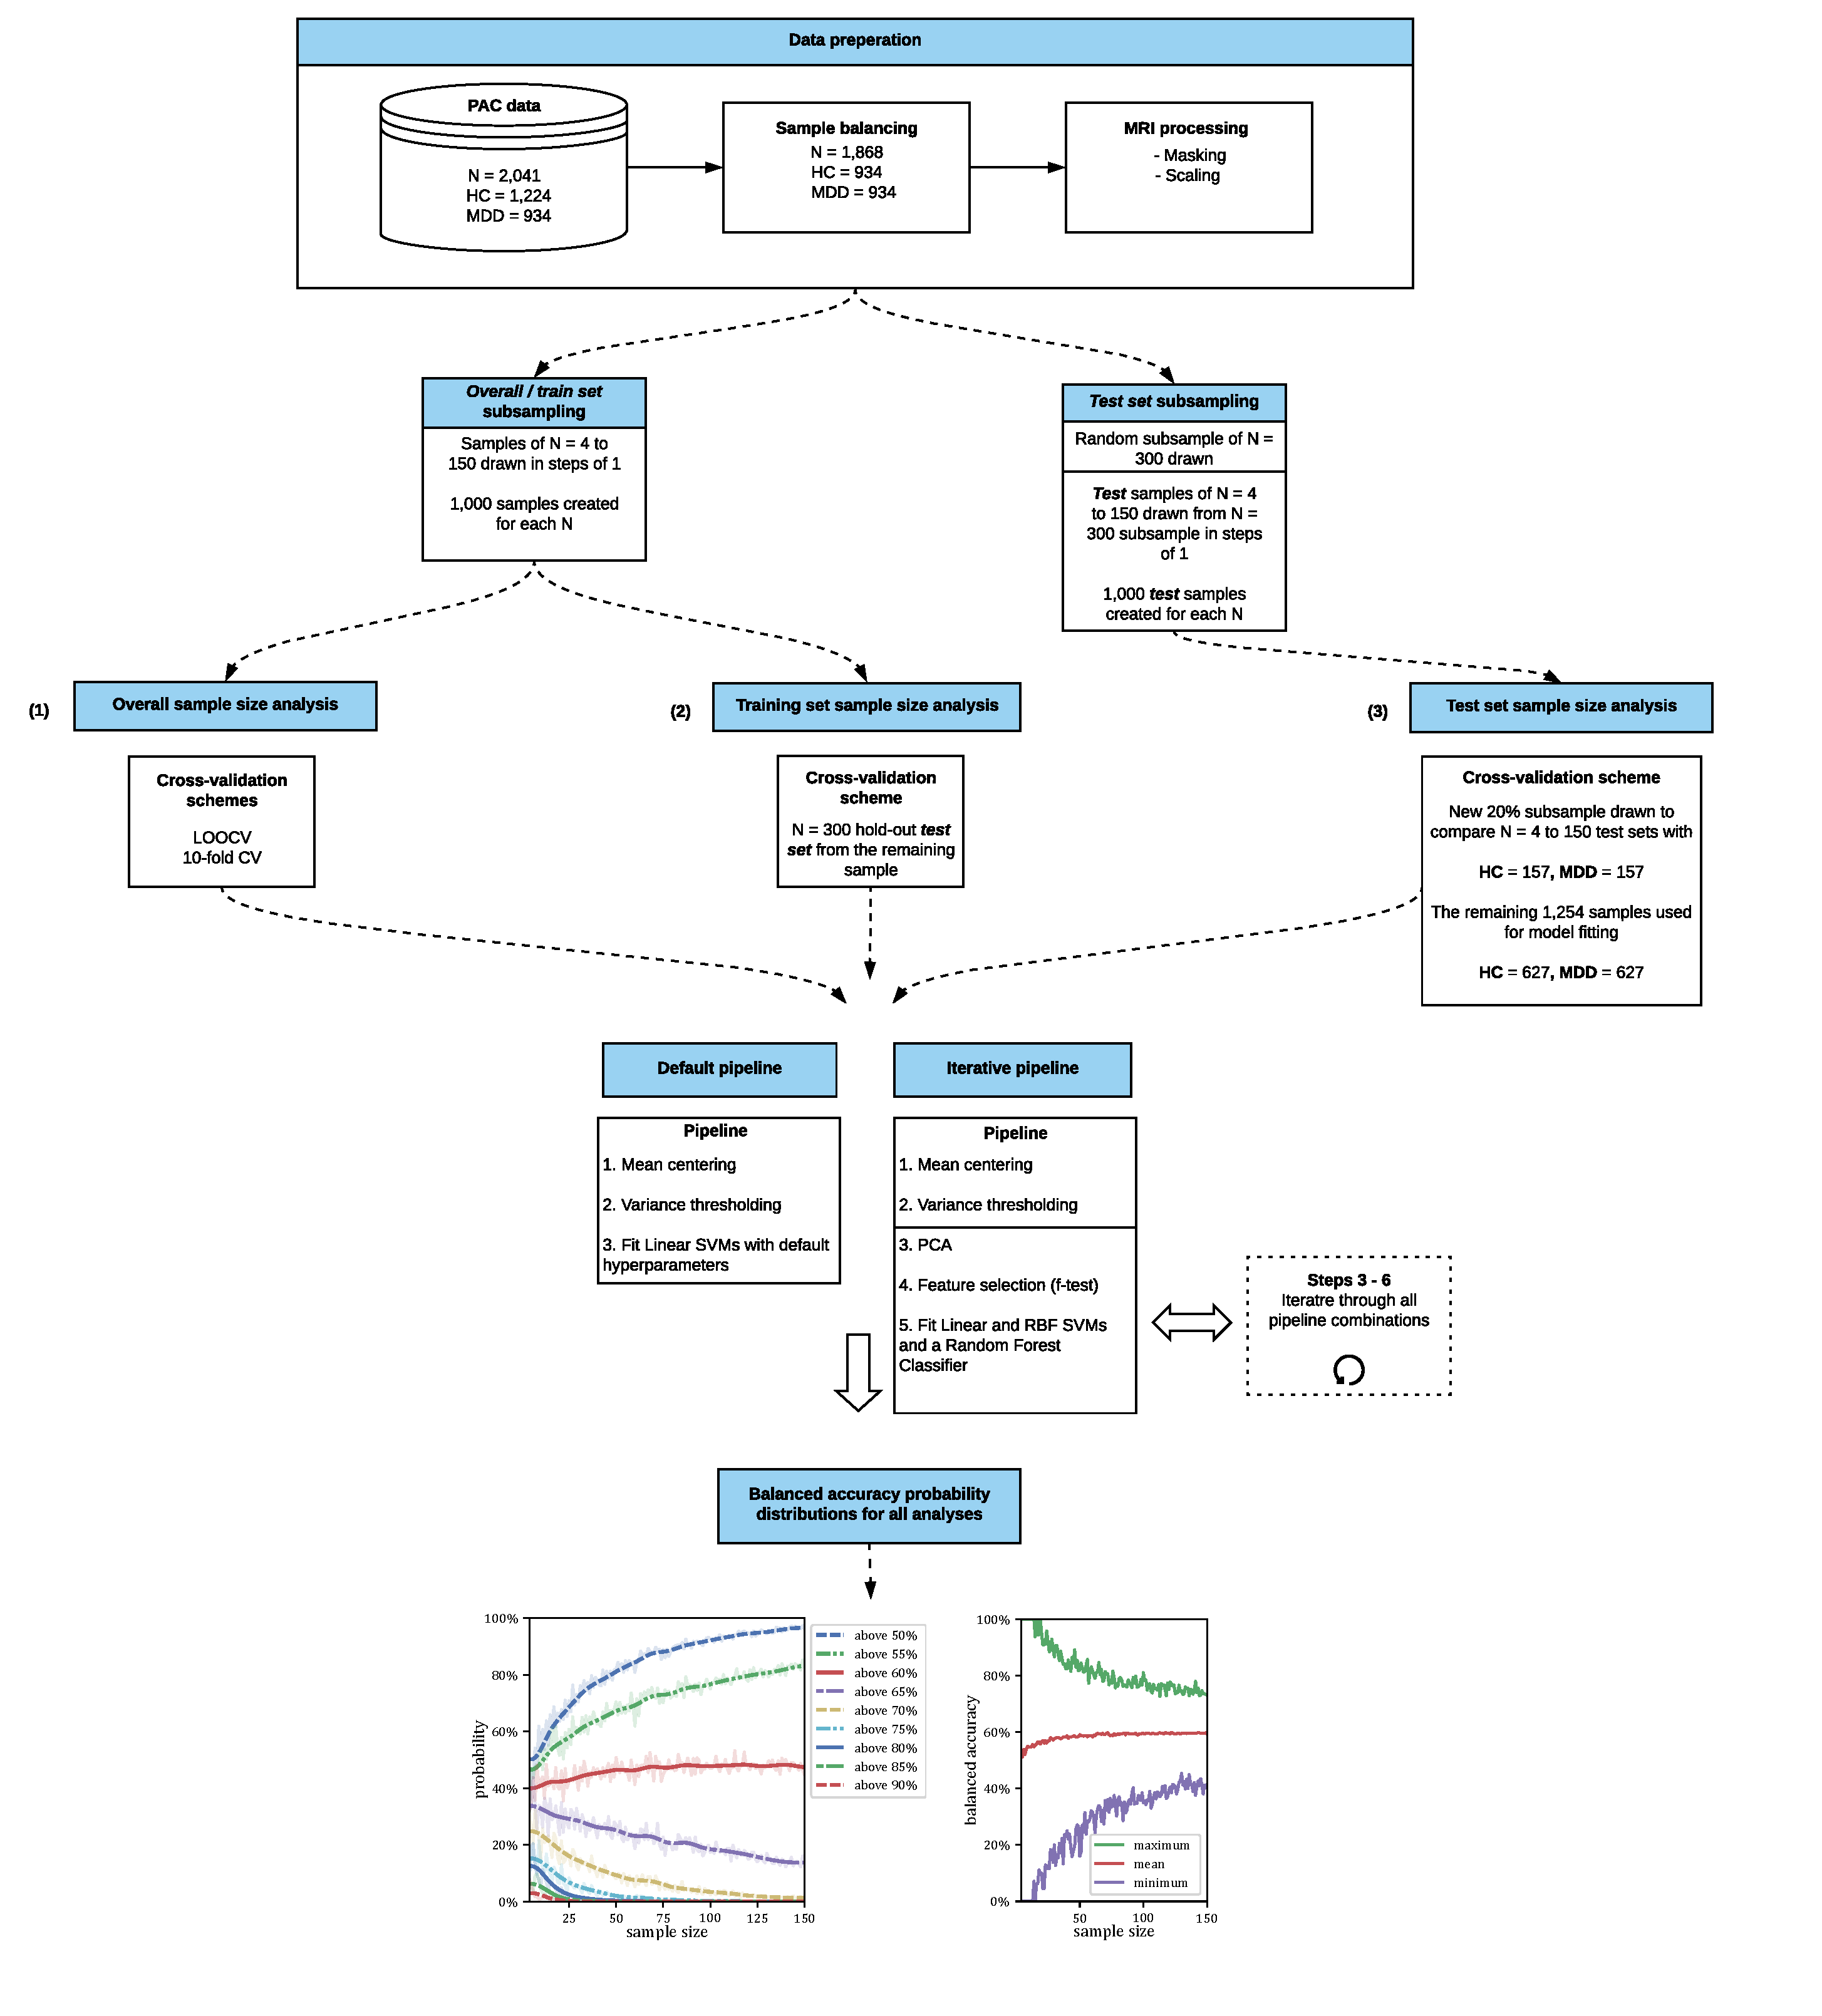
\includegraphics[width=\textwidth]{./images/figure_1}
        \caption{Workflow to investigate the correlations between sample size and misestimation. First the effect of misestimation is investigated over the whole classification process ((1) Overall sample size analysis). Following the process of training and testing is evaluated separately ((2) Training set sample size analysis, (3) Test set sample size analysis)}
        \label{fig:workflow}
    \end{figure}

    \subsection{Generalizability of statistical effect}

    \subsubsection{Alternative pipeline configurations}
    As we have attempted to hold other components of the modelling process constant so any observed effects of systematic misestimation can be attributed to sample size alone, it is also possible that our results may be dependent on the basic configuration of our \ac{ml} pipeline (e.g., the use of a linear \ac{svm}, default hyperparameters, and \ac{loocv}). Therefore, we trained a further \num{48} pipeline configurations, including the use of both linear and radial basis function \acp{svm} and a Random Forest classifier, all of which have demonstrated their efficacy in neuroimaging classification studies~\cite{Kambeitz2017}. Within these configurations, we conducted dimensionality reduction using \ac{pca} as well as f-test based feature selection. This allowed us to assess whether our findings were being confounded by the large number of predictors used in the main analysis. For further information see Supplement Append~x~\ref{cha:alternative-machine-configurations} and for all results see supplementary results~\ref{cha:alternative-machine-configuration-results}, supplementary figures~\ref{fig:no_PCA_no_selection_RandomForest} -~\ref{fig:PCA_all_components_1000_best_selected_LinearSVC} and supplementary tables~\ref{tab:no_PCA_no_selection_RandomForest}~-~\ref{tab:PCA_all_components_1000_best_selected_LinearSVC}.

    \subsubsection{Dummy classifier}
In order to show that the observed effects were not specific to the \ac{pac} dataset or any of the alternative pipeline configurations in these analyses, we repeated the procedures described above with a dummy classifier. Our dummy classifier assumed a prior probability for \ac{mdd} vs \ac{hc} classification based on the percentage proportion of each class in the training data (prevalence). As the dataset was balanced with random under-sampling, the prior and subsequent ground truth of the model was equal to exactly \SI{50}{\percent}. This approach allowed us to compare our distribution of dummy performance estimates derived from our subsample analysis to this ground truth value. Importantly, this approach allows for the quantification of accuracy misestimation as a function of sample size completely independent of any unique characteristics that may be specific to the \ac{pac} dataset or our pipeline configurations. Therefore, we can then be sure that any subsequent changes in classifier performance are attributable to sample size alone.

    \section{Results}

    \subsection{Overall sample size effects}
    In the overall sample size analysis using \ac{loocv}, we were able to show that the risk of overestimating the classifier performance increases with decreasing overall sample size (Figure~\ref{fig:overall_sample_size_effects}a, Supplements Table~\ref{tab:overall_linear_svm_loocv}a). Specifically, accuracies of \SI{70}{\percent} or higher are observed with a probability of \SI{13}{\percent} on sample sizes of $N=20$ whereas this probability is reduced to \SI{2}{\percent} for sample sizes of $N=100$. In addition, sample size has a profound impact on the variability of accuracy estimates: For samples of size $N=20$, accuracies ranged from \SI{10}{\percent} to \SI{95}{\percent} ($\text{standard deviation}=\SI{15}{\percent}$) while for samples of $N=100$, accuracies ranged between \SI{35}{\percent} and \SI{81}{\percent} ($\text{standard deviation}=\SI{6}{\percent}$) (Figure~\ref{fig:overall_sample_size_effects}b, Supplements Table~\ref{tab:overall_linear_svm_loocv}b). Note that this effect is symmetrical and also applies to the underestimation of performance (Figure~\ref{fig:overall_sample_size_effects}b). Additionally, the results of the dummy classifier (Figure~\ref{fig:overall_sample_size_effects}c, d, Supplements Table~\ref{tab:overall_dummy_classifier_loocv}) show that the observed overestimation effect is a general effect of sample size as previously pointed out by Varoquaux~\cite{Varoquaux2018}. As the regularization of the \ac{svm} is sensitive to the total number of outliers, which may increase in parallel with sample size, we conducted an additional analysis with adjusted $C$ parameters, with the observed effect remaining constant across these analyses (see Supplements Figure~\ref{fig:adj_c_overall} and~\ref{fig:adj_c_test}).

    \begin{figure}
        \captionsetup[subfigure]{justification=justified,singlelinecheck=false}
        \begin{subfigure}[t]{0.61\textwidth}
            %% Creator: Matplotlib, PGF backend
%%
%% To include the figure in your LaTeX document, write
%%   \input{<filename>.pgf}
%%
%% Make sure the required packages are loaded in your preamble
%%   \usepackage{pgf}
%%
%% Figures using additional raster images can only be included by \input if
%% they are in the same directory as the main LaTeX file. For loading figures
%% from other directories you can use the `import` package
%%   \usepackage{import}
%% and then include the figures with
%%   \import{<path to file>}{<filename>.pgf}
%%
%% Matplotlib used the following preamble
%%   \usepackage[T1]{fontenc}
%%   \usepackage{cmbright}
%%   \usepackage{fontspec}
%%
\begingroup%
\makeatletter%
\begin{pgfpicture}%
\pgfpathrectangle{\pgfpointorigin}{\pgfqpoint{3.750000in}{2.700000in}}%
\pgfusepath{use as bounding box, clip}%
\begin{pgfscope}%
\pgfsetbuttcap%
\pgfsetmiterjoin%
\definecolor{currentfill}{rgb}{1.000000,1.000000,1.000000}%
\pgfsetfillcolor{currentfill}%
\pgfsetlinewidth{0.000000pt}%
\definecolor{currentstroke}{rgb}{1.000000,1.000000,1.000000}%
\pgfsetstrokecolor{currentstroke}%
\pgfsetdash{}{0pt}%
\pgfpathmoveto{\pgfqpoint{0.000000in}{0.000000in}}%
\pgfpathlineto{\pgfqpoint{3.750000in}{0.000000in}}%
\pgfpathlineto{\pgfqpoint{3.750000in}{2.700000in}}%
\pgfpathlineto{\pgfqpoint{0.000000in}{2.700000in}}%
\pgfpathclose%
\pgfusepath{fill}%
\end{pgfscope}%
\begin{pgfscope}%
\pgfsetbuttcap%
\pgfsetmiterjoin%
\definecolor{currentfill}{rgb}{1.000000,1.000000,1.000000}%
\pgfsetfillcolor{currentfill}%
\pgfsetlinewidth{0.000000pt}%
\definecolor{currentstroke}{rgb}{0.000000,0.000000,0.000000}%
\pgfsetstrokecolor{currentstroke}%
\pgfsetstrokeopacity{0.000000}%
\pgfsetdash{}{0pt}%
\pgfpathmoveto{\pgfqpoint{0.469639in}{0.319222in}}%
\pgfpathlineto{\pgfqpoint{2.743778in}{0.319222in}}%
\pgfpathlineto{\pgfqpoint{2.743778in}{2.661444in}}%
\pgfpathlineto{\pgfqpoint{0.469639in}{2.661444in}}%
\pgfpathclose%
\pgfusepath{fill}%
\end{pgfscope}%
\begin{pgfscope}%
\pgfsetbuttcap%
\pgfsetroundjoin%
\definecolor{currentfill}{rgb}{0.000000,0.000000,0.000000}%
\pgfsetfillcolor{currentfill}%
\pgfsetlinewidth{0.803000pt}%
\definecolor{currentstroke}{rgb}{0.000000,0.000000,0.000000}%
\pgfsetstrokecolor{currentstroke}%
\pgfsetdash{}{0pt}%
\pgfsys@defobject{currentmarker}{\pgfqpoint{0.000000in}{-0.048611in}}{\pgfqpoint{0.000000in}{0.000000in}}{%
\pgfpathmoveto{\pgfqpoint{0.000000in}{0.000000in}}%
\pgfpathlineto{\pgfqpoint{0.000000in}{-0.048611in}}%
\pgfusepath{stroke,fill}%
}%
\begin{pgfscope}%
\pgfsys@transformshift{0.796741in}{0.319222in}%
\pgfsys@useobject{currentmarker}{}%
\end{pgfscope}%
\end{pgfscope}%
\begin{pgfscope}%
\definecolor{textcolor}{rgb}{0.000000,0.000000,0.000000}%
\pgfsetstrokecolor{textcolor}%
\pgfsetfillcolor{textcolor}%
\pgftext[x=0.796741in,y=0.222000in,,top]{\color{textcolor}\rmfamily\fontsize{8.000000}{9.600000}\selectfont 25}%
\end{pgfscope}%
\begin{pgfscope}%
\pgfsetbuttcap%
\pgfsetroundjoin%
\definecolor{currentfill}{rgb}{0.000000,0.000000,0.000000}%
\pgfsetfillcolor{currentfill}%
\pgfsetlinewidth{0.803000pt}%
\definecolor{currentstroke}{rgb}{0.000000,0.000000,0.000000}%
\pgfsetstrokecolor{currentstroke}%
\pgfsetdash{}{0pt}%
\pgfsys@defobject{currentmarker}{\pgfqpoint{0.000000in}{-0.048611in}}{\pgfqpoint{0.000000in}{0.000000in}}{%
\pgfpathmoveto{\pgfqpoint{0.000000in}{0.000000in}}%
\pgfpathlineto{\pgfqpoint{0.000000in}{-0.048611in}}%
\pgfusepath{stroke,fill}%
}%
\begin{pgfscope}%
\pgfsys@transformshift{1.186148in}{0.319222in}%
\pgfsys@useobject{currentmarker}{}%
\end{pgfscope}%
\end{pgfscope}%
\begin{pgfscope}%
\definecolor{textcolor}{rgb}{0.000000,0.000000,0.000000}%
\pgfsetstrokecolor{textcolor}%
\pgfsetfillcolor{textcolor}%
\pgftext[x=1.186148in,y=0.222000in,,top]{\color{textcolor}\rmfamily\fontsize{8.000000}{9.600000}\selectfont 50}%
\end{pgfscope}%
\begin{pgfscope}%
\pgfsetbuttcap%
\pgfsetroundjoin%
\definecolor{currentfill}{rgb}{0.000000,0.000000,0.000000}%
\pgfsetfillcolor{currentfill}%
\pgfsetlinewidth{0.803000pt}%
\definecolor{currentstroke}{rgb}{0.000000,0.000000,0.000000}%
\pgfsetstrokecolor{currentstroke}%
\pgfsetdash{}{0pt}%
\pgfsys@defobject{currentmarker}{\pgfqpoint{0.000000in}{-0.048611in}}{\pgfqpoint{0.000000in}{0.000000in}}{%
\pgfpathmoveto{\pgfqpoint{0.000000in}{0.000000in}}%
\pgfpathlineto{\pgfqpoint{0.000000in}{-0.048611in}}%
\pgfusepath{stroke,fill}%
}%
\begin{pgfscope}%
\pgfsys@transformshift{1.575556in}{0.319222in}%
\pgfsys@useobject{currentmarker}{}%
\end{pgfscope}%
\end{pgfscope}%
\begin{pgfscope}%
\definecolor{textcolor}{rgb}{0.000000,0.000000,0.000000}%
\pgfsetstrokecolor{textcolor}%
\pgfsetfillcolor{textcolor}%
\pgftext[x=1.575556in,y=0.222000in,,top]{\color{textcolor}\rmfamily\fontsize{8.000000}{9.600000}\selectfont 75}%
\end{pgfscope}%
\begin{pgfscope}%
\pgfsetbuttcap%
\pgfsetroundjoin%
\definecolor{currentfill}{rgb}{0.000000,0.000000,0.000000}%
\pgfsetfillcolor{currentfill}%
\pgfsetlinewidth{0.803000pt}%
\definecolor{currentstroke}{rgb}{0.000000,0.000000,0.000000}%
\pgfsetstrokecolor{currentstroke}%
\pgfsetdash{}{0pt}%
\pgfsys@defobject{currentmarker}{\pgfqpoint{0.000000in}{-0.048611in}}{\pgfqpoint{0.000000in}{0.000000in}}{%
\pgfpathmoveto{\pgfqpoint{0.000000in}{0.000000in}}%
\pgfpathlineto{\pgfqpoint{0.000000in}{-0.048611in}}%
\pgfusepath{stroke,fill}%
}%
\begin{pgfscope}%
\pgfsys@transformshift{1.964963in}{0.319222in}%
\pgfsys@useobject{currentmarker}{}%
\end{pgfscope}%
\end{pgfscope}%
\begin{pgfscope}%
\definecolor{textcolor}{rgb}{0.000000,0.000000,0.000000}%
\pgfsetstrokecolor{textcolor}%
\pgfsetfillcolor{textcolor}%
\pgftext[x=1.964963in,y=0.222000in,,top]{\color{textcolor}\rmfamily\fontsize{8.000000}{9.600000}\selectfont 100}%
\end{pgfscope}%
\begin{pgfscope}%
\pgfsetbuttcap%
\pgfsetroundjoin%
\definecolor{currentfill}{rgb}{0.000000,0.000000,0.000000}%
\pgfsetfillcolor{currentfill}%
\pgfsetlinewidth{0.803000pt}%
\definecolor{currentstroke}{rgb}{0.000000,0.000000,0.000000}%
\pgfsetstrokecolor{currentstroke}%
\pgfsetdash{}{0pt}%
\pgfsys@defobject{currentmarker}{\pgfqpoint{0.000000in}{-0.048611in}}{\pgfqpoint{0.000000in}{0.000000in}}{%
\pgfpathmoveto{\pgfqpoint{0.000000in}{0.000000in}}%
\pgfpathlineto{\pgfqpoint{0.000000in}{-0.048611in}}%
\pgfusepath{stroke,fill}%
}%
\begin{pgfscope}%
\pgfsys@transformshift{2.354370in}{0.319222in}%
\pgfsys@useobject{currentmarker}{}%
\end{pgfscope}%
\end{pgfscope}%
\begin{pgfscope}%
\definecolor{textcolor}{rgb}{0.000000,0.000000,0.000000}%
\pgfsetstrokecolor{textcolor}%
\pgfsetfillcolor{textcolor}%
\pgftext[x=2.354370in,y=0.222000in,,top]{\color{textcolor}\rmfamily\fontsize{8.000000}{9.600000}\selectfont 125}%
\end{pgfscope}%
\begin{pgfscope}%
\pgfsetbuttcap%
\pgfsetroundjoin%
\definecolor{currentfill}{rgb}{0.000000,0.000000,0.000000}%
\pgfsetfillcolor{currentfill}%
\pgfsetlinewidth{0.803000pt}%
\definecolor{currentstroke}{rgb}{0.000000,0.000000,0.000000}%
\pgfsetstrokecolor{currentstroke}%
\pgfsetdash{}{0pt}%
\pgfsys@defobject{currentmarker}{\pgfqpoint{0.000000in}{-0.048611in}}{\pgfqpoint{0.000000in}{0.000000in}}{%
\pgfpathmoveto{\pgfqpoint{0.000000in}{0.000000in}}%
\pgfpathlineto{\pgfqpoint{0.000000in}{-0.048611in}}%
\pgfusepath{stroke,fill}%
}%
\begin{pgfscope}%
\pgfsys@transformshift{2.743778in}{0.319222in}%
\pgfsys@useobject{currentmarker}{}%
\end{pgfscope}%
\end{pgfscope}%
\begin{pgfscope}%
\definecolor{textcolor}{rgb}{0.000000,0.000000,0.000000}%
\pgfsetstrokecolor{textcolor}%
\pgfsetfillcolor{textcolor}%
\pgftext[x=2.743778in,y=0.222000in,,top]{\color{textcolor}\rmfamily\fontsize{8.000000}{9.600000}\selectfont 150}%
\end{pgfscope}%
\begin{pgfscope}%
\definecolor{textcolor}{rgb}{0.000000,0.000000,0.000000}%
\pgfsetstrokecolor{textcolor}%
\pgfsetfillcolor{textcolor}%
\pgftext[x=1.606708in,y=0.123333in,,top]{\color{textcolor}\rmfamily\fontsize{10.000000}{12.000000}\selectfont sample size}%
\end{pgfscope}%
\begin{pgfscope}%
\pgfsetbuttcap%
\pgfsetroundjoin%
\definecolor{currentfill}{rgb}{0.000000,0.000000,0.000000}%
\pgfsetfillcolor{currentfill}%
\pgfsetlinewidth{0.803000pt}%
\definecolor{currentstroke}{rgb}{0.000000,0.000000,0.000000}%
\pgfsetstrokecolor{currentstroke}%
\pgfsetdash{}{0pt}%
\pgfsys@defobject{currentmarker}{\pgfqpoint{-0.048611in}{0.000000in}}{\pgfqpoint{0.000000in}{0.000000in}}{%
\pgfpathmoveto{\pgfqpoint{0.000000in}{0.000000in}}%
\pgfpathlineto{\pgfqpoint{-0.048611in}{0.000000in}}%
\pgfusepath{stroke,fill}%
}%
\begin{pgfscope}%
\pgfsys@transformshift{0.469639in}{0.319222in}%
\pgfsys@useobject{currentmarker}{}%
\end{pgfscope}%
\end{pgfscope}%
\begin{pgfscope}%
\definecolor{textcolor}{rgb}{0.000000,0.000000,0.000000}%
\pgfsetstrokecolor{textcolor}%
\pgfsetfillcolor{textcolor}%
\pgftext[x=0.215083in,y=0.280667in,left,base]{\color{textcolor}\rmfamily\fontsize{8.000000}{9.600000}\selectfont  0\%}%
\end{pgfscope}%
\begin{pgfscope}%
\pgfsetbuttcap%
\pgfsetroundjoin%
\definecolor{currentfill}{rgb}{0.000000,0.000000,0.000000}%
\pgfsetfillcolor{currentfill}%
\pgfsetlinewidth{0.803000pt}%
\definecolor{currentstroke}{rgb}{0.000000,0.000000,0.000000}%
\pgfsetstrokecolor{currentstroke}%
\pgfsetdash{}{0pt}%
\pgfsys@defobject{currentmarker}{\pgfqpoint{-0.048611in}{0.000000in}}{\pgfqpoint{0.000000in}{0.000000in}}{%
\pgfpathmoveto{\pgfqpoint{0.000000in}{0.000000in}}%
\pgfpathlineto{\pgfqpoint{-0.048611in}{0.000000in}}%
\pgfusepath{stroke,fill}%
}%
\begin{pgfscope}%
\pgfsys@transformshift{0.469639in}{0.787667in}%
\pgfsys@useobject{currentmarker}{}%
\end{pgfscope}%
\end{pgfscope}%
\begin{pgfscope}%
\definecolor{textcolor}{rgb}{0.000000,0.000000,0.000000}%
\pgfsetstrokecolor{textcolor}%
\pgfsetfillcolor{textcolor}%
\pgftext[x=0.156083in,y=0.749111in,left,base]{\color{textcolor}\rmfamily\fontsize{8.000000}{9.600000}\selectfont 20\%}%
\end{pgfscope}%
\begin{pgfscope}%
\pgfsetbuttcap%
\pgfsetroundjoin%
\definecolor{currentfill}{rgb}{0.000000,0.000000,0.000000}%
\pgfsetfillcolor{currentfill}%
\pgfsetlinewidth{0.803000pt}%
\definecolor{currentstroke}{rgb}{0.000000,0.000000,0.000000}%
\pgfsetstrokecolor{currentstroke}%
\pgfsetdash{}{0pt}%
\pgfsys@defobject{currentmarker}{\pgfqpoint{-0.048611in}{0.000000in}}{\pgfqpoint{0.000000in}{0.000000in}}{%
\pgfpathmoveto{\pgfqpoint{0.000000in}{0.000000in}}%
\pgfpathlineto{\pgfqpoint{-0.048611in}{0.000000in}}%
\pgfusepath{stroke,fill}%
}%
\begin{pgfscope}%
\pgfsys@transformshift{0.469639in}{1.256111in}%
\pgfsys@useobject{currentmarker}{}%
\end{pgfscope}%
\end{pgfscope}%
\begin{pgfscope}%
\definecolor{textcolor}{rgb}{0.000000,0.000000,0.000000}%
\pgfsetstrokecolor{textcolor}%
\pgfsetfillcolor{textcolor}%
\pgftext[x=0.156083in,y=1.217556in,left,base]{\color{textcolor}\rmfamily\fontsize{8.000000}{9.600000}\selectfont 40\%}%
\end{pgfscope}%
\begin{pgfscope}%
\pgfsetbuttcap%
\pgfsetroundjoin%
\definecolor{currentfill}{rgb}{0.000000,0.000000,0.000000}%
\pgfsetfillcolor{currentfill}%
\pgfsetlinewidth{0.803000pt}%
\definecolor{currentstroke}{rgb}{0.000000,0.000000,0.000000}%
\pgfsetstrokecolor{currentstroke}%
\pgfsetdash{}{0pt}%
\pgfsys@defobject{currentmarker}{\pgfqpoint{-0.048611in}{0.000000in}}{\pgfqpoint{0.000000in}{0.000000in}}{%
\pgfpathmoveto{\pgfqpoint{0.000000in}{0.000000in}}%
\pgfpathlineto{\pgfqpoint{-0.048611in}{0.000000in}}%
\pgfusepath{stroke,fill}%
}%
\begin{pgfscope}%
\pgfsys@transformshift{0.469639in}{1.724556in}%
\pgfsys@useobject{currentmarker}{}%
\end{pgfscope}%
\end{pgfscope}%
\begin{pgfscope}%
\definecolor{textcolor}{rgb}{0.000000,0.000000,0.000000}%
\pgfsetstrokecolor{textcolor}%
\pgfsetfillcolor{textcolor}%
\pgftext[x=0.156083in,y=1.686000in,left,base]{\color{textcolor}\rmfamily\fontsize{8.000000}{9.600000}\selectfont 60\%}%
\end{pgfscope}%
\begin{pgfscope}%
\pgfsetbuttcap%
\pgfsetroundjoin%
\definecolor{currentfill}{rgb}{0.000000,0.000000,0.000000}%
\pgfsetfillcolor{currentfill}%
\pgfsetlinewidth{0.803000pt}%
\definecolor{currentstroke}{rgb}{0.000000,0.000000,0.000000}%
\pgfsetstrokecolor{currentstroke}%
\pgfsetdash{}{0pt}%
\pgfsys@defobject{currentmarker}{\pgfqpoint{-0.048611in}{0.000000in}}{\pgfqpoint{0.000000in}{0.000000in}}{%
\pgfpathmoveto{\pgfqpoint{0.000000in}{0.000000in}}%
\pgfpathlineto{\pgfqpoint{-0.048611in}{0.000000in}}%
\pgfusepath{stroke,fill}%
}%
\begin{pgfscope}%
\pgfsys@transformshift{0.469639in}{2.193000in}%
\pgfsys@useobject{currentmarker}{}%
\end{pgfscope}%
\end{pgfscope}%
\begin{pgfscope}%
\definecolor{textcolor}{rgb}{0.000000,0.000000,0.000000}%
\pgfsetstrokecolor{textcolor}%
\pgfsetfillcolor{textcolor}%
\pgftext[x=0.156083in,y=2.154444in,left,base]{\color{textcolor}\rmfamily\fontsize{8.000000}{9.600000}\selectfont 80\%}%
\end{pgfscope}%
\begin{pgfscope}%
\pgfsetbuttcap%
\pgfsetroundjoin%
\definecolor{currentfill}{rgb}{0.000000,0.000000,0.000000}%
\pgfsetfillcolor{currentfill}%
\pgfsetlinewidth{0.803000pt}%
\definecolor{currentstroke}{rgb}{0.000000,0.000000,0.000000}%
\pgfsetstrokecolor{currentstroke}%
\pgfsetdash{}{0pt}%
\pgfsys@defobject{currentmarker}{\pgfqpoint{-0.048611in}{0.000000in}}{\pgfqpoint{0.000000in}{0.000000in}}{%
\pgfpathmoveto{\pgfqpoint{0.000000in}{0.000000in}}%
\pgfpathlineto{\pgfqpoint{-0.048611in}{0.000000in}}%
\pgfusepath{stroke,fill}%
}%
\begin{pgfscope}%
\pgfsys@transformshift{0.469639in}{2.661444in}%
\pgfsys@useobject{currentmarker}{}%
\end{pgfscope}%
\end{pgfscope}%
\begin{pgfscope}%
\definecolor{textcolor}{rgb}{0.000000,0.000000,0.000000}%
\pgfsetstrokecolor{textcolor}%
\pgfsetfillcolor{textcolor}%
\pgftext[x=0.097083in,y=2.622889in,left,base]{\color{textcolor}\rmfamily\fontsize{8.000000}{9.600000}\selectfont 100\%}%
\end{pgfscope}%
\begin{pgfscope}%
\definecolor{textcolor}{rgb}{0.000000,0.000000,0.000000}%
\pgfsetstrokecolor{textcolor}%
\pgfsetfillcolor{textcolor}%
\pgftext[x=0.124861in,y=1.490333in,,bottom,rotate=90.000000]{\color{textcolor}\rmfamily\fontsize{10.000000}{12.000000}\selectfont probability}%
\end{pgfscope}%
\begin{pgfscope}%
\pgfpathrectangle{\pgfqpoint{0.469639in}{0.319222in}}{\pgfqpoint{2.274139in}{2.342222in}}%
\pgfusepath{clip}%
\pgfsetrectcap%
\pgfsetroundjoin%
\pgfsetlinewidth{1.505625pt}%
\definecolor{currentstroke}{rgb}{0.298039,0.447059,0.690196}%
\pgfsetstrokecolor{currentstroke}%
\pgfsetstrokeopacity{0.200000}%
\pgfsetdash{}{0pt}%
\pgfpathmoveto{\pgfqpoint{0.469639in}{1.071076in}}%
\pgfpathlineto{\pgfqpoint{0.485215in}{1.417724in}}%
\pgfpathlineto{\pgfqpoint{0.500791in}{1.342773in}}%
\pgfpathlineto{\pgfqpoint{0.516368in}{1.586364in}}%
\pgfpathlineto{\pgfqpoint{0.531944in}{1.445831in}}%
\pgfpathlineto{\pgfqpoint{0.547520in}{1.769058in}}%
\pgfpathlineto{\pgfqpoint{0.563097in}{1.572311in}}%
\pgfpathlineto{\pgfqpoint{0.578673in}{1.740951in}}%
\pgfpathlineto{\pgfqpoint{0.594249in}{1.574653in}}%
\pgfpathlineto{\pgfqpoint{0.609826in}{1.811218in}}%
\pgfpathlineto{\pgfqpoint{0.625402in}{1.609787in}}%
\pgfpathlineto{\pgfqpoint{0.640978in}{1.862747in}}%
\pgfpathlineto{\pgfqpoint{0.656554in}{1.752662in}}%
\pgfpathlineto{\pgfqpoint{0.672131in}{1.928329in}}%
\pgfpathlineto{\pgfqpoint{0.687707in}{1.764373in}}%
\pgfpathlineto{\pgfqpoint{0.703283in}{1.874458in}}%
\pgfpathlineto{\pgfqpoint{0.718860in}{1.806533in}}%
\pgfpathlineto{\pgfqpoint{0.734436in}{1.904907in}}%
\pgfpathlineto{\pgfqpoint{0.750012in}{1.825271in}}%
\pgfpathlineto{\pgfqpoint{0.765588in}{1.982200in}}%
\pgfpathlineto{\pgfqpoint{0.781165in}{1.848693in}}%
\pgfpathlineto{\pgfqpoint{0.796741in}{1.977516in}}%
\pgfpathlineto{\pgfqpoint{0.812317in}{1.888511in}}%
\pgfpathlineto{\pgfqpoint{0.827894in}{2.108680in}}%
\pgfpathlineto{\pgfqpoint{0.843470in}{1.942382in}}%
\pgfpathlineto{\pgfqpoint{0.859046in}{2.029044in}}%
\pgfpathlineto{\pgfqpoint{0.874623in}{1.968147in}}%
\pgfpathlineto{\pgfqpoint{0.890199in}{2.101653in}}%
\pgfpathlineto{\pgfqpoint{0.905775in}{2.047782in}}%
\pgfpathlineto{\pgfqpoint{0.921351in}{2.143813in}}%
\pgfpathlineto{\pgfqpoint{0.936928in}{2.064178in}}%
\pgfpathlineto{\pgfqpoint{0.952504in}{2.129760in}}%
\pgfpathlineto{\pgfqpoint{0.968080in}{2.038413in}}%
\pgfpathlineto{\pgfqpoint{0.983657in}{2.185973in}}%
\pgfpathlineto{\pgfqpoint{0.999233in}{2.089942in}}%
\pgfpathlineto{\pgfqpoint{1.014809in}{2.171920in}}%
\pgfpathlineto{\pgfqpoint{1.030385in}{2.153182in}}%
\pgfpathlineto{\pgfqpoint{1.045962in}{2.108680in}}%
\pgfpathlineto{\pgfqpoint{1.061538in}{2.101653in}}%
\pgfpathlineto{\pgfqpoint{1.077114in}{2.232818in}}%
\pgfpathlineto{\pgfqpoint{1.092691in}{2.115707in}}%
\pgfpathlineto{\pgfqpoint{1.108267in}{2.221107in}}%
\pgfpathlineto{\pgfqpoint{1.123843in}{2.160209in}}%
\pgfpathlineto{\pgfqpoint{1.139419in}{2.221107in}}%
\pgfpathlineto{\pgfqpoint{1.154996in}{2.148498in}}%
\pgfpathlineto{\pgfqpoint{1.170572in}{2.235160in}}%
\pgfpathlineto{\pgfqpoint{1.186148in}{2.237502in}}%
\pgfpathlineto{\pgfqpoint{1.201725in}{2.296058in}}%
\pgfpathlineto{\pgfqpoint{1.217301in}{2.244529in}}%
\pgfpathlineto{\pgfqpoint{1.232877in}{2.284347in}}%
\pgfpathlineto{\pgfqpoint{1.248454in}{2.214080in}}%
\pgfpathlineto{\pgfqpoint{1.264030in}{2.310111in}}%
\pgfpathlineto{\pgfqpoint{1.279606in}{2.235160in}}%
\pgfpathlineto{\pgfqpoint{1.295182in}{2.310111in}}%
\pgfpathlineto{\pgfqpoint{1.310759in}{2.274978in}}%
\pgfpathlineto{\pgfqpoint{1.326335in}{2.298400in}}%
\pgfpathlineto{\pgfqpoint{1.341911in}{2.214080in}}%
\pgfpathlineto{\pgfqpoint{1.357488in}{2.303084in}}%
\pgfpathlineto{\pgfqpoint{1.373064in}{2.300742in}}%
\pgfpathlineto{\pgfqpoint{1.388640in}{2.389747in}}%
\pgfpathlineto{\pgfqpoint{1.404216in}{2.354613in}}%
\pgfpathlineto{\pgfqpoint{1.419793in}{2.366324in}}%
\pgfpathlineto{\pgfqpoint{1.435369in}{2.345244in}}%
\pgfpathlineto{\pgfqpoint{1.450945in}{2.410827in}}%
\pgfpathlineto{\pgfqpoint{1.466522in}{2.382720in}}%
\pgfpathlineto{\pgfqpoint{1.482098in}{2.380378in}}%
\pgfpathlineto{\pgfqpoint{1.497674in}{2.368667in}}%
\pgfpathlineto{\pgfqpoint{1.513251in}{2.422538in}}%
\pgfpathlineto{\pgfqpoint{1.528827in}{2.385062in}}%
\pgfpathlineto{\pgfqpoint{1.544403in}{2.403800in}}%
\pgfpathlineto{\pgfqpoint{1.559979in}{2.319480in}}%
\pgfpathlineto{\pgfqpoint{1.575556in}{2.401458in}}%
\pgfpathlineto{\pgfqpoint{1.591132in}{2.333533in}}%
\pgfpathlineto{\pgfqpoint{1.606708in}{2.406142in}}%
\pgfpathlineto{\pgfqpoint{1.622285in}{2.345244in}}%
\pgfpathlineto{\pgfqpoint{1.637861in}{2.389747in}}%
\pgfpathlineto{\pgfqpoint{1.653437in}{2.415511in}}%
\pgfpathlineto{\pgfqpoint{1.669013in}{2.427222in}}%
\pgfpathlineto{\pgfqpoint{1.684590in}{2.436591in}}%
\pgfpathlineto{\pgfqpoint{1.700166in}{2.441276in}}%
\pgfpathlineto{\pgfqpoint{1.715742in}{2.420196in}}%
\pgfpathlineto{\pgfqpoint{1.731319in}{2.460013in}}%
\pgfpathlineto{\pgfqpoint{1.746895in}{2.406142in}}%
\pgfpathlineto{\pgfqpoint{1.762471in}{2.488120in}}%
\pgfpathlineto{\pgfqpoint{1.778047in}{2.431907in}}%
\pgfpathlineto{\pgfqpoint{1.793624in}{2.445960in}}%
\pgfpathlineto{\pgfqpoint{1.809200in}{2.413169in}}%
\pgfpathlineto{\pgfqpoint{1.824776in}{2.469382in}}%
\pgfpathlineto{\pgfqpoint{1.840353in}{2.460013in}}%
\pgfpathlineto{\pgfqpoint{1.855929in}{2.471724in}}%
\pgfpathlineto{\pgfqpoint{1.887082in}{2.452987in}}%
\pgfpathlineto{\pgfqpoint{1.902658in}{2.434249in}}%
\pgfpathlineto{\pgfqpoint{1.918234in}{2.469382in}}%
\pgfpathlineto{\pgfqpoint{1.933810in}{2.497489in}}%
\pgfpathlineto{\pgfqpoint{1.949387in}{2.502173in}}%
\pgfpathlineto{\pgfqpoint{1.964963in}{2.485778in}}%
\pgfpathlineto{\pgfqpoint{1.980539in}{2.485778in}}%
\pgfpathlineto{\pgfqpoint{1.996116in}{2.462356in}}%
\pgfpathlineto{\pgfqpoint{2.011692in}{2.499831in}}%
\pgfpathlineto{\pgfqpoint{2.027268in}{2.485778in}}%
\pgfpathlineto{\pgfqpoint{2.042844in}{2.525596in}}%
\pgfpathlineto{\pgfqpoint{2.058421in}{2.471724in}}%
\pgfpathlineto{\pgfqpoint{2.073997in}{2.513884in}}%
\pgfpathlineto{\pgfqpoint{2.089573in}{2.497489in}}%
\pgfpathlineto{\pgfqpoint{2.105150in}{2.506858in}}%
\pgfpathlineto{\pgfqpoint{2.120726in}{2.518569in}}%
\pgfpathlineto{\pgfqpoint{2.136302in}{2.504516in}}%
\pgfpathlineto{\pgfqpoint{2.151879in}{2.488120in}}%
\pgfpathlineto{\pgfqpoint{2.167455in}{2.525596in}}%
\pgfpathlineto{\pgfqpoint{2.183031in}{2.520911in}}%
\pgfpathlineto{\pgfqpoint{2.198607in}{2.553702in}}%
\pgfpathlineto{\pgfqpoint{2.214184in}{2.518569in}}%
\pgfpathlineto{\pgfqpoint{2.229760in}{2.546676in}}%
\pgfpathlineto{\pgfqpoint{2.245336in}{2.556044in}}%
\pgfpathlineto{\pgfqpoint{2.260913in}{2.532622in}}%
\pgfpathlineto{\pgfqpoint{2.276489in}{2.537307in}}%
\pgfpathlineto{\pgfqpoint{2.292065in}{2.534964in}}%
\pgfpathlineto{\pgfqpoint{2.307641in}{2.509200in}}%
\pgfpathlineto{\pgfqpoint{2.323218in}{2.556044in}}%
\pgfpathlineto{\pgfqpoint{2.338794in}{2.513884in}}%
\pgfpathlineto{\pgfqpoint{2.354370in}{2.525596in}}%
\pgfpathlineto{\pgfqpoint{2.369947in}{2.546676in}}%
\pgfpathlineto{\pgfqpoint{2.385523in}{2.563071in}}%
\pgfpathlineto{\pgfqpoint{2.401099in}{2.553702in}}%
\pgfpathlineto{\pgfqpoint{2.416675in}{2.546676in}}%
\pgfpathlineto{\pgfqpoint{2.432252in}{2.532622in}}%
\pgfpathlineto{\pgfqpoint{2.447828in}{2.560729in}}%
\pgfpathlineto{\pgfqpoint{2.463404in}{2.541991in}}%
\pgfpathlineto{\pgfqpoint{2.478981in}{2.539649in}}%
\pgfpathlineto{\pgfqpoint{2.494557in}{2.541991in}}%
\pgfpathlineto{\pgfqpoint{2.510133in}{2.586493in}}%
\pgfpathlineto{\pgfqpoint{2.525710in}{2.579467in}}%
\pgfpathlineto{\pgfqpoint{2.541286in}{2.577124in}}%
\pgfpathlineto{\pgfqpoint{2.556862in}{2.549018in}}%
\pgfpathlineto{\pgfqpoint{2.572438in}{2.581809in}}%
\pgfpathlineto{\pgfqpoint{2.588015in}{2.560729in}}%
\pgfpathlineto{\pgfqpoint{2.603591in}{2.565413in}}%
\pgfpathlineto{\pgfqpoint{2.619167in}{2.581809in}}%
\pgfpathlineto{\pgfqpoint{2.634744in}{2.595862in}}%
\pgfpathlineto{\pgfqpoint{2.650320in}{2.586493in}}%
\pgfpathlineto{\pgfqpoint{2.665896in}{2.593520in}}%
\pgfpathlineto{\pgfqpoint{2.681472in}{2.574782in}}%
\pgfpathlineto{\pgfqpoint{2.697049in}{2.572440in}}%
\pgfpathlineto{\pgfqpoint{2.712625in}{2.574782in}}%
\pgfpathlineto{\pgfqpoint{2.728201in}{2.598204in}}%
\pgfpathlineto{\pgfqpoint{2.743778in}{2.572440in}}%
\pgfpathlineto{\pgfqpoint{2.743778in}{2.572440in}}%
\pgfusepath{stroke}%
\end{pgfscope}%
\begin{pgfscope}%
\pgfpathrectangle{\pgfqpoint{0.469639in}{0.319222in}}{\pgfqpoint{2.274139in}{2.342222in}}%
\pgfusepath{clip}%
\pgfsetbuttcap%
\pgfsetroundjoin%
\pgfsetlinewidth{2.007500pt}%
\definecolor{currentstroke}{rgb}{0.298039,0.447059,0.690196}%
\pgfsetstrokecolor{currentstroke}%
\pgfsetdash{{6.000000pt}{2.000000pt}}{0.000000pt}%
\pgfpathmoveto{\pgfqpoint{0.469639in}{1.497397in}}%
\pgfpathlineto{\pgfqpoint{0.485215in}{1.493939in}}%
\pgfpathlineto{\pgfqpoint{0.500791in}{1.497397in}}%
\pgfpathlineto{\pgfqpoint{0.516368in}{1.507630in}}%
\pgfpathlineto{\pgfqpoint{0.531944in}{1.524253in}}%
\pgfpathlineto{\pgfqpoint{0.547520in}{1.546443in}}%
\pgfpathlineto{\pgfqpoint{0.563097in}{1.573105in}}%
\pgfpathlineto{\pgfqpoint{0.594249in}{1.634640in}}%
\pgfpathlineto{\pgfqpoint{0.625402in}{1.697481in}}%
\pgfpathlineto{\pgfqpoint{0.640978in}{1.726388in}}%
\pgfpathlineto{\pgfqpoint{0.656554in}{1.752652in}}%
\pgfpathlineto{\pgfqpoint{0.672131in}{1.776241in}}%
\pgfpathlineto{\pgfqpoint{0.703283in}{1.817858in}}%
\pgfpathlineto{\pgfqpoint{0.734436in}{1.855246in}}%
\pgfpathlineto{\pgfqpoint{0.796741in}{1.925850in}}%
\pgfpathlineto{\pgfqpoint{0.874623in}{2.011154in}}%
\pgfpathlineto{\pgfqpoint{0.905775in}{2.042562in}}%
\pgfpathlineto{\pgfqpoint{0.936928in}{2.070034in}}%
\pgfpathlineto{\pgfqpoint{0.968080in}{2.093502in}}%
\pgfpathlineto{\pgfqpoint{0.999233in}{2.113430in}}%
\pgfpathlineto{\pgfqpoint{1.045962in}{2.138899in}}%
\pgfpathlineto{\pgfqpoint{1.092691in}{2.163678in}}%
\pgfpathlineto{\pgfqpoint{1.139419in}{2.191031in}}%
\pgfpathlineto{\pgfqpoint{1.201725in}{2.227998in}}%
\pgfpathlineto{\pgfqpoint{1.232877in}{2.244199in}}%
\pgfpathlineto{\pgfqpoint{1.357488in}{2.304408in}}%
\pgfpathlineto{\pgfqpoint{1.450945in}{2.356344in}}%
\pgfpathlineto{\pgfqpoint{1.482098in}{2.368238in}}%
\pgfpathlineto{\pgfqpoint{1.513251in}{2.375658in}}%
\pgfpathlineto{\pgfqpoint{1.544403in}{2.379816in}}%
\pgfpathlineto{\pgfqpoint{1.591132in}{2.385503in}}%
\pgfpathlineto{\pgfqpoint{1.622285in}{2.391889in}}%
\pgfpathlineto{\pgfqpoint{1.653437in}{2.400748in}}%
\pgfpathlineto{\pgfqpoint{1.715742in}{2.422322in}}%
\pgfpathlineto{\pgfqpoint{1.746895in}{2.432606in}}%
\pgfpathlineto{\pgfqpoint{1.778047in}{2.440689in}}%
\pgfpathlineto{\pgfqpoint{1.824776in}{2.450001in}}%
\pgfpathlineto{\pgfqpoint{1.902658in}{2.465019in}}%
\pgfpathlineto{\pgfqpoint{2.027268in}{2.490360in}}%
\pgfpathlineto{\pgfqpoint{2.136302in}{2.510274in}}%
\pgfpathlineto{\pgfqpoint{2.198607in}{2.522725in}}%
\pgfpathlineto{\pgfqpoint{2.245336in}{2.529705in}}%
\pgfpathlineto{\pgfqpoint{2.292065in}{2.534644in}}%
\pgfpathlineto{\pgfqpoint{2.432252in}{2.546772in}}%
\pgfpathlineto{\pgfqpoint{2.525710in}{2.561097in}}%
\pgfpathlineto{\pgfqpoint{2.603591in}{2.572903in}}%
\pgfpathlineto{\pgfqpoint{2.650320in}{2.577966in}}%
\pgfpathlineto{\pgfqpoint{2.697049in}{2.580649in}}%
\pgfpathlineto{\pgfqpoint{2.743778in}{2.582147in}}%
\pgfpathlineto{\pgfqpoint{2.743778in}{2.582147in}}%
\pgfusepath{stroke}%
\end{pgfscope}%
\begin{pgfscope}%
\pgfpathrectangle{\pgfqpoint{0.469639in}{0.319222in}}{\pgfqpoint{2.274139in}{2.342222in}}%
\pgfusepath{clip}%
\pgfsetrectcap%
\pgfsetroundjoin%
\pgfsetlinewidth{1.505625pt}%
\definecolor{currentstroke}{rgb}{0.333333,0.658824,0.407843}%
\pgfsetstrokecolor{currentstroke}%
\pgfsetstrokeopacity{0.200000}%
\pgfsetdash{}{0pt}%
\pgfpathmoveto{\pgfqpoint{0.469639in}{1.071076in}}%
\pgfpathlineto{\pgfqpoint{0.485215in}{1.417724in}}%
\pgfpathlineto{\pgfqpoint{0.500791in}{1.342773in}}%
\pgfpathlineto{\pgfqpoint{0.516368in}{1.434120in}}%
\pgfpathlineto{\pgfqpoint{0.531944in}{1.445831in}}%
\pgfpathlineto{\pgfqpoint{0.547520in}{1.445831in}}%
\pgfpathlineto{\pgfqpoint{0.563097in}{1.572311in}}%
\pgfpathlineto{\pgfqpoint{0.578673in}{1.408356in}}%
\pgfpathlineto{\pgfqpoint{0.594249in}{1.574653in}}%
\pgfpathlineto{\pgfqpoint{0.609826in}{1.492676in}}%
\pgfpathlineto{\pgfqpoint{0.625402in}{1.609787in}}%
\pgfpathlineto{\pgfqpoint{0.640978in}{1.567627in}}%
\pgfpathlineto{\pgfqpoint{0.656554in}{1.752662in}}%
\pgfpathlineto{\pgfqpoint{0.672131in}{1.635551in}}%
\pgfpathlineto{\pgfqpoint{0.687707in}{1.764373in}}%
\pgfpathlineto{\pgfqpoint{0.703283in}{1.591049in}}%
\pgfpathlineto{\pgfqpoint{0.718860in}{1.527809in}}%
\pgfpathlineto{\pgfqpoint{0.734436in}{1.675369in}}%
\pgfpathlineto{\pgfqpoint{0.750012in}{1.499702in}}%
\pgfpathlineto{\pgfqpoint{0.765588in}{1.715187in}}%
\pgfpathlineto{\pgfqpoint{0.781165in}{1.588707in}}%
\pgfpathlineto{\pgfqpoint{0.796741in}{1.743293in}}%
\pgfpathlineto{\pgfqpoint{0.812317in}{1.616813in}}%
\pgfpathlineto{\pgfqpoint{0.827894in}{1.846351in}}%
\pgfpathlineto{\pgfqpoint{0.843470in}{1.701133in}}%
\pgfpathlineto{\pgfqpoint{0.859046in}{1.755004in}}%
\pgfpathlineto{\pgfqpoint{0.874623in}{1.743293in}}%
\pgfpathlineto{\pgfqpoint{0.890199in}{1.705818in}}%
\pgfpathlineto{\pgfqpoint{0.905775in}{1.841667in}}%
\pgfpathlineto{\pgfqpoint{0.921351in}{1.719871in}}%
\pgfpathlineto{\pgfqpoint{0.936928in}{1.855720in}}%
\pgfpathlineto{\pgfqpoint{0.952504in}{1.705818in}}%
\pgfpathlineto{\pgfqpoint{0.968080in}{1.844009in}}%
\pgfpathlineto{\pgfqpoint{0.983657in}{1.790138in}}%
\pgfpathlineto{\pgfqpoint{0.999233in}{1.886169in}}%
\pgfpathlineto{\pgfqpoint{1.014809in}{1.827613in}}%
\pgfpathlineto{\pgfqpoint{1.030385in}{1.785453in}}%
\pgfpathlineto{\pgfqpoint{1.045962in}{1.785453in}}%
\pgfpathlineto{\pgfqpoint{1.061538in}{1.764373in}}%
\pgfpathlineto{\pgfqpoint{1.077114in}{1.886169in}}%
\pgfpathlineto{\pgfqpoint{1.092691in}{1.811218in}}%
\pgfpathlineto{\pgfqpoint{1.108267in}{1.956436in}}%
\pgfpathlineto{\pgfqpoint{1.123843in}{1.846351in}}%
\pgfpathlineto{\pgfqpoint{1.139419in}{1.897880in}}%
\pgfpathlineto{\pgfqpoint{1.154996in}{1.865089in}}%
\pgfpathlineto{\pgfqpoint{1.170572in}{1.907249in}}%
\pgfpathlineto{\pgfqpoint{1.186148in}{1.968147in}}%
\pgfpathlineto{\pgfqpoint{1.201725in}{1.860404in}}%
\pgfpathlineto{\pgfqpoint{1.217301in}{1.965804in}}%
\pgfpathlineto{\pgfqpoint{1.232877in}{1.876800in}}%
\pgfpathlineto{\pgfqpoint{1.248454in}{1.930671in}}%
\pgfpathlineto{\pgfqpoint{1.264030in}{1.876800in}}%
\pgfpathlineto{\pgfqpoint{1.279606in}{1.944724in}}%
\pgfpathlineto{\pgfqpoint{1.295182in}{1.895538in}}%
\pgfpathlineto{\pgfqpoint{1.310759in}{2.043098in}}%
\pgfpathlineto{\pgfqpoint{1.326335in}{1.940040in}}%
\pgfpathlineto{\pgfqpoint{1.341911in}{1.769058in}}%
\pgfpathlineto{\pgfqpoint{1.357488in}{1.993911in}}%
\pgfpathlineto{\pgfqpoint{1.373064in}{1.853378in}}%
\pgfpathlineto{\pgfqpoint{1.388640in}{2.038413in}}%
\pgfpathlineto{\pgfqpoint{1.404216in}{1.970489in}}%
\pgfpathlineto{\pgfqpoint{1.419793in}{2.050124in}}%
\pgfpathlineto{\pgfqpoint{1.435369in}{2.007964in}}%
\pgfpathlineto{\pgfqpoint{1.450945in}{2.068862in}}%
\pgfpathlineto{\pgfqpoint{1.466522in}{2.022018in}}%
\pgfpathlineto{\pgfqpoint{1.482098in}{2.087600in}}%
\pgfpathlineto{\pgfqpoint{1.497674in}{2.017333in}}%
\pgfpathlineto{\pgfqpoint{1.513251in}{1.998596in}}%
\pgfpathlineto{\pgfqpoint{1.528827in}{2.085258in}}%
\pgfpathlineto{\pgfqpoint{1.544403in}{1.958778in}}%
\pgfpathlineto{\pgfqpoint{1.559979in}{2.033729in}}%
\pgfpathlineto{\pgfqpoint{1.575556in}{1.963462in}}%
\pgfpathlineto{\pgfqpoint{1.591132in}{2.068862in}}%
\pgfpathlineto{\pgfqpoint{1.606708in}{2.024360in}}%
\pgfpathlineto{\pgfqpoint{1.622285in}{2.059493in}}%
\pgfpathlineto{\pgfqpoint{1.637861in}{2.000938in}}%
\pgfpathlineto{\pgfqpoint{1.653437in}{2.019676in}}%
\pgfpathlineto{\pgfqpoint{1.669013in}{2.045440in}}%
\pgfpathlineto{\pgfqpoint{1.684590in}{2.014991in}}%
\pgfpathlineto{\pgfqpoint{1.700166in}{2.134444in}}%
\pgfpathlineto{\pgfqpoint{1.715742in}{2.068862in}}%
\pgfpathlineto{\pgfqpoint{1.731319in}{2.120391in}}%
\pgfpathlineto{\pgfqpoint{1.746895in}{2.005622in}}%
\pgfpathlineto{\pgfqpoint{1.762471in}{2.176604in}}%
\pgfpathlineto{\pgfqpoint{1.778047in}{2.101653in}}%
\pgfpathlineto{\pgfqpoint{1.793624in}{2.108680in}}%
\pgfpathlineto{\pgfqpoint{1.809200in}{2.101653in}}%
\pgfpathlineto{\pgfqpoint{1.824776in}{2.054809in}}%
\pgfpathlineto{\pgfqpoint{1.840353in}{2.115707in}}%
\pgfpathlineto{\pgfqpoint{1.855929in}{2.064178in}}%
\pgfpathlineto{\pgfqpoint{1.871505in}{2.125076in}}%
\pgfpathlineto{\pgfqpoint{1.887082in}{2.029044in}}%
\pgfpathlineto{\pgfqpoint{1.902658in}{2.094627in}}%
\pgfpathlineto{\pgfqpoint{1.918234in}{2.099311in}}%
\pgfpathlineto{\pgfqpoint{1.933810in}{2.157867in}}%
\pgfpathlineto{\pgfqpoint{1.964963in}{2.075889in}}%
\pgfpathlineto{\pgfqpoint{1.980539in}{2.132102in}}%
\pgfpathlineto{\pgfqpoint{1.996116in}{2.127418in}}%
\pgfpathlineto{\pgfqpoint{2.011692in}{2.167236in}}%
\pgfpathlineto{\pgfqpoint{2.027268in}{2.132102in}}%
\pgfpathlineto{\pgfqpoint{2.042844in}{2.157867in}}%
\pgfpathlineto{\pgfqpoint{2.058421in}{2.115707in}}%
\pgfpathlineto{\pgfqpoint{2.073997in}{2.195342in}}%
\pgfpathlineto{\pgfqpoint{2.089573in}{2.120391in}}%
\pgfpathlineto{\pgfqpoint{2.105150in}{2.164893in}}%
\pgfpathlineto{\pgfqpoint{2.120726in}{2.136787in}}%
\pgfpathlineto{\pgfqpoint{2.136302in}{2.111022in}}%
\pgfpathlineto{\pgfqpoint{2.151879in}{2.164893in}}%
\pgfpathlineto{\pgfqpoint{2.167455in}{2.176604in}}%
\pgfpathlineto{\pgfqpoint{2.183031in}{2.242187in}}%
\pgfpathlineto{\pgfqpoint{2.198607in}{2.160209in}}%
\pgfpathlineto{\pgfqpoint{2.214184in}{2.164893in}}%
\pgfpathlineto{\pgfqpoint{2.229760in}{2.164893in}}%
\pgfpathlineto{\pgfqpoint{2.245336in}{2.218764in}}%
\pgfpathlineto{\pgfqpoint{2.260913in}{2.160209in}}%
\pgfpathlineto{\pgfqpoint{2.276489in}{2.139129in}}%
\pgfpathlineto{\pgfqpoint{2.292065in}{2.235160in}}%
\pgfpathlineto{\pgfqpoint{2.307641in}{2.153182in}}%
\pgfpathlineto{\pgfqpoint{2.323218in}{2.251556in}}%
\pgfpathlineto{\pgfqpoint{2.338794in}{2.169578in}}%
\pgfpathlineto{\pgfqpoint{2.354370in}{2.211738in}}%
\pgfpathlineto{\pgfqpoint{2.369947in}{2.207053in}}%
\pgfpathlineto{\pgfqpoint{2.385523in}{2.239844in}}%
\pgfpathlineto{\pgfqpoint{2.401099in}{2.176604in}}%
\pgfpathlineto{\pgfqpoint{2.416675in}{2.228133in}}%
\pgfpathlineto{\pgfqpoint{2.432252in}{2.207053in}}%
\pgfpathlineto{\pgfqpoint{2.447828in}{2.174262in}}%
\pgfpathlineto{\pgfqpoint{2.463404in}{2.211738in}}%
\pgfpathlineto{\pgfqpoint{2.478981in}{2.195342in}}%
\pgfpathlineto{\pgfqpoint{2.494557in}{2.237502in}}%
\pgfpathlineto{\pgfqpoint{2.510133in}{2.221107in}}%
\pgfpathlineto{\pgfqpoint{2.525710in}{2.267951in}}%
\pgfpathlineto{\pgfqpoint{2.541286in}{2.193000in}}%
\pgfpathlineto{\pgfqpoint{2.556862in}{2.284347in}}%
\pgfpathlineto{\pgfqpoint{2.588015in}{2.188316in}}%
\pgfpathlineto{\pgfqpoint{2.603591in}{2.265609in}}%
\pgfpathlineto{\pgfqpoint{2.619167in}{2.246871in}}%
\pgfpathlineto{\pgfqpoint{2.634744in}{2.282004in}}%
\pgfpathlineto{\pgfqpoint{2.650320in}{2.237502in}}%
\pgfpathlineto{\pgfqpoint{2.665896in}{2.284347in}}%
\pgfpathlineto{\pgfqpoint{2.681472in}{2.258582in}}%
\pgfpathlineto{\pgfqpoint{2.697049in}{2.277320in}}%
\pgfpathlineto{\pgfqpoint{2.712625in}{2.232818in}}%
\pgfpathlineto{\pgfqpoint{2.728201in}{2.314796in}}%
\pgfpathlineto{\pgfqpoint{2.743778in}{2.258582in}}%
\pgfpathlineto{\pgfqpoint{2.743778in}{2.258582in}}%
\pgfusepath{stroke}%
\end{pgfscope}%
\begin{pgfscope}%
\pgfpathrectangle{\pgfqpoint{0.469639in}{0.319222in}}{\pgfqpoint{2.274139in}{2.342222in}}%
\pgfusepath{clip}%
\pgfsetbuttcap%
\pgfsetroundjoin%
\pgfsetlinewidth{2.007500pt}%
\definecolor{currentstroke}{rgb}{0.333333,0.658824,0.407843}%
\pgfsetstrokecolor{currentstroke}%
\pgfsetdash{{8.000000pt}{2.000000pt}{2.000000pt}{2.000000pt}{2.000000pt}{2.000000pt}}{0.000000pt}%
\pgfpathmoveto{\pgfqpoint{0.469639in}{1.411526in}}%
\pgfpathlineto{\pgfqpoint{0.485215in}{1.409218in}}%
\pgfpathlineto{\pgfqpoint{0.500791in}{1.411526in}}%
\pgfpathlineto{\pgfqpoint{0.516368in}{1.418390in}}%
\pgfpathlineto{\pgfqpoint{0.531944in}{1.429659in}}%
\pgfpathlineto{\pgfqpoint{0.547520in}{1.444922in}}%
\pgfpathlineto{\pgfqpoint{0.563097in}{1.463214in}}%
\pgfpathlineto{\pgfqpoint{0.640978in}{1.564590in}}%
\pgfpathlineto{\pgfqpoint{0.656554in}{1.580722in}}%
\pgfpathlineto{\pgfqpoint{0.672131in}{1.594547in}}%
\pgfpathlineto{\pgfqpoint{0.703283in}{1.617514in}}%
\pgfpathlineto{\pgfqpoint{0.734436in}{1.636892in}}%
\pgfpathlineto{\pgfqpoint{0.796741in}{1.674042in}}%
\pgfpathlineto{\pgfqpoint{0.827894in}{1.695115in}}%
\pgfpathlineto{\pgfqpoint{0.859046in}{1.718950in}}%
\pgfpathlineto{\pgfqpoint{0.890199in}{1.743686in}}%
\pgfpathlineto{\pgfqpoint{0.921351in}{1.764914in}}%
\pgfpathlineto{\pgfqpoint{0.952504in}{1.781598in}}%
\pgfpathlineto{\pgfqpoint{0.999233in}{1.802573in}}%
\pgfpathlineto{\pgfqpoint{1.045962in}{1.823761in}}%
\pgfpathlineto{\pgfqpoint{1.108267in}{1.855153in}}%
\pgfpathlineto{\pgfqpoint{1.170572in}{1.886060in}}%
\pgfpathlineto{\pgfqpoint{1.201725in}{1.899443in}}%
\pgfpathlineto{\pgfqpoint{1.232877in}{1.909279in}}%
\pgfpathlineto{\pgfqpoint{1.310759in}{1.928213in}}%
\pgfpathlineto{\pgfqpoint{1.341911in}{1.940532in}}%
\pgfpathlineto{\pgfqpoint{1.373064in}{1.956595in}}%
\pgfpathlineto{\pgfqpoint{1.435369in}{1.992997in}}%
\pgfpathlineto{\pgfqpoint{1.466522in}{2.007984in}}%
\pgfpathlineto{\pgfqpoint{1.497674in}{2.018901in}}%
\pgfpathlineto{\pgfqpoint{1.513251in}{2.022631in}}%
\pgfpathlineto{\pgfqpoint{1.528827in}{2.025121in}}%
\pgfpathlineto{\pgfqpoint{1.559979in}{2.027195in}}%
\pgfpathlineto{\pgfqpoint{1.591132in}{2.029033in}}%
\pgfpathlineto{\pgfqpoint{1.622285in}{2.033498in}}%
\pgfpathlineto{\pgfqpoint{1.653437in}{2.041933in}}%
\pgfpathlineto{\pgfqpoint{1.684590in}{2.053426in}}%
\pgfpathlineto{\pgfqpoint{1.731319in}{2.071553in}}%
\pgfpathlineto{\pgfqpoint{1.762471in}{2.081047in}}%
\pgfpathlineto{\pgfqpoint{1.793624in}{2.087753in}}%
\pgfpathlineto{\pgfqpoint{1.824776in}{2.092246in}}%
\pgfpathlineto{\pgfqpoint{1.902658in}{2.100470in}}%
\pgfpathlineto{\pgfqpoint{1.933810in}{2.106641in}}%
\pgfpathlineto{\pgfqpoint{1.980539in}{2.119220in}}%
\pgfpathlineto{\pgfqpoint{2.042844in}{2.135999in}}%
\pgfpathlineto{\pgfqpoint{2.105150in}{2.150263in}}%
\pgfpathlineto{\pgfqpoint{2.260913in}{2.182055in}}%
\pgfpathlineto{\pgfqpoint{2.307641in}{2.190888in}}%
\pgfpathlineto{\pgfqpoint{2.385523in}{2.202004in}}%
\pgfpathlineto{\pgfqpoint{2.494557in}{2.218762in}}%
\pgfpathlineto{\pgfqpoint{2.541286in}{2.228673in}}%
\pgfpathlineto{\pgfqpoint{2.665896in}{2.257661in}}%
\pgfpathlineto{\pgfqpoint{2.712625in}{2.264739in}}%
\pgfpathlineto{\pgfqpoint{2.743778in}{2.267356in}}%
\pgfpathlineto{\pgfqpoint{2.743778in}{2.267356in}}%
\pgfusepath{stroke}%
\end{pgfscope}%
\begin{pgfscope}%
\pgfpathrectangle{\pgfqpoint{0.469639in}{0.319222in}}{\pgfqpoint{2.274139in}{2.342222in}}%
\pgfusepath{clip}%
\pgfsetrectcap%
\pgfsetroundjoin%
\pgfsetlinewidth{1.505625pt}%
\definecolor{currentstroke}{rgb}{0.768627,0.305882,0.321569}%
\pgfsetstrokecolor{currentstroke}%
\pgfsetstrokeopacity{0.200000}%
\pgfsetdash{}{0pt}%
\pgfpathmoveto{\pgfqpoint{0.469639in}{1.071076in}}%
\pgfpathlineto{\pgfqpoint{0.485215in}{1.113236in}}%
\pgfpathlineto{\pgfqpoint{0.500791in}{1.342773in}}%
\pgfpathlineto{\pgfqpoint{0.516368in}{1.155396in}}%
\pgfpathlineto{\pgfqpoint{0.531944in}{1.445831in}}%
\pgfpathlineto{\pgfqpoint{0.547520in}{1.279533in}}%
\pgfpathlineto{\pgfqpoint{0.563097in}{1.317009in}}%
\pgfpathlineto{\pgfqpoint{0.578673in}{1.349800in}}%
\pgfpathlineto{\pgfqpoint{0.594249in}{1.171791in}}%
\pgfpathlineto{\pgfqpoint{0.609826in}{1.452858in}}%
\pgfpathlineto{\pgfqpoint{0.625402in}{1.274849in}}%
\pgfpathlineto{\pgfqpoint{0.640978in}{1.293587in}}%
\pgfpathlineto{\pgfqpoint{0.656554in}{1.331062in}}%
\pgfpathlineto{\pgfqpoint{0.672131in}{1.251427in}}%
\pgfpathlineto{\pgfqpoint{0.687707in}{1.427093in}}%
\pgfpathlineto{\pgfqpoint{0.703283in}{1.267822in}}%
\pgfpathlineto{\pgfqpoint{0.718860in}{1.246742in}}%
\pgfpathlineto{\pgfqpoint{0.734436in}{1.398987in}}%
\pgfpathlineto{\pgfqpoint{0.750012in}{1.150711in}}%
\pgfpathlineto{\pgfqpoint{0.765588in}{1.417724in}}%
\pgfpathlineto{\pgfqpoint{0.781165in}{1.260796in}}%
\pgfpathlineto{\pgfqpoint{0.796741in}{1.312324in}}%
\pgfpathlineto{\pgfqpoint{0.812317in}{1.333404in}}%
\pgfpathlineto{\pgfqpoint{0.827894in}{1.317009in}}%
\pgfpathlineto{\pgfqpoint{0.843470in}{1.443489in}}%
\pgfpathlineto{\pgfqpoint{0.874623in}{1.239716in}}%
\pgfpathlineto{\pgfqpoint{0.890199in}{1.427093in}}%
\pgfpathlineto{\pgfqpoint{0.905775in}{1.314667in}}%
\pgfpathlineto{\pgfqpoint{0.921351in}{1.478622in}}%
\pgfpathlineto{\pgfqpoint{0.936928in}{1.398987in}}%
\pgfpathlineto{\pgfqpoint{0.952504in}{1.272507in}}%
\pgfpathlineto{\pgfqpoint{0.968080in}{1.387276in}}%
\pgfpathlineto{\pgfqpoint{0.983657in}{1.347458in}}%
\pgfpathlineto{\pgfqpoint{0.999233in}{1.424751in}}%
\pgfpathlineto{\pgfqpoint{1.014809in}{1.366196in}}%
\pgfpathlineto{\pgfqpoint{1.030385in}{1.417724in}}%
\pgfpathlineto{\pgfqpoint{1.045962in}{1.377907in}}%
\pgfpathlineto{\pgfqpoint{1.061538in}{1.333404in}}%
\pgfpathlineto{\pgfqpoint{1.077114in}{1.424751in}}%
\pgfpathlineto{\pgfqpoint{1.092691in}{1.354484in}}%
\pgfpathlineto{\pgfqpoint{1.108267in}{1.417724in}}%
\pgfpathlineto{\pgfqpoint{1.123843in}{1.459884in}}%
\pgfpathlineto{\pgfqpoint{1.139419in}{1.309982in}}%
\pgfpathlineto{\pgfqpoint{1.154996in}{1.448173in}}%
\pgfpathlineto{\pgfqpoint{1.170572in}{1.347458in}}%
\pgfpathlineto{\pgfqpoint{1.186148in}{1.509071in}}%
\pgfpathlineto{\pgfqpoint{1.201725in}{1.424751in}}%
\pgfpathlineto{\pgfqpoint{1.217301in}{1.384933in}}%
\pgfpathlineto{\pgfqpoint{1.232877in}{1.471596in}}%
\pgfpathlineto{\pgfqpoint{1.248454in}{1.398987in}}%
\pgfpathlineto{\pgfqpoint{1.264030in}{1.389618in}}%
\pgfpathlineto{\pgfqpoint{1.279606in}{1.389618in}}%
\pgfpathlineto{\pgfqpoint{1.295182in}{1.319351in}}%
\pgfpathlineto{\pgfqpoint{1.310759in}{1.487991in}}%
\pgfpathlineto{\pgfqpoint{1.326335in}{1.382591in}}%
\pgfpathlineto{\pgfqpoint{1.341911in}{1.286560in}}%
\pgfpathlineto{\pgfqpoint{1.357488in}{1.448173in}}%
\pgfpathlineto{\pgfqpoint{1.373064in}{1.352142in}}%
\pgfpathlineto{\pgfqpoint{1.388640in}{1.441147in}}%
\pgfpathlineto{\pgfqpoint{1.404216in}{1.445831in}}%
\pgfpathlineto{\pgfqpoint{1.419793in}{1.422409in}}%
\pgfpathlineto{\pgfqpoint{1.435369in}{1.518440in}}%
\pgfpathlineto{\pgfqpoint{1.450945in}{1.384933in}}%
\pgfpathlineto{\pgfqpoint{1.466522in}{1.551231in}}%
\pgfpathlineto{\pgfqpoint{1.482098in}{1.443489in}}%
\pgfpathlineto{\pgfqpoint{1.497674in}{1.314667in}}%
\pgfpathlineto{\pgfqpoint{1.513251in}{1.518440in}}%
\pgfpathlineto{\pgfqpoint{1.528827in}{1.443489in}}%
\pgfpathlineto{\pgfqpoint{1.544403in}{1.471596in}}%
\pgfpathlineto{\pgfqpoint{1.559979in}{1.312324in}}%
\pgfpathlineto{\pgfqpoint{1.575556in}{1.370880in}}%
\pgfpathlineto{\pgfqpoint{1.591132in}{1.403671in}}%
\pgfpathlineto{\pgfqpoint{1.606708in}{1.413040in}}%
\pgfpathlineto{\pgfqpoint{1.622285in}{1.490333in}}%
\pgfpathlineto{\pgfqpoint{1.637861in}{1.413040in}}%
\pgfpathlineto{\pgfqpoint{1.653437in}{1.443489in}}%
\pgfpathlineto{\pgfqpoint{1.669013in}{1.401329in}}%
\pgfpathlineto{\pgfqpoint{1.684590in}{1.406013in}}%
\pgfpathlineto{\pgfqpoint{1.700166in}{1.534836in}}%
\pgfpathlineto{\pgfqpoint{1.715742in}{1.466911in}}%
\pgfpathlineto{\pgfqpoint{1.731319in}{1.466911in}}%
\pgfpathlineto{\pgfqpoint{1.746895in}{1.384933in}}%
\pgfpathlineto{\pgfqpoint{1.762471in}{1.452858in}}%
\pgfpathlineto{\pgfqpoint{1.778047in}{1.504387in}}%
\pgfpathlineto{\pgfqpoint{1.793624in}{1.445831in}}%
\pgfpathlineto{\pgfqpoint{1.809200in}{1.363853in}}%
\pgfpathlineto{\pgfqpoint{1.824776in}{1.502044in}}%
\pgfpathlineto{\pgfqpoint{1.840353in}{1.373222in}}%
\pgfpathlineto{\pgfqpoint{1.855929in}{1.506729in}}%
\pgfpathlineto{\pgfqpoint{1.871505in}{1.485649in}}%
\pgfpathlineto{\pgfqpoint{1.887082in}{1.382591in}}%
\pgfpathlineto{\pgfqpoint{1.902658in}{1.415382in}}%
\pgfpathlineto{\pgfqpoint{1.918234in}{1.413040in}}%
\pgfpathlineto{\pgfqpoint{1.933810in}{1.462227in}}%
\pgfpathlineto{\pgfqpoint{1.949387in}{1.438804in}}%
\pgfpathlineto{\pgfqpoint{1.964963in}{1.417724in}}%
\pgfpathlineto{\pgfqpoint{1.980539in}{1.422409in}}%
\pgfpathlineto{\pgfqpoint{1.996116in}{1.443489in}}%
\pgfpathlineto{\pgfqpoint{2.011692in}{1.520782in}}%
\pgfpathlineto{\pgfqpoint{2.027268in}{1.434120in}}%
\pgfpathlineto{\pgfqpoint{2.042844in}{1.391960in}}%
\pgfpathlineto{\pgfqpoint{2.058421in}{1.455200in}}%
\pgfpathlineto{\pgfqpoint{2.073997in}{1.441147in}}%
\pgfpathlineto{\pgfqpoint{2.089573in}{1.492676in}}%
\pgfpathlineto{\pgfqpoint{2.105150in}{1.417724in}}%
\pgfpathlineto{\pgfqpoint{2.120726in}{1.377907in}}%
\pgfpathlineto{\pgfqpoint{2.136302in}{1.434120in}}%
\pgfpathlineto{\pgfqpoint{2.151879in}{1.427093in}}%
\pgfpathlineto{\pgfqpoint{2.167455in}{1.565284in}}%
\pgfpathlineto{\pgfqpoint{2.183031in}{1.427093in}}%
\pgfpathlineto{\pgfqpoint{2.198607in}{1.396644in}}%
\pgfpathlineto{\pgfqpoint{2.214184in}{1.452858in}}%
\pgfpathlineto{\pgfqpoint{2.229760in}{1.441147in}}%
\pgfpathlineto{\pgfqpoint{2.245336in}{1.553573in}}%
\pgfpathlineto{\pgfqpoint{2.260913in}{1.448173in}}%
\pgfpathlineto{\pgfqpoint{2.276489in}{1.443489in}}%
\pgfpathlineto{\pgfqpoint{2.292065in}{1.408356in}}%
\pgfpathlineto{\pgfqpoint{2.307641in}{1.455200in}}%
\pgfpathlineto{\pgfqpoint{2.323218in}{1.457542in}}%
\pgfpathlineto{\pgfqpoint{2.338794in}{1.417724in}}%
\pgfpathlineto{\pgfqpoint{2.354370in}{1.445831in}}%
\pgfpathlineto{\pgfqpoint{2.369947in}{1.424751in}}%
\pgfpathlineto{\pgfqpoint{2.385523in}{1.373222in}}%
\pgfpathlineto{\pgfqpoint{2.401099in}{1.445831in}}%
\pgfpathlineto{\pgfqpoint{2.416675in}{1.424751in}}%
\pgfpathlineto{\pgfqpoint{2.432252in}{1.443489in}}%
\pgfpathlineto{\pgfqpoint{2.447828in}{1.483307in}}%
\pgfpathlineto{\pgfqpoint{2.463404in}{1.436462in}}%
\pgfpathlineto{\pgfqpoint{2.478981in}{1.487991in}}%
\pgfpathlineto{\pgfqpoint{2.494557in}{1.420067in}}%
\pgfpathlineto{\pgfqpoint{2.510133in}{1.403671in}}%
\pgfpathlineto{\pgfqpoint{2.525710in}{1.480964in}}%
\pgfpathlineto{\pgfqpoint{2.541286in}{1.370880in}}%
\pgfpathlineto{\pgfqpoint{2.556862in}{1.504387in}}%
\pgfpathlineto{\pgfqpoint{2.572438in}{1.469253in}}%
\pgfpathlineto{\pgfqpoint{2.588015in}{1.492676in}}%
\pgfpathlineto{\pgfqpoint{2.603591in}{1.452858in}}%
\pgfpathlineto{\pgfqpoint{2.619167in}{1.401329in}}%
\pgfpathlineto{\pgfqpoint{2.634744in}{1.469253in}}%
\pgfpathlineto{\pgfqpoint{2.650320in}{1.464569in}}%
\pgfpathlineto{\pgfqpoint{2.665896in}{1.445831in}}%
\pgfpathlineto{\pgfqpoint{2.681472in}{1.431778in}}%
\pgfpathlineto{\pgfqpoint{2.697049in}{1.403671in}}%
\pgfpathlineto{\pgfqpoint{2.712625in}{1.459884in}}%
\pgfpathlineto{\pgfqpoint{2.728201in}{1.408356in}}%
\pgfpathlineto{\pgfqpoint{2.743778in}{1.363853in}}%
\pgfpathlineto{\pgfqpoint{2.743778in}{1.363853in}}%
\pgfusepath{stroke}%
\end{pgfscope}%
\begin{pgfscope}%
\pgfpathrectangle{\pgfqpoint{0.469639in}{0.319222in}}{\pgfqpoint{2.274139in}{2.342222in}}%
\pgfusepath{clip}%
\pgfsetbuttcap%
\pgfsetroundjoin%
\pgfsetlinewidth{2.007500pt}%
\definecolor{currentstroke}{rgb}{0.768627,0.305882,0.321569}%
\pgfsetstrokecolor{currentstroke}%
\pgfsetdash{{2000.000000pt}{2.000000pt}}{0.000000pt}%
\pgfpathmoveto{\pgfqpoint{0.469639in}{1.256028in}}%
\pgfpathlineto{\pgfqpoint{0.485215in}{1.255071in}}%
\pgfpathlineto{\pgfqpoint{0.500791in}{1.256028in}}%
\pgfpathlineto{\pgfqpoint{0.516368in}{1.258772in}}%
\pgfpathlineto{\pgfqpoint{0.531944in}{1.263274in}}%
\pgfpathlineto{\pgfqpoint{0.563097in}{1.275932in}}%
\pgfpathlineto{\pgfqpoint{0.609826in}{1.297028in}}%
\pgfpathlineto{\pgfqpoint{0.625402in}{1.302454in}}%
\pgfpathlineto{\pgfqpoint{0.640978in}{1.306321in}}%
\pgfpathlineto{\pgfqpoint{0.656554in}{1.308576in}}%
\pgfpathlineto{\pgfqpoint{0.687707in}{1.309380in}}%
\pgfpathlineto{\pgfqpoint{0.734436in}{1.310976in}}%
\pgfpathlineto{\pgfqpoint{0.765588in}{1.314808in}}%
\pgfpathlineto{\pgfqpoint{0.796741in}{1.321675in}}%
\pgfpathlineto{\pgfqpoint{0.843470in}{1.335922in}}%
\pgfpathlineto{\pgfqpoint{0.921351in}{1.360873in}}%
\pgfpathlineto{\pgfqpoint{0.952504in}{1.368014in}}%
\pgfpathlineto{\pgfqpoint{0.999233in}{1.376070in}}%
\pgfpathlineto{\pgfqpoint{1.077114in}{1.388185in}}%
\pgfpathlineto{\pgfqpoint{1.170572in}{1.405228in}}%
\pgfpathlineto{\pgfqpoint{1.201725in}{1.407535in}}%
\pgfpathlineto{\pgfqpoint{1.232877in}{1.407110in}}%
\pgfpathlineto{\pgfqpoint{1.310759in}{1.402168in}}%
\pgfpathlineto{\pgfqpoint{1.341911in}{1.404455in}}%
\pgfpathlineto{\pgfqpoint{1.373064in}{1.409961in}}%
\pgfpathlineto{\pgfqpoint{1.450945in}{1.429620in}}%
\pgfpathlineto{\pgfqpoint{1.482098in}{1.432520in}}%
\pgfpathlineto{\pgfqpoint{1.513251in}{1.431839in}}%
\pgfpathlineto{\pgfqpoint{1.591132in}{1.424837in}}%
\pgfpathlineto{\pgfqpoint{1.622285in}{1.426021in}}%
\pgfpathlineto{\pgfqpoint{1.653437in}{1.430485in}}%
\pgfpathlineto{\pgfqpoint{1.731319in}{1.443925in}}%
\pgfpathlineto{\pgfqpoint{1.762471in}{1.446355in}}%
\pgfpathlineto{\pgfqpoint{1.793624in}{1.445790in}}%
\pgfpathlineto{\pgfqpoint{1.840353in}{1.442443in}}%
\pgfpathlineto{\pgfqpoint{1.887082in}{1.438862in}}%
\pgfpathlineto{\pgfqpoint{1.933810in}{1.438000in}}%
\pgfpathlineto{\pgfqpoint{2.042844in}{1.440732in}}%
\pgfpathlineto{\pgfqpoint{2.136302in}{1.444947in}}%
\pgfpathlineto{\pgfqpoint{2.229760in}{1.450832in}}%
\pgfpathlineto{\pgfqpoint{2.260913in}{1.449940in}}%
\pgfpathlineto{\pgfqpoint{2.307641in}{1.445184in}}%
\pgfpathlineto{\pgfqpoint{2.354370in}{1.439709in}}%
\pgfpathlineto{\pgfqpoint{2.401099in}{1.437213in}}%
\pgfpathlineto{\pgfqpoint{2.432252in}{1.437607in}}%
\pgfpathlineto{\pgfqpoint{2.478981in}{1.442034in}}%
\pgfpathlineto{\pgfqpoint{2.541286in}{1.448425in}}%
\pgfpathlineto{\pgfqpoint{2.572438in}{1.449769in}}%
\pgfpathlineto{\pgfqpoint{2.603591in}{1.448697in}}%
\pgfpathlineto{\pgfqpoint{2.634744in}{1.445443in}}%
\pgfpathlineto{\pgfqpoint{2.697049in}{1.435500in}}%
\pgfpathlineto{\pgfqpoint{2.728201in}{1.431111in}}%
\pgfpathlineto{\pgfqpoint{2.743778in}{1.429726in}}%
\pgfpathlineto{\pgfqpoint{2.743778in}{1.429726in}}%
\pgfusepath{stroke}%
\end{pgfscope}%
\begin{pgfscope}%
\pgfpathrectangle{\pgfqpoint{0.469639in}{0.319222in}}{\pgfqpoint{2.274139in}{2.342222in}}%
\pgfusepath{clip}%
\pgfsetrectcap%
\pgfsetroundjoin%
\pgfsetlinewidth{1.505625pt}%
\definecolor{currentstroke}{rgb}{0.505882,0.447059,0.698039}%
\pgfsetstrokecolor{currentstroke}%
\pgfsetstrokeopacity{0.200000}%
\pgfsetdash{}{0pt}%
\pgfpathmoveto{\pgfqpoint{0.469639in}{1.071076in}}%
\pgfpathlineto{\pgfqpoint{0.485215in}{1.113236in}}%
\pgfpathlineto{\pgfqpoint{0.500791in}{1.342773in}}%
\pgfpathlineto{\pgfqpoint{0.516368in}{1.120262in}}%
\pgfpathlineto{\pgfqpoint{0.531944in}{0.916489in}}%
\pgfpathlineto{\pgfqpoint{0.547520in}{1.113236in}}%
\pgfpathlineto{\pgfqpoint{0.563097in}{1.096840in}}%
\pgfpathlineto{\pgfqpoint{0.578673in}{0.935227in}}%
\pgfpathlineto{\pgfqpoint{0.594249in}{1.171791in}}%
\pgfpathlineto{\pgfqpoint{0.609826in}{1.115578in}}%
\pgfpathlineto{\pgfqpoint{0.625402in}{0.860276in}}%
\pgfpathlineto{\pgfqpoint{0.640978in}{1.167107in}}%
\pgfpathlineto{\pgfqpoint{0.656554in}{0.996124in}}%
\pgfpathlineto{\pgfqpoint{0.672131in}{1.017204in}}%
\pgfpathlineto{\pgfqpoint{0.687707in}{1.108551in}}%
\pgfpathlineto{\pgfqpoint{0.718860in}{0.871987in}}%
\pgfpathlineto{\pgfqpoint{0.734436in}{1.136658in}}%
\pgfpathlineto{\pgfqpoint{0.750012in}{0.890724in}}%
\pgfpathlineto{\pgfqpoint{0.765588in}{1.082787in}}%
\pgfpathlineto{\pgfqpoint{0.781165in}{0.970360in}}%
\pgfpathlineto{\pgfqpoint{0.796741in}{0.925858in}}%
\pgfpathlineto{\pgfqpoint{0.812317in}{1.080444in}}%
\pgfpathlineto{\pgfqpoint{0.827894in}{1.049996in}}%
\pgfpathlineto{\pgfqpoint{0.843470in}{0.916489in}}%
\pgfpathlineto{\pgfqpoint{0.859046in}{1.087471in}}%
\pgfpathlineto{\pgfqpoint{0.874623in}{1.000809in}}%
\pgfpathlineto{\pgfqpoint{0.890199in}{0.900093in}}%
\pgfpathlineto{\pgfqpoint{0.905775in}{1.035942in}}%
\pgfpathlineto{\pgfqpoint{0.921351in}{0.979729in}}%
\pgfpathlineto{\pgfqpoint{0.936928in}{0.855591in}}%
\pgfpathlineto{\pgfqpoint{0.952504in}{0.979729in}}%
\pgfpathlineto{\pgfqpoint{0.968080in}{0.907120in}}%
\pgfpathlineto{\pgfqpoint{0.983657in}{0.932884in}}%
\pgfpathlineto{\pgfqpoint{0.999233in}{1.012520in}}%
\pgfpathlineto{\pgfqpoint{1.014809in}{0.921173in}}%
\pgfpathlineto{\pgfqpoint{1.030385in}{0.846222in}}%
\pgfpathlineto{\pgfqpoint{1.045962in}{0.953964in}}%
\pgfpathlineto{\pgfqpoint{1.061538in}{0.916489in}}%
\pgfpathlineto{\pgfqpoint{1.077114in}{0.921173in}}%
\pgfpathlineto{\pgfqpoint{1.092691in}{0.963333in}}%
\pgfpathlineto{\pgfqpoint{1.108267in}{0.879013in}}%
\pgfpathlineto{\pgfqpoint{1.123843in}{1.021889in}}%
\pgfpathlineto{\pgfqpoint{1.139419in}{0.864960in}}%
\pgfpathlineto{\pgfqpoint{1.154996in}{0.839196in}}%
\pgfpathlineto{\pgfqpoint{1.170572in}{0.977387in}}%
\pgfpathlineto{\pgfqpoint{1.186148in}{0.949280in}}%
\pgfpathlineto{\pgfqpoint{1.201725in}{0.871987in}}%
\pgfpathlineto{\pgfqpoint{1.217301in}{0.982071in}}%
\pgfpathlineto{\pgfqpoint{1.232877in}{0.841538in}}%
\pgfpathlineto{\pgfqpoint{1.248454in}{0.815773in}}%
\pgfpathlineto{\pgfqpoint{1.264030in}{0.932884in}}%
\pgfpathlineto{\pgfqpoint{1.279606in}{0.827484in}}%
\pgfpathlineto{\pgfqpoint{1.295182in}{0.853249in}}%
\pgfpathlineto{\pgfqpoint{1.310759in}{0.883698in}}%
\pgfpathlineto{\pgfqpoint{1.326335in}{0.841538in}}%
\pgfpathlineto{\pgfqpoint{1.341911in}{0.754876in}}%
\pgfpathlineto{\pgfqpoint{1.357488in}{0.871987in}}%
\pgfpathlineto{\pgfqpoint{1.373064in}{0.801720in}}%
\pgfpathlineto{\pgfqpoint{1.388640in}{0.918831in}}%
\pgfpathlineto{\pgfqpoint{1.404216in}{0.911804in}}%
\pgfpathlineto{\pgfqpoint{1.419793in}{0.832169in}}%
\pgfpathlineto{\pgfqpoint{1.435369in}{0.965676in}}%
\pgfpathlineto{\pgfqpoint{1.450945in}{0.832169in}}%
\pgfpathlineto{\pgfqpoint{1.466522in}{0.860276in}}%
\pgfpathlineto{\pgfqpoint{1.482098in}{0.881356in}}%
\pgfpathlineto{\pgfqpoint{1.497674in}{0.797036in}}%
\pgfpathlineto{\pgfqpoint{1.513251in}{0.827484in}}%
\pgfpathlineto{\pgfqpoint{1.528827in}{0.965676in}}%
\pgfpathlineto{\pgfqpoint{1.544403in}{0.792351in}}%
\pgfpathlineto{\pgfqpoint{1.559979in}{0.752533in}}%
\pgfpathlineto{\pgfqpoint{1.575556in}{0.850907in}}%
\pgfpathlineto{\pgfqpoint{1.591132in}{0.701004in}}%
\pgfpathlineto{\pgfqpoint{1.606708in}{0.806404in}}%
\pgfpathlineto{\pgfqpoint{1.622285in}{0.813431in}}%
\pgfpathlineto{\pgfqpoint{1.637861in}{0.797036in}}%
\pgfpathlineto{\pgfqpoint{1.653437in}{0.745507in}}%
\pgfpathlineto{\pgfqpoint{1.669013in}{0.785324in}}%
\pgfpathlineto{\pgfqpoint{1.684590in}{0.752533in}}%
\pgfpathlineto{\pgfqpoint{1.700166in}{0.874329in}}%
\pgfpathlineto{\pgfqpoint{1.715742in}{0.841538in}}%
\pgfpathlineto{\pgfqpoint{1.731319in}{0.818116in}}%
\pgfpathlineto{\pgfqpoint{1.746895in}{0.811089in}}%
\pgfpathlineto{\pgfqpoint{1.762471in}{0.846222in}}%
\pgfpathlineto{\pgfqpoint{1.778047in}{0.787667in}}%
\pgfpathlineto{\pgfqpoint{1.793624in}{0.846222in}}%
\pgfpathlineto{\pgfqpoint{1.809200in}{0.794693in}}%
\pgfpathlineto{\pgfqpoint{1.824776in}{0.726769in}}%
\pgfpathlineto{\pgfqpoint{1.840353in}{0.853249in}}%
\pgfpathlineto{\pgfqpoint{1.855929in}{0.745507in}}%
\pgfpathlineto{\pgfqpoint{1.871505in}{0.729111in}}%
\pgfpathlineto{\pgfqpoint{1.887082in}{0.792351in}}%
\pgfpathlineto{\pgfqpoint{1.902658in}{0.696320in}}%
\pgfpathlineto{\pgfqpoint{1.918234in}{0.722084in}}%
\pgfpathlineto{\pgfqpoint{1.933810in}{0.768929in}}%
\pgfpathlineto{\pgfqpoint{1.949387in}{0.782982in}}%
\pgfpathlineto{\pgfqpoint{1.964963in}{0.726769in}}%
\pgfpathlineto{\pgfqpoint{1.980539in}{0.752533in}}%
\pgfpathlineto{\pgfqpoint{1.996116in}{0.717400in}}%
\pgfpathlineto{\pgfqpoint{2.011692in}{0.811089in}}%
\pgfpathlineto{\pgfqpoint{2.027268in}{0.745507in}}%
\pgfpathlineto{\pgfqpoint{2.042844in}{0.726769in}}%
\pgfpathlineto{\pgfqpoint{2.058421in}{0.740822in}}%
\pgfpathlineto{\pgfqpoint{2.073997in}{0.736138in}}%
\pgfpathlineto{\pgfqpoint{2.089573in}{0.705689in}}%
\pgfpathlineto{\pgfqpoint{2.105150in}{0.757218in}}%
\pgfpathlineto{\pgfqpoint{2.120726in}{0.757218in}}%
\pgfpathlineto{\pgfqpoint{2.136302in}{0.654160in}}%
\pgfpathlineto{\pgfqpoint{2.151879in}{0.785324in}}%
\pgfpathlineto{\pgfqpoint{2.167455in}{0.724427in}}%
\pgfpathlineto{\pgfqpoint{2.183031in}{0.679924in}}%
\pgfpathlineto{\pgfqpoint{2.198607in}{0.750191in}}%
\pgfpathlineto{\pgfqpoint{2.214184in}{0.705689in}}%
\pgfpathlineto{\pgfqpoint{2.229760in}{0.698662in}}%
\pgfpathlineto{\pgfqpoint{2.245336in}{0.740822in}}%
\pgfpathlineto{\pgfqpoint{2.260913in}{0.722084in}}%
\pgfpathlineto{\pgfqpoint{2.276489in}{0.670556in}}%
\pgfpathlineto{\pgfqpoint{2.292065in}{0.672898in}}%
\pgfpathlineto{\pgfqpoint{2.307641in}{0.729111in}}%
\pgfpathlineto{\pgfqpoint{2.323218in}{0.726769in}}%
\pgfpathlineto{\pgfqpoint{2.338794in}{0.668213in}}%
\pgfpathlineto{\pgfqpoint{2.354370in}{0.647133in}}%
\pgfpathlineto{\pgfqpoint{2.369947in}{0.670556in}}%
\pgfpathlineto{\pgfqpoint{2.385523in}{0.701004in}}%
\pgfpathlineto{\pgfqpoint{2.401099in}{0.658844in}}%
\pgfpathlineto{\pgfqpoint{2.416675in}{0.637764in}}%
\pgfpathlineto{\pgfqpoint{2.432252in}{0.717400in}}%
\pgfpathlineto{\pgfqpoint{2.447828in}{0.675240in}}%
\pgfpathlineto{\pgfqpoint{2.463404in}{0.668213in}}%
\pgfpathlineto{\pgfqpoint{2.478981in}{0.633080in}}%
\pgfpathlineto{\pgfqpoint{2.494557in}{0.633080in}}%
\pgfpathlineto{\pgfqpoint{2.510133in}{0.686951in}}%
\pgfpathlineto{\pgfqpoint{2.525710in}{0.642449in}}%
\pgfpathlineto{\pgfqpoint{2.541286in}{0.616684in}}%
\pgfpathlineto{\pgfqpoint{2.556862in}{0.668213in}}%
\pgfpathlineto{\pgfqpoint{2.572438in}{0.661187in}}%
\pgfpathlineto{\pgfqpoint{2.588015in}{0.604973in}}%
\pgfpathlineto{\pgfqpoint{2.603591in}{0.640107in}}%
\pgfpathlineto{\pgfqpoint{2.619167in}{0.640107in}}%
\pgfpathlineto{\pgfqpoint{2.634744in}{0.684609in}}%
\pgfpathlineto{\pgfqpoint{2.650320in}{0.614342in}}%
\pgfpathlineto{\pgfqpoint{2.665896in}{0.640107in}}%
\pgfpathlineto{\pgfqpoint{2.681472in}{0.651818in}}%
\pgfpathlineto{\pgfqpoint{2.712625in}{0.604973in}}%
\pgfpathlineto{\pgfqpoint{2.728201in}{0.693978in}}%
\pgfpathlineto{\pgfqpoint{2.743778in}{0.612000in}}%
\pgfpathlineto{\pgfqpoint{2.743778in}{0.612000in}}%
\pgfusepath{stroke}%
\end{pgfscope}%
\begin{pgfscope}%
\pgfpathrectangle{\pgfqpoint{0.469639in}{0.319222in}}{\pgfqpoint{2.274139in}{2.342222in}}%
\pgfusepath{clip}%
\pgfsetbuttcap%
\pgfsetroundjoin%
\pgfsetlinewidth{2.007500pt}%
\definecolor{currentstroke}{rgb}{0.505882,0.447059,0.698039}%
\pgfsetstrokecolor{currentstroke}%
\pgfsetdash{{4.000000pt}{2.000000pt}{20.000000pt}{2.000000pt}}{0.000000pt}%
\pgfpathmoveto{\pgfqpoint{0.469639in}{1.108364in}}%
\pgfpathlineto{\pgfqpoint{0.485215in}{1.109287in}}%
\pgfpathlineto{\pgfqpoint{0.500791in}{1.108364in}}%
\pgfpathlineto{\pgfqpoint{0.516368in}{1.105445in}}%
\pgfpathlineto{\pgfqpoint{0.531944in}{1.100869in}}%
\pgfpathlineto{\pgfqpoint{0.547520in}{1.095124in}}%
\pgfpathlineto{\pgfqpoint{0.578673in}{1.079842in}}%
\pgfpathlineto{\pgfqpoint{0.640978in}{1.046176in}}%
\pgfpathlineto{\pgfqpoint{0.672131in}{1.032805in}}%
\pgfpathlineto{\pgfqpoint{0.703283in}{1.022629in}}%
\pgfpathlineto{\pgfqpoint{0.750012in}{1.011550in}}%
\pgfpathlineto{\pgfqpoint{0.859046in}{0.989999in}}%
\pgfpathlineto{\pgfqpoint{0.890199in}{0.980933in}}%
\pgfpathlineto{\pgfqpoint{0.921351in}{0.969626in}}%
\pgfpathlineto{\pgfqpoint{0.968080in}{0.951734in}}%
\pgfpathlineto{\pgfqpoint{0.999233in}{0.941677in}}%
\pgfpathlineto{\pgfqpoint{1.030385in}{0.934049in}}%
\pgfpathlineto{\pgfqpoint{1.061538in}{0.929004in}}%
\pgfpathlineto{\pgfqpoint{1.123843in}{0.921880in}}%
\pgfpathlineto{\pgfqpoint{1.154996in}{0.916296in}}%
\pgfpathlineto{\pgfqpoint{1.186148in}{0.908611in}}%
\pgfpathlineto{\pgfqpoint{1.217301in}{0.898248in}}%
\pgfpathlineto{\pgfqpoint{1.279606in}{0.874092in}}%
\pgfpathlineto{\pgfqpoint{1.310759in}{0.865576in}}%
\pgfpathlineto{\pgfqpoint{1.341911in}{0.860893in}}%
\pgfpathlineto{\pgfqpoint{1.373064in}{0.859263in}}%
\pgfpathlineto{\pgfqpoint{1.435369in}{0.860813in}}%
\pgfpathlineto{\pgfqpoint{1.466522in}{0.857634in}}%
\pgfpathlineto{\pgfqpoint{1.482098in}{0.854476in}}%
\pgfpathlineto{\pgfqpoint{1.513251in}{0.844767in}}%
\pgfpathlineto{\pgfqpoint{1.544403in}{0.831303in}}%
\pgfpathlineto{\pgfqpoint{1.575556in}{0.817543in}}%
\pgfpathlineto{\pgfqpoint{1.606708in}{0.807204in}}%
\pgfpathlineto{\pgfqpoint{1.622285in}{0.803837in}}%
\pgfpathlineto{\pgfqpoint{1.637861in}{0.801756in}}%
\pgfpathlineto{\pgfqpoint{1.669013in}{0.800874in}}%
\pgfpathlineto{\pgfqpoint{1.715742in}{0.804015in}}%
\pgfpathlineto{\pgfqpoint{1.746895in}{0.805611in}}%
\pgfpathlineto{\pgfqpoint{1.762471in}{0.804922in}}%
\pgfpathlineto{\pgfqpoint{1.778047in}{0.803041in}}%
\pgfpathlineto{\pgfqpoint{1.809200in}{0.796011in}}%
\pgfpathlineto{\pgfqpoint{1.840353in}{0.785827in}}%
\pgfpathlineto{\pgfqpoint{1.887082in}{0.768781in}}%
\pgfpathlineto{\pgfqpoint{1.918234in}{0.759809in}}%
\pgfpathlineto{\pgfqpoint{1.949387in}{0.753365in}}%
\pgfpathlineto{\pgfqpoint{1.996116in}{0.747512in}}%
\pgfpathlineto{\pgfqpoint{2.073997in}{0.739549in}}%
\pgfpathlineto{\pgfqpoint{2.136302in}{0.730128in}}%
\pgfpathlineto{\pgfqpoint{2.245336in}{0.711629in}}%
\pgfpathlineto{\pgfqpoint{2.323218in}{0.694371in}}%
\pgfpathlineto{\pgfqpoint{2.416675in}{0.673636in}}%
\pgfpathlineto{\pgfqpoint{2.494557in}{0.658715in}}%
\pgfpathlineto{\pgfqpoint{2.556862in}{0.649467in}}%
\pgfpathlineto{\pgfqpoint{2.603591in}{0.644488in}}%
\pgfpathlineto{\pgfqpoint{2.650320in}{0.642264in}}%
\pgfpathlineto{\pgfqpoint{2.743778in}{0.641223in}}%
\pgfpathlineto{\pgfqpoint{2.743778in}{0.641223in}}%
\pgfusepath{stroke}%
\end{pgfscope}%
\begin{pgfscope}%
\pgfpathrectangle{\pgfqpoint{0.469639in}{0.319222in}}{\pgfqpoint{2.274139in}{2.342222in}}%
\pgfusepath{clip}%
\pgfsetrectcap%
\pgfsetroundjoin%
\pgfsetlinewidth{1.505625pt}%
\definecolor{currentstroke}{rgb}{0.800000,0.725490,0.454902}%
\pgfsetstrokecolor{currentstroke}%
\pgfsetstrokeopacity{0.200000}%
\pgfsetdash{}{0pt}%
\pgfpathmoveto{\pgfqpoint{0.469639in}{1.071076in}}%
\pgfpathlineto{\pgfqpoint{0.485215in}{0.914147in}}%
\pgfpathlineto{\pgfqpoint{0.500791in}{0.797036in}}%
\pgfpathlineto{\pgfqpoint{0.516368in}{1.075760in}}%
\pgfpathlineto{\pgfqpoint{0.531944in}{0.916489in}}%
\pgfpathlineto{\pgfqpoint{0.547520in}{0.867302in}}%
\pgfpathlineto{\pgfqpoint{0.563097in}{0.665871in}}%
\pgfpathlineto{\pgfqpoint{0.578673in}{0.918831in}}%
\pgfpathlineto{\pgfqpoint{0.594249in}{0.806404in}}%
\pgfpathlineto{\pgfqpoint{0.609826in}{0.834511in}}%
\pgfpathlineto{\pgfqpoint{0.625402in}{0.860276in}}%
\pgfpathlineto{\pgfqpoint{0.640978in}{0.801720in}}%
\pgfpathlineto{\pgfqpoint{0.656554in}{0.682267in}}%
\pgfpathlineto{\pgfqpoint{0.672131in}{0.883698in}}%
\pgfpathlineto{\pgfqpoint{0.687707in}{0.839196in}}%
\pgfpathlineto{\pgfqpoint{0.703283in}{0.682267in}}%
\pgfpathlineto{\pgfqpoint{0.718860in}{0.630738in}}%
\pgfpathlineto{\pgfqpoint{0.734436in}{0.820458in}}%
\pgfpathlineto{\pgfqpoint{0.750012in}{0.640107in}}%
\pgfpathlineto{\pgfqpoint{0.765588in}{0.661187in}}%
\pgfpathlineto{\pgfqpoint{0.781165in}{0.719742in}}%
\pgfpathlineto{\pgfqpoint{0.796741in}{0.698662in}}%
\pgfpathlineto{\pgfqpoint{0.812317in}{0.614342in}}%
\pgfpathlineto{\pgfqpoint{0.827894in}{0.750191in}}%
\pgfpathlineto{\pgfqpoint{0.843470in}{0.715058in}}%
\pgfpathlineto{\pgfqpoint{0.859046in}{0.616684in}}%
\pgfpathlineto{\pgfqpoint{0.874623in}{0.581551in}}%
\pgfpathlineto{\pgfqpoint{0.890199in}{0.672898in}}%
\pgfpathlineto{\pgfqpoint{0.905775in}{0.628396in}}%
\pgfpathlineto{\pgfqpoint{0.921351in}{0.628396in}}%
\pgfpathlineto{\pgfqpoint{0.936928in}{0.642449in}}%
\pgfpathlineto{\pgfqpoint{0.952504in}{0.621369in}}%
\pgfpathlineto{\pgfqpoint{0.968080in}{0.567498in}}%
\pgfpathlineto{\pgfqpoint{0.983657in}{0.693978in}}%
\pgfpathlineto{\pgfqpoint{0.999233in}{0.588578in}}%
\pgfpathlineto{\pgfqpoint{1.014809in}{0.572182in}}%
\pgfpathlineto{\pgfqpoint{1.030385in}{0.525338in}}%
\pgfpathlineto{\pgfqpoint{1.045962in}{0.595604in}}%
\pgfpathlineto{\pgfqpoint{1.061538in}{0.579209in}}%
\pgfpathlineto{\pgfqpoint{1.077114in}{0.520653in}}%
\pgfpathlineto{\pgfqpoint{1.092691in}{0.619027in}}%
\pgfpathlineto{\pgfqpoint{1.108267in}{0.565156in}}%
\pgfpathlineto{\pgfqpoint{1.123843in}{0.546418in}}%
\pgfpathlineto{\pgfqpoint{1.139419in}{0.551102in}}%
\pgfpathlineto{\pgfqpoint{1.154996in}{0.551102in}}%
\pgfpathlineto{\pgfqpoint{1.170572in}{0.525338in}}%
\pgfpathlineto{\pgfqpoint{1.186148in}{0.506600in}}%
\pgfpathlineto{\pgfqpoint{1.201725in}{0.551102in}}%
\pgfpathlineto{\pgfqpoint{1.217301in}{0.534707in}}%
\pgfpathlineto{\pgfqpoint{1.232877in}{0.473809in}}%
\pgfpathlineto{\pgfqpoint{1.248454in}{0.551102in}}%
\pgfpathlineto{\pgfqpoint{1.264030in}{0.508942in}}%
\pgfpathlineto{\pgfqpoint{1.279606in}{0.450387in}}%
\pgfpathlineto{\pgfqpoint{1.295182in}{0.532364in}}%
\pgfpathlineto{\pgfqpoint{1.310759in}{0.490204in}}%
\pgfpathlineto{\pgfqpoint{1.326335in}{0.487862in}}%
\pgfpathlineto{\pgfqpoint{1.341911in}{0.441018in}}%
\pgfpathlineto{\pgfqpoint{1.357488in}{0.532364in}}%
\pgfpathlineto{\pgfqpoint{1.373064in}{0.459756in}}%
\pgfpathlineto{\pgfqpoint{1.388640in}{0.504258in}}%
\pgfpathlineto{\pgfqpoint{1.404216in}{0.539391in}}%
\pgfpathlineto{\pgfqpoint{1.419793in}{0.490204in}}%
\pgfpathlineto{\pgfqpoint{1.435369in}{0.450387in}}%
\pgfpathlineto{\pgfqpoint{1.450945in}{0.525338in}}%
\pgfpathlineto{\pgfqpoint{1.466522in}{0.525338in}}%
\pgfpathlineto{\pgfqpoint{1.482098in}{0.462098in}}%
\pgfpathlineto{\pgfqpoint{1.497674in}{0.471467in}}%
\pgfpathlineto{\pgfqpoint{1.513251in}{0.530022in}}%
\pgfpathlineto{\pgfqpoint{1.528827in}{0.487862in}}%
\pgfpathlineto{\pgfqpoint{1.544403in}{0.415253in}}%
\pgfpathlineto{\pgfqpoint{1.559979in}{0.471467in}}%
\pgfpathlineto{\pgfqpoint{1.575556in}{0.450387in}}%
\pgfpathlineto{\pgfqpoint{1.591132in}{0.419938in}}%
\pgfpathlineto{\pgfqpoint{1.606708in}{0.473809in}}%
\pgfpathlineto{\pgfqpoint{1.622285in}{0.422280in}}%
\pgfpathlineto{\pgfqpoint{1.637861in}{0.436333in}}%
\pgfpathlineto{\pgfqpoint{1.653437in}{0.403542in}}%
\pgfpathlineto{\pgfqpoint{1.669013in}{0.455071in}}%
\pgfpathlineto{\pgfqpoint{1.684590in}{0.412911in}}%
\pgfpathlineto{\pgfqpoint{1.700166in}{0.394173in}}%
\pgfpathlineto{\pgfqpoint{1.715742in}{0.431649in}}%
\pgfpathlineto{\pgfqpoint{1.731319in}{0.485520in}}%
\pgfpathlineto{\pgfqpoint{1.746895in}{0.410569in}}%
\pgfpathlineto{\pgfqpoint{1.762471in}{0.424622in}}%
\pgfpathlineto{\pgfqpoint{1.778047in}{0.422280in}}%
\pgfpathlineto{\pgfqpoint{1.793624in}{0.426964in}}%
\pgfpathlineto{\pgfqpoint{1.809200in}{0.396516in}}%
\pgfpathlineto{\pgfqpoint{1.824776in}{0.410569in}}%
\pgfpathlineto{\pgfqpoint{1.840353in}{0.408227in}}%
\pgfpathlineto{\pgfqpoint{1.855929in}{0.382462in}}%
\pgfpathlineto{\pgfqpoint{1.871505in}{0.443360in}}%
\pgfpathlineto{\pgfqpoint{1.887082in}{0.394173in}}%
\pgfpathlineto{\pgfqpoint{1.902658in}{0.377778in}}%
\pgfpathlineto{\pgfqpoint{1.918234in}{0.426964in}}%
\pgfpathlineto{\pgfqpoint{1.933810in}{0.410569in}}%
\pgfpathlineto{\pgfqpoint{1.949387in}{0.408227in}}%
\pgfpathlineto{\pgfqpoint{1.964963in}{0.373093in}}%
\pgfpathlineto{\pgfqpoint{1.980539in}{0.398858in}}%
\pgfpathlineto{\pgfqpoint{1.996116in}{0.389489in}}%
\pgfpathlineto{\pgfqpoint{2.011692in}{0.375436in}}%
\pgfpathlineto{\pgfqpoint{2.027268in}{0.401200in}}%
\pgfpathlineto{\pgfqpoint{2.042844in}{0.408227in}}%
\pgfpathlineto{\pgfqpoint{2.058421in}{0.373093in}}%
\pgfpathlineto{\pgfqpoint{2.073997in}{0.410569in}}%
\pgfpathlineto{\pgfqpoint{2.089573in}{0.405884in}}%
\pgfpathlineto{\pgfqpoint{2.105150in}{0.377778in}}%
\pgfpathlineto{\pgfqpoint{2.120726in}{0.368409in}}%
\pgfpathlineto{\pgfqpoint{2.136302in}{0.387147in}}%
\pgfpathlineto{\pgfqpoint{2.151879in}{0.408227in}}%
\pgfpathlineto{\pgfqpoint{2.167455in}{0.366067in}}%
\pgfpathlineto{\pgfqpoint{2.183031in}{0.368409in}}%
\pgfpathlineto{\pgfqpoint{2.198607in}{0.391831in}}%
\pgfpathlineto{\pgfqpoint{2.214184in}{0.349671in}}%
\pgfpathlineto{\pgfqpoint{2.229760in}{0.389489in}}%
\pgfpathlineto{\pgfqpoint{2.245336in}{0.356698in}}%
\pgfpathlineto{\pgfqpoint{2.260913in}{0.375436in}}%
\pgfpathlineto{\pgfqpoint{2.276489in}{0.352013in}}%
\pgfpathlineto{\pgfqpoint{2.307641in}{0.370751in}}%
\pgfpathlineto{\pgfqpoint{2.323218in}{0.375436in}}%
\pgfpathlineto{\pgfqpoint{2.338794in}{0.361382in}}%
\pgfpathlineto{\pgfqpoint{2.354370in}{0.354356in}}%
\pgfpathlineto{\pgfqpoint{2.369947in}{0.349671in}}%
\pgfpathlineto{\pgfqpoint{2.385523in}{0.368409in}}%
\pgfpathlineto{\pgfqpoint{2.401099in}{0.361382in}}%
\pgfpathlineto{\pgfqpoint{2.432252in}{0.352013in}}%
\pgfpathlineto{\pgfqpoint{2.447828in}{0.356698in}}%
\pgfpathlineto{\pgfqpoint{2.463404in}{0.356698in}}%
\pgfpathlineto{\pgfqpoint{2.478981in}{0.352013in}}%
\pgfpathlineto{\pgfqpoint{2.494557in}{0.349671in}}%
\pgfpathlineto{\pgfqpoint{2.510133in}{0.361382in}}%
\pgfpathlineto{\pgfqpoint{2.525710in}{0.340302in}}%
\pgfpathlineto{\pgfqpoint{2.541286in}{0.354356in}}%
\pgfpathlineto{\pgfqpoint{2.556862in}{0.352013in}}%
\pgfpathlineto{\pgfqpoint{2.572438in}{0.356698in}}%
\pgfpathlineto{\pgfqpoint{2.588015in}{0.342644in}}%
\pgfpathlineto{\pgfqpoint{2.603591in}{0.359040in}}%
\pgfpathlineto{\pgfqpoint{2.619167in}{0.347329in}}%
\pgfpathlineto{\pgfqpoint{2.634744in}{0.352013in}}%
\pgfpathlineto{\pgfqpoint{2.650320in}{0.366067in}}%
\pgfpathlineto{\pgfqpoint{2.665896in}{0.344987in}}%
\pgfpathlineto{\pgfqpoint{2.681472in}{0.344987in}}%
\pgfpathlineto{\pgfqpoint{2.697049in}{0.354356in}}%
\pgfpathlineto{\pgfqpoint{2.712625in}{0.359040in}}%
\pgfpathlineto{\pgfqpoint{2.728201in}{0.340302in}}%
\pgfpathlineto{\pgfqpoint{2.743778in}{0.342644in}}%
\pgfpathlineto{\pgfqpoint{2.743778in}{0.342644in}}%
\pgfusepath{stroke}%
\end{pgfscope}%
\begin{pgfscope}%
\pgfpathrectangle{\pgfqpoint{0.469639in}{0.319222in}}{\pgfqpoint{2.274139in}{2.342222in}}%
\pgfusepath{clip}%
\pgfsetbuttcap%
\pgfsetroundjoin%
\pgfsetlinewidth{2.007500pt}%
\definecolor{currentstroke}{rgb}{0.800000,0.725490,0.454902}%
\pgfsetstrokecolor{currentstroke}%
\pgfsetdash{{6.000000pt}{2.000000pt}}{0.000000pt}%
\pgfpathmoveto{\pgfqpoint{0.469639in}{0.898321in}}%
\pgfpathlineto{\pgfqpoint{0.485215in}{0.899629in}}%
\pgfpathlineto{\pgfqpoint{0.500791in}{0.898321in}}%
\pgfpathlineto{\pgfqpoint{0.516368in}{0.894604in}}%
\pgfpathlineto{\pgfqpoint{0.531944in}{0.888816in}}%
\pgfpathlineto{\pgfqpoint{0.547520in}{0.881107in}}%
\pgfpathlineto{\pgfqpoint{0.563097in}{0.871536in}}%
\pgfpathlineto{\pgfqpoint{0.594249in}{0.848182in}}%
\pgfpathlineto{\pgfqpoint{0.718860in}{0.747921in}}%
\pgfpathlineto{\pgfqpoint{0.781165in}{0.704872in}}%
\pgfpathlineto{\pgfqpoint{0.812317in}{0.686465in}}%
\pgfpathlineto{\pgfqpoint{0.843470in}{0.670782in}}%
\pgfpathlineto{\pgfqpoint{0.890199in}{0.650743in}}%
\pgfpathlineto{\pgfqpoint{0.968080in}{0.617008in}}%
\pgfpathlineto{\pgfqpoint{1.014809in}{0.597758in}}%
\pgfpathlineto{\pgfqpoint{1.092691in}{0.568601in}}%
\pgfpathlineto{\pgfqpoint{1.170572in}{0.542356in}}%
\pgfpathlineto{\pgfqpoint{1.264030in}{0.512241in}}%
\pgfpathlineto{\pgfqpoint{1.295182in}{0.504607in}}%
\pgfpathlineto{\pgfqpoint{1.326335in}{0.499394in}}%
\pgfpathlineto{\pgfqpoint{1.357488in}{0.496176in}}%
\pgfpathlineto{\pgfqpoint{1.466522in}{0.489167in}}%
\pgfpathlineto{\pgfqpoint{1.497674in}{0.483433in}}%
\pgfpathlineto{\pgfqpoint{1.528827in}{0.475222in}}%
\pgfpathlineto{\pgfqpoint{1.637861in}{0.441417in}}%
\pgfpathlineto{\pgfqpoint{1.669013in}{0.435049in}}%
\pgfpathlineto{\pgfqpoint{1.715742in}{0.428369in}}%
\pgfpathlineto{\pgfqpoint{1.840353in}{0.413396in}}%
\pgfpathlineto{\pgfqpoint{1.933810in}{0.401605in}}%
\pgfpathlineto{\pgfqpoint{2.027268in}{0.394407in}}%
\pgfpathlineto{\pgfqpoint{2.120726in}{0.386849in}}%
\pgfpathlineto{\pgfqpoint{2.183031in}{0.379573in}}%
\pgfpathlineto{\pgfqpoint{2.276489in}{0.368442in}}%
\pgfpathlineto{\pgfqpoint{2.354370in}{0.362215in}}%
\pgfpathlineto{\pgfqpoint{2.494557in}{0.354342in}}%
\pgfpathlineto{\pgfqpoint{2.572438in}{0.352423in}}%
\pgfpathlineto{\pgfqpoint{2.743778in}{0.350216in}}%
\pgfpathlineto{\pgfqpoint{2.743778in}{0.350216in}}%
\pgfusepath{stroke}%
\end{pgfscope}%
\begin{pgfscope}%
\pgfpathrectangle{\pgfqpoint{0.469639in}{0.319222in}}{\pgfqpoint{2.274139in}{2.342222in}}%
\pgfusepath{clip}%
\pgfsetrectcap%
\pgfsetroundjoin%
\pgfsetlinewidth{1.505625pt}%
\definecolor{currentstroke}{rgb}{0.392157,0.709804,0.803922}%
\pgfsetstrokecolor{currentstroke}%
\pgfsetstrokeopacity{0.200000}%
\pgfsetdash{}{0pt}%
\pgfpathmoveto{\pgfqpoint{0.469639in}{0.504258in}}%
\pgfpathlineto{\pgfqpoint{0.485215in}{0.771271in}}%
\pgfpathlineto{\pgfqpoint{0.500791in}{0.797036in}}%
\pgfpathlineto{\pgfqpoint{0.516368in}{0.621369in}}%
\pgfpathlineto{\pgfqpoint{0.531944in}{0.544076in}}%
\pgfpathlineto{\pgfqpoint{0.547520in}{0.820458in}}%
\pgfpathlineto{\pgfqpoint{0.563097in}{0.665871in}}%
\pgfpathlineto{\pgfqpoint{0.578673in}{0.602631in}}%
\pgfpathlineto{\pgfqpoint{0.594249in}{0.530022in}}%
\pgfpathlineto{\pgfqpoint{0.609826in}{0.712716in}}%
\pgfpathlineto{\pgfqpoint{0.625402in}{0.590920in}}%
\pgfpathlineto{\pgfqpoint{0.640978in}{0.539391in}}%
\pgfpathlineto{\pgfqpoint{0.656554in}{0.473809in}}%
\pgfpathlineto{\pgfqpoint{0.672131in}{0.600289in}}%
\pgfpathlineto{\pgfqpoint{0.687707in}{0.565156in}}%
\pgfpathlineto{\pgfqpoint{0.703283in}{0.476151in}}%
\pgfpathlineto{\pgfqpoint{0.718860in}{0.469124in}}%
\pgfpathlineto{\pgfqpoint{0.734436in}{0.621369in}}%
\pgfpathlineto{\pgfqpoint{0.750012in}{0.466782in}}%
\pgfpathlineto{\pgfqpoint{0.765588in}{0.455071in}}%
\pgfpathlineto{\pgfqpoint{0.781165in}{0.387147in}}%
\pgfpathlineto{\pgfqpoint{0.796741in}{0.513627in}}%
\pgfpathlineto{\pgfqpoint{0.812317in}{0.476151in}}%
\pgfpathlineto{\pgfqpoint{0.827894in}{0.448044in}}%
\pgfpathlineto{\pgfqpoint{0.843470in}{0.429307in}}%
\pgfpathlineto{\pgfqpoint{0.859046in}{0.457413in}}%
\pgfpathlineto{\pgfqpoint{0.874623in}{0.452729in}}%
\pgfpathlineto{\pgfqpoint{0.890199in}{0.426964in}}%
\pgfpathlineto{\pgfqpoint{0.905775in}{0.389489in}}%
\pgfpathlineto{\pgfqpoint{0.921351in}{0.469124in}}%
\pgfpathlineto{\pgfqpoint{0.936928in}{0.417596in}}%
\pgfpathlineto{\pgfqpoint{0.952504in}{0.405884in}}%
\pgfpathlineto{\pgfqpoint{0.968080in}{0.384804in}}%
\pgfpathlineto{\pgfqpoint{0.983657in}{0.450387in}}%
\pgfpathlineto{\pgfqpoint{0.999233in}{0.403542in}}%
\pgfpathlineto{\pgfqpoint{1.014809in}{0.391831in}}%
\pgfpathlineto{\pgfqpoint{1.030385in}{0.363724in}}%
\pgfpathlineto{\pgfqpoint{1.045962in}{0.410569in}}%
\pgfpathlineto{\pgfqpoint{1.061538in}{0.398858in}}%
\pgfpathlineto{\pgfqpoint{1.077114in}{0.370751in}}%
\pgfpathlineto{\pgfqpoint{1.108267in}{0.398858in}}%
\pgfpathlineto{\pgfqpoint{1.123843in}{0.384804in}}%
\pgfpathlineto{\pgfqpoint{1.139419in}{0.373093in}}%
\pgfpathlineto{\pgfqpoint{1.154996in}{0.344987in}}%
\pgfpathlineto{\pgfqpoint{1.170572in}{0.361382in}}%
\pgfpathlineto{\pgfqpoint{1.186148in}{0.356698in}}%
\pgfpathlineto{\pgfqpoint{1.201725in}{0.359040in}}%
\pgfpathlineto{\pgfqpoint{1.217301in}{0.344987in}}%
\pgfpathlineto{\pgfqpoint{1.232877in}{0.361382in}}%
\pgfpathlineto{\pgfqpoint{1.248454in}{0.366067in}}%
\pgfpathlineto{\pgfqpoint{1.264030in}{0.349671in}}%
\pgfpathlineto{\pgfqpoint{1.279606in}{0.340302in}}%
\pgfpathlineto{\pgfqpoint{1.295182in}{0.363724in}}%
\pgfpathlineto{\pgfqpoint{1.310759in}{0.352013in}}%
\pgfpathlineto{\pgfqpoint{1.326335in}{0.352013in}}%
\pgfpathlineto{\pgfqpoint{1.341911in}{0.349671in}}%
\pgfpathlineto{\pgfqpoint{1.357488in}{0.370751in}}%
\pgfpathlineto{\pgfqpoint{1.373064in}{0.333276in}}%
\pgfpathlineto{\pgfqpoint{1.388640in}{0.363724in}}%
\pgfpathlineto{\pgfqpoint{1.404216in}{0.361382in}}%
\pgfpathlineto{\pgfqpoint{1.419793in}{0.349671in}}%
\pgfpathlineto{\pgfqpoint{1.435369in}{0.335618in}}%
\pgfpathlineto{\pgfqpoint{1.450945in}{0.337960in}}%
\pgfpathlineto{\pgfqpoint{1.466522in}{0.333276in}}%
\pgfpathlineto{\pgfqpoint{1.482098in}{0.344987in}}%
\pgfpathlineto{\pgfqpoint{1.497674in}{0.335618in}}%
\pgfpathlineto{\pgfqpoint{1.513251in}{0.337960in}}%
\pgfpathlineto{\pgfqpoint{1.528827in}{0.328591in}}%
\pgfpathlineto{\pgfqpoint{1.544403in}{0.335618in}}%
\pgfpathlineto{\pgfqpoint{1.559979in}{0.337960in}}%
\pgfpathlineto{\pgfqpoint{1.575556in}{0.333276in}}%
\pgfpathlineto{\pgfqpoint{1.606708in}{0.342644in}}%
\pgfpathlineto{\pgfqpoint{1.622285in}{0.326249in}}%
\pgfpathlineto{\pgfqpoint{1.637861in}{0.337960in}}%
\pgfpathlineto{\pgfqpoint{1.653437in}{0.326249in}}%
\pgfpathlineto{\pgfqpoint{1.669013in}{0.340302in}}%
\pgfpathlineto{\pgfqpoint{1.684590in}{0.335618in}}%
\pgfpathlineto{\pgfqpoint{1.700166in}{0.326249in}}%
\pgfpathlineto{\pgfqpoint{1.715742in}{0.321564in}}%
\pgfpathlineto{\pgfqpoint{1.731319in}{0.330933in}}%
\pgfpathlineto{\pgfqpoint{1.746895in}{0.328591in}}%
\pgfpathlineto{\pgfqpoint{1.762471in}{0.323907in}}%
\pgfpathlineto{\pgfqpoint{1.778047in}{0.326249in}}%
\pgfpathlineto{\pgfqpoint{1.793624in}{0.330933in}}%
\pgfpathlineto{\pgfqpoint{1.824776in}{0.321564in}}%
\pgfpathlineto{\pgfqpoint{1.840353in}{0.328591in}}%
\pgfpathlineto{\pgfqpoint{1.887082in}{0.321564in}}%
\pgfpathlineto{\pgfqpoint{1.902658in}{0.321564in}}%
\pgfpathlineto{\pgfqpoint{1.918234in}{0.328591in}}%
\pgfpathlineto{\pgfqpoint{1.933810in}{0.328591in}}%
\pgfpathlineto{\pgfqpoint{1.949387in}{0.326249in}}%
\pgfpathlineto{\pgfqpoint{1.964963in}{0.321564in}}%
\pgfpathlineto{\pgfqpoint{1.980539in}{0.330933in}}%
\pgfpathlineto{\pgfqpoint{1.996116in}{0.326249in}}%
\pgfpathlineto{\pgfqpoint{2.011692in}{0.319222in}}%
\pgfpathlineto{\pgfqpoint{2.042844in}{0.328591in}}%
\pgfpathlineto{\pgfqpoint{2.058421in}{0.319222in}}%
\pgfpathlineto{\pgfqpoint{2.073997in}{0.319222in}}%
\pgfpathlineto{\pgfqpoint{2.089573in}{0.326249in}}%
\pgfpathlineto{\pgfqpoint{2.105150in}{0.321564in}}%
\pgfpathlineto{\pgfqpoint{2.120726in}{0.321564in}}%
\pgfpathlineto{\pgfqpoint{2.136302in}{0.319222in}}%
\pgfpathlineto{\pgfqpoint{2.151879in}{0.321564in}}%
\pgfpathlineto{\pgfqpoint{2.167455in}{0.319222in}}%
\pgfpathlineto{\pgfqpoint{2.183031in}{0.326249in}}%
\pgfpathlineto{\pgfqpoint{2.198607in}{0.321564in}}%
\pgfpathlineto{\pgfqpoint{2.214184in}{0.321564in}}%
\pgfpathlineto{\pgfqpoint{2.229760in}{0.323907in}}%
\pgfpathlineto{\pgfqpoint{2.245336in}{0.319222in}}%
\pgfpathlineto{\pgfqpoint{2.260913in}{0.321564in}}%
\pgfpathlineto{\pgfqpoint{2.276489in}{0.319222in}}%
\pgfpathlineto{\pgfqpoint{2.292065in}{0.323907in}}%
\pgfpathlineto{\pgfqpoint{2.338794in}{0.323907in}}%
\pgfpathlineto{\pgfqpoint{2.354370in}{0.319222in}}%
\pgfpathlineto{\pgfqpoint{2.385523in}{0.319222in}}%
\pgfpathlineto{\pgfqpoint{2.401099in}{0.321564in}}%
\pgfpathlineto{\pgfqpoint{2.416675in}{0.319222in}}%
\pgfpathlineto{\pgfqpoint{2.463404in}{0.319222in}}%
\pgfpathlineto{\pgfqpoint{2.478981in}{0.323907in}}%
\pgfpathlineto{\pgfqpoint{2.494557in}{0.321564in}}%
\pgfpathlineto{\pgfqpoint{2.510133in}{0.321564in}}%
\pgfpathlineto{\pgfqpoint{2.525710in}{0.319222in}}%
\pgfpathlineto{\pgfqpoint{2.541286in}{0.321564in}}%
\pgfpathlineto{\pgfqpoint{2.556862in}{0.319222in}}%
\pgfpathlineto{\pgfqpoint{2.588015in}{0.319222in}}%
\pgfpathlineto{\pgfqpoint{2.603591in}{0.323907in}}%
\pgfpathlineto{\pgfqpoint{2.619167in}{0.319222in}}%
\pgfpathlineto{\pgfqpoint{2.634744in}{0.321564in}}%
\pgfpathlineto{\pgfqpoint{2.650320in}{0.319222in}}%
\pgfpathlineto{\pgfqpoint{2.743778in}{0.319222in}}%
\pgfpathlineto{\pgfqpoint{2.743778in}{0.319222in}}%
\pgfusepath{stroke}%
\end{pgfscope}%
\begin{pgfscope}%
\pgfpathrectangle{\pgfqpoint{0.469639in}{0.319222in}}{\pgfqpoint{2.274139in}{2.342222in}}%
\pgfusepath{clip}%
\pgfsetbuttcap%
\pgfsetroundjoin%
\pgfsetlinewidth{2.007500pt}%
\definecolor{currentstroke}{rgb}{0.392157,0.709804,0.803922}%
\pgfsetstrokecolor{currentstroke}%
\pgfsetdash{{8.000000pt}{2.000000pt}{2.000000pt}{2.000000pt}{2.000000pt}{2.000000pt}}{0.000000pt}%
\pgfpathmoveto{\pgfqpoint{0.469639in}{0.673926in}}%
\pgfpathlineto{\pgfqpoint{0.485215in}{0.675109in}}%
\pgfpathlineto{\pgfqpoint{0.500791in}{0.673926in}}%
\pgfpathlineto{\pgfqpoint{0.516368in}{0.670545in}}%
\pgfpathlineto{\pgfqpoint{0.531944in}{0.665246in}}%
\pgfpathlineto{\pgfqpoint{0.547520in}{0.658018in}}%
\pgfpathlineto{\pgfqpoint{0.563097in}{0.648930in}}%
\pgfpathlineto{\pgfqpoint{0.594249in}{0.627308in}}%
\pgfpathlineto{\pgfqpoint{0.625402in}{0.602271in}}%
\pgfpathlineto{\pgfqpoint{0.703283in}{0.537434in}}%
\pgfpathlineto{\pgfqpoint{0.734436in}{0.514585in}}%
\pgfpathlineto{\pgfqpoint{0.765588in}{0.494839in}}%
\pgfpathlineto{\pgfqpoint{0.796741in}{0.477758in}}%
\pgfpathlineto{\pgfqpoint{0.827894in}{0.463213in}}%
\pgfpathlineto{\pgfqpoint{0.859046in}{0.450571in}}%
\pgfpathlineto{\pgfqpoint{0.905775in}{0.434735in}}%
\pgfpathlineto{\pgfqpoint{0.968080in}{0.416947in}}%
\pgfpathlineto{\pgfqpoint{1.030385in}{0.400978in}}%
\pgfpathlineto{\pgfqpoint{1.139419in}{0.375436in}}%
\pgfpathlineto{\pgfqpoint{1.186148in}{0.366258in}}%
\pgfpathlineto{\pgfqpoint{1.232877in}{0.359438in}}%
\pgfpathlineto{\pgfqpoint{1.279606in}{0.355556in}}%
\pgfpathlineto{\pgfqpoint{1.419793in}{0.347748in}}%
\pgfpathlineto{\pgfqpoint{1.544403in}{0.337279in}}%
\pgfpathlineto{\pgfqpoint{1.637861in}{0.333685in}}%
\pgfpathlineto{\pgfqpoint{1.871505in}{0.325688in}}%
\pgfpathlineto{\pgfqpoint{2.073997in}{0.323199in}}%
\pgfpathlineto{\pgfqpoint{2.198607in}{0.321848in}}%
\pgfpathlineto{\pgfqpoint{2.401099in}{0.320889in}}%
\pgfpathlineto{\pgfqpoint{2.743778in}{0.319492in}}%
\pgfpathlineto{\pgfqpoint{2.743778in}{0.319492in}}%
\pgfusepath{stroke}%
\end{pgfscope}%
\begin{pgfscope}%
\pgfpathrectangle{\pgfqpoint{0.469639in}{0.319222in}}{\pgfqpoint{2.274139in}{2.342222in}}%
\pgfusepath{clip}%
\pgfsetrectcap%
\pgfsetroundjoin%
\pgfsetlinewidth{1.505625pt}%
\definecolor{currentstroke}{rgb}{0.298039,0.447059,0.690196}%
\pgfsetstrokecolor{currentstroke}%
\pgfsetstrokeopacity{0.200000}%
\pgfsetdash{}{0pt}%
\pgfpathmoveto{\pgfqpoint{0.469639in}{0.504258in}}%
\pgfpathlineto{\pgfqpoint{0.485215in}{0.771271in}}%
\pgfpathlineto{\pgfqpoint{0.500791in}{0.797036in}}%
\pgfpathlineto{\pgfqpoint{0.516368in}{0.621369in}}%
\pgfpathlineto{\pgfqpoint{0.531944in}{0.544076in}}%
\pgfpathlineto{\pgfqpoint{0.547520in}{0.497231in}}%
\pgfpathlineto{\pgfqpoint{0.563097in}{0.429307in}}%
\pgfpathlineto{\pgfqpoint{0.578673in}{0.583893in}}%
\pgfpathlineto{\pgfqpoint{0.594249in}{0.530022in}}%
\pgfpathlineto{\pgfqpoint{0.609826in}{0.480836in}}%
\pgfpathlineto{\pgfqpoint{0.625402in}{0.405884in}}%
\pgfpathlineto{\pgfqpoint{0.640978in}{0.476151in}}%
\pgfpathlineto{\pgfqpoint{0.656554in}{0.473809in}}%
\pgfpathlineto{\pgfqpoint{0.672131in}{0.450387in}}%
\pgfpathlineto{\pgfqpoint{0.687707in}{0.419938in}}%
\pgfpathlineto{\pgfqpoint{0.703283in}{0.377778in}}%
\pgfpathlineto{\pgfqpoint{0.718860in}{0.354356in}}%
\pgfpathlineto{\pgfqpoint{0.734436in}{0.433991in}}%
\pgfpathlineto{\pgfqpoint{0.750012in}{0.368409in}}%
\pgfpathlineto{\pgfqpoint{0.765588in}{0.368409in}}%
\pgfpathlineto{\pgfqpoint{0.781165in}{0.335618in}}%
\pgfpathlineto{\pgfqpoint{0.796741in}{0.370751in}}%
\pgfpathlineto{\pgfqpoint{0.812317in}{0.375436in}}%
\pgfpathlineto{\pgfqpoint{0.827894in}{0.368409in}}%
\pgfpathlineto{\pgfqpoint{0.843470in}{0.368409in}}%
\pgfpathlineto{\pgfqpoint{0.859046in}{0.337960in}}%
\pgfpathlineto{\pgfqpoint{0.874623in}{0.344987in}}%
\pgfpathlineto{\pgfqpoint{0.890199in}{0.361382in}}%
\pgfpathlineto{\pgfqpoint{0.905775in}{0.347329in}}%
\pgfpathlineto{\pgfqpoint{0.921351in}{0.337960in}}%
\pgfpathlineto{\pgfqpoint{0.936928in}{0.333276in}}%
\pgfpathlineto{\pgfqpoint{0.952504in}{0.344987in}}%
\pgfpathlineto{\pgfqpoint{0.968080in}{0.347329in}}%
\pgfpathlineto{\pgfqpoint{0.999233in}{0.333276in}}%
\pgfpathlineto{\pgfqpoint{1.014809in}{0.330933in}}%
\pgfpathlineto{\pgfqpoint{1.030385in}{0.321564in}}%
\pgfpathlineto{\pgfqpoint{1.045962in}{0.335618in}}%
\pgfpathlineto{\pgfqpoint{1.077114in}{0.326249in}}%
\pgfpathlineto{\pgfqpoint{1.092691in}{0.337960in}}%
\pgfpathlineto{\pgfqpoint{1.108267in}{0.326249in}}%
\pgfpathlineto{\pgfqpoint{1.123843in}{0.330933in}}%
\pgfpathlineto{\pgfqpoint{1.139419in}{0.333276in}}%
\pgfpathlineto{\pgfqpoint{1.154996in}{0.321564in}}%
\pgfpathlineto{\pgfqpoint{1.186148in}{0.321564in}}%
\pgfpathlineto{\pgfqpoint{1.201725in}{0.333276in}}%
\pgfpathlineto{\pgfqpoint{1.217301in}{0.321564in}}%
\pgfpathlineto{\pgfqpoint{1.232877in}{0.323907in}}%
\pgfpathlineto{\pgfqpoint{1.264030in}{0.323907in}}%
\pgfpathlineto{\pgfqpoint{1.279606in}{0.326249in}}%
\pgfpathlineto{\pgfqpoint{1.295182in}{0.319222in}}%
\pgfpathlineto{\pgfqpoint{1.310759in}{0.323907in}}%
\pgfpathlineto{\pgfqpoint{1.326335in}{0.323907in}}%
\pgfpathlineto{\pgfqpoint{1.341911in}{0.321564in}}%
\pgfpathlineto{\pgfqpoint{1.357488in}{0.321564in}}%
\pgfpathlineto{\pgfqpoint{1.373064in}{0.319222in}}%
\pgfpathlineto{\pgfqpoint{1.388640in}{0.321564in}}%
\pgfpathlineto{\pgfqpoint{1.450945in}{0.321564in}}%
\pgfpathlineto{\pgfqpoint{1.466522in}{0.319222in}}%
\pgfpathlineto{\pgfqpoint{1.482098in}{0.319222in}}%
\pgfpathlineto{\pgfqpoint{1.497674in}{0.321564in}}%
\pgfpathlineto{\pgfqpoint{1.528827in}{0.321564in}}%
\pgfpathlineto{\pgfqpoint{1.544403in}{0.319222in}}%
\pgfpathlineto{\pgfqpoint{1.575556in}{0.319222in}}%
\pgfpathlineto{\pgfqpoint{1.591132in}{0.321564in}}%
\pgfpathlineto{\pgfqpoint{1.606708in}{0.319222in}}%
\pgfpathlineto{\pgfqpoint{1.949387in}{0.319222in}}%
\pgfpathlineto{\pgfqpoint{1.964963in}{0.321564in}}%
\pgfpathlineto{\pgfqpoint{1.980539in}{0.319222in}}%
\pgfpathlineto{\pgfqpoint{2.743778in}{0.319222in}}%
\pgfpathlineto{\pgfqpoint{2.743778in}{0.319222in}}%
\pgfusepath{stroke}%
\end{pgfscope}%
\begin{pgfscope}%
\pgfpathrectangle{\pgfqpoint{0.469639in}{0.319222in}}{\pgfqpoint{2.274139in}{2.342222in}}%
\pgfusepath{clip}%
\pgfsetbuttcap%
\pgfsetroundjoin%
\pgfsetlinewidth{2.007500pt}%
\definecolor{currentstroke}{rgb}{0.298039,0.447059,0.690196}%
\pgfsetstrokecolor{currentstroke}%
\pgfsetdash{{2000.000000pt}{2.000000pt}}{0.000000pt}%
\pgfpathmoveto{\pgfqpoint{0.469639in}{0.610373in}}%
\pgfpathlineto{\pgfqpoint{0.485215in}{0.612426in}}%
\pgfpathlineto{\pgfqpoint{0.500791in}{0.610373in}}%
\pgfpathlineto{\pgfqpoint{0.516368in}{0.604317in}}%
\pgfpathlineto{\pgfqpoint{0.531944in}{0.594655in}}%
\pgfpathlineto{\pgfqpoint{0.547520in}{0.581919in}}%
\pgfpathlineto{\pgfqpoint{0.563097in}{0.566580in}}%
\pgfpathlineto{\pgfqpoint{0.594249in}{0.530728in}}%
\pgfpathlineto{\pgfqpoint{0.625402in}{0.494099in}}%
\pgfpathlineto{\pgfqpoint{0.656554in}{0.461968in}}%
\pgfpathlineto{\pgfqpoint{0.687707in}{0.435298in}}%
\pgfpathlineto{\pgfqpoint{0.718860in}{0.414197in}}%
\pgfpathlineto{\pgfqpoint{0.750012in}{0.396212in}}%
\pgfpathlineto{\pgfqpoint{0.781165in}{0.381407in}}%
\pgfpathlineto{\pgfqpoint{0.812317in}{0.370187in}}%
\pgfpathlineto{\pgfqpoint{0.843470in}{0.361680in}}%
\pgfpathlineto{\pgfqpoint{0.890199in}{0.352845in}}%
\pgfpathlineto{\pgfqpoint{0.952504in}{0.343571in}}%
\pgfpathlineto{\pgfqpoint{1.014809in}{0.336420in}}%
\pgfpathlineto{\pgfqpoint{1.092691in}{0.330716in}}%
\pgfpathlineto{\pgfqpoint{1.186148in}{0.326555in}}%
\pgfpathlineto{\pgfqpoint{1.326335in}{0.322775in}}%
\pgfpathlineto{\pgfqpoint{1.513251in}{0.320543in}}%
\pgfpathlineto{\pgfqpoint{1.824776in}{0.319235in}}%
\pgfpathlineto{\pgfqpoint{2.743778in}{0.319222in}}%
\pgfpathlineto{\pgfqpoint{2.743778in}{0.319222in}}%
\pgfusepath{stroke}%
\end{pgfscope}%
\begin{pgfscope}%
\pgfpathrectangle{\pgfqpoint{0.469639in}{0.319222in}}{\pgfqpoint{2.274139in}{2.342222in}}%
\pgfusepath{clip}%
\pgfsetrectcap%
\pgfsetroundjoin%
\pgfsetlinewidth{1.505625pt}%
\definecolor{currentstroke}{rgb}{0.333333,0.658824,0.407843}%
\pgfsetstrokecolor{currentstroke}%
\pgfsetstrokeopacity{0.200000}%
\pgfsetdash{}{0pt}%
\pgfpathmoveto{\pgfqpoint{0.469639in}{0.504258in}}%
\pgfpathlineto{\pgfqpoint{0.485215in}{0.441018in}}%
\pgfpathlineto{\pgfqpoint{0.500791in}{0.408227in}}%
\pgfpathlineto{\pgfqpoint{0.516368in}{0.534707in}}%
\pgfpathlineto{\pgfqpoint{0.531944in}{0.544076in}}%
\pgfpathlineto{\pgfqpoint{0.547520in}{0.497231in}}%
\pgfpathlineto{\pgfqpoint{0.563097in}{0.429307in}}%
\pgfpathlineto{\pgfqpoint{0.578673in}{0.387147in}}%
\pgfpathlineto{\pgfqpoint{0.594249in}{0.375436in}}%
\pgfpathlineto{\pgfqpoint{0.609826in}{0.396516in}}%
\pgfpathlineto{\pgfqpoint{0.625402in}{0.405884in}}%
\pgfpathlineto{\pgfqpoint{0.640978in}{0.382462in}}%
\pgfpathlineto{\pgfqpoint{0.656554in}{0.377778in}}%
\pgfpathlineto{\pgfqpoint{0.672131in}{0.347329in}}%
\pgfpathlineto{\pgfqpoint{0.687707in}{0.352013in}}%
\pgfpathlineto{\pgfqpoint{0.703283in}{0.326249in}}%
\pgfpathlineto{\pgfqpoint{0.718860in}{0.352013in}}%
\pgfpathlineto{\pgfqpoint{0.734436in}{0.361382in}}%
\pgfpathlineto{\pgfqpoint{0.750012in}{0.337960in}}%
\pgfpathlineto{\pgfqpoint{0.765588in}{0.340302in}}%
\pgfpathlineto{\pgfqpoint{0.781165in}{0.323907in}}%
\pgfpathlineto{\pgfqpoint{0.812317in}{0.328591in}}%
\pgfpathlineto{\pgfqpoint{0.827894in}{0.333276in}}%
\pgfpathlineto{\pgfqpoint{0.843470in}{0.342644in}}%
\pgfpathlineto{\pgfqpoint{0.859046in}{0.326249in}}%
\pgfpathlineto{\pgfqpoint{0.874623in}{0.328591in}}%
\pgfpathlineto{\pgfqpoint{0.921351in}{0.321564in}}%
\pgfpathlineto{\pgfqpoint{0.936928in}{0.326249in}}%
\pgfpathlineto{\pgfqpoint{0.952504in}{0.326249in}}%
\pgfpathlineto{\pgfqpoint{0.968080in}{0.323907in}}%
\pgfpathlineto{\pgfqpoint{0.983657in}{0.319222in}}%
\pgfpathlineto{\pgfqpoint{1.030385in}{0.319222in}}%
\pgfpathlineto{\pgfqpoint{1.045962in}{0.323907in}}%
\pgfpathlineto{\pgfqpoint{1.061538in}{0.319222in}}%
\pgfpathlineto{\pgfqpoint{1.077114in}{0.319222in}}%
\pgfpathlineto{\pgfqpoint{1.092691in}{0.321564in}}%
\pgfpathlineto{\pgfqpoint{1.108267in}{0.319222in}}%
\pgfpathlineto{\pgfqpoint{1.123843in}{0.321564in}}%
\pgfpathlineto{\pgfqpoint{1.139419in}{0.319222in}}%
\pgfpathlineto{\pgfqpoint{1.154996in}{0.321564in}}%
\pgfpathlineto{\pgfqpoint{1.170572in}{0.319222in}}%
\pgfpathlineto{\pgfqpoint{1.264030in}{0.319222in}}%
\pgfpathlineto{\pgfqpoint{1.279606in}{0.321564in}}%
\pgfpathlineto{\pgfqpoint{1.295182in}{0.319222in}}%
\pgfpathlineto{\pgfqpoint{2.743778in}{0.319222in}}%
\pgfpathlineto{\pgfqpoint{2.743778in}{0.319222in}}%
\pgfusepath{stroke}%
\end{pgfscope}%
\begin{pgfscope}%
\pgfpathrectangle{\pgfqpoint{0.469639in}{0.319222in}}{\pgfqpoint{2.274139in}{2.342222in}}%
\pgfusepath{clip}%
\pgfsetbuttcap%
\pgfsetroundjoin%
\pgfsetlinewidth{2.007500pt}%
\definecolor{currentstroke}{rgb}{0.333333,0.658824,0.407843}%
\pgfsetstrokecolor{currentstroke}%
\pgfsetdash{{4.000000pt}{2.000000pt}{20.000000pt}{2.000000pt}}{0.000000pt}%
\pgfpathmoveto{\pgfqpoint{0.469639in}{0.463672in}}%
\pgfpathlineto{\pgfqpoint{0.485215in}{0.464615in}}%
\pgfpathlineto{\pgfqpoint{0.500791in}{0.463672in}}%
\pgfpathlineto{\pgfqpoint{0.516368in}{0.460855in}}%
\pgfpathlineto{\pgfqpoint{0.531944in}{0.456231in}}%
\pgfpathlineto{\pgfqpoint{0.547520in}{0.449938in}}%
\pgfpathlineto{\pgfqpoint{0.578673in}{0.433687in}}%
\pgfpathlineto{\pgfqpoint{0.640978in}{0.396267in}}%
\pgfpathlineto{\pgfqpoint{0.672131in}{0.377962in}}%
\pgfpathlineto{\pgfqpoint{0.703283in}{0.362566in}}%
\pgfpathlineto{\pgfqpoint{0.734436in}{0.351453in}}%
\pgfpathlineto{\pgfqpoint{0.765588in}{0.343779in}}%
\pgfpathlineto{\pgfqpoint{0.796741in}{0.337951in}}%
\pgfpathlineto{\pgfqpoint{0.843470in}{0.332231in}}%
\pgfpathlineto{\pgfqpoint{0.921351in}{0.326332in}}%
\pgfpathlineto{\pgfqpoint{1.014809in}{0.321985in}}%
\pgfpathlineto{\pgfqpoint{1.108267in}{0.320305in}}%
\pgfpathlineto{\pgfqpoint{1.341911in}{0.319392in}}%
\pgfpathlineto{\pgfqpoint{2.183031in}{0.319222in}}%
\pgfpathlineto{\pgfqpoint{2.743778in}{0.319222in}}%
\pgfpathlineto{\pgfqpoint{2.743778in}{0.319222in}}%
\pgfusepath{stroke}%
\end{pgfscope}%
\begin{pgfscope}%
\pgfpathrectangle{\pgfqpoint{0.469639in}{0.319222in}}{\pgfqpoint{2.274139in}{2.342222in}}%
\pgfusepath{clip}%
\pgfsetrectcap%
\pgfsetroundjoin%
\pgfsetlinewidth{1.505625pt}%
\definecolor{currentstroke}{rgb}{0.768627,0.305882,0.321569}%
\pgfsetstrokecolor{currentstroke}%
\pgfsetstrokeopacity{0.200000}%
\pgfsetdash{}{0pt}%
\pgfpathmoveto{\pgfqpoint{0.469639in}{0.504258in}}%
\pgfpathlineto{\pgfqpoint{0.485215in}{0.441018in}}%
\pgfpathlineto{\pgfqpoint{0.500791in}{0.408227in}}%
\pgfpathlineto{\pgfqpoint{0.516368in}{0.356698in}}%
\pgfpathlineto{\pgfqpoint{0.531944in}{0.361382in}}%
\pgfpathlineto{\pgfqpoint{0.547520in}{0.340302in}}%
\pgfpathlineto{\pgfqpoint{0.563097in}{0.340302in}}%
\pgfpathlineto{\pgfqpoint{0.578673in}{0.356698in}}%
\pgfpathlineto{\pgfqpoint{0.594249in}{0.375436in}}%
\pgfpathlineto{\pgfqpoint{0.609826in}{0.354356in}}%
\pgfpathlineto{\pgfqpoint{0.625402in}{0.344987in}}%
\pgfpathlineto{\pgfqpoint{0.656554in}{0.330933in}}%
\pgfpathlineto{\pgfqpoint{0.672131in}{0.330933in}}%
\pgfpathlineto{\pgfqpoint{0.687707in}{0.328591in}}%
\pgfpathlineto{\pgfqpoint{0.703283in}{0.321564in}}%
\pgfpathlineto{\pgfqpoint{0.718860in}{0.323907in}}%
\pgfpathlineto{\pgfqpoint{0.734436in}{0.330933in}}%
\pgfpathlineto{\pgfqpoint{0.750012in}{0.321564in}}%
\pgfpathlineto{\pgfqpoint{0.796741in}{0.321564in}}%
\pgfpathlineto{\pgfqpoint{0.812317in}{0.319222in}}%
\pgfpathlineto{\pgfqpoint{0.827894in}{0.319222in}}%
\pgfpathlineto{\pgfqpoint{0.843470in}{0.321564in}}%
\pgfpathlineto{\pgfqpoint{0.859046in}{0.319222in}}%
\pgfpathlineto{\pgfqpoint{0.874623in}{0.319222in}}%
\pgfpathlineto{\pgfqpoint{0.890199in}{0.321564in}}%
\pgfpathlineto{\pgfqpoint{0.905775in}{0.321564in}}%
\pgfpathlineto{\pgfqpoint{0.921351in}{0.319222in}}%
\pgfpathlineto{\pgfqpoint{2.743778in}{0.319222in}}%
\pgfpathlineto{\pgfqpoint{2.743778in}{0.319222in}}%
\pgfusepath{stroke}%
\end{pgfscope}%
\begin{pgfscope}%
\pgfpathrectangle{\pgfqpoint{0.469639in}{0.319222in}}{\pgfqpoint{2.274139in}{2.342222in}}%
\pgfusepath{clip}%
\pgfsetbuttcap%
\pgfsetroundjoin%
\pgfsetlinewidth{2.007500pt}%
\definecolor{currentstroke}{rgb}{0.768627,0.305882,0.321569}%
\pgfsetstrokecolor{currentstroke}%
\pgfsetdash{{6.000000pt}{2.000000pt}}{0.000000pt}%
\pgfpathmoveto{\pgfqpoint{0.469639in}{0.388203in}}%
\pgfpathlineto{\pgfqpoint{0.485215in}{0.388860in}}%
\pgfpathlineto{\pgfqpoint{0.500791in}{0.388203in}}%
\pgfpathlineto{\pgfqpoint{0.516368in}{0.386267in}}%
\pgfpathlineto{\pgfqpoint{0.547520in}{0.378996in}}%
\pgfpathlineto{\pgfqpoint{0.578673in}{0.368297in}}%
\pgfpathlineto{\pgfqpoint{0.625402in}{0.350764in}}%
\pgfpathlineto{\pgfqpoint{0.656554in}{0.341641in}}%
\pgfpathlineto{\pgfqpoint{0.687707in}{0.335453in}}%
\pgfpathlineto{\pgfqpoint{0.734436in}{0.328645in}}%
\pgfpathlineto{\pgfqpoint{0.781165in}{0.323895in}}%
\pgfpathlineto{\pgfqpoint{0.827894in}{0.321624in}}%
\pgfpathlineto{\pgfqpoint{0.921351in}{0.319935in}}%
\pgfpathlineto{\pgfqpoint{1.139419in}{0.319222in}}%
\pgfpathlineto{\pgfqpoint{2.743778in}{0.319222in}}%
\pgfpathlineto{\pgfqpoint{2.743778in}{0.319222in}}%
\pgfusepath{stroke}%
\end{pgfscope}%
\begin{pgfscope}%
\pgfsetrectcap%
\pgfsetmiterjoin%
\pgfsetlinewidth{0.803000pt}%
\definecolor{currentstroke}{rgb}{0.000000,0.000000,0.000000}%
\pgfsetstrokecolor{currentstroke}%
\pgfsetdash{}{0pt}%
\pgfpathmoveto{\pgfqpoint{0.469639in}{0.319222in}}%
\pgfpathlineto{\pgfqpoint{0.469639in}{2.661444in}}%
\pgfusepath{stroke}%
\end{pgfscope}%
\begin{pgfscope}%
\pgfsetrectcap%
\pgfsetmiterjoin%
\pgfsetlinewidth{0.803000pt}%
\definecolor{currentstroke}{rgb}{0.000000,0.000000,0.000000}%
\pgfsetstrokecolor{currentstroke}%
\pgfsetdash{}{0pt}%
\pgfpathmoveto{\pgfqpoint{2.743778in}{0.319222in}}%
\pgfpathlineto{\pgfqpoint{2.743778in}{2.661444in}}%
\pgfusepath{stroke}%
\end{pgfscope}%
\begin{pgfscope}%
\pgfsetrectcap%
\pgfsetmiterjoin%
\pgfsetlinewidth{0.803000pt}%
\definecolor{currentstroke}{rgb}{0.000000,0.000000,0.000000}%
\pgfsetstrokecolor{currentstroke}%
\pgfsetdash{}{0pt}%
\pgfpathmoveto{\pgfqpoint{0.469639in}{0.319222in}}%
\pgfpathlineto{\pgfqpoint{2.743778in}{0.319222in}}%
\pgfusepath{stroke}%
\end{pgfscope}%
\begin{pgfscope}%
\pgfsetrectcap%
\pgfsetmiterjoin%
\pgfsetlinewidth{0.803000pt}%
\definecolor{currentstroke}{rgb}{0.000000,0.000000,0.000000}%
\pgfsetstrokecolor{currentstroke}%
\pgfsetdash{}{0pt}%
\pgfpathmoveto{\pgfqpoint{0.469639in}{2.661444in}}%
\pgfpathlineto{\pgfqpoint{2.743778in}{2.661444in}}%
\pgfusepath{stroke}%
\end{pgfscope}%
\begin{pgfscope}%
\pgfsetbuttcap%
\pgfsetmiterjoin%
\definecolor{currentfill}{rgb}{1.000000,1.000000,1.000000}%
\pgfsetfillcolor{currentfill}%
\pgfsetfillopacity{0.800000}%
\pgfsetlinewidth{1.003750pt}%
\definecolor{currentstroke}{rgb}{0.800000,0.800000,0.800000}%
\pgfsetstrokecolor{currentstroke}%
\pgfsetstrokeopacity{0.800000}%
\pgfsetdash{}{0pt}%
\pgfpathmoveto{\pgfqpoint{2.821555in}{1.178556in}}%
\pgfpathlineto{\pgfqpoint{3.727778in}{1.178556in}}%
\pgfpathquadraticcurveto{\pgfqpoint{3.750000in}{1.178556in}}{\pgfqpoint{3.750000in}{1.200778in}}%
\pgfpathlineto{\pgfqpoint{3.750000in}{2.583667in}}%
\pgfpathquadraticcurveto{\pgfqpoint{3.750000in}{2.605889in}}{\pgfqpoint{3.727778in}{2.605889in}}%
\pgfpathlineto{\pgfqpoint{2.821555in}{2.605889in}}%
\pgfpathquadraticcurveto{\pgfqpoint{2.799333in}{2.605889in}}{\pgfqpoint{2.799333in}{2.583667in}}%
\pgfpathlineto{\pgfqpoint{2.799333in}{1.200778in}}%
\pgfpathquadraticcurveto{\pgfqpoint{2.799333in}{1.178556in}}{\pgfqpoint{2.821555in}{1.178556in}}%
\pgfpathclose%
\pgfusepath{stroke,fill}%
\end{pgfscope}%
\begin{pgfscope}%
\pgfsetbuttcap%
\pgfsetroundjoin%
\pgfsetlinewidth{2.007500pt}%
\definecolor{currentstroke}{rgb}{0.298039,0.447059,0.690196}%
\pgfsetstrokecolor{currentstroke}%
\pgfsetdash{{6.000000pt}{2.000000pt}}{0.000000pt}%
\pgfpathmoveto{\pgfqpoint{2.843778in}{2.522556in}}%
\pgfpathlineto{\pgfqpoint{3.066000in}{2.522556in}}%
\pgfusepath{stroke}%
\end{pgfscope}%
\begin{pgfscope}%
\definecolor{textcolor}{rgb}{0.000000,0.000000,0.000000}%
\pgfsetstrokecolor{textcolor}%
\pgfsetfillcolor{textcolor}%
\pgftext[x=3.154889in,y=2.483667in,left,base]{\color{textcolor}\rmfamily\fontsize{8.000000}{9.600000}\selectfont above 50\%}%
\end{pgfscope}%
\begin{pgfscope}%
\pgfsetbuttcap%
\pgfsetroundjoin%
\pgfsetlinewidth{2.007500pt}%
\definecolor{currentstroke}{rgb}{0.333333,0.658824,0.407843}%
\pgfsetstrokecolor{currentstroke}%
\pgfsetdash{{8.000000pt}{2.000000pt}{2.000000pt}{2.000000pt}{2.000000pt}{2.000000pt}}{0.000000pt}%
\pgfpathmoveto{\pgfqpoint{2.843778in}{2.367667in}}%
\pgfpathlineto{\pgfqpoint{3.066000in}{2.367667in}}%
\pgfusepath{stroke}%
\end{pgfscope}%
\begin{pgfscope}%
\definecolor{textcolor}{rgb}{0.000000,0.000000,0.000000}%
\pgfsetstrokecolor{textcolor}%
\pgfsetfillcolor{textcolor}%
\pgftext[x=3.154889in,y=2.328778in,left,base]{\color{textcolor}\rmfamily\fontsize{8.000000}{9.600000}\selectfont above 55\%}%
\end{pgfscope}%
\begin{pgfscope}%
\pgfsetbuttcap%
\pgfsetroundjoin%
\pgfsetlinewidth{2.007500pt}%
\definecolor{currentstroke}{rgb}{0.768627,0.305882,0.321569}%
\pgfsetstrokecolor{currentstroke}%
\pgfsetdash{{2000.000000pt}{2.000000pt}}{0.000000pt}%
\pgfpathmoveto{\pgfqpoint{2.843778in}{2.212778in}}%
\pgfpathlineto{\pgfqpoint{3.066000in}{2.212778in}}%
\pgfusepath{stroke}%
\end{pgfscope}%
\begin{pgfscope}%
\definecolor{textcolor}{rgb}{0.000000,0.000000,0.000000}%
\pgfsetstrokecolor{textcolor}%
\pgfsetfillcolor{textcolor}%
\pgftext[x=3.154889in,y=2.173889in,left,base]{\color{textcolor}\rmfamily\fontsize{8.000000}{9.600000}\selectfont above 60\%}%
\end{pgfscope}%
\begin{pgfscope}%
\pgfsetbuttcap%
\pgfsetroundjoin%
\pgfsetlinewidth{2.007500pt}%
\definecolor{currentstroke}{rgb}{0.505882,0.447059,0.698039}%
\pgfsetstrokecolor{currentstroke}%
\pgfsetdash{{4.000000pt}{2.000000pt}{20.000000pt}{2.000000pt}}{0.000000pt}%
\pgfpathmoveto{\pgfqpoint{2.843778in}{2.057889in}}%
\pgfpathlineto{\pgfqpoint{3.066000in}{2.057889in}}%
\pgfusepath{stroke}%
\end{pgfscope}%
\begin{pgfscope}%
\definecolor{textcolor}{rgb}{0.000000,0.000000,0.000000}%
\pgfsetstrokecolor{textcolor}%
\pgfsetfillcolor{textcolor}%
\pgftext[x=3.154889in,y=2.019000in,left,base]{\color{textcolor}\rmfamily\fontsize{8.000000}{9.600000}\selectfont above 65\%}%
\end{pgfscope}%
\begin{pgfscope}%
\pgfsetbuttcap%
\pgfsetroundjoin%
\pgfsetlinewidth{2.007500pt}%
\definecolor{currentstroke}{rgb}{0.800000,0.725490,0.454902}%
\pgfsetstrokecolor{currentstroke}%
\pgfsetdash{{6.000000pt}{2.000000pt}}{0.000000pt}%
\pgfpathmoveto{\pgfqpoint{2.843778in}{1.903000in}}%
\pgfpathlineto{\pgfqpoint{3.066000in}{1.903000in}}%
\pgfusepath{stroke}%
\end{pgfscope}%
\begin{pgfscope}%
\definecolor{textcolor}{rgb}{0.000000,0.000000,0.000000}%
\pgfsetstrokecolor{textcolor}%
\pgfsetfillcolor{textcolor}%
\pgftext[x=3.154889in,y=1.864111in,left,base]{\color{textcolor}\rmfamily\fontsize{8.000000}{9.600000}\selectfont above 70\%}%
\end{pgfscope}%
\begin{pgfscope}%
\pgfsetbuttcap%
\pgfsetroundjoin%
\pgfsetlinewidth{2.007500pt}%
\definecolor{currentstroke}{rgb}{0.392157,0.709804,0.803922}%
\pgfsetstrokecolor{currentstroke}%
\pgfsetdash{{8.000000pt}{2.000000pt}{2.000000pt}{2.000000pt}{2.000000pt}{2.000000pt}}{0.000000pt}%
\pgfpathmoveto{\pgfqpoint{2.843778in}{1.748111in}}%
\pgfpathlineto{\pgfqpoint{3.066000in}{1.748111in}}%
\pgfusepath{stroke}%
\end{pgfscope}%
\begin{pgfscope}%
\definecolor{textcolor}{rgb}{0.000000,0.000000,0.000000}%
\pgfsetstrokecolor{textcolor}%
\pgfsetfillcolor{textcolor}%
\pgftext[x=3.154889in,y=1.709222in,left,base]{\color{textcolor}\rmfamily\fontsize{8.000000}{9.600000}\selectfont above 75\%}%
\end{pgfscope}%
\begin{pgfscope}%
\pgfsetbuttcap%
\pgfsetroundjoin%
\pgfsetlinewidth{2.007500pt}%
\definecolor{currentstroke}{rgb}{0.298039,0.447059,0.690196}%
\pgfsetstrokecolor{currentstroke}%
\pgfsetdash{{2000.000000pt}{2.000000pt}}{0.000000pt}%
\pgfpathmoveto{\pgfqpoint{2.843778in}{1.593222in}}%
\pgfpathlineto{\pgfqpoint{3.066000in}{1.593222in}}%
\pgfusepath{stroke}%
\end{pgfscope}%
\begin{pgfscope}%
\definecolor{textcolor}{rgb}{0.000000,0.000000,0.000000}%
\pgfsetstrokecolor{textcolor}%
\pgfsetfillcolor{textcolor}%
\pgftext[x=3.154889in,y=1.554333in,left,base]{\color{textcolor}\rmfamily\fontsize{8.000000}{9.600000}\selectfont above 80\%}%
\end{pgfscope}%
\begin{pgfscope}%
\pgfsetbuttcap%
\pgfsetroundjoin%
\pgfsetlinewidth{2.007500pt}%
\definecolor{currentstroke}{rgb}{0.333333,0.658824,0.407843}%
\pgfsetstrokecolor{currentstroke}%
\pgfsetdash{{4.000000pt}{2.000000pt}{20.000000pt}{2.000000pt}}{0.000000pt}%
\pgfpathmoveto{\pgfqpoint{2.843778in}{1.438333in}}%
\pgfpathlineto{\pgfqpoint{3.066000in}{1.438333in}}%
\pgfusepath{stroke}%
\end{pgfscope}%
\begin{pgfscope}%
\definecolor{textcolor}{rgb}{0.000000,0.000000,0.000000}%
\pgfsetstrokecolor{textcolor}%
\pgfsetfillcolor{textcolor}%
\pgftext[x=3.154889in,y=1.399444in,left,base]{\color{textcolor}\rmfamily\fontsize{8.000000}{9.600000}\selectfont above 85\%}%
\end{pgfscope}%
\begin{pgfscope}%
\pgfsetbuttcap%
\pgfsetroundjoin%
\pgfsetlinewidth{2.007500pt}%
\definecolor{currentstroke}{rgb}{0.768627,0.305882,0.321569}%
\pgfsetstrokecolor{currentstroke}%
\pgfsetdash{{6.000000pt}{2.000000pt}}{0.000000pt}%
\pgfpathmoveto{\pgfqpoint{2.843778in}{1.283444in}}%
\pgfpathlineto{\pgfqpoint{3.066000in}{1.283444in}}%
\pgfusepath{stroke}%
\end{pgfscope}%
\begin{pgfscope}%
\definecolor{textcolor}{rgb}{0.000000,0.000000,0.000000}%
\pgfsetstrokecolor{textcolor}%
\pgfsetfillcolor{textcolor}%
\pgftext[x=3.154889in,y=1.244556in,left,base]{\color{textcolor}\rmfamily\fontsize{8.000000}{9.600000}\selectfont above 90\%}%
\end{pgfscope}%
\end{pgfpicture}%
\makeatother%
\endgroup%

            \caption{Probabilities for linear \acp{svm} to yield an accuracy exceeding a certain threshold as a function of sample size employing \ac{loocv}. }
        \end{subfigure}
        \hspace{3.0mm}
        \begin{subfigure}[t]{0.34\textwidth}
            %% Creator: Matplotlib, PGF backend
%%
%% To include the figure in your LaTeX document, write
%%   \input{<filename>.pgf}
%%
%% Make sure the required packages are loaded in your preamble
%%   \usepackage{pgf}
%%
%% Figures using additional raster images can only be included by \input if
%% they are in the same directory as the main LaTeX file. For loading figures
%% from other directories you can use the `import` package
%%   \usepackage{import}
%% and then include the figures with
%%   \import{<path to file>}{<filename>.pgf}
%%
%% Matplotlib used the following preamble
%%   \usepackage[T1]{fontenc}
%%   \usepackage{cmbright}
%%   \usepackage{fontspec}
%%
\begingroup%
\makeatletter%
\begin{pgfpicture}%
\pgfpathrectangle{\pgfpointorigin}{\pgfqpoint{2.100000in}{2.700000in}}%
\pgfusepath{use as bounding box, clip}%
\begin{pgfscope}%
\pgfsetbuttcap%
\pgfsetmiterjoin%
\definecolor{currentfill}{rgb}{1.000000,1.000000,1.000000}%
\pgfsetfillcolor{currentfill}%
\pgfsetlinewidth{0.000000pt}%
\definecolor{currentstroke}{rgb}{1.000000,1.000000,1.000000}%
\pgfsetstrokecolor{currentstroke}%
\pgfsetdash{}{0pt}%
\pgfpathmoveto{\pgfqpoint{0.000000in}{0.000000in}}%
\pgfpathlineto{\pgfqpoint{2.100000in}{0.000000in}}%
\pgfpathlineto{\pgfqpoint{2.100000in}{2.700000in}}%
\pgfpathlineto{\pgfqpoint{0.000000in}{2.700000in}}%
\pgfpathclose%
\pgfusepath{fill}%
\end{pgfscope}%
\begin{pgfscope}%
\pgfsetbuttcap%
\pgfsetmiterjoin%
\definecolor{currentfill}{rgb}{1.000000,1.000000,1.000000}%
\pgfsetfillcolor{currentfill}%
\pgfsetlinewidth{0.000000pt}%
\definecolor{currentstroke}{rgb}{0.000000,0.000000,0.000000}%
\pgfsetstrokecolor{currentstroke}%
\pgfsetstrokeopacity{0.000000}%
\pgfsetdash{}{0pt}%
\pgfpathmoveto{\pgfqpoint{0.469639in}{0.319222in}}%
\pgfpathlineto{\pgfqpoint{2.011500in}{0.319222in}}%
\pgfpathlineto{\pgfqpoint{2.011500in}{2.661444in}}%
\pgfpathlineto{\pgfqpoint{0.469639in}{2.661444in}}%
\pgfpathclose%
\pgfusepath{fill}%
\end{pgfscope}%
\begin{pgfscope}%
\pgfsetbuttcap%
\pgfsetroundjoin%
\definecolor{currentfill}{rgb}{0.000000,0.000000,0.000000}%
\pgfsetfillcolor{currentfill}%
\pgfsetlinewidth{0.803000pt}%
\definecolor{currentstroke}{rgb}{0.000000,0.000000,0.000000}%
\pgfsetstrokecolor{currentstroke}%
\pgfsetdash{}{0pt}%
\pgfsys@defobject{currentmarker}{\pgfqpoint{0.000000in}{-0.048611in}}{\pgfqpoint{0.000000in}{0.000000in}}{%
\pgfpathmoveto{\pgfqpoint{0.000000in}{0.000000in}}%
\pgfpathlineto{\pgfqpoint{0.000000in}{-0.048611in}}%
\pgfusepath{stroke,fill}%
}%
\begin{pgfscope}%
\pgfsys@transformshift{0.955431in}{0.319222in}%
\pgfsys@useobject{currentmarker}{}%
\end{pgfscope}%
\end{pgfscope}%
\begin{pgfscope}%
\definecolor{textcolor}{rgb}{0.000000,0.000000,0.000000}%
\pgfsetstrokecolor{textcolor}%
\pgfsetfillcolor{textcolor}%
\pgftext[x=0.955431in,y=0.222000in,,top]{\color{textcolor}\rmfamily\fontsize{8.000000}{9.600000}\selectfont 50}%
\end{pgfscope}%
\begin{pgfscope}%
\pgfsetbuttcap%
\pgfsetroundjoin%
\definecolor{currentfill}{rgb}{0.000000,0.000000,0.000000}%
\pgfsetfillcolor{currentfill}%
\pgfsetlinewidth{0.803000pt}%
\definecolor{currentstroke}{rgb}{0.000000,0.000000,0.000000}%
\pgfsetstrokecolor{currentstroke}%
\pgfsetdash{}{0pt}%
\pgfsys@defobject{currentmarker}{\pgfqpoint{0.000000in}{-0.048611in}}{\pgfqpoint{0.000000in}{0.000000in}}{%
\pgfpathmoveto{\pgfqpoint{0.000000in}{0.000000in}}%
\pgfpathlineto{\pgfqpoint{0.000000in}{-0.048611in}}%
\pgfusepath{stroke,fill}%
}%
\begin{pgfscope}%
\pgfsys@transformshift{1.483465in}{0.319222in}%
\pgfsys@useobject{currentmarker}{}%
\end{pgfscope}%
\end{pgfscope}%
\begin{pgfscope}%
\definecolor{textcolor}{rgb}{0.000000,0.000000,0.000000}%
\pgfsetstrokecolor{textcolor}%
\pgfsetfillcolor{textcolor}%
\pgftext[x=1.483465in,y=0.222000in,,top]{\color{textcolor}\rmfamily\fontsize{8.000000}{9.600000}\selectfont 100}%
\end{pgfscope}%
\begin{pgfscope}%
\pgfsetbuttcap%
\pgfsetroundjoin%
\definecolor{currentfill}{rgb}{0.000000,0.000000,0.000000}%
\pgfsetfillcolor{currentfill}%
\pgfsetlinewidth{0.803000pt}%
\definecolor{currentstroke}{rgb}{0.000000,0.000000,0.000000}%
\pgfsetstrokecolor{currentstroke}%
\pgfsetdash{}{0pt}%
\pgfsys@defobject{currentmarker}{\pgfqpoint{0.000000in}{-0.048611in}}{\pgfqpoint{0.000000in}{0.000000in}}{%
\pgfpathmoveto{\pgfqpoint{0.000000in}{0.000000in}}%
\pgfpathlineto{\pgfqpoint{0.000000in}{-0.048611in}}%
\pgfusepath{stroke,fill}%
}%
\begin{pgfscope}%
\pgfsys@transformshift{2.011500in}{0.319222in}%
\pgfsys@useobject{currentmarker}{}%
\end{pgfscope}%
\end{pgfscope}%
\begin{pgfscope}%
\definecolor{textcolor}{rgb}{0.000000,0.000000,0.000000}%
\pgfsetstrokecolor{textcolor}%
\pgfsetfillcolor{textcolor}%
\pgftext[x=2.011500in,y=0.222000in,,top]{\color{textcolor}\rmfamily\fontsize{8.000000}{9.600000}\selectfont 150}%
\end{pgfscope}%
\begin{pgfscope}%
\definecolor{textcolor}{rgb}{0.000000,0.000000,0.000000}%
\pgfsetstrokecolor{textcolor}%
\pgfsetfillcolor{textcolor}%
\pgftext[x=1.240569in,y=0.123333in,,top]{\color{textcolor}\rmfamily\fontsize{10.000000}{12.000000}\selectfont sample size}%
\end{pgfscope}%
\begin{pgfscope}%
\pgfsetbuttcap%
\pgfsetroundjoin%
\definecolor{currentfill}{rgb}{0.000000,0.000000,0.000000}%
\pgfsetfillcolor{currentfill}%
\pgfsetlinewidth{0.803000pt}%
\definecolor{currentstroke}{rgb}{0.000000,0.000000,0.000000}%
\pgfsetstrokecolor{currentstroke}%
\pgfsetdash{}{0pt}%
\pgfsys@defobject{currentmarker}{\pgfqpoint{-0.048611in}{0.000000in}}{\pgfqpoint{0.000000in}{0.000000in}}{%
\pgfpathmoveto{\pgfqpoint{0.000000in}{0.000000in}}%
\pgfpathlineto{\pgfqpoint{-0.048611in}{0.000000in}}%
\pgfusepath{stroke,fill}%
}%
\begin{pgfscope}%
\pgfsys@transformshift{0.469639in}{0.319222in}%
\pgfsys@useobject{currentmarker}{}%
\end{pgfscope}%
\end{pgfscope}%
\begin{pgfscope}%
\definecolor{textcolor}{rgb}{0.000000,0.000000,0.000000}%
\pgfsetstrokecolor{textcolor}%
\pgfsetfillcolor{textcolor}%
\pgftext[x=0.215083in,y=0.280667in,left,base]{\color{textcolor}\rmfamily\fontsize{8.000000}{9.600000}\selectfont  0\,\%}%
\end{pgfscope}%
\begin{pgfscope}%
\pgfsetbuttcap%
\pgfsetroundjoin%
\definecolor{currentfill}{rgb}{0.000000,0.000000,0.000000}%
\pgfsetfillcolor{currentfill}%
\pgfsetlinewidth{0.803000pt}%
\definecolor{currentstroke}{rgb}{0.000000,0.000000,0.000000}%
\pgfsetstrokecolor{currentstroke}%
\pgfsetdash{}{0pt}%
\pgfsys@defobject{currentmarker}{\pgfqpoint{-0.048611in}{0.000000in}}{\pgfqpoint{0.000000in}{0.000000in}}{%
\pgfpathmoveto{\pgfqpoint{0.000000in}{0.000000in}}%
\pgfpathlineto{\pgfqpoint{-0.048611in}{0.000000in}}%
\pgfusepath{stroke,fill}%
}%
\begin{pgfscope}%
\pgfsys@transformshift{0.469639in}{0.787667in}%
\pgfsys@useobject{currentmarker}{}%
\end{pgfscope}%
\end{pgfscope}%
\begin{pgfscope}%
\definecolor{textcolor}{rgb}{0.000000,0.000000,0.000000}%
\pgfsetstrokecolor{textcolor}%
\pgfsetfillcolor{textcolor}%
\pgftext[x=0.156083in,y=0.749111in,left,base]{\color{textcolor}\rmfamily\fontsize{8.000000}{9.600000}\selectfont 20\,\%}%
\end{pgfscope}%
\begin{pgfscope}%
\pgfsetbuttcap%
\pgfsetroundjoin%
\definecolor{currentfill}{rgb}{0.000000,0.000000,0.000000}%
\pgfsetfillcolor{currentfill}%
\pgfsetlinewidth{0.803000pt}%
\definecolor{currentstroke}{rgb}{0.000000,0.000000,0.000000}%
\pgfsetstrokecolor{currentstroke}%
\pgfsetdash{}{0pt}%
\pgfsys@defobject{currentmarker}{\pgfqpoint{-0.048611in}{0.000000in}}{\pgfqpoint{0.000000in}{0.000000in}}{%
\pgfpathmoveto{\pgfqpoint{0.000000in}{0.000000in}}%
\pgfpathlineto{\pgfqpoint{-0.048611in}{0.000000in}}%
\pgfusepath{stroke,fill}%
}%
\begin{pgfscope}%
\pgfsys@transformshift{0.469639in}{1.256111in}%
\pgfsys@useobject{currentmarker}{}%
\end{pgfscope}%
\end{pgfscope}%
\begin{pgfscope}%
\definecolor{textcolor}{rgb}{0.000000,0.000000,0.000000}%
\pgfsetstrokecolor{textcolor}%
\pgfsetfillcolor{textcolor}%
\pgftext[x=0.156083in,y=1.217556in,left,base]{\color{textcolor}\rmfamily\fontsize{8.000000}{9.600000}\selectfont 40\,\%}%
\end{pgfscope}%
\begin{pgfscope}%
\pgfsetbuttcap%
\pgfsetroundjoin%
\definecolor{currentfill}{rgb}{0.000000,0.000000,0.000000}%
\pgfsetfillcolor{currentfill}%
\pgfsetlinewidth{0.803000pt}%
\definecolor{currentstroke}{rgb}{0.000000,0.000000,0.000000}%
\pgfsetstrokecolor{currentstroke}%
\pgfsetdash{}{0pt}%
\pgfsys@defobject{currentmarker}{\pgfqpoint{-0.048611in}{0.000000in}}{\pgfqpoint{0.000000in}{0.000000in}}{%
\pgfpathmoveto{\pgfqpoint{0.000000in}{0.000000in}}%
\pgfpathlineto{\pgfqpoint{-0.048611in}{0.000000in}}%
\pgfusepath{stroke,fill}%
}%
\begin{pgfscope}%
\pgfsys@transformshift{0.469639in}{1.724556in}%
\pgfsys@useobject{currentmarker}{}%
\end{pgfscope}%
\end{pgfscope}%
\begin{pgfscope}%
\definecolor{textcolor}{rgb}{0.000000,0.000000,0.000000}%
\pgfsetstrokecolor{textcolor}%
\pgfsetfillcolor{textcolor}%
\pgftext[x=0.156083in,y=1.686000in,left,base]{\color{textcolor}\rmfamily\fontsize{8.000000}{9.600000}\selectfont 60\,\%}%
\end{pgfscope}%
\begin{pgfscope}%
\pgfsetbuttcap%
\pgfsetroundjoin%
\definecolor{currentfill}{rgb}{0.000000,0.000000,0.000000}%
\pgfsetfillcolor{currentfill}%
\pgfsetlinewidth{0.803000pt}%
\definecolor{currentstroke}{rgb}{0.000000,0.000000,0.000000}%
\pgfsetstrokecolor{currentstroke}%
\pgfsetdash{}{0pt}%
\pgfsys@defobject{currentmarker}{\pgfqpoint{-0.048611in}{0.000000in}}{\pgfqpoint{0.000000in}{0.000000in}}{%
\pgfpathmoveto{\pgfqpoint{0.000000in}{0.000000in}}%
\pgfpathlineto{\pgfqpoint{-0.048611in}{0.000000in}}%
\pgfusepath{stroke,fill}%
}%
\begin{pgfscope}%
\pgfsys@transformshift{0.469639in}{2.193000in}%
\pgfsys@useobject{currentmarker}{}%
\end{pgfscope}%
\end{pgfscope}%
\begin{pgfscope}%
\definecolor{textcolor}{rgb}{0.000000,0.000000,0.000000}%
\pgfsetstrokecolor{textcolor}%
\pgfsetfillcolor{textcolor}%
\pgftext[x=0.156083in,y=2.154444in,left,base]{\color{textcolor}\rmfamily\fontsize{8.000000}{9.600000}\selectfont 80\,\%}%
\end{pgfscope}%
\begin{pgfscope}%
\pgfsetbuttcap%
\pgfsetroundjoin%
\definecolor{currentfill}{rgb}{0.000000,0.000000,0.000000}%
\pgfsetfillcolor{currentfill}%
\pgfsetlinewidth{0.803000pt}%
\definecolor{currentstroke}{rgb}{0.000000,0.000000,0.000000}%
\pgfsetstrokecolor{currentstroke}%
\pgfsetdash{}{0pt}%
\pgfsys@defobject{currentmarker}{\pgfqpoint{-0.048611in}{0.000000in}}{\pgfqpoint{0.000000in}{0.000000in}}{%
\pgfpathmoveto{\pgfqpoint{0.000000in}{0.000000in}}%
\pgfpathlineto{\pgfqpoint{-0.048611in}{0.000000in}}%
\pgfusepath{stroke,fill}%
}%
\begin{pgfscope}%
\pgfsys@transformshift{0.469639in}{2.661444in}%
\pgfsys@useobject{currentmarker}{}%
\end{pgfscope}%
\end{pgfscope}%
\begin{pgfscope}%
\definecolor{textcolor}{rgb}{0.000000,0.000000,0.000000}%
\pgfsetstrokecolor{textcolor}%
\pgfsetfillcolor{textcolor}%
\pgftext[x=0.097083in,y=2.622889in,left,base]{\color{textcolor}\rmfamily\fontsize{8.000000}{9.600000}\selectfont 100\,\%}%
\end{pgfscope}%
\begin{pgfscope}%
\definecolor{textcolor}{rgb}{0.000000,0.000000,0.000000}%
\pgfsetstrokecolor{textcolor}%
\pgfsetfillcolor{textcolor}%
\pgftext[x=0.124861in,y=1.490333in,,bottom,rotate=90.000000]{\color{textcolor}\rmfamily\fontsize{10.000000}{12.000000}\selectfont balanced accuracy}%
\end{pgfscope}%
\begin{pgfscope}%
\pgfpathrectangle{\pgfqpoint{0.469639in}{0.319222in}}{\pgfqpoint{1.541861in}{2.342222in}}%
\pgfusepath{clip}%
\pgfsetrectcap%
\pgfsetroundjoin%
\pgfsetlinewidth{1.505625pt}%
\definecolor{currentstroke}{rgb}{0.333333,0.658824,0.407843}%
\pgfsetstrokecolor{currentstroke}%
\pgfsetdash{}{0pt}%
\pgfpathmoveto{\pgfqpoint{0.469639in}{2.661444in}}%
\pgfpathlineto{\pgfqpoint{0.575246in}{2.661444in}}%
\pgfpathlineto{\pgfqpoint{0.585807in}{2.515056in}}%
\pgfpathlineto{\pgfqpoint{0.596367in}{2.661444in}}%
\pgfpathlineto{\pgfqpoint{0.606928in}{2.531321in}}%
\pgfpathlineto{\pgfqpoint{0.617489in}{2.531321in}}%
\pgfpathlineto{\pgfqpoint{0.628049in}{2.661444in}}%
\pgfpathlineto{\pgfqpoint{0.638610in}{2.544333in}}%
\pgfpathlineto{\pgfqpoint{0.649171in}{2.448515in}}%
\pgfpathlineto{\pgfqpoint{0.659731in}{2.448515in}}%
\pgfpathlineto{\pgfqpoint{0.670292in}{2.457387in}}%
\pgfpathlineto{\pgfqpoint{0.680853in}{2.563852in}}%
\pgfpathlineto{\pgfqpoint{0.701974in}{2.391188in}}%
\pgfpathlineto{\pgfqpoint{0.712535in}{2.404057in}}%
\pgfpathlineto{\pgfqpoint{0.723096in}{2.494143in}}%
\pgfpathlineto{\pgfqpoint{0.733656in}{2.416069in}}%
\pgfpathlineto{\pgfqpoint{0.744217in}{2.349148in}}%
\pgfpathlineto{\pgfqpoint{0.754778in}{2.441861in}}%
\pgfpathlineto{\pgfqpoint{0.765338in}{2.441861in}}%
\pgfpathlineto{\pgfqpoint{0.775899in}{2.368667in}}%
\pgfpathlineto{\pgfqpoint{0.786460in}{2.317000in}}%
\pgfpathlineto{\pgfqpoint{0.797020in}{2.393543in}}%
\pgfpathlineto{\pgfqpoint{0.818142in}{2.284771in}}%
\pgfpathlineto{\pgfqpoint{0.828702in}{2.291620in}}%
\pgfpathlineto{\pgfqpoint{0.839263in}{2.248474in}}%
\pgfpathlineto{\pgfqpoint{0.849824in}{2.251556in}}%
\pgfpathlineto{\pgfqpoint{0.860385in}{2.321265in}}%
\pgfpathlineto{\pgfqpoint{0.870945in}{2.271074in}}%
\pgfpathlineto{\pgfqpoint{0.881506in}{2.227981in}}%
\pgfpathlineto{\pgfqpoint{0.892067in}{2.342051in}}%
\pgfpathlineto{\pgfqpoint{0.902627in}{2.295762in}}%
\pgfpathlineto{\pgfqpoint{0.913188in}{2.406855in}}%
\pgfpathlineto{\pgfqpoint{0.923749in}{2.262588in}}%
\pgfpathlineto{\pgfqpoint{0.934309in}{2.319870in}}%
\pgfpathlineto{\pgfqpoint{0.944870in}{2.233989in}}%
\pgfpathlineto{\pgfqpoint{0.955431in}{2.239844in}}%
\pgfpathlineto{\pgfqpoint{0.965991in}{2.297499in}}%
\pgfpathlineto{\pgfqpoint{0.976552in}{2.256060in}}%
\pgfpathlineto{\pgfqpoint{0.987113in}{2.221027in}}%
\pgfpathlineto{\pgfqpoint{0.997674in}{2.227700in}}%
\pgfpathlineto{\pgfqpoint{1.018795in}{2.326841in}}%
\pgfpathlineto{\pgfqpoint{1.029356in}{2.129252in}}%
\pgfpathlineto{\pgfqpoint{1.039916in}{2.217230in}}%
\pgfpathlineto{\pgfqpoint{1.050477in}{2.264344in}}%
\pgfpathlineto{\pgfqpoint{1.082159in}{2.170333in}}%
\pgfpathlineto{\pgfqpoint{1.092720in}{2.215194in}}%
\pgfpathlineto{\pgfqpoint{1.103280in}{2.222278in}}%
\pgfpathlineto{\pgfqpoint{1.113841in}{2.302126in}}%
\pgfpathlineto{\pgfqpoint{1.124402in}{2.200098in}}%
\pgfpathlineto{\pgfqpoint{1.134963in}{2.244980in}}%
\pgfpathlineto{\pgfqpoint{1.145523in}{2.144778in}}%
\pgfpathlineto{\pgfqpoint{1.156084in}{2.150683in}}%
\pgfpathlineto{\pgfqpoint{1.166645in}{2.226460in}}%
\pgfpathlineto{\pgfqpoint{1.177205in}{2.201365in}}%
\pgfpathlineto{\pgfqpoint{1.187766in}{2.206012in}}%
\pgfpathlineto{\pgfqpoint{1.198327in}{2.116333in}}%
\pgfpathlineto{\pgfqpoint{1.208887in}{2.155018in}}%
\pgfpathlineto{\pgfqpoint{1.219448in}{2.130030in}}%
\pgfpathlineto{\pgfqpoint{1.230009in}{2.229982in}}%
\pgfpathlineto{\pgfqpoint{1.240569in}{2.177828in}}%
\pgfpathlineto{\pgfqpoint{1.251130in}{2.090903in}}%
\pgfpathlineto{\pgfqpoint{1.261691in}{2.127688in}}%
\pgfpathlineto{\pgfqpoint{1.272252in}{2.105167in}}%
\pgfpathlineto{\pgfqpoint{1.282812in}{2.170149in}}%
\pgfpathlineto{\pgfqpoint{1.293373in}{2.175862in}}%
\pgfpathlineto{\pgfqpoint{1.303934in}{2.154099in}}%
\pgfpathlineto{\pgfqpoint{1.314494in}{2.103772in}}%
\pgfpathlineto{\pgfqpoint{1.335616in}{2.116742in}}%
\pgfpathlineto{\pgfqpoint{1.346176in}{2.097553in}}%
\pgfpathlineto{\pgfqpoint{1.356737in}{2.155737in}}%
\pgfpathlineto{\pgfqpoint{1.377858in}{2.114926in}}%
\pgfpathlineto{\pgfqpoint{1.388419in}{2.093427in}}%
\pgfpathlineto{\pgfqpoint{1.398980in}{2.177725in}}%
\pgfpathlineto{\pgfqpoint{1.409541in}{2.131140in}}%
\pgfpathlineto{\pgfqpoint{1.420101in}{2.188017in}}%
\pgfpathlineto{\pgfqpoint{1.430662in}{2.096134in}}%
\pgfpathlineto{\pgfqpoint{1.441223in}{2.100287in}}%
\pgfpathlineto{\pgfqpoint{1.451783in}{2.108752in}}%
\pgfpathlineto{\pgfqpoint{1.462344in}{2.159540in}}%
\pgfpathlineto{\pgfqpoint{1.472905in}{2.115563in}}%
\pgfpathlineto{\pgfqpoint{1.483465in}{2.216422in}}%
\pgfpathlineto{\pgfqpoint{1.494026in}{2.152126in}}%
\pgfpathlineto{\pgfqpoint{1.504587in}{2.156259in}}%
\pgfpathlineto{\pgfqpoint{1.515147in}{2.071031in}}%
\pgfpathlineto{\pgfqpoint{1.525708in}{2.120932in}}%
\pgfpathlineto{\pgfqpoint{1.536269in}{2.123906in}}%
\pgfpathlineto{\pgfqpoint{1.546830in}{2.064841in}}%
\pgfpathlineto{\pgfqpoint{1.557390in}{2.048473in}}%
\pgfpathlineto{\pgfqpoint{1.567951in}{2.119263in}}%
\pgfpathlineto{\pgfqpoint{1.578512in}{2.082592in}}%
\pgfpathlineto{\pgfqpoint{1.589072in}{2.086535in}}%
\pgfpathlineto{\pgfqpoint{1.599633in}{2.070566in}}%
\pgfpathlineto{\pgfqpoint{1.610194in}{2.117714in}}%
\pgfpathlineto{\pgfqpoint{1.620754in}{2.019021in}}%
\pgfpathlineto{\pgfqpoint{1.631315in}{2.127253in}}%
\pgfpathlineto{\pgfqpoint{1.641876in}{2.111667in}}%
\pgfpathlineto{\pgfqpoint{1.652436in}{2.116272in}}%
\pgfpathlineto{\pgfqpoint{1.662997in}{2.080338in}}%
\pgfpathlineto{\pgfqpoint{1.673558in}{2.026266in}}%
\pgfpathlineto{\pgfqpoint{1.684119in}{2.130805in}}%
\pgfpathlineto{\pgfqpoint{1.694679in}{2.075889in}}%
\pgfpathlineto{\pgfqpoint{1.705240in}{2.138924in}}%
\pgfpathlineto{\pgfqpoint{1.726361in}{2.109022in}}%
\pgfpathlineto{\pgfqpoint{1.736922in}{2.113667in}}%
\pgfpathlineto{\pgfqpoint{1.747483in}{2.043508in}}%
\pgfpathlineto{\pgfqpoint{1.768604in}{2.053233in}}%
\pgfpathlineto{\pgfqpoint{1.779165in}{2.112486in}}%
\pgfpathlineto{\pgfqpoint{1.789725in}{2.062095in}}%
\pgfpathlineto{\pgfqpoint{1.800286in}{2.066880in}}%
\pgfpathlineto{\pgfqpoint{1.810847in}{2.035214in}}%
\pgfpathlineto{\pgfqpoint{1.821408in}{2.040401in}}%
\pgfpathlineto{\pgfqpoint{1.831968in}{2.097341in}}%
\pgfpathlineto{\pgfqpoint{1.842529in}{2.084629in}}%
\pgfpathlineto{\pgfqpoint{1.853090in}{2.088227in}}%
\pgfpathlineto{\pgfqpoint{1.863650in}{2.024222in}}%
\pgfpathlineto{\pgfqpoint{1.874211in}{2.079633in}}%
\pgfpathlineto{\pgfqpoint{1.884772in}{2.067403in}}%
\pgfpathlineto{\pgfqpoint{1.895332in}{2.038792in}}%
\pgfpathlineto{\pgfqpoint{1.905893in}{2.075889in}}%
\pgfpathlineto{\pgfqpoint{1.916454in}{2.144930in}}%
\pgfpathlineto{\pgfqpoint{1.927014in}{2.051147in}}%
\pgfpathlineto{\pgfqpoint{1.937575in}{2.089176in}}%
\pgfpathlineto{\pgfqpoint{1.948136in}{2.027093in}}%
\pgfpathlineto{\pgfqpoint{1.958697in}{2.031326in}}%
\pgfpathlineto{\pgfqpoint{1.969257in}{2.067868in}}%
\pgfpathlineto{\pgfqpoint{1.979818in}{2.040335in}}%
\pgfpathlineto{\pgfqpoint{1.990379in}{2.044237in}}%
\pgfpathlineto{\pgfqpoint{2.000939in}{2.033687in}}%
\pgfpathlineto{\pgfqpoint{2.011500in}{2.036852in}}%
\pgfpathlineto{\pgfqpoint{2.011500in}{2.036852in}}%
\pgfusepath{stroke}%
\end{pgfscope}%
\begin{pgfscope}%
\pgfpathrectangle{\pgfqpoint{0.469639in}{0.319222in}}{\pgfqpoint{1.541861in}{2.342222in}}%
\pgfusepath{clip}%
\pgfsetrectcap%
\pgfsetroundjoin%
\pgfsetlinewidth{1.505625pt}%
\definecolor{currentstroke}{rgb}{0.768627,0.305882,0.321569}%
\pgfsetstrokecolor{currentstroke}%
\pgfsetdash{}{0pt}%
\pgfpathmoveto{\pgfqpoint{0.469639in}{1.524881in}}%
\pgfpathlineto{\pgfqpoint{0.480200in}{1.516293in}}%
\pgfpathlineto{\pgfqpoint{0.490760in}{1.578167in}}%
\pgfpathlineto{\pgfqpoint{0.501321in}{1.538739in}}%
\pgfpathlineto{\pgfqpoint{0.511882in}{1.585193in}}%
\pgfpathlineto{\pgfqpoint{0.522442in}{1.605044in}}%
\pgfpathlineto{\pgfqpoint{0.533003in}{1.600418in}}%
\pgfpathlineto{\pgfqpoint{0.543564in}{1.597802in}}%
\pgfpathlineto{\pgfqpoint{0.554124in}{1.601979in}}%
\pgfpathlineto{\pgfqpoint{0.564685in}{1.620606in}}%
\pgfpathlineto{\pgfqpoint{0.575246in}{1.601422in}}%
\pgfpathlineto{\pgfqpoint{0.585807in}{1.616186in}}%
\pgfpathlineto{\pgfqpoint{0.596367in}{1.625011in}}%
\pgfpathlineto{\pgfqpoint{0.606928in}{1.642529in}}%
\pgfpathlineto{\pgfqpoint{0.617489in}{1.642968in}}%
\pgfpathlineto{\pgfqpoint{0.628049in}{1.624165in}}%
\pgfpathlineto{\pgfqpoint{0.638610in}{1.641407in}}%
\pgfpathlineto{\pgfqpoint{0.649171in}{1.653395in}}%
\pgfpathlineto{\pgfqpoint{0.659731in}{1.631825in}}%
\pgfpathlineto{\pgfqpoint{0.670292in}{1.653650in}}%
\pgfpathlineto{\pgfqpoint{0.680853in}{1.632916in}}%
\pgfpathlineto{\pgfqpoint{0.691413in}{1.650318in}}%
\pgfpathlineto{\pgfqpoint{0.701974in}{1.652487in}}%
\pgfpathlineto{\pgfqpoint{0.712535in}{1.677885in}}%
\pgfpathlineto{\pgfqpoint{0.723096in}{1.670601in}}%
\pgfpathlineto{\pgfqpoint{0.733656in}{1.657730in}}%
\pgfpathlineto{\pgfqpoint{0.744217in}{1.667327in}}%
\pgfpathlineto{\pgfqpoint{0.754778in}{1.674168in}}%
\pgfpathlineto{\pgfqpoint{0.765338in}{1.678882in}}%
\pgfpathlineto{\pgfqpoint{0.775899in}{1.680182in}}%
\pgfpathlineto{\pgfqpoint{0.786460in}{1.675507in}}%
\pgfpathlineto{\pgfqpoint{0.797020in}{1.669268in}}%
\pgfpathlineto{\pgfqpoint{0.807581in}{1.672051in}}%
\pgfpathlineto{\pgfqpoint{0.818142in}{1.682693in}}%
\pgfpathlineto{\pgfqpoint{0.828702in}{1.681471in}}%
\pgfpathlineto{\pgfqpoint{0.839263in}{1.683761in}}%
\pgfpathlineto{\pgfqpoint{0.849824in}{1.694282in}}%
\pgfpathlineto{\pgfqpoint{0.860385in}{1.671939in}}%
\pgfpathlineto{\pgfqpoint{0.870945in}{1.684626in}}%
\pgfpathlineto{\pgfqpoint{0.881506in}{1.682687in}}%
\pgfpathlineto{\pgfqpoint{0.892067in}{1.686441in}}%
\pgfpathlineto{\pgfqpoint{0.902627in}{1.691390in}}%
\pgfpathlineto{\pgfqpoint{0.913188in}{1.691306in}}%
\pgfpathlineto{\pgfqpoint{0.923749in}{1.681492in}}%
\pgfpathlineto{\pgfqpoint{0.934309in}{1.684884in}}%
\pgfpathlineto{\pgfqpoint{0.944870in}{1.685870in}}%
\pgfpathlineto{\pgfqpoint{0.955431in}{1.701883in}}%
\pgfpathlineto{\pgfqpoint{0.965991in}{1.696285in}}%
\pgfpathlineto{\pgfqpoint{0.976552in}{1.695143in}}%
\pgfpathlineto{\pgfqpoint{0.987113in}{1.690568in}}%
\pgfpathlineto{\pgfqpoint{0.997674in}{1.693846in}}%
\pgfpathlineto{\pgfqpoint{1.008234in}{1.695284in}}%
\pgfpathlineto{\pgfqpoint{1.018795in}{1.684863in}}%
\pgfpathlineto{\pgfqpoint{1.029356in}{1.693371in}}%
\pgfpathlineto{\pgfqpoint{1.050477in}{1.695422in}}%
\pgfpathlineto{\pgfqpoint{1.061038in}{1.684386in}}%
\pgfpathlineto{\pgfqpoint{1.071598in}{1.698839in}}%
\pgfpathlineto{\pgfqpoint{1.082159in}{1.693804in}}%
\pgfpathlineto{\pgfqpoint{1.092720in}{1.707128in}}%
\pgfpathlineto{\pgfqpoint{1.103280in}{1.713503in}}%
\pgfpathlineto{\pgfqpoint{1.113841in}{1.706552in}}%
\pgfpathlineto{\pgfqpoint{1.124402in}{1.710999in}}%
\pgfpathlineto{\pgfqpoint{1.134963in}{1.704978in}}%
\pgfpathlineto{\pgfqpoint{1.145523in}{1.713912in}}%
\pgfpathlineto{\pgfqpoint{1.156084in}{1.704963in}}%
\pgfpathlineto{\pgfqpoint{1.166645in}{1.705483in}}%
\pgfpathlineto{\pgfqpoint{1.177205in}{1.715150in}}%
\pgfpathlineto{\pgfqpoint{1.187766in}{1.719416in}}%
\pgfpathlineto{\pgfqpoint{1.198327in}{1.701385in}}%
\pgfpathlineto{\pgfqpoint{1.208887in}{1.695214in}}%
\pgfpathlineto{\pgfqpoint{1.219448in}{1.700466in}}%
\pgfpathlineto{\pgfqpoint{1.230009in}{1.693891in}}%
\pgfpathlineto{\pgfqpoint{1.240569in}{1.710673in}}%
\pgfpathlineto{\pgfqpoint{1.251130in}{1.699181in}}%
\pgfpathlineto{\pgfqpoint{1.261691in}{1.701627in}}%
\pgfpathlineto{\pgfqpoint{1.272252in}{1.709536in}}%
\pgfpathlineto{\pgfqpoint{1.282812in}{1.704010in}}%
\pgfpathlineto{\pgfqpoint{1.293373in}{1.708446in}}%
\pgfpathlineto{\pgfqpoint{1.314494in}{1.712510in}}%
\pgfpathlineto{\pgfqpoint{1.325055in}{1.714134in}}%
\pgfpathlineto{\pgfqpoint{1.335616in}{1.700915in}}%
\pgfpathlineto{\pgfqpoint{1.346176in}{1.716677in}}%
\pgfpathlineto{\pgfqpoint{1.356737in}{1.712658in}}%
\pgfpathlineto{\pgfqpoint{1.377858in}{1.707874in}}%
\pgfpathlineto{\pgfqpoint{1.398980in}{1.711648in}}%
\pgfpathlineto{\pgfqpoint{1.409541in}{1.710037in}}%
\pgfpathlineto{\pgfqpoint{1.420101in}{1.715037in}}%
\pgfpathlineto{\pgfqpoint{1.430662in}{1.701257in}}%
\pgfpathlineto{\pgfqpoint{1.441223in}{1.700792in}}%
\pgfpathlineto{\pgfqpoint{1.451783in}{1.710401in}}%
\pgfpathlineto{\pgfqpoint{1.462344in}{1.709690in}}%
\pgfpathlineto{\pgfqpoint{1.472905in}{1.713385in}}%
\pgfpathlineto{\pgfqpoint{1.483465in}{1.713664in}}%
\pgfpathlineto{\pgfqpoint{1.494026in}{1.708115in}}%
\pgfpathlineto{\pgfqpoint{1.504587in}{1.715370in}}%
\pgfpathlineto{\pgfqpoint{1.515147in}{1.714195in}}%
\pgfpathlineto{\pgfqpoint{1.525708in}{1.715029in}}%
\pgfpathlineto{\pgfqpoint{1.546830in}{1.707740in}}%
\pgfpathlineto{\pgfqpoint{1.557390in}{1.714903in}}%
\pgfpathlineto{\pgfqpoint{1.567951in}{1.711999in}}%
\pgfpathlineto{\pgfqpoint{1.578512in}{1.711083in}}%
\pgfpathlineto{\pgfqpoint{1.589072in}{1.711652in}}%
\pgfpathlineto{\pgfqpoint{1.599633in}{1.706550in}}%
\pgfpathlineto{\pgfqpoint{1.610194in}{1.716776in}}%
\pgfpathlineto{\pgfqpoint{1.620754in}{1.718009in}}%
\pgfpathlineto{\pgfqpoint{1.631315in}{1.713872in}}%
\pgfpathlineto{\pgfqpoint{1.641876in}{1.715868in}}%
\pgfpathlineto{\pgfqpoint{1.652436in}{1.709331in}}%
\pgfpathlineto{\pgfqpoint{1.662997in}{1.717030in}}%
\pgfpathlineto{\pgfqpoint{1.673558in}{1.717092in}}%
\pgfpathlineto{\pgfqpoint{1.684119in}{1.714874in}}%
\pgfpathlineto{\pgfqpoint{1.694679in}{1.714874in}}%
\pgfpathlineto{\pgfqpoint{1.705240in}{1.708989in}}%
\pgfpathlineto{\pgfqpoint{1.715801in}{1.720121in}}%
\pgfpathlineto{\pgfqpoint{1.726361in}{1.715933in}}%
\pgfpathlineto{\pgfqpoint{1.736922in}{1.709803in}}%
\pgfpathlineto{\pgfqpoint{1.747483in}{1.711451in}}%
\pgfpathlineto{\pgfqpoint{1.758043in}{1.710130in}}%
\pgfpathlineto{\pgfqpoint{1.768604in}{1.714043in}}%
\pgfpathlineto{\pgfqpoint{1.779165in}{1.712991in}}%
\pgfpathlineto{\pgfqpoint{1.789725in}{1.707377in}}%
\pgfpathlineto{\pgfqpoint{1.800286in}{1.714952in}}%
\pgfpathlineto{\pgfqpoint{1.810847in}{1.715373in}}%
\pgfpathlineto{\pgfqpoint{1.821408in}{1.712933in}}%
\pgfpathlineto{\pgfqpoint{1.842529in}{1.711761in}}%
\pgfpathlineto{\pgfqpoint{1.853090in}{1.716906in}}%
\pgfpathlineto{\pgfqpoint{1.863650in}{1.716737in}}%
\pgfpathlineto{\pgfqpoint{1.874211in}{1.711190in}}%
\pgfpathlineto{\pgfqpoint{1.884772in}{1.716222in}}%
\pgfpathlineto{\pgfqpoint{1.895332in}{1.716420in}}%
\pgfpathlineto{\pgfqpoint{1.905893in}{1.714651in}}%
\pgfpathlineto{\pgfqpoint{1.916454in}{1.714193in}}%
\pgfpathlineto{\pgfqpoint{1.927014in}{1.716704in}}%
\pgfpathlineto{\pgfqpoint{1.937575in}{1.718025in}}%
\pgfpathlineto{\pgfqpoint{1.969257in}{1.715700in}}%
\pgfpathlineto{\pgfqpoint{1.979818in}{1.712846in}}%
\pgfpathlineto{\pgfqpoint{1.990379in}{1.713129in}}%
\pgfpathlineto{\pgfqpoint{2.000939in}{1.718584in}}%
\pgfpathlineto{\pgfqpoint{2.011500in}{1.709768in}}%
\pgfpathlineto{\pgfqpoint{2.011500in}{1.709768in}}%
\pgfusepath{stroke}%
\end{pgfscope}%
\begin{pgfscope}%
\pgfpathrectangle{\pgfqpoint{0.469639in}{0.319222in}}{\pgfqpoint{1.541861in}{2.342222in}}%
\pgfusepath{clip}%
\pgfsetrectcap%
\pgfsetroundjoin%
\pgfsetlinewidth{1.505625pt}%
\definecolor{currentstroke}{rgb}{0.505882,0.447059,0.698039}%
\pgfsetstrokecolor{currentstroke}%
\pgfsetdash{}{0pt}%
\pgfpathmoveto{\pgfqpoint{0.469639in}{0.319222in}}%
\pgfpathlineto{\pgfqpoint{0.564685in}{0.319222in}}%
\pgfpathlineto{\pgfqpoint{0.575246in}{0.486524in}}%
\pgfpathlineto{\pgfqpoint{0.585807in}{0.319222in}}%
\pgfpathlineto{\pgfqpoint{0.596367in}{0.465611in}}%
\pgfpathlineto{\pgfqpoint{0.606928in}{0.465611in}}%
\pgfpathlineto{\pgfqpoint{0.617489in}{0.579469in}}%
\pgfpathlineto{\pgfqpoint{0.628049in}{0.553444in}}%
\pgfpathlineto{\pgfqpoint{0.638610in}{0.553444in}}%
\pgfpathlineto{\pgfqpoint{0.649171in}{0.425687in}}%
\pgfpathlineto{\pgfqpoint{0.659731in}{0.425687in}}%
\pgfpathlineto{\pgfqpoint{0.670292in}{0.620872in}}%
\pgfpathlineto{\pgfqpoint{0.680853in}{0.612000in}}%
\pgfpathlineto{\pgfqpoint{0.691413in}{0.589479in}}%
\pgfpathlineto{\pgfqpoint{0.701974in}{0.589479in}}%
\pgfpathlineto{\pgfqpoint{0.712535in}{0.750346in}}%
\pgfpathlineto{\pgfqpoint{0.723096in}{0.737476in}}%
\pgfpathlineto{\pgfqpoint{0.733656in}{0.642672in}}%
\pgfpathlineto{\pgfqpoint{0.744217in}{0.787667in}}%
\pgfpathlineto{\pgfqpoint{0.754778in}{0.616880in}}%
\pgfpathlineto{\pgfqpoint{0.765338in}{0.685194in}}%
\pgfpathlineto{\pgfqpoint{0.775899in}{0.680889in}}%
\pgfpathlineto{\pgfqpoint{0.786460in}{0.801444in}}%
\pgfpathlineto{\pgfqpoint{0.797020in}{0.721074in}}%
\pgfpathlineto{\pgfqpoint{0.807581in}{0.839716in}}%
\pgfpathlineto{\pgfqpoint{0.818142in}{0.630834in}}%
\pgfpathlineto{\pgfqpoint{0.828702in}{0.873959in}}%
\pgfpathlineto{\pgfqpoint{0.839263in}{0.855468in}}%
\pgfpathlineto{\pgfqpoint{0.849824in}{0.904778in}}%
\pgfpathlineto{\pgfqpoint{0.860385in}{0.835069in}}%
\pgfpathlineto{\pgfqpoint{0.870945in}{0.876894in}}%
\pgfpathlineto{\pgfqpoint{0.881506in}{0.757755in}}%
\pgfpathlineto{\pgfqpoint{0.892067in}{0.691848in}}%
\pgfpathlineto{\pgfqpoint{0.902627in}{0.740452in}}%
\pgfpathlineto{\pgfqpoint{0.913188in}{0.777483in}}%
\pgfpathlineto{\pgfqpoint{0.923749in}{0.921750in}}%
\pgfpathlineto{\pgfqpoint{0.934309in}{0.953574in}}%
\pgfpathlineto{\pgfqpoint{0.944870in}{0.941863in}}%
\pgfpathlineto{\pgfqpoint{0.955431in}{0.693978in}}%
\pgfpathlineto{\pgfqpoint{0.965991in}{0.726409in}}%
\pgfpathlineto{\pgfqpoint{0.976552in}{0.949821in}}%
\pgfpathlineto{\pgfqpoint{0.987113in}{0.894768in}}%
\pgfpathlineto{\pgfqpoint{0.997674in}{1.056588in}}%
\pgfpathlineto{\pgfqpoint{1.008234in}{0.875345in}}%
\pgfpathlineto{\pgfqpoint{1.018795in}{0.988429in}}%
\pgfpathlineto{\pgfqpoint{1.029356in}{0.978333in}}%
\pgfpathlineto{\pgfqpoint{1.039916in}{1.005736in}}%
\pgfpathlineto{\pgfqpoint{1.050477in}{1.071695in}}%
\pgfpathlineto{\pgfqpoint{1.061038in}{1.060926in}}%
\pgfpathlineto{\pgfqpoint{1.071598in}{1.010556in}}%
\pgfpathlineto{\pgfqpoint{1.082159in}{0.885889in}}%
\pgfpathlineto{\pgfqpoint{1.092720in}{1.025194in}}%
\pgfpathlineto{\pgfqpoint{1.103280in}{1.087764in}}%
\pgfpathlineto{\pgfqpoint{1.113841in}{1.113271in}}%
\pgfpathlineto{\pgfqpoint{1.124402in}{1.099963in}}%
\pgfpathlineto{\pgfqpoint{1.134963in}{0.983061in}}%
\pgfpathlineto{\pgfqpoint{1.145523in}{1.077000in}}%
\pgfpathlineto{\pgfqpoint{1.156084in}{0.961857in}}%
\pgfpathlineto{\pgfqpoint{1.166645in}{1.155730in}}%
\pgfpathlineto{\pgfqpoint{1.177205in}{1.076727in}}%
\pgfpathlineto{\pgfqpoint{1.187766in}{1.165025in}}%
\pgfpathlineto{\pgfqpoint{1.198327in}{1.057761in}}%
\pgfpathlineto{\pgfqpoint{1.208887in}{1.173817in}}%
\pgfpathlineto{\pgfqpoint{1.219448in}{1.102184in}}%
\pgfpathlineto{\pgfqpoint{1.230009in}{1.120509in}}%
\pgfpathlineto{\pgfqpoint{1.240569in}{1.197951in}}%
\pgfpathlineto{\pgfqpoint{1.251130in}{1.099963in}}%
\pgfpathlineto{\pgfqpoint{1.261691in}{1.027895in}}%
\pgfpathlineto{\pgfqpoint{1.272252in}{1.168278in}}%
\pgfpathlineto{\pgfqpoint{1.282812in}{1.186844in}}%
\pgfpathlineto{\pgfqpoint{1.293373in}{1.119005in}}%
\pgfpathlineto{\pgfqpoint{1.303934in}{1.136008in}}%
\pgfpathlineto{\pgfqpoint{1.314494in}{0.988429in}}%
\pgfpathlineto{\pgfqpoint{1.325055in}{1.144058in}}%
\pgfpathlineto{\pgfqpoint{1.335616in}{1.054571in}}%
\pgfpathlineto{\pgfqpoint{1.346176in}{1.073759in}}%
\pgfpathlineto{\pgfqpoint{1.356737in}{1.144323in}}%
\pgfpathlineto{\pgfqpoint{1.367298in}{1.163250in}}%
\pgfpathlineto{\pgfqpoint{1.377858in}{1.125988in}}%
\pgfpathlineto{\pgfqpoint{1.388419in}{1.218771in}}%
\pgfpathlineto{\pgfqpoint{1.398980in}{1.261203in}}%
\pgfpathlineto{\pgfqpoint{1.409541in}{1.125783in}}%
\pgfpathlineto{\pgfqpoint{1.420101in}{1.141492in}}%
\pgfpathlineto{\pgfqpoint{1.430662in}{1.132667in}}%
\pgfpathlineto{\pgfqpoint{1.441223in}{1.197556in}}%
\pgfpathlineto{\pgfqpoint{1.451783in}{1.188095in}}%
\pgfpathlineto{\pgfqpoint{1.462344in}{1.155730in}}%
\pgfpathlineto{\pgfqpoint{1.472905in}{1.219305in}}%
\pgfpathlineto{\pgfqpoint{1.483465in}{1.139000in}}%
\pgfpathlineto{\pgfqpoint{1.494026in}{1.153696in}}%
\pgfpathlineto{\pgfqpoint{1.504587in}{1.122926in}}%
\pgfpathlineto{\pgfqpoint{1.515147in}{1.161345in}}%
\pgfpathlineto{\pgfqpoint{1.525708in}{1.152513in}}%
\pgfpathlineto{\pgfqpoint{1.536269in}{1.233250in}}%
\pgfpathlineto{\pgfqpoint{1.546830in}{1.092597in}}%
\pgfpathlineto{\pgfqpoint{1.557390in}{1.128606in}}%
\pgfpathlineto{\pgfqpoint{1.567951in}{1.186712in}}%
\pgfpathlineto{\pgfqpoint{1.578512in}{1.222200in}}%
\pgfpathlineto{\pgfqpoint{1.589072in}{1.170939in}}%
\pgfpathlineto{\pgfqpoint{1.599633in}{1.226453in}}%
\pgfpathlineto{\pgfqpoint{1.610194in}{1.218468in}}%
\pgfpathlineto{\pgfqpoint{1.620754in}{1.189117in}}%
\pgfpathlineto{\pgfqpoint{1.631315in}{1.202692in}}%
\pgfpathlineto{\pgfqpoint{1.641876in}{1.274957in}}%
\pgfpathlineto{\pgfqpoint{1.652436in}{1.227843in}}%
\pgfpathlineto{\pgfqpoint{1.662997in}{1.280204in}}%
\pgfpathlineto{\pgfqpoint{1.673558in}{1.172744in}}%
\pgfpathlineto{\pgfqpoint{1.684119in}{1.186969in}}%
\pgfpathlineto{\pgfqpoint{1.694679in}{1.236593in}}%
\pgfpathlineto{\pgfqpoint{1.705240in}{1.266990in}}%
\pgfpathlineto{\pgfqpoint{1.715801in}{1.221554in}}%
\pgfpathlineto{\pgfqpoint{1.726361in}{1.289678in}}%
\pgfpathlineto{\pgfqpoint{1.747483in}{1.274760in}}%
\pgfpathlineto{\pgfqpoint{1.758043in}{1.211497in}}%
\pgfpathlineto{\pgfqpoint{1.768604in}{1.241995in}}%
\pgfpathlineto{\pgfqpoint{1.779165in}{1.307347in}}%
\pgfpathlineto{\pgfqpoint{1.789725in}{1.316637in}}%
\pgfpathlineto{\pgfqpoint{1.800286in}{1.382231in}}%
\pgfpathlineto{\pgfqpoint{1.810847in}{1.285594in}}%
\pgfpathlineto{\pgfqpoint{1.821408in}{1.312892in}}%
\pgfpathlineto{\pgfqpoint{1.831968in}{1.251980in}}%
\pgfpathlineto{\pgfqpoint{1.842529in}{1.333020in}}%
\pgfpathlineto{\pgfqpoint{1.853090in}{1.255391in}}%
\pgfpathlineto{\pgfqpoint{1.863650in}{1.369778in}}%
\pgfpathlineto{\pgfqpoint{1.874211in}{1.293651in}}%
\pgfpathlineto{\pgfqpoint{1.884772in}{1.286662in}}%
\pgfpathlineto{\pgfqpoint{1.895332in}{1.229682in}}%
\pgfpathlineto{\pgfqpoint{1.905893in}{1.306302in}}%
\pgfpathlineto{\pgfqpoint{1.916454in}{1.199558in}}%
\pgfpathlineto{\pgfqpoint{1.927014in}{1.275905in}}%
\pgfpathlineto{\pgfqpoint{1.937575in}{1.317599in}}%
\pgfpathlineto{\pgfqpoint{1.948136in}{1.278883in}}%
\pgfpathlineto{\pgfqpoint{1.958697in}{1.336814in}}%
\pgfpathlineto{\pgfqpoint{1.969257in}{1.281779in}}%
\pgfpathlineto{\pgfqpoint{1.979818in}{1.211105in}}%
\pgfpathlineto{\pgfqpoint{1.990379in}{1.284598in}}%
\pgfpathlineto{\pgfqpoint{2.000939in}{1.262019in}}%
\pgfpathlineto{\pgfqpoint{2.011500in}{1.287341in}}%
\pgfpathlineto{\pgfqpoint{2.011500in}{1.287341in}}%
\pgfusepath{stroke}%
\end{pgfscope}%
\begin{pgfscope}%
\pgfsetrectcap%
\pgfsetmiterjoin%
\pgfsetlinewidth{0.803000pt}%
\definecolor{currentstroke}{rgb}{0.000000,0.000000,0.000000}%
\pgfsetstrokecolor{currentstroke}%
\pgfsetdash{}{0pt}%
\pgfpathmoveto{\pgfqpoint{0.469639in}{0.319222in}}%
\pgfpathlineto{\pgfqpoint{0.469639in}{2.661444in}}%
\pgfusepath{stroke}%
\end{pgfscope}%
\begin{pgfscope}%
\pgfsetrectcap%
\pgfsetmiterjoin%
\pgfsetlinewidth{0.803000pt}%
\definecolor{currentstroke}{rgb}{0.000000,0.000000,0.000000}%
\pgfsetstrokecolor{currentstroke}%
\pgfsetdash{}{0pt}%
\pgfpathmoveto{\pgfqpoint{2.011500in}{0.319222in}}%
\pgfpathlineto{\pgfqpoint{2.011500in}{2.661444in}}%
\pgfusepath{stroke}%
\end{pgfscope}%
\begin{pgfscope}%
\pgfsetrectcap%
\pgfsetmiterjoin%
\pgfsetlinewidth{0.803000pt}%
\definecolor{currentstroke}{rgb}{0.000000,0.000000,0.000000}%
\pgfsetstrokecolor{currentstroke}%
\pgfsetdash{}{0pt}%
\pgfpathmoveto{\pgfqpoint{0.469639in}{0.319222in}}%
\pgfpathlineto{\pgfqpoint{2.011500in}{0.319222in}}%
\pgfusepath{stroke}%
\end{pgfscope}%
\begin{pgfscope}%
\pgfsetrectcap%
\pgfsetmiterjoin%
\pgfsetlinewidth{0.803000pt}%
\definecolor{currentstroke}{rgb}{0.000000,0.000000,0.000000}%
\pgfsetstrokecolor{currentstroke}%
\pgfsetdash{}{0pt}%
\pgfpathmoveto{\pgfqpoint{0.469639in}{2.661444in}}%
\pgfpathlineto{\pgfqpoint{2.011500in}{2.661444in}}%
\pgfusepath{stroke}%
\end{pgfscope}%
\begin{pgfscope}%
\pgfsetbuttcap%
\pgfsetmiterjoin%
\definecolor{currentfill}{rgb}{1.000000,1.000000,1.000000}%
\pgfsetfillcolor{currentfill}%
\pgfsetfillopacity{0.800000}%
\pgfsetlinewidth{1.003750pt}%
\definecolor{currentstroke}{rgb}{0.800000,0.800000,0.800000}%
\pgfsetstrokecolor{currentstroke}%
\pgfsetstrokeopacity{0.800000}%
\pgfsetdash{}{0pt}%
\pgfpathmoveto{\pgfqpoint{1.066833in}{0.374778in}}%
\pgfpathlineto{\pgfqpoint{1.933722in}{0.374778in}}%
\pgfpathquadraticcurveto{\pgfqpoint{1.955944in}{0.374778in}}{\pgfqpoint{1.955944in}{0.397000in}}%
\pgfpathlineto{\pgfqpoint{1.955944in}{0.850556in}}%
\pgfpathquadraticcurveto{\pgfqpoint{1.955944in}{0.872778in}}{\pgfqpoint{1.933722in}{0.872778in}}%
\pgfpathlineto{\pgfqpoint{1.066833in}{0.872778in}}%
\pgfpathquadraticcurveto{\pgfqpoint{1.044611in}{0.872778in}}{\pgfqpoint{1.044611in}{0.850556in}}%
\pgfpathlineto{\pgfqpoint{1.044611in}{0.397000in}}%
\pgfpathquadraticcurveto{\pgfqpoint{1.044611in}{0.374778in}}{\pgfqpoint{1.066833in}{0.374778in}}%
\pgfpathclose%
\pgfusepath{stroke,fill}%
\end{pgfscope}%
\begin{pgfscope}%
\pgfsetrectcap%
\pgfsetroundjoin%
\pgfsetlinewidth{1.505625pt}%
\definecolor{currentstroke}{rgb}{0.333333,0.658824,0.407843}%
\pgfsetstrokecolor{currentstroke}%
\pgfsetdash{}{0pt}%
\pgfpathmoveto{\pgfqpoint{1.089055in}{0.789444in}}%
\pgfpathlineto{\pgfqpoint{1.311278in}{0.789444in}}%
\pgfusepath{stroke}%
\end{pgfscope}%
\begin{pgfscope}%
\definecolor{textcolor}{rgb}{0.000000,0.000000,0.000000}%
\pgfsetstrokecolor{textcolor}%
\pgfsetfillcolor{textcolor}%
\pgftext[x=1.400167in,y=0.750556in,left,base]{\color{textcolor}\rmfamily\fontsize{8.000000}{9.600000}\selectfont maximum}%
\end{pgfscope}%
\begin{pgfscope}%
\pgfsetrectcap%
\pgfsetroundjoin%
\pgfsetlinewidth{1.505625pt}%
\definecolor{currentstroke}{rgb}{0.768627,0.305882,0.321569}%
\pgfsetstrokecolor{currentstroke}%
\pgfsetdash{}{0pt}%
\pgfpathmoveto{\pgfqpoint{1.089055in}{0.634556in}}%
\pgfpathlineto{\pgfqpoint{1.311278in}{0.634556in}}%
\pgfusepath{stroke}%
\end{pgfscope}%
\begin{pgfscope}%
\definecolor{textcolor}{rgb}{0.000000,0.000000,0.000000}%
\pgfsetstrokecolor{textcolor}%
\pgfsetfillcolor{textcolor}%
\pgftext[x=1.400167in,y=0.595667in,left,base]{\color{textcolor}\rmfamily\fontsize{8.000000}{9.600000}\selectfont mean}%
\end{pgfscope}%
\begin{pgfscope}%
\pgfsetrectcap%
\pgfsetroundjoin%
\pgfsetlinewidth{1.505625pt}%
\definecolor{currentstroke}{rgb}{0.505882,0.447059,0.698039}%
\pgfsetstrokecolor{currentstroke}%
\pgfsetdash{}{0pt}%
\pgfpathmoveto{\pgfqpoint{1.089055in}{0.479667in}}%
\pgfpathlineto{\pgfqpoint{1.311278in}{0.479667in}}%
\pgfusepath{stroke}%
\end{pgfscope}%
\begin{pgfscope}%
\definecolor{textcolor}{rgb}{0.000000,0.000000,0.000000}%
\pgfsetstrokecolor{textcolor}%
\pgfsetfillcolor{textcolor}%
\pgftext[x=1.400167in,y=0.440778in,left,base]{\color{textcolor}\rmfamily\fontsize{8.000000}{9.600000}\selectfont minimum}%
\end{pgfscope}%
\end{pgfpicture}%
\makeatother%
\endgroup%

            \caption{Minimum, maximum and mean results for the linear \acp{svm} as a function of sample size employing \ac{loocv}.}
        \end{subfigure}

        \vspace{3.0mm}

        \begin{subfigure}[t]{0.61\textwidth}
            %% Creator: Matplotlib, PGF backend
%%
%% To include the figure in your LaTeX document, write
%%   \input{<filename>.pgf}
%%
%% Make sure the required packages are loaded in your preamble
%%   \usepackage{pgf}
%%
%% Figures using additional raster images can only be included by \input if
%% they are in the same directory as the main LaTeX file. For loading figures
%% from other directories you can use the `import` package
%%   \usepackage{import}
%% and then include the figures with
%%   \import{<path to file>}{<filename>.pgf}
%%
%% Matplotlib used the following preamble
%%   \usepackage[T1]{fontenc}
%%   \usepackage{cmbright}
%%   \usepackage{fontspec}
%%
\begingroup%
\makeatletter%
\begin{pgfpicture}%
\pgfpathrectangle{\pgfpointorigin}{\pgfqpoint{3.750000in}{2.700000in}}%
\pgfusepath{use as bounding box, clip}%
\begin{pgfscope}%
\pgfsetbuttcap%
\pgfsetmiterjoin%
\definecolor{currentfill}{rgb}{1.000000,1.000000,1.000000}%
\pgfsetfillcolor{currentfill}%
\pgfsetlinewidth{0.000000pt}%
\definecolor{currentstroke}{rgb}{1.000000,1.000000,1.000000}%
\pgfsetstrokecolor{currentstroke}%
\pgfsetdash{}{0pt}%
\pgfpathmoveto{\pgfqpoint{0.000000in}{0.000000in}}%
\pgfpathlineto{\pgfqpoint{3.750000in}{0.000000in}}%
\pgfpathlineto{\pgfqpoint{3.750000in}{2.700000in}}%
\pgfpathlineto{\pgfqpoint{0.000000in}{2.700000in}}%
\pgfpathclose%
\pgfusepath{fill}%
\end{pgfscope}%
\begin{pgfscope}%
\pgfsetbuttcap%
\pgfsetmiterjoin%
\definecolor{currentfill}{rgb}{1.000000,1.000000,1.000000}%
\pgfsetfillcolor{currentfill}%
\pgfsetlinewidth{0.000000pt}%
\definecolor{currentstroke}{rgb}{0.000000,0.000000,0.000000}%
\pgfsetstrokecolor{currentstroke}%
\pgfsetstrokeopacity{0.000000}%
\pgfsetdash{}{0pt}%
\pgfpathmoveto{\pgfqpoint{0.469639in}{0.319222in}}%
\pgfpathlineto{\pgfqpoint{2.743778in}{0.319222in}}%
\pgfpathlineto{\pgfqpoint{2.743778in}{2.661444in}}%
\pgfpathlineto{\pgfqpoint{0.469639in}{2.661444in}}%
\pgfpathclose%
\pgfusepath{fill}%
\end{pgfscope}%
\begin{pgfscope}%
\pgfsetbuttcap%
\pgfsetroundjoin%
\definecolor{currentfill}{rgb}{0.000000,0.000000,0.000000}%
\pgfsetfillcolor{currentfill}%
\pgfsetlinewidth{0.803000pt}%
\definecolor{currentstroke}{rgb}{0.000000,0.000000,0.000000}%
\pgfsetstrokecolor{currentstroke}%
\pgfsetdash{}{0pt}%
\pgfsys@defobject{currentmarker}{\pgfqpoint{0.000000in}{-0.048611in}}{\pgfqpoint{0.000000in}{0.000000in}}{%
\pgfpathmoveto{\pgfqpoint{0.000000in}{0.000000in}}%
\pgfpathlineto{\pgfqpoint{0.000000in}{-0.048611in}}%
\pgfusepath{stroke,fill}%
}%
\begin{pgfscope}%
\pgfsys@transformshift{0.796741in}{0.319222in}%
\pgfsys@useobject{currentmarker}{}%
\end{pgfscope}%
\end{pgfscope}%
\begin{pgfscope}%
\definecolor{textcolor}{rgb}{0.000000,0.000000,0.000000}%
\pgfsetstrokecolor{textcolor}%
\pgfsetfillcolor{textcolor}%
\pgftext[x=0.796741in,y=0.222000in,,top]{\color{textcolor}\rmfamily\fontsize{8.000000}{9.600000}\selectfont 25}%
\end{pgfscope}%
\begin{pgfscope}%
\pgfsetbuttcap%
\pgfsetroundjoin%
\definecolor{currentfill}{rgb}{0.000000,0.000000,0.000000}%
\pgfsetfillcolor{currentfill}%
\pgfsetlinewidth{0.803000pt}%
\definecolor{currentstroke}{rgb}{0.000000,0.000000,0.000000}%
\pgfsetstrokecolor{currentstroke}%
\pgfsetdash{}{0pt}%
\pgfsys@defobject{currentmarker}{\pgfqpoint{0.000000in}{-0.048611in}}{\pgfqpoint{0.000000in}{0.000000in}}{%
\pgfpathmoveto{\pgfqpoint{0.000000in}{0.000000in}}%
\pgfpathlineto{\pgfqpoint{0.000000in}{-0.048611in}}%
\pgfusepath{stroke,fill}%
}%
\begin{pgfscope}%
\pgfsys@transformshift{1.186148in}{0.319222in}%
\pgfsys@useobject{currentmarker}{}%
\end{pgfscope}%
\end{pgfscope}%
\begin{pgfscope}%
\definecolor{textcolor}{rgb}{0.000000,0.000000,0.000000}%
\pgfsetstrokecolor{textcolor}%
\pgfsetfillcolor{textcolor}%
\pgftext[x=1.186148in,y=0.222000in,,top]{\color{textcolor}\rmfamily\fontsize{8.000000}{9.600000}\selectfont 50}%
\end{pgfscope}%
\begin{pgfscope}%
\pgfsetbuttcap%
\pgfsetroundjoin%
\definecolor{currentfill}{rgb}{0.000000,0.000000,0.000000}%
\pgfsetfillcolor{currentfill}%
\pgfsetlinewidth{0.803000pt}%
\definecolor{currentstroke}{rgb}{0.000000,0.000000,0.000000}%
\pgfsetstrokecolor{currentstroke}%
\pgfsetdash{}{0pt}%
\pgfsys@defobject{currentmarker}{\pgfqpoint{0.000000in}{-0.048611in}}{\pgfqpoint{0.000000in}{0.000000in}}{%
\pgfpathmoveto{\pgfqpoint{0.000000in}{0.000000in}}%
\pgfpathlineto{\pgfqpoint{0.000000in}{-0.048611in}}%
\pgfusepath{stroke,fill}%
}%
\begin{pgfscope}%
\pgfsys@transformshift{1.575556in}{0.319222in}%
\pgfsys@useobject{currentmarker}{}%
\end{pgfscope}%
\end{pgfscope}%
\begin{pgfscope}%
\definecolor{textcolor}{rgb}{0.000000,0.000000,0.000000}%
\pgfsetstrokecolor{textcolor}%
\pgfsetfillcolor{textcolor}%
\pgftext[x=1.575556in,y=0.222000in,,top]{\color{textcolor}\rmfamily\fontsize{8.000000}{9.600000}\selectfont 75}%
\end{pgfscope}%
\begin{pgfscope}%
\pgfsetbuttcap%
\pgfsetroundjoin%
\definecolor{currentfill}{rgb}{0.000000,0.000000,0.000000}%
\pgfsetfillcolor{currentfill}%
\pgfsetlinewidth{0.803000pt}%
\definecolor{currentstroke}{rgb}{0.000000,0.000000,0.000000}%
\pgfsetstrokecolor{currentstroke}%
\pgfsetdash{}{0pt}%
\pgfsys@defobject{currentmarker}{\pgfqpoint{0.000000in}{-0.048611in}}{\pgfqpoint{0.000000in}{0.000000in}}{%
\pgfpathmoveto{\pgfqpoint{0.000000in}{0.000000in}}%
\pgfpathlineto{\pgfqpoint{0.000000in}{-0.048611in}}%
\pgfusepath{stroke,fill}%
}%
\begin{pgfscope}%
\pgfsys@transformshift{1.964963in}{0.319222in}%
\pgfsys@useobject{currentmarker}{}%
\end{pgfscope}%
\end{pgfscope}%
\begin{pgfscope}%
\definecolor{textcolor}{rgb}{0.000000,0.000000,0.000000}%
\pgfsetstrokecolor{textcolor}%
\pgfsetfillcolor{textcolor}%
\pgftext[x=1.964963in,y=0.222000in,,top]{\color{textcolor}\rmfamily\fontsize{8.000000}{9.600000}\selectfont 100}%
\end{pgfscope}%
\begin{pgfscope}%
\pgfsetbuttcap%
\pgfsetroundjoin%
\definecolor{currentfill}{rgb}{0.000000,0.000000,0.000000}%
\pgfsetfillcolor{currentfill}%
\pgfsetlinewidth{0.803000pt}%
\definecolor{currentstroke}{rgb}{0.000000,0.000000,0.000000}%
\pgfsetstrokecolor{currentstroke}%
\pgfsetdash{}{0pt}%
\pgfsys@defobject{currentmarker}{\pgfqpoint{0.000000in}{-0.048611in}}{\pgfqpoint{0.000000in}{0.000000in}}{%
\pgfpathmoveto{\pgfqpoint{0.000000in}{0.000000in}}%
\pgfpathlineto{\pgfqpoint{0.000000in}{-0.048611in}}%
\pgfusepath{stroke,fill}%
}%
\begin{pgfscope}%
\pgfsys@transformshift{2.354370in}{0.319222in}%
\pgfsys@useobject{currentmarker}{}%
\end{pgfscope}%
\end{pgfscope}%
\begin{pgfscope}%
\definecolor{textcolor}{rgb}{0.000000,0.000000,0.000000}%
\pgfsetstrokecolor{textcolor}%
\pgfsetfillcolor{textcolor}%
\pgftext[x=2.354370in,y=0.222000in,,top]{\color{textcolor}\rmfamily\fontsize{8.000000}{9.600000}\selectfont 125}%
\end{pgfscope}%
\begin{pgfscope}%
\pgfsetbuttcap%
\pgfsetroundjoin%
\definecolor{currentfill}{rgb}{0.000000,0.000000,0.000000}%
\pgfsetfillcolor{currentfill}%
\pgfsetlinewidth{0.803000pt}%
\definecolor{currentstroke}{rgb}{0.000000,0.000000,0.000000}%
\pgfsetstrokecolor{currentstroke}%
\pgfsetdash{}{0pt}%
\pgfsys@defobject{currentmarker}{\pgfqpoint{0.000000in}{-0.048611in}}{\pgfqpoint{0.000000in}{0.000000in}}{%
\pgfpathmoveto{\pgfqpoint{0.000000in}{0.000000in}}%
\pgfpathlineto{\pgfqpoint{0.000000in}{-0.048611in}}%
\pgfusepath{stroke,fill}%
}%
\begin{pgfscope}%
\pgfsys@transformshift{2.743778in}{0.319222in}%
\pgfsys@useobject{currentmarker}{}%
\end{pgfscope}%
\end{pgfscope}%
\begin{pgfscope}%
\definecolor{textcolor}{rgb}{0.000000,0.000000,0.000000}%
\pgfsetstrokecolor{textcolor}%
\pgfsetfillcolor{textcolor}%
\pgftext[x=2.743778in,y=0.222000in,,top]{\color{textcolor}\rmfamily\fontsize{8.000000}{9.600000}\selectfont 150}%
\end{pgfscope}%
\begin{pgfscope}%
\definecolor{textcolor}{rgb}{0.000000,0.000000,0.000000}%
\pgfsetstrokecolor{textcolor}%
\pgfsetfillcolor{textcolor}%
\pgftext[x=1.606708in,y=0.123333in,,top]{\color{textcolor}\rmfamily\fontsize{10.000000}{12.000000}\selectfont sample size}%
\end{pgfscope}%
\begin{pgfscope}%
\pgfsetbuttcap%
\pgfsetroundjoin%
\definecolor{currentfill}{rgb}{0.000000,0.000000,0.000000}%
\pgfsetfillcolor{currentfill}%
\pgfsetlinewidth{0.803000pt}%
\definecolor{currentstroke}{rgb}{0.000000,0.000000,0.000000}%
\pgfsetstrokecolor{currentstroke}%
\pgfsetdash{}{0pt}%
\pgfsys@defobject{currentmarker}{\pgfqpoint{-0.048611in}{0.000000in}}{\pgfqpoint{0.000000in}{0.000000in}}{%
\pgfpathmoveto{\pgfqpoint{0.000000in}{0.000000in}}%
\pgfpathlineto{\pgfqpoint{-0.048611in}{0.000000in}}%
\pgfusepath{stroke,fill}%
}%
\begin{pgfscope}%
\pgfsys@transformshift{0.469639in}{0.319222in}%
\pgfsys@useobject{currentmarker}{}%
\end{pgfscope}%
\end{pgfscope}%
\begin{pgfscope}%
\definecolor{textcolor}{rgb}{0.000000,0.000000,0.000000}%
\pgfsetstrokecolor{textcolor}%
\pgfsetfillcolor{textcolor}%
\pgftext[x=0.215083in,y=0.280667in,left,base]{\color{textcolor}\rmfamily\fontsize{8.000000}{9.600000}\selectfont  0\%}%
\end{pgfscope}%
\begin{pgfscope}%
\pgfsetbuttcap%
\pgfsetroundjoin%
\definecolor{currentfill}{rgb}{0.000000,0.000000,0.000000}%
\pgfsetfillcolor{currentfill}%
\pgfsetlinewidth{0.803000pt}%
\definecolor{currentstroke}{rgb}{0.000000,0.000000,0.000000}%
\pgfsetstrokecolor{currentstroke}%
\pgfsetdash{}{0pt}%
\pgfsys@defobject{currentmarker}{\pgfqpoint{-0.048611in}{0.000000in}}{\pgfqpoint{0.000000in}{0.000000in}}{%
\pgfpathmoveto{\pgfqpoint{0.000000in}{0.000000in}}%
\pgfpathlineto{\pgfqpoint{-0.048611in}{0.000000in}}%
\pgfusepath{stroke,fill}%
}%
\begin{pgfscope}%
\pgfsys@transformshift{0.469639in}{0.787667in}%
\pgfsys@useobject{currentmarker}{}%
\end{pgfscope}%
\end{pgfscope}%
\begin{pgfscope}%
\definecolor{textcolor}{rgb}{0.000000,0.000000,0.000000}%
\pgfsetstrokecolor{textcolor}%
\pgfsetfillcolor{textcolor}%
\pgftext[x=0.156083in,y=0.749111in,left,base]{\color{textcolor}\rmfamily\fontsize{8.000000}{9.600000}\selectfont 20\%}%
\end{pgfscope}%
\begin{pgfscope}%
\pgfsetbuttcap%
\pgfsetroundjoin%
\definecolor{currentfill}{rgb}{0.000000,0.000000,0.000000}%
\pgfsetfillcolor{currentfill}%
\pgfsetlinewidth{0.803000pt}%
\definecolor{currentstroke}{rgb}{0.000000,0.000000,0.000000}%
\pgfsetstrokecolor{currentstroke}%
\pgfsetdash{}{0pt}%
\pgfsys@defobject{currentmarker}{\pgfqpoint{-0.048611in}{0.000000in}}{\pgfqpoint{0.000000in}{0.000000in}}{%
\pgfpathmoveto{\pgfqpoint{0.000000in}{0.000000in}}%
\pgfpathlineto{\pgfqpoint{-0.048611in}{0.000000in}}%
\pgfusepath{stroke,fill}%
}%
\begin{pgfscope}%
\pgfsys@transformshift{0.469639in}{1.256111in}%
\pgfsys@useobject{currentmarker}{}%
\end{pgfscope}%
\end{pgfscope}%
\begin{pgfscope}%
\definecolor{textcolor}{rgb}{0.000000,0.000000,0.000000}%
\pgfsetstrokecolor{textcolor}%
\pgfsetfillcolor{textcolor}%
\pgftext[x=0.156083in,y=1.217556in,left,base]{\color{textcolor}\rmfamily\fontsize{8.000000}{9.600000}\selectfont 40\%}%
\end{pgfscope}%
\begin{pgfscope}%
\pgfsetbuttcap%
\pgfsetroundjoin%
\definecolor{currentfill}{rgb}{0.000000,0.000000,0.000000}%
\pgfsetfillcolor{currentfill}%
\pgfsetlinewidth{0.803000pt}%
\definecolor{currentstroke}{rgb}{0.000000,0.000000,0.000000}%
\pgfsetstrokecolor{currentstroke}%
\pgfsetdash{}{0pt}%
\pgfsys@defobject{currentmarker}{\pgfqpoint{-0.048611in}{0.000000in}}{\pgfqpoint{0.000000in}{0.000000in}}{%
\pgfpathmoveto{\pgfqpoint{0.000000in}{0.000000in}}%
\pgfpathlineto{\pgfqpoint{-0.048611in}{0.000000in}}%
\pgfusepath{stroke,fill}%
}%
\begin{pgfscope}%
\pgfsys@transformshift{0.469639in}{1.724556in}%
\pgfsys@useobject{currentmarker}{}%
\end{pgfscope}%
\end{pgfscope}%
\begin{pgfscope}%
\definecolor{textcolor}{rgb}{0.000000,0.000000,0.000000}%
\pgfsetstrokecolor{textcolor}%
\pgfsetfillcolor{textcolor}%
\pgftext[x=0.156083in,y=1.686000in,left,base]{\color{textcolor}\rmfamily\fontsize{8.000000}{9.600000}\selectfont 60\%}%
\end{pgfscope}%
\begin{pgfscope}%
\pgfsetbuttcap%
\pgfsetroundjoin%
\definecolor{currentfill}{rgb}{0.000000,0.000000,0.000000}%
\pgfsetfillcolor{currentfill}%
\pgfsetlinewidth{0.803000pt}%
\definecolor{currentstroke}{rgb}{0.000000,0.000000,0.000000}%
\pgfsetstrokecolor{currentstroke}%
\pgfsetdash{}{0pt}%
\pgfsys@defobject{currentmarker}{\pgfqpoint{-0.048611in}{0.000000in}}{\pgfqpoint{0.000000in}{0.000000in}}{%
\pgfpathmoveto{\pgfqpoint{0.000000in}{0.000000in}}%
\pgfpathlineto{\pgfqpoint{-0.048611in}{0.000000in}}%
\pgfusepath{stroke,fill}%
}%
\begin{pgfscope}%
\pgfsys@transformshift{0.469639in}{2.193000in}%
\pgfsys@useobject{currentmarker}{}%
\end{pgfscope}%
\end{pgfscope}%
\begin{pgfscope}%
\definecolor{textcolor}{rgb}{0.000000,0.000000,0.000000}%
\pgfsetstrokecolor{textcolor}%
\pgfsetfillcolor{textcolor}%
\pgftext[x=0.156083in,y=2.154444in,left,base]{\color{textcolor}\rmfamily\fontsize{8.000000}{9.600000}\selectfont 80\%}%
\end{pgfscope}%
\begin{pgfscope}%
\pgfsetbuttcap%
\pgfsetroundjoin%
\definecolor{currentfill}{rgb}{0.000000,0.000000,0.000000}%
\pgfsetfillcolor{currentfill}%
\pgfsetlinewidth{0.803000pt}%
\definecolor{currentstroke}{rgb}{0.000000,0.000000,0.000000}%
\pgfsetstrokecolor{currentstroke}%
\pgfsetdash{}{0pt}%
\pgfsys@defobject{currentmarker}{\pgfqpoint{-0.048611in}{0.000000in}}{\pgfqpoint{0.000000in}{0.000000in}}{%
\pgfpathmoveto{\pgfqpoint{0.000000in}{0.000000in}}%
\pgfpathlineto{\pgfqpoint{-0.048611in}{0.000000in}}%
\pgfusepath{stroke,fill}%
}%
\begin{pgfscope}%
\pgfsys@transformshift{0.469639in}{2.661444in}%
\pgfsys@useobject{currentmarker}{}%
\end{pgfscope}%
\end{pgfscope}%
\begin{pgfscope}%
\definecolor{textcolor}{rgb}{0.000000,0.000000,0.000000}%
\pgfsetstrokecolor{textcolor}%
\pgfsetfillcolor{textcolor}%
\pgftext[x=0.097083in,y=2.622889in,left,base]{\color{textcolor}\rmfamily\fontsize{8.000000}{9.600000}\selectfont 100\%}%
\end{pgfscope}%
\begin{pgfscope}%
\definecolor{textcolor}{rgb}{0.000000,0.000000,0.000000}%
\pgfsetstrokecolor{textcolor}%
\pgfsetfillcolor{textcolor}%
\pgftext[x=0.124861in,y=1.490333in,,bottom,rotate=90.000000]{\color{textcolor}\rmfamily\fontsize{10.000000}{12.000000}\selectfont probability}%
\end{pgfscope}%
\begin{pgfscope}%
\pgfpathrectangle{\pgfqpoint{0.469639in}{0.319222in}}{\pgfqpoint{2.274139in}{2.342222in}}%
\pgfusepath{clip}%
\pgfsetrectcap%
\pgfsetroundjoin%
\pgfsetlinewidth{1.505625pt}%
\definecolor{currentstroke}{rgb}{0.298039,0.447059,0.690196}%
\pgfsetstrokecolor{currentstroke}%
\pgfsetstrokeopacity{0.200000}%
\pgfsetdash{}{0pt}%
\pgfpathmoveto{\pgfqpoint{0.469639in}{0.597947in}}%
\pgfpathlineto{\pgfqpoint{0.485215in}{0.879013in}}%
\pgfpathlineto{\pgfqpoint{0.500791in}{0.729111in}}%
\pgfpathlineto{\pgfqpoint{0.516368in}{1.064049in}}%
\pgfpathlineto{\pgfqpoint{0.531944in}{0.834511in}}%
\pgfpathlineto{\pgfqpoint{0.547520in}{1.103867in}}%
\pgfpathlineto{\pgfqpoint{0.563097in}{0.909462in}}%
\pgfpathlineto{\pgfqpoint{0.578673in}{1.242058in}}%
\pgfpathlineto{\pgfqpoint{0.594249in}{0.946938in}}%
\pgfpathlineto{\pgfqpoint{0.609826in}{1.197556in}}%
\pgfpathlineto{\pgfqpoint{0.625402in}{1.010178in}}%
\pgfpathlineto{\pgfqpoint{0.640978in}{1.213951in}}%
\pgfpathlineto{\pgfqpoint{0.656554in}{1.017204in}}%
\pgfpathlineto{\pgfqpoint{0.672131in}{1.317009in}}%
\pgfpathlineto{\pgfqpoint{0.687707in}{1.094498in}}%
\pgfpathlineto{\pgfqpoint{0.703283in}{1.321693in}}%
\pgfpathlineto{\pgfqpoint{0.718860in}{1.061707in}}%
\pgfpathlineto{\pgfqpoint{0.734436in}{1.307640in}}%
\pgfpathlineto{\pgfqpoint{0.750012in}{1.047653in}}%
\pgfpathlineto{\pgfqpoint{0.765588in}{1.284218in}}%
\pgfpathlineto{\pgfqpoint{0.781165in}{1.129631in}}%
\pgfpathlineto{\pgfqpoint{0.796741in}{1.270164in}}%
\pgfpathlineto{\pgfqpoint{0.812317in}{1.192871in}}%
\pgfpathlineto{\pgfqpoint{0.827894in}{1.361511in}}%
\pgfpathlineto{\pgfqpoint{0.843470in}{1.197556in}}%
\pgfpathlineto{\pgfqpoint{0.859046in}{1.349800in}}%
\pgfpathlineto{\pgfqpoint{0.874623in}{1.080444in}}%
\pgfpathlineto{\pgfqpoint{0.890199in}{1.340431in}}%
\pgfpathlineto{\pgfqpoint{0.905775in}{1.148369in}}%
\pgfpathlineto{\pgfqpoint{0.921351in}{1.305298in}}%
\pgfpathlineto{\pgfqpoint{0.936928in}{1.230347in}}%
\pgfpathlineto{\pgfqpoint{0.952504in}{1.377907in}}%
\pgfpathlineto{\pgfqpoint{0.968080in}{1.127289in}}%
\pgfpathlineto{\pgfqpoint{0.983657in}{1.361511in}}%
\pgfpathlineto{\pgfqpoint{0.999233in}{1.199898in}}%
\pgfpathlineto{\pgfqpoint{1.014809in}{1.333404in}}%
\pgfpathlineto{\pgfqpoint{1.030385in}{1.195213in}}%
\pgfpathlineto{\pgfqpoint{1.045962in}{1.319351in}}%
\pgfpathlineto{\pgfqpoint{1.061538in}{1.178818in}}%
\pgfpathlineto{\pgfqpoint{1.077114in}{1.314667in}}%
\pgfpathlineto{\pgfqpoint{1.092691in}{1.176476in}}%
\pgfpathlineto{\pgfqpoint{1.108267in}{1.368538in}}%
\pgfpathlineto{\pgfqpoint{1.123843in}{1.206924in}}%
\pgfpathlineto{\pgfqpoint{1.139419in}{1.366196in}}%
\pgfpathlineto{\pgfqpoint{1.154996in}{1.253769in}}%
\pgfpathlineto{\pgfqpoint{1.170572in}{1.375564in}}%
\pgfpathlineto{\pgfqpoint{1.186148in}{1.235031in}}%
\pgfpathlineto{\pgfqpoint{1.201725in}{1.361511in}}%
\pgfpathlineto{\pgfqpoint{1.217301in}{1.244400in}}%
\pgfpathlineto{\pgfqpoint{1.232877in}{1.375564in}}%
\pgfpathlineto{\pgfqpoint{1.248454in}{1.263138in}}%
\pgfpathlineto{\pgfqpoint{1.264030in}{1.321693in}}%
\pgfpathlineto{\pgfqpoint{1.279606in}{1.232689in}}%
\pgfpathlineto{\pgfqpoint{1.295182in}{1.377907in}}%
\pgfpathlineto{\pgfqpoint{1.310759in}{1.211609in}}%
\pgfpathlineto{\pgfqpoint{1.326335in}{1.359169in}}%
\pgfpathlineto{\pgfqpoint{1.341911in}{1.251427in}}%
\pgfpathlineto{\pgfqpoint{1.357488in}{1.340431in}}%
\pgfpathlineto{\pgfqpoint{1.373064in}{1.338089in}}%
\pgfpathlineto{\pgfqpoint{1.388640in}{1.408356in}}%
\pgfpathlineto{\pgfqpoint{1.404216in}{1.213951in}}%
\pgfpathlineto{\pgfqpoint{1.419793in}{1.345116in}}%
\pgfpathlineto{\pgfqpoint{1.435369in}{1.242058in}}%
\pgfpathlineto{\pgfqpoint{1.450945in}{1.377907in}}%
\pgfpathlineto{\pgfqpoint{1.466522in}{1.239716in}}%
\pgfpathlineto{\pgfqpoint{1.482098in}{1.396644in}}%
\pgfpathlineto{\pgfqpoint{1.497674in}{1.244400in}}%
\pgfpathlineto{\pgfqpoint{1.513251in}{1.429436in}}%
\pgfpathlineto{\pgfqpoint{1.528827in}{1.279533in}}%
\pgfpathlineto{\pgfqpoint{1.544403in}{1.396644in}}%
\pgfpathlineto{\pgfqpoint{1.559979in}{1.279533in}}%
\pgfpathlineto{\pgfqpoint{1.575556in}{1.333404in}}%
\pgfpathlineto{\pgfqpoint{1.591132in}{1.272507in}}%
\pgfpathlineto{\pgfqpoint{1.606708in}{1.274849in}}%
\pgfpathlineto{\pgfqpoint{1.622285in}{1.216293in}}%
\pgfpathlineto{\pgfqpoint{1.637861in}{1.394302in}}%
\pgfpathlineto{\pgfqpoint{1.653437in}{1.281876in}}%
\pgfpathlineto{\pgfqpoint{1.669013in}{1.429436in}}%
\pgfpathlineto{\pgfqpoint{1.684590in}{1.253769in}}%
\pgfpathlineto{\pgfqpoint{1.700166in}{1.398987in}}%
\pgfpathlineto{\pgfqpoint{1.715742in}{1.244400in}}%
\pgfpathlineto{\pgfqpoint{1.731319in}{1.314667in}}%
\pgfpathlineto{\pgfqpoint{1.746895in}{1.265480in}}%
\pgfpathlineto{\pgfqpoint{1.762471in}{1.347458in}}%
\pgfpathlineto{\pgfqpoint{1.778047in}{1.274849in}}%
\pgfpathlineto{\pgfqpoint{1.793624in}{1.462227in}}%
\pgfpathlineto{\pgfqpoint{1.809200in}{1.284218in}}%
\pgfpathlineto{\pgfqpoint{1.824776in}{1.408356in}}%
\pgfpathlineto{\pgfqpoint{1.840353in}{1.317009in}}%
\pgfpathlineto{\pgfqpoint{1.855929in}{1.361511in}}%
\pgfpathlineto{\pgfqpoint{1.871505in}{1.300613in}}%
\pgfpathlineto{\pgfqpoint{1.887082in}{1.417724in}}%
\pgfpathlineto{\pgfqpoint{1.902658in}{1.251427in}}%
\pgfpathlineto{\pgfqpoint{1.918234in}{1.420067in}}%
\pgfpathlineto{\pgfqpoint{1.933810in}{1.288902in}}%
\pgfpathlineto{\pgfqpoint{1.949387in}{1.391960in}}%
\pgfpathlineto{\pgfqpoint{1.964963in}{1.333404in}}%
\pgfpathlineto{\pgfqpoint{1.980539in}{1.401329in}}%
\pgfpathlineto{\pgfqpoint{1.996116in}{1.342773in}}%
\pgfpathlineto{\pgfqpoint{2.011692in}{1.394302in}}%
\pgfpathlineto{\pgfqpoint{2.027268in}{1.324036in}}%
\pgfpathlineto{\pgfqpoint{2.042844in}{1.394302in}}%
\pgfpathlineto{\pgfqpoint{2.058421in}{1.312324in}}%
\pgfpathlineto{\pgfqpoint{2.073997in}{1.415382in}}%
\pgfpathlineto{\pgfqpoint{2.089573in}{1.340431in}}%
\pgfpathlineto{\pgfqpoint{2.105150in}{1.377907in}}%
\pgfpathlineto{\pgfqpoint{2.120726in}{1.377907in}}%
\pgfpathlineto{\pgfqpoint{2.136302in}{1.410698in}}%
\pgfpathlineto{\pgfqpoint{2.151879in}{1.307640in}}%
\pgfpathlineto{\pgfqpoint{2.167455in}{1.375564in}}%
\pgfpathlineto{\pgfqpoint{2.183031in}{1.277191in}}%
\pgfpathlineto{\pgfqpoint{2.198607in}{1.415382in}}%
\pgfpathlineto{\pgfqpoint{2.214184in}{1.349800in}}%
\pgfpathlineto{\pgfqpoint{2.229760in}{1.408356in}}%
\pgfpathlineto{\pgfqpoint{2.245336in}{1.288902in}}%
\pgfpathlineto{\pgfqpoint{2.260913in}{1.450516in}}%
\pgfpathlineto{\pgfqpoint{2.276489in}{1.319351in}}%
\pgfpathlineto{\pgfqpoint{2.292065in}{1.438804in}}%
\pgfpathlineto{\pgfqpoint{2.307641in}{1.345116in}}%
\pgfpathlineto{\pgfqpoint{2.323218in}{1.384933in}}%
\pgfpathlineto{\pgfqpoint{2.338794in}{1.338089in}}%
\pgfpathlineto{\pgfqpoint{2.354370in}{1.406013in}}%
\pgfpathlineto{\pgfqpoint{2.369947in}{1.324036in}}%
\pgfpathlineto{\pgfqpoint{2.385523in}{1.427093in}}%
\pgfpathlineto{\pgfqpoint{2.401099in}{1.298271in}}%
\pgfpathlineto{\pgfqpoint{2.416675in}{1.466911in}}%
\pgfpathlineto{\pgfqpoint{2.432252in}{1.335747in}}%
\pgfpathlineto{\pgfqpoint{2.447828in}{1.384933in}}%
\pgfpathlineto{\pgfqpoint{2.463404in}{1.260796in}}%
\pgfpathlineto{\pgfqpoint{2.478981in}{1.391960in}}%
\pgfpathlineto{\pgfqpoint{2.494557in}{1.338089in}}%
\pgfpathlineto{\pgfqpoint{2.510133in}{1.382591in}}%
\pgfpathlineto{\pgfqpoint{2.525710in}{1.326378in}}%
\pgfpathlineto{\pgfqpoint{2.541286in}{1.471596in}}%
\pgfpathlineto{\pgfqpoint{2.556862in}{1.288902in}}%
\pgfpathlineto{\pgfqpoint{2.572438in}{1.384933in}}%
\pgfpathlineto{\pgfqpoint{2.588015in}{1.375564in}}%
\pgfpathlineto{\pgfqpoint{2.603591in}{1.478622in}}%
\pgfpathlineto{\pgfqpoint{2.619167in}{1.302956in}}%
\pgfpathlineto{\pgfqpoint{2.634744in}{1.338089in}}%
\pgfpathlineto{\pgfqpoint{2.650320in}{1.342773in}}%
\pgfpathlineto{\pgfqpoint{2.665896in}{1.410698in}}%
\pgfpathlineto{\pgfqpoint{2.681472in}{1.363853in}}%
\pgfpathlineto{\pgfqpoint{2.697049in}{1.413040in}}%
\pgfpathlineto{\pgfqpoint{2.712625in}{1.274849in}}%
\pgfpathlineto{\pgfqpoint{2.728201in}{1.403671in}}%
\pgfpathlineto{\pgfqpoint{2.743778in}{1.340431in}}%
\pgfpathlineto{\pgfqpoint{2.743778in}{1.340431in}}%
\pgfusepath{stroke}%
\end{pgfscope}%
\begin{pgfscope}%
\pgfpathrectangle{\pgfqpoint{0.469639in}{0.319222in}}{\pgfqpoint{2.274139in}{2.342222in}}%
\pgfusepath{clip}%
\pgfsetbuttcap%
\pgfsetroundjoin%
\pgfsetlinewidth{2.007500pt}%
\definecolor{currentstroke}{rgb}{0.298039,0.447059,0.690196}%
\pgfsetstrokecolor{currentstroke}%
\pgfsetdash{{6.000000pt}{2.000000pt}}{0.000000pt}%
\pgfpathmoveto{\pgfqpoint{0.469639in}{0.917344in}}%
\pgfpathlineto{\pgfqpoint{0.485215in}{0.914610in}}%
\pgfpathlineto{\pgfqpoint{0.500791in}{0.917344in}}%
\pgfpathlineto{\pgfqpoint{0.516368in}{0.925507in}}%
\pgfpathlineto{\pgfqpoint{0.531944in}{0.938808in}}%
\pgfpathlineto{\pgfqpoint{0.547520in}{0.956638in}}%
\pgfpathlineto{\pgfqpoint{0.563097in}{0.978119in}}%
\pgfpathlineto{\pgfqpoint{0.594249in}{1.027072in}}%
\pgfpathlineto{\pgfqpoint{0.625402in}{1.075657in}}%
\pgfpathlineto{\pgfqpoint{0.640978in}{1.097290in}}%
\pgfpathlineto{\pgfqpoint{0.656554in}{1.116324in}}%
\pgfpathlineto{\pgfqpoint{0.672131in}{1.132807in}}%
\pgfpathlineto{\pgfqpoint{0.687707in}{1.147152in}}%
\pgfpathlineto{\pgfqpoint{0.718860in}{1.171350in}}%
\pgfpathlineto{\pgfqpoint{0.750012in}{1.190828in}}%
\pgfpathlineto{\pgfqpoint{0.781165in}{1.206601in}}%
\pgfpathlineto{\pgfqpoint{0.812317in}{1.219698in}}%
\pgfpathlineto{\pgfqpoint{0.843470in}{1.230511in}}%
\pgfpathlineto{\pgfqpoint{0.890199in}{1.243983in}}%
\pgfpathlineto{\pgfqpoint{0.921351in}{1.250696in}}%
\pgfpathlineto{\pgfqpoint{0.952504in}{1.254785in}}%
\pgfpathlineto{\pgfqpoint{1.030385in}{1.261996in}}%
\pgfpathlineto{\pgfqpoint{1.077114in}{1.269448in}}%
\pgfpathlineto{\pgfqpoint{1.123843in}{1.279183in}}%
\pgfpathlineto{\pgfqpoint{1.186148in}{1.292805in}}%
\pgfpathlineto{\pgfqpoint{1.217301in}{1.297433in}}%
\pgfpathlineto{\pgfqpoint{1.264030in}{1.302008in}}%
\pgfpathlineto{\pgfqpoint{1.388640in}{1.310053in}}%
\pgfpathlineto{\pgfqpoint{1.466522in}{1.317714in}}%
\pgfpathlineto{\pgfqpoint{1.497674in}{1.318022in}}%
\pgfpathlineto{\pgfqpoint{1.669013in}{1.313955in}}%
\pgfpathlineto{\pgfqpoint{1.700166in}{1.316504in}}%
\pgfpathlineto{\pgfqpoint{1.731319in}{1.321288in}}%
\pgfpathlineto{\pgfqpoint{1.809200in}{1.334824in}}%
\pgfpathlineto{\pgfqpoint{1.933810in}{1.351958in}}%
\pgfpathlineto{\pgfqpoint{2.011692in}{1.359569in}}%
\pgfpathlineto{\pgfqpoint{2.058421in}{1.363014in}}%
\pgfpathlineto{\pgfqpoint{2.105150in}{1.363651in}}%
\pgfpathlineto{\pgfqpoint{2.183031in}{1.363769in}}%
\pgfpathlineto{\pgfqpoint{2.260913in}{1.367390in}}%
\pgfpathlineto{\pgfqpoint{2.323218in}{1.371018in}}%
\pgfpathlineto{\pgfqpoint{2.354370in}{1.370913in}}%
\pgfpathlineto{\pgfqpoint{2.416675in}{1.366716in}}%
\pgfpathlineto{\pgfqpoint{2.463404in}{1.364474in}}%
\pgfpathlineto{\pgfqpoint{2.510133in}{1.365039in}}%
\pgfpathlineto{\pgfqpoint{2.634744in}{1.369089in}}%
\pgfpathlineto{\pgfqpoint{2.697049in}{1.365936in}}%
\pgfpathlineto{\pgfqpoint{2.743778in}{1.363717in}}%
\pgfpathlineto{\pgfqpoint{2.743778in}{1.363717in}}%
\pgfusepath{stroke}%
\end{pgfscope}%
\begin{pgfscope}%
\pgfpathrectangle{\pgfqpoint{0.469639in}{0.319222in}}{\pgfqpoint{2.274139in}{2.342222in}}%
\pgfusepath{clip}%
\pgfsetrectcap%
\pgfsetroundjoin%
\pgfsetlinewidth{1.505625pt}%
\definecolor{currentstroke}{rgb}{0.333333,0.658824,0.407843}%
\pgfsetstrokecolor{currentstroke}%
\pgfsetstrokeopacity{0.200000}%
\pgfsetdash{}{0pt}%
\pgfpathmoveto{\pgfqpoint{0.469639in}{0.597947in}}%
\pgfpathlineto{\pgfqpoint{0.485215in}{0.879013in}}%
\pgfpathlineto{\pgfqpoint{0.500791in}{0.729111in}}%
\pgfpathlineto{\pgfqpoint{0.516368in}{0.778298in}}%
\pgfpathlineto{\pgfqpoint{0.531944in}{0.834511in}}%
\pgfpathlineto{\pgfqpoint{0.547520in}{0.766587in}}%
\pgfpathlineto{\pgfqpoint{0.563097in}{0.909462in}}%
\pgfpathlineto{\pgfqpoint{0.578673in}{0.808747in}}%
\pgfpathlineto{\pgfqpoint{0.594249in}{0.946938in}}%
\pgfpathlineto{\pgfqpoint{0.609826in}{0.794693in}}%
\pgfpathlineto{\pgfqpoint{0.625402in}{1.010178in}}%
\pgfpathlineto{\pgfqpoint{0.640978in}{0.813431in}}%
\pgfpathlineto{\pgfqpoint{0.656554in}{1.017204in}}%
\pgfpathlineto{\pgfqpoint{0.672131in}{0.902436in}}%
\pgfpathlineto{\pgfqpoint{0.687707in}{1.094498in}}%
\pgfpathlineto{\pgfqpoint{0.703283in}{0.925858in}}%
\pgfpathlineto{\pgfqpoint{0.718860in}{0.738480in}}%
\pgfpathlineto{\pgfqpoint{0.734436in}{0.942253in}}%
\pgfpathlineto{\pgfqpoint{0.750012in}{0.747849in}}%
\pgfpathlineto{\pgfqpoint{0.765588in}{0.942253in}}%
\pgfpathlineto{\pgfqpoint{0.781165in}{0.815773in}}%
\pgfpathlineto{\pgfqpoint{0.796741in}{0.937569in}}%
\pgfpathlineto{\pgfqpoint{0.812317in}{0.855591in}}%
\pgfpathlineto{\pgfqpoint{0.827894in}{0.998467in}}%
\pgfpathlineto{\pgfqpoint{0.843470in}{0.900093in}}%
\pgfpathlineto{\pgfqpoint{0.859046in}{0.848564in}}%
\pgfpathlineto{\pgfqpoint{0.874623in}{0.825142in}}%
\pgfpathlineto{\pgfqpoint{0.890199in}{0.790009in}}%
\pgfpathlineto{\pgfqpoint{0.905775in}{0.867302in}}%
\pgfpathlineto{\pgfqpoint{0.921351in}{0.787667in}}%
\pgfpathlineto{\pgfqpoint{0.936928in}{0.942253in}}%
\pgfpathlineto{\pgfqpoint{0.952504in}{0.832169in}}%
\pgfpathlineto{\pgfqpoint{0.968080in}{0.867302in}}%
\pgfpathlineto{\pgfqpoint{0.983657in}{0.813431in}}%
\pgfpathlineto{\pgfqpoint{0.999233in}{0.911804in}}%
\pgfpathlineto{\pgfqpoint{1.014809in}{0.797036in}}%
\pgfpathlineto{\pgfqpoint{1.030385in}{0.738480in}}%
\pgfpathlineto{\pgfqpoint{1.045962in}{0.846222in}}%
\pgfpathlineto{\pgfqpoint{1.061538in}{0.775956in}}%
\pgfpathlineto{\pgfqpoint{1.077114in}{0.806404in}}%
\pgfpathlineto{\pgfqpoint{1.092691in}{0.724427in}}%
\pgfpathlineto{\pgfqpoint{1.108267in}{0.832169in}}%
\pgfpathlineto{\pgfqpoint{1.123843in}{0.717400in}}%
\pgfpathlineto{\pgfqpoint{1.139419in}{0.869644in}}%
\pgfpathlineto{\pgfqpoint{1.154996in}{0.768929in}}%
\pgfpathlineto{\pgfqpoint{1.170572in}{0.752533in}}%
\pgfpathlineto{\pgfqpoint{1.186148in}{0.822800in}}%
\pgfpathlineto{\pgfqpoint{1.201725in}{0.715058in}}%
\pgfpathlineto{\pgfqpoint{1.217301in}{0.790009in}}%
\pgfpathlineto{\pgfqpoint{1.232877in}{0.696320in}}%
\pgfpathlineto{\pgfqpoint{1.248454in}{0.829827in}}%
\pgfpathlineto{\pgfqpoint{1.264030in}{0.731453in}}%
\pgfpathlineto{\pgfqpoint{1.279606in}{0.787667in}}%
\pgfpathlineto{\pgfqpoint{1.295182in}{0.771271in}}%
\pgfpathlineto{\pgfqpoint{1.310759in}{0.787667in}}%
\pgfpathlineto{\pgfqpoint{1.326335in}{0.719742in}}%
\pgfpathlineto{\pgfqpoint{1.341911in}{0.691636in}}%
\pgfpathlineto{\pgfqpoint{1.357488in}{0.750191in}}%
\pgfpathlineto{\pgfqpoint{1.373064in}{0.696320in}}%
\pgfpathlineto{\pgfqpoint{1.388640in}{0.771271in}}%
\pgfpathlineto{\pgfqpoint{1.404216in}{0.656502in}}%
\pgfpathlineto{\pgfqpoint{1.419793in}{0.752533in}}%
\pgfpathlineto{\pgfqpoint{1.435369in}{0.682267in}}%
\pgfpathlineto{\pgfqpoint{1.450945in}{0.797036in}}%
\pgfpathlineto{\pgfqpoint{1.466522in}{0.682267in}}%
\pgfpathlineto{\pgfqpoint{1.482098in}{0.724427in}}%
\pgfpathlineto{\pgfqpoint{1.497674in}{0.693978in}}%
\pgfpathlineto{\pgfqpoint{1.513251in}{0.691636in}}%
\pgfpathlineto{\pgfqpoint{1.528827in}{0.729111in}}%
\pgfpathlineto{\pgfqpoint{1.544403in}{0.682267in}}%
\pgfpathlineto{\pgfqpoint{1.559979in}{0.750191in}}%
\pgfpathlineto{\pgfqpoint{1.575556in}{0.651818in}}%
\pgfpathlineto{\pgfqpoint{1.591132in}{0.736138in}}%
\pgfpathlineto{\pgfqpoint{1.606708in}{0.679924in}}%
\pgfpathlineto{\pgfqpoint{1.622285in}{0.698662in}}%
\pgfpathlineto{\pgfqpoint{1.637861in}{0.663529in}}%
\pgfpathlineto{\pgfqpoint{1.653437in}{0.623711in}}%
\pgfpathlineto{\pgfqpoint{1.669013in}{0.684609in}}%
\pgfpathlineto{\pgfqpoint{1.684590in}{0.621369in}}%
\pgfpathlineto{\pgfqpoint{1.700166in}{0.684609in}}%
\pgfpathlineto{\pgfqpoint{1.715742in}{0.619027in}}%
\pgfpathlineto{\pgfqpoint{1.731319in}{0.628396in}}%
\pgfpathlineto{\pgfqpoint{1.746895in}{0.642449in}}%
\pgfpathlineto{\pgfqpoint{1.762471in}{0.717400in}}%
\pgfpathlineto{\pgfqpoint{1.778047in}{0.672898in}}%
\pgfpathlineto{\pgfqpoint{1.793624in}{0.705689in}}%
\pgfpathlineto{\pgfqpoint{1.809200in}{0.635422in}}%
\pgfpathlineto{\pgfqpoint{1.824776in}{0.628396in}}%
\pgfpathlineto{\pgfqpoint{1.840353in}{0.686951in}}%
\pgfpathlineto{\pgfqpoint{1.855929in}{0.612000in}}%
\pgfpathlineto{\pgfqpoint{1.871505in}{0.684609in}}%
\pgfpathlineto{\pgfqpoint{1.887082in}{0.626053in}}%
\pgfpathlineto{\pgfqpoint{1.902658in}{0.663529in}}%
\pgfpathlineto{\pgfqpoint{1.918234in}{0.633080in}}%
\pgfpathlineto{\pgfqpoint{1.933810in}{0.677582in}}%
\pgfpathlineto{\pgfqpoint{1.949387in}{0.649476in}}%
\pgfpathlineto{\pgfqpoint{1.964963in}{0.586236in}}%
\pgfpathlineto{\pgfqpoint{1.980539in}{0.633080in}}%
\pgfpathlineto{\pgfqpoint{1.996116in}{0.614342in}}%
\pgfpathlineto{\pgfqpoint{2.011692in}{0.682267in}}%
\pgfpathlineto{\pgfqpoint{2.027268in}{0.595604in}}%
\pgfpathlineto{\pgfqpoint{2.042844in}{0.698662in}}%
\pgfpathlineto{\pgfqpoint{2.058421in}{0.600289in}}%
\pgfpathlineto{\pgfqpoint{2.073997in}{0.628396in}}%
\pgfpathlineto{\pgfqpoint{2.089573in}{0.602631in}}%
\pgfpathlineto{\pgfqpoint{2.105150in}{0.626053in}}%
\pgfpathlineto{\pgfqpoint{2.120726in}{0.614342in}}%
\pgfpathlineto{\pgfqpoint{2.136302in}{0.567498in}}%
\pgfpathlineto{\pgfqpoint{2.151879in}{0.663529in}}%
\pgfpathlineto{\pgfqpoint{2.167455in}{0.520653in}}%
\pgfpathlineto{\pgfqpoint{2.183031in}{0.597947in}}%
\pgfpathlineto{\pgfqpoint{2.198607in}{0.590920in}}%
\pgfpathlineto{\pgfqpoint{2.214184in}{0.658844in}}%
\pgfpathlineto{\pgfqpoint{2.229760in}{0.609658in}}%
\pgfpathlineto{\pgfqpoint{2.245336in}{0.672898in}}%
\pgfpathlineto{\pgfqpoint{2.260913in}{0.583893in}}%
\pgfpathlineto{\pgfqpoint{2.276489in}{0.555787in}}%
\pgfpathlineto{\pgfqpoint{2.292065in}{0.626053in}}%
\pgfpathlineto{\pgfqpoint{2.307641in}{0.562813in}}%
\pgfpathlineto{\pgfqpoint{2.323218in}{0.565156in}}%
\pgfpathlineto{\pgfqpoint{2.338794in}{0.544076in}}%
\pgfpathlineto{\pgfqpoint{2.354370in}{0.619027in}}%
\pgfpathlineto{\pgfqpoint{2.369947in}{0.579209in}}%
\pgfpathlineto{\pgfqpoint{2.385523in}{0.595604in}}%
\pgfpathlineto{\pgfqpoint{2.401099in}{0.555787in}}%
\pgfpathlineto{\pgfqpoint{2.416675in}{0.642449in}}%
\pgfpathlineto{\pgfqpoint{2.432252in}{0.541733in}}%
\pgfpathlineto{\pgfqpoint{2.447828in}{0.562813in}}%
\pgfpathlineto{\pgfqpoint{2.463404in}{0.555787in}}%
\pgfpathlineto{\pgfqpoint{2.478981in}{0.537049in}}%
\pgfpathlineto{\pgfqpoint{2.494557in}{0.588578in}}%
\pgfpathlineto{\pgfqpoint{2.510133in}{0.548760in}}%
\pgfpathlineto{\pgfqpoint{2.525710in}{0.565156in}}%
\pgfpathlineto{\pgfqpoint{2.556862in}{0.588578in}}%
\pgfpathlineto{\pgfqpoint{2.572438in}{0.537049in}}%
\pgfpathlineto{\pgfqpoint{2.588015in}{0.525338in}}%
\pgfpathlineto{\pgfqpoint{2.603591in}{0.602631in}}%
\pgfpathlineto{\pgfqpoint{2.619167in}{0.504258in}}%
\pgfpathlineto{\pgfqpoint{2.634744in}{0.532364in}}%
\pgfpathlineto{\pgfqpoint{2.650320in}{0.530022in}}%
\pgfpathlineto{\pgfqpoint{2.665896in}{0.553444in}}%
\pgfpathlineto{\pgfqpoint{2.681472in}{0.546418in}}%
\pgfpathlineto{\pgfqpoint{2.697049in}{0.595604in}}%
\pgfpathlineto{\pgfqpoint{2.712625in}{0.555787in}}%
\pgfpathlineto{\pgfqpoint{2.728201in}{0.586236in}}%
\pgfpathlineto{\pgfqpoint{2.743778in}{0.537049in}}%
\pgfpathlineto{\pgfqpoint{2.743778in}{0.537049in}}%
\pgfusepath{stroke}%
\end{pgfscope}%
\begin{pgfscope}%
\pgfpathrectangle{\pgfqpoint{0.469639in}{0.319222in}}{\pgfqpoint{2.274139in}{2.342222in}}%
\pgfusepath{clip}%
\pgfsetbuttcap%
\pgfsetroundjoin%
\pgfsetlinewidth{2.007500pt}%
\definecolor{currentstroke}{rgb}{0.333333,0.658824,0.407843}%
\pgfsetstrokecolor{currentstroke}%
\pgfsetdash{{8.000000pt}{2.000000pt}{2.000000pt}{2.000000pt}{2.000000pt}{2.000000pt}}{0.000000pt}%
\pgfpathmoveto{\pgfqpoint{0.469639in}{0.802175in}}%
\pgfpathlineto{\pgfqpoint{0.485215in}{0.800844in}}%
\pgfpathlineto{\pgfqpoint{0.500791in}{0.802175in}}%
\pgfpathlineto{\pgfqpoint{0.516368in}{0.806200in}}%
\pgfpathlineto{\pgfqpoint{0.531944in}{0.812894in}}%
\pgfpathlineto{\pgfqpoint{0.547520in}{0.822105in}}%
\pgfpathlineto{\pgfqpoint{0.578673in}{0.845011in}}%
\pgfpathlineto{\pgfqpoint{0.609826in}{0.868262in}}%
\pgfpathlineto{\pgfqpoint{0.625402in}{0.878256in}}%
\pgfpathlineto{\pgfqpoint{0.640978in}{0.886500in}}%
\pgfpathlineto{\pgfqpoint{0.656554in}{0.892836in}}%
\pgfpathlineto{\pgfqpoint{0.672131in}{0.897183in}}%
\pgfpathlineto{\pgfqpoint{0.687707in}{0.899843in}}%
\pgfpathlineto{\pgfqpoint{0.703283in}{0.901020in}}%
\pgfpathlineto{\pgfqpoint{0.718860in}{0.900728in}}%
\pgfpathlineto{\pgfqpoint{0.734436in}{0.899138in}}%
\pgfpathlineto{\pgfqpoint{0.765588in}{0.892845in}}%
\pgfpathlineto{\pgfqpoint{0.843470in}{0.872463in}}%
\pgfpathlineto{\pgfqpoint{0.921351in}{0.856379in}}%
\pgfpathlineto{\pgfqpoint{0.952504in}{0.846632in}}%
\pgfpathlineto{\pgfqpoint{1.092691in}{0.797989in}}%
\pgfpathlineto{\pgfqpoint{1.123843in}{0.788376in}}%
\pgfpathlineto{\pgfqpoint{1.154996in}{0.781199in}}%
\pgfpathlineto{\pgfqpoint{1.279606in}{0.758544in}}%
\pgfpathlineto{\pgfqpoint{1.404216in}{0.728181in}}%
\pgfpathlineto{\pgfqpoint{1.450945in}{0.719195in}}%
\pgfpathlineto{\pgfqpoint{1.544403in}{0.704697in}}%
\pgfpathlineto{\pgfqpoint{1.575556in}{0.697096in}}%
\pgfpathlineto{\pgfqpoint{1.669013in}{0.670800in}}%
\pgfpathlineto{\pgfqpoint{1.700166in}{0.664817in}}%
\pgfpathlineto{\pgfqpoint{1.731319in}{0.660910in}}%
\pgfpathlineto{\pgfqpoint{1.778047in}{0.658425in}}%
\pgfpathlineto{\pgfqpoint{1.840353in}{0.656411in}}%
\pgfpathlineto{\pgfqpoint{1.887082in}{0.651428in}}%
\pgfpathlineto{\pgfqpoint{2.027268in}{0.632316in}}%
\pgfpathlineto{\pgfqpoint{2.136302in}{0.613691in}}%
\pgfpathlineto{\pgfqpoint{2.354370in}{0.585856in}}%
\pgfpathlineto{\pgfqpoint{2.416675in}{0.575944in}}%
\pgfpathlineto{\pgfqpoint{2.541286in}{0.560440in}}%
\pgfpathlineto{\pgfqpoint{2.588015in}{0.555429in}}%
\pgfpathlineto{\pgfqpoint{2.619167in}{0.553952in}}%
\pgfpathlineto{\pgfqpoint{2.665896in}{0.554543in}}%
\pgfpathlineto{\pgfqpoint{2.743778in}{0.558273in}}%
\pgfpathlineto{\pgfqpoint{2.743778in}{0.558273in}}%
\pgfusepath{stroke}%
\end{pgfscope}%
\begin{pgfscope}%
\pgfpathrectangle{\pgfqpoint{0.469639in}{0.319222in}}{\pgfqpoint{2.274139in}{2.342222in}}%
\pgfusepath{clip}%
\pgfsetrectcap%
\pgfsetroundjoin%
\pgfsetlinewidth{1.505625pt}%
\definecolor{currentstroke}{rgb}{0.768627,0.305882,0.321569}%
\pgfsetstrokecolor{currentstroke}%
\pgfsetstrokeopacity{0.200000}%
\pgfsetdash{}{0pt}%
\pgfpathmoveto{\pgfqpoint{0.469639in}{0.597947in}}%
\pgfpathlineto{\pgfqpoint{0.485215in}{0.546418in}}%
\pgfpathlineto{\pgfqpoint{0.500791in}{0.729111in}}%
\pgfpathlineto{\pgfqpoint{0.516368in}{0.602631in}}%
\pgfpathlineto{\pgfqpoint{0.531944in}{0.834511in}}%
\pgfpathlineto{\pgfqpoint{0.547520in}{0.663529in}}%
\pgfpathlineto{\pgfqpoint{0.563097in}{0.724427in}}%
\pgfpathlineto{\pgfqpoint{0.578673in}{0.750191in}}%
\pgfpathlineto{\pgfqpoint{0.594249in}{0.612000in}}%
\pgfpathlineto{\pgfqpoint{0.609826in}{0.740822in}}%
\pgfpathlineto{\pgfqpoint{0.625402in}{0.647133in}}%
\pgfpathlineto{\pgfqpoint{0.640978in}{0.607316in}}%
\pgfpathlineto{\pgfqpoint{0.656554in}{0.647133in}}%
\pgfpathlineto{\pgfqpoint{0.672131in}{0.619027in}}%
\pgfpathlineto{\pgfqpoint{0.687707in}{0.738480in}}%
\pgfpathlineto{\pgfqpoint{0.703283in}{0.621369in}}%
\pgfpathlineto{\pgfqpoint{0.718860in}{0.562813in}}%
\pgfpathlineto{\pgfqpoint{0.734436in}{0.654160in}}%
\pgfpathlineto{\pgfqpoint{0.750012in}{0.511284in}}%
\pgfpathlineto{\pgfqpoint{0.765588in}{0.647133in}}%
\pgfpathlineto{\pgfqpoint{0.781165in}{0.576867in}}%
\pgfpathlineto{\pgfqpoint{0.796741in}{0.593262in}}%
\pgfpathlineto{\pgfqpoint{0.812317in}{0.612000in}}%
\pgfpathlineto{\pgfqpoint{0.827894in}{0.553444in}}%
\pgfpathlineto{\pgfqpoint{0.843470in}{0.633080in}}%
\pgfpathlineto{\pgfqpoint{0.859046in}{0.537049in}}%
\pgfpathlineto{\pgfqpoint{0.874623in}{0.462098in}}%
\pgfpathlineto{\pgfqpoint{0.890199in}{0.551102in}}%
\pgfpathlineto{\pgfqpoint{0.905775in}{0.490204in}}%
\pgfpathlineto{\pgfqpoint{0.921351in}{0.576867in}}%
\pgfpathlineto{\pgfqpoint{0.936928in}{0.537049in}}%
\pgfpathlineto{\pgfqpoint{0.952504in}{0.520653in}}%
\pgfpathlineto{\pgfqpoint{0.968080in}{0.534707in}}%
\pgfpathlineto{\pgfqpoint{0.983657in}{0.478493in}}%
\pgfpathlineto{\pgfqpoint{0.999233in}{0.548760in}}%
\pgfpathlineto{\pgfqpoint{1.014809in}{0.494889in}}%
\pgfpathlineto{\pgfqpoint{1.030385in}{0.532364in}}%
\pgfpathlineto{\pgfqpoint{1.045962in}{0.522996in}}%
\pgfpathlineto{\pgfqpoint{1.061538in}{0.494889in}}%
\pgfpathlineto{\pgfqpoint{1.077114in}{0.485520in}}%
\pgfpathlineto{\pgfqpoint{1.092691in}{0.431649in}}%
\pgfpathlineto{\pgfqpoint{1.108267in}{0.469124in}}%
\pgfpathlineto{\pgfqpoint{1.123843in}{0.485520in}}%
\pgfpathlineto{\pgfqpoint{1.139419in}{0.443360in}}%
\pgfpathlineto{\pgfqpoint{1.154996in}{0.520653in}}%
\pgfpathlineto{\pgfqpoint{1.170572in}{0.433991in}}%
\pgfpathlineto{\pgfqpoint{1.186148in}{0.492547in}}%
\pgfpathlineto{\pgfqpoint{1.201725in}{0.478493in}}%
\pgfpathlineto{\pgfqpoint{1.217301in}{0.410569in}}%
\pgfpathlineto{\pgfqpoint{1.232877in}{0.457413in}}%
\pgfpathlineto{\pgfqpoint{1.248454in}{0.452729in}}%
\pgfpathlineto{\pgfqpoint{1.264030in}{0.433991in}}%
\pgfpathlineto{\pgfqpoint{1.279606in}{0.431649in}}%
\pgfpathlineto{\pgfqpoint{1.295182in}{0.396516in}}%
\pgfpathlineto{\pgfqpoint{1.310759in}{0.443360in}}%
\pgfpathlineto{\pgfqpoint{1.326335in}{0.450387in}}%
\pgfpathlineto{\pgfqpoint{1.341911in}{0.403542in}}%
\pgfpathlineto{\pgfqpoint{1.357488in}{0.419938in}}%
\pgfpathlineto{\pgfqpoint{1.373064in}{0.422280in}}%
\pgfpathlineto{\pgfqpoint{1.388640in}{0.441018in}}%
\pgfpathlineto{\pgfqpoint{1.404216in}{0.391831in}}%
\pgfpathlineto{\pgfqpoint{1.419793in}{0.410569in}}%
\pgfpathlineto{\pgfqpoint{1.435369in}{0.417596in}}%
\pgfpathlineto{\pgfqpoint{1.450945in}{0.391831in}}%
\pgfpathlineto{\pgfqpoint{1.466522in}{0.419938in}}%
\pgfpathlineto{\pgfqpoint{1.482098in}{0.398858in}}%
\pgfpathlineto{\pgfqpoint{1.497674in}{0.373093in}}%
\pgfpathlineto{\pgfqpoint{1.513251in}{0.415253in}}%
\pgfpathlineto{\pgfqpoint{1.528827in}{0.389489in}}%
\pgfpathlineto{\pgfqpoint{1.544403in}{0.412911in}}%
\pgfpathlineto{\pgfqpoint{1.559979in}{0.391831in}}%
\pgfpathlineto{\pgfqpoint{1.575556in}{0.384804in}}%
\pgfpathlineto{\pgfqpoint{1.591132in}{0.384804in}}%
\pgfpathlineto{\pgfqpoint{1.606708in}{0.373093in}}%
\pgfpathlineto{\pgfqpoint{1.622285in}{0.394173in}}%
\pgfpathlineto{\pgfqpoint{1.637861in}{0.373093in}}%
\pgfpathlineto{\pgfqpoint{1.653437in}{0.382462in}}%
\pgfpathlineto{\pgfqpoint{1.669013in}{0.396516in}}%
\pgfpathlineto{\pgfqpoint{1.684590in}{0.356698in}}%
\pgfpathlineto{\pgfqpoint{1.700166in}{0.380120in}}%
\pgfpathlineto{\pgfqpoint{1.715742in}{0.375436in}}%
\pgfpathlineto{\pgfqpoint{1.731319in}{0.366067in}}%
\pgfpathlineto{\pgfqpoint{1.746895in}{0.361382in}}%
\pgfpathlineto{\pgfqpoint{1.762471in}{0.363724in}}%
\pgfpathlineto{\pgfqpoint{1.778047in}{0.391831in}}%
\pgfpathlineto{\pgfqpoint{1.793624in}{0.380120in}}%
\pgfpathlineto{\pgfqpoint{1.809200in}{0.373093in}}%
\pgfpathlineto{\pgfqpoint{1.824776in}{0.377778in}}%
\pgfpathlineto{\pgfqpoint{1.840353in}{0.356698in}}%
\pgfpathlineto{\pgfqpoint{1.855929in}{0.380120in}}%
\pgfpathlineto{\pgfqpoint{1.871505in}{0.363724in}}%
\pgfpathlineto{\pgfqpoint{1.887082in}{0.363724in}}%
\pgfpathlineto{\pgfqpoint{1.902658in}{0.352013in}}%
\pgfpathlineto{\pgfqpoint{1.918234in}{0.363724in}}%
\pgfpathlineto{\pgfqpoint{1.933810in}{0.373093in}}%
\pgfpathlineto{\pgfqpoint{1.949387in}{0.352013in}}%
\pgfpathlineto{\pgfqpoint{1.964963in}{0.375436in}}%
\pgfpathlineto{\pgfqpoint{1.980539in}{0.359040in}}%
\pgfpathlineto{\pgfqpoint{1.996116in}{0.347329in}}%
\pgfpathlineto{\pgfqpoint{2.011692in}{0.347329in}}%
\pgfpathlineto{\pgfqpoint{2.027268in}{0.361382in}}%
\pgfpathlineto{\pgfqpoint{2.042844in}{0.354356in}}%
\pgfpathlineto{\pgfqpoint{2.058421in}{0.359040in}}%
\pgfpathlineto{\pgfqpoint{2.073997in}{0.330933in}}%
\pgfpathlineto{\pgfqpoint{2.089573in}{0.354356in}}%
\pgfpathlineto{\pgfqpoint{2.105150in}{0.354356in}}%
\pgfpathlineto{\pgfqpoint{2.120726in}{0.349671in}}%
\pgfpathlineto{\pgfqpoint{2.151879in}{0.349671in}}%
\pgfpathlineto{\pgfqpoint{2.183031in}{0.359040in}}%
\pgfpathlineto{\pgfqpoint{2.198607in}{0.352013in}}%
\pgfpathlineto{\pgfqpoint{2.214184in}{0.340302in}}%
\pgfpathlineto{\pgfqpoint{2.229760in}{0.347329in}}%
\pgfpathlineto{\pgfqpoint{2.245336in}{0.347329in}}%
\pgfpathlineto{\pgfqpoint{2.260913in}{0.349671in}}%
\pgfpathlineto{\pgfqpoint{2.276489in}{0.344987in}}%
\pgfpathlineto{\pgfqpoint{2.292065in}{0.347329in}}%
\pgfpathlineto{\pgfqpoint{2.307641in}{0.337960in}}%
\pgfpathlineto{\pgfqpoint{2.323218in}{0.330933in}}%
\pgfpathlineto{\pgfqpoint{2.338794in}{0.337960in}}%
\pgfpathlineto{\pgfqpoint{2.354370in}{0.354356in}}%
\pgfpathlineto{\pgfqpoint{2.369947in}{0.335618in}}%
\pgfpathlineto{\pgfqpoint{2.385523in}{0.337960in}}%
\pgfpathlineto{\pgfqpoint{2.401099in}{0.330933in}}%
\pgfpathlineto{\pgfqpoint{2.416675in}{0.352013in}}%
\pgfpathlineto{\pgfqpoint{2.432252in}{0.342644in}}%
\pgfpathlineto{\pgfqpoint{2.447828in}{0.337960in}}%
\pgfpathlineto{\pgfqpoint{2.463404in}{0.328591in}}%
\pgfpathlineto{\pgfqpoint{2.494557in}{0.347329in}}%
\pgfpathlineto{\pgfqpoint{2.510133in}{0.337960in}}%
\pgfpathlineto{\pgfqpoint{2.525710in}{0.335618in}}%
\pgfpathlineto{\pgfqpoint{2.541286in}{0.328591in}}%
\pgfpathlineto{\pgfqpoint{2.556862in}{0.333276in}}%
\pgfpathlineto{\pgfqpoint{2.572438in}{0.344987in}}%
\pgfpathlineto{\pgfqpoint{2.588015in}{0.330933in}}%
\pgfpathlineto{\pgfqpoint{2.603591in}{0.340302in}}%
\pgfpathlineto{\pgfqpoint{2.619167in}{0.328591in}}%
\pgfpathlineto{\pgfqpoint{2.634744in}{0.342644in}}%
\pgfpathlineto{\pgfqpoint{2.650320in}{0.330933in}}%
\pgfpathlineto{\pgfqpoint{2.665896in}{0.326249in}}%
\pgfpathlineto{\pgfqpoint{2.681472in}{0.335618in}}%
\pgfpathlineto{\pgfqpoint{2.697049in}{0.335618in}}%
\pgfpathlineto{\pgfqpoint{2.712625in}{0.326249in}}%
\pgfpathlineto{\pgfqpoint{2.728201in}{0.337960in}}%
\pgfpathlineto{\pgfqpoint{2.743778in}{0.337960in}}%
\pgfpathlineto{\pgfqpoint{2.743778in}{0.337960in}}%
\pgfusepath{stroke}%
\end{pgfscope}%
\begin{pgfscope}%
\pgfpathrectangle{\pgfqpoint{0.469639in}{0.319222in}}{\pgfqpoint{2.274139in}{2.342222in}}%
\pgfusepath{clip}%
\pgfsetbuttcap%
\pgfsetroundjoin%
\pgfsetlinewidth{2.007500pt}%
\definecolor{currentstroke}{rgb}{0.768627,0.305882,0.321569}%
\pgfsetstrokecolor{currentstroke}%
\pgfsetdash{{2000.000000pt}{2.000000pt}}{0.000000pt}%
\pgfpathmoveto{\pgfqpoint{0.469639in}{0.671670in}}%
\pgfpathlineto{\pgfqpoint{0.531944in}{0.672325in}}%
\pgfpathlineto{\pgfqpoint{0.578673in}{0.673782in}}%
\pgfpathlineto{\pgfqpoint{0.609826in}{0.671595in}}%
\pgfpathlineto{\pgfqpoint{0.625402in}{0.668609in}}%
\pgfpathlineto{\pgfqpoint{0.640978in}{0.664093in}}%
\pgfpathlineto{\pgfqpoint{0.672131in}{0.651103in}}%
\pgfpathlineto{\pgfqpoint{0.781165in}{0.598406in}}%
\pgfpathlineto{\pgfqpoint{0.859046in}{0.562901in}}%
\pgfpathlineto{\pgfqpoint{0.890199in}{0.550542in}}%
\pgfpathlineto{\pgfqpoint{0.936928in}{0.534928in}}%
\pgfpathlineto{\pgfqpoint{0.999233in}{0.516641in}}%
\pgfpathlineto{\pgfqpoint{1.092691in}{0.489865in}}%
\pgfpathlineto{\pgfqpoint{1.170572in}{0.467658in}}%
\pgfpathlineto{\pgfqpoint{1.232877in}{0.451722in}}%
\pgfpathlineto{\pgfqpoint{1.341911in}{0.427038in}}%
\pgfpathlineto{\pgfqpoint{1.404216in}{0.416299in}}%
\pgfpathlineto{\pgfqpoint{1.544403in}{0.395790in}}%
\pgfpathlineto{\pgfqpoint{1.653437in}{0.382025in}}%
\pgfpathlineto{\pgfqpoint{1.715742in}{0.376435in}}%
\pgfpathlineto{\pgfqpoint{1.824776in}{0.370770in}}%
\pgfpathlineto{\pgfqpoint{1.902658in}{0.365880in}}%
\pgfpathlineto{\pgfqpoint{2.073997in}{0.353238in}}%
\pgfpathlineto{\pgfqpoint{2.151879in}{0.350686in}}%
\pgfpathlineto{\pgfqpoint{2.229760in}{0.348078in}}%
\pgfpathlineto{\pgfqpoint{2.416675in}{0.339775in}}%
\pgfpathlineto{\pgfqpoint{2.697049in}{0.333942in}}%
\pgfpathlineto{\pgfqpoint{2.743778in}{0.333632in}}%
\pgfpathlineto{\pgfqpoint{2.743778in}{0.333632in}}%
\pgfusepath{stroke}%
\end{pgfscope}%
\begin{pgfscope}%
\pgfpathrectangle{\pgfqpoint{0.469639in}{0.319222in}}{\pgfqpoint{2.274139in}{2.342222in}}%
\pgfusepath{clip}%
\pgfsetrectcap%
\pgfsetroundjoin%
\pgfsetlinewidth{1.505625pt}%
\definecolor{currentstroke}{rgb}{0.505882,0.447059,0.698039}%
\pgfsetstrokecolor{currentstroke}%
\pgfsetstrokeopacity{0.200000}%
\pgfsetdash{}{0pt}%
\pgfpathmoveto{\pgfqpoint{0.469639in}{0.597947in}}%
\pgfpathlineto{\pgfqpoint{0.485215in}{0.546418in}}%
\pgfpathlineto{\pgfqpoint{0.500791in}{0.729111in}}%
\pgfpathlineto{\pgfqpoint{0.516368in}{0.581551in}}%
\pgfpathlineto{\pgfqpoint{0.531944in}{0.473809in}}%
\pgfpathlineto{\pgfqpoint{0.547520in}{0.522996in}}%
\pgfpathlineto{\pgfqpoint{0.563097in}{0.562813in}}%
\pgfpathlineto{\pgfqpoint{0.578673in}{0.487862in}}%
\pgfpathlineto{\pgfqpoint{0.594249in}{0.612000in}}%
\pgfpathlineto{\pgfqpoint{0.609826in}{0.490204in}}%
\pgfpathlineto{\pgfqpoint{0.625402in}{0.422280in}}%
\pgfpathlineto{\pgfqpoint{0.640978in}{0.520653in}}%
\pgfpathlineto{\pgfqpoint{0.656554in}{0.473809in}}%
\pgfpathlineto{\pgfqpoint{0.672131in}{0.485520in}}%
\pgfpathlineto{\pgfqpoint{0.687707in}{0.473809in}}%
\pgfpathlineto{\pgfqpoint{0.703283in}{0.433991in}}%
\pgfpathlineto{\pgfqpoint{0.718860in}{0.415253in}}%
\pgfpathlineto{\pgfqpoint{0.734436in}{0.455071in}}%
\pgfpathlineto{\pgfqpoint{0.750012in}{0.389489in}}%
\pgfpathlineto{\pgfqpoint{0.765588in}{0.441018in}}%
\pgfpathlineto{\pgfqpoint{0.781165in}{0.441018in}}%
\pgfpathlineto{\pgfqpoint{0.796741in}{0.415253in}}%
\pgfpathlineto{\pgfqpoint{0.812317in}{0.431649in}}%
\pgfpathlineto{\pgfqpoint{0.827894in}{0.433991in}}%
\pgfpathlineto{\pgfqpoint{0.843470in}{0.403542in}}%
\pgfpathlineto{\pgfqpoint{0.859046in}{0.417596in}}%
\pgfpathlineto{\pgfqpoint{0.874623in}{0.389489in}}%
\pgfpathlineto{\pgfqpoint{0.890199in}{0.363724in}}%
\pgfpathlineto{\pgfqpoint{0.905775in}{0.410569in}}%
\pgfpathlineto{\pgfqpoint{0.921351in}{0.368409in}}%
\pgfpathlineto{\pgfqpoint{0.936928in}{0.377778in}}%
\pgfpathlineto{\pgfqpoint{0.952504in}{0.398858in}}%
\pgfpathlineto{\pgfqpoint{0.968080in}{0.368409in}}%
\pgfpathlineto{\pgfqpoint{0.983657in}{0.368409in}}%
\pgfpathlineto{\pgfqpoint{0.999233in}{0.380120in}}%
\pgfpathlineto{\pgfqpoint{1.014809in}{0.352013in}}%
\pgfpathlineto{\pgfqpoint{1.030385in}{0.363724in}}%
\pgfpathlineto{\pgfqpoint{1.045962in}{0.384804in}}%
\pgfpathlineto{\pgfqpoint{1.061538in}{0.361382in}}%
\pgfpathlineto{\pgfqpoint{1.077114in}{0.356698in}}%
\pgfpathlineto{\pgfqpoint{1.092691in}{0.340302in}}%
\pgfpathlineto{\pgfqpoint{1.108267in}{0.330933in}}%
\pgfpathlineto{\pgfqpoint{1.123843in}{0.363724in}}%
\pgfpathlineto{\pgfqpoint{1.139419in}{0.344987in}}%
\pgfpathlineto{\pgfqpoint{1.154996in}{0.361382in}}%
\pgfpathlineto{\pgfqpoint{1.170572in}{0.349671in}}%
\pgfpathlineto{\pgfqpoint{1.186148in}{0.352013in}}%
\pgfpathlineto{\pgfqpoint{1.201725in}{0.330933in}}%
\pgfpathlineto{\pgfqpoint{1.217301in}{0.349671in}}%
\pgfpathlineto{\pgfqpoint{1.232877in}{0.335618in}}%
\pgfpathlineto{\pgfqpoint{1.248454in}{0.333276in}}%
\pgfpathlineto{\pgfqpoint{1.264030in}{0.347329in}}%
\pgfpathlineto{\pgfqpoint{1.279606in}{0.328591in}}%
\pgfpathlineto{\pgfqpoint{1.295182in}{0.333276in}}%
\pgfpathlineto{\pgfqpoint{1.310759in}{0.347329in}}%
\pgfpathlineto{\pgfqpoint{1.326335in}{0.328591in}}%
\pgfpathlineto{\pgfqpoint{1.341911in}{0.333276in}}%
\pgfpathlineto{\pgfqpoint{1.357488in}{0.340302in}}%
\pgfpathlineto{\pgfqpoint{1.373064in}{0.335618in}}%
\pgfpathlineto{\pgfqpoint{1.388640in}{0.344987in}}%
\pgfpathlineto{\pgfqpoint{1.404216in}{0.344987in}}%
\pgfpathlineto{\pgfqpoint{1.419793in}{0.333276in}}%
\pgfpathlineto{\pgfqpoint{1.435369in}{0.333276in}}%
\pgfpathlineto{\pgfqpoint{1.450945in}{0.330933in}}%
\pgfpathlineto{\pgfqpoint{1.466522in}{0.326249in}}%
\pgfpathlineto{\pgfqpoint{1.482098in}{0.335618in}}%
\pgfpathlineto{\pgfqpoint{1.497674in}{0.323907in}}%
\pgfpathlineto{\pgfqpoint{1.513251in}{0.323907in}}%
\pgfpathlineto{\pgfqpoint{1.528827in}{0.326249in}}%
\pgfpathlineto{\pgfqpoint{1.544403in}{0.326249in}}%
\pgfpathlineto{\pgfqpoint{1.559979in}{0.335618in}}%
\pgfpathlineto{\pgfqpoint{1.575556in}{0.321564in}}%
\pgfpathlineto{\pgfqpoint{1.591132in}{0.323907in}}%
\pgfpathlineto{\pgfqpoint{1.606708in}{0.328591in}}%
\pgfpathlineto{\pgfqpoint{1.637861in}{0.323907in}}%
\pgfpathlineto{\pgfqpoint{1.653437in}{0.323907in}}%
\pgfpathlineto{\pgfqpoint{1.669013in}{0.326249in}}%
\pgfpathlineto{\pgfqpoint{1.684590in}{0.319222in}}%
\pgfpathlineto{\pgfqpoint{1.700166in}{0.330933in}}%
\pgfpathlineto{\pgfqpoint{1.715742in}{0.321564in}}%
\pgfpathlineto{\pgfqpoint{1.746895in}{0.321564in}}%
\pgfpathlineto{\pgfqpoint{1.762471in}{0.323907in}}%
\pgfpathlineto{\pgfqpoint{1.778047in}{0.321564in}}%
\pgfpathlineto{\pgfqpoint{1.793624in}{0.323907in}}%
\pgfpathlineto{\pgfqpoint{1.809200in}{0.328591in}}%
\pgfpathlineto{\pgfqpoint{1.824776in}{0.323907in}}%
\pgfpathlineto{\pgfqpoint{1.840353in}{0.321564in}}%
\pgfpathlineto{\pgfqpoint{1.855929in}{0.326249in}}%
\pgfpathlineto{\pgfqpoint{1.871505in}{0.321564in}}%
\pgfpathlineto{\pgfqpoint{1.887082in}{0.321564in}}%
\pgfpathlineto{\pgfqpoint{1.902658in}{0.319222in}}%
\pgfpathlineto{\pgfqpoint{1.918234in}{0.321564in}}%
\pgfpathlineto{\pgfqpoint{1.949387in}{0.321564in}}%
\pgfpathlineto{\pgfqpoint{1.964963in}{0.319222in}}%
\pgfpathlineto{\pgfqpoint{1.980539in}{0.321564in}}%
\pgfpathlineto{\pgfqpoint{1.996116in}{0.319222in}}%
\pgfpathlineto{\pgfqpoint{2.027268in}{0.319222in}}%
\pgfpathlineto{\pgfqpoint{2.042844in}{0.321564in}}%
\pgfpathlineto{\pgfqpoint{2.120726in}{0.321564in}}%
\pgfpathlineto{\pgfqpoint{2.136302in}{0.319222in}}%
\pgfpathlineto{\pgfqpoint{2.151879in}{0.319222in}}%
\pgfpathlineto{\pgfqpoint{2.167455in}{0.321564in}}%
\pgfpathlineto{\pgfqpoint{2.183031in}{0.321564in}}%
\pgfpathlineto{\pgfqpoint{2.198607in}{0.319222in}}%
\pgfpathlineto{\pgfqpoint{2.463404in}{0.319222in}}%
\pgfpathlineto{\pgfqpoint{2.478981in}{0.321564in}}%
\pgfpathlineto{\pgfqpoint{2.494557in}{0.319222in}}%
\pgfpathlineto{\pgfqpoint{2.510133in}{0.321564in}}%
\pgfpathlineto{\pgfqpoint{2.525710in}{0.319222in}}%
\pgfpathlineto{\pgfqpoint{2.743778in}{0.319222in}}%
\pgfpathlineto{\pgfqpoint{2.743778in}{0.319222in}}%
\pgfusepath{stroke}%
\end{pgfscope}%
\begin{pgfscope}%
\pgfpathrectangle{\pgfqpoint{0.469639in}{0.319222in}}{\pgfqpoint{2.274139in}{2.342222in}}%
\pgfusepath{clip}%
\pgfsetbuttcap%
\pgfsetroundjoin%
\pgfsetlinewidth{2.007500pt}%
\definecolor{currentstroke}{rgb}{0.505882,0.447059,0.698039}%
\pgfsetstrokecolor{currentstroke}%
\pgfsetdash{{4.000000pt}{2.000000pt}{20.000000pt}{2.000000pt}}{0.000000pt}%
\pgfpathmoveto{\pgfqpoint{0.469639in}{0.569223in}}%
\pgfpathlineto{\pgfqpoint{0.485215in}{0.570237in}}%
\pgfpathlineto{\pgfqpoint{0.500791in}{0.569223in}}%
\pgfpathlineto{\pgfqpoint{0.516368in}{0.566198in}}%
\pgfpathlineto{\pgfqpoint{0.531944in}{0.561394in}}%
\pgfpathlineto{\pgfqpoint{0.547520in}{0.555130in}}%
\pgfpathlineto{\pgfqpoint{0.578673in}{0.538622in}}%
\pgfpathlineto{\pgfqpoint{0.625402in}{0.508198in}}%
\pgfpathlineto{\pgfqpoint{0.672131in}{0.479519in}}%
\pgfpathlineto{\pgfqpoint{0.703283in}{0.463391in}}%
\pgfpathlineto{\pgfqpoint{0.750012in}{0.443287in}}%
\pgfpathlineto{\pgfqpoint{0.781165in}{0.432034in}}%
\pgfpathlineto{\pgfqpoint{0.843470in}{0.413079in}}%
\pgfpathlineto{\pgfqpoint{0.936928in}{0.387969in}}%
\pgfpathlineto{\pgfqpoint{0.983657in}{0.376925in}}%
\pgfpathlineto{\pgfqpoint{1.030385in}{0.367960in}}%
\pgfpathlineto{\pgfqpoint{1.108267in}{0.356107in}}%
\pgfpathlineto{\pgfqpoint{1.170572in}{0.348572in}}%
\pgfpathlineto{\pgfqpoint{1.232877in}{0.342758in}}%
\pgfpathlineto{\pgfqpoint{1.295182in}{0.339115in}}%
\pgfpathlineto{\pgfqpoint{1.388640in}{0.336115in}}%
\pgfpathlineto{\pgfqpoint{1.466522in}{0.332499in}}%
\pgfpathlineto{\pgfqpoint{1.575556in}{0.326974in}}%
\pgfpathlineto{\pgfqpoint{1.684590in}{0.324611in}}%
\pgfpathlineto{\pgfqpoint{2.027268in}{0.320695in}}%
\pgfpathlineto{\pgfqpoint{2.292065in}{0.319409in}}%
\pgfpathlineto{\pgfqpoint{2.510133in}{0.319606in}}%
\pgfpathlineto{\pgfqpoint{2.743778in}{0.319222in}}%
\pgfpathlineto{\pgfqpoint{2.743778in}{0.319222in}}%
\pgfusepath{stroke}%
\end{pgfscope}%
\begin{pgfscope}%
\pgfpathrectangle{\pgfqpoint{0.469639in}{0.319222in}}{\pgfqpoint{2.274139in}{2.342222in}}%
\pgfusepath{clip}%
\pgfsetrectcap%
\pgfsetroundjoin%
\pgfsetlinewidth{1.505625pt}%
\definecolor{currentstroke}{rgb}{0.800000,0.725490,0.454902}%
\pgfsetstrokecolor{currentstroke}%
\pgfsetstrokeopacity{0.200000}%
\pgfsetdash{}{0pt}%
\pgfpathmoveto{\pgfqpoint{0.469639in}{0.597947in}}%
\pgfpathlineto{\pgfqpoint{0.485215in}{0.494889in}}%
\pgfpathlineto{\pgfqpoint{0.500791in}{0.415253in}}%
\pgfpathlineto{\pgfqpoint{0.516368in}{0.532364in}}%
\pgfpathlineto{\pgfqpoint{0.531944in}{0.473809in}}%
\pgfpathlineto{\pgfqpoint{0.547520in}{0.405884in}}%
\pgfpathlineto{\pgfqpoint{0.563097in}{0.382462in}}%
\pgfpathlineto{\pgfqpoint{0.578673in}{0.471467in}}%
\pgfpathlineto{\pgfqpoint{0.594249in}{0.422280in}}%
\pgfpathlineto{\pgfqpoint{0.609826in}{0.410569in}}%
\pgfpathlineto{\pgfqpoint{0.625402in}{0.422280in}}%
\pgfpathlineto{\pgfqpoint{0.640978in}{0.373093in}}%
\pgfpathlineto{\pgfqpoint{0.656554in}{0.377778in}}%
\pgfpathlineto{\pgfqpoint{0.672131in}{0.426964in}}%
\pgfpathlineto{\pgfqpoint{0.687707in}{0.382462in}}%
\pgfpathlineto{\pgfqpoint{0.703283in}{0.349671in}}%
\pgfpathlineto{\pgfqpoint{0.718860in}{0.359040in}}%
\pgfpathlineto{\pgfqpoint{0.734436in}{0.363724in}}%
\pgfpathlineto{\pgfqpoint{0.750012in}{0.349671in}}%
\pgfpathlineto{\pgfqpoint{0.765588in}{0.333276in}}%
\pgfpathlineto{\pgfqpoint{0.781165in}{0.375436in}}%
\pgfpathlineto{\pgfqpoint{0.796741in}{0.337960in}}%
\pgfpathlineto{\pgfqpoint{0.812317in}{0.323907in}}%
\pgfpathlineto{\pgfqpoint{0.827894in}{0.356698in}}%
\pgfpathlineto{\pgfqpoint{0.843470in}{0.356698in}}%
\pgfpathlineto{\pgfqpoint{0.859046in}{0.335618in}}%
\pgfpathlineto{\pgfqpoint{0.874623in}{0.342644in}}%
\pgfpathlineto{\pgfqpoint{0.890199in}{0.337960in}}%
\pgfpathlineto{\pgfqpoint{0.905775in}{0.340302in}}%
\pgfpathlineto{\pgfqpoint{0.921351in}{0.330933in}}%
\pgfpathlineto{\pgfqpoint{0.936928in}{0.340302in}}%
\pgfpathlineto{\pgfqpoint{0.952504in}{0.330933in}}%
\pgfpathlineto{\pgfqpoint{0.968080in}{0.328591in}}%
\pgfpathlineto{\pgfqpoint{0.983657in}{0.330933in}}%
\pgfpathlineto{\pgfqpoint{0.999233in}{0.328591in}}%
\pgfpathlineto{\pgfqpoint{1.030385in}{0.319222in}}%
\pgfpathlineto{\pgfqpoint{1.045962in}{0.328591in}}%
\pgfpathlineto{\pgfqpoint{1.061538in}{0.323907in}}%
\pgfpathlineto{\pgfqpoint{1.077114in}{0.323907in}}%
\pgfpathlineto{\pgfqpoint{1.092691in}{0.328591in}}%
\pgfpathlineto{\pgfqpoint{1.123843in}{0.319222in}}%
\pgfpathlineto{\pgfqpoint{1.139419in}{0.319222in}}%
\pgfpathlineto{\pgfqpoint{1.154996in}{0.321564in}}%
\pgfpathlineto{\pgfqpoint{1.170572in}{0.326249in}}%
\pgfpathlineto{\pgfqpoint{1.186148in}{0.321564in}}%
\pgfpathlineto{\pgfqpoint{1.201725in}{0.321564in}}%
\pgfpathlineto{\pgfqpoint{1.217301in}{0.323907in}}%
\pgfpathlineto{\pgfqpoint{1.232877in}{0.319222in}}%
\pgfpathlineto{\pgfqpoint{1.248454in}{0.323907in}}%
\pgfpathlineto{\pgfqpoint{1.264030in}{0.321564in}}%
\pgfpathlineto{\pgfqpoint{1.279606in}{0.321564in}}%
\pgfpathlineto{\pgfqpoint{1.295182in}{0.323907in}}%
\pgfpathlineto{\pgfqpoint{1.310759in}{0.323907in}}%
\pgfpathlineto{\pgfqpoint{1.326335in}{0.319222in}}%
\pgfpathlineto{\pgfqpoint{1.373064in}{0.319222in}}%
\pgfpathlineto{\pgfqpoint{1.388640in}{0.323907in}}%
\pgfpathlineto{\pgfqpoint{1.404216in}{0.326249in}}%
\pgfpathlineto{\pgfqpoint{1.419793in}{0.319222in}}%
\pgfpathlineto{\pgfqpoint{1.435369in}{0.319222in}}%
\pgfpathlineto{\pgfqpoint{1.450945in}{0.321564in}}%
\pgfpathlineto{\pgfqpoint{1.466522in}{0.319222in}}%
\pgfpathlineto{\pgfqpoint{1.809200in}{0.319222in}}%
\pgfpathlineto{\pgfqpoint{1.824776in}{0.321564in}}%
\pgfpathlineto{\pgfqpoint{1.840353in}{0.319222in}}%
\pgfpathlineto{\pgfqpoint{2.743778in}{0.319222in}}%
\pgfpathlineto{\pgfqpoint{2.743778in}{0.319222in}}%
\pgfusepath{stroke}%
\end{pgfscope}%
\begin{pgfscope}%
\pgfpathrectangle{\pgfqpoint{0.469639in}{0.319222in}}{\pgfqpoint{2.274139in}{2.342222in}}%
\pgfusepath{clip}%
\pgfsetbuttcap%
\pgfsetroundjoin%
\pgfsetlinewidth{2.007500pt}%
\definecolor{currentstroke}{rgb}{0.800000,0.725490,0.454902}%
\pgfsetstrokecolor{currentstroke}%
\pgfsetdash{{6.000000pt}{2.000000pt}}{0.000000pt}%
\pgfpathmoveto{\pgfqpoint{0.469639in}{0.466499in}}%
\pgfpathlineto{\pgfqpoint{0.485215in}{0.467398in}}%
\pgfpathlineto{\pgfqpoint{0.500791in}{0.466499in}}%
\pgfpathlineto{\pgfqpoint{0.516368in}{0.463940in}}%
\pgfpathlineto{\pgfqpoint{0.531944in}{0.459915in}}%
\pgfpathlineto{\pgfqpoint{0.563097in}{0.448052in}}%
\pgfpathlineto{\pgfqpoint{0.594249in}{0.432517in}}%
\pgfpathlineto{\pgfqpoint{0.656554in}{0.400340in}}%
\pgfpathlineto{\pgfqpoint{0.687707in}{0.386735in}}%
\pgfpathlineto{\pgfqpoint{0.718860in}{0.374892in}}%
\pgfpathlineto{\pgfqpoint{0.765588in}{0.360459in}}%
\pgfpathlineto{\pgfqpoint{0.796741in}{0.353259in}}%
\pgfpathlineto{\pgfqpoint{0.843470in}{0.345698in}}%
\pgfpathlineto{\pgfqpoint{0.905775in}{0.339011in}}%
\pgfpathlineto{\pgfqpoint{1.014809in}{0.329010in}}%
\pgfpathlineto{\pgfqpoint{1.077114in}{0.325255in}}%
\pgfpathlineto{\pgfqpoint{1.154996in}{0.323024in}}%
\pgfpathlineto{\pgfqpoint{1.341911in}{0.321504in}}%
\pgfpathlineto{\pgfqpoint{1.746895in}{0.319320in}}%
\pgfpathlineto{\pgfqpoint{2.369947in}{0.319222in}}%
\pgfpathlineto{\pgfqpoint{2.743778in}{0.319222in}}%
\pgfpathlineto{\pgfqpoint{2.743778in}{0.319222in}}%
\pgfusepath{stroke}%
\end{pgfscope}%
\begin{pgfscope}%
\pgfpathrectangle{\pgfqpoint{0.469639in}{0.319222in}}{\pgfqpoint{2.274139in}{2.342222in}}%
\pgfusepath{clip}%
\pgfsetrectcap%
\pgfsetroundjoin%
\pgfsetlinewidth{1.505625pt}%
\definecolor{currentstroke}{rgb}{0.392157,0.709804,0.803922}%
\pgfsetstrokecolor{currentstroke}%
\pgfsetstrokeopacity{0.200000}%
\pgfsetdash{}{0pt}%
\pgfpathmoveto{\pgfqpoint{0.469639in}{0.366067in}}%
\pgfpathlineto{\pgfqpoint{0.485215in}{0.396516in}}%
\pgfpathlineto{\pgfqpoint{0.500791in}{0.415253in}}%
\pgfpathlineto{\pgfqpoint{0.516368in}{0.373093in}}%
\pgfpathlineto{\pgfqpoint{0.531944in}{0.349671in}}%
\pgfpathlineto{\pgfqpoint{0.547520in}{0.384804in}}%
\pgfpathlineto{\pgfqpoint{0.563097in}{0.382462in}}%
\pgfpathlineto{\pgfqpoint{0.578673in}{0.359040in}}%
\pgfpathlineto{\pgfqpoint{0.594249in}{0.344987in}}%
\pgfpathlineto{\pgfqpoint{0.609826in}{0.366067in}}%
\pgfpathlineto{\pgfqpoint{0.625402in}{0.349671in}}%
\pgfpathlineto{\pgfqpoint{0.640978in}{0.330933in}}%
\pgfpathlineto{\pgfqpoint{0.656554in}{0.328591in}}%
\pgfpathlineto{\pgfqpoint{0.672131in}{0.352013in}}%
\pgfpathlineto{\pgfqpoint{0.687707in}{0.337960in}}%
\pgfpathlineto{\pgfqpoint{0.703283in}{0.335618in}}%
\pgfpathlineto{\pgfqpoint{0.718860in}{0.330933in}}%
\pgfpathlineto{\pgfqpoint{0.734436in}{0.335618in}}%
\pgfpathlineto{\pgfqpoint{0.750012in}{0.333276in}}%
\pgfpathlineto{\pgfqpoint{0.765588in}{0.323907in}}%
\pgfpathlineto{\pgfqpoint{0.781165in}{0.323907in}}%
\pgfpathlineto{\pgfqpoint{0.796741in}{0.319222in}}%
\pgfpathlineto{\pgfqpoint{0.812317in}{0.321564in}}%
\pgfpathlineto{\pgfqpoint{0.827894in}{0.319222in}}%
\pgfpathlineto{\pgfqpoint{0.843470in}{0.323907in}}%
\pgfpathlineto{\pgfqpoint{0.874623in}{0.323907in}}%
\pgfpathlineto{\pgfqpoint{0.890199in}{0.319222in}}%
\pgfpathlineto{\pgfqpoint{0.905775in}{0.323907in}}%
\pgfpathlineto{\pgfqpoint{0.936928in}{0.323907in}}%
\pgfpathlineto{\pgfqpoint{0.968080in}{0.319222in}}%
\pgfpathlineto{\pgfqpoint{0.983657in}{0.323907in}}%
\pgfpathlineto{\pgfqpoint{0.999233in}{0.319222in}}%
\pgfpathlineto{\pgfqpoint{2.743778in}{0.319222in}}%
\pgfpathlineto{\pgfqpoint{2.743778in}{0.319222in}}%
\pgfusepath{stroke}%
\end{pgfscope}%
\begin{pgfscope}%
\pgfpathrectangle{\pgfqpoint{0.469639in}{0.319222in}}{\pgfqpoint{2.274139in}{2.342222in}}%
\pgfusepath{clip}%
\pgfsetbuttcap%
\pgfsetroundjoin%
\pgfsetlinewidth{2.007500pt}%
\definecolor{currentstroke}{rgb}{0.392157,0.709804,0.803922}%
\pgfsetstrokecolor{currentstroke}%
\pgfsetdash{{8.000000pt}{2.000000pt}{2.000000pt}{2.000000pt}{2.000000pt}{2.000000pt}}{0.000000pt}%
\pgfpathmoveto{\pgfqpoint{0.469639in}{0.378957in}}%
\pgfpathlineto{\pgfqpoint{0.500791in}{0.378957in}}%
\pgfpathlineto{\pgfqpoint{0.531944in}{0.375761in}}%
\pgfpathlineto{\pgfqpoint{0.563097in}{0.370055in}}%
\pgfpathlineto{\pgfqpoint{0.625402in}{0.355181in}}%
\pgfpathlineto{\pgfqpoint{0.672131in}{0.344700in}}%
\pgfpathlineto{\pgfqpoint{0.718860in}{0.336361in}}%
\pgfpathlineto{\pgfqpoint{0.765588in}{0.330227in}}%
\pgfpathlineto{\pgfqpoint{0.812317in}{0.326153in}}%
\pgfpathlineto{\pgfqpoint{0.874623in}{0.323091in}}%
\pgfpathlineto{\pgfqpoint{0.983657in}{0.321239in}}%
\pgfpathlineto{\pgfqpoint{1.154996in}{0.319248in}}%
\pgfpathlineto{\pgfqpoint{2.058421in}{0.319222in}}%
\pgfpathlineto{\pgfqpoint{2.743778in}{0.319222in}}%
\pgfpathlineto{\pgfqpoint{2.743778in}{0.319222in}}%
\pgfusepath{stroke}%
\end{pgfscope}%
\begin{pgfscope}%
\pgfpathrectangle{\pgfqpoint{0.469639in}{0.319222in}}{\pgfqpoint{2.274139in}{2.342222in}}%
\pgfusepath{clip}%
\pgfsetrectcap%
\pgfsetroundjoin%
\pgfsetlinewidth{1.505625pt}%
\definecolor{currentstroke}{rgb}{0.298039,0.447059,0.690196}%
\pgfsetstrokecolor{currentstroke}%
\pgfsetstrokeopacity{0.200000}%
\pgfsetdash{}{0pt}%
\pgfpathmoveto{\pgfqpoint{0.469639in}{0.366067in}}%
\pgfpathlineto{\pgfqpoint{0.485215in}{0.396516in}}%
\pgfpathlineto{\pgfqpoint{0.500791in}{0.415253in}}%
\pgfpathlineto{\pgfqpoint{0.516368in}{0.373093in}}%
\pgfpathlineto{\pgfqpoint{0.531944in}{0.349671in}}%
\pgfpathlineto{\pgfqpoint{0.547520in}{0.335618in}}%
\pgfpathlineto{\pgfqpoint{0.578673in}{0.349671in}}%
\pgfpathlineto{\pgfqpoint{0.594249in}{0.344987in}}%
\pgfpathlineto{\pgfqpoint{0.609826in}{0.333276in}}%
\pgfpathlineto{\pgfqpoint{0.625402in}{0.326249in}}%
\pgfpathlineto{\pgfqpoint{0.640978in}{0.326249in}}%
\pgfpathlineto{\pgfqpoint{0.656554in}{0.328591in}}%
\pgfpathlineto{\pgfqpoint{0.672131in}{0.323907in}}%
\pgfpathlineto{\pgfqpoint{0.687707in}{0.328591in}}%
\pgfpathlineto{\pgfqpoint{0.718860in}{0.319222in}}%
\pgfpathlineto{\pgfqpoint{0.734436in}{0.323907in}}%
\pgfpathlineto{\pgfqpoint{0.750012in}{0.323907in}}%
\pgfpathlineto{\pgfqpoint{0.765588in}{0.319222in}}%
\pgfpathlineto{\pgfqpoint{0.796741in}{0.319222in}}%
\pgfpathlineto{\pgfqpoint{0.812317in}{0.321564in}}%
\pgfpathlineto{\pgfqpoint{0.827894in}{0.319222in}}%
\pgfpathlineto{\pgfqpoint{0.843470in}{0.321564in}}%
\pgfpathlineto{\pgfqpoint{0.859046in}{0.319222in}}%
\pgfpathlineto{\pgfqpoint{0.890199in}{0.319222in}}%
\pgfpathlineto{\pgfqpoint{0.905775in}{0.321564in}}%
\pgfpathlineto{\pgfqpoint{0.921351in}{0.319222in}}%
\pgfpathlineto{\pgfqpoint{0.936928in}{0.319222in}}%
\pgfpathlineto{\pgfqpoint{0.952504in}{0.321564in}}%
\pgfpathlineto{\pgfqpoint{0.968080in}{0.319222in}}%
\pgfpathlineto{\pgfqpoint{2.743778in}{0.319222in}}%
\pgfpathlineto{\pgfqpoint{2.743778in}{0.319222in}}%
\pgfusepath{stroke}%
\end{pgfscope}%
\begin{pgfscope}%
\pgfpathrectangle{\pgfqpoint{0.469639in}{0.319222in}}{\pgfqpoint{2.274139in}{2.342222in}}%
\pgfusepath{clip}%
\pgfsetbuttcap%
\pgfsetroundjoin%
\pgfsetlinewidth{2.007500pt}%
\definecolor{currentstroke}{rgb}{0.298039,0.447059,0.690196}%
\pgfsetstrokecolor{currentstroke}%
\pgfsetdash{{2000.000000pt}{2.000000pt}}{0.000000pt}%
\pgfpathmoveto{\pgfqpoint{0.469639in}{0.368718in}}%
\pgfpathlineto{\pgfqpoint{0.500791in}{0.368718in}}%
\pgfpathlineto{\pgfqpoint{0.531944in}{0.364598in}}%
\pgfpathlineto{\pgfqpoint{0.563097in}{0.357380in}}%
\pgfpathlineto{\pgfqpoint{0.640978in}{0.336410in}}%
\pgfpathlineto{\pgfqpoint{0.672131in}{0.330651in}}%
\pgfpathlineto{\pgfqpoint{0.703283in}{0.326811in}}%
\pgfpathlineto{\pgfqpoint{0.750012in}{0.323330in}}%
\pgfpathlineto{\pgfqpoint{0.812317in}{0.321038in}}%
\pgfpathlineto{\pgfqpoint{0.921351in}{0.319861in}}%
\pgfpathlineto{\pgfqpoint{1.341911in}{0.319222in}}%
\pgfpathlineto{\pgfqpoint{2.743778in}{0.319222in}}%
\pgfpathlineto{\pgfqpoint{2.743778in}{0.319222in}}%
\pgfusepath{stroke}%
\end{pgfscope}%
\begin{pgfscope}%
\pgfpathrectangle{\pgfqpoint{0.469639in}{0.319222in}}{\pgfqpoint{2.274139in}{2.342222in}}%
\pgfusepath{clip}%
\pgfsetrectcap%
\pgfsetroundjoin%
\pgfsetlinewidth{1.505625pt}%
\definecolor{currentstroke}{rgb}{0.333333,0.658824,0.407843}%
\pgfsetstrokecolor{currentstroke}%
\pgfsetstrokeopacity{0.200000}%
\pgfsetdash{}{0pt}%
\pgfpathmoveto{\pgfqpoint{0.469639in}{0.366067in}}%
\pgfpathlineto{\pgfqpoint{0.485215in}{0.335618in}}%
\pgfpathlineto{\pgfqpoint{0.500791in}{0.323907in}}%
\pgfpathlineto{\pgfqpoint{0.516368in}{0.344987in}}%
\pgfpathlineto{\pgfqpoint{0.531944in}{0.349671in}}%
\pgfpathlineto{\pgfqpoint{0.547520in}{0.335618in}}%
\pgfpathlineto{\pgfqpoint{0.563097in}{0.342644in}}%
\pgfpathlineto{\pgfqpoint{0.578673in}{0.321564in}}%
\pgfpathlineto{\pgfqpoint{0.609826in}{0.321564in}}%
\pgfpathlineto{\pgfqpoint{0.625402in}{0.326249in}}%
\pgfpathlineto{\pgfqpoint{0.672131in}{0.319222in}}%
\pgfpathlineto{\pgfqpoint{0.687707in}{0.319222in}}%
\pgfpathlineto{\pgfqpoint{0.703283in}{0.321564in}}%
\pgfpathlineto{\pgfqpoint{0.718860in}{0.319222in}}%
\pgfpathlineto{\pgfqpoint{2.743778in}{0.319222in}}%
\pgfpathlineto{\pgfqpoint{2.743778in}{0.319222in}}%
\pgfusepath{stroke}%
\end{pgfscope}%
\begin{pgfscope}%
\pgfpathrectangle{\pgfqpoint{0.469639in}{0.319222in}}{\pgfqpoint{2.274139in}{2.342222in}}%
\pgfusepath{clip}%
\pgfsetbuttcap%
\pgfsetroundjoin%
\pgfsetlinewidth{2.007500pt}%
\definecolor{currentstroke}{rgb}{0.333333,0.658824,0.407843}%
\pgfsetstrokecolor{currentstroke}%
\pgfsetdash{{4.000000pt}{2.000000pt}{20.000000pt}{2.000000pt}}{0.000000pt}%
\pgfpathmoveto{\pgfqpoint{0.469639in}{0.337888in}}%
\pgfpathlineto{\pgfqpoint{0.500791in}{0.337888in}}%
\pgfpathlineto{\pgfqpoint{0.547520in}{0.335237in}}%
\pgfpathlineto{\pgfqpoint{0.703283in}{0.321556in}}%
\pgfpathlineto{\pgfqpoint{0.765588in}{0.319822in}}%
\pgfpathlineto{\pgfqpoint{0.905775in}{0.319222in}}%
\pgfpathlineto{\pgfqpoint{2.743778in}{0.319222in}}%
\pgfpathlineto{\pgfqpoint{2.743778in}{0.319222in}}%
\pgfusepath{stroke}%
\end{pgfscope}%
\begin{pgfscope}%
\pgfpathrectangle{\pgfqpoint{0.469639in}{0.319222in}}{\pgfqpoint{2.274139in}{2.342222in}}%
\pgfusepath{clip}%
\pgfsetrectcap%
\pgfsetroundjoin%
\pgfsetlinewidth{1.505625pt}%
\definecolor{currentstroke}{rgb}{0.768627,0.305882,0.321569}%
\pgfsetstrokecolor{currentstroke}%
\pgfsetstrokeopacity{0.200000}%
\pgfsetdash{}{0pt}%
\pgfpathmoveto{\pgfqpoint{0.469639in}{0.366067in}}%
\pgfpathlineto{\pgfqpoint{0.485215in}{0.335618in}}%
\pgfpathlineto{\pgfqpoint{0.500791in}{0.323907in}}%
\pgfpathlineto{\pgfqpoint{0.516368in}{0.323907in}}%
\pgfpathlineto{\pgfqpoint{0.531944in}{0.319222in}}%
\pgfpathlineto{\pgfqpoint{0.547520in}{0.321564in}}%
\pgfpathlineto{\pgfqpoint{0.594249in}{0.321564in}}%
\pgfpathlineto{\pgfqpoint{0.609826in}{0.319222in}}%
\pgfpathlineto{\pgfqpoint{2.743778in}{0.319222in}}%
\pgfpathlineto{\pgfqpoint{2.743778in}{0.319222in}}%
\pgfusepath{stroke}%
\end{pgfscope}%
\begin{pgfscope}%
\pgfpathrectangle{\pgfqpoint{0.469639in}{0.319222in}}{\pgfqpoint{2.274139in}{2.342222in}}%
\pgfusepath{clip}%
\pgfsetbuttcap%
\pgfsetroundjoin%
\pgfsetlinewidth{2.007500pt}%
\definecolor{currentstroke}{rgb}{0.768627,0.305882,0.321569}%
\pgfsetstrokecolor{currentstroke}%
\pgfsetdash{{6.000000pt}{2.000000pt}}{0.000000pt}%
\pgfpathmoveto{\pgfqpoint{0.469639in}{0.327761in}}%
\pgfpathlineto{\pgfqpoint{0.516368in}{0.327382in}}%
\pgfpathlineto{\pgfqpoint{0.578673in}{0.324085in}}%
\pgfpathlineto{\pgfqpoint{0.656554in}{0.320068in}}%
\pgfpathlineto{\pgfqpoint{0.750012in}{0.319267in}}%
\pgfpathlineto{\pgfqpoint{1.373064in}{0.319222in}}%
\pgfpathlineto{\pgfqpoint{2.743778in}{0.319222in}}%
\pgfpathlineto{\pgfqpoint{2.743778in}{0.319222in}}%
\pgfusepath{stroke}%
\end{pgfscope}%
\begin{pgfscope}%
\pgfsetrectcap%
\pgfsetmiterjoin%
\pgfsetlinewidth{0.803000pt}%
\definecolor{currentstroke}{rgb}{0.000000,0.000000,0.000000}%
\pgfsetstrokecolor{currentstroke}%
\pgfsetdash{}{0pt}%
\pgfpathmoveto{\pgfqpoint{0.469639in}{0.319222in}}%
\pgfpathlineto{\pgfqpoint{0.469639in}{2.661444in}}%
\pgfusepath{stroke}%
\end{pgfscope}%
\begin{pgfscope}%
\pgfsetrectcap%
\pgfsetmiterjoin%
\pgfsetlinewidth{0.803000pt}%
\definecolor{currentstroke}{rgb}{0.000000,0.000000,0.000000}%
\pgfsetstrokecolor{currentstroke}%
\pgfsetdash{}{0pt}%
\pgfpathmoveto{\pgfqpoint{2.743778in}{0.319222in}}%
\pgfpathlineto{\pgfqpoint{2.743778in}{2.661444in}}%
\pgfusepath{stroke}%
\end{pgfscope}%
\begin{pgfscope}%
\pgfsetrectcap%
\pgfsetmiterjoin%
\pgfsetlinewidth{0.803000pt}%
\definecolor{currentstroke}{rgb}{0.000000,0.000000,0.000000}%
\pgfsetstrokecolor{currentstroke}%
\pgfsetdash{}{0pt}%
\pgfpathmoveto{\pgfqpoint{0.469639in}{0.319222in}}%
\pgfpathlineto{\pgfqpoint{2.743778in}{0.319222in}}%
\pgfusepath{stroke}%
\end{pgfscope}%
\begin{pgfscope}%
\pgfsetrectcap%
\pgfsetmiterjoin%
\pgfsetlinewidth{0.803000pt}%
\definecolor{currentstroke}{rgb}{0.000000,0.000000,0.000000}%
\pgfsetstrokecolor{currentstroke}%
\pgfsetdash{}{0pt}%
\pgfpathmoveto{\pgfqpoint{0.469639in}{2.661444in}}%
\pgfpathlineto{\pgfqpoint{2.743778in}{2.661444in}}%
\pgfusepath{stroke}%
\end{pgfscope}%
\begin{pgfscope}%
\pgfsetbuttcap%
\pgfsetmiterjoin%
\definecolor{currentfill}{rgb}{1.000000,1.000000,1.000000}%
\pgfsetfillcolor{currentfill}%
\pgfsetfillopacity{0.800000}%
\pgfsetlinewidth{1.003750pt}%
\definecolor{currentstroke}{rgb}{0.800000,0.800000,0.800000}%
\pgfsetstrokecolor{currentstroke}%
\pgfsetstrokeopacity{0.800000}%
\pgfsetdash{}{0pt}%
\pgfpathmoveto{\pgfqpoint{2.821555in}{1.178556in}}%
\pgfpathlineto{\pgfqpoint{3.727778in}{1.178556in}}%
\pgfpathquadraticcurveto{\pgfqpoint{3.750000in}{1.178556in}}{\pgfqpoint{3.750000in}{1.200778in}}%
\pgfpathlineto{\pgfqpoint{3.750000in}{2.583667in}}%
\pgfpathquadraticcurveto{\pgfqpoint{3.750000in}{2.605889in}}{\pgfqpoint{3.727778in}{2.605889in}}%
\pgfpathlineto{\pgfqpoint{2.821555in}{2.605889in}}%
\pgfpathquadraticcurveto{\pgfqpoint{2.799333in}{2.605889in}}{\pgfqpoint{2.799333in}{2.583667in}}%
\pgfpathlineto{\pgfqpoint{2.799333in}{1.200778in}}%
\pgfpathquadraticcurveto{\pgfqpoint{2.799333in}{1.178556in}}{\pgfqpoint{2.821555in}{1.178556in}}%
\pgfpathclose%
\pgfusepath{stroke,fill}%
\end{pgfscope}%
\begin{pgfscope}%
\pgfsetbuttcap%
\pgfsetroundjoin%
\pgfsetlinewidth{2.007500pt}%
\definecolor{currentstroke}{rgb}{0.298039,0.447059,0.690196}%
\pgfsetstrokecolor{currentstroke}%
\pgfsetdash{{6.000000pt}{2.000000pt}}{0.000000pt}%
\pgfpathmoveto{\pgfqpoint{2.843778in}{2.522556in}}%
\pgfpathlineto{\pgfqpoint{3.066000in}{2.522556in}}%
\pgfusepath{stroke}%
\end{pgfscope}%
\begin{pgfscope}%
\definecolor{textcolor}{rgb}{0.000000,0.000000,0.000000}%
\pgfsetstrokecolor{textcolor}%
\pgfsetfillcolor{textcolor}%
\pgftext[x=3.154889in,y=2.483667in,left,base]{\color{textcolor}\rmfamily\fontsize{8.000000}{9.600000}\selectfont above 50\%}%
\end{pgfscope}%
\begin{pgfscope}%
\pgfsetbuttcap%
\pgfsetroundjoin%
\pgfsetlinewidth{2.007500pt}%
\definecolor{currentstroke}{rgb}{0.333333,0.658824,0.407843}%
\pgfsetstrokecolor{currentstroke}%
\pgfsetdash{{8.000000pt}{2.000000pt}{2.000000pt}{2.000000pt}{2.000000pt}{2.000000pt}}{0.000000pt}%
\pgfpathmoveto{\pgfqpoint{2.843778in}{2.367667in}}%
\pgfpathlineto{\pgfqpoint{3.066000in}{2.367667in}}%
\pgfusepath{stroke}%
\end{pgfscope}%
\begin{pgfscope}%
\definecolor{textcolor}{rgb}{0.000000,0.000000,0.000000}%
\pgfsetstrokecolor{textcolor}%
\pgfsetfillcolor{textcolor}%
\pgftext[x=3.154889in,y=2.328778in,left,base]{\color{textcolor}\rmfamily\fontsize{8.000000}{9.600000}\selectfont above 55\%}%
\end{pgfscope}%
\begin{pgfscope}%
\pgfsetbuttcap%
\pgfsetroundjoin%
\pgfsetlinewidth{2.007500pt}%
\definecolor{currentstroke}{rgb}{0.768627,0.305882,0.321569}%
\pgfsetstrokecolor{currentstroke}%
\pgfsetdash{{2000.000000pt}{2.000000pt}}{0.000000pt}%
\pgfpathmoveto{\pgfqpoint{2.843778in}{2.212778in}}%
\pgfpathlineto{\pgfqpoint{3.066000in}{2.212778in}}%
\pgfusepath{stroke}%
\end{pgfscope}%
\begin{pgfscope}%
\definecolor{textcolor}{rgb}{0.000000,0.000000,0.000000}%
\pgfsetstrokecolor{textcolor}%
\pgfsetfillcolor{textcolor}%
\pgftext[x=3.154889in,y=2.173889in,left,base]{\color{textcolor}\rmfamily\fontsize{8.000000}{9.600000}\selectfont above 60\%}%
\end{pgfscope}%
\begin{pgfscope}%
\pgfsetbuttcap%
\pgfsetroundjoin%
\pgfsetlinewidth{2.007500pt}%
\definecolor{currentstroke}{rgb}{0.505882,0.447059,0.698039}%
\pgfsetstrokecolor{currentstroke}%
\pgfsetdash{{4.000000pt}{2.000000pt}{20.000000pt}{2.000000pt}}{0.000000pt}%
\pgfpathmoveto{\pgfqpoint{2.843778in}{2.057889in}}%
\pgfpathlineto{\pgfqpoint{3.066000in}{2.057889in}}%
\pgfusepath{stroke}%
\end{pgfscope}%
\begin{pgfscope}%
\definecolor{textcolor}{rgb}{0.000000,0.000000,0.000000}%
\pgfsetstrokecolor{textcolor}%
\pgfsetfillcolor{textcolor}%
\pgftext[x=3.154889in,y=2.019000in,left,base]{\color{textcolor}\rmfamily\fontsize{8.000000}{9.600000}\selectfont above 65\%}%
\end{pgfscope}%
\begin{pgfscope}%
\pgfsetbuttcap%
\pgfsetroundjoin%
\pgfsetlinewidth{2.007500pt}%
\definecolor{currentstroke}{rgb}{0.800000,0.725490,0.454902}%
\pgfsetstrokecolor{currentstroke}%
\pgfsetdash{{6.000000pt}{2.000000pt}}{0.000000pt}%
\pgfpathmoveto{\pgfqpoint{2.843778in}{1.903000in}}%
\pgfpathlineto{\pgfqpoint{3.066000in}{1.903000in}}%
\pgfusepath{stroke}%
\end{pgfscope}%
\begin{pgfscope}%
\definecolor{textcolor}{rgb}{0.000000,0.000000,0.000000}%
\pgfsetstrokecolor{textcolor}%
\pgfsetfillcolor{textcolor}%
\pgftext[x=3.154889in,y=1.864111in,left,base]{\color{textcolor}\rmfamily\fontsize{8.000000}{9.600000}\selectfont above 70\%}%
\end{pgfscope}%
\begin{pgfscope}%
\pgfsetbuttcap%
\pgfsetroundjoin%
\pgfsetlinewidth{2.007500pt}%
\definecolor{currentstroke}{rgb}{0.392157,0.709804,0.803922}%
\pgfsetstrokecolor{currentstroke}%
\pgfsetdash{{8.000000pt}{2.000000pt}{2.000000pt}{2.000000pt}{2.000000pt}{2.000000pt}}{0.000000pt}%
\pgfpathmoveto{\pgfqpoint{2.843778in}{1.748111in}}%
\pgfpathlineto{\pgfqpoint{3.066000in}{1.748111in}}%
\pgfusepath{stroke}%
\end{pgfscope}%
\begin{pgfscope}%
\definecolor{textcolor}{rgb}{0.000000,0.000000,0.000000}%
\pgfsetstrokecolor{textcolor}%
\pgfsetfillcolor{textcolor}%
\pgftext[x=3.154889in,y=1.709222in,left,base]{\color{textcolor}\rmfamily\fontsize{8.000000}{9.600000}\selectfont above 75\%}%
\end{pgfscope}%
\begin{pgfscope}%
\pgfsetbuttcap%
\pgfsetroundjoin%
\pgfsetlinewidth{2.007500pt}%
\definecolor{currentstroke}{rgb}{0.298039,0.447059,0.690196}%
\pgfsetstrokecolor{currentstroke}%
\pgfsetdash{{2000.000000pt}{2.000000pt}}{0.000000pt}%
\pgfpathmoveto{\pgfqpoint{2.843778in}{1.593222in}}%
\pgfpathlineto{\pgfqpoint{3.066000in}{1.593222in}}%
\pgfusepath{stroke}%
\end{pgfscope}%
\begin{pgfscope}%
\definecolor{textcolor}{rgb}{0.000000,0.000000,0.000000}%
\pgfsetstrokecolor{textcolor}%
\pgfsetfillcolor{textcolor}%
\pgftext[x=3.154889in,y=1.554333in,left,base]{\color{textcolor}\rmfamily\fontsize{8.000000}{9.600000}\selectfont above 80\%}%
\end{pgfscope}%
\begin{pgfscope}%
\pgfsetbuttcap%
\pgfsetroundjoin%
\pgfsetlinewidth{2.007500pt}%
\definecolor{currentstroke}{rgb}{0.333333,0.658824,0.407843}%
\pgfsetstrokecolor{currentstroke}%
\pgfsetdash{{4.000000pt}{2.000000pt}{20.000000pt}{2.000000pt}}{0.000000pt}%
\pgfpathmoveto{\pgfqpoint{2.843778in}{1.438333in}}%
\pgfpathlineto{\pgfqpoint{3.066000in}{1.438333in}}%
\pgfusepath{stroke}%
\end{pgfscope}%
\begin{pgfscope}%
\definecolor{textcolor}{rgb}{0.000000,0.000000,0.000000}%
\pgfsetstrokecolor{textcolor}%
\pgfsetfillcolor{textcolor}%
\pgftext[x=3.154889in,y=1.399444in,left,base]{\color{textcolor}\rmfamily\fontsize{8.000000}{9.600000}\selectfont above 85\%}%
\end{pgfscope}%
\begin{pgfscope}%
\pgfsetbuttcap%
\pgfsetroundjoin%
\pgfsetlinewidth{2.007500pt}%
\definecolor{currentstroke}{rgb}{0.768627,0.305882,0.321569}%
\pgfsetstrokecolor{currentstroke}%
\pgfsetdash{{6.000000pt}{2.000000pt}}{0.000000pt}%
\pgfpathmoveto{\pgfqpoint{2.843778in}{1.283444in}}%
\pgfpathlineto{\pgfqpoint{3.066000in}{1.283444in}}%
\pgfusepath{stroke}%
\end{pgfscope}%
\begin{pgfscope}%
\definecolor{textcolor}{rgb}{0.000000,0.000000,0.000000}%
\pgfsetstrokecolor{textcolor}%
\pgfsetfillcolor{textcolor}%
\pgftext[x=3.154889in,y=1.244556in,left,base]{\color{textcolor}\rmfamily\fontsize{8.000000}{9.600000}\selectfont above 90\%}%
\end{pgfscope}%
\end{pgfpicture}%
\makeatother%
\endgroup%

            \caption{Probabilities for dummy classifiers’s to get an accuracy above a certain chance level related to the size of the used sample.}
        \end{subfigure}
        \hspace{3.0mm}
        \begin{subfigure}[t]{0.34\textwidth}
            %% Creator: Matplotlib, PGF backend
%%
%% To include the figure in your LaTeX document, write
%%   \input{<filename>.pgf}
%%
%% Make sure the required packages are loaded in your preamble
%%   \usepackage{pgf}
%%
%% Figures using additional raster images can only be included by \input if
%% they are in the same directory as the main LaTeX file. For loading figures
%% from other directories you can use the `import` package
%%   \usepackage{import}
%% and then include the figures with
%%   \import{<path to file>}{<filename>.pgf}
%%
%% Matplotlib used the following preamble
%%   \usepackage[T1]{fontenc}
%%   \usepackage{cmbright}
%%   \usepackage{fontspec}
%%
\begingroup%
\makeatletter%
\begin{pgfpicture}%
\pgfpathrectangle{\pgfpointorigin}{\pgfqpoint{2.100000in}{2.700000in}}%
\pgfusepath{use as bounding box, clip}%
\begin{pgfscope}%
\pgfsetbuttcap%
\pgfsetmiterjoin%
\definecolor{currentfill}{rgb}{1.000000,1.000000,1.000000}%
\pgfsetfillcolor{currentfill}%
\pgfsetlinewidth{0.000000pt}%
\definecolor{currentstroke}{rgb}{1.000000,1.000000,1.000000}%
\pgfsetstrokecolor{currentstroke}%
\pgfsetdash{}{0pt}%
\pgfpathmoveto{\pgfqpoint{0.000000in}{0.000000in}}%
\pgfpathlineto{\pgfqpoint{2.100000in}{0.000000in}}%
\pgfpathlineto{\pgfqpoint{2.100000in}{2.700000in}}%
\pgfpathlineto{\pgfqpoint{0.000000in}{2.700000in}}%
\pgfpathclose%
\pgfusepath{fill}%
\end{pgfscope}%
\begin{pgfscope}%
\pgfsetbuttcap%
\pgfsetmiterjoin%
\definecolor{currentfill}{rgb}{1.000000,1.000000,1.000000}%
\pgfsetfillcolor{currentfill}%
\pgfsetlinewidth{0.000000pt}%
\definecolor{currentstroke}{rgb}{0.000000,0.000000,0.000000}%
\pgfsetstrokecolor{currentstroke}%
\pgfsetstrokeopacity{0.000000}%
\pgfsetdash{}{0pt}%
\pgfpathmoveto{\pgfqpoint{0.469639in}{0.319222in}}%
\pgfpathlineto{\pgfqpoint{2.011500in}{0.319222in}}%
\pgfpathlineto{\pgfqpoint{2.011500in}{2.661444in}}%
\pgfpathlineto{\pgfqpoint{0.469639in}{2.661444in}}%
\pgfpathclose%
\pgfusepath{fill}%
\end{pgfscope}%
\begin{pgfscope}%
\pgfsetbuttcap%
\pgfsetroundjoin%
\definecolor{currentfill}{rgb}{0.000000,0.000000,0.000000}%
\pgfsetfillcolor{currentfill}%
\pgfsetlinewidth{0.803000pt}%
\definecolor{currentstroke}{rgb}{0.000000,0.000000,0.000000}%
\pgfsetstrokecolor{currentstroke}%
\pgfsetdash{}{0pt}%
\pgfsys@defobject{currentmarker}{\pgfqpoint{0.000000in}{-0.048611in}}{\pgfqpoint{0.000000in}{0.000000in}}{%
\pgfpathmoveto{\pgfqpoint{0.000000in}{0.000000in}}%
\pgfpathlineto{\pgfqpoint{0.000000in}{-0.048611in}}%
\pgfusepath{stroke,fill}%
}%
\begin{pgfscope}%
\pgfsys@transformshift{0.955431in}{0.319222in}%
\pgfsys@useobject{currentmarker}{}%
\end{pgfscope}%
\end{pgfscope}%
\begin{pgfscope}%
\definecolor{textcolor}{rgb}{0.000000,0.000000,0.000000}%
\pgfsetstrokecolor{textcolor}%
\pgfsetfillcolor{textcolor}%
\pgftext[x=0.955431in,y=0.222000in,,top]{\color{textcolor}\rmfamily\fontsize{8.000000}{9.600000}\selectfont 50}%
\end{pgfscope}%
\begin{pgfscope}%
\pgfsetbuttcap%
\pgfsetroundjoin%
\definecolor{currentfill}{rgb}{0.000000,0.000000,0.000000}%
\pgfsetfillcolor{currentfill}%
\pgfsetlinewidth{0.803000pt}%
\definecolor{currentstroke}{rgb}{0.000000,0.000000,0.000000}%
\pgfsetstrokecolor{currentstroke}%
\pgfsetdash{}{0pt}%
\pgfsys@defobject{currentmarker}{\pgfqpoint{0.000000in}{-0.048611in}}{\pgfqpoint{0.000000in}{0.000000in}}{%
\pgfpathmoveto{\pgfqpoint{0.000000in}{0.000000in}}%
\pgfpathlineto{\pgfqpoint{0.000000in}{-0.048611in}}%
\pgfusepath{stroke,fill}%
}%
\begin{pgfscope}%
\pgfsys@transformshift{1.483465in}{0.319222in}%
\pgfsys@useobject{currentmarker}{}%
\end{pgfscope}%
\end{pgfscope}%
\begin{pgfscope}%
\definecolor{textcolor}{rgb}{0.000000,0.000000,0.000000}%
\pgfsetstrokecolor{textcolor}%
\pgfsetfillcolor{textcolor}%
\pgftext[x=1.483465in,y=0.222000in,,top]{\color{textcolor}\rmfamily\fontsize{8.000000}{9.600000}\selectfont 100}%
\end{pgfscope}%
\begin{pgfscope}%
\pgfsetbuttcap%
\pgfsetroundjoin%
\definecolor{currentfill}{rgb}{0.000000,0.000000,0.000000}%
\pgfsetfillcolor{currentfill}%
\pgfsetlinewidth{0.803000pt}%
\definecolor{currentstroke}{rgb}{0.000000,0.000000,0.000000}%
\pgfsetstrokecolor{currentstroke}%
\pgfsetdash{}{0pt}%
\pgfsys@defobject{currentmarker}{\pgfqpoint{0.000000in}{-0.048611in}}{\pgfqpoint{0.000000in}{0.000000in}}{%
\pgfpathmoveto{\pgfqpoint{0.000000in}{0.000000in}}%
\pgfpathlineto{\pgfqpoint{0.000000in}{-0.048611in}}%
\pgfusepath{stroke,fill}%
}%
\begin{pgfscope}%
\pgfsys@transformshift{2.011500in}{0.319222in}%
\pgfsys@useobject{currentmarker}{}%
\end{pgfscope}%
\end{pgfscope}%
\begin{pgfscope}%
\definecolor{textcolor}{rgb}{0.000000,0.000000,0.000000}%
\pgfsetstrokecolor{textcolor}%
\pgfsetfillcolor{textcolor}%
\pgftext[x=2.011500in,y=0.222000in,,top]{\color{textcolor}\rmfamily\fontsize{8.000000}{9.600000}\selectfont 150}%
\end{pgfscope}%
\begin{pgfscope}%
\definecolor{textcolor}{rgb}{0.000000,0.000000,0.000000}%
\pgfsetstrokecolor{textcolor}%
\pgfsetfillcolor{textcolor}%
\pgftext[x=1.240569in,y=0.123333in,,top]{\color{textcolor}\rmfamily\fontsize{10.000000}{12.000000}\selectfont sample size}%
\end{pgfscope}%
\begin{pgfscope}%
\pgfsetbuttcap%
\pgfsetroundjoin%
\definecolor{currentfill}{rgb}{0.000000,0.000000,0.000000}%
\pgfsetfillcolor{currentfill}%
\pgfsetlinewidth{0.803000pt}%
\definecolor{currentstroke}{rgb}{0.000000,0.000000,0.000000}%
\pgfsetstrokecolor{currentstroke}%
\pgfsetdash{}{0pt}%
\pgfsys@defobject{currentmarker}{\pgfqpoint{-0.048611in}{0.000000in}}{\pgfqpoint{0.000000in}{0.000000in}}{%
\pgfpathmoveto{\pgfqpoint{0.000000in}{0.000000in}}%
\pgfpathlineto{\pgfqpoint{-0.048611in}{0.000000in}}%
\pgfusepath{stroke,fill}%
}%
\begin{pgfscope}%
\pgfsys@transformshift{0.469639in}{0.319222in}%
\pgfsys@useobject{currentmarker}{}%
\end{pgfscope}%
\end{pgfscope}%
\begin{pgfscope}%
\definecolor{textcolor}{rgb}{0.000000,0.000000,0.000000}%
\pgfsetstrokecolor{textcolor}%
\pgfsetfillcolor{textcolor}%
\pgftext[x=0.215083in,y=0.280667in,left,base]{\color{textcolor}\rmfamily\fontsize{8.000000}{9.600000}\selectfont  0\,\%}%
\end{pgfscope}%
\begin{pgfscope}%
\pgfsetbuttcap%
\pgfsetroundjoin%
\definecolor{currentfill}{rgb}{0.000000,0.000000,0.000000}%
\pgfsetfillcolor{currentfill}%
\pgfsetlinewidth{0.803000pt}%
\definecolor{currentstroke}{rgb}{0.000000,0.000000,0.000000}%
\pgfsetstrokecolor{currentstroke}%
\pgfsetdash{}{0pt}%
\pgfsys@defobject{currentmarker}{\pgfqpoint{-0.048611in}{0.000000in}}{\pgfqpoint{0.000000in}{0.000000in}}{%
\pgfpathmoveto{\pgfqpoint{0.000000in}{0.000000in}}%
\pgfpathlineto{\pgfqpoint{-0.048611in}{0.000000in}}%
\pgfusepath{stroke,fill}%
}%
\begin{pgfscope}%
\pgfsys@transformshift{0.469639in}{0.787667in}%
\pgfsys@useobject{currentmarker}{}%
\end{pgfscope}%
\end{pgfscope}%
\begin{pgfscope}%
\definecolor{textcolor}{rgb}{0.000000,0.000000,0.000000}%
\pgfsetstrokecolor{textcolor}%
\pgfsetfillcolor{textcolor}%
\pgftext[x=0.156083in,y=0.749111in,left,base]{\color{textcolor}\rmfamily\fontsize{8.000000}{9.600000}\selectfont 20\,\%}%
\end{pgfscope}%
\begin{pgfscope}%
\pgfsetbuttcap%
\pgfsetroundjoin%
\definecolor{currentfill}{rgb}{0.000000,0.000000,0.000000}%
\pgfsetfillcolor{currentfill}%
\pgfsetlinewidth{0.803000pt}%
\definecolor{currentstroke}{rgb}{0.000000,0.000000,0.000000}%
\pgfsetstrokecolor{currentstroke}%
\pgfsetdash{}{0pt}%
\pgfsys@defobject{currentmarker}{\pgfqpoint{-0.048611in}{0.000000in}}{\pgfqpoint{0.000000in}{0.000000in}}{%
\pgfpathmoveto{\pgfqpoint{0.000000in}{0.000000in}}%
\pgfpathlineto{\pgfqpoint{-0.048611in}{0.000000in}}%
\pgfusepath{stroke,fill}%
}%
\begin{pgfscope}%
\pgfsys@transformshift{0.469639in}{1.256111in}%
\pgfsys@useobject{currentmarker}{}%
\end{pgfscope}%
\end{pgfscope}%
\begin{pgfscope}%
\definecolor{textcolor}{rgb}{0.000000,0.000000,0.000000}%
\pgfsetstrokecolor{textcolor}%
\pgfsetfillcolor{textcolor}%
\pgftext[x=0.156083in,y=1.217556in,left,base]{\color{textcolor}\rmfamily\fontsize{8.000000}{9.600000}\selectfont 40\,\%}%
\end{pgfscope}%
\begin{pgfscope}%
\pgfsetbuttcap%
\pgfsetroundjoin%
\definecolor{currentfill}{rgb}{0.000000,0.000000,0.000000}%
\pgfsetfillcolor{currentfill}%
\pgfsetlinewidth{0.803000pt}%
\definecolor{currentstroke}{rgb}{0.000000,0.000000,0.000000}%
\pgfsetstrokecolor{currentstroke}%
\pgfsetdash{}{0pt}%
\pgfsys@defobject{currentmarker}{\pgfqpoint{-0.048611in}{0.000000in}}{\pgfqpoint{0.000000in}{0.000000in}}{%
\pgfpathmoveto{\pgfqpoint{0.000000in}{0.000000in}}%
\pgfpathlineto{\pgfqpoint{-0.048611in}{0.000000in}}%
\pgfusepath{stroke,fill}%
}%
\begin{pgfscope}%
\pgfsys@transformshift{0.469639in}{1.724556in}%
\pgfsys@useobject{currentmarker}{}%
\end{pgfscope}%
\end{pgfscope}%
\begin{pgfscope}%
\definecolor{textcolor}{rgb}{0.000000,0.000000,0.000000}%
\pgfsetstrokecolor{textcolor}%
\pgfsetfillcolor{textcolor}%
\pgftext[x=0.156083in,y=1.686000in,left,base]{\color{textcolor}\rmfamily\fontsize{8.000000}{9.600000}\selectfont 60\,\%}%
\end{pgfscope}%
\begin{pgfscope}%
\pgfsetbuttcap%
\pgfsetroundjoin%
\definecolor{currentfill}{rgb}{0.000000,0.000000,0.000000}%
\pgfsetfillcolor{currentfill}%
\pgfsetlinewidth{0.803000pt}%
\definecolor{currentstroke}{rgb}{0.000000,0.000000,0.000000}%
\pgfsetstrokecolor{currentstroke}%
\pgfsetdash{}{0pt}%
\pgfsys@defobject{currentmarker}{\pgfqpoint{-0.048611in}{0.000000in}}{\pgfqpoint{0.000000in}{0.000000in}}{%
\pgfpathmoveto{\pgfqpoint{0.000000in}{0.000000in}}%
\pgfpathlineto{\pgfqpoint{-0.048611in}{0.000000in}}%
\pgfusepath{stroke,fill}%
}%
\begin{pgfscope}%
\pgfsys@transformshift{0.469639in}{2.193000in}%
\pgfsys@useobject{currentmarker}{}%
\end{pgfscope}%
\end{pgfscope}%
\begin{pgfscope}%
\definecolor{textcolor}{rgb}{0.000000,0.000000,0.000000}%
\pgfsetstrokecolor{textcolor}%
\pgfsetfillcolor{textcolor}%
\pgftext[x=0.156083in,y=2.154444in,left,base]{\color{textcolor}\rmfamily\fontsize{8.000000}{9.600000}\selectfont 80\,\%}%
\end{pgfscope}%
\begin{pgfscope}%
\pgfsetbuttcap%
\pgfsetroundjoin%
\definecolor{currentfill}{rgb}{0.000000,0.000000,0.000000}%
\pgfsetfillcolor{currentfill}%
\pgfsetlinewidth{0.803000pt}%
\definecolor{currentstroke}{rgb}{0.000000,0.000000,0.000000}%
\pgfsetstrokecolor{currentstroke}%
\pgfsetdash{}{0pt}%
\pgfsys@defobject{currentmarker}{\pgfqpoint{-0.048611in}{0.000000in}}{\pgfqpoint{0.000000in}{0.000000in}}{%
\pgfpathmoveto{\pgfqpoint{0.000000in}{0.000000in}}%
\pgfpathlineto{\pgfqpoint{-0.048611in}{0.000000in}}%
\pgfusepath{stroke,fill}%
}%
\begin{pgfscope}%
\pgfsys@transformshift{0.469639in}{2.661444in}%
\pgfsys@useobject{currentmarker}{}%
\end{pgfscope}%
\end{pgfscope}%
\begin{pgfscope}%
\definecolor{textcolor}{rgb}{0.000000,0.000000,0.000000}%
\pgfsetstrokecolor{textcolor}%
\pgfsetfillcolor{textcolor}%
\pgftext[x=0.097083in,y=2.622889in,left,base]{\color{textcolor}\rmfamily\fontsize{8.000000}{9.600000}\selectfont 100\,\%}%
\end{pgfscope}%
\begin{pgfscope}%
\definecolor{textcolor}{rgb}{0.000000,0.000000,0.000000}%
\pgfsetstrokecolor{textcolor}%
\pgfsetfillcolor{textcolor}%
\pgftext[x=0.124861in,y=1.490333in,,bottom,rotate=90.000000]{\color{textcolor}\rmfamily\fontsize{10.000000}{12.000000}\selectfont balanced accuracy}%
\end{pgfscope}%
\begin{pgfscope}%
\pgfpathrectangle{\pgfqpoint{0.469639in}{0.319222in}}{\pgfqpoint{1.541861in}{2.342222in}}%
\pgfusepath{clip}%
\pgfsetrectcap%
\pgfsetroundjoin%
\pgfsetlinewidth{1.505625pt}%
\definecolor{currentstroke}{rgb}{0.333333,0.658824,0.407843}%
\pgfsetstrokecolor{currentstroke}%
\pgfsetdash{}{0pt}%
\pgfpathmoveto{\pgfqpoint{0.469639in}{2.661444in}}%
\pgfpathlineto{\pgfqpoint{0.501321in}{2.661444in}}%
\pgfpathlineto{\pgfqpoint{0.511882in}{2.368667in}}%
\pgfpathlineto{\pgfqpoint{0.522442in}{2.661444in}}%
\pgfpathlineto{\pgfqpoint{0.533003in}{2.661444in}}%
\pgfpathlineto{\pgfqpoint{0.543564in}{2.466259in}}%
\pgfpathlineto{\pgfqpoint{0.554124in}{2.466259in}}%
\pgfpathlineto{\pgfqpoint{0.564685in}{2.326841in}}%
\pgfpathlineto{\pgfqpoint{0.575246in}{2.326841in}}%
\pgfpathlineto{\pgfqpoint{0.585807in}{2.368667in}}%
\pgfpathlineto{\pgfqpoint{0.596367in}{2.368667in}}%
\pgfpathlineto{\pgfqpoint{0.606928in}{2.238543in}}%
\pgfpathlineto{\pgfqpoint{0.617489in}{2.271074in}}%
\pgfpathlineto{\pgfqpoint{0.628049in}{2.401198in}}%
\pgfpathlineto{\pgfqpoint{0.638610in}{2.193000in}}%
\pgfpathlineto{\pgfqpoint{0.649171in}{2.203646in}}%
\pgfpathlineto{\pgfqpoint{0.659731in}{2.235586in}}%
\pgfpathlineto{\pgfqpoint{0.670292in}{2.164609in}}%
\pgfpathlineto{\pgfqpoint{0.680853in}{2.173481in}}%
\pgfpathlineto{\pgfqpoint{0.691413in}{2.015832in}}%
\pgfpathlineto{\pgfqpoint{0.701974in}{2.211017in}}%
\pgfpathlineto{\pgfqpoint{0.712535in}{2.063020in}}%
\pgfpathlineto{\pgfqpoint{0.723096in}{2.243190in}}%
\pgfpathlineto{\pgfqpoint{0.733656in}{2.176270in}}%
\pgfpathlineto{\pgfqpoint{0.744217in}{2.193000in}}%
\pgfpathlineto{\pgfqpoint{0.754778in}{2.061250in}}%
\pgfpathlineto{\pgfqpoint{0.765338in}{2.222278in}}%
\pgfpathlineto{\pgfqpoint{0.775899in}{2.088806in}}%
\pgfpathlineto{\pgfqpoint{0.786460in}{2.179222in}}%
\pgfpathlineto{\pgfqpoint{0.797020in}{2.194531in}}%
\pgfpathlineto{\pgfqpoint{0.807581in}{2.075889in}}%
\pgfpathlineto{\pgfqpoint{0.818142in}{2.151224in}}%
\pgfpathlineto{\pgfqpoint{0.828702in}{2.045070in}}%
\pgfpathlineto{\pgfqpoint{0.839263in}{2.066643in}}%
\pgfpathlineto{\pgfqpoint{0.849824in}{1.958778in}}%
\pgfpathlineto{\pgfqpoint{0.860385in}{2.034063in}}%
\pgfpathlineto{\pgfqpoint{0.870945in}{1.992238in}}%
\pgfpathlineto{\pgfqpoint{0.881506in}{2.068284in}}%
\pgfpathlineto{\pgfqpoint{0.892067in}{1.969424in}}%
\pgfpathlineto{\pgfqpoint{0.902627in}{2.041172in}}%
\pgfpathlineto{\pgfqpoint{0.913188in}{1.948594in}}%
\pgfpathlineto{\pgfqpoint{0.923749in}{1.916771in}}%
\pgfpathlineto{\pgfqpoint{0.934309in}{2.027093in}}%
\pgfpathlineto{\pgfqpoint{0.944870in}{2.034900in}}%
\pgfpathlineto{\pgfqpoint{0.955431in}{2.052467in}}%
\pgfpathlineto{\pgfqpoint{0.965991in}{1.971390in}}%
\pgfpathlineto{\pgfqpoint{0.976552in}{2.030846in}}%
\pgfpathlineto{\pgfqpoint{0.987113in}{1.954107in}}%
\pgfpathlineto{\pgfqpoint{0.997674in}{1.967453in}}%
\pgfpathlineto{\pgfqpoint{1.008234in}{1.982944in}}%
\pgfpathlineto{\pgfqpoint{1.029356in}{2.002334in}}%
\pgfpathlineto{\pgfqpoint{1.039916in}{1.974931in}}%
\pgfpathlineto{\pgfqpoint{1.050477in}{1.869935in}}%
\pgfpathlineto{\pgfqpoint{1.061038in}{1.919741in}}%
\pgfpathlineto{\pgfqpoint{1.071598in}{1.893296in}}%
\pgfpathlineto{\pgfqpoint{1.082159in}{1.905889in}}%
\pgfpathlineto{\pgfqpoint{1.092720in}{2.027486in}}%
\pgfpathlineto{\pgfqpoint{1.103280in}{2.075889in}}%
\pgfpathlineto{\pgfqpoint{1.113841in}{1.945026in}}%
\pgfpathlineto{\pgfqpoint{1.124402in}{1.916192in}}%
\pgfpathlineto{\pgfqpoint{1.134963in}{1.960030in}}%
\pgfpathlineto{\pgfqpoint{1.145523in}{1.903667in}}%
\pgfpathlineto{\pgfqpoint{1.156084in}{1.917444in}}%
\pgfpathlineto{\pgfqpoint{1.166645in}{1.925317in}}%
\pgfpathlineto{\pgfqpoint{1.177205in}{1.900222in}}%
\pgfpathlineto{\pgfqpoint{1.187766in}{1.913235in}}%
\pgfpathlineto{\pgfqpoint{1.198327in}{1.955437in}}%
\pgfpathlineto{\pgfqpoint{1.219448in}{1.845165in}}%
\pgfpathlineto{\pgfqpoint{1.230009in}{1.890977in}}%
\pgfpathlineto{\pgfqpoint{1.251130in}{1.910732in}}%
\pgfpathlineto{\pgfqpoint{1.261691in}{1.860434in}}%
\pgfpathlineto{\pgfqpoint{1.272252in}{1.870944in}}%
\pgfpathlineto{\pgfqpoint{1.282812in}{1.909505in}}%
\pgfpathlineto{\pgfqpoint{1.293373in}{1.804534in}}%
\pgfpathlineto{\pgfqpoint{1.303934in}{1.900426in}}%
\pgfpathlineto{\pgfqpoint{1.325055in}{1.862547in}}%
\pgfpathlineto{\pgfqpoint{1.335616in}{1.871625in}}%
\pgfpathlineto{\pgfqpoint{1.346176in}{1.936618in}}%
\pgfpathlineto{\pgfqpoint{1.356737in}{1.862960in}}%
\pgfpathlineto{\pgfqpoint{1.367298in}{1.870649in}}%
\pgfpathlineto{\pgfqpoint{1.377858in}{1.906728in}}%
\pgfpathlineto{\pgfqpoint{1.388419in}{1.966698in}}%
\pgfpathlineto{\pgfqpoint{1.398980in}{1.897676in}}%
\pgfpathlineto{\pgfqpoint{1.420101in}{1.864092in}}%
\pgfpathlineto{\pgfqpoint{1.430662in}{1.849557in}}%
\pgfpathlineto{\pgfqpoint{1.441223in}{1.807509in}}%
\pgfpathlineto{\pgfqpoint{1.451783in}{1.864770in}}%
\pgfpathlineto{\pgfqpoint{1.462344in}{1.872737in}}%
\pgfpathlineto{\pgfqpoint{1.472905in}{1.856007in}}%
\pgfpathlineto{\pgfqpoint{1.483465in}{1.818244in}}%
\pgfpathlineto{\pgfqpoint{1.494026in}{1.849474in}}%
\pgfpathlineto{\pgfqpoint{1.504587in}{1.811815in}}%
\pgfpathlineto{\pgfqpoint{1.515147in}{1.797684in}}%
\pgfpathlineto{\pgfqpoint{1.536269in}{1.858749in}}%
\pgfpathlineto{\pgfqpoint{1.546830in}{1.865973in}}%
\pgfpathlineto{\pgfqpoint{1.557390in}{1.853697in}}%
\pgfpathlineto{\pgfqpoint{1.567951in}{1.859016in}}%
\pgfpathlineto{\pgfqpoint{1.589072in}{1.916192in}}%
\pgfpathlineto{\pgfqpoint{1.599633in}{1.797180in}}%
\pgfpathlineto{\pgfqpoint{1.610194in}{1.804024in}}%
\pgfpathlineto{\pgfqpoint{1.620754in}{1.874467in}}%
\pgfpathlineto{\pgfqpoint{1.631315in}{1.880704in}}%
\pgfpathlineto{\pgfqpoint{1.641876in}{1.785768in}}%
\pgfpathlineto{\pgfqpoint{1.652436in}{1.813398in}}%
\pgfpathlineto{\pgfqpoint{1.662997in}{1.779860in}}%
\pgfpathlineto{\pgfqpoint{1.684119in}{1.796013in}}%
\pgfpathlineto{\pgfqpoint{1.694679in}{1.783111in}}%
\pgfpathlineto{\pgfqpoint{1.715801in}{1.835907in}}%
\pgfpathlineto{\pgfqpoint{1.726361in}{1.787291in}}%
\pgfpathlineto{\pgfqpoint{1.736922in}{1.811444in}}%
\pgfpathlineto{\pgfqpoint{1.747483in}{1.799751in}}%
\pgfpathlineto{\pgfqpoint{1.758043in}{1.769169in}}%
\pgfpathlineto{\pgfqpoint{1.768604in}{1.831036in}}%
\pgfpathlineto{\pgfqpoint{1.779165in}{1.764812in}}%
\pgfpathlineto{\pgfqpoint{1.789725in}{1.790994in}}%
\pgfpathlineto{\pgfqpoint{1.800286in}{1.832658in}}%
\pgfpathlineto{\pgfqpoint{1.810847in}{1.840029in}}%
\pgfpathlineto{\pgfqpoint{1.821408in}{1.774239in}}%
\pgfpathlineto{\pgfqpoint{1.831968in}{1.851042in}}%
\pgfpathlineto{\pgfqpoint{1.842529in}{1.822439in}}%
\pgfpathlineto{\pgfqpoint{1.853090in}{1.846345in}}%
\pgfpathlineto{\pgfqpoint{1.863650in}{1.765889in}}%
\pgfpathlineto{\pgfqpoint{1.874211in}{1.789601in}}%
\pgfpathlineto{\pgfqpoint{1.884772in}{1.761895in}}%
\pgfpathlineto{\pgfqpoint{1.895332in}{1.769169in}}%
\pgfpathlineto{\pgfqpoint{1.905893in}{1.774746in}}%
\pgfpathlineto{\pgfqpoint{1.916454in}{1.796660in}}%
\pgfpathlineto{\pgfqpoint{1.927014in}{1.770740in}}%
\pgfpathlineto{\pgfqpoint{1.937575in}{1.794566in}}%
\pgfpathlineto{\pgfqpoint{1.948136in}{1.799377in}}%
\pgfpathlineto{\pgfqpoint{1.958697in}{1.757265in}}%
\pgfpathlineto{\pgfqpoint{1.969257in}{1.779100in}}%
\pgfpathlineto{\pgfqpoint{1.979818in}{1.769995in}}%
\pgfpathlineto{\pgfqpoint{1.990379in}{1.759372in}}%
\pgfpathlineto{\pgfqpoint{2.000939in}{1.796932in}}%
\pgfpathlineto{\pgfqpoint{2.011500in}{1.787015in}}%
\pgfpathlineto{\pgfqpoint{2.011500in}{1.787015in}}%
\pgfusepath{stroke}%
\end{pgfscope}%
\begin{pgfscope}%
\pgfpathrectangle{\pgfqpoint{0.469639in}{0.319222in}}{\pgfqpoint{1.541861in}{2.342222in}}%
\pgfusepath{clip}%
\pgfsetrectcap%
\pgfsetroundjoin%
\pgfsetlinewidth{1.505625pt}%
\definecolor{currentstroke}{rgb}{0.768627,0.305882,0.321569}%
\pgfsetstrokecolor{currentstroke}%
\pgfsetdash{}{0pt}%
\pgfpathmoveto{\pgfqpoint{0.469639in}{1.131388in}}%
\pgfpathlineto{\pgfqpoint{0.480200in}{1.208486in}}%
\pgfpathlineto{\pgfqpoint{0.490760in}{1.248694in}}%
\pgfpathlineto{\pgfqpoint{0.501321in}{1.281973in}}%
\pgfpathlineto{\pgfqpoint{0.511882in}{1.324036in}}%
\pgfpathlineto{\pgfqpoint{0.522442in}{1.320288in}}%
\pgfpathlineto{\pgfqpoint{0.533003in}{1.357529in}}%
\pgfpathlineto{\pgfqpoint{0.543564in}{1.374784in}}%
\pgfpathlineto{\pgfqpoint{0.554124in}{1.380834in}}%
\pgfpathlineto{\pgfqpoint{0.564685in}{1.390426in}}%
\pgfpathlineto{\pgfqpoint{0.575246in}{1.397816in}}%
\pgfpathlineto{\pgfqpoint{0.585807in}{1.400011in}}%
\pgfpathlineto{\pgfqpoint{0.596367in}{1.403818in}}%
\pgfpathlineto{\pgfqpoint{0.606928in}{1.439780in}}%
\pgfpathlineto{\pgfqpoint{0.617489in}{1.422799in}}%
\pgfpathlineto{\pgfqpoint{0.628049in}{1.431869in}}%
\pgfpathlineto{\pgfqpoint{0.638610in}{1.431544in}}%
\pgfpathlineto{\pgfqpoint{0.649171in}{1.435568in}}%
\pgfpathlineto{\pgfqpoint{0.659731in}{1.422302in}}%
\pgfpathlineto{\pgfqpoint{0.670292in}{1.436010in}}%
\pgfpathlineto{\pgfqpoint{0.680853in}{1.445538in}}%
\pgfpathlineto{\pgfqpoint{0.691413in}{1.447122in}}%
\pgfpathlineto{\pgfqpoint{0.701974in}{1.450155in}}%
\pgfpathlineto{\pgfqpoint{0.712535in}{1.456654in}}%
\pgfpathlineto{\pgfqpoint{0.723096in}{1.467246in}}%
\pgfpathlineto{\pgfqpoint{0.733656in}{1.444431in}}%
\pgfpathlineto{\pgfqpoint{0.744217in}{1.439819in}}%
\pgfpathlineto{\pgfqpoint{0.754778in}{1.448447in}}%
\pgfpathlineto{\pgfqpoint{0.765338in}{1.446929in}}%
\pgfpathlineto{\pgfqpoint{0.786460in}{1.462089in}}%
\pgfpathlineto{\pgfqpoint{0.797020in}{1.463980in}}%
\pgfpathlineto{\pgfqpoint{0.807581in}{1.453508in}}%
\pgfpathlineto{\pgfqpoint{0.818142in}{1.459617in}}%
\pgfpathlineto{\pgfqpoint{0.828702in}{1.463398in}}%
\pgfpathlineto{\pgfqpoint{0.839263in}{1.459379in}}%
\pgfpathlineto{\pgfqpoint{0.849824in}{1.462754in}}%
\pgfpathlineto{\pgfqpoint{0.860385in}{1.461109in}}%
\pgfpathlineto{\pgfqpoint{0.870945in}{1.467413in}}%
\pgfpathlineto{\pgfqpoint{0.881506in}{1.461707in}}%
\pgfpathlineto{\pgfqpoint{0.892067in}{1.452964in}}%
\pgfpathlineto{\pgfqpoint{0.913188in}{1.462583in}}%
\pgfpathlineto{\pgfqpoint{0.923749in}{1.467214in}}%
\pgfpathlineto{\pgfqpoint{0.944870in}{1.466974in}}%
\pgfpathlineto{\pgfqpoint{0.955431in}{1.465553in}}%
\pgfpathlineto{\pgfqpoint{0.965991in}{1.468653in}}%
\pgfpathlineto{\pgfqpoint{0.976552in}{1.468848in}}%
\pgfpathlineto{\pgfqpoint{0.987113in}{1.465129in}}%
\pgfpathlineto{\pgfqpoint{0.997674in}{1.471552in}}%
\pgfpathlineto{\pgfqpoint{1.008234in}{1.470335in}}%
\pgfpathlineto{\pgfqpoint{1.018795in}{1.462645in}}%
\pgfpathlineto{\pgfqpoint{1.029356in}{1.466060in}}%
\pgfpathlineto{\pgfqpoint{1.050477in}{1.465612in}}%
\pgfpathlineto{\pgfqpoint{1.061038in}{1.472376in}}%
\pgfpathlineto{\pgfqpoint{1.071598in}{1.465692in}}%
\pgfpathlineto{\pgfqpoint{1.082159in}{1.478244in}}%
\pgfpathlineto{\pgfqpoint{1.092720in}{1.476724in}}%
\pgfpathlineto{\pgfqpoint{1.113841in}{1.466527in}}%
\pgfpathlineto{\pgfqpoint{1.124402in}{1.471808in}}%
\pgfpathlineto{\pgfqpoint{1.134963in}{1.471353in}}%
\pgfpathlineto{\pgfqpoint{1.145523in}{1.467393in}}%
\pgfpathlineto{\pgfqpoint{1.156084in}{1.472099in}}%
\pgfpathlineto{\pgfqpoint{1.166645in}{1.474038in}}%
\pgfpathlineto{\pgfqpoint{1.177205in}{1.477857in}}%
\pgfpathlineto{\pgfqpoint{1.187766in}{1.472116in}}%
\pgfpathlineto{\pgfqpoint{1.198327in}{1.479110in}}%
\pgfpathlineto{\pgfqpoint{1.208887in}{1.476850in}}%
\pgfpathlineto{\pgfqpoint{1.219448in}{1.471578in}}%
\pgfpathlineto{\pgfqpoint{1.230009in}{1.472797in}}%
\pgfpathlineto{\pgfqpoint{1.240569in}{1.469935in}}%
\pgfpathlineto{\pgfqpoint{1.251130in}{1.469494in}}%
\pgfpathlineto{\pgfqpoint{1.261691in}{1.473621in}}%
\pgfpathlineto{\pgfqpoint{1.272252in}{1.474289in}}%
\pgfpathlineto{\pgfqpoint{1.282812in}{1.478716in}}%
\pgfpathlineto{\pgfqpoint{1.293373in}{1.470453in}}%
\pgfpathlineto{\pgfqpoint{1.303934in}{1.474943in}}%
\pgfpathlineto{\pgfqpoint{1.314494in}{1.475499in}}%
\pgfpathlineto{\pgfqpoint{1.325055in}{1.466340in}}%
\pgfpathlineto{\pgfqpoint{1.335616in}{1.471922in}}%
\pgfpathlineto{\pgfqpoint{1.346176in}{1.473185in}}%
\pgfpathlineto{\pgfqpoint{1.356737in}{1.478995in}}%
\pgfpathlineto{\pgfqpoint{1.367298in}{1.481530in}}%
\pgfpathlineto{\pgfqpoint{1.377858in}{1.477581in}}%
\pgfpathlineto{\pgfqpoint{1.398980in}{1.476764in}}%
\pgfpathlineto{\pgfqpoint{1.409541in}{1.475082in}}%
\pgfpathlineto{\pgfqpoint{1.420101in}{1.478722in}}%
\pgfpathlineto{\pgfqpoint{1.441223in}{1.473230in}}%
\pgfpathlineto{\pgfqpoint{1.451783in}{1.480551in}}%
\pgfpathlineto{\pgfqpoint{1.462344in}{1.474535in}}%
\pgfpathlineto{\pgfqpoint{1.472905in}{1.477888in}}%
\pgfpathlineto{\pgfqpoint{1.483465in}{1.482745in}}%
\pgfpathlineto{\pgfqpoint{1.494026in}{1.477261in}}%
\pgfpathlineto{\pgfqpoint{1.504587in}{1.478163in}}%
\pgfpathlineto{\pgfqpoint{1.515147in}{1.481618in}}%
\pgfpathlineto{\pgfqpoint{1.525708in}{1.480469in}}%
\pgfpathlineto{\pgfqpoint{1.536269in}{1.483649in}}%
\pgfpathlineto{\pgfqpoint{1.546830in}{1.478092in}}%
\pgfpathlineto{\pgfqpoint{1.557390in}{1.479051in}}%
\pgfpathlineto{\pgfqpoint{1.567951in}{1.482721in}}%
\pgfpathlineto{\pgfqpoint{1.578512in}{1.477920in}}%
\pgfpathlineto{\pgfqpoint{1.589072in}{1.486884in}}%
\pgfpathlineto{\pgfqpoint{1.599633in}{1.479637in}}%
\pgfpathlineto{\pgfqpoint{1.610194in}{1.485461in}}%
\pgfpathlineto{\pgfqpoint{1.620754in}{1.474656in}}%
\pgfpathlineto{\pgfqpoint{1.631315in}{1.473095in}}%
\pgfpathlineto{\pgfqpoint{1.641876in}{1.483204in}}%
\pgfpathlineto{\pgfqpoint{1.652436in}{1.480379in}}%
\pgfpathlineto{\pgfqpoint{1.662997in}{1.479135in}}%
\pgfpathlineto{\pgfqpoint{1.673558in}{1.479079in}}%
\pgfpathlineto{\pgfqpoint{1.684119in}{1.482078in}}%
\pgfpathlineto{\pgfqpoint{1.694679in}{1.481023in}}%
\pgfpathlineto{\pgfqpoint{1.705240in}{1.482391in}}%
\pgfpathlineto{\pgfqpoint{1.715801in}{1.481368in}}%
\pgfpathlineto{\pgfqpoint{1.726361in}{1.477850in}}%
\pgfpathlineto{\pgfqpoint{1.736922in}{1.481758in}}%
\pgfpathlineto{\pgfqpoint{1.758043in}{1.482005in}}%
\pgfpathlineto{\pgfqpoint{1.779165in}{1.481074in}}%
\pgfpathlineto{\pgfqpoint{1.789725in}{1.486069in}}%
\pgfpathlineto{\pgfqpoint{1.800286in}{1.482514in}}%
\pgfpathlineto{\pgfqpoint{1.810847in}{1.482101in}}%
\pgfpathlineto{\pgfqpoint{1.821408in}{1.477877in}}%
\pgfpathlineto{\pgfqpoint{1.831968in}{1.480706in}}%
\pgfpathlineto{\pgfqpoint{1.842529in}{1.485090in}}%
\pgfpathlineto{\pgfqpoint{1.853090in}{1.477809in}}%
\pgfpathlineto{\pgfqpoint{1.863650in}{1.481722in}}%
\pgfpathlineto{\pgfqpoint{1.874211in}{1.488489in}}%
\pgfpathlineto{\pgfqpoint{1.884772in}{1.475194in}}%
\pgfpathlineto{\pgfqpoint{1.895332in}{1.477960in}}%
\pgfpathlineto{\pgfqpoint{1.905893in}{1.485214in}}%
\pgfpathlineto{\pgfqpoint{1.916454in}{1.489407in}}%
\pgfpathlineto{\pgfqpoint{1.927014in}{1.480602in}}%
\pgfpathlineto{\pgfqpoint{1.937575in}{1.476202in}}%
\pgfpathlineto{\pgfqpoint{1.948136in}{1.477825in}}%
\pgfpathlineto{\pgfqpoint{1.969257in}{1.484189in}}%
\pgfpathlineto{\pgfqpoint{1.979818in}{1.484249in}}%
\pgfpathlineto{\pgfqpoint{2.000939in}{1.482490in}}%
\pgfpathlineto{\pgfqpoint{2.011500in}{1.484650in}}%
\pgfpathlineto{\pgfqpoint{2.011500in}{1.484650in}}%
\pgfusepath{stroke}%
\end{pgfscope}%
\begin{pgfscope}%
\pgfpathrectangle{\pgfqpoint{0.469639in}{0.319222in}}{\pgfqpoint{1.541861in}{2.342222in}}%
\pgfusepath{clip}%
\pgfsetrectcap%
\pgfsetroundjoin%
\pgfsetlinewidth{1.505625pt}%
\definecolor{currentstroke}{rgb}{0.505882,0.447059,0.698039}%
\pgfsetstrokecolor{currentstroke}%
\pgfsetdash{}{0pt}%
\pgfpathmoveto{\pgfqpoint{0.469639in}{0.319222in}}%
\pgfpathlineto{\pgfqpoint{0.543564in}{0.319222in}}%
\pgfpathlineto{\pgfqpoint{0.554124in}{0.514407in}}%
\pgfpathlineto{\pgfqpoint{0.564685in}{0.514407in}}%
\pgfpathlineto{\pgfqpoint{0.575246in}{0.486524in}}%
\pgfpathlineto{\pgfqpoint{0.585807in}{0.465611in}}%
\pgfpathlineto{\pgfqpoint{0.596367in}{0.612000in}}%
\pgfpathlineto{\pgfqpoint{0.606928in}{0.579469in}}%
\pgfpathlineto{\pgfqpoint{0.617489in}{0.579469in}}%
\pgfpathlineto{\pgfqpoint{0.628049in}{0.696580in}}%
\pgfpathlineto{\pgfqpoint{0.638610in}{0.670556in}}%
\pgfpathlineto{\pgfqpoint{0.649171in}{0.542798in}}%
\pgfpathlineto{\pgfqpoint{0.659731in}{0.638616in}}%
\pgfpathlineto{\pgfqpoint{0.670292in}{0.612000in}}%
\pgfpathlineto{\pgfqpoint{0.680853in}{0.709593in}}%
\pgfpathlineto{\pgfqpoint{0.691413in}{0.604493in}}%
\pgfpathlineto{\pgfqpoint{0.701974in}{0.769650in}}%
\pgfpathlineto{\pgfqpoint{0.712535in}{0.833996in}}%
\pgfpathlineto{\pgfqpoint{0.723096in}{0.821127in}}%
\pgfpathlineto{\pgfqpoint{0.733656in}{0.798820in}}%
\pgfpathlineto{\pgfqpoint{0.744217in}{0.865741in}}%
\pgfpathlineto{\pgfqpoint{0.754778in}{0.768148in}}%
\pgfpathlineto{\pgfqpoint{0.765338in}{0.831583in}}%
\pgfpathlineto{\pgfqpoint{0.775899in}{0.883250in}}%
\pgfpathlineto{\pgfqpoint{0.786460in}{0.870333in}}%
\pgfpathlineto{\pgfqpoint{0.807581in}{0.839716in}}%
\pgfpathlineto{\pgfqpoint{0.818142in}{0.819170in}}%
\pgfpathlineto{\pgfqpoint{0.828702in}{0.935596in}}%
\pgfpathlineto{\pgfqpoint{0.839263in}{0.796912in}}%
\pgfpathlineto{\pgfqpoint{0.849824in}{0.904778in}}%
\pgfpathlineto{\pgfqpoint{0.860385in}{0.941026in}}%
\pgfpathlineto{\pgfqpoint{0.870945in}{0.932661in}}%
\pgfpathlineto{\pgfqpoint{0.881506in}{0.861685in}}%
\pgfpathlineto{\pgfqpoint{0.892067in}{0.904778in}}%
\pgfpathlineto{\pgfqpoint{0.902627in}{0.890891in}}%
\pgfpathlineto{\pgfqpoint{0.913188in}{0.981155in}}%
\pgfpathlineto{\pgfqpoint{0.923749in}{0.970547in}}%
\pgfpathlineto{\pgfqpoint{0.934309in}{0.855981in}}%
\pgfpathlineto{\pgfqpoint{0.944870in}{0.986756in}}%
\pgfpathlineto{\pgfqpoint{0.955431in}{0.975044in}}%
\pgfpathlineto{\pgfqpoint{0.965991in}{1.005674in}}%
\pgfpathlineto{\pgfqpoint{0.976552in}{0.994863in}}%
\pgfpathlineto{\pgfqpoint{0.987113in}{0.888095in}}%
\pgfpathlineto{\pgfqpoint{0.997674in}{0.926465in}}%
\pgfpathlineto{\pgfqpoint{1.008234in}{1.041098in}}%
\pgfpathlineto{\pgfqpoint{1.018795in}{1.030254in}}%
\pgfpathlineto{\pgfqpoint{1.029356in}{1.015831in}}%
\pgfpathlineto{\pgfqpoint{1.039916in}{1.086502in}}%
\pgfpathlineto{\pgfqpoint{1.050477in}{0.996313in}}%
\pgfpathlineto{\pgfqpoint{1.061038in}{0.982852in}}%
\pgfpathlineto{\pgfqpoint{1.071598in}{0.971519in}}%
\pgfpathlineto{\pgfqpoint{1.082159in}{1.074778in}}%
\pgfpathlineto{\pgfqpoint{1.092720in}{1.064153in}}%
\pgfpathlineto{\pgfqpoint{1.113841in}{1.036750in}}%
\pgfpathlineto{\pgfqpoint{1.124402in}{0.993498in}}%
\pgfpathlineto{\pgfqpoint{1.134963in}{1.015418in}}%
\pgfpathlineto{\pgfqpoint{1.145523in}{1.077000in}}%
\pgfpathlineto{\pgfqpoint{1.156084in}{1.030746in}}%
\pgfpathlineto{\pgfqpoint{1.166645in}{1.055349in}}%
\pgfpathlineto{\pgfqpoint{1.177205in}{1.042337in}}%
\pgfpathlineto{\pgfqpoint{1.187766in}{1.067432in}}%
\pgfpathlineto{\pgfqpoint{1.198327in}{0.960168in}}%
\pgfpathlineto{\pgfqpoint{1.208887in}{1.015559in}}%
\pgfpathlineto{\pgfqpoint{1.219448in}{1.005563in}}%
\pgfpathlineto{\pgfqpoint{1.240569in}{1.110236in}}%
\pgfpathlineto{\pgfqpoint{1.251130in}{1.009877in}}%
\pgfpathlineto{\pgfqpoint{1.261691in}{1.115728in}}%
\pgfpathlineto{\pgfqpoint{1.272252in}{1.021889in}}%
\pgfpathlineto{\pgfqpoint{1.282812in}{1.129003in}}%
\pgfpathlineto{\pgfqpoint{1.293373in}{1.004751in}}%
\pgfpathlineto{\pgfqpoint{1.303934in}{1.021753in}}%
\pgfpathlineto{\pgfqpoint{1.314494in}{1.099963in}}%
\pgfpathlineto{\pgfqpoint{1.325055in}{1.087642in}}%
\pgfpathlineto{\pgfqpoint{1.335616in}{1.054571in}}%
\pgfpathlineto{\pgfqpoint{1.346176in}{1.070665in}}%
\pgfpathlineto{\pgfqpoint{1.356737in}{1.064475in}}%
\pgfpathlineto{\pgfqpoint{1.367298in}{1.133085in}}%
\pgfpathlineto{\pgfqpoint{1.377858in}{1.125988in}}%
\pgfpathlineto{\pgfqpoint{1.388419in}{1.117501in}}%
\pgfpathlineto{\pgfqpoint{1.398980in}{1.082990in}}%
\pgfpathlineto{\pgfqpoint{1.409541in}{1.073782in}}%
\pgfpathlineto{\pgfqpoint{1.420101in}{1.116574in}}%
\pgfpathlineto{\pgfqpoint{1.430662in}{1.131629in}}%
\pgfpathlineto{\pgfqpoint{1.441223in}{1.124361in}}%
\pgfpathlineto{\pgfqpoint{1.451783in}{1.091996in}}%
\pgfpathlineto{\pgfqpoint{1.472905in}{1.122748in}}%
\pgfpathlineto{\pgfqpoint{1.483465in}{1.092156in}}%
\pgfpathlineto{\pgfqpoint{1.494026in}{1.106393in}}%
\pgfpathlineto{\pgfqpoint{1.504587in}{1.099963in}}%
\pgfpathlineto{\pgfqpoint{1.525708in}{1.129991in}}%
\pgfpathlineto{\pgfqpoint{1.536269in}{1.121918in}}%
\pgfpathlineto{\pgfqpoint{1.546830in}{1.136790in}}%
\pgfpathlineto{\pgfqpoint{1.557390in}{1.130652in}}%
\pgfpathlineto{\pgfqpoint{1.567951in}{1.143337in}}%
\pgfpathlineto{\pgfqpoint{1.578512in}{1.116130in}}%
\pgfpathlineto{\pgfqpoint{1.589072in}{1.085768in}}%
\pgfpathlineto{\pgfqpoint{1.599633in}{1.162574in}}%
\pgfpathlineto{\pgfqpoint{1.610194in}{1.176643in}}%
\pgfpathlineto{\pgfqpoint{1.631315in}{1.120509in}}%
\pgfpathlineto{\pgfqpoint{1.641876in}{1.174353in}}%
\pgfpathlineto{\pgfqpoint{1.652436in}{1.187460in}}%
\pgfpathlineto{\pgfqpoint{1.662997in}{1.119014in}}%
\pgfpathlineto{\pgfqpoint{1.673558in}{1.093347in}}%
\pgfpathlineto{\pgfqpoint{1.684119in}{1.124444in}}%
\pgfpathlineto{\pgfqpoint{1.694679in}{1.178037in}}%
\pgfpathlineto{\pgfqpoint{1.705240in}{1.131001in}}%
\pgfpathlineto{\pgfqpoint{1.715801in}{1.144760in}}%
\pgfpathlineto{\pgfqpoint{1.726361in}{1.156526in}}%
\pgfpathlineto{\pgfqpoint{1.736922in}{1.188111in}}%
\pgfpathlineto{\pgfqpoint{1.747483in}{1.088270in}}%
\pgfpathlineto{\pgfqpoint{1.758043in}{1.137141in}}%
\pgfpathlineto{\pgfqpoint{1.768604in}{1.095025in}}%
\pgfpathlineto{\pgfqpoint{1.779165in}{1.160958in}}%
\pgfpathlineto{\pgfqpoint{1.789725in}{1.044692in}}%
\pgfpathlineto{\pgfqpoint{1.800286in}{1.166026in}}%
\pgfpathlineto{\pgfqpoint{1.810847in}{1.196327in}}%
\pgfpathlineto{\pgfqpoint{1.821408in}{1.206428in}}%
\pgfpathlineto{\pgfqpoint{1.831968in}{1.129095in}}%
\pgfpathlineto{\pgfqpoint{1.842529in}{1.175706in}}%
\pgfpathlineto{\pgfqpoint{1.853090in}{1.153857in}}%
\pgfpathlineto{\pgfqpoint{1.863650in}{1.145889in}}%
\pgfpathlineto{\pgfqpoint{1.874211in}{1.140148in}}%
\pgfpathlineto{\pgfqpoint{1.884772in}{1.150881in}}%
\pgfpathlineto{\pgfqpoint{1.895332in}{1.143607in}}%
\pgfpathlineto{\pgfqpoint{1.905893in}{1.172460in}}%
\pgfpathlineto{\pgfqpoint{1.916454in}{1.183771in}}%
\pgfpathlineto{\pgfqpoint{1.927014in}{1.226421in}}%
\pgfpathlineto{\pgfqpoint{1.937575in}{1.170752in}}%
\pgfpathlineto{\pgfqpoint{1.948136in}{1.132494in}}%
\pgfpathlineto{\pgfqpoint{1.958697in}{1.077904in}}%
\pgfpathlineto{\pgfqpoint{1.969257in}{1.137396in}}%
\pgfpathlineto{\pgfqpoint{1.979818in}{1.147368in}}%
\pgfpathlineto{\pgfqpoint{1.990379in}{1.189643in}}%
\pgfpathlineto{\pgfqpoint{2.000939in}{1.214753in}}%
\pgfpathlineto{\pgfqpoint{2.011500in}{1.178037in}}%
\pgfpathlineto{\pgfqpoint{2.011500in}{1.178037in}}%
\pgfusepath{stroke}%
\end{pgfscope}%
\begin{pgfscope}%
\pgfsetrectcap%
\pgfsetmiterjoin%
\pgfsetlinewidth{0.803000pt}%
\definecolor{currentstroke}{rgb}{0.000000,0.000000,0.000000}%
\pgfsetstrokecolor{currentstroke}%
\pgfsetdash{}{0pt}%
\pgfpathmoveto{\pgfqpoint{0.469639in}{0.319222in}}%
\pgfpathlineto{\pgfqpoint{0.469639in}{2.661444in}}%
\pgfusepath{stroke}%
\end{pgfscope}%
\begin{pgfscope}%
\pgfsetrectcap%
\pgfsetmiterjoin%
\pgfsetlinewidth{0.803000pt}%
\definecolor{currentstroke}{rgb}{0.000000,0.000000,0.000000}%
\pgfsetstrokecolor{currentstroke}%
\pgfsetdash{}{0pt}%
\pgfpathmoveto{\pgfqpoint{2.011500in}{0.319222in}}%
\pgfpathlineto{\pgfqpoint{2.011500in}{2.661444in}}%
\pgfusepath{stroke}%
\end{pgfscope}%
\begin{pgfscope}%
\pgfsetrectcap%
\pgfsetmiterjoin%
\pgfsetlinewidth{0.803000pt}%
\definecolor{currentstroke}{rgb}{0.000000,0.000000,0.000000}%
\pgfsetstrokecolor{currentstroke}%
\pgfsetdash{}{0pt}%
\pgfpathmoveto{\pgfqpoint{0.469639in}{0.319222in}}%
\pgfpathlineto{\pgfqpoint{2.011500in}{0.319222in}}%
\pgfusepath{stroke}%
\end{pgfscope}%
\begin{pgfscope}%
\pgfsetrectcap%
\pgfsetmiterjoin%
\pgfsetlinewidth{0.803000pt}%
\definecolor{currentstroke}{rgb}{0.000000,0.000000,0.000000}%
\pgfsetstrokecolor{currentstroke}%
\pgfsetdash{}{0pt}%
\pgfpathmoveto{\pgfqpoint{0.469639in}{2.661444in}}%
\pgfpathlineto{\pgfqpoint{2.011500in}{2.661444in}}%
\pgfusepath{stroke}%
\end{pgfscope}%
\begin{pgfscope}%
\pgfsetbuttcap%
\pgfsetmiterjoin%
\definecolor{currentfill}{rgb}{1.000000,1.000000,1.000000}%
\pgfsetfillcolor{currentfill}%
\pgfsetfillopacity{0.800000}%
\pgfsetlinewidth{1.003750pt}%
\definecolor{currentstroke}{rgb}{0.800000,0.800000,0.800000}%
\pgfsetstrokecolor{currentstroke}%
\pgfsetstrokeopacity{0.800000}%
\pgfsetdash{}{0pt}%
\pgfpathmoveto{\pgfqpoint{1.066833in}{0.374778in}}%
\pgfpathlineto{\pgfqpoint{1.933722in}{0.374778in}}%
\pgfpathquadraticcurveto{\pgfqpoint{1.955944in}{0.374778in}}{\pgfqpoint{1.955944in}{0.397000in}}%
\pgfpathlineto{\pgfqpoint{1.955944in}{0.850556in}}%
\pgfpathquadraticcurveto{\pgfqpoint{1.955944in}{0.872778in}}{\pgfqpoint{1.933722in}{0.872778in}}%
\pgfpathlineto{\pgfqpoint{1.066833in}{0.872778in}}%
\pgfpathquadraticcurveto{\pgfqpoint{1.044611in}{0.872778in}}{\pgfqpoint{1.044611in}{0.850556in}}%
\pgfpathlineto{\pgfqpoint{1.044611in}{0.397000in}}%
\pgfpathquadraticcurveto{\pgfqpoint{1.044611in}{0.374778in}}{\pgfqpoint{1.066833in}{0.374778in}}%
\pgfpathclose%
\pgfusepath{stroke,fill}%
\end{pgfscope}%
\begin{pgfscope}%
\pgfsetrectcap%
\pgfsetroundjoin%
\pgfsetlinewidth{1.505625pt}%
\definecolor{currentstroke}{rgb}{0.333333,0.658824,0.407843}%
\pgfsetstrokecolor{currentstroke}%
\pgfsetdash{}{0pt}%
\pgfpathmoveto{\pgfqpoint{1.089055in}{0.789444in}}%
\pgfpathlineto{\pgfqpoint{1.311278in}{0.789444in}}%
\pgfusepath{stroke}%
\end{pgfscope}%
\begin{pgfscope}%
\definecolor{textcolor}{rgb}{0.000000,0.000000,0.000000}%
\pgfsetstrokecolor{textcolor}%
\pgfsetfillcolor{textcolor}%
\pgftext[x=1.400167in,y=0.750556in,left,base]{\color{textcolor}\rmfamily\fontsize{8.000000}{9.600000}\selectfont maximum}%
\end{pgfscope}%
\begin{pgfscope}%
\pgfsetrectcap%
\pgfsetroundjoin%
\pgfsetlinewidth{1.505625pt}%
\definecolor{currentstroke}{rgb}{0.768627,0.305882,0.321569}%
\pgfsetstrokecolor{currentstroke}%
\pgfsetdash{}{0pt}%
\pgfpathmoveto{\pgfqpoint{1.089055in}{0.634556in}}%
\pgfpathlineto{\pgfqpoint{1.311278in}{0.634556in}}%
\pgfusepath{stroke}%
\end{pgfscope}%
\begin{pgfscope}%
\definecolor{textcolor}{rgb}{0.000000,0.000000,0.000000}%
\pgfsetstrokecolor{textcolor}%
\pgfsetfillcolor{textcolor}%
\pgftext[x=1.400167in,y=0.595667in,left,base]{\color{textcolor}\rmfamily\fontsize{8.000000}{9.600000}\selectfont mean}%
\end{pgfscope}%
\begin{pgfscope}%
\pgfsetrectcap%
\pgfsetroundjoin%
\pgfsetlinewidth{1.505625pt}%
\definecolor{currentstroke}{rgb}{0.505882,0.447059,0.698039}%
\pgfsetstrokecolor{currentstroke}%
\pgfsetdash{}{0pt}%
\pgfpathmoveto{\pgfqpoint{1.089055in}{0.479667in}}%
\pgfpathlineto{\pgfqpoint{1.311278in}{0.479667in}}%
\pgfusepath{stroke}%
\end{pgfscope}%
\begin{pgfscope}%
\definecolor{textcolor}{rgb}{0.000000,0.000000,0.000000}%
\pgfsetstrokecolor{textcolor}%
\pgfsetfillcolor{textcolor}%
\pgftext[x=1.400167in,y=0.440778in,left,base]{\color{textcolor}\rmfamily\fontsize{8.000000}{9.600000}\selectfont minimum}%
\end{pgfscope}%
\end{pgfpicture}%
\makeatother%
\endgroup%

            \caption{Minimum, maximum and mean results for the dummy classifiers related to the size of the used sample size for training and testing.}
        \end{subfigure}
        \caption{Effects of varying overall sample sizes employing \ac{loocv}.}
        \label{fig:overall_sample_size_effects}
    \end{figure}

    \subsection{Training set size effects}
    When examining the effects of training set size ($N=\num{4}$ to \num{150}) using a large test set for evaluation ($N=\num{300}$), we did not observe any systematic misestimation (Figure~\ref{fig:train_sample_size_effects}a, Supplements Table~\ref{tab:train_set_linear_svm}a). In fact, models trained on virtually any training set size from $N=\num{4}$ to \num{150} were sufficient to obtain maximum model performance. However, increasing training sample size decreased the probability of obtaining very low performance estimate. For training sets of size $N=\num{20}$, accuracies ranged from \SI{32}{\percent} to \SI{69}{\percent} ($\text{standard deviation}=\SI{7.1}{\percent}$) while for training sets of $N=100$, accuracies ranged between \SI{51}{\percent} and \SI{70}{\percent} ($\text{standard deviation}=\SI{3.0}{\percent}$) (Figure~\ref{fig:train_sample_size_effects}b, Supplements Table~\ref{tab:train_set_linear_svm}b). In accordance with the overall sample size analysis, the results of the dummy classifier (Figure~\ref{fig:train_sample_size_effects}c, d, Supplements Table~\ref{tab:train_dummy_classifier}) showed that this observed effect was general in nature.

    \begin{figure}
        \captionsetup[subfigure]{justification=justified,singlelinecheck=false}
        \begin{subfigure}[t]{0.61\textwidth}
            %% Creator: Matplotlib, PGF backend
%%
%% To include the figure in your LaTeX document, write
%%   \input{<filename>.pgf}
%%
%% Make sure the required packages are loaded in your preamble
%%   \usepackage{pgf}
%%
%% Figures using additional raster images can only be included by \input if
%% they are in the same directory as the main LaTeX file. For loading figures
%% from other directories you can use the `import` package
%%   \usepackage{import}
%% and then include the figures with
%%   \import{<path to file>}{<filename>.pgf}
%%
%% Matplotlib used the following preamble
%%   \usepackage[T1]{fontenc}
%%   \usepackage{cmbright}
%%   \usepackage{fontspec}
%%
\begingroup%
\makeatletter%
\begin{pgfpicture}%
\pgfpathrectangle{\pgfpointorigin}{\pgfqpoint{3.750000in}{2.700000in}}%
\pgfusepath{use as bounding box, clip}%
\begin{pgfscope}%
\pgfsetbuttcap%
\pgfsetmiterjoin%
\definecolor{currentfill}{rgb}{1.000000,1.000000,1.000000}%
\pgfsetfillcolor{currentfill}%
\pgfsetlinewidth{0.000000pt}%
\definecolor{currentstroke}{rgb}{1.000000,1.000000,1.000000}%
\pgfsetstrokecolor{currentstroke}%
\pgfsetdash{}{0pt}%
\pgfpathmoveto{\pgfqpoint{0.000000in}{0.000000in}}%
\pgfpathlineto{\pgfqpoint{3.750000in}{0.000000in}}%
\pgfpathlineto{\pgfqpoint{3.750000in}{2.700000in}}%
\pgfpathlineto{\pgfqpoint{0.000000in}{2.700000in}}%
\pgfpathclose%
\pgfusepath{fill}%
\end{pgfscope}%
\begin{pgfscope}%
\pgfsetbuttcap%
\pgfsetmiterjoin%
\definecolor{currentfill}{rgb}{1.000000,1.000000,1.000000}%
\pgfsetfillcolor{currentfill}%
\pgfsetlinewidth{0.000000pt}%
\definecolor{currentstroke}{rgb}{0.000000,0.000000,0.000000}%
\pgfsetstrokecolor{currentstroke}%
\pgfsetstrokeopacity{0.000000}%
\pgfsetdash{}{0pt}%
\pgfpathmoveto{\pgfqpoint{0.469639in}{0.319222in}}%
\pgfpathlineto{\pgfqpoint{2.743778in}{0.319222in}}%
\pgfpathlineto{\pgfqpoint{2.743778in}{2.661444in}}%
\pgfpathlineto{\pgfqpoint{0.469639in}{2.661444in}}%
\pgfpathclose%
\pgfusepath{fill}%
\end{pgfscope}%
\begin{pgfscope}%
\pgfsetbuttcap%
\pgfsetroundjoin%
\definecolor{currentfill}{rgb}{0.000000,0.000000,0.000000}%
\pgfsetfillcolor{currentfill}%
\pgfsetlinewidth{0.803000pt}%
\definecolor{currentstroke}{rgb}{0.000000,0.000000,0.000000}%
\pgfsetstrokecolor{currentstroke}%
\pgfsetdash{}{0pt}%
\pgfsys@defobject{currentmarker}{\pgfqpoint{0.000000in}{-0.048611in}}{\pgfqpoint{0.000000in}{0.000000in}}{%
\pgfpathmoveto{\pgfqpoint{0.000000in}{0.000000in}}%
\pgfpathlineto{\pgfqpoint{0.000000in}{-0.048611in}}%
\pgfusepath{stroke,fill}%
}%
\begin{pgfscope}%
\pgfsys@transformshift{0.796741in}{0.319222in}%
\pgfsys@useobject{currentmarker}{}%
\end{pgfscope}%
\end{pgfscope}%
\begin{pgfscope}%
\definecolor{textcolor}{rgb}{0.000000,0.000000,0.000000}%
\pgfsetstrokecolor{textcolor}%
\pgfsetfillcolor{textcolor}%
\pgftext[x=0.796741in,y=0.222000in,,top]{\color{textcolor}\rmfamily\fontsize{8.000000}{9.600000}\selectfont 25}%
\end{pgfscope}%
\begin{pgfscope}%
\pgfsetbuttcap%
\pgfsetroundjoin%
\definecolor{currentfill}{rgb}{0.000000,0.000000,0.000000}%
\pgfsetfillcolor{currentfill}%
\pgfsetlinewidth{0.803000pt}%
\definecolor{currentstroke}{rgb}{0.000000,0.000000,0.000000}%
\pgfsetstrokecolor{currentstroke}%
\pgfsetdash{}{0pt}%
\pgfsys@defobject{currentmarker}{\pgfqpoint{0.000000in}{-0.048611in}}{\pgfqpoint{0.000000in}{0.000000in}}{%
\pgfpathmoveto{\pgfqpoint{0.000000in}{0.000000in}}%
\pgfpathlineto{\pgfqpoint{0.000000in}{-0.048611in}}%
\pgfusepath{stroke,fill}%
}%
\begin{pgfscope}%
\pgfsys@transformshift{1.186148in}{0.319222in}%
\pgfsys@useobject{currentmarker}{}%
\end{pgfscope}%
\end{pgfscope}%
\begin{pgfscope}%
\definecolor{textcolor}{rgb}{0.000000,0.000000,0.000000}%
\pgfsetstrokecolor{textcolor}%
\pgfsetfillcolor{textcolor}%
\pgftext[x=1.186148in,y=0.222000in,,top]{\color{textcolor}\rmfamily\fontsize{8.000000}{9.600000}\selectfont 50}%
\end{pgfscope}%
\begin{pgfscope}%
\pgfsetbuttcap%
\pgfsetroundjoin%
\definecolor{currentfill}{rgb}{0.000000,0.000000,0.000000}%
\pgfsetfillcolor{currentfill}%
\pgfsetlinewidth{0.803000pt}%
\definecolor{currentstroke}{rgb}{0.000000,0.000000,0.000000}%
\pgfsetstrokecolor{currentstroke}%
\pgfsetdash{}{0pt}%
\pgfsys@defobject{currentmarker}{\pgfqpoint{0.000000in}{-0.048611in}}{\pgfqpoint{0.000000in}{0.000000in}}{%
\pgfpathmoveto{\pgfqpoint{0.000000in}{0.000000in}}%
\pgfpathlineto{\pgfqpoint{0.000000in}{-0.048611in}}%
\pgfusepath{stroke,fill}%
}%
\begin{pgfscope}%
\pgfsys@transformshift{1.575556in}{0.319222in}%
\pgfsys@useobject{currentmarker}{}%
\end{pgfscope}%
\end{pgfscope}%
\begin{pgfscope}%
\definecolor{textcolor}{rgb}{0.000000,0.000000,0.000000}%
\pgfsetstrokecolor{textcolor}%
\pgfsetfillcolor{textcolor}%
\pgftext[x=1.575556in,y=0.222000in,,top]{\color{textcolor}\rmfamily\fontsize{8.000000}{9.600000}\selectfont 75}%
\end{pgfscope}%
\begin{pgfscope}%
\pgfsetbuttcap%
\pgfsetroundjoin%
\definecolor{currentfill}{rgb}{0.000000,0.000000,0.000000}%
\pgfsetfillcolor{currentfill}%
\pgfsetlinewidth{0.803000pt}%
\definecolor{currentstroke}{rgb}{0.000000,0.000000,0.000000}%
\pgfsetstrokecolor{currentstroke}%
\pgfsetdash{}{0pt}%
\pgfsys@defobject{currentmarker}{\pgfqpoint{0.000000in}{-0.048611in}}{\pgfqpoint{0.000000in}{0.000000in}}{%
\pgfpathmoveto{\pgfqpoint{0.000000in}{0.000000in}}%
\pgfpathlineto{\pgfqpoint{0.000000in}{-0.048611in}}%
\pgfusepath{stroke,fill}%
}%
\begin{pgfscope}%
\pgfsys@transformshift{1.964963in}{0.319222in}%
\pgfsys@useobject{currentmarker}{}%
\end{pgfscope}%
\end{pgfscope}%
\begin{pgfscope}%
\definecolor{textcolor}{rgb}{0.000000,0.000000,0.000000}%
\pgfsetstrokecolor{textcolor}%
\pgfsetfillcolor{textcolor}%
\pgftext[x=1.964963in,y=0.222000in,,top]{\color{textcolor}\rmfamily\fontsize{8.000000}{9.600000}\selectfont 100}%
\end{pgfscope}%
\begin{pgfscope}%
\pgfsetbuttcap%
\pgfsetroundjoin%
\definecolor{currentfill}{rgb}{0.000000,0.000000,0.000000}%
\pgfsetfillcolor{currentfill}%
\pgfsetlinewidth{0.803000pt}%
\definecolor{currentstroke}{rgb}{0.000000,0.000000,0.000000}%
\pgfsetstrokecolor{currentstroke}%
\pgfsetdash{}{0pt}%
\pgfsys@defobject{currentmarker}{\pgfqpoint{0.000000in}{-0.048611in}}{\pgfqpoint{0.000000in}{0.000000in}}{%
\pgfpathmoveto{\pgfqpoint{0.000000in}{0.000000in}}%
\pgfpathlineto{\pgfqpoint{0.000000in}{-0.048611in}}%
\pgfusepath{stroke,fill}%
}%
\begin{pgfscope}%
\pgfsys@transformshift{2.354370in}{0.319222in}%
\pgfsys@useobject{currentmarker}{}%
\end{pgfscope}%
\end{pgfscope}%
\begin{pgfscope}%
\definecolor{textcolor}{rgb}{0.000000,0.000000,0.000000}%
\pgfsetstrokecolor{textcolor}%
\pgfsetfillcolor{textcolor}%
\pgftext[x=2.354370in,y=0.222000in,,top]{\color{textcolor}\rmfamily\fontsize{8.000000}{9.600000}\selectfont 125}%
\end{pgfscope}%
\begin{pgfscope}%
\pgfsetbuttcap%
\pgfsetroundjoin%
\definecolor{currentfill}{rgb}{0.000000,0.000000,0.000000}%
\pgfsetfillcolor{currentfill}%
\pgfsetlinewidth{0.803000pt}%
\definecolor{currentstroke}{rgb}{0.000000,0.000000,0.000000}%
\pgfsetstrokecolor{currentstroke}%
\pgfsetdash{}{0pt}%
\pgfsys@defobject{currentmarker}{\pgfqpoint{0.000000in}{-0.048611in}}{\pgfqpoint{0.000000in}{0.000000in}}{%
\pgfpathmoveto{\pgfqpoint{0.000000in}{0.000000in}}%
\pgfpathlineto{\pgfqpoint{0.000000in}{-0.048611in}}%
\pgfusepath{stroke,fill}%
}%
\begin{pgfscope}%
\pgfsys@transformshift{2.743778in}{0.319222in}%
\pgfsys@useobject{currentmarker}{}%
\end{pgfscope}%
\end{pgfscope}%
\begin{pgfscope}%
\definecolor{textcolor}{rgb}{0.000000,0.000000,0.000000}%
\pgfsetstrokecolor{textcolor}%
\pgfsetfillcolor{textcolor}%
\pgftext[x=2.743778in,y=0.222000in,,top]{\color{textcolor}\rmfamily\fontsize{8.000000}{9.600000}\selectfont 150}%
\end{pgfscope}%
\begin{pgfscope}%
\definecolor{textcolor}{rgb}{0.000000,0.000000,0.000000}%
\pgfsetstrokecolor{textcolor}%
\pgfsetfillcolor{textcolor}%
\pgftext[x=1.606708in,y=0.123333in,,top]{\color{textcolor}\rmfamily\fontsize{10.000000}{12.000000}\selectfont sample size}%
\end{pgfscope}%
\begin{pgfscope}%
\pgfsetbuttcap%
\pgfsetroundjoin%
\definecolor{currentfill}{rgb}{0.000000,0.000000,0.000000}%
\pgfsetfillcolor{currentfill}%
\pgfsetlinewidth{0.803000pt}%
\definecolor{currentstroke}{rgb}{0.000000,0.000000,0.000000}%
\pgfsetstrokecolor{currentstroke}%
\pgfsetdash{}{0pt}%
\pgfsys@defobject{currentmarker}{\pgfqpoint{-0.048611in}{0.000000in}}{\pgfqpoint{0.000000in}{0.000000in}}{%
\pgfpathmoveto{\pgfqpoint{0.000000in}{0.000000in}}%
\pgfpathlineto{\pgfqpoint{-0.048611in}{0.000000in}}%
\pgfusepath{stroke,fill}%
}%
\begin{pgfscope}%
\pgfsys@transformshift{0.469639in}{0.319222in}%
\pgfsys@useobject{currentmarker}{}%
\end{pgfscope}%
\end{pgfscope}%
\begin{pgfscope}%
\definecolor{textcolor}{rgb}{0.000000,0.000000,0.000000}%
\pgfsetstrokecolor{textcolor}%
\pgfsetfillcolor{textcolor}%
\pgftext[x=0.215083in,y=0.280667in,left,base]{\color{textcolor}\rmfamily\fontsize{8.000000}{9.600000}\selectfont  0\,\%}%
\end{pgfscope}%
\begin{pgfscope}%
\pgfsetbuttcap%
\pgfsetroundjoin%
\definecolor{currentfill}{rgb}{0.000000,0.000000,0.000000}%
\pgfsetfillcolor{currentfill}%
\pgfsetlinewidth{0.803000pt}%
\definecolor{currentstroke}{rgb}{0.000000,0.000000,0.000000}%
\pgfsetstrokecolor{currentstroke}%
\pgfsetdash{}{0pt}%
\pgfsys@defobject{currentmarker}{\pgfqpoint{-0.048611in}{0.000000in}}{\pgfqpoint{0.000000in}{0.000000in}}{%
\pgfpathmoveto{\pgfqpoint{0.000000in}{0.000000in}}%
\pgfpathlineto{\pgfqpoint{-0.048611in}{0.000000in}}%
\pgfusepath{stroke,fill}%
}%
\begin{pgfscope}%
\pgfsys@transformshift{0.469639in}{0.787667in}%
\pgfsys@useobject{currentmarker}{}%
\end{pgfscope}%
\end{pgfscope}%
\begin{pgfscope}%
\definecolor{textcolor}{rgb}{0.000000,0.000000,0.000000}%
\pgfsetstrokecolor{textcolor}%
\pgfsetfillcolor{textcolor}%
\pgftext[x=0.156083in,y=0.749111in,left,base]{\color{textcolor}\rmfamily\fontsize{8.000000}{9.600000}\selectfont 20\,\%}%
\end{pgfscope}%
\begin{pgfscope}%
\pgfsetbuttcap%
\pgfsetroundjoin%
\definecolor{currentfill}{rgb}{0.000000,0.000000,0.000000}%
\pgfsetfillcolor{currentfill}%
\pgfsetlinewidth{0.803000pt}%
\definecolor{currentstroke}{rgb}{0.000000,0.000000,0.000000}%
\pgfsetstrokecolor{currentstroke}%
\pgfsetdash{}{0pt}%
\pgfsys@defobject{currentmarker}{\pgfqpoint{-0.048611in}{0.000000in}}{\pgfqpoint{0.000000in}{0.000000in}}{%
\pgfpathmoveto{\pgfqpoint{0.000000in}{0.000000in}}%
\pgfpathlineto{\pgfqpoint{-0.048611in}{0.000000in}}%
\pgfusepath{stroke,fill}%
}%
\begin{pgfscope}%
\pgfsys@transformshift{0.469639in}{1.256111in}%
\pgfsys@useobject{currentmarker}{}%
\end{pgfscope}%
\end{pgfscope}%
\begin{pgfscope}%
\definecolor{textcolor}{rgb}{0.000000,0.000000,0.000000}%
\pgfsetstrokecolor{textcolor}%
\pgfsetfillcolor{textcolor}%
\pgftext[x=0.156083in,y=1.217556in,left,base]{\color{textcolor}\rmfamily\fontsize{8.000000}{9.600000}\selectfont 40\,\%}%
\end{pgfscope}%
\begin{pgfscope}%
\pgfsetbuttcap%
\pgfsetroundjoin%
\definecolor{currentfill}{rgb}{0.000000,0.000000,0.000000}%
\pgfsetfillcolor{currentfill}%
\pgfsetlinewidth{0.803000pt}%
\definecolor{currentstroke}{rgb}{0.000000,0.000000,0.000000}%
\pgfsetstrokecolor{currentstroke}%
\pgfsetdash{}{0pt}%
\pgfsys@defobject{currentmarker}{\pgfqpoint{-0.048611in}{0.000000in}}{\pgfqpoint{0.000000in}{0.000000in}}{%
\pgfpathmoveto{\pgfqpoint{0.000000in}{0.000000in}}%
\pgfpathlineto{\pgfqpoint{-0.048611in}{0.000000in}}%
\pgfusepath{stroke,fill}%
}%
\begin{pgfscope}%
\pgfsys@transformshift{0.469639in}{1.724556in}%
\pgfsys@useobject{currentmarker}{}%
\end{pgfscope}%
\end{pgfscope}%
\begin{pgfscope}%
\definecolor{textcolor}{rgb}{0.000000,0.000000,0.000000}%
\pgfsetstrokecolor{textcolor}%
\pgfsetfillcolor{textcolor}%
\pgftext[x=0.156083in,y=1.686000in,left,base]{\color{textcolor}\rmfamily\fontsize{8.000000}{9.600000}\selectfont 60\,\%}%
\end{pgfscope}%
\begin{pgfscope}%
\pgfsetbuttcap%
\pgfsetroundjoin%
\definecolor{currentfill}{rgb}{0.000000,0.000000,0.000000}%
\pgfsetfillcolor{currentfill}%
\pgfsetlinewidth{0.803000pt}%
\definecolor{currentstroke}{rgb}{0.000000,0.000000,0.000000}%
\pgfsetstrokecolor{currentstroke}%
\pgfsetdash{}{0pt}%
\pgfsys@defobject{currentmarker}{\pgfqpoint{-0.048611in}{0.000000in}}{\pgfqpoint{0.000000in}{0.000000in}}{%
\pgfpathmoveto{\pgfqpoint{0.000000in}{0.000000in}}%
\pgfpathlineto{\pgfqpoint{-0.048611in}{0.000000in}}%
\pgfusepath{stroke,fill}%
}%
\begin{pgfscope}%
\pgfsys@transformshift{0.469639in}{2.193000in}%
\pgfsys@useobject{currentmarker}{}%
\end{pgfscope}%
\end{pgfscope}%
\begin{pgfscope}%
\definecolor{textcolor}{rgb}{0.000000,0.000000,0.000000}%
\pgfsetstrokecolor{textcolor}%
\pgfsetfillcolor{textcolor}%
\pgftext[x=0.156083in,y=2.154444in,left,base]{\color{textcolor}\rmfamily\fontsize{8.000000}{9.600000}\selectfont 80\,\%}%
\end{pgfscope}%
\begin{pgfscope}%
\pgfsetbuttcap%
\pgfsetroundjoin%
\definecolor{currentfill}{rgb}{0.000000,0.000000,0.000000}%
\pgfsetfillcolor{currentfill}%
\pgfsetlinewidth{0.803000pt}%
\definecolor{currentstroke}{rgb}{0.000000,0.000000,0.000000}%
\pgfsetstrokecolor{currentstroke}%
\pgfsetdash{}{0pt}%
\pgfsys@defobject{currentmarker}{\pgfqpoint{-0.048611in}{0.000000in}}{\pgfqpoint{0.000000in}{0.000000in}}{%
\pgfpathmoveto{\pgfqpoint{0.000000in}{0.000000in}}%
\pgfpathlineto{\pgfqpoint{-0.048611in}{0.000000in}}%
\pgfusepath{stroke,fill}%
}%
\begin{pgfscope}%
\pgfsys@transformshift{0.469639in}{2.661444in}%
\pgfsys@useobject{currentmarker}{}%
\end{pgfscope}%
\end{pgfscope}%
\begin{pgfscope}%
\definecolor{textcolor}{rgb}{0.000000,0.000000,0.000000}%
\pgfsetstrokecolor{textcolor}%
\pgfsetfillcolor{textcolor}%
\pgftext[x=0.097083in,y=2.622889in,left,base]{\color{textcolor}\rmfamily\fontsize{8.000000}{9.600000}\selectfont 100\,\%}%
\end{pgfscope}%
\begin{pgfscope}%
\definecolor{textcolor}{rgb}{0.000000,0.000000,0.000000}%
\pgfsetstrokecolor{textcolor}%
\pgfsetfillcolor{textcolor}%
\pgftext[x=0.124861in,y=1.490333in,,bottom,rotate=90.000000]{\color{textcolor}\rmfamily\fontsize{10.000000}{12.000000}\selectfont probability}%
\end{pgfscope}%
\begin{pgfscope}%
\pgfpathrectangle{\pgfqpoint{0.469639in}{0.319222in}}{\pgfqpoint{2.274139in}{2.342222in}}%
\pgfusepath{clip}%
\pgfsetrectcap%
\pgfsetroundjoin%
\pgfsetlinewidth{1.505625pt}%
\definecolor{currentstroke}{rgb}{0.298039,0.447059,0.690196}%
\pgfsetstrokecolor{currentstroke}%
\pgfsetstrokeopacity{0.200000}%
\pgfsetdash{}{0pt}%
\pgfpathmoveto{\pgfqpoint{0.469639in}{1.649604in}}%
\pgfpathlineto{\pgfqpoint{0.485215in}{1.825271in}}%
\pgfpathlineto{\pgfqpoint{0.500791in}{1.907249in}}%
\pgfpathlineto{\pgfqpoint{0.516368in}{2.000938in}}%
\pgfpathlineto{\pgfqpoint{0.531944in}{2.052467in}}%
\pgfpathlineto{\pgfqpoint{0.547520in}{2.080573in}}%
\pgfpathlineto{\pgfqpoint{0.563097in}{2.193000in}}%
\pgfpathlineto{\pgfqpoint{0.578673in}{2.118049in}}%
\pgfpathlineto{\pgfqpoint{0.594249in}{2.214080in}}%
\pgfpathlineto{\pgfqpoint{0.609826in}{2.202369in}}%
\pgfpathlineto{\pgfqpoint{0.625402in}{2.249213in}}%
\pgfpathlineto{\pgfqpoint{0.640978in}{2.237502in}}%
\pgfpathlineto{\pgfqpoint{0.656554in}{2.279662in}}%
\pgfpathlineto{\pgfqpoint{0.672131in}{2.284347in}}%
\pgfpathlineto{\pgfqpoint{0.687707in}{2.321822in}}%
\pgfpathlineto{\pgfqpoint{0.703283in}{2.371009in}}%
\pgfpathlineto{\pgfqpoint{0.718860in}{2.366324in}}%
\pgfpathlineto{\pgfqpoint{0.734436in}{2.371009in}}%
\pgfpathlineto{\pgfqpoint{0.750012in}{2.394431in}}%
\pgfpathlineto{\pgfqpoint{0.765588in}{2.382720in}}%
\pgfpathlineto{\pgfqpoint{0.781165in}{2.403800in}}%
\pgfpathlineto{\pgfqpoint{0.796741in}{2.410827in}}%
\pgfpathlineto{\pgfqpoint{0.812317in}{2.464698in}}%
\pgfpathlineto{\pgfqpoint{0.827894in}{2.488120in}}%
\pgfpathlineto{\pgfqpoint{0.843470in}{2.497489in}}%
\pgfpathlineto{\pgfqpoint{0.859046in}{2.467040in}}%
\pgfpathlineto{\pgfqpoint{0.874623in}{2.520911in}}%
\pgfpathlineto{\pgfqpoint{0.890199in}{2.506858in}}%
\pgfpathlineto{\pgfqpoint{0.905775in}{2.523253in}}%
\pgfpathlineto{\pgfqpoint{0.921351in}{2.537307in}}%
\pgfpathlineto{\pgfqpoint{0.936928in}{2.525596in}}%
\pgfpathlineto{\pgfqpoint{0.952504in}{2.527938in}}%
\pgfpathlineto{\pgfqpoint{0.968080in}{2.492804in}}%
\pgfpathlineto{\pgfqpoint{0.983657in}{2.591178in}}%
\pgfpathlineto{\pgfqpoint{0.999233in}{2.563071in}}%
\pgfpathlineto{\pgfqpoint{1.014809in}{2.544333in}}%
\pgfpathlineto{\pgfqpoint{1.030385in}{2.600547in}}%
\pgfpathlineto{\pgfqpoint{1.045962in}{2.567756in}}%
\pgfpathlineto{\pgfqpoint{1.061538in}{2.572440in}}%
\pgfpathlineto{\pgfqpoint{1.077114in}{2.588836in}}%
\pgfpathlineto{\pgfqpoint{1.092691in}{2.574782in}}%
\pgfpathlineto{\pgfqpoint{1.108267in}{2.605231in}}%
\pgfpathlineto{\pgfqpoint{1.123843in}{2.595862in}}%
\pgfpathlineto{\pgfqpoint{1.139419in}{2.609916in}}%
\pgfpathlineto{\pgfqpoint{1.154996in}{2.612258in}}%
\pgfpathlineto{\pgfqpoint{1.170572in}{2.598204in}}%
\pgfpathlineto{\pgfqpoint{1.186148in}{2.591178in}}%
\pgfpathlineto{\pgfqpoint{1.201725in}{2.600547in}}%
\pgfpathlineto{\pgfqpoint{1.217301in}{2.614600in}}%
\pgfpathlineto{\pgfqpoint{1.232877in}{2.609916in}}%
\pgfpathlineto{\pgfqpoint{1.248454in}{2.623969in}}%
\pgfpathlineto{\pgfqpoint{1.264030in}{2.628653in}}%
\pgfpathlineto{\pgfqpoint{1.279606in}{2.623969in}}%
\pgfpathlineto{\pgfqpoint{1.295182in}{2.633338in}}%
\pgfpathlineto{\pgfqpoint{1.310759in}{2.623969in}}%
\pgfpathlineto{\pgfqpoint{1.326335in}{2.635680in}}%
\pgfpathlineto{\pgfqpoint{1.341911in}{2.628653in}}%
\pgfpathlineto{\pgfqpoint{1.357488in}{2.642707in}}%
\pgfpathlineto{\pgfqpoint{1.373064in}{2.635680in}}%
\pgfpathlineto{\pgfqpoint{1.388640in}{2.642707in}}%
\pgfpathlineto{\pgfqpoint{1.404216in}{2.630996in}}%
\pgfpathlineto{\pgfqpoint{1.419793in}{2.642707in}}%
\pgfpathlineto{\pgfqpoint{1.435369in}{2.645049in}}%
\pgfpathlineto{\pgfqpoint{1.450945in}{2.630996in}}%
\pgfpathlineto{\pgfqpoint{1.466522in}{2.652076in}}%
\pgfpathlineto{\pgfqpoint{1.482098in}{2.638022in}}%
\pgfpathlineto{\pgfqpoint{1.497674in}{2.649733in}}%
\pgfpathlineto{\pgfqpoint{1.513251in}{2.640364in}}%
\pgfpathlineto{\pgfqpoint{1.528827in}{2.652076in}}%
\pgfpathlineto{\pgfqpoint{1.544403in}{2.647391in}}%
\pgfpathlineto{\pgfqpoint{1.559979in}{2.652076in}}%
\pgfpathlineto{\pgfqpoint{1.575556in}{2.649733in}}%
\pgfpathlineto{\pgfqpoint{1.591132in}{2.638022in}}%
\pgfpathlineto{\pgfqpoint{1.606708in}{2.647391in}}%
\pgfpathlineto{\pgfqpoint{1.622285in}{2.652076in}}%
\pgfpathlineto{\pgfqpoint{1.637861in}{2.647391in}}%
\pgfpathlineto{\pgfqpoint{1.653437in}{2.649733in}}%
\pgfpathlineto{\pgfqpoint{1.669013in}{2.654418in}}%
\pgfpathlineto{\pgfqpoint{1.684590in}{2.652076in}}%
\pgfpathlineto{\pgfqpoint{1.700166in}{2.652076in}}%
\pgfpathlineto{\pgfqpoint{1.715742in}{2.656760in}}%
\pgfpathlineto{\pgfqpoint{1.731319in}{2.659102in}}%
\pgfpathlineto{\pgfqpoint{1.746895in}{2.656760in}}%
\pgfpathlineto{\pgfqpoint{1.762471in}{2.652076in}}%
\pgfpathlineto{\pgfqpoint{1.793624in}{2.656760in}}%
\pgfpathlineto{\pgfqpoint{1.809200in}{2.652076in}}%
\pgfpathlineto{\pgfqpoint{1.824776in}{2.654418in}}%
\pgfpathlineto{\pgfqpoint{1.840353in}{2.654418in}}%
\pgfpathlineto{\pgfqpoint{1.855929in}{2.656760in}}%
\pgfpathlineto{\pgfqpoint{1.871505in}{2.654418in}}%
\pgfpathlineto{\pgfqpoint{1.887082in}{2.659102in}}%
\pgfpathlineto{\pgfqpoint{1.902658in}{2.647391in}}%
\pgfpathlineto{\pgfqpoint{1.918234in}{2.656760in}}%
\pgfpathlineto{\pgfqpoint{1.933810in}{2.656760in}}%
\pgfpathlineto{\pgfqpoint{1.964963in}{2.661444in}}%
\pgfpathlineto{\pgfqpoint{1.980539in}{2.659102in}}%
\pgfpathlineto{\pgfqpoint{2.027268in}{2.659102in}}%
\pgfpathlineto{\pgfqpoint{2.042844in}{2.661444in}}%
\pgfpathlineto{\pgfqpoint{2.058421in}{2.661444in}}%
\pgfpathlineto{\pgfqpoint{2.073997in}{2.659102in}}%
\pgfpathlineto{\pgfqpoint{2.089573in}{2.661444in}}%
\pgfpathlineto{\pgfqpoint{2.105150in}{2.659102in}}%
\pgfpathlineto{\pgfqpoint{2.120726in}{2.659102in}}%
\pgfpathlineto{\pgfqpoint{2.136302in}{2.661444in}}%
\pgfpathlineto{\pgfqpoint{2.151879in}{2.656760in}}%
\pgfpathlineto{\pgfqpoint{2.167455in}{2.661444in}}%
\pgfpathlineto{\pgfqpoint{2.183031in}{2.661444in}}%
\pgfpathlineto{\pgfqpoint{2.198607in}{2.659102in}}%
\pgfpathlineto{\pgfqpoint{2.214184in}{2.661444in}}%
\pgfpathlineto{\pgfqpoint{2.229760in}{2.661444in}}%
\pgfpathlineto{\pgfqpoint{2.245336in}{2.659102in}}%
\pgfpathlineto{\pgfqpoint{2.260913in}{2.661444in}}%
\pgfpathlineto{\pgfqpoint{2.276489in}{2.656760in}}%
\pgfpathlineto{\pgfqpoint{2.292065in}{2.661444in}}%
\pgfpathlineto{\pgfqpoint{2.307641in}{2.659102in}}%
\pgfpathlineto{\pgfqpoint{2.323218in}{2.661444in}}%
\pgfpathlineto{\pgfqpoint{2.369947in}{2.661444in}}%
\pgfpathlineto{\pgfqpoint{2.385523in}{2.659102in}}%
\pgfpathlineto{\pgfqpoint{2.401099in}{2.661444in}}%
\pgfpathlineto{\pgfqpoint{2.697049in}{2.661444in}}%
\pgfpathlineto{\pgfqpoint{2.712625in}{2.659102in}}%
\pgfpathlineto{\pgfqpoint{2.728201in}{2.661444in}}%
\pgfpathlineto{\pgfqpoint{2.743778in}{2.661444in}}%
\pgfpathlineto{\pgfqpoint{2.743778in}{2.661444in}}%
\pgfusepath{stroke}%
\end{pgfscope}%
\begin{pgfscope}%
\pgfpathrectangle{\pgfqpoint{0.469639in}{0.319222in}}{\pgfqpoint{2.274139in}{2.342222in}}%
\pgfusepath{clip}%
\pgfsetbuttcap%
\pgfsetroundjoin%
\pgfsetlinewidth{2.007500pt}%
\definecolor{currentstroke}{rgb}{0.298039,0.447059,0.690196}%
\pgfsetstrokecolor{currentstroke}%
\pgfsetdash{{6.000000pt}{2.000000pt}}{0.000000pt}%
\pgfpathmoveto{\pgfqpoint{0.469639in}{1.987114in}}%
\pgfpathlineto{\pgfqpoint{0.485215in}{1.983587in}}%
\pgfpathlineto{\pgfqpoint{0.500791in}{1.987114in}}%
\pgfpathlineto{\pgfqpoint{0.516368in}{1.997523in}}%
\pgfpathlineto{\pgfqpoint{0.531944in}{2.014273in}}%
\pgfpathlineto{\pgfqpoint{0.547520in}{2.036566in}}%
\pgfpathlineto{\pgfqpoint{0.563097in}{2.063337in}}%
\pgfpathlineto{\pgfqpoint{0.594249in}{2.125170in}}%
\pgfpathlineto{\pgfqpoint{0.625402in}{2.188694in}}%
\pgfpathlineto{\pgfqpoint{0.640978in}{2.218065in}}%
\pgfpathlineto{\pgfqpoint{0.656554in}{2.244865in}}%
\pgfpathlineto{\pgfqpoint{0.672131in}{2.268997in}}%
\pgfpathlineto{\pgfqpoint{0.703283in}{2.311381in}}%
\pgfpathlineto{\pgfqpoint{0.734436in}{2.349022in}}%
\pgfpathlineto{\pgfqpoint{0.765588in}{2.383659in}}%
\pgfpathlineto{\pgfqpoint{0.796741in}{2.415598in}}%
\pgfpathlineto{\pgfqpoint{0.827894in}{2.444307in}}%
\pgfpathlineto{\pgfqpoint{0.859046in}{2.469655in}}%
\pgfpathlineto{\pgfqpoint{0.890199in}{2.491903in}}%
\pgfpathlineto{\pgfqpoint{0.921351in}{2.511383in}}%
\pgfpathlineto{\pgfqpoint{0.952504in}{2.527988in}}%
\pgfpathlineto{\pgfqpoint{0.983657in}{2.542137in}}%
\pgfpathlineto{\pgfqpoint{1.030385in}{2.560824in}}%
\pgfpathlineto{\pgfqpoint{1.077114in}{2.576939in}}%
\pgfpathlineto{\pgfqpoint{1.123843in}{2.589991in}}%
\pgfpathlineto{\pgfqpoint{1.170572in}{2.600304in}}%
\pgfpathlineto{\pgfqpoint{1.264030in}{2.617939in}}%
\pgfpathlineto{\pgfqpoint{1.341911in}{2.630292in}}%
\pgfpathlineto{\pgfqpoint{1.388640in}{2.635688in}}%
\pgfpathlineto{\pgfqpoint{1.466522in}{2.641694in}}%
\pgfpathlineto{\pgfqpoint{1.559979in}{2.646420in}}%
\pgfpathlineto{\pgfqpoint{1.762471in}{2.654143in}}%
\pgfpathlineto{\pgfqpoint{2.136302in}{2.660078in}}%
\pgfpathlineto{\pgfqpoint{2.743778in}{2.661086in}}%
\pgfpathlineto{\pgfqpoint{2.743778in}{2.661086in}}%
\pgfusepath{stroke}%
\end{pgfscope}%
\begin{pgfscope}%
\pgfpathrectangle{\pgfqpoint{0.469639in}{0.319222in}}{\pgfqpoint{2.274139in}{2.342222in}}%
\pgfusepath{clip}%
\pgfsetrectcap%
\pgfsetroundjoin%
\pgfsetlinewidth{1.505625pt}%
\definecolor{currentstroke}{rgb}{0.333333,0.658824,0.407843}%
\pgfsetstrokecolor{currentstroke}%
\pgfsetstrokeopacity{0.200000}%
\pgfsetdash{}{0pt}%
\pgfpathmoveto{\pgfqpoint{0.469639in}{0.829827in}}%
\pgfpathlineto{\pgfqpoint{0.485215in}{1.075760in}}%
\pgfpathlineto{\pgfqpoint{0.500791in}{1.272507in}}%
\pgfpathlineto{\pgfqpoint{0.516368in}{1.413040in}}%
\pgfpathlineto{\pgfqpoint{0.531944in}{1.527809in}}%
\pgfpathlineto{\pgfqpoint{0.547520in}{1.576996in}}%
\pgfpathlineto{\pgfqpoint{0.563097in}{1.771400in}}%
\pgfpathlineto{\pgfqpoint{0.578673in}{1.743293in}}%
\pgfpathlineto{\pgfqpoint{0.594249in}{1.846351in}}%
\pgfpathlineto{\pgfqpoint{0.609826in}{1.858062in}}%
\pgfpathlineto{\pgfqpoint{0.625402in}{1.853378in}}%
\pgfpathlineto{\pgfqpoint{0.640978in}{1.904907in}}%
\pgfpathlineto{\pgfqpoint{0.656554in}{1.989227in}}%
\pgfpathlineto{\pgfqpoint{0.672131in}{2.005622in}}%
\pgfpathlineto{\pgfqpoint{0.687707in}{2.019676in}}%
\pgfpathlineto{\pgfqpoint{0.703283in}{2.061836in}}%
\pgfpathlineto{\pgfqpoint{0.718860in}{2.068862in}}%
\pgfpathlineto{\pgfqpoint{0.734436in}{2.059493in}}%
\pgfpathlineto{\pgfqpoint{0.750012in}{2.111022in}}%
\pgfpathlineto{\pgfqpoint{0.765588in}{2.136787in}}%
\pgfpathlineto{\pgfqpoint{0.781165in}{2.136787in}}%
\pgfpathlineto{\pgfqpoint{0.796741in}{2.115707in}}%
\pgfpathlineto{\pgfqpoint{0.812317in}{2.214080in}}%
\pgfpathlineto{\pgfqpoint{0.827894in}{2.249213in}}%
\pgfpathlineto{\pgfqpoint{0.843470in}{2.216422in}}%
\pgfpathlineto{\pgfqpoint{0.859046in}{2.249213in}}%
\pgfpathlineto{\pgfqpoint{0.874623in}{2.272636in}}%
\pgfpathlineto{\pgfqpoint{0.890199in}{2.291373in}}%
\pgfpathlineto{\pgfqpoint{0.905775in}{2.298400in}}%
\pgfpathlineto{\pgfqpoint{0.921351in}{2.356956in}}%
\pgfpathlineto{\pgfqpoint{0.936928in}{2.312453in}}%
\pgfpathlineto{\pgfqpoint{0.952504in}{2.331191in}}%
\pgfpathlineto{\pgfqpoint{0.968080in}{2.244529in}}%
\pgfpathlineto{\pgfqpoint{0.983657in}{2.387404in}}%
\pgfpathlineto{\pgfqpoint{0.999233in}{2.366324in}}%
\pgfpathlineto{\pgfqpoint{1.014809in}{2.368667in}}%
\pgfpathlineto{\pgfqpoint{1.030385in}{2.420196in}}%
\pgfpathlineto{\pgfqpoint{1.045962in}{2.429564in}}%
\pgfpathlineto{\pgfqpoint{1.061538in}{2.399116in}}%
\pgfpathlineto{\pgfqpoint{1.077114in}{2.450644in}}%
\pgfpathlineto{\pgfqpoint{1.092691in}{2.431907in}}%
\pgfpathlineto{\pgfqpoint{1.108267in}{2.441276in}}%
\pgfpathlineto{\pgfqpoint{1.139419in}{2.469382in}}%
\pgfpathlineto{\pgfqpoint{1.154996in}{2.455329in}}%
\pgfpathlineto{\pgfqpoint{1.170572in}{2.467040in}}%
\pgfpathlineto{\pgfqpoint{1.186148in}{2.488120in}}%
\pgfpathlineto{\pgfqpoint{1.201725in}{2.478751in}}%
\pgfpathlineto{\pgfqpoint{1.217301in}{2.490462in}}%
\pgfpathlineto{\pgfqpoint{1.232877in}{2.492804in}}%
\pgfpathlineto{\pgfqpoint{1.248454in}{2.509200in}}%
\pgfpathlineto{\pgfqpoint{1.264030in}{2.495147in}}%
\pgfpathlineto{\pgfqpoint{1.279606in}{2.525596in}}%
\pgfpathlineto{\pgfqpoint{1.295182in}{2.523253in}}%
\pgfpathlineto{\pgfqpoint{1.310759in}{2.511542in}}%
\pgfpathlineto{\pgfqpoint{1.326335in}{2.506858in}}%
\pgfpathlineto{\pgfqpoint{1.341911in}{2.534964in}}%
\pgfpathlineto{\pgfqpoint{1.357488in}{2.520911in}}%
\pgfpathlineto{\pgfqpoint{1.373064in}{2.546676in}}%
\pgfpathlineto{\pgfqpoint{1.388640in}{2.544333in}}%
\pgfpathlineto{\pgfqpoint{1.404216in}{2.530280in}}%
\pgfpathlineto{\pgfqpoint{1.419793in}{2.539649in}}%
\pgfpathlineto{\pgfqpoint{1.435369in}{2.570098in}}%
\pgfpathlineto{\pgfqpoint{1.450945in}{2.534964in}}%
\pgfpathlineto{\pgfqpoint{1.466522in}{2.574782in}}%
\pgfpathlineto{\pgfqpoint{1.482098in}{2.551360in}}%
\pgfpathlineto{\pgfqpoint{1.497674in}{2.577124in}}%
\pgfpathlineto{\pgfqpoint{1.513251in}{2.572440in}}%
\pgfpathlineto{\pgfqpoint{1.528827in}{2.586493in}}%
\pgfpathlineto{\pgfqpoint{1.544403in}{2.584151in}}%
\pgfpathlineto{\pgfqpoint{1.559979in}{2.588836in}}%
\pgfpathlineto{\pgfqpoint{1.575556in}{2.556044in}}%
\pgfpathlineto{\pgfqpoint{1.591132in}{2.593520in}}%
\pgfpathlineto{\pgfqpoint{1.606708in}{2.593520in}}%
\pgfpathlineto{\pgfqpoint{1.622285in}{2.584151in}}%
\pgfpathlineto{\pgfqpoint{1.637861in}{2.586493in}}%
\pgfpathlineto{\pgfqpoint{1.653437in}{2.591178in}}%
\pgfpathlineto{\pgfqpoint{1.669013in}{2.607573in}}%
\pgfpathlineto{\pgfqpoint{1.684590in}{2.593520in}}%
\pgfpathlineto{\pgfqpoint{1.700166in}{2.612258in}}%
\pgfpathlineto{\pgfqpoint{1.715742in}{2.591178in}}%
\pgfpathlineto{\pgfqpoint{1.731319in}{2.602889in}}%
\pgfpathlineto{\pgfqpoint{1.746895in}{2.607573in}}%
\pgfpathlineto{\pgfqpoint{1.762471in}{2.621627in}}%
\pgfpathlineto{\pgfqpoint{1.778047in}{2.607573in}}%
\pgfpathlineto{\pgfqpoint{1.793624in}{2.616942in}}%
\pgfpathlineto{\pgfqpoint{1.809200in}{2.612258in}}%
\pgfpathlineto{\pgfqpoint{1.824776in}{2.616942in}}%
\pgfpathlineto{\pgfqpoint{1.840353in}{2.612258in}}%
\pgfpathlineto{\pgfqpoint{1.855929in}{2.623969in}}%
\pgfpathlineto{\pgfqpoint{1.871505in}{2.609916in}}%
\pgfpathlineto{\pgfqpoint{1.902658in}{2.605231in}}%
\pgfpathlineto{\pgfqpoint{1.918234in}{2.630996in}}%
\pgfpathlineto{\pgfqpoint{1.933810in}{2.619284in}}%
\pgfpathlineto{\pgfqpoint{1.949387in}{2.623969in}}%
\pgfpathlineto{\pgfqpoint{1.964963in}{2.626311in}}%
\pgfpathlineto{\pgfqpoint{1.980539in}{2.642707in}}%
\pgfpathlineto{\pgfqpoint{1.996116in}{2.633338in}}%
\pgfpathlineto{\pgfqpoint{2.011692in}{2.638022in}}%
\pgfpathlineto{\pgfqpoint{2.027268in}{2.645049in}}%
\pgfpathlineto{\pgfqpoint{2.042844in}{2.633338in}}%
\pgfpathlineto{\pgfqpoint{2.058421in}{2.647391in}}%
\pgfpathlineto{\pgfqpoint{2.073997in}{2.640364in}}%
\pgfpathlineto{\pgfqpoint{2.089573in}{2.649733in}}%
\pgfpathlineto{\pgfqpoint{2.105150in}{2.628653in}}%
\pgfpathlineto{\pgfqpoint{2.120726in}{2.633338in}}%
\pgfpathlineto{\pgfqpoint{2.136302in}{2.628653in}}%
\pgfpathlineto{\pgfqpoint{2.151879in}{2.633338in}}%
\pgfpathlineto{\pgfqpoint{2.167455in}{2.647391in}}%
\pgfpathlineto{\pgfqpoint{2.183031in}{2.630996in}}%
\pgfpathlineto{\pgfqpoint{2.214184in}{2.635680in}}%
\pgfpathlineto{\pgfqpoint{2.229760in}{2.640364in}}%
\pgfpathlineto{\pgfqpoint{2.245336in}{2.649733in}}%
\pgfpathlineto{\pgfqpoint{2.276489in}{2.640364in}}%
\pgfpathlineto{\pgfqpoint{2.292065in}{2.652076in}}%
\pgfpathlineto{\pgfqpoint{2.307641in}{2.642707in}}%
\pgfpathlineto{\pgfqpoint{2.323218in}{2.640364in}}%
\pgfpathlineto{\pgfqpoint{2.338794in}{2.649733in}}%
\pgfpathlineto{\pgfqpoint{2.354370in}{2.640364in}}%
\pgfpathlineto{\pgfqpoint{2.369947in}{2.638022in}}%
\pgfpathlineto{\pgfqpoint{2.385523in}{2.645049in}}%
\pgfpathlineto{\pgfqpoint{2.416675in}{2.645049in}}%
\pgfpathlineto{\pgfqpoint{2.432252in}{2.654418in}}%
\pgfpathlineto{\pgfqpoint{2.447828in}{2.645049in}}%
\pgfpathlineto{\pgfqpoint{2.463404in}{2.652076in}}%
\pgfpathlineto{\pgfqpoint{2.478981in}{2.642707in}}%
\pgfpathlineto{\pgfqpoint{2.494557in}{2.649733in}}%
\pgfpathlineto{\pgfqpoint{2.510133in}{2.649733in}}%
\pgfpathlineto{\pgfqpoint{2.525710in}{2.652076in}}%
\pgfpathlineto{\pgfqpoint{2.541286in}{2.652076in}}%
\pgfpathlineto{\pgfqpoint{2.556862in}{2.654418in}}%
\pgfpathlineto{\pgfqpoint{2.572438in}{2.654418in}}%
\pgfpathlineto{\pgfqpoint{2.588015in}{2.649733in}}%
\pgfpathlineto{\pgfqpoint{2.603591in}{2.652076in}}%
\pgfpathlineto{\pgfqpoint{2.619167in}{2.649733in}}%
\pgfpathlineto{\pgfqpoint{2.634744in}{2.654418in}}%
\pgfpathlineto{\pgfqpoint{2.650320in}{2.654418in}}%
\pgfpathlineto{\pgfqpoint{2.665896in}{2.652076in}}%
\pgfpathlineto{\pgfqpoint{2.681472in}{2.659102in}}%
\pgfpathlineto{\pgfqpoint{2.697049in}{2.654418in}}%
\pgfpathlineto{\pgfqpoint{2.712625in}{2.642707in}}%
\pgfpathlineto{\pgfqpoint{2.728201in}{2.647391in}}%
\pgfpathlineto{\pgfqpoint{2.743778in}{2.647391in}}%
\pgfpathlineto{\pgfqpoint{2.743778in}{2.647391in}}%
\pgfusepath{stroke}%
\end{pgfscope}%
\begin{pgfscope}%
\pgfpathrectangle{\pgfqpoint{0.469639in}{0.319222in}}{\pgfqpoint{2.274139in}{2.342222in}}%
\pgfusepath{clip}%
\pgfsetbuttcap%
\pgfsetroundjoin%
\pgfsetlinewidth{2.007500pt}%
\definecolor{currentstroke}{rgb}{0.333333,0.658824,0.407843}%
\pgfsetstrokecolor{currentstroke}%
\pgfsetdash{{8.000000pt}{2.000000pt}{2.000000pt}{2.000000pt}{2.000000pt}{2.000000pt}}{0.000000pt}%
\pgfpathmoveto{\pgfqpoint{0.469639in}{1.411183in}}%
\pgfpathlineto{\pgfqpoint{0.485215in}{1.404366in}}%
\pgfpathlineto{\pgfqpoint{0.500791in}{1.411183in}}%
\pgfpathlineto{\pgfqpoint{0.516368in}{1.431311in}}%
\pgfpathlineto{\pgfqpoint{0.531944in}{1.463759in}}%
\pgfpathlineto{\pgfqpoint{0.547520in}{1.506839in}}%
\pgfpathlineto{\pgfqpoint{0.563097in}{1.558223in}}%
\pgfpathlineto{\pgfqpoint{0.594249in}{1.674737in}}%
\pgfpathlineto{\pgfqpoint{0.625402in}{1.790979in}}%
\pgfpathlineto{\pgfqpoint{0.640978in}{1.843256in}}%
\pgfpathlineto{\pgfqpoint{0.656554in}{1.889738in}}%
\pgfpathlineto{\pgfqpoint{0.672131in}{1.930261in}}%
\pgfpathlineto{\pgfqpoint{0.687707in}{1.965697in}}%
\pgfpathlineto{\pgfqpoint{0.703283in}{1.997267in}}%
\pgfpathlineto{\pgfqpoint{0.734436in}{2.052324in}}%
\pgfpathlineto{\pgfqpoint{0.765588in}{2.100651in}}%
\pgfpathlineto{\pgfqpoint{0.796741in}{2.145196in}}%
\pgfpathlineto{\pgfqpoint{0.827894in}{2.186018in}}%
\pgfpathlineto{\pgfqpoint{0.859046in}{2.223165in}}%
\pgfpathlineto{\pgfqpoint{0.890199in}{2.257168in}}%
\pgfpathlineto{\pgfqpoint{0.921351in}{2.288179in}}%
\pgfpathlineto{\pgfqpoint{0.952504in}{2.316414in}}%
\pgfpathlineto{\pgfqpoint{0.999233in}{2.354812in}}%
\pgfpathlineto{\pgfqpoint{1.045962in}{2.390069in}}%
\pgfpathlineto{\pgfqpoint{1.092691in}{2.421875in}}%
\pgfpathlineto{\pgfqpoint{1.123843in}{2.440546in}}%
\pgfpathlineto{\pgfqpoint{1.154996in}{2.456692in}}%
\pgfpathlineto{\pgfqpoint{1.186148in}{2.470289in}}%
\pgfpathlineto{\pgfqpoint{1.232877in}{2.488040in}}%
\pgfpathlineto{\pgfqpoint{1.279606in}{2.503715in}}%
\pgfpathlineto{\pgfqpoint{1.341911in}{2.521918in}}%
\pgfpathlineto{\pgfqpoint{1.497674in}{2.563214in}}%
\pgfpathlineto{\pgfqpoint{1.544403in}{2.573514in}}%
\pgfpathlineto{\pgfqpoint{1.606708in}{2.584702in}}%
\pgfpathlineto{\pgfqpoint{1.715742in}{2.600671in}}%
\pgfpathlineto{\pgfqpoint{1.778047in}{2.608207in}}%
\pgfpathlineto{\pgfqpoint{1.964963in}{2.626432in}}%
\pgfpathlineto{\pgfqpoint{2.027268in}{2.633804in}}%
\pgfpathlineto{\pgfqpoint{2.073997in}{2.636827in}}%
\pgfpathlineto{\pgfqpoint{2.136302in}{2.637636in}}%
\pgfpathlineto{\pgfqpoint{2.214184in}{2.639059in}}%
\pgfpathlineto{\pgfqpoint{2.556862in}{2.650969in}}%
\pgfpathlineto{\pgfqpoint{2.634744in}{2.651963in}}%
\pgfpathlineto{\pgfqpoint{2.743778in}{2.650925in}}%
\pgfpathlineto{\pgfqpoint{2.743778in}{2.650925in}}%
\pgfusepath{stroke}%
\end{pgfscope}%
\begin{pgfscope}%
\pgfpathrectangle{\pgfqpoint{0.469639in}{0.319222in}}{\pgfqpoint{2.274139in}{2.342222in}}%
\pgfusepath{clip}%
\pgfsetrectcap%
\pgfsetroundjoin%
\pgfsetlinewidth{1.505625pt}%
\definecolor{currentstroke}{rgb}{0.768627,0.305882,0.321569}%
\pgfsetstrokecolor{currentstroke}%
\pgfsetstrokeopacity{0.200000}%
\pgfsetdash{}{0pt}%
\pgfpathmoveto{\pgfqpoint{0.469639in}{0.614342in}}%
\pgfpathlineto{\pgfqpoint{0.485215in}{0.806404in}}%
\pgfpathlineto{\pgfqpoint{0.500791in}{0.946938in}}%
\pgfpathlineto{\pgfqpoint{0.516368in}{1.054680in}}%
\pgfpathlineto{\pgfqpoint{0.531944in}{1.101524in}}%
\pgfpathlineto{\pgfqpoint{0.547520in}{1.171791in}}%
\pgfpathlineto{\pgfqpoint{0.563097in}{1.314667in}}%
\pgfpathlineto{\pgfqpoint{0.578673in}{1.312324in}}%
\pgfpathlineto{\pgfqpoint{0.594249in}{1.401329in}}%
\pgfpathlineto{\pgfqpoint{0.609826in}{1.434120in}}%
\pgfpathlineto{\pgfqpoint{0.625402in}{1.422409in}}%
\pgfpathlineto{\pgfqpoint{0.640978in}{1.436462in}}%
\pgfpathlineto{\pgfqpoint{0.656554in}{1.537178in}}%
\pgfpathlineto{\pgfqpoint{0.672131in}{1.546547in}}%
\pgfpathlineto{\pgfqpoint{0.687707in}{1.574653in}}%
\pgfpathlineto{\pgfqpoint{0.703283in}{1.537178in}}%
\pgfpathlineto{\pgfqpoint{0.718860in}{1.612129in}}%
\pgfpathlineto{\pgfqpoint{0.734436in}{1.633209in}}%
\pgfpathlineto{\pgfqpoint{0.750012in}{1.658973in}}%
\pgfpathlineto{\pgfqpoint{0.765588in}{1.677711in}}%
\pgfpathlineto{\pgfqpoint{0.781165in}{1.666000in}}%
\pgfpathlineto{\pgfqpoint{0.796741in}{1.607444in}}%
\pgfpathlineto{\pgfqpoint{0.812317in}{1.736267in}}%
\pgfpathlineto{\pgfqpoint{0.827894in}{1.811218in}}%
\pgfpathlineto{\pgfqpoint{0.843470in}{1.773742in}}%
\pgfpathlineto{\pgfqpoint{0.859046in}{1.855720in}}%
\pgfpathlineto{\pgfqpoint{0.874623in}{1.829956in}}%
\pgfpathlineto{\pgfqpoint{0.890199in}{1.902564in}}%
\pgfpathlineto{\pgfqpoint{0.905775in}{1.886169in}}%
\pgfpathlineto{\pgfqpoint{0.921351in}{1.940040in}}%
\pgfpathlineto{\pgfqpoint{0.936928in}{1.869773in}}%
\pgfpathlineto{\pgfqpoint{0.952504in}{1.904907in}}%
\pgfpathlineto{\pgfqpoint{0.968080in}{1.839324in}}%
\pgfpathlineto{\pgfqpoint{0.983657in}{1.930671in}}%
\pgfpathlineto{\pgfqpoint{0.999233in}{1.968147in}}%
\pgfpathlineto{\pgfqpoint{1.014809in}{1.947067in}}%
\pgfpathlineto{\pgfqpoint{1.030385in}{2.010307in}}%
\pgfpathlineto{\pgfqpoint{1.045962in}{1.989227in}}%
\pgfpathlineto{\pgfqpoint{1.061538in}{1.958778in}}%
\pgfpathlineto{\pgfqpoint{1.077114in}{2.064178in}}%
\pgfpathlineto{\pgfqpoint{1.092691in}{2.054809in}}%
\pgfpathlineto{\pgfqpoint{1.108267in}{2.071204in}}%
\pgfpathlineto{\pgfqpoint{1.123843in}{2.012649in}}%
\pgfpathlineto{\pgfqpoint{1.139419in}{2.075889in}}%
\pgfpathlineto{\pgfqpoint{1.154996in}{2.054809in}}%
\pgfpathlineto{\pgfqpoint{1.170572in}{2.068862in}}%
\pgfpathlineto{\pgfqpoint{1.186148in}{2.089942in}}%
\pgfpathlineto{\pgfqpoint{1.201725in}{2.043098in}}%
\pgfpathlineto{\pgfqpoint{1.217301in}{2.155524in}}%
\pgfpathlineto{\pgfqpoint{1.232877in}{2.080573in}}%
\pgfpathlineto{\pgfqpoint{1.248454in}{2.125076in}}%
\pgfpathlineto{\pgfqpoint{1.264030in}{2.118049in}}%
\pgfpathlineto{\pgfqpoint{1.279606in}{2.155524in}}%
\pgfpathlineto{\pgfqpoint{1.295182in}{2.136787in}}%
\pgfpathlineto{\pgfqpoint{1.310759in}{2.115707in}}%
\pgfpathlineto{\pgfqpoint{1.326335in}{2.167236in}}%
\pgfpathlineto{\pgfqpoint{1.341911in}{2.103996in}}%
\pgfpathlineto{\pgfqpoint{1.357488in}{2.169578in}}%
\pgfpathlineto{\pgfqpoint{1.373064in}{2.188316in}}%
\pgfpathlineto{\pgfqpoint{1.388640in}{2.178947in}}%
\pgfpathlineto{\pgfqpoint{1.404216in}{2.195342in}}%
\pgfpathlineto{\pgfqpoint{1.419793in}{2.218764in}}%
\pgfpathlineto{\pgfqpoint{1.435369in}{2.253898in}}%
\pgfpathlineto{\pgfqpoint{1.450945in}{2.202369in}}%
\pgfpathlineto{\pgfqpoint{1.466522in}{2.218764in}}%
\pgfpathlineto{\pgfqpoint{1.482098in}{2.216422in}}%
\pgfpathlineto{\pgfqpoint{1.497674in}{2.253898in}}%
\pgfpathlineto{\pgfqpoint{1.513251in}{2.242187in}}%
\pgfpathlineto{\pgfqpoint{1.528827in}{2.211738in}}%
\pgfpathlineto{\pgfqpoint{1.544403in}{2.272636in}}%
\pgfpathlineto{\pgfqpoint{1.559979in}{2.279662in}}%
\pgfpathlineto{\pgfqpoint{1.575556in}{2.200027in}}%
\pgfpathlineto{\pgfqpoint{1.591132in}{2.298400in}}%
\pgfpathlineto{\pgfqpoint{1.606708in}{2.265609in}}%
\pgfpathlineto{\pgfqpoint{1.622285in}{2.258582in}}%
\pgfpathlineto{\pgfqpoint{1.637861in}{2.282004in}}%
\pgfpathlineto{\pgfqpoint{1.653437in}{2.274978in}}%
\pgfpathlineto{\pgfqpoint{1.669013in}{2.293716in}}%
\pgfpathlineto{\pgfqpoint{1.684590in}{2.267951in}}%
\pgfpathlineto{\pgfqpoint{1.700166in}{2.298400in}}%
\pgfpathlineto{\pgfqpoint{1.715742in}{2.310111in}}%
\pgfpathlineto{\pgfqpoint{1.731319in}{2.333533in}}%
\pgfpathlineto{\pgfqpoint{1.746895in}{2.307769in}}%
\pgfpathlineto{\pgfqpoint{1.762471in}{2.354613in}}%
\pgfpathlineto{\pgfqpoint{1.778047in}{2.296058in}}%
\pgfpathlineto{\pgfqpoint{1.793624in}{2.324164in}}%
\pgfpathlineto{\pgfqpoint{1.809200in}{2.396773in}}%
\pgfpathlineto{\pgfqpoint{1.824776in}{2.324164in}}%
\pgfpathlineto{\pgfqpoint{1.840353in}{2.331191in}}%
\pgfpathlineto{\pgfqpoint{1.855929in}{2.356956in}}%
\pgfpathlineto{\pgfqpoint{1.871505in}{2.326507in}}%
\pgfpathlineto{\pgfqpoint{1.887082in}{2.354613in}}%
\pgfpathlineto{\pgfqpoint{1.902658in}{2.312453in}}%
\pgfpathlineto{\pgfqpoint{1.918234in}{2.415511in}}%
\pgfpathlineto{\pgfqpoint{1.933810in}{2.368667in}}%
\pgfpathlineto{\pgfqpoint{1.949387in}{2.368667in}}%
\pgfpathlineto{\pgfqpoint{1.964963in}{2.361640in}}%
\pgfpathlineto{\pgfqpoint{1.980539in}{2.368667in}}%
\pgfpathlineto{\pgfqpoint{1.996116in}{2.387404in}}%
\pgfpathlineto{\pgfqpoint{2.011692in}{2.410827in}}%
\pgfpathlineto{\pgfqpoint{2.027268in}{2.415511in}}%
\pgfpathlineto{\pgfqpoint{2.042844in}{2.389747in}}%
\pgfpathlineto{\pgfqpoint{2.058421in}{2.387404in}}%
\pgfpathlineto{\pgfqpoint{2.073997in}{2.410827in}}%
\pgfpathlineto{\pgfqpoint{2.089573in}{2.371009in}}%
\pgfpathlineto{\pgfqpoint{2.105150in}{2.373351in}}%
\pgfpathlineto{\pgfqpoint{2.120726in}{2.410827in}}%
\pgfpathlineto{\pgfqpoint{2.136302in}{2.387404in}}%
\pgfpathlineto{\pgfqpoint{2.151879in}{2.403800in}}%
\pgfpathlineto{\pgfqpoint{2.167455in}{2.429564in}}%
\pgfpathlineto{\pgfqpoint{2.183031in}{2.387404in}}%
\pgfpathlineto{\pgfqpoint{2.198607in}{2.438933in}}%
\pgfpathlineto{\pgfqpoint{2.214184in}{2.410827in}}%
\pgfpathlineto{\pgfqpoint{2.229760in}{2.408484in}}%
\pgfpathlineto{\pgfqpoint{2.245336in}{2.476409in}}%
\pgfpathlineto{\pgfqpoint{2.260913in}{2.460013in}}%
\pgfpathlineto{\pgfqpoint{2.276489in}{2.474067in}}%
\pgfpathlineto{\pgfqpoint{2.292065in}{2.445960in}}%
\pgfpathlineto{\pgfqpoint{2.307641in}{2.460013in}}%
\pgfpathlineto{\pgfqpoint{2.323218in}{2.429564in}}%
\pgfpathlineto{\pgfqpoint{2.338794in}{2.417853in}}%
\pgfpathlineto{\pgfqpoint{2.354370in}{2.448302in}}%
\pgfpathlineto{\pgfqpoint{2.369947in}{2.460013in}}%
\pgfpathlineto{\pgfqpoint{2.385523in}{2.420196in}}%
\pgfpathlineto{\pgfqpoint{2.401099in}{2.462356in}}%
\pgfpathlineto{\pgfqpoint{2.416675in}{2.457671in}}%
\pgfpathlineto{\pgfqpoint{2.432252in}{2.488120in}}%
\pgfpathlineto{\pgfqpoint{2.447828in}{2.450644in}}%
\pgfpathlineto{\pgfqpoint{2.463404in}{2.462356in}}%
\pgfpathlineto{\pgfqpoint{2.478981in}{2.445960in}}%
\pgfpathlineto{\pgfqpoint{2.494557in}{2.471724in}}%
\pgfpathlineto{\pgfqpoint{2.510133in}{2.471724in}}%
\pgfpathlineto{\pgfqpoint{2.525710in}{2.485778in}}%
\pgfpathlineto{\pgfqpoint{2.556862in}{2.457671in}}%
\pgfpathlineto{\pgfqpoint{2.572438in}{2.527938in}}%
\pgfpathlineto{\pgfqpoint{2.588015in}{2.460013in}}%
\pgfpathlineto{\pgfqpoint{2.603591in}{2.527938in}}%
\pgfpathlineto{\pgfqpoint{2.619167in}{2.485778in}}%
\pgfpathlineto{\pgfqpoint{2.634744in}{2.471724in}}%
\pgfpathlineto{\pgfqpoint{2.650320in}{2.490462in}}%
\pgfpathlineto{\pgfqpoint{2.665896in}{2.464698in}}%
\pgfpathlineto{\pgfqpoint{2.681472in}{2.485778in}}%
\pgfpathlineto{\pgfqpoint{2.697049in}{2.478751in}}%
\pgfpathlineto{\pgfqpoint{2.712625in}{2.502173in}}%
\pgfpathlineto{\pgfqpoint{2.728201in}{2.488120in}}%
\pgfpathlineto{\pgfqpoint{2.743778in}{2.509200in}}%
\pgfpathlineto{\pgfqpoint{2.743778in}{2.509200in}}%
\pgfusepath{stroke}%
\end{pgfscope}%
\begin{pgfscope}%
\pgfpathrectangle{\pgfqpoint{0.469639in}{0.319222in}}{\pgfqpoint{2.274139in}{2.342222in}}%
\pgfusepath{clip}%
\pgfsetbuttcap%
\pgfsetroundjoin%
\pgfsetlinewidth{2.007500pt}%
\definecolor{currentstroke}{rgb}{0.768627,0.305882,0.321569}%
\pgfsetstrokecolor{currentstroke}%
\pgfsetdash{{2000.000000pt}{2.000000pt}}{0.000000pt}%
\pgfpathmoveto{\pgfqpoint{0.469639in}{1.050669in}}%
\pgfpathlineto{\pgfqpoint{0.485215in}{1.045171in}}%
\pgfpathlineto{\pgfqpoint{0.500791in}{1.050669in}}%
\pgfpathlineto{\pgfqpoint{0.516368in}{1.066946in}}%
\pgfpathlineto{\pgfqpoint{0.531944in}{1.093264in}}%
\pgfpathlineto{\pgfqpoint{0.547520in}{1.128192in}}%
\pgfpathlineto{\pgfqpoint{0.563097in}{1.169796in}}%
\pgfpathlineto{\pgfqpoint{0.594249in}{1.264586in}}%
\pgfpathlineto{\pgfqpoint{0.625402in}{1.360817in}}%
\pgfpathlineto{\pgfqpoint{0.640978in}{1.405006in}}%
\pgfpathlineto{\pgfqpoint{0.656554in}{1.444923in}}%
\pgfpathlineto{\pgfqpoint{0.672131in}{1.480397in}}%
\pgfpathlineto{\pgfqpoint{0.687707in}{1.512081in}}%
\pgfpathlineto{\pgfqpoint{0.718860in}{1.567790in}}%
\pgfpathlineto{\pgfqpoint{0.765588in}{1.642134in}}%
\pgfpathlineto{\pgfqpoint{0.827894in}{1.737667in}}%
\pgfpathlineto{\pgfqpoint{0.859046in}{1.782151in}}%
\pgfpathlineto{\pgfqpoint{0.890199in}{1.823318in}}%
\pgfpathlineto{\pgfqpoint{0.921351in}{1.860081in}}%
\pgfpathlineto{\pgfqpoint{0.952504in}{1.892843in}}%
\pgfpathlineto{\pgfqpoint{0.983657in}{1.922230in}}%
\pgfpathlineto{\pgfqpoint{1.030385in}{1.962221in}}%
\pgfpathlineto{\pgfqpoint{1.092691in}{2.012584in}}%
\pgfpathlineto{\pgfqpoint{1.123843in}{2.035578in}}%
\pgfpathlineto{\pgfqpoint{1.154996in}{2.056004in}}%
\pgfpathlineto{\pgfqpoint{1.186148in}{2.073757in}}%
\pgfpathlineto{\pgfqpoint{1.232877in}{2.097337in}}%
\pgfpathlineto{\pgfqpoint{1.310759in}{2.135464in}}%
\pgfpathlineto{\pgfqpoint{1.450945in}{2.207376in}}%
\pgfpathlineto{\pgfqpoint{1.482098in}{2.221195in}}%
\pgfpathlineto{\pgfqpoint{1.513251in}{2.233190in}}%
\pgfpathlineto{\pgfqpoint{1.559979in}{2.248022in}}%
\pgfpathlineto{\pgfqpoint{1.622285in}{2.266961in}}%
\pgfpathlineto{\pgfqpoint{1.684590in}{2.288509in}}%
\pgfpathlineto{\pgfqpoint{1.762471in}{2.316415in}}%
\pgfpathlineto{\pgfqpoint{1.809200in}{2.330814in}}%
\pgfpathlineto{\pgfqpoint{1.871505in}{2.346819in}}%
\pgfpathlineto{\pgfqpoint{2.027268in}{2.384755in}}%
\pgfpathlineto{\pgfqpoint{2.073997in}{2.392183in}}%
\pgfpathlineto{\pgfqpoint{2.120726in}{2.399116in}}%
\pgfpathlineto{\pgfqpoint{2.151879in}{2.405538in}}%
\pgfpathlineto{\pgfqpoint{2.198607in}{2.417734in}}%
\pgfpathlineto{\pgfqpoint{2.260913in}{2.434368in}}%
\pgfpathlineto{\pgfqpoint{2.292065in}{2.440562in}}%
\pgfpathlineto{\pgfqpoint{2.338794in}{2.446814in}}%
\pgfpathlineto{\pgfqpoint{2.447828in}{2.458182in}}%
\pgfpathlineto{\pgfqpoint{2.588015in}{2.480761in}}%
\pgfpathlineto{\pgfqpoint{2.650320in}{2.486104in}}%
\pgfpathlineto{\pgfqpoint{2.697049in}{2.487746in}}%
\pgfpathlineto{\pgfqpoint{2.743778in}{2.487872in}}%
\pgfpathlineto{\pgfqpoint{2.743778in}{2.487872in}}%
\pgfusepath{stroke}%
\end{pgfscope}%
\begin{pgfscope}%
\pgfpathrectangle{\pgfqpoint{0.469639in}{0.319222in}}{\pgfqpoint{2.274139in}{2.342222in}}%
\pgfusepath{clip}%
\pgfsetrectcap%
\pgfsetroundjoin%
\pgfsetlinewidth{1.505625pt}%
\definecolor{currentstroke}{rgb}{0.505882,0.447059,0.698039}%
\pgfsetstrokecolor{currentstroke}%
\pgfsetstrokeopacity{0.200000}%
\pgfsetdash{}{0pt}%
\pgfpathmoveto{\pgfqpoint{0.469639in}{0.387147in}}%
\pgfpathlineto{\pgfqpoint{0.485215in}{0.438676in}}%
\pgfpathlineto{\pgfqpoint{0.500791in}{0.511284in}}%
\pgfpathlineto{\pgfqpoint{0.516368in}{0.553444in}}%
\pgfpathlineto{\pgfqpoint{0.531944in}{0.555787in}}%
\pgfpathlineto{\pgfqpoint{0.547520in}{0.614342in}}%
\pgfpathlineto{\pgfqpoint{0.563097in}{0.696320in}}%
\pgfpathlineto{\pgfqpoint{0.578673in}{0.640107in}}%
\pgfpathlineto{\pgfqpoint{0.594249in}{0.665871in}}%
\pgfpathlineto{\pgfqpoint{0.609826in}{0.703347in}}%
\pgfpathlineto{\pgfqpoint{0.625402in}{0.691636in}}%
\pgfpathlineto{\pgfqpoint{0.640978in}{0.773613in}}%
\pgfpathlineto{\pgfqpoint{0.656554in}{0.743164in}}%
\pgfpathlineto{\pgfqpoint{0.672131in}{0.752533in}}%
\pgfpathlineto{\pgfqpoint{0.687707in}{0.759560in}}%
\pgfpathlineto{\pgfqpoint{0.703283in}{0.743164in}}%
\pgfpathlineto{\pgfqpoint{0.718860in}{0.778298in}}%
\pgfpathlineto{\pgfqpoint{0.734436in}{0.836853in}}%
\pgfpathlineto{\pgfqpoint{0.750012in}{0.782982in}}%
\pgfpathlineto{\pgfqpoint{0.765588in}{0.827484in}}%
\pgfpathlineto{\pgfqpoint{0.796741in}{0.808747in}}%
\pgfpathlineto{\pgfqpoint{0.812317in}{0.829827in}}%
\pgfpathlineto{\pgfqpoint{0.827894in}{0.869644in}}%
\pgfpathlineto{\pgfqpoint{0.843470in}{0.867302in}}%
\pgfpathlineto{\pgfqpoint{0.859046in}{0.897751in}}%
\pgfpathlineto{\pgfqpoint{0.874623in}{0.923516in}}%
\pgfpathlineto{\pgfqpoint{0.890199in}{0.879013in}}%
\pgfpathlineto{\pgfqpoint{0.905775in}{0.932884in}}%
\pgfpathlineto{\pgfqpoint{0.921351in}{0.963333in}}%
\pgfpathlineto{\pgfqpoint{0.936928in}{0.904778in}}%
\pgfpathlineto{\pgfqpoint{0.952504in}{0.953964in}}%
\pgfpathlineto{\pgfqpoint{0.968080in}{0.939911in}}%
\pgfpathlineto{\pgfqpoint{0.983657in}{0.928200in}}%
\pgfpathlineto{\pgfqpoint{0.999233in}{0.923516in}}%
\pgfpathlineto{\pgfqpoint{1.014809in}{0.965676in}}%
\pgfpathlineto{\pgfqpoint{1.030385in}{0.991440in}}%
\pgfpathlineto{\pgfqpoint{1.045962in}{0.925858in}}%
\pgfpathlineto{\pgfqpoint{1.061538in}{0.970360in}}%
\pgfpathlineto{\pgfqpoint{1.077114in}{0.998467in}}%
\pgfpathlineto{\pgfqpoint{1.092691in}{1.038284in}}%
\pgfpathlineto{\pgfqpoint{1.108267in}{0.996124in}}%
\pgfpathlineto{\pgfqpoint{1.123843in}{0.993782in}}%
\pgfpathlineto{\pgfqpoint{1.139419in}{1.000809in}}%
\pgfpathlineto{\pgfqpoint{1.154996in}{1.047653in}}%
\pgfpathlineto{\pgfqpoint{1.170572in}{0.956307in}}%
\pgfpathlineto{\pgfqpoint{1.186148in}{1.052338in}}%
\pgfpathlineto{\pgfqpoint{1.201725in}{1.019547in}}%
\pgfpathlineto{\pgfqpoint{1.217301in}{1.040627in}}%
\pgfpathlineto{\pgfqpoint{1.232877in}{1.017204in}}%
\pgfpathlineto{\pgfqpoint{1.248454in}{1.082787in}}%
\pgfpathlineto{\pgfqpoint{1.264030in}{1.087471in}}%
\pgfpathlineto{\pgfqpoint{1.279606in}{1.045311in}}%
\pgfpathlineto{\pgfqpoint{1.295182in}{1.024231in}}%
\pgfpathlineto{\pgfqpoint{1.310759in}{1.040627in}}%
\pgfpathlineto{\pgfqpoint{1.326335in}{1.005493in}}%
\pgfpathlineto{\pgfqpoint{1.341911in}{1.024231in}}%
\pgfpathlineto{\pgfqpoint{1.357488in}{1.071076in}}%
\pgfpathlineto{\pgfqpoint{1.373064in}{1.003151in}}%
\pgfpathlineto{\pgfqpoint{1.388640in}{1.080444in}}%
\pgfpathlineto{\pgfqpoint{1.404216in}{1.026573in}}%
\pgfpathlineto{\pgfqpoint{1.419793in}{1.075760in}}%
\pgfpathlineto{\pgfqpoint{1.435369in}{1.148369in}}%
\pgfpathlineto{\pgfqpoint{1.450945in}{1.047653in}}%
\pgfpathlineto{\pgfqpoint{1.466522in}{1.141342in}}%
\pgfpathlineto{\pgfqpoint{1.482098in}{1.092156in}}%
\pgfpathlineto{\pgfqpoint{1.497674in}{1.148369in}}%
\pgfpathlineto{\pgfqpoint{1.513251in}{1.150711in}}%
\pgfpathlineto{\pgfqpoint{1.528827in}{1.082787in}}%
\pgfpathlineto{\pgfqpoint{1.559979in}{1.124947in}}%
\pgfpathlineto{\pgfqpoint{1.575556in}{1.031258in}}%
\pgfpathlineto{\pgfqpoint{1.591132in}{1.136658in}}%
\pgfpathlineto{\pgfqpoint{1.606708in}{1.143684in}}%
\pgfpathlineto{\pgfqpoint{1.622285in}{1.113236in}}%
\pgfpathlineto{\pgfqpoint{1.637861in}{1.117920in}}%
\pgfpathlineto{\pgfqpoint{1.653437in}{1.120262in}}%
\pgfpathlineto{\pgfqpoint{1.669013in}{1.134316in}}%
\pgfpathlineto{\pgfqpoint{1.684590in}{1.038284in}}%
\pgfpathlineto{\pgfqpoint{1.700166in}{1.143684in}}%
\pgfpathlineto{\pgfqpoint{1.715742in}{1.143684in}}%
\pgfpathlineto{\pgfqpoint{1.731319in}{1.087471in}}%
\pgfpathlineto{\pgfqpoint{1.746895in}{1.106209in}}%
\pgfpathlineto{\pgfqpoint{1.762471in}{1.078102in}}%
\pgfpathlineto{\pgfqpoint{1.778047in}{1.146027in}}%
\pgfpathlineto{\pgfqpoint{1.809200in}{1.160080in}}%
\pgfpathlineto{\pgfqpoint{1.824776in}{1.127289in}}%
\pgfpathlineto{\pgfqpoint{1.840353in}{1.120262in}}%
\pgfpathlineto{\pgfqpoint{1.855929in}{1.131973in}}%
\pgfpathlineto{\pgfqpoint{1.871505in}{1.078102in}}%
\pgfpathlineto{\pgfqpoint{1.887082in}{1.157738in}}%
\pgfpathlineto{\pgfqpoint{1.902658in}{1.113236in}}%
\pgfpathlineto{\pgfqpoint{1.918234in}{1.195213in}}%
\pgfpathlineto{\pgfqpoint{1.933810in}{1.141342in}}%
\pgfpathlineto{\pgfqpoint{1.949387in}{1.096840in}}%
\pgfpathlineto{\pgfqpoint{1.964963in}{1.146027in}}%
\pgfpathlineto{\pgfqpoint{1.980539in}{1.162422in}}%
\pgfpathlineto{\pgfqpoint{1.996116in}{1.190529in}}%
\pgfpathlineto{\pgfqpoint{2.011692in}{1.213951in}}%
\pgfpathlineto{\pgfqpoint{2.027268in}{1.120262in}}%
\pgfpathlineto{\pgfqpoint{2.042844in}{1.148369in}}%
\pgfpathlineto{\pgfqpoint{2.058421in}{1.141342in}}%
\pgfpathlineto{\pgfqpoint{2.073997in}{1.162422in}}%
\pgfpathlineto{\pgfqpoint{2.089573in}{1.174133in}}%
\pgfpathlineto{\pgfqpoint{2.105150in}{1.162422in}}%
\pgfpathlineto{\pgfqpoint{2.120726in}{1.206924in}}%
\pgfpathlineto{\pgfqpoint{2.136302in}{1.181160in}}%
\pgfpathlineto{\pgfqpoint{2.151879in}{1.206924in}}%
\pgfpathlineto{\pgfqpoint{2.167455in}{1.183502in}}%
\pgfpathlineto{\pgfqpoint{2.183031in}{1.157738in}}%
\pgfpathlineto{\pgfqpoint{2.198607in}{1.228004in}}%
\pgfpathlineto{\pgfqpoint{2.214184in}{1.092156in}}%
\pgfpathlineto{\pgfqpoint{2.229760in}{1.209267in}}%
\pgfpathlineto{\pgfqpoint{2.245336in}{1.230347in}}%
\pgfpathlineto{\pgfqpoint{2.260913in}{1.204582in}}%
\pgfpathlineto{\pgfqpoint{2.276489in}{1.188187in}}%
\pgfpathlineto{\pgfqpoint{2.292065in}{1.150711in}}%
\pgfpathlineto{\pgfqpoint{2.307641in}{1.263138in}}%
\pgfpathlineto{\pgfqpoint{2.323218in}{1.167107in}}%
\pgfpathlineto{\pgfqpoint{2.338794in}{1.223320in}}%
\pgfpathlineto{\pgfqpoint{2.354370in}{1.225662in}}%
\pgfpathlineto{\pgfqpoint{2.369947in}{1.225662in}}%
\pgfpathlineto{\pgfqpoint{2.385523in}{1.106209in}}%
\pgfpathlineto{\pgfqpoint{2.401099in}{1.237373in}}%
\pgfpathlineto{\pgfqpoint{2.416675in}{1.160080in}}%
\pgfpathlineto{\pgfqpoint{2.432252in}{1.249084in}}%
\pgfpathlineto{\pgfqpoint{2.447828in}{1.209267in}}%
\pgfpathlineto{\pgfqpoint{2.463404in}{1.106209in}}%
\pgfpathlineto{\pgfqpoint{2.478981in}{1.181160in}}%
\pgfpathlineto{\pgfqpoint{2.494557in}{1.218636in}}%
\pgfpathlineto{\pgfqpoint{2.510133in}{1.249084in}}%
\pgfpathlineto{\pgfqpoint{2.525710in}{1.267822in}}%
\pgfpathlineto{\pgfqpoint{2.541286in}{1.263138in}}%
\pgfpathlineto{\pgfqpoint{2.556862in}{1.209267in}}%
\pgfpathlineto{\pgfqpoint{2.572438in}{1.263138in}}%
\pgfpathlineto{\pgfqpoint{2.588015in}{1.209267in}}%
\pgfpathlineto{\pgfqpoint{2.603591in}{1.288902in}}%
\pgfpathlineto{\pgfqpoint{2.619167in}{1.232689in}}%
\pgfpathlineto{\pgfqpoint{2.634744in}{1.242058in}}%
\pgfpathlineto{\pgfqpoint{2.650320in}{1.263138in}}%
\pgfpathlineto{\pgfqpoint{2.665896in}{1.117920in}}%
\pgfpathlineto{\pgfqpoint{2.681472in}{1.265480in}}%
\pgfpathlineto{\pgfqpoint{2.697049in}{1.141342in}}%
\pgfpathlineto{\pgfqpoint{2.712625in}{1.291244in}}%
\pgfpathlineto{\pgfqpoint{2.728201in}{1.277191in}}%
\pgfpathlineto{\pgfqpoint{2.743778in}{1.232689in}}%
\pgfpathlineto{\pgfqpoint{2.743778in}{1.232689in}}%
\pgfusepath{stroke}%
\end{pgfscope}%
\begin{pgfscope}%
\pgfpathrectangle{\pgfqpoint{0.469639in}{0.319222in}}{\pgfqpoint{2.274139in}{2.342222in}}%
\pgfusepath{clip}%
\pgfsetbuttcap%
\pgfsetroundjoin%
\pgfsetlinewidth{2.007500pt}%
\definecolor{currentstroke}{rgb}{0.505882,0.447059,0.698039}%
\pgfsetstrokecolor{currentstroke}%
\pgfsetdash{{4.000000pt}{2.000000pt}{20.000000pt}{2.000000pt}}{0.000000pt}%
\pgfpathmoveto{\pgfqpoint{0.469639in}{0.551023in}}%
\pgfpathlineto{\pgfqpoint{0.485215in}{0.548679in}}%
\pgfpathlineto{\pgfqpoint{0.500791in}{0.551023in}}%
\pgfpathlineto{\pgfqpoint{0.516368in}{0.557865in}}%
\pgfpathlineto{\pgfqpoint{0.531944in}{0.568805in}}%
\pgfpathlineto{\pgfqpoint{0.547520in}{0.583251in}}%
\pgfpathlineto{\pgfqpoint{0.563097in}{0.600434in}}%
\pgfpathlineto{\pgfqpoint{0.594249in}{0.639911in}}%
\pgfpathlineto{\pgfqpoint{0.625402in}{0.680199in}}%
\pgfpathlineto{\pgfqpoint{0.656554in}{0.715879in}}%
\pgfpathlineto{\pgfqpoint{0.687707in}{0.744925in}}%
\pgfpathlineto{\pgfqpoint{0.718860in}{0.769560in}}%
\pgfpathlineto{\pgfqpoint{0.812317in}{0.837072in}}%
\pgfpathlineto{\pgfqpoint{0.874623in}{0.880968in}}%
\pgfpathlineto{\pgfqpoint{0.905775in}{0.900357in}}%
\pgfpathlineto{\pgfqpoint{0.936928in}{0.917379in}}%
\pgfpathlineto{\pgfqpoint{0.968080in}{0.932550in}}%
\pgfpathlineto{\pgfqpoint{1.014809in}{0.952500in}}%
\pgfpathlineto{\pgfqpoint{1.170572in}{1.013887in}}%
\pgfpathlineto{\pgfqpoint{1.201725in}{1.023414in}}%
\pgfpathlineto{\pgfqpoint{1.232877in}{1.030635in}}%
\pgfpathlineto{\pgfqpoint{1.264030in}{1.035629in}}%
\pgfpathlineto{\pgfqpoint{1.341911in}{1.046881in}}%
\pgfpathlineto{\pgfqpoint{1.373064in}{1.054315in}}%
\pgfpathlineto{\pgfqpoint{1.404216in}{1.064423in}}%
\pgfpathlineto{\pgfqpoint{1.497674in}{1.098491in}}%
\pgfpathlineto{\pgfqpoint{1.528827in}{1.105893in}}%
\pgfpathlineto{\pgfqpoint{1.559979in}{1.110009in}}%
\pgfpathlineto{\pgfqpoint{1.591132in}{1.111737in}}%
\pgfpathlineto{\pgfqpoint{1.700166in}{1.114206in}}%
\pgfpathlineto{\pgfqpoint{1.793624in}{1.122356in}}%
\pgfpathlineto{\pgfqpoint{1.871505in}{1.132273in}}%
\pgfpathlineto{\pgfqpoint{1.996116in}{1.152201in}}%
\pgfpathlineto{\pgfqpoint{2.073997in}{1.166187in}}%
\pgfpathlineto{\pgfqpoint{2.229760in}{1.188567in}}%
\pgfpathlineto{\pgfqpoint{2.276489in}{1.193492in}}%
\pgfpathlineto{\pgfqpoint{2.323218in}{1.196854in}}%
\pgfpathlineto{\pgfqpoint{2.432252in}{1.200375in}}%
\pgfpathlineto{\pgfqpoint{2.463404in}{1.205105in}}%
\pgfpathlineto{\pgfqpoint{2.494557in}{1.212126in}}%
\pgfpathlineto{\pgfqpoint{2.541286in}{1.223914in}}%
\pgfpathlineto{\pgfqpoint{2.572438in}{1.229702in}}%
\pgfpathlineto{\pgfqpoint{2.603591in}{1.233048in}}%
\pgfpathlineto{\pgfqpoint{2.650320in}{1.235203in}}%
\pgfpathlineto{\pgfqpoint{2.697049in}{1.233724in}}%
\pgfpathlineto{\pgfqpoint{2.743778in}{1.232530in}}%
\pgfpathlineto{\pgfqpoint{2.743778in}{1.232530in}}%
\pgfusepath{stroke}%
\end{pgfscope}%
\begin{pgfscope}%
\pgfpathrectangle{\pgfqpoint{0.469639in}{0.319222in}}{\pgfqpoint{2.274139in}{2.342222in}}%
\pgfusepath{clip}%
\pgfsetrectcap%
\pgfsetroundjoin%
\pgfsetlinewidth{1.505625pt}%
\definecolor{currentstroke}{rgb}{0.800000,0.725490,0.454902}%
\pgfsetstrokecolor{currentstroke}%
\pgfsetstrokeopacity{0.200000}%
\pgfsetdash{}{0pt}%
\pgfpathmoveto{\pgfqpoint{0.469639in}{0.319222in}}%
\pgfpathlineto{\pgfqpoint{0.968080in}{0.319222in}}%
\pgfpathlineto{\pgfqpoint{0.983657in}{0.323907in}}%
\pgfpathlineto{\pgfqpoint{0.999233in}{0.319222in}}%
\pgfpathlineto{\pgfqpoint{1.092691in}{0.319222in}}%
\pgfpathlineto{\pgfqpoint{1.108267in}{0.321564in}}%
\pgfpathlineto{\pgfqpoint{1.123843in}{0.319222in}}%
\pgfpathlineto{\pgfqpoint{1.154996in}{0.319222in}}%
\pgfpathlineto{\pgfqpoint{1.170572in}{0.321564in}}%
\pgfpathlineto{\pgfqpoint{1.186148in}{0.319222in}}%
\pgfpathlineto{\pgfqpoint{1.248454in}{0.319222in}}%
\pgfpathlineto{\pgfqpoint{1.264030in}{0.321564in}}%
\pgfpathlineto{\pgfqpoint{1.295182in}{0.321564in}}%
\pgfpathlineto{\pgfqpoint{1.310759in}{0.319222in}}%
\pgfpathlineto{\pgfqpoint{1.341911in}{0.319222in}}%
\pgfpathlineto{\pgfqpoint{1.357488in}{0.321564in}}%
\pgfpathlineto{\pgfqpoint{1.373064in}{0.321564in}}%
\pgfpathlineto{\pgfqpoint{1.388640in}{0.319222in}}%
\pgfpathlineto{\pgfqpoint{1.419793in}{0.323907in}}%
\pgfpathlineto{\pgfqpoint{1.435369in}{0.321564in}}%
\pgfpathlineto{\pgfqpoint{1.450945in}{0.323907in}}%
\pgfpathlineto{\pgfqpoint{1.466522in}{0.323907in}}%
\pgfpathlineto{\pgfqpoint{1.482098in}{0.319222in}}%
\pgfpathlineto{\pgfqpoint{1.497674in}{0.321564in}}%
\pgfpathlineto{\pgfqpoint{1.513251in}{0.328591in}}%
\pgfpathlineto{\pgfqpoint{1.528827in}{0.319222in}}%
\pgfpathlineto{\pgfqpoint{1.544403in}{0.321564in}}%
\pgfpathlineto{\pgfqpoint{1.559979in}{0.321564in}}%
\pgfpathlineto{\pgfqpoint{1.575556in}{0.319222in}}%
\pgfpathlineto{\pgfqpoint{1.591132in}{0.321564in}}%
\pgfpathlineto{\pgfqpoint{1.606708in}{0.319222in}}%
\pgfpathlineto{\pgfqpoint{1.622285in}{0.319222in}}%
\pgfpathlineto{\pgfqpoint{1.637861in}{0.323907in}}%
\pgfpathlineto{\pgfqpoint{1.669013in}{0.319222in}}%
\pgfpathlineto{\pgfqpoint{1.700166in}{0.319222in}}%
\pgfpathlineto{\pgfqpoint{1.731319in}{0.323907in}}%
\pgfpathlineto{\pgfqpoint{1.746895in}{0.321564in}}%
\pgfpathlineto{\pgfqpoint{1.762471in}{0.321564in}}%
\pgfpathlineto{\pgfqpoint{1.778047in}{0.323907in}}%
\pgfpathlineto{\pgfqpoint{1.793624in}{0.321564in}}%
\pgfpathlineto{\pgfqpoint{1.809200in}{0.323907in}}%
\pgfpathlineto{\pgfqpoint{1.824776in}{0.323907in}}%
\pgfpathlineto{\pgfqpoint{1.840353in}{0.319222in}}%
\pgfpathlineto{\pgfqpoint{1.855929in}{0.330933in}}%
\pgfpathlineto{\pgfqpoint{1.871505in}{0.319222in}}%
\pgfpathlineto{\pgfqpoint{1.887082in}{0.319222in}}%
\pgfpathlineto{\pgfqpoint{1.902658in}{0.326249in}}%
\pgfpathlineto{\pgfqpoint{1.918234in}{0.319222in}}%
\pgfpathlineto{\pgfqpoint{1.933810in}{0.319222in}}%
\pgfpathlineto{\pgfqpoint{1.949387in}{0.321564in}}%
\pgfpathlineto{\pgfqpoint{1.964963in}{0.319222in}}%
\pgfpathlineto{\pgfqpoint{1.980539in}{0.319222in}}%
\pgfpathlineto{\pgfqpoint{1.996116in}{0.321564in}}%
\pgfpathlineto{\pgfqpoint{2.011692in}{0.328591in}}%
\pgfpathlineto{\pgfqpoint{2.027268in}{0.323907in}}%
\pgfpathlineto{\pgfqpoint{2.042844in}{0.326249in}}%
\pgfpathlineto{\pgfqpoint{2.058421in}{0.319222in}}%
\pgfpathlineto{\pgfqpoint{2.073997in}{0.321564in}}%
\pgfpathlineto{\pgfqpoint{2.089573in}{0.326249in}}%
\pgfpathlineto{\pgfqpoint{2.105150in}{0.319222in}}%
\pgfpathlineto{\pgfqpoint{2.120726in}{0.321564in}}%
\pgfpathlineto{\pgfqpoint{2.136302in}{0.319222in}}%
\pgfpathlineto{\pgfqpoint{2.151879in}{0.326249in}}%
\pgfpathlineto{\pgfqpoint{2.198607in}{0.326249in}}%
\pgfpathlineto{\pgfqpoint{2.214184in}{0.319222in}}%
\pgfpathlineto{\pgfqpoint{2.229760in}{0.323907in}}%
\pgfpathlineto{\pgfqpoint{2.260913in}{0.328591in}}%
\pgfpathlineto{\pgfqpoint{2.276489in}{0.319222in}}%
\pgfpathlineto{\pgfqpoint{2.292065in}{0.319222in}}%
\pgfpathlineto{\pgfqpoint{2.307641in}{0.333276in}}%
\pgfpathlineto{\pgfqpoint{2.323218in}{0.326249in}}%
\pgfpathlineto{\pgfqpoint{2.338794in}{0.335618in}}%
\pgfpathlineto{\pgfqpoint{2.354370in}{0.328591in}}%
\pgfpathlineto{\pgfqpoint{2.369947in}{0.330933in}}%
\pgfpathlineto{\pgfqpoint{2.385523in}{0.321564in}}%
\pgfpathlineto{\pgfqpoint{2.401099in}{0.326249in}}%
\pgfpathlineto{\pgfqpoint{2.416675in}{0.321564in}}%
\pgfpathlineto{\pgfqpoint{2.432252in}{0.328591in}}%
\pgfpathlineto{\pgfqpoint{2.463404in}{0.323907in}}%
\pgfpathlineto{\pgfqpoint{2.478981in}{0.326249in}}%
\pgfpathlineto{\pgfqpoint{2.494557in}{0.323907in}}%
\pgfpathlineto{\pgfqpoint{2.510133in}{0.333276in}}%
\pgfpathlineto{\pgfqpoint{2.541286in}{0.323907in}}%
\pgfpathlineto{\pgfqpoint{2.556862in}{0.321564in}}%
\pgfpathlineto{\pgfqpoint{2.572438in}{0.321564in}}%
\pgfpathlineto{\pgfqpoint{2.603591in}{0.326249in}}%
\pgfpathlineto{\pgfqpoint{2.619167in}{0.326249in}}%
\pgfpathlineto{\pgfqpoint{2.634744in}{0.321564in}}%
\pgfpathlineto{\pgfqpoint{2.650320in}{0.326249in}}%
\pgfpathlineto{\pgfqpoint{2.665896in}{0.328591in}}%
\pgfpathlineto{\pgfqpoint{2.681472in}{0.333276in}}%
\pgfpathlineto{\pgfqpoint{2.697049in}{0.319222in}}%
\pgfpathlineto{\pgfqpoint{2.712625in}{0.323907in}}%
\pgfpathlineto{\pgfqpoint{2.728201in}{0.326249in}}%
\pgfpathlineto{\pgfqpoint{2.743778in}{0.319222in}}%
\pgfpathlineto{\pgfqpoint{2.743778in}{0.319222in}}%
\pgfusepath{stroke}%
\end{pgfscope}%
\begin{pgfscope}%
\pgfpathrectangle{\pgfqpoint{0.469639in}{0.319222in}}{\pgfqpoint{2.274139in}{2.342222in}}%
\pgfusepath{clip}%
\pgfsetbuttcap%
\pgfsetroundjoin%
\pgfsetlinewidth{2.007500pt}%
\definecolor{currentstroke}{rgb}{0.800000,0.725490,0.454902}%
\pgfsetstrokecolor{currentstroke}%
\pgfsetdash{{6.000000pt}{2.000000pt}}{0.000000pt}%
\pgfpathmoveto{\pgfqpoint{0.469639in}{0.319222in}}%
\pgfpathlineto{\pgfqpoint{1.295182in}{0.320223in}}%
\pgfpathlineto{\pgfqpoint{1.575556in}{0.321426in}}%
\pgfpathlineto{\pgfqpoint{1.700166in}{0.321149in}}%
\pgfpathlineto{\pgfqpoint{1.887082in}{0.322185in}}%
\pgfpathlineto{\pgfqpoint{2.042844in}{0.322408in}}%
\pgfpathlineto{\pgfqpoint{2.494557in}{0.325889in}}%
\pgfpathlineto{\pgfqpoint{2.650320in}{0.325088in}}%
\pgfpathlineto{\pgfqpoint{2.743778in}{0.325084in}}%
\pgfpathlineto{\pgfqpoint{2.743778in}{0.325084in}}%
\pgfusepath{stroke}%
\end{pgfscope}%
\begin{pgfscope}%
\pgfpathrectangle{\pgfqpoint{0.469639in}{0.319222in}}{\pgfqpoint{2.274139in}{2.342222in}}%
\pgfusepath{clip}%
\pgfsetrectcap%
\pgfsetroundjoin%
\pgfsetlinewidth{1.505625pt}%
\definecolor{currentstroke}{rgb}{0.392157,0.709804,0.803922}%
\pgfsetstrokecolor{currentstroke}%
\pgfsetstrokeopacity{0.200000}%
\pgfsetdash{}{0pt}%
\pgfpathmoveto{\pgfqpoint{0.469639in}{0.319222in}}%
\pgfpathlineto{\pgfqpoint{2.743778in}{0.319222in}}%
\pgfpathlineto{\pgfqpoint{2.743778in}{0.319222in}}%
\pgfusepath{stroke}%
\end{pgfscope}%
\begin{pgfscope}%
\pgfpathrectangle{\pgfqpoint{0.469639in}{0.319222in}}{\pgfqpoint{2.274139in}{2.342222in}}%
\pgfusepath{clip}%
\pgfsetbuttcap%
\pgfsetroundjoin%
\pgfsetlinewidth{2.007500pt}%
\definecolor{currentstroke}{rgb}{0.392157,0.709804,0.803922}%
\pgfsetstrokecolor{currentstroke}%
\pgfsetdash{{8.000000pt}{2.000000pt}{2.000000pt}{2.000000pt}{2.000000pt}{2.000000pt}}{0.000000pt}%
\pgfpathmoveto{\pgfqpoint{0.469639in}{0.319222in}}%
\pgfpathlineto{\pgfqpoint{2.743778in}{0.319222in}}%
\pgfpathlineto{\pgfqpoint{2.743778in}{0.319222in}}%
\pgfusepath{stroke}%
\end{pgfscope}%
\begin{pgfscope}%
\pgfpathrectangle{\pgfqpoint{0.469639in}{0.319222in}}{\pgfqpoint{2.274139in}{2.342222in}}%
\pgfusepath{clip}%
\pgfsetrectcap%
\pgfsetroundjoin%
\pgfsetlinewidth{1.505625pt}%
\definecolor{currentstroke}{rgb}{0.298039,0.447059,0.690196}%
\pgfsetstrokecolor{currentstroke}%
\pgfsetstrokeopacity{0.200000}%
\pgfsetdash{}{0pt}%
\pgfpathmoveto{\pgfqpoint{0.469639in}{0.319222in}}%
\pgfpathlineto{\pgfqpoint{2.743778in}{0.319222in}}%
\pgfpathlineto{\pgfqpoint{2.743778in}{0.319222in}}%
\pgfusepath{stroke}%
\end{pgfscope}%
\begin{pgfscope}%
\pgfpathrectangle{\pgfqpoint{0.469639in}{0.319222in}}{\pgfqpoint{2.274139in}{2.342222in}}%
\pgfusepath{clip}%
\pgfsetbuttcap%
\pgfsetroundjoin%
\pgfsetlinewidth{2.007500pt}%
\definecolor{currentstroke}{rgb}{0.298039,0.447059,0.690196}%
\pgfsetstrokecolor{currentstroke}%
\pgfsetdash{{2000.000000pt}{2.000000pt}}{0.000000pt}%
\pgfpathmoveto{\pgfqpoint{0.469639in}{0.319222in}}%
\pgfpathlineto{\pgfqpoint{2.743778in}{0.319222in}}%
\pgfpathlineto{\pgfqpoint{2.743778in}{0.319222in}}%
\pgfusepath{stroke}%
\end{pgfscope}%
\begin{pgfscope}%
\pgfpathrectangle{\pgfqpoint{0.469639in}{0.319222in}}{\pgfqpoint{2.274139in}{2.342222in}}%
\pgfusepath{clip}%
\pgfsetrectcap%
\pgfsetroundjoin%
\pgfsetlinewidth{1.505625pt}%
\definecolor{currentstroke}{rgb}{0.333333,0.658824,0.407843}%
\pgfsetstrokecolor{currentstroke}%
\pgfsetstrokeopacity{0.200000}%
\pgfsetdash{}{0pt}%
\pgfpathmoveto{\pgfqpoint{0.469639in}{0.319222in}}%
\pgfpathlineto{\pgfqpoint{2.743778in}{0.319222in}}%
\pgfpathlineto{\pgfqpoint{2.743778in}{0.319222in}}%
\pgfusepath{stroke}%
\end{pgfscope}%
\begin{pgfscope}%
\pgfpathrectangle{\pgfqpoint{0.469639in}{0.319222in}}{\pgfqpoint{2.274139in}{2.342222in}}%
\pgfusepath{clip}%
\pgfsetbuttcap%
\pgfsetroundjoin%
\pgfsetlinewidth{2.007500pt}%
\definecolor{currentstroke}{rgb}{0.333333,0.658824,0.407843}%
\pgfsetstrokecolor{currentstroke}%
\pgfsetdash{{4.000000pt}{2.000000pt}{20.000000pt}{2.000000pt}}{0.000000pt}%
\pgfpathmoveto{\pgfqpoint{0.469639in}{0.319222in}}%
\pgfpathlineto{\pgfqpoint{2.743778in}{0.319222in}}%
\pgfpathlineto{\pgfqpoint{2.743778in}{0.319222in}}%
\pgfusepath{stroke}%
\end{pgfscope}%
\begin{pgfscope}%
\pgfpathrectangle{\pgfqpoint{0.469639in}{0.319222in}}{\pgfqpoint{2.274139in}{2.342222in}}%
\pgfusepath{clip}%
\pgfsetrectcap%
\pgfsetroundjoin%
\pgfsetlinewidth{1.505625pt}%
\definecolor{currentstroke}{rgb}{0.768627,0.305882,0.321569}%
\pgfsetstrokecolor{currentstroke}%
\pgfsetstrokeopacity{0.200000}%
\pgfsetdash{}{0pt}%
\pgfpathmoveto{\pgfqpoint{0.469639in}{0.319222in}}%
\pgfpathlineto{\pgfqpoint{2.743778in}{0.319222in}}%
\pgfpathlineto{\pgfqpoint{2.743778in}{0.319222in}}%
\pgfusepath{stroke}%
\end{pgfscope}%
\begin{pgfscope}%
\pgfpathrectangle{\pgfqpoint{0.469639in}{0.319222in}}{\pgfqpoint{2.274139in}{2.342222in}}%
\pgfusepath{clip}%
\pgfsetbuttcap%
\pgfsetroundjoin%
\pgfsetlinewidth{2.007500pt}%
\definecolor{currentstroke}{rgb}{0.768627,0.305882,0.321569}%
\pgfsetstrokecolor{currentstroke}%
\pgfsetdash{{6.000000pt}{2.000000pt}}{0.000000pt}%
\pgfpathmoveto{\pgfqpoint{0.469639in}{0.319222in}}%
\pgfpathlineto{\pgfqpoint{2.743778in}{0.319222in}}%
\pgfpathlineto{\pgfqpoint{2.743778in}{0.319222in}}%
\pgfusepath{stroke}%
\end{pgfscope}%
\begin{pgfscope}%
\pgfsetrectcap%
\pgfsetmiterjoin%
\pgfsetlinewidth{0.803000pt}%
\definecolor{currentstroke}{rgb}{0.000000,0.000000,0.000000}%
\pgfsetstrokecolor{currentstroke}%
\pgfsetdash{}{0pt}%
\pgfpathmoveto{\pgfqpoint{0.469639in}{0.319222in}}%
\pgfpathlineto{\pgfqpoint{0.469639in}{2.661444in}}%
\pgfusepath{stroke}%
\end{pgfscope}%
\begin{pgfscope}%
\pgfsetrectcap%
\pgfsetmiterjoin%
\pgfsetlinewidth{0.803000pt}%
\definecolor{currentstroke}{rgb}{0.000000,0.000000,0.000000}%
\pgfsetstrokecolor{currentstroke}%
\pgfsetdash{}{0pt}%
\pgfpathmoveto{\pgfqpoint{2.743778in}{0.319222in}}%
\pgfpathlineto{\pgfqpoint{2.743778in}{2.661444in}}%
\pgfusepath{stroke}%
\end{pgfscope}%
\begin{pgfscope}%
\pgfsetrectcap%
\pgfsetmiterjoin%
\pgfsetlinewidth{0.803000pt}%
\definecolor{currentstroke}{rgb}{0.000000,0.000000,0.000000}%
\pgfsetstrokecolor{currentstroke}%
\pgfsetdash{}{0pt}%
\pgfpathmoveto{\pgfqpoint{0.469639in}{0.319222in}}%
\pgfpathlineto{\pgfqpoint{2.743778in}{0.319222in}}%
\pgfusepath{stroke}%
\end{pgfscope}%
\begin{pgfscope}%
\pgfsetrectcap%
\pgfsetmiterjoin%
\pgfsetlinewidth{0.803000pt}%
\definecolor{currentstroke}{rgb}{0.000000,0.000000,0.000000}%
\pgfsetstrokecolor{currentstroke}%
\pgfsetdash{}{0pt}%
\pgfpathmoveto{\pgfqpoint{0.469639in}{2.661444in}}%
\pgfpathlineto{\pgfqpoint{2.743778in}{2.661444in}}%
\pgfusepath{stroke}%
\end{pgfscope}%
\begin{pgfscope}%
\pgfsetbuttcap%
\pgfsetmiterjoin%
\definecolor{currentfill}{rgb}{1.000000,1.000000,1.000000}%
\pgfsetfillcolor{currentfill}%
\pgfsetfillopacity{0.800000}%
\pgfsetlinewidth{1.003750pt}%
\definecolor{currentstroke}{rgb}{0.800000,0.800000,0.800000}%
\pgfsetstrokecolor{currentstroke}%
\pgfsetstrokeopacity{0.800000}%
\pgfsetdash{}{0pt}%
\pgfpathmoveto{\pgfqpoint{2.821555in}{1.178556in}}%
\pgfpathlineto{\pgfqpoint{3.727778in}{1.178556in}}%
\pgfpathquadraticcurveto{\pgfqpoint{3.750000in}{1.178556in}}{\pgfqpoint{3.750000in}{1.200778in}}%
\pgfpathlineto{\pgfqpoint{3.750000in}{2.583667in}}%
\pgfpathquadraticcurveto{\pgfqpoint{3.750000in}{2.605889in}}{\pgfqpoint{3.727778in}{2.605889in}}%
\pgfpathlineto{\pgfqpoint{2.821555in}{2.605889in}}%
\pgfpathquadraticcurveto{\pgfqpoint{2.799333in}{2.605889in}}{\pgfqpoint{2.799333in}{2.583667in}}%
\pgfpathlineto{\pgfqpoint{2.799333in}{1.200778in}}%
\pgfpathquadraticcurveto{\pgfqpoint{2.799333in}{1.178556in}}{\pgfqpoint{2.821555in}{1.178556in}}%
\pgfpathclose%
\pgfusepath{stroke,fill}%
\end{pgfscope}%
\begin{pgfscope}%
\pgfsetbuttcap%
\pgfsetroundjoin%
\pgfsetlinewidth{2.007500pt}%
\definecolor{currentstroke}{rgb}{0.298039,0.447059,0.690196}%
\pgfsetstrokecolor{currentstroke}%
\pgfsetdash{{6.000000pt}{2.000000pt}}{0.000000pt}%
\pgfpathmoveto{\pgfqpoint{2.843778in}{2.522556in}}%
\pgfpathlineto{\pgfqpoint{3.066000in}{2.522556in}}%
\pgfusepath{stroke}%
\end{pgfscope}%
\begin{pgfscope}%
\definecolor{textcolor}{rgb}{0.000000,0.000000,0.000000}%
\pgfsetstrokecolor{textcolor}%
\pgfsetfillcolor{textcolor}%
\pgftext[x=3.154889in,y=2.483667in,left,base]{\color{textcolor}\rmfamily\fontsize{8.000000}{9.600000}\selectfont above 50\,\%}%
\end{pgfscope}%
\begin{pgfscope}%
\pgfsetbuttcap%
\pgfsetroundjoin%
\pgfsetlinewidth{2.007500pt}%
\definecolor{currentstroke}{rgb}{0.333333,0.658824,0.407843}%
\pgfsetstrokecolor{currentstroke}%
\pgfsetdash{{8.000000pt}{2.000000pt}{2.000000pt}{2.000000pt}{2.000000pt}{2.000000pt}}{0.000000pt}%
\pgfpathmoveto{\pgfqpoint{2.843778in}{2.367667in}}%
\pgfpathlineto{\pgfqpoint{3.066000in}{2.367667in}}%
\pgfusepath{stroke}%
\end{pgfscope}%
\begin{pgfscope}%
\definecolor{textcolor}{rgb}{0.000000,0.000000,0.000000}%
\pgfsetstrokecolor{textcolor}%
\pgfsetfillcolor{textcolor}%
\pgftext[x=3.154889in,y=2.328778in,left,base]{\color{textcolor}\rmfamily\fontsize{8.000000}{9.600000}\selectfont above 55\,\%}%
\end{pgfscope}%
\begin{pgfscope}%
\pgfsetbuttcap%
\pgfsetroundjoin%
\pgfsetlinewidth{2.007500pt}%
\definecolor{currentstroke}{rgb}{0.768627,0.305882,0.321569}%
\pgfsetstrokecolor{currentstroke}%
\pgfsetdash{{2000.000000pt}{2.000000pt}}{0.000000pt}%
\pgfpathmoveto{\pgfqpoint{2.843778in}{2.212778in}}%
\pgfpathlineto{\pgfqpoint{3.066000in}{2.212778in}}%
\pgfusepath{stroke}%
\end{pgfscope}%
\begin{pgfscope}%
\definecolor{textcolor}{rgb}{0.000000,0.000000,0.000000}%
\pgfsetstrokecolor{textcolor}%
\pgfsetfillcolor{textcolor}%
\pgftext[x=3.154889in,y=2.173889in,left,base]{\color{textcolor}\rmfamily\fontsize{8.000000}{9.600000}\selectfont above 60\,\%}%
\end{pgfscope}%
\begin{pgfscope}%
\pgfsetbuttcap%
\pgfsetroundjoin%
\pgfsetlinewidth{2.007500pt}%
\definecolor{currentstroke}{rgb}{0.505882,0.447059,0.698039}%
\pgfsetstrokecolor{currentstroke}%
\pgfsetdash{{4.000000pt}{2.000000pt}{20.000000pt}{2.000000pt}}{0.000000pt}%
\pgfpathmoveto{\pgfqpoint{2.843778in}{2.057889in}}%
\pgfpathlineto{\pgfqpoint{3.066000in}{2.057889in}}%
\pgfusepath{stroke}%
\end{pgfscope}%
\begin{pgfscope}%
\definecolor{textcolor}{rgb}{0.000000,0.000000,0.000000}%
\pgfsetstrokecolor{textcolor}%
\pgfsetfillcolor{textcolor}%
\pgftext[x=3.154889in,y=2.019000in,left,base]{\color{textcolor}\rmfamily\fontsize{8.000000}{9.600000}\selectfont above 65\,\%}%
\end{pgfscope}%
\begin{pgfscope}%
\pgfsetbuttcap%
\pgfsetroundjoin%
\pgfsetlinewidth{2.007500pt}%
\definecolor{currentstroke}{rgb}{0.800000,0.725490,0.454902}%
\pgfsetstrokecolor{currentstroke}%
\pgfsetdash{{6.000000pt}{2.000000pt}}{0.000000pt}%
\pgfpathmoveto{\pgfqpoint{2.843778in}{1.903000in}}%
\pgfpathlineto{\pgfqpoint{3.066000in}{1.903000in}}%
\pgfusepath{stroke}%
\end{pgfscope}%
\begin{pgfscope}%
\definecolor{textcolor}{rgb}{0.000000,0.000000,0.000000}%
\pgfsetstrokecolor{textcolor}%
\pgfsetfillcolor{textcolor}%
\pgftext[x=3.154889in,y=1.864111in,left,base]{\color{textcolor}\rmfamily\fontsize{8.000000}{9.600000}\selectfont above 70\,\%}%
\end{pgfscope}%
\begin{pgfscope}%
\pgfsetbuttcap%
\pgfsetroundjoin%
\pgfsetlinewidth{2.007500pt}%
\definecolor{currentstroke}{rgb}{0.392157,0.709804,0.803922}%
\pgfsetstrokecolor{currentstroke}%
\pgfsetdash{{8.000000pt}{2.000000pt}{2.000000pt}{2.000000pt}{2.000000pt}{2.000000pt}}{0.000000pt}%
\pgfpathmoveto{\pgfqpoint{2.843778in}{1.748111in}}%
\pgfpathlineto{\pgfqpoint{3.066000in}{1.748111in}}%
\pgfusepath{stroke}%
\end{pgfscope}%
\begin{pgfscope}%
\definecolor{textcolor}{rgb}{0.000000,0.000000,0.000000}%
\pgfsetstrokecolor{textcolor}%
\pgfsetfillcolor{textcolor}%
\pgftext[x=3.154889in,y=1.709222in,left,base]{\color{textcolor}\rmfamily\fontsize{8.000000}{9.600000}\selectfont above 75\,\%}%
\end{pgfscope}%
\begin{pgfscope}%
\pgfsetbuttcap%
\pgfsetroundjoin%
\pgfsetlinewidth{2.007500pt}%
\definecolor{currentstroke}{rgb}{0.298039,0.447059,0.690196}%
\pgfsetstrokecolor{currentstroke}%
\pgfsetdash{{2000.000000pt}{2.000000pt}}{0.000000pt}%
\pgfpathmoveto{\pgfqpoint{2.843778in}{1.593222in}}%
\pgfpathlineto{\pgfqpoint{3.066000in}{1.593222in}}%
\pgfusepath{stroke}%
\end{pgfscope}%
\begin{pgfscope}%
\definecolor{textcolor}{rgb}{0.000000,0.000000,0.000000}%
\pgfsetstrokecolor{textcolor}%
\pgfsetfillcolor{textcolor}%
\pgftext[x=3.154889in,y=1.554333in,left,base]{\color{textcolor}\rmfamily\fontsize{8.000000}{9.600000}\selectfont above 80\,\%}%
\end{pgfscope}%
\begin{pgfscope}%
\pgfsetbuttcap%
\pgfsetroundjoin%
\pgfsetlinewidth{2.007500pt}%
\definecolor{currentstroke}{rgb}{0.333333,0.658824,0.407843}%
\pgfsetstrokecolor{currentstroke}%
\pgfsetdash{{4.000000pt}{2.000000pt}{20.000000pt}{2.000000pt}}{0.000000pt}%
\pgfpathmoveto{\pgfqpoint{2.843778in}{1.438333in}}%
\pgfpathlineto{\pgfqpoint{3.066000in}{1.438333in}}%
\pgfusepath{stroke}%
\end{pgfscope}%
\begin{pgfscope}%
\definecolor{textcolor}{rgb}{0.000000,0.000000,0.000000}%
\pgfsetstrokecolor{textcolor}%
\pgfsetfillcolor{textcolor}%
\pgftext[x=3.154889in,y=1.399444in,left,base]{\color{textcolor}\rmfamily\fontsize{8.000000}{9.600000}\selectfont above 85\,\%}%
\end{pgfscope}%
\begin{pgfscope}%
\pgfsetbuttcap%
\pgfsetroundjoin%
\pgfsetlinewidth{2.007500pt}%
\definecolor{currentstroke}{rgb}{0.768627,0.305882,0.321569}%
\pgfsetstrokecolor{currentstroke}%
\pgfsetdash{{6.000000pt}{2.000000pt}}{0.000000pt}%
\pgfpathmoveto{\pgfqpoint{2.843778in}{1.283444in}}%
\pgfpathlineto{\pgfqpoint{3.066000in}{1.283444in}}%
\pgfusepath{stroke}%
\end{pgfscope}%
\begin{pgfscope}%
\definecolor{textcolor}{rgb}{0.000000,0.000000,0.000000}%
\pgfsetstrokecolor{textcolor}%
\pgfsetfillcolor{textcolor}%
\pgftext[x=3.154889in,y=1.244556in,left,base]{\color{textcolor}\rmfamily\fontsize{8.000000}{9.600000}\selectfont above 90\,\%}%
\end{pgfscope}%
\end{pgfpicture}%
\makeatother%
\endgroup%

            \caption{Probabilities for linear \acp{svm} to yield an accuracy exceeding a certain threshold as a function of training sample size. }
        \end{subfigure}
        \hspace{3.0mm}
        \begin{subfigure}[t]{0.34\textwidth}
            %% Creator: Matplotlib, PGF backend
%%
%% To include the figure in your LaTeX document, write
%%   \input{<filename>.pgf}
%%
%% Make sure the required packages are loaded in your preamble
%%   \usepackage{pgf}
%%
%% Figures using additional raster images can only be included by \input if
%% they are in the same directory as the main LaTeX file. For loading figures
%% from other directories you can use the `import` package
%%   \usepackage{import}
%% and then include the figures with
%%   \import{<path to file>}{<filename>.pgf}
%%
%% Matplotlib used the following preamble
%%   \usepackage[T1]{fontenc}
%%   \usepackage{cmbright}
%%   \usepackage{fontspec}
%%
\begingroup%
\makeatletter%
\begin{pgfpicture}%
\pgfpathrectangle{\pgfpointorigin}{\pgfqpoint{2.100000in}{2.700000in}}%
\pgfusepath{use as bounding box, clip}%
\begin{pgfscope}%
\pgfsetbuttcap%
\pgfsetmiterjoin%
\definecolor{currentfill}{rgb}{1.000000,1.000000,1.000000}%
\pgfsetfillcolor{currentfill}%
\pgfsetlinewidth{0.000000pt}%
\definecolor{currentstroke}{rgb}{1.000000,1.000000,1.000000}%
\pgfsetstrokecolor{currentstroke}%
\pgfsetdash{}{0pt}%
\pgfpathmoveto{\pgfqpoint{0.000000in}{0.000000in}}%
\pgfpathlineto{\pgfqpoint{2.100000in}{0.000000in}}%
\pgfpathlineto{\pgfqpoint{2.100000in}{2.700000in}}%
\pgfpathlineto{\pgfqpoint{0.000000in}{2.700000in}}%
\pgfpathclose%
\pgfusepath{fill}%
\end{pgfscope}%
\begin{pgfscope}%
\pgfsetbuttcap%
\pgfsetmiterjoin%
\definecolor{currentfill}{rgb}{1.000000,1.000000,1.000000}%
\pgfsetfillcolor{currentfill}%
\pgfsetlinewidth{0.000000pt}%
\definecolor{currentstroke}{rgb}{0.000000,0.000000,0.000000}%
\pgfsetstrokecolor{currentstroke}%
\pgfsetstrokeopacity{0.000000}%
\pgfsetdash{}{0pt}%
\pgfpathmoveto{\pgfqpoint{0.469639in}{0.319222in}}%
\pgfpathlineto{\pgfqpoint{2.011500in}{0.319222in}}%
\pgfpathlineto{\pgfqpoint{2.011500in}{2.661444in}}%
\pgfpathlineto{\pgfqpoint{0.469639in}{2.661444in}}%
\pgfpathclose%
\pgfusepath{fill}%
\end{pgfscope}%
\begin{pgfscope}%
\pgfsetbuttcap%
\pgfsetroundjoin%
\definecolor{currentfill}{rgb}{0.000000,0.000000,0.000000}%
\pgfsetfillcolor{currentfill}%
\pgfsetlinewidth{0.803000pt}%
\definecolor{currentstroke}{rgb}{0.000000,0.000000,0.000000}%
\pgfsetstrokecolor{currentstroke}%
\pgfsetdash{}{0pt}%
\pgfsys@defobject{currentmarker}{\pgfqpoint{0.000000in}{-0.048611in}}{\pgfqpoint{0.000000in}{0.000000in}}{%
\pgfpathmoveto{\pgfqpoint{0.000000in}{0.000000in}}%
\pgfpathlineto{\pgfqpoint{0.000000in}{-0.048611in}}%
\pgfusepath{stroke,fill}%
}%
\begin{pgfscope}%
\pgfsys@transformshift{0.955431in}{0.319222in}%
\pgfsys@useobject{currentmarker}{}%
\end{pgfscope}%
\end{pgfscope}%
\begin{pgfscope}%
\definecolor{textcolor}{rgb}{0.000000,0.000000,0.000000}%
\pgfsetstrokecolor{textcolor}%
\pgfsetfillcolor{textcolor}%
\pgftext[x=0.955431in,y=0.222000in,,top]{\color{textcolor}\rmfamily\fontsize{8.000000}{9.600000}\selectfont 50}%
\end{pgfscope}%
\begin{pgfscope}%
\pgfsetbuttcap%
\pgfsetroundjoin%
\definecolor{currentfill}{rgb}{0.000000,0.000000,0.000000}%
\pgfsetfillcolor{currentfill}%
\pgfsetlinewidth{0.803000pt}%
\definecolor{currentstroke}{rgb}{0.000000,0.000000,0.000000}%
\pgfsetstrokecolor{currentstroke}%
\pgfsetdash{}{0pt}%
\pgfsys@defobject{currentmarker}{\pgfqpoint{0.000000in}{-0.048611in}}{\pgfqpoint{0.000000in}{0.000000in}}{%
\pgfpathmoveto{\pgfqpoint{0.000000in}{0.000000in}}%
\pgfpathlineto{\pgfqpoint{0.000000in}{-0.048611in}}%
\pgfusepath{stroke,fill}%
}%
\begin{pgfscope}%
\pgfsys@transformshift{1.483465in}{0.319222in}%
\pgfsys@useobject{currentmarker}{}%
\end{pgfscope}%
\end{pgfscope}%
\begin{pgfscope}%
\definecolor{textcolor}{rgb}{0.000000,0.000000,0.000000}%
\pgfsetstrokecolor{textcolor}%
\pgfsetfillcolor{textcolor}%
\pgftext[x=1.483465in,y=0.222000in,,top]{\color{textcolor}\rmfamily\fontsize{8.000000}{9.600000}\selectfont 100}%
\end{pgfscope}%
\begin{pgfscope}%
\pgfsetbuttcap%
\pgfsetroundjoin%
\definecolor{currentfill}{rgb}{0.000000,0.000000,0.000000}%
\pgfsetfillcolor{currentfill}%
\pgfsetlinewidth{0.803000pt}%
\definecolor{currentstroke}{rgb}{0.000000,0.000000,0.000000}%
\pgfsetstrokecolor{currentstroke}%
\pgfsetdash{}{0pt}%
\pgfsys@defobject{currentmarker}{\pgfqpoint{0.000000in}{-0.048611in}}{\pgfqpoint{0.000000in}{0.000000in}}{%
\pgfpathmoveto{\pgfqpoint{0.000000in}{0.000000in}}%
\pgfpathlineto{\pgfqpoint{0.000000in}{-0.048611in}}%
\pgfusepath{stroke,fill}%
}%
\begin{pgfscope}%
\pgfsys@transformshift{2.011500in}{0.319222in}%
\pgfsys@useobject{currentmarker}{}%
\end{pgfscope}%
\end{pgfscope}%
\begin{pgfscope}%
\definecolor{textcolor}{rgb}{0.000000,0.000000,0.000000}%
\pgfsetstrokecolor{textcolor}%
\pgfsetfillcolor{textcolor}%
\pgftext[x=2.011500in,y=0.222000in,,top]{\color{textcolor}\rmfamily\fontsize{8.000000}{9.600000}\selectfont 150}%
\end{pgfscope}%
\begin{pgfscope}%
\definecolor{textcolor}{rgb}{0.000000,0.000000,0.000000}%
\pgfsetstrokecolor{textcolor}%
\pgfsetfillcolor{textcolor}%
\pgftext[x=1.240569in,y=0.123333in,,top]{\color{textcolor}\rmfamily\fontsize{10.000000}{12.000000}\selectfont sample size}%
\end{pgfscope}%
\begin{pgfscope}%
\pgfsetbuttcap%
\pgfsetroundjoin%
\definecolor{currentfill}{rgb}{0.000000,0.000000,0.000000}%
\pgfsetfillcolor{currentfill}%
\pgfsetlinewidth{0.803000pt}%
\definecolor{currentstroke}{rgb}{0.000000,0.000000,0.000000}%
\pgfsetstrokecolor{currentstroke}%
\pgfsetdash{}{0pt}%
\pgfsys@defobject{currentmarker}{\pgfqpoint{-0.048611in}{0.000000in}}{\pgfqpoint{0.000000in}{0.000000in}}{%
\pgfpathmoveto{\pgfqpoint{0.000000in}{0.000000in}}%
\pgfpathlineto{\pgfqpoint{-0.048611in}{0.000000in}}%
\pgfusepath{stroke,fill}%
}%
\begin{pgfscope}%
\pgfsys@transformshift{0.469639in}{0.319222in}%
\pgfsys@useobject{currentmarker}{}%
\end{pgfscope}%
\end{pgfscope}%
\begin{pgfscope}%
\definecolor{textcolor}{rgb}{0.000000,0.000000,0.000000}%
\pgfsetstrokecolor{textcolor}%
\pgfsetfillcolor{textcolor}%
\pgftext[x=0.215083in,y=0.280667in,left,base]{\color{textcolor}\rmfamily\fontsize{8.000000}{9.600000}\selectfont  0\%}%
\end{pgfscope}%
\begin{pgfscope}%
\pgfsetbuttcap%
\pgfsetroundjoin%
\definecolor{currentfill}{rgb}{0.000000,0.000000,0.000000}%
\pgfsetfillcolor{currentfill}%
\pgfsetlinewidth{0.803000pt}%
\definecolor{currentstroke}{rgb}{0.000000,0.000000,0.000000}%
\pgfsetstrokecolor{currentstroke}%
\pgfsetdash{}{0pt}%
\pgfsys@defobject{currentmarker}{\pgfqpoint{-0.048611in}{0.000000in}}{\pgfqpoint{0.000000in}{0.000000in}}{%
\pgfpathmoveto{\pgfqpoint{0.000000in}{0.000000in}}%
\pgfpathlineto{\pgfqpoint{-0.048611in}{0.000000in}}%
\pgfusepath{stroke,fill}%
}%
\begin{pgfscope}%
\pgfsys@transformshift{0.469639in}{0.787667in}%
\pgfsys@useobject{currentmarker}{}%
\end{pgfscope}%
\end{pgfscope}%
\begin{pgfscope}%
\definecolor{textcolor}{rgb}{0.000000,0.000000,0.000000}%
\pgfsetstrokecolor{textcolor}%
\pgfsetfillcolor{textcolor}%
\pgftext[x=0.156083in,y=0.749111in,left,base]{\color{textcolor}\rmfamily\fontsize{8.000000}{9.600000}\selectfont 20\%}%
\end{pgfscope}%
\begin{pgfscope}%
\pgfsetbuttcap%
\pgfsetroundjoin%
\definecolor{currentfill}{rgb}{0.000000,0.000000,0.000000}%
\pgfsetfillcolor{currentfill}%
\pgfsetlinewidth{0.803000pt}%
\definecolor{currentstroke}{rgb}{0.000000,0.000000,0.000000}%
\pgfsetstrokecolor{currentstroke}%
\pgfsetdash{}{0pt}%
\pgfsys@defobject{currentmarker}{\pgfqpoint{-0.048611in}{0.000000in}}{\pgfqpoint{0.000000in}{0.000000in}}{%
\pgfpathmoveto{\pgfqpoint{0.000000in}{0.000000in}}%
\pgfpathlineto{\pgfqpoint{-0.048611in}{0.000000in}}%
\pgfusepath{stroke,fill}%
}%
\begin{pgfscope}%
\pgfsys@transformshift{0.469639in}{1.256111in}%
\pgfsys@useobject{currentmarker}{}%
\end{pgfscope}%
\end{pgfscope}%
\begin{pgfscope}%
\definecolor{textcolor}{rgb}{0.000000,0.000000,0.000000}%
\pgfsetstrokecolor{textcolor}%
\pgfsetfillcolor{textcolor}%
\pgftext[x=0.156083in,y=1.217556in,left,base]{\color{textcolor}\rmfamily\fontsize{8.000000}{9.600000}\selectfont 40\%}%
\end{pgfscope}%
\begin{pgfscope}%
\pgfsetbuttcap%
\pgfsetroundjoin%
\definecolor{currentfill}{rgb}{0.000000,0.000000,0.000000}%
\pgfsetfillcolor{currentfill}%
\pgfsetlinewidth{0.803000pt}%
\definecolor{currentstroke}{rgb}{0.000000,0.000000,0.000000}%
\pgfsetstrokecolor{currentstroke}%
\pgfsetdash{}{0pt}%
\pgfsys@defobject{currentmarker}{\pgfqpoint{-0.048611in}{0.000000in}}{\pgfqpoint{0.000000in}{0.000000in}}{%
\pgfpathmoveto{\pgfqpoint{0.000000in}{0.000000in}}%
\pgfpathlineto{\pgfqpoint{-0.048611in}{0.000000in}}%
\pgfusepath{stroke,fill}%
}%
\begin{pgfscope}%
\pgfsys@transformshift{0.469639in}{1.724556in}%
\pgfsys@useobject{currentmarker}{}%
\end{pgfscope}%
\end{pgfscope}%
\begin{pgfscope}%
\definecolor{textcolor}{rgb}{0.000000,0.000000,0.000000}%
\pgfsetstrokecolor{textcolor}%
\pgfsetfillcolor{textcolor}%
\pgftext[x=0.156083in,y=1.686000in,left,base]{\color{textcolor}\rmfamily\fontsize{8.000000}{9.600000}\selectfont 60\%}%
\end{pgfscope}%
\begin{pgfscope}%
\pgfsetbuttcap%
\pgfsetroundjoin%
\definecolor{currentfill}{rgb}{0.000000,0.000000,0.000000}%
\pgfsetfillcolor{currentfill}%
\pgfsetlinewidth{0.803000pt}%
\definecolor{currentstroke}{rgb}{0.000000,0.000000,0.000000}%
\pgfsetstrokecolor{currentstroke}%
\pgfsetdash{}{0pt}%
\pgfsys@defobject{currentmarker}{\pgfqpoint{-0.048611in}{0.000000in}}{\pgfqpoint{0.000000in}{0.000000in}}{%
\pgfpathmoveto{\pgfqpoint{0.000000in}{0.000000in}}%
\pgfpathlineto{\pgfqpoint{-0.048611in}{0.000000in}}%
\pgfusepath{stroke,fill}%
}%
\begin{pgfscope}%
\pgfsys@transformshift{0.469639in}{2.193000in}%
\pgfsys@useobject{currentmarker}{}%
\end{pgfscope}%
\end{pgfscope}%
\begin{pgfscope}%
\definecolor{textcolor}{rgb}{0.000000,0.000000,0.000000}%
\pgfsetstrokecolor{textcolor}%
\pgfsetfillcolor{textcolor}%
\pgftext[x=0.156083in,y=2.154444in,left,base]{\color{textcolor}\rmfamily\fontsize{8.000000}{9.600000}\selectfont 80\%}%
\end{pgfscope}%
\begin{pgfscope}%
\pgfsetbuttcap%
\pgfsetroundjoin%
\definecolor{currentfill}{rgb}{0.000000,0.000000,0.000000}%
\pgfsetfillcolor{currentfill}%
\pgfsetlinewidth{0.803000pt}%
\definecolor{currentstroke}{rgb}{0.000000,0.000000,0.000000}%
\pgfsetstrokecolor{currentstroke}%
\pgfsetdash{}{0pt}%
\pgfsys@defobject{currentmarker}{\pgfqpoint{-0.048611in}{0.000000in}}{\pgfqpoint{0.000000in}{0.000000in}}{%
\pgfpathmoveto{\pgfqpoint{0.000000in}{0.000000in}}%
\pgfpathlineto{\pgfqpoint{-0.048611in}{0.000000in}}%
\pgfusepath{stroke,fill}%
}%
\begin{pgfscope}%
\pgfsys@transformshift{0.469639in}{2.661444in}%
\pgfsys@useobject{currentmarker}{}%
\end{pgfscope}%
\end{pgfscope}%
\begin{pgfscope}%
\definecolor{textcolor}{rgb}{0.000000,0.000000,0.000000}%
\pgfsetstrokecolor{textcolor}%
\pgfsetfillcolor{textcolor}%
\pgftext[x=0.097083in,y=2.622889in,left,base]{\color{textcolor}\rmfamily\fontsize{8.000000}{9.600000}\selectfont 100\%}%
\end{pgfscope}%
\begin{pgfscope}%
\definecolor{textcolor}{rgb}{0.000000,0.000000,0.000000}%
\pgfsetstrokecolor{textcolor}%
\pgfsetfillcolor{textcolor}%
\pgftext[x=0.124861in,y=1.490333in,,bottom,rotate=90.000000]{\color{textcolor}\rmfamily\fontsize{10.000000}{12.000000}\selectfont balanced accuracy}%
\end{pgfscope}%
\begin{pgfscope}%
\pgfpathrectangle{\pgfqpoint{0.469639in}{0.319222in}}{\pgfqpoint{1.541861in}{2.342222in}}%
\pgfusepath{clip}%
\pgfsetrectcap%
\pgfsetroundjoin%
\pgfsetlinewidth{1.505625pt}%
\definecolor{currentstroke}{rgb}{0.333333,0.658824,0.407843}%
\pgfsetstrokecolor{currentstroke}%
\pgfsetdash{}{0pt}%
\pgfpathmoveto{\pgfqpoint{0.469639in}{1.904126in}}%
\pgfpathlineto{\pgfqpoint{0.480200in}{1.927548in}}%
\pgfpathlineto{\pgfqpoint{0.490760in}{1.911933in}}%
\pgfpathlineto{\pgfqpoint{0.501321in}{1.911933in}}%
\pgfpathlineto{\pgfqpoint{0.511882in}{1.927548in}}%
\pgfpathlineto{\pgfqpoint{0.522442in}{1.927548in}}%
\pgfpathlineto{\pgfqpoint{0.533003in}{1.935356in}}%
\pgfpathlineto{\pgfqpoint{0.543564in}{1.911933in}}%
\pgfpathlineto{\pgfqpoint{0.554124in}{1.919741in}}%
\pgfpathlineto{\pgfqpoint{0.564685in}{1.943163in}}%
\pgfpathlineto{\pgfqpoint{0.575246in}{1.943163in}}%
\pgfpathlineto{\pgfqpoint{0.585807in}{1.927548in}}%
\pgfpathlineto{\pgfqpoint{0.596367in}{1.950970in}}%
\pgfpathlineto{\pgfqpoint{0.606928in}{1.943163in}}%
\pgfpathlineto{\pgfqpoint{0.617489in}{1.950970in}}%
\pgfpathlineto{\pgfqpoint{0.628049in}{1.950970in}}%
\pgfpathlineto{\pgfqpoint{0.638610in}{1.943163in}}%
\pgfpathlineto{\pgfqpoint{0.649171in}{1.943163in}}%
\pgfpathlineto{\pgfqpoint{0.659731in}{1.927548in}}%
\pgfpathlineto{\pgfqpoint{0.670292in}{1.927548in}}%
\pgfpathlineto{\pgfqpoint{0.680853in}{1.950970in}}%
\pgfpathlineto{\pgfqpoint{0.691413in}{1.950970in}}%
\pgfpathlineto{\pgfqpoint{0.701974in}{1.935356in}}%
\pgfpathlineto{\pgfqpoint{0.733656in}{1.935356in}}%
\pgfpathlineto{\pgfqpoint{0.744217in}{1.927548in}}%
\pgfpathlineto{\pgfqpoint{0.754778in}{1.943163in}}%
\pgfpathlineto{\pgfqpoint{0.765338in}{1.943163in}}%
\pgfpathlineto{\pgfqpoint{0.775899in}{1.958778in}}%
\pgfpathlineto{\pgfqpoint{0.786460in}{1.943163in}}%
\pgfpathlineto{\pgfqpoint{0.797020in}{1.950970in}}%
\pgfpathlineto{\pgfqpoint{0.807581in}{1.950970in}}%
\pgfpathlineto{\pgfqpoint{0.818142in}{1.990007in}}%
\pgfpathlineto{\pgfqpoint{0.828702in}{1.950970in}}%
\pgfpathlineto{\pgfqpoint{0.839263in}{1.943163in}}%
\pgfpathlineto{\pgfqpoint{0.849824in}{1.950970in}}%
\pgfpathlineto{\pgfqpoint{0.881506in}{1.950970in}}%
\pgfpathlineto{\pgfqpoint{0.892067in}{1.935356in}}%
\pgfpathlineto{\pgfqpoint{0.902627in}{1.966585in}}%
\pgfpathlineto{\pgfqpoint{0.913188in}{1.950970in}}%
\pgfpathlineto{\pgfqpoint{0.923749in}{1.958778in}}%
\pgfpathlineto{\pgfqpoint{0.934309in}{1.950970in}}%
\pgfpathlineto{\pgfqpoint{0.944870in}{1.966585in}}%
\pgfpathlineto{\pgfqpoint{0.955431in}{1.950970in}}%
\pgfpathlineto{\pgfqpoint{0.965991in}{1.950970in}}%
\pgfpathlineto{\pgfqpoint{0.976552in}{1.943163in}}%
\pgfpathlineto{\pgfqpoint{0.987113in}{1.958778in}}%
\pgfpathlineto{\pgfqpoint{0.997674in}{1.958778in}}%
\pgfpathlineto{\pgfqpoint{1.008234in}{1.974393in}}%
\pgfpathlineto{\pgfqpoint{1.018795in}{1.966585in}}%
\pgfpathlineto{\pgfqpoint{1.029356in}{1.974393in}}%
\pgfpathlineto{\pgfqpoint{1.039916in}{1.943163in}}%
\pgfpathlineto{\pgfqpoint{1.050477in}{1.958778in}}%
\pgfpathlineto{\pgfqpoint{1.061038in}{1.958778in}}%
\pgfpathlineto{\pgfqpoint{1.071598in}{1.966585in}}%
\pgfpathlineto{\pgfqpoint{1.082159in}{1.966585in}}%
\pgfpathlineto{\pgfqpoint{1.092720in}{1.950970in}}%
\pgfpathlineto{\pgfqpoint{1.103280in}{1.966585in}}%
\pgfpathlineto{\pgfqpoint{1.113841in}{1.966585in}}%
\pgfpathlineto{\pgfqpoint{1.124402in}{1.974393in}}%
\pgfpathlineto{\pgfqpoint{1.134963in}{1.990007in}}%
\pgfpathlineto{\pgfqpoint{1.145523in}{1.982200in}}%
\pgfpathlineto{\pgfqpoint{1.156084in}{1.950970in}}%
\pgfpathlineto{\pgfqpoint{1.166645in}{1.990007in}}%
\pgfpathlineto{\pgfqpoint{1.177205in}{1.997815in}}%
\pgfpathlineto{\pgfqpoint{1.187766in}{1.950970in}}%
\pgfpathlineto{\pgfqpoint{1.198327in}{1.982200in}}%
\pgfpathlineto{\pgfqpoint{1.208887in}{1.982200in}}%
\pgfpathlineto{\pgfqpoint{1.219448in}{1.950970in}}%
\pgfpathlineto{\pgfqpoint{1.230009in}{1.966585in}}%
\pgfpathlineto{\pgfqpoint{1.240569in}{1.950970in}}%
\pgfpathlineto{\pgfqpoint{1.251130in}{1.958778in}}%
\pgfpathlineto{\pgfqpoint{1.261691in}{2.005622in}}%
\pgfpathlineto{\pgfqpoint{1.272252in}{1.966585in}}%
\pgfpathlineto{\pgfqpoint{1.293373in}{1.950970in}}%
\pgfpathlineto{\pgfqpoint{1.303934in}{1.950970in}}%
\pgfpathlineto{\pgfqpoint{1.314494in}{1.966585in}}%
\pgfpathlineto{\pgfqpoint{1.325055in}{1.990007in}}%
\pgfpathlineto{\pgfqpoint{1.335616in}{1.982200in}}%
\pgfpathlineto{\pgfqpoint{1.346176in}{1.982200in}}%
\pgfpathlineto{\pgfqpoint{1.356737in}{1.966585in}}%
\pgfpathlineto{\pgfqpoint{1.367298in}{1.966585in}}%
\pgfpathlineto{\pgfqpoint{1.377858in}{1.974393in}}%
\pgfpathlineto{\pgfqpoint{1.388419in}{1.990007in}}%
\pgfpathlineto{\pgfqpoint{1.398980in}{1.943163in}}%
\pgfpathlineto{\pgfqpoint{1.409541in}{1.982200in}}%
\pgfpathlineto{\pgfqpoint{1.420101in}{1.958778in}}%
\pgfpathlineto{\pgfqpoint{1.430662in}{1.958778in}}%
\pgfpathlineto{\pgfqpoint{1.441223in}{1.974393in}}%
\pgfpathlineto{\pgfqpoint{1.451783in}{1.958778in}}%
\pgfpathlineto{\pgfqpoint{1.462344in}{1.958778in}}%
\pgfpathlineto{\pgfqpoint{1.472905in}{1.982200in}}%
\pgfpathlineto{\pgfqpoint{1.483465in}{1.950970in}}%
\pgfpathlineto{\pgfqpoint{1.494026in}{1.943163in}}%
\pgfpathlineto{\pgfqpoint{1.504587in}{1.974393in}}%
\pgfpathlineto{\pgfqpoint{1.515147in}{1.966585in}}%
\pgfpathlineto{\pgfqpoint{1.525708in}{1.982200in}}%
\pgfpathlineto{\pgfqpoint{1.536269in}{2.013430in}}%
\pgfpathlineto{\pgfqpoint{1.546830in}{1.958778in}}%
\pgfpathlineto{\pgfqpoint{1.557390in}{1.982200in}}%
\pgfpathlineto{\pgfqpoint{1.567951in}{1.982200in}}%
\pgfpathlineto{\pgfqpoint{1.578512in}{1.950970in}}%
\pgfpathlineto{\pgfqpoint{1.589072in}{1.990007in}}%
\pgfpathlineto{\pgfqpoint{1.599633in}{1.958778in}}%
\pgfpathlineto{\pgfqpoint{1.610194in}{1.974393in}}%
\pgfpathlineto{\pgfqpoint{1.620754in}{1.997815in}}%
\pgfpathlineto{\pgfqpoint{1.631315in}{1.982200in}}%
\pgfpathlineto{\pgfqpoint{1.641876in}{2.013430in}}%
\pgfpathlineto{\pgfqpoint{1.652436in}{1.958778in}}%
\pgfpathlineto{\pgfqpoint{1.662997in}{2.013430in}}%
\pgfpathlineto{\pgfqpoint{1.673558in}{2.005622in}}%
\pgfpathlineto{\pgfqpoint{1.684119in}{1.990007in}}%
\pgfpathlineto{\pgfqpoint{1.694679in}{1.958778in}}%
\pgfpathlineto{\pgfqpoint{1.705240in}{1.958778in}}%
\pgfpathlineto{\pgfqpoint{1.715801in}{1.997815in}}%
\pgfpathlineto{\pgfqpoint{1.726361in}{1.997815in}}%
\pgfpathlineto{\pgfqpoint{1.736922in}{2.029044in}}%
\pgfpathlineto{\pgfqpoint{1.747483in}{1.974393in}}%
\pgfpathlineto{\pgfqpoint{1.758043in}{2.013430in}}%
\pgfpathlineto{\pgfqpoint{1.768604in}{1.974393in}}%
\pgfpathlineto{\pgfqpoint{1.789725in}{1.974393in}}%
\pgfpathlineto{\pgfqpoint{1.800286in}{1.990007in}}%
\pgfpathlineto{\pgfqpoint{1.810847in}{1.974393in}}%
\pgfpathlineto{\pgfqpoint{1.821408in}{1.982200in}}%
\pgfpathlineto{\pgfqpoint{1.831968in}{2.013430in}}%
\pgfpathlineto{\pgfqpoint{1.842529in}{1.974393in}}%
\pgfpathlineto{\pgfqpoint{1.853090in}{1.990007in}}%
\pgfpathlineto{\pgfqpoint{1.863650in}{1.997815in}}%
\pgfpathlineto{\pgfqpoint{1.874211in}{1.990007in}}%
\pgfpathlineto{\pgfqpoint{1.884772in}{1.966585in}}%
\pgfpathlineto{\pgfqpoint{1.905893in}{1.966585in}}%
\pgfpathlineto{\pgfqpoint{1.916454in}{1.997815in}}%
\pgfpathlineto{\pgfqpoint{1.927014in}{1.997815in}}%
\pgfpathlineto{\pgfqpoint{1.937575in}{1.974393in}}%
\pgfpathlineto{\pgfqpoint{1.948136in}{2.013430in}}%
\pgfpathlineto{\pgfqpoint{1.958697in}{1.990007in}}%
\pgfpathlineto{\pgfqpoint{1.969257in}{2.005622in}}%
\pgfpathlineto{\pgfqpoint{1.979818in}{1.958778in}}%
\pgfpathlineto{\pgfqpoint{1.990379in}{1.990007in}}%
\pgfpathlineto{\pgfqpoint{2.000939in}{1.997815in}}%
\pgfpathlineto{\pgfqpoint{2.011500in}{1.950970in}}%
\pgfpathlineto{\pgfqpoint{2.011500in}{1.950970in}}%
\pgfusepath{stroke}%
\end{pgfscope}%
\begin{pgfscope}%
\pgfpathrectangle{\pgfqpoint{0.469639in}{0.319222in}}{\pgfqpoint{1.541861in}{2.342222in}}%
\pgfusepath{clip}%
\pgfsetrectcap%
\pgfsetroundjoin%
\pgfsetlinewidth{1.505625pt}%
\definecolor{currentstroke}{rgb}{0.768627,0.305882,0.321569}%
\pgfsetstrokecolor{currentstroke}%
\pgfsetdash{}{0pt}%
\pgfpathmoveto{\pgfqpoint{0.469639in}{1.528582in}}%
\pgfpathlineto{\pgfqpoint{0.480200in}{1.560928in}}%
\pgfpathlineto{\pgfqpoint{0.490760in}{1.578198in}}%
\pgfpathlineto{\pgfqpoint{0.501321in}{1.599762in}}%
\pgfpathlineto{\pgfqpoint{0.511882in}{1.612566in}}%
\pgfpathlineto{\pgfqpoint{0.522442in}{1.618281in}}%
\pgfpathlineto{\pgfqpoint{0.533003in}{1.649136in}}%
\pgfpathlineto{\pgfqpoint{0.543564in}{1.641110in}}%
\pgfpathlineto{\pgfqpoint{0.554124in}{1.658973in}}%
\pgfpathlineto{\pgfqpoint{0.564685in}{1.663502in}}%
\pgfpathlineto{\pgfqpoint{0.575246in}{1.664048in}}%
\pgfpathlineto{\pgfqpoint{0.585807in}{1.671379in}}%
\pgfpathlineto{\pgfqpoint{0.596367in}{1.684949in}}%
\pgfpathlineto{\pgfqpoint{0.606928in}{1.687931in}}%
\pgfpathlineto{\pgfqpoint{0.628049in}{1.698088in}}%
\pgfpathlineto{\pgfqpoint{0.638610in}{1.700157in}}%
\pgfpathlineto{\pgfqpoint{0.649171in}{1.705170in}}%
\pgfpathlineto{\pgfqpoint{0.659731in}{1.711728in}}%
\pgfpathlineto{\pgfqpoint{0.680853in}{1.713586in}}%
\pgfpathlineto{\pgfqpoint{0.691413in}{1.710885in}}%
\pgfpathlineto{\pgfqpoint{0.701974in}{1.726492in}}%
\pgfpathlineto{\pgfqpoint{0.712535in}{1.734877in}}%
\pgfpathlineto{\pgfqpoint{0.723096in}{1.733440in}}%
\pgfpathlineto{\pgfqpoint{0.733656in}{1.736876in}}%
\pgfpathlineto{\pgfqpoint{0.744217in}{1.743215in}}%
\pgfpathlineto{\pgfqpoint{0.754778in}{1.743387in}}%
\pgfpathlineto{\pgfqpoint{0.765338in}{1.748079in}}%
\pgfpathlineto{\pgfqpoint{0.775899in}{1.755528in}}%
\pgfpathlineto{\pgfqpoint{0.786460in}{1.746877in}}%
\pgfpathlineto{\pgfqpoint{0.797020in}{1.754107in}}%
\pgfpathlineto{\pgfqpoint{0.807581in}{1.742091in}}%
\pgfpathlineto{\pgfqpoint{0.818142in}{1.759907in}}%
\pgfpathlineto{\pgfqpoint{0.828702in}{1.760274in}}%
\pgfpathlineto{\pgfqpoint{0.839263in}{1.758432in}}%
\pgfpathlineto{\pgfqpoint{0.849824in}{1.769409in}}%
\pgfpathlineto{\pgfqpoint{0.870945in}{1.761461in}}%
\pgfpathlineto{\pgfqpoint{0.881506in}{1.773734in}}%
\pgfpathlineto{\pgfqpoint{0.892067in}{1.773976in}}%
\pgfpathlineto{\pgfqpoint{0.913188in}{1.770775in}}%
\pgfpathlineto{\pgfqpoint{0.923749in}{1.774796in}}%
\pgfpathlineto{\pgfqpoint{0.944870in}{1.773914in}}%
\pgfpathlineto{\pgfqpoint{0.955431in}{1.779043in}}%
\pgfpathlineto{\pgfqpoint{0.965991in}{1.773805in}}%
\pgfpathlineto{\pgfqpoint{0.976552in}{1.784165in}}%
\pgfpathlineto{\pgfqpoint{0.987113in}{1.777810in}}%
\pgfpathlineto{\pgfqpoint{0.997674in}{1.785336in}}%
\pgfpathlineto{\pgfqpoint{1.008234in}{1.785172in}}%
\pgfpathlineto{\pgfqpoint{1.018795in}{1.786539in}}%
\pgfpathlineto{\pgfqpoint{1.039916in}{1.783595in}}%
\pgfpathlineto{\pgfqpoint{1.050477in}{1.784876in}}%
\pgfpathlineto{\pgfqpoint{1.061038in}{1.783876in}}%
\pgfpathlineto{\pgfqpoint{1.071598in}{1.790513in}}%
\pgfpathlineto{\pgfqpoint{1.082159in}{1.789162in}}%
\pgfpathlineto{\pgfqpoint{1.092720in}{1.792894in}}%
\pgfpathlineto{\pgfqpoint{1.103280in}{1.790903in}}%
\pgfpathlineto{\pgfqpoint{1.113841in}{1.793472in}}%
\pgfpathlineto{\pgfqpoint{1.124402in}{1.798929in}}%
\pgfpathlineto{\pgfqpoint{1.134963in}{1.789708in}}%
\pgfpathlineto{\pgfqpoint{1.145523in}{1.798703in}}%
\pgfpathlineto{\pgfqpoint{1.156084in}{1.795283in}}%
\pgfpathlineto{\pgfqpoint{1.166645in}{1.799108in}}%
\pgfpathlineto{\pgfqpoint{1.177205in}{1.800764in}}%
\pgfpathlineto{\pgfqpoint{1.187766in}{1.796493in}}%
\pgfpathlineto{\pgfqpoint{1.198327in}{1.800974in}}%
\pgfpathlineto{\pgfqpoint{1.208887in}{1.801232in}}%
\pgfpathlineto{\pgfqpoint{1.219448in}{1.790872in}}%
\pgfpathlineto{\pgfqpoint{1.230009in}{1.802700in}}%
\pgfpathlineto{\pgfqpoint{1.240569in}{1.801638in}}%
\pgfpathlineto{\pgfqpoint{1.251130in}{1.799046in}}%
\pgfpathlineto{\pgfqpoint{1.272252in}{1.800693in}}%
\pgfpathlineto{\pgfqpoint{1.282812in}{1.805081in}}%
\pgfpathlineto{\pgfqpoint{1.293373in}{1.797188in}}%
\pgfpathlineto{\pgfqpoint{1.303934in}{1.803965in}}%
\pgfpathlineto{\pgfqpoint{1.314494in}{1.805675in}}%
\pgfpathlineto{\pgfqpoint{1.325055in}{1.803637in}}%
\pgfpathlineto{\pgfqpoint{1.335616in}{1.802848in}}%
\pgfpathlineto{\pgfqpoint{1.346176in}{1.806619in}}%
\pgfpathlineto{\pgfqpoint{1.356737in}{1.803949in}}%
\pgfpathlineto{\pgfqpoint{1.367298in}{1.807892in}}%
\pgfpathlineto{\pgfqpoint{1.377858in}{1.808782in}}%
\pgfpathlineto{\pgfqpoint{1.388419in}{1.805245in}}%
\pgfpathlineto{\pgfqpoint{1.398980in}{1.807790in}}%
\pgfpathlineto{\pgfqpoint{1.409541in}{1.808501in}}%
\pgfpathlineto{\pgfqpoint{1.420101in}{1.804496in}}%
\pgfpathlineto{\pgfqpoint{1.430662in}{1.807767in}}%
\pgfpathlineto{\pgfqpoint{1.441223in}{1.802427in}}%
\pgfpathlineto{\pgfqpoint{1.451783in}{1.813810in}}%
\pgfpathlineto{\pgfqpoint{1.472905in}{1.805745in}}%
\pgfpathlineto{\pgfqpoint{1.483465in}{1.810507in}}%
\pgfpathlineto{\pgfqpoint{1.494026in}{1.810226in}}%
\pgfpathlineto{\pgfqpoint{1.504587in}{1.814794in}}%
\pgfpathlineto{\pgfqpoint{1.515147in}{1.815684in}}%
\pgfpathlineto{\pgfqpoint{1.525708in}{1.811710in}}%
\pgfpathlineto{\pgfqpoint{1.536269in}{1.811429in}}%
\pgfpathlineto{\pgfqpoint{1.557390in}{1.814473in}}%
\pgfpathlineto{\pgfqpoint{1.578512in}{1.812061in}}%
\pgfpathlineto{\pgfqpoint{1.589072in}{1.814825in}}%
\pgfpathlineto{\pgfqpoint{1.599633in}{1.812584in}}%
\pgfpathlineto{\pgfqpoint{1.610194in}{1.816222in}}%
\pgfpathlineto{\pgfqpoint{1.620754in}{1.816035in}}%
\pgfpathlineto{\pgfqpoint{1.631315in}{1.812709in}}%
\pgfpathlineto{\pgfqpoint{1.641876in}{1.816542in}}%
\pgfpathlineto{\pgfqpoint{1.652436in}{1.811249in}}%
\pgfpathlineto{\pgfqpoint{1.662997in}{1.816535in}}%
\pgfpathlineto{\pgfqpoint{1.673558in}{1.818892in}}%
\pgfpathlineto{\pgfqpoint{1.694679in}{1.818237in}}%
\pgfpathlineto{\pgfqpoint{1.705240in}{1.815449in}}%
\pgfpathlineto{\pgfqpoint{1.715801in}{1.820064in}}%
\pgfpathlineto{\pgfqpoint{1.726361in}{1.816238in}}%
\pgfpathlineto{\pgfqpoint{1.736922in}{1.818783in}}%
\pgfpathlineto{\pgfqpoint{1.758043in}{1.819416in}}%
\pgfpathlineto{\pgfqpoint{1.768604in}{1.813763in}}%
\pgfpathlineto{\pgfqpoint{1.779165in}{1.820142in}}%
\pgfpathlineto{\pgfqpoint{1.789725in}{1.818494in}}%
\pgfpathlineto{\pgfqpoint{1.800286in}{1.821063in}}%
\pgfpathlineto{\pgfqpoint{1.821408in}{1.816527in}}%
\pgfpathlineto{\pgfqpoint{1.831968in}{1.817854in}}%
\pgfpathlineto{\pgfqpoint{1.842529in}{1.821805in}}%
\pgfpathlineto{\pgfqpoint{1.884772in}{1.820243in}}%
\pgfpathlineto{\pgfqpoint{1.895332in}{1.826848in}}%
\pgfpathlineto{\pgfqpoint{1.905893in}{1.820454in}}%
\pgfpathlineto{\pgfqpoint{1.916454in}{1.827309in}}%
\pgfpathlineto{\pgfqpoint{1.927014in}{1.823514in}}%
\pgfpathlineto{\pgfqpoint{1.937575in}{1.820985in}}%
\pgfpathlineto{\pgfqpoint{1.948136in}{1.823499in}}%
\pgfpathlineto{\pgfqpoint{1.958697in}{1.818471in}}%
\pgfpathlineto{\pgfqpoint{1.969257in}{1.823796in}}%
\pgfpathlineto{\pgfqpoint{1.979818in}{1.819447in}}%
\pgfpathlineto{\pgfqpoint{1.990379in}{1.825763in}}%
\pgfpathlineto{\pgfqpoint{2.000939in}{1.824256in}}%
\pgfpathlineto{\pgfqpoint{2.011500in}{1.820649in}}%
\pgfpathlineto{\pgfqpoint{2.011500in}{1.820649in}}%
\pgfusepath{stroke}%
\end{pgfscope}%
\begin{pgfscope}%
\pgfpathrectangle{\pgfqpoint{0.469639in}{0.319222in}}{\pgfqpoint{1.541861in}{2.342222in}}%
\pgfusepath{clip}%
\pgfsetrectcap%
\pgfsetroundjoin%
\pgfsetlinewidth{1.505625pt}%
\definecolor{currentstroke}{rgb}{0.505882,0.447059,0.698039}%
\pgfsetstrokecolor{currentstroke}%
\pgfsetdash{}{0pt}%
\pgfpathmoveto{\pgfqpoint{0.469639in}{1.084348in}}%
\pgfpathlineto{\pgfqpoint{0.480200in}{1.092156in}}%
\pgfpathlineto{\pgfqpoint{0.490760in}{1.084348in}}%
\pgfpathlineto{\pgfqpoint{0.533003in}{1.084348in}}%
\pgfpathlineto{\pgfqpoint{0.543564in}{1.092156in}}%
\pgfpathlineto{\pgfqpoint{0.554124in}{1.092156in}}%
\pgfpathlineto{\pgfqpoint{0.564685in}{1.084348in}}%
\pgfpathlineto{\pgfqpoint{0.575246in}{1.084348in}}%
\pgfpathlineto{\pgfqpoint{0.585807in}{1.099963in}}%
\pgfpathlineto{\pgfqpoint{0.596367in}{1.092156in}}%
\pgfpathlineto{\pgfqpoint{0.606928in}{1.068733in}}%
\pgfpathlineto{\pgfqpoint{0.617489in}{1.099963in}}%
\pgfpathlineto{\pgfqpoint{0.628049in}{1.154615in}}%
\pgfpathlineto{\pgfqpoint{0.638610in}{1.076541in}}%
\pgfpathlineto{\pgfqpoint{0.649171in}{1.076541in}}%
\pgfpathlineto{\pgfqpoint{0.659731in}{1.178037in}}%
\pgfpathlineto{\pgfqpoint{0.670292in}{1.115578in}}%
\pgfpathlineto{\pgfqpoint{0.680853in}{1.084348in}}%
\pgfpathlineto{\pgfqpoint{0.691413in}{1.115578in}}%
\pgfpathlineto{\pgfqpoint{0.701974in}{1.162422in}}%
\pgfpathlineto{\pgfqpoint{0.712535in}{1.115578in}}%
\pgfpathlineto{\pgfqpoint{0.723096in}{1.107770in}}%
\pgfpathlineto{\pgfqpoint{0.733656in}{1.115578in}}%
\pgfpathlineto{\pgfqpoint{0.744217in}{1.170230in}}%
\pgfpathlineto{\pgfqpoint{0.754778in}{1.178037in}}%
\pgfpathlineto{\pgfqpoint{0.765338in}{1.092156in}}%
\pgfpathlineto{\pgfqpoint{0.775899in}{1.146807in}}%
\pgfpathlineto{\pgfqpoint{0.786460in}{1.139000in}}%
\pgfpathlineto{\pgfqpoint{0.797020in}{1.154615in}}%
\pgfpathlineto{\pgfqpoint{0.807581in}{1.146807in}}%
\pgfpathlineto{\pgfqpoint{0.818142in}{1.240496in}}%
\pgfpathlineto{\pgfqpoint{0.828702in}{1.131193in}}%
\pgfpathlineto{\pgfqpoint{0.839263in}{1.248304in}}%
\pgfpathlineto{\pgfqpoint{0.849824in}{1.131193in}}%
\pgfpathlineto{\pgfqpoint{0.860385in}{1.240496in}}%
\pgfpathlineto{\pgfqpoint{0.870945in}{1.170230in}}%
\pgfpathlineto{\pgfqpoint{0.881506in}{1.271726in}}%
\pgfpathlineto{\pgfqpoint{0.892067in}{1.248304in}}%
\pgfpathlineto{\pgfqpoint{0.902627in}{1.256111in}}%
\pgfpathlineto{\pgfqpoint{0.913188in}{1.217074in}}%
\pgfpathlineto{\pgfqpoint{0.923749in}{1.201459in}}%
\pgfpathlineto{\pgfqpoint{0.934309in}{1.310763in}}%
\pgfpathlineto{\pgfqpoint{0.944870in}{1.162422in}}%
\pgfpathlineto{\pgfqpoint{0.955431in}{1.201459in}}%
\pgfpathlineto{\pgfqpoint{0.965991in}{1.295148in}}%
\pgfpathlineto{\pgfqpoint{0.976552in}{1.279533in}}%
\pgfpathlineto{\pgfqpoint{0.987113in}{1.349800in}}%
\pgfpathlineto{\pgfqpoint{0.997674in}{1.334185in}}%
\pgfpathlineto{\pgfqpoint{1.008234in}{1.295148in}}%
\pgfpathlineto{\pgfqpoint{1.018795in}{1.295148in}}%
\pgfpathlineto{\pgfqpoint{1.029356in}{1.287341in}}%
\pgfpathlineto{\pgfqpoint{1.039916in}{1.256111in}}%
\pgfpathlineto{\pgfqpoint{1.050477in}{1.388837in}}%
\pgfpathlineto{\pgfqpoint{1.061038in}{1.388837in}}%
\pgfpathlineto{\pgfqpoint{1.071598in}{1.349800in}}%
\pgfpathlineto{\pgfqpoint{1.082159in}{1.279533in}}%
\pgfpathlineto{\pgfqpoint{1.092720in}{1.349800in}}%
\pgfpathlineto{\pgfqpoint{1.103280in}{1.349800in}}%
\pgfpathlineto{\pgfqpoint{1.113841in}{1.279533in}}%
\pgfpathlineto{\pgfqpoint{1.124402in}{1.232689in}}%
\pgfpathlineto{\pgfqpoint{1.134963in}{1.263919in}}%
\pgfpathlineto{\pgfqpoint{1.145523in}{1.318570in}}%
\pgfpathlineto{\pgfqpoint{1.156084in}{1.295148in}}%
\pgfpathlineto{\pgfqpoint{1.166645in}{1.365415in}}%
\pgfpathlineto{\pgfqpoint{1.177205in}{1.349800in}}%
\pgfpathlineto{\pgfqpoint{1.187766in}{1.302956in}}%
\pgfpathlineto{\pgfqpoint{1.198327in}{1.396644in}}%
\pgfpathlineto{\pgfqpoint{1.208887in}{1.404452in}}%
\pgfpathlineto{\pgfqpoint{1.219448in}{1.287341in}}%
\pgfpathlineto{\pgfqpoint{1.230009in}{1.435681in}}%
\pgfpathlineto{\pgfqpoint{1.240569in}{1.263919in}}%
\pgfpathlineto{\pgfqpoint{1.251130in}{1.365415in}}%
\pgfpathlineto{\pgfqpoint{1.261691in}{1.341993in}}%
\pgfpathlineto{\pgfqpoint{1.272252in}{1.365415in}}%
\pgfpathlineto{\pgfqpoint{1.282812in}{1.404452in}}%
\pgfpathlineto{\pgfqpoint{1.293373in}{1.420067in}}%
\pgfpathlineto{\pgfqpoint{1.303934in}{1.365415in}}%
\pgfpathlineto{\pgfqpoint{1.314494in}{1.482526in}}%
\pgfpathlineto{\pgfqpoint{1.325055in}{1.443489in}}%
\pgfpathlineto{\pgfqpoint{1.335616in}{1.466911in}}%
\pgfpathlineto{\pgfqpoint{1.346176in}{1.482526in}}%
\pgfpathlineto{\pgfqpoint{1.356737in}{1.435681in}}%
\pgfpathlineto{\pgfqpoint{1.367298in}{1.420067in}}%
\pgfpathlineto{\pgfqpoint{1.377858in}{1.459104in}}%
\pgfpathlineto{\pgfqpoint{1.388419in}{1.388837in}}%
\pgfpathlineto{\pgfqpoint{1.398980in}{1.381030in}}%
\pgfpathlineto{\pgfqpoint{1.409541in}{1.318570in}}%
\pgfpathlineto{\pgfqpoint{1.420101in}{1.302956in}}%
\pgfpathlineto{\pgfqpoint{1.430662in}{1.466911in}}%
\pgfpathlineto{\pgfqpoint{1.441223in}{1.318570in}}%
\pgfpathlineto{\pgfqpoint{1.451783in}{1.443489in}}%
\pgfpathlineto{\pgfqpoint{1.462344in}{1.466911in}}%
\pgfpathlineto{\pgfqpoint{1.472905in}{1.474719in}}%
\pgfpathlineto{\pgfqpoint{1.483465in}{1.505948in}}%
\pgfpathlineto{\pgfqpoint{1.494026in}{1.435681in}}%
\pgfpathlineto{\pgfqpoint{1.504587in}{1.474719in}}%
\pgfpathlineto{\pgfqpoint{1.515147in}{1.396644in}}%
\pgfpathlineto{\pgfqpoint{1.525708in}{1.466911in}}%
\pgfpathlineto{\pgfqpoint{1.536269in}{1.498141in}}%
\pgfpathlineto{\pgfqpoint{1.546830in}{1.498141in}}%
\pgfpathlineto{\pgfqpoint{1.557390in}{1.490333in}}%
\pgfpathlineto{\pgfqpoint{1.567951in}{1.529370in}}%
\pgfpathlineto{\pgfqpoint{1.578512in}{1.435681in}}%
\pgfpathlineto{\pgfqpoint{1.589072in}{1.427874in}}%
\pgfpathlineto{\pgfqpoint{1.599633in}{1.576215in}}%
\pgfpathlineto{\pgfqpoint{1.610194in}{1.427874in}}%
\pgfpathlineto{\pgfqpoint{1.620754in}{1.560600in}}%
\pgfpathlineto{\pgfqpoint{1.631315in}{1.505948in}}%
\pgfpathlineto{\pgfqpoint{1.641876in}{1.443489in}}%
\pgfpathlineto{\pgfqpoint{1.652436in}{1.521563in}}%
\pgfpathlineto{\pgfqpoint{1.662997in}{1.529370in}}%
\pgfpathlineto{\pgfqpoint{1.673558in}{1.482526in}}%
\pgfpathlineto{\pgfqpoint{1.684119in}{1.505948in}}%
\pgfpathlineto{\pgfqpoint{1.694679in}{1.420067in}}%
\pgfpathlineto{\pgfqpoint{1.705240in}{1.529370in}}%
\pgfpathlineto{\pgfqpoint{1.715801in}{1.459104in}}%
\pgfpathlineto{\pgfqpoint{1.726361in}{1.537178in}}%
\pgfpathlineto{\pgfqpoint{1.736922in}{1.544985in}}%
\pgfpathlineto{\pgfqpoint{1.747483in}{1.513756in}}%
\pgfpathlineto{\pgfqpoint{1.758043in}{1.537178in}}%
\pgfpathlineto{\pgfqpoint{1.768604in}{1.466911in}}%
\pgfpathlineto{\pgfqpoint{1.779165in}{1.544985in}}%
\pgfpathlineto{\pgfqpoint{1.789725in}{1.529370in}}%
\pgfpathlineto{\pgfqpoint{1.800286in}{1.552793in}}%
\pgfpathlineto{\pgfqpoint{1.810847in}{1.560600in}}%
\pgfpathlineto{\pgfqpoint{1.821408in}{1.537178in}}%
\pgfpathlineto{\pgfqpoint{1.831968in}{1.529370in}}%
\pgfpathlineto{\pgfqpoint{1.842529in}{1.513756in}}%
\pgfpathlineto{\pgfqpoint{1.863650in}{1.576215in}}%
\pgfpathlineto{\pgfqpoint{1.874211in}{1.552793in}}%
\pgfpathlineto{\pgfqpoint{1.884772in}{1.576215in}}%
\pgfpathlineto{\pgfqpoint{1.895332in}{1.498141in}}%
\pgfpathlineto{\pgfqpoint{1.905893in}{1.529370in}}%
\pgfpathlineto{\pgfqpoint{1.916454in}{1.584022in}}%
\pgfpathlineto{\pgfqpoint{1.927014in}{1.498141in}}%
\pgfpathlineto{\pgfqpoint{1.937575in}{1.584022in}}%
\pgfpathlineto{\pgfqpoint{1.948136in}{1.576215in}}%
\pgfpathlineto{\pgfqpoint{1.958697in}{1.576215in}}%
\pgfpathlineto{\pgfqpoint{1.969257in}{1.599637in}}%
\pgfpathlineto{\pgfqpoint{1.979818in}{1.505948in}}%
\pgfpathlineto{\pgfqpoint{1.990379in}{1.466911in}}%
\pgfpathlineto{\pgfqpoint{2.000939in}{1.544985in}}%
\pgfpathlineto{\pgfqpoint{2.011500in}{1.521563in}}%
\pgfpathlineto{\pgfqpoint{2.011500in}{1.521563in}}%
\pgfusepath{stroke}%
\end{pgfscope}%
\begin{pgfscope}%
\pgfsetrectcap%
\pgfsetmiterjoin%
\pgfsetlinewidth{0.803000pt}%
\definecolor{currentstroke}{rgb}{0.000000,0.000000,0.000000}%
\pgfsetstrokecolor{currentstroke}%
\pgfsetdash{}{0pt}%
\pgfpathmoveto{\pgfqpoint{0.469639in}{0.319222in}}%
\pgfpathlineto{\pgfqpoint{0.469639in}{2.661444in}}%
\pgfusepath{stroke}%
\end{pgfscope}%
\begin{pgfscope}%
\pgfsetrectcap%
\pgfsetmiterjoin%
\pgfsetlinewidth{0.803000pt}%
\definecolor{currentstroke}{rgb}{0.000000,0.000000,0.000000}%
\pgfsetstrokecolor{currentstroke}%
\pgfsetdash{}{0pt}%
\pgfpathmoveto{\pgfqpoint{2.011500in}{0.319222in}}%
\pgfpathlineto{\pgfqpoint{2.011500in}{2.661444in}}%
\pgfusepath{stroke}%
\end{pgfscope}%
\begin{pgfscope}%
\pgfsetrectcap%
\pgfsetmiterjoin%
\pgfsetlinewidth{0.803000pt}%
\definecolor{currentstroke}{rgb}{0.000000,0.000000,0.000000}%
\pgfsetstrokecolor{currentstroke}%
\pgfsetdash{}{0pt}%
\pgfpathmoveto{\pgfqpoint{0.469639in}{0.319222in}}%
\pgfpathlineto{\pgfqpoint{2.011500in}{0.319222in}}%
\pgfusepath{stroke}%
\end{pgfscope}%
\begin{pgfscope}%
\pgfsetrectcap%
\pgfsetmiterjoin%
\pgfsetlinewidth{0.803000pt}%
\definecolor{currentstroke}{rgb}{0.000000,0.000000,0.000000}%
\pgfsetstrokecolor{currentstroke}%
\pgfsetdash{}{0pt}%
\pgfpathmoveto{\pgfqpoint{0.469639in}{2.661444in}}%
\pgfpathlineto{\pgfqpoint{2.011500in}{2.661444in}}%
\pgfusepath{stroke}%
\end{pgfscope}%
\begin{pgfscope}%
\pgfsetbuttcap%
\pgfsetmiterjoin%
\definecolor{currentfill}{rgb}{1.000000,1.000000,1.000000}%
\pgfsetfillcolor{currentfill}%
\pgfsetfillopacity{0.800000}%
\pgfsetlinewidth{1.003750pt}%
\definecolor{currentstroke}{rgb}{0.800000,0.800000,0.800000}%
\pgfsetstrokecolor{currentstroke}%
\pgfsetstrokeopacity{0.800000}%
\pgfsetdash{}{0pt}%
\pgfpathmoveto{\pgfqpoint{1.066833in}{0.374778in}}%
\pgfpathlineto{\pgfqpoint{1.933722in}{0.374778in}}%
\pgfpathquadraticcurveto{\pgfqpoint{1.955944in}{0.374778in}}{\pgfqpoint{1.955944in}{0.397000in}}%
\pgfpathlineto{\pgfqpoint{1.955944in}{0.850556in}}%
\pgfpathquadraticcurveto{\pgfqpoint{1.955944in}{0.872778in}}{\pgfqpoint{1.933722in}{0.872778in}}%
\pgfpathlineto{\pgfqpoint{1.066833in}{0.872778in}}%
\pgfpathquadraticcurveto{\pgfqpoint{1.044611in}{0.872778in}}{\pgfqpoint{1.044611in}{0.850556in}}%
\pgfpathlineto{\pgfqpoint{1.044611in}{0.397000in}}%
\pgfpathquadraticcurveto{\pgfqpoint{1.044611in}{0.374778in}}{\pgfqpoint{1.066833in}{0.374778in}}%
\pgfpathclose%
\pgfusepath{stroke,fill}%
\end{pgfscope}%
\begin{pgfscope}%
\pgfsetrectcap%
\pgfsetroundjoin%
\pgfsetlinewidth{1.505625pt}%
\definecolor{currentstroke}{rgb}{0.333333,0.658824,0.407843}%
\pgfsetstrokecolor{currentstroke}%
\pgfsetdash{}{0pt}%
\pgfpathmoveto{\pgfqpoint{1.089055in}{0.789444in}}%
\pgfpathlineto{\pgfqpoint{1.311278in}{0.789444in}}%
\pgfusepath{stroke}%
\end{pgfscope}%
\begin{pgfscope}%
\definecolor{textcolor}{rgb}{0.000000,0.000000,0.000000}%
\pgfsetstrokecolor{textcolor}%
\pgfsetfillcolor{textcolor}%
\pgftext[x=1.400167in,y=0.750556in,left,base]{\color{textcolor}\rmfamily\fontsize{8.000000}{9.600000}\selectfont maximum}%
\end{pgfscope}%
\begin{pgfscope}%
\pgfsetrectcap%
\pgfsetroundjoin%
\pgfsetlinewidth{1.505625pt}%
\definecolor{currentstroke}{rgb}{0.768627,0.305882,0.321569}%
\pgfsetstrokecolor{currentstroke}%
\pgfsetdash{}{0pt}%
\pgfpathmoveto{\pgfqpoint{1.089055in}{0.634556in}}%
\pgfpathlineto{\pgfqpoint{1.311278in}{0.634556in}}%
\pgfusepath{stroke}%
\end{pgfscope}%
\begin{pgfscope}%
\definecolor{textcolor}{rgb}{0.000000,0.000000,0.000000}%
\pgfsetstrokecolor{textcolor}%
\pgfsetfillcolor{textcolor}%
\pgftext[x=1.400167in,y=0.595667in,left,base]{\color{textcolor}\rmfamily\fontsize{8.000000}{9.600000}\selectfont mean}%
\end{pgfscope}%
\begin{pgfscope}%
\pgfsetrectcap%
\pgfsetroundjoin%
\pgfsetlinewidth{1.505625pt}%
\definecolor{currentstroke}{rgb}{0.505882,0.447059,0.698039}%
\pgfsetstrokecolor{currentstroke}%
\pgfsetdash{}{0pt}%
\pgfpathmoveto{\pgfqpoint{1.089055in}{0.479667in}}%
\pgfpathlineto{\pgfqpoint{1.311278in}{0.479667in}}%
\pgfusepath{stroke}%
\end{pgfscope}%
\begin{pgfscope}%
\definecolor{textcolor}{rgb}{0.000000,0.000000,0.000000}%
\pgfsetstrokecolor{textcolor}%
\pgfsetfillcolor{textcolor}%
\pgftext[x=1.400167in,y=0.440778in,left,base]{\color{textcolor}\rmfamily\fontsize{8.000000}{9.600000}\selectfont minimum}%
\end{pgfscope}%
\end{pgfpicture}%
\makeatother%
\endgroup%

            \caption{Minimum, maximum and mean results for the linear \acp{svm} as a function of training sample size. }
        \end{subfigure}

        \vspace{3.0mm}

        \begin{subfigure}[t]{0.61\textwidth}
            %% Creator: Matplotlib, PGF backend
%%
%% To include the figure in your LaTeX document, write
%%   \input{<filename>.pgf}
%%
%% Make sure the required packages are loaded in your preamble
%%   \usepackage{pgf}
%%
%% Figures using additional raster images can only be included by \input if
%% they are in the same directory as the main LaTeX file. For loading figures
%% from other directories you can use the `import` package
%%   \usepackage{import}
%% and then include the figures with
%%   \import{<path to file>}{<filename>.pgf}
%%
%% Matplotlib used the following preamble
%%   \usepackage[T1]{fontenc}
%%   \usepackage{cmbright}
%%   \usepackage{fontspec}
%%
\begingroup%
\makeatletter%
\begin{pgfpicture}%
\pgfpathrectangle{\pgfpointorigin}{\pgfqpoint{3.750000in}{2.700000in}}%
\pgfusepath{use as bounding box, clip}%
\begin{pgfscope}%
\pgfsetbuttcap%
\pgfsetmiterjoin%
\definecolor{currentfill}{rgb}{1.000000,1.000000,1.000000}%
\pgfsetfillcolor{currentfill}%
\pgfsetlinewidth{0.000000pt}%
\definecolor{currentstroke}{rgb}{1.000000,1.000000,1.000000}%
\pgfsetstrokecolor{currentstroke}%
\pgfsetdash{}{0pt}%
\pgfpathmoveto{\pgfqpoint{0.000000in}{0.000000in}}%
\pgfpathlineto{\pgfqpoint{3.750000in}{0.000000in}}%
\pgfpathlineto{\pgfqpoint{3.750000in}{2.700000in}}%
\pgfpathlineto{\pgfqpoint{0.000000in}{2.700000in}}%
\pgfpathclose%
\pgfusepath{fill}%
\end{pgfscope}%
\begin{pgfscope}%
\pgfsetbuttcap%
\pgfsetmiterjoin%
\definecolor{currentfill}{rgb}{1.000000,1.000000,1.000000}%
\pgfsetfillcolor{currentfill}%
\pgfsetlinewidth{0.000000pt}%
\definecolor{currentstroke}{rgb}{0.000000,0.000000,0.000000}%
\pgfsetstrokecolor{currentstroke}%
\pgfsetstrokeopacity{0.000000}%
\pgfsetdash{}{0pt}%
\pgfpathmoveto{\pgfqpoint{0.469639in}{0.319222in}}%
\pgfpathlineto{\pgfqpoint{2.743778in}{0.319222in}}%
\pgfpathlineto{\pgfqpoint{2.743778in}{2.661444in}}%
\pgfpathlineto{\pgfqpoint{0.469639in}{2.661444in}}%
\pgfpathclose%
\pgfusepath{fill}%
\end{pgfscope}%
\begin{pgfscope}%
\pgfsetbuttcap%
\pgfsetroundjoin%
\definecolor{currentfill}{rgb}{0.000000,0.000000,0.000000}%
\pgfsetfillcolor{currentfill}%
\pgfsetlinewidth{0.803000pt}%
\definecolor{currentstroke}{rgb}{0.000000,0.000000,0.000000}%
\pgfsetstrokecolor{currentstroke}%
\pgfsetdash{}{0pt}%
\pgfsys@defobject{currentmarker}{\pgfqpoint{0.000000in}{-0.048611in}}{\pgfqpoint{0.000000in}{0.000000in}}{%
\pgfpathmoveto{\pgfqpoint{0.000000in}{0.000000in}}%
\pgfpathlineto{\pgfqpoint{0.000000in}{-0.048611in}}%
\pgfusepath{stroke,fill}%
}%
\begin{pgfscope}%
\pgfsys@transformshift{0.796741in}{0.319222in}%
\pgfsys@useobject{currentmarker}{}%
\end{pgfscope}%
\end{pgfscope}%
\begin{pgfscope}%
\definecolor{textcolor}{rgb}{0.000000,0.000000,0.000000}%
\pgfsetstrokecolor{textcolor}%
\pgfsetfillcolor{textcolor}%
\pgftext[x=0.796741in,y=0.222000in,,top]{\color{textcolor}\rmfamily\fontsize{8.000000}{9.600000}\selectfont 25}%
\end{pgfscope}%
\begin{pgfscope}%
\pgfsetbuttcap%
\pgfsetroundjoin%
\definecolor{currentfill}{rgb}{0.000000,0.000000,0.000000}%
\pgfsetfillcolor{currentfill}%
\pgfsetlinewidth{0.803000pt}%
\definecolor{currentstroke}{rgb}{0.000000,0.000000,0.000000}%
\pgfsetstrokecolor{currentstroke}%
\pgfsetdash{}{0pt}%
\pgfsys@defobject{currentmarker}{\pgfqpoint{0.000000in}{-0.048611in}}{\pgfqpoint{0.000000in}{0.000000in}}{%
\pgfpathmoveto{\pgfqpoint{0.000000in}{0.000000in}}%
\pgfpathlineto{\pgfqpoint{0.000000in}{-0.048611in}}%
\pgfusepath{stroke,fill}%
}%
\begin{pgfscope}%
\pgfsys@transformshift{1.186148in}{0.319222in}%
\pgfsys@useobject{currentmarker}{}%
\end{pgfscope}%
\end{pgfscope}%
\begin{pgfscope}%
\definecolor{textcolor}{rgb}{0.000000,0.000000,0.000000}%
\pgfsetstrokecolor{textcolor}%
\pgfsetfillcolor{textcolor}%
\pgftext[x=1.186148in,y=0.222000in,,top]{\color{textcolor}\rmfamily\fontsize{8.000000}{9.600000}\selectfont 50}%
\end{pgfscope}%
\begin{pgfscope}%
\pgfsetbuttcap%
\pgfsetroundjoin%
\definecolor{currentfill}{rgb}{0.000000,0.000000,0.000000}%
\pgfsetfillcolor{currentfill}%
\pgfsetlinewidth{0.803000pt}%
\definecolor{currentstroke}{rgb}{0.000000,0.000000,0.000000}%
\pgfsetstrokecolor{currentstroke}%
\pgfsetdash{}{0pt}%
\pgfsys@defobject{currentmarker}{\pgfqpoint{0.000000in}{-0.048611in}}{\pgfqpoint{0.000000in}{0.000000in}}{%
\pgfpathmoveto{\pgfqpoint{0.000000in}{0.000000in}}%
\pgfpathlineto{\pgfqpoint{0.000000in}{-0.048611in}}%
\pgfusepath{stroke,fill}%
}%
\begin{pgfscope}%
\pgfsys@transformshift{1.575556in}{0.319222in}%
\pgfsys@useobject{currentmarker}{}%
\end{pgfscope}%
\end{pgfscope}%
\begin{pgfscope}%
\definecolor{textcolor}{rgb}{0.000000,0.000000,0.000000}%
\pgfsetstrokecolor{textcolor}%
\pgfsetfillcolor{textcolor}%
\pgftext[x=1.575556in,y=0.222000in,,top]{\color{textcolor}\rmfamily\fontsize{8.000000}{9.600000}\selectfont 75}%
\end{pgfscope}%
\begin{pgfscope}%
\pgfsetbuttcap%
\pgfsetroundjoin%
\definecolor{currentfill}{rgb}{0.000000,0.000000,0.000000}%
\pgfsetfillcolor{currentfill}%
\pgfsetlinewidth{0.803000pt}%
\definecolor{currentstroke}{rgb}{0.000000,0.000000,0.000000}%
\pgfsetstrokecolor{currentstroke}%
\pgfsetdash{}{0pt}%
\pgfsys@defobject{currentmarker}{\pgfqpoint{0.000000in}{-0.048611in}}{\pgfqpoint{0.000000in}{0.000000in}}{%
\pgfpathmoveto{\pgfqpoint{0.000000in}{0.000000in}}%
\pgfpathlineto{\pgfqpoint{0.000000in}{-0.048611in}}%
\pgfusepath{stroke,fill}%
}%
\begin{pgfscope}%
\pgfsys@transformshift{1.964963in}{0.319222in}%
\pgfsys@useobject{currentmarker}{}%
\end{pgfscope}%
\end{pgfscope}%
\begin{pgfscope}%
\definecolor{textcolor}{rgb}{0.000000,0.000000,0.000000}%
\pgfsetstrokecolor{textcolor}%
\pgfsetfillcolor{textcolor}%
\pgftext[x=1.964963in,y=0.222000in,,top]{\color{textcolor}\rmfamily\fontsize{8.000000}{9.600000}\selectfont 100}%
\end{pgfscope}%
\begin{pgfscope}%
\pgfsetbuttcap%
\pgfsetroundjoin%
\definecolor{currentfill}{rgb}{0.000000,0.000000,0.000000}%
\pgfsetfillcolor{currentfill}%
\pgfsetlinewidth{0.803000pt}%
\definecolor{currentstroke}{rgb}{0.000000,0.000000,0.000000}%
\pgfsetstrokecolor{currentstroke}%
\pgfsetdash{}{0pt}%
\pgfsys@defobject{currentmarker}{\pgfqpoint{0.000000in}{-0.048611in}}{\pgfqpoint{0.000000in}{0.000000in}}{%
\pgfpathmoveto{\pgfqpoint{0.000000in}{0.000000in}}%
\pgfpathlineto{\pgfqpoint{0.000000in}{-0.048611in}}%
\pgfusepath{stroke,fill}%
}%
\begin{pgfscope}%
\pgfsys@transformshift{2.354370in}{0.319222in}%
\pgfsys@useobject{currentmarker}{}%
\end{pgfscope}%
\end{pgfscope}%
\begin{pgfscope}%
\definecolor{textcolor}{rgb}{0.000000,0.000000,0.000000}%
\pgfsetstrokecolor{textcolor}%
\pgfsetfillcolor{textcolor}%
\pgftext[x=2.354370in,y=0.222000in,,top]{\color{textcolor}\rmfamily\fontsize{8.000000}{9.600000}\selectfont 125}%
\end{pgfscope}%
\begin{pgfscope}%
\pgfsetbuttcap%
\pgfsetroundjoin%
\definecolor{currentfill}{rgb}{0.000000,0.000000,0.000000}%
\pgfsetfillcolor{currentfill}%
\pgfsetlinewidth{0.803000pt}%
\definecolor{currentstroke}{rgb}{0.000000,0.000000,0.000000}%
\pgfsetstrokecolor{currentstroke}%
\pgfsetdash{}{0pt}%
\pgfsys@defobject{currentmarker}{\pgfqpoint{0.000000in}{-0.048611in}}{\pgfqpoint{0.000000in}{0.000000in}}{%
\pgfpathmoveto{\pgfqpoint{0.000000in}{0.000000in}}%
\pgfpathlineto{\pgfqpoint{0.000000in}{-0.048611in}}%
\pgfusepath{stroke,fill}%
}%
\begin{pgfscope}%
\pgfsys@transformshift{2.743778in}{0.319222in}%
\pgfsys@useobject{currentmarker}{}%
\end{pgfscope}%
\end{pgfscope}%
\begin{pgfscope}%
\definecolor{textcolor}{rgb}{0.000000,0.000000,0.000000}%
\pgfsetstrokecolor{textcolor}%
\pgfsetfillcolor{textcolor}%
\pgftext[x=2.743778in,y=0.222000in,,top]{\color{textcolor}\rmfamily\fontsize{8.000000}{9.600000}\selectfont 150}%
\end{pgfscope}%
\begin{pgfscope}%
\definecolor{textcolor}{rgb}{0.000000,0.000000,0.000000}%
\pgfsetstrokecolor{textcolor}%
\pgfsetfillcolor{textcolor}%
\pgftext[x=1.606708in,y=0.123333in,,top]{\color{textcolor}\rmfamily\fontsize{10.000000}{12.000000}\selectfont sample size}%
\end{pgfscope}%
\begin{pgfscope}%
\pgfsetbuttcap%
\pgfsetroundjoin%
\definecolor{currentfill}{rgb}{0.000000,0.000000,0.000000}%
\pgfsetfillcolor{currentfill}%
\pgfsetlinewidth{0.803000pt}%
\definecolor{currentstroke}{rgb}{0.000000,0.000000,0.000000}%
\pgfsetstrokecolor{currentstroke}%
\pgfsetdash{}{0pt}%
\pgfsys@defobject{currentmarker}{\pgfqpoint{-0.048611in}{0.000000in}}{\pgfqpoint{0.000000in}{0.000000in}}{%
\pgfpathmoveto{\pgfqpoint{0.000000in}{0.000000in}}%
\pgfpathlineto{\pgfqpoint{-0.048611in}{0.000000in}}%
\pgfusepath{stroke,fill}%
}%
\begin{pgfscope}%
\pgfsys@transformshift{0.469639in}{0.319222in}%
\pgfsys@useobject{currentmarker}{}%
\end{pgfscope}%
\end{pgfscope}%
\begin{pgfscope}%
\definecolor{textcolor}{rgb}{0.000000,0.000000,0.000000}%
\pgfsetstrokecolor{textcolor}%
\pgfsetfillcolor{textcolor}%
\pgftext[x=0.215083in,y=0.280667in,left,base]{\color{textcolor}\rmfamily\fontsize{8.000000}{9.600000}\selectfont  0\%}%
\end{pgfscope}%
\begin{pgfscope}%
\pgfsetbuttcap%
\pgfsetroundjoin%
\definecolor{currentfill}{rgb}{0.000000,0.000000,0.000000}%
\pgfsetfillcolor{currentfill}%
\pgfsetlinewidth{0.803000pt}%
\definecolor{currentstroke}{rgb}{0.000000,0.000000,0.000000}%
\pgfsetstrokecolor{currentstroke}%
\pgfsetdash{}{0pt}%
\pgfsys@defobject{currentmarker}{\pgfqpoint{-0.048611in}{0.000000in}}{\pgfqpoint{0.000000in}{0.000000in}}{%
\pgfpathmoveto{\pgfqpoint{0.000000in}{0.000000in}}%
\pgfpathlineto{\pgfqpoint{-0.048611in}{0.000000in}}%
\pgfusepath{stroke,fill}%
}%
\begin{pgfscope}%
\pgfsys@transformshift{0.469639in}{0.787667in}%
\pgfsys@useobject{currentmarker}{}%
\end{pgfscope}%
\end{pgfscope}%
\begin{pgfscope}%
\definecolor{textcolor}{rgb}{0.000000,0.000000,0.000000}%
\pgfsetstrokecolor{textcolor}%
\pgfsetfillcolor{textcolor}%
\pgftext[x=0.156083in,y=0.749111in,left,base]{\color{textcolor}\rmfamily\fontsize{8.000000}{9.600000}\selectfont 20\%}%
\end{pgfscope}%
\begin{pgfscope}%
\pgfsetbuttcap%
\pgfsetroundjoin%
\definecolor{currentfill}{rgb}{0.000000,0.000000,0.000000}%
\pgfsetfillcolor{currentfill}%
\pgfsetlinewidth{0.803000pt}%
\definecolor{currentstroke}{rgb}{0.000000,0.000000,0.000000}%
\pgfsetstrokecolor{currentstroke}%
\pgfsetdash{}{0pt}%
\pgfsys@defobject{currentmarker}{\pgfqpoint{-0.048611in}{0.000000in}}{\pgfqpoint{0.000000in}{0.000000in}}{%
\pgfpathmoveto{\pgfqpoint{0.000000in}{0.000000in}}%
\pgfpathlineto{\pgfqpoint{-0.048611in}{0.000000in}}%
\pgfusepath{stroke,fill}%
}%
\begin{pgfscope}%
\pgfsys@transformshift{0.469639in}{1.256111in}%
\pgfsys@useobject{currentmarker}{}%
\end{pgfscope}%
\end{pgfscope}%
\begin{pgfscope}%
\definecolor{textcolor}{rgb}{0.000000,0.000000,0.000000}%
\pgfsetstrokecolor{textcolor}%
\pgfsetfillcolor{textcolor}%
\pgftext[x=0.156083in,y=1.217556in,left,base]{\color{textcolor}\rmfamily\fontsize{8.000000}{9.600000}\selectfont 40\%}%
\end{pgfscope}%
\begin{pgfscope}%
\pgfsetbuttcap%
\pgfsetroundjoin%
\definecolor{currentfill}{rgb}{0.000000,0.000000,0.000000}%
\pgfsetfillcolor{currentfill}%
\pgfsetlinewidth{0.803000pt}%
\definecolor{currentstroke}{rgb}{0.000000,0.000000,0.000000}%
\pgfsetstrokecolor{currentstroke}%
\pgfsetdash{}{0pt}%
\pgfsys@defobject{currentmarker}{\pgfqpoint{-0.048611in}{0.000000in}}{\pgfqpoint{0.000000in}{0.000000in}}{%
\pgfpathmoveto{\pgfqpoint{0.000000in}{0.000000in}}%
\pgfpathlineto{\pgfqpoint{-0.048611in}{0.000000in}}%
\pgfusepath{stroke,fill}%
}%
\begin{pgfscope}%
\pgfsys@transformshift{0.469639in}{1.724556in}%
\pgfsys@useobject{currentmarker}{}%
\end{pgfscope}%
\end{pgfscope}%
\begin{pgfscope}%
\definecolor{textcolor}{rgb}{0.000000,0.000000,0.000000}%
\pgfsetstrokecolor{textcolor}%
\pgfsetfillcolor{textcolor}%
\pgftext[x=0.156083in,y=1.686000in,left,base]{\color{textcolor}\rmfamily\fontsize{8.000000}{9.600000}\selectfont 60\%}%
\end{pgfscope}%
\begin{pgfscope}%
\pgfsetbuttcap%
\pgfsetroundjoin%
\definecolor{currentfill}{rgb}{0.000000,0.000000,0.000000}%
\pgfsetfillcolor{currentfill}%
\pgfsetlinewidth{0.803000pt}%
\definecolor{currentstroke}{rgb}{0.000000,0.000000,0.000000}%
\pgfsetstrokecolor{currentstroke}%
\pgfsetdash{}{0pt}%
\pgfsys@defobject{currentmarker}{\pgfqpoint{-0.048611in}{0.000000in}}{\pgfqpoint{0.000000in}{0.000000in}}{%
\pgfpathmoveto{\pgfqpoint{0.000000in}{0.000000in}}%
\pgfpathlineto{\pgfqpoint{-0.048611in}{0.000000in}}%
\pgfusepath{stroke,fill}%
}%
\begin{pgfscope}%
\pgfsys@transformshift{0.469639in}{2.193000in}%
\pgfsys@useobject{currentmarker}{}%
\end{pgfscope}%
\end{pgfscope}%
\begin{pgfscope}%
\definecolor{textcolor}{rgb}{0.000000,0.000000,0.000000}%
\pgfsetstrokecolor{textcolor}%
\pgfsetfillcolor{textcolor}%
\pgftext[x=0.156083in,y=2.154444in,left,base]{\color{textcolor}\rmfamily\fontsize{8.000000}{9.600000}\selectfont 80\%}%
\end{pgfscope}%
\begin{pgfscope}%
\pgfsetbuttcap%
\pgfsetroundjoin%
\definecolor{currentfill}{rgb}{0.000000,0.000000,0.000000}%
\pgfsetfillcolor{currentfill}%
\pgfsetlinewidth{0.803000pt}%
\definecolor{currentstroke}{rgb}{0.000000,0.000000,0.000000}%
\pgfsetstrokecolor{currentstroke}%
\pgfsetdash{}{0pt}%
\pgfsys@defobject{currentmarker}{\pgfqpoint{-0.048611in}{0.000000in}}{\pgfqpoint{0.000000in}{0.000000in}}{%
\pgfpathmoveto{\pgfqpoint{0.000000in}{0.000000in}}%
\pgfpathlineto{\pgfqpoint{-0.048611in}{0.000000in}}%
\pgfusepath{stroke,fill}%
}%
\begin{pgfscope}%
\pgfsys@transformshift{0.469639in}{2.661444in}%
\pgfsys@useobject{currentmarker}{}%
\end{pgfscope}%
\end{pgfscope}%
\begin{pgfscope}%
\definecolor{textcolor}{rgb}{0.000000,0.000000,0.000000}%
\pgfsetstrokecolor{textcolor}%
\pgfsetfillcolor{textcolor}%
\pgftext[x=0.097083in,y=2.622889in,left,base]{\color{textcolor}\rmfamily\fontsize{8.000000}{9.600000}\selectfont 100\%}%
\end{pgfscope}%
\begin{pgfscope}%
\definecolor{textcolor}{rgb}{0.000000,0.000000,0.000000}%
\pgfsetstrokecolor{textcolor}%
\pgfsetfillcolor{textcolor}%
\pgftext[x=0.124861in,y=1.490333in,,bottom,rotate=90.000000]{\color{textcolor}\rmfamily\fontsize{10.000000}{12.000000}\selectfont probability}%
\end{pgfscope}%
\begin{pgfscope}%
\pgfpathrectangle{\pgfqpoint{0.469639in}{0.319222in}}{\pgfqpoint{2.274139in}{2.342222in}}%
\pgfusepath{clip}%
\pgfsetrectcap%
\pgfsetroundjoin%
\pgfsetlinewidth{1.505625pt}%
\definecolor{currentstroke}{rgb}{0.298039,0.447059,0.690196}%
\pgfsetstrokecolor{currentstroke}%
\pgfsetstrokeopacity{0.200000}%
\pgfsetdash{}{0pt}%
\pgfpathmoveto{\pgfqpoint{0.469639in}{1.438804in}}%
\pgfpathlineto{\pgfqpoint{0.485215in}{1.420067in}}%
\pgfpathlineto{\pgfqpoint{0.500791in}{1.455200in}}%
\pgfpathlineto{\pgfqpoint{0.516368in}{1.462227in}}%
\pgfpathlineto{\pgfqpoint{0.531944in}{1.459884in}}%
\pgfpathlineto{\pgfqpoint{0.547520in}{1.408356in}}%
\pgfpathlineto{\pgfqpoint{0.563097in}{1.478622in}}%
\pgfpathlineto{\pgfqpoint{0.578673in}{1.466911in}}%
\pgfpathlineto{\pgfqpoint{0.594249in}{1.429436in}}%
\pgfpathlineto{\pgfqpoint{0.609826in}{1.518440in}}%
\pgfpathlineto{\pgfqpoint{0.625402in}{1.373222in}}%
\pgfpathlineto{\pgfqpoint{0.640978in}{1.401329in}}%
\pgfpathlineto{\pgfqpoint{0.656554in}{1.459884in}}%
\pgfpathlineto{\pgfqpoint{0.672131in}{1.452858in}}%
\pgfpathlineto{\pgfqpoint{0.687707in}{1.459884in}}%
\pgfpathlineto{\pgfqpoint{0.703283in}{1.457542in}}%
\pgfpathlineto{\pgfqpoint{0.718860in}{1.415382in}}%
\pgfpathlineto{\pgfqpoint{0.734436in}{1.452858in}}%
\pgfpathlineto{\pgfqpoint{0.750012in}{1.443489in}}%
\pgfpathlineto{\pgfqpoint{0.765588in}{1.466911in}}%
\pgfpathlineto{\pgfqpoint{0.781165in}{1.408356in}}%
\pgfpathlineto{\pgfqpoint{0.796741in}{1.434120in}}%
\pgfpathlineto{\pgfqpoint{0.812317in}{1.415382in}}%
\pgfpathlineto{\pgfqpoint{0.827894in}{1.457542in}}%
\pgfpathlineto{\pgfqpoint{0.843470in}{1.464569in}}%
\pgfpathlineto{\pgfqpoint{0.859046in}{1.483307in}}%
\pgfpathlineto{\pgfqpoint{0.874623in}{1.413040in}}%
\pgfpathlineto{\pgfqpoint{0.890199in}{1.413040in}}%
\pgfpathlineto{\pgfqpoint{0.905775in}{1.483307in}}%
\pgfpathlineto{\pgfqpoint{0.921351in}{1.471596in}}%
\pgfpathlineto{\pgfqpoint{0.936928in}{1.410698in}}%
\pgfpathlineto{\pgfqpoint{0.952504in}{1.459884in}}%
\pgfpathlineto{\pgfqpoint{0.968080in}{1.431778in}}%
\pgfpathlineto{\pgfqpoint{0.983657in}{1.464569in}}%
\pgfpathlineto{\pgfqpoint{0.999233in}{1.398987in}}%
\pgfpathlineto{\pgfqpoint{1.014809in}{1.401329in}}%
\pgfpathlineto{\pgfqpoint{1.030385in}{1.420067in}}%
\pgfpathlineto{\pgfqpoint{1.045962in}{1.459884in}}%
\pgfpathlineto{\pgfqpoint{1.061538in}{1.438804in}}%
\pgfpathlineto{\pgfqpoint{1.077114in}{1.373222in}}%
\pgfpathlineto{\pgfqpoint{1.092691in}{1.448173in}}%
\pgfpathlineto{\pgfqpoint{1.108267in}{1.466911in}}%
\pgfpathlineto{\pgfqpoint{1.123843in}{1.417724in}}%
\pgfpathlineto{\pgfqpoint{1.139419in}{1.434120in}}%
\pgfpathlineto{\pgfqpoint{1.154996in}{1.406013in}}%
\pgfpathlineto{\pgfqpoint{1.170572in}{1.448173in}}%
\pgfpathlineto{\pgfqpoint{1.186148in}{1.382591in}}%
\pgfpathlineto{\pgfqpoint{1.201725in}{1.417724in}}%
\pgfpathlineto{\pgfqpoint{1.217301in}{1.429436in}}%
\pgfpathlineto{\pgfqpoint{1.232877in}{1.427093in}}%
\pgfpathlineto{\pgfqpoint{1.248454in}{1.445831in}}%
\pgfpathlineto{\pgfqpoint{1.264030in}{1.469253in}}%
\pgfpathlineto{\pgfqpoint{1.279606in}{1.471596in}}%
\pgfpathlineto{\pgfqpoint{1.295182in}{1.464569in}}%
\pgfpathlineto{\pgfqpoint{1.310759in}{1.413040in}}%
\pgfpathlineto{\pgfqpoint{1.326335in}{1.462227in}}%
\pgfpathlineto{\pgfqpoint{1.341911in}{1.389618in}}%
\pgfpathlineto{\pgfqpoint{1.357488in}{1.464569in}}%
\pgfpathlineto{\pgfqpoint{1.373064in}{1.408356in}}%
\pgfpathlineto{\pgfqpoint{1.388640in}{1.450516in}}%
\pgfpathlineto{\pgfqpoint{1.419793in}{1.356827in}}%
\pgfpathlineto{\pgfqpoint{1.435369in}{1.448173in}}%
\pgfpathlineto{\pgfqpoint{1.450945in}{1.431778in}}%
\pgfpathlineto{\pgfqpoint{1.466522in}{1.429436in}}%
\pgfpathlineto{\pgfqpoint{1.482098in}{1.473938in}}%
\pgfpathlineto{\pgfqpoint{1.497674in}{1.448173in}}%
\pgfpathlineto{\pgfqpoint{1.513251in}{1.434120in}}%
\pgfpathlineto{\pgfqpoint{1.528827in}{1.406013in}}%
\pgfpathlineto{\pgfqpoint{1.544403in}{1.427093in}}%
\pgfpathlineto{\pgfqpoint{1.559979in}{1.457542in}}%
\pgfpathlineto{\pgfqpoint{1.575556in}{1.429436in}}%
\pgfpathlineto{\pgfqpoint{1.591132in}{1.417724in}}%
\pgfpathlineto{\pgfqpoint{1.606708in}{1.420067in}}%
\pgfpathlineto{\pgfqpoint{1.622285in}{1.452858in}}%
\pgfpathlineto{\pgfqpoint{1.637861in}{1.478622in}}%
\pgfpathlineto{\pgfqpoint{1.653437in}{1.473938in}}%
\pgfpathlineto{\pgfqpoint{1.669013in}{1.492676in}}%
\pgfpathlineto{\pgfqpoint{1.684590in}{1.427093in}}%
\pgfpathlineto{\pgfqpoint{1.700166in}{1.417724in}}%
\pgfpathlineto{\pgfqpoint{1.715742in}{1.436462in}}%
\pgfpathlineto{\pgfqpoint{1.731319in}{1.450516in}}%
\pgfpathlineto{\pgfqpoint{1.746895in}{1.413040in}}%
\pgfpathlineto{\pgfqpoint{1.762471in}{1.473938in}}%
\pgfpathlineto{\pgfqpoint{1.778047in}{1.431778in}}%
\pgfpathlineto{\pgfqpoint{1.793624in}{1.504387in}}%
\pgfpathlineto{\pgfqpoint{1.809200in}{1.429436in}}%
\pgfpathlineto{\pgfqpoint{1.824776in}{1.495018in}}%
\pgfpathlineto{\pgfqpoint{1.840353in}{1.534836in}}%
\pgfpathlineto{\pgfqpoint{1.855929in}{1.431778in}}%
\pgfpathlineto{\pgfqpoint{1.871505in}{1.469253in}}%
\pgfpathlineto{\pgfqpoint{1.887082in}{1.532493in}}%
\pgfpathlineto{\pgfqpoint{1.902658in}{1.431778in}}%
\pgfpathlineto{\pgfqpoint{1.918234in}{1.427093in}}%
\pgfpathlineto{\pgfqpoint{1.933810in}{1.427093in}}%
\pgfpathlineto{\pgfqpoint{1.949387in}{1.377907in}}%
\pgfpathlineto{\pgfqpoint{1.980539in}{1.495018in}}%
\pgfpathlineto{\pgfqpoint{1.996116in}{1.495018in}}%
\pgfpathlineto{\pgfqpoint{2.011692in}{1.382591in}}%
\pgfpathlineto{\pgfqpoint{2.027268in}{1.450516in}}%
\pgfpathlineto{\pgfqpoint{2.042844in}{1.459884in}}%
\pgfpathlineto{\pgfqpoint{2.058421in}{1.459884in}}%
\pgfpathlineto{\pgfqpoint{2.073997in}{1.401329in}}%
\pgfpathlineto{\pgfqpoint{2.089573in}{1.431778in}}%
\pgfpathlineto{\pgfqpoint{2.105150in}{1.469253in}}%
\pgfpathlineto{\pgfqpoint{2.120726in}{1.368538in}}%
\pgfpathlineto{\pgfqpoint{2.136302in}{1.396644in}}%
\pgfpathlineto{\pgfqpoint{2.151879in}{1.492676in}}%
\pgfpathlineto{\pgfqpoint{2.167455in}{1.391960in}}%
\pgfpathlineto{\pgfqpoint{2.183031in}{1.473938in}}%
\pgfpathlineto{\pgfqpoint{2.198607in}{1.403671in}}%
\pgfpathlineto{\pgfqpoint{2.214184in}{1.413040in}}%
\pgfpathlineto{\pgfqpoint{2.229760in}{1.438804in}}%
\pgfpathlineto{\pgfqpoint{2.245336in}{1.471596in}}%
\pgfpathlineto{\pgfqpoint{2.260913in}{1.455200in}}%
\pgfpathlineto{\pgfqpoint{2.276489in}{1.441147in}}%
\pgfpathlineto{\pgfqpoint{2.292065in}{1.438804in}}%
\pgfpathlineto{\pgfqpoint{2.307641in}{1.462227in}}%
\pgfpathlineto{\pgfqpoint{2.323218in}{1.480964in}}%
\pgfpathlineto{\pgfqpoint{2.338794in}{1.436462in}}%
\pgfpathlineto{\pgfqpoint{2.354370in}{1.382591in}}%
\pgfpathlineto{\pgfqpoint{2.369947in}{1.398987in}}%
\pgfpathlineto{\pgfqpoint{2.385523in}{1.389618in}}%
\pgfpathlineto{\pgfqpoint{2.401099in}{1.441147in}}%
\pgfpathlineto{\pgfqpoint{2.416675in}{1.434120in}}%
\pgfpathlineto{\pgfqpoint{2.432252in}{1.462227in}}%
\pgfpathlineto{\pgfqpoint{2.447828in}{1.469253in}}%
\pgfpathlineto{\pgfqpoint{2.463404in}{1.483307in}}%
\pgfpathlineto{\pgfqpoint{2.478981in}{1.452858in}}%
\pgfpathlineto{\pgfqpoint{2.494557in}{1.448173in}}%
\pgfpathlineto{\pgfqpoint{2.510133in}{1.459884in}}%
\pgfpathlineto{\pgfqpoint{2.525710in}{1.391960in}}%
\pgfpathlineto{\pgfqpoint{2.541286in}{1.466911in}}%
\pgfpathlineto{\pgfqpoint{2.556862in}{1.450516in}}%
\pgfpathlineto{\pgfqpoint{2.572438in}{1.457542in}}%
\pgfpathlineto{\pgfqpoint{2.588015in}{1.438804in}}%
\pgfpathlineto{\pgfqpoint{2.603591in}{1.431778in}}%
\pgfpathlineto{\pgfqpoint{2.619167in}{1.448173in}}%
\pgfpathlineto{\pgfqpoint{2.634744in}{1.396644in}}%
\pgfpathlineto{\pgfqpoint{2.650320in}{1.410698in}}%
\pgfpathlineto{\pgfqpoint{2.665896in}{1.401329in}}%
\pgfpathlineto{\pgfqpoint{2.681472in}{1.427093in}}%
\pgfpathlineto{\pgfqpoint{2.697049in}{1.417724in}}%
\pgfpathlineto{\pgfqpoint{2.712625in}{1.410698in}}%
\pgfpathlineto{\pgfqpoint{2.728201in}{1.504387in}}%
\pgfpathlineto{\pgfqpoint{2.743778in}{1.370880in}}%
\pgfpathlineto{\pgfqpoint{2.743778in}{1.370880in}}%
\pgfusepath{stroke}%
\end{pgfscope}%
\begin{pgfscope}%
\pgfpathrectangle{\pgfqpoint{0.469639in}{0.319222in}}{\pgfqpoint{2.274139in}{2.342222in}}%
\pgfusepath{clip}%
\pgfsetbuttcap%
\pgfsetroundjoin%
\pgfsetlinewidth{2.007500pt}%
\definecolor{currentstroke}{rgb}{0.298039,0.447059,0.690196}%
\pgfsetstrokecolor{currentstroke}%
\pgfsetdash{{6.000000pt}{2.000000pt}}{0.000000pt}%
\pgfpathmoveto{\pgfqpoint{0.469639in}{1.446716in}}%
\pgfpathlineto{\pgfqpoint{0.547520in}{1.446232in}}%
\pgfpathlineto{\pgfqpoint{0.640978in}{1.445304in}}%
\pgfpathlineto{\pgfqpoint{0.765588in}{1.442239in}}%
\pgfpathlineto{\pgfqpoint{0.890199in}{1.443866in}}%
\pgfpathlineto{\pgfqpoint{0.936928in}{1.441536in}}%
\pgfpathlineto{\pgfqpoint{1.108267in}{1.427236in}}%
\pgfpathlineto{\pgfqpoint{1.139419in}{1.427157in}}%
\pgfpathlineto{\pgfqpoint{1.186148in}{1.429787in}}%
\pgfpathlineto{\pgfqpoint{1.279606in}{1.436512in}}%
\pgfpathlineto{\pgfqpoint{1.310759in}{1.436388in}}%
\pgfpathlineto{\pgfqpoint{1.357488in}{1.433811in}}%
\pgfpathlineto{\pgfqpoint{1.435369in}{1.429104in}}%
\pgfpathlineto{\pgfqpoint{1.466522in}{1.429338in}}%
\pgfpathlineto{\pgfqpoint{1.513251in}{1.432365in}}%
\pgfpathlineto{\pgfqpoint{1.622285in}{1.443018in}}%
\pgfpathlineto{\pgfqpoint{1.700166in}{1.448497in}}%
\pgfpathlineto{\pgfqpoint{1.762471in}{1.455521in}}%
\pgfpathlineto{\pgfqpoint{1.809200in}{1.460304in}}%
\pgfpathlineto{\pgfqpoint{1.855929in}{1.461650in}}%
\pgfpathlineto{\pgfqpoint{1.887082in}{1.460029in}}%
\pgfpathlineto{\pgfqpoint{1.918234in}{1.456274in}}%
\pgfpathlineto{\pgfqpoint{2.027268in}{1.440277in}}%
\pgfpathlineto{\pgfqpoint{2.089573in}{1.435216in}}%
\pgfpathlineto{\pgfqpoint{2.151879in}{1.432370in}}%
\pgfpathlineto{\pgfqpoint{2.183031in}{1.433317in}}%
\pgfpathlineto{\pgfqpoint{2.260913in}{1.438475in}}%
\pgfpathlineto{\pgfqpoint{2.307641in}{1.438092in}}%
\pgfpathlineto{\pgfqpoint{2.369947in}{1.437348in}}%
\pgfpathlineto{\pgfqpoint{2.416675in}{1.438971in}}%
\pgfpathlineto{\pgfqpoint{2.525710in}{1.445669in}}%
\pgfpathlineto{\pgfqpoint{2.556862in}{1.443182in}}%
\pgfpathlineto{\pgfqpoint{2.650320in}{1.430400in}}%
\pgfpathlineto{\pgfqpoint{2.712625in}{1.427367in}}%
\pgfpathlineto{\pgfqpoint{2.743778in}{1.426558in}}%
\pgfpathlineto{\pgfqpoint{2.743778in}{1.426558in}}%
\pgfusepath{stroke}%
\end{pgfscope}%
\begin{pgfscope}%
\pgfpathrectangle{\pgfqpoint{0.469639in}{0.319222in}}{\pgfqpoint{2.274139in}{2.342222in}}%
\pgfusepath{clip}%
\pgfsetrectcap%
\pgfsetroundjoin%
\pgfsetlinewidth{1.505625pt}%
\definecolor{currentstroke}{rgb}{0.333333,0.658824,0.407843}%
\pgfsetstrokecolor{currentstroke}%
\pgfsetstrokeopacity{0.200000}%
\pgfsetdash{}{0pt}%
\pgfpathmoveto{\pgfqpoint{0.469639in}{0.380120in}}%
\pgfpathlineto{\pgfqpoint{0.485215in}{0.391831in}}%
\pgfpathlineto{\pgfqpoint{0.500791in}{0.394173in}}%
\pgfpathlineto{\pgfqpoint{0.516368in}{0.415253in}}%
\pgfpathlineto{\pgfqpoint{0.531944in}{0.375436in}}%
\pgfpathlineto{\pgfqpoint{0.547520in}{0.429307in}}%
\pgfpathlineto{\pgfqpoint{0.563097in}{0.410569in}}%
\pgfpathlineto{\pgfqpoint{0.578673in}{0.405884in}}%
\pgfpathlineto{\pgfqpoint{0.594249in}{0.431649in}}%
\pgfpathlineto{\pgfqpoint{0.609826in}{0.405884in}}%
\pgfpathlineto{\pgfqpoint{0.625402in}{0.410569in}}%
\pgfpathlineto{\pgfqpoint{0.640978in}{0.398858in}}%
\pgfpathlineto{\pgfqpoint{0.656554in}{0.396516in}}%
\pgfpathlineto{\pgfqpoint{0.672131in}{0.417596in}}%
\pgfpathlineto{\pgfqpoint{0.687707in}{0.433991in}}%
\pgfpathlineto{\pgfqpoint{0.703283in}{0.403542in}}%
\pgfpathlineto{\pgfqpoint{0.718860in}{0.419938in}}%
\pgfpathlineto{\pgfqpoint{0.734436in}{0.410569in}}%
\pgfpathlineto{\pgfqpoint{0.750012in}{0.387147in}}%
\pgfpathlineto{\pgfqpoint{0.765588in}{0.408227in}}%
\pgfpathlineto{\pgfqpoint{0.781165in}{0.391831in}}%
\pgfpathlineto{\pgfqpoint{0.796741in}{0.408227in}}%
\pgfpathlineto{\pgfqpoint{0.812317in}{0.401200in}}%
\pgfpathlineto{\pgfqpoint{0.827894in}{0.408227in}}%
\pgfpathlineto{\pgfqpoint{0.843470in}{0.405884in}}%
\pgfpathlineto{\pgfqpoint{0.859046in}{0.398858in}}%
\pgfpathlineto{\pgfqpoint{0.874623in}{0.419938in}}%
\pgfpathlineto{\pgfqpoint{0.890199in}{0.396516in}}%
\pgfpathlineto{\pgfqpoint{0.905775in}{0.394173in}}%
\pgfpathlineto{\pgfqpoint{0.921351in}{0.398858in}}%
\pgfpathlineto{\pgfqpoint{0.936928in}{0.417596in}}%
\pgfpathlineto{\pgfqpoint{0.952504in}{0.380120in}}%
\pgfpathlineto{\pgfqpoint{0.968080in}{0.405884in}}%
\pgfpathlineto{\pgfqpoint{0.983657in}{0.391831in}}%
\pgfpathlineto{\pgfqpoint{0.999233in}{0.391831in}}%
\pgfpathlineto{\pgfqpoint{1.014809in}{0.398858in}}%
\pgfpathlineto{\pgfqpoint{1.030385in}{0.384804in}}%
\pgfpathlineto{\pgfqpoint{1.045962in}{0.424622in}}%
\pgfpathlineto{\pgfqpoint{1.061538in}{0.412911in}}%
\pgfpathlineto{\pgfqpoint{1.077114in}{0.382462in}}%
\pgfpathlineto{\pgfqpoint{1.092691in}{0.382462in}}%
\pgfpathlineto{\pgfqpoint{1.108267in}{0.384804in}}%
\pgfpathlineto{\pgfqpoint{1.123843in}{0.403542in}}%
\pgfpathlineto{\pgfqpoint{1.139419in}{0.408227in}}%
\pgfpathlineto{\pgfqpoint{1.154996in}{0.382462in}}%
\pgfpathlineto{\pgfqpoint{1.170572in}{0.377778in}}%
\pgfpathlineto{\pgfqpoint{1.186148in}{0.405884in}}%
\pgfpathlineto{\pgfqpoint{1.201725in}{0.408227in}}%
\pgfpathlineto{\pgfqpoint{1.217301in}{0.403542in}}%
\pgfpathlineto{\pgfqpoint{1.232877in}{0.403542in}}%
\pgfpathlineto{\pgfqpoint{1.248454in}{0.419938in}}%
\pgfpathlineto{\pgfqpoint{1.264030in}{0.384804in}}%
\pgfpathlineto{\pgfqpoint{1.279606in}{0.419938in}}%
\pgfpathlineto{\pgfqpoint{1.295182in}{0.394173in}}%
\pgfpathlineto{\pgfqpoint{1.310759in}{0.410569in}}%
\pgfpathlineto{\pgfqpoint{1.326335in}{0.405884in}}%
\pgfpathlineto{\pgfqpoint{1.341911in}{0.410569in}}%
\pgfpathlineto{\pgfqpoint{1.357488in}{0.408227in}}%
\pgfpathlineto{\pgfqpoint{1.373064in}{0.403542in}}%
\pgfpathlineto{\pgfqpoint{1.388640in}{0.410569in}}%
\pgfpathlineto{\pgfqpoint{1.404216in}{0.389489in}}%
\pgfpathlineto{\pgfqpoint{1.419793in}{0.408227in}}%
\pgfpathlineto{\pgfqpoint{1.435369in}{0.410569in}}%
\pgfpathlineto{\pgfqpoint{1.450945in}{0.401200in}}%
\pgfpathlineto{\pgfqpoint{1.466522in}{0.380120in}}%
\pgfpathlineto{\pgfqpoint{1.482098in}{0.398858in}}%
\pgfpathlineto{\pgfqpoint{1.497674in}{0.398858in}}%
\pgfpathlineto{\pgfqpoint{1.513251in}{0.426964in}}%
\pgfpathlineto{\pgfqpoint{1.528827in}{0.426964in}}%
\pgfpathlineto{\pgfqpoint{1.544403in}{0.396516in}}%
\pgfpathlineto{\pgfqpoint{1.559979in}{0.403542in}}%
\pgfpathlineto{\pgfqpoint{1.575556in}{0.426964in}}%
\pgfpathlineto{\pgfqpoint{1.591132in}{0.398858in}}%
\pgfpathlineto{\pgfqpoint{1.606708in}{0.394173in}}%
\pgfpathlineto{\pgfqpoint{1.622285in}{0.422280in}}%
\pgfpathlineto{\pgfqpoint{1.637861in}{0.410569in}}%
\pgfpathlineto{\pgfqpoint{1.669013in}{0.433991in}}%
\pgfpathlineto{\pgfqpoint{1.684590in}{0.373093in}}%
\pgfpathlineto{\pgfqpoint{1.700166in}{0.391831in}}%
\pgfpathlineto{\pgfqpoint{1.715742in}{0.401200in}}%
\pgfpathlineto{\pgfqpoint{1.731319in}{0.394173in}}%
\pgfpathlineto{\pgfqpoint{1.746895in}{0.422280in}}%
\pgfpathlineto{\pgfqpoint{1.762471in}{0.401200in}}%
\pgfpathlineto{\pgfqpoint{1.778047in}{0.405884in}}%
\pgfpathlineto{\pgfqpoint{1.793624in}{0.403542in}}%
\pgfpathlineto{\pgfqpoint{1.809200in}{0.389489in}}%
\pgfpathlineto{\pgfqpoint{1.824776in}{0.415253in}}%
\pgfpathlineto{\pgfqpoint{1.840353in}{0.412911in}}%
\pgfpathlineto{\pgfqpoint{1.855929in}{0.398858in}}%
\pgfpathlineto{\pgfqpoint{1.871505in}{0.426964in}}%
\pgfpathlineto{\pgfqpoint{1.887082in}{0.429307in}}%
\pgfpathlineto{\pgfqpoint{1.902658in}{0.417596in}}%
\pgfpathlineto{\pgfqpoint{1.918234in}{0.410569in}}%
\pgfpathlineto{\pgfqpoint{1.933810in}{0.387147in}}%
\pgfpathlineto{\pgfqpoint{1.949387in}{0.403542in}}%
\pgfpathlineto{\pgfqpoint{1.964963in}{0.436333in}}%
\pgfpathlineto{\pgfqpoint{1.980539in}{0.408227in}}%
\pgfpathlineto{\pgfqpoint{1.996116in}{0.396516in}}%
\pgfpathlineto{\pgfqpoint{2.011692in}{0.415253in}}%
\pgfpathlineto{\pgfqpoint{2.042844in}{0.396516in}}%
\pgfpathlineto{\pgfqpoint{2.058421in}{0.415253in}}%
\pgfpathlineto{\pgfqpoint{2.073997in}{0.408227in}}%
\pgfpathlineto{\pgfqpoint{2.089573in}{0.398858in}}%
\pgfpathlineto{\pgfqpoint{2.105150in}{0.412911in}}%
\pgfpathlineto{\pgfqpoint{2.120726in}{0.417596in}}%
\pgfpathlineto{\pgfqpoint{2.136302in}{0.405884in}}%
\pgfpathlineto{\pgfqpoint{2.167455in}{0.377778in}}%
\pgfpathlineto{\pgfqpoint{2.183031in}{0.398858in}}%
\pgfpathlineto{\pgfqpoint{2.198607in}{0.387147in}}%
\pgfpathlineto{\pgfqpoint{2.214184in}{0.396516in}}%
\pgfpathlineto{\pgfqpoint{2.229760in}{0.403542in}}%
\pgfpathlineto{\pgfqpoint{2.245336in}{0.408227in}}%
\pgfpathlineto{\pgfqpoint{2.260913in}{0.419938in}}%
\pgfpathlineto{\pgfqpoint{2.276489in}{0.384804in}}%
\pgfpathlineto{\pgfqpoint{2.292065in}{0.396516in}}%
\pgfpathlineto{\pgfqpoint{2.307641in}{0.389489in}}%
\pgfpathlineto{\pgfqpoint{2.323218in}{0.408227in}}%
\pgfpathlineto{\pgfqpoint{2.338794in}{0.412911in}}%
\pgfpathlineto{\pgfqpoint{2.354370in}{0.391831in}}%
\pgfpathlineto{\pgfqpoint{2.369947in}{0.401200in}}%
\pgfpathlineto{\pgfqpoint{2.385523in}{0.389489in}}%
\pgfpathlineto{\pgfqpoint{2.401099in}{0.389489in}}%
\pgfpathlineto{\pgfqpoint{2.416675in}{0.408227in}}%
\pgfpathlineto{\pgfqpoint{2.432252in}{0.401200in}}%
\pgfpathlineto{\pgfqpoint{2.447828in}{0.391831in}}%
\pgfpathlineto{\pgfqpoint{2.463404in}{0.405884in}}%
\pgfpathlineto{\pgfqpoint{2.478981in}{0.408227in}}%
\pgfpathlineto{\pgfqpoint{2.494557in}{0.419938in}}%
\pgfpathlineto{\pgfqpoint{2.510133in}{0.387147in}}%
\pgfpathlineto{\pgfqpoint{2.525710in}{0.405884in}}%
\pgfpathlineto{\pgfqpoint{2.541286in}{0.398858in}}%
\pgfpathlineto{\pgfqpoint{2.556862in}{0.410569in}}%
\pgfpathlineto{\pgfqpoint{2.572438in}{0.419938in}}%
\pgfpathlineto{\pgfqpoint{2.588015in}{0.426964in}}%
\pgfpathlineto{\pgfqpoint{2.603591in}{0.389489in}}%
\pgfpathlineto{\pgfqpoint{2.619167in}{0.417596in}}%
\pgfpathlineto{\pgfqpoint{2.634744in}{0.391831in}}%
\pgfpathlineto{\pgfqpoint{2.650320in}{0.412911in}}%
\pgfpathlineto{\pgfqpoint{2.665896in}{0.380120in}}%
\pgfpathlineto{\pgfqpoint{2.681472in}{0.370751in}}%
\pgfpathlineto{\pgfqpoint{2.697049in}{0.398858in}}%
\pgfpathlineto{\pgfqpoint{2.712625in}{0.410569in}}%
\pgfpathlineto{\pgfqpoint{2.728201in}{0.403542in}}%
\pgfpathlineto{\pgfqpoint{2.743778in}{0.382462in}}%
\pgfpathlineto{\pgfqpoint{2.743778in}{0.382462in}}%
\pgfusepath{stroke}%
\end{pgfscope}%
\begin{pgfscope}%
\pgfpathrectangle{\pgfqpoint{0.469639in}{0.319222in}}{\pgfqpoint{2.274139in}{2.342222in}}%
\pgfusepath{clip}%
\pgfsetbuttcap%
\pgfsetroundjoin%
\pgfsetlinewidth{2.007500pt}%
\definecolor{currentstroke}{rgb}{0.333333,0.658824,0.407843}%
\pgfsetstrokecolor{currentstroke}%
\pgfsetdash{{8.000000pt}{2.000000pt}{2.000000pt}{2.000000pt}{2.000000pt}{2.000000pt}}{0.000000pt}%
\pgfpathmoveto{\pgfqpoint{0.469639in}{0.401221in}}%
\pgfpathlineto{\pgfqpoint{0.516368in}{0.401619in}}%
\pgfpathlineto{\pgfqpoint{0.563097in}{0.404495in}}%
\pgfpathlineto{\pgfqpoint{0.625402in}{0.409097in}}%
\pgfpathlineto{\pgfqpoint{0.672131in}{0.409922in}}%
\pgfpathlineto{\pgfqpoint{0.734436in}{0.407914in}}%
\pgfpathlineto{\pgfqpoint{0.921351in}{0.401130in}}%
\pgfpathlineto{\pgfqpoint{1.123843in}{0.396424in}}%
\pgfpathlineto{\pgfqpoint{1.186148in}{0.398390in}}%
\pgfpathlineto{\pgfqpoint{1.326335in}{0.405075in}}%
\pgfpathlineto{\pgfqpoint{1.513251in}{0.405804in}}%
\pgfpathlineto{\pgfqpoint{1.591132in}{0.408629in}}%
\pgfpathlineto{\pgfqpoint{1.653437in}{0.407897in}}%
\pgfpathlineto{\pgfqpoint{1.746895in}{0.405041in}}%
\pgfpathlineto{\pgfqpoint{1.809200in}{0.406539in}}%
\pgfpathlineto{\pgfqpoint{1.918234in}{0.410737in}}%
\pgfpathlineto{\pgfqpoint{1.980539in}{0.410000in}}%
\pgfpathlineto{\pgfqpoint{2.058421in}{0.406914in}}%
\pgfpathlineto{\pgfqpoint{2.198607in}{0.399870in}}%
\pgfpathlineto{\pgfqpoint{2.276489in}{0.399054in}}%
\pgfpathlineto{\pgfqpoint{2.432252in}{0.400485in}}%
\pgfpathlineto{\pgfqpoint{2.572438in}{0.405071in}}%
\pgfpathlineto{\pgfqpoint{2.634744in}{0.402424in}}%
\pgfpathlineto{\pgfqpoint{2.743778in}{0.396445in}}%
\pgfpathlineto{\pgfqpoint{2.743778in}{0.396445in}}%
\pgfusepath{stroke}%
\end{pgfscope}%
\begin{pgfscope}%
\pgfpathrectangle{\pgfqpoint{0.469639in}{0.319222in}}{\pgfqpoint{2.274139in}{2.342222in}}%
\pgfusepath{clip}%
\pgfsetrectcap%
\pgfsetroundjoin%
\pgfsetlinewidth{1.505625pt}%
\definecolor{currentstroke}{rgb}{0.768627,0.305882,0.321569}%
\pgfsetstrokecolor{currentstroke}%
\pgfsetstrokeopacity{0.200000}%
\pgfsetdash{}{0pt}%
\pgfpathmoveto{\pgfqpoint{0.469639in}{0.319222in}}%
\pgfpathlineto{\pgfqpoint{0.687707in}{0.319222in}}%
\pgfpathlineto{\pgfqpoint{0.703283in}{0.321564in}}%
\pgfpathlineto{\pgfqpoint{0.718860in}{0.319222in}}%
\pgfpathlineto{\pgfqpoint{0.750012in}{0.319222in}}%
\pgfpathlineto{\pgfqpoint{0.765588in}{0.321564in}}%
\pgfpathlineto{\pgfqpoint{0.781165in}{0.319222in}}%
\pgfpathlineto{\pgfqpoint{0.796741in}{0.321564in}}%
\pgfpathlineto{\pgfqpoint{0.812317in}{0.319222in}}%
\pgfpathlineto{\pgfqpoint{0.827894in}{0.321564in}}%
\pgfpathlineto{\pgfqpoint{0.843470in}{0.319222in}}%
\pgfpathlineto{\pgfqpoint{1.030385in}{0.319222in}}%
\pgfpathlineto{\pgfqpoint{1.045962in}{0.321564in}}%
\pgfpathlineto{\pgfqpoint{1.061538in}{0.319222in}}%
\pgfpathlineto{\pgfqpoint{1.092691in}{0.319222in}}%
\pgfpathlineto{\pgfqpoint{1.108267in}{0.321564in}}%
\pgfpathlineto{\pgfqpoint{1.123843in}{0.319222in}}%
\pgfpathlineto{\pgfqpoint{1.170572in}{0.319222in}}%
\pgfpathlineto{\pgfqpoint{1.186148in}{0.321564in}}%
\pgfpathlineto{\pgfqpoint{1.201725in}{0.319222in}}%
\pgfpathlineto{\pgfqpoint{1.217301in}{0.321564in}}%
\pgfpathlineto{\pgfqpoint{1.232877in}{0.319222in}}%
\pgfpathlineto{\pgfqpoint{1.295182in}{0.319222in}}%
\pgfpathlineto{\pgfqpoint{1.310759in}{0.321564in}}%
\pgfpathlineto{\pgfqpoint{1.326335in}{0.321564in}}%
\pgfpathlineto{\pgfqpoint{1.341911in}{0.319222in}}%
\pgfpathlineto{\pgfqpoint{1.373064in}{0.319222in}}%
\pgfpathlineto{\pgfqpoint{1.388640in}{0.321564in}}%
\pgfpathlineto{\pgfqpoint{1.404216in}{0.319222in}}%
\pgfpathlineto{\pgfqpoint{1.419793in}{0.319222in}}%
\pgfpathlineto{\pgfqpoint{1.435369in}{0.321564in}}%
\pgfpathlineto{\pgfqpoint{1.450945in}{0.319222in}}%
\pgfpathlineto{\pgfqpoint{1.466522in}{0.321564in}}%
\pgfpathlineto{\pgfqpoint{1.482098in}{0.321564in}}%
\pgfpathlineto{\pgfqpoint{1.497674in}{0.319222in}}%
\pgfpathlineto{\pgfqpoint{1.528827in}{0.319222in}}%
\pgfpathlineto{\pgfqpoint{1.544403in}{0.321564in}}%
\pgfpathlineto{\pgfqpoint{1.559979in}{0.319222in}}%
\pgfpathlineto{\pgfqpoint{1.575556in}{0.319222in}}%
\pgfpathlineto{\pgfqpoint{1.591132in}{0.321564in}}%
\pgfpathlineto{\pgfqpoint{1.606708in}{0.321564in}}%
\pgfpathlineto{\pgfqpoint{1.622285in}{0.319222in}}%
\pgfpathlineto{\pgfqpoint{1.653437in}{0.323907in}}%
\pgfpathlineto{\pgfqpoint{1.669013in}{0.319222in}}%
\pgfpathlineto{\pgfqpoint{1.684590in}{0.319222in}}%
\pgfpathlineto{\pgfqpoint{1.700166in}{0.321564in}}%
\pgfpathlineto{\pgfqpoint{1.715742in}{0.319222in}}%
\pgfpathlineto{\pgfqpoint{1.731319in}{0.319222in}}%
\pgfpathlineto{\pgfqpoint{1.746895in}{0.321564in}}%
\pgfpathlineto{\pgfqpoint{1.762471in}{0.319222in}}%
\pgfpathlineto{\pgfqpoint{1.778047in}{0.319222in}}%
\pgfpathlineto{\pgfqpoint{1.793624in}{0.321564in}}%
\pgfpathlineto{\pgfqpoint{1.809200in}{0.319222in}}%
\pgfpathlineto{\pgfqpoint{1.824776in}{0.319222in}}%
\pgfpathlineto{\pgfqpoint{1.840353in}{0.321564in}}%
\pgfpathlineto{\pgfqpoint{1.855929in}{0.319222in}}%
\pgfpathlineto{\pgfqpoint{1.871505in}{0.321564in}}%
\pgfpathlineto{\pgfqpoint{1.887082in}{0.321564in}}%
\pgfpathlineto{\pgfqpoint{1.902658in}{0.319222in}}%
\pgfpathlineto{\pgfqpoint{1.918234in}{0.319222in}}%
\pgfpathlineto{\pgfqpoint{1.933810in}{0.321564in}}%
\pgfpathlineto{\pgfqpoint{1.949387in}{0.319222in}}%
\pgfpathlineto{\pgfqpoint{1.964963in}{0.321564in}}%
\pgfpathlineto{\pgfqpoint{1.980539in}{0.319222in}}%
\pgfpathlineto{\pgfqpoint{2.011692in}{0.319222in}}%
\pgfpathlineto{\pgfqpoint{2.027268in}{0.321564in}}%
\pgfpathlineto{\pgfqpoint{2.042844in}{0.319222in}}%
\pgfpathlineto{\pgfqpoint{2.058421in}{0.321564in}}%
\pgfpathlineto{\pgfqpoint{2.073997in}{0.319222in}}%
\pgfpathlineto{\pgfqpoint{2.105150in}{0.319222in}}%
\pgfpathlineto{\pgfqpoint{2.120726in}{0.323907in}}%
\pgfpathlineto{\pgfqpoint{2.136302in}{0.319222in}}%
\pgfpathlineto{\pgfqpoint{2.151879in}{0.321564in}}%
\pgfpathlineto{\pgfqpoint{2.167455in}{0.319222in}}%
\pgfpathlineto{\pgfqpoint{2.214184in}{0.319222in}}%
\pgfpathlineto{\pgfqpoint{2.229760in}{0.321564in}}%
\pgfpathlineto{\pgfqpoint{2.245336in}{0.319222in}}%
\pgfpathlineto{\pgfqpoint{2.354370in}{0.319222in}}%
\pgfpathlineto{\pgfqpoint{2.369947in}{0.321564in}}%
\pgfpathlineto{\pgfqpoint{2.385523in}{0.321564in}}%
\pgfpathlineto{\pgfqpoint{2.401099in}{0.319222in}}%
\pgfpathlineto{\pgfqpoint{2.416675in}{0.323907in}}%
\pgfpathlineto{\pgfqpoint{2.432252in}{0.319222in}}%
\pgfpathlineto{\pgfqpoint{2.447828in}{0.321564in}}%
\pgfpathlineto{\pgfqpoint{2.463404in}{0.319222in}}%
\pgfpathlineto{\pgfqpoint{2.478981in}{0.321564in}}%
\pgfpathlineto{\pgfqpoint{2.494557in}{0.319222in}}%
\pgfpathlineto{\pgfqpoint{2.510133in}{0.321564in}}%
\pgfpathlineto{\pgfqpoint{2.525710in}{0.319222in}}%
\pgfpathlineto{\pgfqpoint{2.556862in}{0.319222in}}%
\pgfpathlineto{\pgfqpoint{2.572438in}{0.321564in}}%
\pgfpathlineto{\pgfqpoint{2.588015in}{0.319222in}}%
\pgfpathlineto{\pgfqpoint{2.603591in}{0.321564in}}%
\pgfpathlineto{\pgfqpoint{2.619167in}{0.319222in}}%
\pgfpathlineto{\pgfqpoint{2.634744in}{0.319222in}}%
\pgfpathlineto{\pgfqpoint{2.650320in}{0.321564in}}%
\pgfpathlineto{\pgfqpoint{2.665896in}{0.319222in}}%
\pgfpathlineto{\pgfqpoint{2.697049in}{0.319222in}}%
\pgfpathlineto{\pgfqpoint{2.712625in}{0.321564in}}%
\pgfpathlineto{\pgfqpoint{2.728201in}{0.319222in}}%
\pgfpathlineto{\pgfqpoint{2.743778in}{0.321564in}}%
\pgfpathlineto{\pgfqpoint{2.743778in}{0.321564in}}%
\pgfusepath{stroke}%
\end{pgfscope}%
\begin{pgfscope}%
\pgfpathrectangle{\pgfqpoint{0.469639in}{0.319222in}}{\pgfqpoint{2.274139in}{2.342222in}}%
\pgfusepath{clip}%
\pgfsetbuttcap%
\pgfsetroundjoin%
\pgfsetlinewidth{2.007500pt}%
\definecolor{currentstroke}{rgb}{0.768627,0.305882,0.321569}%
\pgfsetstrokecolor{currentstroke}%
\pgfsetdash{{2000.000000pt}{2.000000pt}}{0.000000pt}%
\pgfpathmoveto{\pgfqpoint{0.469639in}{0.319222in}}%
\pgfpathlineto{\pgfqpoint{1.544403in}{0.320296in}}%
\pgfpathlineto{\pgfqpoint{1.902658in}{0.320223in}}%
\pgfpathlineto{\pgfqpoint{2.743778in}{0.320043in}}%
\pgfpathlineto{\pgfqpoint{2.743778in}{0.320043in}}%
\pgfusepath{stroke}%
\end{pgfscope}%
\begin{pgfscope}%
\pgfpathrectangle{\pgfqpoint{0.469639in}{0.319222in}}{\pgfqpoint{2.274139in}{2.342222in}}%
\pgfusepath{clip}%
\pgfsetrectcap%
\pgfsetroundjoin%
\pgfsetlinewidth{1.505625pt}%
\definecolor{currentstroke}{rgb}{0.505882,0.447059,0.698039}%
\pgfsetstrokecolor{currentstroke}%
\pgfsetstrokeopacity{0.200000}%
\pgfsetdash{}{0pt}%
\pgfpathmoveto{\pgfqpoint{0.469639in}{0.319222in}}%
\pgfpathlineto{\pgfqpoint{2.743778in}{0.319222in}}%
\pgfpathlineto{\pgfqpoint{2.743778in}{0.319222in}}%
\pgfusepath{stroke}%
\end{pgfscope}%
\begin{pgfscope}%
\pgfpathrectangle{\pgfqpoint{0.469639in}{0.319222in}}{\pgfqpoint{2.274139in}{2.342222in}}%
\pgfusepath{clip}%
\pgfsetbuttcap%
\pgfsetroundjoin%
\pgfsetlinewidth{2.007500pt}%
\definecolor{currentstroke}{rgb}{0.505882,0.447059,0.698039}%
\pgfsetstrokecolor{currentstroke}%
\pgfsetdash{{4.000000pt}{2.000000pt}{20.000000pt}{2.000000pt}}{0.000000pt}%
\pgfpathmoveto{\pgfqpoint{0.469639in}{0.319222in}}%
\pgfpathlineto{\pgfqpoint{2.743778in}{0.319222in}}%
\pgfpathlineto{\pgfqpoint{2.743778in}{0.319222in}}%
\pgfusepath{stroke}%
\end{pgfscope}%
\begin{pgfscope}%
\pgfpathrectangle{\pgfqpoint{0.469639in}{0.319222in}}{\pgfqpoint{2.274139in}{2.342222in}}%
\pgfusepath{clip}%
\pgfsetrectcap%
\pgfsetroundjoin%
\pgfsetlinewidth{1.505625pt}%
\definecolor{currentstroke}{rgb}{0.800000,0.725490,0.454902}%
\pgfsetstrokecolor{currentstroke}%
\pgfsetstrokeopacity{0.200000}%
\pgfsetdash{}{0pt}%
\pgfpathmoveto{\pgfqpoint{0.469639in}{0.319222in}}%
\pgfpathlineto{\pgfqpoint{2.743778in}{0.319222in}}%
\pgfpathlineto{\pgfqpoint{2.743778in}{0.319222in}}%
\pgfusepath{stroke}%
\end{pgfscope}%
\begin{pgfscope}%
\pgfpathrectangle{\pgfqpoint{0.469639in}{0.319222in}}{\pgfqpoint{2.274139in}{2.342222in}}%
\pgfusepath{clip}%
\pgfsetbuttcap%
\pgfsetroundjoin%
\pgfsetlinewidth{2.007500pt}%
\definecolor{currentstroke}{rgb}{0.800000,0.725490,0.454902}%
\pgfsetstrokecolor{currentstroke}%
\pgfsetdash{{6.000000pt}{2.000000pt}}{0.000000pt}%
\pgfpathmoveto{\pgfqpoint{0.469639in}{0.319222in}}%
\pgfpathlineto{\pgfqpoint{2.743778in}{0.319222in}}%
\pgfpathlineto{\pgfqpoint{2.743778in}{0.319222in}}%
\pgfusepath{stroke}%
\end{pgfscope}%
\begin{pgfscope}%
\pgfpathrectangle{\pgfqpoint{0.469639in}{0.319222in}}{\pgfqpoint{2.274139in}{2.342222in}}%
\pgfusepath{clip}%
\pgfsetrectcap%
\pgfsetroundjoin%
\pgfsetlinewidth{1.505625pt}%
\definecolor{currentstroke}{rgb}{0.392157,0.709804,0.803922}%
\pgfsetstrokecolor{currentstroke}%
\pgfsetstrokeopacity{0.200000}%
\pgfsetdash{}{0pt}%
\pgfpathmoveto{\pgfqpoint{0.469639in}{0.319222in}}%
\pgfpathlineto{\pgfqpoint{2.743778in}{0.319222in}}%
\pgfpathlineto{\pgfqpoint{2.743778in}{0.319222in}}%
\pgfusepath{stroke}%
\end{pgfscope}%
\begin{pgfscope}%
\pgfpathrectangle{\pgfqpoint{0.469639in}{0.319222in}}{\pgfqpoint{2.274139in}{2.342222in}}%
\pgfusepath{clip}%
\pgfsetbuttcap%
\pgfsetroundjoin%
\pgfsetlinewidth{2.007500pt}%
\definecolor{currentstroke}{rgb}{0.392157,0.709804,0.803922}%
\pgfsetstrokecolor{currentstroke}%
\pgfsetdash{{8.000000pt}{2.000000pt}{2.000000pt}{2.000000pt}{2.000000pt}{2.000000pt}}{0.000000pt}%
\pgfpathmoveto{\pgfqpoint{0.469639in}{0.319222in}}%
\pgfpathlineto{\pgfqpoint{2.743778in}{0.319222in}}%
\pgfpathlineto{\pgfqpoint{2.743778in}{0.319222in}}%
\pgfusepath{stroke}%
\end{pgfscope}%
\begin{pgfscope}%
\pgfpathrectangle{\pgfqpoint{0.469639in}{0.319222in}}{\pgfqpoint{2.274139in}{2.342222in}}%
\pgfusepath{clip}%
\pgfsetrectcap%
\pgfsetroundjoin%
\pgfsetlinewidth{1.505625pt}%
\definecolor{currentstroke}{rgb}{0.298039,0.447059,0.690196}%
\pgfsetstrokecolor{currentstroke}%
\pgfsetstrokeopacity{0.200000}%
\pgfsetdash{}{0pt}%
\pgfpathmoveto{\pgfqpoint{0.469639in}{0.319222in}}%
\pgfpathlineto{\pgfqpoint{2.743778in}{0.319222in}}%
\pgfpathlineto{\pgfqpoint{2.743778in}{0.319222in}}%
\pgfusepath{stroke}%
\end{pgfscope}%
\begin{pgfscope}%
\pgfpathrectangle{\pgfqpoint{0.469639in}{0.319222in}}{\pgfqpoint{2.274139in}{2.342222in}}%
\pgfusepath{clip}%
\pgfsetbuttcap%
\pgfsetroundjoin%
\pgfsetlinewidth{2.007500pt}%
\definecolor{currentstroke}{rgb}{0.298039,0.447059,0.690196}%
\pgfsetstrokecolor{currentstroke}%
\pgfsetdash{{2000.000000pt}{2.000000pt}}{0.000000pt}%
\pgfpathmoveto{\pgfqpoint{0.469639in}{0.319222in}}%
\pgfpathlineto{\pgfqpoint{2.743778in}{0.319222in}}%
\pgfpathlineto{\pgfqpoint{2.743778in}{0.319222in}}%
\pgfusepath{stroke}%
\end{pgfscope}%
\begin{pgfscope}%
\pgfpathrectangle{\pgfqpoint{0.469639in}{0.319222in}}{\pgfqpoint{2.274139in}{2.342222in}}%
\pgfusepath{clip}%
\pgfsetrectcap%
\pgfsetroundjoin%
\pgfsetlinewidth{1.505625pt}%
\definecolor{currentstroke}{rgb}{0.333333,0.658824,0.407843}%
\pgfsetstrokecolor{currentstroke}%
\pgfsetstrokeopacity{0.200000}%
\pgfsetdash{}{0pt}%
\pgfpathmoveto{\pgfqpoint{0.469639in}{0.319222in}}%
\pgfpathlineto{\pgfqpoint{2.743778in}{0.319222in}}%
\pgfpathlineto{\pgfqpoint{2.743778in}{0.319222in}}%
\pgfusepath{stroke}%
\end{pgfscope}%
\begin{pgfscope}%
\pgfpathrectangle{\pgfqpoint{0.469639in}{0.319222in}}{\pgfqpoint{2.274139in}{2.342222in}}%
\pgfusepath{clip}%
\pgfsetbuttcap%
\pgfsetroundjoin%
\pgfsetlinewidth{2.007500pt}%
\definecolor{currentstroke}{rgb}{0.333333,0.658824,0.407843}%
\pgfsetstrokecolor{currentstroke}%
\pgfsetdash{{4.000000pt}{2.000000pt}{20.000000pt}{2.000000pt}}{0.000000pt}%
\pgfpathmoveto{\pgfqpoint{0.469639in}{0.319222in}}%
\pgfpathlineto{\pgfqpoint{2.743778in}{0.319222in}}%
\pgfpathlineto{\pgfqpoint{2.743778in}{0.319222in}}%
\pgfusepath{stroke}%
\end{pgfscope}%
\begin{pgfscope}%
\pgfpathrectangle{\pgfqpoint{0.469639in}{0.319222in}}{\pgfqpoint{2.274139in}{2.342222in}}%
\pgfusepath{clip}%
\pgfsetrectcap%
\pgfsetroundjoin%
\pgfsetlinewidth{1.505625pt}%
\definecolor{currentstroke}{rgb}{0.768627,0.305882,0.321569}%
\pgfsetstrokecolor{currentstroke}%
\pgfsetstrokeopacity{0.200000}%
\pgfsetdash{}{0pt}%
\pgfpathmoveto{\pgfqpoint{0.469639in}{0.319222in}}%
\pgfpathlineto{\pgfqpoint{2.743778in}{0.319222in}}%
\pgfpathlineto{\pgfqpoint{2.743778in}{0.319222in}}%
\pgfusepath{stroke}%
\end{pgfscope}%
\begin{pgfscope}%
\pgfpathrectangle{\pgfqpoint{0.469639in}{0.319222in}}{\pgfqpoint{2.274139in}{2.342222in}}%
\pgfusepath{clip}%
\pgfsetbuttcap%
\pgfsetroundjoin%
\pgfsetlinewidth{2.007500pt}%
\definecolor{currentstroke}{rgb}{0.768627,0.305882,0.321569}%
\pgfsetstrokecolor{currentstroke}%
\pgfsetdash{{6.000000pt}{2.000000pt}}{0.000000pt}%
\pgfpathmoveto{\pgfqpoint{0.469639in}{0.319222in}}%
\pgfpathlineto{\pgfqpoint{2.743778in}{0.319222in}}%
\pgfpathlineto{\pgfqpoint{2.743778in}{0.319222in}}%
\pgfusepath{stroke}%
\end{pgfscope}%
\begin{pgfscope}%
\pgfsetrectcap%
\pgfsetmiterjoin%
\pgfsetlinewidth{0.803000pt}%
\definecolor{currentstroke}{rgb}{0.000000,0.000000,0.000000}%
\pgfsetstrokecolor{currentstroke}%
\pgfsetdash{}{0pt}%
\pgfpathmoveto{\pgfqpoint{0.469639in}{0.319222in}}%
\pgfpathlineto{\pgfqpoint{0.469639in}{2.661444in}}%
\pgfusepath{stroke}%
\end{pgfscope}%
\begin{pgfscope}%
\pgfsetrectcap%
\pgfsetmiterjoin%
\pgfsetlinewidth{0.803000pt}%
\definecolor{currentstroke}{rgb}{0.000000,0.000000,0.000000}%
\pgfsetstrokecolor{currentstroke}%
\pgfsetdash{}{0pt}%
\pgfpathmoveto{\pgfqpoint{2.743778in}{0.319222in}}%
\pgfpathlineto{\pgfqpoint{2.743778in}{2.661444in}}%
\pgfusepath{stroke}%
\end{pgfscope}%
\begin{pgfscope}%
\pgfsetrectcap%
\pgfsetmiterjoin%
\pgfsetlinewidth{0.803000pt}%
\definecolor{currentstroke}{rgb}{0.000000,0.000000,0.000000}%
\pgfsetstrokecolor{currentstroke}%
\pgfsetdash{}{0pt}%
\pgfpathmoveto{\pgfqpoint{0.469639in}{0.319222in}}%
\pgfpathlineto{\pgfqpoint{2.743778in}{0.319222in}}%
\pgfusepath{stroke}%
\end{pgfscope}%
\begin{pgfscope}%
\pgfsetrectcap%
\pgfsetmiterjoin%
\pgfsetlinewidth{0.803000pt}%
\definecolor{currentstroke}{rgb}{0.000000,0.000000,0.000000}%
\pgfsetstrokecolor{currentstroke}%
\pgfsetdash{}{0pt}%
\pgfpathmoveto{\pgfqpoint{0.469639in}{2.661444in}}%
\pgfpathlineto{\pgfqpoint{2.743778in}{2.661444in}}%
\pgfusepath{stroke}%
\end{pgfscope}%
\begin{pgfscope}%
\pgfsetbuttcap%
\pgfsetmiterjoin%
\definecolor{currentfill}{rgb}{1.000000,1.000000,1.000000}%
\pgfsetfillcolor{currentfill}%
\pgfsetfillopacity{0.800000}%
\pgfsetlinewidth{1.003750pt}%
\definecolor{currentstroke}{rgb}{0.800000,0.800000,0.800000}%
\pgfsetstrokecolor{currentstroke}%
\pgfsetstrokeopacity{0.800000}%
\pgfsetdash{}{0pt}%
\pgfpathmoveto{\pgfqpoint{2.821555in}{1.178556in}}%
\pgfpathlineto{\pgfqpoint{3.727778in}{1.178556in}}%
\pgfpathquadraticcurveto{\pgfqpoint{3.750000in}{1.178556in}}{\pgfqpoint{3.750000in}{1.200778in}}%
\pgfpathlineto{\pgfqpoint{3.750000in}{2.583667in}}%
\pgfpathquadraticcurveto{\pgfqpoint{3.750000in}{2.605889in}}{\pgfqpoint{3.727778in}{2.605889in}}%
\pgfpathlineto{\pgfqpoint{2.821555in}{2.605889in}}%
\pgfpathquadraticcurveto{\pgfqpoint{2.799333in}{2.605889in}}{\pgfqpoint{2.799333in}{2.583667in}}%
\pgfpathlineto{\pgfqpoint{2.799333in}{1.200778in}}%
\pgfpathquadraticcurveto{\pgfqpoint{2.799333in}{1.178556in}}{\pgfqpoint{2.821555in}{1.178556in}}%
\pgfpathclose%
\pgfusepath{stroke,fill}%
\end{pgfscope}%
\begin{pgfscope}%
\pgfsetbuttcap%
\pgfsetroundjoin%
\pgfsetlinewidth{2.007500pt}%
\definecolor{currentstroke}{rgb}{0.298039,0.447059,0.690196}%
\pgfsetstrokecolor{currentstroke}%
\pgfsetdash{{6.000000pt}{2.000000pt}}{0.000000pt}%
\pgfpathmoveto{\pgfqpoint{2.843778in}{2.522556in}}%
\pgfpathlineto{\pgfqpoint{3.066000in}{2.522556in}}%
\pgfusepath{stroke}%
\end{pgfscope}%
\begin{pgfscope}%
\definecolor{textcolor}{rgb}{0.000000,0.000000,0.000000}%
\pgfsetstrokecolor{textcolor}%
\pgfsetfillcolor{textcolor}%
\pgftext[x=3.154889in,y=2.483667in,left,base]{\color{textcolor}\rmfamily\fontsize{8.000000}{9.600000}\selectfont above 50\%}%
\end{pgfscope}%
\begin{pgfscope}%
\pgfsetbuttcap%
\pgfsetroundjoin%
\pgfsetlinewidth{2.007500pt}%
\definecolor{currentstroke}{rgb}{0.333333,0.658824,0.407843}%
\pgfsetstrokecolor{currentstroke}%
\pgfsetdash{{8.000000pt}{2.000000pt}{2.000000pt}{2.000000pt}{2.000000pt}{2.000000pt}}{0.000000pt}%
\pgfpathmoveto{\pgfqpoint{2.843778in}{2.367667in}}%
\pgfpathlineto{\pgfqpoint{3.066000in}{2.367667in}}%
\pgfusepath{stroke}%
\end{pgfscope}%
\begin{pgfscope}%
\definecolor{textcolor}{rgb}{0.000000,0.000000,0.000000}%
\pgfsetstrokecolor{textcolor}%
\pgfsetfillcolor{textcolor}%
\pgftext[x=3.154889in,y=2.328778in,left,base]{\color{textcolor}\rmfamily\fontsize{8.000000}{9.600000}\selectfont above 55\%}%
\end{pgfscope}%
\begin{pgfscope}%
\pgfsetbuttcap%
\pgfsetroundjoin%
\pgfsetlinewidth{2.007500pt}%
\definecolor{currentstroke}{rgb}{0.768627,0.305882,0.321569}%
\pgfsetstrokecolor{currentstroke}%
\pgfsetdash{{2000.000000pt}{2.000000pt}}{0.000000pt}%
\pgfpathmoveto{\pgfqpoint{2.843778in}{2.212778in}}%
\pgfpathlineto{\pgfqpoint{3.066000in}{2.212778in}}%
\pgfusepath{stroke}%
\end{pgfscope}%
\begin{pgfscope}%
\definecolor{textcolor}{rgb}{0.000000,0.000000,0.000000}%
\pgfsetstrokecolor{textcolor}%
\pgfsetfillcolor{textcolor}%
\pgftext[x=3.154889in,y=2.173889in,left,base]{\color{textcolor}\rmfamily\fontsize{8.000000}{9.600000}\selectfont above 60\%}%
\end{pgfscope}%
\begin{pgfscope}%
\pgfsetbuttcap%
\pgfsetroundjoin%
\pgfsetlinewidth{2.007500pt}%
\definecolor{currentstroke}{rgb}{0.505882,0.447059,0.698039}%
\pgfsetstrokecolor{currentstroke}%
\pgfsetdash{{4.000000pt}{2.000000pt}{20.000000pt}{2.000000pt}}{0.000000pt}%
\pgfpathmoveto{\pgfqpoint{2.843778in}{2.057889in}}%
\pgfpathlineto{\pgfqpoint{3.066000in}{2.057889in}}%
\pgfusepath{stroke}%
\end{pgfscope}%
\begin{pgfscope}%
\definecolor{textcolor}{rgb}{0.000000,0.000000,0.000000}%
\pgfsetstrokecolor{textcolor}%
\pgfsetfillcolor{textcolor}%
\pgftext[x=3.154889in,y=2.019000in,left,base]{\color{textcolor}\rmfamily\fontsize{8.000000}{9.600000}\selectfont above 65\%}%
\end{pgfscope}%
\begin{pgfscope}%
\pgfsetbuttcap%
\pgfsetroundjoin%
\pgfsetlinewidth{2.007500pt}%
\definecolor{currentstroke}{rgb}{0.800000,0.725490,0.454902}%
\pgfsetstrokecolor{currentstroke}%
\pgfsetdash{{6.000000pt}{2.000000pt}}{0.000000pt}%
\pgfpathmoveto{\pgfqpoint{2.843778in}{1.903000in}}%
\pgfpathlineto{\pgfqpoint{3.066000in}{1.903000in}}%
\pgfusepath{stroke}%
\end{pgfscope}%
\begin{pgfscope}%
\definecolor{textcolor}{rgb}{0.000000,0.000000,0.000000}%
\pgfsetstrokecolor{textcolor}%
\pgfsetfillcolor{textcolor}%
\pgftext[x=3.154889in,y=1.864111in,left,base]{\color{textcolor}\rmfamily\fontsize{8.000000}{9.600000}\selectfont above 70\%}%
\end{pgfscope}%
\begin{pgfscope}%
\pgfsetbuttcap%
\pgfsetroundjoin%
\pgfsetlinewidth{2.007500pt}%
\definecolor{currentstroke}{rgb}{0.392157,0.709804,0.803922}%
\pgfsetstrokecolor{currentstroke}%
\pgfsetdash{{8.000000pt}{2.000000pt}{2.000000pt}{2.000000pt}{2.000000pt}{2.000000pt}}{0.000000pt}%
\pgfpathmoveto{\pgfqpoint{2.843778in}{1.748111in}}%
\pgfpathlineto{\pgfqpoint{3.066000in}{1.748111in}}%
\pgfusepath{stroke}%
\end{pgfscope}%
\begin{pgfscope}%
\definecolor{textcolor}{rgb}{0.000000,0.000000,0.000000}%
\pgfsetstrokecolor{textcolor}%
\pgfsetfillcolor{textcolor}%
\pgftext[x=3.154889in,y=1.709222in,left,base]{\color{textcolor}\rmfamily\fontsize{8.000000}{9.600000}\selectfont above 75\%}%
\end{pgfscope}%
\begin{pgfscope}%
\pgfsetbuttcap%
\pgfsetroundjoin%
\pgfsetlinewidth{2.007500pt}%
\definecolor{currentstroke}{rgb}{0.298039,0.447059,0.690196}%
\pgfsetstrokecolor{currentstroke}%
\pgfsetdash{{2000.000000pt}{2.000000pt}}{0.000000pt}%
\pgfpathmoveto{\pgfqpoint{2.843778in}{1.593222in}}%
\pgfpathlineto{\pgfqpoint{3.066000in}{1.593222in}}%
\pgfusepath{stroke}%
\end{pgfscope}%
\begin{pgfscope}%
\definecolor{textcolor}{rgb}{0.000000,0.000000,0.000000}%
\pgfsetstrokecolor{textcolor}%
\pgfsetfillcolor{textcolor}%
\pgftext[x=3.154889in,y=1.554333in,left,base]{\color{textcolor}\rmfamily\fontsize{8.000000}{9.600000}\selectfont above 80\%}%
\end{pgfscope}%
\begin{pgfscope}%
\pgfsetbuttcap%
\pgfsetroundjoin%
\pgfsetlinewidth{2.007500pt}%
\definecolor{currentstroke}{rgb}{0.333333,0.658824,0.407843}%
\pgfsetstrokecolor{currentstroke}%
\pgfsetdash{{4.000000pt}{2.000000pt}{20.000000pt}{2.000000pt}}{0.000000pt}%
\pgfpathmoveto{\pgfqpoint{2.843778in}{1.438333in}}%
\pgfpathlineto{\pgfqpoint{3.066000in}{1.438333in}}%
\pgfusepath{stroke}%
\end{pgfscope}%
\begin{pgfscope}%
\definecolor{textcolor}{rgb}{0.000000,0.000000,0.000000}%
\pgfsetstrokecolor{textcolor}%
\pgfsetfillcolor{textcolor}%
\pgftext[x=3.154889in,y=1.399444in,left,base]{\color{textcolor}\rmfamily\fontsize{8.000000}{9.600000}\selectfont above 85\%}%
\end{pgfscope}%
\begin{pgfscope}%
\pgfsetbuttcap%
\pgfsetroundjoin%
\pgfsetlinewidth{2.007500pt}%
\definecolor{currentstroke}{rgb}{0.768627,0.305882,0.321569}%
\pgfsetstrokecolor{currentstroke}%
\pgfsetdash{{6.000000pt}{2.000000pt}}{0.000000pt}%
\pgfpathmoveto{\pgfqpoint{2.843778in}{1.283444in}}%
\pgfpathlineto{\pgfqpoint{3.066000in}{1.283444in}}%
\pgfusepath{stroke}%
\end{pgfscope}%
\begin{pgfscope}%
\definecolor{textcolor}{rgb}{0.000000,0.000000,0.000000}%
\pgfsetstrokecolor{textcolor}%
\pgfsetfillcolor{textcolor}%
\pgftext[x=3.154889in,y=1.244556in,left,base]{\color{textcolor}\rmfamily\fontsize{8.000000}{9.600000}\selectfont above 90\%}%
\end{pgfscope}%
\end{pgfpicture}%
\makeatother%
\endgroup%

            \caption{Probabilities for the dummy classifier to get an accuracy above a certain chance level related to the size of the training set size.}
        \end{subfigure}
        \hspace{3.0mm}
        \begin{subfigure}[t]{0.34\textwidth}
            %% Creator: Matplotlib, PGF backend
%%
%% To include the figure in your LaTeX document, write
%%   \input{<filename>.pgf}
%%
%% Make sure the required packages are loaded in your preamble
%%   \usepackage{pgf}
%%
%% Figures using additional raster images can only be included by \input if
%% they are in the same directory as the main LaTeX file. For loading figures
%% from other directories you can use the `import` package
%%   \usepackage{import}
%% and then include the figures with
%%   \import{<path to file>}{<filename>.pgf}
%%
%% Matplotlib used the following preamble
%%   \usepackage[T1]{fontenc}
%%   \usepackage{cmbright}
%%   \usepackage{fontspec}
%%
\begingroup%
\makeatletter%
\begin{pgfpicture}%
\pgfpathrectangle{\pgfpointorigin}{\pgfqpoint{2.100000in}{2.700000in}}%
\pgfusepath{use as bounding box, clip}%
\begin{pgfscope}%
\pgfsetbuttcap%
\pgfsetmiterjoin%
\definecolor{currentfill}{rgb}{1.000000,1.000000,1.000000}%
\pgfsetfillcolor{currentfill}%
\pgfsetlinewidth{0.000000pt}%
\definecolor{currentstroke}{rgb}{1.000000,1.000000,1.000000}%
\pgfsetstrokecolor{currentstroke}%
\pgfsetdash{}{0pt}%
\pgfpathmoveto{\pgfqpoint{0.000000in}{0.000000in}}%
\pgfpathlineto{\pgfqpoint{2.100000in}{0.000000in}}%
\pgfpathlineto{\pgfqpoint{2.100000in}{2.700000in}}%
\pgfpathlineto{\pgfqpoint{0.000000in}{2.700000in}}%
\pgfpathclose%
\pgfusepath{fill}%
\end{pgfscope}%
\begin{pgfscope}%
\pgfsetbuttcap%
\pgfsetmiterjoin%
\definecolor{currentfill}{rgb}{1.000000,1.000000,1.000000}%
\pgfsetfillcolor{currentfill}%
\pgfsetlinewidth{0.000000pt}%
\definecolor{currentstroke}{rgb}{0.000000,0.000000,0.000000}%
\pgfsetstrokecolor{currentstroke}%
\pgfsetstrokeopacity{0.000000}%
\pgfsetdash{}{0pt}%
\pgfpathmoveto{\pgfqpoint{0.469639in}{0.319222in}}%
\pgfpathlineto{\pgfqpoint{2.011500in}{0.319222in}}%
\pgfpathlineto{\pgfqpoint{2.011500in}{2.661444in}}%
\pgfpathlineto{\pgfqpoint{0.469639in}{2.661444in}}%
\pgfpathclose%
\pgfusepath{fill}%
\end{pgfscope}%
\begin{pgfscope}%
\pgfsetbuttcap%
\pgfsetroundjoin%
\definecolor{currentfill}{rgb}{0.000000,0.000000,0.000000}%
\pgfsetfillcolor{currentfill}%
\pgfsetlinewidth{0.803000pt}%
\definecolor{currentstroke}{rgb}{0.000000,0.000000,0.000000}%
\pgfsetstrokecolor{currentstroke}%
\pgfsetdash{}{0pt}%
\pgfsys@defobject{currentmarker}{\pgfqpoint{0.000000in}{-0.048611in}}{\pgfqpoint{0.000000in}{0.000000in}}{%
\pgfpathmoveto{\pgfqpoint{0.000000in}{0.000000in}}%
\pgfpathlineto{\pgfqpoint{0.000000in}{-0.048611in}}%
\pgfusepath{stroke,fill}%
}%
\begin{pgfscope}%
\pgfsys@transformshift{0.955431in}{0.319222in}%
\pgfsys@useobject{currentmarker}{}%
\end{pgfscope}%
\end{pgfscope}%
\begin{pgfscope}%
\definecolor{textcolor}{rgb}{0.000000,0.000000,0.000000}%
\pgfsetstrokecolor{textcolor}%
\pgfsetfillcolor{textcolor}%
\pgftext[x=0.955431in,y=0.222000in,,top]{\color{textcolor}\rmfamily\fontsize{8.000000}{9.600000}\selectfont 50}%
\end{pgfscope}%
\begin{pgfscope}%
\pgfsetbuttcap%
\pgfsetroundjoin%
\definecolor{currentfill}{rgb}{0.000000,0.000000,0.000000}%
\pgfsetfillcolor{currentfill}%
\pgfsetlinewidth{0.803000pt}%
\definecolor{currentstroke}{rgb}{0.000000,0.000000,0.000000}%
\pgfsetstrokecolor{currentstroke}%
\pgfsetdash{}{0pt}%
\pgfsys@defobject{currentmarker}{\pgfqpoint{0.000000in}{-0.048611in}}{\pgfqpoint{0.000000in}{0.000000in}}{%
\pgfpathmoveto{\pgfqpoint{0.000000in}{0.000000in}}%
\pgfpathlineto{\pgfqpoint{0.000000in}{-0.048611in}}%
\pgfusepath{stroke,fill}%
}%
\begin{pgfscope}%
\pgfsys@transformshift{1.483465in}{0.319222in}%
\pgfsys@useobject{currentmarker}{}%
\end{pgfscope}%
\end{pgfscope}%
\begin{pgfscope}%
\definecolor{textcolor}{rgb}{0.000000,0.000000,0.000000}%
\pgfsetstrokecolor{textcolor}%
\pgfsetfillcolor{textcolor}%
\pgftext[x=1.483465in,y=0.222000in,,top]{\color{textcolor}\rmfamily\fontsize{8.000000}{9.600000}\selectfont 100}%
\end{pgfscope}%
\begin{pgfscope}%
\pgfsetbuttcap%
\pgfsetroundjoin%
\definecolor{currentfill}{rgb}{0.000000,0.000000,0.000000}%
\pgfsetfillcolor{currentfill}%
\pgfsetlinewidth{0.803000pt}%
\definecolor{currentstroke}{rgb}{0.000000,0.000000,0.000000}%
\pgfsetstrokecolor{currentstroke}%
\pgfsetdash{}{0pt}%
\pgfsys@defobject{currentmarker}{\pgfqpoint{0.000000in}{-0.048611in}}{\pgfqpoint{0.000000in}{0.000000in}}{%
\pgfpathmoveto{\pgfqpoint{0.000000in}{0.000000in}}%
\pgfpathlineto{\pgfqpoint{0.000000in}{-0.048611in}}%
\pgfusepath{stroke,fill}%
}%
\begin{pgfscope}%
\pgfsys@transformshift{2.011500in}{0.319222in}%
\pgfsys@useobject{currentmarker}{}%
\end{pgfscope}%
\end{pgfscope}%
\begin{pgfscope}%
\definecolor{textcolor}{rgb}{0.000000,0.000000,0.000000}%
\pgfsetstrokecolor{textcolor}%
\pgfsetfillcolor{textcolor}%
\pgftext[x=2.011500in,y=0.222000in,,top]{\color{textcolor}\rmfamily\fontsize{8.000000}{9.600000}\selectfont 150}%
\end{pgfscope}%
\begin{pgfscope}%
\definecolor{textcolor}{rgb}{0.000000,0.000000,0.000000}%
\pgfsetstrokecolor{textcolor}%
\pgfsetfillcolor{textcolor}%
\pgftext[x=1.240569in,y=0.123333in,,top]{\color{textcolor}\rmfamily\fontsize{10.000000}{12.000000}\selectfont sample size}%
\end{pgfscope}%
\begin{pgfscope}%
\pgfsetbuttcap%
\pgfsetroundjoin%
\definecolor{currentfill}{rgb}{0.000000,0.000000,0.000000}%
\pgfsetfillcolor{currentfill}%
\pgfsetlinewidth{0.803000pt}%
\definecolor{currentstroke}{rgb}{0.000000,0.000000,0.000000}%
\pgfsetstrokecolor{currentstroke}%
\pgfsetdash{}{0pt}%
\pgfsys@defobject{currentmarker}{\pgfqpoint{-0.048611in}{0.000000in}}{\pgfqpoint{0.000000in}{0.000000in}}{%
\pgfpathmoveto{\pgfqpoint{0.000000in}{0.000000in}}%
\pgfpathlineto{\pgfqpoint{-0.048611in}{0.000000in}}%
\pgfusepath{stroke,fill}%
}%
\begin{pgfscope}%
\pgfsys@transformshift{0.469639in}{0.319222in}%
\pgfsys@useobject{currentmarker}{}%
\end{pgfscope}%
\end{pgfscope}%
\begin{pgfscope}%
\definecolor{textcolor}{rgb}{0.000000,0.000000,0.000000}%
\pgfsetstrokecolor{textcolor}%
\pgfsetfillcolor{textcolor}%
\pgftext[x=0.215083in,y=0.280667in,left,base]{\color{textcolor}\rmfamily\fontsize{8.000000}{9.600000}\selectfont  0\%}%
\end{pgfscope}%
\begin{pgfscope}%
\pgfsetbuttcap%
\pgfsetroundjoin%
\definecolor{currentfill}{rgb}{0.000000,0.000000,0.000000}%
\pgfsetfillcolor{currentfill}%
\pgfsetlinewidth{0.803000pt}%
\definecolor{currentstroke}{rgb}{0.000000,0.000000,0.000000}%
\pgfsetstrokecolor{currentstroke}%
\pgfsetdash{}{0pt}%
\pgfsys@defobject{currentmarker}{\pgfqpoint{-0.048611in}{0.000000in}}{\pgfqpoint{0.000000in}{0.000000in}}{%
\pgfpathmoveto{\pgfqpoint{0.000000in}{0.000000in}}%
\pgfpathlineto{\pgfqpoint{-0.048611in}{0.000000in}}%
\pgfusepath{stroke,fill}%
}%
\begin{pgfscope}%
\pgfsys@transformshift{0.469639in}{0.787667in}%
\pgfsys@useobject{currentmarker}{}%
\end{pgfscope}%
\end{pgfscope}%
\begin{pgfscope}%
\definecolor{textcolor}{rgb}{0.000000,0.000000,0.000000}%
\pgfsetstrokecolor{textcolor}%
\pgfsetfillcolor{textcolor}%
\pgftext[x=0.156083in,y=0.749111in,left,base]{\color{textcolor}\rmfamily\fontsize{8.000000}{9.600000}\selectfont 20\%}%
\end{pgfscope}%
\begin{pgfscope}%
\pgfsetbuttcap%
\pgfsetroundjoin%
\definecolor{currentfill}{rgb}{0.000000,0.000000,0.000000}%
\pgfsetfillcolor{currentfill}%
\pgfsetlinewidth{0.803000pt}%
\definecolor{currentstroke}{rgb}{0.000000,0.000000,0.000000}%
\pgfsetstrokecolor{currentstroke}%
\pgfsetdash{}{0pt}%
\pgfsys@defobject{currentmarker}{\pgfqpoint{-0.048611in}{0.000000in}}{\pgfqpoint{0.000000in}{0.000000in}}{%
\pgfpathmoveto{\pgfqpoint{0.000000in}{0.000000in}}%
\pgfpathlineto{\pgfqpoint{-0.048611in}{0.000000in}}%
\pgfusepath{stroke,fill}%
}%
\begin{pgfscope}%
\pgfsys@transformshift{0.469639in}{1.256111in}%
\pgfsys@useobject{currentmarker}{}%
\end{pgfscope}%
\end{pgfscope}%
\begin{pgfscope}%
\definecolor{textcolor}{rgb}{0.000000,0.000000,0.000000}%
\pgfsetstrokecolor{textcolor}%
\pgfsetfillcolor{textcolor}%
\pgftext[x=0.156083in,y=1.217556in,left,base]{\color{textcolor}\rmfamily\fontsize{8.000000}{9.600000}\selectfont 40\%}%
\end{pgfscope}%
\begin{pgfscope}%
\pgfsetbuttcap%
\pgfsetroundjoin%
\definecolor{currentfill}{rgb}{0.000000,0.000000,0.000000}%
\pgfsetfillcolor{currentfill}%
\pgfsetlinewidth{0.803000pt}%
\definecolor{currentstroke}{rgb}{0.000000,0.000000,0.000000}%
\pgfsetstrokecolor{currentstroke}%
\pgfsetdash{}{0pt}%
\pgfsys@defobject{currentmarker}{\pgfqpoint{-0.048611in}{0.000000in}}{\pgfqpoint{0.000000in}{0.000000in}}{%
\pgfpathmoveto{\pgfqpoint{0.000000in}{0.000000in}}%
\pgfpathlineto{\pgfqpoint{-0.048611in}{0.000000in}}%
\pgfusepath{stroke,fill}%
}%
\begin{pgfscope}%
\pgfsys@transformshift{0.469639in}{1.724556in}%
\pgfsys@useobject{currentmarker}{}%
\end{pgfscope}%
\end{pgfscope}%
\begin{pgfscope}%
\definecolor{textcolor}{rgb}{0.000000,0.000000,0.000000}%
\pgfsetstrokecolor{textcolor}%
\pgfsetfillcolor{textcolor}%
\pgftext[x=0.156083in,y=1.686000in,left,base]{\color{textcolor}\rmfamily\fontsize{8.000000}{9.600000}\selectfont 60\%}%
\end{pgfscope}%
\begin{pgfscope}%
\pgfsetbuttcap%
\pgfsetroundjoin%
\definecolor{currentfill}{rgb}{0.000000,0.000000,0.000000}%
\pgfsetfillcolor{currentfill}%
\pgfsetlinewidth{0.803000pt}%
\definecolor{currentstroke}{rgb}{0.000000,0.000000,0.000000}%
\pgfsetstrokecolor{currentstroke}%
\pgfsetdash{}{0pt}%
\pgfsys@defobject{currentmarker}{\pgfqpoint{-0.048611in}{0.000000in}}{\pgfqpoint{0.000000in}{0.000000in}}{%
\pgfpathmoveto{\pgfqpoint{0.000000in}{0.000000in}}%
\pgfpathlineto{\pgfqpoint{-0.048611in}{0.000000in}}%
\pgfusepath{stroke,fill}%
}%
\begin{pgfscope}%
\pgfsys@transformshift{0.469639in}{2.193000in}%
\pgfsys@useobject{currentmarker}{}%
\end{pgfscope}%
\end{pgfscope}%
\begin{pgfscope}%
\definecolor{textcolor}{rgb}{0.000000,0.000000,0.000000}%
\pgfsetstrokecolor{textcolor}%
\pgfsetfillcolor{textcolor}%
\pgftext[x=0.156083in,y=2.154444in,left,base]{\color{textcolor}\rmfamily\fontsize{8.000000}{9.600000}\selectfont 80\%}%
\end{pgfscope}%
\begin{pgfscope}%
\pgfsetbuttcap%
\pgfsetroundjoin%
\definecolor{currentfill}{rgb}{0.000000,0.000000,0.000000}%
\pgfsetfillcolor{currentfill}%
\pgfsetlinewidth{0.803000pt}%
\definecolor{currentstroke}{rgb}{0.000000,0.000000,0.000000}%
\pgfsetstrokecolor{currentstroke}%
\pgfsetdash{}{0pt}%
\pgfsys@defobject{currentmarker}{\pgfqpoint{-0.048611in}{0.000000in}}{\pgfqpoint{0.000000in}{0.000000in}}{%
\pgfpathmoveto{\pgfqpoint{0.000000in}{0.000000in}}%
\pgfpathlineto{\pgfqpoint{-0.048611in}{0.000000in}}%
\pgfusepath{stroke,fill}%
}%
\begin{pgfscope}%
\pgfsys@transformshift{0.469639in}{2.661444in}%
\pgfsys@useobject{currentmarker}{}%
\end{pgfscope}%
\end{pgfscope}%
\begin{pgfscope}%
\definecolor{textcolor}{rgb}{0.000000,0.000000,0.000000}%
\pgfsetstrokecolor{textcolor}%
\pgfsetfillcolor{textcolor}%
\pgftext[x=0.097083in,y=2.622889in,left,base]{\color{textcolor}\rmfamily\fontsize{8.000000}{9.600000}\selectfont 100\%}%
\end{pgfscope}%
\begin{pgfscope}%
\definecolor{textcolor}{rgb}{0.000000,0.000000,0.000000}%
\pgfsetstrokecolor{textcolor}%
\pgfsetfillcolor{textcolor}%
\pgftext[x=0.124861in,y=1.490333in,,bottom,rotate=90.000000]{\color{textcolor}\rmfamily\fontsize{10.000000}{12.000000}\selectfont balanced accuracy}%
\end{pgfscope}%
\begin{pgfscope}%
\pgfpathrectangle{\pgfqpoint{0.469639in}{0.319222in}}{\pgfqpoint{1.541861in}{2.342222in}}%
\pgfusepath{clip}%
\pgfsetrectcap%
\pgfsetroundjoin%
\pgfsetlinewidth{1.505625pt}%
\definecolor{currentstroke}{rgb}{0.333333,0.658824,0.407843}%
\pgfsetstrokecolor{currentstroke}%
\pgfsetdash{}{0pt}%
\pgfpathmoveto{\pgfqpoint{0.469639in}{1.669904in}}%
\pgfpathlineto{\pgfqpoint{0.480200in}{1.654289in}}%
\pgfpathlineto{\pgfqpoint{0.490760in}{1.693326in}}%
\pgfpathlineto{\pgfqpoint{0.501321in}{1.716748in}}%
\pgfpathlineto{\pgfqpoint{0.511882in}{1.677711in}}%
\pgfpathlineto{\pgfqpoint{0.522442in}{1.701133in}}%
\pgfpathlineto{\pgfqpoint{0.533003in}{1.693326in}}%
\pgfpathlineto{\pgfqpoint{0.543564in}{1.716748in}}%
\pgfpathlineto{\pgfqpoint{0.554124in}{1.693326in}}%
\pgfpathlineto{\pgfqpoint{0.564685in}{1.708941in}}%
\pgfpathlineto{\pgfqpoint{0.585807in}{1.693326in}}%
\pgfpathlineto{\pgfqpoint{0.596367in}{1.693326in}}%
\pgfpathlineto{\pgfqpoint{0.606928in}{1.685519in}}%
\pgfpathlineto{\pgfqpoint{0.628049in}{1.732363in}}%
\pgfpathlineto{\pgfqpoint{0.638610in}{1.708941in}}%
\pgfpathlineto{\pgfqpoint{0.649171in}{1.708941in}}%
\pgfpathlineto{\pgfqpoint{0.659731in}{1.701133in}}%
\pgfpathlineto{\pgfqpoint{0.670292in}{1.724556in}}%
\pgfpathlineto{\pgfqpoint{0.680853in}{1.669904in}}%
\pgfpathlineto{\pgfqpoint{0.691413in}{1.740170in}}%
\pgfpathlineto{\pgfqpoint{0.701974in}{1.677711in}}%
\pgfpathlineto{\pgfqpoint{0.712535in}{1.740170in}}%
\pgfpathlineto{\pgfqpoint{0.723096in}{1.716748in}}%
\pgfpathlineto{\pgfqpoint{0.733656in}{1.677711in}}%
\pgfpathlineto{\pgfqpoint{0.744217in}{1.685519in}}%
\pgfpathlineto{\pgfqpoint{0.754778in}{1.701133in}}%
\pgfpathlineto{\pgfqpoint{0.765338in}{1.708941in}}%
\pgfpathlineto{\pgfqpoint{0.775899in}{1.724556in}}%
\pgfpathlineto{\pgfqpoint{0.786460in}{1.685519in}}%
\pgfpathlineto{\pgfqpoint{0.797020in}{1.662096in}}%
\pgfpathlineto{\pgfqpoint{0.807581in}{1.701133in}}%
\pgfpathlineto{\pgfqpoint{0.818142in}{1.693326in}}%
\pgfpathlineto{\pgfqpoint{0.828702in}{1.716748in}}%
\pgfpathlineto{\pgfqpoint{0.839263in}{1.693326in}}%
\pgfpathlineto{\pgfqpoint{0.849824in}{1.716748in}}%
\pgfpathlineto{\pgfqpoint{0.860385in}{1.787015in}}%
\pgfpathlineto{\pgfqpoint{0.870945in}{1.716748in}}%
\pgfpathlineto{\pgfqpoint{0.881506in}{1.716748in}}%
\pgfpathlineto{\pgfqpoint{0.892067in}{1.701133in}}%
\pgfpathlineto{\pgfqpoint{0.902627in}{1.740170in}}%
\pgfpathlineto{\pgfqpoint{0.913188in}{1.685519in}}%
\pgfpathlineto{\pgfqpoint{0.923749in}{1.685519in}}%
\pgfpathlineto{\pgfqpoint{0.944870in}{1.669904in}}%
\pgfpathlineto{\pgfqpoint{0.955431in}{1.755785in}}%
\pgfpathlineto{\pgfqpoint{0.965991in}{1.685519in}}%
\pgfpathlineto{\pgfqpoint{0.976552in}{1.779207in}}%
\pgfpathlineto{\pgfqpoint{0.987113in}{1.716748in}}%
\pgfpathlineto{\pgfqpoint{0.997674in}{1.685519in}}%
\pgfpathlineto{\pgfqpoint{1.008234in}{1.701133in}}%
\pgfpathlineto{\pgfqpoint{1.018795in}{1.701133in}}%
\pgfpathlineto{\pgfqpoint{1.029356in}{1.708941in}}%
\pgfpathlineto{\pgfqpoint{1.039916in}{1.740170in}}%
\pgfpathlineto{\pgfqpoint{1.061038in}{1.724556in}}%
\pgfpathlineto{\pgfqpoint{1.071598in}{1.724556in}}%
\pgfpathlineto{\pgfqpoint{1.082159in}{1.701133in}}%
\pgfpathlineto{\pgfqpoint{1.092720in}{1.740170in}}%
\pgfpathlineto{\pgfqpoint{1.103280in}{1.685519in}}%
\pgfpathlineto{\pgfqpoint{1.113841in}{1.685519in}}%
\pgfpathlineto{\pgfqpoint{1.124402in}{1.740170in}}%
\pgfpathlineto{\pgfqpoint{1.134963in}{1.701133in}}%
\pgfpathlineto{\pgfqpoint{1.145523in}{1.724556in}}%
\pgfpathlineto{\pgfqpoint{1.156084in}{1.740170in}}%
\pgfpathlineto{\pgfqpoint{1.166645in}{1.685519in}}%
\pgfpathlineto{\pgfqpoint{1.177205in}{1.693326in}}%
\pgfpathlineto{\pgfqpoint{1.187766in}{1.708941in}}%
\pgfpathlineto{\pgfqpoint{1.198327in}{1.732363in}}%
\pgfpathlineto{\pgfqpoint{1.208887in}{1.693326in}}%
\pgfpathlineto{\pgfqpoint{1.219448in}{1.708941in}}%
\pgfpathlineto{\pgfqpoint{1.230009in}{1.787015in}}%
\pgfpathlineto{\pgfqpoint{1.240569in}{1.755785in}}%
\pgfpathlineto{\pgfqpoint{1.251130in}{1.685519in}}%
\pgfpathlineto{\pgfqpoint{1.261691in}{1.732363in}}%
\pgfpathlineto{\pgfqpoint{1.272252in}{1.763593in}}%
\pgfpathlineto{\pgfqpoint{1.282812in}{1.701133in}}%
\pgfpathlineto{\pgfqpoint{1.293373in}{1.693326in}}%
\pgfpathlineto{\pgfqpoint{1.303934in}{1.747978in}}%
\pgfpathlineto{\pgfqpoint{1.314494in}{1.685519in}}%
\pgfpathlineto{\pgfqpoint{1.325055in}{1.685519in}}%
\pgfpathlineto{\pgfqpoint{1.335616in}{1.724556in}}%
\pgfpathlineto{\pgfqpoint{1.346176in}{1.724556in}}%
\pgfpathlineto{\pgfqpoint{1.356737in}{1.701133in}}%
\pgfpathlineto{\pgfqpoint{1.367298in}{1.724556in}}%
\pgfpathlineto{\pgfqpoint{1.377858in}{1.685519in}}%
\pgfpathlineto{\pgfqpoint{1.388419in}{1.716748in}}%
\pgfpathlineto{\pgfqpoint{1.398980in}{1.794822in}}%
\pgfpathlineto{\pgfqpoint{1.409541in}{1.677711in}}%
\pgfpathlineto{\pgfqpoint{1.420101in}{1.732363in}}%
\pgfpathlineto{\pgfqpoint{1.430662in}{1.732363in}}%
\pgfpathlineto{\pgfqpoint{1.441223in}{1.708941in}}%
\pgfpathlineto{\pgfqpoint{1.451783in}{1.708941in}}%
\pgfpathlineto{\pgfqpoint{1.462344in}{1.833859in}}%
\pgfpathlineto{\pgfqpoint{1.472905in}{1.701133in}}%
\pgfpathlineto{\pgfqpoint{1.483465in}{1.724556in}}%
\pgfpathlineto{\pgfqpoint{1.494026in}{1.693326in}}%
\pgfpathlineto{\pgfqpoint{1.504587in}{1.708941in}}%
\pgfpathlineto{\pgfqpoint{1.515147in}{1.685519in}}%
\pgfpathlineto{\pgfqpoint{1.525708in}{1.747978in}}%
\pgfpathlineto{\pgfqpoint{1.536269in}{1.685519in}}%
\pgfpathlineto{\pgfqpoint{1.546830in}{1.740170in}}%
\pgfpathlineto{\pgfqpoint{1.567951in}{1.693326in}}%
\pgfpathlineto{\pgfqpoint{1.578512in}{1.685519in}}%
\pgfpathlineto{\pgfqpoint{1.589072in}{1.732363in}}%
\pgfpathlineto{\pgfqpoint{1.599633in}{1.685519in}}%
\pgfpathlineto{\pgfqpoint{1.610194in}{1.740170in}}%
\pgfpathlineto{\pgfqpoint{1.620754in}{1.685519in}}%
\pgfpathlineto{\pgfqpoint{1.631315in}{1.701133in}}%
\pgfpathlineto{\pgfqpoint{1.641876in}{1.685519in}}%
\pgfpathlineto{\pgfqpoint{1.652436in}{1.693326in}}%
\pgfpathlineto{\pgfqpoint{1.662997in}{1.740170in}}%
\pgfpathlineto{\pgfqpoint{1.673558in}{1.662096in}}%
\pgfpathlineto{\pgfqpoint{1.684119in}{1.701133in}}%
\pgfpathlineto{\pgfqpoint{1.694679in}{1.701133in}}%
\pgfpathlineto{\pgfqpoint{1.705240in}{1.716748in}}%
\pgfpathlineto{\pgfqpoint{1.715801in}{1.701133in}}%
\pgfpathlineto{\pgfqpoint{1.726361in}{1.693326in}}%
\pgfpathlineto{\pgfqpoint{1.736922in}{1.708941in}}%
\pgfpathlineto{\pgfqpoint{1.747483in}{1.708941in}}%
\pgfpathlineto{\pgfqpoint{1.768604in}{1.755785in}}%
\pgfpathlineto{\pgfqpoint{1.779165in}{1.677711in}}%
\pgfpathlineto{\pgfqpoint{1.789725in}{1.771400in}}%
\pgfpathlineto{\pgfqpoint{1.800286in}{1.716748in}}%
\pgfpathlineto{\pgfqpoint{1.810847in}{1.740170in}}%
\pgfpathlineto{\pgfqpoint{1.821408in}{1.693326in}}%
\pgfpathlineto{\pgfqpoint{1.831968in}{1.740170in}}%
\pgfpathlineto{\pgfqpoint{1.842529in}{1.701133in}}%
\pgfpathlineto{\pgfqpoint{1.853090in}{1.724556in}}%
\pgfpathlineto{\pgfqpoint{1.863650in}{1.685519in}}%
\pgfpathlineto{\pgfqpoint{1.874211in}{1.677711in}}%
\pgfpathlineto{\pgfqpoint{1.884772in}{1.724556in}}%
\pgfpathlineto{\pgfqpoint{1.895332in}{1.732363in}}%
\pgfpathlineto{\pgfqpoint{1.905893in}{1.716748in}}%
\pgfpathlineto{\pgfqpoint{1.916454in}{1.747978in}}%
\pgfpathlineto{\pgfqpoint{1.927014in}{1.701133in}}%
\pgfpathlineto{\pgfqpoint{1.937575in}{1.708941in}}%
\pgfpathlineto{\pgfqpoint{1.948136in}{1.740170in}}%
\pgfpathlineto{\pgfqpoint{1.969257in}{1.677711in}}%
\pgfpathlineto{\pgfqpoint{1.979818in}{1.693326in}}%
\pgfpathlineto{\pgfqpoint{1.990379in}{1.747978in}}%
\pgfpathlineto{\pgfqpoint{2.000939in}{1.724556in}}%
\pgfpathlineto{\pgfqpoint{2.011500in}{1.747978in}}%
\pgfpathlineto{\pgfqpoint{2.011500in}{1.747978in}}%
\pgfusepath{stroke}%
\end{pgfscope}%
\begin{pgfscope}%
\pgfpathrectangle{\pgfqpoint{0.469639in}{0.319222in}}{\pgfqpoint{1.541861in}{2.342222in}}%
\pgfusepath{clip}%
\pgfsetrectcap%
\pgfsetroundjoin%
\pgfsetlinewidth{1.505625pt}%
\definecolor{currentstroke}{rgb}{0.768627,0.305882,0.321569}%
\pgfsetstrokecolor{currentstroke}%
\pgfsetdash{}{0pt}%
\pgfpathmoveto{\pgfqpoint{0.469639in}{1.490708in}}%
\pgfpathlineto{\pgfqpoint{0.480200in}{1.490154in}}%
\pgfpathlineto{\pgfqpoint{0.490760in}{1.491848in}}%
\pgfpathlineto{\pgfqpoint{0.501321in}{1.491434in}}%
\pgfpathlineto{\pgfqpoint{0.511882in}{1.489123in}}%
\pgfpathlineto{\pgfqpoint{0.522442in}{1.491832in}}%
\pgfpathlineto{\pgfqpoint{0.533003in}{1.493191in}}%
\pgfpathlineto{\pgfqpoint{0.543564in}{1.492473in}}%
\pgfpathlineto{\pgfqpoint{0.554124in}{1.490044in}}%
\pgfpathlineto{\pgfqpoint{0.564685in}{1.495252in}}%
\pgfpathlineto{\pgfqpoint{0.575246in}{1.487124in}}%
\pgfpathlineto{\pgfqpoint{0.606928in}{1.492028in}}%
\pgfpathlineto{\pgfqpoint{0.617489in}{1.490802in}}%
\pgfpathlineto{\pgfqpoint{0.649171in}{1.491817in}}%
\pgfpathlineto{\pgfqpoint{0.659731in}{1.490568in}}%
\pgfpathlineto{\pgfqpoint{0.670292in}{1.492004in}}%
\pgfpathlineto{\pgfqpoint{0.680853in}{1.487796in}}%
\pgfpathlineto{\pgfqpoint{0.691413in}{1.489873in}}%
\pgfpathlineto{\pgfqpoint{0.701974in}{1.489662in}}%
\pgfpathlineto{\pgfqpoint{0.712535in}{1.492355in}}%
\pgfpathlineto{\pgfqpoint{0.744217in}{1.489943in}}%
\pgfpathlineto{\pgfqpoint{0.775899in}{1.491145in}}%
\pgfpathlineto{\pgfqpoint{0.786460in}{1.490044in}}%
\pgfpathlineto{\pgfqpoint{0.807581in}{1.490825in}}%
\pgfpathlineto{\pgfqpoint{0.818142in}{1.492332in}}%
\pgfpathlineto{\pgfqpoint{0.828702in}{1.488280in}}%
\pgfpathlineto{\pgfqpoint{0.849824in}{1.489217in}}%
\pgfpathlineto{\pgfqpoint{0.860385in}{1.493433in}}%
\pgfpathlineto{\pgfqpoint{0.870945in}{1.492020in}}%
\pgfpathlineto{\pgfqpoint{0.881506in}{1.487000in}}%
\pgfpathlineto{\pgfqpoint{0.913188in}{1.491380in}}%
\pgfpathlineto{\pgfqpoint{0.923749in}{1.490614in}}%
\pgfpathlineto{\pgfqpoint{0.934309in}{1.488100in}}%
\pgfpathlineto{\pgfqpoint{0.944870in}{1.489123in}}%
\pgfpathlineto{\pgfqpoint{0.955431in}{1.488194in}}%
\pgfpathlineto{\pgfqpoint{0.976552in}{1.490044in}}%
\pgfpathlineto{\pgfqpoint{0.987113in}{1.488116in}}%
\pgfpathlineto{\pgfqpoint{0.997674in}{1.491770in}}%
\pgfpathlineto{\pgfqpoint{1.018795in}{1.490466in}}%
\pgfpathlineto{\pgfqpoint{1.029356in}{1.492769in}}%
\pgfpathlineto{\pgfqpoint{1.039916in}{1.490037in}}%
\pgfpathlineto{\pgfqpoint{1.050477in}{1.493261in}}%
\pgfpathlineto{\pgfqpoint{1.061038in}{1.487070in}}%
\pgfpathlineto{\pgfqpoint{1.071598in}{1.490505in}}%
\pgfpathlineto{\pgfqpoint{1.082159in}{1.489678in}}%
\pgfpathlineto{\pgfqpoint{1.092720in}{1.490474in}}%
\pgfpathlineto{\pgfqpoint{1.103280in}{1.487812in}}%
\pgfpathlineto{\pgfqpoint{1.113841in}{1.487538in}}%
\pgfpathlineto{\pgfqpoint{1.124402in}{1.491333in}}%
\pgfpathlineto{\pgfqpoint{1.134963in}{1.488748in}}%
\pgfpathlineto{\pgfqpoint{1.156084in}{1.491645in}}%
\pgfpathlineto{\pgfqpoint{1.166645in}{1.491426in}}%
\pgfpathlineto{\pgfqpoint{1.177205in}{1.492676in}}%
\pgfpathlineto{\pgfqpoint{1.187766in}{1.487780in}}%
\pgfpathlineto{\pgfqpoint{1.198327in}{1.488241in}}%
\pgfpathlineto{\pgfqpoint{1.219448in}{1.491325in}}%
\pgfpathlineto{\pgfqpoint{1.230009in}{1.489240in}}%
\pgfpathlineto{\pgfqpoint{1.240569in}{1.489069in}}%
\pgfpathlineto{\pgfqpoint{1.251130in}{1.492410in}}%
\pgfpathlineto{\pgfqpoint{1.261691in}{1.491762in}}%
\pgfpathlineto{\pgfqpoint{1.272252in}{1.494526in}}%
\pgfpathlineto{\pgfqpoint{1.282812in}{1.493886in}}%
\pgfpathlineto{\pgfqpoint{1.293373in}{1.487538in}}%
\pgfpathlineto{\pgfqpoint{1.303934in}{1.490068in}}%
\pgfpathlineto{\pgfqpoint{1.314494in}{1.490981in}}%
\pgfpathlineto{\pgfqpoint{1.325055in}{1.488639in}}%
\pgfpathlineto{\pgfqpoint{1.346176in}{1.491013in}}%
\pgfpathlineto{\pgfqpoint{1.356737in}{1.489951in}}%
\pgfpathlineto{\pgfqpoint{1.367298in}{1.493659in}}%
\pgfpathlineto{\pgfqpoint{1.377858in}{1.489678in}}%
\pgfpathlineto{\pgfqpoint{1.388419in}{1.496501in}}%
\pgfpathlineto{\pgfqpoint{1.398980in}{1.496837in}}%
\pgfpathlineto{\pgfqpoint{1.409541in}{1.490864in}}%
\pgfpathlineto{\pgfqpoint{1.420101in}{1.491161in}}%
\pgfpathlineto{\pgfqpoint{1.430662in}{1.496501in}}%
\pgfpathlineto{\pgfqpoint{1.441223in}{1.491458in}}%
\pgfpathlineto{\pgfqpoint{1.451783in}{1.490083in}}%
\pgfpathlineto{\pgfqpoint{1.483465in}{1.490318in}}%
\pgfpathlineto{\pgfqpoint{1.494026in}{1.492504in}}%
\pgfpathlineto{\pgfqpoint{1.504587in}{1.490880in}}%
\pgfpathlineto{\pgfqpoint{1.515147in}{1.487281in}}%
\pgfpathlineto{\pgfqpoint{1.536269in}{1.492644in}}%
\pgfpathlineto{\pgfqpoint{1.567951in}{1.490060in}}%
\pgfpathlineto{\pgfqpoint{1.578512in}{1.492215in}}%
\pgfpathlineto{\pgfqpoint{1.589072in}{1.488959in}}%
\pgfpathlineto{\pgfqpoint{1.599633in}{1.488866in}}%
\pgfpathlineto{\pgfqpoint{1.610194in}{1.492730in}}%
\pgfpathlineto{\pgfqpoint{1.620754in}{1.487312in}}%
\pgfpathlineto{\pgfqpoint{1.631315in}{1.489873in}}%
\pgfpathlineto{\pgfqpoint{1.652436in}{1.487944in}}%
\pgfpathlineto{\pgfqpoint{1.662997in}{1.491169in}}%
\pgfpathlineto{\pgfqpoint{1.684119in}{1.492332in}}%
\pgfpathlineto{\pgfqpoint{1.694679in}{1.490614in}}%
\pgfpathlineto{\pgfqpoint{1.705240in}{1.491707in}}%
\pgfpathlineto{\pgfqpoint{1.715801in}{1.490146in}}%
\pgfpathlineto{\pgfqpoint{1.736922in}{1.489849in}}%
\pgfpathlineto{\pgfqpoint{1.747483in}{1.488069in}}%
\pgfpathlineto{\pgfqpoint{1.768604in}{1.488311in}}%
\pgfpathlineto{\pgfqpoint{1.789725in}{1.488811in}}%
\pgfpathlineto{\pgfqpoint{1.800286in}{1.492285in}}%
\pgfpathlineto{\pgfqpoint{1.810847in}{1.490099in}}%
\pgfpathlineto{\pgfqpoint{1.821408in}{1.490833in}}%
\pgfpathlineto{\pgfqpoint{1.831968in}{1.488077in}}%
\pgfpathlineto{\pgfqpoint{1.842529in}{1.491473in}}%
\pgfpathlineto{\pgfqpoint{1.853090in}{1.489615in}}%
\pgfpathlineto{\pgfqpoint{1.863650in}{1.489982in}}%
\pgfpathlineto{\pgfqpoint{1.874211in}{1.493636in}}%
\pgfpathlineto{\pgfqpoint{1.884772in}{1.491575in}}%
\pgfpathlineto{\pgfqpoint{1.905893in}{1.491122in}}%
\pgfpathlineto{\pgfqpoint{1.916454in}{1.489115in}}%
\pgfpathlineto{\pgfqpoint{1.927014in}{1.491832in}}%
\pgfpathlineto{\pgfqpoint{1.937575in}{1.489514in}}%
\pgfpathlineto{\pgfqpoint{1.948136in}{1.488655in}}%
\pgfpathlineto{\pgfqpoint{1.958697in}{1.489662in}}%
\pgfpathlineto{\pgfqpoint{1.969257in}{1.489521in}}%
\pgfpathlineto{\pgfqpoint{1.979818in}{1.486750in}}%
\pgfpathlineto{\pgfqpoint{2.000939in}{1.493519in}}%
\pgfpathlineto{\pgfqpoint{2.011500in}{1.484962in}}%
\pgfpathlineto{\pgfqpoint{2.011500in}{1.484962in}}%
\pgfusepath{stroke}%
\end{pgfscope}%
\begin{pgfscope}%
\pgfpathrectangle{\pgfqpoint{0.469639in}{0.319222in}}{\pgfqpoint{1.541861in}{2.342222in}}%
\pgfusepath{clip}%
\pgfsetrectcap%
\pgfsetroundjoin%
\pgfsetlinewidth{1.505625pt}%
\definecolor{currentstroke}{rgb}{0.505882,0.447059,0.698039}%
\pgfsetstrokecolor{currentstroke}%
\pgfsetdash{}{0pt}%
\pgfpathmoveto{\pgfqpoint{0.469639in}{1.302956in}}%
\pgfpathlineto{\pgfqpoint{0.480200in}{1.240496in}}%
\pgfpathlineto{\pgfqpoint{0.490760in}{1.287341in}}%
\pgfpathlineto{\pgfqpoint{0.501321in}{1.287341in}}%
\pgfpathlineto{\pgfqpoint{0.511882in}{1.279533in}}%
\pgfpathlineto{\pgfqpoint{0.522442in}{1.256111in}}%
\pgfpathlineto{\pgfqpoint{0.533003in}{1.287341in}}%
\pgfpathlineto{\pgfqpoint{0.543564in}{1.248304in}}%
\pgfpathlineto{\pgfqpoint{0.554124in}{1.240496in}}%
\pgfpathlineto{\pgfqpoint{0.564685in}{1.271726in}}%
\pgfpathlineto{\pgfqpoint{0.575246in}{1.271726in}}%
\pgfpathlineto{\pgfqpoint{0.585807in}{1.248304in}}%
\pgfpathlineto{\pgfqpoint{0.596367in}{1.287341in}}%
\pgfpathlineto{\pgfqpoint{0.606928in}{1.263919in}}%
\pgfpathlineto{\pgfqpoint{0.617489in}{1.263919in}}%
\pgfpathlineto{\pgfqpoint{0.628049in}{1.295148in}}%
\pgfpathlineto{\pgfqpoint{0.638610in}{1.224881in}}%
\pgfpathlineto{\pgfqpoint{0.659731in}{1.240496in}}%
\pgfpathlineto{\pgfqpoint{0.670292in}{1.295148in}}%
\pgfpathlineto{\pgfqpoint{0.680853in}{1.271726in}}%
\pgfpathlineto{\pgfqpoint{0.691413in}{1.287341in}}%
\pgfpathlineto{\pgfqpoint{0.712535in}{1.302956in}}%
\pgfpathlineto{\pgfqpoint{0.723096in}{1.263919in}}%
\pgfpathlineto{\pgfqpoint{0.733656in}{1.279533in}}%
\pgfpathlineto{\pgfqpoint{0.744217in}{1.279533in}}%
\pgfpathlineto{\pgfqpoint{0.754778in}{1.287341in}}%
\pgfpathlineto{\pgfqpoint{0.765338in}{1.271726in}}%
\pgfpathlineto{\pgfqpoint{0.775899in}{1.287341in}}%
\pgfpathlineto{\pgfqpoint{0.786460in}{1.256111in}}%
\pgfpathlineto{\pgfqpoint{0.797020in}{1.193652in}}%
\pgfpathlineto{\pgfqpoint{0.807581in}{1.217074in}}%
\pgfpathlineto{\pgfqpoint{0.818142in}{1.279533in}}%
\pgfpathlineto{\pgfqpoint{0.828702in}{1.271726in}}%
\pgfpathlineto{\pgfqpoint{0.839263in}{1.256111in}}%
\pgfpathlineto{\pgfqpoint{0.849824in}{1.201459in}}%
\pgfpathlineto{\pgfqpoint{0.860385in}{1.271726in}}%
\pgfpathlineto{\pgfqpoint{0.870945in}{1.302956in}}%
\pgfpathlineto{\pgfqpoint{0.881506in}{1.295148in}}%
\pgfpathlineto{\pgfqpoint{0.902627in}{1.295148in}}%
\pgfpathlineto{\pgfqpoint{0.913188in}{1.287341in}}%
\pgfpathlineto{\pgfqpoint{0.923749in}{1.263919in}}%
\pgfpathlineto{\pgfqpoint{0.934309in}{1.295148in}}%
\pgfpathlineto{\pgfqpoint{0.955431in}{1.295148in}}%
\pgfpathlineto{\pgfqpoint{0.965991in}{1.302956in}}%
\pgfpathlineto{\pgfqpoint{0.976552in}{1.256111in}}%
\pgfpathlineto{\pgfqpoint{0.987113in}{1.170230in}}%
\pgfpathlineto{\pgfqpoint{0.997674in}{1.279533in}}%
\pgfpathlineto{\pgfqpoint{1.029356in}{1.279533in}}%
\pgfpathlineto{\pgfqpoint{1.039916in}{1.256111in}}%
\pgfpathlineto{\pgfqpoint{1.050477in}{1.310763in}}%
\pgfpathlineto{\pgfqpoint{1.061038in}{1.256111in}}%
\pgfpathlineto{\pgfqpoint{1.071598in}{1.240496in}}%
\pgfpathlineto{\pgfqpoint{1.082159in}{1.295148in}}%
\pgfpathlineto{\pgfqpoint{1.092720in}{1.279533in}}%
\pgfpathlineto{\pgfqpoint{1.103280in}{1.279533in}}%
\pgfpathlineto{\pgfqpoint{1.113841in}{1.295148in}}%
\pgfpathlineto{\pgfqpoint{1.124402in}{1.248304in}}%
\pgfpathlineto{\pgfqpoint{1.134963in}{1.295148in}}%
\pgfpathlineto{\pgfqpoint{1.145523in}{1.279533in}}%
\pgfpathlineto{\pgfqpoint{1.156084in}{1.295148in}}%
\pgfpathlineto{\pgfqpoint{1.166645in}{1.271726in}}%
\pgfpathlineto{\pgfqpoint{1.177205in}{1.256111in}}%
\pgfpathlineto{\pgfqpoint{1.187766in}{1.256111in}}%
\pgfpathlineto{\pgfqpoint{1.198327in}{1.263919in}}%
\pgfpathlineto{\pgfqpoint{1.208887in}{1.263919in}}%
\pgfpathlineto{\pgfqpoint{1.219448in}{1.287341in}}%
\pgfpathlineto{\pgfqpoint{1.230009in}{1.279533in}}%
\pgfpathlineto{\pgfqpoint{1.240569in}{1.295148in}}%
\pgfpathlineto{\pgfqpoint{1.251130in}{1.248304in}}%
\pgfpathlineto{\pgfqpoint{1.261691in}{1.279533in}}%
\pgfpathlineto{\pgfqpoint{1.272252in}{1.302956in}}%
\pgfpathlineto{\pgfqpoint{1.282812in}{1.240496in}}%
\pgfpathlineto{\pgfqpoint{1.303934in}{1.302956in}}%
\pgfpathlineto{\pgfqpoint{1.314494in}{1.295148in}}%
\pgfpathlineto{\pgfqpoint{1.325055in}{1.232689in}}%
\pgfpathlineto{\pgfqpoint{1.335616in}{1.279533in}}%
\pgfpathlineto{\pgfqpoint{1.346176in}{1.232689in}}%
\pgfpathlineto{\pgfqpoint{1.356737in}{1.256111in}}%
\pgfpathlineto{\pgfqpoint{1.367298in}{1.256111in}}%
\pgfpathlineto{\pgfqpoint{1.377858in}{1.295148in}}%
\pgfpathlineto{\pgfqpoint{1.388419in}{1.287341in}}%
\pgfpathlineto{\pgfqpoint{1.398980in}{1.256111in}}%
\pgfpathlineto{\pgfqpoint{1.409541in}{1.279533in}}%
\pgfpathlineto{\pgfqpoint{1.420101in}{1.287341in}}%
\pgfpathlineto{\pgfqpoint{1.430662in}{1.217074in}}%
\pgfpathlineto{\pgfqpoint{1.441223in}{1.248304in}}%
\pgfpathlineto{\pgfqpoint{1.451783in}{1.295148in}}%
\pgfpathlineto{\pgfqpoint{1.462344in}{1.248304in}}%
\pgfpathlineto{\pgfqpoint{1.472905in}{1.263919in}}%
\pgfpathlineto{\pgfqpoint{1.483465in}{1.248304in}}%
\pgfpathlineto{\pgfqpoint{1.494026in}{1.279533in}}%
\pgfpathlineto{\pgfqpoint{1.504587in}{1.302956in}}%
\pgfpathlineto{\pgfqpoint{1.515147in}{1.256111in}}%
\pgfpathlineto{\pgfqpoint{1.525708in}{1.256111in}}%
\pgfpathlineto{\pgfqpoint{1.536269in}{1.287341in}}%
\pgfpathlineto{\pgfqpoint{1.546830in}{1.256111in}}%
\pgfpathlineto{\pgfqpoint{1.557390in}{1.287341in}}%
\pgfpathlineto{\pgfqpoint{1.567951in}{1.279533in}}%
\pgfpathlineto{\pgfqpoint{1.578512in}{1.279533in}}%
\pgfpathlineto{\pgfqpoint{1.589072in}{1.295148in}}%
\pgfpathlineto{\pgfqpoint{1.599633in}{1.295148in}}%
\pgfpathlineto{\pgfqpoint{1.610194in}{1.302956in}}%
\pgfpathlineto{\pgfqpoint{1.620754in}{1.302956in}}%
\pgfpathlineto{\pgfqpoint{1.631315in}{1.279533in}}%
\pgfpathlineto{\pgfqpoint{1.641876in}{1.232689in}}%
\pgfpathlineto{\pgfqpoint{1.652436in}{1.271726in}}%
\pgfpathlineto{\pgfqpoint{1.662997in}{1.326378in}}%
\pgfpathlineto{\pgfqpoint{1.673558in}{1.271726in}}%
\pgfpathlineto{\pgfqpoint{1.684119in}{1.302956in}}%
\pgfpathlineto{\pgfqpoint{1.694679in}{1.263919in}}%
\pgfpathlineto{\pgfqpoint{1.705240in}{1.295148in}}%
\pgfpathlineto{\pgfqpoint{1.715801in}{1.263919in}}%
\pgfpathlineto{\pgfqpoint{1.726361in}{1.256111in}}%
\pgfpathlineto{\pgfqpoint{1.736922in}{1.256111in}}%
\pgfpathlineto{\pgfqpoint{1.747483in}{1.263919in}}%
\pgfpathlineto{\pgfqpoint{1.758043in}{1.256111in}}%
\pgfpathlineto{\pgfqpoint{1.768604in}{1.279533in}}%
\pgfpathlineto{\pgfqpoint{1.779165in}{1.263919in}}%
\pgfpathlineto{\pgfqpoint{1.789725in}{1.201459in}}%
\pgfpathlineto{\pgfqpoint{1.800286in}{1.256111in}}%
\pgfpathlineto{\pgfqpoint{1.810847in}{1.271726in}}%
\pgfpathlineto{\pgfqpoint{1.831968in}{1.271726in}}%
\pgfpathlineto{\pgfqpoint{1.842529in}{1.240496in}}%
\pgfpathlineto{\pgfqpoint{1.853090in}{1.295148in}}%
\pgfpathlineto{\pgfqpoint{1.863650in}{1.318570in}}%
\pgfpathlineto{\pgfqpoint{1.874211in}{1.302956in}}%
\pgfpathlineto{\pgfqpoint{1.884772in}{1.256111in}}%
\pgfpathlineto{\pgfqpoint{1.895332in}{1.271726in}}%
\pgfpathlineto{\pgfqpoint{1.905893in}{1.302956in}}%
\pgfpathlineto{\pgfqpoint{1.916454in}{1.310763in}}%
\pgfpathlineto{\pgfqpoint{1.927014in}{1.287341in}}%
\pgfpathlineto{\pgfqpoint{1.937575in}{1.240496in}}%
\pgfpathlineto{\pgfqpoint{1.948136in}{1.263919in}}%
\pgfpathlineto{\pgfqpoint{1.958697in}{1.279533in}}%
\pgfpathlineto{\pgfqpoint{1.969257in}{1.302956in}}%
\pgfpathlineto{\pgfqpoint{1.979818in}{1.302956in}}%
\pgfpathlineto{\pgfqpoint{1.990379in}{1.263919in}}%
\pgfpathlineto{\pgfqpoint{2.000939in}{1.271726in}}%
\pgfpathlineto{\pgfqpoint{2.011500in}{1.240496in}}%
\pgfpathlineto{\pgfqpoint{2.011500in}{1.240496in}}%
\pgfusepath{stroke}%
\end{pgfscope}%
\begin{pgfscope}%
\pgfsetrectcap%
\pgfsetmiterjoin%
\pgfsetlinewidth{0.803000pt}%
\definecolor{currentstroke}{rgb}{0.000000,0.000000,0.000000}%
\pgfsetstrokecolor{currentstroke}%
\pgfsetdash{}{0pt}%
\pgfpathmoveto{\pgfqpoint{0.469639in}{0.319222in}}%
\pgfpathlineto{\pgfqpoint{0.469639in}{2.661444in}}%
\pgfusepath{stroke}%
\end{pgfscope}%
\begin{pgfscope}%
\pgfsetrectcap%
\pgfsetmiterjoin%
\pgfsetlinewidth{0.803000pt}%
\definecolor{currentstroke}{rgb}{0.000000,0.000000,0.000000}%
\pgfsetstrokecolor{currentstroke}%
\pgfsetdash{}{0pt}%
\pgfpathmoveto{\pgfqpoint{2.011500in}{0.319222in}}%
\pgfpathlineto{\pgfqpoint{2.011500in}{2.661444in}}%
\pgfusepath{stroke}%
\end{pgfscope}%
\begin{pgfscope}%
\pgfsetrectcap%
\pgfsetmiterjoin%
\pgfsetlinewidth{0.803000pt}%
\definecolor{currentstroke}{rgb}{0.000000,0.000000,0.000000}%
\pgfsetstrokecolor{currentstroke}%
\pgfsetdash{}{0pt}%
\pgfpathmoveto{\pgfqpoint{0.469639in}{0.319222in}}%
\pgfpathlineto{\pgfqpoint{2.011500in}{0.319222in}}%
\pgfusepath{stroke}%
\end{pgfscope}%
\begin{pgfscope}%
\pgfsetrectcap%
\pgfsetmiterjoin%
\pgfsetlinewidth{0.803000pt}%
\definecolor{currentstroke}{rgb}{0.000000,0.000000,0.000000}%
\pgfsetstrokecolor{currentstroke}%
\pgfsetdash{}{0pt}%
\pgfpathmoveto{\pgfqpoint{0.469639in}{2.661444in}}%
\pgfpathlineto{\pgfqpoint{2.011500in}{2.661444in}}%
\pgfusepath{stroke}%
\end{pgfscope}%
\begin{pgfscope}%
\pgfsetbuttcap%
\pgfsetmiterjoin%
\definecolor{currentfill}{rgb}{1.000000,1.000000,1.000000}%
\pgfsetfillcolor{currentfill}%
\pgfsetfillopacity{0.800000}%
\pgfsetlinewidth{1.003750pt}%
\definecolor{currentstroke}{rgb}{0.800000,0.800000,0.800000}%
\pgfsetstrokecolor{currentstroke}%
\pgfsetstrokeopacity{0.800000}%
\pgfsetdash{}{0pt}%
\pgfpathmoveto{\pgfqpoint{1.066833in}{0.374778in}}%
\pgfpathlineto{\pgfqpoint{1.933722in}{0.374778in}}%
\pgfpathquadraticcurveto{\pgfqpoint{1.955944in}{0.374778in}}{\pgfqpoint{1.955944in}{0.397000in}}%
\pgfpathlineto{\pgfqpoint{1.955944in}{0.850556in}}%
\pgfpathquadraticcurveto{\pgfqpoint{1.955944in}{0.872778in}}{\pgfqpoint{1.933722in}{0.872778in}}%
\pgfpathlineto{\pgfqpoint{1.066833in}{0.872778in}}%
\pgfpathquadraticcurveto{\pgfqpoint{1.044611in}{0.872778in}}{\pgfqpoint{1.044611in}{0.850556in}}%
\pgfpathlineto{\pgfqpoint{1.044611in}{0.397000in}}%
\pgfpathquadraticcurveto{\pgfqpoint{1.044611in}{0.374778in}}{\pgfqpoint{1.066833in}{0.374778in}}%
\pgfpathclose%
\pgfusepath{stroke,fill}%
\end{pgfscope}%
\begin{pgfscope}%
\pgfsetrectcap%
\pgfsetroundjoin%
\pgfsetlinewidth{1.505625pt}%
\definecolor{currentstroke}{rgb}{0.333333,0.658824,0.407843}%
\pgfsetstrokecolor{currentstroke}%
\pgfsetdash{}{0pt}%
\pgfpathmoveto{\pgfqpoint{1.089055in}{0.789444in}}%
\pgfpathlineto{\pgfqpoint{1.311278in}{0.789444in}}%
\pgfusepath{stroke}%
\end{pgfscope}%
\begin{pgfscope}%
\definecolor{textcolor}{rgb}{0.000000,0.000000,0.000000}%
\pgfsetstrokecolor{textcolor}%
\pgfsetfillcolor{textcolor}%
\pgftext[x=1.400167in,y=0.750556in,left,base]{\color{textcolor}\rmfamily\fontsize{8.000000}{9.600000}\selectfont maximum}%
\end{pgfscope}%
\begin{pgfscope}%
\pgfsetrectcap%
\pgfsetroundjoin%
\pgfsetlinewidth{1.505625pt}%
\definecolor{currentstroke}{rgb}{0.768627,0.305882,0.321569}%
\pgfsetstrokecolor{currentstroke}%
\pgfsetdash{}{0pt}%
\pgfpathmoveto{\pgfqpoint{1.089055in}{0.634556in}}%
\pgfpathlineto{\pgfqpoint{1.311278in}{0.634556in}}%
\pgfusepath{stroke}%
\end{pgfscope}%
\begin{pgfscope}%
\definecolor{textcolor}{rgb}{0.000000,0.000000,0.000000}%
\pgfsetstrokecolor{textcolor}%
\pgfsetfillcolor{textcolor}%
\pgftext[x=1.400167in,y=0.595667in,left,base]{\color{textcolor}\rmfamily\fontsize{8.000000}{9.600000}\selectfont mean}%
\end{pgfscope}%
\begin{pgfscope}%
\pgfsetrectcap%
\pgfsetroundjoin%
\pgfsetlinewidth{1.505625pt}%
\definecolor{currentstroke}{rgb}{0.505882,0.447059,0.698039}%
\pgfsetstrokecolor{currentstroke}%
\pgfsetdash{}{0pt}%
\pgfpathmoveto{\pgfqpoint{1.089055in}{0.479667in}}%
\pgfpathlineto{\pgfqpoint{1.311278in}{0.479667in}}%
\pgfusepath{stroke}%
\end{pgfscope}%
\begin{pgfscope}%
\definecolor{textcolor}{rgb}{0.000000,0.000000,0.000000}%
\pgfsetstrokecolor{textcolor}%
\pgfsetfillcolor{textcolor}%
\pgftext[x=1.400167in,y=0.440778in,left,base]{\color{textcolor}\rmfamily\fontsize{8.000000}{9.600000}\selectfont minimum}%
\end{pgfscope}%
\end{pgfpicture}%
\makeatother%
\endgroup%

            \caption{Minimum, maximum and mean results for the dummy classifier related to the size of the used sample size for training.}
        \end{subfigure}
        \caption{Results as a function of training set sizes with a fixed test set size of $N = \num{300}$.}
        \label{fig:train_sample_size_effects}
    \end{figure}

    \subsection{Test set size effects}
    For our analysis varying test set size, we found a similar pattern of systematic misestimation as that in our first overall sample size analysis using \ac{loocv}. With a sample size of $N=\num{20}$, we obtain results of \SI{70}{\percent} accuracy or higher with a probability of \SI{30}{\percent}, whilst the mean accuracy on the full dataset ($N=268$) was only \SI{61}{\percent}. This probability dropped to \SI{13}{\percent} when the test sample size was $N=100$. For test sets of size $N=20$, accuracies ranged from \SI{35}{\percent} to \SI{95}{\percent} ($\text{standard deviation}=\SI{10}{\percent}$) whilst for test sets of size $N=100$, accuracies ranged from \SI{51}{\percent} and \SI{79}{\percent} ($\text{standard deviation}=\SI{4}{\percent}$) (Figure~\ref{fig:test_sample_size_effects}b, Supplements Table~\ref{tab:test_set_dummy_classifier}b). Running the analysis again using our dummy classifier, we were able to show that the general pattern of systematic overestimation was independent of the specific dataset used (Figure~\ref{fig:test_sample_size_effects}c, d, Supplements Table~\ref{tab:test_set_dummy_classifier}). To show the independent and generalizable character of the observed effect, we repeated the analysis on the \num{48} unique pipeline configurations discussed above (see Supplementary appendix~\ref{cha:alternative-machine-configurations}). Specifically, the results are comparable to the original used configuration, i.e.\ an \ac{svm} with a linear kernel and no preprocessing. Finally, our analysis of scanner sites revealed no effects on model performance (see Supplementary appendix~\ref{cha:adjustment-svm-regularization}).

    \begin{figure}
        \captionsetup[subfigure]{justification=justified,singlelinecheck=false}
        \begin{subfigure}[t]{0.61\textwidth}
            %% Creator: Matplotlib, PGF backend
%%
%% To include the figure in your LaTeX document, write
%%   \input{<filename>.pgf}
%%
%% Make sure the required packages are loaded in your preamble
%%   \usepackage{pgf}
%%
%% Figures using additional raster images can only be included by \input if
%% they are in the same directory as the main LaTeX file. For loading figures
%% from other directories you can use the `import` package
%%   \usepackage{import}
%% and then include the figures with
%%   \import{<path to file>}{<filename>.pgf}
%%
%% Matplotlib used the following preamble
%%   \usepackage[T1]{fontenc}
%%   \usepackage{cmbright}
%%   \usepackage{fontspec}
%%
\begingroup%
\makeatletter%
\begin{pgfpicture}%
\pgfpathrectangle{\pgfpointorigin}{\pgfqpoint{3.750000in}{2.700000in}}%
\pgfusepath{use as bounding box, clip}%
\begin{pgfscope}%
\pgfsetbuttcap%
\pgfsetmiterjoin%
\definecolor{currentfill}{rgb}{1.000000,1.000000,1.000000}%
\pgfsetfillcolor{currentfill}%
\pgfsetlinewidth{0.000000pt}%
\definecolor{currentstroke}{rgb}{1.000000,1.000000,1.000000}%
\pgfsetstrokecolor{currentstroke}%
\pgfsetdash{}{0pt}%
\pgfpathmoveto{\pgfqpoint{0.000000in}{0.000000in}}%
\pgfpathlineto{\pgfqpoint{3.750000in}{0.000000in}}%
\pgfpathlineto{\pgfqpoint{3.750000in}{2.700000in}}%
\pgfpathlineto{\pgfqpoint{0.000000in}{2.700000in}}%
\pgfpathclose%
\pgfusepath{fill}%
\end{pgfscope}%
\begin{pgfscope}%
\pgfsetbuttcap%
\pgfsetmiterjoin%
\definecolor{currentfill}{rgb}{1.000000,1.000000,1.000000}%
\pgfsetfillcolor{currentfill}%
\pgfsetlinewidth{0.000000pt}%
\definecolor{currentstroke}{rgb}{0.000000,0.000000,0.000000}%
\pgfsetstrokecolor{currentstroke}%
\pgfsetstrokeopacity{0.000000}%
\pgfsetdash{}{0pt}%
\pgfpathmoveto{\pgfqpoint{0.469639in}{0.319222in}}%
\pgfpathlineto{\pgfqpoint{2.743778in}{0.319222in}}%
\pgfpathlineto{\pgfqpoint{2.743778in}{2.661444in}}%
\pgfpathlineto{\pgfqpoint{0.469639in}{2.661444in}}%
\pgfpathclose%
\pgfusepath{fill}%
\end{pgfscope}%
\begin{pgfscope}%
\pgfsetbuttcap%
\pgfsetroundjoin%
\definecolor{currentfill}{rgb}{0.000000,0.000000,0.000000}%
\pgfsetfillcolor{currentfill}%
\pgfsetlinewidth{0.803000pt}%
\definecolor{currentstroke}{rgb}{0.000000,0.000000,0.000000}%
\pgfsetstrokecolor{currentstroke}%
\pgfsetdash{}{0pt}%
\pgfsys@defobject{currentmarker}{\pgfqpoint{0.000000in}{-0.048611in}}{\pgfqpoint{0.000000in}{0.000000in}}{%
\pgfpathmoveto{\pgfqpoint{0.000000in}{0.000000in}}%
\pgfpathlineto{\pgfqpoint{0.000000in}{-0.048611in}}%
\pgfusepath{stroke,fill}%
}%
\begin{pgfscope}%
\pgfsys@transformshift{0.796741in}{0.319222in}%
\pgfsys@useobject{currentmarker}{}%
\end{pgfscope}%
\end{pgfscope}%
\begin{pgfscope}%
\definecolor{textcolor}{rgb}{0.000000,0.000000,0.000000}%
\pgfsetstrokecolor{textcolor}%
\pgfsetfillcolor{textcolor}%
\pgftext[x=0.796741in,y=0.222000in,,top]{\color{textcolor}\rmfamily\fontsize{8.000000}{9.600000}\selectfont 25}%
\end{pgfscope}%
\begin{pgfscope}%
\pgfsetbuttcap%
\pgfsetroundjoin%
\definecolor{currentfill}{rgb}{0.000000,0.000000,0.000000}%
\pgfsetfillcolor{currentfill}%
\pgfsetlinewidth{0.803000pt}%
\definecolor{currentstroke}{rgb}{0.000000,0.000000,0.000000}%
\pgfsetstrokecolor{currentstroke}%
\pgfsetdash{}{0pt}%
\pgfsys@defobject{currentmarker}{\pgfqpoint{0.000000in}{-0.048611in}}{\pgfqpoint{0.000000in}{0.000000in}}{%
\pgfpathmoveto{\pgfqpoint{0.000000in}{0.000000in}}%
\pgfpathlineto{\pgfqpoint{0.000000in}{-0.048611in}}%
\pgfusepath{stroke,fill}%
}%
\begin{pgfscope}%
\pgfsys@transformshift{1.186148in}{0.319222in}%
\pgfsys@useobject{currentmarker}{}%
\end{pgfscope}%
\end{pgfscope}%
\begin{pgfscope}%
\definecolor{textcolor}{rgb}{0.000000,0.000000,0.000000}%
\pgfsetstrokecolor{textcolor}%
\pgfsetfillcolor{textcolor}%
\pgftext[x=1.186148in,y=0.222000in,,top]{\color{textcolor}\rmfamily\fontsize{8.000000}{9.600000}\selectfont 50}%
\end{pgfscope}%
\begin{pgfscope}%
\pgfsetbuttcap%
\pgfsetroundjoin%
\definecolor{currentfill}{rgb}{0.000000,0.000000,0.000000}%
\pgfsetfillcolor{currentfill}%
\pgfsetlinewidth{0.803000pt}%
\definecolor{currentstroke}{rgb}{0.000000,0.000000,0.000000}%
\pgfsetstrokecolor{currentstroke}%
\pgfsetdash{}{0pt}%
\pgfsys@defobject{currentmarker}{\pgfqpoint{0.000000in}{-0.048611in}}{\pgfqpoint{0.000000in}{0.000000in}}{%
\pgfpathmoveto{\pgfqpoint{0.000000in}{0.000000in}}%
\pgfpathlineto{\pgfqpoint{0.000000in}{-0.048611in}}%
\pgfusepath{stroke,fill}%
}%
\begin{pgfscope}%
\pgfsys@transformshift{1.575556in}{0.319222in}%
\pgfsys@useobject{currentmarker}{}%
\end{pgfscope}%
\end{pgfscope}%
\begin{pgfscope}%
\definecolor{textcolor}{rgb}{0.000000,0.000000,0.000000}%
\pgfsetstrokecolor{textcolor}%
\pgfsetfillcolor{textcolor}%
\pgftext[x=1.575556in,y=0.222000in,,top]{\color{textcolor}\rmfamily\fontsize{8.000000}{9.600000}\selectfont 75}%
\end{pgfscope}%
\begin{pgfscope}%
\pgfsetbuttcap%
\pgfsetroundjoin%
\definecolor{currentfill}{rgb}{0.000000,0.000000,0.000000}%
\pgfsetfillcolor{currentfill}%
\pgfsetlinewidth{0.803000pt}%
\definecolor{currentstroke}{rgb}{0.000000,0.000000,0.000000}%
\pgfsetstrokecolor{currentstroke}%
\pgfsetdash{}{0pt}%
\pgfsys@defobject{currentmarker}{\pgfqpoint{0.000000in}{-0.048611in}}{\pgfqpoint{0.000000in}{0.000000in}}{%
\pgfpathmoveto{\pgfqpoint{0.000000in}{0.000000in}}%
\pgfpathlineto{\pgfqpoint{0.000000in}{-0.048611in}}%
\pgfusepath{stroke,fill}%
}%
\begin{pgfscope}%
\pgfsys@transformshift{1.964963in}{0.319222in}%
\pgfsys@useobject{currentmarker}{}%
\end{pgfscope}%
\end{pgfscope}%
\begin{pgfscope}%
\definecolor{textcolor}{rgb}{0.000000,0.000000,0.000000}%
\pgfsetstrokecolor{textcolor}%
\pgfsetfillcolor{textcolor}%
\pgftext[x=1.964963in,y=0.222000in,,top]{\color{textcolor}\rmfamily\fontsize{8.000000}{9.600000}\selectfont 100}%
\end{pgfscope}%
\begin{pgfscope}%
\pgfsetbuttcap%
\pgfsetroundjoin%
\definecolor{currentfill}{rgb}{0.000000,0.000000,0.000000}%
\pgfsetfillcolor{currentfill}%
\pgfsetlinewidth{0.803000pt}%
\definecolor{currentstroke}{rgb}{0.000000,0.000000,0.000000}%
\pgfsetstrokecolor{currentstroke}%
\pgfsetdash{}{0pt}%
\pgfsys@defobject{currentmarker}{\pgfqpoint{0.000000in}{-0.048611in}}{\pgfqpoint{0.000000in}{0.000000in}}{%
\pgfpathmoveto{\pgfqpoint{0.000000in}{0.000000in}}%
\pgfpathlineto{\pgfqpoint{0.000000in}{-0.048611in}}%
\pgfusepath{stroke,fill}%
}%
\begin{pgfscope}%
\pgfsys@transformshift{2.354370in}{0.319222in}%
\pgfsys@useobject{currentmarker}{}%
\end{pgfscope}%
\end{pgfscope}%
\begin{pgfscope}%
\definecolor{textcolor}{rgb}{0.000000,0.000000,0.000000}%
\pgfsetstrokecolor{textcolor}%
\pgfsetfillcolor{textcolor}%
\pgftext[x=2.354370in,y=0.222000in,,top]{\color{textcolor}\rmfamily\fontsize{8.000000}{9.600000}\selectfont 125}%
\end{pgfscope}%
\begin{pgfscope}%
\pgfsetbuttcap%
\pgfsetroundjoin%
\definecolor{currentfill}{rgb}{0.000000,0.000000,0.000000}%
\pgfsetfillcolor{currentfill}%
\pgfsetlinewidth{0.803000pt}%
\definecolor{currentstroke}{rgb}{0.000000,0.000000,0.000000}%
\pgfsetstrokecolor{currentstroke}%
\pgfsetdash{}{0pt}%
\pgfsys@defobject{currentmarker}{\pgfqpoint{0.000000in}{-0.048611in}}{\pgfqpoint{0.000000in}{0.000000in}}{%
\pgfpathmoveto{\pgfqpoint{0.000000in}{0.000000in}}%
\pgfpathlineto{\pgfqpoint{0.000000in}{-0.048611in}}%
\pgfusepath{stroke,fill}%
}%
\begin{pgfscope}%
\pgfsys@transformshift{2.743778in}{0.319222in}%
\pgfsys@useobject{currentmarker}{}%
\end{pgfscope}%
\end{pgfscope}%
\begin{pgfscope}%
\definecolor{textcolor}{rgb}{0.000000,0.000000,0.000000}%
\pgfsetstrokecolor{textcolor}%
\pgfsetfillcolor{textcolor}%
\pgftext[x=2.743778in,y=0.222000in,,top]{\color{textcolor}\rmfamily\fontsize{8.000000}{9.600000}\selectfont 150}%
\end{pgfscope}%
\begin{pgfscope}%
\definecolor{textcolor}{rgb}{0.000000,0.000000,0.000000}%
\pgfsetstrokecolor{textcolor}%
\pgfsetfillcolor{textcolor}%
\pgftext[x=1.606708in,y=0.123333in,,top]{\color{textcolor}\rmfamily\fontsize{10.000000}{12.000000}\selectfont sample size}%
\end{pgfscope}%
\begin{pgfscope}%
\pgfsetbuttcap%
\pgfsetroundjoin%
\definecolor{currentfill}{rgb}{0.000000,0.000000,0.000000}%
\pgfsetfillcolor{currentfill}%
\pgfsetlinewidth{0.803000pt}%
\definecolor{currentstroke}{rgb}{0.000000,0.000000,0.000000}%
\pgfsetstrokecolor{currentstroke}%
\pgfsetdash{}{0pt}%
\pgfsys@defobject{currentmarker}{\pgfqpoint{-0.048611in}{0.000000in}}{\pgfqpoint{0.000000in}{0.000000in}}{%
\pgfpathmoveto{\pgfqpoint{0.000000in}{0.000000in}}%
\pgfpathlineto{\pgfqpoint{-0.048611in}{0.000000in}}%
\pgfusepath{stroke,fill}%
}%
\begin{pgfscope}%
\pgfsys@transformshift{0.469639in}{0.319222in}%
\pgfsys@useobject{currentmarker}{}%
\end{pgfscope}%
\end{pgfscope}%
\begin{pgfscope}%
\definecolor{textcolor}{rgb}{0.000000,0.000000,0.000000}%
\pgfsetstrokecolor{textcolor}%
\pgfsetfillcolor{textcolor}%
\pgftext[x=0.215083in,y=0.280667in,left,base]{\color{textcolor}\rmfamily\fontsize{8.000000}{9.600000}\selectfont  0\%}%
\end{pgfscope}%
\begin{pgfscope}%
\pgfsetbuttcap%
\pgfsetroundjoin%
\definecolor{currentfill}{rgb}{0.000000,0.000000,0.000000}%
\pgfsetfillcolor{currentfill}%
\pgfsetlinewidth{0.803000pt}%
\definecolor{currentstroke}{rgb}{0.000000,0.000000,0.000000}%
\pgfsetstrokecolor{currentstroke}%
\pgfsetdash{}{0pt}%
\pgfsys@defobject{currentmarker}{\pgfqpoint{-0.048611in}{0.000000in}}{\pgfqpoint{0.000000in}{0.000000in}}{%
\pgfpathmoveto{\pgfqpoint{0.000000in}{0.000000in}}%
\pgfpathlineto{\pgfqpoint{-0.048611in}{0.000000in}}%
\pgfusepath{stroke,fill}%
}%
\begin{pgfscope}%
\pgfsys@transformshift{0.469639in}{0.787667in}%
\pgfsys@useobject{currentmarker}{}%
\end{pgfscope}%
\end{pgfscope}%
\begin{pgfscope}%
\definecolor{textcolor}{rgb}{0.000000,0.000000,0.000000}%
\pgfsetstrokecolor{textcolor}%
\pgfsetfillcolor{textcolor}%
\pgftext[x=0.156083in,y=0.749111in,left,base]{\color{textcolor}\rmfamily\fontsize{8.000000}{9.600000}\selectfont 20\%}%
\end{pgfscope}%
\begin{pgfscope}%
\pgfsetbuttcap%
\pgfsetroundjoin%
\definecolor{currentfill}{rgb}{0.000000,0.000000,0.000000}%
\pgfsetfillcolor{currentfill}%
\pgfsetlinewidth{0.803000pt}%
\definecolor{currentstroke}{rgb}{0.000000,0.000000,0.000000}%
\pgfsetstrokecolor{currentstroke}%
\pgfsetdash{}{0pt}%
\pgfsys@defobject{currentmarker}{\pgfqpoint{-0.048611in}{0.000000in}}{\pgfqpoint{0.000000in}{0.000000in}}{%
\pgfpathmoveto{\pgfqpoint{0.000000in}{0.000000in}}%
\pgfpathlineto{\pgfqpoint{-0.048611in}{0.000000in}}%
\pgfusepath{stroke,fill}%
}%
\begin{pgfscope}%
\pgfsys@transformshift{0.469639in}{1.256111in}%
\pgfsys@useobject{currentmarker}{}%
\end{pgfscope}%
\end{pgfscope}%
\begin{pgfscope}%
\definecolor{textcolor}{rgb}{0.000000,0.000000,0.000000}%
\pgfsetstrokecolor{textcolor}%
\pgfsetfillcolor{textcolor}%
\pgftext[x=0.156083in,y=1.217556in,left,base]{\color{textcolor}\rmfamily\fontsize{8.000000}{9.600000}\selectfont 40\%}%
\end{pgfscope}%
\begin{pgfscope}%
\pgfsetbuttcap%
\pgfsetroundjoin%
\definecolor{currentfill}{rgb}{0.000000,0.000000,0.000000}%
\pgfsetfillcolor{currentfill}%
\pgfsetlinewidth{0.803000pt}%
\definecolor{currentstroke}{rgb}{0.000000,0.000000,0.000000}%
\pgfsetstrokecolor{currentstroke}%
\pgfsetdash{}{0pt}%
\pgfsys@defobject{currentmarker}{\pgfqpoint{-0.048611in}{0.000000in}}{\pgfqpoint{0.000000in}{0.000000in}}{%
\pgfpathmoveto{\pgfqpoint{0.000000in}{0.000000in}}%
\pgfpathlineto{\pgfqpoint{-0.048611in}{0.000000in}}%
\pgfusepath{stroke,fill}%
}%
\begin{pgfscope}%
\pgfsys@transformshift{0.469639in}{1.724556in}%
\pgfsys@useobject{currentmarker}{}%
\end{pgfscope}%
\end{pgfscope}%
\begin{pgfscope}%
\definecolor{textcolor}{rgb}{0.000000,0.000000,0.000000}%
\pgfsetstrokecolor{textcolor}%
\pgfsetfillcolor{textcolor}%
\pgftext[x=0.156083in,y=1.686000in,left,base]{\color{textcolor}\rmfamily\fontsize{8.000000}{9.600000}\selectfont 60\%}%
\end{pgfscope}%
\begin{pgfscope}%
\pgfsetbuttcap%
\pgfsetroundjoin%
\definecolor{currentfill}{rgb}{0.000000,0.000000,0.000000}%
\pgfsetfillcolor{currentfill}%
\pgfsetlinewidth{0.803000pt}%
\definecolor{currentstroke}{rgb}{0.000000,0.000000,0.000000}%
\pgfsetstrokecolor{currentstroke}%
\pgfsetdash{}{0pt}%
\pgfsys@defobject{currentmarker}{\pgfqpoint{-0.048611in}{0.000000in}}{\pgfqpoint{0.000000in}{0.000000in}}{%
\pgfpathmoveto{\pgfqpoint{0.000000in}{0.000000in}}%
\pgfpathlineto{\pgfqpoint{-0.048611in}{0.000000in}}%
\pgfusepath{stroke,fill}%
}%
\begin{pgfscope}%
\pgfsys@transformshift{0.469639in}{2.193000in}%
\pgfsys@useobject{currentmarker}{}%
\end{pgfscope}%
\end{pgfscope}%
\begin{pgfscope}%
\definecolor{textcolor}{rgb}{0.000000,0.000000,0.000000}%
\pgfsetstrokecolor{textcolor}%
\pgfsetfillcolor{textcolor}%
\pgftext[x=0.156083in,y=2.154444in,left,base]{\color{textcolor}\rmfamily\fontsize{8.000000}{9.600000}\selectfont 80\%}%
\end{pgfscope}%
\begin{pgfscope}%
\pgfsetbuttcap%
\pgfsetroundjoin%
\definecolor{currentfill}{rgb}{0.000000,0.000000,0.000000}%
\pgfsetfillcolor{currentfill}%
\pgfsetlinewidth{0.803000pt}%
\definecolor{currentstroke}{rgb}{0.000000,0.000000,0.000000}%
\pgfsetstrokecolor{currentstroke}%
\pgfsetdash{}{0pt}%
\pgfsys@defobject{currentmarker}{\pgfqpoint{-0.048611in}{0.000000in}}{\pgfqpoint{0.000000in}{0.000000in}}{%
\pgfpathmoveto{\pgfqpoint{0.000000in}{0.000000in}}%
\pgfpathlineto{\pgfqpoint{-0.048611in}{0.000000in}}%
\pgfusepath{stroke,fill}%
}%
\begin{pgfscope}%
\pgfsys@transformshift{0.469639in}{2.661444in}%
\pgfsys@useobject{currentmarker}{}%
\end{pgfscope}%
\end{pgfscope}%
\begin{pgfscope}%
\definecolor{textcolor}{rgb}{0.000000,0.000000,0.000000}%
\pgfsetstrokecolor{textcolor}%
\pgfsetfillcolor{textcolor}%
\pgftext[x=0.097083in,y=2.622889in,left,base]{\color{textcolor}\rmfamily\fontsize{8.000000}{9.600000}\selectfont 100\%}%
\end{pgfscope}%
\begin{pgfscope}%
\definecolor{textcolor}{rgb}{0.000000,0.000000,0.000000}%
\pgfsetstrokecolor{textcolor}%
\pgfsetfillcolor{textcolor}%
\pgftext[x=0.124861in,y=1.490333in,,bottom,rotate=90.000000]{\color{textcolor}\rmfamily\fontsize{10.000000}{12.000000}\selectfont probability}%
\end{pgfscope}%
\begin{pgfscope}%
\pgfpathrectangle{\pgfqpoint{0.469639in}{0.319222in}}{\pgfqpoint{2.274139in}{2.342222in}}%
\pgfusepath{clip}%
\pgfsetrectcap%
\pgfsetroundjoin%
\pgfsetlinewidth{1.505625pt}%
\definecolor{currentstroke}{rgb}{0.298039,0.447059,0.690196}%
\pgfsetstrokecolor{currentstroke}%
\pgfsetstrokeopacity{0.200000}%
\pgfsetdash{}{0pt}%
\pgfpathmoveto{\pgfqpoint{0.469639in}{1.724556in}}%
\pgfpathlineto{\pgfqpoint{0.485215in}{2.075889in}}%
\pgfpathlineto{\pgfqpoint{0.500791in}{1.865089in}}%
\pgfpathlineto{\pgfqpoint{0.516368in}{2.263267in}}%
\pgfpathlineto{\pgfqpoint{0.531944in}{2.038413in}}%
\pgfpathlineto{\pgfqpoint{0.547520in}{2.319480in}}%
\pgfpathlineto{\pgfqpoint{0.563097in}{2.146156in}}%
\pgfpathlineto{\pgfqpoint{0.578673in}{2.389747in}}%
\pgfpathlineto{\pgfqpoint{0.594249in}{2.293716in}}%
\pgfpathlineto{\pgfqpoint{0.609826in}{2.394431in}}%
\pgfpathlineto{\pgfqpoint{0.625402in}{2.328849in}}%
\pgfpathlineto{\pgfqpoint{0.640978in}{2.450644in}}%
\pgfpathlineto{\pgfqpoint{0.656554in}{2.340560in}}%
\pgfpathlineto{\pgfqpoint{0.672131in}{2.506858in}}%
\pgfpathlineto{\pgfqpoint{0.687707in}{2.415511in}}%
\pgfpathlineto{\pgfqpoint{0.703283in}{2.520911in}}%
\pgfpathlineto{\pgfqpoint{0.718860in}{2.438933in}}%
\pgfpathlineto{\pgfqpoint{0.734436in}{2.532622in}}%
\pgfpathlineto{\pgfqpoint{0.750012in}{2.474067in}}%
\pgfpathlineto{\pgfqpoint{0.765588in}{2.551360in}}%
\pgfpathlineto{\pgfqpoint{0.781165in}{2.488120in}}%
\pgfpathlineto{\pgfqpoint{0.796741in}{2.579467in}}%
\pgfpathlineto{\pgfqpoint{0.812317in}{2.527938in}}%
\pgfpathlineto{\pgfqpoint{0.827894in}{2.581809in}}%
\pgfpathlineto{\pgfqpoint{0.843470in}{2.556044in}}%
\pgfpathlineto{\pgfqpoint{0.859046in}{2.584151in}}%
\pgfpathlineto{\pgfqpoint{0.874623in}{2.577124in}}%
\pgfpathlineto{\pgfqpoint{0.890199in}{2.600547in}}%
\pgfpathlineto{\pgfqpoint{0.905775in}{2.572440in}}%
\pgfpathlineto{\pgfqpoint{0.921351in}{2.619284in}}%
\pgfpathlineto{\pgfqpoint{0.936928in}{2.586493in}}%
\pgfpathlineto{\pgfqpoint{0.952504in}{2.623969in}}%
\pgfpathlineto{\pgfqpoint{0.968080in}{2.609916in}}%
\pgfpathlineto{\pgfqpoint{0.983657in}{2.626311in}}%
\pgfpathlineto{\pgfqpoint{0.999233in}{2.600547in}}%
\pgfpathlineto{\pgfqpoint{1.014809in}{2.642707in}}%
\pgfpathlineto{\pgfqpoint{1.030385in}{2.621627in}}%
\pgfpathlineto{\pgfqpoint{1.045962in}{2.640364in}}%
\pgfpathlineto{\pgfqpoint{1.061538in}{2.612258in}}%
\pgfpathlineto{\pgfqpoint{1.077114in}{2.630996in}}%
\pgfpathlineto{\pgfqpoint{1.092691in}{2.642707in}}%
\pgfpathlineto{\pgfqpoint{1.108267in}{2.656760in}}%
\pgfpathlineto{\pgfqpoint{1.123843in}{2.635680in}}%
\pgfpathlineto{\pgfqpoint{1.139419in}{2.652076in}}%
\pgfpathlineto{\pgfqpoint{1.154996in}{2.642707in}}%
\pgfpathlineto{\pgfqpoint{1.170572in}{2.654418in}}%
\pgfpathlineto{\pgfqpoint{1.186148in}{2.640364in}}%
\pgfpathlineto{\pgfqpoint{1.201725in}{2.647391in}}%
\pgfpathlineto{\pgfqpoint{1.217301in}{2.635680in}}%
\pgfpathlineto{\pgfqpoint{1.232877in}{2.656760in}}%
\pgfpathlineto{\pgfqpoint{1.248454in}{2.649733in}}%
\pgfpathlineto{\pgfqpoint{1.264030in}{2.656760in}}%
\pgfpathlineto{\pgfqpoint{1.279606in}{2.649733in}}%
\pgfpathlineto{\pgfqpoint{1.295182in}{2.659102in}}%
\pgfpathlineto{\pgfqpoint{1.310759in}{2.649733in}}%
\pgfpathlineto{\pgfqpoint{1.326335in}{2.656760in}}%
\pgfpathlineto{\pgfqpoint{1.341911in}{2.652076in}}%
\pgfpathlineto{\pgfqpoint{1.357488in}{2.661444in}}%
\pgfpathlineto{\pgfqpoint{1.388640in}{2.661444in}}%
\pgfpathlineto{\pgfqpoint{1.404216in}{2.654418in}}%
\pgfpathlineto{\pgfqpoint{1.419793in}{2.661444in}}%
\pgfpathlineto{\pgfqpoint{1.435369in}{2.654418in}}%
\pgfpathlineto{\pgfqpoint{1.450945in}{2.659102in}}%
\pgfpathlineto{\pgfqpoint{1.466522in}{2.661444in}}%
\pgfpathlineto{\pgfqpoint{1.482098in}{2.661444in}}%
\pgfpathlineto{\pgfqpoint{1.497674in}{2.659102in}}%
\pgfpathlineto{\pgfqpoint{1.528827in}{2.659102in}}%
\pgfpathlineto{\pgfqpoint{1.544403in}{2.661444in}}%
\pgfpathlineto{\pgfqpoint{1.559979in}{2.659102in}}%
\pgfpathlineto{\pgfqpoint{1.575556in}{2.659102in}}%
\pgfpathlineto{\pgfqpoint{1.591132in}{2.661444in}}%
\pgfpathlineto{\pgfqpoint{1.606708in}{2.659102in}}%
\pgfpathlineto{\pgfqpoint{1.622285in}{2.659102in}}%
\pgfpathlineto{\pgfqpoint{1.637861in}{2.661444in}}%
\pgfpathlineto{\pgfqpoint{1.653437in}{2.659102in}}%
\pgfpathlineto{\pgfqpoint{1.669013in}{2.661444in}}%
\pgfpathlineto{\pgfqpoint{2.743778in}{2.661444in}}%
\pgfpathlineto{\pgfqpoint{2.743778in}{2.661444in}}%
\pgfusepath{stroke}%
\end{pgfscope}%
\begin{pgfscope}%
\pgfpathrectangle{\pgfqpoint{0.469639in}{0.319222in}}{\pgfqpoint{2.274139in}{2.342222in}}%
\pgfusepath{clip}%
\pgfsetbuttcap%
\pgfsetroundjoin%
\pgfsetlinewidth{2.007500pt}%
\definecolor{currentstroke}{rgb}{0.298039,0.447059,0.690196}%
\pgfsetstrokecolor{currentstroke}%
\pgfsetdash{{6.000000pt}{2.000000pt}}{0.000000pt}%
\pgfpathmoveto{\pgfqpoint{0.469639in}{2.111057in}}%
\pgfpathlineto{\pgfqpoint{0.485215in}{2.107336in}}%
\pgfpathlineto{\pgfqpoint{0.500791in}{2.111057in}}%
\pgfpathlineto{\pgfqpoint{0.516368in}{2.122044in}}%
\pgfpathlineto{\pgfqpoint{0.531944in}{2.139752in}}%
\pgfpathlineto{\pgfqpoint{0.547520in}{2.163277in}}%
\pgfpathlineto{\pgfqpoint{0.563097in}{2.191402in}}%
\pgfpathlineto{\pgfqpoint{0.594249in}{2.255467in}}%
\pgfpathlineto{\pgfqpoint{0.625402in}{2.320449in}}%
\pgfpathlineto{\pgfqpoint{0.640978in}{2.350208in}}%
\pgfpathlineto{\pgfqpoint{0.656554in}{2.377145in}}%
\pgfpathlineto{\pgfqpoint{0.672131in}{2.401083in}}%
\pgfpathlineto{\pgfqpoint{0.687707in}{2.422290in}}%
\pgfpathlineto{\pgfqpoint{0.703283in}{2.441222in}}%
\pgfpathlineto{\pgfqpoint{0.734436in}{2.473916in}}%
\pgfpathlineto{\pgfqpoint{0.765588in}{2.501314in}}%
\pgfpathlineto{\pgfqpoint{0.796741in}{2.524823in}}%
\pgfpathlineto{\pgfqpoint{0.827894in}{2.545070in}}%
\pgfpathlineto{\pgfqpoint{0.859046in}{2.562449in}}%
\pgfpathlineto{\pgfqpoint{0.890199in}{2.577505in}}%
\pgfpathlineto{\pgfqpoint{0.921351in}{2.590412in}}%
\pgfpathlineto{\pgfqpoint{0.952504in}{2.601231in}}%
\pgfpathlineto{\pgfqpoint{0.999233in}{2.614562in}}%
\pgfpathlineto{\pgfqpoint{1.045962in}{2.625458in}}%
\pgfpathlineto{\pgfqpoint{1.092691in}{2.634035in}}%
\pgfpathlineto{\pgfqpoint{1.139419in}{2.640468in}}%
\pgfpathlineto{\pgfqpoint{1.201725in}{2.646502in}}%
\pgfpathlineto{\pgfqpoint{1.295182in}{2.652533in}}%
\pgfpathlineto{\pgfqpoint{1.388640in}{2.657232in}}%
\pgfpathlineto{\pgfqpoint{1.482098in}{2.659239in}}%
\pgfpathlineto{\pgfqpoint{1.809200in}{2.661413in}}%
\pgfpathlineto{\pgfqpoint{2.743778in}{2.661444in}}%
\pgfpathlineto{\pgfqpoint{2.743778in}{2.661444in}}%
\pgfusepath{stroke}%
\end{pgfscope}%
\begin{pgfscope}%
\pgfpathrectangle{\pgfqpoint{0.469639in}{0.319222in}}{\pgfqpoint{2.274139in}{2.342222in}}%
\pgfusepath{clip}%
\pgfsetrectcap%
\pgfsetroundjoin%
\pgfsetlinewidth{1.505625pt}%
\definecolor{currentstroke}{rgb}{0.333333,0.658824,0.407843}%
\pgfsetstrokecolor{currentstroke}%
\pgfsetstrokeopacity{0.200000}%
\pgfsetdash{}{0pt}%
\pgfpathmoveto{\pgfqpoint{0.469639in}{1.724556in}}%
\pgfpathlineto{\pgfqpoint{0.485215in}{2.075889in}}%
\pgfpathlineto{\pgfqpoint{0.500791in}{1.865089in}}%
\pgfpathlineto{\pgfqpoint{0.516368in}{2.054809in}}%
\pgfpathlineto{\pgfqpoint{0.531944in}{2.038413in}}%
\pgfpathlineto{\pgfqpoint{0.547520in}{2.017333in}}%
\pgfpathlineto{\pgfqpoint{0.563097in}{2.146156in}}%
\pgfpathlineto{\pgfqpoint{0.578673in}{2.050124in}}%
\pgfpathlineto{\pgfqpoint{0.594249in}{2.293716in}}%
\pgfpathlineto{\pgfqpoint{0.609826in}{2.111022in}}%
\pgfpathlineto{\pgfqpoint{0.625402in}{2.328849in}}%
\pgfpathlineto{\pgfqpoint{0.640978in}{2.176604in}}%
\pgfpathlineto{\pgfqpoint{0.656554in}{2.340560in}}%
\pgfpathlineto{\pgfqpoint{0.672131in}{2.282004in}}%
\pgfpathlineto{\pgfqpoint{0.687707in}{2.415511in}}%
\pgfpathlineto{\pgfqpoint{0.703283in}{2.303084in}}%
\pgfpathlineto{\pgfqpoint{0.718860in}{2.223449in}}%
\pgfpathlineto{\pgfqpoint{0.734436in}{2.382720in}}%
\pgfpathlineto{\pgfqpoint{0.750012in}{2.282004in}}%
\pgfpathlineto{\pgfqpoint{0.765588in}{2.389747in}}%
\pgfpathlineto{\pgfqpoint{0.781165in}{2.310111in}}%
\pgfpathlineto{\pgfqpoint{0.796741in}{2.469382in}}%
\pgfpathlineto{\pgfqpoint{0.812317in}{2.392089in}}%
\pgfpathlineto{\pgfqpoint{0.827894in}{2.455329in}}%
\pgfpathlineto{\pgfqpoint{0.843470in}{2.417853in}}%
\pgfpathlineto{\pgfqpoint{0.859046in}{2.443618in}}%
\pgfpathlineto{\pgfqpoint{0.874623in}{2.434249in}}%
\pgfpathlineto{\pgfqpoint{0.890199in}{2.396773in}}%
\pgfpathlineto{\pgfqpoint{0.905775in}{2.460013in}}%
\pgfpathlineto{\pgfqpoint{0.921351in}{2.420196in}}%
\pgfpathlineto{\pgfqpoint{0.936928in}{2.495147in}}%
\pgfpathlineto{\pgfqpoint{0.952504in}{2.467040in}}%
\pgfpathlineto{\pgfqpoint{0.968080in}{2.534964in}}%
\pgfpathlineto{\pgfqpoint{0.983657in}{2.502173in}}%
\pgfpathlineto{\pgfqpoint{0.999233in}{2.553702in}}%
\pgfpathlineto{\pgfqpoint{1.014809in}{2.525596in}}%
\pgfpathlineto{\pgfqpoint{1.030385in}{2.455329in}}%
\pgfpathlineto{\pgfqpoint{1.045962in}{2.560729in}}%
\pgfpathlineto{\pgfqpoint{1.061538in}{2.520911in}}%
\pgfpathlineto{\pgfqpoint{1.077114in}{2.570098in}}%
\pgfpathlineto{\pgfqpoint{1.092691in}{2.527938in}}%
\pgfpathlineto{\pgfqpoint{1.108267in}{2.602889in}}%
\pgfpathlineto{\pgfqpoint{1.123843in}{2.537307in}}%
\pgfpathlineto{\pgfqpoint{1.139419in}{2.588836in}}%
\pgfpathlineto{\pgfqpoint{1.154996in}{2.558387in}}%
\pgfpathlineto{\pgfqpoint{1.170572in}{2.595862in}}%
\pgfpathlineto{\pgfqpoint{1.186148in}{2.584151in}}%
\pgfpathlineto{\pgfqpoint{1.201725in}{2.567756in}}%
\pgfpathlineto{\pgfqpoint{1.217301in}{2.586493in}}%
\pgfpathlineto{\pgfqpoint{1.232877in}{2.556044in}}%
\pgfpathlineto{\pgfqpoint{1.248454in}{2.605231in}}%
\pgfpathlineto{\pgfqpoint{1.264030in}{2.586493in}}%
\pgfpathlineto{\pgfqpoint{1.279606in}{2.626311in}}%
\pgfpathlineto{\pgfqpoint{1.295182in}{2.586493in}}%
\pgfpathlineto{\pgfqpoint{1.310759in}{2.623969in}}%
\pgfpathlineto{\pgfqpoint{1.326335in}{2.607573in}}%
\pgfpathlineto{\pgfqpoint{1.341911in}{2.581809in}}%
\pgfpathlineto{\pgfqpoint{1.357488in}{2.621627in}}%
\pgfpathlineto{\pgfqpoint{1.373064in}{2.600547in}}%
\pgfpathlineto{\pgfqpoint{1.388640in}{2.623969in}}%
\pgfpathlineto{\pgfqpoint{1.404216in}{2.612258in}}%
\pgfpathlineto{\pgfqpoint{1.419793in}{2.635680in}}%
\pgfpathlineto{\pgfqpoint{1.435369in}{2.621627in}}%
\pgfpathlineto{\pgfqpoint{1.450945in}{2.635680in}}%
\pgfpathlineto{\pgfqpoint{1.466522in}{2.633338in}}%
\pgfpathlineto{\pgfqpoint{1.482098in}{2.642707in}}%
\pgfpathlineto{\pgfqpoint{1.497674in}{2.640364in}}%
\pgfpathlineto{\pgfqpoint{1.513251in}{2.623969in}}%
\pgfpathlineto{\pgfqpoint{1.528827in}{2.649733in}}%
\pgfpathlineto{\pgfqpoint{1.544403in}{2.635680in}}%
\pgfpathlineto{\pgfqpoint{1.559979in}{2.647391in}}%
\pgfpathlineto{\pgfqpoint{1.575556in}{2.630996in}}%
\pgfpathlineto{\pgfqpoint{1.591132in}{2.645049in}}%
\pgfpathlineto{\pgfqpoint{1.606708in}{2.640364in}}%
\pgfpathlineto{\pgfqpoint{1.622285in}{2.654418in}}%
\pgfpathlineto{\pgfqpoint{1.637861in}{2.647391in}}%
\pgfpathlineto{\pgfqpoint{1.653437in}{2.633338in}}%
\pgfpathlineto{\pgfqpoint{1.669013in}{2.642707in}}%
\pgfpathlineto{\pgfqpoint{1.684590in}{2.656760in}}%
\pgfpathlineto{\pgfqpoint{1.700166in}{2.652076in}}%
\pgfpathlineto{\pgfqpoint{1.715742in}{2.652076in}}%
\pgfpathlineto{\pgfqpoint{1.731319in}{2.656760in}}%
\pgfpathlineto{\pgfqpoint{1.746895in}{2.647391in}}%
\pgfpathlineto{\pgfqpoint{1.762471in}{2.659102in}}%
\pgfpathlineto{\pgfqpoint{1.778047in}{2.645049in}}%
\pgfpathlineto{\pgfqpoint{1.809200in}{2.654418in}}%
\pgfpathlineto{\pgfqpoint{1.824776in}{2.656760in}}%
\pgfpathlineto{\pgfqpoint{1.840353in}{2.654418in}}%
\pgfpathlineto{\pgfqpoint{1.871505in}{2.654418in}}%
\pgfpathlineto{\pgfqpoint{1.887082in}{2.649733in}}%
\pgfpathlineto{\pgfqpoint{1.902658in}{2.656760in}}%
\pgfpathlineto{\pgfqpoint{1.918234in}{2.659102in}}%
\pgfpathlineto{\pgfqpoint{1.933810in}{2.656760in}}%
\pgfpathlineto{\pgfqpoint{1.949387in}{2.656760in}}%
\pgfpathlineto{\pgfqpoint{1.964963in}{2.649733in}}%
\pgfpathlineto{\pgfqpoint{1.980539in}{2.654418in}}%
\pgfpathlineto{\pgfqpoint{1.996116in}{2.661444in}}%
\pgfpathlineto{\pgfqpoint{2.011692in}{2.661444in}}%
\pgfpathlineto{\pgfqpoint{2.027268in}{2.656760in}}%
\pgfpathlineto{\pgfqpoint{2.042844in}{2.661444in}}%
\pgfpathlineto{\pgfqpoint{2.058421in}{2.659102in}}%
\pgfpathlineto{\pgfqpoint{2.073997in}{2.661444in}}%
\pgfpathlineto{\pgfqpoint{2.089573in}{2.659102in}}%
\pgfpathlineto{\pgfqpoint{2.105150in}{2.661444in}}%
\pgfpathlineto{\pgfqpoint{2.120726in}{2.659102in}}%
\pgfpathlineto{\pgfqpoint{2.167455in}{2.659102in}}%
\pgfpathlineto{\pgfqpoint{2.183031in}{2.661444in}}%
\pgfpathlineto{\pgfqpoint{2.198607in}{2.659102in}}%
\pgfpathlineto{\pgfqpoint{2.214184in}{2.661444in}}%
\pgfpathlineto{\pgfqpoint{2.307641in}{2.661444in}}%
\pgfpathlineto{\pgfqpoint{2.323218in}{2.659102in}}%
\pgfpathlineto{\pgfqpoint{2.338794in}{2.661444in}}%
\pgfpathlineto{\pgfqpoint{2.354370in}{2.659102in}}%
\pgfpathlineto{\pgfqpoint{2.369947in}{2.661444in}}%
\pgfpathlineto{\pgfqpoint{2.494557in}{2.661444in}}%
\pgfpathlineto{\pgfqpoint{2.510133in}{2.659102in}}%
\pgfpathlineto{\pgfqpoint{2.525710in}{2.661444in}}%
\pgfpathlineto{\pgfqpoint{2.743778in}{2.661444in}}%
\pgfpathlineto{\pgfqpoint{2.743778in}{2.661444in}}%
\pgfusepath{stroke}%
\end{pgfscope}%
\begin{pgfscope}%
\pgfpathrectangle{\pgfqpoint{0.469639in}{0.319222in}}{\pgfqpoint{2.274139in}{2.342222in}}%
\pgfusepath{clip}%
\pgfsetbuttcap%
\pgfsetroundjoin%
\pgfsetlinewidth{2.007500pt}%
\definecolor{currentstroke}{rgb}{0.333333,0.658824,0.407843}%
\pgfsetstrokecolor{currentstroke}%
\pgfsetdash{{8.000000pt}{2.000000pt}{2.000000pt}{2.000000pt}{2.000000pt}{2.000000pt}}{0.000000pt}%
\pgfpathmoveto{\pgfqpoint{0.469639in}{2.020104in}}%
\pgfpathlineto{\pgfqpoint{0.485215in}{2.017313in}}%
\pgfpathlineto{\pgfqpoint{0.500791in}{2.020104in}}%
\pgfpathlineto{\pgfqpoint{0.516368in}{2.028436in}}%
\pgfpathlineto{\pgfqpoint{0.531944in}{2.042013in}}%
\pgfpathlineto{\pgfqpoint{0.547520in}{2.060306in}}%
\pgfpathlineto{\pgfqpoint{0.563097in}{2.082242in}}%
\pgfpathlineto{\pgfqpoint{0.594249in}{2.132672in}}%
\pgfpathlineto{\pgfqpoint{0.640978in}{2.209952in}}%
\pgfpathlineto{\pgfqpoint{0.672131in}{2.254562in}}%
\pgfpathlineto{\pgfqpoint{0.703283in}{2.292073in}}%
\pgfpathlineto{\pgfqpoint{0.734436in}{2.323568in}}%
\pgfpathlineto{\pgfqpoint{0.765588in}{2.350079in}}%
\pgfpathlineto{\pgfqpoint{0.796741in}{2.373236in}}%
\pgfpathlineto{\pgfqpoint{0.859046in}{2.415738in}}%
\pgfpathlineto{\pgfqpoint{0.905775in}{2.446243in}}%
\pgfpathlineto{\pgfqpoint{0.952504in}{2.473379in}}%
\pgfpathlineto{\pgfqpoint{1.030385in}{2.515982in}}%
\pgfpathlineto{\pgfqpoint{1.061538in}{2.531405in}}%
\pgfpathlineto{\pgfqpoint{1.092691in}{2.544516in}}%
\pgfpathlineto{\pgfqpoint{1.123843in}{2.555388in}}%
\pgfpathlineto{\pgfqpoint{1.170572in}{2.569363in}}%
\pgfpathlineto{\pgfqpoint{1.217301in}{2.581248in}}%
\pgfpathlineto{\pgfqpoint{1.279606in}{2.593663in}}%
\pgfpathlineto{\pgfqpoint{1.466522in}{2.628147in}}%
\pgfpathlineto{\pgfqpoint{1.513251in}{2.634689in}}%
\pgfpathlineto{\pgfqpoint{1.559979in}{2.639206in}}%
\pgfpathlineto{\pgfqpoint{1.669013in}{2.646472in}}%
\pgfpathlineto{\pgfqpoint{1.762471in}{2.651263in}}%
\pgfpathlineto{\pgfqpoint{1.871505in}{2.654104in}}%
\pgfpathlineto{\pgfqpoint{2.245336in}{2.660645in}}%
\pgfpathlineto{\pgfqpoint{2.556862in}{2.661262in}}%
\pgfpathlineto{\pgfqpoint{2.743778in}{2.661444in}}%
\pgfpathlineto{\pgfqpoint{2.743778in}{2.661444in}}%
\pgfusepath{stroke}%
\end{pgfscope}%
\begin{pgfscope}%
\pgfpathrectangle{\pgfqpoint{0.469639in}{0.319222in}}{\pgfqpoint{2.274139in}{2.342222in}}%
\pgfusepath{clip}%
\pgfsetrectcap%
\pgfsetroundjoin%
\pgfsetlinewidth{1.505625pt}%
\definecolor{currentstroke}{rgb}{0.768627,0.305882,0.321569}%
\pgfsetstrokecolor{currentstroke}%
\pgfsetstrokeopacity{0.200000}%
\pgfsetdash{}{0pt}%
\pgfpathmoveto{\pgfqpoint{0.469639in}{1.724556in}}%
\pgfpathlineto{\pgfqpoint{0.485215in}{1.640236in}}%
\pgfpathlineto{\pgfqpoint{0.500791in}{1.865089in}}%
\pgfpathlineto{\pgfqpoint{0.516368in}{1.724556in}}%
\pgfpathlineto{\pgfqpoint{0.531944in}{2.038413in}}%
\pgfpathlineto{\pgfqpoint{0.547520in}{1.853378in}}%
\pgfpathlineto{\pgfqpoint{0.563097in}{1.872116in}}%
\pgfpathlineto{\pgfqpoint{0.578673in}{1.965804in}}%
\pgfpathlineto{\pgfqpoint{0.594249in}{1.834640in}}%
\pgfpathlineto{\pgfqpoint{0.609826in}{2.052467in}}%
\pgfpathlineto{\pgfqpoint{0.625402in}{1.968147in}}%
\pgfpathlineto{\pgfqpoint{0.640978in}{1.916618in}}%
\pgfpathlineto{\pgfqpoint{0.656554in}{2.022018in}}%
\pgfpathlineto{\pgfqpoint{0.672131in}{1.893196in}}%
\pgfpathlineto{\pgfqpoint{0.687707in}{2.150840in}}%
\pgfpathlineto{\pgfqpoint{0.703283in}{1.979858in}}%
\pgfpathlineto{\pgfqpoint{0.718860in}{1.935356in}}%
\pgfpathlineto{\pgfqpoint{0.734436in}{2.157867in}}%
\pgfpathlineto{\pgfqpoint{0.750012in}{1.970489in}}%
\pgfpathlineto{\pgfqpoint{0.765588in}{2.132102in}}%
\pgfpathlineto{\pgfqpoint{0.781165in}{2.005622in}}%
\pgfpathlineto{\pgfqpoint{0.796741in}{2.113364in}}%
\pgfpathlineto{\pgfqpoint{0.812317in}{2.136787in}}%
\pgfpathlineto{\pgfqpoint{0.827894in}{2.026702in}}%
\pgfpathlineto{\pgfqpoint{0.843470in}{2.178947in}}%
\pgfpathlineto{\pgfqpoint{0.859046in}{2.106338in}}%
\pgfpathlineto{\pgfqpoint{0.874623in}{2.022018in}}%
\pgfpathlineto{\pgfqpoint{0.890199in}{2.153182in}}%
\pgfpathlineto{\pgfqpoint{0.905775in}{2.082916in}}%
\pgfpathlineto{\pgfqpoint{0.921351in}{2.270293in}}%
\pgfpathlineto{\pgfqpoint{0.936928in}{2.120391in}}%
\pgfpathlineto{\pgfqpoint{0.952504in}{2.188316in}}%
\pgfpathlineto{\pgfqpoint{0.968080in}{2.244529in}}%
\pgfpathlineto{\pgfqpoint{0.983657in}{2.162551in}}%
\pgfpathlineto{\pgfqpoint{0.999233in}{2.279662in}}%
\pgfpathlineto{\pgfqpoint{1.014809in}{2.188316in}}%
\pgfpathlineto{\pgfqpoint{1.030385in}{2.193000in}}%
\pgfpathlineto{\pgfqpoint{1.045962in}{2.260924in}}%
\pgfpathlineto{\pgfqpoint{1.061538in}{2.204711in}}%
\pgfpathlineto{\pgfqpoint{1.077114in}{2.331191in}}%
\pgfpathlineto{\pgfqpoint{1.092691in}{2.221107in}}%
\pgfpathlineto{\pgfqpoint{1.108267in}{2.265609in}}%
\pgfpathlineto{\pgfqpoint{1.123843in}{2.274978in}}%
\pgfpathlineto{\pgfqpoint{1.139419in}{2.221107in}}%
\pgfpathlineto{\pgfqpoint{1.154996in}{2.296058in}}%
\pgfpathlineto{\pgfqpoint{1.170572in}{2.333533in}}%
\pgfpathlineto{\pgfqpoint{1.186148in}{2.300742in}}%
\pgfpathlineto{\pgfqpoint{1.201725in}{2.321822in}}%
\pgfpathlineto{\pgfqpoint{1.217301in}{2.249213in}}%
\pgfpathlineto{\pgfqpoint{1.232877in}{2.373351in}}%
\pgfpathlineto{\pgfqpoint{1.248454in}{2.347587in}}%
\pgfpathlineto{\pgfqpoint{1.264030in}{2.319480in}}%
\pgfpathlineto{\pgfqpoint{1.279606in}{2.399116in}}%
\pgfpathlineto{\pgfqpoint{1.295182in}{2.300742in}}%
\pgfpathlineto{\pgfqpoint{1.310759in}{2.406142in}}%
\pgfpathlineto{\pgfqpoint{1.326335in}{2.359298in}}%
\pgfpathlineto{\pgfqpoint{1.341911in}{2.291373in}}%
\pgfpathlineto{\pgfqpoint{1.357488in}{2.394431in}}%
\pgfpathlineto{\pgfqpoint{1.373064in}{2.291373in}}%
\pgfpathlineto{\pgfqpoint{1.388640in}{2.464698in}}%
\pgfpathlineto{\pgfqpoint{1.404216in}{2.359298in}}%
\pgfpathlineto{\pgfqpoint{1.419793in}{2.366324in}}%
\pgfpathlineto{\pgfqpoint{1.435369in}{2.455329in}}%
\pgfpathlineto{\pgfqpoint{1.450945in}{2.371009in}}%
\pgfpathlineto{\pgfqpoint{1.466522in}{2.448302in}}%
\pgfpathlineto{\pgfqpoint{1.482098in}{2.422538in}}%
\pgfpathlineto{\pgfqpoint{1.497674in}{2.371009in}}%
\pgfpathlineto{\pgfqpoint{1.513251in}{2.424880in}}%
\pgfpathlineto{\pgfqpoint{1.528827in}{2.415511in}}%
\pgfpathlineto{\pgfqpoint{1.544403in}{2.471724in}}%
\pgfpathlineto{\pgfqpoint{1.559979in}{2.438933in}}%
\pgfpathlineto{\pgfqpoint{1.575556in}{2.422538in}}%
\pgfpathlineto{\pgfqpoint{1.591132in}{2.455329in}}%
\pgfpathlineto{\pgfqpoint{1.606708in}{2.396773in}}%
\pgfpathlineto{\pgfqpoint{1.622285in}{2.506858in}}%
\pgfpathlineto{\pgfqpoint{1.637861in}{2.450644in}}%
\pgfpathlineto{\pgfqpoint{1.653437in}{2.420196in}}%
\pgfpathlineto{\pgfqpoint{1.669013in}{2.490462in}}%
\pgfpathlineto{\pgfqpoint{1.684590in}{2.464698in}}%
\pgfpathlineto{\pgfqpoint{1.700166in}{2.513884in}}%
\pgfpathlineto{\pgfqpoint{1.715742in}{2.506858in}}%
\pgfpathlineto{\pgfqpoint{1.731319in}{2.452987in}}%
\pgfpathlineto{\pgfqpoint{1.746895in}{2.518569in}}%
\pgfpathlineto{\pgfqpoint{1.762471in}{2.497489in}}%
\pgfpathlineto{\pgfqpoint{1.778047in}{2.523253in}}%
\pgfpathlineto{\pgfqpoint{1.793624in}{2.511542in}}%
\pgfpathlineto{\pgfqpoint{1.809200in}{2.516227in}}%
\pgfpathlineto{\pgfqpoint{1.824776in}{2.523253in}}%
\pgfpathlineto{\pgfqpoint{1.840353in}{2.490462in}}%
\pgfpathlineto{\pgfqpoint{1.855929in}{2.549018in}}%
\pgfpathlineto{\pgfqpoint{1.871505in}{2.516227in}}%
\pgfpathlineto{\pgfqpoint{1.887082in}{2.523253in}}%
\pgfpathlineto{\pgfqpoint{1.902658in}{2.532622in}}%
\pgfpathlineto{\pgfqpoint{1.918234in}{2.513884in}}%
\pgfpathlineto{\pgfqpoint{1.933810in}{2.534964in}}%
\pgfpathlineto{\pgfqpoint{1.949387in}{2.541991in}}%
\pgfpathlineto{\pgfqpoint{1.964963in}{2.513884in}}%
\pgfpathlineto{\pgfqpoint{1.996116in}{2.581809in}}%
\pgfpathlineto{\pgfqpoint{2.011692in}{2.579467in}}%
\pgfpathlineto{\pgfqpoint{2.027268in}{2.560729in}}%
\pgfpathlineto{\pgfqpoint{2.042844in}{2.523253in}}%
\pgfpathlineto{\pgfqpoint{2.058421in}{2.563071in}}%
\pgfpathlineto{\pgfqpoint{2.073997in}{2.553702in}}%
\pgfpathlineto{\pgfqpoint{2.089573in}{2.581809in}}%
\pgfpathlineto{\pgfqpoint{2.105150in}{2.560729in}}%
\pgfpathlineto{\pgfqpoint{2.120726in}{2.563071in}}%
\pgfpathlineto{\pgfqpoint{2.136302in}{2.586493in}}%
\pgfpathlineto{\pgfqpoint{2.151879in}{2.551360in}}%
\pgfpathlineto{\pgfqpoint{2.167455in}{2.588836in}}%
\pgfpathlineto{\pgfqpoint{2.183031in}{2.581809in}}%
\pgfpathlineto{\pgfqpoint{2.198607in}{2.558387in}}%
\pgfpathlineto{\pgfqpoint{2.214184in}{2.570098in}}%
\pgfpathlineto{\pgfqpoint{2.229760in}{2.584151in}}%
\pgfpathlineto{\pgfqpoint{2.245336in}{2.607573in}}%
\pgfpathlineto{\pgfqpoint{2.276489in}{2.598204in}}%
\pgfpathlineto{\pgfqpoint{2.292065in}{2.607573in}}%
\pgfpathlineto{\pgfqpoint{2.307641in}{2.556044in}}%
\pgfpathlineto{\pgfqpoint{2.323218in}{2.602889in}}%
\pgfpathlineto{\pgfqpoint{2.338794in}{2.607573in}}%
\pgfpathlineto{\pgfqpoint{2.354370in}{2.584151in}}%
\pgfpathlineto{\pgfqpoint{2.369947in}{2.609916in}}%
\pgfpathlineto{\pgfqpoint{2.385523in}{2.577124in}}%
\pgfpathlineto{\pgfqpoint{2.401099in}{2.619284in}}%
\pgfpathlineto{\pgfqpoint{2.416675in}{2.616942in}}%
\pgfpathlineto{\pgfqpoint{2.432252in}{2.612258in}}%
\pgfpathlineto{\pgfqpoint{2.447828in}{2.621627in}}%
\pgfpathlineto{\pgfqpoint{2.463404in}{2.595862in}}%
\pgfpathlineto{\pgfqpoint{2.478981in}{2.621627in}}%
\pgfpathlineto{\pgfqpoint{2.510133in}{2.602889in}}%
\pgfpathlineto{\pgfqpoint{2.525710in}{2.612258in}}%
\pgfpathlineto{\pgfqpoint{2.541286in}{2.623969in}}%
\pgfpathlineto{\pgfqpoint{2.556862in}{2.630996in}}%
\pgfpathlineto{\pgfqpoint{2.572438in}{2.607573in}}%
\pgfpathlineto{\pgfqpoint{2.588015in}{2.635680in}}%
\pgfpathlineto{\pgfqpoint{2.603591in}{2.621627in}}%
\pgfpathlineto{\pgfqpoint{2.619167in}{2.621627in}}%
\pgfpathlineto{\pgfqpoint{2.634744in}{2.628653in}}%
\pgfpathlineto{\pgfqpoint{2.650320in}{2.630996in}}%
\pgfpathlineto{\pgfqpoint{2.665896in}{2.628653in}}%
\pgfpathlineto{\pgfqpoint{2.681472in}{2.614600in}}%
\pgfpathlineto{\pgfqpoint{2.697049in}{2.642707in}}%
\pgfpathlineto{\pgfqpoint{2.712625in}{2.623969in}}%
\pgfpathlineto{\pgfqpoint{2.728201in}{2.630996in}}%
\pgfpathlineto{\pgfqpoint{2.743778in}{2.626311in}}%
\pgfpathlineto{\pgfqpoint{2.743778in}{2.626311in}}%
\pgfusepath{stroke}%
\end{pgfscope}%
\begin{pgfscope}%
\pgfpathrectangle{\pgfqpoint{0.469639in}{0.319222in}}{\pgfqpoint{2.274139in}{2.342222in}}%
\pgfusepath{clip}%
\pgfsetbuttcap%
\pgfsetroundjoin%
\pgfsetlinewidth{2.007500pt}%
\definecolor{currentstroke}{rgb}{0.768627,0.305882,0.321569}%
\pgfsetstrokecolor{currentstroke}%
\pgfsetdash{{2000.000000pt}{2.000000pt}}{0.000000pt}%
\pgfpathmoveto{\pgfqpoint{0.469639in}{1.830279in}}%
\pgfpathlineto{\pgfqpoint{0.485215in}{1.828394in}}%
\pgfpathlineto{\pgfqpoint{0.500791in}{1.830279in}}%
\pgfpathlineto{\pgfqpoint{0.516368in}{1.835774in}}%
\pgfpathlineto{\pgfqpoint{0.531944in}{1.844730in}}%
\pgfpathlineto{\pgfqpoint{0.547520in}{1.856692in}}%
\pgfpathlineto{\pgfqpoint{0.563097in}{1.870886in}}%
\pgfpathlineto{\pgfqpoint{0.594249in}{1.903645in}}%
\pgfpathlineto{\pgfqpoint{0.625402in}{1.937772in}}%
\pgfpathlineto{\pgfqpoint{0.656554in}{1.968101in}}%
\pgfpathlineto{\pgfqpoint{0.687707in}{1.993694in}}%
\pgfpathlineto{\pgfqpoint{0.734436in}{2.027826in}}%
\pgfpathlineto{\pgfqpoint{0.781165in}{2.058135in}}%
\pgfpathlineto{\pgfqpoint{0.874623in}{2.116242in}}%
\pgfpathlineto{\pgfqpoint{0.952504in}{2.168576in}}%
\pgfpathlineto{\pgfqpoint{0.999233in}{2.199323in}}%
\pgfpathlineto{\pgfqpoint{1.030385in}{2.217869in}}%
\pgfpathlineto{\pgfqpoint{1.061538in}{2.234561in}}%
\pgfpathlineto{\pgfqpoint{1.232877in}{2.316399in}}%
\pgfpathlineto{\pgfqpoint{1.279606in}{2.335431in}}%
\pgfpathlineto{\pgfqpoint{1.341911in}{2.357651in}}%
\pgfpathlineto{\pgfqpoint{1.450945in}{2.395951in}}%
\pgfpathlineto{\pgfqpoint{1.513251in}{2.417375in}}%
\pgfpathlineto{\pgfqpoint{1.575556in}{2.435487in}}%
\pgfpathlineto{\pgfqpoint{1.637861in}{2.454820in}}%
\pgfpathlineto{\pgfqpoint{1.762471in}{2.496782in}}%
\pgfpathlineto{\pgfqpoint{1.793624in}{2.505184in}}%
\pgfpathlineto{\pgfqpoint{1.840353in}{2.515021in}}%
\pgfpathlineto{\pgfqpoint{1.949387in}{2.535800in}}%
\pgfpathlineto{\pgfqpoint{2.058421in}{2.557101in}}%
\pgfpathlineto{\pgfqpoint{2.120726in}{2.566140in}}%
\pgfpathlineto{\pgfqpoint{2.369947in}{2.599692in}}%
\pgfpathlineto{\pgfqpoint{2.541286in}{2.617014in}}%
\pgfpathlineto{\pgfqpoint{2.650320in}{2.625213in}}%
\pgfpathlineto{\pgfqpoint{2.712625in}{2.627638in}}%
\pgfpathlineto{\pgfqpoint{2.743778in}{2.628044in}}%
\pgfpathlineto{\pgfqpoint{2.743778in}{2.628044in}}%
\pgfusepath{stroke}%
\end{pgfscope}%
\begin{pgfscope}%
\pgfpathrectangle{\pgfqpoint{0.469639in}{0.319222in}}{\pgfqpoint{2.274139in}{2.342222in}}%
\pgfusepath{clip}%
\pgfsetrectcap%
\pgfsetroundjoin%
\pgfsetlinewidth{1.505625pt}%
\definecolor{currentstroke}{rgb}{0.505882,0.447059,0.698039}%
\pgfsetstrokecolor{currentstroke}%
\pgfsetstrokeopacity{0.200000}%
\pgfsetdash{}{0pt}%
\pgfpathmoveto{\pgfqpoint{0.469639in}{1.724556in}}%
\pgfpathlineto{\pgfqpoint{0.485215in}{1.640236in}}%
\pgfpathlineto{\pgfqpoint{0.500791in}{1.865089in}}%
\pgfpathlineto{\pgfqpoint{0.516368in}{1.663658in}}%
\pgfpathlineto{\pgfqpoint{0.531944in}{1.347458in}}%
\pgfpathlineto{\pgfqpoint{0.547520in}{1.595733in}}%
\pgfpathlineto{\pgfqpoint{0.563097in}{1.576996in}}%
\pgfpathlineto{\pgfqpoint{0.578673in}{1.438804in}}%
\pgfpathlineto{\pgfqpoint{0.594249in}{1.834640in}}%
\pgfpathlineto{\pgfqpoint{0.609826in}{1.567627in}}%
\pgfpathlineto{\pgfqpoint{0.625402in}{1.417724in}}%
\pgfpathlineto{\pgfqpoint{0.640978in}{1.764373in}}%
\pgfpathlineto{\pgfqpoint{0.656554in}{1.579338in}}%
\pgfpathlineto{\pgfqpoint{0.672131in}{1.586364in}}%
\pgfpathlineto{\pgfqpoint{0.687707in}{1.752662in}}%
\pgfpathlineto{\pgfqpoint{0.703283in}{1.525467in}}%
\pgfpathlineto{\pgfqpoint{0.718860in}{1.455200in}}%
\pgfpathlineto{\pgfqpoint{0.734436in}{1.764373in}}%
\pgfpathlineto{\pgfqpoint{0.750012in}{1.576996in}}%
\pgfpathlineto{\pgfqpoint{0.765588in}{1.729240in}}%
\pgfpathlineto{\pgfqpoint{0.781165in}{1.619156in}}%
\pgfpathlineto{\pgfqpoint{0.796741in}{1.574653in}}%
\pgfpathlineto{\pgfqpoint{0.812317in}{1.804191in}}%
\pgfpathlineto{\pgfqpoint{0.827894in}{1.680053in}}%
\pgfpathlineto{\pgfqpoint{0.843470in}{1.509071in}}%
\pgfpathlineto{\pgfqpoint{0.859046in}{1.705818in}}%
\pgfpathlineto{\pgfqpoint{0.874623in}{1.656631in}}%
\pgfpathlineto{\pgfqpoint{0.890199in}{1.492676in}}%
\pgfpathlineto{\pgfqpoint{0.905775in}{1.750320in}}%
\pgfpathlineto{\pgfqpoint{0.921351in}{1.640236in}}%
\pgfpathlineto{\pgfqpoint{0.936928in}{1.555916in}}%
\pgfpathlineto{\pgfqpoint{0.952504in}{1.785453in}}%
\pgfpathlineto{\pgfqpoint{0.968080in}{1.658973in}}%
\pgfpathlineto{\pgfqpoint{0.983657in}{1.595733in}}%
\pgfpathlineto{\pgfqpoint{0.999233in}{1.689422in}}%
\pgfpathlineto{\pgfqpoint{1.014809in}{1.588707in}}%
\pgfpathlineto{\pgfqpoint{1.030385in}{1.457542in}}%
\pgfpathlineto{\pgfqpoint{1.045962in}{1.712844in}}%
\pgfpathlineto{\pgfqpoint{1.061538in}{1.614471in}}%
\pgfpathlineto{\pgfqpoint{1.077114in}{1.743293in}}%
\pgfpathlineto{\pgfqpoint{1.092691in}{1.661316in}}%
\pgfpathlineto{\pgfqpoint{1.108267in}{1.628524in}}%
\pgfpathlineto{\pgfqpoint{1.123843in}{1.822929in}}%
\pgfpathlineto{\pgfqpoint{1.139419in}{1.745636in}}%
\pgfpathlineto{\pgfqpoint{1.154996in}{1.502044in}}%
\pgfpathlineto{\pgfqpoint{1.170572in}{1.801849in}}%
\pgfpathlineto{\pgfqpoint{1.186148in}{1.682396in}}%
\pgfpathlineto{\pgfqpoint{1.201725in}{1.593391in}}%
\pgfpathlineto{\pgfqpoint{1.217301in}{1.785453in}}%
\pgfpathlineto{\pgfqpoint{1.232877in}{1.703476in}}%
\pgfpathlineto{\pgfqpoint{1.248454in}{1.544204in}}%
\pgfpathlineto{\pgfqpoint{1.264030in}{1.792480in}}%
\pgfpathlineto{\pgfqpoint{1.279606in}{1.719871in}}%
\pgfpathlineto{\pgfqpoint{1.295182in}{1.691764in}}%
\pgfpathlineto{\pgfqpoint{1.310759in}{1.780769in}}%
\pgfpathlineto{\pgfqpoint{1.326335in}{1.689422in}}%
\pgfpathlineto{\pgfqpoint{1.341911in}{1.626182in}}%
\pgfpathlineto{\pgfqpoint{1.357488in}{1.759689in}}%
\pgfpathlineto{\pgfqpoint{1.373064in}{1.635551in}}%
\pgfpathlineto{\pgfqpoint{1.388640in}{1.813560in}}%
\pgfpathlineto{\pgfqpoint{1.404216in}{1.724556in}}%
\pgfpathlineto{\pgfqpoint{1.419793in}{1.609787in}}%
\pgfpathlineto{\pgfqpoint{1.435369in}{1.839324in}}%
\pgfpathlineto{\pgfqpoint{1.450945in}{1.773742in}}%
\pgfpathlineto{\pgfqpoint{1.466522in}{1.644920in}}%
\pgfpathlineto{\pgfqpoint{1.482098in}{1.825271in}}%
\pgfpathlineto{\pgfqpoint{1.497674in}{1.759689in}}%
\pgfpathlineto{\pgfqpoint{1.513251in}{1.651947in}}%
\pgfpathlineto{\pgfqpoint{1.528827in}{1.855720in}}%
\pgfpathlineto{\pgfqpoint{1.544403in}{1.747978in}}%
\pgfpathlineto{\pgfqpoint{1.559979in}{1.680053in}}%
\pgfpathlineto{\pgfqpoint{1.575556in}{1.841667in}}%
\pgfpathlineto{\pgfqpoint{1.591132in}{1.771400in}}%
\pgfpathlineto{\pgfqpoint{1.606708in}{1.682396in}}%
\pgfpathlineto{\pgfqpoint{1.622285in}{1.813560in}}%
\pgfpathlineto{\pgfqpoint{1.637861in}{1.752662in}}%
\pgfpathlineto{\pgfqpoint{1.653437in}{1.640236in}}%
\pgfpathlineto{\pgfqpoint{1.669013in}{1.836982in}}%
\pgfpathlineto{\pgfqpoint{1.684590in}{1.743293in}}%
\pgfpathlineto{\pgfqpoint{1.700166in}{1.841667in}}%
\pgfpathlineto{\pgfqpoint{1.715742in}{1.858062in}}%
\pgfpathlineto{\pgfqpoint{1.731319in}{1.719871in}}%
\pgfpathlineto{\pgfqpoint{1.746895in}{1.888511in}}%
\pgfpathlineto{\pgfqpoint{1.762471in}{1.853378in}}%
\pgfpathlineto{\pgfqpoint{1.778047in}{1.745636in}}%
\pgfpathlineto{\pgfqpoint{1.793624in}{1.827613in}}%
\pgfpathlineto{\pgfqpoint{1.809200in}{1.785453in}}%
\pgfpathlineto{\pgfqpoint{1.824776in}{1.705818in}}%
\pgfpathlineto{\pgfqpoint{1.840353in}{1.909591in}}%
\pgfpathlineto{\pgfqpoint{1.855929in}{1.799507in}}%
\pgfpathlineto{\pgfqpoint{1.871505in}{1.726898in}}%
\pgfpathlineto{\pgfqpoint{1.887082in}{1.836982in}}%
\pgfpathlineto{\pgfqpoint{1.902658in}{1.708160in}}%
\pgfpathlineto{\pgfqpoint{1.918234in}{1.698791in}}%
\pgfpathlineto{\pgfqpoint{1.933810in}{1.851036in}}%
\pgfpathlineto{\pgfqpoint{1.949387in}{1.736267in}}%
\pgfpathlineto{\pgfqpoint{1.964963in}{1.673027in}}%
\pgfpathlineto{\pgfqpoint{1.980539in}{1.832298in}}%
\pgfpathlineto{\pgfqpoint{1.996116in}{1.792480in}}%
\pgfpathlineto{\pgfqpoint{2.011692in}{1.961120in}}%
\pgfpathlineto{\pgfqpoint{2.027268in}{1.890853in}}%
\pgfpathlineto{\pgfqpoint{2.042844in}{1.750320in}}%
\pgfpathlineto{\pgfqpoint{2.058421in}{1.963462in}}%
\pgfpathlineto{\pgfqpoint{2.073997in}{1.928329in}}%
\pgfpathlineto{\pgfqpoint{2.089573in}{1.778427in}}%
\pgfpathlineto{\pgfqpoint{2.105150in}{1.925987in}}%
\pgfpathlineto{\pgfqpoint{2.120726in}{1.858062in}}%
\pgfpathlineto{\pgfqpoint{2.136302in}{1.759689in}}%
\pgfpathlineto{\pgfqpoint{2.151879in}{1.933013in}}%
\pgfpathlineto{\pgfqpoint{2.167455in}{1.865089in}}%
\pgfpathlineto{\pgfqpoint{2.183031in}{1.736267in}}%
\pgfpathlineto{\pgfqpoint{2.198607in}{1.902564in}}%
\pgfpathlineto{\pgfqpoint{2.214184in}{1.792480in}}%
\pgfpathlineto{\pgfqpoint{2.229760in}{1.813560in}}%
\pgfpathlineto{\pgfqpoint{2.245336in}{1.904907in}}%
\pgfpathlineto{\pgfqpoint{2.276489in}{1.764373in}}%
\pgfpathlineto{\pgfqpoint{2.292065in}{1.879142in}}%
\pgfpathlineto{\pgfqpoint{2.307641in}{1.773742in}}%
\pgfpathlineto{\pgfqpoint{2.323218in}{1.902564in}}%
\pgfpathlineto{\pgfqpoint{2.338794in}{1.869773in}}%
\pgfpathlineto{\pgfqpoint{2.354370in}{1.799507in}}%
\pgfpathlineto{\pgfqpoint{2.369947in}{1.982200in}}%
\pgfpathlineto{\pgfqpoint{2.385523in}{1.836982in}}%
\pgfpathlineto{\pgfqpoint{2.401099in}{1.818244in}}%
\pgfpathlineto{\pgfqpoint{2.416675in}{1.947067in}}%
\pgfpathlineto{\pgfqpoint{2.432252in}{1.888511in}}%
\pgfpathlineto{\pgfqpoint{2.447828in}{1.759689in}}%
\pgfpathlineto{\pgfqpoint{2.463404in}{1.982200in}}%
\pgfpathlineto{\pgfqpoint{2.478981in}{1.846351in}}%
\pgfpathlineto{\pgfqpoint{2.494557in}{1.813560in}}%
\pgfpathlineto{\pgfqpoint{2.510133in}{1.923644in}}%
\pgfpathlineto{\pgfqpoint{2.525710in}{1.846351in}}%
\pgfpathlineto{\pgfqpoint{2.541286in}{1.820587in}}%
\pgfpathlineto{\pgfqpoint{2.556862in}{1.916618in}}%
\pgfpathlineto{\pgfqpoint{2.572438in}{1.909591in}}%
\pgfpathlineto{\pgfqpoint{2.588015in}{1.780769in}}%
\pgfpathlineto{\pgfqpoint{2.603591in}{1.935356in}}%
\pgfpathlineto{\pgfqpoint{2.619167in}{1.829956in}}%
\pgfpathlineto{\pgfqpoint{2.634744in}{1.989227in}}%
\pgfpathlineto{\pgfqpoint{2.650320in}{1.909591in}}%
\pgfpathlineto{\pgfqpoint{2.665896in}{1.855720in}}%
\pgfpathlineto{\pgfqpoint{2.681472in}{1.975173in}}%
\pgfpathlineto{\pgfqpoint{2.697049in}{1.914276in}}%
\pgfpathlineto{\pgfqpoint{2.712625in}{1.827613in}}%
\pgfpathlineto{\pgfqpoint{2.728201in}{1.951751in}}%
\pgfpathlineto{\pgfqpoint{2.743778in}{1.865089in}}%
\pgfpathlineto{\pgfqpoint{2.743778in}{1.865089in}}%
\pgfusepath{stroke}%
\end{pgfscope}%
\begin{pgfscope}%
\pgfpathrectangle{\pgfqpoint{0.469639in}{0.319222in}}{\pgfqpoint{2.274139in}{2.342222in}}%
\pgfusepath{clip}%
\pgfsetbuttcap%
\pgfsetroundjoin%
\pgfsetlinewidth{2.007500pt}%
\definecolor{currentstroke}{rgb}{0.505882,0.447059,0.698039}%
\pgfsetstrokecolor{currentstroke}%
\pgfsetdash{{4.000000pt}{2.000000pt}{20.000000pt}{2.000000pt}}{0.000000pt}%
\pgfpathmoveto{\pgfqpoint{0.469639in}{1.630196in}}%
\pgfpathlineto{\pgfqpoint{0.485215in}{1.630779in}}%
\pgfpathlineto{\pgfqpoint{0.500791in}{1.630196in}}%
\pgfpathlineto{\pgfqpoint{0.531944in}{1.625255in}}%
\pgfpathlineto{\pgfqpoint{0.563097in}{1.617718in}}%
\pgfpathlineto{\pgfqpoint{0.609826in}{1.604721in}}%
\pgfpathlineto{\pgfqpoint{0.625402in}{1.602488in}}%
\pgfpathlineto{\pgfqpoint{0.640978in}{1.602216in}}%
\pgfpathlineto{\pgfqpoint{0.656554in}{1.603710in}}%
\pgfpathlineto{\pgfqpoint{0.672131in}{1.606839in}}%
\pgfpathlineto{\pgfqpoint{0.703283in}{1.616106in}}%
\pgfpathlineto{\pgfqpoint{0.734436in}{1.625527in}}%
\pgfpathlineto{\pgfqpoint{0.765588in}{1.632397in}}%
\pgfpathlineto{\pgfqpoint{0.812317in}{1.639935in}}%
\pgfpathlineto{\pgfqpoint{0.859046in}{1.644546in}}%
\pgfpathlineto{\pgfqpoint{0.890199in}{1.644992in}}%
\pgfpathlineto{\pgfqpoint{0.936928in}{1.641201in}}%
\pgfpathlineto{\pgfqpoint{0.968080in}{1.639613in}}%
\pgfpathlineto{\pgfqpoint{0.999233in}{1.641245in}}%
\pgfpathlineto{\pgfqpoint{1.030385in}{1.646222in}}%
\pgfpathlineto{\pgfqpoint{1.061538in}{1.653207in}}%
\pgfpathlineto{\pgfqpoint{1.201725in}{1.690325in}}%
\pgfpathlineto{\pgfqpoint{1.232877in}{1.694054in}}%
\pgfpathlineto{\pgfqpoint{1.295182in}{1.701028in}}%
\pgfpathlineto{\pgfqpoint{1.341911in}{1.709339in}}%
\pgfpathlineto{\pgfqpoint{1.404216in}{1.722415in}}%
\pgfpathlineto{\pgfqpoint{1.513251in}{1.746731in}}%
\pgfpathlineto{\pgfqpoint{1.544403in}{1.750881in}}%
\pgfpathlineto{\pgfqpoint{1.591132in}{1.756410in}}%
\pgfpathlineto{\pgfqpoint{1.622285in}{1.761929in}}%
\pgfpathlineto{\pgfqpoint{1.653437in}{1.769580in}}%
\pgfpathlineto{\pgfqpoint{1.746895in}{1.794056in}}%
\pgfpathlineto{\pgfqpoint{1.778047in}{1.797717in}}%
\pgfpathlineto{\pgfqpoint{1.793624in}{1.798018in}}%
\pgfpathlineto{\pgfqpoint{1.809200in}{1.796990in}}%
\pgfpathlineto{\pgfqpoint{1.840353in}{1.791713in}}%
\pgfpathlineto{\pgfqpoint{1.871505in}{1.785340in}}%
\pgfpathlineto{\pgfqpoint{1.887082in}{1.783351in}}%
\pgfpathlineto{\pgfqpoint{1.902658in}{1.782629in}}%
\pgfpathlineto{\pgfqpoint{1.918234in}{1.783659in}}%
\pgfpathlineto{\pgfqpoint{1.933810in}{1.786380in}}%
\pgfpathlineto{\pgfqpoint{1.949387in}{1.790788in}}%
\pgfpathlineto{\pgfqpoint{1.980539in}{1.803921in}}%
\pgfpathlineto{\pgfqpoint{2.058421in}{1.842768in}}%
\pgfpathlineto{\pgfqpoint{2.073997in}{1.848174in}}%
\pgfpathlineto{\pgfqpoint{2.089573in}{1.852012in}}%
\pgfpathlineto{\pgfqpoint{2.105150in}{1.854271in}}%
\pgfpathlineto{\pgfqpoint{2.120726in}{1.854873in}}%
\pgfpathlineto{\pgfqpoint{2.136302in}{1.854112in}}%
\pgfpathlineto{\pgfqpoint{2.167455in}{1.849357in}}%
\pgfpathlineto{\pgfqpoint{2.198607in}{1.843539in}}%
\pgfpathlineto{\pgfqpoint{2.229760in}{1.840163in}}%
\pgfpathlineto{\pgfqpoint{2.260913in}{1.839986in}}%
\pgfpathlineto{\pgfqpoint{2.292065in}{1.843453in}}%
\pgfpathlineto{\pgfqpoint{2.323218in}{1.849118in}}%
\pgfpathlineto{\pgfqpoint{2.401099in}{1.864262in}}%
\pgfpathlineto{\pgfqpoint{2.432252in}{1.867937in}}%
\pgfpathlineto{\pgfqpoint{2.463404in}{1.869791in}}%
\pgfpathlineto{\pgfqpoint{2.525710in}{1.871820in}}%
\pgfpathlineto{\pgfqpoint{2.556862in}{1.875330in}}%
\pgfpathlineto{\pgfqpoint{2.603591in}{1.883773in}}%
\pgfpathlineto{\pgfqpoint{2.665896in}{1.895670in}}%
\pgfpathlineto{\pgfqpoint{2.712625in}{1.901722in}}%
\pgfpathlineto{\pgfqpoint{2.743778in}{1.903823in}}%
\pgfpathlineto{\pgfqpoint{2.743778in}{1.903823in}}%
\pgfusepath{stroke}%
\end{pgfscope}%
\begin{pgfscope}%
\pgfpathrectangle{\pgfqpoint{0.469639in}{0.319222in}}{\pgfqpoint{2.274139in}{2.342222in}}%
\pgfusepath{clip}%
\pgfsetrectcap%
\pgfsetroundjoin%
\pgfsetlinewidth{1.505625pt}%
\definecolor{currentstroke}{rgb}{0.800000,0.725490,0.454902}%
\pgfsetstrokecolor{currentstroke}%
\pgfsetstrokeopacity{0.200000}%
\pgfsetdash{}{0pt}%
\pgfpathmoveto{\pgfqpoint{0.469639in}{1.724556in}}%
\pgfpathlineto{\pgfqpoint{0.485215in}{1.424751in}}%
\pgfpathlineto{\pgfqpoint{0.500791in}{1.073418in}}%
\pgfpathlineto{\pgfqpoint{0.516368in}{1.555916in}}%
\pgfpathlineto{\pgfqpoint{0.531944in}{1.347458in}}%
\pgfpathlineto{\pgfqpoint{0.547520in}{1.213951in}}%
\pgfpathlineto{\pgfqpoint{0.563097in}{0.993782in}}%
\pgfpathlineto{\pgfqpoint{0.578673in}{1.363853in}}%
\pgfpathlineto{\pgfqpoint{0.594249in}{1.235031in}}%
\pgfpathlineto{\pgfqpoint{0.609826in}{1.195213in}}%
\pgfpathlineto{\pgfqpoint{0.625402in}{1.417724in}}%
\pgfpathlineto{\pgfqpoint{0.640978in}{1.263138in}}%
\pgfpathlineto{\pgfqpoint{0.656554in}{1.120262in}}%
\pgfpathlineto{\pgfqpoint{0.672131in}{1.366196in}}%
\pgfpathlineto{\pgfqpoint{0.687707in}{1.260796in}}%
\pgfpathlineto{\pgfqpoint{0.703283in}{1.078102in}}%
\pgfpathlineto{\pgfqpoint{0.718860in}{1.026573in}}%
\pgfpathlineto{\pgfqpoint{0.734436in}{1.277191in}}%
\pgfpathlineto{\pgfqpoint{0.750012in}{1.120262in}}%
\pgfpathlineto{\pgfqpoint{0.765588in}{1.115578in}}%
\pgfpathlineto{\pgfqpoint{0.781165in}{1.256111in}}%
\pgfpathlineto{\pgfqpoint{0.796741in}{1.160080in}}%
\pgfpathlineto{\pgfqpoint{0.812317in}{1.024231in}}%
\pgfpathlineto{\pgfqpoint{0.827894in}{1.293587in}}%
\pgfpathlineto{\pgfqpoint{0.843470in}{1.178818in}}%
\pgfpathlineto{\pgfqpoint{0.859046in}{1.033600in}}%
\pgfpathlineto{\pgfqpoint{0.874623in}{0.960991in}}%
\pgfpathlineto{\pgfqpoint{0.890199in}{1.117920in}}%
\pgfpathlineto{\pgfqpoint{0.905775in}{1.021889in}}%
\pgfpathlineto{\pgfqpoint{0.921351in}{0.977387in}}%
\pgfpathlineto{\pgfqpoint{0.936928in}{1.206924in}}%
\pgfpathlineto{\pgfqpoint{0.968080in}{0.944596in}}%
\pgfpathlineto{\pgfqpoint{0.983657in}{1.171791in}}%
\pgfpathlineto{\pgfqpoint{0.999233in}{1.061707in}}%
\pgfpathlineto{\pgfqpoint{1.014809in}{0.907120in}}%
\pgfpathlineto{\pgfqpoint{1.030385in}{0.895409in}}%
\pgfpathlineto{\pgfqpoint{1.045962in}{1.082787in}}%
\pgfpathlineto{\pgfqpoint{1.061538in}{0.970360in}}%
\pgfpathlineto{\pgfqpoint{1.077114in}{0.932884in}}%
\pgfpathlineto{\pgfqpoint{1.092691in}{1.045311in}}%
\pgfpathlineto{\pgfqpoint{1.108267in}{0.979729in}}%
\pgfpathlineto{\pgfqpoint{1.123843in}{0.904778in}}%
\pgfpathlineto{\pgfqpoint{1.139419in}{1.073418in}}%
\pgfpathlineto{\pgfqpoint{1.154996in}{0.944596in}}%
\pgfpathlineto{\pgfqpoint{1.170572in}{0.925858in}}%
\pgfpathlineto{\pgfqpoint{1.186148in}{0.832169in}}%
\pgfpathlineto{\pgfqpoint{1.201725in}{1.007836in}}%
\pgfpathlineto{\pgfqpoint{1.217301in}{0.932884in}}%
\pgfpathlineto{\pgfqpoint{1.232877in}{0.888382in}}%
\pgfpathlineto{\pgfqpoint{1.248454in}{0.975044in}}%
\pgfpathlineto{\pgfqpoint{1.264030in}{0.881356in}}%
\pgfpathlineto{\pgfqpoint{1.279606in}{0.855591in}}%
\pgfpathlineto{\pgfqpoint{1.295182in}{1.035942in}}%
\pgfpathlineto{\pgfqpoint{1.310759in}{0.930542in}}%
\pgfpathlineto{\pgfqpoint{1.326335in}{0.897751in}}%
\pgfpathlineto{\pgfqpoint{1.341911in}{0.848564in}}%
\pgfpathlineto{\pgfqpoint{1.357488in}{0.946938in}}%
\pgfpathlineto{\pgfqpoint{1.373064in}{0.853249in}}%
\pgfpathlineto{\pgfqpoint{1.388640in}{0.787667in}}%
\pgfpathlineto{\pgfqpoint{1.404216in}{0.902436in}}%
\pgfpathlineto{\pgfqpoint{1.435369in}{0.787667in}}%
\pgfpathlineto{\pgfqpoint{1.450945in}{0.925858in}}%
\pgfpathlineto{\pgfqpoint{1.466522in}{0.893067in}}%
\pgfpathlineto{\pgfqpoint{1.482098in}{0.876671in}}%
\pgfpathlineto{\pgfqpoint{1.497674in}{0.808747in}}%
\pgfpathlineto{\pgfqpoint{1.513251in}{0.897751in}}%
\pgfpathlineto{\pgfqpoint{1.528827in}{0.886040in}}%
\pgfpathlineto{\pgfqpoint{1.544403in}{0.764244in}}%
\pgfpathlineto{\pgfqpoint{1.559979in}{0.968018in}}%
\pgfpathlineto{\pgfqpoint{1.575556in}{0.813431in}}%
\pgfpathlineto{\pgfqpoint{1.591132in}{0.818116in}}%
\pgfpathlineto{\pgfqpoint{1.606708in}{0.890724in}}%
\pgfpathlineto{\pgfqpoint{1.622285in}{0.836853in}}%
\pgfpathlineto{\pgfqpoint{1.637861in}{0.808747in}}%
\pgfpathlineto{\pgfqpoint{1.653437in}{0.717400in}}%
\pgfpathlineto{\pgfqpoint{1.669013in}{0.825142in}}%
\pgfpathlineto{\pgfqpoint{1.684590in}{0.726769in}}%
\pgfpathlineto{\pgfqpoint{1.700166in}{0.733796in}}%
\pgfpathlineto{\pgfqpoint{1.715742in}{0.886040in}}%
\pgfpathlineto{\pgfqpoint{1.731319in}{0.736138in}}%
\pgfpathlineto{\pgfqpoint{1.746895in}{0.773613in}}%
\pgfpathlineto{\pgfqpoint{1.762471in}{0.864960in}}%
\pgfpathlineto{\pgfqpoint{1.778047in}{0.841538in}}%
\pgfpathlineto{\pgfqpoint{1.793624in}{0.738480in}}%
\pgfpathlineto{\pgfqpoint{1.809200in}{0.708031in}}%
\pgfpathlineto{\pgfqpoint{1.824776in}{0.787667in}}%
\pgfpathlineto{\pgfqpoint{1.840353in}{0.778298in}}%
\pgfpathlineto{\pgfqpoint{1.855929in}{0.672898in}}%
\pgfpathlineto{\pgfqpoint{1.871505in}{0.785324in}}%
\pgfpathlineto{\pgfqpoint{1.887082in}{0.729111in}}%
\pgfpathlineto{\pgfqpoint{1.902658in}{0.637764in}}%
\pgfpathlineto{\pgfqpoint{1.918234in}{0.778298in}}%
\pgfpathlineto{\pgfqpoint{1.933810in}{0.747849in}}%
\pgfpathlineto{\pgfqpoint{1.949387in}{0.661187in}}%
\pgfpathlineto{\pgfqpoint{1.964963in}{0.630738in}}%
\pgfpathlineto{\pgfqpoint{1.980539in}{0.738480in}}%
\pgfpathlineto{\pgfqpoint{1.996116in}{0.701004in}}%
\pgfpathlineto{\pgfqpoint{2.011692in}{0.677582in}}%
\pgfpathlineto{\pgfqpoint{2.027268in}{0.782982in}}%
\pgfpathlineto{\pgfqpoint{2.042844in}{0.672898in}}%
\pgfpathlineto{\pgfqpoint{2.058421in}{0.649476in}}%
\pgfpathlineto{\pgfqpoint{2.073997in}{0.733796in}}%
\pgfpathlineto{\pgfqpoint{2.089573in}{0.745507in}}%
\pgfpathlineto{\pgfqpoint{2.105150in}{0.661187in}}%
\pgfpathlineto{\pgfqpoint{2.120726in}{0.623711in}}%
\pgfpathlineto{\pgfqpoint{2.136302in}{0.715058in}}%
\pgfpathlineto{\pgfqpoint{2.151879in}{0.651818in}}%
\pgfpathlineto{\pgfqpoint{2.167455in}{0.649476in}}%
\pgfpathlineto{\pgfqpoint{2.183031in}{0.750191in}}%
\pgfpathlineto{\pgfqpoint{2.198607in}{0.626053in}}%
\pgfpathlineto{\pgfqpoint{2.214184in}{0.623711in}}%
\pgfpathlineto{\pgfqpoint{2.229760in}{0.654160in}}%
\pgfpathlineto{\pgfqpoint{2.245336in}{0.679924in}}%
\pgfpathlineto{\pgfqpoint{2.260913in}{0.619027in}}%
\pgfpathlineto{\pgfqpoint{2.276489in}{0.581551in}}%
\pgfpathlineto{\pgfqpoint{2.292065in}{0.670556in}}%
\pgfpathlineto{\pgfqpoint{2.307641in}{0.626053in}}%
\pgfpathlineto{\pgfqpoint{2.323218in}{0.576867in}}%
\pgfpathlineto{\pgfqpoint{2.338794in}{0.614342in}}%
\pgfpathlineto{\pgfqpoint{2.354370in}{0.630738in}}%
\pgfpathlineto{\pgfqpoint{2.369947in}{0.586236in}}%
\pgfpathlineto{\pgfqpoint{2.385523in}{0.644791in}}%
\pgfpathlineto{\pgfqpoint{2.401099in}{0.609658in}}%
\pgfpathlineto{\pgfqpoint{2.416675in}{0.588578in}}%
\pgfpathlineto{\pgfqpoint{2.432252in}{0.544076in}}%
\pgfpathlineto{\pgfqpoint{2.447828in}{0.583893in}}%
\pgfpathlineto{\pgfqpoint{2.463404in}{0.590920in}}%
\pgfpathlineto{\pgfqpoint{2.478981in}{0.551102in}}%
\pgfpathlineto{\pgfqpoint{2.494557in}{0.574524in}}%
\pgfpathlineto{\pgfqpoint{2.510133in}{0.588578in}}%
\pgfpathlineto{\pgfqpoint{2.525710in}{0.565156in}}%
\pgfpathlineto{\pgfqpoint{2.556862in}{0.621369in}}%
\pgfpathlineto{\pgfqpoint{2.572438in}{0.511284in}}%
\pgfpathlineto{\pgfqpoint{2.588015in}{0.508942in}}%
\pgfpathlineto{\pgfqpoint{2.603591in}{0.576867in}}%
\pgfpathlineto{\pgfqpoint{2.619167in}{0.548760in}}%
\pgfpathlineto{\pgfqpoint{2.634744in}{0.525338in}}%
\pgfpathlineto{\pgfqpoint{2.650320in}{0.534707in}}%
\pgfpathlineto{\pgfqpoint{2.665896in}{0.569840in}}%
\pgfpathlineto{\pgfqpoint{2.681472in}{0.511284in}}%
\pgfpathlineto{\pgfqpoint{2.697049in}{0.574524in}}%
\pgfpathlineto{\pgfqpoint{2.712625in}{0.551102in}}%
\pgfpathlineto{\pgfqpoint{2.728201in}{0.520653in}}%
\pgfpathlineto{\pgfqpoint{2.743778in}{0.508942in}}%
\pgfpathlineto{\pgfqpoint{2.743778in}{0.508942in}}%
\pgfusepath{stroke}%
\end{pgfscope}%
\begin{pgfscope}%
\pgfpathrectangle{\pgfqpoint{0.469639in}{0.319222in}}{\pgfqpoint{2.274139in}{2.342222in}}%
\pgfusepath{clip}%
\pgfsetbuttcap%
\pgfsetroundjoin%
\pgfsetlinewidth{2.007500pt}%
\definecolor{currentstroke}{rgb}{0.800000,0.725490,0.454902}%
\pgfsetstrokecolor{currentstroke}%
\pgfsetdash{{6.000000pt}{2.000000pt}}{0.000000pt}%
\pgfpathmoveto{\pgfqpoint{0.469639in}{1.327038in}}%
\pgfpathlineto{\pgfqpoint{0.485215in}{1.328266in}}%
\pgfpathlineto{\pgfqpoint{0.500791in}{1.327038in}}%
\pgfpathlineto{\pgfqpoint{0.516368in}{1.323583in}}%
\pgfpathlineto{\pgfqpoint{0.531944in}{1.318061in}}%
\pgfpathlineto{\pgfqpoint{0.547520in}{1.310459in}}%
\pgfpathlineto{\pgfqpoint{0.563097in}{1.300832in}}%
\pgfpathlineto{\pgfqpoint{0.594249in}{1.277051in}}%
\pgfpathlineto{\pgfqpoint{0.625402in}{1.252684in}}%
\pgfpathlineto{\pgfqpoint{0.656554in}{1.230852in}}%
\pgfpathlineto{\pgfqpoint{0.687707in}{1.213147in}}%
\pgfpathlineto{\pgfqpoint{0.750012in}{1.178915in}}%
\pgfpathlineto{\pgfqpoint{0.827894in}{1.129289in}}%
\pgfpathlineto{\pgfqpoint{0.905775in}{1.084624in}}%
\pgfpathlineto{\pgfqpoint{0.968080in}{1.046530in}}%
\pgfpathlineto{\pgfqpoint{0.999233in}{1.029930in}}%
\pgfpathlineto{\pgfqpoint{1.092691in}{0.985370in}}%
\pgfpathlineto{\pgfqpoint{1.139419in}{0.964988in}}%
\pgfpathlineto{\pgfqpoint{1.170572in}{0.954040in}}%
\pgfpathlineto{\pgfqpoint{1.310759in}{0.909222in}}%
\pgfpathlineto{\pgfqpoint{1.388640in}{0.882451in}}%
\pgfpathlineto{\pgfqpoint{1.419793in}{0.873574in}}%
\pgfpathlineto{\pgfqpoint{1.450945in}{0.866996in}}%
\pgfpathlineto{\pgfqpoint{1.482098in}{0.862708in}}%
\pgfpathlineto{\pgfqpoint{1.528827in}{0.857171in}}%
\pgfpathlineto{\pgfqpoint{1.559979in}{0.849942in}}%
\pgfpathlineto{\pgfqpoint{1.591132in}{0.839170in}}%
\pgfpathlineto{\pgfqpoint{1.669013in}{0.808203in}}%
\pgfpathlineto{\pgfqpoint{1.715742in}{0.793425in}}%
\pgfpathlineto{\pgfqpoint{1.809200in}{0.767751in}}%
\pgfpathlineto{\pgfqpoint{1.840353in}{0.756432in}}%
\pgfpathlineto{\pgfqpoint{1.918234in}{0.723920in}}%
\pgfpathlineto{\pgfqpoint{1.949387in}{0.714414in}}%
\pgfpathlineto{\pgfqpoint{1.980539in}{0.707903in}}%
\pgfpathlineto{\pgfqpoint{2.042844in}{0.698343in}}%
\pgfpathlineto{\pgfqpoint{2.089573in}{0.691099in}}%
\pgfpathlineto{\pgfqpoint{2.136302in}{0.681088in}}%
\pgfpathlineto{\pgfqpoint{2.167455in}{0.672296in}}%
\pgfpathlineto{\pgfqpoint{2.369947in}{0.609271in}}%
\pgfpathlineto{\pgfqpoint{2.416675in}{0.597118in}}%
\pgfpathlineto{\pgfqpoint{2.525710in}{0.571981in}}%
\pgfpathlineto{\pgfqpoint{2.588015in}{0.559230in}}%
\pgfpathlineto{\pgfqpoint{2.665896in}{0.545564in}}%
\pgfpathlineto{\pgfqpoint{2.697049in}{0.542055in}}%
\pgfpathlineto{\pgfqpoint{2.728201in}{0.540245in}}%
\pgfpathlineto{\pgfqpoint{2.743778in}{0.539966in}}%
\pgfpathlineto{\pgfqpoint{2.743778in}{0.539966in}}%
\pgfusepath{stroke}%
\end{pgfscope}%
\begin{pgfscope}%
\pgfpathrectangle{\pgfqpoint{0.469639in}{0.319222in}}{\pgfqpoint{2.274139in}{2.342222in}}%
\pgfusepath{clip}%
\pgfsetrectcap%
\pgfsetroundjoin%
\pgfsetlinewidth{1.505625pt}%
\definecolor{currentstroke}{rgb}{0.392157,0.709804,0.803922}%
\pgfsetstrokecolor{currentstroke}%
\pgfsetstrokeopacity{0.200000}%
\pgfsetdash{}{0pt}%
\pgfpathmoveto{\pgfqpoint{0.469639in}{0.806404in}}%
\pgfpathlineto{\pgfqpoint{0.485215in}{1.089813in}}%
\pgfpathlineto{\pgfqpoint{0.500791in}{1.073418in}}%
\pgfpathlineto{\pgfqpoint{0.516368in}{0.914147in}}%
\pgfpathlineto{\pgfqpoint{0.531944in}{0.743164in}}%
\pgfpathlineto{\pgfqpoint{0.547520in}{1.136658in}}%
\pgfpathlineto{\pgfqpoint{0.578673in}{0.843880in}}%
\pgfpathlineto{\pgfqpoint{0.594249in}{0.693978in}}%
\pgfpathlineto{\pgfqpoint{0.609826in}{0.996124in}}%
\pgfpathlineto{\pgfqpoint{0.625402in}{0.902436in}}%
\pgfpathlineto{\pgfqpoint{0.640978in}{0.768929in}}%
\pgfpathlineto{\pgfqpoint{0.656554in}{0.677582in}}%
\pgfpathlineto{\pgfqpoint{0.672131in}{0.956307in}}%
\pgfpathlineto{\pgfqpoint{0.687707in}{0.839196in}}%
\pgfpathlineto{\pgfqpoint{0.703283in}{0.752533in}}%
\pgfpathlineto{\pgfqpoint{0.718860in}{0.715058in}}%
\pgfpathlineto{\pgfqpoint{0.734436in}{0.862618in}}%
\pgfpathlineto{\pgfqpoint{0.765588in}{0.691636in}}%
\pgfpathlineto{\pgfqpoint{0.781165in}{0.600289in}}%
\pgfpathlineto{\pgfqpoint{0.796741in}{0.782982in}}%
\pgfpathlineto{\pgfqpoint{0.812317in}{0.654160in}}%
\pgfpathlineto{\pgfqpoint{0.827894in}{0.644791in}}%
\pgfpathlineto{\pgfqpoint{0.843470in}{0.560471in}}%
\pgfpathlineto{\pgfqpoint{0.859046in}{0.682267in}}%
\pgfpathlineto{\pgfqpoint{0.874623in}{0.679924in}}%
\pgfpathlineto{\pgfqpoint{0.890199in}{0.572182in}}%
\pgfpathlineto{\pgfqpoint{0.905775in}{0.551102in}}%
\pgfpathlineto{\pgfqpoint{0.921351in}{0.628396in}}%
\pgfpathlineto{\pgfqpoint{0.936928in}{0.626053in}}%
\pgfpathlineto{\pgfqpoint{0.952504in}{0.555787in}}%
\pgfpathlineto{\pgfqpoint{0.968080in}{0.501916in}}%
\pgfpathlineto{\pgfqpoint{0.983657in}{0.633080in}}%
\pgfpathlineto{\pgfqpoint{0.999233in}{0.612000in}}%
\pgfpathlineto{\pgfqpoint{1.014809in}{0.499573in}}%
\pgfpathlineto{\pgfqpoint{1.030385in}{0.525338in}}%
\pgfpathlineto{\pgfqpoint{1.045962in}{0.600289in}}%
\pgfpathlineto{\pgfqpoint{1.061538in}{0.553444in}}%
\pgfpathlineto{\pgfqpoint{1.077114in}{0.478493in}}%
\pgfpathlineto{\pgfqpoint{1.092691in}{0.438676in}}%
\pgfpathlineto{\pgfqpoint{1.108267in}{0.565156in}}%
\pgfpathlineto{\pgfqpoint{1.123843in}{0.560471in}}%
\pgfpathlineto{\pgfqpoint{1.139419in}{0.515969in}}%
\pgfpathlineto{\pgfqpoint{1.154996in}{0.441018in}}%
\pgfpathlineto{\pgfqpoint{1.170572in}{0.515969in}}%
\pgfpathlineto{\pgfqpoint{1.186148in}{0.478493in}}%
\pgfpathlineto{\pgfqpoint{1.201725in}{0.469124in}}%
\pgfpathlineto{\pgfqpoint{1.217301in}{0.436333in}}%
\pgfpathlineto{\pgfqpoint{1.232877in}{0.499573in}}%
\pgfpathlineto{\pgfqpoint{1.248454in}{0.466782in}}%
\pgfpathlineto{\pgfqpoint{1.264030in}{0.417596in}}%
\pgfpathlineto{\pgfqpoint{1.279606in}{0.419938in}}%
\pgfpathlineto{\pgfqpoint{1.295182in}{0.513627in}}%
\pgfpathlineto{\pgfqpoint{1.310759in}{0.450387in}}%
\pgfpathlineto{\pgfqpoint{1.326335in}{0.455071in}}%
\pgfpathlineto{\pgfqpoint{1.341911in}{0.441018in}}%
\pgfpathlineto{\pgfqpoint{1.357488in}{0.448044in}}%
\pgfpathlineto{\pgfqpoint{1.373064in}{0.412911in}}%
\pgfpathlineto{\pgfqpoint{1.388640in}{0.422280in}}%
\pgfpathlineto{\pgfqpoint{1.404216in}{0.398858in}}%
\pgfpathlineto{\pgfqpoint{1.419793in}{0.436333in}}%
\pgfpathlineto{\pgfqpoint{1.435369in}{0.431649in}}%
\pgfpathlineto{\pgfqpoint{1.450945in}{0.396516in}}%
\pgfpathlineto{\pgfqpoint{1.466522in}{0.380120in}}%
\pgfpathlineto{\pgfqpoint{1.482098in}{0.466782in}}%
\pgfpathlineto{\pgfqpoint{1.497674in}{0.415253in}}%
\pgfpathlineto{\pgfqpoint{1.528827in}{0.405884in}}%
\pgfpathlineto{\pgfqpoint{1.544403in}{0.445702in}}%
\pgfpathlineto{\pgfqpoint{1.559979in}{0.396516in}}%
\pgfpathlineto{\pgfqpoint{1.575556in}{0.382462in}}%
\pgfpathlineto{\pgfqpoint{1.591132in}{0.375436in}}%
\pgfpathlineto{\pgfqpoint{1.606708in}{0.403542in}}%
\pgfpathlineto{\pgfqpoint{1.622285in}{0.389489in}}%
\pgfpathlineto{\pgfqpoint{1.637861in}{0.361382in}}%
\pgfpathlineto{\pgfqpoint{1.653437in}{0.366067in}}%
\pgfpathlineto{\pgfqpoint{1.669013in}{0.387147in}}%
\pgfpathlineto{\pgfqpoint{1.684590in}{0.366067in}}%
\pgfpathlineto{\pgfqpoint{1.700166in}{0.347329in}}%
\pgfpathlineto{\pgfqpoint{1.715742in}{0.354356in}}%
\pgfpathlineto{\pgfqpoint{1.731319in}{0.359040in}}%
\pgfpathlineto{\pgfqpoint{1.746895in}{0.382462in}}%
\pgfpathlineto{\pgfqpoint{1.762471in}{0.368409in}}%
\pgfpathlineto{\pgfqpoint{1.778047in}{0.352013in}}%
\pgfpathlineto{\pgfqpoint{1.793624in}{0.359040in}}%
\pgfpathlineto{\pgfqpoint{1.809200in}{0.356698in}}%
\pgfpathlineto{\pgfqpoint{1.824776in}{0.349671in}}%
\pgfpathlineto{\pgfqpoint{1.840353in}{0.344987in}}%
\pgfpathlineto{\pgfqpoint{1.855929in}{0.368409in}}%
\pgfpathlineto{\pgfqpoint{1.871505in}{0.349671in}}%
\pgfpathlineto{\pgfqpoint{1.887082in}{0.342644in}}%
\pgfpathlineto{\pgfqpoint{1.902658in}{0.328591in}}%
\pgfpathlineto{\pgfqpoint{1.918234in}{0.352013in}}%
\pgfpathlineto{\pgfqpoint{1.933810in}{0.342644in}}%
\pgfpathlineto{\pgfqpoint{1.964963in}{0.347329in}}%
\pgfpathlineto{\pgfqpoint{1.980539in}{0.337960in}}%
\pgfpathlineto{\pgfqpoint{1.996116in}{0.347329in}}%
\pgfpathlineto{\pgfqpoint{2.011692in}{0.347329in}}%
\pgfpathlineto{\pgfqpoint{2.027268in}{0.326249in}}%
\pgfpathlineto{\pgfqpoint{2.042844in}{0.337960in}}%
\pgfpathlineto{\pgfqpoint{2.058421in}{0.333276in}}%
\pgfpathlineto{\pgfqpoint{2.073997in}{0.347329in}}%
\pgfpathlineto{\pgfqpoint{2.089573in}{0.330933in}}%
\pgfpathlineto{\pgfqpoint{2.105150in}{0.333276in}}%
\pgfpathlineto{\pgfqpoint{2.120726in}{0.333276in}}%
\pgfpathlineto{\pgfqpoint{2.136302in}{0.323907in}}%
\pgfpathlineto{\pgfqpoint{2.151879in}{0.330933in}}%
\pgfpathlineto{\pgfqpoint{2.167455in}{0.342644in}}%
\pgfpathlineto{\pgfqpoint{2.183031in}{0.321564in}}%
\pgfpathlineto{\pgfqpoint{2.198607in}{0.333276in}}%
\pgfpathlineto{\pgfqpoint{2.214184in}{0.333276in}}%
\pgfpathlineto{\pgfqpoint{2.229760in}{0.337960in}}%
\pgfpathlineto{\pgfqpoint{2.245336in}{0.333276in}}%
\pgfpathlineto{\pgfqpoint{2.260913in}{0.326249in}}%
\pgfpathlineto{\pgfqpoint{2.276489in}{0.323907in}}%
\pgfpathlineto{\pgfqpoint{2.292065in}{0.333276in}}%
\pgfpathlineto{\pgfqpoint{2.307641in}{0.328591in}}%
\pgfpathlineto{\pgfqpoint{2.323218in}{0.328591in}}%
\pgfpathlineto{\pgfqpoint{2.338794in}{0.323907in}}%
\pgfpathlineto{\pgfqpoint{2.354370in}{0.328591in}}%
\pgfpathlineto{\pgfqpoint{2.369947in}{0.323907in}}%
\pgfpathlineto{\pgfqpoint{2.385523in}{0.333276in}}%
\pgfpathlineto{\pgfqpoint{2.401099in}{0.321564in}}%
\pgfpathlineto{\pgfqpoint{2.432252in}{0.330933in}}%
\pgfpathlineto{\pgfqpoint{2.447828in}{0.321564in}}%
\pgfpathlineto{\pgfqpoint{2.463404in}{0.321564in}}%
\pgfpathlineto{\pgfqpoint{2.478981in}{0.326249in}}%
\pgfpathlineto{\pgfqpoint{2.494557in}{0.323907in}}%
\pgfpathlineto{\pgfqpoint{2.510133in}{0.323907in}}%
\pgfpathlineto{\pgfqpoint{2.525710in}{0.319222in}}%
\pgfpathlineto{\pgfqpoint{2.541286in}{0.319222in}}%
\pgfpathlineto{\pgfqpoint{2.556862in}{0.328591in}}%
\pgfpathlineto{\pgfqpoint{2.572438in}{0.330933in}}%
\pgfpathlineto{\pgfqpoint{2.588015in}{0.319222in}}%
\pgfpathlineto{\pgfqpoint{2.603591in}{0.330933in}}%
\pgfpathlineto{\pgfqpoint{2.619167in}{0.321564in}}%
\pgfpathlineto{\pgfqpoint{2.634744in}{0.319222in}}%
\pgfpathlineto{\pgfqpoint{2.650320in}{0.321564in}}%
\pgfpathlineto{\pgfqpoint{2.665896in}{0.326249in}}%
\pgfpathlineto{\pgfqpoint{2.681472in}{0.323907in}}%
\pgfpathlineto{\pgfqpoint{2.697049in}{0.319222in}}%
\pgfpathlineto{\pgfqpoint{2.712625in}{0.321564in}}%
\pgfpathlineto{\pgfqpoint{2.728201in}{0.319222in}}%
\pgfpathlineto{\pgfqpoint{2.743778in}{0.321564in}}%
\pgfpathlineto{\pgfqpoint{2.743778in}{0.321564in}}%
\pgfusepath{stroke}%
\end{pgfscope}%
\begin{pgfscope}%
\pgfpathrectangle{\pgfqpoint{0.469639in}{0.319222in}}{\pgfqpoint{2.274139in}{2.342222in}}%
\pgfusepath{clip}%
\pgfsetbuttcap%
\pgfsetroundjoin%
\pgfsetlinewidth{2.007500pt}%
\definecolor{currentstroke}{rgb}{0.392157,0.709804,0.803922}%
\pgfsetstrokecolor{currentstroke}%
\pgfsetdash{{8.000000pt}{2.000000pt}{2.000000pt}{2.000000pt}{2.000000pt}{2.000000pt}}{0.000000pt}%
\pgfpathmoveto{\pgfqpoint{0.469639in}{0.953660in}}%
\pgfpathlineto{\pgfqpoint{0.485215in}{0.955263in}}%
\pgfpathlineto{\pgfqpoint{0.500791in}{0.953660in}}%
\pgfpathlineto{\pgfqpoint{0.516368in}{0.949223in}}%
\pgfpathlineto{\pgfqpoint{0.531944in}{0.942433in}}%
\pgfpathlineto{\pgfqpoint{0.547520in}{0.933316in}}%
\pgfpathlineto{\pgfqpoint{0.578673in}{0.909834in}}%
\pgfpathlineto{\pgfqpoint{0.609826in}{0.883162in}}%
\pgfpathlineto{\pgfqpoint{0.750012in}{0.753358in}}%
\pgfpathlineto{\pgfqpoint{0.843470in}{0.664799in}}%
\pgfpathlineto{\pgfqpoint{0.874623in}{0.639140in}}%
\pgfpathlineto{\pgfqpoint{0.905775in}{0.617630in}}%
\pgfpathlineto{\pgfqpoint{0.936928in}{0.599528in}}%
\pgfpathlineto{\pgfqpoint{0.983657in}{0.575921in}}%
\pgfpathlineto{\pgfqpoint{1.045962in}{0.547963in}}%
\pgfpathlineto{\pgfqpoint{1.154996in}{0.501391in}}%
\pgfpathlineto{\pgfqpoint{1.186148in}{0.489185in}}%
\pgfpathlineto{\pgfqpoint{1.232877in}{0.473530in}}%
\pgfpathlineto{\pgfqpoint{1.295182in}{0.455570in}}%
\pgfpathlineto{\pgfqpoint{1.341911in}{0.443863in}}%
\pgfpathlineto{\pgfqpoint{1.404216in}{0.430309in}}%
\pgfpathlineto{\pgfqpoint{1.466522in}{0.419563in}}%
\pgfpathlineto{\pgfqpoint{1.544403in}{0.406813in}}%
\pgfpathlineto{\pgfqpoint{1.591132in}{0.396200in}}%
\pgfpathlineto{\pgfqpoint{1.669013in}{0.376728in}}%
\pgfpathlineto{\pgfqpoint{1.715742in}{0.368024in}}%
\pgfpathlineto{\pgfqpoint{1.762471in}{0.362087in}}%
\pgfpathlineto{\pgfqpoint{1.871505in}{0.351259in}}%
\pgfpathlineto{\pgfqpoint{1.964963in}{0.343696in}}%
\pgfpathlineto{\pgfqpoint{2.120726in}{0.334589in}}%
\pgfpathlineto{\pgfqpoint{2.214184in}{0.331567in}}%
\pgfpathlineto{\pgfqpoint{2.556862in}{0.324013in}}%
\pgfpathlineto{\pgfqpoint{2.743778in}{0.321768in}}%
\pgfpathlineto{\pgfqpoint{2.743778in}{0.321768in}}%
\pgfusepath{stroke}%
\end{pgfscope}%
\begin{pgfscope}%
\pgfpathrectangle{\pgfqpoint{0.469639in}{0.319222in}}{\pgfqpoint{2.274139in}{2.342222in}}%
\pgfusepath{clip}%
\pgfsetrectcap%
\pgfsetroundjoin%
\pgfsetlinewidth{1.505625pt}%
\definecolor{currentstroke}{rgb}{0.298039,0.447059,0.690196}%
\pgfsetstrokecolor{currentstroke}%
\pgfsetstrokeopacity{0.200000}%
\pgfsetdash{}{0pt}%
\pgfpathmoveto{\pgfqpoint{0.469639in}{0.806404in}}%
\pgfpathlineto{\pgfqpoint{0.485215in}{1.089813in}}%
\pgfpathlineto{\pgfqpoint{0.500791in}{1.073418in}}%
\pgfpathlineto{\pgfqpoint{0.516368in}{0.914147in}}%
\pgfpathlineto{\pgfqpoint{0.531944in}{0.743164in}}%
\pgfpathlineto{\pgfqpoint{0.547520in}{0.635422in}}%
\pgfpathlineto{\pgfqpoint{0.563097in}{0.565156in}}%
\pgfpathlineto{\pgfqpoint{0.578673in}{0.778298in}}%
\pgfpathlineto{\pgfqpoint{0.609826in}{0.609658in}}%
\pgfpathlineto{\pgfqpoint{0.625402in}{0.534707in}}%
\pgfpathlineto{\pgfqpoint{0.640978in}{0.663529in}}%
\pgfpathlineto{\pgfqpoint{0.656554in}{0.677582in}}%
\pgfpathlineto{\pgfqpoint{0.672131in}{0.633080in}}%
\pgfpathlineto{\pgfqpoint{0.687707in}{0.532364in}}%
\pgfpathlineto{\pgfqpoint{0.703283in}{0.485520in}}%
\pgfpathlineto{\pgfqpoint{0.718860in}{0.457413in}}%
\pgfpathlineto{\pgfqpoint{0.734436in}{0.569840in}}%
\pgfpathlineto{\pgfqpoint{0.750012in}{0.537049in}}%
\pgfpathlineto{\pgfqpoint{0.765588in}{0.476151in}}%
\pgfpathlineto{\pgfqpoint{0.781165in}{0.429307in}}%
\pgfpathlineto{\pgfqpoint{0.796741in}{0.490204in}}%
\pgfpathlineto{\pgfqpoint{0.812317in}{0.445702in}}%
\pgfpathlineto{\pgfqpoint{0.827894in}{0.478493in}}%
\pgfpathlineto{\pgfqpoint{0.843470in}{0.424622in}}%
\pgfpathlineto{\pgfqpoint{0.859046in}{0.377778in}}%
\pgfpathlineto{\pgfqpoint{0.874623in}{0.363724in}}%
\pgfpathlineto{\pgfqpoint{0.890199in}{0.452729in}}%
\pgfpathlineto{\pgfqpoint{0.921351in}{0.375436in}}%
\pgfpathlineto{\pgfqpoint{0.936928in}{0.373093in}}%
\pgfpathlineto{\pgfqpoint{0.952504in}{0.410569in}}%
\pgfpathlineto{\pgfqpoint{0.968080in}{0.391831in}}%
\pgfpathlineto{\pgfqpoint{0.983657in}{0.384804in}}%
\pgfpathlineto{\pgfqpoint{0.999233in}{0.394173in}}%
\pgfpathlineto{\pgfqpoint{1.014809in}{0.366067in}}%
\pgfpathlineto{\pgfqpoint{1.030385in}{0.368409in}}%
\pgfpathlineto{\pgfqpoint{1.045962in}{0.394173in}}%
\pgfpathlineto{\pgfqpoint{1.061538in}{0.354356in}}%
\pgfpathlineto{\pgfqpoint{1.077114in}{0.352013in}}%
\pgfpathlineto{\pgfqpoint{1.092691in}{0.344987in}}%
\pgfpathlineto{\pgfqpoint{1.108267in}{0.349671in}}%
\pgfpathlineto{\pgfqpoint{1.123843in}{0.377778in}}%
\pgfpathlineto{\pgfqpoint{1.139419in}{0.366067in}}%
\pgfpathlineto{\pgfqpoint{1.154996in}{0.337960in}}%
\pgfpathlineto{\pgfqpoint{1.170572in}{0.335618in}}%
\pgfpathlineto{\pgfqpoint{1.186148in}{0.326249in}}%
\pgfpathlineto{\pgfqpoint{1.201725in}{0.356698in}}%
\pgfpathlineto{\pgfqpoint{1.217301in}{0.342644in}}%
\pgfpathlineto{\pgfqpoint{1.232877in}{0.342644in}}%
\pgfpathlineto{\pgfqpoint{1.248454in}{0.321564in}}%
\pgfpathlineto{\pgfqpoint{1.264030in}{0.335618in}}%
\pgfpathlineto{\pgfqpoint{1.279606in}{0.328591in}}%
\pgfpathlineto{\pgfqpoint{1.295182in}{0.342644in}}%
\pgfpathlineto{\pgfqpoint{1.310759in}{0.340302in}}%
\pgfpathlineto{\pgfqpoint{1.326335in}{0.333276in}}%
\pgfpathlineto{\pgfqpoint{1.341911in}{0.323907in}}%
\pgfpathlineto{\pgfqpoint{1.357488in}{0.330933in}}%
\pgfpathlineto{\pgfqpoint{1.373064in}{0.323907in}}%
\pgfpathlineto{\pgfqpoint{1.388640in}{0.328591in}}%
\pgfpathlineto{\pgfqpoint{1.404216in}{0.323907in}}%
\pgfpathlineto{\pgfqpoint{1.419793in}{0.321564in}}%
\pgfpathlineto{\pgfqpoint{1.435369in}{0.330933in}}%
\pgfpathlineto{\pgfqpoint{1.450945in}{0.326249in}}%
\pgfpathlineto{\pgfqpoint{1.466522in}{0.326249in}}%
\pgfpathlineto{\pgfqpoint{1.482098in}{0.333276in}}%
\pgfpathlineto{\pgfqpoint{1.497674in}{0.321564in}}%
\pgfpathlineto{\pgfqpoint{1.513251in}{0.330933in}}%
\pgfpathlineto{\pgfqpoint{1.528827in}{0.330933in}}%
\pgfpathlineto{\pgfqpoint{1.544403in}{0.328591in}}%
\pgfpathlineto{\pgfqpoint{1.559979in}{0.321564in}}%
\pgfpathlineto{\pgfqpoint{1.575556in}{0.321564in}}%
\pgfpathlineto{\pgfqpoint{1.606708in}{0.326249in}}%
\pgfpathlineto{\pgfqpoint{1.622285in}{0.319222in}}%
\pgfpathlineto{\pgfqpoint{1.669013in}{0.319222in}}%
\pgfpathlineto{\pgfqpoint{1.684590in}{0.321564in}}%
\pgfpathlineto{\pgfqpoint{1.700166in}{0.319222in}}%
\pgfpathlineto{\pgfqpoint{1.731319in}{0.319222in}}%
\pgfpathlineto{\pgfqpoint{1.746895in}{0.321564in}}%
\pgfpathlineto{\pgfqpoint{1.762471in}{0.321564in}}%
\pgfpathlineto{\pgfqpoint{1.778047in}{0.319222in}}%
\pgfpathlineto{\pgfqpoint{1.902658in}{0.319222in}}%
\pgfpathlineto{\pgfqpoint{1.918234in}{0.321564in}}%
\pgfpathlineto{\pgfqpoint{1.933810in}{0.321564in}}%
\pgfpathlineto{\pgfqpoint{1.949387in}{0.319222in}}%
\pgfpathlineto{\pgfqpoint{1.980539in}{0.319222in}}%
\pgfpathlineto{\pgfqpoint{1.996116in}{0.321564in}}%
\pgfpathlineto{\pgfqpoint{2.011692in}{0.319222in}}%
\pgfpathlineto{\pgfqpoint{2.369947in}{0.319222in}}%
\pgfpathlineto{\pgfqpoint{2.385523in}{0.321564in}}%
\pgfpathlineto{\pgfqpoint{2.401099in}{0.319222in}}%
\pgfpathlineto{\pgfqpoint{2.743778in}{0.319222in}}%
\pgfpathlineto{\pgfqpoint{2.743778in}{0.319222in}}%
\pgfusepath{stroke}%
\end{pgfscope}%
\begin{pgfscope}%
\pgfpathrectangle{\pgfqpoint{0.469639in}{0.319222in}}{\pgfqpoint{2.274139in}{2.342222in}}%
\pgfusepath{clip}%
\pgfsetbuttcap%
\pgfsetroundjoin%
\pgfsetlinewidth{2.007500pt}%
\definecolor{currentstroke}{rgb}{0.298039,0.447059,0.690196}%
\pgfsetstrokecolor{currentstroke}%
\pgfsetdash{{2000.000000pt}{2.000000pt}}{0.000000pt}%
\pgfpathmoveto{\pgfqpoint{0.469639in}{0.845823in}}%
\pgfpathlineto{\pgfqpoint{0.485215in}{0.849076in}}%
\pgfpathlineto{\pgfqpoint{0.500791in}{0.845823in}}%
\pgfpathlineto{\pgfqpoint{0.516368in}{0.836242in}}%
\pgfpathlineto{\pgfqpoint{0.531944in}{0.820940in}}%
\pgfpathlineto{\pgfqpoint{0.547520in}{0.800780in}}%
\pgfpathlineto{\pgfqpoint{0.563097in}{0.776624in}}%
\pgfpathlineto{\pgfqpoint{0.594249in}{0.720880in}}%
\pgfpathlineto{\pgfqpoint{0.625402in}{0.665575in}}%
\pgfpathlineto{\pgfqpoint{0.640978in}{0.640927in}}%
\pgfpathlineto{\pgfqpoint{0.656554in}{0.618730in}}%
\pgfpathlineto{\pgfqpoint{0.672131in}{0.598738in}}%
\pgfpathlineto{\pgfqpoint{0.687707in}{0.580904in}}%
\pgfpathlineto{\pgfqpoint{0.718860in}{0.549767in}}%
\pgfpathlineto{\pgfqpoint{0.765588in}{0.505809in}}%
\pgfpathlineto{\pgfqpoint{0.796741in}{0.479151in}}%
\pgfpathlineto{\pgfqpoint{0.827894in}{0.455566in}}%
\pgfpathlineto{\pgfqpoint{0.859046in}{0.436086in}}%
\pgfpathlineto{\pgfqpoint{0.890199in}{0.420285in}}%
\pgfpathlineto{\pgfqpoint{0.921351in}{0.407078in}}%
\pgfpathlineto{\pgfqpoint{0.952504in}{0.396618in}}%
\pgfpathlineto{\pgfqpoint{0.999233in}{0.384238in}}%
\pgfpathlineto{\pgfqpoint{1.108267in}{0.360476in}}%
\pgfpathlineto{\pgfqpoint{1.170572in}{0.349026in}}%
\pgfpathlineto{\pgfqpoint{1.232877in}{0.340877in}}%
\pgfpathlineto{\pgfqpoint{1.310759in}{0.333675in}}%
\pgfpathlineto{\pgfqpoint{1.388640in}{0.329293in}}%
\pgfpathlineto{\pgfqpoint{1.482098in}{0.326964in}}%
\pgfpathlineto{\pgfqpoint{1.591132in}{0.324143in}}%
\pgfpathlineto{\pgfqpoint{1.700166in}{0.320568in}}%
\pgfpathlineto{\pgfqpoint{1.809200in}{0.319721in}}%
\pgfpathlineto{\pgfqpoint{2.743778in}{0.319222in}}%
\pgfpathlineto{\pgfqpoint{2.743778in}{0.319222in}}%
\pgfusepath{stroke}%
\end{pgfscope}%
\begin{pgfscope}%
\pgfpathrectangle{\pgfqpoint{0.469639in}{0.319222in}}{\pgfqpoint{2.274139in}{2.342222in}}%
\pgfusepath{clip}%
\pgfsetrectcap%
\pgfsetroundjoin%
\pgfsetlinewidth{1.505625pt}%
\definecolor{currentstroke}{rgb}{0.333333,0.658824,0.407843}%
\pgfsetstrokecolor{currentstroke}%
\pgfsetstrokeopacity{0.200000}%
\pgfsetdash{}{0pt}%
\pgfpathmoveto{\pgfqpoint{0.469639in}{0.806404in}}%
\pgfpathlineto{\pgfqpoint{0.485215in}{0.633080in}}%
\pgfpathlineto{\pgfqpoint{0.500791in}{0.506600in}}%
\pgfpathlineto{\pgfqpoint{0.516368in}{0.729111in}}%
\pgfpathlineto{\pgfqpoint{0.531944in}{0.743164in}}%
\pgfpathlineto{\pgfqpoint{0.547520in}{0.635422in}}%
\pgfpathlineto{\pgfqpoint{0.563097in}{0.565156in}}%
\pgfpathlineto{\pgfqpoint{0.578673in}{0.459756in}}%
\pgfpathlineto{\pgfqpoint{0.594249in}{0.431649in}}%
\pgfpathlineto{\pgfqpoint{0.609826in}{0.426964in}}%
\pgfpathlineto{\pgfqpoint{0.625402in}{0.534707in}}%
\pgfpathlineto{\pgfqpoint{0.640978in}{0.501916in}}%
\pgfpathlineto{\pgfqpoint{0.656554in}{0.429307in}}%
\pgfpathlineto{\pgfqpoint{0.672131in}{0.426964in}}%
\pgfpathlineto{\pgfqpoint{0.687707in}{0.384804in}}%
\pgfpathlineto{\pgfqpoint{0.703283in}{0.366067in}}%
\pgfpathlineto{\pgfqpoint{0.718860in}{0.448044in}}%
\pgfpathlineto{\pgfqpoint{0.734436in}{0.408227in}}%
\pgfpathlineto{\pgfqpoint{0.750012in}{0.405884in}}%
\pgfpathlineto{\pgfqpoint{0.765588in}{0.375436in}}%
\pgfpathlineto{\pgfqpoint{0.781165in}{0.349671in}}%
\pgfpathlineto{\pgfqpoint{0.796741in}{0.344987in}}%
\pgfpathlineto{\pgfqpoint{0.812317in}{0.333276in}}%
\pgfpathlineto{\pgfqpoint{0.827894in}{0.366067in}}%
\pgfpathlineto{\pgfqpoint{0.843470in}{0.354356in}}%
\pgfpathlineto{\pgfqpoint{0.859046in}{0.337960in}}%
\pgfpathlineto{\pgfqpoint{0.874623in}{0.347329in}}%
\pgfpathlineto{\pgfqpoint{0.890199in}{0.342644in}}%
\pgfpathlineto{\pgfqpoint{0.905775in}{0.330933in}}%
\pgfpathlineto{\pgfqpoint{0.921351in}{0.330933in}}%
\pgfpathlineto{\pgfqpoint{0.936928in}{0.328591in}}%
\pgfpathlineto{\pgfqpoint{0.952504in}{0.330933in}}%
\pgfpathlineto{\pgfqpoint{0.968080in}{0.326249in}}%
\pgfpathlineto{\pgfqpoint{0.983657in}{0.328591in}}%
\pgfpathlineto{\pgfqpoint{0.999233in}{0.323907in}}%
\pgfpathlineto{\pgfqpoint{1.014809in}{0.323907in}}%
\pgfpathlineto{\pgfqpoint{1.045962in}{0.337960in}}%
\pgfpathlineto{\pgfqpoint{1.061538in}{0.323907in}}%
\pgfpathlineto{\pgfqpoint{1.092691in}{0.319222in}}%
\pgfpathlineto{\pgfqpoint{1.108267in}{0.321564in}}%
\pgfpathlineto{\pgfqpoint{1.123843in}{0.319222in}}%
\pgfpathlineto{\pgfqpoint{1.139419in}{0.323907in}}%
\pgfpathlineto{\pgfqpoint{1.154996in}{0.323907in}}%
\pgfpathlineto{\pgfqpoint{1.170572in}{0.319222in}}%
\pgfpathlineto{\pgfqpoint{1.186148in}{0.321564in}}%
\pgfpathlineto{\pgfqpoint{1.201725in}{0.319222in}}%
\pgfpathlineto{\pgfqpoint{1.419793in}{0.319222in}}%
\pgfpathlineto{\pgfqpoint{1.435369in}{0.321564in}}%
\pgfpathlineto{\pgfqpoint{1.450945in}{0.319222in}}%
\pgfpathlineto{\pgfqpoint{2.743778in}{0.319222in}}%
\pgfpathlineto{\pgfqpoint{2.743778in}{0.319222in}}%
\pgfusepath{stroke}%
\end{pgfscope}%
\begin{pgfscope}%
\pgfpathrectangle{\pgfqpoint{0.469639in}{0.319222in}}{\pgfqpoint{2.274139in}{2.342222in}}%
\pgfusepath{clip}%
\pgfsetbuttcap%
\pgfsetroundjoin%
\pgfsetlinewidth{2.007500pt}%
\definecolor{currentstroke}{rgb}{0.333333,0.658824,0.407843}%
\pgfsetstrokecolor{currentstroke}%
\pgfsetdash{{4.000000pt}{2.000000pt}{20.000000pt}{2.000000pt}}{0.000000pt}%
\pgfpathmoveto{\pgfqpoint{0.469639in}{0.622259in}}%
\pgfpathlineto{\pgfqpoint{0.485215in}{0.624263in}}%
\pgfpathlineto{\pgfqpoint{0.500791in}{0.622259in}}%
\pgfpathlineto{\pgfqpoint{0.516368in}{0.616277in}}%
\pgfpathlineto{\pgfqpoint{0.531944in}{0.606405in}}%
\pgfpathlineto{\pgfqpoint{0.547520in}{0.593018in}}%
\pgfpathlineto{\pgfqpoint{0.563097in}{0.576963in}}%
\pgfpathlineto{\pgfqpoint{0.609826in}{0.522438in}}%
\pgfpathlineto{\pgfqpoint{0.656554in}{0.469527in}}%
\pgfpathlineto{\pgfqpoint{0.687707in}{0.439735in}}%
\pgfpathlineto{\pgfqpoint{0.703283in}{0.426842in}}%
\pgfpathlineto{\pgfqpoint{0.718860in}{0.415487in}}%
\pgfpathlineto{\pgfqpoint{0.750012in}{0.396924in}}%
\pgfpathlineto{\pgfqpoint{0.781165in}{0.381168in}}%
\pgfpathlineto{\pgfqpoint{0.812317in}{0.367318in}}%
\pgfpathlineto{\pgfqpoint{0.843470in}{0.356304in}}%
\pgfpathlineto{\pgfqpoint{0.874623in}{0.347490in}}%
\pgfpathlineto{\pgfqpoint{0.905775in}{0.340543in}}%
\pgfpathlineto{\pgfqpoint{0.936928in}{0.335749in}}%
\pgfpathlineto{\pgfqpoint{0.999233in}{0.329623in}}%
\pgfpathlineto{\pgfqpoint{1.061538in}{0.325810in}}%
\pgfpathlineto{\pgfqpoint{1.186148in}{0.321117in}}%
\pgfpathlineto{\pgfqpoint{1.279606in}{0.319604in}}%
\pgfpathlineto{\pgfqpoint{1.450945in}{0.319417in}}%
\pgfpathlineto{\pgfqpoint{2.743778in}{0.319222in}}%
\pgfpathlineto{\pgfqpoint{2.743778in}{0.319222in}}%
\pgfusepath{stroke}%
\end{pgfscope}%
\begin{pgfscope}%
\pgfpathrectangle{\pgfqpoint{0.469639in}{0.319222in}}{\pgfqpoint{2.274139in}{2.342222in}}%
\pgfusepath{clip}%
\pgfsetrectcap%
\pgfsetroundjoin%
\pgfsetlinewidth{1.505625pt}%
\definecolor{currentstroke}{rgb}{0.768627,0.305882,0.321569}%
\pgfsetstrokecolor{currentstroke}%
\pgfsetstrokeopacity{0.200000}%
\pgfsetdash{}{0pt}%
\pgfpathmoveto{\pgfqpoint{0.469639in}{0.806404in}}%
\pgfpathlineto{\pgfqpoint{0.485215in}{0.633080in}}%
\pgfpathlineto{\pgfqpoint{0.500791in}{0.506600in}}%
\pgfpathlineto{\pgfqpoint{0.516368in}{0.464440in}}%
\pgfpathlineto{\pgfqpoint{0.531944in}{0.396516in}}%
\pgfpathlineto{\pgfqpoint{0.563097in}{0.368409in}}%
\pgfpathlineto{\pgfqpoint{0.578673in}{0.410569in}}%
\pgfpathlineto{\pgfqpoint{0.594249in}{0.431649in}}%
\pgfpathlineto{\pgfqpoint{0.609826in}{0.387147in}}%
\pgfpathlineto{\pgfqpoint{0.625402in}{0.373093in}}%
\pgfpathlineto{\pgfqpoint{0.640978in}{0.363724in}}%
\pgfpathlineto{\pgfqpoint{0.656554in}{0.333276in}}%
\pgfpathlineto{\pgfqpoint{0.672131in}{0.344987in}}%
\pgfpathlineto{\pgfqpoint{0.687707in}{0.335618in}}%
\pgfpathlineto{\pgfqpoint{0.703283in}{0.323907in}}%
\pgfpathlineto{\pgfqpoint{0.718860in}{0.321564in}}%
\pgfpathlineto{\pgfqpoint{0.734436in}{0.340302in}}%
\pgfpathlineto{\pgfqpoint{0.750012in}{0.342644in}}%
\pgfpathlineto{\pgfqpoint{0.765588in}{0.337960in}}%
\pgfpathlineto{\pgfqpoint{0.781165in}{0.326249in}}%
\pgfpathlineto{\pgfqpoint{0.812317in}{0.321564in}}%
\pgfpathlineto{\pgfqpoint{0.827894in}{0.323907in}}%
\pgfpathlineto{\pgfqpoint{0.843470in}{0.323907in}}%
\pgfpathlineto{\pgfqpoint{0.859046in}{0.321564in}}%
\pgfpathlineto{\pgfqpoint{0.905775in}{0.321564in}}%
\pgfpathlineto{\pgfqpoint{0.921351in}{0.319222in}}%
\pgfpathlineto{\pgfqpoint{0.983657in}{0.319222in}}%
\pgfpathlineto{\pgfqpoint{0.999233in}{0.321564in}}%
\pgfpathlineto{\pgfqpoint{1.014809in}{0.319222in}}%
\pgfpathlineto{\pgfqpoint{1.030385in}{0.319222in}}%
\pgfpathlineto{\pgfqpoint{1.045962in}{0.321564in}}%
\pgfpathlineto{\pgfqpoint{1.061538in}{0.319222in}}%
\pgfpathlineto{\pgfqpoint{1.077114in}{0.321564in}}%
\pgfpathlineto{\pgfqpoint{1.092691in}{0.319222in}}%
\pgfpathlineto{\pgfqpoint{2.743778in}{0.319222in}}%
\pgfpathlineto{\pgfqpoint{2.743778in}{0.319222in}}%
\pgfusepath{stroke}%
\end{pgfscope}%
\begin{pgfscope}%
\pgfpathrectangle{\pgfqpoint{0.469639in}{0.319222in}}{\pgfqpoint{2.274139in}{2.342222in}}%
\pgfusepath{clip}%
\pgfsetbuttcap%
\pgfsetroundjoin%
\pgfsetlinewidth{2.007500pt}%
\definecolor{currentstroke}{rgb}{0.768627,0.305882,0.321569}%
\pgfsetstrokecolor{currentstroke}%
\pgfsetdash{{6.000000pt}{2.000000pt}}{0.000000pt}%
\pgfpathmoveto{\pgfqpoint{0.469639in}{0.492319in}}%
\pgfpathlineto{\pgfqpoint{0.485215in}{0.494142in}}%
\pgfpathlineto{\pgfqpoint{0.500791in}{0.492319in}}%
\pgfpathlineto{\pgfqpoint{0.516368in}{0.486946in}}%
\pgfpathlineto{\pgfqpoint{0.531944in}{0.478310in}}%
\pgfpathlineto{\pgfqpoint{0.547520in}{0.466857in}}%
\pgfpathlineto{\pgfqpoint{0.563097in}{0.453121in}}%
\pgfpathlineto{\pgfqpoint{0.625402in}{0.391489in}}%
\pgfpathlineto{\pgfqpoint{0.640978in}{0.378862in}}%
\pgfpathlineto{\pgfqpoint{0.656554in}{0.368532in}}%
\pgfpathlineto{\pgfqpoint{0.672131in}{0.360501in}}%
\pgfpathlineto{\pgfqpoint{0.703283in}{0.348911in}}%
\pgfpathlineto{\pgfqpoint{0.734436in}{0.340235in}}%
\pgfpathlineto{\pgfqpoint{0.765588in}{0.333625in}}%
\pgfpathlineto{\pgfqpoint{0.796741in}{0.329300in}}%
\pgfpathlineto{\pgfqpoint{0.843470in}{0.325485in}}%
\pgfpathlineto{\pgfqpoint{0.921351in}{0.321404in}}%
\pgfpathlineto{\pgfqpoint{0.999233in}{0.320086in}}%
\pgfpathlineto{\pgfqpoint{1.295182in}{0.319222in}}%
\pgfpathlineto{\pgfqpoint{2.743778in}{0.319222in}}%
\pgfpathlineto{\pgfqpoint{2.743778in}{0.319222in}}%
\pgfusepath{stroke}%
\end{pgfscope}%
\begin{pgfscope}%
\pgfsetrectcap%
\pgfsetmiterjoin%
\pgfsetlinewidth{0.803000pt}%
\definecolor{currentstroke}{rgb}{0.000000,0.000000,0.000000}%
\pgfsetstrokecolor{currentstroke}%
\pgfsetdash{}{0pt}%
\pgfpathmoveto{\pgfqpoint{0.469639in}{0.319222in}}%
\pgfpathlineto{\pgfqpoint{0.469639in}{2.661444in}}%
\pgfusepath{stroke}%
\end{pgfscope}%
\begin{pgfscope}%
\pgfsetrectcap%
\pgfsetmiterjoin%
\pgfsetlinewidth{0.803000pt}%
\definecolor{currentstroke}{rgb}{0.000000,0.000000,0.000000}%
\pgfsetstrokecolor{currentstroke}%
\pgfsetdash{}{0pt}%
\pgfpathmoveto{\pgfqpoint{2.743778in}{0.319222in}}%
\pgfpathlineto{\pgfqpoint{2.743778in}{2.661444in}}%
\pgfusepath{stroke}%
\end{pgfscope}%
\begin{pgfscope}%
\pgfsetrectcap%
\pgfsetmiterjoin%
\pgfsetlinewidth{0.803000pt}%
\definecolor{currentstroke}{rgb}{0.000000,0.000000,0.000000}%
\pgfsetstrokecolor{currentstroke}%
\pgfsetdash{}{0pt}%
\pgfpathmoveto{\pgfqpoint{0.469639in}{0.319222in}}%
\pgfpathlineto{\pgfqpoint{2.743778in}{0.319222in}}%
\pgfusepath{stroke}%
\end{pgfscope}%
\begin{pgfscope}%
\pgfsetrectcap%
\pgfsetmiterjoin%
\pgfsetlinewidth{0.803000pt}%
\definecolor{currentstroke}{rgb}{0.000000,0.000000,0.000000}%
\pgfsetstrokecolor{currentstroke}%
\pgfsetdash{}{0pt}%
\pgfpathmoveto{\pgfqpoint{0.469639in}{2.661444in}}%
\pgfpathlineto{\pgfqpoint{2.743778in}{2.661444in}}%
\pgfusepath{stroke}%
\end{pgfscope}%
\begin{pgfscope}%
\pgfsetbuttcap%
\pgfsetmiterjoin%
\definecolor{currentfill}{rgb}{1.000000,1.000000,1.000000}%
\pgfsetfillcolor{currentfill}%
\pgfsetfillopacity{0.800000}%
\pgfsetlinewidth{1.003750pt}%
\definecolor{currentstroke}{rgb}{0.800000,0.800000,0.800000}%
\pgfsetstrokecolor{currentstroke}%
\pgfsetstrokeopacity{0.800000}%
\pgfsetdash{}{0pt}%
\pgfpathmoveto{\pgfqpoint{2.821555in}{1.178556in}}%
\pgfpathlineto{\pgfqpoint{3.727778in}{1.178556in}}%
\pgfpathquadraticcurveto{\pgfqpoint{3.750000in}{1.178556in}}{\pgfqpoint{3.750000in}{1.200778in}}%
\pgfpathlineto{\pgfqpoint{3.750000in}{2.583667in}}%
\pgfpathquadraticcurveto{\pgfqpoint{3.750000in}{2.605889in}}{\pgfqpoint{3.727778in}{2.605889in}}%
\pgfpathlineto{\pgfqpoint{2.821555in}{2.605889in}}%
\pgfpathquadraticcurveto{\pgfqpoint{2.799333in}{2.605889in}}{\pgfqpoint{2.799333in}{2.583667in}}%
\pgfpathlineto{\pgfqpoint{2.799333in}{1.200778in}}%
\pgfpathquadraticcurveto{\pgfqpoint{2.799333in}{1.178556in}}{\pgfqpoint{2.821555in}{1.178556in}}%
\pgfpathclose%
\pgfusepath{stroke,fill}%
\end{pgfscope}%
\begin{pgfscope}%
\pgfsetbuttcap%
\pgfsetroundjoin%
\pgfsetlinewidth{2.007500pt}%
\definecolor{currentstroke}{rgb}{0.298039,0.447059,0.690196}%
\pgfsetstrokecolor{currentstroke}%
\pgfsetdash{{6.000000pt}{2.000000pt}}{0.000000pt}%
\pgfpathmoveto{\pgfqpoint{2.843778in}{2.522556in}}%
\pgfpathlineto{\pgfqpoint{3.066000in}{2.522556in}}%
\pgfusepath{stroke}%
\end{pgfscope}%
\begin{pgfscope}%
\definecolor{textcolor}{rgb}{0.000000,0.000000,0.000000}%
\pgfsetstrokecolor{textcolor}%
\pgfsetfillcolor{textcolor}%
\pgftext[x=3.154889in,y=2.483667in,left,base]{\color{textcolor}\rmfamily\fontsize{8.000000}{9.600000}\selectfont above 50\%}%
\end{pgfscope}%
\begin{pgfscope}%
\pgfsetbuttcap%
\pgfsetroundjoin%
\pgfsetlinewidth{2.007500pt}%
\definecolor{currentstroke}{rgb}{0.333333,0.658824,0.407843}%
\pgfsetstrokecolor{currentstroke}%
\pgfsetdash{{8.000000pt}{2.000000pt}{2.000000pt}{2.000000pt}{2.000000pt}{2.000000pt}}{0.000000pt}%
\pgfpathmoveto{\pgfqpoint{2.843778in}{2.367667in}}%
\pgfpathlineto{\pgfqpoint{3.066000in}{2.367667in}}%
\pgfusepath{stroke}%
\end{pgfscope}%
\begin{pgfscope}%
\definecolor{textcolor}{rgb}{0.000000,0.000000,0.000000}%
\pgfsetstrokecolor{textcolor}%
\pgfsetfillcolor{textcolor}%
\pgftext[x=3.154889in,y=2.328778in,left,base]{\color{textcolor}\rmfamily\fontsize{8.000000}{9.600000}\selectfont above 55\%}%
\end{pgfscope}%
\begin{pgfscope}%
\pgfsetbuttcap%
\pgfsetroundjoin%
\pgfsetlinewidth{2.007500pt}%
\definecolor{currentstroke}{rgb}{0.768627,0.305882,0.321569}%
\pgfsetstrokecolor{currentstroke}%
\pgfsetdash{{2000.000000pt}{2.000000pt}}{0.000000pt}%
\pgfpathmoveto{\pgfqpoint{2.843778in}{2.212778in}}%
\pgfpathlineto{\pgfqpoint{3.066000in}{2.212778in}}%
\pgfusepath{stroke}%
\end{pgfscope}%
\begin{pgfscope}%
\definecolor{textcolor}{rgb}{0.000000,0.000000,0.000000}%
\pgfsetstrokecolor{textcolor}%
\pgfsetfillcolor{textcolor}%
\pgftext[x=3.154889in,y=2.173889in,left,base]{\color{textcolor}\rmfamily\fontsize{8.000000}{9.600000}\selectfont above 60\%}%
\end{pgfscope}%
\begin{pgfscope}%
\pgfsetbuttcap%
\pgfsetroundjoin%
\pgfsetlinewidth{2.007500pt}%
\definecolor{currentstroke}{rgb}{0.505882,0.447059,0.698039}%
\pgfsetstrokecolor{currentstroke}%
\pgfsetdash{{4.000000pt}{2.000000pt}{20.000000pt}{2.000000pt}}{0.000000pt}%
\pgfpathmoveto{\pgfqpoint{2.843778in}{2.057889in}}%
\pgfpathlineto{\pgfqpoint{3.066000in}{2.057889in}}%
\pgfusepath{stroke}%
\end{pgfscope}%
\begin{pgfscope}%
\definecolor{textcolor}{rgb}{0.000000,0.000000,0.000000}%
\pgfsetstrokecolor{textcolor}%
\pgfsetfillcolor{textcolor}%
\pgftext[x=3.154889in,y=2.019000in,left,base]{\color{textcolor}\rmfamily\fontsize{8.000000}{9.600000}\selectfont above 65\%}%
\end{pgfscope}%
\begin{pgfscope}%
\pgfsetbuttcap%
\pgfsetroundjoin%
\pgfsetlinewidth{2.007500pt}%
\definecolor{currentstroke}{rgb}{0.800000,0.725490,0.454902}%
\pgfsetstrokecolor{currentstroke}%
\pgfsetdash{{6.000000pt}{2.000000pt}}{0.000000pt}%
\pgfpathmoveto{\pgfqpoint{2.843778in}{1.903000in}}%
\pgfpathlineto{\pgfqpoint{3.066000in}{1.903000in}}%
\pgfusepath{stroke}%
\end{pgfscope}%
\begin{pgfscope}%
\definecolor{textcolor}{rgb}{0.000000,0.000000,0.000000}%
\pgfsetstrokecolor{textcolor}%
\pgfsetfillcolor{textcolor}%
\pgftext[x=3.154889in,y=1.864111in,left,base]{\color{textcolor}\rmfamily\fontsize{8.000000}{9.600000}\selectfont above 70\%}%
\end{pgfscope}%
\begin{pgfscope}%
\pgfsetbuttcap%
\pgfsetroundjoin%
\pgfsetlinewidth{2.007500pt}%
\definecolor{currentstroke}{rgb}{0.392157,0.709804,0.803922}%
\pgfsetstrokecolor{currentstroke}%
\pgfsetdash{{8.000000pt}{2.000000pt}{2.000000pt}{2.000000pt}{2.000000pt}{2.000000pt}}{0.000000pt}%
\pgfpathmoveto{\pgfqpoint{2.843778in}{1.748111in}}%
\pgfpathlineto{\pgfqpoint{3.066000in}{1.748111in}}%
\pgfusepath{stroke}%
\end{pgfscope}%
\begin{pgfscope}%
\definecolor{textcolor}{rgb}{0.000000,0.000000,0.000000}%
\pgfsetstrokecolor{textcolor}%
\pgfsetfillcolor{textcolor}%
\pgftext[x=3.154889in,y=1.709222in,left,base]{\color{textcolor}\rmfamily\fontsize{8.000000}{9.600000}\selectfont above 75\%}%
\end{pgfscope}%
\begin{pgfscope}%
\pgfsetbuttcap%
\pgfsetroundjoin%
\pgfsetlinewidth{2.007500pt}%
\definecolor{currentstroke}{rgb}{0.298039,0.447059,0.690196}%
\pgfsetstrokecolor{currentstroke}%
\pgfsetdash{{2000.000000pt}{2.000000pt}}{0.000000pt}%
\pgfpathmoveto{\pgfqpoint{2.843778in}{1.593222in}}%
\pgfpathlineto{\pgfqpoint{3.066000in}{1.593222in}}%
\pgfusepath{stroke}%
\end{pgfscope}%
\begin{pgfscope}%
\definecolor{textcolor}{rgb}{0.000000,0.000000,0.000000}%
\pgfsetstrokecolor{textcolor}%
\pgfsetfillcolor{textcolor}%
\pgftext[x=3.154889in,y=1.554333in,left,base]{\color{textcolor}\rmfamily\fontsize{8.000000}{9.600000}\selectfont above 80\%}%
\end{pgfscope}%
\begin{pgfscope}%
\pgfsetbuttcap%
\pgfsetroundjoin%
\pgfsetlinewidth{2.007500pt}%
\definecolor{currentstroke}{rgb}{0.333333,0.658824,0.407843}%
\pgfsetstrokecolor{currentstroke}%
\pgfsetdash{{4.000000pt}{2.000000pt}{20.000000pt}{2.000000pt}}{0.000000pt}%
\pgfpathmoveto{\pgfqpoint{2.843778in}{1.438333in}}%
\pgfpathlineto{\pgfqpoint{3.066000in}{1.438333in}}%
\pgfusepath{stroke}%
\end{pgfscope}%
\begin{pgfscope}%
\definecolor{textcolor}{rgb}{0.000000,0.000000,0.000000}%
\pgfsetstrokecolor{textcolor}%
\pgfsetfillcolor{textcolor}%
\pgftext[x=3.154889in,y=1.399444in,left,base]{\color{textcolor}\rmfamily\fontsize{8.000000}{9.600000}\selectfont above 85\%}%
\end{pgfscope}%
\begin{pgfscope}%
\pgfsetbuttcap%
\pgfsetroundjoin%
\pgfsetlinewidth{2.007500pt}%
\definecolor{currentstroke}{rgb}{0.768627,0.305882,0.321569}%
\pgfsetstrokecolor{currentstroke}%
\pgfsetdash{{6.000000pt}{2.000000pt}}{0.000000pt}%
\pgfpathmoveto{\pgfqpoint{2.843778in}{1.283444in}}%
\pgfpathlineto{\pgfqpoint{3.066000in}{1.283444in}}%
\pgfusepath{stroke}%
\end{pgfscope}%
\begin{pgfscope}%
\definecolor{textcolor}{rgb}{0.000000,0.000000,0.000000}%
\pgfsetstrokecolor{textcolor}%
\pgfsetfillcolor{textcolor}%
\pgftext[x=3.154889in,y=1.244556in,left,base]{\color{textcolor}\rmfamily\fontsize{8.000000}{9.600000}\selectfont above 90\%}%
\end{pgfscope}%
\end{pgfpicture}%
\makeatother%
\endgroup%

            \caption{Probabilities for linear \acp{svm} to yield an accuracy exceeding a certain threshold as a function of test sample size.}
        \end{subfigure}
        \hspace{3.0mm}
        \begin{subfigure}[t]{0.34\textwidth}
            %% Creator: Matplotlib, PGF backend
%%
%% To include the figure in your LaTeX document, write
%%   \input{<filename>.pgf}
%%
%% Make sure the required packages are loaded in your preamble
%%   \usepackage{pgf}
%%
%% Figures using additional raster images can only be included by \input if
%% they are in the same directory as the main LaTeX file. For loading figures
%% from other directories you can use the `import` package
%%   \usepackage{import}
%% and then include the figures with
%%   \import{<path to file>}{<filename>.pgf}
%%
%% Matplotlib used the following preamble
%%   \usepackage[T1]{fontenc}
%%   \usepackage{cmbright}
%%   \usepackage{fontspec}
%%
\begingroup%
\makeatletter%
\begin{pgfpicture}%
\pgfpathrectangle{\pgfpointorigin}{\pgfqpoint{2.100000in}{2.700000in}}%
\pgfusepath{use as bounding box, clip}%
\begin{pgfscope}%
\pgfsetbuttcap%
\pgfsetmiterjoin%
\definecolor{currentfill}{rgb}{1.000000,1.000000,1.000000}%
\pgfsetfillcolor{currentfill}%
\pgfsetlinewidth{0.000000pt}%
\definecolor{currentstroke}{rgb}{1.000000,1.000000,1.000000}%
\pgfsetstrokecolor{currentstroke}%
\pgfsetdash{}{0pt}%
\pgfpathmoveto{\pgfqpoint{0.000000in}{0.000000in}}%
\pgfpathlineto{\pgfqpoint{2.100000in}{0.000000in}}%
\pgfpathlineto{\pgfqpoint{2.100000in}{2.700000in}}%
\pgfpathlineto{\pgfqpoint{0.000000in}{2.700000in}}%
\pgfpathclose%
\pgfusepath{fill}%
\end{pgfscope}%
\begin{pgfscope}%
\pgfsetbuttcap%
\pgfsetmiterjoin%
\definecolor{currentfill}{rgb}{1.000000,1.000000,1.000000}%
\pgfsetfillcolor{currentfill}%
\pgfsetlinewidth{0.000000pt}%
\definecolor{currentstroke}{rgb}{0.000000,0.000000,0.000000}%
\pgfsetstrokecolor{currentstroke}%
\pgfsetstrokeopacity{0.000000}%
\pgfsetdash{}{0pt}%
\pgfpathmoveto{\pgfqpoint{0.469639in}{0.319222in}}%
\pgfpathlineto{\pgfqpoint{2.011500in}{0.319222in}}%
\pgfpathlineto{\pgfqpoint{2.011500in}{2.661444in}}%
\pgfpathlineto{\pgfqpoint{0.469639in}{2.661444in}}%
\pgfpathclose%
\pgfusepath{fill}%
\end{pgfscope}%
\begin{pgfscope}%
\pgfsetbuttcap%
\pgfsetroundjoin%
\definecolor{currentfill}{rgb}{0.000000,0.000000,0.000000}%
\pgfsetfillcolor{currentfill}%
\pgfsetlinewidth{0.803000pt}%
\definecolor{currentstroke}{rgb}{0.000000,0.000000,0.000000}%
\pgfsetstrokecolor{currentstroke}%
\pgfsetdash{}{0pt}%
\pgfsys@defobject{currentmarker}{\pgfqpoint{0.000000in}{-0.048611in}}{\pgfqpoint{0.000000in}{0.000000in}}{%
\pgfpathmoveto{\pgfqpoint{0.000000in}{0.000000in}}%
\pgfpathlineto{\pgfqpoint{0.000000in}{-0.048611in}}%
\pgfusepath{stroke,fill}%
}%
\begin{pgfscope}%
\pgfsys@transformshift{0.955431in}{0.319222in}%
\pgfsys@useobject{currentmarker}{}%
\end{pgfscope}%
\end{pgfscope}%
\begin{pgfscope}%
\definecolor{textcolor}{rgb}{0.000000,0.000000,0.000000}%
\pgfsetstrokecolor{textcolor}%
\pgfsetfillcolor{textcolor}%
\pgftext[x=0.955431in,y=0.222000in,,top]{\color{textcolor}\rmfamily\fontsize{8.000000}{9.600000}\selectfont 50}%
\end{pgfscope}%
\begin{pgfscope}%
\pgfsetbuttcap%
\pgfsetroundjoin%
\definecolor{currentfill}{rgb}{0.000000,0.000000,0.000000}%
\pgfsetfillcolor{currentfill}%
\pgfsetlinewidth{0.803000pt}%
\definecolor{currentstroke}{rgb}{0.000000,0.000000,0.000000}%
\pgfsetstrokecolor{currentstroke}%
\pgfsetdash{}{0pt}%
\pgfsys@defobject{currentmarker}{\pgfqpoint{0.000000in}{-0.048611in}}{\pgfqpoint{0.000000in}{0.000000in}}{%
\pgfpathmoveto{\pgfqpoint{0.000000in}{0.000000in}}%
\pgfpathlineto{\pgfqpoint{0.000000in}{-0.048611in}}%
\pgfusepath{stroke,fill}%
}%
\begin{pgfscope}%
\pgfsys@transformshift{1.483465in}{0.319222in}%
\pgfsys@useobject{currentmarker}{}%
\end{pgfscope}%
\end{pgfscope}%
\begin{pgfscope}%
\definecolor{textcolor}{rgb}{0.000000,0.000000,0.000000}%
\pgfsetstrokecolor{textcolor}%
\pgfsetfillcolor{textcolor}%
\pgftext[x=1.483465in,y=0.222000in,,top]{\color{textcolor}\rmfamily\fontsize{8.000000}{9.600000}\selectfont 100}%
\end{pgfscope}%
\begin{pgfscope}%
\pgfsetbuttcap%
\pgfsetroundjoin%
\definecolor{currentfill}{rgb}{0.000000,0.000000,0.000000}%
\pgfsetfillcolor{currentfill}%
\pgfsetlinewidth{0.803000pt}%
\definecolor{currentstroke}{rgb}{0.000000,0.000000,0.000000}%
\pgfsetstrokecolor{currentstroke}%
\pgfsetdash{}{0pt}%
\pgfsys@defobject{currentmarker}{\pgfqpoint{0.000000in}{-0.048611in}}{\pgfqpoint{0.000000in}{0.000000in}}{%
\pgfpathmoveto{\pgfqpoint{0.000000in}{0.000000in}}%
\pgfpathlineto{\pgfqpoint{0.000000in}{-0.048611in}}%
\pgfusepath{stroke,fill}%
}%
\begin{pgfscope}%
\pgfsys@transformshift{2.011500in}{0.319222in}%
\pgfsys@useobject{currentmarker}{}%
\end{pgfscope}%
\end{pgfscope}%
\begin{pgfscope}%
\definecolor{textcolor}{rgb}{0.000000,0.000000,0.000000}%
\pgfsetstrokecolor{textcolor}%
\pgfsetfillcolor{textcolor}%
\pgftext[x=2.011500in,y=0.222000in,,top]{\color{textcolor}\rmfamily\fontsize{8.000000}{9.600000}\selectfont 150}%
\end{pgfscope}%
\begin{pgfscope}%
\definecolor{textcolor}{rgb}{0.000000,0.000000,0.000000}%
\pgfsetstrokecolor{textcolor}%
\pgfsetfillcolor{textcolor}%
\pgftext[x=1.240569in,y=0.123333in,,top]{\color{textcolor}\rmfamily\fontsize{10.000000}{12.000000}\selectfont sample size}%
\end{pgfscope}%
\begin{pgfscope}%
\pgfsetbuttcap%
\pgfsetroundjoin%
\definecolor{currentfill}{rgb}{0.000000,0.000000,0.000000}%
\pgfsetfillcolor{currentfill}%
\pgfsetlinewidth{0.803000pt}%
\definecolor{currentstroke}{rgb}{0.000000,0.000000,0.000000}%
\pgfsetstrokecolor{currentstroke}%
\pgfsetdash{}{0pt}%
\pgfsys@defobject{currentmarker}{\pgfqpoint{-0.048611in}{0.000000in}}{\pgfqpoint{0.000000in}{0.000000in}}{%
\pgfpathmoveto{\pgfqpoint{0.000000in}{0.000000in}}%
\pgfpathlineto{\pgfqpoint{-0.048611in}{0.000000in}}%
\pgfusepath{stroke,fill}%
}%
\begin{pgfscope}%
\pgfsys@transformshift{0.469639in}{0.319222in}%
\pgfsys@useobject{currentmarker}{}%
\end{pgfscope}%
\end{pgfscope}%
\begin{pgfscope}%
\definecolor{textcolor}{rgb}{0.000000,0.000000,0.000000}%
\pgfsetstrokecolor{textcolor}%
\pgfsetfillcolor{textcolor}%
\pgftext[x=0.215083in,y=0.280667in,left,base]{\color{textcolor}\rmfamily\fontsize{8.000000}{9.600000}\selectfont  0\%}%
\end{pgfscope}%
\begin{pgfscope}%
\pgfsetbuttcap%
\pgfsetroundjoin%
\definecolor{currentfill}{rgb}{0.000000,0.000000,0.000000}%
\pgfsetfillcolor{currentfill}%
\pgfsetlinewidth{0.803000pt}%
\definecolor{currentstroke}{rgb}{0.000000,0.000000,0.000000}%
\pgfsetstrokecolor{currentstroke}%
\pgfsetdash{}{0pt}%
\pgfsys@defobject{currentmarker}{\pgfqpoint{-0.048611in}{0.000000in}}{\pgfqpoint{0.000000in}{0.000000in}}{%
\pgfpathmoveto{\pgfqpoint{0.000000in}{0.000000in}}%
\pgfpathlineto{\pgfqpoint{-0.048611in}{0.000000in}}%
\pgfusepath{stroke,fill}%
}%
\begin{pgfscope}%
\pgfsys@transformshift{0.469639in}{0.787667in}%
\pgfsys@useobject{currentmarker}{}%
\end{pgfscope}%
\end{pgfscope}%
\begin{pgfscope}%
\definecolor{textcolor}{rgb}{0.000000,0.000000,0.000000}%
\pgfsetstrokecolor{textcolor}%
\pgfsetfillcolor{textcolor}%
\pgftext[x=0.156083in,y=0.749111in,left,base]{\color{textcolor}\rmfamily\fontsize{8.000000}{9.600000}\selectfont 20\%}%
\end{pgfscope}%
\begin{pgfscope}%
\pgfsetbuttcap%
\pgfsetroundjoin%
\definecolor{currentfill}{rgb}{0.000000,0.000000,0.000000}%
\pgfsetfillcolor{currentfill}%
\pgfsetlinewidth{0.803000pt}%
\definecolor{currentstroke}{rgb}{0.000000,0.000000,0.000000}%
\pgfsetstrokecolor{currentstroke}%
\pgfsetdash{}{0pt}%
\pgfsys@defobject{currentmarker}{\pgfqpoint{-0.048611in}{0.000000in}}{\pgfqpoint{0.000000in}{0.000000in}}{%
\pgfpathmoveto{\pgfqpoint{0.000000in}{0.000000in}}%
\pgfpathlineto{\pgfqpoint{-0.048611in}{0.000000in}}%
\pgfusepath{stroke,fill}%
}%
\begin{pgfscope}%
\pgfsys@transformshift{0.469639in}{1.256111in}%
\pgfsys@useobject{currentmarker}{}%
\end{pgfscope}%
\end{pgfscope}%
\begin{pgfscope}%
\definecolor{textcolor}{rgb}{0.000000,0.000000,0.000000}%
\pgfsetstrokecolor{textcolor}%
\pgfsetfillcolor{textcolor}%
\pgftext[x=0.156083in,y=1.217556in,left,base]{\color{textcolor}\rmfamily\fontsize{8.000000}{9.600000}\selectfont 40\%}%
\end{pgfscope}%
\begin{pgfscope}%
\pgfsetbuttcap%
\pgfsetroundjoin%
\definecolor{currentfill}{rgb}{0.000000,0.000000,0.000000}%
\pgfsetfillcolor{currentfill}%
\pgfsetlinewidth{0.803000pt}%
\definecolor{currentstroke}{rgb}{0.000000,0.000000,0.000000}%
\pgfsetstrokecolor{currentstroke}%
\pgfsetdash{}{0pt}%
\pgfsys@defobject{currentmarker}{\pgfqpoint{-0.048611in}{0.000000in}}{\pgfqpoint{0.000000in}{0.000000in}}{%
\pgfpathmoveto{\pgfqpoint{0.000000in}{0.000000in}}%
\pgfpathlineto{\pgfqpoint{-0.048611in}{0.000000in}}%
\pgfusepath{stroke,fill}%
}%
\begin{pgfscope}%
\pgfsys@transformshift{0.469639in}{1.724556in}%
\pgfsys@useobject{currentmarker}{}%
\end{pgfscope}%
\end{pgfscope}%
\begin{pgfscope}%
\definecolor{textcolor}{rgb}{0.000000,0.000000,0.000000}%
\pgfsetstrokecolor{textcolor}%
\pgfsetfillcolor{textcolor}%
\pgftext[x=0.156083in,y=1.686000in,left,base]{\color{textcolor}\rmfamily\fontsize{8.000000}{9.600000}\selectfont 60\%}%
\end{pgfscope}%
\begin{pgfscope}%
\pgfsetbuttcap%
\pgfsetroundjoin%
\definecolor{currentfill}{rgb}{0.000000,0.000000,0.000000}%
\pgfsetfillcolor{currentfill}%
\pgfsetlinewidth{0.803000pt}%
\definecolor{currentstroke}{rgb}{0.000000,0.000000,0.000000}%
\pgfsetstrokecolor{currentstroke}%
\pgfsetdash{}{0pt}%
\pgfsys@defobject{currentmarker}{\pgfqpoint{-0.048611in}{0.000000in}}{\pgfqpoint{0.000000in}{0.000000in}}{%
\pgfpathmoveto{\pgfqpoint{0.000000in}{0.000000in}}%
\pgfpathlineto{\pgfqpoint{-0.048611in}{0.000000in}}%
\pgfusepath{stroke,fill}%
}%
\begin{pgfscope}%
\pgfsys@transformshift{0.469639in}{2.193000in}%
\pgfsys@useobject{currentmarker}{}%
\end{pgfscope}%
\end{pgfscope}%
\begin{pgfscope}%
\definecolor{textcolor}{rgb}{0.000000,0.000000,0.000000}%
\pgfsetstrokecolor{textcolor}%
\pgfsetfillcolor{textcolor}%
\pgftext[x=0.156083in,y=2.154444in,left,base]{\color{textcolor}\rmfamily\fontsize{8.000000}{9.600000}\selectfont 80\%}%
\end{pgfscope}%
\begin{pgfscope}%
\pgfsetbuttcap%
\pgfsetroundjoin%
\definecolor{currentfill}{rgb}{0.000000,0.000000,0.000000}%
\pgfsetfillcolor{currentfill}%
\pgfsetlinewidth{0.803000pt}%
\definecolor{currentstroke}{rgb}{0.000000,0.000000,0.000000}%
\pgfsetstrokecolor{currentstroke}%
\pgfsetdash{}{0pt}%
\pgfsys@defobject{currentmarker}{\pgfqpoint{-0.048611in}{0.000000in}}{\pgfqpoint{0.000000in}{0.000000in}}{%
\pgfpathmoveto{\pgfqpoint{0.000000in}{0.000000in}}%
\pgfpathlineto{\pgfqpoint{-0.048611in}{0.000000in}}%
\pgfusepath{stroke,fill}%
}%
\begin{pgfscope}%
\pgfsys@transformshift{0.469639in}{2.661444in}%
\pgfsys@useobject{currentmarker}{}%
\end{pgfscope}%
\end{pgfscope}%
\begin{pgfscope}%
\definecolor{textcolor}{rgb}{0.000000,0.000000,0.000000}%
\pgfsetstrokecolor{textcolor}%
\pgfsetfillcolor{textcolor}%
\pgftext[x=0.097083in,y=2.622889in,left,base]{\color{textcolor}\rmfamily\fontsize{8.000000}{9.600000}\selectfont 100\%}%
\end{pgfscope}%
\begin{pgfscope}%
\definecolor{textcolor}{rgb}{0.000000,0.000000,0.000000}%
\pgfsetstrokecolor{textcolor}%
\pgfsetfillcolor{textcolor}%
\pgftext[x=0.124861in,y=1.490333in,,bottom,rotate=90.000000]{\color{textcolor}\rmfamily\fontsize{10.000000}{12.000000}\selectfont balanced accuracy}%
\end{pgfscope}%
\begin{pgfscope}%
\pgfpathrectangle{\pgfqpoint{0.469639in}{0.319222in}}{\pgfqpoint{1.541861in}{2.342222in}}%
\pgfusepath{clip}%
\pgfsetrectcap%
\pgfsetroundjoin%
\pgfsetlinewidth{1.505625pt}%
\definecolor{currentstroke}{rgb}{0.333333,0.658824,0.407843}%
\pgfsetstrokecolor{currentstroke}%
\pgfsetdash{}{0pt}%
\pgfpathmoveto{\pgfqpoint{0.469639in}{2.661444in}}%
\pgfpathlineto{\pgfqpoint{0.575246in}{2.661444in}}%
\pgfpathlineto{\pgfqpoint{0.585807in}{2.515056in}}%
\pgfpathlineto{\pgfqpoint{0.596367in}{2.515056in}}%
\pgfpathlineto{\pgfqpoint{0.606928in}{2.661444in}}%
\pgfpathlineto{\pgfqpoint{0.617489in}{2.661444in}}%
\pgfpathlineto{\pgfqpoint{0.628049in}{2.544333in}}%
\pgfpathlineto{\pgfqpoint{0.649171in}{2.544333in}}%
\pgfpathlineto{\pgfqpoint{0.659731in}{2.554980in}}%
\pgfpathlineto{\pgfqpoint{0.670292in}{2.554980in}}%
\pgfpathlineto{\pgfqpoint{0.680853in}{2.466259in}}%
\pgfpathlineto{\pgfqpoint{0.691413in}{2.481274in}}%
\pgfpathlineto{\pgfqpoint{0.701974in}{2.481274in}}%
\pgfpathlineto{\pgfqpoint{0.733656in}{2.499720in}}%
\pgfpathlineto{\pgfqpoint{0.744217in}{2.505296in}}%
\pgfpathlineto{\pgfqpoint{0.754778in}{2.441861in}}%
\pgfpathlineto{\pgfqpoint{0.765338in}{2.441861in}}%
\pgfpathlineto{\pgfqpoint{0.775899in}{2.377278in}}%
\pgfpathlineto{\pgfqpoint{0.786460in}{2.385889in}}%
\pgfpathlineto{\pgfqpoint{0.797020in}{2.332309in}}%
\pgfpathlineto{\pgfqpoint{0.807581in}{2.401198in}}%
\pgfpathlineto{\pgfqpoint{0.818142in}{2.408046in}}%
\pgfpathlineto{\pgfqpoint{0.828702in}{2.476532in}}%
\pgfpathlineto{\pgfqpoint{0.849824in}{2.368667in}}%
\pgfpathlineto{\pgfqpoint{0.860385in}{2.432799in}}%
\pgfpathlineto{\pgfqpoint{0.870945in}{2.382608in}}%
\pgfpathlineto{\pgfqpoint{0.881506in}{2.443445in}}%
\pgfpathlineto{\pgfqpoint{0.892067in}{2.288818in}}%
\pgfpathlineto{\pgfqpoint{0.902627in}{2.346679in}}%
\pgfpathlineto{\pgfqpoint{0.913188in}{2.305019in}}%
\pgfpathlineto{\pgfqpoint{0.923749in}{2.313506in}}%
\pgfpathlineto{\pgfqpoint{0.934309in}{2.319870in}}%
\pgfpathlineto{\pgfqpoint{0.944870in}{2.278881in}}%
\pgfpathlineto{\pgfqpoint{0.955431in}{2.380378in}}%
\pgfpathlineto{\pgfqpoint{0.965991in}{2.292094in}}%
\pgfpathlineto{\pgfqpoint{0.987113in}{2.309444in}}%
\pgfpathlineto{\pgfqpoint{0.997674in}{2.227700in}}%
\pgfpathlineto{\pgfqpoint{1.008234in}{2.238543in}}%
\pgfpathlineto{\pgfqpoint{1.018795in}{2.285016in}}%
\pgfpathlineto{\pgfqpoint{1.029356in}{2.290785in}}%
\pgfpathlineto{\pgfqpoint{1.050477in}{2.304727in}}%
\pgfpathlineto{\pgfqpoint{1.061038in}{2.271074in}}%
\pgfpathlineto{\pgfqpoint{1.071598in}{2.274852in}}%
\pgfpathlineto{\pgfqpoint{1.092720in}{2.218736in}}%
\pgfpathlineto{\pgfqpoint{1.103280in}{2.222278in}}%
\pgfpathlineto{\pgfqpoint{1.113841in}{2.194553in}}%
\pgfpathlineto{\pgfqpoint{1.124402in}{2.342051in}}%
\pgfpathlineto{\pgfqpoint{1.134963in}{2.208448in}}%
\pgfpathlineto{\pgfqpoint{1.145523in}{2.248111in}}%
\pgfpathlineto{\pgfqpoint{1.156084in}{2.221540in}}%
\pgfpathlineto{\pgfqpoint{1.166645in}{2.259921in}}%
\pgfpathlineto{\pgfqpoint{1.177205in}{2.265497in}}%
\pgfpathlineto{\pgfqpoint{1.187766in}{2.238543in}}%
\pgfpathlineto{\pgfqpoint{1.198327in}{2.243818in}}%
\pgfpathlineto{\pgfqpoint{1.219448in}{2.194999in}}%
\pgfpathlineto{\pgfqpoint{1.230009in}{2.199164in}}%
\pgfpathlineto{\pgfqpoint{1.240569in}{2.266333in}}%
\pgfpathlineto{\pgfqpoint{1.251130in}{2.150960in}}%
\pgfpathlineto{\pgfqpoint{1.261691in}{2.188496in}}%
\pgfpathlineto{\pgfqpoint{1.272252in}{2.193000in}}%
\pgfpathlineto{\pgfqpoint{1.282812in}{2.170863in}}%
\pgfpathlineto{\pgfqpoint{1.293373in}{2.232989in}}%
\pgfpathlineto{\pgfqpoint{1.303934in}{2.154099in}}%
\pgfpathlineto{\pgfqpoint{1.314494in}{2.187423in}}%
\pgfpathlineto{\pgfqpoint{1.325055in}{2.165376in}}%
\pgfpathlineto{\pgfqpoint{1.335616in}{2.225682in}}%
\pgfpathlineto{\pgfqpoint{1.346176in}{2.204637in}}%
\pgfpathlineto{\pgfqpoint{1.356737in}{2.129121in}}%
\pgfpathlineto{\pgfqpoint{1.367298in}{2.188860in}}%
\pgfpathlineto{\pgfqpoint{1.377858in}{2.140951in}}%
\pgfpathlineto{\pgfqpoint{1.388419in}{2.146042in}}%
\pgfpathlineto{\pgfqpoint{1.398980in}{2.177725in}}%
\pgfpathlineto{\pgfqpoint{1.420101in}{2.188017in}}%
\pgfpathlineto{\pgfqpoint{1.430662in}{2.192169in}}%
\pgfpathlineto{\pgfqpoint{1.441223in}{2.124685in}}%
\pgfpathlineto{\pgfqpoint{1.451783in}{2.226261in}}%
\pgfpathlineto{\pgfqpoint{1.462344in}{2.207340in}}%
\pgfpathlineto{\pgfqpoint{1.472905in}{2.139941in}}%
\pgfpathlineto{\pgfqpoint{1.483465in}{2.169578in}}%
\pgfpathlineto{\pgfqpoint{1.494026in}{2.151667in}}%
\pgfpathlineto{\pgfqpoint{1.504587in}{2.225148in}}%
\pgfpathlineto{\pgfqpoint{1.515147in}{2.139037in}}%
\pgfpathlineto{\pgfqpoint{1.536269in}{2.103509in}}%
\pgfpathlineto{\pgfqpoint{1.546830in}{2.153226in}}%
\pgfpathlineto{\pgfqpoint{1.557390in}{2.158546in}}%
\pgfpathlineto{\pgfqpoint{1.567951in}{2.119263in}}%
\pgfpathlineto{\pgfqpoint{1.578512in}{2.123995in}}%
\pgfpathlineto{\pgfqpoint{1.589072in}{2.150414in}}%
\pgfpathlineto{\pgfqpoint{1.599633in}{2.154597in}}%
\pgfpathlineto{\pgfqpoint{1.631315in}{2.106708in}}%
\pgfpathlineto{\pgfqpoint{1.641876in}{2.131150in}}%
\pgfpathlineto{\pgfqpoint{1.652436in}{2.116272in}}%
\pgfpathlineto{\pgfqpoint{1.673558in}{2.125512in}}%
\pgfpathlineto{\pgfqpoint{1.684119in}{2.091768in}}%
\pgfpathlineto{\pgfqpoint{1.694679in}{2.134444in}}%
\pgfpathlineto{\pgfqpoint{1.705240in}{2.099887in}}%
\pgfpathlineto{\pgfqpoint{1.715801in}{2.123885in}}%
\pgfpathlineto{\pgfqpoint{1.726361in}{2.091062in}}%
\pgfpathlineto{\pgfqpoint{1.747483in}{2.136753in}}%
\pgfpathlineto{\pgfqpoint{1.758043in}{2.103772in}}%
\pgfpathlineto{\pgfqpoint{1.768604in}{2.219664in}}%
\pgfpathlineto{\pgfqpoint{1.779165in}{2.094187in}}%
\pgfpathlineto{\pgfqpoint{1.789725in}{2.116146in}}%
\pgfpathlineto{\pgfqpoint{1.800286in}{2.084897in}}%
\pgfpathlineto{\pgfqpoint{1.810847in}{2.107009in}}%
\pgfpathlineto{\pgfqpoint{1.821408in}{2.093633in}}%
\pgfpathlineto{\pgfqpoint{1.831968in}{2.115615in}}%
\pgfpathlineto{\pgfqpoint{1.842529in}{2.119587in}}%
\pgfpathlineto{\pgfqpoint{1.853090in}{2.105449in}}%
\pgfpathlineto{\pgfqpoint{1.863650in}{2.075889in}}%
\pgfpathlineto{\pgfqpoint{1.874211in}{2.063659in}}%
\pgfpathlineto{\pgfqpoint{1.884772in}{2.118320in}}%
\pgfpathlineto{\pgfqpoint{1.895332in}{2.106197in}}%
\pgfpathlineto{\pgfqpoint{1.905893in}{2.075889in}}%
\pgfpathlineto{\pgfqpoint{1.916454in}{2.112884in}}%
\pgfpathlineto{\pgfqpoint{1.927014in}{2.084136in}}%
\pgfpathlineto{\pgfqpoint{1.937575in}{2.072223in}}%
\pgfpathlineto{\pgfqpoint{1.958697in}{2.112653in}}%
\pgfpathlineto{\pgfqpoint{1.969257in}{2.083910in}}%
\pgfpathlineto{\pgfqpoint{1.979818in}{2.040335in}}%
\pgfpathlineto{\pgfqpoint{1.990379in}{2.091715in}}%
\pgfpathlineto{\pgfqpoint{2.000939in}{2.063228in}}%
\pgfpathlineto{\pgfqpoint{2.011500in}{2.083696in}}%
\pgfpathlineto{\pgfqpoint{2.011500in}{2.083696in}}%
\pgfusepath{stroke}%
\end{pgfscope}%
\begin{pgfscope}%
\pgfpathrectangle{\pgfqpoint{0.469639in}{0.319222in}}{\pgfqpoint{1.541861in}{2.342222in}}%
\pgfusepath{clip}%
\pgfsetrectcap%
\pgfsetroundjoin%
\pgfsetlinewidth{1.505625pt}%
\definecolor{currentstroke}{rgb}{0.768627,0.305882,0.321569}%
\pgfsetstrokecolor{currentstroke}%
\pgfsetdash{}{0pt}%
\pgfpathmoveto{\pgfqpoint{0.469639in}{1.892610in}}%
\pgfpathlineto{\pgfqpoint{0.480200in}{1.890463in}}%
\pgfpathlineto{\pgfqpoint{0.490760in}{1.852987in}}%
\pgfpathlineto{\pgfqpoint{0.501321in}{1.884803in}}%
\pgfpathlineto{\pgfqpoint{0.511882in}{1.859819in}}%
\pgfpathlineto{\pgfqpoint{0.522442in}{1.882129in}}%
\pgfpathlineto{\pgfqpoint{0.533003in}{1.873989in}}%
\pgfpathlineto{\pgfqpoint{0.543564in}{1.875551in}}%
\pgfpathlineto{\pgfqpoint{0.554124in}{1.884412in}}%
\pgfpathlineto{\pgfqpoint{0.564685in}{1.866818in}}%
\pgfpathlineto{\pgfqpoint{0.575246in}{1.880146in}}%
\pgfpathlineto{\pgfqpoint{0.596367in}{1.871969in}}%
\pgfpathlineto{\pgfqpoint{0.606928in}{1.883160in}}%
\pgfpathlineto{\pgfqpoint{0.617489in}{1.877841in}}%
\pgfpathlineto{\pgfqpoint{0.628049in}{1.870814in}}%
\pgfpathlineto{\pgfqpoint{0.638610in}{1.883827in}}%
\pgfpathlineto{\pgfqpoint{0.649171in}{1.881559in}}%
\pgfpathlineto{\pgfqpoint{0.659731in}{1.875948in}}%
\pgfpathlineto{\pgfqpoint{0.670292in}{1.873784in}}%
\pgfpathlineto{\pgfqpoint{0.680853in}{1.865186in}}%
\pgfpathlineto{\pgfqpoint{0.691413in}{1.880914in}}%
\pgfpathlineto{\pgfqpoint{0.701974in}{1.865269in}}%
\pgfpathlineto{\pgfqpoint{0.712535in}{1.876646in}}%
\pgfpathlineto{\pgfqpoint{0.733656in}{1.867024in}}%
\pgfpathlineto{\pgfqpoint{0.744217in}{1.873521in}}%
\pgfpathlineto{\pgfqpoint{0.754778in}{1.865050in}}%
\pgfpathlineto{\pgfqpoint{0.765338in}{1.869261in}}%
\pgfpathlineto{\pgfqpoint{0.775899in}{1.867888in}}%
\pgfpathlineto{\pgfqpoint{0.797020in}{1.876574in}}%
\pgfpathlineto{\pgfqpoint{0.807581in}{1.870684in}}%
\pgfpathlineto{\pgfqpoint{0.818142in}{1.872903in}}%
\pgfpathlineto{\pgfqpoint{0.828702in}{1.870390in}}%
\pgfpathlineto{\pgfqpoint{0.839263in}{1.866081in}}%
\pgfpathlineto{\pgfqpoint{0.860385in}{1.874985in}}%
\pgfpathlineto{\pgfqpoint{0.881506in}{1.868818in}}%
\pgfpathlineto{\pgfqpoint{0.892067in}{1.863865in}}%
\pgfpathlineto{\pgfqpoint{0.902627in}{1.873039in}}%
\pgfpathlineto{\pgfqpoint{0.923749in}{1.874958in}}%
\pgfpathlineto{\pgfqpoint{0.934309in}{1.859087in}}%
\pgfpathlineto{\pgfqpoint{0.944870in}{1.875289in}}%
\pgfpathlineto{\pgfqpoint{0.955431in}{1.870335in}}%
\pgfpathlineto{\pgfqpoint{0.965991in}{1.871537in}}%
\pgfpathlineto{\pgfqpoint{0.976552in}{1.870764in}}%
\pgfpathlineto{\pgfqpoint{0.987113in}{1.872825in}}%
\pgfpathlineto{\pgfqpoint{0.997674in}{1.867258in}}%
\pgfpathlineto{\pgfqpoint{1.008234in}{1.869938in}}%
\pgfpathlineto{\pgfqpoint{1.018795in}{1.878138in}}%
\pgfpathlineto{\pgfqpoint{1.039916in}{1.872641in}}%
\pgfpathlineto{\pgfqpoint{1.050477in}{1.877649in}}%
\pgfpathlineto{\pgfqpoint{1.061038in}{1.876644in}}%
\pgfpathlineto{\pgfqpoint{1.082159in}{1.867280in}}%
\pgfpathlineto{\pgfqpoint{1.092720in}{1.872655in}}%
\pgfpathlineto{\pgfqpoint{1.103280in}{1.867614in}}%
\pgfpathlineto{\pgfqpoint{1.113841in}{1.867082in}}%
\pgfpathlineto{\pgfqpoint{1.124402in}{1.873535in}}%
\pgfpathlineto{\pgfqpoint{1.134963in}{1.873268in}}%
\pgfpathlineto{\pgfqpoint{1.145523in}{1.871840in}}%
\pgfpathlineto{\pgfqpoint{1.156084in}{1.879809in}}%
\pgfpathlineto{\pgfqpoint{1.166645in}{1.875395in}}%
\pgfpathlineto{\pgfqpoint{1.177205in}{1.873112in}}%
\pgfpathlineto{\pgfqpoint{1.187766in}{1.879955in}}%
\pgfpathlineto{\pgfqpoint{1.198327in}{1.876338in}}%
\pgfpathlineto{\pgfqpoint{1.208887in}{1.877718in}}%
\pgfpathlineto{\pgfqpoint{1.219448in}{1.871106in}}%
\pgfpathlineto{\pgfqpoint{1.230009in}{1.877570in}}%
\pgfpathlineto{\pgfqpoint{1.240569in}{1.872096in}}%
\pgfpathlineto{\pgfqpoint{1.251130in}{1.875389in}}%
\pgfpathlineto{\pgfqpoint{1.261691in}{1.875035in}}%
\pgfpathlineto{\pgfqpoint{1.272252in}{1.871296in}}%
\pgfpathlineto{\pgfqpoint{1.293373in}{1.874372in}}%
\pgfpathlineto{\pgfqpoint{1.303934in}{1.873262in}}%
\pgfpathlineto{\pgfqpoint{1.314494in}{1.878250in}}%
\pgfpathlineto{\pgfqpoint{1.325055in}{1.869768in}}%
\pgfpathlineto{\pgfqpoint{1.335616in}{1.879088in}}%
\pgfpathlineto{\pgfqpoint{1.346176in}{1.878588in}}%
\pgfpathlineto{\pgfqpoint{1.356737in}{1.874245in}}%
\pgfpathlineto{\pgfqpoint{1.367298in}{1.871465in}}%
\pgfpathlineto{\pgfqpoint{1.377858in}{1.875837in}}%
\pgfpathlineto{\pgfqpoint{1.388419in}{1.873286in}}%
\pgfpathlineto{\pgfqpoint{1.398980in}{1.876876in}}%
\pgfpathlineto{\pgfqpoint{1.409541in}{1.873186in}}%
\pgfpathlineto{\pgfqpoint{1.420101in}{1.873361in}}%
\pgfpathlineto{\pgfqpoint{1.430662in}{1.870972in}}%
\pgfpathlineto{\pgfqpoint{1.441223in}{1.866602in}}%
\pgfpathlineto{\pgfqpoint{1.451783in}{1.873101in}}%
\pgfpathlineto{\pgfqpoint{1.462344in}{1.872737in}}%
\pgfpathlineto{\pgfqpoint{1.472905in}{1.868821in}}%
\pgfpathlineto{\pgfqpoint{1.483465in}{1.870687in}}%
\pgfpathlineto{\pgfqpoint{1.494026in}{1.871188in}}%
\pgfpathlineto{\pgfqpoint{1.504587in}{1.876892in}}%
\pgfpathlineto{\pgfqpoint{1.525708in}{1.878849in}}%
\pgfpathlineto{\pgfqpoint{1.536269in}{1.870234in}}%
\pgfpathlineto{\pgfqpoint{1.546830in}{1.875629in}}%
\pgfpathlineto{\pgfqpoint{1.557390in}{1.878050in}}%
\pgfpathlineto{\pgfqpoint{1.567951in}{1.873525in}}%
\pgfpathlineto{\pgfqpoint{1.578512in}{1.873359in}}%
\pgfpathlineto{\pgfqpoint{1.589072in}{1.874692in}}%
\pgfpathlineto{\pgfqpoint{1.610194in}{1.873370in}}%
\pgfpathlineto{\pgfqpoint{1.620754in}{1.875499in}}%
\pgfpathlineto{\pgfqpoint{1.631315in}{1.872526in}}%
\pgfpathlineto{\pgfqpoint{1.641876in}{1.871885in}}%
\pgfpathlineto{\pgfqpoint{1.662997in}{1.872895in}}%
\pgfpathlineto{\pgfqpoint{1.673558in}{1.876185in}}%
\pgfpathlineto{\pgfqpoint{1.726361in}{1.871074in}}%
\pgfpathlineto{\pgfqpoint{1.736922in}{1.872361in}}%
\pgfpathlineto{\pgfqpoint{1.747483in}{1.871424in}}%
\pgfpathlineto{\pgfqpoint{1.758043in}{1.874012in}}%
\pgfpathlineto{\pgfqpoint{1.768604in}{1.870763in}}%
\pgfpathlineto{\pgfqpoint{1.789725in}{1.874970in}}%
\pgfpathlineto{\pgfqpoint{1.800286in}{1.871773in}}%
\pgfpathlineto{\pgfqpoint{1.810847in}{1.865782in}}%
\pgfpathlineto{\pgfqpoint{1.821408in}{1.875256in}}%
\pgfpathlineto{\pgfqpoint{1.831968in}{1.869801in}}%
\pgfpathlineto{\pgfqpoint{1.853090in}{1.872530in}}%
\pgfpathlineto{\pgfqpoint{1.874211in}{1.871569in}}%
\pgfpathlineto{\pgfqpoint{1.884772in}{1.874441in}}%
\pgfpathlineto{\pgfqpoint{1.895332in}{1.871709in}}%
\pgfpathlineto{\pgfqpoint{1.905893in}{1.873738in}}%
\pgfpathlineto{\pgfqpoint{1.927014in}{1.872066in}}%
\pgfpathlineto{\pgfqpoint{1.937575in}{1.873991in}}%
\pgfpathlineto{\pgfqpoint{1.948136in}{1.871839in}}%
\pgfpathlineto{\pgfqpoint{1.958697in}{1.874378in}}%
\pgfpathlineto{\pgfqpoint{1.969257in}{1.870479in}}%
\pgfpathlineto{\pgfqpoint{1.979818in}{1.872130in}}%
\pgfpathlineto{\pgfqpoint{1.990379in}{1.869520in}}%
\pgfpathlineto{\pgfqpoint{2.000939in}{1.870834in}}%
\pgfpathlineto{\pgfqpoint{2.011500in}{1.869789in}}%
\pgfpathlineto{\pgfqpoint{2.011500in}{1.869789in}}%
\pgfusepath{stroke}%
\end{pgfscope}%
\begin{pgfscope}%
\pgfpathrectangle{\pgfqpoint{0.469639in}{0.319222in}}{\pgfqpoint{1.541861in}{2.342222in}}%
\pgfusepath{clip}%
\pgfsetrectcap%
\pgfsetroundjoin%
\pgfsetlinewidth{1.505625pt}%
\definecolor{currentstroke}{rgb}{0.505882,0.447059,0.698039}%
\pgfsetstrokecolor{currentstroke}%
\pgfsetdash{}{0pt}%
\pgfpathmoveto{\pgfqpoint{0.469639in}{0.319222in}}%
\pgfpathlineto{\pgfqpoint{0.480200in}{0.709593in}}%
\pgfpathlineto{\pgfqpoint{0.490760in}{0.709593in}}%
\pgfpathlineto{\pgfqpoint{0.501321in}{0.612000in}}%
\pgfpathlineto{\pgfqpoint{0.511882in}{0.612000in}}%
\pgfpathlineto{\pgfqpoint{0.522442in}{0.787667in}}%
\pgfpathlineto{\pgfqpoint{0.533003in}{0.787667in}}%
\pgfpathlineto{\pgfqpoint{0.543564in}{0.748630in}}%
\pgfpathlineto{\pgfqpoint{0.554124in}{0.904778in}}%
\pgfpathlineto{\pgfqpoint{0.564685in}{1.016312in}}%
\pgfpathlineto{\pgfqpoint{0.575246in}{0.988429in}}%
\pgfpathlineto{\pgfqpoint{0.596367in}{0.904778in}}%
\pgfpathlineto{\pgfqpoint{0.606928in}{1.034901in}}%
\pgfpathlineto{\pgfqpoint{0.617489in}{0.969840in}}%
\pgfpathlineto{\pgfqpoint{0.628049in}{1.073938in}}%
\pgfpathlineto{\pgfqpoint{0.638610in}{1.139000in}}%
\pgfpathlineto{\pgfqpoint{0.649171in}{1.213525in}}%
\pgfpathlineto{\pgfqpoint{0.659731in}{1.170939in}}%
\pgfpathlineto{\pgfqpoint{0.670292in}{1.215300in}}%
\pgfpathlineto{\pgfqpoint{0.680853in}{1.197556in}}%
\pgfpathlineto{\pgfqpoint{0.691413in}{1.250105in}}%
\pgfpathlineto{\pgfqpoint{0.701974in}{1.129991in}}%
\pgfpathlineto{\pgfqpoint{0.712535in}{1.265120in}}%
\pgfpathlineto{\pgfqpoint{0.723096in}{1.239381in}}%
\pgfpathlineto{\pgfqpoint{0.733656in}{1.362069in}}%
\pgfpathlineto{\pgfqpoint{0.744217in}{1.256111in}}%
\pgfpathlineto{\pgfqpoint{0.754778in}{1.060926in}}%
\pgfpathlineto{\pgfqpoint{0.765338in}{1.343944in}}%
\pgfpathlineto{\pgfqpoint{0.775899in}{1.171722in}}%
\pgfpathlineto{\pgfqpoint{0.786460in}{1.352556in}}%
\pgfpathlineto{\pgfqpoint{0.797020in}{1.325765in}}%
\pgfpathlineto{\pgfqpoint{0.807581in}{1.165025in}}%
\pgfpathlineto{\pgfqpoint{0.818142in}{1.264329in}}%
\pgfpathlineto{\pgfqpoint{0.839263in}{1.342404in}}%
\pgfpathlineto{\pgfqpoint{0.849824in}{1.314667in}}%
\pgfpathlineto{\pgfqpoint{0.860385in}{1.401106in}}%
\pgfpathlineto{\pgfqpoint{0.870945in}{1.267265in}}%
\pgfpathlineto{\pgfqpoint{0.881506in}{1.353450in}}%
\pgfpathlineto{\pgfqpoint{0.892067in}{1.330636in}}%
\pgfpathlineto{\pgfqpoint{0.902627in}{1.407013in}}%
\pgfpathlineto{\pgfqpoint{0.913188in}{1.439415in}}%
\pgfpathlineto{\pgfqpoint{0.923749in}{1.365160in}}%
\pgfpathlineto{\pgfqpoint{0.934309in}{1.392741in}}%
\pgfpathlineto{\pgfqpoint{0.944870in}{1.416163in}}%
\pgfpathlineto{\pgfqpoint{0.955431in}{1.443489in}}%
\pgfpathlineto{\pgfqpoint{0.965991in}{1.420067in}}%
\pgfpathlineto{\pgfqpoint{0.976552in}{1.355205in}}%
\pgfpathlineto{\pgfqpoint{0.987113in}{1.335186in}}%
\pgfpathlineto{\pgfqpoint{0.997674in}{1.403584in}}%
\pgfpathlineto{\pgfqpoint{1.008234in}{1.426821in}}%
\pgfpathlineto{\pgfqpoint{1.018795in}{1.406683in}}%
\pgfpathlineto{\pgfqpoint{1.029356in}{1.470142in}}%
\pgfpathlineto{\pgfqpoint{1.039916in}{1.409567in}}%
\pgfpathlineto{\pgfqpoint{1.050477in}{1.467450in}}%
\pgfpathlineto{\pgfqpoint{1.061038in}{1.412259in}}%
\pgfpathlineto{\pgfqpoint{1.071598in}{1.507963in}}%
\pgfpathlineto{\pgfqpoint{1.082159in}{1.528111in}}%
\pgfpathlineto{\pgfqpoint{1.092720in}{1.506861in}}%
\pgfpathlineto{\pgfqpoint{1.103280in}{1.343944in}}%
\pgfpathlineto{\pgfqpoint{1.113841in}{1.503641in}}%
\pgfpathlineto{\pgfqpoint{1.124402in}{1.454845in}}%
\pgfpathlineto{\pgfqpoint{1.134963in}{1.470502in}}%
\pgfpathlineto{\pgfqpoint{1.145523in}{1.524778in}}%
\pgfpathlineto{\pgfqpoint{1.166645in}{1.490333in}}%
\pgfpathlineto{\pgfqpoint{1.177205in}{1.474533in}}%
\pgfpathlineto{\pgfqpoint{1.187766in}{1.425272in}}%
\pgfpathlineto{\pgfqpoint{1.198327in}{1.507038in}}%
\pgfpathlineto{\pgfqpoint{1.219448in}{1.475340in}}%
\pgfpathlineto{\pgfqpoint{1.230009in}{1.521152in}}%
\pgfpathlineto{\pgfqpoint{1.240569in}{1.352044in}}%
\pgfpathlineto{\pgfqpoint{1.251130in}{1.490333in}}%
\pgfpathlineto{\pgfqpoint{1.261691in}{1.562402in}}%
\pgfpathlineto{\pgfqpoint{1.272252in}{1.461056in}}%
\pgfpathlineto{\pgfqpoint{1.293373in}{1.604588in}}%
\pgfpathlineto{\pgfqpoint{1.303934in}{1.532499in}}%
\pgfpathlineto{\pgfqpoint{1.314494in}{1.546101in}}%
\pgfpathlineto{\pgfqpoint{1.325055in}{1.585008in}}%
\pgfpathlineto{\pgfqpoint{1.335616in}{1.517568in}}%
\pgfpathlineto{\pgfqpoint{1.346176in}{1.585656in}}%
\pgfpathlineto{\pgfqpoint{1.356737in}{1.543566in}}%
\pgfpathlineto{\pgfqpoint{1.367298in}{1.527596in}}%
\pgfpathlineto{\pgfqpoint{1.377858in}{1.568407in}}%
\pgfpathlineto{\pgfqpoint{1.388419in}{1.529370in}}%
\pgfpathlineto{\pgfqpoint{1.398980in}{1.592169in}}%
\pgfpathlineto{\pgfqpoint{1.409541in}{1.577002in}}%
\pgfpathlineto{\pgfqpoint{1.420101in}{1.515251in}}%
\pgfpathlineto{\pgfqpoint{1.430662in}{1.526152in}}%
\pgfpathlineto{\pgfqpoint{1.441223in}{1.587926in}}%
\pgfpathlineto{\pgfqpoint{1.451783in}{1.572988in}}%
\pgfpathlineto{\pgfqpoint{1.462344in}{1.562034in}}%
\pgfpathlineto{\pgfqpoint{1.472905in}{1.573028in}}%
\pgfpathlineto{\pgfqpoint{1.483465in}{1.513756in}}%
\pgfpathlineto{\pgfqpoint{1.494026in}{1.502733in}}%
\pgfpathlineto{\pgfqpoint{1.504587in}{1.628111in}}%
\pgfpathlineto{\pgfqpoint{1.525708in}{1.602940in}}%
\pgfpathlineto{\pgfqpoint{1.536269in}{1.635660in}}%
\pgfpathlineto{\pgfqpoint{1.546830in}{1.600816in}}%
\pgfpathlineto{\pgfqpoint{1.557390in}{1.609818in}}%
\pgfpathlineto{\pgfqpoint{1.567951in}{1.577082in}}%
\pgfpathlineto{\pgfqpoint{1.578512in}{1.609416in}}%
\pgfpathlineto{\pgfqpoint{1.589072in}{1.532919in}}%
\pgfpathlineto{\pgfqpoint{1.599633in}{1.604783in}}%
\pgfpathlineto{\pgfqpoint{1.620754in}{1.583523in}}%
\pgfpathlineto{\pgfqpoint{1.631315in}{1.654700in}}%
\pgfpathlineto{\pgfqpoint{1.641876in}{1.602627in}}%
\pgfpathlineto{\pgfqpoint{1.652436in}{1.631674in}}%
\pgfpathlineto{\pgfqpoint{1.662997in}{1.619354in}}%
\pgfpathlineto{\pgfqpoint{1.673558in}{1.609429in}}%
\pgfpathlineto{\pgfqpoint{1.684119in}{1.636888in}}%
\pgfpathlineto{\pgfqpoint{1.705240in}{1.654801in}}%
\pgfpathlineto{\pgfqpoint{1.715801in}{1.643922in}}%
\pgfpathlineto{\pgfqpoint{1.726361in}{1.594996in}}%
\pgfpathlineto{\pgfqpoint{1.736922in}{1.660333in}}%
\pgfpathlineto{\pgfqpoint{1.747483in}{1.592573in}}%
\pgfpathlineto{\pgfqpoint{1.758043in}{1.639046in}}%
\pgfpathlineto{\pgfqpoint{1.768604in}{1.610581in}}%
\pgfpathlineto{\pgfqpoint{1.789725in}{1.626869in}}%
\pgfpathlineto{\pgfqpoint{1.800286in}{1.616453in}}%
\pgfpathlineto{\pgfqpoint{1.821408in}{1.632286in}}%
\pgfpathlineto{\pgfqpoint{1.831968in}{1.656916in}}%
\pgfpathlineto{\pgfqpoint{1.842529in}{1.647647in}}%
\pgfpathlineto{\pgfqpoint{1.853090in}{1.603692in}}%
\pgfpathlineto{\pgfqpoint{1.863650in}{1.645333in}}%
\pgfpathlineto{\pgfqpoint{1.874211in}{1.670043in}}%
\pgfpathlineto{\pgfqpoint{1.884772in}{1.677032in}}%
\pgfpathlineto{\pgfqpoint{1.895332in}{1.650361in}}%
\pgfpathlineto{\pgfqpoint{1.905893in}{1.640905in}}%
\pgfpathlineto{\pgfqpoint{1.916454in}{1.664468in}}%
\pgfpathlineto{\pgfqpoint{1.927014in}{1.622290in}}%
\pgfpathlineto{\pgfqpoint{1.937575in}{1.662380in}}%
\pgfpathlineto{\pgfqpoint{1.948136in}{1.669253in}}%
\pgfpathlineto{\pgfqpoint{1.969257in}{1.650760in}}%
\pgfpathlineto{\pgfqpoint{1.990379in}{1.664417in}}%
\pgfpathlineto{\pgfqpoint{2.000939in}{1.607655in}}%
\pgfpathlineto{\pgfqpoint{2.011500in}{1.630867in}}%
\pgfpathlineto{\pgfqpoint{2.011500in}{1.630867in}}%
\pgfusepath{stroke}%
\end{pgfscope}%
\begin{pgfscope}%
\pgfsetrectcap%
\pgfsetmiterjoin%
\pgfsetlinewidth{0.803000pt}%
\definecolor{currentstroke}{rgb}{0.000000,0.000000,0.000000}%
\pgfsetstrokecolor{currentstroke}%
\pgfsetdash{}{0pt}%
\pgfpathmoveto{\pgfqpoint{0.469639in}{0.319222in}}%
\pgfpathlineto{\pgfqpoint{0.469639in}{2.661444in}}%
\pgfusepath{stroke}%
\end{pgfscope}%
\begin{pgfscope}%
\pgfsetrectcap%
\pgfsetmiterjoin%
\pgfsetlinewidth{0.803000pt}%
\definecolor{currentstroke}{rgb}{0.000000,0.000000,0.000000}%
\pgfsetstrokecolor{currentstroke}%
\pgfsetdash{}{0pt}%
\pgfpathmoveto{\pgfqpoint{2.011500in}{0.319222in}}%
\pgfpathlineto{\pgfqpoint{2.011500in}{2.661444in}}%
\pgfusepath{stroke}%
\end{pgfscope}%
\begin{pgfscope}%
\pgfsetrectcap%
\pgfsetmiterjoin%
\pgfsetlinewidth{0.803000pt}%
\definecolor{currentstroke}{rgb}{0.000000,0.000000,0.000000}%
\pgfsetstrokecolor{currentstroke}%
\pgfsetdash{}{0pt}%
\pgfpathmoveto{\pgfqpoint{0.469639in}{0.319222in}}%
\pgfpathlineto{\pgfqpoint{2.011500in}{0.319222in}}%
\pgfusepath{stroke}%
\end{pgfscope}%
\begin{pgfscope}%
\pgfsetrectcap%
\pgfsetmiterjoin%
\pgfsetlinewidth{0.803000pt}%
\definecolor{currentstroke}{rgb}{0.000000,0.000000,0.000000}%
\pgfsetstrokecolor{currentstroke}%
\pgfsetdash{}{0pt}%
\pgfpathmoveto{\pgfqpoint{0.469639in}{2.661444in}}%
\pgfpathlineto{\pgfqpoint{2.011500in}{2.661444in}}%
\pgfusepath{stroke}%
\end{pgfscope}%
\begin{pgfscope}%
\pgfsetbuttcap%
\pgfsetmiterjoin%
\definecolor{currentfill}{rgb}{1.000000,1.000000,1.000000}%
\pgfsetfillcolor{currentfill}%
\pgfsetfillopacity{0.800000}%
\pgfsetlinewidth{1.003750pt}%
\definecolor{currentstroke}{rgb}{0.800000,0.800000,0.800000}%
\pgfsetstrokecolor{currentstroke}%
\pgfsetstrokeopacity{0.800000}%
\pgfsetdash{}{0pt}%
\pgfpathmoveto{\pgfqpoint{1.066833in}{0.374778in}}%
\pgfpathlineto{\pgfqpoint{1.933722in}{0.374778in}}%
\pgfpathquadraticcurveto{\pgfqpoint{1.955944in}{0.374778in}}{\pgfqpoint{1.955944in}{0.397000in}}%
\pgfpathlineto{\pgfqpoint{1.955944in}{0.850556in}}%
\pgfpathquadraticcurveto{\pgfqpoint{1.955944in}{0.872778in}}{\pgfqpoint{1.933722in}{0.872778in}}%
\pgfpathlineto{\pgfqpoint{1.066833in}{0.872778in}}%
\pgfpathquadraticcurveto{\pgfqpoint{1.044611in}{0.872778in}}{\pgfqpoint{1.044611in}{0.850556in}}%
\pgfpathlineto{\pgfqpoint{1.044611in}{0.397000in}}%
\pgfpathquadraticcurveto{\pgfqpoint{1.044611in}{0.374778in}}{\pgfqpoint{1.066833in}{0.374778in}}%
\pgfpathclose%
\pgfusepath{stroke,fill}%
\end{pgfscope}%
\begin{pgfscope}%
\pgfsetrectcap%
\pgfsetroundjoin%
\pgfsetlinewidth{1.505625pt}%
\definecolor{currentstroke}{rgb}{0.333333,0.658824,0.407843}%
\pgfsetstrokecolor{currentstroke}%
\pgfsetdash{}{0pt}%
\pgfpathmoveto{\pgfqpoint{1.089055in}{0.789444in}}%
\pgfpathlineto{\pgfqpoint{1.311278in}{0.789444in}}%
\pgfusepath{stroke}%
\end{pgfscope}%
\begin{pgfscope}%
\definecolor{textcolor}{rgb}{0.000000,0.000000,0.000000}%
\pgfsetstrokecolor{textcolor}%
\pgfsetfillcolor{textcolor}%
\pgftext[x=1.400167in,y=0.750556in,left,base]{\color{textcolor}\rmfamily\fontsize{8.000000}{9.600000}\selectfont maximum}%
\end{pgfscope}%
\begin{pgfscope}%
\pgfsetrectcap%
\pgfsetroundjoin%
\pgfsetlinewidth{1.505625pt}%
\definecolor{currentstroke}{rgb}{0.768627,0.305882,0.321569}%
\pgfsetstrokecolor{currentstroke}%
\pgfsetdash{}{0pt}%
\pgfpathmoveto{\pgfqpoint{1.089055in}{0.634556in}}%
\pgfpathlineto{\pgfqpoint{1.311278in}{0.634556in}}%
\pgfusepath{stroke}%
\end{pgfscope}%
\begin{pgfscope}%
\definecolor{textcolor}{rgb}{0.000000,0.000000,0.000000}%
\pgfsetstrokecolor{textcolor}%
\pgfsetfillcolor{textcolor}%
\pgftext[x=1.400167in,y=0.595667in,left,base]{\color{textcolor}\rmfamily\fontsize{8.000000}{9.600000}\selectfont mean}%
\end{pgfscope}%
\begin{pgfscope}%
\pgfsetrectcap%
\pgfsetroundjoin%
\pgfsetlinewidth{1.505625pt}%
\definecolor{currentstroke}{rgb}{0.505882,0.447059,0.698039}%
\pgfsetstrokecolor{currentstroke}%
\pgfsetdash{}{0pt}%
\pgfpathmoveto{\pgfqpoint{1.089055in}{0.479667in}}%
\pgfpathlineto{\pgfqpoint{1.311278in}{0.479667in}}%
\pgfusepath{stroke}%
\end{pgfscope}%
\begin{pgfscope}%
\definecolor{textcolor}{rgb}{0.000000,0.000000,0.000000}%
\pgfsetstrokecolor{textcolor}%
\pgfsetfillcolor{textcolor}%
\pgftext[x=1.400167in,y=0.440778in,left,base]{\color{textcolor}\rmfamily\fontsize{8.000000}{9.600000}\selectfont minimum}%
\end{pgfscope}%
\end{pgfpicture}%
\makeatother%
\endgroup%

            \caption{Minimum, maximum and mean results for the linear \acp{svm} as a function of test sample size.}
        \end{subfigure}

        \vspace{3.0mm}

        \begin{subfigure}[t]{0.61\textwidth}
            %% Creator: Matplotlib, PGF backend
%%
%% To include the figure in your LaTeX document, write
%%   \input{<filename>.pgf}
%%
%% Make sure the required packages are loaded in your preamble
%%   \usepackage{pgf}
%%
%% Figures using additional raster images can only be included by \input if
%% they are in the same directory as the main LaTeX file. For loading figures
%% from other directories you can use the `import` package
%%   \usepackage{import}
%% and then include the figures with
%%   \import{<path to file>}{<filename>.pgf}
%%
%% Matplotlib used the following preamble
%%   \usepackage[T1]{fontenc}
%%   \usepackage{cmbright}
%%   \usepackage{fontspec}
%%
\begingroup%
\makeatletter%
\begin{pgfpicture}%
\pgfpathrectangle{\pgfpointorigin}{\pgfqpoint{3.750000in}{2.700000in}}%
\pgfusepath{use as bounding box, clip}%
\begin{pgfscope}%
\pgfsetbuttcap%
\pgfsetmiterjoin%
\definecolor{currentfill}{rgb}{1.000000,1.000000,1.000000}%
\pgfsetfillcolor{currentfill}%
\pgfsetlinewidth{0.000000pt}%
\definecolor{currentstroke}{rgb}{1.000000,1.000000,1.000000}%
\pgfsetstrokecolor{currentstroke}%
\pgfsetdash{}{0pt}%
\pgfpathmoveto{\pgfqpoint{0.000000in}{0.000000in}}%
\pgfpathlineto{\pgfqpoint{3.750000in}{0.000000in}}%
\pgfpathlineto{\pgfqpoint{3.750000in}{2.700000in}}%
\pgfpathlineto{\pgfqpoint{0.000000in}{2.700000in}}%
\pgfpathclose%
\pgfusepath{fill}%
\end{pgfscope}%
\begin{pgfscope}%
\pgfsetbuttcap%
\pgfsetmiterjoin%
\definecolor{currentfill}{rgb}{1.000000,1.000000,1.000000}%
\pgfsetfillcolor{currentfill}%
\pgfsetlinewidth{0.000000pt}%
\definecolor{currentstroke}{rgb}{0.000000,0.000000,0.000000}%
\pgfsetstrokecolor{currentstroke}%
\pgfsetstrokeopacity{0.000000}%
\pgfsetdash{}{0pt}%
\pgfpathmoveto{\pgfqpoint{0.469639in}{0.319222in}}%
\pgfpathlineto{\pgfqpoint{2.743778in}{0.319222in}}%
\pgfpathlineto{\pgfqpoint{2.743778in}{2.661444in}}%
\pgfpathlineto{\pgfqpoint{0.469639in}{2.661444in}}%
\pgfpathclose%
\pgfusepath{fill}%
\end{pgfscope}%
\begin{pgfscope}%
\pgfsetbuttcap%
\pgfsetroundjoin%
\definecolor{currentfill}{rgb}{0.000000,0.000000,0.000000}%
\pgfsetfillcolor{currentfill}%
\pgfsetlinewidth{0.803000pt}%
\definecolor{currentstroke}{rgb}{0.000000,0.000000,0.000000}%
\pgfsetstrokecolor{currentstroke}%
\pgfsetdash{}{0pt}%
\pgfsys@defobject{currentmarker}{\pgfqpoint{0.000000in}{-0.048611in}}{\pgfqpoint{0.000000in}{0.000000in}}{%
\pgfpathmoveto{\pgfqpoint{0.000000in}{0.000000in}}%
\pgfpathlineto{\pgfqpoint{0.000000in}{-0.048611in}}%
\pgfusepath{stroke,fill}%
}%
\begin{pgfscope}%
\pgfsys@transformshift{0.796741in}{0.319222in}%
\pgfsys@useobject{currentmarker}{}%
\end{pgfscope}%
\end{pgfscope}%
\begin{pgfscope}%
\definecolor{textcolor}{rgb}{0.000000,0.000000,0.000000}%
\pgfsetstrokecolor{textcolor}%
\pgfsetfillcolor{textcolor}%
\pgftext[x=0.796741in,y=0.222000in,,top]{\color{textcolor}\rmfamily\fontsize{8.000000}{9.600000}\selectfont 25}%
\end{pgfscope}%
\begin{pgfscope}%
\pgfsetbuttcap%
\pgfsetroundjoin%
\definecolor{currentfill}{rgb}{0.000000,0.000000,0.000000}%
\pgfsetfillcolor{currentfill}%
\pgfsetlinewidth{0.803000pt}%
\definecolor{currentstroke}{rgb}{0.000000,0.000000,0.000000}%
\pgfsetstrokecolor{currentstroke}%
\pgfsetdash{}{0pt}%
\pgfsys@defobject{currentmarker}{\pgfqpoint{0.000000in}{-0.048611in}}{\pgfqpoint{0.000000in}{0.000000in}}{%
\pgfpathmoveto{\pgfqpoint{0.000000in}{0.000000in}}%
\pgfpathlineto{\pgfqpoint{0.000000in}{-0.048611in}}%
\pgfusepath{stroke,fill}%
}%
\begin{pgfscope}%
\pgfsys@transformshift{1.186148in}{0.319222in}%
\pgfsys@useobject{currentmarker}{}%
\end{pgfscope}%
\end{pgfscope}%
\begin{pgfscope}%
\definecolor{textcolor}{rgb}{0.000000,0.000000,0.000000}%
\pgfsetstrokecolor{textcolor}%
\pgfsetfillcolor{textcolor}%
\pgftext[x=1.186148in,y=0.222000in,,top]{\color{textcolor}\rmfamily\fontsize{8.000000}{9.600000}\selectfont 50}%
\end{pgfscope}%
\begin{pgfscope}%
\pgfsetbuttcap%
\pgfsetroundjoin%
\definecolor{currentfill}{rgb}{0.000000,0.000000,0.000000}%
\pgfsetfillcolor{currentfill}%
\pgfsetlinewidth{0.803000pt}%
\definecolor{currentstroke}{rgb}{0.000000,0.000000,0.000000}%
\pgfsetstrokecolor{currentstroke}%
\pgfsetdash{}{0pt}%
\pgfsys@defobject{currentmarker}{\pgfqpoint{0.000000in}{-0.048611in}}{\pgfqpoint{0.000000in}{0.000000in}}{%
\pgfpathmoveto{\pgfqpoint{0.000000in}{0.000000in}}%
\pgfpathlineto{\pgfqpoint{0.000000in}{-0.048611in}}%
\pgfusepath{stroke,fill}%
}%
\begin{pgfscope}%
\pgfsys@transformshift{1.575556in}{0.319222in}%
\pgfsys@useobject{currentmarker}{}%
\end{pgfscope}%
\end{pgfscope}%
\begin{pgfscope}%
\definecolor{textcolor}{rgb}{0.000000,0.000000,0.000000}%
\pgfsetstrokecolor{textcolor}%
\pgfsetfillcolor{textcolor}%
\pgftext[x=1.575556in,y=0.222000in,,top]{\color{textcolor}\rmfamily\fontsize{8.000000}{9.600000}\selectfont 75}%
\end{pgfscope}%
\begin{pgfscope}%
\pgfsetbuttcap%
\pgfsetroundjoin%
\definecolor{currentfill}{rgb}{0.000000,0.000000,0.000000}%
\pgfsetfillcolor{currentfill}%
\pgfsetlinewidth{0.803000pt}%
\definecolor{currentstroke}{rgb}{0.000000,0.000000,0.000000}%
\pgfsetstrokecolor{currentstroke}%
\pgfsetdash{}{0pt}%
\pgfsys@defobject{currentmarker}{\pgfqpoint{0.000000in}{-0.048611in}}{\pgfqpoint{0.000000in}{0.000000in}}{%
\pgfpathmoveto{\pgfqpoint{0.000000in}{0.000000in}}%
\pgfpathlineto{\pgfqpoint{0.000000in}{-0.048611in}}%
\pgfusepath{stroke,fill}%
}%
\begin{pgfscope}%
\pgfsys@transformshift{1.964963in}{0.319222in}%
\pgfsys@useobject{currentmarker}{}%
\end{pgfscope}%
\end{pgfscope}%
\begin{pgfscope}%
\definecolor{textcolor}{rgb}{0.000000,0.000000,0.000000}%
\pgfsetstrokecolor{textcolor}%
\pgfsetfillcolor{textcolor}%
\pgftext[x=1.964963in,y=0.222000in,,top]{\color{textcolor}\rmfamily\fontsize{8.000000}{9.600000}\selectfont 100}%
\end{pgfscope}%
\begin{pgfscope}%
\pgfsetbuttcap%
\pgfsetroundjoin%
\definecolor{currentfill}{rgb}{0.000000,0.000000,0.000000}%
\pgfsetfillcolor{currentfill}%
\pgfsetlinewidth{0.803000pt}%
\definecolor{currentstroke}{rgb}{0.000000,0.000000,0.000000}%
\pgfsetstrokecolor{currentstroke}%
\pgfsetdash{}{0pt}%
\pgfsys@defobject{currentmarker}{\pgfqpoint{0.000000in}{-0.048611in}}{\pgfqpoint{0.000000in}{0.000000in}}{%
\pgfpathmoveto{\pgfqpoint{0.000000in}{0.000000in}}%
\pgfpathlineto{\pgfqpoint{0.000000in}{-0.048611in}}%
\pgfusepath{stroke,fill}%
}%
\begin{pgfscope}%
\pgfsys@transformshift{2.354370in}{0.319222in}%
\pgfsys@useobject{currentmarker}{}%
\end{pgfscope}%
\end{pgfscope}%
\begin{pgfscope}%
\definecolor{textcolor}{rgb}{0.000000,0.000000,0.000000}%
\pgfsetstrokecolor{textcolor}%
\pgfsetfillcolor{textcolor}%
\pgftext[x=2.354370in,y=0.222000in,,top]{\color{textcolor}\rmfamily\fontsize{8.000000}{9.600000}\selectfont 125}%
\end{pgfscope}%
\begin{pgfscope}%
\pgfsetbuttcap%
\pgfsetroundjoin%
\definecolor{currentfill}{rgb}{0.000000,0.000000,0.000000}%
\pgfsetfillcolor{currentfill}%
\pgfsetlinewidth{0.803000pt}%
\definecolor{currentstroke}{rgb}{0.000000,0.000000,0.000000}%
\pgfsetstrokecolor{currentstroke}%
\pgfsetdash{}{0pt}%
\pgfsys@defobject{currentmarker}{\pgfqpoint{0.000000in}{-0.048611in}}{\pgfqpoint{0.000000in}{0.000000in}}{%
\pgfpathmoveto{\pgfqpoint{0.000000in}{0.000000in}}%
\pgfpathlineto{\pgfqpoint{0.000000in}{-0.048611in}}%
\pgfusepath{stroke,fill}%
}%
\begin{pgfscope}%
\pgfsys@transformshift{2.743778in}{0.319222in}%
\pgfsys@useobject{currentmarker}{}%
\end{pgfscope}%
\end{pgfscope}%
\begin{pgfscope}%
\definecolor{textcolor}{rgb}{0.000000,0.000000,0.000000}%
\pgfsetstrokecolor{textcolor}%
\pgfsetfillcolor{textcolor}%
\pgftext[x=2.743778in,y=0.222000in,,top]{\color{textcolor}\rmfamily\fontsize{8.000000}{9.600000}\selectfont 150}%
\end{pgfscope}%
\begin{pgfscope}%
\definecolor{textcolor}{rgb}{0.000000,0.000000,0.000000}%
\pgfsetstrokecolor{textcolor}%
\pgfsetfillcolor{textcolor}%
\pgftext[x=1.606708in,y=0.123333in,,top]{\color{textcolor}\rmfamily\fontsize{10.000000}{12.000000}\selectfont sample size}%
\end{pgfscope}%
\begin{pgfscope}%
\pgfsetbuttcap%
\pgfsetroundjoin%
\definecolor{currentfill}{rgb}{0.000000,0.000000,0.000000}%
\pgfsetfillcolor{currentfill}%
\pgfsetlinewidth{0.803000pt}%
\definecolor{currentstroke}{rgb}{0.000000,0.000000,0.000000}%
\pgfsetstrokecolor{currentstroke}%
\pgfsetdash{}{0pt}%
\pgfsys@defobject{currentmarker}{\pgfqpoint{-0.048611in}{0.000000in}}{\pgfqpoint{0.000000in}{0.000000in}}{%
\pgfpathmoveto{\pgfqpoint{0.000000in}{0.000000in}}%
\pgfpathlineto{\pgfqpoint{-0.048611in}{0.000000in}}%
\pgfusepath{stroke,fill}%
}%
\begin{pgfscope}%
\pgfsys@transformshift{0.469639in}{0.319222in}%
\pgfsys@useobject{currentmarker}{}%
\end{pgfscope}%
\end{pgfscope}%
\begin{pgfscope}%
\definecolor{textcolor}{rgb}{0.000000,0.000000,0.000000}%
\pgfsetstrokecolor{textcolor}%
\pgfsetfillcolor{textcolor}%
\pgftext[x=0.215083in,y=0.280667in,left,base]{\color{textcolor}\rmfamily\fontsize{8.000000}{9.600000}\selectfont  0\%}%
\end{pgfscope}%
\begin{pgfscope}%
\pgfsetbuttcap%
\pgfsetroundjoin%
\definecolor{currentfill}{rgb}{0.000000,0.000000,0.000000}%
\pgfsetfillcolor{currentfill}%
\pgfsetlinewidth{0.803000pt}%
\definecolor{currentstroke}{rgb}{0.000000,0.000000,0.000000}%
\pgfsetstrokecolor{currentstroke}%
\pgfsetdash{}{0pt}%
\pgfsys@defobject{currentmarker}{\pgfqpoint{-0.048611in}{0.000000in}}{\pgfqpoint{0.000000in}{0.000000in}}{%
\pgfpathmoveto{\pgfqpoint{0.000000in}{0.000000in}}%
\pgfpathlineto{\pgfqpoint{-0.048611in}{0.000000in}}%
\pgfusepath{stroke,fill}%
}%
\begin{pgfscope}%
\pgfsys@transformshift{0.469639in}{0.787667in}%
\pgfsys@useobject{currentmarker}{}%
\end{pgfscope}%
\end{pgfscope}%
\begin{pgfscope}%
\definecolor{textcolor}{rgb}{0.000000,0.000000,0.000000}%
\pgfsetstrokecolor{textcolor}%
\pgfsetfillcolor{textcolor}%
\pgftext[x=0.156083in,y=0.749111in,left,base]{\color{textcolor}\rmfamily\fontsize{8.000000}{9.600000}\selectfont 20\%}%
\end{pgfscope}%
\begin{pgfscope}%
\pgfsetbuttcap%
\pgfsetroundjoin%
\definecolor{currentfill}{rgb}{0.000000,0.000000,0.000000}%
\pgfsetfillcolor{currentfill}%
\pgfsetlinewidth{0.803000pt}%
\definecolor{currentstroke}{rgb}{0.000000,0.000000,0.000000}%
\pgfsetstrokecolor{currentstroke}%
\pgfsetdash{}{0pt}%
\pgfsys@defobject{currentmarker}{\pgfqpoint{-0.048611in}{0.000000in}}{\pgfqpoint{0.000000in}{0.000000in}}{%
\pgfpathmoveto{\pgfqpoint{0.000000in}{0.000000in}}%
\pgfpathlineto{\pgfqpoint{-0.048611in}{0.000000in}}%
\pgfusepath{stroke,fill}%
}%
\begin{pgfscope}%
\pgfsys@transformshift{0.469639in}{1.256111in}%
\pgfsys@useobject{currentmarker}{}%
\end{pgfscope}%
\end{pgfscope}%
\begin{pgfscope}%
\definecolor{textcolor}{rgb}{0.000000,0.000000,0.000000}%
\pgfsetstrokecolor{textcolor}%
\pgfsetfillcolor{textcolor}%
\pgftext[x=0.156083in,y=1.217556in,left,base]{\color{textcolor}\rmfamily\fontsize{8.000000}{9.600000}\selectfont 40\%}%
\end{pgfscope}%
\begin{pgfscope}%
\pgfsetbuttcap%
\pgfsetroundjoin%
\definecolor{currentfill}{rgb}{0.000000,0.000000,0.000000}%
\pgfsetfillcolor{currentfill}%
\pgfsetlinewidth{0.803000pt}%
\definecolor{currentstroke}{rgb}{0.000000,0.000000,0.000000}%
\pgfsetstrokecolor{currentstroke}%
\pgfsetdash{}{0pt}%
\pgfsys@defobject{currentmarker}{\pgfqpoint{-0.048611in}{0.000000in}}{\pgfqpoint{0.000000in}{0.000000in}}{%
\pgfpathmoveto{\pgfqpoint{0.000000in}{0.000000in}}%
\pgfpathlineto{\pgfqpoint{-0.048611in}{0.000000in}}%
\pgfusepath{stroke,fill}%
}%
\begin{pgfscope}%
\pgfsys@transformshift{0.469639in}{1.724556in}%
\pgfsys@useobject{currentmarker}{}%
\end{pgfscope}%
\end{pgfscope}%
\begin{pgfscope}%
\definecolor{textcolor}{rgb}{0.000000,0.000000,0.000000}%
\pgfsetstrokecolor{textcolor}%
\pgfsetfillcolor{textcolor}%
\pgftext[x=0.156083in,y=1.686000in,left,base]{\color{textcolor}\rmfamily\fontsize{8.000000}{9.600000}\selectfont 60\%}%
\end{pgfscope}%
\begin{pgfscope}%
\pgfsetbuttcap%
\pgfsetroundjoin%
\definecolor{currentfill}{rgb}{0.000000,0.000000,0.000000}%
\pgfsetfillcolor{currentfill}%
\pgfsetlinewidth{0.803000pt}%
\definecolor{currentstroke}{rgb}{0.000000,0.000000,0.000000}%
\pgfsetstrokecolor{currentstroke}%
\pgfsetdash{}{0pt}%
\pgfsys@defobject{currentmarker}{\pgfqpoint{-0.048611in}{0.000000in}}{\pgfqpoint{0.000000in}{0.000000in}}{%
\pgfpathmoveto{\pgfqpoint{0.000000in}{0.000000in}}%
\pgfpathlineto{\pgfqpoint{-0.048611in}{0.000000in}}%
\pgfusepath{stroke,fill}%
}%
\begin{pgfscope}%
\pgfsys@transformshift{0.469639in}{2.193000in}%
\pgfsys@useobject{currentmarker}{}%
\end{pgfscope}%
\end{pgfscope}%
\begin{pgfscope}%
\definecolor{textcolor}{rgb}{0.000000,0.000000,0.000000}%
\pgfsetstrokecolor{textcolor}%
\pgfsetfillcolor{textcolor}%
\pgftext[x=0.156083in,y=2.154444in,left,base]{\color{textcolor}\rmfamily\fontsize{8.000000}{9.600000}\selectfont 80\%}%
\end{pgfscope}%
\begin{pgfscope}%
\pgfsetbuttcap%
\pgfsetroundjoin%
\definecolor{currentfill}{rgb}{0.000000,0.000000,0.000000}%
\pgfsetfillcolor{currentfill}%
\pgfsetlinewidth{0.803000pt}%
\definecolor{currentstroke}{rgb}{0.000000,0.000000,0.000000}%
\pgfsetstrokecolor{currentstroke}%
\pgfsetdash{}{0pt}%
\pgfsys@defobject{currentmarker}{\pgfqpoint{-0.048611in}{0.000000in}}{\pgfqpoint{0.000000in}{0.000000in}}{%
\pgfpathmoveto{\pgfqpoint{0.000000in}{0.000000in}}%
\pgfpathlineto{\pgfqpoint{-0.048611in}{0.000000in}}%
\pgfusepath{stroke,fill}%
}%
\begin{pgfscope}%
\pgfsys@transformshift{0.469639in}{2.661444in}%
\pgfsys@useobject{currentmarker}{}%
\end{pgfscope}%
\end{pgfscope}%
\begin{pgfscope}%
\definecolor{textcolor}{rgb}{0.000000,0.000000,0.000000}%
\pgfsetstrokecolor{textcolor}%
\pgfsetfillcolor{textcolor}%
\pgftext[x=0.097083in,y=2.622889in,left,base]{\color{textcolor}\rmfamily\fontsize{8.000000}{9.600000}\selectfont 100\%}%
\end{pgfscope}%
\begin{pgfscope}%
\definecolor{textcolor}{rgb}{0.000000,0.000000,0.000000}%
\pgfsetstrokecolor{textcolor}%
\pgfsetfillcolor{textcolor}%
\pgftext[x=0.124861in,y=1.490333in,,bottom,rotate=90.000000]{\color{textcolor}\rmfamily\fontsize{10.000000}{12.000000}\selectfont probability}%
\end{pgfscope}%
\begin{pgfscope}%
\pgfpathrectangle{\pgfqpoint{0.469639in}{0.319222in}}{\pgfqpoint{2.274139in}{2.342222in}}%
\pgfusepath{clip}%
\pgfsetrectcap%
\pgfsetroundjoin%
\pgfsetlinewidth{1.505625pt}%
\definecolor{currentstroke}{rgb}{0.298039,0.447059,0.690196}%
\pgfsetstrokecolor{currentstroke}%
\pgfsetstrokeopacity{0.200000}%
\pgfsetdash{}{0pt}%
\pgfpathmoveto{\pgfqpoint{0.469639in}{1.054680in}}%
\pgfpathlineto{\pgfqpoint{0.485215in}{1.518440in}}%
\pgfpathlineto{\pgfqpoint{0.500791in}{1.153053in}}%
\pgfpathlineto{\pgfqpoint{0.516368in}{1.427093in}}%
\pgfpathlineto{\pgfqpoint{0.531944in}{1.218636in}}%
\pgfpathlineto{\pgfqpoint{0.547520in}{1.441147in}}%
\pgfpathlineto{\pgfqpoint{0.563097in}{1.228004in}}%
\pgfpathlineto{\pgfqpoint{0.578673in}{1.506729in}}%
\pgfpathlineto{\pgfqpoint{0.594249in}{1.171791in}}%
\pgfpathlineto{\pgfqpoint{0.609826in}{1.487991in}}%
\pgfpathlineto{\pgfqpoint{0.625402in}{1.263138in}}%
\pgfpathlineto{\pgfqpoint{0.640978in}{1.487991in}}%
\pgfpathlineto{\pgfqpoint{0.656554in}{1.319351in}}%
\pgfpathlineto{\pgfqpoint{0.672131in}{1.450516in}}%
\pgfpathlineto{\pgfqpoint{0.687707in}{1.317009in}}%
\pgfpathlineto{\pgfqpoint{0.703283in}{1.469253in}}%
\pgfpathlineto{\pgfqpoint{0.718860in}{1.314667in}}%
\pgfpathlineto{\pgfqpoint{0.734436in}{1.462227in}}%
\pgfpathlineto{\pgfqpoint{0.750012in}{1.314667in}}%
\pgfpathlineto{\pgfqpoint{0.765588in}{1.406013in}}%
\pgfpathlineto{\pgfqpoint{0.781165in}{1.309982in}}%
\pgfpathlineto{\pgfqpoint{0.796741in}{1.544204in}}%
\pgfpathlineto{\pgfqpoint{0.812317in}{1.331062in}}%
\pgfpathlineto{\pgfqpoint{0.827894in}{1.516098in}}%
\pgfpathlineto{\pgfqpoint{0.843470in}{1.270164in}}%
\pgfpathlineto{\pgfqpoint{0.859046in}{1.469253in}}%
\pgfpathlineto{\pgfqpoint{0.874623in}{1.298271in}}%
\pgfpathlineto{\pgfqpoint{0.890199in}{1.490333in}}%
\pgfpathlineto{\pgfqpoint{0.905775in}{1.354484in}}%
\pgfpathlineto{\pgfqpoint{0.921351in}{1.450516in}}%
\pgfpathlineto{\pgfqpoint{0.936928in}{1.342773in}}%
\pgfpathlineto{\pgfqpoint{0.952504in}{1.445831in}}%
\pgfpathlineto{\pgfqpoint{0.968080in}{1.328720in}}%
\pgfpathlineto{\pgfqpoint{0.983657in}{1.485649in}}%
\pgfpathlineto{\pgfqpoint{0.999233in}{1.300613in}}%
\pgfpathlineto{\pgfqpoint{1.014809in}{1.450516in}}%
\pgfpathlineto{\pgfqpoint{1.030385in}{1.345116in}}%
\pgfpathlineto{\pgfqpoint{1.045962in}{1.457542in}}%
\pgfpathlineto{\pgfqpoint{1.061538in}{1.309982in}}%
\pgfpathlineto{\pgfqpoint{1.077114in}{1.441147in}}%
\pgfpathlineto{\pgfqpoint{1.092691in}{1.361511in}}%
\pgfpathlineto{\pgfqpoint{1.108267in}{1.509071in}}%
\pgfpathlineto{\pgfqpoint{1.123843in}{1.366196in}}%
\pgfpathlineto{\pgfqpoint{1.139419in}{1.462227in}}%
\pgfpathlineto{\pgfqpoint{1.154996in}{1.326378in}}%
\pgfpathlineto{\pgfqpoint{1.170572in}{1.506729in}}%
\pgfpathlineto{\pgfqpoint{1.186148in}{1.359169in}}%
\pgfpathlineto{\pgfqpoint{1.201725in}{1.548889in}}%
\pgfpathlineto{\pgfqpoint{1.217301in}{1.309982in}}%
\pgfpathlineto{\pgfqpoint{1.232877in}{1.509071in}}%
\pgfpathlineto{\pgfqpoint{1.248454in}{1.361511in}}%
\pgfpathlineto{\pgfqpoint{1.264030in}{1.495018in}}%
\pgfpathlineto{\pgfqpoint{1.279606in}{1.302956in}}%
\pgfpathlineto{\pgfqpoint{1.295182in}{1.391960in}}%
\pgfpathlineto{\pgfqpoint{1.310759in}{1.314667in}}%
\pgfpathlineto{\pgfqpoint{1.326335in}{1.466911in}}%
\pgfpathlineto{\pgfqpoint{1.341911in}{1.361511in}}%
\pgfpathlineto{\pgfqpoint{1.357488in}{1.457542in}}%
\pgfpathlineto{\pgfqpoint{1.373064in}{1.349800in}}%
\pgfpathlineto{\pgfqpoint{1.388640in}{1.438804in}}%
\pgfpathlineto{\pgfqpoint{1.404216in}{1.305298in}}%
\pgfpathlineto{\pgfqpoint{1.419793in}{1.434120in}}%
\pgfpathlineto{\pgfqpoint{1.435369in}{1.436462in}}%
\pgfpathlineto{\pgfqpoint{1.450945in}{1.544204in}}%
\pgfpathlineto{\pgfqpoint{1.466522in}{1.302956in}}%
\pgfpathlineto{\pgfqpoint{1.482098in}{1.560600in}}%
\pgfpathlineto{\pgfqpoint{1.497674in}{1.366196in}}%
\pgfpathlineto{\pgfqpoint{1.513251in}{1.567627in}}%
\pgfpathlineto{\pgfqpoint{1.528827in}{1.375564in}}%
\pgfpathlineto{\pgfqpoint{1.544403in}{1.455200in}}%
\pgfpathlineto{\pgfqpoint{1.559979in}{1.366196in}}%
\pgfpathlineto{\pgfqpoint{1.575556in}{1.464569in}}%
\pgfpathlineto{\pgfqpoint{1.591132in}{1.340431in}}%
\pgfpathlineto{\pgfqpoint{1.606708in}{1.450516in}}%
\pgfpathlineto{\pgfqpoint{1.622285in}{1.406013in}}%
\pgfpathlineto{\pgfqpoint{1.637861in}{1.504387in}}%
\pgfpathlineto{\pgfqpoint{1.653437in}{1.352142in}}%
\pgfpathlineto{\pgfqpoint{1.669013in}{1.464569in}}%
\pgfpathlineto{\pgfqpoint{1.684590in}{1.366196in}}%
\pgfpathlineto{\pgfqpoint{1.700166in}{1.541862in}}%
\pgfpathlineto{\pgfqpoint{1.715742in}{1.370880in}}%
\pgfpathlineto{\pgfqpoint{1.731319in}{1.537178in}}%
\pgfpathlineto{\pgfqpoint{1.746895in}{1.377907in}}%
\pgfpathlineto{\pgfqpoint{1.762471in}{1.485649in}}%
\pgfpathlineto{\pgfqpoint{1.778047in}{1.373222in}}%
\pgfpathlineto{\pgfqpoint{1.793624in}{1.553573in}}%
\pgfpathlineto{\pgfqpoint{1.809200in}{1.333404in}}%
\pgfpathlineto{\pgfqpoint{1.824776in}{1.450516in}}%
\pgfpathlineto{\pgfqpoint{1.840353in}{1.396644in}}%
\pgfpathlineto{\pgfqpoint{1.855929in}{1.539520in}}%
\pgfpathlineto{\pgfqpoint{1.871505in}{1.338089in}}%
\pgfpathlineto{\pgfqpoint{1.887082in}{1.525467in}}%
\pgfpathlineto{\pgfqpoint{1.902658in}{1.406013in}}%
\pgfpathlineto{\pgfqpoint{1.918234in}{1.502044in}}%
\pgfpathlineto{\pgfqpoint{1.933810in}{1.394302in}}%
\pgfpathlineto{\pgfqpoint{1.949387in}{1.534836in}}%
\pgfpathlineto{\pgfqpoint{1.964963in}{1.431778in}}%
\pgfpathlineto{\pgfqpoint{1.980539in}{1.506729in}}%
\pgfpathlineto{\pgfqpoint{1.996116in}{1.438804in}}%
\pgfpathlineto{\pgfqpoint{2.011692in}{1.509071in}}%
\pgfpathlineto{\pgfqpoint{2.027268in}{1.434120in}}%
\pgfpathlineto{\pgfqpoint{2.042844in}{1.443489in}}%
\pgfpathlineto{\pgfqpoint{2.058421in}{1.314667in}}%
\pgfpathlineto{\pgfqpoint{2.073997in}{1.490333in}}%
\pgfpathlineto{\pgfqpoint{2.089573in}{1.375564in}}%
\pgfpathlineto{\pgfqpoint{2.105150in}{1.459884in}}%
\pgfpathlineto{\pgfqpoint{2.120726in}{1.377907in}}%
\pgfpathlineto{\pgfqpoint{2.136302in}{1.560600in}}%
\pgfpathlineto{\pgfqpoint{2.151879in}{1.342773in}}%
\pgfpathlineto{\pgfqpoint{2.167455in}{1.443489in}}%
\pgfpathlineto{\pgfqpoint{2.183031in}{1.354484in}}%
\pgfpathlineto{\pgfqpoint{2.198607in}{1.502044in}}%
\pgfpathlineto{\pgfqpoint{2.214184in}{1.307640in}}%
\pgfpathlineto{\pgfqpoint{2.229760in}{1.483307in}}%
\pgfpathlineto{\pgfqpoint{2.245336in}{1.401329in}}%
\pgfpathlineto{\pgfqpoint{2.260913in}{1.469253in}}%
\pgfpathlineto{\pgfqpoint{2.276489in}{1.380249in}}%
\pgfpathlineto{\pgfqpoint{2.292065in}{1.436462in}}%
\pgfpathlineto{\pgfqpoint{2.307641in}{1.317009in}}%
\pgfpathlineto{\pgfqpoint{2.323218in}{1.504387in}}%
\pgfpathlineto{\pgfqpoint{2.338794in}{1.391960in}}%
\pgfpathlineto{\pgfqpoint{2.354370in}{1.551231in}}%
\pgfpathlineto{\pgfqpoint{2.369947in}{1.396644in}}%
\pgfpathlineto{\pgfqpoint{2.385523in}{1.532493in}}%
\pgfpathlineto{\pgfqpoint{2.401099in}{1.302956in}}%
\pgfpathlineto{\pgfqpoint{2.416675in}{1.476280in}}%
\pgfpathlineto{\pgfqpoint{2.432252in}{1.413040in}}%
\pgfpathlineto{\pgfqpoint{2.447828in}{1.584022in}}%
\pgfpathlineto{\pgfqpoint{2.463404in}{1.410698in}}%
\pgfpathlineto{\pgfqpoint{2.478981in}{1.516098in}}%
\pgfpathlineto{\pgfqpoint{2.494557in}{1.321693in}}%
\pgfpathlineto{\pgfqpoint{2.510133in}{1.478622in}}%
\pgfpathlineto{\pgfqpoint{2.525710in}{1.359169in}}%
\pgfpathlineto{\pgfqpoint{2.541286in}{1.534836in}}%
\pgfpathlineto{\pgfqpoint{2.556862in}{1.462227in}}%
\pgfpathlineto{\pgfqpoint{2.572438in}{1.455200in}}%
\pgfpathlineto{\pgfqpoint{2.588015in}{1.398987in}}%
\pgfpathlineto{\pgfqpoint{2.603591in}{1.485649in}}%
\pgfpathlineto{\pgfqpoint{2.619167in}{1.370880in}}%
\pgfpathlineto{\pgfqpoint{2.634744in}{1.438804in}}%
\pgfpathlineto{\pgfqpoint{2.650320in}{1.373222in}}%
\pgfpathlineto{\pgfqpoint{2.665896in}{1.478622in}}%
\pgfpathlineto{\pgfqpoint{2.681472in}{1.370880in}}%
\pgfpathlineto{\pgfqpoint{2.697049in}{1.487991in}}%
\pgfpathlineto{\pgfqpoint{2.712625in}{1.368538in}}%
\pgfpathlineto{\pgfqpoint{2.728201in}{1.450516in}}%
\pgfpathlineto{\pgfqpoint{2.743778in}{1.370880in}}%
\pgfpathlineto{\pgfqpoint{2.743778in}{1.370880in}}%
\pgfusepath{stroke}%
\end{pgfscope}%
\begin{pgfscope}%
\pgfpathrectangle{\pgfqpoint{0.469639in}{0.319222in}}{\pgfqpoint{2.274139in}{2.342222in}}%
\pgfusepath{clip}%
\pgfsetbuttcap%
\pgfsetroundjoin%
\pgfsetlinewidth{2.007500pt}%
\definecolor{currentstroke}{rgb}{0.298039,0.447059,0.690196}%
\pgfsetstrokecolor{currentstroke}%
\pgfsetdash{{6.000000pt}{2.000000pt}}{0.000000pt}%
\pgfpathmoveto{\pgfqpoint{0.469639in}{1.322013in}}%
\pgfpathlineto{\pgfqpoint{0.485215in}{1.321346in}}%
\pgfpathlineto{\pgfqpoint{0.500791in}{1.322013in}}%
\pgfpathlineto{\pgfqpoint{0.516368in}{1.323915in}}%
\pgfpathlineto{\pgfqpoint{0.547520in}{1.330949in}}%
\pgfpathlineto{\pgfqpoint{0.578673in}{1.341390in}}%
\pgfpathlineto{\pgfqpoint{0.640978in}{1.364220in}}%
\pgfpathlineto{\pgfqpoint{0.672131in}{1.373722in}}%
\pgfpathlineto{\pgfqpoint{0.703283in}{1.381507in}}%
\pgfpathlineto{\pgfqpoint{0.734436in}{1.387179in}}%
\pgfpathlineto{\pgfqpoint{0.781165in}{1.392851in}}%
\pgfpathlineto{\pgfqpoint{0.827894in}{1.396048in}}%
\pgfpathlineto{\pgfqpoint{0.874623in}{1.397782in}}%
\pgfpathlineto{\pgfqpoint{0.921351in}{1.397508in}}%
\pgfpathlineto{\pgfqpoint{0.983657in}{1.395701in}}%
\pgfpathlineto{\pgfqpoint{1.030385in}{1.397627in}}%
\pgfpathlineto{\pgfqpoint{1.077114in}{1.402697in}}%
\pgfpathlineto{\pgfqpoint{1.154996in}{1.414861in}}%
\pgfpathlineto{\pgfqpoint{1.186148in}{1.416399in}}%
\pgfpathlineto{\pgfqpoint{1.217301in}{1.415020in}}%
\pgfpathlineto{\pgfqpoint{1.248454in}{1.411271in}}%
\pgfpathlineto{\pgfqpoint{1.310759in}{1.401647in}}%
\pgfpathlineto{\pgfqpoint{1.341911in}{1.400262in}}%
\pgfpathlineto{\pgfqpoint{1.357488in}{1.401017in}}%
\pgfpathlineto{\pgfqpoint{1.388640in}{1.405955in}}%
\pgfpathlineto{\pgfqpoint{1.482098in}{1.428277in}}%
\pgfpathlineto{\pgfqpoint{1.513251in}{1.431241in}}%
\pgfpathlineto{\pgfqpoint{1.544403in}{1.431554in}}%
\pgfpathlineto{\pgfqpoint{1.637861in}{1.428887in}}%
\pgfpathlineto{\pgfqpoint{1.684590in}{1.432433in}}%
\pgfpathlineto{\pgfqpoint{1.746895in}{1.438281in}}%
\pgfpathlineto{\pgfqpoint{1.871505in}{1.446014in}}%
\pgfpathlineto{\pgfqpoint{1.933810in}{1.453175in}}%
\pgfpathlineto{\pgfqpoint{1.964963in}{1.453826in}}%
\pgfpathlineto{\pgfqpoint{1.996116in}{1.451768in}}%
\pgfpathlineto{\pgfqpoint{2.027268in}{1.447134in}}%
\pgfpathlineto{\pgfqpoint{2.089573in}{1.433935in}}%
\pgfpathlineto{\pgfqpoint{2.120726in}{1.427996in}}%
\pgfpathlineto{\pgfqpoint{2.151879in}{1.423703in}}%
\pgfpathlineto{\pgfqpoint{2.183031in}{1.420934in}}%
\pgfpathlineto{\pgfqpoint{2.214184in}{1.420008in}}%
\pgfpathlineto{\pgfqpoint{2.260913in}{1.421754in}}%
\pgfpathlineto{\pgfqpoint{2.292065in}{1.424395in}}%
\pgfpathlineto{\pgfqpoint{2.323218in}{1.429184in}}%
\pgfpathlineto{\pgfqpoint{2.369947in}{1.437857in}}%
\pgfpathlineto{\pgfqpoint{2.416675in}{1.443958in}}%
\pgfpathlineto{\pgfqpoint{2.463404in}{1.447146in}}%
\pgfpathlineto{\pgfqpoint{2.494557in}{1.446760in}}%
\pgfpathlineto{\pgfqpoint{2.541286in}{1.442806in}}%
\pgfpathlineto{\pgfqpoint{2.588015in}{1.437124in}}%
\pgfpathlineto{\pgfqpoint{2.665896in}{1.426033in}}%
\pgfpathlineto{\pgfqpoint{2.728201in}{1.420104in}}%
\pgfpathlineto{\pgfqpoint{2.743778in}{1.419453in}}%
\pgfpathlineto{\pgfqpoint{2.743778in}{1.419453in}}%
\pgfusepath{stroke}%
\end{pgfscope}%
\begin{pgfscope}%
\pgfpathrectangle{\pgfqpoint{0.469639in}{0.319222in}}{\pgfqpoint{2.274139in}{2.342222in}}%
\pgfusepath{clip}%
\pgfsetrectcap%
\pgfsetroundjoin%
\pgfsetlinewidth{1.505625pt}%
\definecolor{currentstroke}{rgb}{0.333333,0.658824,0.407843}%
\pgfsetstrokecolor{currentstroke}%
\pgfsetstrokeopacity{0.200000}%
\pgfsetdash{}{0pt}%
\pgfpathmoveto{\pgfqpoint{0.469639in}{1.054680in}}%
\pgfpathlineto{\pgfqpoint{0.485215in}{1.518440in}}%
\pgfpathlineto{\pgfqpoint{0.500791in}{1.153053in}}%
\pgfpathlineto{\pgfqpoint{0.516368in}{1.242058in}}%
\pgfpathlineto{\pgfqpoint{0.531944in}{1.218636in}}%
\pgfpathlineto{\pgfqpoint{0.547520in}{1.064049in}}%
\pgfpathlineto{\pgfqpoint{0.563097in}{1.228004in}}%
\pgfpathlineto{\pgfqpoint{0.578673in}{1.019547in}}%
\pgfpathlineto{\pgfqpoint{0.594249in}{1.171791in}}%
\pgfpathlineto{\pgfqpoint{0.609826in}{1.035942in}}%
\pgfpathlineto{\pgfqpoint{0.625402in}{1.263138in}}%
\pgfpathlineto{\pgfqpoint{0.640978in}{1.005493in}}%
\pgfpathlineto{\pgfqpoint{0.656554in}{1.319351in}}%
\pgfpathlineto{\pgfqpoint{0.672131in}{1.045311in}}%
\pgfpathlineto{\pgfqpoint{0.687707in}{1.317009in}}%
\pgfpathlineto{\pgfqpoint{0.703283in}{1.042969in}}%
\pgfpathlineto{\pgfqpoint{0.718860in}{0.893067in}}%
\pgfpathlineto{\pgfqpoint{0.734436in}{1.003151in}}%
\pgfpathlineto{\pgfqpoint{0.750012in}{0.902436in}}%
\pgfpathlineto{\pgfqpoint{0.765588in}{1.035942in}}%
\pgfpathlineto{\pgfqpoint{0.781165in}{0.930542in}}%
\pgfpathlineto{\pgfqpoint{0.796741in}{1.199898in}}%
\pgfpathlineto{\pgfqpoint{0.812317in}{0.989098in}}%
\pgfpathlineto{\pgfqpoint{0.827894in}{1.113236in}}%
\pgfpathlineto{\pgfqpoint{0.843470in}{0.942253in}}%
\pgfpathlineto{\pgfqpoint{0.859046in}{1.012520in}}%
\pgfpathlineto{\pgfqpoint{0.874623in}{0.986756in}}%
\pgfpathlineto{\pgfqpoint{0.890199in}{0.890724in}}%
\pgfpathlineto{\pgfqpoint{0.905775in}{1.024231in}}%
\pgfpathlineto{\pgfqpoint{0.921351in}{0.890724in}}%
\pgfpathlineto{\pgfqpoint{0.936928in}{1.042969in}}%
\pgfpathlineto{\pgfqpoint{0.952504in}{0.857933in}}%
\pgfpathlineto{\pgfqpoint{0.968080in}{1.012520in}}%
\pgfpathlineto{\pgfqpoint{0.983657in}{0.839196in}}%
\pgfpathlineto{\pgfqpoint{0.999233in}{1.052338in}}%
\pgfpathlineto{\pgfqpoint{1.014809in}{0.883698in}}%
\pgfpathlineto{\pgfqpoint{1.030385in}{0.754876in}}%
\pgfpathlineto{\pgfqpoint{1.045962in}{0.801720in}}%
\pgfpathlineto{\pgfqpoint{1.061538in}{0.757218in}}%
\pgfpathlineto{\pgfqpoint{1.077114in}{0.897751in}}%
\pgfpathlineto{\pgfqpoint{1.092691in}{0.855591in}}%
\pgfpathlineto{\pgfqpoint{1.108267in}{0.975044in}}%
\pgfpathlineto{\pgfqpoint{1.123843in}{0.857933in}}%
\pgfpathlineto{\pgfqpoint{1.139419in}{0.890724in}}%
\pgfpathlineto{\pgfqpoint{1.154996in}{0.813431in}}%
\pgfpathlineto{\pgfqpoint{1.170572in}{0.930542in}}%
\pgfpathlineto{\pgfqpoint{1.186148in}{0.794693in}}%
\pgfpathlineto{\pgfqpoint{1.201725in}{0.792351in}}%
\pgfpathlineto{\pgfqpoint{1.217301in}{0.857933in}}%
\pgfpathlineto{\pgfqpoint{1.232877in}{0.764244in}}%
\pgfpathlineto{\pgfqpoint{1.248454in}{0.848564in}}%
\pgfpathlineto{\pgfqpoint{1.264030in}{0.797036in}}%
\pgfpathlineto{\pgfqpoint{1.279606in}{0.825142in}}%
\pgfpathlineto{\pgfqpoint{1.295182in}{0.757218in}}%
\pgfpathlineto{\pgfqpoint{1.310759in}{0.813431in}}%
\pgfpathlineto{\pgfqpoint{1.326335in}{0.768929in}}%
\pgfpathlineto{\pgfqpoint{1.341911in}{0.675240in}}%
\pgfpathlineto{\pgfqpoint{1.357488in}{0.717400in}}%
\pgfpathlineto{\pgfqpoint{1.373064in}{0.689293in}}%
\pgfpathlineto{\pgfqpoint{1.388640in}{0.801720in}}%
\pgfpathlineto{\pgfqpoint{1.404216in}{0.682267in}}%
\pgfpathlineto{\pgfqpoint{1.419793in}{0.775956in}}%
\pgfpathlineto{\pgfqpoint{1.435369in}{0.773613in}}%
\pgfpathlineto{\pgfqpoint{1.450945in}{0.766587in}}%
\pgfpathlineto{\pgfqpoint{1.466522in}{0.656502in}}%
\pgfpathlineto{\pgfqpoint{1.482098in}{0.785324in}}%
\pgfpathlineto{\pgfqpoint{1.497674in}{0.712716in}}%
\pgfpathlineto{\pgfqpoint{1.513251in}{0.668213in}}%
\pgfpathlineto{\pgfqpoint{1.528827in}{0.738480in}}%
\pgfpathlineto{\pgfqpoint{1.544403in}{0.665871in}}%
\pgfpathlineto{\pgfqpoint{1.559979in}{0.731453in}}%
\pgfpathlineto{\pgfqpoint{1.575556in}{0.679924in}}%
\pgfpathlineto{\pgfqpoint{1.591132in}{0.708031in}}%
\pgfpathlineto{\pgfqpoint{1.606708in}{0.642449in}}%
\pgfpathlineto{\pgfqpoint{1.622285in}{0.717400in}}%
\pgfpathlineto{\pgfqpoint{1.637861in}{0.679924in}}%
\pgfpathlineto{\pgfqpoint{1.653437in}{0.558129in}}%
\pgfpathlineto{\pgfqpoint{1.669013in}{0.691636in}}%
\pgfpathlineto{\pgfqpoint{1.684590in}{0.586236in}}%
\pgfpathlineto{\pgfqpoint{1.700166in}{0.696320in}}%
\pgfpathlineto{\pgfqpoint{1.715742in}{0.633080in}}%
\pgfpathlineto{\pgfqpoint{1.731319in}{0.668213in}}%
\pgfpathlineto{\pgfqpoint{1.746895in}{0.619027in}}%
\pgfpathlineto{\pgfqpoint{1.762471in}{0.647133in}}%
\pgfpathlineto{\pgfqpoint{1.778047in}{0.628396in}}%
\pgfpathlineto{\pgfqpoint{1.793624in}{0.686951in}}%
\pgfpathlineto{\pgfqpoint{1.809200in}{0.597947in}}%
\pgfpathlineto{\pgfqpoint{1.824776in}{0.600289in}}%
\pgfpathlineto{\pgfqpoint{1.840353in}{0.656502in}}%
\pgfpathlineto{\pgfqpoint{1.855929in}{0.558129in}}%
\pgfpathlineto{\pgfqpoint{1.871505in}{0.590920in}}%
\pgfpathlineto{\pgfqpoint{1.887082in}{0.576867in}}%
\pgfpathlineto{\pgfqpoint{1.902658in}{0.665871in}}%
\pgfpathlineto{\pgfqpoint{1.918234in}{0.546418in}}%
\pgfpathlineto{\pgfqpoint{1.933810in}{0.661187in}}%
\pgfpathlineto{\pgfqpoint{1.949387in}{0.586236in}}%
\pgfpathlineto{\pgfqpoint{1.964963in}{0.548760in}}%
\pgfpathlineto{\pgfqpoint{1.980539in}{0.597947in}}%
\pgfpathlineto{\pgfqpoint{2.011692in}{0.537049in}}%
\pgfpathlineto{\pgfqpoint{2.027268in}{0.532364in}}%
\pgfpathlineto{\pgfqpoint{2.042844in}{0.567498in}}%
\pgfpathlineto{\pgfqpoint{2.058421in}{0.494889in}}%
\pgfpathlineto{\pgfqpoint{2.073997in}{0.588578in}}%
\pgfpathlineto{\pgfqpoint{2.089573in}{0.548760in}}%
\pgfpathlineto{\pgfqpoint{2.105150in}{0.576867in}}%
\pgfpathlineto{\pgfqpoint{2.120726in}{0.508942in}}%
\pgfpathlineto{\pgfqpoint{2.136302in}{0.527680in}}%
\pgfpathlineto{\pgfqpoint{2.151879in}{0.541733in}}%
\pgfpathlineto{\pgfqpoint{2.167455in}{0.499573in}}%
\pgfpathlineto{\pgfqpoint{2.183031in}{0.539391in}}%
\pgfpathlineto{\pgfqpoint{2.198607in}{0.504258in}}%
\pgfpathlineto{\pgfqpoint{2.214184in}{0.522996in}}%
\pgfpathlineto{\pgfqpoint{2.229760in}{0.466782in}}%
\pgfpathlineto{\pgfqpoint{2.245336in}{0.518311in}}%
\pgfpathlineto{\pgfqpoint{2.276489in}{0.476151in}}%
\pgfpathlineto{\pgfqpoint{2.292065in}{0.466782in}}%
\pgfpathlineto{\pgfqpoint{2.307641in}{0.445702in}}%
\pgfpathlineto{\pgfqpoint{2.323218in}{0.522996in}}%
\pgfpathlineto{\pgfqpoint{2.338794in}{0.466782in}}%
\pgfpathlineto{\pgfqpoint{2.354370in}{0.527680in}}%
\pgfpathlineto{\pgfqpoint{2.369947in}{0.504258in}}%
\pgfpathlineto{\pgfqpoint{2.385523in}{0.518311in}}%
\pgfpathlineto{\pgfqpoint{2.401099in}{0.487862in}}%
\pgfpathlineto{\pgfqpoint{2.416675in}{0.539391in}}%
\pgfpathlineto{\pgfqpoint{2.432252in}{0.466782in}}%
\pgfpathlineto{\pgfqpoint{2.447828in}{0.457413in}}%
\pgfpathlineto{\pgfqpoint{2.463404in}{0.476151in}}%
\pgfpathlineto{\pgfqpoint{2.478981in}{0.424622in}}%
\pgfpathlineto{\pgfqpoint{2.494557in}{0.455071in}}%
\pgfpathlineto{\pgfqpoint{2.510133in}{0.448044in}}%
\pgfpathlineto{\pgfqpoint{2.525710in}{0.457413in}}%
\pgfpathlineto{\pgfqpoint{2.541286in}{0.441018in}}%
\pgfpathlineto{\pgfqpoint{2.556862in}{0.471467in}}%
\pgfpathlineto{\pgfqpoint{2.572438in}{0.422280in}}%
\pgfpathlineto{\pgfqpoint{2.588015in}{0.424622in}}%
\pgfpathlineto{\pgfqpoint{2.603591in}{0.459756in}}%
\pgfpathlineto{\pgfqpoint{2.619167in}{0.426964in}}%
\pgfpathlineto{\pgfqpoint{2.634744in}{0.436333in}}%
\pgfpathlineto{\pgfqpoint{2.650320in}{0.441018in}}%
\pgfpathlineto{\pgfqpoint{2.665896in}{0.450387in}}%
\pgfpathlineto{\pgfqpoint{2.681472in}{0.405884in}}%
\pgfpathlineto{\pgfqpoint{2.697049in}{0.419938in}}%
\pgfpathlineto{\pgfqpoint{2.712625in}{0.417596in}}%
\pgfpathlineto{\pgfqpoint{2.728201in}{0.462098in}}%
\pgfpathlineto{\pgfqpoint{2.743778in}{0.417596in}}%
\pgfpathlineto{\pgfqpoint{2.743778in}{0.417596in}}%
\pgfusepath{stroke}%
\end{pgfscope}%
\begin{pgfscope}%
\pgfpathrectangle{\pgfqpoint{0.469639in}{0.319222in}}{\pgfqpoint{2.274139in}{2.342222in}}%
\pgfusepath{clip}%
\pgfsetbuttcap%
\pgfsetroundjoin%
\pgfsetlinewidth{2.007500pt}%
\definecolor{currentstroke}{rgb}{0.333333,0.658824,0.407843}%
\pgfsetstrokecolor{currentstroke}%
\pgfsetdash{{8.000000pt}{2.000000pt}{2.000000pt}{2.000000pt}{2.000000pt}{2.000000pt}}{0.000000pt}%
\pgfpathmoveto{\pgfqpoint{0.469639in}{1.211697in}}%
\pgfpathlineto{\pgfqpoint{0.485215in}{1.212971in}}%
\pgfpathlineto{\pgfqpoint{0.500791in}{1.211697in}}%
\pgfpathlineto{\pgfqpoint{0.516368in}{1.208020in}}%
\pgfpathlineto{\pgfqpoint{0.531944in}{1.202323in}}%
\pgfpathlineto{\pgfqpoint{0.547520in}{1.195081in}}%
\pgfpathlineto{\pgfqpoint{0.578673in}{1.176456in}}%
\pgfpathlineto{\pgfqpoint{0.609826in}{1.153596in}}%
\pgfpathlineto{\pgfqpoint{0.672131in}{1.105453in}}%
\pgfpathlineto{\pgfqpoint{0.718860in}{1.073439in}}%
\pgfpathlineto{\pgfqpoint{0.781165in}{1.033184in}}%
\pgfpathlineto{\pgfqpoint{0.812317in}{1.015797in}}%
\pgfpathlineto{\pgfqpoint{0.843470in}{1.001459in}}%
\pgfpathlineto{\pgfqpoint{0.890199in}{0.982947in}}%
\pgfpathlineto{\pgfqpoint{0.905775in}{0.975161in}}%
\pgfpathlineto{\pgfqpoint{0.921351in}{0.965624in}}%
\pgfpathlineto{\pgfqpoint{0.952504in}{0.943121in}}%
\pgfpathlineto{\pgfqpoint{0.983657in}{0.920363in}}%
\pgfpathlineto{\pgfqpoint{1.014809in}{0.900915in}}%
\pgfpathlineto{\pgfqpoint{1.045962in}{0.885344in}}%
\pgfpathlineto{\pgfqpoint{1.077114in}{0.872861in}}%
\pgfpathlineto{\pgfqpoint{1.108267in}{0.862912in}}%
\pgfpathlineto{\pgfqpoint{1.201725in}{0.837910in}}%
\pgfpathlineto{\pgfqpoint{1.217301in}{0.831610in}}%
\pgfpathlineto{\pgfqpoint{1.248454in}{0.815226in}}%
\pgfpathlineto{\pgfqpoint{1.295182in}{0.787773in}}%
\pgfpathlineto{\pgfqpoint{1.326335in}{0.772006in}}%
\pgfpathlineto{\pgfqpoint{1.357488in}{0.758819in}}%
\pgfpathlineto{\pgfqpoint{1.388640in}{0.748020in}}%
\pgfpathlineto{\pgfqpoint{1.419793in}{0.739051in}}%
\pgfpathlineto{\pgfqpoint{1.466522in}{0.728236in}}%
\pgfpathlineto{\pgfqpoint{1.513251in}{0.717084in}}%
\pgfpathlineto{\pgfqpoint{1.544403in}{0.706797in}}%
\pgfpathlineto{\pgfqpoint{1.637861in}{0.670794in}}%
\pgfpathlineto{\pgfqpoint{1.684590in}{0.656768in}}%
\pgfpathlineto{\pgfqpoint{1.762471in}{0.637968in}}%
\pgfpathlineto{\pgfqpoint{1.855929in}{0.616108in}}%
\pgfpathlineto{\pgfqpoint{1.918234in}{0.597798in}}%
\pgfpathlineto{\pgfqpoint{2.042844in}{0.559480in}}%
\pgfpathlineto{\pgfqpoint{2.105150in}{0.542051in}}%
\pgfpathlineto{\pgfqpoint{2.183031in}{0.521122in}}%
\pgfpathlineto{\pgfqpoint{2.245336in}{0.503834in}}%
\pgfpathlineto{\pgfqpoint{2.276489in}{0.498097in}}%
\pgfpathlineto{\pgfqpoint{2.307641in}{0.495020in}}%
\pgfpathlineto{\pgfqpoint{2.385523in}{0.489406in}}%
\pgfpathlineto{\pgfqpoint{2.416675in}{0.484972in}}%
\pgfpathlineto{\pgfqpoint{2.447828in}{0.478333in}}%
\pgfpathlineto{\pgfqpoint{2.494557in}{0.465366in}}%
\pgfpathlineto{\pgfqpoint{2.541286in}{0.452599in}}%
\pgfpathlineto{\pgfqpoint{2.572438in}{0.446025in}}%
\pgfpathlineto{\pgfqpoint{2.603591in}{0.441326in}}%
\pgfpathlineto{\pgfqpoint{2.665896in}{0.435543in}}%
\pgfpathlineto{\pgfqpoint{2.712625in}{0.432690in}}%
\pgfpathlineto{\pgfqpoint{2.743778in}{0.431900in}}%
\pgfpathlineto{\pgfqpoint{2.743778in}{0.431900in}}%
\pgfusepath{stroke}%
\end{pgfscope}%
\begin{pgfscope}%
\pgfpathrectangle{\pgfqpoint{0.469639in}{0.319222in}}{\pgfqpoint{2.274139in}{2.342222in}}%
\pgfusepath{clip}%
\pgfsetrectcap%
\pgfsetroundjoin%
\pgfsetlinewidth{1.505625pt}%
\definecolor{currentstroke}{rgb}{0.768627,0.305882,0.321569}%
\pgfsetstrokecolor{currentstroke}%
\pgfsetstrokeopacity{0.200000}%
\pgfsetdash{}{0pt}%
\pgfpathmoveto{\pgfqpoint{0.469639in}{1.054680in}}%
\pgfpathlineto{\pgfqpoint{0.485215in}{1.040627in}}%
\pgfpathlineto{\pgfqpoint{0.500791in}{1.153053in}}%
\pgfpathlineto{\pgfqpoint{0.516368in}{0.902436in}}%
\pgfpathlineto{\pgfqpoint{0.531944in}{1.218636in}}%
\pgfpathlineto{\pgfqpoint{0.547520in}{0.883698in}}%
\pgfpathlineto{\pgfqpoint{0.563097in}{1.003151in}}%
\pgfpathlineto{\pgfqpoint{0.578673in}{0.932884in}}%
\pgfpathlineto{\pgfqpoint{0.594249in}{0.726769in}}%
\pgfpathlineto{\pgfqpoint{0.609826in}{0.963333in}}%
\pgfpathlineto{\pgfqpoint{0.625402in}{0.841538in}}%
\pgfpathlineto{\pgfqpoint{0.640978in}{0.825142in}}%
\pgfpathlineto{\pgfqpoint{0.656554in}{0.857933in}}%
\pgfpathlineto{\pgfqpoint{0.672131in}{0.736138in}}%
\pgfpathlineto{\pgfqpoint{0.687707in}{0.911804in}}%
\pgfpathlineto{\pgfqpoint{0.703283in}{0.722084in}}%
\pgfpathlineto{\pgfqpoint{0.718860in}{0.633080in}}%
\pgfpathlineto{\pgfqpoint{0.734436in}{0.710373in}}%
\pgfpathlineto{\pgfqpoint{0.750012in}{0.604973in}}%
\pgfpathlineto{\pgfqpoint{0.765588in}{0.757218in}}%
\pgfpathlineto{\pgfqpoint{0.781165in}{0.656502in}}%
\pgfpathlineto{\pgfqpoint{0.796741in}{0.686951in}}%
\pgfpathlineto{\pgfqpoint{0.812317in}{0.729111in}}%
\pgfpathlineto{\pgfqpoint{0.827894in}{0.600289in}}%
\pgfpathlineto{\pgfqpoint{0.843470in}{0.651818in}}%
\pgfpathlineto{\pgfqpoint{0.859046in}{0.633080in}}%
\pgfpathlineto{\pgfqpoint{0.874623in}{0.565156in}}%
\pgfpathlineto{\pgfqpoint{0.890199in}{0.612000in}}%
\pgfpathlineto{\pgfqpoint{0.905775in}{0.544076in}}%
\pgfpathlineto{\pgfqpoint{0.921351in}{0.649476in}}%
\pgfpathlineto{\pgfqpoint{0.936928in}{0.551102in}}%
\pgfpathlineto{\pgfqpoint{0.952504in}{0.534707in}}%
\pgfpathlineto{\pgfqpoint{0.968080in}{0.607316in}}%
\pgfpathlineto{\pgfqpoint{0.983657in}{0.504258in}}%
\pgfpathlineto{\pgfqpoint{0.999233in}{0.609658in}}%
\pgfpathlineto{\pgfqpoint{1.014809in}{0.515969in}}%
\pgfpathlineto{\pgfqpoint{1.030385in}{0.499573in}}%
\pgfpathlineto{\pgfqpoint{1.045962in}{0.485520in}}%
\pgfpathlineto{\pgfqpoint{1.061538in}{0.480836in}}%
\pgfpathlineto{\pgfqpoint{1.077114in}{0.511284in}}%
\pgfpathlineto{\pgfqpoint{1.092691in}{0.471467in}}%
\pgfpathlineto{\pgfqpoint{1.108267in}{0.504258in}}%
\pgfpathlineto{\pgfqpoint{1.123843in}{0.485520in}}%
\pgfpathlineto{\pgfqpoint{1.139419in}{0.433991in}}%
\pgfpathlineto{\pgfqpoint{1.154996in}{0.513627in}}%
\pgfpathlineto{\pgfqpoint{1.170572in}{0.441018in}}%
\pgfpathlineto{\pgfqpoint{1.186148in}{0.455071in}}%
\pgfpathlineto{\pgfqpoint{1.201725in}{0.494889in}}%
\pgfpathlineto{\pgfqpoint{1.217301in}{0.455071in}}%
\pgfpathlineto{\pgfqpoint{1.232877in}{0.464440in}}%
\pgfpathlineto{\pgfqpoint{1.248454in}{0.438676in}}%
\pgfpathlineto{\pgfqpoint{1.264030in}{0.459756in}}%
\pgfpathlineto{\pgfqpoint{1.279606in}{0.419938in}}%
\pgfpathlineto{\pgfqpoint{1.295182in}{0.415253in}}%
\pgfpathlineto{\pgfqpoint{1.310759in}{0.448044in}}%
\pgfpathlineto{\pgfqpoint{1.326335in}{0.412911in}}%
\pgfpathlineto{\pgfqpoint{1.341911in}{0.389489in}}%
\pgfpathlineto{\pgfqpoint{1.357488in}{0.415253in}}%
\pgfpathlineto{\pgfqpoint{1.373064in}{0.387147in}}%
\pgfpathlineto{\pgfqpoint{1.388640in}{0.412911in}}%
\pgfpathlineto{\pgfqpoint{1.404216in}{0.391831in}}%
\pgfpathlineto{\pgfqpoint{1.419793in}{0.380120in}}%
\pgfpathlineto{\pgfqpoint{1.435369in}{0.424622in}}%
\pgfpathlineto{\pgfqpoint{1.450945in}{0.387147in}}%
\pgfpathlineto{\pgfqpoint{1.466522in}{0.384804in}}%
\pgfpathlineto{\pgfqpoint{1.482098in}{0.384804in}}%
\pgfpathlineto{\pgfqpoint{1.497674in}{0.363724in}}%
\pgfpathlineto{\pgfqpoint{1.513251in}{0.387147in}}%
\pgfpathlineto{\pgfqpoint{1.528827in}{0.375436in}}%
\pgfpathlineto{\pgfqpoint{1.544403in}{0.405884in}}%
\pgfpathlineto{\pgfqpoint{1.559979in}{0.375436in}}%
\pgfpathlineto{\pgfqpoint{1.575556in}{0.382462in}}%
\pgfpathlineto{\pgfqpoint{1.591132in}{0.356698in}}%
\pgfpathlineto{\pgfqpoint{1.606708in}{0.370751in}}%
\pgfpathlineto{\pgfqpoint{1.622285in}{0.373093in}}%
\pgfpathlineto{\pgfqpoint{1.653437in}{0.340302in}}%
\pgfpathlineto{\pgfqpoint{1.669013in}{0.375436in}}%
\pgfpathlineto{\pgfqpoint{1.684590in}{0.354356in}}%
\pgfpathlineto{\pgfqpoint{1.700166in}{0.368409in}}%
\pgfpathlineto{\pgfqpoint{1.715742in}{0.352013in}}%
\pgfpathlineto{\pgfqpoint{1.731319in}{0.347329in}}%
\pgfpathlineto{\pgfqpoint{1.746895in}{0.354356in}}%
\pgfpathlineto{\pgfqpoint{1.762471in}{0.344987in}}%
\pgfpathlineto{\pgfqpoint{1.778047in}{0.352013in}}%
\pgfpathlineto{\pgfqpoint{1.793624in}{0.354356in}}%
\pgfpathlineto{\pgfqpoint{1.809200in}{0.349671in}}%
\pgfpathlineto{\pgfqpoint{1.824776in}{0.361382in}}%
\pgfpathlineto{\pgfqpoint{1.840353in}{0.335618in}}%
\pgfpathlineto{\pgfqpoint{1.855929in}{0.340302in}}%
\pgfpathlineto{\pgfqpoint{1.871505in}{0.323907in}}%
\pgfpathlineto{\pgfqpoint{1.887082in}{0.344987in}}%
\pgfpathlineto{\pgfqpoint{1.902658in}{0.356698in}}%
\pgfpathlineto{\pgfqpoint{1.918234in}{0.337960in}}%
\pgfpathlineto{\pgfqpoint{1.964963in}{0.344987in}}%
\pgfpathlineto{\pgfqpoint{1.980539in}{0.337960in}}%
\pgfpathlineto{\pgfqpoint{1.996116in}{0.335618in}}%
\pgfpathlineto{\pgfqpoint{2.011692in}{0.347329in}}%
\pgfpathlineto{\pgfqpoint{2.027268in}{0.326249in}}%
\pgfpathlineto{\pgfqpoint{2.042844in}{0.330933in}}%
\pgfpathlineto{\pgfqpoint{2.073997in}{0.335618in}}%
\pgfpathlineto{\pgfqpoint{2.089573in}{0.333276in}}%
\pgfpathlineto{\pgfqpoint{2.120726in}{0.319222in}}%
\pgfpathlineto{\pgfqpoint{2.136302in}{0.330933in}}%
\pgfpathlineto{\pgfqpoint{2.151879in}{0.323907in}}%
\pgfpathlineto{\pgfqpoint{2.167455in}{0.337960in}}%
\pgfpathlineto{\pgfqpoint{2.183031in}{0.328591in}}%
\pgfpathlineto{\pgfqpoint{2.198607in}{0.328591in}}%
\pgfpathlineto{\pgfqpoint{2.214184in}{0.321564in}}%
\pgfpathlineto{\pgfqpoint{2.229760in}{0.328591in}}%
\pgfpathlineto{\pgfqpoint{2.245336in}{0.326249in}}%
\pgfpathlineto{\pgfqpoint{2.260913in}{0.328591in}}%
\pgfpathlineto{\pgfqpoint{2.276489in}{0.321564in}}%
\pgfpathlineto{\pgfqpoint{2.307641in}{0.326249in}}%
\pgfpathlineto{\pgfqpoint{2.323218in}{0.321564in}}%
\pgfpathlineto{\pgfqpoint{2.338794in}{0.323907in}}%
\pgfpathlineto{\pgfqpoint{2.369947in}{0.323907in}}%
\pgfpathlineto{\pgfqpoint{2.385523in}{0.319222in}}%
\pgfpathlineto{\pgfqpoint{2.432252in}{0.319222in}}%
\pgfpathlineto{\pgfqpoint{2.463404in}{0.328591in}}%
\pgfpathlineto{\pgfqpoint{2.478981in}{0.326249in}}%
\pgfpathlineto{\pgfqpoint{2.494557in}{0.319222in}}%
\pgfpathlineto{\pgfqpoint{2.510133in}{0.319222in}}%
\pgfpathlineto{\pgfqpoint{2.525710in}{0.321564in}}%
\pgfpathlineto{\pgfqpoint{2.541286in}{0.319222in}}%
\pgfpathlineto{\pgfqpoint{2.572438in}{0.323907in}}%
\pgfpathlineto{\pgfqpoint{2.588015in}{0.319222in}}%
\pgfpathlineto{\pgfqpoint{2.603591in}{0.321564in}}%
\pgfpathlineto{\pgfqpoint{2.619167in}{0.321564in}}%
\pgfpathlineto{\pgfqpoint{2.634744in}{0.319222in}}%
\pgfpathlineto{\pgfqpoint{2.650320in}{0.321564in}}%
\pgfpathlineto{\pgfqpoint{2.665896in}{0.319222in}}%
\pgfpathlineto{\pgfqpoint{2.681472in}{0.319222in}}%
\pgfpathlineto{\pgfqpoint{2.697049in}{0.321564in}}%
\pgfpathlineto{\pgfqpoint{2.712625in}{0.321564in}}%
\pgfpathlineto{\pgfqpoint{2.728201in}{0.319222in}}%
\pgfpathlineto{\pgfqpoint{2.743778in}{0.319222in}}%
\pgfpathlineto{\pgfqpoint{2.743778in}{0.319222in}}%
\pgfusepath{stroke}%
\end{pgfscope}%
\begin{pgfscope}%
\pgfpathrectangle{\pgfqpoint{0.469639in}{0.319222in}}{\pgfqpoint{2.274139in}{2.342222in}}%
\pgfusepath{clip}%
\pgfsetbuttcap%
\pgfsetroundjoin%
\pgfsetlinewidth{2.007500pt}%
\definecolor{currentstroke}{rgb}{0.768627,0.305882,0.321569}%
\pgfsetstrokecolor{currentstroke}%
\pgfsetdash{{2000.000000pt}{2.000000pt}}{0.000000pt}%
\pgfpathmoveto{\pgfqpoint{0.469639in}{1.015658in}}%
\pgfpathlineto{\pgfqpoint{0.485215in}{1.017834in}}%
\pgfpathlineto{\pgfqpoint{0.500791in}{1.015658in}}%
\pgfpathlineto{\pgfqpoint{0.516368in}{1.009151in}}%
\pgfpathlineto{\pgfqpoint{0.531944in}{0.998730in}}%
\pgfpathlineto{\pgfqpoint{0.547520in}{0.984863in}}%
\pgfpathlineto{\pgfqpoint{0.563097in}{0.968019in}}%
\pgfpathlineto{\pgfqpoint{0.578673in}{0.948897in}}%
\pgfpathlineto{\pgfqpoint{0.609826in}{0.905769in}}%
\pgfpathlineto{\pgfqpoint{0.672131in}{0.815752in}}%
\pgfpathlineto{\pgfqpoint{0.703283in}{0.775713in}}%
\pgfpathlineto{\pgfqpoint{0.734436in}{0.740652in}}%
\pgfpathlineto{\pgfqpoint{0.765588in}{0.709586in}}%
\pgfpathlineto{\pgfqpoint{0.796741in}{0.681624in}}%
\pgfpathlineto{\pgfqpoint{0.827894in}{0.656767in}}%
\pgfpathlineto{\pgfqpoint{0.859046in}{0.634890in}}%
\pgfpathlineto{\pgfqpoint{0.968080in}{0.565229in}}%
\pgfpathlineto{\pgfqpoint{1.014809in}{0.538067in}}%
\pgfpathlineto{\pgfqpoint{1.061538in}{0.513674in}}%
\pgfpathlineto{\pgfqpoint{1.092691in}{0.499467in}}%
\pgfpathlineto{\pgfqpoint{1.123843in}{0.487501in}}%
\pgfpathlineto{\pgfqpoint{1.170572in}{0.472997in}}%
\pgfpathlineto{\pgfqpoint{1.248454in}{0.450677in}}%
\pgfpathlineto{\pgfqpoint{1.373064in}{0.410685in}}%
\pgfpathlineto{\pgfqpoint{1.404216in}{0.402808in}}%
\pgfpathlineto{\pgfqpoint{1.450945in}{0.393940in}}%
\pgfpathlineto{\pgfqpoint{1.544403in}{0.380507in}}%
\pgfpathlineto{\pgfqpoint{1.700166in}{0.359129in}}%
\pgfpathlineto{\pgfqpoint{1.762471in}{0.352986in}}%
\pgfpathlineto{\pgfqpoint{1.855929in}{0.345948in}}%
\pgfpathlineto{\pgfqpoint{2.136302in}{0.329858in}}%
\pgfpathlineto{\pgfqpoint{2.245336in}{0.326453in}}%
\pgfpathlineto{\pgfqpoint{2.432252in}{0.322194in}}%
\pgfpathlineto{\pgfqpoint{2.743778in}{0.320297in}}%
\pgfpathlineto{\pgfqpoint{2.743778in}{0.320297in}}%
\pgfusepath{stroke}%
\end{pgfscope}%
\begin{pgfscope}%
\pgfpathrectangle{\pgfqpoint{0.469639in}{0.319222in}}{\pgfqpoint{2.274139in}{2.342222in}}%
\pgfusepath{clip}%
\pgfsetrectcap%
\pgfsetroundjoin%
\pgfsetlinewidth{1.505625pt}%
\definecolor{currentstroke}{rgb}{0.505882,0.447059,0.698039}%
\pgfsetstrokecolor{currentstroke}%
\pgfsetstrokeopacity{0.200000}%
\pgfsetdash{}{0pt}%
\pgfpathmoveto{\pgfqpoint{0.469639in}{1.054680in}}%
\pgfpathlineto{\pgfqpoint{0.485215in}{1.040627in}}%
\pgfpathlineto{\pgfqpoint{0.500791in}{1.153053in}}%
\pgfpathlineto{\pgfqpoint{0.516368in}{0.843880in}}%
\pgfpathlineto{\pgfqpoint{0.531944in}{0.670556in}}%
\pgfpathlineto{\pgfqpoint{0.547520in}{0.726769in}}%
\pgfpathlineto{\pgfqpoint{0.563097in}{0.722084in}}%
\pgfpathlineto{\pgfqpoint{0.578673in}{0.593262in}}%
\pgfpathlineto{\pgfqpoint{0.594249in}{0.726769in}}%
\pgfpathlineto{\pgfqpoint{0.609826in}{0.607316in}}%
\pgfpathlineto{\pgfqpoint{0.625402in}{0.511284in}}%
\pgfpathlineto{\pgfqpoint{0.640978in}{0.654160in}}%
\pgfpathlineto{\pgfqpoint{0.656554in}{0.546418in}}%
\pgfpathlineto{\pgfqpoint{0.672131in}{0.576867in}}%
\pgfpathlineto{\pgfqpoint{0.687707in}{0.630738in}}%
\pgfpathlineto{\pgfqpoint{0.703283in}{0.499573in}}%
\pgfpathlineto{\pgfqpoint{0.718860in}{0.438676in}}%
\pgfpathlineto{\pgfqpoint{0.734436in}{0.473809in}}%
\pgfpathlineto{\pgfqpoint{0.750012in}{0.448044in}}%
\pgfpathlineto{\pgfqpoint{0.765588in}{0.492547in}}%
\pgfpathlineto{\pgfqpoint{0.781165in}{0.483178in}}%
\pgfpathlineto{\pgfqpoint{0.796741in}{0.464440in}}%
\pgfpathlineto{\pgfqpoint{0.812317in}{0.522996in}}%
\pgfpathlineto{\pgfqpoint{0.827894in}{0.429307in}}%
\pgfpathlineto{\pgfqpoint{0.843470in}{0.403542in}}%
\pgfpathlineto{\pgfqpoint{0.859046in}{0.450387in}}%
\pgfpathlineto{\pgfqpoint{0.874623in}{0.445702in}}%
\pgfpathlineto{\pgfqpoint{0.890199in}{0.382462in}}%
\pgfpathlineto{\pgfqpoint{0.905775in}{0.419938in}}%
\pgfpathlineto{\pgfqpoint{0.921351in}{0.422280in}}%
\pgfpathlineto{\pgfqpoint{0.936928in}{0.368409in}}%
\pgfpathlineto{\pgfqpoint{0.952504in}{0.398858in}}%
\pgfpathlineto{\pgfqpoint{0.968080in}{0.401200in}}%
\pgfpathlineto{\pgfqpoint{0.983657in}{0.370751in}}%
\pgfpathlineto{\pgfqpoint{0.999233in}{0.375436in}}%
\pgfpathlineto{\pgfqpoint{1.014809in}{0.356698in}}%
\pgfpathlineto{\pgfqpoint{1.030385in}{0.333276in}}%
\pgfpathlineto{\pgfqpoint{1.045962in}{0.366067in}}%
\pgfpathlineto{\pgfqpoint{1.061538in}{0.342644in}}%
\pgfpathlineto{\pgfqpoint{1.077114in}{0.354356in}}%
\pgfpathlineto{\pgfqpoint{1.108267in}{0.349671in}}%
\pgfpathlineto{\pgfqpoint{1.123843in}{0.366067in}}%
\pgfpathlineto{\pgfqpoint{1.139419in}{0.347329in}}%
\pgfpathlineto{\pgfqpoint{1.154996in}{0.335618in}}%
\pgfpathlineto{\pgfqpoint{1.170572in}{0.347329in}}%
\pgfpathlineto{\pgfqpoint{1.186148in}{0.330933in}}%
\pgfpathlineto{\pgfqpoint{1.217301in}{0.359040in}}%
\pgfpathlineto{\pgfqpoint{1.248454in}{0.335618in}}%
\pgfpathlineto{\pgfqpoint{1.295182in}{0.328591in}}%
\pgfpathlineto{\pgfqpoint{1.310759in}{0.333276in}}%
\pgfpathlineto{\pgfqpoint{1.326335in}{0.321564in}}%
\pgfpathlineto{\pgfqpoint{1.341911in}{0.323907in}}%
\pgfpathlineto{\pgfqpoint{1.357488in}{0.337960in}}%
\pgfpathlineto{\pgfqpoint{1.373064in}{0.326249in}}%
\pgfpathlineto{\pgfqpoint{1.388640in}{0.333276in}}%
\pgfpathlineto{\pgfqpoint{1.404216in}{0.330933in}}%
\pgfpathlineto{\pgfqpoint{1.419793in}{0.330933in}}%
\pgfpathlineto{\pgfqpoint{1.435369in}{0.326249in}}%
\pgfpathlineto{\pgfqpoint{1.450945in}{0.328591in}}%
\pgfpathlineto{\pgfqpoint{1.466522in}{0.323907in}}%
\pgfpathlineto{\pgfqpoint{1.482098in}{0.328591in}}%
\pgfpathlineto{\pgfqpoint{1.497674in}{0.321564in}}%
\pgfpathlineto{\pgfqpoint{1.513251in}{0.319222in}}%
\pgfpathlineto{\pgfqpoint{1.528827in}{0.321564in}}%
\pgfpathlineto{\pgfqpoint{1.544403in}{0.326249in}}%
\pgfpathlineto{\pgfqpoint{1.559979in}{0.319222in}}%
\pgfpathlineto{\pgfqpoint{1.575556in}{0.323907in}}%
\pgfpathlineto{\pgfqpoint{1.591132in}{0.319222in}}%
\pgfpathlineto{\pgfqpoint{1.606708in}{0.326249in}}%
\pgfpathlineto{\pgfqpoint{1.622285in}{0.321564in}}%
\pgfpathlineto{\pgfqpoint{1.637861in}{0.319222in}}%
\pgfpathlineto{\pgfqpoint{1.653437in}{0.319222in}}%
\pgfpathlineto{\pgfqpoint{1.669013in}{0.321564in}}%
\pgfpathlineto{\pgfqpoint{1.700166in}{0.321564in}}%
\pgfpathlineto{\pgfqpoint{1.715742in}{0.323907in}}%
\pgfpathlineto{\pgfqpoint{1.731319in}{0.319222in}}%
\pgfpathlineto{\pgfqpoint{1.746895in}{0.321564in}}%
\pgfpathlineto{\pgfqpoint{1.762471in}{0.319222in}}%
\pgfpathlineto{\pgfqpoint{1.793624in}{0.319222in}}%
\pgfpathlineto{\pgfqpoint{1.809200in}{0.321564in}}%
\pgfpathlineto{\pgfqpoint{1.824776in}{0.319222in}}%
\pgfpathlineto{\pgfqpoint{2.743778in}{0.319222in}}%
\pgfpathlineto{\pgfqpoint{2.743778in}{0.319222in}}%
\pgfusepath{stroke}%
\end{pgfscope}%
\begin{pgfscope}%
\pgfpathrectangle{\pgfqpoint{0.469639in}{0.319222in}}{\pgfqpoint{2.274139in}{2.342222in}}%
\pgfusepath{clip}%
\pgfsetbuttcap%
\pgfsetroundjoin%
\pgfsetlinewidth{2.007500pt}%
\definecolor{currentstroke}{rgb}{0.505882,0.447059,0.698039}%
\pgfsetstrokecolor{currentstroke}%
\pgfsetdash{{4.000000pt}{2.000000pt}{20.000000pt}{2.000000pt}}{0.000000pt}%
\pgfpathmoveto{\pgfqpoint{0.469639in}{0.863418in}}%
\pgfpathlineto{\pgfqpoint{0.485215in}{0.867271in}}%
\pgfpathlineto{\pgfqpoint{0.500791in}{0.863418in}}%
\pgfpathlineto{\pgfqpoint{0.516368in}{0.852011in}}%
\pgfpathlineto{\pgfqpoint{0.531944in}{0.833889in}}%
\pgfpathlineto{\pgfqpoint{0.547520in}{0.810302in}}%
\pgfpathlineto{\pgfqpoint{0.563097in}{0.782296in}}%
\pgfpathlineto{\pgfqpoint{0.594249in}{0.718578in}}%
\pgfpathlineto{\pgfqpoint{0.625402in}{0.654876in}}%
\pgfpathlineto{\pgfqpoint{0.640978in}{0.626735in}}%
\pgfpathlineto{\pgfqpoint{0.656554in}{0.601990in}}%
\pgfpathlineto{\pgfqpoint{0.672131in}{0.580564in}}%
\pgfpathlineto{\pgfqpoint{0.687707in}{0.562125in}}%
\pgfpathlineto{\pgfqpoint{0.703283in}{0.546167in}}%
\pgfpathlineto{\pgfqpoint{0.734436in}{0.518741in}}%
\pgfpathlineto{\pgfqpoint{0.765588in}{0.495175in}}%
\pgfpathlineto{\pgfqpoint{0.796741in}{0.474944in}}%
\pgfpathlineto{\pgfqpoint{0.827894in}{0.457291in}}%
\pgfpathlineto{\pgfqpoint{0.874623in}{0.434417in}}%
\pgfpathlineto{\pgfqpoint{0.983657in}{0.385118in}}%
\pgfpathlineto{\pgfqpoint{1.014809in}{0.374216in}}%
\pgfpathlineto{\pgfqpoint{1.045962in}{0.365204in}}%
\pgfpathlineto{\pgfqpoint{1.077114in}{0.358162in}}%
\pgfpathlineto{\pgfqpoint{1.108267in}{0.353066in}}%
\pgfpathlineto{\pgfqpoint{1.154996in}{0.348028in}}%
\pgfpathlineto{\pgfqpoint{1.373064in}{0.330237in}}%
\pgfpathlineto{\pgfqpoint{1.482098in}{0.326026in}}%
\pgfpathlineto{\pgfqpoint{1.606708in}{0.322068in}}%
\pgfpathlineto{\pgfqpoint{1.855929in}{0.319645in}}%
\pgfpathlineto{\pgfqpoint{2.058421in}{0.319222in}}%
\pgfpathlineto{\pgfqpoint{2.743778in}{0.319222in}}%
\pgfpathlineto{\pgfqpoint{2.743778in}{0.319222in}}%
\pgfusepath{stroke}%
\end{pgfscope}%
\begin{pgfscope}%
\pgfpathrectangle{\pgfqpoint{0.469639in}{0.319222in}}{\pgfqpoint{2.274139in}{2.342222in}}%
\pgfusepath{clip}%
\pgfsetrectcap%
\pgfsetroundjoin%
\pgfsetlinewidth{1.505625pt}%
\definecolor{currentstroke}{rgb}{0.800000,0.725490,0.454902}%
\pgfsetstrokecolor{currentstroke}%
\pgfsetstrokeopacity{0.200000}%
\pgfsetdash{}{0pt}%
\pgfpathmoveto{\pgfqpoint{0.469639in}{1.054680in}}%
\pgfpathlineto{\pgfqpoint{0.485215in}{0.790009in}}%
\pgfpathlineto{\pgfqpoint{0.500791in}{0.607316in}}%
\pgfpathlineto{\pgfqpoint{0.516368in}{0.797036in}}%
\pgfpathlineto{\pgfqpoint{0.531944in}{0.670556in}}%
\pgfpathlineto{\pgfqpoint{0.547520in}{0.494889in}}%
\pgfpathlineto{\pgfqpoint{0.563097in}{0.426964in}}%
\pgfpathlineto{\pgfqpoint{0.578673in}{0.565156in}}%
\pgfpathlineto{\pgfqpoint{0.594249in}{0.450387in}}%
\pgfpathlineto{\pgfqpoint{0.609826in}{0.471467in}}%
\pgfpathlineto{\pgfqpoint{0.625402in}{0.511284in}}%
\pgfpathlineto{\pgfqpoint{0.640978in}{0.473809in}}%
\pgfpathlineto{\pgfqpoint{0.656554in}{0.412911in}}%
\pgfpathlineto{\pgfqpoint{0.672131in}{0.490204in}}%
\pgfpathlineto{\pgfqpoint{0.687707in}{0.443360in}}%
\pgfpathlineto{\pgfqpoint{0.703283in}{0.375436in}}%
\pgfpathlineto{\pgfqpoint{0.718860in}{0.359040in}}%
\pgfpathlineto{\pgfqpoint{0.734436in}{0.373093in}}%
\pgfpathlineto{\pgfqpoint{0.750012in}{0.359040in}}%
\pgfpathlineto{\pgfqpoint{0.765588in}{0.366067in}}%
\pgfpathlineto{\pgfqpoint{0.781165in}{0.361382in}}%
\pgfpathlineto{\pgfqpoint{0.796741in}{0.368409in}}%
\pgfpathlineto{\pgfqpoint{0.812317in}{0.340302in}}%
\pgfpathlineto{\pgfqpoint{0.827894in}{0.361382in}}%
\pgfpathlineto{\pgfqpoint{0.843470in}{0.349671in}}%
\pgfpathlineto{\pgfqpoint{0.859046in}{0.335618in}}%
\pgfpathlineto{\pgfqpoint{0.874623in}{0.333276in}}%
\pgfpathlineto{\pgfqpoint{0.890199in}{0.335618in}}%
\pgfpathlineto{\pgfqpoint{0.905775in}{0.335618in}}%
\pgfpathlineto{\pgfqpoint{0.921351in}{0.340302in}}%
\pgfpathlineto{\pgfqpoint{0.936928in}{0.340302in}}%
\pgfpathlineto{\pgfqpoint{0.952504in}{0.330933in}}%
\pgfpathlineto{\pgfqpoint{0.968080in}{0.326249in}}%
\pgfpathlineto{\pgfqpoint{0.983657in}{0.337960in}}%
\pgfpathlineto{\pgfqpoint{0.999233in}{0.323907in}}%
\pgfpathlineto{\pgfqpoint{1.014809in}{0.321564in}}%
\pgfpathlineto{\pgfqpoint{1.045962in}{0.330933in}}%
\pgfpathlineto{\pgfqpoint{1.061538in}{0.323907in}}%
\pgfpathlineto{\pgfqpoint{1.077114in}{0.326249in}}%
\pgfpathlineto{\pgfqpoint{1.092691in}{0.323907in}}%
\pgfpathlineto{\pgfqpoint{1.108267in}{0.326249in}}%
\pgfpathlineto{\pgfqpoint{1.123843in}{0.321564in}}%
\pgfpathlineto{\pgfqpoint{1.139419in}{0.323907in}}%
\pgfpathlineto{\pgfqpoint{1.154996in}{0.323907in}}%
\pgfpathlineto{\pgfqpoint{1.186148in}{0.319222in}}%
\pgfpathlineto{\pgfqpoint{1.232877in}{0.319222in}}%
\pgfpathlineto{\pgfqpoint{1.248454in}{0.321564in}}%
\pgfpathlineto{\pgfqpoint{1.264030in}{0.321564in}}%
\pgfpathlineto{\pgfqpoint{1.279606in}{0.319222in}}%
\pgfpathlineto{\pgfqpoint{1.404216in}{0.319222in}}%
\pgfpathlineto{\pgfqpoint{1.419793in}{0.326249in}}%
\pgfpathlineto{\pgfqpoint{1.435369in}{0.319222in}}%
\pgfpathlineto{\pgfqpoint{1.450945in}{0.321564in}}%
\pgfpathlineto{\pgfqpoint{1.466522in}{0.319222in}}%
\pgfpathlineto{\pgfqpoint{1.591132in}{0.319222in}}%
\pgfpathlineto{\pgfqpoint{1.606708in}{0.321564in}}%
\pgfpathlineto{\pgfqpoint{1.622285in}{0.319222in}}%
\pgfpathlineto{\pgfqpoint{1.669013in}{0.319222in}}%
\pgfpathlineto{\pgfqpoint{1.684590in}{0.321564in}}%
\pgfpathlineto{\pgfqpoint{1.700166in}{0.319222in}}%
\pgfpathlineto{\pgfqpoint{2.743778in}{0.319222in}}%
\pgfpathlineto{\pgfqpoint{2.743778in}{0.319222in}}%
\pgfusepath{stroke}%
\end{pgfscope}%
\begin{pgfscope}%
\pgfpathrectangle{\pgfqpoint{0.469639in}{0.319222in}}{\pgfqpoint{2.274139in}{2.342222in}}%
\pgfusepath{clip}%
\pgfsetbuttcap%
\pgfsetroundjoin%
\pgfsetlinewidth{2.007500pt}%
\definecolor{currentstroke}{rgb}{0.800000,0.725490,0.454902}%
\pgfsetstrokecolor{currentstroke}%
\pgfsetdash{{6.000000pt}{2.000000pt}}{0.000000pt}%
\pgfpathmoveto{\pgfqpoint{0.469639in}{0.665758in}}%
\pgfpathlineto{\pgfqpoint{0.485215in}{0.668688in}}%
\pgfpathlineto{\pgfqpoint{0.500791in}{0.665758in}}%
\pgfpathlineto{\pgfqpoint{0.516368in}{0.657194in}}%
\pgfpathlineto{\pgfqpoint{0.531944in}{0.643504in}}%
\pgfpathlineto{\pgfqpoint{0.547520in}{0.625390in}}%
\pgfpathlineto{\pgfqpoint{0.563097in}{0.603819in}}%
\pgfpathlineto{\pgfqpoint{0.640978in}{0.485099in}}%
\pgfpathlineto{\pgfqpoint{0.656554in}{0.466007in}}%
\pgfpathlineto{\pgfqpoint{0.672131in}{0.449625in}}%
\pgfpathlineto{\pgfqpoint{0.687707in}{0.435460in}}%
\pgfpathlineto{\pgfqpoint{0.718860in}{0.411564in}}%
\pgfpathlineto{\pgfqpoint{0.750012in}{0.391852in}}%
\pgfpathlineto{\pgfqpoint{0.781165in}{0.374867in}}%
\pgfpathlineto{\pgfqpoint{0.812317in}{0.361615in}}%
\pgfpathlineto{\pgfqpoint{0.843470in}{0.352173in}}%
\pgfpathlineto{\pgfqpoint{0.874623in}{0.345616in}}%
\pgfpathlineto{\pgfqpoint{0.921351in}{0.338665in}}%
\pgfpathlineto{\pgfqpoint{0.968080in}{0.333345in}}%
\pgfpathlineto{\pgfqpoint{1.030385in}{0.328665in}}%
\pgfpathlineto{\pgfqpoint{1.139419in}{0.323503in}}%
\pgfpathlineto{\pgfqpoint{1.264030in}{0.320253in}}%
\pgfpathlineto{\pgfqpoint{1.373064in}{0.319929in}}%
\pgfpathlineto{\pgfqpoint{1.684590in}{0.319560in}}%
\pgfpathlineto{\pgfqpoint{2.743778in}{0.319222in}}%
\pgfpathlineto{\pgfqpoint{2.743778in}{0.319222in}}%
\pgfusepath{stroke}%
\end{pgfscope}%
\begin{pgfscope}%
\pgfpathrectangle{\pgfqpoint{0.469639in}{0.319222in}}{\pgfqpoint{2.274139in}{2.342222in}}%
\pgfusepath{clip}%
\pgfsetrectcap%
\pgfsetroundjoin%
\pgfsetlinewidth{1.505625pt}%
\definecolor{currentstroke}{rgb}{0.392157,0.709804,0.803922}%
\pgfsetstrokecolor{currentstroke}%
\pgfsetstrokeopacity{0.200000}%
\pgfsetdash{}{0pt}%
\pgfpathmoveto{\pgfqpoint{0.469639in}{0.473809in}}%
\pgfpathlineto{\pgfqpoint{0.485215in}{0.621369in}}%
\pgfpathlineto{\pgfqpoint{0.500791in}{0.607316in}}%
\pgfpathlineto{\pgfqpoint{0.516368in}{0.462098in}}%
\pgfpathlineto{\pgfqpoint{0.531944in}{0.387147in}}%
\pgfpathlineto{\pgfqpoint{0.547520in}{0.464440in}}%
\pgfpathlineto{\pgfqpoint{0.563097in}{0.426964in}}%
\pgfpathlineto{\pgfqpoint{0.578673in}{0.396516in}}%
\pgfpathlineto{\pgfqpoint{0.594249in}{0.356698in}}%
\pgfpathlineto{\pgfqpoint{0.609826in}{0.405884in}}%
\pgfpathlineto{\pgfqpoint{0.625402in}{0.368409in}}%
\pgfpathlineto{\pgfqpoint{0.640978in}{0.354356in}}%
\pgfpathlineto{\pgfqpoint{0.656554in}{0.359040in}}%
\pgfpathlineto{\pgfqpoint{0.672131in}{0.375436in}}%
\pgfpathlineto{\pgfqpoint{0.687707in}{0.359040in}}%
\pgfpathlineto{\pgfqpoint{0.703283in}{0.326249in}}%
\pgfpathlineto{\pgfqpoint{0.718860in}{0.335618in}}%
\pgfpathlineto{\pgfqpoint{0.750012in}{0.340302in}}%
\pgfpathlineto{\pgfqpoint{0.765588in}{0.326249in}}%
\pgfpathlineto{\pgfqpoint{0.781165in}{0.326249in}}%
\pgfpathlineto{\pgfqpoint{0.796741in}{0.340302in}}%
\pgfpathlineto{\pgfqpoint{0.812317in}{0.323907in}}%
\pgfpathlineto{\pgfqpoint{0.827894in}{0.319222in}}%
\pgfpathlineto{\pgfqpoint{0.843470in}{0.326249in}}%
\pgfpathlineto{\pgfqpoint{0.859046in}{0.328591in}}%
\pgfpathlineto{\pgfqpoint{0.874623in}{0.319222in}}%
\pgfpathlineto{\pgfqpoint{0.890199in}{0.321564in}}%
\pgfpathlineto{\pgfqpoint{0.905775in}{0.319222in}}%
\pgfpathlineto{\pgfqpoint{0.936928in}{0.319222in}}%
\pgfpathlineto{\pgfqpoint{0.952504in}{0.321564in}}%
\pgfpathlineto{\pgfqpoint{0.968080in}{0.319222in}}%
\pgfpathlineto{\pgfqpoint{0.983657in}{0.321564in}}%
\pgfpathlineto{\pgfqpoint{0.999233in}{0.319222in}}%
\pgfpathlineto{\pgfqpoint{1.092691in}{0.319222in}}%
\pgfpathlineto{\pgfqpoint{1.108267in}{0.321564in}}%
\pgfpathlineto{\pgfqpoint{1.123843in}{0.319222in}}%
\pgfpathlineto{\pgfqpoint{2.743778in}{0.319222in}}%
\pgfpathlineto{\pgfqpoint{2.743778in}{0.319222in}}%
\pgfusepath{stroke}%
\end{pgfscope}%
\begin{pgfscope}%
\pgfpathrectangle{\pgfqpoint{0.469639in}{0.319222in}}{\pgfqpoint{2.274139in}{2.342222in}}%
\pgfusepath{clip}%
\pgfsetbuttcap%
\pgfsetroundjoin%
\pgfsetlinewidth{2.007500pt}%
\definecolor{currentstroke}{rgb}{0.392157,0.709804,0.803922}%
\pgfsetstrokecolor{currentstroke}%
\pgfsetdash{{8.000000pt}{2.000000pt}{2.000000pt}{2.000000pt}{2.000000pt}{2.000000pt}}{0.000000pt}%
\pgfpathmoveto{\pgfqpoint{0.469639in}{0.486842in}}%
\pgfpathlineto{\pgfqpoint{0.485215in}{0.488531in}}%
\pgfpathlineto{\pgfqpoint{0.500791in}{0.486842in}}%
\pgfpathlineto{\pgfqpoint{0.516368in}{0.481921in}}%
\pgfpathlineto{\pgfqpoint{0.531944in}{0.474119in}}%
\pgfpathlineto{\pgfqpoint{0.547520in}{0.463842in}}%
\pgfpathlineto{\pgfqpoint{0.578673in}{0.438251in}}%
\pgfpathlineto{\pgfqpoint{0.625402in}{0.397644in}}%
\pgfpathlineto{\pgfqpoint{0.640978in}{0.386091in}}%
\pgfpathlineto{\pgfqpoint{0.656554in}{0.376164in}}%
\pgfpathlineto{\pgfqpoint{0.672131in}{0.367706in}}%
\pgfpathlineto{\pgfqpoint{0.687707in}{0.360656in}}%
\pgfpathlineto{\pgfqpoint{0.718860in}{0.349917in}}%
\pgfpathlineto{\pgfqpoint{0.750012in}{0.341699in}}%
\pgfpathlineto{\pgfqpoint{0.796741in}{0.332897in}}%
\pgfpathlineto{\pgfqpoint{0.843470in}{0.327092in}}%
\pgfpathlineto{\pgfqpoint{0.890199in}{0.323601in}}%
\pgfpathlineto{\pgfqpoint{0.952504in}{0.320939in}}%
\pgfpathlineto{\pgfqpoint{1.045962in}{0.319676in}}%
\pgfpathlineto{\pgfqpoint{1.513251in}{0.319222in}}%
\pgfpathlineto{\pgfqpoint{2.743778in}{0.319222in}}%
\pgfpathlineto{\pgfqpoint{2.743778in}{0.319222in}}%
\pgfusepath{stroke}%
\end{pgfscope}%
\begin{pgfscope}%
\pgfpathrectangle{\pgfqpoint{0.469639in}{0.319222in}}{\pgfqpoint{2.274139in}{2.342222in}}%
\pgfusepath{clip}%
\pgfsetrectcap%
\pgfsetroundjoin%
\pgfsetlinewidth{1.505625pt}%
\definecolor{currentstroke}{rgb}{0.298039,0.447059,0.690196}%
\pgfsetstrokecolor{currentstroke}%
\pgfsetstrokeopacity{0.200000}%
\pgfsetdash{}{0pt}%
\pgfpathmoveto{\pgfqpoint{0.469639in}{0.473809in}}%
\pgfpathlineto{\pgfqpoint{0.485215in}{0.621369in}}%
\pgfpathlineto{\pgfqpoint{0.500791in}{0.607316in}}%
\pgfpathlineto{\pgfqpoint{0.516368in}{0.462098in}}%
\pgfpathlineto{\pgfqpoint{0.531944in}{0.387147in}}%
\pgfpathlineto{\pgfqpoint{0.547520in}{0.354356in}}%
\pgfpathlineto{\pgfqpoint{0.563097in}{0.337960in}}%
\pgfpathlineto{\pgfqpoint{0.578673in}{0.377778in}}%
\pgfpathlineto{\pgfqpoint{0.594249in}{0.356698in}}%
\pgfpathlineto{\pgfqpoint{0.609826in}{0.349671in}}%
\pgfpathlineto{\pgfqpoint{0.625402in}{0.333276in}}%
\pgfpathlineto{\pgfqpoint{0.640978in}{0.342644in}}%
\pgfpathlineto{\pgfqpoint{0.656554in}{0.359040in}}%
\pgfpathlineto{\pgfqpoint{0.672131in}{0.340302in}}%
\pgfpathlineto{\pgfqpoint{0.687707in}{0.333276in}}%
\pgfpathlineto{\pgfqpoint{0.703283in}{0.321564in}}%
\pgfpathlineto{\pgfqpoint{0.734436in}{0.321564in}}%
\pgfpathlineto{\pgfqpoint{0.750012in}{0.323907in}}%
\pgfpathlineto{\pgfqpoint{0.765588in}{0.323907in}}%
\pgfpathlineto{\pgfqpoint{0.781165in}{0.319222in}}%
\pgfpathlineto{\pgfqpoint{0.796741in}{0.326249in}}%
\pgfpathlineto{\pgfqpoint{0.812317in}{0.319222in}}%
\pgfpathlineto{\pgfqpoint{0.874623in}{0.319222in}}%
\pgfpathlineto{\pgfqpoint{0.890199in}{0.321564in}}%
\pgfpathlineto{\pgfqpoint{0.905775in}{0.319222in}}%
\pgfpathlineto{\pgfqpoint{2.743778in}{0.319222in}}%
\pgfpathlineto{\pgfqpoint{2.743778in}{0.319222in}}%
\pgfusepath{stroke}%
\end{pgfscope}%
\begin{pgfscope}%
\pgfpathrectangle{\pgfqpoint{0.469639in}{0.319222in}}{\pgfqpoint{2.274139in}{2.342222in}}%
\pgfusepath{clip}%
\pgfsetbuttcap%
\pgfsetroundjoin%
\pgfsetlinewidth{2.007500pt}%
\definecolor{currentstroke}{rgb}{0.298039,0.447059,0.690196}%
\pgfsetstrokecolor{currentstroke}%
\pgfsetdash{{2000.000000pt}{2.000000pt}}{0.000000pt}%
\pgfpathmoveto{\pgfqpoint{0.469639in}{0.464758in}}%
\pgfpathlineto{\pgfqpoint{0.485215in}{0.466611in}}%
\pgfpathlineto{\pgfqpoint{0.500791in}{0.464758in}}%
\pgfpathlineto{\pgfqpoint{0.516368in}{0.459322in}}%
\pgfpathlineto{\pgfqpoint{0.531944in}{0.450670in}}%
\pgfpathlineto{\pgfqpoint{0.547520in}{0.439351in}}%
\pgfpathlineto{\pgfqpoint{0.578673in}{0.411537in}}%
\pgfpathlineto{\pgfqpoint{0.609826in}{0.382506in}}%
\pgfpathlineto{\pgfqpoint{0.625402in}{0.369762in}}%
\pgfpathlineto{\pgfqpoint{0.640978in}{0.359054in}}%
\pgfpathlineto{\pgfqpoint{0.656554in}{0.350509in}}%
\pgfpathlineto{\pgfqpoint{0.672131in}{0.343873in}}%
\pgfpathlineto{\pgfqpoint{0.687707in}{0.338949in}}%
\pgfpathlineto{\pgfqpoint{0.718860in}{0.332701in}}%
\pgfpathlineto{\pgfqpoint{0.765588in}{0.326388in}}%
\pgfpathlineto{\pgfqpoint{0.812317in}{0.322479in}}%
\pgfpathlineto{\pgfqpoint{0.859046in}{0.320588in}}%
\pgfpathlineto{\pgfqpoint{0.968080in}{0.319408in}}%
\pgfpathlineto{\pgfqpoint{1.341911in}{0.319222in}}%
\pgfpathlineto{\pgfqpoint{2.743778in}{0.319222in}}%
\pgfpathlineto{\pgfqpoint{2.743778in}{0.319222in}}%
\pgfusepath{stroke}%
\end{pgfscope}%
\begin{pgfscope}%
\pgfpathrectangle{\pgfqpoint{0.469639in}{0.319222in}}{\pgfqpoint{2.274139in}{2.342222in}}%
\pgfusepath{clip}%
\pgfsetrectcap%
\pgfsetroundjoin%
\pgfsetlinewidth{1.505625pt}%
\definecolor{currentstroke}{rgb}{0.333333,0.658824,0.407843}%
\pgfsetstrokecolor{currentstroke}%
\pgfsetstrokeopacity{0.200000}%
\pgfsetdash{}{0pt}%
\pgfpathmoveto{\pgfqpoint{0.469639in}{0.473809in}}%
\pgfpathlineto{\pgfqpoint{0.485215in}{0.384804in}}%
\pgfpathlineto{\pgfqpoint{0.500791in}{0.363724in}}%
\pgfpathlineto{\pgfqpoint{0.516368in}{0.422280in}}%
\pgfpathlineto{\pgfqpoint{0.547520in}{0.354356in}}%
\pgfpathlineto{\pgfqpoint{0.563097in}{0.337960in}}%
\pgfpathlineto{\pgfqpoint{0.578673in}{0.326249in}}%
\pgfpathlineto{\pgfqpoint{0.594249in}{0.326249in}}%
\pgfpathlineto{\pgfqpoint{0.609826in}{0.335618in}}%
\pgfpathlineto{\pgfqpoint{0.625402in}{0.333276in}}%
\pgfpathlineto{\pgfqpoint{0.640978in}{0.328591in}}%
\pgfpathlineto{\pgfqpoint{0.656554in}{0.326249in}}%
\pgfpathlineto{\pgfqpoint{0.672131in}{0.326249in}}%
\pgfpathlineto{\pgfqpoint{0.687707in}{0.321564in}}%
\pgfpathlineto{\pgfqpoint{0.703283in}{0.319222in}}%
\pgfpathlineto{\pgfqpoint{0.718860in}{0.321564in}}%
\pgfpathlineto{\pgfqpoint{0.734436in}{0.319222in}}%
\pgfpathlineto{\pgfqpoint{0.750012in}{0.319222in}}%
\pgfpathlineto{\pgfqpoint{0.765588in}{0.321564in}}%
\pgfpathlineto{\pgfqpoint{0.781165in}{0.319222in}}%
\pgfpathlineto{\pgfqpoint{0.796741in}{0.321564in}}%
\pgfpathlineto{\pgfqpoint{0.812317in}{0.319222in}}%
\pgfpathlineto{\pgfqpoint{2.743778in}{0.319222in}}%
\pgfpathlineto{\pgfqpoint{2.743778in}{0.319222in}}%
\pgfusepath{stroke}%
\end{pgfscope}%
\begin{pgfscope}%
\pgfpathrectangle{\pgfqpoint{0.469639in}{0.319222in}}{\pgfqpoint{2.274139in}{2.342222in}}%
\pgfusepath{clip}%
\pgfsetbuttcap%
\pgfsetroundjoin%
\pgfsetlinewidth{2.007500pt}%
\definecolor{currentstroke}{rgb}{0.333333,0.658824,0.407843}%
\pgfsetstrokecolor{currentstroke}%
\pgfsetdash{{4.000000pt}{2.000000pt}{20.000000pt}{2.000000pt}}{0.000000pt}%
\pgfpathmoveto{\pgfqpoint{0.469639in}{0.378758in}}%
\pgfpathlineto{\pgfqpoint{0.485215in}{0.379478in}}%
\pgfpathlineto{\pgfqpoint{0.500791in}{0.378758in}}%
\pgfpathlineto{\pgfqpoint{0.516368in}{0.376645in}}%
\pgfpathlineto{\pgfqpoint{0.547520in}{0.368800in}}%
\pgfpathlineto{\pgfqpoint{0.594249in}{0.351967in}}%
\pgfpathlineto{\pgfqpoint{0.625402in}{0.341179in}}%
\pgfpathlineto{\pgfqpoint{0.656554in}{0.332661in}}%
\pgfpathlineto{\pgfqpoint{0.687707in}{0.327080in}}%
\pgfpathlineto{\pgfqpoint{0.718860in}{0.323786in}}%
\pgfpathlineto{\pgfqpoint{0.781165in}{0.320867in}}%
\pgfpathlineto{\pgfqpoint{0.859046in}{0.319584in}}%
\pgfpathlineto{\pgfqpoint{1.123843in}{0.319222in}}%
\pgfpathlineto{\pgfqpoint{2.743778in}{0.319222in}}%
\pgfpathlineto{\pgfqpoint{2.743778in}{0.319222in}}%
\pgfusepath{stroke}%
\end{pgfscope}%
\begin{pgfscope}%
\pgfpathrectangle{\pgfqpoint{0.469639in}{0.319222in}}{\pgfqpoint{2.274139in}{2.342222in}}%
\pgfusepath{clip}%
\pgfsetrectcap%
\pgfsetroundjoin%
\pgfsetlinewidth{1.505625pt}%
\definecolor{currentstroke}{rgb}{0.768627,0.305882,0.321569}%
\pgfsetstrokecolor{currentstroke}%
\pgfsetstrokeopacity{0.200000}%
\pgfsetdash{}{0pt}%
\pgfpathmoveto{\pgfqpoint{0.469639in}{0.473809in}}%
\pgfpathlineto{\pgfqpoint{0.485215in}{0.384804in}}%
\pgfpathlineto{\pgfqpoint{0.516368in}{0.342644in}}%
\pgfpathlineto{\pgfqpoint{0.531944in}{0.328591in}}%
\pgfpathlineto{\pgfqpoint{0.563097in}{0.323907in}}%
\pgfpathlineto{\pgfqpoint{0.578673in}{0.323907in}}%
\pgfpathlineto{\pgfqpoint{0.594249in}{0.326249in}}%
\pgfpathlineto{\pgfqpoint{0.609826in}{0.326249in}}%
\pgfpathlineto{\pgfqpoint{0.625402in}{0.321564in}}%
\pgfpathlineto{\pgfqpoint{0.640978in}{0.319222in}}%
\pgfpathlineto{\pgfqpoint{0.781165in}{0.319222in}}%
\pgfpathlineto{\pgfqpoint{0.796741in}{0.321564in}}%
\pgfpathlineto{\pgfqpoint{0.812317in}{0.319222in}}%
\pgfpathlineto{\pgfqpoint{2.743778in}{0.319222in}}%
\pgfpathlineto{\pgfqpoint{2.743778in}{0.319222in}}%
\pgfusepath{stroke}%
\end{pgfscope}%
\begin{pgfscope}%
\pgfpathrectangle{\pgfqpoint{0.469639in}{0.319222in}}{\pgfqpoint{2.274139in}{2.342222in}}%
\pgfusepath{clip}%
\pgfsetbuttcap%
\pgfsetroundjoin%
\pgfsetlinewidth{2.007500pt}%
\definecolor{currentstroke}{rgb}{0.768627,0.305882,0.321569}%
\pgfsetstrokecolor{currentstroke}%
\pgfsetdash{{6.000000pt}{2.000000pt}}{0.000000pt}%
\pgfpathmoveto{\pgfqpoint{0.469639in}{0.355638in}}%
\pgfpathlineto{\pgfqpoint{0.500791in}{0.355638in}}%
\pgfpathlineto{\pgfqpoint{0.531944in}{0.351526in}}%
\pgfpathlineto{\pgfqpoint{0.563097in}{0.344334in}}%
\pgfpathlineto{\pgfqpoint{0.625402in}{0.328236in}}%
\pgfpathlineto{\pgfqpoint{0.656554in}{0.323211in}}%
\pgfpathlineto{\pgfqpoint{0.687707in}{0.321040in}}%
\pgfpathlineto{\pgfqpoint{0.750012in}{0.319706in}}%
\pgfpathlineto{\pgfqpoint{0.921351in}{0.319295in}}%
\pgfpathlineto{\pgfqpoint{1.700166in}{0.319222in}}%
\pgfpathlineto{\pgfqpoint{2.743778in}{0.319222in}}%
\pgfpathlineto{\pgfqpoint{2.743778in}{0.319222in}}%
\pgfusepath{stroke}%
\end{pgfscope}%
\begin{pgfscope}%
\pgfsetrectcap%
\pgfsetmiterjoin%
\pgfsetlinewidth{0.803000pt}%
\definecolor{currentstroke}{rgb}{0.000000,0.000000,0.000000}%
\pgfsetstrokecolor{currentstroke}%
\pgfsetdash{}{0pt}%
\pgfpathmoveto{\pgfqpoint{0.469639in}{0.319222in}}%
\pgfpathlineto{\pgfqpoint{0.469639in}{2.661444in}}%
\pgfusepath{stroke}%
\end{pgfscope}%
\begin{pgfscope}%
\pgfsetrectcap%
\pgfsetmiterjoin%
\pgfsetlinewidth{0.803000pt}%
\definecolor{currentstroke}{rgb}{0.000000,0.000000,0.000000}%
\pgfsetstrokecolor{currentstroke}%
\pgfsetdash{}{0pt}%
\pgfpathmoveto{\pgfqpoint{2.743778in}{0.319222in}}%
\pgfpathlineto{\pgfqpoint{2.743778in}{2.661444in}}%
\pgfusepath{stroke}%
\end{pgfscope}%
\begin{pgfscope}%
\pgfsetrectcap%
\pgfsetmiterjoin%
\pgfsetlinewidth{0.803000pt}%
\definecolor{currentstroke}{rgb}{0.000000,0.000000,0.000000}%
\pgfsetstrokecolor{currentstroke}%
\pgfsetdash{}{0pt}%
\pgfpathmoveto{\pgfqpoint{0.469639in}{0.319222in}}%
\pgfpathlineto{\pgfqpoint{2.743778in}{0.319222in}}%
\pgfusepath{stroke}%
\end{pgfscope}%
\begin{pgfscope}%
\pgfsetrectcap%
\pgfsetmiterjoin%
\pgfsetlinewidth{0.803000pt}%
\definecolor{currentstroke}{rgb}{0.000000,0.000000,0.000000}%
\pgfsetstrokecolor{currentstroke}%
\pgfsetdash{}{0pt}%
\pgfpathmoveto{\pgfqpoint{0.469639in}{2.661444in}}%
\pgfpathlineto{\pgfqpoint{2.743778in}{2.661444in}}%
\pgfusepath{stroke}%
\end{pgfscope}%
\begin{pgfscope}%
\pgfsetbuttcap%
\pgfsetmiterjoin%
\definecolor{currentfill}{rgb}{1.000000,1.000000,1.000000}%
\pgfsetfillcolor{currentfill}%
\pgfsetfillopacity{0.800000}%
\pgfsetlinewidth{1.003750pt}%
\definecolor{currentstroke}{rgb}{0.800000,0.800000,0.800000}%
\pgfsetstrokecolor{currentstroke}%
\pgfsetstrokeopacity{0.800000}%
\pgfsetdash{}{0pt}%
\pgfpathmoveto{\pgfqpoint{2.821555in}{1.178556in}}%
\pgfpathlineto{\pgfqpoint{3.727778in}{1.178556in}}%
\pgfpathquadraticcurveto{\pgfqpoint{3.750000in}{1.178556in}}{\pgfqpoint{3.750000in}{1.200778in}}%
\pgfpathlineto{\pgfqpoint{3.750000in}{2.583667in}}%
\pgfpathquadraticcurveto{\pgfqpoint{3.750000in}{2.605889in}}{\pgfqpoint{3.727778in}{2.605889in}}%
\pgfpathlineto{\pgfqpoint{2.821555in}{2.605889in}}%
\pgfpathquadraticcurveto{\pgfqpoint{2.799333in}{2.605889in}}{\pgfqpoint{2.799333in}{2.583667in}}%
\pgfpathlineto{\pgfqpoint{2.799333in}{1.200778in}}%
\pgfpathquadraticcurveto{\pgfqpoint{2.799333in}{1.178556in}}{\pgfqpoint{2.821555in}{1.178556in}}%
\pgfpathclose%
\pgfusepath{stroke,fill}%
\end{pgfscope}%
\begin{pgfscope}%
\pgfsetbuttcap%
\pgfsetroundjoin%
\pgfsetlinewidth{2.007500pt}%
\definecolor{currentstroke}{rgb}{0.298039,0.447059,0.690196}%
\pgfsetstrokecolor{currentstroke}%
\pgfsetdash{{6.000000pt}{2.000000pt}}{0.000000pt}%
\pgfpathmoveto{\pgfqpoint{2.843778in}{2.522556in}}%
\pgfpathlineto{\pgfqpoint{3.066000in}{2.522556in}}%
\pgfusepath{stroke}%
\end{pgfscope}%
\begin{pgfscope}%
\definecolor{textcolor}{rgb}{0.000000,0.000000,0.000000}%
\pgfsetstrokecolor{textcolor}%
\pgfsetfillcolor{textcolor}%
\pgftext[x=3.154889in,y=2.483667in,left,base]{\color{textcolor}\rmfamily\fontsize{8.000000}{9.600000}\selectfont above 50\%}%
\end{pgfscope}%
\begin{pgfscope}%
\pgfsetbuttcap%
\pgfsetroundjoin%
\pgfsetlinewidth{2.007500pt}%
\definecolor{currentstroke}{rgb}{0.333333,0.658824,0.407843}%
\pgfsetstrokecolor{currentstroke}%
\pgfsetdash{{8.000000pt}{2.000000pt}{2.000000pt}{2.000000pt}{2.000000pt}{2.000000pt}}{0.000000pt}%
\pgfpathmoveto{\pgfqpoint{2.843778in}{2.367667in}}%
\pgfpathlineto{\pgfqpoint{3.066000in}{2.367667in}}%
\pgfusepath{stroke}%
\end{pgfscope}%
\begin{pgfscope}%
\definecolor{textcolor}{rgb}{0.000000,0.000000,0.000000}%
\pgfsetstrokecolor{textcolor}%
\pgfsetfillcolor{textcolor}%
\pgftext[x=3.154889in,y=2.328778in,left,base]{\color{textcolor}\rmfamily\fontsize{8.000000}{9.600000}\selectfont above 55\%}%
\end{pgfscope}%
\begin{pgfscope}%
\pgfsetbuttcap%
\pgfsetroundjoin%
\pgfsetlinewidth{2.007500pt}%
\definecolor{currentstroke}{rgb}{0.768627,0.305882,0.321569}%
\pgfsetstrokecolor{currentstroke}%
\pgfsetdash{{2000.000000pt}{2.000000pt}}{0.000000pt}%
\pgfpathmoveto{\pgfqpoint{2.843778in}{2.212778in}}%
\pgfpathlineto{\pgfqpoint{3.066000in}{2.212778in}}%
\pgfusepath{stroke}%
\end{pgfscope}%
\begin{pgfscope}%
\definecolor{textcolor}{rgb}{0.000000,0.000000,0.000000}%
\pgfsetstrokecolor{textcolor}%
\pgfsetfillcolor{textcolor}%
\pgftext[x=3.154889in,y=2.173889in,left,base]{\color{textcolor}\rmfamily\fontsize{8.000000}{9.600000}\selectfont above 60\%}%
\end{pgfscope}%
\begin{pgfscope}%
\pgfsetbuttcap%
\pgfsetroundjoin%
\pgfsetlinewidth{2.007500pt}%
\definecolor{currentstroke}{rgb}{0.505882,0.447059,0.698039}%
\pgfsetstrokecolor{currentstroke}%
\pgfsetdash{{4.000000pt}{2.000000pt}{20.000000pt}{2.000000pt}}{0.000000pt}%
\pgfpathmoveto{\pgfqpoint{2.843778in}{2.057889in}}%
\pgfpathlineto{\pgfqpoint{3.066000in}{2.057889in}}%
\pgfusepath{stroke}%
\end{pgfscope}%
\begin{pgfscope}%
\definecolor{textcolor}{rgb}{0.000000,0.000000,0.000000}%
\pgfsetstrokecolor{textcolor}%
\pgfsetfillcolor{textcolor}%
\pgftext[x=3.154889in,y=2.019000in,left,base]{\color{textcolor}\rmfamily\fontsize{8.000000}{9.600000}\selectfont above 65\%}%
\end{pgfscope}%
\begin{pgfscope}%
\pgfsetbuttcap%
\pgfsetroundjoin%
\pgfsetlinewidth{2.007500pt}%
\definecolor{currentstroke}{rgb}{0.800000,0.725490,0.454902}%
\pgfsetstrokecolor{currentstroke}%
\pgfsetdash{{6.000000pt}{2.000000pt}}{0.000000pt}%
\pgfpathmoveto{\pgfqpoint{2.843778in}{1.903000in}}%
\pgfpathlineto{\pgfqpoint{3.066000in}{1.903000in}}%
\pgfusepath{stroke}%
\end{pgfscope}%
\begin{pgfscope}%
\definecolor{textcolor}{rgb}{0.000000,0.000000,0.000000}%
\pgfsetstrokecolor{textcolor}%
\pgfsetfillcolor{textcolor}%
\pgftext[x=3.154889in,y=1.864111in,left,base]{\color{textcolor}\rmfamily\fontsize{8.000000}{9.600000}\selectfont above 70\%}%
\end{pgfscope}%
\begin{pgfscope}%
\pgfsetbuttcap%
\pgfsetroundjoin%
\pgfsetlinewidth{2.007500pt}%
\definecolor{currentstroke}{rgb}{0.392157,0.709804,0.803922}%
\pgfsetstrokecolor{currentstroke}%
\pgfsetdash{{8.000000pt}{2.000000pt}{2.000000pt}{2.000000pt}{2.000000pt}{2.000000pt}}{0.000000pt}%
\pgfpathmoveto{\pgfqpoint{2.843778in}{1.748111in}}%
\pgfpathlineto{\pgfqpoint{3.066000in}{1.748111in}}%
\pgfusepath{stroke}%
\end{pgfscope}%
\begin{pgfscope}%
\definecolor{textcolor}{rgb}{0.000000,0.000000,0.000000}%
\pgfsetstrokecolor{textcolor}%
\pgfsetfillcolor{textcolor}%
\pgftext[x=3.154889in,y=1.709222in,left,base]{\color{textcolor}\rmfamily\fontsize{8.000000}{9.600000}\selectfont above 75\%}%
\end{pgfscope}%
\begin{pgfscope}%
\pgfsetbuttcap%
\pgfsetroundjoin%
\pgfsetlinewidth{2.007500pt}%
\definecolor{currentstroke}{rgb}{0.298039,0.447059,0.690196}%
\pgfsetstrokecolor{currentstroke}%
\pgfsetdash{{2000.000000pt}{2.000000pt}}{0.000000pt}%
\pgfpathmoveto{\pgfqpoint{2.843778in}{1.593222in}}%
\pgfpathlineto{\pgfqpoint{3.066000in}{1.593222in}}%
\pgfusepath{stroke}%
\end{pgfscope}%
\begin{pgfscope}%
\definecolor{textcolor}{rgb}{0.000000,0.000000,0.000000}%
\pgfsetstrokecolor{textcolor}%
\pgfsetfillcolor{textcolor}%
\pgftext[x=3.154889in,y=1.554333in,left,base]{\color{textcolor}\rmfamily\fontsize{8.000000}{9.600000}\selectfont above 80\%}%
\end{pgfscope}%
\begin{pgfscope}%
\pgfsetbuttcap%
\pgfsetroundjoin%
\pgfsetlinewidth{2.007500pt}%
\definecolor{currentstroke}{rgb}{0.333333,0.658824,0.407843}%
\pgfsetstrokecolor{currentstroke}%
\pgfsetdash{{4.000000pt}{2.000000pt}{20.000000pt}{2.000000pt}}{0.000000pt}%
\pgfpathmoveto{\pgfqpoint{2.843778in}{1.438333in}}%
\pgfpathlineto{\pgfqpoint{3.066000in}{1.438333in}}%
\pgfusepath{stroke}%
\end{pgfscope}%
\begin{pgfscope}%
\definecolor{textcolor}{rgb}{0.000000,0.000000,0.000000}%
\pgfsetstrokecolor{textcolor}%
\pgfsetfillcolor{textcolor}%
\pgftext[x=3.154889in,y=1.399444in,left,base]{\color{textcolor}\rmfamily\fontsize{8.000000}{9.600000}\selectfont above 85\%}%
\end{pgfscope}%
\begin{pgfscope}%
\pgfsetbuttcap%
\pgfsetroundjoin%
\pgfsetlinewidth{2.007500pt}%
\definecolor{currentstroke}{rgb}{0.768627,0.305882,0.321569}%
\pgfsetstrokecolor{currentstroke}%
\pgfsetdash{{6.000000pt}{2.000000pt}}{0.000000pt}%
\pgfpathmoveto{\pgfqpoint{2.843778in}{1.283444in}}%
\pgfpathlineto{\pgfqpoint{3.066000in}{1.283444in}}%
\pgfusepath{stroke}%
\end{pgfscope}%
\begin{pgfscope}%
\definecolor{textcolor}{rgb}{0.000000,0.000000,0.000000}%
\pgfsetstrokecolor{textcolor}%
\pgfsetfillcolor{textcolor}%
\pgftext[x=3.154889in,y=1.244556in,left,base]{\color{textcolor}\rmfamily\fontsize{8.000000}{9.600000}\selectfont above 90\%}%
\end{pgfscope}%
\end{pgfpicture}%
\makeatother%
\endgroup%

            \caption{Probabilities for the dummy classifier to get an accuracy above a certain chance level related to the size of the test set size.}
        \end{subfigure}
        \hspace{3.0mm}
        \begin{subfigure}[t]{0.34\textwidth}
            %% Creator: Matplotlib, PGF backend
%%
%% To include the figure in your LaTeX document, write
%%   \input{<filename>.pgf}
%%
%% Make sure the required packages are loaded in your preamble
%%   \usepackage{pgf}
%%
%% Figures using additional raster images can only be included by \input if
%% they are in the same directory as the main LaTeX file. For loading figures
%% from other directories you can use the `import` package
%%   \usepackage{import}
%% and then include the figures with
%%   \import{<path to file>}{<filename>.pgf}
%%
%% Matplotlib used the following preamble
%%   \usepackage[T1]{fontenc}
%%   \usepackage{cmbright}
%%   \usepackage{fontspec}
%%
\begingroup%
\makeatletter%
\begin{pgfpicture}%
\pgfpathrectangle{\pgfpointorigin}{\pgfqpoint{2.100000in}{2.700000in}}%
\pgfusepath{use as bounding box, clip}%
\begin{pgfscope}%
\pgfsetbuttcap%
\pgfsetmiterjoin%
\definecolor{currentfill}{rgb}{1.000000,1.000000,1.000000}%
\pgfsetfillcolor{currentfill}%
\pgfsetlinewidth{0.000000pt}%
\definecolor{currentstroke}{rgb}{1.000000,1.000000,1.000000}%
\pgfsetstrokecolor{currentstroke}%
\pgfsetdash{}{0pt}%
\pgfpathmoveto{\pgfqpoint{0.000000in}{0.000000in}}%
\pgfpathlineto{\pgfqpoint{2.100000in}{0.000000in}}%
\pgfpathlineto{\pgfqpoint{2.100000in}{2.700000in}}%
\pgfpathlineto{\pgfqpoint{0.000000in}{2.700000in}}%
\pgfpathclose%
\pgfusepath{fill}%
\end{pgfscope}%
\begin{pgfscope}%
\pgfsetbuttcap%
\pgfsetmiterjoin%
\definecolor{currentfill}{rgb}{1.000000,1.000000,1.000000}%
\pgfsetfillcolor{currentfill}%
\pgfsetlinewidth{0.000000pt}%
\definecolor{currentstroke}{rgb}{0.000000,0.000000,0.000000}%
\pgfsetstrokecolor{currentstroke}%
\pgfsetstrokeopacity{0.000000}%
\pgfsetdash{}{0pt}%
\pgfpathmoveto{\pgfqpoint{0.469639in}{0.319222in}}%
\pgfpathlineto{\pgfqpoint{2.011500in}{0.319222in}}%
\pgfpathlineto{\pgfqpoint{2.011500in}{2.661444in}}%
\pgfpathlineto{\pgfqpoint{0.469639in}{2.661444in}}%
\pgfpathclose%
\pgfusepath{fill}%
\end{pgfscope}%
\begin{pgfscope}%
\pgfsetbuttcap%
\pgfsetroundjoin%
\definecolor{currentfill}{rgb}{0.000000,0.000000,0.000000}%
\pgfsetfillcolor{currentfill}%
\pgfsetlinewidth{0.803000pt}%
\definecolor{currentstroke}{rgb}{0.000000,0.000000,0.000000}%
\pgfsetstrokecolor{currentstroke}%
\pgfsetdash{}{0pt}%
\pgfsys@defobject{currentmarker}{\pgfqpoint{0.000000in}{-0.048611in}}{\pgfqpoint{0.000000in}{0.000000in}}{%
\pgfpathmoveto{\pgfqpoint{0.000000in}{0.000000in}}%
\pgfpathlineto{\pgfqpoint{0.000000in}{-0.048611in}}%
\pgfusepath{stroke,fill}%
}%
\begin{pgfscope}%
\pgfsys@transformshift{0.955431in}{0.319222in}%
\pgfsys@useobject{currentmarker}{}%
\end{pgfscope}%
\end{pgfscope}%
\begin{pgfscope}%
\definecolor{textcolor}{rgb}{0.000000,0.000000,0.000000}%
\pgfsetstrokecolor{textcolor}%
\pgfsetfillcolor{textcolor}%
\pgftext[x=0.955431in,y=0.222000in,,top]{\color{textcolor}\rmfamily\fontsize{8.000000}{9.600000}\selectfont 50}%
\end{pgfscope}%
\begin{pgfscope}%
\pgfsetbuttcap%
\pgfsetroundjoin%
\definecolor{currentfill}{rgb}{0.000000,0.000000,0.000000}%
\pgfsetfillcolor{currentfill}%
\pgfsetlinewidth{0.803000pt}%
\definecolor{currentstroke}{rgb}{0.000000,0.000000,0.000000}%
\pgfsetstrokecolor{currentstroke}%
\pgfsetdash{}{0pt}%
\pgfsys@defobject{currentmarker}{\pgfqpoint{0.000000in}{-0.048611in}}{\pgfqpoint{0.000000in}{0.000000in}}{%
\pgfpathmoveto{\pgfqpoint{0.000000in}{0.000000in}}%
\pgfpathlineto{\pgfqpoint{0.000000in}{-0.048611in}}%
\pgfusepath{stroke,fill}%
}%
\begin{pgfscope}%
\pgfsys@transformshift{1.483465in}{0.319222in}%
\pgfsys@useobject{currentmarker}{}%
\end{pgfscope}%
\end{pgfscope}%
\begin{pgfscope}%
\definecolor{textcolor}{rgb}{0.000000,0.000000,0.000000}%
\pgfsetstrokecolor{textcolor}%
\pgfsetfillcolor{textcolor}%
\pgftext[x=1.483465in,y=0.222000in,,top]{\color{textcolor}\rmfamily\fontsize{8.000000}{9.600000}\selectfont 100}%
\end{pgfscope}%
\begin{pgfscope}%
\pgfsetbuttcap%
\pgfsetroundjoin%
\definecolor{currentfill}{rgb}{0.000000,0.000000,0.000000}%
\pgfsetfillcolor{currentfill}%
\pgfsetlinewidth{0.803000pt}%
\definecolor{currentstroke}{rgb}{0.000000,0.000000,0.000000}%
\pgfsetstrokecolor{currentstroke}%
\pgfsetdash{}{0pt}%
\pgfsys@defobject{currentmarker}{\pgfqpoint{0.000000in}{-0.048611in}}{\pgfqpoint{0.000000in}{0.000000in}}{%
\pgfpathmoveto{\pgfqpoint{0.000000in}{0.000000in}}%
\pgfpathlineto{\pgfqpoint{0.000000in}{-0.048611in}}%
\pgfusepath{stroke,fill}%
}%
\begin{pgfscope}%
\pgfsys@transformshift{2.011500in}{0.319222in}%
\pgfsys@useobject{currentmarker}{}%
\end{pgfscope}%
\end{pgfscope}%
\begin{pgfscope}%
\definecolor{textcolor}{rgb}{0.000000,0.000000,0.000000}%
\pgfsetstrokecolor{textcolor}%
\pgfsetfillcolor{textcolor}%
\pgftext[x=2.011500in,y=0.222000in,,top]{\color{textcolor}\rmfamily\fontsize{8.000000}{9.600000}\selectfont 150}%
\end{pgfscope}%
\begin{pgfscope}%
\definecolor{textcolor}{rgb}{0.000000,0.000000,0.000000}%
\pgfsetstrokecolor{textcolor}%
\pgfsetfillcolor{textcolor}%
\pgftext[x=1.240569in,y=0.123333in,,top]{\color{textcolor}\rmfamily\fontsize{10.000000}{12.000000}\selectfont sample size}%
\end{pgfscope}%
\begin{pgfscope}%
\pgfsetbuttcap%
\pgfsetroundjoin%
\definecolor{currentfill}{rgb}{0.000000,0.000000,0.000000}%
\pgfsetfillcolor{currentfill}%
\pgfsetlinewidth{0.803000pt}%
\definecolor{currentstroke}{rgb}{0.000000,0.000000,0.000000}%
\pgfsetstrokecolor{currentstroke}%
\pgfsetdash{}{0pt}%
\pgfsys@defobject{currentmarker}{\pgfqpoint{-0.048611in}{0.000000in}}{\pgfqpoint{0.000000in}{0.000000in}}{%
\pgfpathmoveto{\pgfqpoint{0.000000in}{0.000000in}}%
\pgfpathlineto{\pgfqpoint{-0.048611in}{0.000000in}}%
\pgfusepath{stroke,fill}%
}%
\begin{pgfscope}%
\pgfsys@transformshift{0.469639in}{0.319222in}%
\pgfsys@useobject{currentmarker}{}%
\end{pgfscope}%
\end{pgfscope}%
\begin{pgfscope}%
\definecolor{textcolor}{rgb}{0.000000,0.000000,0.000000}%
\pgfsetstrokecolor{textcolor}%
\pgfsetfillcolor{textcolor}%
\pgftext[x=0.215083in,y=0.280667in,left,base]{\color{textcolor}\rmfamily\fontsize{8.000000}{9.600000}\selectfont  0\%}%
\end{pgfscope}%
\begin{pgfscope}%
\pgfsetbuttcap%
\pgfsetroundjoin%
\definecolor{currentfill}{rgb}{0.000000,0.000000,0.000000}%
\pgfsetfillcolor{currentfill}%
\pgfsetlinewidth{0.803000pt}%
\definecolor{currentstroke}{rgb}{0.000000,0.000000,0.000000}%
\pgfsetstrokecolor{currentstroke}%
\pgfsetdash{}{0pt}%
\pgfsys@defobject{currentmarker}{\pgfqpoint{-0.048611in}{0.000000in}}{\pgfqpoint{0.000000in}{0.000000in}}{%
\pgfpathmoveto{\pgfqpoint{0.000000in}{0.000000in}}%
\pgfpathlineto{\pgfqpoint{-0.048611in}{0.000000in}}%
\pgfusepath{stroke,fill}%
}%
\begin{pgfscope}%
\pgfsys@transformshift{0.469639in}{0.787667in}%
\pgfsys@useobject{currentmarker}{}%
\end{pgfscope}%
\end{pgfscope}%
\begin{pgfscope}%
\definecolor{textcolor}{rgb}{0.000000,0.000000,0.000000}%
\pgfsetstrokecolor{textcolor}%
\pgfsetfillcolor{textcolor}%
\pgftext[x=0.156083in,y=0.749111in,left,base]{\color{textcolor}\rmfamily\fontsize{8.000000}{9.600000}\selectfont 20\%}%
\end{pgfscope}%
\begin{pgfscope}%
\pgfsetbuttcap%
\pgfsetroundjoin%
\definecolor{currentfill}{rgb}{0.000000,0.000000,0.000000}%
\pgfsetfillcolor{currentfill}%
\pgfsetlinewidth{0.803000pt}%
\definecolor{currentstroke}{rgb}{0.000000,0.000000,0.000000}%
\pgfsetstrokecolor{currentstroke}%
\pgfsetdash{}{0pt}%
\pgfsys@defobject{currentmarker}{\pgfqpoint{-0.048611in}{0.000000in}}{\pgfqpoint{0.000000in}{0.000000in}}{%
\pgfpathmoveto{\pgfqpoint{0.000000in}{0.000000in}}%
\pgfpathlineto{\pgfqpoint{-0.048611in}{0.000000in}}%
\pgfusepath{stroke,fill}%
}%
\begin{pgfscope}%
\pgfsys@transformshift{0.469639in}{1.256111in}%
\pgfsys@useobject{currentmarker}{}%
\end{pgfscope}%
\end{pgfscope}%
\begin{pgfscope}%
\definecolor{textcolor}{rgb}{0.000000,0.000000,0.000000}%
\pgfsetstrokecolor{textcolor}%
\pgfsetfillcolor{textcolor}%
\pgftext[x=0.156083in,y=1.217556in,left,base]{\color{textcolor}\rmfamily\fontsize{8.000000}{9.600000}\selectfont 40\%}%
\end{pgfscope}%
\begin{pgfscope}%
\pgfsetbuttcap%
\pgfsetroundjoin%
\definecolor{currentfill}{rgb}{0.000000,0.000000,0.000000}%
\pgfsetfillcolor{currentfill}%
\pgfsetlinewidth{0.803000pt}%
\definecolor{currentstroke}{rgb}{0.000000,0.000000,0.000000}%
\pgfsetstrokecolor{currentstroke}%
\pgfsetdash{}{0pt}%
\pgfsys@defobject{currentmarker}{\pgfqpoint{-0.048611in}{0.000000in}}{\pgfqpoint{0.000000in}{0.000000in}}{%
\pgfpathmoveto{\pgfqpoint{0.000000in}{0.000000in}}%
\pgfpathlineto{\pgfqpoint{-0.048611in}{0.000000in}}%
\pgfusepath{stroke,fill}%
}%
\begin{pgfscope}%
\pgfsys@transformshift{0.469639in}{1.724556in}%
\pgfsys@useobject{currentmarker}{}%
\end{pgfscope}%
\end{pgfscope}%
\begin{pgfscope}%
\definecolor{textcolor}{rgb}{0.000000,0.000000,0.000000}%
\pgfsetstrokecolor{textcolor}%
\pgfsetfillcolor{textcolor}%
\pgftext[x=0.156083in,y=1.686000in,left,base]{\color{textcolor}\rmfamily\fontsize{8.000000}{9.600000}\selectfont 60\%}%
\end{pgfscope}%
\begin{pgfscope}%
\pgfsetbuttcap%
\pgfsetroundjoin%
\definecolor{currentfill}{rgb}{0.000000,0.000000,0.000000}%
\pgfsetfillcolor{currentfill}%
\pgfsetlinewidth{0.803000pt}%
\definecolor{currentstroke}{rgb}{0.000000,0.000000,0.000000}%
\pgfsetstrokecolor{currentstroke}%
\pgfsetdash{}{0pt}%
\pgfsys@defobject{currentmarker}{\pgfqpoint{-0.048611in}{0.000000in}}{\pgfqpoint{0.000000in}{0.000000in}}{%
\pgfpathmoveto{\pgfqpoint{0.000000in}{0.000000in}}%
\pgfpathlineto{\pgfqpoint{-0.048611in}{0.000000in}}%
\pgfusepath{stroke,fill}%
}%
\begin{pgfscope}%
\pgfsys@transformshift{0.469639in}{2.193000in}%
\pgfsys@useobject{currentmarker}{}%
\end{pgfscope}%
\end{pgfscope}%
\begin{pgfscope}%
\definecolor{textcolor}{rgb}{0.000000,0.000000,0.000000}%
\pgfsetstrokecolor{textcolor}%
\pgfsetfillcolor{textcolor}%
\pgftext[x=0.156083in,y=2.154444in,left,base]{\color{textcolor}\rmfamily\fontsize{8.000000}{9.600000}\selectfont 80\%}%
\end{pgfscope}%
\begin{pgfscope}%
\pgfsetbuttcap%
\pgfsetroundjoin%
\definecolor{currentfill}{rgb}{0.000000,0.000000,0.000000}%
\pgfsetfillcolor{currentfill}%
\pgfsetlinewidth{0.803000pt}%
\definecolor{currentstroke}{rgb}{0.000000,0.000000,0.000000}%
\pgfsetstrokecolor{currentstroke}%
\pgfsetdash{}{0pt}%
\pgfsys@defobject{currentmarker}{\pgfqpoint{-0.048611in}{0.000000in}}{\pgfqpoint{0.000000in}{0.000000in}}{%
\pgfpathmoveto{\pgfqpoint{0.000000in}{0.000000in}}%
\pgfpathlineto{\pgfqpoint{-0.048611in}{0.000000in}}%
\pgfusepath{stroke,fill}%
}%
\begin{pgfscope}%
\pgfsys@transformshift{0.469639in}{2.661444in}%
\pgfsys@useobject{currentmarker}{}%
\end{pgfscope}%
\end{pgfscope}%
\begin{pgfscope}%
\definecolor{textcolor}{rgb}{0.000000,0.000000,0.000000}%
\pgfsetstrokecolor{textcolor}%
\pgfsetfillcolor{textcolor}%
\pgftext[x=0.097083in,y=2.622889in,left,base]{\color{textcolor}\rmfamily\fontsize{8.000000}{9.600000}\selectfont 100\%}%
\end{pgfscope}%
\begin{pgfscope}%
\definecolor{textcolor}{rgb}{0.000000,0.000000,0.000000}%
\pgfsetstrokecolor{textcolor}%
\pgfsetfillcolor{textcolor}%
\pgftext[x=0.124861in,y=1.490333in,,bottom,rotate=90.000000]{\color{textcolor}\rmfamily\fontsize{10.000000}{12.000000}\selectfont balanced accuracy}%
\end{pgfscope}%
\begin{pgfscope}%
\pgfpathrectangle{\pgfqpoint{0.469639in}{0.319222in}}{\pgfqpoint{1.541861in}{2.342222in}}%
\pgfusepath{clip}%
\pgfsetrectcap%
\pgfsetroundjoin%
\pgfsetlinewidth{1.505625pt}%
\definecolor{currentstroke}{rgb}{0.333333,0.658824,0.407843}%
\pgfsetstrokecolor{currentstroke}%
\pgfsetdash{}{0pt}%
\pgfpathmoveto{\pgfqpoint{0.469639in}{2.661444in}}%
\pgfpathlineto{\pgfqpoint{0.543564in}{2.661444in}}%
\pgfpathlineto{\pgfqpoint{0.554124in}{2.466259in}}%
\pgfpathlineto{\pgfqpoint{0.564685in}{2.494143in}}%
\pgfpathlineto{\pgfqpoint{0.575246in}{2.494143in}}%
\pgfpathlineto{\pgfqpoint{0.585807in}{2.368667in}}%
\pgfpathlineto{\pgfqpoint{0.596367in}{2.368667in}}%
\pgfpathlineto{\pgfqpoint{0.617489in}{2.401198in}}%
\pgfpathlineto{\pgfqpoint{0.628049in}{2.310111in}}%
\pgfpathlineto{\pgfqpoint{0.638610in}{2.310111in}}%
\pgfpathlineto{\pgfqpoint{0.649171in}{2.214293in}}%
\pgfpathlineto{\pgfqpoint{0.659731in}{2.235586in}}%
\pgfpathlineto{\pgfqpoint{0.670292in}{2.359795in}}%
\pgfpathlineto{\pgfqpoint{0.680853in}{2.173481in}}%
\pgfpathlineto{\pgfqpoint{0.691413in}{2.473766in}}%
\pgfpathlineto{\pgfqpoint{0.701974in}{2.120932in}}%
\pgfpathlineto{\pgfqpoint{0.712535in}{2.056585in}}%
\pgfpathlineto{\pgfqpoint{0.723096in}{2.159540in}}%
\pgfpathlineto{\pgfqpoint{0.733656in}{2.181847in}}%
\pgfpathlineto{\pgfqpoint{0.744217in}{2.036852in}}%
\pgfpathlineto{\pgfqpoint{0.754778in}{2.212519in}}%
\pgfpathlineto{\pgfqpoint{0.765338in}{2.075889in}}%
\pgfpathlineto{\pgfqpoint{0.775899in}{2.032833in}}%
\pgfpathlineto{\pgfqpoint{0.786460in}{2.041444in}}%
\pgfpathlineto{\pgfqpoint{0.797020in}{2.121815in}}%
\pgfpathlineto{\pgfqpoint{0.807581in}{2.010827in}}%
\pgfpathlineto{\pgfqpoint{0.818142in}{2.151224in}}%
\pgfpathlineto{\pgfqpoint{0.828702in}{2.045070in}}%
\pgfpathlineto{\pgfqpoint{0.839263in}{1.998842in}}%
\pgfpathlineto{\pgfqpoint{0.860385in}{2.036852in}}%
\pgfpathlineto{\pgfqpoint{0.870945in}{1.992238in}}%
\pgfpathlineto{\pgfqpoint{0.881506in}{2.063215in}}%
\pgfpathlineto{\pgfqpoint{0.892067in}{1.969424in}}%
\pgfpathlineto{\pgfqpoint{0.902627in}{2.138379in}}%
\pgfpathlineto{\pgfqpoint{0.913188in}{2.050430in}}%
\pgfpathlineto{\pgfqpoint{0.923749in}{2.014363in}}%
\pgfpathlineto{\pgfqpoint{0.934309in}{2.027093in}}%
\pgfpathlineto{\pgfqpoint{0.944870in}{1.997815in}}%
\pgfpathlineto{\pgfqpoint{0.955431in}{1.958778in}}%
\pgfpathlineto{\pgfqpoint{0.965991in}{1.933554in}}%
\pgfpathlineto{\pgfqpoint{0.976552in}{1.895718in}}%
\pgfpathlineto{\pgfqpoint{0.987113in}{1.957443in}}%
\pgfpathlineto{\pgfqpoint{0.997674in}{1.967453in}}%
\pgfpathlineto{\pgfqpoint{1.008234in}{1.981394in}}%
\pgfpathlineto{\pgfqpoint{1.018795in}{1.866762in}}%
\pgfpathlineto{\pgfqpoint{1.029356in}{1.920125in}}%
\pgfpathlineto{\pgfqpoint{1.050477in}{1.868589in}}%
\pgfpathlineto{\pgfqpoint{1.061038in}{1.880704in}}%
\pgfpathlineto{\pgfqpoint{1.071598in}{1.895815in}}%
\pgfpathlineto{\pgfqpoint{1.082159in}{1.868111in}}%
\pgfpathlineto{\pgfqpoint{1.103280in}{1.892903in}}%
\pgfpathlineto{\pgfqpoint{1.113841in}{2.009348in}}%
\pgfpathlineto{\pgfqpoint{1.124402in}{1.880704in}}%
\pgfpathlineto{\pgfqpoint{1.134963in}{1.997606in}}%
\pgfpathlineto{\pgfqpoint{1.145523in}{1.869222in}}%
\pgfpathlineto{\pgfqpoint{1.156084in}{1.882016in}}%
\pgfpathlineto{\pgfqpoint{1.166645in}{1.891857in}}%
\pgfpathlineto{\pgfqpoint{1.177205in}{1.803559in}}%
\pgfpathlineto{\pgfqpoint{1.187766in}{1.880704in}}%
\pgfpathlineto{\pgfqpoint{1.198327in}{1.895650in}}%
\pgfpathlineto{\pgfqpoint{1.208887in}{1.838502in}}%
\pgfpathlineto{\pgfqpoint{1.219448in}{1.850163in}}%
\pgfpathlineto{\pgfqpoint{1.230009in}{1.798520in}}%
\pgfpathlineto{\pgfqpoint{1.240569in}{1.962097in}}%
\pgfpathlineto{\pgfqpoint{1.251130in}{1.850675in}}%
\pgfpathlineto{\pgfqpoint{1.261691in}{1.832658in}}%
\pgfpathlineto{\pgfqpoint{1.272252in}{1.812389in}}%
\pgfpathlineto{\pgfqpoint{1.282812in}{1.851664in}}%
\pgfpathlineto{\pgfqpoint{1.293373in}{2.004480in}}%
\pgfpathlineto{\pgfqpoint{1.303934in}{1.846019in}}%
\pgfpathlineto{\pgfqpoint{1.314494in}{1.880704in}}%
\pgfpathlineto{\pgfqpoint{1.325055in}{1.834663in}}%
\pgfpathlineto{\pgfqpoint{1.335616in}{1.871625in}}%
\pgfpathlineto{\pgfqpoint{1.356737in}{1.783111in}}%
\pgfpathlineto{\pgfqpoint{1.367298in}{1.792575in}}%
\pgfpathlineto{\pgfqpoint{1.377858in}{1.880704in}}%
\pgfpathlineto{\pgfqpoint{1.388419in}{1.787354in}}%
\pgfpathlineto{\pgfqpoint{1.398980in}{1.795841in}}%
\pgfpathlineto{\pgfqpoint{1.409541in}{1.831591in}}%
\pgfpathlineto{\pgfqpoint{1.420101in}{1.739506in}}%
\pgfpathlineto{\pgfqpoint{1.430662in}{1.824121in}}%
\pgfpathlineto{\pgfqpoint{1.441223in}{1.831907in}}%
\pgfpathlineto{\pgfqpoint{1.451783in}{1.815476in}}%
\pgfpathlineto{\pgfqpoint{1.462344in}{1.777136in}}%
\pgfpathlineto{\pgfqpoint{1.494026in}{1.805385in}}%
\pgfpathlineto{\pgfqpoint{1.504587in}{1.834778in}}%
\pgfpathlineto{\pgfqpoint{1.515147in}{1.797684in}}%
\pgfpathlineto{\pgfqpoint{1.525708in}{1.738068in}}%
\pgfpathlineto{\pgfqpoint{1.536269in}{1.836652in}}%
\pgfpathlineto{\pgfqpoint{1.546830in}{1.777587in}}%
\pgfpathlineto{\pgfqpoint{1.557390in}{1.829145in}}%
\pgfpathlineto{\pgfqpoint{1.567951in}{1.750580in}}%
\pgfpathlineto{\pgfqpoint{1.578512in}{1.758467in}}%
\pgfpathlineto{\pgfqpoint{1.589072in}{1.724556in}}%
\pgfpathlineto{\pgfqpoint{1.599633in}{1.838625in}}%
\pgfpathlineto{\pgfqpoint{1.610194in}{1.741286in}}%
\pgfpathlineto{\pgfqpoint{1.620754in}{1.790816in}}%
\pgfpathlineto{\pgfqpoint{1.631315in}{1.757429in}}%
\pgfpathlineto{\pgfqpoint{1.641876in}{1.786122in}}%
\pgfpathlineto{\pgfqpoint{1.652436in}{1.732632in}}%
\pgfpathlineto{\pgfqpoint{1.662997in}{1.760353in}}%
\pgfpathlineto{\pgfqpoint{1.684119in}{1.774841in}}%
\pgfpathlineto{\pgfqpoint{1.694679in}{1.744074in}}%
\pgfpathlineto{\pgfqpoint{1.705240in}{1.734155in}}%
\pgfpathlineto{\pgfqpoint{1.715801in}{1.778311in}}%
\pgfpathlineto{\pgfqpoint{1.726361in}{1.728457in}}%
\pgfpathlineto{\pgfqpoint{1.736922in}{1.754778in}}%
\pgfpathlineto{\pgfqpoint{1.747483in}{1.761974in}}%
\pgfpathlineto{\pgfqpoint{1.758043in}{1.731991in}}%
\pgfpathlineto{\pgfqpoint{1.768604in}{1.722116in}}%
\pgfpathlineto{\pgfqpoint{1.779165in}{1.709917in}}%
\pgfpathlineto{\pgfqpoint{1.789725in}{1.717236in}}%
\pgfpathlineto{\pgfqpoint{1.800286in}{1.706538in}}%
\pgfpathlineto{\pgfqpoint{1.810847in}{1.731926in}}%
\pgfpathlineto{\pgfqpoint{1.821408in}{1.791983in}}%
\pgfpathlineto{\pgfqpoint{1.831968in}{1.746166in}}%
\pgfpathlineto{\pgfqpoint{1.842529in}{1.717564in}}%
\pgfpathlineto{\pgfqpoint{1.853090in}{1.707282in}}%
\pgfpathlineto{\pgfqpoint{1.863650in}{1.731444in}}%
\pgfpathlineto{\pgfqpoint{1.874211in}{1.721710in}}%
\pgfpathlineto{\pgfqpoint{1.884772in}{1.727950in}}%
\pgfpathlineto{\pgfqpoint{1.895332in}{1.752197in}}%
\pgfpathlineto{\pgfqpoint{1.905893in}{1.724556in}}%
\pgfpathlineto{\pgfqpoint{1.916454in}{1.748826in}}%
\pgfpathlineto{\pgfqpoint{1.927014in}{1.754246in}}%
\pgfpathlineto{\pgfqpoint{1.937575in}{1.711406in}}%
\pgfpathlineto{\pgfqpoint{1.948136in}{1.734315in}}%
\pgfpathlineto{\pgfqpoint{1.958697in}{1.709360in}}%
\pgfpathlineto{\pgfqpoint{1.969257in}{1.714930in}}%
\pgfpathlineto{\pgfqpoint{1.979818in}{1.738344in}}%
\pgfpathlineto{\pgfqpoint{1.990379in}{1.743547in}}%
\pgfpathlineto{\pgfqpoint{2.011500in}{1.693326in}}%
\pgfpathlineto{\pgfqpoint{2.011500in}{1.693326in}}%
\pgfusepath{stroke}%
\end{pgfscope}%
\begin{pgfscope}%
\pgfpathrectangle{\pgfqpoint{0.469639in}{0.319222in}}{\pgfqpoint{1.541861in}{2.342222in}}%
\pgfusepath{clip}%
\pgfsetrectcap%
\pgfsetroundjoin%
\pgfsetlinewidth{1.505625pt}%
\definecolor{currentstroke}{rgb}{0.768627,0.305882,0.321569}%
\pgfsetstrokecolor{currentstroke}%
\pgfsetdash{}{0pt}%
\pgfpathmoveto{\pgfqpoint{0.469639in}{1.475109in}}%
\pgfpathlineto{\pgfqpoint{0.480200in}{1.530737in}}%
\pgfpathlineto{\pgfqpoint{0.490760in}{1.493456in}}%
\pgfpathlineto{\pgfqpoint{0.501321in}{1.482136in}}%
\pgfpathlineto{\pgfqpoint{0.511882in}{1.499995in}}%
\pgfpathlineto{\pgfqpoint{0.522442in}{1.480496in}}%
\pgfpathlineto{\pgfqpoint{0.533003in}{1.493612in}}%
\pgfpathlineto{\pgfqpoint{0.543564in}{1.490294in}}%
\pgfpathlineto{\pgfqpoint{0.554124in}{1.468668in}}%
\pgfpathlineto{\pgfqpoint{0.564685in}{1.482387in}}%
\pgfpathlineto{\pgfqpoint{0.575246in}{1.498364in}}%
\pgfpathlineto{\pgfqpoint{0.585807in}{1.491944in}}%
\pgfpathlineto{\pgfqpoint{0.596367in}{1.507314in}}%
\pgfpathlineto{\pgfqpoint{0.606928in}{1.489016in}}%
\pgfpathlineto{\pgfqpoint{0.617489in}{1.503606in}}%
\pgfpathlineto{\pgfqpoint{0.628049in}{1.481095in}}%
\pgfpathlineto{\pgfqpoint{0.638610in}{1.493495in}}%
\pgfpathlineto{\pgfqpoint{0.649171in}{1.481231in}}%
\pgfpathlineto{\pgfqpoint{0.659731in}{1.481923in}}%
\pgfpathlineto{\pgfqpoint{0.670292in}{1.477753in}}%
\pgfpathlineto{\pgfqpoint{0.680853in}{1.492773in}}%
\pgfpathlineto{\pgfqpoint{0.691413in}{1.504439in}}%
\pgfpathlineto{\pgfqpoint{0.701974in}{1.500243in}}%
\pgfpathlineto{\pgfqpoint{0.712535in}{1.492315in}}%
\pgfpathlineto{\pgfqpoint{0.723096in}{1.477869in}}%
\pgfpathlineto{\pgfqpoint{0.733656in}{1.494265in}}%
\pgfpathlineto{\pgfqpoint{0.744217in}{1.492754in}}%
\pgfpathlineto{\pgfqpoint{0.754778in}{1.489362in}}%
\pgfpathlineto{\pgfqpoint{0.765338in}{1.497287in}}%
\pgfpathlineto{\pgfqpoint{0.786460in}{1.491918in}}%
\pgfpathlineto{\pgfqpoint{0.797020in}{1.485082in}}%
\pgfpathlineto{\pgfqpoint{0.807581in}{1.494497in}}%
\pgfpathlineto{\pgfqpoint{0.818142in}{1.484050in}}%
\pgfpathlineto{\pgfqpoint{0.828702in}{1.485464in}}%
\pgfpathlineto{\pgfqpoint{0.839263in}{1.483279in}}%
\pgfpathlineto{\pgfqpoint{0.849824in}{1.489923in}}%
\pgfpathlineto{\pgfqpoint{0.860385in}{1.479001in}}%
\pgfpathlineto{\pgfqpoint{0.870945in}{1.484924in}}%
\pgfpathlineto{\pgfqpoint{0.881506in}{1.482792in}}%
\pgfpathlineto{\pgfqpoint{0.892067in}{1.493101in}}%
\pgfpathlineto{\pgfqpoint{0.902627in}{1.496312in}}%
\pgfpathlineto{\pgfqpoint{0.913188in}{1.493643in}}%
\pgfpathlineto{\pgfqpoint{0.923749in}{1.483517in}}%
\pgfpathlineto{\pgfqpoint{0.934309in}{1.491065in}}%
\pgfpathlineto{\pgfqpoint{0.944870in}{1.496993in}}%
\pgfpathlineto{\pgfqpoint{0.955431in}{1.492910in}}%
\pgfpathlineto{\pgfqpoint{0.965991in}{1.495504in}}%
\pgfpathlineto{\pgfqpoint{0.976552in}{1.488847in}}%
\pgfpathlineto{\pgfqpoint{0.987113in}{1.491992in}}%
\pgfpathlineto{\pgfqpoint{0.997674in}{1.488121in}}%
\pgfpathlineto{\pgfqpoint{1.008234in}{1.492209in}}%
\pgfpathlineto{\pgfqpoint{1.018795in}{1.481215in}}%
\pgfpathlineto{\pgfqpoint{1.061038in}{1.490411in}}%
\pgfpathlineto{\pgfqpoint{1.071598in}{1.486595in}}%
\pgfpathlineto{\pgfqpoint{1.082159in}{1.491731in}}%
\pgfpathlineto{\pgfqpoint{1.092720in}{1.491189in}}%
\pgfpathlineto{\pgfqpoint{1.103280in}{1.484917in}}%
\pgfpathlineto{\pgfqpoint{1.113841in}{1.489152in}}%
\pgfpathlineto{\pgfqpoint{1.124402in}{1.498709in}}%
\pgfpathlineto{\pgfqpoint{1.134963in}{1.493276in}}%
\pgfpathlineto{\pgfqpoint{1.145523in}{1.482721in}}%
\pgfpathlineto{\pgfqpoint{1.156084in}{1.495140in}}%
\pgfpathlineto{\pgfqpoint{1.166645in}{1.489898in}}%
\pgfpathlineto{\pgfqpoint{1.177205in}{1.495680in}}%
\pgfpathlineto{\pgfqpoint{1.198327in}{1.489723in}}%
\pgfpathlineto{\pgfqpoint{1.208887in}{1.491441in}}%
\pgfpathlineto{\pgfqpoint{1.219448in}{1.491423in}}%
\pgfpathlineto{\pgfqpoint{1.240569in}{1.487512in}}%
\pgfpathlineto{\pgfqpoint{1.261691in}{1.491849in}}%
\pgfpathlineto{\pgfqpoint{1.272252in}{1.486908in}}%
\pgfpathlineto{\pgfqpoint{1.282812in}{1.490044in}}%
\pgfpathlineto{\pgfqpoint{1.293373in}{1.490990in}}%
\pgfpathlineto{\pgfqpoint{1.303934in}{1.494795in}}%
\pgfpathlineto{\pgfqpoint{1.314494in}{1.495046in}}%
\pgfpathlineto{\pgfqpoint{1.325055in}{1.490921in}}%
\pgfpathlineto{\pgfqpoint{1.335616in}{1.485213in}}%
\pgfpathlineto{\pgfqpoint{1.356737in}{1.490333in}}%
\pgfpathlineto{\pgfqpoint{1.367298in}{1.496649in}}%
\pgfpathlineto{\pgfqpoint{1.377858in}{1.488980in}}%
\pgfpathlineto{\pgfqpoint{1.388419in}{1.486223in}}%
\pgfpathlineto{\pgfqpoint{1.398980in}{1.487762in}}%
\pgfpathlineto{\pgfqpoint{1.409541in}{1.494834in}}%
\pgfpathlineto{\pgfqpoint{1.420101in}{1.485948in}}%
\pgfpathlineto{\pgfqpoint{1.430662in}{1.495298in}}%
\pgfpathlineto{\pgfqpoint{1.451783in}{1.488220in}}%
\pgfpathlineto{\pgfqpoint{1.462344in}{1.490596in}}%
\pgfpathlineto{\pgfqpoint{1.472905in}{1.494172in}}%
\pgfpathlineto{\pgfqpoint{1.483465in}{1.496095in}}%
\pgfpathlineto{\pgfqpoint{1.494026in}{1.491030in}}%
\pgfpathlineto{\pgfqpoint{1.504587in}{1.495730in}}%
\pgfpathlineto{\pgfqpoint{1.515147in}{1.491521in}}%
\pgfpathlineto{\pgfqpoint{1.525708in}{1.494139in}}%
\pgfpathlineto{\pgfqpoint{1.536269in}{1.487806in}}%
\pgfpathlineto{\pgfqpoint{1.546830in}{1.484986in}}%
\pgfpathlineto{\pgfqpoint{1.557390in}{1.491331in}}%
\pgfpathlineto{\pgfqpoint{1.567951in}{1.492697in}}%
\pgfpathlineto{\pgfqpoint{1.578512in}{1.486749in}}%
\pgfpathlineto{\pgfqpoint{1.589072in}{1.489567in}}%
\pgfpathlineto{\pgfqpoint{1.599633in}{1.494228in}}%
\pgfpathlineto{\pgfqpoint{1.610194in}{1.486464in}}%
\pgfpathlineto{\pgfqpoint{1.620754in}{1.487160in}}%
\pgfpathlineto{\pgfqpoint{1.641876in}{1.491376in}}%
\pgfpathlineto{\pgfqpoint{1.652436in}{1.482438in}}%
\pgfpathlineto{\pgfqpoint{1.662997in}{1.487647in}}%
\pgfpathlineto{\pgfqpoint{1.673558in}{1.491028in}}%
\pgfpathlineto{\pgfqpoint{1.694679in}{1.491661in}}%
\pgfpathlineto{\pgfqpoint{1.705240in}{1.489163in}}%
\pgfpathlineto{\pgfqpoint{1.715801in}{1.485265in}}%
\pgfpathlineto{\pgfqpoint{1.726361in}{1.493636in}}%
\pgfpathlineto{\pgfqpoint{1.736922in}{1.492581in}}%
\pgfpathlineto{\pgfqpoint{1.747483in}{1.493576in}}%
\pgfpathlineto{\pgfqpoint{1.758043in}{1.492136in}}%
\pgfpathlineto{\pgfqpoint{1.768604in}{1.492535in}}%
\pgfpathlineto{\pgfqpoint{1.779165in}{1.485978in}}%
\pgfpathlineto{\pgfqpoint{1.789725in}{1.491970in}}%
\pgfpathlineto{\pgfqpoint{1.800286in}{1.492567in}}%
\pgfpathlineto{\pgfqpoint{1.810847in}{1.496055in}}%
\pgfpathlineto{\pgfqpoint{1.821408in}{1.492747in}}%
\pgfpathlineto{\pgfqpoint{1.831968in}{1.491363in}}%
\pgfpathlineto{\pgfqpoint{1.842529in}{1.485684in}}%
\pgfpathlineto{\pgfqpoint{1.853090in}{1.491577in}}%
\pgfpathlineto{\pgfqpoint{1.863650in}{1.490850in}}%
\pgfpathlineto{\pgfqpoint{1.874211in}{1.491347in}}%
\pgfpathlineto{\pgfqpoint{1.884772in}{1.494916in}}%
\pgfpathlineto{\pgfqpoint{1.895332in}{1.488631in}}%
\pgfpathlineto{\pgfqpoint{1.905893in}{1.493428in}}%
\pgfpathlineto{\pgfqpoint{1.916454in}{1.491197in}}%
\pgfpathlineto{\pgfqpoint{1.927014in}{1.491504in}}%
\pgfpathlineto{\pgfqpoint{1.937575in}{1.486013in}}%
\pgfpathlineto{\pgfqpoint{1.948136in}{1.491456in}}%
\pgfpathlineto{\pgfqpoint{1.979818in}{1.489363in}}%
\pgfpathlineto{\pgfqpoint{1.990379in}{1.491900in}}%
\pgfpathlineto{\pgfqpoint{2.011500in}{1.490489in}}%
\pgfpathlineto{\pgfqpoint{2.011500in}{1.490489in}}%
\pgfusepath{stroke}%
\end{pgfscope}%
\begin{pgfscope}%
\pgfpathrectangle{\pgfqpoint{0.469639in}{0.319222in}}{\pgfqpoint{1.541861in}{2.342222in}}%
\pgfusepath{clip}%
\pgfsetrectcap%
\pgfsetroundjoin%
\pgfsetlinewidth{1.505625pt}%
\definecolor{currentstroke}{rgb}{0.505882,0.447059,0.698039}%
\pgfsetstrokecolor{currentstroke}%
\pgfsetdash{}{0pt}%
\pgfpathmoveto{\pgfqpoint{0.469639in}{0.319222in}}%
\pgfpathlineto{\pgfqpoint{0.522442in}{0.319222in}}%
\pgfpathlineto{\pgfqpoint{0.533003in}{0.553444in}}%
\pgfpathlineto{\pgfqpoint{0.543564in}{0.514407in}}%
\pgfpathlineto{\pgfqpoint{0.554124in}{0.514407in}}%
\pgfpathlineto{\pgfqpoint{0.564685in}{0.486524in}}%
\pgfpathlineto{\pgfqpoint{0.575246in}{0.486524in}}%
\pgfpathlineto{\pgfqpoint{0.585807in}{0.612000in}}%
\pgfpathlineto{\pgfqpoint{0.596367in}{0.612000in}}%
\pgfpathlineto{\pgfqpoint{0.606928in}{0.725858in}}%
\pgfpathlineto{\pgfqpoint{0.617489in}{0.579469in}}%
\pgfpathlineto{\pgfqpoint{0.628049in}{0.566457in}}%
\pgfpathlineto{\pgfqpoint{0.638610in}{0.670556in}}%
\pgfpathlineto{\pgfqpoint{0.649171in}{0.755727in}}%
\pgfpathlineto{\pgfqpoint{0.659731in}{0.745081in}}%
\pgfpathlineto{\pgfqpoint{0.670292in}{0.824929in}}%
\pgfpathlineto{\pgfqpoint{0.680853in}{0.709593in}}%
\pgfpathlineto{\pgfqpoint{0.691413in}{0.799678in}}%
\pgfpathlineto{\pgfqpoint{0.701974in}{0.769650in}}%
\pgfpathlineto{\pgfqpoint{0.712535in}{0.840431in}}%
\pgfpathlineto{\pgfqpoint{0.723096in}{0.737476in}}%
\pgfpathlineto{\pgfqpoint{0.744217in}{0.865741in}}%
\pgfpathlineto{\pgfqpoint{0.754778in}{0.851102in}}%
\pgfpathlineto{\pgfqpoint{0.765338in}{0.831583in}}%
\pgfpathlineto{\pgfqpoint{0.775899in}{0.887556in}}%
\pgfpathlineto{\pgfqpoint{0.786460in}{0.801444in}}%
\pgfpathlineto{\pgfqpoint{0.797020in}{0.862679in}}%
\pgfpathlineto{\pgfqpoint{0.807581in}{0.904778in}}%
\pgfpathlineto{\pgfqpoint{0.818142in}{0.884232in}}%
\pgfpathlineto{\pgfqpoint{0.828702in}{0.812322in}}%
\pgfpathlineto{\pgfqpoint{0.839263in}{0.864713in}}%
\pgfpathlineto{\pgfqpoint{0.849824in}{0.963333in}}%
\pgfpathlineto{\pgfqpoint{0.860385in}{0.946603in}}%
\pgfpathlineto{\pgfqpoint{0.870945in}{0.988429in}}%
\pgfpathlineto{\pgfqpoint{0.881506in}{0.970684in}}%
\pgfpathlineto{\pgfqpoint{0.892067in}{1.011242in}}%
\pgfpathlineto{\pgfqpoint{0.902627in}{1.092248in}}%
\pgfpathlineto{\pgfqpoint{0.913188in}{1.082990in}}%
\pgfpathlineto{\pgfqpoint{0.923749in}{0.866589in}}%
\pgfpathlineto{\pgfqpoint{0.934309in}{0.953574in}}%
\pgfpathlineto{\pgfqpoint{0.944870in}{1.029696in}}%
\pgfpathlineto{\pgfqpoint{0.955431in}{1.068733in}}%
\pgfpathlineto{\pgfqpoint{0.965991in}{1.090354in}}%
\pgfpathlineto{\pgfqpoint{0.976552in}{1.039906in}}%
\pgfpathlineto{\pgfqpoint{0.987113in}{1.026560in}}%
\pgfpathlineto{\pgfqpoint{0.997674in}{0.926465in}}%
\pgfpathlineto{\pgfqpoint{1.008234in}{0.952800in}}%
\pgfpathlineto{\pgfqpoint{1.018795in}{0.988429in}}%
\pgfpathlineto{\pgfqpoint{1.029356in}{1.099482in}}%
\pgfpathlineto{\pgfqpoint{1.039916in}{1.046119in}}%
\pgfpathlineto{\pgfqpoint{1.061038in}{1.021889in}}%
\pgfpathlineto{\pgfqpoint{1.071598in}{1.123889in}}%
\pgfpathlineto{\pgfqpoint{1.082159in}{1.150333in}}%
\pgfpathlineto{\pgfqpoint{1.092720in}{1.026375in}}%
\pgfpathlineto{\pgfqpoint{1.103280in}{1.014569in}}%
\pgfpathlineto{\pgfqpoint{1.124402in}{1.135451in}}%
\pgfpathlineto{\pgfqpoint{1.134963in}{1.054037in}}%
\pgfpathlineto{\pgfqpoint{1.145523in}{1.111444in}}%
\pgfpathlineto{\pgfqpoint{1.156084in}{0.995317in}}%
\pgfpathlineto{\pgfqpoint{1.166645in}{1.122270in}}%
\pgfpathlineto{\pgfqpoint{1.177205in}{1.108328in}}%
\pgfpathlineto{\pgfqpoint{1.187766in}{1.132494in}}%
\pgfpathlineto{\pgfqpoint{1.198327in}{1.022592in}}%
\pgfpathlineto{\pgfqpoint{1.208887in}{1.142165in}}%
\pgfpathlineto{\pgfqpoint{1.219448in}{1.069700in}}%
\pgfpathlineto{\pgfqpoint{1.230009in}{1.151327in}}%
\pgfpathlineto{\pgfqpoint{1.261691in}{1.119481in}}%
\pgfpathlineto{\pgfqpoint{1.272252in}{1.139000in}}%
\pgfpathlineto{\pgfqpoint{1.282812in}{0.984756in}}%
\pgfpathlineto{\pgfqpoint{1.293373in}{1.119005in}}%
\pgfpathlineto{\pgfqpoint{1.314494in}{1.155730in}}%
\pgfpathlineto{\pgfqpoint{1.325055in}{1.146003in}}%
\pgfpathlineto{\pgfqpoint{1.335616in}{1.027336in}}%
\pgfpathlineto{\pgfqpoint{1.346176in}{1.125135in}}%
\pgfpathlineto{\pgfqpoint{1.356737in}{1.091091in}}%
\pgfpathlineto{\pgfqpoint{1.367298in}{1.188092in}}%
\pgfpathlineto{\pgfqpoint{1.377858in}{1.152012in}}%
\pgfpathlineto{\pgfqpoint{1.388419in}{1.143526in}}%
\pgfpathlineto{\pgfqpoint{1.398980in}{1.184826in}}%
\pgfpathlineto{\pgfqpoint{1.409541in}{1.150700in}}%
\pgfpathlineto{\pgfqpoint{1.420101in}{1.141492in}}%
\pgfpathlineto{\pgfqpoint{1.430662in}{1.183540in}}%
\pgfpathlineto{\pgfqpoint{1.451783in}{1.164195in}}%
\pgfpathlineto{\pgfqpoint{1.462344in}{1.155730in}}%
\pgfpathlineto{\pgfqpoint{1.472905in}{1.169114in}}%
\pgfpathlineto{\pgfqpoint{1.483465in}{1.232689in}}%
\pgfpathlineto{\pgfqpoint{1.494026in}{1.060926in}}%
\pgfpathlineto{\pgfqpoint{1.504587in}{1.214778in}}%
\pgfpathlineto{\pgfqpoint{1.515147in}{1.183425in}}%
\pgfpathlineto{\pgfqpoint{1.525708in}{1.129991in}}%
\pgfpathlineto{\pgfqpoint{1.536269in}{1.166111in}}%
\pgfpathlineto{\pgfqpoint{1.546830in}{1.180983in}}%
\pgfpathlineto{\pgfqpoint{1.557390in}{1.173209in}}%
\pgfpathlineto{\pgfqpoint{1.578512in}{1.200119in}}%
\pgfpathlineto{\pgfqpoint{1.589072in}{1.234818in}}%
\pgfpathlineto{\pgfqpoint{1.599633in}{1.164475in}}%
\pgfpathlineto{\pgfqpoint{1.610194in}{1.239381in}}%
\pgfpathlineto{\pgfqpoint{1.620754in}{1.169305in}}%
\pgfpathlineto{\pgfqpoint{1.631315in}{1.202692in}}%
\pgfpathlineto{\pgfqpoint{1.641876in}{1.214382in}}%
\pgfpathlineto{\pgfqpoint{1.652436in}{1.207651in}}%
\pgfpathlineto{\pgfqpoint{1.662997in}{1.220998in}}%
\pgfpathlineto{\pgfqpoint{1.673558in}{1.252141in}}%
\pgfpathlineto{\pgfqpoint{1.694679in}{1.236593in}}%
\pgfpathlineto{\pgfqpoint{1.705240in}{1.229553in}}%
\pgfpathlineto{\pgfqpoint{1.715801in}{1.259951in}}%
\pgfpathlineto{\pgfqpoint{1.736922in}{1.207000in}}%
\pgfpathlineto{\pgfqpoint{1.747483in}{1.236683in}}%
\pgfpathlineto{\pgfqpoint{1.758043in}{1.192908in}}%
\pgfpathlineto{\pgfqpoint{1.768604in}{1.241414in}}%
\pgfpathlineto{\pgfqpoint{1.779165in}{1.215854in}}%
\pgfpathlineto{\pgfqpoint{1.789725in}{1.264275in}}%
\pgfpathlineto{\pgfqpoint{1.800286in}{1.292145in}}%
\pgfpathlineto{\pgfqpoint{1.810847in}{1.177764in}}%
\pgfpathlineto{\pgfqpoint{1.821408in}{1.259660in}}%
\pgfpathlineto{\pgfqpoint{1.842529in}{1.245624in}}%
\pgfpathlineto{\pgfqpoint{1.853090in}{1.273642in}}%
\pgfpathlineto{\pgfqpoint{1.863650in}{1.214778in}}%
\pgfpathlineto{\pgfqpoint{1.874211in}{1.259955in}}%
\pgfpathlineto{\pgfqpoint{1.884772in}{1.269689in}}%
\pgfpathlineto{\pgfqpoint{1.895332in}{1.261688in}}%
\pgfpathlineto{\pgfqpoint{1.905893in}{1.272841in}}%
\pgfpathlineto{\pgfqpoint{1.916454in}{1.249278in}}%
\pgfpathlineto{\pgfqpoint{1.927014in}{1.275905in}}%
\pgfpathlineto{\pgfqpoint{1.937575in}{1.252308in}}%
\pgfpathlineto{\pgfqpoint{1.948136in}{1.262617in}}%
\pgfpathlineto{\pgfqpoint{1.958697in}{1.255933in}}%
\pgfpathlineto{\pgfqpoint{1.969257in}{1.281779in}}%
\pgfpathlineto{\pgfqpoint{1.979818in}{1.243407in}}%
\pgfpathlineto{\pgfqpoint{1.990379in}{1.284598in}}%
\pgfpathlineto{\pgfqpoint{2.000939in}{1.309075in}}%
\pgfpathlineto{\pgfqpoint{2.011500in}{1.256111in}}%
\pgfpathlineto{\pgfqpoint{2.011500in}{1.256111in}}%
\pgfusepath{stroke}%
\end{pgfscope}%
\begin{pgfscope}%
\pgfsetrectcap%
\pgfsetmiterjoin%
\pgfsetlinewidth{0.803000pt}%
\definecolor{currentstroke}{rgb}{0.000000,0.000000,0.000000}%
\pgfsetstrokecolor{currentstroke}%
\pgfsetdash{}{0pt}%
\pgfpathmoveto{\pgfqpoint{0.469639in}{0.319222in}}%
\pgfpathlineto{\pgfqpoint{0.469639in}{2.661444in}}%
\pgfusepath{stroke}%
\end{pgfscope}%
\begin{pgfscope}%
\pgfsetrectcap%
\pgfsetmiterjoin%
\pgfsetlinewidth{0.803000pt}%
\definecolor{currentstroke}{rgb}{0.000000,0.000000,0.000000}%
\pgfsetstrokecolor{currentstroke}%
\pgfsetdash{}{0pt}%
\pgfpathmoveto{\pgfqpoint{2.011500in}{0.319222in}}%
\pgfpathlineto{\pgfqpoint{2.011500in}{2.661444in}}%
\pgfusepath{stroke}%
\end{pgfscope}%
\begin{pgfscope}%
\pgfsetrectcap%
\pgfsetmiterjoin%
\pgfsetlinewidth{0.803000pt}%
\definecolor{currentstroke}{rgb}{0.000000,0.000000,0.000000}%
\pgfsetstrokecolor{currentstroke}%
\pgfsetdash{}{0pt}%
\pgfpathmoveto{\pgfqpoint{0.469639in}{0.319222in}}%
\pgfpathlineto{\pgfqpoint{2.011500in}{0.319222in}}%
\pgfusepath{stroke}%
\end{pgfscope}%
\begin{pgfscope}%
\pgfsetrectcap%
\pgfsetmiterjoin%
\pgfsetlinewidth{0.803000pt}%
\definecolor{currentstroke}{rgb}{0.000000,0.000000,0.000000}%
\pgfsetstrokecolor{currentstroke}%
\pgfsetdash{}{0pt}%
\pgfpathmoveto{\pgfqpoint{0.469639in}{2.661444in}}%
\pgfpathlineto{\pgfqpoint{2.011500in}{2.661444in}}%
\pgfusepath{stroke}%
\end{pgfscope}%
\begin{pgfscope}%
\pgfsetbuttcap%
\pgfsetmiterjoin%
\definecolor{currentfill}{rgb}{1.000000,1.000000,1.000000}%
\pgfsetfillcolor{currentfill}%
\pgfsetfillopacity{0.800000}%
\pgfsetlinewidth{1.003750pt}%
\definecolor{currentstroke}{rgb}{0.800000,0.800000,0.800000}%
\pgfsetstrokecolor{currentstroke}%
\pgfsetstrokeopacity{0.800000}%
\pgfsetdash{}{0pt}%
\pgfpathmoveto{\pgfqpoint{1.066833in}{0.374778in}}%
\pgfpathlineto{\pgfqpoint{1.933722in}{0.374778in}}%
\pgfpathquadraticcurveto{\pgfqpoint{1.955944in}{0.374778in}}{\pgfqpoint{1.955944in}{0.397000in}}%
\pgfpathlineto{\pgfqpoint{1.955944in}{0.850556in}}%
\pgfpathquadraticcurveto{\pgfqpoint{1.955944in}{0.872778in}}{\pgfqpoint{1.933722in}{0.872778in}}%
\pgfpathlineto{\pgfqpoint{1.066833in}{0.872778in}}%
\pgfpathquadraticcurveto{\pgfqpoint{1.044611in}{0.872778in}}{\pgfqpoint{1.044611in}{0.850556in}}%
\pgfpathlineto{\pgfqpoint{1.044611in}{0.397000in}}%
\pgfpathquadraticcurveto{\pgfqpoint{1.044611in}{0.374778in}}{\pgfqpoint{1.066833in}{0.374778in}}%
\pgfpathclose%
\pgfusepath{stroke,fill}%
\end{pgfscope}%
\begin{pgfscope}%
\pgfsetrectcap%
\pgfsetroundjoin%
\pgfsetlinewidth{1.505625pt}%
\definecolor{currentstroke}{rgb}{0.333333,0.658824,0.407843}%
\pgfsetstrokecolor{currentstroke}%
\pgfsetdash{}{0pt}%
\pgfpathmoveto{\pgfqpoint{1.089055in}{0.789444in}}%
\pgfpathlineto{\pgfqpoint{1.311278in}{0.789444in}}%
\pgfusepath{stroke}%
\end{pgfscope}%
\begin{pgfscope}%
\definecolor{textcolor}{rgb}{0.000000,0.000000,0.000000}%
\pgfsetstrokecolor{textcolor}%
\pgfsetfillcolor{textcolor}%
\pgftext[x=1.400167in,y=0.750556in,left,base]{\color{textcolor}\rmfamily\fontsize{8.000000}{9.600000}\selectfont maximum}%
\end{pgfscope}%
\begin{pgfscope}%
\pgfsetrectcap%
\pgfsetroundjoin%
\pgfsetlinewidth{1.505625pt}%
\definecolor{currentstroke}{rgb}{0.768627,0.305882,0.321569}%
\pgfsetstrokecolor{currentstroke}%
\pgfsetdash{}{0pt}%
\pgfpathmoveto{\pgfqpoint{1.089055in}{0.634556in}}%
\pgfpathlineto{\pgfqpoint{1.311278in}{0.634556in}}%
\pgfusepath{stroke}%
\end{pgfscope}%
\begin{pgfscope}%
\definecolor{textcolor}{rgb}{0.000000,0.000000,0.000000}%
\pgfsetstrokecolor{textcolor}%
\pgfsetfillcolor{textcolor}%
\pgftext[x=1.400167in,y=0.595667in,left,base]{\color{textcolor}\rmfamily\fontsize{8.000000}{9.600000}\selectfont mean}%
\end{pgfscope}%
\begin{pgfscope}%
\pgfsetrectcap%
\pgfsetroundjoin%
\pgfsetlinewidth{1.505625pt}%
\definecolor{currentstroke}{rgb}{0.505882,0.447059,0.698039}%
\pgfsetstrokecolor{currentstroke}%
\pgfsetdash{}{0pt}%
\pgfpathmoveto{\pgfqpoint{1.089055in}{0.479667in}}%
\pgfpathlineto{\pgfqpoint{1.311278in}{0.479667in}}%
\pgfusepath{stroke}%
\end{pgfscope}%
\begin{pgfscope}%
\definecolor{textcolor}{rgb}{0.000000,0.000000,0.000000}%
\pgfsetstrokecolor{textcolor}%
\pgfsetfillcolor{textcolor}%
\pgftext[x=1.400167in,y=0.440778in,left,base]{\color{textcolor}\rmfamily\fontsize{8.000000}{9.600000}\selectfont minimum}%
\end{pgfscope}%
\end{pgfpicture}%
\makeatother%
\endgroup%

            \caption{Minimum, maximum and mean results for the dummy classifier related to the size of the used sample size for testing.}
        \end{subfigure}
        \caption{Results as a function of variable test set sizes with and a fixed classifier.}
        \label{fig:test_sample_size_effects}
    \end{figure}


    \section{Discussion}
Sparked by the observation that machine learning studies drawing on larger neuroimaging samples consistently showed weaker results than studies drawing on smaller ones, we drew samples of various sizes from the \ac{pac} dataset, thereby mimicking the process by which researchers would draw samples from the population of \ac{ml} studies reported in the literature. When applying a linear \ac{svm} with \ac{loocv}, as is the most common approach in the neuroimaging literature~\cite{Arbabshirani2017}, we observed a higher risk of misestimations, which may lead to artificially high performance estimates in smaller samples. Importantly, our analyses revealed that this is primarily due to a small test set, not training set size. Generally, this shows that a small test sample size may explain many of the highly optimistic results published in recent years. When considering the well-established effect of publication bias, even if underestimated results are equally as likely, they will have a significantly lower chance of being published.

    Our results are the first to disentangle the effects of training and test set size effects which are typically inseparable in common cross-validation frameworks such as \ac{loocv}. This delineation of effects enabled two important insights for biomarker discovery and outcome prediction. First, researchers need to validate their models on large, independent test sets. Our results indicate that in the \ac{pac} dataset, a test set size of $N=\num{100}$ was already sufficient to lower the probability of obtaining artificially good performance (i.e., \SI{70}{\percent} or higher) to \SI{13}{\percent}. With a median $N$ of less than \num{100} in many published studies~\cite{Arbabshirani2017}, this may seem challenging. However, online infrastructure for independent machine learning model evaluation is available (e.g., \url{www.photon-ai.com/repo}). If researchers open-source their models, anyone - independent of technical knowledge or machine learning expertise - can evaluate them. This way, large independent test datasets can be obtained in a short time without the need for data sharing. This is not restricted to neuroimaging data, but any machine learning model. In addition, efforts from consortia will also help to mitigate this problem and should be considered by machine learning practitioners.

Second, the size of the training set alone cannot serve as an indicator of later model performance. Larger training sets are more likely to generalize to new data and broaden model scope (i.e., about which groups within a population a given model can make reasonable predictions), however, in the current analysis, the linear rule learned by an \ac{svm} on high-dimensional neuroimaging data could be approximated with only a handful of samples. From a training set size of \num{30} onward, we no longer observed any increase in model performance. This somewhat counterintuitive effect arises whenever a simple rule is approximated. For higher complexity models (i.e., models capable of learning more complex rules), we, of course, expect performance increases as training sample size increases. However, considering the results of the \ac{pac} (Supplementary appendix~\ref{cha:pac-2018}), high complexity models such as Deep Learning approaches did not yield higher performance when trained with $\sim\num{1000}$ samples. Thus, we conclude that simple models are competitive for sample sizes of up to $N=\num{1000}$ for this particular classification problem. Whether more complex rules can be discovered beyond this point or whether other fundamental issues hamper biomarker discovery in psychiatry (cf. e.g.\ biotype identification~\cite{Kircher2018} and normative modelling approaches~\cite{Marquand2016}) remains an open question.

An intuitive criticism of our main analyses would be that it has merely replicated methods similar to those of previous low-quality works (for example, studies using only linear \acp{svm} with default parameters, tested in \ac{loocv} schemes, on samples with many more predictors than observations). Whilst this pipeline configuration was used in the current analysis to a) hold constant properties, that if varied, may have been indistinguishably responsible for changes in accuracy misestimation, and b) replicate the most commonly used \ac{ml} pipeline configuration in our field, it was important to conduct complementary analyses to rule out these confounds. Therefore, we tested a further \num{48} \ac{ml} pipeline configurations (see Supplementary appendix~\ref{cha:alternative-machine-configurations}) using both linear (a linear \ac{svm}) and non-linear (a \ac{rbf} \ac{svm} and a Random Forest) classifiers. In addition, we conducted \ac{pca} based dimensionality reduction as well as f-test based feature selection within these classifiers to delineate whether our findings were confounded by the large size of the predictor space relative to our number of observations. Importantly, all pipeline configurations demonstrated the same pattern of systematic misestimation as that in our main analyses. The second potential criticism of the current work is that these findings may merely be modality-specific, limiting the generalizability of these findings across domains. However, the use of a dummy classifier that completely ignored the input predictor space (the voxels), and instead, classified samples based only on their prevalence in training ($\text{\ac{mdd}}=\SI{50}{\percent}$, $\text{\ac{hc}}=\SI{50}{\percent}$), showed the same pattern of sample size based systematic misestimation across all pipeline configurations, thus, demonstrating a generalizable statistical effect regardless of the data modality used.

    Given the profound effect of the test set size on systematic misestimation, it is important to consider why an effect of overestimation may arise. Previous work by Schnack \& Kahn~\cite{Schnack2016} suggests that patient characteristics in smaller samples tend to be more homogeneous. In the case of small $N$, participants may be more likely to be recruited from the same data collection site and of a similar age (for example, in the case of a university recruited convenience sample). In addition, stringent recruitment criterion may be easily met, resulting in a well-defined phenotype that is not truly representative of the parent population of interest. Whilst this explanation makes sense for samples collected in this manner, it fails to explain why we observed this phenomenon in our random sampling procedure, and more importantly, with our dummy classifiers that paid no attention to participants, their characteristics, or the inputted predictor variables. This observation suggests a mechanism for systematic misestimation that is not just sample/patient-specific or contingent on sample homogeneity, but instead, inherent in the natural variation that arises in small test samples. Indeed, this effect is known as sampling error, and as demonstrated by Combrisson et al.~\cite{Combrisson2015} can lead to an effect whereby we exceed a machine learning model's chance level, purely by chance.

    In addition to sample size, other issues such as data leakage~\cite{Kambeitz2017}, are likely contributing to the systematic overestimation seen in the literature. Dedicated cross-platform software to help avoid data leakage is freely available (e.g.\ PHOTON, \url{www.photon-ai.com} or Scikit-learn~\cite{scikit-learn}). Finally, code should be made available on request or provided in an online repository (e.g., GitHub or GitLab) upon submission for review. In addition, a more elaborate evaluation framework including the analysis of model scope assessment as well as incremental utility and risk analysis is needed to move the field beyond proof-of-concept studies. The success of current translational efforts in neuroimaging and psychiatry will crucially depend on the timely adoption of guidelines and rules for medical machine learning models (for an in-depth introduction, see~\cite{Hahn2019}).

In summary, our results indicate that - while many of the most highly published results might strongly overestimate true performance - evaluation on large test sets constitutes a straightforward remedy. Given that simple, low-complexity models such as linear \acp{svm} did not gain from larger training set size, researchers should not discard their models due to low training $N$ but seek evaluation on a large test set for any model showing good performance.

    \section*{Acknowledgements}
    \subsection*{FOR2107}
    This work was funded by the German Research Foundation (DFG, grant FOR2107 DA1151/5-1 and DA1151/5-2 to UD; SFB-TRR58, Projects C09 and Z02 to UD) and the Interdisciplinary Center for Clinical Research (IZKF) of the medical faculty of Münster (grant Dan3/012/17 to UD). TH was supported by the German Research Foundation (DFG grants HA7070/2-2, HA7070/3, HA7070/4).

    This work is part of the German multicenter consortium "Neurobiology of Affective Disorders. A translational perspective on brain structure and function", funded by the German Research Foundation (Deutsche Forschungsgemeinschaft DFG; Forschungsgruppe/Research Unit FOR2107).

    \paragraph{Principal investigators (PIs) with respective areas of responsibility in the FOR2107 consortium are:}
    Work Package WP1, FOR2107/MACS cohort and brain imaging: Tilo Kircher (speaker FOR2107; DFG grant numbers KI 588/14-1, KI 588/14-2), Udo Dannlowski (co-speaker FOR2107; DA 1151/5-1, DA 1151/5-2), Axel Krug (KR 3822/5-1, KR 3822/7-2), Igor Nenadic (NE 2254/1-2), Carsten Konrad (KO 4291/3-1). WP2, animal phenotyping: Markus Wöhr (WO 1732/4-1, WO 1732/4-2), Rainer Schwarting (SCHW 559/14-1, SCHW 559/14-2). WP3, miRNA: Gerhard Schratt (SCHR 1136/3-1, 1136/3-2). WP4, immunology, mitochondriae: Judith Alferink (AL 1145/5-2), Carsten Culmsee (CU 43/9-1, CU 43/9-2), Holger Garn (GA 545/5-1, GA 545/7-2). WP5, genetics: Marcella Rietschel (RI 908/11-1, RI 908/11-2), Markus Nöthen (NO 246/10-1, NO 246/10-2), Stephanie Witt (WI 3439/3-1, WI 3439/3-2). WP6, multi method data analytics: Andreas Jansen (JA 1890/7-1, JA 1890/7-2), Tim Hahn (HA 7070/2-2), Bertram Müller-Myhsok (MU1315/8-2), Astrid Dempfle (DE 1614/3-1, DE 1614/3-2). CP1, biobank: Petra Pfefferle (PF 784/1-1, PF 784/1-2), Harald Renz (RE 737/20-1, 737/20-2). CP2, administration. Tilo Kircher (KI 588/15-1, KI 588/17-1), Udo Dannlowski (DA 1151/6-1), Carsten Konrad (KO 4291/4-1).

    \paragraph{Data access and responsibility:}
    All PIs take responsibility for the integrity of the respective study data and their components. All authors and coauthors had full access to all study data.

    \paragraph{Acknowledgements and members by Work Package (WP):}

    \subparagraph{WP1:}
    Henrike Bröhl, Katharina Brosch, Bruno Dietsche, Rozbeh Elahi, Jennifer Engelen, Sabine Fischer, Jessica Heinen, Svenja Klingel, Felicitas Meier, Tina Meller, Torsten Sauder, Simon Schmitt, Frederike Stein, Annette Tittmar, Dilara Yüksel (Dept. of Psychiatry, Marburg University). Mechthild Wallnig, Rita Werner (Core-Facility Brainimaging, Marburg University). Carmen Schade-Brittinger, Maik Hahmann (Coordinating Centre for Clinical Trials, Marburg). Michael Putzke (Psychiatric Hospital, Friedberg). Rolf Speier, Lutz Lenhard (Psychiatric Hospital, Haina). Birgit Köhnlein (Psychiatric Practice, Marburg). Peter Wulf, Jürgen Kleebach, Achim Becker (Psychiatric Hospital Hephata, Schwalmstadt-Treysa). Ruth Bär (Care facility Bischoff, Neunkirchen). Matthias Müller, Michael Franz, Siegfried Scharmann, Anja Haag, Kristina Spenner, Ulrich Ohlenschläger (Psychiatric Hospital Vitos, Marburg). Matthias Müller, Michael Franz, Bernd Kundermann (Psychiatric Hospital Vitos, Gießen). Christian Bürger, Fanni Dzvonyar, Verena Enneking, Stella Fingas, Janik Goltermann, Hannah Lemke, Susanne Meinert, Jonathan Repple, Kordula Vorspohl, Bettina Walden, Dario Zaremba (Dept. of Psychiatry, University of Münster). Harald Kugel, Jochen Bauer, Walter Heindel, Birgit Vahrenkamp (Dept. of Clinical Radiology, University of Münster). Gereon Heuft, Gudrun Schneider (Dept. of Psychosomatics and Psychotherapy, University of Münster). Thomas Reker (LWL-Hospital Münster). Gisela Bartling (IPP Münster). Ulrike Buhlmann (Dept. of Clinical Psychology, University of Münster).

    \subparagraph{WP2:} Marco Bartz, Miriam Becker, Christine Blöcher, Annuska Berz, Moria Braun, Ingmar Conell, Debora dalla Vecchia, Darius Dietrich, Ezgi Esen, Sophia Estel, Jens Hensen, Ruhkshona Kayumova, Theresa Kisko, Rebekka Obermeier, Anika Pützer, Nivethini Sangarapillai, Özge Sungur, Clara Raithel, Tobias Redecker, Vanessa Sandermann, Finnja Schramm, Linda Tempel, Natalie Vermehren, Jakob Vörckel, Stephan Weingarten, Maria Willadsen, Cüneyt Yildiz (Faculty of Psychology, Marburg University).

    \subparagraph{WP4:} Jana Freff, Silke Jörgens, Kathrin Schwarte (Dept. of Psychiatry, University of Münster). Susanne Michels, Goutham Ganjam, Katharina Elsässer (Faculty of Pharmacy, Marburg University). Felix Ruben Picard, Nicole Löwer, Thomas Ruppersberg (Institute of Laboratory Medicine and Pathobiochemistry, Marburg University).

    \subparagraph{WP5:} Helene Dukal, Christine Hohmeyer, Lennard Stütz, Viola Schwerdt, Fabian Streit, Josef Frank, Lea Sirignano (Dept. of Genetic Epidemiology, Central Institute of Mental Health, Medical Faculty Mannheim, Heidelberg University).

    \subparagraph{WP6:} Anastasia Benedyk, Miriam Bopp, Roman Keßler, Maximilian Lückel, Verena Schuster, Christoph Vogelbacher (Dept. of Psychiatry, Marburg University). Jens Sommer, Olaf Steinsträter (Core-Facility Brainimaging, Marburg University). Thomas W.D. Möbius (Institute of Medical Informatics and Statistics, Kiel University).

    \subparagraph{CP1:} Julian Glandorf, Fabian Kormann, Arif Alkan, Fatana Wedi, Lea Henning, Alena Renker, Karina Schneider, Elisabeth Folwarczny, Dana Stenzel, Kai Wenk, Felix Picard, Alexandra Fischer, Sandra Blumenau, Beate Kleb, Doris Finholdt, Elisabeth Kinder, Tamara Wüst, Elvira Przypadlo, Corinna Brehm (Comprehensive Biomaterial Bank Marburg, Marburg University).

    The FOR2107 cohort project (WP1) was approved by the Ethics Committees of the Medical Faculties, University of Marburg (AZ: 07/14) and University of Münster (AZ: 2014--422-b-S).

    \section*{Conflict of Interest}
    Biomedical financial interests or potential conflicts of interest: Tilo Kircher received unrestricted educational grants from Servier, Janssen, Recordati, Aristo, Otsuka, neuraxpharm.

    The other authors (Claas Flint, Micah Cearns, Nils Opel, Ronny Redlich, David M. A. Mehler, Daniel Emden, Nils R. Winter, Ramona Leenings, Simon B. Eickhoff, Axel Krug, Igor Nenadic, Volker Arolt, Scott Clark, Bernhard T. Baune, Xiaoyi Jiang, Udo Dannlowski, Tim Hahn) declare no conflicts of interest.


    \bibliographystyle{unsrt}
    \bibliography{references}


    %%%%%%%%%% Merge with supplemental materials %%%%%%%%%%
    \newpage
    \appendix

    \lhead{\scshape \footnotesize Supplements}

    \renewcommand{\shorttitle}{Performance Misestimation in Neuroimaging Studies of Depression}
    \begin{center}
        \LARGE{\textsc{Supplemental Materials}} \\ \Large{Systematic Misestimation of Machine Learning Performance \\ in Neuroimaging Studies of Depression}
    \end{center}

    \setcounter{equation}{1}
    \setcounter{figure}{0}
    \setcounter{table}{0}
    \setcounter{page}{1}
    \renewcommand\thefigure{\thesection.\arabic{figure}}
    \renewcommand\thetable{\thesection.\arabic{table}}

    %! language = Latex
\section{Summary statistics for the final study sample}
\label{cha:summary-statistics}
\begin{table}[!htp]
    \begin{center}
        \begin{subtable}[c]{0.6\textwidth}
            \begin{center}
                \begin{tabular}{rc|cc}
                    &        & {\textbf{\acs{mdd}}} & {\textbf{\acs{hc}}} \\ \cline{2-4}
                    & n      & 934                  & 934                 \\ \cline{2-4}
                    \multirow{2}{*}{\textbf{Sex}}     & female & 556                  & 548                 \\
                    & male   & 378                  & 368                 \\ \cline{2-4}
                    \multirow{3}{*}{\textbf{Scanner}} & 1      & 285                  & 512                 \\
                    & 2      & 395                  & 236                 \\
                    & 3      & 254                  & 186                 \\
                \end{tabular}
                \subcaption{Summary of sample size (n), sex and scanner site.}
            \end{center}
        \end{subtable}

        \vspace{5mm}

        \begin{subtable}[c]{0.8\textwidth}
            \begin{center}
                \begin{tabular}{rr|SSSS}
                    &                     & {\textbf{Mean}} & {\textbf{SD}} & {\textbf{Min}} & {\textbf{Max}} \\ \cline{2-6}
                    \multirow{2}{*}{\textbf{\acs{mdd}}} & Age ($n=934$)       & 37.76           & 12.94         & 16             & 65             \\
                    & \acs{tiv} ($n=933$) & 1575.94         & 152.97        & 1115.00        & 2189.00        \\  \cline{2-6}
                    \multirow{2}{*}{\textbf{\acs{hc}}}  & Age ($n=934$)       & 34.15           & 12.42         & 17             & 65             \\
                    & \acs{tiv} ($n=933$) & 1575.61         & 156.38        & 1146.23        & 2706.76        \\
                \end{tabular}
                \subcaption{Summage of Age (in years) and \acs{tiv} (\acl{tiv}).}
            \end{center}
        \end{subtable}

        \vspace{6pt}
        \caption[Summary statistics for the final study sample.]{Summary statistics for the final study sample. \\
        \footnotesize
        \setlength{\tabcolsep}{4pt}
        \renewcommand{\arraystretch}{1.0}
            \begin{tabular}{llll}
                \hspace{-6pt} Abbreviations: & \acs{hc}  & - & \acl{hc}  \\
                & \acs{mdd} & - & \acl{mdd} \\
            \end{tabular}
        }
    \end{center}
\end{table}

\FloatBarrier


\section{Predictive Analytics Competition 2018}
\label{cha:pac-2018}
The medical machine learning lab from Prof. Dr. Tim Hahn invited teams from all over the world to develop a model classifying patients suffering from \ac{mdd} and \ac{hc} individuals based on structural Magnetic Resonance Imaging (sMRI) data. This competition was called \emph{Predictive Analytics Competition 2018} (\acs{pac} 2018).

\subsection*{Data}
The data for this competition - comprising sMRI datasets with and without MDD from $N\,=\,\num{2240}$ subjects - was provided by the \emph{Institute of Translational Psychiatry}, Münster.
The images were preprocessed in advanced with the SPM toolbox CAT-12  (Matlab 9.0 / SMP12 rev. 6685 / CAT12 v.1184)  and quality checked. The participants got, additional to the diagnosis, the age, gender, \ac{tiv} and the scanner-site to consider them as covariates.

The data was split into a training and test set in advance (Table~\ref{tab:pac_datasplit}). The test set was held back and only used in the final step to designate the winner.

\begin{table}[!ht]
    \renewcommand{\arraystretch}{1.4}

    \begin{center}
        \begin{tabular}{rS[table-format=4.0]S[table-format=3.0]}
            \multicolumn{1}{c}{} & \textbf{Training} & \textbf{Test} \\
            \acs{mdd}            & 1033              & 273           \\
            \acs{hc}             & 759               & 175           \\ \cline{2-3}
            \textbf{Total}       & 1792              & 448
        \end{tabular}
        \vspace{6pt}
        \caption[Split between training and test data for the \acs{pac} 2018.]{Split between training and test data for the \ac{pac} 2018. \\

        \vspace{-6pt}
        \setlength{\tabcolsep}{4pt}
        \renewcommand{\arraystretch}{1.0}
            \begin{tabular}{llll}
                \hspace{-6pt} Abbreviations: & \acs{hc}  & - & \acl{hc}  \\
                & \acs{mdd} & - & \acl{mdd} \\
            \end{tabular}
            \label{tab:pac_datasplit}
        }
    \end{center}
\end{table}


\subsection*{Timeline}

\begin{table}[H]
    \renewcommand{\arraystretch}{1.4}
    \begin{center}
        \begin{tabular}{rrll}
            Registration opened:           & \nth{1}  & February & 2018 \\
            Training data available:       & \nth{1}  & March    & 2018 \\
            Test data available:           & \nth{27} & April    & 2018 \\
            Test prediction upload opened: & \nth{4}  & May      & 2018 \\
            Test prediction upload closed: & \nth{31} & May      & 2018 \\
        \end{tabular}
    \end{center}
\end{table}

The \enquote{\ac{pac} Award Winner 2018} was announced in a ceremony held at annually meeting of the \emph{Organization for Human Brain Mapping} (OHBM) in Singapore at the \nth{21} June 2018.


\subsection*{Results}
In total 49 teams registered with at least 170 participants. The winner was determined by the highest balanced accuracy score on the held-back test set. The team with the highest score was \enquote{paranoidandroid} (Table\ref{tab:top5pac2018}) and won the \ac{pac} 2018 Award.

\begin{table}[!h]
    \renewcommand{\arraystretch}{1.4}
    \begin{center}
        \begin{tabular}{clSSS}
            & \multicolumn{1}{l}{\textbf{Team}} & \textbf{BA} & \textbf{TPR} & \textbf{TNR} \\ \cline{2-5}
            \nth{1} & paranoidandroid                   & 0.65        & 0.53         & 0.77         \\
            \nth{2} & utastoot                          & 0.64        & 0.51         & 0.77         \\
            \nth{3} & berlin\_brain\_decoders           & 0.64        & 0.58         & 0.69         \\
            \nth{4} & depression                        & 0.63        & 0.59         & 0.67         \\
            \nth{5} & neuronauts\_p                     & 0.63        & 0.61         & 0.64
        \end{tabular}
        \vspace{6pt}
        \caption[Test results on the held-back test set by the top five teams at the \ac{pac} 2018.]{Test results on the held-back test set by the top five teams at the \ac{pac} 2018. \\

        \vspace{-6pt}
        \setlength{\tabcolsep}{4pt}
        \renewcommand{\arraystretch}{1.0}
            \begin{tabular}{llll}
                \hspace{-6pt} Abbreviations: & BA  & - & balanced accuracy                \\
                & TPR & - & true positive rate (sensitivity) \\
                & TNR & - & true negative rate (specificity) \\
            \end{tabular}

        }
        \label{tab:top5pac2018}
    \end{center}
\end{table}

\FloatBarrier


\section{Additional tabular presentations}
This section contains the tabular presentation of the graphical visualized data in the paper.


\begin{table}[t]
    \begin{center}
        \begin{subtable}[c]{\textwidth}
            \begin{center}
                \begin{tabular}{rcccccccccc}
                    & & \multicolumn{9}{c}{\textbf{$\geq$ accuracy (\%)}} \\
                    & \multicolumn{1}{c|}{$n$} & 50 & 55 & 60 & 65 & 70 & 75 & 80 & 85 & 90  \\ \cline{2-11}
                    \multirow{12}{*}{\rotatebox[origin=c]{90}{\textbf{overall sample size}}}
                                            & \multicolumn{1}{c|}{10}  & \num{0.54}  & \num{0.54}  & \num{0.43}  & \num{0.33}  & \num{0.15}  & \num{0.15}  & \num{0.05}  & \num{0.05}  & \num{0.01}  \\
                                            & \multicolumn{1}{c|}{20}  & \num{0.64}  & \num{0.52}  & \num{0.40}  & \num{0.24}  & \num{0.13}  & \num{0.06}  & \num{0.01}  & \num{0.01}  & \num{0.00}  \\
                                            & \multicolumn{1}{c|}{30}  & \num{0.70}  & \num{0.61}  & \num{0.39}  & \num{0.29}  & \num{0.11}  & \num{0.06}  & \num{0.01}  & \num{0.00}  & \num{0.00}  \\
                                            & \multicolumn{1}{c|}{40}  & \num{0.78}  & \num{0.63}  & \num{0.47}  & \num{0.23}  & \num{0.09}  & \num{0.02}  & \num{0.00}  & \num{0.00}  & \num{0.00}  \\
                                            & \multicolumn{1}{c|}{50}  & \num{0.82}  & \num{0.70}  & \num{0.51}  & \num{0.27}  & \num{0.08}  & \num{0.02}  & \num{0.00}  & \num{0.00}  & \num{0.00}  \\
                                            & \multicolumn{1}{c|}{60}  & \num{0.81}  & \num{0.62}  & \num{0.41}  & \num{0.19}  & \num{0.05}  & \num{0.01}  & \num{0.00}  & \num{0.00}  & \num{0.00}  \\
                                            & \multicolumn{1}{c|}{70}  & \num{0.88}  & \num{0.72}  & \num{0.42}  & \num{0.20}  & \num{0.07}  & \num{0.01}  & \num{0.00}  & \num{0.00}  & \num{0.00}  \\
                                            & \multicolumn{1}{c|}{80}  & \num{0.90}  & \num{0.73}  & \num{0.48}  & \num{0.18}  & \num{0.04}  & \num{0.00}  & \num{0.00}  & \num{0.00}  & \num{0.00}  \\
                                            & \multicolumn{1}{c|}{90}  & \num{0.89}  & \num{0.76}  & \num{0.45}  & \num{0.20}  & \num{0.03}  & \num{0.00}  & \num{0.00}  & \num{0.00}  & \num{0.00}  \\
                                            & \multicolumn{1}{c|}{100}  & \num{0.93}  & \num{0.75}  & \num{0.47}  & \num{0.17}  & \num{0.02}  & \num{0.00}  & \num{0.00}  & \num{0.00}  & \num{0.00}  \\
                                            & \multicolumn{1}{c|}{125}  & \num{0.94}  & \num{0.81}  & \num{0.48}  & \num{0.14}  & \num{0.01}  & \num{0.00}  & \num{0.00}  & \num{0.00}  & \num{0.00}  \\
                                            & \multicolumn{1}{c|}{150}  & \num{0.96}  & \num{0.83}  & \num{0.45}  & \num{0.12}  & \num{0.01}  & \num{0.00}  & \num{0.00}  & \num{0.00}  & \num{0.00}  \\
                                    \end{tabular}
                \subcaption{Probabilities to yield an accuracy exceeding a certain threshold related to the overall sample size.}
            \end{center}
        \end{subtable}

        \vspace{5mm}

        \begin{subtable}[c]{0.8\textwidth}
            \begin{center}
                \begin{tabular}{rc|ccccc}
                    & \textbf{$n$} & \textbf{mean} & \textbf{median} & \textbf{min} & \textbf{max} & \textbf{std} \\ \cline{2-7}
                    \multirow{12}{*}{\rotatebox[origin=c]{90}{\textbf{overall sample size}}}
                                            & \multicolumn{1}{c|}{10}  & \num{0.55}  & \num{0.60}  & \num{0.00}  & \num{1.00}  & \num{0.20}  \\
                                            & \multicolumn{1}{c|}{20}  & \num{0.56}  & \num{0.60}  & \num{0.10}  & \num{0.95}  & \num{0.15}  \\
                                            & \multicolumn{1}{c|}{30}  & \num{0.58}  & \num{0.58}  & \num{0.20}  & \num{0.87}  & \num{0.12}  \\
                                            & \multicolumn{1}{c|}{40}  & \num{0.59}  & \num{0.60}  & \num{0.25}  & \num{0.82}  & \num{0.10}  \\
                                            & \multicolumn{1}{c|}{50}  & \num{0.59}  & \num{0.60}  & \num{0.16}  & \num{0.82}  & \num{0.09}  \\
                                            & \multicolumn{1}{c|}{60}  & \num{0.58}  & \num{0.58}  & \num{0.32}  & \num{0.82}  & \num{0.08}  \\
                                            & \multicolumn{1}{c|}{70}  & \num{0.59}  & \num{0.60}  & \num{0.36}  & \num{0.81}  & \num{0.07}  \\
                                            & \multicolumn{1}{c|}{80}  & \num{0.59}  & \num{0.60}  & \num{0.36}  & \num{0.76}  & \num{0.07}  \\
                                            & \multicolumn{1}{c|}{90}  & \num{0.59}  & \num{0.60}  & \num{0.34}  & \num{0.77}  & \num{0.07}  \\
                                            & \multicolumn{1}{c|}{100}  & \num{0.60}  & \num{0.60}  & \num{0.35}  & \num{0.81}  & \num{0.06}  \\
                                            & \multicolumn{1}{c|}{125}  & \num{0.59}  & \num{0.60}  & \num{0.41}  & \num{0.74}  & \num{0.05}  \\
                                            & \multicolumn{1}{c|}{150}  & \num{0.59}  & \num{0.59}  & \num{0.41}  & \num{0.73}  & \num{0.05}  \\
                                    \end{tabular}
                \subcaption{Summary of the accuracy value distributions for certain overall sample size.}
            \end{center}
        \end{subtable}

        \caption[Varying overall set size with a linear SVM and LOOCV]{Effects of varying overall sample sizes for training and testing a linear SVM employing LOOCV.}
        \label{tab:overall_linear_svm_loocv}

    \end{center}
\end{table}


\begin{table}[t]
    \begin{center}
        \begin{subtable}[c]{\textwidth}
            \begin{center}
                \begin{tabular}{rcccccccccc}
                    & & \multicolumn{9}{c}{\textbf{$\geq$ accuracy (\%)}} \\
                    & \multicolumn{1}{c|}{$n$} & 50 & 55 & 60 & 65 & 70 & 75 & 80 & 85 & 90  \\ \cline{2-11}
                    \multirow{12}{*}{\rotatebox[origin=c]{90}{\textbf{overall sample size}}}
                                            & \multicolumn{1}{c|}{10}  & \num{0.25}  & \num{0.25}  & \num{0.17}  & \num{0.10}  & \num{0.03}  & \num{0.03}  & \num{0.01}  & \num{0.01}  & \num{0.00}  \\
                                            & \multicolumn{1}{c|}{20}  & \num{0.32}  & \num{0.18}  & \num{0.10}  & \num{0.04}  & \num{0.02}  & \num{0.01}  & \num{0.00}  & \num{0.00}  & \num{0.00}  \\
                                            & \multicolumn{1}{c|}{30}  & \num{0.33}  & \num{0.22}  & \num{0.06}  & \num{0.03}  & \num{0.01}  & \num{0.00}  & \num{0.00}  & \num{0.00}  & \num{0.00}  \\
                                            & \multicolumn{1}{c|}{40}  & \num{0.37}  & \num{0.18}  & \num{0.09}  & \num{0.02}  & \num{0.00}  & \num{0.00}  & \num{0.00}  & \num{0.00}  & \num{0.00}  \\
                                            & \multicolumn{1}{c|}{50}  & \num{0.39}  & \num{0.21}  & \num{0.07}  & \num{0.01}  & \num{0.00}  & \num{0.00}  & \num{0.00}  & \num{0.00}  & \num{0.00}  \\
                                            & \multicolumn{1}{c|}{60}  & \num{0.40}  & \num{0.16}  & \num{0.04}  & \num{0.01}  & \num{0.00}  & \num{0.00}  & \num{0.00}  & \num{0.00}  & \num{0.00}  \\
                                            & \multicolumn{1}{c|}{70}  & \num{0.40}  & \num{0.16}  & \num{0.02}  & \num{0.00}  & \num{0.00}  & \num{0.00}  & \num{0.00}  & \num{0.00}  & \num{0.00}  \\
                                            & \multicolumn{1}{c|}{80}  & \num{0.41}  & \num{0.13}  & \num{0.03}  & \num{0.00}  & \num{0.00}  & \num{0.00}  & \num{0.00}  & \num{0.00}  & \num{0.00}  \\
                                            & \multicolumn{1}{c|}{90}  & \num{0.41}  & \num{0.14}  & \num{0.02}  & \num{0.00}  & \num{0.00}  & \num{0.00}  & \num{0.00}  & \num{0.00}  & \num{0.00}  \\
                                            & \multicolumn{1}{c|}{100}  & \num{0.43}  & \num{0.11}  & \num{0.02}  & \num{0.00}  & \num{0.00}  & \num{0.00}  & \num{0.00}  & \num{0.00}  & \num{0.00}  \\
                                            & \multicolumn{1}{c|}{125}  & \num{0.46}  & \num{0.13}  & \num{0.01}  & \num{0.00}  & \num{0.00}  & \num{0.00}  & \num{0.00}  & \num{0.00}  & \num{0.00}  \\
                                            & \multicolumn{1}{c|}{150}  & \num{0.44}  & \num{0.09}  & \num{0.01}  & \num{0.00}  & \num{0.00}  & \num{0.00}  & \num{0.00}  & \num{0.00}  & \num{0.00}  \\
                                    \end{tabular}
                \subcaption{Probabilities to yield an accuracy exceeding a certain threshold related to the overall sample size.}
            \end{center}
        \end{subtable}

        \vspace{5mm}

        \begin{subtable}[c]{0.8\textwidth}
            \begin{center}
                \begin{tabular}{rc|ccccc}
                    & \textbf{$n$} & \textbf{mean} & \textbf{median} & \textbf{min} & \textbf{max} & \textbf{std} \\ \cline{2-7}
                    \multirow{12}{*}{\rotatebox[origin=c]{90}{\textbf{overall sample size}}}
                                            & \multicolumn{1}{c|}{10}  & \num{0.44}  & \num{0.40}  & \num{0.00}  & \num{1.00}  & \num{0.17}  \\
                                            & \multicolumn{1}{c|}{20}  & \num{0.47}  & \num{0.45}  & \num{0.15}  & \num{0.80}  & \num{0.11}  \\
                                            & \multicolumn{1}{c|}{30}  & \num{0.48}  & \num{0.47}  & \num{0.23}  & \num{0.80}  & \num{0.09}  \\
                                            & \multicolumn{1}{c|}{40}  & \num{0.49}  & \num{0.50}  & \num{0.25}  & \num{0.70}  & \num{0.08}  \\
                                            & \multicolumn{1}{c|}{50}  & \num{0.49}  & \num{0.48}  & \num{0.28}  & \num{0.74}  & \num{0.07}  \\
                                            & \multicolumn{1}{c|}{60}  & \num{0.49}  & \num{0.50}  & \num{0.28}  & \num{0.68}  & \num{0.06}  \\
                                            & \multicolumn{1}{c|}{70}  & \num{0.49}  & \num{0.50}  & \num{0.31}  & \num{0.69}  & \num{0.06}  \\
                                            & \multicolumn{1}{c|}{80}  & \num{0.49}  & \num{0.50}  & \num{0.30}  & \num{0.66}  & \num{0.06}  \\
                                            & \multicolumn{1}{c|}{90}  & \num{0.49}  & \num{0.49}  & \num{0.34}  & \num{0.68}  & \num{0.05}  \\
                                            & \multicolumn{1}{c|}{100}  & \num{0.50}  & \num{0.50}  & \num{0.33}  & \num{0.64}  & \num{0.05}  \\
                                            & \multicolumn{1}{c|}{125}  & \num{0.50}  & \num{0.50}  & \num{0.33}  & \num{0.63}  & \num{0.05}  \\
                                            & \multicolumn{1}{c|}{150}  & \num{0.50}  & \num{0.49}  & \num{0.37}  & \num{0.63}  & \num{0.04}  \\
                                    \end{tabular}
                \subcaption{Summary of the accuracy value distributions for certain overall sample size.}
            \end{center}
        \end{subtable}

        \caption[Varying overall set size with a Dummy Classifier and LOOCV]{Effects of varying overall sample sizes for training and testing a Dummy Classifier employing LOOCV.}
        \label{tab:overall_dummy_classifier_loocv}

    \end{center}
\end{table}


\begin{table}[t]
    \begin{center}
        \begin{subtable}[c]{\textwidth}
            \begin{center}
                \begin{tabular}{rcccccccccc}
                    & & \multicolumn{9}{c}{\textbf{$\geq$ accuracy (\%)}} \\
                    & \multicolumn{1}{c|}{$n$} & 50 & 55 & 60 & 65 & 70 & 75 & 80 & 85 & 90  \\ \cline{2-11}
                    \multirow{12}{*}{\rotatebox[origin=c]{90}{\textbf{train sample size}}}
                                            & \multicolumn{1}{c|}{10}  & \num{0.80}  & \num{0.62}  & \num{0.42}  & \num{0.16}  & \num{0.00}  & \num{0.00}  & \num{0.00}  & \num{0.00}  & \num{0.00}  \\
                                            & \multicolumn{1}{c|}{20}  & \num{0.87}  & \num{0.75}  & \num{0.55}  & \num{0.20}  & \num{0.00}  & \num{0.00}  & \num{0.00}  & \num{0.00}  & \num{0.00}  \\
                                            & \multicolumn{1}{c|}{30}  & \num{0.94}  & \num{0.83}  & \num{0.65}  & \num{0.26}  & \num{0.00}  & \num{0.00}  & \num{0.00}  & \num{0.00}  & \num{0.00}  \\
                                            & \multicolumn{1}{c|}{40}  & \num{0.97}  & \num{0.90}  & \num{0.72}  & \num{0.29}  & \num{0.00}  & \num{0.00}  & \num{0.00}  & \num{0.00}  & \num{0.00}  \\
                                            & \multicolumn{1}{c|}{50}  & \num{0.97}  & \num{0.93}  & \num{0.76}  & \num{0.31}  & \num{0.00}  & \num{0.00}  & \num{0.00}  & \num{0.00}  & \num{0.00}  \\
                                            & \multicolumn{1}{c|}{60}  & \num{0.99}  & \num{0.95}  & \num{0.76}  & \num{0.30}  & \num{0.00}  & \num{0.00}  & \num{0.00}  & \num{0.00}  & \num{0.00}  \\
                                            & \multicolumn{1}{c|}{70}  & \num{0.99}  & \num{0.96}  & \num{0.83}  & \num{0.35}  & \num{0.00}  & \num{0.00}  & \num{0.00}  & \num{0.00}  & \num{0.00}  \\
                                            & \multicolumn{1}{c|}{80}  & \num{0.99}  & \num{0.97}  & \num{0.83}  & \num{0.34}  & \num{0.00}  & \num{0.00}  & \num{0.00}  & \num{0.00}  & \num{0.00}  \\
                                            & \multicolumn{1}{c|}{90}  & \num{1.00}  & \num{0.98}  & \num{0.89}  & \num{0.36}  & \num{0.00}  & \num{0.00}  & \num{0.00}  & \num{0.00}  & \num{0.00}  \\
                                            & \multicolumn{1}{c|}{100}  & \num{1.00}  & \num{0.98}  & \num{0.87}  & \num{0.35}  & \num{0.00}  & \num{0.00}  & \num{0.00}  & \num{0.00}  & \num{0.00}  \\
                                            & \multicolumn{1}{c|}{125}  & \num{1.00}  & \num{0.99}  & \num{0.91}  & \num{0.39}  & \num{0.00}  & \num{0.00}  & \num{0.00}  & \num{0.00}  & \num{0.00}  \\
                                            & \multicolumn{1}{c|}{150}  & \num{1.00}  & \num{0.99}  & \num{0.94}  & \num{0.39}  & \num{0.00}  & \num{0.00}  & \num{0.00}  & \num{0.00}  & \num{0.00}  \\
                                    \end{tabular}
                \subcaption{Probabilities to yield an accuracy exceeding a certain threshold related to the train sample size.}
            \end{center}
        \end{subtable}

        \vspace{5mm}

        \begin{subtable}[c]{0.8\textwidth}
            \begin{center}
                \begin{tabular}{rc|ccccc}
                    & \textbf{$n$} & \textbf{mean} & \textbf{median} & \textbf{min} & \textbf{max} & \textbf{std} \\ \cline{2-7}
                    \multirow{12}{*}{\rotatebox[origin=c]{90}{\textbf{train sample size}}}
                                            & \multicolumn{1}{c|}{10}  & \num{0.57}  & \num{0.58}  & \num{0.33}  & \num{0.69}  & \num{0.08}  \\
                                            & \multicolumn{1}{c|}{20}  & \num{0.59}  & \num{0.61}  & \num{0.32}  & \num{0.69}  & \num{0.07}  \\
                                            & \multicolumn{1}{c|}{30}  & \num{0.61}  & \num{0.62}  & \num{0.36}  & \num{0.69}  & \num{0.06}  \\
                                            & \multicolumn{1}{c|}{40}  & \num{0.62}  & \num{0.63}  & \num{0.35}  & \num{0.70}  & \num{0.05}  \\
                                            & \multicolumn{1}{c|}{50}  & \num{0.62}  & \num{0.63}  & \num{0.38}  & \num{0.70}  & \num{0.05}  \\
                                            & \multicolumn{1}{c|}{60}  & \num{0.63}  & \num{0.64}  & \num{0.46}  & \num{0.70}  & \num{0.04}  \\
                                            & \multicolumn{1}{c|}{70}  & \num{0.63}  & \num{0.64}  & \num{0.45}  & \num{0.71}  & \num{0.04}  \\
                                            & \multicolumn{1}{c|}{80}  & \num{0.63}  & \num{0.64}  & \num{0.45}  & \num{0.70}  & \num{0.03}  \\
                                            & \multicolumn{1}{c|}{90}  & \num{0.64}  & \num{0.64}  & \num{0.49}  & \num{0.71}  & \num{0.03}  \\
                                            & \multicolumn{1}{c|}{100}  & \num{0.64}  & \num{0.64}  & \num{0.51}  & \num{0.70}  & \num{0.03}  \\
                                            & \multicolumn{1}{c|}{125}  & \num{0.64}  & \num{0.64}  & \num{0.51}  & \num{0.71}  & \num{0.03}  \\
                                            & \multicolumn{1}{c|}{150}  & \num{0.64}  & \num{0.65}  & \num{0.51}  & \num{0.70}  & \num{0.03}  \\
                                    \end{tabular}
                \subcaption{Summary of the accuracy value distributions for certain train sample size.}
            \end{center}
        \end{subtable}

        \caption[Varying train set size and fixed validation set on a linear SVM]{Results of a fixed validation set of $n=300$ and varying train sample sizes on a linear SVM using default parameter. ($C=1$)}
        \label{tab:train_set_linear_svm}

    \end{center}
\end{table}


\begin{table}[t]
    \begin{center}
        \begin{subtable}[c]{\textwidth}
            \begin{center}
                \begin{tabular}{rcccccccccc}
                    & & \multicolumn{9}{c}{\textbf{$\geq$ accuracy (\%)}} \\
                    & \multicolumn{1}{c|}{$n$} & 50 & 55 & 60 & 65 & 70 & 75 & 80 & 85 & 90  \\ \cline{2-11}
                    \multirow{12}{*}{\rotatebox[origin=c]{90}{\textbf{train sample size}}}
                                            & \multicolumn{1}{c|}{10}  & \num{0.49}  & \num{0.04}  & \num{0.00}  & \num{0.00}  & \num{0.00}  & \num{0.00}  & \num{0.00}  & \num{0.00}  & \num{0.00}  \\
                                            & \multicolumn{1}{c|}{20}  & \num{0.47}  & \num{0.04}  & \num{0.00}  & \num{0.00}  & \num{0.00}  & \num{0.00}  & \num{0.00}  & \num{0.00}  & \num{0.00}  \\
                                            & \multicolumn{1}{c|}{30}  & \num{0.47}  & \num{0.04}  & \num{0.00}  & \num{0.00}  & \num{0.00}  & \num{0.00}  & \num{0.00}  & \num{0.00}  & \num{0.00}  \\
                                            & \multicolumn{1}{c|}{40}  & \num{0.47}  & \num{0.03}  & \num{0.00}  & \num{0.00}  & \num{0.00}  & \num{0.00}  & \num{0.00}  & \num{0.00}  & \num{0.00}  \\
                                            & \multicolumn{1}{c|}{50}  & \num{0.45}  & \num{0.04}  & \num{0.00}  & \num{0.00}  & \num{0.00}  & \num{0.00}  & \num{0.00}  & \num{0.00}  & \num{0.00}  \\
                                            & \multicolumn{1}{c|}{60}  & \num{0.46}  & \num{0.04}  & \num{0.00}  & \num{0.00}  & \num{0.00}  & \num{0.00}  & \num{0.00}  & \num{0.00}  & \num{0.00}  \\
                                            & \multicolumn{1}{c|}{70}  & \num{0.48}  & \num{0.03}  & \num{0.00}  & \num{0.00}  & \num{0.00}  & \num{0.00}  & \num{0.00}  & \num{0.00}  & \num{0.00}  \\
                                            & \multicolumn{1}{c|}{80}  & \num{0.49}  & \num{0.04}  & \num{0.00}  & \num{0.00}  & \num{0.00}  & \num{0.00}  & \num{0.00}  & \num{0.00}  & \num{0.00}  \\
                                            & \multicolumn{1}{c|}{90}  & \num{0.47}  & \num{0.03}  & \num{0.00}  & \num{0.00}  & \num{0.00}  & \num{0.00}  & \num{0.00}  & \num{0.00}  & \num{0.00}  \\
                                            & \multicolumn{1}{c|}{100}  & \num{0.48}  & \num{0.05}  & \num{0.00}  & \num{0.00}  & \num{0.00}  & \num{0.00}  & \num{0.00}  & \num{0.00}  & \num{0.00}  \\
                                            & \multicolumn{1}{c|}{125}  & \num{0.45}  & \num{0.03}  & \num{0.00}  & \num{0.00}  & \num{0.00}  & \num{0.00}  & \num{0.00}  & \num{0.00}  & \num{0.00}  \\
                                            & \multicolumn{1}{c|}{150}  & \num{0.45}  & \num{0.03}  & \num{0.00}  & \num{0.00}  & \num{0.00}  & \num{0.00}  & \num{0.00}  & \num{0.00}  & \num{0.00}  \\
                                    \end{tabular}
                \subcaption{Probabilities to yield an accuracy exceeding a certain threshold related to the train sample size.}
            \end{center}
        \end{subtable}

        \vspace{5mm}

        \begin{subtable}[c]{0.8\textwidth}
            \begin{center}
                \begin{tabular}{rc|ccccc}
                    & \textbf{$n$} & \textbf{mean} & \textbf{median} & \textbf{min} & \textbf{max} & \textbf{std} \\ \cline{2-7}
                    \multirow{12}{*}{\rotatebox[origin=c]{90}{\textbf{train sample size}}}
                                            & \multicolumn{1}{c|}{10}  & \num{0.50}  & \num{0.50}  & \num{0.41}  & \num{0.59}  & \num{0.03}  \\
                                            & \multicolumn{1}{c|}{20}  & \num{0.50}  & \num{0.50}  & \num{0.39}  & \num{0.59}  & \num{0.03}  \\
                                            & \multicolumn{1}{c|}{30}  & \num{0.50}  & \num{0.50}  & \num{0.41}  & \num{0.58}  & \num{0.03}  \\
                                            & \multicolumn{1}{c|}{40}  & \num{0.50}  & \num{0.50}  & \num{0.38}  & \num{0.60}  & \num{0.03}  \\
                                            & \multicolumn{1}{c|}{50}  & \num{0.50}  & \num{0.50}  & \num{0.42}  & \num{0.61}  & \num{0.03}  \\
                                            & \multicolumn{1}{c|}{60}  & \num{0.50}  & \num{0.50}  & \num{0.40}  & \num{0.60}  & \num{0.03}  \\
                                            & \multicolumn{1}{c|}{70}  & \num{0.50}  & \num{0.50}  & \num{0.41}  & \num{0.58}  & \num{0.03}  \\
                                            & \multicolumn{1}{c|}{80}  & \num{0.50}  & \num{0.50}  & \num{0.42}  & \num{0.62}  & \num{0.03}  \\
                                            & \multicolumn{1}{c|}{90}  & \num{0.50}  & \num{0.50}  & \num{0.42}  & \num{0.58}  & \num{0.03}  \\
                                            & \multicolumn{1}{c|}{100}  & \num{0.50}  & \num{0.50}  & \num{0.40}  & \num{0.60}  & \num{0.03}  \\
                                            & \multicolumn{1}{c|}{125}  & \num{0.50}  & \num{0.50}  & \num{0.40}  & \num{0.59}  & \num{0.03}  \\
                                            & \multicolumn{1}{c|}{150}  & \num{0.50}  & \num{0.50}  & \num{0.39}  & \num{0.61}  & \num{0.03}  \\
                                    \end{tabular}
                \subcaption{Summary of the accuracy value distributions for certain train sample size.}
            \end{center}
        \end{subtable}

        \caption[Varying train set size and fixed validation set on a Dummy Classifier]{Results of a fixed validation set of $n=300$ and varying train sample sizes on a Dummy Classifier.}
        \label{tab:train_dummy_classifier}

    \end{center}
\end{table}


\begin{table}[t]
    \begin{center}
        \begin{subtable}[c]{\textwidth}
            \begin{center}
                \begin{tabular}{rcccccccccc}
                    & & \multicolumn{9}{c}{\textbf{$\geq$ accuracy (\%)}} \\
                    & \multicolumn{1}{c|}{$n$} & 50 & 55 & 60 & 65 & 70 & 75 & 80 & 85 & 90  \\ \cline{2-11}
                    \multirow{12}{*}{\rotatebox[origin=c]{90}{\textbf{test sample size}}}
                                            & \multicolumn{1}{c|}{10}  & \num{0.78}  & \num{0.78}  & \num{0.66}  & \num{0.54}  & \num{0.29}  & \num{0.29}  & \num{0.10}  & \num{0.10}  & \num{0.02}  \\
                                            & \multicolumn{1}{c|}{20}  & \num{0.91}  & \num{0.81}  & \num{0.69}  & \num{0.48}  & \num{0.30}  & \num{0.17}  & \num{0.06}  & \num{0.06}  & \num{0.00}  \\
                                            & \multicolumn{1}{c|}{30}  & \num{0.96}  & \num{0.90}  & \num{0.73}  & \num{0.57}  & \num{0.27}  & \num{0.15}  & \num{0.02}  & \num{0.01}  & \num{0.00}  \\
                                            & \multicolumn{1}{c|}{40}  & \num{0.98}  & \num{0.91}  & \num{0.80}  & \num{0.49}  & \num{0.25}  & \num{0.09}  & \num{0.02}  & \num{0.01}  & \num{0.00}  \\
                                            & \multicolumn{1}{c|}{50}  & \num{0.99}  & \num{0.97}  & \num{0.85}  & \num{0.58}  & \num{0.22}  & \num{0.07}  & \num{0.00}  & \num{0.00}  & \num{0.00}  \\
                                            & \multicolumn{1}{c|}{60}  & \num{1.00}  & \num{0.97}  & \num{0.84}  & \num{0.56}  & \num{0.23}  & \num{0.05}  & \num{0.00}  & \num{0.00}  & \num{0.00}  \\
                                            & \multicolumn{1}{c|}{70}  & \num{1.00}  & \num{0.99}  & \num{0.88}  & \num{0.61}  & \num{0.21}  & \num{0.04}  & \num{0.00}  & \num{0.00}  & \num{0.00}  \\
                                            & \multicolumn{1}{c|}{80}  & \num{1.00}  & \num{0.99}  & \num{0.90}  & \num{0.56}  & \num{0.17}  & \num{0.02}  & \num{0.00}  & \num{0.00}  & \num{0.00}  \\
                                            & \multicolumn{1}{c|}{90}  & \num{1.00}  & \num{1.00}  & \num{0.94}  & \num{0.63}  & \num{0.17}  & \num{0.02}  & \num{0.00}  & \num{0.00}  & \num{0.00}  \\
                                            & \multicolumn{1}{c|}{100}  & \num{1.00}  & \num{0.99}  & \num{0.94}  & \num{0.58}  & \num{0.13}  & \num{0.01}  & \num{0.00}  & \num{0.00}  & \num{0.00}  \\
                                            & \multicolumn{1}{c|}{125}  & \num{1.00}  & \num{1.00}  & \num{0.97}  & \num{0.63}  & \num{0.13}  & \num{0.00}  & \num{0.00}  & \num{0.00}  & \num{0.00}  \\
                                            & \multicolumn{1}{c|}{150}  & \num{1.00}  & \num{1.00}  & \num{0.98}  & \num{0.66}  & \num{0.08}  & \num{0.00}  & \num{0.00}  & \num{0.00}  & \num{0.00}  \\
                                    \end{tabular}
                \subcaption{Probabilities to yield an accuracy exceeding a certain threshold related to the test sample size.}
            \end{center}
        \end{subtable}

        \vspace{5mm}

        \begin{subtable}[c]{0.8\textwidth}
            \begin{center}
                \begin{tabular}{rc|ccccc}
                    & \textbf{$n$} & \textbf{mean} & \textbf{median} & \textbf{min} & \textbf{max} & \textbf{std} \\ \cline{2-7}
                    \multirow{12}{*}{\rotatebox[origin=c]{90}{\textbf{test sample size}}}
                                            & \multicolumn{1}{c|}{10}  & \num{0.66}  & \num{0.70}  & \num{0.20}  & \num{1.00}  & \num{0.15}  \\
                                            & \multicolumn{1}{c|}{20}  & \num{0.67}  & \num{0.65}  & \num{0.35}  & \num{0.95}  & \num{0.11}  \\
                                            & \multicolumn{1}{c|}{30}  & \num{0.66}  & \num{0.67}  & \num{0.40}  & \num{0.93}  & \num{0.08}  \\
                                            & \multicolumn{1}{c|}{40}  & \num{0.66}  & \num{0.65}  & \num{0.42}  & \num{0.88}  & \num{0.07}  \\
                                            & \multicolumn{1}{c|}{50}  & \num{0.66}  & \num{0.66}  & \num{0.48}  & \num{0.88}  & \num{0.06}  \\
                                            & \multicolumn{1}{c|}{60}  & \num{0.66}  & \num{0.67}  & \num{0.47}  & \num{0.83}  & \num{0.06}  \\
                                            & \multicolumn{1}{c|}{70}  & \num{0.66}  & \num{0.67}  & \num{0.50}  & \num{0.83}  & \num{0.05}  \\
                                            & \multicolumn{1}{c|}{80}  & \num{0.66}  & \num{0.66}  & \num{0.49}  & \num{0.80}  & \num{0.05}  \\
                                            & \multicolumn{1}{c|}{90}  & \num{0.66}  & \num{0.67}  & \num{0.53}  & \num{0.78}  & \num{0.04}  \\
                                            & \multicolumn{1}{c|}{100}  & \num{0.66}  & \num{0.66}  & \num{0.51}  & \num{0.79}  & \num{0.04}  \\
                                            & \multicolumn{1}{c|}{125}  & \num{0.66}  & \num{0.66}  & \num{0.54}  & \num{0.78}  & \num{0.03}  \\
                                            & \multicolumn{1}{c|}{150}  & \num{0.66}  & \num{0.66}  & \num{0.56}  & \num{0.75}  & \num{0.03}  \\
                                    \end{tabular}
                \subcaption{Summary of the accuracy value distributions for certain test sample size.}
            \end{center}
        \end{subtable}

        \caption[Varying test set size on a fixed pretrained linear SVM]{Effects of varying test sample sizes on a fixed pretrained linear SVM.}
        \label{tab:test_set_linear_svm}

    \end{center}
\end{table}


\begin{table}[t]
    \begin{center}
        \begin{subtable}[c]{\textwidth}
            \begin{center}
                \begin{tabular}{rcccccccccc}
                    & & \multicolumn{9}{c}{\textbf{$\geq$ accuracy (\%)}} \\
                    & \multicolumn{1}{c|}{$n$} & 50 & 55 & 60 & 65 & 70 & 75 & 80 & 85 & 90  \\ \cline{2-11}
                    \multirow{12}{*}{\rotatebox[origin=c]{90}{\textbf{test sample size}}}
                                            & \multicolumn{1}{c|}{10}  & \num{0.39}  & \num{0.39}  & \num{0.29}  & \num{0.17}  & \num{0.05}  & \num{0.05}  & \num{0.01}  & \num{0.01}  & \num{0.00}  \\
                                            & \multicolumn{1}{c|}{20}  & \num{0.42}  & \num{0.24}  & \num{0.13}  & \num{0.05}  & \num{0.02}  & \num{0.01}  & \num{0.00}  & \num{0.00}  & \num{0.00}  \\
                                            & \multicolumn{1}{c|}{30}  & \num{0.42}  & \num{0.28}  & \num{0.10}  & \num{0.05}  & \num{0.01}  & \num{0.00}  & \num{0.00}  & \num{0.00}  & \num{0.00}  \\
                                            & \multicolumn{1}{c|}{40}  & \num{0.44}  & \num{0.19}  & \num{0.08}  & \num{0.01}  & \num{0.00}  & \num{0.00}  & \num{0.00}  & \num{0.00}  & \num{0.00}  \\
                                            & \multicolumn{1}{c|}{50}  & \num{0.44}  & \num{0.20}  & \num{0.06}  & \num{0.01}  & \num{0.00}  & \num{0.00}  & \num{0.00}  & \num{0.00}  & \num{0.00}  \\
                                            & \multicolumn{1}{c|}{60}  & \num{0.45}  & \num{0.15}  & \num{0.03}  & \num{0.00}  & \num{0.00}  & \num{0.00}  & \num{0.00}  & \num{0.00}  & \num{0.00}  \\
                                            & \multicolumn{1}{c|}{70}  & \num{0.45}  & \num{0.17}  & \num{0.02}  & \num{0.00}  & \num{0.00}  & \num{0.00}  & \num{0.00}  & \num{0.00}  & \num{0.00}  \\
                                            & \multicolumn{1}{c|}{80}  & \num{0.44}  & \num{0.10}  & \num{0.01}  & \num{0.00}  & \num{0.00}  & \num{0.00}  & \num{0.00}  & \num{0.00}  & \num{0.00}  \\
                                            & \multicolumn{1}{c|}{90}  & \num{0.43}  & \num{0.12}  & \num{0.01}  & \num{0.00}  & \num{0.00}  & \num{0.00}  & \num{0.00}  & \num{0.00}  & \num{0.00}  \\
                                            & \multicolumn{1}{c|}{100}  & \num{0.47}  & \num{0.10}  & \num{0.01}  & \num{0.00}  & \num{0.00}  & \num{0.00}  & \num{0.00}  & \num{0.00}  & \num{0.00}  \\
                                            & \multicolumn{1}{c|}{125}  & \num{0.53}  & \num{0.09}  & \num{0.00}  & \num{0.00}  & \num{0.00}  & \num{0.00}  & \num{0.00}  & \num{0.00}  & \num{0.00}  \\
                                            & \multicolumn{1}{c|}{150}  & \num{0.45}  & \num{0.04}  & \num{0.00}  & \num{0.00}  & \num{0.00}  & \num{0.00}  & \num{0.00}  & \num{0.00}  & \num{0.00}  \\
                                    \end{tabular}
                \subcaption{Probabilities to yield an accuracy exceeding a certain threshold related to the test sample size.}
            \end{center}
        \end{subtable}

        \vspace{5mm}

        \begin{subtable}[c]{0.8\textwidth}
            \begin{center}
                \begin{tabular}{rc|ccccc}
                    & \textbf{$n$} & \textbf{mean} & \textbf{median} & \textbf{min} & \textbf{max} & \textbf{std} \\ \cline{2-7}
                    \multirow{12}{*}{\rotatebox[origin=c]{90}{\textbf{test sample size}}}
                                            & \multicolumn{1}{c|}{10}  & \num{0.50}  & \num{0.50}  & \num{0.10}  & \num{1.00}  & \num{0.16}  \\
                                            & \multicolumn{1}{c|}{20}  & \num{0.50}  & \num{0.50}  & \num{0.15}  & \num{0.85}  & \num{0.11}  \\
                                            & \multicolumn{1}{c|}{30}  & \num{0.50}  & \num{0.50}  & \num{0.23}  & \num{0.73}  & \num{0.09}  \\
                                            & \multicolumn{1}{c|}{40}  & \num{0.50}  & \num{0.50}  & \num{0.28}  & \num{0.72}  & \num{0.07}  \\
                                            & \multicolumn{1}{c|}{50}  & \num{0.50}  & \num{0.50}  & \num{0.32}  & \num{0.70}  & \num{0.06}  \\
                                            & \multicolumn{1}{c|}{60}  & \num{0.50}  & \num{0.50}  & \num{0.30}  & \num{0.67}  & \num{0.06}  \\
                                            & \multicolumn{1}{c|}{70}  & \num{0.50}  & \num{0.50}  & \num{0.34}  & \num{0.67}  & \num{0.05}  \\
                                            & \multicolumn{1}{c|}{80}  & \num{0.50}  & \num{0.50}  & \num{0.35}  & \num{0.64}  & \num{0.05}  \\
                                            & \multicolumn{1}{c|}{90}  & \num{0.50}  & \num{0.50}  & \num{0.36}  & \num{0.67}  & \num{0.04}  \\
                                            & \multicolumn{1}{c|}{100}  & \num{0.50}  & \num{0.50}  & \num{0.39}  & \num{0.63}  & \num{0.04}  \\
                                            & \multicolumn{1}{c|}{125}  & \num{0.50}  & \num{0.50}  & \num{0.39}  & \num{0.62}  & \num{0.04}  \\
                                            & \multicolumn{1}{c|}{150}  & \num{0.50}  & \num{0.50}  & \num{0.40}  & \num{0.59}  & \num{0.03}  \\
                                    \end{tabular}
                \subcaption{Summary of the accuracy value distributions for certain test sample size.}
            \end{center}
        \end{subtable}

        \caption[Varying test set size on a fixed pretrained Dummy Classifier]{Effects of varying test sample sizes on a fixed pretrained Dummy Classifier.}
        \label{tab:test_set_dummy_classifier}

    \end{center}
\end{table}


\FloatBarrier


\section{Influence of the scanner distribution}
\label{cha:influence-of-scanner-distribution}
Scanner site distributions were not well balanced in the \ac{pac} sample.
This imbalance was even stronger in our randomly drawn sub-samples. To determine the influence of the different scanner-sites on model accuracy, we took the same methodical approach that we used for the “train sample size effect analysis” and determined the scanner distribution for each set. Following, we calculated Spearman’s rho between the scanner-distribution and the accuracy of the hold-out test set ($n=300$). The scanner-distribution for each set was approximated using Gini’s index. Here, we show that the scanner distribution has a statistically significant influence on test set accuracy but explains only \SI{0.79}{\percent} of the variance.


\FloatBarrier


\section{Adjustment of \ac{svm} regularization based on sample size}
\label{cha:adjustment-svm-regularization}
The regularization of a linear \ac{svm} depends on the absolute number of outliers in a sample. To exclude the possibility that the use of default hyperparameters (a constant value of $C = 1$) caused the effect that we observed, we have adjusted the \ac{svm} regularization (our $C$ hyperparameter) based on the size of each analyses sub-sample. In this adjustment, a constant value $k$ is divided by the sample size. To approximate the default parameter $C=1$ on average, we have set $k=75$. For example, $C$ would be $C = 100/75 = \num{1.33}$ for a sample size of $n=100$. In this case, the adjusted regularization did not deliver results as good as what we observed with $C=1$ (see Figure~\ref{fig:adj_c_overall},~\ref{fig:adj_c_test}). Therefore, we conclude that the default value of $C=1$ across changing N values did not increase the probability of misestimating accuracy as sample size decreased.

% Supplement Figure 1
\begin{figure}[ht]
    \captionsetup[subfigure]{justification=justified,singlelinecheck=false}
    \begin{subfigure}[t]{0.61\textwidth}
        %% Creator: Matplotlib, PGF backend
%%
%% To include the figure in your LaTeX document, write
%%   \input{<filename>.pgf}
%%
%% Make sure the required packages are loaded in your preamble
%%   \usepackage{pgf}
%%
%% Figures using additional raster images can only be included by \input if
%% they are in the same directory as the main LaTeX file. For loading figures
%% from other directories you can use the `import` package
%%   \usepackage{import}
%% and then include the figures with
%%   \import{<path to file>}{<filename>.pgf}
%%
%% Matplotlib used the following preamble
%%   \usepackage[T1]{fontenc}
%%   \usepackage{cmbright}
%%   \usepackage{fontspec}
%%
\begingroup%
\makeatletter%
\begin{pgfpicture}%
\pgfpathrectangle{\pgfpointorigin}{\pgfqpoint{3.750000in}{2.700000in}}%
\pgfusepath{use as bounding box, clip}%
\begin{pgfscope}%
\pgfsetbuttcap%
\pgfsetmiterjoin%
\definecolor{currentfill}{rgb}{1.000000,1.000000,1.000000}%
\pgfsetfillcolor{currentfill}%
\pgfsetlinewidth{0.000000pt}%
\definecolor{currentstroke}{rgb}{1.000000,1.000000,1.000000}%
\pgfsetstrokecolor{currentstroke}%
\pgfsetdash{}{0pt}%
\pgfpathmoveto{\pgfqpoint{0.000000in}{0.000000in}}%
\pgfpathlineto{\pgfqpoint{3.750000in}{0.000000in}}%
\pgfpathlineto{\pgfqpoint{3.750000in}{2.700000in}}%
\pgfpathlineto{\pgfqpoint{0.000000in}{2.700000in}}%
\pgfpathclose%
\pgfusepath{fill}%
\end{pgfscope}%
\begin{pgfscope}%
\pgfsetbuttcap%
\pgfsetmiterjoin%
\definecolor{currentfill}{rgb}{1.000000,1.000000,1.000000}%
\pgfsetfillcolor{currentfill}%
\pgfsetlinewidth{0.000000pt}%
\definecolor{currentstroke}{rgb}{0.000000,0.000000,0.000000}%
\pgfsetstrokecolor{currentstroke}%
\pgfsetstrokeopacity{0.000000}%
\pgfsetdash{}{0pt}%
\pgfpathmoveto{\pgfqpoint{0.469639in}{0.319222in}}%
\pgfpathlineto{\pgfqpoint{2.743778in}{0.319222in}}%
\pgfpathlineto{\pgfqpoint{2.743778in}{2.661444in}}%
\pgfpathlineto{\pgfqpoint{0.469639in}{2.661444in}}%
\pgfpathclose%
\pgfusepath{fill}%
\end{pgfscope}%
\begin{pgfscope}%
\pgfsetbuttcap%
\pgfsetroundjoin%
\definecolor{currentfill}{rgb}{0.000000,0.000000,0.000000}%
\pgfsetfillcolor{currentfill}%
\pgfsetlinewidth{0.803000pt}%
\definecolor{currentstroke}{rgb}{0.000000,0.000000,0.000000}%
\pgfsetstrokecolor{currentstroke}%
\pgfsetdash{}{0pt}%
\pgfsys@defobject{currentmarker}{\pgfqpoint{0.000000in}{-0.048611in}}{\pgfqpoint{0.000000in}{0.000000in}}{%
\pgfpathmoveto{\pgfqpoint{0.000000in}{0.000000in}}%
\pgfpathlineto{\pgfqpoint{0.000000in}{-0.048611in}}%
\pgfusepath{stroke,fill}%
}%
\begin{pgfscope}%
\pgfsys@transformshift{0.796741in}{0.319222in}%
\pgfsys@useobject{currentmarker}{}%
\end{pgfscope}%
\end{pgfscope}%
\begin{pgfscope}%
\definecolor{textcolor}{rgb}{0.000000,0.000000,0.000000}%
\pgfsetstrokecolor{textcolor}%
\pgfsetfillcolor{textcolor}%
\pgftext[x=0.796741in,y=0.222000in,,top]{\color{textcolor}\rmfamily\fontsize{8.000000}{9.600000}\selectfont 25}%
\end{pgfscope}%
\begin{pgfscope}%
\pgfsetbuttcap%
\pgfsetroundjoin%
\definecolor{currentfill}{rgb}{0.000000,0.000000,0.000000}%
\pgfsetfillcolor{currentfill}%
\pgfsetlinewidth{0.803000pt}%
\definecolor{currentstroke}{rgb}{0.000000,0.000000,0.000000}%
\pgfsetstrokecolor{currentstroke}%
\pgfsetdash{}{0pt}%
\pgfsys@defobject{currentmarker}{\pgfqpoint{0.000000in}{-0.048611in}}{\pgfqpoint{0.000000in}{0.000000in}}{%
\pgfpathmoveto{\pgfqpoint{0.000000in}{0.000000in}}%
\pgfpathlineto{\pgfqpoint{0.000000in}{-0.048611in}}%
\pgfusepath{stroke,fill}%
}%
\begin{pgfscope}%
\pgfsys@transformshift{1.186148in}{0.319222in}%
\pgfsys@useobject{currentmarker}{}%
\end{pgfscope}%
\end{pgfscope}%
\begin{pgfscope}%
\definecolor{textcolor}{rgb}{0.000000,0.000000,0.000000}%
\pgfsetstrokecolor{textcolor}%
\pgfsetfillcolor{textcolor}%
\pgftext[x=1.186148in,y=0.222000in,,top]{\color{textcolor}\rmfamily\fontsize{8.000000}{9.600000}\selectfont 50}%
\end{pgfscope}%
\begin{pgfscope}%
\pgfsetbuttcap%
\pgfsetroundjoin%
\definecolor{currentfill}{rgb}{0.000000,0.000000,0.000000}%
\pgfsetfillcolor{currentfill}%
\pgfsetlinewidth{0.803000pt}%
\definecolor{currentstroke}{rgb}{0.000000,0.000000,0.000000}%
\pgfsetstrokecolor{currentstroke}%
\pgfsetdash{}{0pt}%
\pgfsys@defobject{currentmarker}{\pgfqpoint{0.000000in}{-0.048611in}}{\pgfqpoint{0.000000in}{0.000000in}}{%
\pgfpathmoveto{\pgfqpoint{0.000000in}{0.000000in}}%
\pgfpathlineto{\pgfqpoint{0.000000in}{-0.048611in}}%
\pgfusepath{stroke,fill}%
}%
\begin{pgfscope}%
\pgfsys@transformshift{1.575556in}{0.319222in}%
\pgfsys@useobject{currentmarker}{}%
\end{pgfscope}%
\end{pgfscope}%
\begin{pgfscope}%
\definecolor{textcolor}{rgb}{0.000000,0.000000,0.000000}%
\pgfsetstrokecolor{textcolor}%
\pgfsetfillcolor{textcolor}%
\pgftext[x=1.575556in,y=0.222000in,,top]{\color{textcolor}\rmfamily\fontsize{8.000000}{9.600000}\selectfont 75}%
\end{pgfscope}%
\begin{pgfscope}%
\pgfsetbuttcap%
\pgfsetroundjoin%
\definecolor{currentfill}{rgb}{0.000000,0.000000,0.000000}%
\pgfsetfillcolor{currentfill}%
\pgfsetlinewidth{0.803000pt}%
\definecolor{currentstroke}{rgb}{0.000000,0.000000,0.000000}%
\pgfsetstrokecolor{currentstroke}%
\pgfsetdash{}{0pt}%
\pgfsys@defobject{currentmarker}{\pgfqpoint{0.000000in}{-0.048611in}}{\pgfqpoint{0.000000in}{0.000000in}}{%
\pgfpathmoveto{\pgfqpoint{0.000000in}{0.000000in}}%
\pgfpathlineto{\pgfqpoint{0.000000in}{-0.048611in}}%
\pgfusepath{stroke,fill}%
}%
\begin{pgfscope}%
\pgfsys@transformshift{1.964963in}{0.319222in}%
\pgfsys@useobject{currentmarker}{}%
\end{pgfscope}%
\end{pgfscope}%
\begin{pgfscope}%
\definecolor{textcolor}{rgb}{0.000000,0.000000,0.000000}%
\pgfsetstrokecolor{textcolor}%
\pgfsetfillcolor{textcolor}%
\pgftext[x=1.964963in,y=0.222000in,,top]{\color{textcolor}\rmfamily\fontsize{8.000000}{9.600000}\selectfont 100}%
\end{pgfscope}%
\begin{pgfscope}%
\pgfsetbuttcap%
\pgfsetroundjoin%
\definecolor{currentfill}{rgb}{0.000000,0.000000,0.000000}%
\pgfsetfillcolor{currentfill}%
\pgfsetlinewidth{0.803000pt}%
\definecolor{currentstroke}{rgb}{0.000000,0.000000,0.000000}%
\pgfsetstrokecolor{currentstroke}%
\pgfsetdash{}{0pt}%
\pgfsys@defobject{currentmarker}{\pgfqpoint{0.000000in}{-0.048611in}}{\pgfqpoint{0.000000in}{0.000000in}}{%
\pgfpathmoveto{\pgfqpoint{0.000000in}{0.000000in}}%
\pgfpathlineto{\pgfqpoint{0.000000in}{-0.048611in}}%
\pgfusepath{stroke,fill}%
}%
\begin{pgfscope}%
\pgfsys@transformshift{2.354370in}{0.319222in}%
\pgfsys@useobject{currentmarker}{}%
\end{pgfscope}%
\end{pgfscope}%
\begin{pgfscope}%
\definecolor{textcolor}{rgb}{0.000000,0.000000,0.000000}%
\pgfsetstrokecolor{textcolor}%
\pgfsetfillcolor{textcolor}%
\pgftext[x=2.354370in,y=0.222000in,,top]{\color{textcolor}\rmfamily\fontsize{8.000000}{9.600000}\selectfont 125}%
\end{pgfscope}%
\begin{pgfscope}%
\pgfsetbuttcap%
\pgfsetroundjoin%
\definecolor{currentfill}{rgb}{0.000000,0.000000,0.000000}%
\pgfsetfillcolor{currentfill}%
\pgfsetlinewidth{0.803000pt}%
\definecolor{currentstroke}{rgb}{0.000000,0.000000,0.000000}%
\pgfsetstrokecolor{currentstroke}%
\pgfsetdash{}{0pt}%
\pgfsys@defobject{currentmarker}{\pgfqpoint{0.000000in}{-0.048611in}}{\pgfqpoint{0.000000in}{0.000000in}}{%
\pgfpathmoveto{\pgfqpoint{0.000000in}{0.000000in}}%
\pgfpathlineto{\pgfqpoint{0.000000in}{-0.048611in}}%
\pgfusepath{stroke,fill}%
}%
\begin{pgfscope}%
\pgfsys@transformshift{2.743778in}{0.319222in}%
\pgfsys@useobject{currentmarker}{}%
\end{pgfscope}%
\end{pgfscope}%
\begin{pgfscope}%
\definecolor{textcolor}{rgb}{0.000000,0.000000,0.000000}%
\pgfsetstrokecolor{textcolor}%
\pgfsetfillcolor{textcolor}%
\pgftext[x=2.743778in,y=0.222000in,,top]{\color{textcolor}\rmfamily\fontsize{8.000000}{9.600000}\selectfont 150}%
\end{pgfscope}%
\begin{pgfscope}%
\definecolor{textcolor}{rgb}{0.000000,0.000000,0.000000}%
\pgfsetstrokecolor{textcolor}%
\pgfsetfillcolor{textcolor}%
\pgftext[x=1.606708in,y=0.123333in,,top]{\color{textcolor}\rmfamily\fontsize{10.000000}{12.000000}\selectfont sample size}%
\end{pgfscope}%
\begin{pgfscope}%
\pgfsetbuttcap%
\pgfsetroundjoin%
\definecolor{currentfill}{rgb}{0.000000,0.000000,0.000000}%
\pgfsetfillcolor{currentfill}%
\pgfsetlinewidth{0.803000pt}%
\definecolor{currentstroke}{rgb}{0.000000,0.000000,0.000000}%
\pgfsetstrokecolor{currentstroke}%
\pgfsetdash{}{0pt}%
\pgfsys@defobject{currentmarker}{\pgfqpoint{-0.048611in}{0.000000in}}{\pgfqpoint{0.000000in}{0.000000in}}{%
\pgfpathmoveto{\pgfqpoint{0.000000in}{0.000000in}}%
\pgfpathlineto{\pgfqpoint{-0.048611in}{0.000000in}}%
\pgfusepath{stroke,fill}%
}%
\begin{pgfscope}%
\pgfsys@transformshift{0.469639in}{0.319222in}%
\pgfsys@useobject{currentmarker}{}%
\end{pgfscope}%
\end{pgfscope}%
\begin{pgfscope}%
\definecolor{textcolor}{rgb}{0.000000,0.000000,0.000000}%
\pgfsetstrokecolor{textcolor}%
\pgfsetfillcolor{textcolor}%
\pgftext[x=0.215083in,y=0.280667in,left,base]{\color{textcolor}\rmfamily\fontsize{8.000000}{9.600000}\selectfont  0\,\%}%
\end{pgfscope}%
\begin{pgfscope}%
\pgfsetbuttcap%
\pgfsetroundjoin%
\definecolor{currentfill}{rgb}{0.000000,0.000000,0.000000}%
\pgfsetfillcolor{currentfill}%
\pgfsetlinewidth{0.803000pt}%
\definecolor{currentstroke}{rgb}{0.000000,0.000000,0.000000}%
\pgfsetstrokecolor{currentstroke}%
\pgfsetdash{}{0pt}%
\pgfsys@defobject{currentmarker}{\pgfqpoint{-0.048611in}{0.000000in}}{\pgfqpoint{0.000000in}{0.000000in}}{%
\pgfpathmoveto{\pgfqpoint{0.000000in}{0.000000in}}%
\pgfpathlineto{\pgfqpoint{-0.048611in}{0.000000in}}%
\pgfusepath{stroke,fill}%
}%
\begin{pgfscope}%
\pgfsys@transformshift{0.469639in}{0.787667in}%
\pgfsys@useobject{currentmarker}{}%
\end{pgfscope}%
\end{pgfscope}%
\begin{pgfscope}%
\definecolor{textcolor}{rgb}{0.000000,0.000000,0.000000}%
\pgfsetstrokecolor{textcolor}%
\pgfsetfillcolor{textcolor}%
\pgftext[x=0.156083in,y=0.749111in,left,base]{\color{textcolor}\rmfamily\fontsize{8.000000}{9.600000}\selectfont 20\,\%}%
\end{pgfscope}%
\begin{pgfscope}%
\pgfsetbuttcap%
\pgfsetroundjoin%
\definecolor{currentfill}{rgb}{0.000000,0.000000,0.000000}%
\pgfsetfillcolor{currentfill}%
\pgfsetlinewidth{0.803000pt}%
\definecolor{currentstroke}{rgb}{0.000000,0.000000,0.000000}%
\pgfsetstrokecolor{currentstroke}%
\pgfsetdash{}{0pt}%
\pgfsys@defobject{currentmarker}{\pgfqpoint{-0.048611in}{0.000000in}}{\pgfqpoint{0.000000in}{0.000000in}}{%
\pgfpathmoveto{\pgfqpoint{0.000000in}{0.000000in}}%
\pgfpathlineto{\pgfqpoint{-0.048611in}{0.000000in}}%
\pgfusepath{stroke,fill}%
}%
\begin{pgfscope}%
\pgfsys@transformshift{0.469639in}{1.256111in}%
\pgfsys@useobject{currentmarker}{}%
\end{pgfscope}%
\end{pgfscope}%
\begin{pgfscope}%
\definecolor{textcolor}{rgb}{0.000000,0.000000,0.000000}%
\pgfsetstrokecolor{textcolor}%
\pgfsetfillcolor{textcolor}%
\pgftext[x=0.156083in,y=1.217556in,left,base]{\color{textcolor}\rmfamily\fontsize{8.000000}{9.600000}\selectfont 40\,\%}%
\end{pgfscope}%
\begin{pgfscope}%
\pgfsetbuttcap%
\pgfsetroundjoin%
\definecolor{currentfill}{rgb}{0.000000,0.000000,0.000000}%
\pgfsetfillcolor{currentfill}%
\pgfsetlinewidth{0.803000pt}%
\definecolor{currentstroke}{rgb}{0.000000,0.000000,0.000000}%
\pgfsetstrokecolor{currentstroke}%
\pgfsetdash{}{0pt}%
\pgfsys@defobject{currentmarker}{\pgfqpoint{-0.048611in}{0.000000in}}{\pgfqpoint{0.000000in}{0.000000in}}{%
\pgfpathmoveto{\pgfqpoint{0.000000in}{0.000000in}}%
\pgfpathlineto{\pgfqpoint{-0.048611in}{0.000000in}}%
\pgfusepath{stroke,fill}%
}%
\begin{pgfscope}%
\pgfsys@transformshift{0.469639in}{1.724556in}%
\pgfsys@useobject{currentmarker}{}%
\end{pgfscope}%
\end{pgfscope}%
\begin{pgfscope}%
\definecolor{textcolor}{rgb}{0.000000,0.000000,0.000000}%
\pgfsetstrokecolor{textcolor}%
\pgfsetfillcolor{textcolor}%
\pgftext[x=0.156083in,y=1.686000in,left,base]{\color{textcolor}\rmfamily\fontsize{8.000000}{9.600000}\selectfont 60\,\%}%
\end{pgfscope}%
\begin{pgfscope}%
\pgfsetbuttcap%
\pgfsetroundjoin%
\definecolor{currentfill}{rgb}{0.000000,0.000000,0.000000}%
\pgfsetfillcolor{currentfill}%
\pgfsetlinewidth{0.803000pt}%
\definecolor{currentstroke}{rgb}{0.000000,0.000000,0.000000}%
\pgfsetstrokecolor{currentstroke}%
\pgfsetdash{}{0pt}%
\pgfsys@defobject{currentmarker}{\pgfqpoint{-0.048611in}{0.000000in}}{\pgfqpoint{0.000000in}{0.000000in}}{%
\pgfpathmoveto{\pgfqpoint{0.000000in}{0.000000in}}%
\pgfpathlineto{\pgfqpoint{-0.048611in}{0.000000in}}%
\pgfusepath{stroke,fill}%
}%
\begin{pgfscope}%
\pgfsys@transformshift{0.469639in}{2.193000in}%
\pgfsys@useobject{currentmarker}{}%
\end{pgfscope}%
\end{pgfscope}%
\begin{pgfscope}%
\definecolor{textcolor}{rgb}{0.000000,0.000000,0.000000}%
\pgfsetstrokecolor{textcolor}%
\pgfsetfillcolor{textcolor}%
\pgftext[x=0.156083in,y=2.154444in,left,base]{\color{textcolor}\rmfamily\fontsize{8.000000}{9.600000}\selectfont 80\,\%}%
\end{pgfscope}%
\begin{pgfscope}%
\pgfsetbuttcap%
\pgfsetroundjoin%
\definecolor{currentfill}{rgb}{0.000000,0.000000,0.000000}%
\pgfsetfillcolor{currentfill}%
\pgfsetlinewidth{0.803000pt}%
\definecolor{currentstroke}{rgb}{0.000000,0.000000,0.000000}%
\pgfsetstrokecolor{currentstroke}%
\pgfsetdash{}{0pt}%
\pgfsys@defobject{currentmarker}{\pgfqpoint{-0.048611in}{0.000000in}}{\pgfqpoint{0.000000in}{0.000000in}}{%
\pgfpathmoveto{\pgfqpoint{0.000000in}{0.000000in}}%
\pgfpathlineto{\pgfqpoint{-0.048611in}{0.000000in}}%
\pgfusepath{stroke,fill}%
}%
\begin{pgfscope}%
\pgfsys@transformshift{0.469639in}{2.661444in}%
\pgfsys@useobject{currentmarker}{}%
\end{pgfscope}%
\end{pgfscope}%
\begin{pgfscope}%
\definecolor{textcolor}{rgb}{0.000000,0.000000,0.000000}%
\pgfsetstrokecolor{textcolor}%
\pgfsetfillcolor{textcolor}%
\pgftext[x=0.097083in,y=2.622889in,left,base]{\color{textcolor}\rmfamily\fontsize{8.000000}{9.600000}\selectfont 100\,\%}%
\end{pgfscope}%
\begin{pgfscope}%
\definecolor{textcolor}{rgb}{0.000000,0.000000,0.000000}%
\pgfsetstrokecolor{textcolor}%
\pgfsetfillcolor{textcolor}%
\pgftext[x=0.124861in,y=1.490333in,,bottom,rotate=90.000000]{\color{textcolor}\rmfamily\fontsize{10.000000}{12.000000}\selectfont probability}%
\end{pgfscope}%
\begin{pgfscope}%
\pgfpathrectangle{\pgfqpoint{0.469639in}{0.319222in}}{\pgfqpoint{2.274139in}{2.342222in}}%
\pgfusepath{clip}%
\pgfsetrectcap%
\pgfsetroundjoin%
\pgfsetlinewidth{1.505625pt}%
\definecolor{currentstroke}{rgb}{0.298039,0.447059,0.690196}%
\pgfsetstrokecolor{currentstroke}%
\pgfsetstrokeopacity{0.200000}%
\pgfsetdash{}{0pt}%
\pgfpathmoveto{\pgfqpoint{0.469639in}{1.102646in}}%
\pgfpathlineto{\pgfqpoint{0.485215in}{1.462162in}}%
\pgfpathlineto{\pgfqpoint{0.500791in}{1.220696in}}%
\pgfpathlineto{\pgfqpoint{0.516368in}{1.590944in}}%
\pgfpathlineto{\pgfqpoint{0.531944in}{1.440699in}}%
\pgfpathlineto{\pgfqpoint{0.547520in}{1.620457in}}%
\pgfpathlineto{\pgfqpoint{0.563097in}{1.456796in}}%
\pgfpathlineto{\pgfqpoint{0.578673in}{1.628506in}}%
\pgfpathlineto{\pgfqpoint{0.594249in}{1.497041in}}%
\pgfpathlineto{\pgfqpoint{0.609826in}{1.719726in}}%
\pgfpathlineto{\pgfqpoint{0.625402in}{1.523870in}}%
\pgfpathlineto{\pgfqpoint{0.640978in}{1.746556in}}%
\pgfpathlineto{\pgfqpoint{0.656554in}{1.668750in}}%
\pgfpathlineto{\pgfqpoint{0.672131in}{1.722409in}}%
\pgfpathlineto{\pgfqpoint{0.687707in}{1.574847in}}%
\pgfpathlineto{\pgfqpoint{0.703283in}{1.813630in}}%
\pgfpathlineto{\pgfqpoint{0.718860in}{1.666067in}}%
\pgfpathlineto{\pgfqpoint{0.734436in}{1.808264in}}%
\pgfpathlineto{\pgfqpoint{0.750012in}{1.636555in}}%
\pgfpathlineto{\pgfqpoint{0.765588in}{1.837776in}}%
\pgfpathlineto{\pgfqpoint{0.781165in}{1.698263in}}%
\pgfpathlineto{\pgfqpoint{0.796741in}{1.808264in}}%
\pgfpathlineto{\pgfqpoint{0.812317in}{1.738507in}}%
\pgfpathlineto{\pgfqpoint{0.827894in}{1.853874in}}%
\pgfpathlineto{\pgfqpoint{0.843470in}{1.762654in}}%
\pgfpathlineto{\pgfqpoint{0.859046in}{1.853874in}}%
\pgfpathlineto{\pgfqpoint{0.874623in}{1.810947in}}%
\pgfpathlineto{\pgfqpoint{0.890199in}{1.926314in}}%
\pgfpathlineto{\pgfqpoint{0.905775in}{1.843142in}}%
\pgfpathlineto{\pgfqpoint{0.921351in}{1.904850in}}%
\pgfpathlineto{\pgfqpoint{0.936928in}{1.768019in}}%
\pgfpathlineto{\pgfqpoint{0.952504in}{1.910216in}}%
\pgfpathlineto{\pgfqpoint{0.968080in}{1.835093in}}%
\pgfpathlineto{\pgfqpoint{0.983657in}{1.953144in}}%
\pgfpathlineto{\pgfqpoint{0.999233in}{1.869972in}}%
\pgfpathlineto{\pgfqpoint{1.014809in}{1.942412in}}%
\pgfpathlineto{\pgfqpoint{1.030385in}{1.899484in}}%
\pgfpathlineto{\pgfqpoint{1.045962in}{1.961192in}}%
\pgfpathlineto{\pgfqpoint{1.061538in}{1.840459in}}%
\pgfpathlineto{\pgfqpoint{1.077114in}{1.988022in}}%
\pgfpathlineto{\pgfqpoint{1.092691in}{1.902167in}}%
\pgfpathlineto{\pgfqpoint{1.108267in}{1.958509in}}%
\pgfpathlineto{\pgfqpoint{1.123843in}{1.920948in}}%
\pgfpathlineto{\pgfqpoint{1.139419in}{2.022900in}}%
\pgfpathlineto{\pgfqpoint{1.154996in}{1.888753in}}%
\pgfpathlineto{\pgfqpoint{1.170572in}{1.985339in}}%
\pgfpathlineto{\pgfqpoint{1.186148in}{1.832410in}}%
\pgfpathlineto{\pgfqpoint{1.201725in}{2.012169in}}%
\pgfpathlineto{\pgfqpoint{1.217301in}{1.958509in}}%
\pgfpathlineto{\pgfqpoint{1.232877in}{1.993388in}}%
\pgfpathlineto{\pgfqpoint{1.248454in}{1.923631in}}%
\pgfpathlineto{\pgfqpoint{1.264030in}{1.998754in}}%
\pgfpathlineto{\pgfqpoint{1.279606in}{1.867289in}}%
\pgfpathlineto{\pgfqpoint{1.295182in}{2.001437in}}%
\pgfpathlineto{\pgfqpoint{1.310759in}{2.030949in}}%
\pgfpathlineto{\pgfqpoint{1.326335in}{2.087291in}}%
\pgfpathlineto{\pgfqpoint{1.341911in}{2.009486in}}%
\pgfpathlineto{\pgfqpoint{1.357488in}{2.014852in}}%
\pgfpathlineto{\pgfqpoint{1.373064in}{1.953144in}}%
\pgfpathlineto{\pgfqpoint{1.388640in}{2.057779in}}%
\pgfpathlineto{\pgfqpoint{1.404216in}{1.969241in}}%
\pgfpathlineto{\pgfqpoint{1.419793in}{2.092657in}}%
\pgfpathlineto{\pgfqpoint{1.435369in}{1.977290in}}%
\pgfpathlineto{\pgfqpoint{1.450945in}{2.036315in}}%
\pgfpathlineto{\pgfqpoint{1.466522in}{2.036315in}}%
\pgfpathlineto{\pgfqpoint{1.482098in}{2.052413in}}%
\pgfpathlineto{\pgfqpoint{1.497674in}{2.052413in}}%
\pgfpathlineto{\pgfqpoint{1.513251in}{2.084609in}}%
\pgfpathlineto{\pgfqpoint{1.528827in}{2.030949in}}%
\pgfpathlineto{\pgfqpoint{1.544403in}{2.087291in}}%
\pgfpathlineto{\pgfqpoint{1.559979in}{2.052413in}}%
\pgfpathlineto{\pgfqpoint{1.575556in}{2.127536in}}%
\pgfpathlineto{\pgfqpoint{1.591132in}{2.065828in}}%
\pgfpathlineto{\pgfqpoint{1.606708in}{2.084609in}}%
\pgfpathlineto{\pgfqpoint{1.622285in}{2.036315in}}%
\pgfpathlineto{\pgfqpoint{1.637861in}{2.103389in}}%
\pgfpathlineto{\pgfqpoint{1.653437in}{2.106072in}}%
\pgfpathlineto{\pgfqpoint{1.669013in}{2.146317in}}%
\pgfpathlineto{\pgfqpoint{1.684590in}{2.044364in}}%
\pgfpathlineto{\pgfqpoint{1.700166in}{2.119487in}}%
\pgfpathlineto{\pgfqpoint{1.715742in}{2.098023in}}%
\pgfpathlineto{\pgfqpoint{1.731319in}{2.146317in}}%
\pgfpathlineto{\pgfqpoint{1.746895in}{2.071194in}}%
\pgfpathlineto{\pgfqpoint{1.762471in}{2.157048in}}%
\pgfpathlineto{\pgfqpoint{1.778047in}{2.076560in}}%
\pgfpathlineto{\pgfqpoint{1.793624in}{2.130219in}}%
\pgfpathlineto{\pgfqpoint{1.809200in}{2.122170in}}%
\pgfpathlineto{\pgfqpoint{1.824776in}{2.106072in}}%
\pgfpathlineto{\pgfqpoint{1.840353in}{2.092657in}}%
\pgfpathlineto{\pgfqpoint{1.855929in}{2.140951in}}%
\pgfpathlineto{\pgfqpoint{1.871505in}{2.173146in}}%
\pgfpathlineto{\pgfqpoint{1.887082in}{2.159731in}}%
\pgfpathlineto{\pgfqpoint{1.902658in}{2.165097in}}%
\pgfpathlineto{\pgfqpoint{1.918234in}{2.157048in}}%
\pgfpathlineto{\pgfqpoint{1.933810in}{2.124853in}}%
\pgfpathlineto{\pgfqpoint{1.949387in}{2.191927in}}%
\pgfpathlineto{\pgfqpoint{1.964963in}{2.130219in}}%
\pgfpathlineto{\pgfqpoint{1.980539in}{2.189244in}}%
\pgfpathlineto{\pgfqpoint{1.996116in}{2.146317in}}%
\pgfpathlineto{\pgfqpoint{2.011692in}{2.218756in}}%
\pgfpathlineto{\pgfqpoint{2.027268in}{2.103389in}}%
\pgfpathlineto{\pgfqpoint{2.042844in}{2.170463in}}%
\pgfpathlineto{\pgfqpoint{2.058421in}{2.146317in}}%
\pgfpathlineto{\pgfqpoint{2.073997in}{2.181195in}}%
\pgfpathlineto{\pgfqpoint{2.089573in}{2.119487in}}%
\pgfpathlineto{\pgfqpoint{2.105150in}{2.202659in}}%
\pgfpathlineto{\pgfqpoint{2.120726in}{2.191927in}}%
\pgfpathlineto{\pgfqpoint{2.136302in}{2.159731in}}%
\pgfpathlineto{\pgfqpoint{2.151879in}{2.183878in}}%
\pgfpathlineto{\pgfqpoint{2.167455in}{2.224122in}}%
\pgfpathlineto{\pgfqpoint{2.183031in}{2.170463in}}%
\pgfpathlineto{\pgfqpoint{2.198607in}{2.224122in}}%
\pgfpathlineto{\pgfqpoint{2.214184in}{2.143634in}}%
\pgfpathlineto{\pgfqpoint{2.229760in}{2.226805in}}%
\pgfpathlineto{\pgfqpoint{2.245336in}{2.183878in}}%
\pgfpathlineto{\pgfqpoint{2.260913in}{2.216073in}}%
\pgfpathlineto{\pgfqpoint{2.276489in}{2.170463in}}%
\pgfpathlineto{\pgfqpoint{2.292065in}{2.178512in}}%
\pgfpathlineto{\pgfqpoint{2.307641in}{2.191927in}}%
\pgfpathlineto{\pgfqpoint{2.323218in}{2.248269in}}%
\pgfpathlineto{\pgfqpoint{2.338794in}{2.191927in}}%
\pgfpathlineto{\pgfqpoint{2.354370in}{2.264367in}}%
\pgfpathlineto{\pgfqpoint{2.369947in}{2.210708in}}%
\pgfpathlineto{\pgfqpoint{2.385523in}{2.277781in}}%
\pgfpathlineto{\pgfqpoint{2.401099in}{2.197293in}}%
\pgfpathlineto{\pgfqpoint{2.416675in}{2.242903in}}%
\pgfpathlineto{\pgfqpoint{2.432252in}{2.240220in}}%
\pgfpathlineto{\pgfqpoint{2.447828in}{2.205342in}}%
\pgfpathlineto{\pgfqpoint{2.463404in}{2.154365in}}%
\pgfpathlineto{\pgfqpoint{2.478981in}{2.213390in}}%
\pgfpathlineto{\pgfqpoint{2.494557in}{2.197293in}}%
\pgfpathlineto{\pgfqpoint{2.510133in}{2.202659in}}%
\pgfpathlineto{\pgfqpoint{2.525710in}{2.167780in}}%
\pgfpathlineto{\pgfqpoint{2.541286in}{2.232171in}}%
\pgfpathlineto{\pgfqpoint{2.556862in}{2.175829in}}%
\pgfpathlineto{\pgfqpoint{2.572438in}{2.285830in}}%
\pgfpathlineto{\pgfqpoint{2.588015in}{2.173146in}}%
\pgfpathlineto{\pgfqpoint{2.603591in}{2.285830in}}%
\pgfpathlineto{\pgfqpoint{2.619167in}{2.256318in}}%
\pgfpathlineto{\pgfqpoint{2.634744in}{2.277781in}}%
\pgfpathlineto{\pgfqpoint{2.650320in}{2.283147in}}%
\pgfpathlineto{\pgfqpoint{2.665896in}{2.291196in}}%
\pgfpathlineto{\pgfqpoint{2.681472in}{2.237537in}}%
\pgfpathlineto{\pgfqpoint{2.697049in}{2.253635in}}%
\pgfpathlineto{\pgfqpoint{2.712625in}{2.277781in}}%
\pgfpathlineto{\pgfqpoint{2.728201in}{2.307294in}}%
\pgfpathlineto{\pgfqpoint{2.743778in}{2.264367in}}%
\pgfpathlineto{\pgfqpoint{2.743778in}{2.264367in}}%
\pgfusepath{stroke}%
\end{pgfscope}%
\begin{pgfscope}%
\pgfpathrectangle{\pgfqpoint{0.469639in}{0.319222in}}{\pgfqpoint{2.274139in}{2.342222in}}%
\pgfusepath{clip}%
\pgfsetbuttcap%
\pgfsetroundjoin%
\pgfsetlinewidth{2.007500pt}%
\definecolor{currentstroke}{rgb}{0.298039,0.447059,0.690196}%
\pgfsetstrokecolor{currentstroke}%
\pgfsetdash{{6.000000pt}{2.000000pt}}{0.000000pt}%
\pgfpathmoveto{\pgfqpoint{0.469639in}{1.448634in}}%
\pgfpathlineto{\pgfqpoint{0.485215in}{1.445960in}}%
\pgfpathlineto{\pgfqpoint{0.500791in}{1.448634in}}%
\pgfpathlineto{\pgfqpoint{0.516368in}{1.456439in}}%
\pgfpathlineto{\pgfqpoint{0.531944in}{1.468881in}}%
\pgfpathlineto{\pgfqpoint{0.547520in}{1.485318in}}%
\pgfpathlineto{\pgfqpoint{0.563097in}{1.505003in}}%
\pgfpathlineto{\pgfqpoint{0.594249in}{1.550584in}}%
\pgfpathlineto{\pgfqpoint{0.625402in}{1.597730in}}%
\pgfpathlineto{\pgfqpoint{0.640978in}{1.619517in}}%
\pgfpathlineto{\pgfqpoint{0.656554in}{1.639368in}}%
\pgfpathlineto{\pgfqpoint{0.672131in}{1.657222in}}%
\pgfpathlineto{\pgfqpoint{0.703283in}{1.688161in}}%
\pgfpathlineto{\pgfqpoint{0.734436in}{1.715317in}}%
\pgfpathlineto{\pgfqpoint{0.781165in}{1.752894in}}%
\pgfpathlineto{\pgfqpoint{0.827894in}{1.787720in}}%
\pgfpathlineto{\pgfqpoint{0.874623in}{1.820565in}}%
\pgfpathlineto{\pgfqpoint{0.921351in}{1.850264in}}%
\pgfpathlineto{\pgfqpoint{0.952504in}{1.867734in}}%
\pgfpathlineto{\pgfqpoint{0.999233in}{1.890444in}}%
\pgfpathlineto{\pgfqpoint{1.030385in}{1.903745in}}%
\pgfpathlineto{\pgfqpoint{1.077114in}{1.920461in}}%
\pgfpathlineto{\pgfqpoint{1.108267in}{1.929954in}}%
\pgfpathlineto{\pgfqpoint{1.139419in}{1.937322in}}%
\pgfpathlineto{\pgfqpoint{1.186148in}{1.946737in}}%
\pgfpathlineto{\pgfqpoint{1.217301in}{1.954795in}}%
\pgfpathlineto{\pgfqpoint{1.264030in}{1.969583in}}%
\pgfpathlineto{\pgfqpoint{1.404216in}{2.018541in}}%
\pgfpathlineto{\pgfqpoint{1.606708in}{2.078995in}}%
\pgfpathlineto{\pgfqpoint{1.653437in}{2.090142in}}%
\pgfpathlineto{\pgfqpoint{1.700166in}{2.099395in}}%
\pgfpathlineto{\pgfqpoint{1.778047in}{2.113790in}}%
\pgfpathlineto{\pgfqpoint{1.840353in}{2.127847in}}%
\pgfpathlineto{\pgfqpoint{1.918234in}{2.147362in}}%
\pgfpathlineto{\pgfqpoint{1.949387in}{2.153315in}}%
\pgfpathlineto{\pgfqpoint{1.980539in}{2.157601in}}%
\pgfpathlineto{\pgfqpoint{2.089573in}{2.168955in}}%
\pgfpathlineto{\pgfqpoint{2.214184in}{2.189567in}}%
\pgfpathlineto{\pgfqpoint{2.292065in}{2.203361in}}%
\pgfpathlineto{\pgfqpoint{2.338794in}{2.211858in}}%
\pgfpathlineto{\pgfqpoint{2.369947in}{2.215676in}}%
\pgfpathlineto{\pgfqpoint{2.401099in}{2.216980in}}%
\pgfpathlineto{\pgfqpoint{2.432252in}{2.215874in}}%
\pgfpathlineto{\pgfqpoint{2.494557in}{2.212476in}}%
\pgfpathlineto{\pgfqpoint{2.525710in}{2.214653in}}%
\pgfpathlineto{\pgfqpoint{2.556862in}{2.220952in}}%
\pgfpathlineto{\pgfqpoint{2.588015in}{2.230811in}}%
\pgfpathlineto{\pgfqpoint{2.665896in}{2.259261in}}%
\pgfpathlineto{\pgfqpoint{2.697049in}{2.266952in}}%
\pgfpathlineto{\pgfqpoint{2.728201in}{2.271551in}}%
\pgfpathlineto{\pgfqpoint{2.743778in}{2.272684in}}%
\pgfpathlineto{\pgfqpoint{2.743778in}{2.272684in}}%
\pgfusepath{stroke}%
\end{pgfscope}%
\begin{pgfscope}%
\pgfpathrectangle{\pgfqpoint{0.469639in}{0.319222in}}{\pgfqpoint{2.274139in}{2.342222in}}%
\pgfusepath{clip}%
\pgfsetrectcap%
\pgfsetroundjoin%
\pgfsetlinewidth{1.505625pt}%
\definecolor{currentstroke}{rgb}{0.333333,0.658824,0.407843}%
\pgfsetstrokecolor{currentstroke}%
\pgfsetstrokeopacity{0.200000}%
\pgfsetdash{}{0pt}%
\pgfpathmoveto{\pgfqpoint{0.469639in}{1.102646in}}%
\pgfpathlineto{\pgfqpoint{0.485215in}{1.462162in}}%
\pgfpathlineto{\pgfqpoint{0.500791in}{1.220696in}}%
\pgfpathlineto{\pgfqpoint{0.516368in}{1.435333in}}%
\pgfpathlineto{\pgfqpoint{0.531944in}{1.440699in}}%
\pgfpathlineto{\pgfqpoint{0.547520in}{1.346795in}}%
\pgfpathlineto{\pgfqpoint{0.563097in}{1.456796in}}%
\pgfpathlineto{\pgfqpoint{0.578673in}{1.266306in}}%
\pgfpathlineto{\pgfqpoint{0.594249in}{1.497041in}}%
\pgfpathlineto{\pgfqpoint{0.609826in}{1.376308in}}%
\pgfpathlineto{\pgfqpoint{0.625402in}{1.523870in}}%
\pgfpathlineto{\pgfqpoint{0.640978in}{1.405820in}}%
\pgfpathlineto{\pgfqpoint{0.656554in}{1.668750in}}%
\pgfpathlineto{\pgfqpoint{0.672131in}{1.435333in}}%
\pgfpathlineto{\pgfqpoint{0.687707in}{1.574847in}}%
\pgfpathlineto{\pgfqpoint{0.703283in}{1.502407in}}%
\pgfpathlineto{\pgfqpoint{0.718860in}{1.381674in}}%
\pgfpathlineto{\pgfqpoint{0.734436in}{1.529236in}}%
\pgfpathlineto{\pgfqpoint{0.750012in}{1.352161in}}%
\pgfpathlineto{\pgfqpoint{0.765588in}{1.545334in}}%
\pgfpathlineto{\pgfqpoint{0.781165in}{1.421918in}}%
\pgfpathlineto{\pgfqpoint{0.796741in}{1.577529in}}%
\pgfpathlineto{\pgfqpoint{0.812317in}{1.480943in}}%
\pgfpathlineto{\pgfqpoint{0.827894in}{1.628506in}}%
\pgfpathlineto{\pgfqpoint{0.843470in}{1.497041in}}%
\pgfpathlineto{\pgfqpoint{0.859046in}{1.531919in}}%
\pgfpathlineto{\pgfqpoint{0.874623in}{1.556066in}}%
\pgfpathlineto{\pgfqpoint{0.890199in}{1.464845in}}%
\pgfpathlineto{\pgfqpoint{0.905775in}{1.585578in}}%
\pgfpathlineto{\pgfqpoint{0.921351in}{1.459479in}}%
\pgfpathlineto{\pgfqpoint{0.936928in}{1.539968in}}%
\pgfpathlineto{\pgfqpoint{0.952504in}{1.486309in}}%
\pgfpathlineto{\pgfqpoint{0.968080in}{1.598993in}}%
\pgfpathlineto{\pgfqpoint{0.983657in}{1.550700in}}%
\pgfpathlineto{\pgfqpoint{0.999233in}{1.684848in}}%
\pgfpathlineto{\pgfqpoint{1.014809in}{1.539968in}}%
\pgfpathlineto{\pgfqpoint{1.030385in}{1.507773in}}%
\pgfpathlineto{\pgfqpoint{1.045962in}{1.577529in}}%
\pgfpathlineto{\pgfqpoint{1.061538in}{1.451430in}}%
\pgfpathlineto{\pgfqpoint{1.077114in}{1.596310in}}%
\pgfpathlineto{\pgfqpoint{1.092691in}{1.491675in}}%
\pgfpathlineto{\pgfqpoint{1.108267in}{1.617774in}}%
\pgfpathlineto{\pgfqpoint{1.123843in}{1.561432in}}%
\pgfpathlineto{\pgfqpoint{1.139419in}{1.655335in}}%
\pgfpathlineto{\pgfqpoint{1.154996in}{1.537285in}}%
\pgfpathlineto{\pgfqpoint{1.170572in}{1.615091in}}%
\pgfpathlineto{\pgfqpoint{1.186148in}{1.486309in}}%
\pgfpathlineto{\pgfqpoint{1.201725in}{1.521187in}}%
\pgfpathlineto{\pgfqpoint{1.217301in}{1.550700in}}%
\pgfpathlineto{\pgfqpoint{1.232877in}{1.507773in}}%
\pgfpathlineto{\pgfqpoint{1.248454in}{1.593627in}}%
\pgfpathlineto{\pgfqpoint{1.264030in}{1.521187in}}%
\pgfpathlineto{\pgfqpoint{1.279606in}{1.553383in}}%
\pgfpathlineto{\pgfqpoint{1.295182in}{1.507773in}}%
\pgfpathlineto{\pgfqpoint{1.310759in}{1.741190in}}%
\pgfpathlineto{\pgfqpoint{1.326335in}{1.585578in}}%
\pgfpathlineto{\pgfqpoint{1.341911in}{1.521187in}}%
\pgfpathlineto{\pgfqpoint{1.357488in}{1.609725in}}%
\pgfpathlineto{\pgfqpoint{1.373064in}{1.529236in}}%
\pgfpathlineto{\pgfqpoint{1.388640in}{1.625823in}}%
\pgfpathlineto{\pgfqpoint{1.404216in}{1.529236in}}%
\pgfpathlineto{\pgfqpoint{1.419793in}{1.609725in}}%
\pgfpathlineto{\pgfqpoint{1.435369in}{1.531919in}}%
\pgfpathlineto{\pgfqpoint{1.450945in}{1.607042in}}%
\pgfpathlineto{\pgfqpoint{1.466522in}{1.615091in}}%
\pgfpathlineto{\pgfqpoint{1.482098in}{1.633872in}}%
\pgfpathlineto{\pgfqpoint{1.497674in}{1.561432in}}%
\pgfpathlineto{\pgfqpoint{1.513251in}{1.537285in}}%
\pgfpathlineto{\pgfqpoint{1.528827in}{1.598993in}}%
\pgfpathlineto{\pgfqpoint{1.544403in}{1.566798in}}%
\pgfpathlineto{\pgfqpoint{1.559979in}{1.569481in}}%
\pgfpathlineto{\pgfqpoint{1.575556in}{1.558749in}}%
\pgfpathlineto{\pgfqpoint{1.591132in}{1.628506in}}%
\pgfpathlineto{\pgfqpoint{1.606708in}{1.531919in}}%
\pgfpathlineto{\pgfqpoint{1.622285in}{1.633872in}}%
\pgfpathlineto{\pgfqpoint{1.637861in}{1.577529in}}%
\pgfpathlineto{\pgfqpoint{1.653437in}{1.548017in}}%
\pgfpathlineto{\pgfqpoint{1.669013in}{1.628506in}}%
\pgfpathlineto{\pgfqpoint{1.684590in}{1.556066in}}%
\pgfpathlineto{\pgfqpoint{1.700166in}{1.585578in}}%
\pgfpathlineto{\pgfqpoint{1.715742in}{1.582895in}}%
\pgfpathlineto{\pgfqpoint{1.731319in}{1.636555in}}%
\pgfpathlineto{\pgfqpoint{1.746895in}{1.537285in}}%
\pgfpathlineto{\pgfqpoint{1.762471in}{1.649969in}}%
\pgfpathlineto{\pgfqpoint{1.778047in}{1.572164in}}%
\pgfpathlineto{\pgfqpoint{1.793624in}{1.636555in}}%
\pgfpathlineto{\pgfqpoint{1.809200in}{1.649969in}}%
\pgfpathlineto{\pgfqpoint{1.824776in}{1.483626in}}%
\pgfpathlineto{\pgfqpoint{1.840353in}{1.596310in}}%
\pgfpathlineto{\pgfqpoint{1.855929in}{1.556066in}}%
\pgfpathlineto{\pgfqpoint{1.871505in}{1.671433in}}%
\pgfpathlineto{\pgfqpoint{1.887082in}{1.486309in}}%
\pgfpathlineto{\pgfqpoint{1.902658in}{1.727775in}}%
\pgfpathlineto{\pgfqpoint{1.918234in}{1.604359in}}%
\pgfpathlineto{\pgfqpoint{1.933810in}{1.655335in}}%
\pgfpathlineto{\pgfqpoint{1.949387in}{1.625823in}}%
\pgfpathlineto{\pgfqpoint{1.964963in}{1.467528in}}%
\pgfpathlineto{\pgfqpoint{1.980539in}{1.596310in}}%
\pgfpathlineto{\pgfqpoint{1.996116in}{1.585578in}}%
\pgfpathlineto{\pgfqpoint{2.011692in}{1.641920in}}%
\pgfpathlineto{\pgfqpoint{2.027268in}{1.491675in}}%
\pgfpathlineto{\pgfqpoint{2.042844in}{1.615091in}}%
\pgfpathlineto{\pgfqpoint{2.058421in}{1.531919in}}%
\pgfpathlineto{\pgfqpoint{2.073997in}{1.631189in}}%
\pgfpathlineto{\pgfqpoint{2.089573in}{1.558749in}}%
\pgfpathlineto{\pgfqpoint{2.105150in}{1.658018in}}%
\pgfpathlineto{\pgfqpoint{2.120726in}{1.641920in}}%
\pgfpathlineto{\pgfqpoint{2.136302in}{1.515821in}}%
\pgfpathlineto{\pgfqpoint{2.151879in}{1.674116in}}%
\pgfpathlineto{\pgfqpoint{2.167455in}{1.553383in}}%
\pgfpathlineto{\pgfqpoint{2.183031in}{1.620457in}}%
\pgfpathlineto{\pgfqpoint{2.198607in}{1.572164in}}%
\pgfpathlineto{\pgfqpoint{2.214184in}{1.615091in}}%
\pgfpathlineto{\pgfqpoint{2.229760in}{1.617774in}}%
\pgfpathlineto{\pgfqpoint{2.245336in}{1.644603in}}%
\pgfpathlineto{\pgfqpoint{2.260913in}{1.542651in}}%
\pgfpathlineto{\pgfqpoint{2.276489in}{1.537285in}}%
\pgfpathlineto{\pgfqpoint{2.292065in}{1.572164in}}%
\pgfpathlineto{\pgfqpoint{2.307641in}{1.569481in}}%
\pgfpathlineto{\pgfqpoint{2.323218in}{1.674116in}}%
\pgfpathlineto{\pgfqpoint{2.338794in}{1.564115in}}%
\pgfpathlineto{\pgfqpoint{2.354370in}{1.585578in}}%
\pgfpathlineto{\pgfqpoint{2.369947in}{1.588261in}}%
\pgfpathlineto{\pgfqpoint{2.385523in}{1.722409in}}%
\pgfpathlineto{\pgfqpoint{2.401099in}{1.542651in}}%
\pgfpathlineto{\pgfqpoint{2.416675in}{1.652652in}}%
\pgfpathlineto{\pgfqpoint{2.432252in}{1.663384in}}%
\pgfpathlineto{\pgfqpoint{2.447828in}{1.523870in}}%
\pgfpathlineto{\pgfqpoint{2.463404in}{1.574847in}}%
\pgfpathlineto{\pgfqpoint{2.478981in}{1.515821in}}%
\pgfpathlineto{\pgfqpoint{2.494557in}{1.625823in}}%
\pgfpathlineto{\pgfqpoint{2.510133in}{1.491675in}}%
\pgfpathlineto{\pgfqpoint{2.525710in}{1.580212in}}%
\pgfpathlineto{\pgfqpoint{2.541286in}{1.534602in}}%
\pgfpathlineto{\pgfqpoint{2.556862in}{1.609725in}}%
\pgfpathlineto{\pgfqpoint{2.572438in}{1.660701in}}%
\pgfpathlineto{\pgfqpoint{2.588015in}{1.545334in}}%
\pgfpathlineto{\pgfqpoint{2.603591in}{1.652652in}}%
\pgfpathlineto{\pgfqpoint{2.619167in}{1.534602in}}%
\pgfpathlineto{\pgfqpoint{2.634744in}{1.625823in}}%
\pgfpathlineto{\pgfqpoint{2.650320in}{1.666067in}}%
\pgfpathlineto{\pgfqpoint{2.665896in}{1.633872in}}%
\pgfpathlineto{\pgfqpoint{2.681472in}{1.529236in}}%
\pgfpathlineto{\pgfqpoint{2.697049in}{1.668750in}}%
\pgfpathlineto{\pgfqpoint{2.712625in}{1.601676in}}%
\pgfpathlineto{\pgfqpoint{2.728201in}{1.649969in}}%
\pgfpathlineto{\pgfqpoint{2.743778in}{1.590944in}}%
\pgfpathlineto{\pgfqpoint{2.743778in}{1.590944in}}%
\pgfusepath{stroke}%
\end{pgfscope}%
\begin{pgfscope}%
\pgfpathrectangle{\pgfqpoint{0.469639in}{0.319222in}}{\pgfqpoint{2.274139in}{2.342222in}}%
\pgfusepath{clip}%
\pgfsetbuttcap%
\pgfsetroundjoin%
\pgfsetlinewidth{2.007500pt}%
\definecolor{currentstroke}{rgb}{0.333333,0.658824,0.407843}%
\pgfsetstrokecolor{currentstroke}%
\pgfsetdash{{8.000000pt}{2.000000pt}{2.000000pt}{2.000000pt}{2.000000pt}{2.000000pt}}{0.000000pt}%
\pgfpathmoveto{\pgfqpoint{0.469639in}{1.364692in}}%
\pgfpathlineto{\pgfqpoint{0.485215in}{1.363395in}}%
\pgfpathlineto{\pgfqpoint{0.500791in}{1.364692in}}%
\pgfpathlineto{\pgfqpoint{0.516368in}{1.368536in}}%
\pgfpathlineto{\pgfqpoint{0.531944in}{1.374781in}}%
\pgfpathlineto{\pgfqpoint{0.547520in}{1.383251in}}%
\pgfpathlineto{\pgfqpoint{0.578673in}{1.404702in}}%
\pgfpathlineto{\pgfqpoint{0.625402in}{1.439869in}}%
\pgfpathlineto{\pgfqpoint{0.656554in}{1.458774in}}%
\pgfpathlineto{\pgfqpoint{0.687707in}{1.472727in}}%
\pgfpathlineto{\pgfqpoint{0.718860in}{1.483435in}}%
\pgfpathlineto{\pgfqpoint{0.750012in}{1.492142in}}%
\pgfpathlineto{\pgfqpoint{0.796741in}{1.502209in}}%
\pgfpathlineto{\pgfqpoint{0.843470in}{1.512640in}}%
\pgfpathlineto{\pgfqpoint{0.921351in}{1.534751in}}%
\pgfpathlineto{\pgfqpoint{0.952504in}{1.540199in}}%
\pgfpathlineto{\pgfqpoint{1.030385in}{1.551688in}}%
\pgfpathlineto{\pgfqpoint{1.061538in}{1.556007in}}%
\pgfpathlineto{\pgfqpoint{1.092691in}{1.558207in}}%
\pgfpathlineto{\pgfqpoint{1.123843in}{1.558222in}}%
\pgfpathlineto{\pgfqpoint{1.186148in}{1.556398in}}%
\pgfpathlineto{\pgfqpoint{1.232877in}{1.558580in}}%
\pgfpathlineto{\pgfqpoint{1.279606in}{1.562533in}}%
\pgfpathlineto{\pgfqpoint{1.310759in}{1.566630in}}%
\pgfpathlineto{\pgfqpoint{1.388640in}{1.579184in}}%
\pgfpathlineto{\pgfqpoint{1.419793in}{1.581186in}}%
\pgfpathlineto{\pgfqpoint{1.466522in}{1.581432in}}%
\pgfpathlineto{\pgfqpoint{1.559979in}{1.581266in}}%
\pgfpathlineto{\pgfqpoint{1.622285in}{1.582097in}}%
\pgfpathlineto{\pgfqpoint{1.653437in}{1.584073in}}%
\pgfpathlineto{\pgfqpoint{1.715742in}{1.589812in}}%
\pgfpathlineto{\pgfqpoint{1.871505in}{1.598010in}}%
\pgfpathlineto{\pgfqpoint{1.902658in}{1.597512in}}%
\pgfpathlineto{\pgfqpoint{1.949387in}{1.594249in}}%
\pgfpathlineto{\pgfqpoint{2.011692in}{1.590031in}}%
\pgfpathlineto{\pgfqpoint{2.058421in}{1.589006in}}%
\pgfpathlineto{\pgfqpoint{2.089573in}{1.590725in}}%
\pgfpathlineto{\pgfqpoint{2.151879in}{1.597059in}}%
\pgfpathlineto{\pgfqpoint{2.183031in}{1.597608in}}%
\pgfpathlineto{\pgfqpoint{2.229760in}{1.595837in}}%
\pgfpathlineto{\pgfqpoint{2.276489in}{1.594581in}}%
\pgfpathlineto{\pgfqpoint{2.323218in}{1.597172in}}%
\pgfpathlineto{\pgfqpoint{2.369947in}{1.598909in}}%
\pgfpathlineto{\pgfqpoint{2.401099in}{1.597238in}}%
\pgfpathlineto{\pgfqpoint{2.447828in}{1.591361in}}%
\pgfpathlineto{\pgfqpoint{2.494557in}{1.584252in}}%
\pgfpathlineto{\pgfqpoint{2.525710in}{1.582538in}}%
\pgfpathlineto{\pgfqpoint{2.556862in}{1.584445in}}%
\pgfpathlineto{\pgfqpoint{2.588015in}{1.590051in}}%
\pgfpathlineto{\pgfqpoint{2.681472in}{1.611973in}}%
\pgfpathlineto{\pgfqpoint{2.712625in}{1.615777in}}%
\pgfpathlineto{\pgfqpoint{2.743778in}{1.617290in}}%
\pgfpathlineto{\pgfqpoint{2.743778in}{1.617290in}}%
\pgfusepath{stroke}%
\end{pgfscope}%
\begin{pgfscope}%
\pgfpathrectangle{\pgfqpoint{0.469639in}{0.319222in}}{\pgfqpoint{2.274139in}{2.342222in}}%
\pgfusepath{clip}%
\pgfsetrectcap%
\pgfsetroundjoin%
\pgfsetlinewidth{1.505625pt}%
\definecolor{currentstroke}{rgb}{0.768627,0.305882,0.321569}%
\pgfsetstrokecolor{currentstroke}%
\pgfsetstrokeopacity{0.200000}%
\pgfsetdash{}{0pt}%
\pgfpathmoveto{\pgfqpoint{0.469639in}{1.102646in}}%
\pgfpathlineto{\pgfqpoint{0.485215in}{1.150939in}}%
\pgfpathlineto{\pgfqpoint{0.500791in}{1.220696in}}%
\pgfpathlineto{\pgfqpoint{0.516368in}{1.148256in}}%
\pgfpathlineto{\pgfqpoint{0.531944in}{1.440699in}}%
\pgfpathlineto{\pgfqpoint{0.547520in}{1.196549in}}%
\pgfpathlineto{\pgfqpoint{0.563097in}{1.212647in}}%
\pgfpathlineto{\pgfqpoint{0.578673in}{1.220696in}}%
\pgfpathlineto{\pgfqpoint{0.594249in}{1.102646in}}%
\pgfpathlineto{\pgfqpoint{0.609826in}{1.325331in}}%
\pgfpathlineto{\pgfqpoint{0.625402in}{1.169720in}}%
\pgfpathlineto{\pgfqpoint{0.640978in}{1.212647in}}%
\pgfpathlineto{\pgfqpoint{0.656554in}{1.314600in}}%
\pgfpathlineto{\pgfqpoint{0.672131in}{1.140207in}}%
\pgfpathlineto{\pgfqpoint{0.687707in}{1.260940in}}%
\pgfpathlineto{\pgfqpoint{0.703283in}{1.193866in}}%
\pgfpathlineto{\pgfqpoint{0.718860in}{1.094597in}}%
\pgfpathlineto{\pgfqpoint{0.734436in}{1.242160in}}%
\pgfpathlineto{\pgfqpoint{0.750012in}{1.073133in}}%
\pgfpathlineto{\pgfqpoint{0.765588in}{1.263623in}}%
\pgfpathlineto{\pgfqpoint{0.781165in}{1.134841in}}%
\pgfpathlineto{\pgfqpoint{0.796741in}{1.126793in}}%
\pgfpathlineto{\pgfqpoint{0.812317in}{1.183135in}}%
\pgfpathlineto{\pgfqpoint{0.827894in}{1.073133in}}%
\pgfpathlineto{\pgfqpoint{0.843470in}{1.295819in}}%
\pgfpathlineto{\pgfqpoint{0.859046in}{1.118744in}}%
\pgfpathlineto{\pgfqpoint{0.874623in}{1.008742in}}%
\pgfpathlineto{\pgfqpoint{0.890199in}{1.177769in}}%
\pgfpathlineto{\pgfqpoint{0.905775in}{1.094597in}}%
\pgfpathlineto{\pgfqpoint{0.921351in}{1.218013in}}%
\pgfpathlineto{\pgfqpoint{0.936928in}{1.124110in}}%
\pgfpathlineto{\pgfqpoint{0.952504in}{1.124110in}}%
\pgfpathlineto{\pgfqpoint{0.968080in}{1.150939in}}%
\pgfpathlineto{\pgfqpoint{0.983657in}{1.070450in}}%
\pgfpathlineto{\pgfqpoint{0.999233in}{1.236794in}}%
\pgfpathlineto{\pgfqpoint{1.014809in}{1.086548in}}%
\pgfpathlineto{\pgfqpoint{1.030385in}{1.164354in}}%
\pgfpathlineto{\pgfqpoint{1.045962in}{1.116061in}}%
\pgfpathlineto{\pgfqpoint{1.061538in}{1.046304in}}%
\pgfpathlineto{\pgfqpoint{1.077114in}{1.188501in}}%
\pgfpathlineto{\pgfqpoint{1.092691in}{1.043621in}}%
\pgfpathlineto{\pgfqpoint{1.108267in}{1.124110in}}%
\pgfpathlineto{\pgfqpoint{1.123843in}{1.121427in}}%
\pgfpathlineto{\pgfqpoint{1.139419in}{1.059719in}}%
\pgfpathlineto{\pgfqpoint{1.154996in}{1.156305in}}%
\pgfpathlineto{\pgfqpoint{1.170572in}{1.032889in}}%
\pgfpathlineto{\pgfqpoint{1.186148in}{1.091914in}}%
\pgfpathlineto{\pgfqpoint{1.201725in}{1.145573in}}%
\pgfpathlineto{\pgfqpoint{1.217301in}{1.019474in}}%
\pgfpathlineto{\pgfqpoint{1.232877in}{1.156305in}}%
\pgfpathlineto{\pgfqpoint{1.248454in}{1.040938in}}%
\pgfpathlineto{\pgfqpoint{1.264030in}{1.016791in}}%
\pgfpathlineto{\pgfqpoint{1.279606in}{1.075816in}}%
\pgfpathlineto{\pgfqpoint{1.295182in}{0.995328in}}%
\pgfpathlineto{\pgfqpoint{1.310759in}{1.193866in}}%
\pgfpathlineto{\pgfqpoint{1.326335in}{1.032889in}}%
\pgfpathlineto{\pgfqpoint{1.341911in}{1.022157in}}%
\pgfpathlineto{\pgfqpoint{1.357488in}{1.075816in}}%
\pgfpathlineto{\pgfqpoint{1.373064in}{1.019474in}}%
\pgfpathlineto{\pgfqpoint{1.388640in}{1.145573in}}%
\pgfpathlineto{\pgfqpoint{1.404216in}{1.022157in}}%
\pgfpathlineto{\pgfqpoint{1.419793in}{1.019474in}}%
\pgfpathlineto{\pgfqpoint{1.435369in}{1.046304in}}%
\pgfpathlineto{\pgfqpoint{1.450945in}{1.014108in}}%
\pgfpathlineto{\pgfqpoint{1.466522in}{1.113378in}}%
\pgfpathlineto{\pgfqpoint{1.482098in}{1.040938in}}%
\pgfpathlineto{\pgfqpoint{1.497674in}{0.960449in}}%
\pgfpathlineto{\pgfqpoint{1.513251in}{1.097280in}}%
\pgfpathlineto{\pgfqpoint{1.528827in}{1.006059in}}%
\pgfpathlineto{\pgfqpoint{1.544403in}{1.057036in}}%
\pgfpathlineto{\pgfqpoint{1.559979in}{0.947034in}}%
\pgfpathlineto{\pgfqpoint{1.575556in}{0.998011in}}%
\pgfpathlineto{\pgfqpoint{1.591132in}{1.003376in}}%
\pgfpathlineto{\pgfqpoint{1.606708in}{1.019474in}}%
\pgfpathlineto{\pgfqpoint{1.622285in}{1.040938in}}%
\pgfpathlineto{\pgfqpoint{1.637861in}{0.928254in}}%
\pgfpathlineto{\pgfqpoint{1.653437in}{1.000694in}}%
\pgfpathlineto{\pgfqpoint{1.669013in}{0.995328in}}%
\pgfpathlineto{\pgfqpoint{1.684590in}{0.979230in}}%
\pgfpathlineto{\pgfqpoint{1.700166in}{1.059719in}}%
\pgfpathlineto{\pgfqpoint{1.715742in}{1.000694in}}%
\pgfpathlineto{\pgfqpoint{1.731319in}{1.014108in}}%
\pgfpathlineto{\pgfqpoint{1.746895in}{1.003376in}}%
\pgfpathlineto{\pgfqpoint{1.762471in}{1.006059in}}%
\pgfpathlineto{\pgfqpoint{1.778047in}{0.987279in}}%
\pgfpathlineto{\pgfqpoint{1.793624in}{0.912156in}}%
\pgfpathlineto{\pgfqpoint{1.809200in}{0.917522in}}%
\pgfpathlineto{\pgfqpoint{1.824776in}{0.952400in}}%
\pgfpathlineto{\pgfqpoint{1.840353in}{0.904107in}}%
\pgfpathlineto{\pgfqpoint{1.855929in}{0.965815in}}%
\pgfpathlineto{\pgfqpoint{1.871505in}{0.973864in}}%
\pgfpathlineto{\pgfqpoint{1.887082in}{0.906790in}}%
\pgfpathlineto{\pgfqpoint{1.902658in}{1.054353in}}%
\pgfpathlineto{\pgfqpoint{1.918234in}{0.914839in}}%
\pgfpathlineto{\pgfqpoint{1.933810in}{0.979230in}}%
\pgfpathlineto{\pgfqpoint{1.949387in}{1.003376in}}%
\pgfpathlineto{\pgfqpoint{1.964963in}{0.933620in}}%
\pgfpathlineto{\pgfqpoint{1.980539in}{0.952400in}}%
\pgfpathlineto{\pgfqpoint{1.996116in}{0.877277in}}%
\pgfpathlineto{\pgfqpoint{2.011692in}{0.981913in}}%
\pgfpathlineto{\pgfqpoint{2.027268in}{0.914839in}}%
\pgfpathlineto{\pgfqpoint{2.042844in}{0.920205in}}%
\pgfpathlineto{\pgfqpoint{2.058421in}{0.957766in}}%
\pgfpathlineto{\pgfqpoint{2.073997in}{0.810204in}}%
\pgfpathlineto{\pgfqpoint{2.089573in}{0.898741in}}%
\pgfpathlineto{\pgfqpoint{2.105150in}{0.882643in}}%
\pgfpathlineto{\pgfqpoint{2.120726in}{0.818252in}}%
\pgfpathlineto{\pgfqpoint{2.136302in}{0.933620in}}%
\pgfpathlineto{\pgfqpoint{2.151879in}{0.922888in}}%
\pgfpathlineto{\pgfqpoint{2.167455in}{0.941668in}}%
\pgfpathlineto{\pgfqpoint{2.183031in}{0.847765in}}%
\pgfpathlineto{\pgfqpoint{2.198607in}{0.869229in}}%
\pgfpathlineto{\pgfqpoint{2.214184in}{0.912156in}}%
\pgfpathlineto{\pgfqpoint{2.229760in}{0.882643in}}%
\pgfpathlineto{\pgfqpoint{2.245336in}{0.933620in}}%
\pgfpathlineto{\pgfqpoint{2.260913in}{0.863863in}}%
\pgfpathlineto{\pgfqpoint{2.276489in}{0.909473in}}%
\pgfpathlineto{\pgfqpoint{2.292065in}{0.888009in}}%
\pgfpathlineto{\pgfqpoint{2.307641in}{0.815569in}}%
\pgfpathlineto{\pgfqpoint{2.323218in}{0.877277in}}%
\pgfpathlineto{\pgfqpoint{2.338794in}{0.879960in}}%
\pgfpathlineto{\pgfqpoint{2.354370in}{0.837033in}}%
\pgfpathlineto{\pgfqpoint{2.369947in}{0.912156in}}%
\pgfpathlineto{\pgfqpoint{2.385523in}{0.890692in}}%
\pgfpathlineto{\pgfqpoint{2.401099in}{0.855814in}}%
\pgfpathlineto{\pgfqpoint{2.416675in}{0.804838in}}%
\pgfpathlineto{\pgfqpoint{2.432252in}{0.901424in}}%
\pgfpathlineto{\pgfqpoint{2.447828in}{0.834350in}}%
\pgfpathlineto{\pgfqpoint{2.463404in}{0.810204in}}%
\pgfpathlineto{\pgfqpoint{2.478981in}{0.877277in}}%
\pgfpathlineto{\pgfqpoint{2.494557in}{0.807521in}}%
\pgfpathlineto{\pgfqpoint{2.510133in}{0.783374in}}%
\pgfpathlineto{\pgfqpoint{2.525710in}{0.858497in}}%
\pgfpathlineto{\pgfqpoint{2.541286in}{0.753861in}}%
\pgfpathlineto{\pgfqpoint{2.556862in}{0.853131in}}%
\pgfpathlineto{\pgfqpoint{2.572438in}{0.866546in}}%
\pgfpathlineto{\pgfqpoint{2.588015in}{0.826301in}}%
\pgfpathlineto{\pgfqpoint{2.603591in}{0.920205in}}%
\pgfpathlineto{\pgfqpoint{2.619167in}{0.802155in}}%
\pgfpathlineto{\pgfqpoint{2.634744in}{0.879960in}}%
\pgfpathlineto{\pgfqpoint{2.650320in}{0.810204in}}%
\pgfpathlineto{\pgfqpoint{2.665896in}{0.756544in}}%
\pgfpathlineto{\pgfqpoint{2.681472in}{0.796789in}}%
\pgfpathlineto{\pgfqpoint{2.697049in}{0.761910in}}%
\pgfpathlineto{\pgfqpoint{2.712625in}{0.866546in}}%
\pgfpathlineto{\pgfqpoint{2.728201in}{0.828984in}}%
\pgfpathlineto{\pgfqpoint{2.743778in}{0.761910in}}%
\pgfpathlineto{\pgfqpoint{2.743778in}{0.761910in}}%
\pgfusepath{stroke}%
\end{pgfscope}%
\begin{pgfscope}%
\pgfpathrectangle{\pgfqpoint{0.469639in}{0.319222in}}{\pgfqpoint{2.274139in}{2.342222in}}%
\pgfusepath{clip}%
\pgfsetbuttcap%
\pgfsetroundjoin%
\pgfsetlinewidth{2.007500pt}%
\definecolor{currentstroke}{rgb}{0.768627,0.305882,0.321569}%
\pgfsetstrokecolor{currentstroke}%
\pgfsetdash{{2000.000000pt}{2.000000pt}}{0.000000pt}%
\pgfpathmoveto{\pgfqpoint{0.469639in}{1.210703in}}%
\pgfpathlineto{\pgfqpoint{0.500791in}{1.210703in}}%
\pgfpathlineto{\pgfqpoint{0.547520in}{1.213398in}}%
\pgfpathlineto{\pgfqpoint{0.594249in}{1.216147in}}%
\pgfpathlineto{\pgfqpoint{0.625402in}{1.215612in}}%
\pgfpathlineto{\pgfqpoint{0.640978in}{1.213662in}}%
\pgfpathlineto{\pgfqpoint{0.656554in}{1.210500in}}%
\pgfpathlineto{\pgfqpoint{0.687707in}{1.201154in}}%
\pgfpathlineto{\pgfqpoint{0.765588in}{1.174367in}}%
\pgfpathlineto{\pgfqpoint{0.812317in}{1.158633in}}%
\pgfpathlineto{\pgfqpoint{0.843470in}{1.150553in}}%
\pgfpathlineto{\pgfqpoint{0.874623in}{1.145040in}}%
\pgfpathlineto{\pgfqpoint{0.936928in}{1.138017in}}%
\pgfpathlineto{\pgfqpoint{0.999233in}{1.131052in}}%
\pgfpathlineto{\pgfqpoint{1.045962in}{1.123445in}}%
\pgfpathlineto{\pgfqpoint{1.092691in}{1.113294in}}%
\pgfpathlineto{\pgfqpoint{1.248454in}{1.077849in}}%
\pgfpathlineto{\pgfqpoint{1.310759in}{1.066565in}}%
\pgfpathlineto{\pgfqpoint{1.388640in}{1.055653in}}%
\pgfpathlineto{\pgfqpoint{1.435369in}{1.048594in}}%
\pgfpathlineto{\pgfqpoint{1.482098in}{1.038435in}}%
\pgfpathlineto{\pgfqpoint{1.591132in}{1.011328in}}%
\pgfpathlineto{\pgfqpoint{1.622285in}{1.006376in}}%
\pgfpathlineto{\pgfqpoint{1.700166in}{0.996613in}}%
\pgfpathlineto{\pgfqpoint{1.731319in}{0.990268in}}%
\pgfpathlineto{\pgfqpoint{1.778047in}{0.977758in}}%
\pgfpathlineto{\pgfqpoint{1.824776in}{0.966106in}}%
\pgfpathlineto{\pgfqpoint{1.855929in}{0.960201in}}%
\pgfpathlineto{\pgfqpoint{1.887082in}{0.956216in}}%
\pgfpathlineto{\pgfqpoint{1.949387in}{0.950315in}}%
\pgfpathlineto{\pgfqpoint{1.980539in}{0.943765in}}%
\pgfpathlineto{\pgfqpoint{2.011692in}{0.933683in}}%
\pgfpathlineto{\pgfqpoint{2.089573in}{0.906063in}}%
\pgfpathlineto{\pgfqpoint{2.120726in}{0.898885in}}%
\pgfpathlineto{\pgfqpoint{2.151879in}{0.894758in}}%
\pgfpathlineto{\pgfqpoint{2.229760in}{0.889110in}}%
\pgfpathlineto{\pgfqpoint{2.276489in}{0.884498in}}%
\pgfpathlineto{\pgfqpoint{2.323218in}{0.876779in}}%
\pgfpathlineto{\pgfqpoint{2.385523in}{0.864013in}}%
\pgfpathlineto{\pgfqpoint{2.463404in}{0.845035in}}%
\pgfpathlineto{\pgfqpoint{2.494557in}{0.839797in}}%
\pgfpathlineto{\pgfqpoint{2.541286in}{0.834560in}}%
\pgfpathlineto{\pgfqpoint{2.665896in}{0.822519in}}%
\pgfpathlineto{\pgfqpoint{2.743778in}{0.811389in}}%
\pgfpathlineto{\pgfqpoint{2.743778in}{0.811389in}}%
\pgfusepath{stroke}%
\end{pgfscope}%
\begin{pgfscope}%
\pgfpathrectangle{\pgfqpoint{0.469639in}{0.319222in}}{\pgfqpoint{2.274139in}{2.342222in}}%
\pgfusepath{clip}%
\pgfsetrectcap%
\pgfsetroundjoin%
\pgfsetlinewidth{1.505625pt}%
\definecolor{currentstroke}{rgb}{0.505882,0.447059,0.698039}%
\pgfsetstrokecolor{currentstroke}%
\pgfsetstrokeopacity{0.200000}%
\pgfsetdash{}{0pt}%
\pgfpathmoveto{\pgfqpoint{0.469639in}{1.102646in}}%
\pgfpathlineto{\pgfqpoint{0.485215in}{1.150939in}}%
\pgfpathlineto{\pgfqpoint{0.500791in}{1.220696in}}%
\pgfpathlineto{\pgfqpoint{0.531944in}{0.952400in}}%
\pgfpathlineto{\pgfqpoint{0.547520in}{1.014108in}}%
\pgfpathlineto{\pgfqpoint{0.563097in}{1.062402in}}%
\pgfpathlineto{\pgfqpoint{0.578673in}{0.871912in}}%
\pgfpathlineto{\pgfqpoint{0.594249in}{1.102646in}}%
\pgfpathlineto{\pgfqpoint{0.625402in}{0.837033in}}%
\pgfpathlineto{\pgfqpoint{0.640978in}{1.073133in}}%
\pgfpathlineto{\pgfqpoint{0.656554in}{0.957766in}}%
\pgfpathlineto{\pgfqpoint{0.672131in}{0.928254in}}%
\pgfpathlineto{\pgfqpoint{0.687707in}{0.965815in}}%
\pgfpathlineto{\pgfqpoint{0.703283in}{0.866546in}}%
\pgfpathlineto{\pgfqpoint{0.718860in}{0.796789in}}%
\pgfpathlineto{\pgfqpoint{0.734436in}{0.984596in}}%
\pgfpathlineto{\pgfqpoint{0.750012in}{0.853131in}}%
\pgfpathlineto{\pgfqpoint{0.765588in}{0.941668in}}%
\pgfpathlineto{\pgfqpoint{0.781165in}{0.888009in}}%
\pgfpathlineto{\pgfqpoint{0.796741in}{0.764593in}}%
\pgfpathlineto{\pgfqpoint{0.812317in}{0.914839in}}%
\pgfpathlineto{\pgfqpoint{0.827894in}{0.837033in}}%
\pgfpathlineto{\pgfqpoint{0.843470in}{0.804838in}}%
\pgfpathlineto{\pgfqpoint{0.859046in}{0.909473in}}%
\pgfpathlineto{\pgfqpoint{0.874623in}{0.783374in}}%
\pgfpathlineto{\pgfqpoint{0.890199in}{0.697519in}}%
\pgfpathlineto{\pgfqpoint{0.905775in}{0.858497in}}%
\pgfpathlineto{\pgfqpoint{0.921351in}{0.753861in}}%
\pgfpathlineto{\pgfqpoint{0.936928in}{0.718983in}}%
\pgfpathlineto{\pgfqpoint{0.952504in}{0.828984in}}%
\pgfpathlineto{\pgfqpoint{0.968080in}{0.761910in}}%
\pgfpathlineto{\pgfqpoint{0.983657in}{0.727032in}}%
\pgfpathlineto{\pgfqpoint{0.999233in}{0.807521in}}%
\pgfpathlineto{\pgfqpoint{1.014809in}{0.692153in}}%
\pgfpathlineto{\pgfqpoint{1.030385in}{0.710934in}}%
\pgfpathlineto{\pgfqpoint{1.045962in}{0.745813in}}%
\pgfpathlineto{\pgfqpoint{1.061538in}{0.702885in}}%
\pgfpathlineto{\pgfqpoint{1.077114in}{0.775325in}}%
\pgfpathlineto{\pgfqpoint{1.092691in}{0.681422in}}%
\pgfpathlineto{\pgfqpoint{1.108267in}{0.713617in}}%
\pgfpathlineto{\pgfqpoint{1.123843in}{0.775325in}}%
\pgfpathlineto{\pgfqpoint{1.139419in}{0.716300in}}%
\pgfpathlineto{\pgfqpoint{1.154996in}{0.641177in}}%
\pgfpathlineto{\pgfqpoint{1.170572in}{0.700202in}}%
\pgfpathlineto{\pgfqpoint{1.186148in}{0.619714in}}%
\pgfpathlineto{\pgfqpoint{1.201725in}{0.635811in}}%
\pgfpathlineto{\pgfqpoint{1.217301in}{0.721666in}}%
\pgfpathlineto{\pgfqpoint{1.232877in}{0.673373in}}%
\pgfpathlineto{\pgfqpoint{1.248454in}{0.587518in}}%
\pgfpathlineto{\pgfqpoint{1.264030in}{0.659958in}}%
\pgfpathlineto{\pgfqpoint{1.295182in}{0.600933in}}%
\pgfpathlineto{\pgfqpoint{1.310759in}{0.727032in}}%
\pgfpathlineto{\pgfqpoint{1.326335in}{0.598250in}}%
\pgfpathlineto{\pgfqpoint{1.341911in}{0.598250in}}%
\pgfpathlineto{\pgfqpoint{1.357488in}{0.689470in}}%
\pgfpathlineto{\pgfqpoint{1.373064in}{0.584835in}}%
\pgfpathlineto{\pgfqpoint{1.388640in}{0.673373in}}%
\pgfpathlineto{\pgfqpoint{1.404216in}{0.619714in}}%
\pgfpathlineto{\pgfqpoint{1.419793in}{0.598250in}}%
\pgfpathlineto{\pgfqpoint{1.435369in}{0.622396in}}%
\pgfpathlineto{\pgfqpoint{1.450945in}{0.611665in}}%
\pgfpathlineto{\pgfqpoint{1.466522in}{0.531176in}}%
\pgfpathlineto{\pgfqpoint{1.482098in}{0.625079in}}%
\pgfpathlineto{\pgfqpoint{1.497674in}{0.587518in}}%
\pgfpathlineto{\pgfqpoint{1.513251in}{0.592884in}}%
\pgfpathlineto{\pgfqpoint{1.528827in}{0.603616in}}%
\pgfpathlineto{\pgfqpoint{1.544403in}{0.595567in}}%
\pgfpathlineto{\pgfqpoint{1.559979in}{0.517761in}}%
\pgfpathlineto{\pgfqpoint{1.575556in}{0.584835in}}%
\pgfpathlineto{\pgfqpoint{1.591132in}{0.539225in}}%
\pgfpathlineto{\pgfqpoint{1.606708in}{0.563371in}}%
\pgfpathlineto{\pgfqpoint{1.622285in}{0.590201in}}%
\pgfpathlineto{\pgfqpoint{1.637861in}{0.523127in}}%
\pgfpathlineto{\pgfqpoint{1.653437in}{0.528493in}}%
\pgfpathlineto{\pgfqpoint{1.669013in}{0.598250in}}%
\pgfpathlineto{\pgfqpoint{1.684590in}{0.528493in}}%
\pgfpathlineto{\pgfqpoint{1.700166in}{0.584835in}}%
\pgfpathlineto{\pgfqpoint{1.715742in}{0.544591in}}%
\pgfpathlineto{\pgfqpoint{1.731319in}{0.558005in}}%
\pgfpathlineto{\pgfqpoint{1.746895in}{0.579469in}}%
\pgfpathlineto{\pgfqpoint{1.762471in}{0.552640in}}%
\pgfpathlineto{\pgfqpoint{1.778047in}{0.498980in}}%
\pgfpathlineto{\pgfqpoint{1.793624in}{0.533859in}}%
\pgfpathlineto{\pgfqpoint{1.809200in}{0.531176in}}%
\pgfpathlineto{\pgfqpoint{1.824776in}{0.469468in}}%
\pgfpathlineto{\pgfqpoint{1.840353in}{0.558005in}}%
\pgfpathlineto{\pgfqpoint{1.855929in}{0.496297in}}%
\pgfpathlineto{\pgfqpoint{1.871505in}{0.477517in}}%
\pgfpathlineto{\pgfqpoint{1.887082in}{0.523127in}}%
\pgfpathlineto{\pgfqpoint{1.902658in}{0.525810in}}%
\pgfpathlineto{\pgfqpoint{1.918234in}{0.450687in}}%
\pgfpathlineto{\pgfqpoint{1.933810in}{0.533859in}}%
\pgfpathlineto{\pgfqpoint{1.964963in}{0.461419in}}%
\pgfpathlineto{\pgfqpoint{1.980539in}{0.474834in}}%
\pgfpathlineto{\pgfqpoint{1.996116in}{0.458736in}}%
\pgfpathlineto{\pgfqpoint{2.011692in}{0.504346in}}%
\pgfpathlineto{\pgfqpoint{2.027268in}{0.515078in}}%
\pgfpathlineto{\pgfqpoint{2.042844in}{0.469468in}}%
\pgfpathlineto{\pgfqpoint{2.058421in}{0.520444in}}%
\pgfpathlineto{\pgfqpoint{2.073997in}{0.493614in}}%
\pgfpathlineto{\pgfqpoint{2.089573in}{0.429223in}}%
\pgfpathlineto{\pgfqpoint{2.105150in}{0.496297in}}%
\pgfpathlineto{\pgfqpoint{2.120726in}{0.450687in}}%
\pgfpathlineto{\pgfqpoint{2.136302in}{0.485566in}}%
\pgfpathlineto{\pgfqpoint{2.151879in}{0.493614in}}%
\pgfpathlineto{\pgfqpoint{2.167455in}{0.464102in}}%
\pgfpathlineto{\pgfqpoint{2.183031in}{0.450687in}}%
\pgfpathlineto{\pgfqpoint{2.198607in}{0.461419in}}%
\pgfpathlineto{\pgfqpoint{2.214184in}{0.469468in}}%
\pgfpathlineto{\pgfqpoint{2.229760in}{0.418492in}}%
\pgfpathlineto{\pgfqpoint{2.245336in}{0.453370in}}%
\pgfpathlineto{\pgfqpoint{2.260913in}{0.439955in}}%
\pgfpathlineto{\pgfqpoint{2.276489in}{0.429223in}}%
\pgfpathlineto{\pgfqpoint{2.292065in}{0.448004in}}%
\pgfpathlineto{\pgfqpoint{2.307641in}{0.431906in}}%
\pgfpathlineto{\pgfqpoint{2.323218in}{0.434589in}}%
\pgfpathlineto{\pgfqpoint{2.338794in}{0.456053in}}%
\pgfpathlineto{\pgfqpoint{2.354370in}{0.423858in}}%
\pgfpathlineto{\pgfqpoint{2.369947in}{0.442638in}}%
\pgfpathlineto{\pgfqpoint{2.385523in}{0.450687in}}%
\pgfpathlineto{\pgfqpoint{2.401099in}{0.431906in}}%
\pgfpathlineto{\pgfqpoint{2.416675in}{0.439955in}}%
\pgfpathlineto{\pgfqpoint{2.432252in}{0.456053in}}%
\pgfpathlineto{\pgfqpoint{2.447828in}{0.418492in}}%
\pgfpathlineto{\pgfqpoint{2.463404in}{0.429223in}}%
\pgfpathlineto{\pgfqpoint{2.478981in}{0.391662in}}%
\pgfpathlineto{\pgfqpoint{2.494557in}{0.413126in}}%
\pgfpathlineto{\pgfqpoint{2.510133in}{0.410443in}}%
\pgfpathlineto{\pgfqpoint{2.525710in}{0.431906in}}%
\pgfpathlineto{\pgfqpoint{2.541286in}{0.383613in}}%
\pgfpathlineto{\pgfqpoint{2.556862in}{0.426541in}}%
\pgfpathlineto{\pgfqpoint{2.572438in}{0.423858in}}%
\pgfpathlineto{\pgfqpoint{2.588015in}{0.386296in}}%
\pgfpathlineto{\pgfqpoint{2.603591in}{0.429223in}}%
\pgfpathlineto{\pgfqpoint{2.619167in}{0.394345in}}%
\pgfpathlineto{\pgfqpoint{2.634744in}{0.399711in}}%
\pgfpathlineto{\pgfqpoint{2.650320in}{0.407760in}}%
\pgfpathlineto{\pgfqpoint{2.665896in}{0.391662in}}%
\pgfpathlineto{\pgfqpoint{2.681472in}{0.418492in}}%
\pgfpathlineto{\pgfqpoint{2.697049in}{0.407760in}}%
\pgfpathlineto{\pgfqpoint{2.712625in}{0.394345in}}%
\pgfpathlineto{\pgfqpoint{2.728201in}{0.423858in}}%
\pgfpathlineto{\pgfqpoint{2.743778in}{0.383613in}}%
\pgfpathlineto{\pgfqpoint{2.743778in}{0.383613in}}%
\pgfusepath{stroke}%
\end{pgfscope}%
\begin{pgfscope}%
\pgfpathrectangle{\pgfqpoint{0.469639in}{0.319222in}}{\pgfqpoint{2.274139in}{2.342222in}}%
\pgfusepath{clip}%
\pgfsetbuttcap%
\pgfsetroundjoin%
\pgfsetlinewidth{2.007500pt}%
\definecolor{currentstroke}{rgb}{0.505882,0.447059,0.698039}%
\pgfsetstrokecolor{currentstroke}%
\pgfsetdash{{4.000000pt}{2.000000pt}{20.000000pt}{2.000000pt}}{0.000000pt}%
\pgfpathmoveto{\pgfqpoint{0.469639in}{1.073137in}}%
\pgfpathlineto{\pgfqpoint{0.485215in}{1.074628in}}%
\pgfpathlineto{\pgfqpoint{0.500791in}{1.073137in}}%
\pgfpathlineto{\pgfqpoint{0.516368in}{1.068560in}}%
\pgfpathlineto{\pgfqpoint{0.531944in}{1.061187in}}%
\pgfpathlineto{\pgfqpoint{0.547520in}{1.051558in}}%
\pgfpathlineto{\pgfqpoint{0.563097in}{1.039750in}}%
\pgfpathlineto{\pgfqpoint{0.594249in}{1.011969in}}%
\pgfpathlineto{\pgfqpoint{0.625402in}{0.983244in}}%
\pgfpathlineto{\pgfqpoint{0.656554in}{0.957804in}}%
\pgfpathlineto{\pgfqpoint{0.687707in}{0.935854in}}%
\pgfpathlineto{\pgfqpoint{0.750012in}{0.897600in}}%
\pgfpathlineto{\pgfqpoint{0.936928in}{0.784062in}}%
\pgfpathlineto{\pgfqpoint{0.968080in}{0.768481in}}%
\pgfpathlineto{\pgfqpoint{0.999233in}{0.755332in}}%
\pgfpathlineto{\pgfqpoint{1.061538in}{0.732942in}}%
\pgfpathlineto{\pgfqpoint{1.108267in}{0.715318in}}%
\pgfpathlineto{\pgfqpoint{1.170572in}{0.688945in}}%
\pgfpathlineto{\pgfqpoint{1.232877in}{0.663407in}}%
\pgfpathlineto{\pgfqpoint{1.264030in}{0.653084in}}%
\pgfpathlineto{\pgfqpoint{1.295182in}{0.645090in}}%
\pgfpathlineto{\pgfqpoint{1.419793in}{0.617601in}}%
\pgfpathlineto{\pgfqpoint{1.466522in}{0.604268in}}%
\pgfpathlineto{\pgfqpoint{1.559979in}{0.576688in}}%
\pgfpathlineto{\pgfqpoint{1.591132in}{0.569652in}}%
\pgfpathlineto{\pgfqpoint{1.637861in}{0.562101in}}%
\pgfpathlineto{\pgfqpoint{1.715742in}{0.551207in}}%
\pgfpathlineto{\pgfqpoint{1.746895in}{0.545406in}}%
\pgfpathlineto{\pgfqpoint{1.793624in}{0.533817in}}%
\pgfpathlineto{\pgfqpoint{1.902658in}{0.503895in}}%
\pgfpathlineto{\pgfqpoint{1.933810in}{0.498142in}}%
\pgfpathlineto{\pgfqpoint{1.996116in}{0.490091in}}%
\pgfpathlineto{\pgfqpoint{2.120726in}{0.475989in}}%
\pgfpathlineto{\pgfqpoint{2.167455in}{0.467358in}}%
\pgfpathlineto{\pgfqpoint{2.245336in}{0.451464in}}%
\pgfpathlineto{\pgfqpoint{2.292065in}{0.444703in}}%
\pgfpathlineto{\pgfqpoint{2.338794in}{0.440339in}}%
\pgfpathlineto{\pgfqpoint{2.401099in}{0.434989in}}%
\pgfpathlineto{\pgfqpoint{2.447828in}{0.429015in}}%
\pgfpathlineto{\pgfqpoint{2.572438in}{0.411317in}}%
\pgfpathlineto{\pgfqpoint{2.619167in}{0.407997in}}%
\pgfpathlineto{\pgfqpoint{2.697049in}{0.405782in}}%
\pgfpathlineto{\pgfqpoint{2.743778in}{0.405281in}}%
\pgfpathlineto{\pgfqpoint{2.743778in}{0.405281in}}%
\pgfusepath{stroke}%
\end{pgfscope}%
\begin{pgfscope}%
\pgfpathrectangle{\pgfqpoint{0.469639in}{0.319222in}}{\pgfqpoint{2.274139in}{2.342222in}}%
\pgfusepath{clip}%
\pgfsetrectcap%
\pgfsetroundjoin%
\pgfsetlinewidth{1.505625pt}%
\definecolor{currentstroke}{rgb}{0.800000,0.725490,0.454902}%
\pgfsetstrokecolor{currentstroke}%
\pgfsetstrokeopacity{0.200000}%
\pgfsetdash{}{0pt}%
\pgfpathmoveto{\pgfqpoint{0.469639in}{1.102646in}}%
\pgfpathlineto{\pgfqpoint{0.485215in}{0.971181in}}%
\pgfpathlineto{\pgfqpoint{0.500791in}{0.743130in}}%
\pgfpathlineto{\pgfqpoint{0.516368in}{1.038255in}}%
\pgfpathlineto{\pgfqpoint{0.531944in}{0.952400in}}%
\pgfpathlineto{\pgfqpoint{0.547520in}{0.769959in}}%
\pgfpathlineto{\pgfqpoint{0.563097in}{0.651909in}}%
\pgfpathlineto{\pgfqpoint{0.578673in}{0.858497in}}%
\pgfpathlineto{\pgfqpoint{0.594249in}{0.716300in}}%
\pgfpathlineto{\pgfqpoint{0.609826in}{0.761910in}}%
\pgfpathlineto{\pgfqpoint{0.625402in}{0.837033in}}%
\pgfpathlineto{\pgfqpoint{0.640978in}{0.751178in}}%
\pgfpathlineto{\pgfqpoint{0.656554in}{0.654592in}}%
\pgfpathlineto{\pgfqpoint{0.672131in}{0.804838in}}%
\pgfpathlineto{\pgfqpoint{0.687707in}{0.716300in}}%
\pgfpathlineto{\pgfqpoint{0.703283in}{0.617031in}}%
\pgfpathlineto{\pgfqpoint{0.718860in}{0.619714in}}%
\pgfpathlineto{\pgfqpoint{0.734436in}{0.716300in}}%
\pgfpathlineto{\pgfqpoint{0.765588in}{0.558005in}}%
\pgfpathlineto{\pgfqpoint{0.781165in}{0.649226in}}%
\pgfpathlineto{\pgfqpoint{0.796741in}{0.571420in}}%
\pgfpathlineto{\pgfqpoint{0.812317in}{0.501663in}}%
\pgfpathlineto{\pgfqpoint{0.827894in}{0.622396in}}%
\pgfpathlineto{\pgfqpoint{0.843470in}{0.619714in}}%
\pgfpathlineto{\pgfqpoint{0.859046in}{0.539225in}}%
\pgfpathlineto{\pgfqpoint{0.874623in}{0.472151in}}%
\pgfpathlineto{\pgfqpoint{0.890199in}{0.560688in}}%
\pgfpathlineto{\pgfqpoint{0.905775in}{0.485566in}}%
\pgfpathlineto{\pgfqpoint{0.921351in}{0.490932in}}%
\pgfpathlineto{\pgfqpoint{0.936928in}{0.533859in}}%
\pgfpathlineto{\pgfqpoint{0.952504in}{0.512395in}}%
\pgfpathlineto{\pgfqpoint{0.968080in}{0.458736in}}%
\pgfpathlineto{\pgfqpoint{0.983657in}{0.531176in}}%
\pgfpathlineto{\pgfqpoint{0.999233in}{0.509712in}}%
\pgfpathlineto{\pgfqpoint{1.014809in}{0.464102in}}%
\pgfpathlineto{\pgfqpoint{1.030385in}{0.458736in}}%
\pgfpathlineto{\pgfqpoint{1.045962in}{0.493614in}}%
\pgfpathlineto{\pgfqpoint{1.061538in}{0.480200in}}%
\pgfpathlineto{\pgfqpoint{1.077114in}{0.456053in}}%
\pgfpathlineto{\pgfqpoint{1.092691in}{0.445321in}}%
\pgfpathlineto{\pgfqpoint{1.108267in}{0.490932in}}%
\pgfpathlineto{\pgfqpoint{1.123843in}{0.445321in}}%
\pgfpathlineto{\pgfqpoint{1.139419in}{0.466785in}}%
\pgfpathlineto{\pgfqpoint{1.154996in}{0.439955in}}%
\pgfpathlineto{\pgfqpoint{1.170572in}{0.402394in}}%
\pgfpathlineto{\pgfqpoint{1.186148in}{0.405077in}}%
\pgfpathlineto{\pgfqpoint{1.201725in}{0.434589in}}%
\pgfpathlineto{\pgfqpoint{1.217301in}{0.423858in}}%
\pgfpathlineto{\pgfqpoint{1.232877in}{0.407760in}}%
\pgfpathlineto{\pgfqpoint{1.248454in}{0.437272in}}%
\pgfpathlineto{\pgfqpoint{1.279606in}{0.383613in}}%
\pgfpathlineto{\pgfqpoint{1.295182in}{0.413126in}}%
\pgfpathlineto{\pgfqpoint{1.310759in}{0.407760in}}%
\pgfpathlineto{\pgfqpoint{1.326335in}{0.421175in}}%
\pgfpathlineto{\pgfqpoint{1.341911in}{0.383613in}}%
\pgfpathlineto{\pgfqpoint{1.357488in}{0.429223in}}%
\pgfpathlineto{\pgfqpoint{1.373064in}{0.386296in}}%
\pgfpathlineto{\pgfqpoint{1.388640in}{0.397028in}}%
\pgfpathlineto{\pgfqpoint{1.404216in}{0.397028in}}%
\pgfpathlineto{\pgfqpoint{1.419793in}{0.388979in}}%
\pgfpathlineto{\pgfqpoint{1.435369in}{0.367515in}}%
\pgfpathlineto{\pgfqpoint{1.450945in}{0.402394in}}%
\pgfpathlineto{\pgfqpoint{1.466522in}{0.375564in}}%
\pgfpathlineto{\pgfqpoint{1.482098in}{0.380930in}}%
\pgfpathlineto{\pgfqpoint{1.497674in}{0.372881in}}%
\pgfpathlineto{\pgfqpoint{1.513251in}{0.402394in}}%
\pgfpathlineto{\pgfqpoint{1.528827in}{0.378247in}}%
\pgfpathlineto{\pgfqpoint{1.544403in}{0.372881in}}%
\pgfpathlineto{\pgfqpoint{1.559979in}{0.378247in}}%
\pgfpathlineto{\pgfqpoint{1.575556in}{0.367515in}}%
\pgfpathlineto{\pgfqpoint{1.591132in}{0.354101in}}%
\pgfpathlineto{\pgfqpoint{1.606708in}{0.380930in}}%
\pgfpathlineto{\pgfqpoint{1.622285in}{0.354101in}}%
\pgfpathlineto{\pgfqpoint{1.637861in}{0.351418in}}%
\pgfpathlineto{\pgfqpoint{1.653437in}{0.372881in}}%
\pgfpathlineto{\pgfqpoint{1.669013in}{0.375564in}}%
\pgfpathlineto{\pgfqpoint{1.684590in}{0.364833in}}%
\pgfpathlineto{\pgfqpoint{1.700166in}{0.343369in}}%
\pgfpathlineto{\pgfqpoint{1.715742in}{0.370198in}}%
\pgfpathlineto{\pgfqpoint{1.731319in}{0.356784in}}%
\pgfpathlineto{\pgfqpoint{1.746895in}{0.346052in}}%
\pgfpathlineto{\pgfqpoint{1.762471in}{0.370198in}}%
\pgfpathlineto{\pgfqpoint{1.778047in}{0.346052in}}%
\pgfpathlineto{\pgfqpoint{1.793624in}{0.348735in}}%
\pgfpathlineto{\pgfqpoint{1.809200in}{0.343369in}}%
\pgfpathlineto{\pgfqpoint{1.824776in}{0.335320in}}%
\pgfpathlineto{\pgfqpoint{1.840353in}{0.343369in}}%
\pgfpathlineto{\pgfqpoint{1.855929in}{0.340686in}}%
\pgfpathlineto{\pgfqpoint{1.871505in}{0.346052in}}%
\pgfpathlineto{\pgfqpoint{1.887082in}{0.356784in}}%
\pgfpathlineto{\pgfqpoint{1.902658in}{0.346052in}}%
\pgfpathlineto{\pgfqpoint{1.918234in}{0.338003in}}%
\pgfpathlineto{\pgfqpoint{1.933810in}{0.356784in}}%
\pgfpathlineto{\pgfqpoint{1.964963in}{0.329954in}}%
\pgfpathlineto{\pgfqpoint{1.980539in}{0.340686in}}%
\pgfpathlineto{\pgfqpoint{1.996116in}{0.354101in}}%
\pgfpathlineto{\pgfqpoint{2.011692in}{0.343369in}}%
\pgfpathlineto{\pgfqpoint{2.027268in}{0.351418in}}%
\pgfpathlineto{\pgfqpoint{2.042844in}{0.343369in}}%
\pgfpathlineto{\pgfqpoint{2.058421in}{0.329954in}}%
\pgfpathlineto{\pgfqpoint{2.073997in}{0.356784in}}%
\pgfpathlineto{\pgfqpoint{2.089573in}{0.338003in}}%
\pgfpathlineto{\pgfqpoint{2.105150in}{0.340686in}}%
\pgfpathlineto{\pgfqpoint{2.120726in}{0.327271in}}%
\pgfpathlineto{\pgfqpoint{2.136302in}{0.343369in}}%
\pgfpathlineto{\pgfqpoint{2.151879in}{0.327271in}}%
\pgfpathlineto{\pgfqpoint{2.167455in}{0.327271in}}%
\pgfpathlineto{\pgfqpoint{2.183031in}{0.338003in}}%
\pgfpathlineto{\pgfqpoint{2.198607in}{0.338003in}}%
\pgfpathlineto{\pgfqpoint{2.214184in}{0.340686in}}%
\pgfpathlineto{\pgfqpoint{2.229760in}{0.332637in}}%
\pgfpathlineto{\pgfqpoint{2.245336in}{0.338003in}}%
\pgfpathlineto{\pgfqpoint{2.260913in}{0.324588in}}%
\pgfpathlineto{\pgfqpoint{2.276489in}{0.329954in}}%
\pgfpathlineto{\pgfqpoint{2.292065in}{0.340686in}}%
\pgfpathlineto{\pgfqpoint{2.323218in}{0.319222in}}%
\pgfpathlineto{\pgfqpoint{2.338794in}{0.327271in}}%
\pgfpathlineto{\pgfqpoint{2.354370in}{0.332637in}}%
\pgfpathlineto{\pgfqpoint{2.369947in}{0.324588in}}%
\pgfpathlineto{\pgfqpoint{2.385523in}{0.329954in}}%
\pgfpathlineto{\pgfqpoint{2.401099in}{0.329954in}}%
\pgfpathlineto{\pgfqpoint{2.416675in}{0.321905in}}%
\pgfpathlineto{\pgfqpoint{2.432252in}{0.324588in}}%
\pgfpathlineto{\pgfqpoint{2.447828in}{0.324588in}}%
\pgfpathlineto{\pgfqpoint{2.463404in}{0.332637in}}%
\pgfpathlineto{\pgfqpoint{2.478981in}{0.324588in}}%
\pgfpathlineto{\pgfqpoint{2.494557in}{0.332637in}}%
\pgfpathlineto{\pgfqpoint{2.510133in}{0.319222in}}%
\pgfpathlineto{\pgfqpoint{2.541286in}{0.324588in}}%
\pgfpathlineto{\pgfqpoint{2.572438in}{0.324588in}}%
\pgfpathlineto{\pgfqpoint{2.588015in}{0.321905in}}%
\pgfpathlineto{\pgfqpoint{2.603591in}{0.324588in}}%
\pgfpathlineto{\pgfqpoint{2.619167in}{0.324588in}}%
\pgfpathlineto{\pgfqpoint{2.634744in}{0.319222in}}%
\pgfpathlineto{\pgfqpoint{2.650320in}{0.324588in}}%
\pgfpathlineto{\pgfqpoint{2.665896in}{0.324588in}}%
\pgfpathlineto{\pgfqpoint{2.697049in}{0.329954in}}%
\pgfpathlineto{\pgfqpoint{2.712625in}{0.319222in}}%
\pgfpathlineto{\pgfqpoint{2.728201in}{0.321905in}}%
\pgfpathlineto{\pgfqpoint{2.743778in}{0.321905in}}%
\pgfpathlineto{\pgfqpoint{2.743778in}{0.321905in}}%
\pgfusepath{stroke}%
\end{pgfscope}%
\begin{pgfscope}%
\pgfpathrectangle{\pgfqpoint{0.469639in}{0.319222in}}{\pgfqpoint{2.274139in}{2.342222in}}%
\pgfusepath{clip}%
\pgfsetbuttcap%
\pgfsetroundjoin%
\pgfsetlinewidth{2.007500pt}%
\definecolor{currentstroke}{rgb}{0.800000,0.725490,0.454902}%
\pgfsetstrokecolor{currentstroke}%
\pgfsetdash{{6.000000pt}{2.000000pt}}{0.000000pt}%
\pgfpathmoveto{\pgfqpoint{0.469639in}{0.879510in}}%
\pgfpathlineto{\pgfqpoint{0.485215in}{0.881343in}}%
\pgfpathlineto{\pgfqpoint{0.500791in}{0.879510in}}%
\pgfpathlineto{\pgfqpoint{0.516368in}{0.874210in}}%
\pgfpathlineto{\pgfqpoint{0.531944in}{0.865710in}}%
\pgfpathlineto{\pgfqpoint{0.547520in}{0.854212in}}%
\pgfpathlineto{\pgfqpoint{0.563097in}{0.840157in}}%
\pgfpathlineto{\pgfqpoint{0.594249in}{0.807097in}}%
\pgfpathlineto{\pgfqpoint{0.656554in}{0.739529in}}%
\pgfpathlineto{\pgfqpoint{0.703283in}{0.694002in}}%
\pgfpathlineto{\pgfqpoint{0.796741in}{0.608452in}}%
\pgfpathlineto{\pgfqpoint{0.827894in}{0.582954in}}%
\pgfpathlineto{\pgfqpoint{0.859046in}{0.560786in}}%
\pgfpathlineto{\pgfqpoint{0.890199in}{0.541807in}}%
\pgfpathlineto{\pgfqpoint{0.921351in}{0.525465in}}%
\pgfpathlineto{\pgfqpoint{0.952504in}{0.511745in}}%
\pgfpathlineto{\pgfqpoint{0.983657in}{0.500052in}}%
\pgfpathlineto{\pgfqpoint{1.030385in}{0.485263in}}%
\pgfpathlineto{\pgfqpoint{1.092691in}{0.465982in}}%
\pgfpathlineto{\pgfqpoint{1.186148in}{0.435576in}}%
\pgfpathlineto{\pgfqpoint{1.232877in}{0.423145in}}%
\pgfpathlineto{\pgfqpoint{1.279606in}{0.413785in}}%
\pgfpathlineto{\pgfqpoint{1.341911in}{0.404533in}}%
\pgfpathlineto{\pgfqpoint{1.544403in}{0.377045in}}%
\pgfpathlineto{\pgfqpoint{1.653437in}{0.365211in}}%
\pgfpathlineto{\pgfqpoint{1.840353in}{0.347983in}}%
\pgfpathlineto{\pgfqpoint{1.902658in}{0.345358in}}%
\pgfpathlineto{\pgfqpoint{2.073997in}{0.341205in}}%
\pgfpathlineto{\pgfqpoint{2.307641in}{0.330902in}}%
\pgfpathlineto{\pgfqpoint{2.432252in}{0.326912in}}%
\pgfpathlineto{\pgfqpoint{2.619167in}{0.324021in}}%
\pgfpathlineto{\pgfqpoint{2.743778in}{0.323827in}}%
\pgfpathlineto{\pgfqpoint{2.743778in}{0.323827in}}%
\pgfusepath{stroke}%
\end{pgfscope}%
\begin{pgfscope}%
\pgfpathrectangle{\pgfqpoint{0.469639in}{0.319222in}}{\pgfqpoint{2.274139in}{2.342222in}}%
\pgfusepath{clip}%
\pgfsetrectcap%
\pgfsetroundjoin%
\pgfsetlinewidth{1.505625pt}%
\definecolor{currentstroke}{rgb}{0.392157,0.709804,0.803922}%
\pgfsetstrokecolor{currentstroke}%
\pgfsetstrokeopacity{0.200000}%
\pgfsetdash{}{0pt}%
\pgfpathmoveto{\pgfqpoint{0.469639in}{0.512395in}}%
\pgfpathlineto{\pgfqpoint{0.485215in}{0.842399in}}%
\pgfpathlineto{\pgfqpoint{0.500791in}{0.743130in}}%
\pgfpathlineto{\pgfqpoint{0.516368in}{0.617031in}}%
\pgfpathlineto{\pgfqpoint{0.531944in}{0.544591in}}%
\pgfpathlineto{\pgfqpoint{0.547520in}{0.745813in}}%
\pgfpathlineto{\pgfqpoint{0.563097in}{0.651909in}}%
\pgfpathlineto{\pgfqpoint{0.578673in}{0.584835in}}%
\pgfpathlineto{\pgfqpoint{0.594249in}{0.464102in}}%
\pgfpathlineto{\pgfqpoint{0.609826in}{0.643860in}}%
\pgfpathlineto{\pgfqpoint{0.625402in}{0.541908in}}%
\pgfpathlineto{\pgfqpoint{0.640978in}{0.504346in}}%
\pgfpathlineto{\pgfqpoint{0.656554in}{0.456053in}}%
\pgfpathlineto{\pgfqpoint{0.672131in}{0.547274in}}%
\pgfpathlineto{\pgfqpoint{0.687707in}{0.490932in}}%
\pgfpathlineto{\pgfqpoint{0.703283in}{0.426541in}}%
\pgfpathlineto{\pgfqpoint{0.718860in}{0.442638in}}%
\pgfpathlineto{\pgfqpoint{0.734436in}{0.520444in}}%
\pgfpathlineto{\pgfqpoint{0.750012in}{0.461419in}}%
\pgfpathlineto{\pgfqpoint{0.765588in}{0.391662in}}%
\pgfpathlineto{\pgfqpoint{0.781165in}{0.386296in}}%
\pgfpathlineto{\pgfqpoint{0.796741in}{0.469468in}}%
\pgfpathlineto{\pgfqpoint{0.812317in}{0.410443in}}%
\pgfpathlineto{\pgfqpoint{0.827894in}{0.388979in}}%
\pgfpathlineto{\pgfqpoint{0.843470in}{0.388979in}}%
\pgfpathlineto{\pgfqpoint{0.859046in}{0.413126in}}%
\pgfpathlineto{\pgfqpoint{0.874623in}{0.399711in}}%
\pgfpathlineto{\pgfqpoint{0.890199in}{0.388979in}}%
\pgfpathlineto{\pgfqpoint{0.905775in}{0.356784in}}%
\pgfpathlineto{\pgfqpoint{0.921351in}{0.388979in}}%
\pgfpathlineto{\pgfqpoint{0.936928in}{0.375564in}}%
\pgfpathlineto{\pgfqpoint{0.952504in}{0.380930in}}%
\pgfpathlineto{\pgfqpoint{0.968080in}{0.354101in}}%
\pgfpathlineto{\pgfqpoint{0.983657in}{0.362150in}}%
\pgfpathlineto{\pgfqpoint{1.030385in}{0.346052in}}%
\pgfpathlineto{\pgfqpoint{1.045962in}{0.354101in}}%
\pgfpathlineto{\pgfqpoint{1.061538in}{0.364833in}}%
\pgfpathlineto{\pgfqpoint{1.077114in}{0.346052in}}%
\pgfpathlineto{\pgfqpoint{1.092691in}{0.324588in}}%
\pgfpathlineto{\pgfqpoint{1.108267in}{0.362150in}}%
\pgfpathlineto{\pgfqpoint{1.123843in}{0.356784in}}%
\pgfpathlineto{\pgfqpoint{1.139419in}{0.335320in}}%
\pgfpathlineto{\pgfqpoint{1.154996in}{0.343369in}}%
\pgfpathlineto{\pgfqpoint{1.186148in}{0.348735in}}%
\pgfpathlineto{\pgfqpoint{1.201725in}{0.332637in}}%
\pgfpathlineto{\pgfqpoint{1.217301in}{0.340686in}}%
\pgfpathlineto{\pgfqpoint{1.232877in}{0.329954in}}%
\pgfpathlineto{\pgfqpoint{1.248454in}{0.338003in}}%
\pgfpathlineto{\pgfqpoint{1.264030in}{0.324588in}}%
\pgfpathlineto{\pgfqpoint{1.279606in}{0.332637in}}%
\pgfpathlineto{\pgfqpoint{1.295182in}{0.332637in}}%
\pgfpathlineto{\pgfqpoint{1.310759in}{0.335320in}}%
\pgfpathlineto{\pgfqpoint{1.326335in}{0.340686in}}%
\pgfpathlineto{\pgfqpoint{1.341911in}{0.327271in}}%
\pgfpathlineto{\pgfqpoint{1.357488in}{0.324588in}}%
\pgfpathlineto{\pgfqpoint{1.373064in}{0.332637in}}%
\pgfpathlineto{\pgfqpoint{1.388640in}{0.324588in}}%
\pgfpathlineto{\pgfqpoint{1.404216in}{0.321905in}}%
\pgfpathlineto{\pgfqpoint{1.419793in}{0.329954in}}%
\pgfpathlineto{\pgfqpoint{1.435369in}{0.321905in}}%
\pgfpathlineto{\pgfqpoint{1.450945in}{0.327271in}}%
\pgfpathlineto{\pgfqpoint{1.466522in}{0.321905in}}%
\pgfpathlineto{\pgfqpoint{1.482098in}{0.335320in}}%
\pgfpathlineto{\pgfqpoint{1.497674in}{0.321905in}}%
\pgfpathlineto{\pgfqpoint{1.513251in}{0.329954in}}%
\pgfpathlineto{\pgfqpoint{1.528827in}{0.324588in}}%
\pgfpathlineto{\pgfqpoint{1.544403in}{0.329954in}}%
\pgfpathlineto{\pgfqpoint{1.591132in}{0.321905in}}%
\pgfpathlineto{\pgfqpoint{1.606708in}{0.324588in}}%
\pgfpathlineto{\pgfqpoint{1.637861in}{0.324588in}}%
\pgfpathlineto{\pgfqpoint{1.653437in}{0.319222in}}%
\pgfpathlineto{\pgfqpoint{1.669013in}{0.321905in}}%
\pgfpathlineto{\pgfqpoint{1.684590in}{0.321905in}}%
\pgfpathlineto{\pgfqpoint{1.700166in}{0.319222in}}%
\pgfpathlineto{\pgfqpoint{1.715742in}{0.319222in}}%
\pgfpathlineto{\pgfqpoint{1.731319in}{0.324588in}}%
\pgfpathlineto{\pgfqpoint{1.746895in}{0.321905in}}%
\pgfpathlineto{\pgfqpoint{1.778047in}{0.321905in}}%
\pgfpathlineto{\pgfqpoint{1.793624in}{0.324588in}}%
\pgfpathlineto{\pgfqpoint{1.809200in}{0.319222in}}%
\pgfpathlineto{\pgfqpoint{1.840353in}{0.319222in}}%
\pgfpathlineto{\pgfqpoint{1.855929in}{0.321905in}}%
\pgfpathlineto{\pgfqpoint{1.871505in}{0.319222in}}%
\pgfpathlineto{\pgfqpoint{1.949387in}{0.319222in}}%
\pgfpathlineto{\pgfqpoint{1.964963in}{0.321905in}}%
\pgfpathlineto{\pgfqpoint{1.980539in}{0.319222in}}%
\pgfpathlineto{\pgfqpoint{1.996116in}{0.321905in}}%
\pgfpathlineto{\pgfqpoint{2.011692in}{0.321905in}}%
\pgfpathlineto{\pgfqpoint{2.027268in}{0.319222in}}%
\pgfpathlineto{\pgfqpoint{2.042844in}{0.319222in}}%
\pgfpathlineto{\pgfqpoint{2.058421in}{0.324588in}}%
\pgfpathlineto{\pgfqpoint{2.073997in}{0.319222in}}%
\pgfpathlineto{\pgfqpoint{2.323218in}{0.319222in}}%
\pgfpathlineto{\pgfqpoint{2.338794in}{0.321905in}}%
\pgfpathlineto{\pgfqpoint{2.354370in}{0.321905in}}%
\pgfpathlineto{\pgfqpoint{2.369947in}{0.319222in}}%
\pgfpathlineto{\pgfqpoint{2.603591in}{0.319222in}}%
\pgfpathlineto{\pgfqpoint{2.619167in}{0.321905in}}%
\pgfpathlineto{\pgfqpoint{2.634744in}{0.319222in}}%
\pgfpathlineto{\pgfqpoint{2.743778in}{0.319222in}}%
\pgfpathlineto{\pgfqpoint{2.743778in}{0.319222in}}%
\pgfusepath{stroke}%
\end{pgfscope}%
\begin{pgfscope}%
\pgfpathrectangle{\pgfqpoint{0.469639in}{0.319222in}}{\pgfqpoint{2.274139in}{2.342222in}}%
\pgfusepath{clip}%
\pgfsetbuttcap%
\pgfsetroundjoin%
\pgfsetlinewidth{2.007500pt}%
\definecolor{currentstroke}{rgb}{0.392157,0.709804,0.803922}%
\pgfsetstrokecolor{currentstroke}%
\pgfsetdash{{8.000000pt}{2.000000pt}{2.000000pt}{2.000000pt}{2.000000pt}{2.000000pt}}{0.000000pt}%
\pgfpathmoveto{\pgfqpoint{0.469639in}{0.661657in}}%
\pgfpathlineto{\pgfqpoint{0.485215in}{0.663338in}}%
\pgfpathlineto{\pgfqpoint{0.500791in}{0.661657in}}%
\pgfpathlineto{\pgfqpoint{0.516368in}{0.656790in}}%
\pgfpathlineto{\pgfqpoint{0.531944in}{0.649058in}}%
\pgfpathlineto{\pgfqpoint{0.547520in}{0.638606in}}%
\pgfpathlineto{\pgfqpoint{0.563097in}{0.625807in}}%
\pgfpathlineto{\pgfqpoint{0.594249in}{0.596041in}}%
\pgfpathlineto{\pgfqpoint{0.656554in}{0.532199in}}%
\pgfpathlineto{\pgfqpoint{0.687707in}{0.503844in}}%
\pgfpathlineto{\pgfqpoint{0.718860in}{0.479176in}}%
\pgfpathlineto{\pgfqpoint{0.750012in}{0.457833in}}%
\pgfpathlineto{\pgfqpoint{0.781165in}{0.439827in}}%
\pgfpathlineto{\pgfqpoint{0.812317in}{0.424128in}}%
\pgfpathlineto{\pgfqpoint{0.859046in}{0.404500in}}%
\pgfpathlineto{\pgfqpoint{0.905775in}{0.388311in}}%
\pgfpathlineto{\pgfqpoint{0.952504in}{0.375161in}}%
\pgfpathlineto{\pgfqpoint{0.999233in}{0.364332in}}%
\pgfpathlineto{\pgfqpoint{1.045962in}{0.356179in}}%
\pgfpathlineto{\pgfqpoint{1.092691in}{0.350457in}}%
\pgfpathlineto{\pgfqpoint{1.186148in}{0.342025in}}%
\pgfpathlineto{\pgfqpoint{1.310759in}{0.332666in}}%
\pgfpathlineto{\pgfqpoint{1.388640in}{0.328870in}}%
\pgfpathlineto{\pgfqpoint{1.482098in}{0.326638in}}%
\pgfpathlineto{\pgfqpoint{1.637861in}{0.323674in}}%
\pgfpathlineto{\pgfqpoint{1.762471in}{0.321452in}}%
\pgfpathlineto{\pgfqpoint{1.980539in}{0.320159in}}%
\pgfpathlineto{\pgfqpoint{2.151879in}{0.319596in}}%
\pgfpathlineto{\pgfqpoint{2.307641in}{0.319581in}}%
\pgfpathlineto{\pgfqpoint{2.665896in}{0.319431in}}%
\pgfpathlineto{\pgfqpoint{2.743778in}{0.319338in}}%
\pgfpathlineto{\pgfqpoint{2.743778in}{0.319338in}}%
\pgfusepath{stroke}%
\end{pgfscope}%
\begin{pgfscope}%
\pgfpathrectangle{\pgfqpoint{0.469639in}{0.319222in}}{\pgfqpoint{2.274139in}{2.342222in}}%
\pgfusepath{clip}%
\pgfsetrectcap%
\pgfsetroundjoin%
\pgfsetlinewidth{1.505625pt}%
\definecolor{currentstroke}{rgb}{0.298039,0.447059,0.690196}%
\pgfsetstrokecolor{currentstroke}%
\pgfsetstrokeopacity{0.200000}%
\pgfsetdash{}{0pt}%
\pgfpathmoveto{\pgfqpoint{0.469639in}{0.512395in}}%
\pgfpathlineto{\pgfqpoint{0.485215in}{0.842399in}}%
\pgfpathlineto{\pgfqpoint{0.500791in}{0.743130in}}%
\pgfpathlineto{\pgfqpoint{0.516368in}{0.617031in}}%
\pgfpathlineto{\pgfqpoint{0.531944in}{0.544591in}}%
\pgfpathlineto{\pgfqpoint{0.547520in}{0.498980in}}%
\pgfpathlineto{\pgfqpoint{0.563097in}{0.413126in}}%
\pgfpathlineto{\pgfqpoint{0.578673in}{0.563371in}}%
\pgfpathlineto{\pgfqpoint{0.594249in}{0.464102in}}%
\pgfpathlineto{\pgfqpoint{0.609826in}{0.448004in}}%
\pgfpathlineto{\pgfqpoint{0.625402in}{0.383613in}}%
\pgfpathlineto{\pgfqpoint{0.640978in}{0.469468in}}%
\pgfpathlineto{\pgfqpoint{0.656554in}{0.456053in}}%
\pgfpathlineto{\pgfqpoint{0.672131in}{0.402394in}}%
\pgfpathlineto{\pgfqpoint{0.687707in}{0.386296in}}%
\pgfpathlineto{\pgfqpoint{0.703283in}{0.364833in}}%
\pgfpathlineto{\pgfqpoint{0.718860in}{0.367515in}}%
\pgfpathlineto{\pgfqpoint{0.734436in}{0.413126in}}%
\pgfpathlineto{\pgfqpoint{0.750012in}{0.354101in}}%
\pgfpathlineto{\pgfqpoint{0.765588in}{0.343369in}}%
\pgfpathlineto{\pgfqpoint{0.781165in}{0.338003in}}%
\pgfpathlineto{\pgfqpoint{0.796741in}{0.362150in}}%
\pgfpathlineto{\pgfqpoint{0.812317in}{0.343369in}}%
\pgfpathlineto{\pgfqpoint{0.827894in}{0.343369in}}%
\pgfpathlineto{\pgfqpoint{0.843470in}{0.351418in}}%
\pgfpathlineto{\pgfqpoint{0.859046in}{0.348735in}}%
\pgfpathlineto{\pgfqpoint{0.874623in}{0.332637in}}%
\pgfpathlineto{\pgfqpoint{0.890199in}{0.346052in}}%
\pgfpathlineto{\pgfqpoint{0.905775in}{0.335320in}}%
\pgfpathlineto{\pgfqpoint{0.921351in}{0.340686in}}%
\pgfpathlineto{\pgfqpoint{0.936928in}{0.327271in}}%
\pgfpathlineto{\pgfqpoint{0.952504in}{0.329954in}}%
\pgfpathlineto{\pgfqpoint{0.968080in}{0.329954in}}%
\pgfpathlineto{\pgfqpoint{0.983657in}{0.332637in}}%
\pgfpathlineto{\pgfqpoint{0.999233in}{0.324588in}}%
\pgfpathlineto{\pgfqpoint{1.014809in}{0.324588in}}%
\pgfpathlineto{\pgfqpoint{1.030385in}{0.319222in}}%
\pgfpathlineto{\pgfqpoint{1.045962in}{0.332637in}}%
\pgfpathlineto{\pgfqpoint{1.061538in}{0.321905in}}%
\pgfpathlineto{\pgfqpoint{1.077114in}{0.329954in}}%
\pgfpathlineto{\pgfqpoint{1.092691in}{0.321905in}}%
\pgfpathlineto{\pgfqpoint{1.108267in}{0.319222in}}%
\pgfpathlineto{\pgfqpoint{1.123843in}{0.324588in}}%
\pgfpathlineto{\pgfqpoint{1.154996in}{0.319222in}}%
\pgfpathlineto{\pgfqpoint{1.186148in}{0.319222in}}%
\pgfpathlineto{\pgfqpoint{1.201725in}{0.324588in}}%
\pgfpathlineto{\pgfqpoint{1.232877in}{0.319222in}}%
\pgfpathlineto{\pgfqpoint{1.264030in}{0.319222in}}%
\pgfpathlineto{\pgfqpoint{1.279606in}{0.324588in}}%
\pgfpathlineto{\pgfqpoint{1.295182in}{0.324588in}}%
\pgfpathlineto{\pgfqpoint{1.310759in}{0.319222in}}%
\pgfpathlineto{\pgfqpoint{1.357488in}{0.319222in}}%
\pgfpathlineto{\pgfqpoint{1.373064in}{0.321905in}}%
\pgfpathlineto{\pgfqpoint{1.388640in}{0.319222in}}%
\pgfpathlineto{\pgfqpoint{1.497674in}{0.319222in}}%
\pgfpathlineto{\pgfqpoint{1.513251in}{0.321905in}}%
\pgfpathlineto{\pgfqpoint{1.528827in}{0.319222in}}%
\pgfpathlineto{\pgfqpoint{1.591132in}{0.319222in}}%
\pgfpathlineto{\pgfqpoint{1.606708in}{0.321905in}}%
\pgfpathlineto{\pgfqpoint{1.622285in}{0.319222in}}%
\pgfpathlineto{\pgfqpoint{2.743778in}{0.319222in}}%
\pgfpathlineto{\pgfqpoint{2.743778in}{0.319222in}}%
\pgfusepath{stroke}%
\end{pgfscope}%
\begin{pgfscope}%
\pgfpathrectangle{\pgfqpoint{0.469639in}{0.319222in}}{\pgfqpoint{2.274139in}{2.342222in}}%
\pgfusepath{clip}%
\pgfsetbuttcap%
\pgfsetroundjoin%
\pgfsetlinewidth{2.007500pt}%
\definecolor{currentstroke}{rgb}{0.298039,0.447059,0.690196}%
\pgfsetstrokecolor{currentstroke}%
\pgfsetdash{{2000.000000pt}{2.000000pt}}{0.000000pt}%
\pgfpathmoveto{\pgfqpoint{0.469639in}{0.607180in}}%
\pgfpathlineto{\pgfqpoint{0.485215in}{0.609574in}}%
\pgfpathlineto{\pgfqpoint{0.500791in}{0.607180in}}%
\pgfpathlineto{\pgfqpoint{0.516368in}{0.600068in}}%
\pgfpathlineto{\pgfqpoint{0.531944in}{0.588631in}}%
\pgfpathlineto{\pgfqpoint{0.547520in}{0.573533in}}%
\pgfpathlineto{\pgfqpoint{0.563097in}{0.555549in}}%
\pgfpathlineto{\pgfqpoint{0.640978in}{0.456236in}}%
\pgfpathlineto{\pgfqpoint{0.656554in}{0.440368in}}%
\pgfpathlineto{\pgfqpoint{0.672131in}{0.426361in}}%
\pgfpathlineto{\pgfqpoint{0.687707in}{0.414233in}}%
\pgfpathlineto{\pgfqpoint{0.718860in}{0.394727in}}%
\pgfpathlineto{\pgfqpoint{0.750012in}{0.378863in}}%
\pgfpathlineto{\pgfqpoint{0.781165in}{0.366050in}}%
\pgfpathlineto{\pgfqpoint{0.812317in}{0.356332in}}%
\pgfpathlineto{\pgfqpoint{0.843470in}{0.349043in}}%
\pgfpathlineto{\pgfqpoint{0.890199in}{0.341574in}}%
\pgfpathlineto{\pgfqpoint{0.952504in}{0.334351in}}%
\pgfpathlineto{\pgfqpoint{1.030385in}{0.327600in}}%
\pgfpathlineto{\pgfqpoint{1.108267in}{0.323667in}}%
\pgfpathlineto{\pgfqpoint{1.201725in}{0.321456in}}%
\pgfpathlineto{\pgfqpoint{1.419793in}{0.319791in}}%
\pgfpathlineto{\pgfqpoint{1.669013in}{0.319446in}}%
\pgfpathlineto{\pgfqpoint{2.167455in}{0.319222in}}%
\pgfpathlineto{\pgfqpoint{2.743778in}{0.319222in}}%
\pgfpathlineto{\pgfqpoint{2.743778in}{0.319222in}}%
\pgfusepath{stroke}%
\end{pgfscope}%
\begin{pgfscope}%
\pgfpathrectangle{\pgfqpoint{0.469639in}{0.319222in}}{\pgfqpoint{2.274139in}{2.342222in}}%
\pgfusepath{clip}%
\pgfsetrectcap%
\pgfsetroundjoin%
\pgfsetlinewidth{1.505625pt}%
\definecolor{currentstroke}{rgb}{0.333333,0.658824,0.407843}%
\pgfsetstrokecolor{currentstroke}%
\pgfsetstrokeopacity{0.200000}%
\pgfsetdash{}{0pt}%
\pgfpathmoveto{\pgfqpoint{0.469639in}{0.512395in}}%
\pgfpathlineto{\pgfqpoint{0.485215in}{0.453370in}}%
\pgfpathlineto{\pgfqpoint{0.500791in}{0.405077in}}%
\pgfpathlineto{\pgfqpoint{0.516368in}{0.501663in}}%
\pgfpathlineto{\pgfqpoint{0.531944in}{0.544591in}}%
\pgfpathlineto{\pgfqpoint{0.547520in}{0.498980in}}%
\pgfpathlineto{\pgfqpoint{0.563097in}{0.413126in}}%
\pgfpathlineto{\pgfqpoint{0.578673in}{0.388979in}}%
\pgfpathlineto{\pgfqpoint{0.594249in}{0.351418in}}%
\pgfpathlineto{\pgfqpoint{0.609826in}{0.383613in}}%
\pgfpathlineto{\pgfqpoint{0.625402in}{0.383613in}}%
\pgfpathlineto{\pgfqpoint{0.640978in}{0.388979in}}%
\pgfpathlineto{\pgfqpoint{0.656554in}{0.354101in}}%
\pgfpathlineto{\pgfqpoint{0.672131in}{0.324588in}}%
\pgfpathlineto{\pgfqpoint{0.687707in}{0.327271in}}%
\pgfpathlineto{\pgfqpoint{0.703283in}{0.332637in}}%
\pgfpathlineto{\pgfqpoint{0.718860in}{0.356784in}}%
\pgfpathlineto{\pgfqpoint{0.734436in}{0.335320in}}%
\pgfpathlineto{\pgfqpoint{0.750012in}{0.324588in}}%
\pgfpathlineto{\pgfqpoint{0.765588in}{0.329954in}}%
\pgfpathlineto{\pgfqpoint{0.781165in}{0.321905in}}%
\pgfpathlineto{\pgfqpoint{0.796741in}{0.324588in}}%
\pgfpathlineto{\pgfqpoint{0.812317in}{0.319222in}}%
\pgfpathlineto{\pgfqpoint{0.827894in}{0.319222in}}%
\pgfpathlineto{\pgfqpoint{0.843470in}{0.327271in}}%
\pgfpathlineto{\pgfqpoint{0.859046in}{0.329954in}}%
\pgfpathlineto{\pgfqpoint{0.874623in}{0.329954in}}%
\pgfpathlineto{\pgfqpoint{0.890199in}{0.319222in}}%
\pgfpathlineto{\pgfqpoint{0.905775in}{0.319222in}}%
\pgfpathlineto{\pgfqpoint{0.921351in}{0.324588in}}%
\pgfpathlineto{\pgfqpoint{0.936928in}{0.321905in}}%
\pgfpathlineto{\pgfqpoint{0.968080in}{0.321905in}}%
\pgfpathlineto{\pgfqpoint{0.983657in}{0.319222in}}%
\pgfpathlineto{\pgfqpoint{2.743778in}{0.319222in}}%
\pgfpathlineto{\pgfqpoint{2.743778in}{0.319222in}}%
\pgfusepath{stroke}%
\end{pgfscope}%
\begin{pgfscope}%
\pgfpathrectangle{\pgfqpoint{0.469639in}{0.319222in}}{\pgfqpoint{2.274139in}{2.342222in}}%
\pgfusepath{clip}%
\pgfsetbuttcap%
\pgfsetroundjoin%
\pgfsetlinewidth{2.007500pt}%
\definecolor{currentstroke}{rgb}{0.333333,0.658824,0.407843}%
\pgfsetstrokecolor{currentstroke}%
\pgfsetdash{{4.000000pt}{2.000000pt}{20.000000pt}{2.000000pt}}{0.000000pt}%
\pgfpathmoveto{\pgfqpoint{0.469639in}{0.458547in}}%
\pgfpathlineto{\pgfqpoint{0.485215in}{0.459593in}}%
\pgfpathlineto{\pgfqpoint{0.500791in}{0.458547in}}%
\pgfpathlineto{\pgfqpoint{0.516368in}{0.455388in}}%
\pgfpathlineto{\pgfqpoint{0.531944in}{0.450161in}}%
\pgfpathlineto{\pgfqpoint{0.547520in}{0.443068in}}%
\pgfpathlineto{\pgfqpoint{0.578673in}{0.425057in}}%
\pgfpathlineto{\pgfqpoint{0.672131in}{0.366044in}}%
\pgfpathlineto{\pgfqpoint{0.703283in}{0.350971in}}%
\pgfpathlineto{\pgfqpoint{0.718860in}{0.345153in}}%
\pgfpathlineto{\pgfqpoint{0.750012in}{0.336976in}}%
\pgfpathlineto{\pgfqpoint{0.781165in}{0.331556in}}%
\pgfpathlineto{\pgfqpoint{0.812317in}{0.327877in}}%
\pgfpathlineto{\pgfqpoint{0.859046in}{0.324970in}}%
\pgfpathlineto{\pgfqpoint{0.952504in}{0.321978in}}%
\pgfpathlineto{\pgfqpoint{1.092691in}{0.319424in}}%
\pgfpathlineto{\pgfqpoint{1.310759in}{0.319222in}}%
\pgfpathlineto{\pgfqpoint{2.743778in}{0.319222in}}%
\pgfpathlineto{\pgfqpoint{2.743778in}{0.319222in}}%
\pgfusepath{stroke}%
\end{pgfscope}%
\begin{pgfscope}%
\pgfpathrectangle{\pgfqpoint{0.469639in}{0.319222in}}{\pgfqpoint{2.274139in}{2.342222in}}%
\pgfusepath{clip}%
\pgfsetrectcap%
\pgfsetroundjoin%
\pgfsetlinewidth{1.505625pt}%
\definecolor{currentstroke}{rgb}{0.768627,0.305882,0.321569}%
\pgfsetstrokecolor{currentstroke}%
\pgfsetstrokeopacity{0.200000}%
\pgfsetdash{}{0pt}%
\pgfpathmoveto{\pgfqpoint{0.469639in}{0.512395in}}%
\pgfpathlineto{\pgfqpoint{0.485215in}{0.453370in}}%
\pgfpathlineto{\pgfqpoint{0.500791in}{0.405077in}}%
\pgfpathlineto{\pgfqpoint{0.516368in}{0.351418in}}%
\pgfpathlineto{\pgfqpoint{0.531944in}{0.354101in}}%
\pgfpathlineto{\pgfqpoint{0.547520in}{0.340686in}}%
\pgfpathlineto{\pgfqpoint{0.563097in}{0.324588in}}%
\pgfpathlineto{\pgfqpoint{0.578673in}{0.367515in}}%
\pgfpathlineto{\pgfqpoint{0.594249in}{0.351418in}}%
\pgfpathlineto{\pgfqpoint{0.609826in}{0.354101in}}%
\pgfpathlineto{\pgfqpoint{0.625402in}{0.332637in}}%
\pgfpathlineto{\pgfqpoint{0.640978in}{0.338003in}}%
\pgfpathlineto{\pgfqpoint{0.656554in}{0.329954in}}%
\pgfpathlineto{\pgfqpoint{0.672131in}{0.319222in}}%
\pgfpathlineto{\pgfqpoint{0.718860in}{0.319222in}}%
\pgfpathlineto{\pgfqpoint{0.734436in}{0.324588in}}%
\pgfpathlineto{\pgfqpoint{0.750012in}{0.321905in}}%
\pgfpathlineto{\pgfqpoint{0.765588in}{0.321905in}}%
\pgfpathlineto{\pgfqpoint{0.781165in}{0.319222in}}%
\pgfpathlineto{\pgfqpoint{2.743778in}{0.319222in}}%
\pgfpathlineto{\pgfqpoint{2.743778in}{0.319222in}}%
\pgfusepath{stroke}%
\end{pgfscope}%
\begin{pgfscope}%
\pgfpathrectangle{\pgfqpoint{0.469639in}{0.319222in}}{\pgfqpoint{2.274139in}{2.342222in}}%
\pgfusepath{clip}%
\pgfsetbuttcap%
\pgfsetroundjoin%
\pgfsetlinewidth{2.007500pt}%
\definecolor{currentstroke}{rgb}{0.768627,0.305882,0.321569}%
\pgfsetstrokecolor{currentstroke}%
\pgfsetdash{{6.000000pt}{2.000000pt}}{0.000000pt}%
\pgfpathmoveto{\pgfqpoint{0.469639in}{0.386933in}}%
\pgfpathlineto{\pgfqpoint{0.485215in}{0.387665in}}%
\pgfpathlineto{\pgfqpoint{0.500791in}{0.386933in}}%
\pgfpathlineto{\pgfqpoint{0.516368in}{0.384759in}}%
\pgfpathlineto{\pgfqpoint{0.531944in}{0.381247in}}%
\pgfpathlineto{\pgfqpoint{0.563097in}{0.370941in}}%
\pgfpathlineto{\pgfqpoint{0.640978in}{0.340366in}}%
\pgfpathlineto{\pgfqpoint{0.672131in}{0.332876in}}%
\pgfpathlineto{\pgfqpoint{0.718860in}{0.326327in}}%
\pgfpathlineto{\pgfqpoint{0.765588in}{0.322086in}}%
\pgfpathlineto{\pgfqpoint{0.812317in}{0.320212in}}%
\pgfpathlineto{\pgfqpoint{0.921351in}{0.319278in}}%
\pgfpathlineto{\pgfqpoint{1.404216in}{0.319222in}}%
\pgfpathlineto{\pgfqpoint{2.743778in}{0.319222in}}%
\pgfpathlineto{\pgfqpoint{2.743778in}{0.319222in}}%
\pgfusepath{stroke}%
\end{pgfscope}%
\begin{pgfscope}%
\pgfsetrectcap%
\pgfsetmiterjoin%
\pgfsetlinewidth{0.803000pt}%
\definecolor{currentstroke}{rgb}{0.000000,0.000000,0.000000}%
\pgfsetstrokecolor{currentstroke}%
\pgfsetdash{}{0pt}%
\pgfpathmoveto{\pgfqpoint{0.469639in}{0.319222in}}%
\pgfpathlineto{\pgfqpoint{0.469639in}{2.661444in}}%
\pgfusepath{stroke}%
\end{pgfscope}%
\begin{pgfscope}%
\pgfsetrectcap%
\pgfsetmiterjoin%
\pgfsetlinewidth{0.803000pt}%
\definecolor{currentstroke}{rgb}{0.000000,0.000000,0.000000}%
\pgfsetstrokecolor{currentstroke}%
\pgfsetdash{}{0pt}%
\pgfpathmoveto{\pgfqpoint{2.743778in}{0.319222in}}%
\pgfpathlineto{\pgfqpoint{2.743778in}{2.661444in}}%
\pgfusepath{stroke}%
\end{pgfscope}%
\begin{pgfscope}%
\pgfsetrectcap%
\pgfsetmiterjoin%
\pgfsetlinewidth{0.803000pt}%
\definecolor{currentstroke}{rgb}{0.000000,0.000000,0.000000}%
\pgfsetstrokecolor{currentstroke}%
\pgfsetdash{}{0pt}%
\pgfpathmoveto{\pgfqpoint{0.469639in}{0.319222in}}%
\pgfpathlineto{\pgfqpoint{2.743778in}{0.319222in}}%
\pgfusepath{stroke}%
\end{pgfscope}%
\begin{pgfscope}%
\pgfsetrectcap%
\pgfsetmiterjoin%
\pgfsetlinewidth{0.803000pt}%
\definecolor{currentstroke}{rgb}{0.000000,0.000000,0.000000}%
\pgfsetstrokecolor{currentstroke}%
\pgfsetdash{}{0pt}%
\pgfpathmoveto{\pgfqpoint{0.469639in}{2.661444in}}%
\pgfpathlineto{\pgfqpoint{2.743778in}{2.661444in}}%
\pgfusepath{stroke}%
\end{pgfscope}%
\begin{pgfscope}%
\pgfsetbuttcap%
\pgfsetmiterjoin%
\definecolor{currentfill}{rgb}{1.000000,1.000000,1.000000}%
\pgfsetfillcolor{currentfill}%
\pgfsetfillopacity{0.800000}%
\pgfsetlinewidth{1.003750pt}%
\definecolor{currentstroke}{rgb}{0.800000,0.800000,0.800000}%
\pgfsetstrokecolor{currentstroke}%
\pgfsetstrokeopacity{0.800000}%
\pgfsetdash{}{0pt}%
\pgfpathmoveto{\pgfqpoint{2.821555in}{1.178556in}}%
\pgfpathlineto{\pgfqpoint{3.727778in}{1.178556in}}%
\pgfpathquadraticcurveto{\pgfqpoint{3.750000in}{1.178556in}}{\pgfqpoint{3.750000in}{1.200778in}}%
\pgfpathlineto{\pgfqpoint{3.750000in}{2.583667in}}%
\pgfpathquadraticcurveto{\pgfqpoint{3.750000in}{2.605889in}}{\pgfqpoint{3.727778in}{2.605889in}}%
\pgfpathlineto{\pgfqpoint{2.821555in}{2.605889in}}%
\pgfpathquadraticcurveto{\pgfqpoint{2.799333in}{2.605889in}}{\pgfqpoint{2.799333in}{2.583667in}}%
\pgfpathlineto{\pgfqpoint{2.799333in}{1.200778in}}%
\pgfpathquadraticcurveto{\pgfqpoint{2.799333in}{1.178556in}}{\pgfqpoint{2.821555in}{1.178556in}}%
\pgfpathclose%
\pgfusepath{stroke,fill}%
\end{pgfscope}%
\begin{pgfscope}%
\pgfsetbuttcap%
\pgfsetroundjoin%
\pgfsetlinewidth{2.007500pt}%
\definecolor{currentstroke}{rgb}{0.298039,0.447059,0.690196}%
\pgfsetstrokecolor{currentstroke}%
\pgfsetdash{{6.000000pt}{2.000000pt}}{0.000000pt}%
\pgfpathmoveto{\pgfqpoint{2.843778in}{2.522556in}}%
\pgfpathlineto{\pgfqpoint{3.066000in}{2.522556in}}%
\pgfusepath{stroke}%
\end{pgfscope}%
\begin{pgfscope}%
\definecolor{textcolor}{rgb}{0.000000,0.000000,0.000000}%
\pgfsetstrokecolor{textcolor}%
\pgfsetfillcolor{textcolor}%
\pgftext[x=3.154889in,y=2.483667in,left,base]{\color{textcolor}\rmfamily\fontsize{8.000000}{9.600000}\selectfont above 50\,\%}%
\end{pgfscope}%
\begin{pgfscope}%
\pgfsetbuttcap%
\pgfsetroundjoin%
\pgfsetlinewidth{2.007500pt}%
\definecolor{currentstroke}{rgb}{0.333333,0.658824,0.407843}%
\pgfsetstrokecolor{currentstroke}%
\pgfsetdash{{8.000000pt}{2.000000pt}{2.000000pt}{2.000000pt}{2.000000pt}{2.000000pt}}{0.000000pt}%
\pgfpathmoveto{\pgfqpoint{2.843778in}{2.367667in}}%
\pgfpathlineto{\pgfqpoint{3.066000in}{2.367667in}}%
\pgfusepath{stroke}%
\end{pgfscope}%
\begin{pgfscope}%
\definecolor{textcolor}{rgb}{0.000000,0.000000,0.000000}%
\pgfsetstrokecolor{textcolor}%
\pgfsetfillcolor{textcolor}%
\pgftext[x=3.154889in,y=2.328778in,left,base]{\color{textcolor}\rmfamily\fontsize{8.000000}{9.600000}\selectfont above 55\,\%}%
\end{pgfscope}%
\begin{pgfscope}%
\pgfsetbuttcap%
\pgfsetroundjoin%
\pgfsetlinewidth{2.007500pt}%
\definecolor{currentstroke}{rgb}{0.768627,0.305882,0.321569}%
\pgfsetstrokecolor{currentstroke}%
\pgfsetdash{{2000.000000pt}{2.000000pt}}{0.000000pt}%
\pgfpathmoveto{\pgfqpoint{2.843778in}{2.212778in}}%
\pgfpathlineto{\pgfqpoint{3.066000in}{2.212778in}}%
\pgfusepath{stroke}%
\end{pgfscope}%
\begin{pgfscope}%
\definecolor{textcolor}{rgb}{0.000000,0.000000,0.000000}%
\pgfsetstrokecolor{textcolor}%
\pgfsetfillcolor{textcolor}%
\pgftext[x=3.154889in,y=2.173889in,left,base]{\color{textcolor}\rmfamily\fontsize{8.000000}{9.600000}\selectfont above 60\,\%}%
\end{pgfscope}%
\begin{pgfscope}%
\pgfsetbuttcap%
\pgfsetroundjoin%
\pgfsetlinewidth{2.007500pt}%
\definecolor{currentstroke}{rgb}{0.505882,0.447059,0.698039}%
\pgfsetstrokecolor{currentstroke}%
\pgfsetdash{{4.000000pt}{2.000000pt}{20.000000pt}{2.000000pt}}{0.000000pt}%
\pgfpathmoveto{\pgfqpoint{2.843778in}{2.057889in}}%
\pgfpathlineto{\pgfqpoint{3.066000in}{2.057889in}}%
\pgfusepath{stroke}%
\end{pgfscope}%
\begin{pgfscope}%
\definecolor{textcolor}{rgb}{0.000000,0.000000,0.000000}%
\pgfsetstrokecolor{textcolor}%
\pgfsetfillcolor{textcolor}%
\pgftext[x=3.154889in,y=2.019000in,left,base]{\color{textcolor}\rmfamily\fontsize{8.000000}{9.600000}\selectfont above 65\,\%}%
\end{pgfscope}%
\begin{pgfscope}%
\pgfsetbuttcap%
\pgfsetroundjoin%
\pgfsetlinewidth{2.007500pt}%
\definecolor{currentstroke}{rgb}{0.800000,0.725490,0.454902}%
\pgfsetstrokecolor{currentstroke}%
\pgfsetdash{{6.000000pt}{2.000000pt}}{0.000000pt}%
\pgfpathmoveto{\pgfqpoint{2.843778in}{1.903000in}}%
\pgfpathlineto{\pgfqpoint{3.066000in}{1.903000in}}%
\pgfusepath{stroke}%
\end{pgfscope}%
\begin{pgfscope}%
\definecolor{textcolor}{rgb}{0.000000,0.000000,0.000000}%
\pgfsetstrokecolor{textcolor}%
\pgfsetfillcolor{textcolor}%
\pgftext[x=3.154889in,y=1.864111in,left,base]{\color{textcolor}\rmfamily\fontsize{8.000000}{9.600000}\selectfont above 70\,\%}%
\end{pgfscope}%
\begin{pgfscope}%
\pgfsetbuttcap%
\pgfsetroundjoin%
\pgfsetlinewidth{2.007500pt}%
\definecolor{currentstroke}{rgb}{0.392157,0.709804,0.803922}%
\pgfsetstrokecolor{currentstroke}%
\pgfsetdash{{8.000000pt}{2.000000pt}{2.000000pt}{2.000000pt}{2.000000pt}{2.000000pt}}{0.000000pt}%
\pgfpathmoveto{\pgfqpoint{2.843778in}{1.748111in}}%
\pgfpathlineto{\pgfqpoint{3.066000in}{1.748111in}}%
\pgfusepath{stroke}%
\end{pgfscope}%
\begin{pgfscope}%
\definecolor{textcolor}{rgb}{0.000000,0.000000,0.000000}%
\pgfsetstrokecolor{textcolor}%
\pgfsetfillcolor{textcolor}%
\pgftext[x=3.154889in,y=1.709222in,left,base]{\color{textcolor}\rmfamily\fontsize{8.000000}{9.600000}\selectfont above 75\,\%}%
\end{pgfscope}%
\begin{pgfscope}%
\pgfsetbuttcap%
\pgfsetroundjoin%
\pgfsetlinewidth{2.007500pt}%
\definecolor{currentstroke}{rgb}{0.298039,0.447059,0.690196}%
\pgfsetstrokecolor{currentstroke}%
\pgfsetdash{{2000.000000pt}{2.000000pt}}{0.000000pt}%
\pgfpathmoveto{\pgfqpoint{2.843778in}{1.593222in}}%
\pgfpathlineto{\pgfqpoint{3.066000in}{1.593222in}}%
\pgfusepath{stroke}%
\end{pgfscope}%
\begin{pgfscope}%
\definecolor{textcolor}{rgb}{0.000000,0.000000,0.000000}%
\pgfsetstrokecolor{textcolor}%
\pgfsetfillcolor{textcolor}%
\pgftext[x=3.154889in,y=1.554333in,left,base]{\color{textcolor}\rmfamily\fontsize{8.000000}{9.600000}\selectfont above 80\,\%}%
\end{pgfscope}%
\begin{pgfscope}%
\pgfsetbuttcap%
\pgfsetroundjoin%
\pgfsetlinewidth{2.007500pt}%
\definecolor{currentstroke}{rgb}{0.333333,0.658824,0.407843}%
\pgfsetstrokecolor{currentstroke}%
\pgfsetdash{{4.000000pt}{2.000000pt}{20.000000pt}{2.000000pt}}{0.000000pt}%
\pgfpathmoveto{\pgfqpoint{2.843778in}{1.438333in}}%
\pgfpathlineto{\pgfqpoint{3.066000in}{1.438333in}}%
\pgfusepath{stroke}%
\end{pgfscope}%
\begin{pgfscope}%
\definecolor{textcolor}{rgb}{0.000000,0.000000,0.000000}%
\pgfsetstrokecolor{textcolor}%
\pgfsetfillcolor{textcolor}%
\pgftext[x=3.154889in,y=1.399444in,left,base]{\color{textcolor}\rmfamily\fontsize{8.000000}{9.600000}\selectfont above 85\,\%}%
\end{pgfscope}%
\begin{pgfscope}%
\pgfsetbuttcap%
\pgfsetroundjoin%
\pgfsetlinewidth{2.007500pt}%
\definecolor{currentstroke}{rgb}{0.768627,0.305882,0.321569}%
\pgfsetstrokecolor{currentstroke}%
\pgfsetdash{{6.000000pt}{2.000000pt}}{0.000000pt}%
\pgfpathmoveto{\pgfqpoint{2.843778in}{1.283444in}}%
\pgfpathlineto{\pgfqpoint{3.066000in}{1.283444in}}%
\pgfusepath{stroke}%
\end{pgfscope}%
\begin{pgfscope}%
\definecolor{textcolor}{rgb}{0.000000,0.000000,0.000000}%
\pgfsetstrokecolor{textcolor}%
\pgfsetfillcolor{textcolor}%
\pgftext[x=3.154889in,y=1.244556in,left,base]{\color{textcolor}\rmfamily\fontsize{8.000000}{9.600000}\selectfont above 90\,\%}%
\end{pgfscope}%
\end{pgfpicture}%
\makeatother%
\endgroup%

        \caption{Probabilities for linear \acp{svm} to yield an accuracy exceeding a certain threshold as a function of sample size employing \ac{loocv}.}
    \end{subfigure}
    \hspace{3.0mm}
    \begin{subfigure}[t]{0.34\textwidth}
        %% Creator: Matplotlib, PGF backend
%%
%% To include the figure in your LaTeX document, write
%%   \input{<filename>.pgf}
%%
%% Make sure the required packages are loaded in your preamble
%%   \usepackage{pgf}
%%
%% Figures using additional raster images can only be included by \input if
%% they are in the same directory as the main LaTeX file. For loading figures
%% from other directories you can use the `import` package
%%   \usepackage{import}
%% and then include the figures with
%%   \import{<path to file>}{<filename>.pgf}
%%
%% Matplotlib used the following preamble
%%   \usepackage[T1]{fontenc}
%%   \usepackage{cmbright}
%%   \usepackage{fontspec}
%%
\begingroup%
\makeatletter%
\begin{pgfpicture}%
\pgfpathrectangle{\pgfpointorigin}{\pgfqpoint{2.100000in}{2.700000in}}%
\pgfusepath{use as bounding box, clip}%
\begin{pgfscope}%
\pgfsetbuttcap%
\pgfsetmiterjoin%
\definecolor{currentfill}{rgb}{1.000000,1.000000,1.000000}%
\pgfsetfillcolor{currentfill}%
\pgfsetlinewidth{0.000000pt}%
\definecolor{currentstroke}{rgb}{1.000000,1.000000,1.000000}%
\pgfsetstrokecolor{currentstroke}%
\pgfsetdash{}{0pt}%
\pgfpathmoveto{\pgfqpoint{0.000000in}{0.000000in}}%
\pgfpathlineto{\pgfqpoint{2.100000in}{0.000000in}}%
\pgfpathlineto{\pgfqpoint{2.100000in}{2.700000in}}%
\pgfpathlineto{\pgfqpoint{0.000000in}{2.700000in}}%
\pgfpathclose%
\pgfusepath{fill}%
\end{pgfscope}%
\begin{pgfscope}%
\pgfsetbuttcap%
\pgfsetmiterjoin%
\definecolor{currentfill}{rgb}{1.000000,1.000000,1.000000}%
\pgfsetfillcolor{currentfill}%
\pgfsetlinewidth{0.000000pt}%
\definecolor{currentstroke}{rgb}{0.000000,0.000000,0.000000}%
\pgfsetstrokecolor{currentstroke}%
\pgfsetstrokeopacity{0.000000}%
\pgfsetdash{}{0pt}%
\pgfpathmoveto{\pgfqpoint{0.469639in}{0.319222in}}%
\pgfpathlineto{\pgfqpoint{2.011500in}{0.319222in}}%
\pgfpathlineto{\pgfqpoint{2.011500in}{2.661444in}}%
\pgfpathlineto{\pgfqpoint{0.469639in}{2.661444in}}%
\pgfpathclose%
\pgfusepath{fill}%
\end{pgfscope}%
\begin{pgfscope}%
\pgfsetbuttcap%
\pgfsetroundjoin%
\definecolor{currentfill}{rgb}{0.000000,0.000000,0.000000}%
\pgfsetfillcolor{currentfill}%
\pgfsetlinewidth{0.803000pt}%
\definecolor{currentstroke}{rgb}{0.000000,0.000000,0.000000}%
\pgfsetstrokecolor{currentstroke}%
\pgfsetdash{}{0pt}%
\pgfsys@defobject{currentmarker}{\pgfqpoint{0.000000in}{-0.048611in}}{\pgfqpoint{0.000000in}{0.000000in}}{%
\pgfpathmoveto{\pgfqpoint{0.000000in}{0.000000in}}%
\pgfpathlineto{\pgfqpoint{0.000000in}{-0.048611in}}%
\pgfusepath{stroke,fill}%
}%
\begin{pgfscope}%
\pgfsys@transformshift{0.955431in}{0.319222in}%
\pgfsys@useobject{currentmarker}{}%
\end{pgfscope}%
\end{pgfscope}%
\begin{pgfscope}%
\definecolor{textcolor}{rgb}{0.000000,0.000000,0.000000}%
\pgfsetstrokecolor{textcolor}%
\pgfsetfillcolor{textcolor}%
\pgftext[x=0.955431in,y=0.222000in,,top]{\color{textcolor}\rmfamily\fontsize{8.000000}{9.600000}\selectfont 50}%
\end{pgfscope}%
\begin{pgfscope}%
\pgfsetbuttcap%
\pgfsetroundjoin%
\definecolor{currentfill}{rgb}{0.000000,0.000000,0.000000}%
\pgfsetfillcolor{currentfill}%
\pgfsetlinewidth{0.803000pt}%
\definecolor{currentstroke}{rgb}{0.000000,0.000000,0.000000}%
\pgfsetstrokecolor{currentstroke}%
\pgfsetdash{}{0pt}%
\pgfsys@defobject{currentmarker}{\pgfqpoint{0.000000in}{-0.048611in}}{\pgfqpoint{0.000000in}{0.000000in}}{%
\pgfpathmoveto{\pgfqpoint{0.000000in}{0.000000in}}%
\pgfpathlineto{\pgfqpoint{0.000000in}{-0.048611in}}%
\pgfusepath{stroke,fill}%
}%
\begin{pgfscope}%
\pgfsys@transformshift{1.483465in}{0.319222in}%
\pgfsys@useobject{currentmarker}{}%
\end{pgfscope}%
\end{pgfscope}%
\begin{pgfscope}%
\definecolor{textcolor}{rgb}{0.000000,0.000000,0.000000}%
\pgfsetstrokecolor{textcolor}%
\pgfsetfillcolor{textcolor}%
\pgftext[x=1.483465in,y=0.222000in,,top]{\color{textcolor}\rmfamily\fontsize{8.000000}{9.600000}\selectfont 100}%
\end{pgfscope}%
\begin{pgfscope}%
\pgfsetbuttcap%
\pgfsetroundjoin%
\definecolor{currentfill}{rgb}{0.000000,0.000000,0.000000}%
\pgfsetfillcolor{currentfill}%
\pgfsetlinewidth{0.803000pt}%
\definecolor{currentstroke}{rgb}{0.000000,0.000000,0.000000}%
\pgfsetstrokecolor{currentstroke}%
\pgfsetdash{}{0pt}%
\pgfsys@defobject{currentmarker}{\pgfqpoint{0.000000in}{-0.048611in}}{\pgfqpoint{0.000000in}{0.000000in}}{%
\pgfpathmoveto{\pgfqpoint{0.000000in}{0.000000in}}%
\pgfpathlineto{\pgfqpoint{0.000000in}{-0.048611in}}%
\pgfusepath{stroke,fill}%
}%
\begin{pgfscope}%
\pgfsys@transformshift{2.011500in}{0.319222in}%
\pgfsys@useobject{currentmarker}{}%
\end{pgfscope}%
\end{pgfscope}%
\begin{pgfscope}%
\definecolor{textcolor}{rgb}{0.000000,0.000000,0.000000}%
\pgfsetstrokecolor{textcolor}%
\pgfsetfillcolor{textcolor}%
\pgftext[x=2.011500in,y=0.222000in,,top]{\color{textcolor}\rmfamily\fontsize{8.000000}{9.600000}\selectfont 150}%
\end{pgfscope}%
\begin{pgfscope}%
\definecolor{textcolor}{rgb}{0.000000,0.000000,0.000000}%
\pgfsetstrokecolor{textcolor}%
\pgfsetfillcolor{textcolor}%
\pgftext[x=1.240569in,y=0.123333in,,top]{\color{textcolor}\rmfamily\fontsize{10.000000}{12.000000}\selectfont sample size}%
\end{pgfscope}%
\begin{pgfscope}%
\pgfsetbuttcap%
\pgfsetroundjoin%
\definecolor{currentfill}{rgb}{0.000000,0.000000,0.000000}%
\pgfsetfillcolor{currentfill}%
\pgfsetlinewidth{0.803000pt}%
\definecolor{currentstroke}{rgb}{0.000000,0.000000,0.000000}%
\pgfsetstrokecolor{currentstroke}%
\pgfsetdash{}{0pt}%
\pgfsys@defobject{currentmarker}{\pgfqpoint{-0.048611in}{0.000000in}}{\pgfqpoint{0.000000in}{0.000000in}}{%
\pgfpathmoveto{\pgfqpoint{0.000000in}{0.000000in}}%
\pgfpathlineto{\pgfqpoint{-0.048611in}{0.000000in}}%
\pgfusepath{stroke,fill}%
}%
\begin{pgfscope}%
\pgfsys@transformshift{0.469639in}{0.319222in}%
\pgfsys@useobject{currentmarker}{}%
\end{pgfscope}%
\end{pgfscope}%
\begin{pgfscope}%
\definecolor{textcolor}{rgb}{0.000000,0.000000,0.000000}%
\pgfsetstrokecolor{textcolor}%
\pgfsetfillcolor{textcolor}%
\pgftext[x=0.215083in,y=0.280667in,left,base]{\color{textcolor}\rmfamily\fontsize{8.000000}{9.600000}\selectfont  0\%}%
\end{pgfscope}%
\begin{pgfscope}%
\pgfsetbuttcap%
\pgfsetroundjoin%
\definecolor{currentfill}{rgb}{0.000000,0.000000,0.000000}%
\pgfsetfillcolor{currentfill}%
\pgfsetlinewidth{0.803000pt}%
\definecolor{currentstroke}{rgb}{0.000000,0.000000,0.000000}%
\pgfsetstrokecolor{currentstroke}%
\pgfsetdash{}{0pt}%
\pgfsys@defobject{currentmarker}{\pgfqpoint{-0.048611in}{0.000000in}}{\pgfqpoint{0.000000in}{0.000000in}}{%
\pgfpathmoveto{\pgfqpoint{0.000000in}{0.000000in}}%
\pgfpathlineto{\pgfqpoint{-0.048611in}{0.000000in}}%
\pgfusepath{stroke,fill}%
}%
\begin{pgfscope}%
\pgfsys@transformshift{0.469639in}{0.787667in}%
\pgfsys@useobject{currentmarker}{}%
\end{pgfscope}%
\end{pgfscope}%
\begin{pgfscope}%
\definecolor{textcolor}{rgb}{0.000000,0.000000,0.000000}%
\pgfsetstrokecolor{textcolor}%
\pgfsetfillcolor{textcolor}%
\pgftext[x=0.156083in,y=0.749111in,left,base]{\color{textcolor}\rmfamily\fontsize{8.000000}{9.600000}\selectfont 20\%}%
\end{pgfscope}%
\begin{pgfscope}%
\pgfsetbuttcap%
\pgfsetroundjoin%
\definecolor{currentfill}{rgb}{0.000000,0.000000,0.000000}%
\pgfsetfillcolor{currentfill}%
\pgfsetlinewidth{0.803000pt}%
\definecolor{currentstroke}{rgb}{0.000000,0.000000,0.000000}%
\pgfsetstrokecolor{currentstroke}%
\pgfsetdash{}{0pt}%
\pgfsys@defobject{currentmarker}{\pgfqpoint{-0.048611in}{0.000000in}}{\pgfqpoint{0.000000in}{0.000000in}}{%
\pgfpathmoveto{\pgfqpoint{0.000000in}{0.000000in}}%
\pgfpathlineto{\pgfqpoint{-0.048611in}{0.000000in}}%
\pgfusepath{stroke,fill}%
}%
\begin{pgfscope}%
\pgfsys@transformshift{0.469639in}{1.256111in}%
\pgfsys@useobject{currentmarker}{}%
\end{pgfscope}%
\end{pgfscope}%
\begin{pgfscope}%
\definecolor{textcolor}{rgb}{0.000000,0.000000,0.000000}%
\pgfsetstrokecolor{textcolor}%
\pgfsetfillcolor{textcolor}%
\pgftext[x=0.156083in,y=1.217556in,left,base]{\color{textcolor}\rmfamily\fontsize{8.000000}{9.600000}\selectfont 40\%}%
\end{pgfscope}%
\begin{pgfscope}%
\pgfsetbuttcap%
\pgfsetroundjoin%
\definecolor{currentfill}{rgb}{0.000000,0.000000,0.000000}%
\pgfsetfillcolor{currentfill}%
\pgfsetlinewidth{0.803000pt}%
\definecolor{currentstroke}{rgb}{0.000000,0.000000,0.000000}%
\pgfsetstrokecolor{currentstroke}%
\pgfsetdash{}{0pt}%
\pgfsys@defobject{currentmarker}{\pgfqpoint{-0.048611in}{0.000000in}}{\pgfqpoint{0.000000in}{0.000000in}}{%
\pgfpathmoveto{\pgfqpoint{0.000000in}{0.000000in}}%
\pgfpathlineto{\pgfqpoint{-0.048611in}{0.000000in}}%
\pgfusepath{stroke,fill}%
}%
\begin{pgfscope}%
\pgfsys@transformshift{0.469639in}{1.724556in}%
\pgfsys@useobject{currentmarker}{}%
\end{pgfscope}%
\end{pgfscope}%
\begin{pgfscope}%
\definecolor{textcolor}{rgb}{0.000000,0.000000,0.000000}%
\pgfsetstrokecolor{textcolor}%
\pgfsetfillcolor{textcolor}%
\pgftext[x=0.156083in,y=1.686000in,left,base]{\color{textcolor}\rmfamily\fontsize{8.000000}{9.600000}\selectfont 60\%}%
\end{pgfscope}%
\begin{pgfscope}%
\pgfsetbuttcap%
\pgfsetroundjoin%
\definecolor{currentfill}{rgb}{0.000000,0.000000,0.000000}%
\pgfsetfillcolor{currentfill}%
\pgfsetlinewidth{0.803000pt}%
\definecolor{currentstroke}{rgb}{0.000000,0.000000,0.000000}%
\pgfsetstrokecolor{currentstroke}%
\pgfsetdash{}{0pt}%
\pgfsys@defobject{currentmarker}{\pgfqpoint{-0.048611in}{0.000000in}}{\pgfqpoint{0.000000in}{0.000000in}}{%
\pgfpathmoveto{\pgfqpoint{0.000000in}{0.000000in}}%
\pgfpathlineto{\pgfqpoint{-0.048611in}{0.000000in}}%
\pgfusepath{stroke,fill}%
}%
\begin{pgfscope}%
\pgfsys@transformshift{0.469639in}{2.193000in}%
\pgfsys@useobject{currentmarker}{}%
\end{pgfscope}%
\end{pgfscope}%
\begin{pgfscope}%
\definecolor{textcolor}{rgb}{0.000000,0.000000,0.000000}%
\pgfsetstrokecolor{textcolor}%
\pgfsetfillcolor{textcolor}%
\pgftext[x=0.156083in,y=2.154444in,left,base]{\color{textcolor}\rmfamily\fontsize{8.000000}{9.600000}\selectfont 80\%}%
\end{pgfscope}%
\begin{pgfscope}%
\pgfsetbuttcap%
\pgfsetroundjoin%
\definecolor{currentfill}{rgb}{0.000000,0.000000,0.000000}%
\pgfsetfillcolor{currentfill}%
\pgfsetlinewidth{0.803000pt}%
\definecolor{currentstroke}{rgb}{0.000000,0.000000,0.000000}%
\pgfsetstrokecolor{currentstroke}%
\pgfsetdash{}{0pt}%
\pgfsys@defobject{currentmarker}{\pgfqpoint{-0.048611in}{0.000000in}}{\pgfqpoint{0.000000in}{0.000000in}}{%
\pgfpathmoveto{\pgfqpoint{0.000000in}{0.000000in}}%
\pgfpathlineto{\pgfqpoint{-0.048611in}{0.000000in}}%
\pgfusepath{stroke,fill}%
}%
\begin{pgfscope}%
\pgfsys@transformshift{0.469639in}{2.661444in}%
\pgfsys@useobject{currentmarker}{}%
\end{pgfscope}%
\end{pgfscope}%
\begin{pgfscope}%
\definecolor{textcolor}{rgb}{0.000000,0.000000,0.000000}%
\pgfsetstrokecolor{textcolor}%
\pgfsetfillcolor{textcolor}%
\pgftext[x=0.097083in,y=2.622889in,left,base]{\color{textcolor}\rmfamily\fontsize{8.000000}{9.600000}\selectfont 100\%}%
\end{pgfscope}%
\begin{pgfscope}%
\definecolor{textcolor}{rgb}{0.000000,0.000000,0.000000}%
\pgfsetstrokecolor{textcolor}%
\pgfsetfillcolor{textcolor}%
\pgftext[x=0.124861in,y=1.490333in,,bottom,rotate=90.000000]{\color{textcolor}\rmfamily\fontsize{10.000000}{12.000000}\selectfont balanced accuracy}%
\end{pgfscope}%
\begin{pgfscope}%
\pgfpathrectangle{\pgfqpoint{0.469639in}{0.319222in}}{\pgfqpoint{1.541861in}{2.342222in}}%
\pgfusepath{clip}%
\pgfsetrectcap%
\pgfsetroundjoin%
\pgfsetlinewidth{1.505625pt}%
\definecolor{currentstroke}{rgb}{0.333333,0.658824,0.407843}%
\pgfsetstrokecolor{currentstroke}%
\pgfsetdash{}{0pt}%
\pgfpathmoveto{\pgfqpoint{0.469639in}{2.661444in}}%
\pgfpathlineto{\pgfqpoint{0.564685in}{2.661444in}}%
\pgfpathlineto{\pgfqpoint{0.575246in}{2.494143in}}%
\pgfpathlineto{\pgfqpoint{0.585807in}{2.661444in}}%
\pgfpathlineto{\pgfqpoint{0.596367in}{2.515056in}}%
\pgfpathlineto{\pgfqpoint{0.606928in}{2.384932in}}%
\pgfpathlineto{\pgfqpoint{0.617489in}{2.401198in}}%
\pgfpathlineto{\pgfqpoint{0.628049in}{2.427222in}}%
\pgfpathlineto{\pgfqpoint{0.638610in}{2.427222in}}%
\pgfpathlineto{\pgfqpoint{0.649171in}{2.448515in}}%
\pgfpathlineto{\pgfqpoint{0.659731in}{2.448515in}}%
\pgfpathlineto{\pgfqpoint{0.670292in}{2.457387in}}%
\pgfpathlineto{\pgfqpoint{0.680853in}{2.368667in}}%
\pgfpathlineto{\pgfqpoint{0.691413in}{2.391188in}}%
\pgfpathlineto{\pgfqpoint{0.701974in}{2.301103in}}%
\pgfpathlineto{\pgfqpoint{0.712535in}{2.307537in}}%
\pgfpathlineto{\pgfqpoint{0.723096in}{2.410492in}}%
\pgfpathlineto{\pgfqpoint{0.733656in}{2.421646in}}%
\pgfpathlineto{\pgfqpoint{0.744217in}{2.427222in}}%
\pgfpathlineto{\pgfqpoint{0.754778in}{2.285713in}}%
\pgfpathlineto{\pgfqpoint{0.765338in}{2.295472in}}%
\pgfpathlineto{\pgfqpoint{0.775899in}{2.377278in}}%
\pgfpathlineto{\pgfqpoint{0.786460in}{2.317000in}}%
\pgfpathlineto{\pgfqpoint{0.797020in}{2.332309in}}%
\pgfpathlineto{\pgfqpoint{0.807581in}{2.336136in}}%
\pgfpathlineto{\pgfqpoint{0.828702in}{2.229982in}}%
\pgfpathlineto{\pgfqpoint{0.839263in}{2.303947in}}%
\pgfpathlineto{\pgfqpoint{0.849824in}{2.193000in}}%
\pgfpathlineto{\pgfqpoint{0.860385in}{2.262709in}}%
\pgfpathlineto{\pgfqpoint{0.870945in}{2.215307in}}%
\pgfpathlineto{\pgfqpoint{0.881506in}{2.278679in}}%
\pgfpathlineto{\pgfqpoint{0.902627in}{2.191611in}}%
\pgfpathlineto{\pgfqpoint{0.923749in}{2.213791in}}%
\pgfpathlineto{\pgfqpoint{0.934309in}{2.173481in}}%
\pgfpathlineto{\pgfqpoint{0.944870in}{2.185193in}}%
\pgfpathlineto{\pgfqpoint{0.955431in}{2.193000in}}%
\pgfpathlineto{\pgfqpoint{0.965991in}{2.245250in}}%
\pgfpathlineto{\pgfqpoint{0.976552in}{2.211017in}}%
\pgfpathlineto{\pgfqpoint{0.987113in}{2.089235in}}%
\pgfpathlineto{\pgfqpoint{0.997674in}{2.184325in}}%
\pgfpathlineto{\pgfqpoint{1.008234in}{2.148696in}}%
\pgfpathlineto{\pgfqpoint{1.018795in}{2.243190in}}%
\pgfpathlineto{\pgfqpoint{1.029356in}{2.246075in}}%
\pgfpathlineto{\pgfqpoint{1.039916in}{2.136464in}}%
\pgfpathlineto{\pgfqpoint{1.050477in}{2.147232in}}%
\pgfpathlineto{\pgfqpoint{1.061038in}{2.114926in}}%
\pgfpathlineto{\pgfqpoint{1.071598in}{2.087222in}}%
\pgfpathlineto{\pgfqpoint{1.082159in}{2.208111in}}%
\pgfpathlineto{\pgfqpoint{1.092720in}{2.107764in}}%
\pgfpathlineto{\pgfqpoint{1.103280in}{2.185681in}}%
\pgfpathlineto{\pgfqpoint{1.113841in}{2.163500in}}%
\pgfpathlineto{\pgfqpoint{1.124402in}{2.093633in}}%
\pgfpathlineto{\pgfqpoint{1.134963in}{2.175047in}}%
\pgfpathlineto{\pgfqpoint{1.145523in}{2.110333in}}%
\pgfpathlineto{\pgfqpoint{1.156084in}{2.149698in}}%
\pgfpathlineto{\pgfqpoint{1.166645in}{2.092619in}}%
\pgfpathlineto{\pgfqpoint{1.177205in}{2.200436in}}%
\pgfpathlineto{\pgfqpoint{1.187766in}{2.140951in}}%
\pgfpathlineto{\pgfqpoint{1.198327in}{2.116333in}}%
\pgfpathlineto{\pgfqpoint{1.219448in}{2.192500in}}%
\pgfpathlineto{\pgfqpoint{1.230009in}{2.106708in}}%
\pgfpathlineto{\pgfqpoint{1.240569in}{2.205486in}}%
\pgfpathlineto{\pgfqpoint{1.251130in}{2.090903in}}%
\pgfpathlineto{\pgfqpoint{1.261691in}{2.158467in}}%
\pgfpathlineto{\pgfqpoint{1.272252in}{2.075889in}}%
\pgfpathlineto{\pgfqpoint{1.282812in}{2.083744in}}%
\pgfpathlineto{\pgfqpoint{1.293373in}{2.147298in}}%
\pgfpathlineto{\pgfqpoint{1.303934in}{2.069768in}}%
\pgfpathlineto{\pgfqpoint{1.314494in}{2.075889in}}%
\pgfpathlineto{\pgfqpoint{1.325055in}{2.110257in}}%
\pgfpathlineto{\pgfqpoint{1.335616in}{2.171212in}}%
\pgfpathlineto{\pgfqpoint{1.346176in}{2.122312in}}%
\pgfpathlineto{\pgfqpoint{1.356737in}{2.102505in}}%
\pgfpathlineto{\pgfqpoint{1.367298in}{2.135036in}}%
\pgfpathlineto{\pgfqpoint{1.377858in}{2.062877in}}%
\pgfpathlineto{\pgfqpoint{1.388419in}{2.018748in}}%
\pgfpathlineto{\pgfqpoint{1.409541in}{2.082931in}}%
\pgfpathlineto{\pgfqpoint{1.420101in}{2.038513in}}%
\pgfpathlineto{\pgfqpoint{1.430662in}{2.069660in}}%
\pgfpathlineto{\pgfqpoint{1.441223in}{2.075889in}}%
\pgfpathlineto{\pgfqpoint{1.451783in}{2.056470in}}%
\pgfpathlineto{\pgfqpoint{1.472905in}{2.023308in}}%
\pgfpathlineto{\pgfqpoint{1.483465in}{2.169578in}}%
\pgfpathlineto{\pgfqpoint{1.494026in}{2.056600in}}%
\pgfpathlineto{\pgfqpoint{1.504587in}{2.133296in}}%
\pgfpathlineto{\pgfqpoint{1.515147in}{2.114308in}}%
\pgfpathlineto{\pgfqpoint{1.525708in}{2.030846in}}%
\pgfpathlineto{\pgfqpoint{1.536269in}{2.038495in}}%
\pgfpathlineto{\pgfqpoint{1.546830in}{2.131130in}}%
\pgfpathlineto{\pgfqpoint{1.557390in}{2.048064in}}%
\pgfpathlineto{\pgfqpoint{1.567951in}{2.054202in}}%
\pgfpathlineto{\pgfqpoint{1.589072in}{1.980071in}}%
\pgfpathlineto{\pgfqpoint{1.599633in}{2.069805in}}%
\pgfpathlineto{\pgfqpoint{1.610194in}{2.013151in}}%
\pgfpathlineto{\pgfqpoint{1.620754in}{2.019388in}}%
\pgfpathlineto{\pgfqpoint{1.631315in}{2.045070in}}%
\pgfpathlineto{\pgfqpoint{1.641876in}{2.028775in}}%
\pgfpathlineto{\pgfqpoint{1.652436in}{2.075889in}}%
\pgfpathlineto{\pgfqpoint{1.662997in}{2.001283in}}%
\pgfpathlineto{\pgfqpoint{1.673558in}{2.065964in}}%
\pgfpathlineto{\pgfqpoint{1.694679in}{1.997815in}}%
\pgfpathlineto{\pgfqpoint{1.715801in}{2.047091in}}%
\pgfpathlineto{\pgfqpoint{1.726361in}{1.957291in}}%
\pgfpathlineto{\pgfqpoint{1.736922in}{2.094778in}}%
\pgfpathlineto{\pgfqpoint{1.747483in}{2.078587in}}%
\pgfpathlineto{\pgfqpoint{1.768604in}{1.978587in}}%
\pgfpathlineto{\pgfqpoint{1.779165in}{1.984396in}}%
\pgfpathlineto{\pgfqpoint{1.789725in}{1.971728in}}%
\pgfpathlineto{\pgfqpoint{1.800286in}{1.976795in}}%
\pgfpathlineto{\pgfqpoint{1.821408in}{2.022657in}}%
\pgfpathlineto{\pgfqpoint{1.831968in}{1.975780in}}%
\pgfpathlineto{\pgfqpoint{1.842529in}{1.997232in}}%
\pgfpathlineto{\pgfqpoint{1.853090in}{1.951478in}}%
\pgfpathlineto{\pgfqpoint{1.863650in}{1.972556in}}%
\pgfpathlineto{\pgfqpoint{1.874211in}{2.046686in}}%
\pgfpathlineto{\pgfqpoint{1.884772in}{1.965567in}}%
\pgfpathlineto{\pgfqpoint{1.895332in}{1.971386in}}%
\pgfpathlineto{\pgfqpoint{1.905893in}{1.992238in}}%
\pgfpathlineto{\pgfqpoint{1.916454in}{1.996480in}}%
\pgfpathlineto{\pgfqpoint{1.927014in}{2.117125in}}%
\pgfpathlineto{\pgfqpoint{1.937575in}{1.956075in}}%
\pgfpathlineto{\pgfqpoint{1.948136in}{1.978296in}}%
\pgfpathlineto{\pgfqpoint{1.958697in}{2.015506in}}%
\pgfpathlineto{\pgfqpoint{1.969257in}{1.987654in}}%
\pgfpathlineto{\pgfqpoint{1.979818in}{1.976381in}}%
\pgfpathlineto{\pgfqpoint{1.990379in}{1.933456in}}%
\pgfpathlineto{\pgfqpoint{2.000939in}{1.986209in}}%
\pgfpathlineto{\pgfqpoint{2.011500in}{1.974393in}}%
\pgfpathlineto{\pgfqpoint{2.011500in}{1.974393in}}%
\pgfusepath{stroke}%
\end{pgfscope}%
\begin{pgfscope}%
\pgfpathrectangle{\pgfqpoint{0.469639in}{0.319222in}}{\pgfqpoint{1.541861in}{2.342222in}}%
\pgfusepath{clip}%
\pgfsetrectcap%
\pgfsetroundjoin%
\pgfsetlinewidth{1.505625pt}%
\definecolor{currentstroke}{rgb}{0.768627,0.305882,0.321569}%
\pgfsetstrokecolor{currentstroke}%
\pgfsetdash{}{0pt}%
\pgfpathmoveto{\pgfqpoint{0.469639in}{1.525883in}}%
\pgfpathlineto{\pgfqpoint{0.480200in}{1.535944in}}%
\pgfpathlineto{\pgfqpoint{0.490760in}{1.521187in}}%
\pgfpathlineto{\pgfqpoint{0.501321in}{1.533708in}}%
\pgfpathlineto{\pgfqpoint{0.511882in}{1.567133in}}%
\pgfpathlineto{\pgfqpoint{0.522442in}{1.547614in}}%
\pgfpathlineto{\pgfqpoint{0.533003in}{1.551505in}}%
\pgfpathlineto{\pgfqpoint{0.543564in}{1.542964in}}%
\pgfpathlineto{\pgfqpoint{0.554124in}{1.550029in}}%
\pgfpathlineto{\pgfqpoint{0.564685in}{1.563955in}}%
\pgfpathlineto{\pgfqpoint{0.575246in}{1.563540in}}%
\pgfpathlineto{\pgfqpoint{0.585807in}{1.570056in}}%
\pgfpathlineto{\pgfqpoint{0.596367in}{1.596310in}}%
\pgfpathlineto{\pgfqpoint{0.606928in}{1.565158in}}%
\pgfpathlineto{\pgfqpoint{0.617489in}{1.566201in}}%
\pgfpathlineto{\pgfqpoint{0.628049in}{1.593061in}}%
\pgfpathlineto{\pgfqpoint{0.638610in}{1.594835in}}%
\pgfpathlineto{\pgfqpoint{0.649171in}{1.604615in}}%
\pgfpathlineto{\pgfqpoint{0.659731in}{1.574481in}}%
\pgfpathlineto{\pgfqpoint{0.670292in}{1.586523in}}%
\pgfpathlineto{\pgfqpoint{0.680853in}{1.590050in}}%
\pgfpathlineto{\pgfqpoint{0.691413in}{1.574855in}}%
\pgfpathlineto{\pgfqpoint{0.701974in}{1.591563in}}%
\pgfpathlineto{\pgfqpoint{0.712535in}{1.594998in}}%
\pgfpathlineto{\pgfqpoint{0.723096in}{1.609342in}}%
\pgfpathlineto{\pgfqpoint{0.733656in}{1.597051in}}%
\pgfpathlineto{\pgfqpoint{0.744217in}{1.599530in}}%
\pgfpathlineto{\pgfqpoint{0.754778in}{1.603314in}}%
\pgfpathlineto{\pgfqpoint{0.765338in}{1.602431in}}%
\pgfpathlineto{\pgfqpoint{0.775899in}{1.607377in}}%
\pgfpathlineto{\pgfqpoint{0.786460in}{1.599940in}}%
\pgfpathlineto{\pgfqpoint{0.797020in}{1.609493in}}%
\pgfpathlineto{\pgfqpoint{0.807581in}{1.604955in}}%
\pgfpathlineto{\pgfqpoint{0.818142in}{1.601825in}}%
\pgfpathlineto{\pgfqpoint{0.828702in}{1.614738in}}%
\pgfpathlineto{\pgfqpoint{0.839263in}{1.608415in}}%
\pgfpathlineto{\pgfqpoint{0.849824in}{1.622469in}}%
\pgfpathlineto{\pgfqpoint{0.860385in}{1.605097in}}%
\pgfpathlineto{\pgfqpoint{0.870945in}{1.604806in}}%
\pgfpathlineto{\pgfqpoint{0.881506in}{1.614577in}}%
\pgfpathlineto{\pgfqpoint{0.892067in}{1.606249in}}%
\pgfpathlineto{\pgfqpoint{0.902627in}{1.617371in}}%
\pgfpathlineto{\pgfqpoint{0.913188in}{1.618590in}}%
\pgfpathlineto{\pgfqpoint{0.923749in}{1.617089in}}%
\pgfpathlineto{\pgfqpoint{0.934309in}{1.608663in}}%
\pgfpathlineto{\pgfqpoint{0.944870in}{1.612146in}}%
\pgfpathlineto{\pgfqpoint{0.955431in}{1.598027in}}%
\pgfpathlineto{\pgfqpoint{0.965991in}{1.616001in}}%
\pgfpathlineto{\pgfqpoint{0.976552in}{1.615762in}}%
\pgfpathlineto{\pgfqpoint{0.987113in}{1.612469in}}%
\pgfpathlineto{\pgfqpoint{0.997674in}{1.611215in}}%
\pgfpathlineto{\pgfqpoint{1.008234in}{1.605275in}}%
\pgfpathlineto{\pgfqpoint{1.018795in}{1.603545in}}%
\pgfpathlineto{\pgfqpoint{1.029356in}{1.613591in}}%
\pgfpathlineto{\pgfqpoint{1.039916in}{1.629292in}}%
\pgfpathlineto{\pgfqpoint{1.050477in}{1.622756in}}%
\pgfpathlineto{\pgfqpoint{1.061038in}{1.622514in}}%
\pgfpathlineto{\pgfqpoint{1.071598in}{1.616320in}}%
\pgfpathlineto{\pgfqpoint{1.082159in}{1.615913in}}%
\pgfpathlineto{\pgfqpoint{1.092720in}{1.620814in}}%
\pgfpathlineto{\pgfqpoint{1.103280in}{1.611066in}}%
\pgfpathlineto{\pgfqpoint{1.113841in}{1.616387in}}%
\pgfpathlineto{\pgfqpoint{1.124402in}{1.613709in}}%
\pgfpathlineto{\pgfqpoint{1.134963in}{1.613038in}}%
\pgfpathlineto{\pgfqpoint{1.145523in}{1.615130in}}%
\pgfpathlineto{\pgfqpoint{1.156084in}{1.620079in}}%
\pgfpathlineto{\pgfqpoint{1.166645in}{1.619460in}}%
\pgfpathlineto{\pgfqpoint{1.177205in}{1.621955in}}%
\pgfpathlineto{\pgfqpoint{1.187766in}{1.617886in}}%
\pgfpathlineto{\pgfqpoint{1.198327in}{1.617994in}}%
\pgfpathlineto{\pgfqpoint{1.208887in}{1.612879in}}%
\pgfpathlineto{\pgfqpoint{1.219448in}{1.619887in}}%
\pgfpathlineto{\pgfqpoint{1.230009in}{1.618550in}}%
\pgfpathlineto{\pgfqpoint{1.251130in}{1.618255in}}%
\pgfpathlineto{\pgfqpoint{1.261691in}{1.611343in}}%
\pgfpathlineto{\pgfqpoint{1.272252in}{1.628036in}}%
\pgfpathlineto{\pgfqpoint{1.282812in}{1.623537in}}%
\pgfpathlineto{\pgfqpoint{1.293373in}{1.617381in}}%
\pgfpathlineto{\pgfqpoint{1.303934in}{1.616731in}}%
\pgfpathlineto{\pgfqpoint{1.314494in}{1.624673in}}%
\pgfpathlineto{\pgfqpoint{1.325055in}{1.622081in}}%
\pgfpathlineto{\pgfqpoint{1.335616in}{1.616682in}}%
\pgfpathlineto{\pgfqpoint{1.346176in}{1.622695in}}%
\pgfpathlineto{\pgfqpoint{1.356737in}{1.615701in}}%
\pgfpathlineto{\pgfqpoint{1.367298in}{1.614749in}}%
\pgfpathlineto{\pgfqpoint{1.377858in}{1.624571in}}%
\pgfpathlineto{\pgfqpoint{1.388419in}{1.610774in}}%
\pgfpathlineto{\pgfqpoint{1.398980in}{1.615645in}}%
\pgfpathlineto{\pgfqpoint{1.409541in}{1.616898in}}%
\pgfpathlineto{\pgfqpoint{1.420101in}{1.628477in}}%
\pgfpathlineto{\pgfqpoint{1.430662in}{1.614914in}}%
\pgfpathlineto{\pgfqpoint{1.441223in}{1.633145in}}%
\pgfpathlineto{\pgfqpoint{1.451783in}{1.618869in}}%
\pgfpathlineto{\pgfqpoint{1.462344in}{1.619581in}}%
\pgfpathlineto{\pgfqpoint{1.472905in}{1.628501in}}%
\pgfpathlineto{\pgfqpoint{1.483465in}{1.615386in}}%
\pgfpathlineto{\pgfqpoint{1.494026in}{1.619139in}}%
\pgfpathlineto{\pgfqpoint{1.504587in}{1.620325in}}%
\pgfpathlineto{\pgfqpoint{1.515147in}{1.625271in}}%
\pgfpathlineto{\pgfqpoint{1.525708in}{1.615013in}}%
\pgfpathlineto{\pgfqpoint{1.546830in}{1.619520in}}%
\pgfpathlineto{\pgfqpoint{1.557390in}{1.617762in}}%
\pgfpathlineto{\pgfqpoint{1.567951in}{1.614718in}}%
\pgfpathlineto{\pgfqpoint{1.578512in}{1.620117in}}%
\pgfpathlineto{\pgfqpoint{1.589072in}{1.621603in}}%
\pgfpathlineto{\pgfqpoint{1.599633in}{1.616936in}}%
\pgfpathlineto{\pgfqpoint{1.610194in}{1.626541in}}%
\pgfpathlineto{\pgfqpoint{1.631315in}{1.617750in}}%
\pgfpathlineto{\pgfqpoint{1.641876in}{1.618881in}}%
\pgfpathlineto{\pgfqpoint{1.652436in}{1.618260in}}%
\pgfpathlineto{\pgfqpoint{1.662997in}{1.624631in}}%
\pgfpathlineto{\pgfqpoint{1.684119in}{1.615952in}}%
\pgfpathlineto{\pgfqpoint{1.694679in}{1.619160in}}%
\pgfpathlineto{\pgfqpoint{1.705240in}{1.615097in}}%
\pgfpathlineto{\pgfqpoint{1.715801in}{1.618302in}}%
\pgfpathlineto{\pgfqpoint{1.736922in}{1.621019in}}%
\pgfpathlineto{\pgfqpoint{1.747483in}{1.618264in}}%
\pgfpathlineto{\pgfqpoint{1.758043in}{1.621756in}}%
\pgfpathlineto{\pgfqpoint{1.768604in}{1.629574in}}%
\pgfpathlineto{\pgfqpoint{1.779165in}{1.616390in}}%
\pgfpathlineto{\pgfqpoint{1.789725in}{1.615442in}}%
\pgfpathlineto{\pgfqpoint{1.800286in}{1.627288in}}%
\pgfpathlineto{\pgfqpoint{1.810847in}{1.611749in}}%
\pgfpathlineto{\pgfqpoint{1.821408in}{1.611615in}}%
\pgfpathlineto{\pgfqpoint{1.842529in}{1.617193in}}%
\pgfpathlineto{\pgfqpoint{1.853090in}{1.609222in}}%
\pgfpathlineto{\pgfqpoint{1.863650in}{1.612684in}}%
\pgfpathlineto{\pgfqpoint{1.874211in}{1.609952in}}%
\pgfpathlineto{\pgfqpoint{1.884772in}{1.614138in}}%
\pgfpathlineto{\pgfqpoint{1.895332in}{1.626212in}}%
\pgfpathlineto{\pgfqpoint{1.905893in}{1.616145in}}%
\pgfpathlineto{\pgfqpoint{1.916454in}{1.629737in}}%
\pgfpathlineto{\pgfqpoint{1.927014in}{1.619871in}}%
\pgfpathlineto{\pgfqpoint{1.937575in}{1.620006in}}%
\pgfpathlineto{\pgfqpoint{1.948136in}{1.627686in}}%
\pgfpathlineto{\pgfqpoint{1.958697in}{1.616285in}}%
\pgfpathlineto{\pgfqpoint{1.969257in}{1.615348in}}%
\pgfpathlineto{\pgfqpoint{1.979818in}{1.616431in}}%
\pgfpathlineto{\pgfqpoint{1.990379in}{1.622016in}}%
\pgfpathlineto{\pgfqpoint{2.000939in}{1.619904in}}%
\pgfpathlineto{\pgfqpoint{2.011500in}{1.614662in}}%
\pgfpathlineto{\pgfqpoint{2.011500in}{1.614662in}}%
\pgfusepath{stroke}%
\end{pgfscope}%
\begin{pgfscope}%
\pgfpathrectangle{\pgfqpoint{0.469639in}{0.319222in}}{\pgfqpoint{1.541861in}{2.342222in}}%
\pgfusepath{clip}%
\pgfsetrectcap%
\pgfsetroundjoin%
\pgfsetlinewidth{1.505625pt}%
\definecolor{currentstroke}{rgb}{0.505882,0.447059,0.698039}%
\pgfsetstrokecolor{currentstroke}%
\pgfsetdash{}{0pt}%
\pgfpathmoveto{\pgfqpoint{0.469639in}{0.319222in}}%
\pgfpathlineto{\pgfqpoint{0.617489in}{0.319222in}}%
\pgfpathlineto{\pgfqpoint{0.628049in}{0.566457in}}%
\pgfpathlineto{\pgfqpoint{0.638610in}{0.553444in}}%
\pgfpathlineto{\pgfqpoint{0.649171in}{0.532152in}}%
\pgfpathlineto{\pgfqpoint{0.659731in}{0.532152in}}%
\pgfpathlineto{\pgfqpoint{0.670292in}{0.523279in}}%
\pgfpathlineto{\pgfqpoint{0.680853in}{0.612000in}}%
\pgfpathlineto{\pgfqpoint{0.691413in}{0.409308in}}%
\pgfpathlineto{\pgfqpoint{0.701974in}{0.589479in}}%
\pgfpathlineto{\pgfqpoint{0.712535in}{0.833996in}}%
\pgfpathlineto{\pgfqpoint{0.723096in}{0.570175in}}%
\pgfpathlineto{\pgfqpoint{0.733656in}{0.564598in}}%
\pgfpathlineto{\pgfqpoint{0.744217in}{0.397296in}}%
\pgfpathlineto{\pgfqpoint{0.754778in}{0.626639in}}%
\pgfpathlineto{\pgfqpoint{0.765338in}{0.758389in}}%
\pgfpathlineto{\pgfqpoint{0.775899in}{0.676583in}}%
\pgfpathlineto{\pgfqpoint{0.786460in}{0.663667in}}%
\pgfpathlineto{\pgfqpoint{0.797020in}{0.851198in}}%
\pgfpathlineto{\pgfqpoint{0.807581in}{0.839716in}}%
\pgfpathlineto{\pgfqpoint{0.818142in}{0.634258in}}%
\pgfpathlineto{\pgfqpoint{0.839263in}{0.861632in}}%
\pgfpathlineto{\pgfqpoint{0.849824in}{0.904778in}}%
\pgfpathlineto{\pgfqpoint{0.860385in}{0.656614in}}%
\pgfpathlineto{\pgfqpoint{0.870945in}{0.876894in}}%
\pgfpathlineto{\pgfqpoint{0.881506in}{0.810987in}}%
\pgfpathlineto{\pgfqpoint{0.892067in}{0.798313in}}%
\pgfpathlineto{\pgfqpoint{0.902627in}{0.789055in}}%
\pgfpathlineto{\pgfqpoint{0.923749in}{0.669283in}}%
\pgfpathlineto{\pgfqpoint{0.934309in}{0.953574in}}%
\pgfpathlineto{\pgfqpoint{0.944870in}{0.936007in}}%
\pgfpathlineto{\pgfqpoint{0.955431in}{0.975044in}}%
\pgfpathlineto{\pgfqpoint{0.976552in}{0.949821in}}%
\pgfpathlineto{\pgfqpoint{0.987113in}{0.808019in}}%
\pgfpathlineto{\pgfqpoint{0.997674in}{0.926465in}}%
\pgfpathlineto{\pgfqpoint{1.008234in}{0.873796in}}%
\pgfpathlineto{\pgfqpoint{1.018795in}{0.779302in}}%
\pgfpathlineto{\pgfqpoint{1.029356in}{0.935065in}}%
\pgfpathlineto{\pgfqpoint{1.039916in}{0.924969in}}%
\pgfpathlineto{\pgfqpoint{1.050477in}{0.793051in}}%
\pgfpathlineto{\pgfqpoint{1.061038in}{0.865741in}}%
\pgfpathlineto{\pgfqpoint{1.071598in}{0.856926in}}%
\pgfpathlineto{\pgfqpoint{1.082159in}{0.961444in}}%
\pgfpathlineto{\pgfqpoint{1.092720in}{0.878806in}}%
\pgfpathlineto{\pgfqpoint{1.103280in}{0.868181in}}%
\pgfpathlineto{\pgfqpoint{1.113841in}{0.900342in}}%
\pgfpathlineto{\pgfqpoint{1.124402in}{0.922522in}}%
\pgfpathlineto{\pgfqpoint{1.134963in}{1.052993in}}%
\pgfpathlineto{\pgfqpoint{1.145523in}{0.904778in}}%
\pgfpathlineto{\pgfqpoint{1.156084in}{1.029762in}}%
\pgfpathlineto{\pgfqpoint{1.166645in}{0.954968in}}%
\pgfpathlineto{\pgfqpoint{1.177205in}{1.078586in}}%
\pgfpathlineto{\pgfqpoint{1.187766in}{1.002370in}}%
\pgfpathlineto{\pgfqpoint{1.198327in}{0.960168in}}%
\pgfpathlineto{\pgfqpoint{1.208887in}{1.015559in}}%
\pgfpathlineto{\pgfqpoint{1.219448in}{1.005563in}}%
\pgfpathlineto{\pgfqpoint{1.230009in}{0.966415in}}%
\pgfpathlineto{\pgfqpoint{1.240569in}{1.047018in}}%
\pgfpathlineto{\pgfqpoint{1.251130in}{1.039906in}}%
\pgfpathlineto{\pgfqpoint{1.261691in}{0.971591in}}%
\pgfpathlineto{\pgfqpoint{1.272252in}{0.846222in}}%
\pgfpathlineto{\pgfqpoint{1.282812in}{1.070447in}}%
\pgfpathlineto{\pgfqpoint{1.293373in}{1.033314in}}%
\pgfpathlineto{\pgfqpoint{1.303934in}{0.968706in}}%
\pgfpathlineto{\pgfqpoint{1.314494in}{0.988429in}}%
\pgfpathlineto{\pgfqpoint{1.325055in}{1.035766in}}%
\pgfpathlineto{\pgfqpoint{1.335616in}{0.945630in}}%
\pgfpathlineto{\pgfqpoint{1.346176in}{1.047143in}}%
\pgfpathlineto{\pgfqpoint{1.356737in}{1.037859in}}%
\pgfpathlineto{\pgfqpoint{1.367298in}{1.002370in}}%
\pgfpathlineto{\pgfqpoint{1.377858in}{1.099963in}}%
\pgfpathlineto{\pgfqpoint{1.388419in}{1.115238in}}%
\pgfpathlineto{\pgfqpoint{1.398980in}{1.032072in}}%
\pgfpathlineto{\pgfqpoint{1.409541in}{1.099241in}}%
\pgfpathlineto{\pgfqpoint{1.420101in}{0.991988in}}%
\pgfpathlineto{\pgfqpoint{1.430662in}{1.132148in}}%
\pgfpathlineto{\pgfqpoint{1.441223in}{1.173157in}}%
\pgfpathlineto{\pgfqpoint{1.451783in}{1.044196in}}%
\pgfpathlineto{\pgfqpoint{1.462344in}{1.060129in}}%
\pgfpathlineto{\pgfqpoint{1.472905in}{1.124660in}}%
\pgfpathlineto{\pgfqpoint{1.483465in}{1.021889in}}%
\pgfpathlineto{\pgfqpoint{1.494026in}{1.060467in}}%
\pgfpathlineto{\pgfqpoint{1.504587in}{1.122926in}}%
\pgfpathlineto{\pgfqpoint{1.515147in}{0.977199in}}%
\pgfpathlineto{\pgfqpoint{1.525708in}{1.039906in}}%
\pgfpathlineto{\pgfqpoint{1.536269in}{1.055204in}}%
\pgfpathlineto{\pgfqpoint{1.546830in}{1.180983in}}%
\pgfpathlineto{\pgfqpoint{1.557390in}{1.018943in}}%
\pgfpathlineto{\pgfqpoint{1.567951in}{1.143337in}}%
\pgfpathlineto{\pgfqpoint{1.578512in}{1.114947in}}%
\pgfpathlineto{\pgfqpoint{1.589072in}{1.149646in}}%
\pgfpathlineto{\pgfqpoint{1.599633in}{1.120369in}}%
\pgfpathlineto{\pgfqpoint{1.610194in}{1.030254in}}%
\pgfpathlineto{\pgfqpoint{1.631315in}{1.099963in}}%
\pgfpathlineto{\pgfqpoint{1.641876in}{1.173999in}}%
\pgfpathlineto{\pgfqpoint{1.652436in}{1.066310in}}%
\pgfpathlineto{\pgfqpoint{1.662997in}{1.200465in}}%
\pgfpathlineto{\pgfqpoint{1.673558in}{1.172744in}}%
\pgfpathlineto{\pgfqpoint{1.684119in}{1.127090in}}%
\pgfpathlineto{\pgfqpoint{1.694679in}{1.158519in}}%
\pgfpathlineto{\pgfqpoint{1.705240in}{1.035648in}}%
\pgfpathlineto{\pgfqpoint{1.715801in}{1.067965in}}%
\pgfpathlineto{\pgfqpoint{1.726361in}{1.213812in}}%
\pgfpathlineto{\pgfqpoint{1.736922in}{1.037000in}}%
\pgfpathlineto{\pgfqpoint{1.747483in}{1.106559in}}%
\pgfpathlineto{\pgfqpoint{1.758043in}{1.155730in}}%
\pgfpathlineto{\pgfqpoint{1.768604in}{1.185356in}}%
\pgfpathlineto{\pgfqpoint{1.779165in}{1.179257in}}%
\pgfpathlineto{\pgfqpoint{1.789725in}{1.136466in}}%
\pgfpathlineto{\pgfqpoint{1.800286in}{1.021889in}}%
\pgfpathlineto{\pgfqpoint{1.810847in}{1.122348in}}%
\pgfpathlineto{\pgfqpoint{1.821408in}{1.170939in}}%
\pgfpathlineto{\pgfqpoint{1.831968in}{1.200072in}}%
\pgfpathlineto{\pgfqpoint{1.842529in}{1.193186in}}%
\pgfpathlineto{\pgfqpoint{1.853090in}{1.239454in}}%
\pgfpathlineto{\pgfqpoint{1.863650in}{1.111444in}}%
\pgfpathlineto{\pgfqpoint{1.874211in}{1.209037in}}%
\pgfpathlineto{\pgfqpoint{1.884772in}{1.218771in}}%
\pgfpathlineto{\pgfqpoint{1.895332in}{1.161064in}}%
\pgfpathlineto{\pgfqpoint{1.905893in}{1.205921in}}%
\pgfpathlineto{\pgfqpoint{1.916454in}{1.199558in}}%
\pgfpathlineto{\pgfqpoint{1.927014in}{1.143948in}}%
\pgfpathlineto{\pgfqpoint{1.937575in}{1.186330in}}%
\pgfpathlineto{\pgfqpoint{1.948136in}{1.213821in}}%
\pgfpathlineto{\pgfqpoint{1.958697in}{1.142075in}}%
\pgfpathlineto{\pgfqpoint{1.969257in}{1.185524in}}%
\pgfpathlineto{\pgfqpoint{1.979818in}{1.180104in}}%
\pgfpathlineto{\pgfqpoint{1.990379in}{1.189643in}}%
\pgfpathlineto{\pgfqpoint{2.000939in}{1.168120in}}%
\pgfpathlineto{\pgfqpoint{2.011500in}{1.193652in}}%
\pgfpathlineto{\pgfqpoint{2.011500in}{1.193652in}}%
\pgfusepath{stroke}%
\end{pgfscope}%
\begin{pgfscope}%
\pgfsetrectcap%
\pgfsetmiterjoin%
\pgfsetlinewidth{0.803000pt}%
\definecolor{currentstroke}{rgb}{0.000000,0.000000,0.000000}%
\pgfsetstrokecolor{currentstroke}%
\pgfsetdash{}{0pt}%
\pgfpathmoveto{\pgfqpoint{0.469639in}{0.319222in}}%
\pgfpathlineto{\pgfqpoint{0.469639in}{2.661444in}}%
\pgfusepath{stroke}%
\end{pgfscope}%
\begin{pgfscope}%
\pgfsetrectcap%
\pgfsetmiterjoin%
\pgfsetlinewidth{0.803000pt}%
\definecolor{currentstroke}{rgb}{0.000000,0.000000,0.000000}%
\pgfsetstrokecolor{currentstroke}%
\pgfsetdash{}{0pt}%
\pgfpathmoveto{\pgfqpoint{2.011500in}{0.319222in}}%
\pgfpathlineto{\pgfqpoint{2.011500in}{2.661444in}}%
\pgfusepath{stroke}%
\end{pgfscope}%
\begin{pgfscope}%
\pgfsetrectcap%
\pgfsetmiterjoin%
\pgfsetlinewidth{0.803000pt}%
\definecolor{currentstroke}{rgb}{0.000000,0.000000,0.000000}%
\pgfsetstrokecolor{currentstroke}%
\pgfsetdash{}{0pt}%
\pgfpathmoveto{\pgfqpoint{0.469639in}{0.319222in}}%
\pgfpathlineto{\pgfqpoint{2.011500in}{0.319222in}}%
\pgfusepath{stroke}%
\end{pgfscope}%
\begin{pgfscope}%
\pgfsetrectcap%
\pgfsetmiterjoin%
\pgfsetlinewidth{0.803000pt}%
\definecolor{currentstroke}{rgb}{0.000000,0.000000,0.000000}%
\pgfsetstrokecolor{currentstroke}%
\pgfsetdash{}{0pt}%
\pgfpathmoveto{\pgfqpoint{0.469639in}{2.661444in}}%
\pgfpathlineto{\pgfqpoint{2.011500in}{2.661444in}}%
\pgfusepath{stroke}%
\end{pgfscope}%
\begin{pgfscope}%
\pgfsetbuttcap%
\pgfsetmiterjoin%
\definecolor{currentfill}{rgb}{1.000000,1.000000,1.000000}%
\pgfsetfillcolor{currentfill}%
\pgfsetfillopacity{0.800000}%
\pgfsetlinewidth{1.003750pt}%
\definecolor{currentstroke}{rgb}{0.800000,0.800000,0.800000}%
\pgfsetstrokecolor{currentstroke}%
\pgfsetstrokeopacity{0.800000}%
\pgfsetdash{}{0pt}%
\pgfpathmoveto{\pgfqpoint{1.066833in}{0.374778in}}%
\pgfpathlineto{\pgfqpoint{1.933722in}{0.374778in}}%
\pgfpathquadraticcurveto{\pgfqpoint{1.955944in}{0.374778in}}{\pgfqpoint{1.955944in}{0.397000in}}%
\pgfpathlineto{\pgfqpoint{1.955944in}{0.850556in}}%
\pgfpathquadraticcurveto{\pgfqpoint{1.955944in}{0.872778in}}{\pgfqpoint{1.933722in}{0.872778in}}%
\pgfpathlineto{\pgfqpoint{1.066833in}{0.872778in}}%
\pgfpathquadraticcurveto{\pgfqpoint{1.044611in}{0.872778in}}{\pgfqpoint{1.044611in}{0.850556in}}%
\pgfpathlineto{\pgfqpoint{1.044611in}{0.397000in}}%
\pgfpathquadraticcurveto{\pgfqpoint{1.044611in}{0.374778in}}{\pgfqpoint{1.066833in}{0.374778in}}%
\pgfpathclose%
\pgfusepath{stroke,fill}%
\end{pgfscope}%
\begin{pgfscope}%
\pgfsetrectcap%
\pgfsetroundjoin%
\pgfsetlinewidth{1.505625pt}%
\definecolor{currentstroke}{rgb}{0.333333,0.658824,0.407843}%
\pgfsetstrokecolor{currentstroke}%
\pgfsetdash{}{0pt}%
\pgfpathmoveto{\pgfqpoint{1.089055in}{0.789444in}}%
\pgfpathlineto{\pgfqpoint{1.311278in}{0.789444in}}%
\pgfusepath{stroke}%
\end{pgfscope}%
\begin{pgfscope}%
\definecolor{textcolor}{rgb}{0.000000,0.000000,0.000000}%
\pgfsetstrokecolor{textcolor}%
\pgfsetfillcolor{textcolor}%
\pgftext[x=1.400167in,y=0.750556in,left,base]{\color{textcolor}\rmfamily\fontsize{8.000000}{9.600000}\selectfont maximum}%
\end{pgfscope}%
\begin{pgfscope}%
\pgfsetrectcap%
\pgfsetroundjoin%
\pgfsetlinewidth{1.505625pt}%
\definecolor{currentstroke}{rgb}{0.768627,0.305882,0.321569}%
\pgfsetstrokecolor{currentstroke}%
\pgfsetdash{}{0pt}%
\pgfpathmoveto{\pgfqpoint{1.089055in}{0.634556in}}%
\pgfpathlineto{\pgfqpoint{1.311278in}{0.634556in}}%
\pgfusepath{stroke}%
\end{pgfscope}%
\begin{pgfscope}%
\definecolor{textcolor}{rgb}{0.000000,0.000000,0.000000}%
\pgfsetstrokecolor{textcolor}%
\pgfsetfillcolor{textcolor}%
\pgftext[x=1.400167in,y=0.595667in,left,base]{\color{textcolor}\rmfamily\fontsize{8.000000}{9.600000}\selectfont mean}%
\end{pgfscope}%
\begin{pgfscope}%
\pgfsetrectcap%
\pgfsetroundjoin%
\pgfsetlinewidth{1.505625pt}%
\definecolor{currentstroke}{rgb}{0.505882,0.447059,0.698039}%
\pgfsetstrokecolor{currentstroke}%
\pgfsetdash{}{0pt}%
\pgfpathmoveto{\pgfqpoint{1.089055in}{0.479667in}}%
\pgfpathlineto{\pgfqpoint{1.311278in}{0.479667in}}%
\pgfusepath{stroke}%
\end{pgfscope}%
\begin{pgfscope}%
\definecolor{textcolor}{rgb}{0.000000,0.000000,0.000000}%
\pgfsetstrokecolor{textcolor}%
\pgfsetfillcolor{textcolor}%
\pgftext[x=1.400167in,y=0.440778in,left,base]{\color{textcolor}\rmfamily\fontsize{8.000000}{9.600000}\selectfont minimum}%
\end{pgfscope}%
\end{pgfpicture}%
\makeatother%
\endgroup%

        \caption{Minimum, maximum and mean results for the linear \acp{svm} as a function of sample size employing \ac{loocv}. }
    \end{subfigure}
    \caption[Effects of varying overall sample sizes with an adjusted $C$ parameter.]{Effects of varying overall sample sizes employing \ac{loocv} with an adjusted $C$ parameter with $C=\frac{75}{\text{sample size}}$.}
    \label{fig:adj_c_overall}
\end{figure}

% Supplement Figure 2
\begin{figure}[ht]
    \captionsetup[subfigure]{justification=justified,singlelinecheck=false}
    \begin{subfigure}[t]{0.61\textwidth}
        %% Creator: Matplotlib, PGF backend
%%
%% To include the figure in your LaTeX document, write
%%   \input{<filename>.pgf}
%%
%% Make sure the required packages are loaded in your preamble
%%   \usepackage{pgf}
%%
%% Figures using additional raster images can only be included by \input if
%% they are in the same directory as the main LaTeX file. For loading figures
%% from other directories you can use the `import` package
%%   \usepackage{import}
%% and then include the figures with
%%   \import{<path to file>}{<filename>.pgf}
%%
%% Matplotlib used the following preamble
%%   \usepackage[T1]{fontenc}
%%   \usepackage{cmbright}
%%   \usepackage{fontspec}
%%
\begingroup%
\makeatletter%
\begin{pgfpicture}%
\pgfpathrectangle{\pgfpointorigin}{\pgfqpoint{3.750000in}{2.700000in}}%
\pgfusepath{use as bounding box, clip}%
\begin{pgfscope}%
\pgfsetbuttcap%
\pgfsetmiterjoin%
\definecolor{currentfill}{rgb}{1.000000,1.000000,1.000000}%
\pgfsetfillcolor{currentfill}%
\pgfsetlinewidth{0.000000pt}%
\definecolor{currentstroke}{rgb}{1.000000,1.000000,1.000000}%
\pgfsetstrokecolor{currentstroke}%
\pgfsetdash{}{0pt}%
\pgfpathmoveto{\pgfqpoint{0.000000in}{0.000000in}}%
\pgfpathlineto{\pgfqpoint{3.750000in}{0.000000in}}%
\pgfpathlineto{\pgfqpoint{3.750000in}{2.700000in}}%
\pgfpathlineto{\pgfqpoint{0.000000in}{2.700000in}}%
\pgfpathclose%
\pgfusepath{fill}%
\end{pgfscope}%
\begin{pgfscope}%
\pgfsetbuttcap%
\pgfsetmiterjoin%
\definecolor{currentfill}{rgb}{1.000000,1.000000,1.000000}%
\pgfsetfillcolor{currentfill}%
\pgfsetlinewidth{0.000000pt}%
\definecolor{currentstroke}{rgb}{0.000000,0.000000,0.000000}%
\pgfsetstrokecolor{currentstroke}%
\pgfsetstrokeopacity{0.000000}%
\pgfsetdash{}{0pt}%
\pgfpathmoveto{\pgfqpoint{0.469639in}{0.319222in}}%
\pgfpathlineto{\pgfqpoint{2.743778in}{0.319222in}}%
\pgfpathlineto{\pgfqpoint{2.743778in}{2.661444in}}%
\pgfpathlineto{\pgfqpoint{0.469639in}{2.661444in}}%
\pgfpathclose%
\pgfusepath{fill}%
\end{pgfscope}%
\begin{pgfscope}%
\pgfsetbuttcap%
\pgfsetroundjoin%
\definecolor{currentfill}{rgb}{0.000000,0.000000,0.000000}%
\pgfsetfillcolor{currentfill}%
\pgfsetlinewidth{0.803000pt}%
\definecolor{currentstroke}{rgb}{0.000000,0.000000,0.000000}%
\pgfsetstrokecolor{currentstroke}%
\pgfsetdash{}{0pt}%
\pgfsys@defobject{currentmarker}{\pgfqpoint{0.000000in}{-0.048611in}}{\pgfqpoint{0.000000in}{0.000000in}}{%
\pgfpathmoveto{\pgfqpoint{0.000000in}{0.000000in}}%
\pgfpathlineto{\pgfqpoint{0.000000in}{-0.048611in}}%
\pgfusepath{stroke,fill}%
}%
\begin{pgfscope}%
\pgfsys@transformshift{0.796741in}{0.319222in}%
\pgfsys@useobject{currentmarker}{}%
\end{pgfscope}%
\end{pgfscope}%
\begin{pgfscope}%
\definecolor{textcolor}{rgb}{0.000000,0.000000,0.000000}%
\pgfsetstrokecolor{textcolor}%
\pgfsetfillcolor{textcolor}%
\pgftext[x=0.796741in,y=0.222000in,,top]{\color{textcolor}\rmfamily\fontsize{8.000000}{9.600000}\selectfont 25}%
\end{pgfscope}%
\begin{pgfscope}%
\pgfsetbuttcap%
\pgfsetroundjoin%
\definecolor{currentfill}{rgb}{0.000000,0.000000,0.000000}%
\pgfsetfillcolor{currentfill}%
\pgfsetlinewidth{0.803000pt}%
\definecolor{currentstroke}{rgb}{0.000000,0.000000,0.000000}%
\pgfsetstrokecolor{currentstroke}%
\pgfsetdash{}{0pt}%
\pgfsys@defobject{currentmarker}{\pgfqpoint{0.000000in}{-0.048611in}}{\pgfqpoint{0.000000in}{0.000000in}}{%
\pgfpathmoveto{\pgfqpoint{0.000000in}{0.000000in}}%
\pgfpathlineto{\pgfqpoint{0.000000in}{-0.048611in}}%
\pgfusepath{stroke,fill}%
}%
\begin{pgfscope}%
\pgfsys@transformshift{1.186148in}{0.319222in}%
\pgfsys@useobject{currentmarker}{}%
\end{pgfscope}%
\end{pgfscope}%
\begin{pgfscope}%
\definecolor{textcolor}{rgb}{0.000000,0.000000,0.000000}%
\pgfsetstrokecolor{textcolor}%
\pgfsetfillcolor{textcolor}%
\pgftext[x=1.186148in,y=0.222000in,,top]{\color{textcolor}\rmfamily\fontsize{8.000000}{9.600000}\selectfont 50}%
\end{pgfscope}%
\begin{pgfscope}%
\pgfsetbuttcap%
\pgfsetroundjoin%
\definecolor{currentfill}{rgb}{0.000000,0.000000,0.000000}%
\pgfsetfillcolor{currentfill}%
\pgfsetlinewidth{0.803000pt}%
\definecolor{currentstroke}{rgb}{0.000000,0.000000,0.000000}%
\pgfsetstrokecolor{currentstroke}%
\pgfsetdash{}{0pt}%
\pgfsys@defobject{currentmarker}{\pgfqpoint{0.000000in}{-0.048611in}}{\pgfqpoint{0.000000in}{0.000000in}}{%
\pgfpathmoveto{\pgfqpoint{0.000000in}{0.000000in}}%
\pgfpathlineto{\pgfqpoint{0.000000in}{-0.048611in}}%
\pgfusepath{stroke,fill}%
}%
\begin{pgfscope}%
\pgfsys@transformshift{1.575556in}{0.319222in}%
\pgfsys@useobject{currentmarker}{}%
\end{pgfscope}%
\end{pgfscope}%
\begin{pgfscope}%
\definecolor{textcolor}{rgb}{0.000000,0.000000,0.000000}%
\pgfsetstrokecolor{textcolor}%
\pgfsetfillcolor{textcolor}%
\pgftext[x=1.575556in,y=0.222000in,,top]{\color{textcolor}\rmfamily\fontsize{8.000000}{9.600000}\selectfont 75}%
\end{pgfscope}%
\begin{pgfscope}%
\pgfsetbuttcap%
\pgfsetroundjoin%
\definecolor{currentfill}{rgb}{0.000000,0.000000,0.000000}%
\pgfsetfillcolor{currentfill}%
\pgfsetlinewidth{0.803000pt}%
\definecolor{currentstroke}{rgb}{0.000000,0.000000,0.000000}%
\pgfsetstrokecolor{currentstroke}%
\pgfsetdash{}{0pt}%
\pgfsys@defobject{currentmarker}{\pgfqpoint{0.000000in}{-0.048611in}}{\pgfqpoint{0.000000in}{0.000000in}}{%
\pgfpathmoveto{\pgfqpoint{0.000000in}{0.000000in}}%
\pgfpathlineto{\pgfqpoint{0.000000in}{-0.048611in}}%
\pgfusepath{stroke,fill}%
}%
\begin{pgfscope}%
\pgfsys@transformshift{1.964963in}{0.319222in}%
\pgfsys@useobject{currentmarker}{}%
\end{pgfscope}%
\end{pgfscope}%
\begin{pgfscope}%
\definecolor{textcolor}{rgb}{0.000000,0.000000,0.000000}%
\pgfsetstrokecolor{textcolor}%
\pgfsetfillcolor{textcolor}%
\pgftext[x=1.964963in,y=0.222000in,,top]{\color{textcolor}\rmfamily\fontsize{8.000000}{9.600000}\selectfont 100}%
\end{pgfscope}%
\begin{pgfscope}%
\pgfsetbuttcap%
\pgfsetroundjoin%
\definecolor{currentfill}{rgb}{0.000000,0.000000,0.000000}%
\pgfsetfillcolor{currentfill}%
\pgfsetlinewidth{0.803000pt}%
\definecolor{currentstroke}{rgb}{0.000000,0.000000,0.000000}%
\pgfsetstrokecolor{currentstroke}%
\pgfsetdash{}{0pt}%
\pgfsys@defobject{currentmarker}{\pgfqpoint{0.000000in}{-0.048611in}}{\pgfqpoint{0.000000in}{0.000000in}}{%
\pgfpathmoveto{\pgfqpoint{0.000000in}{0.000000in}}%
\pgfpathlineto{\pgfqpoint{0.000000in}{-0.048611in}}%
\pgfusepath{stroke,fill}%
}%
\begin{pgfscope}%
\pgfsys@transformshift{2.354370in}{0.319222in}%
\pgfsys@useobject{currentmarker}{}%
\end{pgfscope}%
\end{pgfscope}%
\begin{pgfscope}%
\definecolor{textcolor}{rgb}{0.000000,0.000000,0.000000}%
\pgfsetstrokecolor{textcolor}%
\pgfsetfillcolor{textcolor}%
\pgftext[x=2.354370in,y=0.222000in,,top]{\color{textcolor}\rmfamily\fontsize{8.000000}{9.600000}\selectfont 125}%
\end{pgfscope}%
\begin{pgfscope}%
\pgfsetbuttcap%
\pgfsetroundjoin%
\definecolor{currentfill}{rgb}{0.000000,0.000000,0.000000}%
\pgfsetfillcolor{currentfill}%
\pgfsetlinewidth{0.803000pt}%
\definecolor{currentstroke}{rgb}{0.000000,0.000000,0.000000}%
\pgfsetstrokecolor{currentstroke}%
\pgfsetdash{}{0pt}%
\pgfsys@defobject{currentmarker}{\pgfqpoint{0.000000in}{-0.048611in}}{\pgfqpoint{0.000000in}{0.000000in}}{%
\pgfpathmoveto{\pgfqpoint{0.000000in}{0.000000in}}%
\pgfpathlineto{\pgfqpoint{0.000000in}{-0.048611in}}%
\pgfusepath{stroke,fill}%
}%
\begin{pgfscope}%
\pgfsys@transformshift{2.743778in}{0.319222in}%
\pgfsys@useobject{currentmarker}{}%
\end{pgfscope}%
\end{pgfscope}%
\begin{pgfscope}%
\definecolor{textcolor}{rgb}{0.000000,0.000000,0.000000}%
\pgfsetstrokecolor{textcolor}%
\pgfsetfillcolor{textcolor}%
\pgftext[x=2.743778in,y=0.222000in,,top]{\color{textcolor}\rmfamily\fontsize{8.000000}{9.600000}\selectfont 150}%
\end{pgfscope}%
\begin{pgfscope}%
\definecolor{textcolor}{rgb}{0.000000,0.000000,0.000000}%
\pgfsetstrokecolor{textcolor}%
\pgfsetfillcolor{textcolor}%
\pgftext[x=1.606708in,y=0.123333in,,top]{\color{textcolor}\rmfamily\fontsize{10.000000}{12.000000}\selectfont sample size}%
\end{pgfscope}%
\begin{pgfscope}%
\pgfsetbuttcap%
\pgfsetroundjoin%
\definecolor{currentfill}{rgb}{0.000000,0.000000,0.000000}%
\pgfsetfillcolor{currentfill}%
\pgfsetlinewidth{0.803000pt}%
\definecolor{currentstroke}{rgb}{0.000000,0.000000,0.000000}%
\pgfsetstrokecolor{currentstroke}%
\pgfsetdash{}{0pt}%
\pgfsys@defobject{currentmarker}{\pgfqpoint{-0.048611in}{0.000000in}}{\pgfqpoint{0.000000in}{0.000000in}}{%
\pgfpathmoveto{\pgfqpoint{0.000000in}{0.000000in}}%
\pgfpathlineto{\pgfqpoint{-0.048611in}{0.000000in}}%
\pgfusepath{stroke,fill}%
}%
\begin{pgfscope}%
\pgfsys@transformshift{0.469639in}{0.319222in}%
\pgfsys@useobject{currentmarker}{}%
\end{pgfscope}%
\end{pgfscope}%
\begin{pgfscope}%
\definecolor{textcolor}{rgb}{0.000000,0.000000,0.000000}%
\pgfsetstrokecolor{textcolor}%
\pgfsetfillcolor{textcolor}%
\pgftext[x=0.215083in,y=0.280667in,left,base]{\color{textcolor}\rmfamily\fontsize{8.000000}{9.600000}\selectfont  0\,\%}%
\end{pgfscope}%
\begin{pgfscope}%
\pgfsetbuttcap%
\pgfsetroundjoin%
\definecolor{currentfill}{rgb}{0.000000,0.000000,0.000000}%
\pgfsetfillcolor{currentfill}%
\pgfsetlinewidth{0.803000pt}%
\definecolor{currentstroke}{rgb}{0.000000,0.000000,0.000000}%
\pgfsetstrokecolor{currentstroke}%
\pgfsetdash{}{0pt}%
\pgfsys@defobject{currentmarker}{\pgfqpoint{-0.048611in}{0.000000in}}{\pgfqpoint{0.000000in}{0.000000in}}{%
\pgfpathmoveto{\pgfqpoint{0.000000in}{0.000000in}}%
\pgfpathlineto{\pgfqpoint{-0.048611in}{0.000000in}}%
\pgfusepath{stroke,fill}%
}%
\begin{pgfscope}%
\pgfsys@transformshift{0.469639in}{0.787667in}%
\pgfsys@useobject{currentmarker}{}%
\end{pgfscope}%
\end{pgfscope}%
\begin{pgfscope}%
\definecolor{textcolor}{rgb}{0.000000,0.000000,0.000000}%
\pgfsetstrokecolor{textcolor}%
\pgfsetfillcolor{textcolor}%
\pgftext[x=0.156083in,y=0.749111in,left,base]{\color{textcolor}\rmfamily\fontsize{8.000000}{9.600000}\selectfont 20\,\%}%
\end{pgfscope}%
\begin{pgfscope}%
\pgfsetbuttcap%
\pgfsetroundjoin%
\definecolor{currentfill}{rgb}{0.000000,0.000000,0.000000}%
\pgfsetfillcolor{currentfill}%
\pgfsetlinewidth{0.803000pt}%
\definecolor{currentstroke}{rgb}{0.000000,0.000000,0.000000}%
\pgfsetstrokecolor{currentstroke}%
\pgfsetdash{}{0pt}%
\pgfsys@defobject{currentmarker}{\pgfqpoint{-0.048611in}{0.000000in}}{\pgfqpoint{0.000000in}{0.000000in}}{%
\pgfpathmoveto{\pgfqpoint{0.000000in}{0.000000in}}%
\pgfpathlineto{\pgfqpoint{-0.048611in}{0.000000in}}%
\pgfusepath{stroke,fill}%
}%
\begin{pgfscope}%
\pgfsys@transformshift{0.469639in}{1.256111in}%
\pgfsys@useobject{currentmarker}{}%
\end{pgfscope}%
\end{pgfscope}%
\begin{pgfscope}%
\definecolor{textcolor}{rgb}{0.000000,0.000000,0.000000}%
\pgfsetstrokecolor{textcolor}%
\pgfsetfillcolor{textcolor}%
\pgftext[x=0.156083in,y=1.217556in,left,base]{\color{textcolor}\rmfamily\fontsize{8.000000}{9.600000}\selectfont 40\,\%}%
\end{pgfscope}%
\begin{pgfscope}%
\pgfsetbuttcap%
\pgfsetroundjoin%
\definecolor{currentfill}{rgb}{0.000000,0.000000,0.000000}%
\pgfsetfillcolor{currentfill}%
\pgfsetlinewidth{0.803000pt}%
\definecolor{currentstroke}{rgb}{0.000000,0.000000,0.000000}%
\pgfsetstrokecolor{currentstroke}%
\pgfsetdash{}{0pt}%
\pgfsys@defobject{currentmarker}{\pgfqpoint{-0.048611in}{0.000000in}}{\pgfqpoint{0.000000in}{0.000000in}}{%
\pgfpathmoveto{\pgfqpoint{0.000000in}{0.000000in}}%
\pgfpathlineto{\pgfqpoint{-0.048611in}{0.000000in}}%
\pgfusepath{stroke,fill}%
}%
\begin{pgfscope}%
\pgfsys@transformshift{0.469639in}{1.724556in}%
\pgfsys@useobject{currentmarker}{}%
\end{pgfscope}%
\end{pgfscope}%
\begin{pgfscope}%
\definecolor{textcolor}{rgb}{0.000000,0.000000,0.000000}%
\pgfsetstrokecolor{textcolor}%
\pgfsetfillcolor{textcolor}%
\pgftext[x=0.156083in,y=1.686000in,left,base]{\color{textcolor}\rmfamily\fontsize{8.000000}{9.600000}\selectfont 60\,\%}%
\end{pgfscope}%
\begin{pgfscope}%
\pgfsetbuttcap%
\pgfsetroundjoin%
\definecolor{currentfill}{rgb}{0.000000,0.000000,0.000000}%
\pgfsetfillcolor{currentfill}%
\pgfsetlinewidth{0.803000pt}%
\definecolor{currentstroke}{rgb}{0.000000,0.000000,0.000000}%
\pgfsetstrokecolor{currentstroke}%
\pgfsetdash{}{0pt}%
\pgfsys@defobject{currentmarker}{\pgfqpoint{-0.048611in}{0.000000in}}{\pgfqpoint{0.000000in}{0.000000in}}{%
\pgfpathmoveto{\pgfqpoint{0.000000in}{0.000000in}}%
\pgfpathlineto{\pgfqpoint{-0.048611in}{0.000000in}}%
\pgfusepath{stroke,fill}%
}%
\begin{pgfscope}%
\pgfsys@transformshift{0.469639in}{2.193000in}%
\pgfsys@useobject{currentmarker}{}%
\end{pgfscope}%
\end{pgfscope}%
\begin{pgfscope}%
\definecolor{textcolor}{rgb}{0.000000,0.000000,0.000000}%
\pgfsetstrokecolor{textcolor}%
\pgfsetfillcolor{textcolor}%
\pgftext[x=0.156083in,y=2.154444in,left,base]{\color{textcolor}\rmfamily\fontsize{8.000000}{9.600000}\selectfont 80\,\%}%
\end{pgfscope}%
\begin{pgfscope}%
\pgfsetbuttcap%
\pgfsetroundjoin%
\definecolor{currentfill}{rgb}{0.000000,0.000000,0.000000}%
\pgfsetfillcolor{currentfill}%
\pgfsetlinewidth{0.803000pt}%
\definecolor{currentstroke}{rgb}{0.000000,0.000000,0.000000}%
\pgfsetstrokecolor{currentstroke}%
\pgfsetdash{}{0pt}%
\pgfsys@defobject{currentmarker}{\pgfqpoint{-0.048611in}{0.000000in}}{\pgfqpoint{0.000000in}{0.000000in}}{%
\pgfpathmoveto{\pgfqpoint{0.000000in}{0.000000in}}%
\pgfpathlineto{\pgfqpoint{-0.048611in}{0.000000in}}%
\pgfusepath{stroke,fill}%
}%
\begin{pgfscope}%
\pgfsys@transformshift{0.469639in}{2.661444in}%
\pgfsys@useobject{currentmarker}{}%
\end{pgfscope}%
\end{pgfscope}%
\begin{pgfscope}%
\definecolor{textcolor}{rgb}{0.000000,0.000000,0.000000}%
\pgfsetstrokecolor{textcolor}%
\pgfsetfillcolor{textcolor}%
\pgftext[x=0.097083in,y=2.622889in,left,base]{\color{textcolor}\rmfamily\fontsize{8.000000}{9.600000}\selectfont 100\,\%}%
\end{pgfscope}%
\begin{pgfscope}%
\definecolor{textcolor}{rgb}{0.000000,0.000000,0.000000}%
\pgfsetstrokecolor{textcolor}%
\pgfsetfillcolor{textcolor}%
\pgftext[x=0.124861in,y=1.490333in,,bottom,rotate=90.000000]{\color{textcolor}\rmfamily\fontsize{10.000000}{12.000000}\selectfont probability}%
\end{pgfscope}%
\begin{pgfscope}%
\pgfpathrectangle{\pgfqpoint{0.469639in}{0.319222in}}{\pgfqpoint{2.274139in}{2.342222in}}%
\pgfusepath{clip}%
\pgfsetrectcap%
\pgfsetroundjoin%
\pgfsetlinewidth{1.505625pt}%
\definecolor{currentstroke}{rgb}{0.298039,0.447059,0.690196}%
\pgfsetstrokecolor{currentstroke}%
\pgfsetstrokeopacity{0.200000}%
\pgfsetdash{}{0pt}%
\pgfpathmoveto{\pgfqpoint{0.469639in}{1.671433in}}%
\pgfpathlineto{\pgfqpoint{0.485215in}{1.802898in}}%
\pgfpathlineto{\pgfqpoint{0.500791in}{1.829728in}}%
\pgfpathlineto{\pgfqpoint{0.516368in}{1.848508in}}%
\pgfpathlineto{\pgfqpoint{0.531944in}{1.891436in}}%
\pgfpathlineto{\pgfqpoint{0.547520in}{1.988022in}}%
\pgfpathlineto{\pgfqpoint{0.563097in}{1.902167in}}%
\pgfpathlineto{\pgfqpoint{0.578673in}{1.988022in}}%
\pgfpathlineto{\pgfqpoint{0.594249in}{2.060462in}}%
\pgfpathlineto{\pgfqpoint{0.609826in}{1.963875in}}%
\pgfpathlineto{\pgfqpoint{0.625402in}{2.004120in}}%
\pgfpathlineto{\pgfqpoint{0.640978in}{2.030949in}}%
\pgfpathlineto{\pgfqpoint{0.656554in}{2.140951in}}%
\pgfpathlineto{\pgfqpoint{0.672131in}{2.116804in}}%
\pgfpathlineto{\pgfqpoint{0.687707in}{2.071194in}}%
\pgfpathlineto{\pgfqpoint{0.703283in}{2.108755in}}%
\pgfpathlineto{\pgfqpoint{0.718860in}{2.135585in}}%
\pgfpathlineto{\pgfqpoint{0.734436in}{2.197293in}}%
\pgfpathlineto{\pgfqpoint{0.750012in}{2.079243in}}%
\pgfpathlineto{\pgfqpoint{0.765588in}{2.162414in}}%
\pgfpathlineto{\pgfqpoint{0.781165in}{2.307294in}}%
\pgfpathlineto{\pgfqpoint{0.796741in}{2.178512in}}%
\pgfpathlineto{\pgfqpoint{0.812317in}{2.234854in}}%
\pgfpathlineto{\pgfqpoint{0.827894in}{2.240220in}}%
\pgfpathlineto{\pgfqpoint{0.843470in}{2.202659in}}%
\pgfpathlineto{\pgfqpoint{0.859046in}{2.232171in}}%
\pgfpathlineto{\pgfqpoint{0.874623in}{2.309977in}}%
\pgfpathlineto{\pgfqpoint{0.890199in}{2.269733in}}%
\pgfpathlineto{\pgfqpoint{0.905775in}{2.339489in}}%
\pgfpathlineto{\pgfqpoint{0.921351in}{2.326075in}}%
\pgfpathlineto{\pgfqpoint{0.936928in}{2.272416in}}%
\pgfpathlineto{\pgfqpoint{0.952504in}{2.318026in}}%
\pgfpathlineto{\pgfqpoint{0.968080in}{2.315343in}}%
\pgfpathlineto{\pgfqpoint{0.983657in}{2.350221in}}%
\pgfpathlineto{\pgfqpoint{0.999233in}{2.352904in}}%
\pgfpathlineto{\pgfqpoint{1.014809in}{2.360953in}}%
\pgfpathlineto{\pgfqpoint{1.030385in}{2.390466in}}%
\pgfpathlineto{\pgfqpoint{1.045962in}{2.355587in}}%
\pgfpathlineto{\pgfqpoint{1.061538in}{2.360953in}}%
\pgfpathlineto{\pgfqpoint{1.077114in}{2.401198in}}%
\pgfpathlineto{\pgfqpoint{1.092691in}{2.409246in}}%
\pgfpathlineto{\pgfqpoint{1.108267in}{2.371685in}}%
\pgfpathlineto{\pgfqpoint{1.123843in}{2.393149in}}%
\pgfpathlineto{\pgfqpoint{1.139419in}{2.411929in}}%
\pgfpathlineto{\pgfqpoint{1.154996in}{2.406563in}}%
\pgfpathlineto{\pgfqpoint{1.170572in}{2.403880in}}%
\pgfpathlineto{\pgfqpoint{1.186148in}{2.398515in}}%
\pgfpathlineto{\pgfqpoint{1.201725in}{2.422661in}}%
\pgfpathlineto{\pgfqpoint{1.217301in}{2.454857in}}%
\pgfpathlineto{\pgfqpoint{1.232877in}{2.428027in}}%
\pgfpathlineto{\pgfqpoint{1.248454in}{2.395832in}}%
\pgfpathlineto{\pgfqpoint{1.264030in}{2.401198in}}%
\pgfpathlineto{\pgfqpoint{1.279606in}{2.436076in}}%
\pgfpathlineto{\pgfqpoint{1.295182in}{2.411929in}}%
\pgfpathlineto{\pgfqpoint{1.310759in}{2.433393in}}%
\pgfpathlineto{\pgfqpoint{1.326335in}{2.414612in}}%
\pgfpathlineto{\pgfqpoint{1.341911in}{2.449491in}}%
\pgfpathlineto{\pgfqpoint{1.357488in}{2.460223in}}%
\pgfpathlineto{\pgfqpoint{1.373064in}{2.446808in}}%
\pgfpathlineto{\pgfqpoint{1.388640in}{2.489735in}}%
\pgfpathlineto{\pgfqpoint{1.404216in}{2.446808in}}%
\pgfpathlineto{\pgfqpoint{1.419793in}{2.465589in}}%
\pgfpathlineto{\pgfqpoint{1.435369in}{2.487052in}}%
\pgfpathlineto{\pgfqpoint{1.450945in}{2.454857in}}%
\pgfpathlineto{\pgfqpoint{1.466522in}{2.476320in}}%
\pgfpathlineto{\pgfqpoint{1.482098in}{2.503150in}}%
\pgfpathlineto{\pgfqpoint{1.497674in}{2.495101in}}%
\pgfpathlineto{\pgfqpoint{1.513251in}{2.484369in}}%
\pgfpathlineto{\pgfqpoint{1.528827in}{2.503150in}}%
\pgfpathlineto{\pgfqpoint{1.544403in}{2.470954in}}%
\pgfpathlineto{\pgfqpoint{1.559979in}{2.457540in}}%
\pgfpathlineto{\pgfqpoint{1.575556in}{2.481686in}}%
\pgfpathlineto{\pgfqpoint{1.591132in}{2.508516in}}%
\pgfpathlineto{\pgfqpoint{1.606708in}{2.479003in}}%
\pgfpathlineto{\pgfqpoint{1.622285in}{2.529980in}}%
\pgfpathlineto{\pgfqpoint{1.637861in}{2.500467in}}%
\pgfpathlineto{\pgfqpoint{1.653437in}{2.529980in}}%
\pgfpathlineto{\pgfqpoint{1.669013in}{2.524614in}}%
\pgfpathlineto{\pgfqpoint{1.684590in}{2.497784in}}%
\pgfpathlineto{\pgfqpoint{1.700166in}{2.516565in}}%
\pgfpathlineto{\pgfqpoint{1.715742in}{2.532662in}}%
\pgfpathlineto{\pgfqpoint{1.731319in}{2.540711in}}%
\pgfpathlineto{\pgfqpoint{1.746895in}{2.505833in}}%
\pgfpathlineto{\pgfqpoint{1.762471in}{2.508516in}}%
\pgfpathlineto{\pgfqpoint{1.778047in}{2.513882in}}%
\pgfpathlineto{\pgfqpoint{1.793624in}{2.559492in}}%
\pgfpathlineto{\pgfqpoint{1.809200in}{2.529980in}}%
\pgfpathlineto{\pgfqpoint{1.824776in}{2.546077in}}%
\pgfpathlineto{\pgfqpoint{1.840353in}{2.527297in}}%
\pgfpathlineto{\pgfqpoint{1.855929in}{2.524614in}}%
\pgfpathlineto{\pgfqpoint{1.871505in}{2.551443in}}%
\pgfpathlineto{\pgfqpoint{1.887082in}{2.538028in}}%
\pgfpathlineto{\pgfqpoint{1.902658in}{2.548760in}}%
\pgfpathlineto{\pgfqpoint{1.918234in}{2.519248in}}%
\pgfpathlineto{\pgfqpoint{1.933810in}{2.578273in}}%
\pgfpathlineto{\pgfqpoint{1.949387in}{2.532662in}}%
\pgfpathlineto{\pgfqpoint{1.964963in}{2.572907in}}%
\pgfpathlineto{\pgfqpoint{1.980539in}{2.562175in}}%
\pgfpathlineto{\pgfqpoint{1.996116in}{2.562175in}}%
\pgfpathlineto{\pgfqpoint{2.011692in}{2.575590in}}%
\pgfpathlineto{\pgfqpoint{2.027268in}{2.570224in}}%
\pgfpathlineto{\pgfqpoint{2.042844in}{2.570224in}}%
\pgfpathlineto{\pgfqpoint{2.073997in}{2.580956in}}%
\pgfpathlineto{\pgfqpoint{2.089573in}{2.599736in}}%
\pgfpathlineto{\pgfqpoint{2.105150in}{2.546077in}}%
\pgfpathlineto{\pgfqpoint{2.120726in}{2.570224in}}%
\pgfpathlineto{\pgfqpoint{2.136302in}{2.559492in}}%
\pgfpathlineto{\pgfqpoint{2.151879in}{2.589005in}}%
\pgfpathlineto{\pgfqpoint{2.167455in}{2.562175in}}%
\pgfpathlineto{\pgfqpoint{2.183031in}{2.597053in}}%
\pgfpathlineto{\pgfqpoint{2.198607in}{2.575590in}}%
\pgfpathlineto{\pgfqpoint{2.214184in}{2.559492in}}%
\pgfpathlineto{\pgfqpoint{2.229760in}{2.580956in}}%
\pgfpathlineto{\pgfqpoint{2.245336in}{2.578273in}}%
\pgfpathlineto{\pgfqpoint{2.260913in}{2.583639in}}%
\pgfpathlineto{\pgfqpoint{2.276489in}{2.572907in}}%
\pgfpathlineto{\pgfqpoint{2.292065in}{2.586322in}}%
\pgfpathlineto{\pgfqpoint{2.307641in}{2.583639in}}%
\pgfpathlineto{\pgfqpoint{2.323218in}{2.597053in}}%
\pgfpathlineto{\pgfqpoint{2.338794in}{2.567541in}}%
\pgfpathlineto{\pgfqpoint{2.354370in}{2.599736in}}%
\pgfpathlineto{\pgfqpoint{2.369947in}{2.586322in}}%
\pgfpathlineto{\pgfqpoint{2.385523in}{2.605102in}}%
\pgfpathlineto{\pgfqpoint{2.401099in}{2.599736in}}%
\pgfpathlineto{\pgfqpoint{2.416675in}{2.564858in}}%
\pgfpathlineto{\pgfqpoint{2.432252in}{2.586322in}}%
\pgfpathlineto{\pgfqpoint{2.447828in}{2.591688in}}%
\pgfpathlineto{\pgfqpoint{2.463404in}{2.594370in}}%
\pgfpathlineto{\pgfqpoint{2.478981in}{2.586322in}}%
\pgfpathlineto{\pgfqpoint{2.494557in}{2.572907in}}%
\pgfpathlineto{\pgfqpoint{2.510133in}{2.591688in}}%
\pgfpathlineto{\pgfqpoint{2.525710in}{2.589005in}}%
\pgfpathlineto{\pgfqpoint{2.541286in}{2.599736in}}%
\pgfpathlineto{\pgfqpoint{2.556862in}{2.586322in}}%
\pgfpathlineto{\pgfqpoint{2.572438in}{2.594370in}}%
\pgfpathlineto{\pgfqpoint{2.588015in}{2.599736in}}%
\pgfpathlineto{\pgfqpoint{2.603591in}{2.599736in}}%
\pgfpathlineto{\pgfqpoint{2.619167in}{2.629249in}}%
\pgfpathlineto{\pgfqpoint{2.634744in}{2.583639in}}%
\pgfpathlineto{\pgfqpoint{2.650320in}{2.618517in}}%
\pgfpathlineto{\pgfqpoint{2.665896in}{2.594370in}}%
\pgfpathlineto{\pgfqpoint{2.681472in}{2.602419in}}%
\pgfpathlineto{\pgfqpoint{2.697049in}{2.613151in}}%
\pgfpathlineto{\pgfqpoint{2.712625in}{2.589005in}}%
\pgfpathlineto{\pgfqpoint{2.728201in}{2.605102in}}%
\pgfpathlineto{\pgfqpoint{2.743778in}{2.594370in}}%
\pgfpathlineto{\pgfqpoint{2.743778in}{2.594370in}}%
\pgfusepath{stroke}%
\end{pgfscope}%
\begin{pgfscope}%
\pgfpathrectangle{\pgfqpoint{0.469639in}{0.319222in}}{\pgfqpoint{2.274139in}{2.342222in}}%
\pgfusepath{clip}%
\pgfsetbuttcap%
\pgfsetroundjoin%
\pgfsetlinewidth{2.007500pt}%
\definecolor{currentstroke}{rgb}{0.298039,0.447059,0.690196}%
\pgfsetstrokecolor{currentstroke}%
\pgfsetdash{{6.000000pt}{2.000000pt}}{0.000000pt}%
\pgfpathmoveto{\pgfqpoint{0.469639in}{1.872544in}}%
\pgfpathlineto{\pgfqpoint{0.485215in}{1.870352in}}%
\pgfpathlineto{\pgfqpoint{0.500791in}{1.872544in}}%
\pgfpathlineto{\pgfqpoint{0.516368in}{1.879094in}}%
\pgfpathlineto{\pgfqpoint{0.531944in}{1.889773in}}%
\pgfpathlineto{\pgfqpoint{0.547520in}{1.904153in}}%
\pgfpathlineto{\pgfqpoint{0.563097in}{1.921567in}}%
\pgfpathlineto{\pgfqpoint{0.594249in}{1.962356in}}%
\pgfpathlineto{\pgfqpoint{0.640978in}{2.026522in}}%
\pgfpathlineto{\pgfqpoint{0.672131in}{2.065607in}}%
\pgfpathlineto{\pgfqpoint{0.703283in}{2.100725in}}%
\pgfpathlineto{\pgfqpoint{0.750012in}{2.148284in}}%
\pgfpathlineto{\pgfqpoint{0.796741in}{2.192227in}}%
\pgfpathlineto{\pgfqpoint{0.827894in}{2.219186in}}%
\pgfpathlineto{\pgfqpoint{0.874623in}{2.256634in}}%
\pgfpathlineto{\pgfqpoint{0.905775in}{2.279469in}}%
\pgfpathlineto{\pgfqpoint{0.952504in}{2.310372in}}%
\pgfpathlineto{\pgfqpoint{0.999233in}{2.337777in}}%
\pgfpathlineto{\pgfqpoint{1.030385in}{2.353708in}}%
\pgfpathlineto{\pgfqpoint{1.077114in}{2.373879in}}%
\pgfpathlineto{\pgfqpoint{1.108267in}{2.385660in}}%
\pgfpathlineto{\pgfqpoint{1.139419in}{2.395520in}}%
\pgfpathlineto{\pgfqpoint{1.170572in}{2.403291in}}%
\pgfpathlineto{\pgfqpoint{1.232877in}{2.415325in}}%
\pgfpathlineto{\pgfqpoint{1.295182in}{2.427579in}}%
\pgfpathlineto{\pgfqpoint{1.341911in}{2.438985in}}%
\pgfpathlineto{\pgfqpoint{1.466522in}{2.473167in}}%
\pgfpathlineto{\pgfqpoint{1.513251in}{2.481477in}}%
\pgfpathlineto{\pgfqpoint{1.606708in}{2.497397in}}%
\pgfpathlineto{\pgfqpoint{1.746895in}{2.522361in}}%
\pgfpathlineto{\pgfqpoint{1.902658in}{2.543486in}}%
\pgfpathlineto{\pgfqpoint{2.042844in}{2.567292in}}%
\pgfpathlineto{\pgfqpoint{2.089573in}{2.571619in}}%
\pgfpathlineto{\pgfqpoint{2.151879in}{2.574186in}}%
\pgfpathlineto{\pgfqpoint{2.229760in}{2.577226in}}%
\pgfpathlineto{\pgfqpoint{2.401099in}{2.587480in}}%
\pgfpathlineto{\pgfqpoint{2.510133in}{2.590349in}}%
\pgfpathlineto{\pgfqpoint{2.572438in}{2.595006in}}%
\pgfpathlineto{\pgfqpoint{2.634744in}{2.599779in}}%
\pgfpathlineto{\pgfqpoint{2.681472in}{2.601578in}}%
\pgfpathlineto{\pgfqpoint{2.743778in}{2.601954in}}%
\pgfpathlineto{\pgfqpoint{2.743778in}{2.601954in}}%
\pgfusepath{stroke}%
\end{pgfscope}%
\begin{pgfscope}%
\pgfpathrectangle{\pgfqpoint{0.469639in}{0.319222in}}{\pgfqpoint{2.274139in}{2.342222in}}%
\pgfusepath{clip}%
\pgfsetrectcap%
\pgfsetroundjoin%
\pgfsetlinewidth{1.505625pt}%
\definecolor{currentstroke}{rgb}{0.333333,0.658824,0.407843}%
\pgfsetstrokecolor{currentstroke}%
\pgfsetstrokeopacity{0.200000}%
\pgfsetdash{}{0pt}%
\pgfpathmoveto{\pgfqpoint{0.469639in}{0.869229in}}%
\pgfpathlineto{\pgfqpoint{0.485215in}{1.108012in}}%
\pgfpathlineto{\pgfqpoint{0.500791in}{1.183135in}}%
\pgfpathlineto{\pgfqpoint{0.516368in}{1.317283in}}%
\pgfpathlineto{\pgfqpoint{0.531944in}{1.381674in}}%
\pgfpathlineto{\pgfqpoint{0.547520in}{1.507773in}}%
\pgfpathlineto{\pgfqpoint{0.563097in}{1.427284in}}%
\pgfpathlineto{\pgfqpoint{0.594249in}{1.636555in}}%
\pgfpathlineto{\pgfqpoint{0.609826in}{1.558749in}}%
\pgfpathlineto{\pgfqpoint{0.625402in}{1.542651in}}%
\pgfpathlineto{\pgfqpoint{0.640978in}{1.623140in}}%
\pgfpathlineto{\pgfqpoint{0.656554in}{1.655335in}}%
\pgfpathlineto{\pgfqpoint{0.672131in}{1.679482in}}%
\pgfpathlineto{\pgfqpoint{0.687707in}{1.663384in}}%
\pgfpathlineto{\pgfqpoint{0.718860in}{1.647286in}}%
\pgfpathlineto{\pgfqpoint{0.734436in}{1.743873in}}%
\pgfpathlineto{\pgfqpoint{0.750012in}{1.615091in}}%
\pgfpathlineto{\pgfqpoint{0.765588in}{1.708994in}}%
\pgfpathlineto{\pgfqpoint{0.781165in}{1.827045in}}%
\pgfpathlineto{\pgfqpoint{0.796741in}{1.700946in}}%
\pgfpathlineto{\pgfqpoint{0.812317in}{1.792166in}}%
\pgfpathlineto{\pgfqpoint{0.827894in}{1.765337in}}%
\pgfpathlineto{\pgfqpoint{0.843470in}{1.776068in}}%
\pgfpathlineto{\pgfqpoint{0.859046in}{1.722409in}}%
\pgfpathlineto{\pgfqpoint{0.874623in}{1.864606in}}%
\pgfpathlineto{\pgfqpoint{0.890199in}{1.768019in}}%
\pgfpathlineto{\pgfqpoint{0.905775in}{1.899484in}}%
\pgfpathlineto{\pgfqpoint{0.921351in}{1.891436in}}%
\pgfpathlineto{\pgfqpoint{0.936928in}{1.813630in}}%
\pgfpathlineto{\pgfqpoint{0.952504in}{1.875338in}}%
\pgfpathlineto{\pgfqpoint{0.968080in}{1.840459in}}%
\pgfpathlineto{\pgfqpoint{0.983657in}{1.824362in}}%
\pgfpathlineto{\pgfqpoint{0.999233in}{1.853874in}}%
\pgfpathlineto{\pgfqpoint{1.014809in}{1.864606in}}%
\pgfpathlineto{\pgfqpoint{1.030385in}{1.918265in}}%
\pgfpathlineto{\pgfqpoint{1.045962in}{1.861923in}}%
\pgfpathlineto{\pgfqpoint{1.061538in}{1.878021in}}%
\pgfpathlineto{\pgfqpoint{1.077114in}{1.926314in}}%
\pgfpathlineto{\pgfqpoint{1.092691in}{1.904850in}}%
\pgfpathlineto{\pgfqpoint{1.108267in}{1.845825in}}%
\pgfpathlineto{\pgfqpoint{1.123843in}{1.937046in}}%
\pgfpathlineto{\pgfqpoint{1.139419in}{1.878021in}}%
\pgfpathlineto{\pgfqpoint{1.154996in}{1.902167in}}%
\pgfpathlineto{\pgfqpoint{1.170572in}{1.867289in}}%
\pgfpathlineto{\pgfqpoint{1.186148in}{1.867289in}}%
\pgfpathlineto{\pgfqpoint{1.201725in}{1.937046in}}%
\pgfpathlineto{\pgfqpoint{1.217301in}{1.958509in}}%
\pgfpathlineto{\pgfqpoint{1.232877in}{1.939729in}}%
\pgfpathlineto{\pgfqpoint{1.248454in}{1.945095in}}%
\pgfpathlineto{\pgfqpoint{1.264030in}{1.856557in}}%
\pgfpathlineto{\pgfqpoint{1.279606in}{1.945095in}}%
\pgfpathlineto{\pgfqpoint{1.295182in}{1.878021in}}%
\pgfpathlineto{\pgfqpoint{1.310759in}{2.001437in}}%
\pgfpathlineto{\pgfqpoint{1.326335in}{1.958509in}}%
\pgfpathlineto{\pgfqpoint{1.341911in}{1.963875in}}%
\pgfpathlineto{\pgfqpoint{1.357488in}{1.945095in}}%
\pgfpathlineto{\pgfqpoint{1.373064in}{1.912899in}}%
\pgfpathlineto{\pgfqpoint{1.388640in}{1.990705in}}%
\pgfpathlineto{\pgfqpoint{1.404216in}{1.931680in}}%
\pgfpathlineto{\pgfqpoint{1.419793in}{1.939729in}}%
\pgfpathlineto{\pgfqpoint{1.435369in}{1.953144in}}%
\pgfpathlineto{\pgfqpoint{1.450945in}{1.923631in}}%
\pgfpathlineto{\pgfqpoint{1.466522in}{1.947778in}}%
\pgfpathlineto{\pgfqpoint{1.482098in}{2.014852in}}%
\pgfpathlineto{\pgfqpoint{1.497674in}{1.977290in}}%
\pgfpathlineto{\pgfqpoint{1.513251in}{1.974607in}}%
\pgfpathlineto{\pgfqpoint{1.528827in}{1.996071in}}%
\pgfpathlineto{\pgfqpoint{1.544403in}{1.947778in}}%
\pgfpathlineto{\pgfqpoint{1.559979in}{1.907533in}}%
\pgfpathlineto{\pgfqpoint{1.575556in}{1.982656in}}%
\pgfpathlineto{\pgfqpoint{1.591132in}{1.910216in}}%
\pgfpathlineto{\pgfqpoint{1.606708in}{1.963875in}}%
\pgfpathlineto{\pgfqpoint{1.622285in}{2.009486in}}%
\pgfpathlineto{\pgfqpoint{1.637861in}{1.937046in}}%
\pgfpathlineto{\pgfqpoint{1.653437in}{2.006803in}}%
\pgfpathlineto{\pgfqpoint{1.669013in}{1.993388in}}%
\pgfpathlineto{\pgfqpoint{1.684590in}{2.044364in}}%
\pgfpathlineto{\pgfqpoint{1.700166in}{1.942412in}}%
\pgfpathlineto{\pgfqpoint{1.715742in}{1.974607in}}%
\pgfpathlineto{\pgfqpoint{1.731319in}{2.047047in}}%
\pgfpathlineto{\pgfqpoint{1.746895in}{1.985339in}}%
\pgfpathlineto{\pgfqpoint{1.762471in}{1.977290in}}%
\pgfpathlineto{\pgfqpoint{1.778047in}{1.979973in}}%
\pgfpathlineto{\pgfqpoint{1.793624in}{1.971924in}}%
\pgfpathlineto{\pgfqpoint{1.809200in}{2.057779in}}%
\pgfpathlineto{\pgfqpoint{1.824776in}{2.017535in}}%
\pgfpathlineto{\pgfqpoint{1.840353in}{2.057779in}}%
\pgfpathlineto{\pgfqpoint{1.855929in}{1.990705in}}%
\pgfpathlineto{\pgfqpoint{1.871505in}{1.990705in}}%
\pgfpathlineto{\pgfqpoint{1.887082in}{2.036315in}}%
\pgfpathlineto{\pgfqpoint{1.902658in}{2.060462in}}%
\pgfpathlineto{\pgfqpoint{1.933810in}{1.963875in}}%
\pgfpathlineto{\pgfqpoint{1.949387in}{2.052413in}}%
\pgfpathlineto{\pgfqpoint{1.964963in}{2.060462in}}%
\pgfpathlineto{\pgfqpoint{1.980539in}{2.063145in}}%
\pgfpathlineto{\pgfqpoint{1.996116in}{2.028266in}}%
\pgfpathlineto{\pgfqpoint{2.011692in}{2.079243in}}%
\pgfpathlineto{\pgfqpoint{2.027268in}{2.006803in}}%
\pgfpathlineto{\pgfqpoint{2.042844in}{2.009486in}}%
\pgfpathlineto{\pgfqpoint{2.058421in}{2.025583in}}%
\pgfpathlineto{\pgfqpoint{2.073997in}{2.033632in}}%
\pgfpathlineto{\pgfqpoint{2.089573in}{2.100706in}}%
\pgfpathlineto{\pgfqpoint{2.105150in}{2.028266in}}%
\pgfpathlineto{\pgfqpoint{2.120726in}{2.060462in}}%
\pgfpathlineto{\pgfqpoint{2.136302in}{2.030949in}}%
\pgfpathlineto{\pgfqpoint{2.151879in}{2.084609in}}%
\pgfpathlineto{\pgfqpoint{2.167455in}{2.055096in}}%
\pgfpathlineto{\pgfqpoint{2.183031in}{2.119487in}}%
\pgfpathlineto{\pgfqpoint{2.198607in}{2.038998in}}%
\pgfpathlineto{\pgfqpoint{2.214184in}{2.038998in}}%
\pgfpathlineto{\pgfqpoint{2.229760in}{2.084609in}}%
\pgfpathlineto{\pgfqpoint{2.245336in}{2.025583in}}%
\pgfpathlineto{\pgfqpoint{2.260913in}{2.052413in}}%
\pgfpathlineto{\pgfqpoint{2.276489in}{2.049730in}}%
\pgfpathlineto{\pgfqpoint{2.292065in}{2.020218in}}%
\pgfpathlineto{\pgfqpoint{2.307641in}{2.057779in}}%
\pgfpathlineto{\pgfqpoint{2.323218in}{2.038998in}}%
\pgfpathlineto{\pgfqpoint{2.338794in}{2.028266in}}%
\pgfpathlineto{\pgfqpoint{2.354370in}{2.106072in}}%
\pgfpathlineto{\pgfqpoint{2.369947in}{2.079243in}}%
\pgfpathlineto{\pgfqpoint{2.385523in}{2.135585in}}%
\pgfpathlineto{\pgfqpoint{2.401099in}{2.071194in}}%
\pgfpathlineto{\pgfqpoint{2.416675in}{2.028266in}}%
\pgfpathlineto{\pgfqpoint{2.432252in}{2.092657in}}%
\pgfpathlineto{\pgfqpoint{2.447828in}{2.071194in}}%
\pgfpathlineto{\pgfqpoint{2.463404in}{2.157048in}}%
\pgfpathlineto{\pgfqpoint{2.478981in}{2.055096in}}%
\pgfpathlineto{\pgfqpoint{2.494557in}{2.025583in}}%
\pgfpathlineto{\pgfqpoint{2.510133in}{2.028266in}}%
\pgfpathlineto{\pgfqpoint{2.525710in}{2.020218in}}%
\pgfpathlineto{\pgfqpoint{2.541286in}{2.047047in}}%
\pgfpathlineto{\pgfqpoint{2.556862in}{2.068511in}}%
\pgfpathlineto{\pgfqpoint{2.572438in}{2.017535in}}%
\pgfpathlineto{\pgfqpoint{2.588015in}{2.033632in}}%
\pgfpathlineto{\pgfqpoint{2.603591in}{2.106072in}}%
\pgfpathlineto{\pgfqpoint{2.619167in}{2.063145in}}%
\pgfpathlineto{\pgfqpoint{2.634744in}{2.124853in}}%
\pgfpathlineto{\pgfqpoint{2.650320in}{2.140951in}}%
\pgfpathlineto{\pgfqpoint{2.665896in}{2.052413in}}%
\pgfpathlineto{\pgfqpoint{2.681472in}{2.084609in}}%
\pgfpathlineto{\pgfqpoint{2.697049in}{2.071194in}}%
\pgfpathlineto{\pgfqpoint{2.712625in}{2.100706in}}%
\pgfpathlineto{\pgfqpoint{2.728201in}{2.100706in}}%
\pgfpathlineto{\pgfqpoint{2.743778in}{2.071194in}}%
\pgfpathlineto{\pgfqpoint{2.743778in}{2.071194in}}%
\pgfusepath{stroke}%
\end{pgfscope}%
\begin{pgfscope}%
\pgfpathrectangle{\pgfqpoint{0.469639in}{0.319222in}}{\pgfqpoint{2.274139in}{2.342222in}}%
\pgfusepath{clip}%
\pgfsetbuttcap%
\pgfsetroundjoin%
\pgfsetlinewidth{2.007500pt}%
\definecolor{currentstroke}{rgb}{0.333333,0.658824,0.407843}%
\pgfsetstrokecolor{currentstroke}%
\pgfsetdash{{8.000000pt}{2.000000pt}{2.000000pt}{2.000000pt}{2.000000pt}{2.000000pt}}{0.000000pt}%
\pgfpathmoveto{\pgfqpoint{0.469639in}{1.302114in}}%
\pgfpathlineto{\pgfqpoint{0.485215in}{1.297837in}}%
\pgfpathlineto{\pgfqpoint{0.500791in}{1.302114in}}%
\pgfpathlineto{\pgfqpoint{0.516368in}{1.314735in}}%
\pgfpathlineto{\pgfqpoint{0.531944in}{1.335091in}}%
\pgfpathlineto{\pgfqpoint{0.547520in}{1.362103in}}%
\pgfpathlineto{\pgfqpoint{0.563097in}{1.394082in}}%
\pgfpathlineto{\pgfqpoint{0.625402in}{1.534810in}}%
\pgfpathlineto{\pgfqpoint{0.640978in}{1.565099in}}%
\pgfpathlineto{\pgfqpoint{0.656554in}{1.591461in}}%
\pgfpathlineto{\pgfqpoint{0.672131in}{1.613899in}}%
\pgfpathlineto{\pgfqpoint{0.687707in}{1.633104in}}%
\pgfpathlineto{\pgfqpoint{0.703283in}{1.649928in}}%
\pgfpathlineto{\pgfqpoint{0.734436in}{1.679086in}}%
\pgfpathlineto{\pgfqpoint{0.796741in}{1.731254in}}%
\pgfpathlineto{\pgfqpoint{0.843470in}{1.769019in}}%
\pgfpathlineto{\pgfqpoint{0.874623in}{1.792406in}}%
\pgfpathlineto{\pgfqpoint{0.905775in}{1.813323in}}%
\pgfpathlineto{\pgfqpoint{0.936928in}{1.831223in}}%
\pgfpathlineto{\pgfqpoint{0.968080in}{1.846298in}}%
\pgfpathlineto{\pgfqpoint{0.999233in}{1.859173in}}%
\pgfpathlineto{\pgfqpoint{1.030385in}{1.869460in}}%
\pgfpathlineto{\pgfqpoint{1.077114in}{1.880841in}}%
\pgfpathlineto{\pgfqpoint{1.170572in}{1.901593in}}%
\pgfpathlineto{\pgfqpoint{1.232877in}{1.915590in}}%
\pgfpathlineto{\pgfqpoint{1.310759in}{1.934383in}}%
\pgfpathlineto{\pgfqpoint{1.357488in}{1.942618in}}%
\pgfpathlineto{\pgfqpoint{1.435369in}{1.953989in}}%
\pgfpathlineto{\pgfqpoint{1.482098in}{1.957880in}}%
\pgfpathlineto{\pgfqpoint{1.544403in}{1.962170in}}%
\pgfpathlineto{\pgfqpoint{1.591132in}{1.967033in}}%
\pgfpathlineto{\pgfqpoint{1.653437in}{1.976290in}}%
\pgfpathlineto{\pgfqpoint{1.700166in}{1.985579in}}%
\pgfpathlineto{\pgfqpoint{1.762471in}{1.998399in}}%
\pgfpathlineto{\pgfqpoint{1.918234in}{2.025071in}}%
\pgfpathlineto{\pgfqpoint{1.980539in}{2.032957in}}%
\pgfpathlineto{\pgfqpoint{2.042844in}{2.040351in}}%
\pgfpathlineto{\pgfqpoint{2.136302in}{2.052437in}}%
\pgfpathlineto{\pgfqpoint{2.183031in}{2.055560in}}%
\pgfpathlineto{\pgfqpoint{2.229760in}{2.055568in}}%
\pgfpathlineto{\pgfqpoint{2.276489in}{2.055637in}}%
\pgfpathlineto{\pgfqpoint{2.307641in}{2.057490in}}%
\pgfpathlineto{\pgfqpoint{2.354370in}{2.063663in}}%
\pgfpathlineto{\pgfqpoint{2.385523in}{2.067945in}}%
\pgfpathlineto{\pgfqpoint{2.416675in}{2.070158in}}%
\pgfpathlineto{\pgfqpoint{2.447828in}{2.069235in}}%
\pgfpathlineto{\pgfqpoint{2.541286in}{2.060652in}}%
\pgfpathlineto{\pgfqpoint{2.572438in}{2.062161in}}%
\pgfpathlineto{\pgfqpoint{2.603591in}{2.066753in}}%
\pgfpathlineto{\pgfqpoint{2.712625in}{2.086928in}}%
\pgfpathlineto{\pgfqpoint{2.743778in}{2.089092in}}%
\pgfpathlineto{\pgfqpoint{2.743778in}{2.089092in}}%
\pgfusepath{stroke}%
\end{pgfscope}%
\begin{pgfscope}%
\pgfpathrectangle{\pgfqpoint{0.469639in}{0.319222in}}{\pgfqpoint{2.274139in}{2.342222in}}%
\pgfusepath{clip}%
\pgfsetrectcap%
\pgfsetroundjoin%
\pgfsetlinewidth{1.505625pt}%
\definecolor{currentstroke}{rgb}{0.768627,0.305882,0.321569}%
\pgfsetstrokecolor{currentstroke}%
\pgfsetstrokeopacity{0.200000}%
\pgfsetdash{}{0pt}%
\pgfpathmoveto{\pgfqpoint{0.469639in}{0.520444in}}%
\pgfpathlineto{\pgfqpoint{0.485215in}{0.646543in}}%
\pgfpathlineto{\pgfqpoint{0.500791in}{0.676056in}}%
\pgfpathlineto{\pgfqpoint{0.516368in}{0.716300in}}%
\pgfpathlineto{\pgfqpoint{0.531944in}{0.727032in}}%
\pgfpathlineto{\pgfqpoint{0.547520in}{0.888009in}}%
\pgfpathlineto{\pgfqpoint{0.563097in}{0.756544in}}%
\pgfpathlineto{\pgfqpoint{0.578673in}{0.850448in}}%
\pgfpathlineto{\pgfqpoint{0.594249in}{0.853131in}}%
\pgfpathlineto{\pgfqpoint{0.609826in}{0.842399in}}%
\pgfpathlineto{\pgfqpoint{0.625402in}{0.837033in}}%
\pgfpathlineto{\pgfqpoint{0.640978in}{0.861180in}}%
\pgfpathlineto{\pgfqpoint{0.656554in}{0.920205in}}%
\pgfpathlineto{\pgfqpoint{0.672131in}{0.920205in}}%
\pgfpathlineto{\pgfqpoint{0.687707in}{0.901424in}}%
\pgfpathlineto{\pgfqpoint{0.703283in}{0.879960in}}%
\pgfpathlineto{\pgfqpoint{0.718860in}{0.906790in}}%
\pgfpathlineto{\pgfqpoint{0.734436in}{0.938985in}}%
\pgfpathlineto{\pgfqpoint{0.750012in}{0.828984in}}%
\pgfpathlineto{\pgfqpoint{0.765588in}{0.877277in}}%
\pgfpathlineto{\pgfqpoint{0.781165in}{0.904107in}}%
\pgfpathlineto{\pgfqpoint{0.796741in}{0.909473in}}%
\pgfpathlineto{\pgfqpoint{0.812317in}{0.904107in}}%
\pgfpathlineto{\pgfqpoint{0.827894in}{0.885326in}}%
\pgfpathlineto{\pgfqpoint{0.859046in}{0.912156in}}%
\pgfpathlineto{\pgfqpoint{0.874623in}{0.922888in}}%
\pgfpathlineto{\pgfqpoint{0.890199in}{0.879960in}}%
\pgfpathlineto{\pgfqpoint{0.905775in}{0.989962in}}%
\pgfpathlineto{\pgfqpoint{0.921351in}{0.976547in}}%
\pgfpathlineto{\pgfqpoint{0.936928in}{0.901424in}}%
\pgfpathlineto{\pgfqpoint{0.952504in}{0.906790in}}%
\pgfpathlineto{\pgfqpoint{0.968080in}{0.933620in}}%
\pgfpathlineto{\pgfqpoint{0.983657in}{0.871912in}}%
\pgfpathlineto{\pgfqpoint{0.999233in}{0.871912in}}%
\pgfpathlineto{\pgfqpoint{1.014809in}{0.842399in}}%
\pgfpathlineto{\pgfqpoint{1.030385in}{0.930937in}}%
\pgfpathlineto{\pgfqpoint{1.045962in}{0.858497in}}%
\pgfpathlineto{\pgfqpoint{1.061538in}{0.938985in}}%
\pgfpathlineto{\pgfqpoint{1.077114in}{0.976547in}}%
\pgfpathlineto{\pgfqpoint{1.092691in}{0.879960in}}%
\pgfpathlineto{\pgfqpoint{1.108267in}{0.901424in}}%
\pgfpathlineto{\pgfqpoint{1.123843in}{0.901424in}}%
\pgfpathlineto{\pgfqpoint{1.139419in}{0.842399in}}%
\pgfpathlineto{\pgfqpoint{1.154996in}{0.893375in}}%
\pgfpathlineto{\pgfqpoint{1.170572in}{0.837033in}}%
\pgfpathlineto{\pgfqpoint{1.186148in}{0.855814in}}%
\pgfpathlineto{\pgfqpoint{1.201725in}{0.879960in}}%
\pgfpathlineto{\pgfqpoint{1.217301in}{0.893375in}}%
\pgfpathlineto{\pgfqpoint{1.232877in}{0.818252in}}%
\pgfpathlineto{\pgfqpoint{1.248454in}{0.896058in}}%
\pgfpathlineto{\pgfqpoint{1.264030in}{0.818252in}}%
\pgfpathlineto{\pgfqpoint{1.279606in}{0.861180in}}%
\pgfpathlineto{\pgfqpoint{1.295182in}{0.871912in}}%
\pgfpathlineto{\pgfqpoint{1.310759in}{0.925571in}}%
\pgfpathlineto{\pgfqpoint{1.326335in}{0.855814in}}%
\pgfpathlineto{\pgfqpoint{1.341911in}{0.909473in}}%
\pgfpathlineto{\pgfqpoint{1.357488in}{0.853131in}}%
\pgfpathlineto{\pgfqpoint{1.373064in}{0.890692in}}%
\pgfpathlineto{\pgfqpoint{1.388640in}{0.879960in}}%
\pgfpathlineto{\pgfqpoint{1.404216in}{0.818252in}}%
\pgfpathlineto{\pgfqpoint{1.419793in}{0.812886in}}%
\pgfpathlineto{\pgfqpoint{1.435369in}{0.842399in}}%
\pgfpathlineto{\pgfqpoint{1.450945in}{0.831667in}}%
\pgfpathlineto{\pgfqpoint{1.466522in}{0.804838in}}%
\pgfpathlineto{\pgfqpoint{1.482098in}{0.842399in}}%
\pgfpathlineto{\pgfqpoint{1.497674in}{0.858497in}}%
\pgfpathlineto{\pgfqpoint{1.513251in}{0.823618in}}%
\pgfpathlineto{\pgfqpoint{1.528827in}{0.847765in}}%
\pgfpathlineto{\pgfqpoint{1.544403in}{0.845082in}}%
\pgfpathlineto{\pgfqpoint{1.559979in}{0.834350in}}%
\pgfpathlineto{\pgfqpoint{1.575556in}{0.788740in}}%
\pgfpathlineto{\pgfqpoint{1.591132in}{0.828984in}}%
\pgfpathlineto{\pgfqpoint{1.606708in}{0.845082in}}%
\pgfpathlineto{\pgfqpoint{1.622285in}{0.796789in}}%
\pgfpathlineto{\pgfqpoint{1.637861in}{0.767276in}}%
\pgfpathlineto{\pgfqpoint{1.653437in}{0.826301in}}%
\pgfpathlineto{\pgfqpoint{1.669013in}{0.850448in}}%
\pgfpathlineto{\pgfqpoint{1.684590in}{0.847765in}}%
\pgfpathlineto{\pgfqpoint{1.700166in}{0.820935in}}%
\pgfpathlineto{\pgfqpoint{1.715742in}{0.812886in}}%
\pgfpathlineto{\pgfqpoint{1.731319in}{0.855814in}}%
\pgfpathlineto{\pgfqpoint{1.746895in}{0.791423in}}%
\pgfpathlineto{\pgfqpoint{1.762471in}{0.853131in}}%
\pgfpathlineto{\pgfqpoint{1.778047in}{0.810204in}}%
\pgfpathlineto{\pgfqpoint{1.793624in}{0.783374in}}%
\pgfpathlineto{\pgfqpoint{1.809200in}{0.807521in}}%
\pgfpathlineto{\pgfqpoint{1.824776in}{0.788740in}}%
\pgfpathlineto{\pgfqpoint{1.840353in}{0.847765in}}%
\pgfpathlineto{\pgfqpoint{1.855929in}{0.796789in}}%
\pgfpathlineto{\pgfqpoint{1.871505in}{0.831667in}}%
\pgfpathlineto{\pgfqpoint{1.887082in}{0.818252in}}%
\pgfpathlineto{\pgfqpoint{1.902658in}{0.837033in}}%
\pgfpathlineto{\pgfqpoint{1.918234in}{0.761910in}}%
\pgfpathlineto{\pgfqpoint{1.949387in}{0.831667in}}%
\pgfpathlineto{\pgfqpoint{1.964963in}{0.796789in}}%
\pgfpathlineto{\pgfqpoint{1.980539in}{0.828984in}}%
\pgfpathlineto{\pgfqpoint{1.996116in}{0.791423in}}%
\pgfpathlineto{\pgfqpoint{2.011692in}{0.780691in}}%
\pgfpathlineto{\pgfqpoint{2.027268in}{0.718983in}}%
\pgfpathlineto{\pgfqpoint{2.042844in}{0.778008in}}%
\pgfpathlineto{\pgfqpoint{2.058421in}{0.788740in}}%
\pgfpathlineto{\pgfqpoint{2.073997in}{0.807521in}}%
\pgfpathlineto{\pgfqpoint{2.089573in}{0.745813in}}%
\pgfpathlineto{\pgfqpoint{2.105150in}{0.791423in}}%
\pgfpathlineto{\pgfqpoint{2.120726in}{0.786057in}}%
\pgfpathlineto{\pgfqpoint{2.136302in}{0.796789in}}%
\pgfpathlineto{\pgfqpoint{2.151879in}{0.756544in}}%
\pgfpathlineto{\pgfqpoint{2.167455in}{0.783374in}}%
\pgfpathlineto{\pgfqpoint{2.183031in}{0.799472in}}%
\pgfpathlineto{\pgfqpoint{2.198607in}{0.772642in}}%
\pgfpathlineto{\pgfqpoint{2.214184in}{0.751178in}}%
\pgfpathlineto{\pgfqpoint{2.229760in}{0.788740in}}%
\pgfpathlineto{\pgfqpoint{2.245336in}{0.732398in}}%
\pgfpathlineto{\pgfqpoint{2.260913in}{0.834350in}}%
\pgfpathlineto{\pgfqpoint{2.276489in}{0.786057in}}%
\pgfpathlineto{\pgfqpoint{2.292065in}{0.751178in}}%
\pgfpathlineto{\pgfqpoint{2.307641in}{0.702885in}}%
\pgfpathlineto{\pgfqpoint{2.323218in}{0.764593in}}%
\pgfpathlineto{\pgfqpoint{2.338794in}{0.705568in}}%
\pgfpathlineto{\pgfqpoint{2.354370in}{0.834350in}}%
\pgfpathlineto{\pgfqpoint{2.369947in}{0.802155in}}%
\pgfpathlineto{\pgfqpoint{2.385523in}{0.783374in}}%
\pgfpathlineto{\pgfqpoint{2.401099in}{0.783374in}}%
\pgfpathlineto{\pgfqpoint{2.416675in}{0.761910in}}%
\pgfpathlineto{\pgfqpoint{2.432252in}{0.759227in}}%
\pgfpathlineto{\pgfqpoint{2.447828in}{0.753861in}}%
\pgfpathlineto{\pgfqpoint{2.463404in}{0.767276in}}%
\pgfpathlineto{\pgfqpoint{2.478981in}{0.735081in}}%
\pgfpathlineto{\pgfqpoint{2.494557in}{0.713617in}}%
\pgfpathlineto{\pgfqpoint{2.510133in}{0.689470in}}%
\pgfpathlineto{\pgfqpoint{2.525710in}{0.743130in}}%
\pgfpathlineto{\pgfqpoint{2.541286in}{0.692153in}}%
\pgfpathlineto{\pgfqpoint{2.556862in}{0.767276in}}%
\pgfpathlineto{\pgfqpoint{2.588015in}{0.735081in}}%
\pgfpathlineto{\pgfqpoint{2.603591in}{0.804838in}}%
\pgfpathlineto{\pgfqpoint{2.619167in}{0.716300in}}%
\pgfpathlineto{\pgfqpoint{2.634744in}{0.700202in}}%
\pgfpathlineto{\pgfqpoint{2.650320in}{0.732398in}}%
\pgfpathlineto{\pgfqpoint{2.665896in}{0.743130in}}%
\pgfpathlineto{\pgfqpoint{2.681472in}{0.769959in}}%
\pgfpathlineto{\pgfqpoint{2.697049in}{0.740447in}}%
\pgfpathlineto{\pgfqpoint{2.728201in}{0.745813in}}%
\pgfpathlineto{\pgfqpoint{2.743778in}{0.745813in}}%
\pgfpathlineto{\pgfqpoint{2.743778in}{0.745813in}}%
\pgfusepath{stroke}%
\end{pgfscope}%
\begin{pgfscope}%
\pgfpathrectangle{\pgfqpoint{0.469639in}{0.319222in}}{\pgfqpoint{2.274139in}{2.342222in}}%
\pgfusepath{clip}%
\pgfsetbuttcap%
\pgfsetroundjoin%
\pgfsetlinewidth{2.007500pt}%
\definecolor{currentstroke}{rgb}{0.768627,0.305882,0.321569}%
\pgfsetstrokecolor{currentstroke}%
\pgfsetdash{{2000.000000pt}{2.000000pt}}{0.000000pt}%
\pgfpathmoveto{\pgfqpoint{0.469639in}{0.725781in}}%
\pgfpathlineto{\pgfqpoint{0.485215in}{0.723824in}}%
\pgfpathlineto{\pgfqpoint{0.500791in}{0.725781in}}%
\pgfpathlineto{\pgfqpoint{0.516368in}{0.731602in}}%
\pgfpathlineto{\pgfqpoint{0.531944in}{0.741065in}}%
\pgfpathlineto{\pgfqpoint{0.547520in}{0.753670in}}%
\pgfpathlineto{\pgfqpoint{0.563097in}{0.768688in}}%
\pgfpathlineto{\pgfqpoint{0.625402in}{0.835065in}}%
\pgfpathlineto{\pgfqpoint{0.640978in}{0.848786in}}%
\pgfpathlineto{\pgfqpoint{0.656554in}{0.860316in}}%
\pgfpathlineto{\pgfqpoint{0.672131in}{0.869532in}}%
\pgfpathlineto{\pgfqpoint{0.687707in}{0.876681in}}%
\pgfpathlineto{\pgfqpoint{0.703283in}{0.882192in}}%
\pgfpathlineto{\pgfqpoint{0.734436in}{0.889646in}}%
\pgfpathlineto{\pgfqpoint{0.796741in}{0.899074in}}%
\pgfpathlineto{\pgfqpoint{0.874623in}{0.910204in}}%
\pgfpathlineto{\pgfqpoint{0.905775in}{0.912341in}}%
\pgfpathlineto{\pgfqpoint{0.936928in}{0.912419in}}%
\pgfpathlineto{\pgfqpoint{0.983657in}{0.909334in}}%
\pgfpathlineto{\pgfqpoint{1.030385in}{0.903723in}}%
\pgfpathlineto{\pgfqpoint{1.123843in}{0.888440in}}%
\pgfpathlineto{\pgfqpoint{1.217301in}{0.871357in}}%
\pgfpathlineto{\pgfqpoint{1.248454in}{0.868852in}}%
\pgfpathlineto{\pgfqpoint{1.341911in}{0.865778in}}%
\pgfpathlineto{\pgfqpoint{1.373064in}{0.861381in}}%
\pgfpathlineto{\pgfqpoint{1.419793in}{0.852202in}}%
\pgfpathlineto{\pgfqpoint{1.497674in}{0.836061in}}%
\pgfpathlineto{\pgfqpoint{1.528827in}{0.831374in}}%
\pgfpathlineto{\pgfqpoint{1.575556in}{0.826941in}}%
\pgfpathlineto{\pgfqpoint{1.653437in}{0.823146in}}%
\pgfpathlineto{\pgfqpoint{1.809200in}{0.816510in}}%
\pgfpathlineto{\pgfqpoint{1.902658in}{0.808975in}}%
\pgfpathlineto{\pgfqpoint{1.949387in}{0.802674in}}%
\pgfpathlineto{\pgfqpoint{2.058421in}{0.784578in}}%
\pgfpathlineto{\pgfqpoint{2.105150in}{0.780416in}}%
\pgfpathlineto{\pgfqpoint{2.167455in}{0.778125in}}%
\pgfpathlineto{\pgfqpoint{2.214184in}{0.775116in}}%
\pgfpathlineto{\pgfqpoint{2.276489in}{0.770509in}}%
\pgfpathlineto{\pgfqpoint{2.385523in}{0.765805in}}%
\pgfpathlineto{\pgfqpoint{2.416675in}{0.761498in}}%
\pgfpathlineto{\pgfqpoint{2.541286in}{0.739465in}}%
\pgfpathlineto{\pgfqpoint{2.572438in}{0.737644in}}%
\pgfpathlineto{\pgfqpoint{2.603591in}{0.738159in}}%
\pgfpathlineto{\pgfqpoint{2.728201in}{0.743641in}}%
\pgfpathlineto{\pgfqpoint{2.743778in}{0.743587in}}%
\pgfpathlineto{\pgfqpoint{2.743778in}{0.743587in}}%
\pgfusepath{stroke}%
\end{pgfscope}%
\begin{pgfscope}%
\pgfpathrectangle{\pgfqpoint{0.469639in}{0.319222in}}{\pgfqpoint{2.274139in}{2.342222in}}%
\pgfusepath{clip}%
\pgfsetrectcap%
\pgfsetroundjoin%
\pgfsetlinewidth{1.505625pt}%
\definecolor{currentstroke}{rgb}{0.505882,0.447059,0.698039}%
\pgfsetstrokecolor{currentstroke}%
\pgfsetstrokeopacity{0.200000}%
\pgfsetdash{}{0pt}%
\pgfpathmoveto{\pgfqpoint{0.469639in}{0.319222in}}%
\pgfpathlineto{\pgfqpoint{0.718860in}{0.319222in}}%
\pgfpathlineto{\pgfqpoint{0.734436in}{0.321905in}}%
\pgfpathlineto{\pgfqpoint{0.750012in}{0.319222in}}%
\pgfpathlineto{\pgfqpoint{1.217301in}{0.319222in}}%
\pgfpathlineto{\pgfqpoint{1.232877in}{0.321905in}}%
\pgfpathlineto{\pgfqpoint{1.248454in}{0.319222in}}%
\pgfpathlineto{\pgfqpoint{1.310759in}{0.319222in}}%
\pgfpathlineto{\pgfqpoint{1.326335in}{0.321905in}}%
\pgfpathlineto{\pgfqpoint{1.341911in}{0.319222in}}%
\pgfpathlineto{\pgfqpoint{1.559979in}{0.319222in}}%
\pgfpathlineto{\pgfqpoint{1.575556in}{0.321905in}}%
\pgfpathlineto{\pgfqpoint{1.591132in}{0.319222in}}%
\pgfpathlineto{\pgfqpoint{1.715742in}{0.319222in}}%
\pgfpathlineto{\pgfqpoint{1.731319in}{0.321905in}}%
\pgfpathlineto{\pgfqpoint{1.746895in}{0.319222in}}%
\pgfpathlineto{\pgfqpoint{1.855929in}{0.319222in}}%
\pgfpathlineto{\pgfqpoint{1.871505in}{0.324588in}}%
\pgfpathlineto{\pgfqpoint{1.887082in}{0.321905in}}%
\pgfpathlineto{\pgfqpoint{1.918234in}{0.321905in}}%
\pgfpathlineto{\pgfqpoint{1.933810in}{0.319222in}}%
\pgfpathlineto{\pgfqpoint{2.058421in}{0.319222in}}%
\pgfpathlineto{\pgfqpoint{2.073997in}{0.321905in}}%
\pgfpathlineto{\pgfqpoint{2.089573in}{0.319222in}}%
\pgfpathlineto{\pgfqpoint{2.105150in}{0.319222in}}%
\pgfpathlineto{\pgfqpoint{2.120726in}{0.321905in}}%
\pgfpathlineto{\pgfqpoint{2.136302in}{0.319222in}}%
\pgfpathlineto{\pgfqpoint{2.167455in}{0.319222in}}%
\pgfpathlineto{\pgfqpoint{2.183031in}{0.321905in}}%
\pgfpathlineto{\pgfqpoint{2.198607in}{0.319222in}}%
\pgfpathlineto{\pgfqpoint{2.292065in}{0.319222in}}%
\pgfpathlineto{\pgfqpoint{2.307641in}{0.321905in}}%
\pgfpathlineto{\pgfqpoint{2.323218in}{0.319222in}}%
\pgfpathlineto{\pgfqpoint{2.416675in}{0.319222in}}%
\pgfpathlineto{\pgfqpoint{2.432252in}{0.321905in}}%
\pgfpathlineto{\pgfqpoint{2.447828in}{0.319222in}}%
\pgfpathlineto{\pgfqpoint{2.556862in}{0.319222in}}%
\pgfpathlineto{\pgfqpoint{2.572438in}{0.321905in}}%
\pgfpathlineto{\pgfqpoint{2.588015in}{0.319222in}}%
\pgfpathlineto{\pgfqpoint{2.603591in}{0.321905in}}%
\pgfpathlineto{\pgfqpoint{2.619167in}{0.319222in}}%
\pgfpathlineto{\pgfqpoint{2.634744in}{0.319222in}}%
\pgfpathlineto{\pgfqpoint{2.650320in}{0.321905in}}%
\pgfpathlineto{\pgfqpoint{2.665896in}{0.319222in}}%
\pgfpathlineto{\pgfqpoint{2.728201in}{0.319222in}}%
\pgfpathlineto{\pgfqpoint{2.743778in}{0.321905in}}%
\pgfpathlineto{\pgfqpoint{2.743778in}{0.321905in}}%
\pgfusepath{stroke}%
\end{pgfscope}%
\begin{pgfscope}%
\pgfpathrectangle{\pgfqpoint{0.469639in}{0.319222in}}{\pgfqpoint{2.274139in}{2.342222in}}%
\pgfusepath{clip}%
\pgfsetbuttcap%
\pgfsetroundjoin%
\pgfsetlinewidth{2.007500pt}%
\definecolor{currentstroke}{rgb}{0.505882,0.447059,0.698039}%
\pgfsetstrokecolor{currentstroke}%
\pgfsetdash{{4.000000pt}{2.000000pt}{20.000000pt}{2.000000pt}}{0.000000pt}%
\pgfpathmoveto{\pgfqpoint{0.469639in}{0.319222in}}%
\pgfpathlineto{\pgfqpoint{2.743778in}{0.319751in}}%
\pgfpathlineto{\pgfqpoint{2.743778in}{0.319751in}}%
\pgfusepath{stroke}%
\end{pgfscope}%
\begin{pgfscope}%
\pgfpathrectangle{\pgfqpoint{0.469639in}{0.319222in}}{\pgfqpoint{2.274139in}{2.342222in}}%
\pgfusepath{clip}%
\pgfsetrectcap%
\pgfsetroundjoin%
\pgfsetlinewidth{1.505625pt}%
\definecolor{currentstroke}{rgb}{0.800000,0.725490,0.454902}%
\pgfsetstrokecolor{currentstroke}%
\pgfsetstrokeopacity{0.200000}%
\pgfsetdash{}{0pt}%
\pgfpathmoveto{\pgfqpoint{0.469639in}{0.319222in}}%
\pgfpathlineto{\pgfqpoint{2.743778in}{0.319222in}}%
\pgfpathlineto{\pgfqpoint{2.743778in}{0.319222in}}%
\pgfusepath{stroke}%
\end{pgfscope}%
\begin{pgfscope}%
\pgfpathrectangle{\pgfqpoint{0.469639in}{0.319222in}}{\pgfqpoint{2.274139in}{2.342222in}}%
\pgfusepath{clip}%
\pgfsetbuttcap%
\pgfsetroundjoin%
\pgfsetlinewidth{2.007500pt}%
\definecolor{currentstroke}{rgb}{0.800000,0.725490,0.454902}%
\pgfsetstrokecolor{currentstroke}%
\pgfsetdash{{6.000000pt}{2.000000pt}}{0.000000pt}%
\pgfpathmoveto{\pgfqpoint{0.469639in}{0.319222in}}%
\pgfpathlineto{\pgfqpoint{2.743778in}{0.319222in}}%
\pgfpathlineto{\pgfqpoint{2.743778in}{0.319222in}}%
\pgfusepath{stroke}%
\end{pgfscope}%
\begin{pgfscope}%
\pgfpathrectangle{\pgfqpoint{0.469639in}{0.319222in}}{\pgfqpoint{2.274139in}{2.342222in}}%
\pgfusepath{clip}%
\pgfsetrectcap%
\pgfsetroundjoin%
\pgfsetlinewidth{1.505625pt}%
\definecolor{currentstroke}{rgb}{0.392157,0.709804,0.803922}%
\pgfsetstrokecolor{currentstroke}%
\pgfsetstrokeopacity{0.200000}%
\pgfsetdash{}{0pt}%
\pgfpathmoveto{\pgfqpoint{0.469639in}{0.319222in}}%
\pgfpathlineto{\pgfqpoint{2.743778in}{0.319222in}}%
\pgfpathlineto{\pgfqpoint{2.743778in}{0.319222in}}%
\pgfusepath{stroke}%
\end{pgfscope}%
\begin{pgfscope}%
\pgfpathrectangle{\pgfqpoint{0.469639in}{0.319222in}}{\pgfqpoint{2.274139in}{2.342222in}}%
\pgfusepath{clip}%
\pgfsetbuttcap%
\pgfsetroundjoin%
\pgfsetlinewidth{2.007500pt}%
\definecolor{currentstroke}{rgb}{0.392157,0.709804,0.803922}%
\pgfsetstrokecolor{currentstroke}%
\pgfsetdash{{8.000000pt}{2.000000pt}{2.000000pt}{2.000000pt}{2.000000pt}{2.000000pt}}{0.000000pt}%
\pgfpathmoveto{\pgfqpoint{0.469639in}{0.319222in}}%
\pgfpathlineto{\pgfqpoint{2.743778in}{0.319222in}}%
\pgfpathlineto{\pgfqpoint{2.743778in}{0.319222in}}%
\pgfusepath{stroke}%
\end{pgfscope}%
\begin{pgfscope}%
\pgfpathrectangle{\pgfqpoint{0.469639in}{0.319222in}}{\pgfqpoint{2.274139in}{2.342222in}}%
\pgfusepath{clip}%
\pgfsetrectcap%
\pgfsetroundjoin%
\pgfsetlinewidth{1.505625pt}%
\definecolor{currentstroke}{rgb}{0.298039,0.447059,0.690196}%
\pgfsetstrokecolor{currentstroke}%
\pgfsetstrokeopacity{0.200000}%
\pgfsetdash{}{0pt}%
\pgfpathmoveto{\pgfqpoint{0.469639in}{0.319222in}}%
\pgfpathlineto{\pgfqpoint{2.743778in}{0.319222in}}%
\pgfpathlineto{\pgfqpoint{2.743778in}{0.319222in}}%
\pgfusepath{stroke}%
\end{pgfscope}%
\begin{pgfscope}%
\pgfpathrectangle{\pgfqpoint{0.469639in}{0.319222in}}{\pgfqpoint{2.274139in}{2.342222in}}%
\pgfusepath{clip}%
\pgfsetbuttcap%
\pgfsetroundjoin%
\pgfsetlinewidth{2.007500pt}%
\definecolor{currentstroke}{rgb}{0.298039,0.447059,0.690196}%
\pgfsetstrokecolor{currentstroke}%
\pgfsetdash{{2000.000000pt}{2.000000pt}}{0.000000pt}%
\pgfpathmoveto{\pgfqpoint{0.469639in}{0.319222in}}%
\pgfpathlineto{\pgfqpoint{2.743778in}{0.319222in}}%
\pgfpathlineto{\pgfqpoint{2.743778in}{0.319222in}}%
\pgfusepath{stroke}%
\end{pgfscope}%
\begin{pgfscope}%
\pgfpathrectangle{\pgfqpoint{0.469639in}{0.319222in}}{\pgfqpoint{2.274139in}{2.342222in}}%
\pgfusepath{clip}%
\pgfsetrectcap%
\pgfsetroundjoin%
\pgfsetlinewidth{1.505625pt}%
\definecolor{currentstroke}{rgb}{0.333333,0.658824,0.407843}%
\pgfsetstrokecolor{currentstroke}%
\pgfsetstrokeopacity{0.200000}%
\pgfsetdash{}{0pt}%
\pgfpathmoveto{\pgfqpoint{0.469639in}{0.319222in}}%
\pgfpathlineto{\pgfqpoint{2.743778in}{0.319222in}}%
\pgfpathlineto{\pgfqpoint{2.743778in}{0.319222in}}%
\pgfusepath{stroke}%
\end{pgfscope}%
\begin{pgfscope}%
\pgfpathrectangle{\pgfqpoint{0.469639in}{0.319222in}}{\pgfqpoint{2.274139in}{2.342222in}}%
\pgfusepath{clip}%
\pgfsetbuttcap%
\pgfsetroundjoin%
\pgfsetlinewidth{2.007500pt}%
\definecolor{currentstroke}{rgb}{0.333333,0.658824,0.407843}%
\pgfsetstrokecolor{currentstroke}%
\pgfsetdash{{4.000000pt}{2.000000pt}{20.000000pt}{2.000000pt}}{0.000000pt}%
\pgfpathmoveto{\pgfqpoint{0.469639in}{0.319222in}}%
\pgfpathlineto{\pgfqpoint{2.743778in}{0.319222in}}%
\pgfpathlineto{\pgfqpoint{2.743778in}{0.319222in}}%
\pgfusepath{stroke}%
\end{pgfscope}%
\begin{pgfscope}%
\pgfpathrectangle{\pgfqpoint{0.469639in}{0.319222in}}{\pgfqpoint{2.274139in}{2.342222in}}%
\pgfusepath{clip}%
\pgfsetrectcap%
\pgfsetroundjoin%
\pgfsetlinewidth{1.505625pt}%
\definecolor{currentstroke}{rgb}{0.768627,0.305882,0.321569}%
\pgfsetstrokecolor{currentstroke}%
\pgfsetstrokeopacity{0.200000}%
\pgfsetdash{}{0pt}%
\pgfpathmoveto{\pgfqpoint{0.469639in}{0.319222in}}%
\pgfpathlineto{\pgfqpoint{2.743778in}{0.319222in}}%
\pgfpathlineto{\pgfqpoint{2.743778in}{0.319222in}}%
\pgfusepath{stroke}%
\end{pgfscope}%
\begin{pgfscope}%
\pgfpathrectangle{\pgfqpoint{0.469639in}{0.319222in}}{\pgfqpoint{2.274139in}{2.342222in}}%
\pgfusepath{clip}%
\pgfsetbuttcap%
\pgfsetroundjoin%
\pgfsetlinewidth{2.007500pt}%
\definecolor{currentstroke}{rgb}{0.768627,0.305882,0.321569}%
\pgfsetstrokecolor{currentstroke}%
\pgfsetdash{{6.000000pt}{2.000000pt}}{0.000000pt}%
\pgfpathmoveto{\pgfqpoint{0.469639in}{0.319222in}}%
\pgfpathlineto{\pgfqpoint{2.743778in}{0.319222in}}%
\pgfpathlineto{\pgfqpoint{2.743778in}{0.319222in}}%
\pgfusepath{stroke}%
\end{pgfscope}%
\begin{pgfscope}%
\pgfsetrectcap%
\pgfsetmiterjoin%
\pgfsetlinewidth{0.803000pt}%
\definecolor{currentstroke}{rgb}{0.000000,0.000000,0.000000}%
\pgfsetstrokecolor{currentstroke}%
\pgfsetdash{}{0pt}%
\pgfpathmoveto{\pgfqpoint{0.469639in}{0.319222in}}%
\pgfpathlineto{\pgfqpoint{0.469639in}{2.661444in}}%
\pgfusepath{stroke}%
\end{pgfscope}%
\begin{pgfscope}%
\pgfsetrectcap%
\pgfsetmiterjoin%
\pgfsetlinewidth{0.803000pt}%
\definecolor{currentstroke}{rgb}{0.000000,0.000000,0.000000}%
\pgfsetstrokecolor{currentstroke}%
\pgfsetdash{}{0pt}%
\pgfpathmoveto{\pgfqpoint{2.743778in}{0.319222in}}%
\pgfpathlineto{\pgfqpoint{2.743778in}{2.661444in}}%
\pgfusepath{stroke}%
\end{pgfscope}%
\begin{pgfscope}%
\pgfsetrectcap%
\pgfsetmiterjoin%
\pgfsetlinewidth{0.803000pt}%
\definecolor{currentstroke}{rgb}{0.000000,0.000000,0.000000}%
\pgfsetstrokecolor{currentstroke}%
\pgfsetdash{}{0pt}%
\pgfpathmoveto{\pgfqpoint{0.469639in}{0.319222in}}%
\pgfpathlineto{\pgfqpoint{2.743778in}{0.319222in}}%
\pgfusepath{stroke}%
\end{pgfscope}%
\begin{pgfscope}%
\pgfsetrectcap%
\pgfsetmiterjoin%
\pgfsetlinewidth{0.803000pt}%
\definecolor{currentstroke}{rgb}{0.000000,0.000000,0.000000}%
\pgfsetstrokecolor{currentstroke}%
\pgfsetdash{}{0pt}%
\pgfpathmoveto{\pgfqpoint{0.469639in}{2.661444in}}%
\pgfpathlineto{\pgfqpoint{2.743778in}{2.661444in}}%
\pgfusepath{stroke}%
\end{pgfscope}%
\begin{pgfscope}%
\pgfsetbuttcap%
\pgfsetmiterjoin%
\definecolor{currentfill}{rgb}{1.000000,1.000000,1.000000}%
\pgfsetfillcolor{currentfill}%
\pgfsetfillopacity{0.800000}%
\pgfsetlinewidth{1.003750pt}%
\definecolor{currentstroke}{rgb}{0.800000,0.800000,0.800000}%
\pgfsetstrokecolor{currentstroke}%
\pgfsetstrokeopacity{0.800000}%
\pgfsetdash{}{0pt}%
\pgfpathmoveto{\pgfqpoint{2.821555in}{1.178556in}}%
\pgfpathlineto{\pgfqpoint{3.727778in}{1.178556in}}%
\pgfpathquadraticcurveto{\pgfqpoint{3.750000in}{1.178556in}}{\pgfqpoint{3.750000in}{1.200778in}}%
\pgfpathlineto{\pgfqpoint{3.750000in}{2.583667in}}%
\pgfpathquadraticcurveto{\pgfqpoint{3.750000in}{2.605889in}}{\pgfqpoint{3.727778in}{2.605889in}}%
\pgfpathlineto{\pgfqpoint{2.821555in}{2.605889in}}%
\pgfpathquadraticcurveto{\pgfqpoint{2.799333in}{2.605889in}}{\pgfqpoint{2.799333in}{2.583667in}}%
\pgfpathlineto{\pgfqpoint{2.799333in}{1.200778in}}%
\pgfpathquadraticcurveto{\pgfqpoint{2.799333in}{1.178556in}}{\pgfqpoint{2.821555in}{1.178556in}}%
\pgfpathclose%
\pgfusepath{stroke,fill}%
\end{pgfscope}%
\begin{pgfscope}%
\pgfsetbuttcap%
\pgfsetroundjoin%
\pgfsetlinewidth{2.007500pt}%
\definecolor{currentstroke}{rgb}{0.298039,0.447059,0.690196}%
\pgfsetstrokecolor{currentstroke}%
\pgfsetdash{{6.000000pt}{2.000000pt}}{0.000000pt}%
\pgfpathmoveto{\pgfqpoint{2.843778in}{2.522556in}}%
\pgfpathlineto{\pgfqpoint{3.066000in}{2.522556in}}%
\pgfusepath{stroke}%
\end{pgfscope}%
\begin{pgfscope}%
\definecolor{textcolor}{rgb}{0.000000,0.000000,0.000000}%
\pgfsetstrokecolor{textcolor}%
\pgfsetfillcolor{textcolor}%
\pgftext[x=3.154889in,y=2.483667in,left,base]{\color{textcolor}\rmfamily\fontsize{8.000000}{9.600000}\selectfont above 50\,\%}%
\end{pgfscope}%
\begin{pgfscope}%
\pgfsetbuttcap%
\pgfsetroundjoin%
\pgfsetlinewidth{2.007500pt}%
\definecolor{currentstroke}{rgb}{0.333333,0.658824,0.407843}%
\pgfsetstrokecolor{currentstroke}%
\pgfsetdash{{8.000000pt}{2.000000pt}{2.000000pt}{2.000000pt}{2.000000pt}{2.000000pt}}{0.000000pt}%
\pgfpathmoveto{\pgfqpoint{2.843778in}{2.367667in}}%
\pgfpathlineto{\pgfqpoint{3.066000in}{2.367667in}}%
\pgfusepath{stroke}%
\end{pgfscope}%
\begin{pgfscope}%
\definecolor{textcolor}{rgb}{0.000000,0.000000,0.000000}%
\pgfsetstrokecolor{textcolor}%
\pgfsetfillcolor{textcolor}%
\pgftext[x=3.154889in,y=2.328778in,left,base]{\color{textcolor}\rmfamily\fontsize{8.000000}{9.600000}\selectfont above 55\,\%}%
\end{pgfscope}%
\begin{pgfscope}%
\pgfsetbuttcap%
\pgfsetroundjoin%
\pgfsetlinewidth{2.007500pt}%
\definecolor{currentstroke}{rgb}{0.768627,0.305882,0.321569}%
\pgfsetstrokecolor{currentstroke}%
\pgfsetdash{{2000.000000pt}{2.000000pt}}{0.000000pt}%
\pgfpathmoveto{\pgfqpoint{2.843778in}{2.212778in}}%
\pgfpathlineto{\pgfqpoint{3.066000in}{2.212778in}}%
\pgfusepath{stroke}%
\end{pgfscope}%
\begin{pgfscope}%
\definecolor{textcolor}{rgb}{0.000000,0.000000,0.000000}%
\pgfsetstrokecolor{textcolor}%
\pgfsetfillcolor{textcolor}%
\pgftext[x=3.154889in,y=2.173889in,left,base]{\color{textcolor}\rmfamily\fontsize{8.000000}{9.600000}\selectfont above 60\,\%}%
\end{pgfscope}%
\begin{pgfscope}%
\pgfsetbuttcap%
\pgfsetroundjoin%
\pgfsetlinewidth{2.007500pt}%
\definecolor{currentstroke}{rgb}{0.505882,0.447059,0.698039}%
\pgfsetstrokecolor{currentstroke}%
\pgfsetdash{{4.000000pt}{2.000000pt}{20.000000pt}{2.000000pt}}{0.000000pt}%
\pgfpathmoveto{\pgfqpoint{2.843778in}{2.057889in}}%
\pgfpathlineto{\pgfqpoint{3.066000in}{2.057889in}}%
\pgfusepath{stroke}%
\end{pgfscope}%
\begin{pgfscope}%
\definecolor{textcolor}{rgb}{0.000000,0.000000,0.000000}%
\pgfsetstrokecolor{textcolor}%
\pgfsetfillcolor{textcolor}%
\pgftext[x=3.154889in,y=2.019000in,left,base]{\color{textcolor}\rmfamily\fontsize{8.000000}{9.600000}\selectfont above 65\,\%}%
\end{pgfscope}%
\begin{pgfscope}%
\pgfsetbuttcap%
\pgfsetroundjoin%
\pgfsetlinewidth{2.007500pt}%
\definecolor{currentstroke}{rgb}{0.800000,0.725490,0.454902}%
\pgfsetstrokecolor{currentstroke}%
\pgfsetdash{{6.000000pt}{2.000000pt}}{0.000000pt}%
\pgfpathmoveto{\pgfqpoint{2.843778in}{1.903000in}}%
\pgfpathlineto{\pgfqpoint{3.066000in}{1.903000in}}%
\pgfusepath{stroke}%
\end{pgfscope}%
\begin{pgfscope}%
\definecolor{textcolor}{rgb}{0.000000,0.000000,0.000000}%
\pgfsetstrokecolor{textcolor}%
\pgfsetfillcolor{textcolor}%
\pgftext[x=3.154889in,y=1.864111in,left,base]{\color{textcolor}\rmfamily\fontsize{8.000000}{9.600000}\selectfont above 70\,\%}%
\end{pgfscope}%
\begin{pgfscope}%
\pgfsetbuttcap%
\pgfsetroundjoin%
\pgfsetlinewidth{2.007500pt}%
\definecolor{currentstroke}{rgb}{0.392157,0.709804,0.803922}%
\pgfsetstrokecolor{currentstroke}%
\pgfsetdash{{8.000000pt}{2.000000pt}{2.000000pt}{2.000000pt}{2.000000pt}{2.000000pt}}{0.000000pt}%
\pgfpathmoveto{\pgfqpoint{2.843778in}{1.748111in}}%
\pgfpathlineto{\pgfqpoint{3.066000in}{1.748111in}}%
\pgfusepath{stroke}%
\end{pgfscope}%
\begin{pgfscope}%
\definecolor{textcolor}{rgb}{0.000000,0.000000,0.000000}%
\pgfsetstrokecolor{textcolor}%
\pgfsetfillcolor{textcolor}%
\pgftext[x=3.154889in,y=1.709222in,left,base]{\color{textcolor}\rmfamily\fontsize{8.000000}{9.600000}\selectfont above 75\,\%}%
\end{pgfscope}%
\begin{pgfscope}%
\pgfsetbuttcap%
\pgfsetroundjoin%
\pgfsetlinewidth{2.007500pt}%
\definecolor{currentstroke}{rgb}{0.298039,0.447059,0.690196}%
\pgfsetstrokecolor{currentstroke}%
\pgfsetdash{{2000.000000pt}{2.000000pt}}{0.000000pt}%
\pgfpathmoveto{\pgfqpoint{2.843778in}{1.593222in}}%
\pgfpathlineto{\pgfqpoint{3.066000in}{1.593222in}}%
\pgfusepath{stroke}%
\end{pgfscope}%
\begin{pgfscope}%
\definecolor{textcolor}{rgb}{0.000000,0.000000,0.000000}%
\pgfsetstrokecolor{textcolor}%
\pgfsetfillcolor{textcolor}%
\pgftext[x=3.154889in,y=1.554333in,left,base]{\color{textcolor}\rmfamily\fontsize{8.000000}{9.600000}\selectfont above 80\,\%}%
\end{pgfscope}%
\begin{pgfscope}%
\pgfsetbuttcap%
\pgfsetroundjoin%
\pgfsetlinewidth{2.007500pt}%
\definecolor{currentstroke}{rgb}{0.333333,0.658824,0.407843}%
\pgfsetstrokecolor{currentstroke}%
\pgfsetdash{{4.000000pt}{2.000000pt}{20.000000pt}{2.000000pt}}{0.000000pt}%
\pgfpathmoveto{\pgfqpoint{2.843778in}{1.438333in}}%
\pgfpathlineto{\pgfqpoint{3.066000in}{1.438333in}}%
\pgfusepath{stroke}%
\end{pgfscope}%
\begin{pgfscope}%
\definecolor{textcolor}{rgb}{0.000000,0.000000,0.000000}%
\pgfsetstrokecolor{textcolor}%
\pgfsetfillcolor{textcolor}%
\pgftext[x=3.154889in,y=1.399444in,left,base]{\color{textcolor}\rmfamily\fontsize{8.000000}{9.600000}\selectfont above 85\,\%}%
\end{pgfscope}%
\begin{pgfscope}%
\pgfsetbuttcap%
\pgfsetroundjoin%
\pgfsetlinewidth{2.007500pt}%
\definecolor{currentstroke}{rgb}{0.768627,0.305882,0.321569}%
\pgfsetstrokecolor{currentstroke}%
\pgfsetdash{{6.000000pt}{2.000000pt}}{0.000000pt}%
\pgfpathmoveto{\pgfqpoint{2.843778in}{1.283444in}}%
\pgfpathlineto{\pgfqpoint{3.066000in}{1.283444in}}%
\pgfusepath{stroke}%
\end{pgfscope}%
\begin{pgfscope}%
\definecolor{textcolor}{rgb}{0.000000,0.000000,0.000000}%
\pgfsetstrokecolor{textcolor}%
\pgfsetfillcolor{textcolor}%
\pgftext[x=3.154889in,y=1.244556in,left,base]{\color{textcolor}\rmfamily\fontsize{8.000000}{9.600000}\selectfont above 90\,\%}%
\end{pgfscope}%
\end{pgfpicture}%
\makeatother%
\endgroup%

        \caption{Probabilities for linear \acp{svm} to yield an accuracy exceeding a certain threshold as a function of training sample size.}
    \end{subfigure}
    \hspace{3.0mm}
    \begin{subfigure}[t]{0.34\textwidth}
        %% Creator: Matplotlib, PGF backend
%%
%% To include the figure in your LaTeX document, write
%%   \input{<filename>.pgf}
%%
%% Make sure the required packages are loaded in your preamble
%%   \usepackage{pgf}
%%
%% Figures using additional raster images can only be included by \input if
%% they are in the same directory as the main LaTeX file. For loading figures
%% from other directories you can use the `import` package
%%   \usepackage{import}
%% and then include the figures with
%%   \import{<path to file>}{<filename>.pgf}
%%
%% Matplotlib used the following preamble
%%   \usepackage[T1]{fontenc}
%%   \usepackage{cmbright}
%%   \usepackage{fontspec}
%%
\begingroup%
\makeatletter%
\begin{pgfpicture}%
\pgfpathrectangle{\pgfpointorigin}{\pgfqpoint{2.100000in}{2.700000in}}%
\pgfusepath{use as bounding box, clip}%
\begin{pgfscope}%
\pgfsetbuttcap%
\pgfsetmiterjoin%
\definecolor{currentfill}{rgb}{1.000000,1.000000,1.000000}%
\pgfsetfillcolor{currentfill}%
\pgfsetlinewidth{0.000000pt}%
\definecolor{currentstroke}{rgb}{1.000000,1.000000,1.000000}%
\pgfsetstrokecolor{currentstroke}%
\pgfsetdash{}{0pt}%
\pgfpathmoveto{\pgfqpoint{0.000000in}{0.000000in}}%
\pgfpathlineto{\pgfqpoint{2.100000in}{0.000000in}}%
\pgfpathlineto{\pgfqpoint{2.100000in}{2.700000in}}%
\pgfpathlineto{\pgfqpoint{0.000000in}{2.700000in}}%
\pgfpathclose%
\pgfusepath{fill}%
\end{pgfscope}%
\begin{pgfscope}%
\pgfsetbuttcap%
\pgfsetmiterjoin%
\definecolor{currentfill}{rgb}{1.000000,1.000000,1.000000}%
\pgfsetfillcolor{currentfill}%
\pgfsetlinewidth{0.000000pt}%
\definecolor{currentstroke}{rgb}{0.000000,0.000000,0.000000}%
\pgfsetstrokecolor{currentstroke}%
\pgfsetstrokeopacity{0.000000}%
\pgfsetdash{}{0pt}%
\pgfpathmoveto{\pgfqpoint{0.469639in}{0.319222in}}%
\pgfpathlineto{\pgfqpoint{2.011500in}{0.319222in}}%
\pgfpathlineto{\pgfqpoint{2.011500in}{2.661444in}}%
\pgfpathlineto{\pgfqpoint{0.469639in}{2.661444in}}%
\pgfpathclose%
\pgfusepath{fill}%
\end{pgfscope}%
\begin{pgfscope}%
\pgfsetbuttcap%
\pgfsetroundjoin%
\definecolor{currentfill}{rgb}{0.000000,0.000000,0.000000}%
\pgfsetfillcolor{currentfill}%
\pgfsetlinewidth{0.803000pt}%
\definecolor{currentstroke}{rgb}{0.000000,0.000000,0.000000}%
\pgfsetstrokecolor{currentstroke}%
\pgfsetdash{}{0pt}%
\pgfsys@defobject{currentmarker}{\pgfqpoint{0.000000in}{-0.048611in}}{\pgfqpoint{0.000000in}{0.000000in}}{%
\pgfpathmoveto{\pgfqpoint{0.000000in}{0.000000in}}%
\pgfpathlineto{\pgfqpoint{0.000000in}{-0.048611in}}%
\pgfusepath{stroke,fill}%
}%
\begin{pgfscope}%
\pgfsys@transformshift{0.955431in}{0.319222in}%
\pgfsys@useobject{currentmarker}{}%
\end{pgfscope}%
\end{pgfscope}%
\begin{pgfscope}%
\definecolor{textcolor}{rgb}{0.000000,0.000000,0.000000}%
\pgfsetstrokecolor{textcolor}%
\pgfsetfillcolor{textcolor}%
\pgftext[x=0.955431in,y=0.222000in,,top]{\color{textcolor}\rmfamily\fontsize{8.000000}{9.600000}\selectfont 50}%
\end{pgfscope}%
\begin{pgfscope}%
\pgfsetbuttcap%
\pgfsetroundjoin%
\definecolor{currentfill}{rgb}{0.000000,0.000000,0.000000}%
\pgfsetfillcolor{currentfill}%
\pgfsetlinewidth{0.803000pt}%
\definecolor{currentstroke}{rgb}{0.000000,0.000000,0.000000}%
\pgfsetstrokecolor{currentstroke}%
\pgfsetdash{}{0pt}%
\pgfsys@defobject{currentmarker}{\pgfqpoint{0.000000in}{-0.048611in}}{\pgfqpoint{0.000000in}{0.000000in}}{%
\pgfpathmoveto{\pgfqpoint{0.000000in}{0.000000in}}%
\pgfpathlineto{\pgfqpoint{0.000000in}{-0.048611in}}%
\pgfusepath{stroke,fill}%
}%
\begin{pgfscope}%
\pgfsys@transformshift{1.483465in}{0.319222in}%
\pgfsys@useobject{currentmarker}{}%
\end{pgfscope}%
\end{pgfscope}%
\begin{pgfscope}%
\definecolor{textcolor}{rgb}{0.000000,0.000000,0.000000}%
\pgfsetstrokecolor{textcolor}%
\pgfsetfillcolor{textcolor}%
\pgftext[x=1.483465in,y=0.222000in,,top]{\color{textcolor}\rmfamily\fontsize{8.000000}{9.600000}\selectfont 100}%
\end{pgfscope}%
\begin{pgfscope}%
\pgfsetbuttcap%
\pgfsetroundjoin%
\definecolor{currentfill}{rgb}{0.000000,0.000000,0.000000}%
\pgfsetfillcolor{currentfill}%
\pgfsetlinewidth{0.803000pt}%
\definecolor{currentstroke}{rgb}{0.000000,0.000000,0.000000}%
\pgfsetstrokecolor{currentstroke}%
\pgfsetdash{}{0pt}%
\pgfsys@defobject{currentmarker}{\pgfqpoint{0.000000in}{-0.048611in}}{\pgfqpoint{0.000000in}{0.000000in}}{%
\pgfpathmoveto{\pgfqpoint{0.000000in}{0.000000in}}%
\pgfpathlineto{\pgfqpoint{0.000000in}{-0.048611in}}%
\pgfusepath{stroke,fill}%
}%
\begin{pgfscope}%
\pgfsys@transformshift{2.011500in}{0.319222in}%
\pgfsys@useobject{currentmarker}{}%
\end{pgfscope}%
\end{pgfscope}%
\begin{pgfscope}%
\definecolor{textcolor}{rgb}{0.000000,0.000000,0.000000}%
\pgfsetstrokecolor{textcolor}%
\pgfsetfillcolor{textcolor}%
\pgftext[x=2.011500in,y=0.222000in,,top]{\color{textcolor}\rmfamily\fontsize{8.000000}{9.600000}\selectfont 150}%
\end{pgfscope}%
\begin{pgfscope}%
\definecolor{textcolor}{rgb}{0.000000,0.000000,0.000000}%
\pgfsetstrokecolor{textcolor}%
\pgfsetfillcolor{textcolor}%
\pgftext[x=1.240569in,y=0.123333in,,top]{\color{textcolor}\rmfamily\fontsize{10.000000}{12.000000}\selectfont sample size}%
\end{pgfscope}%
\begin{pgfscope}%
\pgfsetbuttcap%
\pgfsetroundjoin%
\definecolor{currentfill}{rgb}{0.000000,0.000000,0.000000}%
\pgfsetfillcolor{currentfill}%
\pgfsetlinewidth{0.803000pt}%
\definecolor{currentstroke}{rgb}{0.000000,0.000000,0.000000}%
\pgfsetstrokecolor{currentstroke}%
\pgfsetdash{}{0pt}%
\pgfsys@defobject{currentmarker}{\pgfqpoint{-0.048611in}{0.000000in}}{\pgfqpoint{0.000000in}{0.000000in}}{%
\pgfpathmoveto{\pgfqpoint{0.000000in}{0.000000in}}%
\pgfpathlineto{\pgfqpoint{-0.048611in}{0.000000in}}%
\pgfusepath{stroke,fill}%
}%
\begin{pgfscope}%
\pgfsys@transformshift{0.469639in}{0.319222in}%
\pgfsys@useobject{currentmarker}{}%
\end{pgfscope}%
\end{pgfscope}%
\begin{pgfscope}%
\definecolor{textcolor}{rgb}{0.000000,0.000000,0.000000}%
\pgfsetstrokecolor{textcolor}%
\pgfsetfillcolor{textcolor}%
\pgftext[x=0.215083in,y=0.280667in,left,base]{\color{textcolor}\rmfamily\fontsize{8.000000}{9.600000}\selectfont  0\%}%
\end{pgfscope}%
\begin{pgfscope}%
\pgfsetbuttcap%
\pgfsetroundjoin%
\definecolor{currentfill}{rgb}{0.000000,0.000000,0.000000}%
\pgfsetfillcolor{currentfill}%
\pgfsetlinewidth{0.803000pt}%
\definecolor{currentstroke}{rgb}{0.000000,0.000000,0.000000}%
\pgfsetstrokecolor{currentstroke}%
\pgfsetdash{}{0pt}%
\pgfsys@defobject{currentmarker}{\pgfqpoint{-0.048611in}{0.000000in}}{\pgfqpoint{0.000000in}{0.000000in}}{%
\pgfpathmoveto{\pgfqpoint{0.000000in}{0.000000in}}%
\pgfpathlineto{\pgfqpoint{-0.048611in}{0.000000in}}%
\pgfusepath{stroke,fill}%
}%
\begin{pgfscope}%
\pgfsys@transformshift{0.469639in}{0.787667in}%
\pgfsys@useobject{currentmarker}{}%
\end{pgfscope}%
\end{pgfscope}%
\begin{pgfscope}%
\definecolor{textcolor}{rgb}{0.000000,0.000000,0.000000}%
\pgfsetstrokecolor{textcolor}%
\pgfsetfillcolor{textcolor}%
\pgftext[x=0.156083in,y=0.749111in,left,base]{\color{textcolor}\rmfamily\fontsize{8.000000}{9.600000}\selectfont 20\%}%
\end{pgfscope}%
\begin{pgfscope}%
\pgfsetbuttcap%
\pgfsetroundjoin%
\definecolor{currentfill}{rgb}{0.000000,0.000000,0.000000}%
\pgfsetfillcolor{currentfill}%
\pgfsetlinewidth{0.803000pt}%
\definecolor{currentstroke}{rgb}{0.000000,0.000000,0.000000}%
\pgfsetstrokecolor{currentstroke}%
\pgfsetdash{}{0pt}%
\pgfsys@defobject{currentmarker}{\pgfqpoint{-0.048611in}{0.000000in}}{\pgfqpoint{0.000000in}{0.000000in}}{%
\pgfpathmoveto{\pgfqpoint{0.000000in}{0.000000in}}%
\pgfpathlineto{\pgfqpoint{-0.048611in}{0.000000in}}%
\pgfusepath{stroke,fill}%
}%
\begin{pgfscope}%
\pgfsys@transformshift{0.469639in}{1.256111in}%
\pgfsys@useobject{currentmarker}{}%
\end{pgfscope}%
\end{pgfscope}%
\begin{pgfscope}%
\definecolor{textcolor}{rgb}{0.000000,0.000000,0.000000}%
\pgfsetstrokecolor{textcolor}%
\pgfsetfillcolor{textcolor}%
\pgftext[x=0.156083in,y=1.217556in,left,base]{\color{textcolor}\rmfamily\fontsize{8.000000}{9.600000}\selectfont 40\%}%
\end{pgfscope}%
\begin{pgfscope}%
\pgfsetbuttcap%
\pgfsetroundjoin%
\definecolor{currentfill}{rgb}{0.000000,0.000000,0.000000}%
\pgfsetfillcolor{currentfill}%
\pgfsetlinewidth{0.803000pt}%
\definecolor{currentstroke}{rgb}{0.000000,0.000000,0.000000}%
\pgfsetstrokecolor{currentstroke}%
\pgfsetdash{}{0pt}%
\pgfsys@defobject{currentmarker}{\pgfqpoint{-0.048611in}{0.000000in}}{\pgfqpoint{0.000000in}{0.000000in}}{%
\pgfpathmoveto{\pgfqpoint{0.000000in}{0.000000in}}%
\pgfpathlineto{\pgfqpoint{-0.048611in}{0.000000in}}%
\pgfusepath{stroke,fill}%
}%
\begin{pgfscope}%
\pgfsys@transformshift{0.469639in}{1.724556in}%
\pgfsys@useobject{currentmarker}{}%
\end{pgfscope}%
\end{pgfscope}%
\begin{pgfscope}%
\definecolor{textcolor}{rgb}{0.000000,0.000000,0.000000}%
\pgfsetstrokecolor{textcolor}%
\pgfsetfillcolor{textcolor}%
\pgftext[x=0.156083in,y=1.686000in,left,base]{\color{textcolor}\rmfamily\fontsize{8.000000}{9.600000}\selectfont 60\%}%
\end{pgfscope}%
\begin{pgfscope}%
\pgfsetbuttcap%
\pgfsetroundjoin%
\definecolor{currentfill}{rgb}{0.000000,0.000000,0.000000}%
\pgfsetfillcolor{currentfill}%
\pgfsetlinewidth{0.803000pt}%
\definecolor{currentstroke}{rgb}{0.000000,0.000000,0.000000}%
\pgfsetstrokecolor{currentstroke}%
\pgfsetdash{}{0pt}%
\pgfsys@defobject{currentmarker}{\pgfqpoint{-0.048611in}{0.000000in}}{\pgfqpoint{0.000000in}{0.000000in}}{%
\pgfpathmoveto{\pgfqpoint{0.000000in}{0.000000in}}%
\pgfpathlineto{\pgfqpoint{-0.048611in}{0.000000in}}%
\pgfusepath{stroke,fill}%
}%
\begin{pgfscope}%
\pgfsys@transformshift{0.469639in}{2.193000in}%
\pgfsys@useobject{currentmarker}{}%
\end{pgfscope}%
\end{pgfscope}%
\begin{pgfscope}%
\definecolor{textcolor}{rgb}{0.000000,0.000000,0.000000}%
\pgfsetstrokecolor{textcolor}%
\pgfsetfillcolor{textcolor}%
\pgftext[x=0.156083in,y=2.154444in,left,base]{\color{textcolor}\rmfamily\fontsize{8.000000}{9.600000}\selectfont 80\%}%
\end{pgfscope}%
\begin{pgfscope}%
\pgfsetbuttcap%
\pgfsetroundjoin%
\definecolor{currentfill}{rgb}{0.000000,0.000000,0.000000}%
\pgfsetfillcolor{currentfill}%
\pgfsetlinewidth{0.803000pt}%
\definecolor{currentstroke}{rgb}{0.000000,0.000000,0.000000}%
\pgfsetstrokecolor{currentstroke}%
\pgfsetdash{}{0pt}%
\pgfsys@defobject{currentmarker}{\pgfqpoint{-0.048611in}{0.000000in}}{\pgfqpoint{0.000000in}{0.000000in}}{%
\pgfpathmoveto{\pgfqpoint{0.000000in}{0.000000in}}%
\pgfpathlineto{\pgfqpoint{-0.048611in}{0.000000in}}%
\pgfusepath{stroke,fill}%
}%
\begin{pgfscope}%
\pgfsys@transformshift{0.469639in}{2.661444in}%
\pgfsys@useobject{currentmarker}{}%
\end{pgfscope}%
\end{pgfscope}%
\begin{pgfscope}%
\definecolor{textcolor}{rgb}{0.000000,0.000000,0.000000}%
\pgfsetstrokecolor{textcolor}%
\pgfsetfillcolor{textcolor}%
\pgftext[x=0.097083in,y=2.622889in,left,base]{\color{textcolor}\rmfamily\fontsize{8.000000}{9.600000}\selectfont 100\%}%
\end{pgfscope}%
\begin{pgfscope}%
\definecolor{textcolor}{rgb}{0.000000,0.000000,0.000000}%
\pgfsetstrokecolor{textcolor}%
\pgfsetfillcolor{textcolor}%
\pgftext[x=0.124861in,y=1.490333in,,bottom,rotate=90.000000]{\color{textcolor}\rmfamily\fontsize{10.000000}{12.000000}\selectfont balanced accuracy}%
\end{pgfscope}%
\begin{pgfscope}%
\pgfpathrectangle{\pgfqpoint{0.469639in}{0.319222in}}{\pgfqpoint{1.541861in}{2.342222in}}%
\pgfusepath{clip}%
\pgfsetrectcap%
\pgfsetroundjoin%
\pgfsetlinewidth{1.505625pt}%
\definecolor{currentstroke}{rgb}{0.333333,0.658824,0.407843}%
\pgfsetstrokecolor{currentstroke}%
\pgfsetdash{}{0pt}%
\pgfpathmoveto{\pgfqpoint{0.469639in}{1.787015in}}%
\pgfpathlineto{\pgfqpoint{0.480200in}{1.810437in}}%
\pgfpathlineto{\pgfqpoint{0.490760in}{1.826052in}}%
\pgfpathlineto{\pgfqpoint{0.501321in}{1.818244in}}%
\pgfpathlineto{\pgfqpoint{0.511882in}{1.818244in}}%
\pgfpathlineto{\pgfqpoint{0.533003in}{1.802630in}}%
\pgfpathlineto{\pgfqpoint{0.543564in}{1.802630in}}%
\pgfpathlineto{\pgfqpoint{0.554124in}{1.818244in}}%
\pgfpathlineto{\pgfqpoint{0.564685in}{1.826052in}}%
\pgfpathlineto{\pgfqpoint{0.575246in}{1.810437in}}%
\pgfpathlineto{\pgfqpoint{0.585807in}{1.802630in}}%
\pgfpathlineto{\pgfqpoint{0.596367in}{1.810437in}}%
\pgfpathlineto{\pgfqpoint{0.606928in}{1.826052in}}%
\pgfpathlineto{\pgfqpoint{0.617489in}{1.818244in}}%
\pgfpathlineto{\pgfqpoint{0.628049in}{1.833859in}}%
\pgfpathlineto{\pgfqpoint{0.638610in}{1.818244in}}%
\pgfpathlineto{\pgfqpoint{0.649171in}{1.849474in}}%
\pgfpathlineto{\pgfqpoint{0.659731in}{1.802630in}}%
\pgfpathlineto{\pgfqpoint{0.691413in}{1.826052in}}%
\pgfpathlineto{\pgfqpoint{0.701974in}{1.826052in}}%
\pgfpathlineto{\pgfqpoint{0.712535in}{1.818244in}}%
\pgfpathlineto{\pgfqpoint{0.733656in}{1.818244in}}%
\pgfpathlineto{\pgfqpoint{0.744217in}{1.826052in}}%
\pgfpathlineto{\pgfqpoint{0.754778in}{1.810437in}}%
\pgfpathlineto{\pgfqpoint{0.765338in}{1.833859in}}%
\pgfpathlineto{\pgfqpoint{0.775899in}{1.826052in}}%
\pgfpathlineto{\pgfqpoint{0.786460in}{1.810437in}}%
\pgfpathlineto{\pgfqpoint{0.797020in}{1.826052in}}%
\pgfpathlineto{\pgfqpoint{0.807581in}{1.810437in}}%
\pgfpathlineto{\pgfqpoint{0.818142in}{1.841667in}}%
\pgfpathlineto{\pgfqpoint{0.828702in}{1.818244in}}%
\pgfpathlineto{\pgfqpoint{0.839263in}{1.826052in}}%
\pgfpathlineto{\pgfqpoint{0.849824in}{1.826052in}}%
\pgfpathlineto{\pgfqpoint{0.860385in}{1.802630in}}%
\pgfpathlineto{\pgfqpoint{0.870945in}{1.826052in}}%
\pgfpathlineto{\pgfqpoint{0.881506in}{1.810437in}}%
\pgfpathlineto{\pgfqpoint{0.892067in}{1.810437in}}%
\pgfpathlineto{\pgfqpoint{0.902627in}{1.818244in}}%
\pgfpathlineto{\pgfqpoint{0.913188in}{1.833859in}}%
\pgfpathlineto{\pgfqpoint{0.934309in}{1.818244in}}%
\pgfpathlineto{\pgfqpoint{0.944870in}{1.833859in}}%
\pgfpathlineto{\pgfqpoint{0.955431in}{1.818244in}}%
\pgfpathlineto{\pgfqpoint{0.965991in}{1.826052in}}%
\pgfpathlineto{\pgfqpoint{0.976552in}{1.818244in}}%
\pgfpathlineto{\pgfqpoint{0.987113in}{1.849474in}}%
\pgfpathlineto{\pgfqpoint{0.997674in}{1.826052in}}%
\pgfpathlineto{\pgfqpoint{1.029356in}{1.826052in}}%
\pgfpathlineto{\pgfqpoint{1.039916in}{1.833859in}}%
\pgfpathlineto{\pgfqpoint{1.050477in}{1.849474in}}%
\pgfpathlineto{\pgfqpoint{1.061038in}{1.810437in}}%
\pgfpathlineto{\pgfqpoint{1.071598in}{1.826052in}}%
\pgfpathlineto{\pgfqpoint{1.082159in}{1.833859in}}%
\pgfpathlineto{\pgfqpoint{1.092720in}{1.818244in}}%
\pgfpathlineto{\pgfqpoint{1.113841in}{1.833859in}}%
\pgfpathlineto{\pgfqpoint{1.124402in}{1.826052in}}%
\pgfpathlineto{\pgfqpoint{1.134963in}{1.826052in}}%
\pgfpathlineto{\pgfqpoint{1.145523in}{1.833859in}}%
\pgfpathlineto{\pgfqpoint{1.166645in}{1.818244in}}%
\pgfpathlineto{\pgfqpoint{1.177205in}{1.841667in}}%
\pgfpathlineto{\pgfqpoint{1.187766in}{1.818244in}}%
\pgfpathlineto{\pgfqpoint{1.198327in}{1.826052in}}%
\pgfpathlineto{\pgfqpoint{1.208887in}{1.841667in}}%
\pgfpathlineto{\pgfqpoint{1.219448in}{1.872896in}}%
\pgfpathlineto{\pgfqpoint{1.230009in}{1.833859in}}%
\pgfpathlineto{\pgfqpoint{1.251130in}{1.818244in}}%
\pgfpathlineto{\pgfqpoint{1.261691in}{1.833859in}}%
\pgfpathlineto{\pgfqpoint{1.272252in}{1.810437in}}%
\pgfpathlineto{\pgfqpoint{1.282812in}{1.833859in}}%
\pgfpathlineto{\pgfqpoint{1.303934in}{1.818244in}}%
\pgfpathlineto{\pgfqpoint{1.314494in}{1.826052in}}%
\pgfpathlineto{\pgfqpoint{1.325055in}{1.857281in}}%
\pgfpathlineto{\pgfqpoint{1.335616in}{1.818244in}}%
\pgfpathlineto{\pgfqpoint{1.346176in}{1.818244in}}%
\pgfpathlineto{\pgfqpoint{1.356737in}{1.833859in}}%
\pgfpathlineto{\pgfqpoint{1.367298in}{1.826052in}}%
\pgfpathlineto{\pgfqpoint{1.377858in}{1.810437in}}%
\pgfpathlineto{\pgfqpoint{1.388419in}{1.826052in}}%
\pgfpathlineto{\pgfqpoint{1.398980in}{1.818244in}}%
\pgfpathlineto{\pgfqpoint{1.409541in}{1.826052in}}%
\pgfpathlineto{\pgfqpoint{1.420101in}{1.849474in}}%
\pgfpathlineto{\pgfqpoint{1.451783in}{1.849474in}}%
\pgfpathlineto{\pgfqpoint{1.462344in}{1.810437in}}%
\pgfpathlineto{\pgfqpoint{1.472905in}{1.833859in}}%
\pgfpathlineto{\pgfqpoint{1.483465in}{1.826052in}}%
\pgfpathlineto{\pgfqpoint{1.494026in}{1.833859in}}%
\pgfpathlineto{\pgfqpoint{1.504587in}{1.818244in}}%
\pgfpathlineto{\pgfqpoint{1.515147in}{1.826052in}}%
\pgfpathlineto{\pgfqpoint{1.525708in}{1.841667in}}%
\pgfpathlineto{\pgfqpoint{1.536269in}{1.833859in}}%
\pgfpathlineto{\pgfqpoint{1.546830in}{1.818244in}}%
\pgfpathlineto{\pgfqpoint{1.557390in}{1.872896in}}%
\pgfpathlineto{\pgfqpoint{1.567951in}{1.818244in}}%
\pgfpathlineto{\pgfqpoint{1.578512in}{1.818244in}}%
\pgfpathlineto{\pgfqpoint{1.589072in}{1.865089in}}%
\pgfpathlineto{\pgfqpoint{1.599633in}{1.826052in}}%
\pgfpathlineto{\pgfqpoint{1.610194in}{1.833859in}}%
\pgfpathlineto{\pgfqpoint{1.620754in}{1.833859in}}%
\pgfpathlineto{\pgfqpoint{1.631315in}{1.857281in}}%
\pgfpathlineto{\pgfqpoint{1.641876in}{1.818244in}}%
\pgfpathlineto{\pgfqpoint{1.652436in}{1.818244in}}%
\pgfpathlineto{\pgfqpoint{1.662997in}{1.826052in}}%
\pgfpathlineto{\pgfqpoint{1.673558in}{1.826052in}}%
\pgfpathlineto{\pgfqpoint{1.684119in}{1.841667in}}%
\pgfpathlineto{\pgfqpoint{1.694679in}{1.818244in}}%
\pgfpathlineto{\pgfqpoint{1.705240in}{1.810437in}}%
\pgfpathlineto{\pgfqpoint{1.715801in}{1.857281in}}%
\pgfpathlineto{\pgfqpoint{1.726361in}{1.841667in}}%
\pgfpathlineto{\pgfqpoint{1.736922in}{1.818244in}}%
\pgfpathlineto{\pgfqpoint{1.747483in}{1.841667in}}%
\pgfpathlineto{\pgfqpoint{1.768604in}{1.826052in}}%
\pgfpathlineto{\pgfqpoint{1.779165in}{1.841667in}}%
\pgfpathlineto{\pgfqpoint{1.789725in}{1.802630in}}%
\pgfpathlineto{\pgfqpoint{1.800286in}{1.849474in}}%
\pgfpathlineto{\pgfqpoint{1.810847in}{1.826052in}}%
\pgfpathlineto{\pgfqpoint{1.821408in}{1.833859in}}%
\pgfpathlineto{\pgfqpoint{1.842529in}{1.818244in}}%
\pgfpathlineto{\pgfqpoint{1.853090in}{1.833859in}}%
\pgfpathlineto{\pgfqpoint{1.874211in}{1.818244in}}%
\pgfpathlineto{\pgfqpoint{1.884772in}{1.818244in}}%
\pgfpathlineto{\pgfqpoint{1.895332in}{1.849474in}}%
\pgfpathlineto{\pgfqpoint{1.905893in}{1.826052in}}%
\pgfpathlineto{\pgfqpoint{1.916454in}{1.849474in}}%
\pgfpathlineto{\pgfqpoint{1.927014in}{1.810437in}}%
\pgfpathlineto{\pgfqpoint{1.937575in}{1.833859in}}%
\pgfpathlineto{\pgfqpoint{1.948136in}{1.849474in}}%
\pgfpathlineto{\pgfqpoint{1.958697in}{1.818244in}}%
\pgfpathlineto{\pgfqpoint{1.969257in}{1.818244in}}%
\pgfpathlineto{\pgfqpoint{1.979818in}{1.841667in}}%
\pgfpathlineto{\pgfqpoint{1.990379in}{1.833859in}}%
\pgfpathlineto{\pgfqpoint{2.011500in}{1.849474in}}%
\pgfpathlineto{\pgfqpoint{2.011500in}{1.849474in}}%
\pgfusepath{stroke}%
\end{pgfscope}%
\begin{pgfscope}%
\pgfpathrectangle{\pgfqpoint{0.469639in}{0.319222in}}{\pgfqpoint{1.541861in}{2.342222in}}%
\pgfusepath{clip}%
\pgfsetrectcap%
\pgfsetroundjoin%
\pgfsetlinewidth{1.505625pt}%
\definecolor{currentstroke}{rgb}{0.768627,0.305882,0.321569}%
\pgfsetstrokecolor{currentstroke}%
\pgfsetdash{}{0pt}%
\pgfpathmoveto{\pgfqpoint{0.469639in}{1.518603in}}%
\pgfpathlineto{\pgfqpoint{0.480200in}{1.541515in}}%
\pgfpathlineto{\pgfqpoint{0.490760in}{1.548893in}}%
\pgfpathlineto{\pgfqpoint{0.501321in}{1.552256in}}%
\pgfpathlineto{\pgfqpoint{0.511882in}{1.559724in}}%
\pgfpathlineto{\pgfqpoint{0.522442in}{1.580338in}}%
\pgfpathlineto{\pgfqpoint{0.533003in}{1.566091in}}%
\pgfpathlineto{\pgfqpoint{0.543564in}{1.582734in}}%
\pgfpathlineto{\pgfqpoint{0.554124in}{1.591919in}}%
\pgfpathlineto{\pgfqpoint{0.564685in}{1.583557in}}%
\pgfpathlineto{\pgfqpoint{0.575246in}{1.583834in}}%
\pgfpathlineto{\pgfqpoint{0.585807in}{1.591168in}}%
\pgfpathlineto{\pgfqpoint{0.596367in}{1.602731in}}%
\pgfpathlineto{\pgfqpoint{0.606928in}{1.605629in}}%
\pgfpathlineto{\pgfqpoint{0.617489in}{1.602293in}}%
\pgfpathlineto{\pgfqpoint{0.628049in}{1.601739in}}%
\pgfpathlineto{\pgfqpoint{0.638610in}{1.604851in}}%
\pgfpathlineto{\pgfqpoint{0.649171in}{1.615529in}}%
\pgfpathlineto{\pgfqpoint{0.659731in}{1.595335in}}%
\pgfpathlineto{\pgfqpoint{0.670292in}{1.606711in}}%
\pgfpathlineto{\pgfqpoint{0.680853in}{1.627585in}}%
\pgfpathlineto{\pgfqpoint{0.691413in}{1.613839in}}%
\pgfpathlineto{\pgfqpoint{0.701974in}{1.622326in}}%
\pgfpathlineto{\pgfqpoint{0.712535in}{1.621503in}}%
\pgfpathlineto{\pgfqpoint{0.733656in}{1.617094in}}%
\pgfpathlineto{\pgfqpoint{0.744217in}{1.631931in}}%
\pgfpathlineto{\pgfqpoint{0.754778in}{1.620788in}}%
\pgfpathlineto{\pgfqpoint{0.765338in}{1.637816in}}%
\pgfpathlineto{\pgfqpoint{0.775899in}{1.634176in}}%
\pgfpathlineto{\pgfqpoint{0.786460in}{1.625501in}}%
\pgfpathlineto{\pgfqpoint{0.797020in}{1.632915in}}%
\pgfpathlineto{\pgfqpoint{0.807581in}{1.631636in}}%
\pgfpathlineto{\pgfqpoint{0.818142in}{1.631546in}}%
\pgfpathlineto{\pgfqpoint{0.828702in}{1.633988in}}%
\pgfpathlineto{\pgfqpoint{0.839263in}{1.633755in}}%
\pgfpathlineto{\pgfqpoint{0.849824in}{1.641518in}}%
\pgfpathlineto{\pgfqpoint{0.860385in}{1.634945in}}%
\pgfpathlineto{\pgfqpoint{0.870945in}{1.636322in}}%
\pgfpathlineto{\pgfqpoint{0.881506in}{1.643691in}}%
\pgfpathlineto{\pgfqpoint{0.902627in}{1.636859in}}%
\pgfpathlineto{\pgfqpoint{0.913188in}{1.646294in}}%
\pgfpathlineto{\pgfqpoint{0.923749in}{1.638898in}}%
\pgfpathlineto{\pgfqpoint{0.934309in}{1.642242in}}%
\pgfpathlineto{\pgfqpoint{0.944870in}{1.638611in}}%
\pgfpathlineto{\pgfqpoint{0.955431in}{1.637538in}}%
\pgfpathlineto{\pgfqpoint{0.965991in}{1.643933in}}%
\pgfpathlineto{\pgfqpoint{0.976552in}{1.647886in}}%
\pgfpathlineto{\pgfqpoint{0.987113in}{1.642699in}}%
\pgfpathlineto{\pgfqpoint{0.997674in}{1.641822in}}%
\pgfpathlineto{\pgfqpoint{1.008234in}{1.637556in}}%
\pgfpathlineto{\pgfqpoint{1.018795in}{1.644281in}}%
\pgfpathlineto{\pgfqpoint{1.029356in}{1.639685in}}%
\pgfpathlineto{\pgfqpoint{1.039916in}{1.651159in}}%
\pgfpathlineto{\pgfqpoint{1.050477in}{1.643682in}}%
\pgfpathlineto{\pgfqpoint{1.061038in}{1.646634in}}%
\pgfpathlineto{\pgfqpoint{1.071598in}{1.647260in}}%
\pgfpathlineto{\pgfqpoint{1.082159in}{1.645015in}}%
\pgfpathlineto{\pgfqpoint{1.092720in}{1.651982in}}%
\pgfpathlineto{\pgfqpoint{1.103280in}{1.643548in}}%
\pgfpathlineto{\pgfqpoint{1.124402in}{1.647376in}}%
\pgfpathlineto{\pgfqpoint{1.134963in}{1.643727in}}%
\pgfpathlineto{\pgfqpoint{1.145523in}{1.644532in}}%
\pgfpathlineto{\pgfqpoint{1.156084in}{1.653573in}}%
\pgfpathlineto{\pgfqpoint{1.177205in}{1.650300in}}%
\pgfpathlineto{\pgfqpoint{1.187766in}{1.650882in}}%
\pgfpathlineto{\pgfqpoint{1.198327in}{1.648807in}}%
\pgfpathlineto{\pgfqpoint{1.208887in}{1.644872in}}%
\pgfpathlineto{\pgfqpoint{1.219448in}{1.649182in}}%
\pgfpathlineto{\pgfqpoint{1.230009in}{1.647161in}}%
\pgfpathlineto{\pgfqpoint{1.240569in}{1.648851in}}%
\pgfpathlineto{\pgfqpoint{1.251130in}{1.652125in}}%
\pgfpathlineto{\pgfqpoint{1.261691in}{1.648011in}}%
\pgfpathlineto{\pgfqpoint{1.272252in}{1.654799in}}%
\pgfpathlineto{\pgfqpoint{1.282812in}{1.650935in}}%
\pgfpathlineto{\pgfqpoint{1.293373in}{1.651973in}}%
\pgfpathlineto{\pgfqpoint{1.303934in}{1.650050in}}%
\pgfpathlineto{\pgfqpoint{1.325055in}{1.654817in}}%
\pgfpathlineto{\pgfqpoint{1.335616in}{1.652321in}}%
\pgfpathlineto{\pgfqpoint{1.356737in}{1.650998in}}%
\pgfpathlineto{\pgfqpoint{1.367298in}{1.650050in}}%
\pgfpathlineto{\pgfqpoint{1.377858in}{1.656373in}}%
\pgfpathlineto{\pgfqpoint{1.388419in}{1.654137in}}%
\pgfpathlineto{\pgfqpoint{1.398980in}{1.654316in}}%
\pgfpathlineto{\pgfqpoint{1.409541in}{1.651069in}}%
\pgfpathlineto{\pgfqpoint{1.420101in}{1.654611in}}%
\pgfpathlineto{\pgfqpoint{1.430662in}{1.653663in}}%
\pgfpathlineto{\pgfqpoint{1.441223in}{1.658215in}}%
\pgfpathlineto{\pgfqpoint{1.451783in}{1.651525in}}%
\pgfpathlineto{\pgfqpoint{1.462344in}{1.652983in}}%
\pgfpathlineto{\pgfqpoint{1.472905in}{1.655934in}}%
\pgfpathlineto{\pgfqpoint{1.483465in}{1.654736in}}%
\pgfpathlineto{\pgfqpoint{1.494026in}{1.656587in}}%
\pgfpathlineto{\pgfqpoint{1.504587in}{1.656373in}}%
\pgfpathlineto{\pgfqpoint{1.515147in}{1.657723in}}%
\pgfpathlineto{\pgfqpoint{1.525708in}{1.651347in}}%
\pgfpathlineto{\pgfqpoint{1.536269in}{1.654146in}}%
\pgfpathlineto{\pgfqpoint{1.557390in}{1.656069in}}%
\pgfpathlineto{\pgfqpoint{1.567951in}{1.656900in}}%
\pgfpathlineto{\pgfqpoint{1.578512in}{1.653269in}}%
\pgfpathlineto{\pgfqpoint{1.589072in}{1.656873in}}%
\pgfpathlineto{\pgfqpoint{1.599633in}{1.655478in}}%
\pgfpathlineto{\pgfqpoint{1.610194in}{1.658376in}}%
\pgfpathlineto{\pgfqpoint{1.620754in}{1.655425in}}%
\pgfpathlineto{\pgfqpoint{1.631315in}{1.660773in}}%
\pgfpathlineto{\pgfqpoint{1.641876in}{1.654414in}}%
\pgfpathlineto{\pgfqpoint{1.652436in}{1.654843in}}%
\pgfpathlineto{\pgfqpoint{1.662997in}{1.658206in}}%
\pgfpathlineto{\pgfqpoint{1.673558in}{1.654986in}}%
\pgfpathlineto{\pgfqpoint{1.684119in}{1.659002in}}%
\pgfpathlineto{\pgfqpoint{1.694679in}{1.655568in}}%
\pgfpathlineto{\pgfqpoint{1.705240in}{1.653529in}}%
\pgfpathlineto{\pgfqpoint{1.715801in}{1.653153in}}%
\pgfpathlineto{\pgfqpoint{1.726361in}{1.656587in}}%
\pgfpathlineto{\pgfqpoint{1.736922in}{1.652500in}}%
\pgfpathlineto{\pgfqpoint{1.747483in}{1.660227in}}%
\pgfpathlineto{\pgfqpoint{1.758043in}{1.660397in}}%
\pgfpathlineto{\pgfqpoint{1.768604in}{1.661926in}}%
\pgfpathlineto{\pgfqpoint{1.779165in}{1.657804in}}%
\pgfpathlineto{\pgfqpoint{1.789725in}{1.655085in}}%
\pgfpathlineto{\pgfqpoint{1.800286in}{1.657410in}}%
\pgfpathlineto{\pgfqpoint{1.810847in}{1.657115in}}%
\pgfpathlineto{\pgfqpoint{1.821408in}{1.661354in}}%
\pgfpathlineto{\pgfqpoint{1.842529in}{1.651293in}}%
\pgfpathlineto{\pgfqpoint{1.853090in}{1.651785in}}%
\pgfpathlineto{\pgfqpoint{1.863650in}{1.653806in}}%
\pgfpathlineto{\pgfqpoint{1.884772in}{1.655022in}}%
\pgfpathlineto{\pgfqpoint{1.895332in}{1.655979in}}%
\pgfpathlineto{\pgfqpoint{1.905893in}{1.651892in}}%
\pgfpathlineto{\pgfqpoint{1.916454in}{1.661873in}}%
\pgfpathlineto{\pgfqpoint{1.927014in}{1.657830in}}%
\pgfpathlineto{\pgfqpoint{1.937575in}{1.657124in}}%
\pgfpathlineto{\pgfqpoint{1.948136in}{1.661265in}}%
\pgfpathlineto{\pgfqpoint{1.958697in}{1.656605in}}%
\pgfpathlineto{\pgfqpoint{1.969257in}{1.658644in}}%
\pgfpathlineto{\pgfqpoint{1.979818in}{1.656659in}}%
\pgfpathlineto{\pgfqpoint{1.990379in}{1.659592in}}%
\pgfpathlineto{\pgfqpoint{2.011500in}{1.658090in}}%
\pgfpathlineto{\pgfqpoint{2.011500in}{1.658090in}}%
\pgfusepath{stroke}%
\end{pgfscope}%
\begin{pgfscope}%
\pgfpathrectangle{\pgfqpoint{0.469639in}{0.319222in}}{\pgfqpoint{1.541861in}{2.342222in}}%
\pgfusepath{clip}%
\pgfsetrectcap%
\pgfsetroundjoin%
\pgfsetlinewidth{1.505625pt}%
\definecolor{currentstroke}{rgb}{0.505882,0.447059,0.698039}%
\pgfsetstrokecolor{currentstroke}%
\pgfsetdash{}{0pt}%
\pgfpathmoveto{\pgfqpoint{0.469639in}{1.170230in}}%
\pgfpathlineto{\pgfqpoint{0.480200in}{1.170230in}}%
\pgfpathlineto{\pgfqpoint{0.490760in}{1.139000in}}%
\pgfpathlineto{\pgfqpoint{0.501321in}{1.178037in}}%
\pgfpathlineto{\pgfqpoint{0.511882in}{1.185844in}}%
\pgfpathlineto{\pgfqpoint{0.522442in}{1.178037in}}%
\pgfpathlineto{\pgfqpoint{0.533003in}{1.185844in}}%
\pgfpathlineto{\pgfqpoint{0.543564in}{1.201459in}}%
\pgfpathlineto{\pgfqpoint{0.554124in}{1.201459in}}%
\pgfpathlineto{\pgfqpoint{0.564685in}{1.170230in}}%
\pgfpathlineto{\pgfqpoint{0.575246in}{1.154615in}}%
\pgfpathlineto{\pgfqpoint{0.585807in}{1.185844in}}%
\pgfpathlineto{\pgfqpoint{0.596367in}{1.193652in}}%
\pgfpathlineto{\pgfqpoint{0.606928in}{1.185844in}}%
\pgfpathlineto{\pgfqpoint{0.617489in}{1.193652in}}%
\pgfpathlineto{\pgfqpoint{0.638610in}{1.178037in}}%
\pgfpathlineto{\pgfqpoint{0.649171in}{1.217074in}}%
\pgfpathlineto{\pgfqpoint{0.659731in}{1.193652in}}%
\pgfpathlineto{\pgfqpoint{0.670292in}{1.209267in}}%
\pgfpathlineto{\pgfqpoint{0.680853in}{1.232689in}}%
\pgfpathlineto{\pgfqpoint{0.691413in}{1.185844in}}%
\pgfpathlineto{\pgfqpoint{0.701974in}{1.217074in}}%
\pgfpathlineto{\pgfqpoint{0.712535in}{1.217074in}}%
\pgfpathlineto{\pgfqpoint{0.723096in}{1.146807in}}%
\pgfpathlineto{\pgfqpoint{0.733656in}{1.185844in}}%
\pgfpathlineto{\pgfqpoint{0.744217in}{1.201459in}}%
\pgfpathlineto{\pgfqpoint{0.754778in}{1.193652in}}%
\pgfpathlineto{\pgfqpoint{0.765338in}{1.232689in}}%
\pgfpathlineto{\pgfqpoint{0.775899in}{1.193652in}}%
\pgfpathlineto{\pgfqpoint{0.797020in}{1.224881in}}%
\pgfpathlineto{\pgfqpoint{0.807581in}{1.209267in}}%
\pgfpathlineto{\pgfqpoint{0.818142in}{1.224881in}}%
\pgfpathlineto{\pgfqpoint{0.828702in}{1.232689in}}%
\pgfpathlineto{\pgfqpoint{0.839263in}{1.217074in}}%
\pgfpathlineto{\pgfqpoint{0.849824in}{1.248304in}}%
\pgfpathlineto{\pgfqpoint{0.860385in}{1.224881in}}%
\pgfpathlineto{\pgfqpoint{0.870945in}{1.224881in}}%
\pgfpathlineto{\pgfqpoint{0.881506in}{1.256111in}}%
\pgfpathlineto{\pgfqpoint{0.892067in}{1.263919in}}%
\pgfpathlineto{\pgfqpoint{0.902627in}{1.217074in}}%
\pgfpathlineto{\pgfqpoint{0.913188in}{1.240496in}}%
\pgfpathlineto{\pgfqpoint{0.923749in}{1.224881in}}%
\pgfpathlineto{\pgfqpoint{0.934309in}{1.248304in}}%
\pgfpathlineto{\pgfqpoint{0.944870in}{1.279533in}}%
\pgfpathlineto{\pgfqpoint{0.955431in}{1.217074in}}%
\pgfpathlineto{\pgfqpoint{0.965991in}{1.193652in}}%
\pgfpathlineto{\pgfqpoint{0.976552in}{1.263919in}}%
\pgfpathlineto{\pgfqpoint{0.987113in}{1.279533in}}%
\pgfpathlineto{\pgfqpoint{0.997674in}{1.217074in}}%
\pgfpathlineto{\pgfqpoint{1.008234in}{1.256111in}}%
\pgfpathlineto{\pgfqpoint{1.018795in}{1.232689in}}%
\pgfpathlineto{\pgfqpoint{1.029356in}{1.263919in}}%
\pgfpathlineto{\pgfqpoint{1.039916in}{1.310763in}}%
\pgfpathlineto{\pgfqpoint{1.050477in}{1.256111in}}%
\pgfpathlineto{\pgfqpoint{1.061038in}{1.271726in}}%
\pgfpathlineto{\pgfqpoint{1.071598in}{1.256111in}}%
\pgfpathlineto{\pgfqpoint{1.082159in}{1.287341in}}%
\pgfpathlineto{\pgfqpoint{1.092720in}{1.341993in}}%
\pgfpathlineto{\pgfqpoint{1.103280in}{1.302956in}}%
\pgfpathlineto{\pgfqpoint{1.113841in}{1.287341in}}%
\pgfpathlineto{\pgfqpoint{1.124402in}{1.295148in}}%
\pgfpathlineto{\pgfqpoint{1.134963in}{1.209267in}}%
\pgfpathlineto{\pgfqpoint{1.145523in}{1.279533in}}%
\pgfpathlineto{\pgfqpoint{1.156084in}{1.287341in}}%
\pgfpathlineto{\pgfqpoint{1.166645in}{1.263919in}}%
\pgfpathlineto{\pgfqpoint{1.177205in}{1.326378in}}%
\pgfpathlineto{\pgfqpoint{1.187766in}{1.318570in}}%
\pgfpathlineto{\pgfqpoint{1.198327in}{1.287341in}}%
\pgfpathlineto{\pgfqpoint{1.208887in}{1.287341in}}%
\pgfpathlineto{\pgfqpoint{1.219448in}{1.302956in}}%
\pgfpathlineto{\pgfqpoint{1.230009in}{1.271726in}}%
\pgfpathlineto{\pgfqpoint{1.240569in}{1.302956in}}%
\pgfpathlineto{\pgfqpoint{1.251130in}{1.341993in}}%
\pgfpathlineto{\pgfqpoint{1.261691in}{1.310763in}}%
\pgfpathlineto{\pgfqpoint{1.272252in}{1.341993in}}%
\pgfpathlineto{\pgfqpoint{1.282812in}{1.271726in}}%
\pgfpathlineto{\pgfqpoint{1.293373in}{1.240496in}}%
\pgfpathlineto{\pgfqpoint{1.303934in}{1.302956in}}%
\pgfpathlineto{\pgfqpoint{1.314494in}{1.318570in}}%
\pgfpathlineto{\pgfqpoint{1.325055in}{1.248304in}}%
\pgfpathlineto{\pgfqpoint{1.335616in}{1.326378in}}%
\pgfpathlineto{\pgfqpoint{1.346176in}{1.326378in}}%
\pgfpathlineto{\pgfqpoint{1.356737in}{1.349800in}}%
\pgfpathlineto{\pgfqpoint{1.367298in}{1.302956in}}%
\pgfpathlineto{\pgfqpoint{1.377858in}{1.349800in}}%
\pgfpathlineto{\pgfqpoint{1.388419in}{1.279533in}}%
\pgfpathlineto{\pgfqpoint{1.409541in}{1.310763in}}%
\pgfpathlineto{\pgfqpoint{1.420101in}{1.373222in}}%
\pgfpathlineto{\pgfqpoint{1.430662in}{1.302956in}}%
\pgfpathlineto{\pgfqpoint{1.441223in}{1.373222in}}%
\pgfpathlineto{\pgfqpoint{1.451783in}{1.326378in}}%
\pgfpathlineto{\pgfqpoint{1.462344in}{1.341993in}}%
\pgfpathlineto{\pgfqpoint{1.472905in}{1.295148in}}%
\pgfpathlineto{\pgfqpoint{1.483465in}{1.287341in}}%
\pgfpathlineto{\pgfqpoint{1.494026in}{1.341993in}}%
\pgfpathlineto{\pgfqpoint{1.504587in}{1.334185in}}%
\pgfpathlineto{\pgfqpoint{1.515147in}{1.357607in}}%
\pgfpathlineto{\pgfqpoint{1.525708in}{1.373222in}}%
\pgfpathlineto{\pgfqpoint{1.536269in}{1.334185in}}%
\pgfpathlineto{\pgfqpoint{1.546830in}{1.326378in}}%
\pgfpathlineto{\pgfqpoint{1.557390in}{1.381030in}}%
\pgfpathlineto{\pgfqpoint{1.567951in}{1.295148in}}%
\pgfpathlineto{\pgfqpoint{1.578512in}{1.334185in}}%
\pgfpathlineto{\pgfqpoint{1.589072in}{1.388837in}}%
\pgfpathlineto{\pgfqpoint{1.599633in}{1.295148in}}%
\pgfpathlineto{\pgfqpoint{1.610194in}{1.357607in}}%
\pgfpathlineto{\pgfqpoint{1.620754in}{1.373222in}}%
\pgfpathlineto{\pgfqpoint{1.631315in}{1.341993in}}%
\pgfpathlineto{\pgfqpoint{1.641876in}{1.326378in}}%
\pgfpathlineto{\pgfqpoint{1.652436in}{1.357607in}}%
\pgfpathlineto{\pgfqpoint{1.673558in}{1.326378in}}%
\pgfpathlineto{\pgfqpoint{1.684119in}{1.349800in}}%
\pgfpathlineto{\pgfqpoint{1.694679in}{1.396644in}}%
\pgfpathlineto{\pgfqpoint{1.705240in}{1.412259in}}%
\pgfpathlineto{\pgfqpoint{1.715801in}{1.373222in}}%
\pgfpathlineto{\pgfqpoint{1.726361in}{1.341993in}}%
\pgfpathlineto{\pgfqpoint{1.736922in}{1.373222in}}%
\pgfpathlineto{\pgfqpoint{1.747483in}{1.373222in}}%
\pgfpathlineto{\pgfqpoint{1.758043in}{1.302956in}}%
\pgfpathlineto{\pgfqpoint{1.768604in}{1.365415in}}%
\pgfpathlineto{\pgfqpoint{1.779165in}{1.357607in}}%
\pgfpathlineto{\pgfqpoint{1.789725in}{1.334185in}}%
\pgfpathlineto{\pgfqpoint{1.800286in}{1.381030in}}%
\pgfpathlineto{\pgfqpoint{1.810847in}{1.396644in}}%
\pgfpathlineto{\pgfqpoint{1.821408in}{1.349800in}}%
\pgfpathlineto{\pgfqpoint{1.831968in}{1.318570in}}%
\pgfpathlineto{\pgfqpoint{1.842529in}{1.357607in}}%
\pgfpathlineto{\pgfqpoint{1.853090in}{1.341993in}}%
\pgfpathlineto{\pgfqpoint{1.863650in}{1.365415in}}%
\pgfpathlineto{\pgfqpoint{1.874211in}{1.349800in}}%
\pgfpathlineto{\pgfqpoint{1.895332in}{1.365415in}}%
\pgfpathlineto{\pgfqpoint{1.905893in}{1.412259in}}%
\pgfpathlineto{\pgfqpoint{1.916454in}{1.318570in}}%
\pgfpathlineto{\pgfqpoint{1.927014in}{1.396644in}}%
\pgfpathlineto{\pgfqpoint{1.937575in}{1.404452in}}%
\pgfpathlineto{\pgfqpoint{1.948136in}{1.427874in}}%
\pgfpathlineto{\pgfqpoint{1.958697in}{1.373222in}}%
\pgfpathlineto{\pgfqpoint{1.969257in}{1.349800in}}%
\pgfpathlineto{\pgfqpoint{1.979818in}{1.295148in}}%
\pgfpathlineto{\pgfqpoint{1.990379in}{1.334185in}}%
\pgfpathlineto{\pgfqpoint{2.000939in}{1.412259in}}%
\pgfpathlineto{\pgfqpoint{2.011500in}{1.412259in}}%
\pgfpathlineto{\pgfqpoint{2.011500in}{1.412259in}}%
\pgfusepath{stroke}%
\end{pgfscope}%
\begin{pgfscope}%
\pgfsetrectcap%
\pgfsetmiterjoin%
\pgfsetlinewidth{0.803000pt}%
\definecolor{currentstroke}{rgb}{0.000000,0.000000,0.000000}%
\pgfsetstrokecolor{currentstroke}%
\pgfsetdash{}{0pt}%
\pgfpathmoveto{\pgfqpoint{0.469639in}{0.319222in}}%
\pgfpathlineto{\pgfqpoint{0.469639in}{2.661444in}}%
\pgfusepath{stroke}%
\end{pgfscope}%
\begin{pgfscope}%
\pgfsetrectcap%
\pgfsetmiterjoin%
\pgfsetlinewidth{0.803000pt}%
\definecolor{currentstroke}{rgb}{0.000000,0.000000,0.000000}%
\pgfsetstrokecolor{currentstroke}%
\pgfsetdash{}{0pt}%
\pgfpathmoveto{\pgfqpoint{2.011500in}{0.319222in}}%
\pgfpathlineto{\pgfqpoint{2.011500in}{2.661444in}}%
\pgfusepath{stroke}%
\end{pgfscope}%
\begin{pgfscope}%
\pgfsetrectcap%
\pgfsetmiterjoin%
\pgfsetlinewidth{0.803000pt}%
\definecolor{currentstroke}{rgb}{0.000000,0.000000,0.000000}%
\pgfsetstrokecolor{currentstroke}%
\pgfsetdash{}{0pt}%
\pgfpathmoveto{\pgfqpoint{0.469639in}{0.319222in}}%
\pgfpathlineto{\pgfqpoint{2.011500in}{0.319222in}}%
\pgfusepath{stroke}%
\end{pgfscope}%
\begin{pgfscope}%
\pgfsetrectcap%
\pgfsetmiterjoin%
\pgfsetlinewidth{0.803000pt}%
\definecolor{currentstroke}{rgb}{0.000000,0.000000,0.000000}%
\pgfsetstrokecolor{currentstroke}%
\pgfsetdash{}{0pt}%
\pgfpathmoveto{\pgfqpoint{0.469639in}{2.661444in}}%
\pgfpathlineto{\pgfqpoint{2.011500in}{2.661444in}}%
\pgfusepath{stroke}%
\end{pgfscope}%
\begin{pgfscope}%
\pgfsetbuttcap%
\pgfsetmiterjoin%
\definecolor{currentfill}{rgb}{1.000000,1.000000,1.000000}%
\pgfsetfillcolor{currentfill}%
\pgfsetfillopacity{0.800000}%
\pgfsetlinewidth{1.003750pt}%
\definecolor{currentstroke}{rgb}{0.800000,0.800000,0.800000}%
\pgfsetstrokecolor{currentstroke}%
\pgfsetstrokeopacity{0.800000}%
\pgfsetdash{}{0pt}%
\pgfpathmoveto{\pgfqpoint{1.066833in}{0.374778in}}%
\pgfpathlineto{\pgfqpoint{1.933722in}{0.374778in}}%
\pgfpathquadraticcurveto{\pgfqpoint{1.955944in}{0.374778in}}{\pgfqpoint{1.955944in}{0.397000in}}%
\pgfpathlineto{\pgfqpoint{1.955944in}{0.850556in}}%
\pgfpathquadraticcurveto{\pgfqpoint{1.955944in}{0.872778in}}{\pgfqpoint{1.933722in}{0.872778in}}%
\pgfpathlineto{\pgfqpoint{1.066833in}{0.872778in}}%
\pgfpathquadraticcurveto{\pgfqpoint{1.044611in}{0.872778in}}{\pgfqpoint{1.044611in}{0.850556in}}%
\pgfpathlineto{\pgfqpoint{1.044611in}{0.397000in}}%
\pgfpathquadraticcurveto{\pgfqpoint{1.044611in}{0.374778in}}{\pgfqpoint{1.066833in}{0.374778in}}%
\pgfpathclose%
\pgfusepath{stroke,fill}%
\end{pgfscope}%
\begin{pgfscope}%
\pgfsetrectcap%
\pgfsetroundjoin%
\pgfsetlinewidth{1.505625pt}%
\definecolor{currentstroke}{rgb}{0.333333,0.658824,0.407843}%
\pgfsetstrokecolor{currentstroke}%
\pgfsetdash{}{0pt}%
\pgfpathmoveto{\pgfqpoint{1.089055in}{0.789444in}}%
\pgfpathlineto{\pgfqpoint{1.311278in}{0.789444in}}%
\pgfusepath{stroke}%
\end{pgfscope}%
\begin{pgfscope}%
\definecolor{textcolor}{rgb}{0.000000,0.000000,0.000000}%
\pgfsetstrokecolor{textcolor}%
\pgfsetfillcolor{textcolor}%
\pgftext[x=1.400167in,y=0.750556in,left,base]{\color{textcolor}\rmfamily\fontsize{8.000000}{9.600000}\selectfont maximum}%
\end{pgfscope}%
\begin{pgfscope}%
\pgfsetrectcap%
\pgfsetroundjoin%
\pgfsetlinewidth{1.505625pt}%
\definecolor{currentstroke}{rgb}{0.768627,0.305882,0.321569}%
\pgfsetstrokecolor{currentstroke}%
\pgfsetdash{}{0pt}%
\pgfpathmoveto{\pgfqpoint{1.089055in}{0.634556in}}%
\pgfpathlineto{\pgfqpoint{1.311278in}{0.634556in}}%
\pgfusepath{stroke}%
\end{pgfscope}%
\begin{pgfscope}%
\definecolor{textcolor}{rgb}{0.000000,0.000000,0.000000}%
\pgfsetstrokecolor{textcolor}%
\pgfsetfillcolor{textcolor}%
\pgftext[x=1.400167in,y=0.595667in,left,base]{\color{textcolor}\rmfamily\fontsize{8.000000}{9.600000}\selectfont mean}%
\end{pgfscope}%
\begin{pgfscope}%
\pgfsetrectcap%
\pgfsetroundjoin%
\pgfsetlinewidth{1.505625pt}%
\definecolor{currentstroke}{rgb}{0.505882,0.447059,0.698039}%
\pgfsetstrokecolor{currentstroke}%
\pgfsetdash{}{0pt}%
\pgfpathmoveto{\pgfqpoint{1.089055in}{0.479667in}}%
\pgfpathlineto{\pgfqpoint{1.311278in}{0.479667in}}%
\pgfusepath{stroke}%
\end{pgfscope}%
\begin{pgfscope}%
\definecolor{textcolor}{rgb}{0.000000,0.000000,0.000000}%
\pgfsetstrokecolor{textcolor}%
\pgfsetfillcolor{textcolor}%
\pgftext[x=1.400167in,y=0.440778in,left,base]{\color{textcolor}\rmfamily\fontsize{8.000000}{9.600000}\selectfont minimum}%
\end{pgfscope}%
\end{pgfpicture}%
\makeatother%
\endgroup%

        \caption{Minimum, maximum and mean results for the linear \acp{svm} as a function of training sample size.}
    \end{subfigure}
    \caption[Effects of varying train sample sizes with an adjusted $C$ parameter.]{Results as a function of training set sizes with a fixed test set size of $N = 300$ and an adjusted $C$ parameter with $C=\frac{75}{\text{sample size}}$.}
    \label{fig:adj_c_test}
\end{figure}
\FloatBarrier


\section{Alternative Machine Configurations}
\label{cha:alternative-machine-configurations}
To exclude the possibility that the observed effects can only be traced back to our specific configuration, we have tested other usual configurations. The configurations consist of a preprocessing and a classification. In the preprocessing step, we used a method for reduction of feature space and a method for features selection. The reduction of the feature space was achieved with a \ac{pca}, where only a certain number the first components were used. Afterwards, for feature selection, an ANOVA was calculated and a specific number of feature beginning with the highest F-value were taken. The actual configuration used for preprocessing is listed in Table~\ref{tab:preprocessing}.
For the classification, we chose three specific machines:
\begin{enumerate}
    \item An \ac{svm} with a linear kernel and default parameter. ($C = \num{1.0}$)
    \item An \ac{svm} with an \ac{rbf} kernel and default parameter ($C = \num{1.0}$; $\gamma = 1/n_\text{feature}$)
    \item A Random Forrest and default parameter ($n_\text{estimators}=\num{100}$)
\end{enumerate}

In combination with the preprocessing, this results in 48 configurations. Since the found effect is limited to the test set size, we have only repeated our analyses for the test set for each of these configurations.

\begin{table}[!htp]
    \begin{center}

        \begin{tabular}{rr|ccccc}
            & & \multicolumn{5}{c}{\textbf{\acs{pca} $n_\text{components}$}} \\
            &             & no       & all      & \num{500} & \num{50} & \num{10} \\
            \cline{2-7}
            \multirow{6}{*}{{\textbf{ANOVA $k_\text{best}$}}} & no & $\times$ & $\times$ & $\times$ & $\times$
            & $\times$
            \\
            & \num{10}    & $\times$ & $\times$ & $\times$  & $\times$ &          \\
            & \num{100}   & $\times$ & $\times$ & $\times$  &          &          \\
            & \num{1000}  & $\times$ & $\times$ &           &          &          \\
            & \num{10000} & $\times$ &          &           &          &          \\
            & \num{50000} & $\times$ &          &           &          &          \\

        \end{tabular}
        \vspace{6mm}
        \caption[Configurations for the preprocessing]{The $\times$ marks the used combinations of configurations for the preprocessing. The \emph{no}-label means that this preprocessing step were left out.}
        \label{tab:preprocessing}
    \end{center}
\end{table}

\FloatBarrier

\subsection{Results}
\label{cha:alternative-machine-configuration-results}
The results are comparable to the originally used configuration, an \ac{svm} with a linear kernel and no preprocessing (see Figure~\ref{fig:no_PCA_no_selection_RandomForest} to~\ref{fig:PCA_all_components_1000_best_selected_LinearSVC} and Table~\ref{tab:no_PCA_no_selection_RandomForest} to~\ref{tab:PCA_all_components_1000_best_selected_LinearSVC}). The results thus underline a generally valid character of the findings.
An outlier in the results can be found for a specific configuration, a \ac{pca} with 10 components and the \ac{svm} with an \ac{rbf} kernel (see Figure~\ref{fig:PCA_10_components_no_selection_SVC} and Table~\ref{tab:PCA_10_components_no_selection_SVC}). This result can be explained due to overfitting, the machine constantly returns one constant class as a prediction.
\FloatBarrier

\subsubsection{Graphical results representation}

\begin{figure}
    \captionsetup[subfigure]{justification=justified,singlelinecheck=false}
    \begin{subfigure}[t]{0.61\textwidth}
        %% Creator: Matplotlib, PGF backend
%%
%% To include the figure in your LaTeX document, write
%%   \input{<filename>.pgf}
%%
%% Make sure the required packages are loaded in your preamble
%%   \usepackage{pgf}
%%
%% and, on pdftex
%%   \usepackage[utf8]{inputenc}\DeclareUnicodeCharacter{2212}{-}
%%
%% or, on luatex and xetex
%%   \usepackage{unicode-math}
%%
%% Figures using additional raster images can only be included by \input if
%% they are in the same directory as the main LaTeX file. For loading figures
%% from other directories you can use the `import` package
%%   \usepackage{import}
%%
%% and then include the figures with
%%   \import{<path to file>}{<filename>.pgf}
%%
%% Matplotlib used the following preamble
%%   \usepackage[T1]{fontenc}
%%   \usepackage{cmbright}
%%   \usepackage{siunitx}
%%   \usepackage{fontspec}
%%
\begingroup%
\makeatletter%
\begin{pgfpicture}%
\pgfpathrectangle{\pgfpointorigin}{\pgfqpoint{3.750000in}{2.700000in}}%
\pgfusepath{use as bounding box, clip}%
\begin{pgfscope}%
\pgfsetbuttcap%
\pgfsetmiterjoin%
\definecolor{currentfill}{rgb}{1.000000,1.000000,1.000000}%
\pgfsetfillcolor{currentfill}%
\pgfsetlinewidth{0.000000pt}%
\definecolor{currentstroke}{rgb}{1.000000,1.000000,1.000000}%
\pgfsetstrokecolor{currentstroke}%
\pgfsetdash{}{0pt}%
\pgfpathmoveto{\pgfqpoint{0.000000in}{0.000000in}}%
\pgfpathlineto{\pgfqpoint{3.750000in}{0.000000in}}%
\pgfpathlineto{\pgfqpoint{3.750000in}{2.700000in}}%
\pgfpathlineto{\pgfqpoint{0.000000in}{2.700000in}}%
\pgfpathclose%
\pgfusepath{fill}%
\end{pgfscope}%
\begin{pgfscope}%
\pgfsetbuttcap%
\pgfsetmiterjoin%
\definecolor{currentfill}{rgb}{1.000000,1.000000,1.000000}%
\pgfsetfillcolor{currentfill}%
\pgfsetlinewidth{0.000000pt}%
\definecolor{currentstroke}{rgb}{0.000000,0.000000,0.000000}%
\pgfsetstrokecolor{currentstroke}%
\pgfsetstrokeopacity{0.000000}%
\pgfsetdash{}{0pt}%
\pgfpathmoveto{\pgfqpoint{0.501251in}{0.319222in}}%
\pgfpathlineto{\pgfqpoint{2.725259in}{0.319222in}}%
\pgfpathlineto{\pgfqpoint{2.725259in}{2.661444in}}%
\pgfpathlineto{\pgfqpoint{0.501251in}{2.661444in}}%
\pgfpathclose%
\pgfusepath{fill}%
\end{pgfscope}%
\begin{pgfscope}%
\pgfsetbuttcap%
\pgfsetroundjoin%
\definecolor{currentfill}{rgb}{0.000000,0.000000,0.000000}%
\pgfsetfillcolor{currentfill}%
\pgfsetlinewidth{0.803000pt}%
\definecolor{currentstroke}{rgb}{0.000000,0.000000,0.000000}%
\pgfsetstrokecolor{currentstroke}%
\pgfsetdash{}{0pt}%
\pgfsys@defobject{currentmarker}{\pgfqpoint{0.000000in}{-0.048611in}}{\pgfqpoint{0.000000in}{0.000000in}}{%
\pgfpathmoveto{\pgfqpoint{0.000000in}{0.000000in}}%
\pgfpathlineto{\pgfqpoint{0.000000in}{-0.048611in}}%
\pgfusepath{stroke,fill}%
}%
\begin{pgfscope}%
\pgfsys@transformshift{0.846874in}{0.319222in}%
\pgfsys@useobject{currentmarker}{}%
\end{pgfscope}%
\end{pgfscope}%
\begin{pgfscope}%
\definecolor{textcolor}{rgb}{0.000000,0.000000,0.000000}%
\pgfsetstrokecolor{textcolor}%
\pgfsetfillcolor{textcolor}%
\pgftext[x=0.846874in,y=0.222000in,,top]{\color{textcolor}\rmfamily\fontsize{8.000000}{9.600000}\selectfont \(\displaystyle {25}\)}%
\end{pgfscope}%
\begin{pgfscope}%
\pgfsetbuttcap%
\pgfsetroundjoin%
\definecolor{currentfill}{rgb}{0.000000,0.000000,0.000000}%
\pgfsetfillcolor{currentfill}%
\pgfsetlinewidth{0.803000pt}%
\definecolor{currentstroke}{rgb}{0.000000,0.000000,0.000000}%
\pgfsetstrokecolor{currentstroke}%
\pgfsetdash{}{0pt}%
\pgfsys@defobject{currentmarker}{\pgfqpoint{0.000000in}{-0.048611in}}{\pgfqpoint{0.000000in}{0.000000in}}{%
\pgfpathmoveto{\pgfqpoint{0.000000in}{0.000000in}}%
\pgfpathlineto{\pgfqpoint{0.000000in}{-0.048611in}}%
\pgfusepath{stroke,fill}%
}%
\begin{pgfscope}%
\pgfsys@transformshift{1.222551in}{0.319222in}%
\pgfsys@useobject{currentmarker}{}%
\end{pgfscope}%
\end{pgfscope}%
\begin{pgfscope}%
\definecolor{textcolor}{rgb}{0.000000,0.000000,0.000000}%
\pgfsetstrokecolor{textcolor}%
\pgfsetfillcolor{textcolor}%
\pgftext[x=1.222551in,y=0.222000in,,top]{\color{textcolor}\rmfamily\fontsize{8.000000}{9.600000}\selectfont \(\displaystyle {50}\)}%
\end{pgfscope}%
\begin{pgfscope}%
\pgfsetbuttcap%
\pgfsetroundjoin%
\definecolor{currentfill}{rgb}{0.000000,0.000000,0.000000}%
\pgfsetfillcolor{currentfill}%
\pgfsetlinewidth{0.803000pt}%
\definecolor{currentstroke}{rgb}{0.000000,0.000000,0.000000}%
\pgfsetstrokecolor{currentstroke}%
\pgfsetdash{}{0pt}%
\pgfsys@defobject{currentmarker}{\pgfqpoint{0.000000in}{-0.048611in}}{\pgfqpoint{0.000000in}{0.000000in}}{%
\pgfpathmoveto{\pgfqpoint{0.000000in}{0.000000in}}%
\pgfpathlineto{\pgfqpoint{0.000000in}{-0.048611in}}%
\pgfusepath{stroke,fill}%
}%
\begin{pgfscope}%
\pgfsys@transformshift{1.598228in}{0.319222in}%
\pgfsys@useobject{currentmarker}{}%
\end{pgfscope}%
\end{pgfscope}%
\begin{pgfscope}%
\definecolor{textcolor}{rgb}{0.000000,0.000000,0.000000}%
\pgfsetstrokecolor{textcolor}%
\pgfsetfillcolor{textcolor}%
\pgftext[x=1.598228in,y=0.222000in,,top]{\color{textcolor}\rmfamily\fontsize{8.000000}{9.600000}\selectfont \(\displaystyle {75}\)}%
\end{pgfscope}%
\begin{pgfscope}%
\pgfsetbuttcap%
\pgfsetroundjoin%
\definecolor{currentfill}{rgb}{0.000000,0.000000,0.000000}%
\pgfsetfillcolor{currentfill}%
\pgfsetlinewidth{0.803000pt}%
\definecolor{currentstroke}{rgb}{0.000000,0.000000,0.000000}%
\pgfsetstrokecolor{currentstroke}%
\pgfsetdash{}{0pt}%
\pgfsys@defobject{currentmarker}{\pgfqpoint{0.000000in}{-0.048611in}}{\pgfqpoint{0.000000in}{0.000000in}}{%
\pgfpathmoveto{\pgfqpoint{0.000000in}{0.000000in}}%
\pgfpathlineto{\pgfqpoint{0.000000in}{-0.048611in}}%
\pgfusepath{stroke,fill}%
}%
\begin{pgfscope}%
\pgfsys@transformshift{1.973905in}{0.319222in}%
\pgfsys@useobject{currentmarker}{}%
\end{pgfscope}%
\end{pgfscope}%
\begin{pgfscope}%
\definecolor{textcolor}{rgb}{0.000000,0.000000,0.000000}%
\pgfsetstrokecolor{textcolor}%
\pgfsetfillcolor{textcolor}%
\pgftext[x=1.973905in,y=0.222000in,,top]{\color{textcolor}\rmfamily\fontsize{8.000000}{9.600000}\selectfont \(\displaystyle {100}\)}%
\end{pgfscope}%
\begin{pgfscope}%
\pgfsetbuttcap%
\pgfsetroundjoin%
\definecolor{currentfill}{rgb}{0.000000,0.000000,0.000000}%
\pgfsetfillcolor{currentfill}%
\pgfsetlinewidth{0.803000pt}%
\definecolor{currentstroke}{rgb}{0.000000,0.000000,0.000000}%
\pgfsetstrokecolor{currentstroke}%
\pgfsetdash{}{0pt}%
\pgfsys@defobject{currentmarker}{\pgfqpoint{0.000000in}{-0.048611in}}{\pgfqpoint{0.000000in}{0.000000in}}{%
\pgfpathmoveto{\pgfqpoint{0.000000in}{0.000000in}}%
\pgfpathlineto{\pgfqpoint{0.000000in}{-0.048611in}}%
\pgfusepath{stroke,fill}%
}%
\begin{pgfscope}%
\pgfsys@transformshift{2.349582in}{0.319222in}%
\pgfsys@useobject{currentmarker}{}%
\end{pgfscope}%
\end{pgfscope}%
\begin{pgfscope}%
\definecolor{textcolor}{rgb}{0.000000,0.000000,0.000000}%
\pgfsetstrokecolor{textcolor}%
\pgfsetfillcolor{textcolor}%
\pgftext[x=2.349582in,y=0.222000in,,top]{\color{textcolor}\rmfamily\fontsize{8.000000}{9.600000}\selectfont \(\displaystyle {125}\)}%
\end{pgfscope}%
\begin{pgfscope}%
\pgfsetbuttcap%
\pgfsetroundjoin%
\definecolor{currentfill}{rgb}{0.000000,0.000000,0.000000}%
\pgfsetfillcolor{currentfill}%
\pgfsetlinewidth{0.803000pt}%
\definecolor{currentstroke}{rgb}{0.000000,0.000000,0.000000}%
\pgfsetstrokecolor{currentstroke}%
\pgfsetdash{}{0pt}%
\pgfsys@defobject{currentmarker}{\pgfqpoint{0.000000in}{-0.048611in}}{\pgfqpoint{0.000000in}{0.000000in}}{%
\pgfpathmoveto{\pgfqpoint{0.000000in}{0.000000in}}%
\pgfpathlineto{\pgfqpoint{0.000000in}{-0.048611in}}%
\pgfusepath{stroke,fill}%
}%
\begin{pgfscope}%
\pgfsys@transformshift{2.725259in}{0.319222in}%
\pgfsys@useobject{currentmarker}{}%
\end{pgfscope}%
\end{pgfscope}%
\begin{pgfscope}%
\definecolor{textcolor}{rgb}{0.000000,0.000000,0.000000}%
\pgfsetstrokecolor{textcolor}%
\pgfsetfillcolor{textcolor}%
\pgftext[x=2.725259in,y=0.222000in,,top]{\color{textcolor}\rmfamily\fontsize{8.000000}{9.600000}\selectfont \(\displaystyle {150}\)}%
\end{pgfscope}%
\begin{pgfscope}%
\definecolor{textcolor}{rgb}{0.000000,0.000000,0.000000}%
\pgfsetstrokecolor{textcolor}%
\pgfsetfillcolor{textcolor}%
\pgftext[x=1.613255in,y=0.123333in,,top]{\color{textcolor}\rmfamily\fontsize{10.000000}{12.000000}\selectfont sample size}%
\end{pgfscope}%
\begin{pgfscope}%
\pgfsetbuttcap%
\pgfsetroundjoin%
\definecolor{currentfill}{rgb}{0.000000,0.000000,0.000000}%
\pgfsetfillcolor{currentfill}%
\pgfsetlinewidth{0.803000pt}%
\definecolor{currentstroke}{rgb}{0.000000,0.000000,0.000000}%
\pgfsetstrokecolor{currentstroke}%
\pgfsetdash{}{0pt}%
\pgfsys@defobject{currentmarker}{\pgfqpoint{-0.048611in}{0.000000in}}{\pgfqpoint{-0.000000in}{0.000000in}}{%
\pgfpathmoveto{\pgfqpoint{-0.000000in}{0.000000in}}%
\pgfpathlineto{\pgfqpoint{-0.048611in}{0.000000in}}%
\pgfusepath{stroke,fill}%
}%
\begin{pgfscope}%
\pgfsys@transformshift{0.501251in}{0.319222in}%
\pgfsys@useobject{currentmarker}{}%
\end{pgfscope}%
\end{pgfscope}%
\begin{pgfscope}%
\definecolor{textcolor}{rgb}{0.000000,0.000000,0.000000}%
\pgfsetstrokecolor{textcolor}%
\pgfsetfillcolor{textcolor}%
\pgftext[x=0.220695in, y=0.280667in, left, base]{\color{textcolor}\rmfamily\fontsize{8.000000}{9.600000}\selectfont \SI{ 0}{\percent}}%
\end{pgfscope}%
\begin{pgfscope}%
\pgfsetbuttcap%
\pgfsetroundjoin%
\definecolor{currentfill}{rgb}{0.000000,0.000000,0.000000}%
\pgfsetfillcolor{currentfill}%
\pgfsetlinewidth{0.803000pt}%
\definecolor{currentstroke}{rgb}{0.000000,0.000000,0.000000}%
\pgfsetstrokecolor{currentstroke}%
\pgfsetdash{}{0pt}%
\pgfsys@defobject{currentmarker}{\pgfqpoint{-0.048611in}{0.000000in}}{\pgfqpoint{-0.000000in}{0.000000in}}{%
\pgfpathmoveto{\pgfqpoint{-0.000000in}{0.000000in}}%
\pgfpathlineto{\pgfqpoint{-0.048611in}{0.000000in}}%
\pgfusepath{stroke,fill}%
}%
\begin{pgfscope}%
\pgfsys@transformshift{0.501251in}{0.787667in}%
\pgfsys@useobject{currentmarker}{}%
\end{pgfscope}%
\end{pgfscope}%
\begin{pgfscope}%
\definecolor{textcolor}{rgb}{0.000000,0.000000,0.000000}%
\pgfsetstrokecolor{textcolor}%
\pgfsetfillcolor{textcolor}%
\pgftext[x=0.158889in, y=0.749111in, left, base]{\color{textcolor}\rmfamily\fontsize{8.000000}{9.600000}\selectfont \SI{20}{\percent}}%
\end{pgfscope}%
\begin{pgfscope}%
\pgfsetbuttcap%
\pgfsetroundjoin%
\definecolor{currentfill}{rgb}{0.000000,0.000000,0.000000}%
\pgfsetfillcolor{currentfill}%
\pgfsetlinewidth{0.803000pt}%
\definecolor{currentstroke}{rgb}{0.000000,0.000000,0.000000}%
\pgfsetstrokecolor{currentstroke}%
\pgfsetdash{}{0pt}%
\pgfsys@defobject{currentmarker}{\pgfqpoint{-0.048611in}{0.000000in}}{\pgfqpoint{-0.000000in}{0.000000in}}{%
\pgfpathmoveto{\pgfqpoint{-0.000000in}{0.000000in}}%
\pgfpathlineto{\pgfqpoint{-0.048611in}{0.000000in}}%
\pgfusepath{stroke,fill}%
}%
\begin{pgfscope}%
\pgfsys@transformshift{0.501251in}{1.256111in}%
\pgfsys@useobject{currentmarker}{}%
\end{pgfscope}%
\end{pgfscope}%
\begin{pgfscope}%
\definecolor{textcolor}{rgb}{0.000000,0.000000,0.000000}%
\pgfsetstrokecolor{textcolor}%
\pgfsetfillcolor{textcolor}%
\pgftext[x=0.158889in, y=1.217556in, left, base]{\color{textcolor}\rmfamily\fontsize{8.000000}{9.600000}\selectfont \SI{40}{\percent}}%
\end{pgfscope}%
\begin{pgfscope}%
\pgfsetbuttcap%
\pgfsetroundjoin%
\definecolor{currentfill}{rgb}{0.000000,0.000000,0.000000}%
\pgfsetfillcolor{currentfill}%
\pgfsetlinewidth{0.803000pt}%
\definecolor{currentstroke}{rgb}{0.000000,0.000000,0.000000}%
\pgfsetstrokecolor{currentstroke}%
\pgfsetdash{}{0pt}%
\pgfsys@defobject{currentmarker}{\pgfqpoint{-0.048611in}{0.000000in}}{\pgfqpoint{-0.000000in}{0.000000in}}{%
\pgfpathmoveto{\pgfqpoint{-0.000000in}{0.000000in}}%
\pgfpathlineto{\pgfqpoint{-0.048611in}{0.000000in}}%
\pgfusepath{stroke,fill}%
}%
\begin{pgfscope}%
\pgfsys@transformshift{0.501251in}{1.724556in}%
\pgfsys@useobject{currentmarker}{}%
\end{pgfscope}%
\end{pgfscope}%
\begin{pgfscope}%
\definecolor{textcolor}{rgb}{0.000000,0.000000,0.000000}%
\pgfsetstrokecolor{textcolor}%
\pgfsetfillcolor{textcolor}%
\pgftext[x=0.158889in, y=1.686000in, left, base]{\color{textcolor}\rmfamily\fontsize{8.000000}{9.600000}\selectfont \SI{60}{\percent}}%
\end{pgfscope}%
\begin{pgfscope}%
\pgfsetbuttcap%
\pgfsetroundjoin%
\definecolor{currentfill}{rgb}{0.000000,0.000000,0.000000}%
\pgfsetfillcolor{currentfill}%
\pgfsetlinewidth{0.803000pt}%
\definecolor{currentstroke}{rgb}{0.000000,0.000000,0.000000}%
\pgfsetstrokecolor{currentstroke}%
\pgfsetdash{}{0pt}%
\pgfsys@defobject{currentmarker}{\pgfqpoint{-0.048611in}{0.000000in}}{\pgfqpoint{-0.000000in}{0.000000in}}{%
\pgfpathmoveto{\pgfqpoint{-0.000000in}{0.000000in}}%
\pgfpathlineto{\pgfqpoint{-0.048611in}{0.000000in}}%
\pgfusepath{stroke,fill}%
}%
\begin{pgfscope}%
\pgfsys@transformshift{0.501251in}{2.193000in}%
\pgfsys@useobject{currentmarker}{}%
\end{pgfscope}%
\end{pgfscope}%
\begin{pgfscope}%
\definecolor{textcolor}{rgb}{0.000000,0.000000,0.000000}%
\pgfsetstrokecolor{textcolor}%
\pgfsetfillcolor{textcolor}%
\pgftext[x=0.158889in, y=2.154444in, left, base]{\color{textcolor}\rmfamily\fontsize{8.000000}{9.600000}\selectfont \SI{80}{\percent}}%
\end{pgfscope}%
\begin{pgfscope}%
\pgfsetbuttcap%
\pgfsetroundjoin%
\definecolor{currentfill}{rgb}{0.000000,0.000000,0.000000}%
\pgfsetfillcolor{currentfill}%
\pgfsetlinewidth{0.803000pt}%
\definecolor{currentstroke}{rgb}{0.000000,0.000000,0.000000}%
\pgfsetstrokecolor{currentstroke}%
\pgfsetdash{}{0pt}%
\pgfsys@defobject{currentmarker}{\pgfqpoint{-0.048611in}{0.000000in}}{\pgfqpoint{-0.000000in}{0.000000in}}{%
\pgfpathmoveto{\pgfqpoint{-0.000000in}{0.000000in}}%
\pgfpathlineto{\pgfqpoint{-0.048611in}{0.000000in}}%
\pgfusepath{stroke,fill}%
}%
\begin{pgfscope}%
\pgfsys@transformshift{0.501251in}{2.661444in}%
\pgfsys@useobject{currentmarker}{}%
\end{pgfscope}%
\end{pgfscope}%
\begin{pgfscope}%
\definecolor{textcolor}{rgb}{0.000000,0.000000,0.000000}%
\pgfsetstrokecolor{textcolor}%
\pgfsetfillcolor{textcolor}%
\pgftext[x=0.097083in, y=2.622889in, left, base]{\color{textcolor}\rmfamily\fontsize{8.000000}{9.600000}\selectfont \SI{100}{\percent}}%
\end{pgfscope}%
\begin{pgfscope}%
\definecolor{textcolor}{rgb}{0.000000,0.000000,0.000000}%
\pgfsetstrokecolor{textcolor}%
\pgfsetfillcolor{textcolor}%
\pgftext[x=0.124861in,y=1.490333in,,bottom,rotate=90.000000]{\color{textcolor}\rmfamily\fontsize{10.000000}{12.000000}\selectfont probability}%
\end{pgfscope}%
\begin{pgfscope}%
\pgfpathrectangle{\pgfqpoint{0.501251in}{0.319222in}}{\pgfqpoint{2.224007in}{2.342222in}}%
\pgfusepath{clip}%
\pgfsetrectcap%
\pgfsetroundjoin%
\pgfsetlinewidth{1.505625pt}%
\definecolor{currentstroke}{rgb}{0.298039,0.447059,0.690196}%
\pgfsetstrokecolor{currentstroke}%
\pgfsetstrokeopacity{0.200000}%
\pgfsetdash{}{0pt}%
\pgfpathmoveto{\pgfqpoint{0.501251in}{1.359169in}}%
\pgfpathlineto{\pgfqpoint{0.516278in}{1.736267in}}%
\pgfpathlineto{\pgfqpoint{0.531306in}{1.703476in}}%
\pgfpathlineto{\pgfqpoint{0.546333in}{2.061836in}}%
\pgfpathlineto{\pgfqpoint{0.561360in}{1.886169in}}%
\pgfpathlineto{\pgfqpoint{0.576387in}{2.307769in}}%
\pgfpathlineto{\pgfqpoint{0.591414in}{2.059493in}}%
\pgfpathlineto{\pgfqpoint{0.606441in}{2.321822in}}%
\pgfpathlineto{\pgfqpoint{0.621468in}{2.167236in}}%
\pgfpathlineto{\pgfqpoint{0.636495in}{2.368667in}}%
\pgfpathlineto{\pgfqpoint{0.651522in}{2.256240in}}%
\pgfpathlineto{\pgfqpoint{0.666549in}{2.422538in}}%
\pgfpathlineto{\pgfqpoint{0.681576in}{2.272636in}}%
\pgfpathlineto{\pgfqpoint{0.696603in}{2.471724in}}%
\pgfpathlineto{\pgfqpoint{0.711630in}{2.354613in}}%
\pgfpathlineto{\pgfqpoint{0.726658in}{2.462356in}}%
\pgfpathlineto{\pgfqpoint{0.741685in}{2.438933in}}%
\pgfpathlineto{\pgfqpoint{0.756712in}{2.474067in}}%
\pgfpathlineto{\pgfqpoint{0.771739in}{2.469382in}}%
\pgfpathlineto{\pgfqpoint{0.786766in}{2.534964in}}%
\pgfpathlineto{\pgfqpoint{0.801793in}{2.499831in}}%
\pgfpathlineto{\pgfqpoint{0.816820in}{2.539649in}}%
\pgfpathlineto{\pgfqpoint{0.831847in}{2.525596in}}%
\pgfpathlineto{\pgfqpoint{0.846874in}{2.572440in}}%
\pgfpathlineto{\pgfqpoint{0.861901in}{2.518569in}}%
\pgfpathlineto{\pgfqpoint{0.876928in}{2.598204in}}%
\pgfpathlineto{\pgfqpoint{0.891955in}{2.570098in}}%
\pgfpathlineto{\pgfqpoint{0.906982in}{2.614600in}}%
\pgfpathlineto{\pgfqpoint{0.922010in}{2.560729in}}%
\pgfpathlineto{\pgfqpoint{0.937037in}{2.586493in}}%
\pgfpathlineto{\pgfqpoint{0.952064in}{2.567756in}}%
\pgfpathlineto{\pgfqpoint{0.967091in}{2.621627in}}%
\pgfpathlineto{\pgfqpoint{0.982118in}{2.591178in}}%
\pgfpathlineto{\pgfqpoint{0.997145in}{2.614600in}}%
\pgfpathlineto{\pgfqpoint{1.012172in}{2.612258in}}%
\pgfpathlineto{\pgfqpoint{1.027199in}{2.635680in}}%
\pgfpathlineto{\pgfqpoint{1.042226in}{2.605231in}}%
\pgfpathlineto{\pgfqpoint{1.057253in}{2.630996in}}%
\pgfpathlineto{\pgfqpoint{1.072280in}{2.614600in}}%
\pgfpathlineto{\pgfqpoint{1.087307in}{2.642707in}}%
\pgfpathlineto{\pgfqpoint{1.102334in}{2.638022in}}%
\pgfpathlineto{\pgfqpoint{1.117361in}{2.647391in}}%
\pgfpathlineto{\pgfqpoint{1.132389in}{2.626311in}}%
\pgfpathlineto{\pgfqpoint{1.147416in}{2.645049in}}%
\pgfpathlineto{\pgfqpoint{1.162443in}{2.642707in}}%
\pgfpathlineto{\pgfqpoint{1.177470in}{2.649733in}}%
\pgfpathlineto{\pgfqpoint{1.192497in}{2.635680in}}%
\pgfpathlineto{\pgfqpoint{1.207524in}{2.647391in}}%
\pgfpathlineto{\pgfqpoint{1.222551in}{2.638022in}}%
\pgfpathlineto{\pgfqpoint{1.237578in}{2.654418in}}%
\pgfpathlineto{\pgfqpoint{1.252605in}{2.649733in}}%
\pgfpathlineto{\pgfqpoint{1.267632in}{2.647391in}}%
\pgfpathlineto{\pgfqpoint{1.282659in}{2.659102in}}%
\pgfpathlineto{\pgfqpoint{1.297686in}{2.659102in}}%
\pgfpathlineto{\pgfqpoint{1.312713in}{2.654418in}}%
\pgfpathlineto{\pgfqpoint{1.327741in}{2.661444in}}%
\pgfpathlineto{\pgfqpoint{1.342768in}{2.652076in}}%
\pgfpathlineto{\pgfqpoint{1.357795in}{2.661444in}}%
\pgfpathlineto{\pgfqpoint{1.372822in}{2.659102in}}%
\pgfpathlineto{\pgfqpoint{1.387849in}{2.659102in}}%
\pgfpathlineto{\pgfqpoint{1.402876in}{2.654418in}}%
\pgfpathlineto{\pgfqpoint{1.417903in}{2.661444in}}%
\pgfpathlineto{\pgfqpoint{1.478011in}{2.661444in}}%
\pgfpathlineto{\pgfqpoint{1.493038in}{2.656760in}}%
\pgfpathlineto{\pgfqpoint{1.508065in}{2.661444in}}%
\pgfpathlineto{\pgfqpoint{1.523093in}{2.661444in}}%
\pgfpathlineto{\pgfqpoint{1.553147in}{2.656760in}}%
\pgfpathlineto{\pgfqpoint{1.568174in}{2.656760in}}%
\pgfpathlineto{\pgfqpoint{1.583201in}{2.661444in}}%
\pgfpathlineto{\pgfqpoint{2.725259in}{2.661444in}}%
\pgfpathlineto{\pgfqpoint{2.725259in}{2.661444in}}%
\pgfusepath{stroke}%
\end{pgfscope}%
\begin{pgfscope}%
\pgfpathrectangle{\pgfqpoint{0.501251in}{0.319222in}}{\pgfqpoint{2.224007in}{2.342222in}}%
\pgfusepath{clip}%
\pgfsetbuttcap%
\pgfsetroundjoin%
\pgfsetlinewidth{2.007500pt}%
\definecolor{currentstroke}{rgb}{0.298039,0.447059,0.690196}%
\pgfsetstrokecolor{currentstroke}%
\pgfsetdash{{6.000000pt}{2.000000pt}}{0.000000pt}%
\pgfpathmoveto{\pgfqpoint{0.501251in}{1.934560in}}%
\pgfpathlineto{\pgfqpoint{0.516278in}{1.928996in}}%
\pgfpathlineto{\pgfqpoint{0.531306in}{1.934560in}}%
\pgfpathlineto{\pgfqpoint{0.546333in}{1.950942in}}%
\pgfpathlineto{\pgfqpoint{0.561360in}{1.977236in}}%
\pgfpathlineto{\pgfqpoint{0.576387in}{2.011923in}}%
\pgfpathlineto{\pgfqpoint{0.591414in}{2.053156in}}%
\pgfpathlineto{\pgfqpoint{0.621468in}{2.146333in}}%
\pgfpathlineto{\pgfqpoint{0.651522in}{2.238589in}}%
\pgfpathlineto{\pgfqpoint{0.666549in}{2.279696in}}%
\pgfpathlineto{\pgfqpoint{0.681576in}{2.315996in}}%
\pgfpathlineto{\pgfqpoint{0.696603in}{2.347368in}}%
\pgfpathlineto{\pgfqpoint{0.711630in}{2.374510in}}%
\pgfpathlineto{\pgfqpoint{0.726658in}{2.398439in}}%
\pgfpathlineto{\pgfqpoint{0.756712in}{2.439682in}}%
\pgfpathlineto{\pgfqpoint{0.786766in}{2.474869in}}%
\pgfpathlineto{\pgfqpoint{0.816820in}{2.504707in}}%
\pgfpathlineto{\pgfqpoint{0.846874in}{2.529644in}}%
\pgfpathlineto{\pgfqpoint{0.876928in}{2.550130in}}%
\pgfpathlineto{\pgfqpoint{0.906982in}{2.566867in}}%
\pgfpathlineto{\pgfqpoint{0.937037in}{2.580565in}}%
\pgfpathlineto{\pgfqpoint{0.967091in}{2.592088in}}%
\pgfpathlineto{\pgfqpoint{1.012172in}{2.606800in}}%
\pgfpathlineto{\pgfqpoint{1.057253in}{2.619188in}}%
\pgfpathlineto{\pgfqpoint{1.102334in}{2.629398in}}%
\pgfpathlineto{\pgfqpoint{1.147416in}{2.636899in}}%
\pgfpathlineto{\pgfqpoint{1.207524in}{2.644220in}}%
\pgfpathlineto{\pgfqpoint{1.297686in}{2.652605in}}%
\pgfpathlineto{\pgfqpoint{1.372822in}{2.657483in}}%
\pgfpathlineto{\pgfqpoint{1.432930in}{2.659261in}}%
\pgfpathlineto{\pgfqpoint{1.583201in}{2.660233in}}%
\pgfpathlineto{\pgfqpoint{1.913797in}{2.661444in}}%
\pgfpathlineto{\pgfqpoint{2.725259in}{2.661444in}}%
\pgfpathlineto{\pgfqpoint{2.725259in}{2.661444in}}%
\pgfusepath{stroke}%
\end{pgfscope}%
\begin{pgfscope}%
\pgfpathrectangle{\pgfqpoint{0.501251in}{0.319222in}}{\pgfqpoint{2.224007in}{2.342222in}}%
\pgfusepath{clip}%
\pgfsetrectcap%
\pgfsetroundjoin%
\pgfsetlinewidth{1.505625pt}%
\definecolor{currentstroke}{rgb}{0.333333,0.658824,0.407843}%
\pgfsetstrokecolor{currentstroke}%
\pgfsetstrokeopacity{0.200000}%
\pgfsetdash{}{0pt}%
\pgfpathmoveto{\pgfqpoint{0.501251in}{1.359169in}}%
\pgfpathlineto{\pgfqpoint{0.516278in}{1.736267in}}%
\pgfpathlineto{\pgfqpoint{0.531306in}{1.703476in}}%
\pgfpathlineto{\pgfqpoint{0.546333in}{2.061836in}}%
\pgfpathlineto{\pgfqpoint{0.561360in}{1.886169in}}%
\pgfpathlineto{\pgfqpoint{0.576387in}{2.111022in}}%
\pgfpathlineto{\pgfqpoint{0.606441in}{2.005622in}}%
\pgfpathlineto{\pgfqpoint{0.621468in}{2.167236in}}%
\pgfpathlineto{\pgfqpoint{0.636495in}{2.038413in}}%
\pgfpathlineto{\pgfqpoint{0.651522in}{2.256240in}}%
\pgfpathlineto{\pgfqpoint{0.666549in}{2.129760in}}%
\pgfpathlineto{\pgfqpoint{0.681576in}{2.272636in}}%
\pgfpathlineto{\pgfqpoint{0.696603in}{2.167236in}}%
\pgfpathlineto{\pgfqpoint{0.711630in}{2.354613in}}%
\pgfpathlineto{\pgfqpoint{0.726658in}{2.230476in}}%
\pgfpathlineto{\pgfqpoint{0.741685in}{2.438933in}}%
\pgfpathlineto{\pgfqpoint{0.756712in}{2.256240in}}%
\pgfpathlineto{\pgfqpoint{0.771739in}{2.223449in}}%
\pgfpathlineto{\pgfqpoint{0.786766in}{2.354613in}}%
\pgfpathlineto{\pgfqpoint{0.801793in}{2.279662in}}%
\pgfpathlineto{\pgfqpoint{0.816820in}{2.429564in}}%
\pgfpathlineto{\pgfqpoint{0.831847in}{2.326507in}}%
\pgfpathlineto{\pgfqpoint{0.846874in}{2.422538in}}%
\pgfpathlineto{\pgfqpoint{0.861901in}{2.363982in}}%
\pgfpathlineto{\pgfqpoint{0.876928in}{2.464698in}}%
\pgfpathlineto{\pgfqpoint{0.891955in}{2.445960in}}%
\pgfpathlineto{\pgfqpoint{0.906982in}{2.462356in}}%
\pgfpathlineto{\pgfqpoint{0.922010in}{2.448302in}}%
\pgfpathlineto{\pgfqpoint{0.937037in}{2.387404in}}%
\pgfpathlineto{\pgfqpoint{0.952064in}{2.483436in}}%
\pgfpathlineto{\pgfqpoint{0.967091in}{2.471724in}}%
\pgfpathlineto{\pgfqpoint{0.982118in}{2.523253in}}%
\pgfpathlineto{\pgfqpoint{0.997145in}{2.467040in}}%
\pgfpathlineto{\pgfqpoint{1.012172in}{2.539649in}}%
\pgfpathlineto{\pgfqpoint{1.027199in}{2.464698in}}%
\pgfpathlineto{\pgfqpoint{1.042226in}{2.534964in}}%
\pgfpathlineto{\pgfqpoint{1.057253in}{2.511542in}}%
\pgfpathlineto{\pgfqpoint{1.072280in}{2.495147in}}%
\pgfpathlineto{\pgfqpoint{1.087307in}{2.565413in}}%
\pgfpathlineto{\pgfqpoint{1.102334in}{2.513884in}}%
\pgfpathlineto{\pgfqpoint{1.117361in}{2.558387in}}%
\pgfpathlineto{\pgfqpoint{1.132389in}{2.530280in}}%
\pgfpathlineto{\pgfqpoint{1.147416in}{2.560729in}}%
\pgfpathlineto{\pgfqpoint{1.162443in}{2.558387in}}%
\pgfpathlineto{\pgfqpoint{1.177470in}{2.591178in}}%
\pgfpathlineto{\pgfqpoint{1.192497in}{2.558387in}}%
\pgfpathlineto{\pgfqpoint{1.207524in}{2.584151in}}%
\pgfpathlineto{\pgfqpoint{1.222551in}{2.577124in}}%
\pgfpathlineto{\pgfqpoint{1.237578in}{2.551360in}}%
\pgfpathlineto{\pgfqpoint{1.252605in}{2.581809in}}%
\pgfpathlineto{\pgfqpoint{1.267632in}{2.563071in}}%
\pgfpathlineto{\pgfqpoint{1.282659in}{2.614600in}}%
\pgfpathlineto{\pgfqpoint{1.297686in}{2.588836in}}%
\pgfpathlineto{\pgfqpoint{1.312713in}{2.605231in}}%
\pgfpathlineto{\pgfqpoint{1.327741in}{2.607573in}}%
\pgfpathlineto{\pgfqpoint{1.342768in}{2.619284in}}%
\pgfpathlineto{\pgfqpoint{1.357795in}{2.598204in}}%
\pgfpathlineto{\pgfqpoint{1.372822in}{2.612258in}}%
\pgfpathlineto{\pgfqpoint{1.387849in}{2.630996in}}%
\pgfpathlineto{\pgfqpoint{1.402876in}{2.619284in}}%
\pgfpathlineto{\pgfqpoint{1.417903in}{2.626311in}}%
\pgfpathlineto{\pgfqpoint{1.432930in}{2.630996in}}%
\pgfpathlineto{\pgfqpoint{1.447957in}{2.630996in}}%
\pgfpathlineto{\pgfqpoint{1.462984in}{2.640364in}}%
\pgfpathlineto{\pgfqpoint{1.478011in}{2.645049in}}%
\pgfpathlineto{\pgfqpoint{1.493038in}{2.621627in}}%
\pgfpathlineto{\pgfqpoint{1.508065in}{2.647391in}}%
\pgfpathlineto{\pgfqpoint{1.523093in}{2.630996in}}%
\pgfpathlineto{\pgfqpoint{1.538120in}{2.609916in}}%
\pgfpathlineto{\pgfqpoint{1.553147in}{2.626311in}}%
\pgfpathlineto{\pgfqpoint{1.568174in}{2.630996in}}%
\pgfpathlineto{\pgfqpoint{1.583201in}{2.654418in}}%
\pgfpathlineto{\pgfqpoint{1.598228in}{2.642707in}}%
\pgfpathlineto{\pgfqpoint{1.613255in}{2.638022in}}%
\pgfpathlineto{\pgfqpoint{1.628282in}{2.640364in}}%
\pgfpathlineto{\pgfqpoint{1.643309in}{2.652076in}}%
\pgfpathlineto{\pgfqpoint{1.673363in}{2.638022in}}%
\pgfpathlineto{\pgfqpoint{1.688390in}{2.640364in}}%
\pgfpathlineto{\pgfqpoint{1.703417in}{2.638022in}}%
\pgfpathlineto{\pgfqpoint{1.718445in}{2.652076in}}%
\pgfpathlineto{\pgfqpoint{1.733472in}{2.647391in}}%
\pgfpathlineto{\pgfqpoint{1.763526in}{2.642707in}}%
\pgfpathlineto{\pgfqpoint{1.778553in}{2.649733in}}%
\pgfpathlineto{\pgfqpoint{1.793580in}{2.649733in}}%
\pgfpathlineto{\pgfqpoint{1.808607in}{2.652076in}}%
\pgfpathlineto{\pgfqpoint{1.823634in}{2.652076in}}%
\pgfpathlineto{\pgfqpoint{1.838661in}{2.656760in}}%
\pgfpathlineto{\pgfqpoint{1.868715in}{2.652076in}}%
\pgfpathlineto{\pgfqpoint{1.883742in}{2.659102in}}%
\pgfpathlineto{\pgfqpoint{1.898769in}{2.654418in}}%
\pgfpathlineto{\pgfqpoint{1.913797in}{2.656760in}}%
\pgfpathlineto{\pgfqpoint{1.928824in}{2.656760in}}%
\pgfpathlineto{\pgfqpoint{1.943851in}{2.661444in}}%
\pgfpathlineto{\pgfqpoint{1.958878in}{2.659102in}}%
\pgfpathlineto{\pgfqpoint{1.988932in}{2.659102in}}%
\pgfpathlineto{\pgfqpoint{2.003959in}{2.654418in}}%
\pgfpathlineto{\pgfqpoint{2.049040in}{2.661444in}}%
\pgfpathlineto{\pgfqpoint{2.064067in}{2.659102in}}%
\pgfpathlineto{\pgfqpoint{2.124176in}{2.659102in}}%
\pgfpathlineto{\pgfqpoint{2.139203in}{2.656760in}}%
\pgfpathlineto{\pgfqpoint{2.169257in}{2.656760in}}%
\pgfpathlineto{\pgfqpoint{2.199311in}{2.661444in}}%
\pgfpathlineto{\pgfqpoint{2.274446in}{2.661444in}}%
\pgfpathlineto{\pgfqpoint{2.289473in}{2.659102in}}%
\pgfpathlineto{\pgfqpoint{2.304500in}{2.661444in}}%
\pgfpathlineto{\pgfqpoint{2.334555in}{2.661444in}}%
\pgfpathlineto{\pgfqpoint{2.349582in}{2.659102in}}%
\pgfpathlineto{\pgfqpoint{2.364609in}{2.661444in}}%
\pgfpathlineto{\pgfqpoint{2.725259in}{2.661444in}}%
\pgfpathlineto{\pgfqpoint{2.725259in}{2.661444in}}%
\pgfusepath{stroke}%
\end{pgfscope}%
\begin{pgfscope}%
\pgfpathrectangle{\pgfqpoint{0.501251in}{0.319222in}}{\pgfqpoint{2.224007in}{2.342222in}}%
\pgfusepath{clip}%
\pgfsetbuttcap%
\pgfsetroundjoin%
\pgfsetlinewidth{2.007500pt}%
\definecolor{currentstroke}{rgb}{0.333333,0.658824,0.407843}%
\pgfsetstrokecolor{currentstroke}%
\pgfsetdash{{8.000000pt}{2.000000pt}{2.000000pt}{2.000000pt}{2.000000pt}{2.000000pt}}{0.000000pt}%
\pgfpathmoveto{\pgfqpoint{0.501251in}{1.883945in}}%
\pgfpathlineto{\pgfqpoint{0.516278in}{1.879935in}}%
\pgfpathlineto{\pgfqpoint{0.531306in}{1.883945in}}%
\pgfpathlineto{\pgfqpoint{0.546333in}{1.895755in}}%
\pgfpathlineto{\pgfqpoint{0.561360in}{1.914753in}}%
\pgfpathlineto{\pgfqpoint{0.576387in}{1.940056in}}%
\pgfpathlineto{\pgfqpoint{0.591414in}{1.970600in}}%
\pgfpathlineto{\pgfqpoint{0.621468in}{2.041627in}}%
\pgfpathlineto{\pgfqpoint{0.651522in}{2.113871in}}%
\pgfpathlineto{\pgfqpoint{0.666549in}{2.146593in}}%
\pgfpathlineto{\pgfqpoint{0.681576in}{2.175780in}}%
\pgfpathlineto{\pgfqpoint{0.696603in}{2.201302in}}%
\pgfpathlineto{\pgfqpoint{0.711630in}{2.223821in}}%
\pgfpathlineto{\pgfqpoint{0.741685in}{2.263323in}}%
\pgfpathlineto{\pgfqpoint{0.771739in}{2.298408in}}%
\pgfpathlineto{\pgfqpoint{0.801793in}{2.329792in}}%
\pgfpathlineto{\pgfqpoint{0.831847in}{2.358041in}}%
\pgfpathlineto{\pgfqpoint{0.876928in}{2.397310in}}%
\pgfpathlineto{\pgfqpoint{0.922010in}{2.433370in}}%
\pgfpathlineto{\pgfqpoint{0.952064in}{2.454618in}}%
\pgfpathlineto{\pgfqpoint{0.982118in}{2.472581in}}%
\pgfpathlineto{\pgfqpoint{1.027199in}{2.495702in}}%
\pgfpathlineto{\pgfqpoint{1.087307in}{2.523196in}}%
\pgfpathlineto{\pgfqpoint{1.132389in}{2.541056in}}%
\pgfpathlineto{\pgfqpoint{1.192497in}{2.561120in}}%
\pgfpathlineto{\pgfqpoint{1.252605in}{2.578575in}}%
\pgfpathlineto{\pgfqpoint{1.387849in}{2.614761in}}%
\pgfpathlineto{\pgfqpoint{1.417903in}{2.621108in}}%
\pgfpathlineto{\pgfqpoint{1.462984in}{2.627583in}}%
\pgfpathlineto{\pgfqpoint{1.523093in}{2.632870in}}%
\pgfpathlineto{\pgfqpoint{1.703417in}{2.644041in}}%
\pgfpathlineto{\pgfqpoint{1.973905in}{2.657646in}}%
\pgfpathlineto{\pgfqpoint{2.079094in}{2.658587in}}%
\pgfpathlineto{\pgfqpoint{2.229365in}{2.659979in}}%
\pgfpathlineto{\pgfqpoint{2.394663in}{2.661165in}}%
\pgfpathlineto{\pgfqpoint{2.725259in}{2.661444in}}%
\pgfpathlineto{\pgfqpoint{2.725259in}{2.661444in}}%
\pgfusepath{stroke}%
\end{pgfscope}%
\begin{pgfscope}%
\pgfpathrectangle{\pgfqpoint{0.501251in}{0.319222in}}{\pgfqpoint{2.224007in}{2.342222in}}%
\pgfusepath{clip}%
\pgfsetrectcap%
\pgfsetroundjoin%
\pgfsetlinewidth{1.505625pt}%
\definecolor{currentstroke}{rgb}{0.768627,0.305882,0.321569}%
\pgfsetstrokecolor{currentstroke}%
\pgfsetstrokeopacity{0.200000}%
\pgfsetdash{}{0pt}%
\pgfpathmoveto{\pgfqpoint{0.501251in}{1.359169in}}%
\pgfpathlineto{\pgfqpoint{0.516278in}{1.736267in}}%
\pgfpathlineto{\pgfqpoint{0.531306in}{1.703476in}}%
\pgfpathlineto{\pgfqpoint{0.546333in}{1.605102in}}%
\pgfpathlineto{\pgfqpoint{0.561360in}{1.886169in}}%
\pgfpathlineto{\pgfqpoint{0.576387in}{1.738609in}}%
\pgfpathlineto{\pgfqpoint{0.591414in}{2.059493in}}%
\pgfpathlineto{\pgfqpoint{0.606441in}{1.851036in}}%
\pgfpathlineto{\pgfqpoint{0.621468in}{1.829956in}}%
\pgfpathlineto{\pgfqpoint{0.636495in}{1.956436in}}%
\pgfpathlineto{\pgfqpoint{0.651522in}{1.747978in}}%
\pgfpathlineto{\pgfqpoint{0.666549in}{2.052467in}}%
\pgfpathlineto{\pgfqpoint{0.681576in}{1.813560in}}%
\pgfpathlineto{\pgfqpoint{0.696603in}{1.909591in}}%
\pgfpathlineto{\pgfqpoint{0.711630in}{2.050124in}}%
\pgfpathlineto{\pgfqpoint{0.726658in}{1.886169in}}%
\pgfpathlineto{\pgfqpoint{0.741685in}{2.169578in}}%
\pgfpathlineto{\pgfqpoint{0.756712in}{1.935356in}}%
\pgfpathlineto{\pgfqpoint{0.771739in}{1.888511in}}%
\pgfpathlineto{\pgfqpoint{0.786766in}{2.071204in}}%
\pgfpathlineto{\pgfqpoint{0.801793in}{1.942382in}}%
\pgfpathlineto{\pgfqpoint{0.816820in}{2.164893in}}%
\pgfpathlineto{\pgfqpoint{0.831847in}{2.068862in}}%
\pgfpathlineto{\pgfqpoint{0.846874in}{2.038413in}}%
\pgfpathlineto{\pgfqpoint{0.861901in}{2.068862in}}%
\pgfpathlineto{\pgfqpoint{0.876928in}{2.026702in}}%
\pgfpathlineto{\pgfqpoint{0.891955in}{2.246871in}}%
\pgfpathlineto{\pgfqpoint{0.906982in}{2.134444in}}%
\pgfpathlineto{\pgfqpoint{0.922010in}{2.045440in}}%
\pgfpathlineto{\pgfqpoint{0.937037in}{2.125076in}}%
\pgfpathlineto{\pgfqpoint{0.952064in}{2.059493in}}%
\pgfpathlineto{\pgfqpoint{0.967091in}{2.274978in}}%
\pgfpathlineto{\pgfqpoint{0.982118in}{2.164893in}}%
\pgfpathlineto{\pgfqpoint{0.997145in}{2.200027in}}%
\pgfpathlineto{\pgfqpoint{1.012172in}{2.244529in}}%
\pgfpathlineto{\pgfqpoint{1.027199in}{2.082916in}}%
\pgfpathlineto{\pgfqpoint{1.042226in}{2.272636in}}%
\pgfpathlineto{\pgfqpoint{1.057253in}{2.171920in}}%
\pgfpathlineto{\pgfqpoint{1.072280in}{2.202369in}}%
\pgfpathlineto{\pgfqpoint{1.087307in}{2.286689in}}%
\pgfpathlineto{\pgfqpoint{1.102334in}{2.197684in}}%
\pgfpathlineto{\pgfqpoint{1.117361in}{2.279662in}}%
\pgfpathlineto{\pgfqpoint{1.132389in}{2.296058in}}%
\pgfpathlineto{\pgfqpoint{1.147416in}{2.197684in}}%
\pgfpathlineto{\pgfqpoint{1.162443in}{2.270293in}}%
\pgfpathlineto{\pgfqpoint{1.177470in}{2.267951in}}%
\pgfpathlineto{\pgfqpoint{1.192497in}{2.347587in}}%
\pgfpathlineto{\pgfqpoint{1.207524in}{2.296058in}}%
\pgfpathlineto{\pgfqpoint{1.222551in}{2.328849in}}%
\pgfpathlineto{\pgfqpoint{1.237578in}{2.345244in}}%
\pgfpathlineto{\pgfqpoint{1.252605in}{2.265609in}}%
\pgfpathlineto{\pgfqpoint{1.267632in}{2.349929in}}%
\pgfpathlineto{\pgfqpoint{1.282659in}{2.303084in}}%
\pgfpathlineto{\pgfqpoint{1.297686in}{2.319480in}}%
\pgfpathlineto{\pgfqpoint{1.312713in}{2.359298in}}%
\pgfpathlineto{\pgfqpoint{1.327741in}{2.305427in}}%
\pgfpathlineto{\pgfqpoint{1.342768in}{2.450644in}}%
\pgfpathlineto{\pgfqpoint{1.357795in}{2.307769in}}%
\pgfpathlineto{\pgfqpoint{1.372822in}{2.352271in}}%
\pgfpathlineto{\pgfqpoint{1.387849in}{2.387404in}}%
\pgfpathlineto{\pgfqpoint{1.402876in}{2.317138in}}%
\pgfpathlineto{\pgfqpoint{1.417903in}{2.467040in}}%
\pgfpathlineto{\pgfqpoint{1.432930in}{2.413169in}}%
\pgfpathlineto{\pgfqpoint{1.447957in}{2.389747in}}%
\pgfpathlineto{\pgfqpoint{1.462984in}{2.427222in}}%
\pgfpathlineto{\pgfqpoint{1.478011in}{2.363982in}}%
\pgfpathlineto{\pgfqpoint{1.493038in}{2.427222in}}%
\pgfpathlineto{\pgfqpoint{1.508065in}{2.382720in}}%
\pgfpathlineto{\pgfqpoint{1.523093in}{2.403800in}}%
\pgfpathlineto{\pgfqpoint{1.538120in}{2.420196in}}%
\pgfpathlineto{\pgfqpoint{1.553147in}{2.403800in}}%
\pgfpathlineto{\pgfqpoint{1.568174in}{2.485778in}}%
\pgfpathlineto{\pgfqpoint{1.583201in}{2.422538in}}%
\pgfpathlineto{\pgfqpoint{1.598228in}{2.415511in}}%
\pgfpathlineto{\pgfqpoint{1.613255in}{2.445960in}}%
\pgfpathlineto{\pgfqpoint{1.628282in}{2.438933in}}%
\pgfpathlineto{\pgfqpoint{1.643309in}{2.481093in}}%
\pgfpathlineto{\pgfqpoint{1.658336in}{2.481093in}}%
\pgfpathlineto{\pgfqpoint{1.673363in}{2.417853in}}%
\pgfpathlineto{\pgfqpoint{1.688390in}{2.471724in}}%
\pgfpathlineto{\pgfqpoint{1.703417in}{2.460013in}}%
\pgfpathlineto{\pgfqpoint{1.718445in}{2.530280in}}%
\pgfpathlineto{\pgfqpoint{1.733472in}{2.471724in}}%
\pgfpathlineto{\pgfqpoint{1.748499in}{2.467040in}}%
\pgfpathlineto{\pgfqpoint{1.763526in}{2.467040in}}%
\pgfpathlineto{\pgfqpoint{1.778553in}{2.478751in}}%
\pgfpathlineto{\pgfqpoint{1.793580in}{2.544333in}}%
\pgfpathlineto{\pgfqpoint{1.808607in}{2.478751in}}%
\pgfpathlineto{\pgfqpoint{1.823634in}{2.502173in}}%
\pgfpathlineto{\pgfqpoint{1.838661in}{2.511542in}}%
\pgfpathlineto{\pgfqpoint{1.853688in}{2.488120in}}%
\pgfpathlineto{\pgfqpoint{1.868715in}{2.532622in}}%
\pgfpathlineto{\pgfqpoint{1.883742in}{2.509200in}}%
\pgfpathlineto{\pgfqpoint{1.898769in}{2.520911in}}%
\pgfpathlineto{\pgfqpoint{1.913797in}{2.558387in}}%
\pgfpathlineto{\pgfqpoint{1.928824in}{2.544333in}}%
\pgfpathlineto{\pgfqpoint{1.943851in}{2.570098in}}%
\pgfpathlineto{\pgfqpoint{1.958878in}{2.549018in}}%
\pgfpathlineto{\pgfqpoint{1.973905in}{2.513884in}}%
\pgfpathlineto{\pgfqpoint{1.988932in}{2.567756in}}%
\pgfpathlineto{\pgfqpoint{2.003959in}{2.544333in}}%
\pgfpathlineto{\pgfqpoint{2.018986in}{2.577124in}}%
\pgfpathlineto{\pgfqpoint{2.034013in}{2.537307in}}%
\pgfpathlineto{\pgfqpoint{2.049040in}{2.537307in}}%
\pgfpathlineto{\pgfqpoint{2.064067in}{2.572440in}}%
\pgfpathlineto{\pgfqpoint{2.079094in}{2.532622in}}%
\pgfpathlineto{\pgfqpoint{2.094121in}{2.602889in}}%
\pgfpathlineto{\pgfqpoint{2.109149in}{2.581809in}}%
\pgfpathlineto{\pgfqpoint{2.124176in}{2.558387in}}%
\pgfpathlineto{\pgfqpoint{2.139203in}{2.581809in}}%
\pgfpathlineto{\pgfqpoint{2.154230in}{2.544333in}}%
\pgfpathlineto{\pgfqpoint{2.169257in}{2.577124in}}%
\pgfpathlineto{\pgfqpoint{2.184284in}{2.556044in}}%
\pgfpathlineto{\pgfqpoint{2.199311in}{2.593520in}}%
\pgfpathlineto{\pgfqpoint{2.214338in}{2.600547in}}%
\pgfpathlineto{\pgfqpoint{2.229365in}{2.600547in}}%
\pgfpathlineto{\pgfqpoint{2.244392in}{2.616942in}}%
\pgfpathlineto{\pgfqpoint{2.259419in}{2.579467in}}%
\pgfpathlineto{\pgfqpoint{2.274446in}{2.579467in}}%
\pgfpathlineto{\pgfqpoint{2.289473in}{2.598204in}}%
\pgfpathlineto{\pgfqpoint{2.304500in}{2.579467in}}%
\pgfpathlineto{\pgfqpoint{2.319528in}{2.595862in}}%
\pgfpathlineto{\pgfqpoint{2.334555in}{2.614600in}}%
\pgfpathlineto{\pgfqpoint{2.349582in}{2.579467in}}%
\pgfpathlineto{\pgfqpoint{2.364609in}{2.598204in}}%
\pgfpathlineto{\pgfqpoint{2.379636in}{2.591178in}}%
\pgfpathlineto{\pgfqpoint{2.394663in}{2.593520in}}%
\pgfpathlineto{\pgfqpoint{2.409690in}{2.609916in}}%
\pgfpathlineto{\pgfqpoint{2.424717in}{2.602889in}}%
\pgfpathlineto{\pgfqpoint{2.439744in}{2.614600in}}%
\pgfpathlineto{\pgfqpoint{2.454771in}{2.602889in}}%
\pgfpathlineto{\pgfqpoint{2.469798in}{2.609916in}}%
\pgfpathlineto{\pgfqpoint{2.484825in}{2.612258in}}%
\pgfpathlineto{\pgfqpoint{2.499852in}{2.598204in}}%
\pgfpathlineto{\pgfqpoint{2.514880in}{2.621627in}}%
\pgfpathlineto{\pgfqpoint{2.529907in}{2.607573in}}%
\pgfpathlineto{\pgfqpoint{2.544934in}{2.635680in}}%
\pgfpathlineto{\pgfqpoint{2.559961in}{2.621627in}}%
\pgfpathlineto{\pgfqpoint{2.574988in}{2.626311in}}%
\pgfpathlineto{\pgfqpoint{2.590015in}{2.623969in}}%
\pgfpathlineto{\pgfqpoint{2.620069in}{2.628653in}}%
\pgfpathlineto{\pgfqpoint{2.635096in}{2.626311in}}%
\pgfpathlineto{\pgfqpoint{2.650123in}{2.630996in}}%
\pgfpathlineto{\pgfqpoint{2.665150in}{2.630996in}}%
\pgfpathlineto{\pgfqpoint{2.680177in}{2.623969in}}%
\pgfpathlineto{\pgfqpoint{2.695204in}{2.635680in}}%
\pgfpathlineto{\pgfqpoint{2.710232in}{2.635680in}}%
\pgfpathlineto{\pgfqpoint{2.725259in}{2.630996in}}%
\pgfpathlineto{\pgfqpoint{2.725259in}{2.630996in}}%
\pgfusepath{stroke}%
\end{pgfscope}%
\begin{pgfscope}%
\pgfpathrectangle{\pgfqpoint{0.501251in}{0.319222in}}{\pgfqpoint{2.224007in}{2.342222in}}%
\pgfusepath{clip}%
\pgfsetbuttcap%
\pgfsetroundjoin%
\pgfsetlinewidth{2.007500pt}%
\definecolor{currentstroke}{rgb}{0.768627,0.305882,0.321569}%
\pgfsetstrokecolor{currentstroke}%
\pgfsetdash{{2000.000000pt}{2.000000pt}}{0.000000pt}%
\pgfpathmoveto{\pgfqpoint{0.501251in}{1.746727in}}%
\pgfpathlineto{\pgfqpoint{0.516278in}{1.744397in}}%
\pgfpathlineto{\pgfqpoint{0.531306in}{1.746727in}}%
\pgfpathlineto{\pgfqpoint{0.546333in}{1.753356in}}%
\pgfpathlineto{\pgfqpoint{0.561360in}{1.764057in}}%
\pgfpathlineto{\pgfqpoint{0.576387in}{1.778432in}}%
\pgfpathlineto{\pgfqpoint{0.591414in}{1.795881in}}%
\pgfpathlineto{\pgfqpoint{0.666549in}{1.895396in}}%
\pgfpathlineto{\pgfqpoint{0.696603in}{1.927220in}}%
\pgfpathlineto{\pgfqpoint{0.726658in}{1.954185in}}%
\pgfpathlineto{\pgfqpoint{0.786766in}{2.006111in}}%
\pgfpathlineto{\pgfqpoint{0.831847in}{2.044312in}}%
\pgfpathlineto{\pgfqpoint{0.906982in}{2.103774in}}%
\pgfpathlineto{\pgfqpoint{0.952064in}{2.137254in}}%
\pgfpathlineto{\pgfqpoint{1.012172in}{2.177129in}}%
\pgfpathlineto{\pgfqpoint{1.057253in}{2.204761in}}%
\pgfpathlineto{\pgfqpoint{1.162443in}{2.266028in}}%
\pgfpathlineto{\pgfqpoint{1.207524in}{2.290199in}}%
\pgfpathlineto{\pgfqpoint{1.252605in}{2.311183in}}%
\pgfpathlineto{\pgfqpoint{1.402876in}{2.373281in}}%
\pgfpathlineto{\pgfqpoint{1.447957in}{2.389742in}}%
\pgfpathlineto{\pgfqpoint{1.493038in}{2.403429in}}%
\pgfpathlineto{\pgfqpoint{1.613255in}{2.438669in}}%
\pgfpathlineto{\pgfqpoint{1.688390in}{2.462531in}}%
\pgfpathlineto{\pgfqpoint{1.763526in}{2.483179in}}%
\pgfpathlineto{\pgfqpoint{1.823634in}{2.500123in}}%
\pgfpathlineto{\pgfqpoint{1.943851in}{2.536110in}}%
\pgfpathlineto{\pgfqpoint{1.988932in}{2.546169in}}%
\pgfpathlineto{\pgfqpoint{2.034013in}{2.553930in}}%
\pgfpathlineto{\pgfqpoint{2.124176in}{2.566896in}}%
\pgfpathlineto{\pgfqpoint{2.229365in}{2.584308in}}%
\pgfpathlineto{\pgfqpoint{2.289473in}{2.590953in}}%
\pgfpathlineto{\pgfqpoint{2.364609in}{2.596652in}}%
\pgfpathlineto{\pgfqpoint{2.424717in}{2.601964in}}%
\pgfpathlineto{\pgfqpoint{2.650123in}{2.627702in}}%
\pgfpathlineto{\pgfqpoint{2.695204in}{2.629882in}}%
\pgfpathlineto{\pgfqpoint{2.725259in}{2.630448in}}%
\pgfpathlineto{\pgfqpoint{2.725259in}{2.630448in}}%
\pgfusepath{stroke}%
\end{pgfscope}%
\begin{pgfscope}%
\pgfpathrectangle{\pgfqpoint{0.501251in}{0.319222in}}{\pgfqpoint{2.224007in}{2.342222in}}%
\pgfusepath{clip}%
\pgfsetrectcap%
\pgfsetroundjoin%
\pgfsetlinewidth{1.505625pt}%
\definecolor{currentstroke}{rgb}{0.505882,0.447059,0.698039}%
\pgfsetstrokecolor{currentstroke}%
\pgfsetstrokeopacity{0.200000}%
\pgfsetdash{}{0pt}%
\pgfpathmoveto{\pgfqpoint{0.501251in}{1.359169in}}%
\pgfpathlineto{\pgfqpoint{0.516278in}{1.736267in}}%
\pgfpathlineto{\pgfqpoint{0.531306in}{1.703476in}}%
\pgfpathlineto{\pgfqpoint{0.546333in}{1.605102in}}%
\pgfpathlineto{\pgfqpoint{0.561360in}{1.886169in}}%
\pgfpathlineto{\pgfqpoint{0.591414in}{1.429436in}}%
\pgfpathlineto{\pgfqpoint{0.606441in}{1.558258in}}%
\pgfpathlineto{\pgfqpoint{0.621468in}{1.593391in}}%
\pgfpathlineto{\pgfqpoint{0.636495in}{1.422409in}}%
\pgfpathlineto{\pgfqpoint{0.651522in}{1.747978in}}%
\pgfpathlineto{\pgfqpoint{0.666549in}{1.574653in}}%
\pgfpathlineto{\pgfqpoint{0.681576in}{1.281876in}}%
\pgfpathlineto{\pgfqpoint{0.696603in}{1.778427in}}%
\pgfpathlineto{\pgfqpoint{0.711630in}{1.623840in}}%
\pgfpathlineto{\pgfqpoint{0.726658in}{1.560600in}}%
\pgfpathlineto{\pgfqpoint{0.741685in}{1.745636in}}%
\pgfpathlineto{\pgfqpoint{0.756712in}{1.492676in}}%
\pgfpathlineto{\pgfqpoint{0.771739in}{1.408356in}}%
\pgfpathlineto{\pgfqpoint{0.786766in}{1.684738in}}%
\pgfpathlineto{\pgfqpoint{0.801793in}{1.546547in}}%
\pgfpathlineto{\pgfqpoint{0.816820in}{1.715187in}}%
\pgfpathlineto{\pgfqpoint{0.831847in}{1.719871in}}%
\pgfpathlineto{\pgfqpoint{0.846874in}{1.532493in}}%
\pgfpathlineto{\pgfqpoint{0.861901in}{1.743293in}}%
\pgfpathlineto{\pgfqpoint{0.876928in}{1.696449in}}%
\pgfpathlineto{\pgfqpoint{0.891955in}{1.499702in}}%
\pgfpathlineto{\pgfqpoint{0.906982in}{1.766716in}}%
\pgfpathlineto{\pgfqpoint{0.922010in}{1.689422in}}%
\pgfpathlineto{\pgfqpoint{0.937037in}{1.464569in}}%
\pgfpathlineto{\pgfqpoint{0.952064in}{1.724556in}}%
\pgfpathlineto{\pgfqpoint{0.967091in}{1.647262in}}%
\pgfpathlineto{\pgfqpoint{0.982118in}{1.516098in}}%
\pgfpathlineto{\pgfqpoint{0.997145in}{1.792480in}}%
\pgfpathlineto{\pgfqpoint{1.012172in}{1.670684in}}%
\pgfpathlineto{\pgfqpoint{1.027199in}{1.579338in}}%
\pgfpathlineto{\pgfqpoint{1.042226in}{1.722213in}}%
\pgfpathlineto{\pgfqpoint{1.057253in}{1.591049in}}%
\pgfpathlineto{\pgfqpoint{1.072280in}{1.480964in}}%
\pgfpathlineto{\pgfqpoint{1.087307in}{1.752662in}}%
\pgfpathlineto{\pgfqpoint{1.102334in}{1.633209in}}%
\pgfpathlineto{\pgfqpoint{1.117361in}{1.712844in}}%
\pgfpathlineto{\pgfqpoint{1.132389in}{1.764373in}}%
\pgfpathlineto{\pgfqpoint{1.147416in}{1.593391in}}%
\pgfpathlineto{\pgfqpoint{1.162443in}{1.773742in}}%
\pgfpathlineto{\pgfqpoint{1.177470in}{1.766716in}}%
\pgfpathlineto{\pgfqpoint{1.192497in}{1.595733in}}%
\pgfpathlineto{\pgfqpoint{1.207524in}{1.797164in}}%
\pgfpathlineto{\pgfqpoint{1.222551in}{1.691764in}}%
\pgfpathlineto{\pgfqpoint{1.237578in}{1.612129in}}%
\pgfpathlineto{\pgfqpoint{1.252605in}{1.790138in}}%
\pgfpathlineto{\pgfqpoint{1.282659in}{1.553573in}}%
\pgfpathlineto{\pgfqpoint{1.297686in}{1.834640in}}%
\pgfpathlineto{\pgfqpoint{1.312713in}{1.740951in}}%
\pgfpathlineto{\pgfqpoint{1.327741in}{1.658973in}}%
\pgfpathlineto{\pgfqpoint{1.342768in}{1.778427in}}%
\pgfpathlineto{\pgfqpoint{1.357795in}{1.661316in}}%
\pgfpathlineto{\pgfqpoint{1.372822in}{1.612129in}}%
\pgfpathlineto{\pgfqpoint{1.387849in}{1.797164in}}%
\pgfpathlineto{\pgfqpoint{1.402876in}{1.668342in}}%
\pgfpathlineto{\pgfqpoint{1.417903in}{1.848693in}}%
\pgfpathlineto{\pgfqpoint{1.432930in}{1.846351in}}%
\pgfpathlineto{\pgfqpoint{1.447957in}{1.637893in}}%
\pgfpathlineto{\pgfqpoint{1.462984in}{1.872116in}}%
\pgfpathlineto{\pgfqpoint{1.478011in}{1.731582in}}%
\pgfpathlineto{\pgfqpoint{1.493038in}{1.626182in}}%
\pgfpathlineto{\pgfqpoint{1.508065in}{1.879142in}}%
\pgfpathlineto{\pgfqpoint{1.523093in}{1.757347in}}%
\pgfpathlineto{\pgfqpoint{1.538120in}{1.626182in}}%
\pgfpathlineto{\pgfqpoint{1.553147in}{1.860404in}}%
\pgfpathlineto{\pgfqpoint{1.568174in}{1.771400in}}%
\pgfpathlineto{\pgfqpoint{1.583201in}{1.630867in}}%
\pgfpathlineto{\pgfqpoint{1.598228in}{1.813560in}}%
\pgfpathlineto{\pgfqpoint{1.628282in}{1.701133in}}%
\pgfpathlineto{\pgfqpoint{1.643309in}{1.860404in}}%
\pgfpathlineto{\pgfqpoint{1.658336in}{1.783111in}}%
\pgfpathlineto{\pgfqpoint{1.673363in}{1.588707in}}%
\pgfpathlineto{\pgfqpoint{1.688390in}{1.766716in}}%
\pgfpathlineto{\pgfqpoint{1.703417in}{1.759689in}}%
\pgfpathlineto{\pgfqpoint{1.718445in}{1.914276in}}%
\pgfpathlineto{\pgfqpoint{1.733472in}{1.865089in}}%
\pgfpathlineto{\pgfqpoint{1.748499in}{1.696449in}}%
\pgfpathlineto{\pgfqpoint{1.763526in}{1.848693in}}%
\pgfpathlineto{\pgfqpoint{1.778553in}{1.769058in}}%
\pgfpathlineto{\pgfqpoint{1.793580in}{1.673027in}}%
\pgfpathlineto{\pgfqpoint{1.808607in}{1.930671in}}%
\pgfpathlineto{\pgfqpoint{1.823634in}{1.745636in}}%
\pgfpathlineto{\pgfqpoint{1.838661in}{1.705818in}}%
\pgfpathlineto{\pgfqpoint{1.853688in}{1.886169in}}%
\pgfpathlineto{\pgfqpoint{1.868715in}{1.792480in}}%
\pgfpathlineto{\pgfqpoint{1.883742in}{1.759689in}}%
\pgfpathlineto{\pgfqpoint{1.898769in}{1.844009in}}%
\pgfpathlineto{\pgfqpoint{1.913797in}{1.829956in}}%
\pgfpathlineto{\pgfqpoint{1.928824in}{1.780769in}}%
\pgfpathlineto{\pgfqpoint{1.943851in}{1.846351in}}%
\pgfpathlineto{\pgfqpoint{1.958878in}{1.813560in}}%
\pgfpathlineto{\pgfqpoint{1.973905in}{1.712844in}}%
\pgfpathlineto{\pgfqpoint{1.988932in}{1.794822in}}%
\pgfpathlineto{\pgfqpoint{2.003959in}{1.719871in}}%
\pgfpathlineto{\pgfqpoint{2.018986in}{1.893196in}}%
\pgfpathlineto{\pgfqpoint{2.034013in}{1.888511in}}%
\pgfpathlineto{\pgfqpoint{2.049040in}{1.790138in}}%
\pgfpathlineto{\pgfqpoint{2.064067in}{1.911933in}}%
\pgfpathlineto{\pgfqpoint{2.079094in}{1.902564in}}%
\pgfpathlineto{\pgfqpoint{2.094121in}{1.827613in}}%
\pgfpathlineto{\pgfqpoint{2.109149in}{1.963462in}}%
\pgfpathlineto{\pgfqpoint{2.124176in}{1.776084in}}%
\pgfpathlineto{\pgfqpoint{2.139203in}{1.766716in}}%
\pgfpathlineto{\pgfqpoint{2.154230in}{1.836982in}}%
\pgfpathlineto{\pgfqpoint{2.184284in}{1.726898in}}%
\pgfpathlineto{\pgfqpoint{2.199311in}{1.907249in}}%
\pgfpathlineto{\pgfqpoint{2.214338in}{1.820587in}}%
\pgfpathlineto{\pgfqpoint{2.229365in}{1.790138in}}%
\pgfpathlineto{\pgfqpoint{2.244392in}{1.897880in}}%
\pgfpathlineto{\pgfqpoint{2.274446in}{1.708160in}}%
\pgfpathlineto{\pgfqpoint{2.289473in}{1.869773in}}%
\pgfpathlineto{\pgfqpoint{2.304500in}{1.808876in}}%
\pgfpathlineto{\pgfqpoint{2.319528in}{1.958778in}}%
\pgfpathlineto{\pgfqpoint{2.334555in}{1.876800in}}%
\pgfpathlineto{\pgfqpoint{2.349582in}{1.815902in}}%
\pgfpathlineto{\pgfqpoint{2.364609in}{1.918960in}}%
\pgfpathlineto{\pgfqpoint{2.379636in}{1.923644in}}%
\pgfpathlineto{\pgfqpoint{2.394663in}{1.797164in}}%
\pgfpathlineto{\pgfqpoint{2.409690in}{1.947067in}}%
\pgfpathlineto{\pgfqpoint{2.424717in}{1.869773in}}%
\pgfpathlineto{\pgfqpoint{2.439744in}{1.801849in}}%
\pgfpathlineto{\pgfqpoint{2.454771in}{1.986884in}}%
\pgfpathlineto{\pgfqpoint{2.469798in}{1.947067in}}%
\pgfpathlineto{\pgfqpoint{2.484825in}{1.804191in}}%
\pgfpathlineto{\pgfqpoint{2.499852in}{1.984542in}}%
\pgfpathlineto{\pgfqpoint{2.514880in}{1.872116in}}%
\pgfpathlineto{\pgfqpoint{2.529907in}{1.822929in}}%
\pgfpathlineto{\pgfqpoint{2.544934in}{1.925987in}}%
\pgfpathlineto{\pgfqpoint{2.574988in}{1.790138in}}%
\pgfpathlineto{\pgfqpoint{2.590015in}{1.944724in}}%
\pgfpathlineto{\pgfqpoint{2.605042in}{1.916618in}}%
\pgfpathlineto{\pgfqpoint{2.620069in}{1.940040in}}%
\pgfpathlineto{\pgfqpoint{2.635096in}{1.897880in}}%
\pgfpathlineto{\pgfqpoint{2.650123in}{1.881484in}}%
\pgfpathlineto{\pgfqpoint{2.665150in}{1.963462in}}%
\pgfpathlineto{\pgfqpoint{2.680177in}{1.989227in}}%
\pgfpathlineto{\pgfqpoint{2.695204in}{1.832298in}}%
\pgfpathlineto{\pgfqpoint{2.710232in}{1.958778in}}%
\pgfpathlineto{\pgfqpoint{2.725259in}{1.874458in}}%
\pgfpathlineto{\pgfqpoint{2.725259in}{1.874458in}}%
\pgfusepath{stroke}%
\end{pgfscope}%
\begin{pgfscope}%
\pgfpathrectangle{\pgfqpoint{0.501251in}{0.319222in}}{\pgfqpoint{2.224007in}{2.342222in}}%
\pgfusepath{clip}%
\pgfsetbuttcap%
\pgfsetroundjoin%
\pgfsetlinewidth{2.007500pt}%
\definecolor{currentstroke}{rgb}{0.505882,0.447059,0.698039}%
\pgfsetstrokecolor{currentstroke}%
\pgfsetdash{{4.000000pt}{2.000000pt}{20.000000pt}{2.000000pt}}{0.000000pt}%
\pgfpathmoveto{\pgfqpoint{0.501251in}{1.639663in}}%
\pgfpathlineto{\pgfqpoint{0.516278in}{1.640961in}}%
\pgfpathlineto{\pgfqpoint{0.531306in}{1.639663in}}%
\pgfpathlineto{\pgfqpoint{0.546333in}{1.636146in}}%
\pgfpathlineto{\pgfqpoint{0.561360in}{1.630762in}}%
\pgfpathlineto{\pgfqpoint{0.606441in}{1.609008in}}%
\pgfpathlineto{\pgfqpoint{0.636495in}{1.595883in}}%
\pgfpathlineto{\pgfqpoint{0.666549in}{1.586325in}}%
\pgfpathlineto{\pgfqpoint{0.681576in}{1.583383in}}%
\pgfpathlineto{\pgfqpoint{0.696603in}{1.581758in}}%
\pgfpathlineto{\pgfqpoint{0.711630in}{1.581818in}}%
\pgfpathlineto{\pgfqpoint{0.726658in}{1.584046in}}%
\pgfpathlineto{\pgfqpoint{0.741685in}{1.587945in}}%
\pgfpathlineto{\pgfqpoint{0.771739in}{1.599372in}}%
\pgfpathlineto{\pgfqpoint{0.816820in}{1.617039in}}%
\pgfpathlineto{\pgfqpoint{0.846874in}{1.626870in}}%
\pgfpathlineto{\pgfqpoint{0.876928in}{1.634730in}}%
\pgfpathlineto{\pgfqpoint{0.906982in}{1.640838in}}%
\pgfpathlineto{\pgfqpoint{0.937037in}{1.643936in}}%
\pgfpathlineto{\pgfqpoint{0.967091in}{1.643415in}}%
\pgfpathlineto{\pgfqpoint{0.997145in}{1.642751in}}%
\pgfpathlineto{\pgfqpoint{1.027199in}{1.645002in}}%
\pgfpathlineto{\pgfqpoint{1.057253in}{1.650816in}}%
\pgfpathlineto{\pgfqpoint{1.087307in}{1.659810in}}%
\pgfpathlineto{\pgfqpoint{1.162443in}{1.685005in}}%
\pgfpathlineto{\pgfqpoint{1.207524in}{1.696606in}}%
\pgfpathlineto{\pgfqpoint{1.237578in}{1.700932in}}%
\pgfpathlineto{\pgfqpoint{1.312713in}{1.706799in}}%
\pgfpathlineto{\pgfqpoint{1.342768in}{1.713516in}}%
\pgfpathlineto{\pgfqpoint{1.372822in}{1.722422in}}%
\pgfpathlineto{\pgfqpoint{1.432930in}{1.740808in}}%
\pgfpathlineto{\pgfqpoint{1.462984in}{1.747330in}}%
\pgfpathlineto{\pgfqpoint{1.493038in}{1.751160in}}%
\pgfpathlineto{\pgfqpoint{1.523093in}{1.753433in}}%
\pgfpathlineto{\pgfqpoint{1.553147in}{1.752996in}}%
\pgfpathlineto{\pgfqpoint{1.583201in}{1.751967in}}%
\pgfpathlineto{\pgfqpoint{1.613255in}{1.753805in}}%
\pgfpathlineto{\pgfqpoint{1.658336in}{1.761594in}}%
\pgfpathlineto{\pgfqpoint{1.763526in}{1.784218in}}%
\pgfpathlineto{\pgfqpoint{1.823634in}{1.793369in}}%
\pgfpathlineto{\pgfqpoint{1.853688in}{1.796180in}}%
\pgfpathlineto{\pgfqpoint{1.913797in}{1.799126in}}%
\pgfpathlineto{\pgfqpoint{1.943851in}{1.803435in}}%
\pgfpathlineto{\pgfqpoint{1.973905in}{1.810094in}}%
\pgfpathlineto{\pgfqpoint{2.049040in}{1.829713in}}%
\pgfpathlineto{\pgfqpoint{2.079094in}{1.834340in}}%
\pgfpathlineto{\pgfqpoint{2.109149in}{1.835922in}}%
\pgfpathlineto{\pgfqpoint{2.139203in}{1.833918in}}%
\pgfpathlineto{\pgfqpoint{2.214338in}{1.823180in}}%
\pgfpathlineto{\pgfqpoint{2.229365in}{1.823598in}}%
\pgfpathlineto{\pgfqpoint{2.244392in}{1.825330in}}%
\pgfpathlineto{\pgfqpoint{2.259419in}{1.828352in}}%
\pgfpathlineto{\pgfqpoint{2.289473in}{1.837642in}}%
\pgfpathlineto{\pgfqpoint{2.394663in}{1.875835in}}%
\pgfpathlineto{\pgfqpoint{2.424717in}{1.883298in}}%
\pgfpathlineto{\pgfqpoint{2.454771in}{1.886997in}}%
\pgfpathlineto{\pgfqpoint{2.559961in}{1.891779in}}%
\pgfpathlineto{\pgfqpoint{2.605042in}{1.898135in}}%
\pgfpathlineto{\pgfqpoint{2.650123in}{1.906446in}}%
\pgfpathlineto{\pgfqpoint{2.695204in}{1.914656in}}%
\pgfpathlineto{\pgfqpoint{2.725259in}{1.917959in}}%
\pgfpathlineto{\pgfqpoint{2.725259in}{1.917959in}}%
\pgfusepath{stroke}%
\end{pgfscope}%
\begin{pgfscope}%
\pgfpathrectangle{\pgfqpoint{0.501251in}{0.319222in}}{\pgfqpoint{2.224007in}{2.342222in}}%
\pgfusepath{clip}%
\pgfsetrectcap%
\pgfsetroundjoin%
\pgfsetlinewidth{1.505625pt}%
\definecolor{currentstroke}{rgb}{0.800000,0.725490,0.454902}%
\pgfsetstrokecolor{currentstroke}%
\pgfsetstrokeopacity{0.200000}%
\pgfsetdash{}{0pt}%
\pgfpathmoveto{\pgfqpoint{0.501251in}{1.359169in}}%
\pgfpathlineto{\pgfqpoint{0.516278in}{1.736267in}}%
\pgfpathlineto{\pgfqpoint{0.531306in}{1.703476in}}%
\pgfpathlineto{\pgfqpoint{0.546333in}{1.359169in}}%
\pgfpathlineto{\pgfqpoint{0.561360in}{1.115578in}}%
\pgfpathlineto{\pgfqpoint{0.576387in}{1.551231in}}%
\pgfpathlineto{\pgfqpoint{0.591414in}{1.429436in}}%
\pgfpathlineto{\pgfqpoint{0.606441in}{1.153053in}}%
\pgfpathlineto{\pgfqpoint{0.621468in}{0.970360in}}%
\pgfpathlineto{\pgfqpoint{0.636495in}{1.356827in}}%
\pgfpathlineto{\pgfqpoint{0.651522in}{1.246742in}}%
\pgfpathlineto{\pgfqpoint{0.666549in}{1.199898in}}%
\pgfpathlineto{\pgfqpoint{0.681576in}{1.281876in}}%
\pgfpathlineto{\pgfqpoint{0.696603in}{1.274849in}}%
\pgfpathlineto{\pgfqpoint{0.711630in}{1.136658in}}%
\pgfpathlineto{\pgfqpoint{0.726658in}{1.338089in}}%
\pgfpathlineto{\pgfqpoint{0.741685in}{1.244400in}}%
\pgfpathlineto{\pgfqpoint{0.756712in}{1.040627in}}%
\pgfpathlineto{\pgfqpoint{0.771739in}{1.003151in}}%
\pgfpathlineto{\pgfqpoint{0.786766in}{1.228004in}}%
\pgfpathlineto{\pgfqpoint{0.801793in}{1.101524in}}%
\pgfpathlineto{\pgfqpoint{0.816820in}{1.113236in}}%
\pgfpathlineto{\pgfqpoint{0.831847in}{1.277191in}}%
\pgfpathlineto{\pgfqpoint{0.846874in}{1.143684in}}%
\pgfpathlineto{\pgfqpoint{0.861901in}{0.996124in}}%
\pgfpathlineto{\pgfqpoint{0.876928in}{1.244400in}}%
\pgfpathlineto{\pgfqpoint{0.891955in}{1.113236in}}%
\pgfpathlineto{\pgfqpoint{0.906982in}{1.035942in}}%
\pgfpathlineto{\pgfqpoint{0.922010in}{1.010178in}}%
\pgfpathlineto{\pgfqpoint{0.937037in}{1.131973in}}%
\pgfpathlineto{\pgfqpoint{0.952064in}{1.028916in}}%
\pgfpathlineto{\pgfqpoint{0.967091in}{0.991440in}}%
\pgfpathlineto{\pgfqpoint{0.982118in}{1.141342in}}%
\pgfpathlineto{\pgfqpoint{0.997145in}{1.103867in}}%
\pgfpathlineto{\pgfqpoint{1.012172in}{0.986756in}}%
\pgfpathlineto{\pgfqpoint{1.027199in}{1.148369in}}%
\pgfpathlineto{\pgfqpoint{1.042226in}{1.089813in}}%
\pgfpathlineto{\pgfqpoint{1.057253in}{0.942253in}}%
\pgfpathlineto{\pgfqpoint{1.072280in}{0.879013in}}%
\pgfpathlineto{\pgfqpoint{1.087307in}{1.110893in}}%
\pgfpathlineto{\pgfqpoint{1.102334in}{0.968018in}}%
\pgfpathlineto{\pgfqpoint{1.117361in}{0.914147in}}%
\pgfpathlineto{\pgfqpoint{1.132389in}{1.122604in}}%
\pgfpathlineto{\pgfqpoint{1.147416in}{0.968018in}}%
\pgfpathlineto{\pgfqpoint{1.162443in}{0.935227in}}%
\pgfpathlineto{\pgfqpoint{1.177470in}{1.094498in}}%
\pgfpathlineto{\pgfqpoint{1.192497in}{1.028916in}}%
\pgfpathlineto{\pgfqpoint{1.207524in}{0.902436in}}%
\pgfpathlineto{\pgfqpoint{1.222551in}{0.853249in}}%
\pgfpathlineto{\pgfqpoint{1.237578in}{1.047653in}}%
\pgfpathlineto{\pgfqpoint{1.252605in}{0.975044in}}%
\pgfpathlineto{\pgfqpoint{1.267632in}{0.911804in}}%
\pgfpathlineto{\pgfqpoint{1.282659in}{0.970360in}}%
\pgfpathlineto{\pgfqpoint{1.297686in}{1.005493in}}%
\pgfpathlineto{\pgfqpoint{1.312713in}{0.888382in}}%
\pgfpathlineto{\pgfqpoint{1.327741in}{1.057022in}}%
\pgfpathlineto{\pgfqpoint{1.342768in}{0.949280in}}%
\pgfpathlineto{\pgfqpoint{1.357795in}{0.864960in}}%
\pgfpathlineto{\pgfqpoint{1.372822in}{0.857933in}}%
\pgfpathlineto{\pgfqpoint{1.387849in}{0.960991in}}%
\pgfpathlineto{\pgfqpoint{1.402876in}{0.834511in}}%
\pgfpathlineto{\pgfqpoint{1.417903in}{0.834511in}}%
\pgfpathlineto{\pgfqpoint{1.432930in}{0.965676in}}%
\pgfpathlineto{\pgfqpoint{1.447957in}{0.900093in}}%
\pgfpathlineto{\pgfqpoint{1.462984in}{0.815773in}}%
\pgfpathlineto{\pgfqpoint{1.478011in}{0.904778in}}%
\pgfpathlineto{\pgfqpoint{1.493038in}{0.900093in}}%
\pgfpathlineto{\pgfqpoint{1.508065in}{0.839196in}}%
\pgfpathlineto{\pgfqpoint{1.523093in}{0.806404in}}%
\pgfpathlineto{\pgfqpoint{1.538120in}{0.848564in}}%
\pgfpathlineto{\pgfqpoint{1.553147in}{0.818116in}}%
\pgfpathlineto{\pgfqpoint{1.568174in}{0.792351in}}%
\pgfpathlineto{\pgfqpoint{1.583201in}{0.923516in}}%
\pgfpathlineto{\pgfqpoint{1.598228in}{0.843880in}}%
\pgfpathlineto{\pgfqpoint{1.613255in}{0.787667in}}%
\pgfpathlineto{\pgfqpoint{1.628282in}{0.904778in}}%
\pgfpathlineto{\pgfqpoint{1.643309in}{0.869644in}}%
\pgfpathlineto{\pgfqpoint{1.658336in}{0.864960in}}%
\pgfpathlineto{\pgfqpoint{1.673363in}{0.698662in}}%
\pgfpathlineto{\pgfqpoint{1.688390in}{0.775956in}}%
\pgfpathlineto{\pgfqpoint{1.703417in}{0.792351in}}%
\pgfpathlineto{\pgfqpoint{1.718445in}{0.736138in}}%
\pgfpathlineto{\pgfqpoint{1.733472in}{0.890724in}}%
\pgfpathlineto{\pgfqpoint{1.748499in}{0.804062in}}%
\pgfpathlineto{\pgfqpoint{1.763526in}{0.726769in}}%
\pgfpathlineto{\pgfqpoint{1.778553in}{0.860276in}}%
\pgfpathlineto{\pgfqpoint{1.793580in}{0.792351in}}%
\pgfpathlineto{\pgfqpoint{1.808607in}{0.761902in}}%
\pgfpathlineto{\pgfqpoint{1.823634in}{0.642449in}}%
\pgfpathlineto{\pgfqpoint{1.838661in}{0.822800in}}%
\pgfpathlineto{\pgfqpoint{1.853688in}{0.813431in}}%
\pgfpathlineto{\pgfqpoint{1.868715in}{0.691636in}}%
\pgfpathlineto{\pgfqpoint{1.883742in}{0.839196in}}%
\pgfpathlineto{\pgfqpoint{1.898769in}{0.691636in}}%
\pgfpathlineto{\pgfqpoint{1.913797in}{0.712716in}}%
\pgfpathlineto{\pgfqpoint{1.928824in}{0.799378in}}%
\pgfpathlineto{\pgfqpoint{1.943851in}{0.733796in}}%
\pgfpathlineto{\pgfqpoint{1.958878in}{0.745507in}}%
\pgfpathlineto{\pgfqpoint{1.973905in}{0.654160in}}%
\pgfpathlineto{\pgfqpoint{1.988932in}{0.773613in}}%
\pgfpathlineto{\pgfqpoint{2.003959in}{0.682267in}}%
\pgfpathlineto{\pgfqpoint{2.018986in}{0.651818in}}%
\pgfpathlineto{\pgfqpoint{2.034013in}{0.759560in}}%
\pgfpathlineto{\pgfqpoint{2.049040in}{0.640107in}}%
\pgfpathlineto{\pgfqpoint{2.064067in}{0.658844in}}%
\pgfpathlineto{\pgfqpoint{2.079094in}{0.736138in}}%
\pgfpathlineto{\pgfqpoint{2.094121in}{0.701004in}}%
\pgfpathlineto{\pgfqpoint{2.109149in}{0.649476in}}%
\pgfpathlineto{\pgfqpoint{2.124176in}{0.602631in}}%
\pgfpathlineto{\pgfqpoint{2.139203in}{0.686951in}}%
\pgfpathlineto{\pgfqpoint{2.154230in}{0.672898in}}%
\pgfpathlineto{\pgfqpoint{2.169257in}{0.607316in}}%
\pgfpathlineto{\pgfqpoint{2.184284in}{0.698662in}}%
\pgfpathlineto{\pgfqpoint{2.199311in}{0.647133in}}%
\pgfpathlineto{\pgfqpoint{2.214338in}{0.630738in}}%
\pgfpathlineto{\pgfqpoint{2.229365in}{0.726769in}}%
\pgfpathlineto{\pgfqpoint{2.244392in}{0.665871in}}%
\pgfpathlineto{\pgfqpoint{2.259419in}{0.595604in}}%
\pgfpathlineto{\pgfqpoint{2.274446in}{0.597947in}}%
\pgfpathlineto{\pgfqpoint{2.289473in}{0.647133in}}%
\pgfpathlineto{\pgfqpoint{2.304500in}{0.642449in}}%
\pgfpathlineto{\pgfqpoint{2.319528in}{0.525338in}}%
\pgfpathlineto{\pgfqpoint{2.334555in}{0.693978in}}%
\pgfpathlineto{\pgfqpoint{2.349582in}{0.590920in}}%
\pgfpathlineto{\pgfqpoint{2.364609in}{0.614342in}}%
\pgfpathlineto{\pgfqpoint{2.379636in}{0.670556in}}%
\pgfpathlineto{\pgfqpoint{2.394663in}{0.661187in}}%
\pgfpathlineto{\pgfqpoint{2.409690in}{0.565156in}}%
\pgfpathlineto{\pgfqpoint{2.424717in}{0.548760in}}%
\pgfpathlineto{\pgfqpoint{2.439744in}{0.586236in}}%
\pgfpathlineto{\pgfqpoint{2.454771in}{0.619027in}}%
\pgfpathlineto{\pgfqpoint{2.469798in}{0.560471in}}%
\pgfpathlineto{\pgfqpoint{2.484825in}{0.604973in}}%
\pgfpathlineto{\pgfqpoint{2.499852in}{0.576867in}}%
\pgfpathlineto{\pgfqpoint{2.514880in}{0.520653in}}%
\pgfpathlineto{\pgfqpoint{2.529907in}{0.635422in}}%
\pgfpathlineto{\pgfqpoint{2.544934in}{0.546418in}}%
\pgfpathlineto{\pgfqpoint{2.559961in}{0.560471in}}%
\pgfpathlineto{\pgfqpoint{2.574988in}{0.476151in}}%
\pgfpathlineto{\pgfqpoint{2.590015in}{0.574524in}}%
\pgfpathlineto{\pgfqpoint{2.605042in}{0.562813in}}%
\pgfpathlineto{\pgfqpoint{2.620069in}{0.518311in}}%
\pgfpathlineto{\pgfqpoint{2.635096in}{0.628396in}}%
\pgfpathlineto{\pgfqpoint{2.650123in}{0.534707in}}%
\pgfpathlineto{\pgfqpoint{2.665150in}{0.508942in}}%
\pgfpathlineto{\pgfqpoint{2.680177in}{0.583893in}}%
\pgfpathlineto{\pgfqpoint{2.695204in}{0.562813in}}%
\pgfpathlineto{\pgfqpoint{2.710232in}{0.508942in}}%
\pgfpathlineto{\pgfqpoint{2.725259in}{0.480836in}}%
\pgfpathlineto{\pgfqpoint{2.725259in}{0.480836in}}%
\pgfusepath{stroke}%
\end{pgfscope}%
\begin{pgfscope}%
\pgfpathrectangle{\pgfqpoint{0.501251in}{0.319222in}}{\pgfqpoint{2.224007in}{2.342222in}}%
\pgfusepath{clip}%
\pgfsetbuttcap%
\pgfsetroundjoin%
\pgfsetlinewidth{2.007500pt}%
\definecolor{currentstroke}{rgb}{0.800000,0.725490,0.454902}%
\pgfsetstrokecolor{currentstroke}%
\pgfsetdash{{6.000000pt}{2.000000pt}}{0.000000pt}%
\pgfpathmoveto{\pgfqpoint{0.501251in}{1.436139in}}%
\pgfpathlineto{\pgfqpoint{0.516278in}{1.439347in}}%
\pgfpathlineto{\pgfqpoint{0.531306in}{1.436139in}}%
\pgfpathlineto{\pgfqpoint{0.546333in}{1.426842in}}%
\pgfpathlineto{\pgfqpoint{0.561360in}{1.412038in}}%
\pgfpathlineto{\pgfqpoint{0.576387in}{1.392554in}}%
\pgfpathlineto{\pgfqpoint{0.606441in}{1.346376in}}%
\pgfpathlineto{\pgfqpoint{0.651522in}{1.275875in}}%
\pgfpathlineto{\pgfqpoint{0.666549in}{1.255852in}}%
\pgfpathlineto{\pgfqpoint{0.681576in}{1.238754in}}%
\pgfpathlineto{\pgfqpoint{0.696603in}{1.224299in}}%
\pgfpathlineto{\pgfqpoint{0.711630in}{1.212114in}}%
\pgfpathlineto{\pgfqpoint{0.741685in}{1.192574in}}%
\pgfpathlineto{\pgfqpoint{0.846874in}{1.131246in}}%
\pgfpathlineto{\pgfqpoint{0.876928in}{1.115342in}}%
\pgfpathlineto{\pgfqpoint{0.922010in}{1.095374in}}%
\pgfpathlineto{\pgfqpoint{0.952064in}{1.081578in}}%
\pgfpathlineto{\pgfqpoint{1.012172in}{1.051596in}}%
\pgfpathlineto{\pgfqpoint{1.042226in}{1.038528in}}%
\pgfpathlineto{\pgfqpoint{1.132389in}{1.002927in}}%
\pgfpathlineto{\pgfqpoint{1.162443in}{0.992281in}}%
\pgfpathlineto{\pgfqpoint{1.192497in}{0.983769in}}%
\pgfpathlineto{\pgfqpoint{1.252605in}{0.968941in}}%
\pgfpathlineto{\pgfqpoint{1.297686in}{0.953061in}}%
\pgfpathlineto{\pgfqpoint{1.357795in}{0.927951in}}%
\pgfpathlineto{\pgfqpoint{1.402876in}{0.907303in}}%
\pgfpathlineto{\pgfqpoint{1.447957in}{0.885404in}}%
\pgfpathlineto{\pgfqpoint{1.478011in}{0.872710in}}%
\pgfpathlineto{\pgfqpoint{1.508065in}{0.862941in}}%
\pgfpathlineto{\pgfqpoint{1.613255in}{0.835025in}}%
\pgfpathlineto{\pgfqpoint{1.703417in}{0.808566in}}%
\pgfpathlineto{\pgfqpoint{1.778553in}{0.784710in}}%
\pgfpathlineto{\pgfqpoint{1.898769in}{0.751384in}}%
\pgfpathlineto{\pgfqpoint{1.988932in}{0.719178in}}%
\pgfpathlineto{\pgfqpoint{2.079094in}{0.684753in}}%
\pgfpathlineto{\pgfqpoint{2.109149in}{0.675908in}}%
\pgfpathlineto{\pgfqpoint{2.154230in}{0.665455in}}%
\pgfpathlineto{\pgfqpoint{2.319528in}{0.628534in}}%
\pgfpathlineto{\pgfqpoint{2.439744in}{0.598223in}}%
\pgfpathlineto{\pgfqpoint{2.544934in}{0.566858in}}%
\pgfpathlineto{\pgfqpoint{2.590015in}{0.558091in}}%
\pgfpathlineto{\pgfqpoint{2.650123in}{0.548032in}}%
\pgfpathlineto{\pgfqpoint{2.680177in}{0.544650in}}%
\pgfpathlineto{\pgfqpoint{2.710232in}{0.542871in}}%
\pgfpathlineto{\pgfqpoint{2.725259in}{0.542568in}}%
\pgfpathlineto{\pgfqpoint{2.725259in}{0.542568in}}%
\pgfusepath{stroke}%
\end{pgfscope}%
\begin{pgfscope}%
\pgfpathrectangle{\pgfqpoint{0.501251in}{0.319222in}}{\pgfqpoint{2.224007in}{2.342222in}}%
\pgfusepath{clip}%
\pgfsetrectcap%
\pgfsetroundjoin%
\pgfsetlinewidth{1.505625pt}%
\definecolor{currentstroke}{rgb}{0.392157,0.709804,0.803922}%
\pgfsetstrokecolor{currentstroke}%
\pgfsetstrokeopacity{0.200000}%
\pgfsetdash{}{0pt}%
\pgfpathmoveto{\pgfqpoint{0.501251in}{1.359169in}}%
\pgfpathlineto{\pgfqpoint{0.516278in}{0.958649in}}%
\pgfpathlineto{\pgfqpoint{0.531306in}{0.771271in}}%
\pgfpathlineto{\pgfqpoint{0.546333in}{1.064049in}}%
\pgfpathlineto{\pgfqpoint{0.561360in}{1.115578in}}%
\pgfpathlineto{\pgfqpoint{0.576387in}{0.916489in}}%
\pgfpathlineto{\pgfqpoint{0.591414in}{0.799378in}}%
\pgfpathlineto{\pgfqpoint{0.606441in}{1.057022in}}%
\pgfpathlineto{\pgfqpoint{0.621468in}{0.970360in}}%
\pgfpathlineto{\pgfqpoint{0.636495in}{0.855591in}}%
\pgfpathlineto{\pgfqpoint{0.651522in}{0.717400in}}%
\pgfpathlineto{\pgfqpoint{0.666549in}{0.986756in}}%
\pgfpathlineto{\pgfqpoint{0.681576in}{0.843880in}}%
\pgfpathlineto{\pgfqpoint{0.696603in}{0.843880in}}%
\pgfpathlineto{\pgfqpoint{0.711630in}{0.724427in}}%
\pgfpathlineto{\pgfqpoint{0.726658in}{0.909462in}}%
\pgfpathlineto{\pgfqpoint{0.741685in}{0.822800in}}%
\pgfpathlineto{\pgfqpoint{0.756712in}{0.729111in}}%
\pgfpathlineto{\pgfqpoint{0.771739in}{0.661187in}}%
\pgfpathlineto{\pgfqpoint{0.786766in}{0.813431in}}%
\pgfpathlineto{\pgfqpoint{0.816820in}{0.708031in}}%
\pgfpathlineto{\pgfqpoint{0.831847in}{0.623711in}}%
\pgfpathlineto{\pgfqpoint{0.846874in}{0.820458in}}%
\pgfpathlineto{\pgfqpoint{0.861901in}{0.654160in}}%
\pgfpathlineto{\pgfqpoint{0.876928in}{0.621369in}}%
\pgfpathlineto{\pgfqpoint{0.891955in}{0.551102in}}%
\pgfpathlineto{\pgfqpoint{0.906982in}{0.738480in}}%
\pgfpathlineto{\pgfqpoint{0.922010in}{0.672898in}}%
\pgfpathlineto{\pgfqpoint{0.937037in}{0.581551in}}%
\pgfpathlineto{\pgfqpoint{0.952064in}{0.553444in}}%
\pgfpathlineto{\pgfqpoint{0.967091in}{0.712716in}}%
\pgfpathlineto{\pgfqpoint{0.982118in}{0.597947in}}%
\pgfpathlineto{\pgfqpoint{0.997145in}{0.597947in}}%
\pgfpathlineto{\pgfqpoint{1.012172in}{0.551102in}}%
\pgfpathlineto{\pgfqpoint{1.027199in}{0.621369in}}%
\pgfpathlineto{\pgfqpoint{1.042226in}{0.579209in}}%
\pgfpathlineto{\pgfqpoint{1.057253in}{0.504258in}}%
\pgfpathlineto{\pgfqpoint{1.072280in}{0.494889in}}%
\pgfpathlineto{\pgfqpoint{1.087307in}{0.630738in}}%
\pgfpathlineto{\pgfqpoint{1.102334in}{0.546418in}}%
\pgfpathlineto{\pgfqpoint{1.117361in}{0.473809in}}%
\pgfpathlineto{\pgfqpoint{1.132389in}{0.464440in}}%
\pgfpathlineto{\pgfqpoint{1.147416in}{0.544076in}}%
\pgfpathlineto{\pgfqpoint{1.162443in}{0.501916in}}%
\pgfpathlineto{\pgfqpoint{1.177470in}{0.483178in}}%
\pgfpathlineto{\pgfqpoint{1.192497in}{0.436333in}}%
\pgfpathlineto{\pgfqpoint{1.207524in}{0.537049in}}%
\pgfpathlineto{\pgfqpoint{1.222551in}{0.504258in}}%
\pgfpathlineto{\pgfqpoint{1.237578in}{0.464440in}}%
\pgfpathlineto{\pgfqpoint{1.252605in}{0.459756in}}%
\pgfpathlineto{\pgfqpoint{1.267632in}{0.522996in}}%
\pgfpathlineto{\pgfqpoint{1.282659in}{0.515969in}}%
\pgfpathlineto{\pgfqpoint{1.312713in}{0.429307in}}%
\pgfpathlineto{\pgfqpoint{1.327741in}{0.497231in}}%
\pgfpathlineto{\pgfqpoint{1.342768in}{0.464440in}}%
\pgfpathlineto{\pgfqpoint{1.357795in}{0.452729in}}%
\pgfpathlineto{\pgfqpoint{1.372822in}{0.396516in}}%
\pgfpathlineto{\pgfqpoint{1.387849in}{0.466782in}}%
\pgfpathlineto{\pgfqpoint{1.402876in}{0.424622in}}%
\pgfpathlineto{\pgfqpoint{1.417903in}{0.415253in}}%
\pgfpathlineto{\pgfqpoint{1.432930in}{0.396516in}}%
\pgfpathlineto{\pgfqpoint{1.447957in}{0.459756in}}%
\pgfpathlineto{\pgfqpoint{1.462984in}{0.403542in}}%
\pgfpathlineto{\pgfqpoint{1.478011in}{0.394173in}}%
\pgfpathlineto{\pgfqpoint{1.493038in}{0.363724in}}%
\pgfpathlineto{\pgfqpoint{1.508065in}{0.443360in}}%
\pgfpathlineto{\pgfqpoint{1.523093in}{0.384804in}}%
\pgfpathlineto{\pgfqpoint{1.538120in}{0.377778in}}%
\pgfpathlineto{\pgfqpoint{1.553147in}{0.384804in}}%
\pgfpathlineto{\pgfqpoint{1.568174in}{0.412911in}}%
\pgfpathlineto{\pgfqpoint{1.583201in}{0.408227in}}%
\pgfpathlineto{\pgfqpoint{1.598228in}{0.387147in}}%
\pgfpathlineto{\pgfqpoint{1.613255in}{0.375436in}}%
\pgfpathlineto{\pgfqpoint{1.628282in}{0.396516in}}%
\pgfpathlineto{\pgfqpoint{1.643309in}{0.384804in}}%
\pgfpathlineto{\pgfqpoint{1.658336in}{0.389489in}}%
\pgfpathlineto{\pgfqpoint{1.673363in}{0.368409in}}%
\pgfpathlineto{\pgfqpoint{1.688390in}{0.366067in}}%
\pgfpathlineto{\pgfqpoint{1.703417in}{0.377778in}}%
\pgfpathlineto{\pgfqpoint{1.718445in}{0.370751in}}%
\pgfpathlineto{\pgfqpoint{1.733472in}{0.359040in}}%
\pgfpathlineto{\pgfqpoint{1.748499in}{0.384804in}}%
\pgfpathlineto{\pgfqpoint{1.763526in}{0.373093in}}%
\pgfpathlineto{\pgfqpoint{1.778553in}{0.352013in}}%
\pgfpathlineto{\pgfqpoint{1.793580in}{0.349671in}}%
\pgfpathlineto{\pgfqpoint{1.808607in}{0.370751in}}%
\pgfpathlineto{\pgfqpoint{1.823634in}{0.356698in}}%
\pgfpathlineto{\pgfqpoint{1.838661in}{0.354356in}}%
\pgfpathlineto{\pgfqpoint{1.853688in}{0.356698in}}%
\pgfpathlineto{\pgfqpoint{1.868715in}{0.349671in}}%
\pgfpathlineto{\pgfqpoint{1.883742in}{0.363724in}}%
\pgfpathlineto{\pgfqpoint{1.913797in}{0.330933in}}%
\pgfpathlineto{\pgfqpoint{1.928824in}{0.337960in}}%
\pgfpathlineto{\pgfqpoint{1.943851in}{0.347329in}}%
\pgfpathlineto{\pgfqpoint{1.958878in}{0.347329in}}%
\pgfpathlineto{\pgfqpoint{1.973905in}{0.340302in}}%
\pgfpathlineto{\pgfqpoint{1.988932in}{0.342644in}}%
\pgfpathlineto{\pgfqpoint{2.003959in}{0.342644in}}%
\pgfpathlineto{\pgfqpoint{2.018986in}{0.344987in}}%
\pgfpathlineto{\pgfqpoint{2.034013in}{0.337960in}}%
\pgfpathlineto{\pgfqpoint{2.049040in}{0.337960in}}%
\pgfpathlineto{\pgfqpoint{2.064067in}{0.349671in}}%
\pgfpathlineto{\pgfqpoint{2.079094in}{0.326249in}}%
\pgfpathlineto{\pgfqpoint{2.094121in}{0.340302in}}%
\pgfpathlineto{\pgfqpoint{2.109149in}{0.330933in}}%
\pgfpathlineto{\pgfqpoint{2.124176in}{0.356698in}}%
\pgfpathlineto{\pgfqpoint{2.139203in}{0.326249in}}%
\pgfpathlineto{\pgfqpoint{2.154230in}{0.328591in}}%
\pgfpathlineto{\pgfqpoint{2.169257in}{0.337960in}}%
\pgfpathlineto{\pgfqpoint{2.184284in}{0.326249in}}%
\pgfpathlineto{\pgfqpoint{2.199311in}{0.330933in}}%
\pgfpathlineto{\pgfqpoint{2.214338in}{0.330933in}}%
\pgfpathlineto{\pgfqpoint{2.229365in}{0.337960in}}%
\pgfpathlineto{\pgfqpoint{2.244392in}{0.328591in}}%
\pgfpathlineto{\pgfqpoint{2.274446in}{0.323907in}}%
\pgfpathlineto{\pgfqpoint{2.289473in}{0.323907in}}%
\pgfpathlineto{\pgfqpoint{2.304500in}{0.333276in}}%
\pgfpathlineto{\pgfqpoint{2.319528in}{0.321564in}}%
\pgfpathlineto{\pgfqpoint{2.334555in}{0.326249in}}%
\pgfpathlineto{\pgfqpoint{2.349582in}{0.335618in}}%
\pgfpathlineto{\pgfqpoint{2.364609in}{0.323907in}}%
\pgfpathlineto{\pgfqpoint{2.379636in}{0.326249in}}%
\pgfpathlineto{\pgfqpoint{2.394663in}{0.319222in}}%
\pgfpathlineto{\pgfqpoint{2.409690in}{0.321564in}}%
\pgfpathlineto{\pgfqpoint{2.424717in}{0.333276in}}%
\pgfpathlineto{\pgfqpoint{2.439744in}{0.321564in}}%
\pgfpathlineto{\pgfqpoint{2.454771in}{0.326249in}}%
\pgfpathlineto{\pgfqpoint{2.484825in}{0.321564in}}%
\pgfpathlineto{\pgfqpoint{2.499852in}{0.321564in}}%
\pgfpathlineto{\pgfqpoint{2.514880in}{0.319222in}}%
\pgfpathlineto{\pgfqpoint{2.529907in}{0.323907in}}%
\pgfpathlineto{\pgfqpoint{2.544934in}{0.326249in}}%
\pgfpathlineto{\pgfqpoint{2.559961in}{0.330933in}}%
\pgfpathlineto{\pgfqpoint{2.574988in}{0.319222in}}%
\pgfpathlineto{\pgfqpoint{2.590015in}{0.321564in}}%
\pgfpathlineto{\pgfqpoint{2.605042in}{0.321564in}}%
\pgfpathlineto{\pgfqpoint{2.620069in}{0.319222in}}%
\pgfpathlineto{\pgfqpoint{2.650123in}{0.319222in}}%
\pgfpathlineto{\pgfqpoint{2.665150in}{0.321564in}}%
\pgfpathlineto{\pgfqpoint{2.680177in}{0.321564in}}%
\pgfpathlineto{\pgfqpoint{2.695204in}{0.319222in}}%
\pgfpathlineto{\pgfqpoint{2.710232in}{0.319222in}}%
\pgfpathlineto{\pgfqpoint{2.725259in}{0.321564in}}%
\pgfpathlineto{\pgfqpoint{2.725259in}{0.321564in}}%
\pgfusepath{stroke}%
\end{pgfscope}%
\begin{pgfscope}%
\pgfpathrectangle{\pgfqpoint{0.501251in}{0.319222in}}{\pgfqpoint{2.224007in}{2.342222in}}%
\pgfusepath{clip}%
\pgfsetbuttcap%
\pgfsetroundjoin%
\pgfsetlinewidth{2.007500pt}%
\definecolor{currentstroke}{rgb}{0.392157,0.709804,0.803922}%
\pgfsetstrokecolor{currentstroke}%
\pgfsetdash{{8.000000pt}{2.000000pt}{2.000000pt}{2.000000pt}{2.000000pt}{2.000000pt}}{0.000000pt}%
\pgfpathmoveto{\pgfqpoint{0.501251in}{0.979929in}}%
\pgfpathlineto{\pgfqpoint{0.516278in}{0.981238in}}%
\pgfpathlineto{\pgfqpoint{0.531306in}{0.979929in}}%
\pgfpathlineto{\pgfqpoint{0.546333in}{0.975891in}}%
\pgfpathlineto{\pgfqpoint{0.561360in}{0.969203in}}%
\pgfpathlineto{\pgfqpoint{0.576387in}{0.960410in}}%
\pgfpathlineto{\pgfqpoint{0.591414in}{0.949978in}}%
\pgfpathlineto{\pgfqpoint{0.606441in}{0.937941in}}%
\pgfpathlineto{\pgfqpoint{0.636495in}{0.910108in}}%
\pgfpathlineto{\pgfqpoint{0.711630in}{0.834089in}}%
\pgfpathlineto{\pgfqpoint{0.771739in}{0.774909in}}%
\pgfpathlineto{\pgfqpoint{0.816820in}{0.732725in}}%
\pgfpathlineto{\pgfqpoint{0.861901in}{0.693679in}}%
\pgfpathlineto{\pgfqpoint{0.891955in}{0.670696in}}%
\pgfpathlineto{\pgfqpoint{0.937037in}{0.639991in}}%
\pgfpathlineto{\pgfqpoint{0.997145in}{0.602982in}}%
\pgfpathlineto{\pgfqpoint{1.117361in}{0.531420in}}%
\pgfpathlineto{\pgfqpoint{1.147416in}{0.516961in}}%
\pgfpathlineto{\pgfqpoint{1.177470in}{0.505731in}}%
\pgfpathlineto{\pgfqpoint{1.207524in}{0.497147in}}%
\pgfpathlineto{\pgfqpoint{1.312713in}{0.471478in}}%
\pgfpathlineto{\pgfqpoint{1.357795in}{0.455907in}}%
\pgfpathlineto{\pgfqpoint{1.447957in}{0.421505in}}%
\pgfpathlineto{\pgfqpoint{1.478011in}{0.412636in}}%
\pgfpathlineto{\pgfqpoint{1.508065in}{0.405574in}}%
\pgfpathlineto{\pgfqpoint{1.553147in}{0.397697in}}%
\pgfpathlineto{\pgfqpoint{1.643309in}{0.385268in}}%
\pgfpathlineto{\pgfqpoint{1.913797in}{0.349145in}}%
\pgfpathlineto{\pgfqpoint{1.973905in}{0.344244in}}%
\pgfpathlineto{\pgfqpoint{2.049040in}{0.340393in}}%
\pgfpathlineto{\pgfqpoint{2.184284in}{0.333341in}}%
\pgfpathlineto{\pgfqpoint{2.289473in}{0.328438in}}%
\pgfpathlineto{\pgfqpoint{2.424717in}{0.325024in}}%
\pgfpathlineto{\pgfqpoint{2.725259in}{0.320270in}}%
\pgfpathlineto{\pgfqpoint{2.725259in}{0.320270in}}%
\pgfusepath{stroke}%
\end{pgfscope}%
\begin{pgfscope}%
\pgfpathrectangle{\pgfqpoint{0.501251in}{0.319222in}}{\pgfqpoint{2.224007in}{2.342222in}}%
\pgfusepath{clip}%
\pgfsetrectcap%
\pgfsetroundjoin%
\pgfsetlinewidth{1.505625pt}%
\definecolor{currentstroke}{rgb}{0.298039,0.447059,0.690196}%
\pgfsetstrokecolor{currentstroke}%
\pgfsetstrokeopacity{0.200000}%
\pgfsetdash{}{0pt}%
\pgfpathmoveto{\pgfqpoint{0.501251in}{1.359169in}}%
\pgfpathlineto{\pgfqpoint{0.516278in}{0.958649in}}%
\pgfpathlineto{\pgfqpoint{0.531306in}{0.771271in}}%
\pgfpathlineto{\pgfqpoint{0.546333in}{1.064049in}}%
\pgfpathlineto{\pgfqpoint{0.561360in}{1.115578in}}%
\pgfpathlineto{\pgfqpoint{0.576387in}{0.916489in}}%
\pgfpathlineto{\pgfqpoint{0.591414in}{0.799378in}}%
\pgfpathlineto{\pgfqpoint{0.606441in}{0.628396in}}%
\pgfpathlineto{\pgfqpoint{0.621468in}{0.508942in}}%
\pgfpathlineto{\pgfqpoint{0.636495in}{0.768929in}}%
\pgfpathlineto{\pgfqpoint{0.651522in}{0.717400in}}%
\pgfpathlineto{\pgfqpoint{0.666549in}{0.612000in}}%
\pgfpathlineto{\pgfqpoint{0.681576in}{0.539391in}}%
\pgfpathlineto{\pgfqpoint{0.696603in}{0.693978in}}%
\pgfpathlineto{\pgfqpoint{0.711630in}{0.724427in}}%
\pgfpathlineto{\pgfqpoint{0.726658in}{0.583893in}}%
\pgfpathlineto{\pgfqpoint{0.741685in}{0.544076in}}%
\pgfpathlineto{\pgfqpoint{0.756712in}{0.476151in}}%
\pgfpathlineto{\pgfqpoint{0.771739in}{0.480836in}}%
\pgfpathlineto{\pgfqpoint{0.786766in}{0.541733in}}%
\pgfpathlineto{\pgfqpoint{0.801793in}{0.520653in}}%
\pgfpathlineto{\pgfqpoint{0.816820in}{0.480836in}}%
\pgfpathlineto{\pgfqpoint{0.831847in}{0.462098in}}%
\pgfpathlineto{\pgfqpoint{0.846874in}{0.480836in}}%
\pgfpathlineto{\pgfqpoint{0.861901in}{0.464440in}}%
\pgfpathlineto{\pgfqpoint{0.876928in}{0.457413in}}%
\pgfpathlineto{\pgfqpoint{0.891955in}{0.424622in}}%
\pgfpathlineto{\pgfqpoint{0.922010in}{0.387147in}}%
\pgfpathlineto{\pgfqpoint{0.937037in}{0.445702in}}%
\pgfpathlineto{\pgfqpoint{0.952064in}{0.417596in}}%
\pgfpathlineto{\pgfqpoint{0.967091in}{0.403542in}}%
\pgfpathlineto{\pgfqpoint{0.982118in}{0.361382in}}%
\pgfpathlineto{\pgfqpoint{0.997145in}{0.394173in}}%
\pgfpathlineto{\pgfqpoint{1.012172in}{0.417596in}}%
\pgfpathlineto{\pgfqpoint{1.027199in}{0.398858in}}%
\pgfpathlineto{\pgfqpoint{1.042226in}{0.382462in}}%
\pgfpathlineto{\pgfqpoint{1.057253in}{0.344987in}}%
\pgfpathlineto{\pgfqpoint{1.072280in}{0.352013in}}%
\pgfpathlineto{\pgfqpoint{1.087307in}{0.387147in}}%
\pgfpathlineto{\pgfqpoint{1.102334in}{0.370751in}}%
\pgfpathlineto{\pgfqpoint{1.117361in}{0.344987in}}%
\pgfpathlineto{\pgfqpoint{1.132389in}{0.342644in}}%
\pgfpathlineto{\pgfqpoint{1.147416in}{0.361382in}}%
\pgfpathlineto{\pgfqpoint{1.162443in}{0.352013in}}%
\pgfpathlineto{\pgfqpoint{1.177470in}{0.354356in}}%
\pgfpathlineto{\pgfqpoint{1.192497in}{0.347329in}}%
\pgfpathlineto{\pgfqpoint{1.222551in}{0.328591in}}%
\pgfpathlineto{\pgfqpoint{1.237578in}{0.356698in}}%
\pgfpathlineto{\pgfqpoint{1.252605in}{0.330933in}}%
\pgfpathlineto{\pgfqpoint{1.267632in}{0.330933in}}%
\pgfpathlineto{\pgfqpoint{1.282659in}{0.340302in}}%
\pgfpathlineto{\pgfqpoint{1.297686in}{0.347329in}}%
\pgfpathlineto{\pgfqpoint{1.312713in}{0.330933in}}%
\pgfpathlineto{\pgfqpoint{1.327741in}{0.335618in}}%
\pgfpathlineto{\pgfqpoint{1.342768in}{0.330933in}}%
\pgfpathlineto{\pgfqpoint{1.357795in}{0.323907in}}%
\pgfpathlineto{\pgfqpoint{1.372822in}{0.319222in}}%
\pgfpathlineto{\pgfqpoint{1.387849in}{0.335618in}}%
\pgfpathlineto{\pgfqpoint{1.402876in}{0.323907in}}%
\pgfpathlineto{\pgfqpoint{1.417903in}{0.328591in}}%
\pgfpathlineto{\pgfqpoint{1.432930in}{0.319222in}}%
\pgfpathlineto{\pgfqpoint{1.447957in}{0.337960in}}%
\pgfpathlineto{\pgfqpoint{1.462984in}{0.326249in}}%
\pgfpathlineto{\pgfqpoint{1.478011in}{0.330933in}}%
\pgfpathlineto{\pgfqpoint{1.493038in}{0.319222in}}%
\pgfpathlineto{\pgfqpoint{1.508065in}{0.321564in}}%
\pgfpathlineto{\pgfqpoint{1.538120in}{0.321564in}}%
\pgfpathlineto{\pgfqpoint{1.583201in}{0.328591in}}%
\pgfpathlineto{\pgfqpoint{1.598228in}{0.321564in}}%
\pgfpathlineto{\pgfqpoint{1.613255in}{0.321564in}}%
\pgfpathlineto{\pgfqpoint{1.628282in}{0.319222in}}%
\pgfpathlineto{\pgfqpoint{1.643309in}{0.323907in}}%
\pgfpathlineto{\pgfqpoint{1.658336in}{0.321564in}}%
\pgfpathlineto{\pgfqpoint{1.688390in}{0.321564in}}%
\pgfpathlineto{\pgfqpoint{1.703417in}{0.319222in}}%
\pgfpathlineto{\pgfqpoint{1.718445in}{0.323907in}}%
\pgfpathlineto{\pgfqpoint{1.733472in}{0.319222in}}%
\pgfpathlineto{\pgfqpoint{1.748499in}{0.319222in}}%
\pgfpathlineto{\pgfqpoint{1.763526in}{0.321564in}}%
\pgfpathlineto{\pgfqpoint{1.778553in}{0.319222in}}%
\pgfpathlineto{\pgfqpoint{1.793580in}{0.321564in}}%
\pgfpathlineto{\pgfqpoint{1.808607in}{0.319222in}}%
\pgfpathlineto{\pgfqpoint{1.823634in}{0.319222in}}%
\pgfpathlineto{\pgfqpoint{1.838661in}{0.321564in}}%
\pgfpathlineto{\pgfqpoint{1.868715in}{0.321564in}}%
\pgfpathlineto{\pgfqpoint{1.883742in}{0.319222in}}%
\pgfpathlineto{\pgfqpoint{1.928824in}{0.319222in}}%
\pgfpathlineto{\pgfqpoint{1.943851in}{0.321564in}}%
\pgfpathlineto{\pgfqpoint{1.958878in}{0.319222in}}%
\pgfpathlineto{\pgfqpoint{2.725259in}{0.319222in}}%
\pgfpathlineto{\pgfqpoint{2.725259in}{0.319222in}}%
\pgfusepath{stroke}%
\end{pgfscope}%
\begin{pgfscope}%
\pgfpathrectangle{\pgfqpoint{0.501251in}{0.319222in}}{\pgfqpoint{2.224007in}{2.342222in}}%
\pgfusepath{clip}%
\pgfsetbuttcap%
\pgfsetroundjoin%
\pgfsetlinewidth{2.007500pt}%
\definecolor{currentstroke}{rgb}{0.298039,0.447059,0.690196}%
\pgfsetstrokecolor{currentstroke}%
\pgfsetdash{{2000.000000pt}{2.000000pt}}{0.000000pt}%
\pgfpathmoveto{\pgfqpoint{0.501251in}{0.928446in}}%
\pgfpathlineto{\pgfqpoint{0.516278in}{0.932359in}}%
\pgfpathlineto{\pgfqpoint{0.531306in}{0.928446in}}%
\pgfpathlineto{\pgfqpoint{0.546333in}{0.917091in}}%
\pgfpathlineto{\pgfqpoint{0.561360in}{0.899194in}}%
\pgfpathlineto{\pgfqpoint{0.576387in}{0.875721in}}%
\pgfpathlineto{\pgfqpoint{0.591414in}{0.848060in}}%
\pgfpathlineto{\pgfqpoint{0.681576in}{0.668823in}}%
\pgfpathlineto{\pgfqpoint{0.696603in}{0.644250in}}%
\pgfpathlineto{\pgfqpoint{0.726658in}{0.601789in}}%
\pgfpathlineto{\pgfqpoint{0.741685in}{0.583608in}}%
\pgfpathlineto{\pgfqpoint{0.771739in}{0.552102in}}%
\pgfpathlineto{\pgfqpoint{0.816820in}{0.508239in}}%
\pgfpathlineto{\pgfqpoint{0.846874in}{0.482038in}}%
\pgfpathlineto{\pgfqpoint{0.876928in}{0.459432in}}%
\pgfpathlineto{\pgfqpoint{0.906982in}{0.441125in}}%
\pgfpathlineto{\pgfqpoint{0.952064in}{0.418376in}}%
\pgfpathlineto{\pgfqpoint{0.982118in}{0.405338in}}%
\pgfpathlineto{\pgfqpoint{1.027199in}{0.389109in}}%
\pgfpathlineto{\pgfqpoint{1.072280in}{0.375716in}}%
\pgfpathlineto{\pgfqpoint{1.132389in}{0.360462in}}%
\pgfpathlineto{\pgfqpoint{1.177470in}{0.351620in}}%
\pgfpathlineto{\pgfqpoint{1.222551in}{0.345123in}}%
\pgfpathlineto{\pgfqpoint{1.297686in}{0.336805in}}%
\pgfpathlineto{\pgfqpoint{1.372822in}{0.330883in}}%
\pgfpathlineto{\pgfqpoint{1.462984in}{0.326373in}}%
\pgfpathlineto{\pgfqpoint{1.598228in}{0.323145in}}%
\pgfpathlineto{\pgfqpoint{1.778553in}{0.320632in}}%
\pgfpathlineto{\pgfqpoint{2.214338in}{0.319222in}}%
\pgfpathlineto{\pgfqpoint{2.725259in}{0.319222in}}%
\pgfpathlineto{\pgfqpoint{2.725259in}{0.319222in}}%
\pgfusepath{stroke}%
\end{pgfscope}%
\begin{pgfscope}%
\pgfpathrectangle{\pgfqpoint{0.501251in}{0.319222in}}{\pgfqpoint{2.224007in}{2.342222in}}%
\pgfusepath{clip}%
\pgfsetrectcap%
\pgfsetroundjoin%
\pgfsetlinewidth{1.505625pt}%
\definecolor{currentstroke}{rgb}{0.333333,0.658824,0.407843}%
\pgfsetstrokecolor{currentstroke}%
\pgfsetstrokeopacity{0.200000}%
\pgfsetdash{}{0pt}%
\pgfpathmoveto{\pgfqpoint{0.501251in}{1.359169in}}%
\pgfpathlineto{\pgfqpoint{0.516278in}{0.958649in}}%
\pgfpathlineto{\pgfqpoint{0.531306in}{0.771271in}}%
\pgfpathlineto{\pgfqpoint{0.546333in}{0.609658in}}%
\pgfpathlineto{\pgfqpoint{0.561360in}{0.499573in}}%
\pgfpathlineto{\pgfqpoint{0.576387in}{0.726769in}}%
\pgfpathlineto{\pgfqpoint{0.591414in}{0.799378in}}%
\pgfpathlineto{\pgfqpoint{0.606441in}{0.628396in}}%
\pgfpathlineto{\pgfqpoint{0.621468in}{0.508942in}}%
\pgfpathlineto{\pgfqpoint{0.651522in}{0.443360in}}%
\pgfpathlineto{\pgfqpoint{0.666549in}{0.441018in}}%
\pgfpathlineto{\pgfqpoint{0.681576in}{0.539391in}}%
\pgfpathlineto{\pgfqpoint{0.696603in}{0.501916in}}%
\pgfpathlineto{\pgfqpoint{0.726658in}{0.396516in}}%
\pgfpathlineto{\pgfqpoint{0.741685in}{0.384804in}}%
\pgfpathlineto{\pgfqpoint{0.756712in}{0.363724in}}%
\pgfpathlineto{\pgfqpoint{0.771739in}{0.459756in}}%
\pgfpathlineto{\pgfqpoint{0.786766in}{0.408227in}}%
\pgfpathlineto{\pgfqpoint{0.801793in}{0.380120in}}%
\pgfpathlineto{\pgfqpoint{0.816820in}{0.370751in}}%
\pgfpathlineto{\pgfqpoint{0.831847in}{0.373093in}}%
\pgfpathlineto{\pgfqpoint{0.846874in}{0.344987in}}%
\pgfpathlineto{\pgfqpoint{0.861901in}{0.337960in}}%
\pgfpathlineto{\pgfqpoint{0.876928in}{0.340302in}}%
\pgfpathlineto{\pgfqpoint{0.891955in}{0.354356in}}%
\pgfpathlineto{\pgfqpoint{0.906982in}{0.349671in}}%
\pgfpathlineto{\pgfqpoint{0.922010in}{0.354356in}}%
\pgfpathlineto{\pgfqpoint{0.937037in}{0.342644in}}%
\pgfpathlineto{\pgfqpoint{0.952064in}{0.333276in}}%
\pgfpathlineto{\pgfqpoint{0.967091in}{0.328591in}}%
\pgfpathlineto{\pgfqpoint{0.982118in}{0.335618in}}%
\pgfpathlineto{\pgfqpoint{0.997145in}{0.337960in}}%
\pgfpathlineto{\pgfqpoint{1.027199in}{0.328591in}}%
\pgfpathlineto{\pgfqpoint{1.042226in}{0.319222in}}%
\pgfpathlineto{\pgfqpoint{1.057253in}{0.319222in}}%
\pgfpathlineto{\pgfqpoint{1.072280in}{0.326249in}}%
\pgfpathlineto{\pgfqpoint{1.087307in}{0.326249in}}%
\pgfpathlineto{\pgfqpoint{1.117361in}{0.321564in}}%
\pgfpathlineto{\pgfqpoint{1.132389in}{0.323907in}}%
\pgfpathlineto{\pgfqpoint{1.147416in}{0.321564in}}%
\pgfpathlineto{\pgfqpoint{1.162443in}{0.321564in}}%
\pgfpathlineto{\pgfqpoint{1.177470in}{0.323907in}}%
\pgfpathlineto{\pgfqpoint{1.192497in}{0.319222in}}%
\pgfpathlineto{\pgfqpoint{1.222551in}{0.319222in}}%
\pgfpathlineto{\pgfqpoint{1.237578in}{0.323907in}}%
\pgfpathlineto{\pgfqpoint{1.252605in}{0.319222in}}%
\pgfpathlineto{\pgfqpoint{1.267632in}{0.321564in}}%
\pgfpathlineto{\pgfqpoint{1.312713in}{0.321564in}}%
\pgfpathlineto{\pgfqpoint{1.327741in}{0.319222in}}%
\pgfpathlineto{\pgfqpoint{2.725259in}{0.319222in}}%
\pgfpathlineto{\pgfqpoint{2.725259in}{0.319222in}}%
\pgfusepath{stroke}%
\end{pgfscope}%
\begin{pgfscope}%
\pgfpathrectangle{\pgfqpoint{0.501251in}{0.319222in}}{\pgfqpoint{2.224007in}{2.342222in}}%
\pgfusepath{clip}%
\pgfsetbuttcap%
\pgfsetroundjoin%
\pgfsetlinewidth{2.007500pt}%
\definecolor{currentstroke}{rgb}{0.333333,0.658824,0.407843}%
\pgfsetstrokecolor{currentstroke}%
\pgfsetdash{{4.000000pt}{2.000000pt}{20.000000pt}{2.000000pt}}{0.000000pt}%
\pgfpathmoveto{\pgfqpoint{0.501251in}{0.756407in}}%
\pgfpathlineto{\pgfqpoint{0.516278in}{0.760124in}}%
\pgfpathlineto{\pgfqpoint{0.531306in}{0.756407in}}%
\pgfpathlineto{\pgfqpoint{0.546333in}{0.745595in}}%
\pgfpathlineto{\pgfqpoint{0.561360in}{0.728520in}}%
\pgfpathlineto{\pgfqpoint{0.576387in}{0.706237in}}%
\pgfpathlineto{\pgfqpoint{0.591414in}{0.679976in}}%
\pgfpathlineto{\pgfqpoint{0.621468in}{0.620352in}}%
\pgfpathlineto{\pgfqpoint{0.651522in}{0.559195in}}%
\pgfpathlineto{\pgfqpoint{0.666549in}{0.531698in}}%
\pgfpathlineto{\pgfqpoint{0.681576in}{0.507738in}}%
\pgfpathlineto{\pgfqpoint{0.696603in}{0.487511in}}%
\pgfpathlineto{\pgfqpoint{0.726658in}{0.454290in}}%
\pgfpathlineto{\pgfqpoint{0.756712in}{0.426521in}}%
\pgfpathlineto{\pgfqpoint{0.771739in}{0.414892in}}%
\pgfpathlineto{\pgfqpoint{0.801793in}{0.396070in}}%
\pgfpathlineto{\pgfqpoint{0.831847in}{0.380188in}}%
\pgfpathlineto{\pgfqpoint{0.861901in}{0.366797in}}%
\pgfpathlineto{\pgfqpoint{0.891955in}{0.356610in}}%
\pgfpathlineto{\pgfqpoint{0.937037in}{0.345046in}}%
\pgfpathlineto{\pgfqpoint{0.967091in}{0.339311in}}%
\pgfpathlineto{\pgfqpoint{1.012172in}{0.333211in}}%
\pgfpathlineto{\pgfqpoint{1.072280in}{0.327057in}}%
\pgfpathlineto{\pgfqpoint{1.132389in}{0.323474in}}%
\pgfpathlineto{\pgfqpoint{1.207524in}{0.321617in}}%
\pgfpathlineto{\pgfqpoint{1.462984in}{0.319267in}}%
\pgfpathlineto{\pgfqpoint{2.064067in}{0.319222in}}%
\pgfpathlineto{\pgfqpoint{2.725259in}{0.319222in}}%
\pgfpathlineto{\pgfqpoint{2.725259in}{0.319222in}}%
\pgfusepath{stroke}%
\end{pgfscope}%
\begin{pgfscope}%
\pgfpathrectangle{\pgfqpoint{0.501251in}{0.319222in}}{\pgfqpoint{2.224007in}{2.342222in}}%
\pgfusepath{clip}%
\pgfsetrectcap%
\pgfsetroundjoin%
\pgfsetlinewidth{1.505625pt}%
\definecolor{currentstroke}{rgb}{0.768627,0.305882,0.321569}%
\pgfsetstrokecolor{currentstroke}%
\pgfsetstrokeopacity{0.200000}%
\pgfsetdash{}{0pt}%
\pgfpathmoveto{\pgfqpoint{0.501251in}{1.359169in}}%
\pgfpathlineto{\pgfqpoint{0.516278in}{0.958649in}}%
\pgfpathlineto{\pgfqpoint{0.531306in}{0.771271in}}%
\pgfpathlineto{\pgfqpoint{0.546333in}{0.609658in}}%
\pgfpathlineto{\pgfqpoint{0.561360in}{0.499573in}}%
\pgfpathlineto{\pgfqpoint{0.576387in}{0.455071in}}%
\pgfpathlineto{\pgfqpoint{0.591414in}{0.401200in}}%
\pgfpathlineto{\pgfqpoint{0.606441in}{0.377778in}}%
\pgfpathlineto{\pgfqpoint{0.621468in}{0.337960in}}%
\pgfpathlineto{\pgfqpoint{0.636495in}{0.405884in}}%
\pgfpathlineto{\pgfqpoint{0.651522in}{0.443360in}}%
\pgfpathlineto{\pgfqpoint{0.681576in}{0.370751in}}%
\pgfpathlineto{\pgfqpoint{0.696603in}{0.370751in}}%
\pgfpathlineto{\pgfqpoint{0.711630in}{0.337960in}}%
\pgfpathlineto{\pgfqpoint{0.726658in}{0.328591in}}%
\pgfpathlineto{\pgfqpoint{0.741685in}{0.328591in}}%
\pgfpathlineto{\pgfqpoint{0.756712in}{0.330933in}}%
\pgfpathlineto{\pgfqpoint{0.771739in}{0.328591in}}%
\pgfpathlineto{\pgfqpoint{0.786766in}{0.340302in}}%
\pgfpathlineto{\pgfqpoint{0.801793in}{0.330933in}}%
\pgfpathlineto{\pgfqpoint{0.816820in}{0.326249in}}%
\pgfpathlineto{\pgfqpoint{0.831847in}{0.342644in}}%
\pgfpathlineto{\pgfqpoint{0.846874in}{0.328591in}}%
\pgfpathlineto{\pgfqpoint{0.861901in}{0.319222in}}%
\pgfpathlineto{\pgfqpoint{0.922010in}{0.319222in}}%
\pgfpathlineto{\pgfqpoint{0.937037in}{0.321564in}}%
\pgfpathlineto{\pgfqpoint{0.967091in}{0.321564in}}%
\pgfpathlineto{\pgfqpoint{0.982118in}{0.319222in}}%
\pgfpathlineto{\pgfqpoint{2.725259in}{0.319222in}}%
\pgfpathlineto{\pgfqpoint{2.725259in}{0.319222in}}%
\pgfusepath{stroke}%
\end{pgfscope}%
\begin{pgfscope}%
\pgfpathrectangle{\pgfqpoint{0.501251in}{0.319222in}}{\pgfqpoint{2.224007in}{2.342222in}}%
\pgfusepath{clip}%
\pgfsetbuttcap%
\pgfsetroundjoin%
\pgfsetlinewidth{2.007500pt}%
\definecolor{currentstroke}{rgb}{0.768627,0.305882,0.321569}%
\pgfsetstrokecolor{currentstroke}%
\pgfsetdash{{6.000000pt}{2.000000pt}}{0.000000pt}%
\pgfpathmoveto{\pgfqpoint{0.501251in}{0.669601in}}%
\pgfpathlineto{\pgfqpoint{0.516278in}{0.674022in}}%
\pgfpathlineto{\pgfqpoint{0.531306in}{0.669601in}}%
\pgfpathlineto{\pgfqpoint{0.546333in}{0.656589in}}%
\pgfpathlineto{\pgfqpoint{0.561360in}{0.635673in}}%
\pgfpathlineto{\pgfqpoint{0.576387in}{0.608020in}}%
\pgfpathlineto{\pgfqpoint{0.591414in}{0.575390in}}%
\pgfpathlineto{\pgfqpoint{0.636495in}{0.469438in}}%
\pgfpathlineto{\pgfqpoint{0.651522in}{0.438546in}}%
\pgfpathlineto{\pgfqpoint{0.666549in}{0.412668in}}%
\pgfpathlineto{\pgfqpoint{0.681576in}{0.392556in}}%
\pgfpathlineto{\pgfqpoint{0.696603in}{0.378077in}}%
\pgfpathlineto{\pgfqpoint{0.711630in}{0.367848in}}%
\pgfpathlineto{\pgfqpoint{0.726658in}{0.360181in}}%
\pgfpathlineto{\pgfqpoint{0.756712in}{0.348816in}}%
\pgfpathlineto{\pgfqpoint{0.786766in}{0.339982in}}%
\pgfpathlineto{\pgfqpoint{0.816820in}{0.332991in}}%
\pgfpathlineto{\pgfqpoint{0.846874in}{0.328386in}}%
\pgfpathlineto{\pgfqpoint{0.891955in}{0.324642in}}%
\pgfpathlineto{\pgfqpoint{0.967091in}{0.320759in}}%
\pgfpathlineto{\pgfqpoint{1.042226in}{0.319589in}}%
\pgfpathlineto{\pgfqpoint{1.327741in}{0.319222in}}%
\pgfpathlineto{\pgfqpoint{2.725259in}{0.319222in}}%
\pgfpathlineto{\pgfqpoint{2.725259in}{0.319222in}}%
\pgfusepath{stroke}%
\end{pgfscope}%
\begin{pgfscope}%
\pgfsetrectcap%
\pgfsetmiterjoin%
\pgfsetlinewidth{0.803000pt}%
\definecolor{currentstroke}{rgb}{0.000000,0.000000,0.000000}%
\pgfsetstrokecolor{currentstroke}%
\pgfsetdash{}{0pt}%
\pgfpathmoveto{\pgfqpoint{0.501251in}{0.319222in}}%
\pgfpathlineto{\pgfqpoint{0.501251in}{2.661444in}}%
\pgfusepath{stroke}%
\end{pgfscope}%
\begin{pgfscope}%
\pgfsetrectcap%
\pgfsetmiterjoin%
\pgfsetlinewidth{0.803000pt}%
\definecolor{currentstroke}{rgb}{0.000000,0.000000,0.000000}%
\pgfsetstrokecolor{currentstroke}%
\pgfsetdash{}{0pt}%
\pgfpathmoveto{\pgfqpoint{2.725259in}{0.319222in}}%
\pgfpathlineto{\pgfqpoint{2.725259in}{2.661444in}}%
\pgfusepath{stroke}%
\end{pgfscope}%
\begin{pgfscope}%
\pgfsetrectcap%
\pgfsetmiterjoin%
\pgfsetlinewidth{0.803000pt}%
\definecolor{currentstroke}{rgb}{0.000000,0.000000,0.000000}%
\pgfsetstrokecolor{currentstroke}%
\pgfsetdash{}{0pt}%
\pgfpathmoveto{\pgfqpoint{0.501251in}{0.319222in}}%
\pgfpathlineto{\pgfqpoint{2.725259in}{0.319222in}}%
\pgfusepath{stroke}%
\end{pgfscope}%
\begin{pgfscope}%
\pgfsetrectcap%
\pgfsetmiterjoin%
\pgfsetlinewidth{0.803000pt}%
\definecolor{currentstroke}{rgb}{0.000000,0.000000,0.000000}%
\pgfsetstrokecolor{currentstroke}%
\pgfsetdash{}{0pt}%
\pgfpathmoveto{\pgfqpoint{0.501251in}{2.661444in}}%
\pgfpathlineto{\pgfqpoint{2.725259in}{2.661444in}}%
\pgfusepath{stroke}%
\end{pgfscope}%
\begin{pgfscope}%
\pgfsetbuttcap%
\pgfsetmiterjoin%
\definecolor{currentfill}{rgb}{1.000000,1.000000,1.000000}%
\pgfsetfillcolor{currentfill}%
\pgfsetfillopacity{0.800000}%
\pgfsetlinewidth{1.003750pt}%
\definecolor{currentstroke}{rgb}{0.800000,0.800000,0.800000}%
\pgfsetstrokecolor{currentstroke}%
\pgfsetstrokeopacity{0.800000}%
\pgfsetdash{}{0pt}%
\pgfpathmoveto{\pgfqpoint{2.803036in}{1.178556in}}%
\pgfpathlineto{\pgfqpoint{3.727778in}{1.178556in}}%
\pgfpathquadraticcurveto{\pgfqpoint{3.750000in}{1.178556in}}{\pgfqpoint{3.750000in}{1.200778in}}%
\pgfpathlineto{\pgfqpoint{3.750000in}{2.583667in}}%
\pgfpathquadraticcurveto{\pgfqpoint{3.750000in}{2.605889in}}{\pgfqpoint{3.727778in}{2.605889in}}%
\pgfpathlineto{\pgfqpoint{2.803036in}{2.605889in}}%
\pgfpathquadraticcurveto{\pgfqpoint{2.780814in}{2.605889in}}{\pgfqpoint{2.780814in}{2.583667in}}%
\pgfpathlineto{\pgfqpoint{2.780814in}{1.200778in}}%
\pgfpathquadraticcurveto{\pgfqpoint{2.780814in}{1.178556in}}{\pgfqpoint{2.803036in}{1.178556in}}%
\pgfpathclose%
\pgfusepath{stroke,fill}%
\end{pgfscope}%
\begin{pgfscope}%
\pgfsetbuttcap%
\pgfsetroundjoin%
\pgfsetlinewidth{2.007500pt}%
\definecolor{currentstroke}{rgb}{0.298039,0.447059,0.690196}%
\pgfsetstrokecolor{currentstroke}%
\pgfsetdash{{6.000000pt}{2.000000pt}}{0.000000pt}%
\pgfpathmoveto{\pgfqpoint{2.825259in}{2.522556in}}%
\pgfpathlineto{\pgfqpoint{3.047481in}{2.522556in}}%
\pgfusepath{stroke}%
\end{pgfscope}%
\begin{pgfscope}%
\definecolor{textcolor}{rgb}{0.000000,0.000000,0.000000}%
\pgfsetstrokecolor{textcolor}%
\pgfsetfillcolor{textcolor}%
\pgftext[x=3.136370in,y=2.483667in,left,base]{\color{textcolor}\rmfamily\fontsize{8.000000}{9.600000}\selectfont above 50\,\%}%
\end{pgfscope}%
\begin{pgfscope}%
\pgfsetbuttcap%
\pgfsetroundjoin%
\pgfsetlinewidth{2.007500pt}%
\definecolor{currentstroke}{rgb}{0.333333,0.658824,0.407843}%
\pgfsetstrokecolor{currentstroke}%
\pgfsetdash{{8.000000pt}{2.000000pt}{2.000000pt}{2.000000pt}{2.000000pt}{2.000000pt}}{0.000000pt}%
\pgfpathmoveto{\pgfqpoint{2.825259in}{2.367667in}}%
\pgfpathlineto{\pgfqpoint{3.047481in}{2.367667in}}%
\pgfusepath{stroke}%
\end{pgfscope}%
\begin{pgfscope}%
\definecolor{textcolor}{rgb}{0.000000,0.000000,0.000000}%
\pgfsetstrokecolor{textcolor}%
\pgfsetfillcolor{textcolor}%
\pgftext[x=3.136370in,y=2.328778in,left,base]{\color{textcolor}\rmfamily\fontsize{8.000000}{9.600000}\selectfont above 55\,\%}%
\end{pgfscope}%
\begin{pgfscope}%
\pgfsetbuttcap%
\pgfsetroundjoin%
\pgfsetlinewidth{2.007500pt}%
\definecolor{currentstroke}{rgb}{0.768627,0.305882,0.321569}%
\pgfsetstrokecolor{currentstroke}%
\pgfsetdash{{2000.000000pt}{2.000000pt}}{0.000000pt}%
\pgfpathmoveto{\pgfqpoint{2.825259in}{2.212778in}}%
\pgfpathlineto{\pgfqpoint{3.047481in}{2.212778in}}%
\pgfusepath{stroke}%
\end{pgfscope}%
\begin{pgfscope}%
\definecolor{textcolor}{rgb}{0.000000,0.000000,0.000000}%
\pgfsetstrokecolor{textcolor}%
\pgfsetfillcolor{textcolor}%
\pgftext[x=3.136370in,y=2.173889in,left,base]{\color{textcolor}\rmfamily\fontsize{8.000000}{9.600000}\selectfont above 60\,\%}%
\end{pgfscope}%
\begin{pgfscope}%
\pgfsetbuttcap%
\pgfsetroundjoin%
\pgfsetlinewidth{2.007500pt}%
\definecolor{currentstroke}{rgb}{0.505882,0.447059,0.698039}%
\pgfsetstrokecolor{currentstroke}%
\pgfsetdash{{4.000000pt}{2.000000pt}{20.000000pt}{2.000000pt}}{0.000000pt}%
\pgfpathmoveto{\pgfqpoint{2.825259in}{2.057889in}}%
\pgfpathlineto{\pgfqpoint{3.047481in}{2.057889in}}%
\pgfusepath{stroke}%
\end{pgfscope}%
\begin{pgfscope}%
\definecolor{textcolor}{rgb}{0.000000,0.000000,0.000000}%
\pgfsetstrokecolor{textcolor}%
\pgfsetfillcolor{textcolor}%
\pgftext[x=3.136370in,y=2.019000in,left,base]{\color{textcolor}\rmfamily\fontsize{8.000000}{9.600000}\selectfont above 65\,\%}%
\end{pgfscope}%
\begin{pgfscope}%
\pgfsetbuttcap%
\pgfsetroundjoin%
\pgfsetlinewidth{2.007500pt}%
\definecolor{currentstroke}{rgb}{0.800000,0.725490,0.454902}%
\pgfsetstrokecolor{currentstroke}%
\pgfsetdash{{6.000000pt}{2.000000pt}}{0.000000pt}%
\pgfpathmoveto{\pgfqpoint{2.825259in}{1.903000in}}%
\pgfpathlineto{\pgfqpoint{3.047481in}{1.903000in}}%
\pgfusepath{stroke}%
\end{pgfscope}%
\begin{pgfscope}%
\definecolor{textcolor}{rgb}{0.000000,0.000000,0.000000}%
\pgfsetstrokecolor{textcolor}%
\pgfsetfillcolor{textcolor}%
\pgftext[x=3.136370in,y=1.864111in,left,base]{\color{textcolor}\rmfamily\fontsize{8.000000}{9.600000}\selectfont above 70\,\%}%
\end{pgfscope}%
\begin{pgfscope}%
\pgfsetbuttcap%
\pgfsetroundjoin%
\pgfsetlinewidth{2.007500pt}%
\definecolor{currentstroke}{rgb}{0.392157,0.709804,0.803922}%
\pgfsetstrokecolor{currentstroke}%
\pgfsetdash{{8.000000pt}{2.000000pt}{2.000000pt}{2.000000pt}{2.000000pt}{2.000000pt}}{0.000000pt}%
\pgfpathmoveto{\pgfqpoint{2.825259in}{1.748111in}}%
\pgfpathlineto{\pgfqpoint{3.047481in}{1.748111in}}%
\pgfusepath{stroke}%
\end{pgfscope}%
\begin{pgfscope}%
\definecolor{textcolor}{rgb}{0.000000,0.000000,0.000000}%
\pgfsetstrokecolor{textcolor}%
\pgfsetfillcolor{textcolor}%
\pgftext[x=3.136370in,y=1.709222in,left,base]{\color{textcolor}\rmfamily\fontsize{8.000000}{9.600000}\selectfont above 75\,\%}%
\end{pgfscope}%
\begin{pgfscope}%
\pgfsetbuttcap%
\pgfsetroundjoin%
\pgfsetlinewidth{2.007500pt}%
\definecolor{currentstroke}{rgb}{0.298039,0.447059,0.690196}%
\pgfsetstrokecolor{currentstroke}%
\pgfsetdash{{2000.000000pt}{2.000000pt}}{0.000000pt}%
\pgfpathmoveto{\pgfqpoint{2.825259in}{1.593222in}}%
\pgfpathlineto{\pgfqpoint{3.047481in}{1.593222in}}%
\pgfusepath{stroke}%
\end{pgfscope}%
\begin{pgfscope}%
\definecolor{textcolor}{rgb}{0.000000,0.000000,0.000000}%
\pgfsetstrokecolor{textcolor}%
\pgfsetfillcolor{textcolor}%
\pgftext[x=3.136370in,y=1.554333in,left,base]{\color{textcolor}\rmfamily\fontsize{8.000000}{9.600000}\selectfont above 80\,\%}%
\end{pgfscope}%
\begin{pgfscope}%
\pgfsetbuttcap%
\pgfsetroundjoin%
\pgfsetlinewidth{2.007500pt}%
\definecolor{currentstroke}{rgb}{0.333333,0.658824,0.407843}%
\pgfsetstrokecolor{currentstroke}%
\pgfsetdash{{4.000000pt}{2.000000pt}{20.000000pt}{2.000000pt}}{0.000000pt}%
\pgfpathmoveto{\pgfqpoint{2.825259in}{1.438333in}}%
\pgfpathlineto{\pgfqpoint{3.047481in}{1.438333in}}%
\pgfusepath{stroke}%
\end{pgfscope}%
\begin{pgfscope}%
\definecolor{textcolor}{rgb}{0.000000,0.000000,0.000000}%
\pgfsetstrokecolor{textcolor}%
\pgfsetfillcolor{textcolor}%
\pgftext[x=3.136370in,y=1.399444in,left,base]{\color{textcolor}\rmfamily\fontsize{8.000000}{9.600000}\selectfont above 85\,\%}%
\end{pgfscope}%
\begin{pgfscope}%
\pgfsetbuttcap%
\pgfsetroundjoin%
\pgfsetlinewidth{2.007500pt}%
\definecolor{currentstroke}{rgb}{0.768627,0.305882,0.321569}%
\pgfsetstrokecolor{currentstroke}%
\pgfsetdash{{6.000000pt}{2.000000pt}}{0.000000pt}%
\pgfpathmoveto{\pgfqpoint{2.825259in}{1.283444in}}%
\pgfpathlineto{\pgfqpoint{3.047481in}{1.283444in}}%
\pgfusepath{stroke}%
\end{pgfscope}%
\begin{pgfscope}%
\definecolor{textcolor}{rgb}{0.000000,0.000000,0.000000}%
\pgfsetstrokecolor{textcolor}%
\pgfsetfillcolor{textcolor}%
\pgftext[x=3.136370in,y=1.244556in,left,base]{\color{textcolor}\rmfamily\fontsize{8.000000}{9.600000}\selectfont above 90\,\%}%
\end{pgfscope}%
\end{pgfpicture}%
\makeatother%
\endgroup%

        \caption{Probabilities for Random Forest to yield an accuracy exceeding a certain threshold as a function of test sample size.}
    \end{subfigure}
    \hspace{3.0mm}
    \begin{subfigure}[t]{0.34\textwidth}
        %% Creator: Matplotlib, PGF backend
%%
%% To include the figure in your LaTeX document, write
%%   \input{<filename>.pgf}
%%
%% Make sure the required packages are loaded in your preamble
%%   \usepackage{pgf}
%%
%% Figures using additional raster images can only be included by \input if
%% they are in the same directory as the main LaTeX file. For loading figures
%% from other directories you can use the `import` package
%%   \usepackage{import}
%% and then include the figures with
%%   \import{<path to file>}{<filename>.pgf}
%%
%% Matplotlib used the following preamble
%%   \usepackage[T1]{fontenc}
%%   \usepackage{cmbright}
%%   \usepackage{fontspec}
%%
\begingroup%
\makeatletter%
\begin{pgfpicture}%
\pgfpathrectangle{\pgfpointorigin}{\pgfqpoint{2.100000in}{2.700000in}}%
\pgfusepath{use as bounding box, clip}%
\begin{pgfscope}%
\pgfsetbuttcap%
\pgfsetmiterjoin%
\definecolor{currentfill}{rgb}{1.000000,1.000000,1.000000}%
\pgfsetfillcolor{currentfill}%
\pgfsetlinewidth{0.000000pt}%
\definecolor{currentstroke}{rgb}{1.000000,1.000000,1.000000}%
\pgfsetstrokecolor{currentstroke}%
\pgfsetdash{}{0pt}%
\pgfpathmoveto{\pgfqpoint{0.000000in}{0.000000in}}%
\pgfpathlineto{\pgfqpoint{2.100000in}{0.000000in}}%
\pgfpathlineto{\pgfqpoint{2.100000in}{2.700000in}}%
\pgfpathlineto{\pgfqpoint{0.000000in}{2.700000in}}%
\pgfpathclose%
\pgfusepath{fill}%
\end{pgfscope}%
\begin{pgfscope}%
\pgfsetbuttcap%
\pgfsetmiterjoin%
\definecolor{currentfill}{rgb}{1.000000,1.000000,1.000000}%
\pgfsetfillcolor{currentfill}%
\pgfsetlinewidth{0.000000pt}%
\definecolor{currentstroke}{rgb}{0.000000,0.000000,0.000000}%
\pgfsetstrokecolor{currentstroke}%
\pgfsetstrokeopacity{0.000000}%
\pgfsetdash{}{0pt}%
\pgfpathmoveto{\pgfqpoint{0.469639in}{0.319222in}}%
\pgfpathlineto{\pgfqpoint{2.011500in}{0.319222in}}%
\pgfpathlineto{\pgfqpoint{2.011500in}{2.661444in}}%
\pgfpathlineto{\pgfqpoint{0.469639in}{2.661444in}}%
\pgfpathclose%
\pgfusepath{fill}%
\end{pgfscope}%
\begin{pgfscope}%
\pgfsetbuttcap%
\pgfsetroundjoin%
\definecolor{currentfill}{rgb}{0.000000,0.000000,0.000000}%
\pgfsetfillcolor{currentfill}%
\pgfsetlinewidth{0.803000pt}%
\definecolor{currentstroke}{rgb}{0.000000,0.000000,0.000000}%
\pgfsetstrokecolor{currentstroke}%
\pgfsetdash{}{0pt}%
\pgfsys@defobject{currentmarker}{\pgfqpoint{0.000000in}{-0.048611in}}{\pgfqpoint{0.000000in}{0.000000in}}{%
\pgfpathmoveto{\pgfqpoint{0.000000in}{0.000000in}}%
\pgfpathlineto{\pgfqpoint{0.000000in}{-0.048611in}}%
\pgfusepath{stroke,fill}%
}%
\begin{pgfscope}%
\pgfsys@transformshift{0.969702in}{0.319222in}%
\pgfsys@useobject{currentmarker}{}%
\end{pgfscope}%
\end{pgfscope}%
\begin{pgfscope}%
\definecolor{textcolor}{rgb}{0.000000,0.000000,0.000000}%
\pgfsetstrokecolor{textcolor}%
\pgfsetfillcolor{textcolor}%
\pgftext[x=0.969702in,y=0.222000in,,top]{\color{textcolor}\rmfamily\fontsize{8.000000}{9.600000}\selectfont 50}%
\end{pgfscope}%
\begin{pgfscope}%
\pgfsetbuttcap%
\pgfsetroundjoin%
\definecolor{currentfill}{rgb}{0.000000,0.000000,0.000000}%
\pgfsetfillcolor{currentfill}%
\pgfsetlinewidth{0.803000pt}%
\definecolor{currentstroke}{rgb}{0.000000,0.000000,0.000000}%
\pgfsetstrokecolor{currentstroke}%
\pgfsetdash{}{0pt}%
\pgfsys@defobject{currentmarker}{\pgfqpoint{0.000000in}{-0.048611in}}{\pgfqpoint{0.000000in}{0.000000in}}{%
\pgfpathmoveto{\pgfqpoint{0.000000in}{0.000000in}}%
\pgfpathlineto{\pgfqpoint{0.000000in}{-0.048611in}}%
\pgfusepath{stroke,fill}%
}%
\begin{pgfscope}%
\pgfsys@transformshift{1.490601in}{0.319222in}%
\pgfsys@useobject{currentmarker}{}%
\end{pgfscope}%
\end{pgfscope}%
\begin{pgfscope}%
\definecolor{textcolor}{rgb}{0.000000,0.000000,0.000000}%
\pgfsetstrokecolor{textcolor}%
\pgfsetfillcolor{textcolor}%
\pgftext[x=1.490601in,y=0.222000in,,top]{\color{textcolor}\rmfamily\fontsize{8.000000}{9.600000}\selectfont 100}%
\end{pgfscope}%
\begin{pgfscope}%
\pgfsetbuttcap%
\pgfsetroundjoin%
\definecolor{currentfill}{rgb}{0.000000,0.000000,0.000000}%
\pgfsetfillcolor{currentfill}%
\pgfsetlinewidth{0.803000pt}%
\definecolor{currentstroke}{rgb}{0.000000,0.000000,0.000000}%
\pgfsetstrokecolor{currentstroke}%
\pgfsetdash{}{0pt}%
\pgfsys@defobject{currentmarker}{\pgfqpoint{0.000000in}{-0.048611in}}{\pgfqpoint{0.000000in}{0.000000in}}{%
\pgfpathmoveto{\pgfqpoint{0.000000in}{0.000000in}}%
\pgfpathlineto{\pgfqpoint{0.000000in}{-0.048611in}}%
\pgfusepath{stroke,fill}%
}%
\begin{pgfscope}%
\pgfsys@transformshift{2.011500in}{0.319222in}%
\pgfsys@useobject{currentmarker}{}%
\end{pgfscope}%
\end{pgfscope}%
\begin{pgfscope}%
\definecolor{textcolor}{rgb}{0.000000,0.000000,0.000000}%
\pgfsetstrokecolor{textcolor}%
\pgfsetfillcolor{textcolor}%
\pgftext[x=2.011500in,y=0.222000in,,top]{\color{textcolor}\rmfamily\fontsize{8.000000}{9.600000}\selectfont 150}%
\end{pgfscope}%
\begin{pgfscope}%
\definecolor{textcolor}{rgb}{0.000000,0.000000,0.000000}%
\pgfsetstrokecolor{textcolor}%
\pgfsetfillcolor{textcolor}%
\pgftext[x=1.240569in,y=0.123333in,,top]{\color{textcolor}\rmfamily\fontsize{10.000000}{12.000000}\selectfont sample size}%
\end{pgfscope}%
\begin{pgfscope}%
\pgfsetbuttcap%
\pgfsetroundjoin%
\definecolor{currentfill}{rgb}{0.000000,0.000000,0.000000}%
\pgfsetfillcolor{currentfill}%
\pgfsetlinewidth{0.803000pt}%
\definecolor{currentstroke}{rgb}{0.000000,0.000000,0.000000}%
\pgfsetstrokecolor{currentstroke}%
\pgfsetdash{}{0pt}%
\pgfsys@defobject{currentmarker}{\pgfqpoint{-0.048611in}{0.000000in}}{\pgfqpoint{0.000000in}{0.000000in}}{%
\pgfpathmoveto{\pgfqpoint{0.000000in}{0.000000in}}%
\pgfpathlineto{\pgfqpoint{-0.048611in}{0.000000in}}%
\pgfusepath{stroke,fill}%
}%
\begin{pgfscope}%
\pgfsys@transformshift{0.469639in}{0.319222in}%
\pgfsys@useobject{currentmarker}{}%
\end{pgfscope}%
\end{pgfscope}%
\begin{pgfscope}%
\definecolor{textcolor}{rgb}{0.000000,0.000000,0.000000}%
\pgfsetstrokecolor{textcolor}%
\pgfsetfillcolor{textcolor}%
\pgftext[x=0.215083in,y=0.280667in,left,base]{\color{textcolor}\rmfamily\fontsize{8.000000}{9.600000}\selectfont  0\%}%
\end{pgfscope}%
\begin{pgfscope}%
\pgfsetbuttcap%
\pgfsetroundjoin%
\definecolor{currentfill}{rgb}{0.000000,0.000000,0.000000}%
\pgfsetfillcolor{currentfill}%
\pgfsetlinewidth{0.803000pt}%
\definecolor{currentstroke}{rgb}{0.000000,0.000000,0.000000}%
\pgfsetstrokecolor{currentstroke}%
\pgfsetdash{}{0pt}%
\pgfsys@defobject{currentmarker}{\pgfqpoint{-0.048611in}{0.000000in}}{\pgfqpoint{0.000000in}{0.000000in}}{%
\pgfpathmoveto{\pgfqpoint{0.000000in}{0.000000in}}%
\pgfpathlineto{\pgfqpoint{-0.048611in}{0.000000in}}%
\pgfusepath{stroke,fill}%
}%
\begin{pgfscope}%
\pgfsys@transformshift{0.469639in}{0.787667in}%
\pgfsys@useobject{currentmarker}{}%
\end{pgfscope}%
\end{pgfscope}%
\begin{pgfscope}%
\definecolor{textcolor}{rgb}{0.000000,0.000000,0.000000}%
\pgfsetstrokecolor{textcolor}%
\pgfsetfillcolor{textcolor}%
\pgftext[x=0.156083in,y=0.749111in,left,base]{\color{textcolor}\rmfamily\fontsize{8.000000}{9.600000}\selectfont 20\%}%
\end{pgfscope}%
\begin{pgfscope}%
\pgfsetbuttcap%
\pgfsetroundjoin%
\definecolor{currentfill}{rgb}{0.000000,0.000000,0.000000}%
\pgfsetfillcolor{currentfill}%
\pgfsetlinewidth{0.803000pt}%
\definecolor{currentstroke}{rgb}{0.000000,0.000000,0.000000}%
\pgfsetstrokecolor{currentstroke}%
\pgfsetdash{}{0pt}%
\pgfsys@defobject{currentmarker}{\pgfqpoint{-0.048611in}{0.000000in}}{\pgfqpoint{0.000000in}{0.000000in}}{%
\pgfpathmoveto{\pgfqpoint{0.000000in}{0.000000in}}%
\pgfpathlineto{\pgfqpoint{-0.048611in}{0.000000in}}%
\pgfusepath{stroke,fill}%
}%
\begin{pgfscope}%
\pgfsys@transformshift{0.469639in}{1.256111in}%
\pgfsys@useobject{currentmarker}{}%
\end{pgfscope}%
\end{pgfscope}%
\begin{pgfscope}%
\definecolor{textcolor}{rgb}{0.000000,0.000000,0.000000}%
\pgfsetstrokecolor{textcolor}%
\pgfsetfillcolor{textcolor}%
\pgftext[x=0.156083in,y=1.217556in,left,base]{\color{textcolor}\rmfamily\fontsize{8.000000}{9.600000}\selectfont 40\%}%
\end{pgfscope}%
\begin{pgfscope}%
\pgfsetbuttcap%
\pgfsetroundjoin%
\definecolor{currentfill}{rgb}{0.000000,0.000000,0.000000}%
\pgfsetfillcolor{currentfill}%
\pgfsetlinewidth{0.803000pt}%
\definecolor{currentstroke}{rgb}{0.000000,0.000000,0.000000}%
\pgfsetstrokecolor{currentstroke}%
\pgfsetdash{}{0pt}%
\pgfsys@defobject{currentmarker}{\pgfqpoint{-0.048611in}{0.000000in}}{\pgfqpoint{0.000000in}{0.000000in}}{%
\pgfpathmoveto{\pgfqpoint{0.000000in}{0.000000in}}%
\pgfpathlineto{\pgfqpoint{-0.048611in}{0.000000in}}%
\pgfusepath{stroke,fill}%
}%
\begin{pgfscope}%
\pgfsys@transformshift{0.469639in}{1.724556in}%
\pgfsys@useobject{currentmarker}{}%
\end{pgfscope}%
\end{pgfscope}%
\begin{pgfscope}%
\definecolor{textcolor}{rgb}{0.000000,0.000000,0.000000}%
\pgfsetstrokecolor{textcolor}%
\pgfsetfillcolor{textcolor}%
\pgftext[x=0.156083in,y=1.686000in,left,base]{\color{textcolor}\rmfamily\fontsize{8.000000}{9.600000}\selectfont 60\%}%
\end{pgfscope}%
\begin{pgfscope}%
\pgfsetbuttcap%
\pgfsetroundjoin%
\definecolor{currentfill}{rgb}{0.000000,0.000000,0.000000}%
\pgfsetfillcolor{currentfill}%
\pgfsetlinewidth{0.803000pt}%
\definecolor{currentstroke}{rgb}{0.000000,0.000000,0.000000}%
\pgfsetstrokecolor{currentstroke}%
\pgfsetdash{}{0pt}%
\pgfsys@defobject{currentmarker}{\pgfqpoint{-0.048611in}{0.000000in}}{\pgfqpoint{0.000000in}{0.000000in}}{%
\pgfpathmoveto{\pgfqpoint{0.000000in}{0.000000in}}%
\pgfpathlineto{\pgfqpoint{-0.048611in}{0.000000in}}%
\pgfusepath{stroke,fill}%
}%
\begin{pgfscope}%
\pgfsys@transformshift{0.469639in}{2.193000in}%
\pgfsys@useobject{currentmarker}{}%
\end{pgfscope}%
\end{pgfscope}%
\begin{pgfscope}%
\definecolor{textcolor}{rgb}{0.000000,0.000000,0.000000}%
\pgfsetstrokecolor{textcolor}%
\pgfsetfillcolor{textcolor}%
\pgftext[x=0.156083in,y=2.154444in,left,base]{\color{textcolor}\rmfamily\fontsize{8.000000}{9.600000}\selectfont 80\%}%
\end{pgfscope}%
\begin{pgfscope}%
\pgfsetbuttcap%
\pgfsetroundjoin%
\definecolor{currentfill}{rgb}{0.000000,0.000000,0.000000}%
\pgfsetfillcolor{currentfill}%
\pgfsetlinewidth{0.803000pt}%
\definecolor{currentstroke}{rgb}{0.000000,0.000000,0.000000}%
\pgfsetstrokecolor{currentstroke}%
\pgfsetdash{}{0pt}%
\pgfsys@defobject{currentmarker}{\pgfqpoint{-0.048611in}{0.000000in}}{\pgfqpoint{0.000000in}{0.000000in}}{%
\pgfpathmoveto{\pgfqpoint{0.000000in}{0.000000in}}%
\pgfpathlineto{\pgfqpoint{-0.048611in}{0.000000in}}%
\pgfusepath{stroke,fill}%
}%
\begin{pgfscope}%
\pgfsys@transformshift{0.469639in}{2.661444in}%
\pgfsys@useobject{currentmarker}{}%
\end{pgfscope}%
\end{pgfscope}%
\begin{pgfscope}%
\definecolor{textcolor}{rgb}{0.000000,0.000000,0.000000}%
\pgfsetstrokecolor{textcolor}%
\pgfsetfillcolor{textcolor}%
\pgftext[x=0.097083in,y=2.622889in,left,base]{\color{textcolor}\rmfamily\fontsize{8.000000}{9.600000}\selectfont 100\%}%
\end{pgfscope}%
\begin{pgfscope}%
\definecolor{textcolor}{rgb}{0.000000,0.000000,0.000000}%
\pgfsetstrokecolor{textcolor}%
\pgfsetfillcolor{textcolor}%
\pgftext[x=0.124861in,y=1.490333in,,bottom,rotate=90.000000]{\color{textcolor}\rmfamily\fontsize{10.000000}{12.000000}\selectfont balanced accuracy}%
\end{pgfscope}%
\begin{pgfscope}%
\pgfpathrectangle{\pgfqpoint{0.469639in}{0.319222in}}{\pgfqpoint{1.541861in}{2.342222in}}%
\pgfusepath{clip}%
\pgfsetrectcap%
\pgfsetroundjoin%
\pgfsetlinewidth{1.505625pt}%
\definecolor{currentstroke}{rgb}{0.333333,0.658824,0.407843}%
\pgfsetstrokecolor{currentstroke}%
\pgfsetdash{}{0pt}%
\pgfpathmoveto{\pgfqpoint{0.469639in}{2.661444in}}%
\pgfpathlineto{\pgfqpoint{0.615491in}{2.661444in}}%
\pgfpathlineto{\pgfqpoint{0.625909in}{2.531321in}}%
\pgfpathlineto{\pgfqpoint{0.636327in}{2.531321in}}%
\pgfpathlineto{\pgfqpoint{0.646745in}{2.544333in}}%
\pgfpathlineto{\pgfqpoint{0.657163in}{2.544333in}}%
\pgfpathlineto{\pgfqpoint{0.667581in}{2.554980in}}%
\pgfpathlineto{\pgfqpoint{0.677998in}{2.448515in}}%
\pgfpathlineto{\pgfqpoint{0.688416in}{2.563852in}}%
\pgfpathlineto{\pgfqpoint{0.698834in}{2.466259in}}%
\pgfpathlineto{\pgfqpoint{0.709252in}{2.481274in}}%
\pgfpathlineto{\pgfqpoint{0.719670in}{2.391188in}}%
\pgfpathlineto{\pgfqpoint{0.730088in}{2.410492in}}%
\pgfpathlineto{\pgfqpoint{0.740506in}{2.410492in}}%
\pgfpathlineto{\pgfqpoint{0.750924in}{2.421646in}}%
\pgfpathlineto{\pgfqpoint{0.761342in}{2.427222in}}%
\pgfpathlineto{\pgfqpoint{0.771760in}{2.515056in}}%
\pgfpathlineto{\pgfqpoint{0.782178in}{2.441861in}}%
\pgfpathlineto{\pgfqpoint{0.792596in}{2.519361in}}%
\pgfpathlineto{\pgfqpoint{0.803014in}{2.385889in}}%
\pgfpathlineto{\pgfqpoint{0.813432in}{2.401198in}}%
\pgfpathlineto{\pgfqpoint{0.823850in}{2.401198in}}%
\pgfpathlineto{\pgfqpoint{0.844686in}{2.291620in}}%
\pgfpathlineto{\pgfqpoint{0.865522in}{2.310111in}}%
\pgfpathlineto{\pgfqpoint{0.875940in}{2.374243in}}%
\pgfpathlineto{\pgfqpoint{0.896776in}{2.390213in}}%
\pgfpathlineto{\pgfqpoint{0.907194in}{2.395283in}}%
\pgfpathlineto{\pgfqpoint{0.917612in}{2.351308in}}%
\pgfpathlineto{\pgfqpoint{0.928030in}{2.406855in}}%
\pgfpathlineto{\pgfqpoint{0.938448in}{2.313506in}}%
\pgfpathlineto{\pgfqpoint{0.948866in}{2.271074in}}%
\pgfpathlineto{\pgfqpoint{0.959284in}{2.282785in}}%
\pgfpathlineto{\pgfqpoint{0.969702in}{2.286689in}}%
\pgfpathlineto{\pgfqpoint{0.980120in}{2.338938in}}%
\pgfpathlineto{\pgfqpoint{0.990538in}{2.301103in}}%
\pgfpathlineto{\pgfqpoint{1.000956in}{2.347814in}}%
\pgfpathlineto{\pgfqpoint{1.011374in}{2.357823in}}%
\pgfpathlineto{\pgfqpoint{1.021792in}{2.320645in}}%
\pgfpathlineto{\pgfqpoint{1.032210in}{2.326841in}}%
\pgfpathlineto{\pgfqpoint{1.042628in}{2.248959in}}%
\pgfpathlineto{\pgfqpoint{1.053046in}{2.297996in}}%
\pgfpathlineto{\pgfqpoint{1.063464in}{2.226653in}}%
\pgfpathlineto{\pgfqpoint{1.073882in}{2.193000in}}%
\pgfpathlineto{\pgfqpoint{1.084300in}{2.276111in}}%
\pgfpathlineto{\pgfqpoint{1.094718in}{2.208111in}}%
\pgfpathlineto{\pgfqpoint{1.105136in}{2.291931in}}%
\pgfpathlineto{\pgfqpoint{1.115554in}{2.185681in}}%
\pgfpathlineto{\pgfqpoint{1.125972in}{2.299908in}}%
\pgfpathlineto{\pgfqpoint{1.136390in}{2.235586in}}%
\pgfpathlineto{\pgfqpoint{1.146808in}{2.275249in}}%
\pgfpathlineto{\pgfqpoint{1.157226in}{2.179222in}}%
\pgfpathlineto{\pgfqpoint{1.167644in}{2.255000in}}%
\pgfpathlineto{\pgfqpoint{1.178062in}{2.226460in}}%
\pgfpathlineto{\pgfqpoint{1.188480in}{2.202295in}}%
\pgfpathlineto{\pgfqpoint{1.198898in}{2.238543in}}%
\pgfpathlineto{\pgfqpoint{1.209316in}{2.213046in}}%
\pgfpathlineto{\pgfqpoint{1.219733in}{2.218321in}}%
\pgfpathlineto{\pgfqpoint{1.230151in}{2.193333in}}%
\pgfpathlineto{\pgfqpoint{1.240569in}{2.199164in}}%
\pgfpathlineto{\pgfqpoint{1.250987in}{2.176247in}}%
\pgfpathlineto{\pgfqpoint{1.261405in}{2.211017in}}%
\pgfpathlineto{\pgfqpoint{1.282241in}{2.222278in}}%
\pgfpathlineto{\pgfqpoint{1.292659in}{2.225848in}}%
\pgfpathlineto{\pgfqpoint{1.303077in}{2.175862in}}%
\pgfpathlineto{\pgfqpoint{1.313495in}{2.239110in}}%
\pgfpathlineto{\pgfqpoint{1.323913in}{2.187423in}}%
\pgfpathlineto{\pgfqpoint{1.334331in}{2.167321in}}%
\pgfpathlineto{\pgfqpoint{1.344749in}{2.198447in}}%
\pgfpathlineto{\pgfqpoint{1.355167in}{2.178640in}}%
\pgfpathlineto{\pgfqpoint{1.365585in}{2.208970in}}%
\pgfpathlineto{\pgfqpoint{1.376003in}{2.135627in}}%
\pgfpathlineto{\pgfqpoint{1.386421in}{2.140951in}}%
\pgfpathlineto{\pgfqpoint{1.396839in}{2.222985in}}%
\pgfpathlineto{\pgfqpoint{1.407257in}{2.203184in}}%
\pgfpathlineto{\pgfqpoint{1.417675in}{2.232976in}}%
\pgfpathlineto{\pgfqpoint{1.428093in}{2.138182in}}%
\pgfpathlineto{\pgfqpoint{1.438511in}{2.143373in}}%
\pgfpathlineto{\pgfqpoint{1.448929in}{2.124685in}}%
\pgfpathlineto{\pgfqpoint{1.459347in}{2.154063in}}%
\pgfpathlineto{\pgfqpoint{1.469765in}{2.207340in}}%
\pgfpathlineto{\pgfqpoint{1.480183in}{2.142332in}}%
\pgfpathlineto{\pgfqpoint{1.490601in}{2.122733in}}%
\pgfpathlineto{\pgfqpoint{1.501019in}{2.126867in}}%
\pgfpathlineto{\pgfqpoint{1.511437in}{2.156259in}}%
\pgfpathlineto{\pgfqpoint{1.521855in}{2.139037in}}%
\pgfpathlineto{\pgfqpoint{1.532273in}{2.143453in}}%
\pgfpathlineto{\pgfqpoint{1.542691in}{2.106484in}}%
\pgfpathlineto{\pgfqpoint{1.553109in}{2.175323in}}%
\pgfpathlineto{\pgfqpoint{1.563527in}{2.135631in}}%
\pgfpathlineto{\pgfqpoint{1.573945in}{2.140951in}}%
\pgfpathlineto{\pgfqpoint{1.584363in}{2.165398in}}%
\pgfpathlineto{\pgfqpoint{1.594781in}{2.150414in}}%
\pgfpathlineto{\pgfqpoint{1.605199in}{2.176270in}}%
\pgfpathlineto{\pgfqpoint{1.615617in}{2.138627in}}%
\pgfpathlineto{\pgfqpoint{1.626035in}{2.183754in}}%
\pgfpathlineto{\pgfqpoint{1.636453in}{2.147799in}}%
\pgfpathlineto{\pgfqpoint{1.646871in}{2.131859in}}%
\pgfpathlineto{\pgfqpoint{1.657289in}{2.156655in}}%
\pgfpathlineto{\pgfqpoint{1.667707in}{2.121405in}}%
\pgfpathlineto{\pgfqpoint{1.678125in}{2.105663in}}%
\pgfpathlineto{\pgfqpoint{1.688543in}{2.130475in}}%
\pgfpathlineto{\pgfqpoint{1.698961in}{2.114926in}}%
\pgfpathlineto{\pgfqpoint{1.709379in}{2.080689in}}%
\pgfpathlineto{\pgfqpoint{1.719797in}{2.123885in}}%
\pgfpathlineto{\pgfqpoint{1.730215in}{2.089823in}}%
\pgfpathlineto{\pgfqpoint{1.740633in}{2.132556in}}%
\pgfpathlineto{\pgfqpoint{1.751050in}{2.098675in}}%
\pgfpathlineto{\pgfqpoint{1.761468in}{2.140951in}}%
\pgfpathlineto{\pgfqpoint{1.782304in}{2.075889in}}%
\pgfpathlineto{\pgfqpoint{1.803140in}{2.120932in}}%
\pgfpathlineto{\pgfqpoint{1.813558in}{2.088719in}}%
\pgfpathlineto{\pgfqpoint{1.823976in}{2.111377in}}%
\pgfpathlineto{\pgfqpoint{1.834394in}{2.098135in}}%
\pgfpathlineto{\pgfqpoint{1.844812in}{2.119587in}}%
\pgfpathlineto{\pgfqpoint{1.865648in}{2.058667in}}%
\pgfpathlineto{\pgfqpoint{1.876066in}{2.080631in}}%
\pgfpathlineto{\pgfqpoint{1.886484in}{2.118320in}}%
\pgfpathlineto{\pgfqpoint{1.896902in}{2.173118in}}%
\pgfpathlineto{\pgfqpoint{1.907320in}{2.075889in}}%
\pgfpathlineto{\pgfqpoint{1.917738in}{2.080837in}}%
\pgfpathlineto{\pgfqpoint{1.928156in}{2.100631in}}%
\pgfpathlineto{\pgfqpoint{1.938574in}{2.071536in}}%
\pgfpathlineto{\pgfqpoint{1.948992in}{2.075889in}}%
\pgfpathlineto{\pgfqpoint{1.959410in}{2.063411in}}%
\pgfpathlineto{\pgfqpoint{1.969828in}{2.083910in}}%
\pgfpathlineto{\pgfqpoint{1.980246in}{2.088463in}}%
\pgfpathlineto{\pgfqpoint{2.001082in}{2.064494in}}%
\pgfpathlineto{\pgfqpoint{2.011500in}{2.083696in}}%
\pgfpathlineto{\pgfqpoint{2.011500in}{2.083696in}}%
\pgfusepath{stroke}%
\end{pgfscope}%
\begin{pgfscope}%
\pgfpathrectangle{\pgfqpoint{0.469639in}{0.319222in}}{\pgfqpoint{1.541861in}{2.342222in}}%
\pgfusepath{clip}%
\pgfsetrectcap%
\pgfsetroundjoin%
\pgfsetlinewidth{1.505625pt}%
\definecolor{currentstroke}{rgb}{0.768627,0.305882,0.321569}%
\pgfsetstrokecolor{currentstroke}%
\pgfsetdash{}{0pt}%
\pgfpathmoveto{\pgfqpoint{0.469639in}{1.881484in}}%
\pgfpathlineto{\pgfqpoint{0.480057in}{1.858648in}}%
\pgfpathlineto{\pgfqpoint{0.490475in}{1.870944in}}%
\pgfpathlineto{\pgfqpoint{0.500893in}{1.867041in}}%
\pgfpathlineto{\pgfqpoint{0.511311in}{1.868602in}}%
\pgfpathlineto{\pgfqpoint{0.521729in}{1.891634in}}%
\pgfpathlineto{\pgfqpoint{0.552983in}{1.867197in}}%
\pgfpathlineto{\pgfqpoint{0.563401in}{1.872233in}}%
\pgfpathlineto{\pgfqpoint{0.573819in}{1.879533in}}%
\pgfpathlineto{\pgfqpoint{0.584237in}{1.871892in}}%
\pgfpathlineto{\pgfqpoint{0.594655in}{1.847355in}}%
\pgfpathlineto{\pgfqpoint{0.605073in}{1.884935in}}%
\pgfpathlineto{\pgfqpoint{0.615491in}{1.881924in}}%
\pgfpathlineto{\pgfqpoint{0.625909in}{1.861592in}}%
\pgfpathlineto{\pgfqpoint{0.636327in}{1.877971in}}%
\pgfpathlineto{\pgfqpoint{0.646745in}{1.857294in}}%
\pgfpathlineto{\pgfqpoint{0.657163in}{1.879259in}}%
\pgfpathlineto{\pgfqpoint{0.667581in}{1.866558in}}%
\pgfpathlineto{\pgfqpoint{0.688416in}{1.875380in}}%
\pgfpathlineto{\pgfqpoint{0.698834in}{1.878654in}}%
\pgfpathlineto{\pgfqpoint{0.709252in}{1.872386in}}%
\pgfpathlineto{\pgfqpoint{0.719670in}{1.860044in}}%
\pgfpathlineto{\pgfqpoint{0.730088in}{1.873621in}}%
\pgfpathlineto{\pgfqpoint{0.740506in}{1.871195in}}%
\pgfpathlineto{\pgfqpoint{0.750924in}{1.877012in}}%
\pgfpathlineto{\pgfqpoint{0.761342in}{1.880313in}}%
\pgfpathlineto{\pgfqpoint{0.771760in}{1.860580in}}%
\pgfpathlineto{\pgfqpoint{0.792596in}{1.878208in}}%
\pgfpathlineto{\pgfqpoint{0.803014in}{1.869980in}}%
\pgfpathlineto{\pgfqpoint{0.813432in}{1.880631in}}%
\pgfpathlineto{\pgfqpoint{0.823850in}{1.880834in}}%
\pgfpathlineto{\pgfqpoint{0.834268in}{1.866791in}}%
\pgfpathlineto{\pgfqpoint{0.844686in}{1.870390in}}%
\pgfpathlineto{\pgfqpoint{0.855104in}{1.865600in}}%
\pgfpathlineto{\pgfqpoint{0.865522in}{1.870066in}}%
\pgfpathlineto{\pgfqpoint{0.875940in}{1.878281in}}%
\pgfpathlineto{\pgfqpoint{0.886358in}{1.875071in}}%
\pgfpathlineto{\pgfqpoint{0.896776in}{1.864519in}}%
\pgfpathlineto{\pgfqpoint{0.907194in}{1.879302in}}%
\pgfpathlineto{\pgfqpoint{0.917612in}{1.867264in}}%
\pgfpathlineto{\pgfqpoint{0.928030in}{1.870843in}}%
\pgfpathlineto{\pgfqpoint{0.938448in}{1.879592in}}%
\pgfpathlineto{\pgfqpoint{0.948866in}{1.871774in}}%
\pgfpathlineto{\pgfqpoint{0.959284in}{1.872812in}}%
\pgfpathlineto{\pgfqpoint{0.969702in}{1.870898in}}%
\pgfpathlineto{\pgfqpoint{0.980120in}{1.875205in}}%
\pgfpathlineto{\pgfqpoint{0.990538in}{1.874953in}}%
\pgfpathlineto{\pgfqpoint{1.000956in}{1.870726in}}%
\pgfpathlineto{\pgfqpoint{1.011374in}{1.870294in}}%
\pgfpathlineto{\pgfqpoint{1.021792in}{1.881003in}}%
\pgfpathlineto{\pgfqpoint{1.032210in}{1.876633in}}%
\pgfpathlineto{\pgfqpoint{1.042628in}{1.874830in}}%
\pgfpathlineto{\pgfqpoint{1.053046in}{1.876921in}}%
\pgfpathlineto{\pgfqpoint{1.063464in}{1.868227in}}%
\pgfpathlineto{\pgfqpoint{1.073882in}{1.879376in}}%
\pgfpathlineto{\pgfqpoint{1.084300in}{1.876425in}}%
\pgfpathlineto{\pgfqpoint{1.094718in}{1.869887in}}%
\pgfpathlineto{\pgfqpoint{1.105136in}{1.879305in}}%
\pgfpathlineto{\pgfqpoint{1.115554in}{1.878483in}}%
\pgfpathlineto{\pgfqpoint{1.125972in}{1.872033in}}%
\pgfpathlineto{\pgfqpoint{1.136390in}{1.873925in}}%
\pgfpathlineto{\pgfqpoint{1.157226in}{1.867913in}}%
\pgfpathlineto{\pgfqpoint{1.167644in}{1.875096in}}%
\pgfpathlineto{\pgfqpoint{1.178062in}{1.877570in}}%
\pgfpathlineto{\pgfqpoint{1.188480in}{1.866570in}}%
\pgfpathlineto{\pgfqpoint{1.198898in}{1.873449in}}%
\pgfpathlineto{\pgfqpoint{1.209316in}{1.874970in}}%
\pgfpathlineto{\pgfqpoint{1.219733in}{1.874838in}}%
\pgfpathlineto{\pgfqpoint{1.230151in}{1.873228in}}%
\pgfpathlineto{\pgfqpoint{1.261405in}{1.876740in}}%
\pgfpathlineto{\pgfqpoint{1.271823in}{1.881257in}}%
\pgfpathlineto{\pgfqpoint{1.282241in}{1.868719in}}%
\pgfpathlineto{\pgfqpoint{1.292659in}{1.866043in}}%
\pgfpathlineto{\pgfqpoint{1.303077in}{1.873401in}}%
\pgfpathlineto{\pgfqpoint{1.313495in}{1.878912in}}%
\pgfpathlineto{\pgfqpoint{1.323913in}{1.879114in}}%
\pgfpathlineto{\pgfqpoint{1.334331in}{1.872673in}}%
\pgfpathlineto{\pgfqpoint{1.344749in}{1.870836in}}%
\pgfpathlineto{\pgfqpoint{1.355167in}{1.871201in}}%
\pgfpathlineto{\pgfqpoint{1.365585in}{1.872808in}}%
\pgfpathlineto{\pgfqpoint{1.376003in}{1.876580in}}%
\pgfpathlineto{\pgfqpoint{1.386421in}{1.869331in}}%
\pgfpathlineto{\pgfqpoint{1.407257in}{1.878251in}}%
\pgfpathlineto{\pgfqpoint{1.417675in}{1.873465in}}%
\pgfpathlineto{\pgfqpoint{1.428093in}{1.877224in}}%
\pgfpathlineto{\pgfqpoint{1.438511in}{1.869671in}}%
\pgfpathlineto{\pgfqpoint{1.448929in}{1.875043in}}%
\pgfpathlineto{\pgfqpoint{1.459347in}{1.875383in}}%
\pgfpathlineto{\pgfqpoint{1.469765in}{1.873693in}}%
\pgfpathlineto{\pgfqpoint{1.480183in}{1.878270in}}%
\pgfpathlineto{\pgfqpoint{1.490601in}{1.873146in}}%
\pgfpathlineto{\pgfqpoint{1.521855in}{1.872558in}}%
\pgfpathlineto{\pgfqpoint{1.532273in}{1.875516in}}%
\pgfpathlineto{\pgfqpoint{1.542691in}{1.870203in}}%
\pgfpathlineto{\pgfqpoint{1.553109in}{1.874391in}}%
\pgfpathlineto{\pgfqpoint{1.563527in}{1.874632in}}%
\pgfpathlineto{\pgfqpoint{1.573945in}{1.877884in}}%
\pgfpathlineto{\pgfqpoint{1.584363in}{1.877904in}}%
\pgfpathlineto{\pgfqpoint{1.594781in}{1.871243in}}%
\pgfpathlineto{\pgfqpoint{1.605199in}{1.872423in}}%
\pgfpathlineto{\pgfqpoint{1.615617in}{1.869857in}}%
\pgfpathlineto{\pgfqpoint{1.646871in}{1.871353in}}%
\pgfpathlineto{\pgfqpoint{1.657289in}{1.873347in}}%
\pgfpathlineto{\pgfqpoint{1.667707in}{1.876700in}}%
\pgfpathlineto{\pgfqpoint{1.688543in}{1.872602in}}%
\pgfpathlineto{\pgfqpoint{1.698961in}{1.872037in}}%
\pgfpathlineto{\pgfqpoint{1.709379in}{1.869451in}}%
\pgfpathlineto{\pgfqpoint{1.719797in}{1.873632in}}%
\pgfpathlineto{\pgfqpoint{1.730215in}{1.870154in}}%
\pgfpathlineto{\pgfqpoint{1.740633in}{1.873948in}}%
\pgfpathlineto{\pgfqpoint{1.751050in}{1.871021in}}%
\pgfpathlineto{\pgfqpoint{1.771886in}{1.874318in}}%
\pgfpathlineto{\pgfqpoint{1.782304in}{1.870871in}}%
\pgfpathlineto{\pgfqpoint{1.803140in}{1.871863in}}%
\pgfpathlineto{\pgfqpoint{1.813558in}{1.870126in}}%
\pgfpathlineto{\pgfqpoint{1.823976in}{1.875771in}}%
\pgfpathlineto{\pgfqpoint{1.834394in}{1.875459in}}%
\pgfpathlineto{\pgfqpoint{1.844812in}{1.871014in}}%
\pgfpathlineto{\pgfqpoint{1.855230in}{1.872998in}}%
\pgfpathlineto{\pgfqpoint{1.865648in}{1.870686in}}%
\pgfpathlineto{\pgfqpoint{1.876066in}{1.873998in}}%
\pgfpathlineto{\pgfqpoint{1.886484in}{1.872896in}}%
\pgfpathlineto{\pgfqpoint{1.907320in}{1.873170in}}%
\pgfpathlineto{\pgfqpoint{1.917738in}{1.874333in}}%
\pgfpathlineto{\pgfqpoint{1.928156in}{1.877839in}}%
\pgfpathlineto{\pgfqpoint{1.938574in}{1.870097in}}%
\pgfpathlineto{\pgfqpoint{1.948992in}{1.873091in}}%
\pgfpathlineto{\pgfqpoint{1.969828in}{1.872420in}}%
\pgfpathlineto{\pgfqpoint{1.980246in}{1.875229in}}%
\pgfpathlineto{\pgfqpoint{2.001082in}{1.870894in}}%
\pgfpathlineto{\pgfqpoint{2.011500in}{1.870070in}}%
\pgfpathlineto{\pgfqpoint{2.011500in}{1.870070in}}%
\pgfusepath{stroke}%
\end{pgfscope}%
\begin{pgfscope}%
\pgfpathrectangle{\pgfqpoint{0.469639in}{0.319222in}}{\pgfqpoint{1.541861in}{2.342222in}}%
\pgfusepath{clip}%
\pgfsetrectcap%
\pgfsetroundjoin%
\pgfsetlinewidth{1.505625pt}%
\definecolor{currentstroke}{rgb}{0.505882,0.447059,0.698039}%
\pgfsetstrokecolor{currentstroke}%
\pgfsetdash{}{0pt}%
\pgfpathmoveto{\pgfqpoint{0.469639in}{0.319222in}}%
\pgfpathlineto{\pgfqpoint{0.500893in}{0.319222in}}%
\pgfpathlineto{\pgfqpoint{0.511311in}{0.709593in}}%
\pgfpathlineto{\pgfqpoint{0.521729in}{0.319222in}}%
\pgfpathlineto{\pgfqpoint{0.532147in}{0.319222in}}%
\pgfpathlineto{\pgfqpoint{0.542565in}{0.787667in}}%
\pgfpathlineto{\pgfqpoint{0.563401in}{0.787667in}}%
\pgfpathlineto{\pgfqpoint{0.573819in}{0.904778in}}%
\pgfpathlineto{\pgfqpoint{0.584237in}{0.821127in}}%
\pgfpathlineto{\pgfqpoint{0.594655in}{0.988429in}}%
\pgfpathlineto{\pgfqpoint{0.605073in}{0.967516in}}%
\pgfpathlineto{\pgfqpoint{0.615491in}{1.051167in}}%
\pgfpathlineto{\pgfqpoint{0.625909in}{1.002370in}}%
\pgfpathlineto{\pgfqpoint{0.636327in}{1.099963in}}%
\pgfpathlineto{\pgfqpoint{0.646745in}{1.073938in}}%
\pgfpathlineto{\pgfqpoint{0.657163in}{1.139000in}}%
\pgfpathlineto{\pgfqpoint{0.667581in}{0.872838in}}%
\pgfpathlineto{\pgfqpoint{0.677998in}{1.064475in}}%
\pgfpathlineto{\pgfqpoint{0.688416in}{0.931394in}}%
\pgfpathlineto{\pgfqpoint{0.698834in}{1.002370in}}%
\pgfpathlineto{\pgfqpoint{0.709252in}{1.152513in}}%
\pgfpathlineto{\pgfqpoint{0.719670in}{1.129991in}}%
\pgfpathlineto{\pgfqpoint{0.730088in}{1.271554in}}%
\pgfpathlineto{\pgfqpoint{0.740506in}{1.155730in}}%
\pgfpathlineto{\pgfqpoint{0.750924in}{1.200344in}}%
\pgfpathlineto{\pgfqpoint{0.761342in}{1.178037in}}%
\pgfpathlineto{\pgfqpoint{0.771760in}{1.148759in}}%
\pgfpathlineto{\pgfqpoint{0.782178in}{1.124361in}}%
\pgfpathlineto{\pgfqpoint{0.792596in}{1.244917in}}%
\pgfpathlineto{\pgfqpoint{0.803014in}{1.283667in}}%
\pgfpathlineto{\pgfqpoint{0.813432in}{1.264531in}}%
\pgfpathlineto{\pgfqpoint{0.834268in}{1.449242in}}%
\pgfpathlineto{\pgfqpoint{0.844686in}{1.367058in}}%
\pgfpathlineto{\pgfqpoint{0.865522in}{1.314667in}}%
\pgfpathlineto{\pgfqpoint{0.886358in}{1.267265in}}%
\pgfpathlineto{\pgfqpoint{0.896776in}{1.404148in}}%
\pgfpathlineto{\pgfqpoint{0.907194in}{1.437101in}}%
\pgfpathlineto{\pgfqpoint{0.917612in}{1.409328in}}%
\pgfpathlineto{\pgfqpoint{0.928030in}{1.439415in}}%
\pgfpathlineto{\pgfqpoint{0.938448in}{1.371525in}}%
\pgfpathlineto{\pgfqpoint{0.948866in}{1.392741in}}%
\pgfpathlineto{\pgfqpoint{0.959284in}{1.310763in}}%
\pgfpathlineto{\pgfqpoint{0.969702in}{1.396644in}}%
\pgfpathlineto{\pgfqpoint{0.980120in}{1.418265in}}%
\pgfpathlineto{\pgfqpoint{0.990538in}{1.400248in}}%
\pgfpathlineto{\pgfqpoint{1.000956in}{1.331850in}}%
\pgfpathlineto{\pgfqpoint{1.011374in}{1.446959in}}%
\pgfpathlineto{\pgfqpoint{1.021792in}{1.425272in}}%
\pgfpathlineto{\pgfqpoint{1.032210in}{1.406683in}}%
\pgfpathlineto{\pgfqpoint{1.042628in}{1.549466in}}%
\pgfpathlineto{\pgfqpoint{1.053046in}{1.449950in}}%
\pgfpathlineto{\pgfqpoint{1.063464in}{1.505140in}}%
\pgfpathlineto{\pgfqpoint{1.073882in}{1.490333in}}%
\pgfpathlineto{\pgfqpoint{1.084300in}{1.467667in}}%
\pgfpathlineto{\pgfqpoint{1.094718in}{1.490333in}}%
\pgfpathlineto{\pgfqpoint{1.105136in}{1.506861in}}%
\pgfpathlineto{\pgfqpoint{1.115554in}{1.526931in}}%
\pgfpathlineto{\pgfqpoint{1.125972in}{1.509186in}}%
\pgfpathlineto{\pgfqpoint{1.136390in}{1.561310in}}%
\pgfpathlineto{\pgfqpoint{1.146808in}{1.540434in}}%
\pgfpathlineto{\pgfqpoint{1.157226in}{1.455889in}}%
\pgfpathlineto{\pgfqpoint{1.167644in}{1.540524in}}%
\pgfpathlineto{\pgfqpoint{1.178062in}{1.523794in}}%
\pgfpathlineto{\pgfqpoint{1.188480in}{1.473603in}}%
\pgfpathlineto{\pgfqpoint{1.198898in}{1.490333in}}%
\pgfpathlineto{\pgfqpoint{1.209316in}{1.443735in}}%
\pgfpathlineto{\pgfqpoint{1.219733in}{1.585288in}}%
\pgfpathlineto{\pgfqpoint{1.230151in}{1.568630in}}%
\pgfpathlineto{\pgfqpoint{1.240569in}{1.521152in}}%
\pgfpathlineto{\pgfqpoint{1.250987in}{1.504557in}}%
\pgfpathlineto{\pgfqpoint{1.261405in}{1.550390in}}%
\pgfpathlineto{\pgfqpoint{1.271823in}{1.564654in}}%
\pgfpathlineto{\pgfqpoint{1.303077in}{1.518897in}}%
\pgfpathlineto{\pgfqpoint{1.313495in}{1.586906in}}%
\pgfpathlineto{\pgfqpoint{1.323913in}{1.518217in}}%
\pgfpathlineto{\pgfqpoint{1.334331in}{1.533131in}}%
\pgfpathlineto{\pgfqpoint{1.344749in}{1.517568in}}%
\pgfpathlineto{\pgfqpoint{1.355167in}{1.529329in}}%
\pgfpathlineto{\pgfqpoint{1.376003in}{1.556578in}}%
\pgfpathlineto{\pgfqpoint{1.386421in}{1.516358in}}%
\pgfpathlineto{\pgfqpoint{1.396839in}{1.580288in}}%
\pgfpathlineto{\pgfqpoint{1.407257in}{1.566710in}}%
\pgfpathlineto{\pgfqpoint{1.417675in}{1.528251in}}%
\pgfpathlineto{\pgfqpoint{1.428093in}{1.540168in}}%
\pgfpathlineto{\pgfqpoint{1.438511in}{1.599865in}}%
\pgfpathlineto{\pgfqpoint{1.448929in}{1.563528in}}%
\pgfpathlineto{\pgfqpoint{1.459347in}{1.573486in}}%
\pgfpathlineto{\pgfqpoint{1.469765in}{1.609834in}}%
\pgfpathlineto{\pgfqpoint{1.480183in}{1.598362in}}%
\pgfpathlineto{\pgfqpoint{1.490601in}{1.607444in}}%
\pgfpathlineto{\pgfqpoint{1.501019in}{1.594126in}}%
\pgfpathlineto{\pgfqpoint{1.511437in}{1.536259in}}%
\pgfpathlineto{\pgfqpoint{1.521855in}{1.500932in}}%
\pgfpathlineto{\pgfqpoint{1.532273in}{1.602940in}}%
\pgfpathlineto{\pgfqpoint{1.542691in}{1.633535in}}%
\pgfpathlineto{\pgfqpoint{1.553109in}{1.600816in}}%
\pgfpathlineto{\pgfqpoint{1.563527in}{1.523478in}}%
\pgfpathlineto{\pgfqpoint{1.573945in}{1.577082in}}%
\pgfpathlineto{\pgfqpoint{1.584363in}{1.524244in}}%
\pgfpathlineto{\pgfqpoint{1.594781in}{1.596798in}}%
\pgfpathlineto{\pgfqpoint{1.605199in}{1.605543in}}%
\pgfpathlineto{\pgfqpoint{1.615617in}{1.511246in}}%
\pgfpathlineto{\pgfqpoint{1.626035in}{1.604069in}}%
\pgfpathlineto{\pgfqpoint{1.636453in}{1.572517in}}%
\pgfpathlineto{\pgfqpoint{1.646871in}{1.622110in}}%
\pgfpathlineto{\pgfqpoint{1.657289in}{1.611483in}}%
\pgfpathlineto{\pgfqpoint{1.667707in}{1.620039in}}%
\pgfpathlineto{\pgfqpoint{1.678125in}{1.649128in}}%
\pgfpathlineto{\pgfqpoint{1.688543in}{1.637880in}}%
\pgfpathlineto{\pgfqpoint{1.698961in}{1.646481in}}%
\pgfpathlineto{\pgfqpoint{1.709379in}{1.579607in}}%
\pgfpathlineto{\pgfqpoint{1.719797in}{1.624723in}}%
\pgfpathlineto{\pgfqpoint{1.730215in}{1.614814in}}%
\pgfpathlineto{\pgfqpoint{1.740633in}{1.641444in}}%
\pgfpathlineto{\pgfqpoint{1.751050in}{1.591674in}}%
\pgfpathlineto{\pgfqpoint{1.761468in}{1.639046in}}%
\pgfpathlineto{\pgfqpoint{1.771886in}{1.646888in}}%
\pgfpathlineto{\pgfqpoint{1.782304in}{1.636722in}}%
\pgfpathlineto{\pgfqpoint{1.792722in}{1.608571in}}%
\pgfpathlineto{\pgfqpoint{1.803140in}{1.634470in}}%
\pgfpathlineto{\pgfqpoint{1.813558in}{1.624643in}}%
\pgfpathlineto{\pgfqpoint{1.823976in}{1.650030in}}%
\pgfpathlineto{\pgfqpoint{1.834394in}{1.622752in}}%
\pgfpathlineto{\pgfqpoint{1.844812in}{1.665126in}}%
\pgfpathlineto{\pgfqpoint{1.855230in}{1.672066in}}%
\pgfpathlineto{\pgfqpoint{1.865648in}{1.662556in}}%
\pgfpathlineto{\pgfqpoint{1.876066in}{1.618876in}}%
\pgfpathlineto{\pgfqpoint{1.886484in}{1.609142in}}%
\pgfpathlineto{\pgfqpoint{1.896902in}{1.632661in}}%
\pgfpathlineto{\pgfqpoint{1.907320in}{1.640905in}}%
\pgfpathlineto{\pgfqpoint{1.917738in}{1.630772in}}%
\pgfpathlineto{\pgfqpoint{1.928156in}{1.638784in}}%
\pgfpathlineto{\pgfqpoint{1.938574in}{1.662609in}}%
\pgfpathlineto{\pgfqpoint{1.959410in}{1.676383in}}%
\pgfpathlineto{\pgfqpoint{1.969828in}{1.698887in}}%
\pgfpathlineto{\pgfqpoint{1.980246in}{1.689565in}}%
\pgfpathlineto{\pgfqpoint{1.990664in}{1.632766in}}%
\pgfpathlineto{\pgfqpoint{2.001082in}{1.640362in}}%
\pgfpathlineto{\pgfqpoint{2.011500in}{1.646481in}}%
\pgfpathlineto{\pgfqpoint{2.011500in}{1.646481in}}%
\pgfusepath{stroke}%
\end{pgfscope}%
\begin{pgfscope}%
\pgfsetrectcap%
\pgfsetmiterjoin%
\pgfsetlinewidth{0.803000pt}%
\definecolor{currentstroke}{rgb}{0.000000,0.000000,0.000000}%
\pgfsetstrokecolor{currentstroke}%
\pgfsetdash{}{0pt}%
\pgfpathmoveto{\pgfqpoint{0.469639in}{0.319222in}}%
\pgfpathlineto{\pgfqpoint{0.469639in}{2.661444in}}%
\pgfusepath{stroke}%
\end{pgfscope}%
\begin{pgfscope}%
\pgfsetrectcap%
\pgfsetmiterjoin%
\pgfsetlinewidth{0.803000pt}%
\definecolor{currentstroke}{rgb}{0.000000,0.000000,0.000000}%
\pgfsetstrokecolor{currentstroke}%
\pgfsetdash{}{0pt}%
\pgfpathmoveto{\pgfqpoint{2.011500in}{0.319222in}}%
\pgfpathlineto{\pgfqpoint{2.011500in}{2.661444in}}%
\pgfusepath{stroke}%
\end{pgfscope}%
\begin{pgfscope}%
\pgfsetrectcap%
\pgfsetmiterjoin%
\pgfsetlinewidth{0.803000pt}%
\definecolor{currentstroke}{rgb}{0.000000,0.000000,0.000000}%
\pgfsetstrokecolor{currentstroke}%
\pgfsetdash{}{0pt}%
\pgfpathmoveto{\pgfqpoint{0.469639in}{0.319222in}}%
\pgfpathlineto{\pgfqpoint{2.011500in}{0.319222in}}%
\pgfusepath{stroke}%
\end{pgfscope}%
\begin{pgfscope}%
\pgfsetrectcap%
\pgfsetmiterjoin%
\pgfsetlinewidth{0.803000pt}%
\definecolor{currentstroke}{rgb}{0.000000,0.000000,0.000000}%
\pgfsetstrokecolor{currentstroke}%
\pgfsetdash{}{0pt}%
\pgfpathmoveto{\pgfqpoint{0.469639in}{2.661444in}}%
\pgfpathlineto{\pgfqpoint{2.011500in}{2.661444in}}%
\pgfusepath{stroke}%
\end{pgfscope}%
\begin{pgfscope}%
\pgfsetbuttcap%
\pgfsetmiterjoin%
\definecolor{currentfill}{rgb}{1.000000,1.000000,1.000000}%
\pgfsetfillcolor{currentfill}%
\pgfsetfillopacity{0.800000}%
\pgfsetlinewidth{1.003750pt}%
\definecolor{currentstroke}{rgb}{0.800000,0.800000,0.800000}%
\pgfsetstrokecolor{currentstroke}%
\pgfsetstrokeopacity{0.800000}%
\pgfsetdash{}{0pt}%
\pgfpathmoveto{\pgfqpoint{1.066833in}{0.374778in}}%
\pgfpathlineto{\pgfqpoint{1.933722in}{0.374778in}}%
\pgfpathquadraticcurveto{\pgfqpoint{1.955944in}{0.374778in}}{\pgfqpoint{1.955944in}{0.397000in}}%
\pgfpathlineto{\pgfqpoint{1.955944in}{0.850556in}}%
\pgfpathquadraticcurveto{\pgfqpoint{1.955944in}{0.872778in}}{\pgfqpoint{1.933722in}{0.872778in}}%
\pgfpathlineto{\pgfqpoint{1.066833in}{0.872778in}}%
\pgfpathquadraticcurveto{\pgfqpoint{1.044611in}{0.872778in}}{\pgfqpoint{1.044611in}{0.850556in}}%
\pgfpathlineto{\pgfqpoint{1.044611in}{0.397000in}}%
\pgfpathquadraticcurveto{\pgfqpoint{1.044611in}{0.374778in}}{\pgfqpoint{1.066833in}{0.374778in}}%
\pgfpathclose%
\pgfusepath{stroke,fill}%
\end{pgfscope}%
\begin{pgfscope}%
\pgfsetrectcap%
\pgfsetroundjoin%
\pgfsetlinewidth{1.505625pt}%
\definecolor{currentstroke}{rgb}{0.333333,0.658824,0.407843}%
\pgfsetstrokecolor{currentstroke}%
\pgfsetdash{}{0pt}%
\pgfpathmoveto{\pgfqpoint{1.089055in}{0.789444in}}%
\pgfpathlineto{\pgfqpoint{1.311278in}{0.789444in}}%
\pgfusepath{stroke}%
\end{pgfscope}%
\begin{pgfscope}%
\definecolor{textcolor}{rgb}{0.000000,0.000000,0.000000}%
\pgfsetstrokecolor{textcolor}%
\pgfsetfillcolor{textcolor}%
\pgftext[x=1.400167in,y=0.750556in,left,base]{\color{textcolor}\rmfamily\fontsize{8.000000}{9.600000}\selectfont maximum}%
\end{pgfscope}%
\begin{pgfscope}%
\pgfsetrectcap%
\pgfsetroundjoin%
\pgfsetlinewidth{1.505625pt}%
\definecolor{currentstroke}{rgb}{0.768627,0.305882,0.321569}%
\pgfsetstrokecolor{currentstroke}%
\pgfsetdash{}{0pt}%
\pgfpathmoveto{\pgfqpoint{1.089055in}{0.634556in}}%
\pgfpathlineto{\pgfqpoint{1.311278in}{0.634556in}}%
\pgfusepath{stroke}%
\end{pgfscope}%
\begin{pgfscope}%
\definecolor{textcolor}{rgb}{0.000000,0.000000,0.000000}%
\pgfsetstrokecolor{textcolor}%
\pgfsetfillcolor{textcolor}%
\pgftext[x=1.400167in,y=0.595667in,left,base]{\color{textcolor}\rmfamily\fontsize{8.000000}{9.600000}\selectfont mean}%
\end{pgfscope}%
\begin{pgfscope}%
\pgfsetrectcap%
\pgfsetroundjoin%
\pgfsetlinewidth{1.505625pt}%
\definecolor{currentstroke}{rgb}{0.505882,0.447059,0.698039}%
\pgfsetstrokecolor{currentstroke}%
\pgfsetdash{}{0pt}%
\pgfpathmoveto{\pgfqpoint{1.089055in}{0.479667in}}%
\pgfpathlineto{\pgfqpoint{1.311278in}{0.479667in}}%
\pgfusepath{stroke}%
\end{pgfscope}%
\begin{pgfscope}%
\definecolor{textcolor}{rgb}{0.000000,0.000000,0.000000}%
\pgfsetstrokecolor{textcolor}%
\pgfsetfillcolor{textcolor}%
\pgftext[x=1.400167in,y=0.440778in,left,base]{\color{textcolor}\rmfamily\fontsize{8.000000}{9.600000}\selectfont minimum}%
\end{pgfscope}%
\end{pgfpicture}%
\makeatother%
\endgroup%

        \caption{Minimum, maximum and mean results for the Random Forest as a function of test sample size.}
    \end{subfigure}
    \caption[Effects of varying test sample size. Random Forest; No preprocessing]{Results as a function of variable test set sizes with a fixed classifier. A \textbf{{Random Forest}} was trained with default parameters. ($n_\text{estimators}=\num{100}$)}
    \label{fig:no_PCA_no_selection_RandomForest}
\end{figure}

\begin{figure}
    \captionsetup[subfigure]{justification=justified,singlelinecheck=false}
    \begin{subfigure}[t]{0.61\textwidth}
        %% Creator: Matplotlib, PGF backend
%%
%% To include the figure in your LaTeX document, write
%%   \input{<filename>.pgf}
%%
%% Make sure the required packages are loaded in your preamble
%%   \usepackage{pgf}
%%
%% Figures using additional raster images can only be included by \input if
%% they are in the same directory as the main LaTeX file. For loading figures
%% from other directories you can use the `import` package
%%   \usepackage{import}
%% and then include the figures with
%%   \import{<path to file>}{<filename>.pgf}
%%
%% Matplotlib used the following preamble
%%   \usepackage[T1]{fontenc}
%%   \usepackage{cmbright}
%%   \usepackage{fontspec}
%%
\begingroup%
\makeatletter%
\begin{pgfpicture}%
\pgfpathrectangle{\pgfpointorigin}{\pgfqpoint{3.750000in}{2.700000in}}%
\pgfusepath{use as bounding box, clip}%
\begin{pgfscope}%
\pgfsetbuttcap%
\pgfsetmiterjoin%
\definecolor{currentfill}{rgb}{1.000000,1.000000,1.000000}%
\pgfsetfillcolor{currentfill}%
\pgfsetlinewidth{0.000000pt}%
\definecolor{currentstroke}{rgb}{1.000000,1.000000,1.000000}%
\pgfsetstrokecolor{currentstroke}%
\pgfsetdash{}{0pt}%
\pgfpathmoveto{\pgfqpoint{0.000000in}{0.000000in}}%
\pgfpathlineto{\pgfqpoint{3.750000in}{0.000000in}}%
\pgfpathlineto{\pgfqpoint{3.750000in}{2.700000in}}%
\pgfpathlineto{\pgfqpoint{0.000000in}{2.700000in}}%
\pgfpathclose%
\pgfusepath{fill}%
\end{pgfscope}%
\begin{pgfscope}%
\pgfsetbuttcap%
\pgfsetmiterjoin%
\definecolor{currentfill}{rgb}{1.000000,1.000000,1.000000}%
\pgfsetfillcolor{currentfill}%
\pgfsetlinewidth{0.000000pt}%
\definecolor{currentstroke}{rgb}{0.000000,0.000000,0.000000}%
\pgfsetstrokecolor{currentstroke}%
\pgfsetstrokeopacity{0.000000}%
\pgfsetdash{}{0pt}%
\pgfpathmoveto{\pgfqpoint{0.469639in}{0.319222in}}%
\pgfpathlineto{\pgfqpoint{2.743778in}{0.319222in}}%
\pgfpathlineto{\pgfqpoint{2.743778in}{2.661444in}}%
\pgfpathlineto{\pgfqpoint{0.469639in}{2.661444in}}%
\pgfpathclose%
\pgfusepath{fill}%
\end{pgfscope}%
\begin{pgfscope}%
\pgfsetbuttcap%
\pgfsetroundjoin%
\definecolor{currentfill}{rgb}{0.000000,0.000000,0.000000}%
\pgfsetfillcolor{currentfill}%
\pgfsetlinewidth{0.803000pt}%
\definecolor{currentstroke}{rgb}{0.000000,0.000000,0.000000}%
\pgfsetstrokecolor{currentstroke}%
\pgfsetdash{}{0pt}%
\pgfsys@defobject{currentmarker}{\pgfqpoint{0.000000in}{-0.048611in}}{\pgfqpoint{0.000000in}{0.000000in}}{%
\pgfpathmoveto{\pgfqpoint{0.000000in}{0.000000in}}%
\pgfpathlineto{\pgfqpoint{0.000000in}{-0.048611in}}%
\pgfusepath{stroke,fill}%
}%
\begin{pgfscope}%
\pgfsys@transformshift{0.823052in}{0.319222in}%
\pgfsys@useobject{currentmarker}{}%
\end{pgfscope}%
\end{pgfscope}%
\begin{pgfscope}%
\definecolor{textcolor}{rgb}{0.000000,0.000000,0.000000}%
\pgfsetstrokecolor{textcolor}%
\pgfsetfillcolor{textcolor}%
\pgftext[x=0.823052in,y=0.222000in,,top]{\color{textcolor}\rmfamily\fontsize{8.000000}{9.600000}\selectfont 25}%
\end{pgfscope}%
\begin{pgfscope}%
\pgfsetbuttcap%
\pgfsetroundjoin%
\definecolor{currentfill}{rgb}{0.000000,0.000000,0.000000}%
\pgfsetfillcolor{currentfill}%
\pgfsetlinewidth{0.803000pt}%
\definecolor{currentstroke}{rgb}{0.000000,0.000000,0.000000}%
\pgfsetstrokecolor{currentstroke}%
\pgfsetdash{}{0pt}%
\pgfsys@defobject{currentmarker}{\pgfqpoint{0.000000in}{-0.048611in}}{\pgfqpoint{0.000000in}{0.000000in}}{%
\pgfpathmoveto{\pgfqpoint{0.000000in}{0.000000in}}%
\pgfpathlineto{\pgfqpoint{0.000000in}{-0.048611in}}%
\pgfusepath{stroke,fill}%
}%
\begin{pgfscope}%
\pgfsys@transformshift{1.207197in}{0.319222in}%
\pgfsys@useobject{currentmarker}{}%
\end{pgfscope}%
\end{pgfscope}%
\begin{pgfscope}%
\definecolor{textcolor}{rgb}{0.000000,0.000000,0.000000}%
\pgfsetstrokecolor{textcolor}%
\pgfsetfillcolor{textcolor}%
\pgftext[x=1.207197in,y=0.222000in,,top]{\color{textcolor}\rmfamily\fontsize{8.000000}{9.600000}\selectfont 50}%
\end{pgfscope}%
\begin{pgfscope}%
\pgfsetbuttcap%
\pgfsetroundjoin%
\definecolor{currentfill}{rgb}{0.000000,0.000000,0.000000}%
\pgfsetfillcolor{currentfill}%
\pgfsetlinewidth{0.803000pt}%
\definecolor{currentstroke}{rgb}{0.000000,0.000000,0.000000}%
\pgfsetstrokecolor{currentstroke}%
\pgfsetdash{}{0pt}%
\pgfsys@defobject{currentmarker}{\pgfqpoint{0.000000in}{-0.048611in}}{\pgfqpoint{0.000000in}{0.000000in}}{%
\pgfpathmoveto{\pgfqpoint{0.000000in}{0.000000in}}%
\pgfpathlineto{\pgfqpoint{0.000000in}{-0.048611in}}%
\pgfusepath{stroke,fill}%
}%
\begin{pgfscope}%
\pgfsys@transformshift{1.591342in}{0.319222in}%
\pgfsys@useobject{currentmarker}{}%
\end{pgfscope}%
\end{pgfscope}%
\begin{pgfscope}%
\definecolor{textcolor}{rgb}{0.000000,0.000000,0.000000}%
\pgfsetstrokecolor{textcolor}%
\pgfsetfillcolor{textcolor}%
\pgftext[x=1.591342in,y=0.222000in,,top]{\color{textcolor}\rmfamily\fontsize{8.000000}{9.600000}\selectfont 75}%
\end{pgfscope}%
\begin{pgfscope}%
\pgfsetbuttcap%
\pgfsetroundjoin%
\definecolor{currentfill}{rgb}{0.000000,0.000000,0.000000}%
\pgfsetfillcolor{currentfill}%
\pgfsetlinewidth{0.803000pt}%
\definecolor{currentstroke}{rgb}{0.000000,0.000000,0.000000}%
\pgfsetstrokecolor{currentstroke}%
\pgfsetdash{}{0pt}%
\pgfsys@defobject{currentmarker}{\pgfqpoint{0.000000in}{-0.048611in}}{\pgfqpoint{0.000000in}{0.000000in}}{%
\pgfpathmoveto{\pgfqpoint{0.000000in}{0.000000in}}%
\pgfpathlineto{\pgfqpoint{0.000000in}{-0.048611in}}%
\pgfusepath{stroke,fill}%
}%
\begin{pgfscope}%
\pgfsys@transformshift{1.975488in}{0.319222in}%
\pgfsys@useobject{currentmarker}{}%
\end{pgfscope}%
\end{pgfscope}%
\begin{pgfscope}%
\definecolor{textcolor}{rgb}{0.000000,0.000000,0.000000}%
\pgfsetstrokecolor{textcolor}%
\pgfsetfillcolor{textcolor}%
\pgftext[x=1.975488in,y=0.222000in,,top]{\color{textcolor}\rmfamily\fontsize{8.000000}{9.600000}\selectfont 100}%
\end{pgfscope}%
\begin{pgfscope}%
\pgfsetbuttcap%
\pgfsetroundjoin%
\definecolor{currentfill}{rgb}{0.000000,0.000000,0.000000}%
\pgfsetfillcolor{currentfill}%
\pgfsetlinewidth{0.803000pt}%
\definecolor{currentstroke}{rgb}{0.000000,0.000000,0.000000}%
\pgfsetstrokecolor{currentstroke}%
\pgfsetdash{}{0pt}%
\pgfsys@defobject{currentmarker}{\pgfqpoint{0.000000in}{-0.048611in}}{\pgfqpoint{0.000000in}{0.000000in}}{%
\pgfpathmoveto{\pgfqpoint{0.000000in}{0.000000in}}%
\pgfpathlineto{\pgfqpoint{0.000000in}{-0.048611in}}%
\pgfusepath{stroke,fill}%
}%
\begin{pgfscope}%
\pgfsys@transformshift{2.359633in}{0.319222in}%
\pgfsys@useobject{currentmarker}{}%
\end{pgfscope}%
\end{pgfscope}%
\begin{pgfscope}%
\definecolor{textcolor}{rgb}{0.000000,0.000000,0.000000}%
\pgfsetstrokecolor{textcolor}%
\pgfsetfillcolor{textcolor}%
\pgftext[x=2.359633in,y=0.222000in,,top]{\color{textcolor}\rmfamily\fontsize{8.000000}{9.600000}\selectfont 125}%
\end{pgfscope}%
\begin{pgfscope}%
\pgfsetbuttcap%
\pgfsetroundjoin%
\definecolor{currentfill}{rgb}{0.000000,0.000000,0.000000}%
\pgfsetfillcolor{currentfill}%
\pgfsetlinewidth{0.803000pt}%
\definecolor{currentstroke}{rgb}{0.000000,0.000000,0.000000}%
\pgfsetstrokecolor{currentstroke}%
\pgfsetdash{}{0pt}%
\pgfsys@defobject{currentmarker}{\pgfqpoint{0.000000in}{-0.048611in}}{\pgfqpoint{0.000000in}{0.000000in}}{%
\pgfpathmoveto{\pgfqpoint{0.000000in}{0.000000in}}%
\pgfpathlineto{\pgfqpoint{0.000000in}{-0.048611in}}%
\pgfusepath{stroke,fill}%
}%
\begin{pgfscope}%
\pgfsys@transformshift{2.743778in}{0.319222in}%
\pgfsys@useobject{currentmarker}{}%
\end{pgfscope}%
\end{pgfscope}%
\begin{pgfscope}%
\definecolor{textcolor}{rgb}{0.000000,0.000000,0.000000}%
\pgfsetstrokecolor{textcolor}%
\pgfsetfillcolor{textcolor}%
\pgftext[x=2.743778in,y=0.222000in,,top]{\color{textcolor}\rmfamily\fontsize{8.000000}{9.600000}\selectfont 150}%
\end{pgfscope}%
\begin{pgfscope}%
\definecolor{textcolor}{rgb}{0.000000,0.000000,0.000000}%
\pgfsetstrokecolor{textcolor}%
\pgfsetfillcolor{textcolor}%
\pgftext[x=1.606708in,y=0.123333in,,top]{\color{textcolor}\rmfamily\fontsize{10.000000}{12.000000}\selectfont sample size}%
\end{pgfscope}%
\begin{pgfscope}%
\pgfsetbuttcap%
\pgfsetroundjoin%
\definecolor{currentfill}{rgb}{0.000000,0.000000,0.000000}%
\pgfsetfillcolor{currentfill}%
\pgfsetlinewidth{0.803000pt}%
\definecolor{currentstroke}{rgb}{0.000000,0.000000,0.000000}%
\pgfsetstrokecolor{currentstroke}%
\pgfsetdash{}{0pt}%
\pgfsys@defobject{currentmarker}{\pgfqpoint{-0.048611in}{0.000000in}}{\pgfqpoint{0.000000in}{0.000000in}}{%
\pgfpathmoveto{\pgfqpoint{0.000000in}{0.000000in}}%
\pgfpathlineto{\pgfqpoint{-0.048611in}{0.000000in}}%
\pgfusepath{stroke,fill}%
}%
\begin{pgfscope}%
\pgfsys@transformshift{0.469639in}{0.319222in}%
\pgfsys@useobject{currentmarker}{}%
\end{pgfscope}%
\end{pgfscope}%
\begin{pgfscope}%
\definecolor{textcolor}{rgb}{0.000000,0.000000,0.000000}%
\pgfsetstrokecolor{textcolor}%
\pgfsetfillcolor{textcolor}%
\pgftext[x=0.215083in,y=0.280667in,left,base]{\color{textcolor}\rmfamily\fontsize{8.000000}{9.600000}\selectfont  0\%}%
\end{pgfscope}%
\begin{pgfscope}%
\pgfsetbuttcap%
\pgfsetroundjoin%
\definecolor{currentfill}{rgb}{0.000000,0.000000,0.000000}%
\pgfsetfillcolor{currentfill}%
\pgfsetlinewidth{0.803000pt}%
\definecolor{currentstroke}{rgb}{0.000000,0.000000,0.000000}%
\pgfsetstrokecolor{currentstroke}%
\pgfsetdash{}{0pt}%
\pgfsys@defobject{currentmarker}{\pgfqpoint{-0.048611in}{0.000000in}}{\pgfqpoint{0.000000in}{0.000000in}}{%
\pgfpathmoveto{\pgfqpoint{0.000000in}{0.000000in}}%
\pgfpathlineto{\pgfqpoint{-0.048611in}{0.000000in}}%
\pgfusepath{stroke,fill}%
}%
\begin{pgfscope}%
\pgfsys@transformshift{0.469639in}{0.787667in}%
\pgfsys@useobject{currentmarker}{}%
\end{pgfscope}%
\end{pgfscope}%
\begin{pgfscope}%
\definecolor{textcolor}{rgb}{0.000000,0.000000,0.000000}%
\pgfsetstrokecolor{textcolor}%
\pgfsetfillcolor{textcolor}%
\pgftext[x=0.156083in,y=0.749111in,left,base]{\color{textcolor}\rmfamily\fontsize{8.000000}{9.600000}\selectfont 20\%}%
\end{pgfscope}%
\begin{pgfscope}%
\pgfsetbuttcap%
\pgfsetroundjoin%
\definecolor{currentfill}{rgb}{0.000000,0.000000,0.000000}%
\pgfsetfillcolor{currentfill}%
\pgfsetlinewidth{0.803000pt}%
\definecolor{currentstroke}{rgb}{0.000000,0.000000,0.000000}%
\pgfsetstrokecolor{currentstroke}%
\pgfsetdash{}{0pt}%
\pgfsys@defobject{currentmarker}{\pgfqpoint{-0.048611in}{0.000000in}}{\pgfqpoint{0.000000in}{0.000000in}}{%
\pgfpathmoveto{\pgfqpoint{0.000000in}{0.000000in}}%
\pgfpathlineto{\pgfqpoint{-0.048611in}{0.000000in}}%
\pgfusepath{stroke,fill}%
}%
\begin{pgfscope}%
\pgfsys@transformshift{0.469639in}{1.256111in}%
\pgfsys@useobject{currentmarker}{}%
\end{pgfscope}%
\end{pgfscope}%
\begin{pgfscope}%
\definecolor{textcolor}{rgb}{0.000000,0.000000,0.000000}%
\pgfsetstrokecolor{textcolor}%
\pgfsetfillcolor{textcolor}%
\pgftext[x=0.156083in,y=1.217556in,left,base]{\color{textcolor}\rmfamily\fontsize{8.000000}{9.600000}\selectfont 40\%}%
\end{pgfscope}%
\begin{pgfscope}%
\pgfsetbuttcap%
\pgfsetroundjoin%
\definecolor{currentfill}{rgb}{0.000000,0.000000,0.000000}%
\pgfsetfillcolor{currentfill}%
\pgfsetlinewidth{0.803000pt}%
\definecolor{currentstroke}{rgb}{0.000000,0.000000,0.000000}%
\pgfsetstrokecolor{currentstroke}%
\pgfsetdash{}{0pt}%
\pgfsys@defobject{currentmarker}{\pgfqpoint{-0.048611in}{0.000000in}}{\pgfqpoint{0.000000in}{0.000000in}}{%
\pgfpathmoveto{\pgfqpoint{0.000000in}{0.000000in}}%
\pgfpathlineto{\pgfqpoint{-0.048611in}{0.000000in}}%
\pgfusepath{stroke,fill}%
}%
\begin{pgfscope}%
\pgfsys@transformshift{0.469639in}{1.724556in}%
\pgfsys@useobject{currentmarker}{}%
\end{pgfscope}%
\end{pgfscope}%
\begin{pgfscope}%
\definecolor{textcolor}{rgb}{0.000000,0.000000,0.000000}%
\pgfsetstrokecolor{textcolor}%
\pgfsetfillcolor{textcolor}%
\pgftext[x=0.156083in,y=1.686000in,left,base]{\color{textcolor}\rmfamily\fontsize{8.000000}{9.600000}\selectfont 60\%}%
\end{pgfscope}%
\begin{pgfscope}%
\pgfsetbuttcap%
\pgfsetroundjoin%
\definecolor{currentfill}{rgb}{0.000000,0.000000,0.000000}%
\pgfsetfillcolor{currentfill}%
\pgfsetlinewidth{0.803000pt}%
\definecolor{currentstroke}{rgb}{0.000000,0.000000,0.000000}%
\pgfsetstrokecolor{currentstroke}%
\pgfsetdash{}{0pt}%
\pgfsys@defobject{currentmarker}{\pgfqpoint{-0.048611in}{0.000000in}}{\pgfqpoint{0.000000in}{0.000000in}}{%
\pgfpathmoveto{\pgfqpoint{0.000000in}{0.000000in}}%
\pgfpathlineto{\pgfqpoint{-0.048611in}{0.000000in}}%
\pgfusepath{stroke,fill}%
}%
\begin{pgfscope}%
\pgfsys@transformshift{0.469639in}{2.193000in}%
\pgfsys@useobject{currentmarker}{}%
\end{pgfscope}%
\end{pgfscope}%
\begin{pgfscope}%
\definecolor{textcolor}{rgb}{0.000000,0.000000,0.000000}%
\pgfsetstrokecolor{textcolor}%
\pgfsetfillcolor{textcolor}%
\pgftext[x=0.156083in,y=2.154444in,left,base]{\color{textcolor}\rmfamily\fontsize{8.000000}{9.600000}\selectfont 80\%}%
\end{pgfscope}%
\begin{pgfscope}%
\pgfsetbuttcap%
\pgfsetroundjoin%
\definecolor{currentfill}{rgb}{0.000000,0.000000,0.000000}%
\pgfsetfillcolor{currentfill}%
\pgfsetlinewidth{0.803000pt}%
\definecolor{currentstroke}{rgb}{0.000000,0.000000,0.000000}%
\pgfsetstrokecolor{currentstroke}%
\pgfsetdash{}{0pt}%
\pgfsys@defobject{currentmarker}{\pgfqpoint{-0.048611in}{0.000000in}}{\pgfqpoint{0.000000in}{0.000000in}}{%
\pgfpathmoveto{\pgfqpoint{0.000000in}{0.000000in}}%
\pgfpathlineto{\pgfqpoint{-0.048611in}{0.000000in}}%
\pgfusepath{stroke,fill}%
}%
\begin{pgfscope}%
\pgfsys@transformshift{0.469639in}{2.661444in}%
\pgfsys@useobject{currentmarker}{}%
\end{pgfscope}%
\end{pgfscope}%
\begin{pgfscope}%
\definecolor{textcolor}{rgb}{0.000000,0.000000,0.000000}%
\pgfsetstrokecolor{textcolor}%
\pgfsetfillcolor{textcolor}%
\pgftext[x=0.097083in,y=2.622889in,left,base]{\color{textcolor}\rmfamily\fontsize{8.000000}{9.600000}\selectfont 100\%}%
\end{pgfscope}%
\begin{pgfscope}%
\definecolor{textcolor}{rgb}{0.000000,0.000000,0.000000}%
\pgfsetstrokecolor{textcolor}%
\pgfsetfillcolor{textcolor}%
\pgftext[x=0.124861in,y=1.490333in,,bottom,rotate=90.000000]{\color{textcolor}\rmfamily\fontsize{10.000000}{12.000000}\selectfont probability}%
\end{pgfscope}%
\begin{pgfscope}%
\pgfpathrectangle{\pgfqpoint{0.469639in}{0.319222in}}{\pgfqpoint{2.274139in}{2.342222in}}%
\pgfusepath{clip}%
\pgfsetrectcap%
\pgfsetroundjoin%
\pgfsetlinewidth{1.505625pt}%
\definecolor{currentstroke}{rgb}{0.298039,0.447059,0.690196}%
\pgfsetstrokecolor{currentstroke}%
\pgfsetstrokeopacity{0.200000}%
\pgfsetdash{}{0pt}%
\pgfpathmoveto{\pgfqpoint{0.469639in}{1.277191in}}%
\pgfpathlineto{\pgfqpoint{0.485005in}{1.658973in}}%
\pgfpathlineto{\pgfqpoint{0.500370in}{1.680053in}}%
\pgfpathlineto{\pgfqpoint{0.515736in}{2.080573in}}%
\pgfpathlineto{\pgfqpoint{0.531102in}{1.911933in}}%
\pgfpathlineto{\pgfqpoint{0.546468in}{2.232818in}}%
\pgfpathlineto{\pgfqpoint{0.561834in}{2.031387in}}%
\pgfpathlineto{\pgfqpoint{0.577200in}{2.272636in}}%
\pgfpathlineto{\pgfqpoint{0.592565in}{2.157867in}}%
\pgfpathlineto{\pgfqpoint{0.607931in}{2.354613in}}%
\pgfpathlineto{\pgfqpoint{0.623297in}{2.200027in}}%
\pgfpathlineto{\pgfqpoint{0.638663in}{2.429564in}}%
\pgfpathlineto{\pgfqpoint{0.654029in}{2.319480in}}%
\pgfpathlineto{\pgfqpoint{0.669394in}{2.481093in}}%
\pgfpathlineto{\pgfqpoint{0.684760in}{2.371009in}}%
\pgfpathlineto{\pgfqpoint{0.700126in}{2.495147in}}%
\pgfpathlineto{\pgfqpoint{0.715492in}{2.399116in}}%
\pgfpathlineto{\pgfqpoint{0.730858in}{2.504516in}}%
\pgfpathlineto{\pgfqpoint{0.746223in}{2.438933in}}%
\pgfpathlineto{\pgfqpoint{0.761589in}{2.537307in}}%
\pgfpathlineto{\pgfqpoint{0.776955in}{2.504516in}}%
\pgfpathlineto{\pgfqpoint{0.792321in}{2.525596in}}%
\pgfpathlineto{\pgfqpoint{0.807687in}{2.502173in}}%
\pgfpathlineto{\pgfqpoint{0.823052in}{2.572440in}}%
\pgfpathlineto{\pgfqpoint{0.838418in}{2.537307in}}%
\pgfpathlineto{\pgfqpoint{0.853784in}{2.574782in}}%
\pgfpathlineto{\pgfqpoint{0.869150in}{2.534964in}}%
\pgfpathlineto{\pgfqpoint{0.884516in}{2.574782in}}%
\pgfpathlineto{\pgfqpoint{0.899881in}{2.565413in}}%
\pgfpathlineto{\pgfqpoint{0.915247in}{2.593520in}}%
\pgfpathlineto{\pgfqpoint{0.930613in}{2.563071in}}%
\pgfpathlineto{\pgfqpoint{0.945979in}{2.619284in}}%
\pgfpathlineto{\pgfqpoint{0.961345in}{2.558387in}}%
\pgfpathlineto{\pgfqpoint{0.976710in}{2.619284in}}%
\pgfpathlineto{\pgfqpoint{0.992076in}{2.577124in}}%
\pgfpathlineto{\pgfqpoint{1.007442in}{2.621627in}}%
\pgfpathlineto{\pgfqpoint{1.038174in}{2.626311in}}%
\pgfpathlineto{\pgfqpoint{1.053539in}{2.614600in}}%
\pgfpathlineto{\pgfqpoint{1.068905in}{2.628653in}}%
\pgfpathlineto{\pgfqpoint{1.084271in}{2.630996in}}%
\pgfpathlineto{\pgfqpoint{1.099637in}{2.645049in}}%
\pgfpathlineto{\pgfqpoint{1.115003in}{2.616942in}}%
\pgfpathlineto{\pgfqpoint{1.130368in}{2.649733in}}%
\pgfpathlineto{\pgfqpoint{1.145734in}{2.623969in}}%
\pgfpathlineto{\pgfqpoint{1.161100in}{2.642707in}}%
\pgfpathlineto{\pgfqpoint{1.176466in}{2.649733in}}%
\pgfpathlineto{\pgfqpoint{1.191832in}{2.642707in}}%
\pgfpathlineto{\pgfqpoint{1.207197in}{2.647391in}}%
\pgfpathlineto{\pgfqpoint{1.222563in}{2.645049in}}%
\pgfpathlineto{\pgfqpoint{1.237929in}{2.647391in}}%
\pgfpathlineto{\pgfqpoint{1.253295in}{2.656760in}}%
\pgfpathlineto{\pgfqpoint{1.268661in}{2.642707in}}%
\pgfpathlineto{\pgfqpoint{1.284026in}{2.656760in}}%
\pgfpathlineto{\pgfqpoint{1.299392in}{2.656760in}}%
\pgfpathlineto{\pgfqpoint{1.314758in}{2.661444in}}%
\pgfpathlineto{\pgfqpoint{1.330124in}{2.652076in}}%
\pgfpathlineto{\pgfqpoint{1.345490in}{2.656760in}}%
\pgfpathlineto{\pgfqpoint{1.360855in}{2.649733in}}%
\pgfpathlineto{\pgfqpoint{1.376221in}{2.654418in}}%
\pgfpathlineto{\pgfqpoint{1.422319in}{2.654418in}}%
\pgfpathlineto{\pgfqpoint{1.437684in}{2.661444in}}%
\pgfpathlineto{\pgfqpoint{1.453050in}{2.656760in}}%
\pgfpathlineto{\pgfqpoint{1.468416in}{2.661444in}}%
\pgfpathlineto{\pgfqpoint{1.483782in}{2.661444in}}%
\pgfpathlineto{\pgfqpoint{1.499148in}{2.659102in}}%
\pgfpathlineto{\pgfqpoint{1.529879in}{2.659102in}}%
\pgfpathlineto{\pgfqpoint{1.545245in}{2.654418in}}%
\pgfpathlineto{\pgfqpoint{1.560611in}{2.661444in}}%
\pgfpathlineto{\pgfqpoint{1.575977in}{2.659102in}}%
\pgfpathlineto{\pgfqpoint{1.591342in}{2.654418in}}%
\pgfpathlineto{\pgfqpoint{1.606708in}{2.661444in}}%
\pgfpathlineto{\pgfqpoint{1.622074in}{2.661444in}}%
\pgfpathlineto{\pgfqpoint{1.637440in}{2.659102in}}%
\pgfpathlineto{\pgfqpoint{1.652806in}{2.661444in}}%
\pgfpathlineto{\pgfqpoint{1.668171in}{2.661444in}}%
\pgfpathlineto{\pgfqpoint{1.683537in}{2.659102in}}%
\pgfpathlineto{\pgfqpoint{1.698903in}{2.661444in}}%
\pgfpathlineto{\pgfqpoint{1.714269in}{2.659102in}}%
\pgfpathlineto{\pgfqpoint{1.729635in}{2.659102in}}%
\pgfpathlineto{\pgfqpoint{1.745000in}{2.661444in}}%
\pgfpathlineto{\pgfqpoint{1.806464in}{2.661444in}}%
\pgfpathlineto{\pgfqpoint{1.821829in}{2.659102in}}%
\pgfpathlineto{\pgfqpoint{1.837195in}{2.661444in}}%
\pgfpathlineto{\pgfqpoint{2.113780in}{2.661444in}}%
\pgfpathlineto{\pgfqpoint{2.129146in}{2.659102in}}%
\pgfpathlineto{\pgfqpoint{2.144511in}{2.661444in}}%
\pgfpathlineto{\pgfqpoint{2.743778in}{2.661444in}}%
\pgfpathlineto{\pgfqpoint{2.743778in}{2.661444in}}%
\pgfusepath{stroke}%
\end{pgfscope}%
\begin{pgfscope}%
\pgfpathrectangle{\pgfqpoint{0.469639in}{0.319222in}}{\pgfqpoint{2.274139in}{2.342222in}}%
\pgfusepath{clip}%
\pgfsetbuttcap%
\pgfsetroundjoin%
\pgfsetlinewidth{2.007500pt}%
\definecolor{currentstroke}{rgb}{0.298039,0.447059,0.690196}%
\pgfsetstrokecolor{currentstroke}%
\pgfsetdash{{6.000000pt}{2.000000pt}}{0.000000pt}%
\pgfpathmoveto{\pgfqpoint{0.469639in}{1.902963in}}%
\pgfpathlineto{\pgfqpoint{0.485005in}{1.897162in}}%
\pgfpathlineto{\pgfqpoint{0.500370in}{1.902963in}}%
\pgfpathlineto{\pgfqpoint{0.515736in}{1.920042in}}%
\pgfpathlineto{\pgfqpoint{0.531102in}{1.947553in}}%
\pgfpathlineto{\pgfqpoint{0.546468in}{1.984063in}}%
\pgfpathlineto{\pgfqpoint{0.561834in}{2.027625in}}%
\pgfpathlineto{\pgfqpoint{0.592565in}{2.126631in}}%
\pgfpathlineto{\pgfqpoint{0.623297in}{2.225614in}}%
\pgfpathlineto{\pgfqpoint{0.638663in}{2.269909in}}%
\pgfpathlineto{\pgfqpoint{0.654029in}{2.308914in}}%
\pgfpathlineto{\pgfqpoint{0.669394in}{2.342433in}}%
\pgfpathlineto{\pgfqpoint{0.684760in}{2.371269in}}%
\pgfpathlineto{\pgfqpoint{0.700126in}{2.396546in}}%
\pgfpathlineto{\pgfqpoint{0.715492in}{2.419055in}}%
\pgfpathlineto{\pgfqpoint{0.730858in}{2.439177in}}%
\pgfpathlineto{\pgfqpoint{0.746223in}{2.457171in}}%
\pgfpathlineto{\pgfqpoint{0.761589in}{2.473251in}}%
\pgfpathlineto{\pgfqpoint{0.792321in}{2.500450in}}%
\pgfpathlineto{\pgfqpoint{0.823052in}{2.522463in}}%
\pgfpathlineto{\pgfqpoint{0.853784in}{2.540702in}}%
\pgfpathlineto{\pgfqpoint{0.884516in}{2.556265in}}%
\pgfpathlineto{\pgfqpoint{0.915247in}{2.569713in}}%
\pgfpathlineto{\pgfqpoint{0.961345in}{2.587195in}}%
\pgfpathlineto{\pgfqpoint{1.007442in}{2.602649in}}%
\pgfpathlineto{\pgfqpoint{1.053539in}{2.616053in}}%
\pgfpathlineto{\pgfqpoint{1.099637in}{2.626921in}}%
\pgfpathlineto{\pgfqpoint{1.145734in}{2.635271in}}%
\pgfpathlineto{\pgfqpoint{1.207197in}{2.643409in}}%
\pgfpathlineto{\pgfqpoint{1.268661in}{2.649421in}}%
\pgfpathlineto{\pgfqpoint{1.330124in}{2.653186in}}%
\pgfpathlineto{\pgfqpoint{1.437684in}{2.656777in}}%
\pgfpathlineto{\pgfqpoint{1.575977in}{2.659168in}}%
\pgfpathlineto{\pgfqpoint{2.006219in}{2.661413in}}%
\pgfpathlineto{\pgfqpoint{2.743778in}{2.661444in}}%
\pgfpathlineto{\pgfqpoint{2.743778in}{2.661444in}}%
\pgfusepath{stroke}%
\end{pgfscope}%
\begin{pgfscope}%
\pgfpathrectangle{\pgfqpoint{0.469639in}{0.319222in}}{\pgfqpoint{2.274139in}{2.342222in}}%
\pgfusepath{clip}%
\pgfsetrectcap%
\pgfsetroundjoin%
\pgfsetlinewidth{1.505625pt}%
\definecolor{currentstroke}{rgb}{0.333333,0.658824,0.407843}%
\pgfsetstrokecolor{currentstroke}%
\pgfsetstrokeopacity{0.200000}%
\pgfsetdash{}{0pt}%
\pgfpathmoveto{\pgfqpoint{0.469639in}{1.277191in}}%
\pgfpathlineto{\pgfqpoint{0.485005in}{1.658973in}}%
\pgfpathlineto{\pgfqpoint{0.500370in}{1.680053in}}%
\pgfpathlineto{\pgfqpoint{0.515736in}{2.080573in}}%
\pgfpathlineto{\pgfqpoint{0.531102in}{1.911933in}}%
\pgfpathlineto{\pgfqpoint{0.546468in}{1.979858in}}%
\pgfpathlineto{\pgfqpoint{0.561834in}{2.031387in}}%
\pgfpathlineto{\pgfqpoint{0.577200in}{1.982200in}}%
\pgfpathlineto{\pgfqpoint{0.592565in}{2.157867in}}%
\pgfpathlineto{\pgfqpoint{0.607931in}{2.099311in}}%
\pgfpathlineto{\pgfqpoint{0.623297in}{2.200027in}}%
\pgfpathlineto{\pgfqpoint{0.638663in}{2.094627in}}%
\pgfpathlineto{\pgfqpoint{0.654029in}{2.319480in}}%
\pgfpathlineto{\pgfqpoint{0.669394in}{2.232818in}}%
\pgfpathlineto{\pgfqpoint{0.684760in}{2.371009in}}%
\pgfpathlineto{\pgfqpoint{0.700126in}{2.251556in}}%
\pgfpathlineto{\pgfqpoint{0.715492in}{2.399116in}}%
\pgfpathlineto{\pgfqpoint{0.730858in}{2.256240in}}%
\pgfpathlineto{\pgfqpoint{0.746223in}{2.185973in}}%
\pgfpathlineto{\pgfqpoint{0.761589in}{2.345244in}}%
\pgfpathlineto{\pgfqpoint{0.776955in}{2.286689in}}%
\pgfpathlineto{\pgfqpoint{0.792321in}{2.389747in}}%
\pgfpathlineto{\pgfqpoint{0.807687in}{2.296058in}}%
\pgfpathlineto{\pgfqpoint{0.823052in}{2.431907in}}%
\pgfpathlineto{\pgfqpoint{0.838418in}{2.385062in}}%
\pgfpathlineto{\pgfqpoint{0.853784in}{2.427222in}}%
\pgfpathlineto{\pgfqpoint{0.869150in}{2.429564in}}%
\pgfpathlineto{\pgfqpoint{0.884516in}{2.401458in}}%
\pgfpathlineto{\pgfqpoint{0.899881in}{2.443618in}}%
\pgfpathlineto{\pgfqpoint{0.915247in}{2.443618in}}%
\pgfpathlineto{\pgfqpoint{0.930613in}{2.462356in}}%
\pgfpathlineto{\pgfqpoint{0.945979in}{2.413169in}}%
\pgfpathlineto{\pgfqpoint{0.961345in}{2.476409in}}%
\pgfpathlineto{\pgfqpoint{0.976710in}{2.445960in}}%
\pgfpathlineto{\pgfqpoint{0.992076in}{2.488120in}}%
\pgfpathlineto{\pgfqpoint{1.007442in}{2.455329in}}%
\pgfpathlineto{\pgfqpoint{1.022808in}{2.539649in}}%
\pgfpathlineto{\pgfqpoint{1.038174in}{2.523253in}}%
\pgfpathlineto{\pgfqpoint{1.053539in}{2.460013in}}%
\pgfpathlineto{\pgfqpoint{1.068905in}{2.523253in}}%
\pgfpathlineto{\pgfqpoint{1.084271in}{2.492804in}}%
\pgfpathlineto{\pgfqpoint{1.099637in}{2.553702in}}%
\pgfpathlineto{\pgfqpoint{1.115003in}{2.509200in}}%
\pgfpathlineto{\pgfqpoint{1.130368in}{2.565413in}}%
\pgfpathlineto{\pgfqpoint{1.145734in}{2.523253in}}%
\pgfpathlineto{\pgfqpoint{1.161100in}{2.572440in}}%
\pgfpathlineto{\pgfqpoint{1.176466in}{2.563071in}}%
\pgfpathlineto{\pgfqpoint{1.207197in}{2.572440in}}%
\pgfpathlineto{\pgfqpoint{1.222563in}{2.556044in}}%
\pgfpathlineto{\pgfqpoint{1.237929in}{2.598204in}}%
\pgfpathlineto{\pgfqpoint{1.253295in}{2.584151in}}%
\pgfpathlineto{\pgfqpoint{1.268661in}{2.581809in}}%
\pgfpathlineto{\pgfqpoint{1.284026in}{2.551360in}}%
\pgfpathlineto{\pgfqpoint{1.299392in}{2.621627in}}%
\pgfpathlineto{\pgfqpoint{1.314758in}{2.584151in}}%
\pgfpathlineto{\pgfqpoint{1.330124in}{2.621627in}}%
\pgfpathlineto{\pgfqpoint{1.345490in}{2.612258in}}%
\pgfpathlineto{\pgfqpoint{1.360855in}{2.591178in}}%
\pgfpathlineto{\pgfqpoint{1.376221in}{2.614600in}}%
\pgfpathlineto{\pgfqpoint{1.391587in}{2.595862in}}%
\pgfpathlineto{\pgfqpoint{1.406953in}{2.619284in}}%
\pgfpathlineto{\pgfqpoint{1.422319in}{2.607573in}}%
\pgfpathlineto{\pgfqpoint{1.437684in}{2.626311in}}%
\pgfpathlineto{\pgfqpoint{1.453050in}{2.600547in}}%
\pgfpathlineto{\pgfqpoint{1.468416in}{2.626311in}}%
\pgfpathlineto{\pgfqpoint{1.483782in}{2.616942in}}%
\pgfpathlineto{\pgfqpoint{1.499148in}{2.628653in}}%
\pgfpathlineto{\pgfqpoint{1.514513in}{2.642707in}}%
\pgfpathlineto{\pgfqpoint{1.529879in}{2.619284in}}%
\pgfpathlineto{\pgfqpoint{1.545245in}{2.628653in}}%
\pgfpathlineto{\pgfqpoint{1.560611in}{2.626311in}}%
\pgfpathlineto{\pgfqpoint{1.575977in}{2.642707in}}%
\pgfpathlineto{\pgfqpoint{1.591342in}{2.607573in}}%
\pgfpathlineto{\pgfqpoint{1.606708in}{2.647391in}}%
\pgfpathlineto{\pgfqpoint{1.622074in}{2.626311in}}%
\pgfpathlineto{\pgfqpoint{1.637440in}{2.630996in}}%
\pgfpathlineto{\pgfqpoint{1.652806in}{2.647391in}}%
\pgfpathlineto{\pgfqpoint{1.668171in}{2.640364in}}%
\pgfpathlineto{\pgfqpoint{1.683537in}{2.649733in}}%
\pgfpathlineto{\pgfqpoint{1.698903in}{2.633338in}}%
\pgfpathlineto{\pgfqpoint{1.714269in}{2.638022in}}%
\pgfpathlineto{\pgfqpoint{1.729635in}{2.645049in}}%
\pgfpathlineto{\pgfqpoint{1.745000in}{2.645049in}}%
\pgfpathlineto{\pgfqpoint{1.760366in}{2.642707in}}%
\pgfpathlineto{\pgfqpoint{1.775732in}{2.638022in}}%
\pgfpathlineto{\pgfqpoint{1.806464in}{2.656760in}}%
\pgfpathlineto{\pgfqpoint{1.821829in}{2.649733in}}%
\pgfpathlineto{\pgfqpoint{1.852561in}{2.654418in}}%
\pgfpathlineto{\pgfqpoint{1.867927in}{2.649733in}}%
\pgfpathlineto{\pgfqpoint{1.883293in}{2.647391in}}%
\pgfpathlineto{\pgfqpoint{1.898659in}{2.652076in}}%
\pgfpathlineto{\pgfqpoint{1.914024in}{2.654418in}}%
\pgfpathlineto{\pgfqpoint{1.929390in}{2.647391in}}%
\pgfpathlineto{\pgfqpoint{1.944756in}{2.656760in}}%
\pgfpathlineto{\pgfqpoint{1.960122in}{2.647391in}}%
\pgfpathlineto{\pgfqpoint{1.975488in}{2.654418in}}%
\pgfpathlineto{\pgfqpoint{1.990853in}{2.659102in}}%
\pgfpathlineto{\pgfqpoint{2.006219in}{2.652076in}}%
\pgfpathlineto{\pgfqpoint{2.021585in}{2.654418in}}%
\pgfpathlineto{\pgfqpoint{2.036951in}{2.661444in}}%
\pgfpathlineto{\pgfqpoint{2.052317in}{2.654418in}}%
\pgfpathlineto{\pgfqpoint{2.067682in}{2.661444in}}%
\pgfpathlineto{\pgfqpoint{2.098414in}{2.656760in}}%
\pgfpathlineto{\pgfqpoint{2.113780in}{2.661444in}}%
\pgfpathlineto{\pgfqpoint{2.129146in}{2.659102in}}%
\pgfpathlineto{\pgfqpoint{2.175243in}{2.659102in}}%
\pgfpathlineto{\pgfqpoint{2.190609in}{2.661444in}}%
\pgfpathlineto{\pgfqpoint{2.205975in}{2.659102in}}%
\pgfpathlineto{\pgfqpoint{2.221340in}{2.661444in}}%
\pgfpathlineto{\pgfqpoint{2.267438in}{2.661444in}}%
\pgfpathlineto{\pgfqpoint{2.282804in}{2.659102in}}%
\pgfpathlineto{\pgfqpoint{2.298169in}{2.661444in}}%
\pgfpathlineto{\pgfqpoint{2.313535in}{2.661444in}}%
\pgfpathlineto{\pgfqpoint{2.328901in}{2.659102in}}%
\pgfpathlineto{\pgfqpoint{2.344267in}{2.661444in}}%
\pgfpathlineto{\pgfqpoint{2.390364in}{2.661444in}}%
\pgfpathlineto{\pgfqpoint{2.405730in}{2.654418in}}%
\pgfpathlineto{\pgfqpoint{2.421096in}{2.661444in}}%
\pgfpathlineto{\pgfqpoint{2.574754in}{2.661444in}}%
\pgfpathlineto{\pgfqpoint{2.590120in}{2.659102in}}%
\pgfpathlineto{\pgfqpoint{2.605485in}{2.661444in}}%
\pgfpathlineto{\pgfqpoint{2.620851in}{2.656760in}}%
\pgfpathlineto{\pgfqpoint{2.636217in}{2.661444in}}%
\pgfpathlineto{\pgfqpoint{2.697680in}{2.661444in}}%
\pgfpathlineto{\pgfqpoint{2.713046in}{2.659102in}}%
\pgfpathlineto{\pgfqpoint{2.728412in}{2.661444in}}%
\pgfpathlineto{\pgfqpoint{2.743778in}{2.661444in}}%
\pgfpathlineto{\pgfqpoint{2.743778in}{2.661444in}}%
\pgfusepath{stroke}%
\end{pgfscope}%
\begin{pgfscope}%
\pgfpathrectangle{\pgfqpoint{0.469639in}{0.319222in}}{\pgfqpoint{2.274139in}{2.342222in}}%
\pgfusepath{clip}%
\pgfsetbuttcap%
\pgfsetroundjoin%
\pgfsetlinewidth{2.007500pt}%
\definecolor{currentstroke}{rgb}{0.333333,0.658824,0.407843}%
\pgfsetstrokecolor{currentstroke}%
\pgfsetdash{{8.000000pt}{2.000000pt}{2.000000pt}{2.000000pt}{2.000000pt}{2.000000pt}}{0.000000pt}%
\pgfpathmoveto{\pgfqpoint{0.469639in}{1.849847in}}%
\pgfpathlineto{\pgfqpoint{0.485005in}{1.845505in}}%
\pgfpathlineto{\pgfqpoint{0.500370in}{1.849847in}}%
\pgfpathlineto{\pgfqpoint{0.515736in}{1.862773in}}%
\pgfpathlineto{\pgfqpoint{0.531102in}{1.883841in}}%
\pgfpathlineto{\pgfqpoint{0.546468in}{1.912074in}}%
\pgfpathlineto{\pgfqpoint{0.561834in}{1.946107in}}%
\pgfpathlineto{\pgfqpoint{0.592565in}{2.024812in}}%
\pgfpathlineto{\pgfqpoint{0.623297in}{2.104597in}}%
\pgfpathlineto{\pgfqpoint{0.638663in}{2.140508in}}%
\pgfpathlineto{\pgfqpoint{0.654029in}{2.172065in}}%
\pgfpathlineto{\pgfqpoint{0.669394in}{2.199089in}}%
\pgfpathlineto{\pgfqpoint{0.684760in}{2.222409in}}%
\pgfpathlineto{\pgfqpoint{0.700126in}{2.243101in}}%
\pgfpathlineto{\pgfqpoint{0.730858in}{2.279067in}}%
\pgfpathlineto{\pgfqpoint{0.761589in}{2.308924in}}%
\pgfpathlineto{\pgfqpoint{0.792321in}{2.334973in}}%
\pgfpathlineto{\pgfqpoint{0.838418in}{2.370835in}}%
\pgfpathlineto{\pgfqpoint{0.899881in}{2.416153in}}%
\pgfpathlineto{\pgfqpoint{0.930613in}{2.436054in}}%
\pgfpathlineto{\pgfqpoint{0.961345in}{2.452777in}}%
\pgfpathlineto{\pgfqpoint{1.022808in}{2.482400in}}%
\pgfpathlineto{\pgfqpoint{1.115003in}{2.525544in}}%
\pgfpathlineto{\pgfqpoint{1.161100in}{2.544735in}}%
\pgfpathlineto{\pgfqpoint{1.207197in}{2.561584in}}%
\pgfpathlineto{\pgfqpoint{1.253295in}{2.576256in}}%
\pgfpathlineto{\pgfqpoint{1.299392in}{2.588090in}}%
\pgfpathlineto{\pgfqpoint{1.345490in}{2.597818in}}%
\pgfpathlineto{\pgfqpoint{1.406953in}{2.608679in}}%
\pgfpathlineto{\pgfqpoint{1.468416in}{2.617470in}}%
\pgfpathlineto{\pgfqpoint{1.575977in}{2.629280in}}%
\pgfpathlineto{\pgfqpoint{1.683537in}{2.638124in}}%
\pgfpathlineto{\pgfqpoint{1.806464in}{2.646862in}}%
\pgfpathlineto{\pgfqpoint{1.914024in}{2.651621in}}%
\pgfpathlineto{\pgfqpoint{2.205975in}{2.660076in}}%
\pgfpathlineto{\pgfqpoint{2.374998in}{2.660627in}}%
\pgfpathlineto{\pgfqpoint{2.743778in}{2.660852in}}%
\pgfpathlineto{\pgfqpoint{2.743778in}{2.660852in}}%
\pgfusepath{stroke}%
\end{pgfscope}%
\begin{pgfscope}%
\pgfpathrectangle{\pgfqpoint{0.469639in}{0.319222in}}{\pgfqpoint{2.274139in}{2.342222in}}%
\pgfusepath{clip}%
\pgfsetrectcap%
\pgfsetroundjoin%
\pgfsetlinewidth{1.505625pt}%
\definecolor{currentstroke}{rgb}{0.768627,0.305882,0.321569}%
\pgfsetstrokecolor{currentstroke}%
\pgfsetstrokeopacity{0.200000}%
\pgfsetdash{}{0pt}%
\pgfpathmoveto{\pgfqpoint{0.469639in}{1.277191in}}%
\pgfpathlineto{\pgfqpoint{0.485005in}{1.658973in}}%
\pgfpathlineto{\pgfqpoint{0.500370in}{1.680053in}}%
\pgfpathlineto{\pgfqpoint{0.515736in}{1.635551in}}%
\pgfpathlineto{\pgfqpoint{0.531102in}{1.911933in}}%
\pgfpathlineto{\pgfqpoint{0.546468in}{1.670684in}}%
\pgfpathlineto{\pgfqpoint{0.561834in}{2.031387in}}%
\pgfpathlineto{\pgfqpoint{0.577200in}{1.811218in}}%
\pgfpathlineto{\pgfqpoint{0.592565in}{1.839324in}}%
\pgfpathlineto{\pgfqpoint{0.607931in}{2.024360in}}%
\pgfpathlineto{\pgfqpoint{0.623297in}{1.745636in}}%
\pgfpathlineto{\pgfqpoint{0.638663in}{2.036071in}}%
\pgfpathlineto{\pgfqpoint{0.654029in}{1.895538in}}%
\pgfpathlineto{\pgfqpoint{0.669394in}{1.940040in}}%
\pgfpathlineto{\pgfqpoint{0.684760in}{2.005622in}}%
\pgfpathlineto{\pgfqpoint{0.700126in}{1.888511in}}%
\pgfpathlineto{\pgfqpoint{0.715492in}{2.087600in}}%
\pgfpathlineto{\pgfqpoint{0.730858in}{1.907249in}}%
\pgfpathlineto{\pgfqpoint{0.746223in}{1.851036in}}%
\pgfpathlineto{\pgfqpoint{0.761589in}{2.059493in}}%
\pgfpathlineto{\pgfqpoint{0.776955in}{1.970489in}}%
\pgfpathlineto{\pgfqpoint{0.792321in}{2.160209in}}%
\pgfpathlineto{\pgfqpoint{0.807687in}{2.050124in}}%
\pgfpathlineto{\pgfqpoint{0.823052in}{1.986884in}}%
\pgfpathlineto{\pgfqpoint{0.838418in}{2.122733in}}%
\pgfpathlineto{\pgfqpoint{0.853784in}{2.012649in}}%
\pgfpathlineto{\pgfqpoint{0.869150in}{2.216422in}}%
\pgfpathlineto{\pgfqpoint{0.884516in}{2.043098in}}%
\pgfpathlineto{\pgfqpoint{0.899881in}{1.984542in}}%
\pgfpathlineto{\pgfqpoint{0.915247in}{2.214080in}}%
\pgfpathlineto{\pgfqpoint{0.930613in}{2.082916in}}%
\pgfpathlineto{\pgfqpoint{0.945979in}{2.183631in}}%
\pgfpathlineto{\pgfqpoint{0.961345in}{2.106338in}}%
\pgfpathlineto{\pgfqpoint{0.976710in}{2.157867in}}%
\pgfpathlineto{\pgfqpoint{0.992076in}{2.183631in}}%
\pgfpathlineto{\pgfqpoint{1.007442in}{2.080573in}}%
\pgfpathlineto{\pgfqpoint{1.022808in}{2.228133in}}%
\pgfpathlineto{\pgfqpoint{1.038174in}{2.181289in}}%
\pgfpathlineto{\pgfqpoint{1.053539in}{2.162551in}}%
\pgfpathlineto{\pgfqpoint{1.068905in}{2.251556in}}%
\pgfpathlineto{\pgfqpoint{1.084271in}{2.171920in}}%
\pgfpathlineto{\pgfqpoint{1.099637in}{2.272636in}}%
\pgfpathlineto{\pgfqpoint{1.115003in}{2.174262in}}%
\pgfpathlineto{\pgfqpoint{1.130368in}{2.270293in}}%
\pgfpathlineto{\pgfqpoint{1.145734in}{2.274978in}}%
\pgfpathlineto{\pgfqpoint{1.161100in}{2.178947in}}%
\pgfpathlineto{\pgfqpoint{1.176466in}{2.296058in}}%
\pgfpathlineto{\pgfqpoint{1.191832in}{2.251556in}}%
\pgfpathlineto{\pgfqpoint{1.207197in}{2.284347in}}%
\pgfpathlineto{\pgfqpoint{1.222563in}{2.305427in}}%
\pgfpathlineto{\pgfqpoint{1.237929in}{2.216422in}}%
\pgfpathlineto{\pgfqpoint{1.253295in}{2.373351in}}%
\pgfpathlineto{\pgfqpoint{1.268661in}{2.251556in}}%
\pgfpathlineto{\pgfqpoint{1.284026in}{2.317138in}}%
\pgfpathlineto{\pgfqpoint{1.299392in}{2.349929in}}%
\pgfpathlineto{\pgfqpoint{1.314758in}{2.235160in}}%
\pgfpathlineto{\pgfqpoint{1.330124in}{2.378036in}}%
\pgfpathlineto{\pgfqpoint{1.345490in}{2.312453in}}%
\pgfpathlineto{\pgfqpoint{1.360855in}{2.272636in}}%
\pgfpathlineto{\pgfqpoint{1.376221in}{2.347587in}}%
\pgfpathlineto{\pgfqpoint{1.391587in}{2.312453in}}%
\pgfpathlineto{\pgfqpoint{1.406953in}{2.406142in}}%
\pgfpathlineto{\pgfqpoint{1.422319in}{2.345244in}}%
\pgfpathlineto{\pgfqpoint{1.437684in}{2.361640in}}%
\pgfpathlineto{\pgfqpoint{1.453050in}{2.387404in}}%
\pgfpathlineto{\pgfqpoint{1.468416in}{2.279662in}}%
\pgfpathlineto{\pgfqpoint{1.483782in}{2.420196in}}%
\pgfpathlineto{\pgfqpoint{1.499148in}{2.361640in}}%
\pgfpathlineto{\pgfqpoint{1.514513in}{2.324164in}}%
\pgfpathlineto{\pgfqpoint{1.529879in}{2.394431in}}%
\pgfpathlineto{\pgfqpoint{1.545245in}{2.361640in}}%
\pgfpathlineto{\pgfqpoint{1.560611in}{2.467040in}}%
\pgfpathlineto{\pgfqpoint{1.575977in}{2.392089in}}%
\pgfpathlineto{\pgfqpoint{1.591342in}{2.394431in}}%
\pgfpathlineto{\pgfqpoint{1.606708in}{2.443618in}}%
\pgfpathlineto{\pgfqpoint{1.622074in}{2.385062in}}%
\pgfpathlineto{\pgfqpoint{1.637440in}{2.490462in}}%
\pgfpathlineto{\pgfqpoint{1.652806in}{2.434249in}}%
\pgfpathlineto{\pgfqpoint{1.668171in}{2.452987in}}%
\pgfpathlineto{\pgfqpoint{1.683537in}{2.464698in}}%
\pgfpathlineto{\pgfqpoint{1.698903in}{2.408484in}}%
\pgfpathlineto{\pgfqpoint{1.714269in}{2.485778in}}%
\pgfpathlineto{\pgfqpoint{1.729635in}{2.434249in}}%
\pgfpathlineto{\pgfqpoint{1.745000in}{2.441276in}}%
\pgfpathlineto{\pgfqpoint{1.760366in}{2.467040in}}%
\pgfpathlineto{\pgfqpoint{1.775732in}{2.422538in}}%
\pgfpathlineto{\pgfqpoint{1.791098in}{2.511542in}}%
\pgfpathlineto{\pgfqpoint{1.806464in}{2.490462in}}%
\pgfpathlineto{\pgfqpoint{1.821829in}{2.471724in}}%
\pgfpathlineto{\pgfqpoint{1.837195in}{2.518569in}}%
\pgfpathlineto{\pgfqpoint{1.852561in}{2.417853in}}%
\pgfpathlineto{\pgfqpoint{1.867927in}{2.490462in}}%
\pgfpathlineto{\pgfqpoint{1.883293in}{2.499831in}}%
\pgfpathlineto{\pgfqpoint{1.898659in}{2.523253in}}%
\pgfpathlineto{\pgfqpoint{1.914024in}{2.511542in}}%
\pgfpathlineto{\pgfqpoint{1.929390in}{2.504516in}}%
\pgfpathlineto{\pgfqpoint{1.944756in}{2.527938in}}%
\pgfpathlineto{\pgfqpoint{1.960122in}{2.520911in}}%
\pgfpathlineto{\pgfqpoint{1.975488in}{2.549018in}}%
\pgfpathlineto{\pgfqpoint{1.990853in}{2.565413in}}%
\pgfpathlineto{\pgfqpoint{2.006219in}{2.520911in}}%
\pgfpathlineto{\pgfqpoint{2.021585in}{2.532622in}}%
\pgfpathlineto{\pgfqpoint{2.036951in}{2.525596in}}%
\pgfpathlineto{\pgfqpoint{2.052317in}{2.499831in}}%
\pgfpathlineto{\pgfqpoint{2.067682in}{2.567756in}}%
\pgfpathlineto{\pgfqpoint{2.083048in}{2.509200in}}%
\pgfpathlineto{\pgfqpoint{2.098414in}{2.565413in}}%
\pgfpathlineto{\pgfqpoint{2.113780in}{2.513884in}}%
\pgfpathlineto{\pgfqpoint{2.129146in}{2.551360in}}%
\pgfpathlineto{\pgfqpoint{2.144511in}{2.541991in}}%
\pgfpathlineto{\pgfqpoint{2.159877in}{2.541991in}}%
\pgfpathlineto{\pgfqpoint{2.175243in}{2.581809in}}%
\pgfpathlineto{\pgfqpoint{2.190609in}{2.551360in}}%
\pgfpathlineto{\pgfqpoint{2.205975in}{2.577124in}}%
\pgfpathlineto{\pgfqpoint{2.221340in}{2.579467in}}%
\pgfpathlineto{\pgfqpoint{2.236706in}{2.541991in}}%
\pgfpathlineto{\pgfqpoint{2.252072in}{2.600547in}}%
\pgfpathlineto{\pgfqpoint{2.267438in}{2.567756in}}%
\pgfpathlineto{\pgfqpoint{2.282804in}{2.595862in}}%
\pgfpathlineto{\pgfqpoint{2.298169in}{2.600547in}}%
\pgfpathlineto{\pgfqpoint{2.313535in}{2.549018in}}%
\pgfpathlineto{\pgfqpoint{2.328901in}{2.591178in}}%
\pgfpathlineto{\pgfqpoint{2.344267in}{2.593520in}}%
\pgfpathlineto{\pgfqpoint{2.359633in}{2.577124in}}%
\pgfpathlineto{\pgfqpoint{2.374998in}{2.600547in}}%
\pgfpathlineto{\pgfqpoint{2.390364in}{2.570098in}}%
\pgfpathlineto{\pgfqpoint{2.405730in}{2.588836in}}%
\pgfpathlineto{\pgfqpoint{2.421096in}{2.591178in}}%
\pgfpathlineto{\pgfqpoint{2.436462in}{2.574782in}}%
\pgfpathlineto{\pgfqpoint{2.451827in}{2.595862in}}%
\pgfpathlineto{\pgfqpoint{2.467193in}{2.588836in}}%
\pgfpathlineto{\pgfqpoint{2.482559in}{2.607573in}}%
\pgfpathlineto{\pgfqpoint{2.497925in}{2.607573in}}%
\pgfpathlineto{\pgfqpoint{2.513291in}{2.602889in}}%
\pgfpathlineto{\pgfqpoint{2.528656in}{2.612258in}}%
\pgfpathlineto{\pgfqpoint{2.544022in}{2.591178in}}%
\pgfpathlineto{\pgfqpoint{2.559388in}{2.609916in}}%
\pgfpathlineto{\pgfqpoint{2.574754in}{2.621627in}}%
\pgfpathlineto{\pgfqpoint{2.590120in}{2.609916in}}%
\pgfpathlineto{\pgfqpoint{2.605485in}{2.616942in}}%
\pgfpathlineto{\pgfqpoint{2.620851in}{2.602889in}}%
\pgfpathlineto{\pgfqpoint{2.636217in}{2.614600in}}%
\pgfpathlineto{\pgfqpoint{2.651583in}{2.619284in}}%
\pgfpathlineto{\pgfqpoint{2.666949in}{2.616942in}}%
\pgfpathlineto{\pgfqpoint{2.682314in}{2.645049in}}%
\pgfpathlineto{\pgfqpoint{2.697680in}{2.609916in}}%
\pgfpathlineto{\pgfqpoint{2.713046in}{2.647391in}}%
\pgfpathlineto{\pgfqpoint{2.728412in}{2.635680in}}%
\pgfpathlineto{\pgfqpoint{2.743778in}{2.626311in}}%
\pgfpathlineto{\pgfqpoint{2.743778in}{2.626311in}}%
\pgfusepath{stroke}%
\end{pgfscope}%
\begin{pgfscope}%
\pgfpathrectangle{\pgfqpoint{0.469639in}{0.319222in}}{\pgfqpoint{2.274139in}{2.342222in}}%
\pgfusepath{clip}%
\pgfsetbuttcap%
\pgfsetroundjoin%
\pgfsetlinewidth{2.007500pt}%
\definecolor{currentstroke}{rgb}{0.768627,0.305882,0.321569}%
\pgfsetstrokecolor{currentstroke}%
\pgfsetdash{{2000.000000pt}{2.000000pt}}{0.000000pt}%
\pgfpathmoveto{\pgfqpoint{0.469639in}{1.721716in}}%
\pgfpathlineto{\pgfqpoint{0.485005in}{1.718862in}}%
\pgfpathlineto{\pgfqpoint{0.500370in}{1.721716in}}%
\pgfpathlineto{\pgfqpoint{0.515736in}{1.729948in}}%
\pgfpathlineto{\pgfqpoint{0.531102in}{1.743230in}}%
\pgfpathlineto{\pgfqpoint{0.546468in}{1.760832in}}%
\pgfpathlineto{\pgfqpoint{0.561834in}{1.781715in}}%
\pgfpathlineto{\pgfqpoint{0.623297in}{1.873557in}}%
\pgfpathlineto{\pgfqpoint{0.638663in}{1.892838in}}%
\pgfpathlineto{\pgfqpoint{0.654029in}{1.909802in}}%
\pgfpathlineto{\pgfqpoint{0.669394in}{1.924284in}}%
\pgfpathlineto{\pgfqpoint{0.700126in}{1.948678in}}%
\pgfpathlineto{\pgfqpoint{0.807687in}{2.028530in}}%
\pgfpathlineto{\pgfqpoint{0.869150in}{2.073466in}}%
\pgfpathlineto{\pgfqpoint{0.899881in}{2.093919in}}%
\pgfpathlineto{\pgfqpoint{0.930613in}{2.112589in}}%
\pgfpathlineto{\pgfqpoint{1.022808in}{2.165879in}}%
\pgfpathlineto{\pgfqpoint{1.099637in}{2.209874in}}%
\pgfpathlineto{\pgfqpoint{1.161100in}{2.242601in}}%
\pgfpathlineto{\pgfqpoint{1.207197in}{2.264576in}}%
\pgfpathlineto{\pgfqpoint{1.253295in}{2.283571in}}%
\pgfpathlineto{\pgfqpoint{1.330124in}{2.312017in}}%
\pgfpathlineto{\pgfqpoint{1.391587in}{2.332530in}}%
\pgfpathlineto{\pgfqpoint{1.483782in}{2.362582in}}%
\pgfpathlineto{\pgfqpoint{1.529879in}{2.379949in}}%
\pgfpathlineto{\pgfqpoint{1.652806in}{2.430137in}}%
\pgfpathlineto{\pgfqpoint{1.698903in}{2.444224in}}%
\pgfpathlineto{\pgfqpoint{1.760366in}{2.458775in}}%
\pgfpathlineto{\pgfqpoint{1.821829in}{2.474182in}}%
\pgfpathlineto{\pgfqpoint{1.867927in}{2.488776in}}%
\pgfpathlineto{\pgfqpoint{1.929390in}{2.508895in}}%
\pgfpathlineto{\pgfqpoint{1.975488in}{2.520914in}}%
\pgfpathlineto{\pgfqpoint{2.006219in}{2.527020in}}%
\pgfpathlineto{\pgfqpoint{2.052317in}{2.533489in}}%
\pgfpathlineto{\pgfqpoint{2.113780in}{2.541482in}}%
\pgfpathlineto{\pgfqpoint{2.159877in}{2.550230in}}%
\pgfpathlineto{\pgfqpoint{2.267438in}{2.573503in}}%
\pgfpathlineto{\pgfqpoint{2.313535in}{2.579756in}}%
\pgfpathlineto{\pgfqpoint{2.405730in}{2.587451in}}%
\pgfpathlineto{\pgfqpoint{2.467193in}{2.593953in}}%
\pgfpathlineto{\pgfqpoint{2.728412in}{2.626606in}}%
\pgfpathlineto{\pgfqpoint{2.743778in}{2.627240in}}%
\pgfpathlineto{\pgfqpoint{2.743778in}{2.627240in}}%
\pgfusepath{stroke}%
\end{pgfscope}%
\begin{pgfscope}%
\pgfpathrectangle{\pgfqpoint{0.469639in}{0.319222in}}{\pgfqpoint{2.274139in}{2.342222in}}%
\pgfusepath{clip}%
\pgfsetrectcap%
\pgfsetroundjoin%
\pgfsetlinewidth{1.505625pt}%
\definecolor{currentstroke}{rgb}{0.505882,0.447059,0.698039}%
\pgfsetstrokecolor{currentstroke}%
\pgfsetstrokeopacity{0.200000}%
\pgfsetdash{}{0pt}%
\pgfpathmoveto{\pgfqpoint{0.469639in}{1.277191in}}%
\pgfpathlineto{\pgfqpoint{0.485005in}{1.658973in}}%
\pgfpathlineto{\pgfqpoint{0.500370in}{1.680053in}}%
\pgfpathlineto{\pgfqpoint{0.515736in}{1.635551in}}%
\pgfpathlineto{\pgfqpoint{0.531102in}{1.911933in}}%
\pgfpathlineto{\pgfqpoint{0.546468in}{1.602760in}}%
\pgfpathlineto{\pgfqpoint{0.561834in}{1.394302in}}%
\pgfpathlineto{\pgfqpoint{0.577200in}{1.555916in}}%
\pgfpathlineto{\pgfqpoint{0.592565in}{1.595733in}}%
\pgfpathlineto{\pgfqpoint{0.607931in}{1.452858in}}%
\pgfpathlineto{\pgfqpoint{0.623297in}{1.745636in}}%
\pgfpathlineto{\pgfqpoint{0.638663in}{1.574653in}}%
\pgfpathlineto{\pgfqpoint{0.654029in}{1.373222in}}%
\pgfpathlineto{\pgfqpoint{0.669394in}{1.776084in}}%
\pgfpathlineto{\pgfqpoint{0.684760in}{1.569969in}}%
\pgfpathlineto{\pgfqpoint{0.700126in}{1.553573in}}%
\pgfpathlineto{\pgfqpoint{0.715492in}{1.656631in}}%
\pgfpathlineto{\pgfqpoint{0.730858in}{1.499702in}}%
\pgfpathlineto{\pgfqpoint{0.746223in}{1.368538in}}%
\pgfpathlineto{\pgfqpoint{0.761589in}{1.677711in}}%
\pgfpathlineto{\pgfqpoint{0.776955in}{1.581680in}}%
\pgfpathlineto{\pgfqpoint{0.792321in}{1.689422in}}%
\pgfpathlineto{\pgfqpoint{0.807687in}{1.712844in}}%
\pgfpathlineto{\pgfqpoint{0.823052in}{1.452858in}}%
\pgfpathlineto{\pgfqpoint{0.838418in}{1.762031in}}%
\pgfpathlineto{\pgfqpoint{0.853784in}{1.616813in}}%
\pgfpathlineto{\pgfqpoint{0.869150in}{1.511413in}}%
\pgfpathlineto{\pgfqpoint{0.884516in}{1.651947in}}%
\pgfpathlineto{\pgfqpoint{0.899881in}{1.626182in}}%
\pgfpathlineto{\pgfqpoint{0.915247in}{1.553573in}}%
\pgfpathlineto{\pgfqpoint{0.930613in}{1.764373in}}%
\pgfpathlineto{\pgfqpoint{0.945979in}{1.614471in}}%
\pgfpathlineto{\pgfqpoint{0.961345in}{1.495018in}}%
\pgfpathlineto{\pgfqpoint{0.976710in}{1.719871in}}%
\pgfpathlineto{\pgfqpoint{0.992076in}{1.600418in}}%
\pgfpathlineto{\pgfqpoint{1.007442in}{1.537178in}}%
\pgfpathlineto{\pgfqpoint{1.022808in}{1.705818in}}%
\pgfpathlineto{\pgfqpoint{1.038174in}{1.581680in}}%
\pgfpathlineto{\pgfqpoint{1.053539in}{1.441147in}}%
\pgfpathlineto{\pgfqpoint{1.068905in}{1.736267in}}%
\pgfpathlineto{\pgfqpoint{1.084271in}{1.567627in}}%
\pgfpathlineto{\pgfqpoint{1.099637in}{1.654289in}}%
\pgfpathlineto{\pgfqpoint{1.115003in}{1.663658in}}%
\pgfpathlineto{\pgfqpoint{1.130368in}{1.687080in}}%
\pgfpathlineto{\pgfqpoint{1.145734in}{1.717529in}}%
\pgfpathlineto{\pgfqpoint{1.161100in}{1.605102in}}%
\pgfpathlineto{\pgfqpoint{1.176466in}{1.574653in}}%
\pgfpathlineto{\pgfqpoint{1.191832in}{1.755004in}}%
\pgfpathlineto{\pgfqpoint{1.207197in}{1.598076in}}%
\pgfpathlineto{\pgfqpoint{1.222563in}{1.541862in}}%
\pgfpathlineto{\pgfqpoint{1.237929in}{1.719871in}}%
\pgfpathlineto{\pgfqpoint{1.253295in}{1.633209in}}%
\pgfpathlineto{\pgfqpoint{1.268661in}{1.532493in}}%
\pgfpathlineto{\pgfqpoint{1.284026in}{1.724556in}}%
\pgfpathlineto{\pgfqpoint{1.299392in}{1.649604in}}%
\pgfpathlineto{\pgfqpoint{1.314758in}{1.518440in}}%
\pgfpathlineto{\pgfqpoint{1.330124in}{1.740951in}}%
\pgfpathlineto{\pgfqpoint{1.345490in}{1.651947in}}%
\pgfpathlineto{\pgfqpoint{1.360855in}{1.478622in}}%
\pgfpathlineto{\pgfqpoint{1.376221in}{1.717529in}}%
\pgfpathlineto{\pgfqpoint{1.391587in}{1.651947in}}%
\pgfpathlineto{\pgfqpoint{1.406953in}{1.701133in}}%
\pgfpathlineto{\pgfqpoint{1.422319in}{1.762031in}}%
\pgfpathlineto{\pgfqpoint{1.437684in}{1.619156in}}%
\pgfpathlineto{\pgfqpoint{1.453050in}{1.794822in}}%
\pgfpathlineto{\pgfqpoint{1.468416in}{1.658973in}}%
\pgfpathlineto{\pgfqpoint{1.483782in}{1.548889in}}%
\pgfpathlineto{\pgfqpoint{1.499148in}{1.740951in}}%
\pgfpathlineto{\pgfqpoint{1.514513in}{1.736267in}}%
\pgfpathlineto{\pgfqpoint{1.529879in}{1.588707in}}%
\pgfpathlineto{\pgfqpoint{1.545245in}{1.792480in}}%
\pgfpathlineto{\pgfqpoint{1.560611in}{1.684738in}}%
\pgfpathlineto{\pgfqpoint{1.575977in}{1.586364in}}%
\pgfpathlineto{\pgfqpoint{1.591342in}{1.743293in}}%
\pgfpathlineto{\pgfqpoint{1.606708in}{1.691764in}}%
\pgfpathlineto{\pgfqpoint{1.622074in}{1.595733in}}%
\pgfpathlineto{\pgfqpoint{1.637440in}{1.766716in}}%
\pgfpathlineto{\pgfqpoint{1.652806in}{1.701133in}}%
\pgfpathlineto{\pgfqpoint{1.668171in}{1.560600in}}%
\pgfpathlineto{\pgfqpoint{1.683537in}{1.745636in}}%
\pgfpathlineto{\pgfqpoint{1.698903in}{1.637893in}}%
\pgfpathlineto{\pgfqpoint{1.714269in}{1.792480in}}%
\pgfpathlineto{\pgfqpoint{1.729635in}{1.658973in}}%
\pgfpathlineto{\pgfqpoint{1.745000in}{1.626182in}}%
\pgfpathlineto{\pgfqpoint{1.760366in}{1.841667in}}%
\pgfpathlineto{\pgfqpoint{1.775732in}{1.658973in}}%
\pgfpathlineto{\pgfqpoint{1.791098in}{1.668342in}}%
\pgfpathlineto{\pgfqpoint{1.806464in}{1.822929in}}%
\pgfpathlineto{\pgfqpoint{1.821829in}{1.773742in}}%
\pgfpathlineto{\pgfqpoint{1.837195in}{1.701133in}}%
\pgfpathlineto{\pgfqpoint{1.852561in}{1.764373in}}%
\pgfpathlineto{\pgfqpoint{1.867927in}{1.666000in}}%
\pgfpathlineto{\pgfqpoint{1.883293in}{1.598076in}}%
\pgfpathlineto{\pgfqpoint{1.898659in}{1.820587in}}%
\pgfpathlineto{\pgfqpoint{1.914024in}{1.715187in}}%
\pgfpathlineto{\pgfqpoint{1.929390in}{1.651947in}}%
\pgfpathlineto{\pgfqpoint{1.944756in}{1.759689in}}%
\pgfpathlineto{\pgfqpoint{1.960122in}{1.694107in}}%
\pgfpathlineto{\pgfqpoint{1.975488in}{1.658973in}}%
\pgfpathlineto{\pgfqpoint{1.990853in}{1.780769in}}%
\pgfpathlineto{\pgfqpoint{2.006219in}{1.666000in}}%
\pgfpathlineto{\pgfqpoint{2.021585in}{1.799507in}}%
\pgfpathlineto{\pgfqpoint{2.036951in}{1.747978in}}%
\pgfpathlineto{\pgfqpoint{2.052317in}{1.757347in}}%
\pgfpathlineto{\pgfqpoint{2.067682in}{1.876800in}}%
\pgfpathlineto{\pgfqpoint{2.083048in}{1.778427in}}%
\pgfpathlineto{\pgfqpoint{2.098414in}{1.717529in}}%
\pgfpathlineto{\pgfqpoint{2.113780in}{1.862747in}}%
\pgfpathlineto{\pgfqpoint{2.129146in}{1.750320in}}%
\pgfpathlineto{\pgfqpoint{2.144511in}{1.680053in}}%
\pgfpathlineto{\pgfqpoint{2.159877in}{1.825271in}}%
\pgfpathlineto{\pgfqpoint{2.175243in}{1.712844in}}%
\pgfpathlineto{\pgfqpoint{2.190609in}{1.677711in}}%
\pgfpathlineto{\pgfqpoint{2.205975in}{1.851036in}}%
\pgfpathlineto{\pgfqpoint{2.221340in}{1.726898in}}%
\pgfpathlineto{\pgfqpoint{2.236706in}{1.747978in}}%
\pgfpathlineto{\pgfqpoint{2.252072in}{1.853378in}}%
\pgfpathlineto{\pgfqpoint{2.267438in}{1.757347in}}%
\pgfpathlineto{\pgfqpoint{2.282804in}{1.614471in}}%
\pgfpathlineto{\pgfqpoint{2.298169in}{1.836982in}}%
\pgfpathlineto{\pgfqpoint{2.313535in}{1.689422in}}%
\pgfpathlineto{\pgfqpoint{2.328901in}{1.771400in}}%
\pgfpathlineto{\pgfqpoint{2.344267in}{1.839324in}}%
\pgfpathlineto{\pgfqpoint{2.359633in}{1.787796in}}%
\pgfpathlineto{\pgfqpoint{2.374998in}{1.844009in}}%
\pgfpathlineto{\pgfqpoint{2.390364in}{1.790138in}}%
\pgfpathlineto{\pgfqpoint{2.405730in}{1.644920in}}%
\pgfpathlineto{\pgfqpoint{2.421096in}{1.928329in}}%
\pgfpathlineto{\pgfqpoint{2.436462in}{1.790138in}}%
\pgfpathlineto{\pgfqpoint{2.451827in}{1.736267in}}%
\pgfpathlineto{\pgfqpoint{2.467193in}{1.860404in}}%
\pgfpathlineto{\pgfqpoint{2.497925in}{1.682396in}}%
\pgfpathlineto{\pgfqpoint{2.513291in}{1.794822in}}%
\pgfpathlineto{\pgfqpoint{2.528656in}{1.780769in}}%
\pgfpathlineto{\pgfqpoint{2.544022in}{1.689422in}}%
\pgfpathlineto{\pgfqpoint{2.559388in}{1.855720in}}%
\pgfpathlineto{\pgfqpoint{2.574754in}{1.752662in}}%
\pgfpathlineto{\pgfqpoint{2.590120in}{1.680053in}}%
\pgfpathlineto{\pgfqpoint{2.605485in}{1.881484in}}%
\pgfpathlineto{\pgfqpoint{2.620851in}{1.792480in}}%
\pgfpathlineto{\pgfqpoint{2.636217in}{1.904907in}}%
\pgfpathlineto{\pgfqpoint{2.651583in}{1.846351in}}%
\pgfpathlineto{\pgfqpoint{2.666949in}{1.778427in}}%
\pgfpathlineto{\pgfqpoint{2.682314in}{1.855720in}}%
\pgfpathlineto{\pgfqpoint{2.697680in}{1.897880in}}%
\pgfpathlineto{\pgfqpoint{2.713046in}{1.783111in}}%
\pgfpathlineto{\pgfqpoint{2.728412in}{1.853378in}}%
\pgfpathlineto{\pgfqpoint{2.743778in}{1.811218in}}%
\pgfpathlineto{\pgfqpoint{2.743778in}{1.811218in}}%
\pgfusepath{stroke}%
\end{pgfscope}%
\begin{pgfscope}%
\pgfpathrectangle{\pgfqpoint{0.469639in}{0.319222in}}{\pgfqpoint{2.274139in}{2.342222in}}%
\pgfusepath{clip}%
\pgfsetbuttcap%
\pgfsetroundjoin%
\pgfsetlinewidth{2.007500pt}%
\definecolor{currentstroke}{rgb}{0.505882,0.447059,0.698039}%
\pgfsetstrokecolor{currentstroke}%
\pgfsetdash{{4.000000pt}{2.000000pt}{20.000000pt}{2.000000pt}}{0.000000pt}%
\pgfpathmoveto{\pgfqpoint{0.469639in}{1.616684in}}%
\pgfpathlineto{\pgfqpoint{0.485005in}{1.617468in}}%
\pgfpathlineto{\pgfqpoint{0.500370in}{1.616684in}}%
\pgfpathlineto{\pgfqpoint{0.531102in}{1.611606in}}%
\pgfpathlineto{\pgfqpoint{0.577200in}{1.598515in}}%
\pgfpathlineto{\pgfqpoint{0.607931in}{1.589864in}}%
\pgfpathlineto{\pgfqpoint{0.654029in}{1.579641in}}%
\pgfpathlineto{\pgfqpoint{0.684760in}{1.575923in}}%
\pgfpathlineto{\pgfqpoint{0.700126in}{1.576429in}}%
\pgfpathlineto{\pgfqpoint{0.715492in}{1.578416in}}%
\pgfpathlineto{\pgfqpoint{0.761589in}{1.588651in}}%
\pgfpathlineto{\pgfqpoint{0.807687in}{1.600012in}}%
\pgfpathlineto{\pgfqpoint{0.853784in}{1.611339in}}%
\pgfpathlineto{\pgfqpoint{0.884516in}{1.616866in}}%
\pgfpathlineto{\pgfqpoint{0.915247in}{1.618848in}}%
\pgfpathlineto{\pgfqpoint{0.945979in}{1.617002in}}%
\pgfpathlineto{\pgfqpoint{0.976710in}{1.614533in}}%
\pgfpathlineto{\pgfqpoint{1.007442in}{1.614687in}}%
\pgfpathlineto{\pgfqpoint{1.038174in}{1.617149in}}%
\pgfpathlineto{\pgfqpoint{1.084271in}{1.624565in}}%
\pgfpathlineto{\pgfqpoint{1.145734in}{1.636016in}}%
\pgfpathlineto{\pgfqpoint{1.176466in}{1.639114in}}%
\pgfpathlineto{\pgfqpoint{1.207197in}{1.639833in}}%
\pgfpathlineto{\pgfqpoint{1.237929in}{1.637866in}}%
\pgfpathlineto{\pgfqpoint{1.268661in}{1.635249in}}%
\pgfpathlineto{\pgfqpoint{1.299392in}{1.635614in}}%
\pgfpathlineto{\pgfqpoint{1.330124in}{1.640418in}}%
\pgfpathlineto{\pgfqpoint{1.360855in}{1.648096in}}%
\pgfpathlineto{\pgfqpoint{1.453050in}{1.674297in}}%
\pgfpathlineto{\pgfqpoint{1.483782in}{1.679782in}}%
\pgfpathlineto{\pgfqpoint{1.514513in}{1.682788in}}%
\pgfpathlineto{\pgfqpoint{1.545245in}{1.683094in}}%
\pgfpathlineto{\pgfqpoint{1.606708in}{1.681538in}}%
\pgfpathlineto{\pgfqpoint{1.652806in}{1.684254in}}%
\pgfpathlineto{\pgfqpoint{1.683537in}{1.688567in}}%
\pgfpathlineto{\pgfqpoint{1.714269in}{1.695480in}}%
\pgfpathlineto{\pgfqpoint{1.775732in}{1.710606in}}%
\pgfpathlineto{\pgfqpoint{1.806464in}{1.715863in}}%
\pgfpathlineto{\pgfqpoint{1.837195in}{1.718291in}}%
\pgfpathlineto{\pgfqpoint{1.867927in}{1.718103in}}%
\pgfpathlineto{\pgfqpoint{1.914024in}{1.716900in}}%
\pgfpathlineto{\pgfqpoint{1.944756in}{1.719309in}}%
\pgfpathlineto{\pgfqpoint{1.960122in}{1.722067in}}%
\pgfpathlineto{\pgfqpoint{1.990853in}{1.730689in}}%
\pgfpathlineto{\pgfqpoint{2.067682in}{1.756786in}}%
\pgfpathlineto{\pgfqpoint{2.098414in}{1.762582in}}%
\pgfpathlineto{\pgfqpoint{2.129146in}{1.765411in}}%
\pgfpathlineto{\pgfqpoint{2.159877in}{1.764619in}}%
\pgfpathlineto{\pgfqpoint{2.221340in}{1.758769in}}%
\pgfpathlineto{\pgfqpoint{2.252072in}{1.758983in}}%
\pgfpathlineto{\pgfqpoint{2.282804in}{1.762169in}}%
\pgfpathlineto{\pgfqpoint{2.313535in}{1.767526in}}%
\pgfpathlineto{\pgfqpoint{2.359633in}{1.776642in}}%
\pgfpathlineto{\pgfqpoint{2.390364in}{1.780900in}}%
\pgfpathlineto{\pgfqpoint{2.421096in}{1.782951in}}%
\pgfpathlineto{\pgfqpoint{2.451827in}{1.782314in}}%
\pgfpathlineto{\pgfqpoint{2.513291in}{1.778209in}}%
\pgfpathlineto{\pgfqpoint{2.528656in}{1.778616in}}%
\pgfpathlineto{\pgfqpoint{2.544022in}{1.780254in}}%
\pgfpathlineto{\pgfqpoint{2.574754in}{1.787005in}}%
\pgfpathlineto{\pgfqpoint{2.605485in}{1.796972in}}%
\pgfpathlineto{\pgfqpoint{2.682314in}{1.824701in}}%
\pgfpathlineto{\pgfqpoint{2.713046in}{1.831748in}}%
\pgfpathlineto{\pgfqpoint{2.743778in}{1.835727in}}%
\pgfpathlineto{\pgfqpoint{2.743778in}{1.835727in}}%
\pgfusepath{stroke}%
\end{pgfscope}%
\begin{pgfscope}%
\pgfpathrectangle{\pgfqpoint{0.469639in}{0.319222in}}{\pgfqpoint{2.274139in}{2.342222in}}%
\pgfusepath{clip}%
\pgfsetrectcap%
\pgfsetroundjoin%
\pgfsetlinewidth{1.505625pt}%
\definecolor{currentstroke}{rgb}{0.800000,0.725490,0.454902}%
\pgfsetstrokecolor{currentstroke}%
\pgfsetstrokeopacity{0.200000}%
\pgfsetdash{}{0pt}%
\pgfpathmoveto{\pgfqpoint{0.469639in}{1.277191in}}%
\pgfpathlineto{\pgfqpoint{0.485005in}{1.658973in}}%
\pgfpathlineto{\pgfqpoint{0.500370in}{1.680053in}}%
\pgfpathlineto{\pgfqpoint{0.515736in}{1.380249in}}%
\pgfpathlineto{\pgfqpoint{0.531102in}{1.124947in}}%
\pgfpathlineto{\pgfqpoint{0.546468in}{1.485649in}}%
\pgfpathlineto{\pgfqpoint{0.561834in}{1.394302in}}%
\pgfpathlineto{\pgfqpoint{0.577200in}{1.155396in}}%
\pgfpathlineto{\pgfqpoint{0.592565in}{0.989098in}}%
\pgfpathlineto{\pgfqpoint{0.607931in}{1.389618in}}%
\pgfpathlineto{\pgfqpoint{0.623297in}{1.183502in}}%
\pgfpathlineto{\pgfqpoint{0.638663in}{1.253769in}}%
\pgfpathlineto{\pgfqpoint{0.654029in}{1.373222in}}%
\pgfpathlineto{\pgfqpoint{0.669394in}{1.253769in}}%
\pgfpathlineto{\pgfqpoint{0.684760in}{1.078102in}}%
\pgfpathlineto{\pgfqpoint{0.700126in}{1.317009in}}%
\pgfpathlineto{\pgfqpoint{0.715492in}{1.216293in}}%
\pgfpathlineto{\pgfqpoint{0.730858in}{1.052338in}}%
\pgfpathlineto{\pgfqpoint{0.746223in}{0.907120in}}%
\pgfpathlineto{\pgfqpoint{0.761589in}{1.246742in}}%
\pgfpathlineto{\pgfqpoint{0.776955in}{1.108551in}}%
\pgfpathlineto{\pgfqpoint{0.792321in}{0.986756in}}%
\pgfpathlineto{\pgfqpoint{0.807687in}{1.321693in}}%
\pgfpathlineto{\pgfqpoint{0.823052in}{1.068733in}}%
\pgfpathlineto{\pgfqpoint{0.838418in}{1.003151in}}%
\pgfpathlineto{\pgfqpoint{0.853784in}{1.209267in}}%
\pgfpathlineto{\pgfqpoint{0.869150in}{1.127289in}}%
\pgfpathlineto{\pgfqpoint{0.884516in}{0.975044in}}%
\pgfpathlineto{\pgfqpoint{0.899881in}{0.935227in}}%
\pgfpathlineto{\pgfqpoint{0.915247in}{1.167107in}}%
\pgfpathlineto{\pgfqpoint{0.930613in}{1.057022in}}%
\pgfpathlineto{\pgfqpoint{0.945979in}{0.986756in}}%
\pgfpathlineto{\pgfqpoint{0.961345in}{1.169449in}}%
\pgfpathlineto{\pgfqpoint{0.976710in}{1.059364in}}%
\pgfpathlineto{\pgfqpoint{0.992076in}{0.897751in}}%
\pgfpathlineto{\pgfqpoint{1.007442in}{1.127289in}}%
\pgfpathlineto{\pgfqpoint{1.022808in}{1.052338in}}%
\pgfpathlineto{\pgfqpoint{1.038174in}{0.946938in}}%
\pgfpathlineto{\pgfqpoint{1.053539in}{0.801720in}}%
\pgfpathlineto{\pgfqpoint{1.068905in}{1.064049in}}%
\pgfpathlineto{\pgfqpoint{1.084271in}{0.977387in}}%
\pgfpathlineto{\pgfqpoint{1.099637in}{0.827484in}}%
\pgfpathlineto{\pgfqpoint{1.115003in}{1.082787in}}%
\pgfpathlineto{\pgfqpoint{1.130368in}{1.003151in}}%
\pgfpathlineto{\pgfqpoint{1.145734in}{0.850907in}}%
\pgfpathlineto{\pgfqpoint{1.161100in}{1.061707in}}%
\pgfpathlineto{\pgfqpoint{1.176466in}{0.968018in}}%
\pgfpathlineto{\pgfqpoint{1.191832in}{0.883698in}}%
\pgfpathlineto{\pgfqpoint{1.207197in}{0.785324in}}%
\pgfpathlineto{\pgfqpoint{1.222563in}{0.963333in}}%
\pgfpathlineto{\pgfqpoint{1.237929in}{0.869644in}}%
\pgfpathlineto{\pgfqpoint{1.253295in}{0.825142in}}%
\pgfpathlineto{\pgfqpoint{1.268661in}{0.949280in}}%
\pgfpathlineto{\pgfqpoint{1.284026in}{0.937569in}}%
\pgfpathlineto{\pgfqpoint{1.299392in}{0.848564in}}%
\pgfpathlineto{\pgfqpoint{1.314758in}{0.918831in}}%
\pgfpathlineto{\pgfqpoint{1.330124in}{0.881356in}}%
\pgfpathlineto{\pgfqpoint{1.345490in}{0.888382in}}%
\pgfpathlineto{\pgfqpoint{1.360855in}{0.754876in}}%
\pgfpathlineto{\pgfqpoint{1.376221in}{0.944596in}}%
\pgfpathlineto{\pgfqpoint{1.391587in}{0.836853in}}%
\pgfpathlineto{\pgfqpoint{1.406953in}{0.764244in}}%
\pgfpathlineto{\pgfqpoint{1.422319in}{0.944596in}}%
\pgfpathlineto{\pgfqpoint{1.437684in}{0.843880in}}%
\pgfpathlineto{\pgfqpoint{1.453050in}{0.804062in}}%
\pgfpathlineto{\pgfqpoint{1.468416in}{0.822800in}}%
\pgfpathlineto{\pgfqpoint{1.483782in}{0.790009in}}%
\pgfpathlineto{\pgfqpoint{1.499148in}{0.752533in}}%
\pgfpathlineto{\pgfqpoint{1.514513in}{0.693978in}}%
\pgfpathlineto{\pgfqpoint{1.529879in}{0.864960in}}%
\pgfpathlineto{\pgfqpoint{1.560611in}{0.722084in}}%
\pgfpathlineto{\pgfqpoint{1.575977in}{0.832169in}}%
\pgfpathlineto{\pgfqpoint{1.591342in}{0.768929in}}%
\pgfpathlineto{\pgfqpoint{1.606708in}{0.743164in}}%
\pgfpathlineto{\pgfqpoint{1.622074in}{0.867302in}}%
\pgfpathlineto{\pgfqpoint{1.637440in}{0.766587in}}%
\pgfpathlineto{\pgfqpoint{1.652806in}{0.747849in}}%
\pgfpathlineto{\pgfqpoint{1.668171in}{0.670556in}}%
\pgfpathlineto{\pgfqpoint{1.683537in}{0.853249in}}%
\pgfpathlineto{\pgfqpoint{1.714269in}{0.665871in}}%
\pgfpathlineto{\pgfqpoint{1.729635in}{0.778298in}}%
\pgfpathlineto{\pgfqpoint{1.760366in}{0.647133in}}%
\pgfpathlineto{\pgfqpoint{1.775732in}{0.790009in}}%
\pgfpathlineto{\pgfqpoint{1.791098in}{0.771271in}}%
\pgfpathlineto{\pgfqpoint{1.806464in}{0.684609in}}%
\pgfpathlineto{\pgfqpoint{1.821829in}{0.658844in}}%
\pgfpathlineto{\pgfqpoint{1.837195in}{0.747849in}}%
\pgfpathlineto{\pgfqpoint{1.852561in}{0.698662in}}%
\pgfpathlineto{\pgfqpoint{1.867927in}{0.633080in}}%
\pgfpathlineto{\pgfqpoint{1.883293in}{0.771271in}}%
\pgfpathlineto{\pgfqpoint{1.898659in}{0.679924in}}%
\pgfpathlineto{\pgfqpoint{1.914024in}{0.626053in}}%
\pgfpathlineto{\pgfqpoint{1.929390in}{0.719742in}}%
\pgfpathlineto{\pgfqpoint{1.944756in}{0.691636in}}%
\pgfpathlineto{\pgfqpoint{1.960122in}{0.654160in}}%
\pgfpathlineto{\pgfqpoint{1.975488in}{0.626053in}}%
\pgfpathlineto{\pgfqpoint{1.990853in}{0.691636in}}%
\pgfpathlineto{\pgfqpoint{2.021585in}{0.581551in}}%
\pgfpathlineto{\pgfqpoint{2.036951in}{0.670556in}}%
\pgfpathlineto{\pgfqpoint{2.052317in}{0.679924in}}%
\pgfpathlineto{\pgfqpoint{2.067682in}{0.616684in}}%
\pgfpathlineto{\pgfqpoint{2.083048in}{0.733796in}}%
\pgfpathlineto{\pgfqpoint{2.098414in}{0.686951in}}%
\pgfpathlineto{\pgfqpoint{2.113780in}{0.628396in}}%
\pgfpathlineto{\pgfqpoint{2.129146in}{0.548760in}}%
\pgfpathlineto{\pgfqpoint{2.144511in}{0.633080in}}%
\pgfpathlineto{\pgfqpoint{2.159877in}{0.604973in}}%
\pgfpathlineto{\pgfqpoint{2.175243in}{0.588578in}}%
\pgfpathlineto{\pgfqpoint{2.190609in}{0.640107in}}%
\pgfpathlineto{\pgfqpoint{2.205975in}{0.614342in}}%
\pgfpathlineto{\pgfqpoint{2.221340in}{0.555787in}}%
\pgfpathlineto{\pgfqpoint{2.236706in}{0.686951in}}%
\pgfpathlineto{\pgfqpoint{2.252072in}{0.600289in}}%
\pgfpathlineto{\pgfqpoint{2.267438in}{0.560471in}}%
\pgfpathlineto{\pgfqpoint{2.282804in}{0.562813in}}%
\pgfpathlineto{\pgfqpoint{2.298169in}{0.588578in}}%
\pgfpathlineto{\pgfqpoint{2.313535in}{0.567498in}}%
\pgfpathlineto{\pgfqpoint{2.328901in}{0.553444in}}%
\pgfpathlineto{\pgfqpoint{2.344267in}{0.614342in}}%
\pgfpathlineto{\pgfqpoint{2.359633in}{0.588578in}}%
\pgfpathlineto{\pgfqpoint{2.374998in}{0.534707in}}%
\pgfpathlineto{\pgfqpoint{2.390364in}{0.644791in}}%
\pgfpathlineto{\pgfqpoint{2.405730in}{0.569840in}}%
\pgfpathlineto{\pgfqpoint{2.421096in}{0.534707in}}%
\pgfpathlineto{\pgfqpoint{2.436462in}{0.518311in}}%
\pgfpathlineto{\pgfqpoint{2.451827in}{0.562813in}}%
\pgfpathlineto{\pgfqpoint{2.467193in}{0.532364in}}%
\pgfpathlineto{\pgfqpoint{2.482559in}{0.487862in}}%
\pgfpathlineto{\pgfqpoint{2.497925in}{0.530022in}}%
\pgfpathlineto{\pgfqpoint{2.513291in}{0.513627in}}%
\pgfpathlineto{\pgfqpoint{2.528656in}{0.485520in}}%
\pgfpathlineto{\pgfqpoint{2.544022in}{0.555787in}}%
\pgfpathlineto{\pgfqpoint{2.559388in}{0.494889in}}%
\pgfpathlineto{\pgfqpoint{2.574754in}{0.511284in}}%
\pgfpathlineto{\pgfqpoint{2.590120in}{0.483178in}}%
\pgfpathlineto{\pgfqpoint{2.605485in}{0.525338in}}%
\pgfpathlineto{\pgfqpoint{2.620851in}{0.527680in}}%
\pgfpathlineto{\pgfqpoint{2.636217in}{0.478493in}}%
\pgfpathlineto{\pgfqpoint{2.651583in}{0.525338in}}%
\pgfpathlineto{\pgfqpoint{2.666949in}{0.520653in}}%
\pgfpathlineto{\pgfqpoint{2.682314in}{0.506600in}}%
\pgfpathlineto{\pgfqpoint{2.697680in}{0.534707in}}%
\pgfpathlineto{\pgfqpoint{2.713046in}{0.490204in}}%
\pgfpathlineto{\pgfqpoint{2.728412in}{0.469124in}}%
\pgfpathlineto{\pgfqpoint{2.743778in}{0.445702in}}%
\pgfpathlineto{\pgfqpoint{2.743778in}{0.445702in}}%
\pgfusepath{stroke}%
\end{pgfscope}%
\begin{pgfscope}%
\pgfpathrectangle{\pgfqpoint{0.469639in}{0.319222in}}{\pgfqpoint{2.274139in}{2.342222in}}%
\pgfusepath{clip}%
\pgfsetbuttcap%
\pgfsetroundjoin%
\pgfsetlinewidth{2.007500pt}%
\definecolor{currentstroke}{rgb}{0.800000,0.725490,0.454902}%
\pgfsetstrokecolor{currentstroke}%
\pgfsetdash{{6.000000pt}{2.000000pt}}{0.000000pt}%
\pgfpathmoveto{\pgfqpoint{0.469639in}{1.409133in}}%
\pgfpathlineto{\pgfqpoint{0.485005in}{1.411745in}}%
\pgfpathlineto{\pgfqpoint{0.500370in}{1.409133in}}%
\pgfpathlineto{\pgfqpoint{0.515736in}{1.401472in}}%
\pgfpathlineto{\pgfqpoint{0.531102in}{1.389136in}}%
\pgfpathlineto{\pgfqpoint{0.546468in}{1.372713in}}%
\pgfpathlineto{\pgfqpoint{0.577200in}{1.333104in}}%
\pgfpathlineto{\pgfqpoint{0.623297in}{1.269854in}}%
\pgfpathlineto{\pgfqpoint{0.638663in}{1.250828in}}%
\pgfpathlineto{\pgfqpoint{0.654029in}{1.233654in}}%
\pgfpathlineto{\pgfqpoint{0.684760in}{1.204166in}}%
\pgfpathlineto{\pgfqpoint{0.715492in}{1.179911in}}%
\pgfpathlineto{\pgfqpoint{0.776955in}{1.135662in}}%
\pgfpathlineto{\pgfqpoint{0.807687in}{1.115100in}}%
\pgfpathlineto{\pgfqpoint{0.838418in}{1.099012in}}%
\pgfpathlineto{\pgfqpoint{0.869150in}{1.086581in}}%
\pgfpathlineto{\pgfqpoint{0.915247in}{1.068947in}}%
\pgfpathlineto{\pgfqpoint{0.945979in}{1.053731in}}%
\pgfpathlineto{\pgfqpoint{1.038174in}{1.003028in}}%
\pgfpathlineto{\pgfqpoint{1.145734in}{0.948409in}}%
\pgfpathlineto{\pgfqpoint{1.191832in}{0.928725in}}%
\pgfpathlineto{\pgfqpoint{1.284026in}{0.892249in}}%
\pgfpathlineto{\pgfqpoint{1.314758in}{0.882015in}}%
\pgfpathlineto{\pgfqpoint{1.360855in}{0.867687in}}%
\pgfpathlineto{\pgfqpoint{1.391587in}{0.855783in}}%
\pgfpathlineto{\pgfqpoint{1.437684in}{0.833737in}}%
\pgfpathlineto{\pgfqpoint{1.468416in}{0.818820in}}%
\pgfpathlineto{\pgfqpoint{1.499148in}{0.806078in}}%
\pgfpathlineto{\pgfqpoint{1.529879in}{0.795300in}}%
\pgfpathlineto{\pgfqpoint{1.560611in}{0.786581in}}%
\pgfpathlineto{\pgfqpoint{1.622074in}{0.772701in}}%
\pgfpathlineto{\pgfqpoint{1.668171in}{0.761792in}}%
\pgfpathlineto{\pgfqpoint{1.714269in}{0.747361in}}%
\pgfpathlineto{\pgfqpoint{1.791098in}{0.722130in}}%
\pgfpathlineto{\pgfqpoint{1.975488in}{0.668373in}}%
\pgfpathlineto{\pgfqpoint{2.129146in}{0.633723in}}%
\pgfpathlineto{\pgfqpoint{2.175243in}{0.620991in}}%
\pgfpathlineto{\pgfqpoint{2.236706in}{0.602712in}}%
\pgfpathlineto{\pgfqpoint{2.267438in}{0.595575in}}%
\pgfpathlineto{\pgfqpoint{2.344267in}{0.579750in}}%
\pgfpathlineto{\pgfqpoint{2.390364in}{0.566996in}}%
\pgfpathlineto{\pgfqpoint{2.436462in}{0.552038in}}%
\pgfpathlineto{\pgfqpoint{2.513291in}{0.526154in}}%
\pgfpathlineto{\pgfqpoint{2.544022in}{0.518682in}}%
\pgfpathlineto{\pgfqpoint{2.574754in}{0.514092in}}%
\pgfpathlineto{\pgfqpoint{2.713046in}{0.500748in}}%
\pgfpathlineto{\pgfqpoint{2.743778in}{0.499370in}}%
\pgfpathlineto{\pgfqpoint{2.743778in}{0.499370in}}%
\pgfusepath{stroke}%
\end{pgfscope}%
\begin{pgfscope}%
\pgfpathrectangle{\pgfqpoint{0.469639in}{0.319222in}}{\pgfqpoint{2.274139in}{2.342222in}}%
\pgfusepath{clip}%
\pgfsetrectcap%
\pgfsetroundjoin%
\pgfsetlinewidth{1.505625pt}%
\definecolor{currentstroke}{rgb}{0.392157,0.709804,0.803922}%
\pgfsetstrokecolor{currentstroke}%
\pgfsetstrokeopacity{0.200000}%
\pgfsetdash{}{0pt}%
\pgfpathmoveto{\pgfqpoint{0.469639in}{1.277191in}}%
\pgfpathlineto{\pgfqpoint{0.485005in}{0.965676in}}%
\pgfpathlineto{\pgfqpoint{0.500370in}{0.754876in}}%
\pgfpathlineto{\pgfqpoint{0.515736in}{1.094498in}}%
\pgfpathlineto{\pgfqpoint{0.531102in}{1.124947in}}%
\pgfpathlineto{\pgfqpoint{0.546468in}{0.900093in}}%
\pgfpathlineto{\pgfqpoint{0.561834in}{0.766587in}}%
\pgfpathlineto{\pgfqpoint{0.577200in}{1.073418in}}%
\pgfpathlineto{\pgfqpoint{0.592565in}{0.989098in}}%
\pgfpathlineto{\pgfqpoint{0.607931in}{0.815773in}}%
\pgfpathlineto{\pgfqpoint{0.623297in}{0.719742in}}%
\pgfpathlineto{\pgfqpoint{0.638663in}{1.064049in}}%
\pgfpathlineto{\pgfqpoint{0.654029in}{0.916489in}}%
\pgfpathlineto{\pgfqpoint{0.669394in}{0.827484in}}%
\pgfpathlineto{\pgfqpoint{0.684760in}{0.665871in}}%
\pgfpathlineto{\pgfqpoint{0.700126in}{0.862618in}}%
\pgfpathlineto{\pgfqpoint{0.746223in}{0.607316in}}%
\pgfpathlineto{\pgfqpoint{0.761589in}{0.869644in}}%
\pgfpathlineto{\pgfqpoint{0.776955in}{0.677582in}}%
\pgfpathlineto{\pgfqpoint{0.792321in}{0.609658in}}%
\pgfpathlineto{\pgfqpoint{0.807687in}{0.633080in}}%
\pgfpathlineto{\pgfqpoint{0.823052in}{0.790009in}}%
\pgfpathlineto{\pgfqpoint{0.838418in}{0.677582in}}%
\pgfpathlineto{\pgfqpoint{0.853784in}{0.649476in}}%
\pgfpathlineto{\pgfqpoint{0.869150in}{0.590920in}}%
\pgfpathlineto{\pgfqpoint{0.884516in}{0.731453in}}%
\pgfpathlineto{\pgfqpoint{0.899881in}{0.654160in}}%
\pgfpathlineto{\pgfqpoint{0.915247in}{0.588578in}}%
\pgfpathlineto{\pgfqpoint{0.930613in}{0.534707in}}%
\pgfpathlineto{\pgfqpoint{0.945979in}{0.670556in}}%
\pgfpathlineto{\pgfqpoint{0.961345in}{0.626053in}}%
\pgfpathlineto{\pgfqpoint{0.992076in}{0.478493in}}%
\pgfpathlineto{\pgfqpoint{1.007442in}{0.612000in}}%
\pgfpathlineto{\pgfqpoint{1.038174in}{0.532364in}}%
\pgfpathlineto{\pgfqpoint{1.053539in}{0.424622in}}%
\pgfpathlineto{\pgfqpoint{1.068905in}{0.586236in}}%
\pgfpathlineto{\pgfqpoint{1.084271in}{0.546418in}}%
\pgfpathlineto{\pgfqpoint{1.099637in}{0.478493in}}%
\pgfpathlineto{\pgfqpoint{1.115003in}{0.483178in}}%
\pgfpathlineto{\pgfqpoint{1.130368in}{0.604973in}}%
\pgfpathlineto{\pgfqpoint{1.145734in}{0.490204in}}%
\pgfpathlineto{\pgfqpoint{1.161100in}{0.497231in}}%
\pgfpathlineto{\pgfqpoint{1.176466in}{0.436333in}}%
\pgfpathlineto{\pgfqpoint{1.191832in}{0.499573in}}%
\pgfpathlineto{\pgfqpoint{1.207197in}{0.473809in}}%
\pgfpathlineto{\pgfqpoint{1.222563in}{0.433991in}}%
\pgfpathlineto{\pgfqpoint{1.237929in}{0.436333in}}%
\pgfpathlineto{\pgfqpoint{1.253295in}{0.487862in}}%
\pgfpathlineto{\pgfqpoint{1.268661in}{0.448044in}}%
\pgfpathlineto{\pgfqpoint{1.284026in}{0.415253in}}%
\pgfpathlineto{\pgfqpoint{1.299392in}{0.410569in}}%
\pgfpathlineto{\pgfqpoint{1.314758in}{0.457413in}}%
\pgfpathlineto{\pgfqpoint{1.330124in}{0.410569in}}%
\pgfpathlineto{\pgfqpoint{1.345490in}{0.417596in}}%
\pgfpathlineto{\pgfqpoint{1.360855in}{0.408227in}}%
\pgfpathlineto{\pgfqpoint{1.376221in}{0.422280in}}%
\pgfpathlineto{\pgfqpoint{1.391587in}{0.394173in}}%
\pgfpathlineto{\pgfqpoint{1.406953in}{0.405884in}}%
\pgfpathlineto{\pgfqpoint{1.422319in}{0.389489in}}%
\pgfpathlineto{\pgfqpoint{1.437684in}{0.431649in}}%
\pgfpathlineto{\pgfqpoint{1.453050in}{0.396516in}}%
\pgfpathlineto{\pgfqpoint{1.468416in}{0.389489in}}%
\pgfpathlineto{\pgfqpoint{1.483782in}{0.377778in}}%
\pgfpathlineto{\pgfqpoint{1.499148in}{0.410569in}}%
\pgfpathlineto{\pgfqpoint{1.514513in}{0.384804in}}%
\pgfpathlineto{\pgfqpoint{1.529879in}{0.394173in}}%
\pgfpathlineto{\pgfqpoint{1.545245in}{0.380120in}}%
\pgfpathlineto{\pgfqpoint{1.560611in}{0.370751in}}%
\pgfpathlineto{\pgfqpoint{1.575977in}{0.408227in}}%
\pgfpathlineto{\pgfqpoint{1.591342in}{0.363724in}}%
\pgfpathlineto{\pgfqpoint{1.606708in}{0.344987in}}%
\pgfpathlineto{\pgfqpoint{1.622074in}{0.389489in}}%
\pgfpathlineto{\pgfqpoint{1.637440in}{0.382462in}}%
\pgfpathlineto{\pgfqpoint{1.652806in}{0.361382in}}%
\pgfpathlineto{\pgfqpoint{1.668171in}{0.359040in}}%
\pgfpathlineto{\pgfqpoint{1.683537in}{0.380120in}}%
\pgfpathlineto{\pgfqpoint{1.698903in}{0.344987in}}%
\pgfpathlineto{\pgfqpoint{1.714269in}{0.349671in}}%
\pgfpathlineto{\pgfqpoint{1.729635in}{0.356698in}}%
\pgfpathlineto{\pgfqpoint{1.745000in}{0.384804in}}%
\pgfpathlineto{\pgfqpoint{1.760366in}{0.356698in}}%
\pgfpathlineto{\pgfqpoint{1.775732in}{0.352013in}}%
\pgfpathlineto{\pgfqpoint{1.791098in}{0.337960in}}%
\pgfpathlineto{\pgfqpoint{1.806464in}{0.356698in}}%
\pgfpathlineto{\pgfqpoint{1.821829in}{0.361382in}}%
\pgfpathlineto{\pgfqpoint{1.837195in}{0.330933in}}%
\pgfpathlineto{\pgfqpoint{1.852561in}{0.349671in}}%
\pgfpathlineto{\pgfqpoint{1.867927in}{0.347329in}}%
\pgfpathlineto{\pgfqpoint{1.883293in}{0.354356in}}%
\pgfpathlineto{\pgfqpoint{1.914024in}{0.326249in}}%
\pgfpathlineto{\pgfqpoint{1.929390in}{0.349671in}}%
\pgfpathlineto{\pgfqpoint{1.944756in}{0.337960in}}%
\pgfpathlineto{\pgfqpoint{1.960122in}{0.347329in}}%
\pgfpathlineto{\pgfqpoint{1.975488in}{0.321564in}}%
\pgfpathlineto{\pgfqpoint{2.006219in}{0.349671in}}%
\pgfpathlineto{\pgfqpoint{2.021585in}{0.340302in}}%
\pgfpathlineto{\pgfqpoint{2.036951in}{0.321564in}}%
\pgfpathlineto{\pgfqpoint{2.052317in}{0.344987in}}%
\pgfpathlineto{\pgfqpoint{2.067682in}{0.326249in}}%
\pgfpathlineto{\pgfqpoint{2.083048in}{0.328591in}}%
\pgfpathlineto{\pgfqpoint{2.098414in}{0.321564in}}%
\pgfpathlineto{\pgfqpoint{2.113780in}{0.335618in}}%
\pgfpathlineto{\pgfqpoint{2.129146in}{0.330933in}}%
\pgfpathlineto{\pgfqpoint{2.144511in}{0.328591in}}%
\pgfpathlineto{\pgfqpoint{2.175243in}{0.333276in}}%
\pgfpathlineto{\pgfqpoint{2.190609in}{0.323907in}}%
\pgfpathlineto{\pgfqpoint{2.205975in}{0.333276in}}%
\pgfpathlineto{\pgfqpoint{2.221340in}{0.326249in}}%
\pgfpathlineto{\pgfqpoint{2.236706in}{0.347329in}}%
\pgfpathlineto{\pgfqpoint{2.252072in}{0.337960in}}%
\pgfpathlineto{\pgfqpoint{2.267438in}{0.326249in}}%
\pgfpathlineto{\pgfqpoint{2.282804in}{0.321564in}}%
\pgfpathlineto{\pgfqpoint{2.298169in}{0.326249in}}%
\pgfpathlineto{\pgfqpoint{2.313535in}{0.328591in}}%
\pgfpathlineto{\pgfqpoint{2.328901in}{0.319222in}}%
\pgfpathlineto{\pgfqpoint{2.359633in}{0.333276in}}%
\pgfpathlineto{\pgfqpoint{2.374998in}{0.323907in}}%
\pgfpathlineto{\pgfqpoint{2.390364in}{0.326249in}}%
\pgfpathlineto{\pgfqpoint{2.405730in}{0.321564in}}%
\pgfpathlineto{\pgfqpoint{2.421096in}{0.323907in}}%
\pgfpathlineto{\pgfqpoint{2.436462in}{0.323907in}}%
\pgfpathlineto{\pgfqpoint{2.451827in}{0.321564in}}%
\pgfpathlineto{\pgfqpoint{2.497925in}{0.321564in}}%
\pgfpathlineto{\pgfqpoint{2.513291in}{0.319222in}}%
\pgfpathlineto{\pgfqpoint{2.544022in}{0.323907in}}%
\pgfpathlineto{\pgfqpoint{2.559388in}{0.323907in}}%
\pgfpathlineto{\pgfqpoint{2.574754in}{0.321564in}}%
\pgfpathlineto{\pgfqpoint{2.590120in}{0.321564in}}%
\pgfpathlineto{\pgfqpoint{2.605485in}{0.326249in}}%
\pgfpathlineto{\pgfqpoint{2.620851in}{0.326249in}}%
\pgfpathlineto{\pgfqpoint{2.636217in}{0.321564in}}%
\pgfpathlineto{\pgfqpoint{2.651583in}{0.321564in}}%
\pgfpathlineto{\pgfqpoint{2.666949in}{0.319222in}}%
\pgfpathlineto{\pgfqpoint{2.713046in}{0.319222in}}%
\pgfpathlineto{\pgfqpoint{2.728412in}{0.323907in}}%
\pgfpathlineto{\pgfqpoint{2.743778in}{0.321564in}}%
\pgfpathlineto{\pgfqpoint{2.743778in}{0.321564in}}%
\pgfusepath{stroke}%
\end{pgfscope}%
\begin{pgfscope}%
\pgfpathrectangle{\pgfqpoint{0.469639in}{0.319222in}}{\pgfqpoint{2.274139in}{2.342222in}}%
\pgfusepath{clip}%
\pgfsetbuttcap%
\pgfsetroundjoin%
\pgfsetlinewidth{2.007500pt}%
\definecolor{currentstroke}{rgb}{0.392157,0.709804,0.803922}%
\pgfsetstrokecolor{currentstroke}%
\pgfsetdash{{8.000000pt}{2.000000pt}{2.000000pt}{2.000000pt}{2.000000pt}{2.000000pt}}{0.000000pt}%
\pgfpathmoveto{\pgfqpoint{0.469639in}{0.974172in}}%
\pgfpathlineto{\pgfqpoint{0.485005in}{0.975125in}}%
\pgfpathlineto{\pgfqpoint{0.500370in}{0.974172in}}%
\pgfpathlineto{\pgfqpoint{0.515736in}{0.971039in}}%
\pgfpathlineto{\pgfqpoint{0.531102in}{0.965530in}}%
\pgfpathlineto{\pgfqpoint{0.546468in}{0.958008in}}%
\pgfpathlineto{\pgfqpoint{0.561834in}{0.948754in}}%
\pgfpathlineto{\pgfqpoint{0.577200in}{0.937561in}}%
\pgfpathlineto{\pgfqpoint{0.607931in}{0.909976in}}%
\pgfpathlineto{\pgfqpoint{0.638663in}{0.877777in}}%
\pgfpathlineto{\pgfqpoint{0.746223in}{0.754980in}}%
\pgfpathlineto{\pgfqpoint{0.776955in}{0.725494in}}%
\pgfpathlineto{\pgfqpoint{0.807687in}{0.700373in}}%
\pgfpathlineto{\pgfqpoint{0.838418in}{0.678942in}}%
\pgfpathlineto{\pgfqpoint{0.930613in}{0.620469in}}%
\pgfpathlineto{\pgfqpoint{1.007442in}{0.569068in}}%
\pgfpathlineto{\pgfqpoint{1.038174in}{0.551725in}}%
\pgfpathlineto{\pgfqpoint{1.068905in}{0.536453in}}%
\pgfpathlineto{\pgfqpoint{1.115003in}{0.516272in}}%
\pgfpathlineto{\pgfqpoint{1.299392in}{0.438805in}}%
\pgfpathlineto{\pgfqpoint{1.330124in}{0.428888in}}%
\pgfpathlineto{\pgfqpoint{1.376221in}{0.416830in}}%
\pgfpathlineto{\pgfqpoint{1.422319in}{0.407134in}}%
\pgfpathlineto{\pgfqpoint{1.499148in}{0.394180in}}%
\pgfpathlineto{\pgfqpoint{1.668171in}{0.368413in}}%
\pgfpathlineto{\pgfqpoint{1.745000in}{0.359406in}}%
\pgfpathlineto{\pgfqpoint{1.883293in}{0.345827in}}%
\pgfpathlineto{\pgfqpoint{1.975488in}{0.338928in}}%
\pgfpathlineto{\pgfqpoint{2.083048in}{0.332769in}}%
\pgfpathlineto{\pgfqpoint{2.159877in}{0.331019in}}%
\pgfpathlineto{\pgfqpoint{2.298169in}{0.328729in}}%
\pgfpathlineto{\pgfqpoint{2.482559in}{0.322870in}}%
\pgfpathlineto{\pgfqpoint{2.636217in}{0.322087in}}%
\pgfpathlineto{\pgfqpoint{2.743778in}{0.321050in}}%
\pgfpathlineto{\pgfqpoint{2.743778in}{0.321050in}}%
\pgfusepath{stroke}%
\end{pgfscope}%
\begin{pgfscope}%
\pgfpathrectangle{\pgfqpoint{0.469639in}{0.319222in}}{\pgfqpoint{2.274139in}{2.342222in}}%
\pgfusepath{clip}%
\pgfsetrectcap%
\pgfsetroundjoin%
\pgfsetlinewidth{1.505625pt}%
\definecolor{currentstroke}{rgb}{0.298039,0.447059,0.690196}%
\pgfsetstrokecolor{currentstroke}%
\pgfsetstrokeopacity{0.200000}%
\pgfsetdash{}{0pt}%
\pgfpathmoveto{\pgfqpoint{0.469639in}{1.277191in}}%
\pgfpathlineto{\pgfqpoint{0.485005in}{0.965676in}}%
\pgfpathlineto{\pgfqpoint{0.500370in}{0.754876in}}%
\pgfpathlineto{\pgfqpoint{0.515736in}{1.094498in}}%
\pgfpathlineto{\pgfqpoint{0.531102in}{1.124947in}}%
\pgfpathlineto{\pgfqpoint{0.546468in}{0.900093in}}%
\pgfpathlineto{\pgfqpoint{0.561834in}{0.766587in}}%
\pgfpathlineto{\pgfqpoint{0.577200in}{0.607316in}}%
\pgfpathlineto{\pgfqpoint{0.592565in}{0.551102in}}%
\pgfpathlineto{\pgfqpoint{0.607931in}{0.740822in}}%
\pgfpathlineto{\pgfqpoint{0.623297in}{0.719742in}}%
\pgfpathlineto{\pgfqpoint{0.638663in}{0.633080in}}%
\pgfpathlineto{\pgfqpoint{0.654029in}{0.530022in}}%
\pgfpathlineto{\pgfqpoint{0.669394in}{0.693978in}}%
\pgfpathlineto{\pgfqpoint{0.684760in}{0.665871in}}%
\pgfpathlineto{\pgfqpoint{0.700126in}{0.569840in}}%
\pgfpathlineto{\pgfqpoint{0.730858in}{0.483178in}}%
\pgfpathlineto{\pgfqpoint{0.746223in}{0.419938in}}%
\pgfpathlineto{\pgfqpoint{0.761589in}{0.588578in}}%
\pgfpathlineto{\pgfqpoint{0.776955in}{0.478493in}}%
\pgfpathlineto{\pgfqpoint{0.792321in}{0.436333in}}%
\pgfpathlineto{\pgfqpoint{0.807687in}{0.459756in}}%
\pgfpathlineto{\pgfqpoint{0.823052in}{0.473809in}}%
\pgfpathlineto{\pgfqpoint{0.838418in}{0.445702in}}%
\pgfpathlineto{\pgfqpoint{0.853784in}{0.476151in}}%
\pgfpathlineto{\pgfqpoint{0.869150in}{0.429307in}}%
\pgfpathlineto{\pgfqpoint{0.884516in}{0.394173in}}%
\pgfpathlineto{\pgfqpoint{0.899881in}{0.380120in}}%
\pgfpathlineto{\pgfqpoint{0.915247in}{0.452729in}}%
\pgfpathlineto{\pgfqpoint{0.930613in}{0.408227in}}%
\pgfpathlineto{\pgfqpoint{0.945979in}{0.380120in}}%
\pgfpathlineto{\pgfqpoint{0.961345in}{0.380120in}}%
\pgfpathlineto{\pgfqpoint{0.976710in}{0.368409in}}%
\pgfpathlineto{\pgfqpoint{0.992076in}{0.384804in}}%
\pgfpathlineto{\pgfqpoint{1.007442in}{0.375436in}}%
\pgfpathlineto{\pgfqpoint{1.022808in}{0.354356in}}%
\pgfpathlineto{\pgfqpoint{1.038174in}{0.370751in}}%
\pgfpathlineto{\pgfqpoint{1.053539in}{0.342644in}}%
\pgfpathlineto{\pgfqpoint{1.068905in}{0.382462in}}%
\pgfpathlineto{\pgfqpoint{1.084271in}{0.352013in}}%
\pgfpathlineto{\pgfqpoint{1.099637in}{0.359040in}}%
\pgfpathlineto{\pgfqpoint{1.115003in}{0.354356in}}%
\pgfpathlineto{\pgfqpoint{1.130368in}{0.370751in}}%
\pgfpathlineto{\pgfqpoint{1.145734in}{0.356698in}}%
\pgfpathlineto{\pgfqpoint{1.161100in}{0.363724in}}%
\pgfpathlineto{\pgfqpoint{1.176466in}{0.340302in}}%
\pgfpathlineto{\pgfqpoint{1.191832in}{0.347329in}}%
\pgfpathlineto{\pgfqpoint{1.207197in}{0.328591in}}%
\pgfpathlineto{\pgfqpoint{1.222563in}{0.335618in}}%
\pgfpathlineto{\pgfqpoint{1.237929in}{0.337960in}}%
\pgfpathlineto{\pgfqpoint{1.253295in}{0.328591in}}%
\pgfpathlineto{\pgfqpoint{1.268661in}{0.326249in}}%
\pgfpathlineto{\pgfqpoint{1.284026in}{0.328591in}}%
\pgfpathlineto{\pgfqpoint{1.299392in}{0.337960in}}%
\pgfpathlineto{\pgfqpoint{1.314758in}{0.333276in}}%
\pgfpathlineto{\pgfqpoint{1.330124in}{0.323907in}}%
\pgfpathlineto{\pgfqpoint{1.345490in}{0.326249in}}%
\pgfpathlineto{\pgfqpoint{1.360855in}{0.323907in}}%
\pgfpathlineto{\pgfqpoint{1.376221in}{0.326249in}}%
\pgfpathlineto{\pgfqpoint{1.391587in}{0.323907in}}%
\pgfpathlineto{\pgfqpoint{1.422319in}{0.323907in}}%
\pgfpathlineto{\pgfqpoint{1.437684in}{0.333276in}}%
\pgfpathlineto{\pgfqpoint{1.453050in}{0.323907in}}%
\pgfpathlineto{\pgfqpoint{1.468416in}{0.319222in}}%
\pgfpathlineto{\pgfqpoint{1.483782in}{0.323907in}}%
\pgfpathlineto{\pgfqpoint{1.514513in}{0.319222in}}%
\pgfpathlineto{\pgfqpoint{1.529879in}{0.321564in}}%
\pgfpathlineto{\pgfqpoint{1.545245in}{0.326249in}}%
\pgfpathlineto{\pgfqpoint{1.560611in}{0.319222in}}%
\pgfpathlineto{\pgfqpoint{1.575977in}{0.323907in}}%
\pgfpathlineto{\pgfqpoint{1.591342in}{0.319222in}}%
\pgfpathlineto{\pgfqpoint{1.606708in}{0.321564in}}%
\pgfpathlineto{\pgfqpoint{1.622074in}{0.321564in}}%
\pgfpathlineto{\pgfqpoint{1.637440in}{0.319222in}}%
\pgfpathlineto{\pgfqpoint{1.652806in}{0.319222in}}%
\pgfpathlineto{\pgfqpoint{1.668171in}{0.321564in}}%
\pgfpathlineto{\pgfqpoint{1.683537in}{0.319222in}}%
\pgfpathlineto{\pgfqpoint{1.760366in}{0.319222in}}%
\pgfpathlineto{\pgfqpoint{1.775732in}{0.321564in}}%
\pgfpathlineto{\pgfqpoint{1.791098in}{0.319222in}}%
\pgfpathlineto{\pgfqpoint{2.743778in}{0.319222in}}%
\pgfpathlineto{\pgfqpoint{2.743778in}{0.319222in}}%
\pgfusepath{stroke}%
\end{pgfscope}%
\begin{pgfscope}%
\pgfpathrectangle{\pgfqpoint{0.469639in}{0.319222in}}{\pgfqpoint{2.274139in}{2.342222in}}%
\pgfusepath{clip}%
\pgfsetbuttcap%
\pgfsetroundjoin%
\pgfsetlinewidth{2.007500pt}%
\definecolor{currentstroke}{rgb}{0.298039,0.447059,0.690196}%
\pgfsetstrokecolor{currentstroke}%
\pgfsetdash{{2000.000000pt}{2.000000pt}}{0.000000pt}%
\pgfpathmoveto{\pgfqpoint{0.469639in}{0.921234in}}%
\pgfpathlineto{\pgfqpoint{0.485005in}{0.925034in}}%
\pgfpathlineto{\pgfqpoint{0.500370in}{0.921234in}}%
\pgfpathlineto{\pgfqpoint{0.515736in}{0.910181in}}%
\pgfpathlineto{\pgfqpoint{0.531102in}{0.892638in}}%
\pgfpathlineto{\pgfqpoint{0.546468in}{0.869481in}}%
\pgfpathlineto{\pgfqpoint{0.561834in}{0.842012in}}%
\pgfpathlineto{\pgfqpoint{0.592565in}{0.780510in}}%
\pgfpathlineto{\pgfqpoint{0.638663in}{0.688583in}}%
\pgfpathlineto{\pgfqpoint{0.654029in}{0.660461in}}%
\pgfpathlineto{\pgfqpoint{0.669394in}{0.634777in}}%
\pgfpathlineto{\pgfqpoint{0.684760in}{0.611401in}}%
\pgfpathlineto{\pgfqpoint{0.700126in}{0.590051in}}%
\pgfpathlineto{\pgfqpoint{0.715492in}{0.571025in}}%
\pgfpathlineto{\pgfqpoint{0.746223in}{0.538562in}}%
\pgfpathlineto{\pgfqpoint{0.776955in}{0.509132in}}%
\pgfpathlineto{\pgfqpoint{0.807687in}{0.482571in}}%
\pgfpathlineto{\pgfqpoint{0.838418in}{0.460242in}}%
\pgfpathlineto{\pgfqpoint{0.869150in}{0.441329in}}%
\pgfpathlineto{\pgfqpoint{0.915247in}{0.417668in}}%
\pgfpathlineto{\pgfqpoint{0.961345in}{0.396712in}}%
\pgfpathlineto{\pgfqpoint{0.992076in}{0.385249in}}%
\pgfpathlineto{\pgfqpoint{1.022808in}{0.376089in}}%
\pgfpathlineto{\pgfqpoint{1.053539in}{0.369242in}}%
\pgfpathlineto{\pgfqpoint{1.115003in}{0.359004in}}%
\pgfpathlineto{\pgfqpoint{1.222563in}{0.342338in}}%
\pgfpathlineto{\pgfqpoint{1.284026in}{0.333671in}}%
\pgfpathlineto{\pgfqpoint{1.330124in}{0.329486in}}%
\pgfpathlineto{\pgfqpoint{1.406953in}{0.325916in}}%
\pgfpathlineto{\pgfqpoint{1.529879in}{0.322581in}}%
\pgfpathlineto{\pgfqpoint{1.714269in}{0.319888in}}%
\pgfpathlineto{\pgfqpoint{1.944756in}{0.319235in}}%
\pgfpathlineto{\pgfqpoint{2.743778in}{0.319222in}}%
\pgfpathlineto{\pgfqpoint{2.743778in}{0.319222in}}%
\pgfusepath{stroke}%
\end{pgfscope}%
\begin{pgfscope}%
\pgfpathrectangle{\pgfqpoint{0.469639in}{0.319222in}}{\pgfqpoint{2.274139in}{2.342222in}}%
\pgfusepath{clip}%
\pgfsetrectcap%
\pgfsetroundjoin%
\pgfsetlinewidth{1.505625pt}%
\definecolor{currentstroke}{rgb}{0.333333,0.658824,0.407843}%
\pgfsetstrokecolor{currentstroke}%
\pgfsetstrokeopacity{0.200000}%
\pgfsetdash{}{0pt}%
\pgfpathmoveto{\pgfqpoint{0.469639in}{1.277191in}}%
\pgfpathlineto{\pgfqpoint{0.485005in}{0.965676in}}%
\pgfpathlineto{\pgfqpoint{0.500370in}{0.754876in}}%
\pgfpathlineto{\pgfqpoint{0.515736in}{0.604973in}}%
\pgfpathlineto{\pgfqpoint{0.531102in}{0.499573in}}%
\pgfpathlineto{\pgfqpoint{0.546468in}{0.693978in}}%
\pgfpathlineto{\pgfqpoint{0.561834in}{0.766587in}}%
\pgfpathlineto{\pgfqpoint{0.577200in}{0.607316in}}%
\pgfpathlineto{\pgfqpoint{0.592565in}{0.551102in}}%
\pgfpathlineto{\pgfqpoint{0.607931in}{0.459756in}}%
\pgfpathlineto{\pgfqpoint{0.623297in}{0.424622in}}%
\pgfpathlineto{\pgfqpoint{0.638663in}{0.473809in}}%
\pgfpathlineto{\pgfqpoint{0.654029in}{0.530022in}}%
\pgfpathlineto{\pgfqpoint{0.669394in}{0.527680in}}%
\pgfpathlineto{\pgfqpoint{0.684760in}{0.426964in}}%
\pgfpathlineto{\pgfqpoint{0.700126in}{0.382462in}}%
\pgfpathlineto{\pgfqpoint{0.715492in}{0.384804in}}%
\pgfpathlineto{\pgfqpoint{0.730858in}{0.368409in}}%
\pgfpathlineto{\pgfqpoint{0.746223in}{0.391831in}}%
\pgfpathlineto{\pgfqpoint{0.761589in}{0.398858in}}%
\pgfpathlineto{\pgfqpoint{0.776955in}{0.373093in}}%
\pgfpathlineto{\pgfqpoint{0.792321in}{0.354356in}}%
\pgfpathlineto{\pgfqpoint{0.807687in}{0.380120in}}%
\pgfpathlineto{\pgfqpoint{0.823052in}{0.349671in}}%
\pgfpathlineto{\pgfqpoint{0.838418in}{0.330933in}}%
\pgfpathlineto{\pgfqpoint{0.853784in}{0.359040in}}%
\pgfpathlineto{\pgfqpoint{0.869150in}{0.349671in}}%
\pgfpathlineto{\pgfqpoint{0.884516in}{0.347329in}}%
\pgfpathlineto{\pgfqpoint{0.899881in}{0.349671in}}%
\pgfpathlineto{\pgfqpoint{0.915247in}{0.337960in}}%
\pgfpathlineto{\pgfqpoint{0.930613in}{0.319222in}}%
\pgfpathlineto{\pgfqpoint{0.961345in}{0.328591in}}%
\pgfpathlineto{\pgfqpoint{0.976710in}{0.326249in}}%
\pgfpathlineto{\pgfqpoint{0.992076in}{0.319222in}}%
\pgfpathlineto{\pgfqpoint{1.007442in}{0.323907in}}%
\pgfpathlineto{\pgfqpoint{1.022808in}{0.321564in}}%
\pgfpathlineto{\pgfqpoint{1.038174in}{0.321564in}}%
\pgfpathlineto{\pgfqpoint{1.053539in}{0.323907in}}%
\pgfpathlineto{\pgfqpoint{1.068905in}{0.328591in}}%
\pgfpathlineto{\pgfqpoint{1.084271in}{0.323907in}}%
\pgfpathlineto{\pgfqpoint{1.099637in}{0.321564in}}%
\pgfpathlineto{\pgfqpoint{1.115003in}{0.326249in}}%
\pgfpathlineto{\pgfqpoint{1.130368in}{0.319222in}}%
\pgfpathlineto{\pgfqpoint{1.145734in}{0.323907in}}%
\pgfpathlineto{\pgfqpoint{1.161100in}{0.323907in}}%
\pgfpathlineto{\pgfqpoint{1.176466in}{0.319222in}}%
\pgfpathlineto{\pgfqpoint{1.191832in}{0.319222in}}%
\pgfpathlineto{\pgfqpoint{1.207197in}{0.321564in}}%
\pgfpathlineto{\pgfqpoint{1.222563in}{0.319222in}}%
\pgfpathlineto{\pgfqpoint{2.743778in}{0.319222in}}%
\pgfpathlineto{\pgfqpoint{2.743778in}{0.319222in}}%
\pgfusepath{stroke}%
\end{pgfscope}%
\begin{pgfscope}%
\pgfpathrectangle{\pgfqpoint{0.469639in}{0.319222in}}{\pgfqpoint{2.274139in}{2.342222in}}%
\pgfusepath{clip}%
\pgfsetbuttcap%
\pgfsetroundjoin%
\pgfsetlinewidth{2.007500pt}%
\definecolor{currentstroke}{rgb}{0.333333,0.658824,0.407843}%
\pgfsetstrokecolor{currentstroke}%
\pgfsetdash{{4.000000pt}{2.000000pt}{20.000000pt}{2.000000pt}}{0.000000pt}%
\pgfpathmoveto{\pgfqpoint{0.469639in}{0.741489in}}%
\pgfpathlineto{\pgfqpoint{0.485005in}{0.744994in}}%
\pgfpathlineto{\pgfqpoint{0.500370in}{0.741489in}}%
\pgfpathlineto{\pgfqpoint{0.515736in}{0.731292in}}%
\pgfpathlineto{\pgfqpoint{0.531102in}{0.715177in}}%
\pgfpathlineto{\pgfqpoint{0.546468in}{0.694136in}}%
\pgfpathlineto{\pgfqpoint{0.561834in}{0.669256in}}%
\pgfpathlineto{\pgfqpoint{0.592565in}{0.612351in}}%
\pgfpathlineto{\pgfqpoint{0.623297in}{0.553195in}}%
\pgfpathlineto{\pgfqpoint{0.638663in}{0.526242in}}%
\pgfpathlineto{\pgfqpoint{0.654029in}{0.502474in}}%
\pgfpathlineto{\pgfqpoint{0.669394in}{0.482102in}}%
\pgfpathlineto{\pgfqpoint{0.700126in}{0.448070in}}%
\pgfpathlineto{\pgfqpoint{0.730858in}{0.419429in}}%
\pgfpathlineto{\pgfqpoint{0.746223in}{0.407449in}}%
\pgfpathlineto{\pgfqpoint{0.776955in}{0.388370in}}%
\pgfpathlineto{\pgfqpoint{0.807687in}{0.373139in}}%
\pgfpathlineto{\pgfqpoint{0.838418in}{0.360874in}}%
\pgfpathlineto{\pgfqpoint{0.869150in}{0.351789in}}%
\pgfpathlineto{\pgfqpoint{0.915247in}{0.340866in}}%
\pgfpathlineto{\pgfqpoint{0.961345in}{0.332507in}}%
\pgfpathlineto{\pgfqpoint{1.007442in}{0.327171in}}%
\pgfpathlineto{\pgfqpoint{1.053539in}{0.324267in}}%
\pgfpathlineto{\pgfqpoint{1.130368in}{0.322628in}}%
\pgfpathlineto{\pgfqpoint{1.360855in}{0.319251in}}%
\pgfpathlineto{\pgfqpoint{2.482559in}{0.319222in}}%
\pgfpathlineto{\pgfqpoint{2.743778in}{0.319222in}}%
\pgfpathlineto{\pgfqpoint{2.743778in}{0.319222in}}%
\pgfusepath{stroke}%
\end{pgfscope}%
\begin{pgfscope}%
\pgfpathrectangle{\pgfqpoint{0.469639in}{0.319222in}}{\pgfqpoint{2.274139in}{2.342222in}}%
\pgfusepath{clip}%
\pgfsetrectcap%
\pgfsetroundjoin%
\pgfsetlinewidth{1.505625pt}%
\definecolor{currentstroke}{rgb}{0.768627,0.305882,0.321569}%
\pgfsetstrokecolor{currentstroke}%
\pgfsetstrokeopacity{0.200000}%
\pgfsetdash{}{0pt}%
\pgfpathmoveto{\pgfqpoint{0.469639in}{1.277191in}}%
\pgfpathlineto{\pgfqpoint{0.485005in}{0.965676in}}%
\pgfpathlineto{\pgfqpoint{0.500370in}{0.754876in}}%
\pgfpathlineto{\pgfqpoint{0.515736in}{0.604973in}}%
\pgfpathlineto{\pgfqpoint{0.531102in}{0.499573in}}%
\pgfpathlineto{\pgfqpoint{0.546468in}{0.426964in}}%
\pgfpathlineto{\pgfqpoint{0.561834in}{0.394173in}}%
\pgfpathlineto{\pgfqpoint{0.577200in}{0.368409in}}%
\pgfpathlineto{\pgfqpoint{0.592565in}{0.352013in}}%
\pgfpathlineto{\pgfqpoint{0.623297in}{0.424622in}}%
\pgfpathlineto{\pgfqpoint{0.638663in}{0.412911in}}%
\pgfpathlineto{\pgfqpoint{0.654029in}{0.375436in}}%
\pgfpathlineto{\pgfqpoint{0.669394in}{0.366067in}}%
\pgfpathlineto{\pgfqpoint{0.684760in}{0.337960in}}%
\pgfpathlineto{\pgfqpoint{0.700126in}{0.330933in}}%
\pgfpathlineto{\pgfqpoint{0.715492in}{0.333276in}}%
\pgfpathlineto{\pgfqpoint{0.730858in}{0.328591in}}%
\pgfpathlineto{\pgfqpoint{0.746223in}{0.326249in}}%
\pgfpathlineto{\pgfqpoint{0.761589in}{0.335618in}}%
\pgfpathlineto{\pgfqpoint{0.776955in}{0.337960in}}%
\pgfpathlineto{\pgfqpoint{0.792321in}{0.326249in}}%
\pgfpathlineto{\pgfqpoint{0.807687in}{0.326249in}}%
\pgfpathlineto{\pgfqpoint{0.823052in}{0.321564in}}%
\pgfpathlineto{\pgfqpoint{0.838418in}{0.319222in}}%
\pgfpathlineto{\pgfqpoint{0.869150in}{0.319222in}}%
\pgfpathlineto{\pgfqpoint{0.884516in}{0.321564in}}%
\pgfpathlineto{\pgfqpoint{0.899881in}{0.319222in}}%
\pgfpathlineto{\pgfqpoint{0.915247in}{0.321564in}}%
\pgfpathlineto{\pgfqpoint{0.930613in}{0.319222in}}%
\pgfpathlineto{\pgfqpoint{0.961345in}{0.323907in}}%
\pgfpathlineto{\pgfqpoint{0.976710in}{0.319222in}}%
\pgfpathlineto{\pgfqpoint{1.038174in}{0.319222in}}%
\pgfpathlineto{\pgfqpoint{1.053539in}{0.321564in}}%
\pgfpathlineto{\pgfqpoint{1.068905in}{0.319222in}}%
\pgfpathlineto{\pgfqpoint{1.084271in}{0.321564in}}%
\pgfpathlineto{\pgfqpoint{1.099637in}{0.319222in}}%
\pgfpathlineto{\pgfqpoint{2.743778in}{0.319222in}}%
\pgfpathlineto{\pgfqpoint{2.743778in}{0.319222in}}%
\pgfusepath{stroke}%
\end{pgfscope}%
\begin{pgfscope}%
\pgfpathrectangle{\pgfqpoint{0.469639in}{0.319222in}}{\pgfqpoint{2.274139in}{2.342222in}}%
\pgfusepath{clip}%
\pgfsetbuttcap%
\pgfsetroundjoin%
\pgfsetlinewidth{2.007500pt}%
\definecolor{currentstroke}{rgb}{0.768627,0.305882,0.321569}%
\pgfsetstrokecolor{currentstroke}%
\pgfsetdash{{6.000000pt}{2.000000pt}}{0.000000pt}%
\pgfpathmoveto{\pgfqpoint{0.469639in}{0.656716in}}%
\pgfpathlineto{\pgfqpoint{0.485005in}{0.661010in}}%
\pgfpathlineto{\pgfqpoint{0.500370in}{0.656716in}}%
\pgfpathlineto{\pgfqpoint{0.515736in}{0.644061in}}%
\pgfpathlineto{\pgfqpoint{0.531102in}{0.623717in}}%
\pgfpathlineto{\pgfqpoint{0.546468in}{0.596866in}}%
\pgfpathlineto{\pgfqpoint{0.561834in}{0.565226in}}%
\pgfpathlineto{\pgfqpoint{0.607931in}{0.462733in}}%
\pgfpathlineto{\pgfqpoint{0.623297in}{0.433007in}}%
\pgfpathlineto{\pgfqpoint{0.638663in}{0.408214in}}%
\pgfpathlineto{\pgfqpoint{0.654029in}{0.389038in}}%
\pgfpathlineto{\pgfqpoint{0.669394in}{0.375263in}}%
\pgfpathlineto{\pgfqpoint{0.684760in}{0.365553in}}%
\pgfpathlineto{\pgfqpoint{0.700126in}{0.358293in}}%
\pgfpathlineto{\pgfqpoint{0.730858in}{0.347373in}}%
\pgfpathlineto{\pgfqpoint{0.761589in}{0.338564in}}%
\pgfpathlineto{\pgfqpoint{0.792321in}{0.331455in}}%
\pgfpathlineto{\pgfqpoint{0.823052in}{0.326735in}}%
\pgfpathlineto{\pgfqpoint{0.869150in}{0.323256in}}%
\pgfpathlineto{\pgfqpoint{0.945979in}{0.320631in}}%
\pgfpathlineto{\pgfqpoint{1.099637in}{0.319729in}}%
\pgfpathlineto{\pgfqpoint{1.406953in}{0.319222in}}%
\pgfpathlineto{\pgfqpoint{2.743778in}{0.319222in}}%
\pgfpathlineto{\pgfqpoint{2.743778in}{0.319222in}}%
\pgfusepath{stroke}%
\end{pgfscope}%
\begin{pgfscope}%
\pgfsetrectcap%
\pgfsetmiterjoin%
\pgfsetlinewidth{0.803000pt}%
\definecolor{currentstroke}{rgb}{0.000000,0.000000,0.000000}%
\pgfsetstrokecolor{currentstroke}%
\pgfsetdash{}{0pt}%
\pgfpathmoveto{\pgfqpoint{0.469639in}{0.319222in}}%
\pgfpathlineto{\pgfqpoint{0.469639in}{2.661444in}}%
\pgfusepath{stroke}%
\end{pgfscope}%
\begin{pgfscope}%
\pgfsetrectcap%
\pgfsetmiterjoin%
\pgfsetlinewidth{0.803000pt}%
\definecolor{currentstroke}{rgb}{0.000000,0.000000,0.000000}%
\pgfsetstrokecolor{currentstroke}%
\pgfsetdash{}{0pt}%
\pgfpathmoveto{\pgfqpoint{2.743778in}{0.319222in}}%
\pgfpathlineto{\pgfqpoint{2.743778in}{2.661444in}}%
\pgfusepath{stroke}%
\end{pgfscope}%
\begin{pgfscope}%
\pgfsetrectcap%
\pgfsetmiterjoin%
\pgfsetlinewidth{0.803000pt}%
\definecolor{currentstroke}{rgb}{0.000000,0.000000,0.000000}%
\pgfsetstrokecolor{currentstroke}%
\pgfsetdash{}{0pt}%
\pgfpathmoveto{\pgfqpoint{0.469639in}{0.319222in}}%
\pgfpathlineto{\pgfqpoint{2.743778in}{0.319222in}}%
\pgfusepath{stroke}%
\end{pgfscope}%
\begin{pgfscope}%
\pgfsetrectcap%
\pgfsetmiterjoin%
\pgfsetlinewidth{0.803000pt}%
\definecolor{currentstroke}{rgb}{0.000000,0.000000,0.000000}%
\pgfsetstrokecolor{currentstroke}%
\pgfsetdash{}{0pt}%
\pgfpathmoveto{\pgfqpoint{0.469639in}{2.661444in}}%
\pgfpathlineto{\pgfqpoint{2.743778in}{2.661444in}}%
\pgfusepath{stroke}%
\end{pgfscope}%
\begin{pgfscope}%
\pgfsetbuttcap%
\pgfsetmiterjoin%
\definecolor{currentfill}{rgb}{1.000000,1.000000,1.000000}%
\pgfsetfillcolor{currentfill}%
\pgfsetfillopacity{0.800000}%
\pgfsetlinewidth{1.003750pt}%
\definecolor{currentstroke}{rgb}{0.800000,0.800000,0.800000}%
\pgfsetstrokecolor{currentstroke}%
\pgfsetstrokeopacity{0.800000}%
\pgfsetdash{}{0pt}%
\pgfpathmoveto{\pgfqpoint{2.821555in}{1.178556in}}%
\pgfpathlineto{\pgfqpoint{3.727778in}{1.178556in}}%
\pgfpathquadraticcurveto{\pgfqpoint{3.750000in}{1.178556in}}{\pgfqpoint{3.750000in}{1.200778in}}%
\pgfpathlineto{\pgfqpoint{3.750000in}{2.583667in}}%
\pgfpathquadraticcurveto{\pgfqpoint{3.750000in}{2.605889in}}{\pgfqpoint{3.727778in}{2.605889in}}%
\pgfpathlineto{\pgfqpoint{2.821555in}{2.605889in}}%
\pgfpathquadraticcurveto{\pgfqpoint{2.799333in}{2.605889in}}{\pgfqpoint{2.799333in}{2.583667in}}%
\pgfpathlineto{\pgfqpoint{2.799333in}{1.200778in}}%
\pgfpathquadraticcurveto{\pgfqpoint{2.799333in}{1.178556in}}{\pgfqpoint{2.821555in}{1.178556in}}%
\pgfpathclose%
\pgfusepath{stroke,fill}%
\end{pgfscope}%
\begin{pgfscope}%
\pgfsetbuttcap%
\pgfsetroundjoin%
\pgfsetlinewidth{2.007500pt}%
\definecolor{currentstroke}{rgb}{0.298039,0.447059,0.690196}%
\pgfsetstrokecolor{currentstroke}%
\pgfsetdash{{6.000000pt}{2.000000pt}}{0.000000pt}%
\pgfpathmoveto{\pgfqpoint{2.843778in}{2.522556in}}%
\pgfpathlineto{\pgfqpoint{3.066000in}{2.522556in}}%
\pgfusepath{stroke}%
\end{pgfscope}%
\begin{pgfscope}%
\definecolor{textcolor}{rgb}{0.000000,0.000000,0.000000}%
\pgfsetstrokecolor{textcolor}%
\pgfsetfillcolor{textcolor}%
\pgftext[x=3.154889in,y=2.483667in,left,base]{\color{textcolor}\rmfamily\fontsize{8.000000}{9.600000}\selectfont above 50\%}%
\end{pgfscope}%
\begin{pgfscope}%
\pgfsetbuttcap%
\pgfsetroundjoin%
\pgfsetlinewidth{2.007500pt}%
\definecolor{currentstroke}{rgb}{0.333333,0.658824,0.407843}%
\pgfsetstrokecolor{currentstroke}%
\pgfsetdash{{8.000000pt}{2.000000pt}{2.000000pt}{2.000000pt}{2.000000pt}{2.000000pt}}{0.000000pt}%
\pgfpathmoveto{\pgfqpoint{2.843778in}{2.367667in}}%
\pgfpathlineto{\pgfqpoint{3.066000in}{2.367667in}}%
\pgfusepath{stroke}%
\end{pgfscope}%
\begin{pgfscope}%
\definecolor{textcolor}{rgb}{0.000000,0.000000,0.000000}%
\pgfsetstrokecolor{textcolor}%
\pgfsetfillcolor{textcolor}%
\pgftext[x=3.154889in,y=2.328778in,left,base]{\color{textcolor}\rmfamily\fontsize{8.000000}{9.600000}\selectfont above 55\%}%
\end{pgfscope}%
\begin{pgfscope}%
\pgfsetbuttcap%
\pgfsetroundjoin%
\pgfsetlinewidth{2.007500pt}%
\definecolor{currentstroke}{rgb}{0.768627,0.305882,0.321569}%
\pgfsetstrokecolor{currentstroke}%
\pgfsetdash{{2000.000000pt}{2.000000pt}}{0.000000pt}%
\pgfpathmoveto{\pgfqpoint{2.843778in}{2.212778in}}%
\pgfpathlineto{\pgfqpoint{3.066000in}{2.212778in}}%
\pgfusepath{stroke}%
\end{pgfscope}%
\begin{pgfscope}%
\definecolor{textcolor}{rgb}{0.000000,0.000000,0.000000}%
\pgfsetstrokecolor{textcolor}%
\pgfsetfillcolor{textcolor}%
\pgftext[x=3.154889in,y=2.173889in,left,base]{\color{textcolor}\rmfamily\fontsize{8.000000}{9.600000}\selectfont above 60\%}%
\end{pgfscope}%
\begin{pgfscope}%
\pgfsetbuttcap%
\pgfsetroundjoin%
\pgfsetlinewidth{2.007500pt}%
\definecolor{currentstroke}{rgb}{0.505882,0.447059,0.698039}%
\pgfsetstrokecolor{currentstroke}%
\pgfsetdash{{4.000000pt}{2.000000pt}{20.000000pt}{2.000000pt}}{0.000000pt}%
\pgfpathmoveto{\pgfqpoint{2.843778in}{2.057889in}}%
\pgfpathlineto{\pgfqpoint{3.066000in}{2.057889in}}%
\pgfusepath{stroke}%
\end{pgfscope}%
\begin{pgfscope}%
\definecolor{textcolor}{rgb}{0.000000,0.000000,0.000000}%
\pgfsetstrokecolor{textcolor}%
\pgfsetfillcolor{textcolor}%
\pgftext[x=3.154889in,y=2.019000in,left,base]{\color{textcolor}\rmfamily\fontsize{8.000000}{9.600000}\selectfont above 65\%}%
\end{pgfscope}%
\begin{pgfscope}%
\pgfsetbuttcap%
\pgfsetroundjoin%
\pgfsetlinewidth{2.007500pt}%
\definecolor{currentstroke}{rgb}{0.800000,0.725490,0.454902}%
\pgfsetstrokecolor{currentstroke}%
\pgfsetdash{{6.000000pt}{2.000000pt}}{0.000000pt}%
\pgfpathmoveto{\pgfqpoint{2.843778in}{1.903000in}}%
\pgfpathlineto{\pgfqpoint{3.066000in}{1.903000in}}%
\pgfusepath{stroke}%
\end{pgfscope}%
\begin{pgfscope}%
\definecolor{textcolor}{rgb}{0.000000,0.000000,0.000000}%
\pgfsetstrokecolor{textcolor}%
\pgfsetfillcolor{textcolor}%
\pgftext[x=3.154889in,y=1.864111in,left,base]{\color{textcolor}\rmfamily\fontsize{8.000000}{9.600000}\selectfont above 70\%}%
\end{pgfscope}%
\begin{pgfscope}%
\pgfsetbuttcap%
\pgfsetroundjoin%
\pgfsetlinewidth{2.007500pt}%
\definecolor{currentstroke}{rgb}{0.392157,0.709804,0.803922}%
\pgfsetstrokecolor{currentstroke}%
\pgfsetdash{{8.000000pt}{2.000000pt}{2.000000pt}{2.000000pt}{2.000000pt}{2.000000pt}}{0.000000pt}%
\pgfpathmoveto{\pgfqpoint{2.843778in}{1.748111in}}%
\pgfpathlineto{\pgfqpoint{3.066000in}{1.748111in}}%
\pgfusepath{stroke}%
\end{pgfscope}%
\begin{pgfscope}%
\definecolor{textcolor}{rgb}{0.000000,0.000000,0.000000}%
\pgfsetstrokecolor{textcolor}%
\pgfsetfillcolor{textcolor}%
\pgftext[x=3.154889in,y=1.709222in,left,base]{\color{textcolor}\rmfamily\fontsize{8.000000}{9.600000}\selectfont above 75\%}%
\end{pgfscope}%
\begin{pgfscope}%
\pgfsetbuttcap%
\pgfsetroundjoin%
\pgfsetlinewidth{2.007500pt}%
\definecolor{currentstroke}{rgb}{0.298039,0.447059,0.690196}%
\pgfsetstrokecolor{currentstroke}%
\pgfsetdash{{2000.000000pt}{2.000000pt}}{0.000000pt}%
\pgfpathmoveto{\pgfqpoint{2.843778in}{1.593222in}}%
\pgfpathlineto{\pgfqpoint{3.066000in}{1.593222in}}%
\pgfusepath{stroke}%
\end{pgfscope}%
\begin{pgfscope}%
\definecolor{textcolor}{rgb}{0.000000,0.000000,0.000000}%
\pgfsetstrokecolor{textcolor}%
\pgfsetfillcolor{textcolor}%
\pgftext[x=3.154889in,y=1.554333in,left,base]{\color{textcolor}\rmfamily\fontsize{8.000000}{9.600000}\selectfont above 80\%}%
\end{pgfscope}%
\begin{pgfscope}%
\pgfsetbuttcap%
\pgfsetroundjoin%
\pgfsetlinewidth{2.007500pt}%
\definecolor{currentstroke}{rgb}{0.333333,0.658824,0.407843}%
\pgfsetstrokecolor{currentstroke}%
\pgfsetdash{{4.000000pt}{2.000000pt}{20.000000pt}{2.000000pt}}{0.000000pt}%
\pgfpathmoveto{\pgfqpoint{2.843778in}{1.438333in}}%
\pgfpathlineto{\pgfqpoint{3.066000in}{1.438333in}}%
\pgfusepath{stroke}%
\end{pgfscope}%
\begin{pgfscope}%
\definecolor{textcolor}{rgb}{0.000000,0.000000,0.000000}%
\pgfsetstrokecolor{textcolor}%
\pgfsetfillcolor{textcolor}%
\pgftext[x=3.154889in,y=1.399444in,left,base]{\color{textcolor}\rmfamily\fontsize{8.000000}{9.600000}\selectfont above 85\%}%
\end{pgfscope}%
\begin{pgfscope}%
\pgfsetbuttcap%
\pgfsetroundjoin%
\pgfsetlinewidth{2.007500pt}%
\definecolor{currentstroke}{rgb}{0.768627,0.305882,0.321569}%
\pgfsetstrokecolor{currentstroke}%
\pgfsetdash{{6.000000pt}{2.000000pt}}{0.000000pt}%
\pgfpathmoveto{\pgfqpoint{2.843778in}{1.283444in}}%
\pgfpathlineto{\pgfqpoint{3.066000in}{1.283444in}}%
\pgfusepath{stroke}%
\end{pgfscope}%
\begin{pgfscope}%
\definecolor{textcolor}{rgb}{0.000000,0.000000,0.000000}%
\pgfsetstrokecolor{textcolor}%
\pgfsetfillcolor{textcolor}%
\pgftext[x=3.154889in,y=1.244556in,left,base]{\color{textcolor}\rmfamily\fontsize{8.000000}{9.600000}\selectfont above 90\%}%
\end{pgfscope}%
\end{pgfpicture}%
\makeatother%
\endgroup%

        \caption{Probabilities for SVM with an RBF kernel to yield an accuracy exceeding a certain threshold as a function of test sample size.}
    \end{subfigure}
    \hspace{3.0mm}
    \begin{subfigure}[t]{0.34\textwidth}
        %% Creator: Matplotlib, PGF backend
%%
%% To include the figure in your LaTeX document, write
%%   \input{<filename>.pgf}
%%
%% Make sure the required packages are loaded in your preamble
%%   \usepackage{pgf}
%%
%% and, on pdftex
%%   \usepackage[utf8]{inputenc}\DeclareUnicodeCharacter{2212}{-}
%%
%% or, on luatex and xetex
%%   \usepackage{unicode-math}
%%
%% Figures using additional raster images can only be included by \input if
%% they are in the same directory as the main LaTeX file. For loading figures
%% from other directories you can use the `import` package
%%   \usepackage{import}
%%
%% and then include the figures with
%%   \import{<path to file>}{<filename>.pgf}
%%
%% Matplotlib used the following preamble
%%   \usepackage[T1]{fontenc}
%%   \usepackage{cmbright}
%%   \usepackage{siunitx}
%%   \usepackage{fontspec}
%%
\begingroup%
\makeatletter%
\begin{pgfpicture}%
\pgfpathrectangle{\pgfpointorigin}{\pgfqpoint{2.100000in}{2.700000in}}%
\pgfusepath{use as bounding box, clip}%
\begin{pgfscope}%
\pgfsetbuttcap%
\pgfsetmiterjoin%
\definecolor{currentfill}{rgb}{1.000000,1.000000,1.000000}%
\pgfsetfillcolor{currentfill}%
\pgfsetlinewidth{0.000000pt}%
\definecolor{currentstroke}{rgb}{1.000000,1.000000,1.000000}%
\pgfsetstrokecolor{currentstroke}%
\pgfsetdash{}{0pt}%
\pgfpathmoveto{\pgfqpoint{0.000000in}{0.000000in}}%
\pgfpathlineto{\pgfqpoint{2.100000in}{0.000000in}}%
\pgfpathlineto{\pgfqpoint{2.100000in}{2.700000in}}%
\pgfpathlineto{\pgfqpoint{0.000000in}{2.700000in}}%
\pgfpathclose%
\pgfusepath{fill}%
\end{pgfscope}%
\begin{pgfscope}%
\pgfsetbuttcap%
\pgfsetmiterjoin%
\definecolor{currentfill}{rgb}{1.000000,1.000000,1.000000}%
\pgfsetfillcolor{currentfill}%
\pgfsetlinewidth{0.000000pt}%
\definecolor{currentstroke}{rgb}{0.000000,0.000000,0.000000}%
\pgfsetstrokecolor{currentstroke}%
\pgfsetstrokeopacity{0.000000}%
\pgfsetdash{}{0pt}%
\pgfpathmoveto{\pgfqpoint{0.501251in}{0.319222in}}%
\pgfpathlineto{\pgfqpoint{2.007291in}{0.319222in}}%
\pgfpathlineto{\pgfqpoint{2.007291in}{2.661444in}}%
\pgfpathlineto{\pgfqpoint{0.501251in}{2.661444in}}%
\pgfpathclose%
\pgfusepath{fill}%
\end{pgfscope}%
\begin{pgfscope}%
\pgfsetbuttcap%
\pgfsetroundjoin%
\definecolor{currentfill}{rgb}{0.000000,0.000000,0.000000}%
\pgfsetfillcolor{currentfill}%
\pgfsetlinewidth{0.803000pt}%
\definecolor{currentstroke}{rgb}{0.000000,0.000000,0.000000}%
\pgfsetstrokecolor{currentstroke}%
\pgfsetdash{}{0pt}%
\pgfsys@defobject{currentmarker}{\pgfqpoint{0.000000in}{-0.048611in}}{\pgfqpoint{0.000000in}{0.000000in}}{%
\pgfpathmoveto{\pgfqpoint{0.000000in}{0.000000in}}%
\pgfpathlineto{\pgfqpoint{0.000000in}{-0.048611in}}%
\pgfusepath{stroke,fill}%
}%
\begin{pgfscope}%
\pgfsys@transformshift{0.989697in}{0.319222in}%
\pgfsys@useobject{currentmarker}{}%
\end{pgfscope}%
\end{pgfscope}%
\begin{pgfscope}%
\definecolor{textcolor}{rgb}{0.000000,0.000000,0.000000}%
\pgfsetstrokecolor{textcolor}%
\pgfsetfillcolor{textcolor}%
\pgftext[x=0.989697in,y=0.222000in,,top]{\color{textcolor}\rmfamily\fontsize{8.000000}{9.600000}\selectfont \(\displaystyle {50}\)}%
\end{pgfscope}%
\begin{pgfscope}%
\pgfsetbuttcap%
\pgfsetroundjoin%
\definecolor{currentfill}{rgb}{0.000000,0.000000,0.000000}%
\pgfsetfillcolor{currentfill}%
\pgfsetlinewidth{0.803000pt}%
\definecolor{currentstroke}{rgb}{0.000000,0.000000,0.000000}%
\pgfsetstrokecolor{currentstroke}%
\pgfsetdash{}{0pt}%
\pgfsys@defobject{currentmarker}{\pgfqpoint{0.000000in}{-0.048611in}}{\pgfqpoint{0.000000in}{0.000000in}}{%
\pgfpathmoveto{\pgfqpoint{0.000000in}{0.000000in}}%
\pgfpathlineto{\pgfqpoint{0.000000in}{-0.048611in}}%
\pgfusepath{stroke,fill}%
}%
\begin{pgfscope}%
\pgfsys@transformshift{1.498494in}{0.319222in}%
\pgfsys@useobject{currentmarker}{}%
\end{pgfscope}%
\end{pgfscope}%
\begin{pgfscope}%
\definecolor{textcolor}{rgb}{0.000000,0.000000,0.000000}%
\pgfsetstrokecolor{textcolor}%
\pgfsetfillcolor{textcolor}%
\pgftext[x=1.498494in,y=0.222000in,,top]{\color{textcolor}\rmfamily\fontsize{8.000000}{9.600000}\selectfont \(\displaystyle {100}\)}%
\end{pgfscope}%
\begin{pgfscope}%
\pgfsetbuttcap%
\pgfsetroundjoin%
\definecolor{currentfill}{rgb}{0.000000,0.000000,0.000000}%
\pgfsetfillcolor{currentfill}%
\pgfsetlinewidth{0.803000pt}%
\definecolor{currentstroke}{rgb}{0.000000,0.000000,0.000000}%
\pgfsetstrokecolor{currentstroke}%
\pgfsetdash{}{0pt}%
\pgfsys@defobject{currentmarker}{\pgfqpoint{0.000000in}{-0.048611in}}{\pgfqpoint{0.000000in}{0.000000in}}{%
\pgfpathmoveto{\pgfqpoint{0.000000in}{0.000000in}}%
\pgfpathlineto{\pgfqpoint{0.000000in}{-0.048611in}}%
\pgfusepath{stroke,fill}%
}%
\begin{pgfscope}%
\pgfsys@transformshift{2.007291in}{0.319222in}%
\pgfsys@useobject{currentmarker}{}%
\end{pgfscope}%
\end{pgfscope}%
\begin{pgfscope}%
\definecolor{textcolor}{rgb}{0.000000,0.000000,0.000000}%
\pgfsetstrokecolor{textcolor}%
\pgfsetfillcolor{textcolor}%
\pgftext[x=2.007291in,y=0.222000in,,top]{\color{textcolor}\rmfamily\fontsize{8.000000}{9.600000}\selectfont \(\displaystyle {150}\)}%
\end{pgfscope}%
\begin{pgfscope}%
\definecolor{textcolor}{rgb}{0.000000,0.000000,0.000000}%
\pgfsetstrokecolor{textcolor}%
\pgfsetfillcolor{textcolor}%
\pgftext[x=1.254271in,y=0.123333in,,top]{\color{textcolor}\rmfamily\fontsize{10.000000}{12.000000}\selectfont sample size}%
\end{pgfscope}%
\begin{pgfscope}%
\pgfsetbuttcap%
\pgfsetroundjoin%
\definecolor{currentfill}{rgb}{0.000000,0.000000,0.000000}%
\pgfsetfillcolor{currentfill}%
\pgfsetlinewidth{0.803000pt}%
\definecolor{currentstroke}{rgb}{0.000000,0.000000,0.000000}%
\pgfsetstrokecolor{currentstroke}%
\pgfsetdash{}{0pt}%
\pgfsys@defobject{currentmarker}{\pgfqpoint{-0.048611in}{0.000000in}}{\pgfqpoint{-0.000000in}{0.000000in}}{%
\pgfpathmoveto{\pgfqpoint{-0.000000in}{0.000000in}}%
\pgfpathlineto{\pgfqpoint{-0.048611in}{0.000000in}}%
\pgfusepath{stroke,fill}%
}%
\begin{pgfscope}%
\pgfsys@transformshift{0.501251in}{0.319222in}%
\pgfsys@useobject{currentmarker}{}%
\end{pgfscope}%
\end{pgfscope}%
\begin{pgfscope}%
\definecolor{textcolor}{rgb}{0.000000,0.000000,0.000000}%
\pgfsetstrokecolor{textcolor}%
\pgfsetfillcolor{textcolor}%
\pgftext[x=0.220695in, y=0.280667in, left, base]{\color{textcolor}\rmfamily\fontsize{8.000000}{9.600000}\selectfont \SI{ 0}{\percent}}%
\end{pgfscope}%
\begin{pgfscope}%
\pgfsetbuttcap%
\pgfsetroundjoin%
\definecolor{currentfill}{rgb}{0.000000,0.000000,0.000000}%
\pgfsetfillcolor{currentfill}%
\pgfsetlinewidth{0.803000pt}%
\definecolor{currentstroke}{rgb}{0.000000,0.000000,0.000000}%
\pgfsetstrokecolor{currentstroke}%
\pgfsetdash{}{0pt}%
\pgfsys@defobject{currentmarker}{\pgfqpoint{-0.048611in}{0.000000in}}{\pgfqpoint{-0.000000in}{0.000000in}}{%
\pgfpathmoveto{\pgfqpoint{-0.000000in}{0.000000in}}%
\pgfpathlineto{\pgfqpoint{-0.048611in}{0.000000in}}%
\pgfusepath{stroke,fill}%
}%
\begin{pgfscope}%
\pgfsys@transformshift{0.501251in}{0.787667in}%
\pgfsys@useobject{currentmarker}{}%
\end{pgfscope}%
\end{pgfscope}%
\begin{pgfscope}%
\definecolor{textcolor}{rgb}{0.000000,0.000000,0.000000}%
\pgfsetstrokecolor{textcolor}%
\pgfsetfillcolor{textcolor}%
\pgftext[x=0.158889in, y=0.749111in, left, base]{\color{textcolor}\rmfamily\fontsize{8.000000}{9.600000}\selectfont \SI{20}{\percent}}%
\end{pgfscope}%
\begin{pgfscope}%
\pgfsetbuttcap%
\pgfsetroundjoin%
\definecolor{currentfill}{rgb}{0.000000,0.000000,0.000000}%
\pgfsetfillcolor{currentfill}%
\pgfsetlinewidth{0.803000pt}%
\definecolor{currentstroke}{rgb}{0.000000,0.000000,0.000000}%
\pgfsetstrokecolor{currentstroke}%
\pgfsetdash{}{0pt}%
\pgfsys@defobject{currentmarker}{\pgfqpoint{-0.048611in}{0.000000in}}{\pgfqpoint{-0.000000in}{0.000000in}}{%
\pgfpathmoveto{\pgfqpoint{-0.000000in}{0.000000in}}%
\pgfpathlineto{\pgfqpoint{-0.048611in}{0.000000in}}%
\pgfusepath{stroke,fill}%
}%
\begin{pgfscope}%
\pgfsys@transformshift{0.501251in}{1.256111in}%
\pgfsys@useobject{currentmarker}{}%
\end{pgfscope}%
\end{pgfscope}%
\begin{pgfscope}%
\definecolor{textcolor}{rgb}{0.000000,0.000000,0.000000}%
\pgfsetstrokecolor{textcolor}%
\pgfsetfillcolor{textcolor}%
\pgftext[x=0.158889in, y=1.217556in, left, base]{\color{textcolor}\rmfamily\fontsize{8.000000}{9.600000}\selectfont \SI{40}{\percent}}%
\end{pgfscope}%
\begin{pgfscope}%
\pgfsetbuttcap%
\pgfsetroundjoin%
\definecolor{currentfill}{rgb}{0.000000,0.000000,0.000000}%
\pgfsetfillcolor{currentfill}%
\pgfsetlinewidth{0.803000pt}%
\definecolor{currentstroke}{rgb}{0.000000,0.000000,0.000000}%
\pgfsetstrokecolor{currentstroke}%
\pgfsetdash{}{0pt}%
\pgfsys@defobject{currentmarker}{\pgfqpoint{-0.048611in}{0.000000in}}{\pgfqpoint{-0.000000in}{0.000000in}}{%
\pgfpathmoveto{\pgfqpoint{-0.000000in}{0.000000in}}%
\pgfpathlineto{\pgfqpoint{-0.048611in}{0.000000in}}%
\pgfusepath{stroke,fill}%
}%
\begin{pgfscope}%
\pgfsys@transformshift{0.501251in}{1.724556in}%
\pgfsys@useobject{currentmarker}{}%
\end{pgfscope}%
\end{pgfscope}%
\begin{pgfscope}%
\definecolor{textcolor}{rgb}{0.000000,0.000000,0.000000}%
\pgfsetstrokecolor{textcolor}%
\pgfsetfillcolor{textcolor}%
\pgftext[x=0.158889in, y=1.686000in, left, base]{\color{textcolor}\rmfamily\fontsize{8.000000}{9.600000}\selectfont \SI{60}{\percent}}%
\end{pgfscope}%
\begin{pgfscope}%
\pgfsetbuttcap%
\pgfsetroundjoin%
\definecolor{currentfill}{rgb}{0.000000,0.000000,0.000000}%
\pgfsetfillcolor{currentfill}%
\pgfsetlinewidth{0.803000pt}%
\definecolor{currentstroke}{rgb}{0.000000,0.000000,0.000000}%
\pgfsetstrokecolor{currentstroke}%
\pgfsetdash{}{0pt}%
\pgfsys@defobject{currentmarker}{\pgfqpoint{-0.048611in}{0.000000in}}{\pgfqpoint{-0.000000in}{0.000000in}}{%
\pgfpathmoveto{\pgfqpoint{-0.000000in}{0.000000in}}%
\pgfpathlineto{\pgfqpoint{-0.048611in}{0.000000in}}%
\pgfusepath{stroke,fill}%
}%
\begin{pgfscope}%
\pgfsys@transformshift{0.501251in}{2.193000in}%
\pgfsys@useobject{currentmarker}{}%
\end{pgfscope}%
\end{pgfscope}%
\begin{pgfscope}%
\definecolor{textcolor}{rgb}{0.000000,0.000000,0.000000}%
\pgfsetstrokecolor{textcolor}%
\pgfsetfillcolor{textcolor}%
\pgftext[x=0.158889in, y=2.154444in, left, base]{\color{textcolor}\rmfamily\fontsize{8.000000}{9.600000}\selectfont \SI{80}{\percent}}%
\end{pgfscope}%
\begin{pgfscope}%
\pgfsetbuttcap%
\pgfsetroundjoin%
\definecolor{currentfill}{rgb}{0.000000,0.000000,0.000000}%
\pgfsetfillcolor{currentfill}%
\pgfsetlinewidth{0.803000pt}%
\definecolor{currentstroke}{rgb}{0.000000,0.000000,0.000000}%
\pgfsetstrokecolor{currentstroke}%
\pgfsetdash{}{0pt}%
\pgfsys@defobject{currentmarker}{\pgfqpoint{-0.048611in}{0.000000in}}{\pgfqpoint{-0.000000in}{0.000000in}}{%
\pgfpathmoveto{\pgfqpoint{-0.000000in}{0.000000in}}%
\pgfpathlineto{\pgfqpoint{-0.048611in}{0.000000in}}%
\pgfusepath{stroke,fill}%
}%
\begin{pgfscope}%
\pgfsys@transformshift{0.501251in}{2.661444in}%
\pgfsys@useobject{currentmarker}{}%
\end{pgfscope}%
\end{pgfscope}%
\begin{pgfscope}%
\definecolor{textcolor}{rgb}{0.000000,0.000000,0.000000}%
\pgfsetstrokecolor{textcolor}%
\pgfsetfillcolor{textcolor}%
\pgftext[x=0.097083in, y=2.622889in, left, base]{\color{textcolor}\rmfamily\fontsize{8.000000}{9.600000}\selectfont \SI{100}{\percent}}%
\end{pgfscope}%
\begin{pgfscope}%
\definecolor{textcolor}{rgb}{0.000000,0.000000,0.000000}%
\pgfsetstrokecolor{textcolor}%
\pgfsetfillcolor{textcolor}%
\pgftext[x=0.124861in,y=1.490333in,,bottom,rotate=90.000000]{\color{textcolor}\rmfamily\fontsize{10.000000}{12.000000}\selectfont balanced accuracy}%
\end{pgfscope}%
\begin{pgfscope}%
\pgfpathrectangle{\pgfqpoint{0.501251in}{0.319222in}}{\pgfqpoint{1.506040in}{2.342222in}}%
\pgfusepath{clip}%
\pgfsetrectcap%
\pgfsetroundjoin%
\pgfsetlinewidth{1.505625pt}%
\definecolor{currentstroke}{rgb}{0.333333,0.658824,0.407843}%
\pgfsetstrokecolor{currentstroke}%
\pgfsetdash{}{0pt}%
\pgfpathmoveto{\pgfqpoint{0.501251in}{2.661444in}}%
\pgfpathlineto{\pgfqpoint{0.633539in}{2.661444in}}%
\pgfpathlineto{\pgfqpoint{0.643715in}{2.515056in}}%
\pgfpathlineto{\pgfqpoint{0.653891in}{2.531321in}}%
\pgfpathlineto{\pgfqpoint{0.664067in}{2.531321in}}%
\pgfpathlineto{\pgfqpoint{0.674242in}{2.661444in}}%
\pgfpathlineto{\pgfqpoint{0.684418in}{2.544333in}}%
\pgfpathlineto{\pgfqpoint{0.694594in}{2.661444in}}%
\pgfpathlineto{\pgfqpoint{0.704770in}{2.448515in}}%
\pgfpathlineto{\pgfqpoint{0.714946in}{2.466259in}}%
\pgfpathlineto{\pgfqpoint{0.725122in}{2.563852in}}%
\pgfpathlineto{\pgfqpoint{0.735298in}{2.466259in}}%
\pgfpathlineto{\pgfqpoint{0.745474in}{2.391188in}}%
\pgfpathlineto{\pgfqpoint{0.755650in}{2.397623in}}%
\pgfpathlineto{\pgfqpoint{0.765826in}{2.410492in}}%
\pgfpathlineto{\pgfqpoint{0.776002in}{2.499720in}}%
\pgfpathlineto{\pgfqpoint{0.786178in}{2.427222in}}%
\pgfpathlineto{\pgfqpoint{0.796354in}{2.432102in}}%
\pgfpathlineto{\pgfqpoint{0.806530in}{2.295472in}}%
\pgfpathlineto{\pgfqpoint{0.816706in}{2.446167in}}%
\pgfpathlineto{\pgfqpoint{0.826882in}{2.454778in}}%
\pgfpathlineto{\pgfqpoint{0.837058in}{2.397370in}}%
\pgfpathlineto{\pgfqpoint{0.847234in}{2.271074in}}%
\pgfpathlineto{\pgfqpoint{0.857409in}{2.353257in}}%
\pgfpathlineto{\pgfqpoint{0.867585in}{2.353257in}}%
\pgfpathlineto{\pgfqpoint{0.877761in}{2.362503in}}%
\pgfpathlineto{\pgfqpoint{0.887937in}{2.485778in}}%
\pgfpathlineto{\pgfqpoint{0.898113in}{2.374243in}}%
\pgfpathlineto{\pgfqpoint{0.908289in}{2.438376in}}%
\pgfpathlineto{\pgfqpoint{0.918465in}{2.331911in}}%
\pgfpathlineto{\pgfqpoint{0.928641in}{2.395283in}}%
\pgfpathlineto{\pgfqpoint{0.938817in}{2.295762in}}%
\pgfpathlineto{\pgfqpoint{0.948993in}{2.355937in}}%
\pgfpathlineto{\pgfqpoint{0.959169in}{2.319870in}}%
\pgfpathlineto{\pgfqpoint{0.969345in}{2.271074in}}%
\pgfpathlineto{\pgfqpoint{0.979521in}{2.278881in}}%
\pgfpathlineto{\pgfqpoint{0.989697in}{2.333533in}}%
\pgfpathlineto{\pgfqpoint{0.999873in}{2.245250in}}%
\pgfpathlineto{\pgfqpoint{1.010049in}{2.211017in}}%
\pgfpathlineto{\pgfqpoint{1.020225in}{2.221027in}}%
\pgfpathlineto{\pgfqpoint{1.030401in}{2.271074in}}%
\pgfpathlineto{\pgfqpoint{1.040577in}{2.277270in}}%
\pgfpathlineto{\pgfqpoint{1.050752in}{2.243190in}}%
\pgfpathlineto{\pgfqpoint{1.060928in}{2.253286in}}%
\pgfpathlineto{\pgfqpoint{1.071104in}{2.257613in}}%
\pgfpathlineto{\pgfqpoint{1.081280in}{2.265690in}}%
\pgfpathlineto{\pgfqpoint{1.091456in}{2.232037in}}%
\pgfpathlineto{\pgfqpoint{1.101632in}{2.242111in}}%
\pgfpathlineto{\pgfqpoint{1.111808in}{2.208111in}}%
\pgfpathlineto{\pgfqpoint{1.121984in}{2.289569in}}%
\pgfpathlineto{\pgfqpoint{1.132160in}{2.222278in}}%
\pgfpathlineto{\pgfqpoint{1.142336in}{2.264420in}}%
\pgfpathlineto{\pgfqpoint{1.152512in}{2.235586in}}%
\pgfpathlineto{\pgfqpoint{1.162688in}{2.171916in}}%
\pgfpathlineto{\pgfqpoint{1.172864in}{2.213667in}}%
\pgfpathlineto{\pgfqpoint{1.183040in}{2.220556in}}%
\pgfpathlineto{\pgfqpoint{1.193216in}{2.159540in}}%
\pgfpathlineto{\pgfqpoint{1.213568in}{2.303605in}}%
\pgfpathlineto{\pgfqpoint{1.223744in}{2.147105in}}%
\pgfpathlineto{\pgfqpoint{1.233919in}{2.218321in}}%
\pgfpathlineto{\pgfqpoint{1.244095in}{2.163347in}}%
\pgfpathlineto{\pgfqpoint{1.254271in}{2.199164in}}%
\pgfpathlineto{\pgfqpoint{1.264447in}{2.207066in}}%
\pgfpathlineto{\pgfqpoint{1.274623in}{2.180989in}}%
\pgfpathlineto{\pgfqpoint{1.284799in}{2.159218in}}%
\pgfpathlineto{\pgfqpoint{1.294975in}{2.280833in}}%
\pgfpathlineto{\pgfqpoint{1.305151in}{2.169435in}}%
\pgfpathlineto{\pgfqpoint{1.325503in}{2.126895in}}%
\pgfpathlineto{\pgfqpoint{1.335679in}{2.187423in}}%
\pgfpathlineto{\pgfqpoint{1.345855in}{2.192611in}}%
\pgfpathlineto{\pgfqpoint{1.356031in}{2.171212in}}%
\pgfpathlineto{\pgfqpoint{1.366207in}{2.203399in}}%
\pgfpathlineto{\pgfqpoint{1.376383in}{2.155737in}}%
\pgfpathlineto{\pgfqpoint{1.386559in}{2.159286in}}%
\pgfpathlineto{\pgfqpoint{1.396735in}{2.193000in}}%
\pgfpathlineto{\pgfqpoint{1.406911in}{2.174330in}}%
\pgfpathlineto{\pgfqpoint{1.417087in}{2.152266in}}%
\pgfpathlineto{\pgfqpoint{1.427262in}{2.134390in}}%
\pgfpathlineto{\pgfqpoint{1.437438in}{2.138182in}}%
\pgfpathlineto{\pgfqpoint{1.447614in}{2.168290in}}%
\pgfpathlineto{\pgfqpoint{1.457790in}{2.100287in}}%
\pgfpathlineto{\pgfqpoint{1.467966in}{2.177963in}}%
\pgfpathlineto{\pgfqpoint{1.478142in}{2.183440in}}%
\pgfpathlineto{\pgfqpoint{1.488318in}{2.142332in}}%
\pgfpathlineto{\pgfqpoint{1.498494in}{2.122733in}}%
\pgfpathlineto{\pgfqpoint{1.508670in}{2.128244in}}%
\pgfpathlineto{\pgfqpoint{1.518846in}{2.156259in}}%
\pgfpathlineto{\pgfqpoint{1.529022in}{2.113866in}}%
\pgfpathlineto{\pgfqpoint{1.539198in}{2.098410in}}%
\pgfpathlineto{\pgfqpoint{1.549374in}{2.170649in}}%
\pgfpathlineto{\pgfqpoint{1.559550in}{2.175323in}}%
\pgfpathlineto{\pgfqpoint{1.569726in}{2.114353in}}%
\pgfpathlineto{\pgfqpoint{1.579902in}{2.097576in}}%
\pgfpathlineto{\pgfqpoint{1.590078in}{2.145288in}}%
\pgfpathlineto{\pgfqpoint{1.600254in}{2.150414in}}%
\pgfpathlineto{\pgfqpoint{1.610429in}{2.134444in}}%
\pgfpathlineto{\pgfqpoint{1.620605in}{2.138627in}}%
\pgfpathlineto{\pgfqpoint{1.630781in}{2.121383in}}%
\pgfpathlineto{\pgfqpoint{1.640957in}{2.086162in}}%
\pgfpathlineto{\pgfqpoint{1.661309in}{2.136464in}}%
\pgfpathlineto{\pgfqpoint{1.671485in}{2.119352in}}%
\pgfpathlineto{\pgfqpoint{1.681661in}{2.165211in}}%
\pgfpathlineto{\pgfqpoint{1.702013in}{2.095407in}}%
\pgfpathlineto{\pgfqpoint{1.712189in}{2.139884in}}%
\pgfpathlineto{\pgfqpoint{1.732541in}{2.071554in}}%
\pgfpathlineto{\pgfqpoint{1.742717in}{2.094778in}}%
\pgfpathlineto{\pgfqpoint{1.752893in}{2.154743in}}%
\pgfpathlineto{\pgfqpoint{1.763069in}{2.085183in}}%
\pgfpathlineto{\pgfqpoint{1.773245in}{2.145888in}}%
\pgfpathlineto{\pgfqpoint{1.783421in}{2.094187in}}%
\pgfpathlineto{\pgfqpoint{1.793597in}{2.081519in}}%
\pgfpathlineto{\pgfqpoint{1.803772in}{2.120932in}}%
\pgfpathlineto{\pgfqpoint{1.813948in}{2.124207in}}%
\pgfpathlineto{\pgfqpoint{1.824124in}{2.093633in}}%
\pgfpathlineto{\pgfqpoint{1.834300in}{2.133623in}}%
\pgfpathlineto{\pgfqpoint{1.854652in}{2.037589in}}%
\pgfpathlineto{\pgfqpoint{1.864828in}{2.110333in}}%
\pgfpathlineto{\pgfqpoint{1.875004in}{2.113578in}}%
\pgfpathlineto{\pgfqpoint{1.885180in}{2.084375in}}%
\pgfpathlineto{\pgfqpoint{1.895356in}{2.088740in}}%
\pgfpathlineto{\pgfqpoint{1.905532in}{2.109349in}}%
\pgfpathlineto{\pgfqpoint{1.915708in}{2.112412in}}%
\pgfpathlineto{\pgfqpoint{1.925884in}{2.084136in}}%
\pgfpathlineto{\pgfqpoint{1.936060in}{2.137056in}}%
\pgfpathlineto{\pgfqpoint{1.946236in}{2.092154in}}%
\pgfpathlineto{\pgfqpoint{1.956412in}{2.064303in}}%
\pgfpathlineto{\pgfqpoint{1.966588in}{2.067868in}}%
\pgfpathlineto{\pgfqpoint{1.976764in}{2.056378in}}%
\pgfpathlineto{\pgfqpoint{1.986939in}{2.060063in}}%
\pgfpathlineto{\pgfqpoint{1.997115in}{2.080320in}}%
\pgfpathlineto{\pgfqpoint{2.007291in}{2.083696in}}%
\pgfpathlineto{\pgfqpoint{2.007291in}{2.083696in}}%
\pgfusepath{stroke}%
\end{pgfscope}%
\begin{pgfscope}%
\pgfpathrectangle{\pgfqpoint{0.501251in}{0.319222in}}{\pgfqpoint{1.506040in}{2.342222in}}%
\pgfusepath{clip}%
\pgfsetrectcap%
\pgfsetroundjoin%
\pgfsetlinewidth{1.505625pt}%
\definecolor{currentstroke}{rgb}{0.768627,0.305882,0.321569}%
\pgfsetstrokecolor{currentstroke}%
\pgfsetdash{}{0pt}%
\pgfpathmoveto{\pgfqpoint{0.501251in}{1.827613in}}%
\pgfpathlineto{\pgfqpoint{0.511427in}{1.844009in}}%
\pgfpathlineto{\pgfqpoint{0.521603in}{1.865089in}}%
\pgfpathlineto{\pgfqpoint{0.531779in}{1.873677in}}%
\pgfpathlineto{\pgfqpoint{0.541955in}{1.875239in}}%
\pgfpathlineto{\pgfqpoint{0.552131in}{1.853963in}}%
\pgfpathlineto{\pgfqpoint{0.562307in}{1.867138in}}%
\pgfpathlineto{\pgfqpoint{0.572483in}{1.854198in}}%
\pgfpathlineto{\pgfqpoint{0.582659in}{1.871647in}}%
\pgfpathlineto{\pgfqpoint{0.592835in}{1.872233in}}%
\pgfpathlineto{\pgfqpoint{0.603011in}{1.865479in}}%
\pgfpathlineto{\pgfqpoint{0.613187in}{1.879951in}}%
\pgfpathlineto{\pgfqpoint{0.623363in}{1.870108in}}%
\pgfpathlineto{\pgfqpoint{0.633539in}{1.887382in}}%
\pgfpathlineto{\pgfqpoint{0.643715in}{1.869041in}}%
\pgfpathlineto{\pgfqpoint{0.653891in}{1.862893in}}%
\pgfpathlineto{\pgfqpoint{0.664067in}{1.863137in}}%
\pgfpathlineto{\pgfqpoint{0.674242in}{1.856956in}}%
\pgfpathlineto{\pgfqpoint{0.684418in}{1.860053in}}%
\pgfpathlineto{\pgfqpoint{0.694594in}{1.871594in}}%
\pgfpathlineto{\pgfqpoint{0.704770in}{1.871157in}}%
\pgfpathlineto{\pgfqpoint{0.714946in}{1.857006in}}%
\pgfpathlineto{\pgfqpoint{0.725122in}{1.877971in}}%
\pgfpathlineto{\pgfqpoint{0.735298in}{1.859271in}}%
\pgfpathlineto{\pgfqpoint{0.745474in}{1.865359in}}%
\pgfpathlineto{\pgfqpoint{0.755650in}{1.865655in}}%
\pgfpathlineto{\pgfqpoint{0.765826in}{1.870610in}}%
\pgfpathlineto{\pgfqpoint{0.776002in}{1.857471in}}%
\pgfpathlineto{\pgfqpoint{0.796354in}{1.876780in}}%
\pgfpathlineto{\pgfqpoint{0.806530in}{1.867797in}}%
\pgfpathlineto{\pgfqpoint{0.826882in}{1.865778in}}%
\pgfpathlineto{\pgfqpoint{0.837058in}{1.866670in}}%
\pgfpathlineto{\pgfqpoint{0.847234in}{1.857932in}}%
\pgfpathlineto{\pgfqpoint{0.877761in}{1.865866in}}%
\pgfpathlineto{\pgfqpoint{0.887937in}{1.856657in}}%
\pgfpathlineto{\pgfqpoint{0.898113in}{1.869112in}}%
\pgfpathlineto{\pgfqpoint{0.908289in}{1.867375in}}%
\pgfpathlineto{\pgfqpoint{0.918465in}{1.858303in}}%
\pgfpathlineto{\pgfqpoint{0.928641in}{1.866739in}}%
\pgfpathlineto{\pgfqpoint{0.938817in}{1.879265in}}%
\pgfpathlineto{\pgfqpoint{0.948993in}{1.860506in}}%
\pgfpathlineto{\pgfqpoint{0.969345in}{1.866309in}}%
\pgfpathlineto{\pgfqpoint{0.979521in}{1.865149in}}%
\pgfpathlineto{\pgfqpoint{0.989697in}{1.859233in}}%
\pgfpathlineto{\pgfqpoint{0.999873in}{1.862885in}}%
\pgfpathlineto{\pgfqpoint{1.020225in}{1.864739in}}%
\pgfpathlineto{\pgfqpoint{1.030401in}{1.860231in}}%
\pgfpathlineto{\pgfqpoint{1.040577in}{1.867069in}}%
\pgfpathlineto{\pgfqpoint{1.050752in}{1.869732in}}%
\pgfpathlineto{\pgfqpoint{1.060928in}{1.859017in}}%
\pgfpathlineto{\pgfqpoint{1.081280in}{1.867967in}}%
\pgfpathlineto{\pgfqpoint{1.091456in}{1.864386in}}%
\pgfpathlineto{\pgfqpoint{1.111808in}{1.866487in}}%
\pgfpathlineto{\pgfqpoint{1.121984in}{1.863245in}}%
\pgfpathlineto{\pgfqpoint{1.132160in}{1.869554in}}%
\pgfpathlineto{\pgfqpoint{1.142336in}{1.866088in}}%
\pgfpathlineto{\pgfqpoint{1.152512in}{1.866083in}}%
\pgfpathlineto{\pgfqpoint{1.162688in}{1.857455in}}%
\pgfpathlineto{\pgfqpoint{1.172864in}{1.861162in}}%
\pgfpathlineto{\pgfqpoint{1.183040in}{1.861767in}}%
\pgfpathlineto{\pgfqpoint{1.193216in}{1.865758in}}%
\pgfpathlineto{\pgfqpoint{1.203392in}{1.865214in}}%
\pgfpathlineto{\pgfqpoint{1.213568in}{1.866455in}}%
\pgfpathlineto{\pgfqpoint{1.223744in}{1.864696in}}%
\pgfpathlineto{\pgfqpoint{1.233919in}{1.865121in}}%
\pgfpathlineto{\pgfqpoint{1.244095in}{1.864128in}}%
\pgfpathlineto{\pgfqpoint{1.254271in}{1.866044in}}%
\pgfpathlineto{\pgfqpoint{1.264447in}{1.863477in}}%
\pgfpathlineto{\pgfqpoint{1.274623in}{1.866020in}}%
\pgfpathlineto{\pgfqpoint{1.294975in}{1.867665in}}%
\pgfpathlineto{\pgfqpoint{1.305151in}{1.868339in}}%
\pgfpathlineto{\pgfqpoint{1.315327in}{1.864061in}}%
\pgfpathlineto{\pgfqpoint{1.325503in}{1.863918in}}%
\pgfpathlineto{\pgfqpoint{1.335679in}{1.859875in}}%
\pgfpathlineto{\pgfqpoint{1.345855in}{1.863876in}}%
\pgfpathlineto{\pgfqpoint{1.356031in}{1.863455in}}%
\pgfpathlineto{\pgfqpoint{1.366207in}{1.860760in}}%
\pgfpathlineto{\pgfqpoint{1.376383in}{1.867591in}}%
\pgfpathlineto{\pgfqpoint{1.386559in}{1.866495in}}%
\pgfpathlineto{\pgfqpoint{1.396735in}{1.870866in}}%
\pgfpathlineto{\pgfqpoint{1.406911in}{1.867968in}}%
\pgfpathlineto{\pgfqpoint{1.417087in}{1.861576in}}%
\pgfpathlineto{\pgfqpoint{1.427262in}{1.861863in}}%
\pgfpathlineto{\pgfqpoint{1.437438in}{1.866534in}}%
\pgfpathlineto{\pgfqpoint{1.447614in}{1.867870in}}%
\pgfpathlineto{\pgfqpoint{1.457790in}{1.863503in}}%
\pgfpathlineto{\pgfqpoint{1.467966in}{1.864682in}}%
\pgfpathlineto{\pgfqpoint{1.478142in}{1.862794in}}%
\pgfpathlineto{\pgfqpoint{1.488318in}{1.865058in}}%
\pgfpathlineto{\pgfqpoint{1.498494in}{1.870359in}}%
\pgfpathlineto{\pgfqpoint{1.508670in}{1.866749in}}%
\pgfpathlineto{\pgfqpoint{1.518846in}{1.866237in}}%
\pgfpathlineto{\pgfqpoint{1.529022in}{1.862937in}}%
\pgfpathlineto{\pgfqpoint{1.539198in}{1.862161in}}%
\pgfpathlineto{\pgfqpoint{1.549374in}{1.868763in}}%
\pgfpathlineto{\pgfqpoint{1.559550in}{1.867299in}}%
\pgfpathlineto{\pgfqpoint{1.590078in}{1.868125in}}%
\pgfpathlineto{\pgfqpoint{1.610429in}{1.863312in}}%
\pgfpathlineto{\pgfqpoint{1.620605in}{1.865612in}}%
\pgfpathlineto{\pgfqpoint{1.640957in}{1.865089in}}%
\pgfpathlineto{\pgfqpoint{1.651133in}{1.868794in}}%
\pgfpathlineto{\pgfqpoint{1.661309in}{1.862827in}}%
\pgfpathlineto{\pgfqpoint{1.671485in}{1.868117in}}%
\pgfpathlineto{\pgfqpoint{1.681661in}{1.866717in}}%
\pgfpathlineto{\pgfqpoint{1.691837in}{1.867081in}}%
\pgfpathlineto{\pgfqpoint{1.702013in}{1.864972in}}%
\pgfpathlineto{\pgfqpoint{1.712189in}{1.866485in}}%
\pgfpathlineto{\pgfqpoint{1.732541in}{1.861798in}}%
\pgfpathlineto{\pgfqpoint{1.742717in}{1.866694in}}%
\pgfpathlineto{\pgfqpoint{1.752893in}{1.868676in}}%
\pgfpathlineto{\pgfqpoint{1.783421in}{1.861246in}}%
\pgfpathlineto{\pgfqpoint{1.793597in}{1.867145in}}%
\pgfpathlineto{\pgfqpoint{1.803772in}{1.864909in}}%
\pgfpathlineto{\pgfqpoint{1.813948in}{1.865620in}}%
\pgfpathlineto{\pgfqpoint{1.824124in}{1.863776in}}%
\pgfpathlineto{\pgfqpoint{1.834300in}{1.864342in}}%
\pgfpathlineto{\pgfqpoint{1.854652in}{1.861863in}}%
\pgfpathlineto{\pgfqpoint{1.864828in}{1.865537in}}%
\pgfpathlineto{\pgfqpoint{1.875004in}{1.862528in}}%
\pgfpathlineto{\pgfqpoint{1.885180in}{1.861881in}}%
\pgfpathlineto{\pgfqpoint{1.905532in}{1.865223in}}%
\pgfpathlineto{\pgfqpoint{1.925884in}{1.867299in}}%
\pgfpathlineto{\pgfqpoint{1.956412in}{1.865906in}}%
\pgfpathlineto{\pgfqpoint{1.976764in}{1.867861in}}%
\pgfpathlineto{\pgfqpoint{1.997115in}{1.862899in}}%
\pgfpathlineto{\pgfqpoint{2.007291in}{1.865105in}}%
\pgfpathlineto{\pgfqpoint{2.007291in}{1.865105in}}%
\pgfusepath{stroke}%
\end{pgfscope}%
\begin{pgfscope}%
\pgfpathrectangle{\pgfqpoint{0.501251in}{0.319222in}}{\pgfqpoint{1.506040in}{2.342222in}}%
\pgfusepath{clip}%
\pgfsetrectcap%
\pgfsetroundjoin%
\pgfsetlinewidth{1.505625pt}%
\definecolor{currentstroke}{rgb}{0.505882,0.447059,0.698039}%
\pgfsetstrokecolor{currentstroke}%
\pgfsetdash{}{0pt}%
\pgfpathmoveto{\pgfqpoint{0.501251in}{0.319222in}}%
\pgfpathlineto{\pgfqpoint{0.562307in}{0.319222in}}%
\pgfpathlineto{\pgfqpoint{0.582659in}{0.787667in}}%
\pgfpathlineto{\pgfqpoint{0.592835in}{0.709593in}}%
\pgfpathlineto{\pgfqpoint{0.603011in}{1.099963in}}%
\pgfpathlineto{\pgfqpoint{0.613187in}{1.016312in}}%
\pgfpathlineto{\pgfqpoint{0.623363in}{0.821127in}}%
\pgfpathlineto{\pgfqpoint{0.633539in}{0.925690in}}%
\pgfpathlineto{\pgfqpoint{0.643715in}{0.904778in}}%
\pgfpathlineto{\pgfqpoint{0.664067in}{1.099963in}}%
\pgfpathlineto{\pgfqpoint{0.674242in}{1.047914in}}%
\pgfpathlineto{\pgfqpoint{0.684418in}{1.021889in}}%
\pgfpathlineto{\pgfqpoint{0.694594in}{1.213525in}}%
\pgfpathlineto{\pgfqpoint{0.704770in}{1.170939in}}%
\pgfpathlineto{\pgfqpoint{0.725122in}{1.099963in}}%
\pgfpathlineto{\pgfqpoint{0.735298in}{1.069934in}}%
\pgfpathlineto{\pgfqpoint{0.745474in}{1.129991in}}%
\pgfpathlineto{\pgfqpoint{0.755650in}{1.265120in}}%
\pgfpathlineto{\pgfqpoint{0.765826in}{1.239381in}}%
\pgfpathlineto{\pgfqpoint{0.776002in}{1.049772in}}%
\pgfpathlineto{\pgfqpoint{0.786178in}{1.256111in}}%
\pgfpathlineto{\pgfqpoint{0.796354in}{1.143880in}}%
\pgfpathlineto{\pgfqpoint{0.806530in}{1.197556in}}%
\pgfpathlineto{\pgfqpoint{0.816706in}{1.176028in}}%
\pgfpathlineto{\pgfqpoint{0.837058in}{1.387000in}}%
\pgfpathlineto{\pgfqpoint{0.847234in}{1.360210in}}%
\pgfpathlineto{\pgfqpoint{0.857409in}{1.257481in}}%
\pgfpathlineto{\pgfqpoint{0.867585in}{1.243784in}}%
\pgfpathlineto{\pgfqpoint{0.877761in}{1.277684in}}%
\pgfpathlineto{\pgfqpoint{0.887937in}{1.373222in}}%
\pgfpathlineto{\pgfqpoint{0.898113in}{1.403894in}}%
\pgfpathlineto{\pgfqpoint{0.908289in}{1.378799in}}%
\pgfpathlineto{\pgfqpoint{0.918465in}{1.297683in}}%
\pgfpathlineto{\pgfqpoint{0.928641in}{1.277404in}}%
\pgfpathlineto{\pgfqpoint{0.938817in}{1.402384in}}%
\pgfpathlineto{\pgfqpoint{0.948993in}{1.388498in}}%
\pgfpathlineto{\pgfqpoint{0.959169in}{1.409713in}}%
\pgfpathlineto{\pgfqpoint{0.969345in}{1.441537in}}%
\pgfpathlineto{\pgfqpoint{0.989697in}{1.396644in}}%
\pgfpathlineto{\pgfqpoint{1.010049in}{1.445291in}}%
\pgfpathlineto{\pgfqpoint{1.020225in}{1.471983in}}%
\pgfpathlineto{\pgfqpoint{1.030401in}{1.403584in}}%
\pgfpathlineto{\pgfqpoint{1.040577in}{1.468646in}}%
\pgfpathlineto{\pgfqpoint{1.050752in}{1.490333in}}%
\pgfpathlineto{\pgfqpoint{1.060928in}{1.504756in}}%
\pgfpathlineto{\pgfqpoint{1.071104in}{1.369184in}}%
\pgfpathlineto{\pgfqpoint{1.081280in}{1.392068in}}%
\pgfpathlineto{\pgfqpoint{1.091456in}{1.490333in}}%
\pgfpathlineto{\pgfqpoint{1.101632in}{1.390852in}}%
\pgfpathlineto{\pgfqpoint{1.111808in}{1.490333in}}%
\pgfpathlineto{\pgfqpoint{1.121984in}{1.397069in}}%
\pgfpathlineto{\pgfqpoint{1.132160in}{1.417139in}}%
\pgfpathlineto{\pgfqpoint{1.142336in}{1.502532in}}%
\pgfpathlineto{\pgfqpoint{1.152512in}{1.490333in}}%
\pgfpathlineto{\pgfqpoint{1.162688in}{1.504946in}}%
\pgfpathlineto{\pgfqpoint{1.172864in}{1.524778in}}%
\pgfpathlineto{\pgfqpoint{1.183040in}{1.471635in}}%
\pgfpathlineto{\pgfqpoint{1.193216in}{1.490333in}}%
\pgfpathlineto{\pgfqpoint{1.203392in}{1.475462in}}%
\pgfpathlineto{\pgfqpoint{1.213568in}{1.360210in}}%
\pgfpathlineto{\pgfqpoint{1.223744in}{1.509676in}}%
\pgfpathlineto{\pgfqpoint{1.233919in}{1.490333in}}%
\pgfpathlineto{\pgfqpoint{1.244095in}{1.442023in}}%
\pgfpathlineto{\pgfqpoint{1.254271in}{1.521152in}}%
\pgfpathlineto{\pgfqpoint{1.264447in}{1.533005in}}%
\pgfpathlineto{\pgfqpoint{1.274623in}{1.400248in}}%
\pgfpathlineto{\pgfqpoint{1.284799in}{1.503846in}}%
\pgfpathlineto{\pgfqpoint{1.294975in}{1.548889in}}%
\pgfpathlineto{\pgfqpoint{1.305151in}{1.476766in}}%
\pgfpathlineto{\pgfqpoint{1.315327in}{1.518897in}}%
\pgfpathlineto{\pgfqpoint{1.325503in}{1.476732in}}%
\pgfpathlineto{\pgfqpoint{1.335679in}{1.490333in}}%
\pgfpathlineto{\pgfqpoint{1.345855in}{1.505896in}}%
\pgfpathlineto{\pgfqpoint{1.356031in}{1.544804in}}%
\pgfpathlineto{\pgfqpoint{1.376383in}{1.570182in}}%
\pgfpathlineto{\pgfqpoint{1.386559in}{1.607444in}}%
\pgfpathlineto{\pgfqpoint{1.396735in}{1.490333in}}%
\pgfpathlineto{\pgfqpoint{1.406911in}{1.530502in}}%
\pgfpathlineto{\pgfqpoint{1.417087in}{1.592169in}}%
\pgfpathlineto{\pgfqpoint{1.427262in}{1.577544in}}%
\pgfpathlineto{\pgfqpoint{1.437438in}{1.515251in}}%
\pgfpathlineto{\pgfqpoint{1.447614in}{1.575986in}}%
\pgfpathlineto{\pgfqpoint{1.457790in}{1.563528in}}%
\pgfpathlineto{\pgfqpoint{1.467966in}{1.548590in}}%
\pgfpathlineto{\pgfqpoint{1.478142in}{1.585934in}}%
\pgfpathlineto{\pgfqpoint{1.488318in}{1.595016in}}%
\pgfpathlineto{\pgfqpoint{1.498494in}{1.584022in}}%
\pgfpathlineto{\pgfqpoint{1.508670in}{1.595044in}}%
\pgfpathlineto{\pgfqpoint{1.529022in}{1.522570in}}%
\pgfpathlineto{\pgfqpoint{1.539198in}{1.625462in}}%
\pgfpathlineto{\pgfqpoint{1.549374in}{1.526453in}}%
\pgfpathlineto{\pgfqpoint{1.559550in}{1.645008in}}%
\pgfpathlineto{\pgfqpoint{1.569726in}{1.568080in}}%
\pgfpathlineto{\pgfqpoint{1.579902in}{1.555395in}}%
\pgfpathlineto{\pgfqpoint{1.590078in}{1.608627in}}%
\pgfpathlineto{\pgfqpoint{1.600254in}{1.490333in}}%
\pgfpathlineto{\pgfqpoint{1.610429in}{1.606684in}}%
\pgfpathlineto{\pgfqpoint{1.620605in}{1.594897in}}%
\pgfpathlineto{\pgfqpoint{1.630781in}{1.607371in}}%
\pgfpathlineto{\pgfqpoint{1.640957in}{1.634154in}}%
\pgfpathlineto{\pgfqpoint{1.651133in}{1.602981in}}%
\pgfpathlineto{\pgfqpoint{1.661309in}{1.631674in}}%
\pgfpathlineto{\pgfqpoint{1.671485in}{1.618327in}}%
\pgfpathlineto{\pgfqpoint{1.681661in}{1.609429in}}%
\pgfpathlineto{\pgfqpoint{1.691837in}{1.619023in}}%
\pgfpathlineto{\pgfqpoint{1.702013in}{1.587926in}}%
\pgfpathlineto{\pgfqpoint{1.712189in}{1.636242in}}%
\pgfpathlineto{\pgfqpoint{1.722365in}{1.624723in}}%
\pgfpathlineto{\pgfqpoint{1.732541in}{1.595616in}}%
\pgfpathlineto{\pgfqpoint{1.742717in}{1.622556in}}%
\pgfpathlineto{\pgfqpoint{1.773245in}{1.648340in}}%
\pgfpathlineto{\pgfqpoint{1.783421in}{1.581826in}}%
\pgfpathlineto{\pgfqpoint{1.793597in}{1.625180in}}%
\pgfpathlineto{\pgfqpoint{1.803772in}{1.634470in}}%
\pgfpathlineto{\pgfqpoint{1.813948in}{1.607717in}}%
\pgfpathlineto{\pgfqpoint{1.824124in}{1.614542in}}%
\pgfpathlineto{\pgfqpoint{1.844476in}{1.630167in}}%
\pgfpathlineto{\pgfqpoint{1.854652in}{1.655101in}}%
\pgfpathlineto{\pgfqpoint{1.864828in}{1.662556in}}%
\pgfpathlineto{\pgfqpoint{1.875004in}{1.635599in}}%
\pgfpathlineto{\pgfqpoint{1.905532in}{1.607444in}}%
\pgfpathlineto{\pgfqpoint{1.915708in}{1.664233in}}%
\pgfpathlineto{\pgfqpoint{1.925884in}{1.572806in}}%
\pgfpathlineto{\pgfqpoint{1.936060in}{1.612668in}}%
\pgfpathlineto{\pgfqpoint{1.946236in}{1.669253in}}%
\pgfpathlineto{\pgfqpoint{1.956412in}{1.660118in}}%
\pgfpathlineto{\pgfqpoint{1.966588in}{1.698887in}}%
\pgfpathlineto{\pgfqpoint{1.976764in}{1.672222in}}%
\pgfpathlineto{\pgfqpoint{1.986939in}{1.585288in}}%
\pgfpathlineto{\pgfqpoint{1.997115in}{1.685308in}}%
\pgfpathlineto{\pgfqpoint{2.007291in}{1.693326in}}%
\pgfpathlineto{\pgfqpoint{2.007291in}{1.693326in}}%
\pgfusepath{stroke}%
\end{pgfscope}%
\begin{pgfscope}%
\pgfsetrectcap%
\pgfsetmiterjoin%
\pgfsetlinewidth{0.803000pt}%
\definecolor{currentstroke}{rgb}{0.000000,0.000000,0.000000}%
\pgfsetstrokecolor{currentstroke}%
\pgfsetdash{}{0pt}%
\pgfpathmoveto{\pgfqpoint{0.501251in}{0.319222in}}%
\pgfpathlineto{\pgfqpoint{0.501251in}{2.661444in}}%
\pgfusepath{stroke}%
\end{pgfscope}%
\begin{pgfscope}%
\pgfsetrectcap%
\pgfsetmiterjoin%
\pgfsetlinewidth{0.803000pt}%
\definecolor{currentstroke}{rgb}{0.000000,0.000000,0.000000}%
\pgfsetstrokecolor{currentstroke}%
\pgfsetdash{}{0pt}%
\pgfpathmoveto{\pgfqpoint{2.007291in}{0.319222in}}%
\pgfpathlineto{\pgfqpoint{2.007291in}{2.661444in}}%
\pgfusepath{stroke}%
\end{pgfscope}%
\begin{pgfscope}%
\pgfsetrectcap%
\pgfsetmiterjoin%
\pgfsetlinewidth{0.803000pt}%
\definecolor{currentstroke}{rgb}{0.000000,0.000000,0.000000}%
\pgfsetstrokecolor{currentstroke}%
\pgfsetdash{}{0pt}%
\pgfpathmoveto{\pgfqpoint{0.501251in}{0.319222in}}%
\pgfpathlineto{\pgfqpoint{2.007291in}{0.319222in}}%
\pgfusepath{stroke}%
\end{pgfscope}%
\begin{pgfscope}%
\pgfsetrectcap%
\pgfsetmiterjoin%
\pgfsetlinewidth{0.803000pt}%
\definecolor{currentstroke}{rgb}{0.000000,0.000000,0.000000}%
\pgfsetstrokecolor{currentstroke}%
\pgfsetdash{}{0pt}%
\pgfpathmoveto{\pgfqpoint{0.501251in}{2.661444in}}%
\pgfpathlineto{\pgfqpoint{2.007291in}{2.661444in}}%
\pgfusepath{stroke}%
\end{pgfscope}%
\begin{pgfscope}%
\pgfsetbuttcap%
\pgfsetmiterjoin%
\definecolor{currentfill}{rgb}{1.000000,1.000000,1.000000}%
\pgfsetfillcolor{currentfill}%
\pgfsetfillopacity{0.800000}%
\pgfsetlinewidth{1.003750pt}%
\definecolor{currentstroke}{rgb}{0.800000,0.800000,0.800000}%
\pgfsetstrokecolor{currentstroke}%
\pgfsetstrokeopacity{0.800000}%
\pgfsetdash{}{0pt}%
\pgfpathmoveto{\pgfqpoint{1.062625in}{0.374778in}}%
\pgfpathlineto{\pgfqpoint{1.929514in}{0.374778in}}%
\pgfpathquadraticcurveto{\pgfqpoint{1.951736in}{0.374778in}}{\pgfqpoint{1.951736in}{0.397000in}}%
\pgfpathlineto{\pgfqpoint{1.951736in}{0.850556in}}%
\pgfpathquadraticcurveto{\pgfqpoint{1.951736in}{0.872778in}}{\pgfqpoint{1.929514in}{0.872778in}}%
\pgfpathlineto{\pgfqpoint{1.062625in}{0.872778in}}%
\pgfpathquadraticcurveto{\pgfqpoint{1.040402in}{0.872778in}}{\pgfqpoint{1.040402in}{0.850556in}}%
\pgfpathlineto{\pgfqpoint{1.040402in}{0.397000in}}%
\pgfpathquadraticcurveto{\pgfqpoint{1.040402in}{0.374778in}}{\pgfqpoint{1.062625in}{0.374778in}}%
\pgfpathclose%
\pgfusepath{stroke,fill}%
\end{pgfscope}%
\begin{pgfscope}%
\pgfsetrectcap%
\pgfsetroundjoin%
\pgfsetlinewidth{1.505625pt}%
\definecolor{currentstroke}{rgb}{0.333333,0.658824,0.407843}%
\pgfsetstrokecolor{currentstroke}%
\pgfsetdash{}{0pt}%
\pgfpathmoveto{\pgfqpoint{1.084847in}{0.789444in}}%
\pgfpathlineto{\pgfqpoint{1.307069in}{0.789444in}}%
\pgfusepath{stroke}%
\end{pgfscope}%
\begin{pgfscope}%
\definecolor{textcolor}{rgb}{0.000000,0.000000,0.000000}%
\pgfsetstrokecolor{textcolor}%
\pgfsetfillcolor{textcolor}%
\pgftext[x=1.395958in,y=0.750556in,left,base]{\color{textcolor}\rmfamily\fontsize{8.000000}{9.600000}\selectfont maximum}%
\end{pgfscope}%
\begin{pgfscope}%
\pgfsetrectcap%
\pgfsetroundjoin%
\pgfsetlinewidth{1.505625pt}%
\definecolor{currentstroke}{rgb}{0.768627,0.305882,0.321569}%
\pgfsetstrokecolor{currentstroke}%
\pgfsetdash{}{0pt}%
\pgfpathmoveto{\pgfqpoint{1.084847in}{0.634556in}}%
\pgfpathlineto{\pgfqpoint{1.307069in}{0.634556in}}%
\pgfusepath{stroke}%
\end{pgfscope}%
\begin{pgfscope}%
\definecolor{textcolor}{rgb}{0.000000,0.000000,0.000000}%
\pgfsetstrokecolor{textcolor}%
\pgfsetfillcolor{textcolor}%
\pgftext[x=1.395958in,y=0.595667in,left,base]{\color{textcolor}\rmfamily\fontsize{8.000000}{9.600000}\selectfont mean}%
\end{pgfscope}%
\begin{pgfscope}%
\pgfsetrectcap%
\pgfsetroundjoin%
\pgfsetlinewidth{1.505625pt}%
\definecolor{currentstroke}{rgb}{0.505882,0.447059,0.698039}%
\pgfsetstrokecolor{currentstroke}%
\pgfsetdash{}{0pt}%
\pgfpathmoveto{\pgfqpoint{1.084847in}{0.479667in}}%
\pgfpathlineto{\pgfqpoint{1.307069in}{0.479667in}}%
\pgfusepath{stroke}%
\end{pgfscope}%
\begin{pgfscope}%
\definecolor{textcolor}{rgb}{0.000000,0.000000,0.000000}%
\pgfsetstrokecolor{textcolor}%
\pgfsetfillcolor{textcolor}%
\pgftext[x=1.395958in,y=0.440778in,left,base]{\color{textcolor}\rmfamily\fontsize{8.000000}{9.600000}\selectfont minimum}%
\end{pgfscope}%
\end{pgfpicture}%
\makeatother%
\endgroup%

        \caption{Minimum, maximum and mean results for the SVM with an RBF kernel as a function of test sample size.}
    \end{subfigure}
    \caption[Effects of varying test sample size. SVM (kernel = RBF); No preprocessing]{Results as a function of variable test set sizes with a fixed classifier. An \textbf{{SVM}} with an \textbf{{RBF kernel}} was trained with default parameters. ($C=\num{1.0}$; $\gamma=\sfrac{1}{n_\text{feature}}$)}
    \label{fig:no_PCA_no_selection_SVC}
\end{figure}

\begin{figure}
    \captionsetup[subfigure]{justification=justified,singlelinecheck=false}
    \begin{subfigure}[t]{0.61\textwidth}
        %% Creator: Matplotlib, PGF backend
%%
%% To include the figure in your LaTeX document, write
%%   \input{<filename>.pgf}
%%
%% Make sure the required packages are loaded in your preamble
%%   \usepackage{pgf}
%%
%% and, on pdftex
%%   \usepackage[utf8]{inputenc}\DeclareUnicodeCharacter{2212}{-}
%%
%% or, on luatex and xetex
%%   \usepackage{unicode-math}
%%
%% Figures using additional raster images can only be included by \input if
%% they are in the same directory as the main LaTeX file. For loading figures
%% from other directories you can use the `import` package
%%   \usepackage{import}
%%
%% and then include the figures with
%%   \import{<path to file>}{<filename>.pgf}
%%
%% Matplotlib used the following preamble
%%   \usepackage[T1]{fontenc}
%%   \usepackage{cmbright}
%%   \usepackage{siunitx}
%%   \usepackage{fontspec}
%%
\begingroup%
\makeatletter%
\begin{pgfpicture}%
\pgfpathrectangle{\pgfpointorigin}{\pgfqpoint{3.750000in}{2.700000in}}%
\pgfusepath{use as bounding box, clip}%
\begin{pgfscope}%
\pgfsetbuttcap%
\pgfsetmiterjoin%
\definecolor{currentfill}{rgb}{1.000000,1.000000,1.000000}%
\pgfsetfillcolor{currentfill}%
\pgfsetlinewidth{0.000000pt}%
\definecolor{currentstroke}{rgb}{1.000000,1.000000,1.000000}%
\pgfsetstrokecolor{currentstroke}%
\pgfsetdash{}{0pt}%
\pgfpathmoveto{\pgfqpoint{0.000000in}{0.000000in}}%
\pgfpathlineto{\pgfqpoint{3.750000in}{0.000000in}}%
\pgfpathlineto{\pgfqpoint{3.750000in}{2.700000in}}%
\pgfpathlineto{\pgfqpoint{0.000000in}{2.700000in}}%
\pgfpathclose%
\pgfusepath{fill}%
\end{pgfscope}%
\begin{pgfscope}%
\pgfsetbuttcap%
\pgfsetmiterjoin%
\definecolor{currentfill}{rgb}{1.000000,1.000000,1.000000}%
\pgfsetfillcolor{currentfill}%
\pgfsetlinewidth{0.000000pt}%
\definecolor{currentstroke}{rgb}{0.000000,0.000000,0.000000}%
\pgfsetstrokecolor{currentstroke}%
\pgfsetstrokeopacity{0.000000}%
\pgfsetdash{}{0pt}%
\pgfpathmoveto{\pgfqpoint{0.501251in}{0.319222in}}%
\pgfpathlineto{\pgfqpoint{2.725259in}{0.319222in}}%
\pgfpathlineto{\pgfqpoint{2.725259in}{2.661444in}}%
\pgfpathlineto{\pgfqpoint{0.501251in}{2.661444in}}%
\pgfpathclose%
\pgfusepath{fill}%
\end{pgfscope}%
\begin{pgfscope}%
\pgfsetbuttcap%
\pgfsetroundjoin%
\definecolor{currentfill}{rgb}{0.000000,0.000000,0.000000}%
\pgfsetfillcolor{currentfill}%
\pgfsetlinewidth{0.803000pt}%
\definecolor{currentstroke}{rgb}{0.000000,0.000000,0.000000}%
\pgfsetstrokecolor{currentstroke}%
\pgfsetdash{}{0pt}%
\pgfsys@defobject{currentmarker}{\pgfqpoint{0.000000in}{-0.048611in}}{\pgfqpoint{0.000000in}{0.000000in}}{%
\pgfpathmoveto{\pgfqpoint{0.000000in}{0.000000in}}%
\pgfpathlineto{\pgfqpoint{0.000000in}{-0.048611in}}%
\pgfusepath{stroke,fill}%
}%
\begin{pgfscope}%
\pgfsys@transformshift{0.846874in}{0.319222in}%
\pgfsys@useobject{currentmarker}{}%
\end{pgfscope}%
\end{pgfscope}%
\begin{pgfscope}%
\definecolor{textcolor}{rgb}{0.000000,0.000000,0.000000}%
\pgfsetstrokecolor{textcolor}%
\pgfsetfillcolor{textcolor}%
\pgftext[x=0.846874in,y=0.222000in,,top]{\color{textcolor}\rmfamily\fontsize{8.000000}{9.600000}\selectfont \(\displaystyle {25}\)}%
\end{pgfscope}%
\begin{pgfscope}%
\pgfsetbuttcap%
\pgfsetroundjoin%
\definecolor{currentfill}{rgb}{0.000000,0.000000,0.000000}%
\pgfsetfillcolor{currentfill}%
\pgfsetlinewidth{0.803000pt}%
\definecolor{currentstroke}{rgb}{0.000000,0.000000,0.000000}%
\pgfsetstrokecolor{currentstroke}%
\pgfsetdash{}{0pt}%
\pgfsys@defobject{currentmarker}{\pgfqpoint{0.000000in}{-0.048611in}}{\pgfqpoint{0.000000in}{0.000000in}}{%
\pgfpathmoveto{\pgfqpoint{0.000000in}{0.000000in}}%
\pgfpathlineto{\pgfqpoint{0.000000in}{-0.048611in}}%
\pgfusepath{stroke,fill}%
}%
\begin{pgfscope}%
\pgfsys@transformshift{1.222551in}{0.319222in}%
\pgfsys@useobject{currentmarker}{}%
\end{pgfscope}%
\end{pgfscope}%
\begin{pgfscope}%
\definecolor{textcolor}{rgb}{0.000000,0.000000,0.000000}%
\pgfsetstrokecolor{textcolor}%
\pgfsetfillcolor{textcolor}%
\pgftext[x=1.222551in,y=0.222000in,,top]{\color{textcolor}\rmfamily\fontsize{8.000000}{9.600000}\selectfont \(\displaystyle {50}\)}%
\end{pgfscope}%
\begin{pgfscope}%
\pgfsetbuttcap%
\pgfsetroundjoin%
\definecolor{currentfill}{rgb}{0.000000,0.000000,0.000000}%
\pgfsetfillcolor{currentfill}%
\pgfsetlinewidth{0.803000pt}%
\definecolor{currentstroke}{rgb}{0.000000,0.000000,0.000000}%
\pgfsetstrokecolor{currentstroke}%
\pgfsetdash{}{0pt}%
\pgfsys@defobject{currentmarker}{\pgfqpoint{0.000000in}{-0.048611in}}{\pgfqpoint{0.000000in}{0.000000in}}{%
\pgfpathmoveto{\pgfqpoint{0.000000in}{0.000000in}}%
\pgfpathlineto{\pgfqpoint{0.000000in}{-0.048611in}}%
\pgfusepath{stroke,fill}%
}%
\begin{pgfscope}%
\pgfsys@transformshift{1.598228in}{0.319222in}%
\pgfsys@useobject{currentmarker}{}%
\end{pgfscope}%
\end{pgfscope}%
\begin{pgfscope}%
\definecolor{textcolor}{rgb}{0.000000,0.000000,0.000000}%
\pgfsetstrokecolor{textcolor}%
\pgfsetfillcolor{textcolor}%
\pgftext[x=1.598228in,y=0.222000in,,top]{\color{textcolor}\rmfamily\fontsize{8.000000}{9.600000}\selectfont \(\displaystyle {75}\)}%
\end{pgfscope}%
\begin{pgfscope}%
\pgfsetbuttcap%
\pgfsetroundjoin%
\definecolor{currentfill}{rgb}{0.000000,0.000000,0.000000}%
\pgfsetfillcolor{currentfill}%
\pgfsetlinewidth{0.803000pt}%
\definecolor{currentstroke}{rgb}{0.000000,0.000000,0.000000}%
\pgfsetstrokecolor{currentstroke}%
\pgfsetdash{}{0pt}%
\pgfsys@defobject{currentmarker}{\pgfqpoint{0.000000in}{-0.048611in}}{\pgfqpoint{0.000000in}{0.000000in}}{%
\pgfpathmoveto{\pgfqpoint{0.000000in}{0.000000in}}%
\pgfpathlineto{\pgfqpoint{0.000000in}{-0.048611in}}%
\pgfusepath{stroke,fill}%
}%
\begin{pgfscope}%
\pgfsys@transformshift{1.973905in}{0.319222in}%
\pgfsys@useobject{currentmarker}{}%
\end{pgfscope}%
\end{pgfscope}%
\begin{pgfscope}%
\definecolor{textcolor}{rgb}{0.000000,0.000000,0.000000}%
\pgfsetstrokecolor{textcolor}%
\pgfsetfillcolor{textcolor}%
\pgftext[x=1.973905in,y=0.222000in,,top]{\color{textcolor}\rmfamily\fontsize{8.000000}{9.600000}\selectfont \(\displaystyle {100}\)}%
\end{pgfscope}%
\begin{pgfscope}%
\pgfsetbuttcap%
\pgfsetroundjoin%
\definecolor{currentfill}{rgb}{0.000000,0.000000,0.000000}%
\pgfsetfillcolor{currentfill}%
\pgfsetlinewidth{0.803000pt}%
\definecolor{currentstroke}{rgb}{0.000000,0.000000,0.000000}%
\pgfsetstrokecolor{currentstroke}%
\pgfsetdash{}{0pt}%
\pgfsys@defobject{currentmarker}{\pgfqpoint{0.000000in}{-0.048611in}}{\pgfqpoint{0.000000in}{0.000000in}}{%
\pgfpathmoveto{\pgfqpoint{0.000000in}{0.000000in}}%
\pgfpathlineto{\pgfqpoint{0.000000in}{-0.048611in}}%
\pgfusepath{stroke,fill}%
}%
\begin{pgfscope}%
\pgfsys@transformshift{2.349582in}{0.319222in}%
\pgfsys@useobject{currentmarker}{}%
\end{pgfscope}%
\end{pgfscope}%
\begin{pgfscope}%
\definecolor{textcolor}{rgb}{0.000000,0.000000,0.000000}%
\pgfsetstrokecolor{textcolor}%
\pgfsetfillcolor{textcolor}%
\pgftext[x=2.349582in,y=0.222000in,,top]{\color{textcolor}\rmfamily\fontsize{8.000000}{9.600000}\selectfont \(\displaystyle {125}\)}%
\end{pgfscope}%
\begin{pgfscope}%
\pgfsetbuttcap%
\pgfsetroundjoin%
\definecolor{currentfill}{rgb}{0.000000,0.000000,0.000000}%
\pgfsetfillcolor{currentfill}%
\pgfsetlinewidth{0.803000pt}%
\definecolor{currentstroke}{rgb}{0.000000,0.000000,0.000000}%
\pgfsetstrokecolor{currentstroke}%
\pgfsetdash{}{0pt}%
\pgfsys@defobject{currentmarker}{\pgfqpoint{0.000000in}{-0.048611in}}{\pgfqpoint{0.000000in}{0.000000in}}{%
\pgfpathmoveto{\pgfqpoint{0.000000in}{0.000000in}}%
\pgfpathlineto{\pgfqpoint{0.000000in}{-0.048611in}}%
\pgfusepath{stroke,fill}%
}%
\begin{pgfscope}%
\pgfsys@transformshift{2.725259in}{0.319222in}%
\pgfsys@useobject{currentmarker}{}%
\end{pgfscope}%
\end{pgfscope}%
\begin{pgfscope}%
\definecolor{textcolor}{rgb}{0.000000,0.000000,0.000000}%
\pgfsetstrokecolor{textcolor}%
\pgfsetfillcolor{textcolor}%
\pgftext[x=2.725259in,y=0.222000in,,top]{\color{textcolor}\rmfamily\fontsize{8.000000}{9.600000}\selectfont \(\displaystyle {150}\)}%
\end{pgfscope}%
\begin{pgfscope}%
\definecolor{textcolor}{rgb}{0.000000,0.000000,0.000000}%
\pgfsetstrokecolor{textcolor}%
\pgfsetfillcolor{textcolor}%
\pgftext[x=1.613255in,y=0.123333in,,top]{\color{textcolor}\rmfamily\fontsize{10.000000}{12.000000}\selectfont sample size}%
\end{pgfscope}%
\begin{pgfscope}%
\pgfsetbuttcap%
\pgfsetroundjoin%
\definecolor{currentfill}{rgb}{0.000000,0.000000,0.000000}%
\pgfsetfillcolor{currentfill}%
\pgfsetlinewidth{0.803000pt}%
\definecolor{currentstroke}{rgb}{0.000000,0.000000,0.000000}%
\pgfsetstrokecolor{currentstroke}%
\pgfsetdash{}{0pt}%
\pgfsys@defobject{currentmarker}{\pgfqpoint{-0.048611in}{0.000000in}}{\pgfqpoint{-0.000000in}{0.000000in}}{%
\pgfpathmoveto{\pgfqpoint{-0.000000in}{0.000000in}}%
\pgfpathlineto{\pgfqpoint{-0.048611in}{0.000000in}}%
\pgfusepath{stroke,fill}%
}%
\begin{pgfscope}%
\pgfsys@transformshift{0.501251in}{0.319222in}%
\pgfsys@useobject{currentmarker}{}%
\end{pgfscope}%
\end{pgfscope}%
\begin{pgfscope}%
\definecolor{textcolor}{rgb}{0.000000,0.000000,0.000000}%
\pgfsetstrokecolor{textcolor}%
\pgfsetfillcolor{textcolor}%
\pgftext[x=0.220695in, y=0.280667in, left, base]{\color{textcolor}\rmfamily\fontsize{8.000000}{9.600000}\selectfont \SI{ 0}{\percent}}%
\end{pgfscope}%
\begin{pgfscope}%
\pgfsetbuttcap%
\pgfsetroundjoin%
\definecolor{currentfill}{rgb}{0.000000,0.000000,0.000000}%
\pgfsetfillcolor{currentfill}%
\pgfsetlinewidth{0.803000pt}%
\definecolor{currentstroke}{rgb}{0.000000,0.000000,0.000000}%
\pgfsetstrokecolor{currentstroke}%
\pgfsetdash{}{0pt}%
\pgfsys@defobject{currentmarker}{\pgfqpoint{-0.048611in}{0.000000in}}{\pgfqpoint{-0.000000in}{0.000000in}}{%
\pgfpathmoveto{\pgfqpoint{-0.000000in}{0.000000in}}%
\pgfpathlineto{\pgfqpoint{-0.048611in}{0.000000in}}%
\pgfusepath{stroke,fill}%
}%
\begin{pgfscope}%
\pgfsys@transformshift{0.501251in}{0.787667in}%
\pgfsys@useobject{currentmarker}{}%
\end{pgfscope}%
\end{pgfscope}%
\begin{pgfscope}%
\definecolor{textcolor}{rgb}{0.000000,0.000000,0.000000}%
\pgfsetstrokecolor{textcolor}%
\pgfsetfillcolor{textcolor}%
\pgftext[x=0.158889in, y=0.749111in, left, base]{\color{textcolor}\rmfamily\fontsize{8.000000}{9.600000}\selectfont \SI{20}{\percent}}%
\end{pgfscope}%
\begin{pgfscope}%
\pgfsetbuttcap%
\pgfsetroundjoin%
\definecolor{currentfill}{rgb}{0.000000,0.000000,0.000000}%
\pgfsetfillcolor{currentfill}%
\pgfsetlinewidth{0.803000pt}%
\definecolor{currentstroke}{rgb}{0.000000,0.000000,0.000000}%
\pgfsetstrokecolor{currentstroke}%
\pgfsetdash{}{0pt}%
\pgfsys@defobject{currentmarker}{\pgfqpoint{-0.048611in}{0.000000in}}{\pgfqpoint{-0.000000in}{0.000000in}}{%
\pgfpathmoveto{\pgfqpoint{-0.000000in}{0.000000in}}%
\pgfpathlineto{\pgfqpoint{-0.048611in}{0.000000in}}%
\pgfusepath{stroke,fill}%
}%
\begin{pgfscope}%
\pgfsys@transformshift{0.501251in}{1.256111in}%
\pgfsys@useobject{currentmarker}{}%
\end{pgfscope}%
\end{pgfscope}%
\begin{pgfscope}%
\definecolor{textcolor}{rgb}{0.000000,0.000000,0.000000}%
\pgfsetstrokecolor{textcolor}%
\pgfsetfillcolor{textcolor}%
\pgftext[x=0.158889in, y=1.217556in, left, base]{\color{textcolor}\rmfamily\fontsize{8.000000}{9.600000}\selectfont \SI{40}{\percent}}%
\end{pgfscope}%
\begin{pgfscope}%
\pgfsetbuttcap%
\pgfsetroundjoin%
\definecolor{currentfill}{rgb}{0.000000,0.000000,0.000000}%
\pgfsetfillcolor{currentfill}%
\pgfsetlinewidth{0.803000pt}%
\definecolor{currentstroke}{rgb}{0.000000,0.000000,0.000000}%
\pgfsetstrokecolor{currentstroke}%
\pgfsetdash{}{0pt}%
\pgfsys@defobject{currentmarker}{\pgfqpoint{-0.048611in}{0.000000in}}{\pgfqpoint{-0.000000in}{0.000000in}}{%
\pgfpathmoveto{\pgfqpoint{-0.000000in}{0.000000in}}%
\pgfpathlineto{\pgfqpoint{-0.048611in}{0.000000in}}%
\pgfusepath{stroke,fill}%
}%
\begin{pgfscope}%
\pgfsys@transformshift{0.501251in}{1.724556in}%
\pgfsys@useobject{currentmarker}{}%
\end{pgfscope}%
\end{pgfscope}%
\begin{pgfscope}%
\definecolor{textcolor}{rgb}{0.000000,0.000000,0.000000}%
\pgfsetstrokecolor{textcolor}%
\pgfsetfillcolor{textcolor}%
\pgftext[x=0.158889in, y=1.686000in, left, base]{\color{textcolor}\rmfamily\fontsize{8.000000}{9.600000}\selectfont \SI{60}{\percent}}%
\end{pgfscope}%
\begin{pgfscope}%
\pgfsetbuttcap%
\pgfsetroundjoin%
\definecolor{currentfill}{rgb}{0.000000,0.000000,0.000000}%
\pgfsetfillcolor{currentfill}%
\pgfsetlinewidth{0.803000pt}%
\definecolor{currentstroke}{rgb}{0.000000,0.000000,0.000000}%
\pgfsetstrokecolor{currentstroke}%
\pgfsetdash{}{0pt}%
\pgfsys@defobject{currentmarker}{\pgfqpoint{-0.048611in}{0.000000in}}{\pgfqpoint{-0.000000in}{0.000000in}}{%
\pgfpathmoveto{\pgfqpoint{-0.000000in}{0.000000in}}%
\pgfpathlineto{\pgfqpoint{-0.048611in}{0.000000in}}%
\pgfusepath{stroke,fill}%
}%
\begin{pgfscope}%
\pgfsys@transformshift{0.501251in}{2.193000in}%
\pgfsys@useobject{currentmarker}{}%
\end{pgfscope}%
\end{pgfscope}%
\begin{pgfscope}%
\definecolor{textcolor}{rgb}{0.000000,0.000000,0.000000}%
\pgfsetstrokecolor{textcolor}%
\pgfsetfillcolor{textcolor}%
\pgftext[x=0.158889in, y=2.154444in, left, base]{\color{textcolor}\rmfamily\fontsize{8.000000}{9.600000}\selectfont \SI{80}{\percent}}%
\end{pgfscope}%
\begin{pgfscope}%
\pgfsetbuttcap%
\pgfsetroundjoin%
\definecolor{currentfill}{rgb}{0.000000,0.000000,0.000000}%
\pgfsetfillcolor{currentfill}%
\pgfsetlinewidth{0.803000pt}%
\definecolor{currentstroke}{rgb}{0.000000,0.000000,0.000000}%
\pgfsetstrokecolor{currentstroke}%
\pgfsetdash{}{0pt}%
\pgfsys@defobject{currentmarker}{\pgfqpoint{-0.048611in}{0.000000in}}{\pgfqpoint{-0.000000in}{0.000000in}}{%
\pgfpathmoveto{\pgfqpoint{-0.000000in}{0.000000in}}%
\pgfpathlineto{\pgfqpoint{-0.048611in}{0.000000in}}%
\pgfusepath{stroke,fill}%
}%
\begin{pgfscope}%
\pgfsys@transformshift{0.501251in}{2.661444in}%
\pgfsys@useobject{currentmarker}{}%
\end{pgfscope}%
\end{pgfscope}%
\begin{pgfscope}%
\definecolor{textcolor}{rgb}{0.000000,0.000000,0.000000}%
\pgfsetstrokecolor{textcolor}%
\pgfsetfillcolor{textcolor}%
\pgftext[x=0.097083in, y=2.622889in, left, base]{\color{textcolor}\rmfamily\fontsize{8.000000}{9.600000}\selectfont \SI{100}{\percent}}%
\end{pgfscope}%
\begin{pgfscope}%
\definecolor{textcolor}{rgb}{0.000000,0.000000,0.000000}%
\pgfsetstrokecolor{textcolor}%
\pgfsetfillcolor{textcolor}%
\pgftext[x=0.124861in,y=1.490333in,,bottom,rotate=90.000000]{\color{textcolor}\rmfamily\fontsize{10.000000}{12.000000}\selectfont probability}%
\end{pgfscope}%
\begin{pgfscope}%
\pgfpathrectangle{\pgfqpoint{0.501251in}{0.319222in}}{\pgfqpoint{2.224007in}{2.342222in}}%
\pgfusepath{clip}%
\pgfsetrectcap%
\pgfsetroundjoin%
\pgfsetlinewidth{1.505625pt}%
\definecolor{currentstroke}{rgb}{0.298039,0.447059,0.690196}%
\pgfsetstrokecolor{currentstroke}%
\pgfsetstrokeopacity{0.200000}%
\pgfsetdash{}{0pt}%
\pgfpathmoveto{\pgfqpoint{0.501251in}{1.352142in}}%
\pgfpathlineto{\pgfqpoint{0.516278in}{1.654289in}}%
\pgfpathlineto{\pgfqpoint{0.531306in}{1.680053in}}%
\pgfpathlineto{\pgfqpoint{0.546333in}{2.057151in}}%
\pgfpathlineto{\pgfqpoint{0.561360in}{1.848693in}}%
\pgfpathlineto{\pgfqpoint{0.576387in}{2.225791in}}%
\pgfpathlineto{\pgfqpoint{0.591414in}{2.096969in}}%
\pgfpathlineto{\pgfqpoint{0.606441in}{2.321822in}}%
\pgfpathlineto{\pgfqpoint{0.621468in}{2.120391in}}%
\pgfpathlineto{\pgfqpoint{0.636495in}{2.312453in}}%
\pgfpathlineto{\pgfqpoint{0.651522in}{2.214080in}}%
\pgfpathlineto{\pgfqpoint{0.666549in}{2.401458in}}%
\pgfpathlineto{\pgfqpoint{0.681576in}{2.286689in}}%
\pgfpathlineto{\pgfqpoint{0.696603in}{2.436591in}}%
\pgfpathlineto{\pgfqpoint{0.711630in}{2.296058in}}%
\pgfpathlineto{\pgfqpoint{0.726658in}{2.492804in}}%
\pgfpathlineto{\pgfqpoint{0.741685in}{2.380378in}}%
\pgfpathlineto{\pgfqpoint{0.756712in}{2.467040in}}%
\pgfpathlineto{\pgfqpoint{0.771739in}{2.417853in}}%
\pgfpathlineto{\pgfqpoint{0.786766in}{2.506858in}}%
\pgfpathlineto{\pgfqpoint{0.801793in}{2.464698in}}%
\pgfpathlineto{\pgfqpoint{0.816820in}{2.532622in}}%
\pgfpathlineto{\pgfqpoint{0.831847in}{2.462356in}}%
\pgfpathlineto{\pgfqpoint{0.846874in}{2.560729in}}%
\pgfpathlineto{\pgfqpoint{0.861901in}{2.506858in}}%
\pgfpathlineto{\pgfqpoint{0.876928in}{2.546676in}}%
\pgfpathlineto{\pgfqpoint{0.891955in}{2.537307in}}%
\pgfpathlineto{\pgfqpoint{0.906982in}{2.581809in}}%
\pgfpathlineto{\pgfqpoint{0.922010in}{2.539649in}}%
\pgfpathlineto{\pgfqpoint{0.937037in}{2.619284in}}%
\pgfpathlineto{\pgfqpoint{0.952064in}{2.530280in}}%
\pgfpathlineto{\pgfqpoint{0.967091in}{2.605231in}}%
\pgfpathlineto{\pgfqpoint{0.982118in}{2.579467in}}%
\pgfpathlineto{\pgfqpoint{0.997145in}{2.607573in}}%
\pgfpathlineto{\pgfqpoint{1.012172in}{2.579467in}}%
\pgfpathlineto{\pgfqpoint{1.027199in}{2.605231in}}%
\pgfpathlineto{\pgfqpoint{1.042226in}{2.607573in}}%
\pgfpathlineto{\pgfqpoint{1.057253in}{2.623969in}}%
\pgfpathlineto{\pgfqpoint{1.072280in}{2.619284in}}%
\pgfpathlineto{\pgfqpoint{1.087307in}{2.642707in}}%
\pgfpathlineto{\pgfqpoint{1.102334in}{2.626311in}}%
\pgfpathlineto{\pgfqpoint{1.117361in}{2.642707in}}%
\pgfpathlineto{\pgfqpoint{1.132389in}{2.630996in}}%
\pgfpathlineto{\pgfqpoint{1.147416in}{2.642707in}}%
\pgfpathlineto{\pgfqpoint{1.162443in}{2.621627in}}%
\pgfpathlineto{\pgfqpoint{1.177470in}{2.647391in}}%
\pgfpathlineto{\pgfqpoint{1.192497in}{2.638022in}}%
\pgfpathlineto{\pgfqpoint{1.207524in}{2.642707in}}%
\pgfpathlineto{\pgfqpoint{1.222551in}{2.652076in}}%
\pgfpathlineto{\pgfqpoint{1.237578in}{2.652076in}}%
\pgfpathlineto{\pgfqpoint{1.252605in}{2.649733in}}%
\pgfpathlineto{\pgfqpoint{1.267632in}{2.642707in}}%
\pgfpathlineto{\pgfqpoint{1.297686in}{2.642707in}}%
\pgfpathlineto{\pgfqpoint{1.312713in}{2.649733in}}%
\pgfpathlineto{\pgfqpoint{1.327741in}{2.652076in}}%
\pgfpathlineto{\pgfqpoint{1.342768in}{2.652076in}}%
\pgfpathlineto{\pgfqpoint{1.357795in}{2.654418in}}%
\pgfpathlineto{\pgfqpoint{1.372822in}{2.654418in}}%
\pgfpathlineto{\pgfqpoint{1.387849in}{2.656760in}}%
\pgfpathlineto{\pgfqpoint{1.402876in}{2.656760in}}%
\pgfpathlineto{\pgfqpoint{1.417903in}{2.661444in}}%
\pgfpathlineto{\pgfqpoint{1.432930in}{2.656760in}}%
\pgfpathlineto{\pgfqpoint{1.447957in}{2.661444in}}%
\pgfpathlineto{\pgfqpoint{1.462984in}{2.654418in}}%
\pgfpathlineto{\pgfqpoint{1.478011in}{2.654418in}}%
\pgfpathlineto{\pgfqpoint{1.493038in}{2.649733in}}%
\pgfpathlineto{\pgfqpoint{1.508065in}{2.659102in}}%
\pgfpathlineto{\pgfqpoint{1.523093in}{2.659102in}}%
\pgfpathlineto{\pgfqpoint{1.538120in}{2.661444in}}%
\pgfpathlineto{\pgfqpoint{1.553147in}{2.661444in}}%
\pgfpathlineto{\pgfqpoint{1.568174in}{2.659102in}}%
\pgfpathlineto{\pgfqpoint{1.583201in}{2.661444in}}%
\pgfpathlineto{\pgfqpoint{1.658336in}{2.661444in}}%
\pgfpathlineto{\pgfqpoint{1.688390in}{2.656760in}}%
\pgfpathlineto{\pgfqpoint{1.703417in}{2.661444in}}%
\pgfpathlineto{\pgfqpoint{2.725259in}{2.661444in}}%
\pgfpathlineto{\pgfqpoint{2.725259in}{2.661444in}}%
\pgfusepath{stroke}%
\end{pgfscope}%
\begin{pgfscope}%
\pgfpathrectangle{\pgfqpoint{0.501251in}{0.319222in}}{\pgfqpoint{2.224007in}{2.342222in}}%
\pgfusepath{clip}%
\pgfsetbuttcap%
\pgfsetroundjoin%
\pgfsetlinewidth{2.007500pt}%
\definecolor{currentstroke}{rgb}{0.298039,0.447059,0.690196}%
\pgfsetstrokecolor{currentstroke}%
\pgfsetdash{{6.000000pt}{2.000000pt}}{0.000000pt}%
\pgfpathmoveto{\pgfqpoint{0.501251in}{1.902314in}}%
\pgfpathlineto{\pgfqpoint{0.516278in}{1.896656in}}%
\pgfpathlineto{\pgfqpoint{0.531306in}{1.902314in}}%
\pgfpathlineto{\pgfqpoint{0.546333in}{1.918954in}}%
\pgfpathlineto{\pgfqpoint{0.561360in}{1.945606in}}%
\pgfpathlineto{\pgfqpoint{0.576387in}{1.980827in}}%
\pgfpathlineto{\pgfqpoint{0.591414in}{2.022843in}}%
\pgfpathlineto{\pgfqpoint{0.666549in}{2.253153in}}%
\pgfpathlineto{\pgfqpoint{0.681576in}{2.289683in}}%
\pgfpathlineto{\pgfqpoint{0.696603in}{2.321058in}}%
\pgfpathlineto{\pgfqpoint{0.711630in}{2.348065in}}%
\pgfpathlineto{\pgfqpoint{0.726658in}{2.371771in}}%
\pgfpathlineto{\pgfqpoint{0.756712in}{2.412397in}}%
\pgfpathlineto{\pgfqpoint{0.786766in}{2.446884in}}%
\pgfpathlineto{\pgfqpoint{0.816820in}{2.476693in}}%
\pgfpathlineto{\pgfqpoint{0.846874in}{2.502153in}}%
\pgfpathlineto{\pgfqpoint{0.876928in}{2.524194in}}%
\pgfpathlineto{\pgfqpoint{0.906982in}{2.543123in}}%
\pgfpathlineto{\pgfqpoint{0.937037in}{2.559524in}}%
\pgfpathlineto{\pgfqpoint{0.982118in}{2.580600in}}%
\pgfpathlineto{\pgfqpoint{1.027199in}{2.598667in}}%
\pgfpathlineto{\pgfqpoint{1.072280in}{2.613777in}}%
\pgfpathlineto{\pgfqpoint{1.117361in}{2.626041in}}%
\pgfpathlineto{\pgfqpoint{1.147416in}{2.632463in}}%
\pgfpathlineto{\pgfqpoint{1.192497in}{2.639224in}}%
\pgfpathlineto{\pgfqpoint{1.252605in}{2.644623in}}%
\pgfpathlineto{\pgfqpoint{1.387849in}{2.653541in}}%
\pgfpathlineto{\pgfqpoint{1.478011in}{2.657173in}}%
\pgfpathlineto{\pgfqpoint{1.643309in}{2.660525in}}%
\pgfpathlineto{\pgfqpoint{1.868715in}{2.661438in}}%
\pgfpathlineto{\pgfqpoint{2.725259in}{2.661444in}}%
\pgfpathlineto{\pgfqpoint{2.725259in}{2.661444in}}%
\pgfusepath{stroke}%
\end{pgfscope}%
\begin{pgfscope}%
\pgfpathrectangle{\pgfqpoint{0.501251in}{0.319222in}}{\pgfqpoint{2.224007in}{2.342222in}}%
\pgfusepath{clip}%
\pgfsetrectcap%
\pgfsetroundjoin%
\pgfsetlinewidth{1.505625pt}%
\definecolor{currentstroke}{rgb}{0.333333,0.658824,0.407843}%
\pgfsetstrokecolor{currentstroke}%
\pgfsetstrokeopacity{0.200000}%
\pgfsetdash{}{0pt}%
\pgfpathmoveto{\pgfqpoint{0.501251in}{1.352142in}}%
\pgfpathlineto{\pgfqpoint{0.516278in}{1.654289in}}%
\pgfpathlineto{\pgfqpoint{0.531306in}{1.680053in}}%
\pgfpathlineto{\pgfqpoint{0.546333in}{2.057151in}}%
\pgfpathlineto{\pgfqpoint{0.561360in}{1.848693in}}%
\pgfpathlineto{\pgfqpoint{0.576387in}{1.986884in}}%
\pgfpathlineto{\pgfqpoint{0.591414in}{2.096969in}}%
\pgfpathlineto{\pgfqpoint{0.606441in}{1.986884in}}%
\pgfpathlineto{\pgfqpoint{0.621468in}{2.120391in}}%
\pgfpathlineto{\pgfqpoint{0.636495in}{1.907249in}}%
\pgfpathlineto{\pgfqpoint{0.651522in}{2.214080in}}%
\pgfpathlineto{\pgfqpoint{0.666549in}{2.082916in}}%
\pgfpathlineto{\pgfqpoint{0.681576in}{2.286689in}}%
\pgfpathlineto{\pgfqpoint{0.696603in}{2.127418in}}%
\pgfpathlineto{\pgfqpoint{0.711630in}{2.296058in}}%
\pgfpathlineto{\pgfqpoint{0.726658in}{2.246871in}}%
\pgfpathlineto{\pgfqpoint{0.741685in}{2.380378in}}%
\pgfpathlineto{\pgfqpoint{0.756712in}{2.200027in}}%
\pgfpathlineto{\pgfqpoint{0.771739in}{2.155524in}}%
\pgfpathlineto{\pgfqpoint{0.786766in}{2.321822in}}%
\pgfpathlineto{\pgfqpoint{0.801793in}{2.237502in}}%
\pgfpathlineto{\pgfqpoint{0.816820in}{2.382720in}}%
\pgfpathlineto{\pgfqpoint{0.831847in}{2.265609in}}%
\pgfpathlineto{\pgfqpoint{0.846874in}{2.387404in}}%
\pgfpathlineto{\pgfqpoint{0.861901in}{2.347587in}}%
\pgfpathlineto{\pgfqpoint{0.876928in}{2.403800in}}%
\pgfpathlineto{\pgfqpoint{0.891955in}{2.396773in}}%
\pgfpathlineto{\pgfqpoint{0.906982in}{2.375693in}}%
\pgfpathlineto{\pgfqpoint{0.922010in}{2.399116in}}%
\pgfpathlineto{\pgfqpoint{0.937037in}{2.441276in}}%
\pgfpathlineto{\pgfqpoint{0.952064in}{2.431907in}}%
\pgfpathlineto{\pgfqpoint{0.967091in}{2.417853in}}%
\pgfpathlineto{\pgfqpoint{0.982118in}{2.492804in}}%
\pgfpathlineto{\pgfqpoint{0.997145in}{2.427222in}}%
\pgfpathlineto{\pgfqpoint{1.012172in}{2.511542in}}%
\pgfpathlineto{\pgfqpoint{1.027199in}{2.431907in}}%
\pgfpathlineto{\pgfqpoint{1.042226in}{2.544333in}}%
\pgfpathlineto{\pgfqpoint{1.057253in}{2.523253in}}%
\pgfpathlineto{\pgfqpoint{1.072280in}{2.431907in}}%
\pgfpathlineto{\pgfqpoint{1.087307in}{2.572440in}}%
\pgfpathlineto{\pgfqpoint{1.102334in}{2.462356in}}%
\pgfpathlineto{\pgfqpoint{1.117361in}{2.563071in}}%
\pgfpathlineto{\pgfqpoint{1.132389in}{2.516227in}}%
\pgfpathlineto{\pgfqpoint{1.147416in}{2.574782in}}%
\pgfpathlineto{\pgfqpoint{1.162443in}{2.499831in}}%
\pgfpathlineto{\pgfqpoint{1.177470in}{2.588836in}}%
\pgfpathlineto{\pgfqpoint{1.192497in}{2.560729in}}%
\pgfpathlineto{\pgfqpoint{1.207524in}{2.574782in}}%
\pgfpathlineto{\pgfqpoint{1.222551in}{2.584151in}}%
\pgfpathlineto{\pgfqpoint{1.237578in}{2.518569in}}%
\pgfpathlineto{\pgfqpoint{1.252605in}{2.584151in}}%
\pgfpathlineto{\pgfqpoint{1.267632in}{2.553702in}}%
\pgfpathlineto{\pgfqpoint{1.282659in}{2.579467in}}%
\pgfpathlineto{\pgfqpoint{1.297686in}{2.553702in}}%
\pgfpathlineto{\pgfqpoint{1.312713in}{2.614600in}}%
\pgfpathlineto{\pgfqpoint{1.327741in}{2.581809in}}%
\pgfpathlineto{\pgfqpoint{1.342768in}{2.630996in}}%
\pgfpathlineto{\pgfqpoint{1.372822in}{2.572440in}}%
\pgfpathlineto{\pgfqpoint{1.387849in}{2.595862in}}%
\pgfpathlineto{\pgfqpoint{1.402876in}{2.591178in}}%
\pgfpathlineto{\pgfqpoint{1.417903in}{2.628653in}}%
\pgfpathlineto{\pgfqpoint{1.432930in}{2.593520in}}%
\pgfpathlineto{\pgfqpoint{1.447957in}{2.605231in}}%
\pgfpathlineto{\pgfqpoint{1.462984in}{2.598204in}}%
\pgfpathlineto{\pgfqpoint{1.478011in}{2.614600in}}%
\pgfpathlineto{\pgfqpoint{1.493038in}{2.616942in}}%
\pgfpathlineto{\pgfqpoint{1.508065in}{2.626311in}}%
\pgfpathlineto{\pgfqpoint{1.523093in}{2.623969in}}%
\pgfpathlineto{\pgfqpoint{1.538120in}{2.607573in}}%
\pgfpathlineto{\pgfqpoint{1.553147in}{2.635680in}}%
\pgfpathlineto{\pgfqpoint{1.568174in}{2.609916in}}%
\pgfpathlineto{\pgfqpoint{1.583201in}{2.642707in}}%
\pgfpathlineto{\pgfqpoint{1.598228in}{2.616942in}}%
\pgfpathlineto{\pgfqpoint{1.613255in}{2.635680in}}%
\pgfpathlineto{\pgfqpoint{1.628282in}{2.630996in}}%
\pgfpathlineto{\pgfqpoint{1.643309in}{2.654418in}}%
\pgfpathlineto{\pgfqpoint{1.658336in}{2.630996in}}%
\pgfpathlineto{\pgfqpoint{1.673363in}{2.628653in}}%
\pgfpathlineto{\pgfqpoint{1.688390in}{2.645049in}}%
\pgfpathlineto{\pgfqpoint{1.703417in}{2.640364in}}%
\pgfpathlineto{\pgfqpoint{1.718445in}{2.647391in}}%
\pgfpathlineto{\pgfqpoint{1.733472in}{2.642707in}}%
\pgfpathlineto{\pgfqpoint{1.748499in}{2.642707in}}%
\pgfpathlineto{\pgfqpoint{1.763526in}{2.635680in}}%
\pgfpathlineto{\pgfqpoint{1.778553in}{2.649733in}}%
\pgfpathlineto{\pgfqpoint{1.793580in}{2.635680in}}%
\pgfpathlineto{\pgfqpoint{1.808607in}{2.640364in}}%
\pgfpathlineto{\pgfqpoint{1.823634in}{2.652076in}}%
\pgfpathlineto{\pgfqpoint{1.838661in}{2.645049in}}%
\pgfpathlineto{\pgfqpoint{1.853688in}{2.647391in}}%
\pgfpathlineto{\pgfqpoint{1.868715in}{2.638022in}}%
\pgfpathlineto{\pgfqpoint{1.883742in}{2.652076in}}%
\pgfpathlineto{\pgfqpoint{1.898769in}{2.642707in}}%
\pgfpathlineto{\pgfqpoint{1.913797in}{2.652076in}}%
\pgfpathlineto{\pgfqpoint{1.928824in}{2.656760in}}%
\pgfpathlineto{\pgfqpoint{1.943851in}{2.654418in}}%
\pgfpathlineto{\pgfqpoint{1.958878in}{2.642707in}}%
\pgfpathlineto{\pgfqpoint{1.973905in}{2.652076in}}%
\pgfpathlineto{\pgfqpoint{2.003959in}{2.652076in}}%
\pgfpathlineto{\pgfqpoint{2.018986in}{2.659102in}}%
\pgfpathlineto{\pgfqpoint{2.034013in}{2.654418in}}%
\pgfpathlineto{\pgfqpoint{2.049040in}{2.654418in}}%
\pgfpathlineto{\pgfqpoint{2.064067in}{2.659102in}}%
\pgfpathlineto{\pgfqpoint{2.079094in}{2.654418in}}%
\pgfpathlineto{\pgfqpoint{2.094121in}{2.661444in}}%
\pgfpathlineto{\pgfqpoint{2.109149in}{2.659102in}}%
\pgfpathlineto{\pgfqpoint{2.124176in}{2.652076in}}%
\pgfpathlineto{\pgfqpoint{2.139203in}{2.654418in}}%
\pgfpathlineto{\pgfqpoint{2.154230in}{2.659102in}}%
\pgfpathlineto{\pgfqpoint{2.169257in}{2.654418in}}%
\pgfpathlineto{\pgfqpoint{2.184284in}{2.661444in}}%
\pgfpathlineto{\pgfqpoint{2.199311in}{2.659102in}}%
\pgfpathlineto{\pgfqpoint{2.214338in}{2.652076in}}%
\pgfpathlineto{\pgfqpoint{2.229365in}{2.659102in}}%
\pgfpathlineto{\pgfqpoint{2.244392in}{2.661444in}}%
\pgfpathlineto{\pgfqpoint{2.259419in}{2.656760in}}%
\pgfpathlineto{\pgfqpoint{2.274446in}{2.661444in}}%
\pgfpathlineto{\pgfqpoint{2.289473in}{2.659102in}}%
\pgfpathlineto{\pgfqpoint{2.349582in}{2.659102in}}%
\pgfpathlineto{\pgfqpoint{2.364609in}{2.661444in}}%
\pgfpathlineto{\pgfqpoint{2.394663in}{2.661444in}}%
\pgfpathlineto{\pgfqpoint{2.409690in}{2.659102in}}%
\pgfpathlineto{\pgfqpoint{2.424717in}{2.661444in}}%
\pgfpathlineto{\pgfqpoint{2.454771in}{2.661444in}}%
\pgfpathlineto{\pgfqpoint{2.469798in}{2.659102in}}%
\pgfpathlineto{\pgfqpoint{2.484825in}{2.661444in}}%
\pgfpathlineto{\pgfqpoint{2.514880in}{2.661444in}}%
\pgfpathlineto{\pgfqpoint{2.529907in}{2.656760in}}%
\pgfpathlineto{\pgfqpoint{2.544934in}{2.661444in}}%
\pgfpathlineto{\pgfqpoint{2.559961in}{2.659102in}}%
\pgfpathlineto{\pgfqpoint{2.574988in}{2.659102in}}%
\pgfpathlineto{\pgfqpoint{2.590015in}{2.661444in}}%
\pgfpathlineto{\pgfqpoint{2.620069in}{2.661444in}}%
\pgfpathlineto{\pgfqpoint{2.635096in}{2.659102in}}%
\pgfpathlineto{\pgfqpoint{2.650123in}{2.661444in}}%
\pgfpathlineto{\pgfqpoint{2.725259in}{2.661444in}}%
\pgfpathlineto{\pgfqpoint{2.725259in}{2.661444in}}%
\pgfusepath{stroke}%
\end{pgfscope}%
\begin{pgfscope}%
\pgfpathrectangle{\pgfqpoint{0.501251in}{0.319222in}}{\pgfqpoint{2.224007in}{2.342222in}}%
\pgfusepath{clip}%
\pgfsetbuttcap%
\pgfsetroundjoin%
\pgfsetlinewidth{2.007500pt}%
\definecolor{currentstroke}{rgb}{0.333333,0.658824,0.407843}%
\pgfsetstrokecolor{currentstroke}%
\pgfsetdash{{8.000000pt}{2.000000pt}{2.000000pt}{2.000000pt}{2.000000pt}{2.000000pt}}{0.000000pt}%
\pgfpathmoveto{\pgfqpoint{0.501251in}{1.844013in}}%
\pgfpathlineto{\pgfqpoint{0.516278in}{1.840112in}}%
\pgfpathlineto{\pgfqpoint{0.531306in}{1.844013in}}%
\pgfpathlineto{\pgfqpoint{0.546333in}{1.855511in}}%
\pgfpathlineto{\pgfqpoint{0.561360in}{1.874004in}}%
\pgfpathlineto{\pgfqpoint{0.576387in}{1.898830in}}%
\pgfpathlineto{\pgfqpoint{0.591414in}{1.929147in}}%
\pgfpathlineto{\pgfqpoint{0.621468in}{2.000115in}}%
\pgfpathlineto{\pgfqpoint{0.651522in}{2.072361in}}%
\pgfpathlineto{\pgfqpoint{0.666549in}{2.105172in}}%
\pgfpathlineto{\pgfqpoint{0.681576in}{2.134365in}}%
\pgfpathlineto{\pgfqpoint{0.696603in}{2.159822in}}%
\pgfpathlineto{\pgfqpoint{0.711630in}{2.182262in}}%
\pgfpathlineto{\pgfqpoint{0.741685in}{2.221632in}}%
\pgfpathlineto{\pgfqpoint{0.771739in}{2.256049in}}%
\pgfpathlineto{\pgfqpoint{0.801793in}{2.286681in}}%
\pgfpathlineto{\pgfqpoint{0.846874in}{2.327664in}}%
\pgfpathlineto{\pgfqpoint{0.937037in}{2.406824in}}%
\pgfpathlineto{\pgfqpoint{0.967091in}{2.430067in}}%
\pgfpathlineto{\pgfqpoint{1.012172in}{2.460432in}}%
\pgfpathlineto{\pgfqpoint{1.057253in}{2.487326in}}%
\pgfpathlineto{\pgfqpoint{1.102334in}{2.511526in}}%
\pgfpathlineto{\pgfqpoint{1.132389in}{2.525510in}}%
\pgfpathlineto{\pgfqpoint{1.162443in}{2.537611in}}%
\pgfpathlineto{\pgfqpoint{1.207524in}{2.552945in}}%
\pgfpathlineto{\pgfqpoint{1.252605in}{2.566083in}}%
\pgfpathlineto{\pgfqpoint{1.312713in}{2.580508in}}%
\pgfpathlineto{\pgfqpoint{1.387849in}{2.595692in}}%
\pgfpathlineto{\pgfqpoint{1.447957in}{2.605547in}}%
\pgfpathlineto{\pgfqpoint{1.658336in}{2.634583in}}%
\pgfpathlineto{\pgfqpoint{1.718445in}{2.639509in}}%
\pgfpathlineto{\pgfqpoint{1.793580in}{2.642978in}}%
\pgfpathlineto{\pgfqpoint{1.943851in}{2.649830in}}%
\pgfpathlineto{\pgfqpoint{2.064067in}{2.655116in}}%
\pgfpathlineto{\pgfqpoint{2.184284in}{2.657400in}}%
\pgfpathlineto{\pgfqpoint{2.514880in}{2.660486in}}%
\pgfpathlineto{\pgfqpoint{2.710232in}{2.661165in}}%
\pgfpathlineto{\pgfqpoint{2.725259in}{2.661204in}}%
\pgfpathlineto{\pgfqpoint{2.725259in}{2.661204in}}%
\pgfusepath{stroke}%
\end{pgfscope}%
\begin{pgfscope}%
\pgfpathrectangle{\pgfqpoint{0.501251in}{0.319222in}}{\pgfqpoint{2.224007in}{2.342222in}}%
\pgfusepath{clip}%
\pgfsetrectcap%
\pgfsetroundjoin%
\pgfsetlinewidth{1.505625pt}%
\definecolor{currentstroke}{rgb}{0.768627,0.305882,0.321569}%
\pgfsetstrokecolor{currentstroke}%
\pgfsetstrokeopacity{0.200000}%
\pgfsetdash{}{0pt}%
\pgfpathmoveto{\pgfqpoint{0.501251in}{1.352142in}}%
\pgfpathlineto{\pgfqpoint{0.516278in}{1.654289in}}%
\pgfpathlineto{\pgfqpoint{0.531306in}{1.680053in}}%
\pgfpathlineto{\pgfqpoint{0.546333in}{1.579338in}}%
\pgfpathlineto{\pgfqpoint{0.561360in}{1.848693in}}%
\pgfpathlineto{\pgfqpoint{0.576387in}{1.694107in}}%
\pgfpathlineto{\pgfqpoint{0.591414in}{2.096969in}}%
\pgfpathlineto{\pgfqpoint{0.606441in}{1.836982in}}%
\pgfpathlineto{\pgfqpoint{0.621468in}{1.790138in}}%
\pgfpathlineto{\pgfqpoint{0.636495in}{1.822929in}}%
\pgfpathlineto{\pgfqpoint{0.651522in}{1.694107in}}%
\pgfpathlineto{\pgfqpoint{0.666549in}{2.031387in}}%
\pgfpathlineto{\pgfqpoint{0.681576in}{1.881484in}}%
\pgfpathlineto{\pgfqpoint{0.696603in}{1.839324in}}%
\pgfpathlineto{\pgfqpoint{0.711630in}{1.914276in}}%
\pgfpathlineto{\pgfqpoint{0.726658in}{1.862747in}}%
\pgfpathlineto{\pgfqpoint{0.741685in}{2.108680in}}%
\pgfpathlineto{\pgfqpoint{0.756712in}{1.886169in}}%
\pgfpathlineto{\pgfqpoint{0.771739in}{1.836982in}}%
\pgfpathlineto{\pgfqpoint{0.786766in}{2.043098in}}%
\pgfpathlineto{\pgfqpoint{0.801793in}{1.925987in}}%
\pgfpathlineto{\pgfqpoint{0.816820in}{2.136787in}}%
\pgfpathlineto{\pgfqpoint{0.831847in}{1.923644in}}%
\pgfpathlineto{\pgfqpoint{0.846874in}{1.958778in}}%
\pgfpathlineto{\pgfqpoint{0.861901in}{2.075889in}}%
\pgfpathlineto{\pgfqpoint{0.876928in}{1.954093in}}%
\pgfpathlineto{\pgfqpoint{0.891955in}{2.197684in}}%
\pgfpathlineto{\pgfqpoint{0.906982in}{2.059493in}}%
\pgfpathlineto{\pgfqpoint{0.922010in}{1.942382in}}%
\pgfpathlineto{\pgfqpoint{0.937037in}{2.223449in}}%
\pgfpathlineto{\pgfqpoint{0.952064in}{1.998596in}}%
\pgfpathlineto{\pgfqpoint{0.967091in}{2.176604in}}%
\pgfpathlineto{\pgfqpoint{0.982118in}{2.113364in}}%
\pgfpathlineto{\pgfqpoint{0.997145in}{2.111022in}}%
\pgfpathlineto{\pgfqpoint{1.012172in}{2.181289in}}%
\pgfpathlineto{\pgfqpoint{1.027199in}{2.045440in}}%
\pgfpathlineto{\pgfqpoint{1.042226in}{2.260924in}}%
\pgfpathlineto{\pgfqpoint{1.057253in}{2.150840in}}%
\pgfpathlineto{\pgfqpoint{1.072280in}{2.150840in}}%
\pgfpathlineto{\pgfqpoint{1.087307in}{2.260924in}}%
\pgfpathlineto{\pgfqpoint{1.102334in}{2.120391in}}%
\pgfpathlineto{\pgfqpoint{1.117361in}{2.282004in}}%
\pgfpathlineto{\pgfqpoint{1.132389in}{2.200027in}}%
\pgfpathlineto{\pgfqpoint{1.147416in}{2.267951in}}%
\pgfpathlineto{\pgfqpoint{1.162443in}{2.237502in}}%
\pgfpathlineto{\pgfqpoint{1.177470in}{2.214080in}}%
\pgfpathlineto{\pgfqpoint{1.192497in}{2.321822in}}%
\pgfpathlineto{\pgfqpoint{1.207524in}{2.181289in}}%
\pgfpathlineto{\pgfqpoint{1.222551in}{2.260924in}}%
\pgfpathlineto{\pgfqpoint{1.237578in}{2.232818in}}%
\pgfpathlineto{\pgfqpoint{1.252605in}{2.230476in}}%
\pgfpathlineto{\pgfqpoint{1.267632in}{2.317138in}}%
\pgfpathlineto{\pgfqpoint{1.282659in}{2.270293in}}%
\pgfpathlineto{\pgfqpoint{1.297686in}{2.242187in}}%
\pgfpathlineto{\pgfqpoint{1.312713in}{2.321822in}}%
\pgfpathlineto{\pgfqpoint{1.327741in}{2.167236in}}%
\pgfpathlineto{\pgfqpoint{1.342768in}{2.387404in}}%
\pgfpathlineto{\pgfqpoint{1.357795in}{2.267951in}}%
\pgfpathlineto{\pgfqpoint{1.372822in}{2.244529in}}%
\pgfpathlineto{\pgfqpoint{1.387849in}{2.286689in}}%
\pgfpathlineto{\pgfqpoint{1.402876in}{2.286689in}}%
\pgfpathlineto{\pgfqpoint{1.417903in}{2.361640in}}%
\pgfpathlineto{\pgfqpoint{1.432930in}{2.305427in}}%
\pgfpathlineto{\pgfqpoint{1.447957in}{2.291373in}}%
\pgfpathlineto{\pgfqpoint{1.462984in}{2.359298in}}%
\pgfpathlineto{\pgfqpoint{1.478011in}{2.298400in}}%
\pgfpathlineto{\pgfqpoint{1.493038in}{2.436591in}}%
\pgfpathlineto{\pgfqpoint{1.508065in}{2.347587in}}%
\pgfpathlineto{\pgfqpoint{1.523093in}{2.284347in}}%
\pgfpathlineto{\pgfqpoint{1.538120in}{2.403800in}}%
\pgfpathlineto{\pgfqpoint{1.553147in}{2.347587in}}%
\pgfpathlineto{\pgfqpoint{1.568174in}{2.408484in}}%
\pgfpathlineto{\pgfqpoint{1.583201in}{2.378036in}}%
\pgfpathlineto{\pgfqpoint{1.598228in}{2.359298in}}%
\pgfpathlineto{\pgfqpoint{1.613255in}{2.396773in}}%
\pgfpathlineto{\pgfqpoint{1.628282in}{2.392089in}}%
\pgfpathlineto{\pgfqpoint{1.643309in}{2.448302in}}%
\pgfpathlineto{\pgfqpoint{1.658336in}{2.387404in}}%
\pgfpathlineto{\pgfqpoint{1.673363in}{2.396773in}}%
\pgfpathlineto{\pgfqpoint{1.688390in}{2.450644in}}%
\pgfpathlineto{\pgfqpoint{1.703417in}{2.368667in}}%
\pgfpathlineto{\pgfqpoint{1.718445in}{2.460013in}}%
\pgfpathlineto{\pgfqpoint{1.733472in}{2.420196in}}%
\pgfpathlineto{\pgfqpoint{1.748499in}{2.408484in}}%
\pgfpathlineto{\pgfqpoint{1.763526in}{2.422538in}}%
\pgfpathlineto{\pgfqpoint{1.778553in}{2.408484in}}%
\pgfpathlineto{\pgfqpoint{1.793580in}{2.488120in}}%
\pgfpathlineto{\pgfqpoint{1.808607in}{2.436591in}}%
\pgfpathlineto{\pgfqpoint{1.823634in}{2.399116in}}%
\pgfpathlineto{\pgfqpoint{1.838661in}{2.445960in}}%
\pgfpathlineto{\pgfqpoint{1.853688in}{2.443618in}}%
\pgfpathlineto{\pgfqpoint{1.868715in}{2.469382in}}%
\pgfpathlineto{\pgfqpoint{1.883742in}{2.417853in}}%
\pgfpathlineto{\pgfqpoint{1.898769in}{2.457671in}}%
\pgfpathlineto{\pgfqpoint{1.913797in}{2.464698in}}%
\pgfpathlineto{\pgfqpoint{1.928824in}{2.474067in}}%
\pgfpathlineto{\pgfqpoint{1.943851in}{2.495147in}}%
\pgfpathlineto{\pgfqpoint{1.958878in}{2.429564in}}%
\pgfpathlineto{\pgfqpoint{1.973905in}{2.485778in}}%
\pgfpathlineto{\pgfqpoint{1.988932in}{2.499831in}}%
\pgfpathlineto{\pgfqpoint{2.003959in}{2.478751in}}%
\pgfpathlineto{\pgfqpoint{2.018986in}{2.499831in}}%
\pgfpathlineto{\pgfqpoint{2.034013in}{2.485778in}}%
\pgfpathlineto{\pgfqpoint{2.049040in}{2.523253in}}%
\pgfpathlineto{\pgfqpoint{2.064067in}{2.537307in}}%
\pgfpathlineto{\pgfqpoint{2.079094in}{2.476409in}}%
\pgfpathlineto{\pgfqpoint{2.094121in}{2.565413in}}%
\pgfpathlineto{\pgfqpoint{2.109149in}{2.504516in}}%
\pgfpathlineto{\pgfqpoint{2.124176in}{2.471724in}}%
\pgfpathlineto{\pgfqpoint{2.139203in}{2.513884in}}%
\pgfpathlineto{\pgfqpoint{2.154230in}{2.513884in}}%
\pgfpathlineto{\pgfqpoint{2.169257in}{2.553702in}}%
\pgfpathlineto{\pgfqpoint{2.184284in}{2.527938in}}%
\pgfpathlineto{\pgfqpoint{2.199311in}{2.523253in}}%
\pgfpathlineto{\pgfqpoint{2.214338in}{2.520911in}}%
\pgfpathlineto{\pgfqpoint{2.229365in}{2.525596in}}%
\pgfpathlineto{\pgfqpoint{2.244392in}{2.572440in}}%
\pgfpathlineto{\pgfqpoint{2.259419in}{2.553702in}}%
\pgfpathlineto{\pgfqpoint{2.274446in}{2.556044in}}%
\pgfpathlineto{\pgfqpoint{2.289473in}{2.546676in}}%
\pgfpathlineto{\pgfqpoint{2.304500in}{2.539649in}}%
\pgfpathlineto{\pgfqpoint{2.319528in}{2.588836in}}%
\pgfpathlineto{\pgfqpoint{2.334555in}{2.546676in}}%
\pgfpathlineto{\pgfqpoint{2.349582in}{2.577124in}}%
\pgfpathlineto{\pgfqpoint{2.364609in}{2.544333in}}%
\pgfpathlineto{\pgfqpoint{2.379636in}{2.581809in}}%
\pgfpathlineto{\pgfqpoint{2.409690in}{2.572440in}}%
\pgfpathlineto{\pgfqpoint{2.424717in}{2.556044in}}%
\pgfpathlineto{\pgfqpoint{2.439744in}{2.595862in}}%
\pgfpathlineto{\pgfqpoint{2.454771in}{2.546676in}}%
\pgfpathlineto{\pgfqpoint{2.469798in}{2.593520in}}%
\pgfpathlineto{\pgfqpoint{2.484825in}{2.595862in}}%
\pgfpathlineto{\pgfqpoint{2.499852in}{2.581809in}}%
\pgfpathlineto{\pgfqpoint{2.514880in}{2.593520in}}%
\pgfpathlineto{\pgfqpoint{2.529907in}{2.584151in}}%
\pgfpathlineto{\pgfqpoint{2.544934in}{2.602889in}}%
\pgfpathlineto{\pgfqpoint{2.559961in}{2.588836in}}%
\pgfpathlineto{\pgfqpoint{2.574988in}{2.588836in}}%
\pgfpathlineto{\pgfqpoint{2.590015in}{2.593520in}}%
\pgfpathlineto{\pgfqpoint{2.605042in}{2.586493in}}%
\pgfpathlineto{\pgfqpoint{2.620069in}{2.612258in}}%
\pgfpathlineto{\pgfqpoint{2.635096in}{2.600547in}}%
\pgfpathlineto{\pgfqpoint{2.650123in}{2.584151in}}%
\pgfpathlineto{\pgfqpoint{2.665150in}{2.623969in}}%
\pgfpathlineto{\pgfqpoint{2.680177in}{2.602889in}}%
\pgfpathlineto{\pgfqpoint{2.695204in}{2.628653in}}%
\pgfpathlineto{\pgfqpoint{2.710232in}{2.621627in}}%
\pgfpathlineto{\pgfqpoint{2.725259in}{2.616942in}}%
\pgfpathlineto{\pgfqpoint{2.725259in}{2.616942in}}%
\pgfusepath{stroke}%
\end{pgfscope}%
\begin{pgfscope}%
\pgfpathrectangle{\pgfqpoint{0.501251in}{0.319222in}}{\pgfqpoint{2.224007in}{2.342222in}}%
\pgfusepath{clip}%
\pgfsetbuttcap%
\pgfsetroundjoin%
\pgfsetlinewidth{2.007500pt}%
\definecolor{currentstroke}{rgb}{0.768627,0.305882,0.321569}%
\pgfsetstrokecolor{currentstroke}%
\pgfsetdash{{2000.000000pt}{2.000000pt}}{0.000000pt}%
\pgfpathmoveto{\pgfqpoint{0.501251in}{1.712729in}}%
\pgfpathlineto{\pgfqpoint{0.516278in}{1.710397in}}%
\pgfpathlineto{\pgfqpoint{0.531306in}{1.712729in}}%
\pgfpathlineto{\pgfqpoint{0.546333in}{1.719291in}}%
\pgfpathlineto{\pgfqpoint{0.561360in}{1.729677in}}%
\pgfpathlineto{\pgfqpoint{0.576387in}{1.743549in}}%
\pgfpathlineto{\pgfqpoint{0.591414in}{1.760469in}}%
\pgfpathlineto{\pgfqpoint{0.651522in}{1.838147in}}%
\pgfpathlineto{\pgfqpoint{0.681576in}{1.870521in}}%
\pgfpathlineto{\pgfqpoint{0.711630in}{1.896368in}}%
\pgfpathlineto{\pgfqpoint{0.786766in}{1.955243in}}%
\pgfpathlineto{\pgfqpoint{0.831847in}{1.992181in}}%
\pgfpathlineto{\pgfqpoint{0.952064in}{2.086269in}}%
\pgfpathlineto{\pgfqpoint{1.057253in}{2.162396in}}%
\pgfpathlineto{\pgfqpoint{1.102334in}{2.192357in}}%
\pgfpathlineto{\pgfqpoint{1.132389in}{2.209464in}}%
\pgfpathlineto{\pgfqpoint{1.162443in}{2.224246in}}%
\pgfpathlineto{\pgfqpoint{1.192497in}{2.236338in}}%
\pgfpathlineto{\pgfqpoint{1.222551in}{2.246155in}}%
\pgfpathlineto{\pgfqpoint{1.267632in}{2.257853in}}%
\pgfpathlineto{\pgfqpoint{1.327741in}{2.273002in}}%
\pgfpathlineto{\pgfqpoint{1.357795in}{2.282322in}}%
\pgfpathlineto{\pgfqpoint{1.402876in}{2.298929in}}%
\pgfpathlineto{\pgfqpoint{1.447957in}{2.317732in}}%
\pgfpathlineto{\pgfqpoint{1.553147in}{2.363593in}}%
\pgfpathlineto{\pgfqpoint{1.598228in}{2.380558in}}%
\pgfpathlineto{\pgfqpoint{1.643309in}{2.395465in}}%
\pgfpathlineto{\pgfqpoint{1.688390in}{2.408369in}}%
\pgfpathlineto{\pgfqpoint{1.733472in}{2.418786in}}%
\pgfpathlineto{\pgfqpoint{1.883742in}{2.449306in}}%
\pgfpathlineto{\pgfqpoint{1.928824in}{2.461441in}}%
\pgfpathlineto{\pgfqpoint{2.064067in}{2.501383in}}%
\pgfpathlineto{\pgfqpoint{2.124176in}{2.514005in}}%
\pgfpathlineto{\pgfqpoint{2.229365in}{2.535685in}}%
\pgfpathlineto{\pgfqpoint{2.319528in}{2.555734in}}%
\pgfpathlineto{\pgfqpoint{2.394663in}{2.567943in}}%
\pgfpathlineto{\pgfqpoint{2.544934in}{2.588682in}}%
\pgfpathlineto{\pgfqpoint{2.635096in}{2.601145in}}%
\pgfpathlineto{\pgfqpoint{2.695204in}{2.608833in}}%
\pgfpathlineto{\pgfqpoint{2.725259in}{2.610821in}}%
\pgfpathlineto{\pgfqpoint{2.725259in}{2.610821in}}%
\pgfusepath{stroke}%
\end{pgfscope}%
\begin{pgfscope}%
\pgfpathrectangle{\pgfqpoint{0.501251in}{0.319222in}}{\pgfqpoint{2.224007in}{2.342222in}}%
\pgfusepath{clip}%
\pgfsetrectcap%
\pgfsetroundjoin%
\pgfsetlinewidth{1.505625pt}%
\definecolor{currentstroke}{rgb}{0.505882,0.447059,0.698039}%
\pgfsetstrokecolor{currentstroke}%
\pgfsetstrokeopacity{0.200000}%
\pgfsetdash{}{0pt}%
\pgfpathmoveto{\pgfqpoint{0.501251in}{1.352142in}}%
\pgfpathlineto{\pgfqpoint{0.516278in}{1.654289in}}%
\pgfpathlineto{\pgfqpoint{0.531306in}{1.680053in}}%
\pgfpathlineto{\pgfqpoint{0.546333in}{1.579338in}}%
\pgfpathlineto{\pgfqpoint{0.561360in}{1.848693in}}%
\pgfpathlineto{\pgfqpoint{0.591414in}{1.408356in}}%
\pgfpathlineto{\pgfqpoint{0.606441in}{1.567627in}}%
\pgfpathlineto{\pgfqpoint{0.621468in}{1.551231in}}%
\pgfpathlineto{\pgfqpoint{0.636495in}{1.331062in}}%
\pgfpathlineto{\pgfqpoint{0.651522in}{1.694107in}}%
\pgfpathlineto{\pgfqpoint{0.666549in}{1.558258in}}%
\pgfpathlineto{\pgfqpoint{0.681576in}{1.331062in}}%
\pgfpathlineto{\pgfqpoint{0.696603in}{1.651947in}}%
\pgfpathlineto{\pgfqpoint{0.711630in}{1.502044in}}%
\pgfpathlineto{\pgfqpoint{0.726658in}{1.560600in}}%
\pgfpathlineto{\pgfqpoint{0.741685in}{1.687080in}}%
\pgfpathlineto{\pgfqpoint{0.756712in}{1.464569in}}%
\pgfpathlineto{\pgfqpoint{0.771739in}{1.387276in}}%
\pgfpathlineto{\pgfqpoint{0.786766in}{1.658973in}}%
\pgfpathlineto{\pgfqpoint{0.801793in}{1.497360in}}%
\pgfpathlineto{\pgfqpoint{0.816820in}{1.722213in}}%
\pgfpathlineto{\pgfqpoint{0.831847in}{1.565284in}}%
\pgfpathlineto{\pgfqpoint{0.846874in}{1.452858in}}%
\pgfpathlineto{\pgfqpoint{0.861901in}{1.736267in}}%
\pgfpathlineto{\pgfqpoint{0.876928in}{1.584022in}}%
\pgfpathlineto{\pgfqpoint{0.891955in}{1.516098in}}%
\pgfpathlineto{\pgfqpoint{0.906982in}{1.649604in}}%
\pgfpathlineto{\pgfqpoint{0.922010in}{1.574653in}}%
\pgfpathlineto{\pgfqpoint{0.937037in}{1.530151in}}%
\pgfpathlineto{\pgfqpoint{0.952064in}{1.663658in}}%
\pgfpathlineto{\pgfqpoint{0.967091in}{1.518440in}}%
\pgfpathlineto{\pgfqpoint{0.982118in}{1.483307in}}%
\pgfpathlineto{\pgfqpoint{0.997145in}{1.682396in}}%
\pgfpathlineto{\pgfqpoint{1.012172in}{1.640236in}}%
\pgfpathlineto{\pgfqpoint{1.027199in}{1.499702in}}%
\pgfpathlineto{\pgfqpoint{1.042226in}{1.726898in}}%
\pgfpathlineto{\pgfqpoint{1.072280in}{1.370880in}}%
\pgfpathlineto{\pgfqpoint{1.087307in}{1.666000in}}%
\pgfpathlineto{\pgfqpoint{1.102334in}{1.537178in}}%
\pgfpathlineto{\pgfqpoint{1.117361in}{1.691764in}}%
\pgfpathlineto{\pgfqpoint{1.147416in}{1.562942in}}%
\pgfpathlineto{\pgfqpoint{1.162443in}{1.694107in}}%
\pgfpathlineto{\pgfqpoint{1.177470in}{1.656631in}}%
\pgfpathlineto{\pgfqpoint{1.192497in}{1.504387in}}%
\pgfpathlineto{\pgfqpoint{1.207524in}{1.696449in}}%
\pgfpathlineto{\pgfqpoint{1.222551in}{1.595733in}}%
\pgfpathlineto{\pgfqpoint{1.237578in}{1.548889in}}%
\pgfpathlineto{\pgfqpoint{1.252605in}{1.687080in}}%
\pgfpathlineto{\pgfqpoint{1.267632in}{1.574653in}}%
\pgfpathlineto{\pgfqpoint{1.282659in}{1.485649in}}%
\pgfpathlineto{\pgfqpoint{1.297686in}{1.649604in}}%
\pgfpathlineto{\pgfqpoint{1.327741in}{1.436462in}}%
\pgfpathlineto{\pgfqpoint{1.342768in}{1.715187in}}%
\pgfpathlineto{\pgfqpoint{1.357795in}{1.523124in}}%
\pgfpathlineto{\pgfqpoint{1.372822in}{1.518440in}}%
\pgfpathlineto{\pgfqpoint{1.387849in}{1.675369in}}%
\pgfpathlineto{\pgfqpoint{1.402876in}{1.605102in}}%
\pgfpathlineto{\pgfqpoint{1.417903in}{1.673027in}}%
\pgfpathlineto{\pgfqpoint{1.432930in}{1.663658in}}%
\pgfpathlineto{\pgfqpoint{1.447957in}{1.539520in}}%
\pgfpathlineto{\pgfqpoint{1.462984in}{1.726898in}}%
\pgfpathlineto{\pgfqpoint{1.478011in}{1.673027in}}%
\pgfpathlineto{\pgfqpoint{1.493038in}{1.591049in}}%
\pgfpathlineto{\pgfqpoint{1.508065in}{1.677711in}}%
\pgfpathlineto{\pgfqpoint{1.523093in}{1.609787in}}%
\pgfpathlineto{\pgfqpoint{1.538120in}{1.506729in}}%
\pgfpathlineto{\pgfqpoint{1.553147in}{1.729240in}}%
\pgfpathlineto{\pgfqpoint{1.568174in}{1.633209in}}%
\pgfpathlineto{\pgfqpoint{1.583201in}{1.513756in}}%
\pgfpathlineto{\pgfqpoint{1.598228in}{1.661316in}}%
\pgfpathlineto{\pgfqpoint{1.613255in}{1.576996in}}%
\pgfpathlineto{\pgfqpoint{1.628282in}{1.518440in}}%
\pgfpathlineto{\pgfqpoint{1.643309in}{1.710502in}}%
\pgfpathlineto{\pgfqpoint{1.658336in}{1.614471in}}%
\pgfpathlineto{\pgfqpoint{1.673363in}{1.534836in}}%
\pgfpathlineto{\pgfqpoint{1.688390in}{1.677711in}}%
\pgfpathlineto{\pgfqpoint{1.703417in}{1.586364in}}%
\pgfpathlineto{\pgfqpoint{1.718445in}{1.733924in}}%
\pgfpathlineto{\pgfqpoint{1.733472in}{1.656631in}}%
\pgfpathlineto{\pgfqpoint{1.748499in}{1.544204in}}%
\pgfpathlineto{\pgfqpoint{1.763526in}{1.769058in}}%
\pgfpathlineto{\pgfqpoint{1.778553in}{1.584022in}}%
\pgfpathlineto{\pgfqpoint{1.793580in}{1.551231in}}%
\pgfpathlineto{\pgfqpoint{1.808607in}{1.694107in}}%
\pgfpathlineto{\pgfqpoint{1.823634in}{1.656631in}}%
\pgfpathlineto{\pgfqpoint{1.838661in}{1.537178in}}%
\pgfpathlineto{\pgfqpoint{1.853688in}{1.722213in}}%
\pgfpathlineto{\pgfqpoint{1.868715in}{1.600418in}}%
\pgfpathlineto{\pgfqpoint{1.883742in}{1.544204in}}%
\pgfpathlineto{\pgfqpoint{1.898769in}{1.698791in}}%
\pgfpathlineto{\pgfqpoint{1.913797in}{1.630867in}}%
\pgfpathlineto{\pgfqpoint{1.928824in}{1.579338in}}%
\pgfpathlineto{\pgfqpoint{1.943851in}{1.616813in}}%
\pgfpathlineto{\pgfqpoint{1.958878in}{1.621498in}}%
\pgfpathlineto{\pgfqpoint{1.973905in}{1.546547in}}%
\pgfpathlineto{\pgfqpoint{1.988932in}{1.712844in}}%
\pgfpathlineto{\pgfqpoint{2.003959in}{1.616813in}}%
\pgfpathlineto{\pgfqpoint{2.018986in}{1.755004in}}%
\pgfpathlineto{\pgfqpoint{2.034013in}{1.661316in}}%
\pgfpathlineto{\pgfqpoint{2.049040in}{1.623840in}}%
\pgfpathlineto{\pgfqpoint{2.064067in}{1.783111in}}%
\pgfpathlineto{\pgfqpoint{2.094121in}{1.534836in}}%
\pgfpathlineto{\pgfqpoint{2.109149in}{1.708160in}}%
\pgfpathlineto{\pgfqpoint{2.124176in}{1.675369in}}%
\pgfpathlineto{\pgfqpoint{2.139203in}{1.591049in}}%
\pgfpathlineto{\pgfqpoint{2.154230in}{1.703476in}}%
\pgfpathlineto{\pgfqpoint{2.169257in}{1.703476in}}%
\pgfpathlineto{\pgfqpoint{2.184284in}{1.600418in}}%
\pgfpathlineto{\pgfqpoint{2.199311in}{1.691764in}}%
\pgfpathlineto{\pgfqpoint{2.214338in}{1.602760in}}%
\pgfpathlineto{\pgfqpoint{2.229365in}{1.581680in}}%
\pgfpathlineto{\pgfqpoint{2.244392in}{1.705818in}}%
\pgfpathlineto{\pgfqpoint{2.259419in}{1.651947in}}%
\pgfpathlineto{\pgfqpoint{2.274446in}{1.579338in}}%
\pgfpathlineto{\pgfqpoint{2.289473in}{1.717529in}}%
\pgfpathlineto{\pgfqpoint{2.304500in}{1.579338in}}%
\pgfpathlineto{\pgfqpoint{2.319528in}{1.785453in}}%
\pgfpathlineto{\pgfqpoint{2.334555in}{1.705818in}}%
\pgfpathlineto{\pgfqpoint{2.349582in}{1.682396in}}%
\pgfpathlineto{\pgfqpoint{2.364609in}{1.724556in}}%
\pgfpathlineto{\pgfqpoint{2.379636in}{1.750320in}}%
\pgfpathlineto{\pgfqpoint{2.394663in}{1.635551in}}%
\pgfpathlineto{\pgfqpoint{2.409690in}{1.787796in}}%
\pgfpathlineto{\pgfqpoint{2.424717in}{1.673027in}}%
\pgfpathlineto{\pgfqpoint{2.439744in}{1.656631in}}%
\pgfpathlineto{\pgfqpoint{2.454771in}{1.757347in}}%
\pgfpathlineto{\pgfqpoint{2.469798in}{1.621498in}}%
\pgfpathlineto{\pgfqpoint{2.484825in}{1.621498in}}%
\pgfpathlineto{\pgfqpoint{2.499852in}{1.752662in}}%
\pgfpathlineto{\pgfqpoint{2.514880in}{1.675369in}}%
\pgfpathlineto{\pgfqpoint{2.529907in}{1.628524in}}%
\pgfpathlineto{\pgfqpoint{2.544934in}{1.738609in}}%
\pgfpathlineto{\pgfqpoint{2.559961in}{1.649604in}}%
\pgfpathlineto{\pgfqpoint{2.574988in}{1.633209in}}%
\pgfpathlineto{\pgfqpoint{2.590015in}{1.701133in}}%
\pgfpathlineto{\pgfqpoint{2.605042in}{1.736267in}}%
\pgfpathlineto{\pgfqpoint{2.620069in}{1.790138in}}%
\pgfpathlineto{\pgfqpoint{2.635096in}{1.745636in}}%
\pgfpathlineto{\pgfqpoint{2.650123in}{1.708160in}}%
\pgfpathlineto{\pgfqpoint{2.665150in}{1.881484in}}%
\pgfpathlineto{\pgfqpoint{2.680177in}{1.766716in}}%
\pgfpathlineto{\pgfqpoint{2.695204in}{1.607444in}}%
\pgfpathlineto{\pgfqpoint{2.710232in}{1.846351in}}%
\pgfpathlineto{\pgfqpoint{2.725259in}{1.747978in}}%
\pgfpathlineto{\pgfqpoint{2.725259in}{1.747978in}}%
\pgfusepath{stroke}%
\end{pgfscope}%
\begin{pgfscope}%
\pgfpathrectangle{\pgfqpoint{0.501251in}{0.319222in}}{\pgfqpoint{2.224007in}{2.342222in}}%
\pgfusepath{clip}%
\pgfsetbuttcap%
\pgfsetroundjoin%
\pgfsetlinewidth{2.007500pt}%
\definecolor{currentstroke}{rgb}{0.505882,0.447059,0.698039}%
\pgfsetstrokecolor{currentstroke}%
\pgfsetdash{{4.000000pt}{2.000000pt}{20.000000pt}{2.000000pt}}{0.000000pt}%
\pgfpathmoveto{\pgfqpoint{0.501251in}{1.605213in}}%
\pgfpathlineto{\pgfqpoint{0.516278in}{1.606439in}}%
\pgfpathlineto{\pgfqpoint{0.531306in}{1.605213in}}%
\pgfpathlineto{\pgfqpoint{0.546333in}{1.601751in}}%
\pgfpathlineto{\pgfqpoint{0.561360in}{1.596150in}}%
\pgfpathlineto{\pgfqpoint{0.591414in}{1.580852in}}%
\pgfpathlineto{\pgfqpoint{0.621468in}{1.564951in}}%
\pgfpathlineto{\pgfqpoint{0.651522in}{1.551809in}}%
\pgfpathlineto{\pgfqpoint{0.666549in}{1.546618in}}%
\pgfpathlineto{\pgfqpoint{0.681576in}{1.542783in}}%
\pgfpathlineto{\pgfqpoint{0.696603in}{1.540115in}}%
\pgfpathlineto{\pgfqpoint{0.711630in}{1.539057in}}%
\pgfpathlineto{\pgfqpoint{0.726658in}{1.540124in}}%
\pgfpathlineto{\pgfqpoint{0.741685in}{1.542913in}}%
\pgfpathlineto{\pgfqpoint{0.771739in}{1.552111in}}%
\pgfpathlineto{\pgfqpoint{0.816820in}{1.566454in}}%
\pgfpathlineto{\pgfqpoint{0.846874in}{1.573724in}}%
\pgfpathlineto{\pgfqpoint{0.876928in}{1.579027in}}%
\pgfpathlineto{\pgfqpoint{0.922010in}{1.583957in}}%
\pgfpathlineto{\pgfqpoint{0.952064in}{1.584298in}}%
\pgfpathlineto{\pgfqpoint{0.997145in}{1.582153in}}%
\pgfpathlineto{\pgfqpoint{1.027199in}{1.582915in}}%
\pgfpathlineto{\pgfqpoint{1.057253in}{1.585930in}}%
\pgfpathlineto{\pgfqpoint{1.102334in}{1.594129in}}%
\pgfpathlineto{\pgfqpoint{1.147416in}{1.602666in}}%
\pgfpathlineto{\pgfqpoint{1.177470in}{1.605425in}}%
\pgfpathlineto{\pgfqpoint{1.207524in}{1.604707in}}%
\pgfpathlineto{\pgfqpoint{1.237578in}{1.600124in}}%
\pgfpathlineto{\pgfqpoint{1.297686in}{1.587158in}}%
\pgfpathlineto{\pgfqpoint{1.312713in}{1.585871in}}%
\pgfpathlineto{\pgfqpoint{1.327741in}{1.586075in}}%
\pgfpathlineto{\pgfqpoint{1.342768in}{1.587674in}}%
\pgfpathlineto{\pgfqpoint{1.357795in}{1.590671in}}%
\pgfpathlineto{\pgfqpoint{1.387849in}{1.599752in}}%
\pgfpathlineto{\pgfqpoint{1.447957in}{1.620237in}}%
\pgfpathlineto{\pgfqpoint{1.462984in}{1.623860in}}%
\pgfpathlineto{\pgfqpoint{1.478011in}{1.626065in}}%
\pgfpathlineto{\pgfqpoint{1.493038in}{1.626941in}}%
\pgfpathlineto{\pgfqpoint{1.508065in}{1.626697in}}%
\pgfpathlineto{\pgfqpoint{1.538120in}{1.623152in}}%
\pgfpathlineto{\pgfqpoint{1.583201in}{1.615715in}}%
\pgfpathlineto{\pgfqpoint{1.613255in}{1.613635in}}%
\pgfpathlineto{\pgfqpoint{1.643309in}{1.615074in}}%
\pgfpathlineto{\pgfqpoint{1.673363in}{1.619210in}}%
\pgfpathlineto{\pgfqpoint{1.733472in}{1.629181in}}%
\pgfpathlineto{\pgfqpoint{1.763526in}{1.632195in}}%
\pgfpathlineto{\pgfqpoint{1.793580in}{1.632721in}}%
\pgfpathlineto{\pgfqpoint{1.823634in}{1.630769in}}%
\pgfpathlineto{\pgfqpoint{1.883742in}{1.624975in}}%
\pgfpathlineto{\pgfqpoint{1.913797in}{1.625595in}}%
\pgfpathlineto{\pgfqpoint{1.943851in}{1.630117in}}%
\pgfpathlineto{\pgfqpoint{1.988932in}{1.640725in}}%
\pgfpathlineto{\pgfqpoint{2.049040in}{1.655094in}}%
\pgfpathlineto{\pgfqpoint{2.079094in}{1.659337in}}%
\pgfpathlineto{\pgfqpoint{2.109149in}{1.660213in}}%
\pgfpathlineto{\pgfqpoint{2.139203in}{1.657882in}}%
\pgfpathlineto{\pgfqpoint{2.184284in}{1.652129in}}%
\pgfpathlineto{\pgfqpoint{2.214338in}{1.651249in}}%
\pgfpathlineto{\pgfqpoint{2.244392in}{1.654394in}}%
\pgfpathlineto{\pgfqpoint{2.274446in}{1.661392in}}%
\pgfpathlineto{\pgfqpoint{2.304500in}{1.670620in}}%
\pgfpathlineto{\pgfqpoint{2.349582in}{1.685232in}}%
\pgfpathlineto{\pgfqpoint{2.379636in}{1.692253in}}%
\pgfpathlineto{\pgfqpoint{2.409690in}{1.695122in}}%
\pgfpathlineto{\pgfqpoint{2.439744in}{1.693726in}}%
\pgfpathlineto{\pgfqpoint{2.499852in}{1.687098in}}%
\pgfpathlineto{\pgfqpoint{2.514880in}{1.687158in}}%
\pgfpathlineto{\pgfqpoint{2.529907in}{1.688754in}}%
\pgfpathlineto{\pgfqpoint{2.544934in}{1.691614in}}%
\pgfpathlineto{\pgfqpoint{2.559961in}{1.695634in}}%
\pgfpathlineto{\pgfqpoint{2.590015in}{1.706951in}}%
\pgfpathlineto{\pgfqpoint{2.665150in}{1.740147in}}%
\pgfpathlineto{\pgfqpoint{2.695204in}{1.749982in}}%
\pgfpathlineto{\pgfqpoint{2.710232in}{1.753588in}}%
\pgfpathlineto{\pgfqpoint{2.725259in}{1.755867in}}%
\pgfpathlineto{\pgfqpoint{2.725259in}{1.755867in}}%
\pgfusepath{stroke}%
\end{pgfscope}%
\begin{pgfscope}%
\pgfpathrectangle{\pgfqpoint{0.501251in}{0.319222in}}{\pgfqpoint{2.224007in}{2.342222in}}%
\pgfusepath{clip}%
\pgfsetrectcap%
\pgfsetroundjoin%
\pgfsetlinewidth{1.505625pt}%
\definecolor{currentstroke}{rgb}{0.800000,0.725490,0.454902}%
\pgfsetstrokecolor{currentstroke}%
\pgfsetstrokeopacity{0.200000}%
\pgfsetdash{}{0pt}%
\pgfpathmoveto{\pgfqpoint{0.501251in}{1.352142in}}%
\pgfpathlineto{\pgfqpoint{0.516278in}{1.654289in}}%
\pgfpathlineto{\pgfqpoint{0.531306in}{1.680053in}}%
\pgfpathlineto{\pgfqpoint{0.561360in}{1.054680in}}%
\pgfpathlineto{\pgfqpoint{0.576387in}{1.506729in}}%
\pgfpathlineto{\pgfqpoint{0.591414in}{1.408356in}}%
\pgfpathlineto{\pgfqpoint{0.621468in}{0.944596in}}%
\pgfpathlineto{\pgfqpoint{0.636495in}{1.284218in}}%
\pgfpathlineto{\pgfqpoint{0.651522in}{1.139000in}}%
\pgfpathlineto{\pgfqpoint{0.666549in}{1.178818in}}%
\pgfpathlineto{\pgfqpoint{0.681576in}{1.331062in}}%
\pgfpathlineto{\pgfqpoint{0.696603in}{1.136658in}}%
\pgfpathlineto{\pgfqpoint{0.711630in}{1.010178in}}%
\pgfpathlineto{\pgfqpoint{0.726658in}{1.277191in}}%
\pgfpathlineto{\pgfqpoint{0.741685in}{1.237373in}}%
\pgfpathlineto{\pgfqpoint{0.756712in}{1.026573in}}%
\pgfpathlineto{\pgfqpoint{0.771739in}{0.953964in}}%
\pgfpathlineto{\pgfqpoint{0.786766in}{1.174133in}}%
\pgfpathlineto{\pgfqpoint{0.801793in}{1.068733in}}%
\pgfpathlineto{\pgfqpoint{0.816820in}{1.085129in}}%
\pgfpathlineto{\pgfqpoint{0.831847in}{1.183502in}}%
\pgfpathlineto{\pgfqpoint{0.861901in}{0.942253in}}%
\pgfpathlineto{\pgfqpoint{0.876928in}{1.188187in}}%
\pgfpathlineto{\pgfqpoint{0.891955in}{1.115578in}}%
\pgfpathlineto{\pgfqpoint{0.922010in}{0.855591in}}%
\pgfpathlineto{\pgfqpoint{0.937037in}{1.134316in}}%
\pgfpathlineto{\pgfqpoint{0.967091in}{0.881356in}}%
\pgfpathlineto{\pgfqpoint{0.982118in}{1.141342in}}%
\pgfpathlineto{\pgfqpoint{0.997145in}{1.000809in}}%
\pgfpathlineto{\pgfqpoint{1.012172in}{0.965676in}}%
\pgfpathlineto{\pgfqpoint{1.027199in}{1.082787in}}%
\pgfpathlineto{\pgfqpoint{1.042226in}{1.028916in}}%
\pgfpathlineto{\pgfqpoint{1.057253in}{0.928200in}}%
\pgfpathlineto{\pgfqpoint{1.072280in}{0.759560in}}%
\pgfpathlineto{\pgfqpoint{1.087307in}{1.061707in}}%
\pgfpathlineto{\pgfqpoint{1.102334in}{0.869644in}}%
\pgfpathlineto{\pgfqpoint{1.117361in}{0.862618in}}%
\pgfpathlineto{\pgfqpoint{1.132389in}{1.031258in}}%
\pgfpathlineto{\pgfqpoint{1.147416in}{0.965676in}}%
\pgfpathlineto{\pgfqpoint{1.162443in}{0.827484in}}%
\pgfpathlineto{\pgfqpoint{1.177470in}{1.033600in}}%
\pgfpathlineto{\pgfqpoint{1.192497in}{0.888382in}}%
\pgfpathlineto{\pgfqpoint{1.207524in}{0.923516in}}%
\pgfpathlineto{\pgfqpoint{1.222551in}{0.750191in}}%
\pgfpathlineto{\pgfqpoint{1.237578in}{0.975044in}}%
\pgfpathlineto{\pgfqpoint{1.252605in}{0.850907in}}%
\pgfpathlineto{\pgfqpoint{1.267632in}{0.794693in}}%
\pgfpathlineto{\pgfqpoint{1.282659in}{0.932884in}}%
\pgfpathlineto{\pgfqpoint{1.297686in}{0.813431in}}%
\pgfpathlineto{\pgfqpoint{1.312713in}{0.799378in}}%
\pgfpathlineto{\pgfqpoint{1.327741in}{0.834511in}}%
\pgfpathlineto{\pgfqpoint{1.342768in}{0.886040in}}%
\pgfpathlineto{\pgfqpoint{1.357795in}{0.782982in}}%
\pgfpathlineto{\pgfqpoint{1.372822in}{0.752533in}}%
\pgfpathlineto{\pgfqpoint{1.387849in}{0.860276in}}%
\pgfpathlineto{\pgfqpoint{1.402876in}{0.761902in}}%
\pgfpathlineto{\pgfqpoint{1.417903in}{0.719742in}}%
\pgfpathlineto{\pgfqpoint{1.432930in}{0.857933in}}%
\pgfpathlineto{\pgfqpoint{1.447957in}{0.794693in}}%
\pgfpathlineto{\pgfqpoint{1.462984in}{0.773613in}}%
\pgfpathlineto{\pgfqpoint{1.478011in}{0.902436in}}%
\pgfpathlineto{\pgfqpoint{1.508065in}{0.715058in}}%
\pgfpathlineto{\pgfqpoint{1.523093in}{0.686951in}}%
\pgfpathlineto{\pgfqpoint{1.538120in}{0.797036in}}%
\pgfpathlineto{\pgfqpoint{1.553147in}{0.689293in}}%
\pgfpathlineto{\pgfqpoint{1.568174in}{0.703347in}}%
\pgfpathlineto{\pgfqpoint{1.583201in}{0.804062in}}%
\pgfpathlineto{\pgfqpoint{1.598228in}{0.715058in}}%
\pgfpathlineto{\pgfqpoint{1.613255in}{0.715058in}}%
\pgfpathlineto{\pgfqpoint{1.628282in}{0.775956in}}%
\pgfpathlineto{\pgfqpoint{1.643309in}{0.726769in}}%
\pgfpathlineto{\pgfqpoint{1.658336in}{0.724427in}}%
\pgfpathlineto{\pgfqpoint{1.673363in}{0.698662in}}%
\pgfpathlineto{\pgfqpoint{1.688390in}{0.764244in}}%
\pgfpathlineto{\pgfqpoint{1.703417in}{0.677582in}}%
\pgfpathlineto{\pgfqpoint{1.718445in}{0.654160in}}%
\pgfpathlineto{\pgfqpoint{1.733472in}{0.722084in}}%
\pgfpathlineto{\pgfqpoint{1.748499in}{0.691636in}}%
\pgfpathlineto{\pgfqpoint{1.763526in}{0.635422in}}%
\pgfpathlineto{\pgfqpoint{1.778553in}{0.710373in}}%
\pgfpathlineto{\pgfqpoint{1.793580in}{0.696320in}}%
\pgfpathlineto{\pgfqpoint{1.808607in}{0.670556in}}%
\pgfpathlineto{\pgfqpoint{1.823634in}{0.604973in}}%
\pgfpathlineto{\pgfqpoint{1.838661in}{0.710373in}}%
\pgfpathlineto{\pgfqpoint{1.853688in}{0.661187in}}%
\pgfpathlineto{\pgfqpoint{1.868715in}{0.555787in}}%
\pgfpathlineto{\pgfqpoint{1.883742in}{0.693978in}}%
\pgfpathlineto{\pgfqpoint{1.898769in}{0.661187in}}%
\pgfpathlineto{\pgfqpoint{1.913797in}{0.562813in}}%
\pgfpathlineto{\pgfqpoint{1.928824in}{0.670556in}}%
\pgfpathlineto{\pgfqpoint{1.943851in}{0.668213in}}%
\pgfpathlineto{\pgfqpoint{1.958878in}{0.597947in}}%
\pgfpathlineto{\pgfqpoint{1.973905in}{0.548760in}}%
\pgfpathlineto{\pgfqpoint{1.988932in}{0.654160in}}%
\pgfpathlineto{\pgfqpoint{2.003959in}{0.572182in}}%
\pgfpathlineto{\pgfqpoint{2.018986in}{0.560471in}}%
\pgfpathlineto{\pgfqpoint{2.034013in}{0.691636in}}%
\pgfpathlineto{\pgfqpoint{2.049040in}{0.621369in}}%
\pgfpathlineto{\pgfqpoint{2.064067in}{0.534707in}}%
\pgfpathlineto{\pgfqpoint{2.079094in}{0.630738in}}%
\pgfpathlineto{\pgfqpoint{2.094121in}{0.576867in}}%
\pgfpathlineto{\pgfqpoint{2.109149in}{0.586236in}}%
\pgfpathlineto{\pgfqpoint{2.124176in}{0.513627in}}%
\pgfpathlineto{\pgfqpoint{2.139203in}{0.565156in}}%
\pgfpathlineto{\pgfqpoint{2.154230in}{0.530022in}}%
\pgfpathlineto{\pgfqpoint{2.169257in}{0.530022in}}%
\pgfpathlineto{\pgfqpoint{2.184284in}{0.604973in}}%
\pgfpathlineto{\pgfqpoint{2.199311in}{0.574524in}}%
\pgfpathlineto{\pgfqpoint{2.214338in}{0.553444in}}%
\pgfpathlineto{\pgfqpoint{2.229365in}{0.602631in}}%
\pgfpathlineto{\pgfqpoint{2.244392in}{0.588578in}}%
\pgfpathlineto{\pgfqpoint{2.259419in}{0.546418in}}%
\pgfpathlineto{\pgfqpoint{2.274446in}{0.513627in}}%
\pgfpathlineto{\pgfqpoint{2.289473in}{0.604973in}}%
\pgfpathlineto{\pgfqpoint{2.304500in}{0.504258in}}%
\pgfpathlineto{\pgfqpoint{2.319528in}{0.485520in}}%
\pgfpathlineto{\pgfqpoint{2.334555in}{0.576867in}}%
\pgfpathlineto{\pgfqpoint{2.349582in}{0.565156in}}%
\pgfpathlineto{\pgfqpoint{2.364609in}{0.485520in}}%
\pgfpathlineto{\pgfqpoint{2.379636in}{0.555787in}}%
\pgfpathlineto{\pgfqpoint{2.394663in}{0.534707in}}%
\pgfpathlineto{\pgfqpoint{2.409690in}{0.494889in}}%
\pgfpathlineto{\pgfqpoint{2.424717in}{0.462098in}}%
\pgfpathlineto{\pgfqpoint{2.439744in}{0.565156in}}%
\pgfpathlineto{\pgfqpoint{2.454771in}{0.473809in}}%
\pgfpathlineto{\pgfqpoint{2.469798in}{0.487862in}}%
\pgfpathlineto{\pgfqpoint{2.484825in}{0.520653in}}%
\pgfpathlineto{\pgfqpoint{2.499852in}{0.478493in}}%
\pgfpathlineto{\pgfqpoint{2.514880in}{0.457413in}}%
\pgfpathlineto{\pgfqpoint{2.529907in}{0.532364in}}%
\pgfpathlineto{\pgfqpoint{2.544934in}{0.499573in}}%
\pgfpathlineto{\pgfqpoint{2.574988in}{0.410569in}}%
\pgfpathlineto{\pgfqpoint{2.590015in}{0.473809in}}%
\pgfpathlineto{\pgfqpoint{2.605042in}{0.506600in}}%
\pgfpathlineto{\pgfqpoint{2.620069in}{0.452729in}}%
\pgfpathlineto{\pgfqpoint{2.635096in}{0.499573in}}%
\pgfpathlineto{\pgfqpoint{2.650123in}{0.494889in}}%
\pgfpathlineto{\pgfqpoint{2.665150in}{0.424622in}}%
\pgfpathlineto{\pgfqpoint{2.680177in}{0.487862in}}%
\pgfpathlineto{\pgfqpoint{2.695204in}{0.466782in}}%
\pgfpathlineto{\pgfqpoint{2.710232in}{0.433991in}}%
\pgfpathlineto{\pgfqpoint{2.725259in}{0.419938in}}%
\pgfpathlineto{\pgfqpoint{2.725259in}{0.419938in}}%
\pgfusepath{stroke}%
\end{pgfscope}%
\begin{pgfscope}%
\pgfpathrectangle{\pgfqpoint{0.501251in}{0.319222in}}{\pgfqpoint{2.224007in}{2.342222in}}%
\pgfusepath{clip}%
\pgfsetbuttcap%
\pgfsetroundjoin%
\pgfsetlinewidth{2.007500pt}%
\definecolor{currentstroke}{rgb}{0.800000,0.725490,0.454902}%
\pgfsetstrokecolor{currentstroke}%
\pgfsetdash{{6.000000pt}{2.000000pt}}{0.000000pt}%
\pgfpathmoveto{\pgfqpoint{0.501251in}{1.402251in}}%
\pgfpathlineto{\pgfqpoint{0.516278in}{1.405468in}}%
\pgfpathlineto{\pgfqpoint{0.531306in}{1.402251in}}%
\pgfpathlineto{\pgfqpoint{0.546333in}{1.392759in}}%
\pgfpathlineto{\pgfqpoint{0.561360in}{1.377397in}}%
\pgfpathlineto{\pgfqpoint{0.576387in}{1.357018in}}%
\pgfpathlineto{\pgfqpoint{0.606441in}{1.308402in}}%
\pgfpathlineto{\pgfqpoint{0.651522in}{1.233100in}}%
\pgfpathlineto{\pgfqpoint{0.666549in}{1.211532in}}%
\pgfpathlineto{\pgfqpoint{0.681576in}{1.192955in}}%
\pgfpathlineto{\pgfqpoint{0.696603in}{1.177090in}}%
\pgfpathlineto{\pgfqpoint{0.711630in}{1.163594in}}%
\pgfpathlineto{\pgfqpoint{0.741685in}{1.142054in}}%
\pgfpathlineto{\pgfqpoint{0.771739in}{1.123823in}}%
\pgfpathlineto{\pgfqpoint{0.816820in}{1.097214in}}%
\pgfpathlineto{\pgfqpoint{0.861901in}{1.070050in}}%
\pgfpathlineto{\pgfqpoint{0.891955in}{1.054458in}}%
\pgfpathlineto{\pgfqpoint{0.967091in}{1.018182in}}%
\pgfpathlineto{\pgfqpoint{1.027199in}{0.986672in}}%
\pgfpathlineto{\pgfqpoint{1.162443in}{0.920996in}}%
\pgfpathlineto{\pgfqpoint{1.252605in}{0.877501in}}%
\pgfpathlineto{\pgfqpoint{1.327741in}{0.835761in}}%
\pgfpathlineto{\pgfqpoint{1.357795in}{0.823230in}}%
\pgfpathlineto{\pgfqpoint{1.402876in}{0.808324in}}%
\pgfpathlineto{\pgfqpoint{1.493038in}{0.777943in}}%
\pgfpathlineto{\pgfqpoint{1.598228in}{0.741048in}}%
\pgfpathlineto{\pgfqpoint{1.643309in}{0.726969in}}%
\pgfpathlineto{\pgfqpoint{1.703417in}{0.709696in}}%
\pgfpathlineto{\pgfqpoint{1.748499in}{0.693615in}}%
\pgfpathlineto{\pgfqpoint{1.823634in}{0.666281in}}%
\pgfpathlineto{\pgfqpoint{1.928824in}{0.631801in}}%
\pgfpathlineto{\pgfqpoint{1.988932in}{0.615426in}}%
\pgfpathlineto{\pgfqpoint{2.034013in}{0.602523in}}%
\pgfpathlineto{\pgfqpoint{2.109149in}{0.580566in}}%
\pgfpathlineto{\pgfqpoint{2.139203in}{0.573969in}}%
\pgfpathlineto{\pgfqpoint{2.199311in}{0.563925in}}%
\pgfpathlineto{\pgfqpoint{2.289473in}{0.551077in}}%
\pgfpathlineto{\pgfqpoint{2.319528in}{0.544152in}}%
\pgfpathlineto{\pgfqpoint{2.529907in}{0.487656in}}%
\pgfpathlineto{\pgfqpoint{2.590015in}{0.477019in}}%
\pgfpathlineto{\pgfqpoint{2.665150in}{0.465400in}}%
\pgfpathlineto{\pgfqpoint{2.695204in}{0.462488in}}%
\pgfpathlineto{\pgfqpoint{2.725259in}{0.461308in}}%
\pgfpathlineto{\pgfqpoint{2.725259in}{0.461308in}}%
\pgfusepath{stroke}%
\end{pgfscope}%
\begin{pgfscope}%
\pgfpathrectangle{\pgfqpoint{0.501251in}{0.319222in}}{\pgfqpoint{2.224007in}{2.342222in}}%
\pgfusepath{clip}%
\pgfsetrectcap%
\pgfsetroundjoin%
\pgfsetlinewidth{1.505625pt}%
\definecolor{currentstroke}{rgb}{0.392157,0.709804,0.803922}%
\pgfsetstrokecolor{currentstroke}%
\pgfsetstrokeopacity{0.200000}%
\pgfsetdash{}{0pt}%
\pgfpathmoveto{\pgfqpoint{0.501251in}{1.352142in}}%
\pgfpathlineto{\pgfqpoint{0.516278in}{0.958649in}}%
\pgfpathlineto{\pgfqpoint{0.531306in}{0.780640in}}%
\pgfpathlineto{\pgfqpoint{0.546333in}{1.066391in}}%
\pgfpathlineto{\pgfqpoint{0.561360in}{1.054680in}}%
\pgfpathlineto{\pgfqpoint{0.591414in}{0.780640in}}%
\pgfpathlineto{\pgfqpoint{0.606441in}{1.092156in}}%
\pgfpathlineto{\pgfqpoint{0.621468in}{0.944596in}}%
\pgfpathlineto{\pgfqpoint{0.636495in}{0.738480in}}%
\pgfpathlineto{\pgfqpoint{0.651522in}{0.679924in}}%
\pgfpathlineto{\pgfqpoint{0.666549in}{1.014862in}}%
\pgfpathlineto{\pgfqpoint{0.696603in}{0.719742in}}%
\pgfpathlineto{\pgfqpoint{0.711630in}{0.651818in}}%
\pgfpathlineto{\pgfqpoint{0.726658in}{0.857933in}}%
\pgfpathlineto{\pgfqpoint{0.741685in}{0.771271in}}%
\pgfpathlineto{\pgfqpoint{0.756712in}{0.654160in}}%
\pgfpathlineto{\pgfqpoint{0.771739in}{0.654160in}}%
\pgfpathlineto{\pgfqpoint{0.786766in}{0.792351in}}%
\pgfpathlineto{\pgfqpoint{0.816820in}{0.661187in}}%
\pgfpathlineto{\pgfqpoint{0.831847in}{0.562813in}}%
\pgfpathlineto{\pgfqpoint{0.846874in}{0.736138in}}%
\pgfpathlineto{\pgfqpoint{0.861901in}{0.614342in}}%
\pgfpathlineto{\pgfqpoint{0.876928in}{0.588578in}}%
\pgfpathlineto{\pgfqpoint{0.891955in}{0.530022in}}%
\pgfpathlineto{\pgfqpoint{0.906982in}{0.647133in}}%
\pgfpathlineto{\pgfqpoint{0.922010in}{0.597947in}}%
\pgfpathlineto{\pgfqpoint{0.937037in}{0.558129in}}%
\pgfpathlineto{\pgfqpoint{0.952064in}{0.522996in}}%
\pgfpathlineto{\pgfqpoint{0.967091in}{0.602631in}}%
\pgfpathlineto{\pgfqpoint{0.982118in}{0.579209in}}%
\pgfpathlineto{\pgfqpoint{0.997145in}{0.532364in}}%
\pgfpathlineto{\pgfqpoint{1.012172in}{0.473809in}}%
\pgfpathlineto{\pgfqpoint{1.027199in}{0.583893in}}%
\pgfpathlineto{\pgfqpoint{1.042226in}{0.534707in}}%
\pgfpathlineto{\pgfqpoint{1.057253in}{0.501916in}}%
\pgfpathlineto{\pgfqpoint{1.072280in}{0.457413in}}%
\pgfpathlineto{\pgfqpoint{1.087307in}{0.546418in}}%
\pgfpathlineto{\pgfqpoint{1.102334in}{0.511284in}}%
\pgfpathlineto{\pgfqpoint{1.117361in}{0.483178in}}%
\pgfpathlineto{\pgfqpoint{1.132389in}{0.448044in}}%
\pgfpathlineto{\pgfqpoint{1.147416in}{0.541733in}}%
\pgfpathlineto{\pgfqpoint{1.162443in}{0.497231in}}%
\pgfpathlineto{\pgfqpoint{1.177470in}{0.445702in}}%
\pgfpathlineto{\pgfqpoint{1.192497in}{0.426964in}}%
\pgfpathlineto{\pgfqpoint{1.207524in}{0.520653in}}%
\pgfpathlineto{\pgfqpoint{1.222551in}{0.448044in}}%
\pgfpathlineto{\pgfqpoint{1.237578in}{0.455071in}}%
\pgfpathlineto{\pgfqpoint{1.252605in}{0.391831in}}%
\pgfpathlineto{\pgfqpoint{1.267632in}{0.471467in}}%
\pgfpathlineto{\pgfqpoint{1.282659in}{0.433991in}}%
\pgfpathlineto{\pgfqpoint{1.297686in}{0.412911in}}%
\pgfpathlineto{\pgfqpoint{1.312713in}{0.405884in}}%
\pgfpathlineto{\pgfqpoint{1.327741in}{0.443360in}}%
\pgfpathlineto{\pgfqpoint{1.342768in}{0.426964in}}%
\pgfpathlineto{\pgfqpoint{1.357795in}{0.415253in}}%
\pgfpathlineto{\pgfqpoint{1.372822in}{0.370751in}}%
\pgfpathlineto{\pgfqpoint{1.387849in}{0.424622in}}%
\pgfpathlineto{\pgfqpoint{1.402876in}{0.412911in}}%
\pgfpathlineto{\pgfqpoint{1.417903in}{0.380120in}}%
\pgfpathlineto{\pgfqpoint{1.432930in}{0.363724in}}%
\pgfpathlineto{\pgfqpoint{1.447957in}{0.412911in}}%
\pgfpathlineto{\pgfqpoint{1.462984in}{0.396516in}}%
\pgfpathlineto{\pgfqpoint{1.478011in}{0.382462in}}%
\pgfpathlineto{\pgfqpoint{1.493038in}{0.363724in}}%
\pgfpathlineto{\pgfqpoint{1.508065in}{0.405884in}}%
\pgfpathlineto{\pgfqpoint{1.523093in}{0.389489in}}%
\pgfpathlineto{\pgfqpoint{1.538120in}{0.359040in}}%
\pgfpathlineto{\pgfqpoint{1.553147in}{0.349671in}}%
\pgfpathlineto{\pgfqpoint{1.568174in}{0.377778in}}%
\pgfpathlineto{\pgfqpoint{1.583201in}{0.389489in}}%
\pgfpathlineto{\pgfqpoint{1.598228in}{0.349671in}}%
\pgfpathlineto{\pgfqpoint{1.613255in}{0.354356in}}%
\pgfpathlineto{\pgfqpoint{1.628282in}{0.391831in}}%
\pgfpathlineto{\pgfqpoint{1.643309in}{0.377778in}}%
\pgfpathlineto{\pgfqpoint{1.658336in}{0.366067in}}%
\pgfpathlineto{\pgfqpoint{1.673363in}{0.342644in}}%
\pgfpathlineto{\pgfqpoint{1.688390in}{0.380120in}}%
\pgfpathlineto{\pgfqpoint{1.703417in}{0.347329in}}%
\pgfpathlineto{\pgfqpoint{1.718445in}{0.368409in}}%
\pgfpathlineto{\pgfqpoint{1.733472in}{0.344987in}}%
\pgfpathlineto{\pgfqpoint{1.748499in}{0.347329in}}%
\pgfpathlineto{\pgfqpoint{1.763526in}{0.356698in}}%
\pgfpathlineto{\pgfqpoint{1.778553in}{0.333276in}}%
\pgfpathlineto{\pgfqpoint{1.793580in}{0.330933in}}%
\pgfpathlineto{\pgfqpoint{1.808607in}{0.361382in}}%
\pgfpathlineto{\pgfqpoint{1.823634in}{0.354356in}}%
\pgfpathlineto{\pgfqpoint{1.838661in}{0.335618in}}%
\pgfpathlineto{\pgfqpoint{1.853688in}{0.335618in}}%
\pgfpathlineto{\pgfqpoint{1.868715in}{0.342644in}}%
\pgfpathlineto{\pgfqpoint{1.883742in}{0.340302in}}%
\pgfpathlineto{\pgfqpoint{1.898769in}{0.340302in}}%
\pgfpathlineto{\pgfqpoint{1.913797in}{0.328591in}}%
\pgfpathlineto{\pgfqpoint{1.928824in}{0.344987in}}%
\pgfpathlineto{\pgfqpoint{1.943851in}{0.347329in}}%
\pgfpathlineto{\pgfqpoint{1.958878in}{0.333276in}}%
\pgfpathlineto{\pgfqpoint{1.973905in}{0.328591in}}%
\pgfpathlineto{\pgfqpoint{1.988932in}{0.342644in}}%
\pgfpathlineto{\pgfqpoint{2.003959in}{0.344987in}}%
\pgfpathlineto{\pgfqpoint{2.018986in}{0.326249in}}%
\pgfpathlineto{\pgfqpoint{2.034013in}{0.330933in}}%
\pgfpathlineto{\pgfqpoint{2.049040in}{0.337960in}}%
\pgfpathlineto{\pgfqpoint{2.064067in}{0.330933in}}%
\pgfpathlineto{\pgfqpoint{2.079094in}{0.340302in}}%
\pgfpathlineto{\pgfqpoint{2.094121in}{0.326249in}}%
\pgfpathlineto{\pgfqpoint{2.109149in}{0.333276in}}%
\pgfpathlineto{\pgfqpoint{2.124176in}{0.326249in}}%
\pgfpathlineto{\pgfqpoint{2.139203in}{0.328591in}}%
\pgfpathlineto{\pgfqpoint{2.154230in}{0.321564in}}%
\pgfpathlineto{\pgfqpoint{2.169257in}{0.328591in}}%
\pgfpathlineto{\pgfqpoint{2.184284in}{0.323907in}}%
\pgfpathlineto{\pgfqpoint{2.199311in}{0.330933in}}%
\pgfpathlineto{\pgfqpoint{2.229365in}{0.326249in}}%
\pgfpathlineto{\pgfqpoint{2.244392in}{0.326249in}}%
\pgfpathlineto{\pgfqpoint{2.259419in}{0.321564in}}%
\pgfpathlineto{\pgfqpoint{2.274446in}{0.321564in}}%
\pgfpathlineto{\pgfqpoint{2.289473in}{0.326249in}}%
\pgfpathlineto{\pgfqpoint{2.304500in}{0.321564in}}%
\pgfpathlineto{\pgfqpoint{2.319528in}{0.321564in}}%
\pgfpathlineto{\pgfqpoint{2.334555in}{0.326249in}}%
\pgfpathlineto{\pgfqpoint{2.349582in}{0.326249in}}%
\pgfpathlineto{\pgfqpoint{2.364609in}{0.328591in}}%
\pgfpathlineto{\pgfqpoint{2.379636in}{0.319222in}}%
\pgfpathlineto{\pgfqpoint{2.394663in}{0.323907in}}%
\pgfpathlineto{\pgfqpoint{2.409690in}{0.319222in}}%
\pgfpathlineto{\pgfqpoint{2.424717in}{0.321564in}}%
\pgfpathlineto{\pgfqpoint{2.439744in}{0.319222in}}%
\pgfpathlineto{\pgfqpoint{2.454771in}{0.319222in}}%
\pgfpathlineto{\pgfqpoint{2.469798in}{0.321564in}}%
\pgfpathlineto{\pgfqpoint{2.484825in}{0.319222in}}%
\pgfpathlineto{\pgfqpoint{2.499852in}{0.321564in}}%
\pgfpathlineto{\pgfqpoint{2.514880in}{0.321564in}}%
\pgfpathlineto{\pgfqpoint{2.529907in}{0.328591in}}%
\pgfpathlineto{\pgfqpoint{2.544934in}{0.321564in}}%
\pgfpathlineto{\pgfqpoint{2.559961in}{0.319222in}}%
\pgfpathlineto{\pgfqpoint{2.574988in}{0.321564in}}%
\pgfpathlineto{\pgfqpoint{2.590015in}{0.319222in}}%
\pgfpathlineto{\pgfqpoint{2.605042in}{0.323907in}}%
\pgfpathlineto{\pgfqpoint{2.620069in}{0.319222in}}%
\pgfpathlineto{\pgfqpoint{2.710232in}{0.319222in}}%
\pgfpathlineto{\pgfqpoint{2.725259in}{0.321564in}}%
\pgfpathlineto{\pgfqpoint{2.725259in}{0.321564in}}%
\pgfusepath{stroke}%
\end{pgfscope}%
\begin{pgfscope}%
\pgfpathrectangle{\pgfqpoint{0.501251in}{0.319222in}}{\pgfqpoint{2.224007in}{2.342222in}}%
\pgfusepath{clip}%
\pgfsetbuttcap%
\pgfsetroundjoin%
\pgfsetlinewidth{2.007500pt}%
\definecolor{currentstroke}{rgb}{0.392157,0.709804,0.803922}%
\pgfsetstrokecolor{currentstroke}%
\pgfsetdash{{8.000000pt}{2.000000pt}{2.000000pt}{2.000000pt}{2.000000pt}{2.000000pt}}{0.000000pt}%
\pgfpathmoveto{\pgfqpoint{0.501251in}{0.969457in}}%
\pgfpathlineto{\pgfqpoint{0.516278in}{0.970922in}}%
\pgfpathlineto{\pgfqpoint{0.531306in}{0.969457in}}%
\pgfpathlineto{\pgfqpoint{0.546333in}{0.964740in}}%
\pgfpathlineto{\pgfqpoint{0.561360in}{0.956636in}}%
\pgfpathlineto{\pgfqpoint{0.576387in}{0.945826in}}%
\pgfpathlineto{\pgfqpoint{0.591414in}{0.932970in}}%
\pgfpathlineto{\pgfqpoint{0.606441in}{0.918076in}}%
\pgfpathlineto{\pgfqpoint{0.636495in}{0.883603in}}%
\pgfpathlineto{\pgfqpoint{0.711630in}{0.793749in}}%
\pgfpathlineto{\pgfqpoint{0.756712in}{0.744465in}}%
\pgfpathlineto{\pgfqpoint{0.801793in}{0.699365in}}%
\pgfpathlineto{\pgfqpoint{0.846874in}{0.657609in}}%
\pgfpathlineto{\pgfqpoint{0.876928in}{0.632316in}}%
\pgfpathlineto{\pgfqpoint{0.906982in}{0.608917in}}%
\pgfpathlineto{\pgfqpoint{0.937037in}{0.587871in}}%
\pgfpathlineto{\pgfqpoint{0.967091in}{0.569136in}}%
\pgfpathlineto{\pgfqpoint{0.997145in}{0.552909in}}%
\pgfpathlineto{\pgfqpoint{1.042226in}{0.531731in}}%
\pgfpathlineto{\pgfqpoint{1.102334in}{0.506802in}}%
\pgfpathlineto{\pgfqpoint{1.237578in}{0.455851in}}%
\pgfpathlineto{\pgfqpoint{1.297686in}{0.434445in}}%
\pgfpathlineto{\pgfqpoint{1.342768in}{0.420228in}}%
\pgfpathlineto{\pgfqpoint{1.387849in}{0.408132in}}%
\pgfpathlineto{\pgfqpoint{1.447957in}{0.394538in}}%
\pgfpathlineto{\pgfqpoint{1.508065in}{0.383190in}}%
\pgfpathlineto{\pgfqpoint{1.568174in}{0.374978in}}%
\pgfpathlineto{\pgfqpoint{1.853688in}{0.343117in}}%
\pgfpathlineto{\pgfqpoint{1.928824in}{0.339318in}}%
\pgfpathlineto{\pgfqpoint{2.124176in}{0.330363in}}%
\pgfpathlineto{\pgfqpoint{2.244392in}{0.325716in}}%
\pgfpathlineto{\pgfqpoint{2.469798in}{0.321671in}}%
\pgfpathlineto{\pgfqpoint{2.725259in}{0.319651in}}%
\pgfpathlineto{\pgfqpoint{2.725259in}{0.319651in}}%
\pgfusepath{stroke}%
\end{pgfscope}%
\begin{pgfscope}%
\pgfpathrectangle{\pgfqpoint{0.501251in}{0.319222in}}{\pgfqpoint{2.224007in}{2.342222in}}%
\pgfusepath{clip}%
\pgfsetrectcap%
\pgfsetroundjoin%
\pgfsetlinewidth{1.505625pt}%
\definecolor{currentstroke}{rgb}{0.298039,0.447059,0.690196}%
\pgfsetstrokecolor{currentstroke}%
\pgfsetstrokeopacity{0.200000}%
\pgfsetdash{}{0pt}%
\pgfpathmoveto{\pgfqpoint{0.501251in}{1.352142in}}%
\pgfpathlineto{\pgfqpoint{0.516278in}{0.958649in}}%
\pgfpathlineto{\pgfqpoint{0.531306in}{0.780640in}}%
\pgfpathlineto{\pgfqpoint{0.546333in}{1.066391in}}%
\pgfpathlineto{\pgfqpoint{0.561360in}{1.054680in}}%
\pgfpathlineto{\pgfqpoint{0.606441in}{0.640107in}}%
\pgfpathlineto{\pgfqpoint{0.621468in}{0.515969in}}%
\pgfpathlineto{\pgfqpoint{0.636495in}{0.679924in}}%
\pgfpathlineto{\pgfqpoint{0.651522in}{0.679924in}}%
\pgfpathlineto{\pgfqpoint{0.666549in}{0.626053in}}%
\pgfpathlineto{\pgfqpoint{0.681576in}{0.527680in}}%
\pgfpathlineto{\pgfqpoint{0.711630in}{0.651818in}}%
\pgfpathlineto{\pgfqpoint{0.726658in}{0.567498in}}%
\pgfpathlineto{\pgfqpoint{0.741685in}{0.520653in}}%
\pgfpathlineto{\pgfqpoint{0.756712in}{0.462098in}}%
\pgfpathlineto{\pgfqpoint{0.771739in}{0.429307in}}%
\pgfpathlineto{\pgfqpoint{0.786766in}{0.544076in}}%
\pgfpathlineto{\pgfqpoint{0.801793in}{0.508942in}}%
\pgfpathlineto{\pgfqpoint{0.816820in}{0.424622in}}%
\pgfpathlineto{\pgfqpoint{0.831847in}{0.405884in}}%
\pgfpathlineto{\pgfqpoint{0.846874in}{0.459756in}}%
\pgfpathlineto{\pgfqpoint{0.861901in}{0.459756in}}%
\pgfpathlineto{\pgfqpoint{0.876928in}{0.422280in}}%
\pgfpathlineto{\pgfqpoint{0.891955in}{0.401200in}}%
\pgfpathlineto{\pgfqpoint{0.906982in}{0.389489in}}%
\pgfpathlineto{\pgfqpoint{0.922010in}{0.370751in}}%
\pgfpathlineto{\pgfqpoint{0.937037in}{0.424622in}}%
\pgfpathlineto{\pgfqpoint{0.952064in}{0.394173in}}%
\pgfpathlineto{\pgfqpoint{0.967091in}{0.380120in}}%
\pgfpathlineto{\pgfqpoint{0.982118in}{0.382462in}}%
\pgfpathlineto{\pgfqpoint{0.997145in}{0.391831in}}%
\pgfpathlineto{\pgfqpoint{1.012172in}{0.394173in}}%
\pgfpathlineto{\pgfqpoint{1.027199in}{0.382462in}}%
\pgfpathlineto{\pgfqpoint{1.042226in}{0.349671in}}%
\pgfpathlineto{\pgfqpoint{1.057253in}{0.375436in}}%
\pgfpathlineto{\pgfqpoint{1.072280in}{0.340302in}}%
\pgfpathlineto{\pgfqpoint{1.087307in}{0.363724in}}%
\pgfpathlineto{\pgfqpoint{1.117361in}{0.344987in}}%
\pgfpathlineto{\pgfqpoint{1.132389in}{0.344987in}}%
\pgfpathlineto{\pgfqpoint{1.147416in}{0.347329in}}%
\pgfpathlineto{\pgfqpoint{1.162443in}{0.359040in}}%
\pgfpathlineto{\pgfqpoint{1.177470in}{0.354356in}}%
\pgfpathlineto{\pgfqpoint{1.192497in}{0.347329in}}%
\pgfpathlineto{\pgfqpoint{1.207524in}{0.333276in}}%
\pgfpathlineto{\pgfqpoint{1.222551in}{0.337960in}}%
\pgfpathlineto{\pgfqpoint{1.237578in}{0.344987in}}%
\pgfpathlineto{\pgfqpoint{1.252605in}{0.340302in}}%
\pgfpathlineto{\pgfqpoint{1.267632in}{0.323907in}}%
\pgfpathlineto{\pgfqpoint{1.282659in}{0.330933in}}%
\pgfpathlineto{\pgfqpoint{1.297686in}{0.333276in}}%
\pgfpathlineto{\pgfqpoint{1.312713in}{0.328591in}}%
\pgfpathlineto{\pgfqpoint{1.327741in}{0.326249in}}%
\pgfpathlineto{\pgfqpoint{1.342768in}{0.330933in}}%
\pgfpathlineto{\pgfqpoint{1.357795in}{0.328591in}}%
\pgfpathlineto{\pgfqpoint{1.372822in}{0.321564in}}%
\pgfpathlineto{\pgfqpoint{1.387849in}{0.328591in}}%
\pgfpathlineto{\pgfqpoint{1.402876in}{0.323907in}}%
\pgfpathlineto{\pgfqpoint{1.417903in}{0.328591in}}%
\pgfpathlineto{\pgfqpoint{1.432930in}{0.319222in}}%
\pgfpathlineto{\pgfqpoint{1.447957in}{0.326249in}}%
\pgfpathlineto{\pgfqpoint{1.462984in}{0.319222in}}%
\pgfpathlineto{\pgfqpoint{1.478011in}{0.326249in}}%
\pgfpathlineto{\pgfqpoint{1.493038in}{0.321564in}}%
\pgfpathlineto{\pgfqpoint{1.508065in}{0.326249in}}%
\pgfpathlineto{\pgfqpoint{1.523093in}{0.319222in}}%
\pgfpathlineto{\pgfqpoint{1.538120in}{0.319222in}}%
\pgfpathlineto{\pgfqpoint{1.553147in}{0.321564in}}%
\pgfpathlineto{\pgfqpoint{1.568174in}{0.321564in}}%
\pgfpathlineto{\pgfqpoint{1.583201in}{0.319222in}}%
\pgfpathlineto{\pgfqpoint{1.613255in}{0.319222in}}%
\pgfpathlineto{\pgfqpoint{1.628282in}{0.323907in}}%
\pgfpathlineto{\pgfqpoint{1.658336in}{0.319222in}}%
\pgfpathlineto{\pgfqpoint{1.673363in}{0.319222in}}%
\pgfpathlineto{\pgfqpoint{1.688390in}{0.321564in}}%
\pgfpathlineto{\pgfqpoint{1.733472in}{0.321564in}}%
\pgfpathlineto{\pgfqpoint{1.748499in}{0.319222in}}%
\pgfpathlineto{\pgfqpoint{1.763526in}{0.321564in}}%
\pgfpathlineto{\pgfqpoint{1.778553in}{0.319222in}}%
\pgfpathlineto{\pgfqpoint{2.064067in}{0.319222in}}%
\pgfpathlineto{\pgfqpoint{2.079094in}{0.321564in}}%
\pgfpathlineto{\pgfqpoint{2.094121in}{0.319222in}}%
\pgfpathlineto{\pgfqpoint{2.725259in}{0.319222in}}%
\pgfpathlineto{\pgfqpoint{2.725259in}{0.319222in}}%
\pgfusepath{stroke}%
\end{pgfscope}%
\begin{pgfscope}%
\pgfpathrectangle{\pgfqpoint{0.501251in}{0.319222in}}{\pgfqpoint{2.224007in}{2.342222in}}%
\pgfusepath{clip}%
\pgfsetbuttcap%
\pgfsetroundjoin%
\pgfsetlinewidth{2.007500pt}%
\definecolor{currentstroke}{rgb}{0.298039,0.447059,0.690196}%
\pgfsetstrokecolor{currentstroke}%
\pgfsetdash{{2000.000000pt}{2.000000pt}}{0.000000pt}%
\pgfpathmoveto{\pgfqpoint{0.501251in}{0.918536in}}%
\pgfpathlineto{\pgfqpoint{0.516278in}{0.922609in}}%
\pgfpathlineto{\pgfqpoint{0.531306in}{0.918536in}}%
\pgfpathlineto{\pgfqpoint{0.546333in}{0.906546in}}%
\pgfpathlineto{\pgfqpoint{0.561360in}{0.887366in}}%
\pgfpathlineto{\pgfqpoint{0.576387in}{0.862102in}}%
\pgfpathlineto{\pgfqpoint{0.591414in}{0.832325in}}%
\pgfpathlineto{\pgfqpoint{0.636495in}{0.732278in}}%
\pgfpathlineto{\pgfqpoint{0.666549in}{0.668329in}}%
\pgfpathlineto{\pgfqpoint{0.681576in}{0.639373in}}%
\pgfpathlineto{\pgfqpoint{0.696603in}{0.613390in}}%
\pgfpathlineto{\pgfqpoint{0.711630in}{0.590176in}}%
\pgfpathlineto{\pgfqpoint{0.726658in}{0.569284in}}%
\pgfpathlineto{\pgfqpoint{0.741685in}{0.550837in}}%
\pgfpathlineto{\pgfqpoint{0.771739in}{0.519727in}}%
\pgfpathlineto{\pgfqpoint{0.816820in}{0.478653in}}%
\pgfpathlineto{\pgfqpoint{0.846874in}{0.454842in}}%
\pgfpathlineto{\pgfqpoint{0.876928in}{0.435077in}}%
\pgfpathlineto{\pgfqpoint{0.906982in}{0.419324in}}%
\pgfpathlineto{\pgfqpoint{0.937037in}{0.406642in}}%
\pgfpathlineto{\pgfqpoint{0.967091in}{0.395592in}}%
\pgfpathlineto{\pgfqpoint{1.012172in}{0.381884in}}%
\pgfpathlineto{\pgfqpoint{1.057253in}{0.370325in}}%
\pgfpathlineto{\pgfqpoint{1.117361in}{0.357525in}}%
\pgfpathlineto{\pgfqpoint{1.162443in}{0.349984in}}%
\pgfpathlineto{\pgfqpoint{1.222551in}{0.342232in}}%
\pgfpathlineto{\pgfqpoint{1.327741in}{0.330929in}}%
\pgfpathlineto{\pgfqpoint{1.387849in}{0.326947in}}%
\pgfpathlineto{\pgfqpoint{1.478011in}{0.323471in}}%
\pgfpathlineto{\pgfqpoint{1.598228in}{0.321021in}}%
\pgfpathlineto{\pgfqpoint{1.958878in}{0.319251in}}%
\pgfpathlineto{\pgfqpoint{2.725259in}{0.319222in}}%
\pgfpathlineto{\pgfqpoint{2.725259in}{0.319222in}}%
\pgfusepath{stroke}%
\end{pgfscope}%
\begin{pgfscope}%
\pgfpathrectangle{\pgfqpoint{0.501251in}{0.319222in}}{\pgfqpoint{2.224007in}{2.342222in}}%
\pgfusepath{clip}%
\pgfsetrectcap%
\pgfsetroundjoin%
\pgfsetlinewidth{1.505625pt}%
\definecolor{currentstroke}{rgb}{0.333333,0.658824,0.407843}%
\pgfsetstrokecolor{currentstroke}%
\pgfsetstrokeopacity{0.200000}%
\pgfsetdash{}{0pt}%
\pgfpathmoveto{\pgfqpoint{0.501251in}{1.352142in}}%
\pgfpathlineto{\pgfqpoint{0.516278in}{0.958649in}}%
\pgfpathlineto{\pgfqpoint{0.531306in}{0.780640in}}%
\pgfpathlineto{\pgfqpoint{0.546333in}{0.581551in}}%
\pgfpathlineto{\pgfqpoint{0.561360in}{0.518311in}}%
\pgfpathlineto{\pgfqpoint{0.576387in}{0.719742in}}%
\pgfpathlineto{\pgfqpoint{0.591414in}{0.780640in}}%
\pgfpathlineto{\pgfqpoint{0.606441in}{0.640107in}}%
\pgfpathlineto{\pgfqpoint{0.621468in}{0.515969in}}%
\pgfpathlineto{\pgfqpoint{0.636495in}{0.445702in}}%
\pgfpathlineto{\pgfqpoint{0.651522in}{0.441018in}}%
\pgfpathlineto{\pgfqpoint{0.666549in}{0.441018in}}%
\pgfpathlineto{\pgfqpoint{0.681576in}{0.527680in}}%
\pgfpathlineto{\pgfqpoint{0.696603in}{0.457413in}}%
\pgfpathlineto{\pgfqpoint{0.711630in}{0.422280in}}%
\pgfpathlineto{\pgfqpoint{0.726658in}{0.380120in}}%
\pgfpathlineto{\pgfqpoint{0.741685in}{0.389489in}}%
\pgfpathlineto{\pgfqpoint{0.756712in}{0.352013in}}%
\pgfpathlineto{\pgfqpoint{0.771739in}{0.403542in}}%
\pgfpathlineto{\pgfqpoint{0.786766in}{0.387147in}}%
\pgfpathlineto{\pgfqpoint{0.801793in}{0.384804in}}%
\pgfpathlineto{\pgfqpoint{0.816820in}{0.356698in}}%
\pgfpathlineto{\pgfqpoint{0.831847in}{0.344987in}}%
\pgfpathlineto{\pgfqpoint{0.846874in}{0.354356in}}%
\pgfpathlineto{\pgfqpoint{0.861901in}{0.330933in}}%
\pgfpathlineto{\pgfqpoint{0.876928in}{0.347329in}}%
\pgfpathlineto{\pgfqpoint{0.891955in}{0.344987in}}%
\pgfpathlineto{\pgfqpoint{0.906982in}{0.337960in}}%
\pgfpathlineto{\pgfqpoint{0.922010in}{0.337960in}}%
\pgfpathlineto{\pgfqpoint{0.937037in}{0.323907in}}%
\pgfpathlineto{\pgfqpoint{0.952064in}{0.321564in}}%
\pgfpathlineto{\pgfqpoint{0.967091in}{0.326249in}}%
\pgfpathlineto{\pgfqpoint{0.982118in}{0.335618in}}%
\pgfpathlineto{\pgfqpoint{0.997145in}{0.333276in}}%
\pgfpathlineto{\pgfqpoint{1.012172in}{0.321564in}}%
\pgfpathlineto{\pgfqpoint{1.027199in}{0.326249in}}%
\pgfpathlineto{\pgfqpoint{1.042226in}{0.319222in}}%
\pgfpathlineto{\pgfqpoint{1.057253in}{0.328591in}}%
\pgfpathlineto{\pgfqpoint{1.072280in}{0.328591in}}%
\pgfpathlineto{\pgfqpoint{1.087307in}{0.333276in}}%
\pgfpathlineto{\pgfqpoint{1.117361in}{0.319222in}}%
\pgfpathlineto{\pgfqpoint{1.147416in}{0.319222in}}%
\pgfpathlineto{\pgfqpoint{1.162443in}{0.321564in}}%
\pgfpathlineto{\pgfqpoint{1.177470in}{0.319222in}}%
\pgfpathlineto{\pgfqpoint{1.207524in}{0.319222in}}%
\pgfpathlineto{\pgfqpoint{1.222551in}{0.323907in}}%
\pgfpathlineto{\pgfqpoint{1.237578in}{0.321564in}}%
\pgfpathlineto{\pgfqpoint{1.252605in}{0.321564in}}%
\pgfpathlineto{\pgfqpoint{1.267632in}{0.319222in}}%
\pgfpathlineto{\pgfqpoint{2.725259in}{0.319222in}}%
\pgfpathlineto{\pgfqpoint{2.725259in}{0.319222in}}%
\pgfusepath{stroke}%
\end{pgfscope}%
\begin{pgfscope}%
\pgfpathrectangle{\pgfqpoint{0.501251in}{0.319222in}}{\pgfqpoint{2.224007in}{2.342222in}}%
\pgfusepath{clip}%
\pgfsetbuttcap%
\pgfsetroundjoin%
\pgfsetlinewidth{2.007500pt}%
\definecolor{currentstroke}{rgb}{0.333333,0.658824,0.407843}%
\pgfsetstrokecolor{currentstroke}%
\pgfsetdash{{4.000000pt}{2.000000pt}{20.000000pt}{2.000000pt}}{0.000000pt}%
\pgfpathmoveto{\pgfqpoint{0.501251in}{0.753527in}}%
\pgfpathlineto{\pgfqpoint{0.516278in}{0.757287in}}%
\pgfpathlineto{\pgfqpoint{0.531306in}{0.753527in}}%
\pgfpathlineto{\pgfqpoint{0.546333in}{0.742526in}}%
\pgfpathlineto{\pgfqpoint{0.561360in}{0.725032in}}%
\pgfpathlineto{\pgfqpoint{0.576387in}{0.702115in}}%
\pgfpathlineto{\pgfqpoint{0.591414in}{0.675066in}}%
\pgfpathlineto{\pgfqpoint{0.621468in}{0.613429in}}%
\pgfpathlineto{\pgfqpoint{0.651522in}{0.549663in}}%
\pgfpathlineto{\pgfqpoint{0.666549in}{0.520782in}}%
\pgfpathlineto{\pgfqpoint{0.681576in}{0.495477in}}%
\pgfpathlineto{\pgfqpoint{0.696603in}{0.473996in}}%
\pgfpathlineto{\pgfqpoint{0.711630in}{0.455495in}}%
\pgfpathlineto{\pgfqpoint{0.741685in}{0.423906in}}%
\pgfpathlineto{\pgfqpoint{0.756712in}{0.410519in}}%
\pgfpathlineto{\pgfqpoint{0.771739in}{0.399069in}}%
\pgfpathlineto{\pgfqpoint{0.786766in}{0.389515in}}%
\pgfpathlineto{\pgfqpoint{0.816820in}{0.373877in}}%
\pgfpathlineto{\pgfqpoint{0.846874in}{0.360890in}}%
\pgfpathlineto{\pgfqpoint{0.876928in}{0.350817in}}%
\pgfpathlineto{\pgfqpoint{0.906982in}{0.343228in}}%
\pgfpathlineto{\pgfqpoint{0.937037in}{0.337168in}}%
\pgfpathlineto{\pgfqpoint{0.967091in}{0.332765in}}%
\pgfpathlineto{\pgfqpoint{1.012172in}{0.328883in}}%
\pgfpathlineto{\pgfqpoint{1.087307in}{0.325116in}}%
\pgfpathlineto{\pgfqpoint{1.222551in}{0.320798in}}%
\pgfpathlineto{\pgfqpoint{1.342768in}{0.319591in}}%
\pgfpathlineto{\pgfqpoint{1.553147in}{0.319222in}}%
\pgfpathlineto{\pgfqpoint{2.725259in}{0.319222in}}%
\pgfpathlineto{\pgfqpoint{2.725259in}{0.319222in}}%
\pgfusepath{stroke}%
\end{pgfscope}%
\begin{pgfscope}%
\pgfpathrectangle{\pgfqpoint{0.501251in}{0.319222in}}{\pgfqpoint{2.224007in}{2.342222in}}%
\pgfusepath{clip}%
\pgfsetrectcap%
\pgfsetroundjoin%
\pgfsetlinewidth{1.505625pt}%
\definecolor{currentstroke}{rgb}{0.768627,0.305882,0.321569}%
\pgfsetstrokecolor{currentstroke}%
\pgfsetstrokeopacity{0.200000}%
\pgfsetdash{}{0pt}%
\pgfpathmoveto{\pgfqpoint{0.501251in}{1.352142in}}%
\pgfpathlineto{\pgfqpoint{0.516278in}{0.958649in}}%
\pgfpathlineto{\pgfqpoint{0.531306in}{0.780640in}}%
\pgfpathlineto{\pgfqpoint{0.546333in}{0.581551in}}%
\pgfpathlineto{\pgfqpoint{0.561360in}{0.518311in}}%
\pgfpathlineto{\pgfqpoint{0.576387in}{0.441018in}}%
\pgfpathlineto{\pgfqpoint{0.591414in}{0.387147in}}%
\pgfpathlineto{\pgfqpoint{0.606441in}{0.354356in}}%
\pgfpathlineto{\pgfqpoint{0.621468in}{0.349671in}}%
\pgfpathlineto{\pgfqpoint{0.636495in}{0.401200in}}%
\pgfpathlineto{\pgfqpoint{0.651522in}{0.441018in}}%
\pgfpathlineto{\pgfqpoint{0.666549in}{0.384804in}}%
\pgfpathlineto{\pgfqpoint{0.681576in}{0.363724in}}%
\pgfpathlineto{\pgfqpoint{0.696603in}{0.347329in}}%
\pgfpathlineto{\pgfqpoint{0.711630in}{0.349671in}}%
\pgfpathlineto{\pgfqpoint{0.726658in}{0.330933in}}%
\pgfpathlineto{\pgfqpoint{0.741685in}{0.335618in}}%
\pgfpathlineto{\pgfqpoint{0.756712in}{0.319222in}}%
\pgfpathlineto{\pgfqpoint{0.771739in}{0.321564in}}%
\pgfpathlineto{\pgfqpoint{0.786766in}{0.333276in}}%
\pgfpathlineto{\pgfqpoint{0.801793in}{0.337960in}}%
\pgfpathlineto{\pgfqpoint{0.816820in}{0.323907in}}%
\pgfpathlineto{\pgfqpoint{0.831847in}{0.330933in}}%
\pgfpathlineto{\pgfqpoint{0.846874in}{0.335618in}}%
\pgfpathlineto{\pgfqpoint{0.861901in}{0.319222in}}%
\pgfpathlineto{\pgfqpoint{0.876928in}{0.321564in}}%
\pgfpathlineto{\pgfqpoint{0.891955in}{0.321564in}}%
\pgfpathlineto{\pgfqpoint{0.906982in}{0.319222in}}%
\pgfpathlineto{\pgfqpoint{0.922010in}{0.321564in}}%
\pgfpathlineto{\pgfqpoint{0.937037in}{0.319222in}}%
\pgfpathlineto{\pgfqpoint{1.072280in}{0.319222in}}%
\pgfpathlineto{\pgfqpoint{1.087307in}{0.321564in}}%
\pgfpathlineto{\pgfqpoint{1.102334in}{0.319222in}}%
\pgfpathlineto{\pgfqpoint{2.725259in}{0.319222in}}%
\pgfpathlineto{\pgfqpoint{2.725259in}{0.319222in}}%
\pgfusepath{stroke}%
\end{pgfscope}%
\begin{pgfscope}%
\pgfpathrectangle{\pgfqpoint{0.501251in}{0.319222in}}{\pgfqpoint{2.224007in}{2.342222in}}%
\pgfusepath{clip}%
\pgfsetbuttcap%
\pgfsetroundjoin%
\pgfsetlinewidth{2.007500pt}%
\definecolor{currentstroke}{rgb}{0.768627,0.305882,0.321569}%
\pgfsetstrokecolor{currentstroke}%
\pgfsetdash{{6.000000pt}{2.000000pt}}{0.000000pt}%
\pgfpathmoveto{\pgfqpoint{0.501251in}{0.664955in}}%
\pgfpathlineto{\pgfqpoint{0.516278in}{0.669433in}}%
\pgfpathlineto{\pgfqpoint{0.531306in}{0.664955in}}%
\pgfpathlineto{\pgfqpoint{0.546333in}{0.651774in}}%
\pgfpathlineto{\pgfqpoint{0.561360in}{0.630606in}}%
\pgfpathlineto{\pgfqpoint{0.576387in}{0.602662in}}%
\pgfpathlineto{\pgfqpoint{0.591414in}{0.569728in}}%
\pgfpathlineto{\pgfqpoint{0.636495in}{0.463138in}}%
\pgfpathlineto{\pgfqpoint{0.651522in}{0.432220in}}%
\pgfpathlineto{\pgfqpoint{0.666549in}{0.406437in}}%
\pgfpathlineto{\pgfqpoint{0.681576in}{0.386543in}}%
\pgfpathlineto{\pgfqpoint{0.696603in}{0.372369in}}%
\pgfpathlineto{\pgfqpoint{0.711630in}{0.362531in}}%
\pgfpathlineto{\pgfqpoint{0.726658in}{0.355328in}}%
\pgfpathlineto{\pgfqpoint{0.756712in}{0.344992in}}%
\pgfpathlineto{\pgfqpoint{0.786766in}{0.337207in}}%
\pgfpathlineto{\pgfqpoint{0.816820in}{0.331146in}}%
\pgfpathlineto{\pgfqpoint{0.846874in}{0.327302in}}%
\pgfpathlineto{\pgfqpoint{0.906982in}{0.323307in}}%
\pgfpathlineto{\pgfqpoint{0.982118in}{0.320195in}}%
\pgfpathlineto{\pgfqpoint{1.057253in}{0.319454in}}%
\pgfpathlineto{\pgfqpoint{2.184284in}{0.319222in}}%
\pgfpathlineto{\pgfqpoint{2.725259in}{0.319222in}}%
\pgfpathlineto{\pgfqpoint{2.725259in}{0.319222in}}%
\pgfusepath{stroke}%
\end{pgfscope}%
\begin{pgfscope}%
\pgfsetrectcap%
\pgfsetmiterjoin%
\pgfsetlinewidth{0.803000pt}%
\definecolor{currentstroke}{rgb}{0.000000,0.000000,0.000000}%
\pgfsetstrokecolor{currentstroke}%
\pgfsetdash{}{0pt}%
\pgfpathmoveto{\pgfqpoint{0.501251in}{0.319222in}}%
\pgfpathlineto{\pgfqpoint{0.501251in}{2.661444in}}%
\pgfusepath{stroke}%
\end{pgfscope}%
\begin{pgfscope}%
\pgfsetrectcap%
\pgfsetmiterjoin%
\pgfsetlinewidth{0.803000pt}%
\definecolor{currentstroke}{rgb}{0.000000,0.000000,0.000000}%
\pgfsetstrokecolor{currentstroke}%
\pgfsetdash{}{0pt}%
\pgfpathmoveto{\pgfqpoint{2.725259in}{0.319222in}}%
\pgfpathlineto{\pgfqpoint{2.725259in}{2.661444in}}%
\pgfusepath{stroke}%
\end{pgfscope}%
\begin{pgfscope}%
\pgfsetrectcap%
\pgfsetmiterjoin%
\pgfsetlinewidth{0.803000pt}%
\definecolor{currentstroke}{rgb}{0.000000,0.000000,0.000000}%
\pgfsetstrokecolor{currentstroke}%
\pgfsetdash{}{0pt}%
\pgfpathmoveto{\pgfqpoint{0.501251in}{0.319222in}}%
\pgfpathlineto{\pgfqpoint{2.725259in}{0.319222in}}%
\pgfusepath{stroke}%
\end{pgfscope}%
\begin{pgfscope}%
\pgfsetrectcap%
\pgfsetmiterjoin%
\pgfsetlinewidth{0.803000pt}%
\definecolor{currentstroke}{rgb}{0.000000,0.000000,0.000000}%
\pgfsetstrokecolor{currentstroke}%
\pgfsetdash{}{0pt}%
\pgfpathmoveto{\pgfqpoint{0.501251in}{2.661444in}}%
\pgfpathlineto{\pgfqpoint{2.725259in}{2.661444in}}%
\pgfusepath{stroke}%
\end{pgfscope}%
\begin{pgfscope}%
\pgfsetbuttcap%
\pgfsetmiterjoin%
\definecolor{currentfill}{rgb}{1.000000,1.000000,1.000000}%
\pgfsetfillcolor{currentfill}%
\pgfsetfillopacity{0.800000}%
\pgfsetlinewidth{1.003750pt}%
\definecolor{currentstroke}{rgb}{0.800000,0.800000,0.800000}%
\pgfsetstrokecolor{currentstroke}%
\pgfsetstrokeopacity{0.800000}%
\pgfsetdash{}{0pt}%
\pgfpathmoveto{\pgfqpoint{2.803036in}{1.178556in}}%
\pgfpathlineto{\pgfqpoint{3.727778in}{1.178556in}}%
\pgfpathquadraticcurveto{\pgfqpoint{3.750000in}{1.178556in}}{\pgfqpoint{3.750000in}{1.200778in}}%
\pgfpathlineto{\pgfqpoint{3.750000in}{2.583667in}}%
\pgfpathquadraticcurveto{\pgfqpoint{3.750000in}{2.605889in}}{\pgfqpoint{3.727778in}{2.605889in}}%
\pgfpathlineto{\pgfqpoint{2.803036in}{2.605889in}}%
\pgfpathquadraticcurveto{\pgfqpoint{2.780814in}{2.605889in}}{\pgfqpoint{2.780814in}{2.583667in}}%
\pgfpathlineto{\pgfqpoint{2.780814in}{1.200778in}}%
\pgfpathquadraticcurveto{\pgfqpoint{2.780814in}{1.178556in}}{\pgfqpoint{2.803036in}{1.178556in}}%
\pgfpathclose%
\pgfusepath{stroke,fill}%
\end{pgfscope}%
\begin{pgfscope}%
\pgfsetbuttcap%
\pgfsetroundjoin%
\pgfsetlinewidth{2.007500pt}%
\definecolor{currentstroke}{rgb}{0.298039,0.447059,0.690196}%
\pgfsetstrokecolor{currentstroke}%
\pgfsetdash{{6.000000pt}{2.000000pt}}{0.000000pt}%
\pgfpathmoveto{\pgfqpoint{2.825259in}{2.522556in}}%
\pgfpathlineto{\pgfqpoint{3.047481in}{2.522556in}}%
\pgfusepath{stroke}%
\end{pgfscope}%
\begin{pgfscope}%
\definecolor{textcolor}{rgb}{0.000000,0.000000,0.000000}%
\pgfsetstrokecolor{textcolor}%
\pgfsetfillcolor{textcolor}%
\pgftext[x=3.136370in,y=2.483667in,left,base]{\color{textcolor}\rmfamily\fontsize{8.000000}{9.600000}\selectfont above 50\,\%}%
\end{pgfscope}%
\begin{pgfscope}%
\pgfsetbuttcap%
\pgfsetroundjoin%
\pgfsetlinewidth{2.007500pt}%
\definecolor{currentstroke}{rgb}{0.333333,0.658824,0.407843}%
\pgfsetstrokecolor{currentstroke}%
\pgfsetdash{{8.000000pt}{2.000000pt}{2.000000pt}{2.000000pt}{2.000000pt}{2.000000pt}}{0.000000pt}%
\pgfpathmoveto{\pgfqpoint{2.825259in}{2.367667in}}%
\pgfpathlineto{\pgfqpoint{3.047481in}{2.367667in}}%
\pgfusepath{stroke}%
\end{pgfscope}%
\begin{pgfscope}%
\definecolor{textcolor}{rgb}{0.000000,0.000000,0.000000}%
\pgfsetstrokecolor{textcolor}%
\pgfsetfillcolor{textcolor}%
\pgftext[x=3.136370in,y=2.328778in,left,base]{\color{textcolor}\rmfamily\fontsize{8.000000}{9.600000}\selectfont above 55\,\%}%
\end{pgfscope}%
\begin{pgfscope}%
\pgfsetbuttcap%
\pgfsetroundjoin%
\pgfsetlinewidth{2.007500pt}%
\definecolor{currentstroke}{rgb}{0.768627,0.305882,0.321569}%
\pgfsetstrokecolor{currentstroke}%
\pgfsetdash{{2000.000000pt}{2.000000pt}}{0.000000pt}%
\pgfpathmoveto{\pgfqpoint{2.825259in}{2.212778in}}%
\pgfpathlineto{\pgfqpoint{3.047481in}{2.212778in}}%
\pgfusepath{stroke}%
\end{pgfscope}%
\begin{pgfscope}%
\definecolor{textcolor}{rgb}{0.000000,0.000000,0.000000}%
\pgfsetstrokecolor{textcolor}%
\pgfsetfillcolor{textcolor}%
\pgftext[x=3.136370in,y=2.173889in,left,base]{\color{textcolor}\rmfamily\fontsize{8.000000}{9.600000}\selectfont above 60\,\%}%
\end{pgfscope}%
\begin{pgfscope}%
\pgfsetbuttcap%
\pgfsetroundjoin%
\pgfsetlinewidth{2.007500pt}%
\definecolor{currentstroke}{rgb}{0.505882,0.447059,0.698039}%
\pgfsetstrokecolor{currentstroke}%
\pgfsetdash{{4.000000pt}{2.000000pt}{20.000000pt}{2.000000pt}}{0.000000pt}%
\pgfpathmoveto{\pgfqpoint{2.825259in}{2.057889in}}%
\pgfpathlineto{\pgfqpoint{3.047481in}{2.057889in}}%
\pgfusepath{stroke}%
\end{pgfscope}%
\begin{pgfscope}%
\definecolor{textcolor}{rgb}{0.000000,0.000000,0.000000}%
\pgfsetstrokecolor{textcolor}%
\pgfsetfillcolor{textcolor}%
\pgftext[x=3.136370in,y=2.019000in,left,base]{\color{textcolor}\rmfamily\fontsize{8.000000}{9.600000}\selectfont above 65\,\%}%
\end{pgfscope}%
\begin{pgfscope}%
\pgfsetbuttcap%
\pgfsetroundjoin%
\pgfsetlinewidth{2.007500pt}%
\definecolor{currentstroke}{rgb}{0.800000,0.725490,0.454902}%
\pgfsetstrokecolor{currentstroke}%
\pgfsetdash{{6.000000pt}{2.000000pt}}{0.000000pt}%
\pgfpathmoveto{\pgfqpoint{2.825259in}{1.903000in}}%
\pgfpathlineto{\pgfqpoint{3.047481in}{1.903000in}}%
\pgfusepath{stroke}%
\end{pgfscope}%
\begin{pgfscope}%
\definecolor{textcolor}{rgb}{0.000000,0.000000,0.000000}%
\pgfsetstrokecolor{textcolor}%
\pgfsetfillcolor{textcolor}%
\pgftext[x=3.136370in,y=1.864111in,left,base]{\color{textcolor}\rmfamily\fontsize{8.000000}{9.600000}\selectfont above 70\,\%}%
\end{pgfscope}%
\begin{pgfscope}%
\pgfsetbuttcap%
\pgfsetroundjoin%
\pgfsetlinewidth{2.007500pt}%
\definecolor{currentstroke}{rgb}{0.392157,0.709804,0.803922}%
\pgfsetstrokecolor{currentstroke}%
\pgfsetdash{{8.000000pt}{2.000000pt}{2.000000pt}{2.000000pt}{2.000000pt}{2.000000pt}}{0.000000pt}%
\pgfpathmoveto{\pgfqpoint{2.825259in}{1.748111in}}%
\pgfpathlineto{\pgfqpoint{3.047481in}{1.748111in}}%
\pgfusepath{stroke}%
\end{pgfscope}%
\begin{pgfscope}%
\definecolor{textcolor}{rgb}{0.000000,0.000000,0.000000}%
\pgfsetstrokecolor{textcolor}%
\pgfsetfillcolor{textcolor}%
\pgftext[x=3.136370in,y=1.709222in,left,base]{\color{textcolor}\rmfamily\fontsize{8.000000}{9.600000}\selectfont above 75\,\%}%
\end{pgfscope}%
\begin{pgfscope}%
\pgfsetbuttcap%
\pgfsetroundjoin%
\pgfsetlinewidth{2.007500pt}%
\definecolor{currentstroke}{rgb}{0.298039,0.447059,0.690196}%
\pgfsetstrokecolor{currentstroke}%
\pgfsetdash{{2000.000000pt}{2.000000pt}}{0.000000pt}%
\pgfpathmoveto{\pgfqpoint{2.825259in}{1.593222in}}%
\pgfpathlineto{\pgfqpoint{3.047481in}{1.593222in}}%
\pgfusepath{stroke}%
\end{pgfscope}%
\begin{pgfscope}%
\definecolor{textcolor}{rgb}{0.000000,0.000000,0.000000}%
\pgfsetstrokecolor{textcolor}%
\pgfsetfillcolor{textcolor}%
\pgftext[x=3.136370in,y=1.554333in,left,base]{\color{textcolor}\rmfamily\fontsize{8.000000}{9.600000}\selectfont above 80\,\%}%
\end{pgfscope}%
\begin{pgfscope}%
\pgfsetbuttcap%
\pgfsetroundjoin%
\pgfsetlinewidth{2.007500pt}%
\definecolor{currentstroke}{rgb}{0.333333,0.658824,0.407843}%
\pgfsetstrokecolor{currentstroke}%
\pgfsetdash{{4.000000pt}{2.000000pt}{20.000000pt}{2.000000pt}}{0.000000pt}%
\pgfpathmoveto{\pgfqpoint{2.825259in}{1.438333in}}%
\pgfpathlineto{\pgfqpoint{3.047481in}{1.438333in}}%
\pgfusepath{stroke}%
\end{pgfscope}%
\begin{pgfscope}%
\definecolor{textcolor}{rgb}{0.000000,0.000000,0.000000}%
\pgfsetstrokecolor{textcolor}%
\pgfsetfillcolor{textcolor}%
\pgftext[x=3.136370in,y=1.399444in,left,base]{\color{textcolor}\rmfamily\fontsize{8.000000}{9.600000}\selectfont above 85\,\%}%
\end{pgfscope}%
\begin{pgfscope}%
\pgfsetbuttcap%
\pgfsetroundjoin%
\pgfsetlinewidth{2.007500pt}%
\definecolor{currentstroke}{rgb}{0.768627,0.305882,0.321569}%
\pgfsetstrokecolor{currentstroke}%
\pgfsetdash{{6.000000pt}{2.000000pt}}{0.000000pt}%
\pgfpathmoveto{\pgfqpoint{2.825259in}{1.283444in}}%
\pgfpathlineto{\pgfqpoint{3.047481in}{1.283444in}}%
\pgfusepath{stroke}%
\end{pgfscope}%
\begin{pgfscope}%
\definecolor{textcolor}{rgb}{0.000000,0.000000,0.000000}%
\pgfsetstrokecolor{textcolor}%
\pgfsetfillcolor{textcolor}%
\pgftext[x=3.136370in,y=1.244556in,left,base]{\color{textcolor}\rmfamily\fontsize{8.000000}{9.600000}\selectfont above 90\,\%}%
\end{pgfscope}%
\end{pgfpicture}%
\makeatother%
\endgroup%

        \caption{Probabilities for linear SVM to yield an accuracy exceeding a certain threshold as a function of test sample size.}
    \end{subfigure}
    \hspace{3.0mm}
    \begin{subfigure}[t]{0.34\textwidth}
        %% Creator: Matplotlib, PGF backend
%%
%% To include the figure in your LaTeX document, write
%%   \input{<filename>.pgf}
%%
%% Make sure the required packages are loaded in your preamble
%%   \usepackage{pgf}
%%
%% Figures using additional raster images can only be included by \input if
%% they are in the same directory as the main LaTeX file. For loading figures
%% from other directories you can use the `import` package
%%   \usepackage{import}
%% and then include the figures with
%%   \import{<path to file>}{<filename>.pgf}
%%
%% Matplotlib used the following preamble
%%   \usepackage[T1]{fontenc}
%%   \usepackage{cmbright}
%%   \usepackage{fontspec}
%%
\begingroup%
\makeatletter%
\begin{pgfpicture}%
\pgfpathrectangle{\pgfpointorigin}{\pgfqpoint{2.100000in}{2.700000in}}%
\pgfusepath{use as bounding box, clip}%
\begin{pgfscope}%
\pgfsetbuttcap%
\pgfsetmiterjoin%
\definecolor{currentfill}{rgb}{1.000000,1.000000,1.000000}%
\pgfsetfillcolor{currentfill}%
\pgfsetlinewidth{0.000000pt}%
\definecolor{currentstroke}{rgb}{1.000000,1.000000,1.000000}%
\pgfsetstrokecolor{currentstroke}%
\pgfsetdash{}{0pt}%
\pgfpathmoveto{\pgfqpoint{0.000000in}{0.000000in}}%
\pgfpathlineto{\pgfqpoint{2.100000in}{0.000000in}}%
\pgfpathlineto{\pgfqpoint{2.100000in}{2.700000in}}%
\pgfpathlineto{\pgfqpoint{0.000000in}{2.700000in}}%
\pgfpathclose%
\pgfusepath{fill}%
\end{pgfscope}%
\begin{pgfscope}%
\pgfsetbuttcap%
\pgfsetmiterjoin%
\definecolor{currentfill}{rgb}{1.000000,1.000000,1.000000}%
\pgfsetfillcolor{currentfill}%
\pgfsetlinewidth{0.000000pt}%
\definecolor{currentstroke}{rgb}{0.000000,0.000000,0.000000}%
\pgfsetstrokecolor{currentstroke}%
\pgfsetstrokeopacity{0.000000}%
\pgfsetdash{}{0pt}%
\pgfpathmoveto{\pgfqpoint{0.469639in}{0.319222in}}%
\pgfpathlineto{\pgfqpoint{2.011500in}{0.319222in}}%
\pgfpathlineto{\pgfqpoint{2.011500in}{2.661444in}}%
\pgfpathlineto{\pgfqpoint{0.469639in}{2.661444in}}%
\pgfpathclose%
\pgfusepath{fill}%
\end{pgfscope}%
\begin{pgfscope}%
\pgfsetbuttcap%
\pgfsetroundjoin%
\definecolor{currentfill}{rgb}{0.000000,0.000000,0.000000}%
\pgfsetfillcolor{currentfill}%
\pgfsetlinewidth{0.803000pt}%
\definecolor{currentstroke}{rgb}{0.000000,0.000000,0.000000}%
\pgfsetstrokecolor{currentstroke}%
\pgfsetdash{}{0pt}%
\pgfsys@defobject{currentmarker}{\pgfqpoint{0.000000in}{-0.048611in}}{\pgfqpoint{0.000000in}{0.000000in}}{%
\pgfpathmoveto{\pgfqpoint{0.000000in}{0.000000in}}%
\pgfpathlineto{\pgfqpoint{0.000000in}{-0.048611in}}%
\pgfusepath{stroke,fill}%
}%
\begin{pgfscope}%
\pgfsys@transformshift{0.969702in}{0.319222in}%
\pgfsys@useobject{currentmarker}{}%
\end{pgfscope}%
\end{pgfscope}%
\begin{pgfscope}%
\definecolor{textcolor}{rgb}{0.000000,0.000000,0.000000}%
\pgfsetstrokecolor{textcolor}%
\pgfsetfillcolor{textcolor}%
\pgftext[x=0.969702in,y=0.222000in,,top]{\color{textcolor}\rmfamily\fontsize{8.000000}{9.600000}\selectfont 50}%
\end{pgfscope}%
\begin{pgfscope}%
\pgfsetbuttcap%
\pgfsetroundjoin%
\definecolor{currentfill}{rgb}{0.000000,0.000000,0.000000}%
\pgfsetfillcolor{currentfill}%
\pgfsetlinewidth{0.803000pt}%
\definecolor{currentstroke}{rgb}{0.000000,0.000000,0.000000}%
\pgfsetstrokecolor{currentstroke}%
\pgfsetdash{}{0pt}%
\pgfsys@defobject{currentmarker}{\pgfqpoint{0.000000in}{-0.048611in}}{\pgfqpoint{0.000000in}{0.000000in}}{%
\pgfpathmoveto{\pgfqpoint{0.000000in}{0.000000in}}%
\pgfpathlineto{\pgfqpoint{0.000000in}{-0.048611in}}%
\pgfusepath{stroke,fill}%
}%
\begin{pgfscope}%
\pgfsys@transformshift{1.490601in}{0.319222in}%
\pgfsys@useobject{currentmarker}{}%
\end{pgfscope}%
\end{pgfscope}%
\begin{pgfscope}%
\definecolor{textcolor}{rgb}{0.000000,0.000000,0.000000}%
\pgfsetstrokecolor{textcolor}%
\pgfsetfillcolor{textcolor}%
\pgftext[x=1.490601in,y=0.222000in,,top]{\color{textcolor}\rmfamily\fontsize{8.000000}{9.600000}\selectfont 100}%
\end{pgfscope}%
\begin{pgfscope}%
\pgfsetbuttcap%
\pgfsetroundjoin%
\definecolor{currentfill}{rgb}{0.000000,0.000000,0.000000}%
\pgfsetfillcolor{currentfill}%
\pgfsetlinewidth{0.803000pt}%
\definecolor{currentstroke}{rgb}{0.000000,0.000000,0.000000}%
\pgfsetstrokecolor{currentstroke}%
\pgfsetdash{}{0pt}%
\pgfsys@defobject{currentmarker}{\pgfqpoint{0.000000in}{-0.048611in}}{\pgfqpoint{0.000000in}{0.000000in}}{%
\pgfpathmoveto{\pgfqpoint{0.000000in}{0.000000in}}%
\pgfpathlineto{\pgfqpoint{0.000000in}{-0.048611in}}%
\pgfusepath{stroke,fill}%
}%
\begin{pgfscope}%
\pgfsys@transformshift{2.011500in}{0.319222in}%
\pgfsys@useobject{currentmarker}{}%
\end{pgfscope}%
\end{pgfscope}%
\begin{pgfscope}%
\definecolor{textcolor}{rgb}{0.000000,0.000000,0.000000}%
\pgfsetstrokecolor{textcolor}%
\pgfsetfillcolor{textcolor}%
\pgftext[x=2.011500in,y=0.222000in,,top]{\color{textcolor}\rmfamily\fontsize{8.000000}{9.600000}\selectfont 150}%
\end{pgfscope}%
\begin{pgfscope}%
\definecolor{textcolor}{rgb}{0.000000,0.000000,0.000000}%
\pgfsetstrokecolor{textcolor}%
\pgfsetfillcolor{textcolor}%
\pgftext[x=1.240569in,y=0.123333in,,top]{\color{textcolor}\rmfamily\fontsize{10.000000}{12.000000}\selectfont sample size}%
\end{pgfscope}%
\begin{pgfscope}%
\pgfsetbuttcap%
\pgfsetroundjoin%
\definecolor{currentfill}{rgb}{0.000000,0.000000,0.000000}%
\pgfsetfillcolor{currentfill}%
\pgfsetlinewidth{0.803000pt}%
\definecolor{currentstroke}{rgb}{0.000000,0.000000,0.000000}%
\pgfsetstrokecolor{currentstroke}%
\pgfsetdash{}{0pt}%
\pgfsys@defobject{currentmarker}{\pgfqpoint{-0.048611in}{0.000000in}}{\pgfqpoint{0.000000in}{0.000000in}}{%
\pgfpathmoveto{\pgfqpoint{0.000000in}{0.000000in}}%
\pgfpathlineto{\pgfqpoint{-0.048611in}{0.000000in}}%
\pgfusepath{stroke,fill}%
}%
\begin{pgfscope}%
\pgfsys@transformshift{0.469639in}{0.319222in}%
\pgfsys@useobject{currentmarker}{}%
\end{pgfscope}%
\end{pgfscope}%
\begin{pgfscope}%
\definecolor{textcolor}{rgb}{0.000000,0.000000,0.000000}%
\pgfsetstrokecolor{textcolor}%
\pgfsetfillcolor{textcolor}%
\pgftext[x=0.215083in,y=0.280667in,left,base]{\color{textcolor}\rmfamily\fontsize{8.000000}{9.600000}\selectfont  0\%}%
\end{pgfscope}%
\begin{pgfscope}%
\pgfsetbuttcap%
\pgfsetroundjoin%
\definecolor{currentfill}{rgb}{0.000000,0.000000,0.000000}%
\pgfsetfillcolor{currentfill}%
\pgfsetlinewidth{0.803000pt}%
\definecolor{currentstroke}{rgb}{0.000000,0.000000,0.000000}%
\pgfsetstrokecolor{currentstroke}%
\pgfsetdash{}{0pt}%
\pgfsys@defobject{currentmarker}{\pgfqpoint{-0.048611in}{0.000000in}}{\pgfqpoint{0.000000in}{0.000000in}}{%
\pgfpathmoveto{\pgfqpoint{0.000000in}{0.000000in}}%
\pgfpathlineto{\pgfqpoint{-0.048611in}{0.000000in}}%
\pgfusepath{stroke,fill}%
}%
\begin{pgfscope}%
\pgfsys@transformshift{0.469639in}{0.787667in}%
\pgfsys@useobject{currentmarker}{}%
\end{pgfscope}%
\end{pgfscope}%
\begin{pgfscope}%
\definecolor{textcolor}{rgb}{0.000000,0.000000,0.000000}%
\pgfsetstrokecolor{textcolor}%
\pgfsetfillcolor{textcolor}%
\pgftext[x=0.156083in,y=0.749111in,left,base]{\color{textcolor}\rmfamily\fontsize{8.000000}{9.600000}\selectfont 20\%}%
\end{pgfscope}%
\begin{pgfscope}%
\pgfsetbuttcap%
\pgfsetroundjoin%
\definecolor{currentfill}{rgb}{0.000000,0.000000,0.000000}%
\pgfsetfillcolor{currentfill}%
\pgfsetlinewidth{0.803000pt}%
\definecolor{currentstroke}{rgb}{0.000000,0.000000,0.000000}%
\pgfsetstrokecolor{currentstroke}%
\pgfsetdash{}{0pt}%
\pgfsys@defobject{currentmarker}{\pgfqpoint{-0.048611in}{0.000000in}}{\pgfqpoint{0.000000in}{0.000000in}}{%
\pgfpathmoveto{\pgfqpoint{0.000000in}{0.000000in}}%
\pgfpathlineto{\pgfqpoint{-0.048611in}{0.000000in}}%
\pgfusepath{stroke,fill}%
}%
\begin{pgfscope}%
\pgfsys@transformshift{0.469639in}{1.256111in}%
\pgfsys@useobject{currentmarker}{}%
\end{pgfscope}%
\end{pgfscope}%
\begin{pgfscope}%
\definecolor{textcolor}{rgb}{0.000000,0.000000,0.000000}%
\pgfsetstrokecolor{textcolor}%
\pgfsetfillcolor{textcolor}%
\pgftext[x=0.156083in,y=1.217556in,left,base]{\color{textcolor}\rmfamily\fontsize{8.000000}{9.600000}\selectfont 40\%}%
\end{pgfscope}%
\begin{pgfscope}%
\pgfsetbuttcap%
\pgfsetroundjoin%
\definecolor{currentfill}{rgb}{0.000000,0.000000,0.000000}%
\pgfsetfillcolor{currentfill}%
\pgfsetlinewidth{0.803000pt}%
\definecolor{currentstroke}{rgb}{0.000000,0.000000,0.000000}%
\pgfsetstrokecolor{currentstroke}%
\pgfsetdash{}{0pt}%
\pgfsys@defobject{currentmarker}{\pgfqpoint{-0.048611in}{0.000000in}}{\pgfqpoint{0.000000in}{0.000000in}}{%
\pgfpathmoveto{\pgfqpoint{0.000000in}{0.000000in}}%
\pgfpathlineto{\pgfqpoint{-0.048611in}{0.000000in}}%
\pgfusepath{stroke,fill}%
}%
\begin{pgfscope}%
\pgfsys@transformshift{0.469639in}{1.724556in}%
\pgfsys@useobject{currentmarker}{}%
\end{pgfscope}%
\end{pgfscope}%
\begin{pgfscope}%
\definecolor{textcolor}{rgb}{0.000000,0.000000,0.000000}%
\pgfsetstrokecolor{textcolor}%
\pgfsetfillcolor{textcolor}%
\pgftext[x=0.156083in,y=1.686000in,left,base]{\color{textcolor}\rmfamily\fontsize{8.000000}{9.600000}\selectfont 60\%}%
\end{pgfscope}%
\begin{pgfscope}%
\pgfsetbuttcap%
\pgfsetroundjoin%
\definecolor{currentfill}{rgb}{0.000000,0.000000,0.000000}%
\pgfsetfillcolor{currentfill}%
\pgfsetlinewidth{0.803000pt}%
\definecolor{currentstroke}{rgb}{0.000000,0.000000,0.000000}%
\pgfsetstrokecolor{currentstroke}%
\pgfsetdash{}{0pt}%
\pgfsys@defobject{currentmarker}{\pgfqpoint{-0.048611in}{0.000000in}}{\pgfqpoint{0.000000in}{0.000000in}}{%
\pgfpathmoveto{\pgfqpoint{0.000000in}{0.000000in}}%
\pgfpathlineto{\pgfqpoint{-0.048611in}{0.000000in}}%
\pgfusepath{stroke,fill}%
}%
\begin{pgfscope}%
\pgfsys@transformshift{0.469639in}{2.193000in}%
\pgfsys@useobject{currentmarker}{}%
\end{pgfscope}%
\end{pgfscope}%
\begin{pgfscope}%
\definecolor{textcolor}{rgb}{0.000000,0.000000,0.000000}%
\pgfsetstrokecolor{textcolor}%
\pgfsetfillcolor{textcolor}%
\pgftext[x=0.156083in,y=2.154444in,left,base]{\color{textcolor}\rmfamily\fontsize{8.000000}{9.600000}\selectfont 80\%}%
\end{pgfscope}%
\begin{pgfscope}%
\pgfsetbuttcap%
\pgfsetroundjoin%
\definecolor{currentfill}{rgb}{0.000000,0.000000,0.000000}%
\pgfsetfillcolor{currentfill}%
\pgfsetlinewidth{0.803000pt}%
\definecolor{currentstroke}{rgb}{0.000000,0.000000,0.000000}%
\pgfsetstrokecolor{currentstroke}%
\pgfsetdash{}{0pt}%
\pgfsys@defobject{currentmarker}{\pgfqpoint{-0.048611in}{0.000000in}}{\pgfqpoint{0.000000in}{0.000000in}}{%
\pgfpathmoveto{\pgfqpoint{0.000000in}{0.000000in}}%
\pgfpathlineto{\pgfqpoint{-0.048611in}{0.000000in}}%
\pgfusepath{stroke,fill}%
}%
\begin{pgfscope}%
\pgfsys@transformshift{0.469639in}{2.661444in}%
\pgfsys@useobject{currentmarker}{}%
\end{pgfscope}%
\end{pgfscope}%
\begin{pgfscope}%
\definecolor{textcolor}{rgb}{0.000000,0.000000,0.000000}%
\pgfsetstrokecolor{textcolor}%
\pgfsetfillcolor{textcolor}%
\pgftext[x=0.097083in,y=2.622889in,left,base]{\color{textcolor}\rmfamily\fontsize{8.000000}{9.600000}\selectfont 100\%}%
\end{pgfscope}%
\begin{pgfscope}%
\definecolor{textcolor}{rgb}{0.000000,0.000000,0.000000}%
\pgfsetstrokecolor{textcolor}%
\pgfsetfillcolor{textcolor}%
\pgftext[x=0.124861in,y=1.490333in,,bottom,rotate=90.000000]{\color{textcolor}\rmfamily\fontsize{10.000000}{12.000000}\selectfont balanced accuracy}%
\end{pgfscope}%
\begin{pgfscope}%
\pgfpathrectangle{\pgfqpoint{0.469639in}{0.319222in}}{\pgfqpoint{1.541861in}{2.342222in}}%
\pgfusepath{clip}%
\pgfsetrectcap%
\pgfsetroundjoin%
\pgfsetlinewidth{1.505625pt}%
\definecolor{currentstroke}{rgb}{0.333333,0.658824,0.407843}%
\pgfsetstrokecolor{currentstroke}%
\pgfsetdash{}{0pt}%
\pgfpathmoveto{\pgfqpoint{0.469639in}{2.661444in}}%
\pgfpathlineto{\pgfqpoint{0.625909in}{2.661444in}}%
\pgfpathlineto{\pgfqpoint{0.636327in}{2.531321in}}%
\pgfpathlineto{\pgfqpoint{0.646745in}{2.427222in}}%
\pgfpathlineto{\pgfqpoint{0.657163in}{2.544333in}}%
\pgfpathlineto{\pgfqpoint{0.667581in}{2.448515in}}%
\pgfpathlineto{\pgfqpoint{0.677998in}{2.448515in}}%
\pgfpathlineto{\pgfqpoint{0.688416in}{2.457387in}}%
\pgfpathlineto{\pgfqpoint{0.698834in}{2.563852in}}%
\pgfpathlineto{\pgfqpoint{0.709252in}{2.571359in}}%
\pgfpathlineto{\pgfqpoint{0.719670in}{2.391188in}}%
\pgfpathlineto{\pgfqpoint{0.730088in}{2.487708in}}%
\pgfpathlineto{\pgfqpoint{0.740506in}{2.494143in}}%
\pgfpathlineto{\pgfqpoint{0.750924in}{2.421646in}}%
\pgfpathlineto{\pgfqpoint{0.761342in}{2.661444in}}%
\pgfpathlineto{\pgfqpoint{0.771760in}{2.358907in}}%
\pgfpathlineto{\pgfqpoint{0.782178in}{2.368667in}}%
\pgfpathlineto{\pgfqpoint{0.792596in}{2.381583in}}%
\pgfpathlineto{\pgfqpoint{0.803014in}{2.385889in}}%
\pgfpathlineto{\pgfqpoint{0.813432in}{2.397370in}}%
\pgfpathlineto{\pgfqpoint{0.823850in}{2.336136in}}%
\pgfpathlineto{\pgfqpoint{0.834268in}{2.408046in}}%
\pgfpathlineto{\pgfqpoint{0.844686in}{2.291620in}}%
\pgfpathlineto{\pgfqpoint{0.855104in}{2.421058in}}%
\pgfpathlineto{\pgfqpoint{0.875940in}{2.432799in}}%
\pgfpathlineto{\pgfqpoint{0.886358in}{2.326841in}}%
\pgfpathlineto{\pgfqpoint{0.896776in}{2.283748in}}%
\pgfpathlineto{\pgfqpoint{0.907194in}{2.288818in}}%
\pgfpathlineto{\pgfqpoint{0.917612in}{2.300390in}}%
\pgfpathlineto{\pgfqpoint{0.928030in}{2.355937in}}%
\pgfpathlineto{\pgfqpoint{0.938448in}{2.264709in}}%
\pgfpathlineto{\pgfqpoint{0.948866in}{2.271074in}}%
\pgfpathlineto{\pgfqpoint{0.959284in}{2.282785in}}%
\pgfpathlineto{\pgfqpoint{0.969702in}{2.333533in}}%
\pgfpathlineto{\pgfqpoint{0.980120in}{2.340740in}}%
\pgfpathlineto{\pgfqpoint{0.990538in}{2.346145in}}%
\pgfpathlineto{\pgfqpoint{1.000956in}{2.217690in}}%
\pgfpathlineto{\pgfqpoint{1.011374in}{2.271074in}}%
\pgfpathlineto{\pgfqpoint{1.021792in}{2.278820in}}%
\pgfpathlineto{\pgfqpoint{1.032210in}{2.285016in}}%
\pgfpathlineto{\pgfqpoint{1.042628in}{2.210019in}}%
\pgfpathlineto{\pgfqpoint{1.053046in}{2.217230in}}%
\pgfpathlineto{\pgfqpoint{1.063464in}{2.229345in}}%
\pgfpathlineto{\pgfqpoint{1.073882in}{2.232037in}}%
\pgfpathlineto{\pgfqpoint{1.084300in}{2.278630in}}%
\pgfpathlineto{\pgfqpoint{1.094718in}{2.208111in}}%
\pgfpathlineto{\pgfqpoint{1.105136in}{2.289569in}}%
\pgfpathlineto{\pgfqpoint{1.115554in}{2.185681in}}%
\pgfpathlineto{\pgfqpoint{1.125972in}{2.266638in}}%
\pgfpathlineto{\pgfqpoint{1.136390in}{2.164609in}}%
\pgfpathlineto{\pgfqpoint{1.146808in}{2.280468in}}%
\pgfpathlineto{\pgfqpoint{1.157226in}{2.248111in}}%
\pgfpathlineto{\pgfqpoint{1.167644in}{2.254016in}}%
\pgfpathlineto{\pgfqpoint{1.178062in}{2.193000in}}%
\pgfpathlineto{\pgfqpoint{1.188480in}{2.169764in}}%
\pgfpathlineto{\pgfqpoint{1.198898in}{2.206012in}}%
\pgfpathlineto{\pgfqpoint{1.209316in}{2.276349in}}%
\pgfpathlineto{\pgfqpoint{1.219733in}{2.186670in}}%
\pgfpathlineto{\pgfqpoint{1.230151in}{2.165846in}}%
\pgfpathlineto{\pgfqpoint{1.240569in}{2.168345in}}%
\pgfpathlineto{\pgfqpoint{1.250987in}{2.204695in}}%
\pgfpathlineto{\pgfqpoint{1.261405in}{2.211017in}}%
\pgfpathlineto{\pgfqpoint{1.271823in}{2.187745in}}%
\pgfpathlineto{\pgfqpoint{1.282241in}{2.193000in}}%
\pgfpathlineto{\pgfqpoint{1.292659in}{2.227276in}}%
\pgfpathlineto{\pgfqpoint{1.303077in}{2.232989in}}%
\pgfpathlineto{\pgfqpoint{1.313495in}{2.211226in}}%
\pgfpathlineto{\pgfqpoint{1.323913in}{2.215307in}}%
\pgfpathlineto{\pgfqpoint{1.334331in}{2.140086in}}%
\pgfpathlineto{\pgfqpoint{1.344749in}{2.198447in}}%
\pgfpathlineto{\pgfqpoint{1.355167in}{2.124788in}}%
\pgfpathlineto{\pgfqpoint{1.365585in}{2.155737in}}%
\pgfpathlineto{\pgfqpoint{1.376003in}{2.136219in}}%
\pgfpathlineto{\pgfqpoint{1.386421in}{2.140951in}}%
\pgfpathlineto{\pgfqpoint{1.396839in}{2.121149in}}%
\pgfpathlineto{\pgfqpoint{1.407257in}{2.152266in}}%
\pgfpathlineto{\pgfqpoint{1.417675in}{2.131140in}}%
\pgfpathlineto{\pgfqpoint{1.428093in}{2.113265in}}%
\pgfpathlineto{\pgfqpoint{1.438511in}{2.144411in}}%
\pgfpathlineto{\pgfqpoint{1.448929in}{2.149083in}}%
\pgfpathlineto{\pgfqpoint{1.459347in}{2.156054in}}%
\pgfpathlineto{\pgfqpoint{1.469765in}{2.135639in}}%
\pgfpathlineto{\pgfqpoint{1.480183in}{2.117953in}}%
\pgfpathlineto{\pgfqpoint{1.490601in}{2.169578in}}%
\pgfpathlineto{\pgfqpoint{1.501019in}{2.129163in}}%
\pgfpathlineto{\pgfqpoint{1.511437in}{2.179222in}}%
\pgfpathlineto{\pgfqpoint{1.521855in}{2.115191in}}%
\pgfpathlineto{\pgfqpoint{1.532273in}{2.143453in}}%
\pgfpathlineto{\pgfqpoint{1.553109in}{2.109034in}}%
\pgfpathlineto{\pgfqpoint{1.563527in}{2.223608in}}%
\pgfpathlineto{\pgfqpoint{1.573945in}{2.140951in}}%
\pgfpathlineto{\pgfqpoint{1.584363in}{2.188663in}}%
\pgfpathlineto{\pgfqpoint{1.594781in}{2.193000in}}%
\pgfpathlineto{\pgfqpoint{1.605199in}{2.112011in}}%
\pgfpathlineto{\pgfqpoint{1.615617in}{2.138627in}}%
\pgfpathlineto{\pgfqpoint{1.626035in}{2.101571in}}%
\pgfpathlineto{\pgfqpoint{1.636453in}{2.086162in}}%
\pgfpathlineto{\pgfqpoint{1.646871in}{2.131150in}}%
\pgfpathlineto{\pgfqpoint{1.657289in}{2.096080in}}%
\pgfpathlineto{\pgfqpoint{1.667707in}{2.121063in}}%
\pgfpathlineto{\pgfqpoint{1.688543in}{2.091107in}}%
\pgfpathlineto{\pgfqpoint{1.698961in}{2.095407in}}%
\pgfpathlineto{\pgfqpoint{1.709379in}{2.119086in}}%
\pgfpathlineto{\pgfqpoint{1.719797in}{2.123885in}}%
\pgfpathlineto{\pgfqpoint{1.730215in}{2.089204in}}%
\pgfpathlineto{\pgfqpoint{1.740633in}{2.113667in}}%
\pgfpathlineto{\pgfqpoint{1.761468in}{2.085183in}}%
\pgfpathlineto{\pgfqpoint{1.771886in}{2.071532in}}%
\pgfpathlineto{\pgfqpoint{1.782304in}{2.112486in}}%
\pgfpathlineto{\pgfqpoint{1.792722in}{2.062376in}}%
\pgfpathlineto{\pgfqpoint{1.803140in}{2.120932in}}%
\pgfpathlineto{\pgfqpoint{1.813558in}{2.071248in}}%
\pgfpathlineto{\pgfqpoint{1.823976in}{2.075889in}}%
\pgfpathlineto{\pgfqpoint{1.834394in}{2.097870in}}%
\pgfpathlineto{\pgfqpoint{1.844812in}{2.067149in}}%
\pgfpathlineto{\pgfqpoint{1.855230in}{2.105192in}}%
\pgfpathlineto{\pgfqpoint{1.865648in}{2.093111in}}%
\pgfpathlineto{\pgfqpoint{1.876066in}{2.114077in}}%
\pgfpathlineto{\pgfqpoint{1.886484in}{2.084375in}}%
\pgfpathlineto{\pgfqpoint{1.896902in}{2.071524in}}%
\pgfpathlineto{\pgfqpoint{1.907320in}{2.109349in}}%
\pgfpathlineto{\pgfqpoint{1.917738in}{2.064107in}}%
\pgfpathlineto{\pgfqpoint{1.928156in}{2.084136in}}%
\pgfpathlineto{\pgfqpoint{1.938574in}{2.055500in}}%
\pgfpathlineto{\pgfqpoint{1.948992in}{2.059623in}}%
\pgfpathlineto{\pgfqpoint{1.959410in}{2.048037in}}%
\pgfpathlineto{\pgfqpoint{1.969828in}{2.067868in}}%
\pgfpathlineto{\pgfqpoint{1.980246in}{2.040118in}}%
\pgfpathlineto{\pgfqpoint{1.990664in}{2.044237in}}%
\pgfpathlineto{\pgfqpoint{2.011500in}{2.083696in}}%
\pgfpathlineto{\pgfqpoint{2.011500in}{2.083696in}}%
\pgfusepath{stroke}%
\end{pgfscope}%
\begin{pgfscope}%
\pgfpathrectangle{\pgfqpoint{0.469639in}{0.319222in}}{\pgfqpoint{1.541861in}{2.342222in}}%
\pgfusepath{clip}%
\pgfsetrectcap%
\pgfsetroundjoin%
\pgfsetlinewidth{1.505625pt}%
\definecolor{currentstroke}{rgb}{0.768627,0.305882,0.321569}%
\pgfsetstrokecolor{currentstroke}%
\pgfsetdash{}{0pt}%
\pgfpathmoveto{\pgfqpoint{0.469639in}{1.881484in}}%
\pgfpathlineto{\pgfqpoint{0.480057in}{1.850450in}}%
\pgfpathlineto{\pgfqpoint{0.490475in}{1.866846in}}%
\pgfpathlineto{\pgfqpoint{0.500893in}{1.861380in}}%
\pgfpathlineto{\pgfqpoint{0.511311in}{1.850255in}}%
\pgfpathlineto{\pgfqpoint{0.521729in}{1.866455in}}%
\pgfpathlineto{\pgfqpoint{0.532147in}{1.887340in}}%
\pgfpathlineto{\pgfqpoint{0.542565in}{1.873579in}}%
\pgfpathlineto{\pgfqpoint{0.552983in}{1.848928in}}%
\pgfpathlineto{\pgfqpoint{0.563401in}{1.833196in}}%
\pgfpathlineto{\pgfqpoint{0.573819in}{1.855330in}}%
\pgfpathlineto{\pgfqpoint{0.584237in}{1.865312in}}%
\pgfpathlineto{\pgfqpoint{0.594655in}{1.858397in}}%
\pgfpathlineto{\pgfqpoint{0.605073in}{1.846184in}}%
\pgfpathlineto{\pgfqpoint{0.615491in}{1.848840in}}%
\pgfpathlineto{\pgfqpoint{0.625909in}{1.860713in}}%
\pgfpathlineto{\pgfqpoint{0.636327in}{1.861576in}}%
\pgfpathlineto{\pgfqpoint{0.646745in}{1.841263in}}%
\pgfpathlineto{\pgfqpoint{0.657163in}{1.860404in}}%
\pgfpathlineto{\pgfqpoint{0.667581in}{1.854826in}}%
\pgfpathlineto{\pgfqpoint{0.677998in}{1.861576in}}%
\pgfpathlineto{\pgfqpoint{0.688416in}{1.864849in}}%
\pgfpathlineto{\pgfqpoint{0.698834in}{1.845375in}}%
\pgfpathlineto{\pgfqpoint{0.709252in}{1.850915in}}%
\pgfpathlineto{\pgfqpoint{0.719670in}{1.853108in}}%
\pgfpathlineto{\pgfqpoint{0.730088in}{1.850894in}}%
\pgfpathlineto{\pgfqpoint{0.740506in}{1.863750in}}%
\pgfpathlineto{\pgfqpoint{0.750924in}{1.853724in}}%
\pgfpathlineto{\pgfqpoint{0.761342in}{1.853846in}}%
\pgfpathlineto{\pgfqpoint{0.771760in}{1.870300in}}%
\pgfpathlineto{\pgfqpoint{0.782178in}{1.853231in}}%
\pgfpathlineto{\pgfqpoint{0.792596in}{1.849542in}}%
\pgfpathlineto{\pgfqpoint{0.803014in}{1.863022in}}%
\pgfpathlineto{\pgfqpoint{0.813432in}{1.860160in}}%
\pgfpathlineto{\pgfqpoint{0.823850in}{1.863007in}}%
\pgfpathlineto{\pgfqpoint{0.834268in}{1.851642in}}%
\pgfpathlineto{\pgfqpoint{0.844686in}{1.864226in}}%
\pgfpathlineto{\pgfqpoint{0.855104in}{1.860257in}}%
\pgfpathlineto{\pgfqpoint{0.865522in}{1.852207in}}%
\pgfpathlineto{\pgfqpoint{0.875940in}{1.866246in}}%
\pgfpathlineto{\pgfqpoint{0.886358in}{1.857003in}}%
\pgfpathlineto{\pgfqpoint{0.896776in}{1.862270in}}%
\pgfpathlineto{\pgfqpoint{0.907194in}{1.859393in}}%
\pgfpathlineto{\pgfqpoint{0.917612in}{1.866869in}}%
\pgfpathlineto{\pgfqpoint{0.928030in}{1.852359in}}%
\pgfpathlineto{\pgfqpoint{0.938448in}{1.865059in}}%
\pgfpathlineto{\pgfqpoint{0.948866in}{1.857086in}}%
\pgfpathlineto{\pgfqpoint{0.959284in}{1.860529in}}%
\pgfpathlineto{\pgfqpoint{0.969702in}{1.856751in}}%
\pgfpathlineto{\pgfqpoint{0.980120in}{1.861127in}}%
\pgfpathlineto{\pgfqpoint{1.000956in}{1.853828in}}%
\pgfpathlineto{\pgfqpoint{1.011374in}{1.856371in}}%
\pgfpathlineto{\pgfqpoint{1.021792in}{1.851835in}}%
\pgfpathlineto{\pgfqpoint{1.032210in}{1.858146in}}%
\pgfpathlineto{\pgfqpoint{1.042628in}{1.841034in}}%
\pgfpathlineto{\pgfqpoint{1.053046in}{1.863070in}}%
\pgfpathlineto{\pgfqpoint{1.063464in}{1.855549in}}%
\pgfpathlineto{\pgfqpoint{1.073882in}{1.860678in}}%
\pgfpathlineto{\pgfqpoint{1.084300in}{1.854103in}}%
\pgfpathlineto{\pgfqpoint{1.094718in}{1.858591in}}%
\pgfpathlineto{\pgfqpoint{1.105136in}{1.855533in}}%
\pgfpathlineto{\pgfqpoint{1.115554in}{1.856964in}}%
\pgfpathlineto{\pgfqpoint{1.125972in}{1.854239in}}%
\pgfpathlineto{\pgfqpoint{1.136390in}{1.859304in}}%
\pgfpathlineto{\pgfqpoint{1.157226in}{1.861541in}}%
\pgfpathlineto{\pgfqpoint{1.167644in}{1.854031in}}%
\pgfpathlineto{\pgfqpoint{1.178062in}{1.857393in}}%
\pgfpathlineto{\pgfqpoint{1.209316in}{1.856157in}}%
\pgfpathlineto{\pgfqpoint{1.219733in}{1.859423in}}%
\pgfpathlineto{\pgfqpoint{1.230151in}{1.850499in}}%
\pgfpathlineto{\pgfqpoint{1.240569in}{1.857785in}}%
\pgfpathlineto{\pgfqpoint{1.250987in}{1.856515in}}%
\pgfpathlineto{\pgfqpoint{1.261405in}{1.860344in}}%
\pgfpathlineto{\pgfqpoint{1.271823in}{1.858592in}}%
\pgfpathlineto{\pgfqpoint{1.282241in}{1.861576in}}%
\pgfpathlineto{\pgfqpoint{1.303077in}{1.856605in}}%
\pgfpathlineto{\pgfqpoint{1.313495in}{1.859582in}}%
\pgfpathlineto{\pgfqpoint{1.323913in}{1.855079in}}%
\pgfpathlineto{\pgfqpoint{1.334331in}{1.853880in}}%
\pgfpathlineto{\pgfqpoint{1.344749in}{1.856101in}}%
\pgfpathlineto{\pgfqpoint{1.355167in}{1.853616in}}%
\pgfpathlineto{\pgfqpoint{1.365585in}{1.857876in}}%
\pgfpathlineto{\pgfqpoint{1.376003in}{1.858988in}}%
\pgfpathlineto{\pgfqpoint{1.386421in}{1.856813in}}%
\pgfpathlineto{\pgfqpoint{1.396839in}{1.855959in}}%
\pgfpathlineto{\pgfqpoint{1.407257in}{1.856967in}}%
\pgfpathlineto{\pgfqpoint{1.417675in}{1.850722in}}%
\pgfpathlineto{\pgfqpoint{1.438511in}{1.855936in}}%
\pgfpathlineto{\pgfqpoint{1.448929in}{1.854817in}}%
\pgfpathlineto{\pgfqpoint{1.459347in}{1.857263in}}%
\pgfpathlineto{\pgfqpoint{1.469765in}{1.853951in}}%
\pgfpathlineto{\pgfqpoint{1.480183in}{1.854881in}}%
\pgfpathlineto{\pgfqpoint{1.490601in}{1.856938in}}%
\pgfpathlineto{\pgfqpoint{1.501019in}{1.857376in}}%
\pgfpathlineto{\pgfqpoint{1.511437in}{1.855904in}}%
\pgfpathlineto{\pgfqpoint{1.521855in}{1.856460in}}%
\pgfpathlineto{\pgfqpoint{1.542691in}{1.860161in}}%
\pgfpathlineto{\pgfqpoint{1.553109in}{1.860515in}}%
\pgfpathlineto{\pgfqpoint{1.563527in}{1.855770in}}%
\pgfpathlineto{\pgfqpoint{1.573945in}{1.855048in}}%
\pgfpathlineto{\pgfqpoint{1.594781in}{1.856998in}}%
\pgfpathlineto{\pgfqpoint{1.615617in}{1.853441in}}%
\pgfpathlineto{\pgfqpoint{1.626035in}{1.857101in}}%
\pgfpathlineto{\pgfqpoint{1.636453in}{1.858781in}}%
\pgfpathlineto{\pgfqpoint{1.646871in}{1.856300in}}%
\pgfpathlineto{\pgfqpoint{1.657289in}{1.855054in}}%
\pgfpathlineto{\pgfqpoint{1.667707in}{1.856954in}}%
\pgfpathlineto{\pgfqpoint{1.678125in}{1.857328in}}%
\pgfpathlineto{\pgfqpoint{1.698961in}{1.860112in}}%
\pgfpathlineto{\pgfqpoint{1.709379in}{1.859882in}}%
\pgfpathlineto{\pgfqpoint{1.719797in}{1.854357in}}%
\pgfpathlineto{\pgfqpoint{1.730215in}{1.858050in}}%
\pgfpathlineto{\pgfqpoint{1.740633in}{1.858138in}}%
\pgfpathlineto{\pgfqpoint{1.751050in}{1.860971in}}%
\pgfpathlineto{\pgfqpoint{1.761468in}{1.854289in}}%
\pgfpathlineto{\pgfqpoint{1.771886in}{1.861465in}}%
\pgfpathlineto{\pgfqpoint{1.803140in}{1.854387in}}%
\pgfpathlineto{\pgfqpoint{1.813558in}{1.861185in}}%
\pgfpathlineto{\pgfqpoint{1.823976in}{1.855330in}}%
\pgfpathlineto{\pgfqpoint{1.834394in}{1.855174in}}%
\pgfpathlineto{\pgfqpoint{1.844812in}{1.857118in}}%
\pgfpathlineto{\pgfqpoint{1.855230in}{1.856074in}}%
\pgfpathlineto{\pgfqpoint{1.886484in}{1.858079in}}%
\pgfpathlineto{\pgfqpoint{1.896902in}{1.855907in}}%
\pgfpathlineto{\pgfqpoint{1.907320in}{1.856490in}}%
\pgfpathlineto{\pgfqpoint{1.917738in}{1.854858in}}%
\pgfpathlineto{\pgfqpoint{1.928156in}{1.861163in}}%
\pgfpathlineto{\pgfqpoint{1.938574in}{1.857279in}}%
\pgfpathlineto{\pgfqpoint{1.969828in}{1.860084in}}%
\pgfpathlineto{\pgfqpoint{1.990664in}{1.857318in}}%
\pgfpathlineto{\pgfqpoint{2.001082in}{1.860288in}}%
\pgfpathlineto{\pgfqpoint{2.011500in}{1.859358in}}%
\pgfpathlineto{\pgfqpoint{2.011500in}{1.859358in}}%
\pgfusepath{stroke}%
\end{pgfscope}%
\begin{pgfscope}%
\pgfpathrectangle{\pgfqpoint{0.469639in}{0.319222in}}{\pgfqpoint{1.541861in}{2.342222in}}%
\pgfusepath{clip}%
\pgfsetrectcap%
\pgfsetroundjoin%
\pgfsetlinewidth{1.505625pt}%
\definecolor{currentstroke}{rgb}{0.505882,0.447059,0.698039}%
\pgfsetstrokecolor{currentstroke}%
\pgfsetdash{}{0pt}%
\pgfpathmoveto{\pgfqpoint{0.469639in}{0.319222in}}%
\pgfpathlineto{\pgfqpoint{0.521729in}{0.319222in}}%
\pgfpathlineto{\pgfqpoint{0.532147in}{0.612000in}}%
\pgfpathlineto{\pgfqpoint{0.542565in}{0.787667in}}%
\pgfpathlineto{\pgfqpoint{0.552983in}{0.787667in}}%
\pgfpathlineto{\pgfqpoint{0.563401in}{0.709593in}}%
\pgfpathlineto{\pgfqpoint{0.573819in}{0.904778in}}%
\pgfpathlineto{\pgfqpoint{0.584237in}{0.821127in}}%
\pgfpathlineto{\pgfqpoint{0.594655in}{0.821127in}}%
\pgfpathlineto{\pgfqpoint{0.605073in}{0.946603in}}%
\pgfpathlineto{\pgfqpoint{0.615491in}{0.758389in}}%
\pgfpathlineto{\pgfqpoint{0.625909in}{1.018636in}}%
\pgfpathlineto{\pgfqpoint{0.636327in}{0.969840in}}%
\pgfpathlineto{\pgfqpoint{0.646745in}{1.047914in}}%
\pgfpathlineto{\pgfqpoint{0.657163in}{1.021889in}}%
\pgfpathlineto{\pgfqpoint{0.667581in}{0.883485in}}%
\pgfpathlineto{\pgfqpoint{0.677998in}{1.064475in}}%
\pgfpathlineto{\pgfqpoint{0.688416in}{1.215300in}}%
\pgfpathlineto{\pgfqpoint{0.698834in}{1.002370in}}%
\pgfpathlineto{\pgfqpoint{0.709252in}{0.882256in}}%
\pgfpathlineto{\pgfqpoint{0.719670in}{1.220077in}}%
\pgfpathlineto{\pgfqpoint{0.730088in}{1.091383in}}%
\pgfpathlineto{\pgfqpoint{0.740506in}{1.239381in}}%
\pgfpathlineto{\pgfqpoint{0.750924in}{1.283995in}}%
\pgfpathlineto{\pgfqpoint{0.761342in}{1.334185in}}%
\pgfpathlineto{\pgfqpoint{0.771760in}{1.217074in}}%
\pgfpathlineto{\pgfqpoint{0.782178in}{1.124361in}}%
\pgfpathlineto{\pgfqpoint{0.792596in}{1.249222in}}%
\pgfpathlineto{\pgfqpoint{0.813432in}{1.318111in}}%
\pgfpathlineto{\pgfqpoint{0.823850in}{1.295148in}}%
\pgfpathlineto{\pgfqpoint{0.834268in}{1.278027in}}%
\pgfpathlineto{\pgfqpoint{0.844686in}{1.305421in}}%
\pgfpathlineto{\pgfqpoint{0.855104in}{1.274602in}}%
\pgfpathlineto{\pgfqpoint{0.865522in}{1.197556in}}%
\pgfpathlineto{\pgfqpoint{0.875940in}{1.348127in}}%
\pgfpathlineto{\pgfqpoint{0.886358in}{1.378799in}}%
\pgfpathlineto{\pgfqpoint{0.896776in}{1.297683in}}%
\pgfpathlineto{\pgfqpoint{0.907194in}{1.330636in}}%
\pgfpathlineto{\pgfqpoint{0.917612in}{1.307492in}}%
\pgfpathlineto{\pgfqpoint{0.928030in}{1.388498in}}%
\pgfpathlineto{\pgfqpoint{0.938448in}{1.360917in}}%
\pgfpathlineto{\pgfqpoint{0.948866in}{1.246352in}}%
\pgfpathlineto{\pgfqpoint{0.959284in}{1.414211in}}%
\pgfpathlineto{\pgfqpoint{0.969702in}{1.396644in}}%
\pgfpathlineto{\pgfqpoint{0.980120in}{1.373222in}}%
\pgfpathlineto{\pgfqpoint{0.990538in}{1.445291in}}%
\pgfpathlineto{\pgfqpoint{1.000956in}{1.376892in}}%
\pgfpathlineto{\pgfqpoint{1.011374in}{1.316835in}}%
\pgfpathlineto{\pgfqpoint{1.021792in}{1.423723in}}%
\pgfpathlineto{\pgfqpoint{1.032210in}{1.364857in}}%
\pgfpathlineto{\pgfqpoint{1.063464in}{1.432451in}}%
\pgfpathlineto{\pgfqpoint{1.073882in}{1.451296in}}%
\pgfpathlineto{\pgfqpoint{1.084300in}{1.436185in}}%
\pgfpathlineto{\pgfqpoint{1.094718in}{1.452556in}}%
\pgfpathlineto{\pgfqpoint{1.105136in}{1.506861in}}%
\pgfpathlineto{\pgfqpoint{1.115554in}{1.490333in}}%
\pgfpathlineto{\pgfqpoint{1.125972in}{1.505859in}}%
\pgfpathlineto{\pgfqpoint{1.136390in}{1.454845in}}%
\pgfpathlineto{\pgfqpoint{1.146808in}{1.473633in}}%
\pgfpathlineto{\pgfqpoint{1.157226in}{1.455889in}}%
\pgfpathlineto{\pgfqpoint{1.188480in}{1.507063in}}%
\pgfpathlineto{\pgfqpoint{1.198898in}{1.522864in}}%
\pgfpathlineto{\pgfqpoint{1.209316in}{1.440218in}}%
\pgfpathlineto{\pgfqpoint{1.219733in}{1.521985in}}%
\pgfpathlineto{\pgfqpoint{1.230151in}{1.536145in}}%
\pgfpathlineto{\pgfqpoint{1.240569in}{1.521152in}}%
\pgfpathlineto{\pgfqpoint{1.250987in}{1.503767in}}%
\pgfpathlineto{\pgfqpoint{1.261405in}{1.520362in}}%
\pgfpathlineto{\pgfqpoint{1.271823in}{1.503095in}}%
\pgfpathlineto{\pgfqpoint{1.282241in}{1.490333in}}%
\pgfpathlineto{\pgfqpoint{1.292659in}{1.446774in}}%
\pgfpathlineto{\pgfqpoint{1.303077in}{1.547461in}}%
\pgfpathlineto{\pgfqpoint{1.313495in}{1.505295in}}%
\pgfpathlineto{\pgfqpoint{1.323913in}{1.546101in}}%
\pgfpathlineto{\pgfqpoint{1.334331in}{1.558421in}}%
\pgfpathlineto{\pgfqpoint{1.344749in}{1.517568in}}%
\pgfpathlineto{\pgfqpoint{1.355167in}{1.555326in}}%
\pgfpathlineto{\pgfqpoint{1.376003in}{1.530553in}}%
\pgfpathlineto{\pgfqpoint{1.386421in}{1.568407in}}%
\pgfpathlineto{\pgfqpoint{1.396839in}{1.531633in}}%
\pgfpathlineto{\pgfqpoint{1.407257in}{1.515792in}}%
\pgfpathlineto{\pgfqpoint{1.417675in}{1.551543in}}%
\pgfpathlineto{\pgfqpoint{1.428093in}{1.540168in}}%
\pgfpathlineto{\pgfqpoint{1.438511in}{1.502273in}}%
\pgfpathlineto{\pgfqpoint{1.448929in}{1.563528in}}%
\pgfpathlineto{\pgfqpoint{1.459347in}{1.597884in}}%
\pgfpathlineto{\pgfqpoint{1.469765in}{1.562034in}}%
\pgfpathlineto{\pgfqpoint{1.501019in}{1.523859in}}%
\pgfpathlineto{\pgfqpoint{1.511437in}{1.582185in}}%
\pgfpathlineto{\pgfqpoint{1.521855in}{1.593667in}}%
\pgfpathlineto{\pgfqpoint{1.532273in}{1.580419in}}%
\pgfpathlineto{\pgfqpoint{1.553109in}{1.600816in}}%
\pgfpathlineto{\pgfqpoint{1.563527in}{1.567262in}}%
\pgfpathlineto{\pgfqpoint{1.573945in}{1.620457in}}%
\pgfpathlineto{\pgfqpoint{1.584363in}{1.566042in}}%
\pgfpathlineto{\pgfqpoint{1.615617in}{1.594897in}}%
\pgfpathlineto{\pgfqpoint{1.626035in}{1.562611in}}%
\pgfpathlineto{\pgfqpoint{1.636453in}{1.613608in}}%
\pgfpathlineto{\pgfqpoint{1.646871in}{1.603335in}}%
\pgfpathlineto{\pgfqpoint{1.657289in}{1.571100in}}%
\pgfpathlineto{\pgfqpoint{1.667707in}{1.578971in}}%
\pgfpathlineto{\pgfqpoint{1.678125in}{1.629279in}}%
\pgfpathlineto{\pgfqpoint{1.688543in}{1.597520in}}%
\pgfpathlineto{\pgfqpoint{1.698961in}{1.626963in}}%
\pgfpathlineto{\pgfqpoint{1.709379in}{1.576727in}}%
\pgfpathlineto{\pgfqpoint{1.730215in}{1.595306in}}%
\pgfpathlineto{\pgfqpoint{1.751050in}{1.574884in}}%
\pgfpathlineto{\pgfqpoint{1.761468in}{1.620457in}}%
\pgfpathlineto{\pgfqpoint{1.771886in}{1.646307in}}%
\pgfpathlineto{\pgfqpoint{1.782304in}{1.618424in}}%
\pgfpathlineto{\pgfqpoint{1.792722in}{1.571692in}}%
\pgfpathlineto{\pgfqpoint{1.803140in}{1.616453in}}%
\pgfpathlineto{\pgfqpoint{1.813558in}{1.624370in}}%
\pgfpathlineto{\pgfqpoint{1.823976in}{1.614542in}}%
\pgfpathlineto{\pgfqpoint{1.834394in}{1.551776in}}%
\pgfpathlineto{\pgfqpoint{1.844812in}{1.612688in}}%
\pgfpathlineto{\pgfqpoint{1.855230in}{1.620657in}}%
\pgfpathlineto{\pgfqpoint{1.865648in}{1.645333in}}%
\pgfpathlineto{\pgfqpoint{1.876066in}{1.584182in}}%
\pgfpathlineto{\pgfqpoint{1.886484in}{1.609142in}}%
\pgfpathlineto{\pgfqpoint{1.896902in}{1.598958in}}%
\pgfpathlineto{\pgfqpoint{1.907320in}{1.573984in}}%
\pgfpathlineto{\pgfqpoint{1.917738in}{1.631008in}}%
\pgfpathlineto{\pgfqpoint{1.938574in}{1.645886in}}%
\pgfpathlineto{\pgfqpoint{1.948992in}{1.604191in}}%
\pgfpathlineto{\pgfqpoint{1.959410in}{1.659672in}}%
\pgfpathlineto{\pgfqpoint{1.969828in}{1.666802in}}%
\pgfpathlineto{\pgfqpoint{1.980246in}{1.609786in}}%
\pgfpathlineto{\pgfqpoint{1.990664in}{1.664417in}}%
\pgfpathlineto{\pgfqpoint{2.011500in}{1.646481in}}%
\pgfpathlineto{\pgfqpoint{2.011500in}{1.646481in}}%
\pgfusepath{stroke}%
\end{pgfscope}%
\begin{pgfscope}%
\pgfsetrectcap%
\pgfsetmiterjoin%
\pgfsetlinewidth{0.803000pt}%
\definecolor{currentstroke}{rgb}{0.000000,0.000000,0.000000}%
\pgfsetstrokecolor{currentstroke}%
\pgfsetdash{}{0pt}%
\pgfpathmoveto{\pgfqpoint{0.469639in}{0.319222in}}%
\pgfpathlineto{\pgfqpoint{0.469639in}{2.661444in}}%
\pgfusepath{stroke}%
\end{pgfscope}%
\begin{pgfscope}%
\pgfsetrectcap%
\pgfsetmiterjoin%
\pgfsetlinewidth{0.803000pt}%
\definecolor{currentstroke}{rgb}{0.000000,0.000000,0.000000}%
\pgfsetstrokecolor{currentstroke}%
\pgfsetdash{}{0pt}%
\pgfpathmoveto{\pgfqpoint{2.011500in}{0.319222in}}%
\pgfpathlineto{\pgfqpoint{2.011500in}{2.661444in}}%
\pgfusepath{stroke}%
\end{pgfscope}%
\begin{pgfscope}%
\pgfsetrectcap%
\pgfsetmiterjoin%
\pgfsetlinewidth{0.803000pt}%
\definecolor{currentstroke}{rgb}{0.000000,0.000000,0.000000}%
\pgfsetstrokecolor{currentstroke}%
\pgfsetdash{}{0pt}%
\pgfpathmoveto{\pgfqpoint{0.469639in}{0.319222in}}%
\pgfpathlineto{\pgfqpoint{2.011500in}{0.319222in}}%
\pgfusepath{stroke}%
\end{pgfscope}%
\begin{pgfscope}%
\pgfsetrectcap%
\pgfsetmiterjoin%
\pgfsetlinewidth{0.803000pt}%
\definecolor{currentstroke}{rgb}{0.000000,0.000000,0.000000}%
\pgfsetstrokecolor{currentstroke}%
\pgfsetdash{}{0pt}%
\pgfpathmoveto{\pgfqpoint{0.469639in}{2.661444in}}%
\pgfpathlineto{\pgfqpoint{2.011500in}{2.661444in}}%
\pgfusepath{stroke}%
\end{pgfscope}%
\begin{pgfscope}%
\pgfsetbuttcap%
\pgfsetmiterjoin%
\definecolor{currentfill}{rgb}{1.000000,1.000000,1.000000}%
\pgfsetfillcolor{currentfill}%
\pgfsetfillopacity{0.800000}%
\pgfsetlinewidth{1.003750pt}%
\definecolor{currentstroke}{rgb}{0.800000,0.800000,0.800000}%
\pgfsetstrokecolor{currentstroke}%
\pgfsetstrokeopacity{0.800000}%
\pgfsetdash{}{0pt}%
\pgfpathmoveto{\pgfqpoint{1.066833in}{0.374778in}}%
\pgfpathlineto{\pgfqpoint{1.933722in}{0.374778in}}%
\pgfpathquadraticcurveto{\pgfqpoint{1.955944in}{0.374778in}}{\pgfqpoint{1.955944in}{0.397000in}}%
\pgfpathlineto{\pgfqpoint{1.955944in}{0.850556in}}%
\pgfpathquadraticcurveto{\pgfqpoint{1.955944in}{0.872778in}}{\pgfqpoint{1.933722in}{0.872778in}}%
\pgfpathlineto{\pgfqpoint{1.066833in}{0.872778in}}%
\pgfpathquadraticcurveto{\pgfqpoint{1.044611in}{0.872778in}}{\pgfqpoint{1.044611in}{0.850556in}}%
\pgfpathlineto{\pgfqpoint{1.044611in}{0.397000in}}%
\pgfpathquadraticcurveto{\pgfqpoint{1.044611in}{0.374778in}}{\pgfqpoint{1.066833in}{0.374778in}}%
\pgfpathclose%
\pgfusepath{stroke,fill}%
\end{pgfscope}%
\begin{pgfscope}%
\pgfsetrectcap%
\pgfsetroundjoin%
\pgfsetlinewidth{1.505625pt}%
\definecolor{currentstroke}{rgb}{0.333333,0.658824,0.407843}%
\pgfsetstrokecolor{currentstroke}%
\pgfsetdash{}{0pt}%
\pgfpathmoveto{\pgfqpoint{1.089055in}{0.789444in}}%
\pgfpathlineto{\pgfqpoint{1.311278in}{0.789444in}}%
\pgfusepath{stroke}%
\end{pgfscope}%
\begin{pgfscope}%
\definecolor{textcolor}{rgb}{0.000000,0.000000,0.000000}%
\pgfsetstrokecolor{textcolor}%
\pgfsetfillcolor{textcolor}%
\pgftext[x=1.400167in,y=0.750556in,left,base]{\color{textcolor}\rmfamily\fontsize{8.000000}{9.600000}\selectfont maximum}%
\end{pgfscope}%
\begin{pgfscope}%
\pgfsetrectcap%
\pgfsetroundjoin%
\pgfsetlinewidth{1.505625pt}%
\definecolor{currentstroke}{rgb}{0.768627,0.305882,0.321569}%
\pgfsetstrokecolor{currentstroke}%
\pgfsetdash{}{0pt}%
\pgfpathmoveto{\pgfqpoint{1.089055in}{0.634556in}}%
\pgfpathlineto{\pgfqpoint{1.311278in}{0.634556in}}%
\pgfusepath{stroke}%
\end{pgfscope}%
\begin{pgfscope}%
\definecolor{textcolor}{rgb}{0.000000,0.000000,0.000000}%
\pgfsetstrokecolor{textcolor}%
\pgfsetfillcolor{textcolor}%
\pgftext[x=1.400167in,y=0.595667in,left,base]{\color{textcolor}\rmfamily\fontsize{8.000000}{9.600000}\selectfont mean}%
\end{pgfscope}%
\begin{pgfscope}%
\pgfsetrectcap%
\pgfsetroundjoin%
\pgfsetlinewidth{1.505625pt}%
\definecolor{currentstroke}{rgb}{0.505882,0.447059,0.698039}%
\pgfsetstrokecolor{currentstroke}%
\pgfsetdash{}{0pt}%
\pgfpathmoveto{\pgfqpoint{1.089055in}{0.479667in}}%
\pgfpathlineto{\pgfqpoint{1.311278in}{0.479667in}}%
\pgfusepath{stroke}%
\end{pgfscope}%
\begin{pgfscope}%
\definecolor{textcolor}{rgb}{0.000000,0.000000,0.000000}%
\pgfsetstrokecolor{textcolor}%
\pgfsetfillcolor{textcolor}%
\pgftext[x=1.400167in,y=0.440778in,left,base]{\color{textcolor}\rmfamily\fontsize{8.000000}{9.600000}\selectfont minimum}%
\end{pgfscope}%
\end{pgfpicture}%
\makeatother%
\endgroup%

        \caption{Minimum, maximum and mean results for the linear SVM as a function of test sample size.}
    \end{subfigure}
    \caption[Effects of varying test sample size. Linear SVM; No preprocessing]{Results as a function of variable test set sizes with a fixed classifier. A \textbf{{linear SVM}} was trained with default parameters. ($C=\num{1.0}$)}
    \label{fig:no_PCA_no_selection_LinearSVC}
\end{figure}

\begin{figure}
    \captionsetup[subfigure]{justification=justified,singlelinecheck=false}
    \begin{subfigure}[t]{0.61\textwidth}
        %% Creator: Matplotlib, PGF backend
%%
%% To include the figure in your LaTeX document, write
%%   \input{<filename>.pgf}
%%
%% Make sure the required packages are loaded in your preamble
%%   \usepackage{pgf}
%%
%% and, on pdftex
%%   \usepackage[utf8]{inputenc}\DeclareUnicodeCharacter{2212}{-}
%%
%% or, on luatex and xetex
%%   \usepackage{unicode-math}
%%
%% Figures using additional raster images can only be included by \input if
%% they are in the same directory as the main LaTeX file. For loading figures
%% from other directories you can use the `import` package
%%   \usepackage{import}
%%
%% and then include the figures with
%%   \import{<path to file>}{<filename>.pgf}
%%
%% Matplotlib used the following preamble
%%   \usepackage[T1]{fontenc}
%%   \usepackage{cmbright}
%%   \usepackage{siunitx}
%%   \usepackage{fontspec}
%%
\begingroup%
\makeatletter%
\begin{pgfpicture}%
\pgfpathrectangle{\pgfpointorigin}{\pgfqpoint{3.750000in}{2.700000in}}%
\pgfusepath{use as bounding box, clip}%
\begin{pgfscope}%
\pgfsetbuttcap%
\pgfsetmiterjoin%
\definecolor{currentfill}{rgb}{1.000000,1.000000,1.000000}%
\pgfsetfillcolor{currentfill}%
\pgfsetlinewidth{0.000000pt}%
\definecolor{currentstroke}{rgb}{1.000000,1.000000,1.000000}%
\pgfsetstrokecolor{currentstroke}%
\pgfsetdash{}{0pt}%
\pgfpathmoveto{\pgfqpoint{0.000000in}{0.000000in}}%
\pgfpathlineto{\pgfqpoint{3.750000in}{0.000000in}}%
\pgfpathlineto{\pgfqpoint{3.750000in}{2.700000in}}%
\pgfpathlineto{\pgfqpoint{0.000000in}{2.700000in}}%
\pgfpathclose%
\pgfusepath{fill}%
\end{pgfscope}%
\begin{pgfscope}%
\pgfsetbuttcap%
\pgfsetmiterjoin%
\definecolor{currentfill}{rgb}{1.000000,1.000000,1.000000}%
\pgfsetfillcolor{currentfill}%
\pgfsetlinewidth{0.000000pt}%
\definecolor{currentstroke}{rgb}{0.000000,0.000000,0.000000}%
\pgfsetstrokecolor{currentstroke}%
\pgfsetstrokeopacity{0.000000}%
\pgfsetdash{}{0pt}%
\pgfpathmoveto{\pgfqpoint{0.501251in}{0.319222in}}%
\pgfpathlineto{\pgfqpoint{2.725259in}{0.319222in}}%
\pgfpathlineto{\pgfqpoint{2.725259in}{2.661444in}}%
\pgfpathlineto{\pgfqpoint{0.501251in}{2.661444in}}%
\pgfpathclose%
\pgfusepath{fill}%
\end{pgfscope}%
\begin{pgfscope}%
\pgfsetbuttcap%
\pgfsetroundjoin%
\definecolor{currentfill}{rgb}{0.000000,0.000000,0.000000}%
\pgfsetfillcolor{currentfill}%
\pgfsetlinewidth{0.803000pt}%
\definecolor{currentstroke}{rgb}{0.000000,0.000000,0.000000}%
\pgfsetstrokecolor{currentstroke}%
\pgfsetdash{}{0pt}%
\pgfsys@defobject{currentmarker}{\pgfqpoint{0.000000in}{-0.048611in}}{\pgfqpoint{0.000000in}{0.000000in}}{%
\pgfpathmoveto{\pgfqpoint{0.000000in}{0.000000in}}%
\pgfpathlineto{\pgfqpoint{0.000000in}{-0.048611in}}%
\pgfusepath{stroke,fill}%
}%
\begin{pgfscope}%
\pgfsys@transformshift{0.846874in}{0.319222in}%
\pgfsys@useobject{currentmarker}{}%
\end{pgfscope}%
\end{pgfscope}%
\begin{pgfscope}%
\definecolor{textcolor}{rgb}{0.000000,0.000000,0.000000}%
\pgfsetstrokecolor{textcolor}%
\pgfsetfillcolor{textcolor}%
\pgftext[x=0.846874in,y=0.222000in,,top]{\color{textcolor}\rmfamily\fontsize{8.000000}{9.600000}\selectfont \(\displaystyle {25}\)}%
\end{pgfscope}%
\begin{pgfscope}%
\pgfsetbuttcap%
\pgfsetroundjoin%
\definecolor{currentfill}{rgb}{0.000000,0.000000,0.000000}%
\pgfsetfillcolor{currentfill}%
\pgfsetlinewidth{0.803000pt}%
\definecolor{currentstroke}{rgb}{0.000000,0.000000,0.000000}%
\pgfsetstrokecolor{currentstroke}%
\pgfsetdash{}{0pt}%
\pgfsys@defobject{currentmarker}{\pgfqpoint{0.000000in}{-0.048611in}}{\pgfqpoint{0.000000in}{0.000000in}}{%
\pgfpathmoveto{\pgfqpoint{0.000000in}{0.000000in}}%
\pgfpathlineto{\pgfqpoint{0.000000in}{-0.048611in}}%
\pgfusepath{stroke,fill}%
}%
\begin{pgfscope}%
\pgfsys@transformshift{1.222551in}{0.319222in}%
\pgfsys@useobject{currentmarker}{}%
\end{pgfscope}%
\end{pgfscope}%
\begin{pgfscope}%
\definecolor{textcolor}{rgb}{0.000000,0.000000,0.000000}%
\pgfsetstrokecolor{textcolor}%
\pgfsetfillcolor{textcolor}%
\pgftext[x=1.222551in,y=0.222000in,,top]{\color{textcolor}\rmfamily\fontsize{8.000000}{9.600000}\selectfont \(\displaystyle {50}\)}%
\end{pgfscope}%
\begin{pgfscope}%
\pgfsetbuttcap%
\pgfsetroundjoin%
\definecolor{currentfill}{rgb}{0.000000,0.000000,0.000000}%
\pgfsetfillcolor{currentfill}%
\pgfsetlinewidth{0.803000pt}%
\definecolor{currentstroke}{rgb}{0.000000,0.000000,0.000000}%
\pgfsetstrokecolor{currentstroke}%
\pgfsetdash{}{0pt}%
\pgfsys@defobject{currentmarker}{\pgfqpoint{0.000000in}{-0.048611in}}{\pgfqpoint{0.000000in}{0.000000in}}{%
\pgfpathmoveto{\pgfqpoint{0.000000in}{0.000000in}}%
\pgfpathlineto{\pgfqpoint{0.000000in}{-0.048611in}}%
\pgfusepath{stroke,fill}%
}%
\begin{pgfscope}%
\pgfsys@transformshift{1.598228in}{0.319222in}%
\pgfsys@useobject{currentmarker}{}%
\end{pgfscope}%
\end{pgfscope}%
\begin{pgfscope}%
\definecolor{textcolor}{rgb}{0.000000,0.000000,0.000000}%
\pgfsetstrokecolor{textcolor}%
\pgfsetfillcolor{textcolor}%
\pgftext[x=1.598228in,y=0.222000in,,top]{\color{textcolor}\rmfamily\fontsize{8.000000}{9.600000}\selectfont \(\displaystyle {75}\)}%
\end{pgfscope}%
\begin{pgfscope}%
\pgfsetbuttcap%
\pgfsetroundjoin%
\definecolor{currentfill}{rgb}{0.000000,0.000000,0.000000}%
\pgfsetfillcolor{currentfill}%
\pgfsetlinewidth{0.803000pt}%
\definecolor{currentstroke}{rgb}{0.000000,0.000000,0.000000}%
\pgfsetstrokecolor{currentstroke}%
\pgfsetdash{}{0pt}%
\pgfsys@defobject{currentmarker}{\pgfqpoint{0.000000in}{-0.048611in}}{\pgfqpoint{0.000000in}{0.000000in}}{%
\pgfpathmoveto{\pgfqpoint{0.000000in}{0.000000in}}%
\pgfpathlineto{\pgfqpoint{0.000000in}{-0.048611in}}%
\pgfusepath{stroke,fill}%
}%
\begin{pgfscope}%
\pgfsys@transformshift{1.973905in}{0.319222in}%
\pgfsys@useobject{currentmarker}{}%
\end{pgfscope}%
\end{pgfscope}%
\begin{pgfscope}%
\definecolor{textcolor}{rgb}{0.000000,0.000000,0.000000}%
\pgfsetstrokecolor{textcolor}%
\pgfsetfillcolor{textcolor}%
\pgftext[x=1.973905in,y=0.222000in,,top]{\color{textcolor}\rmfamily\fontsize{8.000000}{9.600000}\selectfont \(\displaystyle {100}\)}%
\end{pgfscope}%
\begin{pgfscope}%
\pgfsetbuttcap%
\pgfsetroundjoin%
\definecolor{currentfill}{rgb}{0.000000,0.000000,0.000000}%
\pgfsetfillcolor{currentfill}%
\pgfsetlinewidth{0.803000pt}%
\definecolor{currentstroke}{rgb}{0.000000,0.000000,0.000000}%
\pgfsetstrokecolor{currentstroke}%
\pgfsetdash{}{0pt}%
\pgfsys@defobject{currentmarker}{\pgfqpoint{0.000000in}{-0.048611in}}{\pgfqpoint{0.000000in}{0.000000in}}{%
\pgfpathmoveto{\pgfqpoint{0.000000in}{0.000000in}}%
\pgfpathlineto{\pgfqpoint{0.000000in}{-0.048611in}}%
\pgfusepath{stroke,fill}%
}%
\begin{pgfscope}%
\pgfsys@transformshift{2.349582in}{0.319222in}%
\pgfsys@useobject{currentmarker}{}%
\end{pgfscope}%
\end{pgfscope}%
\begin{pgfscope}%
\definecolor{textcolor}{rgb}{0.000000,0.000000,0.000000}%
\pgfsetstrokecolor{textcolor}%
\pgfsetfillcolor{textcolor}%
\pgftext[x=2.349582in,y=0.222000in,,top]{\color{textcolor}\rmfamily\fontsize{8.000000}{9.600000}\selectfont \(\displaystyle {125}\)}%
\end{pgfscope}%
\begin{pgfscope}%
\pgfsetbuttcap%
\pgfsetroundjoin%
\definecolor{currentfill}{rgb}{0.000000,0.000000,0.000000}%
\pgfsetfillcolor{currentfill}%
\pgfsetlinewidth{0.803000pt}%
\definecolor{currentstroke}{rgb}{0.000000,0.000000,0.000000}%
\pgfsetstrokecolor{currentstroke}%
\pgfsetdash{}{0pt}%
\pgfsys@defobject{currentmarker}{\pgfqpoint{0.000000in}{-0.048611in}}{\pgfqpoint{0.000000in}{0.000000in}}{%
\pgfpathmoveto{\pgfqpoint{0.000000in}{0.000000in}}%
\pgfpathlineto{\pgfqpoint{0.000000in}{-0.048611in}}%
\pgfusepath{stroke,fill}%
}%
\begin{pgfscope}%
\pgfsys@transformshift{2.725259in}{0.319222in}%
\pgfsys@useobject{currentmarker}{}%
\end{pgfscope}%
\end{pgfscope}%
\begin{pgfscope}%
\definecolor{textcolor}{rgb}{0.000000,0.000000,0.000000}%
\pgfsetstrokecolor{textcolor}%
\pgfsetfillcolor{textcolor}%
\pgftext[x=2.725259in,y=0.222000in,,top]{\color{textcolor}\rmfamily\fontsize{8.000000}{9.600000}\selectfont \(\displaystyle {150}\)}%
\end{pgfscope}%
\begin{pgfscope}%
\definecolor{textcolor}{rgb}{0.000000,0.000000,0.000000}%
\pgfsetstrokecolor{textcolor}%
\pgfsetfillcolor{textcolor}%
\pgftext[x=1.613255in,y=0.123333in,,top]{\color{textcolor}\rmfamily\fontsize{10.000000}{12.000000}\selectfont sample size}%
\end{pgfscope}%
\begin{pgfscope}%
\pgfsetbuttcap%
\pgfsetroundjoin%
\definecolor{currentfill}{rgb}{0.000000,0.000000,0.000000}%
\pgfsetfillcolor{currentfill}%
\pgfsetlinewidth{0.803000pt}%
\definecolor{currentstroke}{rgb}{0.000000,0.000000,0.000000}%
\pgfsetstrokecolor{currentstroke}%
\pgfsetdash{}{0pt}%
\pgfsys@defobject{currentmarker}{\pgfqpoint{-0.048611in}{0.000000in}}{\pgfqpoint{-0.000000in}{0.000000in}}{%
\pgfpathmoveto{\pgfqpoint{-0.000000in}{0.000000in}}%
\pgfpathlineto{\pgfqpoint{-0.048611in}{0.000000in}}%
\pgfusepath{stroke,fill}%
}%
\begin{pgfscope}%
\pgfsys@transformshift{0.501251in}{0.319222in}%
\pgfsys@useobject{currentmarker}{}%
\end{pgfscope}%
\end{pgfscope}%
\begin{pgfscope}%
\definecolor{textcolor}{rgb}{0.000000,0.000000,0.000000}%
\pgfsetstrokecolor{textcolor}%
\pgfsetfillcolor{textcolor}%
\pgftext[x=0.220695in, y=0.280667in, left, base]{\color{textcolor}\rmfamily\fontsize{8.000000}{9.600000}\selectfont \SI{ 0}{\percent}}%
\end{pgfscope}%
\begin{pgfscope}%
\pgfsetbuttcap%
\pgfsetroundjoin%
\definecolor{currentfill}{rgb}{0.000000,0.000000,0.000000}%
\pgfsetfillcolor{currentfill}%
\pgfsetlinewidth{0.803000pt}%
\definecolor{currentstroke}{rgb}{0.000000,0.000000,0.000000}%
\pgfsetstrokecolor{currentstroke}%
\pgfsetdash{}{0pt}%
\pgfsys@defobject{currentmarker}{\pgfqpoint{-0.048611in}{0.000000in}}{\pgfqpoint{-0.000000in}{0.000000in}}{%
\pgfpathmoveto{\pgfqpoint{-0.000000in}{0.000000in}}%
\pgfpathlineto{\pgfqpoint{-0.048611in}{0.000000in}}%
\pgfusepath{stroke,fill}%
}%
\begin{pgfscope}%
\pgfsys@transformshift{0.501251in}{0.787667in}%
\pgfsys@useobject{currentmarker}{}%
\end{pgfscope}%
\end{pgfscope}%
\begin{pgfscope}%
\definecolor{textcolor}{rgb}{0.000000,0.000000,0.000000}%
\pgfsetstrokecolor{textcolor}%
\pgfsetfillcolor{textcolor}%
\pgftext[x=0.158889in, y=0.749111in, left, base]{\color{textcolor}\rmfamily\fontsize{8.000000}{9.600000}\selectfont \SI{20}{\percent}}%
\end{pgfscope}%
\begin{pgfscope}%
\pgfsetbuttcap%
\pgfsetroundjoin%
\definecolor{currentfill}{rgb}{0.000000,0.000000,0.000000}%
\pgfsetfillcolor{currentfill}%
\pgfsetlinewidth{0.803000pt}%
\definecolor{currentstroke}{rgb}{0.000000,0.000000,0.000000}%
\pgfsetstrokecolor{currentstroke}%
\pgfsetdash{}{0pt}%
\pgfsys@defobject{currentmarker}{\pgfqpoint{-0.048611in}{0.000000in}}{\pgfqpoint{-0.000000in}{0.000000in}}{%
\pgfpathmoveto{\pgfqpoint{-0.000000in}{0.000000in}}%
\pgfpathlineto{\pgfqpoint{-0.048611in}{0.000000in}}%
\pgfusepath{stroke,fill}%
}%
\begin{pgfscope}%
\pgfsys@transformshift{0.501251in}{1.256111in}%
\pgfsys@useobject{currentmarker}{}%
\end{pgfscope}%
\end{pgfscope}%
\begin{pgfscope}%
\definecolor{textcolor}{rgb}{0.000000,0.000000,0.000000}%
\pgfsetstrokecolor{textcolor}%
\pgfsetfillcolor{textcolor}%
\pgftext[x=0.158889in, y=1.217556in, left, base]{\color{textcolor}\rmfamily\fontsize{8.000000}{9.600000}\selectfont \SI{40}{\percent}}%
\end{pgfscope}%
\begin{pgfscope}%
\pgfsetbuttcap%
\pgfsetroundjoin%
\definecolor{currentfill}{rgb}{0.000000,0.000000,0.000000}%
\pgfsetfillcolor{currentfill}%
\pgfsetlinewidth{0.803000pt}%
\definecolor{currentstroke}{rgb}{0.000000,0.000000,0.000000}%
\pgfsetstrokecolor{currentstroke}%
\pgfsetdash{}{0pt}%
\pgfsys@defobject{currentmarker}{\pgfqpoint{-0.048611in}{0.000000in}}{\pgfqpoint{-0.000000in}{0.000000in}}{%
\pgfpathmoveto{\pgfqpoint{-0.000000in}{0.000000in}}%
\pgfpathlineto{\pgfqpoint{-0.048611in}{0.000000in}}%
\pgfusepath{stroke,fill}%
}%
\begin{pgfscope}%
\pgfsys@transformshift{0.501251in}{1.724556in}%
\pgfsys@useobject{currentmarker}{}%
\end{pgfscope}%
\end{pgfscope}%
\begin{pgfscope}%
\definecolor{textcolor}{rgb}{0.000000,0.000000,0.000000}%
\pgfsetstrokecolor{textcolor}%
\pgfsetfillcolor{textcolor}%
\pgftext[x=0.158889in, y=1.686000in, left, base]{\color{textcolor}\rmfamily\fontsize{8.000000}{9.600000}\selectfont \SI{60}{\percent}}%
\end{pgfscope}%
\begin{pgfscope}%
\pgfsetbuttcap%
\pgfsetroundjoin%
\definecolor{currentfill}{rgb}{0.000000,0.000000,0.000000}%
\pgfsetfillcolor{currentfill}%
\pgfsetlinewidth{0.803000pt}%
\definecolor{currentstroke}{rgb}{0.000000,0.000000,0.000000}%
\pgfsetstrokecolor{currentstroke}%
\pgfsetdash{}{0pt}%
\pgfsys@defobject{currentmarker}{\pgfqpoint{-0.048611in}{0.000000in}}{\pgfqpoint{-0.000000in}{0.000000in}}{%
\pgfpathmoveto{\pgfqpoint{-0.000000in}{0.000000in}}%
\pgfpathlineto{\pgfqpoint{-0.048611in}{0.000000in}}%
\pgfusepath{stroke,fill}%
}%
\begin{pgfscope}%
\pgfsys@transformshift{0.501251in}{2.193000in}%
\pgfsys@useobject{currentmarker}{}%
\end{pgfscope}%
\end{pgfscope}%
\begin{pgfscope}%
\definecolor{textcolor}{rgb}{0.000000,0.000000,0.000000}%
\pgfsetstrokecolor{textcolor}%
\pgfsetfillcolor{textcolor}%
\pgftext[x=0.158889in, y=2.154444in, left, base]{\color{textcolor}\rmfamily\fontsize{8.000000}{9.600000}\selectfont \SI{80}{\percent}}%
\end{pgfscope}%
\begin{pgfscope}%
\pgfsetbuttcap%
\pgfsetroundjoin%
\definecolor{currentfill}{rgb}{0.000000,0.000000,0.000000}%
\pgfsetfillcolor{currentfill}%
\pgfsetlinewidth{0.803000pt}%
\definecolor{currentstroke}{rgb}{0.000000,0.000000,0.000000}%
\pgfsetstrokecolor{currentstroke}%
\pgfsetdash{}{0pt}%
\pgfsys@defobject{currentmarker}{\pgfqpoint{-0.048611in}{0.000000in}}{\pgfqpoint{-0.000000in}{0.000000in}}{%
\pgfpathmoveto{\pgfqpoint{-0.000000in}{0.000000in}}%
\pgfpathlineto{\pgfqpoint{-0.048611in}{0.000000in}}%
\pgfusepath{stroke,fill}%
}%
\begin{pgfscope}%
\pgfsys@transformshift{0.501251in}{2.661444in}%
\pgfsys@useobject{currentmarker}{}%
\end{pgfscope}%
\end{pgfscope}%
\begin{pgfscope}%
\definecolor{textcolor}{rgb}{0.000000,0.000000,0.000000}%
\pgfsetstrokecolor{textcolor}%
\pgfsetfillcolor{textcolor}%
\pgftext[x=0.097083in, y=2.622889in, left, base]{\color{textcolor}\rmfamily\fontsize{8.000000}{9.600000}\selectfont \SI{100}{\percent}}%
\end{pgfscope}%
\begin{pgfscope}%
\definecolor{textcolor}{rgb}{0.000000,0.000000,0.000000}%
\pgfsetstrokecolor{textcolor}%
\pgfsetfillcolor{textcolor}%
\pgftext[x=0.124861in,y=1.490333in,,bottom,rotate=90.000000]{\color{textcolor}\rmfamily\fontsize{10.000000}{12.000000}\selectfont probability}%
\end{pgfscope}%
\begin{pgfscope}%
\pgfpathrectangle{\pgfqpoint{0.501251in}{0.319222in}}{\pgfqpoint{2.224007in}{2.342222in}}%
\pgfusepath{clip}%
\pgfsetrectcap%
\pgfsetroundjoin%
\pgfsetlinewidth{1.505625pt}%
\definecolor{currentstroke}{rgb}{0.298039,0.447059,0.690196}%
\pgfsetstrokecolor{currentstroke}%
\pgfsetstrokeopacity{0.200000}%
\pgfsetdash{}{0pt}%
\pgfpathmoveto{\pgfqpoint{0.501251in}{1.249084in}}%
\pgfpathlineto{\pgfqpoint{0.516278in}{1.551231in}}%
\pgfpathlineto{\pgfqpoint{0.531306in}{1.485649in}}%
\pgfpathlineto{\pgfqpoint{0.546333in}{1.858062in}}%
\pgfpathlineto{\pgfqpoint{0.561360in}{1.722213in}}%
\pgfpathlineto{\pgfqpoint{0.576387in}{2.040756in}}%
\pgfpathlineto{\pgfqpoint{0.591414in}{1.790138in}}%
\pgfpathlineto{\pgfqpoint{0.606441in}{2.094627in}}%
\pgfpathlineto{\pgfqpoint{0.621468in}{1.879142in}}%
\pgfpathlineto{\pgfqpoint{0.636495in}{2.162551in}}%
\pgfpathlineto{\pgfqpoint{0.651522in}{2.019676in}}%
\pgfpathlineto{\pgfqpoint{0.666549in}{2.118049in}}%
\pgfpathlineto{\pgfqpoint{0.681576in}{2.050124in}}%
\pgfpathlineto{\pgfqpoint{0.696603in}{2.237502in}}%
\pgfpathlineto{\pgfqpoint{0.711630in}{2.120391in}}%
\pgfpathlineto{\pgfqpoint{0.726658in}{2.251556in}}%
\pgfpathlineto{\pgfqpoint{0.741685in}{2.188316in}}%
\pgfpathlineto{\pgfqpoint{0.756712in}{2.310111in}}%
\pgfpathlineto{\pgfqpoint{0.771739in}{2.225791in}}%
\pgfpathlineto{\pgfqpoint{0.786766in}{2.319480in}}%
\pgfpathlineto{\pgfqpoint{0.801793in}{2.183631in}}%
\pgfpathlineto{\pgfqpoint{0.816820in}{2.349929in}}%
\pgfpathlineto{\pgfqpoint{0.831847in}{2.272636in}}%
\pgfpathlineto{\pgfqpoint{0.846874in}{2.403800in}}%
\pgfpathlineto{\pgfqpoint{0.861901in}{2.368667in}}%
\pgfpathlineto{\pgfqpoint{0.876928in}{2.441276in}}%
\pgfpathlineto{\pgfqpoint{0.891955in}{2.338218in}}%
\pgfpathlineto{\pgfqpoint{0.906982in}{2.467040in}}%
\pgfpathlineto{\pgfqpoint{0.922010in}{2.352271in}}%
\pgfpathlineto{\pgfqpoint{0.937037in}{2.483436in}}%
\pgfpathlineto{\pgfqpoint{0.952064in}{2.349929in}}%
\pgfpathlineto{\pgfqpoint{0.967091in}{2.518569in}}%
\pgfpathlineto{\pgfqpoint{0.982118in}{2.413169in}}%
\pgfpathlineto{\pgfqpoint{0.997145in}{2.478751in}}%
\pgfpathlineto{\pgfqpoint{1.012172in}{2.462356in}}%
\pgfpathlineto{\pgfqpoint{1.027199in}{2.504516in}}%
\pgfpathlineto{\pgfqpoint{1.042226in}{2.422538in}}%
\pgfpathlineto{\pgfqpoint{1.057253in}{2.546676in}}%
\pgfpathlineto{\pgfqpoint{1.072280in}{2.499831in}}%
\pgfpathlineto{\pgfqpoint{1.087307in}{2.541991in}}%
\pgfpathlineto{\pgfqpoint{1.102334in}{2.476409in}}%
\pgfpathlineto{\pgfqpoint{1.117361in}{2.546676in}}%
\pgfpathlineto{\pgfqpoint{1.132389in}{2.499831in}}%
\pgfpathlineto{\pgfqpoint{1.147416in}{2.518569in}}%
\pgfpathlineto{\pgfqpoint{1.162443in}{2.539649in}}%
\pgfpathlineto{\pgfqpoint{1.177470in}{2.553702in}}%
\pgfpathlineto{\pgfqpoint{1.192497in}{2.534964in}}%
\pgfpathlineto{\pgfqpoint{1.207524in}{2.577124in}}%
\pgfpathlineto{\pgfqpoint{1.222551in}{2.551360in}}%
\pgfpathlineto{\pgfqpoint{1.252605in}{2.546676in}}%
\pgfpathlineto{\pgfqpoint{1.267632in}{2.595862in}}%
\pgfpathlineto{\pgfqpoint{1.282659in}{2.565413in}}%
\pgfpathlineto{\pgfqpoint{1.297686in}{2.607573in}}%
\pgfpathlineto{\pgfqpoint{1.312713in}{2.595862in}}%
\pgfpathlineto{\pgfqpoint{1.327741in}{2.614600in}}%
\pgfpathlineto{\pgfqpoint{1.342768in}{2.572440in}}%
\pgfpathlineto{\pgfqpoint{1.357795in}{2.593520in}}%
\pgfpathlineto{\pgfqpoint{1.372822in}{2.588836in}}%
\pgfpathlineto{\pgfqpoint{1.387849in}{2.602889in}}%
\pgfpathlineto{\pgfqpoint{1.402876in}{2.607573in}}%
\pgfpathlineto{\pgfqpoint{1.417903in}{2.619284in}}%
\pgfpathlineto{\pgfqpoint{1.432930in}{2.614600in}}%
\pgfpathlineto{\pgfqpoint{1.447957in}{2.614600in}}%
\pgfpathlineto{\pgfqpoint{1.462984in}{2.619284in}}%
\pgfpathlineto{\pgfqpoint{1.478011in}{2.616942in}}%
\pgfpathlineto{\pgfqpoint{1.493038in}{2.588836in}}%
\pgfpathlineto{\pgfqpoint{1.508065in}{2.635680in}}%
\pgfpathlineto{\pgfqpoint{1.523093in}{2.616942in}}%
\pgfpathlineto{\pgfqpoint{1.538120in}{2.626311in}}%
\pgfpathlineto{\pgfqpoint{1.553147in}{2.633338in}}%
\pgfpathlineto{\pgfqpoint{1.568174in}{2.633338in}}%
\pgfpathlineto{\pgfqpoint{1.583201in}{2.626311in}}%
\pgfpathlineto{\pgfqpoint{1.598228in}{2.638022in}}%
\pgfpathlineto{\pgfqpoint{1.613255in}{2.633338in}}%
\pgfpathlineto{\pgfqpoint{1.628282in}{2.640364in}}%
\pgfpathlineto{\pgfqpoint{1.643309in}{2.638022in}}%
\pgfpathlineto{\pgfqpoint{1.658336in}{2.628653in}}%
\pgfpathlineto{\pgfqpoint{1.673363in}{2.628653in}}%
\pgfpathlineto{\pgfqpoint{1.688390in}{2.647391in}}%
\pgfpathlineto{\pgfqpoint{1.703417in}{2.635680in}}%
\pgfpathlineto{\pgfqpoint{1.718445in}{2.640364in}}%
\pgfpathlineto{\pgfqpoint{1.733472in}{2.642707in}}%
\pgfpathlineto{\pgfqpoint{1.748499in}{2.652076in}}%
\pgfpathlineto{\pgfqpoint{1.763526in}{2.638022in}}%
\pgfpathlineto{\pgfqpoint{1.778553in}{2.654418in}}%
\pgfpathlineto{\pgfqpoint{1.793580in}{2.635680in}}%
\pgfpathlineto{\pgfqpoint{1.808607in}{2.654418in}}%
\pgfpathlineto{\pgfqpoint{1.823634in}{2.645049in}}%
\pgfpathlineto{\pgfqpoint{1.838661in}{2.656760in}}%
\pgfpathlineto{\pgfqpoint{1.853688in}{2.649733in}}%
\pgfpathlineto{\pgfqpoint{1.868715in}{2.656760in}}%
\pgfpathlineto{\pgfqpoint{1.883742in}{2.647391in}}%
\pgfpathlineto{\pgfqpoint{1.898769in}{2.656760in}}%
\pgfpathlineto{\pgfqpoint{1.913797in}{2.647391in}}%
\pgfpathlineto{\pgfqpoint{1.928824in}{2.654418in}}%
\pgfpathlineto{\pgfqpoint{1.943851in}{2.647391in}}%
\pgfpathlineto{\pgfqpoint{1.958878in}{2.659102in}}%
\pgfpathlineto{\pgfqpoint{1.973905in}{2.647391in}}%
\pgfpathlineto{\pgfqpoint{1.988932in}{2.654418in}}%
\pgfpathlineto{\pgfqpoint{2.034013in}{2.647391in}}%
\pgfpathlineto{\pgfqpoint{2.049040in}{2.659102in}}%
\pgfpathlineto{\pgfqpoint{2.079094in}{2.654418in}}%
\pgfpathlineto{\pgfqpoint{2.094121in}{2.661444in}}%
\pgfpathlineto{\pgfqpoint{2.109149in}{2.659102in}}%
\pgfpathlineto{\pgfqpoint{2.124176in}{2.659102in}}%
\pgfpathlineto{\pgfqpoint{2.139203in}{2.661444in}}%
\pgfpathlineto{\pgfqpoint{2.154230in}{2.661444in}}%
\pgfpathlineto{\pgfqpoint{2.184284in}{2.656760in}}%
\pgfpathlineto{\pgfqpoint{2.199311in}{2.661444in}}%
\pgfpathlineto{\pgfqpoint{2.214338in}{2.659102in}}%
\pgfpathlineto{\pgfqpoint{2.229365in}{2.661444in}}%
\pgfpathlineto{\pgfqpoint{2.244392in}{2.656760in}}%
\pgfpathlineto{\pgfqpoint{2.259419in}{2.659102in}}%
\pgfpathlineto{\pgfqpoint{2.274446in}{2.659102in}}%
\pgfpathlineto{\pgfqpoint{2.289473in}{2.661444in}}%
\pgfpathlineto{\pgfqpoint{2.364609in}{2.661444in}}%
\pgfpathlineto{\pgfqpoint{2.379636in}{2.656760in}}%
\pgfpathlineto{\pgfqpoint{2.409690in}{2.661444in}}%
\pgfpathlineto{\pgfqpoint{2.454771in}{2.661444in}}%
\pgfpathlineto{\pgfqpoint{2.469798in}{2.659102in}}%
\pgfpathlineto{\pgfqpoint{2.484825in}{2.661444in}}%
\pgfpathlineto{\pgfqpoint{2.725259in}{2.661444in}}%
\pgfpathlineto{\pgfqpoint{2.725259in}{2.661444in}}%
\pgfusepath{stroke}%
\end{pgfscope}%
\begin{pgfscope}%
\pgfpathrectangle{\pgfqpoint{0.501251in}{0.319222in}}{\pgfqpoint{2.224007in}{2.342222in}}%
\pgfusepath{clip}%
\pgfsetbuttcap%
\pgfsetroundjoin%
\pgfsetlinewidth{2.007500pt}%
\definecolor{currentstroke}{rgb}{0.298039,0.447059,0.690196}%
\pgfsetstrokecolor{currentstroke}%
\pgfsetdash{{6.000000pt}{2.000000pt}}{0.000000pt}%
\pgfpathmoveto{\pgfqpoint{0.501251in}{1.726002in}}%
\pgfpathlineto{\pgfqpoint{0.516278in}{1.721123in}}%
\pgfpathlineto{\pgfqpoint{0.531306in}{1.726002in}}%
\pgfpathlineto{\pgfqpoint{0.546333in}{1.740476in}}%
\pgfpathlineto{\pgfqpoint{0.561360in}{1.763871in}}%
\pgfpathlineto{\pgfqpoint{0.576387in}{1.794862in}}%
\pgfpathlineto{\pgfqpoint{0.591414in}{1.831903in}}%
\pgfpathlineto{\pgfqpoint{0.621468in}{1.916903in}}%
\pgfpathlineto{\pgfqpoint{0.651522in}{2.003577in}}%
\pgfpathlineto{\pgfqpoint{0.666549in}{2.043058in}}%
\pgfpathlineto{\pgfqpoint{0.681576in}{2.078578in}}%
\pgfpathlineto{\pgfqpoint{0.696603in}{2.110044in}}%
\pgfpathlineto{\pgfqpoint{0.711630in}{2.138112in}}%
\pgfpathlineto{\pgfqpoint{0.741685in}{2.187602in}}%
\pgfpathlineto{\pgfqpoint{0.771739in}{2.231737in}}%
\pgfpathlineto{\pgfqpoint{0.801793in}{2.271813in}}%
\pgfpathlineto{\pgfqpoint{0.831847in}{2.308242in}}%
\pgfpathlineto{\pgfqpoint{0.861901in}{2.341263in}}%
\pgfpathlineto{\pgfqpoint{0.891955in}{2.370923in}}%
\pgfpathlineto{\pgfqpoint{0.922010in}{2.397427in}}%
\pgfpathlineto{\pgfqpoint{0.952064in}{2.421115in}}%
\pgfpathlineto{\pgfqpoint{0.982118in}{2.441908in}}%
\pgfpathlineto{\pgfqpoint{1.012172in}{2.459864in}}%
\pgfpathlineto{\pgfqpoint{1.057253in}{2.483916in}}%
\pgfpathlineto{\pgfqpoint{1.102334in}{2.505414in}}%
\pgfpathlineto{\pgfqpoint{1.147416in}{2.523777in}}%
\pgfpathlineto{\pgfqpoint{1.237578in}{2.557128in}}%
\pgfpathlineto{\pgfqpoint{1.297686in}{2.577135in}}%
\pgfpathlineto{\pgfqpoint{1.342768in}{2.589605in}}%
\pgfpathlineto{\pgfqpoint{1.387849in}{2.599504in}}%
\pgfpathlineto{\pgfqpoint{1.432930in}{2.607289in}}%
\pgfpathlineto{\pgfqpoint{1.553147in}{2.624622in}}%
\pgfpathlineto{\pgfqpoint{1.643309in}{2.634221in}}%
\pgfpathlineto{\pgfqpoint{1.748499in}{2.642368in}}%
\pgfpathlineto{\pgfqpoint{1.853688in}{2.649464in}}%
\pgfpathlineto{\pgfqpoint{1.928824in}{2.651628in}}%
\pgfpathlineto{\pgfqpoint{2.049040in}{2.654516in}}%
\pgfpathlineto{\pgfqpoint{2.184284in}{2.659234in}}%
\pgfpathlineto{\pgfqpoint{2.319528in}{2.660233in}}%
\pgfpathlineto{\pgfqpoint{2.725259in}{2.661444in}}%
\pgfpathlineto{\pgfqpoint{2.725259in}{2.661444in}}%
\pgfusepath{stroke}%
\end{pgfscope}%
\begin{pgfscope}%
\pgfpathrectangle{\pgfqpoint{0.501251in}{0.319222in}}{\pgfqpoint{2.224007in}{2.342222in}}%
\pgfusepath{clip}%
\pgfsetrectcap%
\pgfsetroundjoin%
\pgfsetlinewidth{1.505625pt}%
\definecolor{currentstroke}{rgb}{0.333333,0.658824,0.407843}%
\pgfsetstrokecolor{currentstroke}%
\pgfsetstrokeopacity{0.200000}%
\pgfsetdash{}{0pt}%
\pgfpathmoveto{\pgfqpoint{0.501251in}{1.249084in}}%
\pgfpathlineto{\pgfqpoint{0.516278in}{1.551231in}}%
\pgfpathlineto{\pgfqpoint{0.531306in}{1.485649in}}%
\pgfpathlineto{\pgfqpoint{0.546333in}{1.858062in}}%
\pgfpathlineto{\pgfqpoint{0.561360in}{1.722213in}}%
\pgfpathlineto{\pgfqpoint{0.576387in}{1.792480in}}%
\pgfpathlineto{\pgfqpoint{0.591414in}{1.790138in}}%
\pgfpathlineto{\pgfqpoint{0.606441in}{1.740951in}}%
\pgfpathlineto{\pgfqpoint{0.621468in}{1.879142in}}%
\pgfpathlineto{\pgfqpoint{0.636495in}{1.731582in}}%
\pgfpathlineto{\pgfqpoint{0.651522in}{2.019676in}}%
\pgfpathlineto{\pgfqpoint{0.666549in}{1.733924in}}%
\pgfpathlineto{\pgfqpoint{0.681576in}{2.050124in}}%
\pgfpathlineto{\pgfqpoint{0.696603in}{1.900222in}}%
\pgfpathlineto{\pgfqpoint{0.711630in}{2.120391in}}%
\pgfpathlineto{\pgfqpoint{0.726658in}{1.916618in}}%
\pgfpathlineto{\pgfqpoint{0.741685in}{2.188316in}}%
\pgfpathlineto{\pgfqpoint{0.756712in}{2.000938in}}%
\pgfpathlineto{\pgfqpoint{0.771739in}{1.827613in}}%
\pgfpathlineto{\pgfqpoint{0.786766in}{2.033729in}}%
\pgfpathlineto{\pgfqpoint{0.801793in}{1.853378in}}%
\pgfpathlineto{\pgfqpoint{0.816820in}{2.075889in}}%
\pgfpathlineto{\pgfqpoint{0.831847in}{1.996253in}}%
\pgfpathlineto{\pgfqpoint{0.846874in}{2.150840in}}%
\pgfpathlineto{\pgfqpoint{0.861901in}{2.061836in}}%
\pgfpathlineto{\pgfqpoint{0.876928in}{2.214080in}}%
\pgfpathlineto{\pgfqpoint{0.891955in}{2.108680in}}%
\pgfpathlineto{\pgfqpoint{0.906982in}{2.134444in}}%
\pgfpathlineto{\pgfqpoint{0.922010in}{2.132102in}}%
\pgfpathlineto{\pgfqpoint{0.937037in}{2.115707in}}%
\pgfpathlineto{\pgfqpoint{0.952064in}{2.146156in}}%
\pgfpathlineto{\pgfqpoint{0.967091in}{2.125076in}}%
\pgfpathlineto{\pgfqpoint{0.982118in}{2.214080in}}%
\pgfpathlineto{\pgfqpoint{0.997145in}{2.089942in}}%
\pgfpathlineto{\pgfqpoint{1.012172in}{2.291373in}}%
\pgfpathlineto{\pgfqpoint{1.027199in}{2.153182in}}%
\pgfpathlineto{\pgfqpoint{1.042226in}{2.244529in}}%
\pgfpathlineto{\pgfqpoint{1.057253in}{2.228133in}}%
\pgfpathlineto{\pgfqpoint{1.072280in}{2.153182in}}%
\pgfpathlineto{\pgfqpoint{1.087307in}{2.279662in}}%
\pgfpathlineto{\pgfqpoint{1.102334in}{2.146156in}}%
\pgfpathlineto{\pgfqpoint{1.117361in}{2.328849in}}%
\pgfpathlineto{\pgfqpoint{1.132389in}{2.207053in}}%
\pgfpathlineto{\pgfqpoint{1.147416in}{2.279662in}}%
\pgfpathlineto{\pgfqpoint{1.162443in}{2.228133in}}%
\pgfpathlineto{\pgfqpoint{1.177470in}{2.331191in}}%
\pgfpathlineto{\pgfqpoint{1.192497in}{2.312453in}}%
\pgfpathlineto{\pgfqpoint{1.207524in}{2.267951in}}%
\pgfpathlineto{\pgfqpoint{1.222551in}{2.293716in}}%
\pgfpathlineto{\pgfqpoint{1.237578in}{2.230476in}}%
\pgfpathlineto{\pgfqpoint{1.252605in}{2.300742in}}%
\pgfpathlineto{\pgfqpoint{1.267632in}{2.293716in}}%
\pgfpathlineto{\pgfqpoint{1.282659in}{2.345244in}}%
\pgfpathlineto{\pgfqpoint{1.297686in}{2.340560in}}%
\pgfpathlineto{\pgfqpoint{1.312713in}{2.399116in}}%
\pgfpathlineto{\pgfqpoint{1.327741in}{2.335876in}}%
\pgfpathlineto{\pgfqpoint{1.342768in}{2.396773in}}%
\pgfpathlineto{\pgfqpoint{1.357795in}{2.319480in}}%
\pgfpathlineto{\pgfqpoint{1.372822in}{2.282004in}}%
\pgfpathlineto{\pgfqpoint{1.387849in}{2.368667in}}%
\pgfpathlineto{\pgfqpoint{1.402876in}{2.321822in}}%
\pgfpathlineto{\pgfqpoint{1.417903in}{2.413169in}}%
\pgfpathlineto{\pgfqpoint{1.432930in}{2.359298in}}%
\pgfpathlineto{\pgfqpoint{1.447957in}{2.408484in}}%
\pgfpathlineto{\pgfqpoint{1.462984in}{2.359298in}}%
\pgfpathlineto{\pgfqpoint{1.478011in}{2.438933in}}%
\pgfpathlineto{\pgfqpoint{1.493038in}{2.389747in}}%
\pgfpathlineto{\pgfqpoint{1.508065in}{2.443618in}}%
\pgfpathlineto{\pgfqpoint{1.523093in}{2.387404in}}%
\pgfpathlineto{\pgfqpoint{1.538120in}{2.363982in}}%
\pgfpathlineto{\pgfqpoint{1.553147in}{2.410827in}}%
\pgfpathlineto{\pgfqpoint{1.568174in}{2.349929in}}%
\pgfpathlineto{\pgfqpoint{1.583201in}{2.471724in}}%
\pgfpathlineto{\pgfqpoint{1.598228in}{2.363982in}}%
\pgfpathlineto{\pgfqpoint{1.613255in}{2.457671in}}%
\pgfpathlineto{\pgfqpoint{1.628282in}{2.403800in}}%
\pgfpathlineto{\pgfqpoint{1.643309in}{2.452987in}}%
\pgfpathlineto{\pgfqpoint{1.658336in}{2.434249in}}%
\pgfpathlineto{\pgfqpoint{1.673363in}{2.356956in}}%
\pgfpathlineto{\pgfqpoint{1.688390in}{2.464698in}}%
\pgfpathlineto{\pgfqpoint{1.703417in}{2.373351in}}%
\pgfpathlineto{\pgfqpoint{1.718445in}{2.474067in}}%
\pgfpathlineto{\pgfqpoint{1.733472in}{2.460013in}}%
\pgfpathlineto{\pgfqpoint{1.748499in}{2.506858in}}%
\pgfpathlineto{\pgfqpoint{1.763526in}{2.488120in}}%
\pgfpathlineto{\pgfqpoint{1.778553in}{2.525596in}}%
\pgfpathlineto{\pgfqpoint{1.793580in}{2.478751in}}%
\pgfpathlineto{\pgfqpoint{1.808607in}{2.513884in}}%
\pgfpathlineto{\pgfqpoint{1.823634in}{2.499831in}}%
\pgfpathlineto{\pgfqpoint{1.838661in}{2.490462in}}%
\pgfpathlineto{\pgfqpoint{1.853688in}{2.520911in}}%
\pgfpathlineto{\pgfqpoint{1.868715in}{2.497489in}}%
\pgfpathlineto{\pgfqpoint{1.883742in}{2.506858in}}%
\pgfpathlineto{\pgfqpoint{1.898769in}{2.513884in}}%
\pgfpathlineto{\pgfqpoint{1.913797in}{2.513884in}}%
\pgfpathlineto{\pgfqpoint{1.958878in}{2.520911in}}%
\pgfpathlineto{\pgfqpoint{1.973905in}{2.499831in}}%
\pgfpathlineto{\pgfqpoint{1.988932in}{2.504516in}}%
\pgfpathlineto{\pgfqpoint{2.003959in}{2.520911in}}%
\pgfpathlineto{\pgfqpoint{2.018986in}{2.551360in}}%
\pgfpathlineto{\pgfqpoint{2.034013in}{2.504516in}}%
\pgfpathlineto{\pgfqpoint{2.049040in}{2.553702in}}%
\pgfpathlineto{\pgfqpoint{2.064067in}{2.509200in}}%
\pgfpathlineto{\pgfqpoint{2.079094in}{2.558387in}}%
\pgfpathlineto{\pgfqpoint{2.094121in}{2.560729in}}%
\pgfpathlineto{\pgfqpoint{2.109149in}{2.567756in}}%
\pgfpathlineto{\pgfqpoint{2.124176in}{2.558387in}}%
\pgfpathlineto{\pgfqpoint{2.139203in}{2.541991in}}%
\pgfpathlineto{\pgfqpoint{2.154230in}{2.593520in}}%
\pgfpathlineto{\pgfqpoint{2.169257in}{2.546676in}}%
\pgfpathlineto{\pgfqpoint{2.184284in}{2.572440in}}%
\pgfpathlineto{\pgfqpoint{2.199311in}{2.558387in}}%
\pgfpathlineto{\pgfqpoint{2.214338in}{2.591178in}}%
\pgfpathlineto{\pgfqpoint{2.229365in}{2.572440in}}%
\pgfpathlineto{\pgfqpoint{2.244392in}{2.591178in}}%
\pgfpathlineto{\pgfqpoint{2.259419in}{2.598204in}}%
\pgfpathlineto{\pgfqpoint{2.274446in}{2.560729in}}%
\pgfpathlineto{\pgfqpoint{2.289473in}{2.579467in}}%
\pgfpathlineto{\pgfqpoint{2.304500in}{2.558387in}}%
\pgfpathlineto{\pgfqpoint{2.319528in}{2.605231in}}%
\pgfpathlineto{\pgfqpoint{2.334555in}{2.579467in}}%
\pgfpathlineto{\pgfqpoint{2.349582in}{2.605231in}}%
\pgfpathlineto{\pgfqpoint{2.364609in}{2.602889in}}%
\pgfpathlineto{\pgfqpoint{2.379636in}{2.616942in}}%
\pgfpathlineto{\pgfqpoint{2.394663in}{2.600547in}}%
\pgfpathlineto{\pgfqpoint{2.409690in}{2.602889in}}%
\pgfpathlineto{\pgfqpoint{2.424717in}{2.614600in}}%
\pgfpathlineto{\pgfqpoint{2.439744in}{2.588836in}}%
\pgfpathlineto{\pgfqpoint{2.454771in}{2.600547in}}%
\pgfpathlineto{\pgfqpoint{2.469798in}{2.605231in}}%
\pgfpathlineto{\pgfqpoint{2.484825in}{2.635680in}}%
\pgfpathlineto{\pgfqpoint{2.499852in}{2.609916in}}%
\pgfpathlineto{\pgfqpoint{2.514880in}{2.612258in}}%
\pgfpathlineto{\pgfqpoint{2.529907in}{2.626311in}}%
\pgfpathlineto{\pgfqpoint{2.544934in}{2.642707in}}%
\pgfpathlineto{\pgfqpoint{2.559961in}{2.600547in}}%
\pgfpathlineto{\pgfqpoint{2.574988in}{2.593520in}}%
\pgfpathlineto{\pgfqpoint{2.590015in}{2.626311in}}%
\pgfpathlineto{\pgfqpoint{2.605042in}{2.614600in}}%
\pgfpathlineto{\pgfqpoint{2.620069in}{2.623969in}}%
\pgfpathlineto{\pgfqpoint{2.635096in}{2.621627in}}%
\pgfpathlineto{\pgfqpoint{2.650123in}{2.626311in}}%
\pgfpathlineto{\pgfqpoint{2.665150in}{2.621627in}}%
\pgfpathlineto{\pgfqpoint{2.680177in}{2.640364in}}%
\pgfpathlineto{\pgfqpoint{2.695204in}{2.645049in}}%
\pgfpathlineto{\pgfqpoint{2.710232in}{2.642707in}}%
\pgfpathlineto{\pgfqpoint{2.725259in}{2.623969in}}%
\pgfpathlineto{\pgfqpoint{2.725259in}{2.623969in}}%
\pgfusepath{stroke}%
\end{pgfscope}%
\begin{pgfscope}%
\pgfpathrectangle{\pgfqpoint{0.501251in}{0.319222in}}{\pgfqpoint{2.224007in}{2.342222in}}%
\pgfusepath{clip}%
\pgfsetbuttcap%
\pgfsetroundjoin%
\pgfsetlinewidth{2.007500pt}%
\definecolor{currentstroke}{rgb}{0.333333,0.658824,0.407843}%
\pgfsetstrokecolor{currentstroke}%
\pgfsetdash{{8.000000pt}{2.000000pt}{2.000000pt}{2.000000pt}{2.000000pt}{2.000000pt}}{0.000000pt}%
\pgfpathmoveto{\pgfqpoint{0.501251in}{1.664507in}}%
\pgfpathlineto{\pgfqpoint{0.516278in}{1.661624in}}%
\pgfpathlineto{\pgfqpoint{0.531306in}{1.664507in}}%
\pgfpathlineto{\pgfqpoint{0.546333in}{1.673194in}}%
\pgfpathlineto{\pgfqpoint{0.561360in}{1.687473in}}%
\pgfpathlineto{\pgfqpoint{0.576387in}{1.706777in}}%
\pgfpathlineto{\pgfqpoint{0.591414in}{1.730491in}}%
\pgfpathlineto{\pgfqpoint{0.621468in}{1.787288in}}%
\pgfpathlineto{\pgfqpoint{0.651522in}{1.846381in}}%
\pgfpathlineto{\pgfqpoint{0.666549in}{1.872990in}}%
\pgfpathlineto{\pgfqpoint{0.681576in}{1.896368in}}%
\pgfpathlineto{\pgfqpoint{0.696603in}{1.916496in}}%
\pgfpathlineto{\pgfqpoint{0.711630in}{1.934010in}}%
\pgfpathlineto{\pgfqpoint{0.741685in}{1.964643in}}%
\pgfpathlineto{\pgfqpoint{0.771739in}{1.992225in}}%
\pgfpathlineto{\pgfqpoint{0.816820in}{2.029650in}}%
\pgfpathlineto{\pgfqpoint{0.876928in}{2.078731in}}%
\pgfpathlineto{\pgfqpoint{0.937037in}{2.129896in}}%
\pgfpathlineto{\pgfqpoint{0.967091in}{2.151479in}}%
\pgfpathlineto{\pgfqpoint{0.997145in}{2.169140in}}%
\pgfpathlineto{\pgfqpoint{1.072280in}{2.210604in}}%
\pgfpathlineto{\pgfqpoint{1.117361in}{2.235306in}}%
\pgfpathlineto{\pgfqpoint{1.177470in}{2.263941in}}%
\pgfpathlineto{\pgfqpoint{1.282659in}{2.313696in}}%
\pgfpathlineto{\pgfqpoint{1.342768in}{2.337623in}}%
\pgfpathlineto{\pgfqpoint{1.417903in}{2.365570in}}%
\pgfpathlineto{\pgfqpoint{1.478011in}{2.383308in}}%
\pgfpathlineto{\pgfqpoint{1.538120in}{2.399140in}}%
\pgfpathlineto{\pgfqpoint{1.568174in}{2.404706in}}%
\pgfpathlineto{\pgfqpoint{1.613255in}{2.412185in}}%
\pgfpathlineto{\pgfqpoint{1.643309in}{2.419475in}}%
\pgfpathlineto{\pgfqpoint{1.673363in}{2.429590in}}%
\pgfpathlineto{\pgfqpoint{1.703417in}{2.442222in}}%
\pgfpathlineto{\pgfqpoint{1.793580in}{2.482666in}}%
\pgfpathlineto{\pgfqpoint{1.823634in}{2.493609in}}%
\pgfpathlineto{\pgfqpoint{1.853688in}{2.501640in}}%
\pgfpathlineto{\pgfqpoint{1.883742in}{2.506659in}}%
\pgfpathlineto{\pgfqpoint{1.988932in}{2.519851in}}%
\pgfpathlineto{\pgfqpoint{2.034013in}{2.529146in}}%
\pgfpathlineto{\pgfqpoint{2.094121in}{2.544348in}}%
\pgfpathlineto{\pgfqpoint{2.154230in}{2.559750in}}%
\pgfpathlineto{\pgfqpoint{2.199311in}{2.568552in}}%
\pgfpathlineto{\pgfqpoint{2.319528in}{2.587240in}}%
\pgfpathlineto{\pgfqpoint{2.454771in}{2.607521in}}%
\pgfpathlineto{\pgfqpoint{2.499852in}{2.611909in}}%
\pgfpathlineto{\pgfqpoint{2.620069in}{2.622078in}}%
\pgfpathlineto{\pgfqpoint{2.710232in}{2.630698in}}%
\pgfpathlineto{\pgfqpoint{2.725259in}{2.631411in}}%
\pgfpathlineto{\pgfqpoint{2.725259in}{2.631411in}}%
\pgfusepath{stroke}%
\end{pgfscope}%
\begin{pgfscope}%
\pgfpathrectangle{\pgfqpoint{0.501251in}{0.319222in}}{\pgfqpoint{2.224007in}{2.342222in}}%
\pgfusepath{clip}%
\pgfsetrectcap%
\pgfsetroundjoin%
\pgfsetlinewidth{1.505625pt}%
\definecolor{currentstroke}{rgb}{0.768627,0.305882,0.321569}%
\pgfsetstrokecolor{currentstroke}%
\pgfsetstrokeopacity{0.200000}%
\pgfsetdash{}{0pt}%
\pgfpathmoveto{\pgfqpoint{0.501251in}{1.249084in}}%
\pgfpathlineto{\pgfqpoint{0.516278in}{1.551231in}}%
\pgfpathlineto{\pgfqpoint{0.531306in}{1.485649in}}%
\pgfpathlineto{\pgfqpoint{0.546333in}{1.375564in}}%
\pgfpathlineto{\pgfqpoint{0.561360in}{1.722213in}}%
\pgfpathlineto{\pgfqpoint{0.576387in}{1.441147in}}%
\pgfpathlineto{\pgfqpoint{0.591414in}{1.790138in}}%
\pgfpathlineto{\pgfqpoint{0.606441in}{1.562942in}}%
\pgfpathlineto{\pgfqpoint{0.621468in}{1.525467in}}%
\pgfpathlineto{\pgfqpoint{0.636495in}{1.623840in}}%
\pgfpathlineto{\pgfqpoint{0.651522in}{1.504387in}}%
\pgfpathlineto{\pgfqpoint{0.666549in}{1.668342in}}%
\pgfpathlineto{\pgfqpoint{0.681576in}{1.537178in}}%
\pgfpathlineto{\pgfqpoint{0.696603in}{1.551231in}}%
\pgfpathlineto{\pgfqpoint{0.711630in}{1.668342in}}%
\pgfpathlineto{\pgfqpoint{0.726658in}{1.480964in}}%
\pgfpathlineto{\pgfqpoint{0.741685in}{1.825271in}}%
\pgfpathlineto{\pgfqpoint{0.756712in}{1.572311in}}%
\pgfpathlineto{\pgfqpoint{0.771739in}{1.476280in}}%
\pgfpathlineto{\pgfqpoint{0.786766in}{1.567627in}}%
\pgfpathlineto{\pgfqpoint{0.801793in}{1.457542in}}%
\pgfpathlineto{\pgfqpoint{0.816820in}{1.677711in}}%
\pgfpathlineto{\pgfqpoint{0.831847in}{1.598076in}}%
\pgfpathlineto{\pgfqpoint{0.846874in}{1.595733in}}%
\pgfpathlineto{\pgfqpoint{0.861901in}{1.670684in}}%
\pgfpathlineto{\pgfqpoint{0.876928in}{1.569969in}}%
\pgfpathlineto{\pgfqpoint{0.891955in}{1.750320in}}%
\pgfpathlineto{\pgfqpoint{0.906982in}{1.666000in}}%
\pgfpathlineto{\pgfqpoint{0.922010in}{1.464569in}}%
\pgfpathlineto{\pgfqpoint{0.937037in}{1.745636in}}%
\pgfpathlineto{\pgfqpoint{0.952064in}{1.497360in}}%
\pgfpathlineto{\pgfqpoint{0.967091in}{1.745636in}}%
\pgfpathlineto{\pgfqpoint{0.982118in}{1.642578in}}%
\pgfpathlineto{\pgfqpoint{0.997145in}{1.619156in}}%
\pgfpathlineto{\pgfqpoint{1.012172in}{1.745636in}}%
\pgfpathlineto{\pgfqpoint{1.027199in}{1.562942in}}%
\pgfpathlineto{\pgfqpoint{1.042226in}{1.752662in}}%
\pgfpathlineto{\pgfqpoint{1.057253in}{1.654289in}}%
\pgfpathlineto{\pgfqpoint{1.072280in}{1.726898in}}%
\pgfpathlineto{\pgfqpoint{1.087307in}{1.708160in}}%
\pgfpathlineto{\pgfqpoint{1.102334in}{1.553573in}}%
\pgfpathlineto{\pgfqpoint{1.117361in}{1.773742in}}%
\pgfpathlineto{\pgfqpoint{1.132389in}{1.661316in}}%
\pgfpathlineto{\pgfqpoint{1.147416in}{1.680053in}}%
\pgfpathlineto{\pgfqpoint{1.162443in}{1.724556in}}%
\pgfpathlineto{\pgfqpoint{1.177470in}{1.647262in}}%
\pgfpathlineto{\pgfqpoint{1.192497in}{1.806533in}}%
\pgfpathlineto{\pgfqpoint{1.207524in}{1.614471in}}%
\pgfpathlineto{\pgfqpoint{1.222551in}{1.729240in}}%
\pgfpathlineto{\pgfqpoint{1.237578in}{1.736267in}}%
\pgfpathlineto{\pgfqpoint{1.252605in}{1.586364in}}%
\pgfpathlineto{\pgfqpoint{1.267632in}{1.872116in}}%
\pgfpathlineto{\pgfqpoint{1.282659in}{1.719871in}}%
\pgfpathlineto{\pgfqpoint{1.297686in}{1.731582in}}%
\pgfpathlineto{\pgfqpoint{1.312713in}{1.776084in}}%
\pgfpathlineto{\pgfqpoint{1.327741in}{1.635551in}}%
\pgfpathlineto{\pgfqpoint{1.342768in}{1.790138in}}%
\pgfpathlineto{\pgfqpoint{1.357795in}{1.696449in}}%
\pgfpathlineto{\pgfqpoint{1.372822in}{1.509071in}}%
\pgfpathlineto{\pgfqpoint{1.387849in}{1.797164in}}%
\pgfpathlineto{\pgfqpoint{1.402876in}{1.630867in}}%
\pgfpathlineto{\pgfqpoint{1.417903in}{1.794822in}}%
\pgfpathlineto{\pgfqpoint{1.432930in}{1.731582in}}%
\pgfpathlineto{\pgfqpoint{1.447957in}{1.722213in}}%
\pgfpathlineto{\pgfqpoint{1.462984in}{1.745636in}}%
\pgfpathlineto{\pgfqpoint{1.478011in}{1.675369in}}%
\pgfpathlineto{\pgfqpoint{1.493038in}{1.794822in}}%
\pgfpathlineto{\pgfqpoint{1.508065in}{1.785453in}}%
\pgfpathlineto{\pgfqpoint{1.523093in}{1.487991in}}%
\pgfpathlineto{\pgfqpoint{1.538120in}{1.766716in}}%
\pgfpathlineto{\pgfqpoint{1.553147in}{1.640236in}}%
\pgfpathlineto{\pgfqpoint{1.568174in}{1.794822in}}%
\pgfpathlineto{\pgfqpoint{1.583201in}{1.722213in}}%
\pgfpathlineto{\pgfqpoint{1.598228in}{1.764373in}}%
\pgfpathlineto{\pgfqpoint{1.613255in}{1.745636in}}%
\pgfpathlineto{\pgfqpoint{1.628282in}{1.642578in}}%
\pgfpathlineto{\pgfqpoint{1.643309in}{1.811218in}}%
\pgfpathlineto{\pgfqpoint{1.658336in}{1.689422in}}%
\pgfpathlineto{\pgfqpoint{1.673363in}{1.673027in}}%
\pgfpathlineto{\pgfqpoint{1.688390in}{1.825271in}}%
\pgfpathlineto{\pgfqpoint{1.703417in}{1.637893in}}%
\pgfpathlineto{\pgfqpoint{1.718445in}{1.839324in}}%
\pgfpathlineto{\pgfqpoint{1.733472in}{1.766716in}}%
\pgfpathlineto{\pgfqpoint{1.748499in}{1.762031in}}%
\pgfpathlineto{\pgfqpoint{1.763526in}{1.778427in}}%
\pgfpathlineto{\pgfqpoint{1.778553in}{1.680053in}}%
\pgfpathlineto{\pgfqpoint{1.793580in}{1.811218in}}%
\pgfpathlineto{\pgfqpoint{1.808607in}{1.780769in}}%
\pgfpathlineto{\pgfqpoint{1.823634in}{1.766716in}}%
\pgfpathlineto{\pgfqpoint{1.838661in}{1.773742in}}%
\pgfpathlineto{\pgfqpoint{1.853688in}{1.722213in}}%
\pgfpathlineto{\pgfqpoint{1.868715in}{1.818244in}}%
\pgfpathlineto{\pgfqpoint{1.883742in}{1.710502in}}%
\pgfpathlineto{\pgfqpoint{1.913797in}{1.787796in}}%
\pgfpathlineto{\pgfqpoint{1.928824in}{1.677711in}}%
\pgfpathlineto{\pgfqpoint{1.943851in}{1.787796in}}%
\pgfpathlineto{\pgfqpoint{1.958878in}{1.808876in}}%
\pgfpathlineto{\pgfqpoint{1.973905in}{1.794822in}}%
\pgfpathlineto{\pgfqpoint{1.988932in}{1.776084in}}%
\pgfpathlineto{\pgfqpoint{2.003959in}{1.743293in}}%
\pgfpathlineto{\pgfqpoint{2.018986in}{1.900222in}}%
\pgfpathlineto{\pgfqpoint{2.034013in}{1.808876in}}%
\pgfpathlineto{\pgfqpoint{2.049040in}{1.764373in}}%
\pgfpathlineto{\pgfqpoint{2.064067in}{1.773742in}}%
\pgfpathlineto{\pgfqpoint{2.079094in}{1.722213in}}%
\pgfpathlineto{\pgfqpoint{2.094121in}{1.886169in}}%
\pgfpathlineto{\pgfqpoint{2.109149in}{1.757347in}}%
\pgfpathlineto{\pgfqpoint{2.124176in}{1.701133in}}%
\pgfpathlineto{\pgfqpoint{2.139203in}{1.832298in}}%
\pgfpathlineto{\pgfqpoint{2.154230in}{1.740951in}}%
\pgfpathlineto{\pgfqpoint{2.169257in}{1.911933in}}%
\pgfpathlineto{\pgfqpoint{2.184284in}{1.783111in}}%
\pgfpathlineto{\pgfqpoint{2.199311in}{1.881484in}}%
\pgfpathlineto{\pgfqpoint{2.214338in}{1.829956in}}%
\pgfpathlineto{\pgfqpoint{2.229365in}{1.766716in}}%
\pgfpathlineto{\pgfqpoint{2.244392in}{1.897880in}}%
\pgfpathlineto{\pgfqpoint{2.259419in}{1.844009in}}%
\pgfpathlineto{\pgfqpoint{2.274446in}{1.780769in}}%
\pgfpathlineto{\pgfqpoint{2.289473in}{1.914276in}}%
\pgfpathlineto{\pgfqpoint{2.304500in}{1.790138in}}%
\pgfpathlineto{\pgfqpoint{2.319528in}{1.904907in}}%
\pgfpathlineto{\pgfqpoint{2.334555in}{1.825271in}}%
\pgfpathlineto{\pgfqpoint{2.349582in}{1.815902in}}%
\pgfpathlineto{\pgfqpoint{2.364609in}{1.872116in}}%
\pgfpathlineto{\pgfqpoint{2.379636in}{1.822929in}}%
\pgfpathlineto{\pgfqpoint{2.394663in}{1.902564in}}%
\pgfpathlineto{\pgfqpoint{2.409690in}{1.822929in}}%
\pgfpathlineto{\pgfqpoint{2.424717in}{1.911933in}}%
\pgfpathlineto{\pgfqpoint{2.439744in}{1.895538in}}%
\pgfpathlineto{\pgfqpoint{2.454771in}{1.827613in}}%
\pgfpathlineto{\pgfqpoint{2.469798in}{1.989227in}}%
\pgfpathlineto{\pgfqpoint{2.484825in}{1.855720in}}%
\pgfpathlineto{\pgfqpoint{2.499852in}{1.853378in}}%
\pgfpathlineto{\pgfqpoint{2.514880in}{1.869773in}}%
\pgfpathlineto{\pgfqpoint{2.529907in}{1.874458in}}%
\pgfpathlineto{\pgfqpoint{2.544934in}{2.010307in}}%
\pgfpathlineto{\pgfqpoint{2.559961in}{1.829956in}}%
\pgfpathlineto{\pgfqpoint{2.574988in}{1.834640in}}%
\pgfpathlineto{\pgfqpoint{2.590015in}{1.918960in}}%
\pgfpathlineto{\pgfqpoint{2.605042in}{1.785453in}}%
\pgfpathlineto{\pgfqpoint{2.620069in}{1.921302in}}%
\pgfpathlineto{\pgfqpoint{2.635096in}{1.911933in}}%
\pgfpathlineto{\pgfqpoint{2.650123in}{1.874458in}}%
\pgfpathlineto{\pgfqpoint{2.665150in}{1.949409in}}%
\pgfpathlineto{\pgfqpoint{2.680177in}{1.841667in}}%
\pgfpathlineto{\pgfqpoint{2.695204in}{1.996253in}}%
\pgfpathlineto{\pgfqpoint{2.710232in}{1.874458in}}%
\pgfpathlineto{\pgfqpoint{2.725259in}{1.914276in}}%
\pgfpathlineto{\pgfqpoint{2.725259in}{1.914276in}}%
\pgfusepath{stroke}%
\end{pgfscope}%
\begin{pgfscope}%
\pgfpathrectangle{\pgfqpoint{0.501251in}{0.319222in}}{\pgfqpoint{2.224007in}{2.342222in}}%
\pgfusepath{clip}%
\pgfsetbuttcap%
\pgfsetroundjoin%
\pgfsetlinewidth{2.007500pt}%
\definecolor{currentstroke}{rgb}{0.768627,0.305882,0.321569}%
\pgfsetstrokecolor{currentstroke}%
\pgfsetdash{{2000.000000pt}{2.000000pt}}{0.000000pt}%
\pgfpathmoveto{\pgfqpoint{0.501251in}{1.522914in}}%
\pgfpathlineto{\pgfqpoint{0.516278in}{1.521829in}}%
\pgfpathlineto{\pgfqpoint{0.531306in}{1.522914in}}%
\pgfpathlineto{\pgfqpoint{0.546333in}{1.525929in}}%
\pgfpathlineto{\pgfqpoint{0.561360in}{1.530734in}}%
\pgfpathlineto{\pgfqpoint{0.576387in}{1.537033in}}%
\pgfpathlineto{\pgfqpoint{0.606441in}{1.553413in}}%
\pgfpathlineto{\pgfqpoint{0.636495in}{1.570656in}}%
\pgfpathlineto{\pgfqpoint{0.651522in}{1.577467in}}%
\pgfpathlineto{\pgfqpoint{0.666549in}{1.582408in}}%
\pgfpathlineto{\pgfqpoint{0.681576in}{1.585728in}}%
\pgfpathlineto{\pgfqpoint{0.711630in}{1.588048in}}%
\pgfpathlineto{\pgfqpoint{0.756712in}{1.588917in}}%
\pgfpathlineto{\pgfqpoint{0.786766in}{1.592368in}}%
\pgfpathlineto{\pgfqpoint{0.831847in}{1.600957in}}%
\pgfpathlineto{\pgfqpoint{0.861901in}{1.608614in}}%
\pgfpathlineto{\pgfqpoint{0.906982in}{1.622788in}}%
\pgfpathlineto{\pgfqpoint{0.982118in}{1.648431in}}%
\pgfpathlineto{\pgfqpoint{1.102334in}{1.680897in}}%
\pgfpathlineto{\pgfqpoint{1.192497in}{1.700006in}}%
\pgfpathlineto{\pgfqpoint{1.222551in}{1.706902in}}%
\pgfpathlineto{\pgfqpoint{1.252605in}{1.711735in}}%
\pgfpathlineto{\pgfqpoint{1.282659in}{1.713959in}}%
\pgfpathlineto{\pgfqpoint{1.327741in}{1.713613in}}%
\pgfpathlineto{\pgfqpoint{1.417903in}{1.711582in}}%
\pgfpathlineto{\pgfqpoint{1.462984in}{1.711771in}}%
\pgfpathlineto{\pgfqpoint{1.598228in}{1.720416in}}%
\pgfpathlineto{\pgfqpoint{1.628282in}{1.725426in}}%
\pgfpathlineto{\pgfqpoint{1.673363in}{1.735532in}}%
\pgfpathlineto{\pgfqpoint{1.718445in}{1.746024in}}%
\pgfpathlineto{\pgfqpoint{1.763526in}{1.754284in}}%
\pgfpathlineto{\pgfqpoint{1.793580in}{1.758280in}}%
\pgfpathlineto{\pgfqpoint{1.823634in}{1.760291in}}%
\pgfpathlineto{\pgfqpoint{1.898769in}{1.763633in}}%
\pgfpathlineto{\pgfqpoint{1.928824in}{1.767749in}}%
\pgfpathlineto{\pgfqpoint{2.034013in}{1.785207in}}%
\pgfpathlineto{\pgfqpoint{2.124176in}{1.797085in}}%
\pgfpathlineto{\pgfqpoint{2.154230in}{1.803482in}}%
\pgfpathlineto{\pgfqpoint{2.199311in}{1.816478in}}%
\pgfpathlineto{\pgfqpoint{2.244392in}{1.830030in}}%
\pgfpathlineto{\pgfqpoint{2.274446in}{1.837022in}}%
\pgfpathlineto{\pgfqpoint{2.334555in}{1.848030in}}%
\pgfpathlineto{\pgfqpoint{2.379636in}{1.857382in}}%
\pgfpathlineto{\pgfqpoint{2.469798in}{1.877331in}}%
\pgfpathlineto{\pgfqpoint{2.499852in}{1.881086in}}%
\pgfpathlineto{\pgfqpoint{2.544934in}{1.883795in}}%
\pgfpathlineto{\pgfqpoint{2.605042in}{1.887397in}}%
\pgfpathlineto{\pgfqpoint{2.650123in}{1.893526in}}%
\pgfpathlineto{\pgfqpoint{2.710232in}{1.902630in}}%
\pgfpathlineto{\pgfqpoint{2.725259in}{1.903816in}}%
\pgfpathlineto{\pgfqpoint{2.725259in}{1.903816in}}%
\pgfusepath{stroke}%
\end{pgfscope}%
\begin{pgfscope}%
\pgfpathrectangle{\pgfqpoint{0.501251in}{0.319222in}}{\pgfqpoint{2.224007in}{2.342222in}}%
\pgfusepath{clip}%
\pgfsetrectcap%
\pgfsetroundjoin%
\pgfsetlinewidth{1.505625pt}%
\definecolor{currentstroke}{rgb}{0.505882,0.447059,0.698039}%
\pgfsetstrokecolor{currentstroke}%
\pgfsetstrokeopacity{0.200000}%
\pgfsetdash{}{0pt}%
\pgfpathmoveto{\pgfqpoint{0.501251in}{1.249084in}}%
\pgfpathlineto{\pgfqpoint{0.516278in}{1.551231in}}%
\pgfpathlineto{\pgfqpoint{0.531306in}{1.485649in}}%
\pgfpathlineto{\pgfqpoint{0.546333in}{1.375564in}}%
\pgfpathlineto{\pgfqpoint{0.561360in}{1.722213in}}%
\pgfpathlineto{\pgfqpoint{0.576387in}{1.347458in}}%
\pgfpathlineto{\pgfqpoint{0.591414in}{1.101524in}}%
\pgfpathlineto{\pgfqpoint{0.606441in}{1.321693in}}%
\pgfpathlineto{\pgfqpoint{0.621468in}{1.277191in}}%
\pgfpathlineto{\pgfqpoint{0.636495in}{1.082787in}}%
\pgfpathlineto{\pgfqpoint{0.651522in}{1.504387in}}%
\pgfpathlineto{\pgfqpoint{0.666549in}{1.216293in}}%
\pgfpathlineto{\pgfqpoint{0.681576in}{1.073418in}}%
\pgfpathlineto{\pgfqpoint{0.696603in}{1.394302in}}%
\pgfpathlineto{\pgfqpoint{0.711630in}{1.192871in}}%
\pgfpathlineto{\pgfqpoint{0.726658in}{1.178818in}}%
\pgfpathlineto{\pgfqpoint{0.741685in}{1.368538in}}%
\pgfpathlineto{\pgfqpoint{0.756712in}{1.134316in}}%
\pgfpathlineto{\pgfqpoint{0.771739in}{0.977387in}}%
\pgfpathlineto{\pgfqpoint{0.786766in}{1.160080in}}%
\pgfpathlineto{\pgfqpoint{0.801793in}{1.059364in}}%
\pgfpathlineto{\pgfqpoint{0.816820in}{1.206924in}}%
\pgfpathlineto{\pgfqpoint{0.831847in}{1.195213in}}%
\pgfpathlineto{\pgfqpoint{0.846874in}{1.042969in}}%
\pgfpathlineto{\pgfqpoint{0.861901in}{1.277191in}}%
\pgfpathlineto{\pgfqpoint{0.876928in}{1.183502in}}%
\pgfpathlineto{\pgfqpoint{0.891955in}{0.986756in}}%
\pgfpathlineto{\pgfqpoint{0.906982in}{1.206924in}}%
\pgfpathlineto{\pgfqpoint{0.937037in}{1.012520in}}%
\pgfpathlineto{\pgfqpoint{0.952064in}{1.150711in}}%
\pgfpathlineto{\pgfqpoint{0.967091in}{1.052338in}}%
\pgfpathlineto{\pgfqpoint{0.982118in}{0.939911in}}%
\pgfpathlineto{\pgfqpoint{0.997145in}{1.139000in}}%
\pgfpathlineto{\pgfqpoint{1.012172in}{1.017204in}}%
\pgfpathlineto{\pgfqpoint{1.027199in}{0.984413in}}%
\pgfpathlineto{\pgfqpoint{1.042226in}{1.122604in}}%
\pgfpathlineto{\pgfqpoint{1.057253in}{1.066391in}}%
\pgfpathlineto{\pgfqpoint{1.072280in}{0.907120in}}%
\pgfpathlineto{\pgfqpoint{1.087307in}{1.082787in}}%
\pgfpathlineto{\pgfqpoint{1.102334in}{0.970360in}}%
\pgfpathlineto{\pgfqpoint{1.117361in}{1.075760in}}%
\pgfpathlineto{\pgfqpoint{1.132389in}{1.106209in}}%
\pgfpathlineto{\pgfqpoint{1.147416in}{0.925858in}}%
\pgfpathlineto{\pgfqpoint{1.162443in}{1.134316in}}%
\pgfpathlineto{\pgfqpoint{1.177470in}{1.005493in}}%
\pgfpathlineto{\pgfqpoint{1.192497in}{0.937569in}}%
\pgfpathlineto{\pgfqpoint{1.207524in}{1.045311in}}%
\pgfpathlineto{\pgfqpoint{1.222551in}{0.982071in}}%
\pgfpathlineto{\pgfqpoint{1.237578in}{0.902436in}}%
\pgfpathlineto{\pgfqpoint{1.252605in}{1.003151in}}%
\pgfpathlineto{\pgfqpoint{1.267632in}{1.012520in}}%
\pgfpathlineto{\pgfqpoint{1.282659in}{0.900093in}}%
\pgfpathlineto{\pgfqpoint{1.297686in}{0.991440in}}%
\pgfpathlineto{\pgfqpoint{1.312713in}{0.939911in}}%
\pgfpathlineto{\pgfqpoint{1.327741in}{0.949280in}}%
\pgfpathlineto{\pgfqpoint{1.342768in}{0.991440in}}%
\pgfpathlineto{\pgfqpoint{1.357795in}{0.911804in}}%
\pgfpathlineto{\pgfqpoint{1.372822in}{0.797036in}}%
\pgfpathlineto{\pgfqpoint{1.387849in}{0.975044in}}%
\pgfpathlineto{\pgfqpoint{1.402876in}{0.862618in}}%
\pgfpathlineto{\pgfqpoint{1.417903in}{0.998467in}}%
\pgfpathlineto{\pgfqpoint{1.432930in}{0.942253in}}%
\pgfpathlineto{\pgfqpoint{1.447957in}{0.801720in}}%
\pgfpathlineto{\pgfqpoint{1.462984in}{0.960991in}}%
\pgfpathlineto{\pgfqpoint{1.478011in}{0.939911in}}%
\pgfpathlineto{\pgfqpoint{1.493038in}{0.893067in}}%
\pgfpathlineto{\pgfqpoint{1.508065in}{0.958649in}}%
\pgfpathlineto{\pgfqpoint{1.523093in}{0.862618in}}%
\pgfpathlineto{\pgfqpoint{1.538120in}{0.797036in}}%
\pgfpathlineto{\pgfqpoint{1.553147in}{0.932884in}}%
\pgfpathlineto{\pgfqpoint{1.568174in}{0.825142in}}%
\pgfpathlineto{\pgfqpoint{1.583201in}{0.794693in}}%
\pgfpathlineto{\pgfqpoint{1.598228in}{0.939911in}}%
\pgfpathlineto{\pgfqpoint{1.613255in}{0.804062in}}%
\pgfpathlineto{\pgfqpoint{1.628282in}{0.754876in}}%
\pgfpathlineto{\pgfqpoint{1.643309in}{0.848564in}}%
\pgfpathlineto{\pgfqpoint{1.658336in}{0.752533in}}%
\pgfpathlineto{\pgfqpoint{1.673363in}{0.717400in}}%
\pgfpathlineto{\pgfqpoint{1.688390in}{0.874329in}}%
\pgfpathlineto{\pgfqpoint{1.703417in}{0.731453in}}%
\pgfpathlineto{\pgfqpoint{1.718445in}{0.864960in}}%
\pgfpathlineto{\pgfqpoint{1.733472in}{0.904778in}}%
\pgfpathlineto{\pgfqpoint{1.748499in}{0.733796in}}%
\pgfpathlineto{\pgfqpoint{1.763526in}{0.862618in}}%
\pgfpathlineto{\pgfqpoint{1.778553in}{0.780640in}}%
\pgfpathlineto{\pgfqpoint{1.793580in}{0.750191in}}%
\pgfpathlineto{\pgfqpoint{1.808607in}{0.876671in}}%
\pgfpathlineto{\pgfqpoint{1.823634in}{0.811089in}}%
\pgfpathlineto{\pgfqpoint{1.838661in}{0.689293in}}%
\pgfpathlineto{\pgfqpoint{1.853688in}{0.773613in}}%
\pgfpathlineto{\pgfqpoint{1.868715in}{0.773613in}}%
\pgfpathlineto{\pgfqpoint{1.883742in}{0.672898in}}%
\pgfpathlineto{\pgfqpoint{1.898769in}{0.757218in}}%
\pgfpathlineto{\pgfqpoint{1.913797in}{0.708031in}}%
\pgfpathlineto{\pgfqpoint{1.928824in}{0.654160in}}%
\pgfpathlineto{\pgfqpoint{1.943851in}{0.747849in}}%
\pgfpathlineto{\pgfqpoint{1.958878in}{0.754876in}}%
\pgfpathlineto{\pgfqpoint{1.973905in}{0.672898in}}%
\pgfpathlineto{\pgfqpoint{1.988932in}{0.745507in}}%
\pgfpathlineto{\pgfqpoint{2.003959in}{0.710373in}}%
\pgfpathlineto{\pgfqpoint{2.018986in}{0.754876in}}%
\pgfpathlineto{\pgfqpoint{2.034013in}{0.750191in}}%
\pgfpathlineto{\pgfqpoint{2.049040in}{0.693978in}}%
\pgfpathlineto{\pgfqpoint{2.064067in}{0.745507in}}%
\pgfpathlineto{\pgfqpoint{2.079094in}{0.686951in}}%
\pgfpathlineto{\pgfqpoint{2.094121in}{0.672898in}}%
\pgfpathlineto{\pgfqpoint{2.109149in}{0.764244in}}%
\pgfpathlineto{\pgfqpoint{2.124176in}{0.684609in}}%
\pgfpathlineto{\pgfqpoint{2.139203in}{0.665871in}}%
\pgfpathlineto{\pgfqpoint{2.154230in}{0.679924in}}%
\pgfpathlineto{\pgfqpoint{2.169257in}{0.701004in}}%
\pgfpathlineto{\pgfqpoint{2.184284in}{0.616684in}}%
\pgfpathlineto{\pgfqpoint{2.199311in}{0.729111in}}%
\pgfpathlineto{\pgfqpoint{2.214338in}{0.658844in}}%
\pgfpathlineto{\pgfqpoint{2.229365in}{0.658844in}}%
\pgfpathlineto{\pgfqpoint{2.244392in}{0.712716in}}%
\pgfpathlineto{\pgfqpoint{2.259419in}{0.642449in}}%
\pgfpathlineto{\pgfqpoint{2.274446in}{0.579209in}}%
\pgfpathlineto{\pgfqpoint{2.289473in}{0.663529in}}%
\pgfpathlineto{\pgfqpoint{2.304500in}{0.597947in}}%
\pgfpathlineto{\pgfqpoint{2.319528in}{0.665871in}}%
\pgfpathlineto{\pgfqpoint{2.334555in}{0.630738in}}%
\pgfpathlineto{\pgfqpoint{2.349582in}{0.644791in}}%
\pgfpathlineto{\pgfqpoint{2.364609in}{0.708031in}}%
\pgfpathlineto{\pgfqpoint{2.379636in}{0.672898in}}%
\pgfpathlineto{\pgfqpoint{2.394663in}{0.586236in}}%
\pgfpathlineto{\pgfqpoint{2.409690in}{0.661187in}}%
\pgfpathlineto{\pgfqpoint{2.424717in}{0.663529in}}%
\pgfpathlineto{\pgfqpoint{2.439744in}{0.590920in}}%
\pgfpathlineto{\pgfqpoint{2.454771in}{0.679924in}}%
\pgfpathlineto{\pgfqpoint{2.469798in}{0.644791in}}%
\pgfpathlineto{\pgfqpoint{2.484825in}{0.581551in}}%
\pgfpathlineto{\pgfqpoint{2.499852in}{0.607316in}}%
\pgfpathlineto{\pgfqpoint{2.529907in}{0.602631in}}%
\pgfpathlineto{\pgfqpoint{2.544934in}{0.586236in}}%
\pgfpathlineto{\pgfqpoint{2.559961in}{0.553444in}}%
\pgfpathlineto{\pgfqpoint{2.574988in}{0.506600in}}%
\pgfpathlineto{\pgfqpoint{2.590015in}{0.576867in}}%
\pgfpathlineto{\pgfqpoint{2.605042in}{0.527680in}}%
\pgfpathlineto{\pgfqpoint{2.620069in}{0.574524in}}%
\pgfpathlineto{\pgfqpoint{2.635096in}{0.546418in}}%
\pgfpathlineto{\pgfqpoint{2.650123in}{0.562813in}}%
\pgfpathlineto{\pgfqpoint{2.665150in}{0.600289in}}%
\pgfpathlineto{\pgfqpoint{2.680177in}{0.551102in}}%
\pgfpathlineto{\pgfqpoint{2.695204in}{0.515969in}}%
\pgfpathlineto{\pgfqpoint{2.710232in}{0.562813in}}%
\pgfpathlineto{\pgfqpoint{2.725259in}{0.534707in}}%
\pgfpathlineto{\pgfqpoint{2.725259in}{0.534707in}}%
\pgfusepath{stroke}%
\end{pgfscope}%
\begin{pgfscope}%
\pgfpathrectangle{\pgfqpoint{0.501251in}{0.319222in}}{\pgfqpoint{2.224007in}{2.342222in}}%
\pgfusepath{clip}%
\pgfsetbuttcap%
\pgfsetroundjoin%
\pgfsetlinewidth{2.007500pt}%
\definecolor{currentstroke}{rgb}{0.505882,0.447059,0.698039}%
\pgfsetstrokecolor{currentstroke}%
\pgfsetdash{{4.000000pt}{2.000000pt}{20.000000pt}{2.000000pt}}{0.000000pt}%
\pgfpathmoveto{\pgfqpoint{0.501251in}{1.412521in}}%
\pgfpathlineto{\pgfqpoint{0.516278in}{1.414881in}}%
\pgfpathlineto{\pgfqpoint{0.531306in}{1.412521in}}%
\pgfpathlineto{\pgfqpoint{0.546333in}{1.405853in}}%
\pgfpathlineto{\pgfqpoint{0.561360in}{1.395142in}}%
\pgfpathlineto{\pgfqpoint{0.576387in}{1.380812in}}%
\pgfpathlineto{\pgfqpoint{0.606441in}{1.346027in}}%
\pgfpathlineto{\pgfqpoint{0.666549in}{1.273043in}}%
\pgfpathlineto{\pgfqpoint{0.696603in}{1.240229in}}%
\pgfpathlineto{\pgfqpoint{0.711630in}{1.225612in}}%
\pgfpathlineto{\pgfqpoint{0.726658in}{1.212837in}}%
\pgfpathlineto{\pgfqpoint{0.756712in}{1.191557in}}%
\pgfpathlineto{\pgfqpoint{0.801793in}{1.164840in}}%
\pgfpathlineto{\pgfqpoint{0.846874in}{1.141879in}}%
\pgfpathlineto{\pgfqpoint{0.922010in}{1.106101in}}%
\pgfpathlineto{\pgfqpoint{0.952064in}{1.090151in}}%
\pgfpathlineto{\pgfqpoint{0.997145in}{1.064419in}}%
\pgfpathlineto{\pgfqpoint{1.027199in}{1.051020in}}%
\pgfpathlineto{\pgfqpoint{1.057253in}{1.041689in}}%
\pgfpathlineto{\pgfqpoint{1.162443in}{1.017555in}}%
\pgfpathlineto{\pgfqpoint{1.207524in}{1.001648in}}%
\pgfpathlineto{\pgfqpoint{1.237578in}{0.988951in}}%
\pgfpathlineto{\pgfqpoint{1.327741in}{0.947772in}}%
\pgfpathlineto{\pgfqpoint{1.357795in}{0.937043in}}%
\pgfpathlineto{\pgfqpoint{1.402876in}{0.924303in}}%
\pgfpathlineto{\pgfqpoint{1.462984in}{0.908176in}}%
\pgfpathlineto{\pgfqpoint{1.493038in}{0.898549in}}%
\pgfpathlineto{\pgfqpoint{1.523093in}{0.886321in}}%
\pgfpathlineto{\pgfqpoint{1.553147in}{0.870723in}}%
\pgfpathlineto{\pgfqpoint{1.598228in}{0.844444in}}%
\pgfpathlineto{\pgfqpoint{1.628282in}{0.829667in}}%
\pgfpathlineto{\pgfqpoint{1.658336in}{0.818329in}}%
\pgfpathlineto{\pgfqpoint{1.688390in}{0.811519in}}%
\pgfpathlineto{\pgfqpoint{1.778553in}{0.797028in}}%
\pgfpathlineto{\pgfqpoint{1.808607in}{0.787292in}}%
\pgfpathlineto{\pgfqpoint{1.838661in}{0.773774in}}%
\pgfpathlineto{\pgfqpoint{1.898769in}{0.744055in}}%
\pgfpathlineto{\pgfqpoint{1.928824in}{0.733491in}}%
\pgfpathlineto{\pgfqpoint{1.958878in}{0.726481in}}%
\pgfpathlineto{\pgfqpoint{1.988932in}{0.722454in}}%
\pgfpathlineto{\pgfqpoint{2.049040in}{0.716570in}}%
\pgfpathlineto{\pgfqpoint{2.079094in}{0.711436in}}%
\pgfpathlineto{\pgfqpoint{2.109149in}{0.704436in}}%
\pgfpathlineto{\pgfqpoint{2.154230in}{0.691143in}}%
\pgfpathlineto{\pgfqpoint{2.229365in}{0.667013in}}%
\pgfpathlineto{\pgfqpoint{2.259419in}{0.659495in}}%
\pgfpathlineto{\pgfqpoint{2.289473in}{0.653687in}}%
\pgfpathlineto{\pgfqpoint{2.319528in}{0.649711in}}%
\pgfpathlineto{\pgfqpoint{2.409690in}{0.640560in}}%
\pgfpathlineto{\pgfqpoint{2.439744in}{0.634280in}}%
\pgfpathlineto{\pgfqpoint{2.469798in}{0.624103in}}%
\pgfpathlineto{\pgfqpoint{2.499852in}{0.610715in}}%
\pgfpathlineto{\pgfqpoint{2.544934in}{0.589616in}}%
\pgfpathlineto{\pgfqpoint{2.574988in}{0.577402in}}%
\pgfpathlineto{\pgfqpoint{2.605042in}{0.567375in}}%
\pgfpathlineto{\pgfqpoint{2.635096in}{0.560071in}}%
\pgfpathlineto{\pgfqpoint{2.665150in}{0.555860in}}%
\pgfpathlineto{\pgfqpoint{2.695204in}{0.554044in}}%
\pgfpathlineto{\pgfqpoint{2.725259in}{0.553769in}}%
\pgfpathlineto{\pgfqpoint{2.725259in}{0.553769in}}%
\pgfusepath{stroke}%
\end{pgfscope}%
\begin{pgfscope}%
\pgfpathrectangle{\pgfqpoint{0.501251in}{0.319222in}}{\pgfqpoint{2.224007in}{2.342222in}}%
\pgfusepath{clip}%
\pgfsetrectcap%
\pgfsetroundjoin%
\pgfsetlinewidth{1.505625pt}%
\definecolor{currentstroke}{rgb}{0.800000,0.725490,0.454902}%
\pgfsetstrokecolor{currentstroke}%
\pgfsetstrokeopacity{0.200000}%
\pgfsetdash{}{0pt}%
\pgfpathmoveto{\pgfqpoint{0.501251in}{1.249084in}}%
\pgfpathlineto{\pgfqpoint{0.516278in}{1.551231in}}%
\pgfpathlineto{\pgfqpoint{0.531306in}{1.485649in}}%
\pgfpathlineto{\pgfqpoint{0.546333in}{1.115578in}}%
\pgfpathlineto{\pgfqpoint{0.561360in}{0.928200in}}%
\pgfpathlineto{\pgfqpoint{0.576387in}{1.249084in}}%
\pgfpathlineto{\pgfqpoint{0.591414in}{1.101524in}}%
\pgfpathlineto{\pgfqpoint{0.606441in}{0.930542in}}%
\pgfpathlineto{\pgfqpoint{0.621468in}{0.731453in}}%
\pgfpathlineto{\pgfqpoint{0.636495in}{1.021889in}}%
\pgfpathlineto{\pgfqpoint{0.651522in}{0.890724in}}%
\pgfpathlineto{\pgfqpoint{0.666549in}{0.935227in}}%
\pgfpathlineto{\pgfqpoint{0.681576in}{1.073418in}}%
\pgfpathlineto{\pgfqpoint{0.696603in}{0.897751in}}%
\pgfpathlineto{\pgfqpoint{0.711630in}{0.764244in}}%
\pgfpathlineto{\pgfqpoint{0.726658in}{0.993782in}}%
\pgfpathlineto{\pgfqpoint{0.741685in}{0.914147in}}%
\pgfpathlineto{\pgfqpoint{0.756712in}{0.752533in}}%
\pgfpathlineto{\pgfqpoint{0.771739in}{0.630738in}}%
\pgfpathlineto{\pgfqpoint{0.786766in}{0.822800in}}%
\pgfpathlineto{\pgfqpoint{0.801793in}{0.708031in}}%
\pgfpathlineto{\pgfqpoint{0.816820in}{0.689293in}}%
\pgfpathlineto{\pgfqpoint{0.831847in}{0.864960in}}%
\pgfpathlineto{\pgfqpoint{0.846874in}{0.775956in}}%
\pgfpathlineto{\pgfqpoint{0.861901in}{0.693978in}}%
\pgfpathlineto{\pgfqpoint{0.876928in}{0.836853in}}%
\pgfpathlineto{\pgfqpoint{0.891955in}{0.708031in}}%
\pgfpathlineto{\pgfqpoint{0.906982in}{0.672898in}}%
\pgfpathlineto{\pgfqpoint{0.922010in}{0.597947in}}%
\pgfpathlineto{\pgfqpoint{0.937037in}{0.698662in}}%
\pgfpathlineto{\pgfqpoint{0.952064in}{0.628396in}}%
\pgfpathlineto{\pgfqpoint{0.967091in}{0.607316in}}%
\pgfpathlineto{\pgfqpoint{0.982118in}{0.684609in}}%
\pgfpathlineto{\pgfqpoint{0.997145in}{0.640107in}}%
\pgfpathlineto{\pgfqpoint{1.012172in}{0.558129in}}%
\pgfpathlineto{\pgfqpoint{1.027199in}{0.658844in}}%
\pgfpathlineto{\pgfqpoint{1.042226in}{0.647133in}}%
\pgfpathlineto{\pgfqpoint{1.057253in}{0.558129in}}%
\pgfpathlineto{\pgfqpoint{1.072280in}{0.494889in}}%
\pgfpathlineto{\pgfqpoint{1.087307in}{0.604973in}}%
\pgfpathlineto{\pgfqpoint{1.102334in}{0.588578in}}%
\pgfpathlineto{\pgfqpoint{1.117361in}{0.546418in}}%
\pgfpathlineto{\pgfqpoint{1.132389in}{0.684609in}}%
\pgfpathlineto{\pgfqpoint{1.147416in}{0.530022in}}%
\pgfpathlineto{\pgfqpoint{1.162443in}{0.501916in}}%
\pgfpathlineto{\pgfqpoint{1.177470in}{0.586236in}}%
\pgfpathlineto{\pgfqpoint{1.192497in}{0.532364in}}%
\pgfpathlineto{\pgfqpoint{1.207524in}{0.466782in}}%
\pgfpathlineto{\pgfqpoint{1.222551in}{0.462098in}}%
\pgfpathlineto{\pgfqpoint{1.237578in}{0.534707in}}%
\pgfpathlineto{\pgfqpoint{1.252605in}{0.492547in}}%
\pgfpathlineto{\pgfqpoint{1.267632in}{0.476151in}}%
\pgfpathlineto{\pgfqpoint{1.282659in}{0.558129in}}%
\pgfpathlineto{\pgfqpoint{1.297686in}{0.466782in}}%
\pgfpathlineto{\pgfqpoint{1.312713in}{0.459756in}}%
\pgfpathlineto{\pgfqpoint{1.327741in}{0.513627in}}%
\pgfpathlineto{\pgfqpoint{1.342768in}{0.443360in}}%
\pgfpathlineto{\pgfqpoint{1.357795in}{0.473809in}}%
\pgfpathlineto{\pgfqpoint{1.372822in}{0.431649in}}%
\pgfpathlineto{\pgfqpoint{1.387849in}{0.464440in}}%
\pgfpathlineto{\pgfqpoint{1.402876in}{0.455071in}}%
\pgfpathlineto{\pgfqpoint{1.417903in}{0.438676in}}%
\pgfpathlineto{\pgfqpoint{1.432930in}{0.455071in}}%
\pgfpathlineto{\pgfqpoint{1.447957in}{0.403542in}}%
\pgfpathlineto{\pgfqpoint{1.462984in}{0.415253in}}%
\pgfpathlineto{\pgfqpoint{1.478011in}{0.464440in}}%
\pgfpathlineto{\pgfqpoint{1.493038in}{0.452729in}}%
\pgfpathlineto{\pgfqpoint{1.508065in}{0.405884in}}%
\pgfpathlineto{\pgfqpoint{1.523093in}{0.401200in}}%
\pgfpathlineto{\pgfqpoint{1.538120in}{0.433991in}}%
\pgfpathlineto{\pgfqpoint{1.553147in}{0.424622in}}%
\pgfpathlineto{\pgfqpoint{1.568174in}{0.384804in}}%
\pgfpathlineto{\pgfqpoint{1.583201in}{0.429307in}}%
\pgfpathlineto{\pgfqpoint{1.598228in}{0.419938in}}%
\pgfpathlineto{\pgfqpoint{1.613255in}{0.370751in}}%
\pgfpathlineto{\pgfqpoint{1.628282in}{0.410569in}}%
\pgfpathlineto{\pgfqpoint{1.643309in}{0.410569in}}%
\pgfpathlineto{\pgfqpoint{1.658336in}{0.366067in}}%
\pgfpathlineto{\pgfqpoint{1.673363in}{0.370751in}}%
\pgfpathlineto{\pgfqpoint{1.688390in}{0.384804in}}%
\pgfpathlineto{\pgfqpoint{1.703417in}{0.373093in}}%
\pgfpathlineto{\pgfqpoint{1.718445in}{0.384804in}}%
\pgfpathlineto{\pgfqpoint{1.733472in}{0.394173in}}%
\pgfpathlineto{\pgfqpoint{1.748499in}{0.356698in}}%
\pgfpathlineto{\pgfqpoint{1.778553in}{0.389489in}}%
\pgfpathlineto{\pgfqpoint{1.793580in}{0.389489in}}%
\pgfpathlineto{\pgfqpoint{1.808607in}{0.370751in}}%
\pgfpathlineto{\pgfqpoint{1.823634in}{0.359040in}}%
\pgfpathlineto{\pgfqpoint{1.838661in}{0.349671in}}%
\pgfpathlineto{\pgfqpoint{1.853688in}{0.375436in}}%
\pgfpathlineto{\pgfqpoint{1.868715in}{0.349671in}}%
\pgfpathlineto{\pgfqpoint{1.883742in}{0.363724in}}%
\pgfpathlineto{\pgfqpoint{1.898769in}{0.366067in}}%
\pgfpathlineto{\pgfqpoint{1.913797in}{0.347329in}}%
\pgfpathlineto{\pgfqpoint{1.928824in}{0.373093in}}%
\pgfpathlineto{\pgfqpoint{1.943851in}{0.368409in}}%
\pgfpathlineto{\pgfqpoint{1.958878in}{0.344987in}}%
\pgfpathlineto{\pgfqpoint{1.973905in}{0.337960in}}%
\pgfpathlineto{\pgfqpoint{1.988932in}{0.347329in}}%
\pgfpathlineto{\pgfqpoint{2.003959in}{0.359040in}}%
\pgfpathlineto{\pgfqpoint{2.018986in}{0.344987in}}%
\pgfpathlineto{\pgfqpoint{2.034013in}{0.344987in}}%
\pgfpathlineto{\pgfqpoint{2.049040in}{0.337960in}}%
\pgfpathlineto{\pgfqpoint{2.064067in}{0.337960in}}%
\pgfpathlineto{\pgfqpoint{2.094121in}{0.342644in}}%
\pgfpathlineto{\pgfqpoint{2.109149in}{0.337960in}}%
\pgfpathlineto{\pgfqpoint{2.124176in}{0.337960in}}%
\pgfpathlineto{\pgfqpoint{2.139203in}{0.347329in}}%
\pgfpathlineto{\pgfqpoint{2.154230in}{0.330933in}}%
\pgfpathlineto{\pgfqpoint{2.169257in}{0.335618in}}%
\pgfpathlineto{\pgfqpoint{2.184284in}{0.337960in}}%
\pgfpathlineto{\pgfqpoint{2.199311in}{0.342644in}}%
\pgfpathlineto{\pgfqpoint{2.214338in}{0.323907in}}%
\pgfpathlineto{\pgfqpoint{2.229365in}{0.342644in}}%
\pgfpathlineto{\pgfqpoint{2.244392in}{0.326249in}}%
\pgfpathlineto{\pgfqpoint{2.259419in}{0.335618in}}%
\pgfpathlineto{\pgfqpoint{2.274446in}{0.328591in}}%
\pgfpathlineto{\pgfqpoint{2.289473in}{0.326249in}}%
\pgfpathlineto{\pgfqpoint{2.304500in}{0.328591in}}%
\pgfpathlineto{\pgfqpoint{2.319528in}{0.323907in}}%
\pgfpathlineto{\pgfqpoint{2.334555in}{0.333276in}}%
\pgfpathlineto{\pgfqpoint{2.349582in}{0.337960in}}%
\pgfpathlineto{\pgfqpoint{2.364609in}{0.326249in}}%
\pgfpathlineto{\pgfqpoint{2.379636in}{0.333276in}}%
\pgfpathlineto{\pgfqpoint{2.394663in}{0.330933in}}%
\pgfpathlineto{\pgfqpoint{2.409690in}{0.321564in}}%
\pgfpathlineto{\pgfqpoint{2.424717in}{0.323907in}}%
\pgfpathlineto{\pgfqpoint{2.439744in}{0.321564in}}%
\pgfpathlineto{\pgfqpoint{2.454771in}{0.328591in}}%
\pgfpathlineto{\pgfqpoint{2.469798in}{0.321564in}}%
\pgfpathlineto{\pgfqpoint{2.484825in}{0.323907in}}%
\pgfpathlineto{\pgfqpoint{2.499852in}{0.323907in}}%
\pgfpathlineto{\pgfqpoint{2.514880in}{0.321564in}}%
\pgfpathlineto{\pgfqpoint{2.544934in}{0.326249in}}%
\pgfpathlineto{\pgfqpoint{2.559961in}{0.319222in}}%
\pgfpathlineto{\pgfqpoint{2.574988in}{0.323907in}}%
\pgfpathlineto{\pgfqpoint{2.605042in}{0.319222in}}%
\pgfpathlineto{\pgfqpoint{2.620069in}{0.321564in}}%
\pgfpathlineto{\pgfqpoint{2.635096in}{0.319222in}}%
\pgfpathlineto{\pgfqpoint{2.650123in}{0.319222in}}%
\pgfpathlineto{\pgfqpoint{2.665150in}{0.321564in}}%
\pgfpathlineto{\pgfqpoint{2.680177in}{0.321564in}}%
\pgfpathlineto{\pgfqpoint{2.710232in}{0.326249in}}%
\pgfpathlineto{\pgfqpoint{2.725259in}{0.319222in}}%
\pgfpathlineto{\pgfqpoint{2.725259in}{0.319222in}}%
\pgfusepath{stroke}%
\end{pgfscope}%
\begin{pgfscope}%
\pgfpathrectangle{\pgfqpoint{0.501251in}{0.319222in}}{\pgfqpoint{2.224007in}{2.342222in}}%
\pgfusepath{clip}%
\pgfsetbuttcap%
\pgfsetroundjoin%
\pgfsetlinewidth{2.007500pt}%
\definecolor{currentstroke}{rgb}{0.800000,0.725490,0.454902}%
\pgfsetstrokecolor{currentstroke}%
\pgfsetdash{{6.000000pt}{2.000000pt}}{0.000000pt}%
\pgfpathmoveto{\pgfqpoint{0.501251in}{1.208187in}}%
\pgfpathlineto{\pgfqpoint{0.516278in}{1.212291in}}%
\pgfpathlineto{\pgfqpoint{0.531306in}{1.208187in}}%
\pgfpathlineto{\pgfqpoint{0.546333in}{1.196103in}}%
\pgfpathlineto{\pgfqpoint{0.561360in}{1.176629in}}%
\pgfpathlineto{\pgfqpoint{0.576387in}{1.150873in}}%
\pgfpathlineto{\pgfqpoint{0.606441in}{1.088495in}}%
\pgfpathlineto{\pgfqpoint{0.651522in}{0.990056in}}%
\pgfpathlineto{\pgfqpoint{0.666549in}{0.960795in}}%
\pgfpathlineto{\pgfqpoint{0.681576in}{0.934669in}}%
\pgfpathlineto{\pgfqpoint{0.696603in}{0.911478in}}%
\pgfpathlineto{\pgfqpoint{0.711630in}{0.890913in}}%
\pgfpathlineto{\pgfqpoint{0.741685in}{0.855590in}}%
\pgfpathlineto{\pgfqpoint{0.771739in}{0.823975in}}%
\pgfpathlineto{\pgfqpoint{0.831847in}{0.765631in}}%
\pgfpathlineto{\pgfqpoint{0.861901in}{0.739714in}}%
\pgfpathlineto{\pgfqpoint{0.906982in}{0.705468in}}%
\pgfpathlineto{\pgfqpoint{0.967091in}{0.660429in}}%
\pgfpathlineto{\pgfqpoint{0.997145in}{0.638318in}}%
\pgfpathlineto{\pgfqpoint{1.027199in}{0.619335in}}%
\pgfpathlineto{\pgfqpoint{1.057253in}{0.603847in}}%
\pgfpathlineto{\pgfqpoint{1.132389in}{0.567346in}}%
\pgfpathlineto{\pgfqpoint{1.222551in}{0.522955in}}%
\pgfpathlineto{\pgfqpoint{1.282659in}{0.496241in}}%
\pgfpathlineto{\pgfqpoint{1.327741in}{0.479588in}}%
\pgfpathlineto{\pgfqpoint{1.417903in}{0.450702in}}%
\pgfpathlineto{\pgfqpoint{1.462984in}{0.438255in}}%
\pgfpathlineto{\pgfqpoint{1.538120in}{0.421333in}}%
\pgfpathlineto{\pgfqpoint{1.688390in}{0.387894in}}%
\pgfpathlineto{\pgfqpoint{1.748499in}{0.378816in}}%
\pgfpathlineto{\pgfqpoint{1.823634in}{0.370201in}}%
\pgfpathlineto{\pgfqpoint{2.094121in}{0.341756in}}%
\pgfpathlineto{\pgfqpoint{2.199311in}{0.335830in}}%
\pgfpathlineto{\pgfqpoint{2.334555in}{0.329957in}}%
\pgfpathlineto{\pgfqpoint{2.590015in}{0.322127in}}%
\pgfpathlineto{\pgfqpoint{2.710232in}{0.321946in}}%
\pgfpathlineto{\pgfqpoint{2.725259in}{0.321971in}}%
\pgfpathlineto{\pgfqpoint{2.725259in}{0.321971in}}%
\pgfusepath{stroke}%
\end{pgfscope}%
\begin{pgfscope}%
\pgfpathrectangle{\pgfqpoint{0.501251in}{0.319222in}}{\pgfqpoint{2.224007in}{2.342222in}}%
\pgfusepath{clip}%
\pgfsetrectcap%
\pgfsetroundjoin%
\pgfsetlinewidth{1.505625pt}%
\definecolor{currentstroke}{rgb}{0.392157,0.709804,0.803922}%
\pgfsetstrokecolor{currentstroke}%
\pgfsetstrokeopacity{0.200000}%
\pgfsetdash{}{0pt}%
\pgfpathmoveto{\pgfqpoint{0.501251in}{1.249084in}}%
\pgfpathlineto{\pgfqpoint{0.516278in}{0.879013in}}%
\pgfpathlineto{\pgfqpoint{0.531306in}{0.614342in}}%
\pgfpathlineto{\pgfqpoint{0.546333in}{0.871987in}}%
\pgfpathlineto{\pgfqpoint{0.561360in}{0.928200in}}%
\pgfpathlineto{\pgfqpoint{0.576387in}{0.712716in}}%
\pgfpathlineto{\pgfqpoint{0.591414in}{0.579209in}}%
\pgfpathlineto{\pgfqpoint{0.606441in}{0.846222in}}%
\pgfpathlineto{\pgfqpoint{0.621468in}{0.731453in}}%
\pgfpathlineto{\pgfqpoint{0.636495in}{0.602631in}}%
\pgfpathlineto{\pgfqpoint{0.651522in}{0.530022in}}%
\pgfpathlineto{\pgfqpoint{0.666549in}{0.731453in}}%
\pgfpathlineto{\pgfqpoint{0.696603in}{0.539391in}}%
\pgfpathlineto{\pgfqpoint{0.711630in}{0.457413in}}%
\pgfpathlineto{\pgfqpoint{0.726658in}{0.651818in}}%
\pgfpathlineto{\pgfqpoint{0.741685in}{0.600289in}}%
\pgfpathlineto{\pgfqpoint{0.756712in}{0.490204in}}%
\pgfpathlineto{\pgfqpoint{0.771739in}{0.426964in}}%
\pgfpathlineto{\pgfqpoint{0.786766in}{0.581551in}}%
\pgfpathlineto{\pgfqpoint{0.801793in}{0.478493in}}%
\pgfpathlineto{\pgfqpoint{0.816820in}{0.436333in}}%
\pgfpathlineto{\pgfqpoint{0.831847in}{0.426964in}}%
\pgfpathlineto{\pgfqpoint{0.846874in}{0.555787in}}%
\pgfpathlineto{\pgfqpoint{0.861901in}{0.501916in}}%
\pgfpathlineto{\pgfqpoint{0.876928in}{0.443360in}}%
\pgfpathlineto{\pgfqpoint{0.891955in}{0.391831in}}%
\pgfpathlineto{\pgfqpoint{0.906982in}{0.485520in}}%
\pgfpathlineto{\pgfqpoint{0.922010in}{0.429307in}}%
\pgfpathlineto{\pgfqpoint{0.937037in}{0.398858in}}%
\pgfpathlineto{\pgfqpoint{0.952064in}{0.375436in}}%
\pgfpathlineto{\pgfqpoint{0.967091in}{0.441018in}}%
\pgfpathlineto{\pgfqpoint{0.982118in}{0.405884in}}%
\pgfpathlineto{\pgfqpoint{0.997145in}{0.391831in}}%
\pgfpathlineto{\pgfqpoint{1.012172in}{0.361382in}}%
\pgfpathlineto{\pgfqpoint{1.027199in}{0.417596in}}%
\pgfpathlineto{\pgfqpoint{1.042226in}{0.384804in}}%
\pgfpathlineto{\pgfqpoint{1.057253in}{0.368409in}}%
\pgfpathlineto{\pgfqpoint{1.072280in}{0.356698in}}%
\pgfpathlineto{\pgfqpoint{1.087307in}{0.389489in}}%
\pgfpathlineto{\pgfqpoint{1.102334in}{0.382462in}}%
\pgfpathlineto{\pgfqpoint{1.117361in}{0.366067in}}%
\pgfpathlineto{\pgfqpoint{1.132389in}{0.373093in}}%
\pgfpathlineto{\pgfqpoint{1.147416in}{0.368409in}}%
\pgfpathlineto{\pgfqpoint{1.162443in}{0.359040in}}%
\pgfpathlineto{\pgfqpoint{1.177470in}{0.356698in}}%
\pgfpathlineto{\pgfqpoint{1.192497in}{0.337960in}}%
\pgfpathlineto{\pgfqpoint{1.207524in}{0.347329in}}%
\pgfpathlineto{\pgfqpoint{1.222551in}{0.347329in}}%
\pgfpathlineto{\pgfqpoint{1.237578in}{0.333276in}}%
\pgfpathlineto{\pgfqpoint{1.252605in}{0.333276in}}%
\pgfpathlineto{\pgfqpoint{1.267632in}{0.356698in}}%
\pgfpathlineto{\pgfqpoint{1.282659in}{0.335618in}}%
\pgfpathlineto{\pgfqpoint{1.297686in}{0.342644in}}%
\pgfpathlineto{\pgfqpoint{1.312713in}{0.330933in}}%
\pgfpathlineto{\pgfqpoint{1.327741in}{0.333276in}}%
\pgfpathlineto{\pgfqpoint{1.342768in}{0.330933in}}%
\pgfpathlineto{\pgfqpoint{1.357795in}{0.342644in}}%
\pgfpathlineto{\pgfqpoint{1.372822in}{0.326249in}}%
\pgfpathlineto{\pgfqpoint{1.402876in}{0.326249in}}%
\pgfpathlineto{\pgfqpoint{1.417903in}{0.328591in}}%
\pgfpathlineto{\pgfqpoint{1.432930in}{0.323907in}}%
\pgfpathlineto{\pgfqpoint{1.447957in}{0.328591in}}%
\pgfpathlineto{\pgfqpoint{1.478011in}{0.328591in}}%
\pgfpathlineto{\pgfqpoint{1.493038in}{0.330933in}}%
\pgfpathlineto{\pgfqpoint{1.508065in}{0.328591in}}%
\pgfpathlineto{\pgfqpoint{1.523093in}{0.328591in}}%
\pgfpathlineto{\pgfqpoint{1.538120in}{0.321564in}}%
\pgfpathlineto{\pgfqpoint{1.553147in}{0.321564in}}%
\pgfpathlineto{\pgfqpoint{1.568174in}{0.319222in}}%
\pgfpathlineto{\pgfqpoint{1.583201in}{0.319222in}}%
\pgfpathlineto{\pgfqpoint{1.598228in}{0.321564in}}%
\pgfpathlineto{\pgfqpoint{1.613255in}{0.319222in}}%
\pgfpathlineto{\pgfqpoint{1.628282in}{0.323907in}}%
\pgfpathlineto{\pgfqpoint{1.658336in}{0.323907in}}%
\pgfpathlineto{\pgfqpoint{1.673363in}{0.328591in}}%
\pgfpathlineto{\pgfqpoint{1.688390in}{0.323907in}}%
\pgfpathlineto{\pgfqpoint{1.718445in}{0.319222in}}%
\pgfpathlineto{\pgfqpoint{1.733472in}{0.319222in}}%
\pgfpathlineto{\pgfqpoint{1.748499in}{0.321564in}}%
\pgfpathlineto{\pgfqpoint{1.763526in}{0.321564in}}%
\pgfpathlineto{\pgfqpoint{1.778553in}{0.319222in}}%
\pgfpathlineto{\pgfqpoint{1.793580in}{0.321564in}}%
\pgfpathlineto{\pgfqpoint{1.838661in}{0.321564in}}%
\pgfpathlineto{\pgfqpoint{1.853688in}{0.319222in}}%
\pgfpathlineto{\pgfqpoint{1.913797in}{0.319222in}}%
\pgfpathlineto{\pgfqpoint{1.928824in}{0.321564in}}%
\pgfpathlineto{\pgfqpoint{1.943851in}{0.321564in}}%
\pgfpathlineto{\pgfqpoint{1.958878in}{0.319222in}}%
\pgfpathlineto{\pgfqpoint{1.988932in}{0.319222in}}%
\pgfpathlineto{\pgfqpoint{2.003959in}{0.321564in}}%
\pgfpathlineto{\pgfqpoint{2.018986in}{0.319222in}}%
\pgfpathlineto{\pgfqpoint{2.725259in}{0.319222in}}%
\pgfpathlineto{\pgfqpoint{2.725259in}{0.319222in}}%
\pgfusepath{stroke}%
\end{pgfscope}%
\begin{pgfscope}%
\pgfpathrectangle{\pgfqpoint{0.501251in}{0.319222in}}{\pgfqpoint{2.224007in}{2.342222in}}%
\pgfusepath{clip}%
\pgfsetbuttcap%
\pgfsetroundjoin%
\pgfsetlinewidth{2.007500pt}%
\definecolor{currentstroke}{rgb}{0.392157,0.709804,0.803922}%
\pgfsetstrokecolor{currentstroke}%
\pgfsetdash{{8.000000pt}{2.000000pt}{2.000000pt}{2.000000pt}{2.000000pt}{2.000000pt}}{0.000000pt}%
\pgfpathmoveto{\pgfqpoint{0.501251in}{0.809976in}}%
\pgfpathlineto{\pgfqpoint{0.516278in}{0.812181in}}%
\pgfpathlineto{\pgfqpoint{0.531306in}{0.809976in}}%
\pgfpathlineto{\pgfqpoint{0.546333in}{0.803237in}}%
\pgfpathlineto{\pgfqpoint{0.561360in}{0.792049in}}%
\pgfpathlineto{\pgfqpoint{0.576387in}{0.777140in}}%
\pgfpathlineto{\pgfqpoint{0.591414in}{0.759411in}}%
\pgfpathlineto{\pgfqpoint{0.621468in}{0.717683in}}%
\pgfpathlineto{\pgfqpoint{0.666549in}{0.651427in}}%
\pgfpathlineto{\pgfqpoint{0.696603in}{0.611401in}}%
\pgfpathlineto{\pgfqpoint{0.726658in}{0.576907in}}%
\pgfpathlineto{\pgfqpoint{0.756712in}{0.547140in}}%
\pgfpathlineto{\pgfqpoint{0.786766in}{0.521767in}}%
\pgfpathlineto{\pgfqpoint{0.816820in}{0.499928in}}%
\pgfpathlineto{\pgfqpoint{0.846874in}{0.480401in}}%
\pgfpathlineto{\pgfqpoint{0.891955in}{0.454619in}}%
\pgfpathlineto{\pgfqpoint{0.937037in}{0.431641in}}%
\pgfpathlineto{\pgfqpoint{0.982118in}{0.411250in}}%
\pgfpathlineto{\pgfqpoint{1.012172in}{0.399704in}}%
\pgfpathlineto{\pgfqpoint{1.042226in}{0.390197in}}%
\pgfpathlineto{\pgfqpoint{1.102334in}{0.375506in}}%
\pgfpathlineto{\pgfqpoint{1.192497in}{0.356156in}}%
\pgfpathlineto{\pgfqpoint{1.252605in}{0.345430in}}%
\pgfpathlineto{\pgfqpoint{1.297686in}{0.339316in}}%
\pgfpathlineto{\pgfqpoint{1.357795in}{0.333790in}}%
\pgfpathlineto{\pgfqpoint{1.432930in}{0.329303in}}%
\pgfpathlineto{\pgfqpoint{1.553147in}{0.324608in}}%
\pgfpathlineto{\pgfqpoint{1.673363in}{0.322324in}}%
\pgfpathlineto{\pgfqpoint{2.334555in}{0.319222in}}%
\pgfpathlineto{\pgfqpoint{2.725259in}{0.319222in}}%
\pgfpathlineto{\pgfqpoint{2.725259in}{0.319222in}}%
\pgfusepath{stroke}%
\end{pgfscope}%
\begin{pgfscope}%
\pgfpathrectangle{\pgfqpoint{0.501251in}{0.319222in}}{\pgfqpoint{2.224007in}{2.342222in}}%
\pgfusepath{clip}%
\pgfsetrectcap%
\pgfsetroundjoin%
\pgfsetlinewidth{1.505625pt}%
\definecolor{currentstroke}{rgb}{0.298039,0.447059,0.690196}%
\pgfsetstrokecolor{currentstroke}%
\pgfsetstrokeopacity{0.200000}%
\pgfsetdash{}{0pt}%
\pgfpathmoveto{\pgfqpoint{0.501251in}{1.249084in}}%
\pgfpathlineto{\pgfqpoint{0.516278in}{0.879013in}}%
\pgfpathlineto{\pgfqpoint{0.531306in}{0.614342in}}%
\pgfpathlineto{\pgfqpoint{0.546333in}{0.871987in}}%
\pgfpathlineto{\pgfqpoint{0.561360in}{0.928200in}}%
\pgfpathlineto{\pgfqpoint{0.576387in}{0.712716in}}%
\pgfpathlineto{\pgfqpoint{0.591414in}{0.579209in}}%
\pgfpathlineto{\pgfqpoint{0.621468in}{0.455071in}}%
\pgfpathlineto{\pgfqpoint{0.636495in}{0.576867in}}%
\pgfpathlineto{\pgfqpoint{0.651522in}{0.530022in}}%
\pgfpathlineto{\pgfqpoint{0.666549in}{0.469124in}}%
\pgfpathlineto{\pgfqpoint{0.681576in}{0.415253in}}%
\pgfpathlineto{\pgfqpoint{0.696603in}{0.459756in}}%
\pgfpathlineto{\pgfqpoint{0.726658in}{0.455071in}}%
\pgfpathlineto{\pgfqpoint{0.741685in}{0.419938in}}%
\pgfpathlineto{\pgfqpoint{0.756712in}{0.356698in}}%
\pgfpathlineto{\pgfqpoint{0.771739in}{0.354356in}}%
\pgfpathlineto{\pgfqpoint{0.786766in}{0.424622in}}%
\pgfpathlineto{\pgfqpoint{0.801793in}{0.387147in}}%
\pgfpathlineto{\pgfqpoint{0.816820in}{0.359040in}}%
\pgfpathlineto{\pgfqpoint{0.831847in}{0.356698in}}%
\pgfpathlineto{\pgfqpoint{0.846874in}{0.382462in}}%
\pgfpathlineto{\pgfqpoint{0.861901in}{0.377778in}}%
\pgfpathlineto{\pgfqpoint{0.876928in}{0.363724in}}%
\pgfpathlineto{\pgfqpoint{0.891955in}{0.335618in}}%
\pgfpathlineto{\pgfqpoint{0.906982in}{0.344987in}}%
\pgfpathlineto{\pgfqpoint{0.922010in}{0.330933in}}%
\pgfpathlineto{\pgfqpoint{0.937037in}{0.349671in}}%
\pgfpathlineto{\pgfqpoint{0.952064in}{0.342644in}}%
\pgfpathlineto{\pgfqpoint{0.982118in}{0.333276in}}%
\pgfpathlineto{\pgfqpoint{1.012172in}{0.333276in}}%
\pgfpathlineto{\pgfqpoint{1.027199in}{0.328591in}}%
\pgfpathlineto{\pgfqpoint{1.042226in}{0.335618in}}%
\pgfpathlineto{\pgfqpoint{1.057253in}{0.321564in}}%
\pgfpathlineto{\pgfqpoint{1.072280in}{0.319222in}}%
\pgfpathlineto{\pgfqpoint{1.087307in}{0.326249in}}%
\pgfpathlineto{\pgfqpoint{1.102334in}{0.326249in}}%
\pgfpathlineto{\pgfqpoint{1.117361in}{0.328591in}}%
\pgfpathlineto{\pgfqpoint{1.132389in}{0.321564in}}%
\pgfpathlineto{\pgfqpoint{1.147416in}{0.323907in}}%
\pgfpathlineto{\pgfqpoint{1.177470in}{0.323907in}}%
\pgfpathlineto{\pgfqpoint{1.192497in}{0.319222in}}%
\pgfpathlineto{\pgfqpoint{1.207524in}{0.319222in}}%
\pgfpathlineto{\pgfqpoint{1.237578in}{0.323907in}}%
\pgfpathlineto{\pgfqpoint{1.252605in}{0.319222in}}%
\pgfpathlineto{\pgfqpoint{1.267632in}{0.319222in}}%
\pgfpathlineto{\pgfqpoint{1.297686in}{0.323907in}}%
\pgfpathlineto{\pgfqpoint{1.327741in}{0.319222in}}%
\pgfpathlineto{\pgfqpoint{1.402876in}{0.319222in}}%
\pgfpathlineto{\pgfqpoint{1.417903in}{0.321564in}}%
\pgfpathlineto{\pgfqpoint{1.432930in}{0.319222in}}%
\pgfpathlineto{\pgfqpoint{1.447957in}{0.321564in}}%
\pgfpathlineto{\pgfqpoint{1.462984in}{0.319222in}}%
\pgfpathlineto{\pgfqpoint{2.725259in}{0.319222in}}%
\pgfpathlineto{\pgfqpoint{2.725259in}{0.319222in}}%
\pgfusepath{stroke}%
\end{pgfscope}%
\begin{pgfscope}%
\pgfpathrectangle{\pgfqpoint{0.501251in}{0.319222in}}{\pgfqpoint{2.224007in}{2.342222in}}%
\pgfusepath{clip}%
\pgfsetbuttcap%
\pgfsetroundjoin%
\pgfsetlinewidth{2.007500pt}%
\definecolor{currentstroke}{rgb}{0.298039,0.447059,0.690196}%
\pgfsetstrokecolor{currentstroke}%
\pgfsetdash{{2000.000000pt}{2.000000pt}}{0.000000pt}%
\pgfpathmoveto{\pgfqpoint{0.501251in}{0.774969in}}%
\pgfpathlineto{\pgfqpoint{0.516278in}{0.778893in}}%
\pgfpathlineto{\pgfqpoint{0.531306in}{0.774969in}}%
\pgfpathlineto{\pgfqpoint{0.546333in}{0.763450in}}%
\pgfpathlineto{\pgfqpoint{0.561360in}{0.745006in}}%
\pgfpathlineto{\pgfqpoint{0.576387in}{0.720616in}}%
\pgfpathlineto{\pgfqpoint{0.591414in}{0.691721in}}%
\pgfpathlineto{\pgfqpoint{0.666549in}{0.534061in}}%
\pgfpathlineto{\pgfqpoint{0.681576in}{0.507717in}}%
\pgfpathlineto{\pgfqpoint{0.696603in}{0.484988in}}%
\pgfpathlineto{\pgfqpoint{0.711630in}{0.465481in}}%
\pgfpathlineto{\pgfqpoint{0.726658in}{0.448557in}}%
\pgfpathlineto{\pgfqpoint{0.741685in}{0.434242in}}%
\pgfpathlineto{\pgfqpoint{0.756712in}{0.422367in}}%
\pgfpathlineto{\pgfqpoint{0.786766in}{0.402911in}}%
\pgfpathlineto{\pgfqpoint{0.816820in}{0.386723in}}%
\pgfpathlineto{\pgfqpoint{0.846874in}{0.373799in}}%
\pgfpathlineto{\pgfqpoint{0.876928in}{0.363342in}}%
\pgfpathlineto{\pgfqpoint{0.906982in}{0.354900in}}%
\pgfpathlineto{\pgfqpoint{0.952064in}{0.344815in}}%
\pgfpathlineto{\pgfqpoint{0.997145in}{0.336869in}}%
\pgfpathlineto{\pgfqpoint{1.042226in}{0.331321in}}%
\pgfpathlineto{\pgfqpoint{1.102334in}{0.326620in}}%
\pgfpathlineto{\pgfqpoint{1.162443in}{0.323665in}}%
\pgfpathlineto{\pgfqpoint{1.267632in}{0.321251in}}%
\pgfpathlineto{\pgfqpoint{1.417903in}{0.319878in}}%
\pgfpathlineto{\pgfqpoint{1.733472in}{0.319222in}}%
\pgfpathlineto{\pgfqpoint{2.725259in}{0.319222in}}%
\pgfpathlineto{\pgfqpoint{2.725259in}{0.319222in}}%
\pgfusepath{stroke}%
\end{pgfscope}%
\begin{pgfscope}%
\pgfpathrectangle{\pgfqpoint{0.501251in}{0.319222in}}{\pgfqpoint{2.224007in}{2.342222in}}%
\pgfusepath{clip}%
\pgfsetrectcap%
\pgfsetroundjoin%
\pgfsetlinewidth{1.505625pt}%
\definecolor{currentstroke}{rgb}{0.333333,0.658824,0.407843}%
\pgfsetstrokecolor{currentstroke}%
\pgfsetstrokeopacity{0.200000}%
\pgfsetdash{}{0pt}%
\pgfpathmoveto{\pgfqpoint{0.501251in}{1.249084in}}%
\pgfpathlineto{\pgfqpoint{0.516278in}{0.879013in}}%
\pgfpathlineto{\pgfqpoint{0.531306in}{0.614342in}}%
\pgfpathlineto{\pgfqpoint{0.546333in}{0.508942in}}%
\pgfpathlineto{\pgfqpoint{0.561360in}{0.443360in}}%
\pgfpathlineto{\pgfqpoint{0.576387in}{0.574524in}}%
\pgfpathlineto{\pgfqpoint{0.591414in}{0.579209in}}%
\pgfpathlineto{\pgfqpoint{0.636495in}{0.384804in}}%
\pgfpathlineto{\pgfqpoint{0.651522in}{0.382462in}}%
\pgfpathlineto{\pgfqpoint{0.666549in}{0.375436in}}%
\pgfpathlineto{\pgfqpoint{0.681576in}{0.415253in}}%
\pgfpathlineto{\pgfqpoint{0.696603in}{0.384804in}}%
\pgfpathlineto{\pgfqpoint{0.711630in}{0.342644in}}%
\pgfpathlineto{\pgfqpoint{0.726658in}{0.352013in}}%
\pgfpathlineto{\pgfqpoint{0.741685in}{0.330933in}}%
\pgfpathlineto{\pgfqpoint{0.756712in}{0.326249in}}%
\pgfpathlineto{\pgfqpoint{0.771739in}{0.344987in}}%
\pgfpathlineto{\pgfqpoint{0.786766in}{0.352013in}}%
\pgfpathlineto{\pgfqpoint{0.801793in}{0.337960in}}%
\pgfpathlineto{\pgfqpoint{0.816820in}{0.330933in}}%
\pgfpathlineto{\pgfqpoint{0.831847in}{0.330933in}}%
\pgfpathlineto{\pgfqpoint{0.846874in}{0.319222in}}%
\pgfpathlineto{\pgfqpoint{0.861901in}{0.326249in}}%
\pgfpathlineto{\pgfqpoint{0.876928in}{0.323907in}}%
\pgfpathlineto{\pgfqpoint{0.891955in}{0.326249in}}%
\pgfpathlineto{\pgfqpoint{0.906982in}{0.323907in}}%
\pgfpathlineto{\pgfqpoint{0.922010in}{0.323907in}}%
\pgfpathlineto{\pgfqpoint{0.952064in}{0.319222in}}%
\pgfpathlineto{\pgfqpoint{0.967091in}{0.321564in}}%
\pgfpathlineto{\pgfqpoint{0.982118in}{0.328591in}}%
\pgfpathlineto{\pgfqpoint{0.997145in}{0.323907in}}%
\pgfpathlineto{\pgfqpoint{1.012172in}{0.323907in}}%
\pgfpathlineto{\pgfqpoint{1.027199in}{0.319222in}}%
\pgfpathlineto{\pgfqpoint{1.042226in}{0.323907in}}%
\pgfpathlineto{\pgfqpoint{1.057253in}{0.319222in}}%
\pgfpathlineto{\pgfqpoint{1.072280in}{0.319222in}}%
\pgfpathlineto{\pgfqpoint{1.087307in}{0.321564in}}%
\pgfpathlineto{\pgfqpoint{1.102334in}{0.319222in}}%
\pgfpathlineto{\pgfqpoint{2.725259in}{0.319222in}}%
\pgfpathlineto{\pgfqpoint{2.725259in}{0.319222in}}%
\pgfusepath{stroke}%
\end{pgfscope}%
\begin{pgfscope}%
\pgfpathrectangle{\pgfqpoint{0.501251in}{0.319222in}}{\pgfqpoint{2.224007in}{2.342222in}}%
\pgfusepath{clip}%
\pgfsetbuttcap%
\pgfsetroundjoin%
\pgfsetlinewidth{2.007500pt}%
\definecolor{currentstroke}{rgb}{0.333333,0.658824,0.407843}%
\pgfsetstrokecolor{currentstroke}%
\pgfsetdash{{4.000000pt}{2.000000pt}{20.000000pt}{2.000000pt}}{0.000000pt}%
\pgfpathmoveto{\pgfqpoint{0.501251in}{0.642133in}}%
\pgfpathlineto{\pgfqpoint{0.516278in}{0.645544in}}%
\pgfpathlineto{\pgfqpoint{0.531306in}{0.642133in}}%
\pgfpathlineto{\pgfqpoint{0.546333in}{0.632146in}}%
\pgfpathlineto{\pgfqpoint{0.561360in}{0.616221in}}%
\pgfpathlineto{\pgfqpoint{0.576387in}{0.595338in}}%
\pgfpathlineto{\pgfqpoint{0.591414in}{0.570700in}}%
\pgfpathlineto{\pgfqpoint{0.621468in}{0.515104in}}%
\pgfpathlineto{\pgfqpoint{0.651522in}{0.459753in}}%
\pgfpathlineto{\pgfqpoint{0.666549in}{0.435741in}}%
\pgfpathlineto{\pgfqpoint{0.681576in}{0.415630in}}%
\pgfpathlineto{\pgfqpoint{0.696603in}{0.399593in}}%
\pgfpathlineto{\pgfqpoint{0.711630in}{0.386619in}}%
\pgfpathlineto{\pgfqpoint{0.726658in}{0.375493in}}%
\pgfpathlineto{\pgfqpoint{0.741685in}{0.365777in}}%
\pgfpathlineto{\pgfqpoint{0.756712in}{0.357460in}}%
\pgfpathlineto{\pgfqpoint{0.771739in}{0.350677in}}%
\pgfpathlineto{\pgfqpoint{0.801793in}{0.341150in}}%
\pgfpathlineto{\pgfqpoint{0.831847in}{0.334736in}}%
\pgfpathlineto{\pgfqpoint{0.861901in}{0.330223in}}%
\pgfpathlineto{\pgfqpoint{0.906982in}{0.326308in}}%
\pgfpathlineto{\pgfqpoint{0.967091in}{0.323397in}}%
\pgfpathlineto{\pgfqpoint{1.132389in}{0.320020in}}%
\pgfpathlineto{\pgfqpoint{1.252605in}{0.319235in}}%
\pgfpathlineto{\pgfqpoint{2.725259in}{0.319222in}}%
\pgfpathlineto{\pgfqpoint{2.725259in}{0.319222in}}%
\pgfusepath{stroke}%
\end{pgfscope}%
\begin{pgfscope}%
\pgfpathrectangle{\pgfqpoint{0.501251in}{0.319222in}}{\pgfqpoint{2.224007in}{2.342222in}}%
\pgfusepath{clip}%
\pgfsetrectcap%
\pgfsetroundjoin%
\pgfsetlinewidth{1.505625pt}%
\definecolor{currentstroke}{rgb}{0.768627,0.305882,0.321569}%
\pgfsetstrokecolor{currentstroke}%
\pgfsetstrokeopacity{0.200000}%
\pgfsetdash{}{0pt}%
\pgfpathmoveto{\pgfqpoint{0.501251in}{1.249084in}}%
\pgfpathlineto{\pgfqpoint{0.516278in}{0.879013in}}%
\pgfpathlineto{\pgfqpoint{0.531306in}{0.614342in}}%
\pgfpathlineto{\pgfqpoint{0.546333in}{0.508942in}}%
\pgfpathlineto{\pgfqpoint{0.561360in}{0.443360in}}%
\pgfpathlineto{\pgfqpoint{0.576387in}{0.384804in}}%
\pgfpathlineto{\pgfqpoint{0.591414in}{0.354356in}}%
\pgfpathlineto{\pgfqpoint{0.606441in}{0.342644in}}%
\pgfpathlineto{\pgfqpoint{0.621468in}{0.342644in}}%
\pgfpathlineto{\pgfqpoint{0.636495in}{0.361382in}}%
\pgfpathlineto{\pgfqpoint{0.651522in}{0.382462in}}%
\pgfpathlineto{\pgfqpoint{0.666549in}{0.344987in}}%
\pgfpathlineto{\pgfqpoint{0.696603in}{0.326249in}}%
\pgfpathlineto{\pgfqpoint{0.711630in}{0.321564in}}%
\pgfpathlineto{\pgfqpoint{0.726658in}{0.323907in}}%
\pgfpathlineto{\pgfqpoint{0.756712in}{0.319222in}}%
\pgfpathlineto{\pgfqpoint{0.771739in}{0.319222in}}%
\pgfpathlineto{\pgfqpoint{0.786766in}{0.323907in}}%
\pgfpathlineto{\pgfqpoint{0.801793in}{0.323907in}}%
\pgfpathlineto{\pgfqpoint{0.831847in}{0.319222in}}%
\pgfpathlineto{\pgfqpoint{0.846874in}{0.319222in}}%
\pgfpathlineto{\pgfqpoint{0.861901in}{0.321564in}}%
\pgfpathlineto{\pgfqpoint{0.876928in}{0.319222in}}%
\pgfpathlineto{\pgfqpoint{0.967091in}{0.319222in}}%
\pgfpathlineto{\pgfqpoint{0.982118in}{0.321564in}}%
\pgfpathlineto{\pgfqpoint{0.997145in}{0.319222in}}%
\pgfpathlineto{\pgfqpoint{1.027199in}{0.319222in}}%
\pgfpathlineto{\pgfqpoint{1.042226in}{0.321564in}}%
\pgfpathlineto{\pgfqpoint{1.057253in}{0.319222in}}%
\pgfpathlineto{\pgfqpoint{2.725259in}{0.319222in}}%
\pgfpathlineto{\pgfqpoint{2.725259in}{0.319222in}}%
\pgfusepath{stroke}%
\end{pgfscope}%
\begin{pgfscope}%
\pgfpathrectangle{\pgfqpoint{0.501251in}{0.319222in}}{\pgfqpoint{2.224007in}{2.342222in}}%
\pgfusepath{clip}%
\pgfsetbuttcap%
\pgfsetroundjoin%
\pgfsetlinewidth{2.007500pt}%
\definecolor{currentstroke}{rgb}{0.768627,0.305882,0.321569}%
\pgfsetstrokecolor{currentstroke}%
\pgfsetdash{{6.000000pt}{2.000000pt}}{0.000000pt}%
\pgfpathmoveto{\pgfqpoint{0.501251in}{0.587054in}}%
\pgfpathlineto{\pgfqpoint{0.516278in}{0.590856in}}%
\pgfpathlineto{\pgfqpoint{0.531306in}{0.587054in}}%
\pgfpathlineto{\pgfqpoint{0.546333in}{0.575881in}}%
\pgfpathlineto{\pgfqpoint{0.561360in}{0.557984in}}%
\pgfpathlineto{\pgfqpoint{0.576387in}{0.534443in}}%
\pgfpathlineto{\pgfqpoint{0.606441in}{0.476818in}}%
\pgfpathlineto{\pgfqpoint{0.636495in}{0.417798in}}%
\pgfpathlineto{\pgfqpoint{0.651522in}{0.392369in}}%
\pgfpathlineto{\pgfqpoint{0.666549in}{0.371527in}}%
\pgfpathlineto{\pgfqpoint{0.681576in}{0.356005in}}%
\pgfpathlineto{\pgfqpoint{0.696603in}{0.345648in}}%
\pgfpathlineto{\pgfqpoint{0.711630in}{0.339051in}}%
\pgfpathlineto{\pgfqpoint{0.726658in}{0.334550in}}%
\pgfpathlineto{\pgfqpoint{0.756712in}{0.328657in}}%
\pgfpathlineto{\pgfqpoint{0.801793in}{0.323260in}}%
\pgfpathlineto{\pgfqpoint{0.846874in}{0.320812in}}%
\pgfpathlineto{\pgfqpoint{0.952064in}{0.319716in}}%
\pgfpathlineto{\pgfqpoint{1.387849in}{0.319222in}}%
\pgfpathlineto{\pgfqpoint{2.725259in}{0.319222in}}%
\pgfpathlineto{\pgfqpoint{2.725259in}{0.319222in}}%
\pgfusepath{stroke}%
\end{pgfscope}%
\begin{pgfscope}%
\pgfsetrectcap%
\pgfsetmiterjoin%
\pgfsetlinewidth{0.803000pt}%
\definecolor{currentstroke}{rgb}{0.000000,0.000000,0.000000}%
\pgfsetstrokecolor{currentstroke}%
\pgfsetdash{}{0pt}%
\pgfpathmoveto{\pgfqpoint{0.501251in}{0.319222in}}%
\pgfpathlineto{\pgfqpoint{0.501251in}{2.661444in}}%
\pgfusepath{stroke}%
\end{pgfscope}%
\begin{pgfscope}%
\pgfsetrectcap%
\pgfsetmiterjoin%
\pgfsetlinewidth{0.803000pt}%
\definecolor{currentstroke}{rgb}{0.000000,0.000000,0.000000}%
\pgfsetstrokecolor{currentstroke}%
\pgfsetdash{}{0pt}%
\pgfpathmoveto{\pgfqpoint{2.725259in}{0.319222in}}%
\pgfpathlineto{\pgfqpoint{2.725259in}{2.661444in}}%
\pgfusepath{stroke}%
\end{pgfscope}%
\begin{pgfscope}%
\pgfsetrectcap%
\pgfsetmiterjoin%
\pgfsetlinewidth{0.803000pt}%
\definecolor{currentstroke}{rgb}{0.000000,0.000000,0.000000}%
\pgfsetstrokecolor{currentstroke}%
\pgfsetdash{}{0pt}%
\pgfpathmoveto{\pgfqpoint{0.501251in}{0.319222in}}%
\pgfpathlineto{\pgfqpoint{2.725259in}{0.319222in}}%
\pgfusepath{stroke}%
\end{pgfscope}%
\begin{pgfscope}%
\pgfsetrectcap%
\pgfsetmiterjoin%
\pgfsetlinewidth{0.803000pt}%
\definecolor{currentstroke}{rgb}{0.000000,0.000000,0.000000}%
\pgfsetstrokecolor{currentstroke}%
\pgfsetdash{}{0pt}%
\pgfpathmoveto{\pgfqpoint{0.501251in}{2.661444in}}%
\pgfpathlineto{\pgfqpoint{2.725259in}{2.661444in}}%
\pgfusepath{stroke}%
\end{pgfscope}%
\begin{pgfscope}%
\pgfsetbuttcap%
\pgfsetmiterjoin%
\definecolor{currentfill}{rgb}{1.000000,1.000000,1.000000}%
\pgfsetfillcolor{currentfill}%
\pgfsetfillopacity{0.800000}%
\pgfsetlinewidth{1.003750pt}%
\definecolor{currentstroke}{rgb}{0.800000,0.800000,0.800000}%
\pgfsetstrokecolor{currentstroke}%
\pgfsetstrokeopacity{0.800000}%
\pgfsetdash{}{0pt}%
\pgfpathmoveto{\pgfqpoint{2.803036in}{1.178556in}}%
\pgfpathlineto{\pgfqpoint{3.727778in}{1.178556in}}%
\pgfpathquadraticcurveto{\pgfqpoint{3.750000in}{1.178556in}}{\pgfqpoint{3.750000in}{1.200778in}}%
\pgfpathlineto{\pgfqpoint{3.750000in}{2.583667in}}%
\pgfpathquadraticcurveto{\pgfqpoint{3.750000in}{2.605889in}}{\pgfqpoint{3.727778in}{2.605889in}}%
\pgfpathlineto{\pgfqpoint{2.803036in}{2.605889in}}%
\pgfpathquadraticcurveto{\pgfqpoint{2.780814in}{2.605889in}}{\pgfqpoint{2.780814in}{2.583667in}}%
\pgfpathlineto{\pgfqpoint{2.780814in}{1.200778in}}%
\pgfpathquadraticcurveto{\pgfqpoint{2.780814in}{1.178556in}}{\pgfqpoint{2.803036in}{1.178556in}}%
\pgfpathclose%
\pgfusepath{stroke,fill}%
\end{pgfscope}%
\begin{pgfscope}%
\pgfsetbuttcap%
\pgfsetroundjoin%
\pgfsetlinewidth{2.007500pt}%
\definecolor{currentstroke}{rgb}{0.298039,0.447059,0.690196}%
\pgfsetstrokecolor{currentstroke}%
\pgfsetdash{{6.000000pt}{2.000000pt}}{0.000000pt}%
\pgfpathmoveto{\pgfqpoint{2.825259in}{2.522556in}}%
\pgfpathlineto{\pgfqpoint{3.047481in}{2.522556in}}%
\pgfusepath{stroke}%
\end{pgfscope}%
\begin{pgfscope}%
\definecolor{textcolor}{rgb}{0.000000,0.000000,0.000000}%
\pgfsetstrokecolor{textcolor}%
\pgfsetfillcolor{textcolor}%
\pgftext[x=3.136370in,y=2.483667in,left,base]{\color{textcolor}\rmfamily\fontsize{8.000000}{9.600000}\selectfont above 50\,\%}%
\end{pgfscope}%
\begin{pgfscope}%
\pgfsetbuttcap%
\pgfsetroundjoin%
\pgfsetlinewidth{2.007500pt}%
\definecolor{currentstroke}{rgb}{0.333333,0.658824,0.407843}%
\pgfsetstrokecolor{currentstroke}%
\pgfsetdash{{8.000000pt}{2.000000pt}{2.000000pt}{2.000000pt}{2.000000pt}{2.000000pt}}{0.000000pt}%
\pgfpathmoveto{\pgfqpoint{2.825259in}{2.367667in}}%
\pgfpathlineto{\pgfqpoint{3.047481in}{2.367667in}}%
\pgfusepath{stroke}%
\end{pgfscope}%
\begin{pgfscope}%
\definecolor{textcolor}{rgb}{0.000000,0.000000,0.000000}%
\pgfsetstrokecolor{textcolor}%
\pgfsetfillcolor{textcolor}%
\pgftext[x=3.136370in,y=2.328778in,left,base]{\color{textcolor}\rmfamily\fontsize{8.000000}{9.600000}\selectfont above 55\,\%}%
\end{pgfscope}%
\begin{pgfscope}%
\pgfsetbuttcap%
\pgfsetroundjoin%
\pgfsetlinewidth{2.007500pt}%
\definecolor{currentstroke}{rgb}{0.768627,0.305882,0.321569}%
\pgfsetstrokecolor{currentstroke}%
\pgfsetdash{{2000.000000pt}{2.000000pt}}{0.000000pt}%
\pgfpathmoveto{\pgfqpoint{2.825259in}{2.212778in}}%
\pgfpathlineto{\pgfqpoint{3.047481in}{2.212778in}}%
\pgfusepath{stroke}%
\end{pgfscope}%
\begin{pgfscope}%
\definecolor{textcolor}{rgb}{0.000000,0.000000,0.000000}%
\pgfsetstrokecolor{textcolor}%
\pgfsetfillcolor{textcolor}%
\pgftext[x=3.136370in,y=2.173889in,left,base]{\color{textcolor}\rmfamily\fontsize{8.000000}{9.600000}\selectfont above 60\,\%}%
\end{pgfscope}%
\begin{pgfscope}%
\pgfsetbuttcap%
\pgfsetroundjoin%
\pgfsetlinewidth{2.007500pt}%
\definecolor{currentstroke}{rgb}{0.505882,0.447059,0.698039}%
\pgfsetstrokecolor{currentstroke}%
\pgfsetdash{{4.000000pt}{2.000000pt}{20.000000pt}{2.000000pt}}{0.000000pt}%
\pgfpathmoveto{\pgfqpoint{2.825259in}{2.057889in}}%
\pgfpathlineto{\pgfqpoint{3.047481in}{2.057889in}}%
\pgfusepath{stroke}%
\end{pgfscope}%
\begin{pgfscope}%
\definecolor{textcolor}{rgb}{0.000000,0.000000,0.000000}%
\pgfsetstrokecolor{textcolor}%
\pgfsetfillcolor{textcolor}%
\pgftext[x=3.136370in,y=2.019000in,left,base]{\color{textcolor}\rmfamily\fontsize{8.000000}{9.600000}\selectfont above 65\,\%}%
\end{pgfscope}%
\begin{pgfscope}%
\pgfsetbuttcap%
\pgfsetroundjoin%
\pgfsetlinewidth{2.007500pt}%
\definecolor{currentstroke}{rgb}{0.800000,0.725490,0.454902}%
\pgfsetstrokecolor{currentstroke}%
\pgfsetdash{{6.000000pt}{2.000000pt}}{0.000000pt}%
\pgfpathmoveto{\pgfqpoint{2.825259in}{1.903000in}}%
\pgfpathlineto{\pgfqpoint{3.047481in}{1.903000in}}%
\pgfusepath{stroke}%
\end{pgfscope}%
\begin{pgfscope}%
\definecolor{textcolor}{rgb}{0.000000,0.000000,0.000000}%
\pgfsetstrokecolor{textcolor}%
\pgfsetfillcolor{textcolor}%
\pgftext[x=3.136370in,y=1.864111in,left,base]{\color{textcolor}\rmfamily\fontsize{8.000000}{9.600000}\selectfont above 70\,\%}%
\end{pgfscope}%
\begin{pgfscope}%
\pgfsetbuttcap%
\pgfsetroundjoin%
\pgfsetlinewidth{2.007500pt}%
\definecolor{currentstroke}{rgb}{0.392157,0.709804,0.803922}%
\pgfsetstrokecolor{currentstroke}%
\pgfsetdash{{8.000000pt}{2.000000pt}{2.000000pt}{2.000000pt}{2.000000pt}{2.000000pt}}{0.000000pt}%
\pgfpathmoveto{\pgfqpoint{2.825259in}{1.748111in}}%
\pgfpathlineto{\pgfqpoint{3.047481in}{1.748111in}}%
\pgfusepath{stroke}%
\end{pgfscope}%
\begin{pgfscope}%
\definecolor{textcolor}{rgb}{0.000000,0.000000,0.000000}%
\pgfsetstrokecolor{textcolor}%
\pgfsetfillcolor{textcolor}%
\pgftext[x=3.136370in,y=1.709222in,left,base]{\color{textcolor}\rmfamily\fontsize{8.000000}{9.600000}\selectfont above 75\,\%}%
\end{pgfscope}%
\begin{pgfscope}%
\pgfsetbuttcap%
\pgfsetroundjoin%
\pgfsetlinewidth{2.007500pt}%
\definecolor{currentstroke}{rgb}{0.298039,0.447059,0.690196}%
\pgfsetstrokecolor{currentstroke}%
\pgfsetdash{{2000.000000pt}{2.000000pt}}{0.000000pt}%
\pgfpathmoveto{\pgfqpoint{2.825259in}{1.593222in}}%
\pgfpathlineto{\pgfqpoint{3.047481in}{1.593222in}}%
\pgfusepath{stroke}%
\end{pgfscope}%
\begin{pgfscope}%
\definecolor{textcolor}{rgb}{0.000000,0.000000,0.000000}%
\pgfsetstrokecolor{textcolor}%
\pgfsetfillcolor{textcolor}%
\pgftext[x=3.136370in,y=1.554333in,left,base]{\color{textcolor}\rmfamily\fontsize{8.000000}{9.600000}\selectfont above 80\,\%}%
\end{pgfscope}%
\begin{pgfscope}%
\pgfsetbuttcap%
\pgfsetroundjoin%
\pgfsetlinewidth{2.007500pt}%
\definecolor{currentstroke}{rgb}{0.333333,0.658824,0.407843}%
\pgfsetstrokecolor{currentstroke}%
\pgfsetdash{{4.000000pt}{2.000000pt}{20.000000pt}{2.000000pt}}{0.000000pt}%
\pgfpathmoveto{\pgfqpoint{2.825259in}{1.438333in}}%
\pgfpathlineto{\pgfqpoint{3.047481in}{1.438333in}}%
\pgfusepath{stroke}%
\end{pgfscope}%
\begin{pgfscope}%
\definecolor{textcolor}{rgb}{0.000000,0.000000,0.000000}%
\pgfsetstrokecolor{textcolor}%
\pgfsetfillcolor{textcolor}%
\pgftext[x=3.136370in,y=1.399444in,left,base]{\color{textcolor}\rmfamily\fontsize{8.000000}{9.600000}\selectfont above 85\,\%}%
\end{pgfscope}%
\begin{pgfscope}%
\pgfsetbuttcap%
\pgfsetroundjoin%
\pgfsetlinewidth{2.007500pt}%
\definecolor{currentstroke}{rgb}{0.768627,0.305882,0.321569}%
\pgfsetstrokecolor{currentstroke}%
\pgfsetdash{{6.000000pt}{2.000000pt}}{0.000000pt}%
\pgfpathmoveto{\pgfqpoint{2.825259in}{1.283444in}}%
\pgfpathlineto{\pgfqpoint{3.047481in}{1.283444in}}%
\pgfusepath{stroke}%
\end{pgfscope}%
\begin{pgfscope}%
\definecolor{textcolor}{rgb}{0.000000,0.000000,0.000000}%
\pgfsetstrokecolor{textcolor}%
\pgfsetfillcolor{textcolor}%
\pgftext[x=3.136370in,y=1.244556in,left,base]{\color{textcolor}\rmfamily\fontsize{8.000000}{9.600000}\selectfont above 90\,\%}%
\end{pgfscope}%
\end{pgfpicture}%
\makeatother%
\endgroup%

        \caption{Probabilities for Random Forest to yield an accuracy exceeding a certain threshold as a function of test sample size.}
    \end{subfigure}
    \hspace{3.0mm}
    \begin{subfigure}[t]{0.34\textwidth}
        %% Creator: Matplotlib, PGF backend
%%
%% To include the figure in your LaTeX document, write
%%   \input{<filename>.pgf}
%%
%% Make sure the required packages are loaded in your preamble
%%   \usepackage{pgf}
%%
%% and, on pdftex
%%   \usepackage[utf8]{inputenc}\DeclareUnicodeCharacter{2212}{-}
%%
%% or, on luatex and xetex
%%   \usepackage{unicode-math}
%%
%% Figures using additional raster images can only be included by \input if
%% they are in the same directory as the main LaTeX file. For loading figures
%% from other directories you can use the `import` package
%%   \usepackage{import}
%%
%% and then include the figures with
%%   \import{<path to file>}{<filename>.pgf}
%%
%% Matplotlib used the following preamble
%%   \usepackage[T1]{fontenc}
%%   \usepackage{cmbright}
%%   \usepackage{siunitx}
%%   \usepackage{fontspec}
%%
\begingroup%
\makeatletter%
\begin{pgfpicture}%
\pgfpathrectangle{\pgfpointorigin}{\pgfqpoint{2.100000in}{2.700000in}}%
\pgfusepath{use as bounding box, clip}%
\begin{pgfscope}%
\pgfsetbuttcap%
\pgfsetmiterjoin%
\definecolor{currentfill}{rgb}{1.000000,1.000000,1.000000}%
\pgfsetfillcolor{currentfill}%
\pgfsetlinewidth{0.000000pt}%
\definecolor{currentstroke}{rgb}{1.000000,1.000000,1.000000}%
\pgfsetstrokecolor{currentstroke}%
\pgfsetdash{}{0pt}%
\pgfpathmoveto{\pgfqpoint{0.000000in}{0.000000in}}%
\pgfpathlineto{\pgfqpoint{2.100000in}{0.000000in}}%
\pgfpathlineto{\pgfqpoint{2.100000in}{2.700000in}}%
\pgfpathlineto{\pgfqpoint{0.000000in}{2.700000in}}%
\pgfpathclose%
\pgfusepath{fill}%
\end{pgfscope}%
\begin{pgfscope}%
\pgfsetbuttcap%
\pgfsetmiterjoin%
\definecolor{currentfill}{rgb}{1.000000,1.000000,1.000000}%
\pgfsetfillcolor{currentfill}%
\pgfsetlinewidth{0.000000pt}%
\definecolor{currentstroke}{rgb}{0.000000,0.000000,0.000000}%
\pgfsetstrokecolor{currentstroke}%
\pgfsetstrokeopacity{0.000000}%
\pgfsetdash{}{0pt}%
\pgfpathmoveto{\pgfqpoint{0.501251in}{0.319222in}}%
\pgfpathlineto{\pgfqpoint{2.007291in}{0.319222in}}%
\pgfpathlineto{\pgfqpoint{2.007291in}{2.661444in}}%
\pgfpathlineto{\pgfqpoint{0.501251in}{2.661444in}}%
\pgfpathclose%
\pgfusepath{fill}%
\end{pgfscope}%
\begin{pgfscope}%
\pgfsetbuttcap%
\pgfsetroundjoin%
\definecolor{currentfill}{rgb}{0.000000,0.000000,0.000000}%
\pgfsetfillcolor{currentfill}%
\pgfsetlinewidth{0.803000pt}%
\definecolor{currentstroke}{rgb}{0.000000,0.000000,0.000000}%
\pgfsetstrokecolor{currentstroke}%
\pgfsetdash{}{0pt}%
\pgfsys@defobject{currentmarker}{\pgfqpoint{0.000000in}{-0.048611in}}{\pgfqpoint{0.000000in}{0.000000in}}{%
\pgfpathmoveto{\pgfqpoint{0.000000in}{0.000000in}}%
\pgfpathlineto{\pgfqpoint{0.000000in}{-0.048611in}}%
\pgfusepath{stroke,fill}%
}%
\begin{pgfscope}%
\pgfsys@transformshift{0.989697in}{0.319222in}%
\pgfsys@useobject{currentmarker}{}%
\end{pgfscope}%
\end{pgfscope}%
\begin{pgfscope}%
\definecolor{textcolor}{rgb}{0.000000,0.000000,0.000000}%
\pgfsetstrokecolor{textcolor}%
\pgfsetfillcolor{textcolor}%
\pgftext[x=0.989697in,y=0.222000in,,top]{\color{textcolor}\rmfamily\fontsize{8.000000}{9.600000}\selectfont \(\displaystyle {50}\)}%
\end{pgfscope}%
\begin{pgfscope}%
\pgfsetbuttcap%
\pgfsetroundjoin%
\definecolor{currentfill}{rgb}{0.000000,0.000000,0.000000}%
\pgfsetfillcolor{currentfill}%
\pgfsetlinewidth{0.803000pt}%
\definecolor{currentstroke}{rgb}{0.000000,0.000000,0.000000}%
\pgfsetstrokecolor{currentstroke}%
\pgfsetdash{}{0pt}%
\pgfsys@defobject{currentmarker}{\pgfqpoint{0.000000in}{-0.048611in}}{\pgfqpoint{0.000000in}{0.000000in}}{%
\pgfpathmoveto{\pgfqpoint{0.000000in}{0.000000in}}%
\pgfpathlineto{\pgfqpoint{0.000000in}{-0.048611in}}%
\pgfusepath{stroke,fill}%
}%
\begin{pgfscope}%
\pgfsys@transformshift{1.498494in}{0.319222in}%
\pgfsys@useobject{currentmarker}{}%
\end{pgfscope}%
\end{pgfscope}%
\begin{pgfscope}%
\definecolor{textcolor}{rgb}{0.000000,0.000000,0.000000}%
\pgfsetstrokecolor{textcolor}%
\pgfsetfillcolor{textcolor}%
\pgftext[x=1.498494in,y=0.222000in,,top]{\color{textcolor}\rmfamily\fontsize{8.000000}{9.600000}\selectfont \(\displaystyle {100}\)}%
\end{pgfscope}%
\begin{pgfscope}%
\pgfsetbuttcap%
\pgfsetroundjoin%
\definecolor{currentfill}{rgb}{0.000000,0.000000,0.000000}%
\pgfsetfillcolor{currentfill}%
\pgfsetlinewidth{0.803000pt}%
\definecolor{currentstroke}{rgb}{0.000000,0.000000,0.000000}%
\pgfsetstrokecolor{currentstroke}%
\pgfsetdash{}{0pt}%
\pgfsys@defobject{currentmarker}{\pgfqpoint{0.000000in}{-0.048611in}}{\pgfqpoint{0.000000in}{0.000000in}}{%
\pgfpathmoveto{\pgfqpoint{0.000000in}{0.000000in}}%
\pgfpathlineto{\pgfqpoint{0.000000in}{-0.048611in}}%
\pgfusepath{stroke,fill}%
}%
\begin{pgfscope}%
\pgfsys@transformshift{2.007291in}{0.319222in}%
\pgfsys@useobject{currentmarker}{}%
\end{pgfscope}%
\end{pgfscope}%
\begin{pgfscope}%
\definecolor{textcolor}{rgb}{0.000000,0.000000,0.000000}%
\pgfsetstrokecolor{textcolor}%
\pgfsetfillcolor{textcolor}%
\pgftext[x=2.007291in,y=0.222000in,,top]{\color{textcolor}\rmfamily\fontsize{8.000000}{9.600000}\selectfont \(\displaystyle {150}\)}%
\end{pgfscope}%
\begin{pgfscope}%
\definecolor{textcolor}{rgb}{0.000000,0.000000,0.000000}%
\pgfsetstrokecolor{textcolor}%
\pgfsetfillcolor{textcolor}%
\pgftext[x=1.254271in,y=0.123333in,,top]{\color{textcolor}\rmfamily\fontsize{10.000000}{12.000000}\selectfont sample size}%
\end{pgfscope}%
\begin{pgfscope}%
\pgfsetbuttcap%
\pgfsetroundjoin%
\definecolor{currentfill}{rgb}{0.000000,0.000000,0.000000}%
\pgfsetfillcolor{currentfill}%
\pgfsetlinewidth{0.803000pt}%
\definecolor{currentstroke}{rgb}{0.000000,0.000000,0.000000}%
\pgfsetstrokecolor{currentstroke}%
\pgfsetdash{}{0pt}%
\pgfsys@defobject{currentmarker}{\pgfqpoint{-0.048611in}{0.000000in}}{\pgfqpoint{-0.000000in}{0.000000in}}{%
\pgfpathmoveto{\pgfqpoint{-0.000000in}{0.000000in}}%
\pgfpathlineto{\pgfqpoint{-0.048611in}{0.000000in}}%
\pgfusepath{stroke,fill}%
}%
\begin{pgfscope}%
\pgfsys@transformshift{0.501251in}{0.319222in}%
\pgfsys@useobject{currentmarker}{}%
\end{pgfscope}%
\end{pgfscope}%
\begin{pgfscope}%
\definecolor{textcolor}{rgb}{0.000000,0.000000,0.000000}%
\pgfsetstrokecolor{textcolor}%
\pgfsetfillcolor{textcolor}%
\pgftext[x=0.220695in, y=0.280667in, left, base]{\color{textcolor}\rmfamily\fontsize{8.000000}{9.600000}\selectfont \SI{ 0}{\percent}}%
\end{pgfscope}%
\begin{pgfscope}%
\pgfsetbuttcap%
\pgfsetroundjoin%
\definecolor{currentfill}{rgb}{0.000000,0.000000,0.000000}%
\pgfsetfillcolor{currentfill}%
\pgfsetlinewidth{0.803000pt}%
\definecolor{currentstroke}{rgb}{0.000000,0.000000,0.000000}%
\pgfsetstrokecolor{currentstroke}%
\pgfsetdash{}{0pt}%
\pgfsys@defobject{currentmarker}{\pgfqpoint{-0.048611in}{0.000000in}}{\pgfqpoint{-0.000000in}{0.000000in}}{%
\pgfpathmoveto{\pgfqpoint{-0.000000in}{0.000000in}}%
\pgfpathlineto{\pgfqpoint{-0.048611in}{0.000000in}}%
\pgfusepath{stroke,fill}%
}%
\begin{pgfscope}%
\pgfsys@transformshift{0.501251in}{0.787667in}%
\pgfsys@useobject{currentmarker}{}%
\end{pgfscope}%
\end{pgfscope}%
\begin{pgfscope}%
\definecolor{textcolor}{rgb}{0.000000,0.000000,0.000000}%
\pgfsetstrokecolor{textcolor}%
\pgfsetfillcolor{textcolor}%
\pgftext[x=0.158889in, y=0.749111in, left, base]{\color{textcolor}\rmfamily\fontsize{8.000000}{9.600000}\selectfont \SI{20}{\percent}}%
\end{pgfscope}%
\begin{pgfscope}%
\pgfsetbuttcap%
\pgfsetroundjoin%
\definecolor{currentfill}{rgb}{0.000000,0.000000,0.000000}%
\pgfsetfillcolor{currentfill}%
\pgfsetlinewidth{0.803000pt}%
\definecolor{currentstroke}{rgb}{0.000000,0.000000,0.000000}%
\pgfsetstrokecolor{currentstroke}%
\pgfsetdash{}{0pt}%
\pgfsys@defobject{currentmarker}{\pgfqpoint{-0.048611in}{0.000000in}}{\pgfqpoint{-0.000000in}{0.000000in}}{%
\pgfpathmoveto{\pgfqpoint{-0.000000in}{0.000000in}}%
\pgfpathlineto{\pgfqpoint{-0.048611in}{0.000000in}}%
\pgfusepath{stroke,fill}%
}%
\begin{pgfscope}%
\pgfsys@transformshift{0.501251in}{1.256111in}%
\pgfsys@useobject{currentmarker}{}%
\end{pgfscope}%
\end{pgfscope}%
\begin{pgfscope}%
\definecolor{textcolor}{rgb}{0.000000,0.000000,0.000000}%
\pgfsetstrokecolor{textcolor}%
\pgfsetfillcolor{textcolor}%
\pgftext[x=0.158889in, y=1.217556in, left, base]{\color{textcolor}\rmfamily\fontsize{8.000000}{9.600000}\selectfont \SI{40}{\percent}}%
\end{pgfscope}%
\begin{pgfscope}%
\pgfsetbuttcap%
\pgfsetroundjoin%
\definecolor{currentfill}{rgb}{0.000000,0.000000,0.000000}%
\pgfsetfillcolor{currentfill}%
\pgfsetlinewidth{0.803000pt}%
\definecolor{currentstroke}{rgb}{0.000000,0.000000,0.000000}%
\pgfsetstrokecolor{currentstroke}%
\pgfsetdash{}{0pt}%
\pgfsys@defobject{currentmarker}{\pgfqpoint{-0.048611in}{0.000000in}}{\pgfqpoint{-0.000000in}{0.000000in}}{%
\pgfpathmoveto{\pgfqpoint{-0.000000in}{0.000000in}}%
\pgfpathlineto{\pgfqpoint{-0.048611in}{0.000000in}}%
\pgfusepath{stroke,fill}%
}%
\begin{pgfscope}%
\pgfsys@transformshift{0.501251in}{1.724556in}%
\pgfsys@useobject{currentmarker}{}%
\end{pgfscope}%
\end{pgfscope}%
\begin{pgfscope}%
\definecolor{textcolor}{rgb}{0.000000,0.000000,0.000000}%
\pgfsetstrokecolor{textcolor}%
\pgfsetfillcolor{textcolor}%
\pgftext[x=0.158889in, y=1.686000in, left, base]{\color{textcolor}\rmfamily\fontsize{8.000000}{9.600000}\selectfont \SI{60}{\percent}}%
\end{pgfscope}%
\begin{pgfscope}%
\pgfsetbuttcap%
\pgfsetroundjoin%
\definecolor{currentfill}{rgb}{0.000000,0.000000,0.000000}%
\pgfsetfillcolor{currentfill}%
\pgfsetlinewidth{0.803000pt}%
\definecolor{currentstroke}{rgb}{0.000000,0.000000,0.000000}%
\pgfsetstrokecolor{currentstroke}%
\pgfsetdash{}{0pt}%
\pgfsys@defobject{currentmarker}{\pgfqpoint{-0.048611in}{0.000000in}}{\pgfqpoint{-0.000000in}{0.000000in}}{%
\pgfpathmoveto{\pgfqpoint{-0.000000in}{0.000000in}}%
\pgfpathlineto{\pgfqpoint{-0.048611in}{0.000000in}}%
\pgfusepath{stroke,fill}%
}%
\begin{pgfscope}%
\pgfsys@transformshift{0.501251in}{2.193000in}%
\pgfsys@useobject{currentmarker}{}%
\end{pgfscope}%
\end{pgfscope}%
\begin{pgfscope}%
\definecolor{textcolor}{rgb}{0.000000,0.000000,0.000000}%
\pgfsetstrokecolor{textcolor}%
\pgfsetfillcolor{textcolor}%
\pgftext[x=0.158889in, y=2.154444in, left, base]{\color{textcolor}\rmfamily\fontsize{8.000000}{9.600000}\selectfont \SI{80}{\percent}}%
\end{pgfscope}%
\begin{pgfscope}%
\pgfsetbuttcap%
\pgfsetroundjoin%
\definecolor{currentfill}{rgb}{0.000000,0.000000,0.000000}%
\pgfsetfillcolor{currentfill}%
\pgfsetlinewidth{0.803000pt}%
\definecolor{currentstroke}{rgb}{0.000000,0.000000,0.000000}%
\pgfsetstrokecolor{currentstroke}%
\pgfsetdash{}{0pt}%
\pgfsys@defobject{currentmarker}{\pgfqpoint{-0.048611in}{0.000000in}}{\pgfqpoint{-0.000000in}{0.000000in}}{%
\pgfpathmoveto{\pgfqpoint{-0.000000in}{0.000000in}}%
\pgfpathlineto{\pgfqpoint{-0.048611in}{0.000000in}}%
\pgfusepath{stroke,fill}%
}%
\begin{pgfscope}%
\pgfsys@transformshift{0.501251in}{2.661444in}%
\pgfsys@useobject{currentmarker}{}%
\end{pgfscope}%
\end{pgfscope}%
\begin{pgfscope}%
\definecolor{textcolor}{rgb}{0.000000,0.000000,0.000000}%
\pgfsetstrokecolor{textcolor}%
\pgfsetfillcolor{textcolor}%
\pgftext[x=0.097083in, y=2.622889in, left, base]{\color{textcolor}\rmfamily\fontsize{8.000000}{9.600000}\selectfont \SI{100}{\percent}}%
\end{pgfscope}%
\begin{pgfscope}%
\definecolor{textcolor}{rgb}{0.000000,0.000000,0.000000}%
\pgfsetstrokecolor{textcolor}%
\pgfsetfillcolor{textcolor}%
\pgftext[x=0.124861in,y=1.490333in,,bottom,rotate=90.000000]{\color{textcolor}\rmfamily\fontsize{10.000000}{12.000000}\selectfont balanced accuracy}%
\end{pgfscope}%
\begin{pgfscope}%
\pgfpathrectangle{\pgfqpoint{0.501251in}{0.319222in}}{\pgfqpoint{1.506040in}{2.342222in}}%
\pgfusepath{clip}%
\pgfsetrectcap%
\pgfsetroundjoin%
\pgfsetlinewidth{1.505625pt}%
\definecolor{currentstroke}{rgb}{0.333333,0.658824,0.407843}%
\pgfsetstrokecolor{currentstroke}%
\pgfsetdash{}{0pt}%
\pgfpathmoveto{\pgfqpoint{0.501251in}{2.661444in}}%
\pgfpathlineto{\pgfqpoint{0.613187in}{2.661444in}}%
\pgfpathlineto{\pgfqpoint{0.623363in}{2.494143in}}%
\pgfpathlineto{\pgfqpoint{0.633539in}{2.515056in}}%
\pgfpathlineto{\pgfqpoint{0.643715in}{2.515056in}}%
\pgfpathlineto{\pgfqpoint{0.653891in}{2.531321in}}%
\pgfpathlineto{\pgfqpoint{0.664067in}{2.531321in}}%
\pgfpathlineto{\pgfqpoint{0.674242in}{2.414210in}}%
\pgfpathlineto{\pgfqpoint{0.684418in}{2.427222in}}%
\pgfpathlineto{\pgfqpoint{0.694594in}{2.448515in}}%
\pgfpathlineto{\pgfqpoint{0.704770in}{2.448515in}}%
\pgfpathlineto{\pgfqpoint{0.714946in}{2.457387in}}%
\pgfpathlineto{\pgfqpoint{0.725122in}{2.368667in}}%
\pgfpathlineto{\pgfqpoint{0.735298in}{2.301103in}}%
\pgfpathlineto{\pgfqpoint{0.745474in}{2.481274in}}%
\pgfpathlineto{\pgfqpoint{0.755650in}{2.320407in}}%
\pgfpathlineto{\pgfqpoint{0.765826in}{2.326841in}}%
\pgfpathlineto{\pgfqpoint{0.776002in}{2.416069in}}%
\pgfpathlineto{\pgfqpoint{0.786178in}{2.349148in}}%
\pgfpathlineto{\pgfqpoint{0.796354in}{2.363787in}}%
\pgfpathlineto{\pgfqpoint{0.806530in}{2.295472in}}%
\pgfpathlineto{\pgfqpoint{0.816706in}{2.381583in}}%
\pgfpathlineto{\pgfqpoint{0.826882in}{2.454778in}}%
\pgfpathlineto{\pgfqpoint{0.837058in}{2.328481in}}%
\pgfpathlineto{\pgfqpoint{0.847234in}{2.336136in}}%
\pgfpathlineto{\pgfqpoint{0.857409in}{2.281347in}}%
\pgfpathlineto{\pgfqpoint{0.867585in}{2.476532in}}%
\pgfpathlineto{\pgfqpoint{0.877761in}{2.245392in}}%
\pgfpathlineto{\pgfqpoint{0.887937in}{2.193000in}}%
\pgfpathlineto{\pgfqpoint{0.898113in}{2.315688in}}%
\pgfpathlineto{\pgfqpoint{0.918465in}{2.227981in}}%
\pgfpathlineto{\pgfqpoint{0.928641in}{2.288818in}}%
\pgfpathlineto{\pgfqpoint{0.938817in}{2.244844in}}%
\pgfpathlineto{\pgfqpoint{0.948993in}{2.254101in}}%
\pgfpathlineto{\pgfqpoint{0.969345in}{2.173481in}}%
\pgfpathlineto{\pgfqpoint{0.979521in}{2.138348in}}%
\pgfpathlineto{\pgfqpoint{0.989697in}{2.286689in}}%
\pgfpathlineto{\pgfqpoint{0.999873in}{2.247051in}}%
\pgfpathlineto{\pgfqpoint{1.010049in}{2.165974in}}%
\pgfpathlineto{\pgfqpoint{1.020225in}{2.175984in}}%
\pgfpathlineto{\pgfqpoint{1.030401in}{2.227700in}}%
\pgfpathlineto{\pgfqpoint{1.040577in}{2.238543in}}%
\pgfpathlineto{\pgfqpoint{1.050752in}{2.243190in}}%
\pgfpathlineto{\pgfqpoint{1.060928in}{2.166751in}}%
\pgfpathlineto{\pgfqpoint{1.071104in}{2.176847in}}%
\pgfpathlineto{\pgfqpoint{1.081280in}{2.183577in}}%
\pgfpathlineto{\pgfqpoint{1.091456in}{2.153963in}}%
\pgfpathlineto{\pgfqpoint{1.101632in}{2.088481in}}%
\pgfpathlineto{\pgfqpoint{1.111808in}{2.132556in}}%
\pgfpathlineto{\pgfqpoint{1.121984in}{2.252972in}}%
\pgfpathlineto{\pgfqpoint{1.132160in}{2.112486in}}%
\pgfpathlineto{\pgfqpoint{1.142336in}{2.262202in}}%
\pgfpathlineto{\pgfqpoint{1.152512in}{2.164609in}}%
\pgfpathlineto{\pgfqpoint{1.162688in}{2.168785in}}%
\pgfpathlineto{\pgfqpoint{1.172864in}{2.144778in}}%
\pgfpathlineto{\pgfqpoint{1.183040in}{2.184143in}}%
\pgfpathlineto{\pgfqpoint{1.193216in}{2.193000in}}%
\pgfpathlineto{\pgfqpoint{1.203392in}{2.103772in}}%
\pgfpathlineto{\pgfqpoint{1.213568in}{2.108420in}}%
\pgfpathlineto{\pgfqpoint{1.223744in}{2.054788in}}%
\pgfpathlineto{\pgfqpoint{1.233919in}{2.060063in}}%
\pgfpathlineto{\pgfqpoint{1.244095in}{2.098378in}}%
\pgfpathlineto{\pgfqpoint{1.254271in}{2.075889in}}%
\pgfpathlineto{\pgfqpoint{1.264447in}{2.146219in}}%
\pgfpathlineto{\pgfqpoint{1.274623in}{2.150960in}}%
\pgfpathlineto{\pgfqpoint{1.284799in}{2.129940in}}%
\pgfpathlineto{\pgfqpoint{1.294975in}{2.134444in}}%
\pgfpathlineto{\pgfqpoint{1.305151in}{2.110879in}}%
\pgfpathlineto{\pgfqpoint{1.315327in}{2.147298in}}%
\pgfpathlineto{\pgfqpoint{1.325503in}{2.071128in}}%
\pgfpathlineto{\pgfqpoint{1.335679in}{2.048005in}}%
\pgfpathlineto{\pgfqpoint{1.345855in}{2.081077in}}%
\pgfpathlineto{\pgfqpoint{1.356031in}{2.089506in}}%
\pgfpathlineto{\pgfqpoint{1.366207in}{2.067842in}}%
\pgfpathlineto{\pgfqpoint{1.376383in}{2.102505in}}%
\pgfpathlineto{\pgfqpoint{1.386559in}{2.081212in}}%
\pgfpathlineto{\pgfqpoint{1.396735in}{2.088901in}}%
\pgfpathlineto{\pgfqpoint{1.406911in}{2.093993in}}%
\pgfpathlineto{\pgfqpoint{1.417087in}{2.075889in}}%
\pgfpathlineto{\pgfqpoint{1.427262in}{2.029846in}}%
\pgfpathlineto{\pgfqpoint{1.437438in}{2.038513in}}%
\pgfpathlineto{\pgfqpoint{1.447614in}{2.068621in}}%
\pgfpathlineto{\pgfqpoint{1.457790in}{2.075889in}}%
\pgfpathlineto{\pgfqpoint{1.467966in}{2.106760in}}%
\pgfpathlineto{\pgfqpoint{1.478142in}{2.087839in}}%
\pgfpathlineto{\pgfqpoint{1.488318in}{2.021396in}}%
\pgfpathlineto{\pgfqpoint{1.498494in}{2.052467in}}%
\pgfpathlineto{\pgfqpoint{1.508670in}{2.035933in}}%
\pgfpathlineto{\pgfqpoint{1.518846in}{2.133296in}}%
\pgfpathlineto{\pgfqpoint{1.529022in}{2.048068in}}%
\pgfpathlineto{\pgfqpoint{1.549374in}{2.013849in}}%
\pgfpathlineto{\pgfqpoint{1.559550in}{2.064841in}}%
\pgfpathlineto{\pgfqpoint{1.569726in}{1.982593in}}%
\pgfpathlineto{\pgfqpoint{1.579902in}{2.054202in}}%
\pgfpathlineto{\pgfqpoint{1.590078in}{2.060116in}}%
\pgfpathlineto{\pgfqpoint{1.600254in}{2.043949in}}%
\pgfpathlineto{\pgfqpoint{1.610429in}{2.071706in}}%
\pgfpathlineto{\pgfqpoint{1.620605in}{2.034063in}}%
\pgfpathlineto{\pgfqpoint{1.630781in}{2.020122in}}%
\pgfpathlineto{\pgfqpoint{1.640957in}{2.003979in}}%
\pgfpathlineto{\pgfqpoint{1.651133in}{2.010001in}}%
\pgfpathlineto{\pgfqpoint{1.661309in}{1.995123in}}%
\pgfpathlineto{\pgfqpoint{1.671485in}{2.020790in}}%
\pgfpathlineto{\pgfqpoint{1.681661in}{1.986567in}}%
\pgfpathlineto{\pgfqpoint{1.702013in}{2.036852in}}%
\pgfpathlineto{\pgfqpoint{1.712189in}{2.004534in}}%
\pgfpathlineto{\pgfqpoint{1.722365in}{1.989495in}}%
\pgfpathlineto{\pgfqpoint{1.732541in}{1.993831in}}%
\pgfpathlineto{\pgfqpoint{1.752893in}{2.006030in}}%
\pgfpathlineto{\pgfqpoint{1.763069in}{1.992238in}}%
\pgfpathlineto{\pgfqpoint{1.773245in}{1.998047in}}%
\pgfpathlineto{\pgfqpoint{1.783421in}{2.020993in}}%
\pgfpathlineto{\pgfqpoint{1.793597in}{2.007762in}}%
\pgfpathlineto{\pgfqpoint{1.803772in}{2.030846in}}%
\pgfpathlineto{\pgfqpoint{1.813948in}{1.983347in}}%
\pgfpathlineto{\pgfqpoint{1.824124in}{2.004912in}}%
\pgfpathlineto{\pgfqpoint{1.834300in}{1.973397in}}%
\pgfpathlineto{\pgfqpoint{1.844476in}{1.962274in}}%
\pgfpathlineto{\pgfqpoint{1.854652in}{1.985408in}}%
\pgfpathlineto{\pgfqpoint{1.864828in}{2.041444in}}%
\pgfpathlineto{\pgfqpoint{1.875004in}{1.995519in}}%
\pgfpathlineto{\pgfqpoint{1.885180in}{1.982539in}}%
\pgfpathlineto{\pgfqpoint{1.895356in}{1.955141in}}%
\pgfpathlineto{\pgfqpoint{1.905532in}{2.025698in}}%
\pgfpathlineto{\pgfqpoint{1.915708in}{2.014388in}}%
\pgfpathlineto{\pgfqpoint{1.925884in}{1.935685in}}%
\pgfpathlineto{\pgfqpoint{1.936060in}{1.974402in}}%
\pgfpathlineto{\pgfqpoint{1.946236in}{1.945765in}}%
\pgfpathlineto{\pgfqpoint{1.956412in}{1.951336in}}%
\pgfpathlineto{\pgfqpoint{1.966588in}{1.971612in}}%
\pgfpathlineto{\pgfqpoint{1.976764in}{1.975514in}}%
\pgfpathlineto{\pgfqpoint{1.986939in}{1.965108in}}%
\pgfpathlineto{\pgfqpoint{1.997115in}{2.001613in}}%
\pgfpathlineto{\pgfqpoint{2.007291in}{1.958778in}}%
\pgfpathlineto{\pgfqpoint{2.007291in}{1.958778in}}%
\pgfusepath{stroke}%
\end{pgfscope}%
\begin{pgfscope}%
\pgfpathrectangle{\pgfqpoint{0.501251in}{0.319222in}}{\pgfqpoint{1.506040in}{2.342222in}}%
\pgfusepath{clip}%
\pgfsetrectcap%
\pgfsetroundjoin%
\pgfsetlinewidth{1.505625pt}%
\definecolor{currentstroke}{rgb}{0.768627,0.305882,0.321569}%
\pgfsetstrokecolor{currentstroke}%
\pgfsetdash{}{0pt}%
\pgfpathmoveto{\pgfqpoint{0.501251in}{1.787796in}}%
\pgfpathlineto{\pgfqpoint{0.511427in}{1.774328in}}%
\pgfpathlineto{\pgfqpoint{0.521603in}{1.751491in}}%
\pgfpathlineto{\pgfqpoint{0.531779in}{1.752077in}}%
\pgfpathlineto{\pgfqpoint{0.541955in}{1.771010in}}%
\pgfpathlineto{\pgfqpoint{0.552131in}{1.751198in}}%
\pgfpathlineto{\pgfqpoint{0.562307in}{1.749734in}}%
\pgfpathlineto{\pgfqpoint{0.572483in}{1.759572in}}%
\pgfpathlineto{\pgfqpoint{0.582659in}{1.752194in}}%
\pgfpathlineto{\pgfqpoint{0.592835in}{1.748641in}}%
\pgfpathlineto{\pgfqpoint{0.603011in}{1.769643in}}%
\pgfpathlineto{\pgfqpoint{0.613187in}{1.738665in}}%
\pgfpathlineto{\pgfqpoint{0.623363in}{1.753666in}}%
\pgfpathlineto{\pgfqpoint{0.643715in}{1.755736in}}%
\pgfpathlineto{\pgfqpoint{0.653891in}{1.751036in}}%
\pgfpathlineto{\pgfqpoint{0.664067in}{1.771140in}}%
\pgfpathlineto{\pgfqpoint{0.674242in}{1.753560in}}%
\pgfpathlineto{\pgfqpoint{0.684418in}{1.753365in}}%
\pgfpathlineto{\pgfqpoint{0.694594in}{1.744241in}}%
\pgfpathlineto{\pgfqpoint{0.704770in}{1.740738in}}%
\pgfpathlineto{\pgfqpoint{0.714946in}{1.747951in}}%
\pgfpathlineto{\pgfqpoint{0.725122in}{1.757835in}}%
\pgfpathlineto{\pgfqpoint{0.735298in}{1.760274in}}%
\pgfpathlineto{\pgfqpoint{0.745474in}{1.766175in}}%
\pgfpathlineto{\pgfqpoint{0.755650in}{1.765467in}}%
\pgfpathlineto{\pgfqpoint{0.765826in}{1.752328in}}%
\pgfpathlineto{\pgfqpoint{0.776002in}{1.766336in}}%
\pgfpathlineto{\pgfqpoint{0.786178in}{1.754068in}}%
\pgfpathlineto{\pgfqpoint{0.796354in}{1.763412in}}%
\pgfpathlineto{\pgfqpoint{0.806530in}{1.745709in}}%
\pgfpathlineto{\pgfqpoint{0.816706in}{1.758440in}}%
\pgfpathlineto{\pgfqpoint{0.826882in}{1.753902in}}%
\pgfpathlineto{\pgfqpoint{0.837058in}{1.753141in}}%
\pgfpathlineto{\pgfqpoint{0.847234in}{1.759754in}}%
\pgfpathlineto{\pgfqpoint{0.857409in}{1.753998in}}%
\pgfpathlineto{\pgfqpoint{0.867585in}{1.754573in}}%
\pgfpathlineto{\pgfqpoint{0.877761in}{1.762016in}}%
\pgfpathlineto{\pgfqpoint{0.887937in}{1.763202in}}%
\pgfpathlineto{\pgfqpoint{0.908289in}{1.756510in}}%
\pgfpathlineto{\pgfqpoint{0.928641in}{1.766024in}}%
\pgfpathlineto{\pgfqpoint{0.938817in}{1.751811in}}%
\pgfpathlineto{\pgfqpoint{0.948993in}{1.758620in}}%
\pgfpathlineto{\pgfqpoint{0.969345in}{1.760128in}}%
\pgfpathlineto{\pgfqpoint{0.979521in}{1.748993in}}%
\pgfpathlineto{\pgfqpoint{0.989697in}{1.756503in}}%
\pgfpathlineto{\pgfqpoint{0.999873in}{1.755918in}}%
\pgfpathlineto{\pgfqpoint{1.010049in}{1.751761in}}%
\pgfpathlineto{\pgfqpoint{1.020225in}{1.765017in}}%
\pgfpathlineto{\pgfqpoint{1.030401in}{1.759732in}}%
\pgfpathlineto{\pgfqpoint{1.040577in}{1.758758in}}%
\pgfpathlineto{\pgfqpoint{1.050752in}{1.761822in}}%
\pgfpathlineto{\pgfqpoint{1.060928in}{1.759359in}}%
\pgfpathlineto{\pgfqpoint{1.071104in}{1.754439in}}%
\pgfpathlineto{\pgfqpoint{1.081280in}{1.757526in}}%
\pgfpathlineto{\pgfqpoint{1.091456in}{1.750906in}}%
\pgfpathlineto{\pgfqpoint{1.101632in}{1.759101in}}%
\pgfpathlineto{\pgfqpoint{1.111808in}{1.757082in}}%
\pgfpathlineto{\pgfqpoint{1.132160in}{1.759689in}}%
\pgfpathlineto{\pgfqpoint{1.142336in}{1.751680in}}%
\pgfpathlineto{\pgfqpoint{1.162688in}{1.758729in}}%
\pgfpathlineto{\pgfqpoint{1.172864in}{1.758518in}}%
\pgfpathlineto{\pgfqpoint{1.183040in}{1.760883in}}%
\pgfpathlineto{\pgfqpoint{1.193216in}{1.747944in}}%
\pgfpathlineto{\pgfqpoint{1.203392in}{1.755140in}}%
\pgfpathlineto{\pgfqpoint{1.213568in}{1.754777in}}%
\pgfpathlineto{\pgfqpoint{1.223744in}{1.751102in}}%
\pgfpathlineto{\pgfqpoint{1.233919in}{1.758201in}}%
\pgfpathlineto{\pgfqpoint{1.244095in}{1.757338in}}%
\pgfpathlineto{\pgfqpoint{1.254271in}{1.752262in}}%
\pgfpathlineto{\pgfqpoint{1.264447in}{1.751527in}}%
\pgfpathlineto{\pgfqpoint{1.274623in}{1.753083in}}%
\pgfpathlineto{\pgfqpoint{1.284799in}{1.748823in}}%
\pgfpathlineto{\pgfqpoint{1.294975in}{1.749178in}}%
\pgfpathlineto{\pgfqpoint{1.305151in}{1.758380in}}%
\pgfpathlineto{\pgfqpoint{1.315327in}{1.747692in}}%
\pgfpathlineto{\pgfqpoint{1.325503in}{1.757288in}}%
\pgfpathlineto{\pgfqpoint{1.335679in}{1.761390in}}%
\pgfpathlineto{\pgfqpoint{1.345855in}{1.752927in}}%
\pgfpathlineto{\pgfqpoint{1.356031in}{1.755304in}}%
\pgfpathlineto{\pgfqpoint{1.366207in}{1.753251in}}%
\pgfpathlineto{\pgfqpoint{1.376383in}{1.754312in}}%
\pgfpathlineto{\pgfqpoint{1.386559in}{1.758619in}}%
\pgfpathlineto{\pgfqpoint{1.396735in}{1.759090in}}%
\pgfpathlineto{\pgfqpoint{1.406911in}{1.752121in}}%
\pgfpathlineto{\pgfqpoint{1.417087in}{1.756023in}}%
\pgfpathlineto{\pgfqpoint{1.427262in}{1.755310in}}%
\pgfpathlineto{\pgfqpoint{1.437438in}{1.751541in}}%
\pgfpathlineto{\pgfqpoint{1.447614in}{1.755480in}}%
\pgfpathlineto{\pgfqpoint{1.457790in}{1.749930in}}%
\pgfpathlineto{\pgfqpoint{1.478142in}{1.752160in}}%
\pgfpathlineto{\pgfqpoint{1.488318in}{1.759816in}}%
\pgfpathlineto{\pgfqpoint{1.498494in}{1.754653in}}%
\pgfpathlineto{\pgfqpoint{1.508670in}{1.752108in}}%
\pgfpathlineto{\pgfqpoint{1.518846in}{1.757622in}}%
\pgfpathlineto{\pgfqpoint{1.529022in}{1.755995in}}%
\pgfpathlineto{\pgfqpoint{1.539198in}{1.756288in}}%
\pgfpathlineto{\pgfqpoint{1.549374in}{1.752805in}}%
\pgfpathlineto{\pgfqpoint{1.559550in}{1.751248in}}%
\pgfpathlineto{\pgfqpoint{1.569726in}{1.751707in}}%
\pgfpathlineto{\pgfqpoint{1.579902in}{1.755417in}}%
\pgfpathlineto{\pgfqpoint{1.590078in}{1.755410in}}%
\pgfpathlineto{\pgfqpoint{1.600254in}{1.754110in}}%
\pgfpathlineto{\pgfqpoint{1.610429in}{1.758301in}}%
\pgfpathlineto{\pgfqpoint{1.620605in}{1.753457in}}%
\pgfpathlineto{\pgfqpoint{1.630781in}{1.757646in}}%
\pgfpathlineto{\pgfqpoint{1.640957in}{1.753854in}}%
\pgfpathlineto{\pgfqpoint{1.651133in}{1.758967in}}%
\pgfpathlineto{\pgfqpoint{1.661309in}{1.753228in}}%
\pgfpathlineto{\pgfqpoint{1.681661in}{1.756156in}}%
\pgfpathlineto{\pgfqpoint{1.691837in}{1.757287in}}%
\pgfpathlineto{\pgfqpoint{1.702013in}{1.753502in}}%
\pgfpathlineto{\pgfqpoint{1.712189in}{1.756542in}}%
\pgfpathlineto{\pgfqpoint{1.722365in}{1.753046in}}%
\pgfpathlineto{\pgfqpoint{1.742717in}{1.754513in}}%
\pgfpathlineto{\pgfqpoint{1.752893in}{1.758595in}}%
\pgfpathlineto{\pgfqpoint{1.763069in}{1.755488in}}%
\pgfpathlineto{\pgfqpoint{1.773245in}{1.757951in}}%
\pgfpathlineto{\pgfqpoint{1.783421in}{1.753687in}}%
\pgfpathlineto{\pgfqpoint{1.793597in}{1.754709in}}%
\pgfpathlineto{\pgfqpoint{1.803772in}{1.759455in}}%
\pgfpathlineto{\pgfqpoint{1.813948in}{1.754778in}}%
\pgfpathlineto{\pgfqpoint{1.834300in}{1.759920in}}%
\pgfpathlineto{\pgfqpoint{1.854652in}{1.754632in}}%
\pgfpathlineto{\pgfqpoint{1.864828in}{1.755211in}}%
\pgfpathlineto{\pgfqpoint{1.875004in}{1.759243in}}%
\pgfpathlineto{\pgfqpoint{1.895356in}{1.753858in}}%
\pgfpathlineto{\pgfqpoint{1.905532in}{1.754887in}}%
\pgfpathlineto{\pgfqpoint{1.925884in}{1.753586in}}%
\pgfpathlineto{\pgfqpoint{1.946236in}{1.755346in}}%
\pgfpathlineto{\pgfqpoint{1.956412in}{1.754146in}}%
\pgfpathlineto{\pgfqpoint{1.966588in}{1.755726in}}%
\pgfpathlineto{\pgfqpoint{1.976764in}{1.754549in}}%
\pgfpathlineto{\pgfqpoint{1.986939in}{1.758360in}}%
\pgfpathlineto{\pgfqpoint{1.997115in}{1.754683in}}%
\pgfpathlineto{\pgfqpoint{2.007291in}{1.754380in}}%
\pgfpathlineto{\pgfqpoint{2.007291in}{1.754380in}}%
\pgfusepath{stroke}%
\end{pgfscope}%
\begin{pgfscope}%
\pgfpathrectangle{\pgfqpoint{0.501251in}{0.319222in}}{\pgfqpoint{1.506040in}{2.342222in}}%
\pgfusepath{clip}%
\pgfsetrectcap%
\pgfsetroundjoin%
\pgfsetlinewidth{1.505625pt}%
\definecolor{currentstroke}{rgb}{0.505882,0.447059,0.698039}%
\pgfsetstrokecolor{currentstroke}%
\pgfsetdash{}{0pt}%
\pgfpathmoveto{\pgfqpoint{0.501251in}{0.319222in}}%
\pgfpathlineto{\pgfqpoint{0.562307in}{0.319222in}}%
\pgfpathlineto{\pgfqpoint{0.572483in}{0.553444in}}%
\pgfpathlineto{\pgfqpoint{0.582659in}{0.553444in}}%
\pgfpathlineto{\pgfqpoint{0.592835in}{0.514407in}}%
\pgfpathlineto{\pgfqpoint{0.603011in}{0.709593in}}%
\pgfpathlineto{\pgfqpoint{0.613187in}{0.709593in}}%
\pgfpathlineto{\pgfqpoint{0.623363in}{0.653825in}}%
\pgfpathlineto{\pgfqpoint{0.643715in}{0.904778in}}%
\pgfpathlineto{\pgfqpoint{0.653891in}{0.872247in}}%
\pgfpathlineto{\pgfqpoint{0.664067in}{0.969840in}}%
\pgfpathlineto{\pgfqpoint{0.674242in}{0.930802in}}%
\pgfpathlineto{\pgfqpoint{0.684418in}{0.787667in}}%
\pgfpathlineto{\pgfqpoint{0.694594in}{0.872838in}}%
\pgfpathlineto{\pgfqpoint{0.704770in}{1.064475in}}%
\pgfpathlineto{\pgfqpoint{0.714946in}{1.037859in}}%
\pgfpathlineto{\pgfqpoint{0.725122in}{1.002370in}}%
\pgfpathlineto{\pgfqpoint{0.735298in}{1.077442in}}%
\pgfpathlineto{\pgfqpoint{0.745474in}{1.129991in}}%
\pgfpathlineto{\pgfqpoint{0.755650in}{1.110687in}}%
\pgfpathlineto{\pgfqpoint{0.765826in}{0.988429in}}%
\pgfpathlineto{\pgfqpoint{0.776002in}{1.122270in}}%
\pgfpathlineto{\pgfqpoint{0.786178in}{1.099963in}}%
\pgfpathlineto{\pgfqpoint{0.796354in}{1.085324in}}%
\pgfpathlineto{\pgfqpoint{0.806530in}{1.124361in}}%
\pgfpathlineto{\pgfqpoint{0.816706in}{1.176028in}}%
\pgfpathlineto{\pgfqpoint{0.826882in}{1.077000in}}%
\pgfpathlineto{\pgfqpoint{0.837058in}{1.184160in}}%
\pgfpathlineto{\pgfqpoint{0.847234in}{1.034901in}}%
\pgfpathlineto{\pgfqpoint{0.857409in}{1.206116in}}%
\pgfpathlineto{\pgfqpoint{0.867585in}{1.182146in}}%
\pgfpathlineto{\pgfqpoint{0.877761in}{1.216047in}}%
\pgfpathlineto{\pgfqpoint{0.887937in}{1.256111in}}%
\pgfpathlineto{\pgfqpoint{0.898113in}{1.175249in}}%
\pgfpathlineto{\pgfqpoint{0.908289in}{1.323032in}}%
\pgfpathlineto{\pgfqpoint{0.928641in}{1.277404in}}%
\pgfpathlineto{\pgfqpoint{0.938817in}{1.298234in}}%
\pgfpathlineto{\pgfqpoint{0.948993in}{1.337580in}}%
\pgfpathlineto{\pgfqpoint{0.959169in}{1.116936in}}%
\pgfpathlineto{\pgfqpoint{0.969345in}{1.197556in}}%
\pgfpathlineto{\pgfqpoint{0.979521in}{1.324426in}}%
\pgfpathlineto{\pgfqpoint{0.989697in}{1.256111in}}%
\pgfpathlineto{\pgfqpoint{0.999873in}{1.324576in}}%
\pgfpathlineto{\pgfqpoint{1.010049in}{1.175034in}}%
\pgfpathlineto{\pgfqpoint{1.020225in}{1.330181in}}%
\pgfpathlineto{\pgfqpoint{1.030401in}{1.273461in}}%
\pgfpathlineto{\pgfqpoint{1.040577in}{1.344719in}}%
\pgfpathlineto{\pgfqpoint{1.050752in}{1.281206in}}%
\pgfpathlineto{\pgfqpoint{1.060928in}{1.261015in}}%
\pgfpathlineto{\pgfqpoint{1.071104in}{1.248034in}}%
\pgfpathlineto{\pgfqpoint{1.081280in}{1.353031in}}%
\pgfpathlineto{\pgfqpoint{1.091456in}{1.334185in}}%
\pgfpathlineto{\pgfqpoint{1.101632in}{1.356852in}}%
\pgfpathlineto{\pgfqpoint{1.111808in}{1.339222in}}%
\pgfpathlineto{\pgfqpoint{1.121984in}{1.325056in}}%
\pgfpathlineto{\pgfqpoint{1.132160in}{1.307347in}}%
\pgfpathlineto{\pgfqpoint{1.142336in}{1.327309in}}%
\pgfpathlineto{\pgfqpoint{1.152512in}{1.312892in}}%
\pgfpathlineto{\pgfqpoint{1.162688in}{1.368212in}}%
\pgfpathlineto{\pgfqpoint{1.172864in}{1.283667in}}%
\pgfpathlineto{\pgfqpoint{1.183040in}{1.301381in}}%
\pgfpathlineto{\pgfqpoint{1.193216in}{1.323032in}}%
\pgfpathlineto{\pgfqpoint{1.203392in}{1.278418in}}%
\pgfpathlineto{\pgfqpoint{1.213568in}{1.360210in}}%
\pgfpathlineto{\pgfqpoint{1.223744in}{1.188763in}}%
\pgfpathlineto{\pgfqpoint{1.233919in}{1.427030in}}%
\pgfpathlineto{\pgfqpoint{1.244095in}{1.353731in}}%
\pgfpathlineto{\pgfqpoint{1.254271in}{1.459515in}}%
\pgfpathlineto{\pgfqpoint{1.264447in}{1.445291in}}%
\pgfpathlineto{\pgfqpoint{1.274623in}{1.400248in}}%
\pgfpathlineto{\pgfqpoint{1.284799in}{1.298151in}}%
\pgfpathlineto{\pgfqpoint{1.294975in}{1.314667in}}%
\pgfpathlineto{\pgfqpoint{1.305151in}{1.411783in}}%
\pgfpathlineto{\pgfqpoint{1.315327in}{1.404642in}}%
\pgfpathlineto{\pgfqpoint{1.325503in}{1.362477in}}%
\pgfpathlineto{\pgfqpoint{1.335679in}{1.434566in}}%
\pgfpathlineto{\pgfqpoint{1.345855in}{1.364533in}}%
\pgfpathlineto{\pgfqpoint{1.356031in}{1.408628in}}%
\pgfpathlineto{\pgfqpoint{1.366207in}{1.475478in}}%
\pgfpathlineto{\pgfqpoint{1.376383in}{1.463717in}}%
\pgfpathlineto{\pgfqpoint{1.386559in}{1.399247in}}%
\pgfpathlineto{\pgfqpoint{1.396735in}{1.438284in}}%
\pgfpathlineto{\pgfqpoint{1.406911in}{1.451296in}}%
\pgfpathlineto{\pgfqpoint{1.417087in}{1.439415in}}%
\pgfpathlineto{\pgfqpoint{1.427262in}{1.452957in}}%
\pgfpathlineto{\pgfqpoint{1.437438in}{1.415582in}}%
\pgfpathlineto{\pgfqpoint{1.447614in}{1.475798in}}%
\pgfpathlineto{\pgfqpoint{1.457790in}{1.441537in}}%
\pgfpathlineto{\pgfqpoint{1.467966in}{1.432574in}}%
\pgfpathlineto{\pgfqpoint{1.478142in}{1.442533in}}%
\pgfpathlineto{\pgfqpoint{1.488318in}{1.477905in}}%
\pgfpathlineto{\pgfqpoint{1.498494in}{1.466911in}}%
\pgfpathlineto{\pgfqpoint{1.508670in}{1.477015in}}%
\pgfpathlineto{\pgfqpoint{1.518846in}{1.444407in}}%
\pgfpathlineto{\pgfqpoint{1.529022in}{1.455006in}}%
\pgfpathlineto{\pgfqpoint{1.549374in}{1.435092in}}%
\pgfpathlineto{\pgfqpoint{1.559550in}{1.490333in}}%
\pgfpathlineto{\pgfqpoint{1.569726in}{1.478058in}}%
\pgfpathlineto{\pgfqpoint{1.579902in}{1.512021in}}%
\pgfpathlineto{\pgfqpoint{1.590078in}{1.459577in}}%
\pgfpathlineto{\pgfqpoint{1.600254in}{1.469040in}}%
\pgfpathlineto{\pgfqpoint{1.610429in}{1.503261in}}%
\pgfpathlineto{\pgfqpoint{1.620605in}{1.532159in}}%
\pgfpathlineto{\pgfqpoint{1.630781in}{1.416222in}}%
\pgfpathlineto{\pgfqpoint{1.640957in}{1.428696in}}%
\pgfpathlineto{\pgfqpoint{1.651133in}{1.502377in}}%
\pgfpathlineto{\pgfqpoint{1.661309in}{1.449950in}}%
\pgfpathlineto{\pgfqpoint{1.671485in}{1.501969in}}%
\pgfpathlineto{\pgfqpoint{1.681661in}{1.490333in}}%
\pgfpathlineto{\pgfqpoint{1.691837in}{1.482063in}}%
\pgfpathlineto{\pgfqpoint{1.702013in}{1.490333in}}%
\pgfpathlineto{\pgfqpoint{1.712189in}{1.501213in}}%
\pgfpathlineto{\pgfqpoint{1.722365in}{1.509532in}}%
\pgfpathlineto{\pgfqpoint{1.732541in}{1.499313in}}%
\pgfpathlineto{\pgfqpoint{1.742717in}{1.528111in}}%
\pgfpathlineto{\pgfqpoint{1.752893in}{1.499628in}}%
\pgfpathlineto{\pgfqpoint{1.763069in}{1.527511in}}%
\pgfpathlineto{\pgfqpoint{1.773245in}{1.462159in}}%
\pgfpathlineto{\pgfqpoint{1.793597in}{1.517640in}}%
\pgfpathlineto{\pgfqpoint{1.803772in}{1.526368in}}%
\pgfpathlineto{\pgfqpoint{1.813948in}{1.515994in}}%
\pgfpathlineto{\pgfqpoint{1.824124in}{1.508077in}}%
\pgfpathlineto{\pgfqpoint{1.834300in}{1.447165in}}%
\pgfpathlineto{\pgfqpoint{1.844476in}{1.525292in}}%
\pgfpathlineto{\pgfqpoint{1.854652in}{1.549711in}}%
\pgfpathlineto{\pgfqpoint{1.875004in}{1.497572in}}%
\pgfpathlineto{\pgfqpoint{1.885180in}{1.575196in}}%
\pgfpathlineto{\pgfqpoint{1.895356in}{1.514095in}}%
\pgfpathlineto{\pgfqpoint{1.905532in}{1.557254in}}%
\pgfpathlineto{\pgfqpoint{1.915708in}{1.516489in}}%
\pgfpathlineto{\pgfqpoint{1.925884in}{1.506828in}}%
\pgfpathlineto{\pgfqpoint{1.936060in}{1.547835in}}%
\pgfpathlineto{\pgfqpoint{1.946236in}{1.522864in}}%
\pgfpathlineto{\pgfqpoint{1.956412in}{1.531777in}}%
\pgfpathlineto{\pgfqpoint{1.966588in}{1.538461in}}%
\pgfpathlineto{\pgfqpoint{1.976764in}{1.529573in}}%
\pgfpathlineto{\pgfqpoint{1.986939in}{1.553637in}}%
\pgfpathlineto{\pgfqpoint{1.997115in}{1.528948in}}%
\pgfpathlineto{\pgfqpoint{2.007291in}{1.537178in}}%
\pgfpathlineto{\pgfqpoint{2.007291in}{1.537178in}}%
\pgfusepath{stroke}%
\end{pgfscope}%
\begin{pgfscope}%
\pgfsetrectcap%
\pgfsetmiterjoin%
\pgfsetlinewidth{0.803000pt}%
\definecolor{currentstroke}{rgb}{0.000000,0.000000,0.000000}%
\pgfsetstrokecolor{currentstroke}%
\pgfsetdash{}{0pt}%
\pgfpathmoveto{\pgfqpoint{0.501251in}{0.319222in}}%
\pgfpathlineto{\pgfqpoint{0.501251in}{2.661444in}}%
\pgfusepath{stroke}%
\end{pgfscope}%
\begin{pgfscope}%
\pgfsetrectcap%
\pgfsetmiterjoin%
\pgfsetlinewidth{0.803000pt}%
\definecolor{currentstroke}{rgb}{0.000000,0.000000,0.000000}%
\pgfsetstrokecolor{currentstroke}%
\pgfsetdash{}{0pt}%
\pgfpathmoveto{\pgfqpoint{2.007291in}{0.319222in}}%
\pgfpathlineto{\pgfqpoint{2.007291in}{2.661444in}}%
\pgfusepath{stroke}%
\end{pgfscope}%
\begin{pgfscope}%
\pgfsetrectcap%
\pgfsetmiterjoin%
\pgfsetlinewidth{0.803000pt}%
\definecolor{currentstroke}{rgb}{0.000000,0.000000,0.000000}%
\pgfsetstrokecolor{currentstroke}%
\pgfsetdash{}{0pt}%
\pgfpathmoveto{\pgfqpoint{0.501251in}{0.319222in}}%
\pgfpathlineto{\pgfqpoint{2.007291in}{0.319222in}}%
\pgfusepath{stroke}%
\end{pgfscope}%
\begin{pgfscope}%
\pgfsetrectcap%
\pgfsetmiterjoin%
\pgfsetlinewidth{0.803000pt}%
\definecolor{currentstroke}{rgb}{0.000000,0.000000,0.000000}%
\pgfsetstrokecolor{currentstroke}%
\pgfsetdash{}{0pt}%
\pgfpathmoveto{\pgfqpoint{0.501251in}{2.661444in}}%
\pgfpathlineto{\pgfqpoint{2.007291in}{2.661444in}}%
\pgfusepath{stroke}%
\end{pgfscope}%
\begin{pgfscope}%
\pgfsetbuttcap%
\pgfsetmiterjoin%
\definecolor{currentfill}{rgb}{1.000000,1.000000,1.000000}%
\pgfsetfillcolor{currentfill}%
\pgfsetfillopacity{0.800000}%
\pgfsetlinewidth{1.003750pt}%
\definecolor{currentstroke}{rgb}{0.800000,0.800000,0.800000}%
\pgfsetstrokecolor{currentstroke}%
\pgfsetstrokeopacity{0.800000}%
\pgfsetdash{}{0pt}%
\pgfpathmoveto{\pgfqpoint{1.062625in}{0.374778in}}%
\pgfpathlineto{\pgfqpoint{1.929514in}{0.374778in}}%
\pgfpathquadraticcurveto{\pgfqpoint{1.951736in}{0.374778in}}{\pgfqpoint{1.951736in}{0.397000in}}%
\pgfpathlineto{\pgfqpoint{1.951736in}{0.850556in}}%
\pgfpathquadraticcurveto{\pgfqpoint{1.951736in}{0.872778in}}{\pgfqpoint{1.929514in}{0.872778in}}%
\pgfpathlineto{\pgfqpoint{1.062625in}{0.872778in}}%
\pgfpathquadraticcurveto{\pgfqpoint{1.040402in}{0.872778in}}{\pgfqpoint{1.040402in}{0.850556in}}%
\pgfpathlineto{\pgfqpoint{1.040402in}{0.397000in}}%
\pgfpathquadraticcurveto{\pgfqpoint{1.040402in}{0.374778in}}{\pgfqpoint{1.062625in}{0.374778in}}%
\pgfpathclose%
\pgfusepath{stroke,fill}%
\end{pgfscope}%
\begin{pgfscope}%
\pgfsetrectcap%
\pgfsetroundjoin%
\pgfsetlinewidth{1.505625pt}%
\definecolor{currentstroke}{rgb}{0.333333,0.658824,0.407843}%
\pgfsetstrokecolor{currentstroke}%
\pgfsetdash{}{0pt}%
\pgfpathmoveto{\pgfqpoint{1.084847in}{0.789444in}}%
\pgfpathlineto{\pgfqpoint{1.307069in}{0.789444in}}%
\pgfusepath{stroke}%
\end{pgfscope}%
\begin{pgfscope}%
\definecolor{textcolor}{rgb}{0.000000,0.000000,0.000000}%
\pgfsetstrokecolor{textcolor}%
\pgfsetfillcolor{textcolor}%
\pgftext[x=1.395958in,y=0.750556in,left,base]{\color{textcolor}\rmfamily\fontsize{8.000000}{9.600000}\selectfont maximum}%
\end{pgfscope}%
\begin{pgfscope}%
\pgfsetrectcap%
\pgfsetroundjoin%
\pgfsetlinewidth{1.505625pt}%
\definecolor{currentstroke}{rgb}{0.768627,0.305882,0.321569}%
\pgfsetstrokecolor{currentstroke}%
\pgfsetdash{}{0pt}%
\pgfpathmoveto{\pgfqpoint{1.084847in}{0.634556in}}%
\pgfpathlineto{\pgfqpoint{1.307069in}{0.634556in}}%
\pgfusepath{stroke}%
\end{pgfscope}%
\begin{pgfscope}%
\definecolor{textcolor}{rgb}{0.000000,0.000000,0.000000}%
\pgfsetstrokecolor{textcolor}%
\pgfsetfillcolor{textcolor}%
\pgftext[x=1.395958in,y=0.595667in,left,base]{\color{textcolor}\rmfamily\fontsize{8.000000}{9.600000}\selectfont mean}%
\end{pgfscope}%
\begin{pgfscope}%
\pgfsetrectcap%
\pgfsetroundjoin%
\pgfsetlinewidth{1.505625pt}%
\definecolor{currentstroke}{rgb}{0.505882,0.447059,0.698039}%
\pgfsetstrokecolor{currentstroke}%
\pgfsetdash{}{0pt}%
\pgfpathmoveto{\pgfqpoint{1.084847in}{0.479667in}}%
\pgfpathlineto{\pgfqpoint{1.307069in}{0.479667in}}%
\pgfusepath{stroke}%
\end{pgfscope}%
\begin{pgfscope}%
\definecolor{textcolor}{rgb}{0.000000,0.000000,0.000000}%
\pgfsetstrokecolor{textcolor}%
\pgfsetfillcolor{textcolor}%
\pgftext[x=1.395958in,y=0.440778in,left,base]{\color{textcolor}\rmfamily\fontsize{8.000000}{9.600000}\selectfont minimum}%
\end{pgfscope}%
\end{pgfpicture}%
\makeatother%
\endgroup%

        \caption{Minimum, maximum and mean results for the Random Forest as a function of test sample size.}
    \end{subfigure}
    \caption[Effects of varying test sample size. Random Forest; Preprocessing: ANOVA feature selection ($k_\text{best} = \num{10}$)]{Results as a function of variable test set sizes with a fixed classifier. For \textbf{feature selection} an ANOVA was computed inside the the pipeline and the top \textbf{10 features} were taken based on the ANOVA F-values. Following, a \textbf{{Random Forest}} was trained with default parameters. ($n_\text{estimators}=\num{100}$)}
    \label{fig:no_PCA_10_best_selected_RandomForest}
\end{figure}

\begin{figure}
    \captionsetup[subfigure]{justification=justified,singlelinecheck=false}
    \begin{subfigure}[t]{0.61\textwidth}
        %% Creator: Matplotlib, PGF backend
%%
%% To include the figure in your LaTeX document, write
%%   \input{<filename>.pgf}
%%
%% Make sure the required packages are loaded in your preamble
%%   \usepackage{pgf}
%%
%% and, on pdftex
%%   \usepackage[utf8]{inputenc}\DeclareUnicodeCharacter{2212}{-}
%%
%% or, on luatex and xetex
%%   \usepackage{unicode-math}
%%
%% Figures using additional raster images can only be included by \input if
%% they are in the same directory as the main LaTeX file. For loading figures
%% from other directories you can use the `import` package
%%   \usepackage{import}
%%
%% and then include the figures with
%%   \import{<path to file>}{<filename>.pgf}
%%
%% Matplotlib used the following preamble
%%   \usepackage[T1]{fontenc}
%%   \usepackage{cmbright}
%%   \usepackage{siunitx}
%%   \usepackage{fontspec}
%%
\begingroup%
\makeatletter%
\begin{pgfpicture}%
\pgfpathrectangle{\pgfpointorigin}{\pgfqpoint{3.750000in}{2.700000in}}%
\pgfusepath{use as bounding box, clip}%
\begin{pgfscope}%
\pgfsetbuttcap%
\pgfsetmiterjoin%
\definecolor{currentfill}{rgb}{1.000000,1.000000,1.000000}%
\pgfsetfillcolor{currentfill}%
\pgfsetlinewidth{0.000000pt}%
\definecolor{currentstroke}{rgb}{1.000000,1.000000,1.000000}%
\pgfsetstrokecolor{currentstroke}%
\pgfsetdash{}{0pt}%
\pgfpathmoveto{\pgfqpoint{0.000000in}{0.000000in}}%
\pgfpathlineto{\pgfqpoint{3.750000in}{0.000000in}}%
\pgfpathlineto{\pgfqpoint{3.750000in}{2.700000in}}%
\pgfpathlineto{\pgfqpoint{0.000000in}{2.700000in}}%
\pgfpathclose%
\pgfusepath{fill}%
\end{pgfscope}%
\begin{pgfscope}%
\pgfsetbuttcap%
\pgfsetmiterjoin%
\definecolor{currentfill}{rgb}{1.000000,1.000000,1.000000}%
\pgfsetfillcolor{currentfill}%
\pgfsetlinewidth{0.000000pt}%
\definecolor{currentstroke}{rgb}{0.000000,0.000000,0.000000}%
\pgfsetstrokecolor{currentstroke}%
\pgfsetstrokeopacity{0.000000}%
\pgfsetdash{}{0pt}%
\pgfpathmoveto{\pgfqpoint{0.501251in}{0.319222in}}%
\pgfpathlineto{\pgfqpoint{2.725259in}{0.319222in}}%
\pgfpathlineto{\pgfqpoint{2.725259in}{2.661444in}}%
\pgfpathlineto{\pgfqpoint{0.501251in}{2.661444in}}%
\pgfpathclose%
\pgfusepath{fill}%
\end{pgfscope}%
\begin{pgfscope}%
\pgfsetbuttcap%
\pgfsetroundjoin%
\definecolor{currentfill}{rgb}{0.000000,0.000000,0.000000}%
\pgfsetfillcolor{currentfill}%
\pgfsetlinewidth{0.803000pt}%
\definecolor{currentstroke}{rgb}{0.000000,0.000000,0.000000}%
\pgfsetstrokecolor{currentstroke}%
\pgfsetdash{}{0pt}%
\pgfsys@defobject{currentmarker}{\pgfqpoint{0.000000in}{-0.048611in}}{\pgfqpoint{0.000000in}{0.000000in}}{%
\pgfpathmoveto{\pgfqpoint{0.000000in}{0.000000in}}%
\pgfpathlineto{\pgfqpoint{0.000000in}{-0.048611in}}%
\pgfusepath{stroke,fill}%
}%
\begin{pgfscope}%
\pgfsys@transformshift{0.846874in}{0.319222in}%
\pgfsys@useobject{currentmarker}{}%
\end{pgfscope}%
\end{pgfscope}%
\begin{pgfscope}%
\definecolor{textcolor}{rgb}{0.000000,0.000000,0.000000}%
\pgfsetstrokecolor{textcolor}%
\pgfsetfillcolor{textcolor}%
\pgftext[x=0.846874in,y=0.222000in,,top]{\color{textcolor}\rmfamily\fontsize{8.000000}{9.600000}\selectfont \(\displaystyle {25}\)}%
\end{pgfscope}%
\begin{pgfscope}%
\pgfsetbuttcap%
\pgfsetroundjoin%
\definecolor{currentfill}{rgb}{0.000000,0.000000,0.000000}%
\pgfsetfillcolor{currentfill}%
\pgfsetlinewidth{0.803000pt}%
\definecolor{currentstroke}{rgb}{0.000000,0.000000,0.000000}%
\pgfsetstrokecolor{currentstroke}%
\pgfsetdash{}{0pt}%
\pgfsys@defobject{currentmarker}{\pgfqpoint{0.000000in}{-0.048611in}}{\pgfqpoint{0.000000in}{0.000000in}}{%
\pgfpathmoveto{\pgfqpoint{0.000000in}{0.000000in}}%
\pgfpathlineto{\pgfqpoint{0.000000in}{-0.048611in}}%
\pgfusepath{stroke,fill}%
}%
\begin{pgfscope}%
\pgfsys@transformshift{1.222551in}{0.319222in}%
\pgfsys@useobject{currentmarker}{}%
\end{pgfscope}%
\end{pgfscope}%
\begin{pgfscope}%
\definecolor{textcolor}{rgb}{0.000000,0.000000,0.000000}%
\pgfsetstrokecolor{textcolor}%
\pgfsetfillcolor{textcolor}%
\pgftext[x=1.222551in,y=0.222000in,,top]{\color{textcolor}\rmfamily\fontsize{8.000000}{9.600000}\selectfont \(\displaystyle {50}\)}%
\end{pgfscope}%
\begin{pgfscope}%
\pgfsetbuttcap%
\pgfsetroundjoin%
\definecolor{currentfill}{rgb}{0.000000,0.000000,0.000000}%
\pgfsetfillcolor{currentfill}%
\pgfsetlinewidth{0.803000pt}%
\definecolor{currentstroke}{rgb}{0.000000,0.000000,0.000000}%
\pgfsetstrokecolor{currentstroke}%
\pgfsetdash{}{0pt}%
\pgfsys@defobject{currentmarker}{\pgfqpoint{0.000000in}{-0.048611in}}{\pgfqpoint{0.000000in}{0.000000in}}{%
\pgfpathmoveto{\pgfqpoint{0.000000in}{0.000000in}}%
\pgfpathlineto{\pgfqpoint{0.000000in}{-0.048611in}}%
\pgfusepath{stroke,fill}%
}%
\begin{pgfscope}%
\pgfsys@transformshift{1.598228in}{0.319222in}%
\pgfsys@useobject{currentmarker}{}%
\end{pgfscope}%
\end{pgfscope}%
\begin{pgfscope}%
\definecolor{textcolor}{rgb}{0.000000,0.000000,0.000000}%
\pgfsetstrokecolor{textcolor}%
\pgfsetfillcolor{textcolor}%
\pgftext[x=1.598228in,y=0.222000in,,top]{\color{textcolor}\rmfamily\fontsize{8.000000}{9.600000}\selectfont \(\displaystyle {75}\)}%
\end{pgfscope}%
\begin{pgfscope}%
\pgfsetbuttcap%
\pgfsetroundjoin%
\definecolor{currentfill}{rgb}{0.000000,0.000000,0.000000}%
\pgfsetfillcolor{currentfill}%
\pgfsetlinewidth{0.803000pt}%
\definecolor{currentstroke}{rgb}{0.000000,0.000000,0.000000}%
\pgfsetstrokecolor{currentstroke}%
\pgfsetdash{}{0pt}%
\pgfsys@defobject{currentmarker}{\pgfqpoint{0.000000in}{-0.048611in}}{\pgfqpoint{0.000000in}{0.000000in}}{%
\pgfpathmoveto{\pgfqpoint{0.000000in}{0.000000in}}%
\pgfpathlineto{\pgfqpoint{0.000000in}{-0.048611in}}%
\pgfusepath{stroke,fill}%
}%
\begin{pgfscope}%
\pgfsys@transformshift{1.973905in}{0.319222in}%
\pgfsys@useobject{currentmarker}{}%
\end{pgfscope}%
\end{pgfscope}%
\begin{pgfscope}%
\definecolor{textcolor}{rgb}{0.000000,0.000000,0.000000}%
\pgfsetstrokecolor{textcolor}%
\pgfsetfillcolor{textcolor}%
\pgftext[x=1.973905in,y=0.222000in,,top]{\color{textcolor}\rmfamily\fontsize{8.000000}{9.600000}\selectfont \(\displaystyle {100}\)}%
\end{pgfscope}%
\begin{pgfscope}%
\pgfsetbuttcap%
\pgfsetroundjoin%
\definecolor{currentfill}{rgb}{0.000000,0.000000,0.000000}%
\pgfsetfillcolor{currentfill}%
\pgfsetlinewidth{0.803000pt}%
\definecolor{currentstroke}{rgb}{0.000000,0.000000,0.000000}%
\pgfsetstrokecolor{currentstroke}%
\pgfsetdash{}{0pt}%
\pgfsys@defobject{currentmarker}{\pgfqpoint{0.000000in}{-0.048611in}}{\pgfqpoint{0.000000in}{0.000000in}}{%
\pgfpathmoveto{\pgfqpoint{0.000000in}{0.000000in}}%
\pgfpathlineto{\pgfqpoint{0.000000in}{-0.048611in}}%
\pgfusepath{stroke,fill}%
}%
\begin{pgfscope}%
\pgfsys@transformshift{2.349582in}{0.319222in}%
\pgfsys@useobject{currentmarker}{}%
\end{pgfscope}%
\end{pgfscope}%
\begin{pgfscope}%
\definecolor{textcolor}{rgb}{0.000000,0.000000,0.000000}%
\pgfsetstrokecolor{textcolor}%
\pgfsetfillcolor{textcolor}%
\pgftext[x=2.349582in,y=0.222000in,,top]{\color{textcolor}\rmfamily\fontsize{8.000000}{9.600000}\selectfont \(\displaystyle {125}\)}%
\end{pgfscope}%
\begin{pgfscope}%
\pgfsetbuttcap%
\pgfsetroundjoin%
\definecolor{currentfill}{rgb}{0.000000,0.000000,0.000000}%
\pgfsetfillcolor{currentfill}%
\pgfsetlinewidth{0.803000pt}%
\definecolor{currentstroke}{rgb}{0.000000,0.000000,0.000000}%
\pgfsetstrokecolor{currentstroke}%
\pgfsetdash{}{0pt}%
\pgfsys@defobject{currentmarker}{\pgfqpoint{0.000000in}{-0.048611in}}{\pgfqpoint{0.000000in}{0.000000in}}{%
\pgfpathmoveto{\pgfqpoint{0.000000in}{0.000000in}}%
\pgfpathlineto{\pgfqpoint{0.000000in}{-0.048611in}}%
\pgfusepath{stroke,fill}%
}%
\begin{pgfscope}%
\pgfsys@transformshift{2.725259in}{0.319222in}%
\pgfsys@useobject{currentmarker}{}%
\end{pgfscope}%
\end{pgfscope}%
\begin{pgfscope}%
\definecolor{textcolor}{rgb}{0.000000,0.000000,0.000000}%
\pgfsetstrokecolor{textcolor}%
\pgfsetfillcolor{textcolor}%
\pgftext[x=2.725259in,y=0.222000in,,top]{\color{textcolor}\rmfamily\fontsize{8.000000}{9.600000}\selectfont \(\displaystyle {150}\)}%
\end{pgfscope}%
\begin{pgfscope}%
\definecolor{textcolor}{rgb}{0.000000,0.000000,0.000000}%
\pgfsetstrokecolor{textcolor}%
\pgfsetfillcolor{textcolor}%
\pgftext[x=1.613255in,y=0.123333in,,top]{\color{textcolor}\rmfamily\fontsize{10.000000}{12.000000}\selectfont sample size}%
\end{pgfscope}%
\begin{pgfscope}%
\pgfsetbuttcap%
\pgfsetroundjoin%
\definecolor{currentfill}{rgb}{0.000000,0.000000,0.000000}%
\pgfsetfillcolor{currentfill}%
\pgfsetlinewidth{0.803000pt}%
\definecolor{currentstroke}{rgb}{0.000000,0.000000,0.000000}%
\pgfsetstrokecolor{currentstroke}%
\pgfsetdash{}{0pt}%
\pgfsys@defobject{currentmarker}{\pgfqpoint{-0.048611in}{0.000000in}}{\pgfqpoint{-0.000000in}{0.000000in}}{%
\pgfpathmoveto{\pgfqpoint{-0.000000in}{0.000000in}}%
\pgfpathlineto{\pgfqpoint{-0.048611in}{0.000000in}}%
\pgfusepath{stroke,fill}%
}%
\begin{pgfscope}%
\pgfsys@transformshift{0.501251in}{0.319222in}%
\pgfsys@useobject{currentmarker}{}%
\end{pgfscope}%
\end{pgfscope}%
\begin{pgfscope}%
\definecolor{textcolor}{rgb}{0.000000,0.000000,0.000000}%
\pgfsetstrokecolor{textcolor}%
\pgfsetfillcolor{textcolor}%
\pgftext[x=0.220695in, y=0.280667in, left, base]{\color{textcolor}\rmfamily\fontsize{8.000000}{9.600000}\selectfont \SI{ 0}{\percent}}%
\end{pgfscope}%
\begin{pgfscope}%
\pgfsetbuttcap%
\pgfsetroundjoin%
\definecolor{currentfill}{rgb}{0.000000,0.000000,0.000000}%
\pgfsetfillcolor{currentfill}%
\pgfsetlinewidth{0.803000pt}%
\definecolor{currentstroke}{rgb}{0.000000,0.000000,0.000000}%
\pgfsetstrokecolor{currentstroke}%
\pgfsetdash{}{0pt}%
\pgfsys@defobject{currentmarker}{\pgfqpoint{-0.048611in}{0.000000in}}{\pgfqpoint{-0.000000in}{0.000000in}}{%
\pgfpathmoveto{\pgfqpoint{-0.000000in}{0.000000in}}%
\pgfpathlineto{\pgfqpoint{-0.048611in}{0.000000in}}%
\pgfusepath{stroke,fill}%
}%
\begin{pgfscope}%
\pgfsys@transformshift{0.501251in}{0.787667in}%
\pgfsys@useobject{currentmarker}{}%
\end{pgfscope}%
\end{pgfscope}%
\begin{pgfscope}%
\definecolor{textcolor}{rgb}{0.000000,0.000000,0.000000}%
\pgfsetstrokecolor{textcolor}%
\pgfsetfillcolor{textcolor}%
\pgftext[x=0.158889in, y=0.749111in, left, base]{\color{textcolor}\rmfamily\fontsize{8.000000}{9.600000}\selectfont \SI{20}{\percent}}%
\end{pgfscope}%
\begin{pgfscope}%
\pgfsetbuttcap%
\pgfsetroundjoin%
\definecolor{currentfill}{rgb}{0.000000,0.000000,0.000000}%
\pgfsetfillcolor{currentfill}%
\pgfsetlinewidth{0.803000pt}%
\definecolor{currentstroke}{rgb}{0.000000,0.000000,0.000000}%
\pgfsetstrokecolor{currentstroke}%
\pgfsetdash{}{0pt}%
\pgfsys@defobject{currentmarker}{\pgfqpoint{-0.048611in}{0.000000in}}{\pgfqpoint{-0.000000in}{0.000000in}}{%
\pgfpathmoveto{\pgfqpoint{-0.000000in}{0.000000in}}%
\pgfpathlineto{\pgfqpoint{-0.048611in}{0.000000in}}%
\pgfusepath{stroke,fill}%
}%
\begin{pgfscope}%
\pgfsys@transformshift{0.501251in}{1.256111in}%
\pgfsys@useobject{currentmarker}{}%
\end{pgfscope}%
\end{pgfscope}%
\begin{pgfscope}%
\definecolor{textcolor}{rgb}{0.000000,0.000000,0.000000}%
\pgfsetstrokecolor{textcolor}%
\pgfsetfillcolor{textcolor}%
\pgftext[x=0.158889in, y=1.217556in, left, base]{\color{textcolor}\rmfamily\fontsize{8.000000}{9.600000}\selectfont \SI{40}{\percent}}%
\end{pgfscope}%
\begin{pgfscope}%
\pgfsetbuttcap%
\pgfsetroundjoin%
\definecolor{currentfill}{rgb}{0.000000,0.000000,0.000000}%
\pgfsetfillcolor{currentfill}%
\pgfsetlinewidth{0.803000pt}%
\definecolor{currentstroke}{rgb}{0.000000,0.000000,0.000000}%
\pgfsetstrokecolor{currentstroke}%
\pgfsetdash{}{0pt}%
\pgfsys@defobject{currentmarker}{\pgfqpoint{-0.048611in}{0.000000in}}{\pgfqpoint{-0.000000in}{0.000000in}}{%
\pgfpathmoveto{\pgfqpoint{-0.000000in}{0.000000in}}%
\pgfpathlineto{\pgfqpoint{-0.048611in}{0.000000in}}%
\pgfusepath{stroke,fill}%
}%
\begin{pgfscope}%
\pgfsys@transformshift{0.501251in}{1.724556in}%
\pgfsys@useobject{currentmarker}{}%
\end{pgfscope}%
\end{pgfscope}%
\begin{pgfscope}%
\definecolor{textcolor}{rgb}{0.000000,0.000000,0.000000}%
\pgfsetstrokecolor{textcolor}%
\pgfsetfillcolor{textcolor}%
\pgftext[x=0.158889in, y=1.686000in, left, base]{\color{textcolor}\rmfamily\fontsize{8.000000}{9.600000}\selectfont \SI{60}{\percent}}%
\end{pgfscope}%
\begin{pgfscope}%
\pgfsetbuttcap%
\pgfsetroundjoin%
\definecolor{currentfill}{rgb}{0.000000,0.000000,0.000000}%
\pgfsetfillcolor{currentfill}%
\pgfsetlinewidth{0.803000pt}%
\definecolor{currentstroke}{rgb}{0.000000,0.000000,0.000000}%
\pgfsetstrokecolor{currentstroke}%
\pgfsetdash{}{0pt}%
\pgfsys@defobject{currentmarker}{\pgfqpoint{-0.048611in}{0.000000in}}{\pgfqpoint{-0.000000in}{0.000000in}}{%
\pgfpathmoveto{\pgfqpoint{-0.000000in}{0.000000in}}%
\pgfpathlineto{\pgfqpoint{-0.048611in}{0.000000in}}%
\pgfusepath{stroke,fill}%
}%
\begin{pgfscope}%
\pgfsys@transformshift{0.501251in}{2.193000in}%
\pgfsys@useobject{currentmarker}{}%
\end{pgfscope}%
\end{pgfscope}%
\begin{pgfscope}%
\definecolor{textcolor}{rgb}{0.000000,0.000000,0.000000}%
\pgfsetstrokecolor{textcolor}%
\pgfsetfillcolor{textcolor}%
\pgftext[x=0.158889in, y=2.154444in, left, base]{\color{textcolor}\rmfamily\fontsize{8.000000}{9.600000}\selectfont \SI{80}{\percent}}%
\end{pgfscope}%
\begin{pgfscope}%
\pgfsetbuttcap%
\pgfsetroundjoin%
\definecolor{currentfill}{rgb}{0.000000,0.000000,0.000000}%
\pgfsetfillcolor{currentfill}%
\pgfsetlinewidth{0.803000pt}%
\definecolor{currentstroke}{rgb}{0.000000,0.000000,0.000000}%
\pgfsetstrokecolor{currentstroke}%
\pgfsetdash{}{0pt}%
\pgfsys@defobject{currentmarker}{\pgfqpoint{-0.048611in}{0.000000in}}{\pgfqpoint{-0.000000in}{0.000000in}}{%
\pgfpathmoveto{\pgfqpoint{-0.000000in}{0.000000in}}%
\pgfpathlineto{\pgfqpoint{-0.048611in}{0.000000in}}%
\pgfusepath{stroke,fill}%
}%
\begin{pgfscope}%
\pgfsys@transformshift{0.501251in}{2.661444in}%
\pgfsys@useobject{currentmarker}{}%
\end{pgfscope}%
\end{pgfscope}%
\begin{pgfscope}%
\definecolor{textcolor}{rgb}{0.000000,0.000000,0.000000}%
\pgfsetstrokecolor{textcolor}%
\pgfsetfillcolor{textcolor}%
\pgftext[x=0.097083in, y=2.622889in, left, base]{\color{textcolor}\rmfamily\fontsize{8.000000}{9.600000}\selectfont \SI{100}{\percent}}%
\end{pgfscope}%
\begin{pgfscope}%
\definecolor{textcolor}{rgb}{0.000000,0.000000,0.000000}%
\pgfsetstrokecolor{textcolor}%
\pgfsetfillcolor{textcolor}%
\pgftext[x=0.124861in,y=1.490333in,,bottom,rotate=90.000000]{\color{textcolor}\rmfamily\fontsize{10.000000}{12.000000}\selectfont probability}%
\end{pgfscope}%
\begin{pgfscope}%
\pgfpathrectangle{\pgfqpoint{0.501251in}{0.319222in}}{\pgfqpoint{2.224007in}{2.342222in}}%
\pgfusepath{clip}%
\pgfsetrectcap%
\pgfsetroundjoin%
\pgfsetlinewidth{1.505625pt}%
\definecolor{currentstroke}{rgb}{0.298039,0.447059,0.690196}%
\pgfsetstrokecolor{currentstroke}%
\pgfsetstrokeopacity{0.200000}%
\pgfsetdash{}{0pt}%
\pgfpathmoveto{\pgfqpoint{0.501251in}{1.279533in}}%
\pgfpathlineto{\pgfqpoint{0.516278in}{1.605102in}}%
\pgfpathlineto{\pgfqpoint{0.531306in}{1.591049in}}%
\pgfpathlineto{\pgfqpoint{0.546333in}{2.108680in}}%
\pgfpathlineto{\pgfqpoint{0.561360in}{1.872116in}}%
\pgfpathlineto{\pgfqpoint{0.576387in}{2.242187in}}%
\pgfpathlineto{\pgfqpoint{0.591414in}{2.047782in}}%
\pgfpathlineto{\pgfqpoint{0.606441in}{2.265609in}}%
\pgfpathlineto{\pgfqpoint{0.621468in}{2.118049in}}%
\pgfpathlineto{\pgfqpoint{0.636495in}{2.296058in}}%
\pgfpathlineto{\pgfqpoint{0.651522in}{2.232818in}}%
\pgfpathlineto{\pgfqpoint{0.666549in}{2.415511in}}%
\pgfpathlineto{\pgfqpoint{0.681576in}{2.314796in}}%
\pgfpathlineto{\pgfqpoint{0.696603in}{2.413169in}}%
\pgfpathlineto{\pgfqpoint{0.711630in}{2.286689in}}%
\pgfpathlineto{\pgfqpoint{0.726658in}{2.429564in}}%
\pgfpathlineto{\pgfqpoint{0.741685in}{2.415511in}}%
\pgfpathlineto{\pgfqpoint{0.756712in}{2.455329in}}%
\pgfpathlineto{\pgfqpoint{0.771739in}{2.417853in}}%
\pgfpathlineto{\pgfqpoint{0.786766in}{2.523253in}}%
\pgfpathlineto{\pgfqpoint{0.801793in}{2.469382in}}%
\pgfpathlineto{\pgfqpoint{0.816820in}{2.546676in}}%
\pgfpathlineto{\pgfqpoint{0.831847in}{2.504516in}}%
\pgfpathlineto{\pgfqpoint{0.846874in}{2.556044in}}%
\pgfpathlineto{\pgfqpoint{0.861901in}{2.478751in}}%
\pgfpathlineto{\pgfqpoint{0.876928in}{2.551360in}}%
\pgfpathlineto{\pgfqpoint{0.891955in}{2.551360in}}%
\pgfpathlineto{\pgfqpoint{0.906982in}{2.586493in}}%
\pgfpathlineto{\pgfqpoint{0.922010in}{2.532622in}}%
\pgfpathlineto{\pgfqpoint{0.937037in}{2.602889in}}%
\pgfpathlineto{\pgfqpoint{0.952064in}{2.572440in}}%
\pgfpathlineto{\pgfqpoint{0.967091in}{2.593520in}}%
\pgfpathlineto{\pgfqpoint{0.982118in}{2.553702in}}%
\pgfpathlineto{\pgfqpoint{0.997145in}{2.628653in}}%
\pgfpathlineto{\pgfqpoint{1.012172in}{2.581809in}}%
\pgfpathlineto{\pgfqpoint{1.027199in}{2.621627in}}%
\pgfpathlineto{\pgfqpoint{1.042226in}{2.609916in}}%
\pgfpathlineto{\pgfqpoint{1.057253in}{2.638022in}}%
\pgfpathlineto{\pgfqpoint{1.072280in}{2.609916in}}%
\pgfpathlineto{\pgfqpoint{1.087307in}{2.633338in}}%
\pgfpathlineto{\pgfqpoint{1.102334in}{2.614600in}}%
\pgfpathlineto{\pgfqpoint{1.117361in}{2.645049in}}%
\pgfpathlineto{\pgfqpoint{1.132389in}{2.619284in}}%
\pgfpathlineto{\pgfqpoint{1.147416in}{2.647391in}}%
\pgfpathlineto{\pgfqpoint{1.162443in}{2.645049in}}%
\pgfpathlineto{\pgfqpoint{1.177470in}{2.638022in}}%
\pgfpathlineto{\pgfqpoint{1.192497in}{2.635680in}}%
\pgfpathlineto{\pgfqpoint{1.207524in}{2.649733in}}%
\pgfpathlineto{\pgfqpoint{1.222551in}{2.642707in}}%
\pgfpathlineto{\pgfqpoint{1.237578in}{2.638022in}}%
\pgfpathlineto{\pgfqpoint{1.252605in}{2.638022in}}%
\pgfpathlineto{\pgfqpoint{1.267632in}{2.640364in}}%
\pgfpathlineto{\pgfqpoint{1.282659in}{2.640364in}}%
\pgfpathlineto{\pgfqpoint{1.297686in}{2.656760in}}%
\pgfpathlineto{\pgfqpoint{1.312713in}{2.647391in}}%
\pgfpathlineto{\pgfqpoint{1.327741in}{2.659102in}}%
\pgfpathlineto{\pgfqpoint{1.342768in}{2.647391in}}%
\pgfpathlineto{\pgfqpoint{1.372822in}{2.656760in}}%
\pgfpathlineto{\pgfqpoint{1.387849in}{2.659102in}}%
\pgfpathlineto{\pgfqpoint{1.402876in}{2.652076in}}%
\pgfpathlineto{\pgfqpoint{1.417903in}{2.656760in}}%
\pgfpathlineto{\pgfqpoint{1.432930in}{2.656760in}}%
\pgfpathlineto{\pgfqpoint{1.447957in}{2.659102in}}%
\pgfpathlineto{\pgfqpoint{1.462984in}{2.654418in}}%
\pgfpathlineto{\pgfqpoint{1.478011in}{2.659102in}}%
\pgfpathlineto{\pgfqpoint{1.493038in}{2.652076in}}%
\pgfpathlineto{\pgfqpoint{1.508065in}{2.659102in}}%
\pgfpathlineto{\pgfqpoint{1.523093in}{2.654418in}}%
\pgfpathlineto{\pgfqpoint{1.538120in}{2.659102in}}%
\pgfpathlineto{\pgfqpoint{1.553147in}{2.659102in}}%
\pgfpathlineto{\pgfqpoint{1.568174in}{2.661444in}}%
\pgfpathlineto{\pgfqpoint{1.583201in}{2.659102in}}%
\pgfpathlineto{\pgfqpoint{1.598228in}{2.661444in}}%
\pgfpathlineto{\pgfqpoint{1.613255in}{2.659102in}}%
\pgfpathlineto{\pgfqpoint{1.628282in}{2.661444in}}%
\pgfpathlineto{\pgfqpoint{1.643309in}{2.661444in}}%
\pgfpathlineto{\pgfqpoint{1.658336in}{2.659102in}}%
\pgfpathlineto{\pgfqpoint{1.673363in}{2.661444in}}%
\pgfpathlineto{\pgfqpoint{1.688390in}{2.659102in}}%
\pgfpathlineto{\pgfqpoint{1.703417in}{2.661444in}}%
\pgfpathlineto{\pgfqpoint{1.748499in}{2.661444in}}%
\pgfpathlineto{\pgfqpoint{1.763526in}{2.659102in}}%
\pgfpathlineto{\pgfqpoint{1.793580in}{2.659102in}}%
\pgfpathlineto{\pgfqpoint{1.808607in}{2.661444in}}%
\pgfpathlineto{\pgfqpoint{1.868715in}{2.661444in}}%
\pgfpathlineto{\pgfqpoint{1.883742in}{2.659102in}}%
\pgfpathlineto{\pgfqpoint{1.898769in}{2.661444in}}%
\pgfpathlineto{\pgfqpoint{2.725259in}{2.661444in}}%
\pgfpathlineto{\pgfqpoint{2.725259in}{2.661444in}}%
\pgfusepath{stroke}%
\end{pgfscope}%
\begin{pgfscope}%
\pgfpathrectangle{\pgfqpoint{0.501251in}{0.319222in}}{\pgfqpoint{2.224007in}{2.342222in}}%
\pgfusepath{clip}%
\pgfsetbuttcap%
\pgfsetroundjoin%
\pgfsetlinewidth{2.007500pt}%
\definecolor{currentstroke}{rgb}{0.298039,0.447059,0.690196}%
\pgfsetstrokecolor{currentstroke}%
\pgfsetdash{{6.000000pt}{2.000000pt}}{0.000000pt}%
\pgfpathmoveto{\pgfqpoint{0.501251in}{1.878879in}}%
\pgfpathlineto{\pgfqpoint{0.516278in}{1.872865in}}%
\pgfpathlineto{\pgfqpoint{0.531306in}{1.878879in}}%
\pgfpathlineto{\pgfqpoint{0.546333in}{1.896506in}}%
\pgfpathlineto{\pgfqpoint{0.561360in}{1.924618in}}%
\pgfpathlineto{\pgfqpoint{0.576387in}{1.961566in}}%
\pgfpathlineto{\pgfqpoint{0.591414in}{2.005444in}}%
\pgfpathlineto{\pgfqpoint{0.621468in}{2.104582in}}%
\pgfpathlineto{\pgfqpoint{0.651522in}{2.202447in}}%
\pgfpathlineto{\pgfqpoint{0.666549in}{2.245730in}}%
\pgfpathlineto{\pgfqpoint{0.681576in}{2.283625in}}%
\pgfpathlineto{\pgfqpoint{0.696603in}{2.316195in}}%
\pgfpathlineto{\pgfqpoint{0.711630in}{2.344273in}}%
\pgfpathlineto{\pgfqpoint{0.726658in}{2.368992in}}%
\pgfpathlineto{\pgfqpoint{0.756712in}{2.411937in}}%
\pgfpathlineto{\pgfqpoint{0.786766in}{2.448404in}}%
\pgfpathlineto{\pgfqpoint{0.816820in}{2.479384in}}%
\pgfpathlineto{\pgfqpoint{0.846874in}{2.505651in}}%
\pgfpathlineto{\pgfqpoint{0.876928in}{2.528074in}}%
\pgfpathlineto{\pgfqpoint{0.906982in}{2.546747in}}%
\pgfpathlineto{\pgfqpoint{0.937037in}{2.562574in}}%
\pgfpathlineto{\pgfqpoint{0.982118in}{2.582959in}}%
\pgfpathlineto{\pgfqpoint{1.027199in}{2.600529in}}%
\pgfpathlineto{\pgfqpoint{1.057253in}{2.610491in}}%
\pgfpathlineto{\pgfqpoint{1.102334in}{2.622767in}}%
\pgfpathlineto{\pgfqpoint{1.132389in}{2.629086in}}%
\pgfpathlineto{\pgfqpoint{1.177470in}{2.635800in}}%
\pgfpathlineto{\pgfqpoint{1.237578in}{2.641693in}}%
\pgfpathlineto{\pgfqpoint{1.372822in}{2.652241in}}%
\pgfpathlineto{\pgfqpoint{1.432930in}{2.655313in}}%
\pgfpathlineto{\pgfqpoint{1.568174in}{2.658631in}}%
\pgfpathlineto{\pgfqpoint{1.688390in}{2.660478in}}%
\pgfpathlineto{\pgfqpoint{2.319528in}{2.661444in}}%
\pgfpathlineto{\pgfqpoint{2.725259in}{2.661444in}}%
\pgfpathlineto{\pgfqpoint{2.725259in}{2.661444in}}%
\pgfusepath{stroke}%
\end{pgfscope}%
\begin{pgfscope}%
\pgfpathrectangle{\pgfqpoint{0.501251in}{0.319222in}}{\pgfqpoint{2.224007in}{2.342222in}}%
\pgfusepath{clip}%
\pgfsetrectcap%
\pgfsetroundjoin%
\pgfsetlinewidth{1.505625pt}%
\definecolor{currentstroke}{rgb}{0.333333,0.658824,0.407843}%
\pgfsetstrokecolor{currentstroke}%
\pgfsetstrokeopacity{0.200000}%
\pgfsetdash{}{0pt}%
\pgfpathmoveto{\pgfqpoint{0.501251in}{1.279533in}}%
\pgfpathlineto{\pgfqpoint{0.516278in}{1.605102in}}%
\pgfpathlineto{\pgfqpoint{0.531306in}{1.591049in}}%
\pgfpathlineto{\pgfqpoint{0.546333in}{2.108680in}}%
\pgfpathlineto{\pgfqpoint{0.561360in}{1.872116in}}%
\pgfpathlineto{\pgfqpoint{0.576387in}{2.031387in}}%
\pgfpathlineto{\pgfqpoint{0.591414in}{2.047782in}}%
\pgfpathlineto{\pgfqpoint{0.606441in}{1.883827in}}%
\pgfpathlineto{\pgfqpoint{0.621468in}{2.118049in}}%
\pgfpathlineto{\pgfqpoint{0.636495in}{1.907249in}}%
\pgfpathlineto{\pgfqpoint{0.651522in}{2.232818in}}%
\pgfpathlineto{\pgfqpoint{0.666549in}{2.096969in}}%
\pgfpathlineto{\pgfqpoint{0.681576in}{2.314796in}}%
\pgfpathlineto{\pgfqpoint{0.696603in}{2.075889in}}%
\pgfpathlineto{\pgfqpoint{0.711630in}{2.286689in}}%
\pgfpathlineto{\pgfqpoint{0.726658in}{2.190658in}}%
\pgfpathlineto{\pgfqpoint{0.741685in}{2.415511in}}%
\pgfpathlineto{\pgfqpoint{0.756712in}{2.235160in}}%
\pgfpathlineto{\pgfqpoint{0.771739in}{2.185973in}}%
\pgfpathlineto{\pgfqpoint{0.786766in}{2.345244in}}%
\pgfpathlineto{\pgfqpoint{0.801793in}{2.225791in}}%
\pgfpathlineto{\pgfqpoint{0.816820in}{2.406142in}}%
\pgfpathlineto{\pgfqpoint{0.831847in}{2.298400in}}%
\pgfpathlineto{\pgfqpoint{0.846874in}{2.422538in}}%
\pgfpathlineto{\pgfqpoint{0.861901in}{2.314796in}}%
\pgfpathlineto{\pgfqpoint{0.876928in}{2.427222in}}%
\pgfpathlineto{\pgfqpoint{0.891955in}{2.413169in}}%
\pgfpathlineto{\pgfqpoint{0.906982in}{2.436591in}}%
\pgfpathlineto{\pgfqpoint{0.922010in}{2.431907in}}%
\pgfpathlineto{\pgfqpoint{0.937037in}{2.385062in}}%
\pgfpathlineto{\pgfqpoint{0.952064in}{2.462356in}}%
\pgfpathlineto{\pgfqpoint{0.967091in}{2.361640in}}%
\pgfpathlineto{\pgfqpoint{0.982118in}{2.474067in}}%
\pgfpathlineto{\pgfqpoint{0.997145in}{2.471724in}}%
\pgfpathlineto{\pgfqpoint{1.012172in}{2.490462in}}%
\pgfpathlineto{\pgfqpoint{1.027199in}{2.469382in}}%
\pgfpathlineto{\pgfqpoint{1.042226in}{2.537307in}}%
\pgfpathlineto{\pgfqpoint{1.057253in}{2.483436in}}%
\pgfpathlineto{\pgfqpoint{1.072280in}{2.457671in}}%
\pgfpathlineto{\pgfqpoint{1.087307in}{2.511542in}}%
\pgfpathlineto{\pgfqpoint{1.102334in}{2.474067in}}%
\pgfpathlineto{\pgfqpoint{1.117361in}{2.537307in}}%
\pgfpathlineto{\pgfqpoint{1.132389in}{2.492804in}}%
\pgfpathlineto{\pgfqpoint{1.147416in}{2.549018in}}%
\pgfpathlineto{\pgfqpoint{1.162443in}{2.527938in}}%
\pgfpathlineto{\pgfqpoint{1.177470in}{2.558387in}}%
\pgfpathlineto{\pgfqpoint{1.192497in}{2.513884in}}%
\pgfpathlineto{\pgfqpoint{1.207524in}{2.532622in}}%
\pgfpathlineto{\pgfqpoint{1.222551in}{2.577124in}}%
\pgfpathlineto{\pgfqpoint{1.237578in}{2.518569in}}%
\pgfpathlineto{\pgfqpoint{1.252605in}{2.586493in}}%
\pgfpathlineto{\pgfqpoint{1.267632in}{2.558387in}}%
\pgfpathlineto{\pgfqpoint{1.282659in}{2.574782in}}%
\pgfpathlineto{\pgfqpoint{1.297686in}{2.584151in}}%
\pgfpathlineto{\pgfqpoint{1.312713in}{2.581809in}}%
\pgfpathlineto{\pgfqpoint{1.327741in}{2.574782in}}%
\pgfpathlineto{\pgfqpoint{1.342768in}{2.609916in}}%
\pgfpathlineto{\pgfqpoint{1.372822in}{2.586493in}}%
\pgfpathlineto{\pgfqpoint{1.387849in}{2.591178in}}%
\pgfpathlineto{\pgfqpoint{1.402876in}{2.598204in}}%
\pgfpathlineto{\pgfqpoint{1.417903in}{2.614600in}}%
\pgfpathlineto{\pgfqpoint{1.432930in}{2.586493in}}%
\pgfpathlineto{\pgfqpoint{1.447957in}{2.635680in}}%
\pgfpathlineto{\pgfqpoint{1.462984in}{2.614600in}}%
\pgfpathlineto{\pgfqpoint{1.478011in}{2.635680in}}%
\pgfpathlineto{\pgfqpoint{1.493038in}{2.607573in}}%
\pgfpathlineto{\pgfqpoint{1.508065in}{2.614600in}}%
\pgfpathlineto{\pgfqpoint{1.523093in}{2.619284in}}%
\pgfpathlineto{\pgfqpoint{1.538120in}{2.609916in}}%
\pgfpathlineto{\pgfqpoint{1.553147in}{2.623969in}}%
\pgfpathlineto{\pgfqpoint{1.568174in}{2.621627in}}%
\pgfpathlineto{\pgfqpoint{1.583201in}{2.640364in}}%
\pgfpathlineto{\pgfqpoint{1.598228in}{2.628653in}}%
\pgfpathlineto{\pgfqpoint{1.613255in}{2.633338in}}%
\pgfpathlineto{\pgfqpoint{1.628282in}{2.640364in}}%
\pgfpathlineto{\pgfqpoint{1.643309in}{2.649733in}}%
\pgfpathlineto{\pgfqpoint{1.658336in}{2.628653in}}%
\pgfpathlineto{\pgfqpoint{1.673363in}{2.626311in}}%
\pgfpathlineto{\pgfqpoint{1.688390in}{2.638022in}}%
\pgfpathlineto{\pgfqpoint{1.703417in}{2.642707in}}%
\pgfpathlineto{\pgfqpoint{1.718445in}{2.635680in}}%
\pgfpathlineto{\pgfqpoint{1.733472in}{2.640364in}}%
\pgfpathlineto{\pgfqpoint{1.748499in}{2.638022in}}%
\pgfpathlineto{\pgfqpoint{1.763526in}{2.640364in}}%
\pgfpathlineto{\pgfqpoint{1.793580in}{2.654418in}}%
\pgfpathlineto{\pgfqpoint{1.808607in}{2.642707in}}%
\pgfpathlineto{\pgfqpoint{1.823634in}{2.640364in}}%
\pgfpathlineto{\pgfqpoint{1.838661in}{2.635680in}}%
\pgfpathlineto{\pgfqpoint{1.853688in}{2.649733in}}%
\pgfpathlineto{\pgfqpoint{1.868715in}{2.638022in}}%
\pgfpathlineto{\pgfqpoint{1.913797in}{2.652076in}}%
\pgfpathlineto{\pgfqpoint{1.928824in}{2.647391in}}%
\pgfpathlineto{\pgfqpoint{1.943851in}{2.649733in}}%
\pgfpathlineto{\pgfqpoint{1.958878in}{2.649733in}}%
\pgfpathlineto{\pgfqpoint{1.973905in}{2.654418in}}%
\pgfpathlineto{\pgfqpoint{1.988932in}{2.661444in}}%
\pgfpathlineto{\pgfqpoint{2.003959in}{2.647391in}}%
\pgfpathlineto{\pgfqpoint{2.018986in}{2.654418in}}%
\pgfpathlineto{\pgfqpoint{2.034013in}{2.652076in}}%
\pgfpathlineto{\pgfqpoint{2.049040in}{2.659102in}}%
\pgfpathlineto{\pgfqpoint{2.064067in}{2.656760in}}%
\pgfpathlineto{\pgfqpoint{2.094121in}{2.656760in}}%
\pgfpathlineto{\pgfqpoint{2.109149in}{2.659102in}}%
\pgfpathlineto{\pgfqpoint{2.124176in}{2.654418in}}%
\pgfpathlineto{\pgfqpoint{2.139203in}{2.656760in}}%
\pgfpathlineto{\pgfqpoint{2.154230in}{2.656760in}}%
\pgfpathlineto{\pgfqpoint{2.184284in}{2.661444in}}%
\pgfpathlineto{\pgfqpoint{2.199311in}{2.659102in}}%
\pgfpathlineto{\pgfqpoint{2.214338in}{2.661444in}}%
\pgfpathlineto{\pgfqpoint{2.244392in}{2.661444in}}%
\pgfpathlineto{\pgfqpoint{2.259419in}{2.659102in}}%
\pgfpathlineto{\pgfqpoint{2.274446in}{2.659102in}}%
\pgfpathlineto{\pgfqpoint{2.289473in}{2.661444in}}%
\pgfpathlineto{\pgfqpoint{2.394663in}{2.661444in}}%
\pgfpathlineto{\pgfqpoint{2.409690in}{2.656760in}}%
\pgfpathlineto{\pgfqpoint{2.424717in}{2.661444in}}%
\pgfpathlineto{\pgfqpoint{2.650123in}{2.661444in}}%
\pgfpathlineto{\pgfqpoint{2.665150in}{2.659102in}}%
\pgfpathlineto{\pgfqpoint{2.680177in}{2.661444in}}%
\pgfpathlineto{\pgfqpoint{2.725259in}{2.661444in}}%
\pgfpathlineto{\pgfqpoint{2.725259in}{2.661444in}}%
\pgfusepath{stroke}%
\end{pgfscope}%
\begin{pgfscope}%
\pgfpathrectangle{\pgfqpoint{0.501251in}{0.319222in}}{\pgfqpoint{2.224007in}{2.342222in}}%
\pgfusepath{clip}%
\pgfsetbuttcap%
\pgfsetroundjoin%
\pgfsetlinewidth{2.007500pt}%
\definecolor{currentstroke}{rgb}{0.333333,0.658824,0.407843}%
\pgfsetstrokecolor{currentstroke}%
\pgfsetdash{{8.000000pt}{2.000000pt}{2.000000pt}{2.000000pt}{2.000000pt}{2.000000pt}}{0.000000pt}%
\pgfpathmoveto{\pgfqpoint{0.501251in}{1.821010in}}%
\pgfpathlineto{\pgfqpoint{0.516278in}{1.816777in}}%
\pgfpathlineto{\pgfqpoint{0.531306in}{1.821010in}}%
\pgfpathlineto{\pgfqpoint{0.546333in}{1.833392in}}%
\pgfpathlineto{\pgfqpoint{0.561360in}{1.853124in}}%
\pgfpathlineto{\pgfqpoint{0.576387in}{1.879342in}}%
\pgfpathlineto{\pgfqpoint{0.591414in}{1.911083in}}%
\pgfpathlineto{\pgfqpoint{0.621468in}{1.985649in}}%
\pgfpathlineto{\pgfqpoint{0.651522in}{2.062629in}}%
\pgfpathlineto{\pgfqpoint{0.666549in}{2.097693in}}%
\pgfpathlineto{\pgfqpoint{0.681576in}{2.128956in}}%
\pgfpathlineto{\pgfqpoint{0.696603in}{2.156453in}}%
\pgfpathlineto{\pgfqpoint{0.726658in}{2.203386in}}%
\pgfpathlineto{\pgfqpoint{0.756712in}{2.244756in}}%
\pgfpathlineto{\pgfqpoint{0.786766in}{2.281591in}}%
\pgfpathlineto{\pgfqpoint{0.816820in}{2.313548in}}%
\pgfpathlineto{\pgfqpoint{0.846874in}{2.341648in}}%
\pgfpathlineto{\pgfqpoint{0.891955in}{2.379995in}}%
\pgfpathlineto{\pgfqpoint{0.937037in}{2.414262in}}%
\pgfpathlineto{\pgfqpoint{0.967091in}{2.433841in}}%
\pgfpathlineto{\pgfqpoint{0.997145in}{2.450658in}}%
\pgfpathlineto{\pgfqpoint{1.042226in}{2.473219in}}%
\pgfpathlineto{\pgfqpoint{1.087307in}{2.493564in}}%
\pgfpathlineto{\pgfqpoint{1.132389in}{2.511693in}}%
\pgfpathlineto{\pgfqpoint{1.267632in}{2.560687in}}%
\pgfpathlineto{\pgfqpoint{1.327741in}{2.579272in}}%
\pgfpathlineto{\pgfqpoint{1.372822in}{2.591636in}}%
\pgfpathlineto{\pgfqpoint{1.417903in}{2.601697in}}%
\pgfpathlineto{\pgfqpoint{1.478011in}{2.612085in}}%
\pgfpathlineto{\pgfqpoint{1.553147in}{2.622823in}}%
\pgfpathlineto{\pgfqpoint{1.628282in}{2.631129in}}%
\pgfpathlineto{\pgfqpoint{1.703417in}{2.637571in}}%
\pgfpathlineto{\pgfqpoint{1.778553in}{2.641172in}}%
\pgfpathlineto{\pgfqpoint{1.943851in}{2.648866in}}%
\pgfpathlineto{\pgfqpoint{2.064067in}{2.655208in}}%
\pgfpathlineto{\pgfqpoint{2.214338in}{2.659380in}}%
\pgfpathlineto{\pgfqpoint{2.334555in}{2.660868in}}%
\pgfpathlineto{\pgfqpoint{2.725259in}{2.661155in}}%
\pgfpathlineto{\pgfqpoint{2.725259in}{2.661155in}}%
\pgfusepath{stroke}%
\end{pgfscope}%
\begin{pgfscope}%
\pgfpathrectangle{\pgfqpoint{0.501251in}{0.319222in}}{\pgfqpoint{2.224007in}{2.342222in}}%
\pgfusepath{clip}%
\pgfsetrectcap%
\pgfsetroundjoin%
\pgfsetlinewidth{1.505625pt}%
\definecolor{currentstroke}{rgb}{0.768627,0.305882,0.321569}%
\pgfsetstrokecolor{currentstroke}%
\pgfsetstrokeopacity{0.200000}%
\pgfsetdash{}{0pt}%
\pgfpathmoveto{\pgfqpoint{0.501251in}{1.279533in}}%
\pgfpathlineto{\pgfqpoint{0.516278in}{1.605102in}}%
\pgfpathlineto{\pgfqpoint{0.531306in}{1.591049in}}%
\pgfpathlineto{\pgfqpoint{0.546333in}{1.605102in}}%
\pgfpathlineto{\pgfqpoint{0.561360in}{1.872116in}}%
\pgfpathlineto{\pgfqpoint{0.576387in}{1.675369in}}%
\pgfpathlineto{\pgfqpoint{0.591414in}{2.047782in}}%
\pgfpathlineto{\pgfqpoint{0.606441in}{1.705818in}}%
\pgfpathlineto{\pgfqpoint{0.621468in}{1.818244in}}%
\pgfpathlineto{\pgfqpoint{0.636495in}{1.844009in}}%
\pgfpathlineto{\pgfqpoint{0.651522in}{1.762031in}}%
\pgfpathlineto{\pgfqpoint{0.666549in}{2.033729in}}%
\pgfpathlineto{\pgfqpoint{0.681576in}{1.893196in}}%
\pgfpathlineto{\pgfqpoint{0.696603in}{1.815902in}}%
\pgfpathlineto{\pgfqpoint{0.711630in}{1.970489in}}%
\pgfpathlineto{\pgfqpoint{0.726658in}{1.790138in}}%
\pgfpathlineto{\pgfqpoint{0.741685in}{2.136787in}}%
\pgfpathlineto{\pgfqpoint{0.756712in}{1.893196in}}%
\pgfpathlineto{\pgfqpoint{0.771739in}{1.867431in}}%
\pgfpathlineto{\pgfqpoint{0.786766in}{2.071204in}}%
\pgfpathlineto{\pgfqpoint{0.801793in}{1.890853in}}%
\pgfpathlineto{\pgfqpoint{0.816820in}{2.120391in}}%
\pgfpathlineto{\pgfqpoint{0.831847in}{2.017333in}}%
\pgfpathlineto{\pgfqpoint{0.846874in}{1.986884in}}%
\pgfpathlineto{\pgfqpoint{0.861901in}{2.038413in}}%
\pgfpathlineto{\pgfqpoint{0.876928in}{1.979858in}}%
\pgfpathlineto{\pgfqpoint{0.891955in}{2.185973in}}%
\pgfpathlineto{\pgfqpoint{0.906982in}{2.054809in}}%
\pgfpathlineto{\pgfqpoint{0.922010in}{1.888511in}}%
\pgfpathlineto{\pgfqpoint{0.937037in}{2.099311in}}%
\pgfpathlineto{\pgfqpoint{0.952064in}{2.050124in}}%
\pgfpathlineto{\pgfqpoint{0.967091in}{2.136787in}}%
\pgfpathlineto{\pgfqpoint{0.982118in}{2.068862in}}%
\pgfpathlineto{\pgfqpoint{0.997145in}{2.103996in}}%
\pgfpathlineto{\pgfqpoint{1.012172in}{2.150840in}}%
\pgfpathlineto{\pgfqpoint{1.027199in}{2.113364in}}%
\pgfpathlineto{\pgfqpoint{1.042226in}{2.235160in}}%
\pgfpathlineto{\pgfqpoint{1.057253in}{2.141471in}}%
\pgfpathlineto{\pgfqpoint{1.072280in}{2.082916in}}%
\pgfpathlineto{\pgfqpoint{1.087307in}{2.216422in}}%
\pgfpathlineto{\pgfqpoint{1.102334in}{2.136787in}}%
\pgfpathlineto{\pgfqpoint{1.117361in}{2.289031in}}%
\pgfpathlineto{\pgfqpoint{1.132389in}{2.167236in}}%
\pgfpathlineto{\pgfqpoint{1.162443in}{2.246871in}}%
\pgfpathlineto{\pgfqpoint{1.177470in}{2.188316in}}%
\pgfpathlineto{\pgfqpoint{1.192497in}{2.256240in}}%
\pgfpathlineto{\pgfqpoint{1.207524in}{2.214080in}}%
\pgfpathlineto{\pgfqpoint{1.222551in}{2.307769in}}%
\pgfpathlineto{\pgfqpoint{1.252605in}{2.188316in}}%
\pgfpathlineto{\pgfqpoint{1.267632in}{2.328849in}}%
\pgfpathlineto{\pgfqpoint{1.282659in}{2.223449in}}%
\pgfpathlineto{\pgfqpoint{1.297686in}{2.270293in}}%
\pgfpathlineto{\pgfqpoint{1.312713in}{2.256240in}}%
\pgfpathlineto{\pgfqpoint{1.327741in}{2.260924in}}%
\pgfpathlineto{\pgfqpoint{1.342768in}{2.361640in}}%
\pgfpathlineto{\pgfqpoint{1.357795in}{2.340560in}}%
\pgfpathlineto{\pgfqpoint{1.372822in}{2.251556in}}%
\pgfpathlineto{\pgfqpoint{1.387849in}{2.282004in}}%
\pgfpathlineto{\pgfqpoint{1.402876in}{2.293716in}}%
\pgfpathlineto{\pgfqpoint{1.417903in}{2.326507in}}%
\pgfpathlineto{\pgfqpoint{1.432930in}{2.305427in}}%
\pgfpathlineto{\pgfqpoint{1.447957in}{2.321822in}}%
\pgfpathlineto{\pgfqpoint{1.462984in}{2.380378in}}%
\pgfpathlineto{\pgfqpoint{1.478011in}{2.321822in}}%
\pgfpathlineto{\pgfqpoint{1.493038in}{2.396773in}}%
\pgfpathlineto{\pgfqpoint{1.508065in}{2.349929in}}%
\pgfpathlineto{\pgfqpoint{1.523093in}{2.267951in}}%
\pgfpathlineto{\pgfqpoint{1.538120in}{2.361640in}}%
\pgfpathlineto{\pgfqpoint{1.553147in}{2.324164in}}%
\pgfpathlineto{\pgfqpoint{1.568174in}{2.406142in}}%
\pgfpathlineto{\pgfqpoint{1.583201in}{2.366324in}}%
\pgfpathlineto{\pgfqpoint{1.613255in}{2.380378in}}%
\pgfpathlineto{\pgfqpoint{1.628282in}{2.363982in}}%
\pgfpathlineto{\pgfqpoint{1.643309in}{2.492804in}}%
\pgfpathlineto{\pgfqpoint{1.658336in}{2.333533in}}%
\pgfpathlineto{\pgfqpoint{1.673363in}{2.399116in}}%
\pgfpathlineto{\pgfqpoint{1.688390in}{2.422538in}}%
\pgfpathlineto{\pgfqpoint{1.703417in}{2.373351in}}%
\pgfpathlineto{\pgfqpoint{1.718445in}{2.443618in}}%
\pgfpathlineto{\pgfqpoint{1.733472in}{2.443618in}}%
\pgfpathlineto{\pgfqpoint{1.748499in}{2.420196in}}%
\pgfpathlineto{\pgfqpoint{1.763526in}{2.431907in}}%
\pgfpathlineto{\pgfqpoint{1.778553in}{2.401458in}}%
\pgfpathlineto{\pgfqpoint{1.793580in}{2.506858in}}%
\pgfpathlineto{\pgfqpoint{1.808607in}{2.420196in}}%
\pgfpathlineto{\pgfqpoint{1.823634in}{2.420196in}}%
\pgfpathlineto{\pgfqpoint{1.838661in}{2.478751in}}%
\pgfpathlineto{\pgfqpoint{1.853688in}{2.427222in}}%
\pgfpathlineto{\pgfqpoint{1.868715in}{2.455329in}}%
\pgfpathlineto{\pgfqpoint{1.883742in}{2.499831in}}%
\pgfpathlineto{\pgfqpoint{1.898769in}{2.471724in}}%
\pgfpathlineto{\pgfqpoint{1.913797in}{2.516227in}}%
\pgfpathlineto{\pgfqpoint{1.928824in}{2.460013in}}%
\pgfpathlineto{\pgfqpoint{1.943851in}{2.511542in}}%
\pgfpathlineto{\pgfqpoint{1.958878in}{2.483436in}}%
\pgfpathlineto{\pgfqpoint{1.973905in}{2.511542in}}%
\pgfpathlineto{\pgfqpoint{1.988932in}{2.511542in}}%
\pgfpathlineto{\pgfqpoint{2.003959in}{2.483436in}}%
\pgfpathlineto{\pgfqpoint{2.018986in}{2.539649in}}%
\pgfpathlineto{\pgfqpoint{2.034013in}{2.485778in}}%
\pgfpathlineto{\pgfqpoint{2.049040in}{2.492804in}}%
\pgfpathlineto{\pgfqpoint{2.064067in}{2.530280in}}%
\pgfpathlineto{\pgfqpoint{2.079094in}{2.490462in}}%
\pgfpathlineto{\pgfqpoint{2.094121in}{2.560729in}}%
\pgfpathlineto{\pgfqpoint{2.124176in}{2.469382in}}%
\pgfpathlineto{\pgfqpoint{2.139203in}{2.532622in}}%
\pgfpathlineto{\pgfqpoint{2.154230in}{2.509200in}}%
\pgfpathlineto{\pgfqpoint{2.169257in}{2.541991in}}%
\pgfpathlineto{\pgfqpoint{2.184284in}{2.539649in}}%
\pgfpathlineto{\pgfqpoint{2.199311in}{2.553702in}}%
\pgfpathlineto{\pgfqpoint{2.214338in}{2.532622in}}%
\pgfpathlineto{\pgfqpoint{2.229365in}{2.567756in}}%
\pgfpathlineto{\pgfqpoint{2.244392in}{2.579467in}}%
\pgfpathlineto{\pgfqpoint{2.259419in}{2.539649in}}%
\pgfpathlineto{\pgfqpoint{2.274446in}{2.553702in}}%
\pgfpathlineto{\pgfqpoint{2.289473in}{2.556044in}}%
\pgfpathlineto{\pgfqpoint{2.304500in}{2.534964in}}%
\pgfpathlineto{\pgfqpoint{2.319528in}{2.565413in}}%
\pgfpathlineto{\pgfqpoint{2.334555in}{2.579467in}}%
\pgfpathlineto{\pgfqpoint{2.349582in}{2.546676in}}%
\pgfpathlineto{\pgfqpoint{2.364609in}{2.593520in}}%
\pgfpathlineto{\pgfqpoint{2.379636in}{2.586493in}}%
\pgfpathlineto{\pgfqpoint{2.394663in}{2.586493in}}%
\pgfpathlineto{\pgfqpoint{2.409690in}{2.551360in}}%
\pgfpathlineto{\pgfqpoint{2.424717in}{2.584151in}}%
\pgfpathlineto{\pgfqpoint{2.439744in}{2.588836in}}%
\pgfpathlineto{\pgfqpoint{2.454771in}{2.556044in}}%
\pgfpathlineto{\pgfqpoint{2.469798in}{2.612258in}}%
\pgfpathlineto{\pgfqpoint{2.484825in}{2.593520in}}%
\pgfpathlineto{\pgfqpoint{2.499852in}{2.588836in}}%
\pgfpathlineto{\pgfqpoint{2.514880in}{2.614600in}}%
\pgfpathlineto{\pgfqpoint{2.529907in}{2.605231in}}%
\pgfpathlineto{\pgfqpoint{2.544934in}{2.579467in}}%
\pgfpathlineto{\pgfqpoint{2.559961in}{2.572440in}}%
\pgfpathlineto{\pgfqpoint{2.574988in}{2.607573in}}%
\pgfpathlineto{\pgfqpoint{2.590015in}{2.591178in}}%
\pgfpathlineto{\pgfqpoint{2.605042in}{2.581809in}}%
\pgfpathlineto{\pgfqpoint{2.620069in}{2.628653in}}%
\pgfpathlineto{\pgfqpoint{2.635096in}{2.602889in}}%
\pgfpathlineto{\pgfqpoint{2.650123in}{2.595862in}}%
\pgfpathlineto{\pgfqpoint{2.665150in}{2.621627in}}%
\pgfpathlineto{\pgfqpoint{2.680177in}{2.621627in}}%
\pgfpathlineto{\pgfqpoint{2.695204in}{2.609916in}}%
\pgfpathlineto{\pgfqpoint{2.710232in}{2.621627in}}%
\pgfpathlineto{\pgfqpoint{2.725259in}{2.626311in}}%
\pgfpathlineto{\pgfqpoint{2.725259in}{2.626311in}}%
\pgfusepath{stroke}%
\end{pgfscope}%
\begin{pgfscope}%
\pgfpathrectangle{\pgfqpoint{0.501251in}{0.319222in}}{\pgfqpoint{2.224007in}{2.342222in}}%
\pgfusepath{clip}%
\pgfsetbuttcap%
\pgfsetroundjoin%
\pgfsetlinewidth{2.007500pt}%
\definecolor{currentstroke}{rgb}{0.768627,0.305882,0.321569}%
\pgfsetstrokecolor{currentstroke}%
\pgfsetdash{{2000.000000pt}{2.000000pt}}{0.000000pt}%
\pgfpathmoveto{\pgfqpoint{0.501251in}{1.680219in}}%
\pgfpathlineto{\pgfqpoint{0.516278in}{1.677326in}}%
\pgfpathlineto{\pgfqpoint{0.531306in}{1.680219in}}%
\pgfpathlineto{\pgfqpoint{0.546333in}{1.688391in}}%
\pgfpathlineto{\pgfqpoint{0.561360in}{1.701273in}}%
\pgfpathlineto{\pgfqpoint{0.576387in}{1.718205in}}%
\pgfpathlineto{\pgfqpoint{0.591414in}{1.738410in}}%
\pgfpathlineto{\pgfqpoint{0.666549in}{1.851430in}}%
\pgfpathlineto{\pgfqpoint{0.681576in}{1.869661in}}%
\pgfpathlineto{\pgfqpoint{0.696603in}{1.885707in}}%
\pgfpathlineto{\pgfqpoint{0.726658in}{1.913456in}}%
\pgfpathlineto{\pgfqpoint{0.786766in}{1.964055in}}%
\pgfpathlineto{\pgfqpoint{0.816820in}{1.986522in}}%
\pgfpathlineto{\pgfqpoint{0.846874in}{2.006451in}}%
\pgfpathlineto{\pgfqpoint{0.891955in}{2.033786in}}%
\pgfpathlineto{\pgfqpoint{0.952064in}{2.070161in}}%
\pgfpathlineto{\pgfqpoint{0.982118in}{2.089638in}}%
\pgfpathlineto{\pgfqpoint{1.027199in}{2.121834in}}%
\pgfpathlineto{\pgfqpoint{1.087307in}{2.164892in}}%
\pgfpathlineto{\pgfqpoint{1.117361in}{2.184273in}}%
\pgfpathlineto{\pgfqpoint{1.162443in}{2.209332in}}%
\pgfpathlineto{\pgfqpoint{1.207524in}{2.230516in}}%
\pgfpathlineto{\pgfqpoint{1.252605in}{2.249794in}}%
\pgfpathlineto{\pgfqpoint{1.312713in}{2.271839in}}%
\pgfpathlineto{\pgfqpoint{1.478011in}{2.330406in}}%
\pgfpathlineto{\pgfqpoint{1.538120in}{2.350094in}}%
\pgfpathlineto{\pgfqpoint{1.748499in}{2.422190in}}%
\pgfpathlineto{\pgfqpoint{1.823634in}{2.445804in}}%
\pgfpathlineto{\pgfqpoint{1.928824in}{2.480916in}}%
\pgfpathlineto{\pgfqpoint{1.973905in}{2.493482in}}%
\pgfpathlineto{\pgfqpoint{2.003959in}{2.500000in}}%
\pgfpathlineto{\pgfqpoint{2.049040in}{2.506967in}}%
\pgfpathlineto{\pgfqpoint{2.109149in}{2.516196in}}%
\pgfpathlineto{\pgfqpoint{2.154230in}{2.525595in}}%
\pgfpathlineto{\pgfqpoint{2.289473in}{2.555933in}}%
\pgfpathlineto{\pgfqpoint{2.349582in}{2.565923in}}%
\pgfpathlineto{\pgfqpoint{2.499852in}{2.588669in}}%
\pgfpathlineto{\pgfqpoint{2.620069in}{2.602140in}}%
\pgfpathlineto{\pgfqpoint{2.695204in}{2.611275in}}%
\pgfpathlineto{\pgfqpoint{2.725259in}{2.613366in}}%
\pgfpathlineto{\pgfqpoint{2.725259in}{2.613366in}}%
\pgfusepath{stroke}%
\end{pgfscope}%
\begin{pgfscope}%
\pgfpathrectangle{\pgfqpoint{0.501251in}{0.319222in}}{\pgfqpoint{2.224007in}{2.342222in}}%
\pgfusepath{clip}%
\pgfsetrectcap%
\pgfsetroundjoin%
\pgfsetlinewidth{1.505625pt}%
\definecolor{currentstroke}{rgb}{0.505882,0.447059,0.698039}%
\pgfsetstrokecolor{currentstroke}%
\pgfsetstrokeopacity{0.200000}%
\pgfsetdash{}{0pt}%
\pgfpathmoveto{\pgfqpoint{0.501251in}{1.279533in}}%
\pgfpathlineto{\pgfqpoint{0.516278in}{1.605102in}}%
\pgfpathlineto{\pgfqpoint{0.531306in}{1.591049in}}%
\pgfpathlineto{\pgfqpoint{0.546333in}{1.605102in}}%
\pgfpathlineto{\pgfqpoint{0.561360in}{1.872116in}}%
\pgfpathlineto{\pgfqpoint{0.576387in}{1.602760in}}%
\pgfpathlineto{\pgfqpoint{0.591414in}{1.354484in}}%
\pgfpathlineto{\pgfqpoint{0.606441in}{1.434120in}}%
\pgfpathlineto{\pgfqpoint{0.621468in}{1.581680in}}%
\pgfpathlineto{\pgfqpoint{0.636495in}{1.328720in}}%
\pgfpathlineto{\pgfqpoint{0.651522in}{1.762031in}}%
\pgfpathlineto{\pgfqpoint{0.666549in}{1.548889in}}%
\pgfpathlineto{\pgfqpoint{0.681576in}{1.361511in}}%
\pgfpathlineto{\pgfqpoint{0.696603in}{1.663658in}}%
\pgfpathlineto{\pgfqpoint{0.711630in}{1.483307in}}%
\pgfpathlineto{\pgfqpoint{0.726658in}{1.499702in}}%
\pgfpathlineto{\pgfqpoint{0.741685in}{1.708160in}}%
\pgfpathlineto{\pgfqpoint{0.756712in}{1.445831in}}%
\pgfpathlineto{\pgfqpoint{0.771739in}{1.363853in}}%
\pgfpathlineto{\pgfqpoint{0.786766in}{1.708160in}}%
\pgfpathlineto{\pgfqpoint{0.801793in}{1.492676in}}%
\pgfpathlineto{\pgfqpoint{0.816820in}{1.668342in}}%
\pgfpathlineto{\pgfqpoint{0.831847in}{1.658973in}}%
\pgfpathlineto{\pgfqpoint{0.846874in}{1.485649in}}%
\pgfpathlineto{\pgfqpoint{0.861901in}{1.717529in}}%
\pgfpathlineto{\pgfqpoint{0.876928in}{1.612129in}}%
\pgfpathlineto{\pgfqpoint{0.891955in}{1.520782in}}%
\pgfpathlineto{\pgfqpoint{0.906982in}{1.677711in}}%
\pgfpathlineto{\pgfqpoint{0.922010in}{1.553573in}}%
\pgfpathlineto{\pgfqpoint{0.937037in}{1.413040in}}%
\pgfpathlineto{\pgfqpoint{0.952064in}{1.701133in}}%
\pgfpathlineto{\pgfqpoint{0.967091in}{1.525467in}}%
\pgfpathlineto{\pgfqpoint{0.982118in}{1.480964in}}%
\pgfpathlineto{\pgfqpoint{0.997145in}{1.663658in}}%
\pgfpathlineto{\pgfqpoint{1.012172in}{1.574653in}}%
\pgfpathlineto{\pgfqpoint{1.027199in}{1.544204in}}%
\pgfpathlineto{\pgfqpoint{1.042226in}{1.694107in}}%
\pgfpathlineto{\pgfqpoint{1.057253in}{1.520782in}}%
\pgfpathlineto{\pgfqpoint{1.072280in}{1.370880in}}%
\pgfpathlineto{\pgfqpoint{1.087307in}{1.651947in}}%
\pgfpathlineto{\pgfqpoint{1.102334in}{1.509071in}}%
\pgfpathlineto{\pgfqpoint{1.117361in}{1.680053in}}%
\pgfpathlineto{\pgfqpoint{1.132389in}{1.626182in}}%
\pgfpathlineto{\pgfqpoint{1.147416in}{1.506729in}}%
\pgfpathlineto{\pgfqpoint{1.162443in}{1.738609in}}%
\pgfpathlineto{\pgfqpoint{1.177470in}{1.581680in}}%
\pgfpathlineto{\pgfqpoint{1.192497in}{1.473938in}}%
\pgfpathlineto{\pgfqpoint{1.207524in}{1.694107in}}%
\pgfpathlineto{\pgfqpoint{1.222551in}{1.651947in}}%
\pgfpathlineto{\pgfqpoint{1.237578in}{1.506729in}}%
\pgfpathlineto{\pgfqpoint{1.252605in}{1.663658in}}%
\pgfpathlineto{\pgfqpoint{1.267632in}{1.569969in}}%
\pgfpathlineto{\pgfqpoint{1.282659in}{1.450516in}}%
\pgfpathlineto{\pgfqpoint{1.297686in}{1.682396in}}%
\pgfpathlineto{\pgfqpoint{1.312713in}{1.473938in}}%
\pgfpathlineto{\pgfqpoint{1.327741in}{1.576996in}}%
\pgfpathlineto{\pgfqpoint{1.342768in}{1.694107in}}%
\pgfpathlineto{\pgfqpoint{1.357795in}{1.628524in}}%
\pgfpathlineto{\pgfqpoint{1.372822in}{1.445831in}}%
\pgfpathlineto{\pgfqpoint{1.387849in}{1.588707in}}%
\pgfpathlineto{\pgfqpoint{1.402876in}{1.588707in}}%
\pgfpathlineto{\pgfqpoint{1.417903in}{1.752662in}}%
\pgfpathlineto{\pgfqpoint{1.432930in}{1.642578in}}%
\pgfpathlineto{\pgfqpoint{1.447957in}{1.579338in}}%
\pgfpathlineto{\pgfqpoint{1.462984in}{1.773742in}}%
\pgfpathlineto{\pgfqpoint{1.478011in}{1.701133in}}%
\pgfpathlineto{\pgfqpoint{1.493038in}{1.555916in}}%
\pgfpathlineto{\pgfqpoint{1.508065in}{1.717529in}}%
\pgfpathlineto{\pgfqpoint{1.538120in}{1.504387in}}%
\pgfpathlineto{\pgfqpoint{1.553147in}{1.733924in}}%
\pgfpathlineto{\pgfqpoint{1.568174in}{1.497360in}}%
\pgfpathlineto{\pgfqpoint{1.583201in}{1.520782in}}%
\pgfpathlineto{\pgfqpoint{1.598228in}{1.708160in}}%
\pgfpathlineto{\pgfqpoint{1.613255in}{1.584022in}}%
\pgfpathlineto{\pgfqpoint{1.628282in}{1.576996in}}%
\pgfpathlineto{\pgfqpoint{1.643309in}{1.759689in}}%
\pgfpathlineto{\pgfqpoint{1.658336in}{1.609787in}}%
\pgfpathlineto{\pgfqpoint{1.673363in}{1.539520in}}%
\pgfpathlineto{\pgfqpoint{1.688390in}{1.752662in}}%
\pgfpathlineto{\pgfqpoint{1.703417in}{1.576996in}}%
\pgfpathlineto{\pgfqpoint{1.718445in}{1.743293in}}%
\pgfpathlineto{\pgfqpoint{1.733472in}{1.670684in}}%
\pgfpathlineto{\pgfqpoint{1.748499in}{1.647262in}}%
\pgfpathlineto{\pgfqpoint{1.763526in}{1.708160in}}%
\pgfpathlineto{\pgfqpoint{1.778553in}{1.654289in}}%
\pgfpathlineto{\pgfqpoint{1.793580in}{1.555916in}}%
\pgfpathlineto{\pgfqpoint{1.808607in}{1.764373in}}%
\pgfpathlineto{\pgfqpoint{1.823634in}{1.644920in}}%
\pgfpathlineto{\pgfqpoint{1.838661in}{1.565284in}}%
\pgfpathlineto{\pgfqpoint{1.853688in}{1.738609in}}%
\pgfpathlineto{\pgfqpoint{1.868715in}{1.576996in}}%
\pgfpathlineto{\pgfqpoint{1.883742in}{1.523124in}}%
\pgfpathlineto{\pgfqpoint{1.898769in}{1.733924in}}%
\pgfpathlineto{\pgfqpoint{1.913797in}{1.621498in}}%
\pgfpathlineto{\pgfqpoint{1.928824in}{1.591049in}}%
\pgfpathlineto{\pgfqpoint{1.943851in}{1.696449in}}%
\pgfpathlineto{\pgfqpoint{1.973905in}{1.523124in}}%
\pgfpathlineto{\pgfqpoint{1.988932in}{1.715187in}}%
\pgfpathlineto{\pgfqpoint{2.003959in}{1.609787in}}%
\pgfpathlineto{\pgfqpoint{2.018986in}{1.811218in}}%
\pgfpathlineto{\pgfqpoint{2.034013in}{1.682396in}}%
\pgfpathlineto{\pgfqpoint{2.049040in}{1.619156in}}%
\pgfpathlineto{\pgfqpoint{2.064067in}{1.780769in}}%
\pgfpathlineto{\pgfqpoint{2.079094in}{1.684738in}}%
\pgfpathlineto{\pgfqpoint{2.094121in}{1.572311in}}%
\pgfpathlineto{\pgfqpoint{2.109149in}{1.799507in}}%
\pgfpathlineto{\pgfqpoint{2.124176in}{1.708160in}}%
\pgfpathlineto{\pgfqpoint{2.139203in}{1.628524in}}%
\pgfpathlineto{\pgfqpoint{2.154230in}{1.712844in}}%
\pgfpathlineto{\pgfqpoint{2.169257in}{1.637893in}}%
\pgfpathlineto{\pgfqpoint{2.184284in}{1.595733in}}%
\pgfpathlineto{\pgfqpoint{2.199311in}{1.755004in}}%
\pgfpathlineto{\pgfqpoint{2.214338in}{1.689422in}}%
\pgfpathlineto{\pgfqpoint{2.229365in}{1.633209in}}%
\pgfpathlineto{\pgfqpoint{2.244392in}{1.750320in}}%
\pgfpathlineto{\pgfqpoint{2.259419in}{1.623840in}}%
\pgfpathlineto{\pgfqpoint{2.274446in}{1.581680in}}%
\pgfpathlineto{\pgfqpoint{2.289473in}{1.691764in}}%
\pgfpathlineto{\pgfqpoint{2.304500in}{1.633209in}}%
\pgfpathlineto{\pgfqpoint{2.319528in}{1.747978in}}%
\pgfpathlineto{\pgfqpoint{2.334555in}{1.724556in}}%
\pgfpathlineto{\pgfqpoint{2.349582in}{1.616813in}}%
\pgfpathlineto{\pgfqpoint{2.364609in}{1.855720in}}%
\pgfpathlineto{\pgfqpoint{2.379636in}{1.684738in}}%
\pgfpathlineto{\pgfqpoint{2.394663in}{1.534836in}}%
\pgfpathlineto{\pgfqpoint{2.409690in}{1.743293in}}%
\pgfpathlineto{\pgfqpoint{2.424717in}{1.649604in}}%
\pgfpathlineto{\pgfqpoint{2.439744in}{1.633209in}}%
\pgfpathlineto{\pgfqpoint{2.454771in}{1.722213in}}%
\pgfpathlineto{\pgfqpoint{2.469798in}{1.724556in}}%
\pgfpathlineto{\pgfqpoint{2.484825in}{1.569969in}}%
\pgfpathlineto{\pgfqpoint{2.499852in}{1.736267in}}%
\pgfpathlineto{\pgfqpoint{2.514880in}{1.738609in}}%
\pgfpathlineto{\pgfqpoint{2.529907in}{1.612129in}}%
\pgfpathlineto{\pgfqpoint{2.544934in}{1.684738in}}%
\pgfpathlineto{\pgfqpoint{2.559961in}{1.642578in}}%
\pgfpathlineto{\pgfqpoint{2.574988in}{1.551231in}}%
\pgfpathlineto{\pgfqpoint{2.590015in}{1.722213in}}%
\pgfpathlineto{\pgfqpoint{2.605042in}{1.689422in}}%
\pgfpathlineto{\pgfqpoint{2.620069in}{1.797164in}}%
\pgfpathlineto{\pgfqpoint{2.635096in}{1.663658in}}%
\pgfpathlineto{\pgfqpoint{2.650123in}{1.581680in}}%
\pgfpathlineto{\pgfqpoint{2.665150in}{1.780769in}}%
\pgfpathlineto{\pgfqpoint{2.680177in}{1.783111in}}%
\pgfpathlineto{\pgfqpoint{2.695204in}{1.670684in}}%
\pgfpathlineto{\pgfqpoint{2.710232in}{1.736267in}}%
\pgfpathlineto{\pgfqpoint{2.725259in}{1.701133in}}%
\pgfpathlineto{\pgfqpoint{2.725259in}{1.701133in}}%
\pgfusepath{stroke}%
\end{pgfscope}%
\begin{pgfscope}%
\pgfpathrectangle{\pgfqpoint{0.501251in}{0.319222in}}{\pgfqpoint{2.224007in}{2.342222in}}%
\pgfusepath{clip}%
\pgfsetbuttcap%
\pgfsetroundjoin%
\pgfsetlinewidth{2.007500pt}%
\definecolor{currentstroke}{rgb}{0.505882,0.447059,0.698039}%
\pgfsetstrokecolor{currentstroke}%
\pgfsetdash{{4.000000pt}{2.000000pt}{20.000000pt}{2.000000pt}}{0.000000pt}%
\pgfpathmoveto{\pgfqpoint{0.501251in}{1.570634in}}%
\pgfpathlineto{\pgfqpoint{0.516278in}{1.571342in}}%
\pgfpathlineto{\pgfqpoint{0.531306in}{1.570634in}}%
\pgfpathlineto{\pgfqpoint{0.546333in}{1.568719in}}%
\pgfpathlineto{\pgfqpoint{0.561360in}{1.565497in}}%
\pgfpathlineto{\pgfqpoint{0.651522in}{1.539836in}}%
\pgfpathlineto{\pgfqpoint{0.681576in}{1.535672in}}%
\pgfpathlineto{\pgfqpoint{0.696603in}{1.534887in}}%
\pgfpathlineto{\pgfqpoint{0.711630in}{1.535484in}}%
\pgfpathlineto{\pgfqpoint{0.726658in}{1.538056in}}%
\pgfpathlineto{\pgfqpoint{0.741685in}{1.542337in}}%
\pgfpathlineto{\pgfqpoint{0.816820in}{1.570460in}}%
\pgfpathlineto{\pgfqpoint{0.846874in}{1.578041in}}%
\pgfpathlineto{\pgfqpoint{0.861901in}{1.580779in}}%
\pgfpathlineto{\pgfqpoint{0.891955in}{1.583108in}}%
\pgfpathlineto{\pgfqpoint{0.922010in}{1.582474in}}%
\pgfpathlineto{\pgfqpoint{0.952064in}{1.578353in}}%
\pgfpathlineto{\pgfqpoint{0.982118in}{1.572563in}}%
\pgfpathlineto{\pgfqpoint{1.012172in}{1.569087in}}%
\pgfpathlineto{\pgfqpoint{1.042226in}{1.569407in}}%
\pgfpathlineto{\pgfqpoint{1.072280in}{1.572832in}}%
\pgfpathlineto{\pgfqpoint{1.177470in}{1.590543in}}%
\pgfpathlineto{\pgfqpoint{1.207524in}{1.591985in}}%
\pgfpathlineto{\pgfqpoint{1.237578in}{1.591236in}}%
\pgfpathlineto{\pgfqpoint{1.297686in}{1.585525in}}%
\pgfpathlineto{\pgfqpoint{1.312713in}{1.585852in}}%
\pgfpathlineto{\pgfqpoint{1.327741in}{1.587660in}}%
\pgfpathlineto{\pgfqpoint{1.342768in}{1.590757in}}%
\pgfpathlineto{\pgfqpoint{1.372822in}{1.600596in}}%
\pgfpathlineto{\pgfqpoint{1.432930in}{1.623967in}}%
\pgfpathlineto{\pgfqpoint{1.447957in}{1.627970in}}%
\pgfpathlineto{\pgfqpoint{1.462984in}{1.630688in}}%
\pgfpathlineto{\pgfqpoint{1.478011in}{1.631832in}}%
\pgfpathlineto{\pgfqpoint{1.508065in}{1.630850in}}%
\pgfpathlineto{\pgfqpoint{1.553147in}{1.624828in}}%
\pgfpathlineto{\pgfqpoint{1.583201in}{1.621113in}}%
\pgfpathlineto{\pgfqpoint{1.598228in}{1.620742in}}%
\pgfpathlineto{\pgfqpoint{1.613255in}{1.621809in}}%
\pgfpathlineto{\pgfqpoint{1.643309in}{1.627699in}}%
\pgfpathlineto{\pgfqpoint{1.673363in}{1.636954in}}%
\pgfpathlineto{\pgfqpoint{1.703417in}{1.646432in}}%
\pgfpathlineto{\pgfqpoint{1.718445in}{1.650435in}}%
\pgfpathlineto{\pgfqpoint{1.733472in}{1.653269in}}%
\pgfpathlineto{\pgfqpoint{1.763526in}{1.655528in}}%
\pgfpathlineto{\pgfqpoint{1.793580in}{1.653602in}}%
\pgfpathlineto{\pgfqpoint{1.823634in}{1.649209in}}%
\pgfpathlineto{\pgfqpoint{1.883742in}{1.638201in}}%
\pgfpathlineto{\pgfqpoint{1.898769in}{1.637006in}}%
\pgfpathlineto{\pgfqpoint{1.913797in}{1.636945in}}%
\pgfpathlineto{\pgfqpoint{1.943851in}{1.640548in}}%
\pgfpathlineto{\pgfqpoint{1.973905in}{1.648038in}}%
\pgfpathlineto{\pgfqpoint{2.018986in}{1.663675in}}%
\pgfpathlineto{\pgfqpoint{2.049040in}{1.673099in}}%
\pgfpathlineto{\pgfqpoint{2.079094in}{1.679555in}}%
\pgfpathlineto{\pgfqpoint{2.109149in}{1.682888in}}%
\pgfpathlineto{\pgfqpoint{2.139203in}{1.682558in}}%
\pgfpathlineto{\pgfqpoint{2.169257in}{1.678952in}}%
\pgfpathlineto{\pgfqpoint{2.199311in}{1.674943in}}%
\pgfpathlineto{\pgfqpoint{2.229365in}{1.673296in}}%
\pgfpathlineto{\pgfqpoint{2.259419in}{1.673985in}}%
\pgfpathlineto{\pgfqpoint{2.394663in}{1.681865in}}%
\pgfpathlineto{\pgfqpoint{2.424717in}{1.681152in}}%
\pgfpathlineto{\pgfqpoint{2.454771in}{1.678136in}}%
\pgfpathlineto{\pgfqpoint{2.499852in}{1.673192in}}%
\pgfpathlineto{\pgfqpoint{2.529907in}{1.672397in}}%
\pgfpathlineto{\pgfqpoint{2.559961in}{1.674832in}}%
\pgfpathlineto{\pgfqpoint{2.590015in}{1.679798in}}%
\pgfpathlineto{\pgfqpoint{2.620069in}{1.686516in}}%
\pgfpathlineto{\pgfqpoint{2.695204in}{1.706593in}}%
\pgfpathlineto{\pgfqpoint{2.725259in}{1.711567in}}%
\pgfpathlineto{\pgfqpoint{2.725259in}{1.711567in}}%
\pgfusepath{stroke}%
\end{pgfscope}%
\begin{pgfscope}%
\pgfpathrectangle{\pgfqpoint{0.501251in}{0.319222in}}{\pgfqpoint{2.224007in}{2.342222in}}%
\pgfusepath{clip}%
\pgfsetrectcap%
\pgfsetroundjoin%
\pgfsetlinewidth{1.505625pt}%
\definecolor{currentstroke}{rgb}{0.800000,0.725490,0.454902}%
\pgfsetstrokecolor{currentstroke}%
\pgfsetstrokeopacity{0.200000}%
\pgfsetdash{}{0pt}%
\pgfpathmoveto{\pgfqpoint{0.501251in}{1.279533in}}%
\pgfpathlineto{\pgfqpoint{0.516278in}{1.605102in}}%
\pgfpathlineto{\pgfqpoint{0.531306in}{1.591049in}}%
\pgfpathlineto{\pgfqpoint{0.546333in}{1.417724in}}%
\pgfpathlineto{\pgfqpoint{0.561360in}{1.073418in}}%
\pgfpathlineto{\pgfqpoint{0.576387in}{1.497360in}}%
\pgfpathlineto{\pgfqpoint{0.591414in}{1.354484in}}%
\pgfpathlineto{\pgfqpoint{0.606441in}{1.045311in}}%
\pgfpathlineto{\pgfqpoint{0.621468in}{0.979729in}}%
\pgfpathlineto{\pgfqpoint{0.636495in}{1.274849in}}%
\pgfpathlineto{\pgfqpoint{0.651522in}{1.197556in}}%
\pgfpathlineto{\pgfqpoint{0.666549in}{1.178818in}}%
\pgfpathlineto{\pgfqpoint{0.681576in}{1.361511in}}%
\pgfpathlineto{\pgfqpoint{0.711630in}{1.031258in}}%
\pgfpathlineto{\pgfqpoint{0.726658in}{1.293587in}}%
\pgfpathlineto{\pgfqpoint{0.741685in}{1.242058in}}%
\pgfpathlineto{\pgfqpoint{0.756712in}{0.998467in}}%
\pgfpathlineto{\pgfqpoint{0.771739in}{0.923516in}}%
\pgfpathlineto{\pgfqpoint{0.786766in}{1.267822in}}%
\pgfpathlineto{\pgfqpoint{0.801793in}{1.089813in}}%
\pgfpathlineto{\pgfqpoint{0.816820in}{1.075760in}}%
\pgfpathlineto{\pgfqpoint{0.831847in}{1.237373in}}%
\pgfpathlineto{\pgfqpoint{0.861901in}{0.944596in}}%
\pgfpathlineto{\pgfqpoint{0.876928in}{1.202240in}}%
\pgfpathlineto{\pgfqpoint{0.891955in}{1.122604in}}%
\pgfpathlineto{\pgfqpoint{0.906982in}{0.956307in}}%
\pgfpathlineto{\pgfqpoint{0.922010in}{0.874329in}}%
\pgfpathlineto{\pgfqpoint{0.937037in}{1.075760in}}%
\pgfpathlineto{\pgfqpoint{0.952064in}{1.059364in}}%
\pgfpathlineto{\pgfqpoint{0.967091in}{0.895409in}}%
\pgfpathlineto{\pgfqpoint{0.982118in}{1.094498in}}%
\pgfpathlineto{\pgfqpoint{0.997145in}{1.005493in}}%
\pgfpathlineto{\pgfqpoint{1.012172in}{0.895409in}}%
\pgfpathlineto{\pgfqpoint{1.027199in}{1.106209in}}%
\pgfpathlineto{\pgfqpoint{1.042226in}{0.996124in}}%
\pgfpathlineto{\pgfqpoint{1.057253in}{0.916489in}}%
\pgfpathlineto{\pgfqpoint{1.072280in}{0.808747in}}%
\pgfpathlineto{\pgfqpoint{1.087307in}{1.052338in}}%
\pgfpathlineto{\pgfqpoint{1.102334in}{0.916489in}}%
\pgfpathlineto{\pgfqpoint{1.117361in}{0.893067in}}%
\pgfpathlineto{\pgfqpoint{1.132389in}{1.007836in}}%
\pgfpathlineto{\pgfqpoint{1.147416in}{0.900093in}}%
\pgfpathlineto{\pgfqpoint{1.162443in}{0.846222in}}%
\pgfpathlineto{\pgfqpoint{1.177470in}{1.012520in}}%
\pgfpathlineto{\pgfqpoint{1.192497in}{0.862618in}}%
\pgfpathlineto{\pgfqpoint{1.207524in}{0.822800in}}%
\pgfpathlineto{\pgfqpoint{1.222551in}{0.801720in}}%
\pgfpathlineto{\pgfqpoint{1.237578in}{0.946938in}}%
\pgfpathlineto{\pgfqpoint{1.252605in}{0.829827in}}%
\pgfpathlineto{\pgfqpoint{1.267632in}{0.754876in}}%
\pgfpathlineto{\pgfqpoint{1.282659in}{0.879013in}}%
\pgfpathlineto{\pgfqpoint{1.297686in}{0.890724in}}%
\pgfpathlineto{\pgfqpoint{1.312713in}{0.736138in}}%
\pgfpathlineto{\pgfqpoint{1.327741in}{0.956307in}}%
\pgfpathlineto{\pgfqpoint{1.342768in}{0.843880in}}%
\pgfpathlineto{\pgfqpoint{1.357795in}{0.839196in}}%
\pgfpathlineto{\pgfqpoint{1.372822in}{0.722084in}}%
\pgfpathlineto{\pgfqpoint{1.387849in}{0.815773in}}%
\pgfpathlineto{\pgfqpoint{1.402876in}{0.827484in}}%
\pgfpathlineto{\pgfqpoint{1.417903in}{0.792351in}}%
\pgfpathlineto{\pgfqpoint{1.432930in}{0.836853in}}%
\pgfpathlineto{\pgfqpoint{1.447957in}{0.752533in}}%
\pgfpathlineto{\pgfqpoint{1.462984in}{0.731453in}}%
\pgfpathlineto{\pgfqpoint{1.478011in}{0.932884in}}%
\pgfpathlineto{\pgfqpoint{1.493038in}{0.843880in}}%
\pgfpathlineto{\pgfqpoint{1.508065in}{0.726769in}}%
\pgfpathlineto{\pgfqpoint{1.523093in}{0.684609in}}%
\pgfpathlineto{\pgfqpoint{1.538120in}{0.780640in}}%
\pgfpathlineto{\pgfqpoint{1.553147in}{0.764244in}}%
\pgfpathlineto{\pgfqpoint{1.568174in}{0.658844in}}%
\pgfpathlineto{\pgfqpoint{1.583201in}{0.832169in}}%
\pgfpathlineto{\pgfqpoint{1.598228in}{0.731453in}}%
\pgfpathlineto{\pgfqpoint{1.613255in}{0.698662in}}%
\pgfpathlineto{\pgfqpoint{1.628282in}{0.785324in}}%
\pgfpathlineto{\pgfqpoint{1.643309in}{0.729111in}}%
\pgfpathlineto{\pgfqpoint{1.658336in}{0.665871in}}%
\pgfpathlineto{\pgfqpoint{1.673363in}{0.619027in}}%
\pgfpathlineto{\pgfqpoint{1.688390in}{0.775956in}}%
\pgfpathlineto{\pgfqpoint{1.703417in}{0.635422in}}%
\pgfpathlineto{\pgfqpoint{1.718445in}{0.677582in}}%
\pgfpathlineto{\pgfqpoint{1.733472in}{0.729111in}}%
\pgfpathlineto{\pgfqpoint{1.748499in}{0.743164in}}%
\pgfpathlineto{\pgfqpoint{1.763526in}{0.656502in}}%
\pgfpathlineto{\pgfqpoint{1.778553in}{0.757218in}}%
\pgfpathlineto{\pgfqpoint{1.793580in}{0.708031in}}%
\pgfpathlineto{\pgfqpoint{1.808607in}{0.654160in}}%
\pgfpathlineto{\pgfqpoint{1.823634in}{0.642449in}}%
\pgfpathlineto{\pgfqpoint{1.838661in}{0.708031in}}%
\pgfpathlineto{\pgfqpoint{1.868715in}{0.576867in}}%
\pgfpathlineto{\pgfqpoint{1.883742in}{0.698662in}}%
\pgfpathlineto{\pgfqpoint{1.898769in}{0.621369in}}%
\pgfpathlineto{\pgfqpoint{1.913797in}{0.581551in}}%
\pgfpathlineto{\pgfqpoint{1.928824in}{0.712716in}}%
\pgfpathlineto{\pgfqpoint{1.943851in}{0.635422in}}%
\pgfpathlineto{\pgfqpoint{1.958878in}{0.572182in}}%
\pgfpathlineto{\pgfqpoint{1.973905in}{0.562813in}}%
\pgfpathlineto{\pgfqpoint{1.988932in}{0.651818in}}%
\pgfpathlineto{\pgfqpoint{2.018986in}{0.574524in}}%
\pgfpathlineto{\pgfqpoint{2.034013in}{0.630738in}}%
\pgfpathlineto{\pgfqpoint{2.049040in}{0.567498in}}%
\pgfpathlineto{\pgfqpoint{2.064067in}{0.595604in}}%
\pgfpathlineto{\pgfqpoint{2.079094in}{0.647133in}}%
\pgfpathlineto{\pgfqpoint{2.094121in}{0.597947in}}%
\pgfpathlineto{\pgfqpoint{2.109149in}{0.574524in}}%
\pgfpathlineto{\pgfqpoint{2.124176in}{0.546418in}}%
\pgfpathlineto{\pgfqpoint{2.139203in}{0.691636in}}%
\pgfpathlineto{\pgfqpoint{2.154230in}{0.562813in}}%
\pgfpathlineto{\pgfqpoint{2.169257in}{0.537049in}}%
\pgfpathlineto{\pgfqpoint{2.184284in}{0.628396in}}%
\pgfpathlineto{\pgfqpoint{2.199311in}{0.567498in}}%
\pgfpathlineto{\pgfqpoint{2.214338in}{0.525338in}}%
\pgfpathlineto{\pgfqpoint{2.229365in}{0.635422in}}%
\pgfpathlineto{\pgfqpoint{2.259419in}{0.532364in}}%
\pgfpathlineto{\pgfqpoint{2.274446in}{0.513627in}}%
\pgfpathlineto{\pgfqpoint{2.289473in}{0.562813in}}%
\pgfpathlineto{\pgfqpoint{2.304500in}{0.530022in}}%
\pgfpathlineto{\pgfqpoint{2.319528in}{0.478493in}}%
\pgfpathlineto{\pgfqpoint{2.334555in}{0.562813in}}%
\pgfpathlineto{\pgfqpoint{2.349582in}{0.520653in}}%
\pgfpathlineto{\pgfqpoint{2.364609in}{0.544076in}}%
\pgfpathlineto{\pgfqpoint{2.379636in}{0.555787in}}%
\pgfpathlineto{\pgfqpoint{2.394663in}{0.504258in}}%
\pgfpathlineto{\pgfqpoint{2.409690in}{0.508942in}}%
\pgfpathlineto{\pgfqpoint{2.424717in}{0.445702in}}%
\pgfpathlineto{\pgfqpoint{2.439744in}{0.530022in}}%
\pgfpathlineto{\pgfqpoint{2.454771in}{0.494889in}}%
\pgfpathlineto{\pgfqpoint{2.469798in}{0.487862in}}%
\pgfpathlineto{\pgfqpoint{2.484825in}{0.522996in}}%
\pgfpathlineto{\pgfqpoint{2.499852in}{0.508942in}}%
\pgfpathlineto{\pgfqpoint{2.514880in}{0.504258in}}%
\pgfpathlineto{\pgfqpoint{2.529907in}{0.532364in}}%
\pgfpathlineto{\pgfqpoint{2.544934in}{0.464440in}}%
\pgfpathlineto{\pgfqpoint{2.559961in}{0.438676in}}%
\pgfpathlineto{\pgfqpoint{2.574988in}{0.457413in}}%
\pgfpathlineto{\pgfqpoint{2.590015in}{0.504258in}}%
\pgfpathlineto{\pgfqpoint{2.605042in}{0.466782in}}%
\pgfpathlineto{\pgfqpoint{2.620069in}{0.459756in}}%
\pgfpathlineto{\pgfqpoint{2.635096in}{0.497231in}}%
\pgfpathlineto{\pgfqpoint{2.650123in}{0.441018in}}%
\pgfpathlineto{\pgfqpoint{2.665150in}{0.459756in}}%
\pgfpathlineto{\pgfqpoint{2.680177in}{0.520653in}}%
\pgfpathlineto{\pgfqpoint{2.695204in}{0.476151in}}%
\pgfpathlineto{\pgfqpoint{2.710232in}{0.448044in}}%
\pgfpathlineto{\pgfqpoint{2.725259in}{0.433991in}}%
\pgfpathlineto{\pgfqpoint{2.725259in}{0.433991in}}%
\pgfusepath{stroke}%
\end{pgfscope}%
\begin{pgfscope}%
\pgfpathrectangle{\pgfqpoint{0.501251in}{0.319222in}}{\pgfqpoint{2.224007in}{2.342222in}}%
\pgfusepath{clip}%
\pgfsetbuttcap%
\pgfsetroundjoin%
\pgfsetlinewidth{2.007500pt}%
\definecolor{currentstroke}{rgb}{0.800000,0.725490,0.454902}%
\pgfsetstrokecolor{currentstroke}%
\pgfsetdash{{6.000000pt}{2.000000pt}}{0.000000pt}%
\pgfpathmoveto{\pgfqpoint{0.501251in}{1.373256in}}%
\pgfpathlineto{\pgfqpoint{0.516278in}{1.376028in}}%
\pgfpathlineto{\pgfqpoint{0.531306in}{1.373256in}}%
\pgfpathlineto{\pgfqpoint{0.546333in}{1.365160in}}%
\pgfpathlineto{\pgfqpoint{0.561360in}{1.352091in}}%
\pgfpathlineto{\pgfqpoint{0.576387in}{1.334728in}}%
\pgfpathlineto{\pgfqpoint{0.606441in}{1.293546in}}%
\pgfpathlineto{\pgfqpoint{0.651522in}{1.231254in}}%
\pgfpathlineto{\pgfqpoint{0.666549in}{1.213759in}}%
\pgfpathlineto{\pgfqpoint{0.681576in}{1.198733in}}%
\pgfpathlineto{\pgfqpoint{0.696603in}{1.185969in}}%
\pgfpathlineto{\pgfqpoint{0.711630in}{1.175128in}}%
\pgfpathlineto{\pgfqpoint{0.741685in}{1.157683in}}%
\pgfpathlineto{\pgfqpoint{0.786766in}{1.132992in}}%
\pgfpathlineto{\pgfqpoint{0.816820in}{1.113093in}}%
\pgfpathlineto{\pgfqpoint{0.861901in}{1.081917in}}%
\pgfpathlineto{\pgfqpoint{0.906982in}{1.053190in}}%
\pgfpathlineto{\pgfqpoint{0.997145in}{0.997649in}}%
\pgfpathlineto{\pgfqpoint{1.027199in}{0.982152in}}%
\pgfpathlineto{\pgfqpoint{1.102334in}{0.945738in}}%
\pgfpathlineto{\pgfqpoint{1.162443in}{0.910899in}}%
\pgfpathlineto{\pgfqpoint{1.192497in}{0.893816in}}%
\pgfpathlineto{\pgfqpoint{1.222551in}{0.878484in}}%
\pgfpathlineto{\pgfqpoint{1.267632in}{0.857687in}}%
\pgfpathlineto{\pgfqpoint{1.297686in}{0.845852in}}%
\pgfpathlineto{\pgfqpoint{1.327741in}{0.835553in}}%
\pgfpathlineto{\pgfqpoint{1.372822in}{0.823516in}}%
\pgfpathlineto{\pgfqpoint{1.417903in}{0.810939in}}%
\pgfpathlineto{\pgfqpoint{1.462984in}{0.795630in}}%
\pgfpathlineto{\pgfqpoint{1.538120in}{0.767336in}}%
\pgfpathlineto{\pgfqpoint{1.583201in}{0.747188in}}%
\pgfpathlineto{\pgfqpoint{1.628282in}{0.727671in}}%
\pgfpathlineto{\pgfqpoint{1.658336in}{0.717375in}}%
\pgfpathlineto{\pgfqpoint{1.688390in}{0.709808in}}%
\pgfpathlineto{\pgfqpoint{1.763526in}{0.692761in}}%
\pgfpathlineto{\pgfqpoint{1.808607in}{0.680617in}}%
\pgfpathlineto{\pgfqpoint{1.838661in}{0.670407in}}%
\pgfpathlineto{\pgfqpoint{1.883742in}{0.651731in}}%
\pgfpathlineto{\pgfqpoint{1.928824in}{0.633333in}}%
\pgfpathlineto{\pgfqpoint{1.958878in}{0.623586in}}%
\pgfpathlineto{\pgfqpoint{1.988932in}{0.615837in}}%
\pgfpathlineto{\pgfqpoint{2.034013in}{0.607210in}}%
\pgfpathlineto{\pgfqpoint{2.109149in}{0.596572in}}%
\pgfpathlineto{\pgfqpoint{2.154230in}{0.589651in}}%
\pgfpathlineto{\pgfqpoint{2.184284in}{0.582738in}}%
\pgfpathlineto{\pgfqpoint{2.229365in}{0.569474in}}%
\pgfpathlineto{\pgfqpoint{2.364609in}{0.526738in}}%
\pgfpathlineto{\pgfqpoint{2.409690in}{0.516271in}}%
\pgfpathlineto{\pgfqpoint{2.590015in}{0.481278in}}%
\pgfpathlineto{\pgfqpoint{2.635096in}{0.474247in}}%
\pgfpathlineto{\pgfqpoint{2.665150in}{0.471162in}}%
\pgfpathlineto{\pgfqpoint{2.710232in}{0.469338in}}%
\pgfpathlineto{\pgfqpoint{2.725259in}{0.469315in}}%
\pgfpathlineto{\pgfqpoint{2.725259in}{0.469315in}}%
\pgfusepath{stroke}%
\end{pgfscope}%
\begin{pgfscope}%
\pgfpathrectangle{\pgfqpoint{0.501251in}{0.319222in}}{\pgfqpoint{2.224007in}{2.342222in}}%
\pgfusepath{clip}%
\pgfsetrectcap%
\pgfsetroundjoin%
\pgfsetlinewidth{1.505625pt}%
\definecolor{currentstroke}{rgb}{0.392157,0.709804,0.803922}%
\pgfsetstrokecolor{currentstroke}%
\pgfsetstrokeopacity{0.200000}%
\pgfsetdash{}{0pt}%
\pgfpathmoveto{\pgfqpoint{0.501251in}{1.279533in}}%
\pgfpathlineto{\pgfqpoint{0.516278in}{0.958649in}}%
\pgfpathlineto{\pgfqpoint{0.531306in}{0.764244in}}%
\pgfpathlineto{\pgfqpoint{0.546333in}{1.122604in}}%
\pgfpathlineto{\pgfqpoint{0.561360in}{1.073418in}}%
\pgfpathlineto{\pgfqpoint{0.576387in}{0.881356in}}%
\pgfpathlineto{\pgfqpoint{0.591414in}{0.717400in}}%
\pgfpathlineto{\pgfqpoint{0.606441in}{0.989098in}}%
\pgfpathlineto{\pgfqpoint{0.621468in}{0.979729in}}%
\pgfpathlineto{\pgfqpoint{0.636495in}{0.775956in}}%
\pgfpathlineto{\pgfqpoint{0.651522in}{0.691636in}}%
\pgfpathlineto{\pgfqpoint{0.666549in}{0.977387in}}%
\pgfpathlineto{\pgfqpoint{0.681576in}{0.881356in}}%
\pgfpathlineto{\pgfqpoint{0.711630in}{0.642449in}}%
\pgfpathlineto{\pgfqpoint{0.726658in}{0.916489in}}%
\pgfpathlineto{\pgfqpoint{0.741685in}{0.764244in}}%
\pgfpathlineto{\pgfqpoint{0.756712in}{0.630738in}}%
\pgfpathlineto{\pgfqpoint{0.771739in}{0.607316in}}%
\pgfpathlineto{\pgfqpoint{0.786766in}{0.832169in}}%
\pgfpathlineto{\pgfqpoint{0.801793in}{0.724427in}}%
\pgfpathlineto{\pgfqpoint{0.816820in}{0.658844in}}%
\pgfpathlineto{\pgfqpoint{0.831847in}{0.574524in}}%
\pgfpathlineto{\pgfqpoint{0.846874in}{0.766587in}}%
\pgfpathlineto{\pgfqpoint{0.861901in}{0.661187in}}%
\pgfpathlineto{\pgfqpoint{0.876928in}{0.628396in}}%
\pgfpathlineto{\pgfqpoint{0.891955in}{0.574524in}}%
\pgfpathlineto{\pgfqpoint{0.906982in}{0.668213in}}%
\pgfpathlineto{\pgfqpoint{0.922010in}{0.628396in}}%
\pgfpathlineto{\pgfqpoint{0.937037in}{0.560471in}}%
\pgfpathlineto{\pgfqpoint{0.952064in}{0.544076in}}%
\pgfpathlineto{\pgfqpoint{0.967091in}{0.612000in}}%
\pgfpathlineto{\pgfqpoint{0.982118in}{0.562813in}}%
\pgfpathlineto{\pgfqpoint{0.997145in}{0.555787in}}%
\pgfpathlineto{\pgfqpoint{1.012172in}{0.464440in}}%
\pgfpathlineto{\pgfqpoint{1.027199in}{0.614342in}}%
\pgfpathlineto{\pgfqpoint{1.042226in}{0.572182in}}%
\pgfpathlineto{\pgfqpoint{1.057253in}{0.494889in}}%
\pgfpathlineto{\pgfqpoint{1.072280in}{0.443360in}}%
\pgfpathlineto{\pgfqpoint{1.087307in}{0.590920in}}%
\pgfpathlineto{\pgfqpoint{1.102334in}{0.508942in}}%
\pgfpathlineto{\pgfqpoint{1.117361in}{0.480836in}}%
\pgfpathlineto{\pgfqpoint{1.132389in}{0.429307in}}%
\pgfpathlineto{\pgfqpoint{1.147416in}{0.520653in}}%
\pgfpathlineto{\pgfqpoint{1.162443in}{0.483178in}}%
\pgfpathlineto{\pgfqpoint{1.177470in}{0.462098in}}%
\pgfpathlineto{\pgfqpoint{1.192497in}{0.415253in}}%
\pgfpathlineto{\pgfqpoint{1.207524in}{0.504258in}}%
\pgfpathlineto{\pgfqpoint{1.222551in}{0.499573in}}%
\pgfpathlineto{\pgfqpoint{1.237578in}{0.452729in}}%
\pgfpathlineto{\pgfqpoint{1.252605in}{0.387147in}}%
\pgfpathlineto{\pgfqpoint{1.267632in}{0.459756in}}%
\pgfpathlineto{\pgfqpoint{1.282659in}{0.436333in}}%
\pgfpathlineto{\pgfqpoint{1.297686in}{0.455071in}}%
\pgfpathlineto{\pgfqpoint{1.312713in}{0.380120in}}%
\pgfpathlineto{\pgfqpoint{1.327741in}{0.431649in}}%
\pgfpathlineto{\pgfqpoint{1.342768in}{0.419938in}}%
\pgfpathlineto{\pgfqpoint{1.357795in}{0.424622in}}%
\pgfpathlineto{\pgfqpoint{1.372822in}{0.382462in}}%
\pgfpathlineto{\pgfqpoint{1.387849in}{0.419938in}}%
\pgfpathlineto{\pgfqpoint{1.402876in}{0.398858in}}%
\pgfpathlineto{\pgfqpoint{1.417903in}{0.382462in}}%
\pgfpathlineto{\pgfqpoint{1.432930in}{0.384804in}}%
\pgfpathlineto{\pgfqpoint{1.447957in}{0.405884in}}%
\pgfpathlineto{\pgfqpoint{1.462984in}{0.417596in}}%
\pgfpathlineto{\pgfqpoint{1.478011in}{0.398858in}}%
\pgfpathlineto{\pgfqpoint{1.493038in}{0.368409in}}%
\pgfpathlineto{\pgfqpoint{1.508065in}{0.380120in}}%
\pgfpathlineto{\pgfqpoint{1.523093in}{0.380120in}}%
\pgfpathlineto{\pgfqpoint{1.538120in}{0.370751in}}%
\pgfpathlineto{\pgfqpoint{1.553147in}{0.359040in}}%
\pgfpathlineto{\pgfqpoint{1.568174in}{0.373093in}}%
\pgfpathlineto{\pgfqpoint{1.583201in}{0.356698in}}%
\pgfpathlineto{\pgfqpoint{1.598228in}{0.366067in}}%
\pgfpathlineto{\pgfqpoint{1.613255in}{0.366067in}}%
\pgfpathlineto{\pgfqpoint{1.628282in}{0.368409in}}%
\pgfpathlineto{\pgfqpoint{1.643309in}{0.352013in}}%
\pgfpathlineto{\pgfqpoint{1.658336in}{0.356698in}}%
\pgfpathlineto{\pgfqpoint{1.673363in}{0.352013in}}%
\pgfpathlineto{\pgfqpoint{1.688390in}{0.363724in}}%
\pgfpathlineto{\pgfqpoint{1.703417in}{0.354356in}}%
\pgfpathlineto{\pgfqpoint{1.718445in}{0.370751in}}%
\pgfpathlineto{\pgfqpoint{1.733472in}{0.347329in}}%
\pgfpathlineto{\pgfqpoint{1.748499in}{0.382462in}}%
\pgfpathlineto{\pgfqpoint{1.763526in}{0.349671in}}%
\pgfpathlineto{\pgfqpoint{1.778553in}{0.356698in}}%
\pgfpathlineto{\pgfqpoint{1.793580in}{0.347329in}}%
\pgfpathlineto{\pgfqpoint{1.808607in}{0.340302in}}%
\pgfpathlineto{\pgfqpoint{1.823634in}{0.354356in}}%
\pgfpathlineto{\pgfqpoint{1.838661in}{0.344987in}}%
\pgfpathlineto{\pgfqpoint{1.853688in}{0.337960in}}%
\pgfpathlineto{\pgfqpoint{1.868715in}{0.344987in}}%
\pgfpathlineto{\pgfqpoint{1.883742in}{0.333276in}}%
\pgfpathlineto{\pgfqpoint{1.898769in}{0.342644in}}%
\pgfpathlineto{\pgfqpoint{1.913797in}{0.328591in}}%
\pgfpathlineto{\pgfqpoint{1.928824in}{0.337960in}}%
\pgfpathlineto{\pgfqpoint{1.943851in}{0.333276in}}%
\pgfpathlineto{\pgfqpoint{1.958878in}{0.337960in}}%
\pgfpathlineto{\pgfqpoint{1.973905in}{0.335618in}}%
\pgfpathlineto{\pgfqpoint{1.988932in}{0.340302in}}%
\pgfpathlineto{\pgfqpoint{2.003959in}{0.349671in}}%
\pgfpathlineto{\pgfqpoint{2.018986in}{0.333276in}}%
\pgfpathlineto{\pgfqpoint{2.049040in}{0.323907in}}%
\pgfpathlineto{\pgfqpoint{2.064067in}{0.337960in}}%
\pgfpathlineto{\pgfqpoint{2.094121in}{0.323907in}}%
\pgfpathlineto{\pgfqpoint{2.109149in}{0.342644in}}%
\pgfpathlineto{\pgfqpoint{2.139203in}{0.328591in}}%
\pgfpathlineto{\pgfqpoint{2.154230in}{0.323907in}}%
\pgfpathlineto{\pgfqpoint{2.169257in}{0.323907in}}%
\pgfpathlineto{\pgfqpoint{2.184284in}{0.333276in}}%
\pgfpathlineto{\pgfqpoint{2.199311in}{0.330933in}}%
\pgfpathlineto{\pgfqpoint{2.214338in}{0.323907in}}%
\pgfpathlineto{\pgfqpoint{2.229365in}{0.326249in}}%
\pgfpathlineto{\pgfqpoint{2.259419in}{0.321564in}}%
\pgfpathlineto{\pgfqpoint{2.274446in}{0.323907in}}%
\pgfpathlineto{\pgfqpoint{2.289473in}{0.323907in}}%
\pgfpathlineto{\pgfqpoint{2.304500in}{0.326249in}}%
\pgfpathlineto{\pgfqpoint{2.319528in}{0.323907in}}%
\pgfpathlineto{\pgfqpoint{2.349582in}{0.323907in}}%
\pgfpathlineto{\pgfqpoint{2.364609in}{0.319222in}}%
\pgfpathlineto{\pgfqpoint{2.379636in}{0.323907in}}%
\pgfpathlineto{\pgfqpoint{2.394663in}{0.326249in}}%
\pgfpathlineto{\pgfqpoint{2.409690in}{0.319222in}}%
\pgfpathlineto{\pgfqpoint{2.424717in}{0.319222in}}%
\pgfpathlineto{\pgfqpoint{2.439744in}{0.323907in}}%
\pgfpathlineto{\pgfqpoint{2.454771in}{0.321564in}}%
\pgfpathlineto{\pgfqpoint{2.484825in}{0.326249in}}%
\pgfpathlineto{\pgfqpoint{2.499852in}{0.321564in}}%
\pgfpathlineto{\pgfqpoint{2.514880in}{0.326249in}}%
\pgfpathlineto{\pgfqpoint{2.529907in}{0.321564in}}%
\pgfpathlineto{\pgfqpoint{2.544934in}{0.319222in}}%
\pgfpathlineto{\pgfqpoint{2.605042in}{0.319222in}}%
\pgfpathlineto{\pgfqpoint{2.620069in}{0.323907in}}%
\pgfpathlineto{\pgfqpoint{2.635096in}{0.319222in}}%
\pgfpathlineto{\pgfqpoint{2.650123in}{0.319222in}}%
\pgfpathlineto{\pgfqpoint{2.665150in}{0.321564in}}%
\pgfpathlineto{\pgfqpoint{2.680177in}{0.319222in}}%
\pgfpathlineto{\pgfqpoint{2.725259in}{0.319222in}}%
\pgfpathlineto{\pgfqpoint{2.725259in}{0.319222in}}%
\pgfusepath{stroke}%
\end{pgfscope}%
\begin{pgfscope}%
\pgfpathrectangle{\pgfqpoint{0.501251in}{0.319222in}}{\pgfqpoint{2.224007in}{2.342222in}}%
\pgfusepath{clip}%
\pgfsetbuttcap%
\pgfsetroundjoin%
\pgfsetlinewidth{2.007500pt}%
\definecolor{currentstroke}{rgb}{0.392157,0.709804,0.803922}%
\pgfsetstrokecolor{currentstroke}%
\pgfsetdash{{8.000000pt}{2.000000pt}{2.000000pt}{2.000000pt}{2.000000pt}{2.000000pt}}{0.000000pt}%
\pgfpathmoveto{\pgfqpoint{0.501251in}{0.958547in}}%
\pgfpathlineto{\pgfqpoint{0.516278in}{0.959989in}}%
\pgfpathlineto{\pgfqpoint{0.531306in}{0.958547in}}%
\pgfpathlineto{\pgfqpoint{0.546333in}{0.954012in}}%
\pgfpathlineto{\pgfqpoint{0.561360in}{0.946318in}}%
\pgfpathlineto{\pgfqpoint{0.576387in}{0.936120in}}%
\pgfpathlineto{\pgfqpoint{0.591414in}{0.924005in}}%
\pgfpathlineto{\pgfqpoint{0.606441in}{0.909984in}}%
\pgfpathlineto{\pgfqpoint{0.636495in}{0.877937in}}%
\pgfpathlineto{\pgfqpoint{0.711630in}{0.795461in}}%
\pgfpathlineto{\pgfqpoint{0.741685in}{0.765091in}}%
\pgfpathlineto{\pgfqpoint{0.786766in}{0.723514in}}%
\pgfpathlineto{\pgfqpoint{0.831847in}{0.685628in}}%
\pgfpathlineto{\pgfqpoint{0.876928in}{0.650797in}}%
\pgfpathlineto{\pgfqpoint{0.937037in}{0.607490in}}%
\pgfpathlineto{\pgfqpoint{0.982118in}{0.576916in}}%
\pgfpathlineto{\pgfqpoint{1.027199in}{0.549582in}}%
\pgfpathlineto{\pgfqpoint{1.072280in}{0.525229in}}%
\pgfpathlineto{\pgfqpoint{1.117361in}{0.503873in}}%
\pgfpathlineto{\pgfqpoint{1.162443in}{0.484553in}}%
\pgfpathlineto{\pgfqpoint{1.222551in}{0.461452in}}%
\pgfpathlineto{\pgfqpoint{1.312713in}{0.430827in}}%
\pgfpathlineto{\pgfqpoint{1.357795in}{0.417420in}}%
\pgfpathlineto{\pgfqpoint{1.402876in}{0.406285in}}%
\pgfpathlineto{\pgfqpoint{1.538120in}{0.378350in}}%
\pgfpathlineto{\pgfqpoint{1.598228in}{0.367932in}}%
\pgfpathlineto{\pgfqpoint{1.643309in}{0.362912in}}%
\pgfpathlineto{\pgfqpoint{1.808607in}{0.350842in}}%
\pgfpathlineto{\pgfqpoint{1.898769in}{0.341099in}}%
\pgfpathlineto{\pgfqpoint{1.958878in}{0.337405in}}%
\pgfpathlineto{\pgfqpoint{2.289473in}{0.324742in}}%
\pgfpathlineto{\pgfqpoint{2.394663in}{0.323014in}}%
\pgfpathlineto{\pgfqpoint{2.590015in}{0.320925in}}%
\pgfpathlineto{\pgfqpoint{2.725259in}{0.319804in}}%
\pgfpathlineto{\pgfqpoint{2.725259in}{0.319804in}}%
\pgfusepath{stroke}%
\end{pgfscope}%
\begin{pgfscope}%
\pgfpathrectangle{\pgfqpoint{0.501251in}{0.319222in}}{\pgfqpoint{2.224007in}{2.342222in}}%
\pgfusepath{clip}%
\pgfsetrectcap%
\pgfsetroundjoin%
\pgfsetlinewidth{1.505625pt}%
\definecolor{currentstroke}{rgb}{0.298039,0.447059,0.690196}%
\pgfsetstrokecolor{currentstroke}%
\pgfsetstrokeopacity{0.200000}%
\pgfsetdash{}{0pt}%
\pgfpathmoveto{\pgfqpoint{0.501251in}{1.279533in}}%
\pgfpathlineto{\pgfqpoint{0.516278in}{0.958649in}}%
\pgfpathlineto{\pgfqpoint{0.531306in}{0.764244in}}%
\pgfpathlineto{\pgfqpoint{0.546333in}{1.122604in}}%
\pgfpathlineto{\pgfqpoint{0.561360in}{1.073418in}}%
\pgfpathlineto{\pgfqpoint{0.576387in}{0.881356in}}%
\pgfpathlineto{\pgfqpoint{0.591414in}{0.717400in}}%
\pgfpathlineto{\pgfqpoint{0.621468in}{0.532364in}}%
\pgfpathlineto{\pgfqpoint{0.636495in}{0.686951in}}%
\pgfpathlineto{\pgfqpoint{0.651522in}{0.691636in}}%
\pgfpathlineto{\pgfqpoint{0.666549in}{0.593262in}}%
\pgfpathlineto{\pgfqpoint{0.681576in}{0.532364in}}%
\pgfpathlineto{\pgfqpoint{0.696603in}{0.647133in}}%
\pgfpathlineto{\pgfqpoint{0.711630in}{0.642449in}}%
\pgfpathlineto{\pgfqpoint{0.726658in}{0.539391in}}%
\pgfpathlineto{\pgfqpoint{0.741685in}{0.494889in}}%
\pgfpathlineto{\pgfqpoint{0.756712in}{0.417596in}}%
\pgfpathlineto{\pgfqpoint{0.771739in}{0.438676in}}%
\pgfpathlineto{\pgfqpoint{0.786766in}{0.569840in}}%
\pgfpathlineto{\pgfqpoint{0.801793in}{0.504258in}}%
\pgfpathlineto{\pgfqpoint{0.816820in}{0.478493in}}%
\pgfpathlineto{\pgfqpoint{0.831847in}{0.424622in}}%
\pgfpathlineto{\pgfqpoint{0.846874in}{0.452729in}}%
\pgfpathlineto{\pgfqpoint{0.861901in}{0.469124in}}%
\pgfpathlineto{\pgfqpoint{0.876928in}{0.455071in}}%
\pgfpathlineto{\pgfqpoint{0.891955in}{0.429307in}}%
\pgfpathlineto{\pgfqpoint{0.906982in}{0.380120in}}%
\pgfpathlineto{\pgfqpoint{0.922010in}{0.380120in}}%
\pgfpathlineto{\pgfqpoint{0.937037in}{0.419938in}}%
\pgfpathlineto{\pgfqpoint{0.952064in}{0.412911in}}%
\pgfpathlineto{\pgfqpoint{0.967091in}{0.375436in}}%
\pgfpathlineto{\pgfqpoint{0.982118in}{0.380120in}}%
\pgfpathlineto{\pgfqpoint{0.997145in}{0.389489in}}%
\pgfpathlineto{\pgfqpoint{1.012172in}{0.394173in}}%
\pgfpathlineto{\pgfqpoint{1.027199in}{0.375436in}}%
\pgfpathlineto{\pgfqpoint{1.042226in}{0.359040in}}%
\pgfpathlineto{\pgfqpoint{1.057253in}{0.354356in}}%
\pgfpathlineto{\pgfqpoint{1.072280in}{0.337960in}}%
\pgfpathlineto{\pgfqpoint{1.087307in}{0.366067in}}%
\pgfpathlineto{\pgfqpoint{1.102334in}{0.363724in}}%
\pgfpathlineto{\pgfqpoint{1.117361in}{0.337960in}}%
\pgfpathlineto{\pgfqpoint{1.132389in}{0.335618in}}%
\pgfpathlineto{\pgfqpoint{1.162443in}{0.363724in}}%
\pgfpathlineto{\pgfqpoint{1.177470in}{0.352013in}}%
\pgfpathlineto{\pgfqpoint{1.192497in}{0.337960in}}%
\pgfpathlineto{\pgfqpoint{1.207524in}{0.330933in}}%
\pgfpathlineto{\pgfqpoint{1.222551in}{0.333276in}}%
\pgfpathlineto{\pgfqpoint{1.237578in}{0.344987in}}%
\pgfpathlineto{\pgfqpoint{1.252605in}{0.328591in}}%
\pgfpathlineto{\pgfqpoint{1.267632in}{0.337960in}}%
\pgfpathlineto{\pgfqpoint{1.282659in}{0.330933in}}%
\pgfpathlineto{\pgfqpoint{1.297686in}{0.349671in}}%
\pgfpathlineto{\pgfqpoint{1.312713in}{0.326249in}}%
\pgfpathlineto{\pgfqpoint{1.327741in}{0.337960in}}%
\pgfpathlineto{\pgfqpoint{1.357795in}{0.328591in}}%
\pgfpathlineto{\pgfqpoint{1.372822in}{0.328591in}}%
\pgfpathlineto{\pgfqpoint{1.387849in}{0.326249in}}%
\pgfpathlineto{\pgfqpoint{1.402876in}{0.328591in}}%
\pgfpathlineto{\pgfqpoint{1.417903in}{0.326249in}}%
\pgfpathlineto{\pgfqpoint{1.432930in}{0.326249in}}%
\pgfpathlineto{\pgfqpoint{1.447957in}{0.328591in}}%
\pgfpathlineto{\pgfqpoint{1.462984in}{0.323907in}}%
\pgfpathlineto{\pgfqpoint{1.478011in}{0.321564in}}%
\pgfpathlineto{\pgfqpoint{1.493038in}{0.323907in}}%
\pgfpathlineto{\pgfqpoint{1.508065in}{0.321564in}}%
\pgfpathlineto{\pgfqpoint{1.583201in}{0.321564in}}%
\pgfpathlineto{\pgfqpoint{1.598228in}{0.323907in}}%
\pgfpathlineto{\pgfqpoint{1.628282in}{0.319222in}}%
\pgfpathlineto{\pgfqpoint{1.673363in}{0.319222in}}%
\pgfpathlineto{\pgfqpoint{1.688390in}{0.321564in}}%
\pgfpathlineto{\pgfqpoint{1.703417in}{0.321564in}}%
\pgfpathlineto{\pgfqpoint{1.718445in}{0.323907in}}%
\pgfpathlineto{\pgfqpoint{1.733472in}{0.319222in}}%
\pgfpathlineto{\pgfqpoint{1.853688in}{0.319222in}}%
\pgfpathlineto{\pgfqpoint{1.868715in}{0.321564in}}%
\pgfpathlineto{\pgfqpoint{1.883742in}{0.319222in}}%
\pgfpathlineto{\pgfqpoint{1.988932in}{0.319222in}}%
\pgfpathlineto{\pgfqpoint{2.003959in}{0.321564in}}%
\pgfpathlineto{\pgfqpoint{2.018986in}{0.319222in}}%
\pgfpathlineto{\pgfqpoint{2.725259in}{0.319222in}}%
\pgfpathlineto{\pgfqpoint{2.725259in}{0.319222in}}%
\pgfusepath{stroke}%
\end{pgfscope}%
\begin{pgfscope}%
\pgfpathrectangle{\pgfqpoint{0.501251in}{0.319222in}}{\pgfqpoint{2.224007in}{2.342222in}}%
\pgfusepath{clip}%
\pgfsetbuttcap%
\pgfsetroundjoin%
\pgfsetlinewidth{2.007500pt}%
\definecolor{currentstroke}{rgb}{0.298039,0.447059,0.690196}%
\pgfsetstrokecolor{currentstroke}%
\pgfsetdash{{2000.000000pt}{2.000000pt}}{0.000000pt}%
\pgfpathmoveto{\pgfqpoint{0.501251in}{0.911444in}}%
\pgfpathlineto{\pgfqpoint{0.516278in}{0.915517in}}%
\pgfpathlineto{\pgfqpoint{0.531306in}{0.911444in}}%
\pgfpathlineto{\pgfqpoint{0.546333in}{0.899577in}}%
\pgfpathlineto{\pgfqpoint{0.561360in}{0.880731in}}%
\pgfpathlineto{\pgfqpoint{0.576387in}{0.855913in}}%
\pgfpathlineto{\pgfqpoint{0.591414in}{0.826550in}}%
\pgfpathlineto{\pgfqpoint{0.621468in}{0.760667in}}%
\pgfpathlineto{\pgfqpoint{0.651522in}{0.694662in}}%
\pgfpathlineto{\pgfqpoint{0.681576in}{0.635273in}}%
\pgfpathlineto{\pgfqpoint{0.696603in}{0.609780in}}%
\pgfpathlineto{\pgfqpoint{0.711630in}{0.587205in}}%
\pgfpathlineto{\pgfqpoint{0.726658in}{0.567221in}}%
\pgfpathlineto{\pgfqpoint{0.741685in}{0.550000in}}%
\pgfpathlineto{\pgfqpoint{0.771739in}{0.521746in}}%
\pgfpathlineto{\pgfqpoint{0.816820in}{0.484763in}}%
\pgfpathlineto{\pgfqpoint{0.846874in}{0.463378in}}%
\pgfpathlineto{\pgfqpoint{0.876928in}{0.444887in}}%
\pgfpathlineto{\pgfqpoint{0.906982in}{0.428967in}}%
\pgfpathlineto{\pgfqpoint{0.967091in}{0.400201in}}%
\pgfpathlineto{\pgfqpoint{0.997145in}{0.388130in}}%
\pgfpathlineto{\pgfqpoint{1.027199in}{0.377760in}}%
\pgfpathlineto{\pgfqpoint{1.057253in}{0.369061in}}%
\pgfpathlineto{\pgfqpoint{1.102334in}{0.358464in}}%
\pgfpathlineto{\pgfqpoint{1.147416in}{0.350149in}}%
\pgfpathlineto{\pgfqpoint{1.192497in}{0.344341in}}%
\pgfpathlineto{\pgfqpoint{1.267632in}{0.337861in}}%
\pgfpathlineto{\pgfqpoint{1.372822in}{0.330944in}}%
\pgfpathlineto{\pgfqpoint{1.508065in}{0.323766in}}%
\pgfpathlineto{\pgfqpoint{1.613255in}{0.321292in}}%
\pgfpathlineto{\pgfqpoint{1.853688in}{0.319547in}}%
\pgfpathlineto{\pgfqpoint{2.319528in}{0.319222in}}%
\pgfpathlineto{\pgfqpoint{2.725259in}{0.319222in}}%
\pgfpathlineto{\pgfqpoint{2.725259in}{0.319222in}}%
\pgfusepath{stroke}%
\end{pgfscope}%
\begin{pgfscope}%
\pgfpathrectangle{\pgfqpoint{0.501251in}{0.319222in}}{\pgfqpoint{2.224007in}{2.342222in}}%
\pgfusepath{clip}%
\pgfsetrectcap%
\pgfsetroundjoin%
\pgfsetlinewidth{1.505625pt}%
\definecolor{currentstroke}{rgb}{0.333333,0.658824,0.407843}%
\pgfsetstrokecolor{currentstroke}%
\pgfsetstrokeopacity{0.200000}%
\pgfsetdash{}{0pt}%
\pgfpathmoveto{\pgfqpoint{0.501251in}{1.279533in}}%
\pgfpathlineto{\pgfqpoint{0.516278in}{0.958649in}}%
\pgfpathlineto{\pgfqpoint{0.531306in}{0.764244in}}%
\pgfpathlineto{\pgfqpoint{0.546333in}{0.602631in}}%
\pgfpathlineto{\pgfqpoint{0.561360in}{0.515969in}}%
\pgfpathlineto{\pgfqpoint{0.576387in}{0.672898in}}%
\pgfpathlineto{\pgfqpoint{0.591414in}{0.717400in}}%
\pgfpathlineto{\pgfqpoint{0.621468in}{0.532364in}}%
\pgfpathlineto{\pgfqpoint{0.636495in}{0.459756in}}%
\pgfpathlineto{\pgfqpoint{0.651522in}{0.429307in}}%
\pgfpathlineto{\pgfqpoint{0.666549in}{0.448044in}}%
\pgfpathlineto{\pgfqpoint{0.681576in}{0.532364in}}%
\pgfpathlineto{\pgfqpoint{0.696603in}{0.466782in}}%
\pgfpathlineto{\pgfqpoint{0.711630in}{0.415253in}}%
\pgfpathlineto{\pgfqpoint{0.726658in}{0.377778in}}%
\pgfpathlineto{\pgfqpoint{0.741685in}{0.382462in}}%
\pgfpathlineto{\pgfqpoint{0.756712in}{0.347329in}}%
\pgfpathlineto{\pgfqpoint{0.771739in}{0.424622in}}%
\pgfpathlineto{\pgfqpoint{0.786766in}{0.408227in}}%
\pgfpathlineto{\pgfqpoint{0.801793in}{0.375436in}}%
\pgfpathlineto{\pgfqpoint{0.816820in}{0.370751in}}%
\pgfpathlineto{\pgfqpoint{0.831847in}{0.344987in}}%
\pgfpathlineto{\pgfqpoint{0.846874in}{0.340302in}}%
\pgfpathlineto{\pgfqpoint{0.861901in}{0.344987in}}%
\pgfpathlineto{\pgfqpoint{0.876928in}{0.359040in}}%
\pgfpathlineto{\pgfqpoint{0.891955in}{0.361382in}}%
\pgfpathlineto{\pgfqpoint{0.906982in}{0.340302in}}%
\pgfpathlineto{\pgfqpoint{0.922010in}{0.333276in}}%
\pgfpathlineto{\pgfqpoint{0.937037in}{0.333276in}}%
\pgfpathlineto{\pgfqpoint{0.952064in}{0.328591in}}%
\pgfpathlineto{\pgfqpoint{0.967091in}{0.330933in}}%
\pgfpathlineto{\pgfqpoint{0.982118in}{0.340302in}}%
\pgfpathlineto{\pgfqpoint{1.042226in}{0.321564in}}%
\pgfpathlineto{\pgfqpoint{1.057253in}{0.326249in}}%
\pgfpathlineto{\pgfqpoint{1.072280in}{0.321564in}}%
\pgfpathlineto{\pgfqpoint{1.087307in}{0.323907in}}%
\pgfpathlineto{\pgfqpoint{1.102334in}{0.321564in}}%
\pgfpathlineto{\pgfqpoint{1.117361in}{0.321564in}}%
\pgfpathlineto{\pgfqpoint{1.132389in}{0.319222in}}%
\pgfpathlineto{\pgfqpoint{1.147416in}{0.321564in}}%
\pgfpathlineto{\pgfqpoint{1.162443in}{0.319222in}}%
\pgfpathlineto{\pgfqpoint{1.177470in}{0.319222in}}%
\pgfpathlineto{\pgfqpoint{1.192497in}{0.323907in}}%
\pgfpathlineto{\pgfqpoint{1.207524in}{0.319222in}}%
\pgfpathlineto{\pgfqpoint{1.222551in}{0.319222in}}%
\pgfpathlineto{\pgfqpoint{1.237578in}{0.321564in}}%
\pgfpathlineto{\pgfqpoint{1.252605in}{0.319222in}}%
\pgfpathlineto{\pgfqpoint{1.282659in}{0.319222in}}%
\pgfpathlineto{\pgfqpoint{1.297686in}{0.321564in}}%
\pgfpathlineto{\pgfqpoint{1.312713in}{0.319222in}}%
\pgfpathlineto{\pgfqpoint{1.327741in}{0.319222in}}%
\pgfpathlineto{\pgfqpoint{1.342768in}{0.321564in}}%
\pgfpathlineto{\pgfqpoint{1.357795in}{0.319222in}}%
\pgfpathlineto{\pgfqpoint{1.387849in}{0.319222in}}%
\pgfpathlineto{\pgfqpoint{1.402876in}{0.321564in}}%
\pgfpathlineto{\pgfqpoint{1.417903in}{0.319222in}}%
\pgfpathlineto{\pgfqpoint{2.725259in}{0.319222in}}%
\pgfpathlineto{\pgfqpoint{2.725259in}{0.319222in}}%
\pgfusepath{stroke}%
\end{pgfscope}%
\begin{pgfscope}%
\pgfpathrectangle{\pgfqpoint{0.501251in}{0.319222in}}{\pgfqpoint{2.224007in}{2.342222in}}%
\pgfusepath{clip}%
\pgfsetbuttcap%
\pgfsetroundjoin%
\pgfsetlinewidth{2.007500pt}%
\definecolor{currentstroke}{rgb}{0.333333,0.658824,0.407843}%
\pgfsetstrokecolor{currentstroke}%
\pgfsetdash{{4.000000pt}{2.000000pt}{20.000000pt}{2.000000pt}}{0.000000pt}%
\pgfpathmoveto{\pgfqpoint{0.501251in}{0.737527in}}%
\pgfpathlineto{\pgfqpoint{0.516278in}{0.741112in}}%
\pgfpathlineto{\pgfqpoint{0.531306in}{0.737527in}}%
\pgfpathlineto{\pgfqpoint{0.546333in}{0.727044in}}%
\pgfpathlineto{\pgfqpoint{0.561360in}{0.710383in}}%
\pgfpathlineto{\pgfqpoint{0.576387in}{0.688545in}}%
\pgfpathlineto{\pgfqpoint{0.591414in}{0.662687in}}%
\pgfpathlineto{\pgfqpoint{0.621468in}{0.603533in}}%
\pgfpathlineto{\pgfqpoint{0.651522in}{0.542903in}}%
\pgfpathlineto{\pgfqpoint{0.666549in}{0.515733in}}%
\pgfpathlineto{\pgfqpoint{0.681576in}{0.492088in}}%
\pgfpathlineto{\pgfqpoint{0.696603in}{0.472106in}}%
\pgfpathlineto{\pgfqpoint{0.711630in}{0.454943in}}%
\pgfpathlineto{\pgfqpoint{0.741685in}{0.425674in}}%
\pgfpathlineto{\pgfqpoint{0.756712in}{0.413194in}}%
\pgfpathlineto{\pgfqpoint{0.771739in}{0.402371in}}%
\pgfpathlineto{\pgfqpoint{0.801793in}{0.385274in}}%
\pgfpathlineto{\pgfqpoint{0.831847in}{0.371665in}}%
\pgfpathlineto{\pgfqpoint{0.861901in}{0.360572in}}%
\pgfpathlineto{\pgfqpoint{0.891955in}{0.352203in}}%
\pgfpathlineto{\pgfqpoint{0.937037in}{0.342246in}}%
\pgfpathlineto{\pgfqpoint{0.982118in}{0.335063in}}%
\pgfpathlineto{\pgfqpoint{1.042226in}{0.328470in}}%
\pgfpathlineto{\pgfqpoint{1.102334in}{0.324040in}}%
\pgfpathlineto{\pgfqpoint{1.177470in}{0.321026in}}%
\pgfpathlineto{\pgfqpoint{1.282659in}{0.320049in}}%
\pgfpathlineto{\pgfqpoint{1.913797in}{0.319222in}}%
\pgfpathlineto{\pgfqpoint{2.725259in}{0.319222in}}%
\pgfpathlineto{\pgfqpoint{2.725259in}{0.319222in}}%
\pgfusepath{stroke}%
\end{pgfscope}%
\begin{pgfscope}%
\pgfpathrectangle{\pgfqpoint{0.501251in}{0.319222in}}{\pgfqpoint{2.224007in}{2.342222in}}%
\pgfusepath{clip}%
\pgfsetrectcap%
\pgfsetroundjoin%
\pgfsetlinewidth{1.505625pt}%
\definecolor{currentstroke}{rgb}{0.768627,0.305882,0.321569}%
\pgfsetstrokecolor{currentstroke}%
\pgfsetstrokeopacity{0.200000}%
\pgfsetdash{}{0pt}%
\pgfpathmoveto{\pgfqpoint{0.501251in}{1.279533in}}%
\pgfpathlineto{\pgfqpoint{0.516278in}{0.958649in}}%
\pgfpathlineto{\pgfqpoint{0.531306in}{0.764244in}}%
\pgfpathlineto{\pgfqpoint{0.546333in}{0.602631in}}%
\pgfpathlineto{\pgfqpoint{0.561360in}{0.515969in}}%
\pgfpathlineto{\pgfqpoint{0.576387in}{0.443360in}}%
\pgfpathlineto{\pgfqpoint{0.591414in}{0.401200in}}%
\pgfpathlineto{\pgfqpoint{0.606441in}{0.368409in}}%
\pgfpathlineto{\pgfqpoint{0.621468in}{0.354356in}}%
\pgfpathlineto{\pgfqpoint{0.636495in}{0.401200in}}%
\pgfpathlineto{\pgfqpoint{0.651522in}{0.429307in}}%
\pgfpathlineto{\pgfqpoint{0.666549in}{0.398858in}}%
\pgfpathlineto{\pgfqpoint{0.681576in}{0.380120in}}%
\pgfpathlineto{\pgfqpoint{0.696603in}{0.354356in}}%
\pgfpathlineto{\pgfqpoint{0.711630in}{0.337960in}}%
\pgfpathlineto{\pgfqpoint{0.726658in}{0.333276in}}%
\pgfpathlineto{\pgfqpoint{0.741685in}{0.344987in}}%
\pgfpathlineto{\pgfqpoint{0.756712in}{0.323907in}}%
\pgfpathlineto{\pgfqpoint{0.771739in}{0.323907in}}%
\pgfpathlineto{\pgfqpoint{0.786766in}{0.342644in}}%
\pgfpathlineto{\pgfqpoint{0.801793in}{0.333276in}}%
\pgfpathlineto{\pgfqpoint{0.816820in}{0.333276in}}%
\pgfpathlineto{\pgfqpoint{0.846874in}{0.323907in}}%
\pgfpathlineto{\pgfqpoint{0.861901in}{0.326249in}}%
\pgfpathlineto{\pgfqpoint{0.876928in}{0.321564in}}%
\pgfpathlineto{\pgfqpoint{0.891955in}{0.319222in}}%
\pgfpathlineto{\pgfqpoint{0.922010in}{0.319222in}}%
\pgfpathlineto{\pgfqpoint{0.937037in}{0.323907in}}%
\pgfpathlineto{\pgfqpoint{0.967091in}{0.319222in}}%
\pgfpathlineto{\pgfqpoint{0.982118in}{0.321564in}}%
\pgfpathlineto{\pgfqpoint{0.997145in}{0.319222in}}%
\pgfpathlineto{\pgfqpoint{1.087307in}{0.319222in}}%
\pgfpathlineto{\pgfqpoint{1.102334in}{0.321564in}}%
\pgfpathlineto{\pgfqpoint{1.117361in}{0.319222in}}%
\pgfpathlineto{\pgfqpoint{2.725259in}{0.319222in}}%
\pgfpathlineto{\pgfqpoint{2.725259in}{0.319222in}}%
\pgfusepath{stroke}%
\end{pgfscope}%
\begin{pgfscope}%
\pgfpathrectangle{\pgfqpoint{0.501251in}{0.319222in}}{\pgfqpoint{2.224007in}{2.342222in}}%
\pgfusepath{clip}%
\pgfsetbuttcap%
\pgfsetroundjoin%
\pgfsetlinewidth{2.007500pt}%
\definecolor{currentstroke}{rgb}{0.768627,0.305882,0.321569}%
\pgfsetstrokecolor{currentstroke}%
\pgfsetdash{{6.000000pt}{2.000000pt}}{0.000000pt}%
\pgfpathmoveto{\pgfqpoint{0.501251in}{0.661603in}}%
\pgfpathlineto{\pgfqpoint{0.516278in}{0.665928in}}%
\pgfpathlineto{\pgfqpoint{0.531306in}{0.661603in}}%
\pgfpathlineto{\pgfqpoint{0.546333in}{0.648860in}}%
\pgfpathlineto{\pgfqpoint{0.561360in}{0.628374in}}%
\pgfpathlineto{\pgfqpoint{0.576387in}{0.601315in}}%
\pgfpathlineto{\pgfqpoint{0.591414in}{0.569418in}}%
\pgfpathlineto{\pgfqpoint{0.636495in}{0.465986in}}%
\pgfpathlineto{\pgfqpoint{0.651522in}{0.435866in}}%
\pgfpathlineto{\pgfqpoint{0.666549in}{0.410635in}}%
\pgfpathlineto{\pgfqpoint{0.681576in}{0.391013in}}%
\pgfpathlineto{\pgfqpoint{0.696603in}{0.376817in}}%
\pgfpathlineto{\pgfqpoint{0.711630in}{0.366761in}}%
\pgfpathlineto{\pgfqpoint{0.726658in}{0.359271in}}%
\pgfpathlineto{\pgfqpoint{0.756712in}{0.348283in}}%
\pgfpathlineto{\pgfqpoint{0.786766in}{0.339783in}}%
\pgfpathlineto{\pgfqpoint{0.816820in}{0.333039in}}%
\pgfpathlineto{\pgfqpoint{0.846874in}{0.328534in}}%
\pgfpathlineto{\pgfqpoint{0.891955in}{0.324765in}}%
\pgfpathlineto{\pgfqpoint{0.967091in}{0.321035in}}%
\pgfpathlineto{\pgfqpoint{1.042226in}{0.319853in}}%
\pgfpathlineto{\pgfqpoint{1.312713in}{0.319222in}}%
\pgfpathlineto{\pgfqpoint{2.725259in}{0.319222in}}%
\pgfpathlineto{\pgfqpoint{2.725259in}{0.319222in}}%
\pgfusepath{stroke}%
\end{pgfscope}%
\begin{pgfscope}%
\pgfsetrectcap%
\pgfsetmiterjoin%
\pgfsetlinewidth{0.803000pt}%
\definecolor{currentstroke}{rgb}{0.000000,0.000000,0.000000}%
\pgfsetstrokecolor{currentstroke}%
\pgfsetdash{}{0pt}%
\pgfpathmoveto{\pgfqpoint{0.501251in}{0.319222in}}%
\pgfpathlineto{\pgfqpoint{0.501251in}{2.661444in}}%
\pgfusepath{stroke}%
\end{pgfscope}%
\begin{pgfscope}%
\pgfsetrectcap%
\pgfsetmiterjoin%
\pgfsetlinewidth{0.803000pt}%
\definecolor{currentstroke}{rgb}{0.000000,0.000000,0.000000}%
\pgfsetstrokecolor{currentstroke}%
\pgfsetdash{}{0pt}%
\pgfpathmoveto{\pgfqpoint{2.725259in}{0.319222in}}%
\pgfpathlineto{\pgfqpoint{2.725259in}{2.661444in}}%
\pgfusepath{stroke}%
\end{pgfscope}%
\begin{pgfscope}%
\pgfsetrectcap%
\pgfsetmiterjoin%
\pgfsetlinewidth{0.803000pt}%
\definecolor{currentstroke}{rgb}{0.000000,0.000000,0.000000}%
\pgfsetstrokecolor{currentstroke}%
\pgfsetdash{}{0pt}%
\pgfpathmoveto{\pgfqpoint{0.501251in}{0.319222in}}%
\pgfpathlineto{\pgfqpoint{2.725259in}{0.319222in}}%
\pgfusepath{stroke}%
\end{pgfscope}%
\begin{pgfscope}%
\pgfsetrectcap%
\pgfsetmiterjoin%
\pgfsetlinewidth{0.803000pt}%
\definecolor{currentstroke}{rgb}{0.000000,0.000000,0.000000}%
\pgfsetstrokecolor{currentstroke}%
\pgfsetdash{}{0pt}%
\pgfpathmoveto{\pgfqpoint{0.501251in}{2.661444in}}%
\pgfpathlineto{\pgfqpoint{2.725259in}{2.661444in}}%
\pgfusepath{stroke}%
\end{pgfscope}%
\begin{pgfscope}%
\pgfsetbuttcap%
\pgfsetmiterjoin%
\definecolor{currentfill}{rgb}{1.000000,1.000000,1.000000}%
\pgfsetfillcolor{currentfill}%
\pgfsetfillopacity{0.800000}%
\pgfsetlinewidth{1.003750pt}%
\definecolor{currentstroke}{rgb}{0.800000,0.800000,0.800000}%
\pgfsetstrokecolor{currentstroke}%
\pgfsetstrokeopacity{0.800000}%
\pgfsetdash{}{0pt}%
\pgfpathmoveto{\pgfqpoint{2.803036in}{1.178556in}}%
\pgfpathlineto{\pgfqpoint{3.727778in}{1.178556in}}%
\pgfpathquadraticcurveto{\pgfqpoint{3.750000in}{1.178556in}}{\pgfqpoint{3.750000in}{1.200778in}}%
\pgfpathlineto{\pgfqpoint{3.750000in}{2.583667in}}%
\pgfpathquadraticcurveto{\pgfqpoint{3.750000in}{2.605889in}}{\pgfqpoint{3.727778in}{2.605889in}}%
\pgfpathlineto{\pgfqpoint{2.803036in}{2.605889in}}%
\pgfpathquadraticcurveto{\pgfqpoint{2.780814in}{2.605889in}}{\pgfqpoint{2.780814in}{2.583667in}}%
\pgfpathlineto{\pgfqpoint{2.780814in}{1.200778in}}%
\pgfpathquadraticcurveto{\pgfqpoint{2.780814in}{1.178556in}}{\pgfqpoint{2.803036in}{1.178556in}}%
\pgfpathclose%
\pgfusepath{stroke,fill}%
\end{pgfscope}%
\begin{pgfscope}%
\pgfsetbuttcap%
\pgfsetroundjoin%
\pgfsetlinewidth{2.007500pt}%
\definecolor{currentstroke}{rgb}{0.298039,0.447059,0.690196}%
\pgfsetstrokecolor{currentstroke}%
\pgfsetdash{{6.000000pt}{2.000000pt}}{0.000000pt}%
\pgfpathmoveto{\pgfqpoint{2.825259in}{2.522556in}}%
\pgfpathlineto{\pgfqpoint{3.047481in}{2.522556in}}%
\pgfusepath{stroke}%
\end{pgfscope}%
\begin{pgfscope}%
\definecolor{textcolor}{rgb}{0.000000,0.000000,0.000000}%
\pgfsetstrokecolor{textcolor}%
\pgfsetfillcolor{textcolor}%
\pgftext[x=3.136370in,y=2.483667in,left,base]{\color{textcolor}\rmfamily\fontsize{8.000000}{9.600000}\selectfont above 50\,\%}%
\end{pgfscope}%
\begin{pgfscope}%
\pgfsetbuttcap%
\pgfsetroundjoin%
\pgfsetlinewidth{2.007500pt}%
\definecolor{currentstroke}{rgb}{0.333333,0.658824,0.407843}%
\pgfsetstrokecolor{currentstroke}%
\pgfsetdash{{8.000000pt}{2.000000pt}{2.000000pt}{2.000000pt}{2.000000pt}{2.000000pt}}{0.000000pt}%
\pgfpathmoveto{\pgfqpoint{2.825259in}{2.367667in}}%
\pgfpathlineto{\pgfqpoint{3.047481in}{2.367667in}}%
\pgfusepath{stroke}%
\end{pgfscope}%
\begin{pgfscope}%
\definecolor{textcolor}{rgb}{0.000000,0.000000,0.000000}%
\pgfsetstrokecolor{textcolor}%
\pgfsetfillcolor{textcolor}%
\pgftext[x=3.136370in,y=2.328778in,left,base]{\color{textcolor}\rmfamily\fontsize{8.000000}{9.600000}\selectfont above 55\,\%}%
\end{pgfscope}%
\begin{pgfscope}%
\pgfsetbuttcap%
\pgfsetroundjoin%
\pgfsetlinewidth{2.007500pt}%
\definecolor{currentstroke}{rgb}{0.768627,0.305882,0.321569}%
\pgfsetstrokecolor{currentstroke}%
\pgfsetdash{{2000.000000pt}{2.000000pt}}{0.000000pt}%
\pgfpathmoveto{\pgfqpoint{2.825259in}{2.212778in}}%
\pgfpathlineto{\pgfqpoint{3.047481in}{2.212778in}}%
\pgfusepath{stroke}%
\end{pgfscope}%
\begin{pgfscope}%
\definecolor{textcolor}{rgb}{0.000000,0.000000,0.000000}%
\pgfsetstrokecolor{textcolor}%
\pgfsetfillcolor{textcolor}%
\pgftext[x=3.136370in,y=2.173889in,left,base]{\color{textcolor}\rmfamily\fontsize{8.000000}{9.600000}\selectfont above 60\,\%}%
\end{pgfscope}%
\begin{pgfscope}%
\pgfsetbuttcap%
\pgfsetroundjoin%
\pgfsetlinewidth{2.007500pt}%
\definecolor{currentstroke}{rgb}{0.505882,0.447059,0.698039}%
\pgfsetstrokecolor{currentstroke}%
\pgfsetdash{{4.000000pt}{2.000000pt}{20.000000pt}{2.000000pt}}{0.000000pt}%
\pgfpathmoveto{\pgfqpoint{2.825259in}{2.057889in}}%
\pgfpathlineto{\pgfqpoint{3.047481in}{2.057889in}}%
\pgfusepath{stroke}%
\end{pgfscope}%
\begin{pgfscope}%
\definecolor{textcolor}{rgb}{0.000000,0.000000,0.000000}%
\pgfsetstrokecolor{textcolor}%
\pgfsetfillcolor{textcolor}%
\pgftext[x=3.136370in,y=2.019000in,left,base]{\color{textcolor}\rmfamily\fontsize{8.000000}{9.600000}\selectfont above 65\,\%}%
\end{pgfscope}%
\begin{pgfscope}%
\pgfsetbuttcap%
\pgfsetroundjoin%
\pgfsetlinewidth{2.007500pt}%
\definecolor{currentstroke}{rgb}{0.800000,0.725490,0.454902}%
\pgfsetstrokecolor{currentstroke}%
\pgfsetdash{{6.000000pt}{2.000000pt}}{0.000000pt}%
\pgfpathmoveto{\pgfqpoint{2.825259in}{1.903000in}}%
\pgfpathlineto{\pgfqpoint{3.047481in}{1.903000in}}%
\pgfusepath{stroke}%
\end{pgfscope}%
\begin{pgfscope}%
\definecolor{textcolor}{rgb}{0.000000,0.000000,0.000000}%
\pgfsetstrokecolor{textcolor}%
\pgfsetfillcolor{textcolor}%
\pgftext[x=3.136370in,y=1.864111in,left,base]{\color{textcolor}\rmfamily\fontsize{8.000000}{9.600000}\selectfont above 70\,\%}%
\end{pgfscope}%
\begin{pgfscope}%
\pgfsetbuttcap%
\pgfsetroundjoin%
\pgfsetlinewidth{2.007500pt}%
\definecolor{currentstroke}{rgb}{0.392157,0.709804,0.803922}%
\pgfsetstrokecolor{currentstroke}%
\pgfsetdash{{8.000000pt}{2.000000pt}{2.000000pt}{2.000000pt}{2.000000pt}{2.000000pt}}{0.000000pt}%
\pgfpathmoveto{\pgfqpoint{2.825259in}{1.748111in}}%
\pgfpathlineto{\pgfqpoint{3.047481in}{1.748111in}}%
\pgfusepath{stroke}%
\end{pgfscope}%
\begin{pgfscope}%
\definecolor{textcolor}{rgb}{0.000000,0.000000,0.000000}%
\pgfsetstrokecolor{textcolor}%
\pgfsetfillcolor{textcolor}%
\pgftext[x=3.136370in,y=1.709222in,left,base]{\color{textcolor}\rmfamily\fontsize{8.000000}{9.600000}\selectfont above 75\,\%}%
\end{pgfscope}%
\begin{pgfscope}%
\pgfsetbuttcap%
\pgfsetroundjoin%
\pgfsetlinewidth{2.007500pt}%
\definecolor{currentstroke}{rgb}{0.298039,0.447059,0.690196}%
\pgfsetstrokecolor{currentstroke}%
\pgfsetdash{{2000.000000pt}{2.000000pt}}{0.000000pt}%
\pgfpathmoveto{\pgfqpoint{2.825259in}{1.593222in}}%
\pgfpathlineto{\pgfqpoint{3.047481in}{1.593222in}}%
\pgfusepath{stroke}%
\end{pgfscope}%
\begin{pgfscope}%
\definecolor{textcolor}{rgb}{0.000000,0.000000,0.000000}%
\pgfsetstrokecolor{textcolor}%
\pgfsetfillcolor{textcolor}%
\pgftext[x=3.136370in,y=1.554333in,left,base]{\color{textcolor}\rmfamily\fontsize{8.000000}{9.600000}\selectfont above 80\,\%}%
\end{pgfscope}%
\begin{pgfscope}%
\pgfsetbuttcap%
\pgfsetroundjoin%
\pgfsetlinewidth{2.007500pt}%
\definecolor{currentstroke}{rgb}{0.333333,0.658824,0.407843}%
\pgfsetstrokecolor{currentstroke}%
\pgfsetdash{{4.000000pt}{2.000000pt}{20.000000pt}{2.000000pt}}{0.000000pt}%
\pgfpathmoveto{\pgfqpoint{2.825259in}{1.438333in}}%
\pgfpathlineto{\pgfqpoint{3.047481in}{1.438333in}}%
\pgfusepath{stroke}%
\end{pgfscope}%
\begin{pgfscope}%
\definecolor{textcolor}{rgb}{0.000000,0.000000,0.000000}%
\pgfsetstrokecolor{textcolor}%
\pgfsetfillcolor{textcolor}%
\pgftext[x=3.136370in,y=1.399444in,left,base]{\color{textcolor}\rmfamily\fontsize{8.000000}{9.600000}\selectfont above 85\,\%}%
\end{pgfscope}%
\begin{pgfscope}%
\pgfsetbuttcap%
\pgfsetroundjoin%
\pgfsetlinewidth{2.007500pt}%
\definecolor{currentstroke}{rgb}{0.768627,0.305882,0.321569}%
\pgfsetstrokecolor{currentstroke}%
\pgfsetdash{{6.000000pt}{2.000000pt}}{0.000000pt}%
\pgfpathmoveto{\pgfqpoint{2.825259in}{1.283444in}}%
\pgfpathlineto{\pgfqpoint{3.047481in}{1.283444in}}%
\pgfusepath{stroke}%
\end{pgfscope}%
\begin{pgfscope}%
\definecolor{textcolor}{rgb}{0.000000,0.000000,0.000000}%
\pgfsetstrokecolor{textcolor}%
\pgfsetfillcolor{textcolor}%
\pgftext[x=3.136370in,y=1.244556in,left,base]{\color{textcolor}\rmfamily\fontsize{8.000000}{9.600000}\selectfont above 90\,\%}%
\end{pgfscope}%
\end{pgfpicture}%
\makeatother%
\endgroup%

        \caption{Probabilities for SVM with an RBF kernel to yield an accuracy exceeding a certain threshold as a function of test sample size.}
    \end{subfigure}
    \hspace{3.0mm}
    \begin{subfigure}[t]{0.34\textwidth}
        %% Creator: Matplotlib, PGF backend
%%
%% To include the figure in your LaTeX document, write
%%   \input{<filename>.pgf}
%%
%% Make sure the required packages are loaded in your preamble
%%   \usepackage{pgf}
%%
%% and, on pdftex
%%   \usepackage[utf8]{inputenc}\DeclareUnicodeCharacter{2212}{-}
%%
%% or, on luatex and xetex
%%   \usepackage{unicode-math}
%%
%% Figures using additional raster images can only be included by \input if
%% they are in the same directory as the main LaTeX file. For loading figures
%% from other directories you can use the `import` package
%%   \usepackage{import}
%%
%% and then include the figures with
%%   \import{<path to file>}{<filename>.pgf}
%%
%% Matplotlib used the following preamble
%%   \usepackage[T1]{fontenc}
%%   \usepackage{cmbright}
%%   \usepackage{siunitx}
%%   \usepackage{fontspec}
%%
\begingroup%
\makeatletter%
\begin{pgfpicture}%
\pgfpathrectangle{\pgfpointorigin}{\pgfqpoint{2.100000in}{2.700000in}}%
\pgfusepath{use as bounding box, clip}%
\begin{pgfscope}%
\pgfsetbuttcap%
\pgfsetmiterjoin%
\definecolor{currentfill}{rgb}{1.000000,1.000000,1.000000}%
\pgfsetfillcolor{currentfill}%
\pgfsetlinewidth{0.000000pt}%
\definecolor{currentstroke}{rgb}{1.000000,1.000000,1.000000}%
\pgfsetstrokecolor{currentstroke}%
\pgfsetdash{}{0pt}%
\pgfpathmoveto{\pgfqpoint{0.000000in}{0.000000in}}%
\pgfpathlineto{\pgfqpoint{2.100000in}{0.000000in}}%
\pgfpathlineto{\pgfqpoint{2.100000in}{2.700000in}}%
\pgfpathlineto{\pgfqpoint{0.000000in}{2.700000in}}%
\pgfpathclose%
\pgfusepath{fill}%
\end{pgfscope}%
\begin{pgfscope}%
\pgfsetbuttcap%
\pgfsetmiterjoin%
\definecolor{currentfill}{rgb}{1.000000,1.000000,1.000000}%
\pgfsetfillcolor{currentfill}%
\pgfsetlinewidth{0.000000pt}%
\definecolor{currentstroke}{rgb}{0.000000,0.000000,0.000000}%
\pgfsetstrokecolor{currentstroke}%
\pgfsetstrokeopacity{0.000000}%
\pgfsetdash{}{0pt}%
\pgfpathmoveto{\pgfqpoint{0.501251in}{0.319222in}}%
\pgfpathlineto{\pgfqpoint{2.007291in}{0.319222in}}%
\pgfpathlineto{\pgfqpoint{2.007291in}{2.661444in}}%
\pgfpathlineto{\pgfqpoint{0.501251in}{2.661444in}}%
\pgfpathclose%
\pgfusepath{fill}%
\end{pgfscope}%
\begin{pgfscope}%
\pgfsetbuttcap%
\pgfsetroundjoin%
\definecolor{currentfill}{rgb}{0.000000,0.000000,0.000000}%
\pgfsetfillcolor{currentfill}%
\pgfsetlinewidth{0.803000pt}%
\definecolor{currentstroke}{rgb}{0.000000,0.000000,0.000000}%
\pgfsetstrokecolor{currentstroke}%
\pgfsetdash{}{0pt}%
\pgfsys@defobject{currentmarker}{\pgfqpoint{0.000000in}{-0.048611in}}{\pgfqpoint{0.000000in}{0.000000in}}{%
\pgfpathmoveto{\pgfqpoint{0.000000in}{0.000000in}}%
\pgfpathlineto{\pgfqpoint{0.000000in}{-0.048611in}}%
\pgfusepath{stroke,fill}%
}%
\begin{pgfscope}%
\pgfsys@transformshift{0.989697in}{0.319222in}%
\pgfsys@useobject{currentmarker}{}%
\end{pgfscope}%
\end{pgfscope}%
\begin{pgfscope}%
\definecolor{textcolor}{rgb}{0.000000,0.000000,0.000000}%
\pgfsetstrokecolor{textcolor}%
\pgfsetfillcolor{textcolor}%
\pgftext[x=0.989697in,y=0.222000in,,top]{\color{textcolor}\rmfamily\fontsize{8.000000}{9.600000}\selectfont \(\displaystyle {50}\)}%
\end{pgfscope}%
\begin{pgfscope}%
\pgfsetbuttcap%
\pgfsetroundjoin%
\definecolor{currentfill}{rgb}{0.000000,0.000000,0.000000}%
\pgfsetfillcolor{currentfill}%
\pgfsetlinewidth{0.803000pt}%
\definecolor{currentstroke}{rgb}{0.000000,0.000000,0.000000}%
\pgfsetstrokecolor{currentstroke}%
\pgfsetdash{}{0pt}%
\pgfsys@defobject{currentmarker}{\pgfqpoint{0.000000in}{-0.048611in}}{\pgfqpoint{0.000000in}{0.000000in}}{%
\pgfpathmoveto{\pgfqpoint{0.000000in}{0.000000in}}%
\pgfpathlineto{\pgfqpoint{0.000000in}{-0.048611in}}%
\pgfusepath{stroke,fill}%
}%
\begin{pgfscope}%
\pgfsys@transformshift{1.498494in}{0.319222in}%
\pgfsys@useobject{currentmarker}{}%
\end{pgfscope}%
\end{pgfscope}%
\begin{pgfscope}%
\definecolor{textcolor}{rgb}{0.000000,0.000000,0.000000}%
\pgfsetstrokecolor{textcolor}%
\pgfsetfillcolor{textcolor}%
\pgftext[x=1.498494in,y=0.222000in,,top]{\color{textcolor}\rmfamily\fontsize{8.000000}{9.600000}\selectfont \(\displaystyle {100}\)}%
\end{pgfscope}%
\begin{pgfscope}%
\pgfsetbuttcap%
\pgfsetroundjoin%
\definecolor{currentfill}{rgb}{0.000000,0.000000,0.000000}%
\pgfsetfillcolor{currentfill}%
\pgfsetlinewidth{0.803000pt}%
\definecolor{currentstroke}{rgb}{0.000000,0.000000,0.000000}%
\pgfsetstrokecolor{currentstroke}%
\pgfsetdash{}{0pt}%
\pgfsys@defobject{currentmarker}{\pgfqpoint{0.000000in}{-0.048611in}}{\pgfqpoint{0.000000in}{0.000000in}}{%
\pgfpathmoveto{\pgfqpoint{0.000000in}{0.000000in}}%
\pgfpathlineto{\pgfqpoint{0.000000in}{-0.048611in}}%
\pgfusepath{stroke,fill}%
}%
\begin{pgfscope}%
\pgfsys@transformshift{2.007291in}{0.319222in}%
\pgfsys@useobject{currentmarker}{}%
\end{pgfscope}%
\end{pgfscope}%
\begin{pgfscope}%
\definecolor{textcolor}{rgb}{0.000000,0.000000,0.000000}%
\pgfsetstrokecolor{textcolor}%
\pgfsetfillcolor{textcolor}%
\pgftext[x=2.007291in,y=0.222000in,,top]{\color{textcolor}\rmfamily\fontsize{8.000000}{9.600000}\selectfont \(\displaystyle {150}\)}%
\end{pgfscope}%
\begin{pgfscope}%
\definecolor{textcolor}{rgb}{0.000000,0.000000,0.000000}%
\pgfsetstrokecolor{textcolor}%
\pgfsetfillcolor{textcolor}%
\pgftext[x=1.254271in,y=0.123333in,,top]{\color{textcolor}\rmfamily\fontsize{10.000000}{12.000000}\selectfont sample size}%
\end{pgfscope}%
\begin{pgfscope}%
\pgfsetbuttcap%
\pgfsetroundjoin%
\definecolor{currentfill}{rgb}{0.000000,0.000000,0.000000}%
\pgfsetfillcolor{currentfill}%
\pgfsetlinewidth{0.803000pt}%
\definecolor{currentstroke}{rgb}{0.000000,0.000000,0.000000}%
\pgfsetstrokecolor{currentstroke}%
\pgfsetdash{}{0pt}%
\pgfsys@defobject{currentmarker}{\pgfqpoint{-0.048611in}{0.000000in}}{\pgfqpoint{-0.000000in}{0.000000in}}{%
\pgfpathmoveto{\pgfqpoint{-0.000000in}{0.000000in}}%
\pgfpathlineto{\pgfqpoint{-0.048611in}{0.000000in}}%
\pgfusepath{stroke,fill}%
}%
\begin{pgfscope}%
\pgfsys@transformshift{0.501251in}{0.319222in}%
\pgfsys@useobject{currentmarker}{}%
\end{pgfscope}%
\end{pgfscope}%
\begin{pgfscope}%
\definecolor{textcolor}{rgb}{0.000000,0.000000,0.000000}%
\pgfsetstrokecolor{textcolor}%
\pgfsetfillcolor{textcolor}%
\pgftext[x=0.220695in, y=0.280667in, left, base]{\color{textcolor}\rmfamily\fontsize{8.000000}{9.600000}\selectfont \SI{ 0}{\percent}}%
\end{pgfscope}%
\begin{pgfscope}%
\pgfsetbuttcap%
\pgfsetroundjoin%
\definecolor{currentfill}{rgb}{0.000000,0.000000,0.000000}%
\pgfsetfillcolor{currentfill}%
\pgfsetlinewidth{0.803000pt}%
\definecolor{currentstroke}{rgb}{0.000000,0.000000,0.000000}%
\pgfsetstrokecolor{currentstroke}%
\pgfsetdash{}{0pt}%
\pgfsys@defobject{currentmarker}{\pgfqpoint{-0.048611in}{0.000000in}}{\pgfqpoint{-0.000000in}{0.000000in}}{%
\pgfpathmoveto{\pgfqpoint{-0.000000in}{0.000000in}}%
\pgfpathlineto{\pgfqpoint{-0.048611in}{0.000000in}}%
\pgfusepath{stroke,fill}%
}%
\begin{pgfscope}%
\pgfsys@transformshift{0.501251in}{0.787667in}%
\pgfsys@useobject{currentmarker}{}%
\end{pgfscope}%
\end{pgfscope}%
\begin{pgfscope}%
\definecolor{textcolor}{rgb}{0.000000,0.000000,0.000000}%
\pgfsetstrokecolor{textcolor}%
\pgfsetfillcolor{textcolor}%
\pgftext[x=0.158889in, y=0.749111in, left, base]{\color{textcolor}\rmfamily\fontsize{8.000000}{9.600000}\selectfont \SI{20}{\percent}}%
\end{pgfscope}%
\begin{pgfscope}%
\pgfsetbuttcap%
\pgfsetroundjoin%
\definecolor{currentfill}{rgb}{0.000000,0.000000,0.000000}%
\pgfsetfillcolor{currentfill}%
\pgfsetlinewidth{0.803000pt}%
\definecolor{currentstroke}{rgb}{0.000000,0.000000,0.000000}%
\pgfsetstrokecolor{currentstroke}%
\pgfsetdash{}{0pt}%
\pgfsys@defobject{currentmarker}{\pgfqpoint{-0.048611in}{0.000000in}}{\pgfqpoint{-0.000000in}{0.000000in}}{%
\pgfpathmoveto{\pgfqpoint{-0.000000in}{0.000000in}}%
\pgfpathlineto{\pgfqpoint{-0.048611in}{0.000000in}}%
\pgfusepath{stroke,fill}%
}%
\begin{pgfscope}%
\pgfsys@transformshift{0.501251in}{1.256111in}%
\pgfsys@useobject{currentmarker}{}%
\end{pgfscope}%
\end{pgfscope}%
\begin{pgfscope}%
\definecolor{textcolor}{rgb}{0.000000,0.000000,0.000000}%
\pgfsetstrokecolor{textcolor}%
\pgfsetfillcolor{textcolor}%
\pgftext[x=0.158889in, y=1.217556in, left, base]{\color{textcolor}\rmfamily\fontsize{8.000000}{9.600000}\selectfont \SI{40}{\percent}}%
\end{pgfscope}%
\begin{pgfscope}%
\pgfsetbuttcap%
\pgfsetroundjoin%
\definecolor{currentfill}{rgb}{0.000000,0.000000,0.000000}%
\pgfsetfillcolor{currentfill}%
\pgfsetlinewidth{0.803000pt}%
\definecolor{currentstroke}{rgb}{0.000000,0.000000,0.000000}%
\pgfsetstrokecolor{currentstroke}%
\pgfsetdash{}{0pt}%
\pgfsys@defobject{currentmarker}{\pgfqpoint{-0.048611in}{0.000000in}}{\pgfqpoint{-0.000000in}{0.000000in}}{%
\pgfpathmoveto{\pgfqpoint{-0.000000in}{0.000000in}}%
\pgfpathlineto{\pgfqpoint{-0.048611in}{0.000000in}}%
\pgfusepath{stroke,fill}%
}%
\begin{pgfscope}%
\pgfsys@transformshift{0.501251in}{1.724556in}%
\pgfsys@useobject{currentmarker}{}%
\end{pgfscope}%
\end{pgfscope}%
\begin{pgfscope}%
\definecolor{textcolor}{rgb}{0.000000,0.000000,0.000000}%
\pgfsetstrokecolor{textcolor}%
\pgfsetfillcolor{textcolor}%
\pgftext[x=0.158889in, y=1.686000in, left, base]{\color{textcolor}\rmfamily\fontsize{8.000000}{9.600000}\selectfont \SI{60}{\percent}}%
\end{pgfscope}%
\begin{pgfscope}%
\pgfsetbuttcap%
\pgfsetroundjoin%
\definecolor{currentfill}{rgb}{0.000000,0.000000,0.000000}%
\pgfsetfillcolor{currentfill}%
\pgfsetlinewidth{0.803000pt}%
\definecolor{currentstroke}{rgb}{0.000000,0.000000,0.000000}%
\pgfsetstrokecolor{currentstroke}%
\pgfsetdash{}{0pt}%
\pgfsys@defobject{currentmarker}{\pgfqpoint{-0.048611in}{0.000000in}}{\pgfqpoint{-0.000000in}{0.000000in}}{%
\pgfpathmoveto{\pgfqpoint{-0.000000in}{0.000000in}}%
\pgfpathlineto{\pgfqpoint{-0.048611in}{0.000000in}}%
\pgfusepath{stroke,fill}%
}%
\begin{pgfscope}%
\pgfsys@transformshift{0.501251in}{2.193000in}%
\pgfsys@useobject{currentmarker}{}%
\end{pgfscope}%
\end{pgfscope}%
\begin{pgfscope}%
\definecolor{textcolor}{rgb}{0.000000,0.000000,0.000000}%
\pgfsetstrokecolor{textcolor}%
\pgfsetfillcolor{textcolor}%
\pgftext[x=0.158889in, y=2.154444in, left, base]{\color{textcolor}\rmfamily\fontsize{8.000000}{9.600000}\selectfont \SI{80}{\percent}}%
\end{pgfscope}%
\begin{pgfscope}%
\pgfsetbuttcap%
\pgfsetroundjoin%
\definecolor{currentfill}{rgb}{0.000000,0.000000,0.000000}%
\pgfsetfillcolor{currentfill}%
\pgfsetlinewidth{0.803000pt}%
\definecolor{currentstroke}{rgb}{0.000000,0.000000,0.000000}%
\pgfsetstrokecolor{currentstroke}%
\pgfsetdash{}{0pt}%
\pgfsys@defobject{currentmarker}{\pgfqpoint{-0.048611in}{0.000000in}}{\pgfqpoint{-0.000000in}{0.000000in}}{%
\pgfpathmoveto{\pgfqpoint{-0.000000in}{0.000000in}}%
\pgfpathlineto{\pgfqpoint{-0.048611in}{0.000000in}}%
\pgfusepath{stroke,fill}%
}%
\begin{pgfscope}%
\pgfsys@transformshift{0.501251in}{2.661444in}%
\pgfsys@useobject{currentmarker}{}%
\end{pgfscope}%
\end{pgfscope}%
\begin{pgfscope}%
\definecolor{textcolor}{rgb}{0.000000,0.000000,0.000000}%
\pgfsetstrokecolor{textcolor}%
\pgfsetfillcolor{textcolor}%
\pgftext[x=0.097083in, y=2.622889in, left, base]{\color{textcolor}\rmfamily\fontsize{8.000000}{9.600000}\selectfont \SI{100}{\percent}}%
\end{pgfscope}%
\begin{pgfscope}%
\definecolor{textcolor}{rgb}{0.000000,0.000000,0.000000}%
\pgfsetstrokecolor{textcolor}%
\pgfsetfillcolor{textcolor}%
\pgftext[x=0.124861in,y=1.490333in,,bottom,rotate=90.000000]{\color{textcolor}\rmfamily\fontsize{10.000000}{12.000000}\selectfont balanced accuracy}%
\end{pgfscope}%
\begin{pgfscope}%
\pgfpathrectangle{\pgfqpoint{0.501251in}{0.319222in}}{\pgfqpoint{1.506040in}{2.342222in}}%
\pgfusepath{clip}%
\pgfsetrectcap%
\pgfsetroundjoin%
\pgfsetlinewidth{1.505625pt}%
\definecolor{currentstroke}{rgb}{0.333333,0.658824,0.407843}%
\pgfsetstrokecolor{currentstroke}%
\pgfsetdash{}{0pt}%
\pgfpathmoveto{\pgfqpoint{0.501251in}{2.661444in}}%
\pgfpathlineto{\pgfqpoint{0.643715in}{2.661444in}}%
\pgfpathlineto{\pgfqpoint{0.653891in}{2.515056in}}%
\pgfpathlineto{\pgfqpoint{0.664067in}{2.661444in}}%
\pgfpathlineto{\pgfqpoint{0.674242in}{2.531321in}}%
\pgfpathlineto{\pgfqpoint{0.684418in}{2.544333in}}%
\pgfpathlineto{\pgfqpoint{0.694594in}{2.554980in}}%
\pgfpathlineto{\pgfqpoint{0.704770in}{2.554980in}}%
\pgfpathlineto{\pgfqpoint{0.714946in}{2.563852in}}%
\pgfpathlineto{\pgfqpoint{0.725122in}{2.563852in}}%
\pgfpathlineto{\pgfqpoint{0.735298in}{2.571359in}}%
\pgfpathlineto{\pgfqpoint{0.745474in}{2.481274in}}%
\pgfpathlineto{\pgfqpoint{0.755650in}{2.487708in}}%
\pgfpathlineto{\pgfqpoint{0.765826in}{2.410492in}}%
\pgfpathlineto{\pgfqpoint{0.776002in}{2.416069in}}%
\pgfpathlineto{\pgfqpoint{0.796354in}{2.436981in}}%
\pgfpathlineto{\pgfqpoint{0.806530in}{2.441861in}}%
\pgfpathlineto{\pgfqpoint{0.816706in}{2.377278in}}%
\pgfpathlineto{\pgfqpoint{0.826882in}{2.523667in}}%
\pgfpathlineto{\pgfqpoint{0.837058in}{2.397370in}}%
\pgfpathlineto{\pgfqpoint{0.847234in}{2.336136in}}%
\pgfpathlineto{\pgfqpoint{0.857409in}{2.342984in}}%
\pgfpathlineto{\pgfqpoint{0.877761in}{2.362503in}}%
\pgfpathlineto{\pgfqpoint{0.887937in}{2.310111in}}%
\pgfpathlineto{\pgfqpoint{0.898113in}{2.318476in}}%
\pgfpathlineto{\pgfqpoint{0.908289in}{2.438376in}}%
\pgfpathlineto{\pgfqpoint{0.918465in}{2.392748in}}%
\pgfpathlineto{\pgfqpoint{0.928641in}{2.288818in}}%
\pgfpathlineto{\pgfqpoint{0.938817in}{2.402226in}}%
\pgfpathlineto{\pgfqpoint{0.948993in}{2.254101in}}%
\pgfpathlineto{\pgfqpoint{0.959169in}{2.264709in}}%
\pgfpathlineto{\pgfqpoint{0.969345in}{2.319870in}}%
\pgfpathlineto{\pgfqpoint{0.979521in}{2.280833in}}%
\pgfpathlineto{\pgfqpoint{0.989697in}{2.286689in}}%
\pgfpathlineto{\pgfqpoint{0.999873in}{2.385783in}}%
\pgfpathlineto{\pgfqpoint{1.010049in}{2.256060in}}%
\pgfpathlineto{\pgfqpoint{1.020225in}{2.309444in}}%
\pgfpathlineto{\pgfqpoint{1.030401in}{2.227700in}}%
\pgfpathlineto{\pgfqpoint{1.040577in}{2.320645in}}%
\pgfpathlineto{\pgfqpoint{1.060928in}{2.253286in}}%
\pgfpathlineto{\pgfqpoint{1.071104in}{2.338379in}}%
\pgfpathlineto{\pgfqpoint{1.081280in}{2.261651in}}%
\pgfpathlineto{\pgfqpoint{1.091456in}{2.232037in}}%
\pgfpathlineto{\pgfqpoint{1.101632in}{2.239593in}}%
\pgfpathlineto{\pgfqpoint{1.111808in}{2.321444in}}%
\pgfpathlineto{\pgfqpoint{1.121984in}{2.255333in}}%
\pgfpathlineto{\pgfqpoint{1.132160in}{2.222278in}}%
\pgfpathlineto{\pgfqpoint{1.142336in}{2.304344in}}%
\pgfpathlineto{\pgfqpoint{1.152512in}{2.235586in}}%
\pgfpathlineto{\pgfqpoint{1.162688in}{2.278380in}}%
\pgfpathlineto{\pgfqpoint{1.172864in}{2.213667in}}%
\pgfpathlineto{\pgfqpoint{1.183040in}{2.218587in}}%
\pgfpathlineto{\pgfqpoint{1.193216in}{2.259921in}}%
\pgfpathlineto{\pgfqpoint{1.203392in}{2.202295in}}%
\pgfpathlineto{\pgfqpoint{1.213568in}{2.206012in}}%
\pgfpathlineto{\pgfqpoint{1.233919in}{2.218321in}}%
\pgfpathlineto{\pgfqpoint{1.244095in}{2.286622in}}%
\pgfpathlineto{\pgfqpoint{1.254271in}{2.199164in}}%
\pgfpathlineto{\pgfqpoint{1.264447in}{2.145429in}}%
\pgfpathlineto{\pgfqpoint{1.274623in}{2.180989in}}%
\pgfpathlineto{\pgfqpoint{1.284799in}{2.156966in}}%
\pgfpathlineto{\pgfqpoint{1.294975in}{2.193000in}}%
\pgfpathlineto{\pgfqpoint{1.305151in}{2.201569in}}%
\pgfpathlineto{\pgfqpoint{1.315327in}{2.204425in}}%
\pgfpathlineto{\pgfqpoint{1.325503in}{2.266994in}}%
\pgfpathlineto{\pgfqpoint{1.335679in}{2.159540in}}%
\pgfpathlineto{\pgfqpoint{1.345855in}{2.164079in}}%
\pgfpathlineto{\pgfqpoint{1.356031in}{2.171212in}}%
\pgfpathlineto{\pgfqpoint{1.366207in}{2.150167in}}%
\pgfpathlineto{\pgfqpoint{1.376383in}{2.155737in}}%
\pgfpathlineto{\pgfqpoint{1.386559in}{2.136219in}}%
\pgfpathlineto{\pgfqpoint{1.396735in}{2.140951in}}%
\pgfpathlineto{\pgfqpoint{1.406911in}{2.172067in}}%
\pgfpathlineto{\pgfqpoint{1.417087in}{2.177725in}}%
\pgfpathlineto{\pgfqpoint{1.427262in}{2.232976in}}%
\pgfpathlineto{\pgfqpoint{1.437438in}{2.163099in}}%
\pgfpathlineto{\pgfqpoint{1.447614in}{2.168290in}}%
\pgfpathlineto{\pgfqpoint{1.457790in}{2.124685in}}%
\pgfpathlineto{\pgfqpoint{1.467966in}{2.129664in}}%
\pgfpathlineto{\pgfqpoint{1.478142in}{2.111739in}}%
\pgfpathlineto{\pgfqpoint{1.488318in}{2.163842in}}%
\pgfpathlineto{\pgfqpoint{1.498494in}{2.169578in}}%
\pgfpathlineto{\pgfqpoint{1.508670in}{2.127326in}}%
\pgfpathlineto{\pgfqpoint{1.518846in}{2.202185in}}%
\pgfpathlineto{\pgfqpoint{1.529022in}{2.116516in}}%
\pgfpathlineto{\pgfqpoint{1.539198in}{2.098410in}}%
\pgfpathlineto{\pgfqpoint{1.559550in}{2.109034in}}%
\pgfpathlineto{\pgfqpoint{1.569726in}{2.157728in}}%
\pgfpathlineto{\pgfqpoint{1.579902in}{2.119263in}}%
\pgfpathlineto{\pgfqpoint{1.590078in}{2.167370in}}%
\pgfpathlineto{\pgfqpoint{1.600254in}{2.107828in}}%
\pgfpathlineto{\pgfqpoint{1.610429in}{2.135205in}}%
\pgfpathlineto{\pgfqpoint{1.620605in}{2.117714in}}%
\pgfpathlineto{\pgfqpoint{1.630781in}{2.080658in}}%
\pgfpathlineto{\pgfqpoint{1.640957in}{2.147799in}}%
\pgfpathlineto{\pgfqpoint{1.651133in}{2.132567in}}%
\pgfpathlineto{\pgfqpoint{1.661309in}{2.096080in}}%
\pgfpathlineto{\pgfqpoint{1.671485in}{2.139886in}}%
\pgfpathlineto{\pgfqpoint{1.681661in}{2.105663in}}%
\pgfpathlineto{\pgfqpoint{1.691837in}{2.129482in}}%
\pgfpathlineto{\pgfqpoint{1.702013in}{2.134444in}}%
\pgfpathlineto{\pgfqpoint{1.712189in}{2.100847in}}%
\pgfpathlineto{\pgfqpoint{1.722365in}{2.123885in}}%
\pgfpathlineto{\pgfqpoint{1.732541in}{2.166308in}}%
\pgfpathlineto{\pgfqpoint{1.742717in}{2.094778in}}%
\pgfpathlineto{\pgfqpoint{1.752893in}{2.098675in}}%
\pgfpathlineto{\pgfqpoint{1.763069in}{2.066594in}}%
\pgfpathlineto{\pgfqpoint{1.773245in}{2.090993in}}%
\pgfpathlineto{\pgfqpoint{1.783421in}{2.149083in}}%
\pgfpathlineto{\pgfqpoint{1.793597in}{2.062376in}}%
\pgfpathlineto{\pgfqpoint{1.803772in}{2.066880in}}%
\pgfpathlineto{\pgfqpoint{1.813948in}{2.107828in}}%
\pgfpathlineto{\pgfqpoint{1.824124in}{2.093633in}}%
\pgfpathlineto{\pgfqpoint{1.834300in}{2.115615in}}%
\pgfpathlineto{\pgfqpoint{1.844476in}{2.119587in}}%
\pgfpathlineto{\pgfqpoint{1.854652in}{2.089255in}}%
\pgfpathlineto{\pgfqpoint{1.864828in}{2.093111in}}%
\pgfpathlineto{\pgfqpoint{1.875004in}{2.078884in}}%
\pgfpathlineto{\pgfqpoint{1.885180in}{2.050430in}}%
\pgfpathlineto{\pgfqpoint{1.895356in}{2.071282in}}%
\pgfpathlineto{\pgfqpoint{1.905532in}{2.075889in}}%
\pgfpathlineto{\pgfqpoint{1.925884in}{2.051147in}}%
\pgfpathlineto{\pgfqpoint{1.936060in}{2.105212in}}%
\pgfpathlineto{\pgfqpoint{1.946236in}{2.059623in}}%
\pgfpathlineto{\pgfqpoint{1.956412in}{2.064080in}}%
\pgfpathlineto{\pgfqpoint{1.966588in}{2.083910in}}%
\pgfpathlineto{\pgfqpoint{1.976764in}{2.055510in}}%
\pgfpathlineto{\pgfqpoint{1.986939in}{2.075889in}}%
\pgfpathlineto{\pgfqpoint{1.997115in}{2.063861in}}%
\pgfpathlineto{\pgfqpoint{2.007291in}{2.036852in}}%
\pgfpathlineto{\pgfqpoint{2.007291in}{2.036852in}}%
\pgfusepath{stroke}%
\end{pgfscope}%
\begin{pgfscope}%
\pgfpathrectangle{\pgfqpoint{0.501251in}{0.319222in}}{\pgfqpoint{1.506040in}{2.342222in}}%
\pgfusepath{clip}%
\pgfsetrectcap%
\pgfsetroundjoin%
\pgfsetlinewidth{1.505625pt}%
\definecolor{currentstroke}{rgb}{0.768627,0.305882,0.321569}%
\pgfsetstrokecolor{currentstroke}%
\pgfsetdash{}{0pt}%
\pgfpathmoveto{\pgfqpoint{0.501251in}{1.820587in}}%
\pgfpathlineto{\pgfqpoint{0.511427in}{1.805362in}}%
\pgfpathlineto{\pgfqpoint{0.531779in}{1.877776in}}%
\pgfpathlineto{\pgfqpoint{0.541955in}{1.860404in}}%
\pgfpathlineto{\pgfqpoint{0.552131in}{1.858843in}}%
\pgfpathlineto{\pgfqpoint{0.562307in}{1.860697in}}%
\pgfpathlineto{\pgfqpoint{0.572483in}{1.830248in}}%
\pgfpathlineto{\pgfqpoint{0.582659in}{1.864152in}}%
\pgfpathlineto{\pgfqpoint{0.592835in}{1.835304in}}%
\pgfpathlineto{\pgfqpoint{0.603011in}{1.864699in}}%
\pgfpathlineto{\pgfqpoint{0.613187in}{1.864169in}}%
\pgfpathlineto{\pgfqpoint{0.623363in}{1.866929in}}%
\pgfpathlineto{\pgfqpoint{0.633539in}{1.852165in}}%
\pgfpathlineto{\pgfqpoint{0.643715in}{1.845766in}}%
\pgfpathlineto{\pgfqpoint{0.653891in}{1.846676in}}%
\pgfpathlineto{\pgfqpoint{0.664067in}{1.867301in}}%
\pgfpathlineto{\pgfqpoint{0.674242in}{1.835811in}}%
\pgfpathlineto{\pgfqpoint{0.684418in}{1.860287in}}%
\pgfpathlineto{\pgfqpoint{0.694594in}{1.869784in}}%
\pgfpathlineto{\pgfqpoint{0.704770in}{1.859233in}}%
\pgfpathlineto{\pgfqpoint{0.714946in}{1.867236in}}%
\pgfpathlineto{\pgfqpoint{0.725122in}{1.863527in}}%
\pgfpathlineto{\pgfqpoint{0.735298in}{1.858160in}}%
\pgfpathlineto{\pgfqpoint{0.745474in}{1.849324in}}%
\pgfpathlineto{\pgfqpoint{0.755650in}{1.861839in}}%
\pgfpathlineto{\pgfqpoint{0.765826in}{1.868268in}}%
\pgfpathlineto{\pgfqpoint{0.776002in}{1.855151in}}%
\pgfpathlineto{\pgfqpoint{0.796354in}{1.853300in}}%
\pgfpathlineto{\pgfqpoint{0.806530in}{1.865967in}}%
\pgfpathlineto{\pgfqpoint{0.816706in}{1.847419in}}%
\pgfpathlineto{\pgfqpoint{0.826882in}{1.856340in}}%
\pgfpathlineto{\pgfqpoint{0.837058in}{1.860936in}}%
\pgfpathlineto{\pgfqpoint{0.847234in}{1.855330in}}%
\pgfpathlineto{\pgfqpoint{0.857409in}{1.862048in}}%
\pgfpathlineto{\pgfqpoint{0.867585in}{1.862192in}}%
\pgfpathlineto{\pgfqpoint{0.887937in}{1.851270in}}%
\pgfpathlineto{\pgfqpoint{0.898113in}{1.862013in}}%
\pgfpathlineto{\pgfqpoint{0.908289in}{1.856333in}}%
\pgfpathlineto{\pgfqpoint{0.918465in}{1.860688in}}%
\pgfpathlineto{\pgfqpoint{0.928641in}{1.854017in}}%
\pgfpathlineto{\pgfqpoint{0.938817in}{1.858673in}}%
\pgfpathlineto{\pgfqpoint{0.948993in}{1.859844in}}%
\pgfpathlineto{\pgfqpoint{0.959169in}{1.857197in}}%
\pgfpathlineto{\pgfqpoint{0.969345in}{1.847327in}}%
\pgfpathlineto{\pgfqpoint{0.979521in}{1.855273in}}%
\pgfpathlineto{\pgfqpoint{0.989697in}{1.866401in}}%
\pgfpathlineto{\pgfqpoint{0.999873in}{1.856583in}}%
\pgfpathlineto{\pgfqpoint{1.010049in}{1.851576in}}%
\pgfpathlineto{\pgfqpoint{1.020225in}{1.853648in}}%
\pgfpathlineto{\pgfqpoint{1.030401in}{1.848997in}}%
\pgfpathlineto{\pgfqpoint{1.040577in}{1.863149in}}%
\pgfpathlineto{\pgfqpoint{1.050752in}{1.845389in}}%
\pgfpathlineto{\pgfqpoint{1.060928in}{1.860628in}}%
\pgfpathlineto{\pgfqpoint{1.071104in}{1.857133in}}%
\pgfpathlineto{\pgfqpoint{1.081280in}{1.868698in}}%
\pgfpathlineto{\pgfqpoint{1.091456in}{1.857047in}}%
\pgfpathlineto{\pgfqpoint{1.101632in}{1.848430in}}%
\pgfpathlineto{\pgfqpoint{1.111808in}{1.861311in}}%
\pgfpathlineto{\pgfqpoint{1.121984in}{1.861436in}}%
\pgfpathlineto{\pgfqpoint{1.132160in}{1.856232in}}%
\pgfpathlineto{\pgfqpoint{1.142336in}{1.857234in}}%
\pgfpathlineto{\pgfqpoint{1.162688in}{1.865789in}}%
\pgfpathlineto{\pgfqpoint{1.172864in}{1.859509in}}%
\pgfpathlineto{\pgfqpoint{1.183040in}{1.856191in}}%
\pgfpathlineto{\pgfqpoint{1.203392in}{1.853721in}}%
\pgfpathlineto{\pgfqpoint{1.213568in}{1.858810in}}%
\pgfpathlineto{\pgfqpoint{1.223744in}{1.849394in}}%
\pgfpathlineto{\pgfqpoint{1.233919in}{1.856670in}}%
\pgfpathlineto{\pgfqpoint{1.244095in}{1.856766in}}%
\pgfpathlineto{\pgfqpoint{1.254271in}{1.854611in}}%
\pgfpathlineto{\pgfqpoint{1.264447in}{1.857123in}}%
\pgfpathlineto{\pgfqpoint{1.274623in}{1.861485in}}%
\pgfpathlineto{\pgfqpoint{1.284799in}{1.853945in}}%
\pgfpathlineto{\pgfqpoint{1.294975in}{1.858882in}}%
\pgfpathlineto{\pgfqpoint{1.305151in}{1.861717in}}%
\pgfpathlineto{\pgfqpoint{1.315327in}{1.853178in}}%
\pgfpathlineto{\pgfqpoint{1.325503in}{1.859694in}}%
\pgfpathlineto{\pgfqpoint{1.335679in}{1.859679in}}%
\pgfpathlineto{\pgfqpoint{1.345855in}{1.863164in}}%
\pgfpathlineto{\pgfqpoint{1.356031in}{1.856237in}}%
\pgfpathlineto{\pgfqpoint{1.366207in}{1.858964in}}%
\pgfpathlineto{\pgfqpoint{1.386559in}{1.857446in}}%
\pgfpathlineto{\pgfqpoint{1.406911in}{1.859843in}}%
\pgfpathlineto{\pgfqpoint{1.417087in}{1.856764in}}%
\pgfpathlineto{\pgfqpoint{1.427262in}{1.850553in}}%
\pgfpathlineto{\pgfqpoint{1.437438in}{1.858461in}}%
\pgfpathlineto{\pgfqpoint{1.447614in}{1.859079in}}%
\pgfpathlineto{\pgfqpoint{1.457790in}{1.858062in}}%
\pgfpathlineto{\pgfqpoint{1.467966in}{1.860113in}}%
\pgfpathlineto{\pgfqpoint{1.478142in}{1.856557in}}%
\pgfpathlineto{\pgfqpoint{1.488318in}{1.854797in}}%
\pgfpathlineto{\pgfqpoint{1.498494in}{1.859116in}}%
\pgfpathlineto{\pgfqpoint{1.518846in}{1.860313in}}%
\pgfpathlineto{\pgfqpoint{1.529022in}{1.864814in}}%
\pgfpathlineto{\pgfqpoint{1.539198in}{1.855225in}}%
\pgfpathlineto{\pgfqpoint{1.549374in}{1.855964in}}%
\pgfpathlineto{\pgfqpoint{1.559550in}{1.861509in}}%
\pgfpathlineto{\pgfqpoint{1.569726in}{1.856900in}}%
\pgfpathlineto{\pgfqpoint{1.579902in}{1.855959in}}%
\pgfpathlineto{\pgfqpoint{1.590078in}{1.860908in}}%
\pgfpathlineto{\pgfqpoint{1.600254in}{1.859106in}}%
\pgfpathlineto{\pgfqpoint{1.610429in}{1.861777in}}%
\pgfpathlineto{\pgfqpoint{1.620605in}{1.855762in}}%
\pgfpathlineto{\pgfqpoint{1.630781in}{1.855387in}}%
\pgfpathlineto{\pgfqpoint{1.640957in}{1.858658in}}%
\pgfpathlineto{\pgfqpoint{1.661309in}{1.858365in}}%
\pgfpathlineto{\pgfqpoint{1.671485in}{1.861032in}}%
\pgfpathlineto{\pgfqpoint{1.681661in}{1.860007in}}%
\pgfpathlineto{\pgfqpoint{1.691837in}{1.856409in}}%
\pgfpathlineto{\pgfqpoint{1.702013in}{1.858980in}}%
\pgfpathlineto{\pgfqpoint{1.712189in}{1.857065in}}%
\pgfpathlineto{\pgfqpoint{1.722365in}{1.857294in}}%
\pgfpathlineto{\pgfqpoint{1.732541in}{1.853586in}}%
\pgfpathlineto{\pgfqpoint{1.742717in}{1.858591in}}%
\pgfpathlineto{\pgfqpoint{1.752893in}{1.854645in}}%
\pgfpathlineto{\pgfqpoint{1.763069in}{1.861074in}}%
\pgfpathlineto{\pgfqpoint{1.773245in}{1.857997in}}%
\pgfpathlineto{\pgfqpoint{1.783421in}{1.852591in}}%
\pgfpathlineto{\pgfqpoint{1.793597in}{1.856775in}}%
\pgfpathlineto{\pgfqpoint{1.803772in}{1.855288in}}%
\pgfpathlineto{\pgfqpoint{1.813948in}{1.859495in}}%
\pgfpathlineto{\pgfqpoint{1.824124in}{1.854762in}}%
\pgfpathlineto{\pgfqpoint{1.834300in}{1.860961in}}%
\pgfpathlineto{\pgfqpoint{1.854652in}{1.856663in}}%
\pgfpathlineto{\pgfqpoint{1.864828in}{1.862988in}}%
\pgfpathlineto{\pgfqpoint{1.875004in}{1.860519in}}%
\pgfpathlineto{\pgfqpoint{1.885180in}{1.851290in}}%
\pgfpathlineto{\pgfqpoint{1.895356in}{1.856158in}}%
\pgfpathlineto{\pgfqpoint{1.905532in}{1.856590in}}%
\pgfpathlineto{\pgfqpoint{1.915708in}{1.855739in}}%
\pgfpathlineto{\pgfqpoint{1.925884in}{1.858260in}}%
\pgfpathlineto{\pgfqpoint{1.936060in}{1.859042in}}%
\pgfpathlineto{\pgfqpoint{1.956412in}{1.851272in}}%
\pgfpathlineto{\pgfqpoint{1.966588in}{1.858191in}}%
\pgfpathlineto{\pgfqpoint{1.976764in}{1.860984in}}%
\pgfpathlineto{\pgfqpoint{1.986939in}{1.859645in}}%
\pgfpathlineto{\pgfqpoint{1.997115in}{1.855951in}}%
\pgfpathlineto{\pgfqpoint{2.007291in}{1.856673in}}%
\pgfpathlineto{\pgfqpoint{2.007291in}{1.856673in}}%
\pgfusepath{stroke}%
\end{pgfscope}%
\begin{pgfscope}%
\pgfpathrectangle{\pgfqpoint{0.501251in}{0.319222in}}{\pgfqpoint{1.506040in}{2.342222in}}%
\pgfusepath{clip}%
\pgfsetrectcap%
\pgfsetroundjoin%
\pgfsetlinewidth{1.505625pt}%
\definecolor{currentstroke}{rgb}{0.505882,0.447059,0.698039}%
\pgfsetstrokecolor{currentstroke}%
\pgfsetdash{}{0pt}%
\pgfpathmoveto{\pgfqpoint{0.501251in}{0.319222in}}%
\pgfpathlineto{\pgfqpoint{0.531779in}{0.319222in}}%
\pgfpathlineto{\pgfqpoint{0.541955in}{0.709593in}}%
\pgfpathlineto{\pgfqpoint{0.552131in}{0.319222in}}%
\pgfpathlineto{\pgfqpoint{0.562307in}{0.319222in}}%
\pgfpathlineto{\pgfqpoint{0.582659in}{0.787667in}}%
\pgfpathlineto{\pgfqpoint{0.592835in}{0.709593in}}%
\pgfpathlineto{\pgfqpoint{0.603011in}{0.904778in}}%
\pgfpathlineto{\pgfqpoint{0.613187in}{0.876894in}}%
\pgfpathlineto{\pgfqpoint{0.623363in}{0.988429in}}%
\pgfpathlineto{\pgfqpoint{0.633539in}{0.800214in}}%
\pgfpathlineto{\pgfqpoint{0.643715in}{0.758389in}}%
\pgfpathlineto{\pgfqpoint{0.653891in}{1.002370in}}%
\pgfpathlineto{\pgfqpoint{0.664067in}{0.969840in}}%
\pgfpathlineto{\pgfqpoint{0.674242in}{0.930802in}}%
\pgfpathlineto{\pgfqpoint{0.694594in}{1.107061in}}%
\pgfpathlineto{\pgfqpoint{0.704770in}{1.064475in}}%
\pgfpathlineto{\pgfqpoint{0.714946in}{1.224172in}}%
\pgfpathlineto{\pgfqpoint{0.725122in}{1.099963in}}%
\pgfpathlineto{\pgfqpoint{0.735298in}{1.145006in}}%
\pgfpathlineto{\pgfqpoint{0.745474in}{1.129991in}}%
\pgfpathlineto{\pgfqpoint{0.755650in}{1.181469in}}%
\pgfpathlineto{\pgfqpoint{0.765826in}{1.155730in}}%
\pgfpathlineto{\pgfqpoint{0.776002in}{1.211497in}}%
\pgfpathlineto{\pgfqpoint{0.786178in}{1.178037in}}%
\pgfpathlineto{\pgfqpoint{0.796354in}{1.295148in}}%
\pgfpathlineto{\pgfqpoint{0.806530in}{1.343944in}}%
\pgfpathlineto{\pgfqpoint{0.816706in}{1.313806in}}%
\pgfpathlineto{\pgfqpoint{0.826882in}{1.214778in}}%
\pgfpathlineto{\pgfqpoint{0.837058in}{1.184160in}}%
\pgfpathlineto{\pgfqpoint{0.847234in}{1.295148in}}%
\pgfpathlineto{\pgfqpoint{0.857409in}{1.260905in}}%
\pgfpathlineto{\pgfqpoint{0.867585in}{1.305421in}}%
\pgfpathlineto{\pgfqpoint{0.877761in}{1.280766in}}%
\pgfpathlineto{\pgfqpoint{0.898113in}{1.350915in}}%
\pgfpathlineto{\pgfqpoint{0.908289in}{1.323032in}}%
\pgfpathlineto{\pgfqpoint{0.918465in}{1.348380in}}%
\pgfpathlineto{\pgfqpoint{0.928641in}{1.437101in}}%
\pgfpathlineto{\pgfqpoint{0.938817in}{1.411642in}}%
\pgfpathlineto{\pgfqpoint{0.948993in}{1.337580in}}%
\pgfpathlineto{\pgfqpoint{0.959169in}{1.360917in}}%
\pgfpathlineto{\pgfqpoint{0.969345in}{1.343944in}}%
\pgfpathlineto{\pgfqpoint{0.979521in}{1.375174in}}%
\pgfpathlineto{\pgfqpoint{0.989697in}{1.443489in}}%
\pgfpathlineto{\pgfqpoint{0.999873in}{1.371421in}}%
\pgfpathlineto{\pgfqpoint{1.010049in}{1.400248in}}%
\pgfpathlineto{\pgfqpoint{1.020225in}{1.333518in}}%
\pgfpathlineto{\pgfqpoint{1.030401in}{1.403584in}}%
\pgfpathlineto{\pgfqpoint{1.040577in}{1.420624in}}%
\pgfpathlineto{\pgfqpoint{1.050752in}{1.448508in}}%
\pgfpathlineto{\pgfqpoint{1.060928in}{1.464373in}}%
\pgfpathlineto{\pgfqpoint{1.071104in}{1.449950in}}%
\pgfpathlineto{\pgfqpoint{1.081280in}{1.468796in}}%
\pgfpathlineto{\pgfqpoint{1.091456in}{1.490333in}}%
\pgfpathlineto{\pgfqpoint{1.101632in}{1.467667in}}%
\pgfpathlineto{\pgfqpoint{1.111808in}{1.490333in}}%
\pgfpathlineto{\pgfqpoint{1.121984in}{1.470264in}}%
\pgfpathlineto{\pgfqpoint{1.132160in}{1.417139in}}%
\pgfpathlineto{\pgfqpoint{1.142336in}{1.473698in}}%
\pgfpathlineto{\pgfqpoint{1.152512in}{1.454845in}}%
\pgfpathlineto{\pgfqpoint{1.162688in}{1.370300in}}%
\pgfpathlineto{\pgfqpoint{1.172864in}{1.455889in}}%
\pgfpathlineto{\pgfqpoint{1.183040in}{1.474587in}}%
\pgfpathlineto{\pgfqpoint{1.193216in}{1.456873in}}%
\pgfpathlineto{\pgfqpoint{1.203392in}{1.472674in}}%
\pgfpathlineto{\pgfqpoint{1.213568in}{1.457802in}}%
\pgfpathlineto{\pgfqpoint{1.223744in}{1.536052in}}%
\pgfpathlineto{\pgfqpoint{1.233919in}{1.490333in}}%
\pgfpathlineto{\pgfqpoint{1.244095in}{1.504493in}}%
\pgfpathlineto{\pgfqpoint{1.254271in}{1.397877in}}%
\pgfpathlineto{\pgfqpoint{1.264447in}{1.534586in}}%
\pgfpathlineto{\pgfqpoint{1.274623in}{1.550390in}}%
\pgfpathlineto{\pgfqpoint{1.284799in}{1.476070in}}%
\pgfpathlineto{\pgfqpoint{1.294975in}{1.548889in}}%
\pgfpathlineto{\pgfqpoint{1.305151in}{1.476766in}}%
\pgfpathlineto{\pgfqpoint{1.315327in}{1.518897in}}%
\pgfpathlineto{\pgfqpoint{1.325503in}{1.503935in}}%
\pgfpathlineto{\pgfqpoint{1.345855in}{1.532483in}}%
\pgfpathlineto{\pgfqpoint{1.356031in}{1.463098in}}%
\pgfpathlineto{\pgfqpoint{1.366207in}{1.424102in}}%
\pgfpathlineto{\pgfqpoint{1.376383in}{1.490333in}}%
\pgfpathlineto{\pgfqpoint{1.386559in}{1.502754in}}%
\pgfpathlineto{\pgfqpoint{1.396735in}{1.542383in}}%
\pgfpathlineto{\pgfqpoint{1.406911in}{1.554829in}}%
\pgfpathlineto{\pgfqpoint{1.417087in}{1.515792in}}%
\pgfpathlineto{\pgfqpoint{1.427262in}{1.553168in}}%
\pgfpathlineto{\pgfqpoint{1.437438in}{1.465416in}}%
\pgfpathlineto{\pgfqpoint{1.447614in}{1.551069in}}%
\pgfpathlineto{\pgfqpoint{1.457790in}{1.563528in}}%
\pgfpathlineto{\pgfqpoint{1.467966in}{1.548590in}}%
\pgfpathlineto{\pgfqpoint{1.478142in}{1.538134in}}%
\pgfpathlineto{\pgfqpoint{1.498494in}{1.560600in}}%
\pgfpathlineto{\pgfqpoint{1.508670in}{1.617089in}}%
\pgfpathlineto{\pgfqpoint{1.518846in}{1.513296in}}%
\pgfpathlineto{\pgfqpoint{1.529022in}{1.568937in}}%
\pgfpathlineto{\pgfqpoint{1.549374in}{1.592317in}}%
\pgfpathlineto{\pgfqpoint{1.559550in}{1.534526in}}%
\pgfpathlineto{\pgfqpoint{1.569726in}{1.588131in}}%
\pgfpathlineto{\pgfqpoint{1.579902in}{1.555395in}}%
\pgfpathlineto{\pgfqpoint{1.590078in}{1.588517in}}%
\pgfpathlineto{\pgfqpoint{1.600254in}{1.554212in}}%
\pgfpathlineto{\pgfqpoint{1.610429in}{1.542425in}}%
\pgfpathlineto{\pgfqpoint{1.620605in}{1.573984in}}%
\pgfpathlineto{\pgfqpoint{1.630781in}{1.561877in}}%
\pgfpathlineto{\pgfqpoint{1.640957in}{1.613608in}}%
\pgfpathlineto{\pgfqpoint{1.651133in}{1.580664in}}%
\pgfpathlineto{\pgfqpoint{1.661309in}{1.611483in}}%
\pgfpathlineto{\pgfqpoint{1.671485in}{1.620039in}}%
\pgfpathlineto{\pgfqpoint{1.691837in}{1.599174in}}%
\pgfpathlineto{\pgfqpoint{1.702013in}{1.607444in}}%
\pgfpathlineto{\pgfqpoint{1.712189in}{1.635922in}}%
\pgfpathlineto{\pgfqpoint{1.722365in}{1.624723in}}%
\pgfpathlineto{\pgfqpoint{1.732541in}{1.631536in}}%
\pgfpathlineto{\pgfqpoint{1.742717in}{1.641444in}}%
\pgfpathlineto{\pgfqpoint{1.752893in}{1.631550in}}%
\pgfpathlineto{\pgfqpoint{1.763069in}{1.639046in}}%
\pgfpathlineto{\pgfqpoint{1.793597in}{1.606037in}}%
\pgfpathlineto{\pgfqpoint{1.803772in}{1.616453in}}%
\pgfpathlineto{\pgfqpoint{1.813948in}{1.624097in}}%
\pgfpathlineto{\pgfqpoint{1.824124in}{1.614542in}}%
\pgfpathlineto{\pgfqpoint{1.834300in}{1.621958in}}%
\pgfpathlineto{\pgfqpoint{1.844476in}{1.612688in}}%
\pgfpathlineto{\pgfqpoint{1.864828in}{1.662556in}}%
\pgfpathlineto{\pgfqpoint{1.875004in}{1.653570in}}%
\pgfpathlineto{\pgfqpoint{1.885180in}{1.626114in}}%
\pgfpathlineto{\pgfqpoint{1.895356in}{1.616901in}}%
\pgfpathlineto{\pgfqpoint{1.905532in}{1.657635in}}%
\pgfpathlineto{\pgfqpoint{1.915708in}{1.630537in}}%
\pgfpathlineto{\pgfqpoint{1.925884in}{1.622290in}}%
\pgfpathlineto{\pgfqpoint{1.946236in}{1.669253in}}%
\pgfpathlineto{\pgfqpoint{1.956412in}{1.643629in}}%
\pgfpathlineto{\pgfqpoint{1.966588in}{1.586589in}}%
\pgfpathlineto{\pgfqpoint{1.976764in}{1.641221in}}%
\pgfpathlineto{\pgfqpoint{1.986939in}{1.632766in}}%
\pgfpathlineto{\pgfqpoint{1.997115in}{1.655133in}}%
\pgfpathlineto{\pgfqpoint{2.007291in}{1.662096in}}%
\pgfpathlineto{\pgfqpoint{2.007291in}{1.662096in}}%
\pgfusepath{stroke}%
\end{pgfscope}%
\begin{pgfscope}%
\pgfsetrectcap%
\pgfsetmiterjoin%
\pgfsetlinewidth{0.803000pt}%
\definecolor{currentstroke}{rgb}{0.000000,0.000000,0.000000}%
\pgfsetstrokecolor{currentstroke}%
\pgfsetdash{}{0pt}%
\pgfpathmoveto{\pgfqpoint{0.501251in}{0.319222in}}%
\pgfpathlineto{\pgfqpoint{0.501251in}{2.661444in}}%
\pgfusepath{stroke}%
\end{pgfscope}%
\begin{pgfscope}%
\pgfsetrectcap%
\pgfsetmiterjoin%
\pgfsetlinewidth{0.803000pt}%
\definecolor{currentstroke}{rgb}{0.000000,0.000000,0.000000}%
\pgfsetstrokecolor{currentstroke}%
\pgfsetdash{}{0pt}%
\pgfpathmoveto{\pgfqpoint{2.007291in}{0.319222in}}%
\pgfpathlineto{\pgfqpoint{2.007291in}{2.661444in}}%
\pgfusepath{stroke}%
\end{pgfscope}%
\begin{pgfscope}%
\pgfsetrectcap%
\pgfsetmiterjoin%
\pgfsetlinewidth{0.803000pt}%
\definecolor{currentstroke}{rgb}{0.000000,0.000000,0.000000}%
\pgfsetstrokecolor{currentstroke}%
\pgfsetdash{}{0pt}%
\pgfpathmoveto{\pgfqpoint{0.501251in}{0.319222in}}%
\pgfpathlineto{\pgfqpoint{2.007291in}{0.319222in}}%
\pgfusepath{stroke}%
\end{pgfscope}%
\begin{pgfscope}%
\pgfsetrectcap%
\pgfsetmiterjoin%
\pgfsetlinewidth{0.803000pt}%
\definecolor{currentstroke}{rgb}{0.000000,0.000000,0.000000}%
\pgfsetstrokecolor{currentstroke}%
\pgfsetdash{}{0pt}%
\pgfpathmoveto{\pgfqpoint{0.501251in}{2.661444in}}%
\pgfpathlineto{\pgfqpoint{2.007291in}{2.661444in}}%
\pgfusepath{stroke}%
\end{pgfscope}%
\begin{pgfscope}%
\pgfsetbuttcap%
\pgfsetmiterjoin%
\definecolor{currentfill}{rgb}{1.000000,1.000000,1.000000}%
\pgfsetfillcolor{currentfill}%
\pgfsetfillopacity{0.800000}%
\pgfsetlinewidth{1.003750pt}%
\definecolor{currentstroke}{rgb}{0.800000,0.800000,0.800000}%
\pgfsetstrokecolor{currentstroke}%
\pgfsetstrokeopacity{0.800000}%
\pgfsetdash{}{0pt}%
\pgfpathmoveto{\pgfqpoint{1.062625in}{0.374778in}}%
\pgfpathlineto{\pgfqpoint{1.929514in}{0.374778in}}%
\pgfpathquadraticcurveto{\pgfqpoint{1.951736in}{0.374778in}}{\pgfqpoint{1.951736in}{0.397000in}}%
\pgfpathlineto{\pgfqpoint{1.951736in}{0.850556in}}%
\pgfpathquadraticcurveto{\pgfqpoint{1.951736in}{0.872778in}}{\pgfqpoint{1.929514in}{0.872778in}}%
\pgfpathlineto{\pgfqpoint{1.062625in}{0.872778in}}%
\pgfpathquadraticcurveto{\pgfqpoint{1.040402in}{0.872778in}}{\pgfqpoint{1.040402in}{0.850556in}}%
\pgfpathlineto{\pgfqpoint{1.040402in}{0.397000in}}%
\pgfpathquadraticcurveto{\pgfqpoint{1.040402in}{0.374778in}}{\pgfqpoint{1.062625in}{0.374778in}}%
\pgfpathclose%
\pgfusepath{stroke,fill}%
\end{pgfscope}%
\begin{pgfscope}%
\pgfsetrectcap%
\pgfsetroundjoin%
\pgfsetlinewidth{1.505625pt}%
\definecolor{currentstroke}{rgb}{0.333333,0.658824,0.407843}%
\pgfsetstrokecolor{currentstroke}%
\pgfsetdash{}{0pt}%
\pgfpathmoveto{\pgfqpoint{1.084847in}{0.789444in}}%
\pgfpathlineto{\pgfqpoint{1.307069in}{0.789444in}}%
\pgfusepath{stroke}%
\end{pgfscope}%
\begin{pgfscope}%
\definecolor{textcolor}{rgb}{0.000000,0.000000,0.000000}%
\pgfsetstrokecolor{textcolor}%
\pgfsetfillcolor{textcolor}%
\pgftext[x=1.395958in,y=0.750556in,left,base]{\color{textcolor}\rmfamily\fontsize{8.000000}{9.600000}\selectfont maximum}%
\end{pgfscope}%
\begin{pgfscope}%
\pgfsetrectcap%
\pgfsetroundjoin%
\pgfsetlinewidth{1.505625pt}%
\definecolor{currentstroke}{rgb}{0.768627,0.305882,0.321569}%
\pgfsetstrokecolor{currentstroke}%
\pgfsetdash{}{0pt}%
\pgfpathmoveto{\pgfqpoint{1.084847in}{0.634556in}}%
\pgfpathlineto{\pgfqpoint{1.307069in}{0.634556in}}%
\pgfusepath{stroke}%
\end{pgfscope}%
\begin{pgfscope}%
\definecolor{textcolor}{rgb}{0.000000,0.000000,0.000000}%
\pgfsetstrokecolor{textcolor}%
\pgfsetfillcolor{textcolor}%
\pgftext[x=1.395958in,y=0.595667in,left,base]{\color{textcolor}\rmfamily\fontsize{8.000000}{9.600000}\selectfont mean}%
\end{pgfscope}%
\begin{pgfscope}%
\pgfsetrectcap%
\pgfsetroundjoin%
\pgfsetlinewidth{1.505625pt}%
\definecolor{currentstroke}{rgb}{0.505882,0.447059,0.698039}%
\pgfsetstrokecolor{currentstroke}%
\pgfsetdash{}{0pt}%
\pgfpathmoveto{\pgfqpoint{1.084847in}{0.479667in}}%
\pgfpathlineto{\pgfqpoint{1.307069in}{0.479667in}}%
\pgfusepath{stroke}%
\end{pgfscope}%
\begin{pgfscope}%
\definecolor{textcolor}{rgb}{0.000000,0.000000,0.000000}%
\pgfsetstrokecolor{textcolor}%
\pgfsetfillcolor{textcolor}%
\pgftext[x=1.395958in,y=0.440778in,left,base]{\color{textcolor}\rmfamily\fontsize{8.000000}{9.600000}\selectfont minimum}%
\end{pgfscope}%
\end{pgfpicture}%
\makeatother%
\endgroup%

        \caption{Minimum, maximum and mean results for the SVM with an RBF kernel as a function of test sample size.}
    \end{subfigure}
    \caption[Effects of varying test sample size. SVM (kernel = RBF); Preprocessing: ANOVA feature selection ($k_\text{best} = \num{10}$)]{Results as a function of variable test set sizes with a fixed classifier. For \textbf{feature selection} an ANOVA was computed inside the the pipeline and the top \textbf{10 features} were taken based on the ANOVA F-values. Following, an \textbf{{SVM}} with an \textbf{{RBF kernel}} was trained with default parameters. ($C=\num{1.0}$; $\gamma=\sfrac{1}{n_\text{feature}}$)}
    \label{fig:no_PCA_10_best_selected_SVC}
\end{figure}

\begin{figure}
    \captionsetup[subfigure]{justification=justified,singlelinecheck=false}
    \begin{subfigure}[t]{0.61\textwidth}
        %% Creator: Matplotlib, PGF backend
%%
%% To include the figure in your LaTeX document, write
%%   \input{<filename>.pgf}
%%
%% Make sure the required packages are loaded in your preamble
%%   \usepackage{pgf}
%%
%% Figures using additional raster images can only be included by \input if
%% they are in the same directory as the main LaTeX file. For loading figures
%% from other directories you can use the `import` package
%%   \usepackage{import}
%% and then include the figures with
%%   \import{<path to file>}{<filename>.pgf}
%%
%% Matplotlib used the following preamble
%%   \usepackage[T1]{fontenc}
%%   \usepackage{cmbright}
%%   \usepackage{fontspec}
%%
\begingroup%
\makeatletter%
\begin{pgfpicture}%
\pgfpathrectangle{\pgfpointorigin}{\pgfqpoint{3.750000in}{2.700000in}}%
\pgfusepath{use as bounding box, clip}%
\begin{pgfscope}%
\pgfsetbuttcap%
\pgfsetmiterjoin%
\definecolor{currentfill}{rgb}{1.000000,1.000000,1.000000}%
\pgfsetfillcolor{currentfill}%
\pgfsetlinewidth{0.000000pt}%
\definecolor{currentstroke}{rgb}{1.000000,1.000000,1.000000}%
\pgfsetstrokecolor{currentstroke}%
\pgfsetdash{}{0pt}%
\pgfpathmoveto{\pgfqpoint{0.000000in}{0.000000in}}%
\pgfpathlineto{\pgfqpoint{3.750000in}{0.000000in}}%
\pgfpathlineto{\pgfqpoint{3.750000in}{2.700000in}}%
\pgfpathlineto{\pgfqpoint{0.000000in}{2.700000in}}%
\pgfpathclose%
\pgfusepath{fill}%
\end{pgfscope}%
\begin{pgfscope}%
\pgfsetbuttcap%
\pgfsetmiterjoin%
\definecolor{currentfill}{rgb}{1.000000,1.000000,1.000000}%
\pgfsetfillcolor{currentfill}%
\pgfsetlinewidth{0.000000pt}%
\definecolor{currentstroke}{rgb}{0.000000,0.000000,0.000000}%
\pgfsetstrokecolor{currentstroke}%
\pgfsetstrokeopacity{0.000000}%
\pgfsetdash{}{0pt}%
\pgfpathmoveto{\pgfqpoint{0.469639in}{0.319222in}}%
\pgfpathlineto{\pgfqpoint{2.743778in}{0.319222in}}%
\pgfpathlineto{\pgfqpoint{2.743778in}{2.661444in}}%
\pgfpathlineto{\pgfqpoint{0.469639in}{2.661444in}}%
\pgfpathclose%
\pgfusepath{fill}%
\end{pgfscope}%
\begin{pgfscope}%
\pgfsetbuttcap%
\pgfsetroundjoin%
\definecolor{currentfill}{rgb}{0.000000,0.000000,0.000000}%
\pgfsetfillcolor{currentfill}%
\pgfsetlinewidth{0.803000pt}%
\definecolor{currentstroke}{rgb}{0.000000,0.000000,0.000000}%
\pgfsetstrokecolor{currentstroke}%
\pgfsetdash{}{0pt}%
\pgfsys@defobject{currentmarker}{\pgfqpoint{0.000000in}{-0.048611in}}{\pgfqpoint{0.000000in}{0.000000in}}{%
\pgfpathmoveto{\pgfqpoint{0.000000in}{0.000000in}}%
\pgfpathlineto{\pgfqpoint{0.000000in}{-0.048611in}}%
\pgfusepath{stroke,fill}%
}%
\begin{pgfscope}%
\pgfsys@transformshift{0.823052in}{0.319222in}%
\pgfsys@useobject{currentmarker}{}%
\end{pgfscope}%
\end{pgfscope}%
\begin{pgfscope}%
\definecolor{textcolor}{rgb}{0.000000,0.000000,0.000000}%
\pgfsetstrokecolor{textcolor}%
\pgfsetfillcolor{textcolor}%
\pgftext[x=0.823052in,y=0.222000in,,top]{\color{textcolor}\rmfamily\fontsize{8.000000}{9.600000}\selectfont 25}%
\end{pgfscope}%
\begin{pgfscope}%
\pgfsetbuttcap%
\pgfsetroundjoin%
\definecolor{currentfill}{rgb}{0.000000,0.000000,0.000000}%
\pgfsetfillcolor{currentfill}%
\pgfsetlinewidth{0.803000pt}%
\definecolor{currentstroke}{rgb}{0.000000,0.000000,0.000000}%
\pgfsetstrokecolor{currentstroke}%
\pgfsetdash{}{0pt}%
\pgfsys@defobject{currentmarker}{\pgfqpoint{0.000000in}{-0.048611in}}{\pgfqpoint{0.000000in}{0.000000in}}{%
\pgfpathmoveto{\pgfqpoint{0.000000in}{0.000000in}}%
\pgfpathlineto{\pgfqpoint{0.000000in}{-0.048611in}}%
\pgfusepath{stroke,fill}%
}%
\begin{pgfscope}%
\pgfsys@transformshift{1.207197in}{0.319222in}%
\pgfsys@useobject{currentmarker}{}%
\end{pgfscope}%
\end{pgfscope}%
\begin{pgfscope}%
\definecolor{textcolor}{rgb}{0.000000,0.000000,0.000000}%
\pgfsetstrokecolor{textcolor}%
\pgfsetfillcolor{textcolor}%
\pgftext[x=1.207197in,y=0.222000in,,top]{\color{textcolor}\rmfamily\fontsize{8.000000}{9.600000}\selectfont 50}%
\end{pgfscope}%
\begin{pgfscope}%
\pgfsetbuttcap%
\pgfsetroundjoin%
\definecolor{currentfill}{rgb}{0.000000,0.000000,0.000000}%
\pgfsetfillcolor{currentfill}%
\pgfsetlinewidth{0.803000pt}%
\definecolor{currentstroke}{rgb}{0.000000,0.000000,0.000000}%
\pgfsetstrokecolor{currentstroke}%
\pgfsetdash{}{0pt}%
\pgfsys@defobject{currentmarker}{\pgfqpoint{0.000000in}{-0.048611in}}{\pgfqpoint{0.000000in}{0.000000in}}{%
\pgfpathmoveto{\pgfqpoint{0.000000in}{0.000000in}}%
\pgfpathlineto{\pgfqpoint{0.000000in}{-0.048611in}}%
\pgfusepath{stroke,fill}%
}%
\begin{pgfscope}%
\pgfsys@transformshift{1.591342in}{0.319222in}%
\pgfsys@useobject{currentmarker}{}%
\end{pgfscope}%
\end{pgfscope}%
\begin{pgfscope}%
\definecolor{textcolor}{rgb}{0.000000,0.000000,0.000000}%
\pgfsetstrokecolor{textcolor}%
\pgfsetfillcolor{textcolor}%
\pgftext[x=1.591342in,y=0.222000in,,top]{\color{textcolor}\rmfamily\fontsize{8.000000}{9.600000}\selectfont 75}%
\end{pgfscope}%
\begin{pgfscope}%
\pgfsetbuttcap%
\pgfsetroundjoin%
\definecolor{currentfill}{rgb}{0.000000,0.000000,0.000000}%
\pgfsetfillcolor{currentfill}%
\pgfsetlinewidth{0.803000pt}%
\definecolor{currentstroke}{rgb}{0.000000,0.000000,0.000000}%
\pgfsetstrokecolor{currentstroke}%
\pgfsetdash{}{0pt}%
\pgfsys@defobject{currentmarker}{\pgfqpoint{0.000000in}{-0.048611in}}{\pgfqpoint{0.000000in}{0.000000in}}{%
\pgfpathmoveto{\pgfqpoint{0.000000in}{0.000000in}}%
\pgfpathlineto{\pgfqpoint{0.000000in}{-0.048611in}}%
\pgfusepath{stroke,fill}%
}%
\begin{pgfscope}%
\pgfsys@transformshift{1.975488in}{0.319222in}%
\pgfsys@useobject{currentmarker}{}%
\end{pgfscope}%
\end{pgfscope}%
\begin{pgfscope}%
\definecolor{textcolor}{rgb}{0.000000,0.000000,0.000000}%
\pgfsetstrokecolor{textcolor}%
\pgfsetfillcolor{textcolor}%
\pgftext[x=1.975488in,y=0.222000in,,top]{\color{textcolor}\rmfamily\fontsize{8.000000}{9.600000}\selectfont 100}%
\end{pgfscope}%
\begin{pgfscope}%
\pgfsetbuttcap%
\pgfsetroundjoin%
\definecolor{currentfill}{rgb}{0.000000,0.000000,0.000000}%
\pgfsetfillcolor{currentfill}%
\pgfsetlinewidth{0.803000pt}%
\definecolor{currentstroke}{rgb}{0.000000,0.000000,0.000000}%
\pgfsetstrokecolor{currentstroke}%
\pgfsetdash{}{0pt}%
\pgfsys@defobject{currentmarker}{\pgfqpoint{0.000000in}{-0.048611in}}{\pgfqpoint{0.000000in}{0.000000in}}{%
\pgfpathmoveto{\pgfqpoint{0.000000in}{0.000000in}}%
\pgfpathlineto{\pgfqpoint{0.000000in}{-0.048611in}}%
\pgfusepath{stroke,fill}%
}%
\begin{pgfscope}%
\pgfsys@transformshift{2.359633in}{0.319222in}%
\pgfsys@useobject{currentmarker}{}%
\end{pgfscope}%
\end{pgfscope}%
\begin{pgfscope}%
\definecolor{textcolor}{rgb}{0.000000,0.000000,0.000000}%
\pgfsetstrokecolor{textcolor}%
\pgfsetfillcolor{textcolor}%
\pgftext[x=2.359633in,y=0.222000in,,top]{\color{textcolor}\rmfamily\fontsize{8.000000}{9.600000}\selectfont 125}%
\end{pgfscope}%
\begin{pgfscope}%
\pgfsetbuttcap%
\pgfsetroundjoin%
\definecolor{currentfill}{rgb}{0.000000,0.000000,0.000000}%
\pgfsetfillcolor{currentfill}%
\pgfsetlinewidth{0.803000pt}%
\definecolor{currentstroke}{rgb}{0.000000,0.000000,0.000000}%
\pgfsetstrokecolor{currentstroke}%
\pgfsetdash{}{0pt}%
\pgfsys@defobject{currentmarker}{\pgfqpoint{0.000000in}{-0.048611in}}{\pgfqpoint{0.000000in}{0.000000in}}{%
\pgfpathmoveto{\pgfqpoint{0.000000in}{0.000000in}}%
\pgfpathlineto{\pgfqpoint{0.000000in}{-0.048611in}}%
\pgfusepath{stroke,fill}%
}%
\begin{pgfscope}%
\pgfsys@transformshift{2.743778in}{0.319222in}%
\pgfsys@useobject{currentmarker}{}%
\end{pgfscope}%
\end{pgfscope}%
\begin{pgfscope}%
\definecolor{textcolor}{rgb}{0.000000,0.000000,0.000000}%
\pgfsetstrokecolor{textcolor}%
\pgfsetfillcolor{textcolor}%
\pgftext[x=2.743778in,y=0.222000in,,top]{\color{textcolor}\rmfamily\fontsize{8.000000}{9.600000}\selectfont 150}%
\end{pgfscope}%
\begin{pgfscope}%
\definecolor{textcolor}{rgb}{0.000000,0.000000,0.000000}%
\pgfsetstrokecolor{textcolor}%
\pgfsetfillcolor{textcolor}%
\pgftext[x=1.606708in,y=0.123333in,,top]{\color{textcolor}\rmfamily\fontsize{10.000000}{12.000000}\selectfont sample size}%
\end{pgfscope}%
\begin{pgfscope}%
\pgfsetbuttcap%
\pgfsetroundjoin%
\definecolor{currentfill}{rgb}{0.000000,0.000000,0.000000}%
\pgfsetfillcolor{currentfill}%
\pgfsetlinewidth{0.803000pt}%
\definecolor{currentstroke}{rgb}{0.000000,0.000000,0.000000}%
\pgfsetstrokecolor{currentstroke}%
\pgfsetdash{}{0pt}%
\pgfsys@defobject{currentmarker}{\pgfqpoint{-0.048611in}{0.000000in}}{\pgfqpoint{0.000000in}{0.000000in}}{%
\pgfpathmoveto{\pgfqpoint{0.000000in}{0.000000in}}%
\pgfpathlineto{\pgfqpoint{-0.048611in}{0.000000in}}%
\pgfusepath{stroke,fill}%
}%
\begin{pgfscope}%
\pgfsys@transformshift{0.469639in}{0.319222in}%
\pgfsys@useobject{currentmarker}{}%
\end{pgfscope}%
\end{pgfscope}%
\begin{pgfscope}%
\definecolor{textcolor}{rgb}{0.000000,0.000000,0.000000}%
\pgfsetstrokecolor{textcolor}%
\pgfsetfillcolor{textcolor}%
\pgftext[x=0.215083in,y=0.280667in,left,base]{\color{textcolor}\rmfamily\fontsize{8.000000}{9.600000}\selectfont  0\%}%
\end{pgfscope}%
\begin{pgfscope}%
\pgfsetbuttcap%
\pgfsetroundjoin%
\definecolor{currentfill}{rgb}{0.000000,0.000000,0.000000}%
\pgfsetfillcolor{currentfill}%
\pgfsetlinewidth{0.803000pt}%
\definecolor{currentstroke}{rgb}{0.000000,0.000000,0.000000}%
\pgfsetstrokecolor{currentstroke}%
\pgfsetdash{}{0pt}%
\pgfsys@defobject{currentmarker}{\pgfqpoint{-0.048611in}{0.000000in}}{\pgfqpoint{0.000000in}{0.000000in}}{%
\pgfpathmoveto{\pgfqpoint{0.000000in}{0.000000in}}%
\pgfpathlineto{\pgfqpoint{-0.048611in}{0.000000in}}%
\pgfusepath{stroke,fill}%
}%
\begin{pgfscope}%
\pgfsys@transformshift{0.469639in}{0.787667in}%
\pgfsys@useobject{currentmarker}{}%
\end{pgfscope}%
\end{pgfscope}%
\begin{pgfscope}%
\definecolor{textcolor}{rgb}{0.000000,0.000000,0.000000}%
\pgfsetstrokecolor{textcolor}%
\pgfsetfillcolor{textcolor}%
\pgftext[x=0.156083in,y=0.749111in,left,base]{\color{textcolor}\rmfamily\fontsize{8.000000}{9.600000}\selectfont 20\%}%
\end{pgfscope}%
\begin{pgfscope}%
\pgfsetbuttcap%
\pgfsetroundjoin%
\definecolor{currentfill}{rgb}{0.000000,0.000000,0.000000}%
\pgfsetfillcolor{currentfill}%
\pgfsetlinewidth{0.803000pt}%
\definecolor{currentstroke}{rgb}{0.000000,0.000000,0.000000}%
\pgfsetstrokecolor{currentstroke}%
\pgfsetdash{}{0pt}%
\pgfsys@defobject{currentmarker}{\pgfqpoint{-0.048611in}{0.000000in}}{\pgfqpoint{0.000000in}{0.000000in}}{%
\pgfpathmoveto{\pgfqpoint{0.000000in}{0.000000in}}%
\pgfpathlineto{\pgfqpoint{-0.048611in}{0.000000in}}%
\pgfusepath{stroke,fill}%
}%
\begin{pgfscope}%
\pgfsys@transformshift{0.469639in}{1.256111in}%
\pgfsys@useobject{currentmarker}{}%
\end{pgfscope}%
\end{pgfscope}%
\begin{pgfscope}%
\definecolor{textcolor}{rgb}{0.000000,0.000000,0.000000}%
\pgfsetstrokecolor{textcolor}%
\pgfsetfillcolor{textcolor}%
\pgftext[x=0.156083in,y=1.217556in,left,base]{\color{textcolor}\rmfamily\fontsize{8.000000}{9.600000}\selectfont 40\%}%
\end{pgfscope}%
\begin{pgfscope}%
\pgfsetbuttcap%
\pgfsetroundjoin%
\definecolor{currentfill}{rgb}{0.000000,0.000000,0.000000}%
\pgfsetfillcolor{currentfill}%
\pgfsetlinewidth{0.803000pt}%
\definecolor{currentstroke}{rgb}{0.000000,0.000000,0.000000}%
\pgfsetstrokecolor{currentstroke}%
\pgfsetdash{}{0pt}%
\pgfsys@defobject{currentmarker}{\pgfqpoint{-0.048611in}{0.000000in}}{\pgfqpoint{0.000000in}{0.000000in}}{%
\pgfpathmoveto{\pgfqpoint{0.000000in}{0.000000in}}%
\pgfpathlineto{\pgfqpoint{-0.048611in}{0.000000in}}%
\pgfusepath{stroke,fill}%
}%
\begin{pgfscope}%
\pgfsys@transformshift{0.469639in}{1.724556in}%
\pgfsys@useobject{currentmarker}{}%
\end{pgfscope}%
\end{pgfscope}%
\begin{pgfscope}%
\definecolor{textcolor}{rgb}{0.000000,0.000000,0.000000}%
\pgfsetstrokecolor{textcolor}%
\pgfsetfillcolor{textcolor}%
\pgftext[x=0.156083in,y=1.686000in,left,base]{\color{textcolor}\rmfamily\fontsize{8.000000}{9.600000}\selectfont 60\%}%
\end{pgfscope}%
\begin{pgfscope}%
\pgfsetbuttcap%
\pgfsetroundjoin%
\definecolor{currentfill}{rgb}{0.000000,0.000000,0.000000}%
\pgfsetfillcolor{currentfill}%
\pgfsetlinewidth{0.803000pt}%
\definecolor{currentstroke}{rgb}{0.000000,0.000000,0.000000}%
\pgfsetstrokecolor{currentstroke}%
\pgfsetdash{}{0pt}%
\pgfsys@defobject{currentmarker}{\pgfqpoint{-0.048611in}{0.000000in}}{\pgfqpoint{0.000000in}{0.000000in}}{%
\pgfpathmoveto{\pgfqpoint{0.000000in}{0.000000in}}%
\pgfpathlineto{\pgfqpoint{-0.048611in}{0.000000in}}%
\pgfusepath{stroke,fill}%
}%
\begin{pgfscope}%
\pgfsys@transformshift{0.469639in}{2.193000in}%
\pgfsys@useobject{currentmarker}{}%
\end{pgfscope}%
\end{pgfscope}%
\begin{pgfscope}%
\definecolor{textcolor}{rgb}{0.000000,0.000000,0.000000}%
\pgfsetstrokecolor{textcolor}%
\pgfsetfillcolor{textcolor}%
\pgftext[x=0.156083in,y=2.154444in,left,base]{\color{textcolor}\rmfamily\fontsize{8.000000}{9.600000}\selectfont 80\%}%
\end{pgfscope}%
\begin{pgfscope}%
\pgfsetbuttcap%
\pgfsetroundjoin%
\definecolor{currentfill}{rgb}{0.000000,0.000000,0.000000}%
\pgfsetfillcolor{currentfill}%
\pgfsetlinewidth{0.803000pt}%
\definecolor{currentstroke}{rgb}{0.000000,0.000000,0.000000}%
\pgfsetstrokecolor{currentstroke}%
\pgfsetdash{}{0pt}%
\pgfsys@defobject{currentmarker}{\pgfqpoint{-0.048611in}{0.000000in}}{\pgfqpoint{0.000000in}{0.000000in}}{%
\pgfpathmoveto{\pgfqpoint{0.000000in}{0.000000in}}%
\pgfpathlineto{\pgfqpoint{-0.048611in}{0.000000in}}%
\pgfusepath{stroke,fill}%
}%
\begin{pgfscope}%
\pgfsys@transformshift{0.469639in}{2.661444in}%
\pgfsys@useobject{currentmarker}{}%
\end{pgfscope}%
\end{pgfscope}%
\begin{pgfscope}%
\definecolor{textcolor}{rgb}{0.000000,0.000000,0.000000}%
\pgfsetstrokecolor{textcolor}%
\pgfsetfillcolor{textcolor}%
\pgftext[x=0.097083in,y=2.622889in,left,base]{\color{textcolor}\rmfamily\fontsize{8.000000}{9.600000}\selectfont 100\%}%
\end{pgfscope}%
\begin{pgfscope}%
\definecolor{textcolor}{rgb}{0.000000,0.000000,0.000000}%
\pgfsetstrokecolor{textcolor}%
\pgfsetfillcolor{textcolor}%
\pgftext[x=0.124861in,y=1.490333in,,bottom,rotate=90.000000]{\color{textcolor}\rmfamily\fontsize{10.000000}{12.000000}\selectfont probability}%
\end{pgfscope}%
\begin{pgfscope}%
\pgfpathrectangle{\pgfqpoint{0.469639in}{0.319222in}}{\pgfqpoint{2.274139in}{2.342222in}}%
\pgfusepath{clip}%
\pgfsetrectcap%
\pgfsetroundjoin%
\pgfsetlinewidth{1.505625pt}%
\definecolor{currentstroke}{rgb}{0.298039,0.447059,0.690196}%
\pgfsetstrokecolor{currentstroke}%
\pgfsetstrokeopacity{0.200000}%
\pgfsetdash{}{0pt}%
\pgfpathmoveto{\pgfqpoint{0.469639in}{1.464569in}}%
\pgfpathlineto{\pgfqpoint{0.485005in}{1.689422in}}%
\pgfpathlineto{\pgfqpoint{0.500370in}{1.715187in}}%
\pgfpathlineto{\pgfqpoint{0.515736in}{2.040756in}}%
\pgfpathlineto{\pgfqpoint{0.531102in}{1.954093in}}%
\pgfpathlineto{\pgfqpoint{0.546468in}{2.260924in}}%
\pgfpathlineto{\pgfqpoint{0.561834in}{2.073547in}}%
\pgfpathlineto{\pgfqpoint{0.577200in}{2.342902in}}%
\pgfpathlineto{\pgfqpoint{0.592565in}{2.181289in}}%
\pgfpathlineto{\pgfqpoint{0.607931in}{2.441276in}}%
\pgfpathlineto{\pgfqpoint{0.623297in}{2.317138in}}%
\pgfpathlineto{\pgfqpoint{0.638663in}{2.457671in}}%
\pgfpathlineto{\pgfqpoint{0.654029in}{2.368667in}}%
\pgfpathlineto{\pgfqpoint{0.669394in}{2.511542in}}%
\pgfpathlineto{\pgfqpoint{0.684760in}{2.434249in}}%
\pgfpathlineto{\pgfqpoint{0.700126in}{2.541991in}}%
\pgfpathlineto{\pgfqpoint{0.715492in}{2.488120in}}%
\pgfpathlineto{\pgfqpoint{0.730858in}{2.541991in}}%
\pgfpathlineto{\pgfqpoint{0.746223in}{2.499831in}}%
\pgfpathlineto{\pgfqpoint{0.761589in}{2.570098in}}%
\pgfpathlineto{\pgfqpoint{0.776955in}{2.539649in}}%
\pgfpathlineto{\pgfqpoint{0.792321in}{2.586493in}}%
\pgfpathlineto{\pgfqpoint{0.807687in}{2.567756in}}%
\pgfpathlineto{\pgfqpoint{0.823052in}{2.607573in}}%
\pgfpathlineto{\pgfqpoint{0.838418in}{2.574782in}}%
\pgfpathlineto{\pgfqpoint{0.853784in}{2.607573in}}%
\pgfpathlineto{\pgfqpoint{0.869150in}{2.591178in}}%
\pgfpathlineto{\pgfqpoint{0.884516in}{2.621627in}}%
\pgfpathlineto{\pgfqpoint{0.899881in}{2.588836in}}%
\pgfpathlineto{\pgfqpoint{0.915247in}{2.623969in}}%
\pgfpathlineto{\pgfqpoint{0.930613in}{2.612258in}}%
\pgfpathlineto{\pgfqpoint{0.945979in}{2.638022in}}%
\pgfpathlineto{\pgfqpoint{0.976710in}{2.642707in}}%
\pgfpathlineto{\pgfqpoint{0.992076in}{2.623969in}}%
\pgfpathlineto{\pgfqpoint{1.007442in}{2.633338in}}%
\pgfpathlineto{\pgfqpoint{1.022808in}{2.635680in}}%
\pgfpathlineto{\pgfqpoint{1.038174in}{2.645049in}}%
\pgfpathlineto{\pgfqpoint{1.053539in}{2.630996in}}%
\pgfpathlineto{\pgfqpoint{1.068905in}{2.656760in}}%
\pgfpathlineto{\pgfqpoint{1.084271in}{2.647391in}}%
\pgfpathlineto{\pgfqpoint{1.099637in}{2.659102in}}%
\pgfpathlineto{\pgfqpoint{1.115003in}{2.642707in}}%
\pgfpathlineto{\pgfqpoint{1.130368in}{2.654418in}}%
\pgfpathlineto{\pgfqpoint{1.145734in}{2.654418in}}%
\pgfpathlineto{\pgfqpoint{1.161100in}{2.656760in}}%
\pgfpathlineto{\pgfqpoint{1.191832in}{2.656760in}}%
\pgfpathlineto{\pgfqpoint{1.207197in}{2.654418in}}%
\pgfpathlineto{\pgfqpoint{1.222563in}{2.659102in}}%
\pgfpathlineto{\pgfqpoint{1.237929in}{2.652076in}}%
\pgfpathlineto{\pgfqpoint{1.253295in}{2.656760in}}%
\pgfpathlineto{\pgfqpoint{1.268661in}{2.652076in}}%
\pgfpathlineto{\pgfqpoint{1.284026in}{2.659102in}}%
\pgfpathlineto{\pgfqpoint{1.299392in}{2.654418in}}%
\pgfpathlineto{\pgfqpoint{1.314758in}{2.659102in}}%
\pgfpathlineto{\pgfqpoint{1.330124in}{2.661444in}}%
\pgfpathlineto{\pgfqpoint{1.376221in}{2.661444in}}%
\pgfpathlineto{\pgfqpoint{1.391587in}{2.659102in}}%
\pgfpathlineto{\pgfqpoint{1.406953in}{2.661444in}}%
\pgfpathlineto{\pgfqpoint{1.422319in}{2.659102in}}%
\pgfpathlineto{\pgfqpoint{1.437684in}{2.661444in}}%
\pgfpathlineto{\pgfqpoint{1.453050in}{2.661444in}}%
\pgfpathlineto{\pgfqpoint{1.468416in}{2.659102in}}%
\pgfpathlineto{\pgfqpoint{1.483782in}{2.661444in}}%
\pgfpathlineto{\pgfqpoint{1.591342in}{2.661444in}}%
\pgfpathlineto{\pgfqpoint{1.606708in}{2.656760in}}%
\pgfpathlineto{\pgfqpoint{1.622074in}{2.661444in}}%
\pgfpathlineto{\pgfqpoint{2.743778in}{2.661444in}}%
\pgfpathlineto{\pgfqpoint{2.743778in}{2.661444in}}%
\pgfusepath{stroke}%
\end{pgfscope}%
\begin{pgfscope}%
\pgfpathrectangle{\pgfqpoint{0.469639in}{0.319222in}}{\pgfqpoint{2.274139in}{2.342222in}}%
\pgfusepath{clip}%
\pgfsetbuttcap%
\pgfsetroundjoin%
\pgfsetlinewidth{2.007500pt}%
\definecolor{currentstroke}{rgb}{0.298039,0.447059,0.690196}%
\pgfsetstrokecolor{currentstroke}%
\pgfsetdash{{6.000000pt}{2.000000pt}}{0.000000pt}%
\pgfpathmoveto{\pgfqpoint{0.469639in}{1.944172in}}%
\pgfpathlineto{\pgfqpoint{0.485005in}{1.938114in}}%
\pgfpathlineto{\pgfqpoint{0.500370in}{1.944172in}}%
\pgfpathlineto{\pgfqpoint{0.515736in}{1.962010in}}%
\pgfpathlineto{\pgfqpoint{0.531102in}{1.990654in}}%
\pgfpathlineto{\pgfqpoint{0.546468in}{2.028462in}}%
\pgfpathlineto{\pgfqpoint{0.561834in}{2.073436in}}%
\pgfpathlineto{\pgfqpoint{0.592565in}{2.175337in}}%
\pgfpathlineto{\pgfqpoint{0.623297in}{2.276706in}}%
\pgfpathlineto{\pgfqpoint{0.638663in}{2.321935in}}%
\pgfpathlineto{\pgfqpoint{0.654029in}{2.361842in}}%
\pgfpathlineto{\pgfqpoint{0.669394in}{2.396223in}}%
\pgfpathlineto{\pgfqpoint{0.684760in}{2.425613in}}%
\pgfpathlineto{\pgfqpoint{0.700126in}{2.450889in}}%
\pgfpathlineto{\pgfqpoint{0.715492in}{2.472876in}}%
\pgfpathlineto{\pgfqpoint{0.730858in}{2.492145in}}%
\pgfpathlineto{\pgfqpoint{0.746223in}{2.509107in}}%
\pgfpathlineto{\pgfqpoint{0.761589in}{2.524025in}}%
\pgfpathlineto{\pgfqpoint{0.776955in}{2.537160in}}%
\pgfpathlineto{\pgfqpoint{0.807687in}{2.559229in}}%
\pgfpathlineto{\pgfqpoint{0.838418in}{2.577195in}}%
\pgfpathlineto{\pgfqpoint{0.869150in}{2.591934in}}%
\pgfpathlineto{\pgfqpoint{0.899881in}{2.604162in}}%
\pgfpathlineto{\pgfqpoint{0.930613in}{2.614230in}}%
\pgfpathlineto{\pgfqpoint{0.976710in}{2.626202in}}%
\pgfpathlineto{\pgfqpoint{1.022808in}{2.635596in}}%
\pgfpathlineto{\pgfqpoint{1.068905in}{2.642874in}}%
\pgfpathlineto{\pgfqpoint{1.115003in}{2.648281in}}%
\pgfpathlineto{\pgfqpoint{1.176466in}{2.653197in}}%
\pgfpathlineto{\pgfqpoint{1.253295in}{2.656186in}}%
\pgfpathlineto{\pgfqpoint{1.453050in}{2.660736in}}%
\pgfpathlineto{\pgfqpoint{1.745000in}{2.661347in}}%
\pgfpathlineto{\pgfqpoint{2.190609in}{2.661444in}}%
\pgfpathlineto{\pgfqpoint{2.743778in}{2.661444in}}%
\pgfpathlineto{\pgfqpoint{2.743778in}{2.661444in}}%
\pgfusepath{stroke}%
\end{pgfscope}%
\begin{pgfscope}%
\pgfpathrectangle{\pgfqpoint{0.469639in}{0.319222in}}{\pgfqpoint{2.274139in}{2.342222in}}%
\pgfusepath{clip}%
\pgfsetrectcap%
\pgfsetroundjoin%
\pgfsetlinewidth{1.505625pt}%
\definecolor{currentstroke}{rgb}{0.333333,0.658824,0.407843}%
\pgfsetstrokecolor{currentstroke}%
\pgfsetstrokeopacity{0.200000}%
\pgfsetdash{}{0pt}%
\pgfpathmoveto{\pgfqpoint{0.469639in}{1.464569in}}%
\pgfpathlineto{\pgfqpoint{0.485005in}{1.689422in}}%
\pgfpathlineto{\pgfqpoint{0.500370in}{1.715187in}}%
\pgfpathlineto{\pgfqpoint{0.515736in}{2.040756in}}%
\pgfpathlineto{\pgfqpoint{0.531102in}{1.954093in}}%
\pgfpathlineto{\pgfqpoint{0.546468in}{2.071204in}}%
\pgfpathlineto{\pgfqpoint{0.561834in}{2.073547in}}%
\pgfpathlineto{\pgfqpoint{0.577200in}{2.057151in}}%
\pgfpathlineto{\pgfqpoint{0.592565in}{2.181289in}}%
\pgfpathlineto{\pgfqpoint{0.607931in}{2.181289in}}%
\pgfpathlineto{\pgfqpoint{0.623297in}{2.317138in}}%
\pgfpathlineto{\pgfqpoint{0.638663in}{2.178947in}}%
\pgfpathlineto{\pgfqpoint{0.654029in}{2.368667in}}%
\pgfpathlineto{\pgfqpoint{0.669394in}{2.263267in}}%
\pgfpathlineto{\pgfqpoint{0.684760in}{2.434249in}}%
\pgfpathlineto{\pgfqpoint{0.700126in}{2.340560in}}%
\pgfpathlineto{\pgfqpoint{0.715492in}{2.488120in}}%
\pgfpathlineto{\pgfqpoint{0.730858in}{2.389747in}}%
\pgfpathlineto{\pgfqpoint{0.746223in}{2.277320in}}%
\pgfpathlineto{\pgfqpoint{0.761589in}{2.452987in}}%
\pgfpathlineto{\pgfqpoint{0.776955in}{2.347587in}}%
\pgfpathlineto{\pgfqpoint{0.792321in}{2.467040in}}%
\pgfpathlineto{\pgfqpoint{0.807687in}{2.467040in}}%
\pgfpathlineto{\pgfqpoint{0.823052in}{2.523253in}}%
\pgfpathlineto{\pgfqpoint{0.838418in}{2.448302in}}%
\pgfpathlineto{\pgfqpoint{0.853784in}{2.537307in}}%
\pgfpathlineto{\pgfqpoint{0.869150in}{2.495147in}}%
\pgfpathlineto{\pgfqpoint{0.884516in}{2.549018in}}%
\pgfpathlineto{\pgfqpoint{0.899881in}{2.511542in}}%
\pgfpathlineto{\pgfqpoint{0.915247in}{2.478751in}}%
\pgfpathlineto{\pgfqpoint{0.930613in}{2.558387in}}%
\pgfpathlineto{\pgfqpoint{0.945979in}{2.495147in}}%
\pgfpathlineto{\pgfqpoint{0.961345in}{2.581809in}}%
\pgfpathlineto{\pgfqpoint{0.976710in}{2.556044in}}%
\pgfpathlineto{\pgfqpoint{0.992076in}{2.586493in}}%
\pgfpathlineto{\pgfqpoint{1.007442in}{2.537307in}}%
\pgfpathlineto{\pgfqpoint{1.022808in}{2.593520in}}%
\pgfpathlineto{\pgfqpoint{1.038174in}{2.579467in}}%
\pgfpathlineto{\pgfqpoint{1.053539in}{2.527938in}}%
\pgfpathlineto{\pgfqpoint{1.068905in}{2.609916in}}%
\pgfpathlineto{\pgfqpoint{1.084271in}{2.560729in}}%
\pgfpathlineto{\pgfqpoint{1.099637in}{2.600547in}}%
\pgfpathlineto{\pgfqpoint{1.115003in}{2.567756in}}%
\pgfpathlineto{\pgfqpoint{1.130368in}{2.607573in}}%
\pgfpathlineto{\pgfqpoint{1.145734in}{2.600547in}}%
\pgfpathlineto{\pgfqpoint{1.161100in}{2.614600in}}%
\pgfpathlineto{\pgfqpoint{1.176466in}{2.626311in}}%
\pgfpathlineto{\pgfqpoint{1.191832in}{2.605231in}}%
\pgfpathlineto{\pgfqpoint{1.207197in}{2.633338in}}%
\pgfpathlineto{\pgfqpoint{1.222563in}{2.609916in}}%
\pgfpathlineto{\pgfqpoint{1.237929in}{2.619284in}}%
\pgfpathlineto{\pgfqpoint{1.253295in}{2.616942in}}%
\pgfpathlineto{\pgfqpoint{1.268661in}{2.626311in}}%
\pgfpathlineto{\pgfqpoint{1.284026in}{2.614600in}}%
\pgfpathlineto{\pgfqpoint{1.299392in}{2.638022in}}%
\pgfpathlineto{\pgfqpoint{1.314758in}{2.635680in}}%
\pgfpathlineto{\pgfqpoint{1.330124in}{2.638022in}}%
\pgfpathlineto{\pgfqpoint{1.345490in}{2.635680in}}%
\pgfpathlineto{\pgfqpoint{1.360855in}{2.645049in}}%
\pgfpathlineto{\pgfqpoint{1.376221in}{2.645049in}}%
\pgfpathlineto{\pgfqpoint{1.391587in}{2.635680in}}%
\pgfpathlineto{\pgfqpoint{1.406953in}{2.640364in}}%
\pgfpathlineto{\pgfqpoint{1.422319in}{2.633338in}}%
\pgfpathlineto{\pgfqpoint{1.437684in}{2.654418in}}%
\pgfpathlineto{\pgfqpoint{1.453050in}{2.654418in}}%
\pgfpathlineto{\pgfqpoint{1.468416in}{2.656760in}}%
\pgfpathlineto{\pgfqpoint{1.483782in}{2.642707in}}%
\pgfpathlineto{\pgfqpoint{1.499148in}{2.652076in}}%
\pgfpathlineto{\pgfqpoint{1.514513in}{2.652076in}}%
\pgfpathlineto{\pgfqpoint{1.529879in}{2.649733in}}%
\pgfpathlineto{\pgfqpoint{1.545245in}{2.652076in}}%
\pgfpathlineto{\pgfqpoint{1.560611in}{2.659102in}}%
\pgfpathlineto{\pgfqpoint{1.575977in}{2.654418in}}%
\pgfpathlineto{\pgfqpoint{1.591342in}{2.656760in}}%
\pgfpathlineto{\pgfqpoint{1.606708in}{2.645049in}}%
\pgfpathlineto{\pgfqpoint{1.622074in}{2.659102in}}%
\pgfpathlineto{\pgfqpoint{1.637440in}{2.654418in}}%
\pgfpathlineto{\pgfqpoint{1.652806in}{2.654418in}}%
\pgfpathlineto{\pgfqpoint{1.668171in}{2.649733in}}%
\pgfpathlineto{\pgfqpoint{1.683537in}{2.656760in}}%
\pgfpathlineto{\pgfqpoint{1.698903in}{2.649733in}}%
\pgfpathlineto{\pgfqpoint{1.714269in}{2.654418in}}%
\pgfpathlineto{\pgfqpoint{1.729635in}{2.654418in}}%
\pgfpathlineto{\pgfqpoint{1.745000in}{2.656760in}}%
\pgfpathlineto{\pgfqpoint{1.760366in}{2.654418in}}%
\pgfpathlineto{\pgfqpoint{1.791098in}{2.659102in}}%
\pgfpathlineto{\pgfqpoint{1.806464in}{2.659102in}}%
\pgfpathlineto{\pgfqpoint{1.821829in}{2.661444in}}%
\pgfpathlineto{\pgfqpoint{1.837195in}{2.656760in}}%
\pgfpathlineto{\pgfqpoint{1.867927in}{2.656760in}}%
\pgfpathlineto{\pgfqpoint{1.898659in}{2.661444in}}%
\pgfpathlineto{\pgfqpoint{1.914024in}{2.661444in}}%
\pgfpathlineto{\pgfqpoint{1.929390in}{2.659102in}}%
\pgfpathlineto{\pgfqpoint{1.944756in}{2.661444in}}%
\pgfpathlineto{\pgfqpoint{1.990853in}{2.661444in}}%
\pgfpathlineto{\pgfqpoint{2.006219in}{2.659102in}}%
\pgfpathlineto{\pgfqpoint{2.021585in}{2.661444in}}%
\pgfpathlineto{\pgfqpoint{2.052317in}{2.661444in}}%
\pgfpathlineto{\pgfqpoint{2.067682in}{2.659102in}}%
\pgfpathlineto{\pgfqpoint{2.083048in}{2.659102in}}%
\pgfpathlineto{\pgfqpoint{2.098414in}{2.661444in}}%
\pgfpathlineto{\pgfqpoint{2.113780in}{2.661444in}}%
\pgfpathlineto{\pgfqpoint{2.129146in}{2.659102in}}%
\pgfpathlineto{\pgfqpoint{2.144511in}{2.659102in}}%
\pgfpathlineto{\pgfqpoint{2.159877in}{2.661444in}}%
\pgfpathlineto{\pgfqpoint{2.175243in}{2.659102in}}%
\pgfpathlineto{\pgfqpoint{2.190609in}{2.661444in}}%
\pgfpathlineto{\pgfqpoint{2.743778in}{2.661444in}}%
\pgfpathlineto{\pgfqpoint{2.743778in}{2.661444in}}%
\pgfusepath{stroke}%
\end{pgfscope}%
\begin{pgfscope}%
\pgfpathrectangle{\pgfqpoint{0.469639in}{0.319222in}}{\pgfqpoint{2.274139in}{2.342222in}}%
\pgfusepath{clip}%
\pgfsetbuttcap%
\pgfsetroundjoin%
\pgfsetlinewidth{2.007500pt}%
\definecolor{currentstroke}{rgb}{0.333333,0.658824,0.407843}%
\pgfsetstrokecolor{currentstroke}%
\pgfsetdash{{8.000000pt}{2.000000pt}{2.000000pt}{2.000000pt}{2.000000pt}{2.000000pt}}{0.000000pt}%
\pgfpathmoveto{\pgfqpoint{0.469639in}{1.898127in}}%
\pgfpathlineto{\pgfqpoint{0.485005in}{1.893426in}}%
\pgfpathlineto{\pgfqpoint{0.500370in}{1.898127in}}%
\pgfpathlineto{\pgfqpoint{0.515736in}{1.912029in}}%
\pgfpathlineto{\pgfqpoint{0.531102in}{1.934471in}}%
\pgfpathlineto{\pgfqpoint{0.546468in}{1.964315in}}%
\pgfpathlineto{\pgfqpoint{0.561834in}{2.000190in}}%
\pgfpathlineto{\pgfqpoint{0.592565in}{2.083432in}}%
\pgfpathlineto{\pgfqpoint{0.623297in}{2.168570in}}%
\pgfpathlineto{\pgfqpoint{0.638663in}{2.207298in}}%
\pgfpathlineto{\pgfqpoint{0.654029in}{2.241935in}}%
\pgfpathlineto{\pgfqpoint{0.669394in}{2.272373in}}%
\pgfpathlineto{\pgfqpoint{0.684760in}{2.299117in}}%
\pgfpathlineto{\pgfqpoint{0.700126in}{2.322947in}}%
\pgfpathlineto{\pgfqpoint{0.730858in}{2.364277in}}%
\pgfpathlineto{\pgfqpoint{0.761589in}{2.398770in}}%
\pgfpathlineto{\pgfqpoint{0.792321in}{2.427738in}}%
\pgfpathlineto{\pgfqpoint{0.823052in}{2.453117in}}%
\pgfpathlineto{\pgfqpoint{0.853784in}{2.476097in}}%
\pgfpathlineto{\pgfqpoint{0.884516in}{2.497245in}}%
\pgfpathlineto{\pgfqpoint{0.915247in}{2.516195in}}%
\pgfpathlineto{\pgfqpoint{0.945979in}{2.531788in}}%
\pgfpathlineto{\pgfqpoint{0.976710in}{2.544231in}}%
\pgfpathlineto{\pgfqpoint{1.038174in}{2.565122in}}%
\pgfpathlineto{\pgfqpoint{1.099637in}{2.583881in}}%
\pgfpathlineto{\pgfqpoint{1.161100in}{2.600122in}}%
\pgfpathlineto{\pgfqpoint{1.222563in}{2.614423in}}%
\pgfpathlineto{\pgfqpoint{1.268661in}{2.622921in}}%
\pgfpathlineto{\pgfqpoint{1.345490in}{2.633840in}}%
\pgfpathlineto{\pgfqpoint{1.422319in}{2.643103in}}%
\pgfpathlineto{\pgfqpoint{1.483782in}{2.648287in}}%
\pgfpathlineto{\pgfqpoint{1.560611in}{2.652268in}}%
\pgfpathlineto{\pgfqpoint{1.637440in}{2.653583in}}%
\pgfpathlineto{\pgfqpoint{1.775732in}{2.656103in}}%
\pgfpathlineto{\pgfqpoint{1.944756in}{2.660071in}}%
\pgfpathlineto{\pgfqpoint{2.067682in}{2.660583in}}%
\pgfpathlineto{\pgfqpoint{2.252072in}{2.661112in}}%
\pgfpathlineto{\pgfqpoint{2.497925in}{2.661444in}}%
\pgfpathlineto{\pgfqpoint{2.743778in}{2.661444in}}%
\pgfpathlineto{\pgfqpoint{2.743778in}{2.661444in}}%
\pgfusepath{stroke}%
\end{pgfscope}%
\begin{pgfscope}%
\pgfpathrectangle{\pgfqpoint{0.469639in}{0.319222in}}{\pgfqpoint{2.274139in}{2.342222in}}%
\pgfusepath{clip}%
\pgfsetrectcap%
\pgfsetroundjoin%
\pgfsetlinewidth{1.505625pt}%
\definecolor{currentstroke}{rgb}{0.768627,0.305882,0.321569}%
\pgfsetstrokecolor{currentstroke}%
\pgfsetstrokeopacity{0.200000}%
\pgfsetdash{}{0pt}%
\pgfpathmoveto{\pgfqpoint{0.469639in}{1.464569in}}%
\pgfpathlineto{\pgfqpoint{0.485005in}{1.689422in}}%
\pgfpathlineto{\pgfqpoint{0.500370in}{1.715187in}}%
\pgfpathlineto{\pgfqpoint{0.515736in}{1.633209in}}%
\pgfpathlineto{\pgfqpoint{0.531102in}{1.954093in}}%
\pgfpathlineto{\pgfqpoint{0.546468in}{1.771400in}}%
\pgfpathlineto{\pgfqpoint{0.561834in}{2.073547in}}%
\pgfpathlineto{\pgfqpoint{0.577200in}{1.846351in}}%
\pgfpathlineto{\pgfqpoint{0.592565in}{1.937698in}}%
\pgfpathlineto{\pgfqpoint{0.607931in}{2.073547in}}%
\pgfpathlineto{\pgfqpoint{0.623297in}{1.841667in}}%
\pgfpathlineto{\pgfqpoint{0.638663in}{2.092284in}}%
\pgfpathlineto{\pgfqpoint{0.654029in}{2.014991in}}%
\pgfpathlineto{\pgfqpoint{0.669394in}{2.045440in}}%
\pgfpathlineto{\pgfqpoint{0.684760in}{2.141471in}}%
\pgfpathlineto{\pgfqpoint{0.700126in}{1.991569in}}%
\pgfpathlineto{\pgfqpoint{0.715492in}{2.225791in}}%
\pgfpathlineto{\pgfqpoint{0.730858in}{2.108680in}}%
\pgfpathlineto{\pgfqpoint{0.746223in}{2.010307in}}%
\pgfpathlineto{\pgfqpoint{0.761589in}{2.190658in}}%
\pgfpathlineto{\pgfqpoint{0.776955in}{2.036071in}}%
\pgfpathlineto{\pgfqpoint{0.792321in}{2.239844in}}%
\pgfpathlineto{\pgfqpoint{0.807687in}{2.235160in}}%
\pgfpathlineto{\pgfqpoint{0.823052in}{2.216422in}}%
\pgfpathlineto{\pgfqpoint{0.838418in}{2.237502in}}%
\pgfpathlineto{\pgfqpoint{0.853784in}{2.218764in}}%
\pgfpathlineto{\pgfqpoint{0.869150in}{2.293716in}}%
\pgfpathlineto{\pgfqpoint{0.884516in}{2.314796in}}%
\pgfpathlineto{\pgfqpoint{0.899881in}{2.136787in}}%
\pgfpathlineto{\pgfqpoint{0.915247in}{2.319480in}}%
\pgfpathlineto{\pgfqpoint{0.930613in}{2.211738in}}%
\pgfpathlineto{\pgfqpoint{0.945979in}{2.347587in}}%
\pgfpathlineto{\pgfqpoint{0.961345in}{2.274978in}}%
\pgfpathlineto{\pgfqpoint{0.976710in}{2.321822in}}%
\pgfpathlineto{\pgfqpoint{0.992076in}{2.312453in}}%
\pgfpathlineto{\pgfqpoint{1.007442in}{2.267951in}}%
\pgfpathlineto{\pgfqpoint{1.022808in}{2.387404in}}%
\pgfpathlineto{\pgfqpoint{1.038174in}{2.305427in}}%
\pgfpathlineto{\pgfqpoint{1.053539in}{2.328849in}}%
\pgfpathlineto{\pgfqpoint{1.068905in}{2.387404in}}%
\pgfpathlineto{\pgfqpoint{1.084271in}{2.305427in}}%
\pgfpathlineto{\pgfqpoint{1.099637in}{2.415511in}}%
\pgfpathlineto{\pgfqpoint{1.115003in}{2.363982in}}%
\pgfpathlineto{\pgfqpoint{1.130368in}{2.394431in}}%
\pgfpathlineto{\pgfqpoint{1.145734in}{2.429564in}}%
\pgfpathlineto{\pgfqpoint{1.161100in}{2.352271in}}%
\pgfpathlineto{\pgfqpoint{1.176466in}{2.457671in}}%
\pgfpathlineto{\pgfqpoint{1.191832in}{2.394431in}}%
\pgfpathlineto{\pgfqpoint{1.207197in}{2.467040in}}%
\pgfpathlineto{\pgfqpoint{1.222563in}{2.441276in}}%
\pgfpathlineto{\pgfqpoint{1.237929in}{2.378036in}}%
\pgfpathlineto{\pgfqpoint{1.253295in}{2.502173in}}%
\pgfpathlineto{\pgfqpoint{1.268661in}{2.429564in}}%
\pgfpathlineto{\pgfqpoint{1.284026in}{2.452987in}}%
\pgfpathlineto{\pgfqpoint{1.299392in}{2.478751in}}%
\pgfpathlineto{\pgfqpoint{1.314758in}{2.431907in}}%
\pgfpathlineto{\pgfqpoint{1.330124in}{2.464698in}}%
\pgfpathlineto{\pgfqpoint{1.345490in}{2.462356in}}%
\pgfpathlineto{\pgfqpoint{1.360855in}{2.429564in}}%
\pgfpathlineto{\pgfqpoint{1.376221in}{2.464698in}}%
\pgfpathlineto{\pgfqpoint{1.391587in}{2.452987in}}%
\pgfpathlineto{\pgfqpoint{1.406953in}{2.506858in}}%
\pgfpathlineto{\pgfqpoint{1.422319in}{2.485778in}}%
\pgfpathlineto{\pgfqpoint{1.437684in}{2.490462in}}%
\pgfpathlineto{\pgfqpoint{1.453050in}{2.511542in}}%
\pgfpathlineto{\pgfqpoint{1.468416in}{2.509200in}}%
\pgfpathlineto{\pgfqpoint{1.483782in}{2.544333in}}%
\pgfpathlineto{\pgfqpoint{1.499148in}{2.523253in}}%
\pgfpathlineto{\pgfqpoint{1.514513in}{2.481093in}}%
\pgfpathlineto{\pgfqpoint{1.529879in}{2.560729in}}%
\pgfpathlineto{\pgfqpoint{1.545245in}{2.527938in}}%
\pgfpathlineto{\pgfqpoint{1.560611in}{2.551360in}}%
\pgfpathlineto{\pgfqpoint{1.575977in}{2.513884in}}%
\pgfpathlineto{\pgfqpoint{1.591342in}{2.570098in}}%
\pgfpathlineto{\pgfqpoint{1.606708in}{2.537307in}}%
\pgfpathlineto{\pgfqpoint{1.622074in}{2.518569in}}%
\pgfpathlineto{\pgfqpoint{1.637440in}{2.556044in}}%
\pgfpathlineto{\pgfqpoint{1.652806in}{2.558387in}}%
\pgfpathlineto{\pgfqpoint{1.668171in}{2.541991in}}%
\pgfpathlineto{\pgfqpoint{1.683537in}{2.572440in}}%
\pgfpathlineto{\pgfqpoint{1.698903in}{2.563071in}}%
\pgfpathlineto{\pgfqpoint{1.714269in}{2.600547in}}%
\pgfpathlineto{\pgfqpoint{1.729635in}{2.574782in}}%
\pgfpathlineto{\pgfqpoint{1.745000in}{2.563071in}}%
\pgfpathlineto{\pgfqpoint{1.760366in}{2.546676in}}%
\pgfpathlineto{\pgfqpoint{1.775732in}{2.567756in}}%
\pgfpathlineto{\pgfqpoint{1.791098in}{2.605231in}}%
\pgfpathlineto{\pgfqpoint{1.806464in}{2.595862in}}%
\pgfpathlineto{\pgfqpoint{1.821829in}{2.591178in}}%
\pgfpathlineto{\pgfqpoint{1.837195in}{2.588836in}}%
\pgfpathlineto{\pgfqpoint{1.852561in}{2.602889in}}%
\pgfpathlineto{\pgfqpoint{1.867927in}{2.600547in}}%
\pgfpathlineto{\pgfqpoint{1.883293in}{2.591178in}}%
\pgfpathlineto{\pgfqpoint{1.898659in}{2.607573in}}%
\pgfpathlineto{\pgfqpoint{1.914024in}{2.588836in}}%
\pgfpathlineto{\pgfqpoint{1.929390in}{2.591178in}}%
\pgfpathlineto{\pgfqpoint{1.960122in}{2.605231in}}%
\pgfpathlineto{\pgfqpoint{1.975488in}{2.591178in}}%
\pgfpathlineto{\pgfqpoint{1.990853in}{2.609916in}}%
\pgfpathlineto{\pgfqpoint{2.006219in}{2.600547in}}%
\pgfpathlineto{\pgfqpoint{2.021585in}{2.614600in}}%
\pgfpathlineto{\pgfqpoint{2.036951in}{2.619284in}}%
\pgfpathlineto{\pgfqpoint{2.052317in}{2.614600in}}%
\pgfpathlineto{\pgfqpoint{2.067682in}{2.612258in}}%
\pgfpathlineto{\pgfqpoint{2.083048in}{2.595862in}}%
\pgfpathlineto{\pgfqpoint{2.098414in}{2.623969in}}%
\pgfpathlineto{\pgfqpoint{2.113780in}{2.623969in}}%
\pgfpathlineto{\pgfqpoint{2.129146in}{2.612258in}}%
\pgfpathlineto{\pgfqpoint{2.144511in}{2.626311in}}%
\pgfpathlineto{\pgfqpoint{2.159877in}{2.626311in}}%
\pgfpathlineto{\pgfqpoint{2.175243in}{2.640364in}}%
\pgfpathlineto{\pgfqpoint{2.190609in}{2.633338in}}%
\pgfpathlineto{\pgfqpoint{2.205975in}{2.616942in}}%
\pgfpathlineto{\pgfqpoint{2.221340in}{2.640364in}}%
\pgfpathlineto{\pgfqpoint{2.236706in}{2.633338in}}%
\pgfpathlineto{\pgfqpoint{2.252072in}{2.638022in}}%
\pgfpathlineto{\pgfqpoint{2.267438in}{2.647391in}}%
\pgfpathlineto{\pgfqpoint{2.282804in}{2.638022in}}%
\pgfpathlineto{\pgfqpoint{2.298169in}{2.654418in}}%
\pgfpathlineto{\pgfqpoint{2.313535in}{2.633338in}}%
\pgfpathlineto{\pgfqpoint{2.328901in}{2.659102in}}%
\pgfpathlineto{\pgfqpoint{2.344267in}{2.635680in}}%
\pgfpathlineto{\pgfqpoint{2.359633in}{2.638022in}}%
\pgfpathlineto{\pgfqpoint{2.374998in}{2.649733in}}%
\pgfpathlineto{\pgfqpoint{2.390364in}{2.628653in}}%
\pgfpathlineto{\pgfqpoint{2.405730in}{2.642707in}}%
\pgfpathlineto{\pgfqpoint{2.421096in}{2.645049in}}%
\pgfpathlineto{\pgfqpoint{2.436462in}{2.640364in}}%
\pgfpathlineto{\pgfqpoint{2.451827in}{2.647391in}}%
\pgfpathlineto{\pgfqpoint{2.467193in}{2.652076in}}%
\pgfpathlineto{\pgfqpoint{2.482559in}{2.652076in}}%
\pgfpathlineto{\pgfqpoint{2.497925in}{2.640364in}}%
\pgfpathlineto{\pgfqpoint{2.513291in}{2.652076in}}%
\pgfpathlineto{\pgfqpoint{2.528656in}{2.652076in}}%
\pgfpathlineto{\pgfqpoint{2.544022in}{2.654418in}}%
\pgfpathlineto{\pgfqpoint{2.559388in}{2.659102in}}%
\pgfpathlineto{\pgfqpoint{2.574754in}{2.649733in}}%
\pgfpathlineto{\pgfqpoint{2.590120in}{2.649733in}}%
\pgfpathlineto{\pgfqpoint{2.605485in}{2.652076in}}%
\pgfpathlineto{\pgfqpoint{2.620851in}{2.645049in}}%
\pgfpathlineto{\pgfqpoint{2.636217in}{2.654418in}}%
\pgfpathlineto{\pgfqpoint{2.651583in}{2.654418in}}%
\pgfpathlineto{\pgfqpoint{2.666949in}{2.649733in}}%
\pgfpathlineto{\pgfqpoint{2.682314in}{2.649733in}}%
\pgfpathlineto{\pgfqpoint{2.697680in}{2.652076in}}%
\pgfpathlineto{\pgfqpoint{2.713046in}{2.656760in}}%
\pgfpathlineto{\pgfqpoint{2.743778in}{2.656760in}}%
\pgfpathlineto{\pgfqpoint{2.743778in}{2.656760in}}%
\pgfusepath{stroke}%
\end{pgfscope}%
\begin{pgfscope}%
\pgfpathrectangle{\pgfqpoint{0.469639in}{0.319222in}}{\pgfqpoint{2.274139in}{2.342222in}}%
\pgfusepath{clip}%
\pgfsetbuttcap%
\pgfsetroundjoin%
\pgfsetlinewidth{2.007500pt}%
\definecolor{currentstroke}{rgb}{0.768627,0.305882,0.321569}%
\pgfsetstrokecolor{currentstroke}%
\pgfsetdash{{2000.000000pt}{2.000000pt}}{0.000000pt}%
\pgfpathmoveto{\pgfqpoint{0.469639in}{1.775758in}}%
\pgfpathlineto{\pgfqpoint{0.485005in}{1.772645in}}%
\pgfpathlineto{\pgfqpoint{0.500370in}{1.775758in}}%
\pgfpathlineto{\pgfqpoint{0.515736in}{1.784820in}}%
\pgfpathlineto{\pgfqpoint{0.531102in}{1.799571in}}%
\pgfpathlineto{\pgfqpoint{0.546468in}{1.819316in}}%
\pgfpathlineto{\pgfqpoint{0.561834in}{1.843001in}}%
\pgfpathlineto{\pgfqpoint{0.592565in}{1.898153in}}%
\pgfpathlineto{\pgfqpoint{0.623297in}{1.954053in}}%
\pgfpathlineto{\pgfqpoint{0.654029in}{2.002779in}}%
\pgfpathlineto{\pgfqpoint{0.684760in}{2.043148in}}%
\pgfpathlineto{\pgfqpoint{0.715492in}{2.078232in}}%
\pgfpathlineto{\pgfqpoint{0.761589in}{2.127811in}}%
\pgfpathlineto{\pgfqpoint{0.792321in}{2.158808in}}%
\pgfpathlineto{\pgfqpoint{0.823052in}{2.187652in}}%
\pgfpathlineto{\pgfqpoint{0.853784in}{2.214151in}}%
\pgfpathlineto{\pgfqpoint{0.884516in}{2.238097in}}%
\pgfpathlineto{\pgfqpoint{0.915247in}{2.259173in}}%
\pgfpathlineto{\pgfqpoint{0.945979in}{2.277324in}}%
\pgfpathlineto{\pgfqpoint{1.053539in}{2.335636in}}%
\pgfpathlineto{\pgfqpoint{1.130368in}{2.379317in}}%
\pgfpathlineto{\pgfqpoint{1.176466in}{2.403743in}}%
\pgfpathlineto{\pgfqpoint{1.207197in}{2.418023in}}%
\pgfpathlineto{\pgfqpoint{1.237929in}{2.429935in}}%
\pgfpathlineto{\pgfqpoint{1.268661in}{2.439446in}}%
\pgfpathlineto{\pgfqpoint{1.391587in}{2.472593in}}%
\pgfpathlineto{\pgfqpoint{1.437684in}{2.489088in}}%
\pgfpathlineto{\pgfqpoint{1.499148in}{2.512205in}}%
\pgfpathlineto{\pgfqpoint{1.529879in}{2.522104in}}%
\pgfpathlineto{\pgfqpoint{1.575977in}{2.534080in}}%
\pgfpathlineto{\pgfqpoint{1.652806in}{2.550832in}}%
\pgfpathlineto{\pgfqpoint{1.806464in}{2.582921in}}%
\pgfpathlineto{\pgfqpoint{1.852561in}{2.589766in}}%
\pgfpathlineto{\pgfqpoint{1.929390in}{2.598103in}}%
\pgfpathlineto{\pgfqpoint{2.036951in}{2.608087in}}%
\pgfpathlineto{\pgfqpoint{2.144511in}{2.621847in}}%
\pgfpathlineto{\pgfqpoint{2.267438in}{2.637270in}}%
\pgfpathlineto{\pgfqpoint{2.313535in}{2.640432in}}%
\pgfpathlineto{\pgfqpoint{2.390364in}{2.643174in}}%
\pgfpathlineto{\pgfqpoint{2.482559in}{2.646927in}}%
\pgfpathlineto{\pgfqpoint{2.574754in}{2.650880in}}%
\pgfpathlineto{\pgfqpoint{2.728412in}{2.653301in}}%
\pgfpathlineto{\pgfqpoint{2.743778in}{2.653401in}}%
\pgfpathlineto{\pgfqpoint{2.743778in}{2.653401in}}%
\pgfusepath{stroke}%
\end{pgfscope}%
\begin{pgfscope}%
\pgfpathrectangle{\pgfqpoint{0.469639in}{0.319222in}}{\pgfqpoint{2.274139in}{2.342222in}}%
\pgfusepath{clip}%
\pgfsetrectcap%
\pgfsetroundjoin%
\pgfsetlinewidth{1.505625pt}%
\definecolor{currentstroke}{rgb}{0.505882,0.447059,0.698039}%
\pgfsetstrokecolor{currentstroke}%
\pgfsetstrokeopacity{0.200000}%
\pgfsetdash{}{0pt}%
\pgfpathmoveto{\pgfqpoint{0.469639in}{1.464569in}}%
\pgfpathlineto{\pgfqpoint{0.485005in}{1.689422in}}%
\pgfpathlineto{\pgfqpoint{0.500370in}{1.715187in}}%
\pgfpathlineto{\pgfqpoint{0.515736in}{1.633209in}}%
\pgfpathlineto{\pgfqpoint{0.531102in}{1.954093in}}%
\pgfpathlineto{\pgfqpoint{0.546468in}{1.675369in}}%
\pgfpathlineto{\pgfqpoint{0.561834in}{1.422409in}}%
\pgfpathlineto{\pgfqpoint{0.577200in}{1.586364in}}%
\pgfpathlineto{\pgfqpoint{0.592565in}{1.654289in}}%
\pgfpathlineto{\pgfqpoint{0.607931in}{1.609787in}}%
\pgfpathlineto{\pgfqpoint{0.623297in}{1.841667in}}%
\pgfpathlineto{\pgfqpoint{0.638663in}{1.712844in}}%
\pgfpathlineto{\pgfqpoint{0.654029in}{1.471596in}}%
\pgfpathlineto{\pgfqpoint{0.669394in}{1.851036in}}%
\pgfpathlineto{\pgfqpoint{0.684760in}{1.642578in}}%
\pgfpathlineto{\pgfqpoint{0.700126in}{1.705818in}}%
\pgfpathlineto{\pgfqpoint{0.715492in}{1.879142in}}%
\pgfpathlineto{\pgfqpoint{0.746223in}{1.509071in}}%
\pgfpathlineto{\pgfqpoint{0.761589in}{1.822929in}}%
\pgfpathlineto{\pgfqpoint{0.776955in}{1.705818in}}%
\pgfpathlineto{\pgfqpoint{0.792321in}{1.778427in}}%
\pgfpathlineto{\pgfqpoint{0.807687in}{1.921302in}}%
\pgfpathlineto{\pgfqpoint{0.823052in}{1.701133in}}%
\pgfpathlineto{\pgfqpoint{0.838418in}{1.940040in}}%
\pgfpathlineto{\pgfqpoint{0.853784in}{1.876800in}}%
\pgfpathlineto{\pgfqpoint{0.869150in}{1.663658in}}%
\pgfpathlineto{\pgfqpoint{0.884516in}{1.944724in}}%
\pgfpathlineto{\pgfqpoint{0.899881in}{1.801849in}}%
\pgfpathlineto{\pgfqpoint{0.915247in}{1.783111in}}%
\pgfpathlineto{\pgfqpoint{0.930613in}{1.853378in}}%
\pgfpathlineto{\pgfqpoint{0.945979in}{1.820587in}}%
\pgfpathlineto{\pgfqpoint{0.961345in}{1.658973in}}%
\pgfpathlineto{\pgfqpoint{0.976710in}{1.940040in}}%
\pgfpathlineto{\pgfqpoint{0.992076in}{1.745636in}}%
\pgfpathlineto{\pgfqpoint{1.007442in}{1.757347in}}%
\pgfpathlineto{\pgfqpoint{1.022808in}{1.911933in}}%
\pgfpathlineto{\pgfqpoint{1.038174in}{1.780769in}}%
\pgfpathlineto{\pgfqpoint{1.053539in}{1.719871in}}%
\pgfpathlineto{\pgfqpoint{1.068905in}{1.979858in}}%
\pgfpathlineto{\pgfqpoint{1.084271in}{1.818244in}}%
\pgfpathlineto{\pgfqpoint{1.099637in}{1.844009in}}%
\pgfpathlineto{\pgfqpoint{1.115003in}{1.911933in}}%
\pgfpathlineto{\pgfqpoint{1.130368in}{1.841667in}}%
\pgfpathlineto{\pgfqpoint{1.145734in}{1.986884in}}%
\pgfpathlineto{\pgfqpoint{1.161100in}{1.902564in}}%
\pgfpathlineto{\pgfqpoint{1.176466in}{1.780769in}}%
\pgfpathlineto{\pgfqpoint{1.191832in}{1.893196in}}%
\pgfpathlineto{\pgfqpoint{1.207197in}{1.925987in}}%
\pgfpathlineto{\pgfqpoint{1.222563in}{1.722213in}}%
\pgfpathlineto{\pgfqpoint{1.237929in}{1.933013in}}%
\pgfpathlineto{\pgfqpoint{1.253295in}{1.911933in}}%
\pgfpathlineto{\pgfqpoint{1.268661in}{1.827613in}}%
\pgfpathlineto{\pgfqpoint{1.284026in}{1.982200in}}%
\pgfpathlineto{\pgfqpoint{1.299392in}{1.869773in}}%
\pgfpathlineto{\pgfqpoint{1.314758in}{1.879142in}}%
\pgfpathlineto{\pgfqpoint{1.330124in}{2.000938in}}%
\pgfpathlineto{\pgfqpoint{1.345490in}{1.965804in}}%
\pgfpathlineto{\pgfqpoint{1.360855in}{1.747978in}}%
\pgfpathlineto{\pgfqpoint{1.376221in}{1.956436in}}%
\pgfpathlineto{\pgfqpoint{1.391587in}{1.909591in}}%
\pgfpathlineto{\pgfqpoint{1.406953in}{1.982200in}}%
\pgfpathlineto{\pgfqpoint{1.422319in}{1.979858in}}%
\pgfpathlineto{\pgfqpoint{1.437684in}{1.895538in}}%
\pgfpathlineto{\pgfqpoint{1.453050in}{2.022018in}}%
\pgfpathlineto{\pgfqpoint{1.468416in}{1.989227in}}%
\pgfpathlineto{\pgfqpoint{1.483782in}{1.879142in}}%
\pgfpathlineto{\pgfqpoint{1.499148in}{2.022018in}}%
\pgfpathlineto{\pgfqpoint{1.514513in}{1.961120in}}%
\pgfpathlineto{\pgfqpoint{1.529879in}{1.918960in}}%
\pgfpathlineto{\pgfqpoint{1.545245in}{2.066520in}}%
\pgfpathlineto{\pgfqpoint{1.560611in}{1.975173in}}%
\pgfpathlineto{\pgfqpoint{1.575977in}{1.834640in}}%
\pgfpathlineto{\pgfqpoint{1.591342in}{2.087600in}}%
\pgfpathlineto{\pgfqpoint{1.606708in}{1.991569in}}%
\pgfpathlineto{\pgfqpoint{1.622074in}{2.007964in}}%
\pgfpathlineto{\pgfqpoint{1.637440in}{2.043098in}}%
\pgfpathlineto{\pgfqpoint{1.652806in}{2.017333in}}%
\pgfpathlineto{\pgfqpoint{1.668171in}{1.895538in}}%
\pgfpathlineto{\pgfqpoint{1.683537in}{2.052467in}}%
\pgfpathlineto{\pgfqpoint{1.698903in}{1.996253in}}%
\pgfpathlineto{\pgfqpoint{1.714269in}{2.094627in}}%
\pgfpathlineto{\pgfqpoint{1.729635in}{2.122733in}}%
\pgfpathlineto{\pgfqpoint{1.745000in}{2.031387in}}%
\pgfpathlineto{\pgfqpoint{1.760366in}{2.108680in}}%
\pgfpathlineto{\pgfqpoint{1.775732in}{2.099311in}}%
\pgfpathlineto{\pgfqpoint{1.791098in}{2.029044in}}%
\pgfpathlineto{\pgfqpoint{1.806464in}{2.143813in}}%
\pgfpathlineto{\pgfqpoint{1.821829in}{2.139129in}}%
\pgfpathlineto{\pgfqpoint{1.837195in}{2.033729in}}%
\pgfpathlineto{\pgfqpoint{1.852561in}{2.113364in}}%
\pgfpathlineto{\pgfqpoint{1.867927in}{2.024360in}}%
\pgfpathlineto{\pgfqpoint{1.883293in}{2.059493in}}%
\pgfpathlineto{\pgfqpoint{1.898659in}{2.136787in}}%
\pgfpathlineto{\pgfqpoint{1.914024in}{2.047782in}}%
\pgfpathlineto{\pgfqpoint{1.929390in}{2.057151in}}%
\pgfpathlineto{\pgfqpoint{1.944756in}{2.125076in}}%
\pgfpathlineto{\pgfqpoint{1.960122in}{2.036071in}}%
\pgfpathlineto{\pgfqpoint{1.975488in}{1.958778in}}%
\pgfpathlineto{\pgfqpoint{1.990853in}{2.103996in}}%
\pgfpathlineto{\pgfqpoint{2.006219in}{2.068862in}}%
\pgfpathlineto{\pgfqpoint{2.021585in}{2.118049in}}%
\pgfpathlineto{\pgfqpoint{2.036951in}{2.157867in}}%
\pgfpathlineto{\pgfqpoint{2.052317in}{2.024360in}}%
\pgfpathlineto{\pgfqpoint{2.067682in}{2.185973in}}%
\pgfpathlineto{\pgfqpoint{2.083048in}{2.078231in}}%
\pgfpathlineto{\pgfqpoint{2.098414in}{2.054809in}}%
\pgfpathlineto{\pgfqpoint{2.113780in}{2.197684in}}%
\pgfpathlineto{\pgfqpoint{2.129146in}{2.132102in}}%
\pgfpathlineto{\pgfqpoint{2.144511in}{2.073547in}}%
\pgfpathlineto{\pgfqpoint{2.159877in}{2.202369in}}%
\pgfpathlineto{\pgfqpoint{2.175243in}{2.094627in}}%
\pgfpathlineto{\pgfqpoint{2.190609in}{2.082916in}}%
\pgfpathlineto{\pgfqpoint{2.205975in}{2.164893in}}%
\pgfpathlineto{\pgfqpoint{2.221340in}{2.143813in}}%
\pgfpathlineto{\pgfqpoint{2.236706in}{2.190658in}}%
\pgfpathlineto{\pgfqpoint{2.252072in}{2.209396in}}%
\pgfpathlineto{\pgfqpoint{2.267438in}{2.153182in}}%
\pgfpathlineto{\pgfqpoint{2.282804in}{2.134444in}}%
\pgfpathlineto{\pgfqpoint{2.298169in}{2.190658in}}%
\pgfpathlineto{\pgfqpoint{2.313535in}{2.125076in}}%
\pgfpathlineto{\pgfqpoint{2.328901in}{2.204711in}}%
\pgfpathlineto{\pgfqpoint{2.344267in}{2.190658in}}%
\pgfpathlineto{\pgfqpoint{2.359633in}{2.118049in}}%
\pgfpathlineto{\pgfqpoint{2.374998in}{2.284347in}}%
\pgfpathlineto{\pgfqpoint{2.390364in}{2.185973in}}%
\pgfpathlineto{\pgfqpoint{2.405730in}{2.204711in}}%
\pgfpathlineto{\pgfqpoint{2.421096in}{2.270293in}}%
\pgfpathlineto{\pgfqpoint{2.451827in}{2.188316in}}%
\pgfpathlineto{\pgfqpoint{2.467193in}{2.263267in}}%
\pgfpathlineto{\pgfqpoint{2.482559in}{2.235160in}}%
\pgfpathlineto{\pgfqpoint{2.497925in}{2.132102in}}%
\pgfpathlineto{\pgfqpoint{2.513291in}{2.251556in}}%
\pgfpathlineto{\pgfqpoint{2.528656in}{2.228133in}}%
\pgfpathlineto{\pgfqpoint{2.544022in}{2.209396in}}%
\pgfpathlineto{\pgfqpoint{2.559388in}{2.296058in}}%
\pgfpathlineto{\pgfqpoint{2.574754in}{2.228133in}}%
\pgfpathlineto{\pgfqpoint{2.590120in}{2.188316in}}%
\pgfpathlineto{\pgfqpoint{2.605485in}{2.277320in}}%
\pgfpathlineto{\pgfqpoint{2.620851in}{2.221107in}}%
\pgfpathlineto{\pgfqpoint{2.636217in}{2.312453in}}%
\pgfpathlineto{\pgfqpoint{2.651583in}{2.242187in}}%
\pgfpathlineto{\pgfqpoint{2.666949in}{2.218764in}}%
\pgfpathlineto{\pgfqpoint{2.682314in}{2.326507in}}%
\pgfpathlineto{\pgfqpoint{2.697680in}{2.289031in}}%
\pgfpathlineto{\pgfqpoint{2.713046in}{2.207053in}}%
\pgfpathlineto{\pgfqpoint{2.728412in}{2.331191in}}%
\pgfpathlineto{\pgfqpoint{2.743778in}{2.272636in}}%
\pgfpathlineto{\pgfqpoint{2.743778in}{2.272636in}}%
\pgfusepath{stroke}%
\end{pgfscope}%
\begin{pgfscope}%
\pgfpathrectangle{\pgfqpoint{0.469639in}{0.319222in}}{\pgfqpoint{2.274139in}{2.342222in}}%
\pgfusepath{clip}%
\pgfsetbuttcap%
\pgfsetroundjoin%
\pgfsetlinewidth{2.007500pt}%
\definecolor{currentstroke}{rgb}{0.505882,0.447059,0.698039}%
\pgfsetstrokecolor{currentstroke}%
\pgfsetdash{{4.000000pt}{2.000000pt}{20.000000pt}{2.000000pt}}{0.000000pt}%
\pgfpathmoveto{\pgfqpoint{0.469639in}{1.667893in}}%
\pgfpathlineto{\pgfqpoint{0.515736in}{1.667641in}}%
\pgfpathlineto{\pgfqpoint{0.577200in}{1.666260in}}%
\pgfpathlineto{\pgfqpoint{0.592565in}{1.667478in}}%
\pgfpathlineto{\pgfqpoint{0.623297in}{1.673302in}}%
\pgfpathlineto{\pgfqpoint{0.654029in}{1.681920in}}%
\pgfpathlineto{\pgfqpoint{0.684760in}{1.693937in}}%
\pgfpathlineto{\pgfqpoint{0.715492in}{1.711423in}}%
\pgfpathlineto{\pgfqpoint{0.823052in}{1.782340in}}%
\pgfpathlineto{\pgfqpoint{0.838418in}{1.790706in}}%
\pgfpathlineto{\pgfqpoint{0.853784in}{1.797566in}}%
\pgfpathlineto{\pgfqpoint{0.884516in}{1.807580in}}%
\pgfpathlineto{\pgfqpoint{0.899881in}{1.810586in}}%
\pgfpathlineto{\pgfqpoint{0.930613in}{1.813360in}}%
\pgfpathlineto{\pgfqpoint{0.976710in}{1.813652in}}%
\pgfpathlineto{\pgfqpoint{0.992076in}{1.814931in}}%
\pgfpathlineto{\pgfqpoint{1.007442in}{1.817590in}}%
\pgfpathlineto{\pgfqpoint{1.038174in}{1.826246in}}%
\pgfpathlineto{\pgfqpoint{1.130368in}{1.860615in}}%
\pgfpathlineto{\pgfqpoint{1.161100in}{1.868797in}}%
\pgfpathlineto{\pgfqpoint{1.207197in}{1.878028in}}%
\pgfpathlineto{\pgfqpoint{1.284026in}{1.892041in}}%
\pgfpathlineto{\pgfqpoint{1.314758in}{1.900630in}}%
\pgfpathlineto{\pgfqpoint{1.360855in}{1.917142in}}%
\pgfpathlineto{\pgfqpoint{1.422319in}{1.938839in}}%
\pgfpathlineto{\pgfqpoint{1.499148in}{1.962062in}}%
\pgfpathlineto{\pgfqpoint{1.545245in}{1.974435in}}%
\pgfpathlineto{\pgfqpoint{1.591342in}{1.985760in}}%
\pgfpathlineto{\pgfqpoint{1.622074in}{1.996055in}}%
\pgfpathlineto{\pgfqpoint{1.652806in}{2.008904in}}%
\pgfpathlineto{\pgfqpoint{1.698903in}{2.032135in}}%
\pgfpathlineto{\pgfqpoint{1.745000in}{2.055244in}}%
\pgfpathlineto{\pgfqpoint{1.775732in}{2.067494in}}%
\pgfpathlineto{\pgfqpoint{1.806464in}{2.076129in}}%
\pgfpathlineto{\pgfqpoint{1.821829in}{2.078778in}}%
\pgfpathlineto{\pgfqpoint{1.837195in}{2.080097in}}%
\pgfpathlineto{\pgfqpoint{1.867927in}{2.079166in}}%
\pgfpathlineto{\pgfqpoint{1.929390in}{2.074206in}}%
\pgfpathlineto{\pgfqpoint{1.960122in}{2.074655in}}%
\pgfpathlineto{\pgfqpoint{1.990853in}{2.078431in}}%
\pgfpathlineto{\pgfqpoint{2.021585in}{2.085571in}}%
\pgfpathlineto{\pgfqpoint{2.083048in}{2.104096in}}%
\pgfpathlineto{\pgfqpoint{2.159877in}{2.128740in}}%
\pgfpathlineto{\pgfqpoint{2.282804in}{2.163580in}}%
\pgfpathlineto{\pgfqpoint{2.328901in}{2.178973in}}%
\pgfpathlineto{\pgfqpoint{2.374998in}{2.194361in}}%
\pgfpathlineto{\pgfqpoint{2.436462in}{2.211430in}}%
\pgfpathlineto{\pgfqpoint{2.467193in}{2.218253in}}%
\pgfpathlineto{\pgfqpoint{2.513291in}{2.225910in}}%
\pgfpathlineto{\pgfqpoint{2.559388in}{2.233395in}}%
\pgfpathlineto{\pgfqpoint{2.590120in}{2.239814in}}%
\pgfpathlineto{\pgfqpoint{2.651583in}{2.255922in}}%
\pgfpathlineto{\pgfqpoint{2.682314in}{2.263396in}}%
\pgfpathlineto{\pgfqpoint{2.713046in}{2.268782in}}%
\pgfpathlineto{\pgfqpoint{2.743778in}{2.271867in}}%
\pgfpathlineto{\pgfqpoint{2.743778in}{2.271867in}}%
\pgfusepath{stroke}%
\end{pgfscope}%
\begin{pgfscope}%
\pgfpathrectangle{\pgfqpoint{0.469639in}{0.319222in}}{\pgfqpoint{2.274139in}{2.342222in}}%
\pgfusepath{clip}%
\pgfsetrectcap%
\pgfsetroundjoin%
\pgfsetlinewidth{1.505625pt}%
\definecolor{currentstroke}{rgb}{0.800000,0.725490,0.454902}%
\pgfsetstrokecolor{currentstroke}%
\pgfsetstrokeopacity{0.200000}%
\pgfsetdash{}{0pt}%
\pgfpathmoveto{\pgfqpoint{0.469639in}{1.464569in}}%
\pgfpathlineto{\pgfqpoint{0.485005in}{1.689422in}}%
\pgfpathlineto{\pgfqpoint{0.500370in}{1.715187in}}%
\pgfpathlineto{\pgfqpoint{0.515736in}{1.382591in}}%
\pgfpathlineto{\pgfqpoint{0.531102in}{1.082787in}}%
\pgfpathlineto{\pgfqpoint{0.546468in}{1.558258in}}%
\pgfpathlineto{\pgfqpoint{0.561834in}{1.422409in}}%
\pgfpathlineto{\pgfqpoint{0.577200in}{1.216293in}}%
\pgfpathlineto{\pgfqpoint{0.592565in}{1.031258in}}%
\pgfpathlineto{\pgfqpoint{0.607931in}{1.509071in}}%
\pgfpathlineto{\pgfqpoint{0.623297in}{1.274849in}}%
\pgfpathlineto{\pgfqpoint{0.638663in}{1.342773in}}%
\pgfpathlineto{\pgfqpoint{0.654029in}{1.471596in}}%
\pgfpathlineto{\pgfqpoint{0.684760in}{1.204582in}}%
\pgfpathlineto{\pgfqpoint{0.700126in}{1.455200in}}%
\pgfpathlineto{\pgfqpoint{0.715492in}{1.406013in}}%
\pgfpathlineto{\pgfqpoint{0.730858in}{1.293587in}}%
\pgfpathlineto{\pgfqpoint{0.746223in}{1.071076in}}%
\pgfpathlineto{\pgfqpoint{0.761589in}{1.406013in}}%
\pgfpathlineto{\pgfqpoint{0.776955in}{1.249084in}}%
\pgfpathlineto{\pgfqpoint{0.792321in}{1.169449in}}%
\pgfpathlineto{\pgfqpoint{0.807687in}{1.457542in}}%
\pgfpathlineto{\pgfqpoint{0.823052in}{1.239716in}}%
\pgfpathlineto{\pgfqpoint{0.838418in}{1.171791in}}%
\pgfpathlineto{\pgfqpoint{0.853784in}{1.408356in}}%
\pgfpathlineto{\pgfqpoint{0.869150in}{1.291244in}}%
\pgfpathlineto{\pgfqpoint{0.884516in}{1.270164in}}%
\pgfpathlineto{\pgfqpoint{0.899881in}{1.075760in}}%
\pgfpathlineto{\pgfqpoint{0.915247in}{1.312324in}}%
\pgfpathlineto{\pgfqpoint{0.930613in}{1.157738in}}%
\pgfpathlineto{\pgfqpoint{0.945979in}{1.117920in}}%
\pgfpathlineto{\pgfqpoint{0.961345in}{1.331062in}}%
\pgfpathlineto{\pgfqpoint{0.976710in}{1.167107in}}%
\pgfpathlineto{\pgfqpoint{0.992076in}{1.049996in}}%
\pgfpathlineto{\pgfqpoint{1.007442in}{1.356827in}}%
\pgfpathlineto{\pgfqpoint{1.022808in}{1.239716in}}%
\pgfpathlineto{\pgfqpoint{1.038174in}{1.148369in}}%
\pgfpathlineto{\pgfqpoint{1.053539in}{1.028916in}}%
\pgfpathlineto{\pgfqpoint{1.068905in}{1.298271in}}%
\pgfpathlineto{\pgfqpoint{1.084271in}{1.178818in}}%
\pgfpathlineto{\pgfqpoint{1.099637in}{1.021889in}}%
\pgfpathlineto{\pgfqpoint{1.115003in}{1.237373in}}%
\pgfpathlineto{\pgfqpoint{1.130368in}{1.195213in}}%
\pgfpathlineto{\pgfqpoint{1.145734in}{1.035942in}}%
\pgfpathlineto{\pgfqpoint{1.161100in}{1.260796in}}%
\pgfpathlineto{\pgfqpoint{1.176466in}{1.190529in}}%
\pgfpathlineto{\pgfqpoint{1.191832in}{1.059364in}}%
\pgfpathlineto{\pgfqpoint{1.207197in}{1.019547in}}%
\pgfpathlineto{\pgfqpoint{1.222563in}{1.178818in}}%
\pgfpathlineto{\pgfqpoint{1.237929in}{1.080444in}}%
\pgfpathlineto{\pgfqpoint{1.253295in}{1.087471in}}%
\pgfpathlineto{\pgfqpoint{1.268661in}{1.274849in}}%
\pgfpathlineto{\pgfqpoint{1.284026in}{1.143684in}}%
\pgfpathlineto{\pgfqpoint{1.299392in}{1.033600in}}%
\pgfpathlineto{\pgfqpoint{1.314758in}{1.164764in}}%
\pgfpathlineto{\pgfqpoint{1.330124in}{1.157738in}}%
\pgfpathlineto{\pgfqpoint{1.345490in}{1.080444in}}%
\pgfpathlineto{\pgfqpoint{1.360855in}{0.939911in}}%
\pgfpathlineto{\pgfqpoint{1.376221in}{1.127289in}}%
\pgfpathlineto{\pgfqpoint{1.391587in}{1.061707in}}%
\pgfpathlineto{\pgfqpoint{1.406953in}{0.956307in}}%
\pgfpathlineto{\pgfqpoint{1.422319in}{1.162422in}}%
\pgfpathlineto{\pgfqpoint{1.437684in}{1.045311in}}%
\pgfpathlineto{\pgfqpoint{1.453050in}{1.014862in}}%
\pgfpathlineto{\pgfqpoint{1.468416in}{1.162422in}}%
\pgfpathlineto{\pgfqpoint{1.483782in}{1.131973in}}%
\pgfpathlineto{\pgfqpoint{1.499148in}{1.010178in}}%
\pgfpathlineto{\pgfqpoint{1.514513in}{0.972702in}}%
\pgfpathlineto{\pgfqpoint{1.529879in}{1.150711in}}%
\pgfpathlineto{\pgfqpoint{1.545245in}{1.003151in}}%
\pgfpathlineto{\pgfqpoint{1.560611in}{0.996124in}}%
\pgfpathlineto{\pgfqpoint{1.575977in}{1.087471in}}%
\pgfpathlineto{\pgfqpoint{1.591342in}{1.045311in}}%
\pgfpathlineto{\pgfqpoint{1.606708in}{0.991440in}}%
\pgfpathlineto{\pgfqpoint{1.622074in}{1.108551in}}%
\pgfpathlineto{\pgfqpoint{1.637440in}{1.047653in}}%
\pgfpathlineto{\pgfqpoint{1.652806in}{0.975044in}}%
\pgfpathlineto{\pgfqpoint{1.668171in}{0.853249in}}%
\pgfpathlineto{\pgfqpoint{1.683537in}{1.167107in}}%
\pgfpathlineto{\pgfqpoint{1.698903in}{1.021889in}}%
\pgfpathlineto{\pgfqpoint{1.714269in}{0.993782in}}%
\pgfpathlineto{\pgfqpoint{1.729635in}{1.155396in}}%
\pgfpathlineto{\pgfqpoint{1.745000in}{1.045311in}}%
\pgfpathlineto{\pgfqpoint{1.760366in}{0.970360in}}%
\pgfpathlineto{\pgfqpoint{1.775732in}{1.106209in}}%
\pgfpathlineto{\pgfqpoint{1.791098in}{1.007836in}}%
\pgfpathlineto{\pgfqpoint{1.806464in}{0.944596in}}%
\pgfpathlineto{\pgfqpoint{1.821829in}{0.855591in}}%
\pgfpathlineto{\pgfqpoint{1.837195in}{1.057022in}}%
\pgfpathlineto{\pgfqpoint{1.852561in}{0.914147in}}%
\pgfpathlineto{\pgfqpoint{1.867927in}{0.902436in}}%
\pgfpathlineto{\pgfqpoint{1.883293in}{1.092156in}}%
\pgfpathlineto{\pgfqpoint{1.898659in}{0.963333in}}%
\pgfpathlineto{\pgfqpoint{1.914024in}{0.879013in}}%
\pgfpathlineto{\pgfqpoint{1.929390in}{1.087471in}}%
\pgfpathlineto{\pgfqpoint{1.944756in}{0.963333in}}%
\pgfpathlineto{\pgfqpoint{1.960122in}{0.888382in}}%
\pgfpathlineto{\pgfqpoint{1.975488in}{0.794693in}}%
\pgfpathlineto{\pgfqpoint{1.990853in}{0.925858in}}%
\pgfpathlineto{\pgfqpoint{2.006219in}{0.921173in}}%
\pgfpathlineto{\pgfqpoint{2.021585in}{0.867302in}}%
\pgfpathlineto{\pgfqpoint{2.036951in}{1.010178in}}%
\pgfpathlineto{\pgfqpoint{2.052317in}{0.900093in}}%
\pgfpathlineto{\pgfqpoint{2.067682in}{0.909462in}}%
\pgfpathlineto{\pgfqpoint{2.083048in}{0.958649in}}%
\pgfpathlineto{\pgfqpoint{2.098414in}{0.937569in}}%
\pgfpathlineto{\pgfqpoint{2.113780in}{0.925858in}}%
\pgfpathlineto{\pgfqpoint{2.129146in}{0.829827in}}%
\pgfpathlineto{\pgfqpoint{2.144511in}{0.975044in}}%
\pgfpathlineto{\pgfqpoint{2.159877in}{0.930542in}}%
\pgfpathlineto{\pgfqpoint{2.175243in}{0.846222in}}%
\pgfpathlineto{\pgfqpoint{2.190609in}{0.942253in}}%
\pgfpathlineto{\pgfqpoint{2.221340in}{0.855591in}}%
\pgfpathlineto{\pgfqpoint{2.236706in}{0.991440in}}%
\pgfpathlineto{\pgfqpoint{2.252072in}{0.897751in}}%
\pgfpathlineto{\pgfqpoint{2.267438in}{0.867302in}}%
\pgfpathlineto{\pgfqpoint{2.282804in}{0.808747in}}%
\pgfpathlineto{\pgfqpoint{2.298169in}{0.895409in}}%
\pgfpathlineto{\pgfqpoint{2.313535in}{0.808747in}}%
\pgfpathlineto{\pgfqpoint{2.328901in}{0.808747in}}%
\pgfpathlineto{\pgfqpoint{2.344267in}{0.871987in}}%
\pgfpathlineto{\pgfqpoint{2.359633in}{0.857933in}}%
\pgfpathlineto{\pgfqpoint{2.374998in}{0.761902in}}%
\pgfpathlineto{\pgfqpoint{2.390364in}{0.923516in}}%
\pgfpathlineto{\pgfqpoint{2.405730in}{0.895409in}}%
\pgfpathlineto{\pgfqpoint{2.436462in}{0.705689in}}%
\pgfpathlineto{\pgfqpoint{2.451827in}{0.911804in}}%
\pgfpathlineto{\pgfqpoint{2.467193in}{0.834511in}}%
\pgfpathlineto{\pgfqpoint{2.482559in}{0.768929in}}%
\pgfpathlineto{\pgfqpoint{2.497925in}{0.867302in}}%
\pgfpathlineto{\pgfqpoint{2.513291in}{0.862618in}}%
\pgfpathlineto{\pgfqpoint{2.528656in}{0.733796in}}%
\pgfpathlineto{\pgfqpoint{2.544022in}{0.879013in}}%
\pgfpathlineto{\pgfqpoint{2.559388in}{0.860276in}}%
\pgfpathlineto{\pgfqpoint{2.574754in}{0.822800in}}%
\pgfpathlineto{\pgfqpoint{2.590120in}{0.775956in}}%
\pgfpathlineto{\pgfqpoint{2.605485in}{0.925858in}}%
\pgfpathlineto{\pgfqpoint{2.620851in}{0.757218in}}%
\pgfpathlineto{\pgfqpoint{2.636217in}{0.775956in}}%
\pgfpathlineto{\pgfqpoint{2.651583in}{0.860276in}}%
\pgfpathlineto{\pgfqpoint{2.666949in}{0.799378in}}%
\pgfpathlineto{\pgfqpoint{2.682314in}{0.726769in}}%
\pgfpathlineto{\pgfqpoint{2.697680in}{0.881356in}}%
\pgfpathlineto{\pgfqpoint{2.713046in}{0.794693in}}%
\pgfpathlineto{\pgfqpoint{2.728412in}{0.696320in}}%
\pgfpathlineto{\pgfqpoint{2.743778in}{0.677582in}}%
\pgfpathlineto{\pgfqpoint{2.743778in}{0.677582in}}%
\pgfusepath{stroke}%
\end{pgfscope}%
\begin{pgfscope}%
\pgfpathrectangle{\pgfqpoint{0.469639in}{0.319222in}}{\pgfqpoint{2.274139in}{2.342222in}}%
\pgfusepath{clip}%
\pgfsetbuttcap%
\pgfsetroundjoin%
\pgfsetlinewidth{2.007500pt}%
\definecolor{currentstroke}{rgb}{0.800000,0.725490,0.454902}%
\pgfsetstrokecolor{currentstroke}%
\pgfsetdash{{6.000000pt}{2.000000pt}}{0.000000pt}%
\pgfpathmoveto{\pgfqpoint{0.469639in}{1.450446in}}%
\pgfpathlineto{\pgfqpoint{0.485005in}{1.452540in}}%
\pgfpathlineto{\pgfqpoint{0.500370in}{1.450446in}}%
\pgfpathlineto{\pgfqpoint{0.515736in}{1.444296in}}%
\pgfpathlineto{\pgfqpoint{0.531102in}{1.434401in}}%
\pgfpathlineto{\pgfqpoint{0.546468in}{1.421257in}}%
\pgfpathlineto{\pgfqpoint{0.607931in}{1.361966in}}%
\pgfpathlineto{\pgfqpoint{0.623297in}{1.349537in}}%
\pgfpathlineto{\pgfqpoint{0.638663in}{1.339590in}}%
\pgfpathlineto{\pgfqpoint{0.654029in}{1.332135in}}%
\pgfpathlineto{\pgfqpoint{0.669394in}{1.326675in}}%
\pgfpathlineto{\pgfqpoint{0.700126in}{1.319162in}}%
\pgfpathlineto{\pgfqpoint{0.730858in}{1.311927in}}%
\pgfpathlineto{\pgfqpoint{0.761589in}{1.302817in}}%
\pgfpathlineto{\pgfqpoint{0.792321in}{1.290411in}}%
\pgfpathlineto{\pgfqpoint{0.992076in}{1.199893in}}%
\pgfpathlineto{\pgfqpoint{1.022808in}{1.188799in}}%
\pgfpathlineto{\pgfqpoint{1.176466in}{1.142575in}}%
\pgfpathlineto{\pgfqpoint{1.268661in}{1.121727in}}%
\pgfpathlineto{\pgfqpoint{1.299392in}{1.112082in}}%
\pgfpathlineto{\pgfqpoint{1.360855in}{1.091428in}}%
\pgfpathlineto{\pgfqpoint{1.422319in}{1.073011in}}%
\pgfpathlineto{\pgfqpoint{1.453050in}{1.066176in}}%
\pgfpathlineto{\pgfqpoint{1.499148in}{1.059733in}}%
\pgfpathlineto{\pgfqpoint{1.529879in}{1.054975in}}%
\pgfpathlineto{\pgfqpoint{1.575977in}{1.044992in}}%
\pgfpathlineto{\pgfqpoint{1.606708in}{1.038888in}}%
\pgfpathlineto{\pgfqpoint{1.637440in}{1.035043in}}%
\pgfpathlineto{\pgfqpoint{1.698903in}{1.030626in}}%
\pgfpathlineto{\pgfqpoint{1.729635in}{1.025173in}}%
\pgfpathlineto{\pgfqpoint{1.760366in}{1.017082in}}%
\pgfpathlineto{\pgfqpoint{1.806464in}{1.001486in}}%
\pgfpathlineto{\pgfqpoint{1.837195in}{0.989214in}}%
\pgfpathlineto{\pgfqpoint{1.914024in}{0.954736in}}%
\pgfpathlineto{\pgfqpoint{1.944756in}{0.944116in}}%
\pgfpathlineto{\pgfqpoint{1.975488in}{0.935657in}}%
\pgfpathlineto{\pgfqpoint{2.021585in}{0.925550in}}%
\pgfpathlineto{\pgfqpoint{2.052317in}{0.920867in}}%
\pgfpathlineto{\pgfqpoint{2.083048in}{0.918040in}}%
\pgfpathlineto{\pgfqpoint{2.144511in}{0.915047in}}%
\pgfpathlineto{\pgfqpoint{2.175243in}{0.910156in}}%
\pgfpathlineto{\pgfqpoint{2.205975in}{0.901971in}}%
\pgfpathlineto{\pgfqpoint{2.252072in}{0.886139in}}%
\pgfpathlineto{\pgfqpoint{2.359633in}{0.848187in}}%
\pgfpathlineto{\pgfqpoint{2.390364in}{0.840291in}}%
\pgfpathlineto{\pgfqpoint{2.421096in}{0.834913in}}%
\pgfpathlineto{\pgfqpoint{2.451827in}{0.831902in}}%
\pgfpathlineto{\pgfqpoint{2.574754in}{0.823774in}}%
\pgfpathlineto{\pgfqpoint{2.605485in}{0.818977in}}%
\pgfpathlineto{\pgfqpoint{2.636217in}{0.810168in}}%
\pgfpathlineto{\pgfqpoint{2.713046in}{0.785027in}}%
\pgfpathlineto{\pgfqpoint{2.728412in}{0.781702in}}%
\pgfpathlineto{\pgfqpoint{2.743778in}{0.779641in}}%
\pgfpathlineto{\pgfqpoint{2.743778in}{0.779641in}}%
\pgfusepath{stroke}%
\end{pgfscope}%
\begin{pgfscope}%
\pgfpathrectangle{\pgfqpoint{0.469639in}{0.319222in}}{\pgfqpoint{2.274139in}{2.342222in}}%
\pgfusepath{clip}%
\pgfsetrectcap%
\pgfsetroundjoin%
\pgfsetlinewidth{1.505625pt}%
\definecolor{currentstroke}{rgb}{0.392157,0.709804,0.803922}%
\pgfsetstrokecolor{currentstroke}%
\pgfsetstrokeopacity{0.200000}%
\pgfsetdash{}{0pt}%
\pgfpathmoveto{\pgfqpoint{0.469639in}{1.464569in}}%
\pgfpathlineto{\pgfqpoint{0.485005in}{1.014862in}}%
\pgfpathlineto{\pgfqpoint{0.500370in}{0.754876in}}%
\pgfpathlineto{\pgfqpoint{0.515736in}{1.026573in}}%
\pgfpathlineto{\pgfqpoint{0.531102in}{1.082787in}}%
\pgfpathlineto{\pgfqpoint{0.546468in}{0.960991in}}%
\pgfpathlineto{\pgfqpoint{0.561834in}{0.792351in}}%
\pgfpathlineto{\pgfqpoint{0.577200in}{1.113236in}}%
\pgfpathlineto{\pgfqpoint{0.592565in}{1.031258in}}%
\pgfpathlineto{\pgfqpoint{0.607931in}{1.012520in}}%
\pgfpathlineto{\pgfqpoint{0.623297in}{0.745507in}}%
\pgfpathlineto{\pgfqpoint{0.638663in}{1.082787in}}%
\pgfpathlineto{\pgfqpoint{0.654029in}{0.998467in}}%
\pgfpathlineto{\pgfqpoint{0.669394in}{0.818116in}}%
\pgfpathlineto{\pgfqpoint{0.684760in}{0.733796in}}%
\pgfpathlineto{\pgfqpoint{0.700126in}{1.003151in}}%
\pgfpathlineto{\pgfqpoint{0.715492in}{0.916489in}}%
\pgfpathlineto{\pgfqpoint{0.730858in}{0.853249in}}%
\pgfpathlineto{\pgfqpoint{0.746223in}{0.682267in}}%
\pgfpathlineto{\pgfqpoint{0.761589in}{0.984413in}}%
\pgfpathlineto{\pgfqpoint{0.792321in}{0.738480in}}%
\pgfpathlineto{\pgfqpoint{0.807687in}{0.679924in}}%
\pgfpathlineto{\pgfqpoint{0.823052in}{0.867302in}}%
\pgfpathlineto{\pgfqpoint{0.838418in}{0.841538in}}%
\pgfpathlineto{\pgfqpoint{0.853784in}{0.761902in}}%
\pgfpathlineto{\pgfqpoint{0.869150in}{0.635422in}}%
\pgfpathlineto{\pgfqpoint{0.884516in}{0.921173in}}%
\pgfpathlineto{\pgfqpoint{0.899881in}{0.745507in}}%
\pgfpathlineto{\pgfqpoint{0.915247in}{0.698662in}}%
\pgfpathlineto{\pgfqpoint{0.930613in}{0.607316in}}%
\pgfpathlineto{\pgfqpoint{0.945979in}{0.750191in}}%
\pgfpathlineto{\pgfqpoint{0.961345in}{0.715058in}}%
\pgfpathlineto{\pgfqpoint{0.976710in}{0.612000in}}%
\pgfpathlineto{\pgfqpoint{0.992076in}{0.555787in}}%
\pgfpathlineto{\pgfqpoint{1.007442in}{0.757218in}}%
\pgfpathlineto{\pgfqpoint{1.022808in}{0.719742in}}%
\pgfpathlineto{\pgfqpoint{1.038174in}{0.640107in}}%
\pgfpathlineto{\pgfqpoint{1.053539in}{0.544076in}}%
\pgfpathlineto{\pgfqpoint{1.068905in}{0.719742in}}%
\pgfpathlineto{\pgfqpoint{1.084271in}{0.658844in}}%
\pgfpathlineto{\pgfqpoint{1.099637in}{0.518311in}}%
\pgfpathlineto{\pgfqpoint{1.115003in}{0.527680in}}%
\pgfpathlineto{\pgfqpoint{1.130368in}{0.654160in}}%
\pgfpathlineto{\pgfqpoint{1.145734in}{0.565156in}}%
\pgfpathlineto{\pgfqpoint{1.176466in}{0.527680in}}%
\pgfpathlineto{\pgfqpoint{1.191832in}{0.590920in}}%
\pgfpathlineto{\pgfqpoint{1.207197in}{0.548760in}}%
\pgfpathlineto{\pgfqpoint{1.222563in}{0.511284in}}%
\pgfpathlineto{\pgfqpoint{1.237929in}{0.490204in}}%
\pgfpathlineto{\pgfqpoint{1.253295in}{0.574524in}}%
\pgfpathlineto{\pgfqpoint{1.268661in}{0.581551in}}%
\pgfpathlineto{\pgfqpoint{1.284026in}{0.530022in}}%
\pgfpathlineto{\pgfqpoint{1.299392in}{0.469124in}}%
\pgfpathlineto{\pgfqpoint{1.314758in}{0.544076in}}%
\pgfpathlineto{\pgfqpoint{1.330124in}{0.534707in}}%
\pgfpathlineto{\pgfqpoint{1.345490in}{0.485520in}}%
\pgfpathlineto{\pgfqpoint{1.360855in}{0.445702in}}%
\pgfpathlineto{\pgfqpoint{1.376221in}{0.508942in}}%
\pgfpathlineto{\pgfqpoint{1.391587in}{0.501916in}}%
\pgfpathlineto{\pgfqpoint{1.406953in}{0.455071in}}%
\pgfpathlineto{\pgfqpoint{1.422319in}{0.424622in}}%
\pgfpathlineto{\pgfqpoint{1.437684in}{0.497231in}}%
\pgfpathlineto{\pgfqpoint{1.468416in}{0.483178in}}%
\pgfpathlineto{\pgfqpoint{1.483782in}{0.429307in}}%
\pgfpathlineto{\pgfqpoint{1.499148in}{0.480836in}}%
\pgfpathlineto{\pgfqpoint{1.514513in}{0.471467in}}%
\pgfpathlineto{\pgfqpoint{1.529879in}{0.459756in}}%
\pgfpathlineto{\pgfqpoint{1.545245in}{0.431649in}}%
\pgfpathlineto{\pgfqpoint{1.560611in}{0.501916in}}%
\pgfpathlineto{\pgfqpoint{1.575977in}{0.455071in}}%
\pgfpathlineto{\pgfqpoint{1.591342in}{0.436333in}}%
\pgfpathlineto{\pgfqpoint{1.606708in}{0.412911in}}%
\pgfpathlineto{\pgfqpoint{1.622074in}{0.464440in}}%
\pgfpathlineto{\pgfqpoint{1.637440in}{0.473809in}}%
\pgfpathlineto{\pgfqpoint{1.652806in}{0.415253in}}%
\pgfpathlineto{\pgfqpoint{1.668171in}{0.394173in}}%
\pgfpathlineto{\pgfqpoint{1.683537in}{0.441018in}}%
\pgfpathlineto{\pgfqpoint{1.698903in}{0.459756in}}%
\pgfpathlineto{\pgfqpoint{1.714269in}{0.403542in}}%
\pgfpathlineto{\pgfqpoint{1.729635in}{0.382462in}}%
\pgfpathlineto{\pgfqpoint{1.745000in}{0.457413in}}%
\pgfpathlineto{\pgfqpoint{1.760366in}{0.424622in}}%
\pgfpathlineto{\pgfqpoint{1.775732in}{0.429307in}}%
\pgfpathlineto{\pgfqpoint{1.791098in}{0.377778in}}%
\pgfpathlineto{\pgfqpoint{1.806464in}{0.401200in}}%
\pgfpathlineto{\pgfqpoint{1.821829in}{0.394173in}}%
\pgfpathlineto{\pgfqpoint{1.837195in}{0.391831in}}%
\pgfpathlineto{\pgfqpoint{1.852561in}{0.375436in}}%
\pgfpathlineto{\pgfqpoint{1.867927in}{0.415253in}}%
\pgfpathlineto{\pgfqpoint{1.883293in}{0.391831in}}%
\pgfpathlineto{\pgfqpoint{1.898659in}{0.377778in}}%
\pgfpathlineto{\pgfqpoint{1.914024in}{0.366067in}}%
\pgfpathlineto{\pgfqpoint{1.929390in}{0.391831in}}%
\pgfpathlineto{\pgfqpoint{1.944756in}{0.384804in}}%
\pgfpathlineto{\pgfqpoint{1.960122in}{0.359040in}}%
\pgfpathlineto{\pgfqpoint{1.975488in}{0.352013in}}%
\pgfpathlineto{\pgfqpoint{1.990853in}{0.368409in}}%
\pgfpathlineto{\pgfqpoint{2.006219in}{0.403542in}}%
\pgfpathlineto{\pgfqpoint{2.021585in}{0.356698in}}%
\pgfpathlineto{\pgfqpoint{2.036951in}{0.361382in}}%
\pgfpathlineto{\pgfqpoint{2.052317in}{0.382462in}}%
\pgfpathlineto{\pgfqpoint{2.067682in}{0.356698in}}%
\pgfpathlineto{\pgfqpoint{2.083048in}{0.359040in}}%
\pgfpathlineto{\pgfqpoint{2.098414in}{0.349671in}}%
\pgfpathlineto{\pgfqpoint{2.113780in}{0.375436in}}%
\pgfpathlineto{\pgfqpoint{2.129146in}{0.354356in}}%
\pgfpathlineto{\pgfqpoint{2.144511in}{0.349671in}}%
\pgfpathlineto{\pgfqpoint{2.159877in}{0.361382in}}%
\pgfpathlineto{\pgfqpoint{2.175243in}{0.370751in}}%
\pgfpathlineto{\pgfqpoint{2.190609in}{0.356698in}}%
\pgfpathlineto{\pgfqpoint{2.205975in}{0.344987in}}%
\pgfpathlineto{\pgfqpoint{2.221340in}{0.352013in}}%
\pgfpathlineto{\pgfqpoint{2.236706in}{0.375436in}}%
\pgfpathlineto{\pgfqpoint{2.252072in}{0.352013in}}%
\pgfpathlineto{\pgfqpoint{2.267438in}{0.344987in}}%
\pgfpathlineto{\pgfqpoint{2.282804in}{0.347329in}}%
\pgfpathlineto{\pgfqpoint{2.298169in}{0.366067in}}%
\pgfpathlineto{\pgfqpoint{2.313535in}{0.342644in}}%
\pgfpathlineto{\pgfqpoint{2.328901in}{0.337960in}}%
\pgfpathlineto{\pgfqpoint{2.344267in}{0.330933in}}%
\pgfpathlineto{\pgfqpoint{2.359633in}{0.349671in}}%
\pgfpathlineto{\pgfqpoint{2.374998in}{0.333276in}}%
\pgfpathlineto{\pgfqpoint{2.390364in}{0.347329in}}%
\pgfpathlineto{\pgfqpoint{2.405730in}{0.335618in}}%
\pgfpathlineto{\pgfqpoint{2.421096in}{0.347329in}}%
\pgfpathlineto{\pgfqpoint{2.436462in}{0.328591in}}%
\pgfpathlineto{\pgfqpoint{2.451827in}{0.335618in}}%
\pgfpathlineto{\pgfqpoint{2.467193in}{0.330933in}}%
\pgfpathlineto{\pgfqpoint{2.497925in}{0.335618in}}%
\pgfpathlineto{\pgfqpoint{2.513291in}{0.330933in}}%
\pgfpathlineto{\pgfqpoint{2.528656in}{0.323907in}}%
\pgfpathlineto{\pgfqpoint{2.544022in}{0.323907in}}%
\pgfpathlineto{\pgfqpoint{2.559388in}{0.330933in}}%
\pgfpathlineto{\pgfqpoint{2.574754in}{0.333276in}}%
\pgfpathlineto{\pgfqpoint{2.590120in}{0.326249in}}%
\pgfpathlineto{\pgfqpoint{2.605485in}{0.335618in}}%
\pgfpathlineto{\pgfqpoint{2.620851in}{0.323907in}}%
\pgfpathlineto{\pgfqpoint{2.636217in}{0.330933in}}%
\pgfpathlineto{\pgfqpoint{2.666949in}{0.326249in}}%
\pgfpathlineto{\pgfqpoint{2.682314in}{0.326249in}}%
\pgfpathlineto{\pgfqpoint{2.697680in}{0.330933in}}%
\pgfpathlineto{\pgfqpoint{2.713046in}{0.328591in}}%
\pgfpathlineto{\pgfqpoint{2.728412in}{0.330933in}}%
\pgfpathlineto{\pgfqpoint{2.743778in}{0.323907in}}%
\pgfpathlineto{\pgfqpoint{2.743778in}{0.323907in}}%
\pgfusepath{stroke}%
\end{pgfscope}%
\begin{pgfscope}%
\pgfpathrectangle{\pgfqpoint{0.469639in}{0.319222in}}{\pgfqpoint{2.274139in}{2.342222in}}%
\pgfusepath{clip}%
\pgfsetbuttcap%
\pgfsetroundjoin%
\pgfsetlinewidth{2.007500pt}%
\definecolor{currentstroke}{rgb}{0.392157,0.709804,0.803922}%
\pgfsetstrokecolor{currentstroke}%
\pgfsetdash{{8.000000pt}{2.000000pt}{2.000000pt}{2.000000pt}{2.000000pt}{2.000000pt}}{0.000000pt}%
\pgfpathmoveto{\pgfqpoint{0.469639in}{1.001272in}}%
\pgfpathlineto{\pgfqpoint{0.500370in}{1.001272in}}%
\pgfpathlineto{\pgfqpoint{0.515736in}{0.999465in}}%
\pgfpathlineto{\pgfqpoint{0.531102in}{0.996071in}}%
\pgfpathlineto{\pgfqpoint{0.546468in}{0.991291in}}%
\pgfpathlineto{\pgfqpoint{0.561834in}{0.985273in}}%
\pgfpathlineto{\pgfqpoint{0.577200in}{0.977897in}}%
\pgfpathlineto{\pgfqpoint{0.607931in}{0.959474in}}%
\pgfpathlineto{\pgfqpoint{0.638663in}{0.938543in}}%
\pgfpathlineto{\pgfqpoint{0.700126in}{0.893372in}}%
\pgfpathlineto{\pgfqpoint{0.761589in}{0.845029in}}%
\pgfpathlineto{\pgfqpoint{0.807687in}{0.812160in}}%
\pgfpathlineto{\pgfqpoint{0.869150in}{0.767776in}}%
\pgfpathlineto{\pgfqpoint{0.930613in}{0.722452in}}%
\pgfpathlineto{\pgfqpoint{0.992076in}{0.679991in}}%
\pgfpathlineto{\pgfqpoint{1.038174in}{0.649782in}}%
\pgfpathlineto{\pgfqpoint{1.115003in}{0.603170in}}%
\pgfpathlineto{\pgfqpoint{1.161100in}{0.577226in}}%
\pgfpathlineto{\pgfqpoint{1.191832in}{0.562186in}}%
\pgfpathlineto{\pgfqpoint{1.222563in}{0.549743in}}%
\pgfpathlineto{\pgfqpoint{1.360855in}{0.501044in}}%
\pgfpathlineto{\pgfqpoint{1.406953in}{0.486098in}}%
\pgfpathlineto{\pgfqpoint{1.437684in}{0.477980in}}%
\pgfpathlineto{\pgfqpoint{1.468416in}{0.471741in}}%
\pgfpathlineto{\pgfqpoint{1.622074in}{0.445440in}}%
\pgfpathlineto{\pgfqpoint{1.791098in}{0.409656in}}%
\pgfpathlineto{\pgfqpoint{1.898659in}{0.387068in}}%
\pgfpathlineto{\pgfqpoint{1.944756in}{0.379506in}}%
\pgfpathlineto{\pgfqpoint{2.021585in}{0.370122in}}%
\pgfpathlineto{\pgfqpoint{2.083048in}{0.364638in}}%
\pgfpathlineto{\pgfqpoint{2.190609in}{0.357887in}}%
\pgfpathlineto{\pgfqpoint{2.267438in}{0.352598in}}%
\pgfpathlineto{\pgfqpoint{2.497925in}{0.333204in}}%
\pgfpathlineto{\pgfqpoint{2.574754in}{0.329941in}}%
\pgfpathlineto{\pgfqpoint{2.666949in}{0.328752in}}%
\pgfpathlineto{\pgfqpoint{2.743778in}{0.328507in}}%
\pgfpathlineto{\pgfqpoint{2.743778in}{0.328507in}}%
\pgfusepath{stroke}%
\end{pgfscope}%
\begin{pgfscope}%
\pgfpathrectangle{\pgfqpoint{0.469639in}{0.319222in}}{\pgfqpoint{2.274139in}{2.342222in}}%
\pgfusepath{clip}%
\pgfsetrectcap%
\pgfsetroundjoin%
\pgfsetlinewidth{1.505625pt}%
\definecolor{currentstroke}{rgb}{0.298039,0.447059,0.690196}%
\pgfsetstrokecolor{currentstroke}%
\pgfsetstrokeopacity{0.200000}%
\pgfsetdash{}{0pt}%
\pgfpathmoveto{\pgfqpoint{0.469639in}{1.464569in}}%
\pgfpathlineto{\pgfqpoint{0.485005in}{1.014862in}}%
\pgfpathlineto{\pgfqpoint{0.500370in}{0.754876in}}%
\pgfpathlineto{\pgfqpoint{0.515736in}{1.026573in}}%
\pgfpathlineto{\pgfqpoint{0.531102in}{1.082787in}}%
\pgfpathlineto{\pgfqpoint{0.546468in}{0.960991in}}%
\pgfpathlineto{\pgfqpoint{0.561834in}{0.792351in}}%
\pgfpathlineto{\pgfqpoint{0.577200in}{0.677582in}}%
\pgfpathlineto{\pgfqpoint{0.592565in}{0.583893in}}%
\pgfpathlineto{\pgfqpoint{0.607931in}{0.902436in}}%
\pgfpathlineto{\pgfqpoint{0.623297in}{0.745507in}}%
\pgfpathlineto{\pgfqpoint{0.638663in}{0.665871in}}%
\pgfpathlineto{\pgfqpoint{0.654029in}{0.558129in}}%
\pgfpathlineto{\pgfqpoint{0.669394in}{0.691636in}}%
\pgfpathlineto{\pgfqpoint{0.684760in}{0.733796in}}%
\pgfpathlineto{\pgfqpoint{0.700126in}{0.677582in}}%
\pgfpathlineto{\pgfqpoint{0.715492in}{0.576867in}}%
\pgfpathlineto{\pgfqpoint{0.730858in}{0.567498in}}%
\pgfpathlineto{\pgfqpoint{0.746223in}{0.471467in}}%
\pgfpathlineto{\pgfqpoint{0.761589in}{0.630738in}}%
\pgfpathlineto{\pgfqpoint{0.776955in}{0.581551in}}%
\pgfpathlineto{\pgfqpoint{0.792321in}{0.513627in}}%
\pgfpathlineto{\pgfqpoint{0.807687in}{0.499573in}}%
\pgfpathlineto{\pgfqpoint{0.823052in}{0.497231in}}%
\pgfpathlineto{\pgfqpoint{0.838418in}{0.567498in}}%
\pgfpathlineto{\pgfqpoint{0.853784in}{0.541733in}}%
\pgfpathlineto{\pgfqpoint{0.869150in}{0.478493in}}%
\pgfpathlineto{\pgfqpoint{0.884516in}{0.426964in}}%
\pgfpathlineto{\pgfqpoint{0.899881in}{0.415253in}}%
\pgfpathlineto{\pgfqpoint{0.915247in}{0.492547in}}%
\pgfpathlineto{\pgfqpoint{0.930613in}{0.448044in}}%
\pgfpathlineto{\pgfqpoint{0.945979in}{0.426964in}}%
\pgfpathlineto{\pgfqpoint{0.961345in}{0.384804in}}%
\pgfpathlineto{\pgfqpoint{0.976710in}{0.426964in}}%
\pgfpathlineto{\pgfqpoint{0.992076in}{0.431649in}}%
\pgfpathlineto{\pgfqpoint{1.007442in}{0.424622in}}%
\pgfpathlineto{\pgfqpoint{1.022808in}{0.391831in}}%
\pgfpathlineto{\pgfqpoint{1.038174in}{0.403542in}}%
\pgfpathlineto{\pgfqpoint{1.053539in}{0.359040in}}%
\pgfpathlineto{\pgfqpoint{1.068905in}{0.417596in}}%
\pgfpathlineto{\pgfqpoint{1.084271in}{0.398858in}}%
\pgfpathlineto{\pgfqpoint{1.099637in}{0.356698in}}%
\pgfpathlineto{\pgfqpoint{1.115003in}{0.366067in}}%
\pgfpathlineto{\pgfqpoint{1.130368in}{0.344987in}}%
\pgfpathlineto{\pgfqpoint{1.145734in}{0.380120in}}%
\pgfpathlineto{\pgfqpoint{1.161100in}{0.373093in}}%
\pgfpathlineto{\pgfqpoint{1.176466in}{0.361382in}}%
\pgfpathlineto{\pgfqpoint{1.191832in}{0.340302in}}%
\pgfpathlineto{\pgfqpoint{1.207197in}{0.342644in}}%
\pgfpathlineto{\pgfqpoint{1.222563in}{0.356698in}}%
\pgfpathlineto{\pgfqpoint{1.237929in}{0.356698in}}%
\pgfpathlineto{\pgfqpoint{1.253295in}{0.342644in}}%
\pgfpathlineto{\pgfqpoint{1.268661in}{0.347329in}}%
\pgfpathlineto{\pgfqpoint{1.284026in}{0.359040in}}%
\pgfpathlineto{\pgfqpoint{1.299392in}{0.352013in}}%
\pgfpathlineto{\pgfqpoint{1.314758in}{0.349671in}}%
\pgfpathlineto{\pgfqpoint{1.330124in}{0.340302in}}%
\pgfpathlineto{\pgfqpoint{1.345490in}{0.333276in}}%
\pgfpathlineto{\pgfqpoint{1.376221in}{0.342644in}}%
\pgfpathlineto{\pgfqpoint{1.391587in}{0.344987in}}%
\pgfpathlineto{\pgfqpoint{1.406953in}{0.340302in}}%
\pgfpathlineto{\pgfqpoint{1.422319in}{0.321564in}}%
\pgfpathlineto{\pgfqpoint{1.437684in}{0.337960in}}%
\pgfpathlineto{\pgfqpoint{1.453050in}{0.342644in}}%
\pgfpathlineto{\pgfqpoint{1.468416in}{0.326249in}}%
\pgfpathlineto{\pgfqpoint{1.483782in}{0.328591in}}%
\pgfpathlineto{\pgfqpoint{1.499148in}{0.323907in}}%
\pgfpathlineto{\pgfqpoint{1.514513in}{0.326249in}}%
\pgfpathlineto{\pgfqpoint{1.529879in}{0.342644in}}%
\pgfpathlineto{\pgfqpoint{1.545245in}{0.333276in}}%
\pgfpathlineto{\pgfqpoint{1.560611in}{0.326249in}}%
\pgfpathlineto{\pgfqpoint{1.575977in}{0.321564in}}%
\pgfpathlineto{\pgfqpoint{1.591342in}{0.326249in}}%
\pgfpathlineto{\pgfqpoint{1.606708in}{0.328591in}}%
\pgfpathlineto{\pgfqpoint{1.622074in}{0.323907in}}%
\pgfpathlineto{\pgfqpoint{1.637440in}{0.323907in}}%
\pgfpathlineto{\pgfqpoint{1.652806in}{0.321564in}}%
\pgfpathlineto{\pgfqpoint{1.668171in}{0.326249in}}%
\pgfpathlineto{\pgfqpoint{1.683537in}{0.328591in}}%
\pgfpathlineto{\pgfqpoint{1.698903in}{0.326249in}}%
\pgfpathlineto{\pgfqpoint{1.714269in}{0.326249in}}%
\pgfpathlineto{\pgfqpoint{1.729635in}{0.321564in}}%
\pgfpathlineto{\pgfqpoint{1.745000in}{0.326249in}}%
\pgfpathlineto{\pgfqpoint{1.791098in}{0.319222in}}%
\pgfpathlineto{\pgfqpoint{1.806464in}{0.321564in}}%
\pgfpathlineto{\pgfqpoint{1.821829in}{0.319222in}}%
\pgfpathlineto{\pgfqpoint{1.837195in}{0.319222in}}%
\pgfpathlineto{\pgfqpoint{1.867927in}{0.323907in}}%
\pgfpathlineto{\pgfqpoint{1.883293in}{0.321564in}}%
\pgfpathlineto{\pgfqpoint{1.898659in}{0.323907in}}%
\pgfpathlineto{\pgfqpoint{1.914024in}{0.323907in}}%
\pgfpathlineto{\pgfqpoint{1.929390in}{0.319222in}}%
\pgfpathlineto{\pgfqpoint{1.990853in}{0.319222in}}%
\pgfpathlineto{\pgfqpoint{2.006219in}{0.323907in}}%
\pgfpathlineto{\pgfqpoint{2.021585in}{0.319222in}}%
\pgfpathlineto{\pgfqpoint{2.052317in}{0.319222in}}%
\pgfpathlineto{\pgfqpoint{2.067682in}{0.321564in}}%
\pgfpathlineto{\pgfqpoint{2.083048in}{0.319222in}}%
\pgfpathlineto{\pgfqpoint{2.344267in}{0.319222in}}%
\pgfpathlineto{\pgfqpoint{2.359633in}{0.321564in}}%
\pgfpathlineto{\pgfqpoint{2.374998in}{0.319222in}}%
\pgfpathlineto{\pgfqpoint{2.743778in}{0.319222in}}%
\pgfpathlineto{\pgfqpoint{2.743778in}{0.319222in}}%
\pgfusepath{stroke}%
\end{pgfscope}%
\begin{pgfscope}%
\pgfpathrectangle{\pgfqpoint{0.469639in}{0.319222in}}{\pgfqpoint{2.274139in}{2.342222in}}%
\pgfusepath{clip}%
\pgfsetbuttcap%
\pgfsetroundjoin%
\pgfsetlinewidth{2.007500pt}%
\definecolor{currentstroke}{rgb}{0.298039,0.447059,0.690196}%
\pgfsetstrokecolor{currentstroke}%
\pgfsetdash{{2000.000000pt}{2.000000pt}}{0.000000pt}%
\pgfpathmoveto{\pgfqpoint{0.469639in}{0.948908in}}%
\pgfpathlineto{\pgfqpoint{0.485005in}{0.952341in}}%
\pgfpathlineto{\pgfqpoint{0.500370in}{0.948908in}}%
\pgfpathlineto{\pgfqpoint{0.515736in}{0.938879in}}%
\pgfpathlineto{\pgfqpoint{0.531102in}{0.922959in}}%
\pgfpathlineto{\pgfqpoint{0.546468in}{0.901895in}}%
\pgfpathlineto{\pgfqpoint{0.561834in}{0.876795in}}%
\pgfpathlineto{\pgfqpoint{0.592565in}{0.820385in}}%
\pgfpathlineto{\pgfqpoint{0.638663in}{0.735710in}}%
\pgfpathlineto{\pgfqpoint{0.654029in}{0.710301in}}%
\pgfpathlineto{\pgfqpoint{0.669394in}{0.687400in}}%
\pgfpathlineto{\pgfqpoint{0.700126in}{0.647258in}}%
\pgfpathlineto{\pgfqpoint{0.715492in}{0.629742in}}%
\pgfpathlineto{\pgfqpoint{0.746223in}{0.599198in}}%
\pgfpathlineto{\pgfqpoint{0.792321in}{0.556935in}}%
\pgfpathlineto{\pgfqpoint{0.823052in}{0.531267in}}%
\pgfpathlineto{\pgfqpoint{0.869150in}{0.495934in}}%
\pgfpathlineto{\pgfqpoint{0.915247in}{0.465573in}}%
\pgfpathlineto{\pgfqpoint{0.945979in}{0.447090in}}%
\pgfpathlineto{\pgfqpoint{0.976710in}{0.430782in}}%
\pgfpathlineto{\pgfqpoint{1.007442in}{0.416430in}}%
\pgfpathlineto{\pgfqpoint{1.038174in}{0.404184in}}%
\pgfpathlineto{\pgfqpoint{1.099637in}{0.383506in}}%
\pgfpathlineto{\pgfqpoint{1.145734in}{0.370580in}}%
\pgfpathlineto{\pgfqpoint{1.176466in}{0.363613in}}%
\pgfpathlineto{\pgfqpoint{1.222563in}{0.356029in}}%
\pgfpathlineto{\pgfqpoint{1.268661in}{0.350735in}}%
\pgfpathlineto{\pgfqpoint{1.453050in}{0.334857in}}%
\pgfpathlineto{\pgfqpoint{1.545245in}{0.329543in}}%
\pgfpathlineto{\pgfqpoint{1.637440in}{0.326348in}}%
\pgfpathlineto{\pgfqpoint{1.883293in}{0.321364in}}%
\pgfpathlineto{\pgfqpoint{2.236706in}{0.319264in}}%
\pgfpathlineto{\pgfqpoint{2.743778in}{0.319222in}}%
\pgfpathlineto{\pgfqpoint{2.743778in}{0.319222in}}%
\pgfusepath{stroke}%
\end{pgfscope}%
\begin{pgfscope}%
\pgfpathrectangle{\pgfqpoint{0.469639in}{0.319222in}}{\pgfqpoint{2.274139in}{2.342222in}}%
\pgfusepath{clip}%
\pgfsetrectcap%
\pgfsetroundjoin%
\pgfsetlinewidth{1.505625pt}%
\definecolor{currentstroke}{rgb}{0.333333,0.658824,0.407843}%
\pgfsetstrokecolor{currentstroke}%
\pgfsetstrokeopacity{0.200000}%
\pgfsetdash{}{0pt}%
\pgfpathmoveto{\pgfqpoint{0.469639in}{1.464569in}}%
\pgfpathlineto{\pgfqpoint{0.485005in}{1.014862in}}%
\pgfpathlineto{\pgfqpoint{0.500370in}{0.754876in}}%
\pgfpathlineto{\pgfqpoint{0.515736in}{0.612000in}}%
\pgfpathlineto{\pgfqpoint{0.531102in}{0.506600in}}%
\pgfpathlineto{\pgfqpoint{0.546468in}{0.750191in}}%
\pgfpathlineto{\pgfqpoint{0.561834in}{0.792351in}}%
\pgfpathlineto{\pgfqpoint{0.577200in}{0.677582in}}%
\pgfpathlineto{\pgfqpoint{0.592565in}{0.583893in}}%
\pgfpathlineto{\pgfqpoint{0.607931in}{0.518311in}}%
\pgfpathlineto{\pgfqpoint{0.623297in}{0.469124in}}%
\pgfpathlineto{\pgfqpoint{0.638663in}{0.494889in}}%
\pgfpathlineto{\pgfqpoint{0.654029in}{0.558129in}}%
\pgfpathlineto{\pgfqpoint{0.684760in}{0.462098in}}%
\pgfpathlineto{\pgfqpoint{0.700126in}{0.443360in}}%
\pgfpathlineto{\pgfqpoint{0.715492in}{0.394173in}}%
\pgfpathlineto{\pgfqpoint{0.730858in}{0.382462in}}%
\pgfpathlineto{\pgfqpoint{0.746223in}{0.443360in}}%
\pgfpathlineto{\pgfqpoint{0.761589in}{0.426964in}}%
\pgfpathlineto{\pgfqpoint{0.776955in}{0.426964in}}%
\pgfpathlineto{\pgfqpoint{0.792321in}{0.384804in}}%
\pgfpathlineto{\pgfqpoint{0.807687in}{0.366067in}}%
\pgfpathlineto{\pgfqpoint{0.823052in}{0.363724in}}%
\pgfpathlineto{\pgfqpoint{0.838418in}{0.352013in}}%
\pgfpathlineto{\pgfqpoint{0.853784in}{0.389489in}}%
\pgfpathlineto{\pgfqpoint{0.869150in}{0.384804in}}%
\pgfpathlineto{\pgfqpoint{0.884516in}{0.354356in}}%
\pgfpathlineto{\pgfqpoint{0.899881in}{0.349671in}}%
\pgfpathlineto{\pgfqpoint{0.915247in}{0.340302in}}%
\pgfpathlineto{\pgfqpoint{0.930613in}{0.335618in}}%
\pgfpathlineto{\pgfqpoint{0.945979in}{0.344987in}}%
\pgfpathlineto{\pgfqpoint{0.961345in}{0.335618in}}%
\pgfpathlineto{\pgfqpoint{0.976710in}{0.344987in}}%
\pgfpathlineto{\pgfqpoint{0.992076in}{0.333276in}}%
\pgfpathlineto{\pgfqpoint{1.007442in}{0.333276in}}%
\pgfpathlineto{\pgfqpoint{1.022808in}{0.328591in}}%
\pgfpathlineto{\pgfqpoint{1.053539in}{0.328591in}}%
\pgfpathlineto{\pgfqpoint{1.068905in}{0.333276in}}%
\pgfpathlineto{\pgfqpoint{1.084271in}{0.326249in}}%
\pgfpathlineto{\pgfqpoint{1.115003in}{0.321564in}}%
\pgfpathlineto{\pgfqpoint{1.130368in}{0.321564in}}%
\pgfpathlineto{\pgfqpoint{1.145734in}{0.326249in}}%
\pgfpathlineto{\pgfqpoint{1.161100in}{0.321564in}}%
\pgfpathlineto{\pgfqpoint{1.176466in}{0.319222in}}%
\pgfpathlineto{\pgfqpoint{1.191832in}{0.319222in}}%
\pgfpathlineto{\pgfqpoint{1.207197in}{0.321564in}}%
\pgfpathlineto{\pgfqpoint{1.222563in}{0.321564in}}%
\pgfpathlineto{\pgfqpoint{1.237929in}{0.319222in}}%
\pgfpathlineto{\pgfqpoint{1.253295in}{0.321564in}}%
\pgfpathlineto{\pgfqpoint{1.268661in}{0.319222in}}%
\pgfpathlineto{\pgfqpoint{1.284026in}{0.323907in}}%
\pgfpathlineto{\pgfqpoint{1.299392in}{0.323907in}}%
\pgfpathlineto{\pgfqpoint{1.314758in}{0.319222in}}%
\pgfpathlineto{\pgfqpoint{1.330124in}{0.321564in}}%
\pgfpathlineto{\pgfqpoint{1.345490in}{0.319222in}}%
\pgfpathlineto{\pgfqpoint{1.360855in}{0.319222in}}%
\pgfpathlineto{\pgfqpoint{1.376221in}{0.321564in}}%
\pgfpathlineto{\pgfqpoint{1.391587in}{0.321564in}}%
\pgfpathlineto{\pgfqpoint{1.406953in}{0.319222in}}%
\pgfpathlineto{\pgfqpoint{2.743778in}{0.319222in}}%
\pgfpathlineto{\pgfqpoint{2.743778in}{0.319222in}}%
\pgfusepath{stroke}%
\end{pgfscope}%
\begin{pgfscope}%
\pgfpathrectangle{\pgfqpoint{0.469639in}{0.319222in}}{\pgfqpoint{2.274139in}{2.342222in}}%
\pgfusepath{clip}%
\pgfsetbuttcap%
\pgfsetroundjoin%
\pgfsetlinewidth{2.007500pt}%
\definecolor{currentstroke}{rgb}{0.333333,0.658824,0.407843}%
\pgfsetstrokecolor{currentstroke}%
\pgfsetdash{{4.000000pt}{2.000000pt}{20.000000pt}{2.000000pt}}{0.000000pt}%
\pgfpathmoveto{\pgfqpoint{0.469639in}{0.782733in}}%
\pgfpathlineto{\pgfqpoint{0.485005in}{0.786281in}}%
\pgfpathlineto{\pgfqpoint{0.500370in}{0.782733in}}%
\pgfpathlineto{\pgfqpoint{0.515736in}{0.772356in}}%
\pgfpathlineto{\pgfqpoint{0.531102in}{0.755869in}}%
\pgfpathlineto{\pgfqpoint{0.546468in}{0.734279in}}%
\pgfpathlineto{\pgfqpoint{0.561834in}{0.708683in}}%
\pgfpathlineto{\pgfqpoint{0.592565in}{0.649669in}}%
\pgfpathlineto{\pgfqpoint{0.623297in}{0.587901in}}%
\pgfpathlineto{\pgfqpoint{0.638663in}{0.559800in}}%
\pgfpathlineto{\pgfqpoint{0.654029in}{0.535144in}}%
\pgfpathlineto{\pgfqpoint{0.669394in}{0.514136in}}%
\pgfpathlineto{\pgfqpoint{0.700126in}{0.478636in}}%
\pgfpathlineto{\pgfqpoint{0.730858in}{0.448039in}}%
\pgfpathlineto{\pgfqpoint{0.746223in}{0.435115in}}%
\pgfpathlineto{\pgfqpoint{0.776955in}{0.414183in}}%
\pgfpathlineto{\pgfqpoint{0.807687in}{0.396971in}}%
\pgfpathlineto{\pgfqpoint{0.838418in}{0.382359in}}%
\pgfpathlineto{\pgfqpoint{0.869150in}{0.370584in}}%
\pgfpathlineto{\pgfqpoint{0.915247in}{0.356049in}}%
\pgfpathlineto{\pgfqpoint{0.945979in}{0.348163in}}%
\pgfpathlineto{\pgfqpoint{0.992076in}{0.339403in}}%
\pgfpathlineto{\pgfqpoint{1.038174in}{0.332844in}}%
\pgfpathlineto{\pgfqpoint{1.084271in}{0.328409in}}%
\pgfpathlineto{\pgfqpoint{1.161100in}{0.323469in}}%
\pgfpathlineto{\pgfqpoint{1.237929in}{0.321379in}}%
\pgfpathlineto{\pgfqpoint{1.514513in}{0.319347in}}%
\pgfpathlineto{\pgfqpoint{1.914024in}{0.319222in}}%
\pgfpathlineto{\pgfqpoint{2.743778in}{0.319222in}}%
\pgfpathlineto{\pgfqpoint{2.743778in}{0.319222in}}%
\pgfusepath{stroke}%
\end{pgfscope}%
\begin{pgfscope}%
\pgfpathrectangle{\pgfqpoint{0.469639in}{0.319222in}}{\pgfqpoint{2.274139in}{2.342222in}}%
\pgfusepath{clip}%
\pgfsetrectcap%
\pgfsetroundjoin%
\pgfsetlinewidth{1.505625pt}%
\definecolor{currentstroke}{rgb}{0.768627,0.305882,0.321569}%
\pgfsetstrokecolor{currentstroke}%
\pgfsetstrokeopacity{0.200000}%
\pgfsetdash{}{0pt}%
\pgfpathmoveto{\pgfqpoint{0.469639in}{1.464569in}}%
\pgfpathlineto{\pgfqpoint{0.485005in}{1.014862in}}%
\pgfpathlineto{\pgfqpoint{0.500370in}{0.754876in}}%
\pgfpathlineto{\pgfqpoint{0.515736in}{0.612000in}}%
\pgfpathlineto{\pgfqpoint{0.531102in}{0.506600in}}%
\pgfpathlineto{\pgfqpoint{0.546468in}{0.483178in}}%
\pgfpathlineto{\pgfqpoint{0.561834in}{0.431649in}}%
\pgfpathlineto{\pgfqpoint{0.577200in}{0.366067in}}%
\pgfpathlineto{\pgfqpoint{0.592565in}{0.359040in}}%
\pgfpathlineto{\pgfqpoint{0.607931in}{0.448044in}}%
\pgfpathlineto{\pgfqpoint{0.623297in}{0.469124in}}%
\pgfpathlineto{\pgfqpoint{0.638663in}{0.412911in}}%
\pgfpathlineto{\pgfqpoint{0.654029in}{0.377778in}}%
\pgfpathlineto{\pgfqpoint{0.669394in}{0.354356in}}%
\pgfpathlineto{\pgfqpoint{0.684760in}{0.349671in}}%
\pgfpathlineto{\pgfqpoint{0.700126in}{0.349671in}}%
\pgfpathlineto{\pgfqpoint{0.715492in}{0.328591in}}%
\pgfpathlineto{\pgfqpoint{0.730858in}{0.328591in}}%
\pgfpathlineto{\pgfqpoint{0.746223in}{0.335618in}}%
\pgfpathlineto{\pgfqpoint{0.761589in}{0.352013in}}%
\pgfpathlineto{\pgfqpoint{0.776955in}{0.352013in}}%
\pgfpathlineto{\pgfqpoint{0.792321in}{0.340302in}}%
\pgfpathlineto{\pgfqpoint{0.807687in}{0.323907in}}%
\pgfpathlineto{\pgfqpoint{0.823052in}{0.326249in}}%
\pgfpathlineto{\pgfqpoint{0.838418in}{0.323907in}}%
\pgfpathlineto{\pgfqpoint{0.853784in}{0.326249in}}%
\pgfpathlineto{\pgfqpoint{0.884516in}{0.321564in}}%
\pgfpathlineto{\pgfqpoint{0.899881in}{0.321564in}}%
\pgfpathlineto{\pgfqpoint{0.915247in}{0.319222in}}%
\pgfpathlineto{\pgfqpoint{0.930613in}{0.323907in}}%
\pgfpathlineto{\pgfqpoint{0.945979in}{0.326249in}}%
\pgfpathlineto{\pgfqpoint{0.961345in}{0.323907in}}%
\pgfpathlineto{\pgfqpoint{0.976710in}{0.319222in}}%
\pgfpathlineto{\pgfqpoint{1.007442in}{0.319222in}}%
\pgfpathlineto{\pgfqpoint{1.022808in}{0.321564in}}%
\pgfpathlineto{\pgfqpoint{1.038174in}{0.319222in}}%
\pgfpathlineto{\pgfqpoint{1.145734in}{0.319222in}}%
\pgfpathlineto{\pgfqpoint{1.161100in}{0.321564in}}%
\pgfpathlineto{\pgfqpoint{1.176466in}{0.319222in}}%
\pgfpathlineto{\pgfqpoint{2.743778in}{0.319222in}}%
\pgfpathlineto{\pgfqpoint{2.743778in}{0.319222in}}%
\pgfusepath{stroke}%
\end{pgfscope}%
\begin{pgfscope}%
\pgfpathrectangle{\pgfqpoint{0.469639in}{0.319222in}}{\pgfqpoint{2.274139in}{2.342222in}}%
\pgfusepath{clip}%
\pgfsetbuttcap%
\pgfsetroundjoin%
\pgfsetlinewidth{2.007500pt}%
\definecolor{currentstroke}{rgb}{0.768627,0.305882,0.321569}%
\pgfsetstrokecolor{currentstroke}%
\pgfsetdash{{6.000000pt}{2.000000pt}}{0.000000pt}%
\pgfpathmoveto{\pgfqpoint{0.469639in}{0.693133in}}%
\pgfpathlineto{\pgfqpoint{0.485005in}{0.697654in}}%
\pgfpathlineto{\pgfqpoint{0.500370in}{0.693133in}}%
\pgfpathlineto{\pgfqpoint{0.515736in}{0.679794in}}%
\pgfpathlineto{\pgfqpoint{0.531102in}{0.658293in}}%
\pgfpathlineto{\pgfqpoint{0.546468in}{0.629786in}}%
\pgfpathlineto{\pgfqpoint{0.561834in}{0.596034in}}%
\pgfpathlineto{\pgfqpoint{0.607931in}{0.485713in}}%
\pgfpathlineto{\pgfqpoint{0.623297in}{0.453263in}}%
\pgfpathlineto{\pgfqpoint{0.638663in}{0.425977in}}%
\pgfpathlineto{\pgfqpoint{0.654029in}{0.404718in}}%
\pgfpathlineto{\pgfqpoint{0.669394in}{0.389345in}}%
\pgfpathlineto{\pgfqpoint{0.684760in}{0.378307in}}%
\pgfpathlineto{\pgfqpoint{0.700126in}{0.369761in}}%
\pgfpathlineto{\pgfqpoint{0.730858in}{0.356578in}}%
\pgfpathlineto{\pgfqpoint{0.761589in}{0.346261in}}%
\pgfpathlineto{\pgfqpoint{0.792321in}{0.338106in}}%
\pgfpathlineto{\pgfqpoint{0.823052in}{0.332753in}}%
\pgfpathlineto{\pgfqpoint{0.869150in}{0.327923in}}%
\pgfpathlineto{\pgfqpoint{0.930613in}{0.323433in}}%
\pgfpathlineto{\pgfqpoint{0.992076in}{0.321267in}}%
\pgfpathlineto{\pgfqpoint{1.130368in}{0.319523in}}%
\pgfpathlineto{\pgfqpoint{1.668171in}{0.319222in}}%
\pgfpathlineto{\pgfqpoint{2.743778in}{0.319222in}}%
\pgfpathlineto{\pgfqpoint{2.743778in}{0.319222in}}%
\pgfusepath{stroke}%
\end{pgfscope}%
\begin{pgfscope}%
\pgfsetrectcap%
\pgfsetmiterjoin%
\pgfsetlinewidth{0.803000pt}%
\definecolor{currentstroke}{rgb}{0.000000,0.000000,0.000000}%
\pgfsetstrokecolor{currentstroke}%
\pgfsetdash{}{0pt}%
\pgfpathmoveto{\pgfqpoint{0.469639in}{0.319222in}}%
\pgfpathlineto{\pgfqpoint{0.469639in}{2.661444in}}%
\pgfusepath{stroke}%
\end{pgfscope}%
\begin{pgfscope}%
\pgfsetrectcap%
\pgfsetmiterjoin%
\pgfsetlinewidth{0.803000pt}%
\definecolor{currentstroke}{rgb}{0.000000,0.000000,0.000000}%
\pgfsetstrokecolor{currentstroke}%
\pgfsetdash{}{0pt}%
\pgfpathmoveto{\pgfqpoint{2.743778in}{0.319222in}}%
\pgfpathlineto{\pgfqpoint{2.743778in}{2.661444in}}%
\pgfusepath{stroke}%
\end{pgfscope}%
\begin{pgfscope}%
\pgfsetrectcap%
\pgfsetmiterjoin%
\pgfsetlinewidth{0.803000pt}%
\definecolor{currentstroke}{rgb}{0.000000,0.000000,0.000000}%
\pgfsetstrokecolor{currentstroke}%
\pgfsetdash{}{0pt}%
\pgfpathmoveto{\pgfqpoint{0.469639in}{0.319222in}}%
\pgfpathlineto{\pgfqpoint{2.743778in}{0.319222in}}%
\pgfusepath{stroke}%
\end{pgfscope}%
\begin{pgfscope}%
\pgfsetrectcap%
\pgfsetmiterjoin%
\pgfsetlinewidth{0.803000pt}%
\definecolor{currentstroke}{rgb}{0.000000,0.000000,0.000000}%
\pgfsetstrokecolor{currentstroke}%
\pgfsetdash{}{0pt}%
\pgfpathmoveto{\pgfqpoint{0.469639in}{2.661444in}}%
\pgfpathlineto{\pgfqpoint{2.743778in}{2.661444in}}%
\pgfusepath{stroke}%
\end{pgfscope}%
\begin{pgfscope}%
\pgfsetbuttcap%
\pgfsetmiterjoin%
\definecolor{currentfill}{rgb}{1.000000,1.000000,1.000000}%
\pgfsetfillcolor{currentfill}%
\pgfsetfillopacity{0.800000}%
\pgfsetlinewidth{1.003750pt}%
\definecolor{currentstroke}{rgb}{0.800000,0.800000,0.800000}%
\pgfsetstrokecolor{currentstroke}%
\pgfsetstrokeopacity{0.800000}%
\pgfsetdash{}{0pt}%
\pgfpathmoveto{\pgfqpoint{2.821555in}{1.178556in}}%
\pgfpathlineto{\pgfqpoint{3.727778in}{1.178556in}}%
\pgfpathquadraticcurveto{\pgfqpoint{3.750000in}{1.178556in}}{\pgfqpoint{3.750000in}{1.200778in}}%
\pgfpathlineto{\pgfqpoint{3.750000in}{2.583667in}}%
\pgfpathquadraticcurveto{\pgfqpoint{3.750000in}{2.605889in}}{\pgfqpoint{3.727778in}{2.605889in}}%
\pgfpathlineto{\pgfqpoint{2.821555in}{2.605889in}}%
\pgfpathquadraticcurveto{\pgfqpoint{2.799333in}{2.605889in}}{\pgfqpoint{2.799333in}{2.583667in}}%
\pgfpathlineto{\pgfqpoint{2.799333in}{1.200778in}}%
\pgfpathquadraticcurveto{\pgfqpoint{2.799333in}{1.178556in}}{\pgfqpoint{2.821555in}{1.178556in}}%
\pgfpathclose%
\pgfusepath{stroke,fill}%
\end{pgfscope}%
\begin{pgfscope}%
\pgfsetbuttcap%
\pgfsetroundjoin%
\pgfsetlinewidth{2.007500pt}%
\definecolor{currentstroke}{rgb}{0.298039,0.447059,0.690196}%
\pgfsetstrokecolor{currentstroke}%
\pgfsetdash{{6.000000pt}{2.000000pt}}{0.000000pt}%
\pgfpathmoveto{\pgfqpoint{2.843778in}{2.522556in}}%
\pgfpathlineto{\pgfqpoint{3.066000in}{2.522556in}}%
\pgfusepath{stroke}%
\end{pgfscope}%
\begin{pgfscope}%
\definecolor{textcolor}{rgb}{0.000000,0.000000,0.000000}%
\pgfsetstrokecolor{textcolor}%
\pgfsetfillcolor{textcolor}%
\pgftext[x=3.154889in,y=2.483667in,left,base]{\color{textcolor}\rmfamily\fontsize{8.000000}{9.600000}\selectfont above 50\%}%
\end{pgfscope}%
\begin{pgfscope}%
\pgfsetbuttcap%
\pgfsetroundjoin%
\pgfsetlinewidth{2.007500pt}%
\definecolor{currentstroke}{rgb}{0.333333,0.658824,0.407843}%
\pgfsetstrokecolor{currentstroke}%
\pgfsetdash{{8.000000pt}{2.000000pt}{2.000000pt}{2.000000pt}{2.000000pt}{2.000000pt}}{0.000000pt}%
\pgfpathmoveto{\pgfqpoint{2.843778in}{2.367667in}}%
\pgfpathlineto{\pgfqpoint{3.066000in}{2.367667in}}%
\pgfusepath{stroke}%
\end{pgfscope}%
\begin{pgfscope}%
\definecolor{textcolor}{rgb}{0.000000,0.000000,0.000000}%
\pgfsetstrokecolor{textcolor}%
\pgfsetfillcolor{textcolor}%
\pgftext[x=3.154889in,y=2.328778in,left,base]{\color{textcolor}\rmfamily\fontsize{8.000000}{9.600000}\selectfont above 55\%}%
\end{pgfscope}%
\begin{pgfscope}%
\pgfsetbuttcap%
\pgfsetroundjoin%
\pgfsetlinewidth{2.007500pt}%
\definecolor{currentstroke}{rgb}{0.768627,0.305882,0.321569}%
\pgfsetstrokecolor{currentstroke}%
\pgfsetdash{{2000.000000pt}{2.000000pt}}{0.000000pt}%
\pgfpathmoveto{\pgfqpoint{2.843778in}{2.212778in}}%
\pgfpathlineto{\pgfqpoint{3.066000in}{2.212778in}}%
\pgfusepath{stroke}%
\end{pgfscope}%
\begin{pgfscope}%
\definecolor{textcolor}{rgb}{0.000000,0.000000,0.000000}%
\pgfsetstrokecolor{textcolor}%
\pgfsetfillcolor{textcolor}%
\pgftext[x=3.154889in,y=2.173889in,left,base]{\color{textcolor}\rmfamily\fontsize{8.000000}{9.600000}\selectfont above 60\%}%
\end{pgfscope}%
\begin{pgfscope}%
\pgfsetbuttcap%
\pgfsetroundjoin%
\pgfsetlinewidth{2.007500pt}%
\definecolor{currentstroke}{rgb}{0.505882,0.447059,0.698039}%
\pgfsetstrokecolor{currentstroke}%
\pgfsetdash{{4.000000pt}{2.000000pt}{20.000000pt}{2.000000pt}}{0.000000pt}%
\pgfpathmoveto{\pgfqpoint{2.843778in}{2.057889in}}%
\pgfpathlineto{\pgfqpoint{3.066000in}{2.057889in}}%
\pgfusepath{stroke}%
\end{pgfscope}%
\begin{pgfscope}%
\definecolor{textcolor}{rgb}{0.000000,0.000000,0.000000}%
\pgfsetstrokecolor{textcolor}%
\pgfsetfillcolor{textcolor}%
\pgftext[x=3.154889in,y=2.019000in,left,base]{\color{textcolor}\rmfamily\fontsize{8.000000}{9.600000}\selectfont above 65\%}%
\end{pgfscope}%
\begin{pgfscope}%
\pgfsetbuttcap%
\pgfsetroundjoin%
\pgfsetlinewidth{2.007500pt}%
\definecolor{currentstroke}{rgb}{0.800000,0.725490,0.454902}%
\pgfsetstrokecolor{currentstroke}%
\pgfsetdash{{6.000000pt}{2.000000pt}}{0.000000pt}%
\pgfpathmoveto{\pgfqpoint{2.843778in}{1.903000in}}%
\pgfpathlineto{\pgfqpoint{3.066000in}{1.903000in}}%
\pgfusepath{stroke}%
\end{pgfscope}%
\begin{pgfscope}%
\definecolor{textcolor}{rgb}{0.000000,0.000000,0.000000}%
\pgfsetstrokecolor{textcolor}%
\pgfsetfillcolor{textcolor}%
\pgftext[x=3.154889in,y=1.864111in,left,base]{\color{textcolor}\rmfamily\fontsize{8.000000}{9.600000}\selectfont above 70\%}%
\end{pgfscope}%
\begin{pgfscope}%
\pgfsetbuttcap%
\pgfsetroundjoin%
\pgfsetlinewidth{2.007500pt}%
\definecolor{currentstroke}{rgb}{0.392157,0.709804,0.803922}%
\pgfsetstrokecolor{currentstroke}%
\pgfsetdash{{8.000000pt}{2.000000pt}{2.000000pt}{2.000000pt}{2.000000pt}{2.000000pt}}{0.000000pt}%
\pgfpathmoveto{\pgfqpoint{2.843778in}{1.748111in}}%
\pgfpathlineto{\pgfqpoint{3.066000in}{1.748111in}}%
\pgfusepath{stroke}%
\end{pgfscope}%
\begin{pgfscope}%
\definecolor{textcolor}{rgb}{0.000000,0.000000,0.000000}%
\pgfsetstrokecolor{textcolor}%
\pgfsetfillcolor{textcolor}%
\pgftext[x=3.154889in,y=1.709222in,left,base]{\color{textcolor}\rmfamily\fontsize{8.000000}{9.600000}\selectfont above 75\%}%
\end{pgfscope}%
\begin{pgfscope}%
\pgfsetbuttcap%
\pgfsetroundjoin%
\pgfsetlinewidth{2.007500pt}%
\definecolor{currentstroke}{rgb}{0.298039,0.447059,0.690196}%
\pgfsetstrokecolor{currentstroke}%
\pgfsetdash{{2000.000000pt}{2.000000pt}}{0.000000pt}%
\pgfpathmoveto{\pgfqpoint{2.843778in}{1.593222in}}%
\pgfpathlineto{\pgfqpoint{3.066000in}{1.593222in}}%
\pgfusepath{stroke}%
\end{pgfscope}%
\begin{pgfscope}%
\definecolor{textcolor}{rgb}{0.000000,0.000000,0.000000}%
\pgfsetstrokecolor{textcolor}%
\pgfsetfillcolor{textcolor}%
\pgftext[x=3.154889in,y=1.554333in,left,base]{\color{textcolor}\rmfamily\fontsize{8.000000}{9.600000}\selectfont above 80\%}%
\end{pgfscope}%
\begin{pgfscope}%
\pgfsetbuttcap%
\pgfsetroundjoin%
\pgfsetlinewidth{2.007500pt}%
\definecolor{currentstroke}{rgb}{0.333333,0.658824,0.407843}%
\pgfsetstrokecolor{currentstroke}%
\pgfsetdash{{4.000000pt}{2.000000pt}{20.000000pt}{2.000000pt}}{0.000000pt}%
\pgfpathmoveto{\pgfqpoint{2.843778in}{1.438333in}}%
\pgfpathlineto{\pgfqpoint{3.066000in}{1.438333in}}%
\pgfusepath{stroke}%
\end{pgfscope}%
\begin{pgfscope}%
\definecolor{textcolor}{rgb}{0.000000,0.000000,0.000000}%
\pgfsetstrokecolor{textcolor}%
\pgfsetfillcolor{textcolor}%
\pgftext[x=3.154889in,y=1.399444in,left,base]{\color{textcolor}\rmfamily\fontsize{8.000000}{9.600000}\selectfont above 85\%}%
\end{pgfscope}%
\begin{pgfscope}%
\pgfsetbuttcap%
\pgfsetroundjoin%
\pgfsetlinewidth{2.007500pt}%
\definecolor{currentstroke}{rgb}{0.768627,0.305882,0.321569}%
\pgfsetstrokecolor{currentstroke}%
\pgfsetdash{{6.000000pt}{2.000000pt}}{0.000000pt}%
\pgfpathmoveto{\pgfqpoint{2.843778in}{1.283444in}}%
\pgfpathlineto{\pgfqpoint{3.066000in}{1.283444in}}%
\pgfusepath{stroke}%
\end{pgfscope}%
\begin{pgfscope}%
\definecolor{textcolor}{rgb}{0.000000,0.000000,0.000000}%
\pgfsetstrokecolor{textcolor}%
\pgfsetfillcolor{textcolor}%
\pgftext[x=3.154889in,y=1.244556in,left,base]{\color{textcolor}\rmfamily\fontsize{8.000000}{9.600000}\selectfont above 90\%}%
\end{pgfscope}%
\end{pgfpicture}%
\makeatother%
\endgroup%

        \caption{Probabilities for linear SVM to yield an accuracy exceeding a certain threshold as a function of test sample size.}
    \end{subfigure}
    \hspace{3.0mm}
    \begin{subfigure}[t]{0.34\textwidth}
        %% Creator: Matplotlib, PGF backend
%%
%% To include the figure in your LaTeX document, write
%%   \input{<filename>.pgf}
%%
%% Make sure the required packages are loaded in your preamble
%%   \usepackage{pgf}
%%
%% and, on pdftex
%%   \usepackage[utf8]{inputenc}\DeclareUnicodeCharacter{2212}{-}
%%
%% or, on luatex and xetex
%%   \usepackage{unicode-math}
%%
%% Figures using additional raster images can only be included by \input if
%% they are in the same directory as the main LaTeX file. For loading figures
%% from other directories you can use the `import` package
%%   \usepackage{import}
%%
%% and then include the figures with
%%   \import{<path to file>}{<filename>.pgf}
%%
%% Matplotlib used the following preamble
%%   \usepackage[T1]{fontenc}
%%   \usepackage{cmbright}
%%   \usepackage{siunitx}
%%   \usepackage{fontspec}
%%
\begingroup%
\makeatletter%
\begin{pgfpicture}%
\pgfpathrectangle{\pgfpointorigin}{\pgfqpoint{2.100000in}{2.700000in}}%
\pgfusepath{use as bounding box, clip}%
\begin{pgfscope}%
\pgfsetbuttcap%
\pgfsetmiterjoin%
\definecolor{currentfill}{rgb}{1.000000,1.000000,1.000000}%
\pgfsetfillcolor{currentfill}%
\pgfsetlinewidth{0.000000pt}%
\definecolor{currentstroke}{rgb}{1.000000,1.000000,1.000000}%
\pgfsetstrokecolor{currentstroke}%
\pgfsetdash{}{0pt}%
\pgfpathmoveto{\pgfqpoint{0.000000in}{0.000000in}}%
\pgfpathlineto{\pgfqpoint{2.100000in}{0.000000in}}%
\pgfpathlineto{\pgfqpoint{2.100000in}{2.700000in}}%
\pgfpathlineto{\pgfqpoint{0.000000in}{2.700000in}}%
\pgfpathclose%
\pgfusepath{fill}%
\end{pgfscope}%
\begin{pgfscope}%
\pgfsetbuttcap%
\pgfsetmiterjoin%
\definecolor{currentfill}{rgb}{1.000000,1.000000,1.000000}%
\pgfsetfillcolor{currentfill}%
\pgfsetlinewidth{0.000000pt}%
\definecolor{currentstroke}{rgb}{0.000000,0.000000,0.000000}%
\pgfsetstrokecolor{currentstroke}%
\pgfsetstrokeopacity{0.000000}%
\pgfsetdash{}{0pt}%
\pgfpathmoveto{\pgfqpoint{0.501251in}{0.319222in}}%
\pgfpathlineto{\pgfqpoint{2.007291in}{0.319222in}}%
\pgfpathlineto{\pgfqpoint{2.007291in}{2.661444in}}%
\pgfpathlineto{\pgfqpoint{0.501251in}{2.661444in}}%
\pgfpathclose%
\pgfusepath{fill}%
\end{pgfscope}%
\begin{pgfscope}%
\pgfsetbuttcap%
\pgfsetroundjoin%
\definecolor{currentfill}{rgb}{0.000000,0.000000,0.000000}%
\pgfsetfillcolor{currentfill}%
\pgfsetlinewidth{0.803000pt}%
\definecolor{currentstroke}{rgb}{0.000000,0.000000,0.000000}%
\pgfsetstrokecolor{currentstroke}%
\pgfsetdash{}{0pt}%
\pgfsys@defobject{currentmarker}{\pgfqpoint{0.000000in}{-0.048611in}}{\pgfqpoint{0.000000in}{0.000000in}}{%
\pgfpathmoveto{\pgfqpoint{0.000000in}{0.000000in}}%
\pgfpathlineto{\pgfqpoint{0.000000in}{-0.048611in}}%
\pgfusepath{stroke,fill}%
}%
\begin{pgfscope}%
\pgfsys@transformshift{0.989697in}{0.319222in}%
\pgfsys@useobject{currentmarker}{}%
\end{pgfscope}%
\end{pgfscope}%
\begin{pgfscope}%
\definecolor{textcolor}{rgb}{0.000000,0.000000,0.000000}%
\pgfsetstrokecolor{textcolor}%
\pgfsetfillcolor{textcolor}%
\pgftext[x=0.989697in,y=0.222000in,,top]{\color{textcolor}\rmfamily\fontsize{8.000000}{9.600000}\selectfont \(\displaystyle {50}\)}%
\end{pgfscope}%
\begin{pgfscope}%
\pgfsetbuttcap%
\pgfsetroundjoin%
\definecolor{currentfill}{rgb}{0.000000,0.000000,0.000000}%
\pgfsetfillcolor{currentfill}%
\pgfsetlinewidth{0.803000pt}%
\definecolor{currentstroke}{rgb}{0.000000,0.000000,0.000000}%
\pgfsetstrokecolor{currentstroke}%
\pgfsetdash{}{0pt}%
\pgfsys@defobject{currentmarker}{\pgfqpoint{0.000000in}{-0.048611in}}{\pgfqpoint{0.000000in}{0.000000in}}{%
\pgfpathmoveto{\pgfqpoint{0.000000in}{0.000000in}}%
\pgfpathlineto{\pgfqpoint{0.000000in}{-0.048611in}}%
\pgfusepath{stroke,fill}%
}%
\begin{pgfscope}%
\pgfsys@transformshift{1.498494in}{0.319222in}%
\pgfsys@useobject{currentmarker}{}%
\end{pgfscope}%
\end{pgfscope}%
\begin{pgfscope}%
\definecolor{textcolor}{rgb}{0.000000,0.000000,0.000000}%
\pgfsetstrokecolor{textcolor}%
\pgfsetfillcolor{textcolor}%
\pgftext[x=1.498494in,y=0.222000in,,top]{\color{textcolor}\rmfamily\fontsize{8.000000}{9.600000}\selectfont \(\displaystyle {100}\)}%
\end{pgfscope}%
\begin{pgfscope}%
\pgfsetbuttcap%
\pgfsetroundjoin%
\definecolor{currentfill}{rgb}{0.000000,0.000000,0.000000}%
\pgfsetfillcolor{currentfill}%
\pgfsetlinewidth{0.803000pt}%
\definecolor{currentstroke}{rgb}{0.000000,0.000000,0.000000}%
\pgfsetstrokecolor{currentstroke}%
\pgfsetdash{}{0pt}%
\pgfsys@defobject{currentmarker}{\pgfqpoint{0.000000in}{-0.048611in}}{\pgfqpoint{0.000000in}{0.000000in}}{%
\pgfpathmoveto{\pgfqpoint{0.000000in}{0.000000in}}%
\pgfpathlineto{\pgfqpoint{0.000000in}{-0.048611in}}%
\pgfusepath{stroke,fill}%
}%
\begin{pgfscope}%
\pgfsys@transformshift{2.007291in}{0.319222in}%
\pgfsys@useobject{currentmarker}{}%
\end{pgfscope}%
\end{pgfscope}%
\begin{pgfscope}%
\definecolor{textcolor}{rgb}{0.000000,0.000000,0.000000}%
\pgfsetstrokecolor{textcolor}%
\pgfsetfillcolor{textcolor}%
\pgftext[x=2.007291in,y=0.222000in,,top]{\color{textcolor}\rmfamily\fontsize{8.000000}{9.600000}\selectfont \(\displaystyle {150}\)}%
\end{pgfscope}%
\begin{pgfscope}%
\definecolor{textcolor}{rgb}{0.000000,0.000000,0.000000}%
\pgfsetstrokecolor{textcolor}%
\pgfsetfillcolor{textcolor}%
\pgftext[x=1.254271in,y=0.123333in,,top]{\color{textcolor}\rmfamily\fontsize{10.000000}{12.000000}\selectfont sample size}%
\end{pgfscope}%
\begin{pgfscope}%
\pgfsetbuttcap%
\pgfsetroundjoin%
\definecolor{currentfill}{rgb}{0.000000,0.000000,0.000000}%
\pgfsetfillcolor{currentfill}%
\pgfsetlinewidth{0.803000pt}%
\definecolor{currentstroke}{rgb}{0.000000,0.000000,0.000000}%
\pgfsetstrokecolor{currentstroke}%
\pgfsetdash{}{0pt}%
\pgfsys@defobject{currentmarker}{\pgfqpoint{-0.048611in}{0.000000in}}{\pgfqpoint{-0.000000in}{0.000000in}}{%
\pgfpathmoveto{\pgfqpoint{-0.000000in}{0.000000in}}%
\pgfpathlineto{\pgfqpoint{-0.048611in}{0.000000in}}%
\pgfusepath{stroke,fill}%
}%
\begin{pgfscope}%
\pgfsys@transformshift{0.501251in}{0.319222in}%
\pgfsys@useobject{currentmarker}{}%
\end{pgfscope}%
\end{pgfscope}%
\begin{pgfscope}%
\definecolor{textcolor}{rgb}{0.000000,0.000000,0.000000}%
\pgfsetstrokecolor{textcolor}%
\pgfsetfillcolor{textcolor}%
\pgftext[x=0.220695in, y=0.280667in, left, base]{\color{textcolor}\rmfamily\fontsize{8.000000}{9.600000}\selectfont \SI{ 0}{\percent}}%
\end{pgfscope}%
\begin{pgfscope}%
\pgfsetbuttcap%
\pgfsetroundjoin%
\definecolor{currentfill}{rgb}{0.000000,0.000000,0.000000}%
\pgfsetfillcolor{currentfill}%
\pgfsetlinewidth{0.803000pt}%
\definecolor{currentstroke}{rgb}{0.000000,0.000000,0.000000}%
\pgfsetstrokecolor{currentstroke}%
\pgfsetdash{}{0pt}%
\pgfsys@defobject{currentmarker}{\pgfqpoint{-0.048611in}{0.000000in}}{\pgfqpoint{-0.000000in}{0.000000in}}{%
\pgfpathmoveto{\pgfqpoint{-0.000000in}{0.000000in}}%
\pgfpathlineto{\pgfqpoint{-0.048611in}{0.000000in}}%
\pgfusepath{stroke,fill}%
}%
\begin{pgfscope}%
\pgfsys@transformshift{0.501251in}{0.787667in}%
\pgfsys@useobject{currentmarker}{}%
\end{pgfscope}%
\end{pgfscope}%
\begin{pgfscope}%
\definecolor{textcolor}{rgb}{0.000000,0.000000,0.000000}%
\pgfsetstrokecolor{textcolor}%
\pgfsetfillcolor{textcolor}%
\pgftext[x=0.158889in, y=0.749111in, left, base]{\color{textcolor}\rmfamily\fontsize{8.000000}{9.600000}\selectfont \SI{20}{\percent}}%
\end{pgfscope}%
\begin{pgfscope}%
\pgfsetbuttcap%
\pgfsetroundjoin%
\definecolor{currentfill}{rgb}{0.000000,0.000000,0.000000}%
\pgfsetfillcolor{currentfill}%
\pgfsetlinewidth{0.803000pt}%
\definecolor{currentstroke}{rgb}{0.000000,0.000000,0.000000}%
\pgfsetstrokecolor{currentstroke}%
\pgfsetdash{}{0pt}%
\pgfsys@defobject{currentmarker}{\pgfqpoint{-0.048611in}{0.000000in}}{\pgfqpoint{-0.000000in}{0.000000in}}{%
\pgfpathmoveto{\pgfqpoint{-0.000000in}{0.000000in}}%
\pgfpathlineto{\pgfqpoint{-0.048611in}{0.000000in}}%
\pgfusepath{stroke,fill}%
}%
\begin{pgfscope}%
\pgfsys@transformshift{0.501251in}{1.256111in}%
\pgfsys@useobject{currentmarker}{}%
\end{pgfscope}%
\end{pgfscope}%
\begin{pgfscope}%
\definecolor{textcolor}{rgb}{0.000000,0.000000,0.000000}%
\pgfsetstrokecolor{textcolor}%
\pgfsetfillcolor{textcolor}%
\pgftext[x=0.158889in, y=1.217556in, left, base]{\color{textcolor}\rmfamily\fontsize{8.000000}{9.600000}\selectfont \SI{40}{\percent}}%
\end{pgfscope}%
\begin{pgfscope}%
\pgfsetbuttcap%
\pgfsetroundjoin%
\definecolor{currentfill}{rgb}{0.000000,0.000000,0.000000}%
\pgfsetfillcolor{currentfill}%
\pgfsetlinewidth{0.803000pt}%
\definecolor{currentstroke}{rgb}{0.000000,0.000000,0.000000}%
\pgfsetstrokecolor{currentstroke}%
\pgfsetdash{}{0pt}%
\pgfsys@defobject{currentmarker}{\pgfqpoint{-0.048611in}{0.000000in}}{\pgfqpoint{-0.000000in}{0.000000in}}{%
\pgfpathmoveto{\pgfqpoint{-0.000000in}{0.000000in}}%
\pgfpathlineto{\pgfqpoint{-0.048611in}{0.000000in}}%
\pgfusepath{stroke,fill}%
}%
\begin{pgfscope}%
\pgfsys@transformshift{0.501251in}{1.724556in}%
\pgfsys@useobject{currentmarker}{}%
\end{pgfscope}%
\end{pgfscope}%
\begin{pgfscope}%
\definecolor{textcolor}{rgb}{0.000000,0.000000,0.000000}%
\pgfsetstrokecolor{textcolor}%
\pgfsetfillcolor{textcolor}%
\pgftext[x=0.158889in, y=1.686000in, left, base]{\color{textcolor}\rmfamily\fontsize{8.000000}{9.600000}\selectfont \SI{60}{\percent}}%
\end{pgfscope}%
\begin{pgfscope}%
\pgfsetbuttcap%
\pgfsetroundjoin%
\definecolor{currentfill}{rgb}{0.000000,0.000000,0.000000}%
\pgfsetfillcolor{currentfill}%
\pgfsetlinewidth{0.803000pt}%
\definecolor{currentstroke}{rgb}{0.000000,0.000000,0.000000}%
\pgfsetstrokecolor{currentstroke}%
\pgfsetdash{}{0pt}%
\pgfsys@defobject{currentmarker}{\pgfqpoint{-0.048611in}{0.000000in}}{\pgfqpoint{-0.000000in}{0.000000in}}{%
\pgfpathmoveto{\pgfqpoint{-0.000000in}{0.000000in}}%
\pgfpathlineto{\pgfqpoint{-0.048611in}{0.000000in}}%
\pgfusepath{stroke,fill}%
}%
\begin{pgfscope}%
\pgfsys@transformshift{0.501251in}{2.193000in}%
\pgfsys@useobject{currentmarker}{}%
\end{pgfscope}%
\end{pgfscope}%
\begin{pgfscope}%
\definecolor{textcolor}{rgb}{0.000000,0.000000,0.000000}%
\pgfsetstrokecolor{textcolor}%
\pgfsetfillcolor{textcolor}%
\pgftext[x=0.158889in, y=2.154444in, left, base]{\color{textcolor}\rmfamily\fontsize{8.000000}{9.600000}\selectfont \SI{80}{\percent}}%
\end{pgfscope}%
\begin{pgfscope}%
\pgfsetbuttcap%
\pgfsetroundjoin%
\definecolor{currentfill}{rgb}{0.000000,0.000000,0.000000}%
\pgfsetfillcolor{currentfill}%
\pgfsetlinewidth{0.803000pt}%
\definecolor{currentstroke}{rgb}{0.000000,0.000000,0.000000}%
\pgfsetstrokecolor{currentstroke}%
\pgfsetdash{}{0pt}%
\pgfsys@defobject{currentmarker}{\pgfqpoint{-0.048611in}{0.000000in}}{\pgfqpoint{-0.000000in}{0.000000in}}{%
\pgfpathmoveto{\pgfqpoint{-0.000000in}{0.000000in}}%
\pgfpathlineto{\pgfqpoint{-0.048611in}{0.000000in}}%
\pgfusepath{stroke,fill}%
}%
\begin{pgfscope}%
\pgfsys@transformshift{0.501251in}{2.661444in}%
\pgfsys@useobject{currentmarker}{}%
\end{pgfscope}%
\end{pgfscope}%
\begin{pgfscope}%
\definecolor{textcolor}{rgb}{0.000000,0.000000,0.000000}%
\pgfsetstrokecolor{textcolor}%
\pgfsetfillcolor{textcolor}%
\pgftext[x=0.097083in, y=2.622889in, left, base]{\color{textcolor}\rmfamily\fontsize{8.000000}{9.600000}\selectfont \SI{100}{\percent}}%
\end{pgfscope}%
\begin{pgfscope}%
\definecolor{textcolor}{rgb}{0.000000,0.000000,0.000000}%
\pgfsetstrokecolor{textcolor}%
\pgfsetfillcolor{textcolor}%
\pgftext[x=0.124861in,y=1.490333in,,bottom,rotate=90.000000]{\color{textcolor}\rmfamily\fontsize{10.000000}{12.000000}\selectfont balanced accuracy}%
\end{pgfscope}%
\begin{pgfscope}%
\pgfpathrectangle{\pgfqpoint{0.501251in}{0.319222in}}{\pgfqpoint{1.506040in}{2.342222in}}%
\pgfusepath{clip}%
\pgfsetrectcap%
\pgfsetroundjoin%
\pgfsetlinewidth{1.505625pt}%
\definecolor{currentstroke}{rgb}{0.333333,0.658824,0.407843}%
\pgfsetstrokecolor{currentstroke}%
\pgfsetdash{}{0pt}%
\pgfpathmoveto{\pgfqpoint{0.501251in}{2.661444in}}%
\pgfpathlineto{\pgfqpoint{0.684418in}{2.661444in}}%
\pgfpathlineto{\pgfqpoint{0.694594in}{2.544333in}}%
\pgfpathlineto{\pgfqpoint{0.704770in}{2.661444in}}%
\pgfpathlineto{\pgfqpoint{0.714946in}{2.466259in}}%
\pgfpathlineto{\pgfqpoint{0.725122in}{2.563852in}}%
\pgfpathlineto{\pgfqpoint{0.735298in}{2.563852in}}%
\pgfpathlineto{\pgfqpoint{0.745474in}{2.481274in}}%
\pgfpathlineto{\pgfqpoint{0.755650in}{2.494143in}}%
\pgfpathlineto{\pgfqpoint{0.765826in}{2.494143in}}%
\pgfpathlineto{\pgfqpoint{0.786178in}{2.505296in}}%
\pgfpathlineto{\pgfqpoint{0.796354in}{2.363787in}}%
\pgfpathlineto{\pgfqpoint{0.806530in}{2.441861in}}%
\pgfpathlineto{\pgfqpoint{0.816706in}{2.454778in}}%
\pgfpathlineto{\pgfqpoint{0.826882in}{2.454778in}}%
\pgfpathlineto{\pgfqpoint{0.837058in}{2.332309in}}%
\pgfpathlineto{\pgfqpoint{0.847234in}{2.401198in}}%
\pgfpathlineto{\pgfqpoint{0.857409in}{2.411470in}}%
\pgfpathlineto{\pgfqpoint{0.867585in}{2.476532in}}%
\pgfpathlineto{\pgfqpoint{0.877761in}{2.359421in}}%
\pgfpathlineto{\pgfqpoint{0.887937in}{2.368667in}}%
\pgfpathlineto{\pgfqpoint{0.898113in}{2.371455in}}%
\pgfpathlineto{\pgfqpoint{0.908289in}{2.382608in}}%
\pgfpathlineto{\pgfqpoint{0.918465in}{2.334446in}}%
\pgfpathlineto{\pgfqpoint{0.928641in}{2.342051in}}%
\pgfpathlineto{\pgfqpoint{0.938817in}{2.399912in}}%
\pgfpathlineto{\pgfqpoint{0.948993in}{2.406855in}}%
\pgfpathlineto{\pgfqpoint{0.959169in}{2.459895in}}%
\pgfpathlineto{\pgfqpoint{0.969345in}{2.271074in}}%
\pgfpathlineto{\pgfqpoint{0.979521in}{2.280833in}}%
\pgfpathlineto{\pgfqpoint{0.989697in}{2.333533in}}%
\pgfpathlineto{\pgfqpoint{0.999873in}{2.335335in}}%
\pgfpathlineto{\pgfqpoint{1.010049in}{2.301103in}}%
\pgfpathlineto{\pgfqpoint{1.020225in}{2.351150in}}%
\pgfpathlineto{\pgfqpoint{1.030401in}{2.271074in}}%
\pgfpathlineto{\pgfqpoint{1.040577in}{2.359372in}}%
\pgfpathlineto{\pgfqpoint{1.050752in}{2.326841in}}%
\pgfpathlineto{\pgfqpoint{1.060928in}{2.251844in}}%
\pgfpathlineto{\pgfqpoint{1.071104in}{2.338379in}}%
\pgfpathlineto{\pgfqpoint{1.081280in}{2.265690in}}%
\pgfpathlineto{\pgfqpoint{1.091456in}{2.271074in}}%
\pgfpathlineto{\pgfqpoint{1.101632in}{2.312630in}}%
\pgfpathlineto{\pgfqpoint{1.111808in}{2.321444in}}%
\pgfpathlineto{\pgfqpoint{1.121984in}{2.293111in}}%
\pgfpathlineto{\pgfqpoint{1.132160in}{2.258875in}}%
\pgfpathlineto{\pgfqpoint{1.152512in}{2.271074in}}%
\pgfpathlineto{\pgfqpoint{1.162688in}{2.210535in}}%
\pgfpathlineto{\pgfqpoint{1.172864in}{2.282556in}}%
\pgfpathlineto{\pgfqpoint{1.183040in}{2.254016in}}%
\pgfpathlineto{\pgfqpoint{1.193216in}{2.259921in}}%
\pgfpathlineto{\pgfqpoint{1.203392in}{2.235755in}}%
\pgfpathlineto{\pgfqpoint{1.213568in}{2.271074in}}%
\pgfpathlineto{\pgfqpoint{1.233919in}{2.218321in}}%
\pgfpathlineto{\pgfqpoint{1.244095in}{2.257469in}}%
\pgfpathlineto{\pgfqpoint{1.254271in}{2.229982in}}%
\pgfpathlineto{\pgfqpoint{1.264447in}{2.265543in}}%
\pgfpathlineto{\pgfqpoint{1.274623in}{2.211017in}}%
\pgfpathlineto{\pgfqpoint{1.284799in}{2.244799in}}%
\pgfpathlineto{\pgfqpoint{1.294975in}{2.251556in}}%
\pgfpathlineto{\pgfqpoint{1.305151in}{2.255840in}}%
\pgfpathlineto{\pgfqpoint{1.315327in}{2.261553in}}%
\pgfpathlineto{\pgfqpoint{1.325503in}{2.213267in}}%
\pgfpathlineto{\pgfqpoint{1.335679in}{2.215307in}}%
\pgfpathlineto{\pgfqpoint{1.345855in}{2.276910in}}%
\pgfpathlineto{\pgfqpoint{1.356031in}{2.198447in}}%
\pgfpathlineto{\pgfqpoint{1.366207in}{2.229396in}}%
\pgfpathlineto{\pgfqpoint{1.376383in}{2.182354in}}%
\pgfpathlineto{\pgfqpoint{1.386559in}{2.216659in}}%
\pgfpathlineto{\pgfqpoint{1.396735in}{2.193000in}}%
\pgfpathlineto{\pgfqpoint{1.406911in}{2.174330in}}%
\pgfpathlineto{\pgfqpoint{1.417087in}{2.254101in}}%
\pgfpathlineto{\pgfqpoint{1.427262in}{2.235684in}}%
\pgfpathlineto{\pgfqpoint{1.437438in}{2.237851in}}%
\pgfpathlineto{\pgfqpoint{1.447614in}{2.193727in}}%
\pgfpathlineto{\pgfqpoint{1.457790in}{2.222278in}}%
\pgfpathlineto{\pgfqpoint{1.467966in}{2.180452in}}%
\pgfpathlineto{\pgfqpoint{1.478142in}{2.183440in}}%
\pgfpathlineto{\pgfqpoint{1.488318in}{2.190610in}}%
\pgfpathlineto{\pgfqpoint{1.498494in}{2.193000in}}%
\pgfpathlineto{\pgfqpoint{1.508670in}{2.176007in}}%
\pgfpathlineto{\pgfqpoint{1.518846in}{2.225148in}}%
\pgfpathlineto{\pgfqpoint{1.529022in}{2.182755in}}%
\pgfpathlineto{\pgfqpoint{1.539198in}{2.165974in}}%
\pgfpathlineto{\pgfqpoint{1.549374in}{2.190620in}}%
\pgfpathlineto{\pgfqpoint{1.559550in}{2.241612in}}%
\pgfpathlineto{\pgfqpoint{1.569726in}{2.158955in}}%
\pgfpathlineto{\pgfqpoint{1.590078in}{2.165792in}}%
\pgfpathlineto{\pgfqpoint{1.600254in}{2.171707in}}%
\pgfpathlineto{\pgfqpoint{1.610429in}{2.114672in}}%
\pgfpathlineto{\pgfqpoint{1.620605in}{2.180452in}}%
\pgfpathlineto{\pgfqpoint{1.630781in}{2.144497in}}%
\pgfpathlineto{\pgfqpoint{1.640957in}{2.168345in}}%
\pgfpathlineto{\pgfqpoint{1.651133in}{2.154176in}}%
\pgfpathlineto{\pgfqpoint{1.661309in}{2.156655in}}%
\pgfpathlineto{\pgfqpoint{1.671485in}{2.161104in}}%
\pgfpathlineto{\pgfqpoint{1.681661in}{2.185060in}}%
\pgfpathlineto{\pgfqpoint{1.691837in}{2.132129in}}%
\pgfpathlineto{\pgfqpoint{1.702013in}{2.193000in}}%
\pgfpathlineto{\pgfqpoint{1.712189in}{2.139244in}}%
\pgfpathlineto{\pgfqpoint{1.722365in}{2.162282in}}%
\pgfpathlineto{\pgfqpoint{1.732541in}{2.128530in}}%
\pgfpathlineto{\pgfqpoint{1.742717in}{2.189222in}}%
\pgfpathlineto{\pgfqpoint{1.752893in}{2.193720in}}%
\pgfpathlineto{\pgfqpoint{1.763069in}{2.159540in}}%
\pgfpathlineto{\pgfqpoint{1.773245in}{2.143855in}}%
\pgfpathlineto{\pgfqpoint{1.783421in}{2.149083in}}%
\pgfpathlineto{\pgfqpoint{1.793597in}{2.133881in}}%
\pgfpathlineto{\pgfqpoint{1.803772in}{2.120932in}}%
\pgfpathlineto{\pgfqpoint{1.813948in}{2.144408in}}%
\pgfpathlineto{\pgfqpoint{1.824124in}{2.129121in}}%
\pgfpathlineto{\pgfqpoint{1.834300in}{2.116409in}}%
\pgfpathlineto{\pgfqpoint{1.844476in}{2.154546in}}%
\pgfpathlineto{\pgfqpoint{1.854652in}{2.107249in}}%
\pgfpathlineto{\pgfqpoint{1.864828in}{2.110333in}}%
\pgfpathlineto{\pgfqpoint{1.875004in}{2.080631in}}%
\pgfpathlineto{\pgfqpoint{1.885180in}{2.118320in}}%
\pgfpathlineto{\pgfqpoint{1.895356in}{2.105712in}}%
\pgfpathlineto{\pgfqpoint{1.905532in}{2.142810in}}%
\pgfpathlineto{\pgfqpoint{1.915708in}{2.147287in}}%
\pgfpathlineto{\pgfqpoint{1.925884in}{2.117125in}}%
\pgfpathlineto{\pgfqpoint{1.936060in}{2.152863in}}%
\pgfpathlineto{\pgfqpoint{1.946236in}{2.157216in}}%
\pgfpathlineto{\pgfqpoint{1.956412in}{2.095274in}}%
\pgfpathlineto{\pgfqpoint{1.966588in}{2.099953in}}%
\pgfpathlineto{\pgfqpoint{1.976764in}{2.119247in}}%
\pgfpathlineto{\pgfqpoint{1.986939in}{2.123366in}}%
\pgfpathlineto{\pgfqpoint{1.997115in}{2.110284in}}%
\pgfpathlineto{\pgfqpoint{2.007291in}{2.099311in}}%
\pgfpathlineto{\pgfqpoint{2.007291in}{2.099311in}}%
\pgfusepath{stroke}%
\end{pgfscope}%
\begin{pgfscope}%
\pgfpathrectangle{\pgfqpoint{0.501251in}{0.319222in}}{\pgfqpoint{1.506040in}{2.342222in}}%
\pgfusepath{clip}%
\pgfsetrectcap%
\pgfsetroundjoin%
\pgfsetlinewidth{1.505625pt}%
\definecolor{currentstroke}{rgb}{0.768627,0.305882,0.321569}%
\pgfsetstrokecolor{currentstroke}%
\pgfsetdash{}{0pt}%
\pgfpathmoveto{\pgfqpoint{0.501251in}{1.930671in}}%
\pgfpathlineto{\pgfqpoint{0.511427in}{1.889682in}}%
\pgfpathlineto{\pgfqpoint{0.521603in}{1.882070in}}%
\pgfpathlineto{\pgfqpoint{0.531779in}{1.869188in}}%
\pgfpathlineto{\pgfqpoint{0.541955in}{1.878361in}}%
\pgfpathlineto{\pgfqpoint{0.552131in}{1.899149in}}%
\pgfpathlineto{\pgfqpoint{0.562307in}{1.895831in}}%
\pgfpathlineto{\pgfqpoint{0.572483in}{1.888394in}}%
\pgfpathlineto{\pgfqpoint{0.582659in}{1.890619in}}%
\pgfpathlineto{\pgfqpoint{0.592835in}{1.928173in}}%
\pgfpathlineto{\pgfqpoint{0.603011in}{1.902369in}}%
\pgfpathlineto{\pgfqpoint{0.613187in}{1.905325in}}%
\pgfpathlineto{\pgfqpoint{0.623363in}{1.900222in}}%
\pgfpathlineto{\pgfqpoint{0.633539in}{1.904049in}}%
\pgfpathlineto{\pgfqpoint{0.643715in}{1.904468in}}%
\pgfpathlineto{\pgfqpoint{0.653891in}{1.907119in}}%
\pgfpathlineto{\pgfqpoint{0.674242in}{1.915512in}}%
\pgfpathlineto{\pgfqpoint{0.684418in}{1.899520in}}%
\pgfpathlineto{\pgfqpoint{0.694594in}{1.908441in}}%
\pgfpathlineto{\pgfqpoint{0.704770in}{1.907355in}}%
\pgfpathlineto{\pgfqpoint{0.714946in}{1.898483in}}%
\pgfpathlineto{\pgfqpoint{0.725122in}{1.919936in}}%
\pgfpathlineto{\pgfqpoint{0.735298in}{1.904546in}}%
\pgfpathlineto{\pgfqpoint{0.745474in}{1.906979in}}%
\pgfpathlineto{\pgfqpoint{0.755650in}{1.920388in}}%
\pgfpathlineto{\pgfqpoint{0.765826in}{1.903485in}}%
\pgfpathlineto{\pgfqpoint{0.776002in}{1.922897in}}%
\pgfpathlineto{\pgfqpoint{0.786178in}{1.903657in}}%
\pgfpathlineto{\pgfqpoint{0.796354in}{1.911094in}}%
\pgfpathlineto{\pgfqpoint{0.806530in}{1.898832in}}%
\pgfpathlineto{\pgfqpoint{0.816706in}{1.902724in}}%
\pgfpathlineto{\pgfqpoint{0.837058in}{1.904038in}}%
\pgfpathlineto{\pgfqpoint{0.847234in}{1.893000in}}%
\pgfpathlineto{\pgfqpoint{0.857409in}{1.904931in}}%
\pgfpathlineto{\pgfqpoint{0.877761in}{1.906562in}}%
\pgfpathlineto{\pgfqpoint{0.887937in}{1.902447in}}%
\pgfpathlineto{\pgfqpoint{0.898113in}{1.912410in}}%
\pgfpathlineto{\pgfqpoint{0.908289in}{1.906859in}}%
\pgfpathlineto{\pgfqpoint{0.918465in}{1.893028in}}%
\pgfpathlineto{\pgfqpoint{0.928641in}{1.901926in}}%
\pgfpathlineto{\pgfqpoint{0.938817in}{1.905103in}}%
\pgfpathlineto{\pgfqpoint{0.948993in}{1.901648in}}%
\pgfpathlineto{\pgfqpoint{0.959169in}{1.905047in}}%
\pgfpathlineto{\pgfqpoint{0.969345in}{1.904907in}}%
\pgfpathlineto{\pgfqpoint{0.979521in}{1.895149in}}%
\pgfpathlineto{\pgfqpoint{0.989697in}{1.907670in}}%
\pgfpathlineto{\pgfqpoint{0.999873in}{1.899123in}}%
\pgfpathlineto{\pgfqpoint{1.010049in}{1.896709in}}%
\pgfpathlineto{\pgfqpoint{1.020225in}{1.904716in}}%
\pgfpathlineto{\pgfqpoint{1.030401in}{1.908203in}}%
\pgfpathlineto{\pgfqpoint{1.060928in}{1.901064in}}%
\pgfpathlineto{\pgfqpoint{1.081280in}{1.909312in}}%
\pgfpathlineto{\pgfqpoint{1.091456in}{1.900730in}}%
\pgfpathlineto{\pgfqpoint{1.101632in}{1.897512in}}%
\pgfpathlineto{\pgfqpoint{1.111808in}{1.904113in}}%
\pgfpathlineto{\pgfqpoint{1.121984in}{1.899467in}}%
\pgfpathlineto{\pgfqpoint{1.132160in}{1.902381in}}%
\pgfpathlineto{\pgfqpoint{1.152512in}{1.902352in}}%
\pgfpathlineto{\pgfqpoint{1.162688in}{1.905428in}}%
\pgfpathlineto{\pgfqpoint{1.183040in}{1.902571in}}%
\pgfpathlineto{\pgfqpoint{1.193216in}{1.905141in}}%
\pgfpathlineto{\pgfqpoint{1.203392in}{1.909615in}}%
\pgfpathlineto{\pgfqpoint{1.213568in}{1.904289in}}%
\pgfpathlineto{\pgfqpoint{1.223744in}{1.905183in}}%
\pgfpathlineto{\pgfqpoint{1.233919in}{1.896424in}}%
\pgfpathlineto{\pgfqpoint{1.244095in}{1.905901in}}%
\pgfpathlineto{\pgfqpoint{1.254271in}{1.903643in}}%
\pgfpathlineto{\pgfqpoint{1.274623in}{1.903826in}}%
\pgfpathlineto{\pgfqpoint{1.284799in}{1.906237in}}%
\pgfpathlineto{\pgfqpoint{1.294975in}{1.899197in}}%
\pgfpathlineto{\pgfqpoint{1.305151in}{1.909695in}}%
\pgfpathlineto{\pgfqpoint{1.315327in}{1.906992in}}%
\pgfpathlineto{\pgfqpoint{1.325503in}{1.909305in}}%
\pgfpathlineto{\pgfqpoint{1.335679in}{1.909870in}}%
\pgfpathlineto{\pgfqpoint{1.345855in}{1.908174in}}%
\pgfpathlineto{\pgfqpoint{1.356031in}{1.901693in}}%
\pgfpathlineto{\pgfqpoint{1.366207in}{1.909339in}}%
\pgfpathlineto{\pgfqpoint{1.376383in}{1.905412in}}%
\pgfpathlineto{\pgfqpoint{1.386559in}{1.904512in}}%
\pgfpathlineto{\pgfqpoint{1.396735in}{1.909539in}}%
\pgfpathlineto{\pgfqpoint{1.417087in}{1.902895in}}%
\pgfpathlineto{\pgfqpoint{1.427262in}{1.901688in}}%
\pgfpathlineto{\pgfqpoint{1.437438in}{1.910114in}}%
\pgfpathlineto{\pgfqpoint{1.447614in}{1.904607in}}%
\pgfpathlineto{\pgfqpoint{1.457790in}{1.902394in}}%
\pgfpathlineto{\pgfqpoint{1.467966in}{1.907077in}}%
\pgfpathlineto{\pgfqpoint{1.488318in}{1.901433in}}%
\pgfpathlineto{\pgfqpoint{1.498494in}{1.898700in}}%
\pgfpathlineto{\pgfqpoint{1.508670in}{1.898310in}}%
\pgfpathlineto{\pgfqpoint{1.518846in}{1.904884in}}%
\pgfpathlineto{\pgfqpoint{1.529022in}{1.902307in}}%
\pgfpathlineto{\pgfqpoint{1.539198in}{1.906798in}}%
\pgfpathlineto{\pgfqpoint{1.549374in}{1.900200in}}%
\pgfpathlineto{\pgfqpoint{1.559550in}{1.904796in}}%
\pgfpathlineto{\pgfqpoint{1.569726in}{1.899526in}}%
\pgfpathlineto{\pgfqpoint{1.579902in}{1.902456in}}%
\pgfpathlineto{\pgfqpoint{1.590078in}{1.906601in}}%
\pgfpathlineto{\pgfqpoint{1.600254in}{1.903139in}}%
\pgfpathlineto{\pgfqpoint{1.610429in}{1.904996in}}%
\pgfpathlineto{\pgfqpoint{1.620605in}{1.905576in}}%
\pgfpathlineto{\pgfqpoint{1.651133in}{1.901746in}}%
\pgfpathlineto{\pgfqpoint{1.671485in}{1.908473in}}%
\pgfpathlineto{\pgfqpoint{1.681661in}{1.903934in}}%
\pgfpathlineto{\pgfqpoint{1.702013in}{1.908108in}}%
\pgfpathlineto{\pgfqpoint{1.712189in}{1.904391in}}%
\pgfpathlineto{\pgfqpoint{1.722365in}{1.899454in}}%
\pgfpathlineto{\pgfqpoint{1.732541in}{1.902797in}}%
\pgfpathlineto{\pgfqpoint{1.742717in}{1.900940in}}%
\pgfpathlineto{\pgfqpoint{1.763069in}{1.904535in}}%
\pgfpathlineto{\pgfqpoint{1.773245in}{1.902930in}}%
\pgfpathlineto{\pgfqpoint{1.783421in}{1.906151in}}%
\pgfpathlineto{\pgfqpoint{1.803772in}{1.901682in}}%
\pgfpathlineto{\pgfqpoint{1.813948in}{1.906161in}}%
\pgfpathlineto{\pgfqpoint{1.824124in}{1.904126in}}%
\pgfpathlineto{\pgfqpoint{1.834300in}{1.904827in}}%
\pgfpathlineto{\pgfqpoint{1.844476in}{1.901586in}}%
\pgfpathlineto{\pgfqpoint{1.854652in}{1.904706in}}%
\pgfpathlineto{\pgfqpoint{1.875004in}{1.903522in}}%
\pgfpathlineto{\pgfqpoint{1.895356in}{1.907189in}}%
\pgfpathlineto{\pgfqpoint{1.905532in}{1.908052in}}%
\pgfpathlineto{\pgfqpoint{1.915708in}{1.906823in}}%
\pgfpathlineto{\pgfqpoint{1.925884in}{1.901822in}}%
\pgfpathlineto{\pgfqpoint{1.936060in}{1.908996in}}%
\pgfpathlineto{\pgfqpoint{1.946236in}{1.904305in}}%
\pgfpathlineto{\pgfqpoint{2.007291in}{1.902127in}}%
\pgfpathlineto{\pgfqpoint{2.007291in}{1.902127in}}%
\pgfusepath{stroke}%
\end{pgfscope}%
\begin{pgfscope}%
\pgfpathrectangle{\pgfqpoint{0.501251in}{0.319222in}}{\pgfqpoint{1.506040in}{2.342222in}}%
\pgfusepath{clip}%
\pgfsetrectcap%
\pgfsetroundjoin%
\pgfsetlinewidth{1.505625pt}%
\definecolor{currentstroke}{rgb}{0.505882,0.447059,0.698039}%
\pgfsetstrokecolor{currentstroke}%
\pgfsetdash{}{0pt}%
\pgfpathmoveto{\pgfqpoint{0.501251in}{0.319222in}}%
\pgfpathlineto{\pgfqpoint{0.531779in}{0.319222in}}%
\pgfpathlineto{\pgfqpoint{0.541955in}{0.709593in}}%
\pgfpathlineto{\pgfqpoint{0.552131in}{0.612000in}}%
\pgfpathlineto{\pgfqpoint{0.562307in}{0.612000in}}%
\pgfpathlineto{\pgfqpoint{0.572483in}{0.553444in}}%
\pgfpathlineto{\pgfqpoint{0.582659in}{0.787667in}}%
\pgfpathlineto{\pgfqpoint{0.592835in}{0.787667in}}%
\pgfpathlineto{\pgfqpoint{0.603011in}{0.904778in}}%
\pgfpathlineto{\pgfqpoint{0.613187in}{0.988429in}}%
\pgfpathlineto{\pgfqpoint{0.623363in}{0.821127in}}%
\pgfpathlineto{\pgfqpoint{0.633539in}{0.779302in}}%
\pgfpathlineto{\pgfqpoint{0.643715in}{0.904778in}}%
\pgfpathlineto{\pgfqpoint{0.664067in}{1.099963in}}%
\pgfpathlineto{\pgfqpoint{0.674242in}{1.034901in}}%
\pgfpathlineto{\pgfqpoint{0.684418in}{1.139000in}}%
\pgfpathlineto{\pgfqpoint{0.694594in}{1.096414in}}%
\pgfpathlineto{\pgfqpoint{0.704770in}{1.170939in}}%
\pgfpathlineto{\pgfqpoint{0.714946in}{1.224172in}}%
\pgfpathlineto{\pgfqpoint{0.725122in}{1.099963in}}%
\pgfpathlineto{\pgfqpoint{0.735298in}{1.167527in}}%
\pgfpathlineto{\pgfqpoint{0.745474in}{1.310162in}}%
\pgfpathlineto{\pgfqpoint{0.755650in}{1.175034in}}%
\pgfpathlineto{\pgfqpoint{0.765826in}{1.239381in}}%
\pgfpathlineto{\pgfqpoint{0.776002in}{1.049772in}}%
\pgfpathlineto{\pgfqpoint{0.786178in}{1.256111in}}%
\pgfpathlineto{\pgfqpoint{0.796354in}{1.295148in}}%
\pgfpathlineto{\pgfqpoint{0.806530in}{1.270750in}}%
\pgfpathlineto{\pgfqpoint{0.816706in}{1.387000in}}%
\pgfpathlineto{\pgfqpoint{0.826882in}{1.421444in}}%
\pgfpathlineto{\pgfqpoint{0.837058in}{1.325765in}}%
\pgfpathlineto{\pgfqpoint{0.857409in}{1.391029in}}%
\pgfpathlineto{\pgfqpoint{0.867585in}{1.367058in}}%
\pgfpathlineto{\pgfqpoint{0.877761in}{1.407123in}}%
\pgfpathlineto{\pgfqpoint{0.887937in}{1.314667in}}%
\pgfpathlineto{\pgfqpoint{0.898113in}{1.454085in}}%
\pgfpathlineto{\pgfqpoint{0.908289in}{1.323032in}}%
\pgfpathlineto{\pgfqpoint{0.918465in}{1.467519in}}%
\pgfpathlineto{\pgfqpoint{0.928641in}{1.383869in}}%
\pgfpathlineto{\pgfqpoint{0.948993in}{1.337580in}}%
\pgfpathlineto{\pgfqpoint{0.959169in}{1.424564in}}%
\pgfpathlineto{\pgfqpoint{0.969345in}{1.441537in}}%
\pgfpathlineto{\pgfqpoint{0.979521in}{1.422019in}}%
\pgfpathlineto{\pgfqpoint{0.989697in}{1.443489in}}%
\pgfpathlineto{\pgfqpoint{0.999873in}{1.474118in}}%
\pgfpathlineto{\pgfqpoint{1.010049in}{1.355205in}}%
\pgfpathlineto{\pgfqpoint{1.020225in}{1.470314in}}%
\pgfpathlineto{\pgfqpoint{1.030401in}{1.446959in}}%
\pgfpathlineto{\pgfqpoint{1.040577in}{1.429919in}}%
\pgfpathlineto{\pgfqpoint{1.050752in}{1.490333in}}%
\pgfpathlineto{\pgfqpoint{1.060928in}{1.467257in}}%
\pgfpathlineto{\pgfqpoint{1.071104in}{1.530716in}}%
\pgfpathlineto{\pgfqpoint{1.081280in}{1.545524in}}%
\pgfpathlineto{\pgfqpoint{1.091456in}{1.529370in}}%
\pgfpathlineto{\pgfqpoint{1.101632in}{1.506704in}}%
\pgfpathlineto{\pgfqpoint{1.111808in}{1.490333in}}%
\pgfpathlineto{\pgfqpoint{1.121984in}{1.547000in}}%
\pgfpathlineto{\pgfqpoint{1.132160in}{1.453736in}}%
\pgfpathlineto{\pgfqpoint{1.142336in}{1.577945in}}%
\pgfpathlineto{\pgfqpoint{1.152512in}{1.525822in}}%
\pgfpathlineto{\pgfqpoint{1.162688in}{1.435013in}}%
\pgfpathlineto{\pgfqpoint{1.172864in}{1.524778in}}%
\pgfpathlineto{\pgfqpoint{1.183040in}{1.508048in}}%
\pgfpathlineto{\pgfqpoint{1.193216in}{1.590714in}}%
\pgfpathlineto{\pgfqpoint{1.203392in}{1.534947in}}%
\pgfpathlineto{\pgfqpoint{1.213568in}{1.555395in}}%
\pgfpathlineto{\pgfqpoint{1.223744in}{1.607269in}}%
\pgfpathlineto{\pgfqpoint{1.233919in}{1.553637in}}%
\pgfpathlineto{\pgfqpoint{1.244095in}{1.566964in}}%
\pgfpathlineto{\pgfqpoint{1.254271in}{1.490333in}}%
\pgfpathlineto{\pgfqpoint{1.264447in}{1.540908in}}%
\pgfpathlineto{\pgfqpoint{1.274623in}{1.580419in}}%
\pgfpathlineto{\pgfqpoint{1.284799in}{1.507600in}}%
\pgfpathlineto{\pgfqpoint{1.294975in}{1.578167in}}%
\pgfpathlineto{\pgfqpoint{1.305151in}{1.566027in}}%
\pgfpathlineto{\pgfqpoint{1.315327in}{1.576024in}}%
\pgfpathlineto{\pgfqpoint{1.325503in}{1.564463in}}%
\pgfpathlineto{\pgfqpoint{1.335679in}{1.573984in}}%
\pgfpathlineto{\pgfqpoint{1.345855in}{1.554530in}}%
\pgfpathlineto{\pgfqpoint{1.356031in}{1.599274in}}%
\pgfpathlineto{\pgfqpoint{1.366207in}{1.506427in}}%
\pgfpathlineto{\pgfqpoint{1.376383in}{1.570182in}}%
\pgfpathlineto{\pgfqpoint{1.386559in}{1.582603in}}%
\pgfpathlineto{\pgfqpoint{1.396735in}{1.620457in}}%
\pgfpathlineto{\pgfqpoint{1.406911in}{1.602918in}}%
\pgfpathlineto{\pgfqpoint{1.417087in}{1.515792in}}%
\pgfpathlineto{\pgfqpoint{1.427262in}{1.580252in}}%
\pgfpathlineto{\pgfqpoint{1.437438in}{1.590002in}}%
\pgfpathlineto{\pgfqpoint{1.447614in}{1.648143in}}%
\pgfpathlineto{\pgfqpoint{1.457790in}{1.612324in}}%
\pgfpathlineto{\pgfqpoint{1.467966in}{1.596391in}}%
\pgfpathlineto{\pgfqpoint{1.478142in}{1.609834in}}%
\pgfpathlineto{\pgfqpoint{1.488318in}{1.645685in}}%
\pgfpathlineto{\pgfqpoint{1.498494in}{1.630867in}}%
\pgfpathlineto{\pgfqpoint{1.508670in}{1.618467in}}%
\pgfpathlineto{\pgfqpoint{1.518846in}{1.582185in}}%
\pgfpathlineto{\pgfqpoint{1.529022in}{1.615746in}}%
\pgfpathlineto{\pgfqpoint{1.539198in}{1.625462in}}%
\pgfpathlineto{\pgfqpoint{1.549374in}{1.633535in}}%
\pgfpathlineto{\pgfqpoint{1.559550in}{1.600816in}}%
\pgfpathlineto{\pgfqpoint{1.569726in}{1.588540in}}%
\pgfpathlineto{\pgfqpoint{1.590078in}{1.652790in}}%
\pgfpathlineto{\pgfqpoint{1.600254in}{1.596798in}}%
\pgfpathlineto{\pgfqpoint{1.610429in}{1.607444in}}%
\pgfpathlineto{\pgfqpoint{1.620605in}{1.636722in}}%
\pgfpathlineto{\pgfqpoint{1.630781in}{1.584991in}}%
\pgfpathlineto{\pgfqpoint{1.640957in}{1.654700in}}%
\pgfpathlineto{\pgfqpoint{1.651133in}{1.661785in}}%
\pgfpathlineto{\pgfqpoint{1.661309in}{1.651866in}}%
\pgfpathlineto{\pgfqpoint{1.671485in}{1.683351in}}%
\pgfpathlineto{\pgfqpoint{1.691837in}{1.617369in}}%
\pgfpathlineto{\pgfqpoint{1.702013in}{1.685519in}}%
\pgfpathlineto{\pgfqpoint{1.712189in}{1.692878in}}%
\pgfpathlineto{\pgfqpoint{1.722365in}{1.663120in}}%
\pgfpathlineto{\pgfqpoint{1.732541in}{1.706781in}}%
\pgfpathlineto{\pgfqpoint{1.742717in}{1.641444in}}%
\pgfpathlineto{\pgfqpoint{1.752893in}{1.648640in}}%
\pgfpathlineto{\pgfqpoint{1.763069in}{1.676224in}}%
\pgfpathlineto{\pgfqpoint{1.773245in}{1.666929in}}%
\pgfpathlineto{\pgfqpoint{1.783421in}{1.691618in}}%
\pgfpathlineto{\pgfqpoint{1.793597in}{1.664592in}}%
\pgfpathlineto{\pgfqpoint{1.803772in}{1.670504in}}%
\pgfpathlineto{\pgfqpoint{1.813948in}{1.694254in}}%
\pgfpathlineto{\pgfqpoint{1.824124in}{1.721007in}}%
\pgfpathlineto{\pgfqpoint{1.834300in}{1.673866in}}%
\pgfpathlineto{\pgfqpoint{1.844476in}{1.682605in}}%
\pgfpathlineto{\pgfqpoint{1.854652in}{1.653302in}}%
\pgfpathlineto{\pgfqpoint{1.864828in}{1.679778in}}%
\pgfpathlineto{\pgfqpoint{1.875004in}{1.719963in}}%
\pgfpathlineto{\pgfqpoint{1.885180in}{1.643087in}}%
\pgfpathlineto{\pgfqpoint{1.895356in}{1.648664in}}%
\pgfpathlineto{\pgfqpoint{1.905532in}{1.707825in}}%
\pgfpathlineto{\pgfqpoint{1.915708in}{1.683084in}}%
\pgfpathlineto{\pgfqpoint{1.925884in}{1.688268in}}%
\pgfpathlineto{\pgfqpoint{1.936060in}{1.710489in}}%
\pgfpathlineto{\pgfqpoint{1.946236in}{1.701784in}}%
\pgfpathlineto{\pgfqpoint{1.956412in}{1.610207in}}%
\pgfpathlineto{\pgfqpoint{1.966588in}{1.682845in}}%
\pgfpathlineto{\pgfqpoint{1.976764in}{1.688265in}}%
\pgfpathlineto{\pgfqpoint{1.986939in}{1.711895in}}%
\pgfpathlineto{\pgfqpoint{1.997115in}{1.703876in}}%
\pgfpathlineto{\pgfqpoint{2.007291in}{1.724556in}}%
\pgfpathlineto{\pgfqpoint{2.007291in}{1.724556in}}%
\pgfusepath{stroke}%
\end{pgfscope}%
\begin{pgfscope}%
\pgfsetrectcap%
\pgfsetmiterjoin%
\pgfsetlinewidth{0.803000pt}%
\definecolor{currentstroke}{rgb}{0.000000,0.000000,0.000000}%
\pgfsetstrokecolor{currentstroke}%
\pgfsetdash{}{0pt}%
\pgfpathmoveto{\pgfqpoint{0.501251in}{0.319222in}}%
\pgfpathlineto{\pgfqpoint{0.501251in}{2.661444in}}%
\pgfusepath{stroke}%
\end{pgfscope}%
\begin{pgfscope}%
\pgfsetrectcap%
\pgfsetmiterjoin%
\pgfsetlinewidth{0.803000pt}%
\definecolor{currentstroke}{rgb}{0.000000,0.000000,0.000000}%
\pgfsetstrokecolor{currentstroke}%
\pgfsetdash{}{0pt}%
\pgfpathmoveto{\pgfqpoint{2.007291in}{0.319222in}}%
\pgfpathlineto{\pgfqpoint{2.007291in}{2.661444in}}%
\pgfusepath{stroke}%
\end{pgfscope}%
\begin{pgfscope}%
\pgfsetrectcap%
\pgfsetmiterjoin%
\pgfsetlinewidth{0.803000pt}%
\definecolor{currentstroke}{rgb}{0.000000,0.000000,0.000000}%
\pgfsetstrokecolor{currentstroke}%
\pgfsetdash{}{0pt}%
\pgfpathmoveto{\pgfqpoint{0.501251in}{0.319222in}}%
\pgfpathlineto{\pgfqpoint{2.007291in}{0.319222in}}%
\pgfusepath{stroke}%
\end{pgfscope}%
\begin{pgfscope}%
\pgfsetrectcap%
\pgfsetmiterjoin%
\pgfsetlinewidth{0.803000pt}%
\definecolor{currentstroke}{rgb}{0.000000,0.000000,0.000000}%
\pgfsetstrokecolor{currentstroke}%
\pgfsetdash{}{0pt}%
\pgfpathmoveto{\pgfqpoint{0.501251in}{2.661444in}}%
\pgfpathlineto{\pgfqpoint{2.007291in}{2.661444in}}%
\pgfusepath{stroke}%
\end{pgfscope}%
\begin{pgfscope}%
\pgfsetbuttcap%
\pgfsetmiterjoin%
\definecolor{currentfill}{rgb}{1.000000,1.000000,1.000000}%
\pgfsetfillcolor{currentfill}%
\pgfsetfillopacity{0.800000}%
\pgfsetlinewidth{1.003750pt}%
\definecolor{currentstroke}{rgb}{0.800000,0.800000,0.800000}%
\pgfsetstrokecolor{currentstroke}%
\pgfsetstrokeopacity{0.800000}%
\pgfsetdash{}{0pt}%
\pgfpathmoveto{\pgfqpoint{1.062625in}{0.374778in}}%
\pgfpathlineto{\pgfqpoint{1.929514in}{0.374778in}}%
\pgfpathquadraticcurveto{\pgfqpoint{1.951736in}{0.374778in}}{\pgfqpoint{1.951736in}{0.397000in}}%
\pgfpathlineto{\pgfqpoint{1.951736in}{0.850556in}}%
\pgfpathquadraticcurveto{\pgfqpoint{1.951736in}{0.872778in}}{\pgfqpoint{1.929514in}{0.872778in}}%
\pgfpathlineto{\pgfqpoint{1.062625in}{0.872778in}}%
\pgfpathquadraticcurveto{\pgfqpoint{1.040402in}{0.872778in}}{\pgfqpoint{1.040402in}{0.850556in}}%
\pgfpathlineto{\pgfqpoint{1.040402in}{0.397000in}}%
\pgfpathquadraticcurveto{\pgfqpoint{1.040402in}{0.374778in}}{\pgfqpoint{1.062625in}{0.374778in}}%
\pgfpathclose%
\pgfusepath{stroke,fill}%
\end{pgfscope}%
\begin{pgfscope}%
\pgfsetrectcap%
\pgfsetroundjoin%
\pgfsetlinewidth{1.505625pt}%
\definecolor{currentstroke}{rgb}{0.333333,0.658824,0.407843}%
\pgfsetstrokecolor{currentstroke}%
\pgfsetdash{}{0pt}%
\pgfpathmoveto{\pgfqpoint{1.084847in}{0.789444in}}%
\pgfpathlineto{\pgfqpoint{1.307069in}{0.789444in}}%
\pgfusepath{stroke}%
\end{pgfscope}%
\begin{pgfscope}%
\definecolor{textcolor}{rgb}{0.000000,0.000000,0.000000}%
\pgfsetstrokecolor{textcolor}%
\pgfsetfillcolor{textcolor}%
\pgftext[x=1.395958in,y=0.750556in,left,base]{\color{textcolor}\rmfamily\fontsize{8.000000}{9.600000}\selectfont maximum}%
\end{pgfscope}%
\begin{pgfscope}%
\pgfsetrectcap%
\pgfsetroundjoin%
\pgfsetlinewidth{1.505625pt}%
\definecolor{currentstroke}{rgb}{0.768627,0.305882,0.321569}%
\pgfsetstrokecolor{currentstroke}%
\pgfsetdash{}{0pt}%
\pgfpathmoveto{\pgfqpoint{1.084847in}{0.634556in}}%
\pgfpathlineto{\pgfqpoint{1.307069in}{0.634556in}}%
\pgfusepath{stroke}%
\end{pgfscope}%
\begin{pgfscope}%
\definecolor{textcolor}{rgb}{0.000000,0.000000,0.000000}%
\pgfsetstrokecolor{textcolor}%
\pgfsetfillcolor{textcolor}%
\pgftext[x=1.395958in,y=0.595667in,left,base]{\color{textcolor}\rmfamily\fontsize{8.000000}{9.600000}\selectfont mean}%
\end{pgfscope}%
\begin{pgfscope}%
\pgfsetrectcap%
\pgfsetroundjoin%
\pgfsetlinewidth{1.505625pt}%
\definecolor{currentstroke}{rgb}{0.505882,0.447059,0.698039}%
\pgfsetstrokecolor{currentstroke}%
\pgfsetdash{}{0pt}%
\pgfpathmoveto{\pgfqpoint{1.084847in}{0.479667in}}%
\pgfpathlineto{\pgfqpoint{1.307069in}{0.479667in}}%
\pgfusepath{stroke}%
\end{pgfscope}%
\begin{pgfscope}%
\definecolor{textcolor}{rgb}{0.000000,0.000000,0.000000}%
\pgfsetstrokecolor{textcolor}%
\pgfsetfillcolor{textcolor}%
\pgftext[x=1.395958in,y=0.440778in,left,base]{\color{textcolor}\rmfamily\fontsize{8.000000}{9.600000}\selectfont minimum}%
\end{pgfscope}%
\end{pgfpicture}%
\makeatother%
\endgroup%

        \caption{Minimum, maximum and mean results for the linear SVM as a function of test sample size.}
    \end{subfigure}
    \caption[Effects of varying test sample size. Linear SVM; Preprocessing: ANOVA feature selection ($k_\text{best} = \num{10}$)]{Results as a function of variable test set sizes with a fixed classifier. For \textbf{feature selection} an ANOVA was computed inside the the pipeline and the top \textbf{10 features} were taken based on the ANOVA F-values. Following, a \textbf{{linear SVM}} was trained with default parameters. ($C=\num{1.0}$)}
    \label{fig:no_PCA_10_best_selected_LinearSVC}
\end{figure}

\begin{figure}
    \captionsetup[subfigure]{justification=justified,singlelinecheck=false}
    \begin{subfigure}[t]{0.61\textwidth}
        %% Creator: Matplotlib, PGF backend
%%
%% To include the figure in your LaTeX document, write
%%   \input{<filename>.pgf}
%%
%% Make sure the required packages are loaded in your preamble
%%   \usepackage{pgf}
%%
%% Figures using additional raster images can only be included by \input if
%% they are in the same directory as the main LaTeX file. For loading figures
%% from other directories you can use the `import` package
%%   \usepackage{import}
%% and then include the figures with
%%   \import{<path to file>}{<filename>.pgf}
%%
%% Matplotlib used the following preamble
%%   \usepackage[T1]{fontenc}
%%   \usepackage{cmbright}
%%   \usepackage{fontspec}
%%
\begingroup%
\makeatletter%
\begin{pgfpicture}%
\pgfpathrectangle{\pgfpointorigin}{\pgfqpoint{3.750000in}{2.700000in}}%
\pgfusepath{use as bounding box, clip}%
\begin{pgfscope}%
\pgfsetbuttcap%
\pgfsetmiterjoin%
\definecolor{currentfill}{rgb}{1.000000,1.000000,1.000000}%
\pgfsetfillcolor{currentfill}%
\pgfsetlinewidth{0.000000pt}%
\definecolor{currentstroke}{rgb}{1.000000,1.000000,1.000000}%
\pgfsetstrokecolor{currentstroke}%
\pgfsetdash{}{0pt}%
\pgfpathmoveto{\pgfqpoint{0.000000in}{0.000000in}}%
\pgfpathlineto{\pgfqpoint{3.750000in}{0.000000in}}%
\pgfpathlineto{\pgfqpoint{3.750000in}{2.700000in}}%
\pgfpathlineto{\pgfqpoint{0.000000in}{2.700000in}}%
\pgfpathclose%
\pgfusepath{fill}%
\end{pgfscope}%
\begin{pgfscope}%
\pgfsetbuttcap%
\pgfsetmiterjoin%
\definecolor{currentfill}{rgb}{1.000000,1.000000,1.000000}%
\pgfsetfillcolor{currentfill}%
\pgfsetlinewidth{0.000000pt}%
\definecolor{currentstroke}{rgb}{0.000000,0.000000,0.000000}%
\pgfsetstrokecolor{currentstroke}%
\pgfsetstrokeopacity{0.000000}%
\pgfsetdash{}{0pt}%
\pgfpathmoveto{\pgfqpoint{0.469639in}{0.319222in}}%
\pgfpathlineto{\pgfqpoint{2.743778in}{0.319222in}}%
\pgfpathlineto{\pgfqpoint{2.743778in}{2.661444in}}%
\pgfpathlineto{\pgfqpoint{0.469639in}{2.661444in}}%
\pgfpathclose%
\pgfusepath{fill}%
\end{pgfscope}%
\begin{pgfscope}%
\pgfsetbuttcap%
\pgfsetroundjoin%
\definecolor{currentfill}{rgb}{0.000000,0.000000,0.000000}%
\pgfsetfillcolor{currentfill}%
\pgfsetlinewidth{0.803000pt}%
\definecolor{currentstroke}{rgb}{0.000000,0.000000,0.000000}%
\pgfsetstrokecolor{currentstroke}%
\pgfsetdash{}{0pt}%
\pgfsys@defobject{currentmarker}{\pgfqpoint{0.000000in}{-0.048611in}}{\pgfqpoint{0.000000in}{0.000000in}}{%
\pgfpathmoveto{\pgfqpoint{0.000000in}{0.000000in}}%
\pgfpathlineto{\pgfqpoint{0.000000in}{-0.048611in}}%
\pgfusepath{stroke,fill}%
}%
\begin{pgfscope}%
\pgfsys@transformshift{0.823052in}{0.319222in}%
\pgfsys@useobject{currentmarker}{}%
\end{pgfscope}%
\end{pgfscope}%
\begin{pgfscope}%
\definecolor{textcolor}{rgb}{0.000000,0.000000,0.000000}%
\pgfsetstrokecolor{textcolor}%
\pgfsetfillcolor{textcolor}%
\pgftext[x=0.823052in,y=0.222000in,,top]{\color{textcolor}\rmfamily\fontsize{8.000000}{9.600000}\selectfont 25}%
\end{pgfscope}%
\begin{pgfscope}%
\pgfsetbuttcap%
\pgfsetroundjoin%
\definecolor{currentfill}{rgb}{0.000000,0.000000,0.000000}%
\pgfsetfillcolor{currentfill}%
\pgfsetlinewidth{0.803000pt}%
\definecolor{currentstroke}{rgb}{0.000000,0.000000,0.000000}%
\pgfsetstrokecolor{currentstroke}%
\pgfsetdash{}{0pt}%
\pgfsys@defobject{currentmarker}{\pgfqpoint{0.000000in}{-0.048611in}}{\pgfqpoint{0.000000in}{0.000000in}}{%
\pgfpathmoveto{\pgfqpoint{0.000000in}{0.000000in}}%
\pgfpathlineto{\pgfqpoint{0.000000in}{-0.048611in}}%
\pgfusepath{stroke,fill}%
}%
\begin{pgfscope}%
\pgfsys@transformshift{1.207197in}{0.319222in}%
\pgfsys@useobject{currentmarker}{}%
\end{pgfscope}%
\end{pgfscope}%
\begin{pgfscope}%
\definecolor{textcolor}{rgb}{0.000000,0.000000,0.000000}%
\pgfsetstrokecolor{textcolor}%
\pgfsetfillcolor{textcolor}%
\pgftext[x=1.207197in,y=0.222000in,,top]{\color{textcolor}\rmfamily\fontsize{8.000000}{9.600000}\selectfont 50}%
\end{pgfscope}%
\begin{pgfscope}%
\pgfsetbuttcap%
\pgfsetroundjoin%
\definecolor{currentfill}{rgb}{0.000000,0.000000,0.000000}%
\pgfsetfillcolor{currentfill}%
\pgfsetlinewidth{0.803000pt}%
\definecolor{currentstroke}{rgb}{0.000000,0.000000,0.000000}%
\pgfsetstrokecolor{currentstroke}%
\pgfsetdash{}{0pt}%
\pgfsys@defobject{currentmarker}{\pgfqpoint{0.000000in}{-0.048611in}}{\pgfqpoint{0.000000in}{0.000000in}}{%
\pgfpathmoveto{\pgfqpoint{0.000000in}{0.000000in}}%
\pgfpathlineto{\pgfqpoint{0.000000in}{-0.048611in}}%
\pgfusepath{stroke,fill}%
}%
\begin{pgfscope}%
\pgfsys@transformshift{1.591342in}{0.319222in}%
\pgfsys@useobject{currentmarker}{}%
\end{pgfscope}%
\end{pgfscope}%
\begin{pgfscope}%
\definecolor{textcolor}{rgb}{0.000000,0.000000,0.000000}%
\pgfsetstrokecolor{textcolor}%
\pgfsetfillcolor{textcolor}%
\pgftext[x=1.591342in,y=0.222000in,,top]{\color{textcolor}\rmfamily\fontsize{8.000000}{9.600000}\selectfont 75}%
\end{pgfscope}%
\begin{pgfscope}%
\pgfsetbuttcap%
\pgfsetroundjoin%
\definecolor{currentfill}{rgb}{0.000000,0.000000,0.000000}%
\pgfsetfillcolor{currentfill}%
\pgfsetlinewidth{0.803000pt}%
\definecolor{currentstroke}{rgb}{0.000000,0.000000,0.000000}%
\pgfsetstrokecolor{currentstroke}%
\pgfsetdash{}{0pt}%
\pgfsys@defobject{currentmarker}{\pgfqpoint{0.000000in}{-0.048611in}}{\pgfqpoint{0.000000in}{0.000000in}}{%
\pgfpathmoveto{\pgfqpoint{0.000000in}{0.000000in}}%
\pgfpathlineto{\pgfqpoint{0.000000in}{-0.048611in}}%
\pgfusepath{stroke,fill}%
}%
\begin{pgfscope}%
\pgfsys@transformshift{1.975488in}{0.319222in}%
\pgfsys@useobject{currentmarker}{}%
\end{pgfscope}%
\end{pgfscope}%
\begin{pgfscope}%
\definecolor{textcolor}{rgb}{0.000000,0.000000,0.000000}%
\pgfsetstrokecolor{textcolor}%
\pgfsetfillcolor{textcolor}%
\pgftext[x=1.975488in,y=0.222000in,,top]{\color{textcolor}\rmfamily\fontsize{8.000000}{9.600000}\selectfont 100}%
\end{pgfscope}%
\begin{pgfscope}%
\pgfsetbuttcap%
\pgfsetroundjoin%
\definecolor{currentfill}{rgb}{0.000000,0.000000,0.000000}%
\pgfsetfillcolor{currentfill}%
\pgfsetlinewidth{0.803000pt}%
\definecolor{currentstroke}{rgb}{0.000000,0.000000,0.000000}%
\pgfsetstrokecolor{currentstroke}%
\pgfsetdash{}{0pt}%
\pgfsys@defobject{currentmarker}{\pgfqpoint{0.000000in}{-0.048611in}}{\pgfqpoint{0.000000in}{0.000000in}}{%
\pgfpathmoveto{\pgfqpoint{0.000000in}{0.000000in}}%
\pgfpathlineto{\pgfqpoint{0.000000in}{-0.048611in}}%
\pgfusepath{stroke,fill}%
}%
\begin{pgfscope}%
\pgfsys@transformshift{2.359633in}{0.319222in}%
\pgfsys@useobject{currentmarker}{}%
\end{pgfscope}%
\end{pgfscope}%
\begin{pgfscope}%
\definecolor{textcolor}{rgb}{0.000000,0.000000,0.000000}%
\pgfsetstrokecolor{textcolor}%
\pgfsetfillcolor{textcolor}%
\pgftext[x=2.359633in,y=0.222000in,,top]{\color{textcolor}\rmfamily\fontsize{8.000000}{9.600000}\selectfont 125}%
\end{pgfscope}%
\begin{pgfscope}%
\pgfsetbuttcap%
\pgfsetroundjoin%
\definecolor{currentfill}{rgb}{0.000000,0.000000,0.000000}%
\pgfsetfillcolor{currentfill}%
\pgfsetlinewidth{0.803000pt}%
\definecolor{currentstroke}{rgb}{0.000000,0.000000,0.000000}%
\pgfsetstrokecolor{currentstroke}%
\pgfsetdash{}{0pt}%
\pgfsys@defobject{currentmarker}{\pgfqpoint{0.000000in}{-0.048611in}}{\pgfqpoint{0.000000in}{0.000000in}}{%
\pgfpathmoveto{\pgfqpoint{0.000000in}{0.000000in}}%
\pgfpathlineto{\pgfqpoint{0.000000in}{-0.048611in}}%
\pgfusepath{stroke,fill}%
}%
\begin{pgfscope}%
\pgfsys@transformshift{2.743778in}{0.319222in}%
\pgfsys@useobject{currentmarker}{}%
\end{pgfscope}%
\end{pgfscope}%
\begin{pgfscope}%
\definecolor{textcolor}{rgb}{0.000000,0.000000,0.000000}%
\pgfsetstrokecolor{textcolor}%
\pgfsetfillcolor{textcolor}%
\pgftext[x=2.743778in,y=0.222000in,,top]{\color{textcolor}\rmfamily\fontsize{8.000000}{9.600000}\selectfont 150}%
\end{pgfscope}%
\begin{pgfscope}%
\definecolor{textcolor}{rgb}{0.000000,0.000000,0.000000}%
\pgfsetstrokecolor{textcolor}%
\pgfsetfillcolor{textcolor}%
\pgftext[x=1.606708in,y=0.123333in,,top]{\color{textcolor}\rmfamily\fontsize{10.000000}{12.000000}\selectfont sample size}%
\end{pgfscope}%
\begin{pgfscope}%
\pgfsetbuttcap%
\pgfsetroundjoin%
\definecolor{currentfill}{rgb}{0.000000,0.000000,0.000000}%
\pgfsetfillcolor{currentfill}%
\pgfsetlinewidth{0.803000pt}%
\definecolor{currentstroke}{rgb}{0.000000,0.000000,0.000000}%
\pgfsetstrokecolor{currentstroke}%
\pgfsetdash{}{0pt}%
\pgfsys@defobject{currentmarker}{\pgfqpoint{-0.048611in}{0.000000in}}{\pgfqpoint{0.000000in}{0.000000in}}{%
\pgfpathmoveto{\pgfqpoint{0.000000in}{0.000000in}}%
\pgfpathlineto{\pgfqpoint{-0.048611in}{0.000000in}}%
\pgfusepath{stroke,fill}%
}%
\begin{pgfscope}%
\pgfsys@transformshift{0.469639in}{0.319222in}%
\pgfsys@useobject{currentmarker}{}%
\end{pgfscope}%
\end{pgfscope}%
\begin{pgfscope}%
\definecolor{textcolor}{rgb}{0.000000,0.000000,0.000000}%
\pgfsetstrokecolor{textcolor}%
\pgfsetfillcolor{textcolor}%
\pgftext[x=0.215083in,y=0.280667in,left,base]{\color{textcolor}\rmfamily\fontsize{8.000000}{9.600000}\selectfont  0\%}%
\end{pgfscope}%
\begin{pgfscope}%
\pgfsetbuttcap%
\pgfsetroundjoin%
\definecolor{currentfill}{rgb}{0.000000,0.000000,0.000000}%
\pgfsetfillcolor{currentfill}%
\pgfsetlinewidth{0.803000pt}%
\definecolor{currentstroke}{rgb}{0.000000,0.000000,0.000000}%
\pgfsetstrokecolor{currentstroke}%
\pgfsetdash{}{0pt}%
\pgfsys@defobject{currentmarker}{\pgfqpoint{-0.048611in}{0.000000in}}{\pgfqpoint{0.000000in}{0.000000in}}{%
\pgfpathmoveto{\pgfqpoint{0.000000in}{0.000000in}}%
\pgfpathlineto{\pgfqpoint{-0.048611in}{0.000000in}}%
\pgfusepath{stroke,fill}%
}%
\begin{pgfscope}%
\pgfsys@transformshift{0.469639in}{0.787667in}%
\pgfsys@useobject{currentmarker}{}%
\end{pgfscope}%
\end{pgfscope}%
\begin{pgfscope}%
\definecolor{textcolor}{rgb}{0.000000,0.000000,0.000000}%
\pgfsetstrokecolor{textcolor}%
\pgfsetfillcolor{textcolor}%
\pgftext[x=0.156083in,y=0.749111in,left,base]{\color{textcolor}\rmfamily\fontsize{8.000000}{9.600000}\selectfont 20\%}%
\end{pgfscope}%
\begin{pgfscope}%
\pgfsetbuttcap%
\pgfsetroundjoin%
\definecolor{currentfill}{rgb}{0.000000,0.000000,0.000000}%
\pgfsetfillcolor{currentfill}%
\pgfsetlinewidth{0.803000pt}%
\definecolor{currentstroke}{rgb}{0.000000,0.000000,0.000000}%
\pgfsetstrokecolor{currentstroke}%
\pgfsetdash{}{0pt}%
\pgfsys@defobject{currentmarker}{\pgfqpoint{-0.048611in}{0.000000in}}{\pgfqpoint{0.000000in}{0.000000in}}{%
\pgfpathmoveto{\pgfqpoint{0.000000in}{0.000000in}}%
\pgfpathlineto{\pgfqpoint{-0.048611in}{0.000000in}}%
\pgfusepath{stroke,fill}%
}%
\begin{pgfscope}%
\pgfsys@transformshift{0.469639in}{1.256111in}%
\pgfsys@useobject{currentmarker}{}%
\end{pgfscope}%
\end{pgfscope}%
\begin{pgfscope}%
\definecolor{textcolor}{rgb}{0.000000,0.000000,0.000000}%
\pgfsetstrokecolor{textcolor}%
\pgfsetfillcolor{textcolor}%
\pgftext[x=0.156083in,y=1.217556in,left,base]{\color{textcolor}\rmfamily\fontsize{8.000000}{9.600000}\selectfont 40\%}%
\end{pgfscope}%
\begin{pgfscope}%
\pgfsetbuttcap%
\pgfsetroundjoin%
\definecolor{currentfill}{rgb}{0.000000,0.000000,0.000000}%
\pgfsetfillcolor{currentfill}%
\pgfsetlinewidth{0.803000pt}%
\definecolor{currentstroke}{rgb}{0.000000,0.000000,0.000000}%
\pgfsetstrokecolor{currentstroke}%
\pgfsetdash{}{0pt}%
\pgfsys@defobject{currentmarker}{\pgfqpoint{-0.048611in}{0.000000in}}{\pgfqpoint{0.000000in}{0.000000in}}{%
\pgfpathmoveto{\pgfqpoint{0.000000in}{0.000000in}}%
\pgfpathlineto{\pgfqpoint{-0.048611in}{0.000000in}}%
\pgfusepath{stroke,fill}%
}%
\begin{pgfscope}%
\pgfsys@transformshift{0.469639in}{1.724556in}%
\pgfsys@useobject{currentmarker}{}%
\end{pgfscope}%
\end{pgfscope}%
\begin{pgfscope}%
\definecolor{textcolor}{rgb}{0.000000,0.000000,0.000000}%
\pgfsetstrokecolor{textcolor}%
\pgfsetfillcolor{textcolor}%
\pgftext[x=0.156083in,y=1.686000in,left,base]{\color{textcolor}\rmfamily\fontsize{8.000000}{9.600000}\selectfont 60\%}%
\end{pgfscope}%
\begin{pgfscope}%
\pgfsetbuttcap%
\pgfsetroundjoin%
\definecolor{currentfill}{rgb}{0.000000,0.000000,0.000000}%
\pgfsetfillcolor{currentfill}%
\pgfsetlinewidth{0.803000pt}%
\definecolor{currentstroke}{rgb}{0.000000,0.000000,0.000000}%
\pgfsetstrokecolor{currentstroke}%
\pgfsetdash{}{0pt}%
\pgfsys@defobject{currentmarker}{\pgfqpoint{-0.048611in}{0.000000in}}{\pgfqpoint{0.000000in}{0.000000in}}{%
\pgfpathmoveto{\pgfqpoint{0.000000in}{0.000000in}}%
\pgfpathlineto{\pgfqpoint{-0.048611in}{0.000000in}}%
\pgfusepath{stroke,fill}%
}%
\begin{pgfscope}%
\pgfsys@transformshift{0.469639in}{2.193000in}%
\pgfsys@useobject{currentmarker}{}%
\end{pgfscope}%
\end{pgfscope}%
\begin{pgfscope}%
\definecolor{textcolor}{rgb}{0.000000,0.000000,0.000000}%
\pgfsetstrokecolor{textcolor}%
\pgfsetfillcolor{textcolor}%
\pgftext[x=0.156083in,y=2.154444in,left,base]{\color{textcolor}\rmfamily\fontsize{8.000000}{9.600000}\selectfont 80\%}%
\end{pgfscope}%
\begin{pgfscope}%
\pgfsetbuttcap%
\pgfsetroundjoin%
\definecolor{currentfill}{rgb}{0.000000,0.000000,0.000000}%
\pgfsetfillcolor{currentfill}%
\pgfsetlinewidth{0.803000pt}%
\definecolor{currentstroke}{rgb}{0.000000,0.000000,0.000000}%
\pgfsetstrokecolor{currentstroke}%
\pgfsetdash{}{0pt}%
\pgfsys@defobject{currentmarker}{\pgfqpoint{-0.048611in}{0.000000in}}{\pgfqpoint{0.000000in}{0.000000in}}{%
\pgfpathmoveto{\pgfqpoint{0.000000in}{0.000000in}}%
\pgfpathlineto{\pgfqpoint{-0.048611in}{0.000000in}}%
\pgfusepath{stroke,fill}%
}%
\begin{pgfscope}%
\pgfsys@transformshift{0.469639in}{2.661444in}%
\pgfsys@useobject{currentmarker}{}%
\end{pgfscope}%
\end{pgfscope}%
\begin{pgfscope}%
\definecolor{textcolor}{rgb}{0.000000,0.000000,0.000000}%
\pgfsetstrokecolor{textcolor}%
\pgfsetfillcolor{textcolor}%
\pgftext[x=0.097083in,y=2.622889in,left,base]{\color{textcolor}\rmfamily\fontsize{8.000000}{9.600000}\selectfont 100\%}%
\end{pgfscope}%
\begin{pgfscope}%
\definecolor{textcolor}{rgb}{0.000000,0.000000,0.000000}%
\pgfsetstrokecolor{textcolor}%
\pgfsetfillcolor{textcolor}%
\pgftext[x=0.124861in,y=1.490333in,,bottom,rotate=90.000000]{\color{textcolor}\rmfamily\fontsize{10.000000}{12.000000}\selectfont probability}%
\end{pgfscope}%
\begin{pgfscope}%
\pgfpathrectangle{\pgfqpoint{0.469639in}{0.319222in}}{\pgfqpoint{2.274139in}{2.342222in}}%
\pgfusepath{clip}%
\pgfsetrectcap%
\pgfsetroundjoin%
\pgfsetlinewidth{1.505625pt}%
\definecolor{currentstroke}{rgb}{0.298039,0.447059,0.690196}%
\pgfsetstrokecolor{currentstroke}%
\pgfsetstrokeopacity{0.200000}%
\pgfsetdash{}{0pt}%
\pgfpathmoveto{\pgfqpoint{0.469639in}{1.284218in}}%
\pgfpathlineto{\pgfqpoint{0.485005in}{1.612129in}}%
\pgfpathlineto{\pgfqpoint{0.500370in}{1.626182in}}%
\pgfpathlineto{\pgfqpoint{0.515736in}{2.038413in}}%
\pgfpathlineto{\pgfqpoint{0.531102in}{1.851036in}}%
\pgfpathlineto{\pgfqpoint{0.546468in}{2.174262in}}%
\pgfpathlineto{\pgfqpoint{0.561834in}{1.851036in}}%
\pgfpathlineto{\pgfqpoint{0.577200in}{2.195342in}}%
\pgfpathlineto{\pgfqpoint{0.592565in}{2.029044in}}%
\pgfpathlineto{\pgfqpoint{0.607931in}{2.282004in}}%
\pgfpathlineto{\pgfqpoint{0.623297in}{2.153182in}}%
\pgfpathlineto{\pgfqpoint{0.638663in}{2.319480in}}%
\pgfpathlineto{\pgfqpoint{0.654029in}{2.157867in}}%
\pgfpathlineto{\pgfqpoint{0.669394in}{2.375693in}}%
\pgfpathlineto{\pgfqpoint{0.684760in}{2.235160in}}%
\pgfpathlineto{\pgfqpoint{0.700126in}{2.438933in}}%
\pgfpathlineto{\pgfqpoint{0.715492in}{2.338218in}}%
\pgfpathlineto{\pgfqpoint{0.730858in}{2.474067in}}%
\pgfpathlineto{\pgfqpoint{0.746223in}{2.324164in}}%
\pgfpathlineto{\pgfqpoint{0.761589in}{2.448302in}}%
\pgfpathlineto{\pgfqpoint{0.776955in}{2.387404in}}%
\pgfpathlineto{\pgfqpoint{0.792321in}{2.488120in}}%
\pgfpathlineto{\pgfqpoint{0.807687in}{2.443618in}}%
\pgfpathlineto{\pgfqpoint{0.823052in}{2.490462in}}%
\pgfpathlineto{\pgfqpoint{0.838418in}{2.448302in}}%
\pgfpathlineto{\pgfqpoint{0.853784in}{2.546676in}}%
\pgfpathlineto{\pgfqpoint{0.869150in}{2.467040in}}%
\pgfpathlineto{\pgfqpoint{0.884516in}{2.532622in}}%
\pgfpathlineto{\pgfqpoint{0.899881in}{2.469382in}}%
\pgfpathlineto{\pgfqpoint{0.915247in}{2.577124in}}%
\pgfpathlineto{\pgfqpoint{0.930613in}{2.511542in}}%
\pgfpathlineto{\pgfqpoint{0.945979in}{2.567756in}}%
\pgfpathlineto{\pgfqpoint{0.961345in}{2.549018in}}%
\pgfpathlineto{\pgfqpoint{0.976710in}{2.553702in}}%
\pgfpathlineto{\pgfqpoint{0.992076in}{2.577124in}}%
\pgfpathlineto{\pgfqpoint{1.007442in}{2.598204in}}%
\pgfpathlineto{\pgfqpoint{1.022808in}{2.563071in}}%
\pgfpathlineto{\pgfqpoint{1.038174in}{2.614600in}}%
\pgfpathlineto{\pgfqpoint{1.053539in}{2.563071in}}%
\pgfpathlineto{\pgfqpoint{1.068905in}{2.619284in}}%
\pgfpathlineto{\pgfqpoint{1.084271in}{2.577124in}}%
\pgfpathlineto{\pgfqpoint{1.099637in}{2.605231in}}%
\pgfpathlineto{\pgfqpoint{1.115003in}{2.614600in}}%
\pgfpathlineto{\pgfqpoint{1.130368in}{2.642707in}}%
\pgfpathlineto{\pgfqpoint{1.145734in}{2.623969in}}%
\pgfpathlineto{\pgfqpoint{1.161100in}{2.640364in}}%
\pgfpathlineto{\pgfqpoint{1.176466in}{2.609916in}}%
\pgfpathlineto{\pgfqpoint{1.191832in}{2.621627in}}%
\pgfpathlineto{\pgfqpoint{1.207197in}{2.621627in}}%
\pgfpathlineto{\pgfqpoint{1.222563in}{2.635680in}}%
\pgfpathlineto{\pgfqpoint{1.237929in}{2.623969in}}%
\pgfpathlineto{\pgfqpoint{1.253295in}{2.647391in}}%
\pgfpathlineto{\pgfqpoint{1.268661in}{2.607573in}}%
\pgfpathlineto{\pgfqpoint{1.284026in}{2.635680in}}%
\pgfpathlineto{\pgfqpoint{1.299392in}{2.630996in}}%
\pgfpathlineto{\pgfqpoint{1.314758in}{2.654418in}}%
\pgfpathlineto{\pgfqpoint{1.330124in}{2.630996in}}%
\pgfpathlineto{\pgfqpoint{1.345490in}{2.652076in}}%
\pgfpathlineto{\pgfqpoint{1.360855in}{2.638022in}}%
\pgfpathlineto{\pgfqpoint{1.376221in}{2.649733in}}%
\pgfpathlineto{\pgfqpoint{1.391587in}{2.635680in}}%
\pgfpathlineto{\pgfqpoint{1.406953in}{2.656760in}}%
\pgfpathlineto{\pgfqpoint{1.422319in}{2.642707in}}%
\pgfpathlineto{\pgfqpoint{1.437684in}{2.652076in}}%
\pgfpathlineto{\pgfqpoint{1.453050in}{2.647391in}}%
\pgfpathlineto{\pgfqpoint{1.468416in}{2.652076in}}%
\pgfpathlineto{\pgfqpoint{1.483782in}{2.654418in}}%
\pgfpathlineto{\pgfqpoint{1.499148in}{2.652076in}}%
\pgfpathlineto{\pgfqpoint{1.514513in}{2.654418in}}%
\pgfpathlineto{\pgfqpoint{1.545245in}{2.654418in}}%
\pgfpathlineto{\pgfqpoint{1.560611in}{2.656760in}}%
\pgfpathlineto{\pgfqpoint{1.575977in}{2.661444in}}%
\pgfpathlineto{\pgfqpoint{1.591342in}{2.659102in}}%
\pgfpathlineto{\pgfqpoint{1.606708in}{2.649733in}}%
\pgfpathlineto{\pgfqpoint{1.622074in}{2.656760in}}%
\pgfpathlineto{\pgfqpoint{1.637440in}{2.659102in}}%
\pgfpathlineto{\pgfqpoint{1.668171in}{2.659102in}}%
\pgfpathlineto{\pgfqpoint{1.683537in}{2.654418in}}%
\pgfpathlineto{\pgfqpoint{1.698903in}{2.654418in}}%
\pgfpathlineto{\pgfqpoint{1.714269in}{2.659102in}}%
\pgfpathlineto{\pgfqpoint{1.729635in}{2.654418in}}%
\pgfpathlineto{\pgfqpoint{1.745000in}{2.652076in}}%
\pgfpathlineto{\pgfqpoint{1.760366in}{2.661444in}}%
\pgfpathlineto{\pgfqpoint{1.775732in}{2.661444in}}%
\pgfpathlineto{\pgfqpoint{1.806464in}{2.656760in}}%
\pgfpathlineto{\pgfqpoint{1.821829in}{2.661444in}}%
\pgfpathlineto{\pgfqpoint{1.852561in}{2.661444in}}%
\pgfpathlineto{\pgfqpoint{1.867927in}{2.659102in}}%
\pgfpathlineto{\pgfqpoint{1.883293in}{2.659102in}}%
\pgfpathlineto{\pgfqpoint{1.898659in}{2.661444in}}%
\pgfpathlineto{\pgfqpoint{1.914024in}{2.659102in}}%
\pgfpathlineto{\pgfqpoint{1.929390in}{2.661444in}}%
\pgfpathlineto{\pgfqpoint{1.944756in}{2.659102in}}%
\pgfpathlineto{\pgfqpoint{1.960122in}{2.661444in}}%
\pgfpathlineto{\pgfqpoint{2.006219in}{2.661444in}}%
\pgfpathlineto{\pgfqpoint{2.021585in}{2.659102in}}%
\pgfpathlineto{\pgfqpoint{2.036951in}{2.661444in}}%
\pgfpathlineto{\pgfqpoint{2.390364in}{2.661444in}}%
\pgfpathlineto{\pgfqpoint{2.405730in}{2.659102in}}%
\pgfpathlineto{\pgfqpoint{2.421096in}{2.661444in}}%
\pgfpathlineto{\pgfqpoint{2.743778in}{2.661444in}}%
\pgfpathlineto{\pgfqpoint{2.743778in}{2.661444in}}%
\pgfusepath{stroke}%
\end{pgfscope}%
\begin{pgfscope}%
\pgfpathrectangle{\pgfqpoint{0.469639in}{0.319222in}}{\pgfqpoint{2.274139in}{2.342222in}}%
\pgfusepath{clip}%
\pgfsetbuttcap%
\pgfsetroundjoin%
\pgfsetlinewidth{2.007500pt}%
\definecolor{currentstroke}{rgb}{0.298039,0.447059,0.690196}%
\pgfsetstrokecolor{currentstroke}%
\pgfsetdash{{6.000000pt}{2.000000pt}}{0.000000pt}%
\pgfpathmoveto{\pgfqpoint{0.469639in}{1.839399in}}%
\pgfpathlineto{\pgfqpoint{0.485005in}{1.834165in}}%
\pgfpathlineto{\pgfqpoint{0.500370in}{1.839399in}}%
\pgfpathlineto{\pgfqpoint{0.515736in}{1.854823in}}%
\pgfpathlineto{\pgfqpoint{0.531102in}{1.879583in}}%
\pgfpathlineto{\pgfqpoint{0.546468in}{1.912330in}}%
\pgfpathlineto{\pgfqpoint{0.561834in}{1.951495in}}%
\pgfpathlineto{\pgfqpoint{0.592565in}{2.041661in}}%
\pgfpathlineto{\pgfqpoint{0.623297in}{2.134145in}}%
\pgfpathlineto{\pgfqpoint{0.638663in}{2.176459in}}%
\pgfpathlineto{\pgfqpoint{0.654029in}{2.214504in}}%
\pgfpathlineto{\pgfqpoint{0.669394in}{2.248093in}}%
\pgfpathlineto{\pgfqpoint{0.684760in}{2.277839in}}%
\pgfpathlineto{\pgfqpoint{0.715492in}{2.329344in}}%
\pgfpathlineto{\pgfqpoint{0.746223in}{2.372726in}}%
\pgfpathlineto{\pgfqpoint{0.776955in}{2.408648in}}%
\pgfpathlineto{\pgfqpoint{0.807687in}{2.438926in}}%
\pgfpathlineto{\pgfqpoint{0.838418in}{2.464911in}}%
\pgfpathlineto{\pgfqpoint{0.869150in}{2.487558in}}%
\pgfpathlineto{\pgfqpoint{0.915247in}{2.517831in}}%
\pgfpathlineto{\pgfqpoint{0.945979in}{2.535806in}}%
\pgfpathlineto{\pgfqpoint{0.992076in}{2.559169in}}%
\pgfpathlineto{\pgfqpoint{1.038174in}{2.579619in}}%
\pgfpathlineto{\pgfqpoint{1.068905in}{2.591407in}}%
\pgfpathlineto{\pgfqpoint{1.099637in}{2.601458in}}%
\pgfpathlineto{\pgfqpoint{1.130368in}{2.609891in}}%
\pgfpathlineto{\pgfqpoint{1.176466in}{2.619484in}}%
\pgfpathlineto{\pgfqpoint{1.222563in}{2.626335in}}%
\pgfpathlineto{\pgfqpoint{1.299392in}{2.634407in}}%
\pgfpathlineto{\pgfqpoint{1.453050in}{2.648932in}}%
\pgfpathlineto{\pgfqpoint{1.545245in}{2.654158in}}%
\pgfpathlineto{\pgfqpoint{1.622074in}{2.656328in}}%
\pgfpathlineto{\pgfqpoint{2.083048in}{2.661216in}}%
\pgfpathlineto{\pgfqpoint{2.421096in}{2.661249in}}%
\pgfpathlineto{\pgfqpoint{2.743778in}{2.661444in}}%
\pgfpathlineto{\pgfqpoint{2.743778in}{2.661444in}}%
\pgfusepath{stroke}%
\end{pgfscope}%
\begin{pgfscope}%
\pgfpathrectangle{\pgfqpoint{0.469639in}{0.319222in}}{\pgfqpoint{2.274139in}{2.342222in}}%
\pgfusepath{clip}%
\pgfsetrectcap%
\pgfsetroundjoin%
\pgfsetlinewidth{1.505625pt}%
\definecolor{currentstroke}{rgb}{0.333333,0.658824,0.407843}%
\pgfsetstrokecolor{currentstroke}%
\pgfsetstrokeopacity{0.200000}%
\pgfsetdash{}{0pt}%
\pgfpathmoveto{\pgfqpoint{0.469639in}{1.284218in}}%
\pgfpathlineto{\pgfqpoint{0.485005in}{1.612129in}}%
\pgfpathlineto{\pgfqpoint{0.500370in}{1.626182in}}%
\pgfpathlineto{\pgfqpoint{0.515736in}{2.038413in}}%
\pgfpathlineto{\pgfqpoint{0.531102in}{1.851036in}}%
\pgfpathlineto{\pgfqpoint{0.546468in}{1.982200in}}%
\pgfpathlineto{\pgfqpoint{0.561834in}{1.851036in}}%
\pgfpathlineto{\pgfqpoint{0.577200in}{1.890853in}}%
\pgfpathlineto{\pgfqpoint{0.592565in}{2.029044in}}%
\pgfpathlineto{\pgfqpoint{0.607931in}{1.904907in}}%
\pgfpathlineto{\pgfqpoint{0.623297in}{2.153182in}}%
\pgfpathlineto{\pgfqpoint{0.638663in}{1.993911in}}%
\pgfpathlineto{\pgfqpoint{0.654029in}{2.157867in}}%
\pgfpathlineto{\pgfqpoint{0.669394in}{2.096969in}}%
\pgfpathlineto{\pgfqpoint{0.684760in}{2.235160in}}%
\pgfpathlineto{\pgfqpoint{0.700126in}{2.188316in}}%
\pgfpathlineto{\pgfqpoint{0.715492in}{2.338218in}}%
\pgfpathlineto{\pgfqpoint{0.730858in}{2.223449in}}%
\pgfpathlineto{\pgfqpoint{0.746223in}{2.033729in}}%
\pgfpathlineto{\pgfqpoint{0.761589in}{2.244529in}}%
\pgfpathlineto{\pgfqpoint{0.776955in}{2.080573in}}%
\pgfpathlineto{\pgfqpoint{0.792321in}{2.282004in}}%
\pgfpathlineto{\pgfqpoint{0.807687in}{2.232818in}}%
\pgfpathlineto{\pgfqpoint{0.823052in}{2.328849in}}%
\pgfpathlineto{\pgfqpoint{0.838418in}{2.239844in}}%
\pgfpathlineto{\pgfqpoint{0.853784in}{2.352271in}}%
\pgfpathlineto{\pgfqpoint{0.869150in}{2.310111in}}%
\pgfpathlineto{\pgfqpoint{0.884516in}{2.242187in}}%
\pgfpathlineto{\pgfqpoint{0.899881in}{2.317138in}}%
\pgfpathlineto{\pgfqpoint{0.915247in}{2.321822in}}%
\pgfpathlineto{\pgfqpoint{0.930613in}{2.363982in}}%
\pgfpathlineto{\pgfqpoint{0.945979in}{2.300742in}}%
\pgfpathlineto{\pgfqpoint{0.961345in}{2.424880in}}%
\pgfpathlineto{\pgfqpoint{0.976710in}{2.340560in}}%
\pgfpathlineto{\pgfqpoint{0.992076in}{2.438933in}}%
\pgfpathlineto{\pgfqpoint{1.007442in}{2.406142in}}%
\pgfpathlineto{\pgfqpoint{1.022808in}{2.443618in}}%
\pgfpathlineto{\pgfqpoint{1.038174in}{2.427222in}}%
\pgfpathlineto{\pgfqpoint{1.053539in}{2.291373in}}%
\pgfpathlineto{\pgfqpoint{1.068905in}{2.478751in}}%
\pgfpathlineto{\pgfqpoint{1.084271in}{2.387404in}}%
\pgfpathlineto{\pgfqpoint{1.099637in}{2.471724in}}%
\pgfpathlineto{\pgfqpoint{1.115003in}{2.417853in}}%
\pgfpathlineto{\pgfqpoint{1.130368in}{2.532622in}}%
\pgfpathlineto{\pgfqpoint{1.145734in}{2.410827in}}%
\pgfpathlineto{\pgfqpoint{1.161100in}{2.537307in}}%
\pgfpathlineto{\pgfqpoint{1.176466in}{2.474067in}}%
\pgfpathlineto{\pgfqpoint{1.191832in}{2.481093in}}%
\pgfpathlineto{\pgfqpoint{1.207197in}{2.511542in}}%
\pgfpathlineto{\pgfqpoint{1.222563in}{2.471724in}}%
\pgfpathlineto{\pgfqpoint{1.237929in}{2.518569in}}%
\pgfpathlineto{\pgfqpoint{1.253295in}{2.469382in}}%
\pgfpathlineto{\pgfqpoint{1.268661in}{2.516227in}}%
\pgfpathlineto{\pgfqpoint{1.284026in}{2.490462in}}%
\pgfpathlineto{\pgfqpoint{1.299392in}{2.556044in}}%
\pgfpathlineto{\pgfqpoint{1.314758in}{2.513884in}}%
\pgfpathlineto{\pgfqpoint{1.330124in}{2.530280in}}%
\pgfpathlineto{\pgfqpoint{1.345490in}{2.551360in}}%
\pgfpathlineto{\pgfqpoint{1.360855in}{2.452987in}}%
\pgfpathlineto{\pgfqpoint{1.376221in}{2.541991in}}%
\pgfpathlineto{\pgfqpoint{1.391587in}{2.530280in}}%
\pgfpathlineto{\pgfqpoint{1.406953in}{2.541991in}}%
\pgfpathlineto{\pgfqpoint{1.422319in}{2.560729in}}%
\pgfpathlineto{\pgfqpoint{1.453050in}{2.565413in}}%
\pgfpathlineto{\pgfqpoint{1.468416in}{2.581809in}}%
\pgfpathlineto{\pgfqpoint{1.483782in}{2.570098in}}%
\pgfpathlineto{\pgfqpoint{1.499148in}{2.574782in}}%
\pgfpathlineto{\pgfqpoint{1.514513in}{2.572440in}}%
\pgfpathlineto{\pgfqpoint{1.529879in}{2.541991in}}%
\pgfpathlineto{\pgfqpoint{1.545245in}{2.591178in}}%
\pgfpathlineto{\pgfqpoint{1.560611in}{2.565413in}}%
\pgfpathlineto{\pgfqpoint{1.575977in}{2.600547in}}%
\pgfpathlineto{\pgfqpoint{1.591342in}{2.574782in}}%
\pgfpathlineto{\pgfqpoint{1.606708in}{2.593520in}}%
\pgfpathlineto{\pgfqpoint{1.622074in}{2.581809in}}%
\pgfpathlineto{\pgfqpoint{1.637440in}{2.595862in}}%
\pgfpathlineto{\pgfqpoint{1.652806in}{2.593520in}}%
\pgfpathlineto{\pgfqpoint{1.668171in}{2.588836in}}%
\pgfpathlineto{\pgfqpoint{1.683537in}{2.581809in}}%
\pgfpathlineto{\pgfqpoint{1.698903in}{2.588836in}}%
\pgfpathlineto{\pgfqpoint{1.714269in}{2.605231in}}%
\pgfpathlineto{\pgfqpoint{1.729635in}{2.588836in}}%
\pgfpathlineto{\pgfqpoint{1.745000in}{2.605231in}}%
\pgfpathlineto{\pgfqpoint{1.760366in}{2.600547in}}%
\pgfpathlineto{\pgfqpoint{1.775732in}{2.621627in}}%
\pgfpathlineto{\pgfqpoint{1.791098in}{2.614600in}}%
\pgfpathlineto{\pgfqpoint{1.806464in}{2.614600in}}%
\pgfpathlineto{\pgfqpoint{1.821829in}{2.609916in}}%
\pgfpathlineto{\pgfqpoint{1.837195in}{2.621627in}}%
\pgfpathlineto{\pgfqpoint{1.852561in}{2.649733in}}%
\pgfpathlineto{\pgfqpoint{1.867927in}{2.619284in}}%
\pgfpathlineto{\pgfqpoint{1.883293in}{2.635680in}}%
\pgfpathlineto{\pgfqpoint{1.898659in}{2.616942in}}%
\pgfpathlineto{\pgfqpoint{1.914024in}{2.630996in}}%
\pgfpathlineto{\pgfqpoint{1.929390in}{2.619284in}}%
\pgfpathlineto{\pgfqpoint{1.944756in}{2.616942in}}%
\pgfpathlineto{\pgfqpoint{1.960122in}{2.640364in}}%
\pgfpathlineto{\pgfqpoint{1.975488in}{2.630996in}}%
\pgfpathlineto{\pgfqpoint{1.990853in}{2.638022in}}%
\pgfpathlineto{\pgfqpoint{2.006219in}{2.647391in}}%
\pgfpathlineto{\pgfqpoint{2.021585in}{2.635680in}}%
\pgfpathlineto{\pgfqpoint{2.036951in}{2.628653in}}%
\pgfpathlineto{\pgfqpoint{2.052317in}{2.635680in}}%
\pgfpathlineto{\pgfqpoint{2.067682in}{2.649733in}}%
\pgfpathlineto{\pgfqpoint{2.083048in}{2.638022in}}%
\pgfpathlineto{\pgfqpoint{2.098414in}{2.642707in}}%
\pgfpathlineto{\pgfqpoint{2.113780in}{2.656760in}}%
\pgfpathlineto{\pgfqpoint{2.129146in}{2.654418in}}%
\pgfpathlineto{\pgfqpoint{2.144511in}{2.638022in}}%
\pgfpathlineto{\pgfqpoint{2.159877in}{2.654418in}}%
\pgfpathlineto{\pgfqpoint{2.175243in}{2.652076in}}%
\pgfpathlineto{\pgfqpoint{2.190609in}{2.659102in}}%
\pgfpathlineto{\pgfqpoint{2.205975in}{2.647391in}}%
\pgfpathlineto{\pgfqpoint{2.221340in}{2.659102in}}%
\pgfpathlineto{\pgfqpoint{2.236706in}{2.654418in}}%
\pgfpathlineto{\pgfqpoint{2.252072in}{2.652076in}}%
\pgfpathlineto{\pgfqpoint{2.267438in}{2.652076in}}%
\pgfpathlineto{\pgfqpoint{2.282804in}{2.654418in}}%
\pgfpathlineto{\pgfqpoint{2.298169in}{2.654418in}}%
\pgfpathlineto{\pgfqpoint{2.313535in}{2.649733in}}%
\pgfpathlineto{\pgfqpoint{2.328901in}{2.656760in}}%
\pgfpathlineto{\pgfqpoint{2.359633in}{2.656760in}}%
\pgfpathlineto{\pgfqpoint{2.374998in}{2.652076in}}%
\pgfpathlineto{\pgfqpoint{2.390364in}{2.654418in}}%
\pgfpathlineto{\pgfqpoint{2.405730in}{2.647391in}}%
\pgfpathlineto{\pgfqpoint{2.421096in}{2.656760in}}%
\pgfpathlineto{\pgfqpoint{2.436462in}{2.654418in}}%
\pgfpathlineto{\pgfqpoint{2.451827in}{2.656760in}}%
\pgfpathlineto{\pgfqpoint{2.467193in}{2.656760in}}%
\pgfpathlineto{\pgfqpoint{2.482559in}{2.649733in}}%
\pgfpathlineto{\pgfqpoint{2.497925in}{2.659102in}}%
\pgfpathlineto{\pgfqpoint{2.513291in}{2.656760in}}%
\pgfpathlineto{\pgfqpoint{2.544022in}{2.661444in}}%
\pgfpathlineto{\pgfqpoint{2.559388in}{2.659102in}}%
\pgfpathlineto{\pgfqpoint{2.574754in}{2.661444in}}%
\pgfpathlineto{\pgfqpoint{2.590120in}{2.654418in}}%
\pgfpathlineto{\pgfqpoint{2.605485in}{2.659102in}}%
\pgfpathlineto{\pgfqpoint{2.620851in}{2.661444in}}%
\pgfpathlineto{\pgfqpoint{2.636217in}{2.656760in}}%
\pgfpathlineto{\pgfqpoint{2.651583in}{2.659102in}}%
\pgfpathlineto{\pgfqpoint{2.666949in}{2.656760in}}%
\pgfpathlineto{\pgfqpoint{2.682314in}{2.656760in}}%
\pgfpathlineto{\pgfqpoint{2.697680in}{2.661444in}}%
\pgfpathlineto{\pgfqpoint{2.713046in}{2.659102in}}%
\pgfpathlineto{\pgfqpoint{2.728412in}{2.659102in}}%
\pgfpathlineto{\pgfqpoint{2.743778in}{2.661444in}}%
\pgfpathlineto{\pgfqpoint{2.743778in}{2.661444in}}%
\pgfusepath{stroke}%
\end{pgfscope}%
\begin{pgfscope}%
\pgfpathrectangle{\pgfqpoint{0.469639in}{0.319222in}}{\pgfqpoint{2.274139in}{2.342222in}}%
\pgfusepath{clip}%
\pgfsetbuttcap%
\pgfsetroundjoin%
\pgfsetlinewidth{2.007500pt}%
\definecolor{currentstroke}{rgb}{0.333333,0.658824,0.407843}%
\pgfsetstrokecolor{currentstroke}%
\pgfsetdash{{8.000000pt}{2.000000pt}{2.000000pt}{2.000000pt}{2.000000pt}{2.000000pt}}{0.000000pt}%
\pgfpathmoveto{\pgfqpoint{0.469639in}{1.788583in}}%
\pgfpathlineto{\pgfqpoint{0.485005in}{1.785082in}}%
\pgfpathlineto{\pgfqpoint{0.500370in}{1.788583in}}%
\pgfpathlineto{\pgfqpoint{0.515736in}{1.798994in}}%
\pgfpathlineto{\pgfqpoint{0.531102in}{1.815867in}}%
\pgfpathlineto{\pgfqpoint{0.546468in}{1.838573in}}%
\pgfpathlineto{\pgfqpoint{0.561834in}{1.866404in}}%
\pgfpathlineto{\pgfqpoint{0.577200in}{1.898375in}}%
\pgfpathlineto{\pgfqpoint{0.638663in}{2.035916in}}%
\pgfpathlineto{\pgfqpoint{0.654029in}{2.064834in}}%
\pgfpathlineto{\pgfqpoint{0.669394in}{2.090189in}}%
\pgfpathlineto{\pgfqpoint{0.684760in}{2.112627in}}%
\pgfpathlineto{\pgfqpoint{0.715492in}{2.152022in}}%
\pgfpathlineto{\pgfqpoint{0.746223in}{2.185442in}}%
\pgfpathlineto{\pgfqpoint{0.776955in}{2.212547in}}%
\pgfpathlineto{\pgfqpoint{0.807687in}{2.235752in}}%
\pgfpathlineto{\pgfqpoint{0.869150in}{2.281377in}}%
\pgfpathlineto{\pgfqpoint{0.945979in}{2.342727in}}%
\pgfpathlineto{\pgfqpoint{0.976710in}{2.363156in}}%
\pgfpathlineto{\pgfqpoint{1.038174in}{2.400779in}}%
\pgfpathlineto{\pgfqpoint{1.084271in}{2.426839in}}%
\pgfpathlineto{\pgfqpoint{1.130368in}{2.450026in}}%
\pgfpathlineto{\pgfqpoint{1.191832in}{2.477487in}}%
\pgfpathlineto{\pgfqpoint{1.222563in}{2.489302in}}%
\pgfpathlineto{\pgfqpoint{1.253295in}{2.498612in}}%
\pgfpathlineto{\pgfqpoint{1.376221in}{2.530417in}}%
\pgfpathlineto{\pgfqpoint{1.468416in}{2.556813in}}%
\pgfpathlineto{\pgfqpoint{1.514513in}{2.568003in}}%
\pgfpathlineto{\pgfqpoint{1.545245in}{2.573963in}}%
\pgfpathlineto{\pgfqpoint{1.591342in}{2.580362in}}%
\pgfpathlineto{\pgfqpoint{1.698903in}{2.594092in}}%
\pgfpathlineto{\pgfqpoint{1.760366in}{2.604026in}}%
\pgfpathlineto{\pgfqpoint{1.837195in}{2.617263in}}%
\pgfpathlineto{\pgfqpoint{1.883293in}{2.623438in}}%
\pgfpathlineto{\pgfqpoint{1.944756in}{2.629214in}}%
\pgfpathlineto{\pgfqpoint{2.052317in}{2.638883in}}%
\pgfpathlineto{\pgfqpoint{2.144511in}{2.647640in}}%
\pgfpathlineto{\pgfqpoint{2.205975in}{2.651549in}}%
\pgfpathlineto{\pgfqpoint{2.267438in}{2.653414in}}%
\pgfpathlineto{\pgfqpoint{2.743778in}{2.658993in}}%
\pgfpathlineto{\pgfqpoint{2.743778in}{2.658993in}}%
\pgfusepath{stroke}%
\end{pgfscope}%
\begin{pgfscope}%
\pgfpathrectangle{\pgfqpoint{0.469639in}{0.319222in}}{\pgfqpoint{2.274139in}{2.342222in}}%
\pgfusepath{clip}%
\pgfsetrectcap%
\pgfsetroundjoin%
\pgfsetlinewidth{1.505625pt}%
\definecolor{currentstroke}{rgb}{0.768627,0.305882,0.321569}%
\pgfsetstrokecolor{currentstroke}%
\pgfsetstrokeopacity{0.200000}%
\pgfsetdash{}{0pt}%
\pgfpathmoveto{\pgfqpoint{0.469639in}{1.284218in}}%
\pgfpathlineto{\pgfqpoint{0.485005in}{1.612129in}}%
\pgfpathlineto{\pgfqpoint{0.500370in}{1.626182in}}%
\pgfpathlineto{\pgfqpoint{0.515736in}{1.502044in}}%
\pgfpathlineto{\pgfqpoint{0.531102in}{1.851036in}}%
\pgfpathlineto{\pgfqpoint{0.546468in}{1.642578in}}%
\pgfpathlineto{\pgfqpoint{0.561834in}{1.851036in}}%
\pgfpathlineto{\pgfqpoint{0.577200in}{1.675369in}}%
\pgfpathlineto{\pgfqpoint{0.592565in}{1.766716in}}%
\pgfpathlineto{\pgfqpoint{0.607931in}{1.834640in}}%
\pgfpathlineto{\pgfqpoint{0.623297in}{1.670684in}}%
\pgfpathlineto{\pgfqpoint{0.638663in}{1.918960in}}%
\pgfpathlineto{\pgfqpoint{0.654029in}{1.726898in}}%
\pgfpathlineto{\pgfqpoint{0.669394in}{1.750320in}}%
\pgfpathlineto{\pgfqpoint{0.684760in}{1.879142in}}%
\pgfpathlineto{\pgfqpoint{0.700126in}{1.736267in}}%
\pgfpathlineto{\pgfqpoint{0.715492in}{1.949409in}}%
\pgfpathlineto{\pgfqpoint{0.746223in}{1.668342in}}%
\pgfpathlineto{\pgfqpoint{0.761589in}{1.900222in}}%
\pgfpathlineto{\pgfqpoint{0.776955in}{1.731582in}}%
\pgfpathlineto{\pgfqpoint{0.792321in}{1.989227in}}%
\pgfpathlineto{\pgfqpoint{0.807687in}{1.862747in}}%
\pgfpathlineto{\pgfqpoint{0.823052in}{1.911933in}}%
\pgfpathlineto{\pgfqpoint{0.838418in}{1.970489in}}%
\pgfpathlineto{\pgfqpoint{0.853784in}{1.825271in}}%
\pgfpathlineto{\pgfqpoint{0.869150in}{2.043098in}}%
\pgfpathlineto{\pgfqpoint{0.884516in}{1.844009in}}%
\pgfpathlineto{\pgfqpoint{0.899881in}{1.790138in}}%
\pgfpathlineto{\pgfqpoint{0.915247in}{1.984542in}}%
\pgfpathlineto{\pgfqpoint{0.930613in}{1.867431in}}%
\pgfpathlineto{\pgfqpoint{0.945979in}{2.057151in}}%
\pgfpathlineto{\pgfqpoint{0.961345in}{1.954093in}}%
\pgfpathlineto{\pgfqpoint{0.976710in}{1.972831in}}%
\pgfpathlineto{\pgfqpoint{0.992076in}{1.984542in}}%
\pgfpathlineto{\pgfqpoint{1.007442in}{1.902564in}}%
\pgfpathlineto{\pgfqpoint{1.022808in}{2.052467in}}%
\pgfpathlineto{\pgfqpoint{1.038174in}{1.968147in}}%
\pgfpathlineto{\pgfqpoint{1.053539in}{1.958778in}}%
\pgfpathlineto{\pgfqpoint{1.068905in}{2.052467in}}%
\pgfpathlineto{\pgfqpoint{1.084271in}{1.930671in}}%
\pgfpathlineto{\pgfqpoint{1.099637in}{2.157867in}}%
\pgfpathlineto{\pgfqpoint{1.115003in}{2.012649in}}%
\pgfpathlineto{\pgfqpoint{1.130368in}{2.075889in}}%
\pgfpathlineto{\pgfqpoint{1.161100in}{1.963462in}}%
\pgfpathlineto{\pgfqpoint{1.176466in}{2.148498in}}%
\pgfpathlineto{\pgfqpoint{1.191832in}{2.000938in}}%
\pgfpathlineto{\pgfqpoint{1.207197in}{2.183631in}}%
\pgfpathlineto{\pgfqpoint{1.222563in}{2.122733in}}%
\pgfpathlineto{\pgfqpoint{1.237929in}{2.033729in}}%
\pgfpathlineto{\pgfqpoint{1.253295in}{2.150840in}}%
\pgfpathlineto{\pgfqpoint{1.268661in}{2.125076in}}%
\pgfpathlineto{\pgfqpoint{1.284026in}{2.111022in}}%
\pgfpathlineto{\pgfqpoint{1.299392in}{2.080573in}}%
\pgfpathlineto{\pgfqpoint{1.314758in}{2.064178in}}%
\pgfpathlineto{\pgfqpoint{1.330124in}{2.153182in}}%
\pgfpathlineto{\pgfqpoint{1.345490in}{2.111022in}}%
\pgfpathlineto{\pgfqpoint{1.360855in}{2.000938in}}%
\pgfpathlineto{\pgfqpoint{1.376221in}{2.139129in}}%
\pgfpathlineto{\pgfqpoint{1.391587in}{2.094627in}}%
\pgfpathlineto{\pgfqpoint{1.406953in}{2.223449in}}%
\pgfpathlineto{\pgfqpoint{1.422319in}{2.176604in}}%
\pgfpathlineto{\pgfqpoint{1.437684in}{2.111022in}}%
\pgfpathlineto{\pgfqpoint{1.453050in}{2.185973in}}%
\pgfpathlineto{\pgfqpoint{1.468416in}{2.038413in}}%
\pgfpathlineto{\pgfqpoint{1.483782in}{2.200027in}}%
\pgfpathlineto{\pgfqpoint{1.514513in}{2.080573in}}%
\pgfpathlineto{\pgfqpoint{1.529879in}{2.115707in}}%
\pgfpathlineto{\pgfqpoint{1.545245in}{2.118049in}}%
\pgfpathlineto{\pgfqpoint{1.560611in}{2.249213in}}%
\pgfpathlineto{\pgfqpoint{1.575977in}{2.155524in}}%
\pgfpathlineto{\pgfqpoint{1.591342in}{2.197684in}}%
\pgfpathlineto{\pgfqpoint{1.606708in}{2.232818in}}%
\pgfpathlineto{\pgfqpoint{1.622074in}{2.150840in}}%
\pgfpathlineto{\pgfqpoint{1.637440in}{2.274978in}}%
\pgfpathlineto{\pgfqpoint{1.652806in}{2.174262in}}%
\pgfpathlineto{\pgfqpoint{1.668171in}{2.225791in}}%
\pgfpathlineto{\pgfqpoint{1.683537in}{2.246871in}}%
\pgfpathlineto{\pgfqpoint{1.698903in}{2.167236in}}%
\pgfpathlineto{\pgfqpoint{1.714269in}{2.265609in}}%
\pgfpathlineto{\pgfqpoint{1.729635in}{2.216422in}}%
\pgfpathlineto{\pgfqpoint{1.745000in}{2.216422in}}%
\pgfpathlineto{\pgfqpoint{1.760366in}{2.242187in}}%
\pgfpathlineto{\pgfqpoint{1.775732in}{2.157867in}}%
\pgfpathlineto{\pgfqpoint{1.791098in}{2.284347in}}%
\pgfpathlineto{\pgfqpoint{1.806464in}{2.214080in}}%
\pgfpathlineto{\pgfqpoint{1.821829in}{2.211738in}}%
\pgfpathlineto{\pgfqpoint{1.837195in}{2.289031in}}%
\pgfpathlineto{\pgfqpoint{1.852561in}{2.218764in}}%
\pgfpathlineto{\pgfqpoint{1.867927in}{2.298400in}}%
\pgfpathlineto{\pgfqpoint{1.883293in}{2.260924in}}%
\pgfpathlineto{\pgfqpoint{1.898659in}{2.300742in}}%
\pgfpathlineto{\pgfqpoint{1.914024in}{2.303084in}}%
\pgfpathlineto{\pgfqpoint{1.929390in}{2.209396in}}%
\pgfpathlineto{\pgfqpoint{1.944756in}{2.310111in}}%
\pgfpathlineto{\pgfqpoint{1.960122in}{2.286689in}}%
\pgfpathlineto{\pgfqpoint{1.975488in}{2.335876in}}%
\pgfpathlineto{\pgfqpoint{1.990853in}{2.328849in}}%
\pgfpathlineto{\pgfqpoint{2.006219in}{2.265609in}}%
\pgfpathlineto{\pgfqpoint{2.021585in}{2.326507in}}%
\pgfpathlineto{\pgfqpoint{2.036951in}{2.314796in}}%
\pgfpathlineto{\pgfqpoint{2.052317in}{2.300742in}}%
\pgfpathlineto{\pgfqpoint{2.067682in}{2.331191in}}%
\pgfpathlineto{\pgfqpoint{2.083048in}{2.298400in}}%
\pgfpathlineto{\pgfqpoint{2.098414in}{2.389747in}}%
\pgfpathlineto{\pgfqpoint{2.113780in}{2.305427in}}%
\pgfpathlineto{\pgfqpoint{2.129146in}{2.242187in}}%
\pgfpathlineto{\pgfqpoint{2.144511in}{2.375693in}}%
\pgfpathlineto{\pgfqpoint{2.159877in}{2.328849in}}%
\pgfpathlineto{\pgfqpoint{2.175243in}{2.445960in}}%
\pgfpathlineto{\pgfqpoint{2.190609in}{2.335876in}}%
\pgfpathlineto{\pgfqpoint{2.205975in}{2.380378in}}%
\pgfpathlineto{\pgfqpoint{2.221340in}{2.410827in}}%
\pgfpathlineto{\pgfqpoint{2.236706in}{2.307769in}}%
\pgfpathlineto{\pgfqpoint{2.252072in}{2.422538in}}%
\pgfpathlineto{\pgfqpoint{2.267438in}{2.373351in}}%
\pgfpathlineto{\pgfqpoint{2.282804in}{2.385062in}}%
\pgfpathlineto{\pgfqpoint{2.298169in}{2.403800in}}%
\pgfpathlineto{\pgfqpoint{2.313535in}{2.378036in}}%
\pgfpathlineto{\pgfqpoint{2.328901in}{2.450644in}}%
\pgfpathlineto{\pgfqpoint{2.344267in}{2.380378in}}%
\pgfpathlineto{\pgfqpoint{2.359633in}{2.410827in}}%
\pgfpathlineto{\pgfqpoint{2.374998in}{2.401458in}}%
\pgfpathlineto{\pgfqpoint{2.390364in}{2.331191in}}%
\pgfpathlineto{\pgfqpoint{2.405730in}{2.401458in}}%
\pgfpathlineto{\pgfqpoint{2.421096in}{2.417853in}}%
\pgfpathlineto{\pgfqpoint{2.436462in}{2.382720in}}%
\pgfpathlineto{\pgfqpoint{2.451827in}{2.431907in}}%
\pgfpathlineto{\pgfqpoint{2.467193in}{2.403800in}}%
\pgfpathlineto{\pgfqpoint{2.482559in}{2.420196in}}%
\pgfpathlineto{\pgfqpoint{2.497925in}{2.462356in}}%
\pgfpathlineto{\pgfqpoint{2.513291in}{2.408484in}}%
\pgfpathlineto{\pgfqpoint{2.528656in}{2.438933in}}%
\pgfpathlineto{\pgfqpoint{2.544022in}{2.441276in}}%
\pgfpathlineto{\pgfqpoint{2.559388in}{2.445960in}}%
\pgfpathlineto{\pgfqpoint{2.574754in}{2.427222in}}%
\pgfpathlineto{\pgfqpoint{2.590120in}{2.396773in}}%
\pgfpathlineto{\pgfqpoint{2.605485in}{2.478751in}}%
\pgfpathlineto{\pgfqpoint{2.620851in}{2.429564in}}%
\pgfpathlineto{\pgfqpoint{2.636217in}{2.497489in}}%
\pgfpathlineto{\pgfqpoint{2.651583in}{2.455329in}}%
\pgfpathlineto{\pgfqpoint{2.666949in}{2.520911in}}%
\pgfpathlineto{\pgfqpoint{2.682314in}{2.471724in}}%
\pgfpathlineto{\pgfqpoint{2.697680in}{2.483436in}}%
\pgfpathlineto{\pgfqpoint{2.713046in}{2.509200in}}%
\pgfpathlineto{\pgfqpoint{2.728412in}{2.408484in}}%
\pgfpathlineto{\pgfqpoint{2.743778in}{2.497489in}}%
\pgfpathlineto{\pgfqpoint{2.743778in}{2.497489in}}%
\pgfusepath{stroke}%
\end{pgfscope}%
\begin{pgfscope}%
\pgfpathrectangle{\pgfqpoint{0.469639in}{0.319222in}}{\pgfqpoint{2.274139in}{2.342222in}}%
\pgfusepath{clip}%
\pgfsetbuttcap%
\pgfsetroundjoin%
\pgfsetlinewidth{2.007500pt}%
\definecolor{currentstroke}{rgb}{0.768627,0.305882,0.321569}%
\pgfsetstrokecolor{currentstroke}%
\pgfsetdash{{2000.000000pt}{2.000000pt}}{0.000000pt}%
\pgfpathmoveto{\pgfqpoint{0.469639in}{1.643749in}}%
\pgfpathlineto{\pgfqpoint{0.485005in}{1.641597in}}%
\pgfpathlineto{\pgfqpoint{0.500370in}{1.643749in}}%
\pgfpathlineto{\pgfqpoint{0.515736in}{1.649818in}}%
\pgfpathlineto{\pgfqpoint{0.531102in}{1.659447in}}%
\pgfpathlineto{\pgfqpoint{0.546468in}{1.672137in}}%
\pgfpathlineto{\pgfqpoint{0.561834in}{1.687142in}}%
\pgfpathlineto{\pgfqpoint{0.623297in}{1.753251in}}%
\pgfpathlineto{\pgfqpoint{0.638663in}{1.766548in}}%
\pgfpathlineto{\pgfqpoint{0.654029in}{1.777970in}}%
\pgfpathlineto{\pgfqpoint{0.684760in}{1.795893in}}%
\pgfpathlineto{\pgfqpoint{0.746223in}{1.828672in}}%
\pgfpathlineto{\pgfqpoint{0.915247in}{1.924308in}}%
\pgfpathlineto{\pgfqpoint{1.038174in}{1.986630in}}%
\pgfpathlineto{\pgfqpoint{1.191832in}{2.068238in}}%
\pgfpathlineto{\pgfqpoint{1.222563in}{2.080993in}}%
\pgfpathlineto{\pgfqpoint{1.253295in}{2.090368in}}%
\pgfpathlineto{\pgfqpoint{1.299392in}{2.101360in}}%
\pgfpathlineto{\pgfqpoint{1.345490in}{2.110868in}}%
\pgfpathlineto{\pgfqpoint{1.453050in}{2.131548in}}%
\pgfpathlineto{\pgfqpoint{1.499148in}{2.143081in}}%
\pgfpathlineto{\pgfqpoint{1.529879in}{2.152422in}}%
\pgfpathlineto{\pgfqpoint{1.575977in}{2.169421in}}%
\pgfpathlineto{\pgfqpoint{1.652806in}{2.201632in}}%
\pgfpathlineto{\pgfqpoint{1.683537in}{2.210908in}}%
\pgfpathlineto{\pgfqpoint{1.714269in}{2.217555in}}%
\pgfpathlineto{\pgfqpoint{1.775732in}{2.229057in}}%
\pgfpathlineto{\pgfqpoint{1.821829in}{2.240832in}}%
\pgfpathlineto{\pgfqpoint{1.867927in}{2.256237in}}%
\pgfpathlineto{\pgfqpoint{1.960122in}{2.289057in}}%
\pgfpathlineto{\pgfqpoint{1.990853in}{2.297863in}}%
\pgfpathlineto{\pgfqpoint{2.098414in}{2.325378in}}%
\pgfpathlineto{\pgfqpoint{2.159877in}{2.345210in}}%
\pgfpathlineto{\pgfqpoint{2.236706in}{2.372232in}}%
\pgfpathlineto{\pgfqpoint{2.267438in}{2.380764in}}%
\pgfpathlineto{\pgfqpoint{2.298169in}{2.387045in}}%
\pgfpathlineto{\pgfqpoint{2.328901in}{2.391200in}}%
\pgfpathlineto{\pgfqpoint{2.390364in}{2.398644in}}%
\pgfpathlineto{\pgfqpoint{2.436462in}{2.406213in}}%
\pgfpathlineto{\pgfqpoint{2.482559in}{2.415483in}}%
\pgfpathlineto{\pgfqpoint{2.528656in}{2.427026in}}%
\pgfpathlineto{\pgfqpoint{2.636217in}{2.456555in}}%
\pgfpathlineto{\pgfqpoint{2.682314in}{2.465934in}}%
\pgfpathlineto{\pgfqpoint{2.713046in}{2.470673in}}%
\pgfpathlineto{\pgfqpoint{2.743778in}{2.473456in}}%
\pgfpathlineto{\pgfqpoint{2.743778in}{2.473456in}}%
\pgfusepath{stroke}%
\end{pgfscope}%
\begin{pgfscope}%
\pgfpathrectangle{\pgfqpoint{0.469639in}{0.319222in}}{\pgfqpoint{2.274139in}{2.342222in}}%
\pgfusepath{clip}%
\pgfsetrectcap%
\pgfsetroundjoin%
\pgfsetlinewidth{1.505625pt}%
\definecolor{currentstroke}{rgb}{0.505882,0.447059,0.698039}%
\pgfsetstrokecolor{currentstroke}%
\pgfsetstrokeopacity{0.200000}%
\pgfsetdash{}{0pt}%
\pgfpathmoveto{\pgfqpoint{0.469639in}{1.284218in}}%
\pgfpathlineto{\pgfqpoint{0.485005in}{1.612129in}}%
\pgfpathlineto{\pgfqpoint{0.500370in}{1.626182in}}%
\pgfpathlineto{\pgfqpoint{0.515736in}{1.502044in}}%
\pgfpathlineto{\pgfqpoint{0.531102in}{1.851036in}}%
\pgfpathlineto{\pgfqpoint{0.546468in}{1.558258in}}%
\pgfpathlineto{\pgfqpoint{0.561834in}{1.213951in}}%
\pgfpathlineto{\pgfqpoint{0.577200in}{1.417724in}}%
\pgfpathlineto{\pgfqpoint{0.592565in}{1.478622in}}%
\pgfpathlineto{\pgfqpoint{0.607931in}{1.284218in}}%
\pgfpathlineto{\pgfqpoint{0.623297in}{1.670684in}}%
\pgfpathlineto{\pgfqpoint{0.638663in}{1.403671in}}%
\pgfpathlineto{\pgfqpoint{0.654029in}{1.183502in}}%
\pgfpathlineto{\pgfqpoint{0.669394in}{1.572311in}}%
\pgfpathlineto{\pgfqpoint{0.684760in}{1.359169in}}%
\pgfpathlineto{\pgfqpoint{0.700126in}{1.401329in}}%
\pgfpathlineto{\pgfqpoint{0.715492in}{1.523124in}}%
\pgfpathlineto{\pgfqpoint{0.730858in}{1.396644in}}%
\pgfpathlineto{\pgfqpoint{0.746223in}{1.185844in}}%
\pgfpathlineto{\pgfqpoint{0.761589in}{1.485649in}}%
\pgfpathlineto{\pgfqpoint{0.776955in}{1.333404in}}%
\pgfpathlineto{\pgfqpoint{0.792321in}{1.520782in}}%
\pgfpathlineto{\pgfqpoint{0.807687in}{1.480964in}}%
\pgfpathlineto{\pgfqpoint{0.823052in}{1.326378in}}%
\pgfpathlineto{\pgfqpoint{0.838418in}{1.553573in}}%
\pgfpathlineto{\pgfqpoint{0.853784in}{1.420067in}}%
\pgfpathlineto{\pgfqpoint{0.869150in}{1.267822in}}%
\pgfpathlineto{\pgfqpoint{0.884516in}{1.422409in}}%
\pgfpathlineto{\pgfqpoint{0.899881in}{1.429436in}}%
\pgfpathlineto{\pgfqpoint{0.915247in}{1.246742in}}%
\pgfpathlineto{\pgfqpoint{0.930613in}{1.511413in}}%
\pgfpathlineto{\pgfqpoint{0.945979in}{1.361511in}}%
\pgfpathlineto{\pgfqpoint{0.961345in}{1.223320in}}%
\pgfpathlineto{\pgfqpoint{0.976710in}{1.499702in}}%
\pgfpathlineto{\pgfqpoint{0.992076in}{1.352142in}}%
\pgfpathlineto{\pgfqpoint{1.007442in}{1.368538in}}%
\pgfpathlineto{\pgfqpoint{1.022808in}{1.408356in}}%
\pgfpathlineto{\pgfqpoint{1.038174in}{1.354484in}}%
\pgfpathlineto{\pgfqpoint{1.053539in}{1.192871in}}%
\pgfpathlineto{\pgfqpoint{1.068905in}{1.476280in}}%
\pgfpathlineto{\pgfqpoint{1.084271in}{1.319351in}}%
\pgfpathlineto{\pgfqpoint{1.099637in}{1.497360in}}%
\pgfpathlineto{\pgfqpoint{1.115003in}{1.427093in}}%
\pgfpathlineto{\pgfqpoint{1.130368in}{1.335747in}}%
\pgfpathlineto{\pgfqpoint{1.145734in}{1.457542in}}%
\pgfpathlineto{\pgfqpoint{1.161100in}{1.352142in}}%
\pgfpathlineto{\pgfqpoint{1.176466in}{1.277191in}}%
\pgfpathlineto{\pgfqpoint{1.191832in}{1.401329in}}%
\pgfpathlineto{\pgfqpoint{1.207197in}{1.415382in}}%
\pgfpathlineto{\pgfqpoint{1.222563in}{1.225662in}}%
\pgfpathlineto{\pgfqpoint{1.237929in}{1.502044in}}%
\pgfpathlineto{\pgfqpoint{1.253295in}{1.391960in}}%
\pgfpathlineto{\pgfqpoint{1.268661in}{1.324036in}}%
\pgfpathlineto{\pgfqpoint{1.284026in}{1.401329in}}%
\pgfpathlineto{\pgfqpoint{1.299392in}{1.230347in}}%
\pgfpathlineto{\pgfqpoint{1.314758in}{1.302956in}}%
\pgfpathlineto{\pgfqpoint{1.330124in}{1.406013in}}%
\pgfpathlineto{\pgfqpoint{1.345490in}{1.319351in}}%
\pgfpathlineto{\pgfqpoint{1.360855in}{1.211609in}}%
\pgfpathlineto{\pgfqpoint{1.376221in}{1.408356in}}%
\pgfpathlineto{\pgfqpoint{1.391587in}{1.272507in}}%
\pgfpathlineto{\pgfqpoint{1.406953in}{1.438804in}}%
\pgfpathlineto{\pgfqpoint{1.422319in}{1.410698in}}%
\pgfpathlineto{\pgfqpoint{1.437684in}{1.249084in}}%
\pgfpathlineto{\pgfqpoint{1.453050in}{1.464569in}}%
\pgfpathlineto{\pgfqpoint{1.468416in}{1.263138in}}%
\pgfpathlineto{\pgfqpoint{1.483782in}{1.237373in}}%
\pgfpathlineto{\pgfqpoint{1.499148in}{1.464569in}}%
\pgfpathlineto{\pgfqpoint{1.514513in}{1.331062in}}%
\pgfpathlineto{\pgfqpoint{1.529879in}{1.211609in}}%
\pgfpathlineto{\pgfqpoint{1.545245in}{1.391960in}}%
\pgfpathlineto{\pgfqpoint{1.560611in}{1.324036in}}%
\pgfpathlineto{\pgfqpoint{1.575977in}{1.232689in}}%
\pgfpathlineto{\pgfqpoint{1.591342in}{1.413040in}}%
\pgfpathlineto{\pgfqpoint{1.606708in}{1.237373in}}%
\pgfpathlineto{\pgfqpoint{1.622074in}{1.204582in}}%
\pgfpathlineto{\pgfqpoint{1.637440in}{1.370880in}}%
\pgfpathlineto{\pgfqpoint{1.652806in}{1.237373in}}%
\pgfpathlineto{\pgfqpoint{1.668171in}{1.228004in}}%
\pgfpathlineto{\pgfqpoint{1.683537in}{1.354484in}}%
\pgfpathlineto{\pgfqpoint{1.698903in}{1.242058in}}%
\pgfpathlineto{\pgfqpoint{1.714269in}{1.406013in}}%
\pgfpathlineto{\pgfqpoint{1.729635in}{1.352142in}}%
\pgfpathlineto{\pgfqpoint{1.745000in}{1.213951in}}%
\pgfpathlineto{\pgfqpoint{1.760366in}{1.368538in}}%
\pgfpathlineto{\pgfqpoint{1.775732in}{1.251427in}}%
\pgfpathlineto{\pgfqpoint{1.791098in}{1.239716in}}%
\pgfpathlineto{\pgfqpoint{1.806464in}{1.347458in}}%
\pgfpathlineto{\pgfqpoint{1.821829in}{1.326378in}}%
\pgfpathlineto{\pgfqpoint{1.837195in}{1.249084in}}%
\pgfpathlineto{\pgfqpoint{1.852561in}{1.331062in}}%
\pgfpathlineto{\pgfqpoint{1.867927in}{1.288902in}}%
\pgfpathlineto{\pgfqpoint{1.883293in}{1.192871in}}%
\pgfpathlineto{\pgfqpoint{1.898659in}{1.361511in}}%
\pgfpathlineto{\pgfqpoint{1.914024in}{1.260796in}}%
\pgfpathlineto{\pgfqpoint{1.929390in}{1.181160in}}%
\pgfpathlineto{\pgfqpoint{1.944756in}{1.309982in}}%
\pgfpathlineto{\pgfqpoint{1.960122in}{1.216293in}}%
\pgfpathlineto{\pgfqpoint{1.975488in}{1.171791in}}%
\pgfpathlineto{\pgfqpoint{1.990853in}{1.244400in}}%
\pgfpathlineto{\pgfqpoint{2.006219in}{1.195213in}}%
\pgfpathlineto{\pgfqpoint{2.021585in}{1.281876in}}%
\pgfpathlineto{\pgfqpoint{2.036951in}{1.279533in}}%
\pgfpathlineto{\pgfqpoint{2.052317in}{1.176476in}}%
\pgfpathlineto{\pgfqpoint{2.067682in}{1.366196in}}%
\pgfpathlineto{\pgfqpoint{2.083048in}{1.256111in}}%
\pgfpathlineto{\pgfqpoint{2.098414in}{1.192871in}}%
\pgfpathlineto{\pgfqpoint{2.113780in}{1.328720in}}%
\pgfpathlineto{\pgfqpoint{2.129146in}{1.235031in}}%
\pgfpathlineto{\pgfqpoint{2.144511in}{1.244400in}}%
\pgfpathlineto{\pgfqpoint{2.159877in}{1.291244in}}%
\pgfpathlineto{\pgfqpoint{2.175243in}{1.281876in}}%
\pgfpathlineto{\pgfqpoint{2.190609in}{1.190529in}}%
\pgfpathlineto{\pgfqpoint{2.205975in}{1.300613in}}%
\pgfpathlineto{\pgfqpoint{2.221340in}{1.202240in}}%
\pgfpathlineto{\pgfqpoint{2.236706in}{1.185844in}}%
\pgfpathlineto{\pgfqpoint{2.252072in}{1.225662in}}%
\pgfpathlineto{\pgfqpoint{2.282804in}{1.160080in}}%
\pgfpathlineto{\pgfqpoint{2.298169in}{1.267822in}}%
\pgfpathlineto{\pgfqpoint{2.313535in}{1.195213in}}%
\pgfpathlineto{\pgfqpoint{2.328901in}{1.314667in}}%
\pgfpathlineto{\pgfqpoint{2.344267in}{1.274849in}}%
\pgfpathlineto{\pgfqpoint{2.359633in}{1.199898in}}%
\pgfpathlineto{\pgfqpoint{2.374998in}{1.288902in}}%
\pgfpathlineto{\pgfqpoint{2.390364in}{1.181160in}}%
\pgfpathlineto{\pgfqpoint{2.405730in}{1.103867in}}%
\pgfpathlineto{\pgfqpoint{2.421096in}{1.256111in}}%
\pgfpathlineto{\pgfqpoint{2.436462in}{1.162422in}}%
\pgfpathlineto{\pgfqpoint{2.451827in}{1.087471in}}%
\pgfpathlineto{\pgfqpoint{2.467193in}{1.321693in}}%
\pgfpathlineto{\pgfqpoint{2.482559in}{1.181160in}}%
\pgfpathlineto{\pgfqpoint{2.497925in}{1.183502in}}%
\pgfpathlineto{\pgfqpoint{2.513291in}{1.218636in}}%
\pgfpathlineto{\pgfqpoint{2.528656in}{1.216293in}}%
\pgfpathlineto{\pgfqpoint{2.544022in}{1.115578in}}%
\pgfpathlineto{\pgfqpoint{2.559388in}{1.253769in}}%
\pgfpathlineto{\pgfqpoint{2.574754in}{1.174133in}}%
\pgfpathlineto{\pgfqpoint{2.590120in}{1.021889in}}%
\pgfpathlineto{\pgfqpoint{2.605485in}{1.223320in}}%
\pgfpathlineto{\pgfqpoint{2.620851in}{1.071076in}}%
\pgfpathlineto{\pgfqpoint{2.636217in}{1.284218in}}%
\pgfpathlineto{\pgfqpoint{2.651583in}{1.204582in}}%
\pgfpathlineto{\pgfqpoint{2.666949in}{1.115578in}}%
\pgfpathlineto{\pgfqpoint{2.682314in}{1.265480in}}%
\pgfpathlineto{\pgfqpoint{2.697680in}{1.228004in}}%
\pgfpathlineto{\pgfqpoint{2.713046in}{1.087471in}}%
\pgfpathlineto{\pgfqpoint{2.728412in}{1.220978in}}%
\pgfpathlineto{\pgfqpoint{2.743778in}{1.169449in}}%
\pgfpathlineto{\pgfqpoint{2.743778in}{1.169449in}}%
\pgfusepath{stroke}%
\end{pgfscope}%
\begin{pgfscope}%
\pgfpathrectangle{\pgfqpoint{0.469639in}{0.319222in}}{\pgfqpoint{2.274139in}{2.342222in}}%
\pgfusepath{clip}%
\pgfsetbuttcap%
\pgfsetroundjoin%
\pgfsetlinewidth{2.007500pt}%
\definecolor{currentstroke}{rgb}{0.505882,0.447059,0.698039}%
\pgfsetstrokecolor{currentstroke}%
\pgfsetdash{{4.000000pt}{2.000000pt}{20.000000pt}{2.000000pt}}{0.000000pt}%
\pgfpathmoveto{\pgfqpoint{0.469639in}{1.535172in}}%
\pgfpathlineto{\pgfqpoint{0.485005in}{1.536847in}}%
\pgfpathlineto{\pgfqpoint{0.500370in}{1.535172in}}%
\pgfpathlineto{\pgfqpoint{0.515736in}{1.530501in}}%
\pgfpathlineto{\pgfqpoint{0.531102in}{1.522950in}}%
\pgfpathlineto{\pgfqpoint{0.546468in}{1.512758in}}%
\pgfpathlineto{\pgfqpoint{0.577200in}{1.488064in}}%
\pgfpathlineto{\pgfqpoint{0.607931in}{1.463016in}}%
\pgfpathlineto{\pgfqpoint{0.638663in}{1.440671in}}%
\pgfpathlineto{\pgfqpoint{0.654029in}{1.431155in}}%
\pgfpathlineto{\pgfqpoint{0.669394in}{1.422964in}}%
\pgfpathlineto{\pgfqpoint{0.684760in}{1.416634in}}%
\pgfpathlineto{\pgfqpoint{0.700126in}{1.412707in}}%
\pgfpathlineto{\pgfqpoint{0.715492in}{1.410667in}}%
\pgfpathlineto{\pgfqpoint{0.746223in}{1.410136in}}%
\pgfpathlineto{\pgfqpoint{0.792321in}{1.408941in}}%
\pgfpathlineto{\pgfqpoint{0.823052in}{1.406966in}}%
\pgfpathlineto{\pgfqpoint{0.853784in}{1.402994in}}%
\pgfpathlineto{\pgfqpoint{0.899881in}{1.393794in}}%
\pgfpathlineto{\pgfqpoint{0.976710in}{1.374573in}}%
\pgfpathlineto{\pgfqpoint{0.992076in}{1.372870in}}%
\pgfpathlineto{\pgfqpoint{1.022808in}{1.372554in}}%
\pgfpathlineto{\pgfqpoint{1.145734in}{1.377736in}}%
\pgfpathlineto{\pgfqpoint{1.176466in}{1.375540in}}%
\pgfpathlineto{\pgfqpoint{1.207197in}{1.370840in}}%
\pgfpathlineto{\pgfqpoint{1.237929in}{1.363006in}}%
\pgfpathlineto{\pgfqpoint{1.284026in}{1.349917in}}%
\pgfpathlineto{\pgfqpoint{1.314758in}{1.344375in}}%
\pgfpathlineto{\pgfqpoint{1.345490in}{1.340789in}}%
\pgfpathlineto{\pgfqpoint{1.391587in}{1.338299in}}%
\pgfpathlineto{\pgfqpoint{1.468416in}{1.336091in}}%
\pgfpathlineto{\pgfqpoint{1.499148in}{1.331466in}}%
\pgfpathlineto{\pgfqpoint{1.529879in}{1.323548in}}%
\pgfpathlineto{\pgfqpoint{1.591342in}{1.305357in}}%
\pgfpathlineto{\pgfqpoint{1.622074in}{1.299904in}}%
\pgfpathlineto{\pgfqpoint{1.652806in}{1.296839in}}%
\pgfpathlineto{\pgfqpoint{1.683537in}{1.295789in}}%
\pgfpathlineto{\pgfqpoint{1.791098in}{1.296615in}}%
\pgfpathlineto{\pgfqpoint{1.821829in}{1.292555in}}%
\pgfpathlineto{\pgfqpoint{1.852561in}{1.285046in}}%
\pgfpathlineto{\pgfqpoint{1.944756in}{1.256425in}}%
\pgfpathlineto{\pgfqpoint{1.975488in}{1.250236in}}%
\pgfpathlineto{\pgfqpoint{2.006219in}{1.247387in}}%
\pgfpathlineto{\pgfqpoint{2.036951in}{1.248284in}}%
\pgfpathlineto{\pgfqpoint{2.113780in}{1.255029in}}%
\pgfpathlineto{\pgfqpoint{2.144511in}{1.253421in}}%
\pgfpathlineto{\pgfqpoint{2.175243in}{1.248014in}}%
\pgfpathlineto{\pgfqpoint{2.236706in}{1.235173in}}%
\pgfpathlineto{\pgfqpoint{2.282804in}{1.228839in}}%
\pgfpathlineto{\pgfqpoint{2.390364in}{1.214334in}}%
\pgfpathlineto{\pgfqpoint{2.436462in}{1.205697in}}%
\pgfpathlineto{\pgfqpoint{2.528656in}{1.184615in}}%
\pgfpathlineto{\pgfqpoint{2.559388in}{1.181055in}}%
\pgfpathlineto{\pgfqpoint{2.605485in}{1.178072in}}%
\pgfpathlineto{\pgfqpoint{2.651583in}{1.177606in}}%
\pgfpathlineto{\pgfqpoint{2.697680in}{1.180923in}}%
\pgfpathlineto{\pgfqpoint{2.743778in}{1.185093in}}%
\pgfpathlineto{\pgfqpoint{2.743778in}{1.185093in}}%
\pgfusepath{stroke}%
\end{pgfscope}%
\begin{pgfscope}%
\pgfpathrectangle{\pgfqpoint{0.469639in}{0.319222in}}{\pgfqpoint{2.274139in}{2.342222in}}%
\pgfusepath{clip}%
\pgfsetrectcap%
\pgfsetroundjoin%
\pgfsetlinewidth{1.505625pt}%
\definecolor{currentstroke}{rgb}{0.800000,0.725490,0.454902}%
\pgfsetstrokecolor{currentstroke}%
\pgfsetstrokeopacity{0.200000}%
\pgfsetdash{}{0pt}%
\pgfpathmoveto{\pgfqpoint{0.469639in}{1.284218in}}%
\pgfpathlineto{\pgfqpoint{0.485005in}{1.612129in}}%
\pgfpathlineto{\pgfqpoint{0.500370in}{1.626182in}}%
\pgfpathlineto{\pgfqpoint{0.515736in}{1.253769in}}%
\pgfpathlineto{\pgfqpoint{0.531102in}{1.061707in}}%
\pgfpathlineto{\pgfqpoint{0.546468in}{1.464569in}}%
\pgfpathlineto{\pgfqpoint{0.561834in}{1.213951in}}%
\pgfpathlineto{\pgfqpoint{0.577200in}{1.014862in}}%
\pgfpathlineto{\pgfqpoint{0.592565in}{0.874329in}}%
\pgfpathlineto{\pgfqpoint{0.607931in}{1.225662in}}%
\pgfpathlineto{\pgfqpoint{0.623297in}{1.071076in}}%
\pgfpathlineto{\pgfqpoint{0.638663in}{1.066391in}}%
\pgfpathlineto{\pgfqpoint{0.654029in}{1.183502in}}%
\pgfpathlineto{\pgfqpoint{0.669394in}{1.110893in}}%
\pgfpathlineto{\pgfqpoint{0.684760in}{0.925858in}}%
\pgfpathlineto{\pgfqpoint{0.700126in}{1.202240in}}%
\pgfpathlineto{\pgfqpoint{0.715492in}{1.031258in}}%
\pgfpathlineto{\pgfqpoint{0.730858in}{0.951622in}}%
\pgfpathlineto{\pgfqpoint{0.746223in}{0.766587in}}%
\pgfpathlineto{\pgfqpoint{0.761589in}{1.000809in}}%
\pgfpathlineto{\pgfqpoint{0.776955in}{0.949280in}}%
\pgfpathlineto{\pgfqpoint{0.792321in}{0.888382in}}%
\pgfpathlineto{\pgfqpoint{0.807687in}{1.054680in}}%
\pgfpathlineto{\pgfqpoint{0.823052in}{0.893067in}}%
\pgfpathlineto{\pgfqpoint{0.838418in}{0.846222in}}%
\pgfpathlineto{\pgfqpoint{0.853784in}{1.021889in}}%
\pgfpathlineto{\pgfqpoint{0.869150in}{0.916489in}}%
\pgfpathlineto{\pgfqpoint{0.884516in}{0.764244in}}%
\pgfpathlineto{\pgfqpoint{0.899881in}{0.682267in}}%
\pgfpathlineto{\pgfqpoint{0.915247in}{0.909462in}}%
\pgfpathlineto{\pgfqpoint{0.930613in}{0.850907in}}%
\pgfpathlineto{\pgfqpoint{0.945979in}{0.743164in}}%
\pgfpathlineto{\pgfqpoint{0.961345in}{0.923516in}}%
\pgfpathlineto{\pgfqpoint{0.976710in}{0.874329in}}%
\pgfpathlineto{\pgfqpoint{0.992076in}{0.785324in}}%
\pgfpathlineto{\pgfqpoint{1.007442in}{0.951622in}}%
\pgfpathlineto{\pgfqpoint{1.022808in}{0.815773in}}%
\pgfpathlineto{\pgfqpoint{1.038174in}{0.785324in}}%
\pgfpathlineto{\pgfqpoint{1.053539in}{0.682267in}}%
\pgfpathlineto{\pgfqpoint{1.068905in}{0.902436in}}%
\pgfpathlineto{\pgfqpoint{1.084271in}{0.724427in}}%
\pgfpathlineto{\pgfqpoint{1.099637in}{0.740822in}}%
\pgfpathlineto{\pgfqpoint{1.115003in}{0.860276in}}%
\pgfpathlineto{\pgfqpoint{1.130368in}{0.733796in}}%
\pgfpathlineto{\pgfqpoint{1.145734in}{0.710373in}}%
\pgfpathlineto{\pgfqpoint{1.161100in}{0.843880in}}%
\pgfpathlineto{\pgfqpoint{1.191832in}{0.663529in}}%
\pgfpathlineto{\pgfqpoint{1.207197in}{0.665871in}}%
\pgfpathlineto{\pgfqpoint{1.222563in}{0.684609in}}%
\pgfpathlineto{\pgfqpoint{1.237929in}{0.764244in}}%
\pgfpathlineto{\pgfqpoint{1.253295in}{0.649476in}}%
\pgfpathlineto{\pgfqpoint{1.268661in}{0.750191in}}%
\pgfpathlineto{\pgfqpoint{1.299392in}{0.595604in}}%
\pgfpathlineto{\pgfqpoint{1.314758in}{0.715058in}}%
\pgfpathlineto{\pgfqpoint{1.330124in}{0.705689in}}%
\pgfpathlineto{\pgfqpoint{1.345490in}{0.658844in}}%
\pgfpathlineto{\pgfqpoint{1.360855in}{0.569840in}}%
\pgfpathlineto{\pgfqpoint{1.376221in}{0.679924in}}%
\pgfpathlineto{\pgfqpoint{1.391587in}{0.607316in}}%
\pgfpathlineto{\pgfqpoint{1.406953in}{0.644791in}}%
\pgfpathlineto{\pgfqpoint{1.422319in}{0.651818in}}%
\pgfpathlineto{\pgfqpoint{1.437684in}{0.604973in}}%
\pgfpathlineto{\pgfqpoint{1.453050in}{0.551102in}}%
\pgfpathlineto{\pgfqpoint{1.468416in}{0.661187in}}%
\pgfpathlineto{\pgfqpoint{1.483782in}{0.609658in}}%
\pgfpathlineto{\pgfqpoint{1.499148in}{0.586236in}}%
\pgfpathlineto{\pgfqpoint{1.514513in}{0.527680in}}%
\pgfpathlineto{\pgfqpoint{1.529879in}{0.626053in}}%
\pgfpathlineto{\pgfqpoint{1.545245in}{0.562813in}}%
\pgfpathlineto{\pgfqpoint{1.560611in}{0.565156in}}%
\pgfpathlineto{\pgfqpoint{1.575977in}{0.661187in}}%
\pgfpathlineto{\pgfqpoint{1.591342in}{0.583893in}}%
\pgfpathlineto{\pgfqpoint{1.606708in}{0.527680in}}%
\pgfpathlineto{\pgfqpoint{1.622074in}{0.607316in}}%
\pgfpathlineto{\pgfqpoint{1.637440in}{0.544076in}}%
\pgfpathlineto{\pgfqpoint{1.652806in}{0.551102in}}%
\pgfpathlineto{\pgfqpoint{1.668171in}{0.497231in}}%
\pgfpathlineto{\pgfqpoint{1.683537in}{0.586236in}}%
\pgfpathlineto{\pgfqpoint{1.698903in}{0.532364in}}%
\pgfpathlineto{\pgfqpoint{1.714269in}{0.504258in}}%
\pgfpathlineto{\pgfqpoint{1.729635in}{0.546418in}}%
\pgfpathlineto{\pgfqpoint{1.745000in}{0.532364in}}%
\pgfpathlineto{\pgfqpoint{1.760366in}{0.499573in}}%
\pgfpathlineto{\pgfqpoint{1.775732in}{0.569840in}}%
\pgfpathlineto{\pgfqpoint{1.791098in}{0.525338in}}%
\pgfpathlineto{\pgfqpoint{1.806464in}{0.469124in}}%
\pgfpathlineto{\pgfqpoint{1.821829in}{0.457413in}}%
\pgfpathlineto{\pgfqpoint{1.837195in}{0.534707in}}%
\pgfpathlineto{\pgfqpoint{1.852561in}{0.478493in}}%
\pgfpathlineto{\pgfqpoint{1.867927in}{0.459756in}}%
\pgfpathlineto{\pgfqpoint{1.883293in}{0.501916in}}%
\pgfpathlineto{\pgfqpoint{1.914024in}{0.441018in}}%
\pgfpathlineto{\pgfqpoint{1.929390in}{0.469124in}}%
\pgfpathlineto{\pgfqpoint{1.944756in}{0.459756in}}%
\pgfpathlineto{\pgfqpoint{1.960122in}{0.443360in}}%
\pgfpathlineto{\pgfqpoint{1.975488in}{0.443360in}}%
\pgfpathlineto{\pgfqpoint{1.990853in}{0.462098in}}%
\pgfpathlineto{\pgfqpoint{2.006219in}{0.487862in}}%
\pgfpathlineto{\pgfqpoint{2.021585in}{0.415253in}}%
\pgfpathlineto{\pgfqpoint{2.036951in}{0.455071in}}%
\pgfpathlineto{\pgfqpoint{2.052317in}{0.452729in}}%
\pgfpathlineto{\pgfqpoint{2.067682in}{0.419938in}}%
\pgfpathlineto{\pgfqpoint{2.083048in}{0.471467in}}%
\pgfpathlineto{\pgfqpoint{2.098414in}{0.466782in}}%
\pgfpathlineto{\pgfqpoint{2.113780in}{0.443360in}}%
\pgfpathlineto{\pgfqpoint{2.129146in}{0.422280in}}%
\pgfpathlineto{\pgfqpoint{2.144511in}{0.452729in}}%
\pgfpathlineto{\pgfqpoint{2.159877in}{0.401200in}}%
\pgfpathlineto{\pgfqpoint{2.175243in}{0.422280in}}%
\pgfpathlineto{\pgfqpoint{2.190609in}{0.424622in}}%
\pgfpathlineto{\pgfqpoint{2.205975in}{0.401200in}}%
\pgfpathlineto{\pgfqpoint{2.221340in}{0.382462in}}%
\pgfpathlineto{\pgfqpoint{2.236706in}{0.426964in}}%
\pgfpathlineto{\pgfqpoint{2.252072in}{0.412911in}}%
\pgfpathlineto{\pgfqpoint{2.267438in}{0.403542in}}%
\pgfpathlineto{\pgfqpoint{2.282804in}{0.377778in}}%
\pgfpathlineto{\pgfqpoint{2.298169in}{0.415253in}}%
\pgfpathlineto{\pgfqpoint{2.313535in}{0.415253in}}%
\pgfpathlineto{\pgfqpoint{2.328901in}{0.394173in}}%
\pgfpathlineto{\pgfqpoint{2.344267in}{0.410569in}}%
\pgfpathlineto{\pgfqpoint{2.359633in}{0.387147in}}%
\pgfpathlineto{\pgfqpoint{2.374998in}{0.389489in}}%
\pgfpathlineto{\pgfqpoint{2.390364in}{0.426964in}}%
\pgfpathlineto{\pgfqpoint{2.405730in}{0.375436in}}%
\pgfpathlineto{\pgfqpoint{2.421096in}{0.363724in}}%
\pgfpathlineto{\pgfqpoint{2.436462in}{0.363724in}}%
\pgfpathlineto{\pgfqpoint{2.451827in}{0.391831in}}%
\pgfpathlineto{\pgfqpoint{2.467193in}{0.387147in}}%
\pgfpathlineto{\pgfqpoint{2.482559in}{0.361382in}}%
\pgfpathlineto{\pgfqpoint{2.497925in}{0.419938in}}%
\pgfpathlineto{\pgfqpoint{2.513291in}{0.368409in}}%
\pgfpathlineto{\pgfqpoint{2.528656in}{0.361382in}}%
\pgfpathlineto{\pgfqpoint{2.544022in}{0.377778in}}%
\pgfpathlineto{\pgfqpoint{2.559388in}{0.370751in}}%
\pgfpathlineto{\pgfqpoint{2.574754in}{0.356698in}}%
\pgfpathlineto{\pgfqpoint{2.590120in}{0.352013in}}%
\pgfpathlineto{\pgfqpoint{2.605485in}{0.377778in}}%
\pgfpathlineto{\pgfqpoint{2.620851in}{0.349671in}}%
\pgfpathlineto{\pgfqpoint{2.636217in}{0.366067in}}%
\pgfpathlineto{\pgfqpoint{2.651583in}{0.368409in}}%
\pgfpathlineto{\pgfqpoint{2.666949in}{0.335618in}}%
\pgfpathlineto{\pgfqpoint{2.682314in}{0.349671in}}%
\pgfpathlineto{\pgfqpoint{2.697680in}{0.387147in}}%
\pgfpathlineto{\pgfqpoint{2.713046in}{0.356698in}}%
\pgfpathlineto{\pgfqpoint{2.743778in}{0.352013in}}%
\pgfpathlineto{\pgfqpoint{2.743778in}{0.352013in}}%
\pgfusepath{stroke}%
\end{pgfscope}%
\begin{pgfscope}%
\pgfpathrectangle{\pgfqpoint{0.469639in}{0.319222in}}{\pgfqpoint{2.274139in}{2.342222in}}%
\pgfusepath{clip}%
\pgfsetbuttcap%
\pgfsetroundjoin%
\pgfsetlinewidth{2.007500pt}%
\definecolor{currentstroke}{rgb}{0.800000,0.725490,0.454902}%
\pgfsetstrokecolor{currentstroke}%
\pgfsetdash{{6.000000pt}{2.000000pt}}{0.000000pt}%
\pgfpathmoveto{\pgfqpoint{0.469639in}{1.330232in}}%
\pgfpathlineto{\pgfqpoint{0.485005in}{1.333890in}}%
\pgfpathlineto{\pgfqpoint{0.500370in}{1.330232in}}%
\pgfpathlineto{\pgfqpoint{0.515736in}{1.319571in}}%
\pgfpathlineto{\pgfqpoint{0.531102in}{1.302490in}}%
\pgfpathlineto{\pgfqpoint{0.546468in}{1.279914in}}%
\pgfpathlineto{\pgfqpoint{0.577200in}{1.225390in}}%
\pgfpathlineto{\pgfqpoint{0.623297in}{1.140143in}}%
\pgfpathlineto{\pgfqpoint{0.638663in}{1.114894in}}%
\pgfpathlineto{\pgfqpoint{0.654029in}{1.092411in}}%
\pgfpathlineto{\pgfqpoint{0.669394in}{1.072396in}}%
\pgfpathlineto{\pgfqpoint{0.684760in}{1.054568in}}%
\pgfpathlineto{\pgfqpoint{0.715492in}{1.023979in}}%
\pgfpathlineto{\pgfqpoint{0.792321in}{0.951855in}}%
\pgfpathlineto{\pgfqpoint{0.823052in}{0.923253in}}%
\pgfpathlineto{\pgfqpoint{0.853784in}{0.898639in}}%
\pgfpathlineto{\pgfqpoint{0.884516in}{0.879045in}}%
\pgfpathlineto{\pgfqpoint{0.915247in}{0.863010in}}%
\pgfpathlineto{\pgfqpoint{0.961345in}{0.841747in}}%
\pgfpathlineto{\pgfqpoint{1.007442in}{0.824515in}}%
\pgfpathlineto{\pgfqpoint{1.053539in}{0.808244in}}%
\pgfpathlineto{\pgfqpoint{1.084271in}{0.794289in}}%
\pgfpathlineto{\pgfqpoint{1.145734in}{0.759743in}}%
\pgfpathlineto{\pgfqpoint{1.191832in}{0.734466in}}%
\pgfpathlineto{\pgfqpoint{1.284026in}{0.687897in}}%
\pgfpathlineto{\pgfqpoint{1.330124in}{0.667190in}}%
\pgfpathlineto{\pgfqpoint{1.437684in}{0.622827in}}%
\pgfpathlineto{\pgfqpoint{1.483782in}{0.607335in}}%
\pgfpathlineto{\pgfqpoint{1.529879in}{0.594340in}}%
\pgfpathlineto{\pgfqpoint{1.606708in}{0.573044in}}%
\pgfpathlineto{\pgfqpoint{1.683537in}{0.549581in}}%
\pgfpathlineto{\pgfqpoint{1.821829in}{0.503371in}}%
\pgfpathlineto{\pgfqpoint{1.898659in}{0.477501in}}%
\pgfpathlineto{\pgfqpoint{1.929390in}{0.468868in}}%
\pgfpathlineto{\pgfqpoint{1.960122in}{0.462106in}}%
\pgfpathlineto{\pgfqpoint{2.006219in}{0.455134in}}%
\pgfpathlineto{\pgfqpoint{2.098414in}{0.442624in}}%
\pgfpathlineto{\pgfqpoint{2.144511in}{0.433265in}}%
\pgfpathlineto{\pgfqpoint{2.236706in}{0.413068in}}%
\pgfpathlineto{\pgfqpoint{2.282804in}{0.406030in}}%
\pgfpathlineto{\pgfqpoint{2.636217in}{0.362791in}}%
\pgfpathlineto{\pgfqpoint{2.682314in}{0.360036in}}%
\pgfpathlineto{\pgfqpoint{2.743778in}{0.358915in}}%
\pgfpathlineto{\pgfqpoint{2.743778in}{0.358915in}}%
\pgfusepath{stroke}%
\end{pgfscope}%
\begin{pgfscope}%
\pgfpathrectangle{\pgfqpoint{0.469639in}{0.319222in}}{\pgfqpoint{2.274139in}{2.342222in}}%
\pgfusepath{clip}%
\pgfsetrectcap%
\pgfsetroundjoin%
\pgfsetlinewidth{1.505625pt}%
\definecolor{currentstroke}{rgb}{0.392157,0.709804,0.803922}%
\pgfsetstrokecolor{currentstroke}%
\pgfsetstrokeopacity{0.200000}%
\pgfsetdash{}{0pt}%
\pgfpathmoveto{\pgfqpoint{0.469639in}{1.284218in}}%
\pgfpathlineto{\pgfqpoint{0.485005in}{0.867302in}}%
\pgfpathlineto{\pgfqpoint{0.500370in}{0.724427in}}%
\pgfpathlineto{\pgfqpoint{0.515736in}{1.000809in}}%
\pgfpathlineto{\pgfqpoint{0.531102in}{1.061707in}}%
\pgfpathlineto{\pgfqpoint{0.546468in}{0.860276in}}%
\pgfpathlineto{\pgfqpoint{0.561834in}{0.684609in}}%
\pgfpathlineto{\pgfqpoint{0.577200in}{0.937569in}}%
\pgfpathlineto{\pgfqpoint{0.592565in}{0.874329in}}%
\pgfpathlineto{\pgfqpoint{0.607931in}{0.715058in}}%
\pgfpathlineto{\pgfqpoint{0.623297in}{0.637764in}}%
\pgfpathlineto{\pgfqpoint{0.638663in}{0.888382in}}%
\pgfpathlineto{\pgfqpoint{0.654029in}{0.740822in}}%
\pgfpathlineto{\pgfqpoint{0.669394in}{0.703347in}}%
\pgfpathlineto{\pgfqpoint{0.684760in}{0.600289in}}%
\pgfpathlineto{\pgfqpoint{0.700126in}{0.797036in}}%
\pgfpathlineto{\pgfqpoint{0.715492in}{0.670556in}}%
\pgfpathlineto{\pgfqpoint{0.730858in}{0.614342in}}%
\pgfpathlineto{\pgfqpoint{0.746223in}{0.539391in}}%
\pgfpathlineto{\pgfqpoint{0.761589in}{0.651818in}}%
\pgfpathlineto{\pgfqpoint{0.776955in}{0.619027in}}%
\pgfpathlineto{\pgfqpoint{0.792321in}{0.558129in}}%
\pgfpathlineto{\pgfqpoint{0.807687in}{0.513627in}}%
\pgfpathlineto{\pgfqpoint{0.823052in}{0.642449in}}%
\pgfpathlineto{\pgfqpoint{0.838418in}{0.581551in}}%
\pgfpathlineto{\pgfqpoint{0.853784in}{0.506600in}}%
\pgfpathlineto{\pgfqpoint{0.869150in}{0.476151in}}%
\pgfpathlineto{\pgfqpoint{0.884516in}{0.576867in}}%
\pgfpathlineto{\pgfqpoint{0.899881in}{0.513627in}}%
\pgfpathlineto{\pgfqpoint{0.915247in}{0.464440in}}%
\pgfpathlineto{\pgfqpoint{0.930613in}{0.443360in}}%
\pgfpathlineto{\pgfqpoint{0.945979in}{0.504258in}}%
\pgfpathlineto{\pgfqpoint{0.961345in}{0.508942in}}%
\pgfpathlineto{\pgfqpoint{0.976710in}{0.457413in}}%
\pgfpathlineto{\pgfqpoint{0.992076in}{0.433991in}}%
\pgfpathlineto{\pgfqpoint{1.007442in}{0.520653in}}%
\pgfpathlineto{\pgfqpoint{1.022808in}{0.455071in}}%
\pgfpathlineto{\pgfqpoint{1.038174in}{0.455071in}}%
\pgfpathlineto{\pgfqpoint{1.053539in}{0.417596in}}%
\pgfpathlineto{\pgfqpoint{1.068905in}{0.485520in}}%
\pgfpathlineto{\pgfqpoint{1.084271in}{0.424622in}}%
\pgfpathlineto{\pgfqpoint{1.099637in}{0.433991in}}%
\pgfpathlineto{\pgfqpoint{1.115003in}{0.401200in}}%
\pgfpathlineto{\pgfqpoint{1.130368in}{0.422280in}}%
\pgfpathlineto{\pgfqpoint{1.145734in}{0.422280in}}%
\pgfpathlineto{\pgfqpoint{1.161100in}{0.401200in}}%
\pgfpathlineto{\pgfqpoint{1.176466in}{0.384804in}}%
\pgfpathlineto{\pgfqpoint{1.191832in}{0.426964in}}%
\pgfpathlineto{\pgfqpoint{1.207197in}{0.419938in}}%
\pgfpathlineto{\pgfqpoint{1.222563in}{0.375436in}}%
\pgfpathlineto{\pgfqpoint{1.237929in}{0.394173in}}%
\pgfpathlineto{\pgfqpoint{1.253295in}{0.391831in}}%
\pgfpathlineto{\pgfqpoint{1.268661in}{0.384804in}}%
\pgfpathlineto{\pgfqpoint{1.284026in}{0.375436in}}%
\pgfpathlineto{\pgfqpoint{1.299392in}{0.359040in}}%
\pgfpathlineto{\pgfqpoint{1.314758in}{0.403542in}}%
\pgfpathlineto{\pgfqpoint{1.330124in}{0.370751in}}%
\pgfpathlineto{\pgfqpoint{1.345490in}{0.375436in}}%
\pgfpathlineto{\pgfqpoint{1.360855in}{0.356698in}}%
\pgfpathlineto{\pgfqpoint{1.376221in}{0.384804in}}%
\pgfpathlineto{\pgfqpoint{1.391587in}{0.375436in}}%
\pgfpathlineto{\pgfqpoint{1.406953in}{0.363724in}}%
\pgfpathlineto{\pgfqpoint{1.422319in}{0.340302in}}%
\pgfpathlineto{\pgfqpoint{1.437684in}{0.370751in}}%
\pgfpathlineto{\pgfqpoint{1.453050in}{0.349671in}}%
\pgfpathlineto{\pgfqpoint{1.468416in}{0.356698in}}%
\pgfpathlineto{\pgfqpoint{1.483782in}{0.342644in}}%
\pgfpathlineto{\pgfqpoint{1.499148in}{0.368409in}}%
\pgfpathlineto{\pgfqpoint{1.514513in}{0.347329in}}%
\pgfpathlineto{\pgfqpoint{1.529879in}{0.347329in}}%
\pgfpathlineto{\pgfqpoint{1.545245in}{0.333276in}}%
\pgfpathlineto{\pgfqpoint{1.560611in}{0.359040in}}%
\pgfpathlineto{\pgfqpoint{1.575977in}{0.340302in}}%
\pgfpathlineto{\pgfqpoint{1.591342in}{0.352013in}}%
\pgfpathlineto{\pgfqpoint{1.622074in}{0.328591in}}%
\pgfpathlineto{\pgfqpoint{1.637440in}{0.330933in}}%
\pgfpathlineto{\pgfqpoint{1.652806in}{0.340302in}}%
\pgfpathlineto{\pgfqpoint{1.668171in}{0.330933in}}%
\pgfpathlineto{\pgfqpoint{1.683537in}{0.337960in}}%
\pgfpathlineto{\pgfqpoint{1.698903in}{0.342644in}}%
\pgfpathlineto{\pgfqpoint{1.714269in}{0.340302in}}%
\pgfpathlineto{\pgfqpoint{1.729635in}{0.323907in}}%
\pgfpathlineto{\pgfqpoint{1.745000in}{0.323907in}}%
\pgfpathlineto{\pgfqpoint{1.760366in}{0.340302in}}%
\pgfpathlineto{\pgfqpoint{1.775732in}{0.335618in}}%
\pgfpathlineto{\pgfqpoint{1.791098in}{0.323907in}}%
\pgfpathlineto{\pgfqpoint{1.806464in}{0.340302in}}%
\pgfpathlineto{\pgfqpoint{1.821829in}{0.326249in}}%
\pgfpathlineto{\pgfqpoint{1.837195in}{0.330933in}}%
\pgfpathlineto{\pgfqpoint{1.852561in}{0.319222in}}%
\pgfpathlineto{\pgfqpoint{1.867927in}{0.330933in}}%
\pgfpathlineto{\pgfqpoint{1.883293in}{0.323907in}}%
\pgfpathlineto{\pgfqpoint{1.898659in}{0.328591in}}%
\pgfpathlineto{\pgfqpoint{1.914024in}{0.319222in}}%
\pgfpathlineto{\pgfqpoint{1.929390in}{0.326249in}}%
\pgfpathlineto{\pgfqpoint{1.944756in}{0.321564in}}%
\pgfpathlineto{\pgfqpoint{1.960122in}{0.319222in}}%
\pgfpathlineto{\pgfqpoint{1.975488in}{0.326249in}}%
\pgfpathlineto{\pgfqpoint{1.990853in}{0.330933in}}%
\pgfpathlineto{\pgfqpoint{2.006219in}{0.328591in}}%
\pgfpathlineto{\pgfqpoint{2.021585in}{0.321564in}}%
\pgfpathlineto{\pgfqpoint{2.036951in}{0.323907in}}%
\pgfpathlineto{\pgfqpoint{2.067682in}{0.319222in}}%
\pgfpathlineto{\pgfqpoint{2.083048in}{0.328591in}}%
\pgfpathlineto{\pgfqpoint{2.144511in}{0.319222in}}%
\pgfpathlineto{\pgfqpoint{2.159877in}{0.321564in}}%
\pgfpathlineto{\pgfqpoint{2.175243in}{0.319222in}}%
\pgfpathlineto{\pgfqpoint{2.190609in}{0.319222in}}%
\pgfpathlineto{\pgfqpoint{2.205975in}{0.323907in}}%
\pgfpathlineto{\pgfqpoint{2.221340in}{0.319222in}}%
\pgfpathlineto{\pgfqpoint{2.236706in}{0.321564in}}%
\pgfpathlineto{\pgfqpoint{2.252072in}{0.319222in}}%
\pgfpathlineto{\pgfqpoint{2.344267in}{0.319222in}}%
\pgfpathlineto{\pgfqpoint{2.359633in}{0.321564in}}%
\pgfpathlineto{\pgfqpoint{2.374998in}{0.319222in}}%
\pgfpathlineto{\pgfqpoint{2.436462in}{0.319222in}}%
\pgfpathlineto{\pgfqpoint{2.451827in}{0.321564in}}%
\pgfpathlineto{\pgfqpoint{2.467193in}{0.319222in}}%
\pgfpathlineto{\pgfqpoint{2.482559in}{0.321564in}}%
\pgfpathlineto{\pgfqpoint{2.497925in}{0.319222in}}%
\pgfpathlineto{\pgfqpoint{2.513291in}{0.321564in}}%
\pgfpathlineto{\pgfqpoint{2.528656in}{0.319222in}}%
\pgfpathlineto{\pgfqpoint{2.620851in}{0.319222in}}%
\pgfpathlineto{\pgfqpoint{2.636217in}{0.321564in}}%
\pgfpathlineto{\pgfqpoint{2.651583in}{0.319222in}}%
\pgfpathlineto{\pgfqpoint{2.743778in}{0.319222in}}%
\pgfpathlineto{\pgfqpoint{2.743778in}{0.319222in}}%
\pgfusepath{stroke}%
\end{pgfscope}%
\begin{pgfscope}%
\pgfpathrectangle{\pgfqpoint{0.469639in}{0.319222in}}{\pgfqpoint{2.274139in}{2.342222in}}%
\pgfusepath{clip}%
\pgfsetbuttcap%
\pgfsetroundjoin%
\pgfsetlinewidth{2.007500pt}%
\definecolor{currentstroke}{rgb}{0.392157,0.709804,0.803922}%
\pgfsetstrokecolor{currentstroke}%
\pgfsetdash{{8.000000pt}{2.000000pt}{2.000000pt}{2.000000pt}{2.000000pt}{2.000000pt}}{0.000000pt}%
\pgfpathmoveto{\pgfqpoint{0.469639in}{0.903864in}}%
\pgfpathlineto{\pgfqpoint{0.485005in}{0.905573in}}%
\pgfpathlineto{\pgfqpoint{0.500370in}{0.903864in}}%
\pgfpathlineto{\pgfqpoint{0.515736in}{0.898588in}}%
\pgfpathlineto{\pgfqpoint{0.531102in}{0.889791in}}%
\pgfpathlineto{\pgfqpoint{0.546468in}{0.878134in}}%
\pgfpathlineto{\pgfqpoint{0.561834in}{0.864239in}}%
\pgfpathlineto{\pgfqpoint{0.577200in}{0.848305in}}%
\pgfpathlineto{\pgfqpoint{0.607931in}{0.812276in}}%
\pgfpathlineto{\pgfqpoint{0.715492in}{0.680310in}}%
\pgfpathlineto{\pgfqpoint{0.746223in}{0.647852in}}%
\pgfpathlineto{\pgfqpoint{0.776955in}{0.617586in}}%
\pgfpathlineto{\pgfqpoint{0.823052in}{0.576507in}}%
\pgfpathlineto{\pgfqpoint{0.853784in}{0.552499in}}%
\pgfpathlineto{\pgfqpoint{0.884516in}{0.531294in}}%
\pgfpathlineto{\pgfqpoint{0.915247in}{0.512927in}}%
\pgfpathlineto{\pgfqpoint{0.945979in}{0.496725in}}%
\pgfpathlineto{\pgfqpoint{0.976710in}{0.482616in}}%
\pgfpathlineto{\pgfqpoint{1.022808in}{0.464359in}}%
\pgfpathlineto{\pgfqpoint{1.115003in}{0.432109in}}%
\pgfpathlineto{\pgfqpoint{1.176466in}{0.412393in}}%
\pgfpathlineto{\pgfqpoint{1.222563in}{0.400114in}}%
\pgfpathlineto{\pgfqpoint{1.268661in}{0.390035in}}%
\pgfpathlineto{\pgfqpoint{1.345490in}{0.375972in}}%
\pgfpathlineto{\pgfqpoint{1.422319in}{0.364139in}}%
\pgfpathlineto{\pgfqpoint{1.514513in}{0.352018in}}%
\pgfpathlineto{\pgfqpoint{1.591342in}{0.343920in}}%
\pgfpathlineto{\pgfqpoint{1.668171in}{0.337669in}}%
\pgfpathlineto{\pgfqpoint{1.760366in}{0.332854in}}%
\pgfpathlineto{\pgfqpoint{1.960122in}{0.324897in}}%
\pgfpathlineto{\pgfqpoint{2.405730in}{0.319710in}}%
\pgfpathlineto{\pgfqpoint{2.682314in}{0.319417in}}%
\pgfpathlineto{\pgfqpoint{2.743778in}{0.319369in}}%
\pgfpathlineto{\pgfqpoint{2.743778in}{0.319369in}}%
\pgfusepath{stroke}%
\end{pgfscope}%
\begin{pgfscope}%
\pgfpathrectangle{\pgfqpoint{0.469639in}{0.319222in}}{\pgfqpoint{2.274139in}{2.342222in}}%
\pgfusepath{clip}%
\pgfsetrectcap%
\pgfsetroundjoin%
\pgfsetlinewidth{1.505625pt}%
\definecolor{currentstroke}{rgb}{0.298039,0.447059,0.690196}%
\pgfsetstrokecolor{currentstroke}%
\pgfsetstrokeopacity{0.200000}%
\pgfsetdash{}{0pt}%
\pgfpathmoveto{\pgfqpoint{0.469639in}{1.284218in}}%
\pgfpathlineto{\pgfqpoint{0.485005in}{0.867302in}}%
\pgfpathlineto{\pgfqpoint{0.500370in}{0.724427in}}%
\pgfpathlineto{\pgfqpoint{0.515736in}{1.000809in}}%
\pgfpathlineto{\pgfqpoint{0.531102in}{1.061707in}}%
\pgfpathlineto{\pgfqpoint{0.546468in}{0.860276in}}%
\pgfpathlineto{\pgfqpoint{0.561834in}{0.684609in}}%
\pgfpathlineto{\pgfqpoint{0.577200in}{0.551102in}}%
\pgfpathlineto{\pgfqpoint{0.592565in}{0.518311in}}%
\pgfpathlineto{\pgfqpoint{0.607931in}{0.670556in}}%
\pgfpathlineto{\pgfqpoint{0.623297in}{0.637764in}}%
\pgfpathlineto{\pgfqpoint{0.654029in}{0.471467in}}%
\pgfpathlineto{\pgfqpoint{0.669394in}{0.581551in}}%
\pgfpathlineto{\pgfqpoint{0.684760in}{0.600289in}}%
\pgfpathlineto{\pgfqpoint{0.700126in}{0.497231in}}%
\pgfpathlineto{\pgfqpoint{0.715492in}{0.443360in}}%
\pgfpathlineto{\pgfqpoint{0.730858in}{0.438676in}}%
\pgfpathlineto{\pgfqpoint{0.746223in}{0.391831in}}%
\pgfpathlineto{\pgfqpoint{0.761589in}{0.433991in}}%
\pgfpathlineto{\pgfqpoint{0.776955in}{0.438676in}}%
\pgfpathlineto{\pgfqpoint{0.792321in}{0.415253in}}%
\pgfpathlineto{\pgfqpoint{0.807687in}{0.375436in}}%
\pgfpathlineto{\pgfqpoint{0.823052in}{0.410569in}}%
\pgfpathlineto{\pgfqpoint{0.838418in}{0.403542in}}%
\pgfpathlineto{\pgfqpoint{0.853784in}{0.408227in}}%
\pgfpathlineto{\pgfqpoint{0.869150in}{0.368409in}}%
\pgfpathlineto{\pgfqpoint{0.884516in}{0.349671in}}%
\pgfpathlineto{\pgfqpoint{0.899881in}{0.344987in}}%
\pgfpathlineto{\pgfqpoint{0.915247in}{0.380120in}}%
\pgfpathlineto{\pgfqpoint{0.930613in}{0.361382in}}%
\pgfpathlineto{\pgfqpoint{0.945979in}{0.347329in}}%
\pgfpathlineto{\pgfqpoint{0.961345in}{0.366067in}}%
\pgfpathlineto{\pgfqpoint{0.976710in}{0.361382in}}%
\pgfpathlineto{\pgfqpoint{0.992076in}{0.370751in}}%
\pgfpathlineto{\pgfqpoint{1.007442in}{0.352013in}}%
\pgfpathlineto{\pgfqpoint{1.022808in}{0.340302in}}%
\pgfpathlineto{\pgfqpoint{1.038174in}{0.342644in}}%
\pgfpathlineto{\pgfqpoint{1.053539in}{0.335618in}}%
\pgfpathlineto{\pgfqpoint{1.068905in}{0.359040in}}%
\pgfpathlineto{\pgfqpoint{1.084271in}{0.326249in}}%
\pgfpathlineto{\pgfqpoint{1.099637in}{0.344987in}}%
\pgfpathlineto{\pgfqpoint{1.115003in}{0.328591in}}%
\pgfpathlineto{\pgfqpoint{1.130368in}{0.333276in}}%
\pgfpathlineto{\pgfqpoint{1.145734in}{0.335618in}}%
\pgfpathlineto{\pgfqpoint{1.161100in}{0.344987in}}%
\pgfpathlineto{\pgfqpoint{1.176466in}{0.330933in}}%
\pgfpathlineto{\pgfqpoint{1.191832in}{0.323907in}}%
\pgfpathlineto{\pgfqpoint{1.207197in}{0.326249in}}%
\pgfpathlineto{\pgfqpoint{1.222563in}{0.326249in}}%
\pgfpathlineto{\pgfqpoint{1.237929in}{0.330933in}}%
\pgfpathlineto{\pgfqpoint{1.253295in}{0.323907in}}%
\pgfpathlineto{\pgfqpoint{1.268661in}{0.319222in}}%
\pgfpathlineto{\pgfqpoint{1.299392in}{0.333276in}}%
\pgfpathlineto{\pgfqpoint{1.314758in}{0.323907in}}%
\pgfpathlineto{\pgfqpoint{1.330124in}{0.319222in}}%
\pgfpathlineto{\pgfqpoint{1.345490in}{0.321564in}}%
\pgfpathlineto{\pgfqpoint{1.360855in}{0.321564in}}%
\pgfpathlineto{\pgfqpoint{1.376221in}{0.326249in}}%
\pgfpathlineto{\pgfqpoint{1.391587in}{0.326249in}}%
\pgfpathlineto{\pgfqpoint{1.406953in}{0.319222in}}%
\pgfpathlineto{\pgfqpoint{1.453050in}{0.319222in}}%
\pgfpathlineto{\pgfqpoint{1.468416in}{0.321564in}}%
\pgfpathlineto{\pgfqpoint{1.483782in}{0.321564in}}%
\pgfpathlineto{\pgfqpoint{1.499148in}{0.319222in}}%
\pgfpathlineto{\pgfqpoint{1.514513in}{0.319222in}}%
\pgfpathlineto{\pgfqpoint{1.529879in}{0.323907in}}%
\pgfpathlineto{\pgfqpoint{1.545245in}{0.319222in}}%
\pgfpathlineto{\pgfqpoint{1.591342in}{0.319222in}}%
\pgfpathlineto{\pgfqpoint{1.606708in}{0.323907in}}%
\pgfpathlineto{\pgfqpoint{1.622074in}{0.319222in}}%
\pgfpathlineto{\pgfqpoint{1.652806in}{0.319222in}}%
\pgfpathlineto{\pgfqpoint{1.668171in}{0.321564in}}%
\pgfpathlineto{\pgfqpoint{1.683537in}{0.321564in}}%
\pgfpathlineto{\pgfqpoint{1.698903in}{0.319222in}}%
\pgfpathlineto{\pgfqpoint{1.760366in}{0.319222in}}%
\pgfpathlineto{\pgfqpoint{1.775732in}{0.321564in}}%
\pgfpathlineto{\pgfqpoint{1.791098in}{0.319222in}}%
\pgfpathlineto{\pgfqpoint{1.867927in}{0.319222in}}%
\pgfpathlineto{\pgfqpoint{1.883293in}{0.321564in}}%
\pgfpathlineto{\pgfqpoint{1.898659in}{0.319222in}}%
\pgfpathlineto{\pgfqpoint{1.960122in}{0.319222in}}%
\pgfpathlineto{\pgfqpoint{1.975488in}{0.321564in}}%
\pgfpathlineto{\pgfqpoint{1.990853in}{0.319222in}}%
\pgfpathlineto{\pgfqpoint{2.743778in}{0.319222in}}%
\pgfpathlineto{\pgfqpoint{2.743778in}{0.319222in}}%
\pgfusepath{stroke}%
\end{pgfscope}%
\begin{pgfscope}%
\pgfpathrectangle{\pgfqpoint{0.469639in}{0.319222in}}{\pgfqpoint{2.274139in}{2.342222in}}%
\pgfusepath{clip}%
\pgfsetbuttcap%
\pgfsetroundjoin%
\pgfsetlinewidth{2.007500pt}%
\definecolor{currentstroke}{rgb}{0.298039,0.447059,0.690196}%
\pgfsetstrokecolor{currentstroke}%
\pgfsetdash{{2000.000000pt}{2.000000pt}}{0.000000pt}%
\pgfpathmoveto{\pgfqpoint{0.469639in}{0.860942in}}%
\pgfpathlineto{\pgfqpoint{0.485005in}{0.864832in}}%
\pgfpathlineto{\pgfqpoint{0.500370in}{0.860942in}}%
\pgfpathlineto{\pgfqpoint{0.515736in}{0.849578in}}%
\pgfpathlineto{\pgfqpoint{0.531102in}{0.831501in}}%
\pgfpathlineto{\pgfqpoint{0.546468in}{0.807643in}}%
\pgfpathlineto{\pgfqpoint{0.561834in}{0.779278in}}%
\pgfpathlineto{\pgfqpoint{0.592565in}{0.715579in}}%
\pgfpathlineto{\pgfqpoint{0.638663in}{0.620180in}}%
\pgfpathlineto{\pgfqpoint{0.654029in}{0.591197in}}%
\pgfpathlineto{\pgfqpoint{0.669394in}{0.564919in}}%
\pgfpathlineto{\pgfqpoint{0.684760in}{0.541237in}}%
\pgfpathlineto{\pgfqpoint{0.700126in}{0.519864in}}%
\pgfpathlineto{\pgfqpoint{0.715492in}{0.501099in}}%
\pgfpathlineto{\pgfqpoint{0.730858in}{0.484790in}}%
\pgfpathlineto{\pgfqpoint{0.761589in}{0.456351in}}%
\pgfpathlineto{\pgfqpoint{0.792321in}{0.431153in}}%
\pgfpathlineto{\pgfqpoint{0.823052in}{0.410474in}}%
\pgfpathlineto{\pgfqpoint{0.853784in}{0.394367in}}%
\pgfpathlineto{\pgfqpoint{0.884516in}{0.382470in}}%
\pgfpathlineto{\pgfqpoint{0.915247in}{0.373289in}}%
\pgfpathlineto{\pgfqpoint{0.961345in}{0.362166in}}%
\pgfpathlineto{\pgfqpoint{1.007442in}{0.353853in}}%
\pgfpathlineto{\pgfqpoint{1.084271in}{0.343294in}}%
\pgfpathlineto{\pgfqpoint{1.161100in}{0.334387in}}%
\pgfpathlineto{\pgfqpoint{1.237929in}{0.328615in}}%
\pgfpathlineto{\pgfqpoint{1.330124in}{0.324307in}}%
\pgfpathlineto{\pgfqpoint{1.453050in}{0.321241in}}%
\pgfpathlineto{\pgfqpoint{1.575977in}{0.320271in}}%
\pgfpathlineto{\pgfqpoint{2.743778in}{0.319222in}}%
\pgfpathlineto{\pgfqpoint{2.743778in}{0.319222in}}%
\pgfusepath{stroke}%
\end{pgfscope}%
\begin{pgfscope}%
\pgfpathrectangle{\pgfqpoint{0.469639in}{0.319222in}}{\pgfqpoint{2.274139in}{2.342222in}}%
\pgfusepath{clip}%
\pgfsetrectcap%
\pgfsetroundjoin%
\pgfsetlinewidth{1.505625pt}%
\definecolor{currentstroke}{rgb}{0.333333,0.658824,0.407843}%
\pgfsetstrokecolor{currentstroke}%
\pgfsetstrokeopacity{0.200000}%
\pgfsetdash{}{0pt}%
\pgfpathmoveto{\pgfqpoint{0.469639in}{1.284218in}}%
\pgfpathlineto{\pgfqpoint{0.485005in}{0.867302in}}%
\pgfpathlineto{\pgfqpoint{0.515736in}{0.579209in}}%
\pgfpathlineto{\pgfqpoint{0.531102in}{0.520653in}}%
\pgfpathlineto{\pgfqpoint{0.546468in}{0.686951in}}%
\pgfpathlineto{\pgfqpoint{0.561834in}{0.684609in}}%
\pgfpathlineto{\pgfqpoint{0.577200in}{0.551102in}}%
\pgfpathlineto{\pgfqpoint{0.592565in}{0.518311in}}%
\pgfpathlineto{\pgfqpoint{0.607931in}{0.422280in}}%
\pgfpathlineto{\pgfqpoint{0.623297in}{0.398858in}}%
\pgfpathlineto{\pgfqpoint{0.654029in}{0.471467in}}%
\pgfpathlineto{\pgfqpoint{0.669394in}{0.450387in}}%
\pgfpathlineto{\pgfqpoint{0.684760in}{0.401200in}}%
\pgfpathlineto{\pgfqpoint{0.700126in}{0.380120in}}%
\pgfpathlineto{\pgfqpoint{0.715492in}{0.342644in}}%
\pgfpathlineto{\pgfqpoint{0.730858in}{0.356698in}}%
\pgfpathlineto{\pgfqpoint{0.746223in}{0.380120in}}%
\pgfpathlineto{\pgfqpoint{0.761589in}{0.344987in}}%
\pgfpathlineto{\pgfqpoint{0.776955in}{0.342644in}}%
\pgfpathlineto{\pgfqpoint{0.792321in}{0.344987in}}%
\pgfpathlineto{\pgfqpoint{0.838418in}{0.330933in}}%
\pgfpathlineto{\pgfqpoint{0.853784in}{0.347329in}}%
\pgfpathlineto{\pgfqpoint{0.869150in}{0.330933in}}%
\pgfpathlineto{\pgfqpoint{0.884516in}{0.330933in}}%
\pgfpathlineto{\pgfqpoint{0.899881in}{0.326249in}}%
\pgfpathlineto{\pgfqpoint{0.915247in}{0.326249in}}%
\pgfpathlineto{\pgfqpoint{0.930613in}{0.323907in}}%
\pgfpathlineto{\pgfqpoint{0.945979in}{0.326249in}}%
\pgfpathlineto{\pgfqpoint{0.961345in}{0.337960in}}%
\pgfpathlineto{\pgfqpoint{0.976710in}{0.323907in}}%
\pgfpathlineto{\pgfqpoint{0.992076in}{0.326249in}}%
\pgfpathlineto{\pgfqpoint{1.007442in}{0.319222in}}%
\pgfpathlineto{\pgfqpoint{1.022808in}{0.321564in}}%
\pgfpathlineto{\pgfqpoint{1.038174in}{0.321564in}}%
\pgfpathlineto{\pgfqpoint{1.053539in}{0.323907in}}%
\pgfpathlineto{\pgfqpoint{1.068905in}{0.330933in}}%
\pgfpathlineto{\pgfqpoint{1.084271in}{0.321564in}}%
\pgfpathlineto{\pgfqpoint{1.099637in}{0.326249in}}%
\pgfpathlineto{\pgfqpoint{1.115003in}{0.319222in}}%
\pgfpathlineto{\pgfqpoint{1.161100in}{0.319222in}}%
\pgfpathlineto{\pgfqpoint{1.176466in}{0.321564in}}%
\pgfpathlineto{\pgfqpoint{1.191832in}{0.319222in}}%
\pgfpathlineto{\pgfqpoint{1.268661in}{0.319222in}}%
\pgfpathlineto{\pgfqpoint{1.284026in}{0.321564in}}%
\pgfpathlineto{\pgfqpoint{1.299392in}{0.319222in}}%
\pgfpathlineto{\pgfqpoint{1.345490in}{0.319222in}}%
\pgfpathlineto{\pgfqpoint{1.360855in}{0.321564in}}%
\pgfpathlineto{\pgfqpoint{1.376221in}{0.319222in}}%
\pgfpathlineto{\pgfqpoint{2.743778in}{0.319222in}}%
\pgfpathlineto{\pgfqpoint{2.743778in}{0.319222in}}%
\pgfusepath{stroke}%
\end{pgfscope}%
\begin{pgfscope}%
\pgfpathrectangle{\pgfqpoint{0.469639in}{0.319222in}}{\pgfqpoint{2.274139in}{2.342222in}}%
\pgfusepath{clip}%
\pgfsetbuttcap%
\pgfsetroundjoin%
\pgfsetlinewidth{2.007500pt}%
\definecolor{currentstroke}{rgb}{0.333333,0.658824,0.407843}%
\pgfsetstrokecolor{currentstroke}%
\pgfsetdash{{4.000000pt}{2.000000pt}{20.000000pt}{2.000000pt}}{0.000000pt}%
\pgfpathmoveto{\pgfqpoint{0.469639in}{0.706414in}}%
\pgfpathlineto{\pgfqpoint{0.485005in}{0.709975in}}%
\pgfpathlineto{\pgfqpoint{0.500370in}{0.706414in}}%
\pgfpathlineto{\pgfqpoint{0.515736in}{0.695996in}}%
\pgfpathlineto{\pgfqpoint{0.531102in}{0.679459in}}%
\pgfpathlineto{\pgfqpoint{0.546468in}{0.657872in}}%
\pgfpathlineto{\pgfqpoint{0.561834in}{0.632397in}}%
\pgfpathlineto{\pgfqpoint{0.592565in}{0.574627in}}%
\pgfpathlineto{\pgfqpoint{0.623297in}{0.515597in}}%
\pgfpathlineto{\pgfqpoint{0.638663in}{0.488884in}}%
\pgfpathlineto{\pgfqpoint{0.654029in}{0.465448in}}%
\pgfpathlineto{\pgfqpoint{0.669394in}{0.445584in}}%
\pgfpathlineto{\pgfqpoint{0.684760in}{0.428538in}}%
\pgfpathlineto{\pgfqpoint{0.700126in}{0.413380in}}%
\pgfpathlineto{\pgfqpoint{0.715492in}{0.399846in}}%
\pgfpathlineto{\pgfqpoint{0.730858in}{0.387947in}}%
\pgfpathlineto{\pgfqpoint{0.746223in}{0.377866in}}%
\pgfpathlineto{\pgfqpoint{0.776955in}{0.362400in}}%
\pgfpathlineto{\pgfqpoint{0.807687in}{0.350787in}}%
\pgfpathlineto{\pgfqpoint{0.838418in}{0.342218in}}%
\pgfpathlineto{\pgfqpoint{0.869150in}{0.336726in}}%
\pgfpathlineto{\pgfqpoint{0.915247in}{0.331408in}}%
\pgfpathlineto{\pgfqpoint{0.961345in}{0.327968in}}%
\pgfpathlineto{\pgfqpoint{1.038174in}{0.324560in}}%
\pgfpathlineto{\pgfqpoint{1.207197in}{0.320198in}}%
\pgfpathlineto{\pgfqpoint{1.314758in}{0.319609in}}%
\pgfpathlineto{\pgfqpoint{2.743778in}{0.319222in}}%
\pgfpathlineto{\pgfqpoint{2.743778in}{0.319222in}}%
\pgfusepath{stroke}%
\end{pgfscope}%
\begin{pgfscope}%
\pgfpathrectangle{\pgfqpoint{0.469639in}{0.319222in}}{\pgfqpoint{2.274139in}{2.342222in}}%
\pgfusepath{clip}%
\pgfsetrectcap%
\pgfsetroundjoin%
\pgfsetlinewidth{1.505625pt}%
\definecolor{currentstroke}{rgb}{0.768627,0.305882,0.321569}%
\pgfsetstrokecolor{currentstroke}%
\pgfsetstrokeopacity{0.200000}%
\pgfsetdash{}{0pt}%
\pgfpathmoveto{\pgfqpoint{0.469639in}{1.284218in}}%
\pgfpathlineto{\pgfqpoint{0.485005in}{0.867302in}}%
\pgfpathlineto{\pgfqpoint{0.515736in}{0.579209in}}%
\pgfpathlineto{\pgfqpoint{0.531102in}{0.520653in}}%
\pgfpathlineto{\pgfqpoint{0.546468in}{0.431649in}}%
\pgfpathlineto{\pgfqpoint{0.577200in}{0.349671in}}%
\pgfpathlineto{\pgfqpoint{0.592565in}{0.347329in}}%
\pgfpathlineto{\pgfqpoint{0.607931in}{0.387147in}}%
\pgfpathlineto{\pgfqpoint{0.623297in}{0.398858in}}%
\pgfpathlineto{\pgfqpoint{0.638663in}{0.396516in}}%
\pgfpathlineto{\pgfqpoint{0.654029in}{0.352013in}}%
\pgfpathlineto{\pgfqpoint{0.669394in}{0.347329in}}%
\pgfpathlineto{\pgfqpoint{0.684760in}{0.326249in}}%
\pgfpathlineto{\pgfqpoint{0.715492in}{0.321564in}}%
\pgfpathlineto{\pgfqpoint{0.730858in}{0.323907in}}%
\pgfpathlineto{\pgfqpoint{0.761589in}{0.323907in}}%
\pgfpathlineto{\pgfqpoint{0.776955in}{0.321564in}}%
\pgfpathlineto{\pgfqpoint{0.792321in}{0.321564in}}%
\pgfpathlineto{\pgfqpoint{0.807687in}{0.326249in}}%
\pgfpathlineto{\pgfqpoint{0.823052in}{0.321564in}}%
\pgfpathlineto{\pgfqpoint{0.838418in}{0.319222in}}%
\pgfpathlineto{\pgfqpoint{0.915247in}{0.319222in}}%
\pgfpathlineto{\pgfqpoint{0.930613in}{0.323907in}}%
\pgfpathlineto{\pgfqpoint{0.945979in}{0.319222in}}%
\pgfpathlineto{\pgfqpoint{2.743778in}{0.319222in}}%
\pgfpathlineto{\pgfqpoint{2.743778in}{0.319222in}}%
\pgfusepath{stroke}%
\end{pgfscope}%
\begin{pgfscope}%
\pgfpathrectangle{\pgfqpoint{0.469639in}{0.319222in}}{\pgfqpoint{2.274139in}{2.342222in}}%
\pgfusepath{clip}%
\pgfsetbuttcap%
\pgfsetroundjoin%
\pgfsetlinewidth{2.007500pt}%
\definecolor{currentstroke}{rgb}{0.768627,0.305882,0.321569}%
\pgfsetstrokecolor{currentstroke}%
\pgfsetdash{{6.000000pt}{2.000000pt}}{0.000000pt}%
\pgfpathmoveto{\pgfqpoint{0.469639in}{0.633964in}}%
\pgfpathlineto{\pgfqpoint{0.485005in}{0.638071in}}%
\pgfpathlineto{\pgfqpoint{0.500370in}{0.633964in}}%
\pgfpathlineto{\pgfqpoint{0.515736in}{0.621852in}}%
\pgfpathlineto{\pgfqpoint{0.531102in}{0.602388in}}%
\pgfpathlineto{\pgfqpoint{0.546468in}{0.576705in}}%
\pgfpathlineto{\pgfqpoint{0.561834in}{0.546428in}}%
\pgfpathlineto{\pgfqpoint{0.607931in}{0.448332in}}%
\pgfpathlineto{\pgfqpoint{0.623297in}{0.419761in}}%
\pgfpathlineto{\pgfqpoint{0.638663in}{0.395758in}}%
\pgfpathlineto{\pgfqpoint{0.654029in}{0.377028in}}%
\pgfpathlineto{\pgfqpoint{0.669394in}{0.363506in}}%
\pgfpathlineto{\pgfqpoint{0.684760in}{0.353970in}}%
\pgfpathlineto{\pgfqpoint{0.700126in}{0.346921in}}%
\pgfpathlineto{\pgfqpoint{0.730858in}{0.337091in}}%
\pgfpathlineto{\pgfqpoint{0.761589in}{0.330161in}}%
\pgfpathlineto{\pgfqpoint{0.792321in}{0.325150in}}%
\pgfpathlineto{\pgfqpoint{0.823052in}{0.322367in}}%
\pgfpathlineto{\pgfqpoint{0.884516in}{0.320660in}}%
\pgfpathlineto{\pgfqpoint{1.022808in}{0.319468in}}%
\pgfpathlineto{\pgfqpoint{1.422319in}{0.319222in}}%
\pgfpathlineto{\pgfqpoint{2.743778in}{0.319222in}}%
\pgfpathlineto{\pgfqpoint{2.743778in}{0.319222in}}%
\pgfusepath{stroke}%
\end{pgfscope}%
\begin{pgfscope}%
\pgfsetrectcap%
\pgfsetmiterjoin%
\pgfsetlinewidth{0.803000pt}%
\definecolor{currentstroke}{rgb}{0.000000,0.000000,0.000000}%
\pgfsetstrokecolor{currentstroke}%
\pgfsetdash{}{0pt}%
\pgfpathmoveto{\pgfqpoint{0.469639in}{0.319222in}}%
\pgfpathlineto{\pgfqpoint{0.469639in}{2.661444in}}%
\pgfusepath{stroke}%
\end{pgfscope}%
\begin{pgfscope}%
\pgfsetrectcap%
\pgfsetmiterjoin%
\pgfsetlinewidth{0.803000pt}%
\definecolor{currentstroke}{rgb}{0.000000,0.000000,0.000000}%
\pgfsetstrokecolor{currentstroke}%
\pgfsetdash{}{0pt}%
\pgfpathmoveto{\pgfqpoint{2.743778in}{0.319222in}}%
\pgfpathlineto{\pgfqpoint{2.743778in}{2.661444in}}%
\pgfusepath{stroke}%
\end{pgfscope}%
\begin{pgfscope}%
\pgfsetrectcap%
\pgfsetmiterjoin%
\pgfsetlinewidth{0.803000pt}%
\definecolor{currentstroke}{rgb}{0.000000,0.000000,0.000000}%
\pgfsetstrokecolor{currentstroke}%
\pgfsetdash{}{0pt}%
\pgfpathmoveto{\pgfqpoint{0.469639in}{0.319222in}}%
\pgfpathlineto{\pgfqpoint{2.743778in}{0.319222in}}%
\pgfusepath{stroke}%
\end{pgfscope}%
\begin{pgfscope}%
\pgfsetrectcap%
\pgfsetmiterjoin%
\pgfsetlinewidth{0.803000pt}%
\definecolor{currentstroke}{rgb}{0.000000,0.000000,0.000000}%
\pgfsetstrokecolor{currentstroke}%
\pgfsetdash{}{0pt}%
\pgfpathmoveto{\pgfqpoint{0.469639in}{2.661444in}}%
\pgfpathlineto{\pgfqpoint{2.743778in}{2.661444in}}%
\pgfusepath{stroke}%
\end{pgfscope}%
\begin{pgfscope}%
\pgfsetbuttcap%
\pgfsetmiterjoin%
\definecolor{currentfill}{rgb}{1.000000,1.000000,1.000000}%
\pgfsetfillcolor{currentfill}%
\pgfsetfillopacity{0.800000}%
\pgfsetlinewidth{1.003750pt}%
\definecolor{currentstroke}{rgb}{0.800000,0.800000,0.800000}%
\pgfsetstrokecolor{currentstroke}%
\pgfsetstrokeopacity{0.800000}%
\pgfsetdash{}{0pt}%
\pgfpathmoveto{\pgfqpoint{2.821555in}{1.178556in}}%
\pgfpathlineto{\pgfqpoint{3.727778in}{1.178556in}}%
\pgfpathquadraticcurveto{\pgfqpoint{3.750000in}{1.178556in}}{\pgfqpoint{3.750000in}{1.200778in}}%
\pgfpathlineto{\pgfqpoint{3.750000in}{2.583667in}}%
\pgfpathquadraticcurveto{\pgfqpoint{3.750000in}{2.605889in}}{\pgfqpoint{3.727778in}{2.605889in}}%
\pgfpathlineto{\pgfqpoint{2.821555in}{2.605889in}}%
\pgfpathquadraticcurveto{\pgfqpoint{2.799333in}{2.605889in}}{\pgfqpoint{2.799333in}{2.583667in}}%
\pgfpathlineto{\pgfqpoint{2.799333in}{1.200778in}}%
\pgfpathquadraticcurveto{\pgfqpoint{2.799333in}{1.178556in}}{\pgfqpoint{2.821555in}{1.178556in}}%
\pgfpathclose%
\pgfusepath{stroke,fill}%
\end{pgfscope}%
\begin{pgfscope}%
\pgfsetbuttcap%
\pgfsetroundjoin%
\pgfsetlinewidth{2.007500pt}%
\definecolor{currentstroke}{rgb}{0.298039,0.447059,0.690196}%
\pgfsetstrokecolor{currentstroke}%
\pgfsetdash{{6.000000pt}{2.000000pt}}{0.000000pt}%
\pgfpathmoveto{\pgfqpoint{2.843778in}{2.522556in}}%
\pgfpathlineto{\pgfqpoint{3.066000in}{2.522556in}}%
\pgfusepath{stroke}%
\end{pgfscope}%
\begin{pgfscope}%
\definecolor{textcolor}{rgb}{0.000000,0.000000,0.000000}%
\pgfsetstrokecolor{textcolor}%
\pgfsetfillcolor{textcolor}%
\pgftext[x=3.154889in,y=2.483667in,left,base]{\color{textcolor}\rmfamily\fontsize{8.000000}{9.600000}\selectfont above 50\%}%
\end{pgfscope}%
\begin{pgfscope}%
\pgfsetbuttcap%
\pgfsetroundjoin%
\pgfsetlinewidth{2.007500pt}%
\definecolor{currentstroke}{rgb}{0.333333,0.658824,0.407843}%
\pgfsetstrokecolor{currentstroke}%
\pgfsetdash{{8.000000pt}{2.000000pt}{2.000000pt}{2.000000pt}{2.000000pt}{2.000000pt}}{0.000000pt}%
\pgfpathmoveto{\pgfqpoint{2.843778in}{2.367667in}}%
\pgfpathlineto{\pgfqpoint{3.066000in}{2.367667in}}%
\pgfusepath{stroke}%
\end{pgfscope}%
\begin{pgfscope}%
\definecolor{textcolor}{rgb}{0.000000,0.000000,0.000000}%
\pgfsetstrokecolor{textcolor}%
\pgfsetfillcolor{textcolor}%
\pgftext[x=3.154889in,y=2.328778in,left,base]{\color{textcolor}\rmfamily\fontsize{8.000000}{9.600000}\selectfont above 55\%}%
\end{pgfscope}%
\begin{pgfscope}%
\pgfsetbuttcap%
\pgfsetroundjoin%
\pgfsetlinewidth{2.007500pt}%
\definecolor{currentstroke}{rgb}{0.768627,0.305882,0.321569}%
\pgfsetstrokecolor{currentstroke}%
\pgfsetdash{{2000.000000pt}{2.000000pt}}{0.000000pt}%
\pgfpathmoveto{\pgfqpoint{2.843778in}{2.212778in}}%
\pgfpathlineto{\pgfqpoint{3.066000in}{2.212778in}}%
\pgfusepath{stroke}%
\end{pgfscope}%
\begin{pgfscope}%
\definecolor{textcolor}{rgb}{0.000000,0.000000,0.000000}%
\pgfsetstrokecolor{textcolor}%
\pgfsetfillcolor{textcolor}%
\pgftext[x=3.154889in,y=2.173889in,left,base]{\color{textcolor}\rmfamily\fontsize{8.000000}{9.600000}\selectfont above 60\%}%
\end{pgfscope}%
\begin{pgfscope}%
\pgfsetbuttcap%
\pgfsetroundjoin%
\pgfsetlinewidth{2.007500pt}%
\definecolor{currentstroke}{rgb}{0.505882,0.447059,0.698039}%
\pgfsetstrokecolor{currentstroke}%
\pgfsetdash{{4.000000pt}{2.000000pt}{20.000000pt}{2.000000pt}}{0.000000pt}%
\pgfpathmoveto{\pgfqpoint{2.843778in}{2.057889in}}%
\pgfpathlineto{\pgfqpoint{3.066000in}{2.057889in}}%
\pgfusepath{stroke}%
\end{pgfscope}%
\begin{pgfscope}%
\definecolor{textcolor}{rgb}{0.000000,0.000000,0.000000}%
\pgfsetstrokecolor{textcolor}%
\pgfsetfillcolor{textcolor}%
\pgftext[x=3.154889in,y=2.019000in,left,base]{\color{textcolor}\rmfamily\fontsize{8.000000}{9.600000}\selectfont above 65\%}%
\end{pgfscope}%
\begin{pgfscope}%
\pgfsetbuttcap%
\pgfsetroundjoin%
\pgfsetlinewidth{2.007500pt}%
\definecolor{currentstroke}{rgb}{0.800000,0.725490,0.454902}%
\pgfsetstrokecolor{currentstroke}%
\pgfsetdash{{6.000000pt}{2.000000pt}}{0.000000pt}%
\pgfpathmoveto{\pgfqpoint{2.843778in}{1.903000in}}%
\pgfpathlineto{\pgfqpoint{3.066000in}{1.903000in}}%
\pgfusepath{stroke}%
\end{pgfscope}%
\begin{pgfscope}%
\definecolor{textcolor}{rgb}{0.000000,0.000000,0.000000}%
\pgfsetstrokecolor{textcolor}%
\pgfsetfillcolor{textcolor}%
\pgftext[x=3.154889in,y=1.864111in,left,base]{\color{textcolor}\rmfamily\fontsize{8.000000}{9.600000}\selectfont above 70\%}%
\end{pgfscope}%
\begin{pgfscope}%
\pgfsetbuttcap%
\pgfsetroundjoin%
\pgfsetlinewidth{2.007500pt}%
\definecolor{currentstroke}{rgb}{0.392157,0.709804,0.803922}%
\pgfsetstrokecolor{currentstroke}%
\pgfsetdash{{8.000000pt}{2.000000pt}{2.000000pt}{2.000000pt}{2.000000pt}{2.000000pt}}{0.000000pt}%
\pgfpathmoveto{\pgfqpoint{2.843778in}{1.748111in}}%
\pgfpathlineto{\pgfqpoint{3.066000in}{1.748111in}}%
\pgfusepath{stroke}%
\end{pgfscope}%
\begin{pgfscope}%
\definecolor{textcolor}{rgb}{0.000000,0.000000,0.000000}%
\pgfsetstrokecolor{textcolor}%
\pgfsetfillcolor{textcolor}%
\pgftext[x=3.154889in,y=1.709222in,left,base]{\color{textcolor}\rmfamily\fontsize{8.000000}{9.600000}\selectfont above 75\%}%
\end{pgfscope}%
\begin{pgfscope}%
\pgfsetbuttcap%
\pgfsetroundjoin%
\pgfsetlinewidth{2.007500pt}%
\definecolor{currentstroke}{rgb}{0.298039,0.447059,0.690196}%
\pgfsetstrokecolor{currentstroke}%
\pgfsetdash{{2000.000000pt}{2.000000pt}}{0.000000pt}%
\pgfpathmoveto{\pgfqpoint{2.843778in}{1.593222in}}%
\pgfpathlineto{\pgfqpoint{3.066000in}{1.593222in}}%
\pgfusepath{stroke}%
\end{pgfscope}%
\begin{pgfscope}%
\definecolor{textcolor}{rgb}{0.000000,0.000000,0.000000}%
\pgfsetstrokecolor{textcolor}%
\pgfsetfillcolor{textcolor}%
\pgftext[x=3.154889in,y=1.554333in,left,base]{\color{textcolor}\rmfamily\fontsize{8.000000}{9.600000}\selectfont above 80\%}%
\end{pgfscope}%
\begin{pgfscope}%
\pgfsetbuttcap%
\pgfsetroundjoin%
\pgfsetlinewidth{2.007500pt}%
\definecolor{currentstroke}{rgb}{0.333333,0.658824,0.407843}%
\pgfsetstrokecolor{currentstroke}%
\pgfsetdash{{4.000000pt}{2.000000pt}{20.000000pt}{2.000000pt}}{0.000000pt}%
\pgfpathmoveto{\pgfqpoint{2.843778in}{1.438333in}}%
\pgfpathlineto{\pgfqpoint{3.066000in}{1.438333in}}%
\pgfusepath{stroke}%
\end{pgfscope}%
\begin{pgfscope}%
\definecolor{textcolor}{rgb}{0.000000,0.000000,0.000000}%
\pgfsetstrokecolor{textcolor}%
\pgfsetfillcolor{textcolor}%
\pgftext[x=3.154889in,y=1.399444in,left,base]{\color{textcolor}\rmfamily\fontsize{8.000000}{9.600000}\selectfont above 85\%}%
\end{pgfscope}%
\begin{pgfscope}%
\pgfsetbuttcap%
\pgfsetroundjoin%
\pgfsetlinewidth{2.007500pt}%
\definecolor{currentstroke}{rgb}{0.768627,0.305882,0.321569}%
\pgfsetstrokecolor{currentstroke}%
\pgfsetdash{{6.000000pt}{2.000000pt}}{0.000000pt}%
\pgfpathmoveto{\pgfqpoint{2.843778in}{1.283444in}}%
\pgfpathlineto{\pgfqpoint{3.066000in}{1.283444in}}%
\pgfusepath{stroke}%
\end{pgfscope}%
\begin{pgfscope}%
\definecolor{textcolor}{rgb}{0.000000,0.000000,0.000000}%
\pgfsetstrokecolor{textcolor}%
\pgfsetfillcolor{textcolor}%
\pgftext[x=3.154889in,y=1.244556in,left,base]{\color{textcolor}\rmfamily\fontsize{8.000000}{9.600000}\selectfont above 90\%}%
\end{pgfscope}%
\end{pgfpicture}%
\makeatother%
\endgroup%

        \caption{Probabilities for Random Forest to yield an accuracy exceeding a certain threshold as a function of test sample size.}
    \end{subfigure}
    \hspace{3.0mm}
    \begin{subfigure}[t]{0.34\textwidth}
        %% Creator: Matplotlib, PGF backend
%%
%% To include the figure in your LaTeX document, write
%%   \input{<filename>.pgf}
%%
%% Make sure the required packages are loaded in your preamble
%%   \usepackage{pgf}
%%
%% Figures using additional raster images can only be included by \input if
%% they are in the same directory as the main LaTeX file. For loading figures
%% from other directories you can use the `import` package
%%   \usepackage{import}
%% and then include the figures with
%%   \import{<path to file>}{<filename>.pgf}
%%
%% Matplotlib used the following preamble
%%   \usepackage[T1]{fontenc}
%%   \usepackage{cmbright}
%%   \usepackage{fontspec}
%%
\begingroup%
\makeatletter%
\begin{pgfpicture}%
\pgfpathrectangle{\pgfpointorigin}{\pgfqpoint{2.100000in}{2.700000in}}%
\pgfusepath{use as bounding box, clip}%
\begin{pgfscope}%
\pgfsetbuttcap%
\pgfsetmiterjoin%
\definecolor{currentfill}{rgb}{1.000000,1.000000,1.000000}%
\pgfsetfillcolor{currentfill}%
\pgfsetlinewidth{0.000000pt}%
\definecolor{currentstroke}{rgb}{1.000000,1.000000,1.000000}%
\pgfsetstrokecolor{currentstroke}%
\pgfsetdash{}{0pt}%
\pgfpathmoveto{\pgfqpoint{0.000000in}{0.000000in}}%
\pgfpathlineto{\pgfqpoint{2.100000in}{0.000000in}}%
\pgfpathlineto{\pgfqpoint{2.100000in}{2.700000in}}%
\pgfpathlineto{\pgfqpoint{0.000000in}{2.700000in}}%
\pgfpathclose%
\pgfusepath{fill}%
\end{pgfscope}%
\begin{pgfscope}%
\pgfsetbuttcap%
\pgfsetmiterjoin%
\definecolor{currentfill}{rgb}{1.000000,1.000000,1.000000}%
\pgfsetfillcolor{currentfill}%
\pgfsetlinewidth{0.000000pt}%
\definecolor{currentstroke}{rgb}{0.000000,0.000000,0.000000}%
\pgfsetstrokecolor{currentstroke}%
\pgfsetstrokeopacity{0.000000}%
\pgfsetdash{}{0pt}%
\pgfpathmoveto{\pgfqpoint{0.469639in}{0.319222in}}%
\pgfpathlineto{\pgfqpoint{2.011500in}{0.319222in}}%
\pgfpathlineto{\pgfqpoint{2.011500in}{2.661444in}}%
\pgfpathlineto{\pgfqpoint{0.469639in}{2.661444in}}%
\pgfpathclose%
\pgfusepath{fill}%
\end{pgfscope}%
\begin{pgfscope}%
\pgfsetbuttcap%
\pgfsetroundjoin%
\definecolor{currentfill}{rgb}{0.000000,0.000000,0.000000}%
\pgfsetfillcolor{currentfill}%
\pgfsetlinewidth{0.803000pt}%
\definecolor{currentstroke}{rgb}{0.000000,0.000000,0.000000}%
\pgfsetstrokecolor{currentstroke}%
\pgfsetdash{}{0pt}%
\pgfsys@defobject{currentmarker}{\pgfqpoint{0.000000in}{-0.048611in}}{\pgfqpoint{0.000000in}{0.000000in}}{%
\pgfpathmoveto{\pgfqpoint{0.000000in}{0.000000in}}%
\pgfpathlineto{\pgfqpoint{0.000000in}{-0.048611in}}%
\pgfusepath{stroke,fill}%
}%
\begin{pgfscope}%
\pgfsys@transformshift{0.969702in}{0.319222in}%
\pgfsys@useobject{currentmarker}{}%
\end{pgfscope}%
\end{pgfscope}%
\begin{pgfscope}%
\definecolor{textcolor}{rgb}{0.000000,0.000000,0.000000}%
\pgfsetstrokecolor{textcolor}%
\pgfsetfillcolor{textcolor}%
\pgftext[x=0.969702in,y=0.222000in,,top]{\color{textcolor}\rmfamily\fontsize{8.000000}{9.600000}\selectfont 50}%
\end{pgfscope}%
\begin{pgfscope}%
\pgfsetbuttcap%
\pgfsetroundjoin%
\definecolor{currentfill}{rgb}{0.000000,0.000000,0.000000}%
\pgfsetfillcolor{currentfill}%
\pgfsetlinewidth{0.803000pt}%
\definecolor{currentstroke}{rgb}{0.000000,0.000000,0.000000}%
\pgfsetstrokecolor{currentstroke}%
\pgfsetdash{}{0pt}%
\pgfsys@defobject{currentmarker}{\pgfqpoint{0.000000in}{-0.048611in}}{\pgfqpoint{0.000000in}{0.000000in}}{%
\pgfpathmoveto{\pgfqpoint{0.000000in}{0.000000in}}%
\pgfpathlineto{\pgfqpoint{0.000000in}{-0.048611in}}%
\pgfusepath{stroke,fill}%
}%
\begin{pgfscope}%
\pgfsys@transformshift{1.490601in}{0.319222in}%
\pgfsys@useobject{currentmarker}{}%
\end{pgfscope}%
\end{pgfscope}%
\begin{pgfscope}%
\definecolor{textcolor}{rgb}{0.000000,0.000000,0.000000}%
\pgfsetstrokecolor{textcolor}%
\pgfsetfillcolor{textcolor}%
\pgftext[x=1.490601in,y=0.222000in,,top]{\color{textcolor}\rmfamily\fontsize{8.000000}{9.600000}\selectfont 100}%
\end{pgfscope}%
\begin{pgfscope}%
\pgfsetbuttcap%
\pgfsetroundjoin%
\definecolor{currentfill}{rgb}{0.000000,0.000000,0.000000}%
\pgfsetfillcolor{currentfill}%
\pgfsetlinewidth{0.803000pt}%
\definecolor{currentstroke}{rgb}{0.000000,0.000000,0.000000}%
\pgfsetstrokecolor{currentstroke}%
\pgfsetdash{}{0pt}%
\pgfsys@defobject{currentmarker}{\pgfqpoint{0.000000in}{-0.048611in}}{\pgfqpoint{0.000000in}{0.000000in}}{%
\pgfpathmoveto{\pgfqpoint{0.000000in}{0.000000in}}%
\pgfpathlineto{\pgfqpoint{0.000000in}{-0.048611in}}%
\pgfusepath{stroke,fill}%
}%
\begin{pgfscope}%
\pgfsys@transformshift{2.011500in}{0.319222in}%
\pgfsys@useobject{currentmarker}{}%
\end{pgfscope}%
\end{pgfscope}%
\begin{pgfscope}%
\definecolor{textcolor}{rgb}{0.000000,0.000000,0.000000}%
\pgfsetstrokecolor{textcolor}%
\pgfsetfillcolor{textcolor}%
\pgftext[x=2.011500in,y=0.222000in,,top]{\color{textcolor}\rmfamily\fontsize{8.000000}{9.600000}\selectfont 150}%
\end{pgfscope}%
\begin{pgfscope}%
\definecolor{textcolor}{rgb}{0.000000,0.000000,0.000000}%
\pgfsetstrokecolor{textcolor}%
\pgfsetfillcolor{textcolor}%
\pgftext[x=1.240569in,y=0.123333in,,top]{\color{textcolor}\rmfamily\fontsize{10.000000}{12.000000}\selectfont sample size}%
\end{pgfscope}%
\begin{pgfscope}%
\pgfsetbuttcap%
\pgfsetroundjoin%
\definecolor{currentfill}{rgb}{0.000000,0.000000,0.000000}%
\pgfsetfillcolor{currentfill}%
\pgfsetlinewidth{0.803000pt}%
\definecolor{currentstroke}{rgb}{0.000000,0.000000,0.000000}%
\pgfsetstrokecolor{currentstroke}%
\pgfsetdash{}{0pt}%
\pgfsys@defobject{currentmarker}{\pgfqpoint{-0.048611in}{0.000000in}}{\pgfqpoint{0.000000in}{0.000000in}}{%
\pgfpathmoveto{\pgfqpoint{0.000000in}{0.000000in}}%
\pgfpathlineto{\pgfqpoint{-0.048611in}{0.000000in}}%
\pgfusepath{stroke,fill}%
}%
\begin{pgfscope}%
\pgfsys@transformshift{0.469639in}{0.319222in}%
\pgfsys@useobject{currentmarker}{}%
\end{pgfscope}%
\end{pgfscope}%
\begin{pgfscope}%
\definecolor{textcolor}{rgb}{0.000000,0.000000,0.000000}%
\pgfsetstrokecolor{textcolor}%
\pgfsetfillcolor{textcolor}%
\pgftext[x=0.215083in,y=0.280667in,left,base]{\color{textcolor}\rmfamily\fontsize{8.000000}{9.600000}\selectfont  0\%}%
\end{pgfscope}%
\begin{pgfscope}%
\pgfsetbuttcap%
\pgfsetroundjoin%
\definecolor{currentfill}{rgb}{0.000000,0.000000,0.000000}%
\pgfsetfillcolor{currentfill}%
\pgfsetlinewidth{0.803000pt}%
\definecolor{currentstroke}{rgb}{0.000000,0.000000,0.000000}%
\pgfsetstrokecolor{currentstroke}%
\pgfsetdash{}{0pt}%
\pgfsys@defobject{currentmarker}{\pgfqpoint{-0.048611in}{0.000000in}}{\pgfqpoint{0.000000in}{0.000000in}}{%
\pgfpathmoveto{\pgfqpoint{0.000000in}{0.000000in}}%
\pgfpathlineto{\pgfqpoint{-0.048611in}{0.000000in}}%
\pgfusepath{stroke,fill}%
}%
\begin{pgfscope}%
\pgfsys@transformshift{0.469639in}{0.787667in}%
\pgfsys@useobject{currentmarker}{}%
\end{pgfscope}%
\end{pgfscope}%
\begin{pgfscope}%
\definecolor{textcolor}{rgb}{0.000000,0.000000,0.000000}%
\pgfsetstrokecolor{textcolor}%
\pgfsetfillcolor{textcolor}%
\pgftext[x=0.156083in,y=0.749111in,left,base]{\color{textcolor}\rmfamily\fontsize{8.000000}{9.600000}\selectfont 20\%}%
\end{pgfscope}%
\begin{pgfscope}%
\pgfsetbuttcap%
\pgfsetroundjoin%
\definecolor{currentfill}{rgb}{0.000000,0.000000,0.000000}%
\pgfsetfillcolor{currentfill}%
\pgfsetlinewidth{0.803000pt}%
\definecolor{currentstroke}{rgb}{0.000000,0.000000,0.000000}%
\pgfsetstrokecolor{currentstroke}%
\pgfsetdash{}{0pt}%
\pgfsys@defobject{currentmarker}{\pgfqpoint{-0.048611in}{0.000000in}}{\pgfqpoint{0.000000in}{0.000000in}}{%
\pgfpathmoveto{\pgfqpoint{0.000000in}{0.000000in}}%
\pgfpathlineto{\pgfqpoint{-0.048611in}{0.000000in}}%
\pgfusepath{stroke,fill}%
}%
\begin{pgfscope}%
\pgfsys@transformshift{0.469639in}{1.256111in}%
\pgfsys@useobject{currentmarker}{}%
\end{pgfscope}%
\end{pgfscope}%
\begin{pgfscope}%
\definecolor{textcolor}{rgb}{0.000000,0.000000,0.000000}%
\pgfsetstrokecolor{textcolor}%
\pgfsetfillcolor{textcolor}%
\pgftext[x=0.156083in,y=1.217556in,left,base]{\color{textcolor}\rmfamily\fontsize{8.000000}{9.600000}\selectfont 40\%}%
\end{pgfscope}%
\begin{pgfscope}%
\pgfsetbuttcap%
\pgfsetroundjoin%
\definecolor{currentfill}{rgb}{0.000000,0.000000,0.000000}%
\pgfsetfillcolor{currentfill}%
\pgfsetlinewidth{0.803000pt}%
\definecolor{currentstroke}{rgb}{0.000000,0.000000,0.000000}%
\pgfsetstrokecolor{currentstroke}%
\pgfsetdash{}{0pt}%
\pgfsys@defobject{currentmarker}{\pgfqpoint{-0.048611in}{0.000000in}}{\pgfqpoint{0.000000in}{0.000000in}}{%
\pgfpathmoveto{\pgfqpoint{0.000000in}{0.000000in}}%
\pgfpathlineto{\pgfqpoint{-0.048611in}{0.000000in}}%
\pgfusepath{stroke,fill}%
}%
\begin{pgfscope}%
\pgfsys@transformshift{0.469639in}{1.724556in}%
\pgfsys@useobject{currentmarker}{}%
\end{pgfscope}%
\end{pgfscope}%
\begin{pgfscope}%
\definecolor{textcolor}{rgb}{0.000000,0.000000,0.000000}%
\pgfsetstrokecolor{textcolor}%
\pgfsetfillcolor{textcolor}%
\pgftext[x=0.156083in,y=1.686000in,left,base]{\color{textcolor}\rmfamily\fontsize{8.000000}{9.600000}\selectfont 60\%}%
\end{pgfscope}%
\begin{pgfscope}%
\pgfsetbuttcap%
\pgfsetroundjoin%
\definecolor{currentfill}{rgb}{0.000000,0.000000,0.000000}%
\pgfsetfillcolor{currentfill}%
\pgfsetlinewidth{0.803000pt}%
\definecolor{currentstroke}{rgb}{0.000000,0.000000,0.000000}%
\pgfsetstrokecolor{currentstroke}%
\pgfsetdash{}{0pt}%
\pgfsys@defobject{currentmarker}{\pgfqpoint{-0.048611in}{0.000000in}}{\pgfqpoint{0.000000in}{0.000000in}}{%
\pgfpathmoveto{\pgfqpoint{0.000000in}{0.000000in}}%
\pgfpathlineto{\pgfqpoint{-0.048611in}{0.000000in}}%
\pgfusepath{stroke,fill}%
}%
\begin{pgfscope}%
\pgfsys@transformshift{0.469639in}{2.193000in}%
\pgfsys@useobject{currentmarker}{}%
\end{pgfscope}%
\end{pgfscope}%
\begin{pgfscope}%
\definecolor{textcolor}{rgb}{0.000000,0.000000,0.000000}%
\pgfsetstrokecolor{textcolor}%
\pgfsetfillcolor{textcolor}%
\pgftext[x=0.156083in,y=2.154444in,left,base]{\color{textcolor}\rmfamily\fontsize{8.000000}{9.600000}\selectfont 80\%}%
\end{pgfscope}%
\begin{pgfscope}%
\pgfsetbuttcap%
\pgfsetroundjoin%
\definecolor{currentfill}{rgb}{0.000000,0.000000,0.000000}%
\pgfsetfillcolor{currentfill}%
\pgfsetlinewidth{0.803000pt}%
\definecolor{currentstroke}{rgb}{0.000000,0.000000,0.000000}%
\pgfsetstrokecolor{currentstroke}%
\pgfsetdash{}{0pt}%
\pgfsys@defobject{currentmarker}{\pgfqpoint{-0.048611in}{0.000000in}}{\pgfqpoint{0.000000in}{0.000000in}}{%
\pgfpathmoveto{\pgfqpoint{0.000000in}{0.000000in}}%
\pgfpathlineto{\pgfqpoint{-0.048611in}{0.000000in}}%
\pgfusepath{stroke,fill}%
}%
\begin{pgfscope}%
\pgfsys@transformshift{0.469639in}{2.661444in}%
\pgfsys@useobject{currentmarker}{}%
\end{pgfscope}%
\end{pgfscope}%
\begin{pgfscope}%
\definecolor{textcolor}{rgb}{0.000000,0.000000,0.000000}%
\pgfsetstrokecolor{textcolor}%
\pgfsetfillcolor{textcolor}%
\pgftext[x=0.097083in,y=2.622889in,left,base]{\color{textcolor}\rmfamily\fontsize{8.000000}{9.600000}\selectfont 100\%}%
\end{pgfscope}%
\begin{pgfscope}%
\definecolor{textcolor}{rgb}{0.000000,0.000000,0.000000}%
\pgfsetstrokecolor{textcolor}%
\pgfsetfillcolor{textcolor}%
\pgftext[x=0.124861in,y=1.490333in,,bottom,rotate=90.000000]{\color{textcolor}\rmfamily\fontsize{10.000000}{12.000000}\selectfont balanced accuracy}%
\end{pgfscope}%
\begin{pgfscope}%
\pgfpathrectangle{\pgfqpoint{0.469639in}{0.319222in}}{\pgfqpoint{1.541861in}{2.342222in}}%
\pgfusepath{clip}%
\pgfsetrectcap%
\pgfsetroundjoin%
\pgfsetlinewidth{1.505625pt}%
\definecolor{currentstroke}{rgb}{0.333333,0.658824,0.407843}%
\pgfsetstrokecolor{currentstroke}%
\pgfsetdash{}{0pt}%
\pgfpathmoveto{\pgfqpoint{0.469639in}{2.661444in}}%
\pgfpathlineto{\pgfqpoint{0.615491in}{2.661444in}}%
\pgfpathlineto{\pgfqpoint{0.625909in}{2.531321in}}%
\pgfpathlineto{\pgfqpoint{0.636327in}{2.531321in}}%
\pgfpathlineto{\pgfqpoint{0.646745in}{2.544333in}}%
\pgfpathlineto{\pgfqpoint{0.657163in}{2.544333in}}%
\pgfpathlineto{\pgfqpoint{0.667581in}{2.437869in}}%
\pgfpathlineto{\pgfqpoint{0.677998in}{2.554980in}}%
\pgfpathlineto{\pgfqpoint{0.688416in}{2.448515in}}%
\pgfpathlineto{\pgfqpoint{0.698834in}{2.563852in}}%
\pgfpathlineto{\pgfqpoint{0.719670in}{2.391188in}}%
\pgfpathlineto{\pgfqpoint{0.730088in}{2.404057in}}%
\pgfpathlineto{\pgfqpoint{0.740506in}{2.326841in}}%
\pgfpathlineto{\pgfqpoint{0.750924in}{2.343571in}}%
\pgfpathlineto{\pgfqpoint{0.761342in}{2.349148in}}%
\pgfpathlineto{\pgfqpoint{0.771760in}{2.363787in}}%
\pgfpathlineto{\pgfqpoint{0.782178in}{2.515056in}}%
\pgfpathlineto{\pgfqpoint{0.792596in}{2.377278in}}%
\pgfpathlineto{\pgfqpoint{0.803014in}{2.317000in}}%
\pgfpathlineto{\pgfqpoint{0.813432in}{2.385889in}}%
\pgfpathlineto{\pgfqpoint{0.834268in}{2.284771in}}%
\pgfpathlineto{\pgfqpoint{0.855104in}{2.427222in}}%
\pgfpathlineto{\pgfqpoint{0.865522in}{2.368667in}}%
\pgfpathlineto{\pgfqpoint{0.875940in}{2.374243in}}%
\pgfpathlineto{\pgfqpoint{0.886358in}{2.326841in}}%
\pgfpathlineto{\pgfqpoint{0.896776in}{2.392748in}}%
\pgfpathlineto{\pgfqpoint{0.907194in}{2.235586in}}%
\pgfpathlineto{\pgfqpoint{0.917612in}{2.244844in}}%
\pgfpathlineto{\pgfqpoint{0.928030in}{2.305019in}}%
\pgfpathlineto{\pgfqpoint{0.938448in}{2.264709in}}%
\pgfpathlineto{\pgfqpoint{0.948866in}{2.319870in}}%
\pgfpathlineto{\pgfqpoint{0.959284in}{2.233989in}}%
\pgfpathlineto{\pgfqpoint{0.969702in}{2.239844in}}%
\pgfpathlineto{\pgfqpoint{0.980120in}{2.248853in}}%
\pgfpathlineto{\pgfqpoint{0.990538in}{2.301103in}}%
\pgfpathlineto{\pgfqpoint{1.000956in}{2.222695in}}%
\pgfpathlineto{\pgfqpoint{1.011374in}{2.184325in}}%
\pgfpathlineto{\pgfqpoint{1.021792in}{2.320645in}}%
\pgfpathlineto{\pgfqpoint{1.032210in}{2.243190in}}%
\pgfpathlineto{\pgfqpoint{1.042628in}{2.214345in}}%
\pgfpathlineto{\pgfqpoint{1.053046in}{2.176847in}}%
\pgfpathlineto{\pgfqpoint{1.063464in}{2.265690in}}%
\pgfpathlineto{\pgfqpoint{1.073882in}{2.310111in}}%
\pgfpathlineto{\pgfqpoint{1.084300in}{2.237074in}}%
\pgfpathlineto{\pgfqpoint{1.115554in}{2.149083in}}%
\pgfpathlineto{\pgfqpoint{1.136390in}{2.164609in}}%
\pgfpathlineto{\pgfqpoint{1.146808in}{2.239761in}}%
\pgfpathlineto{\pgfqpoint{1.167644in}{2.187095in}}%
\pgfpathlineto{\pgfqpoint{1.178062in}{2.193000in}}%
\pgfpathlineto{\pgfqpoint{1.188480in}{2.232966in}}%
\pgfpathlineto{\pgfqpoint{1.198898in}{2.173481in}}%
\pgfpathlineto{\pgfqpoint{1.209316in}{2.147984in}}%
\pgfpathlineto{\pgfqpoint{1.219733in}{2.155018in}}%
\pgfpathlineto{\pgfqpoint{1.240569in}{2.229982in}}%
\pgfpathlineto{\pgfqpoint{1.250987in}{2.143058in}}%
\pgfpathlineto{\pgfqpoint{1.261405in}{2.150960in}}%
\pgfpathlineto{\pgfqpoint{1.271823in}{2.156215in}}%
\pgfpathlineto{\pgfqpoint{1.282241in}{2.222278in}}%
\pgfpathlineto{\pgfqpoint{1.303077in}{2.175862in}}%
\pgfpathlineto{\pgfqpoint{1.313495in}{2.181983in}}%
\pgfpathlineto{\pgfqpoint{1.323913in}{2.159540in}}%
\pgfpathlineto{\pgfqpoint{1.334331in}{2.110906in}}%
\pgfpathlineto{\pgfqpoint{1.355167in}{2.229396in}}%
\pgfpathlineto{\pgfqpoint{1.365585in}{2.129121in}}%
\pgfpathlineto{\pgfqpoint{1.396839in}{2.144345in}}%
\pgfpathlineto{\pgfqpoint{1.407257in}{2.075889in}}%
\pgfpathlineto{\pgfqpoint{1.417675in}{2.132765in}}%
\pgfpathlineto{\pgfqpoint{1.428093in}{2.237851in}}%
\pgfpathlineto{\pgfqpoint{1.438511in}{2.119494in}}%
\pgfpathlineto{\pgfqpoint{1.448929in}{2.075889in}}%
\pgfpathlineto{\pgfqpoint{1.459347in}{2.131158in}}%
\pgfpathlineto{\pgfqpoint{1.469765in}{2.087839in}}%
\pgfpathlineto{\pgfqpoint{1.480183in}{2.069197in}}%
\pgfpathlineto{\pgfqpoint{1.490601in}{2.216422in}}%
\pgfpathlineto{\pgfqpoint{1.501019in}{2.106200in}}%
\pgfpathlineto{\pgfqpoint{1.511437in}{2.133296in}}%
\pgfpathlineto{\pgfqpoint{1.521855in}{2.093111in}}%
\pgfpathlineto{\pgfqpoint{1.532273in}{2.120932in}}%
\pgfpathlineto{\pgfqpoint{1.542691in}{2.103934in}}%
\pgfpathlineto{\pgfqpoint{1.553109in}{2.042744in}}%
\pgfpathlineto{\pgfqpoint{1.563527in}{2.115990in}}%
\pgfpathlineto{\pgfqpoint{1.573945in}{2.097576in}}%
\pgfpathlineto{\pgfqpoint{1.594781in}{2.107828in}}%
\pgfpathlineto{\pgfqpoint{1.605199in}{2.072467in}}%
\pgfpathlineto{\pgfqpoint{1.615617in}{2.138627in}}%
\pgfpathlineto{\pgfqpoint{1.626035in}{2.061213in}}%
\pgfpathlineto{\pgfqpoint{1.636453in}{2.065616in}}%
\pgfpathlineto{\pgfqpoint{1.646871in}{2.111667in}}%
\pgfpathlineto{\pgfqpoint{1.657289in}{2.055697in}}%
\pgfpathlineto{\pgfqpoint{1.667707in}{2.080680in}}%
\pgfpathlineto{\pgfqpoint{1.678125in}{2.046115in}}%
\pgfpathlineto{\pgfqpoint{1.688543in}{2.051408in}}%
\pgfpathlineto{\pgfqpoint{1.698961in}{2.036852in}}%
\pgfpathlineto{\pgfqpoint{1.709379in}{2.061170in}}%
\pgfpathlineto{\pgfqpoint{1.719797in}{2.027893in}}%
\pgfpathlineto{\pgfqpoint{1.740633in}{2.075889in}}%
\pgfpathlineto{\pgfqpoint{1.751050in}{2.080986in}}%
\pgfpathlineto{\pgfqpoint{1.761468in}{2.029416in}}%
\pgfpathlineto{\pgfqpoint{1.771886in}{2.052943in}}%
\pgfpathlineto{\pgfqpoint{1.782304in}{2.039292in}}%
\pgfpathlineto{\pgfqpoint{1.792722in}{2.044077in}}%
\pgfpathlineto{\pgfqpoint{1.803140in}{2.030846in}}%
\pgfpathlineto{\pgfqpoint{1.813558in}{2.088992in}}%
\pgfpathlineto{\pgfqpoint{1.823976in}{2.058145in}}%
\pgfpathlineto{\pgfqpoint{1.834394in}{2.081186in}}%
\pgfpathlineto{\pgfqpoint{1.844812in}{2.049670in}}%
\pgfpathlineto{\pgfqpoint{1.855230in}{2.089255in}}%
\pgfpathlineto{\pgfqpoint{1.865648in}{2.058667in}}%
\pgfpathlineto{\pgfqpoint{1.876066in}{2.063409in}}%
\pgfpathlineto{\pgfqpoint{1.886484in}{2.050430in}}%
\pgfpathlineto{\pgfqpoint{1.896902in}{2.021092in}}%
\pgfpathlineto{\pgfqpoint{1.907320in}{2.059159in}}%
\pgfpathlineto{\pgfqpoint{1.917738in}{2.064343in}}%
\pgfpathlineto{\pgfqpoint{1.928156in}{2.018158in}}%
\pgfpathlineto{\pgfqpoint{1.938574in}{2.088489in}}%
\pgfpathlineto{\pgfqpoint{1.948992in}{2.043358in}}%
\pgfpathlineto{\pgfqpoint{1.959410in}{2.015729in}}%
\pgfpathlineto{\pgfqpoint{1.969828in}{2.035782in}}%
\pgfpathlineto{\pgfqpoint{1.980246in}{2.009550in}}%
\pgfpathlineto{\pgfqpoint{1.990664in}{2.012586in}}%
\pgfpathlineto{\pgfqpoint{2.001082in}{2.001613in}}%
\pgfpathlineto{\pgfqpoint{2.011500in}{2.005622in}}%
\pgfpathlineto{\pgfqpoint{2.011500in}{2.005622in}}%
\pgfusepath{stroke}%
\end{pgfscope}%
\begin{pgfscope}%
\pgfpathrectangle{\pgfqpoint{0.469639in}{0.319222in}}{\pgfqpoint{1.541861in}{2.342222in}}%
\pgfusepath{clip}%
\pgfsetrectcap%
\pgfsetroundjoin%
\pgfsetlinewidth{1.505625pt}%
\definecolor{currentstroke}{rgb}{0.768627,0.305882,0.321569}%
\pgfsetstrokecolor{currentstroke}%
\pgfsetdash{}{0pt}%
\pgfpathmoveto{\pgfqpoint{0.469639in}{1.858062in}}%
\pgfpathlineto{\pgfqpoint{0.480057in}{1.793651in}}%
\pgfpathlineto{\pgfqpoint{0.490475in}{1.827028in}}%
\pgfpathlineto{\pgfqpoint{0.500893in}{1.825661in}}%
\pgfpathlineto{\pgfqpoint{0.511311in}{1.848693in}}%
\pgfpathlineto{\pgfqpoint{0.521729in}{1.839032in}}%
\pgfpathlineto{\pgfqpoint{0.532147in}{1.797164in}}%
\pgfpathlineto{\pgfqpoint{0.542565in}{1.809930in}}%
\pgfpathlineto{\pgfqpoint{0.552983in}{1.819884in}}%
\pgfpathlineto{\pgfqpoint{0.563401in}{1.814028in}}%
\pgfpathlineto{\pgfqpoint{0.573819in}{1.830346in}}%
\pgfpathlineto{\pgfqpoint{0.584237in}{1.822204in}}%
\pgfpathlineto{\pgfqpoint{0.594655in}{1.808708in}}%
\pgfpathlineto{\pgfqpoint{0.605073in}{1.828868in}}%
\pgfpathlineto{\pgfqpoint{0.615491in}{1.818684in}}%
\pgfpathlineto{\pgfqpoint{0.625909in}{1.829468in}}%
\pgfpathlineto{\pgfqpoint{0.636327in}{1.814211in}}%
\pgfpathlineto{\pgfqpoint{0.646745in}{1.830541in}}%
\pgfpathlineto{\pgfqpoint{0.657163in}{1.811686in}}%
\pgfpathlineto{\pgfqpoint{0.667581in}{1.809546in}}%
\pgfpathlineto{\pgfqpoint{0.677998in}{1.816647in}}%
\pgfpathlineto{\pgfqpoint{0.688416in}{1.817774in}}%
\pgfpathlineto{\pgfqpoint{0.698834in}{1.825466in}}%
\pgfpathlineto{\pgfqpoint{0.709252in}{1.819160in}}%
\pgfpathlineto{\pgfqpoint{0.730088in}{1.821513in}}%
\pgfpathlineto{\pgfqpoint{0.740506in}{1.818997in}}%
\pgfpathlineto{\pgfqpoint{0.750924in}{1.804537in}}%
\pgfpathlineto{\pgfqpoint{0.761342in}{1.816683in}}%
\pgfpathlineto{\pgfqpoint{0.782178in}{1.819782in}}%
\pgfpathlineto{\pgfqpoint{0.792596in}{1.814977in}}%
\pgfpathlineto{\pgfqpoint{0.803014in}{1.822653in}}%
\pgfpathlineto{\pgfqpoint{0.823850in}{1.821758in}}%
\pgfpathlineto{\pgfqpoint{0.834268in}{1.824898in}}%
\pgfpathlineto{\pgfqpoint{0.844686in}{1.814731in}}%
\pgfpathlineto{\pgfqpoint{0.855104in}{1.825884in}}%
\pgfpathlineto{\pgfqpoint{0.865522in}{1.813384in}}%
\pgfpathlineto{\pgfqpoint{0.875940in}{1.830809in}}%
\pgfpathlineto{\pgfqpoint{0.886358in}{1.815958in}}%
\pgfpathlineto{\pgfqpoint{0.896776in}{1.827365in}}%
\pgfpathlineto{\pgfqpoint{0.907194in}{1.825165in}}%
\pgfpathlineto{\pgfqpoint{0.917612in}{1.827012in}}%
\pgfpathlineto{\pgfqpoint{0.928030in}{1.816360in}}%
\pgfpathlineto{\pgfqpoint{0.938448in}{1.820546in}}%
\pgfpathlineto{\pgfqpoint{0.948866in}{1.822051in}}%
\pgfpathlineto{\pgfqpoint{0.959284in}{1.814272in}}%
\pgfpathlineto{\pgfqpoint{0.969702in}{1.832251in}}%
\pgfpathlineto{\pgfqpoint{0.980120in}{1.816275in}}%
\pgfpathlineto{\pgfqpoint{0.990538in}{1.829100in}}%
\pgfpathlineto{\pgfqpoint{1.000956in}{1.821783in}}%
\pgfpathlineto{\pgfqpoint{1.011374in}{1.824490in}}%
\pgfpathlineto{\pgfqpoint{1.021792in}{1.819759in}}%
\pgfpathlineto{\pgfqpoint{1.032210in}{1.811218in}}%
\pgfpathlineto{\pgfqpoint{1.042628in}{1.822811in}}%
\pgfpathlineto{\pgfqpoint{1.053046in}{1.817558in}}%
\pgfpathlineto{\pgfqpoint{1.063464in}{1.826240in}}%
\pgfpathlineto{\pgfqpoint{1.073882in}{1.818049in}}%
\pgfpathlineto{\pgfqpoint{1.084300in}{1.821928in}}%
\pgfpathlineto{\pgfqpoint{1.094718in}{1.820587in}}%
\pgfpathlineto{\pgfqpoint{1.105136in}{1.825477in}}%
\pgfpathlineto{\pgfqpoint{1.115554in}{1.822929in}}%
\pgfpathlineto{\pgfqpoint{1.125972in}{1.817006in}}%
\pgfpathlineto{\pgfqpoint{1.136390in}{1.819593in}}%
\pgfpathlineto{\pgfqpoint{1.146808in}{1.813373in}}%
\pgfpathlineto{\pgfqpoint{1.157226in}{1.819622in}}%
\pgfpathlineto{\pgfqpoint{1.167644in}{1.821249in}}%
\pgfpathlineto{\pgfqpoint{1.178062in}{1.820888in}}%
\pgfpathlineto{\pgfqpoint{1.188480in}{1.815085in}}%
\pgfpathlineto{\pgfqpoint{1.209316in}{1.822836in}}%
\pgfpathlineto{\pgfqpoint{1.219733in}{1.820682in}}%
\pgfpathlineto{\pgfqpoint{1.230151in}{1.824047in}}%
\pgfpathlineto{\pgfqpoint{1.240569in}{1.816488in}}%
\pgfpathlineto{\pgfqpoint{1.250987in}{1.814994in}}%
\pgfpathlineto{\pgfqpoint{1.261405in}{1.818545in}}%
\pgfpathlineto{\pgfqpoint{1.271823in}{1.818093in}}%
\pgfpathlineto{\pgfqpoint{1.282241in}{1.823514in}}%
\pgfpathlineto{\pgfqpoint{1.292659in}{1.819725in}}%
\pgfpathlineto{\pgfqpoint{1.303077in}{1.818387in}}%
\pgfpathlineto{\pgfqpoint{1.313495in}{1.821419in}}%
\pgfpathlineto{\pgfqpoint{1.334331in}{1.815282in}}%
\pgfpathlineto{\pgfqpoint{1.344749in}{1.816447in}}%
\pgfpathlineto{\pgfqpoint{1.355167in}{1.815810in}}%
\pgfpathlineto{\pgfqpoint{1.365585in}{1.818085in}}%
\pgfpathlineto{\pgfqpoint{1.376003in}{1.815818in}}%
\pgfpathlineto{\pgfqpoint{1.396839in}{1.822103in}}%
\pgfpathlineto{\pgfqpoint{1.407257in}{1.818066in}}%
\pgfpathlineto{\pgfqpoint{1.448929in}{1.820074in}}%
\pgfpathlineto{\pgfqpoint{1.459347in}{1.814557in}}%
\pgfpathlineto{\pgfqpoint{1.469765in}{1.813703in}}%
\pgfpathlineto{\pgfqpoint{1.480183in}{1.815557in}}%
\pgfpathlineto{\pgfqpoint{1.490601in}{1.821617in}}%
\pgfpathlineto{\pgfqpoint{1.501019in}{1.817829in}}%
\pgfpathlineto{\pgfqpoint{1.511437in}{1.819553in}}%
\pgfpathlineto{\pgfqpoint{1.521855in}{1.814450in}}%
\pgfpathlineto{\pgfqpoint{1.532273in}{1.817073in}}%
\pgfpathlineto{\pgfqpoint{1.542691in}{1.817231in}}%
\pgfpathlineto{\pgfqpoint{1.553109in}{1.819902in}}%
\pgfpathlineto{\pgfqpoint{1.563527in}{1.817591in}}%
\pgfpathlineto{\pgfqpoint{1.573945in}{1.822105in}}%
\pgfpathlineto{\pgfqpoint{1.584363in}{1.820717in}}%
\pgfpathlineto{\pgfqpoint{1.594781in}{1.818181in}}%
\pgfpathlineto{\pgfqpoint{1.605199in}{1.821521in}}%
\pgfpathlineto{\pgfqpoint{1.615617in}{1.815944in}}%
\pgfpathlineto{\pgfqpoint{1.626035in}{1.825359in}}%
\pgfpathlineto{\pgfqpoint{1.636453in}{1.820525in}}%
\pgfpathlineto{\pgfqpoint{1.678125in}{1.816776in}}%
\pgfpathlineto{\pgfqpoint{1.698961in}{1.821250in}}%
\pgfpathlineto{\pgfqpoint{1.709379in}{1.820095in}}%
\pgfpathlineto{\pgfqpoint{1.719797in}{1.820875in}}%
\pgfpathlineto{\pgfqpoint{1.730215in}{1.820353in}}%
\pgfpathlineto{\pgfqpoint{1.740633in}{1.821002in}}%
\pgfpathlineto{\pgfqpoint{1.761468in}{1.817111in}}%
\pgfpathlineto{\pgfqpoint{1.771886in}{1.815924in}}%
\pgfpathlineto{\pgfqpoint{1.803140in}{1.815452in}}%
\pgfpathlineto{\pgfqpoint{1.813558in}{1.817422in}}%
\pgfpathlineto{\pgfqpoint{1.823976in}{1.820942in}}%
\pgfpathlineto{\pgfqpoint{1.834394in}{1.816796in}}%
\pgfpathlineto{\pgfqpoint{1.844812in}{1.824327in}}%
\pgfpathlineto{\pgfqpoint{1.855230in}{1.815126in}}%
\pgfpathlineto{\pgfqpoint{1.865648in}{1.818951in}}%
\pgfpathlineto{\pgfqpoint{1.886484in}{1.817769in}}%
\pgfpathlineto{\pgfqpoint{1.896902in}{1.818655in}}%
\pgfpathlineto{\pgfqpoint{1.907320in}{1.814279in}}%
\pgfpathlineto{\pgfqpoint{1.917738in}{1.819326in}}%
\pgfpathlineto{\pgfqpoint{1.928156in}{1.815490in}}%
\pgfpathlineto{\pgfqpoint{1.938574in}{1.819814in}}%
\pgfpathlineto{\pgfqpoint{1.948992in}{1.817968in}}%
\pgfpathlineto{\pgfqpoint{1.969828in}{1.819095in}}%
\pgfpathlineto{\pgfqpoint{1.980246in}{1.821719in}}%
\pgfpathlineto{\pgfqpoint{1.990664in}{1.817485in}}%
\pgfpathlineto{\pgfqpoint{2.001082in}{1.815297in}}%
\pgfpathlineto{\pgfqpoint{2.011500in}{1.819619in}}%
\pgfpathlineto{\pgfqpoint{2.011500in}{1.819619in}}%
\pgfusepath{stroke}%
\end{pgfscope}%
\begin{pgfscope}%
\pgfpathrectangle{\pgfqpoint{0.469639in}{0.319222in}}{\pgfqpoint{1.541861in}{2.342222in}}%
\pgfusepath{clip}%
\pgfsetrectcap%
\pgfsetroundjoin%
\pgfsetlinewidth{1.505625pt}%
\definecolor{currentstroke}{rgb}{0.505882,0.447059,0.698039}%
\pgfsetstrokecolor{currentstroke}%
\pgfsetdash{}{0pt}%
\pgfpathmoveto{\pgfqpoint{0.469639in}{0.319222in}}%
\pgfpathlineto{\pgfqpoint{0.521729in}{0.319222in}}%
\pgfpathlineto{\pgfqpoint{0.532147in}{0.612000in}}%
\pgfpathlineto{\pgfqpoint{0.542565in}{0.787667in}}%
\pgfpathlineto{\pgfqpoint{0.552983in}{0.787667in}}%
\pgfpathlineto{\pgfqpoint{0.563401in}{0.709593in}}%
\pgfpathlineto{\pgfqpoint{0.573819in}{0.904778in}}%
\pgfpathlineto{\pgfqpoint{0.584237in}{0.876894in}}%
\pgfpathlineto{\pgfqpoint{0.594655in}{0.821127in}}%
\pgfpathlineto{\pgfqpoint{0.605073in}{0.904778in}}%
\pgfpathlineto{\pgfqpoint{0.615491in}{0.904778in}}%
\pgfpathlineto{\pgfqpoint{0.625909in}{0.986105in}}%
\pgfpathlineto{\pgfqpoint{0.636327in}{0.839716in}}%
\pgfpathlineto{\pgfqpoint{0.646745in}{0.943815in}}%
\pgfpathlineto{\pgfqpoint{0.657163in}{0.904778in}}%
\pgfpathlineto{\pgfqpoint{0.667581in}{0.989949in}}%
\pgfpathlineto{\pgfqpoint{0.677998in}{0.958010in}}%
\pgfpathlineto{\pgfqpoint{0.688416in}{1.020114in}}%
\pgfpathlineto{\pgfqpoint{0.698834in}{1.099963in}}%
\pgfpathlineto{\pgfqpoint{0.709252in}{1.062427in}}%
\pgfpathlineto{\pgfqpoint{0.719670in}{1.129991in}}%
\pgfpathlineto{\pgfqpoint{0.730088in}{1.168600in}}%
\pgfpathlineto{\pgfqpoint{0.740506in}{1.155730in}}%
\pgfpathlineto{\pgfqpoint{0.750924in}{1.211497in}}%
\pgfpathlineto{\pgfqpoint{0.761342in}{1.256111in}}%
\pgfpathlineto{\pgfqpoint{0.771760in}{1.217074in}}%
\pgfpathlineto{\pgfqpoint{0.782178in}{1.270750in}}%
\pgfpathlineto{\pgfqpoint{0.792596in}{1.244917in}}%
\pgfpathlineto{\pgfqpoint{0.803014in}{1.283667in}}%
\pgfpathlineto{\pgfqpoint{0.813432in}{1.249222in}}%
\pgfpathlineto{\pgfqpoint{0.823850in}{1.230086in}}%
\pgfpathlineto{\pgfqpoint{0.834268in}{1.144479in}}%
\pgfpathlineto{\pgfqpoint{0.844686in}{1.243784in}}%
\pgfpathlineto{\pgfqpoint{0.855104in}{1.326994in}}%
\pgfpathlineto{\pgfqpoint{0.865522in}{1.256111in}}%
\pgfpathlineto{\pgfqpoint{0.875940in}{1.295148in}}%
\pgfpathlineto{\pgfqpoint{0.886358in}{1.267265in}}%
\pgfpathlineto{\pgfqpoint{0.896776in}{1.353450in}}%
\pgfpathlineto{\pgfqpoint{0.907194in}{1.330636in}}%
\pgfpathlineto{\pgfqpoint{0.917612in}{1.356095in}}%
\pgfpathlineto{\pgfqpoint{0.928030in}{1.439415in}}%
\pgfpathlineto{\pgfqpoint{0.938448in}{1.314242in}}%
\pgfpathlineto{\pgfqpoint{0.948866in}{1.343944in}}%
\pgfpathlineto{\pgfqpoint{0.959284in}{1.416163in}}%
\pgfpathlineto{\pgfqpoint{0.969702in}{1.349800in}}%
\pgfpathlineto{\pgfqpoint{0.980120in}{1.331783in}}%
\pgfpathlineto{\pgfqpoint{0.990538in}{1.265120in}}%
\pgfpathlineto{\pgfqpoint{1.011374in}{1.403584in}}%
\pgfpathlineto{\pgfqpoint{1.021792in}{1.383446in}}%
\pgfpathlineto{\pgfqpoint{1.032210in}{1.323032in}}%
\pgfpathlineto{\pgfqpoint{1.042628in}{1.428316in}}%
\pgfpathlineto{\pgfqpoint{1.053046in}{1.369184in}}%
\pgfpathlineto{\pgfqpoint{1.063464in}{1.432451in}}%
\pgfpathlineto{\pgfqpoint{1.073882in}{1.412259in}}%
\pgfpathlineto{\pgfqpoint{1.084300in}{1.432407in}}%
\pgfpathlineto{\pgfqpoint{1.094718in}{1.301444in}}%
\pgfpathlineto{\pgfqpoint{1.105136in}{1.471444in}}%
\pgfpathlineto{\pgfqpoint{1.115554in}{1.343944in}}%
\pgfpathlineto{\pgfqpoint{1.125972in}{1.437101in}}%
\pgfpathlineto{\pgfqpoint{1.136390in}{1.383869in}}%
\pgfpathlineto{\pgfqpoint{1.146808in}{1.438145in}}%
\pgfpathlineto{\pgfqpoint{1.157226in}{1.421444in}}%
\pgfpathlineto{\pgfqpoint{1.178062in}{1.456873in}}%
\pgfpathlineto{\pgfqpoint{1.188480in}{1.405753in}}%
\pgfpathlineto{\pgfqpoint{1.198898in}{1.392741in}}%
\pgfpathlineto{\pgfqpoint{1.209316in}{1.443735in}}%
\pgfpathlineto{\pgfqpoint{1.219733in}{1.521985in}}%
\pgfpathlineto{\pgfqpoint{1.230151in}{1.473675in}}%
\pgfpathlineto{\pgfqpoint{1.240569in}{1.490333in}}%
\pgfpathlineto{\pgfqpoint{1.250987in}{1.443710in}}%
\pgfpathlineto{\pgfqpoint{1.261405in}{1.490333in}}%
\pgfpathlineto{\pgfqpoint{1.271823in}{1.476070in}}%
\pgfpathlineto{\pgfqpoint{1.282241in}{1.490333in}}%
\pgfpathlineto{\pgfqpoint{1.303077in}{1.461770in}}%
\pgfpathlineto{\pgfqpoint{1.313495in}{1.448168in}}%
\pgfpathlineto{\pgfqpoint{1.323913in}{1.462450in}}%
\pgfpathlineto{\pgfqpoint{1.334331in}{1.449481in}}%
\pgfpathlineto{\pgfqpoint{1.344749in}{1.517568in}}%
\pgfpathlineto{\pgfqpoint{1.355167in}{1.529948in}}%
\pgfpathlineto{\pgfqpoint{1.365585in}{1.463717in}}%
\pgfpathlineto{\pgfqpoint{1.376003in}{1.476138in}}%
\pgfpathlineto{\pgfqpoint{1.386421in}{1.516358in}}%
\pgfpathlineto{\pgfqpoint{1.396839in}{1.529370in}}%
\pgfpathlineto{\pgfqpoint{1.407257in}{1.515792in}}%
\pgfpathlineto{\pgfqpoint{1.417675in}{1.478958in}}%
\pgfpathlineto{\pgfqpoint{1.428093in}{1.490333in}}%
\pgfpathlineto{\pgfqpoint{1.438511in}{1.550550in}}%
\pgfpathlineto{\pgfqpoint{1.448929in}{1.490333in}}%
\pgfpathlineto{\pgfqpoint{1.459347in}{1.499794in}}%
\pgfpathlineto{\pgfqpoint{1.469765in}{1.466433in}}%
\pgfpathlineto{\pgfqpoint{1.490601in}{1.537178in}}%
\pgfpathlineto{\pgfqpoint{1.501019in}{1.526615in}}%
\pgfpathlineto{\pgfqpoint{1.511437in}{1.559222in}}%
\pgfpathlineto{\pgfqpoint{1.521855in}{1.454564in}}%
\pgfpathlineto{\pgfqpoint{1.532273in}{1.535376in}}%
\pgfpathlineto{\pgfqpoint{1.542691in}{1.524753in}}%
\pgfpathlineto{\pgfqpoint{1.553109in}{1.534526in}}%
\pgfpathlineto{\pgfqpoint{1.563527in}{1.501791in}}%
\pgfpathlineto{\pgfqpoint{1.573945in}{1.533708in}}%
\pgfpathlineto{\pgfqpoint{1.584363in}{1.501768in}}%
\pgfpathlineto{\pgfqpoint{1.594781in}{1.596798in}}%
\pgfpathlineto{\pgfqpoint{1.605199in}{1.544326in}}%
\pgfpathlineto{\pgfqpoint{1.615617in}{1.532159in}}%
\pgfpathlineto{\pgfqpoint{1.626035in}{1.563711in}}%
\pgfpathlineto{\pgfqpoint{1.636453in}{1.531425in}}%
\pgfpathlineto{\pgfqpoint{1.646871in}{1.540635in}}%
\pgfpathlineto{\pgfqpoint{1.657289in}{1.591291in}}%
\pgfpathlineto{\pgfqpoint{1.667707in}{1.559806in}}%
\pgfpathlineto{\pgfqpoint{1.688543in}{1.539957in}}%
\pgfpathlineto{\pgfqpoint{1.698961in}{1.587926in}}%
\pgfpathlineto{\pgfqpoint{1.709379in}{1.538010in}}%
\pgfpathlineto{\pgfqpoint{1.719797in}{1.528730in}}%
\pgfpathlineto{\pgfqpoint{1.730215in}{1.576107in}}%
\pgfpathlineto{\pgfqpoint{1.740633in}{1.584778in}}%
\pgfpathlineto{\pgfqpoint{1.751050in}{1.554496in}}%
\pgfpathlineto{\pgfqpoint{1.761468in}{1.564690in}}%
\pgfpathlineto{\pgfqpoint{1.771886in}{1.591121in}}%
\pgfpathlineto{\pgfqpoint{1.782304in}{1.490333in}}%
\pgfpathlineto{\pgfqpoint{1.792722in}{1.535376in}}%
\pgfpathlineto{\pgfqpoint{1.813558in}{1.589154in}}%
\pgfpathlineto{\pgfqpoint{1.834394in}{1.568990in}}%
\pgfpathlineto{\pgfqpoint{1.844812in}{1.595209in}}%
\pgfpathlineto{\pgfqpoint{1.855230in}{1.550483in}}%
\pgfpathlineto{\pgfqpoint{1.865648in}{1.576444in}}%
\pgfpathlineto{\pgfqpoint{1.876066in}{1.618127in}}%
\pgfpathlineto{\pgfqpoint{1.886484in}{1.575196in}}%
\pgfpathlineto{\pgfqpoint{1.896902in}{1.616416in}}%
\pgfpathlineto{\pgfqpoint{1.907320in}{1.573984in}}%
\pgfpathlineto{\pgfqpoint{1.917738in}{1.581289in}}%
\pgfpathlineto{\pgfqpoint{1.928156in}{1.622290in}}%
\pgfpathlineto{\pgfqpoint{1.938574in}{1.580366in}}%
\pgfpathlineto{\pgfqpoint{1.948992in}{1.555395in}}%
\pgfpathlineto{\pgfqpoint{1.959410in}{1.564085in}}%
\pgfpathlineto{\pgfqpoint{1.969828in}{1.602632in}}%
\pgfpathlineto{\pgfqpoint{1.980246in}{1.609786in}}%
\pgfpathlineto{\pgfqpoint{2.001082in}{1.592885in}}%
\pgfpathlineto{\pgfqpoint{2.011500in}{1.615252in}}%
\pgfpathlineto{\pgfqpoint{2.011500in}{1.615252in}}%
\pgfusepath{stroke}%
\end{pgfscope}%
\begin{pgfscope}%
\pgfsetrectcap%
\pgfsetmiterjoin%
\pgfsetlinewidth{0.803000pt}%
\definecolor{currentstroke}{rgb}{0.000000,0.000000,0.000000}%
\pgfsetstrokecolor{currentstroke}%
\pgfsetdash{}{0pt}%
\pgfpathmoveto{\pgfqpoint{0.469639in}{0.319222in}}%
\pgfpathlineto{\pgfqpoint{0.469639in}{2.661444in}}%
\pgfusepath{stroke}%
\end{pgfscope}%
\begin{pgfscope}%
\pgfsetrectcap%
\pgfsetmiterjoin%
\pgfsetlinewidth{0.803000pt}%
\definecolor{currentstroke}{rgb}{0.000000,0.000000,0.000000}%
\pgfsetstrokecolor{currentstroke}%
\pgfsetdash{}{0pt}%
\pgfpathmoveto{\pgfqpoint{2.011500in}{0.319222in}}%
\pgfpathlineto{\pgfqpoint{2.011500in}{2.661444in}}%
\pgfusepath{stroke}%
\end{pgfscope}%
\begin{pgfscope}%
\pgfsetrectcap%
\pgfsetmiterjoin%
\pgfsetlinewidth{0.803000pt}%
\definecolor{currentstroke}{rgb}{0.000000,0.000000,0.000000}%
\pgfsetstrokecolor{currentstroke}%
\pgfsetdash{}{0pt}%
\pgfpathmoveto{\pgfqpoint{0.469639in}{0.319222in}}%
\pgfpathlineto{\pgfqpoint{2.011500in}{0.319222in}}%
\pgfusepath{stroke}%
\end{pgfscope}%
\begin{pgfscope}%
\pgfsetrectcap%
\pgfsetmiterjoin%
\pgfsetlinewidth{0.803000pt}%
\definecolor{currentstroke}{rgb}{0.000000,0.000000,0.000000}%
\pgfsetstrokecolor{currentstroke}%
\pgfsetdash{}{0pt}%
\pgfpathmoveto{\pgfqpoint{0.469639in}{2.661444in}}%
\pgfpathlineto{\pgfqpoint{2.011500in}{2.661444in}}%
\pgfusepath{stroke}%
\end{pgfscope}%
\begin{pgfscope}%
\pgfsetbuttcap%
\pgfsetmiterjoin%
\definecolor{currentfill}{rgb}{1.000000,1.000000,1.000000}%
\pgfsetfillcolor{currentfill}%
\pgfsetfillopacity{0.800000}%
\pgfsetlinewidth{1.003750pt}%
\definecolor{currentstroke}{rgb}{0.800000,0.800000,0.800000}%
\pgfsetstrokecolor{currentstroke}%
\pgfsetstrokeopacity{0.800000}%
\pgfsetdash{}{0pt}%
\pgfpathmoveto{\pgfqpoint{1.066833in}{0.374778in}}%
\pgfpathlineto{\pgfqpoint{1.933722in}{0.374778in}}%
\pgfpathquadraticcurveto{\pgfqpoint{1.955944in}{0.374778in}}{\pgfqpoint{1.955944in}{0.397000in}}%
\pgfpathlineto{\pgfqpoint{1.955944in}{0.850556in}}%
\pgfpathquadraticcurveto{\pgfqpoint{1.955944in}{0.872778in}}{\pgfqpoint{1.933722in}{0.872778in}}%
\pgfpathlineto{\pgfqpoint{1.066833in}{0.872778in}}%
\pgfpathquadraticcurveto{\pgfqpoint{1.044611in}{0.872778in}}{\pgfqpoint{1.044611in}{0.850556in}}%
\pgfpathlineto{\pgfqpoint{1.044611in}{0.397000in}}%
\pgfpathquadraticcurveto{\pgfqpoint{1.044611in}{0.374778in}}{\pgfqpoint{1.066833in}{0.374778in}}%
\pgfpathclose%
\pgfusepath{stroke,fill}%
\end{pgfscope}%
\begin{pgfscope}%
\pgfsetrectcap%
\pgfsetroundjoin%
\pgfsetlinewidth{1.505625pt}%
\definecolor{currentstroke}{rgb}{0.333333,0.658824,0.407843}%
\pgfsetstrokecolor{currentstroke}%
\pgfsetdash{}{0pt}%
\pgfpathmoveto{\pgfqpoint{1.089055in}{0.789444in}}%
\pgfpathlineto{\pgfqpoint{1.311278in}{0.789444in}}%
\pgfusepath{stroke}%
\end{pgfscope}%
\begin{pgfscope}%
\definecolor{textcolor}{rgb}{0.000000,0.000000,0.000000}%
\pgfsetstrokecolor{textcolor}%
\pgfsetfillcolor{textcolor}%
\pgftext[x=1.400167in,y=0.750556in,left,base]{\color{textcolor}\rmfamily\fontsize{8.000000}{9.600000}\selectfont maximum}%
\end{pgfscope}%
\begin{pgfscope}%
\pgfsetrectcap%
\pgfsetroundjoin%
\pgfsetlinewidth{1.505625pt}%
\definecolor{currentstroke}{rgb}{0.768627,0.305882,0.321569}%
\pgfsetstrokecolor{currentstroke}%
\pgfsetdash{}{0pt}%
\pgfpathmoveto{\pgfqpoint{1.089055in}{0.634556in}}%
\pgfpathlineto{\pgfqpoint{1.311278in}{0.634556in}}%
\pgfusepath{stroke}%
\end{pgfscope}%
\begin{pgfscope}%
\definecolor{textcolor}{rgb}{0.000000,0.000000,0.000000}%
\pgfsetstrokecolor{textcolor}%
\pgfsetfillcolor{textcolor}%
\pgftext[x=1.400167in,y=0.595667in,left,base]{\color{textcolor}\rmfamily\fontsize{8.000000}{9.600000}\selectfont mean}%
\end{pgfscope}%
\begin{pgfscope}%
\pgfsetrectcap%
\pgfsetroundjoin%
\pgfsetlinewidth{1.505625pt}%
\definecolor{currentstroke}{rgb}{0.505882,0.447059,0.698039}%
\pgfsetstrokecolor{currentstroke}%
\pgfsetdash{}{0pt}%
\pgfpathmoveto{\pgfqpoint{1.089055in}{0.479667in}}%
\pgfpathlineto{\pgfqpoint{1.311278in}{0.479667in}}%
\pgfusepath{stroke}%
\end{pgfscope}%
\begin{pgfscope}%
\definecolor{textcolor}{rgb}{0.000000,0.000000,0.000000}%
\pgfsetstrokecolor{textcolor}%
\pgfsetfillcolor{textcolor}%
\pgftext[x=1.400167in,y=0.440778in,left,base]{\color{textcolor}\rmfamily\fontsize{8.000000}{9.600000}\selectfont minimum}%
\end{pgfscope}%
\end{pgfpicture}%
\makeatother%
\endgroup%

        \caption{Minimum, maximum and mean results for the Random Forest as a function of test sample size.}
    \end{subfigure}
    \caption[Effects of varying test sample size. Random Forest; Preprocessing: ANOVA feature selection ($k_\text{best} = \num{100}$)]{Results as a function of variable test set sizes with a fixed classifier. For \textbf{feature selection} an ANOVA was computed inside the the pipeline and the top \textbf{100 features} were taken based on the ANOVA F-values. Following, a \textbf{{Random Forest}} was trained with default parameters. ($n_\text{estimators}=\num{100}$)}
    \label{fig:no_PCA_100_best_selected_RandomForest}
\end{figure}

\begin{figure}
    \captionsetup[subfigure]{justification=justified,singlelinecheck=false}
    \begin{subfigure}[t]{0.61\textwidth}
        %% Creator: Matplotlib, PGF backend
%%
%% To include the figure in your LaTeX document, write
%%   \input{<filename>.pgf}
%%
%% Make sure the required packages are loaded in your preamble
%%   \usepackage{pgf}
%%
%% Figures using additional raster images can only be included by \input if
%% they are in the same directory as the main LaTeX file. For loading figures
%% from other directories you can use the `import` package
%%   \usepackage{import}
%% and then include the figures with
%%   \import{<path to file>}{<filename>.pgf}
%%
%% Matplotlib used the following preamble
%%   \usepackage[T1]{fontenc}
%%   \usepackage{cmbright}
%%   \usepackage{fontspec}
%%
\begingroup%
\makeatletter%
\begin{pgfpicture}%
\pgfpathrectangle{\pgfpointorigin}{\pgfqpoint{3.750000in}{2.700000in}}%
\pgfusepath{use as bounding box, clip}%
\begin{pgfscope}%
\pgfsetbuttcap%
\pgfsetmiterjoin%
\definecolor{currentfill}{rgb}{1.000000,1.000000,1.000000}%
\pgfsetfillcolor{currentfill}%
\pgfsetlinewidth{0.000000pt}%
\definecolor{currentstroke}{rgb}{1.000000,1.000000,1.000000}%
\pgfsetstrokecolor{currentstroke}%
\pgfsetdash{}{0pt}%
\pgfpathmoveto{\pgfqpoint{0.000000in}{0.000000in}}%
\pgfpathlineto{\pgfqpoint{3.750000in}{0.000000in}}%
\pgfpathlineto{\pgfqpoint{3.750000in}{2.700000in}}%
\pgfpathlineto{\pgfqpoint{0.000000in}{2.700000in}}%
\pgfpathclose%
\pgfusepath{fill}%
\end{pgfscope}%
\begin{pgfscope}%
\pgfsetbuttcap%
\pgfsetmiterjoin%
\definecolor{currentfill}{rgb}{1.000000,1.000000,1.000000}%
\pgfsetfillcolor{currentfill}%
\pgfsetlinewidth{0.000000pt}%
\definecolor{currentstroke}{rgb}{0.000000,0.000000,0.000000}%
\pgfsetstrokecolor{currentstroke}%
\pgfsetstrokeopacity{0.000000}%
\pgfsetdash{}{0pt}%
\pgfpathmoveto{\pgfqpoint{0.469639in}{0.319222in}}%
\pgfpathlineto{\pgfqpoint{2.743778in}{0.319222in}}%
\pgfpathlineto{\pgfqpoint{2.743778in}{2.661444in}}%
\pgfpathlineto{\pgfqpoint{0.469639in}{2.661444in}}%
\pgfpathclose%
\pgfusepath{fill}%
\end{pgfscope}%
\begin{pgfscope}%
\pgfsetbuttcap%
\pgfsetroundjoin%
\definecolor{currentfill}{rgb}{0.000000,0.000000,0.000000}%
\pgfsetfillcolor{currentfill}%
\pgfsetlinewidth{0.803000pt}%
\definecolor{currentstroke}{rgb}{0.000000,0.000000,0.000000}%
\pgfsetstrokecolor{currentstroke}%
\pgfsetdash{}{0pt}%
\pgfsys@defobject{currentmarker}{\pgfqpoint{0.000000in}{-0.048611in}}{\pgfqpoint{0.000000in}{0.000000in}}{%
\pgfpathmoveto{\pgfqpoint{0.000000in}{0.000000in}}%
\pgfpathlineto{\pgfqpoint{0.000000in}{-0.048611in}}%
\pgfusepath{stroke,fill}%
}%
\begin{pgfscope}%
\pgfsys@transformshift{0.823052in}{0.319222in}%
\pgfsys@useobject{currentmarker}{}%
\end{pgfscope}%
\end{pgfscope}%
\begin{pgfscope}%
\definecolor{textcolor}{rgb}{0.000000,0.000000,0.000000}%
\pgfsetstrokecolor{textcolor}%
\pgfsetfillcolor{textcolor}%
\pgftext[x=0.823052in,y=0.222000in,,top]{\color{textcolor}\rmfamily\fontsize{8.000000}{9.600000}\selectfont 25}%
\end{pgfscope}%
\begin{pgfscope}%
\pgfsetbuttcap%
\pgfsetroundjoin%
\definecolor{currentfill}{rgb}{0.000000,0.000000,0.000000}%
\pgfsetfillcolor{currentfill}%
\pgfsetlinewidth{0.803000pt}%
\definecolor{currentstroke}{rgb}{0.000000,0.000000,0.000000}%
\pgfsetstrokecolor{currentstroke}%
\pgfsetdash{}{0pt}%
\pgfsys@defobject{currentmarker}{\pgfqpoint{0.000000in}{-0.048611in}}{\pgfqpoint{0.000000in}{0.000000in}}{%
\pgfpathmoveto{\pgfqpoint{0.000000in}{0.000000in}}%
\pgfpathlineto{\pgfqpoint{0.000000in}{-0.048611in}}%
\pgfusepath{stroke,fill}%
}%
\begin{pgfscope}%
\pgfsys@transformshift{1.207197in}{0.319222in}%
\pgfsys@useobject{currentmarker}{}%
\end{pgfscope}%
\end{pgfscope}%
\begin{pgfscope}%
\definecolor{textcolor}{rgb}{0.000000,0.000000,0.000000}%
\pgfsetstrokecolor{textcolor}%
\pgfsetfillcolor{textcolor}%
\pgftext[x=1.207197in,y=0.222000in,,top]{\color{textcolor}\rmfamily\fontsize{8.000000}{9.600000}\selectfont 50}%
\end{pgfscope}%
\begin{pgfscope}%
\pgfsetbuttcap%
\pgfsetroundjoin%
\definecolor{currentfill}{rgb}{0.000000,0.000000,0.000000}%
\pgfsetfillcolor{currentfill}%
\pgfsetlinewidth{0.803000pt}%
\definecolor{currentstroke}{rgb}{0.000000,0.000000,0.000000}%
\pgfsetstrokecolor{currentstroke}%
\pgfsetdash{}{0pt}%
\pgfsys@defobject{currentmarker}{\pgfqpoint{0.000000in}{-0.048611in}}{\pgfqpoint{0.000000in}{0.000000in}}{%
\pgfpathmoveto{\pgfqpoint{0.000000in}{0.000000in}}%
\pgfpathlineto{\pgfqpoint{0.000000in}{-0.048611in}}%
\pgfusepath{stroke,fill}%
}%
\begin{pgfscope}%
\pgfsys@transformshift{1.591342in}{0.319222in}%
\pgfsys@useobject{currentmarker}{}%
\end{pgfscope}%
\end{pgfscope}%
\begin{pgfscope}%
\definecolor{textcolor}{rgb}{0.000000,0.000000,0.000000}%
\pgfsetstrokecolor{textcolor}%
\pgfsetfillcolor{textcolor}%
\pgftext[x=1.591342in,y=0.222000in,,top]{\color{textcolor}\rmfamily\fontsize{8.000000}{9.600000}\selectfont 75}%
\end{pgfscope}%
\begin{pgfscope}%
\pgfsetbuttcap%
\pgfsetroundjoin%
\definecolor{currentfill}{rgb}{0.000000,0.000000,0.000000}%
\pgfsetfillcolor{currentfill}%
\pgfsetlinewidth{0.803000pt}%
\definecolor{currentstroke}{rgb}{0.000000,0.000000,0.000000}%
\pgfsetstrokecolor{currentstroke}%
\pgfsetdash{}{0pt}%
\pgfsys@defobject{currentmarker}{\pgfqpoint{0.000000in}{-0.048611in}}{\pgfqpoint{0.000000in}{0.000000in}}{%
\pgfpathmoveto{\pgfqpoint{0.000000in}{0.000000in}}%
\pgfpathlineto{\pgfqpoint{0.000000in}{-0.048611in}}%
\pgfusepath{stroke,fill}%
}%
\begin{pgfscope}%
\pgfsys@transformshift{1.975488in}{0.319222in}%
\pgfsys@useobject{currentmarker}{}%
\end{pgfscope}%
\end{pgfscope}%
\begin{pgfscope}%
\definecolor{textcolor}{rgb}{0.000000,0.000000,0.000000}%
\pgfsetstrokecolor{textcolor}%
\pgfsetfillcolor{textcolor}%
\pgftext[x=1.975488in,y=0.222000in,,top]{\color{textcolor}\rmfamily\fontsize{8.000000}{9.600000}\selectfont 100}%
\end{pgfscope}%
\begin{pgfscope}%
\pgfsetbuttcap%
\pgfsetroundjoin%
\definecolor{currentfill}{rgb}{0.000000,0.000000,0.000000}%
\pgfsetfillcolor{currentfill}%
\pgfsetlinewidth{0.803000pt}%
\definecolor{currentstroke}{rgb}{0.000000,0.000000,0.000000}%
\pgfsetstrokecolor{currentstroke}%
\pgfsetdash{}{0pt}%
\pgfsys@defobject{currentmarker}{\pgfqpoint{0.000000in}{-0.048611in}}{\pgfqpoint{0.000000in}{0.000000in}}{%
\pgfpathmoveto{\pgfqpoint{0.000000in}{0.000000in}}%
\pgfpathlineto{\pgfqpoint{0.000000in}{-0.048611in}}%
\pgfusepath{stroke,fill}%
}%
\begin{pgfscope}%
\pgfsys@transformshift{2.359633in}{0.319222in}%
\pgfsys@useobject{currentmarker}{}%
\end{pgfscope}%
\end{pgfscope}%
\begin{pgfscope}%
\definecolor{textcolor}{rgb}{0.000000,0.000000,0.000000}%
\pgfsetstrokecolor{textcolor}%
\pgfsetfillcolor{textcolor}%
\pgftext[x=2.359633in,y=0.222000in,,top]{\color{textcolor}\rmfamily\fontsize{8.000000}{9.600000}\selectfont 125}%
\end{pgfscope}%
\begin{pgfscope}%
\pgfsetbuttcap%
\pgfsetroundjoin%
\definecolor{currentfill}{rgb}{0.000000,0.000000,0.000000}%
\pgfsetfillcolor{currentfill}%
\pgfsetlinewidth{0.803000pt}%
\definecolor{currentstroke}{rgb}{0.000000,0.000000,0.000000}%
\pgfsetstrokecolor{currentstroke}%
\pgfsetdash{}{0pt}%
\pgfsys@defobject{currentmarker}{\pgfqpoint{0.000000in}{-0.048611in}}{\pgfqpoint{0.000000in}{0.000000in}}{%
\pgfpathmoveto{\pgfqpoint{0.000000in}{0.000000in}}%
\pgfpathlineto{\pgfqpoint{0.000000in}{-0.048611in}}%
\pgfusepath{stroke,fill}%
}%
\begin{pgfscope}%
\pgfsys@transformshift{2.743778in}{0.319222in}%
\pgfsys@useobject{currentmarker}{}%
\end{pgfscope}%
\end{pgfscope}%
\begin{pgfscope}%
\definecolor{textcolor}{rgb}{0.000000,0.000000,0.000000}%
\pgfsetstrokecolor{textcolor}%
\pgfsetfillcolor{textcolor}%
\pgftext[x=2.743778in,y=0.222000in,,top]{\color{textcolor}\rmfamily\fontsize{8.000000}{9.600000}\selectfont 150}%
\end{pgfscope}%
\begin{pgfscope}%
\definecolor{textcolor}{rgb}{0.000000,0.000000,0.000000}%
\pgfsetstrokecolor{textcolor}%
\pgfsetfillcolor{textcolor}%
\pgftext[x=1.606708in,y=0.123333in,,top]{\color{textcolor}\rmfamily\fontsize{10.000000}{12.000000}\selectfont sample size}%
\end{pgfscope}%
\begin{pgfscope}%
\pgfsetbuttcap%
\pgfsetroundjoin%
\definecolor{currentfill}{rgb}{0.000000,0.000000,0.000000}%
\pgfsetfillcolor{currentfill}%
\pgfsetlinewidth{0.803000pt}%
\definecolor{currentstroke}{rgb}{0.000000,0.000000,0.000000}%
\pgfsetstrokecolor{currentstroke}%
\pgfsetdash{}{0pt}%
\pgfsys@defobject{currentmarker}{\pgfqpoint{-0.048611in}{0.000000in}}{\pgfqpoint{0.000000in}{0.000000in}}{%
\pgfpathmoveto{\pgfqpoint{0.000000in}{0.000000in}}%
\pgfpathlineto{\pgfqpoint{-0.048611in}{0.000000in}}%
\pgfusepath{stroke,fill}%
}%
\begin{pgfscope}%
\pgfsys@transformshift{0.469639in}{0.319222in}%
\pgfsys@useobject{currentmarker}{}%
\end{pgfscope}%
\end{pgfscope}%
\begin{pgfscope}%
\definecolor{textcolor}{rgb}{0.000000,0.000000,0.000000}%
\pgfsetstrokecolor{textcolor}%
\pgfsetfillcolor{textcolor}%
\pgftext[x=0.215083in,y=0.280667in,left,base]{\color{textcolor}\rmfamily\fontsize{8.000000}{9.600000}\selectfont  0\%}%
\end{pgfscope}%
\begin{pgfscope}%
\pgfsetbuttcap%
\pgfsetroundjoin%
\definecolor{currentfill}{rgb}{0.000000,0.000000,0.000000}%
\pgfsetfillcolor{currentfill}%
\pgfsetlinewidth{0.803000pt}%
\definecolor{currentstroke}{rgb}{0.000000,0.000000,0.000000}%
\pgfsetstrokecolor{currentstroke}%
\pgfsetdash{}{0pt}%
\pgfsys@defobject{currentmarker}{\pgfqpoint{-0.048611in}{0.000000in}}{\pgfqpoint{0.000000in}{0.000000in}}{%
\pgfpathmoveto{\pgfqpoint{0.000000in}{0.000000in}}%
\pgfpathlineto{\pgfqpoint{-0.048611in}{0.000000in}}%
\pgfusepath{stroke,fill}%
}%
\begin{pgfscope}%
\pgfsys@transformshift{0.469639in}{0.787667in}%
\pgfsys@useobject{currentmarker}{}%
\end{pgfscope}%
\end{pgfscope}%
\begin{pgfscope}%
\definecolor{textcolor}{rgb}{0.000000,0.000000,0.000000}%
\pgfsetstrokecolor{textcolor}%
\pgfsetfillcolor{textcolor}%
\pgftext[x=0.156083in,y=0.749111in,left,base]{\color{textcolor}\rmfamily\fontsize{8.000000}{9.600000}\selectfont 20\%}%
\end{pgfscope}%
\begin{pgfscope}%
\pgfsetbuttcap%
\pgfsetroundjoin%
\definecolor{currentfill}{rgb}{0.000000,0.000000,0.000000}%
\pgfsetfillcolor{currentfill}%
\pgfsetlinewidth{0.803000pt}%
\definecolor{currentstroke}{rgb}{0.000000,0.000000,0.000000}%
\pgfsetstrokecolor{currentstroke}%
\pgfsetdash{}{0pt}%
\pgfsys@defobject{currentmarker}{\pgfqpoint{-0.048611in}{0.000000in}}{\pgfqpoint{0.000000in}{0.000000in}}{%
\pgfpathmoveto{\pgfqpoint{0.000000in}{0.000000in}}%
\pgfpathlineto{\pgfqpoint{-0.048611in}{0.000000in}}%
\pgfusepath{stroke,fill}%
}%
\begin{pgfscope}%
\pgfsys@transformshift{0.469639in}{1.256111in}%
\pgfsys@useobject{currentmarker}{}%
\end{pgfscope}%
\end{pgfscope}%
\begin{pgfscope}%
\definecolor{textcolor}{rgb}{0.000000,0.000000,0.000000}%
\pgfsetstrokecolor{textcolor}%
\pgfsetfillcolor{textcolor}%
\pgftext[x=0.156083in,y=1.217556in,left,base]{\color{textcolor}\rmfamily\fontsize{8.000000}{9.600000}\selectfont 40\%}%
\end{pgfscope}%
\begin{pgfscope}%
\pgfsetbuttcap%
\pgfsetroundjoin%
\definecolor{currentfill}{rgb}{0.000000,0.000000,0.000000}%
\pgfsetfillcolor{currentfill}%
\pgfsetlinewidth{0.803000pt}%
\definecolor{currentstroke}{rgb}{0.000000,0.000000,0.000000}%
\pgfsetstrokecolor{currentstroke}%
\pgfsetdash{}{0pt}%
\pgfsys@defobject{currentmarker}{\pgfqpoint{-0.048611in}{0.000000in}}{\pgfqpoint{0.000000in}{0.000000in}}{%
\pgfpathmoveto{\pgfqpoint{0.000000in}{0.000000in}}%
\pgfpathlineto{\pgfqpoint{-0.048611in}{0.000000in}}%
\pgfusepath{stroke,fill}%
}%
\begin{pgfscope}%
\pgfsys@transformshift{0.469639in}{1.724556in}%
\pgfsys@useobject{currentmarker}{}%
\end{pgfscope}%
\end{pgfscope}%
\begin{pgfscope}%
\definecolor{textcolor}{rgb}{0.000000,0.000000,0.000000}%
\pgfsetstrokecolor{textcolor}%
\pgfsetfillcolor{textcolor}%
\pgftext[x=0.156083in,y=1.686000in,left,base]{\color{textcolor}\rmfamily\fontsize{8.000000}{9.600000}\selectfont 60\%}%
\end{pgfscope}%
\begin{pgfscope}%
\pgfsetbuttcap%
\pgfsetroundjoin%
\definecolor{currentfill}{rgb}{0.000000,0.000000,0.000000}%
\pgfsetfillcolor{currentfill}%
\pgfsetlinewidth{0.803000pt}%
\definecolor{currentstroke}{rgb}{0.000000,0.000000,0.000000}%
\pgfsetstrokecolor{currentstroke}%
\pgfsetdash{}{0pt}%
\pgfsys@defobject{currentmarker}{\pgfqpoint{-0.048611in}{0.000000in}}{\pgfqpoint{0.000000in}{0.000000in}}{%
\pgfpathmoveto{\pgfqpoint{0.000000in}{0.000000in}}%
\pgfpathlineto{\pgfqpoint{-0.048611in}{0.000000in}}%
\pgfusepath{stroke,fill}%
}%
\begin{pgfscope}%
\pgfsys@transformshift{0.469639in}{2.193000in}%
\pgfsys@useobject{currentmarker}{}%
\end{pgfscope}%
\end{pgfscope}%
\begin{pgfscope}%
\definecolor{textcolor}{rgb}{0.000000,0.000000,0.000000}%
\pgfsetstrokecolor{textcolor}%
\pgfsetfillcolor{textcolor}%
\pgftext[x=0.156083in,y=2.154444in,left,base]{\color{textcolor}\rmfamily\fontsize{8.000000}{9.600000}\selectfont 80\%}%
\end{pgfscope}%
\begin{pgfscope}%
\pgfsetbuttcap%
\pgfsetroundjoin%
\definecolor{currentfill}{rgb}{0.000000,0.000000,0.000000}%
\pgfsetfillcolor{currentfill}%
\pgfsetlinewidth{0.803000pt}%
\definecolor{currentstroke}{rgb}{0.000000,0.000000,0.000000}%
\pgfsetstrokecolor{currentstroke}%
\pgfsetdash{}{0pt}%
\pgfsys@defobject{currentmarker}{\pgfqpoint{-0.048611in}{0.000000in}}{\pgfqpoint{0.000000in}{0.000000in}}{%
\pgfpathmoveto{\pgfqpoint{0.000000in}{0.000000in}}%
\pgfpathlineto{\pgfqpoint{-0.048611in}{0.000000in}}%
\pgfusepath{stroke,fill}%
}%
\begin{pgfscope}%
\pgfsys@transformshift{0.469639in}{2.661444in}%
\pgfsys@useobject{currentmarker}{}%
\end{pgfscope}%
\end{pgfscope}%
\begin{pgfscope}%
\definecolor{textcolor}{rgb}{0.000000,0.000000,0.000000}%
\pgfsetstrokecolor{textcolor}%
\pgfsetfillcolor{textcolor}%
\pgftext[x=0.097083in,y=2.622889in,left,base]{\color{textcolor}\rmfamily\fontsize{8.000000}{9.600000}\selectfont 100\%}%
\end{pgfscope}%
\begin{pgfscope}%
\definecolor{textcolor}{rgb}{0.000000,0.000000,0.000000}%
\pgfsetstrokecolor{textcolor}%
\pgfsetfillcolor{textcolor}%
\pgftext[x=0.124861in,y=1.490333in,,bottom,rotate=90.000000]{\color{textcolor}\rmfamily\fontsize{10.000000}{12.000000}\selectfont probability}%
\end{pgfscope}%
\begin{pgfscope}%
\pgfpathrectangle{\pgfqpoint{0.469639in}{0.319222in}}{\pgfqpoint{2.274139in}{2.342222in}}%
\pgfusepath{clip}%
\pgfsetrectcap%
\pgfsetroundjoin%
\pgfsetlinewidth{1.505625pt}%
\definecolor{currentstroke}{rgb}{0.298039,0.447059,0.690196}%
\pgfsetstrokecolor{currentstroke}%
\pgfsetstrokeopacity{0.200000}%
\pgfsetdash{}{0pt}%
\pgfpathmoveto{\pgfqpoint{0.469639in}{1.284218in}}%
\pgfpathlineto{\pgfqpoint{0.485005in}{1.640236in}}%
\pgfpathlineto{\pgfqpoint{0.500370in}{1.588707in}}%
\pgfpathlineto{\pgfqpoint{0.515736in}{1.935356in}}%
\pgfpathlineto{\pgfqpoint{0.531102in}{1.776084in}}%
\pgfpathlineto{\pgfqpoint{0.546468in}{2.122733in}}%
\pgfpathlineto{\pgfqpoint{0.561834in}{1.883827in}}%
\pgfpathlineto{\pgfqpoint{0.577200in}{2.146156in}}%
\pgfpathlineto{\pgfqpoint{0.592565in}{2.019676in}}%
\pgfpathlineto{\pgfqpoint{0.607931in}{2.265609in}}%
\pgfpathlineto{\pgfqpoint{0.623297in}{2.134444in}}%
\pgfpathlineto{\pgfqpoint{0.638663in}{2.314796in}}%
\pgfpathlineto{\pgfqpoint{0.654029in}{2.174262in}}%
\pgfpathlineto{\pgfqpoint{0.669394in}{2.342902in}}%
\pgfpathlineto{\pgfqpoint{0.684760in}{2.228133in}}%
\pgfpathlineto{\pgfqpoint{0.700126in}{2.352271in}}%
\pgfpathlineto{\pgfqpoint{0.715492in}{2.317138in}}%
\pgfpathlineto{\pgfqpoint{0.730858in}{2.420196in}}%
\pgfpathlineto{\pgfqpoint{0.746223in}{2.342902in}}%
\pgfpathlineto{\pgfqpoint{0.761589in}{2.443618in}}%
\pgfpathlineto{\pgfqpoint{0.776955in}{2.375693in}}%
\pgfpathlineto{\pgfqpoint{0.792321in}{2.462356in}}%
\pgfpathlineto{\pgfqpoint{0.807687in}{2.443618in}}%
\pgfpathlineto{\pgfqpoint{0.823052in}{2.511542in}}%
\pgfpathlineto{\pgfqpoint{0.838418in}{2.443618in}}%
\pgfpathlineto{\pgfqpoint{0.853784in}{2.485778in}}%
\pgfpathlineto{\pgfqpoint{0.869150in}{2.490462in}}%
\pgfpathlineto{\pgfqpoint{0.884516in}{2.537307in}}%
\pgfpathlineto{\pgfqpoint{0.899881in}{2.464698in}}%
\pgfpathlineto{\pgfqpoint{0.915247in}{2.551360in}}%
\pgfpathlineto{\pgfqpoint{0.930613in}{2.509200in}}%
\pgfpathlineto{\pgfqpoint{0.945979in}{2.570098in}}%
\pgfpathlineto{\pgfqpoint{0.961345in}{2.492804in}}%
\pgfpathlineto{\pgfqpoint{0.976710in}{2.593520in}}%
\pgfpathlineto{\pgfqpoint{0.992076in}{2.530280in}}%
\pgfpathlineto{\pgfqpoint{1.007442in}{2.579467in}}%
\pgfpathlineto{\pgfqpoint{1.022808in}{2.574782in}}%
\pgfpathlineto{\pgfqpoint{1.038174in}{2.600547in}}%
\pgfpathlineto{\pgfqpoint{1.053539in}{2.572440in}}%
\pgfpathlineto{\pgfqpoint{1.068905in}{2.607573in}}%
\pgfpathlineto{\pgfqpoint{1.084271in}{2.595862in}}%
\pgfpathlineto{\pgfqpoint{1.099637in}{2.593520in}}%
\pgfpathlineto{\pgfqpoint{1.115003in}{2.593520in}}%
\pgfpathlineto{\pgfqpoint{1.130368in}{2.623969in}}%
\pgfpathlineto{\pgfqpoint{1.145734in}{2.619284in}}%
\pgfpathlineto{\pgfqpoint{1.161100in}{2.600547in}}%
\pgfpathlineto{\pgfqpoint{1.176466in}{2.588836in}}%
\pgfpathlineto{\pgfqpoint{1.191832in}{2.628653in}}%
\pgfpathlineto{\pgfqpoint{1.207197in}{2.591178in}}%
\pgfpathlineto{\pgfqpoint{1.222563in}{2.628653in}}%
\pgfpathlineto{\pgfqpoint{1.237929in}{2.612258in}}%
\pgfpathlineto{\pgfqpoint{1.253295in}{2.642707in}}%
\pgfpathlineto{\pgfqpoint{1.268661in}{2.616942in}}%
\pgfpathlineto{\pgfqpoint{1.284026in}{2.642707in}}%
\pgfpathlineto{\pgfqpoint{1.299392in}{2.619284in}}%
\pgfpathlineto{\pgfqpoint{1.314758in}{2.645049in}}%
\pgfpathlineto{\pgfqpoint{1.330124in}{2.640364in}}%
\pgfpathlineto{\pgfqpoint{1.345490in}{2.647391in}}%
\pgfpathlineto{\pgfqpoint{1.360855in}{2.635680in}}%
\pgfpathlineto{\pgfqpoint{1.376221in}{2.649733in}}%
\pgfpathlineto{\pgfqpoint{1.391587in}{2.642707in}}%
\pgfpathlineto{\pgfqpoint{1.406953in}{2.638022in}}%
\pgfpathlineto{\pgfqpoint{1.422319in}{2.649733in}}%
\pgfpathlineto{\pgfqpoint{1.437684in}{2.649733in}}%
\pgfpathlineto{\pgfqpoint{1.453050in}{2.647391in}}%
\pgfpathlineto{\pgfqpoint{1.468416in}{2.649733in}}%
\pgfpathlineto{\pgfqpoint{1.483782in}{2.649733in}}%
\pgfpathlineto{\pgfqpoint{1.499148in}{2.659102in}}%
\pgfpathlineto{\pgfqpoint{1.514513in}{2.654418in}}%
\pgfpathlineto{\pgfqpoint{1.529879in}{2.656760in}}%
\pgfpathlineto{\pgfqpoint{1.545245in}{2.642707in}}%
\pgfpathlineto{\pgfqpoint{1.560611in}{2.652076in}}%
\pgfpathlineto{\pgfqpoint{1.575977in}{2.656760in}}%
\pgfpathlineto{\pgfqpoint{1.591342in}{2.659102in}}%
\pgfpathlineto{\pgfqpoint{1.606708in}{2.647391in}}%
\pgfpathlineto{\pgfqpoint{1.622074in}{2.661444in}}%
\pgfpathlineto{\pgfqpoint{1.668171in}{2.654418in}}%
\pgfpathlineto{\pgfqpoint{1.683537in}{2.659102in}}%
\pgfpathlineto{\pgfqpoint{1.698903in}{2.656760in}}%
\pgfpathlineto{\pgfqpoint{1.714269in}{2.652076in}}%
\pgfpathlineto{\pgfqpoint{1.729635in}{2.661444in}}%
\pgfpathlineto{\pgfqpoint{1.745000in}{2.656760in}}%
\pgfpathlineto{\pgfqpoint{1.760366in}{2.654418in}}%
\pgfpathlineto{\pgfqpoint{1.775732in}{2.661444in}}%
\pgfpathlineto{\pgfqpoint{1.791098in}{2.656760in}}%
\pgfpathlineto{\pgfqpoint{1.806464in}{2.661444in}}%
\pgfpathlineto{\pgfqpoint{1.837195in}{2.661444in}}%
\pgfpathlineto{\pgfqpoint{1.867927in}{2.656760in}}%
\pgfpathlineto{\pgfqpoint{1.898659in}{2.661444in}}%
\pgfpathlineto{\pgfqpoint{1.975488in}{2.661444in}}%
\pgfpathlineto{\pgfqpoint{1.990853in}{2.659102in}}%
\pgfpathlineto{\pgfqpoint{2.006219in}{2.661444in}}%
\pgfpathlineto{\pgfqpoint{2.359633in}{2.661444in}}%
\pgfpathlineto{\pgfqpoint{2.374998in}{2.659102in}}%
\pgfpathlineto{\pgfqpoint{2.390364in}{2.661444in}}%
\pgfpathlineto{\pgfqpoint{2.743778in}{2.661444in}}%
\pgfpathlineto{\pgfqpoint{2.743778in}{2.661444in}}%
\pgfusepath{stroke}%
\end{pgfscope}%
\begin{pgfscope}%
\pgfpathrectangle{\pgfqpoint{0.469639in}{0.319222in}}{\pgfqpoint{2.274139in}{2.342222in}}%
\pgfusepath{clip}%
\pgfsetbuttcap%
\pgfsetroundjoin%
\pgfsetlinewidth{2.007500pt}%
\definecolor{currentstroke}{rgb}{0.298039,0.447059,0.690196}%
\pgfsetstrokecolor{currentstroke}%
\pgfsetdash{{6.000000pt}{2.000000pt}}{0.000000pt}%
\pgfpathmoveto{\pgfqpoint{0.469639in}{1.807670in}}%
\pgfpathlineto{\pgfqpoint{0.485005in}{1.802188in}}%
\pgfpathlineto{\pgfqpoint{0.500370in}{1.807670in}}%
\pgfpathlineto{\pgfqpoint{0.515736in}{1.823783in}}%
\pgfpathlineto{\pgfqpoint{0.531102in}{1.849600in}}%
\pgfpathlineto{\pgfqpoint{0.546468in}{1.883619in}}%
\pgfpathlineto{\pgfqpoint{0.561834in}{1.924067in}}%
\pgfpathlineto{\pgfqpoint{0.592565in}{2.016393in}}%
\pgfpathlineto{\pgfqpoint{0.623297in}{2.110256in}}%
\pgfpathlineto{\pgfqpoint{0.638663in}{2.153234in}}%
\pgfpathlineto{\pgfqpoint{0.654029in}{2.192095in}}%
\pgfpathlineto{\pgfqpoint{0.669394in}{2.226642in}}%
\pgfpathlineto{\pgfqpoint{0.684760in}{2.257403in}}%
\pgfpathlineto{\pgfqpoint{0.700126in}{2.285128in}}%
\pgfpathlineto{\pgfqpoint{0.730858in}{2.333658in}}%
\pgfpathlineto{\pgfqpoint{0.761589in}{2.374927in}}%
\pgfpathlineto{\pgfqpoint{0.792321in}{2.410236in}}%
\pgfpathlineto{\pgfqpoint{0.823052in}{2.440860in}}%
\pgfpathlineto{\pgfqpoint{0.853784in}{2.467152in}}%
\pgfpathlineto{\pgfqpoint{0.884516in}{2.489546in}}%
\pgfpathlineto{\pgfqpoint{0.915247in}{2.509084in}}%
\pgfpathlineto{\pgfqpoint{0.961345in}{2.534958in}}%
\pgfpathlineto{\pgfqpoint{1.007442in}{2.557688in}}%
\pgfpathlineto{\pgfqpoint{1.038174in}{2.571123in}}%
\pgfpathlineto{\pgfqpoint{1.068905in}{2.582529in}}%
\pgfpathlineto{\pgfqpoint{1.099637in}{2.591858in}}%
\pgfpathlineto{\pgfqpoint{1.145734in}{2.602564in}}%
\pgfpathlineto{\pgfqpoint{1.222563in}{2.616149in}}%
\pgfpathlineto{\pgfqpoint{1.345490in}{2.636811in}}%
\pgfpathlineto{\pgfqpoint{1.391587in}{2.642406in}}%
\pgfpathlineto{\pgfqpoint{1.453050in}{2.647543in}}%
\pgfpathlineto{\pgfqpoint{1.545245in}{2.652571in}}%
\pgfpathlineto{\pgfqpoint{1.637440in}{2.655492in}}%
\pgfpathlineto{\pgfqpoint{1.898659in}{2.660199in}}%
\pgfpathlineto{\pgfqpoint{2.098414in}{2.661347in}}%
\pgfpathlineto{\pgfqpoint{2.743778in}{2.661444in}}%
\pgfpathlineto{\pgfqpoint{2.743778in}{2.661444in}}%
\pgfusepath{stroke}%
\end{pgfscope}%
\begin{pgfscope}%
\pgfpathrectangle{\pgfqpoint{0.469639in}{0.319222in}}{\pgfqpoint{2.274139in}{2.342222in}}%
\pgfusepath{clip}%
\pgfsetrectcap%
\pgfsetroundjoin%
\pgfsetlinewidth{1.505625pt}%
\definecolor{currentstroke}{rgb}{0.333333,0.658824,0.407843}%
\pgfsetstrokecolor{currentstroke}%
\pgfsetstrokeopacity{0.200000}%
\pgfsetdash{}{0pt}%
\pgfpathmoveto{\pgfqpoint{0.469639in}{1.284218in}}%
\pgfpathlineto{\pgfqpoint{0.485005in}{1.640236in}}%
\pgfpathlineto{\pgfqpoint{0.500370in}{1.588707in}}%
\pgfpathlineto{\pgfqpoint{0.515736in}{1.935356in}}%
\pgfpathlineto{\pgfqpoint{0.531102in}{1.776084in}}%
\pgfpathlineto{\pgfqpoint{0.546468in}{1.893196in}}%
\pgfpathlineto{\pgfqpoint{0.561834in}{1.883827in}}%
\pgfpathlineto{\pgfqpoint{0.577200in}{1.825271in}}%
\pgfpathlineto{\pgfqpoint{0.592565in}{2.019676in}}%
\pgfpathlineto{\pgfqpoint{0.607931in}{1.928329in}}%
\pgfpathlineto{\pgfqpoint{0.623297in}{2.134444in}}%
\pgfpathlineto{\pgfqpoint{0.638663in}{1.998596in}}%
\pgfpathlineto{\pgfqpoint{0.654029in}{2.174262in}}%
\pgfpathlineto{\pgfqpoint{0.669394in}{2.043098in}}%
\pgfpathlineto{\pgfqpoint{0.684760in}{2.228133in}}%
\pgfpathlineto{\pgfqpoint{0.700126in}{2.057151in}}%
\pgfpathlineto{\pgfqpoint{0.715492in}{2.317138in}}%
\pgfpathlineto{\pgfqpoint{0.730858in}{2.141471in}}%
\pgfpathlineto{\pgfqpoint{0.746223in}{1.982200in}}%
\pgfpathlineto{\pgfqpoint{0.761589in}{2.263267in}}%
\pgfpathlineto{\pgfqpoint{0.776955in}{2.146156in}}%
\pgfpathlineto{\pgfqpoint{0.792321in}{2.270293in}}%
\pgfpathlineto{\pgfqpoint{0.807687in}{2.197684in}}%
\pgfpathlineto{\pgfqpoint{0.823052in}{2.349929in}}%
\pgfpathlineto{\pgfqpoint{0.838418in}{2.228133in}}%
\pgfpathlineto{\pgfqpoint{0.853784in}{2.286689in}}%
\pgfpathlineto{\pgfqpoint{0.869150in}{2.303084in}}%
\pgfpathlineto{\pgfqpoint{0.884516in}{2.284347in}}%
\pgfpathlineto{\pgfqpoint{0.899881in}{2.300742in}}%
\pgfpathlineto{\pgfqpoint{0.915247in}{2.267951in}}%
\pgfpathlineto{\pgfqpoint{0.930613in}{2.338218in}}%
\pgfpathlineto{\pgfqpoint{0.945979in}{2.314796in}}%
\pgfpathlineto{\pgfqpoint{0.961345in}{2.326507in}}%
\pgfpathlineto{\pgfqpoint{0.976710in}{2.361640in}}%
\pgfpathlineto{\pgfqpoint{0.992076in}{2.434249in}}%
\pgfpathlineto{\pgfqpoint{1.007442in}{2.361640in}}%
\pgfpathlineto{\pgfqpoint{1.022808in}{2.450644in}}%
\pgfpathlineto{\pgfqpoint{1.038174in}{2.406142in}}%
\pgfpathlineto{\pgfqpoint{1.053539in}{2.307769in}}%
\pgfpathlineto{\pgfqpoint{1.068905in}{2.399116in}}%
\pgfpathlineto{\pgfqpoint{1.084271in}{2.331191in}}%
\pgfpathlineto{\pgfqpoint{1.099637in}{2.445960in}}%
\pgfpathlineto{\pgfqpoint{1.115003in}{2.387404in}}%
\pgfpathlineto{\pgfqpoint{1.130368in}{2.518569in}}%
\pgfpathlineto{\pgfqpoint{1.145734in}{2.481093in}}%
\pgfpathlineto{\pgfqpoint{1.161100in}{2.457671in}}%
\pgfpathlineto{\pgfqpoint{1.176466in}{2.457671in}}%
\pgfpathlineto{\pgfqpoint{1.191832in}{2.495147in}}%
\pgfpathlineto{\pgfqpoint{1.207197in}{2.445960in}}%
\pgfpathlineto{\pgfqpoint{1.237929in}{2.509200in}}%
\pgfpathlineto{\pgfqpoint{1.253295in}{2.488120in}}%
\pgfpathlineto{\pgfqpoint{1.268661in}{2.513884in}}%
\pgfpathlineto{\pgfqpoint{1.284026in}{2.509200in}}%
\pgfpathlineto{\pgfqpoint{1.299392in}{2.527938in}}%
\pgfpathlineto{\pgfqpoint{1.314758in}{2.504516in}}%
\pgfpathlineto{\pgfqpoint{1.330124in}{2.551360in}}%
\pgfpathlineto{\pgfqpoint{1.345490in}{2.530280in}}%
\pgfpathlineto{\pgfqpoint{1.360855in}{2.483436in}}%
\pgfpathlineto{\pgfqpoint{1.376221in}{2.570098in}}%
\pgfpathlineto{\pgfqpoint{1.391587in}{2.506858in}}%
\pgfpathlineto{\pgfqpoint{1.406953in}{2.537307in}}%
\pgfpathlineto{\pgfqpoint{1.422319in}{2.497489in}}%
\pgfpathlineto{\pgfqpoint{1.437684in}{2.551360in}}%
\pgfpathlineto{\pgfqpoint{1.453050in}{2.523253in}}%
\pgfpathlineto{\pgfqpoint{1.468416in}{2.563071in}}%
\pgfpathlineto{\pgfqpoint{1.483782in}{2.553702in}}%
\pgfpathlineto{\pgfqpoint{1.499148in}{2.577124in}}%
\pgfpathlineto{\pgfqpoint{1.514513in}{2.565413in}}%
\pgfpathlineto{\pgfqpoint{1.529879in}{2.565413in}}%
\pgfpathlineto{\pgfqpoint{1.545245in}{2.572440in}}%
\pgfpathlineto{\pgfqpoint{1.560611in}{2.572440in}}%
\pgfpathlineto{\pgfqpoint{1.575977in}{2.600547in}}%
\pgfpathlineto{\pgfqpoint{1.591342in}{2.570098in}}%
\pgfpathlineto{\pgfqpoint{1.606708in}{2.584151in}}%
\pgfpathlineto{\pgfqpoint{1.622074in}{2.584151in}}%
\pgfpathlineto{\pgfqpoint{1.637440in}{2.605231in}}%
\pgfpathlineto{\pgfqpoint{1.652806in}{2.593520in}}%
\pgfpathlineto{\pgfqpoint{1.668171in}{2.541991in}}%
\pgfpathlineto{\pgfqpoint{1.683537in}{2.609916in}}%
\pgfpathlineto{\pgfqpoint{1.698903in}{2.572440in}}%
\pgfpathlineto{\pgfqpoint{1.714269in}{2.595862in}}%
\pgfpathlineto{\pgfqpoint{1.729635in}{2.588836in}}%
\pgfpathlineto{\pgfqpoint{1.745000in}{2.605231in}}%
\pgfpathlineto{\pgfqpoint{1.760366in}{2.584151in}}%
\pgfpathlineto{\pgfqpoint{1.775732in}{2.623969in}}%
\pgfpathlineto{\pgfqpoint{1.791098in}{2.588836in}}%
\pgfpathlineto{\pgfqpoint{1.806464in}{2.609916in}}%
\pgfpathlineto{\pgfqpoint{1.821829in}{2.635680in}}%
\pgfpathlineto{\pgfqpoint{1.837195in}{2.612258in}}%
\pgfpathlineto{\pgfqpoint{1.852561in}{2.609916in}}%
\pgfpathlineto{\pgfqpoint{1.867927in}{2.605231in}}%
\pgfpathlineto{\pgfqpoint{1.883293in}{2.633338in}}%
\pgfpathlineto{\pgfqpoint{1.898659in}{2.602889in}}%
\pgfpathlineto{\pgfqpoint{1.914024in}{2.642707in}}%
\pgfpathlineto{\pgfqpoint{1.929390in}{2.619284in}}%
\pgfpathlineto{\pgfqpoint{1.944756in}{2.640364in}}%
\pgfpathlineto{\pgfqpoint{1.960122in}{2.621627in}}%
\pgfpathlineto{\pgfqpoint{1.975488in}{2.635680in}}%
\pgfpathlineto{\pgfqpoint{1.990853in}{2.623969in}}%
\pgfpathlineto{\pgfqpoint{2.006219in}{2.623969in}}%
\pgfpathlineto{\pgfqpoint{2.021585in}{2.633338in}}%
\pgfpathlineto{\pgfqpoint{2.052317in}{2.638022in}}%
\pgfpathlineto{\pgfqpoint{2.067682in}{2.638022in}}%
\pgfpathlineto{\pgfqpoint{2.083048in}{2.635680in}}%
\pgfpathlineto{\pgfqpoint{2.098414in}{2.642707in}}%
\pgfpathlineto{\pgfqpoint{2.113780in}{2.638022in}}%
\pgfpathlineto{\pgfqpoint{2.129146in}{2.635680in}}%
\pgfpathlineto{\pgfqpoint{2.144511in}{2.630996in}}%
\pgfpathlineto{\pgfqpoint{2.159877in}{2.642707in}}%
\pgfpathlineto{\pgfqpoint{2.175243in}{2.635680in}}%
\pgfpathlineto{\pgfqpoint{2.190609in}{2.642707in}}%
\pgfpathlineto{\pgfqpoint{2.205975in}{2.640364in}}%
\pgfpathlineto{\pgfqpoint{2.221340in}{2.652076in}}%
\pgfpathlineto{\pgfqpoint{2.236706in}{2.642707in}}%
\pgfpathlineto{\pgfqpoint{2.252072in}{2.652076in}}%
\pgfpathlineto{\pgfqpoint{2.267438in}{2.654418in}}%
\pgfpathlineto{\pgfqpoint{2.282804in}{2.652076in}}%
\pgfpathlineto{\pgfqpoint{2.298169in}{2.647391in}}%
\pgfpathlineto{\pgfqpoint{2.313535in}{2.656760in}}%
\pgfpathlineto{\pgfqpoint{2.328901in}{2.649733in}}%
\pgfpathlineto{\pgfqpoint{2.344267in}{2.652076in}}%
\pgfpathlineto{\pgfqpoint{2.359633in}{2.659102in}}%
\pgfpathlineto{\pgfqpoint{2.374998in}{2.645049in}}%
\pgfpathlineto{\pgfqpoint{2.390364in}{2.654418in}}%
\pgfpathlineto{\pgfqpoint{2.405730in}{2.649733in}}%
\pgfpathlineto{\pgfqpoint{2.421096in}{2.647391in}}%
\pgfpathlineto{\pgfqpoint{2.436462in}{2.656760in}}%
\pgfpathlineto{\pgfqpoint{2.451827in}{2.659102in}}%
\pgfpathlineto{\pgfqpoint{2.467193in}{2.647391in}}%
\pgfpathlineto{\pgfqpoint{2.482559in}{2.649733in}}%
\pgfpathlineto{\pgfqpoint{2.497925in}{2.659102in}}%
\pgfpathlineto{\pgfqpoint{2.513291in}{2.656760in}}%
\pgfpathlineto{\pgfqpoint{2.528656in}{2.659102in}}%
\pgfpathlineto{\pgfqpoint{2.544022in}{2.654418in}}%
\pgfpathlineto{\pgfqpoint{2.559388in}{2.656760in}}%
\pgfpathlineto{\pgfqpoint{2.574754in}{2.656760in}}%
\pgfpathlineto{\pgfqpoint{2.590120in}{2.659102in}}%
\pgfpathlineto{\pgfqpoint{2.605485in}{2.654418in}}%
\pgfpathlineto{\pgfqpoint{2.620851in}{2.654418in}}%
\pgfpathlineto{\pgfqpoint{2.636217in}{2.659102in}}%
\pgfpathlineto{\pgfqpoint{2.651583in}{2.656760in}}%
\pgfpathlineto{\pgfqpoint{2.666949in}{2.661444in}}%
\pgfpathlineto{\pgfqpoint{2.682314in}{2.659102in}}%
\pgfpathlineto{\pgfqpoint{2.697680in}{2.661444in}}%
\pgfpathlineto{\pgfqpoint{2.728412in}{2.656760in}}%
\pgfpathlineto{\pgfqpoint{2.743778in}{2.661444in}}%
\pgfpathlineto{\pgfqpoint{2.743778in}{2.661444in}}%
\pgfusepath{stroke}%
\end{pgfscope}%
\begin{pgfscope}%
\pgfpathrectangle{\pgfqpoint{0.469639in}{0.319222in}}{\pgfqpoint{2.274139in}{2.342222in}}%
\pgfusepath{clip}%
\pgfsetbuttcap%
\pgfsetroundjoin%
\pgfsetlinewidth{2.007500pt}%
\definecolor{currentstroke}{rgb}{0.333333,0.658824,0.407843}%
\pgfsetstrokecolor{currentstroke}%
\pgfsetdash{{8.000000pt}{2.000000pt}{2.000000pt}{2.000000pt}{2.000000pt}{2.000000pt}}{0.000000pt}%
\pgfpathmoveto{\pgfqpoint{0.469639in}{1.753030in}}%
\pgfpathlineto{\pgfqpoint{0.485005in}{1.749160in}}%
\pgfpathlineto{\pgfqpoint{0.500370in}{1.753030in}}%
\pgfpathlineto{\pgfqpoint{0.515736in}{1.764441in}}%
\pgfpathlineto{\pgfqpoint{0.531102in}{1.782810in}}%
\pgfpathlineto{\pgfqpoint{0.546468in}{1.807202in}}%
\pgfpathlineto{\pgfqpoint{0.561834in}{1.836560in}}%
\pgfpathlineto{\pgfqpoint{0.592565in}{1.905111in}}%
\pgfpathlineto{\pgfqpoint{0.623297in}{1.975693in}}%
\pgfpathlineto{\pgfqpoint{0.638663in}{2.008160in}}%
\pgfpathlineto{\pgfqpoint{0.654029in}{2.037414in}}%
\pgfpathlineto{\pgfqpoint{0.669394in}{2.063335in}}%
\pgfpathlineto{\pgfqpoint{0.684760in}{2.086503in}}%
\pgfpathlineto{\pgfqpoint{0.715492in}{2.127113in}}%
\pgfpathlineto{\pgfqpoint{0.746223in}{2.161952in}}%
\pgfpathlineto{\pgfqpoint{0.776955in}{2.191753in}}%
\pgfpathlineto{\pgfqpoint{0.807687in}{2.218319in}}%
\pgfpathlineto{\pgfqpoint{0.884516in}{2.280038in}}%
\pgfpathlineto{\pgfqpoint{0.915247in}{2.303770in}}%
\pgfpathlineto{\pgfqpoint{0.945979in}{2.324729in}}%
\pgfpathlineto{\pgfqpoint{0.992076in}{2.351859in}}%
\pgfpathlineto{\pgfqpoint{1.115003in}{2.421351in}}%
\pgfpathlineto{\pgfqpoint{1.222563in}{2.478313in}}%
\pgfpathlineto{\pgfqpoint{1.253295in}{2.491537in}}%
\pgfpathlineto{\pgfqpoint{1.284026in}{2.501823in}}%
\pgfpathlineto{\pgfqpoint{1.330124in}{2.513958in}}%
\pgfpathlineto{\pgfqpoint{1.391587in}{2.527581in}}%
\pgfpathlineto{\pgfqpoint{1.453050in}{2.541418in}}%
\pgfpathlineto{\pgfqpoint{1.514513in}{2.558265in}}%
\pgfpathlineto{\pgfqpoint{1.560611in}{2.570167in}}%
\pgfpathlineto{\pgfqpoint{1.591342in}{2.576288in}}%
\pgfpathlineto{\pgfqpoint{1.637440in}{2.582550in}}%
\pgfpathlineto{\pgfqpoint{1.729635in}{2.593198in}}%
\pgfpathlineto{\pgfqpoint{1.791098in}{2.602722in}}%
\pgfpathlineto{\pgfqpoint{1.883293in}{2.617540in}}%
\pgfpathlineto{\pgfqpoint{1.944756in}{2.624630in}}%
\pgfpathlineto{\pgfqpoint{2.021585in}{2.631329in}}%
\pgfpathlineto{\pgfqpoint{2.113780in}{2.636754in}}%
\pgfpathlineto{\pgfqpoint{2.221340in}{2.644072in}}%
\pgfpathlineto{\pgfqpoint{2.313535in}{2.650197in}}%
\pgfpathlineto{\pgfqpoint{2.374998in}{2.651957in}}%
\pgfpathlineto{\pgfqpoint{2.559388in}{2.655930in}}%
\pgfpathlineto{\pgfqpoint{2.713046in}{2.658718in}}%
\pgfpathlineto{\pgfqpoint{2.743778in}{2.658952in}}%
\pgfpathlineto{\pgfqpoint{2.743778in}{2.658952in}}%
\pgfusepath{stroke}%
\end{pgfscope}%
\begin{pgfscope}%
\pgfpathrectangle{\pgfqpoint{0.469639in}{0.319222in}}{\pgfqpoint{2.274139in}{2.342222in}}%
\pgfusepath{clip}%
\pgfsetrectcap%
\pgfsetroundjoin%
\pgfsetlinewidth{1.505625pt}%
\definecolor{currentstroke}{rgb}{0.768627,0.305882,0.321569}%
\pgfsetstrokecolor{currentstroke}%
\pgfsetstrokeopacity{0.200000}%
\pgfsetdash{}{0pt}%
\pgfpathmoveto{\pgfqpoint{0.469639in}{1.284218in}}%
\pgfpathlineto{\pgfqpoint{0.485005in}{1.640236in}}%
\pgfpathlineto{\pgfqpoint{0.500370in}{1.588707in}}%
\pgfpathlineto{\pgfqpoint{0.515736in}{1.495018in}}%
\pgfpathlineto{\pgfqpoint{0.531102in}{1.776084in}}%
\pgfpathlineto{\pgfqpoint{0.546468in}{1.595733in}}%
\pgfpathlineto{\pgfqpoint{0.561834in}{1.883827in}}%
\pgfpathlineto{\pgfqpoint{0.577200in}{1.605102in}}%
\pgfpathlineto{\pgfqpoint{0.592565in}{1.717529in}}%
\pgfpathlineto{\pgfqpoint{0.607931in}{1.804191in}}%
\pgfpathlineto{\pgfqpoint{0.623297in}{1.598076in}}%
\pgfpathlineto{\pgfqpoint{0.638663in}{1.890853in}}%
\pgfpathlineto{\pgfqpoint{0.654029in}{1.733924in}}%
\pgfpathlineto{\pgfqpoint{0.669394in}{1.733924in}}%
\pgfpathlineto{\pgfqpoint{0.684760in}{1.853378in}}%
\pgfpathlineto{\pgfqpoint{0.700126in}{1.668342in}}%
\pgfpathlineto{\pgfqpoint{0.715492in}{1.900222in}}%
\pgfpathlineto{\pgfqpoint{0.746223in}{1.633209in}}%
\pgfpathlineto{\pgfqpoint{0.761589in}{1.907249in}}%
\pgfpathlineto{\pgfqpoint{0.776955in}{1.757347in}}%
\pgfpathlineto{\pgfqpoint{0.792321in}{1.902564in}}%
\pgfpathlineto{\pgfqpoint{0.807687in}{1.829956in}}%
\pgfpathlineto{\pgfqpoint{0.823052in}{1.888511in}}%
\pgfpathlineto{\pgfqpoint{0.838418in}{1.886169in}}%
\pgfpathlineto{\pgfqpoint{0.853784in}{1.750320in}}%
\pgfpathlineto{\pgfqpoint{0.869150in}{2.017333in}}%
\pgfpathlineto{\pgfqpoint{0.884516in}{1.829956in}}%
\pgfpathlineto{\pgfqpoint{0.899881in}{1.804191in}}%
\pgfpathlineto{\pgfqpoint{0.915247in}{1.942382in}}%
\pgfpathlineto{\pgfqpoint{0.930613in}{1.787796in}}%
\pgfpathlineto{\pgfqpoint{0.945979in}{2.010307in}}%
\pgfpathlineto{\pgfqpoint{0.961345in}{1.867431in}}%
\pgfpathlineto{\pgfqpoint{0.976710in}{1.993911in}}%
\pgfpathlineto{\pgfqpoint{0.992076in}{2.010307in}}%
\pgfpathlineto{\pgfqpoint{1.007442in}{1.909591in}}%
\pgfpathlineto{\pgfqpoint{1.022808in}{2.082916in}}%
\pgfpathlineto{\pgfqpoint{1.038174in}{1.944724in}}%
\pgfpathlineto{\pgfqpoint{1.053539in}{1.893196in}}%
\pgfpathlineto{\pgfqpoint{1.068905in}{1.993911in}}%
\pgfpathlineto{\pgfqpoint{1.084271in}{1.808876in}}%
\pgfpathlineto{\pgfqpoint{1.099637in}{2.078231in}}%
\pgfpathlineto{\pgfqpoint{1.115003in}{1.968147in}}%
\pgfpathlineto{\pgfqpoint{1.130368in}{2.012649in}}%
\pgfpathlineto{\pgfqpoint{1.145734in}{2.103996in}}%
\pgfpathlineto{\pgfqpoint{1.161100in}{1.867431in}}%
\pgfpathlineto{\pgfqpoint{1.176466in}{2.127418in}}%
\pgfpathlineto{\pgfqpoint{1.191832in}{2.026702in}}%
\pgfpathlineto{\pgfqpoint{1.207197in}{2.038413in}}%
\pgfpathlineto{\pgfqpoint{1.222563in}{2.080573in}}%
\pgfpathlineto{\pgfqpoint{1.237929in}{1.958778in}}%
\pgfpathlineto{\pgfqpoint{1.253295in}{2.150840in}}%
\pgfpathlineto{\pgfqpoint{1.268661in}{1.979858in}}%
\pgfpathlineto{\pgfqpoint{1.284026in}{2.085258in}}%
\pgfpathlineto{\pgfqpoint{1.299392in}{2.061836in}}%
\pgfpathlineto{\pgfqpoint{1.314758in}{1.984542in}}%
\pgfpathlineto{\pgfqpoint{1.330124in}{2.157867in}}%
\pgfpathlineto{\pgfqpoint{1.345490in}{2.022018in}}%
\pgfpathlineto{\pgfqpoint{1.360855in}{1.991569in}}%
\pgfpathlineto{\pgfqpoint{1.376221in}{2.169578in}}%
\pgfpathlineto{\pgfqpoint{1.391587in}{1.972831in}}%
\pgfpathlineto{\pgfqpoint{1.406953in}{2.193000in}}%
\pgfpathlineto{\pgfqpoint{1.422319in}{2.064178in}}%
\pgfpathlineto{\pgfqpoint{1.437684in}{2.043098in}}%
\pgfpathlineto{\pgfqpoint{1.453050in}{2.099311in}}%
\pgfpathlineto{\pgfqpoint{1.468416in}{2.082916in}}%
\pgfpathlineto{\pgfqpoint{1.483782in}{2.150840in}}%
\pgfpathlineto{\pgfqpoint{1.499148in}{2.101653in}}%
\pgfpathlineto{\pgfqpoint{1.514513in}{2.010307in}}%
\pgfpathlineto{\pgfqpoint{1.529879in}{2.153182in}}%
\pgfpathlineto{\pgfqpoint{1.545245in}{2.000938in}}%
\pgfpathlineto{\pgfqpoint{1.560611in}{2.221107in}}%
\pgfpathlineto{\pgfqpoint{1.575977in}{2.155524in}}%
\pgfpathlineto{\pgfqpoint{1.591342in}{2.153182in}}%
\pgfpathlineto{\pgfqpoint{1.606708in}{2.242187in}}%
\pgfpathlineto{\pgfqpoint{1.622074in}{2.096969in}}%
\pgfpathlineto{\pgfqpoint{1.637440in}{2.232818in}}%
\pgfpathlineto{\pgfqpoint{1.652806in}{2.103996in}}%
\pgfpathlineto{\pgfqpoint{1.668171in}{2.061836in}}%
\pgfpathlineto{\pgfqpoint{1.683537in}{2.216422in}}%
\pgfpathlineto{\pgfqpoint{1.698903in}{2.113364in}}%
\pgfpathlineto{\pgfqpoint{1.714269in}{2.256240in}}%
\pgfpathlineto{\pgfqpoint{1.729635in}{2.169578in}}%
\pgfpathlineto{\pgfqpoint{1.745000in}{2.197684in}}%
\pgfpathlineto{\pgfqpoint{1.760366in}{2.209396in}}%
\pgfpathlineto{\pgfqpoint{1.775732in}{2.146156in}}%
\pgfpathlineto{\pgfqpoint{1.791098in}{2.258582in}}%
\pgfpathlineto{\pgfqpoint{1.806464in}{2.190658in}}%
\pgfpathlineto{\pgfqpoint{1.821829in}{2.134444in}}%
\pgfpathlineto{\pgfqpoint{1.837195in}{2.232818in}}%
\pgfpathlineto{\pgfqpoint{1.852561in}{2.214080in}}%
\pgfpathlineto{\pgfqpoint{1.867927in}{2.284347in}}%
\pgfpathlineto{\pgfqpoint{1.883293in}{2.221107in}}%
\pgfpathlineto{\pgfqpoint{1.898659in}{2.242187in}}%
\pgfpathlineto{\pgfqpoint{1.914024in}{2.260924in}}%
\pgfpathlineto{\pgfqpoint{1.929390in}{2.169578in}}%
\pgfpathlineto{\pgfqpoint{1.944756in}{2.260924in}}%
\pgfpathlineto{\pgfqpoint{1.960122in}{2.225791in}}%
\pgfpathlineto{\pgfqpoint{1.975488in}{2.267951in}}%
\pgfpathlineto{\pgfqpoint{1.990853in}{2.258582in}}%
\pgfpathlineto{\pgfqpoint{2.006219in}{2.221107in}}%
\pgfpathlineto{\pgfqpoint{2.021585in}{2.270293in}}%
\pgfpathlineto{\pgfqpoint{2.036951in}{2.253898in}}%
\pgfpathlineto{\pgfqpoint{2.052317in}{2.225791in}}%
\pgfpathlineto{\pgfqpoint{2.067682in}{2.284347in}}%
\pgfpathlineto{\pgfqpoint{2.083048in}{2.195342in}}%
\pgfpathlineto{\pgfqpoint{2.098414in}{2.363982in}}%
\pgfpathlineto{\pgfqpoint{2.113780in}{2.310111in}}%
\pgfpathlineto{\pgfqpoint{2.129146in}{2.239844in}}%
\pgfpathlineto{\pgfqpoint{2.144511in}{2.289031in}}%
\pgfpathlineto{\pgfqpoint{2.159877in}{2.258582in}}%
\pgfpathlineto{\pgfqpoint{2.175243in}{2.331191in}}%
\pgfpathlineto{\pgfqpoint{2.190609in}{2.293716in}}%
\pgfpathlineto{\pgfqpoint{2.205975in}{2.286689in}}%
\pgfpathlineto{\pgfqpoint{2.221340in}{2.333533in}}%
\pgfpathlineto{\pgfqpoint{2.236706in}{2.270293in}}%
\pgfpathlineto{\pgfqpoint{2.252072in}{2.342902in}}%
\pgfpathlineto{\pgfqpoint{2.267438in}{2.312453in}}%
\pgfpathlineto{\pgfqpoint{2.282804in}{2.349929in}}%
\pgfpathlineto{\pgfqpoint{2.298169in}{2.333533in}}%
\pgfpathlineto{\pgfqpoint{2.313535in}{2.274978in}}%
\pgfpathlineto{\pgfqpoint{2.328901in}{2.385062in}}%
\pgfpathlineto{\pgfqpoint{2.344267in}{2.317138in}}%
\pgfpathlineto{\pgfqpoint{2.359633in}{2.380378in}}%
\pgfpathlineto{\pgfqpoint{2.374998in}{2.342902in}}%
\pgfpathlineto{\pgfqpoint{2.390364in}{2.380378in}}%
\pgfpathlineto{\pgfqpoint{2.405730in}{2.403800in}}%
\pgfpathlineto{\pgfqpoint{2.421096in}{2.368667in}}%
\pgfpathlineto{\pgfqpoint{2.436462in}{2.389747in}}%
\pgfpathlineto{\pgfqpoint{2.451827in}{2.375693in}}%
\pgfpathlineto{\pgfqpoint{2.467193in}{2.296058in}}%
\pgfpathlineto{\pgfqpoint{2.482559in}{2.375693in}}%
\pgfpathlineto{\pgfqpoint{2.497925in}{2.399116in}}%
\pgfpathlineto{\pgfqpoint{2.513291in}{2.403800in}}%
\pgfpathlineto{\pgfqpoint{2.528656in}{2.356956in}}%
\pgfpathlineto{\pgfqpoint{2.544022in}{2.326507in}}%
\pgfpathlineto{\pgfqpoint{2.559388in}{2.443618in}}%
\pgfpathlineto{\pgfqpoint{2.574754in}{2.417853in}}%
\pgfpathlineto{\pgfqpoint{2.590120in}{2.349929in}}%
\pgfpathlineto{\pgfqpoint{2.605485in}{2.441276in}}%
\pgfpathlineto{\pgfqpoint{2.620851in}{2.363982in}}%
\pgfpathlineto{\pgfqpoint{2.636217in}{2.483436in}}%
\pgfpathlineto{\pgfqpoint{2.651583in}{2.403800in}}%
\pgfpathlineto{\pgfqpoint{2.666949in}{2.462356in}}%
\pgfpathlineto{\pgfqpoint{2.682314in}{2.452987in}}%
\pgfpathlineto{\pgfqpoint{2.697680in}{2.467040in}}%
\pgfpathlineto{\pgfqpoint{2.713046in}{2.490462in}}%
\pgfpathlineto{\pgfqpoint{2.728412in}{2.443618in}}%
\pgfpathlineto{\pgfqpoint{2.743778in}{2.424880in}}%
\pgfpathlineto{\pgfqpoint{2.743778in}{2.424880in}}%
\pgfusepath{stroke}%
\end{pgfscope}%
\begin{pgfscope}%
\pgfpathrectangle{\pgfqpoint{0.469639in}{0.319222in}}{\pgfqpoint{2.274139in}{2.342222in}}%
\pgfusepath{clip}%
\pgfsetbuttcap%
\pgfsetroundjoin%
\pgfsetlinewidth{2.007500pt}%
\definecolor{currentstroke}{rgb}{0.768627,0.305882,0.321569}%
\pgfsetstrokecolor{currentstroke}%
\pgfsetdash{{2000.000000pt}{2.000000pt}}{0.000000pt}%
\pgfpathmoveto{\pgfqpoint{0.469639in}{1.621695in}}%
\pgfpathlineto{\pgfqpoint{0.485005in}{1.619801in}}%
\pgfpathlineto{\pgfqpoint{0.500370in}{1.621695in}}%
\pgfpathlineto{\pgfqpoint{0.515736in}{1.627023in}}%
\pgfpathlineto{\pgfqpoint{0.531102in}{1.635563in}}%
\pgfpathlineto{\pgfqpoint{0.546468in}{1.646902in}}%
\pgfpathlineto{\pgfqpoint{0.561834in}{1.660334in}}%
\pgfpathlineto{\pgfqpoint{0.623297in}{1.720295in}}%
\pgfpathlineto{\pgfqpoint{0.654029in}{1.744064in}}%
\pgfpathlineto{\pgfqpoint{0.684760in}{1.762489in}}%
\pgfpathlineto{\pgfqpoint{0.853784in}{1.853571in}}%
\pgfpathlineto{\pgfqpoint{0.899881in}{1.881270in}}%
\pgfpathlineto{\pgfqpoint{0.945979in}{1.908359in}}%
\pgfpathlineto{\pgfqpoint{1.007442in}{1.940061in}}%
\pgfpathlineto{\pgfqpoint{1.053539in}{1.961054in}}%
\pgfpathlineto{\pgfqpoint{1.207197in}{2.026636in}}%
\pgfpathlineto{\pgfqpoint{1.237929in}{2.037810in}}%
\pgfpathlineto{\pgfqpoint{1.268661in}{2.045989in}}%
\pgfpathlineto{\pgfqpoint{1.376221in}{2.067943in}}%
\pgfpathlineto{\pgfqpoint{1.453050in}{2.085071in}}%
\pgfpathlineto{\pgfqpoint{1.483782in}{2.094440in}}%
\pgfpathlineto{\pgfqpoint{1.560611in}{2.122845in}}%
\pgfpathlineto{\pgfqpoint{1.637440in}{2.150821in}}%
\pgfpathlineto{\pgfqpoint{1.683537in}{2.165010in}}%
\pgfpathlineto{\pgfqpoint{1.775732in}{2.190095in}}%
\pgfpathlineto{\pgfqpoint{1.852561in}{2.214289in}}%
\pgfpathlineto{\pgfqpoint{1.914024in}{2.229387in}}%
\pgfpathlineto{\pgfqpoint{1.975488in}{2.241813in}}%
\pgfpathlineto{\pgfqpoint{2.052317in}{2.257519in}}%
\pgfpathlineto{\pgfqpoint{2.113780in}{2.273620in}}%
\pgfpathlineto{\pgfqpoint{2.252072in}{2.312322in}}%
\pgfpathlineto{\pgfqpoint{2.298169in}{2.327202in}}%
\pgfpathlineto{\pgfqpoint{2.344267in}{2.342683in}}%
\pgfpathlineto{\pgfqpoint{2.390364in}{2.355880in}}%
\pgfpathlineto{\pgfqpoint{2.436462in}{2.365662in}}%
\pgfpathlineto{\pgfqpoint{2.544022in}{2.385237in}}%
\pgfpathlineto{\pgfqpoint{2.574754in}{2.394727in}}%
\pgfpathlineto{\pgfqpoint{2.620851in}{2.412838in}}%
\pgfpathlineto{\pgfqpoint{2.666949in}{2.431160in}}%
\pgfpathlineto{\pgfqpoint{2.697680in}{2.441224in}}%
\pgfpathlineto{\pgfqpoint{2.728412in}{2.448155in}}%
\pgfpathlineto{\pgfqpoint{2.743778in}{2.449904in}}%
\pgfpathlineto{\pgfqpoint{2.743778in}{2.449904in}}%
\pgfusepath{stroke}%
\end{pgfscope}%
\begin{pgfscope}%
\pgfpathrectangle{\pgfqpoint{0.469639in}{0.319222in}}{\pgfqpoint{2.274139in}{2.342222in}}%
\pgfusepath{clip}%
\pgfsetrectcap%
\pgfsetroundjoin%
\pgfsetlinewidth{1.505625pt}%
\definecolor{currentstroke}{rgb}{0.505882,0.447059,0.698039}%
\pgfsetstrokecolor{currentstroke}%
\pgfsetstrokeopacity{0.200000}%
\pgfsetdash{}{0pt}%
\pgfpathmoveto{\pgfqpoint{0.469639in}{1.284218in}}%
\pgfpathlineto{\pgfqpoint{0.485005in}{1.640236in}}%
\pgfpathlineto{\pgfqpoint{0.500370in}{1.588707in}}%
\pgfpathlineto{\pgfqpoint{0.515736in}{1.495018in}}%
\pgfpathlineto{\pgfqpoint{0.531102in}{1.776084in}}%
\pgfpathlineto{\pgfqpoint{0.546468in}{1.523124in}}%
\pgfpathlineto{\pgfqpoint{0.561834in}{1.174133in}}%
\pgfpathlineto{\pgfqpoint{0.577200in}{1.328720in}}%
\pgfpathlineto{\pgfqpoint{0.592565in}{1.424751in}}%
\pgfpathlineto{\pgfqpoint{0.607931in}{1.223320in}}%
\pgfpathlineto{\pgfqpoint{0.623297in}{1.598076in}}%
\pgfpathlineto{\pgfqpoint{0.638663in}{1.466911in}}%
\pgfpathlineto{\pgfqpoint{0.654029in}{1.211609in}}%
\pgfpathlineto{\pgfqpoint{0.669394in}{1.523124in}}%
\pgfpathlineto{\pgfqpoint{0.684760in}{1.338089in}}%
\pgfpathlineto{\pgfqpoint{0.700126in}{1.321693in}}%
\pgfpathlineto{\pgfqpoint{0.715492in}{1.469253in}}%
\pgfpathlineto{\pgfqpoint{0.730858in}{1.307640in}}%
\pgfpathlineto{\pgfqpoint{0.746223in}{1.122604in}}%
\pgfpathlineto{\pgfqpoint{0.761589in}{1.445831in}}%
\pgfpathlineto{\pgfqpoint{0.776955in}{1.363853in}}%
\pgfpathlineto{\pgfqpoint{0.807687in}{1.441147in}}%
\pgfpathlineto{\pgfqpoint{0.823052in}{1.331062in}}%
\pgfpathlineto{\pgfqpoint{0.838418in}{1.523124in}}%
\pgfpathlineto{\pgfqpoint{0.853784in}{1.366196in}}%
\pgfpathlineto{\pgfqpoint{0.869150in}{1.246742in}}%
\pgfpathlineto{\pgfqpoint{0.884516in}{1.420067in}}%
\pgfpathlineto{\pgfqpoint{0.899881in}{1.354484in}}%
\pgfpathlineto{\pgfqpoint{0.915247in}{1.267822in}}%
\pgfpathlineto{\pgfqpoint{0.930613in}{1.478622in}}%
\pgfpathlineto{\pgfqpoint{0.945979in}{1.291244in}}%
\pgfpathlineto{\pgfqpoint{0.961345in}{1.164764in}}%
\pgfpathlineto{\pgfqpoint{0.976710in}{1.485649in}}%
\pgfpathlineto{\pgfqpoint{0.992076in}{1.345116in}}%
\pgfpathlineto{\pgfqpoint{1.007442in}{1.359169in}}%
\pgfpathlineto{\pgfqpoint{1.022808in}{1.434120in}}%
\pgfpathlineto{\pgfqpoint{1.053539in}{1.148369in}}%
\pgfpathlineto{\pgfqpoint{1.068905in}{1.331062in}}%
\pgfpathlineto{\pgfqpoint{1.084271in}{1.218636in}}%
\pgfpathlineto{\pgfqpoint{1.099637in}{1.417724in}}%
\pgfpathlineto{\pgfqpoint{1.115003in}{1.307640in}}%
\pgfpathlineto{\pgfqpoint{1.130368in}{1.251427in}}%
\pgfpathlineto{\pgfqpoint{1.145734in}{1.462227in}}%
\pgfpathlineto{\pgfqpoint{1.161100in}{1.253769in}}%
\pgfpathlineto{\pgfqpoint{1.176466in}{1.183502in}}%
\pgfpathlineto{\pgfqpoint{1.191832in}{1.408356in}}%
\pgfpathlineto{\pgfqpoint{1.207197in}{1.244400in}}%
\pgfpathlineto{\pgfqpoint{1.222563in}{1.176476in}}%
\pgfpathlineto{\pgfqpoint{1.237929in}{1.391960in}}%
\pgfpathlineto{\pgfqpoint{1.253295in}{1.213951in}}%
\pgfpathlineto{\pgfqpoint{1.268661in}{1.213951in}}%
\pgfpathlineto{\pgfqpoint{1.284026in}{1.345116in}}%
\pgfpathlineto{\pgfqpoint{1.299392in}{1.220978in}}%
\pgfpathlineto{\pgfqpoint{1.314758in}{1.260796in}}%
\pgfpathlineto{\pgfqpoint{1.330124in}{1.342773in}}%
\pgfpathlineto{\pgfqpoint{1.360855in}{1.115578in}}%
\pgfpathlineto{\pgfqpoint{1.376221in}{1.373222in}}%
\pgfpathlineto{\pgfqpoint{1.391587in}{1.239716in}}%
\pgfpathlineto{\pgfqpoint{1.406953in}{1.309982in}}%
\pgfpathlineto{\pgfqpoint{1.422319in}{1.270164in}}%
\pgfpathlineto{\pgfqpoint{1.437684in}{1.178818in}}%
\pgfpathlineto{\pgfqpoint{1.453050in}{1.352142in}}%
\pgfpathlineto{\pgfqpoint{1.468416in}{1.300613in}}%
\pgfpathlineto{\pgfqpoint{1.483782in}{1.211609in}}%
\pgfpathlineto{\pgfqpoint{1.499148in}{1.324036in}}%
\pgfpathlineto{\pgfqpoint{1.514513in}{1.237373in}}%
\pgfpathlineto{\pgfqpoint{1.529879in}{1.164764in}}%
\pgfpathlineto{\pgfqpoint{1.545245in}{1.256111in}}%
\pgfpathlineto{\pgfqpoint{1.560611in}{1.251427in}}%
\pgfpathlineto{\pgfqpoint{1.575977in}{1.169449in}}%
\pgfpathlineto{\pgfqpoint{1.591342in}{1.300613in}}%
\pgfpathlineto{\pgfqpoint{1.606708in}{1.225662in}}%
\pgfpathlineto{\pgfqpoint{1.622074in}{1.211609in}}%
\pgfpathlineto{\pgfqpoint{1.637440in}{1.251427in}}%
\pgfpathlineto{\pgfqpoint{1.652806in}{1.146027in}}%
\pgfpathlineto{\pgfqpoint{1.668171in}{1.057022in}}%
\pgfpathlineto{\pgfqpoint{1.683537in}{1.237373in}}%
\pgfpathlineto{\pgfqpoint{1.698903in}{1.134316in}}%
\pgfpathlineto{\pgfqpoint{1.714269in}{1.220978in}}%
\pgfpathlineto{\pgfqpoint{1.729635in}{1.197556in}}%
\pgfpathlineto{\pgfqpoint{1.745000in}{1.110893in}}%
\pgfpathlineto{\pgfqpoint{1.760366in}{1.309982in}}%
\pgfpathlineto{\pgfqpoint{1.775732in}{1.155396in}}%
\pgfpathlineto{\pgfqpoint{1.791098in}{1.096840in}}%
\pgfpathlineto{\pgfqpoint{1.806464in}{1.314667in}}%
\pgfpathlineto{\pgfqpoint{1.821829in}{1.190529in}}%
\pgfpathlineto{\pgfqpoint{1.837195in}{1.099182in}}%
\pgfpathlineto{\pgfqpoint{1.852561in}{1.307640in}}%
\pgfpathlineto{\pgfqpoint{1.867927in}{1.218636in}}%
\pgfpathlineto{\pgfqpoint{1.883293in}{1.099182in}}%
\pgfpathlineto{\pgfqpoint{1.898659in}{1.272507in}}%
\pgfpathlineto{\pgfqpoint{1.914024in}{1.181160in}}%
\pgfpathlineto{\pgfqpoint{1.929390in}{1.167107in}}%
\pgfpathlineto{\pgfqpoint{1.944756in}{1.232689in}}%
\pgfpathlineto{\pgfqpoint{1.960122in}{1.078102in}}%
\pgfpathlineto{\pgfqpoint{1.975488in}{1.073418in}}%
\pgfpathlineto{\pgfqpoint{1.990853in}{1.230347in}}%
\pgfpathlineto{\pgfqpoint{2.006219in}{1.153053in}}%
\pgfpathlineto{\pgfqpoint{2.021585in}{1.134316in}}%
\pgfpathlineto{\pgfqpoint{2.036951in}{1.195213in}}%
\pgfpathlineto{\pgfqpoint{2.052317in}{1.167107in}}%
\pgfpathlineto{\pgfqpoint{2.067682in}{1.293587in}}%
\pgfpathlineto{\pgfqpoint{2.083048in}{1.139000in}}%
\pgfpathlineto{\pgfqpoint{2.098414in}{1.085129in}}%
\pgfpathlineto{\pgfqpoint{2.113780in}{1.291244in}}%
\pgfpathlineto{\pgfqpoint{2.129146in}{1.129631in}}%
\pgfpathlineto{\pgfqpoint{2.144511in}{1.131973in}}%
\pgfpathlineto{\pgfqpoint{2.159877in}{1.244400in}}%
\pgfpathlineto{\pgfqpoint{2.175243in}{1.148369in}}%
\pgfpathlineto{\pgfqpoint{2.190609in}{1.024231in}}%
\pgfpathlineto{\pgfqpoint{2.205975in}{1.190529in}}%
\pgfpathlineto{\pgfqpoint{2.221340in}{1.120262in}}%
\pgfpathlineto{\pgfqpoint{2.236706in}{1.129631in}}%
\pgfpathlineto{\pgfqpoint{2.252072in}{1.143684in}}%
\pgfpathlineto{\pgfqpoint{2.267438in}{1.131973in}}%
\pgfpathlineto{\pgfqpoint{2.282804in}{0.982071in}}%
\pgfpathlineto{\pgfqpoint{2.298169in}{1.162422in}}%
\pgfpathlineto{\pgfqpoint{2.313535in}{1.024231in}}%
\pgfpathlineto{\pgfqpoint{2.328901in}{1.064049in}}%
\pgfpathlineto{\pgfqpoint{2.344267in}{1.068733in}}%
\pgfpathlineto{\pgfqpoint{2.359633in}{1.028916in}}%
\pgfpathlineto{\pgfqpoint{2.374998in}{1.171791in}}%
\pgfpathlineto{\pgfqpoint{2.390364in}{1.171791in}}%
\pgfpathlineto{\pgfqpoint{2.405730in}{1.047653in}}%
\pgfpathlineto{\pgfqpoint{2.421096in}{1.199898in}}%
\pgfpathlineto{\pgfqpoint{2.436462in}{1.066391in}}%
\pgfpathlineto{\pgfqpoint{2.451827in}{1.000809in}}%
\pgfpathlineto{\pgfqpoint{2.467193in}{1.122604in}}%
\pgfpathlineto{\pgfqpoint{2.482559in}{1.075760in}}%
\pgfpathlineto{\pgfqpoint{2.497925in}{0.953964in}}%
\pgfpathlineto{\pgfqpoint{2.513291in}{1.206924in}}%
\pgfpathlineto{\pgfqpoint{2.528656in}{1.042969in}}%
\pgfpathlineto{\pgfqpoint{2.544022in}{1.134316in}}%
\pgfpathlineto{\pgfqpoint{2.559388in}{1.141342in}}%
\pgfpathlineto{\pgfqpoint{2.574754in}{1.064049in}}%
\pgfpathlineto{\pgfqpoint{2.590120in}{1.012520in}}%
\pgfpathlineto{\pgfqpoint{2.605485in}{1.120262in}}%
\pgfpathlineto{\pgfqpoint{2.620851in}{1.042969in}}%
\pgfpathlineto{\pgfqpoint{2.636217in}{1.078102in}}%
\pgfpathlineto{\pgfqpoint{2.651583in}{1.096840in}}%
\pgfpathlineto{\pgfqpoint{2.666949in}{1.068733in}}%
\pgfpathlineto{\pgfqpoint{2.682314in}{1.160080in}}%
\pgfpathlineto{\pgfqpoint{2.697680in}{1.024231in}}%
\pgfpathlineto{\pgfqpoint{2.713046in}{1.000809in}}%
\pgfpathlineto{\pgfqpoint{2.728412in}{1.117920in}}%
\pgfpathlineto{\pgfqpoint{2.743778in}{1.089813in}}%
\pgfpathlineto{\pgfqpoint{2.743778in}{1.089813in}}%
\pgfusepath{stroke}%
\end{pgfscope}%
\begin{pgfscope}%
\pgfpathrectangle{\pgfqpoint{0.469639in}{0.319222in}}{\pgfqpoint{2.274139in}{2.342222in}}%
\pgfusepath{clip}%
\pgfsetbuttcap%
\pgfsetroundjoin%
\pgfsetlinewidth{2.007500pt}%
\definecolor{currentstroke}{rgb}{0.505882,0.447059,0.698039}%
\pgfsetstrokecolor{currentstroke}%
\pgfsetdash{{4.000000pt}{2.000000pt}{20.000000pt}{2.000000pt}}{0.000000pt}%
\pgfpathmoveto{\pgfqpoint{0.469639in}{1.506649in}}%
\pgfpathlineto{\pgfqpoint{0.485005in}{1.508392in}}%
\pgfpathlineto{\pgfqpoint{0.500370in}{1.506649in}}%
\pgfpathlineto{\pgfqpoint{0.515736in}{1.501620in}}%
\pgfpathlineto{\pgfqpoint{0.531102in}{1.493357in}}%
\pgfpathlineto{\pgfqpoint{0.546468in}{1.482195in}}%
\pgfpathlineto{\pgfqpoint{0.577200in}{1.454988in}}%
\pgfpathlineto{\pgfqpoint{0.607931in}{1.427104in}}%
\pgfpathlineto{\pgfqpoint{0.638663in}{1.402620in}}%
\pgfpathlineto{\pgfqpoint{0.654029in}{1.392367in}}%
\pgfpathlineto{\pgfqpoint{0.669394in}{1.383642in}}%
\pgfpathlineto{\pgfqpoint{0.684760in}{1.376941in}}%
\pgfpathlineto{\pgfqpoint{0.700126in}{1.372670in}}%
\pgfpathlineto{\pgfqpoint{0.715492in}{1.370245in}}%
\pgfpathlineto{\pgfqpoint{0.746223in}{1.369020in}}%
\pgfpathlineto{\pgfqpoint{0.869150in}{1.365532in}}%
\pgfpathlineto{\pgfqpoint{0.899881in}{1.362141in}}%
\pgfpathlineto{\pgfqpoint{0.930613in}{1.355306in}}%
\pgfpathlineto{\pgfqpoint{1.007442in}{1.332061in}}%
\pgfpathlineto{\pgfqpoint{1.068905in}{1.318385in}}%
\pgfpathlineto{\pgfqpoint{1.299392in}{1.267231in}}%
\pgfpathlineto{\pgfqpoint{1.330124in}{1.264541in}}%
\pgfpathlineto{\pgfqpoint{1.376221in}{1.264417in}}%
\pgfpathlineto{\pgfqpoint{1.422319in}{1.264035in}}%
\pgfpathlineto{\pgfqpoint{1.453050in}{1.261973in}}%
\pgfpathlineto{\pgfqpoint{1.483782in}{1.258145in}}%
\pgfpathlineto{\pgfqpoint{1.514513in}{1.252296in}}%
\pgfpathlineto{\pgfqpoint{1.545245in}{1.243144in}}%
\pgfpathlineto{\pgfqpoint{1.591342in}{1.224804in}}%
\pgfpathlineto{\pgfqpoint{1.637440in}{1.206692in}}%
\pgfpathlineto{\pgfqpoint{1.668171in}{1.197262in}}%
\pgfpathlineto{\pgfqpoint{1.698903in}{1.190892in}}%
\pgfpathlineto{\pgfqpoint{1.729635in}{1.187949in}}%
\pgfpathlineto{\pgfqpoint{1.760366in}{1.188115in}}%
\pgfpathlineto{\pgfqpoint{1.806464in}{1.192438in}}%
\pgfpathlineto{\pgfqpoint{1.837195in}{1.194036in}}%
\pgfpathlineto{\pgfqpoint{1.867927in}{1.191984in}}%
\pgfpathlineto{\pgfqpoint{1.898659in}{1.186884in}}%
\pgfpathlineto{\pgfqpoint{1.960122in}{1.175763in}}%
\pgfpathlineto{\pgfqpoint{1.990853in}{1.172176in}}%
\pgfpathlineto{\pgfqpoint{2.021585in}{1.170885in}}%
\pgfpathlineto{\pgfqpoint{2.098414in}{1.169655in}}%
\pgfpathlineto{\pgfqpoint{2.129146in}{1.166027in}}%
\pgfpathlineto{\pgfqpoint{2.159877in}{1.158255in}}%
\pgfpathlineto{\pgfqpoint{2.190609in}{1.146293in}}%
\pgfpathlineto{\pgfqpoint{2.267438in}{1.111803in}}%
\pgfpathlineto{\pgfqpoint{2.298169in}{1.102474in}}%
\pgfpathlineto{\pgfqpoint{2.328901in}{1.096597in}}%
\pgfpathlineto{\pgfqpoint{2.359633in}{1.093095in}}%
\pgfpathlineto{\pgfqpoint{2.405730in}{1.090580in}}%
\pgfpathlineto{\pgfqpoint{2.482559in}{1.089305in}}%
\pgfpathlineto{\pgfqpoint{2.605485in}{1.081960in}}%
\pgfpathlineto{\pgfqpoint{2.651583in}{1.079691in}}%
\pgfpathlineto{\pgfqpoint{2.713046in}{1.075867in}}%
\pgfpathlineto{\pgfqpoint{2.743778in}{1.075525in}}%
\pgfpathlineto{\pgfqpoint{2.743778in}{1.075525in}}%
\pgfusepath{stroke}%
\end{pgfscope}%
\begin{pgfscope}%
\pgfpathrectangle{\pgfqpoint{0.469639in}{0.319222in}}{\pgfqpoint{2.274139in}{2.342222in}}%
\pgfusepath{clip}%
\pgfsetrectcap%
\pgfsetroundjoin%
\pgfsetlinewidth{1.505625pt}%
\definecolor{currentstroke}{rgb}{0.800000,0.725490,0.454902}%
\pgfsetstrokecolor{currentstroke}%
\pgfsetstrokeopacity{0.200000}%
\pgfsetdash{}{0pt}%
\pgfpathmoveto{\pgfqpoint{0.469639in}{1.284218in}}%
\pgfpathlineto{\pgfqpoint{0.485005in}{1.640236in}}%
\pgfpathlineto{\pgfqpoint{0.500370in}{1.588707in}}%
\pgfpathlineto{\pgfqpoint{0.531102in}{0.972702in}}%
\pgfpathlineto{\pgfqpoint{0.546468in}{1.401329in}}%
\pgfpathlineto{\pgfqpoint{0.561834in}{1.174133in}}%
\pgfpathlineto{\pgfqpoint{0.592565in}{0.782982in}}%
\pgfpathlineto{\pgfqpoint{0.607931in}{1.124947in}}%
\pgfpathlineto{\pgfqpoint{0.623297in}{1.040627in}}%
\pgfpathlineto{\pgfqpoint{0.638663in}{1.134316in}}%
\pgfpathlineto{\pgfqpoint{0.654029in}{1.211609in}}%
\pgfpathlineto{\pgfqpoint{0.669394in}{0.996124in}}%
\pgfpathlineto{\pgfqpoint{0.684760in}{0.925858in}}%
\pgfpathlineto{\pgfqpoint{0.700126in}{1.057022in}}%
\pgfpathlineto{\pgfqpoint{0.715492in}{0.968018in}}%
\pgfpathlineto{\pgfqpoint{0.730858in}{0.911804in}}%
\pgfpathlineto{\pgfqpoint{0.746223in}{0.768929in}}%
\pgfpathlineto{\pgfqpoint{0.761589in}{1.040627in}}%
\pgfpathlineto{\pgfqpoint{0.776955in}{0.907120in}}%
\pgfpathlineto{\pgfqpoint{0.792321in}{0.841538in}}%
\pgfpathlineto{\pgfqpoint{0.807687in}{1.024231in}}%
\pgfpathlineto{\pgfqpoint{0.823052in}{0.953964in}}%
\pgfpathlineto{\pgfqpoint{0.838418in}{0.773613in}}%
\pgfpathlineto{\pgfqpoint{0.853784in}{0.956307in}}%
\pgfpathlineto{\pgfqpoint{0.869150in}{0.921173in}}%
\pgfpathlineto{\pgfqpoint{0.884516in}{0.790009in}}%
\pgfpathlineto{\pgfqpoint{0.899881in}{0.715058in}}%
\pgfpathlineto{\pgfqpoint{0.915247in}{0.921173in}}%
\pgfpathlineto{\pgfqpoint{0.930613in}{0.790009in}}%
\pgfpathlineto{\pgfqpoint{0.945979in}{0.757218in}}%
\pgfpathlineto{\pgfqpoint{0.961345in}{0.815773in}}%
\pgfpathlineto{\pgfqpoint{0.976710in}{0.761902in}}%
\pgfpathlineto{\pgfqpoint{0.992076in}{0.672898in}}%
\pgfpathlineto{\pgfqpoint{1.007442in}{0.867302in}}%
\pgfpathlineto{\pgfqpoint{1.038174in}{0.703347in}}%
\pgfpathlineto{\pgfqpoint{1.053539in}{0.668213in}}%
\pgfpathlineto{\pgfqpoint{1.068905in}{0.766587in}}%
\pgfpathlineto{\pgfqpoint{1.084271in}{0.696320in}}%
\pgfpathlineto{\pgfqpoint{1.099637in}{0.740822in}}%
\pgfpathlineto{\pgfqpoint{1.115003in}{0.768929in}}%
\pgfpathlineto{\pgfqpoint{1.130368in}{0.703347in}}%
\pgfpathlineto{\pgfqpoint{1.145734in}{0.628396in}}%
\pgfpathlineto{\pgfqpoint{1.161100in}{0.703347in}}%
\pgfpathlineto{\pgfqpoint{1.176466in}{0.691636in}}%
\pgfpathlineto{\pgfqpoint{1.191832in}{0.661187in}}%
\pgfpathlineto{\pgfqpoint{1.207197in}{0.595604in}}%
\pgfpathlineto{\pgfqpoint{1.222563in}{0.710373in}}%
\pgfpathlineto{\pgfqpoint{1.237929in}{0.612000in}}%
\pgfpathlineto{\pgfqpoint{1.253295in}{0.600289in}}%
\pgfpathlineto{\pgfqpoint{1.268661in}{0.715058in}}%
\pgfpathlineto{\pgfqpoint{1.284026in}{0.649476in}}%
\pgfpathlineto{\pgfqpoint{1.299392in}{0.574524in}}%
\pgfpathlineto{\pgfqpoint{1.314758in}{0.686951in}}%
\pgfpathlineto{\pgfqpoint{1.330124in}{0.649476in}}%
\pgfpathlineto{\pgfqpoint{1.345490in}{0.562813in}}%
\pgfpathlineto{\pgfqpoint{1.360855in}{0.534707in}}%
\pgfpathlineto{\pgfqpoint{1.376221in}{0.621369in}}%
\pgfpathlineto{\pgfqpoint{1.391587in}{0.604973in}}%
\pgfpathlineto{\pgfqpoint{1.406953in}{0.581551in}}%
\pgfpathlineto{\pgfqpoint{1.422319in}{0.614342in}}%
\pgfpathlineto{\pgfqpoint{1.453050in}{0.532364in}}%
\pgfpathlineto{\pgfqpoint{1.468416in}{0.621369in}}%
\pgfpathlineto{\pgfqpoint{1.483782in}{0.593262in}}%
\pgfpathlineto{\pgfqpoint{1.499148in}{0.541733in}}%
\pgfpathlineto{\pgfqpoint{1.514513in}{0.518311in}}%
\pgfpathlineto{\pgfqpoint{1.529879in}{0.572182in}}%
\pgfpathlineto{\pgfqpoint{1.545245in}{0.504258in}}%
\pgfpathlineto{\pgfqpoint{1.560611in}{0.544076in}}%
\pgfpathlineto{\pgfqpoint{1.575977in}{0.602631in}}%
\pgfpathlineto{\pgfqpoint{1.591342in}{0.520653in}}%
\pgfpathlineto{\pgfqpoint{1.606708in}{0.494889in}}%
\pgfpathlineto{\pgfqpoint{1.622074in}{0.562813in}}%
\pgfpathlineto{\pgfqpoint{1.637440in}{0.551102in}}%
\pgfpathlineto{\pgfqpoint{1.668171in}{0.455071in}}%
\pgfpathlineto{\pgfqpoint{1.683537in}{0.508942in}}%
\pgfpathlineto{\pgfqpoint{1.698903in}{0.487862in}}%
\pgfpathlineto{\pgfqpoint{1.714269in}{0.492547in}}%
\pgfpathlineto{\pgfqpoint{1.729635in}{0.527680in}}%
\pgfpathlineto{\pgfqpoint{1.745000in}{0.424622in}}%
\pgfpathlineto{\pgfqpoint{1.760366in}{0.494889in}}%
\pgfpathlineto{\pgfqpoint{1.775732in}{0.518311in}}%
\pgfpathlineto{\pgfqpoint{1.791098in}{0.487862in}}%
\pgfpathlineto{\pgfqpoint{1.806464in}{0.485520in}}%
\pgfpathlineto{\pgfqpoint{1.821829in}{0.459756in}}%
\pgfpathlineto{\pgfqpoint{1.837195in}{0.471467in}}%
\pgfpathlineto{\pgfqpoint{1.852561in}{0.473809in}}%
\pgfpathlineto{\pgfqpoint{1.867927in}{0.469124in}}%
\pgfpathlineto{\pgfqpoint{1.883293in}{0.471467in}}%
\pgfpathlineto{\pgfqpoint{1.898659in}{0.452729in}}%
\pgfpathlineto{\pgfqpoint{1.914024in}{0.441018in}}%
\pgfpathlineto{\pgfqpoint{1.929390in}{0.492547in}}%
\pgfpathlineto{\pgfqpoint{1.944756in}{0.457413in}}%
\pgfpathlineto{\pgfqpoint{1.960122in}{0.417596in}}%
\pgfpathlineto{\pgfqpoint{1.975488in}{0.419938in}}%
\pgfpathlineto{\pgfqpoint{1.990853in}{0.448044in}}%
\pgfpathlineto{\pgfqpoint{2.006219in}{0.436333in}}%
\pgfpathlineto{\pgfqpoint{2.021585in}{0.422280in}}%
\pgfpathlineto{\pgfqpoint{2.036951in}{0.459756in}}%
\pgfpathlineto{\pgfqpoint{2.052317in}{0.396516in}}%
\pgfpathlineto{\pgfqpoint{2.083048in}{0.415253in}}%
\pgfpathlineto{\pgfqpoint{2.098414in}{0.419938in}}%
\pgfpathlineto{\pgfqpoint{2.113780in}{0.394173in}}%
\pgfpathlineto{\pgfqpoint{2.129146in}{0.359040in}}%
\pgfpathlineto{\pgfqpoint{2.144511in}{0.448044in}}%
\pgfpathlineto{\pgfqpoint{2.159877in}{0.408227in}}%
\pgfpathlineto{\pgfqpoint{2.175243in}{0.384804in}}%
\pgfpathlineto{\pgfqpoint{2.190609in}{0.422280in}}%
\pgfpathlineto{\pgfqpoint{2.205975in}{0.403542in}}%
\pgfpathlineto{\pgfqpoint{2.221340in}{0.389489in}}%
\pgfpathlineto{\pgfqpoint{2.236706in}{0.412911in}}%
\pgfpathlineto{\pgfqpoint{2.252072in}{0.373093in}}%
\pgfpathlineto{\pgfqpoint{2.267438in}{0.375436in}}%
\pgfpathlineto{\pgfqpoint{2.282804in}{0.373093in}}%
\pgfpathlineto{\pgfqpoint{2.298169in}{0.405884in}}%
\pgfpathlineto{\pgfqpoint{2.313535in}{0.377778in}}%
\pgfpathlineto{\pgfqpoint{2.328901in}{0.359040in}}%
\pgfpathlineto{\pgfqpoint{2.344267in}{0.382462in}}%
\pgfpathlineto{\pgfqpoint{2.359633in}{0.384804in}}%
\pgfpathlineto{\pgfqpoint{2.374998in}{0.370751in}}%
\pgfpathlineto{\pgfqpoint{2.390364in}{0.403542in}}%
\pgfpathlineto{\pgfqpoint{2.405730in}{0.380120in}}%
\pgfpathlineto{\pgfqpoint{2.421096in}{0.342644in}}%
\pgfpathlineto{\pgfqpoint{2.451827in}{0.356698in}}%
\pgfpathlineto{\pgfqpoint{2.467193in}{0.356698in}}%
\pgfpathlineto{\pgfqpoint{2.482559in}{0.352013in}}%
\pgfpathlineto{\pgfqpoint{2.497925in}{0.359040in}}%
\pgfpathlineto{\pgfqpoint{2.528656in}{0.354356in}}%
\pgfpathlineto{\pgfqpoint{2.544022in}{0.375436in}}%
\pgfpathlineto{\pgfqpoint{2.559388in}{0.366067in}}%
\pgfpathlineto{\pgfqpoint{2.574754in}{0.354356in}}%
\pgfpathlineto{\pgfqpoint{2.590120in}{0.349671in}}%
\pgfpathlineto{\pgfqpoint{2.605485in}{0.354356in}}%
\pgfpathlineto{\pgfqpoint{2.620851in}{0.335618in}}%
\pgfpathlineto{\pgfqpoint{2.636217in}{0.342644in}}%
\pgfpathlineto{\pgfqpoint{2.651583in}{0.356698in}}%
\pgfpathlineto{\pgfqpoint{2.666949in}{0.354356in}}%
\pgfpathlineto{\pgfqpoint{2.682314in}{0.335618in}}%
\pgfpathlineto{\pgfqpoint{2.697680in}{0.344987in}}%
\pgfpathlineto{\pgfqpoint{2.713046in}{0.349671in}}%
\pgfpathlineto{\pgfqpoint{2.728412in}{0.344987in}}%
\pgfpathlineto{\pgfqpoint{2.743778in}{0.342644in}}%
\pgfpathlineto{\pgfqpoint{2.743778in}{0.342644in}}%
\pgfusepath{stroke}%
\end{pgfscope}%
\begin{pgfscope}%
\pgfpathrectangle{\pgfqpoint{0.469639in}{0.319222in}}{\pgfqpoint{2.274139in}{2.342222in}}%
\pgfusepath{clip}%
\pgfsetbuttcap%
\pgfsetroundjoin%
\pgfsetlinewidth{2.007500pt}%
\definecolor{currentstroke}{rgb}{0.800000,0.725490,0.454902}%
\pgfsetstrokecolor{currentstroke}%
\pgfsetdash{{6.000000pt}{2.000000pt}}{0.000000pt}%
\pgfpathmoveto{\pgfqpoint{0.469639in}{1.301192in}}%
\pgfpathlineto{\pgfqpoint{0.485005in}{1.304906in}}%
\pgfpathlineto{\pgfqpoint{0.500370in}{1.301192in}}%
\pgfpathlineto{\pgfqpoint{0.515736in}{1.290106in}}%
\pgfpathlineto{\pgfqpoint{0.531102in}{1.272044in}}%
\pgfpathlineto{\pgfqpoint{0.546468in}{1.247978in}}%
\pgfpathlineto{\pgfqpoint{0.577200in}{1.189355in}}%
\pgfpathlineto{\pgfqpoint{0.607931in}{1.127601in}}%
\pgfpathlineto{\pgfqpoint{0.623297in}{1.098722in}}%
\pgfpathlineto{\pgfqpoint{0.638663in}{1.072937in}}%
\pgfpathlineto{\pgfqpoint{0.654029in}{1.050593in}}%
\pgfpathlineto{\pgfqpoint{0.669394in}{1.031437in}}%
\pgfpathlineto{\pgfqpoint{0.684760in}{1.015076in}}%
\pgfpathlineto{\pgfqpoint{0.715492in}{0.988039in}}%
\pgfpathlineto{\pgfqpoint{0.823052in}{0.902415in}}%
\pgfpathlineto{\pgfqpoint{0.992076in}{0.778471in}}%
\pgfpathlineto{\pgfqpoint{1.022808in}{0.760846in}}%
\pgfpathlineto{\pgfqpoint{1.068905in}{0.737549in}}%
\pgfpathlineto{\pgfqpoint{1.207197in}{0.670483in}}%
\pgfpathlineto{\pgfqpoint{1.284026in}{0.638593in}}%
\pgfpathlineto{\pgfqpoint{1.345490in}{0.616422in}}%
\pgfpathlineto{\pgfqpoint{1.468416in}{0.574719in}}%
\pgfpathlineto{\pgfqpoint{1.591342in}{0.538192in}}%
\pgfpathlineto{\pgfqpoint{1.683537in}{0.509271in}}%
\pgfpathlineto{\pgfqpoint{1.729635in}{0.496803in}}%
\pgfpathlineto{\pgfqpoint{1.775732in}{0.486782in}}%
\pgfpathlineto{\pgfqpoint{1.883293in}{0.466809in}}%
\pgfpathlineto{\pgfqpoint{1.944756in}{0.452203in}}%
\pgfpathlineto{\pgfqpoint{2.083048in}{0.417916in}}%
\pgfpathlineto{\pgfqpoint{2.129146in}{0.409916in}}%
\pgfpathlineto{\pgfqpoint{2.236706in}{0.394788in}}%
\pgfpathlineto{\pgfqpoint{2.344267in}{0.379629in}}%
\pgfpathlineto{\pgfqpoint{2.436462in}{0.366960in}}%
\pgfpathlineto{\pgfqpoint{2.513291in}{0.359173in}}%
\pgfpathlineto{\pgfqpoint{2.590120in}{0.354058in}}%
\pgfpathlineto{\pgfqpoint{2.728412in}{0.346382in}}%
\pgfpathlineto{\pgfqpoint{2.743778in}{0.346149in}}%
\pgfpathlineto{\pgfqpoint{2.743778in}{0.346149in}}%
\pgfusepath{stroke}%
\end{pgfscope}%
\begin{pgfscope}%
\pgfpathrectangle{\pgfqpoint{0.469639in}{0.319222in}}{\pgfqpoint{2.274139in}{2.342222in}}%
\pgfusepath{clip}%
\pgfsetrectcap%
\pgfsetroundjoin%
\pgfsetlinewidth{1.505625pt}%
\definecolor{currentstroke}{rgb}{0.392157,0.709804,0.803922}%
\pgfsetstrokecolor{currentstroke}%
\pgfsetstrokeopacity{0.200000}%
\pgfsetdash{}{0pt}%
\pgfpathmoveto{\pgfqpoint{0.469639in}{1.284218in}}%
\pgfpathlineto{\pgfqpoint{0.485005in}{0.937569in}}%
\pgfpathlineto{\pgfqpoint{0.500370in}{0.677582in}}%
\pgfpathlineto{\pgfqpoint{0.515736in}{0.979729in}}%
\pgfpathlineto{\pgfqpoint{0.531102in}{0.972702in}}%
\pgfpathlineto{\pgfqpoint{0.546468in}{0.808747in}}%
\pgfpathlineto{\pgfqpoint{0.561834in}{0.658844in}}%
\pgfpathlineto{\pgfqpoint{0.577200in}{0.848564in}}%
\pgfpathlineto{\pgfqpoint{0.592565in}{0.782982in}}%
\pgfpathlineto{\pgfqpoint{0.607931in}{0.698662in}}%
\pgfpathlineto{\pgfqpoint{0.623297in}{0.588578in}}%
\pgfpathlineto{\pgfqpoint{0.638663in}{0.888382in}}%
\pgfpathlineto{\pgfqpoint{0.654029in}{0.736138in}}%
\pgfpathlineto{\pgfqpoint{0.669394in}{0.623711in}}%
\pgfpathlineto{\pgfqpoint{0.684760in}{0.565156in}}%
\pgfpathlineto{\pgfqpoint{0.700126in}{0.717400in}}%
\pgfpathlineto{\pgfqpoint{0.715492in}{0.595604in}}%
\pgfpathlineto{\pgfqpoint{0.730858in}{0.595604in}}%
\pgfpathlineto{\pgfqpoint{0.746223in}{0.478493in}}%
\pgfpathlineto{\pgfqpoint{0.761589in}{0.689293in}}%
\pgfpathlineto{\pgfqpoint{0.776955in}{0.583893in}}%
\pgfpathlineto{\pgfqpoint{0.792321in}{0.492547in}}%
\pgfpathlineto{\pgfqpoint{0.807687in}{0.490204in}}%
\pgfpathlineto{\pgfqpoint{0.823052in}{0.635422in}}%
\pgfpathlineto{\pgfqpoint{0.838418in}{0.534707in}}%
\pgfpathlineto{\pgfqpoint{0.853784in}{0.497231in}}%
\pgfpathlineto{\pgfqpoint{0.869150in}{0.490204in}}%
\pgfpathlineto{\pgfqpoint{0.884516in}{0.574524in}}%
\pgfpathlineto{\pgfqpoint{0.899881in}{0.537049in}}%
\pgfpathlineto{\pgfqpoint{0.915247in}{0.464440in}}%
\pgfpathlineto{\pgfqpoint{0.930613in}{0.426964in}}%
\pgfpathlineto{\pgfqpoint{0.945979in}{0.483178in}}%
\pgfpathlineto{\pgfqpoint{0.961345in}{0.469124in}}%
\pgfpathlineto{\pgfqpoint{0.976710in}{0.419938in}}%
\pgfpathlineto{\pgfqpoint{0.992076in}{0.377778in}}%
\pgfpathlineto{\pgfqpoint{1.007442in}{0.513627in}}%
\pgfpathlineto{\pgfqpoint{1.038174in}{0.412911in}}%
\pgfpathlineto{\pgfqpoint{1.053539in}{0.401200in}}%
\pgfpathlineto{\pgfqpoint{1.068905in}{0.431649in}}%
\pgfpathlineto{\pgfqpoint{1.084271in}{0.422280in}}%
\pgfpathlineto{\pgfqpoint{1.099637in}{0.408227in}}%
\pgfpathlineto{\pgfqpoint{1.115003in}{0.403542in}}%
\pgfpathlineto{\pgfqpoint{1.130368in}{0.429307in}}%
\pgfpathlineto{\pgfqpoint{1.145734in}{0.401200in}}%
\pgfpathlineto{\pgfqpoint{1.161100in}{0.363724in}}%
\pgfpathlineto{\pgfqpoint{1.176466in}{0.370751in}}%
\pgfpathlineto{\pgfqpoint{1.191832in}{0.398858in}}%
\pgfpathlineto{\pgfqpoint{1.207197in}{0.387147in}}%
\pgfpathlineto{\pgfqpoint{1.222563in}{0.377778in}}%
\pgfpathlineto{\pgfqpoint{1.237929in}{0.363724in}}%
\pgfpathlineto{\pgfqpoint{1.253295in}{0.391831in}}%
\pgfpathlineto{\pgfqpoint{1.268661in}{0.375436in}}%
\pgfpathlineto{\pgfqpoint{1.284026in}{0.375436in}}%
\pgfpathlineto{\pgfqpoint{1.299392in}{0.366067in}}%
\pgfpathlineto{\pgfqpoint{1.314758in}{0.382462in}}%
\pgfpathlineto{\pgfqpoint{1.330124in}{0.363724in}}%
\pgfpathlineto{\pgfqpoint{1.345490in}{0.349671in}}%
\pgfpathlineto{\pgfqpoint{1.360855in}{0.354356in}}%
\pgfpathlineto{\pgfqpoint{1.391587in}{0.368409in}}%
\pgfpathlineto{\pgfqpoint{1.406953in}{0.352013in}}%
\pgfpathlineto{\pgfqpoint{1.422319in}{0.349671in}}%
\pgfpathlineto{\pgfqpoint{1.437684in}{0.354356in}}%
\pgfpathlineto{\pgfqpoint{1.453050in}{0.349671in}}%
\pgfpathlineto{\pgfqpoint{1.468416in}{0.340302in}}%
\pgfpathlineto{\pgfqpoint{1.483782in}{0.321564in}}%
\pgfpathlineto{\pgfqpoint{1.499148in}{0.342644in}}%
\pgfpathlineto{\pgfqpoint{1.514513in}{0.349671in}}%
\pgfpathlineto{\pgfqpoint{1.529879in}{0.330933in}}%
\pgfpathlineto{\pgfqpoint{1.545245in}{0.326249in}}%
\pgfpathlineto{\pgfqpoint{1.560611in}{0.347329in}}%
\pgfpathlineto{\pgfqpoint{1.575977in}{0.347329in}}%
\pgfpathlineto{\pgfqpoint{1.591342in}{0.326249in}}%
\pgfpathlineto{\pgfqpoint{1.606708in}{0.323907in}}%
\pgfpathlineto{\pgfqpoint{1.622074in}{0.342644in}}%
\pgfpathlineto{\pgfqpoint{1.637440in}{0.330933in}}%
\pgfpathlineto{\pgfqpoint{1.652806in}{0.335618in}}%
\pgfpathlineto{\pgfqpoint{1.668171in}{0.323907in}}%
\pgfpathlineto{\pgfqpoint{1.683537in}{0.337960in}}%
\pgfpathlineto{\pgfqpoint{1.698903in}{0.333276in}}%
\pgfpathlineto{\pgfqpoint{1.714269in}{0.323907in}}%
\pgfpathlineto{\pgfqpoint{1.729635in}{0.323907in}}%
\pgfpathlineto{\pgfqpoint{1.745000in}{0.330933in}}%
\pgfpathlineto{\pgfqpoint{1.791098in}{0.323907in}}%
\pgfpathlineto{\pgfqpoint{1.806464in}{0.333276in}}%
\pgfpathlineto{\pgfqpoint{1.821829in}{0.326249in}}%
\pgfpathlineto{\pgfqpoint{1.837195in}{0.321564in}}%
\pgfpathlineto{\pgfqpoint{1.852561in}{0.319222in}}%
\pgfpathlineto{\pgfqpoint{1.867927in}{0.326249in}}%
\pgfpathlineto{\pgfqpoint{1.883293in}{0.328591in}}%
\pgfpathlineto{\pgfqpoint{1.914024in}{0.323907in}}%
\pgfpathlineto{\pgfqpoint{1.929390in}{0.328591in}}%
\pgfpathlineto{\pgfqpoint{1.944756in}{0.319222in}}%
\pgfpathlineto{\pgfqpoint{1.960122in}{0.321564in}}%
\pgfpathlineto{\pgfqpoint{1.975488in}{0.319222in}}%
\pgfpathlineto{\pgfqpoint{1.990853in}{0.323907in}}%
\pgfpathlineto{\pgfqpoint{2.021585in}{0.319222in}}%
\pgfpathlineto{\pgfqpoint{2.036951in}{0.321564in}}%
\pgfpathlineto{\pgfqpoint{2.052317in}{0.321564in}}%
\pgfpathlineto{\pgfqpoint{2.067682in}{0.319222in}}%
\pgfpathlineto{\pgfqpoint{2.083048in}{0.319222in}}%
\pgfpathlineto{\pgfqpoint{2.098414in}{0.321564in}}%
\pgfpathlineto{\pgfqpoint{2.113780in}{0.321564in}}%
\pgfpathlineto{\pgfqpoint{2.129146in}{0.319222in}}%
\pgfpathlineto{\pgfqpoint{2.144511in}{0.321564in}}%
\pgfpathlineto{\pgfqpoint{2.159877in}{0.319222in}}%
\pgfpathlineto{\pgfqpoint{2.175243in}{0.319222in}}%
\pgfpathlineto{\pgfqpoint{2.190609in}{0.321564in}}%
\pgfpathlineto{\pgfqpoint{2.205975in}{0.326249in}}%
\pgfpathlineto{\pgfqpoint{2.221340in}{0.319222in}}%
\pgfpathlineto{\pgfqpoint{2.236706in}{0.321564in}}%
\pgfpathlineto{\pgfqpoint{2.252072in}{0.319222in}}%
\pgfpathlineto{\pgfqpoint{2.743778in}{0.319222in}}%
\pgfpathlineto{\pgfqpoint{2.743778in}{0.319222in}}%
\pgfusepath{stroke}%
\end{pgfscope}%
\begin{pgfscope}%
\pgfpathrectangle{\pgfqpoint{0.469639in}{0.319222in}}{\pgfqpoint{2.274139in}{2.342222in}}%
\pgfusepath{clip}%
\pgfsetbuttcap%
\pgfsetroundjoin%
\pgfsetlinewidth{2.007500pt}%
\definecolor{currentstroke}{rgb}{0.392157,0.709804,0.803922}%
\pgfsetstrokecolor{currentstroke}%
\pgfsetdash{{8.000000pt}{2.000000pt}{2.000000pt}{2.000000pt}{2.000000pt}{2.000000pt}}{0.000000pt}%
\pgfpathmoveto{\pgfqpoint{0.469639in}{0.875934in}}%
\pgfpathlineto{\pgfqpoint{0.485005in}{0.877871in}}%
\pgfpathlineto{\pgfqpoint{0.500370in}{0.875934in}}%
\pgfpathlineto{\pgfqpoint{0.515736in}{0.869882in}}%
\pgfpathlineto{\pgfqpoint{0.531102in}{0.859716in}}%
\pgfpathlineto{\pgfqpoint{0.546468in}{0.846123in}}%
\pgfpathlineto{\pgfqpoint{0.561834in}{0.829790in}}%
\pgfpathlineto{\pgfqpoint{0.592565in}{0.791019in}}%
\pgfpathlineto{\pgfqpoint{0.654029in}{0.708922in}}%
\pgfpathlineto{\pgfqpoint{0.684760in}{0.672865in}}%
\pgfpathlineto{\pgfqpoint{0.715492in}{0.639969in}}%
\pgfpathlineto{\pgfqpoint{0.746223in}{0.611085in}}%
\pgfpathlineto{\pgfqpoint{0.776955in}{0.585546in}}%
\pgfpathlineto{\pgfqpoint{0.807687in}{0.563240in}}%
\pgfpathlineto{\pgfqpoint{0.838418in}{0.543307in}}%
\pgfpathlineto{\pgfqpoint{0.915247in}{0.497851in}}%
\pgfpathlineto{\pgfqpoint{0.961345in}{0.472080in}}%
\pgfpathlineto{\pgfqpoint{1.007442in}{0.449748in}}%
\pgfpathlineto{\pgfqpoint{1.038174in}{0.437292in}}%
\pgfpathlineto{\pgfqpoint{1.084271in}{0.421515in}}%
\pgfpathlineto{\pgfqpoint{1.161100in}{0.399362in}}%
\pgfpathlineto{\pgfqpoint{1.207197in}{0.388271in}}%
\pgfpathlineto{\pgfqpoint{1.268661in}{0.376987in}}%
\pgfpathlineto{\pgfqpoint{1.468416in}{0.347051in}}%
\pgfpathlineto{\pgfqpoint{1.529879in}{0.340211in}}%
\pgfpathlineto{\pgfqpoint{1.591342in}{0.335770in}}%
\pgfpathlineto{\pgfqpoint{1.745000in}{0.328897in}}%
\pgfpathlineto{\pgfqpoint{1.867927in}{0.325364in}}%
\pgfpathlineto{\pgfqpoint{2.098414in}{0.320749in}}%
\pgfpathlineto{\pgfqpoint{2.743778in}{0.319222in}}%
\pgfpathlineto{\pgfqpoint{2.743778in}{0.319222in}}%
\pgfusepath{stroke}%
\end{pgfscope}%
\begin{pgfscope}%
\pgfpathrectangle{\pgfqpoint{0.469639in}{0.319222in}}{\pgfqpoint{2.274139in}{2.342222in}}%
\pgfusepath{clip}%
\pgfsetrectcap%
\pgfsetroundjoin%
\pgfsetlinewidth{1.505625pt}%
\definecolor{currentstroke}{rgb}{0.298039,0.447059,0.690196}%
\pgfsetstrokecolor{currentstroke}%
\pgfsetstrokeopacity{0.200000}%
\pgfsetdash{}{0pt}%
\pgfpathmoveto{\pgfqpoint{0.469639in}{1.284218in}}%
\pgfpathlineto{\pgfqpoint{0.485005in}{0.937569in}}%
\pgfpathlineto{\pgfqpoint{0.500370in}{0.677582in}}%
\pgfpathlineto{\pgfqpoint{0.515736in}{0.979729in}}%
\pgfpathlineto{\pgfqpoint{0.531102in}{0.972702in}}%
\pgfpathlineto{\pgfqpoint{0.546468in}{0.808747in}}%
\pgfpathlineto{\pgfqpoint{0.561834in}{0.658844in}}%
\pgfpathlineto{\pgfqpoint{0.577200in}{0.520653in}}%
\pgfpathlineto{\pgfqpoint{0.592565in}{0.443360in}}%
\pgfpathlineto{\pgfqpoint{0.607931in}{0.637764in}}%
\pgfpathlineto{\pgfqpoint{0.623297in}{0.588578in}}%
\pgfpathlineto{\pgfqpoint{0.638663in}{0.558129in}}%
\pgfpathlineto{\pgfqpoint{0.654029in}{0.469124in}}%
\pgfpathlineto{\pgfqpoint{0.669394in}{0.525338in}}%
\pgfpathlineto{\pgfqpoint{0.684760in}{0.565156in}}%
\pgfpathlineto{\pgfqpoint{0.700126in}{0.494889in}}%
\pgfpathlineto{\pgfqpoint{0.715492in}{0.438676in}}%
\pgfpathlineto{\pgfqpoint{0.730858in}{0.412911in}}%
\pgfpathlineto{\pgfqpoint{0.746223in}{0.359040in}}%
\pgfpathlineto{\pgfqpoint{0.761589in}{0.462098in}}%
\pgfpathlineto{\pgfqpoint{0.776955in}{0.424622in}}%
\pgfpathlineto{\pgfqpoint{0.792321in}{0.368409in}}%
\pgfpathlineto{\pgfqpoint{0.807687in}{0.387147in}}%
\pgfpathlineto{\pgfqpoint{0.823052in}{0.415253in}}%
\pgfpathlineto{\pgfqpoint{0.838418in}{0.415253in}}%
\pgfpathlineto{\pgfqpoint{0.853784in}{0.403542in}}%
\pgfpathlineto{\pgfqpoint{0.869150in}{0.377778in}}%
\pgfpathlineto{\pgfqpoint{0.884516in}{0.363724in}}%
\pgfpathlineto{\pgfqpoint{0.899881in}{0.366067in}}%
\pgfpathlineto{\pgfqpoint{0.915247in}{0.373093in}}%
\pgfpathlineto{\pgfqpoint{0.930613in}{0.344987in}}%
\pgfpathlineto{\pgfqpoint{0.945979in}{0.333276in}}%
\pgfpathlineto{\pgfqpoint{0.961345in}{0.335618in}}%
\pgfpathlineto{\pgfqpoint{0.976710in}{0.342644in}}%
\pgfpathlineto{\pgfqpoint{0.992076in}{0.342644in}}%
\pgfpathlineto{\pgfqpoint{1.007442in}{0.354356in}}%
\pgfpathlineto{\pgfqpoint{1.022808in}{0.340302in}}%
\pgfpathlineto{\pgfqpoint{1.038174in}{0.328591in}}%
\pgfpathlineto{\pgfqpoint{1.053539in}{0.333276in}}%
\pgfpathlineto{\pgfqpoint{1.068905in}{0.335618in}}%
\pgfpathlineto{\pgfqpoint{1.084271in}{0.349671in}}%
\pgfpathlineto{\pgfqpoint{1.099637in}{0.330933in}}%
\pgfpathlineto{\pgfqpoint{1.115003in}{0.330933in}}%
\pgfpathlineto{\pgfqpoint{1.130368in}{0.335618in}}%
\pgfpathlineto{\pgfqpoint{1.161100in}{0.321564in}}%
\pgfpathlineto{\pgfqpoint{1.191832in}{0.321564in}}%
\pgfpathlineto{\pgfqpoint{1.207197in}{0.323907in}}%
\pgfpathlineto{\pgfqpoint{1.222563in}{0.328591in}}%
\pgfpathlineto{\pgfqpoint{1.253295in}{0.323907in}}%
\pgfpathlineto{\pgfqpoint{1.284026in}{0.323907in}}%
\pgfpathlineto{\pgfqpoint{1.299392in}{0.330933in}}%
\pgfpathlineto{\pgfqpoint{1.314758in}{0.323907in}}%
\pgfpathlineto{\pgfqpoint{1.330124in}{0.319222in}}%
\pgfpathlineto{\pgfqpoint{1.360855in}{0.319222in}}%
\pgfpathlineto{\pgfqpoint{1.376221in}{0.323907in}}%
\pgfpathlineto{\pgfqpoint{1.391587in}{0.321564in}}%
\pgfpathlineto{\pgfqpoint{1.406953in}{0.321564in}}%
\pgfpathlineto{\pgfqpoint{1.422319in}{0.319222in}}%
\pgfpathlineto{\pgfqpoint{1.437684in}{0.323907in}}%
\pgfpathlineto{\pgfqpoint{1.453050in}{0.319222in}}%
\pgfpathlineto{\pgfqpoint{1.514513in}{0.319222in}}%
\pgfpathlineto{\pgfqpoint{1.529879in}{0.321564in}}%
\pgfpathlineto{\pgfqpoint{1.545245in}{0.319222in}}%
\pgfpathlineto{\pgfqpoint{1.560611in}{0.321564in}}%
\pgfpathlineto{\pgfqpoint{1.575977in}{0.319222in}}%
\pgfpathlineto{\pgfqpoint{1.668171in}{0.319222in}}%
\pgfpathlineto{\pgfqpoint{1.683537in}{0.321564in}}%
\pgfpathlineto{\pgfqpoint{1.698903in}{0.319222in}}%
\pgfpathlineto{\pgfqpoint{1.729635in}{0.319222in}}%
\pgfpathlineto{\pgfqpoint{1.745000in}{0.321564in}}%
\pgfpathlineto{\pgfqpoint{1.760366in}{0.319222in}}%
\pgfpathlineto{\pgfqpoint{2.743778in}{0.319222in}}%
\pgfpathlineto{\pgfqpoint{2.743778in}{0.319222in}}%
\pgfusepath{stroke}%
\end{pgfscope}%
\begin{pgfscope}%
\pgfpathrectangle{\pgfqpoint{0.469639in}{0.319222in}}{\pgfqpoint{2.274139in}{2.342222in}}%
\pgfusepath{clip}%
\pgfsetbuttcap%
\pgfsetroundjoin%
\pgfsetlinewidth{2.007500pt}%
\definecolor{currentstroke}{rgb}{0.298039,0.447059,0.690196}%
\pgfsetstrokecolor{currentstroke}%
\pgfsetdash{{2000.000000pt}{2.000000pt}}{0.000000pt}%
\pgfpathmoveto{\pgfqpoint{0.469639in}{0.836976in}}%
\pgfpathlineto{\pgfqpoint{0.485005in}{0.841042in}}%
\pgfpathlineto{\pgfqpoint{0.500370in}{0.836976in}}%
\pgfpathlineto{\pgfqpoint{0.515736in}{0.825006in}}%
\pgfpathlineto{\pgfqpoint{0.531102in}{0.805870in}}%
\pgfpathlineto{\pgfqpoint{0.546468in}{0.780634in}}%
\pgfpathlineto{\pgfqpoint{0.561834in}{0.750810in}}%
\pgfpathlineto{\pgfqpoint{0.638663in}{0.589119in}}%
\pgfpathlineto{\pgfqpoint{0.654029in}{0.561538in}}%
\pgfpathlineto{\pgfqpoint{0.669394in}{0.537293in}}%
\pgfpathlineto{\pgfqpoint{0.684760in}{0.516061in}}%
\pgfpathlineto{\pgfqpoint{0.700126in}{0.497297in}}%
\pgfpathlineto{\pgfqpoint{0.715492in}{0.481095in}}%
\pgfpathlineto{\pgfqpoint{0.730858in}{0.467260in}}%
\pgfpathlineto{\pgfqpoint{0.761589in}{0.443667in}}%
\pgfpathlineto{\pgfqpoint{0.792321in}{0.422932in}}%
\pgfpathlineto{\pgfqpoint{0.823052in}{0.405662in}}%
\pgfpathlineto{\pgfqpoint{0.853784in}{0.391497in}}%
\pgfpathlineto{\pgfqpoint{0.884516in}{0.379745in}}%
\pgfpathlineto{\pgfqpoint{0.945979in}{0.359691in}}%
\pgfpathlineto{\pgfqpoint{0.976710in}{0.351508in}}%
\pgfpathlineto{\pgfqpoint{1.007442in}{0.345102in}}%
\pgfpathlineto{\pgfqpoint{1.038174in}{0.340587in}}%
\pgfpathlineto{\pgfqpoint{1.099637in}{0.334627in}}%
\pgfpathlineto{\pgfqpoint{1.207197in}{0.326925in}}%
\pgfpathlineto{\pgfqpoint{1.284026in}{0.324128in}}%
\pgfpathlineto{\pgfqpoint{1.514513in}{0.320111in}}%
\pgfpathlineto{\pgfqpoint{1.760366in}{0.319564in}}%
\pgfpathlineto{\pgfqpoint{2.590120in}{0.319222in}}%
\pgfpathlineto{\pgfqpoint{2.743778in}{0.319222in}}%
\pgfpathlineto{\pgfqpoint{2.743778in}{0.319222in}}%
\pgfusepath{stroke}%
\end{pgfscope}%
\begin{pgfscope}%
\pgfpathrectangle{\pgfqpoint{0.469639in}{0.319222in}}{\pgfqpoint{2.274139in}{2.342222in}}%
\pgfusepath{clip}%
\pgfsetrectcap%
\pgfsetroundjoin%
\pgfsetlinewidth{1.505625pt}%
\definecolor{currentstroke}{rgb}{0.333333,0.658824,0.407843}%
\pgfsetstrokecolor{currentstroke}%
\pgfsetstrokeopacity{0.200000}%
\pgfsetdash{}{0pt}%
\pgfpathmoveto{\pgfqpoint{0.469639in}{1.284218in}}%
\pgfpathlineto{\pgfqpoint{0.485005in}{0.937569in}}%
\pgfpathlineto{\pgfqpoint{0.500370in}{0.677582in}}%
\pgfpathlineto{\pgfqpoint{0.515736in}{0.548760in}}%
\pgfpathlineto{\pgfqpoint{0.531102in}{0.459756in}}%
\pgfpathlineto{\pgfqpoint{0.546468in}{0.623711in}}%
\pgfpathlineto{\pgfqpoint{0.561834in}{0.658844in}}%
\pgfpathlineto{\pgfqpoint{0.577200in}{0.520653in}}%
\pgfpathlineto{\pgfqpoint{0.592565in}{0.443360in}}%
\pgfpathlineto{\pgfqpoint{0.607931in}{0.410569in}}%
\pgfpathlineto{\pgfqpoint{0.623297in}{0.391831in}}%
\pgfpathlineto{\pgfqpoint{0.638663in}{0.441018in}}%
\pgfpathlineto{\pgfqpoint{0.654029in}{0.469124in}}%
\pgfpathlineto{\pgfqpoint{0.669394in}{0.412911in}}%
\pgfpathlineto{\pgfqpoint{0.684760in}{0.391831in}}%
\pgfpathlineto{\pgfqpoint{0.700126in}{0.356698in}}%
\pgfpathlineto{\pgfqpoint{0.715492in}{0.352013in}}%
\pgfpathlineto{\pgfqpoint{0.730858in}{0.352013in}}%
\pgfpathlineto{\pgfqpoint{0.746223in}{0.342644in}}%
\pgfpathlineto{\pgfqpoint{0.761589in}{0.380120in}}%
\pgfpathlineto{\pgfqpoint{0.776955in}{0.352013in}}%
\pgfpathlineto{\pgfqpoint{0.792321in}{0.340302in}}%
\pgfpathlineto{\pgfqpoint{0.823052in}{0.335618in}}%
\pgfpathlineto{\pgfqpoint{0.838418in}{0.328591in}}%
\pgfpathlineto{\pgfqpoint{0.853784in}{0.340302in}}%
\pgfpathlineto{\pgfqpoint{0.869150in}{0.342644in}}%
\pgfpathlineto{\pgfqpoint{0.884516in}{0.328591in}}%
\pgfpathlineto{\pgfqpoint{0.899881in}{0.337960in}}%
\pgfpathlineto{\pgfqpoint{0.915247in}{0.321564in}}%
\pgfpathlineto{\pgfqpoint{0.930613in}{0.319222in}}%
\pgfpathlineto{\pgfqpoint{0.945979in}{0.321564in}}%
\pgfpathlineto{\pgfqpoint{0.961345in}{0.328591in}}%
\pgfpathlineto{\pgfqpoint{0.976710in}{0.323907in}}%
\pgfpathlineto{\pgfqpoint{1.007442in}{0.319222in}}%
\pgfpathlineto{\pgfqpoint{1.022808in}{0.323907in}}%
\pgfpathlineto{\pgfqpoint{1.038174in}{0.319222in}}%
\pgfpathlineto{\pgfqpoint{1.053539in}{0.323907in}}%
\pgfpathlineto{\pgfqpoint{1.068905in}{0.319222in}}%
\pgfpathlineto{\pgfqpoint{1.084271in}{0.323907in}}%
\pgfpathlineto{\pgfqpoint{1.099637in}{0.323907in}}%
\pgfpathlineto{\pgfqpoint{1.115003in}{0.319222in}}%
\pgfpathlineto{\pgfqpoint{2.743778in}{0.319222in}}%
\pgfpathlineto{\pgfqpoint{2.743778in}{0.319222in}}%
\pgfusepath{stroke}%
\end{pgfscope}%
\begin{pgfscope}%
\pgfpathrectangle{\pgfqpoint{0.469639in}{0.319222in}}{\pgfqpoint{2.274139in}{2.342222in}}%
\pgfusepath{clip}%
\pgfsetbuttcap%
\pgfsetroundjoin%
\pgfsetlinewidth{2.007500pt}%
\definecolor{currentstroke}{rgb}{0.333333,0.658824,0.407843}%
\pgfsetstrokecolor{currentstroke}%
\pgfsetdash{{4.000000pt}{2.000000pt}{20.000000pt}{2.000000pt}}{0.000000pt}%
\pgfpathmoveto{\pgfqpoint{0.469639in}{0.684531in}}%
\pgfpathlineto{\pgfqpoint{0.485005in}{0.688130in}}%
\pgfpathlineto{\pgfqpoint{0.500370in}{0.684531in}}%
\pgfpathlineto{\pgfqpoint{0.515736in}{0.673942in}}%
\pgfpathlineto{\pgfqpoint{0.531102in}{0.657043in}}%
\pgfpathlineto{\pgfqpoint{0.546468in}{0.634909in}}%
\pgfpathlineto{\pgfqpoint{0.561834in}{0.608843in}}%
\pgfpathlineto{\pgfqpoint{0.592565in}{0.550397in}}%
\pgfpathlineto{\pgfqpoint{0.623297in}{0.492147in}}%
\pgfpathlineto{\pgfqpoint{0.638663in}{0.466776in}}%
\pgfpathlineto{\pgfqpoint{0.654029in}{0.445352in}}%
\pgfpathlineto{\pgfqpoint{0.669394in}{0.427999in}}%
\pgfpathlineto{\pgfqpoint{0.684760in}{0.413688in}}%
\pgfpathlineto{\pgfqpoint{0.715492in}{0.390032in}}%
\pgfpathlineto{\pgfqpoint{0.730858in}{0.380188in}}%
\pgfpathlineto{\pgfqpoint{0.746223in}{0.371842in}}%
\pgfpathlineto{\pgfqpoint{0.776955in}{0.359104in}}%
\pgfpathlineto{\pgfqpoint{0.807687in}{0.349270in}}%
\pgfpathlineto{\pgfqpoint{0.838418in}{0.341842in}}%
\pgfpathlineto{\pgfqpoint{0.884516in}{0.334567in}}%
\pgfpathlineto{\pgfqpoint{0.945979in}{0.327646in}}%
\pgfpathlineto{\pgfqpoint{1.007442in}{0.323707in}}%
\pgfpathlineto{\pgfqpoint{1.084271in}{0.321383in}}%
\pgfpathlineto{\pgfqpoint{1.268661in}{0.319255in}}%
\pgfpathlineto{\pgfqpoint{1.929390in}{0.319222in}}%
\pgfpathlineto{\pgfqpoint{2.743778in}{0.319222in}}%
\pgfpathlineto{\pgfqpoint{2.743778in}{0.319222in}}%
\pgfusepath{stroke}%
\end{pgfscope}%
\begin{pgfscope}%
\pgfpathrectangle{\pgfqpoint{0.469639in}{0.319222in}}{\pgfqpoint{2.274139in}{2.342222in}}%
\pgfusepath{clip}%
\pgfsetrectcap%
\pgfsetroundjoin%
\pgfsetlinewidth{1.505625pt}%
\definecolor{currentstroke}{rgb}{0.768627,0.305882,0.321569}%
\pgfsetstrokecolor{currentstroke}%
\pgfsetstrokeopacity{0.200000}%
\pgfsetdash{}{0pt}%
\pgfpathmoveto{\pgfqpoint{0.469639in}{1.284218in}}%
\pgfpathlineto{\pgfqpoint{0.485005in}{0.937569in}}%
\pgfpathlineto{\pgfqpoint{0.500370in}{0.677582in}}%
\pgfpathlineto{\pgfqpoint{0.515736in}{0.548760in}}%
\pgfpathlineto{\pgfqpoint{0.531102in}{0.459756in}}%
\pgfpathlineto{\pgfqpoint{0.546468in}{0.422280in}}%
\pgfpathlineto{\pgfqpoint{0.561834in}{0.370751in}}%
\pgfpathlineto{\pgfqpoint{0.577200in}{0.349671in}}%
\pgfpathlineto{\pgfqpoint{0.592565in}{0.352013in}}%
\pgfpathlineto{\pgfqpoint{0.607931in}{0.377778in}}%
\pgfpathlineto{\pgfqpoint{0.623297in}{0.391831in}}%
\pgfpathlineto{\pgfqpoint{0.638663in}{0.370751in}}%
\pgfpathlineto{\pgfqpoint{0.654029in}{0.347329in}}%
\pgfpathlineto{\pgfqpoint{0.669394in}{0.344987in}}%
\pgfpathlineto{\pgfqpoint{0.684760in}{0.330933in}}%
\pgfpathlineto{\pgfqpoint{0.700126in}{0.323907in}}%
\pgfpathlineto{\pgfqpoint{0.715492in}{0.323907in}}%
\pgfpathlineto{\pgfqpoint{0.730858in}{0.326249in}}%
\pgfpathlineto{\pgfqpoint{0.746223in}{0.321564in}}%
\pgfpathlineto{\pgfqpoint{0.761589in}{0.337960in}}%
\pgfpathlineto{\pgfqpoint{0.776955in}{0.328591in}}%
\pgfpathlineto{\pgfqpoint{0.792321in}{0.321564in}}%
\pgfpathlineto{\pgfqpoint{0.807687in}{0.323907in}}%
\pgfpathlineto{\pgfqpoint{0.823052in}{0.321564in}}%
\pgfpathlineto{\pgfqpoint{0.838418in}{0.326249in}}%
\pgfpathlineto{\pgfqpoint{0.853784in}{0.319222in}}%
\pgfpathlineto{\pgfqpoint{2.743778in}{0.319222in}}%
\pgfpathlineto{\pgfqpoint{2.743778in}{0.319222in}}%
\pgfusepath{stroke}%
\end{pgfscope}%
\begin{pgfscope}%
\pgfpathrectangle{\pgfqpoint{0.469639in}{0.319222in}}{\pgfqpoint{2.274139in}{2.342222in}}%
\pgfusepath{clip}%
\pgfsetbuttcap%
\pgfsetroundjoin%
\pgfsetlinewidth{2.007500pt}%
\definecolor{currentstroke}{rgb}{0.768627,0.305882,0.321569}%
\pgfsetstrokecolor{currentstroke}%
\pgfsetdash{{6.000000pt}{2.000000pt}}{0.000000pt}%
\pgfpathmoveto{\pgfqpoint{0.469639in}{0.623488in}}%
\pgfpathlineto{\pgfqpoint{0.485005in}{0.627625in}}%
\pgfpathlineto{\pgfqpoint{0.500370in}{0.623488in}}%
\pgfpathlineto{\pgfqpoint{0.515736in}{0.611322in}}%
\pgfpathlineto{\pgfqpoint{0.531102in}{0.591833in}}%
\pgfpathlineto{\pgfqpoint{0.546468in}{0.566186in}}%
\pgfpathlineto{\pgfqpoint{0.561834in}{0.536014in}}%
\pgfpathlineto{\pgfqpoint{0.607931in}{0.438684in}}%
\pgfpathlineto{\pgfqpoint{0.623297in}{0.410694in}}%
\pgfpathlineto{\pgfqpoint{0.638663in}{0.387594in}}%
\pgfpathlineto{\pgfqpoint{0.654029in}{0.370133in}}%
\pgfpathlineto{\pgfqpoint{0.669394in}{0.358124in}}%
\pgfpathlineto{\pgfqpoint{0.684760in}{0.350152in}}%
\pgfpathlineto{\pgfqpoint{0.700126in}{0.344522in}}%
\pgfpathlineto{\pgfqpoint{0.730858in}{0.336734in}}%
\pgfpathlineto{\pgfqpoint{0.776955in}{0.328834in}}%
\pgfpathlineto{\pgfqpoint{0.807687in}{0.325386in}}%
\pgfpathlineto{\pgfqpoint{0.853784in}{0.322670in}}%
\pgfpathlineto{\pgfqpoint{0.945979in}{0.319792in}}%
\pgfpathlineto{\pgfqpoint{1.053539in}{0.319222in}}%
\pgfpathlineto{\pgfqpoint{2.743778in}{0.319222in}}%
\pgfpathlineto{\pgfqpoint{2.743778in}{0.319222in}}%
\pgfusepath{stroke}%
\end{pgfscope}%
\begin{pgfscope}%
\pgfsetrectcap%
\pgfsetmiterjoin%
\pgfsetlinewidth{0.803000pt}%
\definecolor{currentstroke}{rgb}{0.000000,0.000000,0.000000}%
\pgfsetstrokecolor{currentstroke}%
\pgfsetdash{}{0pt}%
\pgfpathmoveto{\pgfqpoint{0.469639in}{0.319222in}}%
\pgfpathlineto{\pgfqpoint{0.469639in}{2.661444in}}%
\pgfusepath{stroke}%
\end{pgfscope}%
\begin{pgfscope}%
\pgfsetrectcap%
\pgfsetmiterjoin%
\pgfsetlinewidth{0.803000pt}%
\definecolor{currentstroke}{rgb}{0.000000,0.000000,0.000000}%
\pgfsetstrokecolor{currentstroke}%
\pgfsetdash{}{0pt}%
\pgfpathmoveto{\pgfqpoint{2.743778in}{0.319222in}}%
\pgfpathlineto{\pgfqpoint{2.743778in}{2.661444in}}%
\pgfusepath{stroke}%
\end{pgfscope}%
\begin{pgfscope}%
\pgfsetrectcap%
\pgfsetmiterjoin%
\pgfsetlinewidth{0.803000pt}%
\definecolor{currentstroke}{rgb}{0.000000,0.000000,0.000000}%
\pgfsetstrokecolor{currentstroke}%
\pgfsetdash{}{0pt}%
\pgfpathmoveto{\pgfqpoint{0.469639in}{0.319222in}}%
\pgfpathlineto{\pgfqpoint{2.743778in}{0.319222in}}%
\pgfusepath{stroke}%
\end{pgfscope}%
\begin{pgfscope}%
\pgfsetrectcap%
\pgfsetmiterjoin%
\pgfsetlinewidth{0.803000pt}%
\definecolor{currentstroke}{rgb}{0.000000,0.000000,0.000000}%
\pgfsetstrokecolor{currentstroke}%
\pgfsetdash{}{0pt}%
\pgfpathmoveto{\pgfqpoint{0.469639in}{2.661444in}}%
\pgfpathlineto{\pgfqpoint{2.743778in}{2.661444in}}%
\pgfusepath{stroke}%
\end{pgfscope}%
\begin{pgfscope}%
\pgfsetbuttcap%
\pgfsetmiterjoin%
\definecolor{currentfill}{rgb}{1.000000,1.000000,1.000000}%
\pgfsetfillcolor{currentfill}%
\pgfsetfillopacity{0.800000}%
\pgfsetlinewidth{1.003750pt}%
\definecolor{currentstroke}{rgb}{0.800000,0.800000,0.800000}%
\pgfsetstrokecolor{currentstroke}%
\pgfsetstrokeopacity{0.800000}%
\pgfsetdash{}{0pt}%
\pgfpathmoveto{\pgfqpoint{2.821555in}{1.178556in}}%
\pgfpathlineto{\pgfqpoint{3.727778in}{1.178556in}}%
\pgfpathquadraticcurveto{\pgfqpoint{3.750000in}{1.178556in}}{\pgfqpoint{3.750000in}{1.200778in}}%
\pgfpathlineto{\pgfqpoint{3.750000in}{2.583667in}}%
\pgfpathquadraticcurveto{\pgfqpoint{3.750000in}{2.605889in}}{\pgfqpoint{3.727778in}{2.605889in}}%
\pgfpathlineto{\pgfqpoint{2.821555in}{2.605889in}}%
\pgfpathquadraticcurveto{\pgfqpoint{2.799333in}{2.605889in}}{\pgfqpoint{2.799333in}{2.583667in}}%
\pgfpathlineto{\pgfqpoint{2.799333in}{1.200778in}}%
\pgfpathquadraticcurveto{\pgfqpoint{2.799333in}{1.178556in}}{\pgfqpoint{2.821555in}{1.178556in}}%
\pgfpathclose%
\pgfusepath{stroke,fill}%
\end{pgfscope}%
\begin{pgfscope}%
\pgfsetbuttcap%
\pgfsetroundjoin%
\pgfsetlinewidth{2.007500pt}%
\definecolor{currentstroke}{rgb}{0.298039,0.447059,0.690196}%
\pgfsetstrokecolor{currentstroke}%
\pgfsetdash{{6.000000pt}{2.000000pt}}{0.000000pt}%
\pgfpathmoveto{\pgfqpoint{2.843778in}{2.522556in}}%
\pgfpathlineto{\pgfqpoint{3.066000in}{2.522556in}}%
\pgfusepath{stroke}%
\end{pgfscope}%
\begin{pgfscope}%
\definecolor{textcolor}{rgb}{0.000000,0.000000,0.000000}%
\pgfsetstrokecolor{textcolor}%
\pgfsetfillcolor{textcolor}%
\pgftext[x=3.154889in,y=2.483667in,left,base]{\color{textcolor}\rmfamily\fontsize{8.000000}{9.600000}\selectfont above 50\%}%
\end{pgfscope}%
\begin{pgfscope}%
\pgfsetbuttcap%
\pgfsetroundjoin%
\pgfsetlinewidth{2.007500pt}%
\definecolor{currentstroke}{rgb}{0.333333,0.658824,0.407843}%
\pgfsetstrokecolor{currentstroke}%
\pgfsetdash{{8.000000pt}{2.000000pt}{2.000000pt}{2.000000pt}{2.000000pt}{2.000000pt}}{0.000000pt}%
\pgfpathmoveto{\pgfqpoint{2.843778in}{2.367667in}}%
\pgfpathlineto{\pgfqpoint{3.066000in}{2.367667in}}%
\pgfusepath{stroke}%
\end{pgfscope}%
\begin{pgfscope}%
\definecolor{textcolor}{rgb}{0.000000,0.000000,0.000000}%
\pgfsetstrokecolor{textcolor}%
\pgfsetfillcolor{textcolor}%
\pgftext[x=3.154889in,y=2.328778in,left,base]{\color{textcolor}\rmfamily\fontsize{8.000000}{9.600000}\selectfont above 55\%}%
\end{pgfscope}%
\begin{pgfscope}%
\pgfsetbuttcap%
\pgfsetroundjoin%
\pgfsetlinewidth{2.007500pt}%
\definecolor{currentstroke}{rgb}{0.768627,0.305882,0.321569}%
\pgfsetstrokecolor{currentstroke}%
\pgfsetdash{{2000.000000pt}{2.000000pt}}{0.000000pt}%
\pgfpathmoveto{\pgfqpoint{2.843778in}{2.212778in}}%
\pgfpathlineto{\pgfqpoint{3.066000in}{2.212778in}}%
\pgfusepath{stroke}%
\end{pgfscope}%
\begin{pgfscope}%
\definecolor{textcolor}{rgb}{0.000000,0.000000,0.000000}%
\pgfsetstrokecolor{textcolor}%
\pgfsetfillcolor{textcolor}%
\pgftext[x=3.154889in,y=2.173889in,left,base]{\color{textcolor}\rmfamily\fontsize{8.000000}{9.600000}\selectfont above 60\%}%
\end{pgfscope}%
\begin{pgfscope}%
\pgfsetbuttcap%
\pgfsetroundjoin%
\pgfsetlinewidth{2.007500pt}%
\definecolor{currentstroke}{rgb}{0.505882,0.447059,0.698039}%
\pgfsetstrokecolor{currentstroke}%
\pgfsetdash{{4.000000pt}{2.000000pt}{20.000000pt}{2.000000pt}}{0.000000pt}%
\pgfpathmoveto{\pgfqpoint{2.843778in}{2.057889in}}%
\pgfpathlineto{\pgfqpoint{3.066000in}{2.057889in}}%
\pgfusepath{stroke}%
\end{pgfscope}%
\begin{pgfscope}%
\definecolor{textcolor}{rgb}{0.000000,0.000000,0.000000}%
\pgfsetstrokecolor{textcolor}%
\pgfsetfillcolor{textcolor}%
\pgftext[x=3.154889in,y=2.019000in,left,base]{\color{textcolor}\rmfamily\fontsize{8.000000}{9.600000}\selectfont above 65\%}%
\end{pgfscope}%
\begin{pgfscope}%
\pgfsetbuttcap%
\pgfsetroundjoin%
\pgfsetlinewidth{2.007500pt}%
\definecolor{currentstroke}{rgb}{0.800000,0.725490,0.454902}%
\pgfsetstrokecolor{currentstroke}%
\pgfsetdash{{6.000000pt}{2.000000pt}}{0.000000pt}%
\pgfpathmoveto{\pgfqpoint{2.843778in}{1.903000in}}%
\pgfpathlineto{\pgfqpoint{3.066000in}{1.903000in}}%
\pgfusepath{stroke}%
\end{pgfscope}%
\begin{pgfscope}%
\definecolor{textcolor}{rgb}{0.000000,0.000000,0.000000}%
\pgfsetstrokecolor{textcolor}%
\pgfsetfillcolor{textcolor}%
\pgftext[x=3.154889in,y=1.864111in,left,base]{\color{textcolor}\rmfamily\fontsize{8.000000}{9.600000}\selectfont above 70\%}%
\end{pgfscope}%
\begin{pgfscope}%
\pgfsetbuttcap%
\pgfsetroundjoin%
\pgfsetlinewidth{2.007500pt}%
\definecolor{currentstroke}{rgb}{0.392157,0.709804,0.803922}%
\pgfsetstrokecolor{currentstroke}%
\pgfsetdash{{8.000000pt}{2.000000pt}{2.000000pt}{2.000000pt}{2.000000pt}{2.000000pt}}{0.000000pt}%
\pgfpathmoveto{\pgfqpoint{2.843778in}{1.748111in}}%
\pgfpathlineto{\pgfqpoint{3.066000in}{1.748111in}}%
\pgfusepath{stroke}%
\end{pgfscope}%
\begin{pgfscope}%
\definecolor{textcolor}{rgb}{0.000000,0.000000,0.000000}%
\pgfsetstrokecolor{textcolor}%
\pgfsetfillcolor{textcolor}%
\pgftext[x=3.154889in,y=1.709222in,left,base]{\color{textcolor}\rmfamily\fontsize{8.000000}{9.600000}\selectfont above 75\%}%
\end{pgfscope}%
\begin{pgfscope}%
\pgfsetbuttcap%
\pgfsetroundjoin%
\pgfsetlinewidth{2.007500pt}%
\definecolor{currentstroke}{rgb}{0.298039,0.447059,0.690196}%
\pgfsetstrokecolor{currentstroke}%
\pgfsetdash{{2000.000000pt}{2.000000pt}}{0.000000pt}%
\pgfpathmoveto{\pgfqpoint{2.843778in}{1.593222in}}%
\pgfpathlineto{\pgfqpoint{3.066000in}{1.593222in}}%
\pgfusepath{stroke}%
\end{pgfscope}%
\begin{pgfscope}%
\definecolor{textcolor}{rgb}{0.000000,0.000000,0.000000}%
\pgfsetstrokecolor{textcolor}%
\pgfsetfillcolor{textcolor}%
\pgftext[x=3.154889in,y=1.554333in,left,base]{\color{textcolor}\rmfamily\fontsize{8.000000}{9.600000}\selectfont above 80\%}%
\end{pgfscope}%
\begin{pgfscope}%
\pgfsetbuttcap%
\pgfsetroundjoin%
\pgfsetlinewidth{2.007500pt}%
\definecolor{currentstroke}{rgb}{0.333333,0.658824,0.407843}%
\pgfsetstrokecolor{currentstroke}%
\pgfsetdash{{4.000000pt}{2.000000pt}{20.000000pt}{2.000000pt}}{0.000000pt}%
\pgfpathmoveto{\pgfqpoint{2.843778in}{1.438333in}}%
\pgfpathlineto{\pgfqpoint{3.066000in}{1.438333in}}%
\pgfusepath{stroke}%
\end{pgfscope}%
\begin{pgfscope}%
\definecolor{textcolor}{rgb}{0.000000,0.000000,0.000000}%
\pgfsetstrokecolor{textcolor}%
\pgfsetfillcolor{textcolor}%
\pgftext[x=3.154889in,y=1.399444in,left,base]{\color{textcolor}\rmfamily\fontsize{8.000000}{9.600000}\selectfont above 85\%}%
\end{pgfscope}%
\begin{pgfscope}%
\pgfsetbuttcap%
\pgfsetroundjoin%
\pgfsetlinewidth{2.007500pt}%
\definecolor{currentstroke}{rgb}{0.768627,0.305882,0.321569}%
\pgfsetstrokecolor{currentstroke}%
\pgfsetdash{{6.000000pt}{2.000000pt}}{0.000000pt}%
\pgfpathmoveto{\pgfqpoint{2.843778in}{1.283444in}}%
\pgfpathlineto{\pgfqpoint{3.066000in}{1.283444in}}%
\pgfusepath{stroke}%
\end{pgfscope}%
\begin{pgfscope}%
\definecolor{textcolor}{rgb}{0.000000,0.000000,0.000000}%
\pgfsetstrokecolor{textcolor}%
\pgfsetfillcolor{textcolor}%
\pgftext[x=3.154889in,y=1.244556in,left,base]{\color{textcolor}\rmfamily\fontsize{8.000000}{9.600000}\selectfont above 90\%}%
\end{pgfscope}%
\end{pgfpicture}%
\makeatother%
\endgroup%

        \caption{Probabilities for SVM with an RBF kernel to yield an accuracy exceeding a certain threshold as a function of test sample size.}
    \end{subfigure}
    \hspace{3.0mm}
    \begin{subfigure}[t]{0.34\textwidth}
        %% Creator: Matplotlib, PGF backend
%%
%% To include the figure in your LaTeX document, write
%%   \input{<filename>.pgf}
%%
%% Make sure the required packages are loaded in your preamble
%%   \usepackage{pgf}
%%
%% Figures using additional raster images can only be included by \input if
%% they are in the same directory as the main LaTeX file. For loading figures
%% from other directories you can use the `import` package
%%   \usepackage{import}
%% and then include the figures with
%%   \import{<path to file>}{<filename>.pgf}
%%
%% Matplotlib used the following preamble
%%   \usepackage[T1]{fontenc}
%%   \usepackage{cmbright}
%%   \usepackage{fontspec}
%%
\begingroup%
\makeatletter%
\begin{pgfpicture}%
\pgfpathrectangle{\pgfpointorigin}{\pgfqpoint{2.100000in}{2.700000in}}%
\pgfusepath{use as bounding box, clip}%
\begin{pgfscope}%
\pgfsetbuttcap%
\pgfsetmiterjoin%
\definecolor{currentfill}{rgb}{1.000000,1.000000,1.000000}%
\pgfsetfillcolor{currentfill}%
\pgfsetlinewidth{0.000000pt}%
\definecolor{currentstroke}{rgb}{1.000000,1.000000,1.000000}%
\pgfsetstrokecolor{currentstroke}%
\pgfsetdash{}{0pt}%
\pgfpathmoveto{\pgfqpoint{0.000000in}{0.000000in}}%
\pgfpathlineto{\pgfqpoint{2.100000in}{0.000000in}}%
\pgfpathlineto{\pgfqpoint{2.100000in}{2.700000in}}%
\pgfpathlineto{\pgfqpoint{0.000000in}{2.700000in}}%
\pgfpathclose%
\pgfusepath{fill}%
\end{pgfscope}%
\begin{pgfscope}%
\pgfsetbuttcap%
\pgfsetmiterjoin%
\definecolor{currentfill}{rgb}{1.000000,1.000000,1.000000}%
\pgfsetfillcolor{currentfill}%
\pgfsetlinewidth{0.000000pt}%
\definecolor{currentstroke}{rgb}{0.000000,0.000000,0.000000}%
\pgfsetstrokecolor{currentstroke}%
\pgfsetstrokeopacity{0.000000}%
\pgfsetdash{}{0pt}%
\pgfpathmoveto{\pgfqpoint{0.469639in}{0.319222in}}%
\pgfpathlineto{\pgfqpoint{2.011500in}{0.319222in}}%
\pgfpathlineto{\pgfqpoint{2.011500in}{2.661444in}}%
\pgfpathlineto{\pgfqpoint{0.469639in}{2.661444in}}%
\pgfpathclose%
\pgfusepath{fill}%
\end{pgfscope}%
\begin{pgfscope}%
\pgfsetbuttcap%
\pgfsetroundjoin%
\definecolor{currentfill}{rgb}{0.000000,0.000000,0.000000}%
\pgfsetfillcolor{currentfill}%
\pgfsetlinewidth{0.803000pt}%
\definecolor{currentstroke}{rgb}{0.000000,0.000000,0.000000}%
\pgfsetstrokecolor{currentstroke}%
\pgfsetdash{}{0pt}%
\pgfsys@defobject{currentmarker}{\pgfqpoint{0.000000in}{-0.048611in}}{\pgfqpoint{0.000000in}{0.000000in}}{%
\pgfpathmoveto{\pgfqpoint{0.000000in}{0.000000in}}%
\pgfpathlineto{\pgfqpoint{0.000000in}{-0.048611in}}%
\pgfusepath{stroke,fill}%
}%
\begin{pgfscope}%
\pgfsys@transformshift{0.969702in}{0.319222in}%
\pgfsys@useobject{currentmarker}{}%
\end{pgfscope}%
\end{pgfscope}%
\begin{pgfscope}%
\definecolor{textcolor}{rgb}{0.000000,0.000000,0.000000}%
\pgfsetstrokecolor{textcolor}%
\pgfsetfillcolor{textcolor}%
\pgftext[x=0.969702in,y=0.222000in,,top]{\color{textcolor}\rmfamily\fontsize{8.000000}{9.600000}\selectfont 50}%
\end{pgfscope}%
\begin{pgfscope}%
\pgfsetbuttcap%
\pgfsetroundjoin%
\definecolor{currentfill}{rgb}{0.000000,0.000000,0.000000}%
\pgfsetfillcolor{currentfill}%
\pgfsetlinewidth{0.803000pt}%
\definecolor{currentstroke}{rgb}{0.000000,0.000000,0.000000}%
\pgfsetstrokecolor{currentstroke}%
\pgfsetdash{}{0pt}%
\pgfsys@defobject{currentmarker}{\pgfqpoint{0.000000in}{-0.048611in}}{\pgfqpoint{0.000000in}{0.000000in}}{%
\pgfpathmoveto{\pgfqpoint{0.000000in}{0.000000in}}%
\pgfpathlineto{\pgfqpoint{0.000000in}{-0.048611in}}%
\pgfusepath{stroke,fill}%
}%
\begin{pgfscope}%
\pgfsys@transformshift{1.490601in}{0.319222in}%
\pgfsys@useobject{currentmarker}{}%
\end{pgfscope}%
\end{pgfscope}%
\begin{pgfscope}%
\definecolor{textcolor}{rgb}{0.000000,0.000000,0.000000}%
\pgfsetstrokecolor{textcolor}%
\pgfsetfillcolor{textcolor}%
\pgftext[x=1.490601in,y=0.222000in,,top]{\color{textcolor}\rmfamily\fontsize{8.000000}{9.600000}\selectfont 100}%
\end{pgfscope}%
\begin{pgfscope}%
\pgfsetbuttcap%
\pgfsetroundjoin%
\definecolor{currentfill}{rgb}{0.000000,0.000000,0.000000}%
\pgfsetfillcolor{currentfill}%
\pgfsetlinewidth{0.803000pt}%
\definecolor{currentstroke}{rgb}{0.000000,0.000000,0.000000}%
\pgfsetstrokecolor{currentstroke}%
\pgfsetdash{}{0pt}%
\pgfsys@defobject{currentmarker}{\pgfqpoint{0.000000in}{-0.048611in}}{\pgfqpoint{0.000000in}{0.000000in}}{%
\pgfpathmoveto{\pgfqpoint{0.000000in}{0.000000in}}%
\pgfpathlineto{\pgfqpoint{0.000000in}{-0.048611in}}%
\pgfusepath{stroke,fill}%
}%
\begin{pgfscope}%
\pgfsys@transformshift{2.011500in}{0.319222in}%
\pgfsys@useobject{currentmarker}{}%
\end{pgfscope}%
\end{pgfscope}%
\begin{pgfscope}%
\definecolor{textcolor}{rgb}{0.000000,0.000000,0.000000}%
\pgfsetstrokecolor{textcolor}%
\pgfsetfillcolor{textcolor}%
\pgftext[x=2.011500in,y=0.222000in,,top]{\color{textcolor}\rmfamily\fontsize{8.000000}{9.600000}\selectfont 150}%
\end{pgfscope}%
\begin{pgfscope}%
\definecolor{textcolor}{rgb}{0.000000,0.000000,0.000000}%
\pgfsetstrokecolor{textcolor}%
\pgfsetfillcolor{textcolor}%
\pgftext[x=1.240569in,y=0.123333in,,top]{\color{textcolor}\rmfamily\fontsize{10.000000}{12.000000}\selectfont sample size}%
\end{pgfscope}%
\begin{pgfscope}%
\pgfsetbuttcap%
\pgfsetroundjoin%
\definecolor{currentfill}{rgb}{0.000000,0.000000,0.000000}%
\pgfsetfillcolor{currentfill}%
\pgfsetlinewidth{0.803000pt}%
\definecolor{currentstroke}{rgb}{0.000000,0.000000,0.000000}%
\pgfsetstrokecolor{currentstroke}%
\pgfsetdash{}{0pt}%
\pgfsys@defobject{currentmarker}{\pgfqpoint{-0.048611in}{0.000000in}}{\pgfqpoint{0.000000in}{0.000000in}}{%
\pgfpathmoveto{\pgfqpoint{0.000000in}{0.000000in}}%
\pgfpathlineto{\pgfqpoint{-0.048611in}{0.000000in}}%
\pgfusepath{stroke,fill}%
}%
\begin{pgfscope}%
\pgfsys@transformshift{0.469639in}{0.319222in}%
\pgfsys@useobject{currentmarker}{}%
\end{pgfscope}%
\end{pgfscope}%
\begin{pgfscope}%
\definecolor{textcolor}{rgb}{0.000000,0.000000,0.000000}%
\pgfsetstrokecolor{textcolor}%
\pgfsetfillcolor{textcolor}%
\pgftext[x=0.215083in,y=0.280667in,left,base]{\color{textcolor}\rmfamily\fontsize{8.000000}{9.600000}\selectfont  0\%}%
\end{pgfscope}%
\begin{pgfscope}%
\pgfsetbuttcap%
\pgfsetroundjoin%
\definecolor{currentfill}{rgb}{0.000000,0.000000,0.000000}%
\pgfsetfillcolor{currentfill}%
\pgfsetlinewidth{0.803000pt}%
\definecolor{currentstroke}{rgb}{0.000000,0.000000,0.000000}%
\pgfsetstrokecolor{currentstroke}%
\pgfsetdash{}{0pt}%
\pgfsys@defobject{currentmarker}{\pgfqpoint{-0.048611in}{0.000000in}}{\pgfqpoint{0.000000in}{0.000000in}}{%
\pgfpathmoveto{\pgfqpoint{0.000000in}{0.000000in}}%
\pgfpathlineto{\pgfqpoint{-0.048611in}{0.000000in}}%
\pgfusepath{stroke,fill}%
}%
\begin{pgfscope}%
\pgfsys@transformshift{0.469639in}{0.787667in}%
\pgfsys@useobject{currentmarker}{}%
\end{pgfscope}%
\end{pgfscope}%
\begin{pgfscope}%
\definecolor{textcolor}{rgb}{0.000000,0.000000,0.000000}%
\pgfsetstrokecolor{textcolor}%
\pgfsetfillcolor{textcolor}%
\pgftext[x=0.156083in,y=0.749111in,left,base]{\color{textcolor}\rmfamily\fontsize{8.000000}{9.600000}\selectfont 20\%}%
\end{pgfscope}%
\begin{pgfscope}%
\pgfsetbuttcap%
\pgfsetroundjoin%
\definecolor{currentfill}{rgb}{0.000000,0.000000,0.000000}%
\pgfsetfillcolor{currentfill}%
\pgfsetlinewidth{0.803000pt}%
\definecolor{currentstroke}{rgb}{0.000000,0.000000,0.000000}%
\pgfsetstrokecolor{currentstroke}%
\pgfsetdash{}{0pt}%
\pgfsys@defobject{currentmarker}{\pgfqpoint{-0.048611in}{0.000000in}}{\pgfqpoint{0.000000in}{0.000000in}}{%
\pgfpathmoveto{\pgfqpoint{0.000000in}{0.000000in}}%
\pgfpathlineto{\pgfqpoint{-0.048611in}{0.000000in}}%
\pgfusepath{stroke,fill}%
}%
\begin{pgfscope}%
\pgfsys@transformshift{0.469639in}{1.256111in}%
\pgfsys@useobject{currentmarker}{}%
\end{pgfscope}%
\end{pgfscope}%
\begin{pgfscope}%
\definecolor{textcolor}{rgb}{0.000000,0.000000,0.000000}%
\pgfsetstrokecolor{textcolor}%
\pgfsetfillcolor{textcolor}%
\pgftext[x=0.156083in,y=1.217556in,left,base]{\color{textcolor}\rmfamily\fontsize{8.000000}{9.600000}\selectfont 40\%}%
\end{pgfscope}%
\begin{pgfscope}%
\pgfsetbuttcap%
\pgfsetroundjoin%
\definecolor{currentfill}{rgb}{0.000000,0.000000,0.000000}%
\pgfsetfillcolor{currentfill}%
\pgfsetlinewidth{0.803000pt}%
\definecolor{currentstroke}{rgb}{0.000000,0.000000,0.000000}%
\pgfsetstrokecolor{currentstroke}%
\pgfsetdash{}{0pt}%
\pgfsys@defobject{currentmarker}{\pgfqpoint{-0.048611in}{0.000000in}}{\pgfqpoint{0.000000in}{0.000000in}}{%
\pgfpathmoveto{\pgfqpoint{0.000000in}{0.000000in}}%
\pgfpathlineto{\pgfqpoint{-0.048611in}{0.000000in}}%
\pgfusepath{stroke,fill}%
}%
\begin{pgfscope}%
\pgfsys@transformshift{0.469639in}{1.724556in}%
\pgfsys@useobject{currentmarker}{}%
\end{pgfscope}%
\end{pgfscope}%
\begin{pgfscope}%
\definecolor{textcolor}{rgb}{0.000000,0.000000,0.000000}%
\pgfsetstrokecolor{textcolor}%
\pgfsetfillcolor{textcolor}%
\pgftext[x=0.156083in,y=1.686000in,left,base]{\color{textcolor}\rmfamily\fontsize{8.000000}{9.600000}\selectfont 60\%}%
\end{pgfscope}%
\begin{pgfscope}%
\pgfsetbuttcap%
\pgfsetroundjoin%
\definecolor{currentfill}{rgb}{0.000000,0.000000,0.000000}%
\pgfsetfillcolor{currentfill}%
\pgfsetlinewidth{0.803000pt}%
\definecolor{currentstroke}{rgb}{0.000000,0.000000,0.000000}%
\pgfsetstrokecolor{currentstroke}%
\pgfsetdash{}{0pt}%
\pgfsys@defobject{currentmarker}{\pgfqpoint{-0.048611in}{0.000000in}}{\pgfqpoint{0.000000in}{0.000000in}}{%
\pgfpathmoveto{\pgfqpoint{0.000000in}{0.000000in}}%
\pgfpathlineto{\pgfqpoint{-0.048611in}{0.000000in}}%
\pgfusepath{stroke,fill}%
}%
\begin{pgfscope}%
\pgfsys@transformshift{0.469639in}{2.193000in}%
\pgfsys@useobject{currentmarker}{}%
\end{pgfscope}%
\end{pgfscope}%
\begin{pgfscope}%
\definecolor{textcolor}{rgb}{0.000000,0.000000,0.000000}%
\pgfsetstrokecolor{textcolor}%
\pgfsetfillcolor{textcolor}%
\pgftext[x=0.156083in,y=2.154444in,left,base]{\color{textcolor}\rmfamily\fontsize{8.000000}{9.600000}\selectfont 80\%}%
\end{pgfscope}%
\begin{pgfscope}%
\pgfsetbuttcap%
\pgfsetroundjoin%
\definecolor{currentfill}{rgb}{0.000000,0.000000,0.000000}%
\pgfsetfillcolor{currentfill}%
\pgfsetlinewidth{0.803000pt}%
\definecolor{currentstroke}{rgb}{0.000000,0.000000,0.000000}%
\pgfsetstrokecolor{currentstroke}%
\pgfsetdash{}{0pt}%
\pgfsys@defobject{currentmarker}{\pgfqpoint{-0.048611in}{0.000000in}}{\pgfqpoint{0.000000in}{0.000000in}}{%
\pgfpathmoveto{\pgfqpoint{0.000000in}{0.000000in}}%
\pgfpathlineto{\pgfqpoint{-0.048611in}{0.000000in}}%
\pgfusepath{stroke,fill}%
}%
\begin{pgfscope}%
\pgfsys@transformshift{0.469639in}{2.661444in}%
\pgfsys@useobject{currentmarker}{}%
\end{pgfscope}%
\end{pgfscope}%
\begin{pgfscope}%
\definecolor{textcolor}{rgb}{0.000000,0.000000,0.000000}%
\pgfsetstrokecolor{textcolor}%
\pgfsetfillcolor{textcolor}%
\pgftext[x=0.097083in,y=2.622889in,left,base]{\color{textcolor}\rmfamily\fontsize{8.000000}{9.600000}\selectfont 100\%}%
\end{pgfscope}%
\begin{pgfscope}%
\definecolor{textcolor}{rgb}{0.000000,0.000000,0.000000}%
\pgfsetstrokecolor{textcolor}%
\pgfsetfillcolor{textcolor}%
\pgftext[x=0.124861in,y=1.490333in,,bottom,rotate=90.000000]{\color{textcolor}\rmfamily\fontsize{10.000000}{12.000000}\selectfont balanced accuracy}%
\end{pgfscope}%
\begin{pgfscope}%
\pgfpathrectangle{\pgfqpoint{0.469639in}{0.319222in}}{\pgfqpoint{1.541861in}{2.342222in}}%
\pgfusepath{clip}%
\pgfsetrectcap%
\pgfsetroundjoin%
\pgfsetlinewidth{1.505625pt}%
\definecolor{currentstroke}{rgb}{0.333333,0.658824,0.407843}%
\pgfsetstrokecolor{currentstroke}%
\pgfsetdash{}{0pt}%
\pgfpathmoveto{\pgfqpoint{0.469639in}{2.661444in}}%
\pgfpathlineto{\pgfqpoint{0.584237in}{2.661444in}}%
\pgfpathlineto{\pgfqpoint{0.594655in}{2.494143in}}%
\pgfpathlineto{\pgfqpoint{0.605073in}{2.661444in}}%
\pgfpathlineto{\pgfqpoint{0.615491in}{2.515056in}}%
\pgfpathlineto{\pgfqpoint{0.625909in}{2.531321in}}%
\pgfpathlineto{\pgfqpoint{0.636327in}{2.661444in}}%
\pgfpathlineto{\pgfqpoint{0.646745in}{2.544333in}}%
\pgfpathlineto{\pgfqpoint{0.667581in}{2.544333in}}%
\pgfpathlineto{\pgfqpoint{0.677998in}{2.448515in}}%
\pgfpathlineto{\pgfqpoint{0.688416in}{2.563852in}}%
\pgfpathlineto{\pgfqpoint{0.698834in}{2.563852in}}%
\pgfpathlineto{\pgfqpoint{0.709252in}{2.466259in}}%
\pgfpathlineto{\pgfqpoint{0.719670in}{2.481274in}}%
\pgfpathlineto{\pgfqpoint{0.730088in}{2.404057in}}%
\pgfpathlineto{\pgfqpoint{0.740506in}{2.410492in}}%
\pgfpathlineto{\pgfqpoint{0.750924in}{2.337995in}}%
\pgfpathlineto{\pgfqpoint{0.761342in}{2.427222in}}%
\pgfpathlineto{\pgfqpoint{0.782178in}{2.295472in}}%
\pgfpathlineto{\pgfqpoint{0.792596in}{2.381583in}}%
\pgfpathlineto{\pgfqpoint{0.803014in}{2.385889in}}%
\pgfpathlineto{\pgfqpoint{0.813432in}{2.385889in}}%
\pgfpathlineto{\pgfqpoint{0.834268in}{2.291620in}}%
\pgfpathlineto{\pgfqpoint{0.844686in}{2.414895in}}%
\pgfpathlineto{\pgfqpoint{0.855104in}{2.303947in}}%
\pgfpathlineto{\pgfqpoint{0.865522in}{2.368667in}}%
\pgfpathlineto{\pgfqpoint{0.875940in}{2.209730in}}%
\pgfpathlineto{\pgfqpoint{0.886358in}{2.326841in}}%
\pgfpathlineto{\pgfqpoint{0.896776in}{2.339516in}}%
\pgfpathlineto{\pgfqpoint{0.907194in}{2.288818in}}%
\pgfpathlineto{\pgfqpoint{0.917612in}{2.247158in}}%
\pgfpathlineto{\pgfqpoint{0.928030in}{2.305019in}}%
\pgfpathlineto{\pgfqpoint{0.938448in}{2.209548in}}%
\pgfpathlineto{\pgfqpoint{0.948866in}{2.222278in}}%
\pgfpathlineto{\pgfqpoint{0.959284in}{2.274978in}}%
\pgfpathlineto{\pgfqpoint{0.969702in}{2.286689in}}%
\pgfpathlineto{\pgfqpoint{0.980120in}{2.245250in}}%
\pgfpathlineto{\pgfqpoint{0.990538in}{2.256060in}}%
\pgfpathlineto{\pgfqpoint{1.000956in}{2.222695in}}%
\pgfpathlineto{\pgfqpoint{1.011374in}{2.227700in}}%
\pgfpathlineto{\pgfqpoint{1.021792in}{2.198267in}}%
\pgfpathlineto{\pgfqpoint{1.032210in}{2.243190in}}%
\pgfpathlineto{\pgfqpoint{1.042628in}{2.215788in}}%
\pgfpathlineto{\pgfqpoint{1.053046in}{2.176847in}}%
\pgfpathlineto{\pgfqpoint{1.063464in}{2.188962in}}%
\pgfpathlineto{\pgfqpoint{1.073882in}{2.193000in}}%
\pgfpathlineto{\pgfqpoint{1.084300in}{2.242111in}}%
\pgfpathlineto{\pgfqpoint{1.094718in}{2.208111in}}%
\pgfpathlineto{\pgfqpoint{1.105136in}{2.212833in}}%
\pgfpathlineto{\pgfqpoint{1.115554in}{2.185681in}}%
\pgfpathlineto{\pgfqpoint{1.125972in}{2.232259in}}%
\pgfpathlineto{\pgfqpoint{1.136390in}{2.164609in}}%
\pgfpathlineto{\pgfqpoint{1.146808in}{2.170872in}}%
\pgfpathlineto{\pgfqpoint{1.157226in}{2.179222in}}%
\pgfpathlineto{\pgfqpoint{1.167644in}{2.148714in}}%
\pgfpathlineto{\pgfqpoint{1.178062in}{2.159540in}}%
\pgfpathlineto{\pgfqpoint{1.188480in}{2.201365in}}%
\pgfpathlineto{\pgfqpoint{1.198898in}{2.140951in}}%
\pgfpathlineto{\pgfqpoint{1.209316in}{2.210408in}}%
\pgfpathlineto{\pgfqpoint{1.230151in}{2.102543in}}%
\pgfpathlineto{\pgfqpoint{1.240569in}{2.106708in}}%
\pgfpathlineto{\pgfqpoint{1.250987in}{2.176247in}}%
\pgfpathlineto{\pgfqpoint{1.261405in}{2.120932in}}%
\pgfpathlineto{\pgfqpoint{1.271823in}{2.189246in}}%
\pgfpathlineto{\pgfqpoint{1.282241in}{2.105167in}}%
\pgfpathlineto{\pgfqpoint{1.292659in}{2.199427in}}%
\pgfpathlineto{\pgfqpoint{1.303077in}{2.118734in}}%
\pgfpathlineto{\pgfqpoint{1.313495in}{2.101052in}}%
\pgfpathlineto{\pgfqpoint{1.323913in}{2.131656in}}%
\pgfpathlineto{\pgfqpoint{1.334331in}{2.221791in}}%
\pgfpathlineto{\pgfqpoint{1.355167in}{2.124788in}}%
\pgfpathlineto{\pgfqpoint{1.365585in}{2.155737in}}%
\pgfpathlineto{\pgfqpoint{1.386421in}{2.114926in}}%
\pgfpathlineto{\pgfqpoint{1.396839in}{2.121715in}}%
\pgfpathlineto{\pgfqpoint{1.407257in}{2.075889in}}%
\pgfpathlineto{\pgfqpoint{1.417675in}{2.131140in}}%
\pgfpathlineto{\pgfqpoint{1.428093in}{2.138182in}}%
\pgfpathlineto{\pgfqpoint{1.438511in}{2.142335in}}%
\pgfpathlineto{\pgfqpoint{1.459347in}{2.107756in}}%
\pgfpathlineto{\pgfqpoint{1.469765in}{2.016138in}}%
\pgfpathlineto{\pgfqpoint{1.480183in}{2.115085in}}%
\pgfpathlineto{\pgfqpoint{1.490601in}{2.075889in}}%
\pgfpathlineto{\pgfqpoint{1.511437in}{2.087370in}}%
\pgfpathlineto{\pgfqpoint{1.521855in}{2.071915in}}%
\pgfpathlineto{\pgfqpoint{1.532273in}{2.098410in}}%
\pgfpathlineto{\pgfqpoint{1.542691in}{2.082688in}}%
\pgfpathlineto{\pgfqpoint{1.553109in}{2.064841in}}%
\pgfpathlineto{\pgfqpoint{1.563527in}{2.067705in}}%
\pgfpathlineto{\pgfqpoint{1.573945in}{2.097576in}}%
\pgfpathlineto{\pgfqpoint{1.584363in}{2.105462in}}%
\pgfpathlineto{\pgfqpoint{1.594781in}{2.065242in}}%
\pgfpathlineto{\pgfqpoint{1.605199in}{2.135585in}}%
\pgfpathlineto{\pgfqpoint{1.615617in}{2.075889in}}%
\pgfpathlineto{\pgfqpoint{1.626035in}{2.059746in}}%
\pgfpathlineto{\pgfqpoint{1.636453in}{2.106708in}}%
\pgfpathlineto{\pgfqpoint{1.646871in}{2.110250in}}%
\pgfpathlineto{\pgfqpoint{1.657289in}{2.075889in}}%
\pgfpathlineto{\pgfqpoint{1.667707in}{2.080338in}}%
\pgfpathlineto{\pgfqpoint{1.678125in}{2.026266in}}%
\pgfpathlineto{\pgfqpoint{1.688543in}{2.052401in}}%
\pgfpathlineto{\pgfqpoint{1.698961in}{2.036852in}}%
\pgfpathlineto{\pgfqpoint{1.709379in}{2.042291in}}%
\pgfpathlineto{\pgfqpoint{1.719797in}{2.066290in}}%
\pgfpathlineto{\pgfqpoint{1.730215in}{2.031608in}}%
\pgfpathlineto{\pgfqpoint{1.740633in}{2.057000in}}%
\pgfpathlineto{\pgfqpoint{1.751050in}{2.023720in}}%
\pgfpathlineto{\pgfqpoint{1.761468in}{2.066594in}}%
\pgfpathlineto{\pgfqpoint{1.771886in}{2.051200in}}%
\pgfpathlineto{\pgfqpoint{1.782304in}{2.057590in}}%
\pgfpathlineto{\pgfqpoint{1.792722in}{2.043233in}}%
\pgfpathlineto{\pgfqpoint{1.803140in}{2.048863in}}%
\pgfpathlineto{\pgfqpoint{1.813558in}{2.037398in}}%
\pgfpathlineto{\pgfqpoint{1.823976in}{2.022657in}}%
\pgfpathlineto{\pgfqpoint{1.834394in}{2.044373in}}%
\pgfpathlineto{\pgfqpoint{1.844812in}{2.014711in}}%
\pgfpathlineto{\pgfqpoint{1.855230in}{2.018310in}}%
\pgfpathlineto{\pgfqpoint{1.865648in}{2.075889in}}%
\pgfpathlineto{\pgfqpoint{1.876066in}{2.027717in}}%
\pgfpathlineto{\pgfqpoint{1.886484in}{2.033457in}}%
\pgfpathlineto{\pgfqpoint{1.907320in}{2.008968in}}%
\pgfpathlineto{\pgfqpoint{1.917738in}{2.031354in}}%
\pgfpathlineto{\pgfqpoint{1.928156in}{2.018158in}}%
\pgfpathlineto{\pgfqpoint{1.938574in}{2.039693in}}%
\pgfpathlineto{\pgfqpoint{1.948992in}{2.043358in}}%
\pgfpathlineto{\pgfqpoint{1.959410in}{2.033109in}}%
\pgfpathlineto{\pgfqpoint{1.969828in}{2.003697in}}%
\pgfpathlineto{\pgfqpoint{1.980246in}{2.024726in}}%
\pgfpathlineto{\pgfqpoint{1.990664in}{2.028411in}}%
\pgfpathlineto{\pgfqpoint{2.001082in}{2.001824in}}%
\pgfpathlineto{\pgfqpoint{2.011500in}{1.990007in}}%
\pgfpathlineto{\pgfqpoint{2.011500in}{1.990007in}}%
\pgfusepath{stroke}%
\end{pgfscope}%
\begin{pgfscope}%
\pgfpathrectangle{\pgfqpoint{0.469639in}{0.319222in}}{\pgfqpoint{1.541861in}{2.342222in}}%
\pgfusepath{clip}%
\pgfsetrectcap%
\pgfsetroundjoin%
\pgfsetlinewidth{1.505625pt}%
\definecolor{currentstroke}{rgb}{0.768627,0.305882,0.321569}%
\pgfsetstrokecolor{currentstroke}%
\pgfsetdash{}{0pt}%
\pgfpathmoveto{\pgfqpoint{0.469639in}{1.805362in}}%
\pgfpathlineto{\pgfqpoint{0.480057in}{1.835811in}}%
\pgfpathlineto{\pgfqpoint{0.490475in}{1.809461in}}%
\pgfpathlineto{\pgfqpoint{0.500893in}{1.799897in}}%
\pgfpathlineto{\pgfqpoint{0.511311in}{1.809656in}}%
\pgfpathlineto{\pgfqpoint{0.521729in}{1.816781in}}%
\pgfpathlineto{\pgfqpoint{0.532147in}{1.793066in}}%
\pgfpathlineto{\pgfqpoint{0.542565in}{1.778192in}}%
\pgfpathlineto{\pgfqpoint{0.552983in}{1.800912in}}%
\pgfpathlineto{\pgfqpoint{0.563401in}{1.803684in}}%
\pgfpathlineto{\pgfqpoint{0.573819in}{1.812194in}}%
\pgfpathlineto{\pgfqpoint{0.584237in}{1.825550in}}%
\pgfpathlineto{\pgfqpoint{0.594655in}{1.809210in}}%
\pgfpathlineto{\pgfqpoint{0.605073in}{1.806136in}}%
\pgfpathlineto{\pgfqpoint{0.615491in}{1.812828in}}%
\pgfpathlineto{\pgfqpoint{0.625909in}{1.794155in}}%
\pgfpathlineto{\pgfqpoint{0.646745in}{1.809045in}}%
\pgfpathlineto{\pgfqpoint{0.657163in}{1.798804in}}%
\pgfpathlineto{\pgfqpoint{0.667581in}{1.814369in}}%
\pgfpathlineto{\pgfqpoint{0.677998in}{1.818457in}}%
\pgfpathlineto{\pgfqpoint{0.688416in}{1.798424in}}%
\pgfpathlineto{\pgfqpoint{0.698834in}{1.818928in}}%
\pgfpathlineto{\pgfqpoint{0.709252in}{1.823041in}}%
\pgfpathlineto{\pgfqpoint{0.719670in}{1.808695in}}%
\pgfpathlineto{\pgfqpoint{0.730088in}{1.804603in}}%
\pgfpathlineto{\pgfqpoint{0.740506in}{1.818914in}}%
\pgfpathlineto{\pgfqpoint{0.750924in}{1.807950in}}%
\pgfpathlineto{\pgfqpoint{0.761342in}{1.811686in}}%
\pgfpathlineto{\pgfqpoint{0.771760in}{1.810627in}}%
\pgfpathlineto{\pgfqpoint{0.782178in}{1.807338in}}%
\pgfpathlineto{\pgfqpoint{0.792596in}{1.805870in}}%
\pgfpathlineto{\pgfqpoint{0.803014in}{1.797027in}}%
\pgfpathlineto{\pgfqpoint{0.813432in}{1.817165in}}%
\pgfpathlineto{\pgfqpoint{0.823850in}{1.812454in}}%
\pgfpathlineto{\pgfqpoint{0.834268in}{1.816837in}}%
\pgfpathlineto{\pgfqpoint{0.844686in}{1.815409in}}%
\pgfpathlineto{\pgfqpoint{0.855104in}{1.811307in}}%
\pgfpathlineto{\pgfqpoint{0.865522in}{1.810574in}}%
\pgfpathlineto{\pgfqpoint{0.875940in}{1.804846in}}%
\pgfpathlineto{\pgfqpoint{0.886358in}{1.804805in}}%
\pgfpathlineto{\pgfqpoint{0.896776in}{1.817879in}}%
\pgfpathlineto{\pgfqpoint{0.907194in}{1.807545in}}%
\pgfpathlineto{\pgfqpoint{0.917612in}{1.815002in}}%
\pgfpathlineto{\pgfqpoint{0.928030in}{1.818652in}}%
\pgfpathlineto{\pgfqpoint{0.938448in}{1.800406in}}%
\pgfpathlineto{\pgfqpoint{0.959284in}{1.815738in}}%
\pgfpathlineto{\pgfqpoint{0.969702in}{1.805831in}}%
\pgfpathlineto{\pgfqpoint{0.980120in}{1.811059in}}%
\pgfpathlineto{\pgfqpoint{0.990538in}{1.808200in}}%
\pgfpathlineto{\pgfqpoint{1.011374in}{1.808876in}}%
\pgfpathlineto{\pgfqpoint{1.021792in}{1.816644in}}%
\pgfpathlineto{\pgfqpoint{1.032210in}{1.807035in}}%
\pgfpathlineto{\pgfqpoint{1.042628in}{1.811584in}}%
\pgfpathlineto{\pgfqpoint{1.053046in}{1.814448in}}%
\pgfpathlineto{\pgfqpoint{1.063464in}{1.808248in}}%
\pgfpathlineto{\pgfqpoint{1.073882in}{1.809851in}}%
\pgfpathlineto{\pgfqpoint{1.084300in}{1.817693in}}%
\pgfpathlineto{\pgfqpoint{1.094718in}{1.812238in}}%
\pgfpathlineto{\pgfqpoint{1.105136in}{1.813510in}}%
\pgfpathlineto{\pgfqpoint{1.115554in}{1.807229in}}%
\pgfpathlineto{\pgfqpoint{1.125972in}{1.806652in}}%
\pgfpathlineto{\pgfqpoint{1.136390in}{1.807314in}}%
\pgfpathlineto{\pgfqpoint{1.146808in}{1.811702in}}%
\pgfpathlineto{\pgfqpoint{1.188480in}{1.810470in}}%
\pgfpathlineto{\pgfqpoint{1.198898in}{1.800418in}}%
\pgfpathlineto{\pgfqpoint{1.209316in}{1.815209in}}%
\pgfpathlineto{\pgfqpoint{1.219733in}{1.817453in}}%
\pgfpathlineto{\pgfqpoint{1.230151in}{1.810804in}}%
\pgfpathlineto{\pgfqpoint{1.240569in}{1.813560in}}%
\pgfpathlineto{\pgfqpoint{1.250987in}{1.811302in}}%
\pgfpathlineto{\pgfqpoint{1.261405in}{1.812029in}}%
\pgfpathlineto{\pgfqpoint{1.271823in}{1.806656in}}%
\pgfpathlineto{\pgfqpoint{1.282241in}{1.803635in}}%
\pgfpathlineto{\pgfqpoint{1.292659in}{1.809790in}}%
\pgfpathlineto{\pgfqpoint{1.303077in}{1.809647in}}%
\pgfpathlineto{\pgfqpoint{1.313495in}{1.812366in}}%
\pgfpathlineto{\pgfqpoint{1.323913in}{1.809796in}}%
\pgfpathlineto{\pgfqpoint{1.334331in}{1.806039in}}%
\pgfpathlineto{\pgfqpoint{1.344749in}{1.809447in}}%
\pgfpathlineto{\pgfqpoint{1.355167in}{1.808030in}}%
\pgfpathlineto{\pgfqpoint{1.365585in}{1.808317in}}%
\pgfpathlineto{\pgfqpoint{1.376003in}{1.813784in}}%
\pgfpathlineto{\pgfqpoint{1.386421in}{1.810827in}}%
\pgfpathlineto{\pgfqpoint{1.396839in}{1.806400in}}%
\pgfpathlineto{\pgfqpoint{1.407257in}{1.814629in}}%
\pgfpathlineto{\pgfqpoint{1.428093in}{1.809947in}}%
\pgfpathlineto{\pgfqpoint{1.438511in}{1.812503in}}%
\pgfpathlineto{\pgfqpoint{1.448929in}{1.810339in}}%
\pgfpathlineto{\pgfqpoint{1.459347in}{1.811516in}}%
\pgfpathlineto{\pgfqpoint{1.469765in}{1.810357in}}%
\pgfpathlineto{\pgfqpoint{1.480183in}{1.805289in}}%
\pgfpathlineto{\pgfqpoint{1.490601in}{1.812670in}}%
\pgfpathlineto{\pgfqpoint{1.501019in}{1.811054in}}%
\pgfpathlineto{\pgfqpoint{1.511437in}{1.811907in}}%
\pgfpathlineto{\pgfqpoint{1.521855in}{1.807071in}}%
\pgfpathlineto{\pgfqpoint{1.532273in}{1.812839in}}%
\pgfpathlineto{\pgfqpoint{1.542691in}{1.808763in}}%
\pgfpathlineto{\pgfqpoint{1.553109in}{1.809848in}}%
\pgfpathlineto{\pgfqpoint{1.563527in}{1.805681in}}%
\pgfpathlineto{\pgfqpoint{1.584363in}{1.815778in}}%
\pgfpathlineto{\pgfqpoint{1.594781in}{1.806257in}}%
\pgfpathlineto{\pgfqpoint{1.605199in}{1.811491in}}%
\pgfpathlineto{\pgfqpoint{1.626035in}{1.808611in}}%
\pgfpathlineto{\pgfqpoint{1.646871in}{1.807412in}}%
\pgfpathlineto{\pgfqpoint{1.657289in}{1.811319in}}%
\pgfpathlineto{\pgfqpoint{1.667707in}{1.808001in}}%
\pgfpathlineto{\pgfqpoint{1.678125in}{1.806216in}}%
\pgfpathlineto{\pgfqpoint{1.688543in}{1.811402in}}%
\pgfpathlineto{\pgfqpoint{1.709379in}{1.809406in}}%
\pgfpathlineto{\pgfqpoint{1.719797in}{1.806341in}}%
\pgfpathlineto{\pgfqpoint{1.730215in}{1.807197in}}%
\pgfpathlineto{\pgfqpoint{1.740633in}{1.804531in}}%
\pgfpathlineto{\pgfqpoint{1.751050in}{1.811219in}}%
\pgfpathlineto{\pgfqpoint{1.761468in}{1.807537in}}%
\pgfpathlineto{\pgfqpoint{1.771886in}{1.815420in}}%
\pgfpathlineto{\pgfqpoint{1.782304in}{1.810852in}}%
\pgfpathlineto{\pgfqpoint{1.792722in}{1.812772in}}%
\pgfpathlineto{\pgfqpoint{1.803140in}{1.809578in}}%
\pgfpathlineto{\pgfqpoint{1.834394in}{1.806116in}}%
\pgfpathlineto{\pgfqpoint{1.844812in}{1.808386in}}%
\pgfpathlineto{\pgfqpoint{1.855230in}{1.814394in}}%
\pgfpathlineto{\pgfqpoint{1.865648in}{1.807050in}}%
\pgfpathlineto{\pgfqpoint{1.876066in}{1.811437in}}%
\pgfpathlineto{\pgfqpoint{1.907320in}{1.812121in}}%
\pgfpathlineto{\pgfqpoint{1.917738in}{1.812051in}}%
\pgfpathlineto{\pgfqpoint{1.928156in}{1.807589in}}%
\pgfpathlineto{\pgfqpoint{1.938574in}{1.811457in}}%
\pgfpathlineto{\pgfqpoint{1.948992in}{1.810827in}}%
\pgfpathlineto{\pgfqpoint{1.959410in}{1.814934in}}%
\pgfpathlineto{\pgfqpoint{1.969828in}{1.811250in}}%
\pgfpathlineto{\pgfqpoint{1.980246in}{1.809450in}}%
\pgfpathlineto{\pgfqpoint{1.990664in}{1.812832in}}%
\pgfpathlineto{\pgfqpoint{2.001082in}{1.810341in}}%
\pgfpathlineto{\pgfqpoint{2.011500in}{1.812342in}}%
\pgfpathlineto{\pgfqpoint{2.011500in}{1.812342in}}%
\pgfusepath{stroke}%
\end{pgfscope}%
\begin{pgfscope}%
\pgfpathrectangle{\pgfqpoint{0.469639in}{0.319222in}}{\pgfqpoint{1.541861in}{2.342222in}}%
\pgfusepath{clip}%
\pgfsetrectcap%
\pgfsetroundjoin%
\pgfsetlinewidth{1.505625pt}%
\definecolor{currentstroke}{rgb}{0.505882,0.447059,0.698039}%
\pgfsetstrokecolor{currentstroke}%
\pgfsetdash{}{0pt}%
\pgfpathmoveto{\pgfqpoint{0.469639in}{0.319222in}}%
\pgfpathlineto{\pgfqpoint{0.521729in}{0.319222in}}%
\pgfpathlineto{\pgfqpoint{0.532147in}{0.612000in}}%
\pgfpathlineto{\pgfqpoint{0.542565in}{0.787667in}}%
\pgfpathlineto{\pgfqpoint{0.552983in}{0.553444in}}%
\pgfpathlineto{\pgfqpoint{0.563401in}{0.748630in}}%
\pgfpathlineto{\pgfqpoint{0.573819in}{0.709593in}}%
\pgfpathlineto{\pgfqpoint{0.584237in}{0.876894in}}%
\pgfpathlineto{\pgfqpoint{0.594655in}{0.821127in}}%
\pgfpathlineto{\pgfqpoint{0.605073in}{0.946603in}}%
\pgfpathlineto{\pgfqpoint{0.615491in}{0.904778in}}%
\pgfpathlineto{\pgfqpoint{0.625909in}{0.986105in}}%
\pgfpathlineto{\pgfqpoint{0.636327in}{0.969840in}}%
\pgfpathlineto{\pgfqpoint{0.646745in}{1.034901in}}%
\pgfpathlineto{\pgfqpoint{0.657163in}{1.139000in}}%
\pgfpathlineto{\pgfqpoint{0.667581in}{1.096414in}}%
\pgfpathlineto{\pgfqpoint{0.677998in}{1.170939in}}%
\pgfpathlineto{\pgfqpoint{0.688416in}{0.931394in}}%
\pgfpathlineto{\pgfqpoint{0.698834in}{1.197556in}}%
\pgfpathlineto{\pgfqpoint{0.709252in}{1.077442in}}%
\pgfpathlineto{\pgfqpoint{0.719670in}{1.220077in}}%
\pgfpathlineto{\pgfqpoint{0.730088in}{1.168600in}}%
\pgfpathlineto{\pgfqpoint{0.740506in}{1.155730in}}%
\pgfpathlineto{\pgfqpoint{0.750924in}{1.205921in}}%
\pgfpathlineto{\pgfqpoint{0.761342in}{1.178037in}}%
\pgfpathlineto{\pgfqpoint{0.771760in}{1.221954in}}%
\pgfpathlineto{\pgfqpoint{0.782178in}{1.197556in}}%
\pgfpathlineto{\pgfqpoint{0.792596in}{1.244917in}}%
\pgfpathlineto{\pgfqpoint{0.803014in}{1.145889in}}%
\pgfpathlineto{\pgfqpoint{0.813432in}{1.130580in}}%
\pgfpathlineto{\pgfqpoint{0.823850in}{1.360210in}}%
\pgfpathlineto{\pgfqpoint{0.834268in}{1.329391in}}%
\pgfpathlineto{\pgfqpoint{0.844686in}{1.243784in}}%
\pgfpathlineto{\pgfqpoint{0.855104in}{1.283848in}}%
\pgfpathlineto{\pgfqpoint{0.865522in}{1.314667in}}%
\pgfpathlineto{\pgfqpoint{0.875940in}{1.339762in}}%
\pgfpathlineto{\pgfqpoint{0.886358in}{1.267265in}}%
\pgfpathlineto{\pgfqpoint{0.896776in}{1.249520in}}%
\pgfpathlineto{\pgfqpoint{0.907194in}{1.330636in}}%
\pgfpathlineto{\pgfqpoint{0.917612in}{1.198713in}}%
\pgfpathlineto{\pgfqpoint{0.928030in}{1.337580in}}%
\pgfpathlineto{\pgfqpoint{0.938448in}{1.363039in}}%
\pgfpathlineto{\pgfqpoint{0.948866in}{1.295148in}}%
\pgfpathlineto{\pgfqpoint{0.959284in}{1.281485in}}%
\pgfpathlineto{\pgfqpoint{0.969702in}{1.302956in}}%
\pgfpathlineto{\pgfqpoint{0.980120in}{1.373222in}}%
\pgfpathlineto{\pgfqpoint{0.990538in}{1.310162in}}%
\pgfpathlineto{\pgfqpoint{1.000956in}{1.380229in}}%
\pgfpathlineto{\pgfqpoint{1.011374in}{1.403584in}}%
\pgfpathlineto{\pgfqpoint{1.021792in}{1.336974in}}%
\pgfpathlineto{\pgfqpoint{1.032210in}{1.406683in}}%
\pgfpathlineto{\pgfqpoint{1.042628in}{1.351877in}}%
\pgfpathlineto{\pgfqpoint{1.053046in}{1.409567in}}%
\pgfpathlineto{\pgfqpoint{1.063464in}{1.424374in}}%
\pgfpathlineto{\pgfqpoint{1.073882in}{1.451296in}}%
\pgfpathlineto{\pgfqpoint{1.084300in}{1.389593in}}%
\pgfpathlineto{\pgfqpoint{1.094718in}{1.452556in}}%
\pgfpathlineto{\pgfqpoint{1.105136in}{1.393528in}}%
\pgfpathlineto{\pgfqpoint{1.115554in}{1.453736in}}%
\pgfpathlineto{\pgfqpoint{1.125972in}{1.361689in}}%
\pgfpathlineto{\pgfqpoint{1.136390in}{1.419357in}}%
\pgfpathlineto{\pgfqpoint{1.146808in}{1.437101in}}%
\pgfpathlineto{\pgfqpoint{1.157226in}{1.387000in}}%
\pgfpathlineto{\pgfqpoint{1.167644in}{1.435222in}}%
\pgfpathlineto{\pgfqpoint{1.178062in}{1.423413in}}%
\pgfpathlineto{\pgfqpoint{1.188480in}{1.476392in}}%
\pgfpathlineto{\pgfqpoint{1.198898in}{1.327679in}}%
\pgfpathlineto{\pgfqpoint{1.209316in}{1.471870in}}%
\pgfpathlineto{\pgfqpoint{1.219733in}{1.490333in}}%
\pgfpathlineto{\pgfqpoint{1.230151in}{1.472009in}}%
\pgfpathlineto{\pgfqpoint{1.240569in}{1.367058in}}%
\pgfpathlineto{\pgfqpoint{1.250987in}{1.503767in}}%
\pgfpathlineto{\pgfqpoint{1.261405in}{1.490333in}}%
\pgfpathlineto{\pgfqpoint{1.271823in}{1.443789in}}%
\pgfpathlineto{\pgfqpoint{1.282241in}{1.490333in}}%
\pgfpathlineto{\pgfqpoint{1.303077in}{1.404642in}}%
\pgfpathlineto{\pgfqpoint{1.313495in}{1.421644in}}%
\pgfpathlineto{\pgfqpoint{1.323913in}{1.518217in}}%
\pgfpathlineto{\pgfqpoint{1.334331in}{1.472825in}}%
\pgfpathlineto{\pgfqpoint{1.344749in}{1.463098in}}%
\pgfpathlineto{\pgfqpoint{1.355167in}{1.528091in}}%
\pgfpathlineto{\pgfqpoint{1.365585in}{1.463717in}}%
\pgfpathlineto{\pgfqpoint{1.376003in}{1.505712in}}%
\pgfpathlineto{\pgfqpoint{1.386421in}{1.516358in}}%
\pgfpathlineto{\pgfqpoint{1.396839in}{1.501083in}}%
\pgfpathlineto{\pgfqpoint{1.417675in}{1.430749in}}%
\pgfpathlineto{\pgfqpoint{1.438511in}{1.500716in}}%
\pgfpathlineto{\pgfqpoint{1.448929in}{1.563528in}}%
\pgfpathlineto{\pgfqpoint{1.459347in}{1.506267in}}%
\pgfpathlineto{\pgfqpoint{1.469765in}{1.538134in}}%
\pgfpathlineto{\pgfqpoint{1.480183in}{1.524272in}}%
\pgfpathlineto{\pgfqpoint{1.490601in}{1.560600in}}%
\pgfpathlineto{\pgfqpoint{1.501019in}{1.454511in}}%
\pgfpathlineto{\pgfqpoint{1.511437in}{1.559222in}}%
\pgfpathlineto{\pgfqpoint{1.521855in}{1.498282in}}%
\pgfpathlineto{\pgfqpoint{1.532273in}{1.535376in}}%
\pgfpathlineto{\pgfqpoint{1.542691in}{1.504356in}}%
\pgfpathlineto{\pgfqpoint{1.553109in}{1.512430in}}%
\pgfpathlineto{\pgfqpoint{1.573945in}{1.577082in}}%
\pgfpathlineto{\pgfqpoint{1.584363in}{1.568013in}}%
\pgfpathlineto{\pgfqpoint{1.594781in}{1.532919in}}%
\pgfpathlineto{\pgfqpoint{1.605199in}{1.540904in}}%
\pgfpathlineto{\pgfqpoint{1.615617in}{1.553071in}}%
\pgfpathlineto{\pgfqpoint{1.626035in}{1.562977in}}%
\pgfpathlineto{\pgfqpoint{1.636453in}{1.551971in}}%
\pgfpathlineto{\pgfqpoint{1.646871in}{1.563306in}}%
\pgfpathlineto{\pgfqpoint{1.657289in}{1.550908in}}%
\pgfpathlineto{\pgfqpoint{1.667707in}{1.542010in}}%
\pgfpathlineto{\pgfqpoint{1.678125in}{1.549881in}}%
\pgfpathlineto{\pgfqpoint{1.688543in}{1.597189in}}%
\pgfpathlineto{\pgfqpoint{1.698961in}{1.568407in}}%
\pgfpathlineto{\pgfqpoint{1.709379in}{1.559768in}}%
\pgfpathlineto{\pgfqpoint{1.719797in}{1.586326in}}%
\pgfpathlineto{\pgfqpoint{1.730215in}{1.573630in}}%
\pgfpathlineto{\pgfqpoint{1.740633in}{1.565889in}}%
\pgfpathlineto{\pgfqpoint{1.751050in}{1.591974in}}%
\pgfpathlineto{\pgfqpoint{1.761468in}{1.490333in}}%
\pgfpathlineto{\pgfqpoint{1.771886in}{1.590250in}}%
\pgfpathlineto{\pgfqpoint{1.782304in}{1.581826in}}%
\pgfpathlineto{\pgfqpoint{1.792722in}{1.515670in}}%
\pgfpathlineto{\pgfqpoint{1.803140in}{1.598436in}}%
\pgfpathlineto{\pgfqpoint{1.813558in}{1.553939in}}%
\pgfpathlineto{\pgfqpoint{1.823976in}{1.579054in}}%
\pgfpathlineto{\pgfqpoint{1.834394in}{1.532707in}}%
\pgfpathlineto{\pgfqpoint{1.844812in}{1.595209in}}%
\pgfpathlineto{\pgfqpoint{1.855230in}{1.602149in}}%
\pgfpathlineto{\pgfqpoint{1.865648in}{1.576444in}}%
\pgfpathlineto{\pgfqpoint{1.876066in}{1.598908in}}%
\pgfpathlineto{\pgfqpoint{1.886484in}{1.592169in}}%
\pgfpathlineto{\pgfqpoint{1.896902in}{1.581016in}}%
\pgfpathlineto{\pgfqpoint{1.907320in}{1.607444in}}%
\pgfpathlineto{\pgfqpoint{1.917738in}{1.580346in}}%
\pgfpathlineto{\pgfqpoint{1.938574in}{1.598464in}}%
\pgfpathlineto{\pgfqpoint{1.948992in}{1.571660in}}%
\pgfpathlineto{\pgfqpoint{1.959410in}{1.609985in}}%
\pgfpathlineto{\pgfqpoint{1.969828in}{1.586589in}}%
\pgfpathlineto{\pgfqpoint{1.980246in}{1.612171in}}%
\pgfpathlineto{\pgfqpoint{2.001082in}{1.590986in}}%
\pgfpathlineto{\pgfqpoint{2.011500in}{1.646481in}}%
\pgfpathlineto{\pgfqpoint{2.011500in}{1.646481in}}%
\pgfusepath{stroke}%
\end{pgfscope}%
\begin{pgfscope}%
\pgfsetrectcap%
\pgfsetmiterjoin%
\pgfsetlinewidth{0.803000pt}%
\definecolor{currentstroke}{rgb}{0.000000,0.000000,0.000000}%
\pgfsetstrokecolor{currentstroke}%
\pgfsetdash{}{0pt}%
\pgfpathmoveto{\pgfqpoint{0.469639in}{0.319222in}}%
\pgfpathlineto{\pgfqpoint{0.469639in}{2.661444in}}%
\pgfusepath{stroke}%
\end{pgfscope}%
\begin{pgfscope}%
\pgfsetrectcap%
\pgfsetmiterjoin%
\pgfsetlinewidth{0.803000pt}%
\definecolor{currentstroke}{rgb}{0.000000,0.000000,0.000000}%
\pgfsetstrokecolor{currentstroke}%
\pgfsetdash{}{0pt}%
\pgfpathmoveto{\pgfqpoint{2.011500in}{0.319222in}}%
\pgfpathlineto{\pgfqpoint{2.011500in}{2.661444in}}%
\pgfusepath{stroke}%
\end{pgfscope}%
\begin{pgfscope}%
\pgfsetrectcap%
\pgfsetmiterjoin%
\pgfsetlinewidth{0.803000pt}%
\definecolor{currentstroke}{rgb}{0.000000,0.000000,0.000000}%
\pgfsetstrokecolor{currentstroke}%
\pgfsetdash{}{0pt}%
\pgfpathmoveto{\pgfqpoint{0.469639in}{0.319222in}}%
\pgfpathlineto{\pgfqpoint{2.011500in}{0.319222in}}%
\pgfusepath{stroke}%
\end{pgfscope}%
\begin{pgfscope}%
\pgfsetrectcap%
\pgfsetmiterjoin%
\pgfsetlinewidth{0.803000pt}%
\definecolor{currentstroke}{rgb}{0.000000,0.000000,0.000000}%
\pgfsetstrokecolor{currentstroke}%
\pgfsetdash{}{0pt}%
\pgfpathmoveto{\pgfqpoint{0.469639in}{2.661444in}}%
\pgfpathlineto{\pgfqpoint{2.011500in}{2.661444in}}%
\pgfusepath{stroke}%
\end{pgfscope}%
\begin{pgfscope}%
\pgfsetbuttcap%
\pgfsetmiterjoin%
\definecolor{currentfill}{rgb}{1.000000,1.000000,1.000000}%
\pgfsetfillcolor{currentfill}%
\pgfsetfillopacity{0.800000}%
\pgfsetlinewidth{1.003750pt}%
\definecolor{currentstroke}{rgb}{0.800000,0.800000,0.800000}%
\pgfsetstrokecolor{currentstroke}%
\pgfsetstrokeopacity{0.800000}%
\pgfsetdash{}{0pt}%
\pgfpathmoveto{\pgfqpoint{1.066833in}{0.374778in}}%
\pgfpathlineto{\pgfqpoint{1.933722in}{0.374778in}}%
\pgfpathquadraticcurveto{\pgfqpoint{1.955944in}{0.374778in}}{\pgfqpoint{1.955944in}{0.397000in}}%
\pgfpathlineto{\pgfqpoint{1.955944in}{0.850556in}}%
\pgfpathquadraticcurveto{\pgfqpoint{1.955944in}{0.872778in}}{\pgfqpoint{1.933722in}{0.872778in}}%
\pgfpathlineto{\pgfqpoint{1.066833in}{0.872778in}}%
\pgfpathquadraticcurveto{\pgfqpoint{1.044611in}{0.872778in}}{\pgfqpoint{1.044611in}{0.850556in}}%
\pgfpathlineto{\pgfqpoint{1.044611in}{0.397000in}}%
\pgfpathquadraticcurveto{\pgfqpoint{1.044611in}{0.374778in}}{\pgfqpoint{1.066833in}{0.374778in}}%
\pgfpathclose%
\pgfusepath{stroke,fill}%
\end{pgfscope}%
\begin{pgfscope}%
\pgfsetrectcap%
\pgfsetroundjoin%
\pgfsetlinewidth{1.505625pt}%
\definecolor{currentstroke}{rgb}{0.333333,0.658824,0.407843}%
\pgfsetstrokecolor{currentstroke}%
\pgfsetdash{}{0pt}%
\pgfpathmoveto{\pgfqpoint{1.089055in}{0.789444in}}%
\pgfpathlineto{\pgfqpoint{1.311278in}{0.789444in}}%
\pgfusepath{stroke}%
\end{pgfscope}%
\begin{pgfscope}%
\definecolor{textcolor}{rgb}{0.000000,0.000000,0.000000}%
\pgfsetstrokecolor{textcolor}%
\pgfsetfillcolor{textcolor}%
\pgftext[x=1.400167in,y=0.750556in,left,base]{\color{textcolor}\rmfamily\fontsize{8.000000}{9.600000}\selectfont maximum}%
\end{pgfscope}%
\begin{pgfscope}%
\pgfsetrectcap%
\pgfsetroundjoin%
\pgfsetlinewidth{1.505625pt}%
\definecolor{currentstroke}{rgb}{0.768627,0.305882,0.321569}%
\pgfsetstrokecolor{currentstroke}%
\pgfsetdash{}{0pt}%
\pgfpathmoveto{\pgfqpoint{1.089055in}{0.634556in}}%
\pgfpathlineto{\pgfqpoint{1.311278in}{0.634556in}}%
\pgfusepath{stroke}%
\end{pgfscope}%
\begin{pgfscope}%
\definecolor{textcolor}{rgb}{0.000000,0.000000,0.000000}%
\pgfsetstrokecolor{textcolor}%
\pgfsetfillcolor{textcolor}%
\pgftext[x=1.400167in,y=0.595667in,left,base]{\color{textcolor}\rmfamily\fontsize{8.000000}{9.600000}\selectfont mean}%
\end{pgfscope}%
\begin{pgfscope}%
\pgfsetrectcap%
\pgfsetroundjoin%
\pgfsetlinewidth{1.505625pt}%
\definecolor{currentstroke}{rgb}{0.505882,0.447059,0.698039}%
\pgfsetstrokecolor{currentstroke}%
\pgfsetdash{}{0pt}%
\pgfpathmoveto{\pgfqpoint{1.089055in}{0.479667in}}%
\pgfpathlineto{\pgfqpoint{1.311278in}{0.479667in}}%
\pgfusepath{stroke}%
\end{pgfscope}%
\begin{pgfscope}%
\definecolor{textcolor}{rgb}{0.000000,0.000000,0.000000}%
\pgfsetstrokecolor{textcolor}%
\pgfsetfillcolor{textcolor}%
\pgftext[x=1.400167in,y=0.440778in,left,base]{\color{textcolor}\rmfamily\fontsize{8.000000}{9.600000}\selectfont minimum}%
\end{pgfscope}%
\end{pgfpicture}%
\makeatother%
\endgroup%

        \caption{Minimum, maximum and mean results for the SVM with an RBF kernel as a function of test sample size.}
    \end{subfigure}
    \caption[Effects of varying test sample size. SVM (kernel = RBF); Preprocessing: ANOVA feature selection ($k_\text{best} = \num{100}$)]{Results as a function of variable test set sizes with a fixed classifier. For \textbf{feature selection} an ANOVA was computed inside the the pipeline and the top \textbf{100 features} were taken based on the ANOVA F-values. Following, an \textbf{{SVM}} with an \textbf{{RBF kernel}} was trained with default parameters. ($C=\num{1.0}$; $\gamma=\sfrac{1}{n_\text{feature}}$)}
    \label{fig:no_PCA_100_best_selected_SVC}
\end{figure}

\begin{figure}
    \captionsetup[subfigure]{justification=justified,singlelinecheck=false}
    \begin{subfigure}[t]{0.61\textwidth}
        %% Creator: Matplotlib, PGF backend
%%
%% To include the figure in your LaTeX document, write
%%   \input{<filename>.pgf}
%%
%% Make sure the required packages are loaded in your preamble
%%   \usepackage{pgf}
%%
%% Figures using additional raster images can only be included by \input if
%% they are in the same directory as the main LaTeX file. For loading figures
%% from other directories you can use the `import` package
%%   \usepackage{import}
%% and then include the figures with
%%   \import{<path to file>}{<filename>.pgf}
%%
%% Matplotlib used the following preamble
%%   \usepackage[T1]{fontenc}
%%   \usepackage{cmbright}
%%   \usepackage{fontspec}
%%
\begingroup%
\makeatletter%
\begin{pgfpicture}%
\pgfpathrectangle{\pgfpointorigin}{\pgfqpoint{3.750000in}{2.700000in}}%
\pgfusepath{use as bounding box, clip}%
\begin{pgfscope}%
\pgfsetbuttcap%
\pgfsetmiterjoin%
\definecolor{currentfill}{rgb}{1.000000,1.000000,1.000000}%
\pgfsetfillcolor{currentfill}%
\pgfsetlinewidth{0.000000pt}%
\definecolor{currentstroke}{rgb}{1.000000,1.000000,1.000000}%
\pgfsetstrokecolor{currentstroke}%
\pgfsetdash{}{0pt}%
\pgfpathmoveto{\pgfqpoint{0.000000in}{0.000000in}}%
\pgfpathlineto{\pgfqpoint{3.750000in}{0.000000in}}%
\pgfpathlineto{\pgfqpoint{3.750000in}{2.700000in}}%
\pgfpathlineto{\pgfqpoint{0.000000in}{2.700000in}}%
\pgfpathclose%
\pgfusepath{fill}%
\end{pgfscope}%
\begin{pgfscope}%
\pgfsetbuttcap%
\pgfsetmiterjoin%
\definecolor{currentfill}{rgb}{1.000000,1.000000,1.000000}%
\pgfsetfillcolor{currentfill}%
\pgfsetlinewidth{0.000000pt}%
\definecolor{currentstroke}{rgb}{0.000000,0.000000,0.000000}%
\pgfsetstrokecolor{currentstroke}%
\pgfsetstrokeopacity{0.000000}%
\pgfsetdash{}{0pt}%
\pgfpathmoveto{\pgfqpoint{0.469639in}{0.319222in}}%
\pgfpathlineto{\pgfqpoint{2.743778in}{0.319222in}}%
\pgfpathlineto{\pgfqpoint{2.743778in}{2.661444in}}%
\pgfpathlineto{\pgfqpoint{0.469639in}{2.661444in}}%
\pgfpathclose%
\pgfusepath{fill}%
\end{pgfscope}%
\begin{pgfscope}%
\pgfsetbuttcap%
\pgfsetroundjoin%
\definecolor{currentfill}{rgb}{0.000000,0.000000,0.000000}%
\pgfsetfillcolor{currentfill}%
\pgfsetlinewidth{0.803000pt}%
\definecolor{currentstroke}{rgb}{0.000000,0.000000,0.000000}%
\pgfsetstrokecolor{currentstroke}%
\pgfsetdash{}{0pt}%
\pgfsys@defobject{currentmarker}{\pgfqpoint{0.000000in}{-0.048611in}}{\pgfqpoint{0.000000in}{0.000000in}}{%
\pgfpathmoveto{\pgfqpoint{0.000000in}{0.000000in}}%
\pgfpathlineto{\pgfqpoint{0.000000in}{-0.048611in}}%
\pgfusepath{stroke,fill}%
}%
\begin{pgfscope}%
\pgfsys@transformshift{0.823052in}{0.319222in}%
\pgfsys@useobject{currentmarker}{}%
\end{pgfscope}%
\end{pgfscope}%
\begin{pgfscope}%
\definecolor{textcolor}{rgb}{0.000000,0.000000,0.000000}%
\pgfsetstrokecolor{textcolor}%
\pgfsetfillcolor{textcolor}%
\pgftext[x=0.823052in,y=0.222000in,,top]{\color{textcolor}\rmfamily\fontsize{8.000000}{9.600000}\selectfont 25}%
\end{pgfscope}%
\begin{pgfscope}%
\pgfsetbuttcap%
\pgfsetroundjoin%
\definecolor{currentfill}{rgb}{0.000000,0.000000,0.000000}%
\pgfsetfillcolor{currentfill}%
\pgfsetlinewidth{0.803000pt}%
\definecolor{currentstroke}{rgb}{0.000000,0.000000,0.000000}%
\pgfsetstrokecolor{currentstroke}%
\pgfsetdash{}{0pt}%
\pgfsys@defobject{currentmarker}{\pgfqpoint{0.000000in}{-0.048611in}}{\pgfqpoint{0.000000in}{0.000000in}}{%
\pgfpathmoveto{\pgfqpoint{0.000000in}{0.000000in}}%
\pgfpathlineto{\pgfqpoint{0.000000in}{-0.048611in}}%
\pgfusepath{stroke,fill}%
}%
\begin{pgfscope}%
\pgfsys@transformshift{1.207197in}{0.319222in}%
\pgfsys@useobject{currentmarker}{}%
\end{pgfscope}%
\end{pgfscope}%
\begin{pgfscope}%
\definecolor{textcolor}{rgb}{0.000000,0.000000,0.000000}%
\pgfsetstrokecolor{textcolor}%
\pgfsetfillcolor{textcolor}%
\pgftext[x=1.207197in,y=0.222000in,,top]{\color{textcolor}\rmfamily\fontsize{8.000000}{9.600000}\selectfont 50}%
\end{pgfscope}%
\begin{pgfscope}%
\pgfsetbuttcap%
\pgfsetroundjoin%
\definecolor{currentfill}{rgb}{0.000000,0.000000,0.000000}%
\pgfsetfillcolor{currentfill}%
\pgfsetlinewidth{0.803000pt}%
\definecolor{currentstroke}{rgb}{0.000000,0.000000,0.000000}%
\pgfsetstrokecolor{currentstroke}%
\pgfsetdash{}{0pt}%
\pgfsys@defobject{currentmarker}{\pgfqpoint{0.000000in}{-0.048611in}}{\pgfqpoint{0.000000in}{0.000000in}}{%
\pgfpathmoveto{\pgfqpoint{0.000000in}{0.000000in}}%
\pgfpathlineto{\pgfqpoint{0.000000in}{-0.048611in}}%
\pgfusepath{stroke,fill}%
}%
\begin{pgfscope}%
\pgfsys@transformshift{1.591342in}{0.319222in}%
\pgfsys@useobject{currentmarker}{}%
\end{pgfscope}%
\end{pgfscope}%
\begin{pgfscope}%
\definecolor{textcolor}{rgb}{0.000000,0.000000,0.000000}%
\pgfsetstrokecolor{textcolor}%
\pgfsetfillcolor{textcolor}%
\pgftext[x=1.591342in,y=0.222000in,,top]{\color{textcolor}\rmfamily\fontsize{8.000000}{9.600000}\selectfont 75}%
\end{pgfscope}%
\begin{pgfscope}%
\pgfsetbuttcap%
\pgfsetroundjoin%
\definecolor{currentfill}{rgb}{0.000000,0.000000,0.000000}%
\pgfsetfillcolor{currentfill}%
\pgfsetlinewidth{0.803000pt}%
\definecolor{currentstroke}{rgb}{0.000000,0.000000,0.000000}%
\pgfsetstrokecolor{currentstroke}%
\pgfsetdash{}{0pt}%
\pgfsys@defobject{currentmarker}{\pgfqpoint{0.000000in}{-0.048611in}}{\pgfqpoint{0.000000in}{0.000000in}}{%
\pgfpathmoveto{\pgfqpoint{0.000000in}{0.000000in}}%
\pgfpathlineto{\pgfqpoint{0.000000in}{-0.048611in}}%
\pgfusepath{stroke,fill}%
}%
\begin{pgfscope}%
\pgfsys@transformshift{1.975488in}{0.319222in}%
\pgfsys@useobject{currentmarker}{}%
\end{pgfscope}%
\end{pgfscope}%
\begin{pgfscope}%
\definecolor{textcolor}{rgb}{0.000000,0.000000,0.000000}%
\pgfsetstrokecolor{textcolor}%
\pgfsetfillcolor{textcolor}%
\pgftext[x=1.975488in,y=0.222000in,,top]{\color{textcolor}\rmfamily\fontsize{8.000000}{9.600000}\selectfont 100}%
\end{pgfscope}%
\begin{pgfscope}%
\pgfsetbuttcap%
\pgfsetroundjoin%
\definecolor{currentfill}{rgb}{0.000000,0.000000,0.000000}%
\pgfsetfillcolor{currentfill}%
\pgfsetlinewidth{0.803000pt}%
\definecolor{currentstroke}{rgb}{0.000000,0.000000,0.000000}%
\pgfsetstrokecolor{currentstroke}%
\pgfsetdash{}{0pt}%
\pgfsys@defobject{currentmarker}{\pgfqpoint{0.000000in}{-0.048611in}}{\pgfqpoint{0.000000in}{0.000000in}}{%
\pgfpathmoveto{\pgfqpoint{0.000000in}{0.000000in}}%
\pgfpathlineto{\pgfqpoint{0.000000in}{-0.048611in}}%
\pgfusepath{stroke,fill}%
}%
\begin{pgfscope}%
\pgfsys@transformshift{2.359633in}{0.319222in}%
\pgfsys@useobject{currentmarker}{}%
\end{pgfscope}%
\end{pgfscope}%
\begin{pgfscope}%
\definecolor{textcolor}{rgb}{0.000000,0.000000,0.000000}%
\pgfsetstrokecolor{textcolor}%
\pgfsetfillcolor{textcolor}%
\pgftext[x=2.359633in,y=0.222000in,,top]{\color{textcolor}\rmfamily\fontsize{8.000000}{9.600000}\selectfont 125}%
\end{pgfscope}%
\begin{pgfscope}%
\pgfsetbuttcap%
\pgfsetroundjoin%
\definecolor{currentfill}{rgb}{0.000000,0.000000,0.000000}%
\pgfsetfillcolor{currentfill}%
\pgfsetlinewidth{0.803000pt}%
\definecolor{currentstroke}{rgb}{0.000000,0.000000,0.000000}%
\pgfsetstrokecolor{currentstroke}%
\pgfsetdash{}{0pt}%
\pgfsys@defobject{currentmarker}{\pgfqpoint{0.000000in}{-0.048611in}}{\pgfqpoint{0.000000in}{0.000000in}}{%
\pgfpathmoveto{\pgfqpoint{0.000000in}{0.000000in}}%
\pgfpathlineto{\pgfqpoint{0.000000in}{-0.048611in}}%
\pgfusepath{stroke,fill}%
}%
\begin{pgfscope}%
\pgfsys@transformshift{2.743778in}{0.319222in}%
\pgfsys@useobject{currentmarker}{}%
\end{pgfscope}%
\end{pgfscope}%
\begin{pgfscope}%
\definecolor{textcolor}{rgb}{0.000000,0.000000,0.000000}%
\pgfsetstrokecolor{textcolor}%
\pgfsetfillcolor{textcolor}%
\pgftext[x=2.743778in,y=0.222000in,,top]{\color{textcolor}\rmfamily\fontsize{8.000000}{9.600000}\selectfont 150}%
\end{pgfscope}%
\begin{pgfscope}%
\definecolor{textcolor}{rgb}{0.000000,0.000000,0.000000}%
\pgfsetstrokecolor{textcolor}%
\pgfsetfillcolor{textcolor}%
\pgftext[x=1.606708in,y=0.123333in,,top]{\color{textcolor}\rmfamily\fontsize{10.000000}{12.000000}\selectfont sample size}%
\end{pgfscope}%
\begin{pgfscope}%
\pgfsetbuttcap%
\pgfsetroundjoin%
\definecolor{currentfill}{rgb}{0.000000,0.000000,0.000000}%
\pgfsetfillcolor{currentfill}%
\pgfsetlinewidth{0.803000pt}%
\definecolor{currentstroke}{rgb}{0.000000,0.000000,0.000000}%
\pgfsetstrokecolor{currentstroke}%
\pgfsetdash{}{0pt}%
\pgfsys@defobject{currentmarker}{\pgfqpoint{-0.048611in}{0.000000in}}{\pgfqpoint{0.000000in}{0.000000in}}{%
\pgfpathmoveto{\pgfqpoint{0.000000in}{0.000000in}}%
\pgfpathlineto{\pgfqpoint{-0.048611in}{0.000000in}}%
\pgfusepath{stroke,fill}%
}%
\begin{pgfscope}%
\pgfsys@transformshift{0.469639in}{0.319222in}%
\pgfsys@useobject{currentmarker}{}%
\end{pgfscope}%
\end{pgfscope}%
\begin{pgfscope}%
\definecolor{textcolor}{rgb}{0.000000,0.000000,0.000000}%
\pgfsetstrokecolor{textcolor}%
\pgfsetfillcolor{textcolor}%
\pgftext[x=0.215083in,y=0.280667in,left,base]{\color{textcolor}\rmfamily\fontsize{8.000000}{9.600000}\selectfont  0\%}%
\end{pgfscope}%
\begin{pgfscope}%
\pgfsetbuttcap%
\pgfsetroundjoin%
\definecolor{currentfill}{rgb}{0.000000,0.000000,0.000000}%
\pgfsetfillcolor{currentfill}%
\pgfsetlinewidth{0.803000pt}%
\definecolor{currentstroke}{rgb}{0.000000,0.000000,0.000000}%
\pgfsetstrokecolor{currentstroke}%
\pgfsetdash{}{0pt}%
\pgfsys@defobject{currentmarker}{\pgfqpoint{-0.048611in}{0.000000in}}{\pgfqpoint{0.000000in}{0.000000in}}{%
\pgfpathmoveto{\pgfqpoint{0.000000in}{0.000000in}}%
\pgfpathlineto{\pgfqpoint{-0.048611in}{0.000000in}}%
\pgfusepath{stroke,fill}%
}%
\begin{pgfscope}%
\pgfsys@transformshift{0.469639in}{0.787667in}%
\pgfsys@useobject{currentmarker}{}%
\end{pgfscope}%
\end{pgfscope}%
\begin{pgfscope}%
\definecolor{textcolor}{rgb}{0.000000,0.000000,0.000000}%
\pgfsetstrokecolor{textcolor}%
\pgfsetfillcolor{textcolor}%
\pgftext[x=0.156083in,y=0.749111in,left,base]{\color{textcolor}\rmfamily\fontsize{8.000000}{9.600000}\selectfont 20\%}%
\end{pgfscope}%
\begin{pgfscope}%
\pgfsetbuttcap%
\pgfsetroundjoin%
\definecolor{currentfill}{rgb}{0.000000,0.000000,0.000000}%
\pgfsetfillcolor{currentfill}%
\pgfsetlinewidth{0.803000pt}%
\definecolor{currentstroke}{rgb}{0.000000,0.000000,0.000000}%
\pgfsetstrokecolor{currentstroke}%
\pgfsetdash{}{0pt}%
\pgfsys@defobject{currentmarker}{\pgfqpoint{-0.048611in}{0.000000in}}{\pgfqpoint{0.000000in}{0.000000in}}{%
\pgfpathmoveto{\pgfqpoint{0.000000in}{0.000000in}}%
\pgfpathlineto{\pgfqpoint{-0.048611in}{0.000000in}}%
\pgfusepath{stroke,fill}%
}%
\begin{pgfscope}%
\pgfsys@transformshift{0.469639in}{1.256111in}%
\pgfsys@useobject{currentmarker}{}%
\end{pgfscope}%
\end{pgfscope}%
\begin{pgfscope}%
\definecolor{textcolor}{rgb}{0.000000,0.000000,0.000000}%
\pgfsetstrokecolor{textcolor}%
\pgfsetfillcolor{textcolor}%
\pgftext[x=0.156083in,y=1.217556in,left,base]{\color{textcolor}\rmfamily\fontsize{8.000000}{9.600000}\selectfont 40\%}%
\end{pgfscope}%
\begin{pgfscope}%
\pgfsetbuttcap%
\pgfsetroundjoin%
\definecolor{currentfill}{rgb}{0.000000,0.000000,0.000000}%
\pgfsetfillcolor{currentfill}%
\pgfsetlinewidth{0.803000pt}%
\definecolor{currentstroke}{rgb}{0.000000,0.000000,0.000000}%
\pgfsetstrokecolor{currentstroke}%
\pgfsetdash{}{0pt}%
\pgfsys@defobject{currentmarker}{\pgfqpoint{-0.048611in}{0.000000in}}{\pgfqpoint{0.000000in}{0.000000in}}{%
\pgfpathmoveto{\pgfqpoint{0.000000in}{0.000000in}}%
\pgfpathlineto{\pgfqpoint{-0.048611in}{0.000000in}}%
\pgfusepath{stroke,fill}%
}%
\begin{pgfscope}%
\pgfsys@transformshift{0.469639in}{1.724556in}%
\pgfsys@useobject{currentmarker}{}%
\end{pgfscope}%
\end{pgfscope}%
\begin{pgfscope}%
\definecolor{textcolor}{rgb}{0.000000,0.000000,0.000000}%
\pgfsetstrokecolor{textcolor}%
\pgfsetfillcolor{textcolor}%
\pgftext[x=0.156083in,y=1.686000in,left,base]{\color{textcolor}\rmfamily\fontsize{8.000000}{9.600000}\selectfont 60\%}%
\end{pgfscope}%
\begin{pgfscope}%
\pgfsetbuttcap%
\pgfsetroundjoin%
\definecolor{currentfill}{rgb}{0.000000,0.000000,0.000000}%
\pgfsetfillcolor{currentfill}%
\pgfsetlinewidth{0.803000pt}%
\definecolor{currentstroke}{rgb}{0.000000,0.000000,0.000000}%
\pgfsetstrokecolor{currentstroke}%
\pgfsetdash{}{0pt}%
\pgfsys@defobject{currentmarker}{\pgfqpoint{-0.048611in}{0.000000in}}{\pgfqpoint{0.000000in}{0.000000in}}{%
\pgfpathmoveto{\pgfqpoint{0.000000in}{0.000000in}}%
\pgfpathlineto{\pgfqpoint{-0.048611in}{0.000000in}}%
\pgfusepath{stroke,fill}%
}%
\begin{pgfscope}%
\pgfsys@transformshift{0.469639in}{2.193000in}%
\pgfsys@useobject{currentmarker}{}%
\end{pgfscope}%
\end{pgfscope}%
\begin{pgfscope}%
\definecolor{textcolor}{rgb}{0.000000,0.000000,0.000000}%
\pgfsetstrokecolor{textcolor}%
\pgfsetfillcolor{textcolor}%
\pgftext[x=0.156083in,y=2.154444in,left,base]{\color{textcolor}\rmfamily\fontsize{8.000000}{9.600000}\selectfont 80\%}%
\end{pgfscope}%
\begin{pgfscope}%
\pgfsetbuttcap%
\pgfsetroundjoin%
\definecolor{currentfill}{rgb}{0.000000,0.000000,0.000000}%
\pgfsetfillcolor{currentfill}%
\pgfsetlinewidth{0.803000pt}%
\definecolor{currentstroke}{rgb}{0.000000,0.000000,0.000000}%
\pgfsetstrokecolor{currentstroke}%
\pgfsetdash{}{0pt}%
\pgfsys@defobject{currentmarker}{\pgfqpoint{-0.048611in}{0.000000in}}{\pgfqpoint{0.000000in}{0.000000in}}{%
\pgfpathmoveto{\pgfqpoint{0.000000in}{0.000000in}}%
\pgfpathlineto{\pgfqpoint{-0.048611in}{0.000000in}}%
\pgfusepath{stroke,fill}%
}%
\begin{pgfscope}%
\pgfsys@transformshift{0.469639in}{2.661444in}%
\pgfsys@useobject{currentmarker}{}%
\end{pgfscope}%
\end{pgfscope}%
\begin{pgfscope}%
\definecolor{textcolor}{rgb}{0.000000,0.000000,0.000000}%
\pgfsetstrokecolor{textcolor}%
\pgfsetfillcolor{textcolor}%
\pgftext[x=0.097083in,y=2.622889in,left,base]{\color{textcolor}\rmfamily\fontsize{8.000000}{9.600000}\selectfont 100\%}%
\end{pgfscope}%
\begin{pgfscope}%
\definecolor{textcolor}{rgb}{0.000000,0.000000,0.000000}%
\pgfsetstrokecolor{textcolor}%
\pgfsetfillcolor{textcolor}%
\pgftext[x=0.124861in,y=1.490333in,,bottom,rotate=90.000000]{\color{textcolor}\rmfamily\fontsize{10.000000}{12.000000}\selectfont probability}%
\end{pgfscope}%
\begin{pgfscope}%
\pgfpathrectangle{\pgfqpoint{0.469639in}{0.319222in}}{\pgfqpoint{2.274139in}{2.342222in}}%
\pgfusepath{clip}%
\pgfsetrectcap%
\pgfsetroundjoin%
\pgfsetlinewidth{1.505625pt}%
\definecolor{currentstroke}{rgb}{0.298039,0.447059,0.690196}%
\pgfsetstrokecolor{currentstroke}%
\pgfsetstrokeopacity{0.200000}%
\pgfsetdash{}{0pt}%
\pgfpathmoveto{\pgfqpoint{0.469639in}{1.237373in}}%
\pgfpathlineto{\pgfqpoint{0.485005in}{1.480964in}}%
\pgfpathlineto{\pgfqpoint{0.500370in}{1.499702in}}%
\pgfpathlineto{\pgfqpoint{0.515736in}{1.893196in}}%
\pgfpathlineto{\pgfqpoint{0.531102in}{1.677711in}}%
\pgfpathlineto{\pgfqpoint{0.546468in}{2.014991in}}%
\pgfpathlineto{\pgfqpoint{0.561834in}{1.832298in}}%
\pgfpathlineto{\pgfqpoint{0.577200in}{2.127418in}}%
\pgfpathlineto{\pgfqpoint{0.592565in}{1.942382in}}%
\pgfpathlineto{\pgfqpoint{0.607931in}{2.218764in}}%
\pgfpathlineto{\pgfqpoint{0.623297in}{2.031387in}}%
\pgfpathlineto{\pgfqpoint{0.638663in}{2.253898in}}%
\pgfpathlineto{\pgfqpoint{0.654029in}{2.043098in}}%
\pgfpathlineto{\pgfqpoint{0.669394in}{2.284347in}}%
\pgfpathlineto{\pgfqpoint{0.684760in}{2.190658in}}%
\pgfpathlineto{\pgfqpoint{0.700126in}{2.331191in}}%
\pgfpathlineto{\pgfqpoint{0.715492in}{2.230476in}}%
\pgfpathlineto{\pgfqpoint{0.730858in}{2.345244in}}%
\pgfpathlineto{\pgfqpoint{0.746223in}{2.214080in}}%
\pgfpathlineto{\pgfqpoint{0.761589in}{2.417853in}}%
\pgfpathlineto{\pgfqpoint{0.776955in}{2.310111in}}%
\pgfpathlineto{\pgfqpoint{0.792321in}{2.413169in}}%
\pgfpathlineto{\pgfqpoint{0.807687in}{2.340560in}}%
\pgfpathlineto{\pgfqpoint{0.823052in}{2.427222in}}%
\pgfpathlineto{\pgfqpoint{0.838418in}{2.338218in}}%
\pgfpathlineto{\pgfqpoint{0.853784in}{2.434249in}}%
\pgfpathlineto{\pgfqpoint{0.869150in}{2.310111in}}%
\pgfpathlineto{\pgfqpoint{0.884516in}{2.490462in}}%
\pgfpathlineto{\pgfqpoint{0.899881in}{2.406142in}}%
\pgfpathlineto{\pgfqpoint{0.915247in}{2.462356in}}%
\pgfpathlineto{\pgfqpoint{0.930613in}{2.436591in}}%
\pgfpathlineto{\pgfqpoint{0.945979in}{2.504516in}}%
\pgfpathlineto{\pgfqpoint{0.961345in}{2.452987in}}%
\pgfpathlineto{\pgfqpoint{0.976710in}{2.523253in}}%
\pgfpathlineto{\pgfqpoint{0.992076in}{2.485778in}}%
\pgfpathlineto{\pgfqpoint{1.007442in}{2.546676in}}%
\pgfpathlineto{\pgfqpoint{1.022808in}{2.504516in}}%
\pgfpathlineto{\pgfqpoint{1.038174in}{2.574782in}}%
\pgfpathlineto{\pgfqpoint{1.053539in}{2.497489in}}%
\pgfpathlineto{\pgfqpoint{1.068905in}{2.532622in}}%
\pgfpathlineto{\pgfqpoint{1.084271in}{2.556044in}}%
\pgfpathlineto{\pgfqpoint{1.099637in}{2.572440in}}%
\pgfpathlineto{\pgfqpoint{1.115003in}{2.539649in}}%
\pgfpathlineto{\pgfqpoint{1.130368in}{2.579467in}}%
\pgfpathlineto{\pgfqpoint{1.145734in}{2.563071in}}%
\pgfpathlineto{\pgfqpoint{1.161100in}{2.588836in}}%
\pgfpathlineto{\pgfqpoint{1.176466in}{2.560729in}}%
\pgfpathlineto{\pgfqpoint{1.191832in}{2.577124in}}%
\pgfpathlineto{\pgfqpoint{1.207197in}{2.574782in}}%
\pgfpathlineto{\pgfqpoint{1.222563in}{2.581809in}}%
\pgfpathlineto{\pgfqpoint{1.237929in}{2.574782in}}%
\pgfpathlineto{\pgfqpoint{1.253295in}{2.607573in}}%
\pgfpathlineto{\pgfqpoint{1.268661in}{2.602889in}}%
\pgfpathlineto{\pgfqpoint{1.284026in}{2.605231in}}%
\pgfpathlineto{\pgfqpoint{1.299392in}{2.609916in}}%
\pgfpathlineto{\pgfqpoint{1.314758in}{2.626311in}}%
\pgfpathlineto{\pgfqpoint{1.330124in}{2.593520in}}%
\pgfpathlineto{\pgfqpoint{1.345490in}{2.616942in}}%
\pgfpathlineto{\pgfqpoint{1.360855in}{2.591178in}}%
\pgfpathlineto{\pgfqpoint{1.376221in}{2.623969in}}%
\pgfpathlineto{\pgfqpoint{1.391587in}{2.612258in}}%
\pgfpathlineto{\pgfqpoint{1.406953in}{2.623969in}}%
\pgfpathlineto{\pgfqpoint{1.422319in}{2.619284in}}%
\pgfpathlineto{\pgfqpoint{1.437684in}{2.635680in}}%
\pgfpathlineto{\pgfqpoint{1.453050in}{2.623969in}}%
\pgfpathlineto{\pgfqpoint{1.468416in}{2.635680in}}%
\pgfpathlineto{\pgfqpoint{1.483782in}{2.607573in}}%
\pgfpathlineto{\pgfqpoint{1.499148in}{2.638022in}}%
\pgfpathlineto{\pgfqpoint{1.514513in}{2.638022in}}%
\pgfpathlineto{\pgfqpoint{1.529879in}{2.645049in}}%
\pgfpathlineto{\pgfqpoint{1.545245in}{2.630996in}}%
\pgfpathlineto{\pgfqpoint{1.560611in}{2.645049in}}%
\pgfpathlineto{\pgfqpoint{1.575977in}{2.633338in}}%
\pgfpathlineto{\pgfqpoint{1.591342in}{2.647391in}}%
\pgfpathlineto{\pgfqpoint{1.606708in}{2.621627in}}%
\pgfpathlineto{\pgfqpoint{1.622074in}{2.652076in}}%
\pgfpathlineto{\pgfqpoint{1.637440in}{2.642707in}}%
\pgfpathlineto{\pgfqpoint{1.652806in}{2.656760in}}%
\pgfpathlineto{\pgfqpoint{1.668171in}{2.647391in}}%
\pgfpathlineto{\pgfqpoint{1.683537in}{2.652076in}}%
\pgfpathlineto{\pgfqpoint{1.714269in}{2.638022in}}%
\pgfpathlineto{\pgfqpoint{1.729635in}{2.656760in}}%
\pgfpathlineto{\pgfqpoint{1.745000in}{2.645049in}}%
\pgfpathlineto{\pgfqpoint{1.760366in}{2.652076in}}%
\pgfpathlineto{\pgfqpoint{1.775732in}{2.654418in}}%
\pgfpathlineto{\pgfqpoint{1.791098in}{2.659102in}}%
\pgfpathlineto{\pgfqpoint{1.806464in}{2.652076in}}%
\pgfpathlineto{\pgfqpoint{1.837195in}{2.656760in}}%
\pgfpathlineto{\pgfqpoint{1.852561in}{2.661444in}}%
\pgfpathlineto{\pgfqpoint{1.867927in}{2.661444in}}%
\pgfpathlineto{\pgfqpoint{1.883293in}{2.654418in}}%
\pgfpathlineto{\pgfqpoint{1.898659in}{2.659102in}}%
\pgfpathlineto{\pgfqpoint{1.914024in}{2.649733in}}%
\pgfpathlineto{\pgfqpoint{1.929390in}{2.661444in}}%
\pgfpathlineto{\pgfqpoint{1.944756in}{2.652076in}}%
\pgfpathlineto{\pgfqpoint{1.960122in}{2.656760in}}%
\pgfpathlineto{\pgfqpoint{2.006219in}{2.656760in}}%
\pgfpathlineto{\pgfqpoint{2.021585in}{2.661444in}}%
\pgfpathlineto{\pgfqpoint{2.036951in}{2.659102in}}%
\pgfpathlineto{\pgfqpoint{2.067682in}{2.659102in}}%
\pgfpathlineto{\pgfqpoint{2.083048in}{2.654418in}}%
\pgfpathlineto{\pgfqpoint{2.098414in}{2.661444in}}%
\pgfpathlineto{\pgfqpoint{2.113780in}{2.659102in}}%
\pgfpathlineto{\pgfqpoint{2.129146in}{2.661444in}}%
\pgfpathlineto{\pgfqpoint{2.221340in}{2.661444in}}%
\pgfpathlineto{\pgfqpoint{2.236706in}{2.659102in}}%
\pgfpathlineto{\pgfqpoint{2.252072in}{2.661444in}}%
\pgfpathlineto{\pgfqpoint{2.497925in}{2.661444in}}%
\pgfpathlineto{\pgfqpoint{2.513291in}{2.659102in}}%
\pgfpathlineto{\pgfqpoint{2.528656in}{2.661444in}}%
\pgfpathlineto{\pgfqpoint{2.544022in}{2.659102in}}%
\pgfpathlineto{\pgfqpoint{2.559388in}{2.661444in}}%
\pgfpathlineto{\pgfqpoint{2.743778in}{2.661444in}}%
\pgfpathlineto{\pgfqpoint{2.743778in}{2.661444in}}%
\pgfusepath{stroke}%
\end{pgfscope}%
\begin{pgfscope}%
\pgfpathrectangle{\pgfqpoint{0.469639in}{0.319222in}}{\pgfqpoint{2.274139in}{2.342222in}}%
\pgfusepath{clip}%
\pgfsetbuttcap%
\pgfsetroundjoin%
\pgfsetlinewidth{2.007500pt}%
\definecolor{currentstroke}{rgb}{0.298039,0.447059,0.690196}%
\pgfsetstrokecolor{currentstroke}%
\pgfsetdash{{6.000000pt}{2.000000pt}}{0.000000pt}%
\pgfpathmoveto{\pgfqpoint{0.469639in}{1.723299in}}%
\pgfpathlineto{\pgfqpoint{0.485005in}{1.717616in}}%
\pgfpathlineto{\pgfqpoint{0.500370in}{1.723299in}}%
\pgfpathlineto{\pgfqpoint{0.515736in}{1.740006in}}%
\pgfpathlineto{\pgfqpoint{0.531102in}{1.766865in}}%
\pgfpathlineto{\pgfqpoint{0.546468in}{1.802434in}}%
\pgfpathlineto{\pgfqpoint{0.561834in}{1.844857in}}%
\pgfpathlineto{\pgfqpoint{0.592565in}{1.941386in}}%
\pgfpathlineto{\pgfqpoint{0.623297in}{2.038538in}}%
\pgfpathlineto{\pgfqpoint{0.638663in}{2.082749in}}%
\pgfpathlineto{\pgfqpoint{0.654029in}{2.122432in}}%
\pgfpathlineto{\pgfqpoint{0.669394in}{2.157421in}}%
\pgfpathlineto{\pgfqpoint{0.684760in}{2.188237in}}%
\pgfpathlineto{\pgfqpoint{0.700126in}{2.215696in}}%
\pgfpathlineto{\pgfqpoint{0.715492in}{2.240431in}}%
\pgfpathlineto{\pgfqpoint{0.730858in}{2.262756in}}%
\pgfpathlineto{\pgfqpoint{0.761589in}{2.301541in}}%
\pgfpathlineto{\pgfqpoint{0.792321in}{2.334208in}}%
\pgfpathlineto{\pgfqpoint{0.823052in}{2.362433in}}%
\pgfpathlineto{\pgfqpoint{0.853784in}{2.387526in}}%
\pgfpathlineto{\pgfqpoint{0.930613in}{2.445778in}}%
\pgfpathlineto{\pgfqpoint{0.992076in}{2.489357in}}%
\pgfpathlineto{\pgfqpoint{1.022808in}{2.508799in}}%
\pgfpathlineto{\pgfqpoint{1.053539in}{2.525496in}}%
\pgfpathlineto{\pgfqpoint{1.084271in}{2.539291in}}%
\pgfpathlineto{\pgfqpoint{1.115003in}{2.550784in}}%
\pgfpathlineto{\pgfqpoint{1.161100in}{2.565145in}}%
\pgfpathlineto{\pgfqpoint{1.222563in}{2.581905in}}%
\pgfpathlineto{\pgfqpoint{1.284026in}{2.596087in}}%
\pgfpathlineto{\pgfqpoint{1.345490in}{2.608050in}}%
\pgfpathlineto{\pgfqpoint{1.406953in}{2.617479in}}%
\pgfpathlineto{\pgfqpoint{1.529879in}{2.633150in}}%
\pgfpathlineto{\pgfqpoint{1.606708in}{2.640540in}}%
\pgfpathlineto{\pgfqpoint{1.714269in}{2.648157in}}%
\pgfpathlineto{\pgfqpoint{1.821829in}{2.654172in}}%
\pgfpathlineto{\pgfqpoint{1.898659in}{2.656438in}}%
\pgfpathlineto{\pgfqpoint{2.344267in}{2.661347in}}%
\pgfpathlineto{\pgfqpoint{2.743778in}{2.661444in}}%
\pgfpathlineto{\pgfqpoint{2.743778in}{2.661444in}}%
\pgfusepath{stroke}%
\end{pgfscope}%
\begin{pgfscope}%
\pgfpathrectangle{\pgfqpoint{0.469639in}{0.319222in}}{\pgfqpoint{2.274139in}{2.342222in}}%
\pgfusepath{clip}%
\pgfsetrectcap%
\pgfsetroundjoin%
\pgfsetlinewidth{1.505625pt}%
\definecolor{currentstroke}{rgb}{0.333333,0.658824,0.407843}%
\pgfsetstrokecolor{currentstroke}%
\pgfsetstrokeopacity{0.200000}%
\pgfsetdash{}{0pt}%
\pgfpathmoveto{\pgfqpoint{0.469639in}{1.237373in}}%
\pgfpathlineto{\pgfqpoint{0.485005in}{1.480964in}}%
\pgfpathlineto{\pgfqpoint{0.500370in}{1.499702in}}%
\pgfpathlineto{\pgfqpoint{0.515736in}{1.893196in}}%
\pgfpathlineto{\pgfqpoint{0.531102in}{1.677711in}}%
\pgfpathlineto{\pgfqpoint{0.546468in}{1.801849in}}%
\pgfpathlineto{\pgfqpoint{0.561834in}{1.832298in}}%
\pgfpathlineto{\pgfqpoint{0.577200in}{1.787796in}}%
\pgfpathlineto{\pgfqpoint{0.592565in}{1.942382in}}%
\pgfpathlineto{\pgfqpoint{0.607931in}{1.806533in}}%
\pgfpathlineto{\pgfqpoint{0.623297in}{2.031387in}}%
\pgfpathlineto{\pgfqpoint{0.638663in}{1.846351in}}%
\pgfpathlineto{\pgfqpoint{0.654029in}{2.043098in}}%
\pgfpathlineto{\pgfqpoint{0.669394in}{1.944724in}}%
\pgfpathlineto{\pgfqpoint{0.684760in}{2.190658in}}%
\pgfpathlineto{\pgfqpoint{0.700126in}{2.005622in}}%
\pgfpathlineto{\pgfqpoint{0.715492in}{2.230476in}}%
\pgfpathlineto{\pgfqpoint{0.730858in}{2.054809in}}%
\pgfpathlineto{\pgfqpoint{0.746223in}{1.925987in}}%
\pgfpathlineto{\pgfqpoint{0.761589in}{2.129760in}}%
\pgfpathlineto{\pgfqpoint{0.776955in}{2.007964in}}%
\pgfpathlineto{\pgfqpoint{0.792321in}{2.148498in}}%
\pgfpathlineto{\pgfqpoint{0.807687in}{2.094627in}}%
\pgfpathlineto{\pgfqpoint{0.823052in}{2.209396in}}%
\pgfpathlineto{\pgfqpoint{0.838418in}{2.036071in}}%
\pgfpathlineto{\pgfqpoint{0.853784in}{2.200027in}}%
\pgfpathlineto{\pgfqpoint{0.869150in}{2.089942in}}%
\pgfpathlineto{\pgfqpoint{0.884516in}{2.185973in}}%
\pgfpathlineto{\pgfqpoint{0.899881in}{2.235160in}}%
\pgfpathlineto{\pgfqpoint{0.915247in}{2.115707in}}%
\pgfpathlineto{\pgfqpoint{0.930613in}{2.228133in}}%
\pgfpathlineto{\pgfqpoint{0.945979in}{2.164893in}}%
\pgfpathlineto{\pgfqpoint{0.961345in}{2.237502in}}%
\pgfpathlineto{\pgfqpoint{0.976710in}{2.183631in}}%
\pgfpathlineto{\pgfqpoint{0.992076in}{2.317138in}}%
\pgfpathlineto{\pgfqpoint{1.007442in}{2.204711in}}%
\pgfpathlineto{\pgfqpoint{1.022808in}{2.394431in}}%
\pgfpathlineto{\pgfqpoint{1.038174in}{2.263267in}}%
\pgfpathlineto{\pgfqpoint{1.053539in}{2.195342in}}%
\pgfpathlineto{\pgfqpoint{1.068905in}{2.274978in}}%
\pgfpathlineto{\pgfqpoint{1.084271in}{2.270293in}}%
\pgfpathlineto{\pgfqpoint{1.099637in}{2.380378in}}%
\pgfpathlineto{\pgfqpoint{1.115003in}{2.305427in}}%
\pgfpathlineto{\pgfqpoint{1.130368in}{2.382720in}}%
\pgfpathlineto{\pgfqpoint{1.145734in}{2.321822in}}%
\pgfpathlineto{\pgfqpoint{1.161100in}{2.385062in}}%
\pgfpathlineto{\pgfqpoint{1.176466in}{2.342902in}}%
\pgfpathlineto{\pgfqpoint{1.191832in}{2.326507in}}%
\pgfpathlineto{\pgfqpoint{1.207197in}{2.363982in}}%
\pgfpathlineto{\pgfqpoint{1.222563in}{2.326507in}}%
\pgfpathlineto{\pgfqpoint{1.237929in}{2.380378in}}%
\pgfpathlineto{\pgfqpoint{1.253295in}{2.354613in}}%
\pgfpathlineto{\pgfqpoint{1.268661in}{2.422538in}}%
\pgfpathlineto{\pgfqpoint{1.284026in}{2.347587in}}%
\pgfpathlineto{\pgfqpoint{1.299392in}{2.455329in}}%
\pgfpathlineto{\pgfqpoint{1.314758in}{2.408484in}}%
\pgfpathlineto{\pgfqpoint{1.330124in}{2.452987in}}%
\pgfpathlineto{\pgfqpoint{1.345490in}{2.408484in}}%
\pgfpathlineto{\pgfqpoint{1.360855in}{2.310111in}}%
\pgfpathlineto{\pgfqpoint{1.376221in}{2.420196in}}%
\pgfpathlineto{\pgfqpoint{1.391587in}{2.392089in}}%
\pgfpathlineto{\pgfqpoint{1.406953in}{2.450644in}}%
\pgfpathlineto{\pgfqpoint{1.422319in}{2.445960in}}%
\pgfpathlineto{\pgfqpoint{1.437684in}{2.492804in}}%
\pgfpathlineto{\pgfqpoint{1.453050in}{2.420196in}}%
\pgfpathlineto{\pgfqpoint{1.468416in}{2.441276in}}%
\pgfpathlineto{\pgfqpoint{1.483782in}{2.410827in}}%
\pgfpathlineto{\pgfqpoint{1.499148in}{2.460013in}}%
\pgfpathlineto{\pgfqpoint{1.514513in}{2.481093in}}%
\pgfpathlineto{\pgfqpoint{1.529879in}{2.455329in}}%
\pgfpathlineto{\pgfqpoint{1.545245in}{2.506858in}}%
\pgfpathlineto{\pgfqpoint{1.560611in}{2.450644in}}%
\pgfpathlineto{\pgfqpoint{1.575977in}{2.499831in}}%
\pgfpathlineto{\pgfqpoint{1.591342in}{2.478751in}}%
\pgfpathlineto{\pgfqpoint{1.606708in}{2.516227in}}%
\pgfpathlineto{\pgfqpoint{1.622074in}{2.488120in}}%
\pgfpathlineto{\pgfqpoint{1.637440in}{2.534964in}}%
\pgfpathlineto{\pgfqpoint{1.652806in}{2.516227in}}%
\pgfpathlineto{\pgfqpoint{1.668171in}{2.462356in}}%
\pgfpathlineto{\pgfqpoint{1.683537in}{2.495147in}}%
\pgfpathlineto{\pgfqpoint{1.698903in}{2.441276in}}%
\pgfpathlineto{\pgfqpoint{1.714269in}{2.516227in}}%
\pgfpathlineto{\pgfqpoint{1.729635in}{2.520911in}}%
\pgfpathlineto{\pgfqpoint{1.760366in}{2.520911in}}%
\pgfpathlineto{\pgfqpoint{1.775732in}{2.544333in}}%
\pgfpathlineto{\pgfqpoint{1.791098in}{2.558387in}}%
\pgfpathlineto{\pgfqpoint{1.806464in}{2.527938in}}%
\pgfpathlineto{\pgfqpoint{1.821829in}{2.534964in}}%
\pgfpathlineto{\pgfqpoint{1.837195in}{2.539649in}}%
\pgfpathlineto{\pgfqpoint{1.852561in}{2.563071in}}%
\pgfpathlineto{\pgfqpoint{1.867927in}{2.539649in}}%
\pgfpathlineto{\pgfqpoint{1.883293in}{2.574782in}}%
\pgfpathlineto{\pgfqpoint{1.898659in}{2.488120in}}%
\pgfpathlineto{\pgfqpoint{1.914024in}{2.581809in}}%
\pgfpathlineto{\pgfqpoint{1.929390in}{2.539649in}}%
\pgfpathlineto{\pgfqpoint{1.944756in}{2.577124in}}%
\pgfpathlineto{\pgfqpoint{1.960122in}{2.565413in}}%
\pgfpathlineto{\pgfqpoint{1.975488in}{2.560729in}}%
\pgfpathlineto{\pgfqpoint{1.990853in}{2.579467in}}%
\pgfpathlineto{\pgfqpoint{2.006219in}{2.551360in}}%
\pgfpathlineto{\pgfqpoint{2.021585in}{2.612258in}}%
\pgfpathlineto{\pgfqpoint{2.036951in}{2.586493in}}%
\pgfpathlineto{\pgfqpoint{2.052317in}{2.591178in}}%
\pgfpathlineto{\pgfqpoint{2.067682in}{2.560729in}}%
\pgfpathlineto{\pgfqpoint{2.083048in}{2.593520in}}%
\pgfpathlineto{\pgfqpoint{2.098414in}{2.607573in}}%
\pgfpathlineto{\pgfqpoint{2.113780in}{2.595862in}}%
\pgfpathlineto{\pgfqpoint{2.129146in}{2.602889in}}%
\pgfpathlineto{\pgfqpoint{2.144511in}{2.593520in}}%
\pgfpathlineto{\pgfqpoint{2.159877in}{2.598204in}}%
\pgfpathlineto{\pgfqpoint{2.175243in}{2.581809in}}%
\pgfpathlineto{\pgfqpoint{2.190609in}{2.581809in}}%
\pgfpathlineto{\pgfqpoint{2.221340in}{2.605231in}}%
\pgfpathlineto{\pgfqpoint{2.236706in}{2.614600in}}%
\pgfpathlineto{\pgfqpoint{2.252072in}{2.630996in}}%
\pgfpathlineto{\pgfqpoint{2.267438in}{2.609916in}}%
\pgfpathlineto{\pgfqpoint{2.298169in}{2.619284in}}%
\pgfpathlineto{\pgfqpoint{2.313535in}{2.609916in}}%
\pgfpathlineto{\pgfqpoint{2.328901in}{2.640364in}}%
\pgfpathlineto{\pgfqpoint{2.344267in}{2.628653in}}%
\pgfpathlineto{\pgfqpoint{2.359633in}{2.630996in}}%
\pgfpathlineto{\pgfqpoint{2.374998in}{2.623969in}}%
\pgfpathlineto{\pgfqpoint{2.390364in}{2.638022in}}%
\pgfpathlineto{\pgfqpoint{2.405730in}{2.616942in}}%
\pgfpathlineto{\pgfqpoint{2.421096in}{2.623969in}}%
\pgfpathlineto{\pgfqpoint{2.436462in}{2.633338in}}%
\pgfpathlineto{\pgfqpoint{2.451827in}{2.628653in}}%
\pgfpathlineto{\pgfqpoint{2.467193in}{2.630996in}}%
\pgfpathlineto{\pgfqpoint{2.482559in}{2.630996in}}%
\pgfpathlineto{\pgfqpoint{2.497925in}{2.647391in}}%
\pgfpathlineto{\pgfqpoint{2.513291in}{2.623969in}}%
\pgfpathlineto{\pgfqpoint{2.528656in}{2.640364in}}%
\pgfpathlineto{\pgfqpoint{2.544022in}{2.621627in}}%
\pgfpathlineto{\pgfqpoint{2.559388in}{2.640364in}}%
\pgfpathlineto{\pgfqpoint{2.574754in}{2.652076in}}%
\pgfpathlineto{\pgfqpoint{2.590120in}{2.628653in}}%
\pgfpathlineto{\pgfqpoint{2.605485in}{2.645049in}}%
\pgfpathlineto{\pgfqpoint{2.620851in}{2.640364in}}%
\pgfpathlineto{\pgfqpoint{2.636217in}{2.645049in}}%
\pgfpathlineto{\pgfqpoint{2.651583in}{2.645049in}}%
\pgfpathlineto{\pgfqpoint{2.666949in}{2.640364in}}%
\pgfpathlineto{\pgfqpoint{2.682314in}{2.649733in}}%
\pgfpathlineto{\pgfqpoint{2.697680in}{2.649733in}}%
\pgfpathlineto{\pgfqpoint{2.713046in}{2.642707in}}%
\pgfpathlineto{\pgfqpoint{2.728412in}{2.649733in}}%
\pgfpathlineto{\pgfqpoint{2.743778in}{2.652076in}}%
\pgfpathlineto{\pgfqpoint{2.743778in}{2.652076in}}%
\pgfusepath{stroke}%
\end{pgfscope}%
\begin{pgfscope}%
\pgfpathrectangle{\pgfqpoint{0.469639in}{0.319222in}}{\pgfqpoint{2.274139in}{2.342222in}}%
\pgfusepath{clip}%
\pgfsetbuttcap%
\pgfsetroundjoin%
\pgfsetlinewidth{2.007500pt}%
\definecolor{currentstroke}{rgb}{0.333333,0.658824,0.407843}%
\pgfsetstrokecolor{currentstroke}%
\pgfsetdash{{8.000000pt}{2.000000pt}{2.000000pt}{2.000000pt}{2.000000pt}{2.000000pt}}{0.000000pt}%
\pgfpathmoveto{\pgfqpoint{0.469639in}{1.666706in}}%
\pgfpathlineto{\pgfqpoint{0.485005in}{1.663061in}}%
\pgfpathlineto{\pgfqpoint{0.500370in}{1.666706in}}%
\pgfpathlineto{\pgfqpoint{0.515736in}{1.677532in}}%
\pgfpathlineto{\pgfqpoint{0.531102in}{1.695168in}}%
\pgfpathlineto{\pgfqpoint{0.546468in}{1.718920in}}%
\pgfpathlineto{\pgfqpoint{0.561834in}{1.747861in}}%
\pgfpathlineto{\pgfqpoint{0.592565in}{1.816025in}}%
\pgfpathlineto{\pgfqpoint{0.623297in}{1.886375in}}%
\pgfpathlineto{\pgfqpoint{0.638663in}{1.918478in}}%
\pgfpathlineto{\pgfqpoint{0.654029in}{1.947043in}}%
\pgfpathlineto{\pgfqpoint{0.669394in}{1.972001in}}%
\pgfpathlineto{\pgfqpoint{0.684760in}{1.993821in}}%
\pgfpathlineto{\pgfqpoint{0.700126in}{2.013169in}}%
\pgfpathlineto{\pgfqpoint{0.715492in}{2.030586in}}%
\pgfpathlineto{\pgfqpoint{0.730858in}{2.046139in}}%
\pgfpathlineto{\pgfqpoint{0.761589in}{2.072388in}}%
\pgfpathlineto{\pgfqpoint{0.792321in}{2.093768in}}%
\pgfpathlineto{\pgfqpoint{0.884516in}{2.151945in}}%
\pgfpathlineto{\pgfqpoint{0.976710in}{2.219563in}}%
\pgfpathlineto{\pgfqpoint{1.068905in}{2.283939in}}%
\pgfpathlineto{\pgfqpoint{1.099637in}{2.302639in}}%
\pgfpathlineto{\pgfqpoint{1.130368in}{2.319039in}}%
\pgfpathlineto{\pgfqpoint{1.176466in}{2.340532in}}%
\pgfpathlineto{\pgfqpoint{1.222563in}{2.360760in}}%
\pgfpathlineto{\pgfqpoint{1.253295in}{2.372143in}}%
\pgfpathlineto{\pgfqpoint{1.422319in}{2.426473in}}%
\pgfpathlineto{\pgfqpoint{1.468416in}{2.441277in}}%
\pgfpathlineto{\pgfqpoint{1.560611in}{2.473587in}}%
\pgfpathlineto{\pgfqpoint{1.606708in}{2.485004in}}%
\pgfpathlineto{\pgfqpoint{1.668171in}{2.497586in}}%
\pgfpathlineto{\pgfqpoint{1.714269in}{2.506878in}}%
\pgfpathlineto{\pgfqpoint{1.775732in}{2.522089in}}%
\pgfpathlineto{\pgfqpoint{1.852561in}{2.541190in}}%
\pgfpathlineto{\pgfqpoint{1.914024in}{2.552739in}}%
\pgfpathlineto{\pgfqpoint{1.975488in}{2.564918in}}%
\pgfpathlineto{\pgfqpoint{2.052317in}{2.581149in}}%
\pgfpathlineto{\pgfqpoint{2.098414in}{2.588120in}}%
\pgfpathlineto{\pgfqpoint{2.236706in}{2.605642in}}%
\pgfpathlineto{\pgfqpoint{2.344267in}{2.622239in}}%
\pgfpathlineto{\pgfqpoint{2.390364in}{2.626533in}}%
\pgfpathlineto{\pgfqpoint{2.697680in}{2.645164in}}%
\pgfpathlineto{\pgfqpoint{2.743778in}{2.646376in}}%
\pgfpathlineto{\pgfqpoint{2.743778in}{2.646376in}}%
\pgfusepath{stroke}%
\end{pgfscope}%
\begin{pgfscope}%
\pgfpathrectangle{\pgfqpoint{0.469639in}{0.319222in}}{\pgfqpoint{2.274139in}{2.342222in}}%
\pgfusepath{clip}%
\pgfsetrectcap%
\pgfsetroundjoin%
\pgfsetlinewidth{1.505625pt}%
\definecolor{currentstroke}{rgb}{0.768627,0.305882,0.321569}%
\pgfsetstrokecolor{currentstroke}%
\pgfsetstrokeopacity{0.200000}%
\pgfsetdash{}{0pt}%
\pgfpathmoveto{\pgfqpoint{0.469639in}{1.237373in}}%
\pgfpathlineto{\pgfqpoint{0.485005in}{1.480964in}}%
\pgfpathlineto{\pgfqpoint{0.500370in}{1.499702in}}%
\pgfpathlineto{\pgfqpoint{0.515736in}{1.452858in}}%
\pgfpathlineto{\pgfqpoint{0.531102in}{1.677711in}}%
\pgfpathlineto{\pgfqpoint{0.546468in}{1.476280in}}%
\pgfpathlineto{\pgfqpoint{0.561834in}{1.832298in}}%
\pgfpathlineto{\pgfqpoint{0.577200in}{1.579338in}}%
\pgfpathlineto{\pgfqpoint{0.592565in}{1.635551in}}%
\pgfpathlineto{\pgfqpoint{0.607931in}{1.658973in}}%
\pgfpathlineto{\pgfqpoint{0.623297in}{1.471596in}}%
\pgfpathlineto{\pgfqpoint{0.638663in}{1.740951in}}%
\pgfpathlineto{\pgfqpoint{0.654029in}{1.551231in}}%
\pgfpathlineto{\pgfqpoint{0.669394in}{1.661316in}}%
\pgfpathlineto{\pgfqpoint{0.684760in}{1.708160in}}%
\pgfpathlineto{\pgfqpoint{0.700126in}{1.598076in}}%
\pgfpathlineto{\pgfqpoint{0.715492in}{1.832298in}}%
\pgfpathlineto{\pgfqpoint{0.730858in}{1.666000in}}%
\pgfpathlineto{\pgfqpoint{0.746223in}{1.591049in}}%
\pgfpathlineto{\pgfqpoint{0.761589in}{1.738609in}}%
\pgfpathlineto{\pgfqpoint{0.776955in}{1.605102in}}%
\pgfpathlineto{\pgfqpoint{0.792321in}{1.762031in}}%
\pgfpathlineto{\pgfqpoint{0.807687in}{1.708160in}}%
\pgfpathlineto{\pgfqpoint{0.823052in}{1.628524in}}%
\pgfpathlineto{\pgfqpoint{0.838418in}{1.680053in}}%
\pgfpathlineto{\pgfqpoint{0.853784in}{1.586364in}}%
\pgfpathlineto{\pgfqpoint{0.869150in}{1.776084in}}%
\pgfpathlineto{\pgfqpoint{0.884516in}{1.626182in}}%
\pgfpathlineto{\pgfqpoint{0.899881in}{1.551231in}}%
\pgfpathlineto{\pgfqpoint{0.915247in}{1.745636in}}%
\pgfpathlineto{\pgfqpoint{0.930613in}{1.670684in}}%
\pgfpathlineto{\pgfqpoint{0.945979in}{1.844009in}}%
\pgfpathlineto{\pgfqpoint{0.961345in}{1.680053in}}%
\pgfpathlineto{\pgfqpoint{0.976710in}{1.759689in}}%
\pgfpathlineto{\pgfqpoint{0.992076in}{1.806533in}}%
\pgfpathlineto{\pgfqpoint{1.007442in}{1.687080in}}%
\pgfpathlineto{\pgfqpoint{1.022808in}{1.853378in}}%
\pgfpathlineto{\pgfqpoint{1.038174in}{1.696449in}}%
\pgfpathlineto{\pgfqpoint{1.053539in}{1.712844in}}%
\pgfpathlineto{\pgfqpoint{1.068905in}{1.846351in}}%
\pgfpathlineto{\pgfqpoint{1.084271in}{1.691764in}}%
\pgfpathlineto{\pgfqpoint{1.099637in}{1.930671in}}%
\pgfpathlineto{\pgfqpoint{1.115003in}{1.773742in}}%
\pgfpathlineto{\pgfqpoint{1.130368in}{1.811218in}}%
\pgfpathlineto{\pgfqpoint{1.145734in}{1.883827in}}%
\pgfpathlineto{\pgfqpoint{1.161100in}{1.663658in}}%
\pgfpathlineto{\pgfqpoint{1.176466in}{1.883827in}}%
\pgfpathlineto{\pgfqpoint{1.191832in}{1.787796in}}%
\pgfpathlineto{\pgfqpoint{1.207197in}{1.752662in}}%
\pgfpathlineto{\pgfqpoint{1.222563in}{1.780769in}}%
\pgfpathlineto{\pgfqpoint{1.237929in}{1.712844in}}%
\pgfpathlineto{\pgfqpoint{1.253295in}{1.841667in}}%
\pgfpathlineto{\pgfqpoint{1.268661in}{1.766716in}}%
\pgfpathlineto{\pgfqpoint{1.299392in}{1.872116in}}%
\pgfpathlineto{\pgfqpoint{1.314758in}{1.701133in}}%
\pgfpathlineto{\pgfqpoint{1.330124in}{1.872116in}}%
\pgfpathlineto{\pgfqpoint{1.345490in}{1.832298in}}%
\pgfpathlineto{\pgfqpoint{1.360855in}{1.572311in}}%
\pgfpathlineto{\pgfqpoint{1.376221in}{1.869773in}}%
\pgfpathlineto{\pgfqpoint{1.391587in}{1.787796in}}%
\pgfpathlineto{\pgfqpoint{1.406953in}{1.869773in}}%
\pgfpathlineto{\pgfqpoint{1.422319in}{1.865089in}}%
\pgfpathlineto{\pgfqpoint{1.437684in}{1.827613in}}%
\pgfpathlineto{\pgfqpoint{1.453050in}{1.825271in}}%
\pgfpathlineto{\pgfqpoint{1.468416in}{1.752662in}}%
\pgfpathlineto{\pgfqpoint{1.483782in}{1.961120in}}%
\pgfpathlineto{\pgfqpoint{1.514513in}{1.687080in}}%
\pgfpathlineto{\pgfqpoint{1.529879in}{1.900222in}}%
\pgfpathlineto{\pgfqpoint{1.545245in}{1.769058in}}%
\pgfpathlineto{\pgfqpoint{1.560611in}{1.923644in}}%
\pgfpathlineto{\pgfqpoint{1.575977in}{1.829956in}}%
\pgfpathlineto{\pgfqpoint{1.591342in}{1.829956in}}%
\pgfpathlineto{\pgfqpoint{1.606708in}{1.867431in}}%
\pgfpathlineto{\pgfqpoint{1.622074in}{1.773742in}}%
\pgfpathlineto{\pgfqpoint{1.637440in}{1.876800in}}%
\pgfpathlineto{\pgfqpoint{1.652806in}{1.914276in}}%
\pgfpathlineto{\pgfqpoint{1.668171in}{1.890853in}}%
\pgfpathlineto{\pgfqpoint{1.683537in}{1.940040in}}%
\pgfpathlineto{\pgfqpoint{1.698903in}{1.836982in}}%
\pgfpathlineto{\pgfqpoint{1.714269in}{1.961120in}}%
\pgfpathlineto{\pgfqpoint{1.729635in}{1.951751in}}%
\pgfpathlineto{\pgfqpoint{1.760366in}{1.900222in}}%
\pgfpathlineto{\pgfqpoint{1.775732in}{1.829956in}}%
\pgfpathlineto{\pgfqpoint{1.791098in}{2.012649in}}%
\pgfpathlineto{\pgfqpoint{1.806464in}{1.836982in}}%
\pgfpathlineto{\pgfqpoint{1.821829in}{1.839324in}}%
\pgfpathlineto{\pgfqpoint{1.837195in}{1.961120in}}%
\pgfpathlineto{\pgfqpoint{1.852561in}{1.834640in}}%
\pgfpathlineto{\pgfqpoint{1.867927in}{1.965804in}}%
\pgfpathlineto{\pgfqpoint{1.883293in}{1.876800in}}%
\pgfpathlineto{\pgfqpoint{1.898659in}{1.921302in}}%
\pgfpathlineto{\pgfqpoint{1.914024in}{2.026702in}}%
\pgfpathlineto{\pgfqpoint{1.929390in}{1.860404in}}%
\pgfpathlineto{\pgfqpoint{1.944756in}{1.951751in}}%
\pgfpathlineto{\pgfqpoint{1.975488in}{1.909591in}}%
\pgfpathlineto{\pgfqpoint{1.990853in}{1.984542in}}%
\pgfpathlineto{\pgfqpoint{2.006219in}{1.881484in}}%
\pgfpathlineto{\pgfqpoint{2.021585in}{1.996253in}}%
\pgfpathlineto{\pgfqpoint{2.036951in}{1.918960in}}%
\pgfpathlineto{\pgfqpoint{2.052317in}{2.000938in}}%
\pgfpathlineto{\pgfqpoint{2.067682in}{1.921302in}}%
\pgfpathlineto{\pgfqpoint{2.083048in}{1.930671in}}%
\pgfpathlineto{\pgfqpoint{2.098414in}{2.052467in}}%
\pgfpathlineto{\pgfqpoint{2.113780in}{1.951751in}}%
\pgfpathlineto{\pgfqpoint{2.129146in}{1.918960in}}%
\pgfpathlineto{\pgfqpoint{2.144511in}{1.975173in}}%
\pgfpathlineto{\pgfqpoint{2.159877in}{1.965804in}}%
\pgfpathlineto{\pgfqpoint{2.175243in}{2.054809in}}%
\pgfpathlineto{\pgfqpoint{2.190609in}{1.972831in}}%
\pgfpathlineto{\pgfqpoint{2.205975in}{2.031387in}}%
\pgfpathlineto{\pgfqpoint{2.221340in}{1.993911in}}%
\pgfpathlineto{\pgfqpoint{2.236706in}{1.972831in}}%
\pgfpathlineto{\pgfqpoint{2.252072in}{1.996253in}}%
\pgfpathlineto{\pgfqpoint{2.267438in}{1.989227in}}%
\pgfpathlineto{\pgfqpoint{2.282804in}{1.989227in}}%
\pgfpathlineto{\pgfqpoint{2.298169in}{2.019676in}}%
\pgfpathlineto{\pgfqpoint{2.313535in}{1.972831in}}%
\pgfpathlineto{\pgfqpoint{2.328901in}{2.127418in}}%
\pgfpathlineto{\pgfqpoint{2.344267in}{2.047782in}}%
\pgfpathlineto{\pgfqpoint{2.359633in}{2.043098in}}%
\pgfpathlineto{\pgfqpoint{2.374998in}{2.052467in}}%
\pgfpathlineto{\pgfqpoint{2.390364in}{1.963462in}}%
\pgfpathlineto{\pgfqpoint{2.405730in}{2.118049in}}%
\pgfpathlineto{\pgfqpoint{2.421096in}{2.059493in}}%
\pgfpathlineto{\pgfqpoint{2.436462in}{2.010307in}}%
\pgfpathlineto{\pgfqpoint{2.451827in}{2.113364in}}%
\pgfpathlineto{\pgfqpoint{2.467193in}{2.012649in}}%
\pgfpathlineto{\pgfqpoint{2.482559in}{2.122733in}}%
\pgfpathlineto{\pgfqpoint{2.497925in}{2.068862in}}%
\pgfpathlineto{\pgfqpoint{2.513291in}{2.047782in}}%
\pgfpathlineto{\pgfqpoint{2.528656in}{2.078231in}}%
\pgfpathlineto{\pgfqpoint{2.544022in}{1.991569in}}%
\pgfpathlineto{\pgfqpoint{2.559388in}{2.113364in}}%
\pgfpathlineto{\pgfqpoint{2.574754in}{2.089942in}}%
\pgfpathlineto{\pgfqpoint{2.590120in}{2.029044in}}%
\pgfpathlineto{\pgfqpoint{2.605485in}{2.120391in}}%
\pgfpathlineto{\pgfqpoint{2.620851in}{1.986884in}}%
\pgfpathlineto{\pgfqpoint{2.636217in}{2.120391in}}%
\pgfpathlineto{\pgfqpoint{2.651583in}{2.066520in}}%
\pgfpathlineto{\pgfqpoint{2.666949in}{2.094627in}}%
\pgfpathlineto{\pgfqpoint{2.682314in}{2.080573in}}%
\pgfpathlineto{\pgfqpoint{2.697680in}{2.061836in}}%
\pgfpathlineto{\pgfqpoint{2.713046in}{2.190658in}}%
\pgfpathlineto{\pgfqpoint{2.728412in}{2.092284in}}%
\pgfpathlineto{\pgfqpoint{2.743778in}{2.094627in}}%
\pgfpathlineto{\pgfqpoint{2.743778in}{2.094627in}}%
\pgfusepath{stroke}%
\end{pgfscope}%
\begin{pgfscope}%
\pgfpathrectangle{\pgfqpoint{0.469639in}{0.319222in}}{\pgfqpoint{2.274139in}{2.342222in}}%
\pgfusepath{clip}%
\pgfsetbuttcap%
\pgfsetroundjoin%
\pgfsetlinewidth{2.007500pt}%
\definecolor{currentstroke}{rgb}{0.768627,0.305882,0.321569}%
\pgfsetstrokecolor{currentstroke}%
\pgfsetdash{{2000.000000pt}{2.000000pt}}{0.000000pt}%
\pgfpathmoveto{\pgfqpoint{0.469639in}{1.531975in}}%
\pgfpathlineto{\pgfqpoint{0.485005in}{1.530456in}}%
\pgfpathlineto{\pgfqpoint{0.500370in}{1.531975in}}%
\pgfpathlineto{\pgfqpoint{0.515736in}{1.536316in}}%
\pgfpathlineto{\pgfqpoint{0.531102in}{1.543407in}}%
\pgfpathlineto{\pgfqpoint{0.546468in}{1.553012in}}%
\pgfpathlineto{\pgfqpoint{0.561834in}{1.564671in}}%
\pgfpathlineto{\pgfqpoint{0.623297in}{1.617764in}}%
\pgfpathlineto{\pgfqpoint{0.638663in}{1.628668in}}%
\pgfpathlineto{\pgfqpoint{0.654029in}{1.638022in}}%
\pgfpathlineto{\pgfqpoint{0.669394in}{1.645695in}}%
\pgfpathlineto{\pgfqpoint{0.700126in}{1.657290in}}%
\pgfpathlineto{\pgfqpoint{0.730858in}{1.665693in}}%
\pgfpathlineto{\pgfqpoint{0.761589in}{1.671464in}}%
\pgfpathlineto{\pgfqpoint{0.792321in}{1.674314in}}%
\pgfpathlineto{\pgfqpoint{0.853784in}{1.678104in}}%
\pgfpathlineto{\pgfqpoint{0.869150in}{1.680711in}}%
\pgfpathlineto{\pgfqpoint{0.899881in}{1.689524in}}%
\pgfpathlineto{\pgfqpoint{0.930613in}{1.702391in}}%
\pgfpathlineto{\pgfqpoint{0.961345in}{1.717826in}}%
\pgfpathlineto{\pgfqpoint{1.053539in}{1.767944in}}%
\pgfpathlineto{\pgfqpoint{1.084271in}{1.779421in}}%
\pgfpathlineto{\pgfqpoint{1.115003in}{1.786321in}}%
\pgfpathlineto{\pgfqpoint{1.145734in}{1.790392in}}%
\pgfpathlineto{\pgfqpoint{1.176466in}{1.792408in}}%
\pgfpathlineto{\pgfqpoint{1.207197in}{1.792988in}}%
\pgfpathlineto{\pgfqpoint{1.299392in}{1.790832in}}%
\pgfpathlineto{\pgfqpoint{1.330124in}{1.794325in}}%
\pgfpathlineto{\pgfqpoint{1.376221in}{1.803264in}}%
\pgfpathlineto{\pgfqpoint{1.468416in}{1.821861in}}%
\pgfpathlineto{\pgfqpoint{1.575977in}{1.841981in}}%
\pgfpathlineto{\pgfqpoint{1.606708in}{1.852087in}}%
\pgfpathlineto{\pgfqpoint{1.652806in}{1.871600in}}%
\pgfpathlineto{\pgfqpoint{1.683537in}{1.884199in}}%
\pgfpathlineto{\pgfqpoint{1.714269in}{1.894015in}}%
\pgfpathlineto{\pgfqpoint{1.745000in}{1.900288in}}%
\pgfpathlineto{\pgfqpoint{1.775732in}{1.904123in}}%
\pgfpathlineto{\pgfqpoint{1.867927in}{1.911380in}}%
\pgfpathlineto{\pgfqpoint{1.898659in}{1.916525in}}%
\pgfpathlineto{\pgfqpoint{1.944756in}{1.927079in}}%
\pgfpathlineto{\pgfqpoint{2.006219in}{1.941618in}}%
\pgfpathlineto{\pgfqpoint{2.067682in}{1.954950in}}%
\pgfpathlineto{\pgfqpoint{2.267438in}{2.005501in}}%
\pgfpathlineto{\pgfqpoint{2.344267in}{2.028547in}}%
\pgfpathlineto{\pgfqpoint{2.405730in}{2.046680in}}%
\pgfpathlineto{\pgfqpoint{2.436462in}{2.053400in}}%
\pgfpathlineto{\pgfqpoint{2.467193in}{2.058069in}}%
\pgfpathlineto{\pgfqpoint{2.528656in}{2.063538in}}%
\pgfpathlineto{\pgfqpoint{2.590120in}{2.069296in}}%
\pgfpathlineto{\pgfqpoint{2.620851in}{2.074007in}}%
\pgfpathlineto{\pgfqpoint{2.666949in}{2.083990in}}%
\pgfpathlineto{\pgfqpoint{2.713046in}{2.093706in}}%
\pgfpathlineto{\pgfqpoint{2.743778in}{2.097024in}}%
\pgfpathlineto{\pgfqpoint{2.743778in}{2.097024in}}%
\pgfusepath{stroke}%
\end{pgfscope}%
\begin{pgfscope}%
\pgfpathrectangle{\pgfqpoint{0.469639in}{0.319222in}}{\pgfqpoint{2.274139in}{2.342222in}}%
\pgfusepath{clip}%
\pgfsetrectcap%
\pgfsetroundjoin%
\pgfsetlinewidth{1.505625pt}%
\definecolor{currentstroke}{rgb}{0.505882,0.447059,0.698039}%
\pgfsetstrokecolor{currentstroke}%
\pgfsetstrokeopacity{0.200000}%
\pgfsetdash{}{0pt}%
\pgfpathmoveto{\pgfqpoint{0.469639in}{1.237373in}}%
\pgfpathlineto{\pgfqpoint{0.485005in}{1.480964in}}%
\pgfpathlineto{\pgfqpoint{0.500370in}{1.499702in}}%
\pgfpathlineto{\pgfqpoint{0.515736in}{1.452858in}}%
\pgfpathlineto{\pgfqpoint{0.531102in}{1.677711in}}%
\pgfpathlineto{\pgfqpoint{0.546468in}{1.380249in}}%
\pgfpathlineto{\pgfqpoint{0.561834in}{1.167107in}}%
\pgfpathlineto{\pgfqpoint{0.577200in}{1.305298in}}%
\pgfpathlineto{\pgfqpoint{0.592565in}{1.347458in}}%
\pgfpathlineto{\pgfqpoint{0.607931in}{1.139000in}}%
\pgfpathlineto{\pgfqpoint{0.623297in}{1.471596in}}%
\pgfpathlineto{\pgfqpoint{0.638663in}{1.223320in}}%
\pgfpathlineto{\pgfqpoint{0.654029in}{1.042969in}}%
\pgfpathlineto{\pgfqpoint{0.669394in}{1.434120in}}%
\pgfpathlineto{\pgfqpoint{0.684760in}{1.223320in}}%
\pgfpathlineto{\pgfqpoint{0.700126in}{1.286560in}}%
\pgfpathlineto{\pgfqpoint{0.715492in}{1.375564in}}%
\pgfpathlineto{\pgfqpoint{0.730858in}{1.181160in}}%
\pgfpathlineto{\pgfqpoint{0.746223in}{1.059364in}}%
\pgfpathlineto{\pgfqpoint{0.761589in}{1.272507in}}%
\pgfpathlineto{\pgfqpoint{0.776955in}{1.176476in}}%
\pgfpathlineto{\pgfqpoint{0.792321in}{1.228004in}}%
\pgfpathlineto{\pgfqpoint{0.807687in}{1.284218in}}%
\pgfpathlineto{\pgfqpoint{0.823052in}{1.092156in}}%
\pgfpathlineto{\pgfqpoint{0.838418in}{1.363853in}}%
\pgfpathlineto{\pgfqpoint{0.853784in}{1.174133in}}%
\pgfpathlineto{\pgfqpoint{0.869150in}{1.057022in}}%
\pgfpathlineto{\pgfqpoint{0.884516in}{1.228004in}}%
\pgfpathlineto{\pgfqpoint{0.899881in}{1.120262in}}%
\pgfpathlineto{\pgfqpoint{0.915247in}{1.075760in}}%
\pgfpathlineto{\pgfqpoint{0.930613in}{1.274849in}}%
\pgfpathlineto{\pgfqpoint{0.945979in}{1.169449in}}%
\pgfpathlineto{\pgfqpoint{0.961345in}{1.024231in}}%
\pgfpathlineto{\pgfqpoint{0.976710in}{1.272507in}}%
\pgfpathlineto{\pgfqpoint{0.992076in}{1.131973in}}%
\pgfpathlineto{\pgfqpoint{1.007442in}{1.139000in}}%
\pgfpathlineto{\pgfqpoint{1.022808in}{1.206924in}}%
\pgfpathlineto{\pgfqpoint{1.038174in}{1.012520in}}%
\pgfpathlineto{\pgfqpoint{1.053539in}{0.942253in}}%
\pgfpathlineto{\pgfqpoint{1.068905in}{1.197556in}}%
\pgfpathlineto{\pgfqpoint{1.084271in}{1.085129in}}%
\pgfpathlineto{\pgfqpoint{1.099637in}{1.150711in}}%
\pgfpathlineto{\pgfqpoint{1.115003in}{1.176476in}}%
\pgfpathlineto{\pgfqpoint{1.130368in}{1.094498in}}%
\pgfpathlineto{\pgfqpoint{1.145734in}{1.270164in}}%
\pgfpathlineto{\pgfqpoint{1.161100in}{1.049996in}}%
\pgfpathlineto{\pgfqpoint{1.176466in}{1.057022in}}%
\pgfpathlineto{\pgfqpoint{1.191832in}{1.150711in}}%
\pgfpathlineto{\pgfqpoint{1.207197in}{1.047653in}}%
\pgfpathlineto{\pgfqpoint{1.222563in}{0.953964in}}%
\pgfpathlineto{\pgfqpoint{1.237929in}{1.127289in}}%
\pgfpathlineto{\pgfqpoint{1.253295in}{1.026573in}}%
\pgfpathlineto{\pgfqpoint{1.268661in}{0.909462in}}%
\pgfpathlineto{\pgfqpoint{1.284026in}{1.129631in}}%
\pgfpathlineto{\pgfqpoint{1.299392in}{0.993782in}}%
\pgfpathlineto{\pgfqpoint{1.314758in}{0.968018in}}%
\pgfpathlineto{\pgfqpoint{1.330124in}{1.059364in}}%
\pgfpathlineto{\pgfqpoint{1.345490in}{1.003151in}}%
\pgfpathlineto{\pgfqpoint{1.360855in}{0.773613in}}%
\pgfpathlineto{\pgfqpoint{1.376221in}{1.033600in}}%
\pgfpathlineto{\pgfqpoint{1.391587in}{1.028916in}}%
\pgfpathlineto{\pgfqpoint{1.406953in}{1.019547in}}%
\pgfpathlineto{\pgfqpoint{1.422319in}{1.000809in}}%
\pgfpathlineto{\pgfqpoint{1.437684in}{0.909462in}}%
\pgfpathlineto{\pgfqpoint{1.453050in}{0.989098in}}%
\pgfpathlineto{\pgfqpoint{1.468416in}{1.014862in}}%
\pgfpathlineto{\pgfqpoint{1.483782in}{0.928200in}}%
\pgfpathlineto{\pgfqpoint{1.499148in}{1.026573in}}%
\pgfpathlineto{\pgfqpoint{1.514513in}{0.925858in}}%
\pgfpathlineto{\pgfqpoint{1.529879in}{0.867302in}}%
\pgfpathlineto{\pgfqpoint{1.545245in}{0.953964in}}%
\pgfpathlineto{\pgfqpoint{1.560611in}{0.902436in}}%
\pgfpathlineto{\pgfqpoint{1.575977in}{0.923516in}}%
\pgfpathlineto{\pgfqpoint{1.591342in}{1.003151in}}%
\pgfpathlineto{\pgfqpoint{1.606708in}{0.900093in}}%
\pgfpathlineto{\pgfqpoint{1.622074in}{0.902436in}}%
\pgfpathlineto{\pgfqpoint{1.637440in}{0.972702in}}%
\pgfpathlineto{\pgfqpoint{1.652806in}{0.928200in}}%
\pgfpathlineto{\pgfqpoint{1.668171in}{0.820458in}}%
\pgfpathlineto{\pgfqpoint{1.683537in}{0.993782in}}%
\pgfpathlineto{\pgfqpoint{1.698903in}{0.876671in}}%
\pgfpathlineto{\pgfqpoint{1.714269in}{0.939911in}}%
\pgfpathlineto{\pgfqpoint{1.729635in}{0.937569in}}%
\pgfpathlineto{\pgfqpoint{1.745000in}{0.937569in}}%
\pgfpathlineto{\pgfqpoint{1.760366in}{0.970360in}}%
\pgfpathlineto{\pgfqpoint{1.775732in}{0.977387in}}%
\pgfpathlineto{\pgfqpoint{1.791098in}{0.874329in}}%
\pgfpathlineto{\pgfqpoint{1.806464in}{0.951622in}}%
\pgfpathlineto{\pgfqpoint{1.821829in}{0.839196in}}%
\pgfpathlineto{\pgfqpoint{1.837195in}{0.813431in}}%
\pgfpathlineto{\pgfqpoint{1.852561in}{0.921173in}}%
\pgfpathlineto{\pgfqpoint{1.867927in}{0.834511in}}%
\pgfpathlineto{\pgfqpoint{1.883293in}{0.768929in}}%
\pgfpathlineto{\pgfqpoint{1.898659in}{0.921173in}}%
\pgfpathlineto{\pgfqpoint{1.914024in}{0.855591in}}%
\pgfpathlineto{\pgfqpoint{1.929390in}{0.832169in}}%
\pgfpathlineto{\pgfqpoint{1.944756in}{0.874329in}}%
\pgfpathlineto{\pgfqpoint{1.960122in}{0.790009in}}%
\pgfpathlineto{\pgfqpoint{1.975488in}{0.747849in}}%
\pgfpathlineto{\pgfqpoint{1.990853in}{0.881356in}}%
\pgfpathlineto{\pgfqpoint{2.006219in}{0.794693in}}%
\pgfpathlineto{\pgfqpoint{2.021585in}{0.829827in}}%
\pgfpathlineto{\pgfqpoint{2.036951in}{0.843880in}}%
\pgfpathlineto{\pgfqpoint{2.052317in}{0.832169in}}%
\pgfpathlineto{\pgfqpoint{2.067682in}{0.886040in}}%
\pgfpathlineto{\pgfqpoint{2.083048in}{0.834511in}}%
\pgfpathlineto{\pgfqpoint{2.098414in}{0.815773in}}%
\pgfpathlineto{\pgfqpoint{2.113780in}{0.869644in}}%
\pgfpathlineto{\pgfqpoint{2.129146in}{0.799378in}}%
\pgfpathlineto{\pgfqpoint{2.144511in}{0.773613in}}%
\pgfpathlineto{\pgfqpoint{2.159877in}{0.916489in}}%
\pgfpathlineto{\pgfqpoint{2.175243in}{0.797036in}}%
\pgfpathlineto{\pgfqpoint{2.190609in}{0.691636in}}%
\pgfpathlineto{\pgfqpoint{2.205975in}{0.841538in}}%
\pgfpathlineto{\pgfqpoint{2.221340in}{0.747849in}}%
\pgfpathlineto{\pgfqpoint{2.236706in}{0.787667in}}%
\pgfpathlineto{\pgfqpoint{2.252072in}{0.757218in}}%
\pgfpathlineto{\pgfqpoint{2.267438in}{0.766587in}}%
\pgfpathlineto{\pgfqpoint{2.282804in}{0.738480in}}%
\pgfpathlineto{\pgfqpoint{2.298169in}{0.811089in}}%
\pgfpathlineto{\pgfqpoint{2.313535in}{0.757218in}}%
\pgfpathlineto{\pgfqpoint{2.344267in}{0.832169in}}%
\pgfpathlineto{\pgfqpoint{2.359633in}{0.717400in}}%
\pgfpathlineto{\pgfqpoint{2.374998in}{0.768929in}}%
\pgfpathlineto{\pgfqpoint{2.390364in}{0.731453in}}%
\pgfpathlineto{\pgfqpoint{2.405730in}{0.677582in}}%
\pgfpathlineto{\pgfqpoint{2.421096in}{0.771271in}}%
\pgfpathlineto{\pgfqpoint{2.436462in}{0.722084in}}%
\pgfpathlineto{\pgfqpoint{2.451827in}{0.633080in}}%
\pgfpathlineto{\pgfqpoint{2.467193in}{0.785324in}}%
\pgfpathlineto{\pgfqpoint{2.482559in}{0.693978in}}%
\pgfpathlineto{\pgfqpoint{2.497925in}{0.696320in}}%
\pgfpathlineto{\pgfqpoint{2.513291in}{0.757218in}}%
\pgfpathlineto{\pgfqpoint{2.528656in}{0.726769in}}%
\pgfpathlineto{\pgfqpoint{2.544022in}{0.686951in}}%
\pgfpathlineto{\pgfqpoint{2.559388in}{0.701004in}}%
\pgfpathlineto{\pgfqpoint{2.574754in}{0.647133in}}%
\pgfpathlineto{\pgfqpoint{2.590120in}{0.609658in}}%
\pgfpathlineto{\pgfqpoint{2.605485in}{0.696320in}}%
\pgfpathlineto{\pgfqpoint{2.620851in}{0.682267in}}%
\pgfpathlineto{\pgfqpoint{2.636217in}{0.705689in}}%
\pgfpathlineto{\pgfqpoint{2.651583in}{0.682267in}}%
\pgfpathlineto{\pgfqpoint{2.666949in}{0.626053in}}%
\pgfpathlineto{\pgfqpoint{2.682314in}{0.703347in}}%
\pgfpathlineto{\pgfqpoint{2.697680in}{0.614342in}}%
\pgfpathlineto{\pgfqpoint{2.713046in}{0.612000in}}%
\pgfpathlineto{\pgfqpoint{2.728412in}{0.698662in}}%
\pgfpathlineto{\pgfqpoint{2.743778in}{0.609658in}}%
\pgfpathlineto{\pgfqpoint{2.743778in}{0.609658in}}%
\pgfusepath{stroke}%
\end{pgfscope}%
\begin{pgfscope}%
\pgfpathrectangle{\pgfqpoint{0.469639in}{0.319222in}}{\pgfqpoint{2.274139in}{2.342222in}}%
\pgfusepath{clip}%
\pgfsetbuttcap%
\pgfsetroundjoin%
\pgfsetlinewidth{2.007500pt}%
\definecolor{currentstroke}{rgb}{0.505882,0.447059,0.698039}%
\pgfsetstrokecolor{currentstroke}%
\pgfsetdash{{4.000000pt}{2.000000pt}{20.000000pt}{2.000000pt}}{0.000000pt}%
\pgfpathmoveto{\pgfqpoint{0.469639in}{1.419652in}}%
\pgfpathlineto{\pgfqpoint{0.485005in}{1.421858in}}%
\pgfpathlineto{\pgfqpoint{0.500370in}{1.419652in}}%
\pgfpathlineto{\pgfqpoint{0.515736in}{1.413484in}}%
\pgfpathlineto{\pgfqpoint{0.531102in}{1.403721in}}%
\pgfpathlineto{\pgfqpoint{0.546468in}{1.390885in}}%
\pgfpathlineto{\pgfqpoint{0.577200in}{1.360239in}}%
\pgfpathlineto{\pgfqpoint{0.607931in}{1.328335in}}%
\pgfpathlineto{\pgfqpoint{0.638663in}{1.298931in}}%
\pgfpathlineto{\pgfqpoint{0.669394in}{1.273328in}}%
\pgfpathlineto{\pgfqpoint{0.684760in}{1.262605in}}%
\pgfpathlineto{\pgfqpoint{0.700126in}{1.253897in}}%
\pgfpathlineto{\pgfqpoint{0.730858in}{1.240654in}}%
\pgfpathlineto{\pgfqpoint{0.761589in}{1.228825in}}%
\pgfpathlineto{\pgfqpoint{0.853784in}{1.190616in}}%
\pgfpathlineto{\pgfqpoint{0.899881in}{1.174647in}}%
\pgfpathlineto{\pgfqpoint{0.930613in}{1.163370in}}%
\pgfpathlineto{\pgfqpoint{0.976710in}{1.144989in}}%
\pgfpathlineto{\pgfqpoint{1.007442in}{1.135664in}}%
\pgfpathlineto{\pgfqpoint{1.038174in}{1.129177in}}%
\pgfpathlineto{\pgfqpoint{1.099637in}{1.118535in}}%
\pgfpathlineto{\pgfqpoint{1.130368in}{1.111125in}}%
\pgfpathlineto{\pgfqpoint{1.161100in}{1.101042in}}%
\pgfpathlineto{\pgfqpoint{1.191832in}{1.087631in}}%
\pgfpathlineto{\pgfqpoint{1.222563in}{1.070004in}}%
\pgfpathlineto{\pgfqpoint{1.299392in}{1.019025in}}%
\pgfpathlineto{\pgfqpoint{1.330124in}{1.004276in}}%
\pgfpathlineto{\pgfqpoint{1.360855in}{0.993889in}}%
\pgfpathlineto{\pgfqpoint{1.406953in}{0.982236in}}%
\pgfpathlineto{\pgfqpoint{1.514513in}{0.955093in}}%
\pgfpathlineto{\pgfqpoint{1.591342in}{0.934210in}}%
\pgfpathlineto{\pgfqpoint{1.622074in}{0.929413in}}%
\pgfpathlineto{\pgfqpoint{1.652806in}{0.927340in}}%
\pgfpathlineto{\pgfqpoint{1.714269in}{0.925740in}}%
\pgfpathlineto{\pgfqpoint{1.745000in}{0.921153in}}%
\pgfpathlineto{\pgfqpoint{1.775732in}{0.913127in}}%
\pgfpathlineto{\pgfqpoint{1.806464in}{0.902176in}}%
\pgfpathlineto{\pgfqpoint{1.837195in}{0.888208in}}%
\pgfpathlineto{\pgfqpoint{1.914024in}{0.850768in}}%
\pgfpathlineto{\pgfqpoint{1.944756in}{0.840968in}}%
\pgfpathlineto{\pgfqpoint{1.975488in}{0.835684in}}%
\pgfpathlineto{\pgfqpoint{2.006219in}{0.833277in}}%
\pgfpathlineto{\pgfqpoint{2.067682in}{0.830871in}}%
\pgfpathlineto{\pgfqpoint{2.098414in}{0.827621in}}%
\pgfpathlineto{\pgfqpoint{2.129146in}{0.821780in}}%
\pgfpathlineto{\pgfqpoint{2.159877in}{0.812773in}}%
\pgfpathlineto{\pgfqpoint{2.221340in}{0.791687in}}%
\pgfpathlineto{\pgfqpoint{2.267438in}{0.779307in}}%
\pgfpathlineto{\pgfqpoint{2.344267in}{0.761073in}}%
\pgfpathlineto{\pgfqpoint{2.390364in}{0.747869in}}%
\pgfpathlineto{\pgfqpoint{2.451827in}{0.727756in}}%
\pgfpathlineto{\pgfqpoint{2.497925in}{0.712168in}}%
\pgfpathlineto{\pgfqpoint{2.544022in}{0.698945in}}%
\pgfpathlineto{\pgfqpoint{2.666949in}{0.665564in}}%
\pgfpathlineto{\pgfqpoint{2.697680in}{0.659736in}}%
\pgfpathlineto{\pgfqpoint{2.728412in}{0.656678in}}%
\pgfpathlineto{\pgfqpoint{2.743778in}{0.656106in}}%
\pgfpathlineto{\pgfqpoint{2.743778in}{0.656106in}}%
\pgfusepath{stroke}%
\end{pgfscope}%
\begin{pgfscope}%
\pgfpathrectangle{\pgfqpoint{0.469639in}{0.319222in}}{\pgfqpoint{2.274139in}{2.342222in}}%
\pgfusepath{clip}%
\pgfsetrectcap%
\pgfsetroundjoin%
\pgfsetlinewidth{1.505625pt}%
\definecolor{currentstroke}{rgb}{0.800000,0.725490,0.454902}%
\pgfsetstrokecolor{currentstroke}%
\pgfsetstrokeopacity{0.200000}%
\pgfsetdash{}{0pt}%
\pgfpathmoveto{\pgfqpoint{0.469639in}{1.237373in}}%
\pgfpathlineto{\pgfqpoint{0.485005in}{1.480964in}}%
\pgfpathlineto{\pgfqpoint{0.500370in}{1.499702in}}%
\pgfpathlineto{\pgfqpoint{0.515736in}{1.174133in}}%
\pgfpathlineto{\pgfqpoint{0.531102in}{0.909462in}}%
\pgfpathlineto{\pgfqpoint{0.546468in}{1.253769in}}%
\pgfpathlineto{\pgfqpoint{0.561834in}{1.167107in}}%
\pgfpathlineto{\pgfqpoint{0.577200in}{0.900093in}}%
\pgfpathlineto{\pgfqpoint{0.592565in}{0.771271in}}%
\pgfpathlineto{\pgfqpoint{0.607931in}{1.080444in}}%
\pgfpathlineto{\pgfqpoint{0.623297in}{0.907120in}}%
\pgfpathlineto{\pgfqpoint{0.638663in}{0.907120in}}%
\pgfpathlineto{\pgfqpoint{0.654029in}{1.042969in}}%
\pgfpathlineto{\pgfqpoint{0.669394in}{0.965676in}}%
\pgfpathlineto{\pgfqpoint{0.684760in}{0.829827in}}%
\pgfpathlineto{\pgfqpoint{0.700126in}{1.066391in}}%
\pgfpathlineto{\pgfqpoint{0.730858in}{0.794693in}}%
\pgfpathlineto{\pgfqpoint{0.746223in}{0.691636in}}%
\pgfpathlineto{\pgfqpoint{0.761589in}{0.864960in}}%
\pgfpathlineto{\pgfqpoint{0.776955in}{0.818116in}}%
\pgfpathlineto{\pgfqpoint{0.792321in}{0.740822in}}%
\pgfpathlineto{\pgfqpoint{0.807687in}{0.881356in}}%
\pgfpathlineto{\pgfqpoint{0.823052in}{0.785324in}}%
\pgfpathlineto{\pgfqpoint{0.838418in}{0.633080in}}%
\pgfpathlineto{\pgfqpoint{0.853784in}{0.780640in}}%
\pgfpathlineto{\pgfqpoint{0.869150in}{0.752533in}}%
\pgfpathlineto{\pgfqpoint{0.884516in}{0.670556in}}%
\pgfpathlineto{\pgfqpoint{0.899881in}{0.560471in}}%
\pgfpathlineto{\pgfqpoint{0.915247in}{0.780640in}}%
\pgfpathlineto{\pgfqpoint{0.930613in}{0.689293in}}%
\pgfpathlineto{\pgfqpoint{0.945979in}{0.677582in}}%
\pgfpathlineto{\pgfqpoint{0.961345in}{0.729111in}}%
\pgfpathlineto{\pgfqpoint{0.976710in}{0.642449in}}%
\pgfpathlineto{\pgfqpoint{0.992076in}{0.583893in}}%
\pgfpathlineto{\pgfqpoint{1.007442in}{0.731453in}}%
\pgfpathlineto{\pgfqpoint{1.022808in}{0.651818in}}%
\pgfpathlineto{\pgfqpoint{1.038174in}{0.565156in}}%
\pgfpathlineto{\pgfqpoint{1.053539in}{0.551102in}}%
\pgfpathlineto{\pgfqpoint{1.068905in}{0.658844in}}%
\pgfpathlineto{\pgfqpoint{1.099637in}{0.558129in}}%
\pgfpathlineto{\pgfqpoint{1.115003in}{0.661187in}}%
\pgfpathlineto{\pgfqpoint{1.130368in}{0.623711in}}%
\pgfpathlineto{\pgfqpoint{1.145734in}{0.546418in}}%
\pgfpathlineto{\pgfqpoint{1.161100in}{0.597947in}}%
\pgfpathlineto{\pgfqpoint{1.176466in}{0.583893in}}%
\pgfpathlineto{\pgfqpoint{1.191832in}{0.534707in}}%
\pgfpathlineto{\pgfqpoint{1.207197in}{0.476151in}}%
\pgfpathlineto{\pgfqpoint{1.222563in}{0.560471in}}%
\pgfpathlineto{\pgfqpoint{1.237929in}{0.527680in}}%
\pgfpathlineto{\pgfqpoint{1.253295in}{0.485520in}}%
\pgfpathlineto{\pgfqpoint{1.268661in}{0.576867in}}%
\pgfpathlineto{\pgfqpoint{1.284026in}{0.527680in}}%
\pgfpathlineto{\pgfqpoint{1.299392in}{0.492547in}}%
\pgfpathlineto{\pgfqpoint{1.314758in}{0.501916in}}%
\pgfpathlineto{\pgfqpoint{1.330124in}{0.483178in}}%
\pgfpathlineto{\pgfqpoint{1.345490in}{0.469124in}}%
\pgfpathlineto{\pgfqpoint{1.360855in}{0.398858in}}%
\pgfpathlineto{\pgfqpoint{1.376221in}{0.508942in}}%
\pgfpathlineto{\pgfqpoint{1.391587in}{0.459756in}}%
\pgfpathlineto{\pgfqpoint{1.406953in}{0.431649in}}%
\pgfpathlineto{\pgfqpoint{1.422319in}{0.525338in}}%
\pgfpathlineto{\pgfqpoint{1.437684in}{0.459756in}}%
\pgfpathlineto{\pgfqpoint{1.453050in}{0.429307in}}%
\pgfpathlineto{\pgfqpoint{1.468416in}{0.511284in}}%
\pgfpathlineto{\pgfqpoint{1.483782in}{0.480836in}}%
\pgfpathlineto{\pgfqpoint{1.499148in}{0.431649in}}%
\pgfpathlineto{\pgfqpoint{1.514513in}{0.401200in}}%
\pgfpathlineto{\pgfqpoint{1.529879in}{0.455071in}}%
\pgfpathlineto{\pgfqpoint{1.545245in}{0.422280in}}%
\pgfpathlineto{\pgfqpoint{1.560611in}{0.436333in}}%
\pgfpathlineto{\pgfqpoint{1.575977in}{0.457413in}}%
\pgfpathlineto{\pgfqpoint{1.591342in}{0.443360in}}%
\pgfpathlineto{\pgfqpoint{1.606708in}{0.394173in}}%
\pgfpathlineto{\pgfqpoint{1.622074in}{0.464440in}}%
\pgfpathlineto{\pgfqpoint{1.637440in}{0.412911in}}%
\pgfpathlineto{\pgfqpoint{1.652806in}{0.405884in}}%
\pgfpathlineto{\pgfqpoint{1.668171in}{0.380120in}}%
\pgfpathlineto{\pgfqpoint{1.683537in}{0.433991in}}%
\pgfpathlineto{\pgfqpoint{1.698903in}{0.410569in}}%
\pgfpathlineto{\pgfqpoint{1.729635in}{0.419938in}}%
\pgfpathlineto{\pgfqpoint{1.745000in}{0.422280in}}%
\pgfpathlineto{\pgfqpoint{1.760366in}{0.380120in}}%
\pgfpathlineto{\pgfqpoint{1.775732in}{0.426964in}}%
\pgfpathlineto{\pgfqpoint{1.791098in}{0.419938in}}%
\pgfpathlineto{\pgfqpoint{1.806464in}{0.373093in}}%
\pgfpathlineto{\pgfqpoint{1.821829in}{0.359040in}}%
\pgfpathlineto{\pgfqpoint{1.837195in}{0.394173in}}%
\pgfpathlineto{\pgfqpoint{1.852561in}{0.368409in}}%
\pgfpathlineto{\pgfqpoint{1.867927in}{0.359040in}}%
\pgfpathlineto{\pgfqpoint{1.883293in}{0.380120in}}%
\pgfpathlineto{\pgfqpoint{1.898659in}{0.391831in}}%
\pgfpathlineto{\pgfqpoint{1.914024in}{0.370751in}}%
\pgfpathlineto{\pgfqpoint{1.944756in}{0.366067in}}%
\pgfpathlineto{\pgfqpoint{1.960122in}{0.382462in}}%
\pgfpathlineto{\pgfqpoint{1.975488in}{0.363724in}}%
\pgfpathlineto{\pgfqpoint{1.990853in}{0.354356in}}%
\pgfpathlineto{\pgfqpoint{2.006219in}{0.349671in}}%
\pgfpathlineto{\pgfqpoint{2.021585in}{0.356698in}}%
\pgfpathlineto{\pgfqpoint{2.052317in}{0.352013in}}%
\pgfpathlineto{\pgfqpoint{2.067682in}{0.363724in}}%
\pgfpathlineto{\pgfqpoint{2.083048in}{0.366067in}}%
\pgfpathlineto{\pgfqpoint{2.098414in}{0.344987in}}%
\pgfpathlineto{\pgfqpoint{2.113780in}{0.356698in}}%
\pgfpathlineto{\pgfqpoint{2.129146in}{0.330933in}}%
\pgfpathlineto{\pgfqpoint{2.144511in}{0.349671in}}%
\pgfpathlineto{\pgfqpoint{2.159877in}{0.337960in}}%
\pgfpathlineto{\pgfqpoint{2.175243in}{0.349671in}}%
\pgfpathlineto{\pgfqpoint{2.190609in}{0.349671in}}%
\pgfpathlineto{\pgfqpoint{2.205975in}{0.340302in}}%
\pgfpathlineto{\pgfqpoint{2.221340in}{0.352013in}}%
\pgfpathlineto{\pgfqpoint{2.236706in}{0.340302in}}%
\pgfpathlineto{\pgfqpoint{2.252072in}{0.349671in}}%
\pgfpathlineto{\pgfqpoint{2.267438in}{0.330933in}}%
\pgfpathlineto{\pgfqpoint{2.282804in}{0.340302in}}%
\pgfpathlineto{\pgfqpoint{2.298169in}{0.347329in}}%
\pgfpathlineto{\pgfqpoint{2.313535in}{0.337960in}}%
\pgfpathlineto{\pgfqpoint{2.328901in}{0.340302in}}%
\pgfpathlineto{\pgfqpoint{2.344267in}{0.349671in}}%
\pgfpathlineto{\pgfqpoint{2.359633in}{0.342644in}}%
\pgfpathlineto{\pgfqpoint{2.374998in}{0.333276in}}%
\pgfpathlineto{\pgfqpoint{2.390364in}{0.335618in}}%
\pgfpathlineto{\pgfqpoint{2.405730in}{0.333276in}}%
\pgfpathlineto{\pgfqpoint{2.421096in}{0.333276in}}%
\pgfpathlineto{\pgfqpoint{2.436462in}{0.319222in}}%
\pgfpathlineto{\pgfqpoint{2.451827in}{0.333276in}}%
\pgfpathlineto{\pgfqpoint{2.467193in}{0.333276in}}%
\pgfpathlineto{\pgfqpoint{2.482559in}{0.328591in}}%
\pgfpathlineto{\pgfqpoint{2.497925in}{0.335618in}}%
\pgfpathlineto{\pgfqpoint{2.528656in}{0.326249in}}%
\pgfpathlineto{\pgfqpoint{2.544022in}{0.333276in}}%
\pgfpathlineto{\pgfqpoint{2.559388in}{0.330933in}}%
\pgfpathlineto{\pgfqpoint{2.574754in}{0.319222in}}%
\pgfpathlineto{\pgfqpoint{2.605485in}{0.328591in}}%
\pgfpathlineto{\pgfqpoint{2.620851in}{0.321564in}}%
\pgfpathlineto{\pgfqpoint{2.636217in}{0.326249in}}%
\pgfpathlineto{\pgfqpoint{2.651583in}{0.337960in}}%
\pgfpathlineto{\pgfqpoint{2.666949in}{0.326249in}}%
\pgfpathlineto{\pgfqpoint{2.682314in}{0.323907in}}%
\pgfpathlineto{\pgfqpoint{2.697680in}{0.328591in}}%
\pgfpathlineto{\pgfqpoint{2.713046in}{0.321564in}}%
\pgfpathlineto{\pgfqpoint{2.728412in}{0.323907in}}%
\pgfpathlineto{\pgfqpoint{2.743778in}{0.323907in}}%
\pgfpathlineto{\pgfqpoint{2.743778in}{0.323907in}}%
\pgfusepath{stroke}%
\end{pgfscope}%
\begin{pgfscope}%
\pgfpathrectangle{\pgfqpoint{0.469639in}{0.319222in}}{\pgfqpoint{2.274139in}{2.342222in}}%
\pgfusepath{clip}%
\pgfsetbuttcap%
\pgfsetroundjoin%
\pgfsetlinewidth{2.007500pt}%
\definecolor{currentstroke}{rgb}{0.800000,0.725490,0.454902}%
\pgfsetstrokecolor{currentstroke}%
\pgfsetdash{{6.000000pt}{2.000000pt}}{0.000000pt}%
\pgfpathmoveto{\pgfqpoint{0.469639in}{1.211292in}}%
\pgfpathlineto{\pgfqpoint{0.485005in}{1.215244in}}%
\pgfpathlineto{\pgfqpoint{0.500370in}{1.211292in}}%
\pgfpathlineto{\pgfqpoint{0.515736in}{1.199791in}}%
\pgfpathlineto{\pgfqpoint{0.531102in}{1.181496in}}%
\pgfpathlineto{\pgfqpoint{0.546468in}{1.157525in}}%
\pgfpathlineto{\pgfqpoint{0.577200in}{1.100046in}}%
\pgfpathlineto{\pgfqpoint{0.623297in}{1.010921in}}%
\pgfpathlineto{\pgfqpoint{0.638663in}{0.985055in}}%
\pgfpathlineto{\pgfqpoint{0.654029in}{0.962211in}}%
\pgfpathlineto{\pgfqpoint{0.669394in}{0.942080in}}%
\pgfpathlineto{\pgfqpoint{0.700126in}{0.907905in}}%
\pgfpathlineto{\pgfqpoint{0.761589in}{0.844604in}}%
\pgfpathlineto{\pgfqpoint{0.823052in}{0.778416in}}%
\pgfpathlineto{\pgfqpoint{0.853784in}{0.749670in}}%
\pgfpathlineto{\pgfqpoint{0.884516in}{0.725700in}}%
\pgfpathlineto{\pgfqpoint{0.915247in}{0.705027in}}%
\pgfpathlineto{\pgfqpoint{0.961345in}{0.676261in}}%
\pgfpathlineto{\pgfqpoint{0.992076in}{0.659490in}}%
\pgfpathlineto{\pgfqpoint{1.038174in}{0.637331in}}%
\pgfpathlineto{\pgfqpoint{1.115003in}{0.600087in}}%
\pgfpathlineto{\pgfqpoint{1.237929in}{0.539572in}}%
\pgfpathlineto{\pgfqpoint{1.284026in}{0.515609in}}%
\pgfpathlineto{\pgfqpoint{1.314758in}{0.501621in}}%
\pgfpathlineto{\pgfqpoint{1.345490in}{0.490160in}}%
\pgfpathlineto{\pgfqpoint{1.391587in}{0.476314in}}%
\pgfpathlineto{\pgfqpoint{1.437684in}{0.465036in}}%
\pgfpathlineto{\pgfqpoint{1.499148in}{0.453536in}}%
\pgfpathlineto{\pgfqpoint{1.545245in}{0.444053in}}%
\pgfpathlineto{\pgfqpoint{1.606708in}{0.430410in}}%
\pgfpathlineto{\pgfqpoint{1.652806in}{0.422451in}}%
\pgfpathlineto{\pgfqpoint{1.729635in}{0.410287in}}%
\pgfpathlineto{\pgfqpoint{1.821829in}{0.391867in}}%
\pgfpathlineto{\pgfqpoint{1.898659in}{0.376748in}}%
\pgfpathlineto{\pgfqpoint{1.944756in}{0.369863in}}%
\pgfpathlineto{\pgfqpoint{2.067682in}{0.355764in}}%
\pgfpathlineto{\pgfqpoint{2.129146in}{0.350309in}}%
\pgfpathlineto{\pgfqpoint{2.205975in}{0.345561in}}%
\pgfpathlineto{\pgfqpoint{2.467193in}{0.332225in}}%
\pgfpathlineto{\pgfqpoint{2.544022in}{0.329038in}}%
\pgfpathlineto{\pgfqpoint{2.713046in}{0.325852in}}%
\pgfpathlineto{\pgfqpoint{2.743778in}{0.325773in}}%
\pgfpathlineto{\pgfqpoint{2.743778in}{0.325773in}}%
\pgfusepath{stroke}%
\end{pgfscope}%
\begin{pgfscope}%
\pgfpathrectangle{\pgfqpoint{0.469639in}{0.319222in}}{\pgfqpoint{2.274139in}{2.342222in}}%
\pgfusepath{clip}%
\pgfsetrectcap%
\pgfsetroundjoin%
\pgfsetlinewidth{1.505625pt}%
\definecolor{currentstroke}{rgb}{0.392157,0.709804,0.803922}%
\pgfsetstrokecolor{currentstroke}%
\pgfsetstrokeopacity{0.200000}%
\pgfsetdash{}{0pt}%
\pgfpathmoveto{\pgfqpoint{0.469639in}{1.237373in}}%
\pgfpathlineto{\pgfqpoint{0.485005in}{0.846222in}}%
\pgfpathlineto{\pgfqpoint{0.500370in}{0.635422in}}%
\pgfpathlineto{\pgfqpoint{0.515736in}{0.925858in}}%
\pgfpathlineto{\pgfqpoint{0.531102in}{0.909462in}}%
\pgfpathlineto{\pgfqpoint{0.546468in}{0.719742in}}%
\pgfpathlineto{\pgfqpoint{0.561834in}{0.621369in}}%
\pgfpathlineto{\pgfqpoint{0.577200in}{0.811089in}}%
\pgfpathlineto{\pgfqpoint{0.592565in}{0.771271in}}%
\pgfpathlineto{\pgfqpoint{0.607931in}{0.677582in}}%
\pgfpathlineto{\pgfqpoint{0.623297in}{0.544076in}}%
\pgfpathlineto{\pgfqpoint{0.638663in}{0.719742in}}%
\pgfpathlineto{\pgfqpoint{0.654029in}{0.623711in}}%
\pgfpathlineto{\pgfqpoint{0.669394in}{0.612000in}}%
\pgfpathlineto{\pgfqpoint{0.684760in}{0.478493in}}%
\pgfpathlineto{\pgfqpoint{0.700126in}{0.677582in}}%
\pgfpathlineto{\pgfqpoint{0.715492in}{0.604973in}}%
\pgfpathlineto{\pgfqpoint{0.730858in}{0.513627in}}%
\pgfpathlineto{\pgfqpoint{0.746223in}{0.459756in}}%
\pgfpathlineto{\pgfqpoint{0.761589in}{0.576867in}}%
\pgfpathlineto{\pgfqpoint{0.776955in}{0.555787in}}%
\pgfpathlineto{\pgfqpoint{0.792321in}{0.450387in}}%
\pgfpathlineto{\pgfqpoint{0.807687in}{0.469124in}}%
\pgfpathlineto{\pgfqpoint{0.823052in}{0.522996in}}%
\pgfpathlineto{\pgfqpoint{0.838418in}{0.459756in}}%
\pgfpathlineto{\pgfqpoint{0.853784in}{0.422280in}}%
\pgfpathlineto{\pgfqpoint{0.869150in}{0.408227in}}%
\pgfpathlineto{\pgfqpoint{0.884516in}{0.508942in}}%
\pgfpathlineto{\pgfqpoint{0.899881in}{0.412911in}}%
\pgfpathlineto{\pgfqpoint{0.915247in}{0.412911in}}%
\pgfpathlineto{\pgfqpoint{0.930613in}{0.410569in}}%
\pgfpathlineto{\pgfqpoint{0.945979in}{0.476151in}}%
\pgfpathlineto{\pgfqpoint{0.961345in}{0.419938in}}%
\pgfpathlineto{\pgfqpoint{0.976710in}{0.398858in}}%
\pgfpathlineto{\pgfqpoint{0.992076in}{0.368409in}}%
\pgfpathlineto{\pgfqpoint{1.007442in}{0.417596in}}%
\pgfpathlineto{\pgfqpoint{1.022808in}{0.410569in}}%
\pgfpathlineto{\pgfqpoint{1.038174in}{0.382462in}}%
\pgfpathlineto{\pgfqpoint{1.053539in}{0.368409in}}%
\pgfpathlineto{\pgfqpoint{1.068905in}{0.405884in}}%
\pgfpathlineto{\pgfqpoint{1.084271in}{0.387147in}}%
\pgfpathlineto{\pgfqpoint{1.099637in}{0.375436in}}%
\pgfpathlineto{\pgfqpoint{1.115003in}{0.354356in}}%
\pgfpathlineto{\pgfqpoint{1.130368in}{0.375436in}}%
\pgfpathlineto{\pgfqpoint{1.145734in}{0.368409in}}%
\pgfpathlineto{\pgfqpoint{1.161100in}{0.363724in}}%
\pgfpathlineto{\pgfqpoint{1.176466in}{0.340302in}}%
\pgfpathlineto{\pgfqpoint{1.191832in}{0.373093in}}%
\pgfpathlineto{\pgfqpoint{1.207197in}{0.354356in}}%
\pgfpathlineto{\pgfqpoint{1.222563in}{0.340302in}}%
\pgfpathlineto{\pgfqpoint{1.237929in}{0.335618in}}%
\pgfpathlineto{\pgfqpoint{1.253295in}{0.361382in}}%
\pgfpathlineto{\pgfqpoint{1.268661in}{0.340302in}}%
\pgfpathlineto{\pgfqpoint{1.284026in}{0.344987in}}%
\pgfpathlineto{\pgfqpoint{1.314758in}{0.340302in}}%
\pgfpathlineto{\pgfqpoint{1.330124in}{0.340302in}}%
\pgfpathlineto{\pgfqpoint{1.345490in}{0.335618in}}%
\pgfpathlineto{\pgfqpoint{1.360855in}{0.328591in}}%
\pgfpathlineto{\pgfqpoint{1.376221in}{0.337960in}}%
\pgfpathlineto{\pgfqpoint{1.391587in}{0.340302in}}%
\pgfpathlineto{\pgfqpoint{1.406953in}{0.328591in}}%
\pgfpathlineto{\pgfqpoint{1.422319in}{0.333276in}}%
\pgfpathlineto{\pgfqpoint{1.437684in}{0.340302in}}%
\pgfpathlineto{\pgfqpoint{1.453050in}{0.323907in}}%
\pgfpathlineto{\pgfqpoint{1.468416in}{0.330933in}}%
\pgfpathlineto{\pgfqpoint{1.483782in}{0.333276in}}%
\pgfpathlineto{\pgfqpoint{1.499148in}{0.333276in}}%
\pgfpathlineto{\pgfqpoint{1.514513in}{0.326249in}}%
\pgfpathlineto{\pgfqpoint{1.529879in}{0.328591in}}%
\pgfpathlineto{\pgfqpoint{1.545245in}{0.319222in}}%
\pgfpathlineto{\pgfqpoint{1.560611in}{0.344987in}}%
\pgfpathlineto{\pgfqpoint{1.575977in}{0.328591in}}%
\pgfpathlineto{\pgfqpoint{1.591342in}{0.330933in}}%
\pgfpathlineto{\pgfqpoint{1.606708in}{0.321564in}}%
\pgfpathlineto{\pgfqpoint{1.622074in}{0.328591in}}%
\pgfpathlineto{\pgfqpoint{1.637440in}{0.323907in}}%
\pgfpathlineto{\pgfqpoint{1.652806in}{0.321564in}}%
\pgfpathlineto{\pgfqpoint{1.683537in}{0.330933in}}%
\pgfpathlineto{\pgfqpoint{1.698903in}{0.321564in}}%
\pgfpathlineto{\pgfqpoint{1.714269in}{0.328591in}}%
\pgfpathlineto{\pgfqpoint{1.729635in}{0.321564in}}%
\pgfpathlineto{\pgfqpoint{1.745000in}{0.319222in}}%
\pgfpathlineto{\pgfqpoint{1.775732in}{0.323907in}}%
\pgfpathlineto{\pgfqpoint{1.791098in}{0.323907in}}%
\pgfpathlineto{\pgfqpoint{1.806464in}{0.319222in}}%
\pgfpathlineto{\pgfqpoint{1.821829in}{0.321564in}}%
\pgfpathlineto{\pgfqpoint{1.837195in}{0.319222in}}%
\pgfpathlineto{\pgfqpoint{1.852561in}{0.319222in}}%
\pgfpathlineto{\pgfqpoint{1.867927in}{0.321564in}}%
\pgfpathlineto{\pgfqpoint{1.883293in}{0.319222in}}%
\pgfpathlineto{\pgfqpoint{1.898659in}{0.321564in}}%
\pgfpathlineto{\pgfqpoint{1.914024in}{0.319222in}}%
\pgfpathlineto{\pgfqpoint{1.929390in}{0.321564in}}%
\pgfpathlineto{\pgfqpoint{1.944756in}{0.321564in}}%
\pgfpathlineto{\pgfqpoint{1.960122in}{0.319222in}}%
\pgfpathlineto{\pgfqpoint{1.975488in}{0.319222in}}%
\pgfpathlineto{\pgfqpoint{1.990853in}{0.321564in}}%
\pgfpathlineto{\pgfqpoint{2.006219in}{0.319222in}}%
\pgfpathlineto{\pgfqpoint{2.083048in}{0.319222in}}%
\pgfpathlineto{\pgfqpoint{2.098414in}{0.321564in}}%
\pgfpathlineto{\pgfqpoint{2.113780in}{0.319222in}}%
\pgfpathlineto{\pgfqpoint{2.129146in}{0.319222in}}%
\pgfpathlineto{\pgfqpoint{2.144511in}{0.321564in}}%
\pgfpathlineto{\pgfqpoint{2.159877in}{0.319222in}}%
\pgfpathlineto{\pgfqpoint{2.221340in}{0.319222in}}%
\pgfpathlineto{\pgfqpoint{2.236706in}{0.321564in}}%
\pgfpathlineto{\pgfqpoint{2.252072in}{0.319222in}}%
\pgfpathlineto{\pgfqpoint{2.743778in}{0.319222in}}%
\pgfpathlineto{\pgfqpoint{2.743778in}{0.319222in}}%
\pgfusepath{stroke}%
\end{pgfscope}%
\begin{pgfscope}%
\pgfpathrectangle{\pgfqpoint{0.469639in}{0.319222in}}{\pgfqpoint{2.274139in}{2.342222in}}%
\pgfusepath{clip}%
\pgfsetbuttcap%
\pgfsetroundjoin%
\pgfsetlinewidth{2.007500pt}%
\definecolor{currentstroke}{rgb}{0.392157,0.709804,0.803922}%
\pgfsetstrokecolor{currentstroke}%
\pgfsetdash{{8.000000pt}{2.000000pt}{2.000000pt}{2.000000pt}{2.000000pt}{2.000000pt}}{0.000000pt}%
\pgfpathmoveto{\pgfqpoint{0.469639in}{0.818055in}}%
\pgfpathlineto{\pgfqpoint{0.485005in}{0.820125in}}%
\pgfpathlineto{\pgfqpoint{0.500370in}{0.818055in}}%
\pgfpathlineto{\pgfqpoint{0.515736in}{0.811832in}}%
\pgfpathlineto{\pgfqpoint{0.531102in}{0.801634in}}%
\pgfpathlineto{\pgfqpoint{0.546468in}{0.788064in}}%
\pgfpathlineto{\pgfqpoint{0.561834in}{0.771810in}}%
\pgfpathlineto{\pgfqpoint{0.592565in}{0.733205in}}%
\pgfpathlineto{\pgfqpoint{0.654029in}{0.651342in}}%
\pgfpathlineto{\pgfqpoint{0.684760in}{0.615709in}}%
\pgfpathlineto{\pgfqpoint{0.715492in}{0.583066in}}%
\pgfpathlineto{\pgfqpoint{0.746223in}{0.553767in}}%
\pgfpathlineto{\pgfqpoint{0.776955in}{0.526866in}}%
\pgfpathlineto{\pgfqpoint{0.807687in}{0.503030in}}%
\pgfpathlineto{\pgfqpoint{0.838418in}{0.481747in}}%
\pgfpathlineto{\pgfqpoint{0.869150in}{0.463213in}}%
\pgfpathlineto{\pgfqpoint{0.899881in}{0.447246in}}%
\pgfpathlineto{\pgfqpoint{0.930613in}{0.433798in}}%
\pgfpathlineto{\pgfqpoint{0.961345in}{0.422065in}}%
\pgfpathlineto{\pgfqpoint{1.007442in}{0.407009in}}%
\pgfpathlineto{\pgfqpoint{1.084271in}{0.384809in}}%
\pgfpathlineto{\pgfqpoint{1.145734in}{0.369572in}}%
\pgfpathlineto{\pgfqpoint{1.207197in}{0.357103in}}%
\pgfpathlineto{\pgfqpoint{1.253295in}{0.349670in}}%
\pgfpathlineto{\pgfqpoint{1.314758in}{0.342378in}}%
\pgfpathlineto{\pgfqpoint{1.376221in}{0.337249in}}%
\pgfpathlineto{\pgfqpoint{1.453050in}{0.332904in}}%
\pgfpathlineto{\pgfqpoint{1.606708in}{0.327937in}}%
\pgfpathlineto{\pgfqpoint{1.867927in}{0.320841in}}%
\pgfpathlineto{\pgfqpoint{2.067682in}{0.319767in}}%
\pgfpathlineto{\pgfqpoint{2.743778in}{0.319222in}}%
\pgfpathlineto{\pgfqpoint{2.743778in}{0.319222in}}%
\pgfusepath{stroke}%
\end{pgfscope}%
\begin{pgfscope}%
\pgfpathrectangle{\pgfqpoint{0.469639in}{0.319222in}}{\pgfqpoint{2.274139in}{2.342222in}}%
\pgfusepath{clip}%
\pgfsetrectcap%
\pgfsetroundjoin%
\pgfsetlinewidth{1.505625pt}%
\definecolor{currentstroke}{rgb}{0.298039,0.447059,0.690196}%
\pgfsetstrokecolor{currentstroke}%
\pgfsetstrokeopacity{0.200000}%
\pgfsetdash{}{0pt}%
\pgfpathmoveto{\pgfqpoint{0.469639in}{1.237373in}}%
\pgfpathlineto{\pgfqpoint{0.485005in}{0.846222in}}%
\pgfpathlineto{\pgfqpoint{0.500370in}{0.635422in}}%
\pgfpathlineto{\pgfqpoint{0.515736in}{0.925858in}}%
\pgfpathlineto{\pgfqpoint{0.531102in}{0.909462in}}%
\pgfpathlineto{\pgfqpoint{0.546468in}{0.719742in}}%
\pgfpathlineto{\pgfqpoint{0.561834in}{0.621369in}}%
\pgfpathlineto{\pgfqpoint{0.577200in}{0.492547in}}%
\pgfpathlineto{\pgfqpoint{0.592565in}{0.441018in}}%
\pgfpathlineto{\pgfqpoint{0.607931in}{0.614342in}}%
\pgfpathlineto{\pgfqpoint{0.638663in}{0.473809in}}%
\pgfpathlineto{\pgfqpoint{0.654029in}{0.429307in}}%
\pgfpathlineto{\pgfqpoint{0.669394in}{0.515969in}}%
\pgfpathlineto{\pgfqpoint{0.684760in}{0.478493in}}%
\pgfpathlineto{\pgfqpoint{0.700126in}{0.457413in}}%
\pgfpathlineto{\pgfqpoint{0.715492in}{0.412911in}}%
\pgfpathlineto{\pgfqpoint{0.730858in}{0.375436in}}%
\pgfpathlineto{\pgfqpoint{0.746223in}{0.359040in}}%
\pgfpathlineto{\pgfqpoint{0.761589in}{0.426964in}}%
\pgfpathlineto{\pgfqpoint{0.776955in}{0.391831in}}%
\pgfpathlineto{\pgfqpoint{0.792321in}{0.370751in}}%
\pgfpathlineto{\pgfqpoint{0.807687in}{0.380120in}}%
\pgfpathlineto{\pgfqpoint{0.823052in}{0.391831in}}%
\pgfpathlineto{\pgfqpoint{0.838418in}{0.380120in}}%
\pgfpathlineto{\pgfqpoint{0.853784in}{0.342644in}}%
\pgfpathlineto{\pgfqpoint{0.869150in}{0.340302in}}%
\pgfpathlineto{\pgfqpoint{0.884516in}{0.356698in}}%
\pgfpathlineto{\pgfqpoint{0.899881in}{0.326249in}}%
\pgfpathlineto{\pgfqpoint{0.915247in}{0.356698in}}%
\pgfpathlineto{\pgfqpoint{0.930613in}{0.347329in}}%
\pgfpathlineto{\pgfqpoint{0.945979in}{0.340302in}}%
\pgfpathlineto{\pgfqpoint{0.961345in}{0.330933in}}%
\pgfpathlineto{\pgfqpoint{0.976710in}{0.333276in}}%
\pgfpathlineto{\pgfqpoint{0.992076in}{0.337960in}}%
\pgfpathlineto{\pgfqpoint{1.007442in}{0.337960in}}%
\pgfpathlineto{\pgfqpoint{1.022808in}{0.330933in}}%
\pgfpathlineto{\pgfqpoint{1.038174in}{0.321564in}}%
\pgfpathlineto{\pgfqpoint{1.053539in}{0.321564in}}%
\pgfpathlineto{\pgfqpoint{1.068905in}{0.333276in}}%
\pgfpathlineto{\pgfqpoint{1.084271in}{0.328591in}}%
\pgfpathlineto{\pgfqpoint{1.099637in}{0.330933in}}%
\pgfpathlineto{\pgfqpoint{1.115003in}{0.321564in}}%
\pgfpathlineto{\pgfqpoint{1.130368in}{0.326249in}}%
\pgfpathlineto{\pgfqpoint{1.145734in}{0.323907in}}%
\pgfpathlineto{\pgfqpoint{1.161100in}{0.323907in}}%
\pgfpathlineto{\pgfqpoint{1.176466in}{0.321564in}}%
\pgfpathlineto{\pgfqpoint{1.191832in}{0.323907in}}%
\pgfpathlineto{\pgfqpoint{1.207197in}{0.321564in}}%
\pgfpathlineto{\pgfqpoint{1.222563in}{0.321564in}}%
\pgfpathlineto{\pgfqpoint{1.253295in}{0.326249in}}%
\pgfpathlineto{\pgfqpoint{1.268661in}{0.319222in}}%
\pgfpathlineto{\pgfqpoint{1.284026in}{0.319222in}}%
\pgfpathlineto{\pgfqpoint{1.299392in}{0.323907in}}%
\pgfpathlineto{\pgfqpoint{1.314758in}{0.321564in}}%
\pgfpathlineto{\pgfqpoint{1.330124in}{0.321564in}}%
\pgfpathlineto{\pgfqpoint{1.345490in}{0.319222in}}%
\pgfpathlineto{\pgfqpoint{1.406953in}{0.319222in}}%
\pgfpathlineto{\pgfqpoint{1.422319in}{0.321564in}}%
\pgfpathlineto{\pgfqpoint{1.437684in}{0.319222in}}%
\pgfpathlineto{\pgfqpoint{2.743778in}{0.319222in}}%
\pgfpathlineto{\pgfqpoint{2.743778in}{0.319222in}}%
\pgfusepath{stroke}%
\end{pgfscope}%
\begin{pgfscope}%
\pgfpathrectangle{\pgfqpoint{0.469639in}{0.319222in}}{\pgfqpoint{2.274139in}{2.342222in}}%
\pgfusepath{clip}%
\pgfsetbuttcap%
\pgfsetroundjoin%
\pgfsetlinewidth{2.007500pt}%
\definecolor{currentstroke}{rgb}{0.298039,0.447059,0.690196}%
\pgfsetstrokecolor{currentstroke}%
\pgfsetdash{{2000.000000pt}{2.000000pt}}{0.000000pt}%
\pgfpathmoveto{\pgfqpoint{0.469639in}{0.780597in}}%
\pgfpathlineto{\pgfqpoint{0.485005in}{0.784448in}}%
\pgfpathlineto{\pgfqpoint{0.500370in}{0.780597in}}%
\pgfpathlineto{\pgfqpoint{0.515736in}{0.769367in}}%
\pgfpathlineto{\pgfqpoint{0.531102in}{0.751489in}}%
\pgfpathlineto{\pgfqpoint{0.546468in}{0.727866in}}%
\pgfpathlineto{\pgfqpoint{0.561834in}{0.699846in}}%
\pgfpathlineto{\pgfqpoint{0.638663in}{0.546726in}}%
\pgfpathlineto{\pgfqpoint{0.654029in}{0.520743in}}%
\pgfpathlineto{\pgfqpoint{0.669394in}{0.498112in}}%
\pgfpathlineto{\pgfqpoint{0.684760in}{0.478514in}}%
\pgfpathlineto{\pgfqpoint{0.700126in}{0.461352in}}%
\pgfpathlineto{\pgfqpoint{0.715492in}{0.446661in}}%
\pgfpathlineto{\pgfqpoint{0.730858in}{0.434217in}}%
\pgfpathlineto{\pgfqpoint{0.761589in}{0.413106in}}%
\pgfpathlineto{\pgfqpoint{0.792321in}{0.394844in}}%
\pgfpathlineto{\pgfqpoint{0.823052in}{0.379999in}}%
\pgfpathlineto{\pgfqpoint{0.853784in}{0.368033in}}%
\pgfpathlineto{\pgfqpoint{0.884516in}{0.358647in}}%
\pgfpathlineto{\pgfqpoint{0.930613in}{0.347463in}}%
\pgfpathlineto{\pgfqpoint{0.961345in}{0.341462in}}%
\pgfpathlineto{\pgfqpoint{1.007442in}{0.335100in}}%
\pgfpathlineto{\pgfqpoint{1.068905in}{0.329725in}}%
\pgfpathlineto{\pgfqpoint{1.130368in}{0.326116in}}%
\pgfpathlineto{\pgfqpoint{1.222563in}{0.323192in}}%
\pgfpathlineto{\pgfqpoint{1.391587in}{0.320167in}}%
\pgfpathlineto{\pgfqpoint{1.545245in}{0.319295in}}%
\pgfpathlineto{\pgfqpoint{2.313535in}{0.319222in}}%
\pgfpathlineto{\pgfqpoint{2.743778in}{0.319222in}}%
\pgfpathlineto{\pgfqpoint{2.743778in}{0.319222in}}%
\pgfusepath{stroke}%
\end{pgfscope}%
\begin{pgfscope}%
\pgfpathrectangle{\pgfqpoint{0.469639in}{0.319222in}}{\pgfqpoint{2.274139in}{2.342222in}}%
\pgfusepath{clip}%
\pgfsetrectcap%
\pgfsetroundjoin%
\pgfsetlinewidth{1.505625pt}%
\definecolor{currentstroke}{rgb}{0.333333,0.658824,0.407843}%
\pgfsetstrokecolor{currentstroke}%
\pgfsetstrokeopacity{0.200000}%
\pgfsetdash{}{0pt}%
\pgfpathmoveto{\pgfqpoint{0.469639in}{1.237373in}}%
\pgfpathlineto{\pgfqpoint{0.485005in}{0.846222in}}%
\pgfpathlineto{\pgfqpoint{0.500370in}{0.635422in}}%
\pgfpathlineto{\pgfqpoint{0.515736in}{0.525338in}}%
\pgfpathlineto{\pgfqpoint{0.531102in}{0.441018in}}%
\pgfpathlineto{\pgfqpoint{0.546468in}{0.569840in}}%
\pgfpathlineto{\pgfqpoint{0.561834in}{0.621369in}}%
\pgfpathlineto{\pgfqpoint{0.577200in}{0.492547in}}%
\pgfpathlineto{\pgfqpoint{0.592565in}{0.441018in}}%
\pgfpathlineto{\pgfqpoint{0.607931in}{0.417596in}}%
\pgfpathlineto{\pgfqpoint{0.623297in}{0.380120in}}%
\pgfpathlineto{\pgfqpoint{0.638663in}{0.368409in}}%
\pgfpathlineto{\pgfqpoint{0.654029in}{0.429307in}}%
\pgfpathlineto{\pgfqpoint{0.669394in}{0.403542in}}%
\pgfpathlineto{\pgfqpoint{0.684760in}{0.356698in}}%
\pgfpathlineto{\pgfqpoint{0.700126in}{0.363724in}}%
\pgfpathlineto{\pgfqpoint{0.715492in}{0.349671in}}%
\pgfpathlineto{\pgfqpoint{0.730858in}{0.333276in}}%
\pgfpathlineto{\pgfqpoint{0.746223in}{0.356698in}}%
\pgfpathlineto{\pgfqpoint{0.761589in}{0.354356in}}%
\pgfpathlineto{\pgfqpoint{0.776955in}{0.340302in}}%
\pgfpathlineto{\pgfqpoint{0.792321in}{0.340302in}}%
\pgfpathlineto{\pgfqpoint{0.807687in}{0.344987in}}%
\pgfpathlineto{\pgfqpoint{0.823052in}{0.321564in}}%
\pgfpathlineto{\pgfqpoint{0.838418in}{0.323907in}}%
\pgfpathlineto{\pgfqpoint{0.853784in}{0.319222in}}%
\pgfpathlineto{\pgfqpoint{0.884516in}{0.333276in}}%
\pgfpathlineto{\pgfqpoint{0.899881in}{0.321564in}}%
\pgfpathlineto{\pgfqpoint{0.915247in}{0.321564in}}%
\pgfpathlineto{\pgfqpoint{0.930613in}{0.319222in}}%
\pgfpathlineto{\pgfqpoint{0.945979in}{0.321564in}}%
\pgfpathlineto{\pgfqpoint{0.961345in}{0.326249in}}%
\pgfpathlineto{\pgfqpoint{0.976710in}{0.321564in}}%
\pgfpathlineto{\pgfqpoint{0.992076in}{0.319222in}}%
\pgfpathlineto{\pgfqpoint{1.007442in}{0.321564in}}%
\pgfpathlineto{\pgfqpoint{1.022808in}{0.319222in}}%
\pgfpathlineto{\pgfqpoint{1.145734in}{0.319222in}}%
\pgfpathlineto{\pgfqpoint{1.161100in}{0.321564in}}%
\pgfpathlineto{\pgfqpoint{1.176466in}{0.319222in}}%
\pgfpathlineto{\pgfqpoint{2.743778in}{0.319222in}}%
\pgfpathlineto{\pgfqpoint{2.743778in}{0.319222in}}%
\pgfusepath{stroke}%
\end{pgfscope}%
\begin{pgfscope}%
\pgfpathrectangle{\pgfqpoint{0.469639in}{0.319222in}}{\pgfqpoint{2.274139in}{2.342222in}}%
\pgfusepath{clip}%
\pgfsetbuttcap%
\pgfsetroundjoin%
\pgfsetlinewidth{2.007500pt}%
\definecolor{currentstroke}{rgb}{0.333333,0.658824,0.407843}%
\pgfsetstrokecolor{currentstroke}%
\pgfsetdash{{4.000000pt}{2.000000pt}{20.000000pt}{2.000000pt}}{0.000000pt}%
\pgfpathmoveto{\pgfqpoint{0.469639in}{0.642899in}}%
\pgfpathlineto{\pgfqpoint{0.485005in}{0.646258in}}%
\pgfpathlineto{\pgfqpoint{0.500370in}{0.642899in}}%
\pgfpathlineto{\pgfqpoint{0.515736in}{0.633101in}}%
\pgfpathlineto{\pgfqpoint{0.531102in}{0.617550in}}%
\pgfpathlineto{\pgfqpoint{0.546468in}{0.597194in}}%
\pgfpathlineto{\pgfqpoint{0.561834in}{0.573214in}}%
\pgfpathlineto{\pgfqpoint{0.592565in}{0.519413in}}%
\pgfpathlineto{\pgfqpoint{0.623297in}{0.465994in}}%
\pgfpathlineto{\pgfqpoint{0.638663in}{0.442837in}}%
\pgfpathlineto{\pgfqpoint{0.654029in}{0.423408in}}%
\pgfpathlineto{\pgfqpoint{0.669394in}{0.407872in}}%
\pgfpathlineto{\pgfqpoint{0.684760in}{0.395247in}}%
\pgfpathlineto{\pgfqpoint{0.715492in}{0.374729in}}%
\pgfpathlineto{\pgfqpoint{0.730858in}{0.366337in}}%
\pgfpathlineto{\pgfqpoint{0.746223in}{0.359299in}}%
\pgfpathlineto{\pgfqpoint{0.776955in}{0.348770in}}%
\pgfpathlineto{\pgfqpoint{0.807687in}{0.340775in}}%
\pgfpathlineto{\pgfqpoint{0.838418in}{0.334495in}}%
\pgfpathlineto{\pgfqpoint{0.884516in}{0.328220in}}%
\pgfpathlineto{\pgfqpoint{0.930613in}{0.324212in}}%
\pgfpathlineto{\pgfqpoint{0.992076in}{0.321536in}}%
\pgfpathlineto{\pgfqpoint{1.099637in}{0.319719in}}%
\pgfpathlineto{\pgfqpoint{1.330124in}{0.319235in}}%
\pgfpathlineto{\pgfqpoint{2.743778in}{0.319222in}}%
\pgfpathlineto{\pgfqpoint{2.743778in}{0.319222in}}%
\pgfusepath{stroke}%
\end{pgfscope}%
\begin{pgfscope}%
\pgfpathrectangle{\pgfqpoint{0.469639in}{0.319222in}}{\pgfqpoint{2.274139in}{2.342222in}}%
\pgfusepath{clip}%
\pgfsetrectcap%
\pgfsetroundjoin%
\pgfsetlinewidth{1.505625pt}%
\definecolor{currentstroke}{rgb}{0.768627,0.305882,0.321569}%
\pgfsetstrokecolor{currentstroke}%
\pgfsetstrokeopacity{0.200000}%
\pgfsetdash{}{0pt}%
\pgfpathmoveto{\pgfqpoint{0.469639in}{1.237373in}}%
\pgfpathlineto{\pgfqpoint{0.485005in}{0.846222in}}%
\pgfpathlineto{\pgfqpoint{0.500370in}{0.635422in}}%
\pgfpathlineto{\pgfqpoint{0.515736in}{0.525338in}}%
\pgfpathlineto{\pgfqpoint{0.531102in}{0.441018in}}%
\pgfpathlineto{\pgfqpoint{0.546468in}{0.389489in}}%
\pgfpathlineto{\pgfqpoint{0.561834in}{0.380120in}}%
\pgfpathlineto{\pgfqpoint{0.577200in}{0.340302in}}%
\pgfpathlineto{\pgfqpoint{0.592565in}{0.326249in}}%
\pgfpathlineto{\pgfqpoint{0.607931in}{0.361382in}}%
\pgfpathlineto{\pgfqpoint{0.623297in}{0.380120in}}%
\pgfpathlineto{\pgfqpoint{0.638663in}{0.340302in}}%
\pgfpathlineto{\pgfqpoint{0.654029in}{0.349671in}}%
\pgfpathlineto{\pgfqpoint{0.669394in}{0.333276in}}%
\pgfpathlineto{\pgfqpoint{0.684760in}{0.330933in}}%
\pgfpathlineto{\pgfqpoint{0.700126in}{0.323907in}}%
\pgfpathlineto{\pgfqpoint{0.715492in}{0.323907in}}%
\pgfpathlineto{\pgfqpoint{0.730858in}{0.319222in}}%
\pgfpathlineto{\pgfqpoint{0.746223in}{0.323907in}}%
\pgfpathlineto{\pgfqpoint{0.761589in}{0.323907in}}%
\pgfpathlineto{\pgfqpoint{0.776955in}{0.326249in}}%
\pgfpathlineto{\pgfqpoint{0.792321in}{0.323907in}}%
\pgfpathlineto{\pgfqpoint{0.807687in}{0.326249in}}%
\pgfpathlineto{\pgfqpoint{0.823052in}{0.319222in}}%
\pgfpathlineto{\pgfqpoint{0.838418in}{0.321564in}}%
\pgfpathlineto{\pgfqpoint{0.853784in}{0.319222in}}%
\pgfpathlineto{\pgfqpoint{0.899881in}{0.319222in}}%
\pgfpathlineto{\pgfqpoint{0.915247in}{0.321564in}}%
\pgfpathlineto{\pgfqpoint{0.930613in}{0.319222in}}%
\pgfpathlineto{\pgfqpoint{2.743778in}{0.319222in}}%
\pgfpathlineto{\pgfqpoint{2.743778in}{0.319222in}}%
\pgfusepath{stroke}%
\end{pgfscope}%
\begin{pgfscope}%
\pgfpathrectangle{\pgfqpoint{0.469639in}{0.319222in}}{\pgfqpoint{2.274139in}{2.342222in}}%
\pgfusepath{clip}%
\pgfsetbuttcap%
\pgfsetroundjoin%
\pgfsetlinewidth{2.007500pt}%
\definecolor{currentstroke}{rgb}{0.768627,0.305882,0.321569}%
\pgfsetstrokecolor{currentstroke}%
\pgfsetdash{{6.000000pt}{2.000000pt}}{0.000000pt}%
\pgfpathmoveto{\pgfqpoint{0.469639in}{0.587793in}}%
\pgfpathlineto{\pgfqpoint{0.485005in}{0.591597in}}%
\pgfpathlineto{\pgfqpoint{0.500370in}{0.587793in}}%
\pgfpathlineto{\pgfqpoint{0.515736in}{0.576630in}}%
\pgfpathlineto{\pgfqpoint{0.531102in}{0.558790in}}%
\pgfpathlineto{\pgfqpoint{0.546468in}{0.535364in}}%
\pgfpathlineto{\pgfqpoint{0.577200in}{0.478215in}}%
\pgfpathlineto{\pgfqpoint{0.607931in}{0.419849in}}%
\pgfpathlineto{\pgfqpoint{0.623297in}{0.394709in}}%
\pgfpathlineto{\pgfqpoint{0.638663in}{0.374088in}}%
\pgfpathlineto{\pgfqpoint{0.654029in}{0.358667in}}%
\pgfpathlineto{\pgfqpoint{0.669394in}{0.348309in}}%
\pgfpathlineto{\pgfqpoint{0.684760in}{0.341672in}}%
\pgfpathlineto{\pgfqpoint{0.700126in}{0.337159in}}%
\pgfpathlineto{\pgfqpoint{0.730858in}{0.331322in}}%
\pgfpathlineto{\pgfqpoint{0.776955in}{0.325766in}}%
\pgfpathlineto{\pgfqpoint{0.823052in}{0.322573in}}%
\pgfpathlineto{\pgfqpoint{0.899881in}{0.320513in}}%
\pgfpathlineto{\pgfqpoint{1.022808in}{0.319323in}}%
\pgfpathlineto{\pgfqpoint{1.668171in}{0.319222in}}%
\pgfpathlineto{\pgfqpoint{2.743778in}{0.319222in}}%
\pgfpathlineto{\pgfqpoint{2.743778in}{0.319222in}}%
\pgfusepath{stroke}%
\end{pgfscope}%
\begin{pgfscope}%
\pgfsetrectcap%
\pgfsetmiterjoin%
\pgfsetlinewidth{0.803000pt}%
\definecolor{currentstroke}{rgb}{0.000000,0.000000,0.000000}%
\pgfsetstrokecolor{currentstroke}%
\pgfsetdash{}{0pt}%
\pgfpathmoveto{\pgfqpoint{0.469639in}{0.319222in}}%
\pgfpathlineto{\pgfqpoint{0.469639in}{2.661444in}}%
\pgfusepath{stroke}%
\end{pgfscope}%
\begin{pgfscope}%
\pgfsetrectcap%
\pgfsetmiterjoin%
\pgfsetlinewidth{0.803000pt}%
\definecolor{currentstroke}{rgb}{0.000000,0.000000,0.000000}%
\pgfsetstrokecolor{currentstroke}%
\pgfsetdash{}{0pt}%
\pgfpathmoveto{\pgfqpoint{2.743778in}{0.319222in}}%
\pgfpathlineto{\pgfqpoint{2.743778in}{2.661444in}}%
\pgfusepath{stroke}%
\end{pgfscope}%
\begin{pgfscope}%
\pgfsetrectcap%
\pgfsetmiterjoin%
\pgfsetlinewidth{0.803000pt}%
\definecolor{currentstroke}{rgb}{0.000000,0.000000,0.000000}%
\pgfsetstrokecolor{currentstroke}%
\pgfsetdash{}{0pt}%
\pgfpathmoveto{\pgfqpoint{0.469639in}{0.319222in}}%
\pgfpathlineto{\pgfqpoint{2.743778in}{0.319222in}}%
\pgfusepath{stroke}%
\end{pgfscope}%
\begin{pgfscope}%
\pgfsetrectcap%
\pgfsetmiterjoin%
\pgfsetlinewidth{0.803000pt}%
\definecolor{currentstroke}{rgb}{0.000000,0.000000,0.000000}%
\pgfsetstrokecolor{currentstroke}%
\pgfsetdash{}{0pt}%
\pgfpathmoveto{\pgfqpoint{0.469639in}{2.661444in}}%
\pgfpathlineto{\pgfqpoint{2.743778in}{2.661444in}}%
\pgfusepath{stroke}%
\end{pgfscope}%
\begin{pgfscope}%
\pgfsetbuttcap%
\pgfsetmiterjoin%
\definecolor{currentfill}{rgb}{1.000000,1.000000,1.000000}%
\pgfsetfillcolor{currentfill}%
\pgfsetfillopacity{0.800000}%
\pgfsetlinewidth{1.003750pt}%
\definecolor{currentstroke}{rgb}{0.800000,0.800000,0.800000}%
\pgfsetstrokecolor{currentstroke}%
\pgfsetstrokeopacity{0.800000}%
\pgfsetdash{}{0pt}%
\pgfpathmoveto{\pgfqpoint{2.821555in}{1.178556in}}%
\pgfpathlineto{\pgfqpoint{3.727778in}{1.178556in}}%
\pgfpathquadraticcurveto{\pgfqpoint{3.750000in}{1.178556in}}{\pgfqpoint{3.750000in}{1.200778in}}%
\pgfpathlineto{\pgfqpoint{3.750000in}{2.583667in}}%
\pgfpathquadraticcurveto{\pgfqpoint{3.750000in}{2.605889in}}{\pgfqpoint{3.727778in}{2.605889in}}%
\pgfpathlineto{\pgfqpoint{2.821555in}{2.605889in}}%
\pgfpathquadraticcurveto{\pgfqpoint{2.799333in}{2.605889in}}{\pgfqpoint{2.799333in}{2.583667in}}%
\pgfpathlineto{\pgfqpoint{2.799333in}{1.200778in}}%
\pgfpathquadraticcurveto{\pgfqpoint{2.799333in}{1.178556in}}{\pgfqpoint{2.821555in}{1.178556in}}%
\pgfpathclose%
\pgfusepath{stroke,fill}%
\end{pgfscope}%
\begin{pgfscope}%
\pgfsetbuttcap%
\pgfsetroundjoin%
\pgfsetlinewidth{2.007500pt}%
\definecolor{currentstroke}{rgb}{0.298039,0.447059,0.690196}%
\pgfsetstrokecolor{currentstroke}%
\pgfsetdash{{6.000000pt}{2.000000pt}}{0.000000pt}%
\pgfpathmoveto{\pgfqpoint{2.843778in}{2.522556in}}%
\pgfpathlineto{\pgfqpoint{3.066000in}{2.522556in}}%
\pgfusepath{stroke}%
\end{pgfscope}%
\begin{pgfscope}%
\definecolor{textcolor}{rgb}{0.000000,0.000000,0.000000}%
\pgfsetstrokecolor{textcolor}%
\pgfsetfillcolor{textcolor}%
\pgftext[x=3.154889in,y=2.483667in,left,base]{\color{textcolor}\rmfamily\fontsize{8.000000}{9.600000}\selectfont above 50\%}%
\end{pgfscope}%
\begin{pgfscope}%
\pgfsetbuttcap%
\pgfsetroundjoin%
\pgfsetlinewidth{2.007500pt}%
\definecolor{currentstroke}{rgb}{0.333333,0.658824,0.407843}%
\pgfsetstrokecolor{currentstroke}%
\pgfsetdash{{8.000000pt}{2.000000pt}{2.000000pt}{2.000000pt}{2.000000pt}{2.000000pt}}{0.000000pt}%
\pgfpathmoveto{\pgfqpoint{2.843778in}{2.367667in}}%
\pgfpathlineto{\pgfqpoint{3.066000in}{2.367667in}}%
\pgfusepath{stroke}%
\end{pgfscope}%
\begin{pgfscope}%
\definecolor{textcolor}{rgb}{0.000000,0.000000,0.000000}%
\pgfsetstrokecolor{textcolor}%
\pgfsetfillcolor{textcolor}%
\pgftext[x=3.154889in,y=2.328778in,left,base]{\color{textcolor}\rmfamily\fontsize{8.000000}{9.600000}\selectfont above 55\%}%
\end{pgfscope}%
\begin{pgfscope}%
\pgfsetbuttcap%
\pgfsetroundjoin%
\pgfsetlinewidth{2.007500pt}%
\definecolor{currentstroke}{rgb}{0.768627,0.305882,0.321569}%
\pgfsetstrokecolor{currentstroke}%
\pgfsetdash{{2000.000000pt}{2.000000pt}}{0.000000pt}%
\pgfpathmoveto{\pgfqpoint{2.843778in}{2.212778in}}%
\pgfpathlineto{\pgfqpoint{3.066000in}{2.212778in}}%
\pgfusepath{stroke}%
\end{pgfscope}%
\begin{pgfscope}%
\definecolor{textcolor}{rgb}{0.000000,0.000000,0.000000}%
\pgfsetstrokecolor{textcolor}%
\pgfsetfillcolor{textcolor}%
\pgftext[x=3.154889in,y=2.173889in,left,base]{\color{textcolor}\rmfamily\fontsize{8.000000}{9.600000}\selectfont above 60\%}%
\end{pgfscope}%
\begin{pgfscope}%
\pgfsetbuttcap%
\pgfsetroundjoin%
\pgfsetlinewidth{2.007500pt}%
\definecolor{currentstroke}{rgb}{0.505882,0.447059,0.698039}%
\pgfsetstrokecolor{currentstroke}%
\pgfsetdash{{4.000000pt}{2.000000pt}{20.000000pt}{2.000000pt}}{0.000000pt}%
\pgfpathmoveto{\pgfqpoint{2.843778in}{2.057889in}}%
\pgfpathlineto{\pgfqpoint{3.066000in}{2.057889in}}%
\pgfusepath{stroke}%
\end{pgfscope}%
\begin{pgfscope}%
\definecolor{textcolor}{rgb}{0.000000,0.000000,0.000000}%
\pgfsetstrokecolor{textcolor}%
\pgfsetfillcolor{textcolor}%
\pgftext[x=3.154889in,y=2.019000in,left,base]{\color{textcolor}\rmfamily\fontsize{8.000000}{9.600000}\selectfont above 65\%}%
\end{pgfscope}%
\begin{pgfscope}%
\pgfsetbuttcap%
\pgfsetroundjoin%
\pgfsetlinewidth{2.007500pt}%
\definecolor{currentstroke}{rgb}{0.800000,0.725490,0.454902}%
\pgfsetstrokecolor{currentstroke}%
\pgfsetdash{{6.000000pt}{2.000000pt}}{0.000000pt}%
\pgfpathmoveto{\pgfqpoint{2.843778in}{1.903000in}}%
\pgfpathlineto{\pgfqpoint{3.066000in}{1.903000in}}%
\pgfusepath{stroke}%
\end{pgfscope}%
\begin{pgfscope}%
\definecolor{textcolor}{rgb}{0.000000,0.000000,0.000000}%
\pgfsetstrokecolor{textcolor}%
\pgfsetfillcolor{textcolor}%
\pgftext[x=3.154889in,y=1.864111in,left,base]{\color{textcolor}\rmfamily\fontsize{8.000000}{9.600000}\selectfont above 70\%}%
\end{pgfscope}%
\begin{pgfscope}%
\pgfsetbuttcap%
\pgfsetroundjoin%
\pgfsetlinewidth{2.007500pt}%
\definecolor{currentstroke}{rgb}{0.392157,0.709804,0.803922}%
\pgfsetstrokecolor{currentstroke}%
\pgfsetdash{{8.000000pt}{2.000000pt}{2.000000pt}{2.000000pt}{2.000000pt}{2.000000pt}}{0.000000pt}%
\pgfpathmoveto{\pgfqpoint{2.843778in}{1.748111in}}%
\pgfpathlineto{\pgfqpoint{3.066000in}{1.748111in}}%
\pgfusepath{stroke}%
\end{pgfscope}%
\begin{pgfscope}%
\definecolor{textcolor}{rgb}{0.000000,0.000000,0.000000}%
\pgfsetstrokecolor{textcolor}%
\pgfsetfillcolor{textcolor}%
\pgftext[x=3.154889in,y=1.709222in,left,base]{\color{textcolor}\rmfamily\fontsize{8.000000}{9.600000}\selectfont above 75\%}%
\end{pgfscope}%
\begin{pgfscope}%
\pgfsetbuttcap%
\pgfsetroundjoin%
\pgfsetlinewidth{2.007500pt}%
\definecolor{currentstroke}{rgb}{0.298039,0.447059,0.690196}%
\pgfsetstrokecolor{currentstroke}%
\pgfsetdash{{2000.000000pt}{2.000000pt}}{0.000000pt}%
\pgfpathmoveto{\pgfqpoint{2.843778in}{1.593222in}}%
\pgfpathlineto{\pgfqpoint{3.066000in}{1.593222in}}%
\pgfusepath{stroke}%
\end{pgfscope}%
\begin{pgfscope}%
\definecolor{textcolor}{rgb}{0.000000,0.000000,0.000000}%
\pgfsetstrokecolor{textcolor}%
\pgfsetfillcolor{textcolor}%
\pgftext[x=3.154889in,y=1.554333in,left,base]{\color{textcolor}\rmfamily\fontsize{8.000000}{9.600000}\selectfont above 80\%}%
\end{pgfscope}%
\begin{pgfscope}%
\pgfsetbuttcap%
\pgfsetroundjoin%
\pgfsetlinewidth{2.007500pt}%
\definecolor{currentstroke}{rgb}{0.333333,0.658824,0.407843}%
\pgfsetstrokecolor{currentstroke}%
\pgfsetdash{{4.000000pt}{2.000000pt}{20.000000pt}{2.000000pt}}{0.000000pt}%
\pgfpathmoveto{\pgfqpoint{2.843778in}{1.438333in}}%
\pgfpathlineto{\pgfqpoint{3.066000in}{1.438333in}}%
\pgfusepath{stroke}%
\end{pgfscope}%
\begin{pgfscope}%
\definecolor{textcolor}{rgb}{0.000000,0.000000,0.000000}%
\pgfsetstrokecolor{textcolor}%
\pgfsetfillcolor{textcolor}%
\pgftext[x=3.154889in,y=1.399444in,left,base]{\color{textcolor}\rmfamily\fontsize{8.000000}{9.600000}\selectfont above 85\%}%
\end{pgfscope}%
\begin{pgfscope}%
\pgfsetbuttcap%
\pgfsetroundjoin%
\pgfsetlinewidth{2.007500pt}%
\definecolor{currentstroke}{rgb}{0.768627,0.305882,0.321569}%
\pgfsetstrokecolor{currentstroke}%
\pgfsetdash{{6.000000pt}{2.000000pt}}{0.000000pt}%
\pgfpathmoveto{\pgfqpoint{2.843778in}{1.283444in}}%
\pgfpathlineto{\pgfqpoint{3.066000in}{1.283444in}}%
\pgfusepath{stroke}%
\end{pgfscope}%
\begin{pgfscope}%
\definecolor{textcolor}{rgb}{0.000000,0.000000,0.000000}%
\pgfsetstrokecolor{textcolor}%
\pgfsetfillcolor{textcolor}%
\pgftext[x=3.154889in,y=1.244556in,left,base]{\color{textcolor}\rmfamily\fontsize{8.000000}{9.600000}\selectfont above 90\%}%
\end{pgfscope}%
\end{pgfpicture}%
\makeatother%
\endgroup%

        \caption{Probabilities for linear SVM to yield an accuracy exceeding a certain threshold as a function of test sample size.}
    \end{subfigure}
    \hspace{3.0mm}
    \begin{subfigure}[t]{0.34\textwidth}
        %% Creator: Matplotlib, PGF backend
%%
%% To include the figure in your LaTeX document, write
%%   \input{<filename>.pgf}
%%
%% Make sure the required packages are loaded in your preamble
%%   \usepackage{pgf}
%%
%% Figures using additional raster images can only be included by \input if
%% they are in the same directory as the main LaTeX file. For loading figures
%% from other directories you can use the `import` package
%%   \usepackage{import}
%% and then include the figures with
%%   \import{<path to file>}{<filename>.pgf}
%%
%% Matplotlib used the following preamble
%%   \usepackage[T1]{fontenc}
%%   \usepackage{cmbright}
%%   \usepackage{fontspec}
%%
\begingroup%
\makeatletter%
\begin{pgfpicture}%
\pgfpathrectangle{\pgfpointorigin}{\pgfqpoint{2.100000in}{2.700000in}}%
\pgfusepath{use as bounding box, clip}%
\begin{pgfscope}%
\pgfsetbuttcap%
\pgfsetmiterjoin%
\definecolor{currentfill}{rgb}{1.000000,1.000000,1.000000}%
\pgfsetfillcolor{currentfill}%
\pgfsetlinewidth{0.000000pt}%
\definecolor{currentstroke}{rgb}{1.000000,1.000000,1.000000}%
\pgfsetstrokecolor{currentstroke}%
\pgfsetdash{}{0pt}%
\pgfpathmoveto{\pgfqpoint{0.000000in}{0.000000in}}%
\pgfpathlineto{\pgfqpoint{2.100000in}{0.000000in}}%
\pgfpathlineto{\pgfqpoint{2.100000in}{2.700000in}}%
\pgfpathlineto{\pgfqpoint{0.000000in}{2.700000in}}%
\pgfpathclose%
\pgfusepath{fill}%
\end{pgfscope}%
\begin{pgfscope}%
\pgfsetbuttcap%
\pgfsetmiterjoin%
\definecolor{currentfill}{rgb}{1.000000,1.000000,1.000000}%
\pgfsetfillcolor{currentfill}%
\pgfsetlinewidth{0.000000pt}%
\definecolor{currentstroke}{rgb}{0.000000,0.000000,0.000000}%
\pgfsetstrokecolor{currentstroke}%
\pgfsetstrokeopacity{0.000000}%
\pgfsetdash{}{0pt}%
\pgfpathmoveto{\pgfqpoint{0.469639in}{0.319222in}}%
\pgfpathlineto{\pgfqpoint{2.011500in}{0.319222in}}%
\pgfpathlineto{\pgfqpoint{2.011500in}{2.661444in}}%
\pgfpathlineto{\pgfqpoint{0.469639in}{2.661444in}}%
\pgfpathclose%
\pgfusepath{fill}%
\end{pgfscope}%
\begin{pgfscope}%
\pgfsetbuttcap%
\pgfsetroundjoin%
\definecolor{currentfill}{rgb}{0.000000,0.000000,0.000000}%
\pgfsetfillcolor{currentfill}%
\pgfsetlinewidth{0.803000pt}%
\definecolor{currentstroke}{rgb}{0.000000,0.000000,0.000000}%
\pgfsetstrokecolor{currentstroke}%
\pgfsetdash{}{0pt}%
\pgfsys@defobject{currentmarker}{\pgfqpoint{0.000000in}{-0.048611in}}{\pgfqpoint{0.000000in}{0.000000in}}{%
\pgfpathmoveto{\pgfqpoint{0.000000in}{0.000000in}}%
\pgfpathlineto{\pgfqpoint{0.000000in}{-0.048611in}}%
\pgfusepath{stroke,fill}%
}%
\begin{pgfscope}%
\pgfsys@transformshift{0.969702in}{0.319222in}%
\pgfsys@useobject{currentmarker}{}%
\end{pgfscope}%
\end{pgfscope}%
\begin{pgfscope}%
\definecolor{textcolor}{rgb}{0.000000,0.000000,0.000000}%
\pgfsetstrokecolor{textcolor}%
\pgfsetfillcolor{textcolor}%
\pgftext[x=0.969702in,y=0.222000in,,top]{\color{textcolor}\rmfamily\fontsize{8.000000}{9.600000}\selectfont 50}%
\end{pgfscope}%
\begin{pgfscope}%
\pgfsetbuttcap%
\pgfsetroundjoin%
\definecolor{currentfill}{rgb}{0.000000,0.000000,0.000000}%
\pgfsetfillcolor{currentfill}%
\pgfsetlinewidth{0.803000pt}%
\definecolor{currentstroke}{rgb}{0.000000,0.000000,0.000000}%
\pgfsetstrokecolor{currentstroke}%
\pgfsetdash{}{0pt}%
\pgfsys@defobject{currentmarker}{\pgfqpoint{0.000000in}{-0.048611in}}{\pgfqpoint{0.000000in}{0.000000in}}{%
\pgfpathmoveto{\pgfqpoint{0.000000in}{0.000000in}}%
\pgfpathlineto{\pgfqpoint{0.000000in}{-0.048611in}}%
\pgfusepath{stroke,fill}%
}%
\begin{pgfscope}%
\pgfsys@transformshift{1.490601in}{0.319222in}%
\pgfsys@useobject{currentmarker}{}%
\end{pgfscope}%
\end{pgfscope}%
\begin{pgfscope}%
\definecolor{textcolor}{rgb}{0.000000,0.000000,0.000000}%
\pgfsetstrokecolor{textcolor}%
\pgfsetfillcolor{textcolor}%
\pgftext[x=1.490601in,y=0.222000in,,top]{\color{textcolor}\rmfamily\fontsize{8.000000}{9.600000}\selectfont 100}%
\end{pgfscope}%
\begin{pgfscope}%
\pgfsetbuttcap%
\pgfsetroundjoin%
\definecolor{currentfill}{rgb}{0.000000,0.000000,0.000000}%
\pgfsetfillcolor{currentfill}%
\pgfsetlinewidth{0.803000pt}%
\definecolor{currentstroke}{rgb}{0.000000,0.000000,0.000000}%
\pgfsetstrokecolor{currentstroke}%
\pgfsetdash{}{0pt}%
\pgfsys@defobject{currentmarker}{\pgfqpoint{0.000000in}{-0.048611in}}{\pgfqpoint{0.000000in}{0.000000in}}{%
\pgfpathmoveto{\pgfqpoint{0.000000in}{0.000000in}}%
\pgfpathlineto{\pgfqpoint{0.000000in}{-0.048611in}}%
\pgfusepath{stroke,fill}%
}%
\begin{pgfscope}%
\pgfsys@transformshift{2.011500in}{0.319222in}%
\pgfsys@useobject{currentmarker}{}%
\end{pgfscope}%
\end{pgfscope}%
\begin{pgfscope}%
\definecolor{textcolor}{rgb}{0.000000,0.000000,0.000000}%
\pgfsetstrokecolor{textcolor}%
\pgfsetfillcolor{textcolor}%
\pgftext[x=2.011500in,y=0.222000in,,top]{\color{textcolor}\rmfamily\fontsize{8.000000}{9.600000}\selectfont 150}%
\end{pgfscope}%
\begin{pgfscope}%
\definecolor{textcolor}{rgb}{0.000000,0.000000,0.000000}%
\pgfsetstrokecolor{textcolor}%
\pgfsetfillcolor{textcolor}%
\pgftext[x=1.240569in,y=0.123333in,,top]{\color{textcolor}\rmfamily\fontsize{10.000000}{12.000000}\selectfont sample size}%
\end{pgfscope}%
\begin{pgfscope}%
\pgfsetbuttcap%
\pgfsetroundjoin%
\definecolor{currentfill}{rgb}{0.000000,0.000000,0.000000}%
\pgfsetfillcolor{currentfill}%
\pgfsetlinewidth{0.803000pt}%
\definecolor{currentstroke}{rgb}{0.000000,0.000000,0.000000}%
\pgfsetstrokecolor{currentstroke}%
\pgfsetdash{}{0pt}%
\pgfsys@defobject{currentmarker}{\pgfqpoint{-0.048611in}{0.000000in}}{\pgfqpoint{0.000000in}{0.000000in}}{%
\pgfpathmoveto{\pgfqpoint{0.000000in}{0.000000in}}%
\pgfpathlineto{\pgfqpoint{-0.048611in}{0.000000in}}%
\pgfusepath{stroke,fill}%
}%
\begin{pgfscope}%
\pgfsys@transformshift{0.469639in}{0.319222in}%
\pgfsys@useobject{currentmarker}{}%
\end{pgfscope}%
\end{pgfscope}%
\begin{pgfscope}%
\definecolor{textcolor}{rgb}{0.000000,0.000000,0.000000}%
\pgfsetstrokecolor{textcolor}%
\pgfsetfillcolor{textcolor}%
\pgftext[x=0.215083in,y=0.280667in,left,base]{\color{textcolor}\rmfamily\fontsize{8.000000}{9.600000}\selectfont  0\%}%
\end{pgfscope}%
\begin{pgfscope}%
\pgfsetbuttcap%
\pgfsetroundjoin%
\definecolor{currentfill}{rgb}{0.000000,0.000000,0.000000}%
\pgfsetfillcolor{currentfill}%
\pgfsetlinewidth{0.803000pt}%
\definecolor{currentstroke}{rgb}{0.000000,0.000000,0.000000}%
\pgfsetstrokecolor{currentstroke}%
\pgfsetdash{}{0pt}%
\pgfsys@defobject{currentmarker}{\pgfqpoint{-0.048611in}{0.000000in}}{\pgfqpoint{0.000000in}{0.000000in}}{%
\pgfpathmoveto{\pgfqpoint{0.000000in}{0.000000in}}%
\pgfpathlineto{\pgfqpoint{-0.048611in}{0.000000in}}%
\pgfusepath{stroke,fill}%
}%
\begin{pgfscope}%
\pgfsys@transformshift{0.469639in}{0.787667in}%
\pgfsys@useobject{currentmarker}{}%
\end{pgfscope}%
\end{pgfscope}%
\begin{pgfscope}%
\definecolor{textcolor}{rgb}{0.000000,0.000000,0.000000}%
\pgfsetstrokecolor{textcolor}%
\pgfsetfillcolor{textcolor}%
\pgftext[x=0.156083in,y=0.749111in,left,base]{\color{textcolor}\rmfamily\fontsize{8.000000}{9.600000}\selectfont 20\%}%
\end{pgfscope}%
\begin{pgfscope}%
\pgfsetbuttcap%
\pgfsetroundjoin%
\definecolor{currentfill}{rgb}{0.000000,0.000000,0.000000}%
\pgfsetfillcolor{currentfill}%
\pgfsetlinewidth{0.803000pt}%
\definecolor{currentstroke}{rgb}{0.000000,0.000000,0.000000}%
\pgfsetstrokecolor{currentstroke}%
\pgfsetdash{}{0pt}%
\pgfsys@defobject{currentmarker}{\pgfqpoint{-0.048611in}{0.000000in}}{\pgfqpoint{0.000000in}{0.000000in}}{%
\pgfpathmoveto{\pgfqpoint{0.000000in}{0.000000in}}%
\pgfpathlineto{\pgfqpoint{-0.048611in}{0.000000in}}%
\pgfusepath{stroke,fill}%
}%
\begin{pgfscope}%
\pgfsys@transformshift{0.469639in}{1.256111in}%
\pgfsys@useobject{currentmarker}{}%
\end{pgfscope}%
\end{pgfscope}%
\begin{pgfscope}%
\definecolor{textcolor}{rgb}{0.000000,0.000000,0.000000}%
\pgfsetstrokecolor{textcolor}%
\pgfsetfillcolor{textcolor}%
\pgftext[x=0.156083in,y=1.217556in,left,base]{\color{textcolor}\rmfamily\fontsize{8.000000}{9.600000}\selectfont 40\%}%
\end{pgfscope}%
\begin{pgfscope}%
\pgfsetbuttcap%
\pgfsetroundjoin%
\definecolor{currentfill}{rgb}{0.000000,0.000000,0.000000}%
\pgfsetfillcolor{currentfill}%
\pgfsetlinewidth{0.803000pt}%
\definecolor{currentstroke}{rgb}{0.000000,0.000000,0.000000}%
\pgfsetstrokecolor{currentstroke}%
\pgfsetdash{}{0pt}%
\pgfsys@defobject{currentmarker}{\pgfqpoint{-0.048611in}{0.000000in}}{\pgfqpoint{0.000000in}{0.000000in}}{%
\pgfpathmoveto{\pgfqpoint{0.000000in}{0.000000in}}%
\pgfpathlineto{\pgfqpoint{-0.048611in}{0.000000in}}%
\pgfusepath{stroke,fill}%
}%
\begin{pgfscope}%
\pgfsys@transformshift{0.469639in}{1.724556in}%
\pgfsys@useobject{currentmarker}{}%
\end{pgfscope}%
\end{pgfscope}%
\begin{pgfscope}%
\definecolor{textcolor}{rgb}{0.000000,0.000000,0.000000}%
\pgfsetstrokecolor{textcolor}%
\pgfsetfillcolor{textcolor}%
\pgftext[x=0.156083in,y=1.686000in,left,base]{\color{textcolor}\rmfamily\fontsize{8.000000}{9.600000}\selectfont 60\%}%
\end{pgfscope}%
\begin{pgfscope}%
\pgfsetbuttcap%
\pgfsetroundjoin%
\definecolor{currentfill}{rgb}{0.000000,0.000000,0.000000}%
\pgfsetfillcolor{currentfill}%
\pgfsetlinewidth{0.803000pt}%
\definecolor{currentstroke}{rgb}{0.000000,0.000000,0.000000}%
\pgfsetstrokecolor{currentstroke}%
\pgfsetdash{}{0pt}%
\pgfsys@defobject{currentmarker}{\pgfqpoint{-0.048611in}{0.000000in}}{\pgfqpoint{0.000000in}{0.000000in}}{%
\pgfpathmoveto{\pgfqpoint{0.000000in}{0.000000in}}%
\pgfpathlineto{\pgfqpoint{-0.048611in}{0.000000in}}%
\pgfusepath{stroke,fill}%
}%
\begin{pgfscope}%
\pgfsys@transformshift{0.469639in}{2.193000in}%
\pgfsys@useobject{currentmarker}{}%
\end{pgfscope}%
\end{pgfscope}%
\begin{pgfscope}%
\definecolor{textcolor}{rgb}{0.000000,0.000000,0.000000}%
\pgfsetstrokecolor{textcolor}%
\pgfsetfillcolor{textcolor}%
\pgftext[x=0.156083in,y=2.154444in,left,base]{\color{textcolor}\rmfamily\fontsize{8.000000}{9.600000}\selectfont 80\%}%
\end{pgfscope}%
\begin{pgfscope}%
\pgfsetbuttcap%
\pgfsetroundjoin%
\definecolor{currentfill}{rgb}{0.000000,0.000000,0.000000}%
\pgfsetfillcolor{currentfill}%
\pgfsetlinewidth{0.803000pt}%
\definecolor{currentstroke}{rgb}{0.000000,0.000000,0.000000}%
\pgfsetstrokecolor{currentstroke}%
\pgfsetdash{}{0pt}%
\pgfsys@defobject{currentmarker}{\pgfqpoint{-0.048611in}{0.000000in}}{\pgfqpoint{0.000000in}{0.000000in}}{%
\pgfpathmoveto{\pgfqpoint{0.000000in}{0.000000in}}%
\pgfpathlineto{\pgfqpoint{-0.048611in}{0.000000in}}%
\pgfusepath{stroke,fill}%
}%
\begin{pgfscope}%
\pgfsys@transformshift{0.469639in}{2.661444in}%
\pgfsys@useobject{currentmarker}{}%
\end{pgfscope}%
\end{pgfscope}%
\begin{pgfscope}%
\definecolor{textcolor}{rgb}{0.000000,0.000000,0.000000}%
\pgfsetstrokecolor{textcolor}%
\pgfsetfillcolor{textcolor}%
\pgftext[x=0.097083in,y=2.622889in,left,base]{\color{textcolor}\rmfamily\fontsize{8.000000}{9.600000}\selectfont 100\%}%
\end{pgfscope}%
\begin{pgfscope}%
\definecolor{textcolor}{rgb}{0.000000,0.000000,0.000000}%
\pgfsetstrokecolor{textcolor}%
\pgfsetfillcolor{textcolor}%
\pgftext[x=0.124861in,y=1.490333in,,bottom,rotate=90.000000]{\color{textcolor}\rmfamily\fontsize{10.000000}{12.000000}\selectfont balanced accuracy}%
\end{pgfscope}%
\begin{pgfscope}%
\pgfpathrectangle{\pgfqpoint{0.469639in}{0.319222in}}{\pgfqpoint{1.541861in}{2.342222in}}%
\pgfusepath{clip}%
\pgfsetrectcap%
\pgfsetroundjoin%
\pgfsetlinewidth{1.505625pt}%
\definecolor{currentstroke}{rgb}{0.333333,0.658824,0.407843}%
\pgfsetstrokecolor{currentstroke}%
\pgfsetdash{}{0pt}%
\pgfpathmoveto{\pgfqpoint{0.469639in}{2.661444in}}%
\pgfpathlineto{\pgfqpoint{0.584237in}{2.661444in}}%
\pgfpathlineto{\pgfqpoint{0.594655in}{2.494143in}}%
\pgfpathlineto{\pgfqpoint{0.605073in}{2.661444in}}%
\pgfpathlineto{\pgfqpoint{0.615491in}{2.515056in}}%
\pgfpathlineto{\pgfqpoint{0.625909in}{2.531321in}}%
\pgfpathlineto{\pgfqpoint{0.636327in}{2.531321in}}%
\pgfpathlineto{\pgfqpoint{0.646745in}{2.427222in}}%
\pgfpathlineto{\pgfqpoint{0.657163in}{2.544333in}}%
\pgfpathlineto{\pgfqpoint{0.667581in}{2.544333in}}%
\pgfpathlineto{\pgfqpoint{0.677998in}{2.448515in}}%
\pgfpathlineto{\pgfqpoint{0.688416in}{2.563852in}}%
\pgfpathlineto{\pgfqpoint{0.698834in}{2.466259in}}%
\pgfpathlineto{\pgfqpoint{0.709252in}{2.383681in}}%
\pgfpathlineto{\pgfqpoint{0.719670in}{2.481274in}}%
\pgfpathlineto{\pgfqpoint{0.730088in}{2.236756in}}%
\pgfpathlineto{\pgfqpoint{0.740506in}{2.410492in}}%
\pgfpathlineto{\pgfqpoint{0.750924in}{2.421646in}}%
\pgfpathlineto{\pgfqpoint{0.761342in}{2.349148in}}%
\pgfpathlineto{\pgfqpoint{0.771760in}{2.436981in}}%
\pgfpathlineto{\pgfqpoint{0.782178in}{2.295472in}}%
\pgfpathlineto{\pgfqpoint{0.792596in}{2.385889in}}%
\pgfpathlineto{\pgfqpoint{0.803014in}{2.385889in}}%
\pgfpathlineto{\pgfqpoint{0.813432in}{2.389716in}}%
\pgfpathlineto{\pgfqpoint{0.823850in}{2.271074in}}%
\pgfpathlineto{\pgfqpoint{0.834268in}{2.404622in}}%
\pgfpathlineto{\pgfqpoint{0.844686in}{2.229982in}}%
\pgfpathlineto{\pgfqpoint{0.855104in}{2.297784in}}%
\pgfpathlineto{\pgfqpoint{0.865522in}{2.251556in}}%
\pgfpathlineto{\pgfqpoint{0.875940in}{2.259921in}}%
\pgfpathlineto{\pgfqpoint{0.896776in}{2.281214in}}%
\pgfpathlineto{\pgfqpoint{0.907194in}{2.288818in}}%
\pgfpathlineto{\pgfqpoint{0.917612in}{2.247158in}}%
\pgfpathlineto{\pgfqpoint{0.928030in}{2.254101in}}%
\pgfpathlineto{\pgfqpoint{0.938448in}{2.358059in}}%
\pgfpathlineto{\pgfqpoint{0.948866in}{2.222278in}}%
\pgfpathlineto{\pgfqpoint{0.959284in}{2.282785in}}%
\pgfpathlineto{\pgfqpoint{0.969702in}{2.286689in}}%
\pgfpathlineto{\pgfqpoint{0.980120in}{2.203810in}}%
\pgfpathlineto{\pgfqpoint{0.990538in}{2.301103in}}%
\pgfpathlineto{\pgfqpoint{1.000956in}{2.267738in}}%
\pgfpathlineto{\pgfqpoint{1.011374in}{2.184325in}}%
\pgfpathlineto{\pgfqpoint{1.021792in}{2.188972in}}%
\pgfpathlineto{\pgfqpoint{1.032210in}{2.201365in}}%
\pgfpathlineto{\pgfqpoint{1.042628in}{2.211461in}}%
\pgfpathlineto{\pgfqpoint{1.053046in}{2.217230in}}%
\pgfpathlineto{\pgfqpoint{1.063464in}{2.149925in}}%
\pgfpathlineto{\pgfqpoint{1.073882in}{2.193000in}}%
\pgfpathlineto{\pgfqpoint{1.084300in}{2.159000in}}%
\pgfpathlineto{\pgfqpoint{1.094718in}{2.132556in}}%
\pgfpathlineto{\pgfqpoint{1.105136in}{2.144361in}}%
\pgfpathlineto{\pgfqpoint{1.115554in}{2.222278in}}%
\pgfpathlineto{\pgfqpoint{1.125972in}{2.157955in}}%
\pgfpathlineto{\pgfqpoint{1.136390in}{2.129121in}}%
\pgfpathlineto{\pgfqpoint{1.146808in}{2.168785in}}%
\pgfpathlineto{\pgfqpoint{1.167644in}{2.121159in}}%
\pgfpathlineto{\pgfqpoint{1.178062in}{2.126079in}}%
\pgfpathlineto{\pgfqpoint{1.188480in}{2.104702in}}%
\pgfpathlineto{\pgfqpoint{1.198898in}{2.075889in}}%
\pgfpathlineto{\pgfqpoint{1.209316in}{2.151501in}}%
\pgfpathlineto{\pgfqpoint{1.219733in}{2.091715in}}%
\pgfpathlineto{\pgfqpoint{1.230151in}{2.128364in}}%
\pgfpathlineto{\pgfqpoint{1.250987in}{2.085372in}}%
\pgfpathlineto{\pgfqpoint{1.261405in}{2.120932in}}%
\pgfpathlineto{\pgfqpoint{1.271823in}{2.097660in}}%
\pgfpathlineto{\pgfqpoint{1.282241in}{2.134444in}}%
\pgfpathlineto{\pgfqpoint{1.292659in}{2.112308in}}%
\pgfpathlineto{\pgfqpoint{1.313495in}{2.126215in}}%
\pgfpathlineto{\pgfqpoint{1.323913in}{2.103772in}}%
\pgfpathlineto{\pgfqpoint{1.334331in}{2.057732in}}%
\pgfpathlineto{\pgfqpoint{1.344749in}{2.116742in}}%
\pgfpathlineto{\pgfqpoint{1.355167in}{2.096315in}}%
\pgfpathlineto{\pgfqpoint{1.365585in}{2.102505in}}%
\pgfpathlineto{\pgfqpoint{1.376003in}{2.054004in}}%
\pgfpathlineto{\pgfqpoint{1.386421in}{2.114926in}}%
\pgfpathlineto{\pgfqpoint{1.396839in}{2.045338in}}%
\pgfpathlineto{\pgfqpoint{1.407257in}{2.024971in}}%
\pgfpathlineto{\pgfqpoint{1.417675in}{2.079139in}}%
\pgfpathlineto{\pgfqpoint{1.428093in}{2.038513in}}%
\pgfpathlineto{\pgfqpoint{1.438511in}{2.117937in}}%
\pgfpathlineto{\pgfqpoint{1.448929in}{2.027093in}}%
\pgfpathlineto{\pgfqpoint{1.459347in}{2.106262in}}%
\pgfpathlineto{\pgfqpoint{1.469765in}{2.135639in}}%
\pgfpathlineto{\pgfqpoint{1.480183in}{2.045297in}}%
\pgfpathlineto{\pgfqpoint{1.490601in}{2.075889in}}%
\pgfpathlineto{\pgfqpoint{1.501019in}{2.084156in}}%
\pgfpathlineto{\pgfqpoint{1.511437in}{2.041444in}}%
\pgfpathlineto{\pgfqpoint{1.521855in}{2.024222in}}%
\pgfpathlineto{\pgfqpoint{1.532273in}{2.053368in}}%
\pgfpathlineto{\pgfqpoint{1.542691in}{2.061441in}}%
\pgfpathlineto{\pgfqpoint{1.563527in}{2.068523in}}%
\pgfpathlineto{\pgfqpoint{1.573945in}{2.097576in}}%
\pgfpathlineto{\pgfqpoint{1.584363in}{2.057356in}}%
\pgfpathlineto{\pgfqpoint{1.594781in}{2.022657in}}%
\pgfpathlineto{\pgfqpoint{1.605199in}{2.089957in}}%
\pgfpathlineto{\pgfqpoint{1.615617in}{2.034063in}}%
\pgfpathlineto{\pgfqpoint{1.626035in}{2.017553in}}%
\pgfpathlineto{\pgfqpoint{1.636453in}{2.045070in}}%
\pgfpathlineto{\pgfqpoint{1.646871in}{2.031255in}}%
\pgfpathlineto{\pgfqpoint{1.657289in}{2.035506in}}%
\pgfpathlineto{\pgfqpoint{1.667707in}{2.099845in}}%
\pgfpathlineto{\pgfqpoint{1.678125in}{2.026266in}}%
\pgfpathlineto{\pgfqpoint{1.688543in}{1.993845in}}%
\pgfpathlineto{\pgfqpoint{1.698961in}{1.997815in}}%
\pgfpathlineto{\pgfqpoint{1.709379in}{2.025333in}}%
\pgfpathlineto{\pgfqpoint{1.719797in}{2.008694in}}%
\pgfpathlineto{\pgfqpoint{1.730215in}{2.031918in}}%
\pgfpathlineto{\pgfqpoint{1.740633in}{2.038111in}}%
\pgfpathlineto{\pgfqpoint{1.751050in}{2.006929in}}%
\pgfpathlineto{\pgfqpoint{1.761468in}{2.048005in}}%
\pgfpathlineto{\pgfqpoint{1.771886in}{2.053524in}}%
\pgfpathlineto{\pgfqpoint{1.782304in}{1.984396in}}%
\pgfpathlineto{\pgfqpoint{1.792722in}{2.009169in}}%
\pgfpathlineto{\pgfqpoint{1.803140in}{1.958778in}}%
\pgfpathlineto{\pgfqpoint{1.813558in}{1.997815in}}%
\pgfpathlineto{\pgfqpoint{1.823976in}{2.075889in}}%
\pgfpathlineto{\pgfqpoint{1.834394in}{2.063177in}}%
\pgfpathlineto{\pgfqpoint{1.844812in}{1.979753in}}%
\pgfpathlineto{\pgfqpoint{1.855230in}{2.036303in}}%
\pgfpathlineto{\pgfqpoint{1.865648in}{1.989778in}}%
\pgfpathlineto{\pgfqpoint{1.876066in}{2.012741in}}%
\pgfpathlineto{\pgfqpoint{1.886484in}{1.965567in}}%
\pgfpathlineto{\pgfqpoint{1.896902in}{1.952959in}}%
\pgfpathlineto{\pgfqpoint{1.907320in}{1.975508in}}%
\pgfpathlineto{\pgfqpoint{1.917738in}{2.014859in}}%
\pgfpathlineto{\pgfqpoint{1.928156in}{1.968674in}}%
\pgfpathlineto{\pgfqpoint{1.938574in}{1.975318in}}%
\pgfpathlineto{\pgfqpoint{1.948992in}{1.978296in}}%
\pgfpathlineto{\pgfqpoint{1.959410in}{2.014392in}}%
\pgfpathlineto{\pgfqpoint{1.969828in}{1.987654in}}%
\pgfpathlineto{\pgfqpoint{1.980246in}{1.993941in}}%
\pgfpathlineto{\pgfqpoint{1.990664in}{1.965108in}}%
\pgfpathlineto{\pgfqpoint{2.001082in}{2.017439in}}%
\pgfpathlineto{\pgfqpoint{2.011500in}{1.990007in}}%
\pgfpathlineto{\pgfqpoint{2.011500in}{1.990007in}}%
\pgfusepath{stroke}%
\end{pgfscope}%
\begin{pgfscope}%
\pgfpathrectangle{\pgfqpoint{0.469639in}{0.319222in}}{\pgfqpoint{1.541861in}{2.342222in}}%
\pgfusepath{clip}%
\pgfsetrectcap%
\pgfsetroundjoin%
\pgfsetlinewidth{1.505625pt}%
\definecolor{currentstroke}{rgb}{0.768627,0.305882,0.321569}%
\pgfsetstrokecolor{currentstroke}%
\pgfsetdash{}{0pt}%
\pgfpathmoveto{\pgfqpoint{0.469639in}{1.787796in}}%
\pgfpathlineto{\pgfqpoint{0.480057in}{1.744464in}}%
\pgfpathlineto{\pgfqpoint{0.490475in}{1.752662in}}%
\pgfpathlineto{\pgfqpoint{0.500893in}{1.765349in}}%
\pgfpathlineto{\pgfqpoint{0.511311in}{1.757347in}}%
\pgfpathlineto{\pgfqpoint{0.521729in}{1.752272in}}%
\pgfpathlineto{\pgfqpoint{0.532147in}{1.776377in}}%
\pgfpathlineto{\pgfqpoint{0.542565in}{1.765193in}}%
\pgfpathlineto{\pgfqpoint{0.552983in}{1.777490in}}%
\pgfpathlineto{\pgfqpoint{0.563401in}{1.774523in}}%
\pgfpathlineto{\pgfqpoint{0.584237in}{1.763871in}}%
\pgfpathlineto{\pgfqpoint{0.594655in}{1.756176in}}%
\pgfpathlineto{\pgfqpoint{0.605073in}{1.779556in}}%
\pgfpathlineto{\pgfqpoint{0.615491in}{1.776231in}}%
\pgfpathlineto{\pgfqpoint{0.625909in}{1.782363in}}%
\pgfpathlineto{\pgfqpoint{0.636327in}{1.778427in}}%
\pgfpathlineto{\pgfqpoint{0.646745in}{1.773118in}}%
\pgfpathlineto{\pgfqpoint{0.667581in}{1.772922in}}%
\pgfpathlineto{\pgfqpoint{0.677998in}{1.779491in}}%
\pgfpathlineto{\pgfqpoint{0.688416in}{1.762430in}}%
\pgfpathlineto{\pgfqpoint{0.698834in}{1.781354in}}%
\pgfpathlineto{\pgfqpoint{0.709252in}{1.767241in}}%
\pgfpathlineto{\pgfqpoint{0.730088in}{1.759477in}}%
\pgfpathlineto{\pgfqpoint{0.740506in}{1.759103in}}%
\pgfpathlineto{\pgfqpoint{0.750924in}{1.770837in}}%
\pgfpathlineto{\pgfqpoint{0.761342in}{1.765466in}}%
\pgfpathlineto{\pgfqpoint{0.771760in}{1.768848in}}%
\pgfpathlineto{\pgfqpoint{0.782178in}{1.774987in}}%
\pgfpathlineto{\pgfqpoint{0.792596in}{1.777281in}}%
\pgfpathlineto{\pgfqpoint{0.803014in}{1.765751in}}%
\pgfpathlineto{\pgfqpoint{0.813432in}{1.774263in}}%
\pgfpathlineto{\pgfqpoint{0.823850in}{1.776019in}}%
\pgfpathlineto{\pgfqpoint{0.844686in}{1.775098in}}%
\pgfpathlineto{\pgfqpoint{0.855104in}{1.767917in}}%
\pgfpathlineto{\pgfqpoint{0.865522in}{1.768941in}}%
\pgfpathlineto{\pgfqpoint{0.875940in}{1.773622in}}%
\pgfpathlineto{\pgfqpoint{0.886358in}{1.780602in}}%
\pgfpathlineto{\pgfqpoint{0.896776in}{1.778422in}}%
\pgfpathlineto{\pgfqpoint{0.907194in}{1.780503in}}%
\pgfpathlineto{\pgfqpoint{0.917612in}{1.780993in}}%
\pgfpathlineto{\pgfqpoint{0.928030in}{1.782602in}}%
\pgfpathlineto{\pgfqpoint{0.938448in}{1.769034in}}%
\pgfpathlineto{\pgfqpoint{0.948866in}{1.777158in}}%
\pgfpathlineto{\pgfqpoint{0.959284in}{1.771359in}}%
\pgfpathlineto{\pgfqpoint{0.980120in}{1.766607in}}%
\pgfpathlineto{\pgfqpoint{0.990538in}{1.769418in}}%
\pgfpathlineto{\pgfqpoint{1.000956in}{1.768948in}}%
\pgfpathlineto{\pgfqpoint{1.021792in}{1.773595in}}%
\pgfpathlineto{\pgfqpoint{1.032210in}{1.774160in}}%
\pgfpathlineto{\pgfqpoint{1.042628in}{1.768174in}}%
\pgfpathlineto{\pgfqpoint{1.053046in}{1.768250in}}%
\pgfpathlineto{\pgfqpoint{1.063464in}{1.773702in}}%
\pgfpathlineto{\pgfqpoint{1.073882in}{1.755239in}}%
\pgfpathlineto{\pgfqpoint{1.084300in}{1.770743in}}%
\pgfpathlineto{\pgfqpoint{1.094718in}{1.776311in}}%
\pgfpathlineto{\pgfqpoint{1.105136in}{1.767156in}}%
\pgfpathlineto{\pgfqpoint{1.115554in}{1.777475in}}%
\pgfpathlineto{\pgfqpoint{1.125972in}{1.772867in}}%
\pgfpathlineto{\pgfqpoint{1.136390in}{1.763486in}}%
\pgfpathlineto{\pgfqpoint{1.146808in}{1.772456in}}%
\pgfpathlineto{\pgfqpoint{1.178062in}{1.768021in}}%
\pgfpathlineto{\pgfqpoint{1.188480in}{1.770720in}}%
\pgfpathlineto{\pgfqpoint{1.198898in}{1.766520in}}%
\pgfpathlineto{\pgfqpoint{1.209316in}{1.769092in}}%
\pgfpathlineto{\pgfqpoint{1.219733in}{1.774059in}}%
\pgfpathlineto{\pgfqpoint{1.230151in}{1.772181in}}%
\pgfpathlineto{\pgfqpoint{1.240569in}{1.766253in}}%
\pgfpathlineto{\pgfqpoint{1.250987in}{1.770584in}}%
\pgfpathlineto{\pgfqpoint{1.261405in}{1.767406in}}%
\pgfpathlineto{\pgfqpoint{1.271823in}{1.777240in}}%
\pgfpathlineto{\pgfqpoint{1.282241in}{1.772103in}}%
\pgfpathlineto{\pgfqpoint{1.292659in}{1.774408in}}%
\pgfpathlineto{\pgfqpoint{1.303077in}{1.769858in}}%
\pgfpathlineto{\pgfqpoint{1.313495in}{1.771689in}}%
\pgfpathlineto{\pgfqpoint{1.323913in}{1.775332in}}%
\pgfpathlineto{\pgfqpoint{1.334331in}{1.776587in}}%
\pgfpathlineto{\pgfqpoint{1.344749in}{1.771400in}}%
\pgfpathlineto{\pgfqpoint{1.355167in}{1.775093in}}%
\pgfpathlineto{\pgfqpoint{1.365585in}{1.776750in}}%
\pgfpathlineto{\pgfqpoint{1.376003in}{1.767008in}}%
\pgfpathlineto{\pgfqpoint{1.396839in}{1.774116in}}%
\pgfpathlineto{\pgfqpoint{1.407257in}{1.770891in}}%
\pgfpathlineto{\pgfqpoint{1.417675in}{1.770158in}}%
\pgfpathlineto{\pgfqpoint{1.428093in}{1.768310in}}%
\pgfpathlineto{\pgfqpoint{1.438511in}{1.771993in}}%
\pgfpathlineto{\pgfqpoint{1.448929in}{1.777036in}}%
\pgfpathlineto{\pgfqpoint{1.459347in}{1.768538in}}%
\pgfpathlineto{\pgfqpoint{1.469765in}{1.766357in}}%
\pgfpathlineto{\pgfqpoint{1.480183in}{1.771688in}}%
\pgfpathlineto{\pgfqpoint{1.532273in}{1.771130in}}%
\pgfpathlineto{\pgfqpoint{1.542691in}{1.774114in}}%
\pgfpathlineto{\pgfqpoint{1.553109in}{1.771002in}}%
\pgfpathlineto{\pgfqpoint{1.563527in}{1.770780in}}%
\pgfpathlineto{\pgfqpoint{1.573945in}{1.773460in}}%
\pgfpathlineto{\pgfqpoint{1.584363in}{1.771431in}}%
\pgfpathlineto{\pgfqpoint{1.594781in}{1.771144in}}%
\pgfpathlineto{\pgfqpoint{1.605199in}{1.772269in}}%
\pgfpathlineto{\pgfqpoint{1.615617in}{1.776022in}}%
\pgfpathlineto{\pgfqpoint{1.636453in}{1.769017in}}%
\pgfpathlineto{\pgfqpoint{1.646871in}{1.774523in}}%
\pgfpathlineto{\pgfqpoint{1.657289in}{1.770168in}}%
\pgfpathlineto{\pgfqpoint{1.667707in}{1.773912in}}%
\pgfpathlineto{\pgfqpoint{1.678125in}{1.766358in}}%
\pgfpathlineto{\pgfqpoint{1.688543in}{1.774071in}}%
\pgfpathlineto{\pgfqpoint{1.698961in}{1.774562in}}%
\pgfpathlineto{\pgfqpoint{1.709379in}{1.772656in}}%
\pgfpathlineto{\pgfqpoint{1.719797in}{1.772206in}}%
\pgfpathlineto{\pgfqpoint{1.730215in}{1.778359in}}%
\pgfpathlineto{\pgfqpoint{1.740633in}{1.777237in}}%
\pgfpathlineto{\pgfqpoint{1.751050in}{1.773258in}}%
\pgfpathlineto{\pgfqpoint{1.761468in}{1.771326in}}%
\pgfpathlineto{\pgfqpoint{1.792722in}{1.772355in}}%
\pgfpathlineto{\pgfqpoint{1.803140in}{1.769796in}}%
\pgfpathlineto{\pgfqpoint{1.834394in}{1.772213in}}%
\pgfpathlineto{\pgfqpoint{1.844812in}{1.775578in}}%
\pgfpathlineto{\pgfqpoint{1.855230in}{1.771531in}}%
\pgfpathlineto{\pgfqpoint{1.865648in}{1.772003in}}%
\pgfpathlineto{\pgfqpoint{1.876066in}{1.768964in}}%
\pgfpathlineto{\pgfqpoint{1.886484in}{1.771536in}}%
\pgfpathlineto{\pgfqpoint{1.907320in}{1.772370in}}%
\pgfpathlineto{\pgfqpoint{1.938574in}{1.769800in}}%
\pgfpathlineto{\pgfqpoint{1.948992in}{1.772636in}}%
\pgfpathlineto{\pgfqpoint{1.969828in}{1.768208in}}%
\pgfpathlineto{\pgfqpoint{1.980246in}{1.769301in}}%
\pgfpathlineto{\pgfqpoint{2.001082in}{1.773315in}}%
\pgfpathlineto{\pgfqpoint{2.011500in}{1.770932in}}%
\pgfpathlineto{\pgfqpoint{2.011500in}{1.770932in}}%
\pgfusepath{stroke}%
\end{pgfscope}%
\begin{pgfscope}%
\pgfpathrectangle{\pgfqpoint{0.469639in}{0.319222in}}{\pgfqpoint{1.541861in}{2.342222in}}%
\pgfusepath{clip}%
\pgfsetrectcap%
\pgfsetroundjoin%
\pgfsetlinewidth{1.505625pt}%
\definecolor{currentstroke}{rgb}{0.505882,0.447059,0.698039}%
\pgfsetstrokecolor{currentstroke}%
\pgfsetdash{}{0pt}%
\pgfpathmoveto{\pgfqpoint{0.469639in}{0.319222in}}%
\pgfpathlineto{\pgfqpoint{0.521729in}{0.319222in}}%
\pgfpathlineto{\pgfqpoint{0.532147in}{0.612000in}}%
\pgfpathlineto{\pgfqpoint{0.542565in}{0.787667in}}%
\pgfpathlineto{\pgfqpoint{0.552983in}{0.553444in}}%
\pgfpathlineto{\pgfqpoint{0.563401in}{0.709593in}}%
\pgfpathlineto{\pgfqpoint{0.573819in}{0.709593in}}%
\pgfpathlineto{\pgfqpoint{0.584237in}{0.849011in}}%
\pgfpathlineto{\pgfqpoint{0.594655in}{0.821127in}}%
\pgfpathlineto{\pgfqpoint{0.605073in}{0.904778in}}%
\pgfpathlineto{\pgfqpoint{0.615491in}{0.904778in}}%
\pgfpathlineto{\pgfqpoint{0.636327in}{0.839716in}}%
\pgfpathlineto{\pgfqpoint{0.657163in}{1.021889in}}%
\pgfpathlineto{\pgfqpoint{0.667581in}{0.989949in}}%
\pgfpathlineto{\pgfqpoint{0.677998in}{0.851545in}}%
\pgfpathlineto{\pgfqpoint{0.688416in}{1.055603in}}%
\pgfpathlineto{\pgfqpoint{0.698834in}{0.904778in}}%
\pgfpathlineto{\pgfqpoint{0.709252in}{1.152513in}}%
\pgfpathlineto{\pgfqpoint{0.719670in}{1.129991in}}%
\pgfpathlineto{\pgfqpoint{0.730088in}{1.084949in}}%
\pgfpathlineto{\pgfqpoint{0.740506in}{1.155730in}}%
\pgfpathlineto{\pgfqpoint{0.750924in}{1.049772in}}%
\pgfpathlineto{\pgfqpoint{0.761342in}{1.099963in}}%
\pgfpathlineto{\pgfqpoint{0.771760in}{1.143880in}}%
\pgfpathlineto{\pgfqpoint{0.782178in}{1.124361in}}%
\pgfpathlineto{\pgfqpoint{0.792596in}{1.085611in}}%
\pgfpathlineto{\pgfqpoint{0.803014in}{1.077000in}}%
\pgfpathlineto{\pgfqpoint{0.813432in}{1.126753in}}%
\pgfpathlineto{\pgfqpoint{0.823850in}{1.295148in}}%
\pgfpathlineto{\pgfqpoint{0.834268in}{1.147903in}}%
\pgfpathlineto{\pgfqpoint{0.844686in}{1.243784in}}%
\pgfpathlineto{\pgfqpoint{0.855104in}{1.212965in}}%
\pgfpathlineto{\pgfqpoint{0.865522in}{1.197556in}}%
\pgfpathlineto{\pgfqpoint{0.875940in}{1.242169in}}%
\pgfpathlineto{\pgfqpoint{0.886358in}{1.211497in}}%
\pgfpathlineto{\pgfqpoint{0.896776in}{1.188684in}}%
\pgfpathlineto{\pgfqpoint{0.907194in}{1.330636in}}%
\pgfpathlineto{\pgfqpoint{0.917612in}{1.263517in}}%
\pgfpathlineto{\pgfqpoint{0.938448in}{1.309999in}}%
\pgfpathlineto{\pgfqpoint{0.948866in}{1.295148in}}%
\pgfpathlineto{\pgfqpoint{0.959284in}{1.316619in}}%
\pgfpathlineto{\pgfqpoint{0.969702in}{1.256111in}}%
\pgfpathlineto{\pgfqpoint{0.980120in}{1.369619in}}%
\pgfpathlineto{\pgfqpoint{0.990538in}{1.355205in}}%
\pgfpathlineto{\pgfqpoint{1.000956in}{1.333518in}}%
\pgfpathlineto{\pgfqpoint{1.011374in}{1.360210in}}%
\pgfpathlineto{\pgfqpoint{1.021792in}{1.293599in}}%
\pgfpathlineto{\pgfqpoint{1.032210in}{1.364857in}}%
\pgfpathlineto{\pgfqpoint{1.042628in}{1.356204in}}%
\pgfpathlineto{\pgfqpoint{1.053046in}{1.369184in}}%
\pgfpathlineto{\pgfqpoint{1.063464in}{1.273610in}}%
\pgfpathlineto{\pgfqpoint{1.073882in}{1.373222in}}%
\pgfpathlineto{\pgfqpoint{1.084300in}{1.285074in}}%
\pgfpathlineto{\pgfqpoint{1.094718in}{1.377000in}}%
\pgfpathlineto{\pgfqpoint{1.105136in}{1.289639in}}%
\pgfpathlineto{\pgfqpoint{1.115554in}{1.417139in}}%
\pgfpathlineto{\pgfqpoint{1.125972in}{1.330636in}}%
\pgfpathlineto{\pgfqpoint{1.136390in}{1.419357in}}%
\pgfpathlineto{\pgfqpoint{1.146808in}{1.404744in}}%
\pgfpathlineto{\pgfqpoint{1.157226in}{1.318111in}}%
\pgfpathlineto{\pgfqpoint{1.167644in}{1.402746in}}%
\pgfpathlineto{\pgfqpoint{1.178062in}{1.389952in}}%
\pgfpathlineto{\pgfqpoint{1.188480in}{1.409471in}}%
\pgfpathlineto{\pgfqpoint{1.198898in}{1.425272in}}%
\pgfpathlineto{\pgfqpoint{1.209316in}{1.438460in}}%
\pgfpathlineto{\pgfqpoint{1.219733in}{1.363727in}}%
\pgfpathlineto{\pgfqpoint{1.230151in}{1.380385in}}%
\pgfpathlineto{\pgfqpoint{1.240569in}{1.367058in}}%
\pgfpathlineto{\pgfqpoint{1.261405in}{1.460305in}}%
\pgfpathlineto{\pgfqpoint{1.271823in}{1.470064in}}%
\pgfpathlineto{\pgfqpoint{1.282241in}{1.461056in}}%
\pgfpathlineto{\pgfqpoint{1.292659in}{1.391075in}}%
\pgfpathlineto{\pgfqpoint{1.303077in}{1.433206in}}%
\pgfpathlineto{\pgfqpoint{1.313495in}{1.420964in}}%
\pgfpathlineto{\pgfqpoint{1.323913in}{1.462450in}}%
\pgfpathlineto{\pgfqpoint{1.334331in}{1.419003in}}%
\pgfpathlineto{\pgfqpoint{1.344749in}{1.381393in}}%
\pgfpathlineto{\pgfqpoint{1.355167in}{1.424721in}}%
\pgfpathlineto{\pgfqpoint{1.365585in}{1.490333in}}%
\pgfpathlineto{\pgfqpoint{1.376003in}{1.473181in}}%
\pgfpathlineto{\pgfqpoint{1.386421in}{1.464309in}}%
\pgfpathlineto{\pgfqpoint{1.396839in}{1.476755in}}%
\pgfpathlineto{\pgfqpoint{1.407257in}{1.515792in}}%
\pgfpathlineto{\pgfqpoint{1.417675in}{1.501709in}}%
\pgfpathlineto{\pgfqpoint{1.428093in}{1.440499in}}%
\pgfpathlineto{\pgfqpoint{1.438511in}{1.475798in}}%
\pgfpathlineto{\pgfqpoint{1.448929in}{1.417139in}}%
\pgfpathlineto{\pgfqpoint{1.459347in}{1.503777in}}%
\pgfpathlineto{\pgfqpoint{1.469765in}{1.466433in}}%
\pgfpathlineto{\pgfqpoint{1.480183in}{1.476471in}}%
\pgfpathlineto{\pgfqpoint{1.490601in}{1.420067in}}%
\pgfpathlineto{\pgfqpoint{1.501019in}{1.477933in}}%
\pgfpathlineto{\pgfqpoint{1.511437in}{1.467370in}}%
\pgfpathlineto{\pgfqpoint{1.521855in}{1.503140in}}%
\pgfpathlineto{\pgfqpoint{1.532273in}{1.467812in}}%
\pgfpathlineto{\pgfqpoint{1.542691in}{1.478435in}}%
\pgfpathlineto{\pgfqpoint{1.553109in}{1.446140in}}%
\pgfpathlineto{\pgfqpoint{1.563527in}{1.458825in}}%
\pgfpathlineto{\pgfqpoint{1.573945in}{1.533708in}}%
\pgfpathlineto{\pgfqpoint{1.584363in}{1.459971in}}%
\pgfpathlineto{\pgfqpoint{1.594781in}{1.511626in}}%
\pgfpathlineto{\pgfqpoint{1.605199in}{1.519991in}}%
\pgfpathlineto{\pgfqpoint{1.615617in}{1.532159in}}%
\pgfpathlineto{\pgfqpoint{1.626035in}{1.520051in}}%
\pgfpathlineto{\pgfqpoint{1.636453in}{1.510879in}}%
\pgfpathlineto{\pgfqpoint{1.646871in}{1.503440in}}%
\pgfpathlineto{\pgfqpoint{1.657289in}{1.510525in}}%
\pgfpathlineto{\pgfqpoint{1.667707in}{1.458848in}}%
\pgfpathlineto{\pgfqpoint{1.678125in}{1.510183in}}%
\pgfpathlineto{\pgfqpoint{1.688543in}{1.502243in}}%
\pgfpathlineto{\pgfqpoint{1.698961in}{1.529370in}}%
\pgfpathlineto{\pgfqpoint{1.709379in}{1.520091in}}%
\pgfpathlineto{\pgfqpoint{1.719797in}{1.547929in}}%
\pgfpathlineto{\pgfqpoint{1.730215in}{1.516964in}}%
\pgfpathlineto{\pgfqpoint{1.751050in}{1.538305in}}%
\pgfpathlineto{\pgfqpoint{1.761468in}{1.546101in}}%
\pgfpathlineto{\pgfqpoint{1.771886in}{1.571370in}}%
\pgfpathlineto{\pgfqpoint{1.782304in}{1.545229in}}%
\pgfpathlineto{\pgfqpoint{1.792722in}{1.554238in}}%
\pgfpathlineto{\pgfqpoint{1.803140in}{1.508350in}}%
\pgfpathlineto{\pgfqpoint{1.813558in}{1.535922in}}%
\pgfpathlineto{\pgfqpoint{1.823976in}{1.525822in}}%
\pgfpathlineto{\pgfqpoint{1.834394in}{1.518936in}}%
\pgfpathlineto{\pgfqpoint{1.844812in}{1.560250in}}%
\pgfpathlineto{\pgfqpoint{1.855230in}{1.482879in}}%
\pgfpathlineto{\pgfqpoint{1.865648in}{1.559222in}}%
\pgfpathlineto{\pgfqpoint{1.876066in}{1.448651in}}%
\pgfpathlineto{\pgfqpoint{1.886484in}{1.507306in}}%
\pgfpathlineto{\pgfqpoint{1.896902in}{1.584653in}}%
\pgfpathlineto{\pgfqpoint{1.907320in}{1.573984in}}%
\pgfpathlineto{\pgfqpoint{1.917738in}{1.530156in}}%
\pgfpathlineto{\pgfqpoint{1.928156in}{1.572806in}}%
\pgfpathlineto{\pgfqpoint{1.938574in}{1.549210in}}%
\pgfpathlineto{\pgfqpoint{1.948992in}{1.555395in}}%
\pgfpathlineto{\pgfqpoint{1.959410in}{1.580350in}}%
\pgfpathlineto{\pgfqpoint{1.969828in}{1.554504in}}%
\pgfpathlineto{\pgfqpoint{1.980246in}{1.499655in}}%
\pgfpathlineto{\pgfqpoint{1.990664in}{1.537811in}}%
\pgfpathlineto{\pgfqpoint{2.001082in}{1.590986in}}%
\pgfpathlineto{\pgfqpoint{2.011500in}{1.584022in}}%
\pgfpathlineto{\pgfqpoint{2.011500in}{1.584022in}}%
\pgfusepath{stroke}%
\end{pgfscope}%
\begin{pgfscope}%
\pgfsetrectcap%
\pgfsetmiterjoin%
\pgfsetlinewidth{0.803000pt}%
\definecolor{currentstroke}{rgb}{0.000000,0.000000,0.000000}%
\pgfsetstrokecolor{currentstroke}%
\pgfsetdash{}{0pt}%
\pgfpathmoveto{\pgfqpoint{0.469639in}{0.319222in}}%
\pgfpathlineto{\pgfqpoint{0.469639in}{2.661444in}}%
\pgfusepath{stroke}%
\end{pgfscope}%
\begin{pgfscope}%
\pgfsetrectcap%
\pgfsetmiterjoin%
\pgfsetlinewidth{0.803000pt}%
\definecolor{currentstroke}{rgb}{0.000000,0.000000,0.000000}%
\pgfsetstrokecolor{currentstroke}%
\pgfsetdash{}{0pt}%
\pgfpathmoveto{\pgfqpoint{2.011500in}{0.319222in}}%
\pgfpathlineto{\pgfqpoint{2.011500in}{2.661444in}}%
\pgfusepath{stroke}%
\end{pgfscope}%
\begin{pgfscope}%
\pgfsetrectcap%
\pgfsetmiterjoin%
\pgfsetlinewidth{0.803000pt}%
\definecolor{currentstroke}{rgb}{0.000000,0.000000,0.000000}%
\pgfsetstrokecolor{currentstroke}%
\pgfsetdash{}{0pt}%
\pgfpathmoveto{\pgfqpoint{0.469639in}{0.319222in}}%
\pgfpathlineto{\pgfqpoint{2.011500in}{0.319222in}}%
\pgfusepath{stroke}%
\end{pgfscope}%
\begin{pgfscope}%
\pgfsetrectcap%
\pgfsetmiterjoin%
\pgfsetlinewidth{0.803000pt}%
\definecolor{currentstroke}{rgb}{0.000000,0.000000,0.000000}%
\pgfsetstrokecolor{currentstroke}%
\pgfsetdash{}{0pt}%
\pgfpathmoveto{\pgfqpoint{0.469639in}{2.661444in}}%
\pgfpathlineto{\pgfqpoint{2.011500in}{2.661444in}}%
\pgfusepath{stroke}%
\end{pgfscope}%
\begin{pgfscope}%
\pgfsetbuttcap%
\pgfsetmiterjoin%
\definecolor{currentfill}{rgb}{1.000000,1.000000,1.000000}%
\pgfsetfillcolor{currentfill}%
\pgfsetfillopacity{0.800000}%
\pgfsetlinewidth{1.003750pt}%
\definecolor{currentstroke}{rgb}{0.800000,0.800000,0.800000}%
\pgfsetstrokecolor{currentstroke}%
\pgfsetstrokeopacity{0.800000}%
\pgfsetdash{}{0pt}%
\pgfpathmoveto{\pgfqpoint{1.066833in}{0.374778in}}%
\pgfpathlineto{\pgfqpoint{1.933722in}{0.374778in}}%
\pgfpathquadraticcurveto{\pgfqpoint{1.955944in}{0.374778in}}{\pgfqpoint{1.955944in}{0.397000in}}%
\pgfpathlineto{\pgfqpoint{1.955944in}{0.850556in}}%
\pgfpathquadraticcurveto{\pgfqpoint{1.955944in}{0.872778in}}{\pgfqpoint{1.933722in}{0.872778in}}%
\pgfpathlineto{\pgfqpoint{1.066833in}{0.872778in}}%
\pgfpathquadraticcurveto{\pgfqpoint{1.044611in}{0.872778in}}{\pgfqpoint{1.044611in}{0.850556in}}%
\pgfpathlineto{\pgfqpoint{1.044611in}{0.397000in}}%
\pgfpathquadraticcurveto{\pgfqpoint{1.044611in}{0.374778in}}{\pgfqpoint{1.066833in}{0.374778in}}%
\pgfpathclose%
\pgfusepath{stroke,fill}%
\end{pgfscope}%
\begin{pgfscope}%
\pgfsetrectcap%
\pgfsetroundjoin%
\pgfsetlinewidth{1.505625pt}%
\definecolor{currentstroke}{rgb}{0.333333,0.658824,0.407843}%
\pgfsetstrokecolor{currentstroke}%
\pgfsetdash{}{0pt}%
\pgfpathmoveto{\pgfqpoint{1.089055in}{0.789444in}}%
\pgfpathlineto{\pgfqpoint{1.311278in}{0.789444in}}%
\pgfusepath{stroke}%
\end{pgfscope}%
\begin{pgfscope}%
\definecolor{textcolor}{rgb}{0.000000,0.000000,0.000000}%
\pgfsetstrokecolor{textcolor}%
\pgfsetfillcolor{textcolor}%
\pgftext[x=1.400167in,y=0.750556in,left,base]{\color{textcolor}\rmfamily\fontsize{8.000000}{9.600000}\selectfont maximum}%
\end{pgfscope}%
\begin{pgfscope}%
\pgfsetrectcap%
\pgfsetroundjoin%
\pgfsetlinewidth{1.505625pt}%
\definecolor{currentstroke}{rgb}{0.768627,0.305882,0.321569}%
\pgfsetstrokecolor{currentstroke}%
\pgfsetdash{}{0pt}%
\pgfpathmoveto{\pgfqpoint{1.089055in}{0.634556in}}%
\pgfpathlineto{\pgfqpoint{1.311278in}{0.634556in}}%
\pgfusepath{stroke}%
\end{pgfscope}%
\begin{pgfscope}%
\definecolor{textcolor}{rgb}{0.000000,0.000000,0.000000}%
\pgfsetstrokecolor{textcolor}%
\pgfsetfillcolor{textcolor}%
\pgftext[x=1.400167in,y=0.595667in,left,base]{\color{textcolor}\rmfamily\fontsize{8.000000}{9.600000}\selectfont mean}%
\end{pgfscope}%
\begin{pgfscope}%
\pgfsetrectcap%
\pgfsetroundjoin%
\pgfsetlinewidth{1.505625pt}%
\definecolor{currentstroke}{rgb}{0.505882,0.447059,0.698039}%
\pgfsetstrokecolor{currentstroke}%
\pgfsetdash{}{0pt}%
\pgfpathmoveto{\pgfqpoint{1.089055in}{0.479667in}}%
\pgfpathlineto{\pgfqpoint{1.311278in}{0.479667in}}%
\pgfusepath{stroke}%
\end{pgfscope}%
\begin{pgfscope}%
\definecolor{textcolor}{rgb}{0.000000,0.000000,0.000000}%
\pgfsetstrokecolor{textcolor}%
\pgfsetfillcolor{textcolor}%
\pgftext[x=1.400167in,y=0.440778in,left,base]{\color{textcolor}\rmfamily\fontsize{8.000000}{9.600000}\selectfont minimum}%
\end{pgfscope}%
\end{pgfpicture}%
\makeatother%
\endgroup%

        \caption{Minimum, maximum and mean results for the linear SVM as a function of test sample size.}
    \end{subfigure}
    \caption[Effects of varying test sample size. Linear SVM; Preprocessing: ANOVA feature selection ($k_\text{best} = \num{100}$)]{Results as a function of variable test set sizes with a fixed classifier. For \textbf{feature selection} an ANOVA was computed inside the the pipeline and the top \textbf{100 features} were taken based on the ANOVA F-values. Following, a \textbf{{linear SVM}} was trained with default parameters. ($C=\num{1.0}$)}
    \label{fig:no_PCA_100_best_selected_LinearSVC}
\end{figure}

\begin{figure}
    \captionsetup[subfigure]{justification=justified,singlelinecheck=false}
    \begin{subfigure}[t]{0.61\textwidth}
        %% Creator: Matplotlib, PGF backend
%%
%% To include the figure in your LaTeX document, write
%%   \input{<filename>.pgf}
%%
%% Make sure the required packages are loaded in your preamble
%%   \usepackage{pgf}
%%
%% and, on pdftex
%%   \usepackage[utf8]{inputenc}\DeclareUnicodeCharacter{2212}{-}
%%
%% or, on luatex and xetex
%%   \usepackage{unicode-math}
%%
%% Figures using additional raster images can only be included by \input if
%% they are in the same directory as the main LaTeX file. For loading figures
%% from other directories you can use the `import` package
%%   \usepackage{import}
%%
%% and then include the figures with
%%   \import{<path to file>}{<filename>.pgf}
%%
%% Matplotlib used the following preamble
%%   \usepackage[T1]{fontenc}
%%   \usepackage{cmbright}
%%   \usepackage{siunitx}
%%   \usepackage{fontspec}
%%
\begingroup%
\makeatletter%
\begin{pgfpicture}%
\pgfpathrectangle{\pgfpointorigin}{\pgfqpoint{3.750000in}{2.700000in}}%
\pgfusepath{use as bounding box, clip}%
\begin{pgfscope}%
\pgfsetbuttcap%
\pgfsetmiterjoin%
\definecolor{currentfill}{rgb}{1.000000,1.000000,1.000000}%
\pgfsetfillcolor{currentfill}%
\pgfsetlinewidth{0.000000pt}%
\definecolor{currentstroke}{rgb}{1.000000,1.000000,1.000000}%
\pgfsetstrokecolor{currentstroke}%
\pgfsetdash{}{0pt}%
\pgfpathmoveto{\pgfqpoint{0.000000in}{0.000000in}}%
\pgfpathlineto{\pgfqpoint{3.750000in}{0.000000in}}%
\pgfpathlineto{\pgfqpoint{3.750000in}{2.700000in}}%
\pgfpathlineto{\pgfqpoint{0.000000in}{2.700000in}}%
\pgfpathclose%
\pgfusepath{fill}%
\end{pgfscope}%
\begin{pgfscope}%
\pgfsetbuttcap%
\pgfsetmiterjoin%
\definecolor{currentfill}{rgb}{1.000000,1.000000,1.000000}%
\pgfsetfillcolor{currentfill}%
\pgfsetlinewidth{0.000000pt}%
\definecolor{currentstroke}{rgb}{0.000000,0.000000,0.000000}%
\pgfsetstrokecolor{currentstroke}%
\pgfsetstrokeopacity{0.000000}%
\pgfsetdash{}{0pt}%
\pgfpathmoveto{\pgfqpoint{0.501251in}{0.319222in}}%
\pgfpathlineto{\pgfqpoint{2.725259in}{0.319222in}}%
\pgfpathlineto{\pgfqpoint{2.725259in}{2.661444in}}%
\pgfpathlineto{\pgfqpoint{0.501251in}{2.661444in}}%
\pgfpathclose%
\pgfusepath{fill}%
\end{pgfscope}%
\begin{pgfscope}%
\pgfsetbuttcap%
\pgfsetroundjoin%
\definecolor{currentfill}{rgb}{0.000000,0.000000,0.000000}%
\pgfsetfillcolor{currentfill}%
\pgfsetlinewidth{0.803000pt}%
\definecolor{currentstroke}{rgb}{0.000000,0.000000,0.000000}%
\pgfsetstrokecolor{currentstroke}%
\pgfsetdash{}{0pt}%
\pgfsys@defobject{currentmarker}{\pgfqpoint{0.000000in}{-0.048611in}}{\pgfqpoint{0.000000in}{0.000000in}}{%
\pgfpathmoveto{\pgfqpoint{0.000000in}{0.000000in}}%
\pgfpathlineto{\pgfqpoint{0.000000in}{-0.048611in}}%
\pgfusepath{stroke,fill}%
}%
\begin{pgfscope}%
\pgfsys@transformshift{0.846874in}{0.319222in}%
\pgfsys@useobject{currentmarker}{}%
\end{pgfscope}%
\end{pgfscope}%
\begin{pgfscope}%
\definecolor{textcolor}{rgb}{0.000000,0.000000,0.000000}%
\pgfsetstrokecolor{textcolor}%
\pgfsetfillcolor{textcolor}%
\pgftext[x=0.846874in,y=0.222000in,,top]{\color{textcolor}\rmfamily\fontsize{8.000000}{9.600000}\selectfont \(\displaystyle {25}\)}%
\end{pgfscope}%
\begin{pgfscope}%
\pgfsetbuttcap%
\pgfsetroundjoin%
\definecolor{currentfill}{rgb}{0.000000,0.000000,0.000000}%
\pgfsetfillcolor{currentfill}%
\pgfsetlinewidth{0.803000pt}%
\definecolor{currentstroke}{rgb}{0.000000,0.000000,0.000000}%
\pgfsetstrokecolor{currentstroke}%
\pgfsetdash{}{0pt}%
\pgfsys@defobject{currentmarker}{\pgfqpoint{0.000000in}{-0.048611in}}{\pgfqpoint{0.000000in}{0.000000in}}{%
\pgfpathmoveto{\pgfqpoint{0.000000in}{0.000000in}}%
\pgfpathlineto{\pgfqpoint{0.000000in}{-0.048611in}}%
\pgfusepath{stroke,fill}%
}%
\begin{pgfscope}%
\pgfsys@transformshift{1.222551in}{0.319222in}%
\pgfsys@useobject{currentmarker}{}%
\end{pgfscope}%
\end{pgfscope}%
\begin{pgfscope}%
\definecolor{textcolor}{rgb}{0.000000,0.000000,0.000000}%
\pgfsetstrokecolor{textcolor}%
\pgfsetfillcolor{textcolor}%
\pgftext[x=1.222551in,y=0.222000in,,top]{\color{textcolor}\rmfamily\fontsize{8.000000}{9.600000}\selectfont \(\displaystyle {50}\)}%
\end{pgfscope}%
\begin{pgfscope}%
\pgfsetbuttcap%
\pgfsetroundjoin%
\definecolor{currentfill}{rgb}{0.000000,0.000000,0.000000}%
\pgfsetfillcolor{currentfill}%
\pgfsetlinewidth{0.803000pt}%
\definecolor{currentstroke}{rgb}{0.000000,0.000000,0.000000}%
\pgfsetstrokecolor{currentstroke}%
\pgfsetdash{}{0pt}%
\pgfsys@defobject{currentmarker}{\pgfqpoint{0.000000in}{-0.048611in}}{\pgfqpoint{0.000000in}{0.000000in}}{%
\pgfpathmoveto{\pgfqpoint{0.000000in}{0.000000in}}%
\pgfpathlineto{\pgfqpoint{0.000000in}{-0.048611in}}%
\pgfusepath{stroke,fill}%
}%
\begin{pgfscope}%
\pgfsys@transformshift{1.598228in}{0.319222in}%
\pgfsys@useobject{currentmarker}{}%
\end{pgfscope}%
\end{pgfscope}%
\begin{pgfscope}%
\definecolor{textcolor}{rgb}{0.000000,0.000000,0.000000}%
\pgfsetstrokecolor{textcolor}%
\pgfsetfillcolor{textcolor}%
\pgftext[x=1.598228in,y=0.222000in,,top]{\color{textcolor}\rmfamily\fontsize{8.000000}{9.600000}\selectfont \(\displaystyle {75}\)}%
\end{pgfscope}%
\begin{pgfscope}%
\pgfsetbuttcap%
\pgfsetroundjoin%
\definecolor{currentfill}{rgb}{0.000000,0.000000,0.000000}%
\pgfsetfillcolor{currentfill}%
\pgfsetlinewidth{0.803000pt}%
\definecolor{currentstroke}{rgb}{0.000000,0.000000,0.000000}%
\pgfsetstrokecolor{currentstroke}%
\pgfsetdash{}{0pt}%
\pgfsys@defobject{currentmarker}{\pgfqpoint{0.000000in}{-0.048611in}}{\pgfqpoint{0.000000in}{0.000000in}}{%
\pgfpathmoveto{\pgfqpoint{0.000000in}{0.000000in}}%
\pgfpathlineto{\pgfqpoint{0.000000in}{-0.048611in}}%
\pgfusepath{stroke,fill}%
}%
\begin{pgfscope}%
\pgfsys@transformshift{1.973905in}{0.319222in}%
\pgfsys@useobject{currentmarker}{}%
\end{pgfscope}%
\end{pgfscope}%
\begin{pgfscope}%
\definecolor{textcolor}{rgb}{0.000000,0.000000,0.000000}%
\pgfsetstrokecolor{textcolor}%
\pgfsetfillcolor{textcolor}%
\pgftext[x=1.973905in,y=0.222000in,,top]{\color{textcolor}\rmfamily\fontsize{8.000000}{9.600000}\selectfont \(\displaystyle {100}\)}%
\end{pgfscope}%
\begin{pgfscope}%
\pgfsetbuttcap%
\pgfsetroundjoin%
\definecolor{currentfill}{rgb}{0.000000,0.000000,0.000000}%
\pgfsetfillcolor{currentfill}%
\pgfsetlinewidth{0.803000pt}%
\definecolor{currentstroke}{rgb}{0.000000,0.000000,0.000000}%
\pgfsetstrokecolor{currentstroke}%
\pgfsetdash{}{0pt}%
\pgfsys@defobject{currentmarker}{\pgfqpoint{0.000000in}{-0.048611in}}{\pgfqpoint{0.000000in}{0.000000in}}{%
\pgfpathmoveto{\pgfqpoint{0.000000in}{0.000000in}}%
\pgfpathlineto{\pgfqpoint{0.000000in}{-0.048611in}}%
\pgfusepath{stroke,fill}%
}%
\begin{pgfscope}%
\pgfsys@transformshift{2.349582in}{0.319222in}%
\pgfsys@useobject{currentmarker}{}%
\end{pgfscope}%
\end{pgfscope}%
\begin{pgfscope}%
\definecolor{textcolor}{rgb}{0.000000,0.000000,0.000000}%
\pgfsetstrokecolor{textcolor}%
\pgfsetfillcolor{textcolor}%
\pgftext[x=2.349582in,y=0.222000in,,top]{\color{textcolor}\rmfamily\fontsize{8.000000}{9.600000}\selectfont \(\displaystyle {125}\)}%
\end{pgfscope}%
\begin{pgfscope}%
\pgfsetbuttcap%
\pgfsetroundjoin%
\definecolor{currentfill}{rgb}{0.000000,0.000000,0.000000}%
\pgfsetfillcolor{currentfill}%
\pgfsetlinewidth{0.803000pt}%
\definecolor{currentstroke}{rgb}{0.000000,0.000000,0.000000}%
\pgfsetstrokecolor{currentstroke}%
\pgfsetdash{}{0pt}%
\pgfsys@defobject{currentmarker}{\pgfqpoint{0.000000in}{-0.048611in}}{\pgfqpoint{0.000000in}{0.000000in}}{%
\pgfpathmoveto{\pgfqpoint{0.000000in}{0.000000in}}%
\pgfpathlineto{\pgfqpoint{0.000000in}{-0.048611in}}%
\pgfusepath{stroke,fill}%
}%
\begin{pgfscope}%
\pgfsys@transformshift{2.725259in}{0.319222in}%
\pgfsys@useobject{currentmarker}{}%
\end{pgfscope}%
\end{pgfscope}%
\begin{pgfscope}%
\definecolor{textcolor}{rgb}{0.000000,0.000000,0.000000}%
\pgfsetstrokecolor{textcolor}%
\pgfsetfillcolor{textcolor}%
\pgftext[x=2.725259in,y=0.222000in,,top]{\color{textcolor}\rmfamily\fontsize{8.000000}{9.600000}\selectfont \(\displaystyle {150}\)}%
\end{pgfscope}%
\begin{pgfscope}%
\definecolor{textcolor}{rgb}{0.000000,0.000000,0.000000}%
\pgfsetstrokecolor{textcolor}%
\pgfsetfillcolor{textcolor}%
\pgftext[x=1.613255in,y=0.123333in,,top]{\color{textcolor}\rmfamily\fontsize{10.000000}{12.000000}\selectfont sample size}%
\end{pgfscope}%
\begin{pgfscope}%
\pgfsetbuttcap%
\pgfsetroundjoin%
\definecolor{currentfill}{rgb}{0.000000,0.000000,0.000000}%
\pgfsetfillcolor{currentfill}%
\pgfsetlinewidth{0.803000pt}%
\definecolor{currentstroke}{rgb}{0.000000,0.000000,0.000000}%
\pgfsetstrokecolor{currentstroke}%
\pgfsetdash{}{0pt}%
\pgfsys@defobject{currentmarker}{\pgfqpoint{-0.048611in}{0.000000in}}{\pgfqpoint{-0.000000in}{0.000000in}}{%
\pgfpathmoveto{\pgfqpoint{-0.000000in}{0.000000in}}%
\pgfpathlineto{\pgfqpoint{-0.048611in}{0.000000in}}%
\pgfusepath{stroke,fill}%
}%
\begin{pgfscope}%
\pgfsys@transformshift{0.501251in}{0.319222in}%
\pgfsys@useobject{currentmarker}{}%
\end{pgfscope}%
\end{pgfscope}%
\begin{pgfscope}%
\definecolor{textcolor}{rgb}{0.000000,0.000000,0.000000}%
\pgfsetstrokecolor{textcolor}%
\pgfsetfillcolor{textcolor}%
\pgftext[x=0.220695in, y=0.280667in, left, base]{\color{textcolor}\rmfamily\fontsize{8.000000}{9.600000}\selectfont \SI{ 0}{\percent}}%
\end{pgfscope}%
\begin{pgfscope}%
\pgfsetbuttcap%
\pgfsetroundjoin%
\definecolor{currentfill}{rgb}{0.000000,0.000000,0.000000}%
\pgfsetfillcolor{currentfill}%
\pgfsetlinewidth{0.803000pt}%
\definecolor{currentstroke}{rgb}{0.000000,0.000000,0.000000}%
\pgfsetstrokecolor{currentstroke}%
\pgfsetdash{}{0pt}%
\pgfsys@defobject{currentmarker}{\pgfqpoint{-0.048611in}{0.000000in}}{\pgfqpoint{-0.000000in}{0.000000in}}{%
\pgfpathmoveto{\pgfqpoint{-0.000000in}{0.000000in}}%
\pgfpathlineto{\pgfqpoint{-0.048611in}{0.000000in}}%
\pgfusepath{stroke,fill}%
}%
\begin{pgfscope}%
\pgfsys@transformshift{0.501251in}{0.787667in}%
\pgfsys@useobject{currentmarker}{}%
\end{pgfscope}%
\end{pgfscope}%
\begin{pgfscope}%
\definecolor{textcolor}{rgb}{0.000000,0.000000,0.000000}%
\pgfsetstrokecolor{textcolor}%
\pgfsetfillcolor{textcolor}%
\pgftext[x=0.158889in, y=0.749111in, left, base]{\color{textcolor}\rmfamily\fontsize{8.000000}{9.600000}\selectfont \SI{20}{\percent}}%
\end{pgfscope}%
\begin{pgfscope}%
\pgfsetbuttcap%
\pgfsetroundjoin%
\definecolor{currentfill}{rgb}{0.000000,0.000000,0.000000}%
\pgfsetfillcolor{currentfill}%
\pgfsetlinewidth{0.803000pt}%
\definecolor{currentstroke}{rgb}{0.000000,0.000000,0.000000}%
\pgfsetstrokecolor{currentstroke}%
\pgfsetdash{}{0pt}%
\pgfsys@defobject{currentmarker}{\pgfqpoint{-0.048611in}{0.000000in}}{\pgfqpoint{-0.000000in}{0.000000in}}{%
\pgfpathmoveto{\pgfqpoint{-0.000000in}{0.000000in}}%
\pgfpathlineto{\pgfqpoint{-0.048611in}{0.000000in}}%
\pgfusepath{stroke,fill}%
}%
\begin{pgfscope}%
\pgfsys@transformshift{0.501251in}{1.256111in}%
\pgfsys@useobject{currentmarker}{}%
\end{pgfscope}%
\end{pgfscope}%
\begin{pgfscope}%
\definecolor{textcolor}{rgb}{0.000000,0.000000,0.000000}%
\pgfsetstrokecolor{textcolor}%
\pgfsetfillcolor{textcolor}%
\pgftext[x=0.158889in, y=1.217556in, left, base]{\color{textcolor}\rmfamily\fontsize{8.000000}{9.600000}\selectfont \SI{40}{\percent}}%
\end{pgfscope}%
\begin{pgfscope}%
\pgfsetbuttcap%
\pgfsetroundjoin%
\definecolor{currentfill}{rgb}{0.000000,0.000000,0.000000}%
\pgfsetfillcolor{currentfill}%
\pgfsetlinewidth{0.803000pt}%
\definecolor{currentstroke}{rgb}{0.000000,0.000000,0.000000}%
\pgfsetstrokecolor{currentstroke}%
\pgfsetdash{}{0pt}%
\pgfsys@defobject{currentmarker}{\pgfqpoint{-0.048611in}{0.000000in}}{\pgfqpoint{-0.000000in}{0.000000in}}{%
\pgfpathmoveto{\pgfqpoint{-0.000000in}{0.000000in}}%
\pgfpathlineto{\pgfqpoint{-0.048611in}{0.000000in}}%
\pgfusepath{stroke,fill}%
}%
\begin{pgfscope}%
\pgfsys@transformshift{0.501251in}{1.724556in}%
\pgfsys@useobject{currentmarker}{}%
\end{pgfscope}%
\end{pgfscope}%
\begin{pgfscope}%
\definecolor{textcolor}{rgb}{0.000000,0.000000,0.000000}%
\pgfsetstrokecolor{textcolor}%
\pgfsetfillcolor{textcolor}%
\pgftext[x=0.158889in, y=1.686000in, left, base]{\color{textcolor}\rmfamily\fontsize{8.000000}{9.600000}\selectfont \SI{60}{\percent}}%
\end{pgfscope}%
\begin{pgfscope}%
\pgfsetbuttcap%
\pgfsetroundjoin%
\definecolor{currentfill}{rgb}{0.000000,0.000000,0.000000}%
\pgfsetfillcolor{currentfill}%
\pgfsetlinewidth{0.803000pt}%
\definecolor{currentstroke}{rgb}{0.000000,0.000000,0.000000}%
\pgfsetstrokecolor{currentstroke}%
\pgfsetdash{}{0pt}%
\pgfsys@defobject{currentmarker}{\pgfqpoint{-0.048611in}{0.000000in}}{\pgfqpoint{-0.000000in}{0.000000in}}{%
\pgfpathmoveto{\pgfqpoint{-0.000000in}{0.000000in}}%
\pgfpathlineto{\pgfqpoint{-0.048611in}{0.000000in}}%
\pgfusepath{stroke,fill}%
}%
\begin{pgfscope}%
\pgfsys@transformshift{0.501251in}{2.193000in}%
\pgfsys@useobject{currentmarker}{}%
\end{pgfscope}%
\end{pgfscope}%
\begin{pgfscope}%
\definecolor{textcolor}{rgb}{0.000000,0.000000,0.000000}%
\pgfsetstrokecolor{textcolor}%
\pgfsetfillcolor{textcolor}%
\pgftext[x=0.158889in, y=2.154444in, left, base]{\color{textcolor}\rmfamily\fontsize{8.000000}{9.600000}\selectfont \SI{80}{\percent}}%
\end{pgfscope}%
\begin{pgfscope}%
\pgfsetbuttcap%
\pgfsetroundjoin%
\definecolor{currentfill}{rgb}{0.000000,0.000000,0.000000}%
\pgfsetfillcolor{currentfill}%
\pgfsetlinewidth{0.803000pt}%
\definecolor{currentstroke}{rgb}{0.000000,0.000000,0.000000}%
\pgfsetstrokecolor{currentstroke}%
\pgfsetdash{}{0pt}%
\pgfsys@defobject{currentmarker}{\pgfqpoint{-0.048611in}{0.000000in}}{\pgfqpoint{-0.000000in}{0.000000in}}{%
\pgfpathmoveto{\pgfqpoint{-0.000000in}{0.000000in}}%
\pgfpathlineto{\pgfqpoint{-0.048611in}{0.000000in}}%
\pgfusepath{stroke,fill}%
}%
\begin{pgfscope}%
\pgfsys@transformshift{0.501251in}{2.661444in}%
\pgfsys@useobject{currentmarker}{}%
\end{pgfscope}%
\end{pgfscope}%
\begin{pgfscope}%
\definecolor{textcolor}{rgb}{0.000000,0.000000,0.000000}%
\pgfsetstrokecolor{textcolor}%
\pgfsetfillcolor{textcolor}%
\pgftext[x=0.097083in, y=2.622889in, left, base]{\color{textcolor}\rmfamily\fontsize{8.000000}{9.600000}\selectfont \SI{100}{\percent}}%
\end{pgfscope}%
\begin{pgfscope}%
\definecolor{textcolor}{rgb}{0.000000,0.000000,0.000000}%
\pgfsetstrokecolor{textcolor}%
\pgfsetfillcolor{textcolor}%
\pgftext[x=0.124861in,y=1.490333in,,bottom,rotate=90.000000]{\color{textcolor}\rmfamily\fontsize{10.000000}{12.000000}\selectfont probability}%
\end{pgfscope}%
\begin{pgfscope}%
\pgfpathrectangle{\pgfqpoint{0.501251in}{0.319222in}}{\pgfqpoint{2.224007in}{2.342222in}}%
\pgfusepath{clip}%
\pgfsetrectcap%
\pgfsetroundjoin%
\pgfsetlinewidth{1.505625pt}%
\definecolor{currentstroke}{rgb}{0.298039,0.447059,0.690196}%
\pgfsetstrokecolor{currentstroke}%
\pgfsetstrokeopacity{0.200000}%
\pgfsetdash{}{0pt}%
\pgfpathmoveto{\pgfqpoint{0.501251in}{1.368538in}}%
\pgfpathlineto{\pgfqpoint{0.516278in}{1.747978in}}%
\pgfpathlineto{\pgfqpoint{0.531306in}{1.750320in}}%
\pgfpathlineto{\pgfqpoint{0.546333in}{2.134444in}}%
\pgfpathlineto{\pgfqpoint{0.561360in}{1.935356in}}%
\pgfpathlineto{\pgfqpoint{0.576387in}{2.324164in}}%
\pgfpathlineto{\pgfqpoint{0.591414in}{2.082916in}}%
\pgfpathlineto{\pgfqpoint{0.606441in}{2.427222in}}%
\pgfpathlineto{\pgfqpoint{0.621468in}{2.228133in}}%
\pgfpathlineto{\pgfqpoint{0.636495in}{2.415511in}}%
\pgfpathlineto{\pgfqpoint{0.651522in}{2.321822in}}%
\pgfpathlineto{\pgfqpoint{0.666549in}{2.469382in}}%
\pgfpathlineto{\pgfqpoint{0.681576in}{2.368667in}}%
\pgfpathlineto{\pgfqpoint{0.696603in}{2.530280in}}%
\pgfpathlineto{\pgfqpoint{0.711630in}{2.382720in}}%
\pgfpathlineto{\pgfqpoint{0.726658in}{2.516227in}}%
\pgfpathlineto{\pgfqpoint{0.741685in}{2.443618in}}%
\pgfpathlineto{\pgfqpoint{0.756712in}{2.584151in}}%
\pgfpathlineto{\pgfqpoint{0.771739in}{2.509200in}}%
\pgfpathlineto{\pgfqpoint{0.786766in}{2.574782in}}%
\pgfpathlineto{\pgfqpoint{0.801793in}{2.534964in}}%
\pgfpathlineto{\pgfqpoint{0.816820in}{2.588836in}}%
\pgfpathlineto{\pgfqpoint{0.831847in}{2.549018in}}%
\pgfpathlineto{\pgfqpoint{0.846874in}{2.602889in}}%
\pgfpathlineto{\pgfqpoint{0.861901in}{2.584151in}}%
\pgfpathlineto{\pgfqpoint{0.876928in}{2.621627in}}%
\pgfpathlineto{\pgfqpoint{0.891955in}{2.586493in}}%
\pgfpathlineto{\pgfqpoint{0.906982in}{2.605231in}}%
\pgfpathlineto{\pgfqpoint{0.922010in}{2.600547in}}%
\pgfpathlineto{\pgfqpoint{0.937037in}{2.612258in}}%
\pgfpathlineto{\pgfqpoint{0.952064in}{2.605231in}}%
\pgfpathlineto{\pgfqpoint{0.967091in}{2.630996in}}%
\pgfpathlineto{\pgfqpoint{0.982118in}{2.630996in}}%
\pgfpathlineto{\pgfqpoint{0.997145in}{2.633338in}}%
\pgfpathlineto{\pgfqpoint{1.012172in}{2.621627in}}%
\pgfpathlineto{\pgfqpoint{1.027199in}{2.645049in}}%
\pgfpathlineto{\pgfqpoint{1.042226in}{2.630996in}}%
\pgfpathlineto{\pgfqpoint{1.057253in}{2.647391in}}%
\pgfpathlineto{\pgfqpoint{1.072280in}{2.640364in}}%
\pgfpathlineto{\pgfqpoint{1.087307in}{2.649733in}}%
\pgfpathlineto{\pgfqpoint{1.102334in}{2.642707in}}%
\pgfpathlineto{\pgfqpoint{1.117361in}{2.652076in}}%
\pgfpathlineto{\pgfqpoint{1.132389in}{2.654418in}}%
\pgfpathlineto{\pgfqpoint{1.147416in}{2.642707in}}%
\pgfpathlineto{\pgfqpoint{1.162443in}{2.652076in}}%
\pgfpathlineto{\pgfqpoint{1.192497in}{2.652076in}}%
\pgfpathlineto{\pgfqpoint{1.207524in}{2.661444in}}%
\pgfpathlineto{\pgfqpoint{1.222551in}{2.649733in}}%
\pgfpathlineto{\pgfqpoint{1.237578in}{2.659102in}}%
\pgfpathlineto{\pgfqpoint{1.252605in}{2.656760in}}%
\pgfpathlineto{\pgfqpoint{1.267632in}{2.656760in}}%
\pgfpathlineto{\pgfqpoint{1.282659in}{2.654418in}}%
\pgfpathlineto{\pgfqpoint{1.297686in}{2.656760in}}%
\pgfpathlineto{\pgfqpoint{1.312713in}{2.661444in}}%
\pgfpathlineto{\pgfqpoint{1.327741in}{2.661444in}}%
\pgfpathlineto{\pgfqpoint{1.342768in}{2.659102in}}%
\pgfpathlineto{\pgfqpoint{1.372822in}{2.659102in}}%
\pgfpathlineto{\pgfqpoint{1.387849in}{2.661444in}}%
\pgfpathlineto{\pgfqpoint{1.432930in}{2.661444in}}%
\pgfpathlineto{\pgfqpoint{1.447957in}{2.659102in}}%
\pgfpathlineto{\pgfqpoint{1.462984in}{2.661444in}}%
\pgfpathlineto{\pgfqpoint{1.508065in}{2.661444in}}%
\pgfpathlineto{\pgfqpoint{1.523093in}{2.659102in}}%
\pgfpathlineto{\pgfqpoint{1.538120in}{2.661444in}}%
\pgfpathlineto{\pgfqpoint{1.553147in}{2.654418in}}%
\pgfpathlineto{\pgfqpoint{1.568174in}{2.661444in}}%
\pgfpathlineto{\pgfqpoint{1.583201in}{2.659102in}}%
\pgfpathlineto{\pgfqpoint{1.598228in}{2.661444in}}%
\pgfpathlineto{\pgfqpoint{1.658336in}{2.661444in}}%
\pgfpathlineto{\pgfqpoint{1.673363in}{2.659102in}}%
\pgfpathlineto{\pgfqpoint{1.688390in}{2.661444in}}%
\pgfpathlineto{\pgfqpoint{2.725259in}{2.661444in}}%
\pgfpathlineto{\pgfqpoint{2.725259in}{2.661444in}}%
\pgfusepath{stroke}%
\end{pgfscope}%
\begin{pgfscope}%
\pgfpathrectangle{\pgfqpoint{0.501251in}{0.319222in}}{\pgfqpoint{2.224007in}{2.342222in}}%
\pgfusepath{clip}%
\pgfsetbuttcap%
\pgfsetroundjoin%
\pgfsetlinewidth{2.007500pt}%
\definecolor{currentstroke}{rgb}{0.298039,0.447059,0.690196}%
\pgfsetstrokecolor{currentstroke}%
\pgfsetdash{{6.000000pt}{2.000000pt}}{0.000000pt}%
\pgfpathmoveto{\pgfqpoint{0.501251in}{1.976045in}}%
\pgfpathlineto{\pgfqpoint{0.516278in}{1.970185in}}%
\pgfpathlineto{\pgfqpoint{0.531306in}{1.976045in}}%
\pgfpathlineto{\pgfqpoint{0.546333in}{1.993311in}}%
\pgfpathlineto{\pgfqpoint{0.561360in}{2.020980in}}%
\pgfpathlineto{\pgfqpoint{0.576387in}{2.057396in}}%
\pgfpathlineto{\pgfqpoint{0.591414in}{2.100525in}}%
\pgfpathlineto{\pgfqpoint{0.666549in}{2.334261in}}%
\pgfpathlineto{\pgfqpoint{0.681576in}{2.370840in}}%
\pgfpathlineto{\pgfqpoint{0.696603in}{2.401920in}}%
\pgfpathlineto{\pgfqpoint{0.711630in}{2.428324in}}%
\pgfpathlineto{\pgfqpoint{0.726658in}{2.451217in}}%
\pgfpathlineto{\pgfqpoint{0.741685in}{2.471467in}}%
\pgfpathlineto{\pgfqpoint{0.756712in}{2.489550in}}%
\pgfpathlineto{\pgfqpoint{0.786766in}{2.520599in}}%
\pgfpathlineto{\pgfqpoint{0.816820in}{2.546029in}}%
\pgfpathlineto{\pgfqpoint{0.846874in}{2.566605in}}%
\pgfpathlineto{\pgfqpoint{0.876928in}{2.583088in}}%
\pgfpathlineto{\pgfqpoint{0.906982in}{2.596139in}}%
\pgfpathlineto{\pgfqpoint{0.937037in}{2.606576in}}%
\pgfpathlineto{\pgfqpoint{0.982118in}{2.619574in}}%
\pgfpathlineto{\pgfqpoint{1.027199in}{2.630210in}}%
\pgfpathlineto{\pgfqpoint{1.072280in}{2.638805in}}%
\pgfpathlineto{\pgfqpoint{1.117361in}{2.645186in}}%
\pgfpathlineto{\pgfqpoint{1.177470in}{2.650828in}}%
\pgfpathlineto{\pgfqpoint{1.252605in}{2.655339in}}%
\pgfpathlineto{\pgfqpoint{1.357795in}{2.659208in}}%
\pgfpathlineto{\pgfqpoint{1.462984in}{2.660552in}}%
\pgfpathlineto{\pgfqpoint{1.793580in}{2.661372in}}%
\pgfpathlineto{\pgfqpoint{2.544934in}{2.661444in}}%
\pgfpathlineto{\pgfqpoint{2.725259in}{2.661444in}}%
\pgfpathlineto{\pgfqpoint{2.725259in}{2.661444in}}%
\pgfusepath{stroke}%
\end{pgfscope}%
\begin{pgfscope}%
\pgfpathrectangle{\pgfqpoint{0.501251in}{0.319222in}}{\pgfqpoint{2.224007in}{2.342222in}}%
\pgfusepath{clip}%
\pgfsetrectcap%
\pgfsetroundjoin%
\pgfsetlinewidth{1.505625pt}%
\definecolor{currentstroke}{rgb}{0.333333,0.658824,0.407843}%
\pgfsetstrokecolor{currentstroke}%
\pgfsetstrokeopacity{0.200000}%
\pgfsetdash{}{0pt}%
\pgfpathmoveto{\pgfqpoint{0.501251in}{1.368538in}}%
\pgfpathlineto{\pgfqpoint{0.516278in}{1.747978in}}%
\pgfpathlineto{\pgfqpoint{0.531306in}{1.750320in}}%
\pgfpathlineto{\pgfqpoint{0.546333in}{2.134444in}}%
\pgfpathlineto{\pgfqpoint{0.561360in}{1.935356in}}%
\pgfpathlineto{\pgfqpoint{0.576387in}{2.155524in}}%
\pgfpathlineto{\pgfqpoint{0.591414in}{2.082916in}}%
\pgfpathlineto{\pgfqpoint{0.606441in}{2.125076in}}%
\pgfpathlineto{\pgfqpoint{0.621468in}{2.228133in}}%
\pgfpathlineto{\pgfqpoint{0.636495in}{2.125076in}}%
\pgfpathlineto{\pgfqpoint{0.651522in}{2.321822in}}%
\pgfpathlineto{\pgfqpoint{0.666549in}{2.228133in}}%
\pgfpathlineto{\pgfqpoint{0.681576in}{2.368667in}}%
\pgfpathlineto{\pgfqpoint{0.696603in}{2.284347in}}%
\pgfpathlineto{\pgfqpoint{0.711630in}{2.382720in}}%
\pgfpathlineto{\pgfqpoint{0.726658in}{2.349929in}}%
\pgfpathlineto{\pgfqpoint{0.741685in}{2.443618in}}%
\pgfpathlineto{\pgfqpoint{0.756712in}{2.413169in}}%
\pgfpathlineto{\pgfqpoint{0.771739in}{2.279662in}}%
\pgfpathlineto{\pgfqpoint{0.786766in}{2.460013in}}%
\pgfpathlineto{\pgfqpoint{0.801793in}{2.352271in}}%
\pgfpathlineto{\pgfqpoint{0.816820in}{2.474067in}}%
\pgfpathlineto{\pgfqpoint{0.831847in}{2.417853in}}%
\pgfpathlineto{\pgfqpoint{0.846874in}{2.490462in}}%
\pgfpathlineto{\pgfqpoint{0.861901in}{2.467040in}}%
\pgfpathlineto{\pgfqpoint{0.876928in}{2.518569in}}%
\pgfpathlineto{\pgfqpoint{0.891955in}{2.485778in}}%
\pgfpathlineto{\pgfqpoint{0.906982in}{2.502173in}}%
\pgfpathlineto{\pgfqpoint{0.922010in}{2.544333in}}%
\pgfpathlineto{\pgfqpoint{0.937037in}{2.499831in}}%
\pgfpathlineto{\pgfqpoint{0.952064in}{2.539649in}}%
\pgfpathlineto{\pgfqpoint{0.967091in}{2.483436in}}%
\pgfpathlineto{\pgfqpoint{0.982118in}{2.605231in}}%
\pgfpathlineto{\pgfqpoint{0.997145in}{2.490462in}}%
\pgfpathlineto{\pgfqpoint{1.012172in}{2.584151in}}%
\pgfpathlineto{\pgfqpoint{1.027199in}{2.563071in}}%
\pgfpathlineto{\pgfqpoint{1.042226in}{2.605231in}}%
\pgfpathlineto{\pgfqpoint{1.057253in}{2.567756in}}%
\pgfpathlineto{\pgfqpoint{1.072280in}{2.544333in}}%
\pgfpathlineto{\pgfqpoint{1.087307in}{2.600547in}}%
\pgfpathlineto{\pgfqpoint{1.102334in}{2.567756in}}%
\pgfpathlineto{\pgfqpoint{1.117361in}{2.591178in}}%
\pgfpathlineto{\pgfqpoint{1.132389in}{2.577124in}}%
\pgfpathlineto{\pgfqpoint{1.147416in}{2.602889in}}%
\pgfpathlineto{\pgfqpoint{1.162443in}{2.600547in}}%
\pgfpathlineto{\pgfqpoint{1.177470in}{2.619284in}}%
\pgfpathlineto{\pgfqpoint{1.192497in}{2.609916in}}%
\pgfpathlineto{\pgfqpoint{1.207524in}{2.614600in}}%
\pgfpathlineto{\pgfqpoint{1.222551in}{2.612258in}}%
\pgfpathlineto{\pgfqpoint{1.237578in}{2.607573in}}%
\pgfpathlineto{\pgfqpoint{1.252605in}{2.633338in}}%
\pgfpathlineto{\pgfqpoint{1.267632in}{2.623969in}}%
\pgfpathlineto{\pgfqpoint{1.282659in}{2.623969in}}%
\pgfpathlineto{\pgfqpoint{1.297686in}{2.598204in}}%
\pgfpathlineto{\pgfqpoint{1.312713in}{2.642707in}}%
\pgfpathlineto{\pgfqpoint{1.327741in}{2.623969in}}%
\pgfpathlineto{\pgfqpoint{1.342768in}{2.652076in}}%
\pgfpathlineto{\pgfqpoint{1.357795in}{2.628653in}}%
\pgfpathlineto{\pgfqpoint{1.372822in}{2.630996in}}%
\pgfpathlineto{\pgfqpoint{1.387849in}{2.652076in}}%
\pgfpathlineto{\pgfqpoint{1.402876in}{2.645049in}}%
\pgfpathlineto{\pgfqpoint{1.417903in}{2.649733in}}%
\pgfpathlineto{\pgfqpoint{1.432930in}{2.642707in}}%
\pgfpathlineto{\pgfqpoint{1.447957in}{2.642707in}}%
\pgfpathlineto{\pgfqpoint{1.462984in}{2.635680in}}%
\pgfpathlineto{\pgfqpoint{1.478011in}{2.638022in}}%
\pgfpathlineto{\pgfqpoint{1.493038in}{2.647391in}}%
\pgfpathlineto{\pgfqpoint{1.508065in}{2.652076in}}%
\pgfpathlineto{\pgfqpoint{1.523093in}{2.645049in}}%
\pgfpathlineto{\pgfqpoint{1.538120in}{2.652076in}}%
\pgfpathlineto{\pgfqpoint{1.553147in}{2.645049in}}%
\pgfpathlineto{\pgfqpoint{1.568174in}{2.654418in}}%
\pgfpathlineto{\pgfqpoint{1.583201in}{2.656760in}}%
\pgfpathlineto{\pgfqpoint{1.598228in}{2.649733in}}%
\pgfpathlineto{\pgfqpoint{1.613255in}{2.647391in}}%
\pgfpathlineto{\pgfqpoint{1.628282in}{2.649733in}}%
\pgfpathlineto{\pgfqpoint{1.643309in}{2.659102in}}%
\pgfpathlineto{\pgfqpoint{1.658336in}{2.656760in}}%
\pgfpathlineto{\pgfqpoint{1.673363in}{2.645049in}}%
\pgfpathlineto{\pgfqpoint{1.688390in}{2.656760in}}%
\pgfpathlineto{\pgfqpoint{1.718445in}{2.656760in}}%
\pgfpathlineto{\pgfqpoint{1.733472in}{2.647391in}}%
\pgfpathlineto{\pgfqpoint{1.748499in}{2.661444in}}%
\pgfpathlineto{\pgfqpoint{1.763526in}{2.654418in}}%
\pgfpathlineto{\pgfqpoint{1.808607in}{2.661444in}}%
\pgfpathlineto{\pgfqpoint{1.838661in}{2.656760in}}%
\pgfpathlineto{\pgfqpoint{1.853688in}{2.661444in}}%
\pgfpathlineto{\pgfqpoint{1.868715in}{2.659102in}}%
\pgfpathlineto{\pgfqpoint{1.898769in}{2.659102in}}%
\pgfpathlineto{\pgfqpoint{1.913797in}{2.661444in}}%
\pgfpathlineto{\pgfqpoint{1.928824in}{2.659102in}}%
\pgfpathlineto{\pgfqpoint{1.943851in}{2.661444in}}%
\pgfpathlineto{\pgfqpoint{2.003959in}{2.661444in}}%
\pgfpathlineto{\pgfqpoint{2.018986in}{2.656760in}}%
\pgfpathlineto{\pgfqpoint{2.034013in}{2.661444in}}%
\pgfpathlineto{\pgfqpoint{2.049040in}{2.661444in}}%
\pgfpathlineto{\pgfqpoint{2.064067in}{2.659102in}}%
\pgfpathlineto{\pgfqpoint{2.079094in}{2.661444in}}%
\pgfpathlineto{\pgfqpoint{2.124176in}{2.661444in}}%
\pgfpathlineto{\pgfqpoint{2.139203in}{2.656760in}}%
\pgfpathlineto{\pgfqpoint{2.154230in}{2.661444in}}%
\pgfpathlineto{\pgfqpoint{2.184284in}{2.661444in}}%
\pgfpathlineto{\pgfqpoint{2.199311in}{2.659102in}}%
\pgfpathlineto{\pgfqpoint{2.214338in}{2.661444in}}%
\pgfpathlineto{\pgfqpoint{2.244392in}{2.661444in}}%
\pgfpathlineto{\pgfqpoint{2.259419in}{2.659102in}}%
\pgfpathlineto{\pgfqpoint{2.274446in}{2.661444in}}%
\pgfpathlineto{\pgfqpoint{2.304500in}{2.661444in}}%
\pgfpathlineto{\pgfqpoint{2.319528in}{2.659102in}}%
\pgfpathlineto{\pgfqpoint{2.334555in}{2.661444in}}%
\pgfpathlineto{\pgfqpoint{2.725259in}{2.661444in}}%
\pgfpathlineto{\pgfqpoint{2.725259in}{2.661444in}}%
\pgfusepath{stroke}%
\end{pgfscope}%
\begin{pgfscope}%
\pgfpathrectangle{\pgfqpoint{0.501251in}{0.319222in}}{\pgfqpoint{2.224007in}{2.342222in}}%
\pgfusepath{clip}%
\pgfsetbuttcap%
\pgfsetroundjoin%
\pgfsetlinewidth{2.007500pt}%
\definecolor{currentstroke}{rgb}{0.333333,0.658824,0.407843}%
\pgfsetstrokecolor{currentstroke}%
\pgfsetdash{{8.000000pt}{2.000000pt}{2.000000pt}{2.000000pt}{2.000000pt}{2.000000pt}}{0.000000pt}%
\pgfpathmoveto{\pgfqpoint{0.501251in}{1.930575in}}%
\pgfpathlineto{\pgfqpoint{0.516278in}{1.926059in}}%
\pgfpathlineto{\pgfqpoint{0.531306in}{1.930575in}}%
\pgfpathlineto{\pgfqpoint{0.546333in}{1.943898in}}%
\pgfpathlineto{\pgfqpoint{0.561360in}{1.965284in}}%
\pgfpathlineto{\pgfqpoint{0.576387in}{1.993682in}}%
\pgfpathlineto{\pgfqpoint{0.591414in}{2.027782in}}%
\pgfpathlineto{\pgfqpoint{0.621468in}{2.106348in}}%
\pgfpathlineto{\pgfqpoint{0.651522in}{2.185772in}}%
\pgfpathlineto{\pgfqpoint{0.666549in}{2.221510in}}%
\pgfpathlineto{\pgfqpoint{0.681576in}{2.253068in}}%
\pgfpathlineto{\pgfqpoint{0.696603in}{2.280295in}}%
\pgfpathlineto{\pgfqpoint{0.711630in}{2.303952in}}%
\pgfpathlineto{\pgfqpoint{0.741685in}{2.344373in}}%
\pgfpathlineto{\pgfqpoint{0.771739in}{2.378402in}}%
\pgfpathlineto{\pgfqpoint{0.801793in}{2.407659in}}%
\pgfpathlineto{\pgfqpoint{0.831847in}{2.433428in}}%
\pgfpathlineto{\pgfqpoint{0.876928in}{2.468188in}}%
\pgfpathlineto{\pgfqpoint{0.922010in}{2.499645in}}%
\pgfpathlineto{\pgfqpoint{0.952064in}{2.518144in}}%
\pgfpathlineto{\pgfqpoint{0.982118in}{2.533655in}}%
\pgfpathlineto{\pgfqpoint{1.012172in}{2.546820in}}%
\pgfpathlineto{\pgfqpoint{1.057253in}{2.563936in}}%
\pgfpathlineto{\pgfqpoint{1.102334in}{2.578914in}}%
\pgfpathlineto{\pgfqpoint{1.147416in}{2.591906in}}%
\pgfpathlineto{\pgfqpoint{1.207524in}{2.606344in}}%
\pgfpathlineto{\pgfqpoint{1.267632in}{2.618653in}}%
\pgfpathlineto{\pgfqpoint{1.327741in}{2.628668in}}%
\pgfpathlineto{\pgfqpoint{1.387849in}{2.636698in}}%
\pgfpathlineto{\pgfqpoint{1.447957in}{2.642371in}}%
\pgfpathlineto{\pgfqpoint{1.523093in}{2.646781in}}%
\pgfpathlineto{\pgfqpoint{1.658336in}{2.652831in}}%
\pgfpathlineto{\pgfqpoint{1.928824in}{2.660066in}}%
\pgfpathlineto{\pgfqpoint{2.109149in}{2.660604in}}%
\pgfpathlineto{\pgfqpoint{2.725259in}{2.661444in}}%
\pgfpathlineto{\pgfqpoint{2.725259in}{2.661444in}}%
\pgfusepath{stroke}%
\end{pgfscope}%
\begin{pgfscope}%
\pgfpathrectangle{\pgfqpoint{0.501251in}{0.319222in}}{\pgfqpoint{2.224007in}{2.342222in}}%
\pgfusepath{clip}%
\pgfsetrectcap%
\pgfsetroundjoin%
\pgfsetlinewidth{1.505625pt}%
\definecolor{currentstroke}{rgb}{0.768627,0.305882,0.321569}%
\pgfsetstrokecolor{currentstroke}%
\pgfsetstrokeopacity{0.200000}%
\pgfsetdash{}{0pt}%
\pgfpathmoveto{\pgfqpoint{0.501251in}{1.368538in}}%
\pgfpathlineto{\pgfqpoint{0.516278in}{1.747978in}}%
\pgfpathlineto{\pgfqpoint{0.531306in}{1.750320in}}%
\pgfpathlineto{\pgfqpoint{0.546333in}{1.642578in}}%
\pgfpathlineto{\pgfqpoint{0.561360in}{1.935356in}}%
\pgfpathlineto{\pgfqpoint{0.576387in}{1.855720in}}%
\pgfpathlineto{\pgfqpoint{0.591414in}{2.082916in}}%
\pgfpathlineto{\pgfqpoint{0.606441in}{1.965804in}}%
\pgfpathlineto{\pgfqpoint{0.621468in}{1.986884in}}%
\pgfpathlineto{\pgfqpoint{0.636495in}{2.047782in}}%
\pgfpathlineto{\pgfqpoint{0.651522in}{1.876800in}}%
\pgfpathlineto{\pgfqpoint{0.666549in}{2.169578in}}%
\pgfpathlineto{\pgfqpoint{0.681576in}{2.029044in}}%
\pgfpathlineto{\pgfqpoint{0.696603in}{2.033729in}}%
\pgfpathlineto{\pgfqpoint{0.711630in}{2.106338in}}%
\pgfpathlineto{\pgfqpoint{0.726658in}{1.993911in}}%
\pgfpathlineto{\pgfqpoint{0.741685in}{2.185973in}}%
\pgfpathlineto{\pgfqpoint{0.756712in}{2.118049in}}%
\pgfpathlineto{\pgfqpoint{0.771739in}{1.998596in}}%
\pgfpathlineto{\pgfqpoint{0.786766in}{2.209396in}}%
\pgfpathlineto{\pgfqpoint{0.801793in}{2.094627in}}%
\pgfpathlineto{\pgfqpoint{0.816820in}{2.242187in}}%
\pgfpathlineto{\pgfqpoint{0.831847in}{2.164893in}}%
\pgfpathlineto{\pgfqpoint{0.846874in}{2.211738in}}%
\pgfpathlineto{\pgfqpoint{0.861901in}{2.267951in}}%
\pgfpathlineto{\pgfqpoint{0.876928in}{2.148498in}}%
\pgfpathlineto{\pgfqpoint{0.891955in}{2.310111in}}%
\pgfpathlineto{\pgfqpoint{0.906982in}{2.256240in}}%
\pgfpathlineto{\pgfqpoint{0.922010in}{2.150840in}}%
\pgfpathlineto{\pgfqpoint{0.937037in}{2.321822in}}%
\pgfpathlineto{\pgfqpoint{0.952064in}{2.223449in}}%
\pgfpathlineto{\pgfqpoint{0.967091in}{2.319480in}}%
\pgfpathlineto{\pgfqpoint{0.982118in}{2.293716in}}%
\pgfpathlineto{\pgfqpoint{0.997145in}{2.190658in}}%
\pgfpathlineto{\pgfqpoint{1.012172in}{2.345244in}}%
\pgfpathlineto{\pgfqpoint{1.027199in}{2.260924in}}%
\pgfpathlineto{\pgfqpoint{1.042226in}{2.408484in}}%
\pgfpathlineto{\pgfqpoint{1.057253in}{2.289031in}}%
\pgfpathlineto{\pgfqpoint{1.072280in}{2.338218in}}%
\pgfpathlineto{\pgfqpoint{1.087307in}{2.373351in}}%
\pgfpathlineto{\pgfqpoint{1.102334in}{2.307769in}}%
\pgfpathlineto{\pgfqpoint{1.117361in}{2.427222in}}%
\pgfpathlineto{\pgfqpoint{1.132389in}{2.375693in}}%
\pgfpathlineto{\pgfqpoint{1.147416in}{2.394431in}}%
\pgfpathlineto{\pgfqpoint{1.162443in}{2.399116in}}%
\pgfpathlineto{\pgfqpoint{1.177470in}{2.338218in}}%
\pgfpathlineto{\pgfqpoint{1.192497in}{2.427222in}}%
\pgfpathlineto{\pgfqpoint{1.222551in}{2.399116in}}%
\pgfpathlineto{\pgfqpoint{1.237578in}{2.450644in}}%
\pgfpathlineto{\pgfqpoint{1.252605in}{2.368667in}}%
\pgfpathlineto{\pgfqpoint{1.267632in}{2.476409in}}%
\pgfpathlineto{\pgfqpoint{1.282659in}{2.436591in}}%
\pgfpathlineto{\pgfqpoint{1.297686in}{2.387404in}}%
\pgfpathlineto{\pgfqpoint{1.312713in}{2.474067in}}%
\pgfpathlineto{\pgfqpoint{1.327741in}{2.427222in}}%
\pgfpathlineto{\pgfqpoint{1.342768in}{2.530280in}}%
\pgfpathlineto{\pgfqpoint{1.357795in}{2.424880in}}%
\pgfpathlineto{\pgfqpoint{1.372822in}{2.387404in}}%
\pgfpathlineto{\pgfqpoint{1.387849in}{2.499831in}}%
\pgfpathlineto{\pgfqpoint{1.402876in}{2.441276in}}%
\pgfpathlineto{\pgfqpoint{1.417903in}{2.513884in}}%
\pgfpathlineto{\pgfqpoint{1.432930in}{2.478751in}}%
\pgfpathlineto{\pgfqpoint{1.447957in}{2.467040in}}%
\pgfpathlineto{\pgfqpoint{1.462984in}{2.495147in}}%
\pgfpathlineto{\pgfqpoint{1.478011in}{2.481093in}}%
\pgfpathlineto{\pgfqpoint{1.493038in}{2.520911in}}%
\pgfpathlineto{\pgfqpoint{1.508065in}{2.513884in}}%
\pgfpathlineto{\pgfqpoint{1.523093in}{2.471724in}}%
\pgfpathlineto{\pgfqpoint{1.538120in}{2.567756in}}%
\pgfpathlineto{\pgfqpoint{1.553147in}{2.499831in}}%
\pgfpathlineto{\pgfqpoint{1.568174in}{2.546676in}}%
\pgfpathlineto{\pgfqpoint{1.583201in}{2.506858in}}%
\pgfpathlineto{\pgfqpoint{1.598228in}{2.539649in}}%
\pgfpathlineto{\pgfqpoint{1.613255in}{2.560729in}}%
\pgfpathlineto{\pgfqpoint{1.628282in}{2.504516in}}%
\pgfpathlineto{\pgfqpoint{1.643309in}{2.572440in}}%
\pgfpathlineto{\pgfqpoint{1.658336in}{2.546676in}}%
\pgfpathlineto{\pgfqpoint{1.673363in}{2.537307in}}%
\pgfpathlineto{\pgfqpoint{1.688390in}{2.532622in}}%
\pgfpathlineto{\pgfqpoint{1.703417in}{2.525596in}}%
\pgfpathlineto{\pgfqpoint{1.718445in}{2.586493in}}%
\pgfpathlineto{\pgfqpoint{1.733472in}{2.549018in}}%
\pgfpathlineto{\pgfqpoint{1.748499in}{2.572440in}}%
\pgfpathlineto{\pgfqpoint{1.763526in}{2.577124in}}%
\pgfpathlineto{\pgfqpoint{1.778553in}{2.551360in}}%
\pgfpathlineto{\pgfqpoint{1.793580in}{2.600547in}}%
\pgfpathlineto{\pgfqpoint{1.808607in}{2.591178in}}%
\pgfpathlineto{\pgfqpoint{1.838661in}{2.581809in}}%
\pgfpathlineto{\pgfqpoint{1.853688in}{2.584151in}}%
\pgfpathlineto{\pgfqpoint{1.868715in}{2.607573in}}%
\pgfpathlineto{\pgfqpoint{1.883742in}{2.577124in}}%
\pgfpathlineto{\pgfqpoint{1.898769in}{2.567756in}}%
\pgfpathlineto{\pgfqpoint{1.913797in}{2.602889in}}%
\pgfpathlineto{\pgfqpoint{1.928824in}{2.586493in}}%
\pgfpathlineto{\pgfqpoint{1.943851in}{2.619284in}}%
\pgfpathlineto{\pgfqpoint{1.958878in}{2.593520in}}%
\pgfpathlineto{\pgfqpoint{1.973905in}{2.619284in}}%
\pgfpathlineto{\pgfqpoint{1.988932in}{2.621627in}}%
\pgfpathlineto{\pgfqpoint{2.003959in}{2.605231in}}%
\pgfpathlineto{\pgfqpoint{2.018986in}{2.623969in}}%
\pgfpathlineto{\pgfqpoint{2.034013in}{2.605231in}}%
\pgfpathlineto{\pgfqpoint{2.064067in}{2.609916in}}%
\pgfpathlineto{\pgfqpoint{2.079094in}{2.628653in}}%
\pgfpathlineto{\pgfqpoint{2.094121in}{2.633338in}}%
\pgfpathlineto{\pgfqpoint{2.109149in}{2.633338in}}%
\pgfpathlineto{\pgfqpoint{2.124176in}{2.626311in}}%
\pgfpathlineto{\pgfqpoint{2.139203in}{2.607573in}}%
\pgfpathlineto{\pgfqpoint{2.154230in}{2.633338in}}%
\pgfpathlineto{\pgfqpoint{2.169257in}{2.635680in}}%
\pgfpathlineto{\pgfqpoint{2.184284in}{2.621627in}}%
\pgfpathlineto{\pgfqpoint{2.199311in}{2.616942in}}%
\pgfpathlineto{\pgfqpoint{2.214338in}{2.640364in}}%
\pgfpathlineto{\pgfqpoint{2.229365in}{2.633338in}}%
\pgfpathlineto{\pgfqpoint{2.244392in}{2.645049in}}%
\pgfpathlineto{\pgfqpoint{2.259419in}{2.630996in}}%
\pgfpathlineto{\pgfqpoint{2.274446in}{2.640364in}}%
\pgfpathlineto{\pgfqpoint{2.289473in}{2.630996in}}%
\pgfpathlineto{\pgfqpoint{2.304500in}{2.633338in}}%
\pgfpathlineto{\pgfqpoint{2.319528in}{2.633338in}}%
\pgfpathlineto{\pgfqpoint{2.334555in}{2.623969in}}%
\pgfpathlineto{\pgfqpoint{2.349582in}{2.638022in}}%
\pgfpathlineto{\pgfqpoint{2.364609in}{2.642707in}}%
\pgfpathlineto{\pgfqpoint{2.379636in}{2.652076in}}%
\pgfpathlineto{\pgfqpoint{2.394663in}{2.642707in}}%
\pgfpathlineto{\pgfqpoint{2.409690in}{2.640364in}}%
\pgfpathlineto{\pgfqpoint{2.424717in}{2.654418in}}%
\pgfpathlineto{\pgfqpoint{2.439744in}{2.640364in}}%
\pgfpathlineto{\pgfqpoint{2.454771in}{2.642707in}}%
\pgfpathlineto{\pgfqpoint{2.469798in}{2.652076in}}%
\pgfpathlineto{\pgfqpoint{2.484825in}{2.630996in}}%
\pgfpathlineto{\pgfqpoint{2.499852in}{2.649733in}}%
\pgfpathlineto{\pgfqpoint{2.514880in}{2.654418in}}%
\pgfpathlineto{\pgfqpoint{2.529907in}{2.649733in}}%
\pgfpathlineto{\pgfqpoint{2.544934in}{2.656760in}}%
\pgfpathlineto{\pgfqpoint{2.559961in}{2.647391in}}%
\pgfpathlineto{\pgfqpoint{2.574988in}{2.656760in}}%
\pgfpathlineto{\pgfqpoint{2.590015in}{2.659102in}}%
\pgfpathlineto{\pgfqpoint{2.605042in}{2.649733in}}%
\pgfpathlineto{\pgfqpoint{2.620069in}{2.654418in}}%
\pgfpathlineto{\pgfqpoint{2.635096in}{2.656760in}}%
\pgfpathlineto{\pgfqpoint{2.650123in}{2.652076in}}%
\pgfpathlineto{\pgfqpoint{2.665150in}{2.656760in}}%
\pgfpathlineto{\pgfqpoint{2.680177in}{2.654418in}}%
\pgfpathlineto{\pgfqpoint{2.695204in}{2.656760in}}%
\pgfpathlineto{\pgfqpoint{2.725259in}{2.656760in}}%
\pgfpathlineto{\pgfqpoint{2.725259in}{2.656760in}}%
\pgfusepath{stroke}%
\end{pgfscope}%
\begin{pgfscope}%
\pgfpathrectangle{\pgfqpoint{0.501251in}{0.319222in}}{\pgfqpoint{2.224007in}{2.342222in}}%
\pgfusepath{clip}%
\pgfsetbuttcap%
\pgfsetroundjoin%
\pgfsetlinewidth{2.007500pt}%
\definecolor{currentstroke}{rgb}{0.768627,0.305882,0.321569}%
\pgfsetstrokecolor{currentstroke}%
\pgfsetdash{{2000.000000pt}{2.000000pt}}{0.000000pt}%
\pgfpathmoveto{\pgfqpoint{0.501251in}{1.801098in}}%
\pgfpathlineto{\pgfqpoint{0.516278in}{1.797725in}}%
\pgfpathlineto{\pgfqpoint{0.531306in}{1.801098in}}%
\pgfpathlineto{\pgfqpoint{0.546333in}{1.810794in}}%
\pgfpathlineto{\pgfqpoint{0.561360in}{1.826285in}}%
\pgfpathlineto{\pgfqpoint{0.576387in}{1.846764in}}%
\pgfpathlineto{\pgfqpoint{0.591414in}{1.871043in}}%
\pgfpathlineto{\pgfqpoint{0.651522in}{1.978497in}}%
\pgfpathlineto{\pgfqpoint{0.666549in}{2.001586in}}%
\pgfpathlineto{\pgfqpoint{0.681576in}{2.022147in}}%
\pgfpathlineto{\pgfqpoint{0.696603in}{2.040025in}}%
\pgfpathlineto{\pgfqpoint{0.726658in}{2.070647in}}%
\pgfpathlineto{\pgfqpoint{0.846874in}{2.180776in}}%
\pgfpathlineto{\pgfqpoint{0.876928in}{2.205376in}}%
\pgfpathlineto{\pgfqpoint{0.906982in}{2.227285in}}%
\pgfpathlineto{\pgfqpoint{0.952064in}{2.255989in}}%
\pgfpathlineto{\pgfqpoint{1.027199in}{2.300841in}}%
\pgfpathlineto{\pgfqpoint{1.117361in}{2.356352in}}%
\pgfpathlineto{\pgfqpoint{1.147416in}{2.372577in}}%
\pgfpathlineto{\pgfqpoint{1.177470in}{2.386938in}}%
\pgfpathlineto{\pgfqpoint{1.222551in}{2.405579in}}%
\pgfpathlineto{\pgfqpoint{1.267632in}{2.421740in}}%
\pgfpathlineto{\pgfqpoint{1.357795in}{2.450582in}}%
\pgfpathlineto{\pgfqpoint{1.432930in}{2.474599in}}%
\pgfpathlineto{\pgfqpoint{1.568174in}{2.519929in}}%
\pgfpathlineto{\pgfqpoint{1.613255in}{2.531208in}}%
\pgfpathlineto{\pgfqpoint{1.838661in}{2.581379in}}%
\pgfpathlineto{\pgfqpoint{1.898769in}{2.591686in}}%
\pgfpathlineto{\pgfqpoint{2.064067in}{2.616905in}}%
\pgfpathlineto{\pgfqpoint{2.139203in}{2.624288in}}%
\pgfpathlineto{\pgfqpoint{2.214338in}{2.630107in}}%
\pgfpathlineto{\pgfqpoint{2.484825in}{2.646729in}}%
\pgfpathlineto{\pgfqpoint{2.605042in}{2.653064in}}%
\pgfpathlineto{\pgfqpoint{2.680177in}{2.655171in}}%
\pgfpathlineto{\pgfqpoint{2.725259in}{2.655504in}}%
\pgfpathlineto{\pgfqpoint{2.725259in}{2.655504in}}%
\pgfusepath{stroke}%
\end{pgfscope}%
\begin{pgfscope}%
\pgfpathrectangle{\pgfqpoint{0.501251in}{0.319222in}}{\pgfqpoint{2.224007in}{2.342222in}}%
\pgfusepath{clip}%
\pgfsetrectcap%
\pgfsetroundjoin%
\pgfsetlinewidth{1.505625pt}%
\definecolor{currentstroke}{rgb}{0.505882,0.447059,0.698039}%
\pgfsetstrokecolor{currentstroke}%
\pgfsetstrokeopacity{0.200000}%
\pgfsetdash{}{0pt}%
\pgfpathmoveto{\pgfqpoint{0.501251in}{1.368538in}}%
\pgfpathlineto{\pgfqpoint{0.516278in}{1.747978in}}%
\pgfpathlineto{\pgfqpoint{0.531306in}{1.750320in}}%
\pgfpathlineto{\pgfqpoint{0.546333in}{1.642578in}}%
\pgfpathlineto{\pgfqpoint{0.561360in}{1.935356in}}%
\pgfpathlineto{\pgfqpoint{0.576387in}{1.785453in}}%
\pgfpathlineto{\pgfqpoint{0.591414in}{1.436462in}}%
\pgfpathlineto{\pgfqpoint{0.606441in}{1.715187in}}%
\pgfpathlineto{\pgfqpoint{0.621468in}{1.726898in}}%
\pgfpathlineto{\pgfqpoint{0.636495in}{1.499702in}}%
\pgfpathlineto{\pgfqpoint{0.651522in}{1.876800in}}%
\pgfpathlineto{\pgfqpoint{0.666549in}{1.750320in}}%
\pgfpathlineto{\pgfqpoint{0.681576in}{1.511413in}}%
\pgfpathlineto{\pgfqpoint{0.696603in}{1.893196in}}%
\pgfpathlineto{\pgfqpoint{0.711630in}{1.623840in}}%
\pgfpathlineto{\pgfqpoint{0.726658in}{1.708160in}}%
\pgfpathlineto{\pgfqpoint{0.741685in}{1.771400in}}%
\pgfpathlineto{\pgfqpoint{0.756712in}{1.710502in}}%
\pgfpathlineto{\pgfqpoint{0.771739in}{1.537178in}}%
\pgfpathlineto{\pgfqpoint{0.786766in}{1.858062in}}%
\pgfpathlineto{\pgfqpoint{0.801793in}{1.729240in}}%
\pgfpathlineto{\pgfqpoint{0.816820in}{1.776084in}}%
\pgfpathlineto{\pgfqpoint{0.831847in}{1.764373in}}%
\pgfpathlineto{\pgfqpoint{0.846874in}{1.743293in}}%
\pgfpathlineto{\pgfqpoint{0.861901in}{1.933013in}}%
\pgfpathlineto{\pgfqpoint{0.891955in}{1.715187in}}%
\pgfpathlineto{\pgfqpoint{0.906982in}{1.956436in}}%
\pgfpathlineto{\pgfqpoint{0.922010in}{1.829956in}}%
\pgfpathlineto{\pgfqpoint{0.937037in}{1.752662in}}%
\pgfpathlineto{\pgfqpoint{0.952064in}{1.937698in}}%
\pgfpathlineto{\pgfqpoint{0.982118in}{1.691764in}}%
\pgfpathlineto{\pgfqpoint{0.997145in}{1.832298in}}%
\pgfpathlineto{\pgfqpoint{1.012172in}{1.787796in}}%
\pgfpathlineto{\pgfqpoint{1.027199in}{1.703476in}}%
\pgfpathlineto{\pgfqpoint{1.042226in}{1.918960in}}%
\pgfpathlineto{\pgfqpoint{1.057253in}{1.773742in}}%
\pgfpathlineto{\pgfqpoint{1.072280in}{1.647262in}}%
\pgfpathlineto{\pgfqpoint{1.087307in}{1.925987in}}%
\pgfpathlineto{\pgfqpoint{1.102334in}{1.778427in}}%
\pgfpathlineto{\pgfqpoint{1.117361in}{1.911933in}}%
\pgfpathlineto{\pgfqpoint{1.132389in}{1.928329in}}%
\pgfpathlineto{\pgfqpoint{1.147416in}{1.822929in}}%
\pgfpathlineto{\pgfqpoint{1.162443in}{1.979858in}}%
\pgfpathlineto{\pgfqpoint{1.177470in}{1.942382in}}%
\pgfpathlineto{\pgfqpoint{1.192497in}{1.743293in}}%
\pgfpathlineto{\pgfqpoint{1.207524in}{1.993911in}}%
\pgfpathlineto{\pgfqpoint{1.222551in}{1.886169in}}%
\pgfpathlineto{\pgfqpoint{1.237578in}{1.848693in}}%
\pgfpathlineto{\pgfqpoint{1.252605in}{1.982200in}}%
\pgfpathlineto{\pgfqpoint{1.267632in}{1.958778in}}%
\pgfpathlineto{\pgfqpoint{1.282659in}{1.844009in}}%
\pgfpathlineto{\pgfqpoint{1.297686in}{1.930671in}}%
\pgfpathlineto{\pgfqpoint{1.312713in}{1.923644in}}%
\pgfpathlineto{\pgfqpoint{1.327741in}{1.907249in}}%
\pgfpathlineto{\pgfqpoint{1.342768in}{2.003280in}}%
\pgfpathlineto{\pgfqpoint{1.357795in}{1.801849in}}%
\pgfpathlineto{\pgfqpoint{1.372822in}{1.806533in}}%
\pgfpathlineto{\pgfqpoint{1.387849in}{1.975173in}}%
\pgfpathlineto{\pgfqpoint{1.402876in}{1.888511in}}%
\pgfpathlineto{\pgfqpoint{1.417903in}{2.010307in}}%
\pgfpathlineto{\pgfqpoint{1.432930in}{2.014991in}}%
\pgfpathlineto{\pgfqpoint{1.447957in}{1.900222in}}%
\pgfpathlineto{\pgfqpoint{1.462984in}{2.033729in}}%
\pgfpathlineto{\pgfqpoint{1.478011in}{1.963462in}}%
\pgfpathlineto{\pgfqpoint{1.493038in}{1.900222in}}%
\pgfpathlineto{\pgfqpoint{1.508065in}{2.071204in}}%
\pgfpathlineto{\pgfqpoint{1.523093in}{1.977516in}}%
\pgfpathlineto{\pgfqpoint{1.538120in}{1.902564in}}%
\pgfpathlineto{\pgfqpoint{1.553147in}{2.085258in}}%
\pgfpathlineto{\pgfqpoint{1.568174in}{2.026702in}}%
\pgfpathlineto{\pgfqpoint{1.583201in}{1.895538in}}%
\pgfpathlineto{\pgfqpoint{1.598228in}{2.054809in}}%
\pgfpathlineto{\pgfqpoint{1.613255in}{2.022018in}}%
\pgfpathlineto{\pgfqpoint{1.628282in}{1.921302in}}%
\pgfpathlineto{\pgfqpoint{1.643309in}{2.045440in}}%
\pgfpathlineto{\pgfqpoint{1.658336in}{2.003280in}}%
\pgfpathlineto{\pgfqpoint{1.673363in}{1.836982in}}%
\pgfpathlineto{\pgfqpoint{1.688390in}{2.040756in}}%
\pgfpathlineto{\pgfqpoint{1.703417in}{1.954093in}}%
\pgfpathlineto{\pgfqpoint{1.718445in}{2.115707in}}%
\pgfpathlineto{\pgfqpoint{1.733472in}{2.017333in}}%
\pgfpathlineto{\pgfqpoint{1.748499in}{1.993911in}}%
\pgfpathlineto{\pgfqpoint{1.763526in}{2.108680in}}%
\pgfpathlineto{\pgfqpoint{1.778553in}{2.064178in}}%
\pgfpathlineto{\pgfqpoint{1.793580in}{1.947067in}}%
\pgfpathlineto{\pgfqpoint{1.808607in}{2.197684in}}%
\pgfpathlineto{\pgfqpoint{1.823634in}{2.047782in}}%
\pgfpathlineto{\pgfqpoint{1.838661in}{1.979858in}}%
\pgfpathlineto{\pgfqpoint{1.853688in}{2.146156in}}%
\pgfpathlineto{\pgfqpoint{1.868715in}{2.085258in}}%
\pgfpathlineto{\pgfqpoint{1.883742in}{2.017333in}}%
\pgfpathlineto{\pgfqpoint{1.898769in}{2.075889in}}%
\pgfpathlineto{\pgfqpoint{1.913797in}{2.057151in}}%
\pgfpathlineto{\pgfqpoint{1.928824in}{2.010307in}}%
\pgfpathlineto{\pgfqpoint{1.943851in}{2.167236in}}%
\pgfpathlineto{\pgfqpoint{1.958878in}{2.087600in}}%
\pgfpathlineto{\pgfqpoint{1.973905in}{2.043098in}}%
\pgfpathlineto{\pgfqpoint{1.988932in}{2.181289in}}%
\pgfpathlineto{\pgfqpoint{2.003959in}{2.054809in}}%
\pgfpathlineto{\pgfqpoint{2.018986in}{2.204711in}}%
\pgfpathlineto{\pgfqpoint{2.034013in}{2.118049in}}%
\pgfpathlineto{\pgfqpoint{2.049040in}{2.066520in}}%
\pgfpathlineto{\pgfqpoint{2.064067in}{2.188316in}}%
\pgfpathlineto{\pgfqpoint{2.079094in}{2.118049in}}%
\pgfpathlineto{\pgfqpoint{2.094121in}{2.066520in}}%
\pgfpathlineto{\pgfqpoint{2.109149in}{2.251556in}}%
\pgfpathlineto{\pgfqpoint{2.124176in}{2.129760in}}%
\pgfpathlineto{\pgfqpoint{2.139203in}{2.040756in}}%
\pgfpathlineto{\pgfqpoint{2.154230in}{2.204711in}}%
\pgfpathlineto{\pgfqpoint{2.169257in}{2.183631in}}%
\pgfpathlineto{\pgfqpoint{2.184284in}{2.052467in}}%
\pgfpathlineto{\pgfqpoint{2.199311in}{2.256240in}}%
\pgfpathlineto{\pgfqpoint{2.214338in}{2.176604in}}%
\pgfpathlineto{\pgfqpoint{2.229365in}{2.073547in}}%
\pgfpathlineto{\pgfqpoint{2.244392in}{2.197684in}}%
\pgfpathlineto{\pgfqpoint{2.259419in}{2.153182in}}%
\pgfpathlineto{\pgfqpoint{2.274446in}{2.040756in}}%
\pgfpathlineto{\pgfqpoint{2.289473in}{2.197684in}}%
\pgfpathlineto{\pgfqpoint{2.304500in}{2.111022in}}%
\pgfpathlineto{\pgfqpoint{2.319528in}{2.251556in}}%
\pgfpathlineto{\pgfqpoint{2.334555in}{2.256240in}}%
\pgfpathlineto{\pgfqpoint{2.349582in}{2.211738in}}%
\pgfpathlineto{\pgfqpoint{2.364609in}{2.258582in}}%
\pgfpathlineto{\pgfqpoint{2.379636in}{2.176604in}}%
\pgfpathlineto{\pgfqpoint{2.394663in}{2.176604in}}%
\pgfpathlineto{\pgfqpoint{2.409690in}{2.267951in}}%
\pgfpathlineto{\pgfqpoint{2.424717in}{2.200027in}}%
\pgfpathlineto{\pgfqpoint{2.439744in}{2.174262in}}%
\pgfpathlineto{\pgfqpoint{2.454771in}{2.223449in}}%
\pgfpathlineto{\pgfqpoint{2.469798in}{2.160209in}}%
\pgfpathlineto{\pgfqpoint{2.484825in}{2.221107in}}%
\pgfpathlineto{\pgfqpoint{2.499852in}{2.242187in}}%
\pgfpathlineto{\pgfqpoint{2.514880in}{2.190658in}}%
\pgfpathlineto{\pgfqpoint{2.529907in}{2.157867in}}%
\pgfpathlineto{\pgfqpoint{2.544934in}{2.265609in}}%
\pgfpathlineto{\pgfqpoint{2.559961in}{2.204711in}}%
\pgfpathlineto{\pgfqpoint{2.574988in}{2.111022in}}%
\pgfpathlineto{\pgfqpoint{2.590015in}{2.277320in}}%
\pgfpathlineto{\pgfqpoint{2.605042in}{2.251556in}}%
\pgfpathlineto{\pgfqpoint{2.620069in}{2.279662in}}%
\pgfpathlineto{\pgfqpoint{2.635096in}{2.230476in}}%
\pgfpathlineto{\pgfqpoint{2.650123in}{2.211738in}}%
\pgfpathlineto{\pgfqpoint{2.665150in}{2.274978in}}%
\pgfpathlineto{\pgfqpoint{2.680177in}{2.286689in}}%
\pgfpathlineto{\pgfqpoint{2.695204in}{2.246871in}}%
\pgfpathlineto{\pgfqpoint{2.710232in}{2.310111in}}%
\pgfpathlineto{\pgfqpoint{2.725259in}{2.244529in}}%
\pgfpathlineto{\pgfqpoint{2.725259in}{2.244529in}}%
\pgfusepath{stroke}%
\end{pgfscope}%
\begin{pgfscope}%
\pgfpathrectangle{\pgfqpoint{0.501251in}{0.319222in}}{\pgfqpoint{2.224007in}{2.342222in}}%
\pgfusepath{clip}%
\pgfsetbuttcap%
\pgfsetroundjoin%
\pgfsetlinewidth{2.007500pt}%
\definecolor{currentstroke}{rgb}{0.505882,0.447059,0.698039}%
\pgfsetstrokecolor{currentstroke}%
\pgfsetdash{{4.000000pt}{2.000000pt}{20.000000pt}{2.000000pt}}{0.000000pt}%
\pgfpathmoveto{\pgfqpoint{0.501251in}{1.695489in}}%
\pgfpathlineto{\pgfqpoint{0.561360in}{1.695060in}}%
\pgfpathlineto{\pgfqpoint{0.606441in}{1.694181in}}%
\pgfpathlineto{\pgfqpoint{0.636495in}{1.695504in}}%
\pgfpathlineto{\pgfqpoint{0.681576in}{1.700172in}}%
\pgfpathlineto{\pgfqpoint{0.711630in}{1.704953in}}%
\pgfpathlineto{\pgfqpoint{0.726658in}{1.709311in}}%
\pgfpathlineto{\pgfqpoint{0.741685in}{1.714984in}}%
\pgfpathlineto{\pgfqpoint{0.771739in}{1.730122in}}%
\pgfpathlineto{\pgfqpoint{0.801793in}{1.747663in}}%
\pgfpathlineto{\pgfqpoint{0.861901in}{1.786372in}}%
\pgfpathlineto{\pgfqpoint{0.876928in}{1.794463in}}%
\pgfpathlineto{\pgfqpoint{0.891955in}{1.801263in}}%
\pgfpathlineto{\pgfqpoint{0.906982in}{1.806715in}}%
\pgfpathlineto{\pgfqpoint{0.922010in}{1.810313in}}%
\pgfpathlineto{\pgfqpoint{0.937037in}{1.812154in}}%
\pgfpathlineto{\pgfqpoint{0.952064in}{1.812431in}}%
\pgfpathlineto{\pgfqpoint{1.012172in}{1.808320in}}%
\pgfpathlineto{\pgfqpoint{1.027199in}{1.809005in}}%
\pgfpathlineto{\pgfqpoint{1.042226in}{1.811087in}}%
\pgfpathlineto{\pgfqpoint{1.057253in}{1.814752in}}%
\pgfpathlineto{\pgfqpoint{1.072280in}{1.820038in}}%
\pgfpathlineto{\pgfqpoint{1.102334in}{1.834262in}}%
\pgfpathlineto{\pgfqpoint{1.147416in}{1.861633in}}%
\pgfpathlineto{\pgfqpoint{1.177470in}{1.879004in}}%
\pgfpathlineto{\pgfqpoint{1.207524in}{1.893115in}}%
\pgfpathlineto{\pgfqpoint{1.222551in}{1.898356in}}%
\pgfpathlineto{\pgfqpoint{1.237578in}{1.902289in}}%
\pgfpathlineto{\pgfqpoint{1.267632in}{1.906558in}}%
\pgfpathlineto{\pgfqpoint{1.312713in}{1.910475in}}%
\pgfpathlineto{\pgfqpoint{1.342768in}{1.915172in}}%
\pgfpathlineto{\pgfqpoint{1.372822in}{1.922385in}}%
\pgfpathlineto{\pgfqpoint{1.402876in}{1.931771in}}%
\pgfpathlineto{\pgfqpoint{1.447957in}{1.950080in}}%
\pgfpathlineto{\pgfqpoint{1.493038in}{1.969168in}}%
\pgfpathlineto{\pgfqpoint{1.523093in}{1.979378in}}%
\pgfpathlineto{\pgfqpoint{1.538120in}{1.982947in}}%
\pgfpathlineto{\pgfqpoint{1.568174in}{1.986608in}}%
\pgfpathlineto{\pgfqpoint{1.628282in}{1.991018in}}%
\pgfpathlineto{\pgfqpoint{1.658336in}{1.995417in}}%
\pgfpathlineto{\pgfqpoint{1.688390in}{2.002726in}}%
\pgfpathlineto{\pgfqpoint{1.718445in}{2.013018in}}%
\pgfpathlineto{\pgfqpoint{1.823634in}{2.054447in}}%
\pgfpathlineto{\pgfqpoint{1.853688in}{2.062289in}}%
\pgfpathlineto{\pgfqpoint{1.913797in}{2.075976in}}%
\pgfpathlineto{\pgfqpoint{1.958878in}{2.089498in}}%
\pgfpathlineto{\pgfqpoint{2.049040in}{2.120339in}}%
\pgfpathlineto{\pgfqpoint{2.079094in}{2.128847in}}%
\pgfpathlineto{\pgfqpoint{2.109149in}{2.135516in}}%
\pgfpathlineto{\pgfqpoint{2.139203in}{2.140368in}}%
\pgfpathlineto{\pgfqpoint{2.229365in}{2.152145in}}%
\pgfpathlineto{\pgfqpoint{2.259419in}{2.159502in}}%
\pgfpathlineto{\pgfqpoint{2.289473in}{2.169105in}}%
\pgfpathlineto{\pgfqpoint{2.364609in}{2.194796in}}%
\pgfpathlineto{\pgfqpoint{2.394663in}{2.202167in}}%
\pgfpathlineto{\pgfqpoint{2.424717in}{2.206503in}}%
\pgfpathlineto{\pgfqpoint{2.454771in}{2.207325in}}%
\pgfpathlineto{\pgfqpoint{2.499852in}{2.207105in}}%
\pgfpathlineto{\pgfqpoint{2.529907in}{2.209681in}}%
\pgfpathlineto{\pgfqpoint{2.559961in}{2.215409in}}%
\pgfpathlineto{\pgfqpoint{2.590015in}{2.223681in}}%
\pgfpathlineto{\pgfqpoint{2.695204in}{2.257224in}}%
\pgfpathlineto{\pgfqpoint{2.725259in}{2.261894in}}%
\pgfpathlineto{\pgfqpoint{2.725259in}{2.261894in}}%
\pgfusepath{stroke}%
\end{pgfscope}%
\begin{pgfscope}%
\pgfpathrectangle{\pgfqpoint{0.501251in}{0.319222in}}{\pgfqpoint{2.224007in}{2.342222in}}%
\pgfusepath{clip}%
\pgfsetrectcap%
\pgfsetroundjoin%
\pgfsetlinewidth{1.505625pt}%
\definecolor{currentstroke}{rgb}{0.800000,0.725490,0.454902}%
\pgfsetstrokecolor{currentstroke}%
\pgfsetstrokeopacity{0.200000}%
\pgfsetdash{}{0pt}%
\pgfpathmoveto{\pgfqpoint{0.501251in}{1.368538in}}%
\pgfpathlineto{\pgfqpoint{0.516278in}{1.747978in}}%
\pgfpathlineto{\pgfqpoint{0.531306in}{1.750320in}}%
\pgfpathlineto{\pgfqpoint{0.546333in}{1.438804in}}%
\pgfpathlineto{\pgfqpoint{0.561360in}{1.160080in}}%
\pgfpathlineto{\pgfqpoint{0.576387in}{1.663658in}}%
\pgfpathlineto{\pgfqpoint{0.591414in}{1.436462in}}%
\pgfpathlineto{\pgfqpoint{0.606441in}{1.366196in}}%
\pgfpathlineto{\pgfqpoint{0.621468in}{1.129631in}}%
\pgfpathlineto{\pgfqpoint{0.636495in}{1.436462in}}%
\pgfpathlineto{\pgfqpoint{0.651522in}{1.295929in}}%
\pgfpathlineto{\pgfqpoint{0.666549in}{1.338089in}}%
\pgfpathlineto{\pgfqpoint{0.681576in}{1.511413in}}%
\pgfpathlineto{\pgfqpoint{0.696603in}{1.356827in}}%
\pgfpathlineto{\pgfqpoint{0.711630in}{1.183502in}}%
\pgfpathlineto{\pgfqpoint{0.726658in}{1.497360in}}%
\pgfpathlineto{\pgfqpoint{0.741685in}{1.361511in}}%
\pgfpathlineto{\pgfqpoint{0.756712in}{1.199898in}}%
\pgfpathlineto{\pgfqpoint{0.771739in}{1.089813in}}%
\pgfpathlineto{\pgfqpoint{0.786766in}{1.429436in}}%
\pgfpathlineto{\pgfqpoint{0.801793in}{1.253769in}}%
\pgfpathlineto{\pgfqpoint{0.816820in}{1.213951in}}%
\pgfpathlineto{\pgfqpoint{0.831847in}{1.366196in}}%
\pgfpathlineto{\pgfqpoint{0.846874in}{1.291244in}}%
\pgfpathlineto{\pgfqpoint{0.861901in}{1.131973in}}%
\pgfpathlineto{\pgfqpoint{0.876928in}{1.387276in}}%
\pgfpathlineto{\pgfqpoint{0.891955in}{1.284218in}}%
\pgfpathlineto{\pgfqpoint{0.906982in}{1.216293in}}%
\pgfpathlineto{\pgfqpoint{0.922010in}{1.085129in}}%
\pgfpathlineto{\pgfqpoint{0.937037in}{1.340431in}}%
\pgfpathlineto{\pgfqpoint{0.952064in}{1.190529in}}%
\pgfpathlineto{\pgfqpoint{0.967091in}{1.122604in}}%
\pgfpathlineto{\pgfqpoint{0.982118in}{1.305298in}}%
\pgfpathlineto{\pgfqpoint{0.997145in}{1.223320in}}%
\pgfpathlineto{\pgfqpoint{1.012172in}{1.108551in}}%
\pgfpathlineto{\pgfqpoint{1.027199in}{1.253769in}}%
\pgfpathlineto{\pgfqpoint{1.042226in}{1.305298in}}%
\pgfpathlineto{\pgfqpoint{1.057253in}{1.162422in}}%
\pgfpathlineto{\pgfqpoint{1.072280in}{1.031258in}}%
\pgfpathlineto{\pgfqpoint{1.087307in}{1.258453in}}%
\pgfpathlineto{\pgfqpoint{1.102334in}{1.157738in}}%
\pgfpathlineto{\pgfqpoint{1.117361in}{1.073418in}}%
\pgfpathlineto{\pgfqpoint{1.132389in}{1.321693in}}%
\pgfpathlineto{\pgfqpoint{1.147416in}{1.169449in}}%
\pgfpathlineto{\pgfqpoint{1.162443in}{1.099182in}}%
\pgfpathlineto{\pgfqpoint{1.177470in}{1.321693in}}%
\pgfpathlineto{\pgfqpoint{1.192497in}{1.148369in}}%
\pgfpathlineto{\pgfqpoint{1.207524in}{1.049996in}}%
\pgfpathlineto{\pgfqpoint{1.222551in}{0.977387in}}%
\pgfpathlineto{\pgfqpoint{1.237578in}{1.235031in}}%
\pgfpathlineto{\pgfqpoint{1.252605in}{1.078102in}}%
\pgfpathlineto{\pgfqpoint{1.267632in}{1.078102in}}%
\pgfpathlineto{\pgfqpoint{1.282659in}{1.270164in}}%
\pgfpathlineto{\pgfqpoint{1.297686in}{1.094498in}}%
\pgfpathlineto{\pgfqpoint{1.312713in}{1.031258in}}%
\pgfpathlineto{\pgfqpoint{1.327741in}{1.305298in}}%
\pgfpathlineto{\pgfqpoint{1.357795in}{1.012520in}}%
\pgfpathlineto{\pgfqpoint{1.372822in}{0.928200in}}%
\pgfpathlineto{\pgfqpoint{1.387849in}{1.146027in}}%
\pgfpathlineto{\pgfqpoint{1.402876in}{1.073418in}}%
\pgfpathlineto{\pgfqpoint{1.417903in}{1.014862in}}%
\pgfpathlineto{\pgfqpoint{1.432930in}{1.239716in}}%
\pgfpathlineto{\pgfqpoint{1.447957in}{1.096840in}}%
\pgfpathlineto{\pgfqpoint{1.462984in}{0.970360in}}%
\pgfpathlineto{\pgfqpoint{1.478011in}{1.148369in}}%
\pgfpathlineto{\pgfqpoint{1.493038in}{1.122604in}}%
\pgfpathlineto{\pgfqpoint{1.508065in}{1.007836in}}%
\pgfpathlineto{\pgfqpoint{1.523093in}{0.946938in}}%
\pgfpathlineto{\pgfqpoint{1.538120in}{1.085129in}}%
\pgfpathlineto{\pgfqpoint{1.568174in}{1.052338in}}%
\pgfpathlineto{\pgfqpoint{1.583201in}{1.176476in}}%
\pgfpathlineto{\pgfqpoint{1.598228in}{1.106209in}}%
\pgfpathlineto{\pgfqpoint{1.613255in}{0.956307in}}%
\pgfpathlineto{\pgfqpoint{1.628282in}{1.122604in}}%
\pgfpathlineto{\pgfqpoint{1.643309in}{1.110893in}}%
\pgfpathlineto{\pgfqpoint{1.658336in}{1.031258in}}%
\pgfpathlineto{\pgfqpoint{1.673363in}{0.881356in}}%
\pgfpathlineto{\pgfqpoint{1.688390in}{1.042969in}}%
\pgfpathlineto{\pgfqpoint{1.703417in}{1.021889in}}%
\pgfpathlineto{\pgfqpoint{1.718445in}{0.965676in}}%
\pgfpathlineto{\pgfqpoint{1.733472in}{1.005493in}}%
\pgfpathlineto{\pgfqpoint{1.748499in}{0.991440in}}%
\pgfpathlineto{\pgfqpoint{1.763526in}{0.956307in}}%
\pgfpathlineto{\pgfqpoint{1.778553in}{1.078102in}}%
\pgfpathlineto{\pgfqpoint{1.793580in}{0.965676in}}%
\pgfpathlineto{\pgfqpoint{1.808607in}{1.000809in}}%
\pgfpathlineto{\pgfqpoint{1.823634in}{0.874329in}}%
\pgfpathlineto{\pgfqpoint{1.838661in}{1.019547in}}%
\pgfpathlineto{\pgfqpoint{1.853688in}{0.911804in}}%
\pgfpathlineto{\pgfqpoint{1.868715in}{0.909462in}}%
\pgfpathlineto{\pgfqpoint{1.883742in}{1.087471in}}%
\pgfpathlineto{\pgfqpoint{1.898769in}{1.003151in}}%
\pgfpathlineto{\pgfqpoint{1.913797in}{0.944596in}}%
\pgfpathlineto{\pgfqpoint{1.928824in}{1.054680in}}%
\pgfpathlineto{\pgfqpoint{1.943851in}{0.975044in}}%
\pgfpathlineto{\pgfqpoint{1.958878in}{0.930542in}}%
\pgfpathlineto{\pgfqpoint{1.973905in}{0.895409in}}%
\pgfpathlineto{\pgfqpoint{1.988932in}{1.047653in}}%
\pgfpathlineto{\pgfqpoint{2.003959in}{0.918831in}}%
\pgfpathlineto{\pgfqpoint{2.018986in}{0.893067in}}%
\pgfpathlineto{\pgfqpoint{2.034013in}{1.033600in}}%
\pgfpathlineto{\pgfqpoint{2.049040in}{0.984413in}}%
\pgfpathlineto{\pgfqpoint{2.064067in}{0.890724in}}%
\pgfpathlineto{\pgfqpoint{2.079094in}{1.031258in}}%
\pgfpathlineto{\pgfqpoint{2.094121in}{0.925858in}}%
\pgfpathlineto{\pgfqpoint{2.109149in}{0.932884in}}%
\pgfpathlineto{\pgfqpoint{2.124176in}{0.815773in}}%
\pgfpathlineto{\pgfqpoint{2.139203in}{0.942253in}}%
\pgfpathlineto{\pgfqpoint{2.154230in}{0.909462in}}%
\pgfpathlineto{\pgfqpoint{2.169257in}{0.839196in}}%
\pgfpathlineto{\pgfqpoint{2.184284in}{0.963333in}}%
\pgfpathlineto{\pgfqpoint{2.199311in}{0.979729in}}%
\pgfpathlineto{\pgfqpoint{2.214338in}{0.914147in}}%
\pgfpathlineto{\pgfqpoint{2.229365in}{1.014862in}}%
\pgfpathlineto{\pgfqpoint{2.244392in}{0.904778in}}%
\pgfpathlineto{\pgfqpoint{2.259419in}{0.822800in}}%
\pgfpathlineto{\pgfqpoint{2.274446in}{0.722084in}}%
\pgfpathlineto{\pgfqpoint{2.289473in}{0.907120in}}%
\pgfpathlineto{\pgfqpoint{2.304500in}{0.883698in}}%
\pgfpathlineto{\pgfqpoint{2.319528in}{0.804062in}}%
\pgfpathlineto{\pgfqpoint{2.334555in}{0.958649in}}%
\pgfpathlineto{\pgfqpoint{2.349582in}{0.893067in}}%
\pgfpathlineto{\pgfqpoint{2.364609in}{0.787667in}}%
\pgfpathlineto{\pgfqpoint{2.379636in}{0.963333in}}%
\pgfpathlineto{\pgfqpoint{2.394663in}{0.921173in}}%
\pgfpathlineto{\pgfqpoint{2.409690in}{0.790009in}}%
\pgfpathlineto{\pgfqpoint{2.424717in}{0.801720in}}%
\pgfpathlineto{\pgfqpoint{2.439744in}{0.876671in}}%
\pgfpathlineto{\pgfqpoint{2.454771in}{0.818116in}}%
\pgfpathlineto{\pgfqpoint{2.469798in}{0.710373in}}%
\pgfpathlineto{\pgfqpoint{2.484825in}{0.902436in}}%
\pgfpathlineto{\pgfqpoint{2.499852in}{0.914147in}}%
\pgfpathlineto{\pgfqpoint{2.514880in}{0.799378in}}%
\pgfpathlineto{\pgfqpoint{2.529907in}{0.897751in}}%
\pgfpathlineto{\pgfqpoint{2.544934in}{0.879013in}}%
\pgfpathlineto{\pgfqpoint{2.559961in}{0.782982in}}%
\pgfpathlineto{\pgfqpoint{2.574988in}{0.703347in}}%
\pgfpathlineto{\pgfqpoint{2.590015in}{0.874329in}}%
\pgfpathlineto{\pgfqpoint{2.605042in}{0.778298in}}%
\pgfpathlineto{\pgfqpoint{2.620069in}{0.761902in}}%
\pgfpathlineto{\pgfqpoint{2.635096in}{0.818116in}}%
\pgfpathlineto{\pgfqpoint{2.650123in}{0.813431in}}%
\pgfpathlineto{\pgfqpoint{2.665150in}{0.780640in}}%
\pgfpathlineto{\pgfqpoint{2.680177in}{0.820458in}}%
\pgfpathlineto{\pgfqpoint{2.695204in}{0.839196in}}%
\pgfpathlineto{\pgfqpoint{2.710232in}{0.759560in}}%
\pgfpathlineto{\pgfqpoint{2.725259in}{0.663529in}}%
\pgfpathlineto{\pgfqpoint{2.725259in}{0.663529in}}%
\pgfusepath{stroke}%
\end{pgfscope}%
\begin{pgfscope}%
\pgfpathrectangle{\pgfqpoint{0.501251in}{0.319222in}}{\pgfqpoint{2.224007in}{2.342222in}}%
\pgfusepath{clip}%
\pgfsetbuttcap%
\pgfsetroundjoin%
\pgfsetlinewidth{2.007500pt}%
\definecolor{currentstroke}{rgb}{0.800000,0.725490,0.454902}%
\pgfsetstrokecolor{currentstroke}%
\pgfsetdash{{6.000000pt}{2.000000pt}}{0.000000pt}%
\pgfpathmoveto{\pgfqpoint{0.501251in}{1.498982in}}%
\pgfpathlineto{\pgfqpoint{0.516278in}{1.501288in}}%
\pgfpathlineto{\pgfqpoint{0.531306in}{1.498982in}}%
\pgfpathlineto{\pgfqpoint{0.546333in}{1.492250in}}%
\pgfpathlineto{\pgfqpoint{0.561360in}{1.481417in}}%
\pgfpathlineto{\pgfqpoint{0.576387in}{1.467147in}}%
\pgfpathlineto{\pgfqpoint{0.606441in}{1.433670in}}%
\pgfpathlineto{\pgfqpoint{0.651522in}{1.381895in}}%
\pgfpathlineto{\pgfqpoint{0.666549in}{1.367190in}}%
\pgfpathlineto{\pgfqpoint{0.681576in}{1.354539in}}%
\pgfpathlineto{\pgfqpoint{0.696603in}{1.343610in}}%
\pgfpathlineto{\pgfqpoint{0.726658in}{1.325995in}}%
\pgfpathlineto{\pgfqpoint{0.771739in}{1.304136in}}%
\pgfpathlineto{\pgfqpoint{0.876928in}{1.256137in}}%
\pgfpathlineto{\pgfqpoint{1.012172in}{1.206371in}}%
\pgfpathlineto{\pgfqpoint{1.042226in}{1.197939in}}%
\pgfpathlineto{\pgfqpoint{1.102334in}{1.183109in}}%
\pgfpathlineto{\pgfqpoint{1.162443in}{1.163010in}}%
\pgfpathlineto{\pgfqpoint{1.192497in}{1.153360in}}%
\pgfpathlineto{\pgfqpoint{1.267632in}{1.131684in}}%
\pgfpathlineto{\pgfqpoint{1.312713in}{1.117736in}}%
\pgfpathlineto{\pgfqpoint{1.357795in}{1.106289in}}%
\pgfpathlineto{\pgfqpoint{1.387849in}{1.098651in}}%
\pgfpathlineto{\pgfqpoint{1.447957in}{1.080762in}}%
\pgfpathlineto{\pgfqpoint{1.478011in}{1.074896in}}%
\pgfpathlineto{\pgfqpoint{1.508065in}{1.071750in}}%
\pgfpathlineto{\pgfqpoint{1.553147in}{1.067759in}}%
\pgfpathlineto{\pgfqpoint{1.583201in}{1.061855in}}%
\pgfpathlineto{\pgfqpoint{1.613255in}{1.053806in}}%
\pgfpathlineto{\pgfqpoint{1.643309in}{1.044002in}}%
\pgfpathlineto{\pgfqpoint{1.673363in}{1.032305in}}%
\pgfpathlineto{\pgfqpoint{1.718445in}{1.011950in}}%
\pgfpathlineto{\pgfqpoint{1.748499in}{0.998753in}}%
\pgfpathlineto{\pgfqpoint{1.778553in}{0.989116in}}%
\pgfpathlineto{\pgfqpoint{1.808607in}{0.983458in}}%
\pgfpathlineto{\pgfqpoint{1.838661in}{0.980264in}}%
\pgfpathlineto{\pgfqpoint{1.958878in}{0.970674in}}%
\pgfpathlineto{\pgfqpoint{1.988932in}{0.967002in}}%
\pgfpathlineto{\pgfqpoint{2.018986in}{0.960533in}}%
\pgfpathlineto{\pgfqpoint{2.109149in}{0.935703in}}%
\pgfpathlineto{\pgfqpoint{2.154230in}{0.924729in}}%
\pgfpathlineto{\pgfqpoint{2.304500in}{0.881128in}}%
\pgfpathlineto{\pgfqpoint{2.379636in}{0.861093in}}%
\pgfpathlineto{\pgfqpoint{2.424717in}{0.854031in}}%
\pgfpathlineto{\pgfqpoint{2.454771in}{0.848571in}}%
\pgfpathlineto{\pgfqpoint{2.514880in}{0.833366in}}%
\pgfpathlineto{\pgfqpoint{2.680177in}{0.792441in}}%
\pgfpathlineto{\pgfqpoint{2.710232in}{0.789504in}}%
\pgfpathlineto{\pgfqpoint{2.725259in}{0.789039in}}%
\pgfpathlineto{\pgfqpoint{2.725259in}{0.789039in}}%
\pgfusepath{stroke}%
\end{pgfscope}%
\begin{pgfscope}%
\pgfpathrectangle{\pgfqpoint{0.501251in}{0.319222in}}{\pgfqpoint{2.224007in}{2.342222in}}%
\pgfusepath{clip}%
\pgfsetrectcap%
\pgfsetroundjoin%
\pgfsetlinewidth{1.505625pt}%
\definecolor{currentstroke}{rgb}{0.392157,0.709804,0.803922}%
\pgfsetstrokecolor{currentstroke}%
\pgfsetstrokeopacity{0.200000}%
\pgfsetdash{}{0pt}%
\pgfpathmoveto{\pgfqpoint{0.501251in}{1.368538in}}%
\pgfpathlineto{\pgfqpoint{0.516278in}{1.052338in}}%
\pgfpathlineto{\pgfqpoint{0.531306in}{0.843880in}}%
\pgfpathlineto{\pgfqpoint{0.546333in}{1.129631in}}%
\pgfpathlineto{\pgfqpoint{0.561360in}{1.160080in}}%
\pgfpathlineto{\pgfqpoint{0.591414in}{0.797036in}}%
\pgfpathlineto{\pgfqpoint{0.606441in}{1.293587in}}%
\pgfpathlineto{\pgfqpoint{0.621468in}{1.129631in}}%
\pgfpathlineto{\pgfqpoint{0.636495in}{0.857933in}}%
\pgfpathlineto{\pgfqpoint{0.651522in}{0.729111in}}%
\pgfpathlineto{\pgfqpoint{0.666549in}{1.115578in}}%
\pgfpathlineto{\pgfqpoint{0.681576in}{0.993782in}}%
\pgfpathlineto{\pgfqpoint{0.696603in}{0.848564in}}%
\pgfpathlineto{\pgfqpoint{0.711630in}{0.743164in}}%
\pgfpathlineto{\pgfqpoint{0.726658in}{1.028916in}}%
\pgfpathlineto{\pgfqpoint{0.741685in}{0.963333in}}%
\pgfpathlineto{\pgfqpoint{0.756712in}{0.806404in}}%
\pgfpathlineto{\pgfqpoint{0.771739in}{0.684609in}}%
\pgfpathlineto{\pgfqpoint{0.786766in}{0.939911in}}%
\pgfpathlineto{\pgfqpoint{0.801793in}{0.804062in}}%
\pgfpathlineto{\pgfqpoint{0.816820in}{0.757218in}}%
\pgfpathlineto{\pgfqpoint{0.831847in}{0.644791in}}%
\pgfpathlineto{\pgfqpoint{0.846874in}{0.895409in}}%
\pgfpathlineto{\pgfqpoint{0.861901in}{0.787667in}}%
\pgfpathlineto{\pgfqpoint{0.876928in}{0.717400in}}%
\pgfpathlineto{\pgfqpoint{0.891955in}{0.630738in}}%
\pgfpathlineto{\pgfqpoint{0.906982in}{0.911804in}}%
\pgfpathlineto{\pgfqpoint{0.937037in}{0.670556in}}%
\pgfpathlineto{\pgfqpoint{0.952064in}{0.588578in}}%
\pgfpathlineto{\pgfqpoint{0.967091in}{0.759560in}}%
\pgfpathlineto{\pgfqpoint{0.997145in}{0.640107in}}%
\pgfpathlineto{\pgfqpoint{1.012172in}{0.623711in}}%
\pgfpathlineto{\pgfqpoint{1.027199in}{0.649476in}}%
\pgfpathlineto{\pgfqpoint{1.042226in}{0.701004in}}%
\pgfpathlineto{\pgfqpoint{1.072280in}{0.530022in}}%
\pgfpathlineto{\pgfqpoint{1.087307in}{0.743164in}}%
\pgfpathlineto{\pgfqpoint{1.102334in}{0.640107in}}%
\pgfpathlineto{\pgfqpoint{1.117361in}{0.569840in}}%
\pgfpathlineto{\pgfqpoint{1.132389in}{0.534707in}}%
\pgfpathlineto{\pgfqpoint{1.147416in}{0.670556in}}%
\pgfpathlineto{\pgfqpoint{1.162443in}{0.586236in}}%
\pgfpathlineto{\pgfqpoint{1.177470in}{0.586236in}}%
\pgfpathlineto{\pgfqpoint{1.192497in}{0.499573in}}%
\pgfpathlineto{\pgfqpoint{1.207524in}{0.628396in}}%
\pgfpathlineto{\pgfqpoint{1.222551in}{0.555787in}}%
\pgfpathlineto{\pgfqpoint{1.252605in}{0.501916in}}%
\pgfpathlineto{\pgfqpoint{1.267632in}{0.614342in}}%
\pgfpathlineto{\pgfqpoint{1.282659in}{0.546418in}}%
\pgfpathlineto{\pgfqpoint{1.297686in}{0.492547in}}%
\pgfpathlineto{\pgfqpoint{1.312713in}{0.466782in}}%
\pgfpathlineto{\pgfqpoint{1.327741in}{0.569840in}}%
\pgfpathlineto{\pgfqpoint{1.342768in}{0.560471in}}%
\pgfpathlineto{\pgfqpoint{1.357795in}{0.508942in}}%
\pgfpathlineto{\pgfqpoint{1.372822in}{0.443360in}}%
\pgfpathlineto{\pgfqpoint{1.387849in}{0.560471in}}%
\pgfpathlineto{\pgfqpoint{1.417903in}{0.466782in}}%
\pgfpathlineto{\pgfqpoint{1.432930in}{0.445702in}}%
\pgfpathlineto{\pgfqpoint{1.447957in}{0.508942in}}%
\pgfpathlineto{\pgfqpoint{1.462984in}{0.483178in}}%
\pgfpathlineto{\pgfqpoint{1.478011in}{0.469124in}}%
\pgfpathlineto{\pgfqpoint{1.493038in}{0.417596in}}%
\pgfpathlineto{\pgfqpoint{1.508065in}{0.497231in}}%
\pgfpathlineto{\pgfqpoint{1.523093in}{0.469124in}}%
\pgfpathlineto{\pgfqpoint{1.538120in}{0.426964in}}%
\pgfpathlineto{\pgfqpoint{1.553147in}{0.450387in}}%
\pgfpathlineto{\pgfqpoint{1.568174in}{0.469124in}}%
\pgfpathlineto{\pgfqpoint{1.583201in}{0.480836in}}%
\pgfpathlineto{\pgfqpoint{1.598228in}{0.455071in}}%
\pgfpathlineto{\pgfqpoint{1.613255in}{0.417596in}}%
\pgfpathlineto{\pgfqpoint{1.628282in}{0.487862in}}%
\pgfpathlineto{\pgfqpoint{1.643309in}{0.426964in}}%
\pgfpathlineto{\pgfqpoint{1.658336in}{0.469124in}}%
\pgfpathlineto{\pgfqpoint{1.673363in}{0.391831in}}%
\pgfpathlineto{\pgfqpoint{1.688390in}{0.452729in}}%
\pgfpathlineto{\pgfqpoint{1.703417in}{0.419938in}}%
\pgfpathlineto{\pgfqpoint{1.718445in}{0.429307in}}%
\pgfpathlineto{\pgfqpoint{1.733472in}{0.384804in}}%
\pgfpathlineto{\pgfqpoint{1.748499in}{0.441018in}}%
\pgfpathlineto{\pgfqpoint{1.763526in}{0.417596in}}%
\pgfpathlineto{\pgfqpoint{1.778553in}{0.370751in}}%
\pgfpathlineto{\pgfqpoint{1.793580in}{0.405884in}}%
\pgfpathlineto{\pgfqpoint{1.808607in}{0.429307in}}%
\pgfpathlineto{\pgfqpoint{1.823634in}{0.422280in}}%
\pgfpathlineto{\pgfqpoint{1.838661in}{0.382462in}}%
\pgfpathlineto{\pgfqpoint{1.853688in}{0.373093in}}%
\pgfpathlineto{\pgfqpoint{1.868715in}{0.429307in}}%
\pgfpathlineto{\pgfqpoint{1.883742in}{0.396516in}}%
\pgfpathlineto{\pgfqpoint{1.898769in}{0.380120in}}%
\pgfpathlineto{\pgfqpoint{1.913797in}{0.373093in}}%
\pgfpathlineto{\pgfqpoint{1.928824in}{0.405884in}}%
\pgfpathlineto{\pgfqpoint{1.943851in}{0.382462in}}%
\pgfpathlineto{\pgfqpoint{1.958878in}{0.394173in}}%
\pgfpathlineto{\pgfqpoint{1.973905in}{0.391831in}}%
\pgfpathlineto{\pgfqpoint{1.988932in}{0.398858in}}%
\pgfpathlineto{\pgfqpoint{2.003959in}{0.363724in}}%
\pgfpathlineto{\pgfqpoint{2.018986in}{0.380120in}}%
\pgfpathlineto{\pgfqpoint{2.034013in}{0.349671in}}%
\pgfpathlineto{\pgfqpoint{2.049040in}{0.391831in}}%
\pgfpathlineto{\pgfqpoint{2.064067in}{0.352013in}}%
\pgfpathlineto{\pgfqpoint{2.079094in}{0.361382in}}%
\pgfpathlineto{\pgfqpoint{2.094121in}{0.352013in}}%
\pgfpathlineto{\pgfqpoint{2.109149in}{0.391831in}}%
\pgfpathlineto{\pgfqpoint{2.124176in}{0.368409in}}%
\pgfpathlineto{\pgfqpoint{2.139203in}{0.337960in}}%
\pgfpathlineto{\pgfqpoint{2.154230in}{0.342644in}}%
\pgfpathlineto{\pgfqpoint{2.169257in}{0.363724in}}%
\pgfpathlineto{\pgfqpoint{2.184284in}{0.359040in}}%
\pgfpathlineto{\pgfqpoint{2.199311in}{0.347329in}}%
\pgfpathlineto{\pgfqpoint{2.214338in}{0.352013in}}%
\pgfpathlineto{\pgfqpoint{2.229365in}{0.389489in}}%
\pgfpathlineto{\pgfqpoint{2.244392in}{0.347329in}}%
\pgfpathlineto{\pgfqpoint{2.259419in}{0.337960in}}%
\pgfpathlineto{\pgfqpoint{2.274446in}{0.330933in}}%
\pgfpathlineto{\pgfqpoint{2.289473in}{0.347329in}}%
\pgfpathlineto{\pgfqpoint{2.304500in}{0.340302in}}%
\pgfpathlineto{\pgfqpoint{2.319528in}{0.356698in}}%
\pgfpathlineto{\pgfqpoint{2.334555in}{0.335618in}}%
\pgfpathlineto{\pgfqpoint{2.349582in}{0.333276in}}%
\pgfpathlineto{\pgfqpoint{2.364609in}{0.333276in}}%
\pgfpathlineto{\pgfqpoint{2.379636in}{0.352013in}}%
\pgfpathlineto{\pgfqpoint{2.394663in}{0.328591in}}%
\pgfpathlineto{\pgfqpoint{2.409690in}{0.337960in}}%
\pgfpathlineto{\pgfqpoint{2.424717in}{0.328591in}}%
\pgfpathlineto{\pgfqpoint{2.439744in}{0.333276in}}%
\pgfpathlineto{\pgfqpoint{2.454771in}{0.333276in}}%
\pgfpathlineto{\pgfqpoint{2.469798in}{0.337960in}}%
\pgfpathlineto{\pgfqpoint{2.484825in}{0.337960in}}%
\pgfpathlineto{\pgfqpoint{2.499852in}{0.330933in}}%
\pgfpathlineto{\pgfqpoint{2.514880in}{0.326249in}}%
\pgfpathlineto{\pgfqpoint{2.529907in}{0.335618in}}%
\pgfpathlineto{\pgfqpoint{2.559961in}{0.326249in}}%
\pgfpathlineto{\pgfqpoint{2.574988in}{0.328591in}}%
\pgfpathlineto{\pgfqpoint{2.590015in}{0.333276in}}%
\pgfpathlineto{\pgfqpoint{2.605042in}{0.330933in}}%
\pgfpathlineto{\pgfqpoint{2.635096in}{0.335618in}}%
\pgfpathlineto{\pgfqpoint{2.650123in}{0.330933in}}%
\pgfpathlineto{\pgfqpoint{2.665150in}{0.330933in}}%
\pgfpathlineto{\pgfqpoint{2.680177in}{0.335618in}}%
\pgfpathlineto{\pgfqpoint{2.695204in}{0.323907in}}%
\pgfpathlineto{\pgfqpoint{2.725259in}{0.323907in}}%
\pgfpathlineto{\pgfqpoint{2.725259in}{0.323907in}}%
\pgfusepath{stroke}%
\end{pgfscope}%
\begin{pgfscope}%
\pgfpathrectangle{\pgfqpoint{0.501251in}{0.319222in}}{\pgfqpoint{2.224007in}{2.342222in}}%
\pgfusepath{clip}%
\pgfsetbuttcap%
\pgfsetroundjoin%
\pgfsetlinewidth{2.007500pt}%
\definecolor{currentstroke}{rgb}{0.392157,0.709804,0.803922}%
\pgfsetstrokecolor{currentstroke}%
\pgfsetdash{{8.000000pt}{2.000000pt}{2.000000pt}{2.000000pt}{2.000000pt}{2.000000pt}}{0.000000pt}%
\pgfpathmoveto{\pgfqpoint{0.501251in}{1.051280in}}%
\pgfpathlineto{\pgfqpoint{0.516278in}{1.052282in}}%
\pgfpathlineto{\pgfqpoint{0.531306in}{1.051280in}}%
\pgfpathlineto{\pgfqpoint{0.546333in}{1.047962in}}%
\pgfpathlineto{\pgfqpoint{0.561360in}{1.042195in}}%
\pgfpathlineto{\pgfqpoint{0.576387in}{1.034636in}}%
\pgfpathlineto{\pgfqpoint{0.591414in}{1.025806in}}%
\pgfpathlineto{\pgfqpoint{0.606441in}{1.015378in}}%
\pgfpathlineto{\pgfqpoint{0.636495in}{0.989916in}}%
\pgfpathlineto{\pgfqpoint{0.666549in}{0.960867in}}%
\pgfpathlineto{\pgfqpoint{0.786766in}{0.837035in}}%
\pgfpathlineto{\pgfqpoint{0.816820in}{0.811642in}}%
\pgfpathlineto{\pgfqpoint{0.861901in}{0.776548in}}%
\pgfpathlineto{\pgfqpoint{0.922010in}{0.734279in}}%
\pgfpathlineto{\pgfqpoint{1.027199in}{0.664630in}}%
\pgfpathlineto{\pgfqpoint{1.057253in}{0.646975in}}%
\pgfpathlineto{\pgfqpoint{1.102334in}{0.623397in}}%
\pgfpathlineto{\pgfqpoint{1.222551in}{0.566855in}}%
\pgfpathlineto{\pgfqpoint{1.267632in}{0.548371in}}%
\pgfpathlineto{\pgfqpoint{1.327741in}{0.527064in}}%
\pgfpathlineto{\pgfqpoint{1.462984in}{0.481554in}}%
\pgfpathlineto{\pgfqpoint{1.508065in}{0.469552in}}%
\pgfpathlineto{\pgfqpoint{1.553147in}{0.460863in}}%
\pgfpathlineto{\pgfqpoint{1.643309in}{0.444770in}}%
\pgfpathlineto{\pgfqpoint{1.703417in}{0.430553in}}%
\pgfpathlineto{\pgfqpoint{1.763526in}{0.416361in}}%
\pgfpathlineto{\pgfqpoint{1.808607in}{0.407762in}}%
\pgfpathlineto{\pgfqpoint{1.853688in}{0.401130in}}%
\pgfpathlineto{\pgfqpoint{1.988932in}{0.382866in}}%
\pgfpathlineto{\pgfqpoint{2.124176in}{0.362803in}}%
\pgfpathlineto{\pgfqpoint{2.199311in}{0.355670in}}%
\pgfpathlineto{\pgfqpoint{2.424717in}{0.336180in}}%
\pgfpathlineto{\pgfqpoint{2.529907in}{0.332406in}}%
\pgfpathlineto{\pgfqpoint{2.725259in}{0.329348in}}%
\pgfpathlineto{\pgfqpoint{2.725259in}{0.329348in}}%
\pgfusepath{stroke}%
\end{pgfscope}%
\begin{pgfscope}%
\pgfpathrectangle{\pgfqpoint{0.501251in}{0.319222in}}{\pgfqpoint{2.224007in}{2.342222in}}%
\pgfusepath{clip}%
\pgfsetrectcap%
\pgfsetroundjoin%
\pgfsetlinewidth{1.505625pt}%
\definecolor{currentstroke}{rgb}{0.298039,0.447059,0.690196}%
\pgfsetstrokecolor{currentstroke}%
\pgfsetstrokeopacity{0.200000}%
\pgfsetdash{}{0pt}%
\pgfpathmoveto{\pgfqpoint{0.501251in}{1.368538in}}%
\pgfpathlineto{\pgfqpoint{0.516278in}{1.052338in}}%
\pgfpathlineto{\pgfqpoint{0.531306in}{0.843880in}}%
\pgfpathlineto{\pgfqpoint{0.546333in}{1.129631in}}%
\pgfpathlineto{\pgfqpoint{0.561360in}{1.160080in}}%
\pgfpathlineto{\pgfqpoint{0.591414in}{0.797036in}}%
\pgfpathlineto{\pgfqpoint{0.606441in}{0.703347in}}%
\pgfpathlineto{\pgfqpoint{0.621468in}{0.569840in}}%
\pgfpathlineto{\pgfqpoint{0.636495in}{0.797036in}}%
\pgfpathlineto{\pgfqpoint{0.651522in}{0.729111in}}%
\pgfpathlineto{\pgfqpoint{0.666549in}{0.703347in}}%
\pgfpathlineto{\pgfqpoint{0.681576in}{0.604973in}}%
\pgfpathlineto{\pgfqpoint{0.696603in}{0.686951in}}%
\pgfpathlineto{\pgfqpoint{0.711630in}{0.743164in}}%
\pgfpathlineto{\pgfqpoint{0.741685in}{0.609658in}}%
\pgfpathlineto{\pgfqpoint{0.756712in}{0.508942in}}%
\pgfpathlineto{\pgfqpoint{0.771739in}{0.450387in}}%
\pgfpathlineto{\pgfqpoint{0.786766in}{0.640107in}}%
\pgfpathlineto{\pgfqpoint{0.801793in}{0.537049in}}%
\pgfpathlineto{\pgfqpoint{0.816820in}{0.513627in}}%
\pgfpathlineto{\pgfqpoint{0.831847in}{0.455071in}}%
\pgfpathlineto{\pgfqpoint{0.846874in}{0.513627in}}%
\pgfpathlineto{\pgfqpoint{0.861901in}{0.555787in}}%
\pgfpathlineto{\pgfqpoint{0.876928in}{0.504258in}}%
\pgfpathlineto{\pgfqpoint{0.891955in}{0.448044in}}%
\pgfpathlineto{\pgfqpoint{0.906982in}{0.441018in}}%
\pgfpathlineto{\pgfqpoint{0.922010in}{0.412911in}}%
\pgfpathlineto{\pgfqpoint{0.937037in}{0.513627in}}%
\pgfpathlineto{\pgfqpoint{0.952064in}{0.450387in}}%
\pgfpathlineto{\pgfqpoint{0.967091in}{0.401200in}}%
\pgfpathlineto{\pgfqpoint{0.982118in}{0.403542in}}%
\pgfpathlineto{\pgfqpoint{0.997145in}{0.448044in}}%
\pgfpathlineto{\pgfqpoint{1.012172in}{0.448044in}}%
\pgfpathlineto{\pgfqpoint{1.027199in}{0.410569in}}%
\pgfpathlineto{\pgfqpoint{1.042226in}{0.405884in}}%
\pgfpathlineto{\pgfqpoint{1.057253in}{0.375436in}}%
\pgfpathlineto{\pgfqpoint{1.072280in}{0.359040in}}%
\pgfpathlineto{\pgfqpoint{1.087307in}{0.401200in}}%
\pgfpathlineto{\pgfqpoint{1.117361in}{0.382462in}}%
\pgfpathlineto{\pgfqpoint{1.132389in}{0.366067in}}%
\pgfpathlineto{\pgfqpoint{1.147416in}{0.384804in}}%
\pgfpathlineto{\pgfqpoint{1.162443in}{0.382462in}}%
\pgfpathlineto{\pgfqpoint{1.177470in}{0.377778in}}%
\pgfpathlineto{\pgfqpoint{1.192497in}{0.359040in}}%
\pgfpathlineto{\pgfqpoint{1.207524in}{0.366067in}}%
\pgfpathlineto{\pgfqpoint{1.222551in}{0.349671in}}%
\pgfpathlineto{\pgfqpoint{1.237578in}{0.373093in}}%
\pgfpathlineto{\pgfqpoint{1.252605in}{0.354356in}}%
\pgfpathlineto{\pgfqpoint{1.267632in}{0.356698in}}%
\pgfpathlineto{\pgfqpoint{1.282659in}{0.340302in}}%
\pgfpathlineto{\pgfqpoint{1.297686in}{0.347329in}}%
\pgfpathlineto{\pgfqpoint{1.312713in}{0.349671in}}%
\pgfpathlineto{\pgfqpoint{1.327741in}{0.337960in}}%
\pgfpathlineto{\pgfqpoint{1.342768in}{0.337960in}}%
\pgfpathlineto{\pgfqpoint{1.357795in}{0.333276in}}%
\pgfpathlineto{\pgfqpoint{1.372822in}{0.335618in}}%
\pgfpathlineto{\pgfqpoint{1.387849in}{0.349671in}}%
\pgfpathlineto{\pgfqpoint{1.402876in}{0.342644in}}%
\pgfpathlineto{\pgfqpoint{1.417903in}{0.337960in}}%
\pgfpathlineto{\pgfqpoint{1.432930in}{0.326249in}}%
\pgfpathlineto{\pgfqpoint{1.447957in}{0.340302in}}%
\pgfpathlineto{\pgfqpoint{1.462984in}{0.335618in}}%
\pgfpathlineto{\pgfqpoint{1.478011in}{0.340302in}}%
\pgfpathlineto{\pgfqpoint{1.493038in}{0.323907in}}%
\pgfpathlineto{\pgfqpoint{1.508065in}{0.323907in}}%
\pgfpathlineto{\pgfqpoint{1.523093in}{0.330933in}}%
\pgfpathlineto{\pgfqpoint{1.538120in}{0.333276in}}%
\pgfpathlineto{\pgfqpoint{1.553147in}{0.330933in}}%
\pgfpathlineto{\pgfqpoint{1.568174in}{0.321564in}}%
\pgfpathlineto{\pgfqpoint{1.598228in}{0.330933in}}%
\pgfpathlineto{\pgfqpoint{1.613255in}{0.337960in}}%
\pgfpathlineto{\pgfqpoint{1.628282in}{0.328591in}}%
\pgfpathlineto{\pgfqpoint{1.643309in}{0.323907in}}%
\pgfpathlineto{\pgfqpoint{1.673363in}{0.319222in}}%
\pgfpathlineto{\pgfqpoint{1.688390in}{0.328591in}}%
\pgfpathlineto{\pgfqpoint{1.703417in}{0.330933in}}%
\pgfpathlineto{\pgfqpoint{1.733472in}{0.321564in}}%
\pgfpathlineto{\pgfqpoint{1.748499in}{0.326249in}}%
\pgfpathlineto{\pgfqpoint{1.763526in}{0.321564in}}%
\pgfpathlineto{\pgfqpoint{1.778553in}{0.319222in}}%
\pgfpathlineto{\pgfqpoint{1.793580in}{0.323907in}}%
\pgfpathlineto{\pgfqpoint{1.808607in}{0.319222in}}%
\pgfpathlineto{\pgfqpoint{1.823634in}{0.323907in}}%
\pgfpathlineto{\pgfqpoint{1.853688in}{0.323907in}}%
\pgfpathlineto{\pgfqpoint{1.868715in}{0.326249in}}%
\pgfpathlineto{\pgfqpoint{1.883742in}{0.321564in}}%
\pgfpathlineto{\pgfqpoint{1.898769in}{0.319222in}}%
\pgfpathlineto{\pgfqpoint{1.913797in}{0.321564in}}%
\pgfpathlineto{\pgfqpoint{1.928824in}{0.319222in}}%
\pgfpathlineto{\pgfqpoint{2.018986in}{0.319222in}}%
\pgfpathlineto{\pgfqpoint{2.034013in}{0.321564in}}%
\pgfpathlineto{\pgfqpoint{2.049040in}{0.321564in}}%
\pgfpathlineto{\pgfqpoint{2.064067in}{0.319222in}}%
\pgfpathlineto{\pgfqpoint{2.079094in}{0.319222in}}%
\pgfpathlineto{\pgfqpoint{2.094121in}{0.321564in}}%
\pgfpathlineto{\pgfqpoint{2.109149in}{0.319222in}}%
\pgfpathlineto{\pgfqpoint{2.199311in}{0.319222in}}%
\pgfpathlineto{\pgfqpoint{2.214338in}{0.321564in}}%
\pgfpathlineto{\pgfqpoint{2.229365in}{0.321564in}}%
\pgfpathlineto{\pgfqpoint{2.244392in}{0.319222in}}%
\pgfpathlineto{\pgfqpoint{2.319528in}{0.319222in}}%
\pgfpathlineto{\pgfqpoint{2.334555in}{0.321564in}}%
\pgfpathlineto{\pgfqpoint{2.349582in}{0.319222in}}%
\pgfpathlineto{\pgfqpoint{2.725259in}{0.319222in}}%
\pgfpathlineto{\pgfqpoint{2.725259in}{0.319222in}}%
\pgfusepath{stroke}%
\end{pgfscope}%
\begin{pgfscope}%
\pgfpathrectangle{\pgfqpoint{0.501251in}{0.319222in}}{\pgfqpoint{2.224007in}{2.342222in}}%
\pgfusepath{clip}%
\pgfsetbuttcap%
\pgfsetroundjoin%
\pgfsetlinewidth{2.007500pt}%
\definecolor{currentstroke}{rgb}{0.298039,0.447059,0.690196}%
\pgfsetstrokecolor{currentstroke}%
\pgfsetdash{{2000.000000pt}{2.000000pt}}{0.000000pt}%
\pgfpathmoveto{\pgfqpoint{0.501251in}{0.985809in}}%
\pgfpathlineto{\pgfqpoint{0.516278in}{0.989844in}}%
\pgfpathlineto{\pgfqpoint{0.531306in}{0.985809in}}%
\pgfpathlineto{\pgfqpoint{0.546333in}{0.973953in}}%
\pgfpathlineto{\pgfqpoint{0.561360in}{0.955082in}}%
\pgfpathlineto{\pgfqpoint{0.576387in}{0.930332in}}%
\pgfpathlineto{\pgfqpoint{0.591414in}{0.901276in}}%
\pgfpathlineto{\pgfqpoint{0.681576in}{0.713768in}}%
\pgfpathlineto{\pgfqpoint{0.696603in}{0.687993in}}%
\pgfpathlineto{\pgfqpoint{0.711630in}{0.664664in}}%
\pgfpathlineto{\pgfqpoint{0.726658in}{0.643440in}}%
\pgfpathlineto{\pgfqpoint{0.741685in}{0.624425in}}%
\pgfpathlineto{\pgfqpoint{0.771739in}{0.591419in}}%
\pgfpathlineto{\pgfqpoint{0.816820in}{0.546036in}}%
\pgfpathlineto{\pgfqpoint{0.846874in}{0.519218in}}%
\pgfpathlineto{\pgfqpoint{0.876928in}{0.496395in}}%
\pgfpathlineto{\pgfqpoint{0.906982in}{0.477627in}}%
\pgfpathlineto{\pgfqpoint{0.967091in}{0.445465in}}%
\pgfpathlineto{\pgfqpoint{1.012172in}{0.424129in}}%
\pgfpathlineto{\pgfqpoint{1.042226in}{0.411712in}}%
\pgfpathlineto{\pgfqpoint{1.087307in}{0.396352in}}%
\pgfpathlineto{\pgfqpoint{1.132389in}{0.383711in}}%
\pgfpathlineto{\pgfqpoint{1.192497in}{0.370621in}}%
\pgfpathlineto{\pgfqpoint{1.312713in}{0.348905in}}%
\pgfpathlineto{\pgfqpoint{1.357795in}{0.343221in}}%
\pgfpathlineto{\pgfqpoint{1.417903in}{0.337937in}}%
\pgfpathlineto{\pgfqpoint{1.508065in}{0.332433in}}%
\pgfpathlineto{\pgfqpoint{1.613255in}{0.328101in}}%
\pgfpathlineto{\pgfqpoint{1.853688in}{0.322379in}}%
\pgfpathlineto{\pgfqpoint{2.034013in}{0.319866in}}%
\pgfpathlineto{\pgfqpoint{2.710232in}{0.319222in}}%
\pgfpathlineto{\pgfqpoint{2.725259in}{0.319222in}}%
\pgfpathlineto{\pgfqpoint{2.725259in}{0.319222in}}%
\pgfusepath{stroke}%
\end{pgfscope}%
\begin{pgfscope}%
\pgfpathrectangle{\pgfqpoint{0.501251in}{0.319222in}}{\pgfqpoint{2.224007in}{2.342222in}}%
\pgfusepath{clip}%
\pgfsetrectcap%
\pgfsetroundjoin%
\pgfsetlinewidth{1.505625pt}%
\definecolor{currentstroke}{rgb}{0.333333,0.658824,0.407843}%
\pgfsetstrokecolor{currentstroke}%
\pgfsetstrokeopacity{0.200000}%
\pgfsetdash{}{0pt}%
\pgfpathmoveto{\pgfqpoint{0.501251in}{1.368538in}}%
\pgfpathlineto{\pgfqpoint{0.516278in}{1.052338in}}%
\pgfpathlineto{\pgfqpoint{0.531306in}{0.843880in}}%
\pgfpathlineto{\pgfqpoint{0.561360in}{0.555787in}}%
\pgfpathlineto{\pgfqpoint{0.576387in}{0.768929in}}%
\pgfpathlineto{\pgfqpoint{0.591414in}{0.797036in}}%
\pgfpathlineto{\pgfqpoint{0.606441in}{0.703347in}}%
\pgfpathlineto{\pgfqpoint{0.621468in}{0.569840in}}%
\pgfpathlineto{\pgfqpoint{0.636495in}{0.501916in}}%
\pgfpathlineto{\pgfqpoint{0.651522in}{0.422280in}}%
\pgfpathlineto{\pgfqpoint{0.666549in}{0.480836in}}%
\pgfpathlineto{\pgfqpoint{0.681576in}{0.604973in}}%
\pgfpathlineto{\pgfqpoint{0.696603in}{0.515969in}}%
\pgfpathlineto{\pgfqpoint{0.711630in}{0.471467in}}%
\pgfpathlineto{\pgfqpoint{0.726658in}{0.422280in}}%
\pgfpathlineto{\pgfqpoint{0.741685in}{0.429307in}}%
\pgfpathlineto{\pgfqpoint{0.756712in}{0.368409in}}%
\pgfpathlineto{\pgfqpoint{0.771739in}{0.436333in}}%
\pgfpathlineto{\pgfqpoint{0.786766in}{0.424622in}}%
\pgfpathlineto{\pgfqpoint{0.801793in}{0.389489in}}%
\pgfpathlineto{\pgfqpoint{0.816820in}{0.380120in}}%
\pgfpathlineto{\pgfqpoint{0.831847in}{0.368409in}}%
\pgfpathlineto{\pgfqpoint{0.846874in}{0.349671in}}%
\pgfpathlineto{\pgfqpoint{0.861901in}{0.323907in}}%
\pgfpathlineto{\pgfqpoint{0.876928in}{0.384804in}}%
\pgfpathlineto{\pgfqpoint{0.891955in}{0.354356in}}%
\pgfpathlineto{\pgfqpoint{0.906982in}{0.359040in}}%
\pgfpathlineto{\pgfqpoint{0.922010in}{0.354356in}}%
\pgfpathlineto{\pgfqpoint{0.937037in}{0.342644in}}%
\pgfpathlineto{\pgfqpoint{0.952064in}{0.337960in}}%
\pgfpathlineto{\pgfqpoint{0.967091in}{0.335618in}}%
\pgfpathlineto{\pgfqpoint{0.982118in}{0.354356in}}%
\pgfpathlineto{\pgfqpoint{0.997145in}{0.349671in}}%
\pgfpathlineto{\pgfqpoint{1.012172in}{0.340302in}}%
\pgfpathlineto{\pgfqpoint{1.027199in}{0.326249in}}%
\pgfpathlineto{\pgfqpoint{1.042226in}{0.321564in}}%
\pgfpathlineto{\pgfqpoint{1.057253in}{0.330933in}}%
\pgfpathlineto{\pgfqpoint{1.072280in}{0.321564in}}%
\pgfpathlineto{\pgfqpoint{1.087307in}{0.333276in}}%
\pgfpathlineto{\pgfqpoint{1.102334in}{0.323907in}}%
\pgfpathlineto{\pgfqpoint{1.117361in}{0.328591in}}%
\pgfpathlineto{\pgfqpoint{1.132389in}{0.319222in}}%
\pgfpathlineto{\pgfqpoint{1.147416in}{0.326249in}}%
\pgfpathlineto{\pgfqpoint{1.162443in}{0.323907in}}%
\pgfpathlineto{\pgfqpoint{1.177470in}{0.328591in}}%
\pgfpathlineto{\pgfqpoint{1.192497in}{0.323907in}}%
\pgfpathlineto{\pgfqpoint{1.207524in}{0.326249in}}%
\pgfpathlineto{\pgfqpoint{1.222551in}{0.321564in}}%
\pgfpathlineto{\pgfqpoint{1.237578in}{0.323907in}}%
\pgfpathlineto{\pgfqpoint{1.252605in}{0.321564in}}%
\pgfpathlineto{\pgfqpoint{1.267632in}{0.321564in}}%
\pgfpathlineto{\pgfqpoint{1.282659in}{0.319222in}}%
\pgfpathlineto{\pgfqpoint{1.297686in}{0.323907in}}%
\pgfpathlineto{\pgfqpoint{1.312713in}{0.321564in}}%
\pgfpathlineto{\pgfqpoint{1.327741in}{0.323907in}}%
\pgfpathlineto{\pgfqpoint{1.342768in}{0.321564in}}%
\pgfpathlineto{\pgfqpoint{1.372822in}{0.321564in}}%
\pgfpathlineto{\pgfqpoint{1.387849in}{0.319222in}}%
\pgfpathlineto{\pgfqpoint{1.402876in}{0.321564in}}%
\pgfpathlineto{\pgfqpoint{1.417903in}{0.321564in}}%
\pgfpathlineto{\pgfqpoint{1.432930in}{0.319222in}}%
\pgfpathlineto{\pgfqpoint{1.462984in}{0.319222in}}%
\pgfpathlineto{\pgfqpoint{1.478011in}{0.323907in}}%
\pgfpathlineto{\pgfqpoint{1.493038in}{0.319222in}}%
\pgfpathlineto{\pgfqpoint{2.725259in}{0.319222in}}%
\pgfpathlineto{\pgfqpoint{2.725259in}{0.319222in}}%
\pgfusepath{stroke}%
\end{pgfscope}%
\begin{pgfscope}%
\pgfpathrectangle{\pgfqpoint{0.501251in}{0.319222in}}{\pgfqpoint{2.224007in}{2.342222in}}%
\pgfusepath{clip}%
\pgfsetbuttcap%
\pgfsetroundjoin%
\pgfsetlinewidth{2.007500pt}%
\definecolor{currentstroke}{rgb}{0.333333,0.658824,0.407843}%
\pgfsetstrokecolor{currentstroke}%
\pgfsetdash{{4.000000pt}{2.000000pt}{20.000000pt}{2.000000pt}}{0.000000pt}%
\pgfpathmoveto{\pgfqpoint{0.501251in}{0.815679in}}%
\pgfpathlineto{\pgfqpoint{0.516278in}{0.819800in}}%
\pgfpathlineto{\pgfqpoint{0.531306in}{0.815679in}}%
\pgfpathlineto{\pgfqpoint{0.546333in}{0.803646in}}%
\pgfpathlineto{\pgfqpoint{0.561360in}{0.784642in}}%
\pgfpathlineto{\pgfqpoint{0.576387in}{0.759919in}}%
\pgfpathlineto{\pgfqpoint{0.591414in}{0.730848in}}%
\pgfpathlineto{\pgfqpoint{0.621468in}{0.664782in}}%
\pgfpathlineto{\pgfqpoint{0.651522in}{0.596918in}}%
\pgfpathlineto{\pgfqpoint{0.666549in}{0.566212in}}%
\pgfpathlineto{\pgfqpoint{0.681576in}{0.539141in}}%
\pgfpathlineto{\pgfqpoint{0.696603in}{0.515878in}}%
\pgfpathlineto{\pgfqpoint{0.726658in}{0.477047in}}%
\pgfpathlineto{\pgfqpoint{0.756712in}{0.444514in}}%
\pgfpathlineto{\pgfqpoint{0.771739in}{0.430721in}}%
\pgfpathlineto{\pgfqpoint{0.801793in}{0.408074in}}%
\pgfpathlineto{\pgfqpoint{0.831847in}{0.389330in}}%
\pgfpathlineto{\pgfqpoint{0.861901in}{0.374048in}}%
\pgfpathlineto{\pgfqpoint{0.891955in}{0.363219in}}%
\pgfpathlineto{\pgfqpoint{0.922010in}{0.355160in}}%
\pgfpathlineto{\pgfqpoint{0.967091in}{0.345993in}}%
\pgfpathlineto{\pgfqpoint{1.027199in}{0.337150in}}%
\pgfpathlineto{\pgfqpoint{1.087307in}{0.330110in}}%
\pgfpathlineto{\pgfqpoint{1.147416in}{0.326053in}}%
\pgfpathlineto{\pgfqpoint{1.222551in}{0.323897in}}%
\pgfpathlineto{\pgfqpoint{1.417903in}{0.320886in}}%
\pgfpathlineto{\pgfqpoint{1.658336in}{0.319229in}}%
\pgfpathlineto{\pgfqpoint{2.725259in}{0.319222in}}%
\pgfpathlineto{\pgfqpoint{2.725259in}{0.319222in}}%
\pgfusepath{stroke}%
\end{pgfscope}%
\begin{pgfscope}%
\pgfpathrectangle{\pgfqpoint{0.501251in}{0.319222in}}{\pgfqpoint{2.224007in}{2.342222in}}%
\pgfusepath{clip}%
\pgfsetrectcap%
\pgfsetroundjoin%
\pgfsetlinewidth{1.505625pt}%
\definecolor{currentstroke}{rgb}{0.768627,0.305882,0.321569}%
\pgfsetstrokecolor{currentstroke}%
\pgfsetstrokeopacity{0.200000}%
\pgfsetdash{}{0pt}%
\pgfpathmoveto{\pgfqpoint{0.501251in}{1.368538in}}%
\pgfpathlineto{\pgfqpoint{0.516278in}{1.052338in}}%
\pgfpathlineto{\pgfqpoint{0.531306in}{0.843880in}}%
\pgfpathlineto{\pgfqpoint{0.561360in}{0.555787in}}%
\pgfpathlineto{\pgfqpoint{0.576387in}{0.492547in}}%
\pgfpathlineto{\pgfqpoint{0.591414in}{0.398858in}}%
\pgfpathlineto{\pgfqpoint{0.606441in}{0.373093in}}%
\pgfpathlineto{\pgfqpoint{0.621468in}{0.363724in}}%
\pgfpathlineto{\pgfqpoint{0.636495in}{0.436333in}}%
\pgfpathlineto{\pgfqpoint{0.651522in}{0.422280in}}%
\pgfpathlineto{\pgfqpoint{0.666549in}{0.417596in}}%
\pgfpathlineto{\pgfqpoint{0.681576in}{0.382462in}}%
\pgfpathlineto{\pgfqpoint{0.696603in}{0.354356in}}%
\pgfpathlineto{\pgfqpoint{0.711630in}{0.366067in}}%
\pgfpathlineto{\pgfqpoint{0.726658in}{0.337960in}}%
\pgfpathlineto{\pgfqpoint{0.741685in}{0.342644in}}%
\pgfpathlineto{\pgfqpoint{0.756712in}{0.326249in}}%
\pgfpathlineto{\pgfqpoint{0.771739in}{0.335618in}}%
\pgfpathlineto{\pgfqpoint{0.786766in}{0.354356in}}%
\pgfpathlineto{\pgfqpoint{0.801793in}{0.335618in}}%
\pgfpathlineto{\pgfqpoint{0.816820in}{0.344987in}}%
\pgfpathlineto{\pgfqpoint{0.831847in}{0.335618in}}%
\pgfpathlineto{\pgfqpoint{0.846874in}{0.323907in}}%
\pgfpathlineto{\pgfqpoint{0.861901in}{0.319222in}}%
\pgfpathlineto{\pgfqpoint{0.876928in}{0.328591in}}%
\pgfpathlineto{\pgfqpoint{0.906982in}{0.319222in}}%
\pgfpathlineto{\pgfqpoint{0.937037in}{0.323907in}}%
\pgfpathlineto{\pgfqpoint{0.967091in}{0.323907in}}%
\pgfpathlineto{\pgfqpoint{0.982118in}{0.319222in}}%
\pgfpathlineto{\pgfqpoint{0.997145in}{0.321564in}}%
\pgfpathlineto{\pgfqpoint{1.012172in}{0.321564in}}%
\pgfpathlineto{\pgfqpoint{1.027199in}{0.319222in}}%
\pgfpathlineto{\pgfqpoint{1.072280in}{0.319222in}}%
\pgfpathlineto{\pgfqpoint{1.087307in}{0.321564in}}%
\pgfpathlineto{\pgfqpoint{1.102334in}{0.319222in}}%
\pgfpathlineto{\pgfqpoint{2.725259in}{0.319222in}}%
\pgfpathlineto{\pgfqpoint{2.725259in}{0.319222in}}%
\pgfusepath{stroke}%
\end{pgfscope}%
\begin{pgfscope}%
\pgfpathrectangle{\pgfqpoint{0.501251in}{0.319222in}}{\pgfqpoint{2.224007in}{2.342222in}}%
\pgfusepath{clip}%
\pgfsetbuttcap%
\pgfsetroundjoin%
\pgfsetlinewidth{2.007500pt}%
\definecolor{currentstroke}{rgb}{0.768627,0.305882,0.321569}%
\pgfsetstrokecolor{currentstroke}%
\pgfsetdash{{6.000000pt}{2.000000pt}}{0.000000pt}%
\pgfpathmoveto{\pgfqpoint{0.501251in}{0.721784in}}%
\pgfpathlineto{\pgfqpoint{0.516278in}{0.726859in}}%
\pgfpathlineto{\pgfqpoint{0.531306in}{0.721784in}}%
\pgfpathlineto{\pgfqpoint{0.546333in}{0.706818in}}%
\pgfpathlineto{\pgfqpoint{0.561360in}{0.682809in}}%
\pgfpathlineto{\pgfqpoint{0.576387in}{0.651174in}}%
\pgfpathlineto{\pgfqpoint{0.591414in}{0.613901in}}%
\pgfpathlineto{\pgfqpoint{0.636495in}{0.493224in}}%
\pgfpathlineto{\pgfqpoint{0.651522in}{0.458156in}}%
\pgfpathlineto{\pgfqpoint{0.666549in}{0.428735in}}%
\pgfpathlineto{\pgfqpoint{0.681576in}{0.405734in}}%
\pgfpathlineto{\pgfqpoint{0.696603in}{0.388965in}}%
\pgfpathlineto{\pgfqpoint{0.711630in}{0.377046in}}%
\pgfpathlineto{\pgfqpoint{0.726658in}{0.368274in}}%
\pgfpathlineto{\pgfqpoint{0.756712in}{0.355842in}}%
\pgfpathlineto{\pgfqpoint{0.786766in}{0.346325in}}%
\pgfpathlineto{\pgfqpoint{0.816820in}{0.338528in}}%
\pgfpathlineto{\pgfqpoint{0.846874in}{0.333061in}}%
\pgfpathlineto{\pgfqpoint{0.891955in}{0.327939in}}%
\pgfpathlineto{\pgfqpoint{0.952064in}{0.323411in}}%
\pgfpathlineto{\pgfqpoint{1.012172in}{0.321209in}}%
\pgfpathlineto{\pgfqpoint{1.162443in}{0.319410in}}%
\pgfpathlineto{\pgfqpoint{1.553147in}{0.319222in}}%
\pgfpathlineto{\pgfqpoint{2.725259in}{0.319222in}}%
\pgfpathlineto{\pgfqpoint{2.725259in}{0.319222in}}%
\pgfusepath{stroke}%
\end{pgfscope}%
\begin{pgfscope}%
\pgfsetrectcap%
\pgfsetmiterjoin%
\pgfsetlinewidth{0.803000pt}%
\definecolor{currentstroke}{rgb}{0.000000,0.000000,0.000000}%
\pgfsetstrokecolor{currentstroke}%
\pgfsetdash{}{0pt}%
\pgfpathmoveto{\pgfqpoint{0.501251in}{0.319222in}}%
\pgfpathlineto{\pgfqpoint{0.501251in}{2.661444in}}%
\pgfusepath{stroke}%
\end{pgfscope}%
\begin{pgfscope}%
\pgfsetrectcap%
\pgfsetmiterjoin%
\pgfsetlinewidth{0.803000pt}%
\definecolor{currentstroke}{rgb}{0.000000,0.000000,0.000000}%
\pgfsetstrokecolor{currentstroke}%
\pgfsetdash{}{0pt}%
\pgfpathmoveto{\pgfqpoint{2.725259in}{0.319222in}}%
\pgfpathlineto{\pgfqpoint{2.725259in}{2.661444in}}%
\pgfusepath{stroke}%
\end{pgfscope}%
\begin{pgfscope}%
\pgfsetrectcap%
\pgfsetmiterjoin%
\pgfsetlinewidth{0.803000pt}%
\definecolor{currentstroke}{rgb}{0.000000,0.000000,0.000000}%
\pgfsetstrokecolor{currentstroke}%
\pgfsetdash{}{0pt}%
\pgfpathmoveto{\pgfqpoint{0.501251in}{0.319222in}}%
\pgfpathlineto{\pgfqpoint{2.725259in}{0.319222in}}%
\pgfusepath{stroke}%
\end{pgfscope}%
\begin{pgfscope}%
\pgfsetrectcap%
\pgfsetmiterjoin%
\pgfsetlinewidth{0.803000pt}%
\definecolor{currentstroke}{rgb}{0.000000,0.000000,0.000000}%
\pgfsetstrokecolor{currentstroke}%
\pgfsetdash{}{0pt}%
\pgfpathmoveto{\pgfqpoint{0.501251in}{2.661444in}}%
\pgfpathlineto{\pgfqpoint{2.725259in}{2.661444in}}%
\pgfusepath{stroke}%
\end{pgfscope}%
\begin{pgfscope}%
\pgfsetbuttcap%
\pgfsetmiterjoin%
\definecolor{currentfill}{rgb}{1.000000,1.000000,1.000000}%
\pgfsetfillcolor{currentfill}%
\pgfsetfillopacity{0.800000}%
\pgfsetlinewidth{1.003750pt}%
\definecolor{currentstroke}{rgb}{0.800000,0.800000,0.800000}%
\pgfsetstrokecolor{currentstroke}%
\pgfsetstrokeopacity{0.800000}%
\pgfsetdash{}{0pt}%
\pgfpathmoveto{\pgfqpoint{2.803036in}{1.178556in}}%
\pgfpathlineto{\pgfqpoint{3.727778in}{1.178556in}}%
\pgfpathquadraticcurveto{\pgfqpoint{3.750000in}{1.178556in}}{\pgfqpoint{3.750000in}{1.200778in}}%
\pgfpathlineto{\pgfqpoint{3.750000in}{2.583667in}}%
\pgfpathquadraticcurveto{\pgfqpoint{3.750000in}{2.605889in}}{\pgfqpoint{3.727778in}{2.605889in}}%
\pgfpathlineto{\pgfqpoint{2.803036in}{2.605889in}}%
\pgfpathquadraticcurveto{\pgfqpoint{2.780814in}{2.605889in}}{\pgfqpoint{2.780814in}{2.583667in}}%
\pgfpathlineto{\pgfqpoint{2.780814in}{1.200778in}}%
\pgfpathquadraticcurveto{\pgfqpoint{2.780814in}{1.178556in}}{\pgfqpoint{2.803036in}{1.178556in}}%
\pgfpathclose%
\pgfusepath{stroke,fill}%
\end{pgfscope}%
\begin{pgfscope}%
\pgfsetbuttcap%
\pgfsetroundjoin%
\pgfsetlinewidth{2.007500pt}%
\definecolor{currentstroke}{rgb}{0.298039,0.447059,0.690196}%
\pgfsetstrokecolor{currentstroke}%
\pgfsetdash{{6.000000pt}{2.000000pt}}{0.000000pt}%
\pgfpathmoveto{\pgfqpoint{2.825259in}{2.522556in}}%
\pgfpathlineto{\pgfqpoint{3.047481in}{2.522556in}}%
\pgfusepath{stroke}%
\end{pgfscope}%
\begin{pgfscope}%
\definecolor{textcolor}{rgb}{0.000000,0.000000,0.000000}%
\pgfsetstrokecolor{textcolor}%
\pgfsetfillcolor{textcolor}%
\pgftext[x=3.136370in,y=2.483667in,left,base]{\color{textcolor}\rmfamily\fontsize{8.000000}{9.600000}\selectfont above 50\,\%}%
\end{pgfscope}%
\begin{pgfscope}%
\pgfsetbuttcap%
\pgfsetroundjoin%
\pgfsetlinewidth{2.007500pt}%
\definecolor{currentstroke}{rgb}{0.333333,0.658824,0.407843}%
\pgfsetstrokecolor{currentstroke}%
\pgfsetdash{{8.000000pt}{2.000000pt}{2.000000pt}{2.000000pt}{2.000000pt}{2.000000pt}}{0.000000pt}%
\pgfpathmoveto{\pgfqpoint{2.825259in}{2.367667in}}%
\pgfpathlineto{\pgfqpoint{3.047481in}{2.367667in}}%
\pgfusepath{stroke}%
\end{pgfscope}%
\begin{pgfscope}%
\definecolor{textcolor}{rgb}{0.000000,0.000000,0.000000}%
\pgfsetstrokecolor{textcolor}%
\pgfsetfillcolor{textcolor}%
\pgftext[x=3.136370in,y=2.328778in,left,base]{\color{textcolor}\rmfamily\fontsize{8.000000}{9.600000}\selectfont above 55\,\%}%
\end{pgfscope}%
\begin{pgfscope}%
\pgfsetbuttcap%
\pgfsetroundjoin%
\pgfsetlinewidth{2.007500pt}%
\definecolor{currentstroke}{rgb}{0.768627,0.305882,0.321569}%
\pgfsetstrokecolor{currentstroke}%
\pgfsetdash{{2000.000000pt}{2.000000pt}}{0.000000pt}%
\pgfpathmoveto{\pgfqpoint{2.825259in}{2.212778in}}%
\pgfpathlineto{\pgfqpoint{3.047481in}{2.212778in}}%
\pgfusepath{stroke}%
\end{pgfscope}%
\begin{pgfscope}%
\definecolor{textcolor}{rgb}{0.000000,0.000000,0.000000}%
\pgfsetstrokecolor{textcolor}%
\pgfsetfillcolor{textcolor}%
\pgftext[x=3.136370in,y=2.173889in,left,base]{\color{textcolor}\rmfamily\fontsize{8.000000}{9.600000}\selectfont above 60\,\%}%
\end{pgfscope}%
\begin{pgfscope}%
\pgfsetbuttcap%
\pgfsetroundjoin%
\pgfsetlinewidth{2.007500pt}%
\definecolor{currentstroke}{rgb}{0.505882,0.447059,0.698039}%
\pgfsetstrokecolor{currentstroke}%
\pgfsetdash{{4.000000pt}{2.000000pt}{20.000000pt}{2.000000pt}}{0.000000pt}%
\pgfpathmoveto{\pgfqpoint{2.825259in}{2.057889in}}%
\pgfpathlineto{\pgfqpoint{3.047481in}{2.057889in}}%
\pgfusepath{stroke}%
\end{pgfscope}%
\begin{pgfscope}%
\definecolor{textcolor}{rgb}{0.000000,0.000000,0.000000}%
\pgfsetstrokecolor{textcolor}%
\pgfsetfillcolor{textcolor}%
\pgftext[x=3.136370in,y=2.019000in,left,base]{\color{textcolor}\rmfamily\fontsize{8.000000}{9.600000}\selectfont above 65\,\%}%
\end{pgfscope}%
\begin{pgfscope}%
\pgfsetbuttcap%
\pgfsetroundjoin%
\pgfsetlinewidth{2.007500pt}%
\definecolor{currentstroke}{rgb}{0.800000,0.725490,0.454902}%
\pgfsetstrokecolor{currentstroke}%
\pgfsetdash{{6.000000pt}{2.000000pt}}{0.000000pt}%
\pgfpathmoveto{\pgfqpoint{2.825259in}{1.903000in}}%
\pgfpathlineto{\pgfqpoint{3.047481in}{1.903000in}}%
\pgfusepath{stroke}%
\end{pgfscope}%
\begin{pgfscope}%
\definecolor{textcolor}{rgb}{0.000000,0.000000,0.000000}%
\pgfsetstrokecolor{textcolor}%
\pgfsetfillcolor{textcolor}%
\pgftext[x=3.136370in,y=1.864111in,left,base]{\color{textcolor}\rmfamily\fontsize{8.000000}{9.600000}\selectfont above 70\,\%}%
\end{pgfscope}%
\begin{pgfscope}%
\pgfsetbuttcap%
\pgfsetroundjoin%
\pgfsetlinewidth{2.007500pt}%
\definecolor{currentstroke}{rgb}{0.392157,0.709804,0.803922}%
\pgfsetstrokecolor{currentstroke}%
\pgfsetdash{{8.000000pt}{2.000000pt}{2.000000pt}{2.000000pt}{2.000000pt}{2.000000pt}}{0.000000pt}%
\pgfpathmoveto{\pgfqpoint{2.825259in}{1.748111in}}%
\pgfpathlineto{\pgfqpoint{3.047481in}{1.748111in}}%
\pgfusepath{stroke}%
\end{pgfscope}%
\begin{pgfscope}%
\definecolor{textcolor}{rgb}{0.000000,0.000000,0.000000}%
\pgfsetstrokecolor{textcolor}%
\pgfsetfillcolor{textcolor}%
\pgftext[x=3.136370in,y=1.709222in,left,base]{\color{textcolor}\rmfamily\fontsize{8.000000}{9.600000}\selectfont above 75\,\%}%
\end{pgfscope}%
\begin{pgfscope}%
\pgfsetbuttcap%
\pgfsetroundjoin%
\pgfsetlinewidth{2.007500pt}%
\definecolor{currentstroke}{rgb}{0.298039,0.447059,0.690196}%
\pgfsetstrokecolor{currentstroke}%
\pgfsetdash{{2000.000000pt}{2.000000pt}}{0.000000pt}%
\pgfpathmoveto{\pgfqpoint{2.825259in}{1.593222in}}%
\pgfpathlineto{\pgfqpoint{3.047481in}{1.593222in}}%
\pgfusepath{stroke}%
\end{pgfscope}%
\begin{pgfscope}%
\definecolor{textcolor}{rgb}{0.000000,0.000000,0.000000}%
\pgfsetstrokecolor{textcolor}%
\pgfsetfillcolor{textcolor}%
\pgftext[x=3.136370in,y=1.554333in,left,base]{\color{textcolor}\rmfamily\fontsize{8.000000}{9.600000}\selectfont above 80\,\%}%
\end{pgfscope}%
\begin{pgfscope}%
\pgfsetbuttcap%
\pgfsetroundjoin%
\pgfsetlinewidth{2.007500pt}%
\definecolor{currentstroke}{rgb}{0.333333,0.658824,0.407843}%
\pgfsetstrokecolor{currentstroke}%
\pgfsetdash{{4.000000pt}{2.000000pt}{20.000000pt}{2.000000pt}}{0.000000pt}%
\pgfpathmoveto{\pgfqpoint{2.825259in}{1.438333in}}%
\pgfpathlineto{\pgfqpoint{3.047481in}{1.438333in}}%
\pgfusepath{stroke}%
\end{pgfscope}%
\begin{pgfscope}%
\definecolor{textcolor}{rgb}{0.000000,0.000000,0.000000}%
\pgfsetstrokecolor{textcolor}%
\pgfsetfillcolor{textcolor}%
\pgftext[x=3.136370in,y=1.399444in,left,base]{\color{textcolor}\rmfamily\fontsize{8.000000}{9.600000}\selectfont above 85\,\%}%
\end{pgfscope}%
\begin{pgfscope}%
\pgfsetbuttcap%
\pgfsetroundjoin%
\pgfsetlinewidth{2.007500pt}%
\definecolor{currentstroke}{rgb}{0.768627,0.305882,0.321569}%
\pgfsetstrokecolor{currentstroke}%
\pgfsetdash{{6.000000pt}{2.000000pt}}{0.000000pt}%
\pgfpathmoveto{\pgfqpoint{2.825259in}{1.283444in}}%
\pgfpathlineto{\pgfqpoint{3.047481in}{1.283444in}}%
\pgfusepath{stroke}%
\end{pgfscope}%
\begin{pgfscope}%
\definecolor{textcolor}{rgb}{0.000000,0.000000,0.000000}%
\pgfsetstrokecolor{textcolor}%
\pgfsetfillcolor{textcolor}%
\pgftext[x=3.136370in,y=1.244556in,left,base]{\color{textcolor}\rmfamily\fontsize{8.000000}{9.600000}\selectfont above 90\,\%}%
\end{pgfscope}%
\end{pgfpicture}%
\makeatother%
\endgroup%

        \caption{Probabilities for Random Forest to yield an accuracy exceeding a certain threshold as a function of test sample size.}
    \end{subfigure}
    \hspace{3.0mm}
    \begin{subfigure}[t]{0.34\textwidth}
        %% Creator: Matplotlib, PGF backend
%%
%% To include the figure in your LaTeX document, write
%%   \input{<filename>.pgf}
%%
%% Make sure the required packages are loaded in your preamble
%%   \usepackage{pgf}
%%
%% Figures using additional raster images can only be included by \input if
%% they are in the same directory as the main LaTeX file. For loading figures
%% from other directories you can use the `import` package
%%   \usepackage{import}
%% and then include the figures with
%%   \import{<path to file>}{<filename>.pgf}
%%
%% Matplotlib used the following preamble
%%   \usepackage[T1]{fontenc}
%%   \usepackage{cmbright}
%%   \usepackage{fontspec}
%%
\begingroup%
\makeatletter%
\begin{pgfpicture}%
\pgfpathrectangle{\pgfpointorigin}{\pgfqpoint{2.100000in}{2.700000in}}%
\pgfusepath{use as bounding box, clip}%
\begin{pgfscope}%
\pgfsetbuttcap%
\pgfsetmiterjoin%
\definecolor{currentfill}{rgb}{1.000000,1.000000,1.000000}%
\pgfsetfillcolor{currentfill}%
\pgfsetlinewidth{0.000000pt}%
\definecolor{currentstroke}{rgb}{1.000000,1.000000,1.000000}%
\pgfsetstrokecolor{currentstroke}%
\pgfsetdash{}{0pt}%
\pgfpathmoveto{\pgfqpoint{0.000000in}{0.000000in}}%
\pgfpathlineto{\pgfqpoint{2.100000in}{0.000000in}}%
\pgfpathlineto{\pgfqpoint{2.100000in}{2.700000in}}%
\pgfpathlineto{\pgfqpoint{0.000000in}{2.700000in}}%
\pgfpathclose%
\pgfusepath{fill}%
\end{pgfscope}%
\begin{pgfscope}%
\pgfsetbuttcap%
\pgfsetmiterjoin%
\definecolor{currentfill}{rgb}{1.000000,1.000000,1.000000}%
\pgfsetfillcolor{currentfill}%
\pgfsetlinewidth{0.000000pt}%
\definecolor{currentstroke}{rgb}{0.000000,0.000000,0.000000}%
\pgfsetstrokecolor{currentstroke}%
\pgfsetstrokeopacity{0.000000}%
\pgfsetdash{}{0pt}%
\pgfpathmoveto{\pgfqpoint{0.469639in}{0.319222in}}%
\pgfpathlineto{\pgfqpoint{2.011500in}{0.319222in}}%
\pgfpathlineto{\pgfqpoint{2.011500in}{2.661444in}}%
\pgfpathlineto{\pgfqpoint{0.469639in}{2.661444in}}%
\pgfpathclose%
\pgfusepath{fill}%
\end{pgfscope}%
\begin{pgfscope}%
\pgfsetbuttcap%
\pgfsetroundjoin%
\definecolor{currentfill}{rgb}{0.000000,0.000000,0.000000}%
\pgfsetfillcolor{currentfill}%
\pgfsetlinewidth{0.803000pt}%
\definecolor{currentstroke}{rgb}{0.000000,0.000000,0.000000}%
\pgfsetstrokecolor{currentstroke}%
\pgfsetdash{}{0pt}%
\pgfsys@defobject{currentmarker}{\pgfqpoint{0.000000in}{-0.048611in}}{\pgfqpoint{0.000000in}{0.000000in}}{%
\pgfpathmoveto{\pgfqpoint{0.000000in}{0.000000in}}%
\pgfpathlineto{\pgfqpoint{0.000000in}{-0.048611in}}%
\pgfusepath{stroke,fill}%
}%
\begin{pgfscope}%
\pgfsys@transformshift{0.969702in}{0.319222in}%
\pgfsys@useobject{currentmarker}{}%
\end{pgfscope}%
\end{pgfscope}%
\begin{pgfscope}%
\definecolor{textcolor}{rgb}{0.000000,0.000000,0.000000}%
\pgfsetstrokecolor{textcolor}%
\pgfsetfillcolor{textcolor}%
\pgftext[x=0.969702in,y=0.222000in,,top]{\color{textcolor}\rmfamily\fontsize{8.000000}{9.600000}\selectfont 50}%
\end{pgfscope}%
\begin{pgfscope}%
\pgfsetbuttcap%
\pgfsetroundjoin%
\definecolor{currentfill}{rgb}{0.000000,0.000000,0.000000}%
\pgfsetfillcolor{currentfill}%
\pgfsetlinewidth{0.803000pt}%
\definecolor{currentstroke}{rgb}{0.000000,0.000000,0.000000}%
\pgfsetstrokecolor{currentstroke}%
\pgfsetdash{}{0pt}%
\pgfsys@defobject{currentmarker}{\pgfqpoint{0.000000in}{-0.048611in}}{\pgfqpoint{0.000000in}{0.000000in}}{%
\pgfpathmoveto{\pgfqpoint{0.000000in}{0.000000in}}%
\pgfpathlineto{\pgfqpoint{0.000000in}{-0.048611in}}%
\pgfusepath{stroke,fill}%
}%
\begin{pgfscope}%
\pgfsys@transformshift{1.490601in}{0.319222in}%
\pgfsys@useobject{currentmarker}{}%
\end{pgfscope}%
\end{pgfscope}%
\begin{pgfscope}%
\definecolor{textcolor}{rgb}{0.000000,0.000000,0.000000}%
\pgfsetstrokecolor{textcolor}%
\pgfsetfillcolor{textcolor}%
\pgftext[x=1.490601in,y=0.222000in,,top]{\color{textcolor}\rmfamily\fontsize{8.000000}{9.600000}\selectfont 100}%
\end{pgfscope}%
\begin{pgfscope}%
\pgfsetbuttcap%
\pgfsetroundjoin%
\definecolor{currentfill}{rgb}{0.000000,0.000000,0.000000}%
\pgfsetfillcolor{currentfill}%
\pgfsetlinewidth{0.803000pt}%
\definecolor{currentstroke}{rgb}{0.000000,0.000000,0.000000}%
\pgfsetstrokecolor{currentstroke}%
\pgfsetdash{}{0pt}%
\pgfsys@defobject{currentmarker}{\pgfqpoint{0.000000in}{-0.048611in}}{\pgfqpoint{0.000000in}{0.000000in}}{%
\pgfpathmoveto{\pgfqpoint{0.000000in}{0.000000in}}%
\pgfpathlineto{\pgfqpoint{0.000000in}{-0.048611in}}%
\pgfusepath{stroke,fill}%
}%
\begin{pgfscope}%
\pgfsys@transformshift{2.011500in}{0.319222in}%
\pgfsys@useobject{currentmarker}{}%
\end{pgfscope}%
\end{pgfscope}%
\begin{pgfscope}%
\definecolor{textcolor}{rgb}{0.000000,0.000000,0.000000}%
\pgfsetstrokecolor{textcolor}%
\pgfsetfillcolor{textcolor}%
\pgftext[x=2.011500in,y=0.222000in,,top]{\color{textcolor}\rmfamily\fontsize{8.000000}{9.600000}\selectfont 150}%
\end{pgfscope}%
\begin{pgfscope}%
\definecolor{textcolor}{rgb}{0.000000,0.000000,0.000000}%
\pgfsetstrokecolor{textcolor}%
\pgfsetfillcolor{textcolor}%
\pgftext[x=1.240569in,y=0.123333in,,top]{\color{textcolor}\rmfamily\fontsize{10.000000}{12.000000}\selectfont sample size}%
\end{pgfscope}%
\begin{pgfscope}%
\pgfsetbuttcap%
\pgfsetroundjoin%
\definecolor{currentfill}{rgb}{0.000000,0.000000,0.000000}%
\pgfsetfillcolor{currentfill}%
\pgfsetlinewidth{0.803000pt}%
\definecolor{currentstroke}{rgb}{0.000000,0.000000,0.000000}%
\pgfsetstrokecolor{currentstroke}%
\pgfsetdash{}{0pt}%
\pgfsys@defobject{currentmarker}{\pgfqpoint{-0.048611in}{0.000000in}}{\pgfqpoint{0.000000in}{0.000000in}}{%
\pgfpathmoveto{\pgfqpoint{0.000000in}{0.000000in}}%
\pgfpathlineto{\pgfqpoint{-0.048611in}{0.000000in}}%
\pgfusepath{stroke,fill}%
}%
\begin{pgfscope}%
\pgfsys@transformshift{0.469639in}{0.319222in}%
\pgfsys@useobject{currentmarker}{}%
\end{pgfscope}%
\end{pgfscope}%
\begin{pgfscope}%
\definecolor{textcolor}{rgb}{0.000000,0.000000,0.000000}%
\pgfsetstrokecolor{textcolor}%
\pgfsetfillcolor{textcolor}%
\pgftext[x=0.215083in,y=0.280667in,left,base]{\color{textcolor}\rmfamily\fontsize{8.000000}{9.600000}\selectfont  0\%}%
\end{pgfscope}%
\begin{pgfscope}%
\pgfsetbuttcap%
\pgfsetroundjoin%
\definecolor{currentfill}{rgb}{0.000000,0.000000,0.000000}%
\pgfsetfillcolor{currentfill}%
\pgfsetlinewidth{0.803000pt}%
\definecolor{currentstroke}{rgb}{0.000000,0.000000,0.000000}%
\pgfsetstrokecolor{currentstroke}%
\pgfsetdash{}{0pt}%
\pgfsys@defobject{currentmarker}{\pgfqpoint{-0.048611in}{0.000000in}}{\pgfqpoint{0.000000in}{0.000000in}}{%
\pgfpathmoveto{\pgfqpoint{0.000000in}{0.000000in}}%
\pgfpathlineto{\pgfqpoint{-0.048611in}{0.000000in}}%
\pgfusepath{stroke,fill}%
}%
\begin{pgfscope}%
\pgfsys@transformshift{0.469639in}{0.787667in}%
\pgfsys@useobject{currentmarker}{}%
\end{pgfscope}%
\end{pgfscope}%
\begin{pgfscope}%
\definecolor{textcolor}{rgb}{0.000000,0.000000,0.000000}%
\pgfsetstrokecolor{textcolor}%
\pgfsetfillcolor{textcolor}%
\pgftext[x=0.156083in,y=0.749111in,left,base]{\color{textcolor}\rmfamily\fontsize{8.000000}{9.600000}\selectfont 20\%}%
\end{pgfscope}%
\begin{pgfscope}%
\pgfsetbuttcap%
\pgfsetroundjoin%
\definecolor{currentfill}{rgb}{0.000000,0.000000,0.000000}%
\pgfsetfillcolor{currentfill}%
\pgfsetlinewidth{0.803000pt}%
\definecolor{currentstroke}{rgb}{0.000000,0.000000,0.000000}%
\pgfsetstrokecolor{currentstroke}%
\pgfsetdash{}{0pt}%
\pgfsys@defobject{currentmarker}{\pgfqpoint{-0.048611in}{0.000000in}}{\pgfqpoint{0.000000in}{0.000000in}}{%
\pgfpathmoveto{\pgfqpoint{0.000000in}{0.000000in}}%
\pgfpathlineto{\pgfqpoint{-0.048611in}{0.000000in}}%
\pgfusepath{stroke,fill}%
}%
\begin{pgfscope}%
\pgfsys@transformshift{0.469639in}{1.256111in}%
\pgfsys@useobject{currentmarker}{}%
\end{pgfscope}%
\end{pgfscope}%
\begin{pgfscope}%
\definecolor{textcolor}{rgb}{0.000000,0.000000,0.000000}%
\pgfsetstrokecolor{textcolor}%
\pgfsetfillcolor{textcolor}%
\pgftext[x=0.156083in,y=1.217556in,left,base]{\color{textcolor}\rmfamily\fontsize{8.000000}{9.600000}\selectfont 40\%}%
\end{pgfscope}%
\begin{pgfscope}%
\pgfsetbuttcap%
\pgfsetroundjoin%
\definecolor{currentfill}{rgb}{0.000000,0.000000,0.000000}%
\pgfsetfillcolor{currentfill}%
\pgfsetlinewidth{0.803000pt}%
\definecolor{currentstroke}{rgb}{0.000000,0.000000,0.000000}%
\pgfsetstrokecolor{currentstroke}%
\pgfsetdash{}{0pt}%
\pgfsys@defobject{currentmarker}{\pgfqpoint{-0.048611in}{0.000000in}}{\pgfqpoint{0.000000in}{0.000000in}}{%
\pgfpathmoveto{\pgfqpoint{0.000000in}{0.000000in}}%
\pgfpathlineto{\pgfqpoint{-0.048611in}{0.000000in}}%
\pgfusepath{stroke,fill}%
}%
\begin{pgfscope}%
\pgfsys@transformshift{0.469639in}{1.724556in}%
\pgfsys@useobject{currentmarker}{}%
\end{pgfscope}%
\end{pgfscope}%
\begin{pgfscope}%
\definecolor{textcolor}{rgb}{0.000000,0.000000,0.000000}%
\pgfsetstrokecolor{textcolor}%
\pgfsetfillcolor{textcolor}%
\pgftext[x=0.156083in,y=1.686000in,left,base]{\color{textcolor}\rmfamily\fontsize{8.000000}{9.600000}\selectfont 60\%}%
\end{pgfscope}%
\begin{pgfscope}%
\pgfsetbuttcap%
\pgfsetroundjoin%
\definecolor{currentfill}{rgb}{0.000000,0.000000,0.000000}%
\pgfsetfillcolor{currentfill}%
\pgfsetlinewidth{0.803000pt}%
\definecolor{currentstroke}{rgb}{0.000000,0.000000,0.000000}%
\pgfsetstrokecolor{currentstroke}%
\pgfsetdash{}{0pt}%
\pgfsys@defobject{currentmarker}{\pgfqpoint{-0.048611in}{0.000000in}}{\pgfqpoint{0.000000in}{0.000000in}}{%
\pgfpathmoveto{\pgfqpoint{0.000000in}{0.000000in}}%
\pgfpathlineto{\pgfqpoint{-0.048611in}{0.000000in}}%
\pgfusepath{stroke,fill}%
}%
\begin{pgfscope}%
\pgfsys@transformshift{0.469639in}{2.193000in}%
\pgfsys@useobject{currentmarker}{}%
\end{pgfscope}%
\end{pgfscope}%
\begin{pgfscope}%
\definecolor{textcolor}{rgb}{0.000000,0.000000,0.000000}%
\pgfsetstrokecolor{textcolor}%
\pgfsetfillcolor{textcolor}%
\pgftext[x=0.156083in,y=2.154444in,left,base]{\color{textcolor}\rmfamily\fontsize{8.000000}{9.600000}\selectfont 80\%}%
\end{pgfscope}%
\begin{pgfscope}%
\pgfsetbuttcap%
\pgfsetroundjoin%
\definecolor{currentfill}{rgb}{0.000000,0.000000,0.000000}%
\pgfsetfillcolor{currentfill}%
\pgfsetlinewidth{0.803000pt}%
\definecolor{currentstroke}{rgb}{0.000000,0.000000,0.000000}%
\pgfsetstrokecolor{currentstroke}%
\pgfsetdash{}{0pt}%
\pgfsys@defobject{currentmarker}{\pgfqpoint{-0.048611in}{0.000000in}}{\pgfqpoint{0.000000in}{0.000000in}}{%
\pgfpathmoveto{\pgfqpoint{0.000000in}{0.000000in}}%
\pgfpathlineto{\pgfqpoint{-0.048611in}{0.000000in}}%
\pgfusepath{stroke,fill}%
}%
\begin{pgfscope}%
\pgfsys@transformshift{0.469639in}{2.661444in}%
\pgfsys@useobject{currentmarker}{}%
\end{pgfscope}%
\end{pgfscope}%
\begin{pgfscope}%
\definecolor{textcolor}{rgb}{0.000000,0.000000,0.000000}%
\pgfsetstrokecolor{textcolor}%
\pgfsetfillcolor{textcolor}%
\pgftext[x=0.097083in,y=2.622889in,left,base]{\color{textcolor}\rmfamily\fontsize{8.000000}{9.600000}\selectfont 100\%}%
\end{pgfscope}%
\begin{pgfscope}%
\definecolor{textcolor}{rgb}{0.000000,0.000000,0.000000}%
\pgfsetstrokecolor{textcolor}%
\pgfsetfillcolor{textcolor}%
\pgftext[x=0.124861in,y=1.490333in,,bottom,rotate=90.000000]{\color{textcolor}\rmfamily\fontsize{10.000000}{12.000000}\selectfont balanced accuracy}%
\end{pgfscope}%
\begin{pgfscope}%
\pgfpathrectangle{\pgfqpoint{0.469639in}{0.319222in}}{\pgfqpoint{1.541861in}{2.342222in}}%
\pgfusepath{clip}%
\pgfsetrectcap%
\pgfsetroundjoin%
\pgfsetlinewidth{1.505625pt}%
\definecolor{currentstroke}{rgb}{0.333333,0.658824,0.407843}%
\pgfsetstrokecolor{currentstroke}%
\pgfsetdash{}{0pt}%
\pgfpathmoveto{\pgfqpoint{0.469639in}{2.661444in}}%
\pgfpathlineto{\pgfqpoint{0.615491in}{2.661444in}}%
\pgfpathlineto{\pgfqpoint{0.625909in}{2.531321in}}%
\pgfpathlineto{\pgfqpoint{0.636327in}{2.661444in}}%
\pgfpathlineto{\pgfqpoint{0.646745in}{2.661444in}}%
\pgfpathlineto{\pgfqpoint{0.657163in}{2.544333in}}%
\pgfpathlineto{\pgfqpoint{0.667581in}{2.448515in}}%
\pgfpathlineto{\pgfqpoint{0.677998in}{2.448515in}}%
\pgfpathlineto{\pgfqpoint{0.688416in}{2.466259in}}%
\pgfpathlineto{\pgfqpoint{0.698834in}{2.563852in}}%
\pgfpathlineto{\pgfqpoint{0.709252in}{2.563852in}}%
\pgfpathlineto{\pgfqpoint{0.719670in}{2.391188in}}%
\pgfpathlineto{\pgfqpoint{0.730088in}{2.494143in}}%
\pgfpathlineto{\pgfqpoint{0.740506in}{2.494143in}}%
\pgfpathlineto{\pgfqpoint{0.750924in}{2.421646in}}%
\pgfpathlineto{\pgfqpoint{0.761342in}{2.505296in}}%
\pgfpathlineto{\pgfqpoint{0.771760in}{2.436981in}}%
\pgfpathlineto{\pgfqpoint{0.782178in}{2.515056in}}%
\pgfpathlineto{\pgfqpoint{0.792596in}{2.454778in}}%
\pgfpathlineto{\pgfqpoint{0.803014in}{2.385889in}}%
\pgfpathlineto{\pgfqpoint{0.813432in}{2.454778in}}%
\pgfpathlineto{\pgfqpoint{0.823850in}{2.466259in}}%
\pgfpathlineto{\pgfqpoint{0.834268in}{2.414895in}}%
\pgfpathlineto{\pgfqpoint{0.844686in}{2.353257in}}%
\pgfpathlineto{\pgfqpoint{0.855104in}{2.368667in}}%
\pgfpathlineto{\pgfqpoint{0.865522in}{2.310111in}}%
\pgfpathlineto{\pgfqpoint{0.875940in}{2.432799in}}%
\pgfpathlineto{\pgfqpoint{0.886358in}{2.382608in}}%
\pgfpathlineto{\pgfqpoint{0.896776in}{2.390213in}}%
\pgfpathlineto{\pgfqpoint{0.907194in}{2.288818in}}%
\pgfpathlineto{\pgfqpoint{0.917612in}{2.399912in}}%
\pgfpathlineto{\pgfqpoint{0.928030in}{2.355937in}}%
\pgfpathlineto{\pgfqpoint{0.938448in}{2.317749in}}%
\pgfpathlineto{\pgfqpoint{0.948866in}{2.368667in}}%
\pgfpathlineto{\pgfqpoint{0.959284in}{2.374522in}}%
\pgfpathlineto{\pgfqpoint{0.969702in}{2.333533in}}%
\pgfpathlineto{\pgfqpoint{0.980120in}{2.385783in}}%
\pgfpathlineto{\pgfqpoint{0.990538in}{2.346145in}}%
\pgfpathlineto{\pgfqpoint{1.000956in}{2.351150in}}%
\pgfpathlineto{\pgfqpoint{1.011374in}{2.271074in}}%
\pgfpathlineto{\pgfqpoint{1.021792in}{2.323743in}}%
\pgfpathlineto{\pgfqpoint{1.032210in}{2.326841in}}%
\pgfpathlineto{\pgfqpoint{1.042628in}{2.331168in}}%
\pgfpathlineto{\pgfqpoint{1.053046in}{2.378762in}}%
\pgfpathlineto{\pgfqpoint{1.063464in}{2.342418in}}%
\pgfpathlineto{\pgfqpoint{1.084300in}{2.276111in}}%
\pgfpathlineto{\pgfqpoint{1.094718in}{2.359222in}}%
\pgfpathlineto{\pgfqpoint{1.125972in}{2.266638in}}%
\pgfpathlineto{\pgfqpoint{1.136390in}{2.271074in}}%
\pgfpathlineto{\pgfqpoint{1.146808in}{2.312825in}}%
\pgfpathlineto{\pgfqpoint{1.157226in}{2.248111in}}%
\pgfpathlineto{\pgfqpoint{1.167644in}{2.221540in}}%
\pgfpathlineto{\pgfqpoint{1.178062in}{2.293381in}}%
\pgfpathlineto{\pgfqpoint{1.188480in}{2.265497in}}%
\pgfpathlineto{\pgfqpoint{1.198898in}{2.271074in}}%
\pgfpathlineto{\pgfqpoint{1.209316in}{2.214804in}}%
\pgfpathlineto{\pgfqpoint{1.219733in}{2.218321in}}%
\pgfpathlineto{\pgfqpoint{1.230151in}{2.256636in}}%
\pgfpathlineto{\pgfqpoint{1.240569in}{2.229982in}}%
\pgfpathlineto{\pgfqpoint{1.250987in}{2.264752in}}%
\pgfpathlineto{\pgfqpoint{1.261405in}{2.211017in}}%
\pgfpathlineto{\pgfqpoint{1.271823in}{2.214020in}}%
\pgfpathlineto{\pgfqpoint{1.282241in}{2.193000in}}%
\pgfpathlineto{\pgfqpoint{1.292659in}{2.256554in}}%
\pgfpathlineto{\pgfqpoint{1.303077in}{2.232989in}}%
\pgfpathlineto{\pgfqpoint{1.313495in}{2.294877in}}%
\pgfpathlineto{\pgfqpoint{1.323913in}{2.271074in}}%
\pgfpathlineto{\pgfqpoint{1.334331in}{2.221791in}}%
\pgfpathlineto{\pgfqpoint{1.355167in}{2.175545in}}%
\pgfpathlineto{\pgfqpoint{1.365585in}{2.208970in}}%
\pgfpathlineto{\pgfqpoint{1.376003in}{2.188268in}}%
\pgfpathlineto{\pgfqpoint{1.386421in}{2.219025in}}%
\pgfpathlineto{\pgfqpoint{1.396839in}{2.220722in}}%
\pgfpathlineto{\pgfqpoint{1.407257in}{2.203184in}}%
\pgfpathlineto{\pgfqpoint{1.417675in}{2.208059in}}%
\pgfpathlineto{\pgfqpoint{1.428093in}{2.287686in}}%
\pgfpathlineto{\pgfqpoint{1.438511in}{2.167252in}}%
\pgfpathlineto{\pgfqpoint{1.448929in}{2.197880in}}%
\pgfpathlineto{\pgfqpoint{1.459347in}{2.153067in}}%
\pgfpathlineto{\pgfqpoint{1.469765in}{2.159540in}}%
\pgfpathlineto{\pgfqpoint{1.480183in}{2.187264in}}%
\pgfpathlineto{\pgfqpoint{1.490601in}{2.169578in}}%
\pgfpathlineto{\pgfqpoint{1.501019in}{2.174630in}}%
\pgfpathlineto{\pgfqpoint{1.511437in}{2.156259in}}%
\pgfpathlineto{\pgfqpoint{1.521855in}{2.182755in}}%
\pgfpathlineto{\pgfqpoint{1.532273in}{2.233538in}}%
\pgfpathlineto{\pgfqpoint{1.542691in}{2.216541in}}%
\pgfpathlineto{\pgfqpoint{1.553109in}{2.131130in}}%
\pgfpathlineto{\pgfqpoint{1.563527in}{2.136040in}}%
\pgfpathlineto{\pgfqpoint{1.573945in}{2.206012in}}%
\pgfpathlineto{\pgfqpoint{1.584363in}{2.189057in}}%
\pgfpathlineto{\pgfqpoint{1.605199in}{2.113912in}}%
\pgfpathlineto{\pgfqpoint{1.615617in}{2.159540in}}%
\pgfpathlineto{\pgfqpoint{1.626035in}{2.122851in}}%
\pgfpathlineto{\pgfqpoint{1.636453in}{2.147799in}}%
\pgfpathlineto{\pgfqpoint{1.646871in}{2.132567in}}%
\pgfpathlineto{\pgfqpoint{1.657289in}{2.197038in}}%
\pgfpathlineto{\pgfqpoint{1.667707in}{2.220994in}}%
\pgfpathlineto{\pgfqpoint{1.678125in}{2.145362in}}%
\pgfpathlineto{\pgfqpoint{1.688543in}{2.149993in}}%
\pgfpathlineto{\pgfqpoint{1.709379in}{2.120046in}}%
\pgfpathlineto{\pgfqpoint{1.719797in}{2.143084in}}%
\pgfpathlineto{\pgfqpoint{1.730215in}{2.148038in}}%
\pgfpathlineto{\pgfqpoint{1.740633in}{2.227000in}}%
\pgfpathlineto{\pgfqpoint{1.751050in}{2.156541in}}%
\pgfpathlineto{\pgfqpoint{1.761468in}{2.122362in}}%
\pgfpathlineto{\pgfqpoint{1.771886in}{2.125557in}}%
\pgfpathlineto{\pgfqpoint{1.782304in}{2.149083in}}%
\pgfpathlineto{\pgfqpoint{1.792722in}{2.189622in}}%
\pgfpathlineto{\pgfqpoint{1.803140in}{2.120932in}}%
\pgfpathlineto{\pgfqpoint{1.813558in}{2.142498in}}%
\pgfpathlineto{\pgfqpoint{1.823976in}{2.182354in}}%
\pgfpathlineto{\pgfqpoint{1.834394in}{2.167523in}}%
\pgfpathlineto{\pgfqpoint{1.844812in}{2.119587in}}%
\pgfpathlineto{\pgfqpoint{1.855230in}{2.123957in}}%
\pgfpathlineto{\pgfqpoint{1.876066in}{2.097604in}}%
\pgfpathlineto{\pgfqpoint{1.886484in}{2.118320in}}%
\pgfpathlineto{\pgfqpoint{1.896902in}{2.089467in}}%
\pgfpathlineto{\pgfqpoint{1.907320in}{2.109349in}}%
\pgfpathlineto{\pgfqpoint{1.917738in}{2.163074in}}%
\pgfpathlineto{\pgfqpoint{1.928156in}{2.183103in}}%
\pgfpathlineto{\pgfqpoint{1.938574in}{2.120791in}}%
\pgfpathlineto{\pgfqpoint{1.948992in}{2.140951in}}%
\pgfpathlineto{\pgfqpoint{1.959410in}{2.128919in}}%
\pgfpathlineto{\pgfqpoint{1.969828in}{2.132038in}}%
\pgfpathlineto{\pgfqpoint{2.001082in}{2.095302in}}%
\pgfpathlineto{\pgfqpoint{2.011500in}{2.099311in}}%
\pgfpathlineto{\pgfqpoint{2.011500in}{2.099311in}}%
\pgfusepath{stroke}%
\end{pgfscope}%
\begin{pgfscope}%
\pgfpathrectangle{\pgfqpoint{0.469639in}{0.319222in}}{\pgfqpoint{1.541861in}{2.342222in}}%
\pgfusepath{clip}%
\pgfsetrectcap%
\pgfsetroundjoin%
\pgfsetlinewidth{1.505625pt}%
\definecolor{currentstroke}{rgb}{0.768627,0.305882,0.321569}%
\pgfsetstrokecolor{currentstroke}%
\pgfsetdash{}{0pt}%
\pgfpathmoveto{\pgfqpoint{0.469639in}{1.893196in}}%
\pgfpathlineto{\pgfqpoint{0.480057in}{1.922473in}}%
\pgfpathlineto{\pgfqpoint{0.490475in}{1.904907in}}%
\pgfpathlineto{\pgfqpoint{0.500893in}{1.910762in}}%
\pgfpathlineto{\pgfqpoint{0.511311in}{1.897490in}}%
\pgfpathlineto{\pgfqpoint{0.521729in}{1.930866in}}%
\pgfpathlineto{\pgfqpoint{0.532147in}{1.887633in}}%
\pgfpathlineto{\pgfqpoint{0.542565in}{1.936000in}}%
\pgfpathlineto{\pgfqpoint{0.552983in}{1.910060in}}%
\pgfpathlineto{\pgfqpoint{0.563401in}{1.898661in}}%
\pgfpathlineto{\pgfqpoint{0.573819in}{1.898270in}}%
\pgfpathlineto{\pgfqpoint{0.584237in}{1.917622in}}%
\pgfpathlineto{\pgfqpoint{0.594655in}{1.907249in}}%
\pgfpathlineto{\pgfqpoint{0.605073in}{1.912122in}}%
\pgfpathlineto{\pgfqpoint{0.615491in}{1.895391in}}%
\pgfpathlineto{\pgfqpoint{0.625909in}{1.908566in}}%
\pgfpathlineto{\pgfqpoint{0.636327in}{1.903996in}}%
\pgfpathlineto{\pgfqpoint{0.646745in}{1.909279in}}%
\pgfpathlineto{\pgfqpoint{0.657163in}{1.903384in}}%
\pgfpathlineto{\pgfqpoint{0.667581in}{1.910752in}}%
\pgfpathlineto{\pgfqpoint{0.677998in}{1.904587in}}%
\pgfpathlineto{\pgfqpoint{0.698834in}{1.898270in}}%
\pgfpathlineto{\pgfqpoint{0.709252in}{1.908923in}}%
\pgfpathlineto{\pgfqpoint{0.719670in}{1.903555in}}%
\pgfpathlineto{\pgfqpoint{0.730088in}{1.906721in}}%
\pgfpathlineto{\pgfqpoint{0.740506in}{1.903652in}}%
\pgfpathlineto{\pgfqpoint{0.750924in}{1.913478in}}%
\pgfpathlineto{\pgfqpoint{0.761342in}{1.909903in}}%
\pgfpathlineto{\pgfqpoint{0.771760in}{1.910508in}}%
\pgfpathlineto{\pgfqpoint{0.782178in}{1.900881in}}%
\pgfpathlineto{\pgfqpoint{0.792596in}{1.897962in}}%
\pgfpathlineto{\pgfqpoint{0.803014in}{1.907387in}}%
\pgfpathlineto{\pgfqpoint{0.813432in}{1.895966in}}%
\pgfpathlineto{\pgfqpoint{0.823850in}{1.906273in}}%
\pgfpathlineto{\pgfqpoint{0.834268in}{1.893315in}}%
\pgfpathlineto{\pgfqpoint{0.844686in}{1.911502in}}%
\pgfpathlineto{\pgfqpoint{0.855104in}{1.901381in}}%
\pgfpathlineto{\pgfqpoint{0.865522in}{1.898407in}}%
\pgfpathlineto{\pgfqpoint{0.875940in}{1.907645in}}%
\pgfpathlineto{\pgfqpoint{0.886358in}{1.902899in}}%
\pgfpathlineto{\pgfqpoint{0.896776in}{1.901850in}}%
\pgfpathlineto{\pgfqpoint{0.907194in}{1.908101in}}%
\pgfpathlineto{\pgfqpoint{0.928030in}{1.903125in}}%
\pgfpathlineto{\pgfqpoint{0.938448in}{1.908532in}}%
\pgfpathlineto{\pgfqpoint{0.948866in}{1.896562in}}%
\pgfpathlineto{\pgfqpoint{0.959284in}{1.901526in}}%
\pgfpathlineto{\pgfqpoint{0.969702in}{1.898067in}}%
\pgfpathlineto{\pgfqpoint{0.980120in}{1.907991in}}%
\pgfpathlineto{\pgfqpoint{0.990538in}{1.901979in}}%
\pgfpathlineto{\pgfqpoint{1.000956in}{1.911510in}}%
\pgfpathlineto{\pgfqpoint{1.011374in}{1.907206in}}%
\pgfpathlineto{\pgfqpoint{1.021792in}{1.896560in}}%
\pgfpathlineto{\pgfqpoint{1.032210in}{1.903401in}}%
\pgfpathlineto{\pgfqpoint{1.042628in}{1.908694in}}%
\pgfpathlineto{\pgfqpoint{1.053046in}{1.909187in}}%
\pgfpathlineto{\pgfqpoint{1.063464in}{1.894960in}}%
\pgfpathlineto{\pgfqpoint{1.073882in}{1.901120in}}%
\pgfpathlineto{\pgfqpoint{1.084300in}{1.903557in}}%
\pgfpathlineto{\pgfqpoint{1.094718in}{1.903698in}}%
\pgfpathlineto{\pgfqpoint{1.105136in}{1.905065in}}%
\pgfpathlineto{\pgfqpoint{1.115554in}{1.908164in}}%
\pgfpathlineto{\pgfqpoint{1.136390in}{1.899832in}}%
\pgfpathlineto{\pgfqpoint{1.146808in}{1.903104in}}%
\pgfpathlineto{\pgfqpoint{1.167644in}{1.905718in}}%
\pgfpathlineto{\pgfqpoint{1.178062in}{1.902933in}}%
\pgfpathlineto{\pgfqpoint{1.188480in}{1.904000in}}%
\pgfpathlineto{\pgfqpoint{1.198898in}{1.907672in}}%
\pgfpathlineto{\pgfqpoint{1.209316in}{1.908922in}}%
\pgfpathlineto{\pgfqpoint{1.219733in}{1.905761in}}%
\pgfpathlineto{\pgfqpoint{1.230151in}{1.906560in}}%
\pgfpathlineto{\pgfqpoint{1.250987in}{1.902710in}}%
\pgfpathlineto{\pgfqpoint{1.261405in}{1.907519in}}%
\pgfpathlineto{\pgfqpoint{1.271823in}{1.908902in}}%
\pgfpathlineto{\pgfqpoint{1.282241in}{1.897617in}}%
\pgfpathlineto{\pgfqpoint{1.313495in}{1.907328in}}%
\pgfpathlineto{\pgfqpoint{1.323913in}{1.896263in}}%
\pgfpathlineto{\pgfqpoint{1.334331in}{1.903444in}}%
\pgfpathlineto{\pgfqpoint{1.344749in}{1.904607in}}%
\pgfpathlineto{\pgfqpoint{1.355167in}{1.902096in}}%
\pgfpathlineto{\pgfqpoint{1.365585in}{1.902618in}}%
\pgfpathlineto{\pgfqpoint{1.376003in}{1.909356in}}%
\pgfpathlineto{\pgfqpoint{1.386421in}{1.904594in}}%
\pgfpathlineto{\pgfqpoint{1.396839in}{1.903083in}}%
\pgfpathlineto{\pgfqpoint{1.407257in}{1.902794in}}%
\pgfpathlineto{\pgfqpoint{1.428093in}{1.907149in}}%
\pgfpathlineto{\pgfqpoint{1.438511in}{1.900835in}}%
\pgfpathlineto{\pgfqpoint{1.448929in}{1.904346in}}%
\pgfpathlineto{\pgfqpoint{1.459347in}{1.904048in}}%
\pgfpathlineto{\pgfqpoint{1.469765in}{1.905982in}}%
\pgfpathlineto{\pgfqpoint{1.480183in}{1.906532in}}%
\pgfpathlineto{\pgfqpoint{1.490601in}{1.910692in}}%
\pgfpathlineto{\pgfqpoint{1.501019in}{1.910277in}}%
\pgfpathlineto{\pgfqpoint{1.511437in}{1.903759in}}%
\pgfpathlineto{\pgfqpoint{1.521855in}{1.907678in}}%
\pgfpathlineto{\pgfqpoint{1.532273in}{1.903600in}}%
\pgfpathlineto{\pgfqpoint{1.542691in}{1.904822in}}%
\pgfpathlineto{\pgfqpoint{1.553109in}{1.904177in}}%
\pgfpathlineto{\pgfqpoint{1.563527in}{1.905788in}}%
\pgfpathlineto{\pgfqpoint{1.573945in}{1.903432in}}%
\pgfpathlineto{\pgfqpoint{1.584363in}{1.909871in}}%
\pgfpathlineto{\pgfqpoint{1.594781in}{1.902820in}}%
\pgfpathlineto{\pgfqpoint{1.605199in}{1.900252in}}%
\pgfpathlineto{\pgfqpoint{1.615617in}{1.904426in}}%
\pgfpathlineto{\pgfqpoint{1.626035in}{1.907020in}}%
\pgfpathlineto{\pgfqpoint{1.636453in}{1.902338in}}%
\pgfpathlineto{\pgfqpoint{1.646871in}{1.911626in}}%
\pgfpathlineto{\pgfqpoint{1.657289in}{1.908703in}}%
\pgfpathlineto{\pgfqpoint{1.667707in}{1.907629in}}%
\pgfpathlineto{\pgfqpoint{1.678125in}{1.903418in}}%
\pgfpathlineto{\pgfqpoint{1.688543in}{1.903013in}}%
\pgfpathlineto{\pgfqpoint{1.698961in}{1.899071in}}%
\pgfpathlineto{\pgfqpoint{1.719797in}{1.904350in}}%
\pgfpathlineto{\pgfqpoint{1.730215in}{1.903052in}}%
\pgfpathlineto{\pgfqpoint{1.740633in}{1.906814in}}%
\pgfpathlineto{\pgfqpoint{1.751050in}{1.906519in}}%
\pgfpathlineto{\pgfqpoint{1.761468in}{1.903494in}}%
\pgfpathlineto{\pgfqpoint{1.782304in}{1.908292in}}%
\pgfpathlineto{\pgfqpoint{1.792722in}{1.903032in}}%
\pgfpathlineto{\pgfqpoint{1.813558in}{1.903438in}}%
\pgfpathlineto{\pgfqpoint{1.834394in}{1.900364in}}%
\pgfpathlineto{\pgfqpoint{1.844812in}{1.904505in}}%
\pgfpathlineto{\pgfqpoint{1.855230in}{1.905119in}}%
\pgfpathlineto{\pgfqpoint{1.865648in}{1.903736in}}%
\pgfpathlineto{\pgfqpoint{1.886484in}{1.905263in}}%
\pgfpathlineto{\pgfqpoint{1.896902in}{1.900839in}}%
\pgfpathlineto{\pgfqpoint{1.907320in}{1.901009in}}%
\pgfpathlineto{\pgfqpoint{1.917738in}{1.906704in}}%
\pgfpathlineto{\pgfqpoint{1.928156in}{1.904082in}}%
\pgfpathlineto{\pgfqpoint{1.938574in}{1.903922in}}%
\pgfpathlineto{\pgfqpoint{1.948992in}{1.901084in}}%
\pgfpathlineto{\pgfqpoint{1.969828in}{1.903511in}}%
\pgfpathlineto{\pgfqpoint{1.980246in}{1.903480in}}%
\pgfpathlineto{\pgfqpoint{1.990664in}{1.906489in}}%
\pgfpathlineto{\pgfqpoint{2.001082in}{1.903339in}}%
\pgfpathlineto{\pgfqpoint{2.011500in}{1.902018in}}%
\pgfpathlineto{\pgfqpoint{2.011500in}{1.902018in}}%
\pgfusepath{stroke}%
\end{pgfscope}%
\begin{pgfscope}%
\pgfpathrectangle{\pgfqpoint{0.469639in}{0.319222in}}{\pgfqpoint{1.541861in}{2.342222in}}%
\pgfusepath{clip}%
\pgfsetrectcap%
\pgfsetroundjoin%
\pgfsetlinewidth{1.505625pt}%
\definecolor{currentstroke}{rgb}{0.505882,0.447059,0.698039}%
\pgfsetstrokecolor{currentstroke}%
\pgfsetdash{}{0pt}%
\pgfpathmoveto{\pgfqpoint{0.469639in}{0.319222in}}%
\pgfpathlineto{\pgfqpoint{0.511311in}{0.319222in}}%
\pgfpathlineto{\pgfqpoint{0.521729in}{0.612000in}}%
\pgfpathlineto{\pgfqpoint{0.532147in}{0.612000in}}%
\pgfpathlineto{\pgfqpoint{0.542565in}{0.787667in}}%
\pgfpathlineto{\pgfqpoint{0.552983in}{0.787667in}}%
\pgfpathlineto{\pgfqpoint{0.563401in}{0.943815in}}%
\pgfpathlineto{\pgfqpoint{0.573819in}{0.904778in}}%
\pgfpathlineto{\pgfqpoint{0.584237in}{0.988429in}}%
\pgfpathlineto{\pgfqpoint{0.594655in}{0.988429in}}%
\pgfpathlineto{\pgfqpoint{0.605073in}{1.072079in}}%
\pgfpathlineto{\pgfqpoint{0.615491in}{0.758389in}}%
\pgfpathlineto{\pgfqpoint{0.625909in}{1.262617in}}%
\pgfpathlineto{\pgfqpoint{0.636327in}{1.099963in}}%
\pgfpathlineto{\pgfqpoint{0.646745in}{1.191049in}}%
\pgfpathlineto{\pgfqpoint{0.657163in}{1.139000in}}%
\pgfpathlineto{\pgfqpoint{0.667581in}{1.224172in}}%
\pgfpathlineto{\pgfqpoint{0.677998in}{1.277404in}}%
\pgfpathlineto{\pgfqpoint{0.688416in}{1.028987in}}%
\pgfpathlineto{\pgfqpoint{0.698834in}{1.197556in}}%
\pgfpathlineto{\pgfqpoint{0.709252in}{1.257613in}}%
\pgfpathlineto{\pgfqpoint{0.719670in}{1.310162in}}%
\pgfpathlineto{\pgfqpoint{0.730088in}{1.277989in}}%
\pgfpathlineto{\pgfqpoint{0.750924in}{1.200344in}}%
\pgfpathlineto{\pgfqpoint{0.761342in}{1.334185in}}%
\pgfpathlineto{\pgfqpoint{0.771760in}{1.295148in}}%
\pgfpathlineto{\pgfqpoint{0.782178in}{1.343944in}}%
\pgfpathlineto{\pgfqpoint{0.792596in}{1.305194in}}%
\pgfpathlineto{\pgfqpoint{0.803014in}{1.421444in}}%
\pgfpathlineto{\pgfqpoint{0.813432in}{1.329593in}}%
\pgfpathlineto{\pgfqpoint{0.834268in}{1.391029in}}%
\pgfpathlineto{\pgfqpoint{0.844686in}{1.243784in}}%
\pgfpathlineto{\pgfqpoint{0.855104in}{1.280766in}}%
\pgfpathlineto{\pgfqpoint{0.865522in}{1.373222in}}%
\pgfpathlineto{\pgfqpoint{0.875940in}{1.454085in}}%
\pgfpathlineto{\pgfqpoint{0.886358in}{1.267265in}}%
\pgfpathlineto{\pgfqpoint{0.896776in}{1.409217in}}%
\pgfpathlineto{\pgfqpoint{0.907194in}{1.437101in}}%
\pgfpathlineto{\pgfqpoint{0.917612in}{1.363039in}}%
\pgfpathlineto{\pgfqpoint{0.928030in}{1.439415in}}%
\pgfpathlineto{\pgfqpoint{0.938448in}{1.466996in}}%
\pgfpathlineto{\pgfqpoint{0.948866in}{1.392741in}}%
\pgfpathlineto{\pgfqpoint{0.959284in}{1.507900in}}%
\pgfpathlineto{\pgfqpoint{0.969702in}{1.443489in}}%
\pgfpathlineto{\pgfqpoint{0.980120in}{1.465109in}}%
\pgfpathlineto{\pgfqpoint{0.990538in}{1.490333in}}%
\pgfpathlineto{\pgfqpoint{1.000956in}{1.426940in}}%
\pgfpathlineto{\pgfqpoint{1.021792in}{1.468646in}}%
\pgfpathlineto{\pgfqpoint{1.032210in}{1.532159in}}%
\pgfpathlineto{\pgfqpoint{1.042628in}{1.513409in}}%
\pgfpathlineto{\pgfqpoint{1.063464in}{1.468796in}}%
\pgfpathlineto{\pgfqpoint{1.073882in}{1.490333in}}%
\pgfpathlineto{\pgfqpoint{1.084300in}{1.506704in}}%
\pgfpathlineto{\pgfqpoint{1.094718in}{1.528111in}}%
\pgfpathlineto{\pgfqpoint{1.105136in}{1.541097in}}%
\pgfpathlineto{\pgfqpoint{1.115554in}{1.526931in}}%
\pgfpathlineto{\pgfqpoint{1.125972in}{1.470371in}}%
\pgfpathlineto{\pgfqpoint{1.136390in}{1.525822in}}%
\pgfpathlineto{\pgfqpoint{1.146808in}{1.510165in}}%
\pgfpathlineto{\pgfqpoint{1.157226in}{1.524778in}}%
\pgfpathlineto{\pgfqpoint{1.167644in}{1.573000in}}%
\pgfpathlineto{\pgfqpoint{1.178062in}{1.490333in}}%
\pgfpathlineto{\pgfqpoint{1.188480in}{1.541453in}}%
\pgfpathlineto{\pgfqpoint{1.198898in}{1.457802in}}%
\pgfpathlineto{\pgfqpoint{1.209316in}{1.540448in}}%
\pgfpathlineto{\pgfqpoint{1.219733in}{1.490333in}}%
\pgfpathlineto{\pgfqpoint{1.230151in}{1.506992in}}%
\pgfpathlineto{\pgfqpoint{1.240569in}{1.521152in}}%
\pgfpathlineto{\pgfqpoint{1.250987in}{1.564614in}}%
\pgfpathlineto{\pgfqpoint{1.261405in}{1.550390in}}%
\pgfpathlineto{\pgfqpoint{1.271823in}{1.505348in}}%
\pgfpathlineto{\pgfqpoint{1.282241in}{1.490333in}}%
\pgfpathlineto{\pgfqpoint{1.303077in}{1.576024in}}%
\pgfpathlineto{\pgfqpoint{1.313495in}{1.561062in}}%
\pgfpathlineto{\pgfqpoint{1.323913in}{1.573984in}}%
\pgfpathlineto{\pgfqpoint{1.334331in}{1.613540in}}%
\pgfpathlineto{\pgfqpoint{1.344749in}{1.544804in}}%
\pgfpathlineto{\pgfqpoint{1.355167in}{1.556564in}}%
\pgfpathlineto{\pgfqpoint{1.365585in}{1.596798in}}%
\pgfpathlineto{\pgfqpoint{1.376003in}{1.608627in}}%
\pgfpathlineto{\pgfqpoint{1.386421in}{1.568407in}}%
\pgfpathlineto{\pgfqpoint{1.396839in}{1.580854in}}%
\pgfpathlineto{\pgfqpoint{1.407257in}{1.617628in}}%
\pgfpathlineto{\pgfqpoint{1.417675in}{1.530959in}}%
\pgfpathlineto{\pgfqpoint{1.428093in}{1.590002in}}%
\pgfpathlineto{\pgfqpoint{1.438511in}{1.577025in}}%
\pgfpathlineto{\pgfqpoint{1.448929in}{1.612324in}}%
\pgfpathlineto{\pgfqpoint{1.459347in}{1.572988in}}%
\pgfpathlineto{\pgfqpoint{1.469765in}{1.633735in}}%
\pgfpathlineto{\pgfqpoint{1.480183in}{1.620829in}}%
\pgfpathlineto{\pgfqpoint{1.511437in}{1.651074in}}%
\pgfpathlineto{\pgfqpoint{1.521855in}{1.546416in}}%
\pgfpathlineto{\pgfqpoint{1.532273in}{1.647983in}}%
\pgfpathlineto{\pgfqpoint{1.542691in}{1.634810in}}%
\pgfpathlineto{\pgfqpoint{1.553109in}{1.600816in}}%
\pgfpathlineto{\pgfqpoint{1.563527in}{1.675698in}}%
\pgfpathlineto{\pgfqpoint{1.584363in}{1.650819in}}%
\pgfpathlineto{\pgfqpoint{1.605199in}{1.586152in}}%
\pgfpathlineto{\pgfqpoint{1.615617in}{1.636722in}}%
\pgfpathlineto{\pgfqpoint{1.626035in}{1.624982in}}%
\pgfpathlineto{\pgfqpoint{1.636453in}{1.675246in}}%
\pgfpathlineto{\pgfqpoint{1.646871in}{1.602273in}}%
\pgfpathlineto{\pgfqpoint{1.657289in}{1.692249in}}%
\pgfpathlineto{\pgfqpoint{1.667707in}{1.621750in}}%
\pgfpathlineto{\pgfqpoint{1.678125in}{1.668977in}}%
\pgfpathlineto{\pgfqpoint{1.688543in}{1.598512in}}%
\pgfpathlineto{\pgfqpoint{1.698961in}{1.685519in}}%
\pgfpathlineto{\pgfqpoint{1.709379in}{1.673679in}}%
\pgfpathlineto{\pgfqpoint{1.719797in}{1.643922in}}%
\pgfpathlineto{\pgfqpoint{1.730215in}{1.594067in}}%
\pgfpathlineto{\pgfqpoint{1.740633in}{1.679222in}}%
\pgfpathlineto{\pgfqpoint{1.761468in}{1.657635in}}%
\pgfpathlineto{\pgfqpoint{1.771886in}{1.683195in}}%
\pgfpathlineto{\pgfqpoint{1.782304in}{1.636722in}}%
\pgfpathlineto{\pgfqpoint{1.792722in}{1.645168in}}%
\pgfpathlineto{\pgfqpoint{1.803140in}{1.706538in}}%
\pgfpathlineto{\pgfqpoint{1.813558in}{1.624097in}}%
\pgfpathlineto{\pgfqpoint{1.823976in}{1.685519in}}%
\pgfpathlineto{\pgfqpoint{1.834394in}{1.692669in}}%
\pgfpathlineto{\pgfqpoint{1.844812in}{1.682605in}}%
\pgfpathlineto{\pgfqpoint{1.855230in}{1.637365in}}%
\pgfpathlineto{\pgfqpoint{1.865648in}{1.697000in}}%
\pgfpathlineto{\pgfqpoint{1.876066in}{1.703240in}}%
\pgfpathlineto{\pgfqpoint{1.886484in}{1.710977in}}%
\pgfpathlineto{\pgfqpoint{1.896902in}{1.683821in}}%
\pgfpathlineto{\pgfqpoint{1.907320in}{1.674365in}}%
\pgfpathlineto{\pgfqpoint{1.917738in}{1.715130in}}%
\pgfpathlineto{\pgfqpoint{1.928156in}{1.688268in}}%
\pgfpathlineto{\pgfqpoint{1.938574in}{1.695140in}}%
\pgfpathlineto{\pgfqpoint{1.948992in}{1.685519in}}%
\pgfpathlineto{\pgfqpoint{1.959410in}{1.724065in}}%
\pgfpathlineto{\pgfqpoint{1.969828in}{1.714930in}}%
\pgfpathlineto{\pgfqpoint{1.980246in}{1.689565in}}%
\pgfpathlineto{\pgfqpoint{1.990664in}{1.696069in}}%
\pgfpathlineto{\pgfqpoint{2.001082in}{1.686363in}}%
\pgfpathlineto{\pgfqpoint{2.011500in}{1.708941in}}%
\pgfpathlineto{\pgfqpoint{2.011500in}{1.708941in}}%
\pgfusepath{stroke}%
\end{pgfscope}%
\begin{pgfscope}%
\pgfsetrectcap%
\pgfsetmiterjoin%
\pgfsetlinewidth{0.803000pt}%
\definecolor{currentstroke}{rgb}{0.000000,0.000000,0.000000}%
\pgfsetstrokecolor{currentstroke}%
\pgfsetdash{}{0pt}%
\pgfpathmoveto{\pgfqpoint{0.469639in}{0.319222in}}%
\pgfpathlineto{\pgfqpoint{0.469639in}{2.661444in}}%
\pgfusepath{stroke}%
\end{pgfscope}%
\begin{pgfscope}%
\pgfsetrectcap%
\pgfsetmiterjoin%
\pgfsetlinewidth{0.803000pt}%
\definecolor{currentstroke}{rgb}{0.000000,0.000000,0.000000}%
\pgfsetstrokecolor{currentstroke}%
\pgfsetdash{}{0pt}%
\pgfpathmoveto{\pgfqpoint{2.011500in}{0.319222in}}%
\pgfpathlineto{\pgfqpoint{2.011500in}{2.661444in}}%
\pgfusepath{stroke}%
\end{pgfscope}%
\begin{pgfscope}%
\pgfsetrectcap%
\pgfsetmiterjoin%
\pgfsetlinewidth{0.803000pt}%
\definecolor{currentstroke}{rgb}{0.000000,0.000000,0.000000}%
\pgfsetstrokecolor{currentstroke}%
\pgfsetdash{}{0pt}%
\pgfpathmoveto{\pgfqpoint{0.469639in}{0.319222in}}%
\pgfpathlineto{\pgfqpoint{2.011500in}{0.319222in}}%
\pgfusepath{stroke}%
\end{pgfscope}%
\begin{pgfscope}%
\pgfsetrectcap%
\pgfsetmiterjoin%
\pgfsetlinewidth{0.803000pt}%
\definecolor{currentstroke}{rgb}{0.000000,0.000000,0.000000}%
\pgfsetstrokecolor{currentstroke}%
\pgfsetdash{}{0pt}%
\pgfpathmoveto{\pgfqpoint{0.469639in}{2.661444in}}%
\pgfpathlineto{\pgfqpoint{2.011500in}{2.661444in}}%
\pgfusepath{stroke}%
\end{pgfscope}%
\begin{pgfscope}%
\pgfsetbuttcap%
\pgfsetmiterjoin%
\definecolor{currentfill}{rgb}{1.000000,1.000000,1.000000}%
\pgfsetfillcolor{currentfill}%
\pgfsetfillopacity{0.800000}%
\pgfsetlinewidth{1.003750pt}%
\definecolor{currentstroke}{rgb}{0.800000,0.800000,0.800000}%
\pgfsetstrokecolor{currentstroke}%
\pgfsetstrokeopacity{0.800000}%
\pgfsetdash{}{0pt}%
\pgfpathmoveto{\pgfqpoint{1.066833in}{0.374778in}}%
\pgfpathlineto{\pgfqpoint{1.933722in}{0.374778in}}%
\pgfpathquadraticcurveto{\pgfqpoint{1.955944in}{0.374778in}}{\pgfqpoint{1.955944in}{0.397000in}}%
\pgfpathlineto{\pgfqpoint{1.955944in}{0.850556in}}%
\pgfpathquadraticcurveto{\pgfqpoint{1.955944in}{0.872778in}}{\pgfqpoint{1.933722in}{0.872778in}}%
\pgfpathlineto{\pgfqpoint{1.066833in}{0.872778in}}%
\pgfpathquadraticcurveto{\pgfqpoint{1.044611in}{0.872778in}}{\pgfqpoint{1.044611in}{0.850556in}}%
\pgfpathlineto{\pgfqpoint{1.044611in}{0.397000in}}%
\pgfpathquadraticcurveto{\pgfqpoint{1.044611in}{0.374778in}}{\pgfqpoint{1.066833in}{0.374778in}}%
\pgfpathclose%
\pgfusepath{stroke,fill}%
\end{pgfscope}%
\begin{pgfscope}%
\pgfsetrectcap%
\pgfsetroundjoin%
\pgfsetlinewidth{1.505625pt}%
\definecolor{currentstroke}{rgb}{0.333333,0.658824,0.407843}%
\pgfsetstrokecolor{currentstroke}%
\pgfsetdash{}{0pt}%
\pgfpathmoveto{\pgfqpoint{1.089055in}{0.789444in}}%
\pgfpathlineto{\pgfqpoint{1.311278in}{0.789444in}}%
\pgfusepath{stroke}%
\end{pgfscope}%
\begin{pgfscope}%
\definecolor{textcolor}{rgb}{0.000000,0.000000,0.000000}%
\pgfsetstrokecolor{textcolor}%
\pgfsetfillcolor{textcolor}%
\pgftext[x=1.400167in,y=0.750556in,left,base]{\color{textcolor}\rmfamily\fontsize{8.000000}{9.600000}\selectfont maximum}%
\end{pgfscope}%
\begin{pgfscope}%
\pgfsetrectcap%
\pgfsetroundjoin%
\pgfsetlinewidth{1.505625pt}%
\definecolor{currentstroke}{rgb}{0.768627,0.305882,0.321569}%
\pgfsetstrokecolor{currentstroke}%
\pgfsetdash{}{0pt}%
\pgfpathmoveto{\pgfqpoint{1.089055in}{0.634556in}}%
\pgfpathlineto{\pgfqpoint{1.311278in}{0.634556in}}%
\pgfusepath{stroke}%
\end{pgfscope}%
\begin{pgfscope}%
\definecolor{textcolor}{rgb}{0.000000,0.000000,0.000000}%
\pgfsetstrokecolor{textcolor}%
\pgfsetfillcolor{textcolor}%
\pgftext[x=1.400167in,y=0.595667in,left,base]{\color{textcolor}\rmfamily\fontsize{8.000000}{9.600000}\selectfont mean}%
\end{pgfscope}%
\begin{pgfscope}%
\pgfsetrectcap%
\pgfsetroundjoin%
\pgfsetlinewidth{1.505625pt}%
\definecolor{currentstroke}{rgb}{0.505882,0.447059,0.698039}%
\pgfsetstrokecolor{currentstroke}%
\pgfsetdash{}{0pt}%
\pgfpathmoveto{\pgfqpoint{1.089055in}{0.479667in}}%
\pgfpathlineto{\pgfqpoint{1.311278in}{0.479667in}}%
\pgfusepath{stroke}%
\end{pgfscope}%
\begin{pgfscope}%
\definecolor{textcolor}{rgb}{0.000000,0.000000,0.000000}%
\pgfsetstrokecolor{textcolor}%
\pgfsetfillcolor{textcolor}%
\pgftext[x=1.400167in,y=0.440778in,left,base]{\color{textcolor}\rmfamily\fontsize{8.000000}{9.600000}\selectfont minimum}%
\end{pgfscope}%
\end{pgfpicture}%
\makeatother%
\endgroup%

        \caption{Minimum, maximum and mean results for the Random Forest as a function of test sample size.}
    \end{subfigure}
    \caption[Effects of varying test sample size. Random Forest; Preprocessing: ANOVA feature selection ($k_\text{best} = \num{1000}$)]{Results as a function of variable test set sizes with a fixed classifier. For \textbf{feature selection} an ANOVA was computed inside the the pipeline and the top \textbf{1,000 features} were taken based on the ANOVA F-values. Following, a \textbf{{Random Forest}} was trained with default parameters. ($n_\text{estimators}=\num{100}$)}
    \label{fig:no_PCA_1000_best_selected_RandomForest}
\end{figure}

\begin{figure}
    \captionsetup[subfigure]{justification=justified,singlelinecheck=false}
    \begin{subfigure}[t]{0.61\textwidth}
        %% Creator: Matplotlib, PGF backend
%%
%% To include the figure in your LaTeX document, write
%%   \input{<filename>.pgf}
%%
%% Make sure the required packages are loaded in your preamble
%%   \usepackage{pgf}
%%
%% Figures using additional raster images can only be included by \input if
%% they are in the same directory as the main LaTeX file. For loading figures
%% from other directories you can use the `import` package
%%   \usepackage{import}
%% and then include the figures with
%%   \import{<path to file>}{<filename>.pgf}
%%
%% Matplotlib used the following preamble
%%   \usepackage[T1]{fontenc}
%%   \usepackage{cmbright}
%%   \usepackage{fontspec}
%%
\begingroup%
\makeatletter%
\begin{pgfpicture}%
\pgfpathrectangle{\pgfpointorigin}{\pgfqpoint{3.750000in}{2.700000in}}%
\pgfusepath{use as bounding box, clip}%
\begin{pgfscope}%
\pgfsetbuttcap%
\pgfsetmiterjoin%
\definecolor{currentfill}{rgb}{1.000000,1.000000,1.000000}%
\pgfsetfillcolor{currentfill}%
\pgfsetlinewidth{0.000000pt}%
\definecolor{currentstroke}{rgb}{1.000000,1.000000,1.000000}%
\pgfsetstrokecolor{currentstroke}%
\pgfsetdash{}{0pt}%
\pgfpathmoveto{\pgfqpoint{0.000000in}{0.000000in}}%
\pgfpathlineto{\pgfqpoint{3.750000in}{0.000000in}}%
\pgfpathlineto{\pgfqpoint{3.750000in}{2.700000in}}%
\pgfpathlineto{\pgfqpoint{0.000000in}{2.700000in}}%
\pgfpathclose%
\pgfusepath{fill}%
\end{pgfscope}%
\begin{pgfscope}%
\pgfsetbuttcap%
\pgfsetmiterjoin%
\definecolor{currentfill}{rgb}{1.000000,1.000000,1.000000}%
\pgfsetfillcolor{currentfill}%
\pgfsetlinewidth{0.000000pt}%
\definecolor{currentstroke}{rgb}{0.000000,0.000000,0.000000}%
\pgfsetstrokecolor{currentstroke}%
\pgfsetstrokeopacity{0.000000}%
\pgfsetdash{}{0pt}%
\pgfpathmoveto{\pgfqpoint{0.469639in}{0.319222in}}%
\pgfpathlineto{\pgfqpoint{2.743778in}{0.319222in}}%
\pgfpathlineto{\pgfqpoint{2.743778in}{2.661444in}}%
\pgfpathlineto{\pgfqpoint{0.469639in}{2.661444in}}%
\pgfpathclose%
\pgfusepath{fill}%
\end{pgfscope}%
\begin{pgfscope}%
\pgfsetbuttcap%
\pgfsetroundjoin%
\definecolor{currentfill}{rgb}{0.000000,0.000000,0.000000}%
\pgfsetfillcolor{currentfill}%
\pgfsetlinewidth{0.803000pt}%
\definecolor{currentstroke}{rgb}{0.000000,0.000000,0.000000}%
\pgfsetstrokecolor{currentstroke}%
\pgfsetdash{}{0pt}%
\pgfsys@defobject{currentmarker}{\pgfqpoint{0.000000in}{-0.048611in}}{\pgfqpoint{0.000000in}{0.000000in}}{%
\pgfpathmoveto{\pgfqpoint{0.000000in}{0.000000in}}%
\pgfpathlineto{\pgfqpoint{0.000000in}{-0.048611in}}%
\pgfusepath{stroke,fill}%
}%
\begin{pgfscope}%
\pgfsys@transformshift{0.823052in}{0.319222in}%
\pgfsys@useobject{currentmarker}{}%
\end{pgfscope}%
\end{pgfscope}%
\begin{pgfscope}%
\definecolor{textcolor}{rgb}{0.000000,0.000000,0.000000}%
\pgfsetstrokecolor{textcolor}%
\pgfsetfillcolor{textcolor}%
\pgftext[x=0.823052in,y=0.222000in,,top]{\color{textcolor}\rmfamily\fontsize{8.000000}{9.600000}\selectfont 25}%
\end{pgfscope}%
\begin{pgfscope}%
\pgfsetbuttcap%
\pgfsetroundjoin%
\definecolor{currentfill}{rgb}{0.000000,0.000000,0.000000}%
\pgfsetfillcolor{currentfill}%
\pgfsetlinewidth{0.803000pt}%
\definecolor{currentstroke}{rgb}{0.000000,0.000000,0.000000}%
\pgfsetstrokecolor{currentstroke}%
\pgfsetdash{}{0pt}%
\pgfsys@defobject{currentmarker}{\pgfqpoint{0.000000in}{-0.048611in}}{\pgfqpoint{0.000000in}{0.000000in}}{%
\pgfpathmoveto{\pgfqpoint{0.000000in}{0.000000in}}%
\pgfpathlineto{\pgfqpoint{0.000000in}{-0.048611in}}%
\pgfusepath{stroke,fill}%
}%
\begin{pgfscope}%
\pgfsys@transformshift{1.207197in}{0.319222in}%
\pgfsys@useobject{currentmarker}{}%
\end{pgfscope}%
\end{pgfscope}%
\begin{pgfscope}%
\definecolor{textcolor}{rgb}{0.000000,0.000000,0.000000}%
\pgfsetstrokecolor{textcolor}%
\pgfsetfillcolor{textcolor}%
\pgftext[x=1.207197in,y=0.222000in,,top]{\color{textcolor}\rmfamily\fontsize{8.000000}{9.600000}\selectfont 50}%
\end{pgfscope}%
\begin{pgfscope}%
\pgfsetbuttcap%
\pgfsetroundjoin%
\definecolor{currentfill}{rgb}{0.000000,0.000000,0.000000}%
\pgfsetfillcolor{currentfill}%
\pgfsetlinewidth{0.803000pt}%
\definecolor{currentstroke}{rgb}{0.000000,0.000000,0.000000}%
\pgfsetstrokecolor{currentstroke}%
\pgfsetdash{}{0pt}%
\pgfsys@defobject{currentmarker}{\pgfqpoint{0.000000in}{-0.048611in}}{\pgfqpoint{0.000000in}{0.000000in}}{%
\pgfpathmoveto{\pgfqpoint{0.000000in}{0.000000in}}%
\pgfpathlineto{\pgfqpoint{0.000000in}{-0.048611in}}%
\pgfusepath{stroke,fill}%
}%
\begin{pgfscope}%
\pgfsys@transformshift{1.591342in}{0.319222in}%
\pgfsys@useobject{currentmarker}{}%
\end{pgfscope}%
\end{pgfscope}%
\begin{pgfscope}%
\definecolor{textcolor}{rgb}{0.000000,0.000000,0.000000}%
\pgfsetstrokecolor{textcolor}%
\pgfsetfillcolor{textcolor}%
\pgftext[x=1.591342in,y=0.222000in,,top]{\color{textcolor}\rmfamily\fontsize{8.000000}{9.600000}\selectfont 75}%
\end{pgfscope}%
\begin{pgfscope}%
\pgfsetbuttcap%
\pgfsetroundjoin%
\definecolor{currentfill}{rgb}{0.000000,0.000000,0.000000}%
\pgfsetfillcolor{currentfill}%
\pgfsetlinewidth{0.803000pt}%
\definecolor{currentstroke}{rgb}{0.000000,0.000000,0.000000}%
\pgfsetstrokecolor{currentstroke}%
\pgfsetdash{}{0pt}%
\pgfsys@defobject{currentmarker}{\pgfqpoint{0.000000in}{-0.048611in}}{\pgfqpoint{0.000000in}{0.000000in}}{%
\pgfpathmoveto{\pgfqpoint{0.000000in}{0.000000in}}%
\pgfpathlineto{\pgfqpoint{0.000000in}{-0.048611in}}%
\pgfusepath{stroke,fill}%
}%
\begin{pgfscope}%
\pgfsys@transformshift{1.975488in}{0.319222in}%
\pgfsys@useobject{currentmarker}{}%
\end{pgfscope}%
\end{pgfscope}%
\begin{pgfscope}%
\definecolor{textcolor}{rgb}{0.000000,0.000000,0.000000}%
\pgfsetstrokecolor{textcolor}%
\pgfsetfillcolor{textcolor}%
\pgftext[x=1.975488in,y=0.222000in,,top]{\color{textcolor}\rmfamily\fontsize{8.000000}{9.600000}\selectfont 100}%
\end{pgfscope}%
\begin{pgfscope}%
\pgfsetbuttcap%
\pgfsetroundjoin%
\definecolor{currentfill}{rgb}{0.000000,0.000000,0.000000}%
\pgfsetfillcolor{currentfill}%
\pgfsetlinewidth{0.803000pt}%
\definecolor{currentstroke}{rgb}{0.000000,0.000000,0.000000}%
\pgfsetstrokecolor{currentstroke}%
\pgfsetdash{}{0pt}%
\pgfsys@defobject{currentmarker}{\pgfqpoint{0.000000in}{-0.048611in}}{\pgfqpoint{0.000000in}{0.000000in}}{%
\pgfpathmoveto{\pgfqpoint{0.000000in}{0.000000in}}%
\pgfpathlineto{\pgfqpoint{0.000000in}{-0.048611in}}%
\pgfusepath{stroke,fill}%
}%
\begin{pgfscope}%
\pgfsys@transformshift{2.359633in}{0.319222in}%
\pgfsys@useobject{currentmarker}{}%
\end{pgfscope}%
\end{pgfscope}%
\begin{pgfscope}%
\definecolor{textcolor}{rgb}{0.000000,0.000000,0.000000}%
\pgfsetstrokecolor{textcolor}%
\pgfsetfillcolor{textcolor}%
\pgftext[x=2.359633in,y=0.222000in,,top]{\color{textcolor}\rmfamily\fontsize{8.000000}{9.600000}\selectfont 125}%
\end{pgfscope}%
\begin{pgfscope}%
\pgfsetbuttcap%
\pgfsetroundjoin%
\definecolor{currentfill}{rgb}{0.000000,0.000000,0.000000}%
\pgfsetfillcolor{currentfill}%
\pgfsetlinewidth{0.803000pt}%
\definecolor{currentstroke}{rgb}{0.000000,0.000000,0.000000}%
\pgfsetstrokecolor{currentstroke}%
\pgfsetdash{}{0pt}%
\pgfsys@defobject{currentmarker}{\pgfqpoint{0.000000in}{-0.048611in}}{\pgfqpoint{0.000000in}{0.000000in}}{%
\pgfpathmoveto{\pgfqpoint{0.000000in}{0.000000in}}%
\pgfpathlineto{\pgfqpoint{0.000000in}{-0.048611in}}%
\pgfusepath{stroke,fill}%
}%
\begin{pgfscope}%
\pgfsys@transformshift{2.743778in}{0.319222in}%
\pgfsys@useobject{currentmarker}{}%
\end{pgfscope}%
\end{pgfscope}%
\begin{pgfscope}%
\definecolor{textcolor}{rgb}{0.000000,0.000000,0.000000}%
\pgfsetstrokecolor{textcolor}%
\pgfsetfillcolor{textcolor}%
\pgftext[x=2.743778in,y=0.222000in,,top]{\color{textcolor}\rmfamily\fontsize{8.000000}{9.600000}\selectfont 150}%
\end{pgfscope}%
\begin{pgfscope}%
\definecolor{textcolor}{rgb}{0.000000,0.000000,0.000000}%
\pgfsetstrokecolor{textcolor}%
\pgfsetfillcolor{textcolor}%
\pgftext[x=1.606708in,y=0.123333in,,top]{\color{textcolor}\rmfamily\fontsize{10.000000}{12.000000}\selectfont sample size}%
\end{pgfscope}%
\begin{pgfscope}%
\pgfsetbuttcap%
\pgfsetroundjoin%
\definecolor{currentfill}{rgb}{0.000000,0.000000,0.000000}%
\pgfsetfillcolor{currentfill}%
\pgfsetlinewidth{0.803000pt}%
\definecolor{currentstroke}{rgb}{0.000000,0.000000,0.000000}%
\pgfsetstrokecolor{currentstroke}%
\pgfsetdash{}{0pt}%
\pgfsys@defobject{currentmarker}{\pgfqpoint{-0.048611in}{0.000000in}}{\pgfqpoint{0.000000in}{0.000000in}}{%
\pgfpathmoveto{\pgfqpoint{0.000000in}{0.000000in}}%
\pgfpathlineto{\pgfqpoint{-0.048611in}{0.000000in}}%
\pgfusepath{stroke,fill}%
}%
\begin{pgfscope}%
\pgfsys@transformshift{0.469639in}{0.319222in}%
\pgfsys@useobject{currentmarker}{}%
\end{pgfscope}%
\end{pgfscope}%
\begin{pgfscope}%
\definecolor{textcolor}{rgb}{0.000000,0.000000,0.000000}%
\pgfsetstrokecolor{textcolor}%
\pgfsetfillcolor{textcolor}%
\pgftext[x=0.215083in,y=0.280667in,left,base]{\color{textcolor}\rmfamily\fontsize{8.000000}{9.600000}\selectfont  0\%}%
\end{pgfscope}%
\begin{pgfscope}%
\pgfsetbuttcap%
\pgfsetroundjoin%
\definecolor{currentfill}{rgb}{0.000000,0.000000,0.000000}%
\pgfsetfillcolor{currentfill}%
\pgfsetlinewidth{0.803000pt}%
\definecolor{currentstroke}{rgb}{0.000000,0.000000,0.000000}%
\pgfsetstrokecolor{currentstroke}%
\pgfsetdash{}{0pt}%
\pgfsys@defobject{currentmarker}{\pgfqpoint{-0.048611in}{0.000000in}}{\pgfqpoint{0.000000in}{0.000000in}}{%
\pgfpathmoveto{\pgfqpoint{0.000000in}{0.000000in}}%
\pgfpathlineto{\pgfqpoint{-0.048611in}{0.000000in}}%
\pgfusepath{stroke,fill}%
}%
\begin{pgfscope}%
\pgfsys@transformshift{0.469639in}{0.787667in}%
\pgfsys@useobject{currentmarker}{}%
\end{pgfscope}%
\end{pgfscope}%
\begin{pgfscope}%
\definecolor{textcolor}{rgb}{0.000000,0.000000,0.000000}%
\pgfsetstrokecolor{textcolor}%
\pgfsetfillcolor{textcolor}%
\pgftext[x=0.156083in,y=0.749111in,left,base]{\color{textcolor}\rmfamily\fontsize{8.000000}{9.600000}\selectfont 20\%}%
\end{pgfscope}%
\begin{pgfscope}%
\pgfsetbuttcap%
\pgfsetroundjoin%
\definecolor{currentfill}{rgb}{0.000000,0.000000,0.000000}%
\pgfsetfillcolor{currentfill}%
\pgfsetlinewidth{0.803000pt}%
\definecolor{currentstroke}{rgb}{0.000000,0.000000,0.000000}%
\pgfsetstrokecolor{currentstroke}%
\pgfsetdash{}{0pt}%
\pgfsys@defobject{currentmarker}{\pgfqpoint{-0.048611in}{0.000000in}}{\pgfqpoint{0.000000in}{0.000000in}}{%
\pgfpathmoveto{\pgfqpoint{0.000000in}{0.000000in}}%
\pgfpathlineto{\pgfqpoint{-0.048611in}{0.000000in}}%
\pgfusepath{stroke,fill}%
}%
\begin{pgfscope}%
\pgfsys@transformshift{0.469639in}{1.256111in}%
\pgfsys@useobject{currentmarker}{}%
\end{pgfscope}%
\end{pgfscope}%
\begin{pgfscope}%
\definecolor{textcolor}{rgb}{0.000000,0.000000,0.000000}%
\pgfsetstrokecolor{textcolor}%
\pgfsetfillcolor{textcolor}%
\pgftext[x=0.156083in,y=1.217556in,left,base]{\color{textcolor}\rmfamily\fontsize{8.000000}{9.600000}\selectfont 40\%}%
\end{pgfscope}%
\begin{pgfscope}%
\pgfsetbuttcap%
\pgfsetroundjoin%
\definecolor{currentfill}{rgb}{0.000000,0.000000,0.000000}%
\pgfsetfillcolor{currentfill}%
\pgfsetlinewidth{0.803000pt}%
\definecolor{currentstroke}{rgb}{0.000000,0.000000,0.000000}%
\pgfsetstrokecolor{currentstroke}%
\pgfsetdash{}{0pt}%
\pgfsys@defobject{currentmarker}{\pgfqpoint{-0.048611in}{0.000000in}}{\pgfqpoint{0.000000in}{0.000000in}}{%
\pgfpathmoveto{\pgfqpoint{0.000000in}{0.000000in}}%
\pgfpathlineto{\pgfqpoint{-0.048611in}{0.000000in}}%
\pgfusepath{stroke,fill}%
}%
\begin{pgfscope}%
\pgfsys@transformshift{0.469639in}{1.724556in}%
\pgfsys@useobject{currentmarker}{}%
\end{pgfscope}%
\end{pgfscope}%
\begin{pgfscope}%
\definecolor{textcolor}{rgb}{0.000000,0.000000,0.000000}%
\pgfsetstrokecolor{textcolor}%
\pgfsetfillcolor{textcolor}%
\pgftext[x=0.156083in,y=1.686000in,left,base]{\color{textcolor}\rmfamily\fontsize{8.000000}{9.600000}\selectfont 60\%}%
\end{pgfscope}%
\begin{pgfscope}%
\pgfsetbuttcap%
\pgfsetroundjoin%
\definecolor{currentfill}{rgb}{0.000000,0.000000,0.000000}%
\pgfsetfillcolor{currentfill}%
\pgfsetlinewidth{0.803000pt}%
\definecolor{currentstroke}{rgb}{0.000000,0.000000,0.000000}%
\pgfsetstrokecolor{currentstroke}%
\pgfsetdash{}{0pt}%
\pgfsys@defobject{currentmarker}{\pgfqpoint{-0.048611in}{0.000000in}}{\pgfqpoint{0.000000in}{0.000000in}}{%
\pgfpathmoveto{\pgfqpoint{0.000000in}{0.000000in}}%
\pgfpathlineto{\pgfqpoint{-0.048611in}{0.000000in}}%
\pgfusepath{stroke,fill}%
}%
\begin{pgfscope}%
\pgfsys@transformshift{0.469639in}{2.193000in}%
\pgfsys@useobject{currentmarker}{}%
\end{pgfscope}%
\end{pgfscope}%
\begin{pgfscope}%
\definecolor{textcolor}{rgb}{0.000000,0.000000,0.000000}%
\pgfsetstrokecolor{textcolor}%
\pgfsetfillcolor{textcolor}%
\pgftext[x=0.156083in,y=2.154444in,left,base]{\color{textcolor}\rmfamily\fontsize{8.000000}{9.600000}\selectfont 80\%}%
\end{pgfscope}%
\begin{pgfscope}%
\pgfsetbuttcap%
\pgfsetroundjoin%
\definecolor{currentfill}{rgb}{0.000000,0.000000,0.000000}%
\pgfsetfillcolor{currentfill}%
\pgfsetlinewidth{0.803000pt}%
\definecolor{currentstroke}{rgb}{0.000000,0.000000,0.000000}%
\pgfsetstrokecolor{currentstroke}%
\pgfsetdash{}{0pt}%
\pgfsys@defobject{currentmarker}{\pgfqpoint{-0.048611in}{0.000000in}}{\pgfqpoint{0.000000in}{0.000000in}}{%
\pgfpathmoveto{\pgfqpoint{0.000000in}{0.000000in}}%
\pgfpathlineto{\pgfqpoint{-0.048611in}{0.000000in}}%
\pgfusepath{stroke,fill}%
}%
\begin{pgfscope}%
\pgfsys@transformshift{0.469639in}{2.661444in}%
\pgfsys@useobject{currentmarker}{}%
\end{pgfscope}%
\end{pgfscope}%
\begin{pgfscope}%
\definecolor{textcolor}{rgb}{0.000000,0.000000,0.000000}%
\pgfsetstrokecolor{textcolor}%
\pgfsetfillcolor{textcolor}%
\pgftext[x=0.097083in,y=2.622889in,left,base]{\color{textcolor}\rmfamily\fontsize{8.000000}{9.600000}\selectfont 100\%}%
\end{pgfscope}%
\begin{pgfscope}%
\definecolor{textcolor}{rgb}{0.000000,0.000000,0.000000}%
\pgfsetstrokecolor{textcolor}%
\pgfsetfillcolor{textcolor}%
\pgftext[x=0.124861in,y=1.490333in,,bottom,rotate=90.000000]{\color{textcolor}\rmfamily\fontsize{10.000000}{12.000000}\selectfont probability}%
\end{pgfscope}%
\begin{pgfscope}%
\pgfpathrectangle{\pgfqpoint{0.469639in}{0.319222in}}{\pgfqpoint{2.274139in}{2.342222in}}%
\pgfusepath{clip}%
\pgfsetrectcap%
\pgfsetroundjoin%
\pgfsetlinewidth{1.505625pt}%
\definecolor{currentstroke}{rgb}{0.298039,0.447059,0.690196}%
\pgfsetstrokecolor{currentstroke}%
\pgfsetstrokeopacity{0.200000}%
\pgfsetdash{}{0pt}%
\pgfpathmoveto{\pgfqpoint{0.469639in}{1.408356in}}%
\pgfpathlineto{\pgfqpoint{0.485005in}{1.759689in}}%
\pgfpathlineto{\pgfqpoint{0.500370in}{1.794822in}}%
\pgfpathlineto{\pgfqpoint{0.515736in}{2.169578in}}%
\pgfpathlineto{\pgfqpoint{0.531102in}{1.991569in}}%
\pgfpathlineto{\pgfqpoint{0.546468in}{2.305427in}}%
\pgfpathlineto{\pgfqpoint{0.561834in}{2.122733in}}%
\pgfpathlineto{\pgfqpoint{0.577200in}{2.354613in}}%
\pgfpathlineto{\pgfqpoint{0.592565in}{2.232818in}}%
\pgfpathlineto{\pgfqpoint{0.607931in}{2.415511in}}%
\pgfpathlineto{\pgfqpoint{0.623297in}{2.340560in}}%
\pgfpathlineto{\pgfqpoint{0.638663in}{2.467040in}}%
\pgfpathlineto{\pgfqpoint{0.654029in}{2.415511in}}%
\pgfpathlineto{\pgfqpoint{0.669394in}{2.502173in}}%
\pgfpathlineto{\pgfqpoint{0.684760in}{2.422538in}}%
\pgfpathlineto{\pgfqpoint{0.700126in}{2.518569in}}%
\pgfpathlineto{\pgfqpoint{0.715492in}{2.478751in}}%
\pgfpathlineto{\pgfqpoint{0.730858in}{2.584151in}}%
\pgfpathlineto{\pgfqpoint{0.746223in}{2.502173in}}%
\pgfpathlineto{\pgfqpoint{0.761589in}{2.574782in}}%
\pgfpathlineto{\pgfqpoint{0.776955in}{2.565413in}}%
\pgfpathlineto{\pgfqpoint{0.792321in}{2.607573in}}%
\pgfpathlineto{\pgfqpoint{0.807687in}{2.551360in}}%
\pgfpathlineto{\pgfqpoint{0.823052in}{2.605231in}}%
\pgfpathlineto{\pgfqpoint{0.838418in}{2.565413in}}%
\pgfpathlineto{\pgfqpoint{0.853784in}{2.623969in}}%
\pgfpathlineto{\pgfqpoint{0.869150in}{2.609916in}}%
\pgfpathlineto{\pgfqpoint{0.884516in}{2.621627in}}%
\pgfpathlineto{\pgfqpoint{0.899881in}{2.619284in}}%
\pgfpathlineto{\pgfqpoint{0.915247in}{2.640364in}}%
\pgfpathlineto{\pgfqpoint{0.930613in}{2.609916in}}%
\pgfpathlineto{\pgfqpoint{0.945979in}{2.630996in}}%
\pgfpathlineto{\pgfqpoint{0.961345in}{2.630996in}}%
\pgfpathlineto{\pgfqpoint{0.976710in}{2.647391in}}%
\pgfpathlineto{\pgfqpoint{0.992076in}{2.628653in}}%
\pgfpathlineto{\pgfqpoint{1.007442in}{2.640364in}}%
\pgfpathlineto{\pgfqpoint{1.022808in}{2.640364in}}%
\pgfpathlineto{\pgfqpoint{1.038174in}{2.642707in}}%
\pgfpathlineto{\pgfqpoint{1.053539in}{2.640364in}}%
\pgfpathlineto{\pgfqpoint{1.068905in}{2.652076in}}%
\pgfpathlineto{\pgfqpoint{1.084271in}{2.649733in}}%
\pgfpathlineto{\pgfqpoint{1.099637in}{2.654418in}}%
\pgfpathlineto{\pgfqpoint{1.115003in}{2.645049in}}%
\pgfpathlineto{\pgfqpoint{1.130368in}{2.654418in}}%
\pgfpathlineto{\pgfqpoint{1.145734in}{2.649733in}}%
\pgfpathlineto{\pgfqpoint{1.161100in}{2.659102in}}%
\pgfpathlineto{\pgfqpoint{1.176466in}{2.656760in}}%
\pgfpathlineto{\pgfqpoint{1.191832in}{2.659102in}}%
\pgfpathlineto{\pgfqpoint{1.207197in}{2.654418in}}%
\pgfpathlineto{\pgfqpoint{1.253295in}{2.661444in}}%
\pgfpathlineto{\pgfqpoint{1.268661in}{2.659102in}}%
\pgfpathlineto{\pgfqpoint{1.284026in}{2.661444in}}%
\pgfpathlineto{\pgfqpoint{1.299392in}{2.656760in}}%
\pgfpathlineto{\pgfqpoint{1.314758in}{2.661444in}}%
\pgfpathlineto{\pgfqpoint{1.330124in}{2.659102in}}%
\pgfpathlineto{\pgfqpoint{1.345490in}{2.661444in}}%
\pgfpathlineto{\pgfqpoint{1.376221in}{2.661444in}}%
\pgfpathlineto{\pgfqpoint{1.391587in}{2.654418in}}%
\pgfpathlineto{\pgfqpoint{1.406953in}{2.661444in}}%
\pgfpathlineto{\pgfqpoint{1.422319in}{2.656760in}}%
\pgfpathlineto{\pgfqpoint{1.437684in}{2.661444in}}%
\pgfpathlineto{\pgfqpoint{1.453050in}{2.659102in}}%
\pgfpathlineto{\pgfqpoint{1.468416in}{2.661444in}}%
\pgfpathlineto{\pgfqpoint{2.743778in}{2.661444in}}%
\pgfpathlineto{\pgfqpoint{2.743778in}{2.661444in}}%
\pgfusepath{stroke}%
\end{pgfscope}%
\begin{pgfscope}%
\pgfpathrectangle{\pgfqpoint{0.469639in}{0.319222in}}{\pgfqpoint{2.274139in}{2.342222in}}%
\pgfusepath{clip}%
\pgfsetbuttcap%
\pgfsetroundjoin%
\pgfsetlinewidth{2.007500pt}%
\definecolor{currentstroke}{rgb}{0.298039,0.447059,0.690196}%
\pgfsetstrokecolor{currentstroke}%
\pgfsetdash{{6.000000pt}{2.000000pt}}{0.000000pt}%
\pgfpathmoveto{\pgfqpoint{0.469639in}{1.997217in}}%
\pgfpathlineto{\pgfqpoint{0.485005in}{1.991632in}}%
\pgfpathlineto{\pgfqpoint{0.500370in}{1.997217in}}%
\pgfpathlineto{\pgfqpoint{0.515736in}{2.013640in}}%
\pgfpathlineto{\pgfqpoint{0.531102in}{2.039948in}}%
\pgfpathlineto{\pgfqpoint{0.546468in}{2.074611in}}%
\pgfpathlineto{\pgfqpoint{0.561834in}{2.115763in}}%
\pgfpathlineto{\pgfqpoint{0.592565in}{2.208907in}}%
\pgfpathlineto{\pgfqpoint{0.623297in}{2.301529in}}%
\pgfpathlineto{\pgfqpoint{0.638663in}{2.342841in}}%
\pgfpathlineto{\pgfqpoint{0.654029in}{2.379151in}}%
\pgfpathlineto{\pgfqpoint{0.669394in}{2.410261in}}%
\pgfpathlineto{\pgfqpoint{0.684760in}{2.436894in}}%
\pgfpathlineto{\pgfqpoint{0.700126in}{2.460105in}}%
\pgfpathlineto{\pgfqpoint{0.715492in}{2.480695in}}%
\pgfpathlineto{\pgfqpoint{0.730858in}{2.499061in}}%
\pgfpathlineto{\pgfqpoint{0.746223in}{2.515485in}}%
\pgfpathlineto{\pgfqpoint{0.776955in}{2.543409in}}%
\pgfpathlineto{\pgfqpoint{0.807687in}{2.565911in}}%
\pgfpathlineto{\pgfqpoint{0.838418in}{2.584214in}}%
\pgfpathlineto{\pgfqpoint{0.869150in}{2.598959in}}%
\pgfpathlineto{\pgfqpoint{0.899881in}{2.610536in}}%
\pgfpathlineto{\pgfqpoint{0.930613in}{2.619750in}}%
\pgfpathlineto{\pgfqpoint{0.976710in}{2.630402in}}%
\pgfpathlineto{\pgfqpoint{1.022808in}{2.638162in}}%
\pgfpathlineto{\pgfqpoint{1.084271in}{2.645845in}}%
\pgfpathlineto{\pgfqpoint{1.145734in}{2.651760in}}%
\pgfpathlineto{\pgfqpoint{1.222563in}{2.656677in}}%
\pgfpathlineto{\pgfqpoint{1.299392in}{2.659100in}}%
\pgfpathlineto{\pgfqpoint{1.437684in}{2.660117in}}%
\pgfpathlineto{\pgfqpoint{1.745000in}{2.661444in}}%
\pgfpathlineto{\pgfqpoint{2.743778in}{2.661444in}}%
\pgfpathlineto{\pgfqpoint{2.743778in}{2.661444in}}%
\pgfusepath{stroke}%
\end{pgfscope}%
\begin{pgfscope}%
\pgfpathrectangle{\pgfqpoint{0.469639in}{0.319222in}}{\pgfqpoint{2.274139in}{2.342222in}}%
\pgfusepath{clip}%
\pgfsetrectcap%
\pgfsetroundjoin%
\pgfsetlinewidth{1.505625pt}%
\definecolor{currentstroke}{rgb}{0.333333,0.658824,0.407843}%
\pgfsetstrokecolor{currentstroke}%
\pgfsetstrokeopacity{0.200000}%
\pgfsetdash{}{0pt}%
\pgfpathmoveto{\pgfqpoint{0.469639in}{1.408356in}}%
\pgfpathlineto{\pgfqpoint{0.485005in}{1.759689in}}%
\pgfpathlineto{\pgfqpoint{0.500370in}{1.794822in}}%
\pgfpathlineto{\pgfqpoint{0.515736in}{2.169578in}}%
\pgfpathlineto{\pgfqpoint{0.531102in}{1.991569in}}%
\pgfpathlineto{\pgfqpoint{0.546468in}{2.129760in}}%
\pgfpathlineto{\pgfqpoint{0.561834in}{2.122733in}}%
\pgfpathlineto{\pgfqpoint{0.577200in}{2.057151in}}%
\pgfpathlineto{\pgfqpoint{0.592565in}{2.232818in}}%
\pgfpathlineto{\pgfqpoint{0.607931in}{2.106338in}}%
\pgfpathlineto{\pgfqpoint{0.623297in}{2.340560in}}%
\pgfpathlineto{\pgfqpoint{0.638663in}{2.207053in}}%
\pgfpathlineto{\pgfqpoint{0.654029in}{2.415511in}}%
\pgfpathlineto{\pgfqpoint{0.669394in}{2.256240in}}%
\pgfpathlineto{\pgfqpoint{0.684760in}{2.422538in}}%
\pgfpathlineto{\pgfqpoint{0.700126in}{2.361640in}}%
\pgfpathlineto{\pgfqpoint{0.715492in}{2.478751in}}%
\pgfpathlineto{\pgfqpoint{0.730858in}{2.422538in}}%
\pgfpathlineto{\pgfqpoint{0.746223in}{2.282004in}}%
\pgfpathlineto{\pgfqpoint{0.761589in}{2.422538in}}%
\pgfpathlineto{\pgfqpoint{0.776955in}{2.417853in}}%
\pgfpathlineto{\pgfqpoint{0.792321in}{2.509200in}}%
\pgfpathlineto{\pgfqpoint{0.807687in}{2.424880in}}%
\pgfpathlineto{\pgfqpoint{0.823052in}{2.506858in}}%
\pgfpathlineto{\pgfqpoint{0.838418in}{2.478751in}}%
\pgfpathlineto{\pgfqpoint{0.853784in}{2.549018in}}%
\pgfpathlineto{\pgfqpoint{0.884516in}{2.488120in}}%
\pgfpathlineto{\pgfqpoint{0.899881in}{2.544333in}}%
\pgfpathlineto{\pgfqpoint{0.915247in}{2.511542in}}%
\pgfpathlineto{\pgfqpoint{0.930613in}{2.560729in}}%
\pgfpathlineto{\pgfqpoint{0.945979in}{2.511542in}}%
\pgfpathlineto{\pgfqpoint{0.961345in}{2.577124in}}%
\pgfpathlineto{\pgfqpoint{0.976710in}{2.544333in}}%
\pgfpathlineto{\pgfqpoint{0.992076in}{2.588836in}}%
\pgfpathlineto{\pgfqpoint{1.007442in}{2.570098in}}%
\pgfpathlineto{\pgfqpoint{1.022808in}{2.607573in}}%
\pgfpathlineto{\pgfqpoint{1.053539in}{2.539649in}}%
\pgfpathlineto{\pgfqpoint{1.068905in}{2.591178in}}%
\pgfpathlineto{\pgfqpoint{1.084271in}{2.584151in}}%
\pgfpathlineto{\pgfqpoint{1.099637in}{2.614600in}}%
\pgfpathlineto{\pgfqpoint{1.115003in}{2.570098in}}%
\pgfpathlineto{\pgfqpoint{1.130368in}{2.605231in}}%
\pgfpathlineto{\pgfqpoint{1.145734in}{2.595862in}}%
\pgfpathlineto{\pgfqpoint{1.161100in}{2.628653in}}%
\pgfpathlineto{\pgfqpoint{1.176466in}{2.616942in}}%
\pgfpathlineto{\pgfqpoint{1.191832in}{2.621627in}}%
\pgfpathlineto{\pgfqpoint{1.207197in}{2.621627in}}%
\pgfpathlineto{\pgfqpoint{1.222563in}{2.600547in}}%
\pgfpathlineto{\pgfqpoint{1.237929in}{2.628653in}}%
\pgfpathlineto{\pgfqpoint{1.253295in}{2.630996in}}%
\pgfpathlineto{\pgfqpoint{1.268661in}{2.642707in}}%
\pgfpathlineto{\pgfqpoint{1.284026in}{2.623969in}}%
\pgfpathlineto{\pgfqpoint{1.299392in}{2.621627in}}%
\pgfpathlineto{\pgfqpoint{1.314758in}{2.628653in}}%
\pgfpathlineto{\pgfqpoint{1.330124in}{2.652076in}}%
\pgfpathlineto{\pgfqpoint{1.345490in}{2.647391in}}%
\pgfpathlineto{\pgfqpoint{1.360855in}{2.623969in}}%
\pgfpathlineto{\pgfqpoint{1.376221in}{2.659102in}}%
\pgfpathlineto{\pgfqpoint{1.391587in}{2.616942in}}%
\pgfpathlineto{\pgfqpoint{1.406953in}{2.647391in}}%
\pgfpathlineto{\pgfqpoint{1.422319in}{2.652076in}}%
\pgfpathlineto{\pgfqpoint{1.437684in}{2.654418in}}%
\pgfpathlineto{\pgfqpoint{1.453050in}{2.645049in}}%
\pgfpathlineto{\pgfqpoint{1.468416in}{2.652076in}}%
\pgfpathlineto{\pgfqpoint{1.483782in}{2.647391in}}%
\pgfpathlineto{\pgfqpoint{1.499148in}{2.652076in}}%
\pgfpathlineto{\pgfqpoint{1.514513in}{2.654418in}}%
\pgfpathlineto{\pgfqpoint{1.529879in}{2.647391in}}%
\pgfpathlineto{\pgfqpoint{1.545245in}{2.656760in}}%
\pgfpathlineto{\pgfqpoint{1.560611in}{2.645049in}}%
\pgfpathlineto{\pgfqpoint{1.575977in}{2.659102in}}%
\pgfpathlineto{\pgfqpoint{1.591342in}{2.654418in}}%
\pgfpathlineto{\pgfqpoint{1.606708in}{2.661444in}}%
\pgfpathlineto{\pgfqpoint{1.622074in}{2.652076in}}%
\pgfpathlineto{\pgfqpoint{1.637440in}{2.656760in}}%
\pgfpathlineto{\pgfqpoint{1.652806in}{2.656760in}}%
\pgfpathlineto{\pgfqpoint{1.683537in}{2.661444in}}%
\pgfpathlineto{\pgfqpoint{1.698903in}{2.654418in}}%
\pgfpathlineto{\pgfqpoint{1.714269in}{2.661444in}}%
\pgfpathlineto{\pgfqpoint{1.729635in}{2.659102in}}%
\pgfpathlineto{\pgfqpoint{1.745000in}{2.659102in}}%
\pgfpathlineto{\pgfqpoint{1.760366in}{2.654418in}}%
\pgfpathlineto{\pgfqpoint{1.775732in}{2.659102in}}%
\pgfpathlineto{\pgfqpoint{1.791098in}{2.661444in}}%
\pgfpathlineto{\pgfqpoint{1.806464in}{2.659102in}}%
\pgfpathlineto{\pgfqpoint{1.821829in}{2.659102in}}%
\pgfpathlineto{\pgfqpoint{1.837195in}{2.656760in}}%
\pgfpathlineto{\pgfqpoint{1.852561in}{2.661444in}}%
\pgfpathlineto{\pgfqpoint{1.898659in}{2.661444in}}%
\pgfpathlineto{\pgfqpoint{1.914024in}{2.659102in}}%
\pgfpathlineto{\pgfqpoint{1.929390in}{2.659102in}}%
\pgfpathlineto{\pgfqpoint{1.944756in}{2.661444in}}%
\pgfpathlineto{\pgfqpoint{1.990853in}{2.661444in}}%
\pgfpathlineto{\pgfqpoint{2.006219in}{2.659102in}}%
\pgfpathlineto{\pgfqpoint{2.021585in}{2.661444in}}%
\pgfpathlineto{\pgfqpoint{2.190609in}{2.661444in}}%
\pgfpathlineto{\pgfqpoint{2.205975in}{2.659102in}}%
\pgfpathlineto{\pgfqpoint{2.221340in}{2.661444in}}%
\pgfpathlineto{\pgfqpoint{2.743778in}{2.661444in}}%
\pgfpathlineto{\pgfqpoint{2.743778in}{2.661444in}}%
\pgfusepath{stroke}%
\end{pgfscope}%
\begin{pgfscope}%
\pgfpathrectangle{\pgfqpoint{0.469639in}{0.319222in}}{\pgfqpoint{2.274139in}{2.342222in}}%
\pgfusepath{clip}%
\pgfsetbuttcap%
\pgfsetroundjoin%
\pgfsetlinewidth{2.007500pt}%
\definecolor{currentstroke}{rgb}{0.333333,0.658824,0.407843}%
\pgfsetstrokecolor{currentstroke}%
\pgfsetdash{{8.000000pt}{2.000000pt}{2.000000pt}{2.000000pt}{2.000000pt}{2.000000pt}}{0.000000pt}%
\pgfpathmoveto{\pgfqpoint{0.469639in}{1.950709in}}%
\pgfpathlineto{\pgfqpoint{0.485005in}{1.946547in}}%
\pgfpathlineto{\pgfqpoint{0.500370in}{1.950709in}}%
\pgfpathlineto{\pgfqpoint{0.515736in}{1.962978in}}%
\pgfpathlineto{\pgfqpoint{0.531102in}{1.982706in}}%
\pgfpathlineto{\pgfqpoint{0.546468in}{2.009028in}}%
\pgfpathlineto{\pgfqpoint{0.561834in}{2.040860in}}%
\pgfpathlineto{\pgfqpoint{0.592565in}{2.115441in}}%
\pgfpathlineto{\pgfqpoint{0.623297in}{2.192421in}}%
\pgfpathlineto{\pgfqpoint{0.638663in}{2.227723in}}%
\pgfpathlineto{\pgfqpoint{0.654029in}{2.259372in}}%
\pgfpathlineto{\pgfqpoint{0.669394in}{2.287166in}}%
\pgfpathlineto{\pgfqpoint{0.684760in}{2.311792in}}%
\pgfpathlineto{\pgfqpoint{0.715492in}{2.355046in}}%
\pgfpathlineto{\pgfqpoint{0.746223in}{2.392057in}}%
\pgfpathlineto{\pgfqpoint{0.776955in}{2.423069in}}%
\pgfpathlineto{\pgfqpoint{0.807687in}{2.449360in}}%
\pgfpathlineto{\pgfqpoint{0.838418in}{2.472709in}}%
\pgfpathlineto{\pgfqpoint{0.884516in}{2.504257in}}%
\pgfpathlineto{\pgfqpoint{0.915247in}{2.522830in}}%
\pgfpathlineto{\pgfqpoint{0.945979in}{2.538260in}}%
\pgfpathlineto{\pgfqpoint{0.976710in}{2.550793in}}%
\pgfpathlineto{\pgfqpoint{1.022808in}{2.566593in}}%
\pgfpathlineto{\pgfqpoint{1.084271in}{2.584637in}}%
\pgfpathlineto{\pgfqpoint{1.161100in}{2.603707in}}%
\pgfpathlineto{\pgfqpoint{1.237929in}{2.620411in}}%
\pgfpathlineto{\pgfqpoint{1.284026in}{2.627819in}}%
\pgfpathlineto{\pgfqpoint{1.360855in}{2.637463in}}%
\pgfpathlineto{\pgfqpoint{1.437684in}{2.645035in}}%
\pgfpathlineto{\pgfqpoint{1.514513in}{2.650406in}}%
\pgfpathlineto{\pgfqpoint{1.606708in}{2.654794in}}%
\pgfpathlineto{\pgfqpoint{1.714269in}{2.657958in}}%
\pgfpathlineto{\pgfqpoint{1.929390in}{2.660473in}}%
\pgfpathlineto{\pgfqpoint{2.159877in}{2.661269in}}%
\pgfpathlineto{\pgfqpoint{2.743778in}{2.661444in}}%
\pgfpathlineto{\pgfqpoint{2.743778in}{2.661444in}}%
\pgfusepath{stroke}%
\end{pgfscope}%
\begin{pgfscope}%
\pgfpathrectangle{\pgfqpoint{0.469639in}{0.319222in}}{\pgfqpoint{2.274139in}{2.342222in}}%
\pgfusepath{clip}%
\pgfsetrectcap%
\pgfsetroundjoin%
\pgfsetlinewidth{1.505625pt}%
\definecolor{currentstroke}{rgb}{0.768627,0.305882,0.321569}%
\pgfsetstrokecolor{currentstroke}%
\pgfsetstrokeopacity{0.200000}%
\pgfsetdash{}{0pt}%
\pgfpathmoveto{\pgfqpoint{0.469639in}{1.408356in}}%
\pgfpathlineto{\pgfqpoint{0.485005in}{1.759689in}}%
\pgfpathlineto{\pgfqpoint{0.500370in}{1.794822in}}%
\pgfpathlineto{\pgfqpoint{0.515736in}{1.701133in}}%
\pgfpathlineto{\pgfqpoint{0.531102in}{1.991569in}}%
\pgfpathlineto{\pgfqpoint{0.546468in}{1.834640in}}%
\pgfpathlineto{\pgfqpoint{0.561834in}{2.122733in}}%
\pgfpathlineto{\pgfqpoint{0.577200in}{1.918960in}}%
\pgfpathlineto{\pgfqpoint{0.592565in}{1.947067in}}%
\pgfpathlineto{\pgfqpoint{0.607931in}{2.036071in}}%
\pgfpathlineto{\pgfqpoint{0.623297in}{1.895538in}}%
\pgfpathlineto{\pgfqpoint{0.638663in}{2.153182in}}%
\pgfpathlineto{\pgfqpoint{0.654029in}{2.050124in}}%
\pgfpathlineto{\pgfqpoint{0.669394in}{1.979858in}}%
\pgfpathlineto{\pgfqpoint{0.684760in}{2.164893in}}%
\pgfpathlineto{\pgfqpoint{0.700126in}{1.993911in}}%
\pgfpathlineto{\pgfqpoint{0.715492in}{2.214080in}}%
\pgfpathlineto{\pgfqpoint{0.730858in}{2.122733in}}%
\pgfpathlineto{\pgfqpoint{0.746223in}{2.005622in}}%
\pgfpathlineto{\pgfqpoint{0.761589in}{2.167236in}}%
\pgfpathlineto{\pgfqpoint{0.776955in}{2.143813in}}%
\pgfpathlineto{\pgfqpoint{0.792321in}{2.246871in}}%
\pgfpathlineto{\pgfqpoint{0.807687in}{2.183631in}}%
\pgfpathlineto{\pgfqpoint{0.823052in}{2.127418in}}%
\pgfpathlineto{\pgfqpoint{0.838418in}{2.317138in}}%
\pgfpathlineto{\pgfqpoint{0.853784in}{2.202369in}}%
\pgfpathlineto{\pgfqpoint{0.869150in}{2.366324in}}%
\pgfpathlineto{\pgfqpoint{0.884516in}{2.235160in}}%
\pgfpathlineto{\pgfqpoint{0.899881in}{2.155524in}}%
\pgfpathlineto{\pgfqpoint{0.915247in}{2.310111in}}%
\pgfpathlineto{\pgfqpoint{0.930613in}{2.235160in}}%
\pgfpathlineto{\pgfqpoint{0.945979in}{2.366324in}}%
\pgfpathlineto{\pgfqpoint{0.961345in}{2.345244in}}%
\pgfpathlineto{\pgfqpoint{0.976710in}{2.314796in}}%
\pgfpathlineto{\pgfqpoint{0.992076in}{2.387404in}}%
\pgfpathlineto{\pgfqpoint{1.007442in}{2.279662in}}%
\pgfpathlineto{\pgfqpoint{1.022808in}{2.392089in}}%
\pgfpathlineto{\pgfqpoint{1.038174in}{2.356956in}}%
\pgfpathlineto{\pgfqpoint{1.053539in}{2.352271in}}%
\pgfpathlineto{\pgfqpoint{1.068905in}{2.406142in}}%
\pgfpathlineto{\pgfqpoint{1.084271in}{2.340560in}}%
\pgfpathlineto{\pgfqpoint{1.099637in}{2.443618in}}%
\pgfpathlineto{\pgfqpoint{1.115003in}{2.352271in}}%
\pgfpathlineto{\pgfqpoint{1.130368in}{2.406142in}}%
\pgfpathlineto{\pgfqpoint{1.145734in}{2.431907in}}%
\pgfpathlineto{\pgfqpoint{1.161100in}{2.380378in}}%
\pgfpathlineto{\pgfqpoint{1.176466in}{2.495147in}}%
\pgfpathlineto{\pgfqpoint{1.191832in}{2.452987in}}%
\pgfpathlineto{\pgfqpoint{1.207197in}{2.471724in}}%
\pgfpathlineto{\pgfqpoint{1.222563in}{2.450644in}}%
\pgfpathlineto{\pgfqpoint{1.237929in}{2.410827in}}%
\pgfpathlineto{\pgfqpoint{1.253295in}{2.516227in}}%
\pgfpathlineto{\pgfqpoint{1.268661in}{2.469382in}}%
\pgfpathlineto{\pgfqpoint{1.284026in}{2.448302in}}%
\pgfpathlineto{\pgfqpoint{1.299392in}{2.455329in}}%
\pgfpathlineto{\pgfqpoint{1.314758in}{2.448302in}}%
\pgfpathlineto{\pgfqpoint{1.330124in}{2.520911in}}%
\pgfpathlineto{\pgfqpoint{1.345490in}{2.497489in}}%
\pgfpathlineto{\pgfqpoint{1.360855in}{2.448302in}}%
\pgfpathlineto{\pgfqpoint{1.376221in}{2.532622in}}%
\pgfpathlineto{\pgfqpoint{1.391587in}{2.462356in}}%
\pgfpathlineto{\pgfqpoint{1.406953in}{2.532622in}}%
\pgfpathlineto{\pgfqpoint{1.422319in}{2.518569in}}%
\pgfpathlineto{\pgfqpoint{1.437684in}{2.495147in}}%
\pgfpathlineto{\pgfqpoint{1.453050in}{2.525596in}}%
\pgfpathlineto{\pgfqpoint{1.468416in}{2.509200in}}%
\pgfpathlineto{\pgfqpoint{1.483782in}{2.544333in}}%
\pgfpathlineto{\pgfqpoint{1.499148in}{2.520911in}}%
\pgfpathlineto{\pgfqpoint{1.514513in}{2.518569in}}%
\pgfpathlineto{\pgfqpoint{1.529879in}{2.544333in}}%
\pgfpathlineto{\pgfqpoint{1.545245in}{2.523253in}}%
\pgfpathlineto{\pgfqpoint{1.560611in}{2.574782in}}%
\pgfpathlineto{\pgfqpoint{1.575977in}{2.558387in}}%
\pgfpathlineto{\pgfqpoint{1.591342in}{2.572440in}}%
\pgfpathlineto{\pgfqpoint{1.606708in}{2.579467in}}%
\pgfpathlineto{\pgfqpoint{1.622074in}{2.544333in}}%
\pgfpathlineto{\pgfqpoint{1.637440in}{2.595862in}}%
\pgfpathlineto{\pgfqpoint{1.652806in}{2.560729in}}%
\pgfpathlineto{\pgfqpoint{1.668171in}{2.584151in}}%
\pgfpathlineto{\pgfqpoint{1.683537in}{2.560729in}}%
\pgfpathlineto{\pgfqpoint{1.698903in}{2.567756in}}%
\pgfpathlineto{\pgfqpoint{1.714269in}{2.595862in}}%
\pgfpathlineto{\pgfqpoint{1.729635in}{2.591178in}}%
\pgfpathlineto{\pgfqpoint{1.745000in}{2.584151in}}%
\pgfpathlineto{\pgfqpoint{1.760366in}{2.607573in}}%
\pgfpathlineto{\pgfqpoint{1.775732in}{2.574782in}}%
\pgfpathlineto{\pgfqpoint{1.791098in}{2.595862in}}%
\pgfpathlineto{\pgfqpoint{1.806464in}{2.588836in}}%
\pgfpathlineto{\pgfqpoint{1.821829in}{2.609916in}}%
\pgfpathlineto{\pgfqpoint{1.837195in}{2.595862in}}%
\pgfpathlineto{\pgfqpoint{1.852561in}{2.570098in}}%
\pgfpathlineto{\pgfqpoint{1.867927in}{2.612258in}}%
\pgfpathlineto{\pgfqpoint{1.883293in}{2.614600in}}%
\pgfpathlineto{\pgfqpoint{1.898659in}{2.591178in}}%
\pgfpathlineto{\pgfqpoint{1.914024in}{2.616942in}}%
\pgfpathlineto{\pgfqpoint{1.929390in}{2.598204in}}%
\pgfpathlineto{\pgfqpoint{1.944756in}{2.621627in}}%
\pgfpathlineto{\pgfqpoint{1.960122in}{2.630996in}}%
\pgfpathlineto{\pgfqpoint{1.975488in}{2.595862in}}%
\pgfpathlineto{\pgfqpoint{1.990853in}{2.623969in}}%
\pgfpathlineto{\pgfqpoint{2.006219in}{2.614600in}}%
\pgfpathlineto{\pgfqpoint{2.021585in}{2.630996in}}%
\pgfpathlineto{\pgfqpoint{2.036951in}{2.623969in}}%
\pgfpathlineto{\pgfqpoint{2.052317in}{2.621627in}}%
\pgfpathlineto{\pgfqpoint{2.067682in}{2.635680in}}%
\pgfpathlineto{\pgfqpoint{2.083048in}{2.605231in}}%
\pgfpathlineto{\pgfqpoint{2.098414in}{2.630996in}}%
\pgfpathlineto{\pgfqpoint{2.113780in}{2.628653in}}%
\pgfpathlineto{\pgfqpoint{2.129146in}{2.619284in}}%
\pgfpathlineto{\pgfqpoint{2.144511in}{2.640364in}}%
\pgfpathlineto{\pgfqpoint{2.159877in}{2.633338in}}%
\pgfpathlineto{\pgfqpoint{2.175243in}{2.652076in}}%
\pgfpathlineto{\pgfqpoint{2.190609in}{2.621627in}}%
\pgfpathlineto{\pgfqpoint{2.205975in}{2.628653in}}%
\pgfpathlineto{\pgfqpoint{2.221340in}{2.647391in}}%
\pgfpathlineto{\pgfqpoint{2.236706in}{2.640364in}}%
\pgfpathlineto{\pgfqpoint{2.252072in}{2.647391in}}%
\pgfpathlineto{\pgfqpoint{2.267438in}{2.642707in}}%
\pgfpathlineto{\pgfqpoint{2.282804in}{2.635680in}}%
\pgfpathlineto{\pgfqpoint{2.298169in}{2.656760in}}%
\pgfpathlineto{\pgfqpoint{2.313535in}{2.635680in}}%
\pgfpathlineto{\pgfqpoint{2.328901in}{2.656760in}}%
\pgfpathlineto{\pgfqpoint{2.344267in}{2.635680in}}%
\pgfpathlineto{\pgfqpoint{2.359633in}{2.645049in}}%
\pgfpathlineto{\pgfqpoint{2.374998in}{2.656760in}}%
\pgfpathlineto{\pgfqpoint{2.390364in}{2.640364in}}%
\pgfpathlineto{\pgfqpoint{2.405730in}{2.654418in}}%
\pgfpathlineto{\pgfqpoint{2.421096in}{2.649733in}}%
\pgfpathlineto{\pgfqpoint{2.436462in}{2.652076in}}%
\pgfpathlineto{\pgfqpoint{2.451827in}{2.635680in}}%
\pgfpathlineto{\pgfqpoint{2.467193in}{2.647391in}}%
\pgfpathlineto{\pgfqpoint{2.482559in}{2.656760in}}%
\pgfpathlineto{\pgfqpoint{2.497925in}{2.656760in}}%
\pgfpathlineto{\pgfqpoint{2.513291in}{2.645049in}}%
\pgfpathlineto{\pgfqpoint{2.528656in}{2.659102in}}%
\pgfpathlineto{\pgfqpoint{2.544022in}{2.649733in}}%
\pgfpathlineto{\pgfqpoint{2.559388in}{2.661444in}}%
\pgfpathlineto{\pgfqpoint{2.574754in}{2.652076in}}%
\pgfpathlineto{\pgfqpoint{2.605485in}{2.656760in}}%
\pgfpathlineto{\pgfqpoint{2.636217in}{2.656760in}}%
\pgfpathlineto{\pgfqpoint{2.651583in}{2.659102in}}%
\pgfpathlineto{\pgfqpoint{2.666949in}{2.659102in}}%
\pgfpathlineto{\pgfqpoint{2.682314in}{2.656760in}}%
\pgfpathlineto{\pgfqpoint{2.697680in}{2.649733in}}%
\pgfpathlineto{\pgfqpoint{2.713046in}{2.661444in}}%
\pgfpathlineto{\pgfqpoint{2.728412in}{2.656760in}}%
\pgfpathlineto{\pgfqpoint{2.743778in}{2.659102in}}%
\pgfpathlineto{\pgfqpoint{2.743778in}{2.659102in}}%
\pgfusepath{stroke}%
\end{pgfscope}%
\begin{pgfscope}%
\pgfpathrectangle{\pgfqpoint{0.469639in}{0.319222in}}{\pgfqpoint{2.274139in}{2.342222in}}%
\pgfusepath{clip}%
\pgfsetbuttcap%
\pgfsetroundjoin%
\pgfsetlinewidth{2.007500pt}%
\definecolor{currentstroke}{rgb}{0.768627,0.305882,0.321569}%
\pgfsetstrokecolor{currentstroke}%
\pgfsetdash{{2000.000000pt}{2.000000pt}}{0.000000pt}%
\pgfpathmoveto{\pgfqpoint{0.469639in}{1.824580in}}%
\pgfpathlineto{\pgfqpoint{0.485005in}{1.821670in}}%
\pgfpathlineto{\pgfqpoint{0.500370in}{1.824580in}}%
\pgfpathlineto{\pgfqpoint{0.515736in}{1.832863in}}%
\pgfpathlineto{\pgfqpoint{0.531102in}{1.846093in}}%
\pgfpathlineto{\pgfqpoint{0.546468in}{1.863691in}}%
\pgfpathlineto{\pgfqpoint{0.561834in}{1.884775in}}%
\pgfpathlineto{\pgfqpoint{0.592565in}{1.933601in}}%
\pgfpathlineto{\pgfqpoint{0.623297in}{1.982102in}}%
\pgfpathlineto{\pgfqpoint{0.638663in}{2.003955in}}%
\pgfpathlineto{\pgfqpoint{0.654029in}{2.023840in}}%
\pgfpathlineto{\pgfqpoint{0.684760in}{2.057473in}}%
\pgfpathlineto{\pgfqpoint{0.776955in}{2.147428in}}%
\pgfpathlineto{\pgfqpoint{0.838418in}{2.204360in}}%
\pgfpathlineto{\pgfqpoint{0.884516in}{2.244819in}}%
\pgfpathlineto{\pgfqpoint{0.930613in}{2.281569in}}%
\pgfpathlineto{\pgfqpoint{0.976710in}{2.313525in}}%
\pgfpathlineto{\pgfqpoint{1.022808in}{2.342071in}}%
\pgfpathlineto{\pgfqpoint{1.084271in}{2.377291in}}%
\pgfpathlineto{\pgfqpoint{1.161100in}{2.417169in}}%
\pgfpathlineto{\pgfqpoint{1.207197in}{2.438412in}}%
\pgfpathlineto{\pgfqpoint{1.237929in}{2.450338in}}%
\pgfpathlineto{\pgfqpoint{1.284026in}{2.465089in}}%
\pgfpathlineto{\pgfqpoint{1.514513in}{2.531224in}}%
\pgfpathlineto{\pgfqpoint{1.591342in}{2.553999in}}%
\pgfpathlineto{\pgfqpoint{1.637440in}{2.565706in}}%
\pgfpathlineto{\pgfqpoint{1.683537in}{2.575057in}}%
\pgfpathlineto{\pgfqpoint{1.729635in}{2.582146in}}%
\pgfpathlineto{\pgfqpoint{1.883293in}{2.601503in}}%
\pgfpathlineto{\pgfqpoint{2.052317in}{2.621833in}}%
\pgfpathlineto{\pgfqpoint{2.298169in}{2.643084in}}%
\pgfpathlineto{\pgfqpoint{2.390364in}{2.647091in}}%
\pgfpathlineto{\pgfqpoint{2.559388in}{2.653616in}}%
\pgfpathlineto{\pgfqpoint{2.651583in}{2.656339in}}%
\pgfpathlineto{\pgfqpoint{2.743778in}{2.657071in}}%
\pgfpathlineto{\pgfqpoint{2.743778in}{2.657071in}}%
\pgfusepath{stroke}%
\end{pgfscope}%
\begin{pgfscope}%
\pgfpathrectangle{\pgfqpoint{0.469639in}{0.319222in}}{\pgfqpoint{2.274139in}{2.342222in}}%
\pgfusepath{clip}%
\pgfsetrectcap%
\pgfsetroundjoin%
\pgfsetlinewidth{1.505625pt}%
\definecolor{currentstroke}{rgb}{0.505882,0.447059,0.698039}%
\pgfsetstrokecolor{currentstroke}%
\pgfsetstrokeopacity{0.200000}%
\pgfsetdash{}{0pt}%
\pgfpathmoveto{\pgfqpoint{0.469639in}{1.408356in}}%
\pgfpathlineto{\pgfqpoint{0.485005in}{1.759689in}}%
\pgfpathlineto{\pgfqpoint{0.500370in}{1.794822in}}%
\pgfpathlineto{\pgfqpoint{0.515736in}{1.701133in}}%
\pgfpathlineto{\pgfqpoint{0.531102in}{1.991569in}}%
\pgfpathlineto{\pgfqpoint{0.546468in}{1.790138in}}%
\pgfpathlineto{\pgfqpoint{0.561834in}{1.434120in}}%
\pgfpathlineto{\pgfqpoint{0.577200in}{1.684738in}}%
\pgfpathlineto{\pgfqpoint{0.592565in}{1.766716in}}%
\pgfpathlineto{\pgfqpoint{0.607931in}{1.537178in}}%
\pgfpathlineto{\pgfqpoint{0.623297in}{1.895538in}}%
\pgfpathlineto{\pgfqpoint{0.638663in}{1.710502in}}%
\pgfpathlineto{\pgfqpoint{0.654029in}{1.558258in}}%
\pgfpathlineto{\pgfqpoint{0.669394in}{1.827613in}}%
\pgfpathlineto{\pgfqpoint{0.684760in}{1.677711in}}%
\pgfpathlineto{\pgfqpoint{0.700126in}{1.738609in}}%
\pgfpathlineto{\pgfqpoint{0.715492in}{1.825271in}}%
\pgfpathlineto{\pgfqpoint{0.730858in}{1.675369in}}%
\pgfpathlineto{\pgfqpoint{0.746223in}{1.548889in}}%
\pgfpathlineto{\pgfqpoint{0.761589in}{1.818244in}}%
\pgfpathlineto{\pgfqpoint{0.776955in}{1.715187in}}%
\pgfpathlineto{\pgfqpoint{0.792321in}{1.818244in}}%
\pgfpathlineto{\pgfqpoint{0.807687in}{1.865089in}}%
\pgfpathlineto{\pgfqpoint{0.823052in}{1.666000in}}%
\pgfpathlineto{\pgfqpoint{0.838418in}{2.010307in}}%
\pgfpathlineto{\pgfqpoint{0.869150in}{1.733924in}}%
\pgfpathlineto{\pgfqpoint{0.884516in}{1.928329in}}%
\pgfpathlineto{\pgfqpoint{0.899881in}{1.811218in}}%
\pgfpathlineto{\pgfqpoint{0.915247in}{1.673027in}}%
\pgfpathlineto{\pgfqpoint{0.930613in}{1.972831in}}%
\pgfpathlineto{\pgfqpoint{0.945979in}{1.804191in}}%
\pgfpathlineto{\pgfqpoint{0.961345in}{1.783111in}}%
\pgfpathlineto{\pgfqpoint{0.976710in}{1.951751in}}%
\pgfpathlineto{\pgfqpoint{0.992076in}{1.865089in}}%
\pgfpathlineto{\pgfqpoint{1.007442in}{1.799507in}}%
\pgfpathlineto{\pgfqpoint{1.022808in}{1.925987in}}%
\pgfpathlineto{\pgfqpoint{1.038174in}{1.860404in}}%
\pgfpathlineto{\pgfqpoint{1.053539in}{1.630867in}}%
\pgfpathlineto{\pgfqpoint{1.068905in}{1.968147in}}%
\pgfpathlineto{\pgfqpoint{1.084271in}{1.841667in}}%
\pgfpathlineto{\pgfqpoint{1.099637in}{2.019676in}}%
\pgfpathlineto{\pgfqpoint{1.115003in}{1.895538in}}%
\pgfpathlineto{\pgfqpoint{1.130368in}{1.907249in}}%
\pgfpathlineto{\pgfqpoint{1.145734in}{2.047782in}}%
\pgfpathlineto{\pgfqpoint{1.161100in}{1.975173in}}%
\pgfpathlineto{\pgfqpoint{1.176466in}{1.890853in}}%
\pgfpathlineto{\pgfqpoint{1.191832in}{2.092284in}}%
\pgfpathlineto{\pgfqpoint{1.207197in}{1.979858in}}%
\pgfpathlineto{\pgfqpoint{1.222563in}{1.792480in}}%
\pgfpathlineto{\pgfqpoint{1.237929in}{1.975173in}}%
\pgfpathlineto{\pgfqpoint{1.253295in}{1.993911in}}%
\pgfpathlineto{\pgfqpoint{1.268661in}{1.867431in}}%
\pgfpathlineto{\pgfqpoint{1.284026in}{2.024360in}}%
\pgfpathlineto{\pgfqpoint{1.299392in}{1.904907in}}%
\pgfpathlineto{\pgfqpoint{1.314758in}{1.862747in}}%
\pgfpathlineto{\pgfqpoint{1.330124in}{2.054809in}}%
\pgfpathlineto{\pgfqpoint{1.345490in}{1.970489in}}%
\pgfpathlineto{\pgfqpoint{1.360855in}{1.853378in}}%
\pgfpathlineto{\pgfqpoint{1.376221in}{2.010307in}}%
\pgfpathlineto{\pgfqpoint{1.391587in}{1.968147in}}%
\pgfpathlineto{\pgfqpoint{1.406953in}{2.040756in}}%
\pgfpathlineto{\pgfqpoint{1.422319in}{2.038413in}}%
\pgfpathlineto{\pgfqpoint{1.437684in}{1.970489in}}%
\pgfpathlineto{\pgfqpoint{1.453050in}{2.108680in}}%
\pgfpathlineto{\pgfqpoint{1.468416in}{2.003280in}}%
\pgfpathlineto{\pgfqpoint{1.483782in}{1.977516in}}%
\pgfpathlineto{\pgfqpoint{1.499148in}{2.096969in}}%
\pgfpathlineto{\pgfqpoint{1.514513in}{2.022018in}}%
\pgfpathlineto{\pgfqpoint{1.529879in}{1.902564in}}%
\pgfpathlineto{\pgfqpoint{1.545245in}{2.103996in}}%
\pgfpathlineto{\pgfqpoint{1.560611in}{2.043098in}}%
\pgfpathlineto{\pgfqpoint{1.575977in}{1.972831in}}%
\pgfpathlineto{\pgfqpoint{1.591342in}{2.169578in}}%
\pgfpathlineto{\pgfqpoint{1.606708in}{2.012649in}}%
\pgfpathlineto{\pgfqpoint{1.622074in}{1.979858in}}%
\pgfpathlineto{\pgfqpoint{1.637440in}{2.094627in}}%
\pgfpathlineto{\pgfqpoint{1.652806in}{2.061836in}}%
\pgfpathlineto{\pgfqpoint{1.668171in}{1.991569in}}%
\pgfpathlineto{\pgfqpoint{1.683537in}{2.132102in}}%
\pgfpathlineto{\pgfqpoint{1.698903in}{2.078231in}}%
\pgfpathlineto{\pgfqpoint{1.714269in}{2.181289in}}%
\pgfpathlineto{\pgfqpoint{1.729635in}{2.122733in}}%
\pgfpathlineto{\pgfqpoint{1.745000in}{2.120391in}}%
\pgfpathlineto{\pgfqpoint{1.760366in}{2.174262in}}%
\pgfpathlineto{\pgfqpoint{1.775732in}{2.155524in}}%
\pgfpathlineto{\pgfqpoint{1.791098in}{2.064178in}}%
\pgfpathlineto{\pgfqpoint{1.806464in}{2.167236in}}%
\pgfpathlineto{\pgfqpoint{1.821829in}{2.209396in}}%
\pgfpathlineto{\pgfqpoint{1.837195in}{2.003280in}}%
\pgfpathlineto{\pgfqpoint{1.852561in}{2.129760in}}%
\pgfpathlineto{\pgfqpoint{1.867927in}{2.113364in}}%
\pgfpathlineto{\pgfqpoint{1.883293in}{2.026702in}}%
\pgfpathlineto{\pgfqpoint{1.898659in}{2.176604in}}%
\pgfpathlineto{\pgfqpoint{1.914024in}{2.087600in}}%
\pgfpathlineto{\pgfqpoint{1.929390in}{2.036071in}}%
\pgfpathlineto{\pgfqpoint{1.944756in}{2.141471in}}%
\pgfpathlineto{\pgfqpoint{1.960122in}{2.153182in}}%
\pgfpathlineto{\pgfqpoint{1.975488in}{2.029044in}}%
\pgfpathlineto{\pgfqpoint{1.990853in}{2.204711in}}%
\pgfpathlineto{\pgfqpoint{2.006219in}{2.108680in}}%
\pgfpathlineto{\pgfqpoint{2.021585in}{2.185973in}}%
\pgfpathlineto{\pgfqpoint{2.036951in}{2.214080in}}%
\pgfpathlineto{\pgfqpoint{2.052317in}{2.164893in}}%
\pgfpathlineto{\pgfqpoint{2.067682in}{2.230476in}}%
\pgfpathlineto{\pgfqpoint{2.083048in}{2.209396in}}%
\pgfpathlineto{\pgfqpoint{2.098414in}{2.125076in}}%
\pgfpathlineto{\pgfqpoint{2.113780in}{2.221107in}}%
\pgfpathlineto{\pgfqpoint{2.129146in}{2.164893in}}%
\pgfpathlineto{\pgfqpoint{2.144511in}{2.127418in}}%
\pgfpathlineto{\pgfqpoint{2.159877in}{2.272636in}}%
\pgfpathlineto{\pgfqpoint{2.175243in}{2.244529in}}%
\pgfpathlineto{\pgfqpoint{2.190609in}{2.125076in}}%
\pgfpathlineto{\pgfqpoint{2.205975in}{2.228133in}}%
\pgfpathlineto{\pgfqpoint{2.221340in}{2.193000in}}%
\pgfpathlineto{\pgfqpoint{2.236706in}{2.185973in}}%
\pgfpathlineto{\pgfqpoint{2.252072in}{2.251556in}}%
\pgfpathlineto{\pgfqpoint{2.267438in}{2.242187in}}%
\pgfpathlineto{\pgfqpoint{2.282804in}{2.209396in}}%
\pgfpathlineto{\pgfqpoint{2.298169in}{2.286689in}}%
\pgfpathlineto{\pgfqpoint{2.313535in}{2.200027in}}%
\pgfpathlineto{\pgfqpoint{2.328901in}{2.319480in}}%
\pgfpathlineto{\pgfqpoint{2.344267in}{2.256240in}}%
\pgfpathlineto{\pgfqpoint{2.359633in}{2.221107in}}%
\pgfpathlineto{\pgfqpoint{2.374998in}{2.298400in}}%
\pgfpathlineto{\pgfqpoint{2.390364in}{2.291373in}}%
\pgfpathlineto{\pgfqpoint{2.405730in}{2.225791in}}%
\pgfpathlineto{\pgfqpoint{2.421096in}{2.312453in}}%
\pgfpathlineto{\pgfqpoint{2.436462in}{2.333533in}}%
\pgfpathlineto{\pgfqpoint{2.451827in}{2.223449in}}%
\pgfpathlineto{\pgfqpoint{2.467193in}{2.282004in}}%
\pgfpathlineto{\pgfqpoint{2.482559in}{2.298400in}}%
\pgfpathlineto{\pgfqpoint{2.497925in}{2.237502in}}%
\pgfpathlineto{\pgfqpoint{2.513291in}{2.331191in}}%
\pgfpathlineto{\pgfqpoint{2.528656in}{2.300742in}}%
\pgfpathlineto{\pgfqpoint{2.544022in}{2.249213in}}%
\pgfpathlineto{\pgfqpoint{2.559388in}{2.342902in}}%
\pgfpathlineto{\pgfqpoint{2.590120in}{2.214080in}}%
\pgfpathlineto{\pgfqpoint{2.605485in}{2.282004in}}%
\pgfpathlineto{\pgfqpoint{2.620851in}{2.267951in}}%
\pgfpathlineto{\pgfqpoint{2.636217in}{2.375693in}}%
\pgfpathlineto{\pgfqpoint{2.651583in}{2.368667in}}%
\pgfpathlineto{\pgfqpoint{2.666949in}{2.307769in}}%
\pgfpathlineto{\pgfqpoint{2.682314in}{2.359298in}}%
\pgfpathlineto{\pgfqpoint{2.697680in}{2.319480in}}%
\pgfpathlineto{\pgfqpoint{2.713046in}{2.307769in}}%
\pgfpathlineto{\pgfqpoint{2.728412in}{2.401458in}}%
\pgfpathlineto{\pgfqpoint{2.743778in}{2.385062in}}%
\pgfpathlineto{\pgfqpoint{2.743778in}{2.385062in}}%
\pgfusepath{stroke}%
\end{pgfscope}%
\begin{pgfscope}%
\pgfpathrectangle{\pgfqpoint{0.469639in}{0.319222in}}{\pgfqpoint{2.274139in}{2.342222in}}%
\pgfusepath{clip}%
\pgfsetbuttcap%
\pgfsetroundjoin%
\pgfsetlinewidth{2.007500pt}%
\definecolor{currentstroke}{rgb}{0.505882,0.447059,0.698039}%
\pgfsetstrokecolor{currentstroke}%
\pgfsetdash{{4.000000pt}{2.000000pt}{20.000000pt}{2.000000pt}}{0.000000pt}%
\pgfpathmoveto{\pgfqpoint{0.469639in}{1.723802in}}%
\pgfpathlineto{\pgfqpoint{0.500370in}{1.723802in}}%
\pgfpathlineto{\pgfqpoint{0.531102in}{1.721106in}}%
\pgfpathlineto{\pgfqpoint{0.592565in}{1.712588in}}%
\pgfpathlineto{\pgfqpoint{0.623297in}{1.711212in}}%
\pgfpathlineto{\pgfqpoint{0.654029in}{1.711499in}}%
\pgfpathlineto{\pgfqpoint{0.669394in}{1.712439in}}%
\pgfpathlineto{\pgfqpoint{0.684760in}{1.714548in}}%
\pgfpathlineto{\pgfqpoint{0.700126in}{1.718689in}}%
\pgfpathlineto{\pgfqpoint{0.715492in}{1.724646in}}%
\pgfpathlineto{\pgfqpoint{0.746223in}{1.741048in}}%
\pgfpathlineto{\pgfqpoint{0.792321in}{1.768756in}}%
\pgfpathlineto{\pgfqpoint{0.853784in}{1.806134in}}%
\pgfpathlineto{\pgfqpoint{0.884516in}{1.821690in}}%
\pgfpathlineto{\pgfqpoint{0.899881in}{1.827992in}}%
\pgfpathlineto{\pgfqpoint{0.915247in}{1.832966in}}%
\pgfpathlineto{\pgfqpoint{0.945979in}{1.839219in}}%
\pgfpathlineto{\pgfqpoint{0.992076in}{1.847301in}}%
\pgfpathlineto{\pgfqpoint{1.022808in}{1.856963in}}%
\pgfpathlineto{\pgfqpoint{1.038174in}{1.863683in}}%
\pgfpathlineto{\pgfqpoint{1.068905in}{1.880785in}}%
\pgfpathlineto{\pgfqpoint{1.130368in}{1.917599in}}%
\pgfpathlineto{\pgfqpoint{1.161100in}{1.933081in}}%
\pgfpathlineto{\pgfqpoint{1.191832in}{1.944017in}}%
\pgfpathlineto{\pgfqpoint{1.207197in}{1.947450in}}%
\pgfpathlineto{\pgfqpoint{1.222563in}{1.949466in}}%
\pgfpathlineto{\pgfqpoint{1.253295in}{1.950176in}}%
\pgfpathlineto{\pgfqpoint{1.284026in}{1.950270in}}%
\pgfpathlineto{\pgfqpoint{1.299392in}{1.951435in}}%
\pgfpathlineto{\pgfqpoint{1.330124in}{1.957127in}}%
\pgfpathlineto{\pgfqpoint{1.360855in}{1.967515in}}%
\pgfpathlineto{\pgfqpoint{1.468416in}{2.011918in}}%
\pgfpathlineto{\pgfqpoint{1.499148in}{2.021195in}}%
\pgfpathlineto{\pgfqpoint{1.545245in}{2.031112in}}%
\pgfpathlineto{\pgfqpoint{1.575977in}{2.037284in}}%
\pgfpathlineto{\pgfqpoint{1.606708in}{2.046087in}}%
\pgfpathlineto{\pgfqpoint{1.637440in}{2.058554in}}%
\pgfpathlineto{\pgfqpoint{1.668171in}{2.073732in}}%
\pgfpathlineto{\pgfqpoint{1.714269in}{2.097238in}}%
\pgfpathlineto{\pgfqpoint{1.745000in}{2.109405in}}%
\pgfpathlineto{\pgfqpoint{1.760366in}{2.114010in}}%
\pgfpathlineto{\pgfqpoint{1.775732in}{2.117278in}}%
\pgfpathlineto{\pgfqpoint{1.791098in}{2.119215in}}%
\pgfpathlineto{\pgfqpoint{1.806464in}{2.119906in}}%
\pgfpathlineto{\pgfqpoint{1.837195in}{2.117789in}}%
\pgfpathlineto{\pgfqpoint{1.883293in}{2.112072in}}%
\pgfpathlineto{\pgfqpoint{1.898659in}{2.111426in}}%
\pgfpathlineto{\pgfqpoint{1.914024in}{2.112060in}}%
\pgfpathlineto{\pgfqpoint{1.929390in}{2.114187in}}%
\pgfpathlineto{\pgfqpoint{1.944756in}{2.117703in}}%
\pgfpathlineto{\pgfqpoint{1.975488in}{2.128430in}}%
\pgfpathlineto{\pgfqpoint{2.006219in}{2.141993in}}%
\pgfpathlineto{\pgfqpoint{2.052317in}{2.163460in}}%
\pgfpathlineto{\pgfqpoint{2.083048in}{2.175420in}}%
\pgfpathlineto{\pgfqpoint{2.113780in}{2.184680in}}%
\pgfpathlineto{\pgfqpoint{2.159877in}{2.194881in}}%
\pgfpathlineto{\pgfqpoint{2.205975in}{2.205304in}}%
\pgfpathlineto{\pgfqpoint{2.236706in}{2.214452in}}%
\pgfpathlineto{\pgfqpoint{2.282804in}{2.231031in}}%
\pgfpathlineto{\pgfqpoint{2.344267in}{2.253143in}}%
\pgfpathlineto{\pgfqpoint{2.374998in}{2.262515in}}%
\pgfpathlineto{\pgfqpoint{2.405730in}{2.269926in}}%
\pgfpathlineto{\pgfqpoint{2.436462in}{2.275574in}}%
\pgfpathlineto{\pgfqpoint{2.467193in}{2.279265in}}%
\pgfpathlineto{\pgfqpoint{2.528656in}{2.284618in}}%
\pgfpathlineto{\pgfqpoint{2.559388in}{2.289027in}}%
\pgfpathlineto{\pgfqpoint{2.590120in}{2.295514in}}%
\pgfpathlineto{\pgfqpoint{2.620851in}{2.304873in}}%
\pgfpathlineto{\pgfqpoint{2.697680in}{2.332196in}}%
\pgfpathlineto{\pgfqpoint{2.728412in}{2.340386in}}%
\pgfpathlineto{\pgfqpoint{2.743778in}{2.342730in}}%
\pgfpathlineto{\pgfqpoint{2.743778in}{2.342730in}}%
\pgfusepath{stroke}%
\end{pgfscope}%
\begin{pgfscope}%
\pgfpathrectangle{\pgfqpoint{0.469639in}{0.319222in}}{\pgfqpoint{2.274139in}{2.342222in}}%
\pgfusepath{clip}%
\pgfsetrectcap%
\pgfsetroundjoin%
\pgfsetlinewidth{1.505625pt}%
\definecolor{currentstroke}{rgb}{0.800000,0.725490,0.454902}%
\pgfsetstrokecolor{currentstroke}%
\pgfsetstrokeopacity{0.200000}%
\pgfsetdash{}{0pt}%
\pgfpathmoveto{\pgfqpoint{0.469639in}{1.408356in}}%
\pgfpathlineto{\pgfqpoint{0.485005in}{1.759689in}}%
\pgfpathlineto{\pgfqpoint{0.500370in}{1.794822in}}%
\pgfpathlineto{\pgfqpoint{0.515736in}{1.422409in}}%
\pgfpathlineto{\pgfqpoint{0.531102in}{1.230347in}}%
\pgfpathlineto{\pgfqpoint{0.546468in}{1.680053in}}%
\pgfpathlineto{\pgfqpoint{0.561834in}{1.434120in}}%
\pgfpathlineto{\pgfqpoint{0.577200in}{1.270164in}}%
\pgfpathlineto{\pgfqpoint{0.592565in}{1.139000in}}%
\pgfpathlineto{\pgfqpoint{0.607931in}{1.476280in}}%
\pgfpathlineto{\pgfqpoint{0.623297in}{1.321693in}}%
\pgfpathlineto{\pgfqpoint{0.638663in}{1.321693in}}%
\pgfpathlineto{\pgfqpoint{0.654029in}{1.558258in}}%
\pgfpathlineto{\pgfqpoint{0.669394in}{1.347458in}}%
\pgfpathlineto{\pgfqpoint{0.684760in}{1.204582in}}%
\pgfpathlineto{\pgfqpoint{0.700126in}{1.483307in}}%
\pgfpathlineto{\pgfqpoint{0.715492in}{1.420067in}}%
\pgfpathlineto{\pgfqpoint{0.730858in}{1.185844in}}%
\pgfpathlineto{\pgfqpoint{0.746223in}{1.089813in}}%
\pgfpathlineto{\pgfqpoint{0.761589in}{1.387276in}}%
\pgfpathlineto{\pgfqpoint{0.776955in}{1.305298in}}%
\pgfpathlineto{\pgfqpoint{0.792321in}{1.235031in}}%
\pgfpathlineto{\pgfqpoint{0.807687in}{1.403671in}}%
\pgfpathlineto{\pgfqpoint{0.823052in}{1.253769in}}%
\pgfpathlineto{\pgfqpoint{0.838418in}{1.204582in}}%
\pgfpathlineto{\pgfqpoint{0.853784in}{1.424751in}}%
\pgfpathlineto{\pgfqpoint{0.869150in}{1.345116in}}%
\pgfpathlineto{\pgfqpoint{0.899881in}{1.108551in}}%
\pgfpathlineto{\pgfqpoint{0.915247in}{1.295929in}}%
\pgfpathlineto{\pgfqpoint{0.945979in}{1.131973in}}%
\pgfpathlineto{\pgfqpoint{0.961345in}{1.436462in}}%
\pgfpathlineto{\pgfqpoint{0.976710in}{1.235031in}}%
\pgfpathlineto{\pgfqpoint{0.992076in}{1.106209in}}%
\pgfpathlineto{\pgfqpoint{1.007442in}{1.324036in}}%
\pgfpathlineto{\pgfqpoint{1.022808in}{1.272507in}}%
\pgfpathlineto{\pgfqpoint{1.053539in}{1.010178in}}%
\pgfpathlineto{\pgfqpoint{1.068905in}{1.286560in}}%
\pgfpathlineto{\pgfqpoint{1.084271in}{1.225662in}}%
\pgfpathlineto{\pgfqpoint{1.099637in}{1.169449in}}%
\pgfpathlineto{\pgfqpoint{1.115003in}{1.307640in}}%
\pgfpathlineto{\pgfqpoint{1.130368in}{1.249084in}}%
\pgfpathlineto{\pgfqpoint{1.145734in}{1.085129in}}%
\pgfpathlineto{\pgfqpoint{1.161100in}{1.300613in}}%
\pgfpathlineto{\pgfqpoint{1.176466in}{1.265480in}}%
\pgfpathlineto{\pgfqpoint{1.191832in}{1.197556in}}%
\pgfpathlineto{\pgfqpoint{1.207197in}{1.028916in}}%
\pgfpathlineto{\pgfqpoint{1.222563in}{1.188187in}}%
\pgfpathlineto{\pgfqpoint{1.237929in}{1.195213in}}%
\pgfpathlineto{\pgfqpoint{1.253295in}{1.080444in}}%
\pgfpathlineto{\pgfqpoint{1.268661in}{1.237373in}}%
\pgfpathlineto{\pgfqpoint{1.284026in}{1.131973in}}%
\pgfpathlineto{\pgfqpoint{1.299392in}{1.064049in}}%
\pgfpathlineto{\pgfqpoint{1.314758in}{1.274849in}}%
\pgfpathlineto{\pgfqpoint{1.330124in}{1.190529in}}%
\pgfpathlineto{\pgfqpoint{1.345490in}{1.087471in}}%
\pgfpathlineto{\pgfqpoint{1.360855in}{1.005493in}}%
\pgfpathlineto{\pgfqpoint{1.376221in}{1.235031in}}%
\pgfpathlineto{\pgfqpoint{1.391587in}{1.092156in}}%
\pgfpathlineto{\pgfqpoint{1.406953in}{1.082787in}}%
\pgfpathlineto{\pgfqpoint{1.422319in}{1.220978in}}%
\pgfpathlineto{\pgfqpoint{1.437684in}{1.136658in}}%
\pgfpathlineto{\pgfqpoint{1.453050in}{1.085129in}}%
\pgfpathlineto{\pgfqpoint{1.468416in}{1.220978in}}%
\pgfpathlineto{\pgfqpoint{1.483782in}{1.127289in}}%
\pgfpathlineto{\pgfqpoint{1.499148in}{1.068733in}}%
\pgfpathlineto{\pgfqpoint{1.514513in}{1.024231in}}%
\pgfpathlineto{\pgfqpoint{1.529879in}{1.174133in}}%
\pgfpathlineto{\pgfqpoint{1.560611in}{1.035942in}}%
\pgfpathlineto{\pgfqpoint{1.575977in}{1.183502in}}%
\pgfpathlineto{\pgfqpoint{1.591342in}{1.117920in}}%
\pgfpathlineto{\pgfqpoint{1.606708in}{1.028916in}}%
\pgfpathlineto{\pgfqpoint{1.622074in}{1.143684in}}%
\pgfpathlineto{\pgfqpoint{1.637440in}{1.106209in}}%
\pgfpathlineto{\pgfqpoint{1.652806in}{1.042969in}}%
\pgfpathlineto{\pgfqpoint{1.668171in}{0.963333in}}%
\pgfpathlineto{\pgfqpoint{1.683537in}{1.146027in}}%
\pgfpathlineto{\pgfqpoint{1.714269in}{0.970360in}}%
\pgfpathlineto{\pgfqpoint{1.729635in}{1.171791in}}%
\pgfpathlineto{\pgfqpoint{1.745000in}{1.054680in}}%
\pgfpathlineto{\pgfqpoint{1.760366in}{0.984413in}}%
\pgfpathlineto{\pgfqpoint{1.775732in}{1.216293in}}%
\pgfpathlineto{\pgfqpoint{1.791098in}{1.059364in}}%
\pgfpathlineto{\pgfqpoint{1.806464in}{1.047653in}}%
\pgfpathlineto{\pgfqpoint{1.821829in}{1.012520in}}%
\pgfpathlineto{\pgfqpoint{1.837195in}{1.080444in}}%
\pgfpathlineto{\pgfqpoint{1.852561in}{0.972702in}}%
\pgfpathlineto{\pgfqpoint{1.867927in}{1.005493in}}%
\pgfpathlineto{\pgfqpoint{1.883293in}{1.064049in}}%
\pgfpathlineto{\pgfqpoint{1.898659in}{1.096840in}}%
\pgfpathlineto{\pgfqpoint{1.914024in}{0.930542in}}%
\pgfpathlineto{\pgfqpoint{1.929390in}{1.110893in}}%
\pgfpathlineto{\pgfqpoint{1.944756in}{1.031258in}}%
\pgfpathlineto{\pgfqpoint{1.960122in}{0.998467in}}%
\pgfpathlineto{\pgfqpoint{1.975488in}{0.867302in}}%
\pgfpathlineto{\pgfqpoint{1.990853in}{1.073418in}}%
\pgfpathlineto{\pgfqpoint{2.021585in}{0.932884in}}%
\pgfpathlineto{\pgfqpoint{2.036951in}{1.052338in}}%
\pgfpathlineto{\pgfqpoint{2.052317in}{1.035942in}}%
\pgfpathlineto{\pgfqpoint{2.067682in}{0.937569in}}%
\pgfpathlineto{\pgfqpoint{2.083048in}{1.160080in}}%
\pgfpathlineto{\pgfqpoint{2.098414in}{1.005493in}}%
\pgfpathlineto{\pgfqpoint{2.113780in}{0.996124in}}%
\pgfpathlineto{\pgfqpoint{2.129146in}{0.904778in}}%
\pgfpathlineto{\pgfqpoint{2.144511in}{1.066391in}}%
\pgfpathlineto{\pgfqpoint{2.159877in}{0.918831in}}%
\pgfpathlineto{\pgfqpoint{2.175243in}{0.942253in}}%
\pgfpathlineto{\pgfqpoint{2.190609in}{1.045311in}}%
\pgfpathlineto{\pgfqpoint{2.205975in}{0.979729in}}%
\pgfpathlineto{\pgfqpoint{2.221340in}{0.879013in}}%
\pgfpathlineto{\pgfqpoint{2.236706in}{1.110893in}}%
\pgfpathlineto{\pgfqpoint{2.252072in}{0.989098in}}%
\pgfpathlineto{\pgfqpoint{2.267438in}{0.928200in}}%
\pgfpathlineto{\pgfqpoint{2.282804in}{0.871987in}}%
\pgfpathlineto{\pgfqpoint{2.298169in}{1.019547in}}%
\pgfpathlineto{\pgfqpoint{2.313535in}{0.935227in}}%
\pgfpathlineto{\pgfqpoint{2.328901in}{0.946938in}}%
\pgfpathlineto{\pgfqpoint{2.344267in}{1.000809in}}%
\pgfpathlineto{\pgfqpoint{2.359633in}{0.916489in}}%
\pgfpathlineto{\pgfqpoint{2.374998in}{0.867302in}}%
\pgfpathlineto{\pgfqpoint{2.390364in}{1.078102in}}%
\pgfpathlineto{\pgfqpoint{2.405730in}{0.970360in}}%
\pgfpathlineto{\pgfqpoint{2.421096in}{0.879013in}}%
\pgfpathlineto{\pgfqpoint{2.436462in}{0.893067in}}%
\pgfpathlineto{\pgfqpoint{2.451827in}{0.923516in}}%
\pgfpathlineto{\pgfqpoint{2.467193in}{0.881356in}}%
\pgfpathlineto{\pgfqpoint{2.482559in}{0.867302in}}%
\pgfpathlineto{\pgfqpoint{2.497925in}{0.984413in}}%
\pgfpathlineto{\pgfqpoint{2.513291in}{0.937569in}}%
\pgfpathlineto{\pgfqpoint{2.528656in}{0.881356in}}%
\pgfpathlineto{\pgfqpoint{2.544022in}{1.012520in}}%
\pgfpathlineto{\pgfqpoint{2.559388in}{0.876671in}}%
\pgfpathlineto{\pgfqpoint{2.574754in}{0.876671in}}%
\pgfpathlineto{\pgfqpoint{2.590120in}{0.808747in}}%
\pgfpathlineto{\pgfqpoint{2.605485in}{0.893067in}}%
\pgfpathlineto{\pgfqpoint{2.620851in}{0.841538in}}%
\pgfpathlineto{\pgfqpoint{2.636217in}{0.804062in}}%
\pgfpathlineto{\pgfqpoint{2.651583in}{0.916489in}}%
\pgfpathlineto{\pgfqpoint{2.666949in}{0.848564in}}%
\pgfpathlineto{\pgfqpoint{2.682314in}{0.766587in}}%
\pgfpathlineto{\pgfqpoint{2.697680in}{0.909462in}}%
\pgfpathlineto{\pgfqpoint{2.713046in}{0.867302in}}%
\pgfpathlineto{\pgfqpoint{2.728412in}{0.811089in}}%
\pgfpathlineto{\pgfqpoint{2.743778in}{0.785324in}}%
\pgfpathlineto{\pgfqpoint{2.743778in}{0.785324in}}%
\pgfusepath{stroke}%
\end{pgfscope}%
\begin{pgfscope}%
\pgfpathrectangle{\pgfqpoint{0.469639in}{0.319222in}}{\pgfqpoint{2.274139in}{2.342222in}}%
\pgfusepath{clip}%
\pgfsetbuttcap%
\pgfsetroundjoin%
\pgfsetlinewidth{2.007500pt}%
\definecolor{currentstroke}{rgb}{0.800000,0.725490,0.454902}%
\pgfsetstrokecolor{currentstroke}%
\pgfsetdash{{6.000000pt}{2.000000pt}}{0.000000pt}%
\pgfpathmoveto{\pgfqpoint{0.469639in}{1.514618in}}%
\pgfpathlineto{\pgfqpoint{0.485005in}{1.517092in}}%
\pgfpathlineto{\pgfqpoint{0.500370in}{1.514618in}}%
\pgfpathlineto{\pgfqpoint{0.515736in}{1.507399in}}%
\pgfpathlineto{\pgfqpoint{0.531102in}{1.495798in}}%
\pgfpathlineto{\pgfqpoint{0.546468in}{1.480449in}}%
\pgfpathlineto{\pgfqpoint{0.577200in}{1.444356in}}%
\pgfpathlineto{\pgfqpoint{0.623297in}{1.390063in}}%
\pgfpathlineto{\pgfqpoint{0.638663in}{1.374963in}}%
\pgfpathlineto{\pgfqpoint{0.654029in}{1.362234in}}%
\pgfpathlineto{\pgfqpoint{0.669394in}{1.351471in}}%
\pgfpathlineto{\pgfqpoint{0.684760in}{1.342400in}}%
\pgfpathlineto{\pgfqpoint{0.715492in}{1.328293in}}%
\pgfpathlineto{\pgfqpoint{0.807687in}{1.292386in}}%
\pgfpathlineto{\pgfqpoint{0.838418in}{1.281737in}}%
\pgfpathlineto{\pgfqpoint{0.930613in}{1.252873in}}%
\pgfpathlineto{\pgfqpoint{0.976710in}{1.234048in}}%
\pgfpathlineto{\pgfqpoint{1.007442in}{1.224124in}}%
\pgfpathlineto{\pgfqpoint{1.038174in}{1.217486in}}%
\pgfpathlineto{\pgfqpoint{1.130368in}{1.203498in}}%
\pgfpathlineto{\pgfqpoint{1.176466in}{1.193367in}}%
\pgfpathlineto{\pgfqpoint{1.207197in}{1.185029in}}%
\pgfpathlineto{\pgfqpoint{1.237929in}{1.174731in}}%
\pgfpathlineto{\pgfqpoint{1.284026in}{1.157901in}}%
\pgfpathlineto{\pgfqpoint{1.314758in}{1.149409in}}%
\pgfpathlineto{\pgfqpoint{1.345490in}{1.143799in}}%
\pgfpathlineto{\pgfqpoint{1.453050in}{1.127567in}}%
\pgfpathlineto{\pgfqpoint{1.529879in}{1.113574in}}%
\pgfpathlineto{\pgfqpoint{1.560611in}{1.105653in}}%
\pgfpathlineto{\pgfqpoint{1.622074in}{1.088193in}}%
\pgfpathlineto{\pgfqpoint{1.652806in}{1.081407in}}%
\pgfpathlineto{\pgfqpoint{1.714269in}{1.071274in}}%
\pgfpathlineto{\pgfqpoint{1.821829in}{1.053908in}}%
\pgfpathlineto{\pgfqpoint{1.852561in}{1.046288in}}%
\pgfpathlineto{\pgfqpoint{1.944756in}{1.018654in}}%
\pgfpathlineto{\pgfqpoint{1.975488in}{1.013519in}}%
\pgfpathlineto{\pgfqpoint{2.083048in}{1.003071in}}%
\pgfpathlineto{\pgfqpoint{2.129146in}{0.997741in}}%
\pgfpathlineto{\pgfqpoint{2.159877in}{0.992242in}}%
\pgfpathlineto{\pgfqpoint{2.267438in}{0.968055in}}%
\pgfpathlineto{\pgfqpoint{2.328901in}{0.957087in}}%
\pgfpathlineto{\pgfqpoint{2.497925in}{0.916917in}}%
\pgfpathlineto{\pgfqpoint{2.544022in}{0.901635in}}%
\pgfpathlineto{\pgfqpoint{2.605485in}{0.878413in}}%
\pgfpathlineto{\pgfqpoint{2.651583in}{0.860325in}}%
\pgfpathlineto{\pgfqpoint{2.682314in}{0.850481in}}%
\pgfpathlineto{\pgfqpoint{2.713046in}{0.844460in}}%
\pgfpathlineto{\pgfqpoint{2.743778in}{0.842031in}}%
\pgfpathlineto{\pgfqpoint{2.743778in}{0.842031in}}%
\pgfusepath{stroke}%
\end{pgfscope}%
\begin{pgfscope}%
\pgfpathrectangle{\pgfqpoint{0.469639in}{0.319222in}}{\pgfqpoint{2.274139in}{2.342222in}}%
\pgfusepath{clip}%
\pgfsetrectcap%
\pgfsetroundjoin%
\pgfsetlinewidth{1.505625pt}%
\definecolor{currentstroke}{rgb}{0.392157,0.709804,0.803922}%
\pgfsetstrokecolor{currentstroke}%
\pgfsetstrokeopacity{0.200000}%
\pgfsetdash{}{0pt}%
\pgfpathmoveto{\pgfqpoint{0.469639in}{1.408356in}}%
\pgfpathlineto{\pgfqpoint{0.485005in}{1.066391in}}%
\pgfpathlineto{\pgfqpoint{0.500370in}{0.857933in}}%
\pgfpathlineto{\pgfqpoint{0.515736in}{1.108551in}}%
\pgfpathlineto{\pgfqpoint{0.531102in}{1.230347in}}%
\pgfpathlineto{\pgfqpoint{0.561834in}{0.799378in}}%
\pgfpathlineto{\pgfqpoint{0.577200in}{1.181160in}}%
\pgfpathlineto{\pgfqpoint{0.592565in}{1.139000in}}%
\pgfpathlineto{\pgfqpoint{0.607931in}{0.923516in}}%
\pgfpathlineto{\pgfqpoint{0.623297in}{0.757218in}}%
\pgfpathlineto{\pgfqpoint{0.638663in}{1.087471in}}%
\pgfpathlineto{\pgfqpoint{0.669394in}{0.867302in}}%
\pgfpathlineto{\pgfqpoint{0.684760in}{0.790009in}}%
\pgfpathlineto{\pgfqpoint{0.700126in}{1.049996in}}%
\pgfpathlineto{\pgfqpoint{0.715492in}{0.963333in}}%
\pgfpathlineto{\pgfqpoint{0.730858in}{0.766587in}}%
\pgfpathlineto{\pgfqpoint{0.746223in}{0.715058in}}%
\pgfpathlineto{\pgfqpoint{0.761589in}{0.949280in}}%
\pgfpathlineto{\pgfqpoint{0.776955in}{0.876671in}}%
\pgfpathlineto{\pgfqpoint{0.792321in}{0.768929in}}%
\pgfpathlineto{\pgfqpoint{0.807687in}{0.696320in}}%
\pgfpathlineto{\pgfqpoint{0.823052in}{0.874329in}}%
\pgfpathlineto{\pgfqpoint{0.838418in}{0.860276in}}%
\pgfpathlineto{\pgfqpoint{0.853784in}{0.715058in}}%
\pgfpathlineto{\pgfqpoint{0.869150in}{0.698662in}}%
\pgfpathlineto{\pgfqpoint{0.884516in}{0.907120in}}%
\pgfpathlineto{\pgfqpoint{0.899881in}{0.790009in}}%
\pgfpathlineto{\pgfqpoint{0.915247in}{0.698662in}}%
\pgfpathlineto{\pgfqpoint{0.930613in}{0.665871in}}%
\pgfpathlineto{\pgfqpoint{0.945979in}{0.785324in}}%
\pgfpathlineto{\pgfqpoint{0.961345in}{0.731453in}}%
\pgfpathlineto{\pgfqpoint{0.992076in}{0.579209in}}%
\pgfpathlineto{\pgfqpoint{1.007442in}{0.768929in}}%
\pgfpathlineto{\pgfqpoint{1.022808in}{0.670556in}}%
\pgfpathlineto{\pgfqpoint{1.038174in}{0.647133in}}%
\pgfpathlineto{\pgfqpoint{1.053539in}{0.588578in}}%
\pgfpathlineto{\pgfqpoint{1.068905in}{0.703347in}}%
\pgfpathlineto{\pgfqpoint{1.084271in}{0.633080in}}%
\pgfpathlineto{\pgfqpoint{1.099637in}{0.630738in}}%
\pgfpathlineto{\pgfqpoint{1.115003in}{0.527680in}}%
\pgfpathlineto{\pgfqpoint{1.130368in}{0.726769in}}%
\pgfpathlineto{\pgfqpoint{1.145734in}{0.604973in}}%
\pgfpathlineto{\pgfqpoint{1.161100in}{0.647133in}}%
\pgfpathlineto{\pgfqpoint{1.176466in}{0.588578in}}%
\pgfpathlineto{\pgfqpoint{1.191832in}{0.684609in}}%
\pgfpathlineto{\pgfqpoint{1.207197in}{0.544076in}}%
\pgfpathlineto{\pgfqpoint{1.222563in}{0.565156in}}%
\pgfpathlineto{\pgfqpoint{1.237929in}{0.520653in}}%
\pgfpathlineto{\pgfqpoint{1.253295in}{0.595604in}}%
\pgfpathlineto{\pgfqpoint{1.268661in}{0.588578in}}%
\pgfpathlineto{\pgfqpoint{1.284026in}{0.560471in}}%
\pgfpathlineto{\pgfqpoint{1.299392in}{0.499573in}}%
\pgfpathlineto{\pgfqpoint{1.314758in}{0.581551in}}%
\pgfpathlineto{\pgfqpoint{1.330124in}{0.515969in}}%
\pgfpathlineto{\pgfqpoint{1.345490in}{0.532364in}}%
\pgfpathlineto{\pgfqpoint{1.360855in}{0.469124in}}%
\pgfpathlineto{\pgfqpoint{1.376221in}{0.586236in}}%
\pgfpathlineto{\pgfqpoint{1.391587in}{0.530022in}}%
\pgfpathlineto{\pgfqpoint{1.406953in}{0.511284in}}%
\pgfpathlineto{\pgfqpoint{1.422319in}{0.459756in}}%
\pgfpathlineto{\pgfqpoint{1.437684in}{0.544076in}}%
\pgfpathlineto{\pgfqpoint{1.453050in}{0.530022in}}%
\pgfpathlineto{\pgfqpoint{1.468416in}{0.457413in}}%
\pgfpathlineto{\pgfqpoint{1.483782in}{0.466782in}}%
\pgfpathlineto{\pgfqpoint{1.499148in}{0.537049in}}%
\pgfpathlineto{\pgfqpoint{1.514513in}{0.499573in}}%
\pgfpathlineto{\pgfqpoint{1.529879in}{0.473809in}}%
\pgfpathlineto{\pgfqpoint{1.545245in}{0.438676in}}%
\pgfpathlineto{\pgfqpoint{1.560611in}{0.504258in}}%
\pgfpathlineto{\pgfqpoint{1.575977in}{0.478493in}}%
\pgfpathlineto{\pgfqpoint{1.591342in}{0.459756in}}%
\pgfpathlineto{\pgfqpoint{1.606708in}{0.417596in}}%
\pgfpathlineto{\pgfqpoint{1.622074in}{0.452729in}}%
\pgfpathlineto{\pgfqpoint{1.637440in}{0.459756in}}%
\pgfpathlineto{\pgfqpoint{1.652806in}{0.473809in}}%
\pgfpathlineto{\pgfqpoint{1.668171in}{0.405884in}}%
\pgfpathlineto{\pgfqpoint{1.683537in}{0.462098in}}%
\pgfpathlineto{\pgfqpoint{1.698903in}{0.443360in}}%
\pgfpathlineto{\pgfqpoint{1.714269in}{0.417596in}}%
\pgfpathlineto{\pgfqpoint{1.729635in}{0.415253in}}%
\pgfpathlineto{\pgfqpoint{1.760366in}{0.433991in}}%
\pgfpathlineto{\pgfqpoint{1.775732in}{0.426964in}}%
\pgfpathlineto{\pgfqpoint{1.791098in}{0.387147in}}%
\pgfpathlineto{\pgfqpoint{1.806464in}{0.455071in}}%
\pgfpathlineto{\pgfqpoint{1.837195in}{0.389489in}}%
\pgfpathlineto{\pgfqpoint{1.852561in}{0.396516in}}%
\pgfpathlineto{\pgfqpoint{1.867927in}{0.466782in}}%
\pgfpathlineto{\pgfqpoint{1.883293in}{0.398858in}}%
\pgfpathlineto{\pgfqpoint{1.898659in}{0.424622in}}%
\pgfpathlineto{\pgfqpoint{1.914024in}{0.375436in}}%
\pgfpathlineto{\pgfqpoint{1.929390in}{0.419938in}}%
\pgfpathlineto{\pgfqpoint{1.944756in}{0.417596in}}%
\pgfpathlineto{\pgfqpoint{1.960122in}{0.401200in}}%
\pgfpathlineto{\pgfqpoint{1.975488in}{0.377778in}}%
\pgfpathlineto{\pgfqpoint{1.990853in}{0.398858in}}%
\pgfpathlineto{\pgfqpoint{2.006219in}{0.375436in}}%
\pgfpathlineto{\pgfqpoint{2.021585in}{0.370751in}}%
\pgfpathlineto{\pgfqpoint{2.036951in}{0.368409in}}%
\pgfpathlineto{\pgfqpoint{2.052317in}{0.387147in}}%
\pgfpathlineto{\pgfqpoint{2.083048in}{0.349671in}}%
\pgfpathlineto{\pgfqpoint{2.098414in}{0.349671in}}%
\pgfpathlineto{\pgfqpoint{2.113780in}{0.391831in}}%
\pgfpathlineto{\pgfqpoint{2.129146in}{0.377778in}}%
\pgfpathlineto{\pgfqpoint{2.144511in}{0.361382in}}%
\pgfpathlineto{\pgfqpoint{2.159877in}{0.359040in}}%
\pgfpathlineto{\pgfqpoint{2.175243in}{0.405884in}}%
\pgfpathlineto{\pgfqpoint{2.190609in}{0.370751in}}%
\pgfpathlineto{\pgfqpoint{2.205975in}{0.352013in}}%
\pgfpathlineto{\pgfqpoint{2.221340in}{0.340302in}}%
\pgfpathlineto{\pgfqpoint{2.236706in}{0.380120in}}%
\pgfpathlineto{\pgfqpoint{2.252072in}{0.356698in}}%
\pgfpathlineto{\pgfqpoint{2.267438in}{0.359040in}}%
\pgfpathlineto{\pgfqpoint{2.282804in}{0.337960in}}%
\pgfpathlineto{\pgfqpoint{2.298169in}{0.373093in}}%
\pgfpathlineto{\pgfqpoint{2.313535in}{0.354356in}}%
\pgfpathlineto{\pgfqpoint{2.328901in}{0.356698in}}%
\pgfpathlineto{\pgfqpoint{2.344267in}{0.344987in}}%
\pgfpathlineto{\pgfqpoint{2.359633in}{0.356698in}}%
\pgfpathlineto{\pgfqpoint{2.374998in}{0.347329in}}%
\pgfpathlineto{\pgfqpoint{2.390364in}{0.352013in}}%
\pgfpathlineto{\pgfqpoint{2.405730in}{0.347329in}}%
\pgfpathlineto{\pgfqpoint{2.421096in}{0.349671in}}%
\pgfpathlineto{\pgfqpoint{2.436462in}{0.356698in}}%
\pgfpathlineto{\pgfqpoint{2.451827in}{0.333276in}}%
\pgfpathlineto{\pgfqpoint{2.467193in}{0.337960in}}%
\pgfpathlineto{\pgfqpoint{2.482559in}{0.349671in}}%
\pgfpathlineto{\pgfqpoint{2.497925in}{0.352013in}}%
\pgfpathlineto{\pgfqpoint{2.528656in}{0.328591in}}%
\pgfpathlineto{\pgfqpoint{2.544022in}{0.342644in}}%
\pgfpathlineto{\pgfqpoint{2.559388in}{0.330933in}}%
\pgfpathlineto{\pgfqpoint{2.574754in}{0.335618in}}%
\pgfpathlineto{\pgfqpoint{2.590120in}{0.342644in}}%
\pgfpathlineto{\pgfqpoint{2.605485in}{0.344987in}}%
\pgfpathlineto{\pgfqpoint{2.620851in}{0.328591in}}%
\pgfpathlineto{\pgfqpoint{2.651583in}{0.323907in}}%
\pgfpathlineto{\pgfqpoint{2.666949in}{0.335618in}}%
\pgfpathlineto{\pgfqpoint{2.682314in}{0.335618in}}%
\pgfpathlineto{\pgfqpoint{2.697680in}{0.328591in}}%
\pgfpathlineto{\pgfqpoint{2.713046in}{0.326249in}}%
\pgfpathlineto{\pgfqpoint{2.728412in}{0.335618in}}%
\pgfpathlineto{\pgfqpoint{2.743778in}{0.335618in}}%
\pgfpathlineto{\pgfqpoint{2.743778in}{0.335618in}}%
\pgfusepath{stroke}%
\end{pgfscope}%
\begin{pgfscope}%
\pgfpathrectangle{\pgfqpoint{0.469639in}{0.319222in}}{\pgfqpoint{2.274139in}{2.342222in}}%
\pgfusepath{clip}%
\pgfsetbuttcap%
\pgfsetroundjoin%
\pgfsetlinewidth{2.007500pt}%
\definecolor{currentstroke}{rgb}{0.392157,0.709804,0.803922}%
\pgfsetstrokecolor{currentstroke}%
\pgfsetdash{{8.000000pt}{2.000000pt}{2.000000pt}{2.000000pt}{2.000000pt}{2.000000pt}}{0.000000pt}%
\pgfpathmoveto{\pgfqpoint{0.469639in}{1.063853in}}%
\pgfpathlineto{\pgfqpoint{0.485005in}{1.065034in}}%
\pgfpathlineto{\pgfqpoint{0.500370in}{1.063853in}}%
\pgfpathlineto{\pgfqpoint{0.515736in}{1.060079in}}%
\pgfpathlineto{\pgfqpoint{0.531102in}{1.053702in}}%
\pgfpathlineto{\pgfqpoint{0.546468in}{1.045383in}}%
\pgfpathlineto{\pgfqpoint{0.561834in}{1.035619in}}%
\pgfpathlineto{\pgfqpoint{0.577200in}{1.024238in}}%
\pgfpathlineto{\pgfqpoint{0.607931in}{0.997487in}}%
\pgfpathlineto{\pgfqpoint{0.654029in}{0.953027in}}%
\pgfpathlineto{\pgfqpoint{0.715492in}{0.894400in}}%
\pgfpathlineto{\pgfqpoint{0.746223in}{0.867707in}}%
\pgfpathlineto{\pgfqpoint{0.776955in}{0.843577in}}%
\pgfpathlineto{\pgfqpoint{0.823052in}{0.811793in}}%
\pgfpathlineto{\pgfqpoint{0.961345in}{0.719450in}}%
\pgfpathlineto{\pgfqpoint{1.007442in}{0.687947in}}%
\pgfpathlineto{\pgfqpoint{1.038174in}{0.669742in}}%
\pgfpathlineto{\pgfqpoint{1.068905in}{0.654674in}}%
\pgfpathlineto{\pgfqpoint{1.115003in}{0.636094in}}%
\pgfpathlineto{\pgfqpoint{1.191832in}{0.605281in}}%
\pgfpathlineto{\pgfqpoint{1.268661in}{0.569823in}}%
\pgfpathlineto{\pgfqpoint{1.314758in}{0.549623in}}%
\pgfpathlineto{\pgfqpoint{1.345490in}{0.538087in}}%
\pgfpathlineto{\pgfqpoint{1.391587in}{0.523846in}}%
\pgfpathlineto{\pgfqpoint{1.652806in}{0.450377in}}%
\pgfpathlineto{\pgfqpoint{1.698903in}{0.439384in}}%
\pgfpathlineto{\pgfqpoint{1.745000in}{0.430578in}}%
\pgfpathlineto{\pgfqpoint{1.806464in}{0.421889in}}%
\pgfpathlineto{\pgfqpoint{1.914024in}{0.408229in}}%
\pgfpathlineto{\pgfqpoint{1.960122in}{0.398947in}}%
\pgfpathlineto{\pgfqpoint{2.052317in}{0.379086in}}%
\pgfpathlineto{\pgfqpoint{2.098414in}{0.372978in}}%
\pgfpathlineto{\pgfqpoint{2.144511in}{0.369307in}}%
\pgfpathlineto{\pgfqpoint{2.252072in}{0.361845in}}%
\pgfpathlineto{\pgfqpoint{2.374998in}{0.351866in}}%
\pgfpathlineto{\pgfqpoint{2.528656in}{0.340974in}}%
\pgfpathlineto{\pgfqpoint{2.636217in}{0.334297in}}%
\pgfpathlineto{\pgfqpoint{2.713046in}{0.332068in}}%
\pgfpathlineto{\pgfqpoint{2.743778in}{0.331671in}}%
\pgfpathlineto{\pgfqpoint{2.743778in}{0.331671in}}%
\pgfusepath{stroke}%
\end{pgfscope}%
\begin{pgfscope}%
\pgfpathrectangle{\pgfqpoint{0.469639in}{0.319222in}}{\pgfqpoint{2.274139in}{2.342222in}}%
\pgfusepath{clip}%
\pgfsetrectcap%
\pgfsetroundjoin%
\pgfsetlinewidth{1.505625pt}%
\definecolor{currentstroke}{rgb}{0.298039,0.447059,0.690196}%
\pgfsetstrokecolor{currentstroke}%
\pgfsetstrokeopacity{0.200000}%
\pgfsetdash{}{0pt}%
\pgfpathmoveto{\pgfqpoint{0.469639in}{1.408356in}}%
\pgfpathlineto{\pgfqpoint{0.485005in}{1.066391in}}%
\pgfpathlineto{\pgfqpoint{0.500370in}{0.857933in}}%
\pgfpathlineto{\pgfqpoint{0.515736in}{1.108551in}}%
\pgfpathlineto{\pgfqpoint{0.531102in}{1.230347in}}%
\pgfpathlineto{\pgfqpoint{0.561834in}{0.799378in}}%
\pgfpathlineto{\pgfqpoint{0.577200in}{0.698662in}}%
\pgfpathlineto{\pgfqpoint{0.592565in}{0.614342in}}%
\pgfpathlineto{\pgfqpoint{0.607931in}{0.867302in}}%
\pgfpathlineto{\pgfqpoint{0.623297in}{0.757218in}}%
\pgfpathlineto{\pgfqpoint{0.638663in}{0.677582in}}%
\pgfpathlineto{\pgfqpoint{0.654029in}{0.630738in}}%
\pgfpathlineto{\pgfqpoint{0.684760in}{0.790009in}}%
\pgfpathlineto{\pgfqpoint{0.700126in}{0.665871in}}%
\pgfpathlineto{\pgfqpoint{0.715492in}{0.609658in}}%
\pgfpathlineto{\pgfqpoint{0.730858in}{0.501916in}}%
\pgfpathlineto{\pgfqpoint{0.746223in}{0.462098in}}%
\pgfpathlineto{\pgfqpoint{0.761589in}{0.642449in}}%
\pgfpathlineto{\pgfqpoint{0.776955in}{0.619027in}}%
\pgfpathlineto{\pgfqpoint{0.792321in}{0.527680in}}%
\pgfpathlineto{\pgfqpoint{0.807687in}{0.466782in}}%
\pgfpathlineto{\pgfqpoint{0.823052in}{0.537049in}}%
\pgfpathlineto{\pgfqpoint{0.838418in}{0.597947in}}%
\pgfpathlineto{\pgfqpoint{0.853784in}{0.501916in}}%
\pgfpathlineto{\pgfqpoint{0.869150in}{0.469124in}}%
\pgfpathlineto{\pgfqpoint{0.884516in}{0.443360in}}%
\pgfpathlineto{\pgfqpoint{0.899881in}{0.450387in}}%
\pgfpathlineto{\pgfqpoint{0.915247in}{0.520653in}}%
\pgfpathlineto{\pgfqpoint{0.930613in}{0.506600in}}%
\pgfpathlineto{\pgfqpoint{0.945979in}{0.459756in}}%
\pgfpathlineto{\pgfqpoint{0.961345in}{0.417596in}}%
\pgfpathlineto{\pgfqpoint{0.976710in}{0.441018in}}%
\pgfpathlineto{\pgfqpoint{0.992076in}{0.455071in}}%
\pgfpathlineto{\pgfqpoint{1.007442in}{0.443360in}}%
\pgfpathlineto{\pgfqpoint{1.022808in}{0.387147in}}%
\pgfpathlineto{\pgfqpoint{1.038174in}{0.387147in}}%
\pgfpathlineto{\pgfqpoint{1.053539in}{0.382462in}}%
\pgfpathlineto{\pgfqpoint{1.068905in}{0.424622in}}%
\pgfpathlineto{\pgfqpoint{1.084271in}{0.391831in}}%
\pgfpathlineto{\pgfqpoint{1.099637in}{0.375436in}}%
\pgfpathlineto{\pgfqpoint{1.115003in}{0.373093in}}%
\pgfpathlineto{\pgfqpoint{1.130368in}{0.384804in}}%
\pgfpathlineto{\pgfqpoint{1.145734in}{0.394173in}}%
\pgfpathlineto{\pgfqpoint{1.161100in}{0.398858in}}%
\pgfpathlineto{\pgfqpoint{1.176466in}{0.380120in}}%
\pgfpathlineto{\pgfqpoint{1.191832in}{0.359040in}}%
\pgfpathlineto{\pgfqpoint{1.207197in}{0.340302in}}%
\pgfpathlineto{\pgfqpoint{1.222563in}{0.375436in}}%
\pgfpathlineto{\pgfqpoint{1.268661in}{0.347329in}}%
\pgfpathlineto{\pgfqpoint{1.284026in}{0.359040in}}%
\pgfpathlineto{\pgfqpoint{1.299392in}{0.344987in}}%
\pgfpathlineto{\pgfqpoint{1.314758in}{0.359040in}}%
\pgfpathlineto{\pgfqpoint{1.330124in}{0.337960in}}%
\pgfpathlineto{\pgfqpoint{1.345490in}{0.333276in}}%
\pgfpathlineto{\pgfqpoint{1.360855in}{0.340302in}}%
\pgfpathlineto{\pgfqpoint{1.376221in}{0.356698in}}%
\pgfpathlineto{\pgfqpoint{1.391587in}{0.330933in}}%
\pgfpathlineto{\pgfqpoint{1.406953in}{0.352013in}}%
\pgfpathlineto{\pgfqpoint{1.422319in}{0.335618in}}%
\pgfpathlineto{\pgfqpoint{1.453050in}{0.349671in}}%
\pgfpathlineto{\pgfqpoint{1.468416in}{0.335618in}}%
\pgfpathlineto{\pgfqpoint{1.483782in}{0.330933in}}%
\pgfpathlineto{\pgfqpoint{1.499148in}{0.335618in}}%
\pgfpathlineto{\pgfqpoint{1.514513in}{0.330933in}}%
\pgfpathlineto{\pgfqpoint{1.529879in}{0.337960in}}%
\pgfpathlineto{\pgfqpoint{1.545245in}{0.328591in}}%
\pgfpathlineto{\pgfqpoint{1.560611in}{0.328591in}}%
\pgfpathlineto{\pgfqpoint{1.575977in}{0.321564in}}%
\pgfpathlineto{\pgfqpoint{1.591342in}{0.340302in}}%
\pgfpathlineto{\pgfqpoint{1.606708in}{0.326249in}}%
\pgfpathlineto{\pgfqpoint{1.622074in}{0.330933in}}%
\pgfpathlineto{\pgfqpoint{1.637440in}{0.321564in}}%
\pgfpathlineto{\pgfqpoint{1.652806in}{0.323907in}}%
\pgfpathlineto{\pgfqpoint{1.683537in}{0.323907in}}%
\pgfpathlineto{\pgfqpoint{1.698903in}{0.328591in}}%
\pgfpathlineto{\pgfqpoint{1.714269in}{0.321564in}}%
\pgfpathlineto{\pgfqpoint{1.729635in}{0.321564in}}%
\pgfpathlineto{\pgfqpoint{1.745000in}{0.319222in}}%
\pgfpathlineto{\pgfqpoint{1.760366in}{0.323907in}}%
\pgfpathlineto{\pgfqpoint{1.775732in}{0.326249in}}%
\pgfpathlineto{\pgfqpoint{1.791098in}{0.326249in}}%
\pgfpathlineto{\pgfqpoint{1.806464in}{0.323907in}}%
\pgfpathlineto{\pgfqpoint{1.821829in}{0.319222in}}%
\pgfpathlineto{\pgfqpoint{1.837195in}{0.323907in}}%
\pgfpathlineto{\pgfqpoint{1.852561in}{0.323907in}}%
\pgfpathlineto{\pgfqpoint{1.867927in}{0.321564in}}%
\pgfpathlineto{\pgfqpoint{1.914024in}{0.321564in}}%
\pgfpathlineto{\pgfqpoint{1.929390in}{0.323907in}}%
\pgfpathlineto{\pgfqpoint{1.944756in}{0.319222in}}%
\pgfpathlineto{\pgfqpoint{1.990853in}{0.319222in}}%
\pgfpathlineto{\pgfqpoint{2.006219in}{0.321564in}}%
\pgfpathlineto{\pgfqpoint{2.021585in}{0.319222in}}%
\pgfpathlineto{\pgfqpoint{2.098414in}{0.319222in}}%
\pgfpathlineto{\pgfqpoint{2.113780in}{0.321564in}}%
\pgfpathlineto{\pgfqpoint{2.129146in}{0.319222in}}%
\pgfpathlineto{\pgfqpoint{2.175243in}{0.319222in}}%
\pgfpathlineto{\pgfqpoint{2.190609in}{0.323907in}}%
\pgfpathlineto{\pgfqpoint{2.205975in}{0.319222in}}%
\pgfpathlineto{\pgfqpoint{2.221340in}{0.321564in}}%
\pgfpathlineto{\pgfqpoint{2.236706in}{0.321564in}}%
\pgfpathlineto{\pgfqpoint{2.252072in}{0.319222in}}%
\pgfpathlineto{\pgfqpoint{2.282804in}{0.319222in}}%
\pgfpathlineto{\pgfqpoint{2.298169in}{0.321564in}}%
\pgfpathlineto{\pgfqpoint{2.313535in}{0.319222in}}%
\pgfpathlineto{\pgfqpoint{2.374998in}{0.319222in}}%
\pgfpathlineto{\pgfqpoint{2.390364in}{0.321564in}}%
\pgfpathlineto{\pgfqpoint{2.405730in}{0.319222in}}%
\pgfpathlineto{\pgfqpoint{2.743778in}{0.319222in}}%
\pgfpathlineto{\pgfqpoint{2.743778in}{0.319222in}}%
\pgfusepath{stroke}%
\end{pgfscope}%
\begin{pgfscope}%
\pgfpathrectangle{\pgfqpoint{0.469639in}{0.319222in}}{\pgfqpoint{2.274139in}{2.342222in}}%
\pgfusepath{clip}%
\pgfsetbuttcap%
\pgfsetroundjoin%
\pgfsetlinewidth{2.007500pt}%
\definecolor{currentstroke}{rgb}{0.298039,0.447059,0.690196}%
\pgfsetstrokecolor{currentstroke}%
\pgfsetdash{{2000.000000pt}{2.000000pt}}{0.000000pt}%
\pgfpathmoveto{\pgfqpoint{0.469639in}{1.006823in}}%
\pgfpathlineto{\pgfqpoint{0.485005in}{1.010836in}}%
\pgfpathlineto{\pgfqpoint{0.500370in}{1.006823in}}%
\pgfpathlineto{\pgfqpoint{0.515736in}{0.995108in}}%
\pgfpathlineto{\pgfqpoint{0.531102in}{0.976585in}}%
\pgfpathlineto{\pgfqpoint{0.546468in}{0.952277in}}%
\pgfpathlineto{\pgfqpoint{0.561834in}{0.923549in}}%
\pgfpathlineto{\pgfqpoint{0.592565in}{0.859231in}}%
\pgfpathlineto{\pgfqpoint{0.638663in}{0.762921in}}%
\pgfpathlineto{\pgfqpoint{0.654029in}{0.733811in}}%
\pgfpathlineto{\pgfqpoint{0.669394in}{0.707326in}}%
\pgfpathlineto{\pgfqpoint{0.684760in}{0.683370in}}%
\pgfpathlineto{\pgfqpoint{0.700126in}{0.661623in}}%
\pgfpathlineto{\pgfqpoint{0.715492in}{0.642215in}}%
\pgfpathlineto{\pgfqpoint{0.746223in}{0.609013in}}%
\pgfpathlineto{\pgfqpoint{0.776955in}{0.578703in}}%
\pgfpathlineto{\pgfqpoint{0.807687in}{0.551462in}}%
\pgfpathlineto{\pgfqpoint{0.838418in}{0.528395in}}%
\pgfpathlineto{\pgfqpoint{0.869150in}{0.508854in}}%
\pgfpathlineto{\pgfqpoint{0.976710in}{0.449669in}}%
\pgfpathlineto{\pgfqpoint{1.022808in}{0.426605in}}%
\pgfpathlineto{\pgfqpoint{1.068905in}{0.407374in}}%
\pgfpathlineto{\pgfqpoint{1.099637in}{0.396456in}}%
\pgfpathlineto{\pgfqpoint{1.130368in}{0.387723in}}%
\pgfpathlineto{\pgfqpoint{1.176466in}{0.377102in}}%
\pgfpathlineto{\pgfqpoint{1.268661in}{0.358877in}}%
\pgfpathlineto{\pgfqpoint{1.314758in}{0.351541in}}%
\pgfpathlineto{\pgfqpoint{1.360855in}{0.346457in}}%
\pgfpathlineto{\pgfqpoint{1.453050in}{0.339580in}}%
\pgfpathlineto{\pgfqpoint{1.668171in}{0.326063in}}%
\pgfpathlineto{\pgfqpoint{1.760366in}{0.323676in}}%
\pgfpathlineto{\pgfqpoint{2.113780in}{0.319791in}}%
\pgfpathlineto{\pgfqpoint{2.344267in}{0.319778in}}%
\pgfpathlineto{\pgfqpoint{2.682314in}{0.319222in}}%
\pgfpathlineto{\pgfqpoint{2.743778in}{0.319222in}}%
\pgfpathlineto{\pgfqpoint{2.743778in}{0.319222in}}%
\pgfusepath{stroke}%
\end{pgfscope}%
\begin{pgfscope}%
\pgfpathrectangle{\pgfqpoint{0.469639in}{0.319222in}}{\pgfqpoint{2.274139in}{2.342222in}}%
\pgfusepath{clip}%
\pgfsetrectcap%
\pgfsetroundjoin%
\pgfsetlinewidth{1.505625pt}%
\definecolor{currentstroke}{rgb}{0.333333,0.658824,0.407843}%
\pgfsetstrokecolor{currentstroke}%
\pgfsetstrokeopacity{0.200000}%
\pgfsetdash{}{0pt}%
\pgfpathmoveto{\pgfqpoint{0.469639in}{1.408356in}}%
\pgfpathlineto{\pgfqpoint{0.485005in}{1.066391in}}%
\pgfpathlineto{\pgfqpoint{0.515736in}{0.644791in}}%
\pgfpathlineto{\pgfqpoint{0.531102in}{0.527680in}}%
\pgfpathlineto{\pgfqpoint{0.546468in}{0.773613in}}%
\pgfpathlineto{\pgfqpoint{0.561834in}{0.799378in}}%
\pgfpathlineto{\pgfqpoint{0.577200in}{0.698662in}}%
\pgfpathlineto{\pgfqpoint{0.592565in}{0.614342in}}%
\pgfpathlineto{\pgfqpoint{0.607931in}{0.522996in}}%
\pgfpathlineto{\pgfqpoint{0.623297in}{0.455071in}}%
\pgfpathlineto{\pgfqpoint{0.638663in}{0.471467in}}%
\pgfpathlineto{\pgfqpoint{0.654029in}{0.630738in}}%
\pgfpathlineto{\pgfqpoint{0.669394in}{0.499573in}}%
\pgfpathlineto{\pgfqpoint{0.684760in}{0.511284in}}%
\pgfpathlineto{\pgfqpoint{0.700126in}{0.450387in}}%
\pgfpathlineto{\pgfqpoint{0.715492in}{0.426964in}}%
\pgfpathlineto{\pgfqpoint{0.730858in}{0.366067in}}%
\pgfpathlineto{\pgfqpoint{0.746223in}{0.448044in}}%
\pgfpathlineto{\pgfqpoint{0.761589in}{0.429307in}}%
\pgfpathlineto{\pgfqpoint{0.776955in}{0.445702in}}%
\pgfpathlineto{\pgfqpoint{0.792321in}{0.398858in}}%
\pgfpathlineto{\pgfqpoint{0.807687in}{0.373093in}}%
\pgfpathlineto{\pgfqpoint{0.823052in}{0.366067in}}%
\pgfpathlineto{\pgfqpoint{0.838418in}{0.347329in}}%
\pgfpathlineto{\pgfqpoint{0.853784in}{0.373093in}}%
\pgfpathlineto{\pgfqpoint{0.869150in}{0.373093in}}%
\pgfpathlineto{\pgfqpoint{0.884516in}{0.366067in}}%
\pgfpathlineto{\pgfqpoint{0.899881in}{0.354356in}}%
\pgfpathlineto{\pgfqpoint{0.915247in}{0.337960in}}%
\pgfpathlineto{\pgfqpoint{0.930613in}{0.349671in}}%
\pgfpathlineto{\pgfqpoint{0.945979in}{0.352013in}}%
\pgfpathlineto{\pgfqpoint{0.976710in}{0.347329in}}%
\pgfpathlineto{\pgfqpoint{0.992076in}{0.333276in}}%
\pgfpathlineto{\pgfqpoint{1.007442in}{0.337960in}}%
\pgfpathlineto{\pgfqpoint{1.022808in}{0.323907in}}%
\pgfpathlineto{\pgfqpoint{1.038174in}{0.323907in}}%
\pgfpathlineto{\pgfqpoint{1.053539in}{0.340302in}}%
\pgfpathlineto{\pgfqpoint{1.068905in}{0.344987in}}%
\pgfpathlineto{\pgfqpoint{1.084271in}{0.321564in}}%
\pgfpathlineto{\pgfqpoint{1.099637in}{0.321564in}}%
\pgfpathlineto{\pgfqpoint{1.115003in}{0.328591in}}%
\pgfpathlineto{\pgfqpoint{1.130368in}{0.321564in}}%
\pgfpathlineto{\pgfqpoint{1.145734in}{0.319222in}}%
\pgfpathlineto{\pgfqpoint{1.161100in}{0.328591in}}%
\pgfpathlineto{\pgfqpoint{1.191832in}{0.323907in}}%
\pgfpathlineto{\pgfqpoint{1.207197in}{0.319222in}}%
\pgfpathlineto{\pgfqpoint{1.222563in}{0.319222in}}%
\pgfpathlineto{\pgfqpoint{1.237929in}{0.321564in}}%
\pgfpathlineto{\pgfqpoint{1.268661in}{0.321564in}}%
\pgfpathlineto{\pgfqpoint{1.284026in}{0.319222in}}%
\pgfpathlineto{\pgfqpoint{1.314758in}{0.323907in}}%
\pgfpathlineto{\pgfqpoint{1.345490in}{0.319222in}}%
\pgfpathlineto{\pgfqpoint{1.360855in}{0.319222in}}%
\pgfpathlineto{\pgfqpoint{1.376221in}{0.321564in}}%
\pgfpathlineto{\pgfqpoint{1.391587in}{0.319222in}}%
\pgfpathlineto{\pgfqpoint{1.406953in}{0.323907in}}%
\pgfpathlineto{\pgfqpoint{1.422319in}{0.323907in}}%
\pgfpathlineto{\pgfqpoint{1.437684in}{0.319222in}}%
\pgfpathlineto{\pgfqpoint{2.743778in}{0.319222in}}%
\pgfpathlineto{\pgfqpoint{2.743778in}{0.319222in}}%
\pgfusepath{stroke}%
\end{pgfscope}%
\begin{pgfscope}%
\pgfpathrectangle{\pgfqpoint{0.469639in}{0.319222in}}{\pgfqpoint{2.274139in}{2.342222in}}%
\pgfusepath{clip}%
\pgfsetbuttcap%
\pgfsetroundjoin%
\pgfsetlinewidth{2.007500pt}%
\definecolor{currentstroke}{rgb}{0.333333,0.658824,0.407843}%
\pgfsetstrokecolor{currentstroke}%
\pgfsetdash{{4.000000pt}{2.000000pt}{20.000000pt}{2.000000pt}}{0.000000pt}%
\pgfpathmoveto{\pgfqpoint{0.469639in}{0.814965in}}%
\pgfpathlineto{\pgfqpoint{0.485005in}{0.818868in}}%
\pgfpathlineto{\pgfqpoint{0.500370in}{0.814965in}}%
\pgfpathlineto{\pgfqpoint{0.515736in}{0.803561in}}%
\pgfpathlineto{\pgfqpoint{0.531102in}{0.785555in}}%
\pgfpathlineto{\pgfqpoint{0.546468in}{0.762149in}}%
\pgfpathlineto{\pgfqpoint{0.561834in}{0.734569in}}%
\pgfpathlineto{\pgfqpoint{0.592565in}{0.671428in}}%
\pgfpathlineto{\pgfqpoint{0.623297in}{0.605965in}}%
\pgfpathlineto{\pgfqpoint{0.638663in}{0.576421in}}%
\pgfpathlineto{\pgfqpoint{0.654029in}{0.550555in}}%
\pgfpathlineto{\pgfqpoint{0.669394in}{0.528448in}}%
\pgfpathlineto{\pgfqpoint{0.700126in}{0.491354in}}%
\pgfpathlineto{\pgfqpoint{0.730858in}{0.459286in}}%
\pgfpathlineto{\pgfqpoint{0.746223in}{0.445429in}}%
\pgfpathlineto{\pgfqpoint{0.776955in}{0.422294in}}%
\pgfpathlineto{\pgfqpoint{0.807687in}{0.402790in}}%
\pgfpathlineto{\pgfqpoint{0.838418in}{0.386215in}}%
\pgfpathlineto{\pgfqpoint{0.869150in}{0.373457in}}%
\pgfpathlineto{\pgfqpoint{0.899881in}{0.363240in}}%
\pgfpathlineto{\pgfqpoint{0.930613in}{0.354723in}}%
\pgfpathlineto{\pgfqpoint{0.961345in}{0.348062in}}%
\pgfpathlineto{\pgfqpoint{1.022808in}{0.338251in}}%
\pgfpathlineto{\pgfqpoint{1.084271in}{0.330917in}}%
\pgfpathlineto{\pgfqpoint{1.145734in}{0.326025in}}%
\pgfpathlineto{\pgfqpoint{1.222563in}{0.322681in}}%
\pgfpathlineto{\pgfqpoint{1.299392in}{0.321372in}}%
\pgfpathlineto{\pgfqpoint{1.714269in}{0.319222in}}%
\pgfpathlineto{\pgfqpoint{2.743778in}{0.319222in}}%
\pgfpathlineto{\pgfqpoint{2.743778in}{0.319222in}}%
\pgfusepath{stroke}%
\end{pgfscope}%
\begin{pgfscope}%
\pgfpathrectangle{\pgfqpoint{0.469639in}{0.319222in}}{\pgfqpoint{2.274139in}{2.342222in}}%
\pgfusepath{clip}%
\pgfsetrectcap%
\pgfsetroundjoin%
\pgfsetlinewidth{1.505625pt}%
\definecolor{currentstroke}{rgb}{0.768627,0.305882,0.321569}%
\pgfsetstrokecolor{currentstroke}%
\pgfsetstrokeopacity{0.200000}%
\pgfsetdash{}{0pt}%
\pgfpathmoveto{\pgfqpoint{0.469639in}{1.408356in}}%
\pgfpathlineto{\pgfqpoint{0.485005in}{1.066391in}}%
\pgfpathlineto{\pgfqpoint{0.515736in}{0.644791in}}%
\pgfpathlineto{\pgfqpoint{0.531102in}{0.527680in}}%
\pgfpathlineto{\pgfqpoint{0.546468in}{0.480836in}}%
\pgfpathlineto{\pgfqpoint{0.561834in}{0.408227in}}%
\pgfpathlineto{\pgfqpoint{0.577200in}{0.403542in}}%
\pgfpathlineto{\pgfqpoint{0.592565in}{0.382462in}}%
\pgfpathlineto{\pgfqpoint{0.607931in}{0.443360in}}%
\pgfpathlineto{\pgfqpoint{0.623297in}{0.455071in}}%
\pgfpathlineto{\pgfqpoint{0.638663in}{0.401200in}}%
\pgfpathlineto{\pgfqpoint{0.654029in}{0.422280in}}%
\pgfpathlineto{\pgfqpoint{0.669394in}{0.347329in}}%
\pgfpathlineto{\pgfqpoint{0.684760in}{0.361382in}}%
\pgfpathlineto{\pgfqpoint{0.730858in}{0.326249in}}%
\pgfpathlineto{\pgfqpoint{0.746223in}{0.326249in}}%
\pgfpathlineto{\pgfqpoint{0.761589in}{0.344987in}}%
\pgfpathlineto{\pgfqpoint{0.776955in}{0.349671in}}%
\pgfpathlineto{\pgfqpoint{0.792321in}{0.342644in}}%
\pgfpathlineto{\pgfqpoint{0.807687in}{0.333276in}}%
\pgfpathlineto{\pgfqpoint{0.823052in}{0.330933in}}%
\pgfpathlineto{\pgfqpoint{0.838418in}{0.323907in}}%
\pgfpathlineto{\pgfqpoint{0.853784in}{0.319222in}}%
\pgfpathlineto{\pgfqpoint{0.869150in}{0.321564in}}%
\pgfpathlineto{\pgfqpoint{0.915247in}{0.321564in}}%
\pgfpathlineto{\pgfqpoint{0.930613in}{0.323907in}}%
\pgfpathlineto{\pgfqpoint{0.945979in}{0.328591in}}%
\pgfpathlineto{\pgfqpoint{0.961345in}{0.321564in}}%
\pgfpathlineto{\pgfqpoint{0.976710in}{0.321564in}}%
\pgfpathlineto{\pgfqpoint{0.992076in}{0.319222in}}%
\pgfpathlineto{\pgfqpoint{1.007442in}{0.321564in}}%
\pgfpathlineto{\pgfqpoint{1.022808in}{0.319222in}}%
\pgfpathlineto{\pgfqpoint{1.038174in}{0.319222in}}%
\pgfpathlineto{\pgfqpoint{1.053539in}{0.321564in}}%
\pgfpathlineto{\pgfqpoint{1.068905in}{0.319222in}}%
\pgfpathlineto{\pgfqpoint{2.743778in}{0.319222in}}%
\pgfpathlineto{\pgfqpoint{2.743778in}{0.319222in}}%
\pgfusepath{stroke}%
\end{pgfscope}%
\begin{pgfscope}%
\pgfpathrectangle{\pgfqpoint{0.469639in}{0.319222in}}{\pgfqpoint{2.274139in}{2.342222in}}%
\pgfusepath{clip}%
\pgfsetbuttcap%
\pgfsetroundjoin%
\pgfsetlinewidth{2.007500pt}%
\definecolor{currentstroke}{rgb}{0.768627,0.305882,0.321569}%
\pgfsetstrokecolor{currentstroke}%
\pgfsetdash{{6.000000pt}{2.000000pt}}{0.000000pt}%
\pgfpathmoveto{\pgfqpoint{0.469639in}{0.720643in}}%
\pgfpathlineto{\pgfqpoint{0.485005in}{0.725526in}}%
\pgfpathlineto{\pgfqpoint{0.500370in}{0.720643in}}%
\pgfpathlineto{\pgfqpoint{0.515736in}{0.706252in}}%
\pgfpathlineto{\pgfqpoint{0.531102in}{0.683123in}}%
\pgfpathlineto{\pgfqpoint{0.546468in}{0.652567in}}%
\pgfpathlineto{\pgfqpoint{0.561834in}{0.616469in}}%
\pgfpathlineto{\pgfqpoint{0.607931in}{0.498445in}}%
\pgfpathlineto{\pgfqpoint{0.623297in}{0.463731in}}%
\pgfpathlineto{\pgfqpoint{0.638663in}{0.434509in}}%
\pgfpathlineto{\pgfqpoint{0.654029in}{0.411597in}}%
\pgfpathlineto{\pgfqpoint{0.669394in}{0.394766in}}%
\pgfpathlineto{\pgfqpoint{0.684760in}{0.382581in}}%
\pgfpathlineto{\pgfqpoint{0.700126in}{0.373270in}}%
\pgfpathlineto{\pgfqpoint{0.730858in}{0.359010in}}%
\pgfpathlineto{\pgfqpoint{0.761589in}{0.347684in}}%
\pgfpathlineto{\pgfqpoint{0.792321in}{0.338815in}}%
\pgfpathlineto{\pgfqpoint{0.823052in}{0.332945in}}%
\pgfpathlineto{\pgfqpoint{0.869150in}{0.327930in}}%
\pgfpathlineto{\pgfqpoint{0.930613in}{0.323690in}}%
\pgfpathlineto{\pgfqpoint{0.992076in}{0.321558in}}%
\pgfpathlineto{\pgfqpoint{1.176466in}{0.319308in}}%
\pgfpathlineto{\pgfqpoint{1.714269in}{0.319222in}}%
\pgfpathlineto{\pgfqpoint{2.743778in}{0.319222in}}%
\pgfpathlineto{\pgfqpoint{2.743778in}{0.319222in}}%
\pgfusepath{stroke}%
\end{pgfscope}%
\begin{pgfscope}%
\pgfsetrectcap%
\pgfsetmiterjoin%
\pgfsetlinewidth{0.803000pt}%
\definecolor{currentstroke}{rgb}{0.000000,0.000000,0.000000}%
\pgfsetstrokecolor{currentstroke}%
\pgfsetdash{}{0pt}%
\pgfpathmoveto{\pgfqpoint{0.469639in}{0.319222in}}%
\pgfpathlineto{\pgfqpoint{0.469639in}{2.661444in}}%
\pgfusepath{stroke}%
\end{pgfscope}%
\begin{pgfscope}%
\pgfsetrectcap%
\pgfsetmiterjoin%
\pgfsetlinewidth{0.803000pt}%
\definecolor{currentstroke}{rgb}{0.000000,0.000000,0.000000}%
\pgfsetstrokecolor{currentstroke}%
\pgfsetdash{}{0pt}%
\pgfpathmoveto{\pgfqpoint{2.743778in}{0.319222in}}%
\pgfpathlineto{\pgfqpoint{2.743778in}{2.661444in}}%
\pgfusepath{stroke}%
\end{pgfscope}%
\begin{pgfscope}%
\pgfsetrectcap%
\pgfsetmiterjoin%
\pgfsetlinewidth{0.803000pt}%
\definecolor{currentstroke}{rgb}{0.000000,0.000000,0.000000}%
\pgfsetstrokecolor{currentstroke}%
\pgfsetdash{}{0pt}%
\pgfpathmoveto{\pgfqpoint{0.469639in}{0.319222in}}%
\pgfpathlineto{\pgfqpoint{2.743778in}{0.319222in}}%
\pgfusepath{stroke}%
\end{pgfscope}%
\begin{pgfscope}%
\pgfsetrectcap%
\pgfsetmiterjoin%
\pgfsetlinewidth{0.803000pt}%
\definecolor{currentstroke}{rgb}{0.000000,0.000000,0.000000}%
\pgfsetstrokecolor{currentstroke}%
\pgfsetdash{}{0pt}%
\pgfpathmoveto{\pgfqpoint{0.469639in}{2.661444in}}%
\pgfpathlineto{\pgfqpoint{2.743778in}{2.661444in}}%
\pgfusepath{stroke}%
\end{pgfscope}%
\begin{pgfscope}%
\pgfsetbuttcap%
\pgfsetmiterjoin%
\definecolor{currentfill}{rgb}{1.000000,1.000000,1.000000}%
\pgfsetfillcolor{currentfill}%
\pgfsetfillopacity{0.800000}%
\pgfsetlinewidth{1.003750pt}%
\definecolor{currentstroke}{rgb}{0.800000,0.800000,0.800000}%
\pgfsetstrokecolor{currentstroke}%
\pgfsetstrokeopacity{0.800000}%
\pgfsetdash{}{0pt}%
\pgfpathmoveto{\pgfqpoint{2.821555in}{1.178556in}}%
\pgfpathlineto{\pgfqpoint{3.727778in}{1.178556in}}%
\pgfpathquadraticcurveto{\pgfqpoint{3.750000in}{1.178556in}}{\pgfqpoint{3.750000in}{1.200778in}}%
\pgfpathlineto{\pgfqpoint{3.750000in}{2.583667in}}%
\pgfpathquadraticcurveto{\pgfqpoint{3.750000in}{2.605889in}}{\pgfqpoint{3.727778in}{2.605889in}}%
\pgfpathlineto{\pgfqpoint{2.821555in}{2.605889in}}%
\pgfpathquadraticcurveto{\pgfqpoint{2.799333in}{2.605889in}}{\pgfqpoint{2.799333in}{2.583667in}}%
\pgfpathlineto{\pgfqpoint{2.799333in}{1.200778in}}%
\pgfpathquadraticcurveto{\pgfqpoint{2.799333in}{1.178556in}}{\pgfqpoint{2.821555in}{1.178556in}}%
\pgfpathclose%
\pgfusepath{stroke,fill}%
\end{pgfscope}%
\begin{pgfscope}%
\pgfsetbuttcap%
\pgfsetroundjoin%
\pgfsetlinewidth{2.007500pt}%
\definecolor{currentstroke}{rgb}{0.298039,0.447059,0.690196}%
\pgfsetstrokecolor{currentstroke}%
\pgfsetdash{{6.000000pt}{2.000000pt}}{0.000000pt}%
\pgfpathmoveto{\pgfqpoint{2.843778in}{2.522556in}}%
\pgfpathlineto{\pgfqpoint{3.066000in}{2.522556in}}%
\pgfusepath{stroke}%
\end{pgfscope}%
\begin{pgfscope}%
\definecolor{textcolor}{rgb}{0.000000,0.000000,0.000000}%
\pgfsetstrokecolor{textcolor}%
\pgfsetfillcolor{textcolor}%
\pgftext[x=3.154889in,y=2.483667in,left,base]{\color{textcolor}\rmfamily\fontsize{8.000000}{9.600000}\selectfont above 50\%}%
\end{pgfscope}%
\begin{pgfscope}%
\pgfsetbuttcap%
\pgfsetroundjoin%
\pgfsetlinewidth{2.007500pt}%
\definecolor{currentstroke}{rgb}{0.333333,0.658824,0.407843}%
\pgfsetstrokecolor{currentstroke}%
\pgfsetdash{{8.000000pt}{2.000000pt}{2.000000pt}{2.000000pt}{2.000000pt}{2.000000pt}}{0.000000pt}%
\pgfpathmoveto{\pgfqpoint{2.843778in}{2.367667in}}%
\pgfpathlineto{\pgfqpoint{3.066000in}{2.367667in}}%
\pgfusepath{stroke}%
\end{pgfscope}%
\begin{pgfscope}%
\definecolor{textcolor}{rgb}{0.000000,0.000000,0.000000}%
\pgfsetstrokecolor{textcolor}%
\pgfsetfillcolor{textcolor}%
\pgftext[x=3.154889in,y=2.328778in,left,base]{\color{textcolor}\rmfamily\fontsize{8.000000}{9.600000}\selectfont above 55\%}%
\end{pgfscope}%
\begin{pgfscope}%
\pgfsetbuttcap%
\pgfsetroundjoin%
\pgfsetlinewidth{2.007500pt}%
\definecolor{currentstroke}{rgb}{0.768627,0.305882,0.321569}%
\pgfsetstrokecolor{currentstroke}%
\pgfsetdash{{2000.000000pt}{2.000000pt}}{0.000000pt}%
\pgfpathmoveto{\pgfqpoint{2.843778in}{2.212778in}}%
\pgfpathlineto{\pgfqpoint{3.066000in}{2.212778in}}%
\pgfusepath{stroke}%
\end{pgfscope}%
\begin{pgfscope}%
\definecolor{textcolor}{rgb}{0.000000,0.000000,0.000000}%
\pgfsetstrokecolor{textcolor}%
\pgfsetfillcolor{textcolor}%
\pgftext[x=3.154889in,y=2.173889in,left,base]{\color{textcolor}\rmfamily\fontsize{8.000000}{9.600000}\selectfont above 60\%}%
\end{pgfscope}%
\begin{pgfscope}%
\pgfsetbuttcap%
\pgfsetroundjoin%
\pgfsetlinewidth{2.007500pt}%
\definecolor{currentstroke}{rgb}{0.505882,0.447059,0.698039}%
\pgfsetstrokecolor{currentstroke}%
\pgfsetdash{{4.000000pt}{2.000000pt}{20.000000pt}{2.000000pt}}{0.000000pt}%
\pgfpathmoveto{\pgfqpoint{2.843778in}{2.057889in}}%
\pgfpathlineto{\pgfqpoint{3.066000in}{2.057889in}}%
\pgfusepath{stroke}%
\end{pgfscope}%
\begin{pgfscope}%
\definecolor{textcolor}{rgb}{0.000000,0.000000,0.000000}%
\pgfsetstrokecolor{textcolor}%
\pgfsetfillcolor{textcolor}%
\pgftext[x=3.154889in,y=2.019000in,left,base]{\color{textcolor}\rmfamily\fontsize{8.000000}{9.600000}\selectfont above 65\%}%
\end{pgfscope}%
\begin{pgfscope}%
\pgfsetbuttcap%
\pgfsetroundjoin%
\pgfsetlinewidth{2.007500pt}%
\definecolor{currentstroke}{rgb}{0.800000,0.725490,0.454902}%
\pgfsetstrokecolor{currentstroke}%
\pgfsetdash{{6.000000pt}{2.000000pt}}{0.000000pt}%
\pgfpathmoveto{\pgfqpoint{2.843778in}{1.903000in}}%
\pgfpathlineto{\pgfqpoint{3.066000in}{1.903000in}}%
\pgfusepath{stroke}%
\end{pgfscope}%
\begin{pgfscope}%
\definecolor{textcolor}{rgb}{0.000000,0.000000,0.000000}%
\pgfsetstrokecolor{textcolor}%
\pgfsetfillcolor{textcolor}%
\pgftext[x=3.154889in,y=1.864111in,left,base]{\color{textcolor}\rmfamily\fontsize{8.000000}{9.600000}\selectfont above 70\%}%
\end{pgfscope}%
\begin{pgfscope}%
\pgfsetbuttcap%
\pgfsetroundjoin%
\pgfsetlinewidth{2.007500pt}%
\definecolor{currentstroke}{rgb}{0.392157,0.709804,0.803922}%
\pgfsetstrokecolor{currentstroke}%
\pgfsetdash{{8.000000pt}{2.000000pt}{2.000000pt}{2.000000pt}{2.000000pt}{2.000000pt}}{0.000000pt}%
\pgfpathmoveto{\pgfqpoint{2.843778in}{1.748111in}}%
\pgfpathlineto{\pgfqpoint{3.066000in}{1.748111in}}%
\pgfusepath{stroke}%
\end{pgfscope}%
\begin{pgfscope}%
\definecolor{textcolor}{rgb}{0.000000,0.000000,0.000000}%
\pgfsetstrokecolor{textcolor}%
\pgfsetfillcolor{textcolor}%
\pgftext[x=3.154889in,y=1.709222in,left,base]{\color{textcolor}\rmfamily\fontsize{8.000000}{9.600000}\selectfont above 75\%}%
\end{pgfscope}%
\begin{pgfscope}%
\pgfsetbuttcap%
\pgfsetroundjoin%
\pgfsetlinewidth{2.007500pt}%
\definecolor{currentstroke}{rgb}{0.298039,0.447059,0.690196}%
\pgfsetstrokecolor{currentstroke}%
\pgfsetdash{{2000.000000pt}{2.000000pt}}{0.000000pt}%
\pgfpathmoveto{\pgfqpoint{2.843778in}{1.593222in}}%
\pgfpathlineto{\pgfqpoint{3.066000in}{1.593222in}}%
\pgfusepath{stroke}%
\end{pgfscope}%
\begin{pgfscope}%
\definecolor{textcolor}{rgb}{0.000000,0.000000,0.000000}%
\pgfsetstrokecolor{textcolor}%
\pgfsetfillcolor{textcolor}%
\pgftext[x=3.154889in,y=1.554333in,left,base]{\color{textcolor}\rmfamily\fontsize{8.000000}{9.600000}\selectfont above 80\%}%
\end{pgfscope}%
\begin{pgfscope}%
\pgfsetbuttcap%
\pgfsetroundjoin%
\pgfsetlinewidth{2.007500pt}%
\definecolor{currentstroke}{rgb}{0.333333,0.658824,0.407843}%
\pgfsetstrokecolor{currentstroke}%
\pgfsetdash{{4.000000pt}{2.000000pt}{20.000000pt}{2.000000pt}}{0.000000pt}%
\pgfpathmoveto{\pgfqpoint{2.843778in}{1.438333in}}%
\pgfpathlineto{\pgfqpoint{3.066000in}{1.438333in}}%
\pgfusepath{stroke}%
\end{pgfscope}%
\begin{pgfscope}%
\definecolor{textcolor}{rgb}{0.000000,0.000000,0.000000}%
\pgfsetstrokecolor{textcolor}%
\pgfsetfillcolor{textcolor}%
\pgftext[x=3.154889in,y=1.399444in,left,base]{\color{textcolor}\rmfamily\fontsize{8.000000}{9.600000}\selectfont above 85\%}%
\end{pgfscope}%
\begin{pgfscope}%
\pgfsetbuttcap%
\pgfsetroundjoin%
\pgfsetlinewidth{2.007500pt}%
\definecolor{currentstroke}{rgb}{0.768627,0.305882,0.321569}%
\pgfsetstrokecolor{currentstroke}%
\pgfsetdash{{6.000000pt}{2.000000pt}}{0.000000pt}%
\pgfpathmoveto{\pgfqpoint{2.843778in}{1.283444in}}%
\pgfpathlineto{\pgfqpoint{3.066000in}{1.283444in}}%
\pgfusepath{stroke}%
\end{pgfscope}%
\begin{pgfscope}%
\definecolor{textcolor}{rgb}{0.000000,0.000000,0.000000}%
\pgfsetstrokecolor{textcolor}%
\pgfsetfillcolor{textcolor}%
\pgftext[x=3.154889in,y=1.244556in,left,base]{\color{textcolor}\rmfamily\fontsize{8.000000}{9.600000}\selectfont above 90\%}%
\end{pgfscope}%
\end{pgfpicture}%
\makeatother%
\endgroup%

        \caption{Probabilities for SVM with an RBF kernel to yield an accuracy exceeding a certain threshold as a function of test sample size.}
    \end{subfigure}
    \hspace{3.0mm}
    \begin{subfigure}[t]{0.34\textwidth}
        %% Creator: Matplotlib, PGF backend
%%
%% To include the figure in your LaTeX document, write
%%   \input{<filename>.pgf}
%%
%% Make sure the required packages are loaded in your preamble
%%   \usepackage{pgf}
%%
%% and, on pdftex
%%   \usepackage[utf8]{inputenc}\DeclareUnicodeCharacter{2212}{-}
%%
%% or, on luatex and xetex
%%   \usepackage{unicode-math}
%%
%% Figures using additional raster images can only be included by \input if
%% they are in the same directory as the main LaTeX file. For loading figures
%% from other directories you can use the `import` package
%%   \usepackage{import}
%%
%% and then include the figures with
%%   \import{<path to file>}{<filename>.pgf}
%%
%% Matplotlib used the following preamble
%%   \usepackage[T1]{fontenc}
%%   \usepackage{cmbright}
%%   \usepackage{siunitx}
%%   \usepackage{fontspec}
%%
\begingroup%
\makeatletter%
\begin{pgfpicture}%
\pgfpathrectangle{\pgfpointorigin}{\pgfqpoint{2.100000in}{2.700000in}}%
\pgfusepath{use as bounding box, clip}%
\begin{pgfscope}%
\pgfsetbuttcap%
\pgfsetmiterjoin%
\definecolor{currentfill}{rgb}{1.000000,1.000000,1.000000}%
\pgfsetfillcolor{currentfill}%
\pgfsetlinewidth{0.000000pt}%
\definecolor{currentstroke}{rgb}{1.000000,1.000000,1.000000}%
\pgfsetstrokecolor{currentstroke}%
\pgfsetdash{}{0pt}%
\pgfpathmoveto{\pgfqpoint{0.000000in}{0.000000in}}%
\pgfpathlineto{\pgfqpoint{2.100000in}{0.000000in}}%
\pgfpathlineto{\pgfqpoint{2.100000in}{2.700000in}}%
\pgfpathlineto{\pgfqpoint{0.000000in}{2.700000in}}%
\pgfpathclose%
\pgfusepath{fill}%
\end{pgfscope}%
\begin{pgfscope}%
\pgfsetbuttcap%
\pgfsetmiterjoin%
\definecolor{currentfill}{rgb}{1.000000,1.000000,1.000000}%
\pgfsetfillcolor{currentfill}%
\pgfsetlinewidth{0.000000pt}%
\definecolor{currentstroke}{rgb}{0.000000,0.000000,0.000000}%
\pgfsetstrokecolor{currentstroke}%
\pgfsetstrokeopacity{0.000000}%
\pgfsetdash{}{0pt}%
\pgfpathmoveto{\pgfqpoint{0.501251in}{0.319222in}}%
\pgfpathlineto{\pgfqpoint{2.007291in}{0.319222in}}%
\pgfpathlineto{\pgfqpoint{2.007291in}{2.661444in}}%
\pgfpathlineto{\pgfqpoint{0.501251in}{2.661444in}}%
\pgfpathclose%
\pgfusepath{fill}%
\end{pgfscope}%
\begin{pgfscope}%
\pgfsetbuttcap%
\pgfsetroundjoin%
\definecolor{currentfill}{rgb}{0.000000,0.000000,0.000000}%
\pgfsetfillcolor{currentfill}%
\pgfsetlinewidth{0.803000pt}%
\definecolor{currentstroke}{rgb}{0.000000,0.000000,0.000000}%
\pgfsetstrokecolor{currentstroke}%
\pgfsetdash{}{0pt}%
\pgfsys@defobject{currentmarker}{\pgfqpoint{0.000000in}{-0.048611in}}{\pgfqpoint{0.000000in}{0.000000in}}{%
\pgfpathmoveto{\pgfqpoint{0.000000in}{0.000000in}}%
\pgfpathlineto{\pgfqpoint{0.000000in}{-0.048611in}}%
\pgfusepath{stroke,fill}%
}%
\begin{pgfscope}%
\pgfsys@transformshift{0.989697in}{0.319222in}%
\pgfsys@useobject{currentmarker}{}%
\end{pgfscope}%
\end{pgfscope}%
\begin{pgfscope}%
\definecolor{textcolor}{rgb}{0.000000,0.000000,0.000000}%
\pgfsetstrokecolor{textcolor}%
\pgfsetfillcolor{textcolor}%
\pgftext[x=0.989697in,y=0.222000in,,top]{\color{textcolor}\rmfamily\fontsize{8.000000}{9.600000}\selectfont \(\displaystyle {50}\)}%
\end{pgfscope}%
\begin{pgfscope}%
\pgfsetbuttcap%
\pgfsetroundjoin%
\definecolor{currentfill}{rgb}{0.000000,0.000000,0.000000}%
\pgfsetfillcolor{currentfill}%
\pgfsetlinewidth{0.803000pt}%
\definecolor{currentstroke}{rgb}{0.000000,0.000000,0.000000}%
\pgfsetstrokecolor{currentstroke}%
\pgfsetdash{}{0pt}%
\pgfsys@defobject{currentmarker}{\pgfqpoint{0.000000in}{-0.048611in}}{\pgfqpoint{0.000000in}{0.000000in}}{%
\pgfpathmoveto{\pgfqpoint{0.000000in}{0.000000in}}%
\pgfpathlineto{\pgfqpoint{0.000000in}{-0.048611in}}%
\pgfusepath{stroke,fill}%
}%
\begin{pgfscope}%
\pgfsys@transformshift{1.498494in}{0.319222in}%
\pgfsys@useobject{currentmarker}{}%
\end{pgfscope}%
\end{pgfscope}%
\begin{pgfscope}%
\definecolor{textcolor}{rgb}{0.000000,0.000000,0.000000}%
\pgfsetstrokecolor{textcolor}%
\pgfsetfillcolor{textcolor}%
\pgftext[x=1.498494in,y=0.222000in,,top]{\color{textcolor}\rmfamily\fontsize{8.000000}{9.600000}\selectfont \(\displaystyle {100}\)}%
\end{pgfscope}%
\begin{pgfscope}%
\pgfsetbuttcap%
\pgfsetroundjoin%
\definecolor{currentfill}{rgb}{0.000000,0.000000,0.000000}%
\pgfsetfillcolor{currentfill}%
\pgfsetlinewidth{0.803000pt}%
\definecolor{currentstroke}{rgb}{0.000000,0.000000,0.000000}%
\pgfsetstrokecolor{currentstroke}%
\pgfsetdash{}{0pt}%
\pgfsys@defobject{currentmarker}{\pgfqpoint{0.000000in}{-0.048611in}}{\pgfqpoint{0.000000in}{0.000000in}}{%
\pgfpathmoveto{\pgfqpoint{0.000000in}{0.000000in}}%
\pgfpathlineto{\pgfqpoint{0.000000in}{-0.048611in}}%
\pgfusepath{stroke,fill}%
}%
\begin{pgfscope}%
\pgfsys@transformshift{2.007291in}{0.319222in}%
\pgfsys@useobject{currentmarker}{}%
\end{pgfscope}%
\end{pgfscope}%
\begin{pgfscope}%
\definecolor{textcolor}{rgb}{0.000000,0.000000,0.000000}%
\pgfsetstrokecolor{textcolor}%
\pgfsetfillcolor{textcolor}%
\pgftext[x=2.007291in,y=0.222000in,,top]{\color{textcolor}\rmfamily\fontsize{8.000000}{9.600000}\selectfont \(\displaystyle {150}\)}%
\end{pgfscope}%
\begin{pgfscope}%
\definecolor{textcolor}{rgb}{0.000000,0.000000,0.000000}%
\pgfsetstrokecolor{textcolor}%
\pgfsetfillcolor{textcolor}%
\pgftext[x=1.254271in,y=0.123333in,,top]{\color{textcolor}\rmfamily\fontsize{10.000000}{12.000000}\selectfont sample size}%
\end{pgfscope}%
\begin{pgfscope}%
\pgfsetbuttcap%
\pgfsetroundjoin%
\definecolor{currentfill}{rgb}{0.000000,0.000000,0.000000}%
\pgfsetfillcolor{currentfill}%
\pgfsetlinewidth{0.803000pt}%
\definecolor{currentstroke}{rgb}{0.000000,0.000000,0.000000}%
\pgfsetstrokecolor{currentstroke}%
\pgfsetdash{}{0pt}%
\pgfsys@defobject{currentmarker}{\pgfqpoint{-0.048611in}{0.000000in}}{\pgfqpoint{-0.000000in}{0.000000in}}{%
\pgfpathmoveto{\pgfqpoint{-0.000000in}{0.000000in}}%
\pgfpathlineto{\pgfqpoint{-0.048611in}{0.000000in}}%
\pgfusepath{stroke,fill}%
}%
\begin{pgfscope}%
\pgfsys@transformshift{0.501251in}{0.319222in}%
\pgfsys@useobject{currentmarker}{}%
\end{pgfscope}%
\end{pgfscope}%
\begin{pgfscope}%
\definecolor{textcolor}{rgb}{0.000000,0.000000,0.000000}%
\pgfsetstrokecolor{textcolor}%
\pgfsetfillcolor{textcolor}%
\pgftext[x=0.220695in, y=0.280667in, left, base]{\color{textcolor}\rmfamily\fontsize{8.000000}{9.600000}\selectfont \SI{ 0}{\percent}}%
\end{pgfscope}%
\begin{pgfscope}%
\pgfsetbuttcap%
\pgfsetroundjoin%
\definecolor{currentfill}{rgb}{0.000000,0.000000,0.000000}%
\pgfsetfillcolor{currentfill}%
\pgfsetlinewidth{0.803000pt}%
\definecolor{currentstroke}{rgb}{0.000000,0.000000,0.000000}%
\pgfsetstrokecolor{currentstroke}%
\pgfsetdash{}{0pt}%
\pgfsys@defobject{currentmarker}{\pgfqpoint{-0.048611in}{0.000000in}}{\pgfqpoint{-0.000000in}{0.000000in}}{%
\pgfpathmoveto{\pgfqpoint{-0.000000in}{0.000000in}}%
\pgfpathlineto{\pgfqpoint{-0.048611in}{0.000000in}}%
\pgfusepath{stroke,fill}%
}%
\begin{pgfscope}%
\pgfsys@transformshift{0.501251in}{0.787667in}%
\pgfsys@useobject{currentmarker}{}%
\end{pgfscope}%
\end{pgfscope}%
\begin{pgfscope}%
\definecolor{textcolor}{rgb}{0.000000,0.000000,0.000000}%
\pgfsetstrokecolor{textcolor}%
\pgfsetfillcolor{textcolor}%
\pgftext[x=0.158889in, y=0.749111in, left, base]{\color{textcolor}\rmfamily\fontsize{8.000000}{9.600000}\selectfont \SI{20}{\percent}}%
\end{pgfscope}%
\begin{pgfscope}%
\pgfsetbuttcap%
\pgfsetroundjoin%
\definecolor{currentfill}{rgb}{0.000000,0.000000,0.000000}%
\pgfsetfillcolor{currentfill}%
\pgfsetlinewidth{0.803000pt}%
\definecolor{currentstroke}{rgb}{0.000000,0.000000,0.000000}%
\pgfsetstrokecolor{currentstroke}%
\pgfsetdash{}{0pt}%
\pgfsys@defobject{currentmarker}{\pgfqpoint{-0.048611in}{0.000000in}}{\pgfqpoint{-0.000000in}{0.000000in}}{%
\pgfpathmoveto{\pgfqpoint{-0.000000in}{0.000000in}}%
\pgfpathlineto{\pgfqpoint{-0.048611in}{0.000000in}}%
\pgfusepath{stroke,fill}%
}%
\begin{pgfscope}%
\pgfsys@transformshift{0.501251in}{1.256111in}%
\pgfsys@useobject{currentmarker}{}%
\end{pgfscope}%
\end{pgfscope}%
\begin{pgfscope}%
\definecolor{textcolor}{rgb}{0.000000,0.000000,0.000000}%
\pgfsetstrokecolor{textcolor}%
\pgfsetfillcolor{textcolor}%
\pgftext[x=0.158889in, y=1.217556in, left, base]{\color{textcolor}\rmfamily\fontsize{8.000000}{9.600000}\selectfont \SI{40}{\percent}}%
\end{pgfscope}%
\begin{pgfscope}%
\pgfsetbuttcap%
\pgfsetroundjoin%
\definecolor{currentfill}{rgb}{0.000000,0.000000,0.000000}%
\pgfsetfillcolor{currentfill}%
\pgfsetlinewidth{0.803000pt}%
\definecolor{currentstroke}{rgb}{0.000000,0.000000,0.000000}%
\pgfsetstrokecolor{currentstroke}%
\pgfsetdash{}{0pt}%
\pgfsys@defobject{currentmarker}{\pgfqpoint{-0.048611in}{0.000000in}}{\pgfqpoint{-0.000000in}{0.000000in}}{%
\pgfpathmoveto{\pgfqpoint{-0.000000in}{0.000000in}}%
\pgfpathlineto{\pgfqpoint{-0.048611in}{0.000000in}}%
\pgfusepath{stroke,fill}%
}%
\begin{pgfscope}%
\pgfsys@transformshift{0.501251in}{1.724556in}%
\pgfsys@useobject{currentmarker}{}%
\end{pgfscope}%
\end{pgfscope}%
\begin{pgfscope}%
\definecolor{textcolor}{rgb}{0.000000,0.000000,0.000000}%
\pgfsetstrokecolor{textcolor}%
\pgfsetfillcolor{textcolor}%
\pgftext[x=0.158889in, y=1.686000in, left, base]{\color{textcolor}\rmfamily\fontsize{8.000000}{9.600000}\selectfont \SI{60}{\percent}}%
\end{pgfscope}%
\begin{pgfscope}%
\pgfsetbuttcap%
\pgfsetroundjoin%
\definecolor{currentfill}{rgb}{0.000000,0.000000,0.000000}%
\pgfsetfillcolor{currentfill}%
\pgfsetlinewidth{0.803000pt}%
\definecolor{currentstroke}{rgb}{0.000000,0.000000,0.000000}%
\pgfsetstrokecolor{currentstroke}%
\pgfsetdash{}{0pt}%
\pgfsys@defobject{currentmarker}{\pgfqpoint{-0.048611in}{0.000000in}}{\pgfqpoint{-0.000000in}{0.000000in}}{%
\pgfpathmoveto{\pgfqpoint{-0.000000in}{0.000000in}}%
\pgfpathlineto{\pgfqpoint{-0.048611in}{0.000000in}}%
\pgfusepath{stroke,fill}%
}%
\begin{pgfscope}%
\pgfsys@transformshift{0.501251in}{2.193000in}%
\pgfsys@useobject{currentmarker}{}%
\end{pgfscope}%
\end{pgfscope}%
\begin{pgfscope}%
\definecolor{textcolor}{rgb}{0.000000,0.000000,0.000000}%
\pgfsetstrokecolor{textcolor}%
\pgfsetfillcolor{textcolor}%
\pgftext[x=0.158889in, y=2.154444in, left, base]{\color{textcolor}\rmfamily\fontsize{8.000000}{9.600000}\selectfont \SI{80}{\percent}}%
\end{pgfscope}%
\begin{pgfscope}%
\pgfsetbuttcap%
\pgfsetroundjoin%
\definecolor{currentfill}{rgb}{0.000000,0.000000,0.000000}%
\pgfsetfillcolor{currentfill}%
\pgfsetlinewidth{0.803000pt}%
\definecolor{currentstroke}{rgb}{0.000000,0.000000,0.000000}%
\pgfsetstrokecolor{currentstroke}%
\pgfsetdash{}{0pt}%
\pgfsys@defobject{currentmarker}{\pgfqpoint{-0.048611in}{0.000000in}}{\pgfqpoint{-0.000000in}{0.000000in}}{%
\pgfpathmoveto{\pgfqpoint{-0.000000in}{0.000000in}}%
\pgfpathlineto{\pgfqpoint{-0.048611in}{0.000000in}}%
\pgfusepath{stroke,fill}%
}%
\begin{pgfscope}%
\pgfsys@transformshift{0.501251in}{2.661444in}%
\pgfsys@useobject{currentmarker}{}%
\end{pgfscope}%
\end{pgfscope}%
\begin{pgfscope}%
\definecolor{textcolor}{rgb}{0.000000,0.000000,0.000000}%
\pgfsetstrokecolor{textcolor}%
\pgfsetfillcolor{textcolor}%
\pgftext[x=0.097083in, y=2.622889in, left, base]{\color{textcolor}\rmfamily\fontsize{8.000000}{9.600000}\selectfont \SI{100}{\percent}}%
\end{pgfscope}%
\begin{pgfscope}%
\definecolor{textcolor}{rgb}{0.000000,0.000000,0.000000}%
\pgfsetstrokecolor{textcolor}%
\pgfsetfillcolor{textcolor}%
\pgftext[x=0.124861in,y=1.490333in,,bottom,rotate=90.000000]{\color{textcolor}\rmfamily\fontsize{10.000000}{12.000000}\selectfont balanced accuracy}%
\end{pgfscope}%
\begin{pgfscope}%
\pgfpathrectangle{\pgfqpoint{0.501251in}{0.319222in}}{\pgfqpoint{1.506040in}{2.342222in}}%
\pgfusepath{clip}%
\pgfsetrectcap%
\pgfsetroundjoin%
\pgfsetlinewidth{1.505625pt}%
\definecolor{currentstroke}{rgb}{0.333333,0.658824,0.407843}%
\pgfsetstrokecolor{currentstroke}%
\pgfsetdash{}{0pt}%
\pgfpathmoveto{\pgfqpoint{0.501251in}{2.661444in}}%
\pgfpathlineto{\pgfqpoint{0.643715in}{2.661444in}}%
\pgfpathlineto{\pgfqpoint{0.653891in}{2.531321in}}%
\pgfpathlineto{\pgfqpoint{0.664067in}{2.661444in}}%
\pgfpathlineto{\pgfqpoint{0.674242in}{2.544333in}}%
\pgfpathlineto{\pgfqpoint{0.694594in}{2.544333in}}%
\pgfpathlineto{\pgfqpoint{0.704770in}{2.554980in}}%
\pgfpathlineto{\pgfqpoint{0.714946in}{2.554980in}}%
\pgfpathlineto{\pgfqpoint{0.735298in}{2.571359in}}%
\pgfpathlineto{\pgfqpoint{0.745474in}{2.481274in}}%
\pgfpathlineto{\pgfqpoint{0.755650in}{2.410492in}}%
\pgfpathlineto{\pgfqpoint{0.776002in}{2.583370in}}%
\pgfpathlineto{\pgfqpoint{0.796354in}{2.432102in}}%
\pgfpathlineto{\pgfqpoint{0.806530in}{2.441861in}}%
\pgfpathlineto{\pgfqpoint{0.816706in}{2.523667in}}%
\pgfpathlineto{\pgfqpoint{0.826882in}{2.454778in}}%
\pgfpathlineto{\pgfqpoint{0.837058in}{2.458605in}}%
\pgfpathlineto{\pgfqpoint{0.847234in}{2.336136in}}%
\pgfpathlineto{\pgfqpoint{0.857409in}{2.531321in}}%
\pgfpathlineto{\pgfqpoint{0.867585in}{2.353257in}}%
\pgfpathlineto{\pgfqpoint{0.877761in}{2.362503in}}%
\pgfpathlineto{\pgfqpoint{0.887937in}{2.485778in}}%
\pgfpathlineto{\pgfqpoint{0.898113in}{2.374243in}}%
\pgfpathlineto{\pgfqpoint{0.908289in}{2.326841in}}%
\pgfpathlineto{\pgfqpoint{0.918465in}{2.331911in}}%
\pgfpathlineto{\pgfqpoint{0.938817in}{2.351308in}}%
\pgfpathlineto{\pgfqpoint{0.948993in}{2.305019in}}%
\pgfpathlineto{\pgfqpoint{0.959169in}{2.358059in}}%
\pgfpathlineto{\pgfqpoint{0.969345in}{2.319870in}}%
\pgfpathlineto{\pgfqpoint{0.979521in}{2.423319in}}%
\pgfpathlineto{\pgfqpoint{0.989697in}{2.286689in}}%
\pgfpathlineto{\pgfqpoint{0.999873in}{2.295697in}}%
\pgfpathlineto{\pgfqpoint{1.010049in}{2.391188in}}%
\pgfpathlineto{\pgfqpoint{1.040577in}{2.280369in}}%
\pgfpathlineto{\pgfqpoint{1.060928in}{2.371551in}}%
\pgfpathlineto{\pgfqpoint{1.071104in}{2.338379in}}%
\pgfpathlineto{\pgfqpoint{1.081280in}{2.262997in}}%
\pgfpathlineto{\pgfqpoint{1.091456in}{2.271074in}}%
\pgfpathlineto{\pgfqpoint{1.101632in}{2.357963in}}%
\pgfpathlineto{\pgfqpoint{1.111808in}{2.245889in}}%
\pgfpathlineto{\pgfqpoint{1.121984in}{2.399361in}}%
\pgfpathlineto{\pgfqpoint{1.132160in}{2.368667in}}%
\pgfpathlineto{\pgfqpoint{1.142336in}{2.302126in}}%
\pgfpathlineto{\pgfqpoint{1.152512in}{2.271074in}}%
\pgfpathlineto{\pgfqpoint{1.162688in}{2.276293in}}%
\pgfpathlineto{\pgfqpoint{1.172864in}{2.248111in}}%
\pgfpathlineto{\pgfqpoint{1.183040in}{2.289444in}}%
\pgfpathlineto{\pgfqpoint{1.193216in}{2.293381in}}%
\pgfpathlineto{\pgfqpoint{1.203392in}{2.232966in}}%
\pgfpathlineto{\pgfqpoint{1.213568in}{2.271074in}}%
\pgfpathlineto{\pgfqpoint{1.223744in}{2.279866in}}%
\pgfpathlineto{\pgfqpoint{1.233919in}{2.218321in}}%
\pgfpathlineto{\pgfqpoint{1.244095in}{2.256636in}}%
\pgfpathlineto{\pgfqpoint{1.254271in}{2.260801in}}%
\pgfpathlineto{\pgfqpoint{1.274623in}{2.211017in}}%
\pgfpathlineto{\pgfqpoint{1.284799in}{2.247051in}}%
\pgfpathlineto{\pgfqpoint{1.294975in}{2.251556in}}%
\pgfpathlineto{\pgfqpoint{1.305151in}{2.200141in}}%
\pgfpathlineto{\pgfqpoint{1.315327in}{2.204425in}}%
\pgfpathlineto{\pgfqpoint{1.325503in}{2.211906in}}%
\pgfpathlineto{\pgfqpoint{1.335679in}{2.243190in}}%
\pgfpathlineto{\pgfqpoint{1.345855in}{2.167321in}}%
\pgfpathlineto{\pgfqpoint{1.356031in}{2.252917in}}%
\pgfpathlineto{\pgfqpoint{1.366207in}{2.205256in}}%
\pgfpathlineto{\pgfqpoint{1.376383in}{2.208970in}}%
\pgfpathlineto{\pgfqpoint{1.386559in}{2.237952in}}%
\pgfpathlineto{\pgfqpoint{1.396735in}{2.193000in}}%
\pgfpathlineto{\pgfqpoint{1.406911in}{2.224116in}}%
\pgfpathlineto{\pgfqpoint{1.417087in}{2.228643in}}%
\pgfpathlineto{\pgfqpoint{1.427262in}{2.231893in}}%
\pgfpathlineto{\pgfqpoint{1.437438in}{2.287686in}}%
\pgfpathlineto{\pgfqpoint{1.457790in}{2.197880in}}%
\pgfpathlineto{\pgfqpoint{1.467966in}{2.227257in}}%
\pgfpathlineto{\pgfqpoint{1.478142in}{2.159540in}}%
\pgfpathlineto{\pgfqpoint{1.488318in}{2.189176in}}%
\pgfpathlineto{\pgfqpoint{1.498494in}{2.169578in}}%
\pgfpathlineto{\pgfqpoint{1.508670in}{2.174630in}}%
\pgfpathlineto{\pgfqpoint{1.518846in}{2.225148in}}%
\pgfpathlineto{\pgfqpoint{1.529022in}{2.159792in}}%
\pgfpathlineto{\pgfqpoint{1.539198in}{2.188496in}}%
\pgfpathlineto{\pgfqpoint{1.549374in}{2.148977in}}%
\pgfpathlineto{\pgfqpoint{1.559550in}{2.131130in}}%
\pgfpathlineto{\pgfqpoint{1.579902in}{2.140951in}}%
\pgfpathlineto{\pgfqpoint{1.590078in}{2.210744in}}%
\pgfpathlineto{\pgfqpoint{1.600254in}{2.171707in}}%
\pgfpathlineto{\pgfqpoint{1.620605in}{2.138627in}}%
\pgfpathlineto{\pgfqpoint{1.630781in}{2.184121in}}%
\pgfpathlineto{\pgfqpoint{1.640957in}{2.209437in}}%
\pgfpathlineto{\pgfqpoint{1.651133in}{2.152404in}}%
\pgfpathlineto{\pgfqpoint{1.661309in}{2.197038in}}%
\pgfpathlineto{\pgfqpoint{1.671485in}{2.200118in}}%
\pgfpathlineto{\pgfqpoint{1.691837in}{2.130475in}}%
\pgfpathlineto{\pgfqpoint{1.702013in}{2.114926in}}%
\pgfpathlineto{\pgfqpoint{1.712189in}{2.216038in}}%
\pgfpathlineto{\pgfqpoint{1.722365in}{2.143084in}}%
\pgfpathlineto{\pgfqpoint{1.732541in}{2.148658in}}%
\pgfpathlineto{\pgfqpoint{1.742717in}{2.170333in}}%
\pgfpathlineto{\pgfqpoint{1.752893in}{2.154743in}}%
\pgfpathlineto{\pgfqpoint{1.763069in}{2.159540in}}%
\pgfpathlineto{\pgfqpoint{1.773245in}{2.200203in}}%
\pgfpathlineto{\pgfqpoint{1.783421in}{2.149083in}}%
\pgfpathlineto{\pgfqpoint{1.793597in}{2.117553in}}%
\pgfpathlineto{\pgfqpoint{1.803772in}{2.138949in}}%
\pgfpathlineto{\pgfqpoint{1.813948in}{2.143044in}}%
\pgfpathlineto{\pgfqpoint{1.824124in}{2.164609in}}%
\pgfpathlineto{\pgfqpoint{1.844476in}{2.137066in}}%
\pgfpathlineto{\pgfqpoint{1.864828in}{2.144778in}}%
\pgfpathlineto{\pgfqpoint{1.875004in}{2.131300in}}%
\pgfpathlineto{\pgfqpoint{1.885180in}{2.101348in}}%
\pgfpathlineto{\pgfqpoint{1.895356in}{2.121957in}}%
\pgfpathlineto{\pgfqpoint{1.905532in}{2.176270in}}%
\pgfpathlineto{\pgfqpoint{1.915708in}{2.130556in}}%
\pgfpathlineto{\pgfqpoint{1.925884in}{2.150114in}}%
\pgfpathlineto{\pgfqpoint{1.936060in}{2.104525in}}%
\pgfpathlineto{\pgfqpoint{1.946236in}{2.092154in}}%
\pgfpathlineto{\pgfqpoint{1.956412in}{2.096165in}}%
\pgfpathlineto{\pgfqpoint{1.966588in}{2.132038in}}%
\pgfpathlineto{\pgfqpoint{1.976764in}{2.120331in}}%
\pgfpathlineto{\pgfqpoint{1.986939in}{2.091715in}}%
\pgfpathlineto{\pgfqpoint{1.997115in}{2.157972in}}%
\pgfpathlineto{\pgfqpoint{2.007291in}{2.114926in}}%
\pgfpathlineto{\pgfqpoint{2.007291in}{2.114926in}}%
\pgfusepath{stroke}%
\end{pgfscope}%
\begin{pgfscope}%
\pgfpathrectangle{\pgfqpoint{0.501251in}{0.319222in}}{\pgfqpoint{1.506040in}{2.342222in}}%
\pgfusepath{clip}%
\pgfsetrectcap%
\pgfsetroundjoin%
\pgfsetlinewidth{1.505625pt}%
\definecolor{currentstroke}{rgb}{0.768627,0.305882,0.321569}%
\pgfsetstrokecolor{currentstroke}%
\pgfsetdash{}{0pt}%
\pgfpathmoveto{\pgfqpoint{0.501251in}{1.894367in}}%
\pgfpathlineto{\pgfqpoint{0.511427in}{1.928914in}}%
\pgfpathlineto{\pgfqpoint{0.521603in}{1.925401in}}%
\pgfpathlineto{\pgfqpoint{0.531779in}{1.918960in}}%
\pgfpathlineto{\pgfqpoint{0.541955in}{1.908420in}}%
\pgfpathlineto{\pgfqpoint{0.552131in}{1.927255in}}%
\pgfpathlineto{\pgfqpoint{0.562307in}{1.906078in}}%
\pgfpathlineto{\pgfqpoint{0.572483in}{1.909006in}}%
\pgfpathlineto{\pgfqpoint{0.582659in}{1.926689in}}%
\pgfpathlineto{\pgfqpoint{0.592835in}{1.909474in}}%
\pgfpathlineto{\pgfqpoint{0.603011in}{1.915251in}}%
\pgfpathlineto{\pgfqpoint{0.613187in}{1.907388in}}%
\pgfpathlineto{\pgfqpoint{0.623363in}{1.923310in}}%
\pgfpathlineto{\pgfqpoint{0.633539in}{1.903234in}}%
\pgfpathlineto{\pgfqpoint{0.643715in}{1.914568in}}%
\pgfpathlineto{\pgfqpoint{0.653891in}{1.911787in}}%
\pgfpathlineto{\pgfqpoint{0.664067in}{1.912063in}}%
\pgfpathlineto{\pgfqpoint{0.674242in}{1.905245in}}%
\pgfpathlineto{\pgfqpoint{0.684418in}{1.906312in}}%
\pgfpathlineto{\pgfqpoint{0.694594in}{1.904044in}}%
\pgfpathlineto{\pgfqpoint{0.704770in}{1.922686in}}%
\pgfpathlineto{\pgfqpoint{0.714946in}{1.910913in}}%
\pgfpathlineto{\pgfqpoint{0.725122in}{1.908127in}}%
\pgfpathlineto{\pgfqpoint{0.735298in}{1.900477in}}%
\pgfpathlineto{\pgfqpoint{0.745474in}{1.920221in}}%
\pgfpathlineto{\pgfqpoint{0.755650in}{1.914263in}}%
\pgfpathlineto{\pgfqpoint{0.765826in}{1.918876in}}%
\pgfpathlineto{\pgfqpoint{0.776002in}{1.913802in}}%
\pgfpathlineto{\pgfqpoint{0.786178in}{1.914978in}}%
\pgfpathlineto{\pgfqpoint{0.796354in}{1.907415in}}%
\pgfpathlineto{\pgfqpoint{0.806530in}{1.914934in}}%
\pgfpathlineto{\pgfqpoint{0.816706in}{1.908325in}}%
\pgfpathlineto{\pgfqpoint{0.826882in}{1.919649in}}%
\pgfpathlineto{\pgfqpoint{0.837058in}{1.912350in}}%
\pgfpathlineto{\pgfqpoint{0.847234in}{1.909331in}}%
\pgfpathlineto{\pgfqpoint{0.857409in}{1.909961in}}%
\pgfpathlineto{\pgfqpoint{0.867585in}{1.908358in}}%
\pgfpathlineto{\pgfqpoint{0.877761in}{1.911542in}}%
\pgfpathlineto{\pgfqpoint{0.887937in}{1.904731in}}%
\pgfpathlineto{\pgfqpoint{0.898113in}{1.911944in}}%
\pgfpathlineto{\pgfqpoint{0.908289in}{1.911933in}}%
\pgfpathlineto{\pgfqpoint{0.918465in}{1.919034in}}%
\pgfpathlineto{\pgfqpoint{0.928641in}{1.904374in}}%
\pgfpathlineto{\pgfqpoint{0.938817in}{1.917759in}}%
\pgfpathlineto{\pgfqpoint{0.948993in}{1.909897in}}%
\pgfpathlineto{\pgfqpoint{0.959169in}{1.917390in}}%
\pgfpathlineto{\pgfqpoint{0.969345in}{1.920034in}}%
\pgfpathlineto{\pgfqpoint{0.979521in}{1.920030in}}%
\pgfpathlineto{\pgfqpoint{0.989697in}{1.910106in}}%
\pgfpathlineto{\pgfqpoint{0.999873in}{1.905723in}}%
\pgfpathlineto{\pgfqpoint{1.010049in}{1.910402in}}%
\pgfpathlineto{\pgfqpoint{1.020225in}{1.913613in}}%
\pgfpathlineto{\pgfqpoint{1.030401in}{1.914449in}}%
\pgfpathlineto{\pgfqpoint{1.040577in}{1.911114in}}%
\pgfpathlineto{\pgfqpoint{1.050752in}{1.904698in}}%
\pgfpathlineto{\pgfqpoint{1.060928in}{1.909649in}}%
\pgfpathlineto{\pgfqpoint{1.081280in}{1.914114in}}%
\pgfpathlineto{\pgfqpoint{1.091456in}{1.909942in}}%
\pgfpathlineto{\pgfqpoint{1.101632in}{1.913971in}}%
\pgfpathlineto{\pgfqpoint{1.111808in}{1.908193in}}%
\pgfpathlineto{\pgfqpoint{1.121984in}{1.913882in}}%
\pgfpathlineto{\pgfqpoint{1.142336in}{1.910736in}}%
\pgfpathlineto{\pgfqpoint{1.152512in}{1.914488in}}%
\pgfpathlineto{\pgfqpoint{1.162688in}{1.909053in}}%
\pgfpathlineto{\pgfqpoint{1.172864in}{1.910039in}}%
\pgfpathlineto{\pgfqpoint{1.183040in}{1.909823in}}%
\pgfpathlineto{\pgfqpoint{1.193216in}{1.913439in}}%
\pgfpathlineto{\pgfqpoint{1.203392in}{1.910587in}}%
\pgfpathlineto{\pgfqpoint{1.213568in}{1.912779in}}%
\pgfpathlineto{\pgfqpoint{1.223744in}{1.912395in}}%
\pgfpathlineto{\pgfqpoint{1.233919in}{1.913896in}}%
\pgfpathlineto{\pgfqpoint{1.244095in}{1.917395in}}%
\pgfpathlineto{\pgfqpoint{1.254271in}{1.909221in}}%
\pgfpathlineto{\pgfqpoint{1.264447in}{1.907104in}}%
\pgfpathlineto{\pgfqpoint{1.284799in}{1.915186in}}%
\pgfpathlineto{\pgfqpoint{1.294975in}{1.912782in}}%
\pgfpathlineto{\pgfqpoint{1.315327in}{1.911591in}}%
\pgfpathlineto{\pgfqpoint{1.325503in}{1.912215in}}%
\pgfpathlineto{\pgfqpoint{1.335679in}{1.914136in}}%
\pgfpathlineto{\pgfqpoint{1.356031in}{1.911470in}}%
\pgfpathlineto{\pgfqpoint{1.366207in}{1.916366in}}%
\pgfpathlineto{\pgfqpoint{1.376383in}{1.910975in}}%
\pgfpathlineto{\pgfqpoint{1.386559in}{1.913599in}}%
\pgfpathlineto{\pgfqpoint{1.396735in}{1.919428in}}%
\pgfpathlineto{\pgfqpoint{1.406911in}{1.907884in}}%
\pgfpathlineto{\pgfqpoint{1.417087in}{1.907071in}}%
\pgfpathlineto{\pgfqpoint{1.427262in}{1.914329in}}%
\pgfpathlineto{\pgfqpoint{1.437438in}{1.907672in}}%
\pgfpathlineto{\pgfqpoint{1.447614in}{1.914944in}}%
\pgfpathlineto{\pgfqpoint{1.457790in}{1.907810in}}%
\pgfpathlineto{\pgfqpoint{1.478142in}{1.909735in}}%
\pgfpathlineto{\pgfqpoint{1.488318in}{1.915662in}}%
\pgfpathlineto{\pgfqpoint{1.498494in}{1.907530in}}%
\pgfpathlineto{\pgfqpoint{1.508670in}{1.911862in}}%
\pgfpathlineto{\pgfqpoint{1.518846in}{1.908948in}}%
\pgfpathlineto{\pgfqpoint{1.529022in}{1.908400in}}%
\pgfpathlineto{\pgfqpoint{1.549374in}{1.915017in}}%
\pgfpathlineto{\pgfqpoint{1.559550in}{1.908928in}}%
\pgfpathlineto{\pgfqpoint{1.569726in}{1.912418in}}%
\pgfpathlineto{\pgfqpoint{1.579902in}{1.910979in}}%
\pgfpathlineto{\pgfqpoint{1.600254in}{1.912125in}}%
\pgfpathlineto{\pgfqpoint{1.610429in}{1.914600in}}%
\pgfpathlineto{\pgfqpoint{1.620605in}{1.911494in}}%
\pgfpathlineto{\pgfqpoint{1.630781in}{1.917216in}}%
\pgfpathlineto{\pgfqpoint{1.640957in}{1.910927in}}%
\pgfpathlineto{\pgfqpoint{1.661309in}{1.910318in}}%
\pgfpathlineto{\pgfqpoint{1.671485in}{1.913939in}}%
\pgfpathlineto{\pgfqpoint{1.681661in}{1.912767in}}%
\pgfpathlineto{\pgfqpoint{1.712189in}{1.914345in}}%
\pgfpathlineto{\pgfqpoint{1.722365in}{1.911492in}}%
\pgfpathlineto{\pgfqpoint{1.732541in}{1.916618in}}%
\pgfpathlineto{\pgfqpoint{1.742717in}{1.911744in}}%
\pgfpathlineto{\pgfqpoint{1.752893in}{1.909989in}}%
\pgfpathlineto{\pgfqpoint{1.763069in}{1.909758in}}%
\pgfpathlineto{\pgfqpoint{1.773245in}{1.917480in}}%
\pgfpathlineto{\pgfqpoint{1.783421in}{1.912574in}}%
\pgfpathlineto{\pgfqpoint{1.793597in}{1.911262in}}%
\pgfpathlineto{\pgfqpoint{1.803772in}{1.917266in}}%
\pgfpathlineto{\pgfqpoint{1.813948in}{1.908792in}}%
\pgfpathlineto{\pgfqpoint{1.824124in}{1.909946in}}%
\pgfpathlineto{\pgfqpoint{1.834300in}{1.913735in}}%
\pgfpathlineto{\pgfqpoint{1.844476in}{1.912388in}}%
\pgfpathlineto{\pgfqpoint{1.864828in}{1.914138in}}%
\pgfpathlineto{\pgfqpoint{1.885180in}{1.911628in}}%
\pgfpathlineto{\pgfqpoint{1.905532in}{1.912853in}}%
\pgfpathlineto{\pgfqpoint{1.915708in}{1.909333in}}%
\pgfpathlineto{\pgfqpoint{1.925884in}{1.909228in}}%
\pgfpathlineto{\pgfqpoint{1.936060in}{1.910356in}}%
\pgfpathlineto{\pgfqpoint{1.946236in}{1.913381in}}%
\pgfpathlineto{\pgfqpoint{1.956412in}{1.909531in}}%
\pgfpathlineto{\pgfqpoint{1.966588in}{1.910393in}}%
\pgfpathlineto{\pgfqpoint{1.976764in}{1.909376in}}%
\pgfpathlineto{\pgfqpoint{1.986939in}{1.912297in}}%
\pgfpathlineto{\pgfqpoint{1.997115in}{1.912314in}}%
\pgfpathlineto{\pgfqpoint{2.007291in}{1.914822in}}%
\pgfpathlineto{\pgfqpoint{2.007291in}{1.914822in}}%
\pgfusepath{stroke}%
\end{pgfscope}%
\begin{pgfscope}%
\pgfpathrectangle{\pgfqpoint{0.501251in}{0.319222in}}{\pgfqpoint{1.506040in}{2.342222in}}%
\pgfusepath{clip}%
\pgfsetrectcap%
\pgfsetroundjoin%
\pgfsetlinewidth{1.505625pt}%
\definecolor{currentstroke}{rgb}{0.505882,0.447059,0.698039}%
\pgfsetstrokecolor{currentstroke}%
\pgfsetdash{}{0pt}%
\pgfpathmoveto{\pgfqpoint{0.501251in}{0.319222in}}%
\pgfpathlineto{\pgfqpoint{0.541955in}{0.319222in}}%
\pgfpathlineto{\pgfqpoint{0.552131in}{0.612000in}}%
\pgfpathlineto{\pgfqpoint{0.562307in}{0.612000in}}%
\pgfpathlineto{\pgfqpoint{0.572483in}{0.553444in}}%
\pgfpathlineto{\pgfqpoint{0.582659in}{0.787667in}}%
\pgfpathlineto{\pgfqpoint{0.592835in}{0.748630in}}%
\pgfpathlineto{\pgfqpoint{0.603011in}{0.904778in}}%
\pgfpathlineto{\pgfqpoint{0.613187in}{0.876894in}}%
\pgfpathlineto{\pgfqpoint{0.623363in}{0.988429in}}%
\pgfpathlineto{\pgfqpoint{0.633539in}{0.904778in}}%
\pgfpathlineto{\pgfqpoint{0.643715in}{0.904778in}}%
\pgfpathlineto{\pgfqpoint{0.653891in}{1.132494in}}%
\pgfpathlineto{\pgfqpoint{0.664067in}{0.969840in}}%
\pgfpathlineto{\pgfqpoint{0.674242in}{1.165025in}}%
\pgfpathlineto{\pgfqpoint{0.684418in}{1.256111in}}%
\pgfpathlineto{\pgfqpoint{0.694594in}{1.181586in}}%
\pgfpathlineto{\pgfqpoint{0.704770in}{1.064475in}}%
\pgfpathlineto{\pgfqpoint{0.714946in}{1.241916in}}%
\pgfpathlineto{\pgfqpoint{0.725122in}{1.197556in}}%
\pgfpathlineto{\pgfqpoint{0.735298in}{1.160020in}}%
\pgfpathlineto{\pgfqpoint{0.745474in}{1.220077in}}%
\pgfpathlineto{\pgfqpoint{0.755650in}{1.014167in}}%
\pgfpathlineto{\pgfqpoint{0.765826in}{1.239381in}}%
\pgfpathlineto{\pgfqpoint{0.776002in}{1.211497in}}%
\pgfpathlineto{\pgfqpoint{0.786178in}{1.099963in}}%
\pgfpathlineto{\pgfqpoint{0.806530in}{1.343944in}}%
\pgfpathlineto{\pgfqpoint{0.816706in}{1.305194in}}%
\pgfpathlineto{\pgfqpoint{0.826882in}{1.352556in}}%
\pgfpathlineto{\pgfqpoint{0.837058in}{1.379346in}}%
\pgfpathlineto{\pgfqpoint{0.847234in}{1.360210in}}%
\pgfpathlineto{\pgfqpoint{0.857409in}{1.206116in}}%
\pgfpathlineto{\pgfqpoint{0.867585in}{1.428696in}}%
\pgfpathlineto{\pgfqpoint{0.877761in}{1.342404in}}%
\pgfpathlineto{\pgfqpoint{0.887937in}{1.373222in}}%
\pgfpathlineto{\pgfqpoint{0.898113in}{1.342550in}}%
\pgfpathlineto{\pgfqpoint{0.908289in}{1.378799in}}%
\pgfpathlineto{\pgfqpoint{0.918465in}{1.462450in}}%
\pgfpathlineto{\pgfqpoint{0.928641in}{1.383869in}}%
\pgfpathlineto{\pgfqpoint{0.938817in}{1.411642in}}%
\pgfpathlineto{\pgfqpoint{0.948993in}{1.490333in}}%
\pgfpathlineto{\pgfqpoint{0.959169in}{1.469118in}}%
\pgfpathlineto{\pgfqpoint{0.969345in}{1.343944in}}%
\pgfpathlineto{\pgfqpoint{0.979521in}{1.468863in}}%
\pgfpathlineto{\pgfqpoint{0.989697in}{1.349800in}}%
\pgfpathlineto{\pgfqpoint{0.999873in}{1.463308in}}%
\pgfpathlineto{\pgfqpoint{1.010049in}{1.490333in}}%
\pgfpathlineto{\pgfqpoint{1.020225in}{1.512021in}}%
\pgfpathlineto{\pgfqpoint{1.030401in}{1.490333in}}%
\pgfpathlineto{\pgfqpoint{1.040577in}{1.510471in}}%
\pgfpathlineto{\pgfqpoint{1.050752in}{1.490333in}}%
\pgfpathlineto{\pgfqpoint{1.060928in}{1.507640in}}%
\pgfpathlineto{\pgfqpoint{1.071104in}{1.490333in}}%
\pgfpathlineto{\pgfqpoint{1.081280in}{1.548216in}}%
\pgfpathlineto{\pgfqpoint{1.091456in}{1.529370in}}%
\pgfpathlineto{\pgfqpoint{1.101632in}{1.586037in}}%
\pgfpathlineto{\pgfqpoint{1.111808in}{1.490333in}}%
\pgfpathlineto{\pgfqpoint{1.121984in}{1.578875in}}%
\pgfpathlineto{\pgfqpoint{1.132160in}{1.453736in}}%
\pgfpathlineto{\pgfqpoint{1.142336in}{1.544675in}}%
\pgfpathlineto{\pgfqpoint{1.152512in}{1.490333in}}%
\pgfpathlineto{\pgfqpoint{1.162688in}{1.544609in}}%
\pgfpathlineto{\pgfqpoint{1.183040in}{1.573984in}}%
\pgfpathlineto{\pgfqpoint{1.193216in}{1.590714in}}%
\pgfpathlineto{\pgfqpoint{1.203392in}{1.506134in}}%
\pgfpathlineto{\pgfqpoint{1.213568in}{1.555395in}}%
\pgfpathlineto{\pgfqpoint{1.223744in}{1.537811in}}%
\pgfpathlineto{\pgfqpoint{1.233919in}{1.553637in}}%
\pgfpathlineto{\pgfqpoint{1.244095in}{1.536145in}}%
\pgfpathlineto{\pgfqpoint{1.254271in}{1.613608in}}%
\pgfpathlineto{\pgfqpoint{1.264447in}{1.566195in}}%
\pgfpathlineto{\pgfqpoint{1.274623in}{1.580419in}}%
\pgfpathlineto{\pgfqpoint{1.284799in}{1.535376in}}%
\pgfpathlineto{\pgfqpoint{1.294975in}{1.607444in}}%
\pgfpathlineto{\pgfqpoint{1.305151in}{1.619584in}}%
\pgfpathlineto{\pgfqpoint{1.315327in}{1.576024in}}%
\pgfpathlineto{\pgfqpoint{1.325503in}{1.615469in}}%
\pgfpathlineto{\pgfqpoint{1.335679in}{1.546101in}}%
\pgfpathlineto{\pgfqpoint{1.345855in}{1.585656in}}%
\pgfpathlineto{\pgfqpoint{1.356031in}{1.572039in}}%
\pgfpathlineto{\pgfqpoint{1.366207in}{1.586275in}}%
\pgfpathlineto{\pgfqpoint{1.376383in}{1.650030in}}%
\pgfpathlineto{\pgfqpoint{1.386559in}{1.583194in}}%
\pgfpathlineto{\pgfqpoint{1.396735in}{1.594432in}}%
\pgfpathlineto{\pgfqpoint{1.406911in}{1.584249in}}%
\pgfpathlineto{\pgfqpoint{1.417087in}{1.617628in}}%
\pgfpathlineto{\pgfqpoint{1.427262in}{1.627920in}}%
\pgfpathlineto{\pgfqpoint{1.437438in}{1.614920in}}%
\pgfpathlineto{\pgfqpoint{1.447614in}{1.650219in}}%
\pgfpathlineto{\pgfqpoint{1.457790in}{1.587926in}}%
\pgfpathlineto{\pgfqpoint{1.467966in}{1.574482in}}%
\pgfpathlineto{\pgfqpoint{1.478142in}{1.633735in}}%
\pgfpathlineto{\pgfqpoint{1.488318in}{1.618917in}}%
\pgfpathlineto{\pgfqpoint{1.498494in}{1.630867in}}%
\pgfpathlineto{\pgfqpoint{1.508670in}{1.640511in}}%
\pgfpathlineto{\pgfqpoint{1.518846in}{1.605148in}}%
\pgfpathlineto{\pgfqpoint{1.529022in}{1.638709in}}%
\pgfpathlineto{\pgfqpoint{1.539198in}{1.647983in}}%
\pgfpathlineto{\pgfqpoint{1.549374in}{1.612289in}}%
\pgfpathlineto{\pgfqpoint{1.559550in}{1.622912in}}%
\pgfpathlineto{\pgfqpoint{1.569726in}{1.652783in}}%
\pgfpathlineto{\pgfqpoint{1.579902in}{1.642144in}}%
\pgfpathlineto{\pgfqpoint{1.590078in}{1.672506in}}%
\pgfpathlineto{\pgfqpoint{1.610429in}{1.647749in}}%
\pgfpathlineto{\pgfqpoint{1.620605in}{1.678548in}}%
\pgfpathlineto{\pgfqpoint{1.630781in}{1.665340in}}%
\pgfpathlineto{\pgfqpoint{1.651133in}{1.604044in}}%
\pgfpathlineto{\pgfqpoint{1.661309in}{1.651866in}}%
\pgfpathlineto{\pgfqpoint{1.681661in}{1.668977in}}%
\pgfpathlineto{\pgfqpoint{1.691837in}{1.637880in}}%
\pgfpathlineto{\pgfqpoint{1.702013in}{1.646481in}}%
\pgfpathlineto{\pgfqpoint{1.712189in}{1.712716in}}%
\pgfpathlineto{\pgfqpoint{1.722365in}{1.663120in}}%
\pgfpathlineto{\pgfqpoint{1.732541in}{1.708330in}}%
\pgfpathlineto{\pgfqpoint{1.742717in}{1.641444in}}%
\pgfpathlineto{\pgfqpoint{1.752893in}{1.667529in}}%
\pgfpathlineto{\pgfqpoint{1.763069in}{1.713402in}}%
\pgfpathlineto{\pgfqpoint{1.773245in}{1.701493in}}%
\pgfpathlineto{\pgfqpoint{1.783421in}{1.691618in}}%
\pgfpathlineto{\pgfqpoint{1.793597in}{1.697811in}}%
\pgfpathlineto{\pgfqpoint{1.803772in}{1.670504in}}%
\pgfpathlineto{\pgfqpoint{1.813948in}{1.660677in}}%
\pgfpathlineto{\pgfqpoint{1.824124in}{1.632286in}}%
\pgfpathlineto{\pgfqpoint{1.844476in}{1.717564in}}%
\pgfpathlineto{\pgfqpoint{1.854652in}{1.655101in}}%
\pgfpathlineto{\pgfqpoint{1.864828in}{1.714222in}}%
\pgfpathlineto{\pgfqpoint{1.875004in}{1.669794in}}%
\pgfpathlineto{\pgfqpoint{1.885180in}{1.727950in}}%
\pgfpathlineto{\pgfqpoint{1.895356in}{1.700794in}}%
\pgfpathlineto{\pgfqpoint{1.905532in}{1.691095in}}%
\pgfpathlineto{\pgfqpoint{1.915708in}{1.631008in}}%
\pgfpathlineto{\pgfqpoint{1.925884in}{1.721257in}}%
\pgfpathlineto{\pgfqpoint{1.936060in}{1.645657in}}%
\pgfpathlineto{\pgfqpoint{1.946236in}{1.718049in}}%
\pgfpathlineto{\pgfqpoint{1.956412in}{1.724065in}}%
\pgfpathlineto{\pgfqpoint{1.966588in}{1.650760in}}%
\pgfpathlineto{\pgfqpoint{1.976764in}{1.704741in}}%
\pgfpathlineto{\pgfqpoint{1.986939in}{1.727721in}}%
\pgfpathlineto{\pgfqpoint{1.997115in}{1.687418in}}%
\pgfpathlineto{\pgfqpoint{2.007291in}{1.724556in}}%
\pgfpathlineto{\pgfqpoint{2.007291in}{1.724556in}}%
\pgfusepath{stroke}%
\end{pgfscope}%
\begin{pgfscope}%
\pgfsetrectcap%
\pgfsetmiterjoin%
\pgfsetlinewidth{0.803000pt}%
\definecolor{currentstroke}{rgb}{0.000000,0.000000,0.000000}%
\pgfsetstrokecolor{currentstroke}%
\pgfsetdash{}{0pt}%
\pgfpathmoveto{\pgfqpoint{0.501251in}{0.319222in}}%
\pgfpathlineto{\pgfqpoint{0.501251in}{2.661444in}}%
\pgfusepath{stroke}%
\end{pgfscope}%
\begin{pgfscope}%
\pgfsetrectcap%
\pgfsetmiterjoin%
\pgfsetlinewidth{0.803000pt}%
\definecolor{currentstroke}{rgb}{0.000000,0.000000,0.000000}%
\pgfsetstrokecolor{currentstroke}%
\pgfsetdash{}{0pt}%
\pgfpathmoveto{\pgfqpoint{2.007291in}{0.319222in}}%
\pgfpathlineto{\pgfqpoint{2.007291in}{2.661444in}}%
\pgfusepath{stroke}%
\end{pgfscope}%
\begin{pgfscope}%
\pgfsetrectcap%
\pgfsetmiterjoin%
\pgfsetlinewidth{0.803000pt}%
\definecolor{currentstroke}{rgb}{0.000000,0.000000,0.000000}%
\pgfsetstrokecolor{currentstroke}%
\pgfsetdash{}{0pt}%
\pgfpathmoveto{\pgfqpoint{0.501251in}{0.319222in}}%
\pgfpathlineto{\pgfqpoint{2.007291in}{0.319222in}}%
\pgfusepath{stroke}%
\end{pgfscope}%
\begin{pgfscope}%
\pgfsetrectcap%
\pgfsetmiterjoin%
\pgfsetlinewidth{0.803000pt}%
\definecolor{currentstroke}{rgb}{0.000000,0.000000,0.000000}%
\pgfsetstrokecolor{currentstroke}%
\pgfsetdash{}{0pt}%
\pgfpathmoveto{\pgfqpoint{0.501251in}{2.661444in}}%
\pgfpathlineto{\pgfqpoint{2.007291in}{2.661444in}}%
\pgfusepath{stroke}%
\end{pgfscope}%
\begin{pgfscope}%
\pgfsetbuttcap%
\pgfsetmiterjoin%
\definecolor{currentfill}{rgb}{1.000000,1.000000,1.000000}%
\pgfsetfillcolor{currentfill}%
\pgfsetfillopacity{0.800000}%
\pgfsetlinewidth{1.003750pt}%
\definecolor{currentstroke}{rgb}{0.800000,0.800000,0.800000}%
\pgfsetstrokecolor{currentstroke}%
\pgfsetstrokeopacity{0.800000}%
\pgfsetdash{}{0pt}%
\pgfpathmoveto{\pgfqpoint{1.062625in}{0.374778in}}%
\pgfpathlineto{\pgfqpoint{1.929514in}{0.374778in}}%
\pgfpathquadraticcurveto{\pgfqpoint{1.951736in}{0.374778in}}{\pgfqpoint{1.951736in}{0.397000in}}%
\pgfpathlineto{\pgfqpoint{1.951736in}{0.850556in}}%
\pgfpathquadraticcurveto{\pgfqpoint{1.951736in}{0.872778in}}{\pgfqpoint{1.929514in}{0.872778in}}%
\pgfpathlineto{\pgfqpoint{1.062625in}{0.872778in}}%
\pgfpathquadraticcurveto{\pgfqpoint{1.040402in}{0.872778in}}{\pgfqpoint{1.040402in}{0.850556in}}%
\pgfpathlineto{\pgfqpoint{1.040402in}{0.397000in}}%
\pgfpathquadraticcurveto{\pgfqpoint{1.040402in}{0.374778in}}{\pgfqpoint{1.062625in}{0.374778in}}%
\pgfpathclose%
\pgfusepath{stroke,fill}%
\end{pgfscope}%
\begin{pgfscope}%
\pgfsetrectcap%
\pgfsetroundjoin%
\pgfsetlinewidth{1.505625pt}%
\definecolor{currentstroke}{rgb}{0.333333,0.658824,0.407843}%
\pgfsetstrokecolor{currentstroke}%
\pgfsetdash{}{0pt}%
\pgfpathmoveto{\pgfqpoint{1.084847in}{0.789444in}}%
\pgfpathlineto{\pgfqpoint{1.307069in}{0.789444in}}%
\pgfusepath{stroke}%
\end{pgfscope}%
\begin{pgfscope}%
\definecolor{textcolor}{rgb}{0.000000,0.000000,0.000000}%
\pgfsetstrokecolor{textcolor}%
\pgfsetfillcolor{textcolor}%
\pgftext[x=1.395958in,y=0.750556in,left,base]{\color{textcolor}\rmfamily\fontsize{8.000000}{9.600000}\selectfont maximum}%
\end{pgfscope}%
\begin{pgfscope}%
\pgfsetrectcap%
\pgfsetroundjoin%
\pgfsetlinewidth{1.505625pt}%
\definecolor{currentstroke}{rgb}{0.768627,0.305882,0.321569}%
\pgfsetstrokecolor{currentstroke}%
\pgfsetdash{}{0pt}%
\pgfpathmoveto{\pgfqpoint{1.084847in}{0.634556in}}%
\pgfpathlineto{\pgfqpoint{1.307069in}{0.634556in}}%
\pgfusepath{stroke}%
\end{pgfscope}%
\begin{pgfscope}%
\definecolor{textcolor}{rgb}{0.000000,0.000000,0.000000}%
\pgfsetstrokecolor{textcolor}%
\pgfsetfillcolor{textcolor}%
\pgftext[x=1.395958in,y=0.595667in,left,base]{\color{textcolor}\rmfamily\fontsize{8.000000}{9.600000}\selectfont mean}%
\end{pgfscope}%
\begin{pgfscope}%
\pgfsetrectcap%
\pgfsetroundjoin%
\pgfsetlinewidth{1.505625pt}%
\definecolor{currentstroke}{rgb}{0.505882,0.447059,0.698039}%
\pgfsetstrokecolor{currentstroke}%
\pgfsetdash{}{0pt}%
\pgfpathmoveto{\pgfqpoint{1.084847in}{0.479667in}}%
\pgfpathlineto{\pgfqpoint{1.307069in}{0.479667in}}%
\pgfusepath{stroke}%
\end{pgfscope}%
\begin{pgfscope}%
\definecolor{textcolor}{rgb}{0.000000,0.000000,0.000000}%
\pgfsetstrokecolor{textcolor}%
\pgfsetfillcolor{textcolor}%
\pgftext[x=1.395958in,y=0.440778in,left,base]{\color{textcolor}\rmfamily\fontsize{8.000000}{9.600000}\selectfont minimum}%
\end{pgfscope}%
\end{pgfpicture}%
\makeatother%
\endgroup%

        \caption{Minimum, maximum and mean results for the SVM with an RBF kernel as a function of test sample size.}
    \end{subfigure}
    \caption[Effects of varying test sample size. SVM (kernel = RBF); Preprocessing: ANOVA feature selection ($k_\text{best} = \num{1000}$)]{Results as a function of variable test set sizes with a fixed classifier. For \textbf{feature selection} an ANOVA was computed inside the the pipeline and the top \textbf{1,000 features} were taken based on the ANOVA F-values. Following, an \textbf{{SVM}} with an \textbf{{RBF kernel}} was trained with default parameters. ($C=\num{1.0}$; $\gamma=\sfrac{1}{n_\text{feature}}$)}
    \label{fig:no_PCA_1000_best_selected_SVC}
\end{figure}

\begin{figure}
    \captionsetup[subfigure]{justification=justified,singlelinecheck=false}
    \begin{subfigure}[t]{0.61\textwidth}
        %% Creator: Matplotlib, PGF backend
%%
%% To include the figure in your LaTeX document, write
%%   \input{<filename>.pgf}
%%
%% Make sure the required packages are loaded in your preamble
%%   \usepackage{pgf}
%%
%% Figures using additional raster images can only be included by \input if
%% they are in the same directory as the main LaTeX file. For loading figures
%% from other directories you can use the `import` package
%%   \usepackage{import}
%% and then include the figures with
%%   \import{<path to file>}{<filename>.pgf}
%%
%% Matplotlib used the following preamble
%%   \usepackage[T1]{fontenc}
%%   \usepackage{cmbright}
%%   \usepackage{fontspec}
%%
\begingroup%
\makeatletter%
\begin{pgfpicture}%
\pgfpathrectangle{\pgfpointorigin}{\pgfqpoint{3.750000in}{2.700000in}}%
\pgfusepath{use as bounding box, clip}%
\begin{pgfscope}%
\pgfsetbuttcap%
\pgfsetmiterjoin%
\definecolor{currentfill}{rgb}{1.000000,1.000000,1.000000}%
\pgfsetfillcolor{currentfill}%
\pgfsetlinewidth{0.000000pt}%
\definecolor{currentstroke}{rgb}{1.000000,1.000000,1.000000}%
\pgfsetstrokecolor{currentstroke}%
\pgfsetdash{}{0pt}%
\pgfpathmoveto{\pgfqpoint{0.000000in}{0.000000in}}%
\pgfpathlineto{\pgfqpoint{3.750000in}{0.000000in}}%
\pgfpathlineto{\pgfqpoint{3.750000in}{2.700000in}}%
\pgfpathlineto{\pgfqpoint{0.000000in}{2.700000in}}%
\pgfpathclose%
\pgfusepath{fill}%
\end{pgfscope}%
\begin{pgfscope}%
\pgfsetbuttcap%
\pgfsetmiterjoin%
\definecolor{currentfill}{rgb}{1.000000,1.000000,1.000000}%
\pgfsetfillcolor{currentfill}%
\pgfsetlinewidth{0.000000pt}%
\definecolor{currentstroke}{rgb}{0.000000,0.000000,0.000000}%
\pgfsetstrokecolor{currentstroke}%
\pgfsetstrokeopacity{0.000000}%
\pgfsetdash{}{0pt}%
\pgfpathmoveto{\pgfqpoint{0.469639in}{0.319222in}}%
\pgfpathlineto{\pgfqpoint{2.743778in}{0.319222in}}%
\pgfpathlineto{\pgfqpoint{2.743778in}{2.661444in}}%
\pgfpathlineto{\pgfqpoint{0.469639in}{2.661444in}}%
\pgfpathclose%
\pgfusepath{fill}%
\end{pgfscope}%
\begin{pgfscope}%
\pgfsetbuttcap%
\pgfsetroundjoin%
\definecolor{currentfill}{rgb}{0.000000,0.000000,0.000000}%
\pgfsetfillcolor{currentfill}%
\pgfsetlinewidth{0.803000pt}%
\definecolor{currentstroke}{rgb}{0.000000,0.000000,0.000000}%
\pgfsetstrokecolor{currentstroke}%
\pgfsetdash{}{0pt}%
\pgfsys@defobject{currentmarker}{\pgfqpoint{0.000000in}{-0.048611in}}{\pgfqpoint{0.000000in}{0.000000in}}{%
\pgfpathmoveto{\pgfqpoint{0.000000in}{0.000000in}}%
\pgfpathlineto{\pgfqpoint{0.000000in}{-0.048611in}}%
\pgfusepath{stroke,fill}%
}%
\begin{pgfscope}%
\pgfsys@transformshift{0.823052in}{0.319222in}%
\pgfsys@useobject{currentmarker}{}%
\end{pgfscope}%
\end{pgfscope}%
\begin{pgfscope}%
\definecolor{textcolor}{rgb}{0.000000,0.000000,0.000000}%
\pgfsetstrokecolor{textcolor}%
\pgfsetfillcolor{textcolor}%
\pgftext[x=0.823052in,y=0.222000in,,top]{\color{textcolor}\rmfamily\fontsize{8.000000}{9.600000}\selectfont 25}%
\end{pgfscope}%
\begin{pgfscope}%
\pgfsetbuttcap%
\pgfsetroundjoin%
\definecolor{currentfill}{rgb}{0.000000,0.000000,0.000000}%
\pgfsetfillcolor{currentfill}%
\pgfsetlinewidth{0.803000pt}%
\definecolor{currentstroke}{rgb}{0.000000,0.000000,0.000000}%
\pgfsetstrokecolor{currentstroke}%
\pgfsetdash{}{0pt}%
\pgfsys@defobject{currentmarker}{\pgfqpoint{0.000000in}{-0.048611in}}{\pgfqpoint{0.000000in}{0.000000in}}{%
\pgfpathmoveto{\pgfqpoint{0.000000in}{0.000000in}}%
\pgfpathlineto{\pgfqpoint{0.000000in}{-0.048611in}}%
\pgfusepath{stroke,fill}%
}%
\begin{pgfscope}%
\pgfsys@transformshift{1.207197in}{0.319222in}%
\pgfsys@useobject{currentmarker}{}%
\end{pgfscope}%
\end{pgfscope}%
\begin{pgfscope}%
\definecolor{textcolor}{rgb}{0.000000,0.000000,0.000000}%
\pgfsetstrokecolor{textcolor}%
\pgfsetfillcolor{textcolor}%
\pgftext[x=1.207197in,y=0.222000in,,top]{\color{textcolor}\rmfamily\fontsize{8.000000}{9.600000}\selectfont 50}%
\end{pgfscope}%
\begin{pgfscope}%
\pgfsetbuttcap%
\pgfsetroundjoin%
\definecolor{currentfill}{rgb}{0.000000,0.000000,0.000000}%
\pgfsetfillcolor{currentfill}%
\pgfsetlinewidth{0.803000pt}%
\definecolor{currentstroke}{rgb}{0.000000,0.000000,0.000000}%
\pgfsetstrokecolor{currentstroke}%
\pgfsetdash{}{0pt}%
\pgfsys@defobject{currentmarker}{\pgfqpoint{0.000000in}{-0.048611in}}{\pgfqpoint{0.000000in}{0.000000in}}{%
\pgfpathmoveto{\pgfqpoint{0.000000in}{0.000000in}}%
\pgfpathlineto{\pgfqpoint{0.000000in}{-0.048611in}}%
\pgfusepath{stroke,fill}%
}%
\begin{pgfscope}%
\pgfsys@transformshift{1.591342in}{0.319222in}%
\pgfsys@useobject{currentmarker}{}%
\end{pgfscope}%
\end{pgfscope}%
\begin{pgfscope}%
\definecolor{textcolor}{rgb}{0.000000,0.000000,0.000000}%
\pgfsetstrokecolor{textcolor}%
\pgfsetfillcolor{textcolor}%
\pgftext[x=1.591342in,y=0.222000in,,top]{\color{textcolor}\rmfamily\fontsize{8.000000}{9.600000}\selectfont 75}%
\end{pgfscope}%
\begin{pgfscope}%
\pgfsetbuttcap%
\pgfsetroundjoin%
\definecolor{currentfill}{rgb}{0.000000,0.000000,0.000000}%
\pgfsetfillcolor{currentfill}%
\pgfsetlinewidth{0.803000pt}%
\definecolor{currentstroke}{rgb}{0.000000,0.000000,0.000000}%
\pgfsetstrokecolor{currentstroke}%
\pgfsetdash{}{0pt}%
\pgfsys@defobject{currentmarker}{\pgfqpoint{0.000000in}{-0.048611in}}{\pgfqpoint{0.000000in}{0.000000in}}{%
\pgfpathmoveto{\pgfqpoint{0.000000in}{0.000000in}}%
\pgfpathlineto{\pgfqpoint{0.000000in}{-0.048611in}}%
\pgfusepath{stroke,fill}%
}%
\begin{pgfscope}%
\pgfsys@transformshift{1.975488in}{0.319222in}%
\pgfsys@useobject{currentmarker}{}%
\end{pgfscope}%
\end{pgfscope}%
\begin{pgfscope}%
\definecolor{textcolor}{rgb}{0.000000,0.000000,0.000000}%
\pgfsetstrokecolor{textcolor}%
\pgfsetfillcolor{textcolor}%
\pgftext[x=1.975488in,y=0.222000in,,top]{\color{textcolor}\rmfamily\fontsize{8.000000}{9.600000}\selectfont 100}%
\end{pgfscope}%
\begin{pgfscope}%
\pgfsetbuttcap%
\pgfsetroundjoin%
\definecolor{currentfill}{rgb}{0.000000,0.000000,0.000000}%
\pgfsetfillcolor{currentfill}%
\pgfsetlinewidth{0.803000pt}%
\definecolor{currentstroke}{rgb}{0.000000,0.000000,0.000000}%
\pgfsetstrokecolor{currentstroke}%
\pgfsetdash{}{0pt}%
\pgfsys@defobject{currentmarker}{\pgfqpoint{0.000000in}{-0.048611in}}{\pgfqpoint{0.000000in}{0.000000in}}{%
\pgfpathmoveto{\pgfqpoint{0.000000in}{0.000000in}}%
\pgfpathlineto{\pgfqpoint{0.000000in}{-0.048611in}}%
\pgfusepath{stroke,fill}%
}%
\begin{pgfscope}%
\pgfsys@transformshift{2.359633in}{0.319222in}%
\pgfsys@useobject{currentmarker}{}%
\end{pgfscope}%
\end{pgfscope}%
\begin{pgfscope}%
\definecolor{textcolor}{rgb}{0.000000,0.000000,0.000000}%
\pgfsetstrokecolor{textcolor}%
\pgfsetfillcolor{textcolor}%
\pgftext[x=2.359633in,y=0.222000in,,top]{\color{textcolor}\rmfamily\fontsize{8.000000}{9.600000}\selectfont 125}%
\end{pgfscope}%
\begin{pgfscope}%
\pgfsetbuttcap%
\pgfsetroundjoin%
\definecolor{currentfill}{rgb}{0.000000,0.000000,0.000000}%
\pgfsetfillcolor{currentfill}%
\pgfsetlinewidth{0.803000pt}%
\definecolor{currentstroke}{rgb}{0.000000,0.000000,0.000000}%
\pgfsetstrokecolor{currentstroke}%
\pgfsetdash{}{0pt}%
\pgfsys@defobject{currentmarker}{\pgfqpoint{0.000000in}{-0.048611in}}{\pgfqpoint{0.000000in}{0.000000in}}{%
\pgfpathmoveto{\pgfqpoint{0.000000in}{0.000000in}}%
\pgfpathlineto{\pgfqpoint{0.000000in}{-0.048611in}}%
\pgfusepath{stroke,fill}%
}%
\begin{pgfscope}%
\pgfsys@transformshift{2.743778in}{0.319222in}%
\pgfsys@useobject{currentmarker}{}%
\end{pgfscope}%
\end{pgfscope}%
\begin{pgfscope}%
\definecolor{textcolor}{rgb}{0.000000,0.000000,0.000000}%
\pgfsetstrokecolor{textcolor}%
\pgfsetfillcolor{textcolor}%
\pgftext[x=2.743778in,y=0.222000in,,top]{\color{textcolor}\rmfamily\fontsize{8.000000}{9.600000}\selectfont 150}%
\end{pgfscope}%
\begin{pgfscope}%
\definecolor{textcolor}{rgb}{0.000000,0.000000,0.000000}%
\pgfsetstrokecolor{textcolor}%
\pgfsetfillcolor{textcolor}%
\pgftext[x=1.606708in,y=0.123333in,,top]{\color{textcolor}\rmfamily\fontsize{10.000000}{12.000000}\selectfont sample size}%
\end{pgfscope}%
\begin{pgfscope}%
\pgfsetbuttcap%
\pgfsetroundjoin%
\definecolor{currentfill}{rgb}{0.000000,0.000000,0.000000}%
\pgfsetfillcolor{currentfill}%
\pgfsetlinewidth{0.803000pt}%
\definecolor{currentstroke}{rgb}{0.000000,0.000000,0.000000}%
\pgfsetstrokecolor{currentstroke}%
\pgfsetdash{}{0pt}%
\pgfsys@defobject{currentmarker}{\pgfqpoint{-0.048611in}{0.000000in}}{\pgfqpoint{0.000000in}{0.000000in}}{%
\pgfpathmoveto{\pgfqpoint{0.000000in}{0.000000in}}%
\pgfpathlineto{\pgfqpoint{-0.048611in}{0.000000in}}%
\pgfusepath{stroke,fill}%
}%
\begin{pgfscope}%
\pgfsys@transformshift{0.469639in}{0.319222in}%
\pgfsys@useobject{currentmarker}{}%
\end{pgfscope}%
\end{pgfscope}%
\begin{pgfscope}%
\definecolor{textcolor}{rgb}{0.000000,0.000000,0.000000}%
\pgfsetstrokecolor{textcolor}%
\pgfsetfillcolor{textcolor}%
\pgftext[x=0.215083in,y=0.280667in,left,base]{\color{textcolor}\rmfamily\fontsize{8.000000}{9.600000}\selectfont  0\%}%
\end{pgfscope}%
\begin{pgfscope}%
\pgfsetbuttcap%
\pgfsetroundjoin%
\definecolor{currentfill}{rgb}{0.000000,0.000000,0.000000}%
\pgfsetfillcolor{currentfill}%
\pgfsetlinewidth{0.803000pt}%
\definecolor{currentstroke}{rgb}{0.000000,0.000000,0.000000}%
\pgfsetstrokecolor{currentstroke}%
\pgfsetdash{}{0pt}%
\pgfsys@defobject{currentmarker}{\pgfqpoint{-0.048611in}{0.000000in}}{\pgfqpoint{0.000000in}{0.000000in}}{%
\pgfpathmoveto{\pgfqpoint{0.000000in}{0.000000in}}%
\pgfpathlineto{\pgfqpoint{-0.048611in}{0.000000in}}%
\pgfusepath{stroke,fill}%
}%
\begin{pgfscope}%
\pgfsys@transformshift{0.469639in}{0.787667in}%
\pgfsys@useobject{currentmarker}{}%
\end{pgfscope}%
\end{pgfscope}%
\begin{pgfscope}%
\definecolor{textcolor}{rgb}{0.000000,0.000000,0.000000}%
\pgfsetstrokecolor{textcolor}%
\pgfsetfillcolor{textcolor}%
\pgftext[x=0.156083in,y=0.749111in,left,base]{\color{textcolor}\rmfamily\fontsize{8.000000}{9.600000}\selectfont 20\%}%
\end{pgfscope}%
\begin{pgfscope}%
\pgfsetbuttcap%
\pgfsetroundjoin%
\definecolor{currentfill}{rgb}{0.000000,0.000000,0.000000}%
\pgfsetfillcolor{currentfill}%
\pgfsetlinewidth{0.803000pt}%
\definecolor{currentstroke}{rgb}{0.000000,0.000000,0.000000}%
\pgfsetstrokecolor{currentstroke}%
\pgfsetdash{}{0pt}%
\pgfsys@defobject{currentmarker}{\pgfqpoint{-0.048611in}{0.000000in}}{\pgfqpoint{0.000000in}{0.000000in}}{%
\pgfpathmoveto{\pgfqpoint{0.000000in}{0.000000in}}%
\pgfpathlineto{\pgfqpoint{-0.048611in}{0.000000in}}%
\pgfusepath{stroke,fill}%
}%
\begin{pgfscope}%
\pgfsys@transformshift{0.469639in}{1.256111in}%
\pgfsys@useobject{currentmarker}{}%
\end{pgfscope}%
\end{pgfscope}%
\begin{pgfscope}%
\definecolor{textcolor}{rgb}{0.000000,0.000000,0.000000}%
\pgfsetstrokecolor{textcolor}%
\pgfsetfillcolor{textcolor}%
\pgftext[x=0.156083in,y=1.217556in,left,base]{\color{textcolor}\rmfamily\fontsize{8.000000}{9.600000}\selectfont 40\%}%
\end{pgfscope}%
\begin{pgfscope}%
\pgfsetbuttcap%
\pgfsetroundjoin%
\definecolor{currentfill}{rgb}{0.000000,0.000000,0.000000}%
\pgfsetfillcolor{currentfill}%
\pgfsetlinewidth{0.803000pt}%
\definecolor{currentstroke}{rgb}{0.000000,0.000000,0.000000}%
\pgfsetstrokecolor{currentstroke}%
\pgfsetdash{}{0pt}%
\pgfsys@defobject{currentmarker}{\pgfqpoint{-0.048611in}{0.000000in}}{\pgfqpoint{0.000000in}{0.000000in}}{%
\pgfpathmoveto{\pgfqpoint{0.000000in}{0.000000in}}%
\pgfpathlineto{\pgfqpoint{-0.048611in}{0.000000in}}%
\pgfusepath{stroke,fill}%
}%
\begin{pgfscope}%
\pgfsys@transformshift{0.469639in}{1.724556in}%
\pgfsys@useobject{currentmarker}{}%
\end{pgfscope}%
\end{pgfscope}%
\begin{pgfscope}%
\definecolor{textcolor}{rgb}{0.000000,0.000000,0.000000}%
\pgfsetstrokecolor{textcolor}%
\pgfsetfillcolor{textcolor}%
\pgftext[x=0.156083in,y=1.686000in,left,base]{\color{textcolor}\rmfamily\fontsize{8.000000}{9.600000}\selectfont 60\%}%
\end{pgfscope}%
\begin{pgfscope}%
\pgfsetbuttcap%
\pgfsetroundjoin%
\definecolor{currentfill}{rgb}{0.000000,0.000000,0.000000}%
\pgfsetfillcolor{currentfill}%
\pgfsetlinewidth{0.803000pt}%
\definecolor{currentstroke}{rgb}{0.000000,0.000000,0.000000}%
\pgfsetstrokecolor{currentstroke}%
\pgfsetdash{}{0pt}%
\pgfsys@defobject{currentmarker}{\pgfqpoint{-0.048611in}{0.000000in}}{\pgfqpoint{0.000000in}{0.000000in}}{%
\pgfpathmoveto{\pgfqpoint{0.000000in}{0.000000in}}%
\pgfpathlineto{\pgfqpoint{-0.048611in}{0.000000in}}%
\pgfusepath{stroke,fill}%
}%
\begin{pgfscope}%
\pgfsys@transformshift{0.469639in}{2.193000in}%
\pgfsys@useobject{currentmarker}{}%
\end{pgfscope}%
\end{pgfscope}%
\begin{pgfscope}%
\definecolor{textcolor}{rgb}{0.000000,0.000000,0.000000}%
\pgfsetstrokecolor{textcolor}%
\pgfsetfillcolor{textcolor}%
\pgftext[x=0.156083in,y=2.154444in,left,base]{\color{textcolor}\rmfamily\fontsize{8.000000}{9.600000}\selectfont 80\%}%
\end{pgfscope}%
\begin{pgfscope}%
\pgfsetbuttcap%
\pgfsetroundjoin%
\definecolor{currentfill}{rgb}{0.000000,0.000000,0.000000}%
\pgfsetfillcolor{currentfill}%
\pgfsetlinewidth{0.803000pt}%
\definecolor{currentstroke}{rgb}{0.000000,0.000000,0.000000}%
\pgfsetstrokecolor{currentstroke}%
\pgfsetdash{}{0pt}%
\pgfsys@defobject{currentmarker}{\pgfqpoint{-0.048611in}{0.000000in}}{\pgfqpoint{0.000000in}{0.000000in}}{%
\pgfpathmoveto{\pgfqpoint{0.000000in}{0.000000in}}%
\pgfpathlineto{\pgfqpoint{-0.048611in}{0.000000in}}%
\pgfusepath{stroke,fill}%
}%
\begin{pgfscope}%
\pgfsys@transformshift{0.469639in}{2.661444in}%
\pgfsys@useobject{currentmarker}{}%
\end{pgfscope}%
\end{pgfscope}%
\begin{pgfscope}%
\definecolor{textcolor}{rgb}{0.000000,0.000000,0.000000}%
\pgfsetstrokecolor{textcolor}%
\pgfsetfillcolor{textcolor}%
\pgftext[x=0.097083in,y=2.622889in,left,base]{\color{textcolor}\rmfamily\fontsize{8.000000}{9.600000}\selectfont 100\%}%
\end{pgfscope}%
\begin{pgfscope}%
\definecolor{textcolor}{rgb}{0.000000,0.000000,0.000000}%
\pgfsetstrokecolor{textcolor}%
\pgfsetfillcolor{textcolor}%
\pgftext[x=0.124861in,y=1.490333in,,bottom,rotate=90.000000]{\color{textcolor}\rmfamily\fontsize{10.000000}{12.000000}\selectfont probability}%
\end{pgfscope}%
\begin{pgfscope}%
\pgfpathrectangle{\pgfqpoint{0.469639in}{0.319222in}}{\pgfqpoint{2.274139in}{2.342222in}}%
\pgfusepath{clip}%
\pgfsetrectcap%
\pgfsetroundjoin%
\pgfsetlinewidth{1.505625pt}%
\definecolor{currentstroke}{rgb}{0.298039,0.447059,0.690196}%
\pgfsetstrokecolor{currentstroke}%
\pgfsetstrokeopacity{0.200000}%
\pgfsetdash{}{0pt}%
\pgfpathmoveto{\pgfqpoint{0.469639in}{1.059364in}}%
\pgfpathlineto{\pgfqpoint{0.485005in}{1.478622in}}%
\pgfpathlineto{\pgfqpoint{0.500370in}{1.359169in}}%
\pgfpathlineto{\pgfqpoint{0.515736in}{1.808876in}}%
\pgfpathlineto{\pgfqpoint{0.531102in}{1.525467in}}%
\pgfpathlineto{\pgfqpoint{0.546468in}{1.769058in}}%
\pgfpathlineto{\pgfqpoint{0.561834in}{1.635551in}}%
\pgfpathlineto{\pgfqpoint{0.577200in}{1.933013in}}%
\pgfpathlineto{\pgfqpoint{0.592565in}{1.740951in}}%
\pgfpathlineto{\pgfqpoint{0.607931in}{1.986884in}}%
\pgfpathlineto{\pgfqpoint{0.623297in}{1.776084in}}%
\pgfpathlineto{\pgfqpoint{0.638663in}{2.064178in}}%
\pgfpathlineto{\pgfqpoint{0.654029in}{1.818244in}}%
\pgfpathlineto{\pgfqpoint{0.669394in}{2.068862in}}%
\pgfpathlineto{\pgfqpoint{0.684760in}{1.841667in}}%
\pgfpathlineto{\pgfqpoint{0.700126in}{2.078231in}}%
\pgfpathlineto{\pgfqpoint{0.715492in}{1.886169in}}%
\pgfpathlineto{\pgfqpoint{0.730858in}{2.120391in}}%
\pgfpathlineto{\pgfqpoint{0.746223in}{1.909591in}}%
\pgfpathlineto{\pgfqpoint{0.761589in}{2.134444in}}%
\pgfpathlineto{\pgfqpoint{0.776955in}{1.972831in}}%
\pgfpathlineto{\pgfqpoint{0.792321in}{2.190658in}}%
\pgfpathlineto{\pgfqpoint{0.807687in}{2.012649in}}%
\pgfpathlineto{\pgfqpoint{0.823052in}{2.190658in}}%
\pgfpathlineto{\pgfqpoint{0.838418in}{2.111022in}}%
\pgfpathlineto{\pgfqpoint{0.853784in}{2.202369in}}%
\pgfpathlineto{\pgfqpoint{0.869150in}{2.127418in}}%
\pgfpathlineto{\pgfqpoint{0.884516in}{2.244529in}}%
\pgfpathlineto{\pgfqpoint{0.899881in}{2.118049in}}%
\pgfpathlineto{\pgfqpoint{0.915247in}{2.244529in}}%
\pgfpathlineto{\pgfqpoint{0.930613in}{2.132102in}}%
\pgfpathlineto{\pgfqpoint{0.945979in}{2.291373in}}%
\pgfpathlineto{\pgfqpoint{0.961345in}{2.188316in}}%
\pgfpathlineto{\pgfqpoint{0.976710in}{2.317138in}}%
\pgfpathlineto{\pgfqpoint{0.992076in}{2.183631in}}%
\pgfpathlineto{\pgfqpoint{1.007442in}{2.307769in}}%
\pgfpathlineto{\pgfqpoint{1.022808in}{2.204711in}}%
\pgfpathlineto{\pgfqpoint{1.038174in}{2.317138in}}%
\pgfpathlineto{\pgfqpoint{1.053539in}{2.223449in}}%
\pgfpathlineto{\pgfqpoint{1.068905in}{2.340560in}}%
\pgfpathlineto{\pgfqpoint{1.084271in}{2.260924in}}%
\pgfpathlineto{\pgfqpoint{1.099637in}{2.368667in}}%
\pgfpathlineto{\pgfqpoint{1.115003in}{2.265609in}}%
\pgfpathlineto{\pgfqpoint{1.130368in}{2.415511in}}%
\pgfpathlineto{\pgfqpoint{1.145734in}{2.328849in}}%
\pgfpathlineto{\pgfqpoint{1.161100in}{2.387404in}}%
\pgfpathlineto{\pgfqpoint{1.176466in}{2.324164in}}%
\pgfpathlineto{\pgfqpoint{1.191832in}{2.396773in}}%
\pgfpathlineto{\pgfqpoint{1.207197in}{2.340560in}}%
\pgfpathlineto{\pgfqpoint{1.222563in}{2.396773in}}%
\pgfpathlineto{\pgfqpoint{1.237929in}{2.354613in}}%
\pgfpathlineto{\pgfqpoint{1.253295in}{2.441276in}}%
\pgfpathlineto{\pgfqpoint{1.268661in}{2.366324in}}%
\pgfpathlineto{\pgfqpoint{1.284026in}{2.448302in}}%
\pgfpathlineto{\pgfqpoint{1.299392in}{2.371009in}}%
\pgfpathlineto{\pgfqpoint{1.314758in}{2.474067in}}%
\pgfpathlineto{\pgfqpoint{1.330124in}{2.382720in}}%
\pgfpathlineto{\pgfqpoint{1.345490in}{2.455329in}}%
\pgfpathlineto{\pgfqpoint{1.360855in}{2.422538in}}%
\pgfpathlineto{\pgfqpoint{1.376221in}{2.455329in}}%
\pgfpathlineto{\pgfqpoint{1.391587in}{2.408484in}}%
\pgfpathlineto{\pgfqpoint{1.406953in}{2.460013in}}%
\pgfpathlineto{\pgfqpoint{1.422319in}{2.415511in}}%
\pgfpathlineto{\pgfqpoint{1.437684in}{2.497489in}}%
\pgfpathlineto{\pgfqpoint{1.453050in}{2.429564in}}%
\pgfpathlineto{\pgfqpoint{1.468416in}{2.520911in}}%
\pgfpathlineto{\pgfqpoint{1.483782in}{2.441276in}}%
\pgfpathlineto{\pgfqpoint{1.499148in}{2.511542in}}%
\pgfpathlineto{\pgfqpoint{1.514513in}{2.490462in}}%
\pgfpathlineto{\pgfqpoint{1.529879in}{2.499831in}}%
\pgfpathlineto{\pgfqpoint{1.545245in}{2.499831in}}%
\pgfpathlineto{\pgfqpoint{1.560611in}{2.509200in}}%
\pgfpathlineto{\pgfqpoint{1.575977in}{2.483436in}}%
\pgfpathlineto{\pgfqpoint{1.591342in}{2.537307in}}%
\pgfpathlineto{\pgfqpoint{1.606708in}{2.541991in}}%
\pgfpathlineto{\pgfqpoint{1.622074in}{2.551360in}}%
\pgfpathlineto{\pgfqpoint{1.637440in}{2.530280in}}%
\pgfpathlineto{\pgfqpoint{1.652806in}{2.551360in}}%
\pgfpathlineto{\pgfqpoint{1.668171in}{2.534964in}}%
\pgfpathlineto{\pgfqpoint{1.698903in}{2.549018in}}%
\pgfpathlineto{\pgfqpoint{1.714269in}{2.558387in}}%
\pgfpathlineto{\pgfqpoint{1.729635in}{2.558387in}}%
\pgfpathlineto{\pgfqpoint{1.745000in}{2.574782in}}%
\pgfpathlineto{\pgfqpoint{1.760366in}{2.541991in}}%
\pgfpathlineto{\pgfqpoint{1.775732in}{2.591178in}}%
\pgfpathlineto{\pgfqpoint{1.791098in}{2.546676in}}%
\pgfpathlineto{\pgfqpoint{1.806464in}{2.574782in}}%
\pgfpathlineto{\pgfqpoint{1.821829in}{2.558387in}}%
\pgfpathlineto{\pgfqpoint{1.837195in}{2.570098in}}%
\pgfpathlineto{\pgfqpoint{1.852561in}{2.539649in}}%
\pgfpathlineto{\pgfqpoint{1.867927in}{2.574782in}}%
\pgfpathlineto{\pgfqpoint{1.883293in}{2.565413in}}%
\pgfpathlineto{\pgfqpoint{1.898659in}{2.598204in}}%
\pgfpathlineto{\pgfqpoint{1.914024in}{2.586493in}}%
\pgfpathlineto{\pgfqpoint{1.929390in}{2.621627in}}%
\pgfpathlineto{\pgfqpoint{1.944756in}{2.579467in}}%
\pgfpathlineto{\pgfqpoint{1.960122in}{2.600547in}}%
\pgfpathlineto{\pgfqpoint{1.975488in}{2.584151in}}%
\pgfpathlineto{\pgfqpoint{1.990853in}{2.616942in}}%
\pgfpathlineto{\pgfqpoint{2.006219in}{2.581809in}}%
\pgfpathlineto{\pgfqpoint{2.021585in}{2.607573in}}%
\pgfpathlineto{\pgfqpoint{2.036951in}{2.567756in}}%
\pgfpathlineto{\pgfqpoint{2.052317in}{2.614600in}}%
\pgfpathlineto{\pgfqpoint{2.067682in}{2.595862in}}%
\pgfpathlineto{\pgfqpoint{2.083048in}{2.626311in}}%
\pgfpathlineto{\pgfqpoint{2.098414in}{2.607573in}}%
\pgfpathlineto{\pgfqpoint{2.113780in}{2.621627in}}%
\pgfpathlineto{\pgfqpoint{2.129146in}{2.623969in}}%
\pgfpathlineto{\pgfqpoint{2.144511in}{2.616942in}}%
\pgfpathlineto{\pgfqpoint{2.175243in}{2.616942in}}%
\pgfpathlineto{\pgfqpoint{2.190609in}{2.626311in}}%
\pgfpathlineto{\pgfqpoint{2.205975in}{2.605231in}}%
\pgfpathlineto{\pgfqpoint{2.221340in}{2.623969in}}%
\pgfpathlineto{\pgfqpoint{2.236706in}{2.649733in}}%
\pgfpathlineto{\pgfqpoint{2.252072in}{2.621627in}}%
\pgfpathlineto{\pgfqpoint{2.267438in}{2.638022in}}%
\pgfpathlineto{\pgfqpoint{2.282804in}{2.623969in}}%
\pgfpathlineto{\pgfqpoint{2.298169in}{2.633338in}}%
\pgfpathlineto{\pgfqpoint{2.313535in}{2.635680in}}%
\pgfpathlineto{\pgfqpoint{2.328901in}{2.626311in}}%
\pgfpathlineto{\pgfqpoint{2.344267in}{2.638022in}}%
\pgfpathlineto{\pgfqpoint{2.359633in}{2.645049in}}%
\pgfpathlineto{\pgfqpoint{2.374998in}{2.621627in}}%
\pgfpathlineto{\pgfqpoint{2.390364in}{2.654418in}}%
\pgfpathlineto{\pgfqpoint{2.405730in}{2.635680in}}%
\pgfpathlineto{\pgfqpoint{2.421096in}{2.649733in}}%
\pgfpathlineto{\pgfqpoint{2.451827in}{2.649733in}}%
\pgfpathlineto{\pgfqpoint{2.467193in}{2.640364in}}%
\pgfpathlineto{\pgfqpoint{2.482559in}{2.647391in}}%
\pgfpathlineto{\pgfqpoint{2.497925in}{2.640364in}}%
\pgfpathlineto{\pgfqpoint{2.513291in}{2.640364in}}%
\pgfpathlineto{\pgfqpoint{2.528656in}{2.647391in}}%
\pgfpathlineto{\pgfqpoint{2.544022in}{2.642707in}}%
\pgfpathlineto{\pgfqpoint{2.559388in}{2.647391in}}%
\pgfpathlineto{\pgfqpoint{2.574754in}{2.654418in}}%
\pgfpathlineto{\pgfqpoint{2.590120in}{2.649733in}}%
\pgfpathlineto{\pgfqpoint{2.605485in}{2.659102in}}%
\pgfpathlineto{\pgfqpoint{2.620851in}{2.649733in}}%
\pgfpathlineto{\pgfqpoint{2.636217in}{2.656760in}}%
\pgfpathlineto{\pgfqpoint{2.651583in}{2.630996in}}%
\pgfpathlineto{\pgfqpoint{2.666949in}{2.654418in}}%
\pgfpathlineto{\pgfqpoint{2.697680in}{2.649733in}}%
\pgfpathlineto{\pgfqpoint{2.713046in}{2.652076in}}%
\pgfpathlineto{\pgfqpoint{2.743778in}{2.652076in}}%
\pgfpathlineto{\pgfqpoint{2.743778in}{2.652076in}}%
\pgfusepath{stroke}%
\end{pgfscope}%
\begin{pgfscope}%
\pgfpathrectangle{\pgfqpoint{0.469639in}{0.319222in}}{\pgfqpoint{2.274139in}{2.342222in}}%
\pgfusepath{clip}%
\pgfsetbuttcap%
\pgfsetroundjoin%
\pgfsetlinewidth{2.007500pt}%
\definecolor{currentstroke}{rgb}{0.298039,0.447059,0.690196}%
\pgfsetstrokecolor{currentstroke}%
\pgfsetdash{{6.000000pt}{2.000000pt}}{0.000000pt}%
\pgfpathmoveto{\pgfqpoint{0.469639in}{1.582368in}}%
\pgfpathlineto{\pgfqpoint{0.485005in}{1.577876in}}%
\pgfpathlineto{\pgfqpoint{0.500370in}{1.582368in}}%
\pgfpathlineto{\pgfqpoint{0.515736in}{1.595546in}}%
\pgfpathlineto{\pgfqpoint{0.531102in}{1.616612in}}%
\pgfpathlineto{\pgfqpoint{0.546468in}{1.644351in}}%
\pgfpathlineto{\pgfqpoint{0.561834in}{1.677211in}}%
\pgfpathlineto{\pgfqpoint{0.592565in}{1.751177in}}%
\pgfpathlineto{\pgfqpoint{0.623297in}{1.824897in}}%
\pgfpathlineto{\pgfqpoint{0.638663in}{1.858172in}}%
\pgfpathlineto{\pgfqpoint{0.654029in}{1.887831in}}%
\pgfpathlineto{\pgfqpoint{0.669394in}{1.913792in}}%
\pgfpathlineto{\pgfqpoint{0.684760in}{1.936790in}}%
\pgfpathlineto{\pgfqpoint{0.715492in}{1.977445in}}%
\pgfpathlineto{\pgfqpoint{0.746223in}{2.014103in}}%
\pgfpathlineto{\pgfqpoint{0.807687in}{2.082389in}}%
\pgfpathlineto{\pgfqpoint{0.853784in}{2.130355in}}%
\pgfpathlineto{\pgfqpoint{0.884516in}{2.159217in}}%
\pgfpathlineto{\pgfqpoint{0.915247in}{2.184716in}}%
\pgfpathlineto{\pgfqpoint{0.945979in}{2.207133in}}%
\pgfpathlineto{\pgfqpoint{0.992076in}{2.237186in}}%
\pgfpathlineto{\pgfqpoint{1.145734in}{2.333792in}}%
\pgfpathlineto{\pgfqpoint{1.191832in}{2.359219in}}%
\pgfpathlineto{\pgfqpoint{1.237929in}{2.381157in}}%
\pgfpathlineto{\pgfqpoint{1.284026in}{2.399870in}}%
\pgfpathlineto{\pgfqpoint{1.360855in}{2.427609in}}%
\pgfpathlineto{\pgfqpoint{1.468416in}{2.466346in}}%
\pgfpathlineto{\pgfqpoint{1.606708in}{2.520354in}}%
\pgfpathlineto{\pgfqpoint{1.652806in}{2.534863in}}%
\pgfpathlineto{\pgfqpoint{1.698903in}{2.546684in}}%
\pgfpathlineto{\pgfqpoint{1.729635in}{2.552598in}}%
\pgfpathlineto{\pgfqpoint{1.791098in}{2.561121in}}%
\pgfpathlineto{\pgfqpoint{1.852561in}{2.570479in}}%
\pgfpathlineto{\pgfqpoint{2.021585in}{2.598585in}}%
\pgfpathlineto{\pgfqpoint{2.190609in}{2.620631in}}%
\pgfpathlineto{\pgfqpoint{2.267438in}{2.628036in}}%
\pgfpathlineto{\pgfqpoint{2.421096in}{2.641009in}}%
\pgfpathlineto{\pgfqpoint{2.513291in}{2.645777in}}%
\pgfpathlineto{\pgfqpoint{2.651583in}{2.649886in}}%
\pgfpathlineto{\pgfqpoint{2.728412in}{2.650603in}}%
\pgfpathlineto{\pgfqpoint{2.743778in}{2.650586in}}%
\pgfpathlineto{\pgfqpoint{2.743778in}{2.650586in}}%
\pgfusepath{stroke}%
\end{pgfscope}%
\begin{pgfscope}%
\pgfpathrectangle{\pgfqpoint{0.469639in}{0.319222in}}{\pgfqpoint{2.274139in}{2.342222in}}%
\pgfusepath{clip}%
\pgfsetrectcap%
\pgfsetroundjoin%
\pgfsetlinewidth{1.505625pt}%
\definecolor{currentstroke}{rgb}{0.333333,0.658824,0.407843}%
\pgfsetstrokecolor{currentstroke}%
\pgfsetstrokeopacity{0.200000}%
\pgfsetdash{}{0pt}%
\pgfpathmoveto{\pgfqpoint{0.469639in}{1.059364in}}%
\pgfpathlineto{\pgfqpoint{0.485005in}{1.478622in}}%
\pgfpathlineto{\pgfqpoint{0.500370in}{1.359169in}}%
\pgfpathlineto{\pgfqpoint{0.515736in}{1.808876in}}%
\pgfpathlineto{\pgfqpoint{0.531102in}{1.525467in}}%
\pgfpathlineto{\pgfqpoint{0.546468in}{1.553573in}}%
\pgfpathlineto{\pgfqpoint{0.561834in}{1.635551in}}%
\pgfpathlineto{\pgfqpoint{0.577200in}{1.581680in}}%
\pgfpathlineto{\pgfqpoint{0.592565in}{1.740951in}}%
\pgfpathlineto{\pgfqpoint{0.607931in}{1.492676in}}%
\pgfpathlineto{\pgfqpoint{0.623297in}{1.776084in}}%
\pgfpathlineto{\pgfqpoint{0.638663in}{1.555916in}}%
\pgfpathlineto{\pgfqpoint{0.654029in}{1.818244in}}%
\pgfpathlineto{\pgfqpoint{0.669394in}{1.593391in}}%
\pgfpathlineto{\pgfqpoint{0.684760in}{1.841667in}}%
\pgfpathlineto{\pgfqpoint{0.700126in}{1.687080in}}%
\pgfpathlineto{\pgfqpoint{0.715492in}{1.886169in}}%
\pgfpathlineto{\pgfqpoint{0.730858in}{1.729240in}}%
\pgfpathlineto{\pgfqpoint{0.746223in}{1.502044in}}%
\pgfpathlineto{\pgfqpoint{0.761589in}{1.799507in}}%
\pgfpathlineto{\pgfqpoint{0.776955in}{1.576996in}}%
\pgfpathlineto{\pgfqpoint{0.792321in}{1.839324in}}%
\pgfpathlineto{\pgfqpoint{0.807687in}{1.651947in}}%
\pgfpathlineto{\pgfqpoint{0.823052in}{1.874458in}}%
\pgfpathlineto{\pgfqpoint{0.838418in}{1.771400in}}%
\pgfpathlineto{\pgfqpoint{0.853784in}{1.846351in}}%
\pgfpathlineto{\pgfqpoint{0.869150in}{1.780769in}}%
\pgfpathlineto{\pgfqpoint{0.884516in}{1.827613in}}%
\pgfpathlineto{\pgfqpoint{0.899881in}{1.766716in}}%
\pgfpathlineto{\pgfqpoint{0.915247in}{1.792480in}}%
\pgfpathlineto{\pgfqpoint{0.930613in}{1.874458in}}%
\pgfpathlineto{\pgfqpoint{0.945979in}{1.691764in}}%
\pgfpathlineto{\pgfqpoint{0.961345in}{1.883827in}}%
\pgfpathlineto{\pgfqpoint{0.976710in}{1.815902in}}%
\pgfpathlineto{\pgfqpoint{0.992076in}{1.918960in}}%
\pgfpathlineto{\pgfqpoint{1.007442in}{1.862747in}}%
\pgfpathlineto{\pgfqpoint{1.022808in}{1.991569in}}%
\pgfpathlineto{\pgfqpoint{1.038174in}{1.841667in}}%
\pgfpathlineto{\pgfqpoint{1.053539in}{1.743293in}}%
\pgfpathlineto{\pgfqpoint{1.068905in}{1.836982in}}%
\pgfpathlineto{\pgfqpoint{1.084271in}{1.797164in}}%
\pgfpathlineto{\pgfqpoint{1.099637in}{1.883827in}}%
\pgfpathlineto{\pgfqpoint{1.115003in}{1.811218in}}%
\pgfpathlineto{\pgfqpoint{1.130368in}{2.012649in}}%
\pgfpathlineto{\pgfqpoint{1.145734in}{1.860404in}}%
\pgfpathlineto{\pgfqpoint{1.161100in}{2.007964in}}%
\pgfpathlineto{\pgfqpoint{1.176466in}{1.876800in}}%
\pgfpathlineto{\pgfqpoint{1.191832in}{1.923644in}}%
\pgfpathlineto{\pgfqpoint{1.207197in}{1.916618in}}%
\pgfpathlineto{\pgfqpoint{1.222563in}{1.813560in}}%
\pgfpathlineto{\pgfqpoint{1.237929in}{1.963462in}}%
\pgfpathlineto{\pgfqpoint{1.253295in}{1.904907in}}%
\pgfpathlineto{\pgfqpoint{1.268661in}{2.026702in}}%
\pgfpathlineto{\pgfqpoint{1.284026in}{1.876800in}}%
\pgfpathlineto{\pgfqpoint{1.299392in}{1.977516in}}%
\pgfpathlineto{\pgfqpoint{1.314758in}{1.986884in}}%
\pgfpathlineto{\pgfqpoint{1.330124in}{2.036071in}}%
\pgfpathlineto{\pgfqpoint{1.345490in}{1.925987in}}%
\pgfpathlineto{\pgfqpoint{1.360855in}{1.874458in}}%
\pgfpathlineto{\pgfqpoint{1.376221in}{1.944724in}}%
\pgfpathlineto{\pgfqpoint{1.391587in}{1.846351in}}%
\pgfpathlineto{\pgfqpoint{1.406953in}{1.963462in}}%
\pgfpathlineto{\pgfqpoint{1.422319in}{1.935356in}}%
\pgfpathlineto{\pgfqpoint{1.437684in}{2.068862in}}%
\pgfpathlineto{\pgfqpoint{1.453050in}{1.928329in}}%
\pgfpathlineto{\pgfqpoint{1.468416in}{2.064178in}}%
\pgfpathlineto{\pgfqpoint{1.483782in}{1.949409in}}%
\pgfpathlineto{\pgfqpoint{1.499148in}{2.073547in}}%
\pgfpathlineto{\pgfqpoint{1.529879in}{1.942382in}}%
\pgfpathlineto{\pgfqpoint{1.545245in}{2.029044in}}%
\pgfpathlineto{\pgfqpoint{1.560611in}{1.925987in}}%
\pgfpathlineto{\pgfqpoint{1.575977in}{2.061836in}}%
\pgfpathlineto{\pgfqpoint{1.591342in}{1.923644in}}%
\pgfpathlineto{\pgfqpoint{1.606708in}{2.099311in}}%
\pgfpathlineto{\pgfqpoint{1.622074in}{1.996253in}}%
\pgfpathlineto{\pgfqpoint{1.637440in}{2.094627in}}%
\pgfpathlineto{\pgfqpoint{1.652806in}{1.975173in}}%
\pgfpathlineto{\pgfqpoint{1.668171in}{1.982200in}}%
\pgfpathlineto{\pgfqpoint{1.683537in}{1.968147in}}%
\pgfpathlineto{\pgfqpoint{1.698903in}{1.982200in}}%
\pgfpathlineto{\pgfqpoint{1.714269in}{2.155524in}}%
\pgfpathlineto{\pgfqpoint{1.729635in}{1.991569in}}%
\pgfpathlineto{\pgfqpoint{1.745000in}{2.127418in}}%
\pgfpathlineto{\pgfqpoint{1.760366in}{2.057151in}}%
\pgfpathlineto{\pgfqpoint{1.775732in}{2.129760in}}%
\pgfpathlineto{\pgfqpoint{1.791098in}{2.033729in}}%
\pgfpathlineto{\pgfqpoint{1.806464in}{2.106338in}}%
\pgfpathlineto{\pgfqpoint{1.821829in}{2.061836in}}%
\pgfpathlineto{\pgfqpoint{1.837195in}{2.054809in}}%
\pgfpathlineto{\pgfqpoint{1.852561in}{2.050124in}}%
\pgfpathlineto{\pgfqpoint{1.867927in}{2.003280in}}%
\pgfpathlineto{\pgfqpoint{1.883293in}{2.134444in}}%
\pgfpathlineto{\pgfqpoint{1.898659in}{2.057151in}}%
\pgfpathlineto{\pgfqpoint{1.914024in}{2.185973in}}%
\pgfpathlineto{\pgfqpoint{1.929390in}{2.094627in}}%
\pgfpathlineto{\pgfqpoint{1.944756in}{2.108680in}}%
\pgfpathlineto{\pgfqpoint{1.960122in}{2.127418in}}%
\pgfpathlineto{\pgfqpoint{1.975488in}{2.019676in}}%
\pgfpathlineto{\pgfqpoint{1.990853in}{2.125076in}}%
\pgfpathlineto{\pgfqpoint{2.006219in}{2.043098in}}%
\pgfpathlineto{\pgfqpoint{2.021585in}{2.132102in}}%
\pgfpathlineto{\pgfqpoint{2.036951in}{2.089942in}}%
\pgfpathlineto{\pgfqpoint{2.052317in}{2.202369in}}%
\pgfpathlineto{\pgfqpoint{2.067682in}{2.111022in}}%
\pgfpathlineto{\pgfqpoint{2.083048in}{2.225791in}}%
\pgfpathlineto{\pgfqpoint{2.098414in}{2.141471in}}%
\pgfpathlineto{\pgfqpoint{2.113780in}{2.202369in}}%
\pgfpathlineto{\pgfqpoint{2.129146in}{2.232818in}}%
\pgfpathlineto{\pgfqpoint{2.144511in}{2.157867in}}%
\pgfpathlineto{\pgfqpoint{2.159877in}{2.162551in}}%
\pgfpathlineto{\pgfqpoint{2.175243in}{2.066520in}}%
\pgfpathlineto{\pgfqpoint{2.190609in}{2.167236in}}%
\pgfpathlineto{\pgfqpoint{2.205975in}{2.111022in}}%
\pgfpathlineto{\pgfqpoint{2.221340in}{2.286689in}}%
\pgfpathlineto{\pgfqpoint{2.236706in}{2.214080in}}%
\pgfpathlineto{\pgfqpoint{2.252072in}{2.260924in}}%
\pgfpathlineto{\pgfqpoint{2.267438in}{2.211738in}}%
\pgfpathlineto{\pgfqpoint{2.282804in}{2.115707in}}%
\pgfpathlineto{\pgfqpoint{2.298169in}{2.200027in}}%
\pgfpathlineto{\pgfqpoint{2.313535in}{2.174262in}}%
\pgfpathlineto{\pgfqpoint{2.328901in}{2.214080in}}%
\pgfpathlineto{\pgfqpoint{2.344267in}{2.188316in}}%
\pgfpathlineto{\pgfqpoint{2.359633in}{2.256240in}}%
\pgfpathlineto{\pgfqpoint{2.374998in}{2.134444in}}%
\pgfpathlineto{\pgfqpoint{2.390364in}{2.293716in}}%
\pgfpathlineto{\pgfqpoint{2.405730in}{2.223449in}}%
\pgfpathlineto{\pgfqpoint{2.421096in}{2.310111in}}%
\pgfpathlineto{\pgfqpoint{2.436462in}{2.270293in}}%
\pgfpathlineto{\pgfqpoint{2.451827in}{2.204711in}}%
\pgfpathlineto{\pgfqpoint{2.467193in}{2.249213in}}%
\pgfpathlineto{\pgfqpoint{2.482559in}{2.207053in}}%
\pgfpathlineto{\pgfqpoint{2.497925in}{2.300742in}}%
\pgfpathlineto{\pgfqpoint{2.513291in}{2.244529in}}%
\pgfpathlineto{\pgfqpoint{2.528656in}{2.303084in}}%
\pgfpathlineto{\pgfqpoint{2.544022in}{2.225791in}}%
\pgfpathlineto{\pgfqpoint{2.559388in}{2.331191in}}%
\pgfpathlineto{\pgfqpoint{2.574754in}{2.265609in}}%
\pgfpathlineto{\pgfqpoint{2.590120in}{2.232818in}}%
\pgfpathlineto{\pgfqpoint{2.605485in}{2.303084in}}%
\pgfpathlineto{\pgfqpoint{2.620851in}{2.265609in}}%
\pgfpathlineto{\pgfqpoint{2.636217in}{2.279662in}}%
\pgfpathlineto{\pgfqpoint{2.651583in}{2.232818in}}%
\pgfpathlineto{\pgfqpoint{2.666949in}{2.378036in}}%
\pgfpathlineto{\pgfqpoint{2.682314in}{2.333533in}}%
\pgfpathlineto{\pgfqpoint{2.697680in}{2.363982in}}%
\pgfpathlineto{\pgfqpoint{2.713046in}{2.312453in}}%
\pgfpathlineto{\pgfqpoint{2.728412in}{2.396773in}}%
\pgfpathlineto{\pgfqpoint{2.743778in}{2.333533in}}%
\pgfpathlineto{\pgfqpoint{2.743778in}{2.333533in}}%
\pgfusepath{stroke}%
\end{pgfscope}%
\begin{pgfscope}%
\pgfpathrectangle{\pgfqpoint{0.469639in}{0.319222in}}{\pgfqpoint{2.274139in}{2.342222in}}%
\pgfusepath{clip}%
\pgfsetbuttcap%
\pgfsetroundjoin%
\pgfsetlinewidth{2.007500pt}%
\definecolor{currentstroke}{rgb}{0.333333,0.658824,0.407843}%
\pgfsetstrokecolor{currentstroke}%
\pgfsetdash{{8.000000pt}{2.000000pt}{2.000000pt}{2.000000pt}{2.000000pt}{2.000000pt}}{0.000000pt}%
\pgfpathmoveto{\pgfqpoint{0.469639in}{1.522071in}}%
\pgfpathlineto{\pgfqpoint{0.485005in}{1.520065in}}%
\pgfpathlineto{\pgfqpoint{0.500370in}{1.522071in}}%
\pgfpathlineto{\pgfqpoint{0.515736in}{1.528007in}}%
\pgfpathlineto{\pgfqpoint{0.531102in}{1.537614in}}%
\pgfpathlineto{\pgfqpoint{0.546468in}{1.550606in}}%
\pgfpathlineto{\pgfqpoint{0.561834in}{1.566580in}}%
\pgfpathlineto{\pgfqpoint{0.592565in}{1.604231in}}%
\pgfpathlineto{\pgfqpoint{0.623297in}{1.641841in}}%
\pgfpathlineto{\pgfqpoint{0.638663in}{1.658061in}}%
\pgfpathlineto{\pgfqpoint{0.654029in}{1.671533in}}%
\pgfpathlineto{\pgfqpoint{0.669394in}{1.682316in}}%
\pgfpathlineto{\pgfqpoint{0.700126in}{1.699257in}}%
\pgfpathlineto{\pgfqpoint{0.746223in}{1.721348in}}%
\pgfpathlineto{\pgfqpoint{0.838418in}{1.763240in}}%
\pgfpathlineto{\pgfqpoint{0.869150in}{1.779447in}}%
\pgfpathlineto{\pgfqpoint{0.930613in}{1.814814in}}%
\pgfpathlineto{\pgfqpoint{0.961345in}{1.827278in}}%
\pgfpathlineto{\pgfqpoint{1.161100in}{1.892185in}}%
\pgfpathlineto{\pgfqpoint{1.207197in}{1.911875in}}%
\pgfpathlineto{\pgfqpoint{1.237929in}{1.924236in}}%
\pgfpathlineto{\pgfqpoint{1.268661in}{1.932263in}}%
\pgfpathlineto{\pgfqpoint{1.314758in}{1.939595in}}%
\pgfpathlineto{\pgfqpoint{1.360855in}{1.947891in}}%
\pgfpathlineto{\pgfqpoint{1.422319in}{1.962873in}}%
\pgfpathlineto{\pgfqpoint{1.468416in}{1.976322in}}%
\pgfpathlineto{\pgfqpoint{1.529879in}{1.995824in}}%
\pgfpathlineto{\pgfqpoint{1.560611in}{2.002211in}}%
\pgfpathlineto{\pgfqpoint{1.637440in}{2.014245in}}%
\pgfpathlineto{\pgfqpoint{1.668171in}{2.022951in}}%
\pgfpathlineto{\pgfqpoint{1.760366in}{2.053695in}}%
\pgfpathlineto{\pgfqpoint{1.821829in}{2.070655in}}%
\pgfpathlineto{\pgfqpoint{1.852561in}{2.077479in}}%
\pgfpathlineto{\pgfqpoint{1.944756in}{2.093186in}}%
\pgfpathlineto{\pgfqpoint{1.975488in}{2.102080in}}%
\pgfpathlineto{\pgfqpoint{2.006219in}{2.113564in}}%
\pgfpathlineto{\pgfqpoint{2.067682in}{2.137457in}}%
\pgfpathlineto{\pgfqpoint{2.144511in}{2.165217in}}%
\pgfpathlineto{\pgfqpoint{2.175243in}{2.173473in}}%
\pgfpathlineto{\pgfqpoint{2.221340in}{2.181966in}}%
\pgfpathlineto{\pgfqpoint{2.267438in}{2.190008in}}%
\pgfpathlineto{\pgfqpoint{2.298169in}{2.197448in}}%
\pgfpathlineto{\pgfqpoint{2.405730in}{2.228378in}}%
\pgfpathlineto{\pgfqpoint{2.482559in}{2.252243in}}%
\pgfpathlineto{\pgfqpoint{2.528656in}{2.261923in}}%
\pgfpathlineto{\pgfqpoint{2.574754in}{2.272255in}}%
\pgfpathlineto{\pgfqpoint{2.605485in}{2.281967in}}%
\pgfpathlineto{\pgfqpoint{2.651583in}{2.300944in}}%
\pgfpathlineto{\pgfqpoint{2.697680in}{2.320356in}}%
\pgfpathlineto{\pgfqpoint{2.713046in}{2.325577in}}%
\pgfpathlineto{\pgfqpoint{2.728412in}{2.329606in}}%
\pgfpathlineto{\pgfqpoint{2.743778in}{2.332155in}}%
\pgfpathlineto{\pgfqpoint{2.743778in}{2.332155in}}%
\pgfusepath{stroke}%
\end{pgfscope}%
\begin{pgfscope}%
\pgfpathrectangle{\pgfqpoint{0.469639in}{0.319222in}}{\pgfqpoint{2.274139in}{2.342222in}}%
\pgfusepath{clip}%
\pgfsetrectcap%
\pgfsetroundjoin%
\pgfsetlinewidth{1.505625pt}%
\definecolor{currentstroke}{rgb}{0.768627,0.305882,0.321569}%
\pgfsetstrokecolor{currentstroke}%
\pgfsetstrokeopacity{0.200000}%
\pgfsetdash{}{0pt}%
\pgfpathmoveto{\pgfqpoint{0.469639in}{1.059364in}}%
\pgfpathlineto{\pgfqpoint{0.485005in}{1.478622in}}%
\pgfpathlineto{\pgfqpoint{0.500370in}{1.359169in}}%
\pgfpathlineto{\pgfqpoint{0.515736in}{1.288902in}}%
\pgfpathlineto{\pgfqpoint{0.531102in}{1.525467in}}%
\pgfpathlineto{\pgfqpoint{0.546468in}{1.220978in}}%
\pgfpathlineto{\pgfqpoint{0.561834in}{1.635551in}}%
\pgfpathlineto{\pgfqpoint{0.577200in}{1.366196in}}%
\pgfpathlineto{\pgfqpoint{0.592565in}{1.354484in}}%
\pgfpathlineto{\pgfqpoint{0.607931in}{1.387276in}}%
\pgfpathlineto{\pgfqpoint{0.623297in}{1.195213in}}%
\pgfpathlineto{\pgfqpoint{0.638663in}{1.490333in}}%
\pgfpathlineto{\pgfqpoint{0.654029in}{1.274849in}}%
\pgfpathlineto{\pgfqpoint{0.669394in}{1.272507in}}%
\pgfpathlineto{\pgfqpoint{0.684760in}{1.361511in}}%
\pgfpathlineto{\pgfqpoint{0.700126in}{1.178818in}}%
\pgfpathlineto{\pgfqpoint{0.715492in}{1.424751in}}%
\pgfpathlineto{\pgfqpoint{0.730858in}{1.295929in}}%
\pgfpathlineto{\pgfqpoint{0.746223in}{1.150711in}}%
\pgfpathlineto{\pgfqpoint{0.761589in}{1.359169in}}%
\pgfpathlineto{\pgfqpoint{0.776955in}{1.188187in}}%
\pgfpathlineto{\pgfqpoint{0.792321in}{1.466911in}}%
\pgfpathlineto{\pgfqpoint{0.807687in}{1.307640in}}%
\pgfpathlineto{\pgfqpoint{0.823052in}{1.251427in}}%
\pgfpathlineto{\pgfqpoint{0.838418in}{1.415382in}}%
\pgfpathlineto{\pgfqpoint{0.853784in}{1.164764in}}%
\pgfpathlineto{\pgfqpoint{0.869150in}{1.429436in}}%
\pgfpathlineto{\pgfqpoint{0.884516in}{1.291244in}}%
\pgfpathlineto{\pgfqpoint{0.899881in}{1.073418in}}%
\pgfpathlineto{\pgfqpoint{0.915247in}{1.356827in}}%
\pgfpathlineto{\pgfqpoint{0.930613in}{1.162422in}}%
\pgfpathlineto{\pgfqpoint{0.945979in}{1.319351in}}%
\pgfpathlineto{\pgfqpoint{0.961345in}{1.225662in}}%
\pgfpathlineto{\pgfqpoint{0.976710in}{1.281876in}}%
\pgfpathlineto{\pgfqpoint{0.992076in}{1.242058in}}%
\pgfpathlineto{\pgfqpoint{1.007442in}{1.216293in}}%
\pgfpathlineto{\pgfqpoint{1.022808in}{1.286560in}}%
\pgfpathlineto{\pgfqpoint{1.038174in}{1.239716in}}%
\pgfpathlineto{\pgfqpoint{1.053539in}{1.260796in}}%
\pgfpathlineto{\pgfqpoint{1.068905in}{1.209267in}}%
\pgfpathlineto{\pgfqpoint{1.084271in}{1.139000in}}%
\pgfpathlineto{\pgfqpoint{1.099637in}{1.265480in}}%
\pgfpathlineto{\pgfqpoint{1.115003in}{1.199898in}}%
\pgfpathlineto{\pgfqpoint{1.130368in}{1.162422in}}%
\pgfpathlineto{\pgfqpoint{1.145734in}{1.277191in}}%
\pgfpathlineto{\pgfqpoint{1.161100in}{1.185844in}}%
\pgfpathlineto{\pgfqpoint{1.176466in}{1.256111in}}%
\pgfpathlineto{\pgfqpoint{1.191832in}{1.155396in}}%
\pgfpathlineto{\pgfqpoint{1.207197in}{1.286560in}}%
\pgfpathlineto{\pgfqpoint{1.222563in}{1.148369in}}%
\pgfpathlineto{\pgfqpoint{1.237929in}{1.155396in}}%
\pgfpathlineto{\pgfqpoint{1.253295in}{1.319351in}}%
\pgfpathlineto{\pgfqpoint{1.268661in}{1.192871in}}%
\pgfpathlineto{\pgfqpoint{1.284026in}{1.246742in}}%
\pgfpathlineto{\pgfqpoint{1.299392in}{1.232689in}}%
\pgfpathlineto{\pgfqpoint{1.314758in}{1.190529in}}%
\pgfpathlineto{\pgfqpoint{1.330124in}{1.239716in}}%
\pgfpathlineto{\pgfqpoint{1.345490in}{1.139000in}}%
\pgfpathlineto{\pgfqpoint{1.360855in}{1.082787in}}%
\pgfpathlineto{\pgfqpoint{1.376221in}{1.192871in}}%
\pgfpathlineto{\pgfqpoint{1.391587in}{1.061707in}}%
\pgfpathlineto{\pgfqpoint{1.406953in}{1.230347in}}%
\pgfpathlineto{\pgfqpoint{1.422319in}{1.157738in}}%
\pgfpathlineto{\pgfqpoint{1.437684in}{1.106209in}}%
\pgfpathlineto{\pgfqpoint{1.453050in}{1.169449in}}%
\pgfpathlineto{\pgfqpoint{1.468416in}{1.101524in}}%
\pgfpathlineto{\pgfqpoint{1.483782in}{1.209267in}}%
\pgfpathlineto{\pgfqpoint{1.499148in}{1.157738in}}%
\pgfpathlineto{\pgfqpoint{1.514513in}{1.057022in}}%
\pgfpathlineto{\pgfqpoint{1.529879in}{1.197556in}}%
\pgfpathlineto{\pgfqpoint{1.545245in}{1.052338in}}%
\pgfpathlineto{\pgfqpoint{1.560611in}{1.211609in}}%
\pgfpathlineto{\pgfqpoint{1.575977in}{1.099182in}}%
\pgfpathlineto{\pgfqpoint{1.591342in}{1.101524in}}%
\pgfpathlineto{\pgfqpoint{1.606708in}{1.197556in}}%
\pgfpathlineto{\pgfqpoint{1.622074in}{1.068733in}}%
\pgfpathlineto{\pgfqpoint{1.637440in}{1.181160in}}%
\pgfpathlineto{\pgfqpoint{1.652806in}{1.071076in}}%
\pgfpathlineto{\pgfqpoint{1.668171in}{1.099182in}}%
\pgfpathlineto{\pgfqpoint{1.683537in}{1.054680in}}%
\pgfpathlineto{\pgfqpoint{1.698903in}{1.021889in}}%
\pgfpathlineto{\pgfqpoint{1.714269in}{1.136658in}}%
\pgfpathlineto{\pgfqpoint{1.729635in}{1.057022in}}%
\pgfpathlineto{\pgfqpoint{1.745000in}{1.101524in}}%
\pgfpathlineto{\pgfqpoint{1.760366in}{1.092156in}}%
\pgfpathlineto{\pgfqpoint{1.775732in}{1.040627in}}%
\pgfpathlineto{\pgfqpoint{1.791098in}{1.157738in}}%
\pgfpathlineto{\pgfqpoint{1.806464in}{1.071076in}}%
\pgfpathlineto{\pgfqpoint{1.821829in}{1.033600in}}%
\pgfpathlineto{\pgfqpoint{1.837195in}{1.099182in}}%
\pgfpathlineto{\pgfqpoint{1.852561in}{0.968018in}}%
\pgfpathlineto{\pgfqpoint{1.867927in}{1.101524in}}%
\pgfpathlineto{\pgfqpoint{1.883293in}{1.073418in}}%
\pgfpathlineto{\pgfqpoint{1.898659in}{1.087471in}}%
\pgfpathlineto{\pgfqpoint{1.914024in}{1.075760in}}%
\pgfpathlineto{\pgfqpoint{1.929390in}{1.040627in}}%
\pgfpathlineto{\pgfqpoint{1.944756in}{1.106209in}}%
\pgfpathlineto{\pgfqpoint{1.960122in}{1.035942in}}%
\pgfpathlineto{\pgfqpoint{1.975488in}{1.038284in}}%
\pgfpathlineto{\pgfqpoint{1.990853in}{1.049996in}}%
\pgfpathlineto{\pgfqpoint{2.006219in}{0.942253in}}%
\pgfpathlineto{\pgfqpoint{2.021585in}{1.110893in}}%
\pgfpathlineto{\pgfqpoint{2.036951in}{0.986756in}}%
\pgfpathlineto{\pgfqpoint{2.052317in}{1.099182in}}%
\pgfpathlineto{\pgfqpoint{2.067682in}{1.073418in}}%
\pgfpathlineto{\pgfqpoint{2.083048in}{0.939911in}}%
\pgfpathlineto{\pgfqpoint{2.098414in}{1.110893in}}%
\pgfpathlineto{\pgfqpoint{2.113780in}{1.068733in}}%
\pgfpathlineto{\pgfqpoint{2.129146in}{0.914147in}}%
\pgfpathlineto{\pgfqpoint{2.144511in}{1.035942in}}%
\pgfpathlineto{\pgfqpoint{2.159877in}{0.942253in}}%
\pgfpathlineto{\pgfqpoint{2.175243in}{1.066391in}}%
\pgfpathlineto{\pgfqpoint{2.190609in}{0.923516in}}%
\pgfpathlineto{\pgfqpoint{2.205975in}{1.012520in}}%
\pgfpathlineto{\pgfqpoint{2.221340in}{0.993782in}}%
\pgfpathlineto{\pgfqpoint{2.236706in}{0.946938in}}%
\pgfpathlineto{\pgfqpoint{2.252072in}{1.059364in}}%
\pgfpathlineto{\pgfqpoint{2.267438in}{0.949280in}}%
\pgfpathlineto{\pgfqpoint{2.282804in}{0.970360in}}%
\pgfpathlineto{\pgfqpoint{2.298169in}{0.996124in}}%
\pgfpathlineto{\pgfqpoint{2.313535in}{0.935227in}}%
\pgfpathlineto{\pgfqpoint{2.328901in}{1.017204in}}%
\pgfpathlineto{\pgfqpoint{2.344267in}{0.963333in}}%
\pgfpathlineto{\pgfqpoint{2.359633in}{0.949280in}}%
\pgfpathlineto{\pgfqpoint{2.374998in}{0.975044in}}%
\pgfpathlineto{\pgfqpoint{2.390364in}{0.935227in}}%
\pgfpathlineto{\pgfqpoint{2.405730in}{0.960991in}}%
\pgfpathlineto{\pgfqpoint{2.421096in}{0.960991in}}%
\pgfpathlineto{\pgfqpoint{2.436462in}{0.944596in}}%
\pgfpathlineto{\pgfqpoint{2.451827in}{0.989098in}}%
\pgfpathlineto{\pgfqpoint{2.467193in}{0.923516in}}%
\pgfpathlineto{\pgfqpoint{2.482559in}{1.014862in}}%
\pgfpathlineto{\pgfqpoint{2.497925in}{0.951622in}}%
\pgfpathlineto{\pgfqpoint{2.513291in}{0.942253in}}%
\pgfpathlineto{\pgfqpoint{2.528656in}{0.886040in}}%
\pgfpathlineto{\pgfqpoint{2.544022in}{0.890724in}}%
\pgfpathlineto{\pgfqpoint{2.559388in}{0.965676in}}%
\pgfpathlineto{\pgfqpoint{2.574754in}{0.904778in}}%
\pgfpathlineto{\pgfqpoint{2.590120in}{0.900093in}}%
\pgfpathlineto{\pgfqpoint{2.605485in}{0.975044in}}%
\pgfpathlineto{\pgfqpoint{2.620851in}{0.834511in}}%
\pgfpathlineto{\pgfqpoint{2.636217in}{0.963333in}}%
\pgfpathlineto{\pgfqpoint{2.651583in}{0.848564in}}%
\pgfpathlineto{\pgfqpoint{2.666949in}{0.902436in}}%
\pgfpathlineto{\pgfqpoint{2.682314in}{0.890724in}}%
\pgfpathlineto{\pgfqpoint{2.697680in}{0.902436in}}%
\pgfpathlineto{\pgfqpoint{2.713046in}{0.953964in}}%
\pgfpathlineto{\pgfqpoint{2.728412in}{0.888382in}}%
\pgfpathlineto{\pgfqpoint{2.743778in}{0.853249in}}%
\pgfpathlineto{\pgfqpoint{2.743778in}{0.853249in}}%
\pgfusepath{stroke}%
\end{pgfscope}%
\begin{pgfscope}%
\pgfpathrectangle{\pgfqpoint{0.469639in}{0.319222in}}{\pgfqpoint{2.274139in}{2.342222in}}%
\pgfusepath{clip}%
\pgfsetbuttcap%
\pgfsetroundjoin%
\pgfsetlinewidth{2.007500pt}%
\definecolor{currentstroke}{rgb}{0.768627,0.305882,0.321569}%
\pgfsetstrokecolor{currentstroke}%
\pgfsetdash{{2000.000000pt}{2.000000pt}}{0.000000pt}%
\pgfpathmoveto{\pgfqpoint{0.469639in}{1.372545in}}%
\pgfpathlineto{\pgfqpoint{0.531102in}{1.371537in}}%
\pgfpathlineto{\pgfqpoint{0.561834in}{1.368897in}}%
\pgfpathlineto{\pgfqpoint{0.592565in}{1.363907in}}%
\pgfpathlineto{\pgfqpoint{0.607931in}{1.359550in}}%
\pgfpathlineto{\pgfqpoint{0.638663in}{1.347028in}}%
\pgfpathlineto{\pgfqpoint{0.700126in}{1.317839in}}%
\pgfpathlineto{\pgfqpoint{0.715492in}{1.312218in}}%
\pgfpathlineto{\pgfqpoint{0.746223in}{1.305001in}}%
\pgfpathlineto{\pgfqpoint{0.792321in}{1.299409in}}%
\pgfpathlineto{\pgfqpoint{0.823052in}{1.295058in}}%
\pgfpathlineto{\pgfqpoint{0.853784in}{1.289132in}}%
\pgfpathlineto{\pgfqpoint{0.899881in}{1.276535in}}%
\pgfpathlineto{\pgfqpoint{1.022808in}{1.240685in}}%
\pgfpathlineto{\pgfqpoint{1.099637in}{1.224596in}}%
\pgfpathlineto{\pgfqpoint{1.130368in}{1.219102in}}%
\pgfpathlineto{\pgfqpoint{1.161100in}{1.215941in}}%
\pgfpathlineto{\pgfqpoint{1.207197in}{1.214766in}}%
\pgfpathlineto{\pgfqpoint{1.237929in}{1.213313in}}%
\pgfpathlineto{\pgfqpoint{1.268661in}{1.208857in}}%
\pgfpathlineto{\pgfqpoint{1.299392in}{1.200830in}}%
\pgfpathlineto{\pgfqpoint{1.330124in}{1.190013in}}%
\pgfpathlineto{\pgfqpoint{1.406953in}{1.160935in}}%
\pgfpathlineto{\pgfqpoint{1.437684in}{1.151552in}}%
\pgfpathlineto{\pgfqpoint{1.468416in}{1.145107in}}%
\pgfpathlineto{\pgfqpoint{1.514513in}{1.139486in}}%
\pgfpathlineto{\pgfqpoint{1.545245in}{1.135547in}}%
\pgfpathlineto{\pgfqpoint{1.575977in}{1.129289in}}%
\pgfpathlineto{\pgfqpoint{1.622074in}{1.117088in}}%
\pgfpathlineto{\pgfqpoint{1.683537in}{1.099812in}}%
\pgfpathlineto{\pgfqpoint{1.745000in}{1.084871in}}%
\pgfpathlineto{\pgfqpoint{1.775732in}{1.079404in}}%
\pgfpathlineto{\pgfqpoint{1.821829in}{1.074034in}}%
\pgfpathlineto{\pgfqpoint{1.867927in}{1.069038in}}%
\pgfpathlineto{\pgfqpoint{1.975488in}{1.051815in}}%
\pgfpathlineto{\pgfqpoint{2.021585in}{1.043885in}}%
\pgfpathlineto{\pgfqpoint{2.067682in}{1.033216in}}%
\pgfpathlineto{\pgfqpoint{2.159877in}{1.008491in}}%
\pgfpathlineto{\pgfqpoint{2.221340in}{0.992337in}}%
\pgfpathlineto{\pgfqpoint{2.267438in}{0.983439in}}%
\pgfpathlineto{\pgfqpoint{2.344267in}{0.971576in}}%
\pgfpathlineto{\pgfqpoint{2.436462in}{0.957995in}}%
\pgfpathlineto{\pgfqpoint{2.482559in}{0.949050in}}%
\pgfpathlineto{\pgfqpoint{2.528656in}{0.937607in}}%
\pgfpathlineto{\pgfqpoint{2.605485in}{0.916667in}}%
\pgfpathlineto{\pgfqpoint{2.636217in}{0.910102in}}%
\pgfpathlineto{\pgfqpoint{2.666949in}{0.905744in}}%
\pgfpathlineto{\pgfqpoint{2.713046in}{0.902251in}}%
\pgfpathlineto{\pgfqpoint{2.743778in}{0.900961in}}%
\pgfpathlineto{\pgfqpoint{2.743778in}{0.900961in}}%
\pgfusepath{stroke}%
\end{pgfscope}%
\begin{pgfscope}%
\pgfpathrectangle{\pgfqpoint{0.469639in}{0.319222in}}{\pgfqpoint{2.274139in}{2.342222in}}%
\pgfusepath{clip}%
\pgfsetrectcap%
\pgfsetroundjoin%
\pgfsetlinewidth{1.505625pt}%
\definecolor{currentstroke}{rgb}{0.505882,0.447059,0.698039}%
\pgfsetstrokecolor{currentstroke}%
\pgfsetstrokeopacity{0.200000}%
\pgfsetdash{}{0pt}%
\pgfpathmoveto{\pgfqpoint{0.469639in}{1.059364in}}%
\pgfpathlineto{\pgfqpoint{0.485005in}{1.478622in}}%
\pgfpathlineto{\pgfqpoint{0.500370in}{1.359169in}}%
\pgfpathlineto{\pgfqpoint{0.515736in}{1.288902in}}%
\pgfpathlineto{\pgfqpoint{0.531102in}{1.525467in}}%
\pgfpathlineto{\pgfqpoint{0.546468in}{1.124947in}}%
\pgfpathlineto{\pgfqpoint{0.561834in}{0.977387in}}%
\pgfpathlineto{\pgfqpoint{0.577200in}{1.174133in}}%
\pgfpathlineto{\pgfqpoint{0.592565in}{1.092156in}}%
\pgfpathlineto{\pgfqpoint{0.607931in}{0.871987in}}%
\pgfpathlineto{\pgfqpoint{0.623297in}{1.195213in}}%
\pgfpathlineto{\pgfqpoint{0.638663in}{1.019547in}}%
\pgfpathlineto{\pgfqpoint{0.654029in}{0.801720in}}%
\pgfpathlineto{\pgfqpoint{0.669394in}{1.085129in}}%
\pgfpathlineto{\pgfqpoint{0.684760in}{0.921173in}}%
\pgfpathlineto{\pgfqpoint{0.700126in}{0.960991in}}%
\pgfpathlineto{\pgfqpoint{0.715492in}{0.979729in}}%
\pgfpathlineto{\pgfqpoint{0.730858in}{0.879013in}}%
\pgfpathlineto{\pgfqpoint{0.746223in}{0.726769in}}%
\pgfpathlineto{\pgfqpoint{0.761589in}{0.930542in}}%
\pgfpathlineto{\pgfqpoint{0.776955in}{0.792351in}}%
\pgfpathlineto{\pgfqpoint{0.792321in}{1.005493in}}%
\pgfpathlineto{\pgfqpoint{0.807687in}{0.956307in}}%
\pgfpathlineto{\pgfqpoint{0.823052in}{0.775956in}}%
\pgfpathlineto{\pgfqpoint{0.838418in}{1.007836in}}%
\pgfpathlineto{\pgfqpoint{0.853784in}{0.832169in}}%
\pgfpathlineto{\pgfqpoint{0.869150in}{0.822800in}}%
\pgfpathlineto{\pgfqpoint{0.884516in}{0.939911in}}%
\pgfpathlineto{\pgfqpoint{0.899881in}{0.790009in}}%
\pgfpathlineto{\pgfqpoint{0.915247in}{0.729111in}}%
\pgfpathlineto{\pgfqpoint{0.930613in}{0.879013in}}%
\pgfpathlineto{\pgfqpoint{0.945979in}{0.726769in}}%
\pgfpathlineto{\pgfqpoint{0.961345in}{0.640107in}}%
\pgfpathlineto{\pgfqpoint{0.976710in}{0.867302in}}%
\pgfpathlineto{\pgfqpoint{0.992076in}{0.703347in}}%
\pgfpathlineto{\pgfqpoint{1.007442in}{0.733796in}}%
\pgfpathlineto{\pgfqpoint{1.022808in}{0.719742in}}%
\pgfpathlineto{\pgfqpoint{1.038174in}{0.693978in}}%
\pgfpathlineto{\pgfqpoint{1.053539in}{0.619027in}}%
\pgfpathlineto{\pgfqpoint{1.068905in}{0.733796in}}%
\pgfpathlineto{\pgfqpoint{1.084271in}{0.656502in}}%
\pgfpathlineto{\pgfqpoint{1.099637in}{0.738480in}}%
\pgfpathlineto{\pgfqpoint{1.115003in}{0.710373in}}%
\pgfpathlineto{\pgfqpoint{1.130368in}{0.604973in}}%
\pgfpathlineto{\pgfqpoint{1.145734in}{0.787667in}}%
\pgfpathlineto{\pgfqpoint{1.161100in}{0.679924in}}%
\pgfpathlineto{\pgfqpoint{1.176466in}{0.602631in}}%
\pgfpathlineto{\pgfqpoint{1.191832in}{0.658844in}}%
\pgfpathlineto{\pgfqpoint{1.207197in}{0.677582in}}%
\pgfpathlineto{\pgfqpoint{1.222563in}{0.588578in}}%
\pgfpathlineto{\pgfqpoint{1.237929in}{0.649476in}}%
\pgfpathlineto{\pgfqpoint{1.253295in}{0.640107in}}%
\pgfpathlineto{\pgfqpoint{1.268661in}{0.546418in}}%
\pgfpathlineto{\pgfqpoint{1.284026in}{0.691636in}}%
\pgfpathlineto{\pgfqpoint{1.299392in}{0.567498in}}%
\pgfpathlineto{\pgfqpoint{1.314758in}{0.583893in}}%
\pgfpathlineto{\pgfqpoint{1.330124in}{0.607316in}}%
\pgfpathlineto{\pgfqpoint{1.360855in}{0.534707in}}%
\pgfpathlineto{\pgfqpoint{1.376221in}{0.558129in}}%
\pgfpathlineto{\pgfqpoint{1.391587in}{0.515969in}}%
\pgfpathlineto{\pgfqpoint{1.406953in}{0.597947in}}%
\pgfpathlineto{\pgfqpoint{1.422319in}{0.569840in}}%
\pgfpathlineto{\pgfqpoint{1.437684in}{0.513627in}}%
\pgfpathlineto{\pgfqpoint{1.453050in}{0.619027in}}%
\pgfpathlineto{\pgfqpoint{1.468416in}{0.530022in}}%
\pgfpathlineto{\pgfqpoint{1.483782in}{0.508942in}}%
\pgfpathlineto{\pgfqpoint{1.499148in}{0.626053in}}%
\pgfpathlineto{\pgfqpoint{1.514513in}{0.541733in}}%
\pgfpathlineto{\pgfqpoint{1.529879in}{0.487862in}}%
\pgfpathlineto{\pgfqpoint{1.545245in}{0.537049in}}%
\pgfpathlineto{\pgfqpoint{1.560611in}{0.494889in}}%
\pgfpathlineto{\pgfqpoint{1.575977in}{0.466782in}}%
\pgfpathlineto{\pgfqpoint{1.591342in}{0.553444in}}%
\pgfpathlineto{\pgfqpoint{1.606708in}{0.483178in}}%
\pgfpathlineto{\pgfqpoint{1.622074in}{0.485520in}}%
\pgfpathlineto{\pgfqpoint{1.637440in}{0.485520in}}%
\pgfpathlineto{\pgfqpoint{1.652806in}{0.473809in}}%
\pgfpathlineto{\pgfqpoint{1.668171in}{0.457413in}}%
\pgfpathlineto{\pgfqpoint{1.683537in}{0.464440in}}%
\pgfpathlineto{\pgfqpoint{1.698903in}{0.443360in}}%
\pgfpathlineto{\pgfqpoint{1.714269in}{0.469124in}}%
\pgfpathlineto{\pgfqpoint{1.729635in}{0.499573in}}%
\pgfpathlineto{\pgfqpoint{1.745000in}{0.450387in}}%
\pgfpathlineto{\pgfqpoint{1.760366in}{0.508942in}}%
\pgfpathlineto{\pgfqpoint{1.775732in}{0.464440in}}%
\pgfpathlineto{\pgfqpoint{1.791098in}{0.441018in}}%
\pgfpathlineto{\pgfqpoint{1.806464in}{0.478493in}}%
\pgfpathlineto{\pgfqpoint{1.821829in}{0.426964in}}%
\pgfpathlineto{\pgfqpoint{1.837195in}{0.422280in}}%
\pgfpathlineto{\pgfqpoint{1.852561in}{0.452729in}}%
\pgfpathlineto{\pgfqpoint{1.867927in}{0.424622in}}%
\pgfpathlineto{\pgfqpoint{1.883293in}{0.422280in}}%
\pgfpathlineto{\pgfqpoint{1.898659in}{0.433991in}}%
\pgfpathlineto{\pgfqpoint{1.914024in}{0.415253in}}%
\pgfpathlineto{\pgfqpoint{1.929390in}{0.394173in}}%
\pgfpathlineto{\pgfqpoint{1.944756in}{0.448044in}}%
\pgfpathlineto{\pgfqpoint{1.960122in}{0.424622in}}%
\pgfpathlineto{\pgfqpoint{1.975488in}{0.382462in}}%
\pgfpathlineto{\pgfqpoint{1.990853in}{0.417596in}}%
\pgfpathlineto{\pgfqpoint{2.006219in}{0.375436in}}%
\pgfpathlineto{\pgfqpoint{2.021585in}{0.415253in}}%
\pgfpathlineto{\pgfqpoint{2.036951in}{0.398858in}}%
\pgfpathlineto{\pgfqpoint{2.052317in}{0.375436in}}%
\pgfpathlineto{\pgfqpoint{2.067682in}{0.433991in}}%
\pgfpathlineto{\pgfqpoint{2.083048in}{0.370751in}}%
\pgfpathlineto{\pgfqpoint{2.098414in}{0.384804in}}%
\pgfpathlineto{\pgfqpoint{2.113780in}{0.433991in}}%
\pgfpathlineto{\pgfqpoint{2.129146in}{0.398858in}}%
\pgfpathlineto{\pgfqpoint{2.144511in}{0.375436in}}%
\pgfpathlineto{\pgfqpoint{2.159877in}{0.398858in}}%
\pgfpathlineto{\pgfqpoint{2.175243in}{0.394173in}}%
\pgfpathlineto{\pgfqpoint{2.190609in}{0.366067in}}%
\pgfpathlineto{\pgfqpoint{2.205975in}{0.401200in}}%
\pgfpathlineto{\pgfqpoint{2.221340in}{0.366067in}}%
\pgfpathlineto{\pgfqpoint{2.236706in}{0.377778in}}%
\pgfpathlineto{\pgfqpoint{2.252072in}{0.380120in}}%
\pgfpathlineto{\pgfqpoint{2.267438in}{0.380120in}}%
\pgfpathlineto{\pgfqpoint{2.282804in}{0.352013in}}%
\pgfpathlineto{\pgfqpoint{2.298169in}{0.375436in}}%
\pgfpathlineto{\pgfqpoint{2.328901in}{0.375436in}}%
\pgfpathlineto{\pgfqpoint{2.344267in}{0.359040in}}%
\pgfpathlineto{\pgfqpoint{2.359633in}{0.344987in}}%
\pgfpathlineto{\pgfqpoint{2.374998in}{0.377778in}}%
\pgfpathlineto{\pgfqpoint{2.390364in}{0.354356in}}%
\pgfpathlineto{\pgfqpoint{2.405730in}{0.361382in}}%
\pgfpathlineto{\pgfqpoint{2.421096in}{0.373093in}}%
\pgfpathlineto{\pgfqpoint{2.436462in}{0.354356in}}%
\pgfpathlineto{\pgfqpoint{2.451827in}{0.363724in}}%
\pgfpathlineto{\pgfqpoint{2.467193in}{0.382462in}}%
\pgfpathlineto{\pgfqpoint{2.482559in}{0.352013in}}%
\pgfpathlineto{\pgfqpoint{2.497925in}{0.344987in}}%
\pgfpathlineto{\pgfqpoint{2.513291in}{0.344987in}}%
\pgfpathlineto{\pgfqpoint{2.528656in}{0.335618in}}%
\pgfpathlineto{\pgfqpoint{2.544022in}{0.344987in}}%
\pgfpathlineto{\pgfqpoint{2.559388in}{0.349671in}}%
\pgfpathlineto{\pgfqpoint{2.574754in}{0.342644in}}%
\pgfpathlineto{\pgfqpoint{2.605485in}{0.347329in}}%
\pgfpathlineto{\pgfqpoint{2.620851in}{0.330933in}}%
\pgfpathlineto{\pgfqpoint{2.636217in}{0.354356in}}%
\pgfpathlineto{\pgfqpoint{2.651583in}{0.333276in}}%
\pgfpathlineto{\pgfqpoint{2.682314in}{0.347329in}}%
\pgfpathlineto{\pgfqpoint{2.697680in}{0.349671in}}%
\pgfpathlineto{\pgfqpoint{2.713046in}{0.326249in}}%
\pgfpathlineto{\pgfqpoint{2.728412in}{0.340302in}}%
\pgfpathlineto{\pgfqpoint{2.743778in}{0.335618in}}%
\pgfpathlineto{\pgfqpoint{2.743778in}{0.335618in}}%
\pgfusepath{stroke}%
\end{pgfscope}%
\begin{pgfscope}%
\pgfpathrectangle{\pgfqpoint{0.469639in}{0.319222in}}{\pgfqpoint{2.274139in}{2.342222in}}%
\pgfusepath{clip}%
\pgfsetbuttcap%
\pgfsetroundjoin%
\pgfsetlinewidth{2.007500pt}%
\definecolor{currentstroke}{rgb}{0.505882,0.447059,0.698039}%
\pgfsetstrokecolor{currentstroke}%
\pgfsetdash{{4.000000pt}{2.000000pt}{20.000000pt}{2.000000pt}}{0.000000pt}%
\pgfpathmoveto{\pgfqpoint{0.469639in}{1.267476in}}%
\pgfpathlineto{\pgfqpoint{0.485005in}{1.270920in}}%
\pgfpathlineto{\pgfqpoint{0.500370in}{1.267476in}}%
\pgfpathlineto{\pgfqpoint{0.515736in}{1.257471in}}%
\pgfpathlineto{\pgfqpoint{0.531102in}{1.241291in}}%
\pgfpathlineto{\pgfqpoint{0.546468in}{1.219777in}}%
\pgfpathlineto{\pgfqpoint{0.561834in}{1.194360in}}%
\pgfpathlineto{\pgfqpoint{0.592565in}{1.136426in}}%
\pgfpathlineto{\pgfqpoint{0.638663in}{1.048619in}}%
\pgfpathlineto{\pgfqpoint{0.654029in}{1.022288in}}%
\pgfpathlineto{\pgfqpoint{0.669394in}{0.998224in}}%
\pgfpathlineto{\pgfqpoint{0.684760in}{0.976996in}}%
\pgfpathlineto{\pgfqpoint{0.700126in}{0.959061in}}%
\pgfpathlineto{\pgfqpoint{0.715492in}{0.943960in}}%
\pgfpathlineto{\pgfqpoint{0.730858in}{0.931467in}}%
\pgfpathlineto{\pgfqpoint{0.761589in}{0.911352in}}%
\pgfpathlineto{\pgfqpoint{0.792321in}{0.895024in}}%
\pgfpathlineto{\pgfqpoint{0.838418in}{0.871436in}}%
\pgfpathlineto{\pgfqpoint{0.869150in}{0.852983in}}%
\pgfpathlineto{\pgfqpoint{0.899881in}{0.831294in}}%
\pgfpathlineto{\pgfqpoint{0.930613in}{0.805638in}}%
\pgfpathlineto{\pgfqpoint{0.976710in}{0.764246in}}%
\pgfpathlineto{\pgfqpoint{1.007442in}{0.740583in}}%
\pgfpathlineto{\pgfqpoint{1.038174in}{0.721660in}}%
\pgfpathlineto{\pgfqpoint{1.068905in}{0.706947in}}%
\pgfpathlineto{\pgfqpoint{1.115003in}{0.689278in}}%
\pgfpathlineto{\pgfqpoint{1.176466in}{0.666004in}}%
\pgfpathlineto{\pgfqpoint{1.207197in}{0.653001in}}%
\pgfpathlineto{\pgfqpoint{1.237929in}{0.638127in}}%
\pgfpathlineto{\pgfqpoint{1.314758in}{0.598699in}}%
\pgfpathlineto{\pgfqpoint{1.345490in}{0.585469in}}%
\pgfpathlineto{\pgfqpoint{1.376221in}{0.574744in}}%
\pgfpathlineto{\pgfqpoint{1.422319in}{0.561842in}}%
\pgfpathlineto{\pgfqpoint{1.499148in}{0.542060in}}%
\pgfpathlineto{\pgfqpoint{1.529879in}{0.532250in}}%
\pgfpathlineto{\pgfqpoint{1.560611in}{0.520536in}}%
\pgfpathlineto{\pgfqpoint{1.622074in}{0.495947in}}%
\pgfpathlineto{\pgfqpoint{1.652806in}{0.486123in}}%
\pgfpathlineto{\pgfqpoint{1.683537in}{0.478519in}}%
\pgfpathlineto{\pgfqpoint{1.745000in}{0.466937in}}%
\pgfpathlineto{\pgfqpoint{1.806464in}{0.454318in}}%
\pgfpathlineto{\pgfqpoint{1.852561in}{0.442759in}}%
\pgfpathlineto{\pgfqpoint{1.929390in}{0.421980in}}%
\pgfpathlineto{\pgfqpoint{1.975488in}{0.412353in}}%
\pgfpathlineto{\pgfqpoint{2.021585in}{0.405337in}}%
\pgfpathlineto{\pgfqpoint{2.083048in}{0.398637in}}%
\pgfpathlineto{\pgfqpoint{2.175243in}{0.389215in}}%
\pgfpathlineto{\pgfqpoint{2.267438in}{0.376392in}}%
\pgfpathlineto{\pgfqpoint{2.328901in}{0.369299in}}%
\pgfpathlineto{\pgfqpoint{2.528656in}{0.351266in}}%
\pgfpathlineto{\pgfqpoint{2.590120in}{0.345504in}}%
\pgfpathlineto{\pgfqpoint{2.651583in}{0.342073in}}%
\pgfpathlineto{\pgfqpoint{2.743778in}{0.340115in}}%
\pgfpathlineto{\pgfqpoint{2.743778in}{0.340115in}}%
\pgfusepath{stroke}%
\end{pgfscope}%
\begin{pgfscope}%
\pgfpathrectangle{\pgfqpoint{0.469639in}{0.319222in}}{\pgfqpoint{2.274139in}{2.342222in}}%
\pgfusepath{clip}%
\pgfsetrectcap%
\pgfsetroundjoin%
\pgfsetlinewidth{1.505625pt}%
\definecolor{currentstroke}{rgb}{0.800000,0.725490,0.454902}%
\pgfsetstrokecolor{currentstroke}%
\pgfsetstrokeopacity{0.200000}%
\pgfsetdash{}{0pt}%
\pgfpathmoveto{\pgfqpoint{0.469639in}{1.059364in}}%
\pgfpathlineto{\pgfqpoint{0.485005in}{1.478622in}}%
\pgfpathlineto{\pgfqpoint{0.500370in}{1.359169in}}%
\pgfpathlineto{\pgfqpoint{0.515736in}{1.042969in}}%
\pgfpathlineto{\pgfqpoint{0.531102in}{0.832169in}}%
\pgfpathlineto{\pgfqpoint{0.546468in}{1.052338in}}%
\pgfpathlineto{\pgfqpoint{0.561834in}{0.977387in}}%
\pgfpathlineto{\pgfqpoint{0.577200in}{0.761902in}}%
\pgfpathlineto{\pgfqpoint{0.592565in}{0.619027in}}%
\pgfpathlineto{\pgfqpoint{0.607931in}{0.829827in}}%
\pgfpathlineto{\pgfqpoint{0.623297in}{0.747849in}}%
\pgfpathlineto{\pgfqpoint{0.638663in}{0.771271in}}%
\pgfpathlineto{\pgfqpoint{0.654029in}{0.801720in}}%
\pgfpathlineto{\pgfqpoint{0.669394in}{0.701004in}}%
\pgfpathlineto{\pgfqpoint{0.684760in}{0.609658in}}%
\pgfpathlineto{\pgfqpoint{0.700126in}{0.801720in}}%
\pgfpathlineto{\pgfqpoint{0.715492in}{0.647133in}}%
\pgfpathlineto{\pgfqpoint{0.730858in}{0.581551in}}%
\pgfpathlineto{\pgfqpoint{0.746223in}{0.480836in}}%
\pgfpathlineto{\pgfqpoint{0.761589in}{0.651818in}}%
\pgfpathlineto{\pgfqpoint{0.776955in}{0.546418in}}%
\pgfpathlineto{\pgfqpoint{0.792321in}{0.574524in}}%
\pgfpathlineto{\pgfqpoint{0.807687in}{0.644791in}}%
\pgfpathlineto{\pgfqpoint{0.823052in}{0.525338in}}%
\pgfpathlineto{\pgfqpoint{0.838418in}{0.492547in}}%
\pgfpathlineto{\pgfqpoint{0.853784in}{0.546418in}}%
\pgfpathlineto{\pgfqpoint{0.869150in}{0.560471in}}%
\pgfpathlineto{\pgfqpoint{0.884516in}{0.483178in}}%
\pgfpathlineto{\pgfqpoint{0.899881in}{0.457413in}}%
\pgfpathlineto{\pgfqpoint{0.915247in}{0.548760in}}%
\pgfpathlineto{\pgfqpoint{0.930613in}{0.473809in}}%
\pgfpathlineto{\pgfqpoint{0.945979in}{0.429307in}}%
\pgfpathlineto{\pgfqpoint{0.961345in}{0.492547in}}%
\pgfpathlineto{\pgfqpoint{0.976710in}{0.494889in}}%
\pgfpathlineto{\pgfqpoint{0.992076in}{0.424622in}}%
\pgfpathlineto{\pgfqpoint{1.007442in}{0.504258in}}%
\pgfpathlineto{\pgfqpoint{1.022808in}{0.429307in}}%
\pgfpathlineto{\pgfqpoint{1.053539in}{0.391831in}}%
\pgfpathlineto{\pgfqpoint{1.068905in}{0.438676in}}%
\pgfpathlineto{\pgfqpoint{1.084271in}{0.398858in}}%
\pgfpathlineto{\pgfqpoint{1.099637in}{0.391831in}}%
\pgfpathlineto{\pgfqpoint{1.115003in}{0.417596in}}%
\pgfpathlineto{\pgfqpoint{1.130368in}{0.408227in}}%
\pgfpathlineto{\pgfqpoint{1.145734in}{0.394173in}}%
\pgfpathlineto{\pgfqpoint{1.161100in}{0.422280in}}%
\pgfpathlineto{\pgfqpoint{1.176466in}{0.408227in}}%
\pgfpathlineto{\pgfqpoint{1.191832in}{0.368409in}}%
\pgfpathlineto{\pgfqpoint{1.207197in}{0.380120in}}%
\pgfpathlineto{\pgfqpoint{1.222563in}{0.403542in}}%
\pgfpathlineto{\pgfqpoint{1.237929in}{0.380120in}}%
\pgfpathlineto{\pgfqpoint{1.253295in}{0.359040in}}%
\pgfpathlineto{\pgfqpoint{1.268661in}{0.384804in}}%
\pgfpathlineto{\pgfqpoint{1.284026in}{0.373093in}}%
\pgfpathlineto{\pgfqpoint{1.299392in}{0.356698in}}%
\pgfpathlineto{\pgfqpoint{1.314758in}{0.394173in}}%
\pgfpathlineto{\pgfqpoint{1.345490in}{0.342644in}}%
\pgfpathlineto{\pgfqpoint{1.360855in}{0.337960in}}%
\pgfpathlineto{\pgfqpoint{1.376221in}{0.359040in}}%
\pgfpathlineto{\pgfqpoint{1.391587in}{0.335618in}}%
\pgfpathlineto{\pgfqpoint{1.406953in}{0.344987in}}%
\pgfpathlineto{\pgfqpoint{1.437684in}{0.344987in}}%
\pgfpathlineto{\pgfqpoint{1.453050in}{0.356698in}}%
\pgfpathlineto{\pgfqpoint{1.468416in}{0.349671in}}%
\pgfpathlineto{\pgfqpoint{1.483782in}{0.344987in}}%
\pgfpathlineto{\pgfqpoint{1.499148in}{0.349671in}}%
\pgfpathlineto{\pgfqpoint{1.514513in}{0.330933in}}%
\pgfpathlineto{\pgfqpoint{1.529879in}{0.340302in}}%
\pgfpathlineto{\pgfqpoint{1.545245in}{0.326249in}}%
\pgfpathlineto{\pgfqpoint{1.560611in}{0.337960in}}%
\pgfpathlineto{\pgfqpoint{1.575977in}{0.328591in}}%
\pgfpathlineto{\pgfqpoint{1.591342in}{0.330933in}}%
\pgfpathlineto{\pgfqpoint{1.606708in}{0.330933in}}%
\pgfpathlineto{\pgfqpoint{1.622074in}{0.335618in}}%
\pgfpathlineto{\pgfqpoint{1.637440in}{0.326249in}}%
\pgfpathlineto{\pgfqpoint{1.652806in}{0.335618in}}%
\pgfpathlineto{\pgfqpoint{1.668171in}{0.326249in}}%
\pgfpathlineto{\pgfqpoint{1.683537in}{0.330933in}}%
\pgfpathlineto{\pgfqpoint{1.698903in}{0.330933in}}%
\pgfpathlineto{\pgfqpoint{1.714269in}{0.321564in}}%
\pgfpathlineto{\pgfqpoint{1.729635in}{0.328591in}}%
\pgfpathlineto{\pgfqpoint{1.745000in}{0.328591in}}%
\pgfpathlineto{\pgfqpoint{1.760366in}{0.330933in}}%
\pgfpathlineto{\pgfqpoint{1.775732in}{0.328591in}}%
\pgfpathlineto{\pgfqpoint{1.791098in}{0.323907in}}%
\pgfpathlineto{\pgfqpoint{1.806464in}{0.328591in}}%
\pgfpathlineto{\pgfqpoint{1.821829in}{0.323907in}}%
\pgfpathlineto{\pgfqpoint{1.837195in}{0.330933in}}%
\pgfpathlineto{\pgfqpoint{1.852561in}{0.321564in}}%
\pgfpathlineto{\pgfqpoint{1.867927in}{0.319222in}}%
\pgfpathlineto{\pgfqpoint{1.883293in}{0.321564in}}%
\pgfpathlineto{\pgfqpoint{1.898659in}{0.321564in}}%
\pgfpathlineto{\pgfqpoint{1.914024in}{0.319222in}}%
\pgfpathlineto{\pgfqpoint{1.929390in}{0.333276in}}%
\pgfpathlineto{\pgfqpoint{1.944756in}{0.321564in}}%
\pgfpathlineto{\pgfqpoint{1.960122in}{0.323907in}}%
\pgfpathlineto{\pgfqpoint{1.975488in}{0.321564in}}%
\pgfpathlineto{\pgfqpoint{2.006219in}{0.326249in}}%
\pgfpathlineto{\pgfqpoint{2.021585in}{0.319222in}}%
\pgfpathlineto{\pgfqpoint{2.036951in}{0.323907in}}%
\pgfpathlineto{\pgfqpoint{2.052317in}{0.321564in}}%
\pgfpathlineto{\pgfqpoint{2.067682in}{0.321564in}}%
\pgfpathlineto{\pgfqpoint{2.083048in}{0.319222in}}%
\pgfpathlineto{\pgfqpoint{2.098414in}{0.323907in}}%
\pgfpathlineto{\pgfqpoint{2.113780in}{0.319222in}}%
\pgfpathlineto{\pgfqpoint{2.144511in}{0.319222in}}%
\pgfpathlineto{\pgfqpoint{2.159877in}{0.321564in}}%
\pgfpathlineto{\pgfqpoint{2.175243in}{0.319222in}}%
\pgfpathlineto{\pgfqpoint{2.190609in}{0.321564in}}%
\pgfpathlineto{\pgfqpoint{2.205975in}{0.321564in}}%
\pgfpathlineto{\pgfqpoint{2.221340in}{0.319222in}}%
\pgfpathlineto{\pgfqpoint{2.236706in}{0.321564in}}%
\pgfpathlineto{\pgfqpoint{2.252072in}{0.319222in}}%
\pgfpathlineto{\pgfqpoint{2.313535in}{0.319222in}}%
\pgfpathlineto{\pgfqpoint{2.328901in}{0.321564in}}%
\pgfpathlineto{\pgfqpoint{2.344267in}{0.319222in}}%
\pgfpathlineto{\pgfqpoint{2.436462in}{0.319222in}}%
\pgfpathlineto{\pgfqpoint{2.451827in}{0.321564in}}%
\pgfpathlineto{\pgfqpoint{2.467193in}{0.319222in}}%
\pgfpathlineto{\pgfqpoint{2.482559in}{0.319222in}}%
\pgfpathlineto{\pgfqpoint{2.497925in}{0.321564in}}%
\pgfpathlineto{\pgfqpoint{2.513291in}{0.319222in}}%
\pgfpathlineto{\pgfqpoint{2.528656in}{0.319222in}}%
\pgfpathlineto{\pgfqpoint{2.544022in}{0.321564in}}%
\pgfpathlineto{\pgfqpoint{2.559388in}{0.319222in}}%
\pgfpathlineto{\pgfqpoint{2.743778in}{0.319222in}}%
\pgfpathlineto{\pgfqpoint{2.743778in}{0.319222in}}%
\pgfusepath{stroke}%
\end{pgfscope}%
\begin{pgfscope}%
\pgfpathrectangle{\pgfqpoint{0.469639in}{0.319222in}}{\pgfqpoint{2.274139in}{2.342222in}}%
\pgfusepath{clip}%
\pgfsetbuttcap%
\pgfsetroundjoin%
\pgfsetlinewidth{2.007500pt}%
\definecolor{currentstroke}{rgb}{0.800000,0.725490,0.454902}%
\pgfsetstrokecolor{currentstroke}%
\pgfsetdash{{6.000000pt}{2.000000pt}}{0.000000pt}%
\pgfpathmoveto{\pgfqpoint{0.469639in}{1.084998in}}%
\pgfpathlineto{\pgfqpoint{0.485005in}{1.089751in}}%
\pgfpathlineto{\pgfqpoint{0.500370in}{1.084998in}}%
\pgfpathlineto{\pgfqpoint{0.515736in}{1.070963in}}%
\pgfpathlineto{\pgfqpoint{0.531102in}{1.048306in}}%
\pgfpathlineto{\pgfqpoint{0.546468in}{1.018335in}}%
\pgfpathlineto{\pgfqpoint{0.561834in}{0.983093in}}%
\pgfpathlineto{\pgfqpoint{0.638663in}{0.792449in}}%
\pgfpathlineto{\pgfqpoint{0.654029in}{0.761628in}}%
\pgfpathlineto{\pgfqpoint{0.669394in}{0.734488in}}%
\pgfpathlineto{\pgfqpoint{0.684760in}{0.710719in}}%
\pgfpathlineto{\pgfqpoint{0.715492in}{0.670737in}}%
\pgfpathlineto{\pgfqpoint{0.746223in}{0.636080in}}%
\pgfpathlineto{\pgfqpoint{0.776955in}{0.605131in}}%
\pgfpathlineto{\pgfqpoint{0.807687in}{0.576610in}}%
\pgfpathlineto{\pgfqpoint{0.838418in}{0.552206in}}%
\pgfpathlineto{\pgfqpoint{0.869150in}{0.531699in}}%
\pgfpathlineto{\pgfqpoint{0.915247in}{0.505034in}}%
\pgfpathlineto{\pgfqpoint{0.992076in}{0.463072in}}%
\pgfpathlineto{\pgfqpoint{1.038174in}{0.441572in}}%
\pgfpathlineto{\pgfqpoint{1.068905in}{0.429103in}}%
\pgfpathlineto{\pgfqpoint{1.115003in}{0.413470in}}%
\pgfpathlineto{\pgfqpoint{1.161100in}{0.401246in}}%
\pgfpathlineto{\pgfqpoint{1.345490in}{0.361839in}}%
\pgfpathlineto{\pgfqpoint{1.391587in}{0.354169in}}%
\pgfpathlineto{\pgfqpoint{1.453050in}{0.346497in}}%
\pgfpathlineto{\pgfqpoint{1.529879in}{0.339592in}}%
\pgfpathlineto{\pgfqpoint{1.637440in}{0.331557in}}%
\pgfpathlineto{\pgfqpoint{1.714269in}{0.329060in}}%
\pgfpathlineto{\pgfqpoint{1.990853in}{0.322975in}}%
\pgfpathlineto{\pgfqpoint{2.405730in}{0.319613in}}%
\pgfpathlineto{\pgfqpoint{2.743778in}{0.319222in}}%
\pgfpathlineto{\pgfqpoint{2.743778in}{0.319222in}}%
\pgfusepath{stroke}%
\end{pgfscope}%
\begin{pgfscope}%
\pgfpathrectangle{\pgfqpoint{0.469639in}{0.319222in}}{\pgfqpoint{2.274139in}{2.342222in}}%
\pgfusepath{clip}%
\pgfsetrectcap%
\pgfsetroundjoin%
\pgfsetlinewidth{1.505625pt}%
\definecolor{currentstroke}{rgb}{0.392157,0.709804,0.803922}%
\pgfsetstrokecolor{currentstroke}%
\pgfsetstrokeopacity{0.200000}%
\pgfsetdash{}{0pt}%
\pgfpathmoveto{\pgfqpoint{0.469639in}{1.059364in}}%
\pgfpathlineto{\pgfqpoint{0.485005in}{0.797036in}}%
\pgfpathlineto{\pgfqpoint{0.500370in}{0.621369in}}%
\pgfpathlineto{\pgfqpoint{0.515736in}{0.801720in}}%
\pgfpathlineto{\pgfqpoint{0.531102in}{0.832169in}}%
\pgfpathlineto{\pgfqpoint{0.546468in}{0.558129in}}%
\pgfpathlineto{\pgfqpoint{0.561834in}{0.506600in}}%
\pgfpathlineto{\pgfqpoint{0.577200in}{0.696320in}}%
\pgfpathlineto{\pgfqpoint{0.592565in}{0.619027in}}%
\pgfpathlineto{\pgfqpoint{0.607931in}{0.525338in}}%
\pgfpathlineto{\pgfqpoint{0.623297in}{0.466782in}}%
\pgfpathlineto{\pgfqpoint{0.638663in}{0.619027in}}%
\pgfpathlineto{\pgfqpoint{0.654029in}{0.520653in}}%
\pgfpathlineto{\pgfqpoint{0.669394in}{0.459756in}}%
\pgfpathlineto{\pgfqpoint{0.684760in}{0.417596in}}%
\pgfpathlineto{\pgfqpoint{0.700126in}{0.537049in}}%
\pgfpathlineto{\pgfqpoint{0.715492in}{0.452729in}}%
\pgfpathlineto{\pgfqpoint{0.730858in}{0.443360in}}%
\pgfpathlineto{\pgfqpoint{0.746223in}{0.377778in}}%
\pgfpathlineto{\pgfqpoint{0.761589in}{0.476151in}}%
\pgfpathlineto{\pgfqpoint{0.776955in}{0.401200in}}%
\pgfpathlineto{\pgfqpoint{0.792321in}{0.396516in}}%
\pgfpathlineto{\pgfqpoint{0.807687in}{0.375436in}}%
\pgfpathlineto{\pgfqpoint{0.823052in}{0.405884in}}%
\pgfpathlineto{\pgfqpoint{0.838418in}{0.391831in}}%
\pgfpathlineto{\pgfqpoint{0.853784in}{0.375436in}}%
\pgfpathlineto{\pgfqpoint{0.869150in}{0.363724in}}%
\pgfpathlineto{\pgfqpoint{0.884516in}{0.380120in}}%
\pgfpathlineto{\pgfqpoint{0.899881in}{0.363724in}}%
\pgfpathlineto{\pgfqpoint{0.915247in}{0.352013in}}%
\pgfpathlineto{\pgfqpoint{0.930613in}{0.337960in}}%
\pgfpathlineto{\pgfqpoint{0.945979in}{0.361382in}}%
\pgfpathlineto{\pgfqpoint{0.961345in}{0.349671in}}%
\pgfpathlineto{\pgfqpoint{0.976710in}{0.356698in}}%
\pgfpathlineto{\pgfqpoint{0.992076in}{0.347329in}}%
\pgfpathlineto{\pgfqpoint{1.007442in}{0.354356in}}%
\pgfpathlineto{\pgfqpoint{1.022808in}{0.340302in}}%
\pgfpathlineto{\pgfqpoint{1.038174in}{0.337960in}}%
\pgfpathlineto{\pgfqpoint{1.053539in}{0.326249in}}%
\pgfpathlineto{\pgfqpoint{1.068905in}{0.344987in}}%
\pgfpathlineto{\pgfqpoint{1.084271in}{0.342644in}}%
\pgfpathlineto{\pgfqpoint{1.099637in}{0.337960in}}%
\pgfpathlineto{\pgfqpoint{1.115003in}{0.335618in}}%
\pgfpathlineto{\pgfqpoint{1.130368in}{0.340302in}}%
\pgfpathlineto{\pgfqpoint{1.145734in}{0.326249in}}%
\pgfpathlineto{\pgfqpoint{1.176466in}{0.321564in}}%
\pgfpathlineto{\pgfqpoint{1.191832in}{0.328591in}}%
\pgfpathlineto{\pgfqpoint{1.207197in}{0.323907in}}%
\pgfpathlineto{\pgfqpoint{1.222563in}{0.328591in}}%
\pgfpathlineto{\pgfqpoint{1.237929in}{0.321564in}}%
\pgfpathlineto{\pgfqpoint{1.253295in}{0.323907in}}%
\pgfpathlineto{\pgfqpoint{1.299392in}{0.323907in}}%
\pgfpathlineto{\pgfqpoint{1.314758in}{0.328591in}}%
\pgfpathlineto{\pgfqpoint{1.330124in}{0.321564in}}%
\pgfpathlineto{\pgfqpoint{1.345490in}{0.323907in}}%
\pgfpathlineto{\pgfqpoint{1.360855in}{0.319222in}}%
\pgfpathlineto{\pgfqpoint{1.376221in}{0.321564in}}%
\pgfpathlineto{\pgfqpoint{1.391587in}{0.319222in}}%
\pgfpathlineto{\pgfqpoint{1.437684in}{0.319222in}}%
\pgfpathlineto{\pgfqpoint{1.453050in}{0.321564in}}%
\pgfpathlineto{\pgfqpoint{1.468416in}{0.319222in}}%
\pgfpathlineto{\pgfqpoint{1.483782in}{0.319222in}}%
\pgfpathlineto{\pgfqpoint{1.499148in}{0.326249in}}%
\pgfpathlineto{\pgfqpoint{1.514513in}{0.321564in}}%
\pgfpathlineto{\pgfqpoint{1.529879in}{0.319222in}}%
\pgfpathlineto{\pgfqpoint{1.806464in}{0.319222in}}%
\pgfpathlineto{\pgfqpoint{1.821829in}{0.321564in}}%
\pgfpathlineto{\pgfqpoint{1.837195in}{0.319222in}}%
\pgfpathlineto{\pgfqpoint{2.743778in}{0.319222in}}%
\pgfpathlineto{\pgfqpoint{2.743778in}{0.319222in}}%
\pgfusepath{stroke}%
\end{pgfscope}%
\begin{pgfscope}%
\pgfpathrectangle{\pgfqpoint{0.469639in}{0.319222in}}{\pgfqpoint{2.274139in}{2.342222in}}%
\pgfusepath{clip}%
\pgfsetbuttcap%
\pgfsetroundjoin%
\pgfsetlinewidth{2.007500pt}%
\definecolor{currentstroke}{rgb}{0.392157,0.709804,0.803922}%
\pgfsetstrokecolor{currentstroke}%
\pgfsetdash{{8.000000pt}{2.000000pt}{2.000000pt}{2.000000pt}{2.000000pt}{2.000000pt}}{0.000000pt}%
\pgfpathmoveto{\pgfqpoint{0.469639in}{0.720522in}}%
\pgfpathlineto{\pgfqpoint{0.485005in}{0.722911in}}%
\pgfpathlineto{\pgfqpoint{0.500370in}{0.720522in}}%
\pgfpathlineto{\pgfqpoint{0.515736in}{0.713291in}}%
\pgfpathlineto{\pgfqpoint{0.531102in}{0.701415in}}%
\pgfpathlineto{\pgfqpoint{0.546468in}{0.685651in}}%
\pgfpathlineto{\pgfqpoint{0.561834in}{0.666852in}}%
\pgfpathlineto{\pgfqpoint{0.592565in}{0.623110in}}%
\pgfpathlineto{\pgfqpoint{0.623297in}{0.578119in}}%
\pgfpathlineto{\pgfqpoint{0.654029in}{0.537096in}}%
\pgfpathlineto{\pgfqpoint{0.684760in}{0.502979in}}%
\pgfpathlineto{\pgfqpoint{0.715492in}{0.474102in}}%
\pgfpathlineto{\pgfqpoint{0.746223in}{0.449737in}}%
\pgfpathlineto{\pgfqpoint{0.776955in}{0.428403in}}%
\pgfpathlineto{\pgfqpoint{0.807687in}{0.410346in}}%
\pgfpathlineto{\pgfqpoint{0.838418in}{0.394941in}}%
\pgfpathlineto{\pgfqpoint{0.869150in}{0.382264in}}%
\pgfpathlineto{\pgfqpoint{0.899881in}{0.371754in}}%
\pgfpathlineto{\pgfqpoint{0.930613in}{0.363302in}}%
\pgfpathlineto{\pgfqpoint{0.961345in}{0.356406in}}%
\pgfpathlineto{\pgfqpoint{1.007442in}{0.348607in}}%
\pgfpathlineto{\pgfqpoint{1.068905in}{0.340934in}}%
\pgfpathlineto{\pgfqpoint{1.176466in}{0.330079in}}%
\pgfpathlineto{\pgfqpoint{1.253295in}{0.325425in}}%
\pgfpathlineto{\pgfqpoint{1.345490in}{0.322648in}}%
\pgfpathlineto{\pgfqpoint{1.483782in}{0.320410in}}%
\pgfpathlineto{\pgfqpoint{1.821829in}{0.319414in}}%
\pgfpathlineto{\pgfqpoint{2.743778in}{0.319222in}}%
\pgfpathlineto{\pgfqpoint{2.743778in}{0.319222in}}%
\pgfusepath{stroke}%
\end{pgfscope}%
\begin{pgfscope}%
\pgfpathrectangle{\pgfqpoint{0.469639in}{0.319222in}}{\pgfqpoint{2.274139in}{2.342222in}}%
\pgfusepath{clip}%
\pgfsetrectcap%
\pgfsetroundjoin%
\pgfsetlinewidth{1.505625pt}%
\definecolor{currentstroke}{rgb}{0.298039,0.447059,0.690196}%
\pgfsetstrokecolor{currentstroke}%
\pgfsetstrokeopacity{0.200000}%
\pgfsetdash{}{0pt}%
\pgfpathmoveto{\pgfqpoint{0.469639in}{1.059364in}}%
\pgfpathlineto{\pgfqpoint{0.485005in}{0.797036in}}%
\pgfpathlineto{\pgfqpoint{0.500370in}{0.621369in}}%
\pgfpathlineto{\pgfqpoint{0.515736in}{0.801720in}}%
\pgfpathlineto{\pgfqpoint{0.531102in}{0.832169in}}%
\pgfpathlineto{\pgfqpoint{0.546468in}{0.558129in}}%
\pgfpathlineto{\pgfqpoint{0.561834in}{0.506600in}}%
\pgfpathlineto{\pgfqpoint{0.577200in}{0.412911in}}%
\pgfpathlineto{\pgfqpoint{0.592565in}{0.403542in}}%
\pgfpathlineto{\pgfqpoint{0.607931in}{0.494889in}}%
\pgfpathlineto{\pgfqpoint{0.623297in}{0.466782in}}%
\pgfpathlineto{\pgfqpoint{0.654029in}{0.384804in}}%
\pgfpathlineto{\pgfqpoint{0.669394in}{0.403542in}}%
\pgfpathlineto{\pgfqpoint{0.684760in}{0.417596in}}%
\pgfpathlineto{\pgfqpoint{0.700126in}{0.403542in}}%
\pgfpathlineto{\pgfqpoint{0.715492in}{0.368409in}}%
\pgfpathlineto{\pgfqpoint{0.730858in}{0.366067in}}%
\pgfpathlineto{\pgfqpoint{0.746223in}{0.340302in}}%
\pgfpathlineto{\pgfqpoint{0.761589in}{0.361382in}}%
\pgfpathlineto{\pgfqpoint{0.776955in}{0.354356in}}%
\pgfpathlineto{\pgfqpoint{0.792321in}{0.340302in}}%
\pgfpathlineto{\pgfqpoint{0.807687in}{0.335618in}}%
\pgfpathlineto{\pgfqpoint{0.823052in}{0.333276in}}%
\pgfpathlineto{\pgfqpoint{0.838418in}{0.333276in}}%
\pgfpathlineto{\pgfqpoint{0.853784in}{0.330933in}}%
\pgfpathlineto{\pgfqpoint{0.869150in}{0.333276in}}%
\pgfpathlineto{\pgfqpoint{0.884516in}{0.323907in}}%
\pgfpathlineto{\pgfqpoint{0.899881in}{0.319222in}}%
\pgfpathlineto{\pgfqpoint{0.915247in}{0.330933in}}%
\pgfpathlineto{\pgfqpoint{0.930613in}{0.321564in}}%
\pgfpathlineto{\pgfqpoint{0.945979in}{0.323907in}}%
\pgfpathlineto{\pgfqpoint{0.961345in}{0.321564in}}%
\pgfpathlineto{\pgfqpoint{0.976710in}{0.326249in}}%
\pgfpathlineto{\pgfqpoint{0.992076in}{0.333276in}}%
\pgfpathlineto{\pgfqpoint{1.007442in}{0.319222in}}%
\pgfpathlineto{\pgfqpoint{1.022808in}{0.326249in}}%
\pgfpathlineto{\pgfqpoint{1.038174in}{0.321564in}}%
\pgfpathlineto{\pgfqpoint{1.053539in}{0.319222in}}%
\pgfpathlineto{\pgfqpoint{1.068905in}{0.319222in}}%
\pgfpathlineto{\pgfqpoint{1.084271in}{0.321564in}}%
\pgfpathlineto{\pgfqpoint{1.099637in}{0.321564in}}%
\pgfpathlineto{\pgfqpoint{1.115003in}{0.319222in}}%
\pgfpathlineto{\pgfqpoint{1.130368in}{0.321564in}}%
\pgfpathlineto{\pgfqpoint{1.145734in}{0.321564in}}%
\pgfpathlineto{\pgfqpoint{1.161100in}{0.319222in}}%
\pgfpathlineto{\pgfqpoint{2.743778in}{0.319222in}}%
\pgfpathlineto{\pgfqpoint{2.743778in}{0.319222in}}%
\pgfusepath{stroke}%
\end{pgfscope}%
\begin{pgfscope}%
\pgfpathrectangle{\pgfqpoint{0.469639in}{0.319222in}}{\pgfqpoint{2.274139in}{2.342222in}}%
\pgfusepath{clip}%
\pgfsetbuttcap%
\pgfsetroundjoin%
\pgfsetlinewidth{2.007500pt}%
\definecolor{currentstroke}{rgb}{0.298039,0.447059,0.690196}%
\pgfsetstrokecolor{currentstroke}%
\pgfsetdash{{2000.000000pt}{2.000000pt}}{0.000000pt}%
\pgfpathmoveto{\pgfqpoint{0.469639in}{0.691442in}}%
\pgfpathlineto{\pgfqpoint{0.485005in}{0.695133in}}%
\pgfpathlineto{\pgfqpoint{0.500370in}{0.691442in}}%
\pgfpathlineto{\pgfqpoint{0.515736in}{0.680592in}}%
\pgfpathlineto{\pgfqpoint{0.531102in}{0.663222in}}%
\pgfpathlineto{\pgfqpoint{0.546468in}{0.640315in}}%
\pgfpathlineto{\pgfqpoint{0.561834in}{0.613255in}}%
\pgfpathlineto{\pgfqpoint{0.623297in}{0.496663in}}%
\pgfpathlineto{\pgfqpoint{0.638663in}{0.471557in}}%
\pgfpathlineto{\pgfqpoint{0.654029in}{0.449511in}}%
\pgfpathlineto{\pgfqpoint{0.669394in}{0.430964in}}%
\pgfpathlineto{\pgfqpoint{0.684760in}{0.415489in}}%
\pgfpathlineto{\pgfqpoint{0.700126in}{0.402449in}}%
\pgfpathlineto{\pgfqpoint{0.715492in}{0.391662in}}%
\pgfpathlineto{\pgfqpoint{0.746223in}{0.374987in}}%
\pgfpathlineto{\pgfqpoint{0.776955in}{0.361055in}}%
\pgfpathlineto{\pgfqpoint{0.807687in}{0.349450in}}%
\pgfpathlineto{\pgfqpoint{0.838418in}{0.340707in}}%
\pgfpathlineto{\pgfqpoint{0.869150in}{0.334328in}}%
\pgfpathlineto{\pgfqpoint{0.899881in}{0.330161in}}%
\pgfpathlineto{\pgfqpoint{0.945979in}{0.326402in}}%
\pgfpathlineto{\pgfqpoint{1.007442in}{0.323848in}}%
\pgfpathlineto{\pgfqpoint{1.176466in}{0.320020in}}%
\pgfpathlineto{\pgfqpoint{1.345490in}{0.319222in}}%
\pgfpathlineto{\pgfqpoint{2.743778in}{0.319222in}}%
\pgfpathlineto{\pgfqpoint{2.743778in}{0.319222in}}%
\pgfusepath{stroke}%
\end{pgfscope}%
\begin{pgfscope}%
\pgfpathrectangle{\pgfqpoint{0.469639in}{0.319222in}}{\pgfqpoint{2.274139in}{2.342222in}}%
\pgfusepath{clip}%
\pgfsetrectcap%
\pgfsetroundjoin%
\pgfsetlinewidth{1.505625pt}%
\definecolor{currentstroke}{rgb}{0.333333,0.658824,0.407843}%
\pgfsetstrokecolor{currentstroke}%
\pgfsetstrokeopacity{0.200000}%
\pgfsetdash{}{0pt}%
\pgfpathmoveto{\pgfqpoint{0.469639in}{1.059364in}}%
\pgfpathlineto{\pgfqpoint{0.485005in}{0.797036in}}%
\pgfpathlineto{\pgfqpoint{0.500370in}{0.621369in}}%
\pgfpathlineto{\pgfqpoint{0.515736in}{0.459756in}}%
\pgfpathlineto{\pgfqpoint{0.531102in}{0.387147in}}%
\pgfpathlineto{\pgfqpoint{0.546468in}{0.485520in}}%
\pgfpathlineto{\pgfqpoint{0.561834in}{0.506600in}}%
\pgfpathlineto{\pgfqpoint{0.577200in}{0.412911in}}%
\pgfpathlineto{\pgfqpoint{0.592565in}{0.403542in}}%
\pgfpathlineto{\pgfqpoint{0.607931in}{0.363724in}}%
\pgfpathlineto{\pgfqpoint{0.623297in}{0.356698in}}%
\pgfpathlineto{\pgfqpoint{0.638663in}{0.359040in}}%
\pgfpathlineto{\pgfqpoint{0.654029in}{0.384804in}}%
\pgfpathlineto{\pgfqpoint{0.669394in}{0.344987in}}%
\pgfpathlineto{\pgfqpoint{0.684760in}{0.335618in}}%
\pgfpathlineto{\pgfqpoint{0.700126in}{0.342644in}}%
\pgfpathlineto{\pgfqpoint{0.715492in}{0.328591in}}%
\pgfpathlineto{\pgfqpoint{0.730858in}{0.335618in}}%
\pgfpathlineto{\pgfqpoint{0.746223in}{0.335618in}}%
\pgfpathlineto{\pgfqpoint{0.761589in}{0.328591in}}%
\pgfpathlineto{\pgfqpoint{0.776955in}{0.328591in}}%
\pgfpathlineto{\pgfqpoint{0.792321in}{0.321564in}}%
\pgfpathlineto{\pgfqpoint{0.807687in}{0.319222in}}%
\pgfpathlineto{\pgfqpoint{0.823052in}{0.319222in}}%
\pgfpathlineto{\pgfqpoint{0.838418in}{0.321564in}}%
\pgfpathlineto{\pgfqpoint{0.853784in}{0.321564in}}%
\pgfpathlineto{\pgfqpoint{0.869150in}{0.323907in}}%
\pgfpathlineto{\pgfqpoint{0.899881in}{0.319222in}}%
\pgfpathlineto{\pgfqpoint{1.022808in}{0.319222in}}%
\pgfpathlineto{\pgfqpoint{1.038174in}{0.321564in}}%
\pgfpathlineto{\pgfqpoint{1.053539in}{0.319222in}}%
\pgfpathlineto{\pgfqpoint{2.743778in}{0.319222in}}%
\pgfpathlineto{\pgfqpoint{2.743778in}{0.319222in}}%
\pgfusepath{stroke}%
\end{pgfscope}%
\begin{pgfscope}%
\pgfpathrectangle{\pgfqpoint{0.469639in}{0.319222in}}{\pgfqpoint{2.274139in}{2.342222in}}%
\pgfusepath{clip}%
\pgfsetbuttcap%
\pgfsetroundjoin%
\pgfsetlinewidth{2.007500pt}%
\definecolor{currentstroke}{rgb}{0.333333,0.658824,0.407843}%
\pgfsetstrokecolor{currentstroke}%
\pgfsetdash{{4.000000pt}{2.000000pt}{20.000000pt}{2.000000pt}}{0.000000pt}%
\pgfpathmoveto{\pgfqpoint{0.469639in}{0.575591in}}%
\pgfpathlineto{\pgfqpoint{0.485005in}{0.578624in}}%
\pgfpathlineto{\pgfqpoint{0.500370in}{0.575591in}}%
\pgfpathlineto{\pgfqpoint{0.515736in}{0.566680in}}%
\pgfpathlineto{\pgfqpoint{0.531102in}{0.552447in}}%
\pgfpathlineto{\pgfqpoint{0.546468in}{0.533802in}}%
\pgfpathlineto{\pgfqpoint{0.561834in}{0.511881in}}%
\pgfpathlineto{\pgfqpoint{0.623297in}{0.416850in}}%
\pgfpathlineto{\pgfqpoint{0.638663in}{0.397605in}}%
\pgfpathlineto{\pgfqpoint{0.654029in}{0.382120in}}%
\pgfpathlineto{\pgfqpoint{0.669394in}{0.370344in}}%
\pgfpathlineto{\pgfqpoint{0.684760in}{0.361351in}}%
\pgfpathlineto{\pgfqpoint{0.715492in}{0.347792in}}%
\pgfpathlineto{\pgfqpoint{0.746223in}{0.338031in}}%
\pgfpathlineto{\pgfqpoint{0.776955in}{0.331728in}}%
\pgfpathlineto{\pgfqpoint{0.823052in}{0.325650in}}%
\pgfpathlineto{\pgfqpoint{0.869150in}{0.322320in}}%
\pgfpathlineto{\pgfqpoint{0.930613in}{0.320294in}}%
\pgfpathlineto{\pgfqpoint{1.053539in}{0.319437in}}%
\pgfpathlineto{\pgfqpoint{2.083048in}{0.319222in}}%
\pgfpathlineto{\pgfqpoint{2.743778in}{0.319222in}}%
\pgfpathlineto{\pgfqpoint{2.743778in}{0.319222in}}%
\pgfusepath{stroke}%
\end{pgfscope}%
\begin{pgfscope}%
\pgfpathrectangle{\pgfqpoint{0.469639in}{0.319222in}}{\pgfqpoint{2.274139in}{2.342222in}}%
\pgfusepath{clip}%
\pgfsetrectcap%
\pgfsetroundjoin%
\pgfsetlinewidth{1.505625pt}%
\definecolor{currentstroke}{rgb}{0.768627,0.305882,0.321569}%
\pgfsetstrokecolor{currentstroke}%
\pgfsetstrokeopacity{0.200000}%
\pgfsetdash{}{0pt}%
\pgfpathmoveto{\pgfqpoint{0.469639in}{1.059364in}}%
\pgfpathlineto{\pgfqpoint{0.485005in}{0.797036in}}%
\pgfpathlineto{\pgfqpoint{0.500370in}{0.621369in}}%
\pgfpathlineto{\pgfqpoint{0.515736in}{0.459756in}}%
\pgfpathlineto{\pgfqpoint{0.531102in}{0.387147in}}%
\pgfpathlineto{\pgfqpoint{0.546468in}{0.359040in}}%
\pgfpathlineto{\pgfqpoint{0.561834in}{0.349671in}}%
\pgfpathlineto{\pgfqpoint{0.577200in}{0.328591in}}%
\pgfpathlineto{\pgfqpoint{0.592565in}{0.326249in}}%
\pgfpathlineto{\pgfqpoint{0.607931in}{0.337960in}}%
\pgfpathlineto{\pgfqpoint{0.623297in}{0.356698in}}%
\pgfpathlineto{\pgfqpoint{0.638663in}{0.335618in}}%
\pgfpathlineto{\pgfqpoint{0.654029in}{0.326249in}}%
\pgfpathlineto{\pgfqpoint{0.669394in}{0.321564in}}%
\pgfpathlineto{\pgfqpoint{0.684760in}{0.319222in}}%
\pgfpathlineto{\pgfqpoint{0.700126in}{0.326249in}}%
\pgfpathlineto{\pgfqpoint{0.715492in}{0.319222in}}%
\pgfpathlineto{\pgfqpoint{0.730858in}{0.323907in}}%
\pgfpathlineto{\pgfqpoint{0.746223in}{0.319222in}}%
\pgfpathlineto{\pgfqpoint{0.776955in}{0.319222in}}%
\pgfpathlineto{\pgfqpoint{0.792321in}{0.321564in}}%
\pgfpathlineto{\pgfqpoint{0.807687in}{0.319222in}}%
\pgfpathlineto{\pgfqpoint{2.743778in}{0.319222in}}%
\pgfpathlineto{\pgfqpoint{2.743778in}{0.319222in}}%
\pgfusepath{stroke}%
\end{pgfscope}%
\begin{pgfscope}%
\pgfpathrectangle{\pgfqpoint{0.469639in}{0.319222in}}{\pgfqpoint{2.274139in}{2.342222in}}%
\pgfusepath{clip}%
\pgfsetbuttcap%
\pgfsetroundjoin%
\pgfsetlinewidth{2.007500pt}%
\definecolor{currentstroke}{rgb}{0.768627,0.305882,0.321569}%
\pgfsetstrokecolor{currentstroke}%
\pgfsetdash{{6.000000pt}{2.000000pt}}{0.000000pt}%
\pgfpathmoveto{\pgfqpoint{0.469639in}{0.539844in}}%
\pgfpathlineto{\pgfqpoint{0.485005in}{0.543155in}}%
\pgfpathlineto{\pgfqpoint{0.500370in}{0.539844in}}%
\pgfpathlineto{\pgfqpoint{0.515736in}{0.530118in}}%
\pgfpathlineto{\pgfqpoint{0.531102in}{0.514566in}}%
\pgfpathlineto{\pgfqpoint{0.546468in}{0.494178in}}%
\pgfpathlineto{\pgfqpoint{0.577200in}{0.444591in}}%
\pgfpathlineto{\pgfqpoint{0.607931in}{0.394325in}}%
\pgfpathlineto{\pgfqpoint{0.623297in}{0.372956in}}%
\pgfpathlineto{\pgfqpoint{0.638663in}{0.355763in}}%
\pgfpathlineto{\pgfqpoint{0.654029in}{0.343293in}}%
\pgfpathlineto{\pgfqpoint{0.669394in}{0.335287in}}%
\pgfpathlineto{\pgfqpoint{0.684760in}{0.330564in}}%
\pgfpathlineto{\pgfqpoint{0.715492in}{0.325825in}}%
\pgfpathlineto{\pgfqpoint{0.761589in}{0.322256in}}%
\pgfpathlineto{\pgfqpoint{0.823052in}{0.319968in}}%
\pgfpathlineto{\pgfqpoint{0.961345in}{0.319235in}}%
\pgfpathlineto{\pgfqpoint{2.728412in}{0.319222in}}%
\pgfpathlineto{\pgfqpoint{2.743778in}{0.319222in}}%
\pgfpathlineto{\pgfqpoint{2.743778in}{0.319222in}}%
\pgfusepath{stroke}%
\end{pgfscope}%
\begin{pgfscope}%
\pgfsetrectcap%
\pgfsetmiterjoin%
\pgfsetlinewidth{0.803000pt}%
\definecolor{currentstroke}{rgb}{0.000000,0.000000,0.000000}%
\pgfsetstrokecolor{currentstroke}%
\pgfsetdash{}{0pt}%
\pgfpathmoveto{\pgfqpoint{0.469639in}{0.319222in}}%
\pgfpathlineto{\pgfqpoint{0.469639in}{2.661444in}}%
\pgfusepath{stroke}%
\end{pgfscope}%
\begin{pgfscope}%
\pgfsetrectcap%
\pgfsetmiterjoin%
\pgfsetlinewidth{0.803000pt}%
\definecolor{currentstroke}{rgb}{0.000000,0.000000,0.000000}%
\pgfsetstrokecolor{currentstroke}%
\pgfsetdash{}{0pt}%
\pgfpathmoveto{\pgfqpoint{2.743778in}{0.319222in}}%
\pgfpathlineto{\pgfqpoint{2.743778in}{2.661444in}}%
\pgfusepath{stroke}%
\end{pgfscope}%
\begin{pgfscope}%
\pgfsetrectcap%
\pgfsetmiterjoin%
\pgfsetlinewidth{0.803000pt}%
\definecolor{currentstroke}{rgb}{0.000000,0.000000,0.000000}%
\pgfsetstrokecolor{currentstroke}%
\pgfsetdash{}{0pt}%
\pgfpathmoveto{\pgfqpoint{0.469639in}{0.319222in}}%
\pgfpathlineto{\pgfqpoint{2.743778in}{0.319222in}}%
\pgfusepath{stroke}%
\end{pgfscope}%
\begin{pgfscope}%
\pgfsetrectcap%
\pgfsetmiterjoin%
\pgfsetlinewidth{0.803000pt}%
\definecolor{currentstroke}{rgb}{0.000000,0.000000,0.000000}%
\pgfsetstrokecolor{currentstroke}%
\pgfsetdash{}{0pt}%
\pgfpathmoveto{\pgfqpoint{0.469639in}{2.661444in}}%
\pgfpathlineto{\pgfqpoint{2.743778in}{2.661444in}}%
\pgfusepath{stroke}%
\end{pgfscope}%
\begin{pgfscope}%
\pgfsetbuttcap%
\pgfsetmiterjoin%
\definecolor{currentfill}{rgb}{1.000000,1.000000,1.000000}%
\pgfsetfillcolor{currentfill}%
\pgfsetfillopacity{0.800000}%
\pgfsetlinewidth{1.003750pt}%
\definecolor{currentstroke}{rgb}{0.800000,0.800000,0.800000}%
\pgfsetstrokecolor{currentstroke}%
\pgfsetstrokeopacity{0.800000}%
\pgfsetdash{}{0pt}%
\pgfpathmoveto{\pgfqpoint{2.821555in}{1.178556in}}%
\pgfpathlineto{\pgfqpoint{3.727778in}{1.178556in}}%
\pgfpathquadraticcurveto{\pgfqpoint{3.750000in}{1.178556in}}{\pgfqpoint{3.750000in}{1.200778in}}%
\pgfpathlineto{\pgfqpoint{3.750000in}{2.583667in}}%
\pgfpathquadraticcurveto{\pgfqpoint{3.750000in}{2.605889in}}{\pgfqpoint{3.727778in}{2.605889in}}%
\pgfpathlineto{\pgfqpoint{2.821555in}{2.605889in}}%
\pgfpathquadraticcurveto{\pgfqpoint{2.799333in}{2.605889in}}{\pgfqpoint{2.799333in}{2.583667in}}%
\pgfpathlineto{\pgfqpoint{2.799333in}{1.200778in}}%
\pgfpathquadraticcurveto{\pgfqpoint{2.799333in}{1.178556in}}{\pgfqpoint{2.821555in}{1.178556in}}%
\pgfpathclose%
\pgfusepath{stroke,fill}%
\end{pgfscope}%
\begin{pgfscope}%
\pgfsetbuttcap%
\pgfsetroundjoin%
\pgfsetlinewidth{2.007500pt}%
\definecolor{currentstroke}{rgb}{0.298039,0.447059,0.690196}%
\pgfsetstrokecolor{currentstroke}%
\pgfsetdash{{6.000000pt}{2.000000pt}}{0.000000pt}%
\pgfpathmoveto{\pgfqpoint{2.843778in}{2.522556in}}%
\pgfpathlineto{\pgfqpoint{3.066000in}{2.522556in}}%
\pgfusepath{stroke}%
\end{pgfscope}%
\begin{pgfscope}%
\definecolor{textcolor}{rgb}{0.000000,0.000000,0.000000}%
\pgfsetstrokecolor{textcolor}%
\pgfsetfillcolor{textcolor}%
\pgftext[x=3.154889in,y=2.483667in,left,base]{\color{textcolor}\rmfamily\fontsize{8.000000}{9.600000}\selectfont above 50\%}%
\end{pgfscope}%
\begin{pgfscope}%
\pgfsetbuttcap%
\pgfsetroundjoin%
\pgfsetlinewidth{2.007500pt}%
\definecolor{currentstroke}{rgb}{0.333333,0.658824,0.407843}%
\pgfsetstrokecolor{currentstroke}%
\pgfsetdash{{8.000000pt}{2.000000pt}{2.000000pt}{2.000000pt}{2.000000pt}{2.000000pt}}{0.000000pt}%
\pgfpathmoveto{\pgfqpoint{2.843778in}{2.367667in}}%
\pgfpathlineto{\pgfqpoint{3.066000in}{2.367667in}}%
\pgfusepath{stroke}%
\end{pgfscope}%
\begin{pgfscope}%
\definecolor{textcolor}{rgb}{0.000000,0.000000,0.000000}%
\pgfsetstrokecolor{textcolor}%
\pgfsetfillcolor{textcolor}%
\pgftext[x=3.154889in,y=2.328778in,left,base]{\color{textcolor}\rmfamily\fontsize{8.000000}{9.600000}\selectfont above 55\%}%
\end{pgfscope}%
\begin{pgfscope}%
\pgfsetbuttcap%
\pgfsetroundjoin%
\pgfsetlinewidth{2.007500pt}%
\definecolor{currentstroke}{rgb}{0.768627,0.305882,0.321569}%
\pgfsetstrokecolor{currentstroke}%
\pgfsetdash{{2000.000000pt}{2.000000pt}}{0.000000pt}%
\pgfpathmoveto{\pgfqpoint{2.843778in}{2.212778in}}%
\pgfpathlineto{\pgfqpoint{3.066000in}{2.212778in}}%
\pgfusepath{stroke}%
\end{pgfscope}%
\begin{pgfscope}%
\definecolor{textcolor}{rgb}{0.000000,0.000000,0.000000}%
\pgfsetstrokecolor{textcolor}%
\pgfsetfillcolor{textcolor}%
\pgftext[x=3.154889in,y=2.173889in,left,base]{\color{textcolor}\rmfamily\fontsize{8.000000}{9.600000}\selectfont above 60\%}%
\end{pgfscope}%
\begin{pgfscope}%
\pgfsetbuttcap%
\pgfsetroundjoin%
\pgfsetlinewidth{2.007500pt}%
\definecolor{currentstroke}{rgb}{0.505882,0.447059,0.698039}%
\pgfsetstrokecolor{currentstroke}%
\pgfsetdash{{4.000000pt}{2.000000pt}{20.000000pt}{2.000000pt}}{0.000000pt}%
\pgfpathmoveto{\pgfqpoint{2.843778in}{2.057889in}}%
\pgfpathlineto{\pgfqpoint{3.066000in}{2.057889in}}%
\pgfusepath{stroke}%
\end{pgfscope}%
\begin{pgfscope}%
\definecolor{textcolor}{rgb}{0.000000,0.000000,0.000000}%
\pgfsetstrokecolor{textcolor}%
\pgfsetfillcolor{textcolor}%
\pgftext[x=3.154889in,y=2.019000in,left,base]{\color{textcolor}\rmfamily\fontsize{8.000000}{9.600000}\selectfont above 65\%}%
\end{pgfscope}%
\begin{pgfscope}%
\pgfsetbuttcap%
\pgfsetroundjoin%
\pgfsetlinewidth{2.007500pt}%
\definecolor{currentstroke}{rgb}{0.800000,0.725490,0.454902}%
\pgfsetstrokecolor{currentstroke}%
\pgfsetdash{{6.000000pt}{2.000000pt}}{0.000000pt}%
\pgfpathmoveto{\pgfqpoint{2.843778in}{1.903000in}}%
\pgfpathlineto{\pgfqpoint{3.066000in}{1.903000in}}%
\pgfusepath{stroke}%
\end{pgfscope}%
\begin{pgfscope}%
\definecolor{textcolor}{rgb}{0.000000,0.000000,0.000000}%
\pgfsetstrokecolor{textcolor}%
\pgfsetfillcolor{textcolor}%
\pgftext[x=3.154889in,y=1.864111in,left,base]{\color{textcolor}\rmfamily\fontsize{8.000000}{9.600000}\selectfont above 70\%}%
\end{pgfscope}%
\begin{pgfscope}%
\pgfsetbuttcap%
\pgfsetroundjoin%
\pgfsetlinewidth{2.007500pt}%
\definecolor{currentstroke}{rgb}{0.392157,0.709804,0.803922}%
\pgfsetstrokecolor{currentstroke}%
\pgfsetdash{{8.000000pt}{2.000000pt}{2.000000pt}{2.000000pt}{2.000000pt}{2.000000pt}}{0.000000pt}%
\pgfpathmoveto{\pgfqpoint{2.843778in}{1.748111in}}%
\pgfpathlineto{\pgfqpoint{3.066000in}{1.748111in}}%
\pgfusepath{stroke}%
\end{pgfscope}%
\begin{pgfscope}%
\definecolor{textcolor}{rgb}{0.000000,0.000000,0.000000}%
\pgfsetstrokecolor{textcolor}%
\pgfsetfillcolor{textcolor}%
\pgftext[x=3.154889in,y=1.709222in,left,base]{\color{textcolor}\rmfamily\fontsize{8.000000}{9.600000}\selectfont above 75\%}%
\end{pgfscope}%
\begin{pgfscope}%
\pgfsetbuttcap%
\pgfsetroundjoin%
\pgfsetlinewidth{2.007500pt}%
\definecolor{currentstroke}{rgb}{0.298039,0.447059,0.690196}%
\pgfsetstrokecolor{currentstroke}%
\pgfsetdash{{2000.000000pt}{2.000000pt}}{0.000000pt}%
\pgfpathmoveto{\pgfqpoint{2.843778in}{1.593222in}}%
\pgfpathlineto{\pgfqpoint{3.066000in}{1.593222in}}%
\pgfusepath{stroke}%
\end{pgfscope}%
\begin{pgfscope}%
\definecolor{textcolor}{rgb}{0.000000,0.000000,0.000000}%
\pgfsetstrokecolor{textcolor}%
\pgfsetfillcolor{textcolor}%
\pgftext[x=3.154889in,y=1.554333in,left,base]{\color{textcolor}\rmfamily\fontsize{8.000000}{9.600000}\selectfont above 80\%}%
\end{pgfscope}%
\begin{pgfscope}%
\pgfsetbuttcap%
\pgfsetroundjoin%
\pgfsetlinewidth{2.007500pt}%
\definecolor{currentstroke}{rgb}{0.333333,0.658824,0.407843}%
\pgfsetstrokecolor{currentstroke}%
\pgfsetdash{{4.000000pt}{2.000000pt}{20.000000pt}{2.000000pt}}{0.000000pt}%
\pgfpathmoveto{\pgfqpoint{2.843778in}{1.438333in}}%
\pgfpathlineto{\pgfqpoint{3.066000in}{1.438333in}}%
\pgfusepath{stroke}%
\end{pgfscope}%
\begin{pgfscope}%
\definecolor{textcolor}{rgb}{0.000000,0.000000,0.000000}%
\pgfsetstrokecolor{textcolor}%
\pgfsetfillcolor{textcolor}%
\pgftext[x=3.154889in,y=1.399444in,left,base]{\color{textcolor}\rmfamily\fontsize{8.000000}{9.600000}\selectfont above 85\%}%
\end{pgfscope}%
\begin{pgfscope}%
\pgfsetbuttcap%
\pgfsetroundjoin%
\pgfsetlinewidth{2.007500pt}%
\definecolor{currentstroke}{rgb}{0.768627,0.305882,0.321569}%
\pgfsetstrokecolor{currentstroke}%
\pgfsetdash{{6.000000pt}{2.000000pt}}{0.000000pt}%
\pgfpathmoveto{\pgfqpoint{2.843778in}{1.283444in}}%
\pgfpathlineto{\pgfqpoint{3.066000in}{1.283444in}}%
\pgfusepath{stroke}%
\end{pgfscope}%
\begin{pgfscope}%
\definecolor{textcolor}{rgb}{0.000000,0.000000,0.000000}%
\pgfsetstrokecolor{textcolor}%
\pgfsetfillcolor{textcolor}%
\pgftext[x=3.154889in,y=1.244556in,left,base]{\color{textcolor}\rmfamily\fontsize{8.000000}{9.600000}\selectfont above 90\%}%
\end{pgfscope}%
\end{pgfpicture}%
\makeatother%
\endgroup%

        \caption{Probabilities for linear SVM to yield an accuracy exceeding a certain threshold as a function of test sample size.}
    \end{subfigure}
    \hspace{3.0mm}
    \begin{subfigure}[t]{0.34\textwidth}
        %% Creator: Matplotlib, PGF backend
%%
%% To include the figure in your LaTeX document, write
%%   \input{<filename>.pgf}
%%
%% Make sure the required packages are loaded in your preamble
%%   \usepackage{pgf}
%%
%% Figures using additional raster images can only be included by \input if
%% they are in the same directory as the main LaTeX file. For loading figures
%% from other directories you can use the `import` package
%%   \usepackage{import}
%% and then include the figures with
%%   \import{<path to file>}{<filename>.pgf}
%%
%% Matplotlib used the following preamble
%%   \usepackage[T1]{fontenc}
%%   \usepackage{cmbright}
%%   \usepackage{fontspec}
%%
\begingroup%
\makeatletter%
\begin{pgfpicture}%
\pgfpathrectangle{\pgfpointorigin}{\pgfqpoint{2.100000in}{2.700000in}}%
\pgfusepath{use as bounding box, clip}%
\begin{pgfscope}%
\pgfsetbuttcap%
\pgfsetmiterjoin%
\definecolor{currentfill}{rgb}{1.000000,1.000000,1.000000}%
\pgfsetfillcolor{currentfill}%
\pgfsetlinewidth{0.000000pt}%
\definecolor{currentstroke}{rgb}{1.000000,1.000000,1.000000}%
\pgfsetstrokecolor{currentstroke}%
\pgfsetdash{}{0pt}%
\pgfpathmoveto{\pgfqpoint{0.000000in}{0.000000in}}%
\pgfpathlineto{\pgfqpoint{2.100000in}{0.000000in}}%
\pgfpathlineto{\pgfqpoint{2.100000in}{2.700000in}}%
\pgfpathlineto{\pgfqpoint{0.000000in}{2.700000in}}%
\pgfpathclose%
\pgfusepath{fill}%
\end{pgfscope}%
\begin{pgfscope}%
\pgfsetbuttcap%
\pgfsetmiterjoin%
\definecolor{currentfill}{rgb}{1.000000,1.000000,1.000000}%
\pgfsetfillcolor{currentfill}%
\pgfsetlinewidth{0.000000pt}%
\definecolor{currentstroke}{rgb}{0.000000,0.000000,0.000000}%
\pgfsetstrokecolor{currentstroke}%
\pgfsetstrokeopacity{0.000000}%
\pgfsetdash{}{0pt}%
\pgfpathmoveto{\pgfqpoint{0.469639in}{0.319222in}}%
\pgfpathlineto{\pgfqpoint{2.011500in}{0.319222in}}%
\pgfpathlineto{\pgfqpoint{2.011500in}{2.661444in}}%
\pgfpathlineto{\pgfqpoint{0.469639in}{2.661444in}}%
\pgfpathclose%
\pgfusepath{fill}%
\end{pgfscope}%
\begin{pgfscope}%
\pgfsetbuttcap%
\pgfsetroundjoin%
\definecolor{currentfill}{rgb}{0.000000,0.000000,0.000000}%
\pgfsetfillcolor{currentfill}%
\pgfsetlinewidth{0.803000pt}%
\definecolor{currentstroke}{rgb}{0.000000,0.000000,0.000000}%
\pgfsetstrokecolor{currentstroke}%
\pgfsetdash{}{0pt}%
\pgfsys@defobject{currentmarker}{\pgfqpoint{0.000000in}{-0.048611in}}{\pgfqpoint{0.000000in}{0.000000in}}{%
\pgfpathmoveto{\pgfqpoint{0.000000in}{0.000000in}}%
\pgfpathlineto{\pgfqpoint{0.000000in}{-0.048611in}}%
\pgfusepath{stroke,fill}%
}%
\begin{pgfscope}%
\pgfsys@transformshift{0.969702in}{0.319222in}%
\pgfsys@useobject{currentmarker}{}%
\end{pgfscope}%
\end{pgfscope}%
\begin{pgfscope}%
\definecolor{textcolor}{rgb}{0.000000,0.000000,0.000000}%
\pgfsetstrokecolor{textcolor}%
\pgfsetfillcolor{textcolor}%
\pgftext[x=0.969702in,y=0.222000in,,top]{\color{textcolor}\rmfamily\fontsize{8.000000}{9.600000}\selectfont 50}%
\end{pgfscope}%
\begin{pgfscope}%
\pgfsetbuttcap%
\pgfsetroundjoin%
\definecolor{currentfill}{rgb}{0.000000,0.000000,0.000000}%
\pgfsetfillcolor{currentfill}%
\pgfsetlinewidth{0.803000pt}%
\definecolor{currentstroke}{rgb}{0.000000,0.000000,0.000000}%
\pgfsetstrokecolor{currentstroke}%
\pgfsetdash{}{0pt}%
\pgfsys@defobject{currentmarker}{\pgfqpoint{0.000000in}{-0.048611in}}{\pgfqpoint{0.000000in}{0.000000in}}{%
\pgfpathmoveto{\pgfqpoint{0.000000in}{0.000000in}}%
\pgfpathlineto{\pgfqpoint{0.000000in}{-0.048611in}}%
\pgfusepath{stroke,fill}%
}%
\begin{pgfscope}%
\pgfsys@transformshift{1.490601in}{0.319222in}%
\pgfsys@useobject{currentmarker}{}%
\end{pgfscope}%
\end{pgfscope}%
\begin{pgfscope}%
\definecolor{textcolor}{rgb}{0.000000,0.000000,0.000000}%
\pgfsetstrokecolor{textcolor}%
\pgfsetfillcolor{textcolor}%
\pgftext[x=1.490601in,y=0.222000in,,top]{\color{textcolor}\rmfamily\fontsize{8.000000}{9.600000}\selectfont 100}%
\end{pgfscope}%
\begin{pgfscope}%
\pgfsetbuttcap%
\pgfsetroundjoin%
\definecolor{currentfill}{rgb}{0.000000,0.000000,0.000000}%
\pgfsetfillcolor{currentfill}%
\pgfsetlinewidth{0.803000pt}%
\definecolor{currentstroke}{rgb}{0.000000,0.000000,0.000000}%
\pgfsetstrokecolor{currentstroke}%
\pgfsetdash{}{0pt}%
\pgfsys@defobject{currentmarker}{\pgfqpoint{0.000000in}{-0.048611in}}{\pgfqpoint{0.000000in}{0.000000in}}{%
\pgfpathmoveto{\pgfqpoint{0.000000in}{0.000000in}}%
\pgfpathlineto{\pgfqpoint{0.000000in}{-0.048611in}}%
\pgfusepath{stroke,fill}%
}%
\begin{pgfscope}%
\pgfsys@transformshift{2.011500in}{0.319222in}%
\pgfsys@useobject{currentmarker}{}%
\end{pgfscope}%
\end{pgfscope}%
\begin{pgfscope}%
\definecolor{textcolor}{rgb}{0.000000,0.000000,0.000000}%
\pgfsetstrokecolor{textcolor}%
\pgfsetfillcolor{textcolor}%
\pgftext[x=2.011500in,y=0.222000in,,top]{\color{textcolor}\rmfamily\fontsize{8.000000}{9.600000}\selectfont 150}%
\end{pgfscope}%
\begin{pgfscope}%
\definecolor{textcolor}{rgb}{0.000000,0.000000,0.000000}%
\pgfsetstrokecolor{textcolor}%
\pgfsetfillcolor{textcolor}%
\pgftext[x=1.240569in,y=0.123333in,,top]{\color{textcolor}\rmfamily\fontsize{10.000000}{12.000000}\selectfont sample size}%
\end{pgfscope}%
\begin{pgfscope}%
\pgfsetbuttcap%
\pgfsetroundjoin%
\definecolor{currentfill}{rgb}{0.000000,0.000000,0.000000}%
\pgfsetfillcolor{currentfill}%
\pgfsetlinewidth{0.803000pt}%
\definecolor{currentstroke}{rgb}{0.000000,0.000000,0.000000}%
\pgfsetstrokecolor{currentstroke}%
\pgfsetdash{}{0pt}%
\pgfsys@defobject{currentmarker}{\pgfqpoint{-0.048611in}{0.000000in}}{\pgfqpoint{0.000000in}{0.000000in}}{%
\pgfpathmoveto{\pgfqpoint{0.000000in}{0.000000in}}%
\pgfpathlineto{\pgfqpoint{-0.048611in}{0.000000in}}%
\pgfusepath{stroke,fill}%
}%
\begin{pgfscope}%
\pgfsys@transformshift{0.469639in}{0.319222in}%
\pgfsys@useobject{currentmarker}{}%
\end{pgfscope}%
\end{pgfscope}%
\begin{pgfscope}%
\definecolor{textcolor}{rgb}{0.000000,0.000000,0.000000}%
\pgfsetstrokecolor{textcolor}%
\pgfsetfillcolor{textcolor}%
\pgftext[x=0.215083in,y=0.280667in,left,base]{\color{textcolor}\rmfamily\fontsize{8.000000}{9.600000}\selectfont  0\%}%
\end{pgfscope}%
\begin{pgfscope}%
\pgfsetbuttcap%
\pgfsetroundjoin%
\definecolor{currentfill}{rgb}{0.000000,0.000000,0.000000}%
\pgfsetfillcolor{currentfill}%
\pgfsetlinewidth{0.803000pt}%
\definecolor{currentstroke}{rgb}{0.000000,0.000000,0.000000}%
\pgfsetstrokecolor{currentstroke}%
\pgfsetdash{}{0pt}%
\pgfsys@defobject{currentmarker}{\pgfqpoint{-0.048611in}{0.000000in}}{\pgfqpoint{0.000000in}{0.000000in}}{%
\pgfpathmoveto{\pgfqpoint{0.000000in}{0.000000in}}%
\pgfpathlineto{\pgfqpoint{-0.048611in}{0.000000in}}%
\pgfusepath{stroke,fill}%
}%
\begin{pgfscope}%
\pgfsys@transformshift{0.469639in}{0.787667in}%
\pgfsys@useobject{currentmarker}{}%
\end{pgfscope}%
\end{pgfscope}%
\begin{pgfscope}%
\definecolor{textcolor}{rgb}{0.000000,0.000000,0.000000}%
\pgfsetstrokecolor{textcolor}%
\pgfsetfillcolor{textcolor}%
\pgftext[x=0.156083in,y=0.749111in,left,base]{\color{textcolor}\rmfamily\fontsize{8.000000}{9.600000}\selectfont 20\%}%
\end{pgfscope}%
\begin{pgfscope}%
\pgfsetbuttcap%
\pgfsetroundjoin%
\definecolor{currentfill}{rgb}{0.000000,0.000000,0.000000}%
\pgfsetfillcolor{currentfill}%
\pgfsetlinewidth{0.803000pt}%
\definecolor{currentstroke}{rgb}{0.000000,0.000000,0.000000}%
\pgfsetstrokecolor{currentstroke}%
\pgfsetdash{}{0pt}%
\pgfsys@defobject{currentmarker}{\pgfqpoint{-0.048611in}{0.000000in}}{\pgfqpoint{0.000000in}{0.000000in}}{%
\pgfpathmoveto{\pgfqpoint{0.000000in}{0.000000in}}%
\pgfpathlineto{\pgfqpoint{-0.048611in}{0.000000in}}%
\pgfusepath{stroke,fill}%
}%
\begin{pgfscope}%
\pgfsys@transformshift{0.469639in}{1.256111in}%
\pgfsys@useobject{currentmarker}{}%
\end{pgfscope}%
\end{pgfscope}%
\begin{pgfscope}%
\definecolor{textcolor}{rgb}{0.000000,0.000000,0.000000}%
\pgfsetstrokecolor{textcolor}%
\pgfsetfillcolor{textcolor}%
\pgftext[x=0.156083in,y=1.217556in,left,base]{\color{textcolor}\rmfamily\fontsize{8.000000}{9.600000}\selectfont 40\%}%
\end{pgfscope}%
\begin{pgfscope}%
\pgfsetbuttcap%
\pgfsetroundjoin%
\definecolor{currentfill}{rgb}{0.000000,0.000000,0.000000}%
\pgfsetfillcolor{currentfill}%
\pgfsetlinewidth{0.803000pt}%
\definecolor{currentstroke}{rgb}{0.000000,0.000000,0.000000}%
\pgfsetstrokecolor{currentstroke}%
\pgfsetdash{}{0pt}%
\pgfsys@defobject{currentmarker}{\pgfqpoint{-0.048611in}{0.000000in}}{\pgfqpoint{0.000000in}{0.000000in}}{%
\pgfpathmoveto{\pgfqpoint{0.000000in}{0.000000in}}%
\pgfpathlineto{\pgfqpoint{-0.048611in}{0.000000in}}%
\pgfusepath{stroke,fill}%
}%
\begin{pgfscope}%
\pgfsys@transformshift{0.469639in}{1.724556in}%
\pgfsys@useobject{currentmarker}{}%
\end{pgfscope}%
\end{pgfscope}%
\begin{pgfscope}%
\definecolor{textcolor}{rgb}{0.000000,0.000000,0.000000}%
\pgfsetstrokecolor{textcolor}%
\pgfsetfillcolor{textcolor}%
\pgftext[x=0.156083in,y=1.686000in,left,base]{\color{textcolor}\rmfamily\fontsize{8.000000}{9.600000}\selectfont 60\%}%
\end{pgfscope}%
\begin{pgfscope}%
\pgfsetbuttcap%
\pgfsetroundjoin%
\definecolor{currentfill}{rgb}{0.000000,0.000000,0.000000}%
\pgfsetfillcolor{currentfill}%
\pgfsetlinewidth{0.803000pt}%
\definecolor{currentstroke}{rgb}{0.000000,0.000000,0.000000}%
\pgfsetstrokecolor{currentstroke}%
\pgfsetdash{}{0pt}%
\pgfsys@defobject{currentmarker}{\pgfqpoint{-0.048611in}{0.000000in}}{\pgfqpoint{0.000000in}{0.000000in}}{%
\pgfpathmoveto{\pgfqpoint{0.000000in}{0.000000in}}%
\pgfpathlineto{\pgfqpoint{-0.048611in}{0.000000in}}%
\pgfusepath{stroke,fill}%
}%
\begin{pgfscope}%
\pgfsys@transformshift{0.469639in}{2.193000in}%
\pgfsys@useobject{currentmarker}{}%
\end{pgfscope}%
\end{pgfscope}%
\begin{pgfscope}%
\definecolor{textcolor}{rgb}{0.000000,0.000000,0.000000}%
\pgfsetstrokecolor{textcolor}%
\pgfsetfillcolor{textcolor}%
\pgftext[x=0.156083in,y=2.154444in,left,base]{\color{textcolor}\rmfamily\fontsize{8.000000}{9.600000}\selectfont 80\%}%
\end{pgfscope}%
\begin{pgfscope}%
\pgfsetbuttcap%
\pgfsetroundjoin%
\definecolor{currentfill}{rgb}{0.000000,0.000000,0.000000}%
\pgfsetfillcolor{currentfill}%
\pgfsetlinewidth{0.803000pt}%
\definecolor{currentstroke}{rgb}{0.000000,0.000000,0.000000}%
\pgfsetstrokecolor{currentstroke}%
\pgfsetdash{}{0pt}%
\pgfsys@defobject{currentmarker}{\pgfqpoint{-0.048611in}{0.000000in}}{\pgfqpoint{0.000000in}{0.000000in}}{%
\pgfpathmoveto{\pgfqpoint{0.000000in}{0.000000in}}%
\pgfpathlineto{\pgfqpoint{-0.048611in}{0.000000in}}%
\pgfusepath{stroke,fill}%
}%
\begin{pgfscope}%
\pgfsys@transformshift{0.469639in}{2.661444in}%
\pgfsys@useobject{currentmarker}{}%
\end{pgfscope}%
\end{pgfscope}%
\begin{pgfscope}%
\definecolor{textcolor}{rgb}{0.000000,0.000000,0.000000}%
\pgfsetstrokecolor{textcolor}%
\pgfsetfillcolor{textcolor}%
\pgftext[x=0.097083in,y=2.622889in,left,base]{\color{textcolor}\rmfamily\fontsize{8.000000}{9.600000}\selectfont 100\%}%
\end{pgfscope}%
\begin{pgfscope}%
\definecolor{textcolor}{rgb}{0.000000,0.000000,0.000000}%
\pgfsetstrokecolor{textcolor}%
\pgfsetfillcolor{textcolor}%
\pgftext[x=0.124861in,y=1.490333in,,bottom,rotate=90.000000]{\color{textcolor}\rmfamily\fontsize{10.000000}{12.000000}\selectfont balanced accuracy}%
\end{pgfscope}%
\begin{pgfscope}%
\pgfpathrectangle{\pgfqpoint{0.469639in}{0.319222in}}{\pgfqpoint{1.541861in}{2.342222in}}%
\pgfusepath{clip}%
\pgfsetrectcap%
\pgfsetroundjoin%
\pgfsetlinewidth{1.505625pt}%
\definecolor{currentstroke}{rgb}{0.333333,0.658824,0.407843}%
\pgfsetstrokecolor{currentstroke}%
\pgfsetdash{}{0pt}%
\pgfpathmoveto{\pgfqpoint{0.469639in}{2.661444in}}%
\pgfpathlineto{\pgfqpoint{0.573819in}{2.661444in}}%
\pgfpathlineto{\pgfqpoint{0.584237in}{2.494143in}}%
\pgfpathlineto{\pgfqpoint{0.605073in}{2.494143in}}%
\pgfpathlineto{\pgfqpoint{0.615491in}{2.368667in}}%
\pgfpathlineto{\pgfqpoint{0.625909in}{2.531321in}}%
\pgfpathlineto{\pgfqpoint{0.636327in}{2.401198in}}%
\pgfpathlineto{\pgfqpoint{0.646745in}{2.544333in}}%
\pgfpathlineto{\pgfqpoint{0.657163in}{2.427222in}}%
\pgfpathlineto{\pgfqpoint{0.667581in}{2.331404in}}%
\pgfpathlineto{\pgfqpoint{0.677998in}{2.342051in}}%
\pgfpathlineto{\pgfqpoint{0.688416in}{2.457387in}}%
\pgfpathlineto{\pgfqpoint{0.698834in}{2.271074in}}%
\pgfpathlineto{\pgfqpoint{0.709252in}{2.293595in}}%
\pgfpathlineto{\pgfqpoint{0.719670in}{2.391188in}}%
\pgfpathlineto{\pgfqpoint{0.730088in}{2.313972in}}%
\pgfpathlineto{\pgfqpoint{0.740506in}{2.326841in}}%
\pgfpathlineto{\pgfqpoint{0.750924in}{2.349148in}}%
\pgfpathlineto{\pgfqpoint{0.761342in}{2.193000in}}%
\pgfpathlineto{\pgfqpoint{0.771760in}{2.275954in}}%
\pgfpathlineto{\pgfqpoint{0.782178in}{2.222278in}}%
\pgfpathlineto{\pgfqpoint{0.792596in}{2.299778in}}%
\pgfpathlineto{\pgfqpoint{0.803014in}{2.248111in}}%
\pgfpathlineto{\pgfqpoint{0.813432in}{2.263420in}}%
\pgfpathlineto{\pgfqpoint{0.823850in}{2.271074in}}%
\pgfpathlineto{\pgfqpoint{0.834268in}{2.168345in}}%
\pgfpathlineto{\pgfqpoint{0.844686in}{2.291620in}}%
\pgfpathlineto{\pgfqpoint{0.855104in}{2.362503in}}%
\pgfpathlineto{\pgfqpoint{0.865522in}{2.193000in}}%
\pgfpathlineto{\pgfqpoint{0.875940in}{2.153963in}}%
\pgfpathlineto{\pgfqpoint{0.886358in}{2.215307in}}%
\pgfpathlineto{\pgfqpoint{0.896776in}{2.233051in}}%
\pgfpathlineto{\pgfqpoint{0.907194in}{2.182354in}}%
\pgfpathlineto{\pgfqpoint{0.917612in}{2.295762in}}%
\pgfpathlineto{\pgfqpoint{0.928030in}{2.305019in}}%
\pgfpathlineto{\pgfqpoint{0.938448in}{2.116199in}}%
\pgfpathlineto{\pgfqpoint{0.948866in}{2.124685in}}%
\pgfpathlineto{\pgfqpoint{0.959284in}{2.089552in}}%
\pgfpathlineto{\pgfqpoint{0.969702in}{2.146156in}}%
\pgfpathlineto{\pgfqpoint{0.980120in}{2.160569in}}%
\pgfpathlineto{\pgfqpoint{0.990538in}{2.120932in}}%
\pgfpathlineto{\pgfqpoint{1.000956in}{2.134278in}}%
\pgfpathlineto{\pgfqpoint{1.011374in}{2.140951in}}%
\pgfpathlineto{\pgfqpoint{1.021792in}{2.111518in}}%
\pgfpathlineto{\pgfqpoint{1.032210in}{2.159540in}}%
\pgfpathlineto{\pgfqpoint{1.042628in}{2.172520in}}%
\pgfpathlineto{\pgfqpoint{1.053046in}{2.096080in}}%
\pgfpathlineto{\pgfqpoint{1.063464in}{2.147232in}}%
\pgfpathlineto{\pgfqpoint{1.073882in}{2.075889in}}%
\pgfpathlineto{\pgfqpoint{1.084300in}{2.084704in}}%
\pgfpathlineto{\pgfqpoint{1.094718in}{2.057000in}}%
\pgfpathlineto{\pgfqpoint{1.105136in}{2.067625in}}%
\pgfpathlineto{\pgfqpoint{1.115554in}{2.039292in}}%
\pgfpathlineto{\pgfqpoint{1.125972in}{2.045946in}}%
\pgfpathlineto{\pgfqpoint{1.136390in}{2.129121in}}%
\pgfpathlineto{\pgfqpoint{1.146808in}{2.032051in}}%
\pgfpathlineto{\pgfqpoint{1.157226in}{2.041444in}}%
\pgfpathlineto{\pgfqpoint{1.167644in}{2.151667in}}%
\pgfpathlineto{\pgfqpoint{1.178062in}{2.092619in}}%
\pgfpathlineto{\pgfqpoint{1.188480in}{2.068453in}}%
\pgfpathlineto{\pgfqpoint{1.198898in}{2.010827in}}%
\pgfpathlineto{\pgfqpoint{1.209316in}{2.053029in}}%
\pgfpathlineto{\pgfqpoint{1.219733in}{2.028411in}}%
\pgfpathlineto{\pgfqpoint{1.230151in}{2.037574in}}%
\pgfpathlineto{\pgfqpoint{1.240569in}{2.014251in}}%
\pgfpathlineto{\pgfqpoint{1.250987in}{2.023734in}}%
\pgfpathlineto{\pgfqpoint{1.261405in}{1.970789in}}%
\pgfpathlineto{\pgfqpoint{1.271823in}{2.039104in}}%
\pgfpathlineto{\pgfqpoint{1.282241in}{1.988056in}}%
\pgfpathlineto{\pgfqpoint{1.292659in}{1.998767in}}%
\pgfpathlineto{\pgfqpoint{1.303077in}{2.061607in}}%
\pgfpathlineto{\pgfqpoint{1.313495in}{1.984077in}}%
\pgfpathlineto{\pgfqpoint{1.323913in}{1.964354in}}%
\pgfpathlineto{\pgfqpoint{1.334331in}{2.001316in}}%
\pgfpathlineto{\pgfqpoint{1.344749in}{2.007801in}}%
\pgfpathlineto{\pgfqpoint{1.355167in}{1.989232in}}%
\pgfpathlineto{\pgfqpoint{1.365585in}{2.022657in}}%
\pgfpathlineto{\pgfqpoint{1.376003in}{2.029754in}}%
\pgfpathlineto{\pgfqpoint{1.386421in}{2.114926in}}%
\pgfpathlineto{\pgfqpoint{1.396839in}{1.991592in}}%
\pgfpathlineto{\pgfqpoint{1.417675in}{1.958344in}}%
\pgfpathlineto{\pgfqpoint{1.428093in}{1.963761in}}%
\pgfpathlineto{\pgfqpoint{1.438511in}{2.043185in}}%
\pgfpathlineto{\pgfqpoint{1.448929in}{1.953898in}}%
\pgfpathlineto{\pgfqpoint{1.459347in}{1.986263in}}%
\pgfpathlineto{\pgfqpoint{1.469765in}{1.968338in}}%
\pgfpathlineto{\pgfqpoint{1.480183in}{1.997496in}}%
\pgfpathlineto{\pgfqpoint{1.490601in}{1.982200in}}%
\pgfpathlineto{\pgfqpoint{1.501019in}{2.012511in}}%
\pgfpathlineto{\pgfqpoint{1.511437in}{1.995519in}}%
\pgfpathlineto{\pgfqpoint{1.521855in}{1.957100in}}%
\pgfpathlineto{\pgfqpoint{1.532273in}{1.985803in}}%
\pgfpathlineto{\pgfqpoint{1.542691in}{1.969656in}}%
\pgfpathlineto{\pgfqpoint{1.553109in}{1.976455in}}%
\pgfpathlineto{\pgfqpoint{1.563527in}{1.918759in}}%
\pgfpathlineto{\pgfqpoint{1.573945in}{1.967453in}}%
\pgfpathlineto{\pgfqpoint{1.594781in}{1.937485in}}%
\pgfpathlineto{\pgfqpoint{1.605199in}{1.943949in}}%
\pgfpathlineto{\pgfqpoint{1.615617in}{1.971325in}}%
\pgfpathlineto{\pgfqpoint{1.626035in}{1.955916in}}%
\pgfpathlineto{\pgfqpoint{1.646871in}{1.969263in}}%
\pgfpathlineto{\pgfqpoint{1.657289in}{1.914356in}}%
\pgfpathlineto{\pgfqpoint{1.667707in}{1.959873in}}%
\pgfpathlineto{\pgfqpoint{1.678125in}{1.887320in}}%
\pgfpathlineto{\pgfqpoint{1.698961in}{1.939259in}}%
\pgfpathlineto{\pgfqpoint{1.709379in}{1.926460in}}%
\pgfpathlineto{\pgfqpoint{1.719797in}{1.931900in}}%
\pgfpathlineto{\pgfqpoint{1.730215in}{1.976490in}}%
\pgfpathlineto{\pgfqpoint{1.740633in}{1.905889in}}%
\pgfpathlineto{\pgfqpoint{1.751050in}{1.913085in}}%
\pgfpathlineto{\pgfqpoint{1.761468in}{1.917882in}}%
\pgfpathlineto{\pgfqpoint{1.771886in}{1.942280in}}%
\pgfpathlineto{\pgfqpoint{1.782304in}{1.947799in}}%
\pgfpathlineto{\pgfqpoint{1.792722in}{1.917676in}}%
\pgfpathlineto{\pgfqpoint{1.803140in}{1.922744in}}%
\pgfpathlineto{\pgfqpoint{1.813558in}{1.963146in}}%
\pgfpathlineto{\pgfqpoint{1.823976in}{1.880704in}}%
\pgfpathlineto{\pgfqpoint{1.834394in}{1.956977in}}%
\pgfpathlineto{\pgfqpoint{1.844812in}{2.014711in}}%
\pgfpathlineto{\pgfqpoint{1.855230in}{1.897755in}}%
\pgfpathlineto{\pgfqpoint{1.865648in}{1.869222in}}%
\pgfpathlineto{\pgfqpoint{1.876066in}{1.960575in}}%
\pgfpathlineto{\pgfqpoint{1.886484in}{1.931622in}}%
\pgfpathlineto{\pgfqpoint{1.896902in}{1.887008in}}%
\pgfpathlineto{\pgfqpoint{1.928156in}{1.902696in}}%
\pgfpathlineto{\pgfqpoint{1.938574in}{1.891929in}}%
\pgfpathlineto{\pgfqpoint{1.948992in}{1.864438in}}%
\pgfpathlineto{\pgfqpoint{1.959410in}{1.886051in}}%
\pgfpathlineto{\pgfqpoint{1.969828in}{1.923484in}}%
\pgfpathlineto{\pgfqpoint{1.980246in}{1.928687in}}%
\pgfpathlineto{\pgfqpoint{1.990664in}{1.885979in}}%
\pgfpathlineto{\pgfqpoint{2.001082in}{1.874795in}}%
\pgfpathlineto{\pgfqpoint{2.011500in}{1.911933in}}%
\pgfpathlineto{\pgfqpoint{2.011500in}{1.911933in}}%
\pgfusepath{stroke}%
\end{pgfscope}%
\begin{pgfscope}%
\pgfpathrectangle{\pgfqpoint{0.469639in}{0.319222in}}{\pgfqpoint{1.541861in}{2.342222in}}%
\pgfusepath{clip}%
\pgfsetrectcap%
\pgfsetroundjoin%
\pgfsetlinewidth{1.505625pt}%
\definecolor{currentstroke}{rgb}{0.768627,0.305882,0.321569}%
\pgfsetstrokecolor{currentstroke}%
\pgfsetdash{}{0pt}%
\pgfpathmoveto{\pgfqpoint{0.469639in}{1.663658in}}%
\pgfpathlineto{\pgfqpoint{0.480057in}{1.688251in}}%
\pgfpathlineto{\pgfqpoint{0.490475in}{1.694107in}}%
\pgfpathlineto{\pgfqpoint{0.500893in}{1.688837in}}%
\pgfpathlineto{\pgfqpoint{0.511311in}{1.691374in}}%
\pgfpathlineto{\pgfqpoint{0.521729in}{1.636917in}}%
\pgfpathlineto{\pgfqpoint{0.532147in}{1.683274in}}%
\pgfpathlineto{\pgfqpoint{0.542565in}{1.675662in}}%
\pgfpathlineto{\pgfqpoint{0.552983in}{1.683801in}}%
\pgfpathlineto{\pgfqpoint{0.563401in}{1.668108in}}%
\pgfpathlineto{\pgfqpoint{0.573819in}{1.686690in}}%
\pgfpathlineto{\pgfqpoint{0.584237in}{1.687861in}}%
\pgfpathlineto{\pgfqpoint{0.594655in}{1.667840in}}%
\pgfpathlineto{\pgfqpoint{0.605073in}{1.669011in}}%
\pgfpathlineto{\pgfqpoint{0.625909in}{1.675597in}}%
\pgfpathlineto{\pgfqpoint{0.636327in}{1.664699in}}%
\pgfpathlineto{\pgfqpoint{0.646745in}{1.680613in}}%
\pgfpathlineto{\pgfqpoint{0.657163in}{1.663541in}}%
\pgfpathlineto{\pgfqpoint{0.667581in}{1.672878in}}%
\pgfpathlineto{\pgfqpoint{0.677998in}{1.669726in}}%
\pgfpathlineto{\pgfqpoint{0.688416in}{1.686246in}}%
\pgfpathlineto{\pgfqpoint{0.698834in}{1.679761in}}%
\pgfpathlineto{\pgfqpoint{0.709252in}{1.671210in}}%
\pgfpathlineto{\pgfqpoint{0.719670in}{1.689152in}}%
\pgfpathlineto{\pgfqpoint{0.730088in}{1.671360in}}%
\pgfpathlineto{\pgfqpoint{0.740506in}{1.687498in}}%
\pgfpathlineto{\pgfqpoint{0.750924in}{1.682139in}}%
\pgfpathlineto{\pgfqpoint{0.761342in}{1.673964in}}%
\pgfpathlineto{\pgfqpoint{0.771760in}{1.681961in}}%
\pgfpathlineto{\pgfqpoint{0.782178in}{1.674125in}}%
\pgfpathlineto{\pgfqpoint{0.792596in}{1.669853in}}%
\pgfpathlineto{\pgfqpoint{0.803014in}{1.675093in}}%
\pgfpathlineto{\pgfqpoint{0.813432in}{1.690012in}}%
\pgfpathlineto{\pgfqpoint{0.823850in}{1.673287in}}%
\pgfpathlineto{\pgfqpoint{0.834268in}{1.684029in}}%
\pgfpathlineto{\pgfqpoint{0.844686in}{1.669390in}}%
\pgfpathlineto{\pgfqpoint{0.855104in}{1.675575in}}%
\pgfpathlineto{\pgfqpoint{0.865522in}{1.678765in}}%
\pgfpathlineto{\pgfqpoint{0.875940in}{1.671747in}}%
\pgfpathlineto{\pgfqpoint{0.886358in}{1.678046in}}%
\pgfpathlineto{\pgfqpoint{0.896776in}{1.674439in}}%
\pgfpathlineto{\pgfqpoint{0.907194in}{1.675848in}}%
\pgfpathlineto{\pgfqpoint{0.928030in}{1.684687in}}%
\pgfpathlineto{\pgfqpoint{0.938448in}{1.682951in}}%
\pgfpathlineto{\pgfqpoint{0.948866in}{1.677711in}}%
\pgfpathlineto{\pgfqpoint{0.959284in}{1.670679in}}%
\pgfpathlineto{\pgfqpoint{0.969702in}{1.681131in}}%
\pgfpathlineto{\pgfqpoint{0.980120in}{1.671674in}}%
\pgfpathlineto{\pgfqpoint{0.990538in}{1.679918in}}%
\pgfpathlineto{\pgfqpoint{1.000956in}{1.684583in}}%
\pgfpathlineto{\pgfqpoint{1.011374in}{1.679489in}}%
\pgfpathlineto{\pgfqpoint{1.021792in}{1.683689in}}%
\pgfpathlineto{\pgfqpoint{1.032210in}{1.674951in}}%
\pgfpathlineto{\pgfqpoint{1.042628in}{1.688942in}}%
\pgfpathlineto{\pgfqpoint{1.053046in}{1.676096in}}%
\pgfpathlineto{\pgfqpoint{1.063464in}{1.676065in}}%
\pgfpathlineto{\pgfqpoint{1.073882in}{1.681732in}}%
\pgfpathlineto{\pgfqpoint{1.084300in}{1.673068in}}%
\pgfpathlineto{\pgfqpoint{1.094718in}{1.671100in}}%
\pgfpathlineto{\pgfqpoint{1.115554in}{1.678919in}}%
\pgfpathlineto{\pgfqpoint{1.125972in}{1.674226in}}%
\pgfpathlineto{\pgfqpoint{1.136390in}{1.677179in}}%
\pgfpathlineto{\pgfqpoint{1.146808in}{1.678273in}}%
\pgfpathlineto{\pgfqpoint{1.157226in}{1.675472in}}%
\pgfpathlineto{\pgfqpoint{1.167644in}{1.684422in}}%
\pgfpathlineto{\pgfqpoint{1.188480in}{1.679427in}}%
\pgfpathlineto{\pgfqpoint{1.209316in}{1.674450in}}%
\pgfpathlineto{\pgfqpoint{1.219733in}{1.677078in}}%
\pgfpathlineto{\pgfqpoint{1.230151in}{1.675800in}}%
\pgfpathlineto{\pgfqpoint{1.240569in}{1.681625in}}%
\pgfpathlineto{\pgfqpoint{1.250987in}{1.677408in}}%
\pgfpathlineto{\pgfqpoint{1.261405in}{1.676480in}}%
\pgfpathlineto{\pgfqpoint{1.271823in}{1.673797in}}%
\pgfpathlineto{\pgfqpoint{1.282241in}{1.681283in}}%
\pgfpathlineto{\pgfqpoint{1.292659in}{1.668719in}}%
\pgfpathlineto{\pgfqpoint{1.303077in}{1.678768in}}%
\pgfpathlineto{\pgfqpoint{1.334331in}{1.680308in}}%
\pgfpathlineto{\pgfqpoint{1.344749in}{1.677412in}}%
\pgfpathlineto{\pgfqpoint{1.355167in}{1.679170in}}%
\pgfpathlineto{\pgfqpoint{1.365585in}{1.676753in}}%
\pgfpathlineto{\pgfqpoint{1.386421in}{1.676774in}}%
\pgfpathlineto{\pgfqpoint{1.396839in}{1.678815in}}%
\pgfpathlineto{\pgfqpoint{1.407257in}{1.671168in}}%
\pgfpathlineto{\pgfqpoint{1.417675in}{1.674364in}}%
\pgfpathlineto{\pgfqpoint{1.428093in}{1.680876in}}%
\pgfpathlineto{\pgfqpoint{1.438511in}{1.677920in}}%
\pgfpathlineto{\pgfqpoint{1.448929in}{1.677736in}}%
\pgfpathlineto{\pgfqpoint{1.459347in}{1.682126in}}%
\pgfpathlineto{\pgfqpoint{1.469765in}{1.673696in}}%
\pgfpathlineto{\pgfqpoint{1.480183in}{1.677867in}}%
\pgfpathlineto{\pgfqpoint{1.490601in}{1.675018in}}%
\pgfpathlineto{\pgfqpoint{1.501019in}{1.677272in}}%
\pgfpathlineto{\pgfqpoint{1.511437in}{1.673256in}}%
\pgfpathlineto{\pgfqpoint{1.521855in}{1.675433in}}%
\pgfpathlineto{\pgfqpoint{1.532273in}{1.674198in}}%
\pgfpathlineto{\pgfqpoint{1.542691in}{1.680940in}}%
\pgfpathlineto{\pgfqpoint{1.553109in}{1.677888in}}%
\pgfpathlineto{\pgfqpoint{1.584363in}{1.680208in}}%
\pgfpathlineto{\pgfqpoint{1.594781in}{1.680735in}}%
\pgfpathlineto{\pgfqpoint{1.615617in}{1.676059in}}%
\pgfpathlineto{\pgfqpoint{1.626035in}{1.676687in}}%
\pgfpathlineto{\pgfqpoint{1.636453in}{1.672554in}}%
\pgfpathlineto{\pgfqpoint{1.646871in}{1.677146in}}%
\pgfpathlineto{\pgfqpoint{1.667707in}{1.680824in}}%
\pgfpathlineto{\pgfqpoint{1.678125in}{1.678505in}}%
\pgfpathlineto{\pgfqpoint{1.688543in}{1.679143in}}%
\pgfpathlineto{\pgfqpoint{1.698961in}{1.675896in}}%
\pgfpathlineto{\pgfqpoint{1.709379in}{1.678031in}}%
\pgfpathlineto{\pgfqpoint{1.719797in}{1.681839in}}%
\pgfpathlineto{\pgfqpoint{1.730215in}{1.675685in}}%
\pgfpathlineto{\pgfqpoint{1.740633in}{1.680356in}}%
\pgfpathlineto{\pgfqpoint{1.751050in}{1.676745in}}%
\pgfpathlineto{\pgfqpoint{1.761468in}{1.675090in}}%
\pgfpathlineto{\pgfqpoint{1.771886in}{1.677659in}}%
\pgfpathlineto{\pgfqpoint{1.782304in}{1.675753in}}%
\pgfpathlineto{\pgfqpoint{1.792722in}{1.680780in}}%
\pgfpathlineto{\pgfqpoint{1.803140in}{1.679765in}}%
\pgfpathlineto{\pgfqpoint{1.813558in}{1.681300in}}%
\pgfpathlineto{\pgfqpoint{1.823976in}{1.678066in}}%
\pgfpathlineto{\pgfqpoint{1.834394in}{1.677960in}}%
\pgfpathlineto{\pgfqpoint{1.844812in}{1.679267in}}%
\pgfpathlineto{\pgfqpoint{1.855230in}{1.677893in}}%
\pgfpathlineto{\pgfqpoint{1.865648in}{1.673922in}}%
\pgfpathlineto{\pgfqpoint{1.876066in}{1.678232in}}%
\pgfpathlineto{\pgfqpoint{1.886484in}{1.677389in}}%
\pgfpathlineto{\pgfqpoint{1.907320in}{1.680137in}}%
\pgfpathlineto{\pgfqpoint{1.928156in}{1.677513in}}%
\pgfpathlineto{\pgfqpoint{1.948992in}{1.674279in}}%
\pgfpathlineto{\pgfqpoint{1.959410in}{1.678764in}}%
\pgfpathlineto{\pgfqpoint{1.980246in}{1.680618in}}%
\pgfpathlineto{\pgfqpoint{2.011500in}{1.678039in}}%
\pgfpathlineto{\pgfqpoint{2.011500in}{1.678039in}}%
\pgfusepath{stroke}%
\end{pgfscope}%
\begin{pgfscope}%
\pgfpathrectangle{\pgfqpoint{0.469639in}{0.319222in}}{\pgfqpoint{1.541861in}{2.342222in}}%
\pgfusepath{clip}%
\pgfsetrectcap%
\pgfsetroundjoin%
\pgfsetlinewidth{1.505625pt}%
\definecolor{currentstroke}{rgb}{0.505882,0.447059,0.698039}%
\pgfsetstrokecolor{currentstroke}%
\pgfsetdash{}{0pt}%
\pgfpathmoveto{\pgfqpoint{0.469639in}{0.319222in}}%
\pgfpathlineto{\pgfqpoint{0.532147in}{0.319222in}}%
\pgfpathlineto{\pgfqpoint{0.542565in}{0.553444in}}%
\pgfpathlineto{\pgfqpoint{0.552983in}{0.553444in}}%
\pgfpathlineto{\pgfqpoint{0.563401in}{0.514407in}}%
\pgfpathlineto{\pgfqpoint{0.573819in}{0.709593in}}%
\pgfpathlineto{\pgfqpoint{0.584237in}{0.821127in}}%
\pgfpathlineto{\pgfqpoint{0.594655in}{0.821127in}}%
\pgfpathlineto{\pgfqpoint{0.605073in}{0.779302in}}%
\pgfpathlineto{\pgfqpoint{0.615491in}{0.758389in}}%
\pgfpathlineto{\pgfqpoint{0.625909in}{0.872247in}}%
\pgfpathlineto{\pgfqpoint{0.636327in}{0.969840in}}%
\pgfpathlineto{\pgfqpoint{0.646745in}{0.917790in}}%
\pgfpathlineto{\pgfqpoint{0.657163in}{0.787667in}}%
\pgfpathlineto{\pgfqpoint{0.667581in}{0.872838in}}%
\pgfpathlineto{\pgfqpoint{0.677998in}{0.851545in}}%
\pgfpathlineto{\pgfqpoint{0.688416in}{0.922522in}}%
\pgfpathlineto{\pgfqpoint{0.698834in}{0.904778in}}%
\pgfpathlineto{\pgfqpoint{0.709252in}{0.964835in}}%
\pgfpathlineto{\pgfqpoint{0.719670in}{0.949821in}}%
\pgfpathlineto{\pgfqpoint{0.730088in}{0.930516in}}%
\pgfpathlineto{\pgfqpoint{0.740506in}{0.988429in}}%
\pgfpathlineto{\pgfqpoint{0.750924in}{1.038619in}}%
\pgfpathlineto{\pgfqpoint{0.761342in}{1.021889in}}%
\pgfpathlineto{\pgfqpoint{0.771760in}{1.012130in}}%
\pgfpathlineto{\pgfqpoint{0.782178in}{0.904778in}}%
\pgfpathlineto{\pgfqpoint{0.803014in}{1.145889in}}%
\pgfpathlineto{\pgfqpoint{0.813432in}{1.057864in}}%
\pgfpathlineto{\pgfqpoint{0.823850in}{0.904778in}}%
\pgfpathlineto{\pgfqpoint{0.834268in}{1.137630in}}%
\pgfpathlineto{\pgfqpoint{0.855104in}{1.102018in}}%
\pgfpathlineto{\pgfqpoint{0.865522in}{1.197556in}}%
\pgfpathlineto{\pgfqpoint{0.875940in}{1.169672in}}%
\pgfpathlineto{\pgfqpoint{0.886358in}{1.155730in}}%
\pgfpathlineto{\pgfqpoint{0.896776in}{1.188684in}}%
\pgfpathlineto{\pgfqpoint{0.907194in}{1.064475in}}%
\pgfpathlineto{\pgfqpoint{0.917612in}{1.207971in}}%
\pgfpathlineto{\pgfqpoint{0.928030in}{1.184826in}}%
\pgfpathlineto{\pgfqpoint{0.938448in}{1.112692in}}%
\pgfpathlineto{\pgfqpoint{0.948866in}{1.197556in}}%
\pgfpathlineto{\pgfqpoint{0.959284in}{1.183893in}}%
\pgfpathlineto{\pgfqpoint{0.969702in}{1.209267in}}%
\pgfpathlineto{\pgfqpoint{0.990538in}{1.084949in}}%
\pgfpathlineto{\pgfqpoint{1.000956in}{1.205063in}}%
\pgfpathlineto{\pgfqpoint{1.021792in}{1.256421in}}%
\pgfpathlineto{\pgfqpoint{1.042628in}{1.138423in}}%
\pgfpathlineto{\pgfqpoint{1.053046in}{1.288418in}}%
\pgfpathlineto{\pgfqpoint{1.063464in}{1.229189in}}%
\pgfpathlineto{\pgfqpoint{1.073882in}{1.295148in}}%
\pgfpathlineto{\pgfqpoint{1.084300in}{1.125148in}}%
\pgfpathlineto{\pgfqpoint{1.094718in}{1.263667in}}%
\pgfpathlineto{\pgfqpoint{1.105136in}{1.250681in}}%
\pgfpathlineto{\pgfqpoint{1.115554in}{1.307347in}}%
\pgfpathlineto{\pgfqpoint{1.125972in}{1.112162in}}%
\pgfpathlineto{\pgfqpoint{1.136390in}{1.170939in}}%
\pgfpathlineto{\pgfqpoint{1.146808in}{1.260704in}}%
\pgfpathlineto{\pgfqpoint{1.157226in}{1.214778in}}%
\pgfpathlineto{\pgfqpoint{1.167644in}{1.231508in}}%
\pgfpathlineto{\pgfqpoint{1.178062in}{1.323032in}}%
\pgfpathlineto{\pgfqpoint{1.188480in}{1.310949in}}%
\pgfpathlineto{\pgfqpoint{1.198898in}{1.295148in}}%
\pgfpathlineto{\pgfqpoint{1.209316in}{1.247671in}}%
\pgfpathlineto{\pgfqpoint{1.219733in}{1.332075in}}%
\pgfpathlineto{\pgfqpoint{1.240569in}{1.305421in}}%
\pgfpathlineto{\pgfqpoint{1.261405in}{1.280134in}}%
\pgfpathlineto{\pgfqpoint{1.271823in}{1.297400in}}%
\pgfpathlineto{\pgfqpoint{1.282241in}{1.343944in}}%
\pgfpathlineto{\pgfqpoint{1.303077in}{1.261824in}}%
\pgfpathlineto{\pgfqpoint{1.323913in}{1.350915in}}%
\pgfpathlineto{\pgfqpoint{1.344749in}{1.326922in}}%
\pgfpathlineto{\pgfqpoint{1.355167in}{1.341159in}}%
\pgfpathlineto{\pgfqpoint{1.365585in}{1.277404in}}%
\pgfpathlineto{\pgfqpoint{1.376003in}{1.344832in}}%
\pgfpathlineto{\pgfqpoint{1.386421in}{1.308160in}}%
\pgfpathlineto{\pgfqpoint{1.396839in}{1.349461in}}%
\pgfpathlineto{\pgfqpoint{1.407257in}{1.363039in}}%
\pgfpathlineto{\pgfqpoint{1.417675in}{1.350580in}}%
\pgfpathlineto{\pgfqpoint{1.428093in}{1.365747in}}%
\pgfpathlineto{\pgfqpoint{1.438511in}{1.329928in}}%
\pgfpathlineto{\pgfqpoint{1.448929in}{1.392741in}}%
\pgfpathlineto{\pgfqpoint{1.459347in}{1.403695in}}%
\pgfpathlineto{\pgfqpoint{1.469765in}{1.346932in}}%
\pgfpathlineto{\pgfqpoint{1.480183in}{1.313472in}}%
\pgfpathlineto{\pgfqpoint{1.490601in}{1.396644in}}%
\pgfpathlineto{\pgfqpoint{1.501019in}{1.408126in}}%
\pgfpathlineto{\pgfqpoint{1.511437in}{1.375519in}}%
\pgfpathlineto{\pgfqpoint{1.521855in}{1.387442in}}%
\pgfpathlineto{\pgfqpoint{1.532273in}{1.422769in}}%
\pgfpathlineto{\pgfqpoint{1.542691in}{1.412146in}}%
\pgfpathlineto{\pgfqpoint{1.553109in}{1.379851in}}%
\pgfpathlineto{\pgfqpoint{1.563527in}{1.369212in}}%
\pgfpathlineto{\pgfqpoint{1.573945in}{1.425272in}}%
\pgfpathlineto{\pgfqpoint{1.584363in}{1.392938in}}%
\pgfpathlineto{\pgfqpoint{1.594781in}{1.405162in}}%
\pgfpathlineto{\pgfqpoint{1.605199in}{1.394515in}}%
\pgfpathlineto{\pgfqpoint{1.615617in}{1.385770in}}%
\pgfpathlineto{\pgfqpoint{1.626035in}{1.418790in}}%
\pgfpathlineto{\pgfqpoint{1.636453in}{1.428696in}}%
\pgfpathlineto{\pgfqpoint{1.646871in}{1.418777in}}%
\pgfpathlineto{\pgfqpoint{1.657289in}{1.389375in}}%
\pgfpathlineto{\pgfqpoint{1.667707in}{1.459533in}}%
\pgfpathlineto{\pgfqpoint{1.678125in}{1.430785in}}%
\pgfpathlineto{\pgfqpoint{1.688543in}{1.441702in}}%
\pgfpathlineto{\pgfqpoint{1.698961in}{1.392741in}}%
\pgfpathlineto{\pgfqpoint{1.709379in}{1.421859in}}%
\pgfpathlineto{\pgfqpoint{1.719797in}{1.413539in}}%
\pgfpathlineto{\pgfqpoint{1.730215in}{1.423448in}}%
\pgfpathlineto{\pgfqpoint{1.740633in}{1.471444in}}%
\pgfpathlineto{\pgfqpoint{1.751050in}{1.424072in}}%
\pgfpathlineto{\pgfqpoint{1.771886in}{1.480748in}}%
\pgfpathlineto{\pgfqpoint{1.782304in}{1.435438in}}%
\pgfpathlineto{\pgfqpoint{1.792722in}{1.409256in}}%
\pgfpathlineto{\pgfqpoint{1.803140in}{1.454299in}}%
\pgfpathlineto{\pgfqpoint{1.813558in}{1.463035in}}%
\pgfpathlineto{\pgfqpoint{1.823976in}{1.437101in}}%
\pgfpathlineto{\pgfqpoint{1.834394in}{1.446105in}}%
\pgfpathlineto{\pgfqpoint{1.844812in}{1.402937in}}%
\pgfpathlineto{\pgfqpoint{1.855230in}{1.413219in}}%
\pgfpathlineto{\pgfqpoint{1.865648in}{1.473111in}}%
\pgfpathlineto{\pgfqpoint{1.876066in}{1.480849in}}%
\pgfpathlineto{\pgfqpoint{1.886484in}{1.473361in}}%
\pgfpathlineto{\pgfqpoint{1.907320in}{1.423413in}}%
\pgfpathlineto{\pgfqpoint{1.917738in}{1.481379in}}%
\pgfpathlineto{\pgfqpoint{1.928156in}{1.457344in}}%
\pgfpathlineto{\pgfqpoint{1.938574in}{1.449326in}}%
\pgfpathlineto{\pgfqpoint{1.948992in}{1.425272in}}%
\pgfpathlineto{\pgfqpoint{1.959410in}{1.449336in}}%
\pgfpathlineto{\pgfqpoint{1.969828in}{1.458248in}}%
\pgfpathlineto{\pgfqpoint{1.980246in}{1.450444in}}%
\pgfpathlineto{\pgfqpoint{1.990664in}{1.474508in}}%
\pgfpathlineto{\pgfqpoint{2.001082in}{1.450874in}}%
\pgfpathlineto{\pgfqpoint{2.011500in}{1.474719in}}%
\pgfpathlineto{\pgfqpoint{2.011500in}{1.474719in}}%
\pgfusepath{stroke}%
\end{pgfscope}%
\begin{pgfscope}%
\pgfsetrectcap%
\pgfsetmiterjoin%
\pgfsetlinewidth{0.803000pt}%
\definecolor{currentstroke}{rgb}{0.000000,0.000000,0.000000}%
\pgfsetstrokecolor{currentstroke}%
\pgfsetdash{}{0pt}%
\pgfpathmoveto{\pgfqpoint{0.469639in}{0.319222in}}%
\pgfpathlineto{\pgfqpoint{0.469639in}{2.661444in}}%
\pgfusepath{stroke}%
\end{pgfscope}%
\begin{pgfscope}%
\pgfsetrectcap%
\pgfsetmiterjoin%
\pgfsetlinewidth{0.803000pt}%
\definecolor{currentstroke}{rgb}{0.000000,0.000000,0.000000}%
\pgfsetstrokecolor{currentstroke}%
\pgfsetdash{}{0pt}%
\pgfpathmoveto{\pgfqpoint{2.011500in}{0.319222in}}%
\pgfpathlineto{\pgfqpoint{2.011500in}{2.661444in}}%
\pgfusepath{stroke}%
\end{pgfscope}%
\begin{pgfscope}%
\pgfsetrectcap%
\pgfsetmiterjoin%
\pgfsetlinewidth{0.803000pt}%
\definecolor{currentstroke}{rgb}{0.000000,0.000000,0.000000}%
\pgfsetstrokecolor{currentstroke}%
\pgfsetdash{}{0pt}%
\pgfpathmoveto{\pgfqpoint{0.469639in}{0.319222in}}%
\pgfpathlineto{\pgfqpoint{2.011500in}{0.319222in}}%
\pgfusepath{stroke}%
\end{pgfscope}%
\begin{pgfscope}%
\pgfsetrectcap%
\pgfsetmiterjoin%
\pgfsetlinewidth{0.803000pt}%
\definecolor{currentstroke}{rgb}{0.000000,0.000000,0.000000}%
\pgfsetstrokecolor{currentstroke}%
\pgfsetdash{}{0pt}%
\pgfpathmoveto{\pgfqpoint{0.469639in}{2.661444in}}%
\pgfpathlineto{\pgfqpoint{2.011500in}{2.661444in}}%
\pgfusepath{stroke}%
\end{pgfscope}%
\begin{pgfscope}%
\pgfsetbuttcap%
\pgfsetmiterjoin%
\definecolor{currentfill}{rgb}{1.000000,1.000000,1.000000}%
\pgfsetfillcolor{currentfill}%
\pgfsetfillopacity{0.800000}%
\pgfsetlinewidth{1.003750pt}%
\definecolor{currentstroke}{rgb}{0.800000,0.800000,0.800000}%
\pgfsetstrokecolor{currentstroke}%
\pgfsetstrokeopacity{0.800000}%
\pgfsetdash{}{0pt}%
\pgfpathmoveto{\pgfqpoint{1.066833in}{0.374778in}}%
\pgfpathlineto{\pgfqpoint{1.933722in}{0.374778in}}%
\pgfpathquadraticcurveto{\pgfqpoint{1.955944in}{0.374778in}}{\pgfqpoint{1.955944in}{0.397000in}}%
\pgfpathlineto{\pgfqpoint{1.955944in}{0.850556in}}%
\pgfpathquadraticcurveto{\pgfqpoint{1.955944in}{0.872778in}}{\pgfqpoint{1.933722in}{0.872778in}}%
\pgfpathlineto{\pgfqpoint{1.066833in}{0.872778in}}%
\pgfpathquadraticcurveto{\pgfqpoint{1.044611in}{0.872778in}}{\pgfqpoint{1.044611in}{0.850556in}}%
\pgfpathlineto{\pgfqpoint{1.044611in}{0.397000in}}%
\pgfpathquadraticcurveto{\pgfqpoint{1.044611in}{0.374778in}}{\pgfqpoint{1.066833in}{0.374778in}}%
\pgfpathclose%
\pgfusepath{stroke,fill}%
\end{pgfscope}%
\begin{pgfscope}%
\pgfsetrectcap%
\pgfsetroundjoin%
\pgfsetlinewidth{1.505625pt}%
\definecolor{currentstroke}{rgb}{0.333333,0.658824,0.407843}%
\pgfsetstrokecolor{currentstroke}%
\pgfsetdash{}{0pt}%
\pgfpathmoveto{\pgfqpoint{1.089055in}{0.789444in}}%
\pgfpathlineto{\pgfqpoint{1.311278in}{0.789444in}}%
\pgfusepath{stroke}%
\end{pgfscope}%
\begin{pgfscope}%
\definecolor{textcolor}{rgb}{0.000000,0.000000,0.000000}%
\pgfsetstrokecolor{textcolor}%
\pgfsetfillcolor{textcolor}%
\pgftext[x=1.400167in,y=0.750556in,left,base]{\color{textcolor}\rmfamily\fontsize{8.000000}{9.600000}\selectfont maximum}%
\end{pgfscope}%
\begin{pgfscope}%
\pgfsetrectcap%
\pgfsetroundjoin%
\pgfsetlinewidth{1.505625pt}%
\definecolor{currentstroke}{rgb}{0.768627,0.305882,0.321569}%
\pgfsetstrokecolor{currentstroke}%
\pgfsetdash{}{0pt}%
\pgfpathmoveto{\pgfqpoint{1.089055in}{0.634556in}}%
\pgfpathlineto{\pgfqpoint{1.311278in}{0.634556in}}%
\pgfusepath{stroke}%
\end{pgfscope}%
\begin{pgfscope}%
\definecolor{textcolor}{rgb}{0.000000,0.000000,0.000000}%
\pgfsetstrokecolor{textcolor}%
\pgfsetfillcolor{textcolor}%
\pgftext[x=1.400167in,y=0.595667in,left,base]{\color{textcolor}\rmfamily\fontsize{8.000000}{9.600000}\selectfont mean}%
\end{pgfscope}%
\begin{pgfscope}%
\pgfsetrectcap%
\pgfsetroundjoin%
\pgfsetlinewidth{1.505625pt}%
\definecolor{currentstroke}{rgb}{0.505882,0.447059,0.698039}%
\pgfsetstrokecolor{currentstroke}%
\pgfsetdash{}{0pt}%
\pgfpathmoveto{\pgfqpoint{1.089055in}{0.479667in}}%
\pgfpathlineto{\pgfqpoint{1.311278in}{0.479667in}}%
\pgfusepath{stroke}%
\end{pgfscope}%
\begin{pgfscope}%
\definecolor{textcolor}{rgb}{0.000000,0.000000,0.000000}%
\pgfsetstrokecolor{textcolor}%
\pgfsetfillcolor{textcolor}%
\pgftext[x=1.400167in,y=0.440778in,left,base]{\color{textcolor}\rmfamily\fontsize{8.000000}{9.600000}\selectfont minimum}%
\end{pgfscope}%
\end{pgfpicture}%
\makeatother%
\endgroup%

        \caption{Minimum, maximum and mean results for the linear SVM as a function of test sample size.}
    \end{subfigure}
    \caption[Effects of varying test sample size. Linear SVM; Preprocessing: ANOVA feature selection ($k_\text{best} = \num{1000}$)]{Results as a function of variable test set sizes with a fixed classifier. For \textbf{feature selection} an ANOVA was computed inside the the pipeline and the top \textbf{1,000 features} were taken based on the ANOVA F-values. Following, a \textbf{{linear SVM}} was trained with default parameters. ($C=\num{1.0}$)}
    \label{fig:no_PCA_1000_best_selected_LinearSVC}
\end{figure}

\begin{figure}
    \captionsetup[subfigure]{justification=justified,singlelinecheck=false}
    \begin{subfigure}[t]{0.61\textwidth}
        %% Creator: Matplotlib, PGF backend
%%
%% To include the figure in your LaTeX document, write
%%   \input{<filename>.pgf}
%%
%% Make sure the required packages are loaded in your preamble
%%   \usepackage{pgf}
%%
%% Figures using additional raster images can only be included by \input if
%% they are in the same directory as the main LaTeX file. For loading figures
%% from other directories you can use the `import` package
%%   \usepackage{import}
%% and then include the figures with
%%   \import{<path to file>}{<filename>.pgf}
%%
%% Matplotlib used the following preamble
%%   \usepackage[T1]{fontenc}
%%   \usepackage{cmbright}
%%   \usepackage{fontspec}
%%
\begingroup%
\makeatletter%
\begin{pgfpicture}%
\pgfpathrectangle{\pgfpointorigin}{\pgfqpoint{3.750000in}{2.700000in}}%
\pgfusepath{use as bounding box, clip}%
\begin{pgfscope}%
\pgfsetbuttcap%
\pgfsetmiterjoin%
\definecolor{currentfill}{rgb}{1.000000,1.000000,1.000000}%
\pgfsetfillcolor{currentfill}%
\pgfsetlinewidth{0.000000pt}%
\definecolor{currentstroke}{rgb}{1.000000,1.000000,1.000000}%
\pgfsetstrokecolor{currentstroke}%
\pgfsetdash{}{0pt}%
\pgfpathmoveto{\pgfqpoint{0.000000in}{0.000000in}}%
\pgfpathlineto{\pgfqpoint{3.750000in}{0.000000in}}%
\pgfpathlineto{\pgfqpoint{3.750000in}{2.700000in}}%
\pgfpathlineto{\pgfqpoint{0.000000in}{2.700000in}}%
\pgfpathclose%
\pgfusepath{fill}%
\end{pgfscope}%
\begin{pgfscope}%
\pgfsetbuttcap%
\pgfsetmiterjoin%
\definecolor{currentfill}{rgb}{1.000000,1.000000,1.000000}%
\pgfsetfillcolor{currentfill}%
\pgfsetlinewidth{0.000000pt}%
\definecolor{currentstroke}{rgb}{0.000000,0.000000,0.000000}%
\pgfsetstrokecolor{currentstroke}%
\pgfsetstrokeopacity{0.000000}%
\pgfsetdash{}{0pt}%
\pgfpathmoveto{\pgfqpoint{0.469639in}{0.319222in}}%
\pgfpathlineto{\pgfqpoint{2.743778in}{0.319222in}}%
\pgfpathlineto{\pgfqpoint{2.743778in}{2.661444in}}%
\pgfpathlineto{\pgfqpoint{0.469639in}{2.661444in}}%
\pgfpathclose%
\pgfusepath{fill}%
\end{pgfscope}%
\begin{pgfscope}%
\pgfsetbuttcap%
\pgfsetroundjoin%
\definecolor{currentfill}{rgb}{0.000000,0.000000,0.000000}%
\pgfsetfillcolor{currentfill}%
\pgfsetlinewidth{0.803000pt}%
\definecolor{currentstroke}{rgb}{0.000000,0.000000,0.000000}%
\pgfsetstrokecolor{currentstroke}%
\pgfsetdash{}{0pt}%
\pgfsys@defobject{currentmarker}{\pgfqpoint{0.000000in}{-0.048611in}}{\pgfqpoint{0.000000in}{0.000000in}}{%
\pgfpathmoveto{\pgfqpoint{0.000000in}{0.000000in}}%
\pgfpathlineto{\pgfqpoint{0.000000in}{-0.048611in}}%
\pgfusepath{stroke,fill}%
}%
\begin{pgfscope}%
\pgfsys@transformshift{0.823052in}{0.319222in}%
\pgfsys@useobject{currentmarker}{}%
\end{pgfscope}%
\end{pgfscope}%
\begin{pgfscope}%
\definecolor{textcolor}{rgb}{0.000000,0.000000,0.000000}%
\pgfsetstrokecolor{textcolor}%
\pgfsetfillcolor{textcolor}%
\pgftext[x=0.823052in,y=0.222000in,,top]{\color{textcolor}\rmfamily\fontsize{8.000000}{9.600000}\selectfont 25}%
\end{pgfscope}%
\begin{pgfscope}%
\pgfsetbuttcap%
\pgfsetroundjoin%
\definecolor{currentfill}{rgb}{0.000000,0.000000,0.000000}%
\pgfsetfillcolor{currentfill}%
\pgfsetlinewidth{0.803000pt}%
\definecolor{currentstroke}{rgb}{0.000000,0.000000,0.000000}%
\pgfsetstrokecolor{currentstroke}%
\pgfsetdash{}{0pt}%
\pgfsys@defobject{currentmarker}{\pgfqpoint{0.000000in}{-0.048611in}}{\pgfqpoint{0.000000in}{0.000000in}}{%
\pgfpathmoveto{\pgfqpoint{0.000000in}{0.000000in}}%
\pgfpathlineto{\pgfqpoint{0.000000in}{-0.048611in}}%
\pgfusepath{stroke,fill}%
}%
\begin{pgfscope}%
\pgfsys@transformshift{1.207197in}{0.319222in}%
\pgfsys@useobject{currentmarker}{}%
\end{pgfscope}%
\end{pgfscope}%
\begin{pgfscope}%
\definecolor{textcolor}{rgb}{0.000000,0.000000,0.000000}%
\pgfsetstrokecolor{textcolor}%
\pgfsetfillcolor{textcolor}%
\pgftext[x=1.207197in,y=0.222000in,,top]{\color{textcolor}\rmfamily\fontsize{8.000000}{9.600000}\selectfont 50}%
\end{pgfscope}%
\begin{pgfscope}%
\pgfsetbuttcap%
\pgfsetroundjoin%
\definecolor{currentfill}{rgb}{0.000000,0.000000,0.000000}%
\pgfsetfillcolor{currentfill}%
\pgfsetlinewidth{0.803000pt}%
\definecolor{currentstroke}{rgb}{0.000000,0.000000,0.000000}%
\pgfsetstrokecolor{currentstroke}%
\pgfsetdash{}{0pt}%
\pgfsys@defobject{currentmarker}{\pgfqpoint{0.000000in}{-0.048611in}}{\pgfqpoint{0.000000in}{0.000000in}}{%
\pgfpathmoveto{\pgfqpoint{0.000000in}{0.000000in}}%
\pgfpathlineto{\pgfqpoint{0.000000in}{-0.048611in}}%
\pgfusepath{stroke,fill}%
}%
\begin{pgfscope}%
\pgfsys@transformshift{1.591342in}{0.319222in}%
\pgfsys@useobject{currentmarker}{}%
\end{pgfscope}%
\end{pgfscope}%
\begin{pgfscope}%
\definecolor{textcolor}{rgb}{0.000000,0.000000,0.000000}%
\pgfsetstrokecolor{textcolor}%
\pgfsetfillcolor{textcolor}%
\pgftext[x=1.591342in,y=0.222000in,,top]{\color{textcolor}\rmfamily\fontsize{8.000000}{9.600000}\selectfont 75}%
\end{pgfscope}%
\begin{pgfscope}%
\pgfsetbuttcap%
\pgfsetroundjoin%
\definecolor{currentfill}{rgb}{0.000000,0.000000,0.000000}%
\pgfsetfillcolor{currentfill}%
\pgfsetlinewidth{0.803000pt}%
\definecolor{currentstroke}{rgb}{0.000000,0.000000,0.000000}%
\pgfsetstrokecolor{currentstroke}%
\pgfsetdash{}{0pt}%
\pgfsys@defobject{currentmarker}{\pgfqpoint{0.000000in}{-0.048611in}}{\pgfqpoint{0.000000in}{0.000000in}}{%
\pgfpathmoveto{\pgfqpoint{0.000000in}{0.000000in}}%
\pgfpathlineto{\pgfqpoint{0.000000in}{-0.048611in}}%
\pgfusepath{stroke,fill}%
}%
\begin{pgfscope}%
\pgfsys@transformshift{1.975488in}{0.319222in}%
\pgfsys@useobject{currentmarker}{}%
\end{pgfscope}%
\end{pgfscope}%
\begin{pgfscope}%
\definecolor{textcolor}{rgb}{0.000000,0.000000,0.000000}%
\pgfsetstrokecolor{textcolor}%
\pgfsetfillcolor{textcolor}%
\pgftext[x=1.975488in,y=0.222000in,,top]{\color{textcolor}\rmfamily\fontsize{8.000000}{9.600000}\selectfont 100}%
\end{pgfscope}%
\begin{pgfscope}%
\pgfsetbuttcap%
\pgfsetroundjoin%
\definecolor{currentfill}{rgb}{0.000000,0.000000,0.000000}%
\pgfsetfillcolor{currentfill}%
\pgfsetlinewidth{0.803000pt}%
\definecolor{currentstroke}{rgb}{0.000000,0.000000,0.000000}%
\pgfsetstrokecolor{currentstroke}%
\pgfsetdash{}{0pt}%
\pgfsys@defobject{currentmarker}{\pgfqpoint{0.000000in}{-0.048611in}}{\pgfqpoint{0.000000in}{0.000000in}}{%
\pgfpathmoveto{\pgfqpoint{0.000000in}{0.000000in}}%
\pgfpathlineto{\pgfqpoint{0.000000in}{-0.048611in}}%
\pgfusepath{stroke,fill}%
}%
\begin{pgfscope}%
\pgfsys@transformshift{2.359633in}{0.319222in}%
\pgfsys@useobject{currentmarker}{}%
\end{pgfscope}%
\end{pgfscope}%
\begin{pgfscope}%
\definecolor{textcolor}{rgb}{0.000000,0.000000,0.000000}%
\pgfsetstrokecolor{textcolor}%
\pgfsetfillcolor{textcolor}%
\pgftext[x=2.359633in,y=0.222000in,,top]{\color{textcolor}\rmfamily\fontsize{8.000000}{9.600000}\selectfont 125}%
\end{pgfscope}%
\begin{pgfscope}%
\pgfsetbuttcap%
\pgfsetroundjoin%
\definecolor{currentfill}{rgb}{0.000000,0.000000,0.000000}%
\pgfsetfillcolor{currentfill}%
\pgfsetlinewidth{0.803000pt}%
\definecolor{currentstroke}{rgb}{0.000000,0.000000,0.000000}%
\pgfsetstrokecolor{currentstroke}%
\pgfsetdash{}{0pt}%
\pgfsys@defobject{currentmarker}{\pgfqpoint{0.000000in}{-0.048611in}}{\pgfqpoint{0.000000in}{0.000000in}}{%
\pgfpathmoveto{\pgfqpoint{0.000000in}{0.000000in}}%
\pgfpathlineto{\pgfqpoint{0.000000in}{-0.048611in}}%
\pgfusepath{stroke,fill}%
}%
\begin{pgfscope}%
\pgfsys@transformshift{2.743778in}{0.319222in}%
\pgfsys@useobject{currentmarker}{}%
\end{pgfscope}%
\end{pgfscope}%
\begin{pgfscope}%
\definecolor{textcolor}{rgb}{0.000000,0.000000,0.000000}%
\pgfsetstrokecolor{textcolor}%
\pgfsetfillcolor{textcolor}%
\pgftext[x=2.743778in,y=0.222000in,,top]{\color{textcolor}\rmfamily\fontsize{8.000000}{9.600000}\selectfont 150}%
\end{pgfscope}%
\begin{pgfscope}%
\definecolor{textcolor}{rgb}{0.000000,0.000000,0.000000}%
\pgfsetstrokecolor{textcolor}%
\pgfsetfillcolor{textcolor}%
\pgftext[x=1.606708in,y=0.123333in,,top]{\color{textcolor}\rmfamily\fontsize{10.000000}{12.000000}\selectfont sample size}%
\end{pgfscope}%
\begin{pgfscope}%
\pgfsetbuttcap%
\pgfsetroundjoin%
\definecolor{currentfill}{rgb}{0.000000,0.000000,0.000000}%
\pgfsetfillcolor{currentfill}%
\pgfsetlinewidth{0.803000pt}%
\definecolor{currentstroke}{rgb}{0.000000,0.000000,0.000000}%
\pgfsetstrokecolor{currentstroke}%
\pgfsetdash{}{0pt}%
\pgfsys@defobject{currentmarker}{\pgfqpoint{-0.048611in}{0.000000in}}{\pgfqpoint{0.000000in}{0.000000in}}{%
\pgfpathmoveto{\pgfqpoint{0.000000in}{0.000000in}}%
\pgfpathlineto{\pgfqpoint{-0.048611in}{0.000000in}}%
\pgfusepath{stroke,fill}%
}%
\begin{pgfscope}%
\pgfsys@transformshift{0.469639in}{0.319222in}%
\pgfsys@useobject{currentmarker}{}%
\end{pgfscope}%
\end{pgfscope}%
\begin{pgfscope}%
\definecolor{textcolor}{rgb}{0.000000,0.000000,0.000000}%
\pgfsetstrokecolor{textcolor}%
\pgfsetfillcolor{textcolor}%
\pgftext[x=0.215083in,y=0.280667in,left,base]{\color{textcolor}\rmfamily\fontsize{8.000000}{9.600000}\selectfont  0\%}%
\end{pgfscope}%
\begin{pgfscope}%
\pgfsetbuttcap%
\pgfsetroundjoin%
\definecolor{currentfill}{rgb}{0.000000,0.000000,0.000000}%
\pgfsetfillcolor{currentfill}%
\pgfsetlinewidth{0.803000pt}%
\definecolor{currentstroke}{rgb}{0.000000,0.000000,0.000000}%
\pgfsetstrokecolor{currentstroke}%
\pgfsetdash{}{0pt}%
\pgfsys@defobject{currentmarker}{\pgfqpoint{-0.048611in}{0.000000in}}{\pgfqpoint{0.000000in}{0.000000in}}{%
\pgfpathmoveto{\pgfqpoint{0.000000in}{0.000000in}}%
\pgfpathlineto{\pgfqpoint{-0.048611in}{0.000000in}}%
\pgfusepath{stroke,fill}%
}%
\begin{pgfscope}%
\pgfsys@transformshift{0.469639in}{0.787667in}%
\pgfsys@useobject{currentmarker}{}%
\end{pgfscope}%
\end{pgfscope}%
\begin{pgfscope}%
\definecolor{textcolor}{rgb}{0.000000,0.000000,0.000000}%
\pgfsetstrokecolor{textcolor}%
\pgfsetfillcolor{textcolor}%
\pgftext[x=0.156083in,y=0.749111in,left,base]{\color{textcolor}\rmfamily\fontsize{8.000000}{9.600000}\selectfont 20\%}%
\end{pgfscope}%
\begin{pgfscope}%
\pgfsetbuttcap%
\pgfsetroundjoin%
\definecolor{currentfill}{rgb}{0.000000,0.000000,0.000000}%
\pgfsetfillcolor{currentfill}%
\pgfsetlinewidth{0.803000pt}%
\definecolor{currentstroke}{rgb}{0.000000,0.000000,0.000000}%
\pgfsetstrokecolor{currentstroke}%
\pgfsetdash{}{0pt}%
\pgfsys@defobject{currentmarker}{\pgfqpoint{-0.048611in}{0.000000in}}{\pgfqpoint{0.000000in}{0.000000in}}{%
\pgfpathmoveto{\pgfqpoint{0.000000in}{0.000000in}}%
\pgfpathlineto{\pgfqpoint{-0.048611in}{0.000000in}}%
\pgfusepath{stroke,fill}%
}%
\begin{pgfscope}%
\pgfsys@transformshift{0.469639in}{1.256111in}%
\pgfsys@useobject{currentmarker}{}%
\end{pgfscope}%
\end{pgfscope}%
\begin{pgfscope}%
\definecolor{textcolor}{rgb}{0.000000,0.000000,0.000000}%
\pgfsetstrokecolor{textcolor}%
\pgfsetfillcolor{textcolor}%
\pgftext[x=0.156083in,y=1.217556in,left,base]{\color{textcolor}\rmfamily\fontsize{8.000000}{9.600000}\selectfont 40\%}%
\end{pgfscope}%
\begin{pgfscope}%
\pgfsetbuttcap%
\pgfsetroundjoin%
\definecolor{currentfill}{rgb}{0.000000,0.000000,0.000000}%
\pgfsetfillcolor{currentfill}%
\pgfsetlinewidth{0.803000pt}%
\definecolor{currentstroke}{rgb}{0.000000,0.000000,0.000000}%
\pgfsetstrokecolor{currentstroke}%
\pgfsetdash{}{0pt}%
\pgfsys@defobject{currentmarker}{\pgfqpoint{-0.048611in}{0.000000in}}{\pgfqpoint{0.000000in}{0.000000in}}{%
\pgfpathmoveto{\pgfqpoint{0.000000in}{0.000000in}}%
\pgfpathlineto{\pgfqpoint{-0.048611in}{0.000000in}}%
\pgfusepath{stroke,fill}%
}%
\begin{pgfscope}%
\pgfsys@transformshift{0.469639in}{1.724556in}%
\pgfsys@useobject{currentmarker}{}%
\end{pgfscope}%
\end{pgfscope}%
\begin{pgfscope}%
\definecolor{textcolor}{rgb}{0.000000,0.000000,0.000000}%
\pgfsetstrokecolor{textcolor}%
\pgfsetfillcolor{textcolor}%
\pgftext[x=0.156083in,y=1.686000in,left,base]{\color{textcolor}\rmfamily\fontsize{8.000000}{9.600000}\selectfont 60\%}%
\end{pgfscope}%
\begin{pgfscope}%
\pgfsetbuttcap%
\pgfsetroundjoin%
\definecolor{currentfill}{rgb}{0.000000,0.000000,0.000000}%
\pgfsetfillcolor{currentfill}%
\pgfsetlinewidth{0.803000pt}%
\definecolor{currentstroke}{rgb}{0.000000,0.000000,0.000000}%
\pgfsetstrokecolor{currentstroke}%
\pgfsetdash{}{0pt}%
\pgfsys@defobject{currentmarker}{\pgfqpoint{-0.048611in}{0.000000in}}{\pgfqpoint{0.000000in}{0.000000in}}{%
\pgfpathmoveto{\pgfqpoint{0.000000in}{0.000000in}}%
\pgfpathlineto{\pgfqpoint{-0.048611in}{0.000000in}}%
\pgfusepath{stroke,fill}%
}%
\begin{pgfscope}%
\pgfsys@transformshift{0.469639in}{2.193000in}%
\pgfsys@useobject{currentmarker}{}%
\end{pgfscope}%
\end{pgfscope}%
\begin{pgfscope}%
\definecolor{textcolor}{rgb}{0.000000,0.000000,0.000000}%
\pgfsetstrokecolor{textcolor}%
\pgfsetfillcolor{textcolor}%
\pgftext[x=0.156083in,y=2.154444in,left,base]{\color{textcolor}\rmfamily\fontsize{8.000000}{9.600000}\selectfont 80\%}%
\end{pgfscope}%
\begin{pgfscope}%
\pgfsetbuttcap%
\pgfsetroundjoin%
\definecolor{currentfill}{rgb}{0.000000,0.000000,0.000000}%
\pgfsetfillcolor{currentfill}%
\pgfsetlinewidth{0.803000pt}%
\definecolor{currentstroke}{rgb}{0.000000,0.000000,0.000000}%
\pgfsetstrokecolor{currentstroke}%
\pgfsetdash{}{0pt}%
\pgfsys@defobject{currentmarker}{\pgfqpoint{-0.048611in}{0.000000in}}{\pgfqpoint{0.000000in}{0.000000in}}{%
\pgfpathmoveto{\pgfqpoint{0.000000in}{0.000000in}}%
\pgfpathlineto{\pgfqpoint{-0.048611in}{0.000000in}}%
\pgfusepath{stroke,fill}%
}%
\begin{pgfscope}%
\pgfsys@transformshift{0.469639in}{2.661444in}%
\pgfsys@useobject{currentmarker}{}%
\end{pgfscope}%
\end{pgfscope}%
\begin{pgfscope}%
\definecolor{textcolor}{rgb}{0.000000,0.000000,0.000000}%
\pgfsetstrokecolor{textcolor}%
\pgfsetfillcolor{textcolor}%
\pgftext[x=0.097083in,y=2.622889in,left,base]{\color{textcolor}\rmfamily\fontsize{8.000000}{9.600000}\selectfont 100\%}%
\end{pgfscope}%
\begin{pgfscope}%
\definecolor{textcolor}{rgb}{0.000000,0.000000,0.000000}%
\pgfsetstrokecolor{textcolor}%
\pgfsetfillcolor{textcolor}%
\pgftext[x=0.124861in,y=1.490333in,,bottom,rotate=90.000000]{\color{textcolor}\rmfamily\fontsize{10.000000}{12.000000}\selectfont probability}%
\end{pgfscope}%
\begin{pgfscope}%
\pgfpathrectangle{\pgfqpoint{0.469639in}{0.319222in}}{\pgfqpoint{2.274139in}{2.342222in}}%
\pgfusepath{clip}%
\pgfsetrectcap%
\pgfsetroundjoin%
\pgfsetlinewidth{1.505625pt}%
\definecolor{currentstroke}{rgb}{0.298039,0.447059,0.690196}%
\pgfsetstrokecolor{currentstroke}%
\pgfsetstrokeopacity{0.200000}%
\pgfsetdash{}{0pt}%
\pgfpathmoveto{\pgfqpoint{0.469639in}{1.410698in}}%
\pgfpathlineto{\pgfqpoint{0.485005in}{1.762031in}}%
\pgfpathlineto{\pgfqpoint{0.500370in}{1.846351in}}%
\pgfpathlineto{\pgfqpoint{0.515736in}{2.218764in}}%
\pgfpathlineto{\pgfqpoint{0.531102in}{2.007964in}}%
\pgfpathlineto{\pgfqpoint{0.546468in}{2.324164in}}%
\pgfpathlineto{\pgfqpoint{0.561834in}{2.181289in}}%
\pgfpathlineto{\pgfqpoint{0.577200in}{2.363982in}}%
\pgfpathlineto{\pgfqpoint{0.592565in}{2.289031in}}%
\pgfpathlineto{\pgfqpoint{0.607931in}{2.467040in}}%
\pgfpathlineto{\pgfqpoint{0.623297in}{2.354613in}}%
\pgfpathlineto{\pgfqpoint{0.638663in}{2.520911in}}%
\pgfpathlineto{\pgfqpoint{0.654029in}{2.427222in}}%
\pgfpathlineto{\pgfqpoint{0.669394in}{2.511542in}}%
\pgfpathlineto{\pgfqpoint{0.684760in}{2.441276in}}%
\pgfpathlineto{\pgfqpoint{0.700126in}{2.567756in}}%
\pgfpathlineto{\pgfqpoint{0.715492in}{2.513884in}}%
\pgfpathlineto{\pgfqpoint{0.730858in}{2.570098in}}%
\pgfpathlineto{\pgfqpoint{0.746223in}{2.527938in}}%
\pgfpathlineto{\pgfqpoint{0.761589in}{2.588836in}}%
\pgfpathlineto{\pgfqpoint{0.776955in}{2.570098in}}%
\pgfpathlineto{\pgfqpoint{0.792321in}{2.602889in}}%
\pgfpathlineto{\pgfqpoint{0.807687in}{2.574782in}}%
\pgfpathlineto{\pgfqpoint{0.823052in}{2.598204in}}%
\pgfpathlineto{\pgfqpoint{0.838418in}{2.572440in}}%
\pgfpathlineto{\pgfqpoint{0.853784in}{2.626311in}}%
\pgfpathlineto{\pgfqpoint{0.869150in}{2.612258in}}%
\pgfpathlineto{\pgfqpoint{0.884516in}{2.633338in}}%
\pgfpathlineto{\pgfqpoint{0.899881in}{2.616942in}}%
\pgfpathlineto{\pgfqpoint{0.915247in}{2.640364in}}%
\pgfpathlineto{\pgfqpoint{0.930613in}{2.619284in}}%
\pgfpathlineto{\pgfqpoint{0.945979in}{2.647391in}}%
\pgfpathlineto{\pgfqpoint{0.961345in}{2.633338in}}%
\pgfpathlineto{\pgfqpoint{0.976710in}{2.652076in}}%
\pgfpathlineto{\pgfqpoint{0.992076in}{2.635680in}}%
\pgfpathlineto{\pgfqpoint{1.007442in}{2.652076in}}%
\pgfpathlineto{\pgfqpoint{1.022808in}{2.642707in}}%
\pgfpathlineto{\pgfqpoint{1.038174in}{2.649733in}}%
\pgfpathlineto{\pgfqpoint{1.053539in}{2.652076in}}%
\pgfpathlineto{\pgfqpoint{1.084271in}{2.642707in}}%
\pgfpathlineto{\pgfqpoint{1.099637in}{2.654418in}}%
\pgfpathlineto{\pgfqpoint{1.115003in}{2.649733in}}%
\pgfpathlineto{\pgfqpoint{1.130368in}{2.652076in}}%
\pgfpathlineto{\pgfqpoint{1.145734in}{2.652076in}}%
\pgfpathlineto{\pgfqpoint{1.161100in}{2.656760in}}%
\pgfpathlineto{\pgfqpoint{1.176466in}{2.647391in}}%
\pgfpathlineto{\pgfqpoint{1.191832in}{2.659102in}}%
\pgfpathlineto{\pgfqpoint{1.207197in}{2.656760in}}%
\pgfpathlineto{\pgfqpoint{1.222563in}{2.661444in}}%
\pgfpathlineto{\pgfqpoint{1.253295in}{2.656760in}}%
\pgfpathlineto{\pgfqpoint{1.284026in}{2.661444in}}%
\pgfpathlineto{\pgfqpoint{1.299392in}{2.659102in}}%
\pgfpathlineto{\pgfqpoint{1.314758in}{2.661444in}}%
\pgfpathlineto{\pgfqpoint{1.330124in}{2.659102in}}%
\pgfpathlineto{\pgfqpoint{1.345490in}{2.661444in}}%
\pgfpathlineto{\pgfqpoint{1.360855in}{2.659102in}}%
\pgfpathlineto{\pgfqpoint{1.376221in}{2.661444in}}%
\pgfpathlineto{\pgfqpoint{1.391587in}{2.656760in}}%
\pgfpathlineto{\pgfqpoint{1.406953in}{2.661444in}}%
\pgfpathlineto{\pgfqpoint{2.743778in}{2.661444in}}%
\pgfpathlineto{\pgfqpoint{2.743778in}{2.661444in}}%
\pgfusepath{stroke}%
\end{pgfscope}%
\begin{pgfscope}%
\pgfpathrectangle{\pgfqpoint{0.469639in}{0.319222in}}{\pgfqpoint{2.274139in}{2.342222in}}%
\pgfusepath{clip}%
\pgfsetbuttcap%
\pgfsetroundjoin%
\pgfsetlinewidth{2.007500pt}%
\definecolor{currentstroke}{rgb}{0.298039,0.447059,0.690196}%
\pgfsetstrokecolor{currentstroke}%
\pgfsetdash{{6.000000pt}{2.000000pt}}{0.000000pt}%
\pgfpathmoveto{\pgfqpoint{0.469639in}{2.026306in}}%
\pgfpathlineto{\pgfqpoint{0.485005in}{2.020604in}}%
\pgfpathlineto{\pgfqpoint{0.500370in}{2.026306in}}%
\pgfpathlineto{\pgfqpoint{0.515736in}{2.043008in}}%
\pgfpathlineto{\pgfqpoint{0.531102in}{2.069682in}}%
\pgfpathlineto{\pgfqpoint{0.546468in}{2.104777in}}%
\pgfpathlineto{\pgfqpoint{0.561834in}{2.146363in}}%
\pgfpathlineto{\pgfqpoint{0.638663in}{2.372731in}}%
\pgfpathlineto{\pgfqpoint{0.654029in}{2.407915in}}%
\pgfpathlineto{\pgfqpoint{0.669394in}{2.437514in}}%
\pgfpathlineto{\pgfqpoint{0.684760in}{2.462349in}}%
\pgfpathlineto{\pgfqpoint{0.700126in}{2.483602in}}%
\pgfpathlineto{\pgfqpoint{0.715492in}{2.502141in}}%
\pgfpathlineto{\pgfqpoint{0.730858in}{2.518377in}}%
\pgfpathlineto{\pgfqpoint{0.746223in}{2.532658in}}%
\pgfpathlineto{\pgfqpoint{0.776955in}{2.556581in}}%
\pgfpathlineto{\pgfqpoint{0.807687in}{2.575847in}}%
\pgfpathlineto{\pgfqpoint{0.838418in}{2.591797in}}%
\pgfpathlineto{\pgfqpoint{0.869150in}{2.605055in}}%
\pgfpathlineto{\pgfqpoint{0.899881in}{2.616066in}}%
\pgfpathlineto{\pgfqpoint{0.930613in}{2.625339in}}%
\pgfpathlineto{\pgfqpoint{0.961345in}{2.632848in}}%
\pgfpathlineto{\pgfqpoint{0.992076in}{2.638720in}}%
\pgfpathlineto{\pgfqpoint{1.038174in}{2.644611in}}%
\pgfpathlineto{\pgfqpoint{1.099637in}{2.649364in}}%
\pgfpathlineto{\pgfqpoint{1.237929in}{2.656923in}}%
\pgfpathlineto{\pgfqpoint{1.314758in}{2.659381in}}%
\pgfpathlineto{\pgfqpoint{1.453050in}{2.660884in}}%
\pgfpathlineto{\pgfqpoint{1.683537in}{2.661444in}}%
\pgfpathlineto{\pgfqpoint{2.743778in}{2.661444in}}%
\pgfpathlineto{\pgfqpoint{2.743778in}{2.661444in}}%
\pgfusepath{stroke}%
\end{pgfscope}%
\begin{pgfscope}%
\pgfpathrectangle{\pgfqpoint{0.469639in}{0.319222in}}{\pgfqpoint{2.274139in}{2.342222in}}%
\pgfusepath{clip}%
\pgfsetrectcap%
\pgfsetroundjoin%
\pgfsetlinewidth{1.505625pt}%
\definecolor{currentstroke}{rgb}{0.333333,0.658824,0.407843}%
\pgfsetstrokecolor{currentstroke}%
\pgfsetstrokeopacity{0.200000}%
\pgfsetdash{}{0pt}%
\pgfpathmoveto{\pgfqpoint{0.469639in}{1.410698in}}%
\pgfpathlineto{\pgfqpoint{0.485005in}{1.762031in}}%
\pgfpathlineto{\pgfqpoint{0.500370in}{1.846351in}}%
\pgfpathlineto{\pgfqpoint{0.515736in}{2.218764in}}%
\pgfpathlineto{\pgfqpoint{0.531102in}{2.007964in}}%
\pgfpathlineto{\pgfqpoint{0.546468in}{2.141471in}}%
\pgfpathlineto{\pgfqpoint{0.561834in}{2.181289in}}%
\pgfpathlineto{\pgfqpoint{0.577200in}{2.073547in}}%
\pgfpathlineto{\pgfqpoint{0.592565in}{2.289031in}}%
\pgfpathlineto{\pgfqpoint{0.607931in}{2.202369in}}%
\pgfpathlineto{\pgfqpoint{0.623297in}{2.354613in}}%
\pgfpathlineto{\pgfqpoint{0.638663in}{2.251556in}}%
\pgfpathlineto{\pgfqpoint{0.654029in}{2.427222in}}%
\pgfpathlineto{\pgfqpoint{0.669394in}{2.305427in}}%
\pgfpathlineto{\pgfqpoint{0.684760in}{2.441276in}}%
\pgfpathlineto{\pgfqpoint{0.700126in}{2.371009in}}%
\pgfpathlineto{\pgfqpoint{0.715492in}{2.513884in}}%
\pgfpathlineto{\pgfqpoint{0.730858in}{2.399116in}}%
\pgfpathlineto{\pgfqpoint{0.746223in}{2.340560in}}%
\pgfpathlineto{\pgfqpoint{0.761589in}{2.499831in}}%
\pgfpathlineto{\pgfqpoint{0.776955in}{2.424880in}}%
\pgfpathlineto{\pgfqpoint{0.792321in}{2.506858in}}%
\pgfpathlineto{\pgfqpoint{0.807687in}{2.445960in}}%
\pgfpathlineto{\pgfqpoint{0.823052in}{2.527938in}}%
\pgfpathlineto{\pgfqpoint{0.838418in}{2.492804in}}%
\pgfpathlineto{\pgfqpoint{0.853784in}{2.549018in}}%
\pgfpathlineto{\pgfqpoint{0.869150in}{2.520911in}}%
\pgfpathlineto{\pgfqpoint{0.884516in}{2.551360in}}%
\pgfpathlineto{\pgfqpoint{0.899881in}{2.546676in}}%
\pgfpathlineto{\pgfqpoint{0.915247in}{2.544333in}}%
\pgfpathlineto{\pgfqpoint{0.930613in}{2.558387in}}%
\pgfpathlineto{\pgfqpoint{0.945979in}{2.532622in}}%
\pgfpathlineto{\pgfqpoint{0.961345in}{2.600547in}}%
\pgfpathlineto{\pgfqpoint{0.976710in}{2.570098in}}%
\pgfpathlineto{\pgfqpoint{0.992076in}{2.605231in}}%
\pgfpathlineto{\pgfqpoint{1.007442in}{2.579467in}}%
\pgfpathlineto{\pgfqpoint{1.022808in}{2.612258in}}%
\pgfpathlineto{\pgfqpoint{1.038174in}{2.605231in}}%
\pgfpathlineto{\pgfqpoint{1.053539in}{2.584151in}}%
\pgfpathlineto{\pgfqpoint{1.068905in}{2.588836in}}%
\pgfpathlineto{\pgfqpoint{1.084271in}{2.572440in}}%
\pgfpathlineto{\pgfqpoint{1.099637in}{2.623969in}}%
\pgfpathlineto{\pgfqpoint{1.115003in}{2.600547in}}%
\pgfpathlineto{\pgfqpoint{1.130368in}{2.623969in}}%
\pgfpathlineto{\pgfqpoint{1.145734in}{2.616942in}}%
\pgfpathlineto{\pgfqpoint{1.161100in}{2.633338in}}%
\pgfpathlineto{\pgfqpoint{1.176466in}{2.621627in}}%
\pgfpathlineto{\pgfqpoint{1.191832in}{2.621627in}}%
\pgfpathlineto{\pgfqpoint{1.207197in}{2.638022in}}%
\pgfpathlineto{\pgfqpoint{1.222563in}{2.633338in}}%
\pgfpathlineto{\pgfqpoint{1.237929in}{2.626311in}}%
\pgfpathlineto{\pgfqpoint{1.253295in}{2.638022in}}%
\pgfpathlineto{\pgfqpoint{1.268661in}{2.635680in}}%
\pgfpathlineto{\pgfqpoint{1.284026in}{2.640364in}}%
\pgfpathlineto{\pgfqpoint{1.299392in}{2.640364in}}%
\pgfpathlineto{\pgfqpoint{1.314758in}{2.642707in}}%
\pgfpathlineto{\pgfqpoint{1.330124in}{2.654418in}}%
\pgfpathlineto{\pgfqpoint{1.345490in}{2.642707in}}%
\pgfpathlineto{\pgfqpoint{1.360855in}{2.645049in}}%
\pgfpathlineto{\pgfqpoint{1.376221in}{2.645049in}}%
\pgfpathlineto{\pgfqpoint{1.391587in}{2.626311in}}%
\pgfpathlineto{\pgfqpoint{1.406953in}{2.647391in}}%
\pgfpathlineto{\pgfqpoint{1.422319in}{2.642707in}}%
\pgfpathlineto{\pgfqpoint{1.437684in}{2.654418in}}%
\pgfpathlineto{\pgfqpoint{1.453050in}{2.649733in}}%
\pgfpathlineto{\pgfqpoint{1.468416in}{2.647391in}}%
\pgfpathlineto{\pgfqpoint{1.483782in}{2.656760in}}%
\pgfpathlineto{\pgfqpoint{1.499148in}{2.647391in}}%
\pgfpathlineto{\pgfqpoint{1.514513in}{2.656760in}}%
\pgfpathlineto{\pgfqpoint{1.529879in}{2.656760in}}%
\pgfpathlineto{\pgfqpoint{1.545245in}{2.654418in}}%
\pgfpathlineto{\pgfqpoint{1.560611in}{2.647391in}}%
\pgfpathlineto{\pgfqpoint{1.575977in}{2.659102in}}%
\pgfpathlineto{\pgfqpoint{1.591342in}{2.661444in}}%
\pgfpathlineto{\pgfqpoint{1.606708in}{2.659102in}}%
\pgfpathlineto{\pgfqpoint{1.622074in}{2.659102in}}%
\pgfpathlineto{\pgfqpoint{1.637440in}{2.661444in}}%
\pgfpathlineto{\pgfqpoint{1.652806in}{2.656760in}}%
\pgfpathlineto{\pgfqpoint{1.668171in}{2.659102in}}%
\pgfpathlineto{\pgfqpoint{1.683537in}{2.656760in}}%
\pgfpathlineto{\pgfqpoint{1.698903in}{2.656760in}}%
\pgfpathlineto{\pgfqpoint{1.714269in}{2.659102in}}%
\pgfpathlineto{\pgfqpoint{1.729635in}{2.659102in}}%
\pgfpathlineto{\pgfqpoint{1.745000in}{2.661444in}}%
\pgfpathlineto{\pgfqpoint{1.791098in}{2.661444in}}%
\pgfpathlineto{\pgfqpoint{1.806464in}{2.659102in}}%
\pgfpathlineto{\pgfqpoint{1.821829in}{2.659102in}}%
\pgfpathlineto{\pgfqpoint{1.837195in}{2.661444in}}%
\pgfpathlineto{\pgfqpoint{1.852561in}{2.659102in}}%
\pgfpathlineto{\pgfqpoint{1.867927in}{2.661444in}}%
\pgfpathlineto{\pgfqpoint{1.914024in}{2.661444in}}%
\pgfpathlineto{\pgfqpoint{1.929390in}{2.656760in}}%
\pgfpathlineto{\pgfqpoint{1.944756in}{2.661444in}}%
\pgfpathlineto{\pgfqpoint{2.021585in}{2.661444in}}%
\pgfpathlineto{\pgfqpoint{2.036951in}{2.659102in}}%
\pgfpathlineto{\pgfqpoint{2.052317in}{2.661444in}}%
\pgfpathlineto{\pgfqpoint{2.743778in}{2.661444in}}%
\pgfpathlineto{\pgfqpoint{2.743778in}{2.661444in}}%
\pgfusepath{stroke}%
\end{pgfscope}%
\begin{pgfscope}%
\pgfpathrectangle{\pgfqpoint{0.469639in}{0.319222in}}{\pgfqpoint{2.274139in}{2.342222in}}%
\pgfusepath{clip}%
\pgfsetbuttcap%
\pgfsetroundjoin%
\pgfsetlinewidth{2.007500pt}%
\definecolor{currentstroke}{rgb}{0.333333,0.658824,0.407843}%
\pgfsetstrokecolor{currentstroke}%
\pgfsetdash{{8.000000pt}{2.000000pt}{2.000000pt}{2.000000pt}{2.000000pt}{2.000000pt}}{0.000000pt}%
\pgfpathmoveto{\pgfqpoint{0.469639in}{1.980628in}}%
\pgfpathlineto{\pgfqpoint{0.485005in}{1.976276in}}%
\pgfpathlineto{\pgfqpoint{0.500370in}{1.980628in}}%
\pgfpathlineto{\pgfqpoint{0.515736in}{1.993464in}}%
\pgfpathlineto{\pgfqpoint{0.531102in}{2.014108in}}%
\pgfpathlineto{\pgfqpoint{0.546468in}{2.041516in}}%
\pgfpathlineto{\pgfqpoint{0.561834in}{2.074380in}}%
\pgfpathlineto{\pgfqpoint{0.592565in}{2.150274in}}%
\pgfpathlineto{\pgfqpoint{0.623297in}{2.227509in}}%
\pgfpathlineto{\pgfqpoint{0.638663in}{2.262549in}}%
\pgfpathlineto{\pgfqpoint{0.654029in}{2.293547in}}%
\pgfpathlineto{\pgfqpoint{0.669394in}{2.320330in}}%
\pgfpathlineto{\pgfqpoint{0.684760in}{2.343697in}}%
\pgfpathlineto{\pgfqpoint{0.715492in}{2.384008in}}%
\pgfpathlineto{\pgfqpoint{0.746223in}{2.417845in}}%
\pgfpathlineto{\pgfqpoint{0.776955in}{2.446224in}}%
\pgfpathlineto{\pgfqpoint{0.807687in}{2.470700in}}%
\pgfpathlineto{\pgfqpoint{0.853784in}{2.503251in}}%
\pgfpathlineto{\pgfqpoint{0.899881in}{2.532316in}}%
\pgfpathlineto{\pgfqpoint{0.930613in}{2.549146in}}%
\pgfpathlineto{\pgfqpoint{0.961345in}{2.562828in}}%
\pgfpathlineto{\pgfqpoint{0.992076in}{2.574165in}}%
\pgfpathlineto{\pgfqpoint{1.038174in}{2.588059in}}%
\pgfpathlineto{\pgfqpoint{1.099637in}{2.603277in}}%
\pgfpathlineto{\pgfqpoint{1.176466in}{2.619274in}}%
\pgfpathlineto{\pgfqpoint{1.237929in}{2.630656in}}%
\pgfpathlineto{\pgfqpoint{1.284026in}{2.636463in}}%
\pgfpathlineto{\pgfqpoint{1.345490in}{2.641411in}}%
\pgfpathlineto{\pgfqpoint{1.575977in}{2.655482in}}%
\pgfpathlineto{\pgfqpoint{1.668171in}{2.658365in}}%
\pgfpathlineto{\pgfqpoint{1.806464in}{2.660149in}}%
\pgfpathlineto{\pgfqpoint{2.052317in}{2.661105in}}%
\pgfpathlineto{\pgfqpoint{2.482559in}{2.661444in}}%
\pgfpathlineto{\pgfqpoint{2.743778in}{2.661444in}}%
\pgfpathlineto{\pgfqpoint{2.743778in}{2.661444in}}%
\pgfusepath{stroke}%
\end{pgfscope}%
\begin{pgfscope}%
\pgfpathrectangle{\pgfqpoint{0.469639in}{0.319222in}}{\pgfqpoint{2.274139in}{2.342222in}}%
\pgfusepath{clip}%
\pgfsetrectcap%
\pgfsetroundjoin%
\pgfsetlinewidth{1.505625pt}%
\definecolor{currentstroke}{rgb}{0.768627,0.305882,0.321569}%
\pgfsetstrokecolor{currentstroke}%
\pgfsetstrokeopacity{0.200000}%
\pgfsetdash{}{0pt}%
\pgfpathmoveto{\pgfqpoint{0.469639in}{1.410698in}}%
\pgfpathlineto{\pgfqpoint{0.485005in}{1.762031in}}%
\pgfpathlineto{\pgfqpoint{0.500370in}{1.846351in}}%
\pgfpathlineto{\pgfqpoint{0.515736in}{1.804191in}}%
\pgfpathlineto{\pgfqpoint{0.531102in}{2.007964in}}%
\pgfpathlineto{\pgfqpoint{0.546468in}{1.888511in}}%
\pgfpathlineto{\pgfqpoint{0.561834in}{2.181289in}}%
\pgfpathlineto{\pgfqpoint{0.577200in}{1.923644in}}%
\pgfpathlineto{\pgfqpoint{0.607931in}{2.132102in}}%
\pgfpathlineto{\pgfqpoint{0.623297in}{1.916618in}}%
\pgfpathlineto{\pgfqpoint{0.638663in}{2.211738in}}%
\pgfpathlineto{\pgfqpoint{0.654029in}{2.066520in}}%
\pgfpathlineto{\pgfqpoint{0.669394in}{2.064178in}}%
\pgfpathlineto{\pgfqpoint{0.684760in}{2.183631in}}%
\pgfpathlineto{\pgfqpoint{0.700126in}{2.085258in}}%
\pgfpathlineto{\pgfqpoint{0.715492in}{2.256240in}}%
\pgfpathlineto{\pgfqpoint{0.730858in}{2.101653in}}%
\pgfpathlineto{\pgfqpoint{0.746223in}{2.073547in}}%
\pgfpathlineto{\pgfqpoint{0.761589in}{2.277320in}}%
\pgfpathlineto{\pgfqpoint{0.776955in}{2.160209in}}%
\pgfpathlineto{\pgfqpoint{0.792321in}{2.296058in}}%
\pgfpathlineto{\pgfqpoint{0.807687in}{2.223449in}}%
\pgfpathlineto{\pgfqpoint{0.823052in}{2.251556in}}%
\pgfpathlineto{\pgfqpoint{0.838418in}{2.267951in}}%
\pgfpathlineto{\pgfqpoint{0.853784in}{2.225791in}}%
\pgfpathlineto{\pgfqpoint{0.869150in}{2.352271in}}%
\pgfpathlineto{\pgfqpoint{0.884516in}{2.314796in}}%
\pgfpathlineto{\pgfqpoint{0.899881in}{2.228133in}}%
\pgfpathlineto{\pgfqpoint{0.915247in}{2.378036in}}%
\pgfpathlineto{\pgfqpoint{0.930613in}{2.291373in}}%
\pgfpathlineto{\pgfqpoint{0.945979in}{2.406142in}}%
\pgfpathlineto{\pgfqpoint{0.961345in}{2.371009in}}%
\pgfpathlineto{\pgfqpoint{0.976710in}{2.382720in}}%
\pgfpathlineto{\pgfqpoint{0.992076in}{2.415511in}}%
\pgfpathlineto{\pgfqpoint{1.007442in}{2.366324in}}%
\pgfpathlineto{\pgfqpoint{1.022808in}{2.462356in}}%
\pgfpathlineto{\pgfqpoint{1.038174in}{2.417853in}}%
\pgfpathlineto{\pgfqpoint{1.053539in}{2.448302in}}%
\pgfpathlineto{\pgfqpoint{1.084271in}{2.363982in}}%
\pgfpathlineto{\pgfqpoint{1.099637in}{2.488120in}}%
\pgfpathlineto{\pgfqpoint{1.115003in}{2.417853in}}%
\pgfpathlineto{\pgfqpoint{1.130368in}{2.403800in}}%
\pgfpathlineto{\pgfqpoint{1.145734in}{2.471724in}}%
\pgfpathlineto{\pgfqpoint{1.161100in}{2.415511in}}%
\pgfpathlineto{\pgfqpoint{1.176466in}{2.520911in}}%
\pgfpathlineto{\pgfqpoint{1.191832in}{2.478751in}}%
\pgfpathlineto{\pgfqpoint{1.207197in}{2.504516in}}%
\pgfpathlineto{\pgfqpoint{1.222563in}{2.490462in}}%
\pgfpathlineto{\pgfqpoint{1.237929in}{2.450644in}}%
\pgfpathlineto{\pgfqpoint{1.253295in}{2.509200in}}%
\pgfpathlineto{\pgfqpoint{1.268661in}{2.474067in}}%
\pgfpathlineto{\pgfqpoint{1.284026in}{2.511542in}}%
\pgfpathlineto{\pgfqpoint{1.299392in}{2.527938in}}%
\pgfpathlineto{\pgfqpoint{1.314758in}{2.502173in}}%
\pgfpathlineto{\pgfqpoint{1.330124in}{2.539649in}}%
\pgfpathlineto{\pgfqpoint{1.345490in}{2.553702in}}%
\pgfpathlineto{\pgfqpoint{1.360855in}{2.483436in}}%
\pgfpathlineto{\pgfqpoint{1.376221in}{2.570098in}}%
\pgfpathlineto{\pgfqpoint{1.391587in}{2.509200in}}%
\pgfpathlineto{\pgfqpoint{1.406953in}{2.567756in}}%
\pgfpathlineto{\pgfqpoint{1.422319in}{2.551360in}}%
\pgfpathlineto{\pgfqpoint{1.437684in}{2.539649in}}%
\pgfpathlineto{\pgfqpoint{1.453050in}{2.563071in}}%
\pgfpathlineto{\pgfqpoint{1.468416in}{2.537307in}}%
\pgfpathlineto{\pgfqpoint{1.483782in}{2.593520in}}%
\pgfpathlineto{\pgfqpoint{1.499148in}{2.530280in}}%
\pgfpathlineto{\pgfqpoint{1.514513in}{2.520911in}}%
\pgfpathlineto{\pgfqpoint{1.529879in}{2.586493in}}%
\pgfpathlineto{\pgfqpoint{1.545245in}{2.563071in}}%
\pgfpathlineto{\pgfqpoint{1.560611in}{2.577124in}}%
\pgfpathlineto{\pgfqpoint{1.575977in}{2.588836in}}%
\pgfpathlineto{\pgfqpoint{1.591342in}{2.572440in}}%
\pgfpathlineto{\pgfqpoint{1.606708in}{2.593520in}}%
\pgfpathlineto{\pgfqpoint{1.622074in}{2.591178in}}%
\pgfpathlineto{\pgfqpoint{1.637440in}{2.619284in}}%
\pgfpathlineto{\pgfqpoint{1.652806in}{2.595862in}}%
\pgfpathlineto{\pgfqpoint{1.668171in}{2.588836in}}%
\pgfpathlineto{\pgfqpoint{1.683537in}{2.605231in}}%
\pgfpathlineto{\pgfqpoint{1.698903in}{2.593520in}}%
\pgfpathlineto{\pgfqpoint{1.714269in}{2.602889in}}%
\pgfpathlineto{\pgfqpoint{1.729635in}{2.605231in}}%
\pgfpathlineto{\pgfqpoint{1.745000in}{2.600547in}}%
\pgfpathlineto{\pgfqpoint{1.760366in}{2.628653in}}%
\pgfpathlineto{\pgfqpoint{1.775732in}{2.605231in}}%
\pgfpathlineto{\pgfqpoint{1.791098in}{2.616942in}}%
\pgfpathlineto{\pgfqpoint{1.806464in}{2.609916in}}%
\pgfpathlineto{\pgfqpoint{1.821829in}{2.612258in}}%
\pgfpathlineto{\pgfqpoint{1.837195in}{2.628653in}}%
\pgfpathlineto{\pgfqpoint{1.852561in}{2.619284in}}%
\pgfpathlineto{\pgfqpoint{1.867927in}{2.633338in}}%
\pgfpathlineto{\pgfqpoint{1.883293in}{2.595862in}}%
\pgfpathlineto{\pgfqpoint{1.898659in}{2.630996in}}%
\pgfpathlineto{\pgfqpoint{1.914024in}{2.638022in}}%
\pgfpathlineto{\pgfqpoint{1.929390in}{2.595862in}}%
\pgfpathlineto{\pgfqpoint{1.944756in}{2.630996in}}%
\pgfpathlineto{\pgfqpoint{1.960122in}{2.626311in}}%
\pgfpathlineto{\pgfqpoint{1.975488in}{2.628653in}}%
\pgfpathlineto{\pgfqpoint{1.990853in}{2.635680in}}%
\pgfpathlineto{\pgfqpoint{2.006219in}{2.630996in}}%
\pgfpathlineto{\pgfqpoint{2.021585in}{2.638022in}}%
\pgfpathlineto{\pgfqpoint{2.036951in}{2.630996in}}%
\pgfpathlineto{\pgfqpoint{2.052317in}{2.647391in}}%
\pgfpathlineto{\pgfqpoint{2.067682in}{2.630996in}}%
\pgfpathlineto{\pgfqpoint{2.083048in}{2.638022in}}%
\pgfpathlineto{\pgfqpoint{2.098414in}{2.647391in}}%
\pgfpathlineto{\pgfqpoint{2.113780in}{2.645049in}}%
\pgfpathlineto{\pgfqpoint{2.144511in}{2.645049in}}%
\pgfpathlineto{\pgfqpoint{2.175243in}{2.649733in}}%
\pgfpathlineto{\pgfqpoint{2.190609in}{2.649733in}}%
\pgfpathlineto{\pgfqpoint{2.205975in}{2.640364in}}%
\pgfpathlineto{\pgfqpoint{2.221340in}{2.652076in}}%
\pgfpathlineto{\pgfqpoint{2.236706in}{2.652076in}}%
\pgfpathlineto{\pgfqpoint{2.252072in}{2.654418in}}%
\pgfpathlineto{\pgfqpoint{2.267438in}{2.652076in}}%
\pgfpathlineto{\pgfqpoint{2.282804in}{2.652076in}}%
\pgfpathlineto{\pgfqpoint{2.298169in}{2.654418in}}%
\pgfpathlineto{\pgfqpoint{2.313535in}{2.647391in}}%
\pgfpathlineto{\pgfqpoint{2.328901in}{2.654418in}}%
\pgfpathlineto{\pgfqpoint{2.344267in}{2.654418in}}%
\pgfpathlineto{\pgfqpoint{2.359633in}{2.661444in}}%
\pgfpathlineto{\pgfqpoint{2.390364in}{2.647391in}}%
\pgfpathlineto{\pgfqpoint{2.405730in}{2.654418in}}%
\pgfpathlineto{\pgfqpoint{2.421096in}{2.659102in}}%
\pgfpathlineto{\pgfqpoint{2.436462in}{2.659102in}}%
\pgfpathlineto{\pgfqpoint{2.451827in}{2.654418in}}%
\pgfpathlineto{\pgfqpoint{2.467193in}{2.656760in}}%
\pgfpathlineto{\pgfqpoint{2.482559in}{2.652076in}}%
\pgfpathlineto{\pgfqpoint{2.497925in}{2.656760in}}%
\pgfpathlineto{\pgfqpoint{2.513291in}{2.654418in}}%
\pgfpathlineto{\pgfqpoint{2.528656in}{2.656760in}}%
\pgfpathlineto{\pgfqpoint{2.544022in}{2.661444in}}%
\pgfpathlineto{\pgfqpoint{2.559388in}{2.656760in}}%
\pgfpathlineto{\pgfqpoint{2.574754in}{2.656760in}}%
\pgfpathlineto{\pgfqpoint{2.590120in}{2.659102in}}%
\pgfpathlineto{\pgfqpoint{2.605485in}{2.659102in}}%
\pgfpathlineto{\pgfqpoint{2.620851in}{2.652076in}}%
\pgfpathlineto{\pgfqpoint{2.651583in}{2.661444in}}%
\pgfpathlineto{\pgfqpoint{2.666949in}{2.659102in}}%
\pgfpathlineto{\pgfqpoint{2.697680in}{2.659102in}}%
\pgfpathlineto{\pgfqpoint{2.713046in}{2.661444in}}%
\pgfpathlineto{\pgfqpoint{2.728412in}{2.659102in}}%
\pgfpathlineto{\pgfqpoint{2.743778in}{2.661444in}}%
\pgfpathlineto{\pgfqpoint{2.743778in}{2.661444in}}%
\pgfusepath{stroke}%
\end{pgfscope}%
\begin{pgfscope}%
\pgfpathrectangle{\pgfqpoint{0.469639in}{0.319222in}}{\pgfqpoint{2.274139in}{2.342222in}}%
\pgfusepath{clip}%
\pgfsetbuttcap%
\pgfsetroundjoin%
\pgfsetlinewidth{2.007500pt}%
\definecolor{currentstroke}{rgb}{0.768627,0.305882,0.321569}%
\pgfsetstrokecolor{currentstroke}%
\pgfsetdash{{2000.000000pt}{2.000000pt}}{0.000000pt}%
\pgfpathmoveto{\pgfqpoint{0.469639in}{1.866803in}}%
\pgfpathlineto{\pgfqpoint{0.485005in}{1.863759in}}%
\pgfpathlineto{\pgfqpoint{0.500370in}{1.866803in}}%
\pgfpathlineto{\pgfqpoint{0.515736in}{1.875521in}}%
\pgfpathlineto{\pgfqpoint{0.531102in}{1.889487in}}%
\pgfpathlineto{\pgfqpoint{0.546468in}{1.908061in}}%
\pgfpathlineto{\pgfqpoint{0.561834in}{1.930242in}}%
\pgfpathlineto{\pgfqpoint{0.638663in}{2.053447in}}%
\pgfpathlineto{\pgfqpoint{0.654029in}{2.073514in}}%
\pgfpathlineto{\pgfqpoint{0.669394in}{2.091140in}}%
\pgfpathlineto{\pgfqpoint{0.700126in}{2.121989in}}%
\pgfpathlineto{\pgfqpoint{0.792321in}{2.206904in}}%
\pgfpathlineto{\pgfqpoint{0.915247in}{2.316127in}}%
\pgfpathlineto{\pgfqpoint{0.945979in}{2.341437in}}%
\pgfpathlineto{\pgfqpoint{0.976710in}{2.364665in}}%
\pgfpathlineto{\pgfqpoint{1.007442in}{2.385020in}}%
\pgfpathlineto{\pgfqpoint{1.038174in}{2.401944in}}%
\pgfpathlineto{\pgfqpoint{1.068905in}{2.416319in}}%
\pgfpathlineto{\pgfqpoint{1.115003in}{2.434832in}}%
\pgfpathlineto{\pgfqpoint{1.191832in}{2.464490in}}%
\pgfpathlineto{\pgfqpoint{1.268661in}{2.495138in}}%
\pgfpathlineto{\pgfqpoint{1.314758in}{2.511125in}}%
\pgfpathlineto{\pgfqpoint{1.376221in}{2.529565in}}%
\pgfpathlineto{\pgfqpoint{1.422319in}{2.541015in}}%
\pgfpathlineto{\pgfqpoint{1.575977in}{2.574261in}}%
\pgfpathlineto{\pgfqpoint{1.652806in}{2.591859in}}%
\pgfpathlineto{\pgfqpoint{1.698903in}{2.599960in}}%
\pgfpathlineto{\pgfqpoint{1.760366in}{2.607852in}}%
\pgfpathlineto{\pgfqpoint{1.837195in}{2.615729in}}%
\pgfpathlineto{\pgfqpoint{2.205975in}{2.647970in}}%
\pgfpathlineto{\pgfqpoint{2.298169in}{2.652003in}}%
\pgfpathlineto{\pgfqpoint{2.405730in}{2.654739in}}%
\pgfpathlineto{\pgfqpoint{2.743778in}{2.659382in}}%
\pgfpathlineto{\pgfqpoint{2.743778in}{2.659382in}}%
\pgfusepath{stroke}%
\end{pgfscope}%
\begin{pgfscope}%
\pgfpathrectangle{\pgfqpoint{0.469639in}{0.319222in}}{\pgfqpoint{2.274139in}{2.342222in}}%
\pgfusepath{clip}%
\pgfsetrectcap%
\pgfsetroundjoin%
\pgfsetlinewidth{1.505625pt}%
\definecolor{currentstroke}{rgb}{0.505882,0.447059,0.698039}%
\pgfsetstrokecolor{currentstroke}%
\pgfsetstrokeopacity{0.200000}%
\pgfsetdash{}{0pt}%
\pgfpathmoveto{\pgfqpoint{0.469639in}{1.410698in}}%
\pgfpathlineto{\pgfqpoint{0.485005in}{1.762031in}}%
\pgfpathlineto{\pgfqpoint{0.500370in}{1.846351in}}%
\pgfpathlineto{\pgfqpoint{0.515736in}{1.804191in}}%
\pgfpathlineto{\pgfqpoint{0.531102in}{2.007964in}}%
\pgfpathlineto{\pgfqpoint{0.546468in}{1.829956in}}%
\pgfpathlineto{\pgfqpoint{0.561834in}{1.513756in}}%
\pgfpathlineto{\pgfqpoint{0.577200in}{1.658973in}}%
\pgfpathlineto{\pgfqpoint{0.592565in}{1.750320in}}%
\pgfpathlineto{\pgfqpoint{0.607931in}{1.600418in}}%
\pgfpathlineto{\pgfqpoint{0.623297in}{1.916618in}}%
\pgfpathlineto{\pgfqpoint{0.638663in}{1.822929in}}%
\pgfpathlineto{\pgfqpoint{0.654029in}{1.560600in}}%
\pgfpathlineto{\pgfqpoint{0.669394in}{1.925987in}}%
\pgfpathlineto{\pgfqpoint{0.684760in}{1.769058in}}%
\pgfpathlineto{\pgfqpoint{0.700126in}{1.773742in}}%
\pgfpathlineto{\pgfqpoint{0.715492in}{1.893196in}}%
\pgfpathlineto{\pgfqpoint{0.730858in}{1.733924in}}%
\pgfpathlineto{\pgfqpoint{0.746223in}{1.637893in}}%
\pgfpathlineto{\pgfqpoint{0.761589in}{1.907249in}}%
\pgfpathlineto{\pgfqpoint{0.776955in}{1.724556in}}%
\pgfpathlineto{\pgfqpoint{0.792321in}{1.853378in}}%
\pgfpathlineto{\pgfqpoint{0.807687in}{1.865089in}}%
\pgfpathlineto{\pgfqpoint{0.823052in}{1.752662in}}%
\pgfpathlineto{\pgfqpoint{0.838418in}{2.024360in}}%
\pgfpathlineto{\pgfqpoint{0.853784in}{1.914276in}}%
\pgfpathlineto{\pgfqpoint{0.869150in}{1.769058in}}%
\pgfpathlineto{\pgfqpoint{0.884516in}{2.007964in}}%
\pgfpathlineto{\pgfqpoint{0.899881in}{1.923644in}}%
\pgfpathlineto{\pgfqpoint{0.915247in}{1.724556in}}%
\pgfpathlineto{\pgfqpoint{0.930613in}{2.019676in}}%
\pgfpathlineto{\pgfqpoint{0.945979in}{1.874458in}}%
\pgfpathlineto{\pgfqpoint{0.961345in}{1.846351in}}%
\pgfpathlineto{\pgfqpoint{0.976710in}{2.085258in}}%
\pgfpathlineto{\pgfqpoint{0.992076in}{1.984542in}}%
\pgfpathlineto{\pgfqpoint{1.007442in}{1.935356in}}%
\pgfpathlineto{\pgfqpoint{1.022808in}{1.970489in}}%
\pgfpathlineto{\pgfqpoint{1.038174in}{1.933013in}}%
\pgfpathlineto{\pgfqpoint{1.053539in}{1.829956in}}%
\pgfpathlineto{\pgfqpoint{1.068905in}{1.982200in}}%
\pgfpathlineto{\pgfqpoint{1.084271in}{1.907249in}}%
\pgfpathlineto{\pgfqpoint{1.099637in}{2.014991in}}%
\pgfpathlineto{\pgfqpoint{1.115003in}{2.007964in}}%
\pgfpathlineto{\pgfqpoint{1.130368in}{1.851036in}}%
\pgfpathlineto{\pgfqpoint{1.145734in}{2.096969in}}%
\pgfpathlineto{\pgfqpoint{1.161100in}{2.038413in}}%
\pgfpathlineto{\pgfqpoint{1.176466in}{1.949409in}}%
\pgfpathlineto{\pgfqpoint{1.191832in}{2.127418in}}%
\pgfpathlineto{\pgfqpoint{1.207197in}{2.061836in}}%
\pgfpathlineto{\pgfqpoint{1.222563in}{1.916618in}}%
\pgfpathlineto{\pgfqpoint{1.237929in}{2.111022in}}%
\pgfpathlineto{\pgfqpoint{1.253295in}{2.033729in}}%
\pgfpathlineto{\pgfqpoint{1.268661in}{1.872116in}}%
\pgfpathlineto{\pgfqpoint{1.284026in}{2.150840in}}%
\pgfpathlineto{\pgfqpoint{1.299392in}{2.096969in}}%
\pgfpathlineto{\pgfqpoint{1.314758in}{2.012649in}}%
\pgfpathlineto{\pgfqpoint{1.330124in}{2.094627in}}%
\pgfpathlineto{\pgfqpoint{1.345490in}{1.968147in}}%
\pgfpathlineto{\pgfqpoint{1.360855in}{1.996253in}}%
\pgfpathlineto{\pgfqpoint{1.376221in}{2.099311in}}%
\pgfpathlineto{\pgfqpoint{1.391587in}{2.054809in}}%
\pgfpathlineto{\pgfqpoint{1.406953in}{2.164893in}}%
\pgfpathlineto{\pgfqpoint{1.422319in}{2.146156in}}%
\pgfpathlineto{\pgfqpoint{1.437684in}{2.085258in}}%
\pgfpathlineto{\pgfqpoint{1.453050in}{2.197684in}}%
\pgfpathlineto{\pgfqpoint{1.468416in}{2.143813in}}%
\pgfpathlineto{\pgfqpoint{1.483782in}{2.068862in}}%
\pgfpathlineto{\pgfqpoint{1.499148in}{2.094627in}}%
\pgfpathlineto{\pgfqpoint{1.514513in}{2.094627in}}%
\pgfpathlineto{\pgfqpoint{1.529879in}{2.092284in}}%
\pgfpathlineto{\pgfqpoint{1.545245in}{2.230476in}}%
\pgfpathlineto{\pgfqpoint{1.560611in}{2.143813in}}%
\pgfpathlineto{\pgfqpoint{1.575977in}{2.036071in}}%
\pgfpathlineto{\pgfqpoint{1.591342in}{2.221107in}}%
\pgfpathlineto{\pgfqpoint{1.606708in}{2.143813in}}%
\pgfpathlineto{\pgfqpoint{1.622074in}{2.120391in}}%
\pgfpathlineto{\pgfqpoint{1.637440in}{2.228133in}}%
\pgfpathlineto{\pgfqpoint{1.652806in}{2.143813in}}%
\pgfpathlineto{\pgfqpoint{1.668171in}{2.115707in}}%
\pgfpathlineto{\pgfqpoint{1.683537in}{2.223449in}}%
\pgfpathlineto{\pgfqpoint{1.698903in}{2.141471in}}%
\pgfpathlineto{\pgfqpoint{1.714269in}{2.249213in}}%
\pgfpathlineto{\pgfqpoint{1.729635in}{2.202369in}}%
\pgfpathlineto{\pgfqpoint{1.745000in}{2.120391in}}%
\pgfpathlineto{\pgfqpoint{1.760366in}{2.286689in}}%
\pgfpathlineto{\pgfqpoint{1.775732in}{2.197684in}}%
\pgfpathlineto{\pgfqpoint{1.791098in}{2.174262in}}%
\pgfpathlineto{\pgfqpoint{1.806464in}{2.263267in}}%
\pgfpathlineto{\pgfqpoint{1.821829in}{2.214080in}}%
\pgfpathlineto{\pgfqpoint{1.837195in}{2.188316in}}%
\pgfpathlineto{\pgfqpoint{1.852561in}{2.312453in}}%
\pgfpathlineto{\pgfqpoint{1.867927in}{2.204711in}}%
\pgfpathlineto{\pgfqpoint{1.883293in}{2.155524in}}%
\pgfpathlineto{\pgfqpoint{1.898659in}{2.303084in}}%
\pgfpathlineto{\pgfqpoint{1.914024in}{2.253898in}}%
\pgfpathlineto{\pgfqpoint{1.929390in}{2.195342in}}%
\pgfpathlineto{\pgfqpoint{1.944756in}{2.356956in}}%
\pgfpathlineto{\pgfqpoint{1.960122in}{2.256240in}}%
\pgfpathlineto{\pgfqpoint{1.975488in}{2.193000in}}%
\pgfpathlineto{\pgfqpoint{1.990853in}{2.289031in}}%
\pgfpathlineto{\pgfqpoint{2.006219in}{2.314796in}}%
\pgfpathlineto{\pgfqpoint{2.021585in}{2.321822in}}%
\pgfpathlineto{\pgfqpoint{2.036951in}{2.300742in}}%
\pgfpathlineto{\pgfqpoint{2.052317in}{2.232818in}}%
\pgfpathlineto{\pgfqpoint{2.067682in}{2.314796in}}%
\pgfpathlineto{\pgfqpoint{2.083048in}{2.291373in}}%
\pgfpathlineto{\pgfqpoint{2.098414in}{2.314796in}}%
\pgfpathlineto{\pgfqpoint{2.113780in}{2.326507in}}%
\pgfpathlineto{\pgfqpoint{2.129146in}{2.340560in}}%
\pgfpathlineto{\pgfqpoint{2.144511in}{2.310111in}}%
\pgfpathlineto{\pgfqpoint{2.159877in}{2.396773in}}%
\pgfpathlineto{\pgfqpoint{2.175243in}{2.317138in}}%
\pgfpathlineto{\pgfqpoint{2.190609in}{2.246871in}}%
\pgfpathlineto{\pgfqpoint{2.205975in}{2.333533in}}%
\pgfpathlineto{\pgfqpoint{2.221340in}{2.303084in}}%
\pgfpathlineto{\pgfqpoint{2.236706in}{2.258582in}}%
\pgfpathlineto{\pgfqpoint{2.252072in}{2.361640in}}%
\pgfpathlineto{\pgfqpoint{2.282804in}{2.274978in}}%
\pgfpathlineto{\pgfqpoint{2.298169in}{2.408484in}}%
\pgfpathlineto{\pgfqpoint{2.313535in}{2.359298in}}%
\pgfpathlineto{\pgfqpoint{2.328901in}{2.389747in}}%
\pgfpathlineto{\pgfqpoint{2.344267in}{2.403800in}}%
\pgfpathlineto{\pgfqpoint{2.359633in}{2.352271in}}%
\pgfpathlineto{\pgfqpoint{2.374998in}{2.429564in}}%
\pgfpathlineto{\pgfqpoint{2.390364in}{2.401458in}}%
\pgfpathlineto{\pgfqpoint{2.405730in}{2.326507in}}%
\pgfpathlineto{\pgfqpoint{2.421096in}{2.403800in}}%
\pgfpathlineto{\pgfqpoint{2.436462in}{2.417853in}}%
\pgfpathlineto{\pgfqpoint{2.451827in}{2.305427in}}%
\pgfpathlineto{\pgfqpoint{2.467193in}{2.438933in}}%
\pgfpathlineto{\pgfqpoint{2.482559in}{2.375693in}}%
\pgfpathlineto{\pgfqpoint{2.497925in}{2.392089in}}%
\pgfpathlineto{\pgfqpoint{2.513291in}{2.448302in}}%
\pgfpathlineto{\pgfqpoint{2.528656in}{2.406142in}}%
\pgfpathlineto{\pgfqpoint{2.544022in}{2.403800in}}%
\pgfpathlineto{\pgfqpoint{2.559388in}{2.452987in}}%
\pgfpathlineto{\pgfqpoint{2.574754in}{2.408484in}}%
\pgfpathlineto{\pgfqpoint{2.590120in}{2.371009in}}%
\pgfpathlineto{\pgfqpoint{2.605485in}{2.445960in}}%
\pgfpathlineto{\pgfqpoint{2.620851in}{2.424880in}}%
\pgfpathlineto{\pgfqpoint{2.636217in}{2.464698in}}%
\pgfpathlineto{\pgfqpoint{2.651583in}{2.443618in}}%
\pgfpathlineto{\pgfqpoint{2.666949in}{2.410827in}}%
\pgfpathlineto{\pgfqpoint{2.682314in}{2.518569in}}%
\pgfpathlineto{\pgfqpoint{2.697680in}{2.483436in}}%
\pgfpathlineto{\pgfqpoint{2.713046in}{2.387404in}}%
\pgfpathlineto{\pgfqpoint{2.728412in}{2.471724in}}%
\pgfpathlineto{\pgfqpoint{2.743778in}{2.469382in}}%
\pgfpathlineto{\pgfqpoint{2.743778in}{2.469382in}}%
\pgfusepath{stroke}%
\end{pgfscope}%
\begin{pgfscope}%
\pgfpathrectangle{\pgfqpoint{0.469639in}{0.319222in}}{\pgfqpoint{2.274139in}{2.342222in}}%
\pgfusepath{clip}%
\pgfsetbuttcap%
\pgfsetroundjoin%
\pgfsetlinewidth{2.007500pt}%
\definecolor{currentstroke}{rgb}{0.505882,0.447059,0.698039}%
\pgfsetstrokecolor{currentstroke}%
\pgfsetdash{{4.000000pt}{2.000000pt}{20.000000pt}{2.000000pt}}{0.000000pt}%
\pgfpathmoveto{\pgfqpoint{0.469639in}{1.759793in}}%
\pgfpathlineto{\pgfqpoint{0.500370in}{1.759793in}}%
\pgfpathlineto{\pgfqpoint{0.531102in}{1.757516in}}%
\pgfpathlineto{\pgfqpoint{0.577200in}{1.753057in}}%
\pgfpathlineto{\pgfqpoint{0.592565in}{1.752973in}}%
\pgfpathlineto{\pgfqpoint{0.623297in}{1.756150in}}%
\pgfpathlineto{\pgfqpoint{0.669394in}{1.764223in}}%
\pgfpathlineto{\pgfqpoint{0.684760in}{1.767942in}}%
\pgfpathlineto{\pgfqpoint{0.700126in}{1.773310in}}%
\pgfpathlineto{\pgfqpoint{0.730858in}{1.787933in}}%
\pgfpathlineto{\pgfqpoint{0.823052in}{1.840263in}}%
\pgfpathlineto{\pgfqpoint{0.915247in}{1.899225in}}%
\pgfpathlineto{\pgfqpoint{0.945979in}{1.913807in}}%
\pgfpathlineto{\pgfqpoint{0.976710in}{1.925028in}}%
\pgfpathlineto{\pgfqpoint{1.053539in}{1.948782in}}%
\pgfpathlineto{\pgfqpoint{1.084271in}{1.960265in}}%
\pgfpathlineto{\pgfqpoint{1.145734in}{1.986410in}}%
\pgfpathlineto{\pgfqpoint{1.207197in}{2.014758in}}%
\pgfpathlineto{\pgfqpoint{1.237929in}{2.025297in}}%
\pgfpathlineto{\pgfqpoint{1.314758in}{2.045586in}}%
\pgfpathlineto{\pgfqpoint{1.345490in}{2.056986in}}%
\pgfpathlineto{\pgfqpoint{1.391587in}{2.077606in}}%
\pgfpathlineto{\pgfqpoint{1.437684in}{2.098351in}}%
\pgfpathlineto{\pgfqpoint{1.468416in}{2.110014in}}%
\pgfpathlineto{\pgfqpoint{1.514513in}{2.124420in}}%
\pgfpathlineto{\pgfqpoint{1.560611in}{2.134918in}}%
\pgfpathlineto{\pgfqpoint{1.591342in}{2.142336in}}%
\pgfpathlineto{\pgfqpoint{1.622074in}{2.151592in}}%
\pgfpathlineto{\pgfqpoint{1.821829in}{2.218015in}}%
\pgfpathlineto{\pgfqpoint{1.914024in}{2.245464in}}%
\pgfpathlineto{\pgfqpoint{2.021585in}{2.281392in}}%
\pgfpathlineto{\pgfqpoint{2.067682in}{2.296606in}}%
\pgfpathlineto{\pgfqpoint{2.098414in}{2.304366in}}%
\pgfpathlineto{\pgfqpoint{2.129146in}{2.310043in}}%
\pgfpathlineto{\pgfqpoint{2.175243in}{2.315404in}}%
\pgfpathlineto{\pgfqpoint{2.205975in}{2.319226in}}%
\pgfpathlineto{\pgfqpoint{2.236706in}{2.325191in}}%
\pgfpathlineto{\pgfqpoint{2.267438in}{2.333483in}}%
\pgfpathlineto{\pgfqpoint{2.298169in}{2.344154in}}%
\pgfpathlineto{\pgfqpoint{2.374998in}{2.372776in}}%
\pgfpathlineto{\pgfqpoint{2.405730in}{2.381344in}}%
\pgfpathlineto{\pgfqpoint{2.436462in}{2.388071in}}%
\pgfpathlineto{\pgfqpoint{2.528656in}{2.405670in}}%
\pgfpathlineto{\pgfqpoint{2.590120in}{2.422234in}}%
\pgfpathlineto{\pgfqpoint{2.636217in}{2.434375in}}%
\pgfpathlineto{\pgfqpoint{2.682314in}{2.444362in}}%
\pgfpathlineto{\pgfqpoint{2.713046in}{2.449426in}}%
\pgfpathlineto{\pgfqpoint{2.743778in}{2.452484in}}%
\pgfpathlineto{\pgfqpoint{2.743778in}{2.452484in}}%
\pgfusepath{stroke}%
\end{pgfscope}%
\begin{pgfscope}%
\pgfpathrectangle{\pgfqpoint{0.469639in}{0.319222in}}{\pgfqpoint{2.274139in}{2.342222in}}%
\pgfusepath{clip}%
\pgfsetrectcap%
\pgfsetroundjoin%
\pgfsetlinewidth{1.505625pt}%
\definecolor{currentstroke}{rgb}{0.800000,0.725490,0.454902}%
\pgfsetstrokecolor{currentstroke}%
\pgfsetstrokeopacity{0.200000}%
\pgfsetdash{}{0pt}%
\pgfpathmoveto{\pgfqpoint{0.469639in}{1.410698in}}%
\pgfpathlineto{\pgfqpoint{0.485005in}{1.762031in}}%
\pgfpathlineto{\pgfqpoint{0.500370in}{1.846351in}}%
\pgfpathlineto{\pgfqpoint{0.531102in}{1.260796in}}%
\pgfpathlineto{\pgfqpoint{0.546468in}{1.729240in}}%
\pgfpathlineto{\pgfqpoint{0.561834in}{1.513756in}}%
\pgfpathlineto{\pgfqpoint{0.592565in}{1.117920in}}%
\pgfpathlineto{\pgfqpoint{0.607931in}{1.541862in}}%
\pgfpathlineto{\pgfqpoint{0.623297in}{1.356827in}}%
\pgfpathlineto{\pgfqpoint{0.638663in}{1.413040in}}%
\pgfpathlineto{\pgfqpoint{0.654029in}{1.560600in}}%
\pgfpathlineto{\pgfqpoint{0.669394in}{1.424751in}}%
\pgfpathlineto{\pgfqpoint{0.684760in}{1.220978in}}%
\pgfpathlineto{\pgfqpoint{0.700126in}{1.565284in}}%
\pgfpathlineto{\pgfqpoint{0.730858in}{1.288902in}}%
\pgfpathlineto{\pgfqpoint{0.746223in}{1.220978in}}%
\pgfpathlineto{\pgfqpoint{0.761589in}{1.452858in}}%
\pgfpathlineto{\pgfqpoint{0.776955in}{1.312324in}}%
\pgfpathlineto{\pgfqpoint{0.792321in}{1.232689in}}%
\pgfpathlineto{\pgfqpoint{0.807687in}{1.438804in}}%
\pgfpathlineto{\pgfqpoint{0.823052in}{1.317009in}}%
\pgfpathlineto{\pgfqpoint{0.838418in}{1.244400in}}%
\pgfpathlineto{\pgfqpoint{0.853784in}{1.499702in}}%
\pgfpathlineto{\pgfqpoint{0.869150in}{1.398987in}}%
\pgfpathlineto{\pgfqpoint{0.884516in}{1.307640in}}%
\pgfpathlineto{\pgfqpoint{0.899881in}{1.178818in}}%
\pgfpathlineto{\pgfqpoint{0.915247in}{1.389618in}}%
\pgfpathlineto{\pgfqpoint{0.930613in}{1.377907in}}%
\pgfpathlineto{\pgfqpoint{0.945979in}{1.239716in}}%
\pgfpathlineto{\pgfqpoint{0.961345in}{1.492676in}}%
\pgfpathlineto{\pgfqpoint{0.976710in}{1.441147in}}%
\pgfpathlineto{\pgfqpoint{0.992076in}{1.281876in}}%
\pgfpathlineto{\pgfqpoint{1.007442in}{1.495018in}}%
\pgfpathlineto{\pgfqpoint{1.022808in}{1.398987in}}%
\pgfpathlineto{\pgfqpoint{1.038174in}{1.279533in}}%
\pgfpathlineto{\pgfqpoint{1.053539in}{1.178818in}}%
\pgfpathlineto{\pgfqpoint{1.068905in}{1.326378in}}%
\pgfpathlineto{\pgfqpoint{1.084271in}{1.232689in}}%
\pgfpathlineto{\pgfqpoint{1.099637in}{1.155396in}}%
\pgfpathlineto{\pgfqpoint{1.115003in}{1.391960in}}%
\pgfpathlineto{\pgfqpoint{1.130368in}{1.286560in}}%
\pgfpathlineto{\pgfqpoint{1.145734in}{1.190529in}}%
\pgfpathlineto{\pgfqpoint{1.161100in}{1.401329in}}%
\pgfpathlineto{\pgfqpoint{1.176466in}{1.340431in}}%
\pgfpathlineto{\pgfqpoint{1.191832in}{1.225662in}}%
\pgfpathlineto{\pgfqpoint{1.207197in}{1.129631in}}%
\pgfpathlineto{\pgfqpoint{1.222563in}{1.321693in}}%
\pgfpathlineto{\pgfqpoint{1.237929in}{1.228004in}}%
\pgfpathlineto{\pgfqpoint{1.253295in}{1.188187in}}%
\pgfpathlineto{\pgfqpoint{1.268661in}{1.319351in}}%
\pgfpathlineto{\pgfqpoint{1.284026in}{1.317009in}}%
\pgfpathlineto{\pgfqpoint{1.299392in}{1.267822in}}%
\pgfpathlineto{\pgfqpoint{1.314758in}{1.321693in}}%
\pgfpathlineto{\pgfqpoint{1.330124in}{1.265480in}}%
\pgfpathlineto{\pgfqpoint{1.345490in}{1.195213in}}%
\pgfpathlineto{\pgfqpoint{1.360855in}{1.115578in}}%
\pgfpathlineto{\pgfqpoint{1.376221in}{1.293587in}}%
\pgfpathlineto{\pgfqpoint{1.391587in}{1.225662in}}%
\pgfpathlineto{\pgfqpoint{1.406953in}{1.228004in}}%
\pgfpathlineto{\pgfqpoint{1.422319in}{1.408356in}}%
\pgfpathlineto{\pgfqpoint{1.437684in}{1.218636in}}%
\pgfpathlineto{\pgfqpoint{1.453050in}{1.160080in}}%
\pgfpathlineto{\pgfqpoint{1.468416in}{1.406013in}}%
\pgfpathlineto{\pgfqpoint{1.483782in}{1.279533in}}%
\pgfpathlineto{\pgfqpoint{1.499148in}{1.181160in}}%
\pgfpathlineto{\pgfqpoint{1.514513in}{1.057022in}}%
\pgfpathlineto{\pgfqpoint{1.529879in}{1.361511in}}%
\pgfpathlineto{\pgfqpoint{1.545245in}{1.183502in}}%
\pgfpathlineto{\pgfqpoint{1.560611in}{1.155396in}}%
\pgfpathlineto{\pgfqpoint{1.575977in}{1.328720in}}%
\pgfpathlineto{\pgfqpoint{1.591342in}{1.274849in}}%
\pgfpathlineto{\pgfqpoint{1.606708in}{1.139000in}}%
\pgfpathlineto{\pgfqpoint{1.622074in}{1.324036in}}%
\pgfpathlineto{\pgfqpoint{1.637440in}{1.251427in}}%
\pgfpathlineto{\pgfqpoint{1.652806in}{1.188187in}}%
\pgfpathlineto{\pgfqpoint{1.668171in}{1.092156in}}%
\pgfpathlineto{\pgfqpoint{1.683537in}{1.277191in}}%
\pgfpathlineto{\pgfqpoint{1.698903in}{1.146027in}}%
\pgfpathlineto{\pgfqpoint{1.714269in}{1.110893in}}%
\pgfpathlineto{\pgfqpoint{1.729635in}{1.333404in}}%
\pgfpathlineto{\pgfqpoint{1.745000in}{1.190529in}}%
\pgfpathlineto{\pgfqpoint{1.760366in}{1.160080in}}%
\pgfpathlineto{\pgfqpoint{1.775732in}{1.298271in}}%
\pgfpathlineto{\pgfqpoint{1.791098in}{1.216293in}}%
\pgfpathlineto{\pgfqpoint{1.806464in}{1.155396in}}%
\pgfpathlineto{\pgfqpoint{1.821829in}{1.075760in}}%
\pgfpathlineto{\pgfqpoint{1.837195in}{1.267822in}}%
\pgfpathlineto{\pgfqpoint{1.852561in}{1.171791in}}%
\pgfpathlineto{\pgfqpoint{1.867927in}{1.124947in}}%
\pgfpathlineto{\pgfqpoint{1.883293in}{1.279533in}}%
\pgfpathlineto{\pgfqpoint{1.898659in}{1.185844in}}%
\pgfpathlineto{\pgfqpoint{1.914024in}{1.153053in}}%
\pgfpathlineto{\pgfqpoint{1.929390in}{1.232689in}}%
\pgfpathlineto{\pgfqpoint{1.944756in}{1.249084in}}%
\pgfpathlineto{\pgfqpoint{1.960122in}{1.124947in}}%
\pgfpathlineto{\pgfqpoint{1.975488in}{1.035942in}}%
\pgfpathlineto{\pgfqpoint{1.990853in}{1.237373in}}%
\pgfpathlineto{\pgfqpoint{2.006219in}{1.209267in}}%
\pgfpathlineto{\pgfqpoint{2.021585in}{1.010178in}}%
\pgfpathlineto{\pgfqpoint{2.036951in}{1.190529in}}%
\pgfpathlineto{\pgfqpoint{2.052317in}{1.134316in}}%
\pgfpathlineto{\pgfqpoint{2.067682in}{1.042969in}}%
\pgfpathlineto{\pgfqpoint{2.083048in}{1.253769in}}%
\pgfpathlineto{\pgfqpoint{2.098414in}{1.141342in}}%
\pgfpathlineto{\pgfqpoint{2.113780in}{1.064049in}}%
\pgfpathlineto{\pgfqpoint{2.129146in}{1.078102in}}%
\pgfpathlineto{\pgfqpoint{2.144511in}{1.209267in}}%
\pgfpathlineto{\pgfqpoint{2.159877in}{1.174133in}}%
\pgfpathlineto{\pgfqpoint{2.175243in}{1.094498in}}%
\pgfpathlineto{\pgfqpoint{2.190609in}{1.129631in}}%
\pgfpathlineto{\pgfqpoint{2.205975in}{1.143684in}}%
\pgfpathlineto{\pgfqpoint{2.221340in}{1.052338in}}%
\pgfpathlineto{\pgfqpoint{2.236706in}{1.192871in}}%
\pgfpathlineto{\pgfqpoint{2.252072in}{1.134316in}}%
\pgfpathlineto{\pgfqpoint{2.267438in}{1.038284in}}%
\pgfpathlineto{\pgfqpoint{2.282804in}{1.003151in}}%
\pgfpathlineto{\pgfqpoint{2.298169in}{1.211609in}}%
\pgfpathlineto{\pgfqpoint{2.313535in}{1.141342in}}%
\pgfpathlineto{\pgfqpoint{2.328901in}{1.049996in}}%
\pgfpathlineto{\pgfqpoint{2.344267in}{1.169449in}}%
\pgfpathlineto{\pgfqpoint{2.359633in}{1.155396in}}%
\pgfpathlineto{\pgfqpoint{2.374998in}{1.073418in}}%
\pgfpathlineto{\pgfqpoint{2.390364in}{1.183502in}}%
\pgfpathlineto{\pgfqpoint{2.405730in}{1.129631in}}%
\pgfpathlineto{\pgfqpoint{2.421096in}{0.991440in}}%
\pgfpathlineto{\pgfqpoint{2.436462in}{0.935227in}}%
\pgfpathlineto{\pgfqpoint{2.451827in}{1.078102in}}%
\pgfpathlineto{\pgfqpoint{2.467193in}{1.092156in}}%
\pgfpathlineto{\pgfqpoint{2.482559in}{1.003151in}}%
\pgfpathlineto{\pgfqpoint{2.497925in}{1.160080in}}%
\pgfpathlineto{\pgfqpoint{2.513291in}{1.129631in}}%
\pgfpathlineto{\pgfqpoint{2.528656in}{1.031258in}}%
\pgfpathlineto{\pgfqpoint{2.544022in}{1.216293in}}%
\pgfpathlineto{\pgfqpoint{2.559388in}{1.129631in}}%
\pgfpathlineto{\pgfqpoint{2.574754in}{1.052338in}}%
\pgfpathlineto{\pgfqpoint{2.590120in}{0.949280in}}%
\pgfpathlineto{\pgfqpoint{2.605485in}{1.115578in}}%
\pgfpathlineto{\pgfqpoint{2.620851in}{1.038284in}}%
\pgfpathlineto{\pgfqpoint{2.636217in}{0.968018in}}%
\pgfpathlineto{\pgfqpoint{2.651583in}{1.169449in}}%
\pgfpathlineto{\pgfqpoint{2.666949in}{1.035942in}}%
\pgfpathlineto{\pgfqpoint{2.682314in}{1.047653in}}%
\pgfpathlineto{\pgfqpoint{2.697680in}{1.211609in}}%
\pgfpathlineto{\pgfqpoint{2.713046in}{1.110893in}}%
\pgfpathlineto{\pgfqpoint{2.728412in}{0.960991in}}%
\pgfpathlineto{\pgfqpoint{2.743778in}{0.960991in}}%
\pgfpathlineto{\pgfqpoint{2.743778in}{0.960991in}}%
\pgfusepath{stroke}%
\end{pgfscope}%
\begin{pgfscope}%
\pgfpathrectangle{\pgfqpoint{0.469639in}{0.319222in}}{\pgfqpoint{2.274139in}{2.342222in}}%
\pgfusepath{clip}%
\pgfsetbuttcap%
\pgfsetroundjoin%
\pgfsetlinewidth{2.007500pt}%
\definecolor{currentstroke}{rgb}{0.800000,0.725490,0.454902}%
\pgfsetstrokecolor{currentstroke}%
\pgfsetdash{{6.000000pt}{2.000000pt}}{0.000000pt}%
\pgfpathmoveto{\pgfqpoint{0.469639in}{1.562685in}}%
\pgfpathlineto{\pgfqpoint{0.485005in}{1.565169in}}%
\pgfpathlineto{\pgfqpoint{0.500370in}{1.562685in}}%
\pgfpathlineto{\pgfqpoint{0.515736in}{1.555421in}}%
\pgfpathlineto{\pgfqpoint{0.531102in}{1.543694in}}%
\pgfpathlineto{\pgfqpoint{0.546468in}{1.528145in}}%
\pgfpathlineto{\pgfqpoint{0.623297in}{1.439081in}}%
\pgfpathlineto{\pgfqpoint{0.638663in}{1.424862in}}%
\pgfpathlineto{\pgfqpoint{0.654029in}{1.412757in}}%
\pgfpathlineto{\pgfqpoint{0.669394in}{1.402381in}}%
\pgfpathlineto{\pgfqpoint{0.684760in}{1.393572in}}%
\pgfpathlineto{\pgfqpoint{0.715492in}{1.380119in}}%
\pgfpathlineto{\pgfqpoint{0.761589in}{1.363894in}}%
\pgfpathlineto{\pgfqpoint{0.807687in}{1.348360in}}%
\pgfpathlineto{\pgfqpoint{0.823052in}{1.344989in}}%
\pgfpathlineto{\pgfqpoint{0.838418in}{1.342991in}}%
\pgfpathlineto{\pgfqpoint{0.853784in}{1.342511in}}%
\pgfpathlineto{\pgfqpoint{0.884516in}{1.345363in}}%
\pgfpathlineto{\pgfqpoint{0.930613in}{1.351826in}}%
\pgfpathlineto{\pgfqpoint{0.945979in}{1.352067in}}%
\pgfpathlineto{\pgfqpoint{0.961345in}{1.350974in}}%
\pgfpathlineto{\pgfqpoint{0.976710in}{1.348627in}}%
\pgfpathlineto{\pgfqpoint{0.992076in}{1.344777in}}%
\pgfpathlineto{\pgfqpoint{1.022808in}{1.333997in}}%
\pgfpathlineto{\pgfqpoint{1.053539in}{1.320799in}}%
\pgfpathlineto{\pgfqpoint{1.099637in}{1.297899in}}%
\pgfpathlineto{\pgfqpoint{1.130368in}{1.283357in}}%
\pgfpathlineto{\pgfqpoint{1.145734in}{1.277623in}}%
\pgfpathlineto{\pgfqpoint{1.161100in}{1.273332in}}%
\pgfpathlineto{\pgfqpoint{1.191832in}{1.268857in}}%
\pgfpathlineto{\pgfqpoint{1.253295in}{1.263492in}}%
\pgfpathlineto{\pgfqpoint{1.314758in}{1.256045in}}%
\pgfpathlineto{\pgfqpoint{1.360855in}{1.254579in}}%
\pgfpathlineto{\pgfqpoint{1.391587in}{1.253520in}}%
\pgfpathlineto{\pgfqpoint{1.437684in}{1.248785in}}%
\pgfpathlineto{\pgfqpoint{1.499148in}{1.242542in}}%
\pgfpathlineto{\pgfqpoint{1.529879in}{1.239076in}}%
\pgfpathlineto{\pgfqpoint{1.560611in}{1.233463in}}%
\pgfpathlineto{\pgfqpoint{1.622074in}{1.220965in}}%
\pgfpathlineto{\pgfqpoint{1.775732in}{1.197811in}}%
\pgfpathlineto{\pgfqpoint{1.867927in}{1.190447in}}%
\pgfpathlineto{\pgfqpoint{1.898659in}{1.185086in}}%
\pgfpathlineto{\pgfqpoint{1.944756in}{1.174083in}}%
\pgfpathlineto{\pgfqpoint{1.990853in}{1.160937in}}%
\pgfpathlineto{\pgfqpoint{2.036951in}{1.147181in}}%
\pgfpathlineto{\pgfqpoint{2.067682in}{1.140173in}}%
\pgfpathlineto{\pgfqpoint{2.098414in}{1.135600in}}%
\pgfpathlineto{\pgfqpoint{2.205975in}{1.123895in}}%
\pgfpathlineto{\pgfqpoint{2.252072in}{1.118960in}}%
\pgfpathlineto{\pgfqpoint{2.298169in}{1.115088in}}%
\pgfpathlineto{\pgfqpoint{2.328901in}{1.110129in}}%
\pgfpathlineto{\pgfqpoint{2.390364in}{1.096358in}}%
\pgfpathlineto{\pgfqpoint{2.421096in}{1.090294in}}%
\pgfpathlineto{\pgfqpoint{2.467193in}{1.083846in}}%
\pgfpathlineto{\pgfqpoint{2.497925in}{1.080523in}}%
\pgfpathlineto{\pgfqpoint{2.544022in}{1.077911in}}%
\pgfpathlineto{\pgfqpoint{2.605485in}{1.076270in}}%
\pgfpathlineto{\pgfqpoint{2.636217in}{1.071424in}}%
\pgfpathlineto{\pgfqpoint{2.666949in}{1.066451in}}%
\pgfpathlineto{\pgfqpoint{2.697680in}{1.063656in}}%
\pgfpathlineto{\pgfqpoint{2.728412in}{1.063167in}}%
\pgfpathlineto{\pgfqpoint{2.743778in}{1.063413in}}%
\pgfpathlineto{\pgfqpoint{2.743778in}{1.063413in}}%
\pgfusepath{stroke}%
\end{pgfscope}%
\begin{pgfscope}%
\pgfpathrectangle{\pgfqpoint{0.469639in}{0.319222in}}{\pgfqpoint{2.274139in}{2.342222in}}%
\pgfusepath{clip}%
\pgfsetrectcap%
\pgfsetroundjoin%
\pgfsetlinewidth{1.505625pt}%
\definecolor{currentstroke}{rgb}{0.392157,0.709804,0.803922}%
\pgfsetstrokecolor{currentstroke}%
\pgfsetstrokeopacity{0.200000}%
\pgfsetdash{}{0pt}%
\pgfpathmoveto{\pgfqpoint{0.469639in}{1.410698in}}%
\pgfpathlineto{\pgfqpoint{0.485005in}{1.052338in}}%
\pgfpathlineto{\pgfqpoint{0.500370in}{0.918831in}}%
\pgfpathlineto{\pgfqpoint{0.515736in}{1.251427in}}%
\pgfpathlineto{\pgfqpoint{0.531102in}{1.260796in}}%
\pgfpathlineto{\pgfqpoint{0.546468in}{1.012520in}}%
\pgfpathlineto{\pgfqpoint{0.561834in}{0.843880in}}%
\pgfpathlineto{\pgfqpoint{0.577200in}{1.213951in}}%
\pgfpathlineto{\pgfqpoint{0.592565in}{1.117920in}}%
\pgfpathlineto{\pgfqpoint{0.607931in}{0.937569in}}%
\pgfpathlineto{\pgfqpoint{0.623297in}{0.825142in}}%
\pgfpathlineto{\pgfqpoint{0.638663in}{1.178818in}}%
\pgfpathlineto{\pgfqpoint{0.654029in}{1.024231in}}%
\pgfpathlineto{\pgfqpoint{0.669394in}{0.907120in}}%
\pgfpathlineto{\pgfqpoint{0.684760in}{0.759560in}}%
\pgfpathlineto{\pgfqpoint{0.700126in}{1.092156in}}%
\pgfpathlineto{\pgfqpoint{0.715492in}{0.939911in}}%
\pgfpathlineto{\pgfqpoint{0.730858in}{0.846222in}}%
\pgfpathlineto{\pgfqpoint{0.746223in}{0.761902in}}%
\pgfpathlineto{\pgfqpoint{0.761589in}{1.005493in}}%
\pgfpathlineto{\pgfqpoint{0.776955in}{0.904778in}}%
\pgfpathlineto{\pgfqpoint{0.792321in}{0.740822in}}%
\pgfpathlineto{\pgfqpoint{0.807687in}{0.773613in}}%
\pgfpathlineto{\pgfqpoint{0.823052in}{0.970360in}}%
\pgfpathlineto{\pgfqpoint{0.838418in}{0.867302in}}%
\pgfpathlineto{\pgfqpoint{0.853784in}{0.778298in}}%
\pgfpathlineto{\pgfqpoint{0.869150in}{0.679924in}}%
\pgfpathlineto{\pgfqpoint{0.884516in}{0.979729in}}%
\pgfpathlineto{\pgfqpoint{0.915247in}{0.701004in}}%
\pgfpathlineto{\pgfqpoint{0.930613in}{0.691636in}}%
\pgfpathlineto{\pgfqpoint{0.945979in}{0.867302in}}%
\pgfpathlineto{\pgfqpoint{0.961345in}{0.818116in}}%
\pgfpathlineto{\pgfqpoint{0.976710in}{0.759560in}}%
\pgfpathlineto{\pgfqpoint{0.992076in}{0.640107in}}%
\pgfpathlineto{\pgfqpoint{1.007442in}{0.797036in}}%
\pgfpathlineto{\pgfqpoint{1.022808in}{0.785324in}}%
\pgfpathlineto{\pgfqpoint{1.038174in}{0.693978in}}%
\pgfpathlineto{\pgfqpoint{1.053539in}{0.595604in}}%
\pgfpathlineto{\pgfqpoint{1.068905in}{0.766587in}}%
\pgfpathlineto{\pgfqpoint{1.099637in}{0.665871in}}%
\pgfpathlineto{\pgfqpoint{1.115003in}{0.619027in}}%
\pgfpathlineto{\pgfqpoint{1.130368in}{0.738480in}}%
\pgfpathlineto{\pgfqpoint{1.145734in}{0.668213in}}%
\pgfpathlineto{\pgfqpoint{1.161100in}{0.651818in}}%
\pgfpathlineto{\pgfqpoint{1.176466in}{0.567498in}}%
\pgfpathlineto{\pgfqpoint{1.191832in}{0.715058in}}%
\pgfpathlineto{\pgfqpoint{1.207197in}{0.609658in}}%
\pgfpathlineto{\pgfqpoint{1.222563in}{0.567498in}}%
\pgfpathlineto{\pgfqpoint{1.237929in}{0.548760in}}%
\pgfpathlineto{\pgfqpoint{1.253295in}{0.665871in}}%
\pgfpathlineto{\pgfqpoint{1.268661in}{0.647133in}}%
\pgfpathlineto{\pgfqpoint{1.299392in}{0.583893in}}%
\pgfpathlineto{\pgfqpoint{1.314758in}{0.607316in}}%
\pgfpathlineto{\pgfqpoint{1.330124in}{0.619027in}}%
\pgfpathlineto{\pgfqpoint{1.345490in}{0.574524in}}%
\pgfpathlineto{\pgfqpoint{1.360855in}{0.537049in}}%
\pgfpathlineto{\pgfqpoint{1.391587in}{0.614342in}}%
\pgfpathlineto{\pgfqpoint{1.406953in}{0.574524in}}%
\pgfpathlineto{\pgfqpoint{1.422319in}{0.562813in}}%
\pgfpathlineto{\pgfqpoint{1.437684in}{0.579209in}}%
\pgfpathlineto{\pgfqpoint{1.453050in}{0.553444in}}%
\pgfpathlineto{\pgfqpoint{1.483782in}{0.497231in}}%
\pgfpathlineto{\pgfqpoint{1.499148in}{0.562813in}}%
\pgfpathlineto{\pgfqpoint{1.514513in}{0.525338in}}%
\pgfpathlineto{\pgfqpoint{1.529879in}{0.534707in}}%
\pgfpathlineto{\pgfqpoint{1.545245in}{0.466782in}}%
\pgfpathlineto{\pgfqpoint{1.560611in}{0.581551in}}%
\pgfpathlineto{\pgfqpoint{1.575977in}{0.513627in}}%
\pgfpathlineto{\pgfqpoint{1.591342in}{0.476151in}}%
\pgfpathlineto{\pgfqpoint{1.606708in}{0.455071in}}%
\pgfpathlineto{\pgfqpoint{1.622074in}{0.558129in}}%
\pgfpathlineto{\pgfqpoint{1.637440in}{0.487862in}}%
\pgfpathlineto{\pgfqpoint{1.652806in}{0.424622in}}%
\pgfpathlineto{\pgfqpoint{1.668171in}{0.478493in}}%
\pgfpathlineto{\pgfqpoint{1.683537in}{0.501916in}}%
\pgfpathlineto{\pgfqpoint{1.698903in}{0.497231in}}%
\pgfpathlineto{\pgfqpoint{1.714269in}{0.487862in}}%
\pgfpathlineto{\pgfqpoint{1.729635in}{0.443360in}}%
\pgfpathlineto{\pgfqpoint{1.745000in}{0.476151in}}%
\pgfpathlineto{\pgfqpoint{1.760366in}{0.492547in}}%
\pgfpathlineto{\pgfqpoint{1.775732in}{0.424622in}}%
\pgfpathlineto{\pgfqpoint{1.791098in}{0.405884in}}%
\pgfpathlineto{\pgfqpoint{1.806464in}{0.504258in}}%
\pgfpathlineto{\pgfqpoint{1.821829in}{0.450387in}}%
\pgfpathlineto{\pgfqpoint{1.837195in}{0.431649in}}%
\pgfpathlineto{\pgfqpoint{1.852561in}{0.422280in}}%
\pgfpathlineto{\pgfqpoint{1.867927in}{0.490204in}}%
\pgfpathlineto{\pgfqpoint{1.883293in}{0.424622in}}%
\pgfpathlineto{\pgfqpoint{1.898659in}{0.452729in}}%
\pgfpathlineto{\pgfqpoint{1.914024in}{0.429307in}}%
\pgfpathlineto{\pgfqpoint{1.929390in}{0.448044in}}%
\pgfpathlineto{\pgfqpoint{1.944756in}{0.441018in}}%
\pgfpathlineto{\pgfqpoint{1.960122in}{0.391831in}}%
\pgfpathlineto{\pgfqpoint{1.975488in}{0.408227in}}%
\pgfpathlineto{\pgfqpoint{1.990853in}{0.415253in}}%
\pgfpathlineto{\pgfqpoint{2.006219in}{0.438676in}}%
\pgfpathlineto{\pgfqpoint{2.021585in}{0.396516in}}%
\pgfpathlineto{\pgfqpoint{2.036951in}{0.380120in}}%
\pgfpathlineto{\pgfqpoint{2.052317in}{0.431649in}}%
\pgfpathlineto{\pgfqpoint{2.067682in}{0.424622in}}%
\pgfpathlineto{\pgfqpoint{2.083048in}{0.391831in}}%
\pgfpathlineto{\pgfqpoint{2.098414in}{0.401200in}}%
\pgfpathlineto{\pgfqpoint{2.113780in}{0.401200in}}%
\pgfpathlineto{\pgfqpoint{2.129146in}{0.408227in}}%
\pgfpathlineto{\pgfqpoint{2.144511in}{0.377778in}}%
\pgfpathlineto{\pgfqpoint{2.159877in}{0.380120in}}%
\pgfpathlineto{\pgfqpoint{2.175243in}{0.389489in}}%
\pgfpathlineto{\pgfqpoint{2.190609in}{0.389489in}}%
\pgfpathlineto{\pgfqpoint{2.205975in}{0.359040in}}%
\pgfpathlineto{\pgfqpoint{2.221340in}{0.373093in}}%
\pgfpathlineto{\pgfqpoint{2.236706in}{0.405884in}}%
\pgfpathlineto{\pgfqpoint{2.252072in}{0.384804in}}%
\pgfpathlineto{\pgfqpoint{2.267438in}{0.354356in}}%
\pgfpathlineto{\pgfqpoint{2.282804in}{0.366067in}}%
\pgfpathlineto{\pgfqpoint{2.298169in}{0.394173in}}%
\pgfpathlineto{\pgfqpoint{2.313535in}{0.373093in}}%
\pgfpathlineto{\pgfqpoint{2.328901in}{0.368409in}}%
\pgfpathlineto{\pgfqpoint{2.344267in}{0.347329in}}%
\pgfpathlineto{\pgfqpoint{2.359633in}{0.394173in}}%
\pgfpathlineto{\pgfqpoint{2.374998in}{0.370751in}}%
\pgfpathlineto{\pgfqpoint{2.390364in}{0.352013in}}%
\pgfpathlineto{\pgfqpoint{2.405730in}{0.337960in}}%
\pgfpathlineto{\pgfqpoint{2.421096in}{0.363724in}}%
\pgfpathlineto{\pgfqpoint{2.436462in}{0.368409in}}%
\pgfpathlineto{\pgfqpoint{2.451827in}{0.349671in}}%
\pgfpathlineto{\pgfqpoint{2.467193in}{0.344987in}}%
\pgfpathlineto{\pgfqpoint{2.482559in}{0.368409in}}%
\pgfpathlineto{\pgfqpoint{2.497925in}{0.361382in}}%
\pgfpathlineto{\pgfqpoint{2.513291in}{0.349671in}}%
\pgfpathlineto{\pgfqpoint{2.528656in}{0.354356in}}%
\pgfpathlineto{\pgfqpoint{2.544022in}{0.337960in}}%
\pgfpathlineto{\pgfqpoint{2.559388in}{0.349671in}}%
\pgfpathlineto{\pgfqpoint{2.574754in}{0.342644in}}%
\pgfpathlineto{\pgfqpoint{2.590120in}{0.337960in}}%
\pgfpathlineto{\pgfqpoint{2.605485in}{0.352013in}}%
\pgfpathlineto{\pgfqpoint{2.620851in}{0.359040in}}%
\pgfpathlineto{\pgfqpoint{2.636217in}{0.344987in}}%
\pgfpathlineto{\pgfqpoint{2.651583in}{0.337960in}}%
\pgfpathlineto{\pgfqpoint{2.666949in}{0.347329in}}%
\pgfpathlineto{\pgfqpoint{2.682314in}{0.349671in}}%
\pgfpathlineto{\pgfqpoint{2.697680in}{0.342644in}}%
\pgfpathlineto{\pgfqpoint{2.713046in}{0.333276in}}%
\pgfpathlineto{\pgfqpoint{2.728412in}{0.347329in}}%
\pgfpathlineto{\pgfqpoint{2.743778in}{0.335618in}}%
\pgfpathlineto{\pgfqpoint{2.743778in}{0.335618in}}%
\pgfusepath{stroke}%
\end{pgfscope}%
\begin{pgfscope}%
\pgfpathrectangle{\pgfqpoint{0.469639in}{0.319222in}}{\pgfqpoint{2.274139in}{2.342222in}}%
\pgfusepath{clip}%
\pgfsetbuttcap%
\pgfsetroundjoin%
\pgfsetlinewidth{2.007500pt}%
\definecolor{currentstroke}{rgb}{0.392157,0.709804,0.803922}%
\pgfsetstrokecolor{currentstroke}%
\pgfsetdash{{8.000000pt}{2.000000pt}{2.000000pt}{2.000000pt}{2.000000pt}{2.000000pt}}{0.000000pt}%
\pgfpathmoveto{\pgfqpoint{0.469639in}{1.100890in}}%
\pgfpathlineto{\pgfqpoint{0.485005in}{1.102008in}}%
\pgfpathlineto{\pgfqpoint{0.500370in}{1.100890in}}%
\pgfpathlineto{\pgfqpoint{0.515736in}{1.097229in}}%
\pgfpathlineto{\pgfqpoint{0.531102in}{1.090795in}}%
\pgfpathlineto{\pgfqpoint{0.546468in}{1.082152in}}%
\pgfpathlineto{\pgfqpoint{0.561834in}{1.071856in}}%
\pgfpathlineto{\pgfqpoint{0.577200in}{1.059835in}}%
\pgfpathlineto{\pgfqpoint{0.607931in}{1.031955in}}%
\pgfpathlineto{\pgfqpoint{0.654029in}{0.986686in}}%
\pgfpathlineto{\pgfqpoint{0.700126in}{0.942229in}}%
\pgfpathlineto{\pgfqpoint{0.730858in}{0.915237in}}%
\pgfpathlineto{\pgfqpoint{0.761589in}{0.890942in}}%
\pgfpathlineto{\pgfqpoint{0.792321in}{0.869193in}}%
\pgfpathlineto{\pgfqpoint{0.823052in}{0.849714in}}%
\pgfpathlineto{\pgfqpoint{0.869150in}{0.824254in}}%
\pgfpathlineto{\pgfqpoint{0.945979in}{0.782581in}}%
\pgfpathlineto{\pgfqpoint{1.038174in}{0.727963in}}%
\pgfpathlineto{\pgfqpoint{1.145734in}{0.666089in}}%
\pgfpathlineto{\pgfqpoint{1.191832in}{0.643989in}}%
\pgfpathlineto{\pgfqpoint{1.237929in}{0.625391in}}%
\pgfpathlineto{\pgfqpoint{1.268661in}{0.614581in}}%
\pgfpathlineto{\pgfqpoint{1.314758in}{0.601176in}}%
\pgfpathlineto{\pgfqpoint{1.376221in}{0.583616in}}%
\pgfpathlineto{\pgfqpoint{1.422319in}{0.567878in}}%
\pgfpathlineto{\pgfqpoint{1.560611in}{0.518297in}}%
\pgfpathlineto{\pgfqpoint{1.606708in}{0.503891in}}%
\pgfpathlineto{\pgfqpoint{1.683537in}{0.483580in}}%
\pgfpathlineto{\pgfqpoint{1.745000in}{0.469205in}}%
\pgfpathlineto{\pgfqpoint{1.821829in}{0.454380in}}%
\pgfpathlineto{\pgfqpoint{1.944756in}{0.430898in}}%
\pgfpathlineto{\pgfqpoint{2.067682in}{0.407308in}}%
\pgfpathlineto{\pgfqpoint{2.190609in}{0.387324in}}%
\pgfpathlineto{\pgfqpoint{2.252072in}{0.379252in}}%
\pgfpathlineto{\pgfqpoint{2.451827in}{0.358288in}}%
\pgfpathlineto{\pgfqpoint{2.528656in}{0.352065in}}%
\pgfpathlineto{\pgfqpoint{2.636217in}{0.346253in}}%
\pgfpathlineto{\pgfqpoint{2.713046in}{0.343771in}}%
\pgfpathlineto{\pgfqpoint{2.743778in}{0.343402in}}%
\pgfpathlineto{\pgfqpoint{2.743778in}{0.343402in}}%
\pgfusepath{stroke}%
\end{pgfscope}%
\begin{pgfscope}%
\pgfpathrectangle{\pgfqpoint{0.469639in}{0.319222in}}{\pgfqpoint{2.274139in}{2.342222in}}%
\pgfusepath{clip}%
\pgfsetrectcap%
\pgfsetroundjoin%
\pgfsetlinewidth{1.505625pt}%
\definecolor{currentstroke}{rgb}{0.298039,0.447059,0.690196}%
\pgfsetstrokecolor{currentstroke}%
\pgfsetstrokeopacity{0.200000}%
\pgfsetdash{}{0pt}%
\pgfpathmoveto{\pgfqpoint{0.469639in}{1.410698in}}%
\pgfpathlineto{\pgfqpoint{0.485005in}{1.052338in}}%
\pgfpathlineto{\pgfqpoint{0.500370in}{0.918831in}}%
\pgfpathlineto{\pgfqpoint{0.515736in}{1.251427in}}%
\pgfpathlineto{\pgfqpoint{0.531102in}{1.260796in}}%
\pgfpathlineto{\pgfqpoint{0.546468in}{1.012520in}}%
\pgfpathlineto{\pgfqpoint{0.561834in}{0.843880in}}%
\pgfpathlineto{\pgfqpoint{0.577200in}{0.719742in}}%
\pgfpathlineto{\pgfqpoint{0.592565in}{0.628396in}}%
\pgfpathlineto{\pgfqpoint{0.607931in}{0.853249in}}%
\pgfpathlineto{\pgfqpoint{0.623297in}{0.825142in}}%
\pgfpathlineto{\pgfqpoint{0.638663in}{0.717400in}}%
\pgfpathlineto{\pgfqpoint{0.654029in}{0.635422in}}%
\pgfpathlineto{\pgfqpoint{0.669394in}{0.729111in}}%
\pgfpathlineto{\pgfqpoint{0.684760in}{0.759560in}}%
\pgfpathlineto{\pgfqpoint{0.700126in}{0.677582in}}%
\pgfpathlineto{\pgfqpoint{0.715492in}{0.609658in}}%
\pgfpathlineto{\pgfqpoint{0.730858in}{0.527680in}}%
\pgfpathlineto{\pgfqpoint{0.746223in}{0.515969in}}%
\pgfpathlineto{\pgfqpoint{0.761589in}{0.677582in}}%
\pgfpathlineto{\pgfqpoint{0.776955in}{0.640107in}}%
\pgfpathlineto{\pgfqpoint{0.792321in}{0.501916in}}%
\pgfpathlineto{\pgfqpoint{0.807687in}{0.532364in}}%
\pgfpathlineto{\pgfqpoint{0.823052in}{0.569840in}}%
\pgfpathlineto{\pgfqpoint{0.838418in}{0.586236in}}%
\pgfpathlineto{\pgfqpoint{0.853784in}{0.522996in}}%
\pgfpathlineto{\pgfqpoint{0.869150in}{0.506600in}}%
\pgfpathlineto{\pgfqpoint{0.899881in}{0.429307in}}%
\pgfpathlineto{\pgfqpoint{0.915247in}{0.537049in}}%
\pgfpathlineto{\pgfqpoint{0.930613in}{0.490204in}}%
\pgfpathlineto{\pgfqpoint{0.945979in}{0.457413in}}%
\pgfpathlineto{\pgfqpoint{0.961345in}{0.433991in}}%
\pgfpathlineto{\pgfqpoint{0.976710in}{0.518311in}}%
\pgfpathlineto{\pgfqpoint{0.992076in}{0.480836in}}%
\pgfpathlineto{\pgfqpoint{1.007442in}{0.424622in}}%
\pgfpathlineto{\pgfqpoint{1.022808in}{0.436333in}}%
\pgfpathlineto{\pgfqpoint{1.038174in}{0.424622in}}%
\pgfpathlineto{\pgfqpoint{1.053539in}{0.380120in}}%
\pgfpathlineto{\pgfqpoint{1.068905in}{0.441018in}}%
\pgfpathlineto{\pgfqpoint{1.084271in}{0.450387in}}%
\pgfpathlineto{\pgfqpoint{1.099637in}{0.408227in}}%
\pgfpathlineto{\pgfqpoint{1.115003in}{0.373093in}}%
\pgfpathlineto{\pgfqpoint{1.145734in}{0.410569in}}%
\pgfpathlineto{\pgfqpoint{1.161100in}{0.391831in}}%
\pgfpathlineto{\pgfqpoint{1.176466in}{0.370751in}}%
\pgfpathlineto{\pgfqpoint{1.191832in}{0.368409in}}%
\pgfpathlineto{\pgfqpoint{1.207197in}{0.340302in}}%
\pgfpathlineto{\pgfqpoint{1.222563in}{0.401200in}}%
\pgfpathlineto{\pgfqpoint{1.237929in}{0.363724in}}%
\pgfpathlineto{\pgfqpoint{1.253295in}{0.366067in}}%
\pgfpathlineto{\pgfqpoint{1.268661in}{0.361382in}}%
\pgfpathlineto{\pgfqpoint{1.284026in}{0.380120in}}%
\pgfpathlineto{\pgfqpoint{1.299392in}{0.382462in}}%
\pgfpathlineto{\pgfqpoint{1.314758in}{0.352013in}}%
\pgfpathlineto{\pgfqpoint{1.330124in}{0.356698in}}%
\pgfpathlineto{\pgfqpoint{1.345490in}{0.340302in}}%
\pgfpathlineto{\pgfqpoint{1.376221in}{0.344987in}}%
\pgfpathlineto{\pgfqpoint{1.391587in}{0.373093in}}%
\pgfpathlineto{\pgfqpoint{1.406953in}{0.356698in}}%
\pgfpathlineto{\pgfqpoint{1.422319in}{0.347329in}}%
\pgfpathlineto{\pgfqpoint{1.437684in}{0.356698in}}%
\pgfpathlineto{\pgfqpoint{1.453050in}{0.337960in}}%
\pgfpathlineto{\pgfqpoint{1.468416in}{0.330933in}}%
\pgfpathlineto{\pgfqpoint{1.483782in}{0.335618in}}%
\pgfpathlineto{\pgfqpoint{1.499148in}{0.335618in}}%
\pgfpathlineto{\pgfqpoint{1.514513in}{0.330933in}}%
\pgfpathlineto{\pgfqpoint{1.529879in}{0.347329in}}%
\pgfpathlineto{\pgfqpoint{1.545245in}{0.342644in}}%
\pgfpathlineto{\pgfqpoint{1.560611in}{0.326249in}}%
\pgfpathlineto{\pgfqpoint{1.575977in}{0.337960in}}%
\pgfpathlineto{\pgfqpoint{1.606708in}{0.328591in}}%
\pgfpathlineto{\pgfqpoint{1.622074in}{0.344987in}}%
\pgfpathlineto{\pgfqpoint{1.637440in}{0.333276in}}%
\pgfpathlineto{\pgfqpoint{1.652806in}{0.330933in}}%
\pgfpathlineto{\pgfqpoint{1.668171in}{0.321564in}}%
\pgfpathlineto{\pgfqpoint{1.683537in}{0.328591in}}%
\pgfpathlineto{\pgfqpoint{1.698903in}{0.319222in}}%
\pgfpathlineto{\pgfqpoint{1.714269in}{0.326249in}}%
\pgfpathlineto{\pgfqpoint{1.760366in}{0.326249in}}%
\pgfpathlineto{\pgfqpoint{1.775732in}{0.328591in}}%
\pgfpathlineto{\pgfqpoint{1.791098in}{0.323907in}}%
\pgfpathlineto{\pgfqpoint{1.806464in}{0.326249in}}%
\pgfpathlineto{\pgfqpoint{1.821829in}{0.326249in}}%
\pgfpathlineto{\pgfqpoint{1.837195in}{0.328591in}}%
\pgfpathlineto{\pgfqpoint{1.852561in}{0.326249in}}%
\pgfpathlineto{\pgfqpoint{1.867927in}{0.321564in}}%
\pgfpathlineto{\pgfqpoint{1.883293in}{0.321564in}}%
\pgfpathlineto{\pgfqpoint{1.898659in}{0.326249in}}%
\pgfpathlineto{\pgfqpoint{1.914024in}{0.323907in}}%
\pgfpathlineto{\pgfqpoint{1.929390in}{0.319222in}}%
\pgfpathlineto{\pgfqpoint{1.944756in}{0.321564in}}%
\pgfpathlineto{\pgfqpoint{1.960122in}{0.319222in}}%
\pgfpathlineto{\pgfqpoint{1.975488in}{0.323907in}}%
\pgfpathlineto{\pgfqpoint{1.990853in}{0.321564in}}%
\pgfpathlineto{\pgfqpoint{2.006219in}{0.321564in}}%
\pgfpathlineto{\pgfqpoint{2.021585in}{0.319222in}}%
\pgfpathlineto{\pgfqpoint{2.036951in}{0.319222in}}%
\pgfpathlineto{\pgfqpoint{2.052317in}{0.326249in}}%
\pgfpathlineto{\pgfqpoint{2.067682in}{0.321564in}}%
\pgfpathlineto{\pgfqpoint{2.083048in}{0.323907in}}%
\pgfpathlineto{\pgfqpoint{2.098414in}{0.319222in}}%
\pgfpathlineto{\pgfqpoint{2.113780in}{0.323907in}}%
\pgfpathlineto{\pgfqpoint{2.129146in}{0.319222in}}%
\pgfpathlineto{\pgfqpoint{2.144511in}{0.323907in}}%
\pgfpathlineto{\pgfqpoint{2.159877in}{0.319222in}}%
\pgfpathlineto{\pgfqpoint{2.175243in}{0.319222in}}%
\pgfpathlineto{\pgfqpoint{2.190609in}{0.323907in}}%
\pgfpathlineto{\pgfqpoint{2.205975in}{0.319222in}}%
\pgfpathlineto{\pgfqpoint{2.221340in}{0.319222in}}%
\pgfpathlineto{\pgfqpoint{2.236706in}{0.321564in}}%
\pgfpathlineto{\pgfqpoint{2.252072in}{0.319222in}}%
\pgfpathlineto{\pgfqpoint{2.451827in}{0.319222in}}%
\pgfpathlineto{\pgfqpoint{2.467193in}{0.321564in}}%
\pgfpathlineto{\pgfqpoint{2.482559in}{0.319222in}}%
\pgfpathlineto{\pgfqpoint{2.743778in}{0.319222in}}%
\pgfpathlineto{\pgfqpoint{2.743778in}{0.319222in}}%
\pgfusepath{stroke}%
\end{pgfscope}%
\begin{pgfscope}%
\pgfpathrectangle{\pgfqpoint{0.469639in}{0.319222in}}{\pgfqpoint{2.274139in}{2.342222in}}%
\pgfusepath{clip}%
\pgfsetbuttcap%
\pgfsetroundjoin%
\pgfsetlinewidth{2.007500pt}%
\definecolor{currentstroke}{rgb}{0.298039,0.447059,0.690196}%
\pgfsetstrokecolor{currentstroke}%
\pgfsetdash{{2000.000000pt}{2.000000pt}}{0.000000pt}%
\pgfpathmoveto{\pgfqpoint{0.469639in}{1.043555in}}%
\pgfpathlineto{\pgfqpoint{0.485005in}{1.047718in}}%
\pgfpathlineto{\pgfqpoint{0.500370in}{1.043555in}}%
\pgfpathlineto{\pgfqpoint{0.515736in}{1.031369in}}%
\pgfpathlineto{\pgfqpoint{0.531102in}{1.011912in}}%
\pgfpathlineto{\pgfqpoint{0.546468in}{0.986169in}}%
\pgfpathlineto{\pgfqpoint{0.561834in}{0.955617in}}%
\pgfpathlineto{\pgfqpoint{0.592565in}{0.886986in}}%
\pgfpathlineto{\pgfqpoint{0.623297in}{0.817830in}}%
\pgfpathlineto{\pgfqpoint{0.654029in}{0.754444in}}%
\pgfpathlineto{\pgfqpoint{0.669394in}{0.726606in}}%
\pgfpathlineto{\pgfqpoint{0.684760in}{0.701665in}}%
\pgfpathlineto{\pgfqpoint{0.700126in}{0.679400in}}%
\pgfpathlineto{\pgfqpoint{0.715492in}{0.659990in}}%
\pgfpathlineto{\pgfqpoint{0.746223in}{0.627467in}}%
\pgfpathlineto{\pgfqpoint{0.792321in}{0.583632in}}%
\pgfpathlineto{\pgfqpoint{0.823052in}{0.558014in}}%
\pgfpathlineto{\pgfqpoint{0.853784in}{0.535847in}}%
\pgfpathlineto{\pgfqpoint{0.884516in}{0.516692in}}%
\pgfpathlineto{\pgfqpoint{0.945979in}{0.482385in}}%
\pgfpathlineto{\pgfqpoint{0.992076in}{0.460366in}}%
\pgfpathlineto{\pgfqpoint{1.038174in}{0.440576in}}%
\pgfpathlineto{\pgfqpoint{1.130368in}{0.403212in}}%
\pgfpathlineto{\pgfqpoint{1.161100in}{0.392983in}}%
\pgfpathlineto{\pgfqpoint{1.191832in}{0.384683in}}%
\pgfpathlineto{\pgfqpoint{1.237929in}{0.374388in}}%
\pgfpathlineto{\pgfqpoint{1.284026in}{0.366614in}}%
\pgfpathlineto{\pgfqpoint{1.422319in}{0.349260in}}%
\pgfpathlineto{\pgfqpoint{1.499148in}{0.341339in}}%
\pgfpathlineto{\pgfqpoint{1.606708in}{0.333719in}}%
\pgfpathlineto{\pgfqpoint{1.745000in}{0.326903in}}%
\pgfpathlineto{\pgfqpoint{1.929390in}{0.323039in}}%
\pgfpathlineto{\pgfqpoint{2.036951in}{0.321700in}}%
\pgfpathlineto{\pgfqpoint{2.236706in}{0.320249in}}%
\pgfpathlineto{\pgfqpoint{2.405730in}{0.319358in}}%
\pgfpathlineto{\pgfqpoint{2.743778in}{0.319222in}}%
\pgfpathlineto{\pgfqpoint{2.743778in}{0.319222in}}%
\pgfusepath{stroke}%
\end{pgfscope}%
\begin{pgfscope}%
\pgfpathrectangle{\pgfqpoint{0.469639in}{0.319222in}}{\pgfqpoint{2.274139in}{2.342222in}}%
\pgfusepath{clip}%
\pgfsetrectcap%
\pgfsetroundjoin%
\pgfsetlinewidth{1.505625pt}%
\definecolor{currentstroke}{rgb}{0.333333,0.658824,0.407843}%
\pgfsetstrokecolor{currentstroke}%
\pgfsetstrokeopacity{0.200000}%
\pgfsetdash{}{0pt}%
\pgfpathmoveto{\pgfqpoint{0.469639in}{1.410698in}}%
\pgfpathlineto{\pgfqpoint{0.485005in}{1.052338in}}%
\pgfpathlineto{\pgfqpoint{0.500370in}{0.918831in}}%
\pgfpathlineto{\pgfqpoint{0.515736in}{0.698662in}}%
\pgfpathlineto{\pgfqpoint{0.531102in}{0.565156in}}%
\pgfpathlineto{\pgfqpoint{0.546468in}{0.790009in}}%
\pgfpathlineto{\pgfqpoint{0.561834in}{0.843880in}}%
\pgfpathlineto{\pgfqpoint{0.577200in}{0.719742in}}%
\pgfpathlineto{\pgfqpoint{0.592565in}{0.628396in}}%
\pgfpathlineto{\pgfqpoint{0.607931in}{0.527680in}}%
\pgfpathlineto{\pgfqpoint{0.623297in}{0.483178in}}%
\pgfpathlineto{\pgfqpoint{0.638663in}{0.520653in}}%
\pgfpathlineto{\pgfqpoint{0.654029in}{0.635422in}}%
\pgfpathlineto{\pgfqpoint{0.669394in}{0.537049in}}%
\pgfpathlineto{\pgfqpoint{0.684760in}{0.487862in}}%
\pgfpathlineto{\pgfqpoint{0.700126in}{0.431649in}}%
\pgfpathlineto{\pgfqpoint{0.715492in}{0.412911in}}%
\pgfpathlineto{\pgfqpoint{0.730858in}{0.391831in}}%
\pgfpathlineto{\pgfqpoint{0.746223in}{0.494889in}}%
\pgfpathlineto{\pgfqpoint{0.761589in}{0.464440in}}%
\pgfpathlineto{\pgfqpoint{0.776955in}{0.419938in}}%
\pgfpathlineto{\pgfqpoint{0.792321in}{0.370751in}}%
\pgfpathlineto{\pgfqpoint{0.807687in}{0.389489in}}%
\pgfpathlineto{\pgfqpoint{0.823052in}{0.356698in}}%
\pgfpathlineto{\pgfqpoint{0.838418in}{0.340302in}}%
\pgfpathlineto{\pgfqpoint{0.853784in}{0.396516in}}%
\pgfpathlineto{\pgfqpoint{0.869150in}{0.375436in}}%
\pgfpathlineto{\pgfqpoint{0.884516in}{0.377778in}}%
\pgfpathlineto{\pgfqpoint{0.899881in}{0.361382in}}%
\pgfpathlineto{\pgfqpoint{0.915247in}{0.349671in}}%
\pgfpathlineto{\pgfqpoint{0.930613in}{0.347329in}}%
\pgfpathlineto{\pgfqpoint{0.945979in}{0.342644in}}%
\pgfpathlineto{\pgfqpoint{0.961345in}{0.359040in}}%
\pgfpathlineto{\pgfqpoint{0.976710in}{0.352013in}}%
\pgfpathlineto{\pgfqpoint{0.992076in}{0.342644in}}%
\pgfpathlineto{\pgfqpoint{1.007442in}{0.326249in}}%
\pgfpathlineto{\pgfqpoint{1.022808in}{0.333276in}}%
\pgfpathlineto{\pgfqpoint{1.038174in}{0.328591in}}%
\pgfpathlineto{\pgfqpoint{1.053539in}{0.328591in}}%
\pgfpathlineto{\pgfqpoint{1.068905in}{0.335618in}}%
\pgfpathlineto{\pgfqpoint{1.084271in}{0.344987in}}%
\pgfpathlineto{\pgfqpoint{1.099637in}{0.335618in}}%
\pgfpathlineto{\pgfqpoint{1.115003in}{0.321564in}}%
\pgfpathlineto{\pgfqpoint{1.130368in}{0.323907in}}%
\pgfpathlineto{\pgfqpoint{1.145734in}{0.323907in}}%
\pgfpathlineto{\pgfqpoint{1.176466in}{0.328591in}}%
\pgfpathlineto{\pgfqpoint{1.191832in}{0.333276in}}%
\pgfpathlineto{\pgfqpoint{1.207197in}{0.323907in}}%
\pgfpathlineto{\pgfqpoint{1.222563in}{0.323907in}}%
\pgfpathlineto{\pgfqpoint{1.237929in}{0.321564in}}%
\pgfpathlineto{\pgfqpoint{1.253295in}{0.321564in}}%
\pgfpathlineto{\pgfqpoint{1.268661in}{0.319222in}}%
\pgfpathlineto{\pgfqpoint{1.284026in}{0.321564in}}%
\pgfpathlineto{\pgfqpoint{1.299392in}{0.321564in}}%
\pgfpathlineto{\pgfqpoint{1.314758in}{0.319222in}}%
\pgfpathlineto{\pgfqpoint{1.345490in}{0.319222in}}%
\pgfpathlineto{\pgfqpoint{1.360855in}{0.321564in}}%
\pgfpathlineto{\pgfqpoint{1.376221in}{0.319222in}}%
\pgfpathlineto{\pgfqpoint{1.391587in}{0.326249in}}%
\pgfpathlineto{\pgfqpoint{1.406953in}{0.321564in}}%
\pgfpathlineto{\pgfqpoint{1.422319in}{0.319222in}}%
\pgfpathlineto{\pgfqpoint{1.453050in}{0.319222in}}%
\pgfpathlineto{\pgfqpoint{1.468416in}{0.321564in}}%
\pgfpathlineto{\pgfqpoint{1.483782in}{0.319222in}}%
\pgfpathlineto{\pgfqpoint{1.499148in}{0.321564in}}%
\pgfpathlineto{\pgfqpoint{1.514513in}{0.319222in}}%
\pgfpathlineto{\pgfqpoint{1.791098in}{0.319222in}}%
\pgfpathlineto{\pgfqpoint{1.806464in}{0.321564in}}%
\pgfpathlineto{\pgfqpoint{1.821829in}{0.319222in}}%
\pgfpathlineto{\pgfqpoint{2.743778in}{0.319222in}}%
\pgfpathlineto{\pgfqpoint{2.743778in}{0.319222in}}%
\pgfusepath{stroke}%
\end{pgfscope}%
\begin{pgfscope}%
\pgfpathrectangle{\pgfqpoint{0.469639in}{0.319222in}}{\pgfqpoint{2.274139in}{2.342222in}}%
\pgfusepath{clip}%
\pgfsetbuttcap%
\pgfsetroundjoin%
\pgfsetlinewidth{2.007500pt}%
\definecolor{currentstroke}{rgb}{0.333333,0.658824,0.407843}%
\pgfsetstrokecolor{currentstroke}%
\pgfsetdash{{4.000000pt}{2.000000pt}{20.000000pt}{2.000000pt}}{0.000000pt}%
\pgfpathmoveto{\pgfqpoint{0.469639in}{0.842527in}}%
\pgfpathlineto{\pgfqpoint{0.485005in}{0.846462in}}%
\pgfpathlineto{\pgfqpoint{0.500370in}{0.842527in}}%
\pgfpathlineto{\pgfqpoint{0.515736in}{0.831012in}}%
\pgfpathlineto{\pgfqpoint{0.531102in}{0.812732in}}%
\pgfpathlineto{\pgfqpoint{0.546468in}{0.788804in}}%
\pgfpathlineto{\pgfqpoint{0.561834in}{0.760415in}}%
\pgfpathlineto{\pgfqpoint{0.592565in}{0.694944in}}%
\pgfpathlineto{\pgfqpoint{0.623297in}{0.626797in}}%
\pgfpathlineto{\pgfqpoint{0.638663in}{0.595739in}}%
\pgfpathlineto{\pgfqpoint{0.654029in}{0.568130in}}%
\pgfpathlineto{\pgfqpoint{0.669394in}{0.544113in}}%
\pgfpathlineto{\pgfqpoint{0.700126in}{0.503241in}}%
\pgfpathlineto{\pgfqpoint{0.730858in}{0.468165in}}%
\pgfpathlineto{\pgfqpoint{0.746223in}{0.453082in}}%
\pgfpathlineto{\pgfqpoint{0.776955in}{0.428139in}}%
\pgfpathlineto{\pgfqpoint{0.807687in}{0.407506in}}%
\pgfpathlineto{\pgfqpoint{0.838418in}{0.390478in}}%
\pgfpathlineto{\pgfqpoint{0.869150in}{0.377571in}}%
\pgfpathlineto{\pgfqpoint{0.899881in}{0.367054in}}%
\pgfpathlineto{\pgfqpoint{0.930613in}{0.358193in}}%
\pgfpathlineto{\pgfqpoint{0.961345in}{0.351475in}}%
\pgfpathlineto{\pgfqpoint{1.022808in}{0.340869in}}%
\pgfpathlineto{\pgfqpoint{1.068905in}{0.334921in}}%
\pgfpathlineto{\pgfqpoint{1.130368in}{0.329944in}}%
\pgfpathlineto{\pgfqpoint{1.237929in}{0.324150in}}%
\pgfpathlineto{\pgfqpoint{1.314758in}{0.321626in}}%
\pgfpathlineto{\pgfqpoint{1.406953in}{0.320595in}}%
\pgfpathlineto{\pgfqpoint{2.098414in}{0.319222in}}%
\pgfpathlineto{\pgfqpoint{2.743778in}{0.319222in}}%
\pgfpathlineto{\pgfqpoint{2.743778in}{0.319222in}}%
\pgfusepath{stroke}%
\end{pgfscope}%
\begin{pgfscope}%
\pgfpathrectangle{\pgfqpoint{0.469639in}{0.319222in}}{\pgfqpoint{2.274139in}{2.342222in}}%
\pgfusepath{clip}%
\pgfsetrectcap%
\pgfsetroundjoin%
\pgfsetlinewidth{1.505625pt}%
\definecolor{currentstroke}{rgb}{0.768627,0.305882,0.321569}%
\pgfsetstrokecolor{currentstroke}%
\pgfsetstrokeopacity{0.200000}%
\pgfsetdash{}{0pt}%
\pgfpathmoveto{\pgfqpoint{0.469639in}{1.410698in}}%
\pgfpathlineto{\pgfqpoint{0.485005in}{1.052338in}}%
\pgfpathlineto{\pgfqpoint{0.500370in}{0.918831in}}%
\pgfpathlineto{\pgfqpoint{0.515736in}{0.698662in}}%
\pgfpathlineto{\pgfqpoint{0.531102in}{0.565156in}}%
\pgfpathlineto{\pgfqpoint{0.546468in}{0.497231in}}%
\pgfpathlineto{\pgfqpoint{0.561834in}{0.405884in}}%
\pgfpathlineto{\pgfqpoint{0.577200in}{0.398858in}}%
\pgfpathlineto{\pgfqpoint{0.592565in}{0.370751in}}%
\pgfpathlineto{\pgfqpoint{0.607931in}{0.445702in}}%
\pgfpathlineto{\pgfqpoint{0.623297in}{0.483178in}}%
\pgfpathlineto{\pgfqpoint{0.638663in}{0.452729in}}%
\pgfpathlineto{\pgfqpoint{0.654029in}{0.401200in}}%
\pgfpathlineto{\pgfqpoint{0.669394in}{0.384804in}}%
\pgfpathlineto{\pgfqpoint{0.684760in}{0.361382in}}%
\pgfpathlineto{\pgfqpoint{0.700126in}{0.335618in}}%
\pgfpathlineto{\pgfqpoint{0.730858in}{0.330933in}}%
\pgfpathlineto{\pgfqpoint{0.746223in}{0.330933in}}%
\pgfpathlineto{\pgfqpoint{0.761589in}{0.347329in}}%
\pgfpathlineto{\pgfqpoint{0.776955in}{0.344987in}}%
\pgfpathlineto{\pgfqpoint{0.792321in}{0.328591in}}%
\pgfpathlineto{\pgfqpoint{0.807687in}{0.337960in}}%
\pgfpathlineto{\pgfqpoint{0.823052in}{0.328591in}}%
\pgfpathlineto{\pgfqpoint{0.838418in}{0.328591in}}%
\pgfpathlineto{\pgfqpoint{0.853784in}{0.330933in}}%
\pgfpathlineto{\pgfqpoint{0.869150in}{0.323907in}}%
\pgfpathlineto{\pgfqpoint{0.884516in}{0.326249in}}%
\pgfpathlineto{\pgfqpoint{0.899881in}{0.321564in}}%
\pgfpathlineto{\pgfqpoint{0.915247in}{0.326249in}}%
\pgfpathlineto{\pgfqpoint{0.930613in}{0.319222in}}%
\pgfpathlineto{\pgfqpoint{0.961345in}{0.323907in}}%
\pgfpathlineto{\pgfqpoint{0.992076in}{0.319222in}}%
\pgfpathlineto{\pgfqpoint{1.022808in}{0.319222in}}%
\pgfpathlineto{\pgfqpoint{1.038174in}{0.323907in}}%
\pgfpathlineto{\pgfqpoint{1.053539in}{0.319222in}}%
\pgfpathlineto{\pgfqpoint{1.068905in}{0.319222in}}%
\pgfpathlineto{\pgfqpoint{1.084271in}{0.321564in}}%
\pgfpathlineto{\pgfqpoint{1.099637in}{0.321564in}}%
\pgfpathlineto{\pgfqpoint{1.115003in}{0.319222in}}%
\pgfpathlineto{\pgfqpoint{1.237929in}{0.319222in}}%
\pgfpathlineto{\pgfqpoint{1.253295in}{0.321564in}}%
\pgfpathlineto{\pgfqpoint{1.268661in}{0.319222in}}%
\pgfpathlineto{\pgfqpoint{2.743778in}{0.319222in}}%
\pgfpathlineto{\pgfqpoint{2.743778in}{0.319222in}}%
\pgfusepath{stroke}%
\end{pgfscope}%
\begin{pgfscope}%
\pgfpathrectangle{\pgfqpoint{0.469639in}{0.319222in}}{\pgfqpoint{2.274139in}{2.342222in}}%
\pgfusepath{clip}%
\pgfsetbuttcap%
\pgfsetroundjoin%
\pgfsetlinewidth{2.007500pt}%
\definecolor{currentstroke}{rgb}{0.768627,0.305882,0.321569}%
\pgfsetstrokecolor{currentstroke}%
\pgfsetdash{{6.000000pt}{2.000000pt}}{0.000000pt}%
\pgfpathmoveto{\pgfqpoint{0.469639in}{0.741496in}}%
\pgfpathlineto{\pgfqpoint{0.485005in}{0.746501in}}%
\pgfpathlineto{\pgfqpoint{0.500370in}{0.741496in}}%
\pgfpathlineto{\pgfqpoint{0.515736in}{0.726725in}}%
\pgfpathlineto{\pgfqpoint{0.531102in}{0.702924in}}%
\pgfpathlineto{\pgfqpoint{0.546468in}{0.671388in}}%
\pgfpathlineto{\pgfqpoint{0.561834in}{0.634056in}}%
\pgfpathlineto{\pgfqpoint{0.607931in}{0.511880in}}%
\pgfpathlineto{\pgfqpoint{0.623297in}{0.475878in}}%
\pgfpathlineto{\pgfqpoint{0.638663in}{0.445368in}}%
\pgfpathlineto{\pgfqpoint{0.654029in}{0.421080in}}%
\pgfpathlineto{\pgfqpoint{0.669394in}{0.402816in}}%
\pgfpathlineto{\pgfqpoint{0.684760in}{0.389257in}}%
\pgfpathlineto{\pgfqpoint{0.700126in}{0.378766in}}%
\pgfpathlineto{\pgfqpoint{0.730858in}{0.362740in}}%
\pgfpathlineto{\pgfqpoint{0.761589in}{0.349983in}}%
\pgfpathlineto{\pgfqpoint{0.792321in}{0.340008in}}%
\pgfpathlineto{\pgfqpoint{0.823052in}{0.333680in}}%
\pgfpathlineto{\pgfqpoint{0.869150in}{0.328890in}}%
\pgfpathlineto{\pgfqpoint{0.961345in}{0.322908in}}%
\pgfpathlineto{\pgfqpoint{1.038174in}{0.320852in}}%
\pgfpathlineto{\pgfqpoint{1.207197in}{0.319565in}}%
\pgfpathlineto{\pgfqpoint{1.668171in}{0.319222in}}%
\pgfpathlineto{\pgfqpoint{2.743778in}{0.319222in}}%
\pgfpathlineto{\pgfqpoint{2.743778in}{0.319222in}}%
\pgfusepath{stroke}%
\end{pgfscope}%
\begin{pgfscope}%
\pgfsetrectcap%
\pgfsetmiterjoin%
\pgfsetlinewidth{0.803000pt}%
\definecolor{currentstroke}{rgb}{0.000000,0.000000,0.000000}%
\pgfsetstrokecolor{currentstroke}%
\pgfsetdash{}{0pt}%
\pgfpathmoveto{\pgfqpoint{0.469639in}{0.319222in}}%
\pgfpathlineto{\pgfqpoint{0.469639in}{2.661444in}}%
\pgfusepath{stroke}%
\end{pgfscope}%
\begin{pgfscope}%
\pgfsetrectcap%
\pgfsetmiterjoin%
\pgfsetlinewidth{0.803000pt}%
\definecolor{currentstroke}{rgb}{0.000000,0.000000,0.000000}%
\pgfsetstrokecolor{currentstroke}%
\pgfsetdash{}{0pt}%
\pgfpathmoveto{\pgfqpoint{2.743778in}{0.319222in}}%
\pgfpathlineto{\pgfqpoint{2.743778in}{2.661444in}}%
\pgfusepath{stroke}%
\end{pgfscope}%
\begin{pgfscope}%
\pgfsetrectcap%
\pgfsetmiterjoin%
\pgfsetlinewidth{0.803000pt}%
\definecolor{currentstroke}{rgb}{0.000000,0.000000,0.000000}%
\pgfsetstrokecolor{currentstroke}%
\pgfsetdash{}{0pt}%
\pgfpathmoveto{\pgfqpoint{0.469639in}{0.319222in}}%
\pgfpathlineto{\pgfqpoint{2.743778in}{0.319222in}}%
\pgfusepath{stroke}%
\end{pgfscope}%
\begin{pgfscope}%
\pgfsetrectcap%
\pgfsetmiterjoin%
\pgfsetlinewidth{0.803000pt}%
\definecolor{currentstroke}{rgb}{0.000000,0.000000,0.000000}%
\pgfsetstrokecolor{currentstroke}%
\pgfsetdash{}{0pt}%
\pgfpathmoveto{\pgfqpoint{0.469639in}{2.661444in}}%
\pgfpathlineto{\pgfqpoint{2.743778in}{2.661444in}}%
\pgfusepath{stroke}%
\end{pgfscope}%
\begin{pgfscope}%
\pgfsetbuttcap%
\pgfsetmiterjoin%
\definecolor{currentfill}{rgb}{1.000000,1.000000,1.000000}%
\pgfsetfillcolor{currentfill}%
\pgfsetfillopacity{0.800000}%
\pgfsetlinewidth{1.003750pt}%
\definecolor{currentstroke}{rgb}{0.800000,0.800000,0.800000}%
\pgfsetstrokecolor{currentstroke}%
\pgfsetstrokeopacity{0.800000}%
\pgfsetdash{}{0pt}%
\pgfpathmoveto{\pgfqpoint{2.821555in}{1.178556in}}%
\pgfpathlineto{\pgfqpoint{3.727778in}{1.178556in}}%
\pgfpathquadraticcurveto{\pgfqpoint{3.750000in}{1.178556in}}{\pgfqpoint{3.750000in}{1.200778in}}%
\pgfpathlineto{\pgfqpoint{3.750000in}{2.583667in}}%
\pgfpathquadraticcurveto{\pgfqpoint{3.750000in}{2.605889in}}{\pgfqpoint{3.727778in}{2.605889in}}%
\pgfpathlineto{\pgfqpoint{2.821555in}{2.605889in}}%
\pgfpathquadraticcurveto{\pgfqpoint{2.799333in}{2.605889in}}{\pgfqpoint{2.799333in}{2.583667in}}%
\pgfpathlineto{\pgfqpoint{2.799333in}{1.200778in}}%
\pgfpathquadraticcurveto{\pgfqpoint{2.799333in}{1.178556in}}{\pgfqpoint{2.821555in}{1.178556in}}%
\pgfpathclose%
\pgfusepath{stroke,fill}%
\end{pgfscope}%
\begin{pgfscope}%
\pgfsetbuttcap%
\pgfsetroundjoin%
\pgfsetlinewidth{2.007500pt}%
\definecolor{currentstroke}{rgb}{0.298039,0.447059,0.690196}%
\pgfsetstrokecolor{currentstroke}%
\pgfsetdash{{6.000000pt}{2.000000pt}}{0.000000pt}%
\pgfpathmoveto{\pgfqpoint{2.843778in}{2.522556in}}%
\pgfpathlineto{\pgfqpoint{3.066000in}{2.522556in}}%
\pgfusepath{stroke}%
\end{pgfscope}%
\begin{pgfscope}%
\definecolor{textcolor}{rgb}{0.000000,0.000000,0.000000}%
\pgfsetstrokecolor{textcolor}%
\pgfsetfillcolor{textcolor}%
\pgftext[x=3.154889in,y=2.483667in,left,base]{\color{textcolor}\rmfamily\fontsize{8.000000}{9.600000}\selectfont above 50\%}%
\end{pgfscope}%
\begin{pgfscope}%
\pgfsetbuttcap%
\pgfsetroundjoin%
\pgfsetlinewidth{2.007500pt}%
\definecolor{currentstroke}{rgb}{0.333333,0.658824,0.407843}%
\pgfsetstrokecolor{currentstroke}%
\pgfsetdash{{8.000000pt}{2.000000pt}{2.000000pt}{2.000000pt}{2.000000pt}{2.000000pt}}{0.000000pt}%
\pgfpathmoveto{\pgfqpoint{2.843778in}{2.367667in}}%
\pgfpathlineto{\pgfqpoint{3.066000in}{2.367667in}}%
\pgfusepath{stroke}%
\end{pgfscope}%
\begin{pgfscope}%
\definecolor{textcolor}{rgb}{0.000000,0.000000,0.000000}%
\pgfsetstrokecolor{textcolor}%
\pgfsetfillcolor{textcolor}%
\pgftext[x=3.154889in,y=2.328778in,left,base]{\color{textcolor}\rmfamily\fontsize{8.000000}{9.600000}\selectfont above 55\%}%
\end{pgfscope}%
\begin{pgfscope}%
\pgfsetbuttcap%
\pgfsetroundjoin%
\pgfsetlinewidth{2.007500pt}%
\definecolor{currentstroke}{rgb}{0.768627,0.305882,0.321569}%
\pgfsetstrokecolor{currentstroke}%
\pgfsetdash{{2000.000000pt}{2.000000pt}}{0.000000pt}%
\pgfpathmoveto{\pgfqpoint{2.843778in}{2.212778in}}%
\pgfpathlineto{\pgfqpoint{3.066000in}{2.212778in}}%
\pgfusepath{stroke}%
\end{pgfscope}%
\begin{pgfscope}%
\definecolor{textcolor}{rgb}{0.000000,0.000000,0.000000}%
\pgfsetstrokecolor{textcolor}%
\pgfsetfillcolor{textcolor}%
\pgftext[x=3.154889in,y=2.173889in,left,base]{\color{textcolor}\rmfamily\fontsize{8.000000}{9.600000}\selectfont above 60\%}%
\end{pgfscope}%
\begin{pgfscope}%
\pgfsetbuttcap%
\pgfsetroundjoin%
\pgfsetlinewidth{2.007500pt}%
\definecolor{currentstroke}{rgb}{0.505882,0.447059,0.698039}%
\pgfsetstrokecolor{currentstroke}%
\pgfsetdash{{4.000000pt}{2.000000pt}{20.000000pt}{2.000000pt}}{0.000000pt}%
\pgfpathmoveto{\pgfqpoint{2.843778in}{2.057889in}}%
\pgfpathlineto{\pgfqpoint{3.066000in}{2.057889in}}%
\pgfusepath{stroke}%
\end{pgfscope}%
\begin{pgfscope}%
\definecolor{textcolor}{rgb}{0.000000,0.000000,0.000000}%
\pgfsetstrokecolor{textcolor}%
\pgfsetfillcolor{textcolor}%
\pgftext[x=3.154889in,y=2.019000in,left,base]{\color{textcolor}\rmfamily\fontsize{8.000000}{9.600000}\selectfont above 65\%}%
\end{pgfscope}%
\begin{pgfscope}%
\pgfsetbuttcap%
\pgfsetroundjoin%
\pgfsetlinewidth{2.007500pt}%
\definecolor{currentstroke}{rgb}{0.800000,0.725490,0.454902}%
\pgfsetstrokecolor{currentstroke}%
\pgfsetdash{{6.000000pt}{2.000000pt}}{0.000000pt}%
\pgfpathmoveto{\pgfqpoint{2.843778in}{1.903000in}}%
\pgfpathlineto{\pgfqpoint{3.066000in}{1.903000in}}%
\pgfusepath{stroke}%
\end{pgfscope}%
\begin{pgfscope}%
\definecolor{textcolor}{rgb}{0.000000,0.000000,0.000000}%
\pgfsetstrokecolor{textcolor}%
\pgfsetfillcolor{textcolor}%
\pgftext[x=3.154889in,y=1.864111in,left,base]{\color{textcolor}\rmfamily\fontsize{8.000000}{9.600000}\selectfont above 70\%}%
\end{pgfscope}%
\begin{pgfscope}%
\pgfsetbuttcap%
\pgfsetroundjoin%
\pgfsetlinewidth{2.007500pt}%
\definecolor{currentstroke}{rgb}{0.392157,0.709804,0.803922}%
\pgfsetstrokecolor{currentstroke}%
\pgfsetdash{{8.000000pt}{2.000000pt}{2.000000pt}{2.000000pt}{2.000000pt}{2.000000pt}}{0.000000pt}%
\pgfpathmoveto{\pgfqpoint{2.843778in}{1.748111in}}%
\pgfpathlineto{\pgfqpoint{3.066000in}{1.748111in}}%
\pgfusepath{stroke}%
\end{pgfscope}%
\begin{pgfscope}%
\definecolor{textcolor}{rgb}{0.000000,0.000000,0.000000}%
\pgfsetstrokecolor{textcolor}%
\pgfsetfillcolor{textcolor}%
\pgftext[x=3.154889in,y=1.709222in,left,base]{\color{textcolor}\rmfamily\fontsize{8.000000}{9.600000}\selectfont above 75\%}%
\end{pgfscope}%
\begin{pgfscope}%
\pgfsetbuttcap%
\pgfsetroundjoin%
\pgfsetlinewidth{2.007500pt}%
\definecolor{currentstroke}{rgb}{0.298039,0.447059,0.690196}%
\pgfsetstrokecolor{currentstroke}%
\pgfsetdash{{2000.000000pt}{2.000000pt}}{0.000000pt}%
\pgfpathmoveto{\pgfqpoint{2.843778in}{1.593222in}}%
\pgfpathlineto{\pgfqpoint{3.066000in}{1.593222in}}%
\pgfusepath{stroke}%
\end{pgfscope}%
\begin{pgfscope}%
\definecolor{textcolor}{rgb}{0.000000,0.000000,0.000000}%
\pgfsetstrokecolor{textcolor}%
\pgfsetfillcolor{textcolor}%
\pgftext[x=3.154889in,y=1.554333in,left,base]{\color{textcolor}\rmfamily\fontsize{8.000000}{9.600000}\selectfont above 80\%}%
\end{pgfscope}%
\begin{pgfscope}%
\pgfsetbuttcap%
\pgfsetroundjoin%
\pgfsetlinewidth{2.007500pt}%
\definecolor{currentstroke}{rgb}{0.333333,0.658824,0.407843}%
\pgfsetstrokecolor{currentstroke}%
\pgfsetdash{{4.000000pt}{2.000000pt}{20.000000pt}{2.000000pt}}{0.000000pt}%
\pgfpathmoveto{\pgfqpoint{2.843778in}{1.438333in}}%
\pgfpathlineto{\pgfqpoint{3.066000in}{1.438333in}}%
\pgfusepath{stroke}%
\end{pgfscope}%
\begin{pgfscope}%
\definecolor{textcolor}{rgb}{0.000000,0.000000,0.000000}%
\pgfsetstrokecolor{textcolor}%
\pgfsetfillcolor{textcolor}%
\pgftext[x=3.154889in,y=1.399444in,left,base]{\color{textcolor}\rmfamily\fontsize{8.000000}{9.600000}\selectfont above 85\%}%
\end{pgfscope}%
\begin{pgfscope}%
\pgfsetbuttcap%
\pgfsetroundjoin%
\pgfsetlinewidth{2.007500pt}%
\definecolor{currentstroke}{rgb}{0.768627,0.305882,0.321569}%
\pgfsetstrokecolor{currentstroke}%
\pgfsetdash{{6.000000pt}{2.000000pt}}{0.000000pt}%
\pgfpathmoveto{\pgfqpoint{2.843778in}{1.283444in}}%
\pgfpathlineto{\pgfqpoint{3.066000in}{1.283444in}}%
\pgfusepath{stroke}%
\end{pgfscope}%
\begin{pgfscope}%
\definecolor{textcolor}{rgb}{0.000000,0.000000,0.000000}%
\pgfsetstrokecolor{textcolor}%
\pgfsetfillcolor{textcolor}%
\pgftext[x=3.154889in,y=1.244556in,left,base]{\color{textcolor}\rmfamily\fontsize{8.000000}{9.600000}\selectfont above 90\%}%
\end{pgfscope}%
\end{pgfpicture}%
\makeatother%
\endgroup%

        \caption{Probabilities for Random Forest to yield an accuracy exceeding a certain threshold as a function of test sample size.}
    \end{subfigure}
    \hspace{3.0mm}
    \begin{subfigure}[t]{0.34\textwidth}
        %% Creator: Matplotlib, PGF backend
%%
%% To include the figure in your LaTeX document, write
%%   \input{<filename>.pgf}
%%
%% Make sure the required packages are loaded in your preamble
%%   \usepackage{pgf}
%%
%% and, on pdftex
%%   \usepackage[utf8]{inputenc}\DeclareUnicodeCharacter{2212}{-}
%%
%% or, on luatex and xetex
%%   \usepackage{unicode-math}
%%
%% Figures using additional raster images can only be included by \input if
%% they are in the same directory as the main LaTeX file. For loading figures
%% from other directories you can use the `import` package
%%   \usepackage{import}
%%
%% and then include the figures with
%%   \import{<path to file>}{<filename>.pgf}
%%
%% Matplotlib used the following preamble
%%   \usepackage[T1]{fontenc}
%%   \usepackage{cmbright}
%%   \usepackage{siunitx}
%%   \usepackage{fontspec}
%%
\begingroup%
\makeatletter%
\begin{pgfpicture}%
\pgfpathrectangle{\pgfpointorigin}{\pgfqpoint{2.100000in}{2.700000in}}%
\pgfusepath{use as bounding box, clip}%
\begin{pgfscope}%
\pgfsetbuttcap%
\pgfsetmiterjoin%
\definecolor{currentfill}{rgb}{1.000000,1.000000,1.000000}%
\pgfsetfillcolor{currentfill}%
\pgfsetlinewidth{0.000000pt}%
\definecolor{currentstroke}{rgb}{1.000000,1.000000,1.000000}%
\pgfsetstrokecolor{currentstroke}%
\pgfsetdash{}{0pt}%
\pgfpathmoveto{\pgfqpoint{0.000000in}{0.000000in}}%
\pgfpathlineto{\pgfqpoint{2.100000in}{0.000000in}}%
\pgfpathlineto{\pgfqpoint{2.100000in}{2.700000in}}%
\pgfpathlineto{\pgfqpoint{0.000000in}{2.700000in}}%
\pgfpathclose%
\pgfusepath{fill}%
\end{pgfscope}%
\begin{pgfscope}%
\pgfsetbuttcap%
\pgfsetmiterjoin%
\definecolor{currentfill}{rgb}{1.000000,1.000000,1.000000}%
\pgfsetfillcolor{currentfill}%
\pgfsetlinewidth{0.000000pt}%
\definecolor{currentstroke}{rgb}{0.000000,0.000000,0.000000}%
\pgfsetstrokecolor{currentstroke}%
\pgfsetstrokeopacity{0.000000}%
\pgfsetdash{}{0pt}%
\pgfpathmoveto{\pgfqpoint{0.501251in}{0.319222in}}%
\pgfpathlineto{\pgfqpoint{2.007291in}{0.319222in}}%
\pgfpathlineto{\pgfqpoint{2.007291in}{2.661444in}}%
\pgfpathlineto{\pgfqpoint{0.501251in}{2.661444in}}%
\pgfpathclose%
\pgfusepath{fill}%
\end{pgfscope}%
\begin{pgfscope}%
\pgfsetbuttcap%
\pgfsetroundjoin%
\definecolor{currentfill}{rgb}{0.000000,0.000000,0.000000}%
\pgfsetfillcolor{currentfill}%
\pgfsetlinewidth{0.803000pt}%
\definecolor{currentstroke}{rgb}{0.000000,0.000000,0.000000}%
\pgfsetstrokecolor{currentstroke}%
\pgfsetdash{}{0pt}%
\pgfsys@defobject{currentmarker}{\pgfqpoint{0.000000in}{-0.048611in}}{\pgfqpoint{0.000000in}{0.000000in}}{%
\pgfpathmoveto{\pgfqpoint{0.000000in}{0.000000in}}%
\pgfpathlineto{\pgfqpoint{0.000000in}{-0.048611in}}%
\pgfusepath{stroke,fill}%
}%
\begin{pgfscope}%
\pgfsys@transformshift{0.989697in}{0.319222in}%
\pgfsys@useobject{currentmarker}{}%
\end{pgfscope}%
\end{pgfscope}%
\begin{pgfscope}%
\definecolor{textcolor}{rgb}{0.000000,0.000000,0.000000}%
\pgfsetstrokecolor{textcolor}%
\pgfsetfillcolor{textcolor}%
\pgftext[x=0.989697in,y=0.222000in,,top]{\color{textcolor}\rmfamily\fontsize{8.000000}{9.600000}\selectfont \(\displaystyle {50}\)}%
\end{pgfscope}%
\begin{pgfscope}%
\pgfsetbuttcap%
\pgfsetroundjoin%
\definecolor{currentfill}{rgb}{0.000000,0.000000,0.000000}%
\pgfsetfillcolor{currentfill}%
\pgfsetlinewidth{0.803000pt}%
\definecolor{currentstroke}{rgb}{0.000000,0.000000,0.000000}%
\pgfsetstrokecolor{currentstroke}%
\pgfsetdash{}{0pt}%
\pgfsys@defobject{currentmarker}{\pgfqpoint{0.000000in}{-0.048611in}}{\pgfqpoint{0.000000in}{0.000000in}}{%
\pgfpathmoveto{\pgfqpoint{0.000000in}{0.000000in}}%
\pgfpathlineto{\pgfqpoint{0.000000in}{-0.048611in}}%
\pgfusepath{stroke,fill}%
}%
\begin{pgfscope}%
\pgfsys@transformshift{1.498494in}{0.319222in}%
\pgfsys@useobject{currentmarker}{}%
\end{pgfscope}%
\end{pgfscope}%
\begin{pgfscope}%
\definecolor{textcolor}{rgb}{0.000000,0.000000,0.000000}%
\pgfsetstrokecolor{textcolor}%
\pgfsetfillcolor{textcolor}%
\pgftext[x=1.498494in,y=0.222000in,,top]{\color{textcolor}\rmfamily\fontsize{8.000000}{9.600000}\selectfont \(\displaystyle {100}\)}%
\end{pgfscope}%
\begin{pgfscope}%
\pgfsetbuttcap%
\pgfsetroundjoin%
\definecolor{currentfill}{rgb}{0.000000,0.000000,0.000000}%
\pgfsetfillcolor{currentfill}%
\pgfsetlinewidth{0.803000pt}%
\definecolor{currentstroke}{rgb}{0.000000,0.000000,0.000000}%
\pgfsetstrokecolor{currentstroke}%
\pgfsetdash{}{0pt}%
\pgfsys@defobject{currentmarker}{\pgfqpoint{0.000000in}{-0.048611in}}{\pgfqpoint{0.000000in}{0.000000in}}{%
\pgfpathmoveto{\pgfqpoint{0.000000in}{0.000000in}}%
\pgfpathlineto{\pgfqpoint{0.000000in}{-0.048611in}}%
\pgfusepath{stroke,fill}%
}%
\begin{pgfscope}%
\pgfsys@transformshift{2.007291in}{0.319222in}%
\pgfsys@useobject{currentmarker}{}%
\end{pgfscope}%
\end{pgfscope}%
\begin{pgfscope}%
\definecolor{textcolor}{rgb}{0.000000,0.000000,0.000000}%
\pgfsetstrokecolor{textcolor}%
\pgfsetfillcolor{textcolor}%
\pgftext[x=2.007291in,y=0.222000in,,top]{\color{textcolor}\rmfamily\fontsize{8.000000}{9.600000}\selectfont \(\displaystyle {150}\)}%
\end{pgfscope}%
\begin{pgfscope}%
\definecolor{textcolor}{rgb}{0.000000,0.000000,0.000000}%
\pgfsetstrokecolor{textcolor}%
\pgfsetfillcolor{textcolor}%
\pgftext[x=1.254271in,y=0.123333in,,top]{\color{textcolor}\rmfamily\fontsize{10.000000}{12.000000}\selectfont sample size}%
\end{pgfscope}%
\begin{pgfscope}%
\pgfsetbuttcap%
\pgfsetroundjoin%
\definecolor{currentfill}{rgb}{0.000000,0.000000,0.000000}%
\pgfsetfillcolor{currentfill}%
\pgfsetlinewidth{0.803000pt}%
\definecolor{currentstroke}{rgb}{0.000000,0.000000,0.000000}%
\pgfsetstrokecolor{currentstroke}%
\pgfsetdash{}{0pt}%
\pgfsys@defobject{currentmarker}{\pgfqpoint{-0.048611in}{0.000000in}}{\pgfqpoint{-0.000000in}{0.000000in}}{%
\pgfpathmoveto{\pgfqpoint{-0.000000in}{0.000000in}}%
\pgfpathlineto{\pgfqpoint{-0.048611in}{0.000000in}}%
\pgfusepath{stroke,fill}%
}%
\begin{pgfscope}%
\pgfsys@transformshift{0.501251in}{0.319222in}%
\pgfsys@useobject{currentmarker}{}%
\end{pgfscope}%
\end{pgfscope}%
\begin{pgfscope}%
\definecolor{textcolor}{rgb}{0.000000,0.000000,0.000000}%
\pgfsetstrokecolor{textcolor}%
\pgfsetfillcolor{textcolor}%
\pgftext[x=0.220695in, y=0.280667in, left, base]{\color{textcolor}\rmfamily\fontsize{8.000000}{9.600000}\selectfont \SI{ 0}{\percent}}%
\end{pgfscope}%
\begin{pgfscope}%
\pgfsetbuttcap%
\pgfsetroundjoin%
\definecolor{currentfill}{rgb}{0.000000,0.000000,0.000000}%
\pgfsetfillcolor{currentfill}%
\pgfsetlinewidth{0.803000pt}%
\definecolor{currentstroke}{rgb}{0.000000,0.000000,0.000000}%
\pgfsetstrokecolor{currentstroke}%
\pgfsetdash{}{0pt}%
\pgfsys@defobject{currentmarker}{\pgfqpoint{-0.048611in}{0.000000in}}{\pgfqpoint{-0.000000in}{0.000000in}}{%
\pgfpathmoveto{\pgfqpoint{-0.000000in}{0.000000in}}%
\pgfpathlineto{\pgfqpoint{-0.048611in}{0.000000in}}%
\pgfusepath{stroke,fill}%
}%
\begin{pgfscope}%
\pgfsys@transformshift{0.501251in}{0.787667in}%
\pgfsys@useobject{currentmarker}{}%
\end{pgfscope}%
\end{pgfscope}%
\begin{pgfscope}%
\definecolor{textcolor}{rgb}{0.000000,0.000000,0.000000}%
\pgfsetstrokecolor{textcolor}%
\pgfsetfillcolor{textcolor}%
\pgftext[x=0.158889in, y=0.749111in, left, base]{\color{textcolor}\rmfamily\fontsize{8.000000}{9.600000}\selectfont \SI{20}{\percent}}%
\end{pgfscope}%
\begin{pgfscope}%
\pgfsetbuttcap%
\pgfsetroundjoin%
\definecolor{currentfill}{rgb}{0.000000,0.000000,0.000000}%
\pgfsetfillcolor{currentfill}%
\pgfsetlinewidth{0.803000pt}%
\definecolor{currentstroke}{rgb}{0.000000,0.000000,0.000000}%
\pgfsetstrokecolor{currentstroke}%
\pgfsetdash{}{0pt}%
\pgfsys@defobject{currentmarker}{\pgfqpoint{-0.048611in}{0.000000in}}{\pgfqpoint{-0.000000in}{0.000000in}}{%
\pgfpathmoveto{\pgfqpoint{-0.000000in}{0.000000in}}%
\pgfpathlineto{\pgfqpoint{-0.048611in}{0.000000in}}%
\pgfusepath{stroke,fill}%
}%
\begin{pgfscope}%
\pgfsys@transformshift{0.501251in}{1.256111in}%
\pgfsys@useobject{currentmarker}{}%
\end{pgfscope}%
\end{pgfscope}%
\begin{pgfscope}%
\definecolor{textcolor}{rgb}{0.000000,0.000000,0.000000}%
\pgfsetstrokecolor{textcolor}%
\pgfsetfillcolor{textcolor}%
\pgftext[x=0.158889in, y=1.217556in, left, base]{\color{textcolor}\rmfamily\fontsize{8.000000}{9.600000}\selectfont \SI{40}{\percent}}%
\end{pgfscope}%
\begin{pgfscope}%
\pgfsetbuttcap%
\pgfsetroundjoin%
\definecolor{currentfill}{rgb}{0.000000,0.000000,0.000000}%
\pgfsetfillcolor{currentfill}%
\pgfsetlinewidth{0.803000pt}%
\definecolor{currentstroke}{rgb}{0.000000,0.000000,0.000000}%
\pgfsetstrokecolor{currentstroke}%
\pgfsetdash{}{0pt}%
\pgfsys@defobject{currentmarker}{\pgfqpoint{-0.048611in}{0.000000in}}{\pgfqpoint{-0.000000in}{0.000000in}}{%
\pgfpathmoveto{\pgfqpoint{-0.000000in}{0.000000in}}%
\pgfpathlineto{\pgfqpoint{-0.048611in}{0.000000in}}%
\pgfusepath{stroke,fill}%
}%
\begin{pgfscope}%
\pgfsys@transformshift{0.501251in}{1.724556in}%
\pgfsys@useobject{currentmarker}{}%
\end{pgfscope}%
\end{pgfscope}%
\begin{pgfscope}%
\definecolor{textcolor}{rgb}{0.000000,0.000000,0.000000}%
\pgfsetstrokecolor{textcolor}%
\pgfsetfillcolor{textcolor}%
\pgftext[x=0.158889in, y=1.686000in, left, base]{\color{textcolor}\rmfamily\fontsize{8.000000}{9.600000}\selectfont \SI{60}{\percent}}%
\end{pgfscope}%
\begin{pgfscope}%
\pgfsetbuttcap%
\pgfsetroundjoin%
\definecolor{currentfill}{rgb}{0.000000,0.000000,0.000000}%
\pgfsetfillcolor{currentfill}%
\pgfsetlinewidth{0.803000pt}%
\definecolor{currentstroke}{rgb}{0.000000,0.000000,0.000000}%
\pgfsetstrokecolor{currentstroke}%
\pgfsetdash{}{0pt}%
\pgfsys@defobject{currentmarker}{\pgfqpoint{-0.048611in}{0.000000in}}{\pgfqpoint{-0.000000in}{0.000000in}}{%
\pgfpathmoveto{\pgfqpoint{-0.000000in}{0.000000in}}%
\pgfpathlineto{\pgfqpoint{-0.048611in}{0.000000in}}%
\pgfusepath{stroke,fill}%
}%
\begin{pgfscope}%
\pgfsys@transformshift{0.501251in}{2.193000in}%
\pgfsys@useobject{currentmarker}{}%
\end{pgfscope}%
\end{pgfscope}%
\begin{pgfscope}%
\definecolor{textcolor}{rgb}{0.000000,0.000000,0.000000}%
\pgfsetstrokecolor{textcolor}%
\pgfsetfillcolor{textcolor}%
\pgftext[x=0.158889in, y=2.154444in, left, base]{\color{textcolor}\rmfamily\fontsize{8.000000}{9.600000}\selectfont \SI{80}{\percent}}%
\end{pgfscope}%
\begin{pgfscope}%
\pgfsetbuttcap%
\pgfsetroundjoin%
\definecolor{currentfill}{rgb}{0.000000,0.000000,0.000000}%
\pgfsetfillcolor{currentfill}%
\pgfsetlinewidth{0.803000pt}%
\definecolor{currentstroke}{rgb}{0.000000,0.000000,0.000000}%
\pgfsetstrokecolor{currentstroke}%
\pgfsetdash{}{0pt}%
\pgfsys@defobject{currentmarker}{\pgfqpoint{-0.048611in}{0.000000in}}{\pgfqpoint{-0.000000in}{0.000000in}}{%
\pgfpathmoveto{\pgfqpoint{-0.000000in}{0.000000in}}%
\pgfpathlineto{\pgfqpoint{-0.048611in}{0.000000in}}%
\pgfusepath{stroke,fill}%
}%
\begin{pgfscope}%
\pgfsys@transformshift{0.501251in}{2.661444in}%
\pgfsys@useobject{currentmarker}{}%
\end{pgfscope}%
\end{pgfscope}%
\begin{pgfscope}%
\definecolor{textcolor}{rgb}{0.000000,0.000000,0.000000}%
\pgfsetstrokecolor{textcolor}%
\pgfsetfillcolor{textcolor}%
\pgftext[x=0.097083in, y=2.622889in, left, base]{\color{textcolor}\rmfamily\fontsize{8.000000}{9.600000}\selectfont \SI{100}{\percent}}%
\end{pgfscope}%
\begin{pgfscope}%
\definecolor{textcolor}{rgb}{0.000000,0.000000,0.000000}%
\pgfsetstrokecolor{textcolor}%
\pgfsetfillcolor{textcolor}%
\pgftext[x=0.124861in,y=1.490333in,,bottom,rotate=90.000000]{\color{textcolor}\rmfamily\fontsize{10.000000}{12.000000}\selectfont balanced accuracy}%
\end{pgfscope}%
\begin{pgfscope}%
\pgfpathrectangle{\pgfqpoint{0.501251in}{0.319222in}}{\pgfqpoint{1.506040in}{2.342222in}}%
\pgfusepath{clip}%
\pgfsetrectcap%
\pgfsetroundjoin%
\pgfsetlinewidth{1.505625pt}%
\definecolor{currentstroke}{rgb}{0.333333,0.658824,0.407843}%
\pgfsetstrokecolor{currentstroke}%
\pgfsetdash{}{0pt}%
\pgfpathmoveto{\pgfqpoint{0.501251in}{2.661444in}}%
\pgfpathlineto{\pgfqpoint{0.633539in}{2.661444in}}%
\pgfpathlineto{\pgfqpoint{0.643715in}{2.515056in}}%
\pgfpathlineto{\pgfqpoint{0.653891in}{2.531321in}}%
\pgfpathlineto{\pgfqpoint{0.664067in}{2.531321in}}%
\pgfpathlineto{\pgfqpoint{0.674242in}{2.544333in}}%
\pgfpathlineto{\pgfqpoint{0.684418in}{2.544333in}}%
\pgfpathlineto{\pgfqpoint{0.694594in}{2.554980in}}%
\pgfpathlineto{\pgfqpoint{0.704770in}{2.554980in}}%
\pgfpathlineto{\pgfqpoint{0.714946in}{2.466259in}}%
\pgfpathlineto{\pgfqpoint{0.725122in}{2.466259in}}%
\pgfpathlineto{\pgfqpoint{0.735298in}{2.481274in}}%
\pgfpathlineto{\pgfqpoint{0.745474in}{2.571359in}}%
\pgfpathlineto{\pgfqpoint{0.755650in}{2.577794in}}%
\pgfpathlineto{\pgfqpoint{0.765826in}{2.577794in}}%
\pgfpathlineto{\pgfqpoint{0.776002in}{2.505296in}}%
\pgfpathlineto{\pgfqpoint{0.786178in}{2.505296in}}%
\pgfpathlineto{\pgfqpoint{0.796354in}{2.515056in}}%
\pgfpathlineto{\pgfqpoint{0.806530in}{2.368667in}}%
\pgfpathlineto{\pgfqpoint{0.816706in}{2.450472in}}%
\pgfpathlineto{\pgfqpoint{0.837058in}{2.458605in}}%
\pgfpathlineto{\pgfqpoint{0.847234in}{2.336136in}}%
\pgfpathlineto{\pgfqpoint{0.857409in}{2.408046in}}%
\pgfpathlineto{\pgfqpoint{0.867585in}{2.414895in}}%
\pgfpathlineto{\pgfqpoint{0.877761in}{2.485778in}}%
\pgfpathlineto{\pgfqpoint{0.887937in}{2.368667in}}%
\pgfpathlineto{\pgfqpoint{0.898113in}{2.377032in}}%
\pgfpathlineto{\pgfqpoint{0.908289in}{2.438376in}}%
\pgfpathlineto{\pgfqpoint{0.918465in}{2.443445in}}%
\pgfpathlineto{\pgfqpoint{0.928641in}{2.342051in}}%
\pgfpathlineto{\pgfqpoint{0.938817in}{2.399912in}}%
\pgfpathlineto{\pgfqpoint{0.948993in}{2.355937in}}%
\pgfpathlineto{\pgfqpoint{0.959169in}{2.408977in}}%
\pgfpathlineto{\pgfqpoint{0.969345in}{2.319870in}}%
\pgfpathlineto{\pgfqpoint{0.979521in}{2.376474in}}%
\pgfpathlineto{\pgfqpoint{0.989697in}{2.380378in}}%
\pgfpathlineto{\pgfqpoint{0.999873in}{2.340740in}}%
\pgfpathlineto{\pgfqpoint{1.020225in}{2.442904in}}%
\pgfpathlineto{\pgfqpoint{1.030401in}{2.271074in}}%
\pgfpathlineto{\pgfqpoint{1.040577in}{2.322194in}}%
\pgfpathlineto{\pgfqpoint{1.050752in}{2.326841in}}%
\pgfpathlineto{\pgfqpoint{1.060928in}{2.289343in}}%
\pgfpathlineto{\pgfqpoint{1.071104in}{2.297996in}}%
\pgfpathlineto{\pgfqpoint{1.081280in}{2.304727in}}%
\pgfpathlineto{\pgfqpoint{1.091456in}{2.310111in}}%
\pgfpathlineto{\pgfqpoint{1.101632in}{2.242111in}}%
\pgfpathlineto{\pgfqpoint{1.111808in}{2.321444in}}%
\pgfpathlineto{\pgfqpoint{1.121984in}{2.328528in}}%
\pgfpathlineto{\pgfqpoint{1.132160in}{2.295472in}}%
\pgfpathlineto{\pgfqpoint{1.142336in}{2.298799in}}%
\pgfpathlineto{\pgfqpoint{1.152512in}{2.235586in}}%
\pgfpathlineto{\pgfqpoint{1.162688in}{2.310737in}}%
\pgfpathlineto{\pgfqpoint{1.172864in}{2.282556in}}%
\pgfpathlineto{\pgfqpoint{1.183040in}{2.320937in}}%
\pgfpathlineto{\pgfqpoint{1.193216in}{2.259921in}}%
\pgfpathlineto{\pgfqpoint{1.203392in}{2.265497in}}%
\pgfpathlineto{\pgfqpoint{1.213568in}{2.303605in}}%
\pgfpathlineto{\pgfqpoint{1.223744in}{2.307122in}}%
\pgfpathlineto{\pgfqpoint{1.244095in}{2.254138in}}%
\pgfpathlineto{\pgfqpoint{1.254271in}{2.260801in}}%
\pgfpathlineto{\pgfqpoint{1.264447in}{2.237885in}}%
\pgfpathlineto{\pgfqpoint{1.274623in}{2.241046in}}%
\pgfpathlineto{\pgfqpoint{1.284799in}{2.274828in}}%
\pgfpathlineto{\pgfqpoint{1.294975in}{2.222278in}}%
\pgfpathlineto{\pgfqpoint{1.315327in}{2.175862in}}%
\pgfpathlineto{\pgfqpoint{1.325503in}{2.210546in}}%
\pgfpathlineto{\pgfqpoint{1.335679in}{2.298958in}}%
\pgfpathlineto{\pgfqpoint{1.345855in}{2.221143in}}%
\pgfpathlineto{\pgfqpoint{1.356031in}{2.252917in}}%
\pgfpathlineto{\pgfqpoint{1.366207in}{2.228777in}}%
\pgfpathlineto{\pgfqpoint{1.376383in}{2.208970in}}%
\pgfpathlineto{\pgfqpoint{1.386559in}{2.318392in}}%
\pgfpathlineto{\pgfqpoint{1.396735in}{2.219025in}}%
\pgfpathlineto{\pgfqpoint{1.406911in}{2.199223in}}%
\pgfpathlineto{\pgfqpoint{1.417087in}{2.203184in}}%
\pgfpathlineto{\pgfqpoint{1.427262in}{2.258435in}}%
\pgfpathlineto{\pgfqpoint{1.437438in}{2.237851in}}%
\pgfpathlineto{\pgfqpoint{1.447614in}{2.244080in}}%
\pgfpathlineto{\pgfqpoint{1.457790in}{2.197880in}}%
\pgfpathlineto{\pgfqpoint{1.467966in}{2.178959in}}%
\pgfpathlineto{\pgfqpoint{1.478142in}{2.207340in}}%
\pgfpathlineto{\pgfqpoint{1.488318in}{2.164798in}}%
\pgfpathlineto{\pgfqpoint{1.498494in}{2.239844in}}%
\pgfpathlineto{\pgfqpoint{1.508670in}{2.197133in}}%
\pgfpathlineto{\pgfqpoint{1.518846in}{2.225148in}}%
\pgfpathlineto{\pgfqpoint{1.529022in}{2.184080in}}%
\pgfpathlineto{\pgfqpoint{1.539198in}{2.188496in}}%
\pgfpathlineto{\pgfqpoint{1.549374in}{2.215691in}}%
\pgfpathlineto{\pgfqpoint{1.559550in}{2.197419in}}%
\pgfpathlineto{\pgfqpoint{1.569726in}{2.245295in}}%
\pgfpathlineto{\pgfqpoint{1.579902in}{2.184325in}}%
\pgfpathlineto{\pgfqpoint{1.590078in}{2.253330in}}%
\pgfpathlineto{\pgfqpoint{1.600254in}{2.193000in}}%
\pgfpathlineto{\pgfqpoint{1.610429in}{2.197183in}}%
\pgfpathlineto{\pgfqpoint{1.620605in}{2.180452in}}%
\pgfpathlineto{\pgfqpoint{1.630781in}{2.185222in}}%
\pgfpathlineto{\pgfqpoint{1.640957in}{2.209437in}}%
\pgfpathlineto{\pgfqpoint{1.651133in}{2.152050in}}%
\pgfpathlineto{\pgfqpoint{1.661309in}{2.176847in}}%
\pgfpathlineto{\pgfqpoint{1.671485in}{2.241186in}}%
\pgfpathlineto{\pgfqpoint{1.681661in}{2.165211in}}%
\pgfpathlineto{\pgfqpoint{1.691837in}{2.169512in}}%
\pgfpathlineto{\pgfqpoint{1.702013in}{2.153963in}}%
\pgfpathlineto{\pgfqpoint{1.712189in}{2.159083in}}%
\pgfpathlineto{\pgfqpoint{1.722365in}{2.162282in}}%
\pgfpathlineto{\pgfqpoint{1.732541in}{2.128840in}}%
\pgfpathlineto{\pgfqpoint{1.742717in}{2.151444in}}%
\pgfpathlineto{\pgfqpoint{1.752893in}{2.155342in}}%
\pgfpathlineto{\pgfqpoint{1.763069in}{2.140951in}}%
\pgfpathlineto{\pgfqpoint{1.773245in}{2.162735in}}%
\pgfpathlineto{\pgfqpoint{1.783421in}{2.149083in}}%
\pgfpathlineto{\pgfqpoint{1.793597in}{2.116990in}}%
\pgfpathlineto{\pgfqpoint{1.803772in}{2.138949in}}%
\pgfpathlineto{\pgfqpoint{1.813948in}{2.142498in}}%
\pgfpathlineto{\pgfqpoint{1.824124in}{2.200098in}}%
\pgfpathlineto{\pgfqpoint{1.834300in}{2.132564in}}%
\pgfpathlineto{\pgfqpoint{1.844476in}{2.137066in}}%
\pgfpathlineto{\pgfqpoint{1.864828in}{2.179222in}}%
\pgfpathlineto{\pgfqpoint{1.875004in}{2.147523in}}%
\pgfpathlineto{\pgfqpoint{1.885180in}{2.152266in}}%
\pgfpathlineto{\pgfqpoint{1.895356in}{2.155660in}}%
\pgfpathlineto{\pgfqpoint{1.915708in}{2.097096in}}%
\pgfpathlineto{\pgfqpoint{1.925884in}{2.117125in}}%
\pgfpathlineto{\pgfqpoint{1.936060in}{2.121478in}}%
\pgfpathlineto{\pgfqpoint{1.946236in}{2.173481in}}%
\pgfpathlineto{\pgfqpoint{1.956412in}{2.113322in}}%
\pgfpathlineto{\pgfqpoint{1.966588in}{2.115995in}}%
\pgfpathlineto{\pgfqpoint{1.976764in}{2.136157in}}%
\pgfpathlineto{\pgfqpoint{1.997115in}{2.143201in}}%
\pgfpathlineto{\pgfqpoint{2.007291in}{2.114926in}}%
\pgfpathlineto{\pgfqpoint{2.007291in}{2.114926in}}%
\pgfusepath{stroke}%
\end{pgfscope}%
\begin{pgfscope}%
\pgfpathrectangle{\pgfqpoint{0.501251in}{0.319222in}}{\pgfqpoint{1.506040in}{2.342222in}}%
\pgfusepath{clip}%
\pgfsetrectcap%
\pgfsetroundjoin%
\pgfsetlinewidth{1.505625pt}%
\definecolor{currentstroke}{rgb}{0.768627,0.305882,0.321569}%
\pgfsetstrokecolor{currentstroke}%
\pgfsetdash{}{0pt}%
\pgfpathmoveto{\pgfqpoint{0.501251in}{1.933013in}}%
\pgfpathlineto{\pgfqpoint{0.511427in}{1.914861in}}%
\pgfpathlineto{\pgfqpoint{0.521603in}{1.972831in}}%
\pgfpathlineto{\pgfqpoint{0.531779in}{1.967951in}}%
\pgfpathlineto{\pgfqpoint{0.541955in}{1.934575in}}%
\pgfpathlineto{\pgfqpoint{0.552131in}{1.940333in}}%
\pgfpathlineto{\pgfqpoint{0.572483in}{1.921419in}}%
\pgfpathlineto{\pgfqpoint{0.582659in}{1.928329in}}%
\pgfpathlineto{\pgfqpoint{0.603011in}{1.929305in}}%
\pgfpathlineto{\pgfqpoint{0.613187in}{1.939092in}}%
\pgfpathlineto{\pgfqpoint{0.623363in}{1.925819in}}%
\pgfpathlineto{\pgfqpoint{0.633539in}{1.924063in}}%
\pgfpathlineto{\pgfqpoint{0.643715in}{1.920424in}}%
\pgfpathlineto{\pgfqpoint{0.653891in}{1.926702in}}%
\pgfpathlineto{\pgfqpoint{0.664067in}{1.920782in}}%
\pgfpathlineto{\pgfqpoint{0.674242in}{1.917268in}}%
\pgfpathlineto{\pgfqpoint{0.684418in}{1.930203in}}%
\pgfpathlineto{\pgfqpoint{0.704770in}{1.925454in}}%
\pgfpathlineto{\pgfqpoint{0.714946in}{1.908136in}}%
\pgfpathlineto{\pgfqpoint{0.725122in}{1.925401in}}%
\pgfpathlineto{\pgfqpoint{0.735298in}{1.919906in}}%
\pgfpathlineto{\pgfqpoint{0.745474in}{1.921933in}}%
\pgfpathlineto{\pgfqpoint{0.755650in}{1.927048in}}%
\pgfpathlineto{\pgfqpoint{0.765826in}{1.923979in}}%
\pgfpathlineto{\pgfqpoint{0.776002in}{1.934290in}}%
\pgfpathlineto{\pgfqpoint{0.796354in}{1.922215in}}%
\pgfpathlineto{\pgfqpoint{0.806530in}{1.931403in}}%
\pgfpathlineto{\pgfqpoint{0.816706in}{1.922770in}}%
\pgfpathlineto{\pgfqpoint{0.826882in}{1.935562in}}%
\pgfpathlineto{\pgfqpoint{0.837058in}{1.943140in}}%
\pgfpathlineto{\pgfqpoint{0.847234in}{1.933664in}}%
\pgfpathlineto{\pgfqpoint{0.857409in}{1.928524in}}%
\pgfpathlineto{\pgfqpoint{0.877761in}{1.930998in}}%
\pgfpathlineto{\pgfqpoint{0.887937in}{1.930261in}}%
\pgfpathlineto{\pgfqpoint{0.898113in}{1.917226in}}%
\pgfpathlineto{\pgfqpoint{0.908289in}{1.923198in}}%
\pgfpathlineto{\pgfqpoint{0.918465in}{1.925097in}}%
\pgfpathlineto{\pgfqpoint{0.928641in}{1.924656in}}%
\pgfpathlineto{\pgfqpoint{0.938817in}{1.919372in}}%
\pgfpathlineto{\pgfqpoint{0.959169in}{1.927332in}}%
\pgfpathlineto{\pgfqpoint{0.969345in}{1.926523in}}%
\pgfpathlineto{\pgfqpoint{0.979521in}{1.928114in}}%
\pgfpathlineto{\pgfqpoint{0.989697in}{1.926221in}}%
\pgfpathlineto{\pgfqpoint{0.999873in}{1.922104in}}%
\pgfpathlineto{\pgfqpoint{1.010049in}{1.922834in}}%
\pgfpathlineto{\pgfqpoint{1.020225in}{1.927109in}}%
\pgfpathlineto{\pgfqpoint{1.030401in}{1.923861in}}%
\pgfpathlineto{\pgfqpoint{1.040577in}{1.933760in}}%
\pgfpathlineto{\pgfqpoint{1.050752in}{1.935523in}}%
\pgfpathlineto{\pgfqpoint{1.060928in}{1.921612in}}%
\pgfpathlineto{\pgfqpoint{1.071104in}{1.926390in}}%
\pgfpathlineto{\pgfqpoint{1.081280in}{1.925462in}}%
\pgfpathlineto{\pgfqpoint{1.091456in}{1.928212in}}%
\pgfpathlineto{\pgfqpoint{1.101632in}{1.921588in}}%
\pgfpathlineto{\pgfqpoint{1.111808in}{1.927762in}}%
\pgfpathlineto{\pgfqpoint{1.121984in}{1.931037in}}%
\pgfpathlineto{\pgfqpoint{1.132160in}{1.936124in}}%
\pgfpathlineto{\pgfqpoint{1.142336in}{1.925970in}}%
\pgfpathlineto{\pgfqpoint{1.152512in}{1.926980in}}%
\pgfpathlineto{\pgfqpoint{1.162688in}{1.929378in}}%
\pgfpathlineto{\pgfqpoint{1.172864in}{1.928880in}}%
\pgfpathlineto{\pgfqpoint{1.183040in}{1.917826in}}%
\pgfpathlineto{\pgfqpoint{1.193216in}{1.922841in}}%
\pgfpathlineto{\pgfqpoint{1.203392in}{1.934113in}}%
\pgfpathlineto{\pgfqpoint{1.213568in}{1.928036in}}%
\pgfpathlineto{\pgfqpoint{1.223744in}{1.930508in}}%
\pgfpathlineto{\pgfqpoint{1.233919in}{1.924974in}}%
\pgfpathlineto{\pgfqpoint{1.244095in}{1.929264in}}%
\pgfpathlineto{\pgfqpoint{1.254271in}{1.926233in}}%
\pgfpathlineto{\pgfqpoint{1.264447in}{1.930034in}}%
\pgfpathlineto{\pgfqpoint{1.274623in}{1.927698in}}%
\pgfpathlineto{\pgfqpoint{1.284799in}{1.927963in}}%
\pgfpathlineto{\pgfqpoint{1.294975in}{1.929939in}}%
\pgfpathlineto{\pgfqpoint{1.305151in}{1.926057in}}%
\pgfpathlineto{\pgfqpoint{1.315327in}{1.923702in}}%
\pgfpathlineto{\pgfqpoint{1.335679in}{1.930476in}}%
\pgfpathlineto{\pgfqpoint{1.345855in}{1.924065in}}%
\pgfpathlineto{\pgfqpoint{1.356031in}{1.931107in}}%
\pgfpathlineto{\pgfqpoint{1.366207in}{1.925859in}}%
\pgfpathlineto{\pgfqpoint{1.376383in}{1.927797in}}%
\pgfpathlineto{\pgfqpoint{1.386559in}{1.926066in}}%
\pgfpathlineto{\pgfqpoint{1.396735in}{1.927600in}}%
\pgfpathlineto{\pgfqpoint{1.406911in}{1.928000in}}%
\pgfpathlineto{\pgfqpoint{1.417087in}{1.929525in}}%
\pgfpathlineto{\pgfqpoint{1.427262in}{1.926643in}}%
\pgfpathlineto{\pgfqpoint{1.437438in}{1.925987in}}%
\pgfpathlineto{\pgfqpoint{1.447614in}{1.930694in}}%
\pgfpathlineto{\pgfqpoint{1.457790in}{1.932184in}}%
\pgfpathlineto{\pgfqpoint{1.467966in}{1.922381in}}%
\pgfpathlineto{\pgfqpoint{1.478142in}{1.934352in}}%
\pgfpathlineto{\pgfqpoint{1.488318in}{1.925999in}}%
\pgfpathlineto{\pgfqpoint{1.498494in}{1.925987in}}%
\pgfpathlineto{\pgfqpoint{1.508670in}{1.927842in}}%
\pgfpathlineto{\pgfqpoint{1.518846in}{1.935011in}}%
\pgfpathlineto{\pgfqpoint{1.529022in}{1.922934in}}%
\pgfpathlineto{\pgfqpoint{1.549374in}{1.925264in}}%
\pgfpathlineto{\pgfqpoint{1.559550in}{1.923490in}}%
\pgfpathlineto{\pgfqpoint{1.569726in}{1.927595in}}%
\pgfpathlineto{\pgfqpoint{1.579902in}{1.929695in}}%
\pgfpathlineto{\pgfqpoint{1.590078in}{1.922967in}}%
\pgfpathlineto{\pgfqpoint{1.600254in}{1.929926in}}%
\pgfpathlineto{\pgfqpoint{1.610429in}{1.929229in}}%
\pgfpathlineto{\pgfqpoint{1.620605in}{1.932198in}}%
\pgfpathlineto{\pgfqpoint{1.630781in}{1.927828in}}%
\pgfpathlineto{\pgfqpoint{1.640957in}{1.924857in}}%
\pgfpathlineto{\pgfqpoint{1.651133in}{1.925700in}}%
\pgfpathlineto{\pgfqpoint{1.671485in}{1.925265in}}%
\pgfpathlineto{\pgfqpoint{1.681661in}{1.927555in}}%
\pgfpathlineto{\pgfqpoint{1.691837in}{1.925050in}}%
\pgfpathlineto{\pgfqpoint{1.702013in}{1.927548in}}%
\pgfpathlineto{\pgfqpoint{1.712189in}{1.932356in}}%
\pgfpathlineto{\pgfqpoint{1.722365in}{1.931305in}}%
\pgfpathlineto{\pgfqpoint{1.732541in}{1.926259in}}%
\pgfpathlineto{\pgfqpoint{1.742717in}{1.927441in}}%
\pgfpathlineto{\pgfqpoint{1.752893in}{1.931141in}}%
\pgfpathlineto{\pgfqpoint{1.763069in}{1.932121in}}%
\pgfpathlineto{\pgfqpoint{1.773245in}{1.926357in}}%
\pgfpathlineto{\pgfqpoint{1.783421in}{1.924303in}}%
\pgfpathlineto{\pgfqpoint{1.793597in}{1.923613in}}%
\pgfpathlineto{\pgfqpoint{1.803772in}{1.926671in}}%
\pgfpathlineto{\pgfqpoint{1.813948in}{1.921860in}}%
\pgfpathlineto{\pgfqpoint{1.824124in}{1.930086in}}%
\pgfpathlineto{\pgfqpoint{1.834300in}{1.924777in}}%
\pgfpathlineto{\pgfqpoint{1.844476in}{1.929780in}}%
\pgfpathlineto{\pgfqpoint{1.864828in}{1.927072in}}%
\pgfpathlineto{\pgfqpoint{1.875004in}{1.930572in}}%
\pgfpathlineto{\pgfqpoint{1.905532in}{1.927191in}}%
\pgfpathlineto{\pgfqpoint{1.915708in}{1.928196in}}%
\pgfpathlineto{\pgfqpoint{1.925884in}{1.927851in}}%
\pgfpathlineto{\pgfqpoint{1.936060in}{1.926370in}}%
\pgfpathlineto{\pgfqpoint{1.946236in}{1.929045in}}%
\pgfpathlineto{\pgfqpoint{1.956412in}{1.925527in}}%
\pgfpathlineto{\pgfqpoint{1.966588in}{1.930783in}}%
\pgfpathlineto{\pgfqpoint{1.976764in}{1.931728in}}%
\pgfpathlineto{\pgfqpoint{1.986939in}{1.927902in}}%
\pgfpathlineto{\pgfqpoint{1.997115in}{1.925434in}}%
\pgfpathlineto{\pgfqpoint{2.007291in}{1.928782in}}%
\pgfpathlineto{\pgfqpoint{2.007291in}{1.928782in}}%
\pgfusepath{stroke}%
\end{pgfscope}%
\begin{pgfscope}%
\pgfpathrectangle{\pgfqpoint{0.501251in}{0.319222in}}{\pgfqpoint{1.506040in}{2.342222in}}%
\pgfusepath{clip}%
\pgfsetrectcap%
\pgfsetroundjoin%
\pgfsetlinewidth{1.505625pt}%
\definecolor{currentstroke}{rgb}{0.505882,0.447059,0.698039}%
\pgfsetstrokecolor{currentstroke}%
\pgfsetdash{}{0pt}%
\pgfpathmoveto{\pgfqpoint{0.501251in}{0.319222in}}%
\pgfpathlineto{\pgfqpoint{0.562307in}{0.319222in}}%
\pgfpathlineto{\pgfqpoint{0.572483in}{0.846222in}}%
\pgfpathlineto{\pgfqpoint{0.582659in}{0.787667in}}%
\pgfpathlineto{\pgfqpoint{0.592835in}{0.904778in}}%
\pgfpathlineto{\pgfqpoint{0.603011in}{1.099963in}}%
\pgfpathlineto{\pgfqpoint{0.623363in}{0.988429in}}%
\pgfpathlineto{\pgfqpoint{0.633539in}{0.632913in}}%
\pgfpathlineto{\pgfqpoint{0.643715in}{0.904778in}}%
\pgfpathlineto{\pgfqpoint{0.653891in}{1.246352in}}%
\pgfpathlineto{\pgfqpoint{0.664067in}{1.099963in}}%
\pgfpathlineto{\pgfqpoint{0.684418in}{1.021889in}}%
\pgfpathlineto{\pgfqpoint{0.694594in}{1.213525in}}%
\pgfpathlineto{\pgfqpoint{0.704770in}{1.064475in}}%
\pgfpathlineto{\pgfqpoint{0.714946in}{1.224172in}}%
\pgfpathlineto{\pgfqpoint{0.725122in}{1.099963in}}%
\pgfpathlineto{\pgfqpoint{0.735298in}{1.152513in}}%
\pgfpathlineto{\pgfqpoint{0.745474in}{1.310162in}}%
\pgfpathlineto{\pgfqpoint{0.755650in}{1.342336in}}%
\pgfpathlineto{\pgfqpoint{0.765826in}{1.323032in}}%
\pgfpathlineto{\pgfqpoint{0.776002in}{1.367646in}}%
\pgfpathlineto{\pgfqpoint{0.786178in}{1.334185in}}%
\pgfpathlineto{\pgfqpoint{0.796354in}{1.382981in}}%
\pgfpathlineto{\pgfqpoint{0.806530in}{1.343944in}}%
\pgfpathlineto{\pgfqpoint{0.816706in}{1.318111in}}%
\pgfpathlineto{\pgfqpoint{0.826882in}{1.421444in}}%
\pgfpathlineto{\pgfqpoint{0.837058in}{1.314284in}}%
\pgfpathlineto{\pgfqpoint{0.847234in}{1.360210in}}%
\pgfpathlineto{\pgfqpoint{0.867585in}{1.428696in}}%
\pgfpathlineto{\pgfqpoint{0.877761in}{1.404041in}}%
\pgfpathlineto{\pgfqpoint{0.887937in}{1.431778in}}%
\pgfpathlineto{\pgfqpoint{0.898113in}{1.395529in}}%
\pgfpathlineto{\pgfqpoint{0.908289in}{1.434566in}}%
\pgfpathlineto{\pgfqpoint{0.918465in}{1.457380in}}%
\pgfpathlineto{\pgfqpoint{0.928641in}{1.490333in}}%
\pgfpathlineto{\pgfqpoint{0.938817in}{1.416271in}}%
\pgfpathlineto{\pgfqpoint{0.959169in}{1.464874in}}%
\pgfpathlineto{\pgfqpoint{0.969345in}{1.490333in}}%
\pgfpathlineto{\pgfqpoint{0.979521in}{1.464959in}}%
\pgfpathlineto{\pgfqpoint{0.989697in}{1.490333in}}%
\pgfpathlineto{\pgfqpoint{0.999873in}{1.506549in}}%
\pgfpathlineto{\pgfqpoint{1.010049in}{1.490333in}}%
\pgfpathlineto{\pgfqpoint{1.020225in}{1.421935in}}%
\pgfpathlineto{\pgfqpoint{1.030401in}{1.490333in}}%
\pgfpathlineto{\pgfqpoint{1.040577in}{1.510471in}}%
\pgfpathlineto{\pgfqpoint{1.050752in}{1.490333in}}%
\pgfpathlineto{\pgfqpoint{1.060928in}{1.507640in}}%
\pgfpathlineto{\pgfqpoint{1.071104in}{1.449950in}}%
\pgfpathlineto{\pgfqpoint{1.081280in}{1.550908in}}%
\pgfpathlineto{\pgfqpoint{1.091456in}{1.373222in}}%
\pgfpathlineto{\pgfqpoint{1.101632in}{1.507963in}}%
\pgfpathlineto{\pgfqpoint{1.111808in}{1.490333in}}%
\pgfpathlineto{\pgfqpoint{1.121984in}{1.512764in}}%
\pgfpathlineto{\pgfqpoint{1.132160in}{1.526931in}}%
\pgfpathlineto{\pgfqpoint{1.142336in}{1.544675in}}%
\pgfpathlineto{\pgfqpoint{1.152512in}{1.525822in}}%
\pgfpathlineto{\pgfqpoint{1.162688in}{1.546697in}}%
\pgfpathlineto{\pgfqpoint{1.172864in}{1.559222in}}%
\pgfpathlineto{\pgfqpoint{1.183040in}{1.507063in}}%
\pgfpathlineto{\pgfqpoint{1.203392in}{1.604656in}}%
\pgfpathlineto{\pgfqpoint{1.213568in}{1.555395in}}%
\pgfpathlineto{\pgfqpoint{1.223744in}{1.567704in}}%
\pgfpathlineto{\pgfqpoint{1.233919in}{1.585288in}}%
\pgfpathlineto{\pgfqpoint{1.244095in}{1.631100in}}%
\pgfpathlineto{\pgfqpoint{1.254271in}{1.582789in}}%
\pgfpathlineto{\pgfqpoint{1.274623in}{1.610447in}}%
\pgfpathlineto{\pgfqpoint{1.284799in}{1.593181in}}%
\pgfpathlineto{\pgfqpoint{1.294975in}{1.548889in}}%
\pgfpathlineto{\pgfqpoint{1.305151in}{1.590306in}}%
\pgfpathlineto{\pgfqpoint{1.315327in}{1.604588in}}%
\pgfpathlineto{\pgfqpoint{1.325503in}{1.588946in}}%
\pgfpathlineto{\pgfqpoint{1.335679in}{1.601868in}}%
\pgfpathlineto{\pgfqpoint{1.345855in}{1.641424in}}%
\pgfpathlineto{\pgfqpoint{1.356031in}{1.653744in}}%
\pgfpathlineto{\pgfqpoint{1.366207in}{1.639508in}}%
\pgfpathlineto{\pgfqpoint{1.376383in}{1.650030in}}%
\pgfpathlineto{\pgfqpoint{1.386559in}{1.583786in}}%
\pgfpathlineto{\pgfqpoint{1.396735in}{1.542383in}}%
\pgfpathlineto{\pgfqpoint{1.406911in}{1.632338in}}%
\pgfpathlineto{\pgfqpoint{1.417087in}{1.566710in}}%
\pgfpathlineto{\pgfqpoint{1.427262in}{1.653921in}}%
\pgfpathlineto{\pgfqpoint{1.437438in}{1.639837in}}%
\pgfpathlineto{\pgfqpoint{1.447614in}{1.675136in}}%
\pgfpathlineto{\pgfqpoint{1.457790in}{1.636722in}}%
\pgfpathlineto{\pgfqpoint{1.467966in}{1.575478in}}%
\pgfpathlineto{\pgfqpoint{1.478142in}{1.609834in}}%
\pgfpathlineto{\pgfqpoint{1.488318in}{1.666717in}}%
\pgfpathlineto{\pgfqpoint{1.498494in}{1.630867in}}%
\pgfpathlineto{\pgfqpoint{1.508670in}{1.640511in}}%
\pgfpathlineto{\pgfqpoint{1.518846in}{1.628111in}}%
\pgfpathlineto{\pgfqpoint{1.529022in}{1.662114in}}%
\pgfpathlineto{\pgfqpoint{1.539198in}{1.580419in}}%
\pgfpathlineto{\pgfqpoint{1.549374in}{1.679853in}}%
\pgfpathlineto{\pgfqpoint{1.559550in}{1.622912in}}%
\pgfpathlineto{\pgfqpoint{1.579902in}{1.685519in}}%
\pgfpathlineto{\pgfqpoint{1.590078in}{1.673295in}}%
\pgfpathlineto{\pgfqpoint{1.600254in}{1.639384in}}%
\pgfpathlineto{\pgfqpoint{1.610429in}{1.669042in}}%
\pgfpathlineto{\pgfqpoint{1.620605in}{1.657635in}}%
\pgfpathlineto{\pgfqpoint{1.630781in}{1.665706in}}%
\pgfpathlineto{\pgfqpoint{1.640957in}{1.695791in}}%
\pgfpathlineto{\pgfqpoint{1.651133in}{1.682330in}}%
\pgfpathlineto{\pgfqpoint{1.661309in}{1.651866in}}%
\pgfpathlineto{\pgfqpoint{1.671485in}{1.661791in}}%
\pgfpathlineto{\pgfqpoint{1.681661in}{1.688827in}}%
\pgfpathlineto{\pgfqpoint{1.691837in}{1.697097in}}%
\pgfpathlineto{\pgfqpoint{1.702013in}{1.685519in}}%
\pgfpathlineto{\pgfqpoint{1.712189in}{1.693838in}}%
\pgfpathlineto{\pgfqpoint{1.742717in}{1.660333in}}%
\pgfpathlineto{\pgfqpoint{1.752893in}{1.724795in}}%
\pgfpathlineto{\pgfqpoint{1.783421in}{1.691618in}}%
\pgfpathlineto{\pgfqpoint{1.793597in}{1.718644in}}%
\pgfpathlineto{\pgfqpoint{1.803772in}{1.724556in}}%
\pgfpathlineto{\pgfqpoint{1.813948in}{1.658766in}}%
\pgfpathlineto{\pgfqpoint{1.824124in}{1.721007in}}%
\pgfpathlineto{\pgfqpoint{1.834300in}{1.675455in}}%
\pgfpathlineto{\pgfqpoint{1.844476in}{1.647647in}}%
\pgfpathlineto{\pgfqpoint{1.854652in}{1.689803in}}%
\pgfpathlineto{\pgfqpoint{1.864828in}{1.697000in}}%
\pgfpathlineto{\pgfqpoint{1.875004in}{1.754907in}}%
\pgfpathlineto{\pgfqpoint{1.885180in}{1.677032in}}%
\pgfpathlineto{\pgfqpoint{1.895356in}{1.702006in}}%
\pgfpathlineto{\pgfqpoint{1.905532in}{1.707825in}}%
\pgfpathlineto{\pgfqpoint{1.915708in}{1.715130in}}%
\pgfpathlineto{\pgfqpoint{1.925884in}{1.688268in}}%
\pgfpathlineto{\pgfqpoint{1.936060in}{1.646115in}}%
\pgfpathlineto{\pgfqpoint{1.946236in}{1.734315in}}%
\pgfpathlineto{\pgfqpoint{1.956412in}{1.692649in}}%
\pgfpathlineto{\pgfqpoint{1.966588in}{1.714930in}}%
\pgfpathlineto{\pgfqpoint{1.976764in}{1.705825in}}%
\pgfpathlineto{\pgfqpoint{1.986939in}{1.727721in}}%
\pgfpathlineto{\pgfqpoint{1.997115in}{1.718225in}}%
\pgfpathlineto{\pgfqpoint{2.007291in}{1.740170in}}%
\pgfpathlineto{\pgfqpoint{2.007291in}{1.740170in}}%
\pgfusepath{stroke}%
\end{pgfscope}%
\begin{pgfscope}%
\pgfsetrectcap%
\pgfsetmiterjoin%
\pgfsetlinewidth{0.803000pt}%
\definecolor{currentstroke}{rgb}{0.000000,0.000000,0.000000}%
\pgfsetstrokecolor{currentstroke}%
\pgfsetdash{}{0pt}%
\pgfpathmoveto{\pgfqpoint{0.501251in}{0.319222in}}%
\pgfpathlineto{\pgfqpoint{0.501251in}{2.661444in}}%
\pgfusepath{stroke}%
\end{pgfscope}%
\begin{pgfscope}%
\pgfsetrectcap%
\pgfsetmiterjoin%
\pgfsetlinewidth{0.803000pt}%
\definecolor{currentstroke}{rgb}{0.000000,0.000000,0.000000}%
\pgfsetstrokecolor{currentstroke}%
\pgfsetdash{}{0pt}%
\pgfpathmoveto{\pgfqpoint{2.007291in}{0.319222in}}%
\pgfpathlineto{\pgfqpoint{2.007291in}{2.661444in}}%
\pgfusepath{stroke}%
\end{pgfscope}%
\begin{pgfscope}%
\pgfsetrectcap%
\pgfsetmiterjoin%
\pgfsetlinewidth{0.803000pt}%
\definecolor{currentstroke}{rgb}{0.000000,0.000000,0.000000}%
\pgfsetstrokecolor{currentstroke}%
\pgfsetdash{}{0pt}%
\pgfpathmoveto{\pgfqpoint{0.501251in}{0.319222in}}%
\pgfpathlineto{\pgfqpoint{2.007291in}{0.319222in}}%
\pgfusepath{stroke}%
\end{pgfscope}%
\begin{pgfscope}%
\pgfsetrectcap%
\pgfsetmiterjoin%
\pgfsetlinewidth{0.803000pt}%
\definecolor{currentstroke}{rgb}{0.000000,0.000000,0.000000}%
\pgfsetstrokecolor{currentstroke}%
\pgfsetdash{}{0pt}%
\pgfpathmoveto{\pgfqpoint{0.501251in}{2.661444in}}%
\pgfpathlineto{\pgfqpoint{2.007291in}{2.661444in}}%
\pgfusepath{stroke}%
\end{pgfscope}%
\begin{pgfscope}%
\pgfsetbuttcap%
\pgfsetmiterjoin%
\definecolor{currentfill}{rgb}{1.000000,1.000000,1.000000}%
\pgfsetfillcolor{currentfill}%
\pgfsetfillopacity{0.800000}%
\pgfsetlinewidth{1.003750pt}%
\definecolor{currentstroke}{rgb}{0.800000,0.800000,0.800000}%
\pgfsetstrokecolor{currentstroke}%
\pgfsetstrokeopacity{0.800000}%
\pgfsetdash{}{0pt}%
\pgfpathmoveto{\pgfqpoint{1.062625in}{0.374778in}}%
\pgfpathlineto{\pgfqpoint{1.929514in}{0.374778in}}%
\pgfpathquadraticcurveto{\pgfqpoint{1.951736in}{0.374778in}}{\pgfqpoint{1.951736in}{0.397000in}}%
\pgfpathlineto{\pgfqpoint{1.951736in}{0.850556in}}%
\pgfpathquadraticcurveto{\pgfqpoint{1.951736in}{0.872778in}}{\pgfqpoint{1.929514in}{0.872778in}}%
\pgfpathlineto{\pgfqpoint{1.062625in}{0.872778in}}%
\pgfpathquadraticcurveto{\pgfqpoint{1.040402in}{0.872778in}}{\pgfqpoint{1.040402in}{0.850556in}}%
\pgfpathlineto{\pgfqpoint{1.040402in}{0.397000in}}%
\pgfpathquadraticcurveto{\pgfqpoint{1.040402in}{0.374778in}}{\pgfqpoint{1.062625in}{0.374778in}}%
\pgfpathclose%
\pgfusepath{stroke,fill}%
\end{pgfscope}%
\begin{pgfscope}%
\pgfsetrectcap%
\pgfsetroundjoin%
\pgfsetlinewidth{1.505625pt}%
\definecolor{currentstroke}{rgb}{0.333333,0.658824,0.407843}%
\pgfsetstrokecolor{currentstroke}%
\pgfsetdash{}{0pt}%
\pgfpathmoveto{\pgfqpoint{1.084847in}{0.789444in}}%
\pgfpathlineto{\pgfqpoint{1.307069in}{0.789444in}}%
\pgfusepath{stroke}%
\end{pgfscope}%
\begin{pgfscope}%
\definecolor{textcolor}{rgb}{0.000000,0.000000,0.000000}%
\pgfsetstrokecolor{textcolor}%
\pgfsetfillcolor{textcolor}%
\pgftext[x=1.395958in,y=0.750556in,left,base]{\color{textcolor}\rmfamily\fontsize{8.000000}{9.600000}\selectfont maximum}%
\end{pgfscope}%
\begin{pgfscope}%
\pgfsetrectcap%
\pgfsetroundjoin%
\pgfsetlinewidth{1.505625pt}%
\definecolor{currentstroke}{rgb}{0.768627,0.305882,0.321569}%
\pgfsetstrokecolor{currentstroke}%
\pgfsetdash{}{0pt}%
\pgfpathmoveto{\pgfqpoint{1.084847in}{0.634556in}}%
\pgfpathlineto{\pgfqpoint{1.307069in}{0.634556in}}%
\pgfusepath{stroke}%
\end{pgfscope}%
\begin{pgfscope}%
\definecolor{textcolor}{rgb}{0.000000,0.000000,0.000000}%
\pgfsetstrokecolor{textcolor}%
\pgfsetfillcolor{textcolor}%
\pgftext[x=1.395958in,y=0.595667in,left,base]{\color{textcolor}\rmfamily\fontsize{8.000000}{9.600000}\selectfont mean}%
\end{pgfscope}%
\begin{pgfscope}%
\pgfsetrectcap%
\pgfsetroundjoin%
\pgfsetlinewidth{1.505625pt}%
\definecolor{currentstroke}{rgb}{0.505882,0.447059,0.698039}%
\pgfsetstrokecolor{currentstroke}%
\pgfsetdash{}{0pt}%
\pgfpathmoveto{\pgfqpoint{1.084847in}{0.479667in}}%
\pgfpathlineto{\pgfqpoint{1.307069in}{0.479667in}}%
\pgfusepath{stroke}%
\end{pgfscope}%
\begin{pgfscope}%
\definecolor{textcolor}{rgb}{0.000000,0.000000,0.000000}%
\pgfsetstrokecolor{textcolor}%
\pgfsetfillcolor{textcolor}%
\pgftext[x=1.395958in,y=0.440778in,left,base]{\color{textcolor}\rmfamily\fontsize{8.000000}{9.600000}\selectfont minimum}%
\end{pgfscope}%
\end{pgfpicture}%
\makeatother%
\endgroup%

        \caption{Minimum, maximum and mean results for the Random Forest as a function of test sample size.}
    \end{subfigure}
    \caption[Effects of varying test sample size. Random Forest; Preprocessing: ANOVA feature selection ($k_\text{best} = \num{10000}$)]{Results as a function of variable test set sizes with a fixed classifier. For \textbf{feature selection} an ANOVA was computed inside the the pipeline and the top \textbf{10,000 features} were taken based on the ANOVA F-values. Following, a \textbf{{Random Forest}} was trained with default parameters. ($n_\text{estimators}=\num{100}$)}
    \label{fig:no_PCA_10000_best_selected_RandomForest}
\end{figure}

\begin{figure}
    \captionsetup[subfigure]{justification=justified,singlelinecheck=false}
    \begin{subfigure}[t]{0.61\textwidth}
        %% Creator: Matplotlib, PGF backend
%%
%% To include the figure in your LaTeX document, write
%%   \input{<filename>.pgf}
%%
%% Make sure the required packages are loaded in your preamble
%%   \usepackage{pgf}
%%
%% and, on pdftex
%%   \usepackage[utf8]{inputenc}\DeclareUnicodeCharacter{2212}{-}
%%
%% or, on luatex and xetex
%%   \usepackage{unicode-math}
%%
%% Figures using additional raster images can only be included by \input if
%% they are in the same directory as the main LaTeX file. For loading figures
%% from other directories you can use the `import` package
%%   \usepackage{import}
%%
%% and then include the figures with
%%   \import{<path to file>}{<filename>.pgf}
%%
%% Matplotlib used the following preamble
%%   \usepackage[T1]{fontenc}
%%   \usepackage{cmbright}
%%   \usepackage{siunitx}
%%   \usepackage{fontspec}
%%
\begingroup%
\makeatletter%
\begin{pgfpicture}%
\pgfpathrectangle{\pgfpointorigin}{\pgfqpoint{3.750000in}{2.700000in}}%
\pgfusepath{use as bounding box, clip}%
\begin{pgfscope}%
\pgfsetbuttcap%
\pgfsetmiterjoin%
\definecolor{currentfill}{rgb}{1.000000,1.000000,1.000000}%
\pgfsetfillcolor{currentfill}%
\pgfsetlinewidth{0.000000pt}%
\definecolor{currentstroke}{rgb}{1.000000,1.000000,1.000000}%
\pgfsetstrokecolor{currentstroke}%
\pgfsetdash{}{0pt}%
\pgfpathmoveto{\pgfqpoint{0.000000in}{0.000000in}}%
\pgfpathlineto{\pgfqpoint{3.750000in}{0.000000in}}%
\pgfpathlineto{\pgfqpoint{3.750000in}{2.700000in}}%
\pgfpathlineto{\pgfqpoint{0.000000in}{2.700000in}}%
\pgfpathclose%
\pgfusepath{fill}%
\end{pgfscope}%
\begin{pgfscope}%
\pgfsetbuttcap%
\pgfsetmiterjoin%
\definecolor{currentfill}{rgb}{1.000000,1.000000,1.000000}%
\pgfsetfillcolor{currentfill}%
\pgfsetlinewidth{0.000000pt}%
\definecolor{currentstroke}{rgb}{0.000000,0.000000,0.000000}%
\pgfsetstrokecolor{currentstroke}%
\pgfsetstrokeopacity{0.000000}%
\pgfsetdash{}{0pt}%
\pgfpathmoveto{\pgfqpoint{0.501251in}{0.319222in}}%
\pgfpathlineto{\pgfqpoint{2.725259in}{0.319222in}}%
\pgfpathlineto{\pgfqpoint{2.725259in}{2.661444in}}%
\pgfpathlineto{\pgfqpoint{0.501251in}{2.661444in}}%
\pgfpathclose%
\pgfusepath{fill}%
\end{pgfscope}%
\begin{pgfscope}%
\pgfsetbuttcap%
\pgfsetroundjoin%
\definecolor{currentfill}{rgb}{0.000000,0.000000,0.000000}%
\pgfsetfillcolor{currentfill}%
\pgfsetlinewidth{0.803000pt}%
\definecolor{currentstroke}{rgb}{0.000000,0.000000,0.000000}%
\pgfsetstrokecolor{currentstroke}%
\pgfsetdash{}{0pt}%
\pgfsys@defobject{currentmarker}{\pgfqpoint{0.000000in}{-0.048611in}}{\pgfqpoint{0.000000in}{0.000000in}}{%
\pgfpathmoveto{\pgfqpoint{0.000000in}{0.000000in}}%
\pgfpathlineto{\pgfqpoint{0.000000in}{-0.048611in}}%
\pgfusepath{stroke,fill}%
}%
\begin{pgfscope}%
\pgfsys@transformshift{0.846874in}{0.319222in}%
\pgfsys@useobject{currentmarker}{}%
\end{pgfscope}%
\end{pgfscope}%
\begin{pgfscope}%
\definecolor{textcolor}{rgb}{0.000000,0.000000,0.000000}%
\pgfsetstrokecolor{textcolor}%
\pgfsetfillcolor{textcolor}%
\pgftext[x=0.846874in,y=0.222000in,,top]{\color{textcolor}\rmfamily\fontsize{8.000000}{9.600000}\selectfont \(\displaystyle {25}\)}%
\end{pgfscope}%
\begin{pgfscope}%
\pgfsetbuttcap%
\pgfsetroundjoin%
\definecolor{currentfill}{rgb}{0.000000,0.000000,0.000000}%
\pgfsetfillcolor{currentfill}%
\pgfsetlinewidth{0.803000pt}%
\definecolor{currentstroke}{rgb}{0.000000,0.000000,0.000000}%
\pgfsetstrokecolor{currentstroke}%
\pgfsetdash{}{0pt}%
\pgfsys@defobject{currentmarker}{\pgfqpoint{0.000000in}{-0.048611in}}{\pgfqpoint{0.000000in}{0.000000in}}{%
\pgfpathmoveto{\pgfqpoint{0.000000in}{0.000000in}}%
\pgfpathlineto{\pgfqpoint{0.000000in}{-0.048611in}}%
\pgfusepath{stroke,fill}%
}%
\begin{pgfscope}%
\pgfsys@transformshift{1.222551in}{0.319222in}%
\pgfsys@useobject{currentmarker}{}%
\end{pgfscope}%
\end{pgfscope}%
\begin{pgfscope}%
\definecolor{textcolor}{rgb}{0.000000,0.000000,0.000000}%
\pgfsetstrokecolor{textcolor}%
\pgfsetfillcolor{textcolor}%
\pgftext[x=1.222551in,y=0.222000in,,top]{\color{textcolor}\rmfamily\fontsize{8.000000}{9.600000}\selectfont \(\displaystyle {50}\)}%
\end{pgfscope}%
\begin{pgfscope}%
\pgfsetbuttcap%
\pgfsetroundjoin%
\definecolor{currentfill}{rgb}{0.000000,0.000000,0.000000}%
\pgfsetfillcolor{currentfill}%
\pgfsetlinewidth{0.803000pt}%
\definecolor{currentstroke}{rgb}{0.000000,0.000000,0.000000}%
\pgfsetstrokecolor{currentstroke}%
\pgfsetdash{}{0pt}%
\pgfsys@defobject{currentmarker}{\pgfqpoint{0.000000in}{-0.048611in}}{\pgfqpoint{0.000000in}{0.000000in}}{%
\pgfpathmoveto{\pgfqpoint{0.000000in}{0.000000in}}%
\pgfpathlineto{\pgfqpoint{0.000000in}{-0.048611in}}%
\pgfusepath{stroke,fill}%
}%
\begin{pgfscope}%
\pgfsys@transformshift{1.598228in}{0.319222in}%
\pgfsys@useobject{currentmarker}{}%
\end{pgfscope}%
\end{pgfscope}%
\begin{pgfscope}%
\definecolor{textcolor}{rgb}{0.000000,0.000000,0.000000}%
\pgfsetstrokecolor{textcolor}%
\pgfsetfillcolor{textcolor}%
\pgftext[x=1.598228in,y=0.222000in,,top]{\color{textcolor}\rmfamily\fontsize{8.000000}{9.600000}\selectfont \(\displaystyle {75}\)}%
\end{pgfscope}%
\begin{pgfscope}%
\pgfsetbuttcap%
\pgfsetroundjoin%
\definecolor{currentfill}{rgb}{0.000000,0.000000,0.000000}%
\pgfsetfillcolor{currentfill}%
\pgfsetlinewidth{0.803000pt}%
\definecolor{currentstroke}{rgb}{0.000000,0.000000,0.000000}%
\pgfsetstrokecolor{currentstroke}%
\pgfsetdash{}{0pt}%
\pgfsys@defobject{currentmarker}{\pgfqpoint{0.000000in}{-0.048611in}}{\pgfqpoint{0.000000in}{0.000000in}}{%
\pgfpathmoveto{\pgfqpoint{0.000000in}{0.000000in}}%
\pgfpathlineto{\pgfqpoint{0.000000in}{-0.048611in}}%
\pgfusepath{stroke,fill}%
}%
\begin{pgfscope}%
\pgfsys@transformshift{1.973905in}{0.319222in}%
\pgfsys@useobject{currentmarker}{}%
\end{pgfscope}%
\end{pgfscope}%
\begin{pgfscope}%
\definecolor{textcolor}{rgb}{0.000000,0.000000,0.000000}%
\pgfsetstrokecolor{textcolor}%
\pgfsetfillcolor{textcolor}%
\pgftext[x=1.973905in,y=0.222000in,,top]{\color{textcolor}\rmfamily\fontsize{8.000000}{9.600000}\selectfont \(\displaystyle {100}\)}%
\end{pgfscope}%
\begin{pgfscope}%
\pgfsetbuttcap%
\pgfsetroundjoin%
\definecolor{currentfill}{rgb}{0.000000,0.000000,0.000000}%
\pgfsetfillcolor{currentfill}%
\pgfsetlinewidth{0.803000pt}%
\definecolor{currentstroke}{rgb}{0.000000,0.000000,0.000000}%
\pgfsetstrokecolor{currentstroke}%
\pgfsetdash{}{0pt}%
\pgfsys@defobject{currentmarker}{\pgfqpoint{0.000000in}{-0.048611in}}{\pgfqpoint{0.000000in}{0.000000in}}{%
\pgfpathmoveto{\pgfqpoint{0.000000in}{0.000000in}}%
\pgfpathlineto{\pgfqpoint{0.000000in}{-0.048611in}}%
\pgfusepath{stroke,fill}%
}%
\begin{pgfscope}%
\pgfsys@transformshift{2.349582in}{0.319222in}%
\pgfsys@useobject{currentmarker}{}%
\end{pgfscope}%
\end{pgfscope}%
\begin{pgfscope}%
\definecolor{textcolor}{rgb}{0.000000,0.000000,0.000000}%
\pgfsetstrokecolor{textcolor}%
\pgfsetfillcolor{textcolor}%
\pgftext[x=2.349582in,y=0.222000in,,top]{\color{textcolor}\rmfamily\fontsize{8.000000}{9.600000}\selectfont \(\displaystyle {125}\)}%
\end{pgfscope}%
\begin{pgfscope}%
\pgfsetbuttcap%
\pgfsetroundjoin%
\definecolor{currentfill}{rgb}{0.000000,0.000000,0.000000}%
\pgfsetfillcolor{currentfill}%
\pgfsetlinewidth{0.803000pt}%
\definecolor{currentstroke}{rgb}{0.000000,0.000000,0.000000}%
\pgfsetstrokecolor{currentstroke}%
\pgfsetdash{}{0pt}%
\pgfsys@defobject{currentmarker}{\pgfqpoint{0.000000in}{-0.048611in}}{\pgfqpoint{0.000000in}{0.000000in}}{%
\pgfpathmoveto{\pgfqpoint{0.000000in}{0.000000in}}%
\pgfpathlineto{\pgfqpoint{0.000000in}{-0.048611in}}%
\pgfusepath{stroke,fill}%
}%
\begin{pgfscope}%
\pgfsys@transformshift{2.725259in}{0.319222in}%
\pgfsys@useobject{currentmarker}{}%
\end{pgfscope}%
\end{pgfscope}%
\begin{pgfscope}%
\definecolor{textcolor}{rgb}{0.000000,0.000000,0.000000}%
\pgfsetstrokecolor{textcolor}%
\pgfsetfillcolor{textcolor}%
\pgftext[x=2.725259in,y=0.222000in,,top]{\color{textcolor}\rmfamily\fontsize{8.000000}{9.600000}\selectfont \(\displaystyle {150}\)}%
\end{pgfscope}%
\begin{pgfscope}%
\definecolor{textcolor}{rgb}{0.000000,0.000000,0.000000}%
\pgfsetstrokecolor{textcolor}%
\pgfsetfillcolor{textcolor}%
\pgftext[x=1.613255in,y=0.123333in,,top]{\color{textcolor}\rmfamily\fontsize{10.000000}{12.000000}\selectfont sample size}%
\end{pgfscope}%
\begin{pgfscope}%
\pgfsetbuttcap%
\pgfsetroundjoin%
\definecolor{currentfill}{rgb}{0.000000,0.000000,0.000000}%
\pgfsetfillcolor{currentfill}%
\pgfsetlinewidth{0.803000pt}%
\definecolor{currentstroke}{rgb}{0.000000,0.000000,0.000000}%
\pgfsetstrokecolor{currentstroke}%
\pgfsetdash{}{0pt}%
\pgfsys@defobject{currentmarker}{\pgfqpoint{-0.048611in}{0.000000in}}{\pgfqpoint{-0.000000in}{0.000000in}}{%
\pgfpathmoveto{\pgfqpoint{-0.000000in}{0.000000in}}%
\pgfpathlineto{\pgfqpoint{-0.048611in}{0.000000in}}%
\pgfusepath{stroke,fill}%
}%
\begin{pgfscope}%
\pgfsys@transformshift{0.501251in}{0.319222in}%
\pgfsys@useobject{currentmarker}{}%
\end{pgfscope}%
\end{pgfscope}%
\begin{pgfscope}%
\definecolor{textcolor}{rgb}{0.000000,0.000000,0.000000}%
\pgfsetstrokecolor{textcolor}%
\pgfsetfillcolor{textcolor}%
\pgftext[x=0.220695in, y=0.280667in, left, base]{\color{textcolor}\rmfamily\fontsize{8.000000}{9.600000}\selectfont \SI{ 0}{\percent}}%
\end{pgfscope}%
\begin{pgfscope}%
\pgfsetbuttcap%
\pgfsetroundjoin%
\definecolor{currentfill}{rgb}{0.000000,0.000000,0.000000}%
\pgfsetfillcolor{currentfill}%
\pgfsetlinewidth{0.803000pt}%
\definecolor{currentstroke}{rgb}{0.000000,0.000000,0.000000}%
\pgfsetstrokecolor{currentstroke}%
\pgfsetdash{}{0pt}%
\pgfsys@defobject{currentmarker}{\pgfqpoint{-0.048611in}{0.000000in}}{\pgfqpoint{-0.000000in}{0.000000in}}{%
\pgfpathmoveto{\pgfqpoint{-0.000000in}{0.000000in}}%
\pgfpathlineto{\pgfqpoint{-0.048611in}{0.000000in}}%
\pgfusepath{stroke,fill}%
}%
\begin{pgfscope}%
\pgfsys@transformshift{0.501251in}{0.787667in}%
\pgfsys@useobject{currentmarker}{}%
\end{pgfscope}%
\end{pgfscope}%
\begin{pgfscope}%
\definecolor{textcolor}{rgb}{0.000000,0.000000,0.000000}%
\pgfsetstrokecolor{textcolor}%
\pgfsetfillcolor{textcolor}%
\pgftext[x=0.158889in, y=0.749111in, left, base]{\color{textcolor}\rmfamily\fontsize{8.000000}{9.600000}\selectfont \SI{20}{\percent}}%
\end{pgfscope}%
\begin{pgfscope}%
\pgfsetbuttcap%
\pgfsetroundjoin%
\definecolor{currentfill}{rgb}{0.000000,0.000000,0.000000}%
\pgfsetfillcolor{currentfill}%
\pgfsetlinewidth{0.803000pt}%
\definecolor{currentstroke}{rgb}{0.000000,0.000000,0.000000}%
\pgfsetstrokecolor{currentstroke}%
\pgfsetdash{}{0pt}%
\pgfsys@defobject{currentmarker}{\pgfqpoint{-0.048611in}{0.000000in}}{\pgfqpoint{-0.000000in}{0.000000in}}{%
\pgfpathmoveto{\pgfqpoint{-0.000000in}{0.000000in}}%
\pgfpathlineto{\pgfqpoint{-0.048611in}{0.000000in}}%
\pgfusepath{stroke,fill}%
}%
\begin{pgfscope}%
\pgfsys@transformshift{0.501251in}{1.256111in}%
\pgfsys@useobject{currentmarker}{}%
\end{pgfscope}%
\end{pgfscope}%
\begin{pgfscope}%
\definecolor{textcolor}{rgb}{0.000000,0.000000,0.000000}%
\pgfsetstrokecolor{textcolor}%
\pgfsetfillcolor{textcolor}%
\pgftext[x=0.158889in, y=1.217556in, left, base]{\color{textcolor}\rmfamily\fontsize{8.000000}{9.600000}\selectfont \SI{40}{\percent}}%
\end{pgfscope}%
\begin{pgfscope}%
\pgfsetbuttcap%
\pgfsetroundjoin%
\definecolor{currentfill}{rgb}{0.000000,0.000000,0.000000}%
\pgfsetfillcolor{currentfill}%
\pgfsetlinewidth{0.803000pt}%
\definecolor{currentstroke}{rgb}{0.000000,0.000000,0.000000}%
\pgfsetstrokecolor{currentstroke}%
\pgfsetdash{}{0pt}%
\pgfsys@defobject{currentmarker}{\pgfqpoint{-0.048611in}{0.000000in}}{\pgfqpoint{-0.000000in}{0.000000in}}{%
\pgfpathmoveto{\pgfqpoint{-0.000000in}{0.000000in}}%
\pgfpathlineto{\pgfqpoint{-0.048611in}{0.000000in}}%
\pgfusepath{stroke,fill}%
}%
\begin{pgfscope}%
\pgfsys@transformshift{0.501251in}{1.724556in}%
\pgfsys@useobject{currentmarker}{}%
\end{pgfscope}%
\end{pgfscope}%
\begin{pgfscope}%
\definecolor{textcolor}{rgb}{0.000000,0.000000,0.000000}%
\pgfsetstrokecolor{textcolor}%
\pgfsetfillcolor{textcolor}%
\pgftext[x=0.158889in, y=1.686000in, left, base]{\color{textcolor}\rmfamily\fontsize{8.000000}{9.600000}\selectfont \SI{60}{\percent}}%
\end{pgfscope}%
\begin{pgfscope}%
\pgfsetbuttcap%
\pgfsetroundjoin%
\definecolor{currentfill}{rgb}{0.000000,0.000000,0.000000}%
\pgfsetfillcolor{currentfill}%
\pgfsetlinewidth{0.803000pt}%
\definecolor{currentstroke}{rgb}{0.000000,0.000000,0.000000}%
\pgfsetstrokecolor{currentstroke}%
\pgfsetdash{}{0pt}%
\pgfsys@defobject{currentmarker}{\pgfqpoint{-0.048611in}{0.000000in}}{\pgfqpoint{-0.000000in}{0.000000in}}{%
\pgfpathmoveto{\pgfqpoint{-0.000000in}{0.000000in}}%
\pgfpathlineto{\pgfqpoint{-0.048611in}{0.000000in}}%
\pgfusepath{stroke,fill}%
}%
\begin{pgfscope}%
\pgfsys@transformshift{0.501251in}{2.193000in}%
\pgfsys@useobject{currentmarker}{}%
\end{pgfscope}%
\end{pgfscope}%
\begin{pgfscope}%
\definecolor{textcolor}{rgb}{0.000000,0.000000,0.000000}%
\pgfsetstrokecolor{textcolor}%
\pgfsetfillcolor{textcolor}%
\pgftext[x=0.158889in, y=2.154444in, left, base]{\color{textcolor}\rmfamily\fontsize{8.000000}{9.600000}\selectfont \SI{80}{\percent}}%
\end{pgfscope}%
\begin{pgfscope}%
\pgfsetbuttcap%
\pgfsetroundjoin%
\definecolor{currentfill}{rgb}{0.000000,0.000000,0.000000}%
\pgfsetfillcolor{currentfill}%
\pgfsetlinewidth{0.803000pt}%
\definecolor{currentstroke}{rgb}{0.000000,0.000000,0.000000}%
\pgfsetstrokecolor{currentstroke}%
\pgfsetdash{}{0pt}%
\pgfsys@defobject{currentmarker}{\pgfqpoint{-0.048611in}{0.000000in}}{\pgfqpoint{-0.000000in}{0.000000in}}{%
\pgfpathmoveto{\pgfqpoint{-0.000000in}{0.000000in}}%
\pgfpathlineto{\pgfqpoint{-0.048611in}{0.000000in}}%
\pgfusepath{stroke,fill}%
}%
\begin{pgfscope}%
\pgfsys@transformshift{0.501251in}{2.661444in}%
\pgfsys@useobject{currentmarker}{}%
\end{pgfscope}%
\end{pgfscope}%
\begin{pgfscope}%
\definecolor{textcolor}{rgb}{0.000000,0.000000,0.000000}%
\pgfsetstrokecolor{textcolor}%
\pgfsetfillcolor{textcolor}%
\pgftext[x=0.097083in, y=2.622889in, left, base]{\color{textcolor}\rmfamily\fontsize{8.000000}{9.600000}\selectfont \SI{100}{\percent}}%
\end{pgfscope}%
\begin{pgfscope}%
\definecolor{textcolor}{rgb}{0.000000,0.000000,0.000000}%
\pgfsetstrokecolor{textcolor}%
\pgfsetfillcolor{textcolor}%
\pgftext[x=0.124861in,y=1.490333in,,bottom,rotate=90.000000]{\color{textcolor}\rmfamily\fontsize{10.000000}{12.000000}\selectfont probability}%
\end{pgfscope}%
\begin{pgfscope}%
\pgfpathrectangle{\pgfqpoint{0.501251in}{0.319222in}}{\pgfqpoint{2.224007in}{2.342222in}}%
\pgfusepath{clip}%
\pgfsetrectcap%
\pgfsetroundjoin%
\pgfsetlinewidth{1.505625pt}%
\definecolor{currentstroke}{rgb}{0.298039,0.447059,0.690196}%
\pgfsetstrokecolor{currentstroke}%
\pgfsetstrokeopacity{0.200000}%
\pgfsetdash{}{0pt}%
\pgfpathmoveto{\pgfqpoint{0.501251in}{1.413040in}}%
\pgfpathlineto{\pgfqpoint{0.516278in}{1.733924in}}%
\pgfpathlineto{\pgfqpoint{0.531306in}{1.834640in}}%
\pgfpathlineto{\pgfqpoint{0.546333in}{2.176604in}}%
\pgfpathlineto{\pgfqpoint{0.561360in}{2.014991in}}%
\pgfpathlineto{\pgfqpoint{0.576387in}{2.300742in}}%
\pgfpathlineto{\pgfqpoint{0.591414in}{2.162551in}}%
\pgfpathlineto{\pgfqpoint{0.606441in}{2.389747in}}%
\pgfpathlineto{\pgfqpoint{0.621468in}{2.232818in}}%
\pgfpathlineto{\pgfqpoint{0.636495in}{2.462356in}}%
\pgfpathlineto{\pgfqpoint{0.651522in}{2.347587in}}%
\pgfpathlineto{\pgfqpoint{0.666549in}{2.530280in}}%
\pgfpathlineto{\pgfqpoint{0.681576in}{2.417853in}}%
\pgfpathlineto{\pgfqpoint{0.696603in}{2.546676in}}%
\pgfpathlineto{\pgfqpoint{0.711630in}{2.457671in}}%
\pgfpathlineto{\pgfqpoint{0.726658in}{2.537307in}}%
\pgfpathlineto{\pgfqpoint{0.741685in}{2.513884in}}%
\pgfpathlineto{\pgfqpoint{0.756712in}{2.584151in}}%
\pgfpathlineto{\pgfqpoint{0.771739in}{2.525596in}}%
\pgfpathlineto{\pgfqpoint{0.786766in}{2.593520in}}%
\pgfpathlineto{\pgfqpoint{0.801793in}{2.551360in}}%
\pgfpathlineto{\pgfqpoint{0.816820in}{2.602889in}}%
\pgfpathlineto{\pgfqpoint{0.831847in}{2.591178in}}%
\pgfpathlineto{\pgfqpoint{0.846874in}{2.628653in}}%
\pgfpathlineto{\pgfqpoint{0.861901in}{2.598204in}}%
\pgfpathlineto{\pgfqpoint{0.876928in}{2.623969in}}%
\pgfpathlineto{\pgfqpoint{0.891955in}{2.616942in}}%
\pgfpathlineto{\pgfqpoint{0.906982in}{2.640364in}}%
\pgfpathlineto{\pgfqpoint{0.922010in}{2.623969in}}%
\pgfpathlineto{\pgfqpoint{0.937037in}{2.640364in}}%
\pgfpathlineto{\pgfqpoint{0.952064in}{2.626311in}}%
\pgfpathlineto{\pgfqpoint{0.967091in}{2.642707in}}%
\pgfpathlineto{\pgfqpoint{0.982118in}{2.640364in}}%
\pgfpathlineto{\pgfqpoint{0.997145in}{2.645049in}}%
\pgfpathlineto{\pgfqpoint{1.027199in}{2.649733in}}%
\pgfpathlineto{\pgfqpoint{1.042226in}{2.656760in}}%
\pgfpathlineto{\pgfqpoint{1.057253in}{2.647391in}}%
\pgfpathlineto{\pgfqpoint{1.072280in}{2.654418in}}%
\pgfpathlineto{\pgfqpoint{1.087307in}{2.656760in}}%
\pgfpathlineto{\pgfqpoint{1.102334in}{2.642707in}}%
\pgfpathlineto{\pgfqpoint{1.117361in}{2.656760in}}%
\pgfpathlineto{\pgfqpoint{1.132389in}{2.654418in}}%
\pgfpathlineto{\pgfqpoint{1.147416in}{2.661444in}}%
\pgfpathlineto{\pgfqpoint{1.162443in}{2.656760in}}%
\pgfpathlineto{\pgfqpoint{1.177470in}{2.659102in}}%
\pgfpathlineto{\pgfqpoint{1.192497in}{2.652076in}}%
\pgfpathlineto{\pgfqpoint{1.207524in}{2.661444in}}%
\pgfpathlineto{\pgfqpoint{1.222551in}{2.654418in}}%
\pgfpathlineto{\pgfqpoint{1.237578in}{2.661444in}}%
\pgfpathlineto{\pgfqpoint{1.252605in}{2.652076in}}%
\pgfpathlineto{\pgfqpoint{1.267632in}{2.659102in}}%
\pgfpathlineto{\pgfqpoint{1.282659in}{2.659102in}}%
\pgfpathlineto{\pgfqpoint{1.297686in}{2.661444in}}%
\pgfpathlineto{\pgfqpoint{1.312713in}{2.659102in}}%
\pgfpathlineto{\pgfqpoint{1.327741in}{2.661444in}}%
\pgfpathlineto{\pgfqpoint{2.725259in}{2.661444in}}%
\pgfpathlineto{\pgfqpoint{2.725259in}{2.661444in}}%
\pgfusepath{stroke}%
\end{pgfscope}%
\begin{pgfscope}%
\pgfpathrectangle{\pgfqpoint{0.501251in}{0.319222in}}{\pgfqpoint{2.224007in}{2.342222in}}%
\pgfusepath{clip}%
\pgfsetbuttcap%
\pgfsetroundjoin%
\pgfsetlinewidth{2.007500pt}%
\definecolor{currentstroke}{rgb}{0.298039,0.447059,0.690196}%
\pgfsetstrokecolor{currentstroke}%
\pgfsetdash{{6.000000pt}{2.000000pt}}{0.000000pt}%
\pgfpathmoveto{\pgfqpoint{0.501251in}{2.010140in}}%
\pgfpathlineto{\pgfqpoint{0.516278in}{2.004319in}}%
\pgfpathlineto{\pgfqpoint{0.531306in}{2.010140in}}%
\pgfpathlineto{\pgfqpoint{0.546333in}{2.027228in}}%
\pgfpathlineto{\pgfqpoint{0.561360in}{2.054599in}}%
\pgfpathlineto{\pgfqpoint{0.576387in}{2.090651in}}%
\pgfpathlineto{\pgfqpoint{0.591414in}{2.133431in}}%
\pgfpathlineto{\pgfqpoint{0.621468in}{2.230027in}}%
\pgfpathlineto{\pgfqpoint{0.651522in}{2.325408in}}%
\pgfpathlineto{\pgfqpoint{0.666549in}{2.367505in}}%
\pgfpathlineto{\pgfqpoint{0.681576in}{2.404084in}}%
\pgfpathlineto{\pgfqpoint{0.696603in}{2.434998in}}%
\pgfpathlineto{\pgfqpoint{0.711630in}{2.461091in}}%
\pgfpathlineto{\pgfqpoint{0.726658in}{2.483534in}}%
\pgfpathlineto{\pgfqpoint{0.741685in}{2.503169in}}%
\pgfpathlineto{\pgfqpoint{0.756712in}{2.520429in}}%
\pgfpathlineto{\pgfqpoint{0.771739in}{2.535660in}}%
\pgfpathlineto{\pgfqpoint{0.786766in}{2.549171in}}%
\pgfpathlineto{\pgfqpoint{0.816820in}{2.571891in}}%
\pgfpathlineto{\pgfqpoint{0.846874in}{2.590213in}}%
\pgfpathlineto{\pgfqpoint{0.876928in}{2.605226in}}%
\pgfpathlineto{\pgfqpoint{0.906982in}{2.617311in}}%
\pgfpathlineto{\pgfqpoint{0.937037in}{2.626839in}}%
\pgfpathlineto{\pgfqpoint{0.967091in}{2.634316in}}%
\pgfpathlineto{\pgfqpoint{1.012172in}{2.642419in}}%
\pgfpathlineto{\pgfqpoint{1.057253in}{2.648162in}}%
\pgfpathlineto{\pgfqpoint{1.117361in}{2.653122in}}%
\pgfpathlineto{\pgfqpoint{1.192497in}{2.656286in}}%
\pgfpathlineto{\pgfqpoint{1.372822in}{2.660669in}}%
\pgfpathlineto{\pgfqpoint{1.493038in}{2.661441in}}%
\pgfpathlineto{\pgfqpoint{2.725259in}{2.661444in}}%
\pgfpathlineto{\pgfqpoint{2.725259in}{2.661444in}}%
\pgfusepath{stroke}%
\end{pgfscope}%
\begin{pgfscope}%
\pgfpathrectangle{\pgfqpoint{0.501251in}{0.319222in}}{\pgfqpoint{2.224007in}{2.342222in}}%
\pgfusepath{clip}%
\pgfsetrectcap%
\pgfsetroundjoin%
\pgfsetlinewidth{1.505625pt}%
\definecolor{currentstroke}{rgb}{0.333333,0.658824,0.407843}%
\pgfsetstrokecolor{currentstroke}%
\pgfsetstrokeopacity{0.200000}%
\pgfsetdash{}{0pt}%
\pgfpathmoveto{\pgfqpoint{0.501251in}{1.413040in}}%
\pgfpathlineto{\pgfqpoint{0.516278in}{1.733924in}}%
\pgfpathlineto{\pgfqpoint{0.531306in}{1.834640in}}%
\pgfpathlineto{\pgfqpoint{0.546333in}{2.176604in}}%
\pgfpathlineto{\pgfqpoint{0.561360in}{2.014991in}}%
\pgfpathlineto{\pgfqpoint{0.576387in}{2.113364in}}%
\pgfpathlineto{\pgfqpoint{0.591414in}{2.162551in}}%
\pgfpathlineto{\pgfqpoint{0.606441in}{2.122733in}}%
\pgfpathlineto{\pgfqpoint{0.621468in}{2.232818in}}%
\pgfpathlineto{\pgfqpoint{0.636495in}{2.169578in}}%
\pgfpathlineto{\pgfqpoint{0.651522in}{2.347587in}}%
\pgfpathlineto{\pgfqpoint{0.666549in}{2.272636in}}%
\pgfpathlineto{\pgfqpoint{0.681576in}{2.417853in}}%
\pgfpathlineto{\pgfqpoint{0.696603in}{2.375693in}}%
\pgfpathlineto{\pgfqpoint{0.711630in}{2.457671in}}%
\pgfpathlineto{\pgfqpoint{0.726658in}{2.354613in}}%
\pgfpathlineto{\pgfqpoint{0.741685in}{2.513884in}}%
\pgfpathlineto{\pgfqpoint{0.756712in}{2.467040in}}%
\pgfpathlineto{\pgfqpoint{0.771739in}{2.333533in}}%
\pgfpathlineto{\pgfqpoint{0.786766in}{2.485778in}}%
\pgfpathlineto{\pgfqpoint{0.801793in}{2.401458in}}%
\pgfpathlineto{\pgfqpoint{0.816820in}{2.478751in}}%
\pgfpathlineto{\pgfqpoint{0.831847in}{2.469382in}}%
\pgfpathlineto{\pgfqpoint{0.846874in}{2.581809in}}%
\pgfpathlineto{\pgfqpoint{0.861901in}{2.495147in}}%
\pgfpathlineto{\pgfqpoint{0.876928in}{2.549018in}}%
\pgfpathlineto{\pgfqpoint{0.891955in}{2.532622in}}%
\pgfpathlineto{\pgfqpoint{0.906982in}{2.556044in}}%
\pgfpathlineto{\pgfqpoint{0.922010in}{2.577124in}}%
\pgfpathlineto{\pgfqpoint{0.937037in}{2.530280in}}%
\pgfpathlineto{\pgfqpoint{0.952064in}{2.563071in}}%
\pgfpathlineto{\pgfqpoint{0.967091in}{2.553702in}}%
\pgfpathlineto{\pgfqpoint{0.982118in}{2.598204in}}%
\pgfpathlineto{\pgfqpoint{0.997145in}{2.572440in}}%
\pgfpathlineto{\pgfqpoint{1.012172in}{2.614600in}}%
\pgfpathlineto{\pgfqpoint{1.027199in}{2.572440in}}%
\pgfpathlineto{\pgfqpoint{1.042226in}{2.635680in}}%
\pgfpathlineto{\pgfqpoint{1.057253in}{2.581809in}}%
\pgfpathlineto{\pgfqpoint{1.072280in}{2.595862in}}%
\pgfpathlineto{\pgfqpoint{1.087307in}{2.612258in}}%
\pgfpathlineto{\pgfqpoint{1.102334in}{2.612258in}}%
\pgfpathlineto{\pgfqpoint{1.117361in}{2.635680in}}%
\pgfpathlineto{\pgfqpoint{1.132389in}{2.609916in}}%
\pgfpathlineto{\pgfqpoint{1.147416in}{2.628653in}}%
\pgfpathlineto{\pgfqpoint{1.162443in}{2.630996in}}%
\pgfpathlineto{\pgfqpoint{1.177470in}{2.645049in}}%
\pgfpathlineto{\pgfqpoint{1.192497in}{2.619284in}}%
\pgfpathlineto{\pgfqpoint{1.207524in}{2.630996in}}%
\pgfpathlineto{\pgfqpoint{1.237578in}{2.626311in}}%
\pgfpathlineto{\pgfqpoint{1.252605in}{2.635680in}}%
\pgfpathlineto{\pgfqpoint{1.267632in}{2.635680in}}%
\pgfpathlineto{\pgfqpoint{1.282659in}{2.652076in}}%
\pgfpathlineto{\pgfqpoint{1.297686in}{2.633338in}}%
\pgfpathlineto{\pgfqpoint{1.312713in}{2.656760in}}%
\pgfpathlineto{\pgfqpoint{1.327741in}{2.640364in}}%
\pgfpathlineto{\pgfqpoint{1.342768in}{2.640364in}}%
\pgfpathlineto{\pgfqpoint{1.357795in}{2.656760in}}%
\pgfpathlineto{\pgfqpoint{1.372822in}{2.649733in}}%
\pgfpathlineto{\pgfqpoint{1.387849in}{2.647391in}}%
\pgfpathlineto{\pgfqpoint{1.402876in}{2.640364in}}%
\pgfpathlineto{\pgfqpoint{1.417903in}{2.659102in}}%
\pgfpathlineto{\pgfqpoint{1.447957in}{2.659102in}}%
\pgfpathlineto{\pgfqpoint{1.462984in}{2.652076in}}%
\pgfpathlineto{\pgfqpoint{1.478011in}{2.659102in}}%
\pgfpathlineto{\pgfqpoint{1.493038in}{2.656760in}}%
\pgfpathlineto{\pgfqpoint{1.508065in}{2.659102in}}%
\pgfpathlineto{\pgfqpoint{1.538120in}{2.649733in}}%
\pgfpathlineto{\pgfqpoint{1.568174in}{2.659102in}}%
\pgfpathlineto{\pgfqpoint{1.583201in}{2.661444in}}%
\pgfpathlineto{\pgfqpoint{1.613255in}{2.661444in}}%
\pgfpathlineto{\pgfqpoint{1.628282in}{2.659102in}}%
\pgfpathlineto{\pgfqpoint{1.643309in}{2.661444in}}%
\pgfpathlineto{\pgfqpoint{1.658336in}{2.661444in}}%
\pgfpathlineto{\pgfqpoint{1.673363in}{2.654418in}}%
\pgfpathlineto{\pgfqpoint{1.688390in}{2.661444in}}%
\pgfpathlineto{\pgfqpoint{1.703417in}{2.659102in}}%
\pgfpathlineto{\pgfqpoint{1.718445in}{2.661444in}}%
\pgfpathlineto{\pgfqpoint{1.733472in}{2.659102in}}%
\pgfpathlineto{\pgfqpoint{1.748499in}{2.661444in}}%
\pgfpathlineto{\pgfqpoint{1.763526in}{2.659102in}}%
\pgfpathlineto{\pgfqpoint{1.778553in}{2.659102in}}%
\pgfpathlineto{\pgfqpoint{1.793580in}{2.656760in}}%
\pgfpathlineto{\pgfqpoint{1.808607in}{2.661444in}}%
\pgfpathlineto{\pgfqpoint{2.214338in}{2.661444in}}%
\pgfpathlineto{\pgfqpoint{2.229365in}{2.659102in}}%
\pgfpathlineto{\pgfqpoint{2.244392in}{2.661444in}}%
\pgfpathlineto{\pgfqpoint{2.725259in}{2.661444in}}%
\pgfpathlineto{\pgfqpoint{2.725259in}{2.661444in}}%
\pgfusepath{stroke}%
\end{pgfscope}%
\begin{pgfscope}%
\pgfpathrectangle{\pgfqpoint{0.501251in}{0.319222in}}{\pgfqpoint{2.224007in}{2.342222in}}%
\pgfusepath{clip}%
\pgfsetbuttcap%
\pgfsetroundjoin%
\pgfsetlinewidth{2.007500pt}%
\definecolor{currentstroke}{rgb}{0.333333,0.658824,0.407843}%
\pgfsetstrokecolor{currentstroke}%
\pgfsetdash{{8.000000pt}{2.000000pt}{2.000000pt}{2.000000pt}{2.000000pt}{2.000000pt}}{0.000000pt}%
\pgfpathmoveto{\pgfqpoint{0.501251in}{1.964761in}}%
\pgfpathlineto{\pgfqpoint{0.516278in}{1.960293in}}%
\pgfpathlineto{\pgfqpoint{0.531306in}{1.964761in}}%
\pgfpathlineto{\pgfqpoint{0.546333in}{1.978005in}}%
\pgfpathlineto{\pgfqpoint{0.561360in}{1.999427in}}%
\pgfpathlineto{\pgfqpoint{0.576387in}{2.027985in}}%
\pgfpathlineto{\pgfqpoint{0.591414in}{2.062394in}}%
\pgfpathlineto{\pgfqpoint{0.621468in}{2.142484in}}%
\pgfpathlineto{\pgfqpoint{0.651522in}{2.224609in}}%
\pgfpathlineto{\pgfqpoint{0.666549in}{2.261907in}}%
\pgfpathlineto{\pgfqpoint{0.681576in}{2.294891in}}%
\pgfpathlineto{\pgfqpoint{0.696603in}{2.323419in}}%
\pgfpathlineto{\pgfqpoint{0.711630in}{2.348286in}}%
\pgfpathlineto{\pgfqpoint{0.726658in}{2.370492in}}%
\pgfpathlineto{\pgfqpoint{0.741685in}{2.390672in}}%
\pgfpathlineto{\pgfqpoint{0.756712in}{2.408979in}}%
\pgfpathlineto{\pgfqpoint{0.786766in}{2.440509in}}%
\pgfpathlineto{\pgfqpoint{0.816820in}{2.466629in}}%
\pgfpathlineto{\pgfqpoint{0.846874in}{2.489368in}}%
\pgfpathlineto{\pgfqpoint{0.891955in}{2.520742in}}%
\pgfpathlineto{\pgfqpoint{0.922010in}{2.539876in}}%
\pgfpathlineto{\pgfqpoint{0.952064in}{2.556564in}}%
\pgfpathlineto{\pgfqpoint{0.982118in}{2.570124in}}%
\pgfpathlineto{\pgfqpoint{1.027199in}{2.586627in}}%
\pgfpathlineto{\pgfqpoint{1.072280in}{2.601118in}}%
\pgfpathlineto{\pgfqpoint{1.117361in}{2.613004in}}%
\pgfpathlineto{\pgfqpoint{1.162443in}{2.621884in}}%
\pgfpathlineto{\pgfqpoint{1.222551in}{2.630955in}}%
\pgfpathlineto{\pgfqpoint{1.297686in}{2.639647in}}%
\pgfpathlineto{\pgfqpoint{1.402876in}{2.650167in}}%
\pgfpathlineto{\pgfqpoint{1.478011in}{2.654529in}}%
\pgfpathlineto{\pgfqpoint{1.583201in}{2.657969in}}%
\pgfpathlineto{\pgfqpoint{1.718445in}{2.659849in}}%
\pgfpathlineto{\pgfqpoint{2.725259in}{2.661444in}}%
\pgfpathlineto{\pgfqpoint{2.725259in}{2.661444in}}%
\pgfusepath{stroke}%
\end{pgfscope}%
\begin{pgfscope}%
\pgfpathrectangle{\pgfqpoint{0.501251in}{0.319222in}}{\pgfqpoint{2.224007in}{2.342222in}}%
\pgfusepath{clip}%
\pgfsetrectcap%
\pgfsetroundjoin%
\pgfsetlinewidth{1.505625pt}%
\definecolor{currentstroke}{rgb}{0.768627,0.305882,0.321569}%
\pgfsetstrokecolor{currentstroke}%
\pgfsetstrokeopacity{0.200000}%
\pgfsetdash{}{0pt}%
\pgfpathmoveto{\pgfqpoint{0.501251in}{1.413040in}}%
\pgfpathlineto{\pgfqpoint{0.516278in}{1.733924in}}%
\pgfpathlineto{\pgfqpoint{0.531306in}{1.834640in}}%
\pgfpathlineto{\pgfqpoint{0.546333in}{1.740951in}}%
\pgfpathlineto{\pgfqpoint{0.561360in}{2.014991in}}%
\pgfpathlineto{\pgfqpoint{0.576387in}{1.815902in}}%
\pgfpathlineto{\pgfqpoint{0.591414in}{2.162551in}}%
\pgfpathlineto{\pgfqpoint{0.606441in}{1.986884in}}%
\pgfpathlineto{\pgfqpoint{0.621468in}{1.977516in}}%
\pgfpathlineto{\pgfqpoint{0.636495in}{2.113364in}}%
\pgfpathlineto{\pgfqpoint{0.651522in}{1.935356in}}%
\pgfpathlineto{\pgfqpoint{0.666549in}{2.207053in}}%
\pgfpathlineto{\pgfqpoint{0.681576in}{2.087600in}}%
\pgfpathlineto{\pgfqpoint{0.696603in}{2.122733in}}%
\pgfpathlineto{\pgfqpoint{0.711630in}{2.211738in}}%
\pgfpathlineto{\pgfqpoint{0.726658in}{2.019676in}}%
\pgfpathlineto{\pgfqpoint{0.741685in}{2.321822in}}%
\pgfpathlineto{\pgfqpoint{0.756712in}{2.207053in}}%
\pgfpathlineto{\pgfqpoint{0.771739in}{2.118049in}}%
\pgfpathlineto{\pgfqpoint{0.786766in}{2.263267in}}%
\pgfpathlineto{\pgfqpoint{0.801793in}{2.155524in}}%
\pgfpathlineto{\pgfqpoint{0.816820in}{2.303084in}}%
\pgfpathlineto{\pgfqpoint{0.831847in}{2.282004in}}%
\pgfpathlineto{\pgfqpoint{0.846874in}{2.319480in}}%
\pgfpathlineto{\pgfqpoint{0.861901in}{2.312453in}}%
\pgfpathlineto{\pgfqpoint{0.876928in}{2.225791in}}%
\pgfpathlineto{\pgfqpoint{0.891955in}{2.406142in}}%
\pgfpathlineto{\pgfqpoint{0.906982in}{2.317138in}}%
\pgfpathlineto{\pgfqpoint{0.922010in}{2.260924in}}%
\pgfpathlineto{\pgfqpoint{0.937037in}{2.366324in}}%
\pgfpathlineto{\pgfqpoint{0.952064in}{2.312453in}}%
\pgfpathlineto{\pgfqpoint{0.967091in}{2.434249in}}%
\pgfpathlineto{\pgfqpoint{0.982118in}{2.396773in}}%
\pgfpathlineto{\pgfqpoint{0.997145in}{2.382720in}}%
\pgfpathlineto{\pgfqpoint{1.012172in}{2.434249in}}%
\pgfpathlineto{\pgfqpoint{1.027199in}{2.312453in}}%
\pgfpathlineto{\pgfqpoint{1.042226in}{2.474067in}}%
\pgfpathlineto{\pgfqpoint{1.057253in}{2.394431in}}%
\pgfpathlineto{\pgfqpoint{1.072280in}{2.422538in}}%
\pgfpathlineto{\pgfqpoint{1.087307in}{2.467040in}}%
\pgfpathlineto{\pgfqpoint{1.102334in}{2.408484in}}%
\pgfpathlineto{\pgfqpoint{1.117361in}{2.520911in}}%
\pgfpathlineto{\pgfqpoint{1.132389in}{2.462356in}}%
\pgfpathlineto{\pgfqpoint{1.147416in}{2.434249in}}%
\pgfpathlineto{\pgfqpoint{1.162443in}{2.492804in}}%
\pgfpathlineto{\pgfqpoint{1.177470in}{2.460013in}}%
\pgfpathlineto{\pgfqpoint{1.192497in}{2.495147in}}%
\pgfpathlineto{\pgfqpoint{1.207524in}{2.441276in}}%
\pgfpathlineto{\pgfqpoint{1.222551in}{2.513884in}}%
\pgfpathlineto{\pgfqpoint{1.237578in}{2.511542in}}%
\pgfpathlineto{\pgfqpoint{1.252605in}{2.495147in}}%
\pgfpathlineto{\pgfqpoint{1.267632in}{2.539649in}}%
\pgfpathlineto{\pgfqpoint{1.282659in}{2.518569in}}%
\pgfpathlineto{\pgfqpoint{1.297686in}{2.506858in}}%
\pgfpathlineto{\pgfqpoint{1.312713in}{2.549018in}}%
\pgfpathlineto{\pgfqpoint{1.327741in}{2.511542in}}%
\pgfpathlineto{\pgfqpoint{1.342768in}{2.549018in}}%
\pgfpathlineto{\pgfqpoint{1.357795in}{2.544333in}}%
\pgfpathlineto{\pgfqpoint{1.372822in}{2.516227in}}%
\pgfpathlineto{\pgfqpoint{1.387849in}{2.544333in}}%
\pgfpathlineto{\pgfqpoint{1.402876in}{2.551360in}}%
\pgfpathlineto{\pgfqpoint{1.417903in}{2.574782in}}%
\pgfpathlineto{\pgfqpoint{1.432930in}{2.546676in}}%
\pgfpathlineto{\pgfqpoint{1.447957in}{2.577124in}}%
\pgfpathlineto{\pgfqpoint{1.462984in}{2.558387in}}%
\pgfpathlineto{\pgfqpoint{1.478011in}{2.560729in}}%
\pgfpathlineto{\pgfqpoint{1.493038in}{2.588836in}}%
\pgfpathlineto{\pgfqpoint{1.508065in}{2.605231in}}%
\pgfpathlineto{\pgfqpoint{1.523093in}{2.570098in}}%
\pgfpathlineto{\pgfqpoint{1.538120in}{2.588836in}}%
\pgfpathlineto{\pgfqpoint{1.553147in}{2.572440in}}%
\pgfpathlineto{\pgfqpoint{1.568174in}{2.600547in}}%
\pgfpathlineto{\pgfqpoint{1.583201in}{2.581809in}}%
\pgfpathlineto{\pgfqpoint{1.598228in}{2.616942in}}%
\pgfpathlineto{\pgfqpoint{1.613255in}{2.605231in}}%
\pgfpathlineto{\pgfqpoint{1.628282in}{2.584151in}}%
\pgfpathlineto{\pgfqpoint{1.643309in}{2.607573in}}%
\pgfpathlineto{\pgfqpoint{1.658336in}{2.588836in}}%
\pgfpathlineto{\pgfqpoint{1.673363in}{2.588836in}}%
\pgfpathlineto{\pgfqpoint{1.688390in}{2.609916in}}%
\pgfpathlineto{\pgfqpoint{1.703417in}{2.595862in}}%
\pgfpathlineto{\pgfqpoint{1.718445in}{2.628653in}}%
\pgfpathlineto{\pgfqpoint{1.733472in}{2.588836in}}%
\pgfpathlineto{\pgfqpoint{1.748499in}{2.626311in}}%
\pgfpathlineto{\pgfqpoint{1.763526in}{2.635680in}}%
\pgfpathlineto{\pgfqpoint{1.778553in}{2.619284in}}%
\pgfpathlineto{\pgfqpoint{1.793580in}{2.635680in}}%
\pgfpathlineto{\pgfqpoint{1.808607in}{2.623969in}}%
\pgfpathlineto{\pgfqpoint{1.823634in}{2.614600in}}%
\pgfpathlineto{\pgfqpoint{1.838661in}{2.645049in}}%
\pgfpathlineto{\pgfqpoint{1.853688in}{2.621627in}}%
\pgfpathlineto{\pgfqpoint{1.868715in}{2.640364in}}%
\pgfpathlineto{\pgfqpoint{1.883742in}{2.638022in}}%
\pgfpathlineto{\pgfqpoint{1.913797in}{2.628653in}}%
\pgfpathlineto{\pgfqpoint{1.943851in}{2.638022in}}%
\pgfpathlineto{\pgfqpoint{1.958878in}{2.630996in}}%
\pgfpathlineto{\pgfqpoint{1.973905in}{2.638022in}}%
\pgfpathlineto{\pgfqpoint{1.988932in}{2.628653in}}%
\pgfpathlineto{\pgfqpoint{2.003959in}{2.633338in}}%
\pgfpathlineto{\pgfqpoint{2.018986in}{2.645049in}}%
\pgfpathlineto{\pgfqpoint{2.049040in}{2.645049in}}%
\pgfpathlineto{\pgfqpoint{2.064067in}{2.649733in}}%
\pgfpathlineto{\pgfqpoint{2.079094in}{2.635680in}}%
\pgfpathlineto{\pgfqpoint{2.094121in}{2.652076in}}%
\pgfpathlineto{\pgfqpoint{2.109149in}{2.647391in}}%
\pgfpathlineto{\pgfqpoint{2.139203in}{2.647391in}}%
\pgfpathlineto{\pgfqpoint{2.154230in}{2.638022in}}%
\pgfpathlineto{\pgfqpoint{2.169257in}{2.654418in}}%
\pgfpathlineto{\pgfqpoint{2.184284in}{2.649733in}}%
\pgfpathlineto{\pgfqpoint{2.199311in}{2.642707in}}%
\pgfpathlineto{\pgfqpoint{2.214338in}{2.654418in}}%
\pgfpathlineto{\pgfqpoint{2.229365in}{2.647391in}}%
\pgfpathlineto{\pgfqpoint{2.244392in}{2.649733in}}%
\pgfpathlineto{\pgfqpoint{2.259419in}{2.642707in}}%
\pgfpathlineto{\pgfqpoint{2.274446in}{2.647391in}}%
\pgfpathlineto{\pgfqpoint{2.289473in}{2.656760in}}%
\pgfpathlineto{\pgfqpoint{2.304500in}{2.652076in}}%
\pgfpathlineto{\pgfqpoint{2.319528in}{2.659102in}}%
\pgfpathlineto{\pgfqpoint{2.334555in}{2.659102in}}%
\pgfpathlineto{\pgfqpoint{2.349582in}{2.654418in}}%
\pgfpathlineto{\pgfqpoint{2.364609in}{2.647391in}}%
\pgfpathlineto{\pgfqpoint{2.379636in}{2.654418in}}%
\pgfpathlineto{\pgfqpoint{2.394663in}{2.659102in}}%
\pgfpathlineto{\pgfqpoint{2.409690in}{2.654418in}}%
\pgfpathlineto{\pgfqpoint{2.424717in}{2.661444in}}%
\pgfpathlineto{\pgfqpoint{2.439744in}{2.659102in}}%
\pgfpathlineto{\pgfqpoint{2.454771in}{2.652076in}}%
\pgfpathlineto{\pgfqpoint{2.469798in}{2.661444in}}%
\pgfpathlineto{\pgfqpoint{2.484825in}{2.656760in}}%
\pgfpathlineto{\pgfqpoint{2.499852in}{2.656760in}}%
\pgfpathlineto{\pgfqpoint{2.514880in}{2.659102in}}%
\pgfpathlineto{\pgfqpoint{2.529907in}{2.656760in}}%
\pgfpathlineto{\pgfqpoint{2.544934in}{2.656760in}}%
\pgfpathlineto{\pgfqpoint{2.559961in}{2.661444in}}%
\pgfpathlineto{\pgfqpoint{2.574988in}{2.659102in}}%
\pgfpathlineto{\pgfqpoint{2.605042in}{2.659102in}}%
\pgfpathlineto{\pgfqpoint{2.620069in}{2.661444in}}%
\pgfpathlineto{\pgfqpoint{2.650123in}{2.661444in}}%
\pgfpathlineto{\pgfqpoint{2.665150in}{2.659102in}}%
\pgfpathlineto{\pgfqpoint{2.680177in}{2.661444in}}%
\pgfpathlineto{\pgfqpoint{2.695204in}{2.659102in}}%
\pgfpathlineto{\pgfqpoint{2.710232in}{2.659102in}}%
\pgfpathlineto{\pgfqpoint{2.725259in}{2.661444in}}%
\pgfpathlineto{\pgfqpoint{2.725259in}{2.661444in}}%
\pgfusepath{stroke}%
\end{pgfscope}%
\begin{pgfscope}%
\pgfpathrectangle{\pgfqpoint{0.501251in}{0.319222in}}{\pgfqpoint{2.224007in}{2.342222in}}%
\pgfusepath{clip}%
\pgfsetbuttcap%
\pgfsetroundjoin%
\pgfsetlinewidth{2.007500pt}%
\definecolor{currentstroke}{rgb}{0.768627,0.305882,0.321569}%
\pgfsetstrokecolor{currentstroke}%
\pgfsetdash{{2000.000000pt}{2.000000pt}}{0.000000pt}%
\pgfpathmoveto{\pgfqpoint{0.501251in}{1.845248in}}%
\pgfpathlineto{\pgfqpoint{0.516278in}{1.841924in}}%
\pgfpathlineto{\pgfqpoint{0.531306in}{1.845248in}}%
\pgfpathlineto{\pgfqpoint{0.546333in}{1.854871in}}%
\pgfpathlineto{\pgfqpoint{0.561360in}{1.870412in}}%
\pgfpathlineto{\pgfqpoint{0.576387in}{1.891070in}}%
\pgfpathlineto{\pgfqpoint{0.591414in}{1.915794in}}%
\pgfpathlineto{\pgfqpoint{0.621468in}{1.973135in}}%
\pgfpathlineto{\pgfqpoint{0.651522in}{2.031115in}}%
\pgfpathlineto{\pgfqpoint{0.666549in}{2.057541in}}%
\pgfpathlineto{\pgfqpoint{0.681576in}{2.081575in}}%
\pgfpathlineto{\pgfqpoint{0.711630in}{2.122603in}}%
\pgfpathlineto{\pgfqpoint{0.741685in}{2.158153in}}%
\pgfpathlineto{\pgfqpoint{0.786766in}{2.206725in}}%
\pgfpathlineto{\pgfqpoint{0.816820in}{2.236174in}}%
\pgfpathlineto{\pgfqpoint{0.861901in}{2.276466in}}%
\pgfpathlineto{\pgfqpoint{0.906982in}{2.313347in}}%
\pgfpathlineto{\pgfqpoint{0.952064in}{2.346314in}}%
\pgfpathlineto{\pgfqpoint{1.012172in}{2.385514in}}%
\pgfpathlineto{\pgfqpoint{1.057253in}{2.413068in}}%
\pgfpathlineto{\pgfqpoint{1.102334in}{2.437019in}}%
\pgfpathlineto{\pgfqpoint{1.147416in}{2.457652in}}%
\pgfpathlineto{\pgfqpoint{1.207524in}{2.483034in}}%
\pgfpathlineto{\pgfqpoint{1.267632in}{2.505158in}}%
\pgfpathlineto{\pgfqpoint{1.327741in}{2.525280in}}%
\pgfpathlineto{\pgfqpoint{1.402876in}{2.547104in}}%
\pgfpathlineto{\pgfqpoint{1.508065in}{2.575077in}}%
\pgfpathlineto{\pgfqpoint{1.553147in}{2.584526in}}%
\pgfpathlineto{\pgfqpoint{1.598228in}{2.591474in}}%
\pgfpathlineto{\pgfqpoint{1.718445in}{2.608497in}}%
\pgfpathlineto{\pgfqpoint{1.823634in}{2.625515in}}%
\pgfpathlineto{\pgfqpoint{1.868715in}{2.630088in}}%
\pgfpathlineto{\pgfqpoint{1.943851in}{2.634355in}}%
\pgfpathlineto{\pgfqpoint{2.064067in}{2.642058in}}%
\pgfpathlineto{\pgfqpoint{2.139203in}{2.646149in}}%
\pgfpathlineto{\pgfqpoint{2.514880in}{2.657947in}}%
\pgfpathlineto{\pgfqpoint{2.680177in}{2.660090in}}%
\pgfpathlineto{\pgfqpoint{2.725259in}{2.660218in}}%
\pgfpathlineto{\pgfqpoint{2.725259in}{2.660218in}}%
\pgfusepath{stroke}%
\end{pgfscope}%
\begin{pgfscope}%
\pgfpathrectangle{\pgfqpoint{0.501251in}{0.319222in}}{\pgfqpoint{2.224007in}{2.342222in}}%
\pgfusepath{clip}%
\pgfsetrectcap%
\pgfsetroundjoin%
\pgfsetlinewidth{1.505625pt}%
\definecolor{currentstroke}{rgb}{0.505882,0.447059,0.698039}%
\pgfsetstrokecolor{currentstroke}%
\pgfsetstrokeopacity{0.200000}%
\pgfsetdash{}{0pt}%
\pgfpathmoveto{\pgfqpoint{0.501251in}{1.413040in}}%
\pgfpathlineto{\pgfqpoint{0.516278in}{1.733924in}}%
\pgfpathlineto{\pgfqpoint{0.531306in}{1.834640in}}%
\pgfpathlineto{\pgfqpoint{0.546333in}{1.740951in}}%
\pgfpathlineto{\pgfqpoint{0.561360in}{2.014991in}}%
\pgfpathlineto{\pgfqpoint{0.576387in}{1.764373in}}%
\pgfpathlineto{\pgfqpoint{0.591414in}{1.485649in}}%
\pgfpathlineto{\pgfqpoint{0.606441in}{1.687080in}}%
\pgfpathlineto{\pgfqpoint{0.621468in}{1.757347in}}%
\pgfpathlineto{\pgfqpoint{0.636495in}{1.621498in}}%
\pgfpathlineto{\pgfqpoint{0.651522in}{1.935356in}}%
\pgfpathlineto{\pgfqpoint{0.666549in}{1.755004in}}%
\pgfpathlineto{\pgfqpoint{0.681576in}{1.621498in}}%
\pgfpathlineto{\pgfqpoint{0.696603in}{1.954093in}}%
\pgfpathlineto{\pgfqpoint{0.711630in}{1.813560in}}%
\pgfpathlineto{\pgfqpoint{0.726658in}{1.792480in}}%
\pgfpathlineto{\pgfqpoint{0.741685in}{1.970489in}}%
\pgfpathlineto{\pgfqpoint{0.771739in}{1.680053in}}%
\pgfpathlineto{\pgfqpoint{0.786766in}{1.930671in}}%
\pgfpathlineto{\pgfqpoint{0.801793in}{1.797164in}}%
\pgfpathlineto{\pgfqpoint{0.816820in}{1.886169in}}%
\pgfpathlineto{\pgfqpoint{0.831847in}{1.933013in}}%
\pgfpathlineto{\pgfqpoint{0.846874in}{1.869773in}}%
\pgfpathlineto{\pgfqpoint{0.861901in}{2.040756in}}%
\pgfpathlineto{\pgfqpoint{0.876928in}{1.881484in}}%
\pgfpathlineto{\pgfqpoint{0.891955in}{1.862747in}}%
\pgfpathlineto{\pgfqpoint{0.906982in}{2.014991in}}%
\pgfpathlineto{\pgfqpoint{0.922010in}{1.972831in}}%
\pgfpathlineto{\pgfqpoint{0.937037in}{1.776084in}}%
\pgfpathlineto{\pgfqpoint{0.952064in}{2.075889in}}%
\pgfpathlineto{\pgfqpoint{0.967091in}{1.968147in}}%
\pgfpathlineto{\pgfqpoint{0.982118in}{1.904907in}}%
\pgfpathlineto{\pgfqpoint{0.997145in}{2.092284in}}%
\pgfpathlineto{\pgfqpoint{1.012172in}{1.979858in}}%
\pgfpathlineto{\pgfqpoint{1.027199in}{1.890853in}}%
\pgfpathlineto{\pgfqpoint{1.042226in}{2.071204in}}%
\pgfpathlineto{\pgfqpoint{1.057253in}{1.954093in}}%
\pgfpathlineto{\pgfqpoint{1.072280in}{1.893196in}}%
\pgfpathlineto{\pgfqpoint{1.087307in}{2.113364in}}%
\pgfpathlineto{\pgfqpoint{1.102334in}{1.972831in}}%
\pgfpathlineto{\pgfqpoint{1.117361in}{2.101653in}}%
\pgfpathlineto{\pgfqpoint{1.132389in}{2.089942in}}%
\pgfpathlineto{\pgfqpoint{1.147416in}{1.949409in}}%
\pgfpathlineto{\pgfqpoint{1.162443in}{2.216422in}}%
\pgfpathlineto{\pgfqpoint{1.177470in}{2.111022in}}%
\pgfpathlineto{\pgfqpoint{1.192497in}{1.940040in}}%
\pgfpathlineto{\pgfqpoint{1.207524in}{2.141471in}}%
\pgfpathlineto{\pgfqpoint{1.222551in}{2.111022in}}%
\pgfpathlineto{\pgfqpoint{1.237578in}{1.972831in}}%
\pgfpathlineto{\pgfqpoint{1.252605in}{2.169578in}}%
\pgfpathlineto{\pgfqpoint{1.267632in}{2.122733in}}%
\pgfpathlineto{\pgfqpoint{1.282659in}{1.965804in}}%
\pgfpathlineto{\pgfqpoint{1.297686in}{2.122733in}}%
\pgfpathlineto{\pgfqpoint{1.312713in}{2.164893in}}%
\pgfpathlineto{\pgfqpoint{1.327741in}{2.092284in}}%
\pgfpathlineto{\pgfqpoint{1.342768in}{2.150840in}}%
\pgfpathlineto{\pgfqpoint{1.357795in}{2.136787in}}%
\pgfpathlineto{\pgfqpoint{1.372822in}{2.096969in}}%
\pgfpathlineto{\pgfqpoint{1.387849in}{2.132102in}}%
\pgfpathlineto{\pgfqpoint{1.402876in}{2.122733in}}%
\pgfpathlineto{\pgfqpoint{1.417903in}{2.230476in}}%
\pgfpathlineto{\pgfqpoint{1.432930in}{2.153182in}}%
\pgfpathlineto{\pgfqpoint{1.447957in}{2.132102in}}%
\pgfpathlineto{\pgfqpoint{1.462984in}{2.258582in}}%
\pgfpathlineto{\pgfqpoint{1.478011in}{2.169578in}}%
\pgfpathlineto{\pgfqpoint{1.493038in}{2.106338in}}%
\pgfpathlineto{\pgfqpoint{1.508065in}{2.249213in}}%
\pgfpathlineto{\pgfqpoint{1.523093in}{2.176604in}}%
\pgfpathlineto{\pgfqpoint{1.538120in}{2.082916in}}%
\pgfpathlineto{\pgfqpoint{1.553147in}{2.235160in}}%
\pgfpathlineto{\pgfqpoint{1.568174in}{2.174262in}}%
\pgfpathlineto{\pgfqpoint{1.583201in}{2.099311in}}%
\pgfpathlineto{\pgfqpoint{1.598228in}{2.293716in}}%
\pgfpathlineto{\pgfqpoint{1.613255in}{2.185973in}}%
\pgfpathlineto{\pgfqpoint{1.628282in}{2.143813in}}%
\pgfpathlineto{\pgfqpoint{1.643309in}{2.272636in}}%
\pgfpathlineto{\pgfqpoint{1.658336in}{2.143813in}}%
\pgfpathlineto{\pgfqpoint{1.673363in}{2.160209in}}%
\pgfpathlineto{\pgfqpoint{1.688390in}{2.228133in}}%
\pgfpathlineto{\pgfqpoint{1.703417in}{2.221107in}}%
\pgfpathlineto{\pgfqpoint{1.718445in}{2.321822in}}%
\pgfpathlineto{\pgfqpoint{1.733472in}{2.246871in}}%
\pgfpathlineto{\pgfqpoint{1.748499in}{2.249213in}}%
\pgfpathlineto{\pgfqpoint{1.763526in}{2.352271in}}%
\pgfpathlineto{\pgfqpoint{1.778553in}{2.303084in}}%
\pgfpathlineto{\pgfqpoint{1.793580in}{2.190658in}}%
\pgfpathlineto{\pgfqpoint{1.808607in}{2.380378in}}%
\pgfpathlineto{\pgfqpoint{1.823634in}{2.338218in}}%
\pgfpathlineto{\pgfqpoint{1.838661in}{2.223449in}}%
\pgfpathlineto{\pgfqpoint{1.853688in}{2.326507in}}%
\pgfpathlineto{\pgfqpoint{1.868715in}{2.279662in}}%
\pgfpathlineto{\pgfqpoint{1.883742in}{2.256240in}}%
\pgfpathlineto{\pgfqpoint{1.898769in}{2.349929in}}%
\pgfpathlineto{\pgfqpoint{1.913797in}{2.277320in}}%
\pgfpathlineto{\pgfqpoint{1.928824in}{2.289031in}}%
\pgfpathlineto{\pgfqpoint{1.943851in}{2.305427in}}%
\pgfpathlineto{\pgfqpoint{1.958878in}{2.298400in}}%
\pgfpathlineto{\pgfqpoint{1.973905in}{2.249213in}}%
\pgfpathlineto{\pgfqpoint{1.988932in}{2.324164in}}%
\pgfpathlineto{\pgfqpoint{2.003959in}{2.349929in}}%
\pgfpathlineto{\pgfqpoint{2.018986in}{2.401458in}}%
\pgfpathlineto{\pgfqpoint{2.034013in}{2.314796in}}%
\pgfpathlineto{\pgfqpoint{2.049040in}{2.317138in}}%
\pgfpathlineto{\pgfqpoint{2.064067in}{2.469382in}}%
\pgfpathlineto{\pgfqpoint{2.079094in}{2.319480in}}%
\pgfpathlineto{\pgfqpoint{2.094121in}{2.260924in}}%
\pgfpathlineto{\pgfqpoint{2.109149in}{2.401458in}}%
\pgfpathlineto{\pgfqpoint{2.124176in}{2.310111in}}%
\pgfpathlineto{\pgfqpoint{2.139203in}{2.300742in}}%
\pgfpathlineto{\pgfqpoint{2.154230in}{2.401458in}}%
\pgfpathlineto{\pgfqpoint{2.169257in}{2.413169in}}%
\pgfpathlineto{\pgfqpoint{2.184284in}{2.319480in}}%
\pgfpathlineto{\pgfqpoint{2.199311in}{2.429564in}}%
\pgfpathlineto{\pgfqpoint{2.214338in}{2.366324in}}%
\pgfpathlineto{\pgfqpoint{2.229365in}{2.310111in}}%
\pgfpathlineto{\pgfqpoint{2.244392in}{2.392089in}}%
\pgfpathlineto{\pgfqpoint{2.259419in}{2.403800in}}%
\pgfpathlineto{\pgfqpoint{2.274446in}{2.272636in}}%
\pgfpathlineto{\pgfqpoint{2.289473in}{2.464698in}}%
\pgfpathlineto{\pgfqpoint{2.304500in}{2.359298in}}%
\pgfpathlineto{\pgfqpoint{2.319528in}{2.434249in}}%
\pgfpathlineto{\pgfqpoint{2.334555in}{2.406142in}}%
\pgfpathlineto{\pgfqpoint{2.349582in}{2.392089in}}%
\pgfpathlineto{\pgfqpoint{2.364609in}{2.490462in}}%
\pgfpathlineto{\pgfqpoint{2.379636in}{2.408484in}}%
\pgfpathlineto{\pgfqpoint{2.394663in}{2.389747in}}%
\pgfpathlineto{\pgfqpoint{2.409690in}{2.509200in}}%
\pgfpathlineto{\pgfqpoint{2.424717in}{2.481093in}}%
\pgfpathlineto{\pgfqpoint{2.439744in}{2.413169in}}%
\pgfpathlineto{\pgfqpoint{2.454771in}{2.464698in}}%
\pgfpathlineto{\pgfqpoint{2.469798in}{2.415511in}}%
\pgfpathlineto{\pgfqpoint{2.484825in}{2.452987in}}%
\pgfpathlineto{\pgfqpoint{2.499852in}{2.499831in}}%
\pgfpathlineto{\pgfqpoint{2.514880in}{2.417853in}}%
\pgfpathlineto{\pgfqpoint{2.529907in}{2.436591in}}%
\pgfpathlineto{\pgfqpoint{2.544934in}{2.481093in}}%
\pgfpathlineto{\pgfqpoint{2.574988in}{2.366324in}}%
\pgfpathlineto{\pgfqpoint{2.590015in}{2.530280in}}%
\pgfpathlineto{\pgfqpoint{2.605042in}{2.462356in}}%
\pgfpathlineto{\pgfqpoint{2.620069in}{2.520911in}}%
\pgfpathlineto{\pgfqpoint{2.635096in}{2.567756in}}%
\pgfpathlineto{\pgfqpoint{2.650123in}{2.464698in}}%
\pgfpathlineto{\pgfqpoint{2.665150in}{2.527938in}}%
\pgfpathlineto{\pgfqpoint{2.680177in}{2.516227in}}%
\pgfpathlineto{\pgfqpoint{2.695204in}{2.474067in}}%
\pgfpathlineto{\pgfqpoint{2.710232in}{2.520911in}}%
\pgfpathlineto{\pgfqpoint{2.725259in}{2.467040in}}%
\pgfpathlineto{\pgfqpoint{2.725259in}{2.467040in}}%
\pgfusepath{stroke}%
\end{pgfscope}%
\begin{pgfscope}%
\pgfpathrectangle{\pgfqpoint{0.501251in}{0.319222in}}{\pgfqpoint{2.224007in}{2.342222in}}%
\pgfusepath{clip}%
\pgfsetbuttcap%
\pgfsetroundjoin%
\pgfsetlinewidth{2.007500pt}%
\definecolor{currentstroke}{rgb}{0.505882,0.447059,0.698039}%
\pgfsetstrokecolor{currentstroke}%
\pgfsetdash{{4.000000pt}{2.000000pt}{20.000000pt}{2.000000pt}}{0.000000pt}%
\pgfpathmoveto{\pgfqpoint{0.501251in}{1.739069in}}%
\pgfpathlineto{\pgfqpoint{0.576387in}{1.740228in}}%
\pgfpathlineto{\pgfqpoint{0.591414in}{1.741722in}}%
\pgfpathlineto{\pgfqpoint{0.606441in}{1.744424in}}%
\pgfpathlineto{\pgfqpoint{0.621468in}{1.748622in}}%
\pgfpathlineto{\pgfqpoint{0.636495in}{1.754541in}}%
\pgfpathlineto{\pgfqpoint{0.666549in}{1.769525in}}%
\pgfpathlineto{\pgfqpoint{0.711630in}{1.795591in}}%
\pgfpathlineto{\pgfqpoint{0.741685in}{1.817269in}}%
\pgfpathlineto{\pgfqpoint{0.786766in}{1.851136in}}%
\pgfpathlineto{\pgfqpoint{0.846874in}{1.889711in}}%
\pgfpathlineto{\pgfqpoint{0.891955in}{1.917506in}}%
\pgfpathlineto{\pgfqpoint{0.922010in}{1.934859in}}%
\pgfpathlineto{\pgfqpoint{0.952064in}{1.949738in}}%
\pgfpathlineto{\pgfqpoint{1.042226in}{1.988982in}}%
\pgfpathlineto{\pgfqpoint{1.102334in}{2.021629in}}%
\pgfpathlineto{\pgfqpoint{1.147416in}{2.045470in}}%
\pgfpathlineto{\pgfqpoint{1.177470in}{2.059367in}}%
\pgfpathlineto{\pgfqpoint{1.207524in}{2.071393in}}%
\pgfpathlineto{\pgfqpoint{1.237578in}{2.081242in}}%
\pgfpathlineto{\pgfqpoint{1.297686in}{2.098856in}}%
\pgfpathlineto{\pgfqpoint{1.327741in}{2.110002in}}%
\pgfpathlineto{\pgfqpoint{1.372822in}{2.129726in}}%
\pgfpathlineto{\pgfqpoint{1.417903in}{2.148560in}}%
\pgfpathlineto{\pgfqpoint{1.447957in}{2.158492in}}%
\pgfpathlineto{\pgfqpoint{1.478011in}{2.166249in}}%
\pgfpathlineto{\pgfqpoint{1.523093in}{2.174729in}}%
\pgfpathlineto{\pgfqpoint{1.598228in}{2.186008in}}%
\pgfpathlineto{\pgfqpoint{1.628282in}{2.194610in}}%
\pgfpathlineto{\pgfqpoint{1.658336in}{2.206900in}}%
\pgfpathlineto{\pgfqpoint{1.688390in}{2.222485in}}%
\pgfpathlineto{\pgfqpoint{1.763526in}{2.264049in}}%
\pgfpathlineto{\pgfqpoint{1.793580in}{2.277232in}}%
\pgfpathlineto{\pgfqpoint{1.823634in}{2.286732in}}%
\pgfpathlineto{\pgfqpoint{1.853688in}{2.291965in}}%
\pgfpathlineto{\pgfqpoint{1.913797in}{2.298507in}}%
\pgfpathlineto{\pgfqpoint{1.943851in}{2.304537in}}%
\pgfpathlineto{\pgfqpoint{1.988932in}{2.317016in}}%
\pgfpathlineto{\pgfqpoint{2.064067in}{2.338797in}}%
\pgfpathlineto{\pgfqpoint{2.109149in}{2.349144in}}%
\pgfpathlineto{\pgfqpoint{2.154230in}{2.356227in}}%
\pgfpathlineto{\pgfqpoint{2.199311in}{2.362958in}}%
\pgfpathlineto{\pgfqpoint{2.229365in}{2.369501in}}%
\pgfpathlineto{\pgfqpoint{2.259419in}{2.377731in}}%
\pgfpathlineto{\pgfqpoint{2.304500in}{2.393146in}}%
\pgfpathlineto{\pgfqpoint{2.409690in}{2.433653in}}%
\pgfpathlineto{\pgfqpoint{2.439744in}{2.440893in}}%
\pgfpathlineto{\pgfqpoint{2.469798in}{2.445292in}}%
\pgfpathlineto{\pgfqpoint{2.514880in}{2.451204in}}%
\pgfpathlineto{\pgfqpoint{2.544934in}{2.457079in}}%
\pgfpathlineto{\pgfqpoint{2.574988in}{2.465062in}}%
\pgfpathlineto{\pgfqpoint{2.680177in}{2.495655in}}%
\pgfpathlineto{\pgfqpoint{2.710232in}{2.501043in}}%
\pgfpathlineto{\pgfqpoint{2.725259in}{2.502601in}}%
\pgfpathlineto{\pgfqpoint{2.725259in}{2.502601in}}%
\pgfusepath{stroke}%
\end{pgfscope}%
\begin{pgfscope}%
\pgfpathrectangle{\pgfqpoint{0.501251in}{0.319222in}}{\pgfqpoint{2.224007in}{2.342222in}}%
\pgfusepath{clip}%
\pgfsetrectcap%
\pgfsetroundjoin%
\pgfsetlinewidth{1.505625pt}%
\definecolor{currentstroke}{rgb}{0.800000,0.725490,0.454902}%
\pgfsetstrokecolor{currentstroke}%
\pgfsetstrokeopacity{0.200000}%
\pgfsetdash{}{0pt}%
\pgfpathmoveto{\pgfqpoint{0.501251in}{1.413040in}}%
\pgfpathlineto{\pgfqpoint{0.516278in}{1.733924in}}%
\pgfpathlineto{\pgfqpoint{0.531306in}{1.834640in}}%
\pgfpathlineto{\pgfqpoint{0.561360in}{1.232689in}}%
\pgfpathlineto{\pgfqpoint{0.576387in}{1.637893in}}%
\pgfpathlineto{\pgfqpoint{0.606441in}{1.335747in}}%
\pgfpathlineto{\pgfqpoint{0.621468in}{1.150711in}}%
\pgfpathlineto{\pgfqpoint{0.636495in}{1.565284in}}%
\pgfpathlineto{\pgfqpoint{0.651522in}{1.394302in}}%
\pgfpathlineto{\pgfqpoint{0.666549in}{1.377907in}}%
\pgfpathlineto{\pgfqpoint{0.681576in}{1.621498in}}%
\pgfpathlineto{\pgfqpoint{0.696603in}{1.448173in}}%
\pgfpathlineto{\pgfqpoint{0.711630in}{1.324036in}}%
\pgfpathlineto{\pgfqpoint{0.726658in}{1.562942in}}%
\pgfpathlineto{\pgfqpoint{0.741685in}{1.523124in}}%
\pgfpathlineto{\pgfqpoint{0.771739in}{1.209267in}}%
\pgfpathlineto{\pgfqpoint{0.786766in}{1.504387in}}%
\pgfpathlineto{\pgfqpoint{0.801793in}{1.361511in}}%
\pgfpathlineto{\pgfqpoint{0.816820in}{1.326378in}}%
\pgfpathlineto{\pgfqpoint{0.831847in}{1.546547in}}%
\pgfpathlineto{\pgfqpoint{0.846874in}{1.422409in}}%
\pgfpathlineto{\pgfqpoint{0.861901in}{1.284218in}}%
\pgfpathlineto{\pgfqpoint{0.876928in}{1.502044in}}%
\pgfpathlineto{\pgfqpoint{0.891955in}{1.450516in}}%
\pgfpathlineto{\pgfqpoint{0.906982in}{1.265480in}}%
\pgfpathlineto{\pgfqpoint{0.922010in}{1.244400in}}%
\pgfpathlineto{\pgfqpoint{0.937037in}{1.429436in}}%
\pgfpathlineto{\pgfqpoint{0.952064in}{1.366196in}}%
\pgfpathlineto{\pgfqpoint{0.967091in}{1.281876in}}%
\pgfpathlineto{\pgfqpoint{0.982118in}{1.511413in}}%
\pgfpathlineto{\pgfqpoint{0.997145in}{1.373222in}}%
\pgfpathlineto{\pgfqpoint{1.012172in}{1.307640in}}%
\pgfpathlineto{\pgfqpoint{1.027199in}{1.382591in}}%
\pgfpathlineto{\pgfqpoint{1.042226in}{1.413040in}}%
\pgfpathlineto{\pgfqpoint{1.057253in}{1.279533in}}%
\pgfpathlineto{\pgfqpoint{1.072280in}{1.220978in}}%
\pgfpathlineto{\pgfqpoint{1.087307in}{1.471596in}}%
\pgfpathlineto{\pgfqpoint{1.102334in}{1.300613in}}%
\pgfpathlineto{\pgfqpoint{1.117361in}{1.281876in}}%
\pgfpathlineto{\pgfqpoint{1.132389in}{1.429436in}}%
\pgfpathlineto{\pgfqpoint{1.147416in}{1.394302in}}%
\pgfpathlineto{\pgfqpoint{1.162443in}{1.326378in}}%
\pgfpathlineto{\pgfqpoint{1.177470in}{1.502044in}}%
\pgfpathlineto{\pgfqpoint{1.192497in}{1.352142in}}%
\pgfpathlineto{\pgfqpoint{1.207524in}{1.333404in}}%
\pgfpathlineto{\pgfqpoint{1.222551in}{1.167107in}}%
\pgfpathlineto{\pgfqpoint{1.237578in}{1.413040in}}%
\pgfpathlineto{\pgfqpoint{1.252605in}{1.302956in}}%
\pgfpathlineto{\pgfqpoint{1.267632in}{1.324036in}}%
\pgfpathlineto{\pgfqpoint{1.282659in}{1.434120in}}%
\pgfpathlineto{\pgfqpoint{1.297686in}{1.326378in}}%
\pgfpathlineto{\pgfqpoint{1.312713in}{1.298271in}}%
\pgfpathlineto{\pgfqpoint{1.327741in}{1.497360in}}%
\pgfpathlineto{\pgfqpoint{1.342768in}{1.375564in}}%
\pgfpathlineto{\pgfqpoint{1.357795in}{1.317009in}}%
\pgfpathlineto{\pgfqpoint{1.372822in}{1.263138in}}%
\pgfpathlineto{\pgfqpoint{1.387849in}{1.389618in}}%
\pgfpathlineto{\pgfqpoint{1.402876in}{1.274849in}}%
\pgfpathlineto{\pgfqpoint{1.417903in}{1.258453in}}%
\pgfpathlineto{\pgfqpoint{1.432930in}{1.356827in}}%
\pgfpathlineto{\pgfqpoint{1.447957in}{1.361511in}}%
\pgfpathlineto{\pgfqpoint{1.462984in}{1.246742in}}%
\pgfpathlineto{\pgfqpoint{1.478011in}{1.443489in}}%
\pgfpathlineto{\pgfqpoint{1.493038in}{1.331062in}}%
\pgfpathlineto{\pgfqpoint{1.508065in}{1.242058in}}%
\pgfpathlineto{\pgfqpoint{1.523093in}{1.127289in}}%
\pgfpathlineto{\pgfqpoint{1.538120in}{1.335747in}}%
\pgfpathlineto{\pgfqpoint{1.553147in}{1.272507in}}%
\pgfpathlineto{\pgfqpoint{1.568174in}{1.157738in}}%
\pgfpathlineto{\pgfqpoint{1.583201in}{1.382591in}}%
\pgfpathlineto{\pgfqpoint{1.598228in}{1.326378in}}%
\pgfpathlineto{\pgfqpoint{1.613255in}{1.244400in}}%
\pgfpathlineto{\pgfqpoint{1.628282in}{1.354484in}}%
\pgfpathlineto{\pgfqpoint{1.643309in}{1.293587in}}%
\pgfpathlineto{\pgfqpoint{1.658336in}{1.171791in}}%
\pgfpathlineto{\pgfqpoint{1.673363in}{1.115578in}}%
\pgfpathlineto{\pgfqpoint{1.688390in}{1.305298in}}%
\pgfpathlineto{\pgfqpoint{1.703417in}{1.176476in}}%
\pgfpathlineto{\pgfqpoint{1.718445in}{1.220978in}}%
\pgfpathlineto{\pgfqpoint{1.733472in}{1.317009in}}%
\pgfpathlineto{\pgfqpoint{1.748499in}{1.298271in}}%
\pgfpathlineto{\pgfqpoint{1.763526in}{1.274849in}}%
\pgfpathlineto{\pgfqpoint{1.778553in}{1.361511in}}%
\pgfpathlineto{\pgfqpoint{1.793580in}{1.326378in}}%
\pgfpathlineto{\pgfqpoint{1.808607in}{1.244400in}}%
\pgfpathlineto{\pgfqpoint{1.823634in}{1.094498in}}%
\pgfpathlineto{\pgfqpoint{1.838661in}{1.342773in}}%
\pgfpathlineto{\pgfqpoint{1.853688in}{1.244400in}}%
\pgfpathlineto{\pgfqpoint{1.868715in}{1.223320in}}%
\pgfpathlineto{\pgfqpoint{1.883742in}{1.328720in}}%
\pgfpathlineto{\pgfqpoint{1.898769in}{1.279533in}}%
\pgfpathlineto{\pgfqpoint{1.913797in}{1.199898in}}%
\pgfpathlineto{\pgfqpoint{1.928824in}{1.331062in}}%
\pgfpathlineto{\pgfqpoint{1.943851in}{1.211609in}}%
\pgfpathlineto{\pgfqpoint{1.958878in}{1.244400in}}%
\pgfpathlineto{\pgfqpoint{1.973905in}{1.155396in}}%
\pgfpathlineto{\pgfqpoint{1.988932in}{1.256111in}}%
\pgfpathlineto{\pgfqpoint{2.003959in}{1.228004in}}%
\pgfpathlineto{\pgfqpoint{2.018986in}{1.131973in}}%
\pgfpathlineto{\pgfqpoint{2.034013in}{1.317009in}}%
\pgfpathlineto{\pgfqpoint{2.049040in}{1.192871in}}%
\pgfpathlineto{\pgfqpoint{2.064067in}{1.263138in}}%
\pgfpathlineto{\pgfqpoint{2.079094in}{1.305298in}}%
\pgfpathlineto{\pgfqpoint{2.094121in}{1.216293in}}%
\pgfpathlineto{\pgfqpoint{2.109149in}{1.225662in}}%
\pgfpathlineto{\pgfqpoint{2.124176in}{1.096840in}}%
\pgfpathlineto{\pgfqpoint{2.139203in}{1.317009in}}%
\pgfpathlineto{\pgfqpoint{2.154230in}{1.139000in}}%
\pgfpathlineto{\pgfqpoint{2.169257in}{1.136658in}}%
\pgfpathlineto{\pgfqpoint{2.184284in}{1.333404in}}%
\pgfpathlineto{\pgfqpoint{2.199311in}{1.256111in}}%
\pgfpathlineto{\pgfqpoint{2.214338in}{1.096840in}}%
\pgfpathlineto{\pgfqpoint{2.229365in}{1.307640in}}%
\pgfpathlineto{\pgfqpoint{2.244392in}{1.225662in}}%
\pgfpathlineto{\pgfqpoint{2.259419in}{1.206924in}}%
\pgfpathlineto{\pgfqpoint{2.274446in}{1.082787in}}%
\pgfpathlineto{\pgfqpoint{2.289473in}{1.366196in}}%
\pgfpathlineto{\pgfqpoint{2.304500in}{1.192871in}}%
\pgfpathlineto{\pgfqpoint{2.319528in}{1.068733in}}%
\pgfpathlineto{\pgfqpoint{2.334555in}{1.302956in}}%
\pgfpathlineto{\pgfqpoint{2.349582in}{1.265480in}}%
\pgfpathlineto{\pgfqpoint{2.364609in}{1.190529in}}%
\pgfpathlineto{\pgfqpoint{2.379636in}{1.307640in}}%
\pgfpathlineto{\pgfqpoint{2.409690in}{1.143684in}}%
\pgfpathlineto{\pgfqpoint{2.424717in}{1.155396in}}%
\pgfpathlineto{\pgfqpoint{2.439744in}{1.258453in}}%
\pgfpathlineto{\pgfqpoint{2.454771in}{1.082787in}}%
\pgfpathlineto{\pgfqpoint{2.469798in}{1.045311in}}%
\pgfpathlineto{\pgfqpoint{2.484825in}{1.249084in}}%
\pgfpathlineto{\pgfqpoint{2.499852in}{1.162422in}}%
\pgfpathlineto{\pgfqpoint{2.514880in}{1.059364in}}%
\pgfpathlineto{\pgfqpoint{2.529907in}{1.270164in}}%
\pgfpathlineto{\pgfqpoint{2.544934in}{1.169449in}}%
\pgfpathlineto{\pgfqpoint{2.559961in}{1.106209in}}%
\pgfpathlineto{\pgfqpoint{2.574988in}{1.031258in}}%
\pgfpathlineto{\pgfqpoint{2.590015in}{1.209267in}}%
\pgfpathlineto{\pgfqpoint{2.605042in}{1.087471in}}%
\pgfpathlineto{\pgfqpoint{2.620069in}{1.071076in}}%
\pgfpathlineto{\pgfqpoint{2.635096in}{1.272507in}}%
\pgfpathlineto{\pgfqpoint{2.650123in}{1.213951in}}%
\pgfpathlineto{\pgfqpoint{2.665150in}{1.139000in}}%
\pgfpathlineto{\pgfqpoint{2.680177in}{1.174133in}}%
\pgfpathlineto{\pgfqpoint{2.695204in}{1.181160in}}%
\pgfpathlineto{\pgfqpoint{2.710232in}{1.115578in}}%
\pgfpathlineto{\pgfqpoint{2.725259in}{1.017204in}}%
\pgfpathlineto{\pgfqpoint{2.725259in}{1.017204in}}%
\pgfusepath{stroke}%
\end{pgfscope}%
\begin{pgfscope}%
\pgfpathrectangle{\pgfqpoint{0.501251in}{0.319222in}}{\pgfqpoint{2.224007in}{2.342222in}}%
\pgfusepath{clip}%
\pgfsetbuttcap%
\pgfsetroundjoin%
\pgfsetlinewidth{2.007500pt}%
\definecolor{currentstroke}{rgb}{0.800000,0.725490,0.454902}%
\pgfsetstrokecolor{currentstroke}%
\pgfsetdash{{6.000000pt}{2.000000pt}}{0.000000pt}%
\pgfpathmoveto{\pgfqpoint{0.501251in}{1.541581in}}%
\pgfpathlineto{\pgfqpoint{0.516278in}{1.543626in}}%
\pgfpathlineto{\pgfqpoint{0.531306in}{1.541581in}}%
\pgfpathlineto{\pgfqpoint{0.546333in}{1.535684in}}%
\pgfpathlineto{\pgfqpoint{0.561360in}{1.526337in}}%
\pgfpathlineto{\pgfqpoint{0.576387in}{1.514075in}}%
\pgfpathlineto{\pgfqpoint{0.621468in}{1.473121in}}%
\pgfpathlineto{\pgfqpoint{0.636495in}{1.460727in}}%
\pgfpathlineto{\pgfqpoint{0.651522in}{1.450061in}}%
\pgfpathlineto{\pgfqpoint{0.666549in}{1.441733in}}%
\pgfpathlineto{\pgfqpoint{0.681576in}{1.435604in}}%
\pgfpathlineto{\pgfqpoint{0.696603in}{1.431239in}}%
\pgfpathlineto{\pgfqpoint{0.726658in}{1.426507in}}%
\pgfpathlineto{\pgfqpoint{0.756712in}{1.423183in}}%
\pgfpathlineto{\pgfqpoint{0.786766in}{1.417192in}}%
\pgfpathlineto{\pgfqpoint{0.816820in}{1.407339in}}%
\pgfpathlineto{\pgfqpoint{0.846874in}{1.396596in}}%
\pgfpathlineto{\pgfqpoint{0.876928in}{1.387700in}}%
\pgfpathlineto{\pgfqpoint{0.922010in}{1.377818in}}%
\pgfpathlineto{\pgfqpoint{0.967091in}{1.368034in}}%
\pgfpathlineto{\pgfqpoint{0.997145in}{1.361404in}}%
\pgfpathlineto{\pgfqpoint{1.027199in}{1.356921in}}%
\pgfpathlineto{\pgfqpoint{1.057253in}{1.355685in}}%
\pgfpathlineto{\pgfqpoint{1.117361in}{1.354619in}}%
\pgfpathlineto{\pgfqpoint{1.177470in}{1.352176in}}%
\pgfpathlineto{\pgfqpoint{1.252605in}{1.351388in}}%
\pgfpathlineto{\pgfqpoint{1.297686in}{1.347956in}}%
\pgfpathlineto{\pgfqpoint{1.372822in}{1.339860in}}%
\pgfpathlineto{\pgfqpoint{1.402876in}{1.333197in}}%
\pgfpathlineto{\pgfqpoint{1.432930in}{1.322575in}}%
\pgfpathlineto{\pgfqpoint{1.478011in}{1.305591in}}%
\pgfpathlineto{\pgfqpoint{1.508065in}{1.296543in}}%
\pgfpathlineto{\pgfqpoint{1.568174in}{1.280120in}}%
\pgfpathlineto{\pgfqpoint{1.613255in}{1.266892in}}%
\pgfpathlineto{\pgfqpoint{1.643309in}{1.261142in}}%
\pgfpathlineto{\pgfqpoint{1.673363in}{1.259258in}}%
\pgfpathlineto{\pgfqpoint{1.733472in}{1.259379in}}%
\pgfpathlineto{\pgfqpoint{1.778553in}{1.262320in}}%
\pgfpathlineto{\pgfqpoint{1.823634in}{1.265692in}}%
\pgfpathlineto{\pgfqpoint{1.853688in}{1.264168in}}%
\pgfpathlineto{\pgfqpoint{1.883742in}{1.258471in}}%
\pgfpathlineto{\pgfqpoint{1.943851in}{1.244423in}}%
\pgfpathlineto{\pgfqpoint{2.003959in}{1.235377in}}%
\pgfpathlineto{\pgfqpoint{2.049040in}{1.228414in}}%
\pgfpathlineto{\pgfqpoint{2.094121in}{1.223825in}}%
\pgfpathlineto{\pgfqpoint{2.244392in}{1.214223in}}%
\pgfpathlineto{\pgfqpoint{2.304500in}{1.216605in}}%
\pgfpathlineto{\pgfqpoint{2.334555in}{1.214568in}}%
\pgfpathlineto{\pgfqpoint{2.364609in}{1.209159in}}%
\pgfpathlineto{\pgfqpoint{2.394663in}{1.201031in}}%
\pgfpathlineto{\pgfqpoint{2.424717in}{1.190700in}}%
\pgfpathlineto{\pgfqpoint{2.469798in}{1.171996in}}%
\pgfpathlineto{\pgfqpoint{2.499852in}{1.159919in}}%
\pgfpathlineto{\pgfqpoint{2.514880in}{1.155002in}}%
\pgfpathlineto{\pgfqpoint{2.529907in}{1.151271in}}%
\pgfpathlineto{\pgfqpoint{2.544934in}{1.148959in}}%
\pgfpathlineto{\pgfqpoint{2.574988in}{1.147524in}}%
\pgfpathlineto{\pgfqpoint{2.695204in}{1.148130in}}%
\pgfpathlineto{\pgfqpoint{2.725259in}{1.149346in}}%
\pgfpathlineto{\pgfqpoint{2.725259in}{1.149346in}}%
\pgfusepath{stroke}%
\end{pgfscope}%
\begin{pgfscope}%
\pgfpathrectangle{\pgfqpoint{0.501251in}{0.319222in}}{\pgfqpoint{2.224007in}{2.342222in}}%
\pgfusepath{clip}%
\pgfsetrectcap%
\pgfsetroundjoin%
\pgfsetlinewidth{1.505625pt}%
\definecolor{currentstroke}{rgb}{0.392157,0.709804,0.803922}%
\pgfsetstrokecolor{currentstroke}%
\pgfsetstrokeopacity{0.200000}%
\pgfsetdash{}{0pt}%
\pgfpathmoveto{\pgfqpoint{0.501251in}{1.413040in}}%
\pgfpathlineto{\pgfqpoint{0.516278in}{1.089813in}}%
\pgfpathlineto{\pgfqpoint{0.531306in}{0.876671in}}%
\pgfpathlineto{\pgfqpoint{0.546333in}{1.195213in}}%
\pgfpathlineto{\pgfqpoint{0.561360in}{1.232689in}}%
\pgfpathlineto{\pgfqpoint{0.576387in}{1.047653in}}%
\pgfpathlineto{\pgfqpoint{0.591414in}{0.836853in}}%
\pgfpathlineto{\pgfqpoint{0.606441in}{1.235031in}}%
\pgfpathlineto{\pgfqpoint{0.636495in}{1.061707in}}%
\pgfpathlineto{\pgfqpoint{0.651522in}{0.869644in}}%
\pgfpathlineto{\pgfqpoint{0.666549in}{1.155396in}}%
\pgfpathlineto{\pgfqpoint{0.681576in}{1.120262in}}%
\pgfpathlineto{\pgfqpoint{0.696603in}{0.963333in}}%
\pgfpathlineto{\pgfqpoint{0.711630in}{0.834511in}}%
\pgfpathlineto{\pgfqpoint{0.726658in}{1.129631in}}%
\pgfpathlineto{\pgfqpoint{0.741685in}{1.024231in}}%
\pgfpathlineto{\pgfqpoint{0.756712in}{0.944596in}}%
\pgfpathlineto{\pgfqpoint{0.771739in}{0.806404in}}%
\pgfpathlineto{\pgfqpoint{0.786766in}{1.049996in}}%
\pgfpathlineto{\pgfqpoint{0.801793in}{0.942253in}}%
\pgfpathlineto{\pgfqpoint{0.816820in}{0.864960in}}%
\pgfpathlineto{\pgfqpoint{0.831847in}{0.722084in}}%
\pgfpathlineto{\pgfqpoint{0.846874in}{1.078102in}}%
\pgfpathlineto{\pgfqpoint{0.861901in}{0.881356in}}%
\pgfpathlineto{\pgfqpoint{0.876928in}{0.839196in}}%
\pgfpathlineto{\pgfqpoint{0.891955in}{0.705689in}}%
\pgfpathlineto{\pgfqpoint{0.906982in}{0.942253in}}%
\pgfpathlineto{\pgfqpoint{0.922010in}{0.874329in}}%
\pgfpathlineto{\pgfqpoint{0.937037in}{0.780640in}}%
\pgfpathlineto{\pgfqpoint{0.952064in}{0.675240in}}%
\pgfpathlineto{\pgfqpoint{0.967091in}{0.902436in}}%
\pgfpathlineto{\pgfqpoint{0.982118in}{0.811089in}}%
\pgfpathlineto{\pgfqpoint{0.997145in}{0.743164in}}%
\pgfpathlineto{\pgfqpoint{1.012172in}{0.649476in}}%
\pgfpathlineto{\pgfqpoint{1.027199in}{0.794693in}}%
\pgfpathlineto{\pgfqpoint{1.042226in}{0.801720in}}%
\pgfpathlineto{\pgfqpoint{1.057253in}{0.701004in}}%
\pgfpathlineto{\pgfqpoint{1.072280in}{0.668213in}}%
\pgfpathlineto{\pgfqpoint{1.087307in}{0.839196in}}%
\pgfpathlineto{\pgfqpoint{1.102334in}{0.757218in}}%
\pgfpathlineto{\pgfqpoint{1.117361in}{0.705689in}}%
\pgfpathlineto{\pgfqpoint{1.132389in}{0.583893in}}%
\pgfpathlineto{\pgfqpoint{1.147416in}{0.820458in}}%
\pgfpathlineto{\pgfqpoint{1.162443in}{0.743164in}}%
\pgfpathlineto{\pgfqpoint{1.177470in}{0.715058in}}%
\pgfpathlineto{\pgfqpoint{1.192497in}{0.616684in}}%
\pgfpathlineto{\pgfqpoint{1.207524in}{0.792351in}}%
\pgfpathlineto{\pgfqpoint{1.222551in}{0.628396in}}%
\pgfpathlineto{\pgfqpoint{1.237578in}{0.682267in}}%
\pgfpathlineto{\pgfqpoint{1.252605in}{0.595604in}}%
\pgfpathlineto{\pgfqpoint{1.267632in}{0.761902in}}%
\pgfpathlineto{\pgfqpoint{1.282659in}{0.633080in}}%
\pgfpathlineto{\pgfqpoint{1.297686in}{0.609658in}}%
\pgfpathlineto{\pgfqpoint{1.312713in}{0.572182in}}%
\pgfpathlineto{\pgfqpoint{1.327741in}{0.738480in}}%
\pgfpathlineto{\pgfqpoint{1.342768in}{0.640107in}}%
\pgfpathlineto{\pgfqpoint{1.357795in}{0.626053in}}%
\pgfpathlineto{\pgfqpoint{1.372822in}{0.546418in}}%
\pgfpathlineto{\pgfqpoint{1.387849in}{0.675240in}}%
\pgfpathlineto{\pgfqpoint{1.402876in}{0.593262in}}%
\pgfpathlineto{\pgfqpoint{1.432930in}{0.530022in}}%
\pgfpathlineto{\pgfqpoint{1.447957in}{0.607316in}}%
\pgfpathlineto{\pgfqpoint{1.462984in}{0.572182in}}%
\pgfpathlineto{\pgfqpoint{1.478011in}{0.518311in}}%
\pgfpathlineto{\pgfqpoint{1.493038in}{0.532364in}}%
\pgfpathlineto{\pgfqpoint{1.508065in}{0.607316in}}%
\pgfpathlineto{\pgfqpoint{1.523093in}{0.534707in}}%
\pgfpathlineto{\pgfqpoint{1.553147in}{0.466782in}}%
\pgfpathlineto{\pgfqpoint{1.568174in}{0.567498in}}%
\pgfpathlineto{\pgfqpoint{1.583201in}{0.562813in}}%
\pgfpathlineto{\pgfqpoint{1.598228in}{0.511284in}}%
\pgfpathlineto{\pgfqpoint{1.613255in}{0.506600in}}%
\pgfpathlineto{\pgfqpoint{1.628282in}{0.551102in}}%
\pgfpathlineto{\pgfqpoint{1.643309in}{0.560471in}}%
\pgfpathlineto{\pgfqpoint{1.658336in}{0.476151in}}%
\pgfpathlineto{\pgfqpoint{1.673363in}{0.476151in}}%
\pgfpathlineto{\pgfqpoint{1.688390in}{0.522996in}}%
\pgfpathlineto{\pgfqpoint{1.703417in}{0.487862in}}%
\pgfpathlineto{\pgfqpoint{1.718445in}{0.494889in}}%
\pgfpathlineto{\pgfqpoint{1.733472in}{0.508942in}}%
\pgfpathlineto{\pgfqpoint{1.748499in}{0.497231in}}%
\pgfpathlineto{\pgfqpoint{1.763526in}{0.518311in}}%
\pgfpathlineto{\pgfqpoint{1.778553in}{0.450387in}}%
\pgfpathlineto{\pgfqpoint{1.793580in}{0.471467in}}%
\pgfpathlineto{\pgfqpoint{1.808607in}{0.511284in}}%
\pgfpathlineto{\pgfqpoint{1.823634in}{0.480836in}}%
\pgfpathlineto{\pgfqpoint{1.838661in}{0.462098in}}%
\pgfpathlineto{\pgfqpoint{1.853688in}{0.433991in}}%
\pgfpathlineto{\pgfqpoint{1.868715in}{0.530022in}}%
\pgfpathlineto{\pgfqpoint{1.883742in}{0.483178in}}%
\pgfpathlineto{\pgfqpoint{1.898769in}{0.445702in}}%
\pgfpathlineto{\pgfqpoint{1.913797in}{0.443360in}}%
\pgfpathlineto{\pgfqpoint{1.928824in}{0.478493in}}%
\pgfpathlineto{\pgfqpoint{1.943851in}{0.464440in}}%
\pgfpathlineto{\pgfqpoint{1.958878in}{0.398858in}}%
\pgfpathlineto{\pgfqpoint{1.973905in}{0.424622in}}%
\pgfpathlineto{\pgfqpoint{1.988932in}{0.469124in}}%
\pgfpathlineto{\pgfqpoint{2.003959in}{0.455071in}}%
\pgfpathlineto{\pgfqpoint{2.018986in}{0.436333in}}%
\pgfpathlineto{\pgfqpoint{2.034013in}{0.408227in}}%
\pgfpathlineto{\pgfqpoint{2.049040in}{0.441018in}}%
\pgfpathlineto{\pgfqpoint{2.064067in}{0.457413in}}%
\pgfpathlineto{\pgfqpoint{2.079094in}{0.415253in}}%
\pgfpathlineto{\pgfqpoint{2.094121in}{0.382462in}}%
\pgfpathlineto{\pgfqpoint{2.109149in}{0.443360in}}%
\pgfpathlineto{\pgfqpoint{2.124176in}{0.398858in}}%
\pgfpathlineto{\pgfqpoint{2.139203in}{0.389489in}}%
\pgfpathlineto{\pgfqpoint{2.154230in}{0.368409in}}%
\pgfpathlineto{\pgfqpoint{2.169257in}{0.422280in}}%
\pgfpathlineto{\pgfqpoint{2.199311in}{0.375436in}}%
\pgfpathlineto{\pgfqpoint{2.214338in}{0.380120in}}%
\pgfpathlineto{\pgfqpoint{2.229365in}{0.429307in}}%
\pgfpathlineto{\pgfqpoint{2.244392in}{0.387147in}}%
\pgfpathlineto{\pgfqpoint{2.259419in}{0.394173in}}%
\pgfpathlineto{\pgfqpoint{2.274446in}{0.349671in}}%
\pgfpathlineto{\pgfqpoint{2.289473in}{0.441018in}}%
\pgfpathlineto{\pgfqpoint{2.319528in}{0.377778in}}%
\pgfpathlineto{\pgfqpoint{2.334555in}{0.375436in}}%
\pgfpathlineto{\pgfqpoint{2.349582in}{0.382462in}}%
\pgfpathlineto{\pgfqpoint{2.364609in}{0.387147in}}%
\pgfpathlineto{\pgfqpoint{2.379636in}{0.373093in}}%
\pgfpathlineto{\pgfqpoint{2.394663in}{0.368409in}}%
\pgfpathlineto{\pgfqpoint{2.409690in}{0.394173in}}%
\pgfpathlineto{\pgfqpoint{2.424717in}{0.366067in}}%
\pgfpathlineto{\pgfqpoint{2.439744in}{0.377778in}}%
\pgfpathlineto{\pgfqpoint{2.454771in}{0.352013in}}%
\pgfpathlineto{\pgfqpoint{2.469798in}{0.361382in}}%
\pgfpathlineto{\pgfqpoint{2.484825in}{0.366067in}}%
\pgfpathlineto{\pgfqpoint{2.499852in}{0.368409in}}%
\pgfpathlineto{\pgfqpoint{2.514880in}{0.359040in}}%
\pgfpathlineto{\pgfqpoint{2.529907in}{0.352013in}}%
\pgfpathlineto{\pgfqpoint{2.544934in}{0.363724in}}%
\pgfpathlineto{\pgfqpoint{2.559961in}{0.337960in}}%
\pgfpathlineto{\pgfqpoint{2.574988in}{0.344987in}}%
\pgfpathlineto{\pgfqpoint{2.620069in}{0.352013in}}%
\pgfpathlineto{\pgfqpoint{2.635096in}{0.349671in}}%
\pgfpathlineto{\pgfqpoint{2.650123in}{0.366067in}}%
\pgfpathlineto{\pgfqpoint{2.665150in}{0.352013in}}%
\pgfpathlineto{\pgfqpoint{2.680177in}{0.354356in}}%
\pgfpathlineto{\pgfqpoint{2.695204in}{0.335618in}}%
\pgfpathlineto{\pgfqpoint{2.710232in}{0.368409in}}%
\pgfpathlineto{\pgfqpoint{2.725259in}{0.347329in}}%
\pgfpathlineto{\pgfqpoint{2.725259in}{0.347329in}}%
\pgfusepath{stroke}%
\end{pgfscope}%
\begin{pgfscope}%
\pgfpathrectangle{\pgfqpoint{0.501251in}{0.319222in}}{\pgfqpoint{2.224007in}{2.342222in}}%
\pgfusepath{clip}%
\pgfsetbuttcap%
\pgfsetroundjoin%
\pgfsetlinewidth{2.007500pt}%
\definecolor{currentstroke}{rgb}{0.392157,0.709804,0.803922}%
\pgfsetstrokecolor{currentstroke}%
\pgfsetdash{{8.000000pt}{2.000000pt}{2.000000pt}{2.000000pt}{2.000000pt}{2.000000pt}}{0.000000pt}%
\pgfpathmoveto{\pgfqpoint{0.501251in}{1.099005in}}%
\pgfpathlineto{\pgfqpoint{0.531306in}{1.099005in}}%
\pgfpathlineto{\pgfqpoint{0.546333in}{1.097267in}}%
\pgfpathlineto{\pgfqpoint{0.561360in}{1.094086in}}%
\pgfpathlineto{\pgfqpoint{0.591414in}{1.084402in}}%
\pgfpathlineto{\pgfqpoint{0.621468in}{1.070159in}}%
\pgfpathlineto{\pgfqpoint{0.651522in}{1.052720in}}%
\pgfpathlineto{\pgfqpoint{0.681576in}{1.032246in}}%
\pgfpathlineto{\pgfqpoint{0.711630in}{1.009861in}}%
\pgfpathlineto{\pgfqpoint{0.756712in}{0.972415in}}%
\pgfpathlineto{\pgfqpoint{0.861901in}{0.882399in}}%
\pgfpathlineto{\pgfqpoint{0.922010in}{0.834617in}}%
\pgfpathlineto{\pgfqpoint{0.967091in}{0.802272in}}%
\pgfpathlineto{\pgfqpoint{0.997145in}{0.783050in}}%
\pgfpathlineto{\pgfqpoint{1.027199in}{0.766080in}}%
\pgfpathlineto{\pgfqpoint{1.057253in}{0.752230in}}%
\pgfpathlineto{\pgfqpoint{1.102334in}{0.734940in}}%
\pgfpathlineto{\pgfqpoint{1.162443in}{0.713631in}}%
\pgfpathlineto{\pgfqpoint{1.207524in}{0.695239in}}%
\pgfpathlineto{\pgfqpoint{1.297686in}{0.654842in}}%
\pgfpathlineto{\pgfqpoint{1.357795in}{0.625637in}}%
\pgfpathlineto{\pgfqpoint{1.417903in}{0.594998in}}%
\pgfpathlineto{\pgfqpoint{1.462984in}{0.571904in}}%
\pgfpathlineto{\pgfqpoint{1.493038in}{0.558374in}}%
\pgfpathlineto{\pgfqpoint{1.523093in}{0.547321in}}%
\pgfpathlineto{\pgfqpoint{1.568174in}{0.534795in}}%
\pgfpathlineto{\pgfqpoint{1.628282in}{0.521702in}}%
\pgfpathlineto{\pgfqpoint{1.928824in}{0.459115in}}%
\pgfpathlineto{\pgfqpoint{2.034013in}{0.434594in}}%
\pgfpathlineto{\pgfqpoint{2.154230in}{0.405750in}}%
\pgfpathlineto{\pgfqpoint{2.184284in}{0.400573in}}%
\pgfpathlineto{\pgfqpoint{2.229365in}{0.395703in}}%
\pgfpathlineto{\pgfqpoint{2.349582in}{0.385666in}}%
\pgfpathlineto{\pgfqpoint{2.424717in}{0.374564in}}%
\pgfpathlineto{\pgfqpoint{2.514880in}{0.360885in}}%
\pgfpathlineto{\pgfqpoint{2.559961in}{0.355916in}}%
\pgfpathlineto{\pgfqpoint{2.605042in}{0.353096in}}%
\pgfpathlineto{\pgfqpoint{2.665150in}{0.352234in}}%
\pgfpathlineto{\pgfqpoint{2.725259in}{0.352976in}}%
\pgfpathlineto{\pgfqpoint{2.725259in}{0.352976in}}%
\pgfusepath{stroke}%
\end{pgfscope}%
\begin{pgfscope}%
\pgfpathrectangle{\pgfqpoint{0.501251in}{0.319222in}}{\pgfqpoint{2.224007in}{2.342222in}}%
\pgfusepath{clip}%
\pgfsetrectcap%
\pgfsetroundjoin%
\pgfsetlinewidth{1.505625pt}%
\definecolor{currentstroke}{rgb}{0.298039,0.447059,0.690196}%
\pgfsetstrokecolor{currentstroke}%
\pgfsetstrokeopacity{0.200000}%
\pgfsetdash{}{0pt}%
\pgfpathmoveto{\pgfqpoint{0.501251in}{1.413040in}}%
\pgfpathlineto{\pgfqpoint{0.516278in}{1.089813in}}%
\pgfpathlineto{\pgfqpoint{0.531306in}{0.876671in}}%
\pgfpathlineto{\pgfqpoint{0.546333in}{1.195213in}}%
\pgfpathlineto{\pgfqpoint{0.561360in}{1.232689in}}%
\pgfpathlineto{\pgfqpoint{0.576387in}{1.047653in}}%
\pgfpathlineto{\pgfqpoint{0.591414in}{0.836853in}}%
\pgfpathlineto{\pgfqpoint{0.606441in}{0.738480in}}%
\pgfpathlineto{\pgfqpoint{0.621468in}{0.628396in}}%
\pgfpathlineto{\pgfqpoint{0.636495in}{0.968018in}}%
\pgfpathlineto{\pgfqpoint{0.651522in}{0.869644in}}%
\pgfpathlineto{\pgfqpoint{0.666549in}{0.710373in}}%
\pgfpathlineto{\pgfqpoint{0.681576in}{0.640107in}}%
\pgfpathlineto{\pgfqpoint{0.696603in}{0.787667in}}%
\pgfpathlineto{\pgfqpoint{0.711630in}{0.834511in}}%
\pgfpathlineto{\pgfqpoint{0.726658in}{0.750191in}}%
\pgfpathlineto{\pgfqpoint{0.741685in}{0.628396in}}%
\pgfpathlineto{\pgfqpoint{0.756712in}{0.612000in}}%
\pgfpathlineto{\pgfqpoint{0.771739in}{0.544076in}}%
\pgfpathlineto{\pgfqpoint{0.786766in}{0.696320in}}%
\pgfpathlineto{\pgfqpoint{0.801793in}{0.586236in}}%
\pgfpathlineto{\pgfqpoint{0.816820in}{0.565156in}}%
\pgfpathlineto{\pgfqpoint{0.831847in}{0.511284in}}%
\pgfpathlineto{\pgfqpoint{0.846874in}{0.607316in}}%
\pgfpathlineto{\pgfqpoint{0.861901in}{0.623711in}}%
\pgfpathlineto{\pgfqpoint{0.876928in}{0.558129in}}%
\pgfpathlineto{\pgfqpoint{0.891955in}{0.485520in}}%
\pgfpathlineto{\pgfqpoint{0.906982in}{0.490204in}}%
\pgfpathlineto{\pgfqpoint{0.922010in}{0.443360in}}%
\pgfpathlineto{\pgfqpoint{0.937037in}{0.539391in}}%
\pgfpathlineto{\pgfqpoint{0.952064in}{0.487862in}}%
\pgfpathlineto{\pgfqpoint{0.967091in}{0.452729in}}%
\pgfpathlineto{\pgfqpoint{0.982118in}{0.469124in}}%
\pgfpathlineto{\pgfqpoint{0.997145in}{0.480836in}}%
\pgfpathlineto{\pgfqpoint{1.012172in}{0.490204in}}%
\pgfpathlineto{\pgfqpoint{1.027199in}{0.417596in}}%
\pgfpathlineto{\pgfqpoint{1.042226in}{0.431649in}}%
\pgfpathlineto{\pgfqpoint{1.057253in}{0.412911in}}%
\pgfpathlineto{\pgfqpoint{1.072280in}{0.408227in}}%
\pgfpathlineto{\pgfqpoint{1.087307in}{0.457413in}}%
\pgfpathlineto{\pgfqpoint{1.102334in}{0.419938in}}%
\pgfpathlineto{\pgfqpoint{1.117361in}{0.422280in}}%
\pgfpathlineto{\pgfqpoint{1.132389in}{0.387147in}}%
\pgfpathlineto{\pgfqpoint{1.147416in}{0.429307in}}%
\pgfpathlineto{\pgfqpoint{1.162443in}{0.448044in}}%
\pgfpathlineto{\pgfqpoint{1.177470in}{0.405884in}}%
\pgfpathlineto{\pgfqpoint{1.192497in}{0.368409in}}%
\pgfpathlineto{\pgfqpoint{1.207524in}{0.373093in}}%
\pgfpathlineto{\pgfqpoint{1.222551in}{0.352013in}}%
\pgfpathlineto{\pgfqpoint{1.237578in}{0.424622in}}%
\pgfpathlineto{\pgfqpoint{1.252605in}{0.380120in}}%
\pgfpathlineto{\pgfqpoint{1.267632in}{0.368409in}}%
\pgfpathlineto{\pgfqpoint{1.282659in}{0.347329in}}%
\pgfpathlineto{\pgfqpoint{1.297686in}{0.368409in}}%
\pgfpathlineto{\pgfqpoint{1.312713in}{0.384804in}}%
\pgfpathlineto{\pgfqpoint{1.327741in}{0.363724in}}%
\pgfpathlineto{\pgfqpoint{1.342768in}{0.370751in}}%
\pgfpathlineto{\pgfqpoint{1.357795in}{0.361382in}}%
\pgfpathlineto{\pgfqpoint{1.372822in}{0.335618in}}%
\pgfpathlineto{\pgfqpoint{1.387849in}{0.382462in}}%
\pgfpathlineto{\pgfqpoint{1.402876in}{0.337960in}}%
\pgfpathlineto{\pgfqpoint{1.417903in}{0.349671in}}%
\pgfpathlineto{\pgfqpoint{1.432930in}{0.342644in}}%
\pgfpathlineto{\pgfqpoint{1.462984in}{0.347329in}}%
\pgfpathlineto{\pgfqpoint{1.478011in}{0.344987in}}%
\pgfpathlineto{\pgfqpoint{1.493038in}{0.349671in}}%
\pgfpathlineto{\pgfqpoint{1.508065in}{0.337960in}}%
\pgfpathlineto{\pgfqpoint{1.523093in}{0.333276in}}%
\pgfpathlineto{\pgfqpoint{1.538120in}{0.335618in}}%
\pgfpathlineto{\pgfqpoint{1.553147in}{0.335618in}}%
\pgfpathlineto{\pgfqpoint{1.568174in}{0.326249in}}%
\pgfpathlineto{\pgfqpoint{1.583201in}{0.337960in}}%
\pgfpathlineto{\pgfqpoint{1.598228in}{0.337960in}}%
\pgfpathlineto{\pgfqpoint{1.613255in}{0.333276in}}%
\pgfpathlineto{\pgfqpoint{1.628282in}{0.335618in}}%
\pgfpathlineto{\pgfqpoint{1.643309in}{0.330933in}}%
\pgfpathlineto{\pgfqpoint{1.658336in}{0.323907in}}%
\pgfpathlineto{\pgfqpoint{1.688390in}{0.328591in}}%
\pgfpathlineto{\pgfqpoint{1.703417in}{0.328591in}}%
\pgfpathlineto{\pgfqpoint{1.718445in}{0.323907in}}%
\pgfpathlineto{\pgfqpoint{1.733472in}{0.333276in}}%
\pgfpathlineto{\pgfqpoint{1.748499in}{0.328591in}}%
\pgfpathlineto{\pgfqpoint{1.763526in}{0.328591in}}%
\pgfpathlineto{\pgfqpoint{1.778553in}{0.321564in}}%
\pgfpathlineto{\pgfqpoint{1.793580in}{0.321564in}}%
\pgfpathlineto{\pgfqpoint{1.808607in}{0.326249in}}%
\pgfpathlineto{\pgfqpoint{1.823634in}{0.323907in}}%
\pgfpathlineto{\pgfqpoint{1.853688in}{0.323907in}}%
\pgfpathlineto{\pgfqpoint{1.868715in}{0.326249in}}%
\pgfpathlineto{\pgfqpoint{1.883742in}{0.326249in}}%
\pgfpathlineto{\pgfqpoint{1.898769in}{0.333276in}}%
\pgfpathlineto{\pgfqpoint{1.913797in}{0.321564in}}%
\pgfpathlineto{\pgfqpoint{1.928824in}{0.326249in}}%
\pgfpathlineto{\pgfqpoint{1.943851in}{0.321564in}}%
\pgfpathlineto{\pgfqpoint{1.958878in}{0.319222in}}%
\pgfpathlineto{\pgfqpoint{1.973905in}{0.326249in}}%
\pgfpathlineto{\pgfqpoint{1.988932in}{0.321564in}}%
\pgfpathlineto{\pgfqpoint{2.003959in}{0.323907in}}%
\pgfpathlineto{\pgfqpoint{2.018986in}{0.321564in}}%
\pgfpathlineto{\pgfqpoint{2.034013in}{0.321564in}}%
\pgfpathlineto{\pgfqpoint{2.049040in}{0.323907in}}%
\pgfpathlineto{\pgfqpoint{2.079094in}{0.319222in}}%
\pgfpathlineto{\pgfqpoint{2.124176in}{0.319222in}}%
\pgfpathlineto{\pgfqpoint{2.139203in}{0.321564in}}%
\pgfpathlineto{\pgfqpoint{2.154230in}{0.319222in}}%
\pgfpathlineto{\pgfqpoint{2.169257in}{0.321564in}}%
\pgfpathlineto{\pgfqpoint{2.184284in}{0.319222in}}%
\pgfpathlineto{\pgfqpoint{2.199311in}{0.319222in}}%
\pgfpathlineto{\pgfqpoint{2.214338in}{0.321564in}}%
\pgfpathlineto{\pgfqpoint{2.229365in}{0.319222in}}%
\pgfpathlineto{\pgfqpoint{2.274446in}{0.319222in}}%
\pgfpathlineto{\pgfqpoint{2.289473in}{0.321564in}}%
\pgfpathlineto{\pgfqpoint{2.304500in}{0.321564in}}%
\pgfpathlineto{\pgfqpoint{2.319528in}{0.319222in}}%
\pgfpathlineto{\pgfqpoint{2.349582in}{0.319222in}}%
\pgfpathlineto{\pgfqpoint{2.364609in}{0.321564in}}%
\pgfpathlineto{\pgfqpoint{2.379636in}{0.319222in}}%
\pgfpathlineto{\pgfqpoint{2.439744in}{0.319222in}}%
\pgfpathlineto{\pgfqpoint{2.454771in}{0.321564in}}%
\pgfpathlineto{\pgfqpoint{2.469798in}{0.319222in}}%
\pgfpathlineto{\pgfqpoint{2.484825in}{0.321564in}}%
\pgfpathlineto{\pgfqpoint{2.499852in}{0.319222in}}%
\pgfpathlineto{\pgfqpoint{2.725259in}{0.319222in}}%
\pgfpathlineto{\pgfqpoint{2.725259in}{0.319222in}}%
\pgfusepath{stroke}%
\end{pgfscope}%
\begin{pgfscope}%
\pgfpathrectangle{\pgfqpoint{0.501251in}{0.319222in}}{\pgfqpoint{2.224007in}{2.342222in}}%
\pgfusepath{clip}%
\pgfsetbuttcap%
\pgfsetroundjoin%
\pgfsetlinewidth{2.007500pt}%
\definecolor{currentstroke}{rgb}{0.298039,0.447059,0.690196}%
\pgfsetstrokecolor{currentstroke}%
\pgfsetdash{{2000.000000pt}{2.000000pt}}{0.000000pt}%
\pgfpathmoveto{\pgfqpoint{0.501251in}{1.039825in}}%
\pgfpathlineto{\pgfqpoint{0.516278in}{1.043522in}}%
\pgfpathlineto{\pgfqpoint{0.531306in}{1.039825in}}%
\pgfpathlineto{\pgfqpoint{0.546333in}{1.029096in}}%
\pgfpathlineto{\pgfqpoint{0.561360in}{1.012127in}}%
\pgfpathlineto{\pgfqpoint{0.576387in}{0.989714in}}%
\pgfpathlineto{\pgfqpoint{0.591414in}{0.963076in}}%
\pgfpathlineto{\pgfqpoint{0.636495in}{0.872973in}}%
\pgfpathlineto{\pgfqpoint{0.666549in}{0.814157in}}%
\pgfpathlineto{\pgfqpoint{0.696603in}{0.761082in}}%
\pgfpathlineto{\pgfqpoint{0.726658in}{0.715859in}}%
\pgfpathlineto{\pgfqpoint{0.756712in}{0.677902in}}%
\pgfpathlineto{\pgfqpoint{0.816820in}{0.609733in}}%
\pgfpathlineto{\pgfqpoint{0.846874in}{0.579165in}}%
\pgfpathlineto{\pgfqpoint{0.876928in}{0.552049in}}%
\pgfpathlineto{\pgfqpoint{0.906982in}{0.528707in}}%
\pgfpathlineto{\pgfqpoint{0.952064in}{0.497954in}}%
\pgfpathlineto{\pgfqpoint{0.982118in}{0.479458in}}%
\pgfpathlineto{\pgfqpoint{1.012172in}{0.463267in}}%
\pgfpathlineto{\pgfqpoint{1.042226in}{0.449763in}}%
\pgfpathlineto{\pgfqpoint{1.087307in}{0.433279in}}%
\pgfpathlineto{\pgfqpoint{1.147416in}{0.413559in}}%
\pgfpathlineto{\pgfqpoint{1.207524in}{0.395938in}}%
\pgfpathlineto{\pgfqpoint{1.267632in}{0.379987in}}%
\pgfpathlineto{\pgfqpoint{1.312713in}{0.370249in}}%
\pgfpathlineto{\pgfqpoint{1.357795in}{0.362489in}}%
\pgfpathlineto{\pgfqpoint{1.478011in}{0.345358in}}%
\pgfpathlineto{\pgfqpoint{1.538120in}{0.339183in}}%
\pgfpathlineto{\pgfqpoint{1.628282in}{0.332591in}}%
\pgfpathlineto{\pgfqpoint{1.733472in}{0.327771in}}%
\pgfpathlineto{\pgfqpoint{1.823634in}{0.325711in}}%
\pgfpathlineto{\pgfqpoint{2.034013in}{0.322180in}}%
\pgfpathlineto{\pgfqpoint{2.154230in}{0.320258in}}%
\pgfpathlineto{\pgfqpoint{2.349582in}{0.319867in}}%
\pgfpathlineto{\pgfqpoint{2.725259in}{0.319222in}}%
\pgfpathlineto{\pgfqpoint{2.725259in}{0.319222in}}%
\pgfusepath{stroke}%
\end{pgfscope}%
\begin{pgfscope}%
\pgfpathrectangle{\pgfqpoint{0.501251in}{0.319222in}}{\pgfqpoint{2.224007in}{2.342222in}}%
\pgfusepath{clip}%
\pgfsetrectcap%
\pgfsetroundjoin%
\pgfsetlinewidth{1.505625pt}%
\definecolor{currentstroke}{rgb}{0.333333,0.658824,0.407843}%
\pgfsetstrokecolor{currentstroke}%
\pgfsetstrokeopacity{0.200000}%
\pgfsetdash{}{0pt}%
\pgfpathmoveto{\pgfqpoint{0.501251in}{1.413040in}}%
\pgfpathlineto{\pgfqpoint{0.516278in}{1.089813in}}%
\pgfpathlineto{\pgfqpoint{0.546333in}{0.677582in}}%
\pgfpathlineto{\pgfqpoint{0.561360in}{0.539391in}}%
\pgfpathlineto{\pgfqpoint{0.576387in}{0.808747in}}%
\pgfpathlineto{\pgfqpoint{0.591414in}{0.836853in}}%
\pgfpathlineto{\pgfqpoint{0.606441in}{0.738480in}}%
\pgfpathlineto{\pgfqpoint{0.621468in}{0.628396in}}%
\pgfpathlineto{\pgfqpoint{0.636495in}{0.562813in}}%
\pgfpathlineto{\pgfqpoint{0.651522in}{0.508942in}}%
\pgfpathlineto{\pgfqpoint{0.666549in}{0.508942in}}%
\pgfpathlineto{\pgfqpoint{0.681576in}{0.640107in}}%
\pgfpathlineto{\pgfqpoint{0.696603in}{0.590920in}}%
\pgfpathlineto{\pgfqpoint{0.711630in}{0.499573in}}%
\pgfpathlineto{\pgfqpoint{0.726658in}{0.466782in}}%
\pgfpathlineto{\pgfqpoint{0.741685in}{0.412911in}}%
\pgfpathlineto{\pgfqpoint{0.756712in}{0.422280in}}%
\pgfpathlineto{\pgfqpoint{0.771739in}{0.504258in}}%
\pgfpathlineto{\pgfqpoint{0.786766in}{0.466782in}}%
\pgfpathlineto{\pgfqpoint{0.801793in}{0.415253in}}%
\pgfpathlineto{\pgfqpoint{0.816820in}{0.410569in}}%
\pgfpathlineto{\pgfqpoint{0.831847in}{0.408227in}}%
\pgfpathlineto{\pgfqpoint{0.846874in}{0.366067in}}%
\pgfpathlineto{\pgfqpoint{0.861901in}{0.368409in}}%
\pgfpathlineto{\pgfqpoint{0.876928in}{0.396516in}}%
\pgfpathlineto{\pgfqpoint{0.891955in}{0.384804in}}%
\pgfpathlineto{\pgfqpoint{0.906982in}{0.375436in}}%
\pgfpathlineto{\pgfqpoint{0.922010in}{0.359040in}}%
\pgfpathlineto{\pgfqpoint{0.937037in}{0.349671in}}%
\pgfpathlineto{\pgfqpoint{0.952064in}{0.352013in}}%
\pgfpathlineto{\pgfqpoint{0.967091in}{0.342644in}}%
\pgfpathlineto{\pgfqpoint{0.982118in}{0.377778in}}%
\pgfpathlineto{\pgfqpoint{0.997145in}{0.349671in}}%
\pgfpathlineto{\pgfqpoint{1.012172in}{0.344987in}}%
\pgfpathlineto{\pgfqpoint{1.027199in}{0.326249in}}%
\pgfpathlineto{\pgfqpoint{1.042226in}{0.330933in}}%
\pgfpathlineto{\pgfqpoint{1.057253in}{0.326249in}}%
\pgfpathlineto{\pgfqpoint{1.072280in}{0.347329in}}%
\pgfpathlineto{\pgfqpoint{1.087307in}{0.342644in}}%
\pgfpathlineto{\pgfqpoint{1.102334in}{0.347329in}}%
\pgfpathlineto{\pgfqpoint{1.117361in}{0.326249in}}%
\pgfpathlineto{\pgfqpoint{1.132389in}{0.333276in}}%
\pgfpathlineto{\pgfqpoint{1.147416in}{0.323907in}}%
\pgfpathlineto{\pgfqpoint{1.162443in}{0.323907in}}%
\pgfpathlineto{\pgfqpoint{1.177470in}{0.321564in}}%
\pgfpathlineto{\pgfqpoint{1.192497in}{0.323907in}}%
\pgfpathlineto{\pgfqpoint{1.207524in}{0.319222in}}%
\pgfpathlineto{\pgfqpoint{1.222551in}{0.321564in}}%
\pgfpathlineto{\pgfqpoint{1.237578in}{0.326249in}}%
\pgfpathlineto{\pgfqpoint{1.252605in}{0.321564in}}%
\pgfpathlineto{\pgfqpoint{1.267632in}{0.319222in}}%
\pgfpathlineto{\pgfqpoint{1.282659in}{0.323907in}}%
\pgfpathlineto{\pgfqpoint{1.297686in}{0.319222in}}%
\pgfpathlineto{\pgfqpoint{1.312713in}{0.333276in}}%
\pgfpathlineto{\pgfqpoint{1.327741in}{0.321564in}}%
\pgfpathlineto{\pgfqpoint{1.342768in}{0.323907in}}%
\pgfpathlineto{\pgfqpoint{1.357795in}{0.321564in}}%
\pgfpathlineto{\pgfqpoint{1.372822in}{0.321564in}}%
\pgfpathlineto{\pgfqpoint{1.387849in}{0.323907in}}%
\pgfpathlineto{\pgfqpoint{1.402876in}{0.319222in}}%
\pgfpathlineto{\pgfqpoint{1.417903in}{0.323907in}}%
\pgfpathlineto{\pgfqpoint{1.432930in}{0.319222in}}%
\pgfpathlineto{\pgfqpoint{1.478011in}{0.319222in}}%
\pgfpathlineto{\pgfqpoint{1.493038in}{0.323907in}}%
\pgfpathlineto{\pgfqpoint{1.508065in}{0.319222in}}%
\pgfpathlineto{\pgfqpoint{2.725259in}{0.319222in}}%
\pgfpathlineto{\pgfqpoint{2.725259in}{0.319222in}}%
\pgfusepath{stroke}%
\end{pgfscope}%
\begin{pgfscope}%
\pgfpathrectangle{\pgfqpoint{0.501251in}{0.319222in}}{\pgfqpoint{2.224007in}{2.342222in}}%
\pgfusepath{clip}%
\pgfsetbuttcap%
\pgfsetroundjoin%
\pgfsetlinewidth{2.007500pt}%
\definecolor{currentstroke}{rgb}{0.333333,0.658824,0.407843}%
\pgfsetstrokecolor{currentstroke}%
\pgfsetdash{{4.000000pt}{2.000000pt}{20.000000pt}{2.000000pt}}{0.000000pt}%
\pgfpathmoveto{\pgfqpoint{0.501251in}{0.839920in}}%
\pgfpathlineto{\pgfqpoint{0.516278in}{0.843671in}}%
\pgfpathlineto{\pgfqpoint{0.531306in}{0.839920in}}%
\pgfpathlineto{\pgfqpoint{0.546333in}{0.829041in}}%
\pgfpathlineto{\pgfqpoint{0.561360in}{0.811876in}}%
\pgfpathlineto{\pgfqpoint{0.576387in}{0.789447in}}%
\pgfpathlineto{\pgfqpoint{0.591414in}{0.762840in}}%
\pgfpathlineto{\pgfqpoint{0.621468in}{0.701371in}}%
\pgfpathlineto{\pgfqpoint{0.651522in}{0.637013in}}%
\pgfpathlineto{\pgfqpoint{0.666549in}{0.607567in}}%
\pgfpathlineto{\pgfqpoint{0.681576in}{0.581442in}}%
\pgfpathlineto{\pgfqpoint{0.696603in}{0.558727in}}%
\pgfpathlineto{\pgfqpoint{0.726658in}{0.519550in}}%
\pgfpathlineto{\pgfqpoint{0.756712in}{0.484728in}}%
\pgfpathlineto{\pgfqpoint{0.771739in}{0.469375in}}%
\pgfpathlineto{\pgfqpoint{0.801793in}{0.443258in}}%
\pgfpathlineto{\pgfqpoint{0.831847in}{0.420836in}}%
\pgfpathlineto{\pgfqpoint{0.861901in}{0.401708in}}%
\pgfpathlineto{\pgfqpoint{0.891955in}{0.386631in}}%
\pgfpathlineto{\pgfqpoint{0.922010in}{0.374125in}}%
\pgfpathlineto{\pgfqpoint{0.952064in}{0.363570in}}%
\pgfpathlineto{\pgfqpoint{0.982118in}{0.355562in}}%
\pgfpathlineto{\pgfqpoint{1.027199in}{0.346513in}}%
\pgfpathlineto{\pgfqpoint{1.072280in}{0.339384in}}%
\pgfpathlineto{\pgfqpoint{1.147416in}{0.330516in}}%
\pgfpathlineto{\pgfqpoint{1.207524in}{0.325764in}}%
\pgfpathlineto{\pgfqpoint{1.267632in}{0.323245in}}%
\pgfpathlineto{\pgfqpoint{1.613255in}{0.319367in}}%
\pgfpathlineto{\pgfqpoint{2.003959in}{0.319222in}}%
\pgfpathlineto{\pgfqpoint{2.725259in}{0.319222in}}%
\pgfpathlineto{\pgfqpoint{2.725259in}{0.319222in}}%
\pgfusepath{stroke}%
\end{pgfscope}%
\begin{pgfscope}%
\pgfpathrectangle{\pgfqpoint{0.501251in}{0.319222in}}{\pgfqpoint{2.224007in}{2.342222in}}%
\pgfusepath{clip}%
\pgfsetrectcap%
\pgfsetroundjoin%
\pgfsetlinewidth{1.505625pt}%
\definecolor{currentstroke}{rgb}{0.768627,0.305882,0.321569}%
\pgfsetstrokecolor{currentstroke}%
\pgfsetstrokeopacity{0.200000}%
\pgfsetdash{}{0pt}%
\pgfpathmoveto{\pgfqpoint{0.501251in}{1.413040in}}%
\pgfpathlineto{\pgfqpoint{0.516278in}{1.089813in}}%
\pgfpathlineto{\pgfqpoint{0.546333in}{0.677582in}}%
\pgfpathlineto{\pgfqpoint{0.561360in}{0.539391in}}%
\pgfpathlineto{\pgfqpoint{0.576387in}{0.490204in}}%
\pgfpathlineto{\pgfqpoint{0.591414in}{0.433991in}}%
\pgfpathlineto{\pgfqpoint{0.606441in}{0.373093in}}%
\pgfpathlineto{\pgfqpoint{0.621468in}{0.384804in}}%
\pgfpathlineto{\pgfqpoint{0.636495in}{0.487862in}}%
\pgfpathlineto{\pgfqpoint{0.651522in}{0.508942in}}%
\pgfpathlineto{\pgfqpoint{0.666549in}{0.457413in}}%
\pgfpathlineto{\pgfqpoint{0.711630in}{0.356698in}}%
\pgfpathlineto{\pgfqpoint{0.726658in}{0.366067in}}%
\pgfpathlineto{\pgfqpoint{0.741685in}{0.337960in}}%
\pgfpathlineto{\pgfqpoint{0.756712in}{0.356698in}}%
\pgfpathlineto{\pgfqpoint{0.771739in}{0.333276in}}%
\pgfpathlineto{\pgfqpoint{0.786766in}{0.347329in}}%
\pgfpathlineto{\pgfqpoint{0.816820in}{0.347329in}}%
\pgfpathlineto{\pgfqpoint{0.831847in}{0.328591in}}%
\pgfpathlineto{\pgfqpoint{0.846874in}{0.335618in}}%
\pgfpathlineto{\pgfqpoint{0.861901in}{0.328591in}}%
\pgfpathlineto{\pgfqpoint{0.876928in}{0.326249in}}%
\pgfpathlineto{\pgfqpoint{0.891955in}{0.321564in}}%
\pgfpathlineto{\pgfqpoint{0.906982in}{0.321564in}}%
\pgfpathlineto{\pgfqpoint{0.922010in}{0.319222in}}%
\pgfpathlineto{\pgfqpoint{0.937037in}{0.323907in}}%
\pgfpathlineto{\pgfqpoint{0.952064in}{0.326249in}}%
\pgfpathlineto{\pgfqpoint{0.967091in}{0.323907in}}%
\pgfpathlineto{\pgfqpoint{0.982118in}{0.323907in}}%
\pgfpathlineto{\pgfqpoint{1.012172in}{0.319222in}}%
\pgfpathlineto{\pgfqpoint{1.027199in}{0.319222in}}%
\pgfpathlineto{\pgfqpoint{1.042226in}{0.321564in}}%
\pgfpathlineto{\pgfqpoint{1.057253in}{0.321564in}}%
\pgfpathlineto{\pgfqpoint{1.072280in}{0.319222in}}%
\pgfpathlineto{\pgfqpoint{1.087307in}{0.323907in}}%
\pgfpathlineto{\pgfqpoint{1.102334in}{0.319222in}}%
\pgfpathlineto{\pgfqpoint{1.222551in}{0.319222in}}%
\pgfpathlineto{\pgfqpoint{1.237578in}{0.321564in}}%
\pgfpathlineto{\pgfqpoint{1.252605in}{0.319222in}}%
\pgfpathlineto{\pgfqpoint{2.725259in}{0.319222in}}%
\pgfpathlineto{\pgfqpoint{2.725259in}{0.319222in}}%
\pgfusepath{stroke}%
\end{pgfscope}%
\begin{pgfscope}%
\pgfpathrectangle{\pgfqpoint{0.501251in}{0.319222in}}{\pgfqpoint{2.224007in}{2.342222in}}%
\pgfusepath{clip}%
\pgfsetbuttcap%
\pgfsetroundjoin%
\pgfsetlinewidth{2.007500pt}%
\definecolor{currentstroke}{rgb}{0.768627,0.305882,0.321569}%
\pgfsetstrokecolor{currentstroke}%
\pgfsetdash{{6.000000pt}{2.000000pt}}{0.000000pt}%
\pgfpathmoveto{\pgfqpoint{0.501251in}{0.737261in}}%
\pgfpathlineto{\pgfqpoint{0.516278in}{0.741990in}}%
\pgfpathlineto{\pgfqpoint{0.531306in}{0.737261in}}%
\pgfpathlineto{\pgfqpoint{0.546333in}{0.723305in}}%
\pgfpathlineto{\pgfqpoint{0.561360in}{0.700762in}}%
\pgfpathlineto{\pgfqpoint{0.576387in}{0.670780in}}%
\pgfpathlineto{\pgfqpoint{0.591414in}{0.635163in}}%
\pgfpathlineto{\pgfqpoint{0.636495in}{0.518344in}}%
\pgfpathlineto{\pgfqpoint{0.651522in}{0.483842in}}%
\pgfpathlineto{\pgfqpoint{0.666549in}{0.454626in}}%
\pgfpathlineto{\pgfqpoint{0.681576in}{0.431439in}}%
\pgfpathlineto{\pgfqpoint{0.696603in}{0.414012in}}%
\pgfpathlineto{\pgfqpoint{0.711630in}{0.400924in}}%
\pgfpathlineto{\pgfqpoint{0.726658in}{0.390441in}}%
\pgfpathlineto{\pgfqpoint{0.756712in}{0.373142in}}%
\pgfpathlineto{\pgfqpoint{0.786766in}{0.358139in}}%
\pgfpathlineto{\pgfqpoint{0.816820in}{0.345662in}}%
\pgfpathlineto{\pgfqpoint{0.846874in}{0.337231in}}%
\pgfpathlineto{\pgfqpoint{0.876928in}{0.332055in}}%
\pgfpathlineto{\pgfqpoint{0.922010in}{0.326912in}}%
\pgfpathlineto{\pgfqpoint{0.967091in}{0.323646in}}%
\pgfpathlineto{\pgfqpoint{1.027199in}{0.321673in}}%
\pgfpathlineto{\pgfqpoint{1.192497in}{0.319641in}}%
\pgfpathlineto{\pgfqpoint{1.538120in}{0.319222in}}%
\pgfpathlineto{\pgfqpoint{2.725259in}{0.319222in}}%
\pgfpathlineto{\pgfqpoint{2.725259in}{0.319222in}}%
\pgfusepath{stroke}%
\end{pgfscope}%
\begin{pgfscope}%
\pgfsetrectcap%
\pgfsetmiterjoin%
\pgfsetlinewidth{0.803000pt}%
\definecolor{currentstroke}{rgb}{0.000000,0.000000,0.000000}%
\pgfsetstrokecolor{currentstroke}%
\pgfsetdash{}{0pt}%
\pgfpathmoveto{\pgfqpoint{0.501251in}{0.319222in}}%
\pgfpathlineto{\pgfqpoint{0.501251in}{2.661444in}}%
\pgfusepath{stroke}%
\end{pgfscope}%
\begin{pgfscope}%
\pgfsetrectcap%
\pgfsetmiterjoin%
\pgfsetlinewidth{0.803000pt}%
\definecolor{currentstroke}{rgb}{0.000000,0.000000,0.000000}%
\pgfsetstrokecolor{currentstroke}%
\pgfsetdash{}{0pt}%
\pgfpathmoveto{\pgfqpoint{2.725259in}{0.319222in}}%
\pgfpathlineto{\pgfqpoint{2.725259in}{2.661444in}}%
\pgfusepath{stroke}%
\end{pgfscope}%
\begin{pgfscope}%
\pgfsetrectcap%
\pgfsetmiterjoin%
\pgfsetlinewidth{0.803000pt}%
\definecolor{currentstroke}{rgb}{0.000000,0.000000,0.000000}%
\pgfsetstrokecolor{currentstroke}%
\pgfsetdash{}{0pt}%
\pgfpathmoveto{\pgfqpoint{0.501251in}{0.319222in}}%
\pgfpathlineto{\pgfqpoint{2.725259in}{0.319222in}}%
\pgfusepath{stroke}%
\end{pgfscope}%
\begin{pgfscope}%
\pgfsetrectcap%
\pgfsetmiterjoin%
\pgfsetlinewidth{0.803000pt}%
\definecolor{currentstroke}{rgb}{0.000000,0.000000,0.000000}%
\pgfsetstrokecolor{currentstroke}%
\pgfsetdash{}{0pt}%
\pgfpathmoveto{\pgfqpoint{0.501251in}{2.661444in}}%
\pgfpathlineto{\pgfqpoint{2.725259in}{2.661444in}}%
\pgfusepath{stroke}%
\end{pgfscope}%
\begin{pgfscope}%
\pgfsetbuttcap%
\pgfsetmiterjoin%
\definecolor{currentfill}{rgb}{1.000000,1.000000,1.000000}%
\pgfsetfillcolor{currentfill}%
\pgfsetfillopacity{0.800000}%
\pgfsetlinewidth{1.003750pt}%
\definecolor{currentstroke}{rgb}{0.800000,0.800000,0.800000}%
\pgfsetstrokecolor{currentstroke}%
\pgfsetstrokeopacity{0.800000}%
\pgfsetdash{}{0pt}%
\pgfpathmoveto{\pgfqpoint{2.803036in}{1.178556in}}%
\pgfpathlineto{\pgfqpoint{3.727778in}{1.178556in}}%
\pgfpathquadraticcurveto{\pgfqpoint{3.750000in}{1.178556in}}{\pgfqpoint{3.750000in}{1.200778in}}%
\pgfpathlineto{\pgfqpoint{3.750000in}{2.583667in}}%
\pgfpathquadraticcurveto{\pgfqpoint{3.750000in}{2.605889in}}{\pgfqpoint{3.727778in}{2.605889in}}%
\pgfpathlineto{\pgfqpoint{2.803036in}{2.605889in}}%
\pgfpathquadraticcurveto{\pgfqpoint{2.780814in}{2.605889in}}{\pgfqpoint{2.780814in}{2.583667in}}%
\pgfpathlineto{\pgfqpoint{2.780814in}{1.200778in}}%
\pgfpathquadraticcurveto{\pgfqpoint{2.780814in}{1.178556in}}{\pgfqpoint{2.803036in}{1.178556in}}%
\pgfpathclose%
\pgfusepath{stroke,fill}%
\end{pgfscope}%
\begin{pgfscope}%
\pgfsetbuttcap%
\pgfsetroundjoin%
\pgfsetlinewidth{2.007500pt}%
\definecolor{currentstroke}{rgb}{0.298039,0.447059,0.690196}%
\pgfsetstrokecolor{currentstroke}%
\pgfsetdash{{6.000000pt}{2.000000pt}}{0.000000pt}%
\pgfpathmoveto{\pgfqpoint{2.825259in}{2.522556in}}%
\pgfpathlineto{\pgfqpoint{3.047481in}{2.522556in}}%
\pgfusepath{stroke}%
\end{pgfscope}%
\begin{pgfscope}%
\definecolor{textcolor}{rgb}{0.000000,0.000000,0.000000}%
\pgfsetstrokecolor{textcolor}%
\pgfsetfillcolor{textcolor}%
\pgftext[x=3.136370in,y=2.483667in,left,base]{\color{textcolor}\rmfamily\fontsize{8.000000}{9.600000}\selectfont above 50\,\%}%
\end{pgfscope}%
\begin{pgfscope}%
\pgfsetbuttcap%
\pgfsetroundjoin%
\pgfsetlinewidth{2.007500pt}%
\definecolor{currentstroke}{rgb}{0.333333,0.658824,0.407843}%
\pgfsetstrokecolor{currentstroke}%
\pgfsetdash{{8.000000pt}{2.000000pt}{2.000000pt}{2.000000pt}{2.000000pt}{2.000000pt}}{0.000000pt}%
\pgfpathmoveto{\pgfqpoint{2.825259in}{2.367667in}}%
\pgfpathlineto{\pgfqpoint{3.047481in}{2.367667in}}%
\pgfusepath{stroke}%
\end{pgfscope}%
\begin{pgfscope}%
\definecolor{textcolor}{rgb}{0.000000,0.000000,0.000000}%
\pgfsetstrokecolor{textcolor}%
\pgfsetfillcolor{textcolor}%
\pgftext[x=3.136370in,y=2.328778in,left,base]{\color{textcolor}\rmfamily\fontsize{8.000000}{9.600000}\selectfont above 55\,\%}%
\end{pgfscope}%
\begin{pgfscope}%
\pgfsetbuttcap%
\pgfsetroundjoin%
\pgfsetlinewidth{2.007500pt}%
\definecolor{currentstroke}{rgb}{0.768627,0.305882,0.321569}%
\pgfsetstrokecolor{currentstroke}%
\pgfsetdash{{2000.000000pt}{2.000000pt}}{0.000000pt}%
\pgfpathmoveto{\pgfqpoint{2.825259in}{2.212778in}}%
\pgfpathlineto{\pgfqpoint{3.047481in}{2.212778in}}%
\pgfusepath{stroke}%
\end{pgfscope}%
\begin{pgfscope}%
\definecolor{textcolor}{rgb}{0.000000,0.000000,0.000000}%
\pgfsetstrokecolor{textcolor}%
\pgfsetfillcolor{textcolor}%
\pgftext[x=3.136370in,y=2.173889in,left,base]{\color{textcolor}\rmfamily\fontsize{8.000000}{9.600000}\selectfont above 60\,\%}%
\end{pgfscope}%
\begin{pgfscope}%
\pgfsetbuttcap%
\pgfsetroundjoin%
\pgfsetlinewidth{2.007500pt}%
\definecolor{currentstroke}{rgb}{0.505882,0.447059,0.698039}%
\pgfsetstrokecolor{currentstroke}%
\pgfsetdash{{4.000000pt}{2.000000pt}{20.000000pt}{2.000000pt}}{0.000000pt}%
\pgfpathmoveto{\pgfqpoint{2.825259in}{2.057889in}}%
\pgfpathlineto{\pgfqpoint{3.047481in}{2.057889in}}%
\pgfusepath{stroke}%
\end{pgfscope}%
\begin{pgfscope}%
\definecolor{textcolor}{rgb}{0.000000,0.000000,0.000000}%
\pgfsetstrokecolor{textcolor}%
\pgfsetfillcolor{textcolor}%
\pgftext[x=3.136370in,y=2.019000in,left,base]{\color{textcolor}\rmfamily\fontsize{8.000000}{9.600000}\selectfont above 65\,\%}%
\end{pgfscope}%
\begin{pgfscope}%
\pgfsetbuttcap%
\pgfsetroundjoin%
\pgfsetlinewidth{2.007500pt}%
\definecolor{currentstroke}{rgb}{0.800000,0.725490,0.454902}%
\pgfsetstrokecolor{currentstroke}%
\pgfsetdash{{6.000000pt}{2.000000pt}}{0.000000pt}%
\pgfpathmoveto{\pgfqpoint{2.825259in}{1.903000in}}%
\pgfpathlineto{\pgfqpoint{3.047481in}{1.903000in}}%
\pgfusepath{stroke}%
\end{pgfscope}%
\begin{pgfscope}%
\definecolor{textcolor}{rgb}{0.000000,0.000000,0.000000}%
\pgfsetstrokecolor{textcolor}%
\pgfsetfillcolor{textcolor}%
\pgftext[x=3.136370in,y=1.864111in,left,base]{\color{textcolor}\rmfamily\fontsize{8.000000}{9.600000}\selectfont above 70\,\%}%
\end{pgfscope}%
\begin{pgfscope}%
\pgfsetbuttcap%
\pgfsetroundjoin%
\pgfsetlinewidth{2.007500pt}%
\definecolor{currentstroke}{rgb}{0.392157,0.709804,0.803922}%
\pgfsetstrokecolor{currentstroke}%
\pgfsetdash{{8.000000pt}{2.000000pt}{2.000000pt}{2.000000pt}{2.000000pt}{2.000000pt}}{0.000000pt}%
\pgfpathmoveto{\pgfqpoint{2.825259in}{1.748111in}}%
\pgfpathlineto{\pgfqpoint{3.047481in}{1.748111in}}%
\pgfusepath{stroke}%
\end{pgfscope}%
\begin{pgfscope}%
\definecolor{textcolor}{rgb}{0.000000,0.000000,0.000000}%
\pgfsetstrokecolor{textcolor}%
\pgfsetfillcolor{textcolor}%
\pgftext[x=3.136370in,y=1.709222in,left,base]{\color{textcolor}\rmfamily\fontsize{8.000000}{9.600000}\selectfont above 75\,\%}%
\end{pgfscope}%
\begin{pgfscope}%
\pgfsetbuttcap%
\pgfsetroundjoin%
\pgfsetlinewidth{2.007500pt}%
\definecolor{currentstroke}{rgb}{0.298039,0.447059,0.690196}%
\pgfsetstrokecolor{currentstroke}%
\pgfsetdash{{2000.000000pt}{2.000000pt}}{0.000000pt}%
\pgfpathmoveto{\pgfqpoint{2.825259in}{1.593222in}}%
\pgfpathlineto{\pgfqpoint{3.047481in}{1.593222in}}%
\pgfusepath{stroke}%
\end{pgfscope}%
\begin{pgfscope}%
\definecolor{textcolor}{rgb}{0.000000,0.000000,0.000000}%
\pgfsetstrokecolor{textcolor}%
\pgfsetfillcolor{textcolor}%
\pgftext[x=3.136370in,y=1.554333in,left,base]{\color{textcolor}\rmfamily\fontsize{8.000000}{9.600000}\selectfont above 80\,\%}%
\end{pgfscope}%
\begin{pgfscope}%
\pgfsetbuttcap%
\pgfsetroundjoin%
\pgfsetlinewidth{2.007500pt}%
\definecolor{currentstroke}{rgb}{0.333333,0.658824,0.407843}%
\pgfsetstrokecolor{currentstroke}%
\pgfsetdash{{4.000000pt}{2.000000pt}{20.000000pt}{2.000000pt}}{0.000000pt}%
\pgfpathmoveto{\pgfqpoint{2.825259in}{1.438333in}}%
\pgfpathlineto{\pgfqpoint{3.047481in}{1.438333in}}%
\pgfusepath{stroke}%
\end{pgfscope}%
\begin{pgfscope}%
\definecolor{textcolor}{rgb}{0.000000,0.000000,0.000000}%
\pgfsetstrokecolor{textcolor}%
\pgfsetfillcolor{textcolor}%
\pgftext[x=3.136370in,y=1.399444in,left,base]{\color{textcolor}\rmfamily\fontsize{8.000000}{9.600000}\selectfont above 85\,\%}%
\end{pgfscope}%
\begin{pgfscope}%
\pgfsetbuttcap%
\pgfsetroundjoin%
\pgfsetlinewidth{2.007500pt}%
\definecolor{currentstroke}{rgb}{0.768627,0.305882,0.321569}%
\pgfsetstrokecolor{currentstroke}%
\pgfsetdash{{6.000000pt}{2.000000pt}}{0.000000pt}%
\pgfpathmoveto{\pgfqpoint{2.825259in}{1.283444in}}%
\pgfpathlineto{\pgfqpoint{3.047481in}{1.283444in}}%
\pgfusepath{stroke}%
\end{pgfscope}%
\begin{pgfscope}%
\definecolor{textcolor}{rgb}{0.000000,0.000000,0.000000}%
\pgfsetstrokecolor{textcolor}%
\pgfsetfillcolor{textcolor}%
\pgftext[x=3.136370in,y=1.244556in,left,base]{\color{textcolor}\rmfamily\fontsize{8.000000}{9.600000}\selectfont above 90\,\%}%
\end{pgfscope}%
\end{pgfpicture}%
\makeatother%
\endgroup%

        \caption{Probabilities for SVM with an RBF kernel to yield an accuracy exceeding a certain threshold as a function of test sample size.}
    \end{subfigure}
    \hspace{3.0mm}
    \begin{subfigure}[t]{0.34\textwidth}
        %% Creator: Matplotlib, PGF backend
%%
%% To include the figure in your LaTeX document, write
%%   \input{<filename>.pgf}
%%
%% Make sure the required packages are loaded in your preamble
%%   \usepackage{pgf}
%%
%% Figures using additional raster images can only be included by \input if
%% they are in the same directory as the main LaTeX file. For loading figures
%% from other directories you can use the `import` package
%%   \usepackage{import}
%% and then include the figures with
%%   \import{<path to file>}{<filename>.pgf}
%%
%% Matplotlib used the following preamble
%%   \usepackage[T1]{fontenc}
%%   \usepackage{cmbright}
%%   \usepackage{fontspec}
%%
\begingroup%
\makeatletter%
\begin{pgfpicture}%
\pgfpathrectangle{\pgfpointorigin}{\pgfqpoint{2.100000in}{2.700000in}}%
\pgfusepath{use as bounding box, clip}%
\begin{pgfscope}%
\pgfsetbuttcap%
\pgfsetmiterjoin%
\definecolor{currentfill}{rgb}{1.000000,1.000000,1.000000}%
\pgfsetfillcolor{currentfill}%
\pgfsetlinewidth{0.000000pt}%
\definecolor{currentstroke}{rgb}{1.000000,1.000000,1.000000}%
\pgfsetstrokecolor{currentstroke}%
\pgfsetdash{}{0pt}%
\pgfpathmoveto{\pgfqpoint{0.000000in}{0.000000in}}%
\pgfpathlineto{\pgfqpoint{2.100000in}{0.000000in}}%
\pgfpathlineto{\pgfqpoint{2.100000in}{2.700000in}}%
\pgfpathlineto{\pgfqpoint{0.000000in}{2.700000in}}%
\pgfpathclose%
\pgfusepath{fill}%
\end{pgfscope}%
\begin{pgfscope}%
\pgfsetbuttcap%
\pgfsetmiterjoin%
\definecolor{currentfill}{rgb}{1.000000,1.000000,1.000000}%
\pgfsetfillcolor{currentfill}%
\pgfsetlinewidth{0.000000pt}%
\definecolor{currentstroke}{rgb}{0.000000,0.000000,0.000000}%
\pgfsetstrokecolor{currentstroke}%
\pgfsetstrokeopacity{0.000000}%
\pgfsetdash{}{0pt}%
\pgfpathmoveto{\pgfqpoint{0.469639in}{0.319222in}}%
\pgfpathlineto{\pgfqpoint{2.011500in}{0.319222in}}%
\pgfpathlineto{\pgfqpoint{2.011500in}{2.661444in}}%
\pgfpathlineto{\pgfqpoint{0.469639in}{2.661444in}}%
\pgfpathclose%
\pgfusepath{fill}%
\end{pgfscope}%
\begin{pgfscope}%
\pgfsetbuttcap%
\pgfsetroundjoin%
\definecolor{currentfill}{rgb}{0.000000,0.000000,0.000000}%
\pgfsetfillcolor{currentfill}%
\pgfsetlinewidth{0.803000pt}%
\definecolor{currentstroke}{rgb}{0.000000,0.000000,0.000000}%
\pgfsetstrokecolor{currentstroke}%
\pgfsetdash{}{0pt}%
\pgfsys@defobject{currentmarker}{\pgfqpoint{0.000000in}{-0.048611in}}{\pgfqpoint{0.000000in}{0.000000in}}{%
\pgfpathmoveto{\pgfqpoint{0.000000in}{0.000000in}}%
\pgfpathlineto{\pgfqpoint{0.000000in}{-0.048611in}}%
\pgfusepath{stroke,fill}%
}%
\begin{pgfscope}%
\pgfsys@transformshift{0.969702in}{0.319222in}%
\pgfsys@useobject{currentmarker}{}%
\end{pgfscope}%
\end{pgfscope}%
\begin{pgfscope}%
\definecolor{textcolor}{rgb}{0.000000,0.000000,0.000000}%
\pgfsetstrokecolor{textcolor}%
\pgfsetfillcolor{textcolor}%
\pgftext[x=0.969702in,y=0.222000in,,top]{\color{textcolor}\rmfamily\fontsize{8.000000}{9.600000}\selectfont 50}%
\end{pgfscope}%
\begin{pgfscope}%
\pgfsetbuttcap%
\pgfsetroundjoin%
\definecolor{currentfill}{rgb}{0.000000,0.000000,0.000000}%
\pgfsetfillcolor{currentfill}%
\pgfsetlinewidth{0.803000pt}%
\definecolor{currentstroke}{rgb}{0.000000,0.000000,0.000000}%
\pgfsetstrokecolor{currentstroke}%
\pgfsetdash{}{0pt}%
\pgfsys@defobject{currentmarker}{\pgfqpoint{0.000000in}{-0.048611in}}{\pgfqpoint{0.000000in}{0.000000in}}{%
\pgfpathmoveto{\pgfqpoint{0.000000in}{0.000000in}}%
\pgfpathlineto{\pgfqpoint{0.000000in}{-0.048611in}}%
\pgfusepath{stroke,fill}%
}%
\begin{pgfscope}%
\pgfsys@transformshift{1.490601in}{0.319222in}%
\pgfsys@useobject{currentmarker}{}%
\end{pgfscope}%
\end{pgfscope}%
\begin{pgfscope}%
\definecolor{textcolor}{rgb}{0.000000,0.000000,0.000000}%
\pgfsetstrokecolor{textcolor}%
\pgfsetfillcolor{textcolor}%
\pgftext[x=1.490601in,y=0.222000in,,top]{\color{textcolor}\rmfamily\fontsize{8.000000}{9.600000}\selectfont 100}%
\end{pgfscope}%
\begin{pgfscope}%
\pgfsetbuttcap%
\pgfsetroundjoin%
\definecolor{currentfill}{rgb}{0.000000,0.000000,0.000000}%
\pgfsetfillcolor{currentfill}%
\pgfsetlinewidth{0.803000pt}%
\definecolor{currentstroke}{rgb}{0.000000,0.000000,0.000000}%
\pgfsetstrokecolor{currentstroke}%
\pgfsetdash{}{0pt}%
\pgfsys@defobject{currentmarker}{\pgfqpoint{0.000000in}{-0.048611in}}{\pgfqpoint{0.000000in}{0.000000in}}{%
\pgfpathmoveto{\pgfqpoint{0.000000in}{0.000000in}}%
\pgfpathlineto{\pgfqpoint{0.000000in}{-0.048611in}}%
\pgfusepath{stroke,fill}%
}%
\begin{pgfscope}%
\pgfsys@transformshift{2.011500in}{0.319222in}%
\pgfsys@useobject{currentmarker}{}%
\end{pgfscope}%
\end{pgfscope}%
\begin{pgfscope}%
\definecolor{textcolor}{rgb}{0.000000,0.000000,0.000000}%
\pgfsetstrokecolor{textcolor}%
\pgfsetfillcolor{textcolor}%
\pgftext[x=2.011500in,y=0.222000in,,top]{\color{textcolor}\rmfamily\fontsize{8.000000}{9.600000}\selectfont 150}%
\end{pgfscope}%
\begin{pgfscope}%
\definecolor{textcolor}{rgb}{0.000000,0.000000,0.000000}%
\pgfsetstrokecolor{textcolor}%
\pgfsetfillcolor{textcolor}%
\pgftext[x=1.240569in,y=0.123333in,,top]{\color{textcolor}\rmfamily\fontsize{10.000000}{12.000000}\selectfont sample size}%
\end{pgfscope}%
\begin{pgfscope}%
\pgfsetbuttcap%
\pgfsetroundjoin%
\definecolor{currentfill}{rgb}{0.000000,0.000000,0.000000}%
\pgfsetfillcolor{currentfill}%
\pgfsetlinewidth{0.803000pt}%
\definecolor{currentstroke}{rgb}{0.000000,0.000000,0.000000}%
\pgfsetstrokecolor{currentstroke}%
\pgfsetdash{}{0pt}%
\pgfsys@defobject{currentmarker}{\pgfqpoint{-0.048611in}{0.000000in}}{\pgfqpoint{0.000000in}{0.000000in}}{%
\pgfpathmoveto{\pgfqpoint{0.000000in}{0.000000in}}%
\pgfpathlineto{\pgfqpoint{-0.048611in}{0.000000in}}%
\pgfusepath{stroke,fill}%
}%
\begin{pgfscope}%
\pgfsys@transformshift{0.469639in}{0.319222in}%
\pgfsys@useobject{currentmarker}{}%
\end{pgfscope}%
\end{pgfscope}%
\begin{pgfscope}%
\definecolor{textcolor}{rgb}{0.000000,0.000000,0.000000}%
\pgfsetstrokecolor{textcolor}%
\pgfsetfillcolor{textcolor}%
\pgftext[x=0.215083in,y=0.280667in,left,base]{\color{textcolor}\rmfamily\fontsize{8.000000}{9.600000}\selectfont  0\%}%
\end{pgfscope}%
\begin{pgfscope}%
\pgfsetbuttcap%
\pgfsetroundjoin%
\definecolor{currentfill}{rgb}{0.000000,0.000000,0.000000}%
\pgfsetfillcolor{currentfill}%
\pgfsetlinewidth{0.803000pt}%
\definecolor{currentstroke}{rgb}{0.000000,0.000000,0.000000}%
\pgfsetstrokecolor{currentstroke}%
\pgfsetdash{}{0pt}%
\pgfsys@defobject{currentmarker}{\pgfqpoint{-0.048611in}{0.000000in}}{\pgfqpoint{0.000000in}{0.000000in}}{%
\pgfpathmoveto{\pgfqpoint{0.000000in}{0.000000in}}%
\pgfpathlineto{\pgfqpoint{-0.048611in}{0.000000in}}%
\pgfusepath{stroke,fill}%
}%
\begin{pgfscope}%
\pgfsys@transformshift{0.469639in}{0.787667in}%
\pgfsys@useobject{currentmarker}{}%
\end{pgfscope}%
\end{pgfscope}%
\begin{pgfscope}%
\definecolor{textcolor}{rgb}{0.000000,0.000000,0.000000}%
\pgfsetstrokecolor{textcolor}%
\pgfsetfillcolor{textcolor}%
\pgftext[x=0.156083in,y=0.749111in,left,base]{\color{textcolor}\rmfamily\fontsize{8.000000}{9.600000}\selectfont 20\%}%
\end{pgfscope}%
\begin{pgfscope}%
\pgfsetbuttcap%
\pgfsetroundjoin%
\definecolor{currentfill}{rgb}{0.000000,0.000000,0.000000}%
\pgfsetfillcolor{currentfill}%
\pgfsetlinewidth{0.803000pt}%
\definecolor{currentstroke}{rgb}{0.000000,0.000000,0.000000}%
\pgfsetstrokecolor{currentstroke}%
\pgfsetdash{}{0pt}%
\pgfsys@defobject{currentmarker}{\pgfqpoint{-0.048611in}{0.000000in}}{\pgfqpoint{0.000000in}{0.000000in}}{%
\pgfpathmoveto{\pgfqpoint{0.000000in}{0.000000in}}%
\pgfpathlineto{\pgfqpoint{-0.048611in}{0.000000in}}%
\pgfusepath{stroke,fill}%
}%
\begin{pgfscope}%
\pgfsys@transformshift{0.469639in}{1.256111in}%
\pgfsys@useobject{currentmarker}{}%
\end{pgfscope}%
\end{pgfscope}%
\begin{pgfscope}%
\definecolor{textcolor}{rgb}{0.000000,0.000000,0.000000}%
\pgfsetstrokecolor{textcolor}%
\pgfsetfillcolor{textcolor}%
\pgftext[x=0.156083in,y=1.217556in,left,base]{\color{textcolor}\rmfamily\fontsize{8.000000}{9.600000}\selectfont 40\%}%
\end{pgfscope}%
\begin{pgfscope}%
\pgfsetbuttcap%
\pgfsetroundjoin%
\definecolor{currentfill}{rgb}{0.000000,0.000000,0.000000}%
\pgfsetfillcolor{currentfill}%
\pgfsetlinewidth{0.803000pt}%
\definecolor{currentstroke}{rgb}{0.000000,0.000000,0.000000}%
\pgfsetstrokecolor{currentstroke}%
\pgfsetdash{}{0pt}%
\pgfsys@defobject{currentmarker}{\pgfqpoint{-0.048611in}{0.000000in}}{\pgfqpoint{0.000000in}{0.000000in}}{%
\pgfpathmoveto{\pgfqpoint{0.000000in}{0.000000in}}%
\pgfpathlineto{\pgfqpoint{-0.048611in}{0.000000in}}%
\pgfusepath{stroke,fill}%
}%
\begin{pgfscope}%
\pgfsys@transformshift{0.469639in}{1.724556in}%
\pgfsys@useobject{currentmarker}{}%
\end{pgfscope}%
\end{pgfscope}%
\begin{pgfscope}%
\definecolor{textcolor}{rgb}{0.000000,0.000000,0.000000}%
\pgfsetstrokecolor{textcolor}%
\pgfsetfillcolor{textcolor}%
\pgftext[x=0.156083in,y=1.686000in,left,base]{\color{textcolor}\rmfamily\fontsize{8.000000}{9.600000}\selectfont 60\%}%
\end{pgfscope}%
\begin{pgfscope}%
\pgfsetbuttcap%
\pgfsetroundjoin%
\definecolor{currentfill}{rgb}{0.000000,0.000000,0.000000}%
\pgfsetfillcolor{currentfill}%
\pgfsetlinewidth{0.803000pt}%
\definecolor{currentstroke}{rgb}{0.000000,0.000000,0.000000}%
\pgfsetstrokecolor{currentstroke}%
\pgfsetdash{}{0pt}%
\pgfsys@defobject{currentmarker}{\pgfqpoint{-0.048611in}{0.000000in}}{\pgfqpoint{0.000000in}{0.000000in}}{%
\pgfpathmoveto{\pgfqpoint{0.000000in}{0.000000in}}%
\pgfpathlineto{\pgfqpoint{-0.048611in}{0.000000in}}%
\pgfusepath{stroke,fill}%
}%
\begin{pgfscope}%
\pgfsys@transformshift{0.469639in}{2.193000in}%
\pgfsys@useobject{currentmarker}{}%
\end{pgfscope}%
\end{pgfscope}%
\begin{pgfscope}%
\definecolor{textcolor}{rgb}{0.000000,0.000000,0.000000}%
\pgfsetstrokecolor{textcolor}%
\pgfsetfillcolor{textcolor}%
\pgftext[x=0.156083in,y=2.154444in,left,base]{\color{textcolor}\rmfamily\fontsize{8.000000}{9.600000}\selectfont 80\%}%
\end{pgfscope}%
\begin{pgfscope}%
\pgfsetbuttcap%
\pgfsetroundjoin%
\definecolor{currentfill}{rgb}{0.000000,0.000000,0.000000}%
\pgfsetfillcolor{currentfill}%
\pgfsetlinewidth{0.803000pt}%
\definecolor{currentstroke}{rgb}{0.000000,0.000000,0.000000}%
\pgfsetstrokecolor{currentstroke}%
\pgfsetdash{}{0pt}%
\pgfsys@defobject{currentmarker}{\pgfqpoint{-0.048611in}{0.000000in}}{\pgfqpoint{0.000000in}{0.000000in}}{%
\pgfpathmoveto{\pgfqpoint{0.000000in}{0.000000in}}%
\pgfpathlineto{\pgfqpoint{-0.048611in}{0.000000in}}%
\pgfusepath{stroke,fill}%
}%
\begin{pgfscope}%
\pgfsys@transformshift{0.469639in}{2.661444in}%
\pgfsys@useobject{currentmarker}{}%
\end{pgfscope}%
\end{pgfscope}%
\begin{pgfscope}%
\definecolor{textcolor}{rgb}{0.000000,0.000000,0.000000}%
\pgfsetstrokecolor{textcolor}%
\pgfsetfillcolor{textcolor}%
\pgftext[x=0.097083in,y=2.622889in,left,base]{\color{textcolor}\rmfamily\fontsize{8.000000}{9.600000}\selectfont 100\%}%
\end{pgfscope}%
\begin{pgfscope}%
\definecolor{textcolor}{rgb}{0.000000,0.000000,0.000000}%
\pgfsetstrokecolor{textcolor}%
\pgfsetfillcolor{textcolor}%
\pgftext[x=0.124861in,y=1.490333in,,bottom,rotate=90.000000]{\color{textcolor}\rmfamily\fontsize{10.000000}{12.000000}\selectfont balanced accuracy}%
\end{pgfscope}%
\begin{pgfscope}%
\pgfpathrectangle{\pgfqpoint{0.469639in}{0.319222in}}{\pgfqpoint{1.541861in}{2.342222in}}%
\pgfusepath{clip}%
\pgfsetrectcap%
\pgfsetroundjoin%
\pgfsetlinewidth{1.505625pt}%
\definecolor{currentstroke}{rgb}{0.333333,0.658824,0.407843}%
\pgfsetstrokecolor{currentstroke}%
\pgfsetdash{}{0pt}%
\pgfpathmoveto{\pgfqpoint{0.469639in}{2.661444in}}%
\pgfpathlineto{\pgfqpoint{0.625909in}{2.661444in}}%
\pgfpathlineto{\pgfqpoint{0.636327in}{2.531321in}}%
\pgfpathlineto{\pgfqpoint{0.646745in}{2.661444in}}%
\pgfpathlineto{\pgfqpoint{0.657163in}{2.544333in}}%
\pgfpathlineto{\pgfqpoint{0.667581in}{2.661444in}}%
\pgfpathlineto{\pgfqpoint{0.677998in}{2.554980in}}%
\pgfpathlineto{\pgfqpoint{0.688416in}{2.563852in}}%
\pgfpathlineto{\pgfqpoint{0.698834in}{2.466259in}}%
\pgfpathlineto{\pgfqpoint{0.709252in}{2.563852in}}%
\pgfpathlineto{\pgfqpoint{0.719670in}{2.481274in}}%
\pgfpathlineto{\pgfqpoint{0.730088in}{2.571359in}}%
\pgfpathlineto{\pgfqpoint{0.740506in}{2.494143in}}%
\pgfpathlineto{\pgfqpoint{0.750924in}{2.499720in}}%
\pgfpathlineto{\pgfqpoint{0.761342in}{2.427222in}}%
\pgfpathlineto{\pgfqpoint{0.771760in}{2.432102in}}%
\pgfpathlineto{\pgfqpoint{0.782178in}{2.588250in}}%
\pgfpathlineto{\pgfqpoint{0.792596in}{2.450472in}}%
\pgfpathlineto{\pgfqpoint{0.803014in}{2.523667in}}%
\pgfpathlineto{\pgfqpoint{0.834268in}{2.342984in}}%
\pgfpathlineto{\pgfqpoint{0.844686in}{2.476532in}}%
\pgfpathlineto{\pgfqpoint{0.855104in}{2.482696in}}%
\pgfpathlineto{\pgfqpoint{0.865522in}{2.427222in}}%
\pgfpathlineto{\pgfqpoint{0.875940in}{2.547122in}}%
\pgfpathlineto{\pgfqpoint{0.886358in}{2.382608in}}%
\pgfpathlineto{\pgfqpoint{0.896776in}{2.339516in}}%
\pgfpathlineto{\pgfqpoint{0.907194in}{2.395283in}}%
\pgfpathlineto{\pgfqpoint{0.917612in}{2.351308in}}%
\pgfpathlineto{\pgfqpoint{0.938448in}{2.360180in}}%
\pgfpathlineto{\pgfqpoint{0.948866in}{2.319870in}}%
\pgfpathlineto{\pgfqpoint{0.959284in}{2.284737in}}%
\pgfpathlineto{\pgfqpoint{0.969702in}{2.333533in}}%
\pgfpathlineto{\pgfqpoint{0.980120in}{2.430826in}}%
\pgfpathlineto{\pgfqpoint{0.990538in}{2.346145in}}%
\pgfpathlineto{\pgfqpoint{1.000956in}{2.306107in}}%
\pgfpathlineto{\pgfqpoint{1.011374in}{2.357823in}}%
\pgfpathlineto{\pgfqpoint{1.021792in}{2.281918in}}%
\pgfpathlineto{\pgfqpoint{1.032210in}{2.368667in}}%
\pgfpathlineto{\pgfqpoint{1.042628in}{2.371551in}}%
\pgfpathlineto{\pgfqpoint{1.053046in}{2.338379in}}%
\pgfpathlineto{\pgfqpoint{1.063464in}{2.345110in}}%
\pgfpathlineto{\pgfqpoint{1.073882in}{2.310111in}}%
\pgfpathlineto{\pgfqpoint{1.084300in}{2.320185in}}%
\pgfpathlineto{\pgfqpoint{1.094718in}{2.208111in}}%
\pgfpathlineto{\pgfqpoint{1.105136in}{2.327347in}}%
\pgfpathlineto{\pgfqpoint{1.115554in}{2.258875in}}%
\pgfpathlineto{\pgfqpoint{1.125972in}{2.302126in}}%
\pgfpathlineto{\pgfqpoint{1.136390in}{2.271074in}}%
\pgfpathlineto{\pgfqpoint{1.146808in}{2.276293in}}%
\pgfpathlineto{\pgfqpoint{1.157226in}{2.351444in}}%
\pgfpathlineto{\pgfqpoint{1.167644in}{2.256968in}}%
\pgfpathlineto{\pgfqpoint{1.178062in}{2.293381in}}%
\pgfpathlineto{\pgfqpoint{1.188480in}{2.233896in}}%
\pgfpathlineto{\pgfqpoint{1.198898in}{2.238543in}}%
\pgfpathlineto{\pgfqpoint{1.209316in}{2.245577in}}%
\pgfpathlineto{\pgfqpoint{1.219733in}{2.281625in}}%
\pgfpathlineto{\pgfqpoint{1.230151in}{2.226651in}}%
\pgfpathlineto{\pgfqpoint{1.240569in}{2.229982in}}%
\pgfpathlineto{\pgfqpoint{1.250987in}{2.266333in}}%
\pgfpathlineto{\pgfqpoint{1.261405in}{2.241046in}}%
\pgfpathlineto{\pgfqpoint{1.271823in}{2.246301in}}%
\pgfpathlineto{\pgfqpoint{1.282241in}{2.280833in}}%
\pgfpathlineto{\pgfqpoint{1.303077in}{2.232989in}}%
\pgfpathlineto{\pgfqpoint{1.313495in}{2.209186in}}%
\pgfpathlineto{\pgfqpoint{1.323913in}{2.271074in}}%
\pgfpathlineto{\pgfqpoint{1.334331in}{2.249675in}}%
\pgfpathlineto{\pgfqpoint{1.344749in}{2.252917in}}%
\pgfpathlineto{\pgfqpoint{1.355167in}{2.230015in}}%
\pgfpathlineto{\pgfqpoint{1.365585in}{2.235586in}}%
\pgfpathlineto{\pgfqpoint{1.376003in}{2.264568in}}%
\pgfpathlineto{\pgfqpoint{1.386421in}{2.219025in}}%
\pgfpathlineto{\pgfqpoint{1.407257in}{2.228643in}}%
\pgfpathlineto{\pgfqpoint{1.417675in}{2.258435in}}%
\pgfpathlineto{\pgfqpoint{1.428093in}{2.237851in}}%
\pgfpathlineto{\pgfqpoint{1.438511in}{2.266921in}}%
\pgfpathlineto{\pgfqpoint{1.448929in}{2.222278in}}%
\pgfpathlineto{\pgfqpoint{1.459347in}{2.251157in}}%
\pgfpathlineto{\pgfqpoint{1.469765in}{2.207340in}}%
\pgfpathlineto{\pgfqpoint{1.480183in}{2.187264in}}%
\pgfpathlineto{\pgfqpoint{1.490601in}{2.239844in}}%
\pgfpathlineto{\pgfqpoint{1.501019in}{2.198052in}}%
\pgfpathlineto{\pgfqpoint{1.511437in}{2.202185in}}%
\pgfpathlineto{\pgfqpoint{1.521855in}{2.207926in}}%
\pgfpathlineto{\pgfqpoint{1.532273in}{2.211017in}}%
\pgfpathlineto{\pgfqpoint{1.542691in}{2.239063in}}%
\pgfpathlineto{\pgfqpoint{1.553109in}{2.219516in}}%
\pgfpathlineto{\pgfqpoint{1.563527in}{2.180233in}}%
\pgfpathlineto{\pgfqpoint{1.605199in}{2.196422in}}%
\pgfpathlineto{\pgfqpoint{1.615617in}{2.180452in}}%
\pgfpathlineto{\pgfqpoint{1.626035in}{2.226314in}}%
\pgfpathlineto{\pgfqpoint{1.636453in}{2.188891in}}%
\pgfpathlineto{\pgfqpoint{1.657289in}{2.197038in}}%
\pgfpathlineto{\pgfqpoint{1.678125in}{2.165211in}}%
\pgfpathlineto{\pgfqpoint{1.688543in}{2.150655in}}%
\pgfpathlineto{\pgfqpoint{1.698961in}{2.193000in}}%
\pgfpathlineto{\pgfqpoint{1.709379in}{2.197480in}}%
\pgfpathlineto{\pgfqpoint{1.719797in}{2.200679in}}%
\pgfpathlineto{\pgfqpoint{1.730215in}{2.185197in}}%
\pgfpathlineto{\pgfqpoint{1.740633in}{2.151444in}}%
\pgfpathlineto{\pgfqpoint{1.751050in}{2.154743in}}%
\pgfpathlineto{\pgfqpoint{1.761468in}{2.196718in}}%
\pgfpathlineto{\pgfqpoint{1.771886in}{2.182486in}}%
\pgfpathlineto{\pgfqpoint{1.782304in}{2.149083in}}%
\pgfpathlineto{\pgfqpoint{1.792722in}{2.189622in}}%
\pgfpathlineto{\pgfqpoint{1.803140in}{2.138949in}}%
\pgfpathlineto{\pgfqpoint{1.813558in}{2.142771in}}%
\pgfpathlineto{\pgfqpoint{1.823976in}{2.217842in}}%
\pgfpathlineto{\pgfqpoint{1.834394in}{2.116674in}}%
\pgfpathlineto{\pgfqpoint{1.844812in}{2.206983in}}%
\pgfpathlineto{\pgfqpoint{1.855230in}{2.176652in}}%
\pgfpathlineto{\pgfqpoint{1.876066in}{2.148023in}}%
\pgfpathlineto{\pgfqpoint{1.896902in}{2.121957in}}%
\pgfpathlineto{\pgfqpoint{1.907320in}{2.142810in}}%
\pgfpathlineto{\pgfqpoint{1.917738in}{2.114062in}}%
\pgfpathlineto{\pgfqpoint{1.928156in}{2.100631in}}%
\pgfpathlineto{\pgfqpoint{1.938574in}{2.185852in}}%
\pgfpathlineto{\pgfqpoint{1.948992in}{2.140951in}}%
\pgfpathlineto{\pgfqpoint{1.959410in}{2.159890in}}%
\pgfpathlineto{\pgfqpoint{1.969828in}{2.148081in}}%
\pgfpathlineto{\pgfqpoint{1.980246in}{2.120548in}}%
\pgfpathlineto{\pgfqpoint{1.990664in}{2.139192in}}%
\pgfpathlineto{\pgfqpoint{2.001082in}{2.141513in}}%
\pgfpathlineto{\pgfqpoint{2.011500in}{2.161770in}}%
\pgfpathlineto{\pgfqpoint{2.011500in}{2.161770in}}%
\pgfusepath{stroke}%
\end{pgfscope}%
\begin{pgfscope}%
\pgfpathrectangle{\pgfqpoint{0.469639in}{0.319222in}}{\pgfqpoint{1.541861in}{2.342222in}}%
\pgfusepath{clip}%
\pgfsetrectcap%
\pgfsetroundjoin%
\pgfsetlinewidth{1.505625pt}%
\definecolor{currentstroke}{rgb}{0.768627,0.305882,0.321569}%
\pgfsetstrokecolor{currentstroke}%
\pgfsetdash{}{0pt}%
\pgfpathmoveto{\pgfqpoint{0.469639in}{1.934184in}}%
\pgfpathlineto{\pgfqpoint{0.480057in}{1.916032in}}%
\pgfpathlineto{\pgfqpoint{0.490475in}{1.952337in}}%
\pgfpathlineto{\pgfqpoint{0.500893in}{1.940040in}}%
\pgfpathlineto{\pgfqpoint{0.511311in}{1.925987in}}%
\pgfpathlineto{\pgfqpoint{0.521729in}{1.927158in}}%
\pgfpathlineto{\pgfqpoint{0.532147in}{1.925401in}}%
\pgfpathlineto{\pgfqpoint{0.542565in}{1.930378in}}%
\pgfpathlineto{\pgfqpoint{0.552983in}{1.929734in}}%
\pgfpathlineto{\pgfqpoint{0.563401in}{1.946208in}}%
\pgfpathlineto{\pgfqpoint{0.573819in}{1.935941in}}%
\pgfpathlineto{\pgfqpoint{0.584237in}{1.934826in}}%
\pgfpathlineto{\pgfqpoint{0.605073in}{1.945770in}}%
\pgfpathlineto{\pgfqpoint{0.615491in}{1.940186in}}%
\pgfpathlineto{\pgfqpoint{0.625909in}{1.929939in}}%
\pgfpathlineto{\pgfqpoint{0.636327in}{1.941862in}}%
\pgfpathlineto{\pgfqpoint{0.646745in}{1.949422in}}%
\pgfpathlineto{\pgfqpoint{0.657163in}{1.937698in}}%
\pgfpathlineto{\pgfqpoint{0.677998in}{1.928329in}}%
\pgfpathlineto{\pgfqpoint{0.688416in}{1.929189in}}%
\pgfpathlineto{\pgfqpoint{0.698834in}{1.935160in}}%
\pgfpathlineto{\pgfqpoint{0.709252in}{1.948470in}}%
\pgfpathlineto{\pgfqpoint{0.719670in}{1.932293in}}%
\pgfpathlineto{\pgfqpoint{0.730088in}{1.930645in}}%
\pgfpathlineto{\pgfqpoint{0.740506in}{1.935439in}}%
\pgfpathlineto{\pgfqpoint{0.750924in}{1.932774in}}%
\pgfpathlineto{\pgfqpoint{0.761342in}{1.940040in}}%
\pgfpathlineto{\pgfqpoint{0.771760in}{1.929173in}}%
\pgfpathlineto{\pgfqpoint{0.782178in}{1.934258in}}%
\pgfpathlineto{\pgfqpoint{0.792596in}{1.935472in}}%
\pgfpathlineto{\pgfqpoint{0.803014in}{1.940798in}}%
\pgfpathlineto{\pgfqpoint{0.813432in}{1.935627in}}%
\pgfpathlineto{\pgfqpoint{0.823850in}{1.938348in}}%
\pgfpathlineto{\pgfqpoint{0.834268in}{1.916186in}}%
\pgfpathlineto{\pgfqpoint{0.844686in}{1.939115in}}%
\pgfpathlineto{\pgfqpoint{0.855104in}{1.929648in}}%
\pgfpathlineto{\pgfqpoint{0.865522in}{1.940099in}}%
\pgfpathlineto{\pgfqpoint{0.875940in}{1.941654in}}%
\pgfpathlineto{\pgfqpoint{0.886358in}{1.934742in}}%
\pgfpathlineto{\pgfqpoint{0.896776in}{1.940413in}}%
\pgfpathlineto{\pgfqpoint{0.907194in}{1.931842in}}%
\pgfpathlineto{\pgfqpoint{0.917612in}{1.936117in}}%
\pgfpathlineto{\pgfqpoint{0.928030in}{1.944215in}}%
\pgfpathlineto{\pgfqpoint{0.938448in}{1.941835in}}%
\pgfpathlineto{\pgfqpoint{0.948866in}{1.927597in}}%
\pgfpathlineto{\pgfqpoint{0.959284in}{1.937399in}}%
\pgfpathlineto{\pgfqpoint{0.969702in}{1.932592in}}%
\pgfpathlineto{\pgfqpoint{0.980120in}{1.936869in}}%
\pgfpathlineto{\pgfqpoint{0.990538in}{1.935581in}}%
\pgfpathlineto{\pgfqpoint{1.000956in}{1.942993in}}%
\pgfpathlineto{\pgfqpoint{1.011374in}{1.932883in}}%
\pgfpathlineto{\pgfqpoint{1.021792in}{1.930560in}}%
\pgfpathlineto{\pgfqpoint{1.032210in}{1.944013in}}%
\pgfpathlineto{\pgfqpoint{1.042628in}{1.940690in}}%
\pgfpathlineto{\pgfqpoint{1.053046in}{1.935638in}}%
\pgfpathlineto{\pgfqpoint{1.063464in}{1.944253in}}%
\pgfpathlineto{\pgfqpoint{1.073882in}{1.943124in}}%
\pgfpathlineto{\pgfqpoint{1.084300in}{1.934964in}}%
\pgfpathlineto{\pgfqpoint{1.094718in}{1.932636in}}%
\pgfpathlineto{\pgfqpoint{1.105136in}{1.938030in}}%
\pgfpathlineto{\pgfqpoint{1.115554in}{1.931257in}}%
\pgfpathlineto{\pgfqpoint{1.125972in}{1.939385in}}%
\pgfpathlineto{\pgfqpoint{1.136390in}{1.935107in}}%
\pgfpathlineto{\pgfqpoint{1.146808in}{1.933535in}}%
\pgfpathlineto{\pgfqpoint{1.157226in}{1.936630in}}%
\pgfpathlineto{\pgfqpoint{1.167644in}{1.938158in}}%
\pgfpathlineto{\pgfqpoint{1.178062in}{1.931742in}}%
\pgfpathlineto{\pgfqpoint{1.188480in}{1.932375in}}%
\pgfpathlineto{\pgfqpoint{1.209316in}{1.930458in}}%
\pgfpathlineto{\pgfqpoint{1.230151in}{1.940145in}}%
\pgfpathlineto{\pgfqpoint{1.240569in}{1.934739in}}%
\pgfpathlineto{\pgfqpoint{1.250987in}{1.931898in}}%
\pgfpathlineto{\pgfqpoint{1.261405in}{1.934575in}}%
\pgfpathlineto{\pgfqpoint{1.271823in}{1.929319in}}%
\pgfpathlineto{\pgfqpoint{1.282241in}{1.931959in}}%
\pgfpathlineto{\pgfqpoint{1.303077in}{1.929500in}}%
\pgfpathlineto{\pgfqpoint{1.313495in}{1.937775in}}%
\pgfpathlineto{\pgfqpoint{1.323913in}{1.934826in}}%
\pgfpathlineto{\pgfqpoint{1.334331in}{1.938465in}}%
\pgfpathlineto{\pgfqpoint{1.344749in}{1.938733in}}%
\pgfpathlineto{\pgfqpoint{1.355167in}{1.933788in}}%
\pgfpathlineto{\pgfqpoint{1.365585in}{1.937831in}}%
\pgfpathlineto{\pgfqpoint{1.376003in}{1.939181in}}%
\pgfpathlineto{\pgfqpoint{1.386421in}{1.934445in}}%
\pgfpathlineto{\pgfqpoint{1.396839in}{1.937943in}}%
\pgfpathlineto{\pgfqpoint{1.407257in}{1.934286in}}%
\pgfpathlineto{\pgfqpoint{1.417675in}{1.938623in}}%
\pgfpathlineto{\pgfqpoint{1.428093in}{1.937773in}}%
\pgfpathlineto{\pgfqpoint{1.438511in}{1.939238in}}%
\pgfpathlineto{\pgfqpoint{1.448929in}{1.936209in}}%
\pgfpathlineto{\pgfqpoint{1.459347in}{1.935657in}}%
\pgfpathlineto{\pgfqpoint{1.469765in}{1.931723in}}%
\pgfpathlineto{\pgfqpoint{1.480183in}{1.933967in}}%
\pgfpathlineto{\pgfqpoint{1.490601in}{1.937791in}}%
\pgfpathlineto{\pgfqpoint{1.501019in}{1.932389in}}%
\pgfpathlineto{\pgfqpoint{1.511437in}{1.938479in}}%
\pgfpathlineto{\pgfqpoint{1.521855in}{1.935713in}}%
\pgfpathlineto{\pgfqpoint{1.542691in}{1.933878in}}%
\pgfpathlineto{\pgfqpoint{1.553109in}{1.942404in}}%
\pgfpathlineto{\pgfqpoint{1.563527in}{1.932023in}}%
\pgfpathlineto{\pgfqpoint{1.573945in}{1.929652in}}%
\pgfpathlineto{\pgfqpoint{1.584363in}{1.937098in}}%
\pgfpathlineto{\pgfqpoint{1.594781in}{1.930309in}}%
\pgfpathlineto{\pgfqpoint{1.605199in}{1.935672in}}%
\pgfpathlineto{\pgfqpoint{1.615617in}{1.931968in}}%
\pgfpathlineto{\pgfqpoint{1.626035in}{1.938260in}}%
\pgfpathlineto{\pgfqpoint{1.646871in}{1.935295in}}%
\pgfpathlineto{\pgfqpoint{1.657289in}{1.932589in}}%
\pgfpathlineto{\pgfqpoint{1.667707in}{1.934535in}}%
\pgfpathlineto{\pgfqpoint{1.678125in}{1.933986in}}%
\pgfpathlineto{\pgfqpoint{1.688543in}{1.937944in}}%
\pgfpathlineto{\pgfqpoint{1.698961in}{1.929110in}}%
\pgfpathlineto{\pgfqpoint{1.709379in}{1.945125in}}%
\pgfpathlineto{\pgfqpoint{1.719797in}{1.935663in}}%
\pgfpathlineto{\pgfqpoint{1.730215in}{1.930980in}}%
\pgfpathlineto{\pgfqpoint{1.740633in}{1.936621in}}%
\pgfpathlineto{\pgfqpoint{1.761468in}{1.938032in}}%
\pgfpathlineto{\pgfqpoint{1.771886in}{1.934114in}}%
\pgfpathlineto{\pgfqpoint{1.782304in}{1.936234in}}%
\pgfpathlineto{\pgfqpoint{1.792722in}{1.936425in}}%
\pgfpathlineto{\pgfqpoint{1.803140in}{1.941211in}}%
\pgfpathlineto{\pgfqpoint{1.823976in}{1.931523in}}%
\pgfpathlineto{\pgfqpoint{1.834394in}{1.931634in}}%
\pgfpathlineto{\pgfqpoint{1.844812in}{1.937436in}}%
\pgfpathlineto{\pgfqpoint{1.855230in}{1.935770in}}%
\pgfpathlineto{\pgfqpoint{1.865648in}{1.932755in}}%
\pgfpathlineto{\pgfqpoint{1.876066in}{1.936443in}}%
\pgfpathlineto{\pgfqpoint{1.886484in}{1.933387in}}%
\pgfpathlineto{\pgfqpoint{1.907320in}{1.930905in}}%
\pgfpathlineto{\pgfqpoint{1.917738in}{1.937095in}}%
\pgfpathlineto{\pgfqpoint{1.928156in}{1.933426in}}%
\pgfpathlineto{\pgfqpoint{1.938574in}{1.934613in}}%
\pgfpathlineto{\pgfqpoint{1.948992in}{1.940902in}}%
\pgfpathlineto{\pgfqpoint{1.959410in}{1.938761in}}%
\pgfpathlineto{\pgfqpoint{1.969828in}{1.938323in}}%
\pgfpathlineto{\pgfqpoint{1.980246in}{1.932606in}}%
\pgfpathlineto{\pgfqpoint{1.990664in}{1.936258in}}%
\pgfpathlineto{\pgfqpoint{2.001082in}{1.933747in}}%
\pgfpathlineto{\pgfqpoint{2.011500in}{1.934278in}}%
\pgfpathlineto{\pgfqpoint{2.011500in}{1.934278in}}%
\pgfusepath{stroke}%
\end{pgfscope}%
\begin{pgfscope}%
\pgfpathrectangle{\pgfqpoint{0.469639in}{0.319222in}}{\pgfqpoint{1.541861in}{2.342222in}}%
\pgfusepath{clip}%
\pgfsetrectcap%
\pgfsetroundjoin%
\pgfsetlinewidth{1.505625pt}%
\definecolor{currentstroke}{rgb}{0.505882,0.447059,0.698039}%
\pgfsetstrokecolor{currentstroke}%
\pgfsetdash{}{0pt}%
\pgfpathmoveto{\pgfqpoint{0.469639in}{0.319222in}}%
\pgfpathlineto{\pgfqpoint{0.511311in}{0.319222in}}%
\pgfpathlineto{\pgfqpoint{0.521729in}{0.612000in}}%
\pgfpathlineto{\pgfqpoint{0.532147in}{0.612000in}}%
\pgfpathlineto{\pgfqpoint{0.542565in}{0.787667in}}%
\pgfpathlineto{\pgfqpoint{0.552983in}{0.787667in}}%
\pgfpathlineto{\pgfqpoint{0.563401in}{0.943815in}}%
\pgfpathlineto{\pgfqpoint{0.573819in}{0.904778in}}%
\pgfpathlineto{\pgfqpoint{0.584237in}{0.988429in}}%
\pgfpathlineto{\pgfqpoint{0.594655in}{0.988429in}}%
\pgfpathlineto{\pgfqpoint{0.605073in}{1.092992in}}%
\pgfpathlineto{\pgfqpoint{0.615491in}{1.051167in}}%
\pgfpathlineto{\pgfqpoint{0.625909in}{1.002370in}}%
\pgfpathlineto{\pgfqpoint{0.636327in}{1.230086in}}%
\pgfpathlineto{\pgfqpoint{0.646745in}{1.178037in}}%
\pgfpathlineto{\pgfqpoint{0.657163in}{1.139000in}}%
\pgfpathlineto{\pgfqpoint{0.667581in}{1.213525in}}%
\pgfpathlineto{\pgfqpoint{0.677998in}{1.277404in}}%
\pgfpathlineto{\pgfqpoint{0.688416in}{1.233044in}}%
\pgfpathlineto{\pgfqpoint{0.698834in}{1.295148in}}%
\pgfpathlineto{\pgfqpoint{0.709252in}{1.332684in}}%
\pgfpathlineto{\pgfqpoint{0.719670in}{1.220077in}}%
\pgfpathlineto{\pgfqpoint{0.730088in}{1.258685in}}%
\pgfpathlineto{\pgfqpoint{0.740506in}{1.239381in}}%
\pgfpathlineto{\pgfqpoint{0.750924in}{1.139000in}}%
\pgfpathlineto{\pgfqpoint{0.761342in}{1.256111in}}%
\pgfpathlineto{\pgfqpoint{0.771760in}{1.290269in}}%
\pgfpathlineto{\pgfqpoint{0.782178in}{1.270750in}}%
\pgfpathlineto{\pgfqpoint{0.792596in}{1.369778in}}%
\pgfpathlineto{\pgfqpoint{0.803014in}{1.352556in}}%
\pgfpathlineto{\pgfqpoint{0.813432in}{1.245395in}}%
\pgfpathlineto{\pgfqpoint{0.823850in}{1.295148in}}%
\pgfpathlineto{\pgfqpoint{0.834268in}{1.397877in}}%
\pgfpathlineto{\pgfqpoint{0.844686in}{1.428696in}}%
\pgfpathlineto{\pgfqpoint{0.855104in}{1.342404in}}%
\pgfpathlineto{\pgfqpoint{0.865522in}{1.431778in}}%
\pgfpathlineto{\pgfqpoint{0.875940in}{1.456873in}}%
\pgfpathlineto{\pgfqpoint{0.886358in}{1.267265in}}%
\pgfpathlineto{\pgfqpoint{0.896776in}{1.406683in}}%
\pgfpathlineto{\pgfqpoint{0.907194in}{1.490333in}}%
\pgfpathlineto{\pgfqpoint{0.917612in}{1.515792in}}%
\pgfpathlineto{\pgfqpoint{0.928030in}{1.439415in}}%
\pgfpathlineto{\pgfqpoint{0.938448in}{1.462753in}}%
\pgfpathlineto{\pgfqpoint{0.948866in}{1.392741in}}%
\pgfpathlineto{\pgfqpoint{0.959284in}{1.515707in}}%
\pgfpathlineto{\pgfqpoint{0.969702in}{1.443489in}}%
\pgfpathlineto{\pgfqpoint{0.980120in}{1.553393in}}%
\pgfpathlineto{\pgfqpoint{0.990538in}{1.445291in}}%
\pgfpathlineto{\pgfqpoint{1.000956in}{1.470314in}}%
\pgfpathlineto{\pgfqpoint{1.011374in}{1.490333in}}%
\pgfpathlineto{\pgfqpoint{1.021792in}{1.513570in}}%
\pgfpathlineto{\pgfqpoint{1.032210in}{1.490333in}}%
\pgfpathlineto{\pgfqpoint{1.042628in}{1.507640in}}%
\pgfpathlineto{\pgfqpoint{1.053046in}{1.530716in}}%
\pgfpathlineto{\pgfqpoint{1.063464in}{1.588599in}}%
\pgfpathlineto{\pgfqpoint{1.073882in}{1.529370in}}%
\pgfpathlineto{\pgfqpoint{1.084300in}{1.544481in}}%
\pgfpathlineto{\pgfqpoint{1.094718in}{1.528111in}}%
\pgfpathlineto{\pgfqpoint{1.105136in}{1.547000in}}%
\pgfpathlineto{\pgfqpoint{1.115554in}{1.600125in}}%
\pgfpathlineto{\pgfqpoint{1.125972in}{1.543566in}}%
\pgfpathlineto{\pgfqpoint{1.146808in}{1.579054in}}%
\pgfpathlineto{\pgfqpoint{1.157226in}{1.593667in}}%
\pgfpathlineto{\pgfqpoint{1.167644in}{1.577921in}}%
\pgfpathlineto{\pgfqpoint{1.178062in}{1.557254in}}%
\pgfpathlineto{\pgfqpoint{1.188480in}{1.540524in}}%
\pgfpathlineto{\pgfqpoint{1.198898in}{1.587926in}}%
\pgfpathlineto{\pgfqpoint{1.209316in}{1.567704in}}%
\pgfpathlineto{\pgfqpoint{1.219733in}{1.616940in}}%
\pgfpathlineto{\pgfqpoint{1.230151in}{1.631100in}}%
\pgfpathlineto{\pgfqpoint{1.250987in}{1.595433in}}%
\pgfpathlineto{\pgfqpoint{1.261405in}{1.610447in}}%
\pgfpathlineto{\pgfqpoint{1.271823in}{1.620957in}}%
\pgfpathlineto{\pgfqpoint{1.282241in}{1.578167in}}%
\pgfpathlineto{\pgfqpoint{1.292659in}{1.618870in}}%
\pgfpathlineto{\pgfqpoint{1.303077in}{1.604588in}}%
\pgfpathlineto{\pgfqpoint{1.313495in}{1.645393in}}%
\pgfpathlineto{\pgfqpoint{1.323913in}{1.601868in}}%
\pgfpathlineto{\pgfqpoint{1.334331in}{1.614837in}}%
\pgfpathlineto{\pgfqpoint{1.344749in}{1.517568in}}%
\pgfpathlineto{\pgfqpoint{1.355167in}{1.584418in}}%
\pgfpathlineto{\pgfqpoint{1.365585in}{1.570182in}}%
\pgfpathlineto{\pgfqpoint{1.376003in}{1.635244in}}%
\pgfpathlineto{\pgfqpoint{1.386421in}{1.672506in}}%
\pgfpathlineto{\pgfqpoint{1.396839in}{1.656665in}}%
\pgfpathlineto{\pgfqpoint{1.407257in}{1.668546in}}%
\pgfpathlineto{\pgfqpoint{1.417675in}{1.628462in}}%
\pgfpathlineto{\pgfqpoint{1.428093in}{1.664754in}}%
\pgfpathlineto{\pgfqpoint{1.438511in}{1.648662in}}%
\pgfpathlineto{\pgfqpoint{1.448929in}{1.636722in}}%
\pgfpathlineto{\pgfqpoint{1.459347in}{1.620789in}}%
\pgfpathlineto{\pgfqpoint{1.469765in}{1.657635in}}%
\pgfpathlineto{\pgfqpoint{1.480183in}{1.620351in}}%
\pgfpathlineto{\pgfqpoint{1.490601in}{1.654289in}}%
\pgfpathlineto{\pgfqpoint{1.501019in}{1.639593in}}%
\pgfpathlineto{\pgfqpoint{1.511437in}{1.651074in}}%
\pgfpathlineto{\pgfqpoint{1.521855in}{1.638709in}}%
\pgfpathlineto{\pgfqpoint{1.532273in}{1.693026in}}%
\pgfpathlineto{\pgfqpoint{1.553109in}{1.667105in}}%
\pgfpathlineto{\pgfqpoint{1.563527in}{1.629868in}}%
\pgfpathlineto{\pgfqpoint{1.573945in}{1.663831in}}%
\pgfpathlineto{\pgfqpoint{1.584363in}{1.651213in}}%
\pgfpathlineto{\pgfqpoint{1.594781in}{1.660677in}}%
\pgfpathlineto{\pgfqpoint{1.605199in}{1.649270in}}%
\pgfpathlineto{\pgfqpoint{1.626035in}{1.666073in}}%
\pgfpathlineto{\pgfqpoint{1.636453in}{1.634154in}}%
\pgfpathlineto{\pgfqpoint{1.646871in}{1.684810in}}%
\pgfpathlineto{\pgfqpoint{1.657289in}{1.692249in}}%
\pgfpathlineto{\pgfqpoint{1.667707in}{1.601216in}}%
\pgfpathlineto{\pgfqpoint{1.678125in}{1.688827in}}%
\pgfpathlineto{\pgfqpoint{1.688543in}{1.698090in}}%
\pgfpathlineto{\pgfqpoint{1.698961in}{1.626963in}}%
\pgfpathlineto{\pgfqpoint{1.719797in}{1.682319in}}%
\pgfpathlineto{\pgfqpoint{1.730215in}{1.671791in}}%
\pgfpathlineto{\pgfqpoint{1.740633in}{1.698111in}}%
\pgfpathlineto{\pgfqpoint{1.751050in}{1.687317in}}%
\pgfpathlineto{\pgfqpoint{1.761468in}{1.694813in}}%
\pgfpathlineto{\pgfqpoint{1.771886in}{1.684647in}}%
\pgfpathlineto{\pgfqpoint{1.782304in}{1.709917in}}%
\pgfpathlineto{\pgfqpoint{1.792722in}{1.716392in}}%
\pgfpathlineto{\pgfqpoint{1.803140in}{1.742573in}}%
\pgfpathlineto{\pgfqpoint{1.813558in}{1.679513in}}%
\pgfpathlineto{\pgfqpoint{1.823976in}{1.703263in}}%
\pgfpathlineto{\pgfqpoint{1.834394in}{1.745372in}}%
\pgfpathlineto{\pgfqpoint{1.844812in}{1.700085in}}%
\pgfpathlineto{\pgfqpoint{1.855230in}{1.706511in}}%
\pgfpathlineto{\pgfqpoint{1.865648in}{1.679778in}}%
\pgfpathlineto{\pgfqpoint{1.876066in}{1.720712in}}%
\pgfpathlineto{\pgfqpoint{1.886484in}{1.660060in}}%
\pgfpathlineto{\pgfqpoint{1.896902in}{1.734982in}}%
\pgfpathlineto{\pgfqpoint{1.907320in}{1.707825in}}%
\pgfpathlineto{\pgfqpoint{1.917738in}{1.715837in}}%
\pgfpathlineto{\pgfqpoint{1.928156in}{1.721257in}}%
\pgfpathlineto{\pgfqpoint{1.938574in}{1.729046in}}%
\pgfpathlineto{\pgfqpoint{1.948992in}{1.734315in}}%
\pgfpathlineto{\pgfqpoint{1.959410in}{1.741445in}}%
\pgfpathlineto{\pgfqpoint{1.969828in}{1.698887in}}%
\pgfpathlineto{\pgfqpoint{1.980246in}{1.753085in}}%
\pgfpathlineto{\pgfqpoint{1.990664in}{1.711895in}}%
\pgfpathlineto{\pgfqpoint{2.001082in}{1.718436in}}%
\pgfpathlineto{\pgfqpoint{2.011500in}{1.755785in}}%
\pgfpathlineto{\pgfqpoint{2.011500in}{1.755785in}}%
\pgfusepath{stroke}%
\end{pgfscope}%
\begin{pgfscope}%
\pgfsetrectcap%
\pgfsetmiterjoin%
\pgfsetlinewidth{0.803000pt}%
\definecolor{currentstroke}{rgb}{0.000000,0.000000,0.000000}%
\pgfsetstrokecolor{currentstroke}%
\pgfsetdash{}{0pt}%
\pgfpathmoveto{\pgfqpoint{0.469639in}{0.319222in}}%
\pgfpathlineto{\pgfqpoint{0.469639in}{2.661444in}}%
\pgfusepath{stroke}%
\end{pgfscope}%
\begin{pgfscope}%
\pgfsetrectcap%
\pgfsetmiterjoin%
\pgfsetlinewidth{0.803000pt}%
\definecolor{currentstroke}{rgb}{0.000000,0.000000,0.000000}%
\pgfsetstrokecolor{currentstroke}%
\pgfsetdash{}{0pt}%
\pgfpathmoveto{\pgfqpoint{2.011500in}{0.319222in}}%
\pgfpathlineto{\pgfqpoint{2.011500in}{2.661444in}}%
\pgfusepath{stroke}%
\end{pgfscope}%
\begin{pgfscope}%
\pgfsetrectcap%
\pgfsetmiterjoin%
\pgfsetlinewidth{0.803000pt}%
\definecolor{currentstroke}{rgb}{0.000000,0.000000,0.000000}%
\pgfsetstrokecolor{currentstroke}%
\pgfsetdash{}{0pt}%
\pgfpathmoveto{\pgfqpoint{0.469639in}{0.319222in}}%
\pgfpathlineto{\pgfqpoint{2.011500in}{0.319222in}}%
\pgfusepath{stroke}%
\end{pgfscope}%
\begin{pgfscope}%
\pgfsetrectcap%
\pgfsetmiterjoin%
\pgfsetlinewidth{0.803000pt}%
\definecolor{currentstroke}{rgb}{0.000000,0.000000,0.000000}%
\pgfsetstrokecolor{currentstroke}%
\pgfsetdash{}{0pt}%
\pgfpathmoveto{\pgfqpoint{0.469639in}{2.661444in}}%
\pgfpathlineto{\pgfqpoint{2.011500in}{2.661444in}}%
\pgfusepath{stroke}%
\end{pgfscope}%
\begin{pgfscope}%
\pgfsetbuttcap%
\pgfsetmiterjoin%
\definecolor{currentfill}{rgb}{1.000000,1.000000,1.000000}%
\pgfsetfillcolor{currentfill}%
\pgfsetfillopacity{0.800000}%
\pgfsetlinewidth{1.003750pt}%
\definecolor{currentstroke}{rgb}{0.800000,0.800000,0.800000}%
\pgfsetstrokecolor{currentstroke}%
\pgfsetstrokeopacity{0.800000}%
\pgfsetdash{}{0pt}%
\pgfpathmoveto{\pgfqpoint{1.066833in}{0.374778in}}%
\pgfpathlineto{\pgfqpoint{1.933722in}{0.374778in}}%
\pgfpathquadraticcurveto{\pgfqpoint{1.955944in}{0.374778in}}{\pgfqpoint{1.955944in}{0.397000in}}%
\pgfpathlineto{\pgfqpoint{1.955944in}{0.850556in}}%
\pgfpathquadraticcurveto{\pgfqpoint{1.955944in}{0.872778in}}{\pgfqpoint{1.933722in}{0.872778in}}%
\pgfpathlineto{\pgfqpoint{1.066833in}{0.872778in}}%
\pgfpathquadraticcurveto{\pgfqpoint{1.044611in}{0.872778in}}{\pgfqpoint{1.044611in}{0.850556in}}%
\pgfpathlineto{\pgfqpoint{1.044611in}{0.397000in}}%
\pgfpathquadraticcurveto{\pgfqpoint{1.044611in}{0.374778in}}{\pgfqpoint{1.066833in}{0.374778in}}%
\pgfpathclose%
\pgfusepath{stroke,fill}%
\end{pgfscope}%
\begin{pgfscope}%
\pgfsetrectcap%
\pgfsetroundjoin%
\pgfsetlinewidth{1.505625pt}%
\definecolor{currentstroke}{rgb}{0.333333,0.658824,0.407843}%
\pgfsetstrokecolor{currentstroke}%
\pgfsetdash{}{0pt}%
\pgfpathmoveto{\pgfqpoint{1.089055in}{0.789444in}}%
\pgfpathlineto{\pgfqpoint{1.311278in}{0.789444in}}%
\pgfusepath{stroke}%
\end{pgfscope}%
\begin{pgfscope}%
\definecolor{textcolor}{rgb}{0.000000,0.000000,0.000000}%
\pgfsetstrokecolor{textcolor}%
\pgfsetfillcolor{textcolor}%
\pgftext[x=1.400167in,y=0.750556in,left,base]{\color{textcolor}\rmfamily\fontsize{8.000000}{9.600000}\selectfont maximum}%
\end{pgfscope}%
\begin{pgfscope}%
\pgfsetrectcap%
\pgfsetroundjoin%
\pgfsetlinewidth{1.505625pt}%
\definecolor{currentstroke}{rgb}{0.768627,0.305882,0.321569}%
\pgfsetstrokecolor{currentstroke}%
\pgfsetdash{}{0pt}%
\pgfpathmoveto{\pgfqpoint{1.089055in}{0.634556in}}%
\pgfpathlineto{\pgfqpoint{1.311278in}{0.634556in}}%
\pgfusepath{stroke}%
\end{pgfscope}%
\begin{pgfscope}%
\definecolor{textcolor}{rgb}{0.000000,0.000000,0.000000}%
\pgfsetstrokecolor{textcolor}%
\pgfsetfillcolor{textcolor}%
\pgftext[x=1.400167in,y=0.595667in,left,base]{\color{textcolor}\rmfamily\fontsize{8.000000}{9.600000}\selectfont mean}%
\end{pgfscope}%
\begin{pgfscope}%
\pgfsetrectcap%
\pgfsetroundjoin%
\pgfsetlinewidth{1.505625pt}%
\definecolor{currentstroke}{rgb}{0.505882,0.447059,0.698039}%
\pgfsetstrokecolor{currentstroke}%
\pgfsetdash{}{0pt}%
\pgfpathmoveto{\pgfqpoint{1.089055in}{0.479667in}}%
\pgfpathlineto{\pgfqpoint{1.311278in}{0.479667in}}%
\pgfusepath{stroke}%
\end{pgfscope}%
\begin{pgfscope}%
\definecolor{textcolor}{rgb}{0.000000,0.000000,0.000000}%
\pgfsetstrokecolor{textcolor}%
\pgfsetfillcolor{textcolor}%
\pgftext[x=1.400167in,y=0.440778in,left,base]{\color{textcolor}\rmfamily\fontsize{8.000000}{9.600000}\selectfont minimum}%
\end{pgfscope}%
\end{pgfpicture}%
\makeatother%
\endgroup%

        \caption{Minimum, maximum and mean results for the SVM with an RBF kernel as a function of test sample size.}
    \end{subfigure}
    \caption[Effects of varying test sample size. SVM (kernel = RBF); Preprocessing: ANOVA feature selection ($k_\text{best} = \num{10000}$)]{Results as a function of variable test set sizes with a fixed classifier. For \textbf{feature selection} an ANOVA was computed inside the the pipeline and the top \textbf{10,000 features} were taken based on the ANOVA F-values. Following, an \textbf{{SVM}} with an \textbf{{RBF kernel}} was trained with default parameters. ($C=\num{1.0}$; $\gamma=\sfrac{1}{n_\text{feature}}$)}
    \label{fig:no_PCA_10000_best_selected_SVC}
\end{figure}

\begin{figure}
    \captionsetup[subfigure]{justification=justified,singlelinecheck=false}
    \begin{subfigure}[t]{0.61\textwidth}
        %% Creator: Matplotlib, PGF backend
%%
%% To include the figure in your LaTeX document, write
%%   \input{<filename>.pgf}
%%
%% Make sure the required packages are loaded in your preamble
%%   \usepackage{pgf}
%%
%% Figures using additional raster images can only be included by \input if
%% they are in the same directory as the main LaTeX file. For loading figures
%% from other directories you can use the `import` package
%%   \usepackage{import}
%% and then include the figures with
%%   \import{<path to file>}{<filename>.pgf}
%%
%% Matplotlib used the following preamble
%%   \usepackage[T1]{fontenc}
%%   \usepackage{cmbright}
%%   \usepackage{fontspec}
%%
\begingroup%
\makeatletter%
\begin{pgfpicture}%
\pgfpathrectangle{\pgfpointorigin}{\pgfqpoint{3.750000in}{2.700000in}}%
\pgfusepath{use as bounding box, clip}%
\begin{pgfscope}%
\pgfsetbuttcap%
\pgfsetmiterjoin%
\definecolor{currentfill}{rgb}{1.000000,1.000000,1.000000}%
\pgfsetfillcolor{currentfill}%
\pgfsetlinewidth{0.000000pt}%
\definecolor{currentstroke}{rgb}{1.000000,1.000000,1.000000}%
\pgfsetstrokecolor{currentstroke}%
\pgfsetdash{}{0pt}%
\pgfpathmoveto{\pgfqpoint{0.000000in}{0.000000in}}%
\pgfpathlineto{\pgfqpoint{3.750000in}{0.000000in}}%
\pgfpathlineto{\pgfqpoint{3.750000in}{2.700000in}}%
\pgfpathlineto{\pgfqpoint{0.000000in}{2.700000in}}%
\pgfpathclose%
\pgfusepath{fill}%
\end{pgfscope}%
\begin{pgfscope}%
\pgfsetbuttcap%
\pgfsetmiterjoin%
\definecolor{currentfill}{rgb}{1.000000,1.000000,1.000000}%
\pgfsetfillcolor{currentfill}%
\pgfsetlinewidth{0.000000pt}%
\definecolor{currentstroke}{rgb}{0.000000,0.000000,0.000000}%
\pgfsetstrokecolor{currentstroke}%
\pgfsetstrokeopacity{0.000000}%
\pgfsetdash{}{0pt}%
\pgfpathmoveto{\pgfqpoint{0.469639in}{0.319222in}}%
\pgfpathlineto{\pgfqpoint{2.743778in}{0.319222in}}%
\pgfpathlineto{\pgfqpoint{2.743778in}{2.661444in}}%
\pgfpathlineto{\pgfqpoint{0.469639in}{2.661444in}}%
\pgfpathclose%
\pgfusepath{fill}%
\end{pgfscope}%
\begin{pgfscope}%
\pgfsetbuttcap%
\pgfsetroundjoin%
\definecolor{currentfill}{rgb}{0.000000,0.000000,0.000000}%
\pgfsetfillcolor{currentfill}%
\pgfsetlinewidth{0.803000pt}%
\definecolor{currentstroke}{rgb}{0.000000,0.000000,0.000000}%
\pgfsetstrokecolor{currentstroke}%
\pgfsetdash{}{0pt}%
\pgfsys@defobject{currentmarker}{\pgfqpoint{0.000000in}{-0.048611in}}{\pgfqpoint{0.000000in}{0.000000in}}{%
\pgfpathmoveto{\pgfqpoint{0.000000in}{0.000000in}}%
\pgfpathlineto{\pgfqpoint{0.000000in}{-0.048611in}}%
\pgfusepath{stroke,fill}%
}%
\begin{pgfscope}%
\pgfsys@transformshift{0.823052in}{0.319222in}%
\pgfsys@useobject{currentmarker}{}%
\end{pgfscope}%
\end{pgfscope}%
\begin{pgfscope}%
\definecolor{textcolor}{rgb}{0.000000,0.000000,0.000000}%
\pgfsetstrokecolor{textcolor}%
\pgfsetfillcolor{textcolor}%
\pgftext[x=0.823052in,y=0.222000in,,top]{\color{textcolor}\rmfamily\fontsize{8.000000}{9.600000}\selectfont 25}%
\end{pgfscope}%
\begin{pgfscope}%
\pgfsetbuttcap%
\pgfsetroundjoin%
\definecolor{currentfill}{rgb}{0.000000,0.000000,0.000000}%
\pgfsetfillcolor{currentfill}%
\pgfsetlinewidth{0.803000pt}%
\definecolor{currentstroke}{rgb}{0.000000,0.000000,0.000000}%
\pgfsetstrokecolor{currentstroke}%
\pgfsetdash{}{0pt}%
\pgfsys@defobject{currentmarker}{\pgfqpoint{0.000000in}{-0.048611in}}{\pgfqpoint{0.000000in}{0.000000in}}{%
\pgfpathmoveto{\pgfqpoint{0.000000in}{0.000000in}}%
\pgfpathlineto{\pgfqpoint{0.000000in}{-0.048611in}}%
\pgfusepath{stroke,fill}%
}%
\begin{pgfscope}%
\pgfsys@transformshift{1.207197in}{0.319222in}%
\pgfsys@useobject{currentmarker}{}%
\end{pgfscope}%
\end{pgfscope}%
\begin{pgfscope}%
\definecolor{textcolor}{rgb}{0.000000,0.000000,0.000000}%
\pgfsetstrokecolor{textcolor}%
\pgfsetfillcolor{textcolor}%
\pgftext[x=1.207197in,y=0.222000in,,top]{\color{textcolor}\rmfamily\fontsize{8.000000}{9.600000}\selectfont 50}%
\end{pgfscope}%
\begin{pgfscope}%
\pgfsetbuttcap%
\pgfsetroundjoin%
\definecolor{currentfill}{rgb}{0.000000,0.000000,0.000000}%
\pgfsetfillcolor{currentfill}%
\pgfsetlinewidth{0.803000pt}%
\definecolor{currentstroke}{rgb}{0.000000,0.000000,0.000000}%
\pgfsetstrokecolor{currentstroke}%
\pgfsetdash{}{0pt}%
\pgfsys@defobject{currentmarker}{\pgfqpoint{0.000000in}{-0.048611in}}{\pgfqpoint{0.000000in}{0.000000in}}{%
\pgfpathmoveto{\pgfqpoint{0.000000in}{0.000000in}}%
\pgfpathlineto{\pgfqpoint{0.000000in}{-0.048611in}}%
\pgfusepath{stroke,fill}%
}%
\begin{pgfscope}%
\pgfsys@transformshift{1.591342in}{0.319222in}%
\pgfsys@useobject{currentmarker}{}%
\end{pgfscope}%
\end{pgfscope}%
\begin{pgfscope}%
\definecolor{textcolor}{rgb}{0.000000,0.000000,0.000000}%
\pgfsetstrokecolor{textcolor}%
\pgfsetfillcolor{textcolor}%
\pgftext[x=1.591342in,y=0.222000in,,top]{\color{textcolor}\rmfamily\fontsize{8.000000}{9.600000}\selectfont 75}%
\end{pgfscope}%
\begin{pgfscope}%
\pgfsetbuttcap%
\pgfsetroundjoin%
\definecolor{currentfill}{rgb}{0.000000,0.000000,0.000000}%
\pgfsetfillcolor{currentfill}%
\pgfsetlinewidth{0.803000pt}%
\definecolor{currentstroke}{rgb}{0.000000,0.000000,0.000000}%
\pgfsetstrokecolor{currentstroke}%
\pgfsetdash{}{0pt}%
\pgfsys@defobject{currentmarker}{\pgfqpoint{0.000000in}{-0.048611in}}{\pgfqpoint{0.000000in}{0.000000in}}{%
\pgfpathmoveto{\pgfqpoint{0.000000in}{0.000000in}}%
\pgfpathlineto{\pgfqpoint{0.000000in}{-0.048611in}}%
\pgfusepath{stroke,fill}%
}%
\begin{pgfscope}%
\pgfsys@transformshift{1.975488in}{0.319222in}%
\pgfsys@useobject{currentmarker}{}%
\end{pgfscope}%
\end{pgfscope}%
\begin{pgfscope}%
\definecolor{textcolor}{rgb}{0.000000,0.000000,0.000000}%
\pgfsetstrokecolor{textcolor}%
\pgfsetfillcolor{textcolor}%
\pgftext[x=1.975488in,y=0.222000in,,top]{\color{textcolor}\rmfamily\fontsize{8.000000}{9.600000}\selectfont 100}%
\end{pgfscope}%
\begin{pgfscope}%
\pgfsetbuttcap%
\pgfsetroundjoin%
\definecolor{currentfill}{rgb}{0.000000,0.000000,0.000000}%
\pgfsetfillcolor{currentfill}%
\pgfsetlinewidth{0.803000pt}%
\definecolor{currentstroke}{rgb}{0.000000,0.000000,0.000000}%
\pgfsetstrokecolor{currentstroke}%
\pgfsetdash{}{0pt}%
\pgfsys@defobject{currentmarker}{\pgfqpoint{0.000000in}{-0.048611in}}{\pgfqpoint{0.000000in}{0.000000in}}{%
\pgfpathmoveto{\pgfqpoint{0.000000in}{0.000000in}}%
\pgfpathlineto{\pgfqpoint{0.000000in}{-0.048611in}}%
\pgfusepath{stroke,fill}%
}%
\begin{pgfscope}%
\pgfsys@transformshift{2.359633in}{0.319222in}%
\pgfsys@useobject{currentmarker}{}%
\end{pgfscope}%
\end{pgfscope}%
\begin{pgfscope}%
\definecolor{textcolor}{rgb}{0.000000,0.000000,0.000000}%
\pgfsetstrokecolor{textcolor}%
\pgfsetfillcolor{textcolor}%
\pgftext[x=2.359633in,y=0.222000in,,top]{\color{textcolor}\rmfamily\fontsize{8.000000}{9.600000}\selectfont 125}%
\end{pgfscope}%
\begin{pgfscope}%
\pgfsetbuttcap%
\pgfsetroundjoin%
\definecolor{currentfill}{rgb}{0.000000,0.000000,0.000000}%
\pgfsetfillcolor{currentfill}%
\pgfsetlinewidth{0.803000pt}%
\definecolor{currentstroke}{rgb}{0.000000,0.000000,0.000000}%
\pgfsetstrokecolor{currentstroke}%
\pgfsetdash{}{0pt}%
\pgfsys@defobject{currentmarker}{\pgfqpoint{0.000000in}{-0.048611in}}{\pgfqpoint{0.000000in}{0.000000in}}{%
\pgfpathmoveto{\pgfqpoint{0.000000in}{0.000000in}}%
\pgfpathlineto{\pgfqpoint{0.000000in}{-0.048611in}}%
\pgfusepath{stroke,fill}%
}%
\begin{pgfscope}%
\pgfsys@transformshift{2.743778in}{0.319222in}%
\pgfsys@useobject{currentmarker}{}%
\end{pgfscope}%
\end{pgfscope}%
\begin{pgfscope}%
\definecolor{textcolor}{rgb}{0.000000,0.000000,0.000000}%
\pgfsetstrokecolor{textcolor}%
\pgfsetfillcolor{textcolor}%
\pgftext[x=2.743778in,y=0.222000in,,top]{\color{textcolor}\rmfamily\fontsize{8.000000}{9.600000}\selectfont 150}%
\end{pgfscope}%
\begin{pgfscope}%
\definecolor{textcolor}{rgb}{0.000000,0.000000,0.000000}%
\pgfsetstrokecolor{textcolor}%
\pgfsetfillcolor{textcolor}%
\pgftext[x=1.606708in,y=0.123333in,,top]{\color{textcolor}\rmfamily\fontsize{10.000000}{12.000000}\selectfont sample size}%
\end{pgfscope}%
\begin{pgfscope}%
\pgfsetbuttcap%
\pgfsetroundjoin%
\definecolor{currentfill}{rgb}{0.000000,0.000000,0.000000}%
\pgfsetfillcolor{currentfill}%
\pgfsetlinewidth{0.803000pt}%
\definecolor{currentstroke}{rgb}{0.000000,0.000000,0.000000}%
\pgfsetstrokecolor{currentstroke}%
\pgfsetdash{}{0pt}%
\pgfsys@defobject{currentmarker}{\pgfqpoint{-0.048611in}{0.000000in}}{\pgfqpoint{0.000000in}{0.000000in}}{%
\pgfpathmoveto{\pgfqpoint{0.000000in}{0.000000in}}%
\pgfpathlineto{\pgfqpoint{-0.048611in}{0.000000in}}%
\pgfusepath{stroke,fill}%
}%
\begin{pgfscope}%
\pgfsys@transformshift{0.469639in}{0.319222in}%
\pgfsys@useobject{currentmarker}{}%
\end{pgfscope}%
\end{pgfscope}%
\begin{pgfscope}%
\definecolor{textcolor}{rgb}{0.000000,0.000000,0.000000}%
\pgfsetstrokecolor{textcolor}%
\pgfsetfillcolor{textcolor}%
\pgftext[x=0.215083in,y=0.280667in,left,base]{\color{textcolor}\rmfamily\fontsize{8.000000}{9.600000}\selectfont  0\%}%
\end{pgfscope}%
\begin{pgfscope}%
\pgfsetbuttcap%
\pgfsetroundjoin%
\definecolor{currentfill}{rgb}{0.000000,0.000000,0.000000}%
\pgfsetfillcolor{currentfill}%
\pgfsetlinewidth{0.803000pt}%
\definecolor{currentstroke}{rgb}{0.000000,0.000000,0.000000}%
\pgfsetstrokecolor{currentstroke}%
\pgfsetdash{}{0pt}%
\pgfsys@defobject{currentmarker}{\pgfqpoint{-0.048611in}{0.000000in}}{\pgfqpoint{0.000000in}{0.000000in}}{%
\pgfpathmoveto{\pgfqpoint{0.000000in}{0.000000in}}%
\pgfpathlineto{\pgfqpoint{-0.048611in}{0.000000in}}%
\pgfusepath{stroke,fill}%
}%
\begin{pgfscope}%
\pgfsys@transformshift{0.469639in}{0.787667in}%
\pgfsys@useobject{currentmarker}{}%
\end{pgfscope}%
\end{pgfscope}%
\begin{pgfscope}%
\definecolor{textcolor}{rgb}{0.000000,0.000000,0.000000}%
\pgfsetstrokecolor{textcolor}%
\pgfsetfillcolor{textcolor}%
\pgftext[x=0.156083in,y=0.749111in,left,base]{\color{textcolor}\rmfamily\fontsize{8.000000}{9.600000}\selectfont 20\%}%
\end{pgfscope}%
\begin{pgfscope}%
\pgfsetbuttcap%
\pgfsetroundjoin%
\definecolor{currentfill}{rgb}{0.000000,0.000000,0.000000}%
\pgfsetfillcolor{currentfill}%
\pgfsetlinewidth{0.803000pt}%
\definecolor{currentstroke}{rgb}{0.000000,0.000000,0.000000}%
\pgfsetstrokecolor{currentstroke}%
\pgfsetdash{}{0pt}%
\pgfsys@defobject{currentmarker}{\pgfqpoint{-0.048611in}{0.000000in}}{\pgfqpoint{0.000000in}{0.000000in}}{%
\pgfpathmoveto{\pgfqpoint{0.000000in}{0.000000in}}%
\pgfpathlineto{\pgfqpoint{-0.048611in}{0.000000in}}%
\pgfusepath{stroke,fill}%
}%
\begin{pgfscope}%
\pgfsys@transformshift{0.469639in}{1.256111in}%
\pgfsys@useobject{currentmarker}{}%
\end{pgfscope}%
\end{pgfscope}%
\begin{pgfscope}%
\definecolor{textcolor}{rgb}{0.000000,0.000000,0.000000}%
\pgfsetstrokecolor{textcolor}%
\pgfsetfillcolor{textcolor}%
\pgftext[x=0.156083in,y=1.217556in,left,base]{\color{textcolor}\rmfamily\fontsize{8.000000}{9.600000}\selectfont 40\%}%
\end{pgfscope}%
\begin{pgfscope}%
\pgfsetbuttcap%
\pgfsetroundjoin%
\definecolor{currentfill}{rgb}{0.000000,0.000000,0.000000}%
\pgfsetfillcolor{currentfill}%
\pgfsetlinewidth{0.803000pt}%
\definecolor{currentstroke}{rgb}{0.000000,0.000000,0.000000}%
\pgfsetstrokecolor{currentstroke}%
\pgfsetdash{}{0pt}%
\pgfsys@defobject{currentmarker}{\pgfqpoint{-0.048611in}{0.000000in}}{\pgfqpoint{0.000000in}{0.000000in}}{%
\pgfpathmoveto{\pgfqpoint{0.000000in}{0.000000in}}%
\pgfpathlineto{\pgfqpoint{-0.048611in}{0.000000in}}%
\pgfusepath{stroke,fill}%
}%
\begin{pgfscope}%
\pgfsys@transformshift{0.469639in}{1.724556in}%
\pgfsys@useobject{currentmarker}{}%
\end{pgfscope}%
\end{pgfscope}%
\begin{pgfscope}%
\definecolor{textcolor}{rgb}{0.000000,0.000000,0.000000}%
\pgfsetstrokecolor{textcolor}%
\pgfsetfillcolor{textcolor}%
\pgftext[x=0.156083in,y=1.686000in,left,base]{\color{textcolor}\rmfamily\fontsize{8.000000}{9.600000}\selectfont 60\%}%
\end{pgfscope}%
\begin{pgfscope}%
\pgfsetbuttcap%
\pgfsetroundjoin%
\definecolor{currentfill}{rgb}{0.000000,0.000000,0.000000}%
\pgfsetfillcolor{currentfill}%
\pgfsetlinewidth{0.803000pt}%
\definecolor{currentstroke}{rgb}{0.000000,0.000000,0.000000}%
\pgfsetstrokecolor{currentstroke}%
\pgfsetdash{}{0pt}%
\pgfsys@defobject{currentmarker}{\pgfqpoint{-0.048611in}{0.000000in}}{\pgfqpoint{0.000000in}{0.000000in}}{%
\pgfpathmoveto{\pgfqpoint{0.000000in}{0.000000in}}%
\pgfpathlineto{\pgfqpoint{-0.048611in}{0.000000in}}%
\pgfusepath{stroke,fill}%
}%
\begin{pgfscope}%
\pgfsys@transformshift{0.469639in}{2.193000in}%
\pgfsys@useobject{currentmarker}{}%
\end{pgfscope}%
\end{pgfscope}%
\begin{pgfscope}%
\definecolor{textcolor}{rgb}{0.000000,0.000000,0.000000}%
\pgfsetstrokecolor{textcolor}%
\pgfsetfillcolor{textcolor}%
\pgftext[x=0.156083in,y=2.154444in,left,base]{\color{textcolor}\rmfamily\fontsize{8.000000}{9.600000}\selectfont 80\%}%
\end{pgfscope}%
\begin{pgfscope}%
\pgfsetbuttcap%
\pgfsetroundjoin%
\definecolor{currentfill}{rgb}{0.000000,0.000000,0.000000}%
\pgfsetfillcolor{currentfill}%
\pgfsetlinewidth{0.803000pt}%
\definecolor{currentstroke}{rgb}{0.000000,0.000000,0.000000}%
\pgfsetstrokecolor{currentstroke}%
\pgfsetdash{}{0pt}%
\pgfsys@defobject{currentmarker}{\pgfqpoint{-0.048611in}{0.000000in}}{\pgfqpoint{0.000000in}{0.000000in}}{%
\pgfpathmoveto{\pgfqpoint{0.000000in}{0.000000in}}%
\pgfpathlineto{\pgfqpoint{-0.048611in}{0.000000in}}%
\pgfusepath{stroke,fill}%
}%
\begin{pgfscope}%
\pgfsys@transformshift{0.469639in}{2.661444in}%
\pgfsys@useobject{currentmarker}{}%
\end{pgfscope}%
\end{pgfscope}%
\begin{pgfscope}%
\definecolor{textcolor}{rgb}{0.000000,0.000000,0.000000}%
\pgfsetstrokecolor{textcolor}%
\pgfsetfillcolor{textcolor}%
\pgftext[x=0.097083in,y=2.622889in,left,base]{\color{textcolor}\rmfamily\fontsize{8.000000}{9.600000}\selectfont 100\%}%
\end{pgfscope}%
\begin{pgfscope}%
\definecolor{textcolor}{rgb}{0.000000,0.000000,0.000000}%
\pgfsetstrokecolor{textcolor}%
\pgfsetfillcolor{textcolor}%
\pgftext[x=0.124861in,y=1.490333in,,bottom,rotate=90.000000]{\color{textcolor}\rmfamily\fontsize{10.000000}{12.000000}\selectfont probability}%
\end{pgfscope}%
\begin{pgfscope}%
\pgfpathrectangle{\pgfqpoint{0.469639in}{0.319222in}}{\pgfqpoint{2.274139in}{2.342222in}}%
\pgfusepath{clip}%
\pgfsetrectcap%
\pgfsetroundjoin%
\pgfsetlinewidth{1.505625pt}%
\definecolor{currentstroke}{rgb}{0.298039,0.447059,0.690196}%
\pgfsetstrokecolor{currentstroke}%
\pgfsetstrokeopacity{0.200000}%
\pgfsetdash{}{0pt}%
\pgfpathmoveto{\pgfqpoint{0.469639in}{1.286560in}}%
\pgfpathlineto{\pgfqpoint{0.485005in}{1.698791in}}%
\pgfpathlineto{\pgfqpoint{0.500370in}{1.647262in}}%
\pgfpathlineto{\pgfqpoint{0.515736in}{2.082916in}}%
\pgfpathlineto{\pgfqpoint{0.531102in}{1.822929in}}%
\pgfpathlineto{\pgfqpoint{0.546468in}{2.232818in}}%
\pgfpathlineto{\pgfqpoint{0.561834in}{1.951751in}}%
\pgfpathlineto{\pgfqpoint{0.577200in}{2.270293in}}%
\pgfpathlineto{\pgfqpoint{0.592565in}{2.129760in}}%
\pgfpathlineto{\pgfqpoint{0.607931in}{2.368667in}}%
\pgfpathlineto{\pgfqpoint{0.623297in}{2.211738in}}%
\pgfpathlineto{\pgfqpoint{0.638663in}{2.394431in}}%
\pgfpathlineto{\pgfqpoint{0.654029in}{2.218764in}}%
\pgfpathlineto{\pgfqpoint{0.669394in}{2.427222in}}%
\pgfpathlineto{\pgfqpoint{0.684760in}{2.312453in}}%
\pgfpathlineto{\pgfqpoint{0.700126in}{2.455329in}}%
\pgfpathlineto{\pgfqpoint{0.715492in}{2.378036in}}%
\pgfpathlineto{\pgfqpoint{0.730858in}{2.469382in}}%
\pgfpathlineto{\pgfqpoint{0.746223in}{2.413169in}}%
\pgfpathlineto{\pgfqpoint{0.761589in}{2.518569in}}%
\pgfpathlineto{\pgfqpoint{0.776955in}{2.438933in}}%
\pgfpathlineto{\pgfqpoint{0.792321in}{2.546676in}}%
\pgfpathlineto{\pgfqpoint{0.807687in}{2.483436in}}%
\pgfpathlineto{\pgfqpoint{0.823052in}{2.567756in}}%
\pgfpathlineto{\pgfqpoint{0.838418in}{2.511542in}}%
\pgfpathlineto{\pgfqpoint{0.853784in}{2.581809in}}%
\pgfpathlineto{\pgfqpoint{0.869150in}{2.534964in}}%
\pgfpathlineto{\pgfqpoint{0.884516in}{2.574782in}}%
\pgfpathlineto{\pgfqpoint{0.899881in}{2.546676in}}%
\pgfpathlineto{\pgfqpoint{0.915247in}{2.577124in}}%
\pgfpathlineto{\pgfqpoint{0.930613in}{2.586493in}}%
\pgfpathlineto{\pgfqpoint{0.945979in}{2.621627in}}%
\pgfpathlineto{\pgfqpoint{0.961345in}{2.581809in}}%
\pgfpathlineto{\pgfqpoint{0.976710in}{2.616942in}}%
\pgfpathlineto{\pgfqpoint{0.992076in}{2.595862in}}%
\pgfpathlineto{\pgfqpoint{1.007442in}{2.612258in}}%
\pgfpathlineto{\pgfqpoint{1.022808in}{2.605231in}}%
\pgfpathlineto{\pgfqpoint{1.038174in}{2.623969in}}%
\pgfpathlineto{\pgfqpoint{1.053539in}{2.621627in}}%
\pgfpathlineto{\pgfqpoint{1.068905in}{2.633338in}}%
\pgfpathlineto{\pgfqpoint{1.084271in}{2.623969in}}%
\pgfpathlineto{\pgfqpoint{1.099637in}{2.619284in}}%
\pgfpathlineto{\pgfqpoint{1.115003in}{2.640364in}}%
\pgfpathlineto{\pgfqpoint{1.130368in}{2.649733in}}%
\pgfpathlineto{\pgfqpoint{1.145734in}{2.621627in}}%
\pgfpathlineto{\pgfqpoint{1.161100in}{2.642707in}}%
\pgfpathlineto{\pgfqpoint{1.176466in}{2.630996in}}%
\pgfpathlineto{\pgfqpoint{1.191832in}{2.640364in}}%
\pgfpathlineto{\pgfqpoint{1.207197in}{2.645049in}}%
\pgfpathlineto{\pgfqpoint{1.222563in}{2.654418in}}%
\pgfpathlineto{\pgfqpoint{1.237929in}{2.635680in}}%
\pgfpathlineto{\pgfqpoint{1.253295in}{2.656760in}}%
\pgfpathlineto{\pgfqpoint{1.268661in}{2.630996in}}%
\pgfpathlineto{\pgfqpoint{1.284026in}{2.652076in}}%
\pgfpathlineto{\pgfqpoint{1.299392in}{2.656760in}}%
\pgfpathlineto{\pgfqpoint{1.330124in}{2.652076in}}%
\pgfpathlineto{\pgfqpoint{1.345490in}{2.652076in}}%
\pgfpathlineto{\pgfqpoint{1.360855in}{2.649733in}}%
\pgfpathlineto{\pgfqpoint{1.376221in}{2.659102in}}%
\pgfpathlineto{\pgfqpoint{1.391587in}{2.649733in}}%
\pgfpathlineto{\pgfqpoint{1.406953in}{2.659102in}}%
\pgfpathlineto{\pgfqpoint{1.422319in}{2.654418in}}%
\pgfpathlineto{\pgfqpoint{1.437684in}{2.654418in}}%
\pgfpathlineto{\pgfqpoint{1.468416in}{2.659102in}}%
\pgfpathlineto{\pgfqpoint{1.483782in}{2.649733in}}%
\pgfpathlineto{\pgfqpoint{1.499148in}{2.659102in}}%
\pgfpathlineto{\pgfqpoint{1.514513in}{2.654418in}}%
\pgfpathlineto{\pgfqpoint{1.529879in}{2.656760in}}%
\pgfpathlineto{\pgfqpoint{1.545245in}{2.661444in}}%
\pgfpathlineto{\pgfqpoint{1.575977in}{2.656760in}}%
\pgfpathlineto{\pgfqpoint{1.591342in}{2.656760in}}%
\pgfpathlineto{\pgfqpoint{1.606708in}{2.661444in}}%
\pgfpathlineto{\pgfqpoint{1.622074in}{2.656760in}}%
\pgfpathlineto{\pgfqpoint{1.637440in}{2.659102in}}%
\pgfpathlineto{\pgfqpoint{1.683537in}{2.659102in}}%
\pgfpathlineto{\pgfqpoint{1.698903in}{2.661444in}}%
\pgfpathlineto{\pgfqpoint{2.743778in}{2.661444in}}%
\pgfpathlineto{\pgfqpoint{2.743778in}{2.661444in}}%
\pgfusepath{stroke}%
\end{pgfscope}%
\begin{pgfscope}%
\pgfpathrectangle{\pgfqpoint{0.469639in}{0.319222in}}{\pgfqpoint{2.274139in}{2.342222in}}%
\pgfusepath{clip}%
\pgfsetbuttcap%
\pgfsetroundjoin%
\pgfsetlinewidth{2.007500pt}%
\definecolor{currentstroke}{rgb}{0.298039,0.447059,0.690196}%
\pgfsetstrokecolor{currentstroke}%
\pgfsetdash{{6.000000pt}{2.000000pt}}{0.000000pt}%
\pgfpathmoveto{\pgfqpoint{0.469639in}{1.886653in}}%
\pgfpathlineto{\pgfqpoint{0.485005in}{1.880996in}}%
\pgfpathlineto{\pgfqpoint{0.500370in}{1.886653in}}%
\pgfpathlineto{\pgfqpoint{0.515736in}{1.903283in}}%
\pgfpathlineto{\pgfqpoint{0.531102in}{1.929944in}}%
\pgfpathlineto{\pgfqpoint{0.546468in}{1.965084in}}%
\pgfpathlineto{\pgfqpoint{0.561834in}{2.006785in}}%
\pgfpathlineto{\pgfqpoint{0.592565in}{2.101045in}}%
\pgfpathlineto{\pgfqpoint{0.623297in}{2.195244in}}%
\pgfpathlineto{\pgfqpoint{0.638663in}{2.237629in}}%
\pgfpathlineto{\pgfqpoint{0.654029in}{2.275294in}}%
\pgfpathlineto{\pgfqpoint{0.669394in}{2.308092in}}%
\pgfpathlineto{\pgfqpoint{0.684760in}{2.336761in}}%
\pgfpathlineto{\pgfqpoint{0.700126in}{2.362341in}}%
\pgfpathlineto{\pgfqpoint{0.730858in}{2.406916in}}%
\pgfpathlineto{\pgfqpoint{0.761589in}{2.444707in}}%
\pgfpathlineto{\pgfqpoint{0.792321in}{2.477235in}}%
\pgfpathlineto{\pgfqpoint{0.823052in}{2.505616in}}%
\pgfpathlineto{\pgfqpoint{0.853784in}{2.529789in}}%
\pgfpathlineto{\pgfqpoint{0.884516in}{2.550023in}}%
\pgfpathlineto{\pgfqpoint{0.915247in}{2.566981in}}%
\pgfpathlineto{\pgfqpoint{0.945979in}{2.581190in}}%
\pgfpathlineto{\pgfqpoint{0.976710in}{2.593172in}}%
\pgfpathlineto{\pgfqpoint{1.022808in}{2.608007in}}%
\pgfpathlineto{\pgfqpoint{1.068905in}{2.619475in}}%
\pgfpathlineto{\pgfqpoint{1.115003in}{2.628098in}}%
\pgfpathlineto{\pgfqpoint{1.176466in}{2.636845in}}%
\pgfpathlineto{\pgfqpoint{1.237929in}{2.643342in}}%
\pgfpathlineto{\pgfqpoint{1.314758in}{2.649524in}}%
\pgfpathlineto{\pgfqpoint{1.391587in}{2.653459in}}%
\pgfpathlineto{\pgfqpoint{1.499148in}{2.656262in}}%
\pgfpathlineto{\pgfqpoint{1.775732in}{2.661039in}}%
\pgfpathlineto{\pgfqpoint{1.944756in}{2.661444in}}%
\pgfpathlineto{\pgfqpoint{2.743778in}{2.661444in}}%
\pgfpathlineto{\pgfqpoint{2.743778in}{2.661444in}}%
\pgfusepath{stroke}%
\end{pgfscope}%
\begin{pgfscope}%
\pgfpathrectangle{\pgfqpoint{0.469639in}{0.319222in}}{\pgfqpoint{2.274139in}{2.342222in}}%
\pgfusepath{clip}%
\pgfsetrectcap%
\pgfsetroundjoin%
\pgfsetlinewidth{1.505625pt}%
\definecolor{currentstroke}{rgb}{0.333333,0.658824,0.407843}%
\pgfsetstrokecolor{currentstroke}%
\pgfsetstrokeopacity{0.200000}%
\pgfsetdash{}{0pt}%
\pgfpathmoveto{\pgfqpoint{0.469639in}{1.286560in}}%
\pgfpathlineto{\pgfqpoint{0.485005in}{1.698791in}}%
\pgfpathlineto{\pgfqpoint{0.500370in}{1.647262in}}%
\pgfpathlineto{\pgfqpoint{0.515736in}{2.082916in}}%
\pgfpathlineto{\pgfqpoint{0.531102in}{1.822929in}}%
\pgfpathlineto{\pgfqpoint{0.546468in}{2.057151in}}%
\pgfpathlineto{\pgfqpoint{0.561834in}{1.951751in}}%
\pgfpathlineto{\pgfqpoint{0.577200in}{1.902564in}}%
\pgfpathlineto{\pgfqpoint{0.592565in}{2.129760in}}%
\pgfpathlineto{\pgfqpoint{0.607931in}{2.003280in}}%
\pgfpathlineto{\pgfqpoint{0.623297in}{2.211738in}}%
\pgfpathlineto{\pgfqpoint{0.638663in}{2.092284in}}%
\pgfpathlineto{\pgfqpoint{0.654029in}{2.218764in}}%
\pgfpathlineto{\pgfqpoint{0.669394in}{2.174262in}}%
\pgfpathlineto{\pgfqpoint{0.684760in}{2.312453in}}%
\pgfpathlineto{\pgfqpoint{0.700126in}{2.232818in}}%
\pgfpathlineto{\pgfqpoint{0.715492in}{2.378036in}}%
\pgfpathlineto{\pgfqpoint{0.730858in}{2.237502in}}%
\pgfpathlineto{\pgfqpoint{0.746223in}{2.174262in}}%
\pgfpathlineto{\pgfqpoint{0.761589in}{2.368667in}}%
\pgfpathlineto{\pgfqpoint{0.776955in}{2.214080in}}%
\pgfpathlineto{\pgfqpoint{0.792321in}{2.389747in}}%
\pgfpathlineto{\pgfqpoint{0.807687in}{2.282004in}}%
\pgfpathlineto{\pgfqpoint{0.823052in}{2.413169in}}%
\pgfpathlineto{\pgfqpoint{0.838418in}{2.331191in}}%
\pgfpathlineto{\pgfqpoint{0.853784in}{2.417853in}}%
\pgfpathlineto{\pgfqpoint{0.869150in}{2.431907in}}%
\pgfpathlineto{\pgfqpoint{0.884516in}{2.385062in}}%
\pgfpathlineto{\pgfqpoint{0.899881in}{2.408484in}}%
\pgfpathlineto{\pgfqpoint{0.915247in}{2.382720in}}%
\pgfpathlineto{\pgfqpoint{0.930613in}{2.481093in}}%
\pgfpathlineto{\pgfqpoint{0.945979in}{2.399116in}}%
\pgfpathlineto{\pgfqpoint{0.961345in}{2.455329in}}%
\pgfpathlineto{\pgfqpoint{0.976710in}{2.469382in}}%
\pgfpathlineto{\pgfqpoint{0.992076in}{2.520911in}}%
\pgfpathlineto{\pgfqpoint{1.007442in}{2.452987in}}%
\pgfpathlineto{\pgfqpoint{1.022808in}{2.539649in}}%
\pgfpathlineto{\pgfqpoint{1.038174in}{2.490462in}}%
\pgfpathlineto{\pgfqpoint{1.053539in}{2.476409in}}%
\pgfpathlineto{\pgfqpoint{1.068905in}{2.520911in}}%
\pgfpathlineto{\pgfqpoint{1.084271in}{2.518569in}}%
\pgfpathlineto{\pgfqpoint{1.099637in}{2.527938in}}%
\pgfpathlineto{\pgfqpoint{1.115003in}{2.492804in}}%
\pgfpathlineto{\pgfqpoint{1.130368in}{2.549018in}}%
\pgfpathlineto{\pgfqpoint{1.145734in}{2.513884in}}%
\pgfpathlineto{\pgfqpoint{1.161100in}{2.560729in}}%
\pgfpathlineto{\pgfqpoint{1.176466in}{2.530280in}}%
\pgfpathlineto{\pgfqpoint{1.191832in}{2.539649in}}%
\pgfpathlineto{\pgfqpoint{1.207197in}{2.551360in}}%
\pgfpathlineto{\pgfqpoint{1.222563in}{2.532622in}}%
\pgfpathlineto{\pgfqpoint{1.237929in}{2.539649in}}%
\pgfpathlineto{\pgfqpoint{1.253295in}{2.525596in}}%
\pgfpathlineto{\pgfqpoint{1.268661in}{2.567756in}}%
\pgfpathlineto{\pgfqpoint{1.284026in}{2.570098in}}%
\pgfpathlineto{\pgfqpoint{1.299392in}{2.595862in}}%
\pgfpathlineto{\pgfqpoint{1.314758in}{2.577124in}}%
\pgfpathlineto{\pgfqpoint{1.330124in}{2.591178in}}%
\pgfpathlineto{\pgfqpoint{1.345490in}{2.588836in}}%
\pgfpathlineto{\pgfqpoint{1.360855in}{2.556044in}}%
\pgfpathlineto{\pgfqpoint{1.376221in}{2.586493in}}%
\pgfpathlineto{\pgfqpoint{1.391587in}{2.572440in}}%
\pgfpathlineto{\pgfqpoint{1.406953in}{2.614600in}}%
\pgfpathlineto{\pgfqpoint{1.422319in}{2.593520in}}%
\pgfpathlineto{\pgfqpoint{1.437684in}{2.602889in}}%
\pgfpathlineto{\pgfqpoint{1.453050in}{2.621627in}}%
\pgfpathlineto{\pgfqpoint{1.468416in}{2.609916in}}%
\pgfpathlineto{\pgfqpoint{1.483782in}{2.612258in}}%
\pgfpathlineto{\pgfqpoint{1.499148in}{2.621627in}}%
\pgfpathlineto{\pgfqpoint{1.514513in}{2.609916in}}%
\pgfpathlineto{\pgfqpoint{1.529879in}{2.586493in}}%
\pgfpathlineto{\pgfqpoint{1.545245in}{2.621627in}}%
\pgfpathlineto{\pgfqpoint{1.560611in}{2.607573in}}%
\pgfpathlineto{\pgfqpoint{1.575977in}{2.633338in}}%
\pgfpathlineto{\pgfqpoint{1.591342in}{2.593520in}}%
\pgfpathlineto{\pgfqpoint{1.606708in}{2.635680in}}%
\pgfpathlineto{\pgfqpoint{1.622074in}{2.623969in}}%
\pgfpathlineto{\pgfqpoint{1.637440in}{2.645049in}}%
\pgfpathlineto{\pgfqpoint{1.652806in}{2.633338in}}%
\pgfpathlineto{\pgfqpoint{1.668171in}{2.614600in}}%
\pgfpathlineto{\pgfqpoint{1.683537in}{2.635680in}}%
\pgfpathlineto{\pgfqpoint{1.698903in}{2.619284in}}%
\pgfpathlineto{\pgfqpoint{1.714269in}{2.647391in}}%
\pgfpathlineto{\pgfqpoint{1.729635in}{2.633338in}}%
\pgfpathlineto{\pgfqpoint{1.745000in}{2.640364in}}%
\pgfpathlineto{\pgfqpoint{1.760366in}{2.649733in}}%
\pgfpathlineto{\pgfqpoint{1.775732in}{2.647391in}}%
\pgfpathlineto{\pgfqpoint{1.791098in}{2.640364in}}%
\pgfpathlineto{\pgfqpoint{1.806464in}{2.645049in}}%
\pgfpathlineto{\pgfqpoint{1.821829in}{2.647391in}}%
\pgfpathlineto{\pgfqpoint{1.837195in}{2.633338in}}%
\pgfpathlineto{\pgfqpoint{1.852561in}{2.652076in}}%
\pgfpathlineto{\pgfqpoint{1.867927in}{2.633338in}}%
\pgfpathlineto{\pgfqpoint{1.883293in}{2.649733in}}%
\pgfpathlineto{\pgfqpoint{1.929390in}{2.656760in}}%
\pgfpathlineto{\pgfqpoint{1.944756in}{2.649733in}}%
\pgfpathlineto{\pgfqpoint{1.960122in}{2.647391in}}%
\pgfpathlineto{\pgfqpoint{1.975488in}{2.652076in}}%
\pgfpathlineto{\pgfqpoint{2.006219in}{2.642707in}}%
\pgfpathlineto{\pgfqpoint{2.021585in}{2.654418in}}%
\pgfpathlineto{\pgfqpoint{2.036951in}{2.652076in}}%
\pgfpathlineto{\pgfqpoint{2.052317in}{2.656760in}}%
\pgfpathlineto{\pgfqpoint{2.067682in}{2.652076in}}%
\pgfpathlineto{\pgfqpoint{2.083048in}{2.659102in}}%
\pgfpathlineto{\pgfqpoint{2.098414in}{2.649733in}}%
\pgfpathlineto{\pgfqpoint{2.113780in}{2.649733in}}%
\pgfpathlineto{\pgfqpoint{2.129146in}{2.659102in}}%
\pgfpathlineto{\pgfqpoint{2.144511in}{2.654418in}}%
\pgfpathlineto{\pgfqpoint{2.159877in}{2.656760in}}%
\pgfpathlineto{\pgfqpoint{2.175243in}{2.654418in}}%
\pgfpathlineto{\pgfqpoint{2.190609in}{2.659102in}}%
\pgfpathlineto{\pgfqpoint{2.221340in}{2.659102in}}%
\pgfpathlineto{\pgfqpoint{2.236706in}{2.652076in}}%
\pgfpathlineto{\pgfqpoint{2.252072in}{2.661444in}}%
\pgfpathlineto{\pgfqpoint{2.267438in}{2.661444in}}%
\pgfpathlineto{\pgfqpoint{2.282804in}{2.654418in}}%
\pgfpathlineto{\pgfqpoint{2.298169in}{2.659102in}}%
\pgfpathlineto{\pgfqpoint{2.313535in}{2.656760in}}%
\pgfpathlineto{\pgfqpoint{2.328901in}{2.659102in}}%
\pgfpathlineto{\pgfqpoint{2.344267in}{2.659102in}}%
\pgfpathlineto{\pgfqpoint{2.359633in}{2.661444in}}%
\pgfpathlineto{\pgfqpoint{2.374998in}{2.661444in}}%
\pgfpathlineto{\pgfqpoint{2.390364in}{2.659102in}}%
\pgfpathlineto{\pgfqpoint{2.405730in}{2.659102in}}%
\pgfpathlineto{\pgfqpoint{2.421096in}{2.661444in}}%
\pgfpathlineto{\pgfqpoint{2.436462in}{2.661444in}}%
\pgfpathlineto{\pgfqpoint{2.451827in}{2.659102in}}%
\pgfpathlineto{\pgfqpoint{2.467193in}{2.661444in}}%
\pgfpathlineto{\pgfqpoint{2.482559in}{2.659102in}}%
\pgfpathlineto{\pgfqpoint{2.497925in}{2.659102in}}%
\pgfpathlineto{\pgfqpoint{2.513291in}{2.661444in}}%
\pgfpathlineto{\pgfqpoint{2.528656in}{2.656760in}}%
\pgfpathlineto{\pgfqpoint{2.544022in}{2.661444in}}%
\pgfpathlineto{\pgfqpoint{2.559388in}{2.661444in}}%
\pgfpathlineto{\pgfqpoint{2.574754in}{2.659102in}}%
\pgfpathlineto{\pgfqpoint{2.590120in}{2.659102in}}%
\pgfpathlineto{\pgfqpoint{2.605485in}{2.661444in}}%
\pgfpathlineto{\pgfqpoint{2.636217in}{2.661444in}}%
\pgfpathlineto{\pgfqpoint{2.651583in}{2.659102in}}%
\pgfpathlineto{\pgfqpoint{2.666949in}{2.661444in}}%
\pgfpathlineto{\pgfqpoint{2.743778in}{2.661444in}}%
\pgfpathlineto{\pgfqpoint{2.743778in}{2.661444in}}%
\pgfusepath{stroke}%
\end{pgfscope}%
\begin{pgfscope}%
\pgfpathrectangle{\pgfqpoint{0.469639in}{0.319222in}}{\pgfqpoint{2.274139in}{2.342222in}}%
\pgfusepath{clip}%
\pgfsetbuttcap%
\pgfsetroundjoin%
\pgfsetlinewidth{2.007500pt}%
\definecolor{currentstroke}{rgb}{0.333333,0.658824,0.407843}%
\pgfsetstrokecolor{currentstroke}%
\pgfsetdash{{8.000000pt}{2.000000pt}{2.000000pt}{2.000000pt}{2.000000pt}{2.000000pt}}{0.000000pt}%
\pgfpathmoveto{\pgfqpoint{0.469639in}{1.834033in}}%
\pgfpathlineto{\pgfqpoint{0.485005in}{1.830080in}}%
\pgfpathlineto{\pgfqpoint{0.500370in}{1.834033in}}%
\pgfpathlineto{\pgfqpoint{0.515736in}{1.845739in}}%
\pgfpathlineto{\pgfqpoint{0.531102in}{1.864659in}}%
\pgfpathlineto{\pgfqpoint{0.546468in}{1.889974in}}%
\pgfpathlineto{\pgfqpoint{0.561834in}{1.920636in}}%
\pgfpathlineto{\pgfqpoint{0.592565in}{1.992640in}}%
\pgfpathlineto{\pgfqpoint{0.623297in}{2.067748in}}%
\pgfpathlineto{\pgfqpoint{0.638663in}{2.102469in}}%
\pgfpathlineto{\pgfqpoint{0.654029in}{2.133760in}}%
\pgfpathlineto{\pgfqpoint{0.669394in}{2.161402in}}%
\pgfpathlineto{\pgfqpoint{0.684760in}{2.186010in}}%
\pgfpathlineto{\pgfqpoint{0.715492in}{2.229213in}}%
\pgfpathlineto{\pgfqpoint{0.746223in}{2.266340in}}%
\pgfpathlineto{\pgfqpoint{0.776955in}{2.297686in}}%
\pgfpathlineto{\pgfqpoint{0.807687in}{2.325142in}}%
\pgfpathlineto{\pgfqpoint{0.869150in}{2.375418in}}%
\pgfpathlineto{\pgfqpoint{0.915247in}{2.411854in}}%
\pgfpathlineto{\pgfqpoint{0.945979in}{2.433768in}}%
\pgfpathlineto{\pgfqpoint{0.976710in}{2.453301in}}%
\pgfpathlineto{\pgfqpoint{1.007442in}{2.470827in}}%
\pgfpathlineto{\pgfqpoint{1.038174in}{2.486569in}}%
\pgfpathlineto{\pgfqpoint{1.068905in}{2.500383in}}%
\pgfpathlineto{\pgfqpoint{1.099637in}{2.511732in}}%
\pgfpathlineto{\pgfqpoint{1.130368in}{2.520665in}}%
\pgfpathlineto{\pgfqpoint{1.360855in}{2.580558in}}%
\pgfpathlineto{\pgfqpoint{1.406953in}{2.591647in}}%
\pgfpathlineto{\pgfqpoint{1.453050in}{2.600228in}}%
\pgfpathlineto{\pgfqpoint{1.529879in}{2.611502in}}%
\pgfpathlineto{\pgfqpoint{1.729635in}{2.635647in}}%
\pgfpathlineto{\pgfqpoint{1.806464in}{2.642056in}}%
\pgfpathlineto{\pgfqpoint{1.883293in}{2.646608in}}%
\pgfpathlineto{\pgfqpoint{2.036951in}{2.651787in}}%
\pgfpathlineto{\pgfqpoint{2.390364in}{2.659612in}}%
\pgfpathlineto{\pgfqpoint{2.574754in}{2.660251in}}%
\pgfpathlineto{\pgfqpoint{2.743778in}{2.661204in}}%
\pgfpathlineto{\pgfqpoint{2.743778in}{2.661204in}}%
\pgfusepath{stroke}%
\end{pgfscope}%
\begin{pgfscope}%
\pgfpathrectangle{\pgfqpoint{0.469639in}{0.319222in}}{\pgfqpoint{2.274139in}{2.342222in}}%
\pgfusepath{clip}%
\pgfsetrectcap%
\pgfsetroundjoin%
\pgfsetlinewidth{1.505625pt}%
\definecolor{currentstroke}{rgb}{0.768627,0.305882,0.321569}%
\pgfsetstrokecolor{currentstroke}%
\pgfsetstrokeopacity{0.200000}%
\pgfsetdash{}{0pt}%
\pgfpathmoveto{\pgfqpoint{0.469639in}{1.286560in}}%
\pgfpathlineto{\pgfqpoint{0.485005in}{1.698791in}}%
\pgfpathlineto{\pgfqpoint{0.500370in}{1.647262in}}%
\pgfpathlineto{\pgfqpoint{0.515736in}{1.630867in}}%
\pgfpathlineto{\pgfqpoint{0.531102in}{1.822929in}}%
\pgfpathlineto{\pgfqpoint{0.546468in}{1.755004in}}%
\pgfpathlineto{\pgfqpoint{0.561834in}{1.951751in}}%
\pgfpathlineto{\pgfqpoint{0.577200in}{1.717529in}}%
\pgfpathlineto{\pgfqpoint{0.592565in}{1.860404in}}%
\pgfpathlineto{\pgfqpoint{0.607931in}{1.900222in}}%
\pgfpathlineto{\pgfqpoint{0.623297in}{1.787796in}}%
\pgfpathlineto{\pgfqpoint{0.638663in}{2.005622in}}%
\pgfpathlineto{\pgfqpoint{0.654029in}{1.797164in}}%
\pgfpathlineto{\pgfqpoint{0.669394in}{1.900222in}}%
\pgfpathlineto{\pgfqpoint{0.684760in}{1.949409in}}%
\pgfpathlineto{\pgfqpoint{0.700126in}{1.858062in}}%
\pgfpathlineto{\pgfqpoint{0.715492in}{2.094627in}}%
\pgfpathlineto{\pgfqpoint{0.730858in}{1.911933in}}%
\pgfpathlineto{\pgfqpoint{0.746223in}{1.862747in}}%
\pgfpathlineto{\pgfqpoint{0.761589in}{2.071204in}}%
\pgfpathlineto{\pgfqpoint{0.776955in}{1.911933in}}%
\pgfpathlineto{\pgfqpoint{0.792321in}{2.101653in}}%
\pgfpathlineto{\pgfqpoint{0.807687in}{1.975173in}}%
\pgfpathlineto{\pgfqpoint{0.823052in}{1.977516in}}%
\pgfpathlineto{\pgfqpoint{0.838418in}{2.054809in}}%
\pgfpathlineto{\pgfqpoint{0.853784in}{1.944724in}}%
\pgfpathlineto{\pgfqpoint{0.869150in}{2.120391in}}%
\pgfpathlineto{\pgfqpoint{0.884516in}{2.057151in}}%
\pgfpathlineto{\pgfqpoint{0.899881in}{1.965804in}}%
\pgfpathlineto{\pgfqpoint{0.915247in}{2.073547in}}%
\pgfpathlineto{\pgfqpoint{0.930613in}{2.099311in}}%
\pgfpathlineto{\pgfqpoint{0.945979in}{2.150840in}}%
\pgfpathlineto{\pgfqpoint{0.961345in}{2.092284in}}%
\pgfpathlineto{\pgfqpoint{0.976710in}{2.120391in}}%
\pgfpathlineto{\pgfqpoint{0.992076in}{2.132102in}}%
\pgfpathlineto{\pgfqpoint{1.007442in}{2.019676in}}%
\pgfpathlineto{\pgfqpoint{1.022808in}{2.260924in}}%
\pgfpathlineto{\pgfqpoint{1.038174in}{2.132102in}}%
\pgfpathlineto{\pgfqpoint{1.053539in}{2.150840in}}%
\pgfpathlineto{\pgfqpoint{1.068905in}{2.162551in}}%
\pgfpathlineto{\pgfqpoint{1.084271in}{2.132102in}}%
\pgfpathlineto{\pgfqpoint{1.099637in}{2.239844in}}%
\pgfpathlineto{\pgfqpoint{1.115003in}{2.150840in}}%
\pgfpathlineto{\pgfqpoint{1.130368in}{2.171920in}}%
\pgfpathlineto{\pgfqpoint{1.145734in}{2.190658in}}%
\pgfpathlineto{\pgfqpoint{1.161100in}{2.141471in}}%
\pgfpathlineto{\pgfqpoint{1.176466in}{2.251556in}}%
\pgfpathlineto{\pgfqpoint{1.191832in}{2.209396in}}%
\pgfpathlineto{\pgfqpoint{1.207197in}{2.218764in}}%
\pgfpathlineto{\pgfqpoint{1.222563in}{2.265609in}}%
\pgfpathlineto{\pgfqpoint{1.237929in}{2.146156in}}%
\pgfpathlineto{\pgfqpoint{1.253295in}{2.286689in}}%
\pgfpathlineto{\pgfqpoint{1.268661in}{2.230476in}}%
\pgfpathlineto{\pgfqpoint{1.284026in}{2.228133in}}%
\pgfpathlineto{\pgfqpoint{1.299392in}{2.333533in}}%
\pgfpathlineto{\pgfqpoint{1.314758in}{2.195342in}}%
\pgfpathlineto{\pgfqpoint{1.330124in}{2.303084in}}%
\pgfpathlineto{\pgfqpoint{1.345490in}{2.263267in}}%
\pgfpathlineto{\pgfqpoint{1.360855in}{2.216422in}}%
\pgfpathlineto{\pgfqpoint{1.376221in}{2.279662in}}%
\pgfpathlineto{\pgfqpoint{1.391587in}{2.225791in}}%
\pgfpathlineto{\pgfqpoint{1.406953in}{2.361640in}}%
\pgfpathlineto{\pgfqpoint{1.422319in}{2.312453in}}%
\pgfpathlineto{\pgfqpoint{1.437684in}{2.289031in}}%
\pgfpathlineto{\pgfqpoint{1.453050in}{2.387404in}}%
\pgfpathlineto{\pgfqpoint{1.468416in}{2.202369in}}%
\pgfpathlineto{\pgfqpoint{1.483782in}{2.371009in}}%
\pgfpathlineto{\pgfqpoint{1.499148in}{2.342902in}}%
\pgfpathlineto{\pgfqpoint{1.514513in}{2.235160in}}%
\pgfpathlineto{\pgfqpoint{1.529879in}{2.347587in}}%
\pgfpathlineto{\pgfqpoint{1.545245in}{2.317138in}}%
\pgfpathlineto{\pgfqpoint{1.560611in}{2.382720in}}%
\pgfpathlineto{\pgfqpoint{1.575977in}{2.328849in}}%
\pgfpathlineto{\pgfqpoint{1.591342in}{2.333533in}}%
\pgfpathlineto{\pgfqpoint{1.606708in}{2.408484in}}%
\pgfpathlineto{\pgfqpoint{1.622074in}{2.314796in}}%
\pgfpathlineto{\pgfqpoint{1.637440in}{2.422538in}}%
\pgfpathlineto{\pgfqpoint{1.652806in}{2.380378in}}%
\pgfpathlineto{\pgfqpoint{1.683537in}{2.371009in}}%
\pgfpathlineto{\pgfqpoint{1.698903in}{2.324164in}}%
\pgfpathlineto{\pgfqpoint{1.714269in}{2.427222in}}%
\pgfpathlineto{\pgfqpoint{1.729635in}{2.371009in}}%
\pgfpathlineto{\pgfqpoint{1.745000in}{2.356956in}}%
\pgfpathlineto{\pgfqpoint{1.760366in}{2.420196in}}%
\pgfpathlineto{\pgfqpoint{1.775732in}{2.371009in}}%
\pgfpathlineto{\pgfqpoint{1.791098in}{2.462356in}}%
\pgfpathlineto{\pgfqpoint{1.806464in}{2.431907in}}%
\pgfpathlineto{\pgfqpoint{1.821829in}{2.380378in}}%
\pgfpathlineto{\pgfqpoint{1.837195in}{2.450644in}}%
\pgfpathlineto{\pgfqpoint{1.852561in}{2.436591in}}%
\pgfpathlineto{\pgfqpoint{1.867927in}{2.434249in}}%
\pgfpathlineto{\pgfqpoint{1.883293in}{2.415511in}}%
\pgfpathlineto{\pgfqpoint{1.898659in}{2.441276in}}%
\pgfpathlineto{\pgfqpoint{1.914024in}{2.469382in}}%
\pgfpathlineto{\pgfqpoint{1.929390in}{2.438933in}}%
\pgfpathlineto{\pgfqpoint{1.944756in}{2.490462in}}%
\pgfpathlineto{\pgfqpoint{1.960122in}{2.450644in}}%
\pgfpathlineto{\pgfqpoint{1.975488in}{2.464698in}}%
\pgfpathlineto{\pgfqpoint{1.990853in}{2.488120in}}%
\pgfpathlineto{\pgfqpoint{2.006219in}{2.427222in}}%
\pgfpathlineto{\pgfqpoint{2.021585in}{2.504516in}}%
\pgfpathlineto{\pgfqpoint{2.036951in}{2.467040in}}%
\pgfpathlineto{\pgfqpoint{2.052317in}{2.488120in}}%
\pgfpathlineto{\pgfqpoint{2.067682in}{2.502173in}}%
\pgfpathlineto{\pgfqpoint{2.083048in}{2.443618in}}%
\pgfpathlineto{\pgfqpoint{2.098414in}{2.506858in}}%
\pgfpathlineto{\pgfqpoint{2.113780in}{2.471724in}}%
\pgfpathlineto{\pgfqpoint{2.129146in}{2.474067in}}%
\pgfpathlineto{\pgfqpoint{2.144511in}{2.525596in}}%
\pgfpathlineto{\pgfqpoint{2.159877in}{2.476409in}}%
\pgfpathlineto{\pgfqpoint{2.175243in}{2.518569in}}%
\pgfpathlineto{\pgfqpoint{2.190609in}{2.502173in}}%
\pgfpathlineto{\pgfqpoint{2.205975in}{2.497489in}}%
\pgfpathlineto{\pgfqpoint{2.221340in}{2.513884in}}%
\pgfpathlineto{\pgfqpoint{2.236706in}{2.509200in}}%
\pgfpathlineto{\pgfqpoint{2.252072in}{2.525596in}}%
\pgfpathlineto{\pgfqpoint{2.267438in}{2.502173in}}%
\pgfpathlineto{\pgfqpoint{2.282804in}{2.520911in}}%
\pgfpathlineto{\pgfqpoint{2.298169in}{2.534964in}}%
\pgfpathlineto{\pgfqpoint{2.313535in}{2.532622in}}%
\pgfpathlineto{\pgfqpoint{2.328901in}{2.544333in}}%
\pgfpathlineto{\pgfqpoint{2.344267in}{2.525596in}}%
\pgfpathlineto{\pgfqpoint{2.359633in}{2.539649in}}%
\pgfpathlineto{\pgfqpoint{2.374998in}{2.546676in}}%
\pgfpathlineto{\pgfqpoint{2.390364in}{2.537307in}}%
\pgfpathlineto{\pgfqpoint{2.405730in}{2.586493in}}%
\pgfpathlineto{\pgfqpoint{2.421096in}{2.516227in}}%
\pgfpathlineto{\pgfqpoint{2.436462in}{2.553702in}}%
\pgfpathlineto{\pgfqpoint{2.451827in}{2.584151in}}%
\pgfpathlineto{\pgfqpoint{2.467193in}{2.537307in}}%
\pgfpathlineto{\pgfqpoint{2.482559in}{2.584151in}}%
\pgfpathlineto{\pgfqpoint{2.497925in}{2.565413in}}%
\pgfpathlineto{\pgfqpoint{2.513291in}{2.577124in}}%
\pgfpathlineto{\pgfqpoint{2.528656in}{2.565413in}}%
\pgfpathlineto{\pgfqpoint{2.544022in}{2.549018in}}%
\pgfpathlineto{\pgfqpoint{2.559388in}{2.560729in}}%
\pgfpathlineto{\pgfqpoint{2.574754in}{2.567756in}}%
\pgfpathlineto{\pgfqpoint{2.590120in}{2.551360in}}%
\pgfpathlineto{\pgfqpoint{2.605485in}{2.588836in}}%
\pgfpathlineto{\pgfqpoint{2.620851in}{2.553702in}}%
\pgfpathlineto{\pgfqpoint{2.636217in}{2.616942in}}%
\pgfpathlineto{\pgfqpoint{2.651583in}{2.591178in}}%
\pgfpathlineto{\pgfqpoint{2.666949in}{2.581809in}}%
\pgfpathlineto{\pgfqpoint{2.682314in}{2.600547in}}%
\pgfpathlineto{\pgfqpoint{2.697680in}{2.584151in}}%
\pgfpathlineto{\pgfqpoint{2.713046in}{2.614600in}}%
\pgfpathlineto{\pgfqpoint{2.743778in}{2.609916in}}%
\pgfpathlineto{\pgfqpoint{2.743778in}{2.609916in}}%
\pgfusepath{stroke}%
\end{pgfscope}%
\begin{pgfscope}%
\pgfpathrectangle{\pgfqpoint{0.469639in}{0.319222in}}{\pgfqpoint{2.274139in}{2.342222in}}%
\pgfusepath{clip}%
\pgfsetbuttcap%
\pgfsetroundjoin%
\pgfsetlinewidth{2.007500pt}%
\definecolor{currentstroke}{rgb}{0.768627,0.305882,0.321569}%
\pgfsetstrokecolor{currentstroke}%
\pgfsetdash{{2000.000000pt}{2.000000pt}}{0.000000pt}%
\pgfpathmoveto{\pgfqpoint{0.469639in}{1.706408in}}%
\pgfpathlineto{\pgfqpoint{0.485005in}{1.703930in}}%
\pgfpathlineto{\pgfqpoint{0.500370in}{1.706408in}}%
\pgfpathlineto{\pgfqpoint{0.515736in}{1.713525in}}%
\pgfpathlineto{\pgfqpoint{0.531102in}{1.724876in}}%
\pgfpathlineto{\pgfqpoint{0.546468in}{1.739856in}}%
\pgfpathlineto{\pgfqpoint{0.561834in}{1.757717in}}%
\pgfpathlineto{\pgfqpoint{0.592565in}{1.799035in}}%
\pgfpathlineto{\pgfqpoint{0.623297in}{1.840327in}}%
\pgfpathlineto{\pgfqpoint{0.654029in}{1.876001in}}%
\pgfpathlineto{\pgfqpoint{0.684760in}{1.904631in}}%
\pgfpathlineto{\pgfqpoint{0.715492in}{1.929006in}}%
\pgfpathlineto{\pgfqpoint{0.761589in}{1.962298in}}%
\pgfpathlineto{\pgfqpoint{0.807687in}{1.992208in}}%
\pgfpathlineto{\pgfqpoint{0.930613in}{2.070743in}}%
\pgfpathlineto{\pgfqpoint{1.007442in}{2.119953in}}%
\pgfpathlineto{\pgfqpoint{1.038174in}{2.136799in}}%
\pgfpathlineto{\pgfqpoint{1.084271in}{2.158803in}}%
\pgfpathlineto{\pgfqpoint{1.207197in}{2.210006in}}%
\pgfpathlineto{\pgfqpoint{1.268661in}{2.234232in}}%
\pgfpathlineto{\pgfqpoint{1.391587in}{2.278452in}}%
\pgfpathlineto{\pgfqpoint{1.591342in}{2.345871in}}%
\pgfpathlineto{\pgfqpoint{1.652806in}{2.364885in}}%
\pgfpathlineto{\pgfqpoint{1.806464in}{2.409342in}}%
\pgfpathlineto{\pgfqpoint{1.898659in}{2.440082in}}%
\pgfpathlineto{\pgfqpoint{1.944756in}{2.452885in}}%
\pgfpathlineto{\pgfqpoint{2.006219in}{2.467018in}}%
\pgfpathlineto{\pgfqpoint{2.067682in}{2.478357in}}%
\pgfpathlineto{\pgfqpoint{2.175243in}{2.497346in}}%
\pgfpathlineto{\pgfqpoint{2.267438in}{2.516657in}}%
\pgfpathlineto{\pgfqpoint{2.421096in}{2.549434in}}%
\pgfpathlineto{\pgfqpoint{2.467193in}{2.556626in}}%
\pgfpathlineto{\pgfqpoint{2.605485in}{2.574702in}}%
\pgfpathlineto{\pgfqpoint{2.728412in}{2.596970in}}%
\pgfpathlineto{\pgfqpoint{2.743778in}{2.598107in}}%
\pgfpathlineto{\pgfqpoint{2.743778in}{2.598107in}}%
\pgfusepath{stroke}%
\end{pgfscope}%
\begin{pgfscope}%
\pgfpathrectangle{\pgfqpoint{0.469639in}{0.319222in}}{\pgfqpoint{2.274139in}{2.342222in}}%
\pgfusepath{clip}%
\pgfsetrectcap%
\pgfsetroundjoin%
\pgfsetlinewidth{1.505625pt}%
\definecolor{currentstroke}{rgb}{0.505882,0.447059,0.698039}%
\pgfsetstrokecolor{currentstroke}%
\pgfsetstrokeopacity{0.200000}%
\pgfsetdash{}{0pt}%
\pgfpathmoveto{\pgfqpoint{0.469639in}{1.286560in}}%
\pgfpathlineto{\pgfqpoint{0.485005in}{1.698791in}}%
\pgfpathlineto{\pgfqpoint{0.500370in}{1.647262in}}%
\pgfpathlineto{\pgfqpoint{0.515736in}{1.630867in}}%
\pgfpathlineto{\pgfqpoint{0.531102in}{1.822929in}}%
\pgfpathlineto{\pgfqpoint{0.546468in}{1.689422in}}%
\pgfpathlineto{\pgfqpoint{0.561834in}{1.314667in}}%
\pgfpathlineto{\pgfqpoint{0.577200in}{1.480964in}}%
\pgfpathlineto{\pgfqpoint{0.592565in}{1.602760in}}%
\pgfpathlineto{\pgfqpoint{0.607931in}{1.391960in}}%
\pgfpathlineto{\pgfqpoint{0.623297in}{1.787796in}}%
\pgfpathlineto{\pgfqpoint{0.638663in}{1.569969in}}%
\pgfpathlineto{\pgfqpoint{0.654029in}{1.302956in}}%
\pgfpathlineto{\pgfqpoint{0.669394in}{1.689422in}}%
\pgfpathlineto{\pgfqpoint{0.684760in}{1.485649in}}%
\pgfpathlineto{\pgfqpoint{0.700126in}{1.502044in}}%
\pgfpathlineto{\pgfqpoint{0.715492in}{1.654289in}}%
\pgfpathlineto{\pgfqpoint{0.730858in}{1.478622in}}%
\pgfpathlineto{\pgfqpoint{0.746223in}{1.335747in}}%
\pgfpathlineto{\pgfqpoint{0.761589in}{1.651947in}}%
\pgfpathlineto{\pgfqpoint{0.776955in}{1.485649in}}%
\pgfpathlineto{\pgfqpoint{0.792321in}{1.623840in}}%
\pgfpathlineto{\pgfqpoint{0.807687in}{1.567627in}}%
\pgfpathlineto{\pgfqpoint{0.823052in}{1.427093in}}%
\pgfpathlineto{\pgfqpoint{0.838418in}{1.656631in}}%
\pgfpathlineto{\pgfqpoint{0.869150in}{1.420067in}}%
\pgfpathlineto{\pgfqpoint{0.884516in}{1.633209in}}%
\pgfpathlineto{\pgfqpoint{0.899881in}{1.588707in}}%
\pgfpathlineto{\pgfqpoint{0.915247in}{1.410698in}}%
\pgfpathlineto{\pgfqpoint{0.930613in}{1.743293in}}%
\pgfpathlineto{\pgfqpoint{0.945979in}{1.579338in}}%
\pgfpathlineto{\pgfqpoint{0.961345in}{1.394302in}}%
\pgfpathlineto{\pgfqpoint{0.976710in}{1.623840in}}%
\pgfpathlineto{\pgfqpoint{0.992076in}{1.504387in}}%
\pgfpathlineto{\pgfqpoint{1.007442in}{1.490333in}}%
\pgfpathlineto{\pgfqpoint{1.022808in}{1.605102in}}%
\pgfpathlineto{\pgfqpoint{1.038174in}{1.541862in}}%
\pgfpathlineto{\pgfqpoint{1.053539in}{1.366196in}}%
\pgfpathlineto{\pgfqpoint{1.068905in}{1.602760in}}%
\pgfpathlineto{\pgfqpoint{1.084271in}{1.497360in}}%
\pgfpathlineto{\pgfqpoint{1.099637in}{1.572311in}}%
\pgfpathlineto{\pgfqpoint{1.115003in}{1.560600in}}%
\pgfpathlineto{\pgfqpoint{1.130368in}{1.485649in}}%
\pgfpathlineto{\pgfqpoint{1.145734in}{1.644920in}}%
\pgfpathlineto{\pgfqpoint{1.176466in}{1.389618in}}%
\pgfpathlineto{\pgfqpoint{1.191832in}{1.703476in}}%
\pgfpathlineto{\pgfqpoint{1.207197in}{1.593391in}}%
\pgfpathlineto{\pgfqpoint{1.222563in}{1.459884in}}%
\pgfpathlineto{\pgfqpoint{1.237929in}{1.691764in}}%
\pgfpathlineto{\pgfqpoint{1.253295in}{1.534836in}}%
\pgfpathlineto{\pgfqpoint{1.268661in}{1.396644in}}%
\pgfpathlineto{\pgfqpoint{1.284026in}{1.628524in}}%
\pgfpathlineto{\pgfqpoint{1.299392in}{1.588707in}}%
\pgfpathlineto{\pgfqpoint{1.314758in}{1.499702in}}%
\pgfpathlineto{\pgfqpoint{1.330124in}{1.574653in}}%
\pgfpathlineto{\pgfqpoint{1.345490in}{1.534836in}}%
\pgfpathlineto{\pgfqpoint{1.360855in}{1.438804in}}%
\pgfpathlineto{\pgfqpoint{1.376221in}{1.546547in}}%
\pgfpathlineto{\pgfqpoint{1.391587in}{1.438804in}}%
\pgfpathlineto{\pgfqpoint{1.406953in}{1.644920in}}%
\pgfpathlineto{\pgfqpoint{1.422319in}{1.614471in}}%
\pgfpathlineto{\pgfqpoint{1.437684in}{1.476280in}}%
\pgfpathlineto{\pgfqpoint{1.453050in}{1.689422in}}%
\pgfpathlineto{\pgfqpoint{1.468416in}{1.544204in}}%
\pgfpathlineto{\pgfqpoint{1.483782in}{1.427093in}}%
\pgfpathlineto{\pgfqpoint{1.499148in}{1.651947in}}%
\pgfpathlineto{\pgfqpoint{1.514513in}{1.502044in}}%
\pgfpathlineto{\pgfqpoint{1.529879in}{1.471596in}}%
\pgfpathlineto{\pgfqpoint{1.545245in}{1.684738in}}%
\pgfpathlineto{\pgfqpoint{1.560611in}{1.518440in}}%
\pgfpathlineto{\pgfqpoint{1.575977in}{1.457542in}}%
\pgfpathlineto{\pgfqpoint{1.591342in}{1.630867in}}%
\pgfpathlineto{\pgfqpoint{1.606708in}{1.572311in}}%
\pgfpathlineto{\pgfqpoint{1.622074in}{1.551231in}}%
\pgfpathlineto{\pgfqpoint{1.637440in}{1.614471in}}%
\pgfpathlineto{\pgfqpoint{1.652806in}{1.534836in}}%
\pgfpathlineto{\pgfqpoint{1.668171in}{1.408356in}}%
\pgfpathlineto{\pgfqpoint{1.683537in}{1.600418in}}%
\pgfpathlineto{\pgfqpoint{1.698903in}{1.431778in}}%
\pgfpathlineto{\pgfqpoint{1.714269in}{1.623840in}}%
\pgfpathlineto{\pgfqpoint{1.729635in}{1.630867in}}%
\pgfpathlineto{\pgfqpoint{1.745000in}{1.462227in}}%
\pgfpathlineto{\pgfqpoint{1.760366in}{1.656631in}}%
\pgfpathlineto{\pgfqpoint{1.775732in}{1.572311in}}%
\pgfpathlineto{\pgfqpoint{1.791098in}{1.455200in}}%
\pgfpathlineto{\pgfqpoint{1.806464in}{1.675369in}}%
\pgfpathlineto{\pgfqpoint{1.821829in}{1.623840in}}%
\pgfpathlineto{\pgfqpoint{1.837195in}{1.495018in}}%
\pgfpathlineto{\pgfqpoint{1.852561in}{1.703476in}}%
\pgfpathlineto{\pgfqpoint{1.867927in}{1.499702in}}%
\pgfpathlineto{\pgfqpoint{1.883293in}{1.483307in}}%
\pgfpathlineto{\pgfqpoint{1.898659in}{1.630867in}}%
\pgfpathlineto{\pgfqpoint{1.914024in}{1.502044in}}%
\pgfpathlineto{\pgfqpoint{1.929390in}{1.534836in}}%
\pgfpathlineto{\pgfqpoint{1.944756in}{1.656631in}}%
\pgfpathlineto{\pgfqpoint{1.960122in}{1.562942in}}%
\pgfpathlineto{\pgfqpoint{1.975488in}{1.459884in}}%
\pgfpathlineto{\pgfqpoint{1.990853in}{1.644920in}}%
\pgfpathlineto{\pgfqpoint{2.006219in}{1.516098in}}%
\pgfpathlineto{\pgfqpoint{2.036951in}{1.576996in}}%
\pgfpathlineto{\pgfqpoint{2.052317in}{1.518440in}}%
\pgfpathlineto{\pgfqpoint{2.067682in}{1.682396in}}%
\pgfpathlineto{\pgfqpoint{2.083048in}{1.616813in}}%
\pgfpathlineto{\pgfqpoint{2.098414in}{1.450516in}}%
\pgfpathlineto{\pgfqpoint{2.113780in}{1.591049in}}%
\pgfpathlineto{\pgfqpoint{2.129146in}{1.607444in}}%
\pgfpathlineto{\pgfqpoint{2.144511in}{1.565284in}}%
\pgfpathlineto{\pgfqpoint{2.159877in}{1.637893in}}%
\pgfpathlineto{\pgfqpoint{2.175243in}{1.532493in}}%
\pgfpathlineto{\pgfqpoint{2.190609in}{1.502044in}}%
\pgfpathlineto{\pgfqpoint{2.205975in}{1.642578in}}%
\pgfpathlineto{\pgfqpoint{2.221340in}{1.497360in}}%
\pgfpathlineto{\pgfqpoint{2.236706in}{1.516098in}}%
\pgfpathlineto{\pgfqpoint{2.252072in}{1.642578in}}%
\pgfpathlineto{\pgfqpoint{2.267438in}{1.574653in}}%
\pgfpathlineto{\pgfqpoint{2.282804in}{1.471596in}}%
\pgfpathlineto{\pgfqpoint{2.298169in}{1.607444in}}%
\pgfpathlineto{\pgfqpoint{2.313535in}{1.565284in}}%
\pgfpathlineto{\pgfqpoint{2.328901in}{1.553573in}}%
\pgfpathlineto{\pgfqpoint{2.344267in}{1.616813in}}%
\pgfpathlineto{\pgfqpoint{2.359633in}{1.558258in}}%
\pgfpathlineto{\pgfqpoint{2.374998in}{1.677711in}}%
\pgfpathlineto{\pgfqpoint{2.390364in}{1.666000in}}%
\pgfpathlineto{\pgfqpoint{2.405730in}{1.513756in}}%
\pgfpathlineto{\pgfqpoint{2.421096in}{1.705818in}}%
\pgfpathlineto{\pgfqpoint{2.436462in}{1.555916in}}%
\pgfpathlineto{\pgfqpoint{2.451827in}{1.466911in}}%
\pgfpathlineto{\pgfqpoint{2.467193in}{1.644920in}}%
\pgfpathlineto{\pgfqpoint{2.482559in}{1.584022in}}%
\pgfpathlineto{\pgfqpoint{2.497925in}{1.527809in}}%
\pgfpathlineto{\pgfqpoint{2.513291in}{1.614471in}}%
\pgfpathlineto{\pgfqpoint{2.528656in}{1.558258in}}%
\pgfpathlineto{\pgfqpoint{2.544022in}{1.558258in}}%
\pgfpathlineto{\pgfqpoint{2.559388in}{1.586364in}}%
\pgfpathlineto{\pgfqpoint{2.574754in}{1.612129in}}%
\pgfpathlineto{\pgfqpoint{2.590120in}{1.473938in}}%
\pgfpathlineto{\pgfqpoint{2.605485in}{1.605102in}}%
\pgfpathlineto{\pgfqpoint{2.620851in}{1.485649in}}%
\pgfpathlineto{\pgfqpoint{2.651583in}{1.623840in}}%
\pgfpathlineto{\pgfqpoint{2.666949in}{1.591049in}}%
\pgfpathlineto{\pgfqpoint{2.682314in}{1.668342in}}%
\pgfpathlineto{\pgfqpoint{2.697680in}{1.649604in}}%
\pgfpathlineto{\pgfqpoint{2.713046in}{1.569969in}}%
\pgfpathlineto{\pgfqpoint{2.728412in}{1.715187in}}%
\pgfpathlineto{\pgfqpoint{2.743778in}{1.584022in}}%
\pgfpathlineto{\pgfqpoint{2.743778in}{1.584022in}}%
\pgfusepath{stroke}%
\end{pgfscope}%
\begin{pgfscope}%
\pgfpathrectangle{\pgfqpoint{0.469639in}{0.319222in}}{\pgfqpoint{2.274139in}{2.342222in}}%
\pgfusepath{clip}%
\pgfsetbuttcap%
\pgfsetroundjoin%
\pgfsetlinewidth{2.007500pt}%
\definecolor{currentstroke}{rgb}{0.505882,0.447059,0.698039}%
\pgfsetstrokecolor{currentstroke}%
\pgfsetdash{{4.000000pt}{2.000000pt}{20.000000pt}{2.000000pt}}{0.000000pt}%
\pgfpathmoveto{\pgfqpoint{0.469639in}{1.604040in}}%
\pgfpathlineto{\pgfqpoint{0.485005in}{1.604970in}}%
\pgfpathlineto{\pgfqpoint{0.500370in}{1.604040in}}%
\pgfpathlineto{\pgfqpoint{0.515736in}{1.601484in}}%
\pgfpathlineto{\pgfqpoint{0.531102in}{1.597215in}}%
\pgfpathlineto{\pgfqpoint{0.561834in}{1.584231in}}%
\pgfpathlineto{\pgfqpoint{0.607931in}{1.562218in}}%
\pgfpathlineto{\pgfqpoint{0.638663in}{1.549594in}}%
\pgfpathlineto{\pgfqpoint{0.669394in}{1.539386in}}%
\pgfpathlineto{\pgfqpoint{0.684760in}{1.535618in}}%
\pgfpathlineto{\pgfqpoint{0.700126in}{1.533450in}}%
\pgfpathlineto{\pgfqpoint{0.730858in}{1.532445in}}%
\pgfpathlineto{\pgfqpoint{0.792321in}{1.535131in}}%
\pgfpathlineto{\pgfqpoint{0.838418in}{1.541339in}}%
\pgfpathlineto{\pgfqpoint{0.884516in}{1.546239in}}%
\pgfpathlineto{\pgfqpoint{0.915247in}{1.547067in}}%
\pgfpathlineto{\pgfqpoint{0.945979in}{1.544699in}}%
\pgfpathlineto{\pgfqpoint{1.038174in}{1.534036in}}%
\pgfpathlineto{\pgfqpoint{1.068905in}{1.532743in}}%
\pgfpathlineto{\pgfqpoint{1.099637in}{1.534492in}}%
\pgfpathlineto{\pgfqpoint{1.130368in}{1.538639in}}%
\pgfpathlineto{\pgfqpoint{1.191832in}{1.547976in}}%
\pgfpathlineto{\pgfqpoint{1.222563in}{1.550196in}}%
\pgfpathlineto{\pgfqpoint{1.253295in}{1.548954in}}%
\pgfpathlineto{\pgfqpoint{1.330124in}{1.542210in}}%
\pgfpathlineto{\pgfqpoint{1.376221in}{1.541745in}}%
\pgfpathlineto{\pgfqpoint{1.406953in}{1.543683in}}%
\pgfpathlineto{\pgfqpoint{1.514513in}{1.553033in}}%
\pgfpathlineto{\pgfqpoint{1.545245in}{1.553378in}}%
\pgfpathlineto{\pgfqpoint{1.637440in}{1.548791in}}%
\pgfpathlineto{\pgfqpoint{1.668171in}{1.549440in}}%
\pgfpathlineto{\pgfqpoint{1.698903in}{1.551590in}}%
\pgfpathlineto{\pgfqpoint{1.745000in}{1.558192in}}%
\pgfpathlineto{\pgfqpoint{1.791098in}{1.565030in}}%
\pgfpathlineto{\pgfqpoint{1.821829in}{1.568378in}}%
\pgfpathlineto{\pgfqpoint{1.852561in}{1.569243in}}%
\pgfpathlineto{\pgfqpoint{1.883293in}{1.567244in}}%
\pgfpathlineto{\pgfqpoint{1.929390in}{1.563097in}}%
\pgfpathlineto{\pgfqpoint{1.975488in}{1.561793in}}%
\pgfpathlineto{\pgfqpoint{2.006219in}{1.562913in}}%
\pgfpathlineto{\pgfqpoint{2.083048in}{1.569649in}}%
\pgfpathlineto{\pgfqpoint{2.129146in}{1.570455in}}%
\pgfpathlineto{\pgfqpoint{2.175243in}{1.568388in}}%
\pgfpathlineto{\pgfqpoint{2.221340in}{1.565202in}}%
\pgfpathlineto{\pgfqpoint{2.252072in}{1.565633in}}%
\pgfpathlineto{\pgfqpoint{2.282804in}{1.569620in}}%
\pgfpathlineto{\pgfqpoint{2.328901in}{1.578740in}}%
\pgfpathlineto{\pgfqpoint{2.359633in}{1.584884in}}%
\pgfpathlineto{\pgfqpoint{2.390364in}{1.588750in}}%
\pgfpathlineto{\pgfqpoint{2.421096in}{1.589570in}}%
\pgfpathlineto{\pgfqpoint{2.451827in}{1.587373in}}%
\pgfpathlineto{\pgfqpoint{2.482559in}{1.582412in}}%
\pgfpathlineto{\pgfqpoint{2.528656in}{1.573087in}}%
\pgfpathlineto{\pgfqpoint{2.559388in}{1.570136in}}%
\pgfpathlineto{\pgfqpoint{2.574754in}{1.570463in}}%
\pgfpathlineto{\pgfqpoint{2.590120in}{1.572133in}}%
\pgfpathlineto{\pgfqpoint{2.620851in}{1.578928in}}%
\pgfpathlineto{\pgfqpoint{2.651583in}{1.589155in}}%
\pgfpathlineto{\pgfqpoint{2.713046in}{1.612949in}}%
\pgfpathlineto{\pgfqpoint{2.728412in}{1.617204in}}%
\pgfpathlineto{\pgfqpoint{2.743778in}{1.619890in}}%
\pgfpathlineto{\pgfqpoint{2.743778in}{1.619890in}}%
\pgfusepath{stroke}%
\end{pgfscope}%
\begin{pgfscope}%
\pgfpathrectangle{\pgfqpoint{0.469639in}{0.319222in}}{\pgfqpoint{2.274139in}{2.342222in}}%
\pgfusepath{clip}%
\pgfsetrectcap%
\pgfsetroundjoin%
\pgfsetlinewidth{1.505625pt}%
\definecolor{currentstroke}{rgb}{0.800000,0.725490,0.454902}%
\pgfsetstrokecolor{currentstroke}%
\pgfsetstrokeopacity{0.200000}%
\pgfsetdash{}{0pt}%
\pgfpathmoveto{\pgfqpoint{0.469639in}{1.286560in}}%
\pgfpathlineto{\pgfqpoint{0.485005in}{1.698791in}}%
\pgfpathlineto{\pgfqpoint{0.500370in}{1.647262in}}%
\pgfpathlineto{\pgfqpoint{0.515736in}{1.389618in}}%
\pgfpathlineto{\pgfqpoint{0.531102in}{1.073418in}}%
\pgfpathlineto{\pgfqpoint{0.546468in}{1.558258in}}%
\pgfpathlineto{\pgfqpoint{0.561834in}{1.314667in}}%
\pgfpathlineto{\pgfqpoint{0.577200in}{1.108551in}}%
\pgfpathlineto{\pgfqpoint{0.592565in}{0.989098in}}%
\pgfpathlineto{\pgfqpoint{0.607931in}{1.317009in}}%
\pgfpathlineto{\pgfqpoint{0.623297in}{1.209267in}}%
\pgfpathlineto{\pgfqpoint{0.638663in}{1.176476in}}%
\pgfpathlineto{\pgfqpoint{0.654029in}{1.302956in}}%
\pgfpathlineto{\pgfqpoint{0.669394in}{1.124947in}}%
\pgfpathlineto{\pgfqpoint{0.684760in}{1.033600in}}%
\pgfpathlineto{\pgfqpoint{0.700126in}{1.258453in}}%
\pgfpathlineto{\pgfqpoint{0.715492in}{1.153053in}}%
\pgfpathlineto{\pgfqpoint{0.730858in}{1.038284in}}%
\pgfpathlineto{\pgfqpoint{0.746223in}{0.893067in}}%
\pgfpathlineto{\pgfqpoint{0.761589in}{1.174133in}}%
\pgfpathlineto{\pgfqpoint{0.776955in}{1.066391in}}%
\pgfpathlineto{\pgfqpoint{0.792321in}{1.042969in}}%
\pgfpathlineto{\pgfqpoint{0.807687in}{1.167107in}}%
\pgfpathlineto{\pgfqpoint{0.823052in}{1.005493in}}%
\pgfpathlineto{\pgfqpoint{0.838418in}{0.857933in}}%
\pgfpathlineto{\pgfqpoint{0.853784in}{1.113236in}}%
\pgfpathlineto{\pgfqpoint{0.869150in}{1.040627in}}%
\pgfpathlineto{\pgfqpoint{0.884516in}{0.953964in}}%
\pgfpathlineto{\pgfqpoint{0.899881in}{0.890724in}}%
\pgfpathlineto{\pgfqpoint{0.915247in}{1.073418in}}%
\pgfpathlineto{\pgfqpoint{0.930613in}{0.949280in}}%
\pgfpathlineto{\pgfqpoint{0.945979in}{0.937569in}}%
\pgfpathlineto{\pgfqpoint{0.961345in}{1.047653in}}%
\pgfpathlineto{\pgfqpoint{0.976710in}{1.000809in}}%
\pgfpathlineto{\pgfqpoint{0.992076in}{0.846222in}}%
\pgfpathlineto{\pgfqpoint{1.007442in}{1.045311in}}%
\pgfpathlineto{\pgfqpoint{1.022808in}{0.939911in}}%
\pgfpathlineto{\pgfqpoint{1.038174in}{0.935227in}}%
\pgfpathlineto{\pgfqpoint{1.053539in}{0.773613in}}%
\pgfpathlineto{\pgfqpoint{1.068905in}{0.937569in}}%
\pgfpathlineto{\pgfqpoint{1.084271in}{0.778298in}}%
\pgfpathlineto{\pgfqpoint{1.099637in}{0.846222in}}%
\pgfpathlineto{\pgfqpoint{1.115003in}{0.963333in}}%
\pgfpathlineto{\pgfqpoint{1.130368in}{0.886040in}}%
\pgfpathlineto{\pgfqpoint{1.145734in}{0.771271in}}%
\pgfpathlineto{\pgfqpoint{1.161100in}{0.918831in}}%
\pgfpathlineto{\pgfqpoint{1.176466in}{0.846222in}}%
\pgfpathlineto{\pgfqpoint{1.191832in}{0.822800in}}%
\pgfpathlineto{\pgfqpoint{1.207197in}{0.773613in}}%
\pgfpathlineto{\pgfqpoint{1.222563in}{0.879013in}}%
\pgfpathlineto{\pgfqpoint{1.237929in}{0.736138in}}%
\pgfpathlineto{\pgfqpoint{1.253295in}{0.773613in}}%
\pgfpathlineto{\pgfqpoint{1.268661in}{0.869644in}}%
\pgfpathlineto{\pgfqpoint{1.284026in}{0.780640in}}%
\pgfpathlineto{\pgfqpoint{1.299392in}{0.811089in}}%
\pgfpathlineto{\pgfqpoint{1.314758in}{0.846222in}}%
\pgfpathlineto{\pgfqpoint{1.330124in}{0.778298in}}%
\pgfpathlineto{\pgfqpoint{1.345490in}{0.761902in}}%
\pgfpathlineto{\pgfqpoint{1.360855in}{0.705689in}}%
\pgfpathlineto{\pgfqpoint{1.376221in}{0.738480in}}%
\pgfpathlineto{\pgfqpoint{1.391587in}{0.745507in}}%
\pgfpathlineto{\pgfqpoint{1.406953in}{0.759560in}}%
\pgfpathlineto{\pgfqpoint{1.422319in}{0.853249in}}%
\pgfpathlineto{\pgfqpoint{1.437684in}{0.733796in}}%
\pgfpathlineto{\pgfqpoint{1.453050in}{0.719742in}}%
\pgfpathlineto{\pgfqpoint{1.468416in}{0.801720in}}%
\pgfpathlineto{\pgfqpoint{1.483782in}{0.740822in}}%
\pgfpathlineto{\pgfqpoint{1.499148in}{0.686951in}}%
\pgfpathlineto{\pgfqpoint{1.514513in}{0.693978in}}%
\pgfpathlineto{\pgfqpoint{1.529879in}{0.750191in}}%
\pgfpathlineto{\pgfqpoint{1.545245in}{0.717400in}}%
\pgfpathlineto{\pgfqpoint{1.560611in}{0.663529in}}%
\pgfpathlineto{\pgfqpoint{1.575977in}{0.790009in}}%
\pgfpathlineto{\pgfqpoint{1.591342in}{0.717400in}}%
\pgfpathlineto{\pgfqpoint{1.606708in}{0.708031in}}%
\pgfpathlineto{\pgfqpoint{1.622074in}{0.754876in}}%
\pgfpathlineto{\pgfqpoint{1.637440in}{0.722084in}}%
\pgfpathlineto{\pgfqpoint{1.652806in}{0.647133in}}%
\pgfpathlineto{\pgfqpoint{1.668171in}{0.616684in}}%
\pgfpathlineto{\pgfqpoint{1.683537in}{0.686951in}}%
\pgfpathlineto{\pgfqpoint{1.698903in}{0.644791in}}%
\pgfpathlineto{\pgfqpoint{1.714269in}{0.626053in}}%
\pgfpathlineto{\pgfqpoint{1.729635in}{0.679924in}}%
\pgfpathlineto{\pgfqpoint{1.745000in}{0.619027in}}%
\pgfpathlineto{\pgfqpoint{1.760366in}{0.562813in}}%
\pgfpathlineto{\pgfqpoint{1.775732in}{0.712716in}}%
\pgfpathlineto{\pgfqpoint{1.791098in}{0.661187in}}%
\pgfpathlineto{\pgfqpoint{1.806464in}{0.642449in}}%
\pgfpathlineto{\pgfqpoint{1.821829in}{0.593262in}}%
\pgfpathlineto{\pgfqpoint{1.837195in}{0.679924in}}%
\pgfpathlineto{\pgfqpoint{1.867927in}{0.555787in}}%
\pgfpathlineto{\pgfqpoint{1.883293in}{0.649476in}}%
\pgfpathlineto{\pgfqpoint{1.898659in}{0.621369in}}%
\pgfpathlineto{\pgfqpoint{1.914024in}{0.565156in}}%
\pgfpathlineto{\pgfqpoint{1.929390in}{0.621369in}}%
\pgfpathlineto{\pgfqpoint{1.944756in}{0.583893in}}%
\pgfpathlineto{\pgfqpoint{1.960122in}{0.623711in}}%
\pgfpathlineto{\pgfqpoint{1.975488in}{0.525338in}}%
\pgfpathlineto{\pgfqpoint{1.990853in}{0.609658in}}%
\pgfpathlineto{\pgfqpoint{2.006219in}{0.567498in}}%
\pgfpathlineto{\pgfqpoint{2.021585in}{0.515969in}}%
\pgfpathlineto{\pgfqpoint{2.036951in}{0.574524in}}%
\pgfpathlineto{\pgfqpoint{2.052317in}{0.567498in}}%
\pgfpathlineto{\pgfqpoint{2.067682in}{0.506600in}}%
\pgfpathlineto{\pgfqpoint{2.083048in}{0.597947in}}%
\pgfpathlineto{\pgfqpoint{2.098414in}{0.525338in}}%
\pgfpathlineto{\pgfqpoint{2.113780in}{0.511284in}}%
\pgfpathlineto{\pgfqpoint{2.129146in}{0.499573in}}%
\pgfpathlineto{\pgfqpoint{2.144511in}{0.574524in}}%
\pgfpathlineto{\pgfqpoint{2.159877in}{0.534707in}}%
\pgfpathlineto{\pgfqpoint{2.175243in}{0.513627in}}%
\pgfpathlineto{\pgfqpoint{2.190609in}{0.572182in}}%
\pgfpathlineto{\pgfqpoint{2.205975in}{0.532364in}}%
\pgfpathlineto{\pgfqpoint{2.221340in}{0.462098in}}%
\pgfpathlineto{\pgfqpoint{2.236706in}{0.555787in}}%
\pgfpathlineto{\pgfqpoint{2.252072in}{0.513627in}}%
\pgfpathlineto{\pgfqpoint{2.267438in}{0.504258in}}%
\pgfpathlineto{\pgfqpoint{2.282804in}{0.450387in}}%
\pgfpathlineto{\pgfqpoint{2.298169in}{0.501916in}}%
\pgfpathlineto{\pgfqpoint{2.313535in}{0.485520in}}%
\pgfpathlineto{\pgfqpoint{2.328901in}{0.443360in}}%
\pgfpathlineto{\pgfqpoint{2.344267in}{0.513627in}}%
\pgfpathlineto{\pgfqpoint{2.359633in}{0.504258in}}%
\pgfpathlineto{\pgfqpoint{2.374998in}{0.462098in}}%
\pgfpathlineto{\pgfqpoint{2.390364in}{0.555787in}}%
\pgfpathlineto{\pgfqpoint{2.405730in}{0.455071in}}%
\pgfpathlineto{\pgfqpoint{2.421096in}{0.476151in}}%
\pgfpathlineto{\pgfqpoint{2.436462in}{0.438676in}}%
\pgfpathlineto{\pgfqpoint{2.451827in}{0.511284in}}%
\pgfpathlineto{\pgfqpoint{2.467193in}{0.483178in}}%
\pgfpathlineto{\pgfqpoint{2.482559in}{0.452729in}}%
\pgfpathlineto{\pgfqpoint{2.497925in}{0.506600in}}%
\pgfpathlineto{\pgfqpoint{2.528656in}{0.436333in}}%
\pgfpathlineto{\pgfqpoint{2.544022in}{0.483178in}}%
\pgfpathlineto{\pgfqpoint{2.559388in}{0.443360in}}%
\pgfpathlineto{\pgfqpoint{2.574754in}{0.452729in}}%
\pgfpathlineto{\pgfqpoint{2.590120in}{0.422280in}}%
\pgfpathlineto{\pgfqpoint{2.605485in}{0.450387in}}%
\pgfpathlineto{\pgfqpoint{2.620851in}{0.455071in}}%
\pgfpathlineto{\pgfqpoint{2.636217in}{0.431649in}}%
\pgfpathlineto{\pgfqpoint{2.651583in}{0.448044in}}%
\pgfpathlineto{\pgfqpoint{2.666949in}{0.450387in}}%
\pgfpathlineto{\pgfqpoint{2.682314in}{0.408227in}}%
\pgfpathlineto{\pgfqpoint{2.697680in}{0.448044in}}%
\pgfpathlineto{\pgfqpoint{2.713046in}{0.448044in}}%
\pgfpathlineto{\pgfqpoint{2.728412in}{0.415253in}}%
\pgfpathlineto{\pgfqpoint{2.743778in}{0.405884in}}%
\pgfpathlineto{\pgfqpoint{2.743778in}{0.405884in}}%
\pgfusepath{stroke}%
\end{pgfscope}%
\begin{pgfscope}%
\pgfpathrectangle{\pgfqpoint{0.469639in}{0.319222in}}{\pgfqpoint{2.274139in}{2.342222in}}%
\pgfusepath{clip}%
\pgfsetbuttcap%
\pgfsetroundjoin%
\pgfsetlinewidth{2.007500pt}%
\definecolor{currentstroke}{rgb}{0.800000,0.725490,0.454902}%
\pgfsetstrokecolor{currentstroke}%
\pgfsetdash{{6.000000pt}{2.000000pt}}{0.000000pt}%
\pgfpathmoveto{\pgfqpoint{0.469639in}{1.402143in}}%
\pgfpathlineto{\pgfqpoint{0.485005in}{1.405225in}}%
\pgfpathlineto{\pgfqpoint{0.500370in}{1.402143in}}%
\pgfpathlineto{\pgfqpoint{0.515736in}{1.393033in}}%
\pgfpathlineto{\pgfqpoint{0.531102in}{1.378193in}}%
\pgfpathlineto{\pgfqpoint{0.546468in}{1.358302in}}%
\pgfpathlineto{\pgfqpoint{0.577200in}{1.309614in}}%
\pgfpathlineto{\pgfqpoint{0.623297in}{1.232225in}}%
\pgfpathlineto{\pgfqpoint{0.638663in}{1.209366in}}%
\pgfpathlineto{\pgfqpoint{0.654029in}{1.189171in}}%
\pgfpathlineto{\pgfqpoint{0.669394in}{1.171350in}}%
\pgfpathlineto{\pgfqpoint{0.684760in}{1.155524in}}%
\pgfpathlineto{\pgfqpoint{0.715492in}{1.128049in}}%
\pgfpathlineto{\pgfqpoint{0.776955in}{1.077653in}}%
\pgfpathlineto{\pgfqpoint{0.807687in}{1.053317in}}%
\pgfpathlineto{\pgfqpoint{0.838418in}{1.032736in}}%
\pgfpathlineto{\pgfqpoint{0.869150in}{1.015472in}}%
\pgfpathlineto{\pgfqpoint{0.961345in}{0.968752in}}%
\pgfpathlineto{\pgfqpoint{1.007442in}{0.942140in}}%
\pgfpathlineto{\pgfqpoint{1.145734in}{0.858659in}}%
\pgfpathlineto{\pgfqpoint{1.176466in}{0.844766in}}%
\pgfpathlineto{\pgfqpoint{1.299392in}{0.796975in}}%
\pgfpathlineto{\pgfqpoint{1.345490in}{0.782042in}}%
\pgfpathlineto{\pgfqpoint{1.468416in}{0.746370in}}%
\pgfpathlineto{\pgfqpoint{1.560611in}{0.723754in}}%
\pgfpathlineto{\pgfqpoint{1.606708in}{0.707670in}}%
\pgfpathlineto{\pgfqpoint{1.652806in}{0.688869in}}%
\pgfpathlineto{\pgfqpoint{1.729635in}{0.657100in}}%
\pgfpathlineto{\pgfqpoint{1.760366in}{0.646825in}}%
\pgfpathlineto{\pgfqpoint{1.791098in}{0.638623in}}%
\pgfpathlineto{\pgfqpoint{1.867927in}{0.620575in}}%
\pgfpathlineto{\pgfqpoint{1.914024in}{0.606247in}}%
\pgfpathlineto{\pgfqpoint{2.052317in}{0.558441in}}%
\pgfpathlineto{\pgfqpoint{2.098414in}{0.546253in}}%
\pgfpathlineto{\pgfqpoint{2.236706in}{0.515121in}}%
\pgfpathlineto{\pgfqpoint{2.313535in}{0.496983in}}%
\pgfpathlineto{\pgfqpoint{2.344267in}{0.491298in}}%
\pgfpathlineto{\pgfqpoint{2.390364in}{0.485668in}}%
\pgfpathlineto{\pgfqpoint{2.451827in}{0.479271in}}%
\pgfpathlineto{\pgfqpoint{2.497925in}{0.471788in}}%
\pgfpathlineto{\pgfqpoint{2.666949in}{0.439703in}}%
\pgfpathlineto{\pgfqpoint{2.697680in}{0.436173in}}%
\pgfpathlineto{\pgfqpoint{2.743778in}{0.433641in}}%
\pgfpathlineto{\pgfqpoint{2.743778in}{0.433641in}}%
\pgfusepath{stroke}%
\end{pgfscope}%
\begin{pgfscope}%
\pgfpathrectangle{\pgfqpoint{0.469639in}{0.319222in}}{\pgfqpoint{2.274139in}{2.342222in}}%
\pgfusepath{clip}%
\pgfsetrectcap%
\pgfsetroundjoin%
\pgfsetlinewidth{1.505625pt}%
\definecolor{currentstroke}{rgb}{0.392157,0.709804,0.803922}%
\pgfsetstrokecolor{currentstroke}%
\pgfsetstrokeopacity{0.200000}%
\pgfsetdash{}{0pt}%
\pgfpathmoveto{\pgfqpoint{0.469639in}{1.286560in}}%
\pgfpathlineto{\pgfqpoint{0.485005in}{0.979729in}}%
\pgfpathlineto{\pgfqpoint{0.500370in}{0.736138in}}%
\pgfpathlineto{\pgfqpoint{0.515736in}{1.103867in}}%
\pgfpathlineto{\pgfqpoint{0.531102in}{1.073418in}}%
\pgfpathlineto{\pgfqpoint{0.546468in}{0.916489in}}%
\pgfpathlineto{\pgfqpoint{0.561834in}{0.724427in}}%
\pgfpathlineto{\pgfqpoint{0.577200in}{1.010178in}}%
\pgfpathlineto{\pgfqpoint{0.592565in}{0.989098in}}%
\pgfpathlineto{\pgfqpoint{0.607931in}{0.764244in}}%
\pgfpathlineto{\pgfqpoint{0.623297in}{0.684609in}}%
\pgfpathlineto{\pgfqpoint{0.638663in}{0.942253in}}%
\pgfpathlineto{\pgfqpoint{0.654029in}{0.797036in}}%
\pgfpathlineto{\pgfqpoint{0.669394in}{0.684609in}}%
\pgfpathlineto{\pgfqpoint{0.684760in}{0.628396in}}%
\pgfpathlineto{\pgfqpoint{0.700126in}{0.874329in}}%
\pgfpathlineto{\pgfqpoint{0.715492in}{0.759560in}}%
\pgfpathlineto{\pgfqpoint{0.730858in}{0.684609in}}%
\pgfpathlineto{\pgfqpoint{0.746223in}{0.597947in}}%
\pgfpathlineto{\pgfqpoint{0.761589in}{0.768929in}}%
\pgfpathlineto{\pgfqpoint{0.776955in}{0.715058in}}%
\pgfpathlineto{\pgfqpoint{0.792321in}{0.621369in}}%
\pgfpathlineto{\pgfqpoint{0.807687in}{0.541733in}}%
\pgfpathlineto{\pgfqpoint{0.823052in}{0.682267in}}%
\pgfpathlineto{\pgfqpoint{0.838418in}{0.586236in}}%
\pgfpathlineto{\pgfqpoint{0.853784in}{0.576867in}}%
\pgfpathlineto{\pgfqpoint{0.869150in}{0.527680in}}%
\pgfpathlineto{\pgfqpoint{0.884516in}{0.670556in}}%
\pgfpathlineto{\pgfqpoint{0.899881in}{0.616684in}}%
\pgfpathlineto{\pgfqpoint{0.915247in}{0.534707in}}%
\pgfpathlineto{\pgfqpoint{0.930613in}{0.513627in}}%
\pgfpathlineto{\pgfqpoint{0.945979in}{0.640107in}}%
\pgfpathlineto{\pgfqpoint{0.961345in}{0.553444in}}%
\pgfpathlineto{\pgfqpoint{0.976710in}{0.532364in}}%
\pgfpathlineto{\pgfqpoint{0.992076in}{0.441018in}}%
\pgfpathlineto{\pgfqpoint{1.007442in}{0.583893in}}%
\pgfpathlineto{\pgfqpoint{1.022808in}{0.522996in}}%
\pgfpathlineto{\pgfqpoint{1.038174in}{0.501916in}}%
\pgfpathlineto{\pgfqpoint{1.053539in}{0.445702in}}%
\pgfpathlineto{\pgfqpoint{1.068905in}{0.492547in}}%
\pgfpathlineto{\pgfqpoint{1.084271in}{0.490204in}}%
\pgfpathlineto{\pgfqpoint{1.099637in}{0.494889in}}%
\pgfpathlineto{\pgfqpoint{1.115003in}{0.438676in}}%
\pgfpathlineto{\pgfqpoint{1.130368in}{0.511284in}}%
\pgfpathlineto{\pgfqpoint{1.145734in}{0.462098in}}%
\pgfpathlineto{\pgfqpoint{1.161100in}{0.441018in}}%
\pgfpathlineto{\pgfqpoint{1.176466in}{0.424622in}}%
\pgfpathlineto{\pgfqpoint{1.191832in}{0.497231in}}%
\pgfpathlineto{\pgfqpoint{1.207197in}{0.455071in}}%
\pgfpathlineto{\pgfqpoint{1.222563in}{0.441018in}}%
\pgfpathlineto{\pgfqpoint{1.237929in}{0.387147in}}%
\pgfpathlineto{\pgfqpoint{1.253295in}{0.424622in}}%
\pgfpathlineto{\pgfqpoint{1.268661in}{0.415253in}}%
\pgfpathlineto{\pgfqpoint{1.284026in}{0.410569in}}%
\pgfpathlineto{\pgfqpoint{1.299392in}{0.401200in}}%
\pgfpathlineto{\pgfqpoint{1.314758in}{0.398858in}}%
\pgfpathlineto{\pgfqpoint{1.330124in}{0.394173in}}%
\pgfpathlineto{\pgfqpoint{1.345490in}{0.366067in}}%
\pgfpathlineto{\pgfqpoint{1.360855in}{0.368409in}}%
\pgfpathlineto{\pgfqpoint{1.376221in}{0.415253in}}%
\pgfpathlineto{\pgfqpoint{1.391587in}{0.377778in}}%
\pgfpathlineto{\pgfqpoint{1.406953in}{0.387147in}}%
\pgfpathlineto{\pgfqpoint{1.422319in}{0.359040in}}%
\pgfpathlineto{\pgfqpoint{1.437684in}{0.403542in}}%
\pgfpathlineto{\pgfqpoint{1.453050in}{0.387147in}}%
\pgfpathlineto{\pgfqpoint{1.468416in}{0.356698in}}%
\pgfpathlineto{\pgfqpoint{1.483782in}{0.356698in}}%
\pgfpathlineto{\pgfqpoint{1.499148in}{0.389489in}}%
\pgfpathlineto{\pgfqpoint{1.514513in}{0.387147in}}%
\pgfpathlineto{\pgfqpoint{1.529879in}{0.380120in}}%
\pgfpathlineto{\pgfqpoint{1.545245in}{0.354356in}}%
\pgfpathlineto{\pgfqpoint{1.560611in}{0.382462in}}%
\pgfpathlineto{\pgfqpoint{1.575977in}{0.356698in}}%
\pgfpathlineto{\pgfqpoint{1.591342in}{0.368409in}}%
\pgfpathlineto{\pgfqpoint{1.606708in}{0.363724in}}%
\pgfpathlineto{\pgfqpoint{1.622074in}{0.368409in}}%
\pgfpathlineto{\pgfqpoint{1.637440in}{0.342644in}}%
\pgfpathlineto{\pgfqpoint{1.652806in}{0.349671in}}%
\pgfpathlineto{\pgfqpoint{1.668171in}{0.347329in}}%
\pgfpathlineto{\pgfqpoint{1.683537in}{0.356698in}}%
\pgfpathlineto{\pgfqpoint{1.698903in}{0.337960in}}%
\pgfpathlineto{\pgfqpoint{1.714269in}{0.333276in}}%
\pgfpathlineto{\pgfqpoint{1.729635in}{0.342644in}}%
\pgfpathlineto{\pgfqpoint{1.745000in}{0.347329in}}%
\pgfpathlineto{\pgfqpoint{1.760366in}{0.344987in}}%
\pgfpathlineto{\pgfqpoint{1.775732in}{0.347329in}}%
\pgfpathlineto{\pgfqpoint{1.791098in}{0.333276in}}%
\pgfpathlineto{\pgfqpoint{1.806464in}{0.344987in}}%
\pgfpathlineto{\pgfqpoint{1.821829in}{0.349671in}}%
\pgfpathlineto{\pgfqpoint{1.837195in}{0.335618in}}%
\pgfpathlineto{\pgfqpoint{1.852561in}{0.335618in}}%
\pgfpathlineto{\pgfqpoint{1.867927in}{0.347329in}}%
\pgfpathlineto{\pgfqpoint{1.883293in}{0.337960in}}%
\pgfpathlineto{\pgfqpoint{1.898659in}{0.335618in}}%
\pgfpathlineto{\pgfqpoint{1.914024in}{0.330933in}}%
\pgfpathlineto{\pgfqpoint{1.929390in}{0.347329in}}%
\pgfpathlineto{\pgfqpoint{1.944756in}{0.335618in}}%
\pgfpathlineto{\pgfqpoint{1.960122in}{0.328591in}}%
\pgfpathlineto{\pgfqpoint{1.975488in}{0.326249in}}%
\pgfpathlineto{\pgfqpoint{1.990853in}{0.326249in}}%
\pgfpathlineto{\pgfqpoint{2.006219in}{0.330933in}}%
\pgfpathlineto{\pgfqpoint{2.021585in}{0.323907in}}%
\pgfpathlineto{\pgfqpoint{2.036951in}{0.321564in}}%
\pgfpathlineto{\pgfqpoint{2.052317in}{0.330933in}}%
\pgfpathlineto{\pgfqpoint{2.067682in}{0.330933in}}%
\pgfpathlineto{\pgfqpoint{2.083048in}{0.326249in}}%
\pgfpathlineto{\pgfqpoint{2.098414in}{0.323907in}}%
\pgfpathlineto{\pgfqpoint{2.113780in}{0.326249in}}%
\pgfpathlineto{\pgfqpoint{2.144511in}{0.321564in}}%
\pgfpathlineto{\pgfqpoint{2.159877in}{0.321564in}}%
\pgfpathlineto{\pgfqpoint{2.175243in}{0.330933in}}%
\pgfpathlineto{\pgfqpoint{2.190609in}{0.326249in}}%
\pgfpathlineto{\pgfqpoint{2.205975in}{0.323907in}}%
\pgfpathlineto{\pgfqpoint{2.221340in}{0.319222in}}%
\pgfpathlineto{\pgfqpoint{2.236706in}{0.328591in}}%
\pgfpathlineto{\pgfqpoint{2.267438in}{0.319222in}}%
\pgfpathlineto{\pgfqpoint{2.282804in}{0.319222in}}%
\pgfpathlineto{\pgfqpoint{2.298169in}{0.321564in}}%
\pgfpathlineto{\pgfqpoint{2.313535in}{0.321564in}}%
\pgfpathlineto{\pgfqpoint{2.328901in}{0.319222in}}%
\pgfpathlineto{\pgfqpoint{2.344267in}{0.319222in}}%
\pgfpathlineto{\pgfqpoint{2.359633in}{0.326249in}}%
\pgfpathlineto{\pgfqpoint{2.390364in}{0.321564in}}%
\pgfpathlineto{\pgfqpoint{2.405730in}{0.321564in}}%
\pgfpathlineto{\pgfqpoint{2.421096in}{0.319222in}}%
\pgfpathlineto{\pgfqpoint{2.436462in}{0.319222in}}%
\pgfpathlineto{\pgfqpoint{2.451827in}{0.323907in}}%
\pgfpathlineto{\pgfqpoint{2.482559in}{0.319222in}}%
\pgfpathlineto{\pgfqpoint{2.528656in}{0.319222in}}%
\pgfpathlineto{\pgfqpoint{2.544022in}{0.321564in}}%
\pgfpathlineto{\pgfqpoint{2.559388in}{0.321564in}}%
\pgfpathlineto{\pgfqpoint{2.574754in}{0.319222in}}%
\pgfpathlineto{\pgfqpoint{2.605485in}{0.319222in}}%
\pgfpathlineto{\pgfqpoint{2.620851in}{0.321564in}}%
\pgfpathlineto{\pgfqpoint{2.636217in}{0.319222in}}%
\pgfpathlineto{\pgfqpoint{2.651583in}{0.319222in}}%
\pgfpathlineto{\pgfqpoint{2.666949in}{0.323907in}}%
\pgfpathlineto{\pgfqpoint{2.682314in}{0.319222in}}%
\pgfpathlineto{\pgfqpoint{2.713046in}{0.319222in}}%
\pgfpathlineto{\pgfqpoint{2.728412in}{0.321564in}}%
\pgfpathlineto{\pgfqpoint{2.743778in}{0.319222in}}%
\pgfpathlineto{\pgfqpoint{2.743778in}{0.319222in}}%
\pgfusepath{stroke}%
\end{pgfscope}%
\begin{pgfscope}%
\pgfpathrectangle{\pgfqpoint{0.469639in}{0.319222in}}{\pgfqpoint{2.274139in}{2.342222in}}%
\pgfusepath{clip}%
\pgfsetbuttcap%
\pgfsetroundjoin%
\pgfsetlinewidth{2.007500pt}%
\definecolor{currentstroke}{rgb}{0.392157,0.709804,0.803922}%
\pgfsetstrokecolor{currentstroke}%
\pgfsetdash{{8.000000pt}{2.000000pt}{2.000000pt}{2.000000pt}{2.000000pt}{2.000000pt}}{0.000000pt}%
\pgfpathmoveto{\pgfqpoint{0.469639in}{0.960834in}}%
\pgfpathlineto{\pgfqpoint{0.485005in}{0.962491in}}%
\pgfpathlineto{\pgfqpoint{0.500370in}{0.960834in}}%
\pgfpathlineto{\pgfqpoint{0.515736in}{0.955609in}}%
\pgfpathlineto{\pgfqpoint{0.531102in}{0.946728in}}%
\pgfpathlineto{\pgfqpoint{0.546468in}{0.934871in}}%
\pgfpathlineto{\pgfqpoint{0.561834in}{0.920677in}}%
\pgfpathlineto{\pgfqpoint{0.577200in}{0.904326in}}%
\pgfpathlineto{\pgfqpoint{0.607931in}{0.867408in}}%
\pgfpathlineto{\pgfqpoint{0.669394in}{0.791460in}}%
\pgfpathlineto{\pgfqpoint{0.715492in}{0.739472in}}%
\pgfpathlineto{\pgfqpoint{0.746223in}{0.708088in}}%
\pgfpathlineto{\pgfqpoint{0.776955in}{0.679065in}}%
\pgfpathlineto{\pgfqpoint{0.807687in}{0.652960in}}%
\pgfpathlineto{\pgfqpoint{0.838418in}{0.629136in}}%
\pgfpathlineto{\pgfqpoint{0.869150in}{0.607646in}}%
\pgfpathlineto{\pgfqpoint{0.899881in}{0.588342in}}%
\pgfpathlineto{\pgfqpoint{0.961345in}{0.554218in}}%
\pgfpathlineto{\pgfqpoint{1.053539in}{0.506406in}}%
\pgfpathlineto{\pgfqpoint{1.084271in}{0.492584in}}%
\pgfpathlineto{\pgfqpoint{1.145734in}{0.468815in}}%
\pgfpathlineto{\pgfqpoint{1.222563in}{0.439998in}}%
\pgfpathlineto{\pgfqpoint{1.299392in}{0.410683in}}%
\pgfpathlineto{\pgfqpoint{1.330124in}{0.401066in}}%
\pgfpathlineto{\pgfqpoint{1.360855in}{0.393194in}}%
\pgfpathlineto{\pgfqpoint{1.391587in}{0.387318in}}%
\pgfpathlineto{\pgfqpoint{1.437684in}{0.381485in}}%
\pgfpathlineto{\pgfqpoint{1.591342in}{0.365111in}}%
\pgfpathlineto{\pgfqpoint{1.714269in}{0.347860in}}%
\pgfpathlineto{\pgfqpoint{1.760366in}{0.344227in}}%
\pgfpathlineto{\pgfqpoint{1.837195in}{0.341013in}}%
\pgfpathlineto{\pgfqpoint{1.914024in}{0.336822in}}%
\pgfpathlineto{\pgfqpoint{2.052317in}{0.327818in}}%
\pgfpathlineto{\pgfqpoint{2.129146in}{0.325571in}}%
\pgfpathlineto{\pgfqpoint{2.451827in}{0.320997in}}%
\pgfpathlineto{\pgfqpoint{2.682314in}{0.320170in}}%
\pgfpathlineto{\pgfqpoint{2.743778in}{0.320192in}}%
\pgfpathlineto{\pgfqpoint{2.743778in}{0.320192in}}%
\pgfusepath{stroke}%
\end{pgfscope}%
\begin{pgfscope}%
\pgfpathrectangle{\pgfqpoint{0.469639in}{0.319222in}}{\pgfqpoint{2.274139in}{2.342222in}}%
\pgfusepath{clip}%
\pgfsetrectcap%
\pgfsetroundjoin%
\pgfsetlinewidth{1.505625pt}%
\definecolor{currentstroke}{rgb}{0.298039,0.447059,0.690196}%
\pgfsetstrokecolor{currentstroke}%
\pgfsetstrokeopacity{0.200000}%
\pgfsetdash{}{0pt}%
\pgfpathmoveto{\pgfqpoint{0.469639in}{1.286560in}}%
\pgfpathlineto{\pgfqpoint{0.485005in}{0.979729in}}%
\pgfpathlineto{\pgfqpoint{0.500370in}{0.736138in}}%
\pgfpathlineto{\pgfqpoint{0.515736in}{1.103867in}}%
\pgfpathlineto{\pgfqpoint{0.531102in}{1.073418in}}%
\pgfpathlineto{\pgfqpoint{0.546468in}{0.916489in}}%
\pgfpathlineto{\pgfqpoint{0.561834in}{0.724427in}}%
\pgfpathlineto{\pgfqpoint{0.577200in}{0.607316in}}%
\pgfpathlineto{\pgfqpoint{0.592565in}{0.522996in}}%
\pgfpathlineto{\pgfqpoint{0.607931in}{0.717400in}}%
\pgfpathlineto{\pgfqpoint{0.623297in}{0.684609in}}%
\pgfpathlineto{\pgfqpoint{0.638663in}{0.576867in}}%
\pgfpathlineto{\pgfqpoint{0.654029in}{0.501916in}}%
\pgfpathlineto{\pgfqpoint{0.669394in}{0.576867in}}%
\pgfpathlineto{\pgfqpoint{0.684760in}{0.628396in}}%
\pgfpathlineto{\pgfqpoint{0.700126in}{0.576867in}}%
\pgfpathlineto{\pgfqpoint{0.715492in}{0.508942in}}%
\pgfpathlineto{\pgfqpoint{0.730858in}{0.480836in}}%
\pgfpathlineto{\pgfqpoint{0.746223in}{0.403542in}}%
\pgfpathlineto{\pgfqpoint{0.761589in}{0.539391in}}%
\pgfpathlineto{\pgfqpoint{0.776955in}{0.478493in}}%
\pgfpathlineto{\pgfqpoint{0.792321in}{0.441018in}}%
\pgfpathlineto{\pgfqpoint{0.807687in}{0.412911in}}%
\pgfpathlineto{\pgfqpoint{0.823052in}{0.443360in}}%
\pgfpathlineto{\pgfqpoint{0.838418in}{0.426964in}}%
\pgfpathlineto{\pgfqpoint{0.853784in}{0.415253in}}%
\pgfpathlineto{\pgfqpoint{0.869150in}{0.398858in}}%
\pgfpathlineto{\pgfqpoint{0.884516in}{0.387147in}}%
\pgfpathlineto{\pgfqpoint{0.899881in}{0.356698in}}%
\pgfpathlineto{\pgfqpoint{0.915247in}{0.396516in}}%
\pgfpathlineto{\pgfqpoint{0.930613in}{0.391831in}}%
\pgfpathlineto{\pgfqpoint{0.945979in}{0.377778in}}%
\pgfpathlineto{\pgfqpoint{0.961345in}{0.361382in}}%
\pgfpathlineto{\pgfqpoint{0.992076in}{0.366067in}}%
\pgfpathlineto{\pgfqpoint{1.007442in}{0.370751in}}%
\pgfpathlineto{\pgfqpoint{1.022808in}{0.354356in}}%
\pgfpathlineto{\pgfqpoint{1.038174in}{0.354356in}}%
\pgfpathlineto{\pgfqpoint{1.053539in}{0.337960in}}%
\pgfpathlineto{\pgfqpoint{1.068905in}{0.349671in}}%
\pgfpathlineto{\pgfqpoint{1.084271in}{0.328591in}}%
\pgfpathlineto{\pgfqpoint{1.099637in}{0.356698in}}%
\pgfpathlineto{\pgfqpoint{1.115003in}{0.335618in}}%
\pgfpathlineto{\pgfqpoint{1.130368in}{0.354356in}}%
\pgfpathlineto{\pgfqpoint{1.145734in}{0.344987in}}%
\pgfpathlineto{\pgfqpoint{1.161100in}{0.354356in}}%
\pgfpathlineto{\pgfqpoint{1.176466in}{0.340302in}}%
\pgfpathlineto{\pgfqpoint{1.191832in}{0.347329in}}%
\pgfpathlineto{\pgfqpoint{1.207197in}{0.328591in}}%
\pgfpathlineto{\pgfqpoint{1.237929in}{0.333276in}}%
\pgfpathlineto{\pgfqpoint{1.268661in}{0.328591in}}%
\pgfpathlineto{\pgfqpoint{1.284026in}{0.328591in}}%
\pgfpathlineto{\pgfqpoint{1.299392in}{0.335618in}}%
\pgfpathlineto{\pgfqpoint{1.314758in}{0.326249in}}%
\pgfpathlineto{\pgfqpoint{1.330124in}{0.330933in}}%
\pgfpathlineto{\pgfqpoint{1.345490in}{0.319222in}}%
\pgfpathlineto{\pgfqpoint{1.376221in}{0.323907in}}%
\pgfpathlineto{\pgfqpoint{1.391587in}{0.321564in}}%
\pgfpathlineto{\pgfqpoint{1.406953in}{0.323907in}}%
\pgfpathlineto{\pgfqpoint{1.422319in}{0.321564in}}%
\pgfpathlineto{\pgfqpoint{1.437684in}{0.321564in}}%
\pgfpathlineto{\pgfqpoint{1.453050in}{0.326249in}}%
\pgfpathlineto{\pgfqpoint{1.468416in}{0.321564in}}%
\pgfpathlineto{\pgfqpoint{1.483782in}{0.319222in}}%
\pgfpathlineto{\pgfqpoint{1.499148in}{0.321564in}}%
\pgfpathlineto{\pgfqpoint{1.514513in}{0.321564in}}%
\pgfpathlineto{\pgfqpoint{1.529879in}{0.328591in}}%
\pgfpathlineto{\pgfqpoint{1.545245in}{0.319222in}}%
\pgfpathlineto{\pgfqpoint{1.560611in}{0.319222in}}%
\pgfpathlineto{\pgfqpoint{1.575977in}{0.321564in}}%
\pgfpathlineto{\pgfqpoint{1.591342in}{0.321564in}}%
\pgfpathlineto{\pgfqpoint{1.606708in}{0.323907in}}%
\pgfpathlineto{\pgfqpoint{1.622074in}{0.321564in}}%
\pgfpathlineto{\pgfqpoint{1.637440in}{0.321564in}}%
\pgfpathlineto{\pgfqpoint{1.652806in}{0.319222in}}%
\pgfpathlineto{\pgfqpoint{1.668171in}{0.321564in}}%
\pgfpathlineto{\pgfqpoint{1.683537in}{0.321564in}}%
\pgfpathlineto{\pgfqpoint{1.698903in}{0.319222in}}%
\pgfpathlineto{\pgfqpoint{1.729635in}{0.319222in}}%
\pgfpathlineto{\pgfqpoint{1.745000in}{0.321564in}}%
\pgfpathlineto{\pgfqpoint{1.760366in}{0.319222in}}%
\pgfpathlineto{\pgfqpoint{1.775732in}{0.321564in}}%
\pgfpathlineto{\pgfqpoint{1.791098in}{0.319222in}}%
\pgfpathlineto{\pgfqpoint{1.806464in}{0.319222in}}%
\pgfpathlineto{\pgfqpoint{1.821829in}{0.321564in}}%
\pgfpathlineto{\pgfqpoint{1.837195in}{0.319222in}}%
\pgfpathlineto{\pgfqpoint{1.914024in}{0.319222in}}%
\pgfpathlineto{\pgfqpoint{1.929390in}{0.321564in}}%
\pgfpathlineto{\pgfqpoint{1.944756in}{0.319222in}}%
\pgfpathlineto{\pgfqpoint{2.743778in}{0.319222in}}%
\pgfpathlineto{\pgfqpoint{2.743778in}{0.319222in}}%
\pgfusepath{stroke}%
\end{pgfscope}%
\begin{pgfscope}%
\pgfpathrectangle{\pgfqpoint{0.469639in}{0.319222in}}{\pgfqpoint{2.274139in}{2.342222in}}%
\pgfusepath{clip}%
\pgfsetbuttcap%
\pgfsetroundjoin%
\pgfsetlinewidth{2.007500pt}%
\definecolor{currentstroke}{rgb}{0.298039,0.447059,0.690196}%
\pgfsetstrokecolor{currentstroke}%
\pgfsetdash{{2000.000000pt}{2.000000pt}}{0.000000pt}%
\pgfpathmoveto{\pgfqpoint{0.469639in}{0.911876in}}%
\pgfpathlineto{\pgfqpoint{0.485005in}{0.916006in}}%
\pgfpathlineto{\pgfqpoint{0.500370in}{0.911876in}}%
\pgfpathlineto{\pgfqpoint{0.515736in}{0.899767in}}%
\pgfpathlineto{\pgfqpoint{0.531102in}{0.880423in}}%
\pgfpathlineto{\pgfqpoint{0.546468in}{0.854885in}}%
\pgfpathlineto{\pgfqpoint{0.561834in}{0.824673in}}%
\pgfpathlineto{\pgfqpoint{0.638663in}{0.658890in}}%
\pgfpathlineto{\pgfqpoint{0.654029in}{0.629731in}}%
\pgfpathlineto{\pgfqpoint{0.669394in}{0.603631in}}%
\pgfpathlineto{\pgfqpoint{0.684760in}{0.580385in}}%
\pgfpathlineto{\pgfqpoint{0.700126in}{0.559557in}}%
\pgfpathlineto{\pgfqpoint{0.715492in}{0.541285in}}%
\pgfpathlineto{\pgfqpoint{0.746223in}{0.510709in}}%
\pgfpathlineto{\pgfqpoint{0.792321in}{0.469837in}}%
\pgfpathlineto{\pgfqpoint{0.823052in}{0.446020in}}%
\pgfpathlineto{\pgfqpoint{0.853784in}{0.425388in}}%
\pgfpathlineto{\pgfqpoint{0.884516in}{0.408332in}}%
\pgfpathlineto{\pgfqpoint{0.915247in}{0.394510in}}%
\pgfpathlineto{\pgfqpoint{0.945979in}{0.382613in}}%
\pgfpathlineto{\pgfqpoint{0.976710in}{0.372826in}}%
\pgfpathlineto{\pgfqpoint{1.007442in}{0.364806in}}%
\pgfpathlineto{\pgfqpoint{1.038174in}{0.358431in}}%
\pgfpathlineto{\pgfqpoint{1.084271in}{0.351244in}}%
\pgfpathlineto{\pgfqpoint{1.145734in}{0.344407in}}%
\pgfpathlineto{\pgfqpoint{1.345490in}{0.326823in}}%
\pgfpathlineto{\pgfqpoint{1.422319in}{0.323532in}}%
\pgfpathlineto{\pgfqpoint{1.514513in}{0.322145in}}%
\pgfpathlineto{\pgfqpoint{2.313535in}{0.319222in}}%
\pgfpathlineto{\pgfqpoint{2.743778in}{0.319222in}}%
\pgfpathlineto{\pgfqpoint{2.743778in}{0.319222in}}%
\pgfusepath{stroke}%
\end{pgfscope}%
\begin{pgfscope}%
\pgfpathrectangle{\pgfqpoint{0.469639in}{0.319222in}}{\pgfqpoint{2.274139in}{2.342222in}}%
\pgfusepath{clip}%
\pgfsetrectcap%
\pgfsetroundjoin%
\pgfsetlinewidth{1.505625pt}%
\definecolor{currentstroke}{rgb}{0.333333,0.658824,0.407843}%
\pgfsetstrokecolor{currentstroke}%
\pgfsetstrokeopacity{0.200000}%
\pgfsetdash{}{0pt}%
\pgfpathmoveto{\pgfqpoint{0.469639in}{1.286560in}}%
\pgfpathlineto{\pgfqpoint{0.485005in}{0.979729in}}%
\pgfpathlineto{\pgfqpoint{0.500370in}{0.736138in}}%
\pgfpathlineto{\pgfqpoint{0.515736in}{0.644791in}}%
\pgfpathlineto{\pgfqpoint{0.531102in}{0.485520in}}%
\pgfpathlineto{\pgfqpoint{0.546468in}{0.726769in}}%
\pgfpathlineto{\pgfqpoint{0.561834in}{0.724427in}}%
\pgfpathlineto{\pgfqpoint{0.577200in}{0.607316in}}%
\pgfpathlineto{\pgfqpoint{0.592565in}{0.522996in}}%
\pgfpathlineto{\pgfqpoint{0.607931in}{0.455071in}}%
\pgfpathlineto{\pgfqpoint{0.623297in}{0.401200in}}%
\pgfpathlineto{\pgfqpoint{0.638663in}{0.422280in}}%
\pgfpathlineto{\pgfqpoint{0.654029in}{0.501916in}}%
\pgfpathlineto{\pgfqpoint{0.684760in}{0.401200in}}%
\pgfpathlineto{\pgfqpoint{0.700126in}{0.391831in}}%
\pgfpathlineto{\pgfqpoint{0.715492in}{0.368409in}}%
\pgfpathlineto{\pgfqpoint{0.730858in}{0.359040in}}%
\pgfpathlineto{\pgfqpoint{0.746223in}{0.375436in}}%
\pgfpathlineto{\pgfqpoint{0.761589in}{0.405884in}}%
\pgfpathlineto{\pgfqpoint{0.776955in}{0.375436in}}%
\pgfpathlineto{\pgfqpoint{0.792321in}{0.349671in}}%
\pgfpathlineto{\pgfqpoint{0.807687in}{0.340302in}}%
\pgfpathlineto{\pgfqpoint{0.823052in}{0.326249in}}%
\pgfpathlineto{\pgfqpoint{0.838418in}{0.340302in}}%
\pgfpathlineto{\pgfqpoint{0.853784in}{0.335618in}}%
\pgfpathlineto{\pgfqpoint{0.869150in}{0.342644in}}%
\pgfpathlineto{\pgfqpoint{0.884516in}{0.337960in}}%
\pgfpathlineto{\pgfqpoint{0.899881in}{0.335618in}}%
\pgfpathlineto{\pgfqpoint{0.915247in}{0.323907in}}%
\pgfpathlineto{\pgfqpoint{0.930613in}{0.326249in}}%
\pgfpathlineto{\pgfqpoint{0.945979in}{0.330933in}}%
\pgfpathlineto{\pgfqpoint{0.992076in}{0.323907in}}%
\pgfpathlineto{\pgfqpoint{1.007442in}{0.326249in}}%
\pgfpathlineto{\pgfqpoint{1.022808in}{0.319222in}}%
\pgfpathlineto{\pgfqpoint{1.038174in}{0.319222in}}%
\pgfpathlineto{\pgfqpoint{1.053539in}{0.326249in}}%
\pgfpathlineto{\pgfqpoint{1.068905in}{0.321564in}}%
\pgfpathlineto{\pgfqpoint{1.084271in}{0.319222in}}%
\pgfpathlineto{\pgfqpoint{1.099637in}{0.323907in}}%
\pgfpathlineto{\pgfqpoint{1.115003in}{0.319222in}}%
\pgfpathlineto{\pgfqpoint{1.130368in}{0.321564in}}%
\pgfpathlineto{\pgfqpoint{1.145734in}{0.319222in}}%
\pgfpathlineto{\pgfqpoint{1.161100in}{0.319222in}}%
\pgfpathlineto{\pgfqpoint{1.176466in}{0.323907in}}%
\pgfpathlineto{\pgfqpoint{1.207197in}{0.319222in}}%
\pgfpathlineto{\pgfqpoint{1.222563in}{0.319222in}}%
\pgfpathlineto{\pgfqpoint{1.237929in}{0.321564in}}%
\pgfpathlineto{\pgfqpoint{1.253295in}{0.319222in}}%
\pgfpathlineto{\pgfqpoint{1.268661in}{0.321564in}}%
\pgfpathlineto{\pgfqpoint{1.284026in}{0.319222in}}%
\pgfpathlineto{\pgfqpoint{2.743778in}{0.319222in}}%
\pgfpathlineto{\pgfqpoint{2.743778in}{0.319222in}}%
\pgfusepath{stroke}%
\end{pgfscope}%
\begin{pgfscope}%
\pgfpathrectangle{\pgfqpoint{0.469639in}{0.319222in}}{\pgfqpoint{2.274139in}{2.342222in}}%
\pgfusepath{clip}%
\pgfsetbuttcap%
\pgfsetroundjoin%
\pgfsetlinewidth{2.007500pt}%
\definecolor{currentstroke}{rgb}{0.333333,0.658824,0.407843}%
\pgfsetstrokecolor{currentstroke}%
\pgfsetdash{{4.000000pt}{2.000000pt}{20.000000pt}{2.000000pt}}{0.000000pt}%
\pgfpathmoveto{\pgfqpoint{0.469639in}{0.743422in}}%
\pgfpathlineto{\pgfqpoint{0.485005in}{0.747304in}}%
\pgfpathlineto{\pgfqpoint{0.500370in}{0.743422in}}%
\pgfpathlineto{\pgfqpoint{0.515736in}{0.732080in}}%
\pgfpathlineto{\pgfqpoint{0.531102in}{0.714091in}}%
\pgfpathlineto{\pgfqpoint{0.546468in}{0.690592in}}%
\pgfpathlineto{\pgfqpoint{0.561834in}{0.662873in}}%
\pgfpathlineto{\pgfqpoint{0.592565in}{0.599971in}}%
\pgfpathlineto{\pgfqpoint{0.623297in}{0.535780in}}%
\pgfpathlineto{\pgfqpoint{0.638663in}{0.507059in}}%
\pgfpathlineto{\pgfqpoint{0.654029in}{0.482088in}}%
\pgfpathlineto{\pgfqpoint{0.669394in}{0.461078in}}%
\pgfpathlineto{\pgfqpoint{0.684760in}{0.443191in}}%
\pgfpathlineto{\pgfqpoint{0.700126in}{0.427387in}}%
\pgfpathlineto{\pgfqpoint{0.715492in}{0.413270in}}%
\pgfpathlineto{\pgfqpoint{0.730858in}{0.400808in}}%
\pgfpathlineto{\pgfqpoint{0.746223in}{0.390201in}}%
\pgfpathlineto{\pgfqpoint{0.776955in}{0.373833in}}%
\pgfpathlineto{\pgfqpoint{0.807687in}{0.360955in}}%
\pgfpathlineto{\pgfqpoint{0.838418in}{0.350463in}}%
\pgfpathlineto{\pgfqpoint{0.869150in}{0.342734in}}%
\pgfpathlineto{\pgfqpoint{0.915247in}{0.334386in}}%
\pgfpathlineto{\pgfqpoint{0.961345in}{0.329069in}}%
\pgfpathlineto{\pgfqpoint{1.038174in}{0.324084in}}%
\pgfpathlineto{\pgfqpoint{1.115003in}{0.321625in}}%
\pgfpathlineto{\pgfqpoint{1.253295in}{0.320192in}}%
\pgfpathlineto{\pgfqpoint{1.514513in}{0.319222in}}%
\pgfpathlineto{\pgfqpoint{2.743778in}{0.319222in}}%
\pgfpathlineto{\pgfqpoint{2.743778in}{0.319222in}}%
\pgfusepath{stroke}%
\end{pgfscope}%
\begin{pgfscope}%
\pgfpathrectangle{\pgfqpoint{0.469639in}{0.319222in}}{\pgfqpoint{2.274139in}{2.342222in}}%
\pgfusepath{clip}%
\pgfsetrectcap%
\pgfsetroundjoin%
\pgfsetlinewidth{1.505625pt}%
\definecolor{currentstroke}{rgb}{0.768627,0.305882,0.321569}%
\pgfsetstrokecolor{currentstroke}%
\pgfsetstrokeopacity{0.200000}%
\pgfsetdash{}{0pt}%
\pgfpathmoveto{\pgfqpoint{0.469639in}{1.286560in}}%
\pgfpathlineto{\pgfqpoint{0.485005in}{0.979729in}}%
\pgfpathlineto{\pgfqpoint{0.500370in}{0.736138in}}%
\pgfpathlineto{\pgfqpoint{0.515736in}{0.644791in}}%
\pgfpathlineto{\pgfqpoint{0.531102in}{0.485520in}}%
\pgfpathlineto{\pgfqpoint{0.546468in}{0.422280in}}%
\pgfpathlineto{\pgfqpoint{0.561834in}{0.401200in}}%
\pgfpathlineto{\pgfqpoint{0.577200in}{0.375436in}}%
\pgfpathlineto{\pgfqpoint{0.592565in}{0.361382in}}%
\pgfpathlineto{\pgfqpoint{0.607931in}{0.419938in}}%
\pgfpathlineto{\pgfqpoint{0.623297in}{0.401200in}}%
\pgfpathlineto{\pgfqpoint{0.638663in}{0.366067in}}%
\pgfpathlineto{\pgfqpoint{0.654029in}{0.347329in}}%
\pgfpathlineto{\pgfqpoint{0.669394in}{0.349671in}}%
\pgfpathlineto{\pgfqpoint{0.684760in}{0.333276in}}%
\pgfpathlineto{\pgfqpoint{0.700126in}{0.330933in}}%
\pgfpathlineto{\pgfqpoint{0.715492in}{0.323907in}}%
\pgfpathlineto{\pgfqpoint{0.730858in}{0.328591in}}%
\pgfpathlineto{\pgfqpoint{0.746223in}{0.323907in}}%
\pgfpathlineto{\pgfqpoint{0.761589in}{0.333276in}}%
\pgfpathlineto{\pgfqpoint{0.776955in}{0.321564in}}%
\pgfpathlineto{\pgfqpoint{0.792321in}{0.321564in}}%
\pgfpathlineto{\pgfqpoint{0.807687in}{0.326249in}}%
\pgfpathlineto{\pgfqpoint{0.823052in}{0.321564in}}%
\pgfpathlineto{\pgfqpoint{0.838418in}{0.319222in}}%
\pgfpathlineto{\pgfqpoint{0.853784in}{0.319222in}}%
\pgfpathlineto{\pgfqpoint{0.869150in}{0.321564in}}%
\pgfpathlineto{\pgfqpoint{0.884516in}{0.319222in}}%
\pgfpathlineto{\pgfqpoint{2.743778in}{0.319222in}}%
\pgfpathlineto{\pgfqpoint{2.743778in}{0.319222in}}%
\pgfusepath{stroke}%
\end{pgfscope}%
\begin{pgfscope}%
\pgfpathrectangle{\pgfqpoint{0.469639in}{0.319222in}}{\pgfqpoint{2.274139in}{2.342222in}}%
\pgfusepath{clip}%
\pgfsetbuttcap%
\pgfsetroundjoin%
\pgfsetlinewidth{2.007500pt}%
\definecolor{currentstroke}{rgb}{0.768627,0.305882,0.321569}%
\pgfsetstrokecolor{currentstroke}%
\pgfsetdash{{6.000000pt}{2.000000pt}}{0.000000pt}%
\pgfpathmoveto{\pgfqpoint{0.469639in}{0.661851in}}%
\pgfpathlineto{\pgfqpoint{0.485005in}{0.666354in}}%
\pgfpathlineto{\pgfqpoint{0.500370in}{0.661851in}}%
\pgfpathlineto{\pgfqpoint{0.515736in}{0.648628in}}%
\pgfpathlineto{\pgfqpoint{0.531102in}{0.627464in}}%
\pgfpathlineto{\pgfqpoint{0.546468in}{0.599581in}}%
\pgfpathlineto{\pgfqpoint{0.561834in}{0.566697in}}%
\pgfpathlineto{\pgfqpoint{0.607931in}{0.459802in}}%
\pgfpathlineto{\pgfqpoint{0.623297in}{0.428683in}}%
\pgfpathlineto{\pgfqpoint{0.638663in}{0.402628in}}%
\pgfpathlineto{\pgfqpoint{0.654029in}{0.382371in}}%
\pgfpathlineto{\pgfqpoint{0.669394in}{0.367777in}}%
\pgfpathlineto{\pgfqpoint{0.684760in}{0.357533in}}%
\pgfpathlineto{\pgfqpoint{0.700126in}{0.350025in}}%
\pgfpathlineto{\pgfqpoint{0.730858in}{0.339517in}}%
\pgfpathlineto{\pgfqpoint{0.761589in}{0.332033in}}%
\pgfpathlineto{\pgfqpoint{0.792321in}{0.326792in}}%
\pgfpathlineto{\pgfqpoint{0.823052in}{0.323748in}}%
\pgfpathlineto{\pgfqpoint{0.884516in}{0.320932in}}%
\pgfpathlineto{\pgfqpoint{0.976710in}{0.319391in}}%
\pgfpathlineto{\pgfqpoint{1.237929in}{0.319222in}}%
\pgfpathlineto{\pgfqpoint{2.743778in}{0.319222in}}%
\pgfpathlineto{\pgfqpoint{2.743778in}{0.319222in}}%
\pgfusepath{stroke}%
\end{pgfscope}%
\begin{pgfscope}%
\pgfsetrectcap%
\pgfsetmiterjoin%
\pgfsetlinewidth{0.803000pt}%
\definecolor{currentstroke}{rgb}{0.000000,0.000000,0.000000}%
\pgfsetstrokecolor{currentstroke}%
\pgfsetdash{}{0pt}%
\pgfpathmoveto{\pgfqpoint{0.469639in}{0.319222in}}%
\pgfpathlineto{\pgfqpoint{0.469639in}{2.661444in}}%
\pgfusepath{stroke}%
\end{pgfscope}%
\begin{pgfscope}%
\pgfsetrectcap%
\pgfsetmiterjoin%
\pgfsetlinewidth{0.803000pt}%
\definecolor{currentstroke}{rgb}{0.000000,0.000000,0.000000}%
\pgfsetstrokecolor{currentstroke}%
\pgfsetdash{}{0pt}%
\pgfpathmoveto{\pgfqpoint{2.743778in}{0.319222in}}%
\pgfpathlineto{\pgfqpoint{2.743778in}{2.661444in}}%
\pgfusepath{stroke}%
\end{pgfscope}%
\begin{pgfscope}%
\pgfsetrectcap%
\pgfsetmiterjoin%
\pgfsetlinewidth{0.803000pt}%
\definecolor{currentstroke}{rgb}{0.000000,0.000000,0.000000}%
\pgfsetstrokecolor{currentstroke}%
\pgfsetdash{}{0pt}%
\pgfpathmoveto{\pgfqpoint{0.469639in}{0.319222in}}%
\pgfpathlineto{\pgfqpoint{2.743778in}{0.319222in}}%
\pgfusepath{stroke}%
\end{pgfscope}%
\begin{pgfscope}%
\pgfsetrectcap%
\pgfsetmiterjoin%
\pgfsetlinewidth{0.803000pt}%
\definecolor{currentstroke}{rgb}{0.000000,0.000000,0.000000}%
\pgfsetstrokecolor{currentstroke}%
\pgfsetdash{}{0pt}%
\pgfpathmoveto{\pgfqpoint{0.469639in}{2.661444in}}%
\pgfpathlineto{\pgfqpoint{2.743778in}{2.661444in}}%
\pgfusepath{stroke}%
\end{pgfscope}%
\begin{pgfscope}%
\pgfsetbuttcap%
\pgfsetmiterjoin%
\definecolor{currentfill}{rgb}{1.000000,1.000000,1.000000}%
\pgfsetfillcolor{currentfill}%
\pgfsetfillopacity{0.800000}%
\pgfsetlinewidth{1.003750pt}%
\definecolor{currentstroke}{rgb}{0.800000,0.800000,0.800000}%
\pgfsetstrokecolor{currentstroke}%
\pgfsetstrokeopacity{0.800000}%
\pgfsetdash{}{0pt}%
\pgfpathmoveto{\pgfqpoint{2.821555in}{1.178556in}}%
\pgfpathlineto{\pgfqpoint{3.727778in}{1.178556in}}%
\pgfpathquadraticcurveto{\pgfqpoint{3.750000in}{1.178556in}}{\pgfqpoint{3.750000in}{1.200778in}}%
\pgfpathlineto{\pgfqpoint{3.750000in}{2.583667in}}%
\pgfpathquadraticcurveto{\pgfqpoint{3.750000in}{2.605889in}}{\pgfqpoint{3.727778in}{2.605889in}}%
\pgfpathlineto{\pgfqpoint{2.821555in}{2.605889in}}%
\pgfpathquadraticcurveto{\pgfqpoint{2.799333in}{2.605889in}}{\pgfqpoint{2.799333in}{2.583667in}}%
\pgfpathlineto{\pgfqpoint{2.799333in}{1.200778in}}%
\pgfpathquadraticcurveto{\pgfqpoint{2.799333in}{1.178556in}}{\pgfqpoint{2.821555in}{1.178556in}}%
\pgfpathclose%
\pgfusepath{stroke,fill}%
\end{pgfscope}%
\begin{pgfscope}%
\pgfsetbuttcap%
\pgfsetroundjoin%
\pgfsetlinewidth{2.007500pt}%
\definecolor{currentstroke}{rgb}{0.298039,0.447059,0.690196}%
\pgfsetstrokecolor{currentstroke}%
\pgfsetdash{{6.000000pt}{2.000000pt}}{0.000000pt}%
\pgfpathmoveto{\pgfqpoint{2.843778in}{2.522556in}}%
\pgfpathlineto{\pgfqpoint{3.066000in}{2.522556in}}%
\pgfusepath{stroke}%
\end{pgfscope}%
\begin{pgfscope}%
\definecolor{textcolor}{rgb}{0.000000,0.000000,0.000000}%
\pgfsetstrokecolor{textcolor}%
\pgfsetfillcolor{textcolor}%
\pgftext[x=3.154889in,y=2.483667in,left,base]{\color{textcolor}\rmfamily\fontsize{8.000000}{9.600000}\selectfont above 50\%}%
\end{pgfscope}%
\begin{pgfscope}%
\pgfsetbuttcap%
\pgfsetroundjoin%
\pgfsetlinewidth{2.007500pt}%
\definecolor{currentstroke}{rgb}{0.333333,0.658824,0.407843}%
\pgfsetstrokecolor{currentstroke}%
\pgfsetdash{{8.000000pt}{2.000000pt}{2.000000pt}{2.000000pt}{2.000000pt}{2.000000pt}}{0.000000pt}%
\pgfpathmoveto{\pgfqpoint{2.843778in}{2.367667in}}%
\pgfpathlineto{\pgfqpoint{3.066000in}{2.367667in}}%
\pgfusepath{stroke}%
\end{pgfscope}%
\begin{pgfscope}%
\definecolor{textcolor}{rgb}{0.000000,0.000000,0.000000}%
\pgfsetstrokecolor{textcolor}%
\pgfsetfillcolor{textcolor}%
\pgftext[x=3.154889in,y=2.328778in,left,base]{\color{textcolor}\rmfamily\fontsize{8.000000}{9.600000}\selectfont above 55\%}%
\end{pgfscope}%
\begin{pgfscope}%
\pgfsetbuttcap%
\pgfsetroundjoin%
\pgfsetlinewidth{2.007500pt}%
\definecolor{currentstroke}{rgb}{0.768627,0.305882,0.321569}%
\pgfsetstrokecolor{currentstroke}%
\pgfsetdash{{2000.000000pt}{2.000000pt}}{0.000000pt}%
\pgfpathmoveto{\pgfqpoint{2.843778in}{2.212778in}}%
\pgfpathlineto{\pgfqpoint{3.066000in}{2.212778in}}%
\pgfusepath{stroke}%
\end{pgfscope}%
\begin{pgfscope}%
\definecolor{textcolor}{rgb}{0.000000,0.000000,0.000000}%
\pgfsetstrokecolor{textcolor}%
\pgfsetfillcolor{textcolor}%
\pgftext[x=3.154889in,y=2.173889in,left,base]{\color{textcolor}\rmfamily\fontsize{8.000000}{9.600000}\selectfont above 60\%}%
\end{pgfscope}%
\begin{pgfscope}%
\pgfsetbuttcap%
\pgfsetroundjoin%
\pgfsetlinewidth{2.007500pt}%
\definecolor{currentstroke}{rgb}{0.505882,0.447059,0.698039}%
\pgfsetstrokecolor{currentstroke}%
\pgfsetdash{{4.000000pt}{2.000000pt}{20.000000pt}{2.000000pt}}{0.000000pt}%
\pgfpathmoveto{\pgfqpoint{2.843778in}{2.057889in}}%
\pgfpathlineto{\pgfqpoint{3.066000in}{2.057889in}}%
\pgfusepath{stroke}%
\end{pgfscope}%
\begin{pgfscope}%
\definecolor{textcolor}{rgb}{0.000000,0.000000,0.000000}%
\pgfsetstrokecolor{textcolor}%
\pgfsetfillcolor{textcolor}%
\pgftext[x=3.154889in,y=2.019000in,left,base]{\color{textcolor}\rmfamily\fontsize{8.000000}{9.600000}\selectfont above 65\%}%
\end{pgfscope}%
\begin{pgfscope}%
\pgfsetbuttcap%
\pgfsetroundjoin%
\pgfsetlinewidth{2.007500pt}%
\definecolor{currentstroke}{rgb}{0.800000,0.725490,0.454902}%
\pgfsetstrokecolor{currentstroke}%
\pgfsetdash{{6.000000pt}{2.000000pt}}{0.000000pt}%
\pgfpathmoveto{\pgfqpoint{2.843778in}{1.903000in}}%
\pgfpathlineto{\pgfqpoint{3.066000in}{1.903000in}}%
\pgfusepath{stroke}%
\end{pgfscope}%
\begin{pgfscope}%
\definecolor{textcolor}{rgb}{0.000000,0.000000,0.000000}%
\pgfsetstrokecolor{textcolor}%
\pgfsetfillcolor{textcolor}%
\pgftext[x=3.154889in,y=1.864111in,left,base]{\color{textcolor}\rmfamily\fontsize{8.000000}{9.600000}\selectfont above 70\%}%
\end{pgfscope}%
\begin{pgfscope}%
\pgfsetbuttcap%
\pgfsetroundjoin%
\pgfsetlinewidth{2.007500pt}%
\definecolor{currentstroke}{rgb}{0.392157,0.709804,0.803922}%
\pgfsetstrokecolor{currentstroke}%
\pgfsetdash{{8.000000pt}{2.000000pt}{2.000000pt}{2.000000pt}{2.000000pt}{2.000000pt}}{0.000000pt}%
\pgfpathmoveto{\pgfqpoint{2.843778in}{1.748111in}}%
\pgfpathlineto{\pgfqpoint{3.066000in}{1.748111in}}%
\pgfusepath{stroke}%
\end{pgfscope}%
\begin{pgfscope}%
\definecolor{textcolor}{rgb}{0.000000,0.000000,0.000000}%
\pgfsetstrokecolor{textcolor}%
\pgfsetfillcolor{textcolor}%
\pgftext[x=3.154889in,y=1.709222in,left,base]{\color{textcolor}\rmfamily\fontsize{8.000000}{9.600000}\selectfont above 75\%}%
\end{pgfscope}%
\begin{pgfscope}%
\pgfsetbuttcap%
\pgfsetroundjoin%
\pgfsetlinewidth{2.007500pt}%
\definecolor{currentstroke}{rgb}{0.298039,0.447059,0.690196}%
\pgfsetstrokecolor{currentstroke}%
\pgfsetdash{{2000.000000pt}{2.000000pt}}{0.000000pt}%
\pgfpathmoveto{\pgfqpoint{2.843778in}{1.593222in}}%
\pgfpathlineto{\pgfqpoint{3.066000in}{1.593222in}}%
\pgfusepath{stroke}%
\end{pgfscope}%
\begin{pgfscope}%
\definecolor{textcolor}{rgb}{0.000000,0.000000,0.000000}%
\pgfsetstrokecolor{textcolor}%
\pgfsetfillcolor{textcolor}%
\pgftext[x=3.154889in,y=1.554333in,left,base]{\color{textcolor}\rmfamily\fontsize{8.000000}{9.600000}\selectfont above 80\%}%
\end{pgfscope}%
\begin{pgfscope}%
\pgfsetbuttcap%
\pgfsetroundjoin%
\pgfsetlinewidth{2.007500pt}%
\definecolor{currentstroke}{rgb}{0.333333,0.658824,0.407843}%
\pgfsetstrokecolor{currentstroke}%
\pgfsetdash{{4.000000pt}{2.000000pt}{20.000000pt}{2.000000pt}}{0.000000pt}%
\pgfpathmoveto{\pgfqpoint{2.843778in}{1.438333in}}%
\pgfpathlineto{\pgfqpoint{3.066000in}{1.438333in}}%
\pgfusepath{stroke}%
\end{pgfscope}%
\begin{pgfscope}%
\definecolor{textcolor}{rgb}{0.000000,0.000000,0.000000}%
\pgfsetstrokecolor{textcolor}%
\pgfsetfillcolor{textcolor}%
\pgftext[x=3.154889in,y=1.399444in,left,base]{\color{textcolor}\rmfamily\fontsize{8.000000}{9.600000}\selectfont above 85\%}%
\end{pgfscope}%
\begin{pgfscope}%
\pgfsetbuttcap%
\pgfsetroundjoin%
\pgfsetlinewidth{2.007500pt}%
\definecolor{currentstroke}{rgb}{0.768627,0.305882,0.321569}%
\pgfsetstrokecolor{currentstroke}%
\pgfsetdash{{6.000000pt}{2.000000pt}}{0.000000pt}%
\pgfpathmoveto{\pgfqpoint{2.843778in}{1.283444in}}%
\pgfpathlineto{\pgfqpoint{3.066000in}{1.283444in}}%
\pgfusepath{stroke}%
\end{pgfscope}%
\begin{pgfscope}%
\definecolor{textcolor}{rgb}{0.000000,0.000000,0.000000}%
\pgfsetstrokecolor{textcolor}%
\pgfsetfillcolor{textcolor}%
\pgftext[x=3.154889in,y=1.244556in,left,base]{\color{textcolor}\rmfamily\fontsize{8.000000}{9.600000}\selectfont above 90\%}%
\end{pgfscope}%
\end{pgfpicture}%
\makeatother%
\endgroup%

        \caption{Probabilities for linear SVM to yield an accuracy exceeding a certain threshold as a function of test sample size.}
    \end{subfigure}
    \hspace{3.0mm}
    \begin{subfigure}[t]{0.34\textwidth}
        %% Creator: Matplotlib, PGF backend
%%
%% To include the figure in your LaTeX document, write
%%   \input{<filename>.pgf}
%%
%% Make sure the required packages are loaded in your preamble
%%   \usepackage{pgf}
%%
%% and, on pdftex
%%   \usepackage[utf8]{inputenc}\DeclareUnicodeCharacter{2212}{-}
%%
%% or, on luatex and xetex
%%   \usepackage{unicode-math}
%%
%% Figures using additional raster images can only be included by \input if
%% they are in the same directory as the main LaTeX file. For loading figures
%% from other directories you can use the `import` package
%%   \usepackage{import}
%%
%% and then include the figures with
%%   \import{<path to file>}{<filename>.pgf}
%%
%% Matplotlib used the following preamble
%%   \usepackage[T1]{fontenc}
%%   \usepackage{cmbright}
%%   \usepackage{siunitx}
%%   \usepackage{fontspec}
%%
\begingroup%
\makeatletter%
\begin{pgfpicture}%
\pgfpathrectangle{\pgfpointorigin}{\pgfqpoint{2.100000in}{2.700000in}}%
\pgfusepath{use as bounding box, clip}%
\begin{pgfscope}%
\pgfsetbuttcap%
\pgfsetmiterjoin%
\definecolor{currentfill}{rgb}{1.000000,1.000000,1.000000}%
\pgfsetfillcolor{currentfill}%
\pgfsetlinewidth{0.000000pt}%
\definecolor{currentstroke}{rgb}{1.000000,1.000000,1.000000}%
\pgfsetstrokecolor{currentstroke}%
\pgfsetdash{}{0pt}%
\pgfpathmoveto{\pgfqpoint{0.000000in}{0.000000in}}%
\pgfpathlineto{\pgfqpoint{2.100000in}{0.000000in}}%
\pgfpathlineto{\pgfqpoint{2.100000in}{2.700000in}}%
\pgfpathlineto{\pgfqpoint{0.000000in}{2.700000in}}%
\pgfpathclose%
\pgfusepath{fill}%
\end{pgfscope}%
\begin{pgfscope}%
\pgfsetbuttcap%
\pgfsetmiterjoin%
\definecolor{currentfill}{rgb}{1.000000,1.000000,1.000000}%
\pgfsetfillcolor{currentfill}%
\pgfsetlinewidth{0.000000pt}%
\definecolor{currentstroke}{rgb}{0.000000,0.000000,0.000000}%
\pgfsetstrokecolor{currentstroke}%
\pgfsetstrokeopacity{0.000000}%
\pgfsetdash{}{0pt}%
\pgfpathmoveto{\pgfqpoint{0.501251in}{0.319222in}}%
\pgfpathlineto{\pgfqpoint{2.007291in}{0.319222in}}%
\pgfpathlineto{\pgfqpoint{2.007291in}{2.661444in}}%
\pgfpathlineto{\pgfqpoint{0.501251in}{2.661444in}}%
\pgfpathclose%
\pgfusepath{fill}%
\end{pgfscope}%
\begin{pgfscope}%
\pgfsetbuttcap%
\pgfsetroundjoin%
\definecolor{currentfill}{rgb}{0.000000,0.000000,0.000000}%
\pgfsetfillcolor{currentfill}%
\pgfsetlinewidth{0.803000pt}%
\definecolor{currentstroke}{rgb}{0.000000,0.000000,0.000000}%
\pgfsetstrokecolor{currentstroke}%
\pgfsetdash{}{0pt}%
\pgfsys@defobject{currentmarker}{\pgfqpoint{0.000000in}{-0.048611in}}{\pgfqpoint{0.000000in}{0.000000in}}{%
\pgfpathmoveto{\pgfqpoint{0.000000in}{0.000000in}}%
\pgfpathlineto{\pgfqpoint{0.000000in}{-0.048611in}}%
\pgfusepath{stroke,fill}%
}%
\begin{pgfscope}%
\pgfsys@transformshift{0.989697in}{0.319222in}%
\pgfsys@useobject{currentmarker}{}%
\end{pgfscope}%
\end{pgfscope}%
\begin{pgfscope}%
\definecolor{textcolor}{rgb}{0.000000,0.000000,0.000000}%
\pgfsetstrokecolor{textcolor}%
\pgfsetfillcolor{textcolor}%
\pgftext[x=0.989697in,y=0.222000in,,top]{\color{textcolor}\rmfamily\fontsize{8.000000}{9.600000}\selectfont \(\displaystyle {50}\)}%
\end{pgfscope}%
\begin{pgfscope}%
\pgfsetbuttcap%
\pgfsetroundjoin%
\definecolor{currentfill}{rgb}{0.000000,0.000000,0.000000}%
\pgfsetfillcolor{currentfill}%
\pgfsetlinewidth{0.803000pt}%
\definecolor{currentstroke}{rgb}{0.000000,0.000000,0.000000}%
\pgfsetstrokecolor{currentstroke}%
\pgfsetdash{}{0pt}%
\pgfsys@defobject{currentmarker}{\pgfqpoint{0.000000in}{-0.048611in}}{\pgfqpoint{0.000000in}{0.000000in}}{%
\pgfpathmoveto{\pgfqpoint{0.000000in}{0.000000in}}%
\pgfpathlineto{\pgfqpoint{0.000000in}{-0.048611in}}%
\pgfusepath{stroke,fill}%
}%
\begin{pgfscope}%
\pgfsys@transformshift{1.498494in}{0.319222in}%
\pgfsys@useobject{currentmarker}{}%
\end{pgfscope}%
\end{pgfscope}%
\begin{pgfscope}%
\definecolor{textcolor}{rgb}{0.000000,0.000000,0.000000}%
\pgfsetstrokecolor{textcolor}%
\pgfsetfillcolor{textcolor}%
\pgftext[x=1.498494in,y=0.222000in,,top]{\color{textcolor}\rmfamily\fontsize{8.000000}{9.600000}\selectfont \(\displaystyle {100}\)}%
\end{pgfscope}%
\begin{pgfscope}%
\pgfsetbuttcap%
\pgfsetroundjoin%
\definecolor{currentfill}{rgb}{0.000000,0.000000,0.000000}%
\pgfsetfillcolor{currentfill}%
\pgfsetlinewidth{0.803000pt}%
\definecolor{currentstroke}{rgb}{0.000000,0.000000,0.000000}%
\pgfsetstrokecolor{currentstroke}%
\pgfsetdash{}{0pt}%
\pgfsys@defobject{currentmarker}{\pgfqpoint{0.000000in}{-0.048611in}}{\pgfqpoint{0.000000in}{0.000000in}}{%
\pgfpathmoveto{\pgfqpoint{0.000000in}{0.000000in}}%
\pgfpathlineto{\pgfqpoint{0.000000in}{-0.048611in}}%
\pgfusepath{stroke,fill}%
}%
\begin{pgfscope}%
\pgfsys@transformshift{2.007291in}{0.319222in}%
\pgfsys@useobject{currentmarker}{}%
\end{pgfscope}%
\end{pgfscope}%
\begin{pgfscope}%
\definecolor{textcolor}{rgb}{0.000000,0.000000,0.000000}%
\pgfsetstrokecolor{textcolor}%
\pgfsetfillcolor{textcolor}%
\pgftext[x=2.007291in,y=0.222000in,,top]{\color{textcolor}\rmfamily\fontsize{8.000000}{9.600000}\selectfont \(\displaystyle {150}\)}%
\end{pgfscope}%
\begin{pgfscope}%
\definecolor{textcolor}{rgb}{0.000000,0.000000,0.000000}%
\pgfsetstrokecolor{textcolor}%
\pgfsetfillcolor{textcolor}%
\pgftext[x=1.254271in,y=0.123333in,,top]{\color{textcolor}\rmfamily\fontsize{10.000000}{12.000000}\selectfont sample size}%
\end{pgfscope}%
\begin{pgfscope}%
\pgfsetbuttcap%
\pgfsetroundjoin%
\definecolor{currentfill}{rgb}{0.000000,0.000000,0.000000}%
\pgfsetfillcolor{currentfill}%
\pgfsetlinewidth{0.803000pt}%
\definecolor{currentstroke}{rgb}{0.000000,0.000000,0.000000}%
\pgfsetstrokecolor{currentstroke}%
\pgfsetdash{}{0pt}%
\pgfsys@defobject{currentmarker}{\pgfqpoint{-0.048611in}{0.000000in}}{\pgfqpoint{-0.000000in}{0.000000in}}{%
\pgfpathmoveto{\pgfqpoint{-0.000000in}{0.000000in}}%
\pgfpathlineto{\pgfqpoint{-0.048611in}{0.000000in}}%
\pgfusepath{stroke,fill}%
}%
\begin{pgfscope}%
\pgfsys@transformshift{0.501251in}{0.319222in}%
\pgfsys@useobject{currentmarker}{}%
\end{pgfscope}%
\end{pgfscope}%
\begin{pgfscope}%
\definecolor{textcolor}{rgb}{0.000000,0.000000,0.000000}%
\pgfsetstrokecolor{textcolor}%
\pgfsetfillcolor{textcolor}%
\pgftext[x=0.220695in, y=0.280667in, left, base]{\color{textcolor}\rmfamily\fontsize{8.000000}{9.600000}\selectfont \SI{ 0}{\percent}}%
\end{pgfscope}%
\begin{pgfscope}%
\pgfsetbuttcap%
\pgfsetroundjoin%
\definecolor{currentfill}{rgb}{0.000000,0.000000,0.000000}%
\pgfsetfillcolor{currentfill}%
\pgfsetlinewidth{0.803000pt}%
\definecolor{currentstroke}{rgb}{0.000000,0.000000,0.000000}%
\pgfsetstrokecolor{currentstroke}%
\pgfsetdash{}{0pt}%
\pgfsys@defobject{currentmarker}{\pgfqpoint{-0.048611in}{0.000000in}}{\pgfqpoint{-0.000000in}{0.000000in}}{%
\pgfpathmoveto{\pgfqpoint{-0.000000in}{0.000000in}}%
\pgfpathlineto{\pgfqpoint{-0.048611in}{0.000000in}}%
\pgfusepath{stroke,fill}%
}%
\begin{pgfscope}%
\pgfsys@transformshift{0.501251in}{0.787667in}%
\pgfsys@useobject{currentmarker}{}%
\end{pgfscope}%
\end{pgfscope}%
\begin{pgfscope}%
\definecolor{textcolor}{rgb}{0.000000,0.000000,0.000000}%
\pgfsetstrokecolor{textcolor}%
\pgfsetfillcolor{textcolor}%
\pgftext[x=0.158889in, y=0.749111in, left, base]{\color{textcolor}\rmfamily\fontsize{8.000000}{9.600000}\selectfont \SI{20}{\percent}}%
\end{pgfscope}%
\begin{pgfscope}%
\pgfsetbuttcap%
\pgfsetroundjoin%
\definecolor{currentfill}{rgb}{0.000000,0.000000,0.000000}%
\pgfsetfillcolor{currentfill}%
\pgfsetlinewidth{0.803000pt}%
\definecolor{currentstroke}{rgb}{0.000000,0.000000,0.000000}%
\pgfsetstrokecolor{currentstroke}%
\pgfsetdash{}{0pt}%
\pgfsys@defobject{currentmarker}{\pgfqpoint{-0.048611in}{0.000000in}}{\pgfqpoint{-0.000000in}{0.000000in}}{%
\pgfpathmoveto{\pgfqpoint{-0.000000in}{0.000000in}}%
\pgfpathlineto{\pgfqpoint{-0.048611in}{0.000000in}}%
\pgfusepath{stroke,fill}%
}%
\begin{pgfscope}%
\pgfsys@transformshift{0.501251in}{1.256111in}%
\pgfsys@useobject{currentmarker}{}%
\end{pgfscope}%
\end{pgfscope}%
\begin{pgfscope}%
\definecolor{textcolor}{rgb}{0.000000,0.000000,0.000000}%
\pgfsetstrokecolor{textcolor}%
\pgfsetfillcolor{textcolor}%
\pgftext[x=0.158889in, y=1.217556in, left, base]{\color{textcolor}\rmfamily\fontsize{8.000000}{9.600000}\selectfont \SI{40}{\percent}}%
\end{pgfscope}%
\begin{pgfscope}%
\pgfsetbuttcap%
\pgfsetroundjoin%
\definecolor{currentfill}{rgb}{0.000000,0.000000,0.000000}%
\pgfsetfillcolor{currentfill}%
\pgfsetlinewidth{0.803000pt}%
\definecolor{currentstroke}{rgb}{0.000000,0.000000,0.000000}%
\pgfsetstrokecolor{currentstroke}%
\pgfsetdash{}{0pt}%
\pgfsys@defobject{currentmarker}{\pgfqpoint{-0.048611in}{0.000000in}}{\pgfqpoint{-0.000000in}{0.000000in}}{%
\pgfpathmoveto{\pgfqpoint{-0.000000in}{0.000000in}}%
\pgfpathlineto{\pgfqpoint{-0.048611in}{0.000000in}}%
\pgfusepath{stroke,fill}%
}%
\begin{pgfscope}%
\pgfsys@transformshift{0.501251in}{1.724556in}%
\pgfsys@useobject{currentmarker}{}%
\end{pgfscope}%
\end{pgfscope}%
\begin{pgfscope}%
\definecolor{textcolor}{rgb}{0.000000,0.000000,0.000000}%
\pgfsetstrokecolor{textcolor}%
\pgfsetfillcolor{textcolor}%
\pgftext[x=0.158889in, y=1.686000in, left, base]{\color{textcolor}\rmfamily\fontsize{8.000000}{9.600000}\selectfont \SI{60}{\percent}}%
\end{pgfscope}%
\begin{pgfscope}%
\pgfsetbuttcap%
\pgfsetroundjoin%
\definecolor{currentfill}{rgb}{0.000000,0.000000,0.000000}%
\pgfsetfillcolor{currentfill}%
\pgfsetlinewidth{0.803000pt}%
\definecolor{currentstroke}{rgb}{0.000000,0.000000,0.000000}%
\pgfsetstrokecolor{currentstroke}%
\pgfsetdash{}{0pt}%
\pgfsys@defobject{currentmarker}{\pgfqpoint{-0.048611in}{0.000000in}}{\pgfqpoint{-0.000000in}{0.000000in}}{%
\pgfpathmoveto{\pgfqpoint{-0.000000in}{0.000000in}}%
\pgfpathlineto{\pgfqpoint{-0.048611in}{0.000000in}}%
\pgfusepath{stroke,fill}%
}%
\begin{pgfscope}%
\pgfsys@transformshift{0.501251in}{2.193000in}%
\pgfsys@useobject{currentmarker}{}%
\end{pgfscope}%
\end{pgfscope}%
\begin{pgfscope}%
\definecolor{textcolor}{rgb}{0.000000,0.000000,0.000000}%
\pgfsetstrokecolor{textcolor}%
\pgfsetfillcolor{textcolor}%
\pgftext[x=0.158889in, y=2.154444in, left, base]{\color{textcolor}\rmfamily\fontsize{8.000000}{9.600000}\selectfont \SI{80}{\percent}}%
\end{pgfscope}%
\begin{pgfscope}%
\pgfsetbuttcap%
\pgfsetroundjoin%
\definecolor{currentfill}{rgb}{0.000000,0.000000,0.000000}%
\pgfsetfillcolor{currentfill}%
\pgfsetlinewidth{0.803000pt}%
\definecolor{currentstroke}{rgb}{0.000000,0.000000,0.000000}%
\pgfsetstrokecolor{currentstroke}%
\pgfsetdash{}{0pt}%
\pgfsys@defobject{currentmarker}{\pgfqpoint{-0.048611in}{0.000000in}}{\pgfqpoint{-0.000000in}{0.000000in}}{%
\pgfpathmoveto{\pgfqpoint{-0.000000in}{0.000000in}}%
\pgfpathlineto{\pgfqpoint{-0.048611in}{0.000000in}}%
\pgfusepath{stroke,fill}%
}%
\begin{pgfscope}%
\pgfsys@transformshift{0.501251in}{2.661444in}%
\pgfsys@useobject{currentmarker}{}%
\end{pgfscope}%
\end{pgfscope}%
\begin{pgfscope}%
\definecolor{textcolor}{rgb}{0.000000,0.000000,0.000000}%
\pgfsetstrokecolor{textcolor}%
\pgfsetfillcolor{textcolor}%
\pgftext[x=0.097083in, y=2.622889in, left, base]{\color{textcolor}\rmfamily\fontsize{8.000000}{9.600000}\selectfont \SI{100}{\percent}}%
\end{pgfscope}%
\begin{pgfscope}%
\definecolor{textcolor}{rgb}{0.000000,0.000000,0.000000}%
\pgfsetstrokecolor{textcolor}%
\pgfsetfillcolor{textcolor}%
\pgftext[x=0.124861in,y=1.490333in,,bottom,rotate=90.000000]{\color{textcolor}\rmfamily\fontsize{10.000000}{12.000000}\selectfont balanced accuracy}%
\end{pgfscope}%
\begin{pgfscope}%
\pgfpathrectangle{\pgfqpoint{0.501251in}{0.319222in}}{\pgfqpoint{1.506040in}{2.342222in}}%
\pgfusepath{clip}%
\pgfsetrectcap%
\pgfsetroundjoin%
\pgfsetlinewidth{1.505625pt}%
\definecolor{currentstroke}{rgb}{0.333333,0.658824,0.407843}%
\pgfsetstrokecolor{currentstroke}%
\pgfsetdash{}{0pt}%
\pgfpathmoveto{\pgfqpoint{0.501251in}{2.661444in}}%
\pgfpathlineto{\pgfqpoint{0.653891in}{2.661444in}}%
\pgfpathlineto{\pgfqpoint{0.664067in}{2.531321in}}%
\pgfpathlineto{\pgfqpoint{0.674242in}{2.544333in}}%
\pgfpathlineto{\pgfqpoint{0.684418in}{2.544333in}}%
\pgfpathlineto{\pgfqpoint{0.694594in}{2.661444in}}%
\pgfpathlineto{\pgfqpoint{0.704770in}{2.448515in}}%
\pgfpathlineto{\pgfqpoint{0.714946in}{2.448515in}}%
\pgfpathlineto{\pgfqpoint{0.725122in}{2.563852in}}%
\pgfpathlineto{\pgfqpoint{0.745474in}{2.391188in}}%
\pgfpathlineto{\pgfqpoint{0.755650in}{2.404057in}}%
\pgfpathlineto{\pgfqpoint{0.765826in}{2.577794in}}%
\pgfpathlineto{\pgfqpoint{0.776002in}{2.421646in}}%
\pgfpathlineto{\pgfqpoint{0.786178in}{2.427222in}}%
\pgfpathlineto{\pgfqpoint{0.796354in}{2.363787in}}%
\pgfpathlineto{\pgfqpoint{0.806530in}{2.368667in}}%
\pgfpathlineto{\pgfqpoint{0.816706in}{2.385889in}}%
\pgfpathlineto{\pgfqpoint{0.837058in}{2.385889in}}%
\pgfpathlineto{\pgfqpoint{0.847234in}{2.401198in}}%
\pgfpathlineto{\pgfqpoint{0.857409in}{2.349833in}}%
\pgfpathlineto{\pgfqpoint{0.867585in}{2.291620in}}%
\pgfpathlineto{\pgfqpoint{0.877761in}{2.303947in}}%
\pgfpathlineto{\pgfqpoint{0.887937in}{2.310111in}}%
\pgfpathlineto{\pgfqpoint{0.898113in}{2.324053in}}%
\pgfpathlineto{\pgfqpoint{0.908289in}{2.215307in}}%
\pgfpathlineto{\pgfqpoint{0.918465in}{2.334446in}}%
\pgfpathlineto{\pgfqpoint{0.928641in}{2.235586in}}%
\pgfpathlineto{\pgfqpoint{0.938817in}{2.346679in}}%
\pgfpathlineto{\pgfqpoint{0.948993in}{2.254101in}}%
\pgfpathlineto{\pgfqpoint{0.959169in}{2.262588in}}%
\pgfpathlineto{\pgfqpoint{0.969345in}{2.319870in}}%
\pgfpathlineto{\pgfqpoint{0.979521in}{2.323774in}}%
\pgfpathlineto{\pgfqpoint{0.989697in}{2.239844in}}%
\pgfpathlineto{\pgfqpoint{0.999873in}{2.203810in}}%
\pgfpathlineto{\pgfqpoint{1.010049in}{2.346145in}}%
\pgfpathlineto{\pgfqpoint{1.020225in}{2.307776in}}%
\pgfpathlineto{\pgfqpoint{1.030401in}{2.314449in}}%
\pgfpathlineto{\pgfqpoint{1.040577in}{2.277270in}}%
\pgfpathlineto{\pgfqpoint{1.050752in}{2.285016in}}%
\pgfpathlineto{\pgfqpoint{1.060928in}{2.254729in}}%
\pgfpathlineto{\pgfqpoint{1.071104in}{2.297996in}}%
\pgfpathlineto{\pgfqpoint{1.081280in}{2.180885in}}%
\pgfpathlineto{\pgfqpoint{1.091456in}{2.232037in}}%
\pgfpathlineto{\pgfqpoint{1.101632in}{2.276111in}}%
\pgfpathlineto{\pgfqpoint{1.111808in}{2.283667in}}%
\pgfpathlineto{\pgfqpoint{1.121984in}{2.216375in}}%
\pgfpathlineto{\pgfqpoint{1.132160in}{2.222278in}}%
\pgfpathlineto{\pgfqpoint{1.142336in}{2.302126in}}%
\pgfpathlineto{\pgfqpoint{1.152512in}{2.235586in}}%
\pgfpathlineto{\pgfqpoint{1.172864in}{2.179222in}}%
\pgfpathlineto{\pgfqpoint{1.183040in}{2.254016in}}%
\pgfpathlineto{\pgfqpoint{1.193216in}{2.226460in}}%
\pgfpathlineto{\pgfqpoint{1.203392in}{2.234825in}}%
\pgfpathlineto{\pgfqpoint{1.213568in}{2.173481in}}%
\pgfpathlineto{\pgfqpoint{1.223744in}{2.180515in}}%
\pgfpathlineto{\pgfqpoint{1.233919in}{2.218321in}}%
\pgfpathlineto{\pgfqpoint{1.244095in}{2.195832in}}%
\pgfpathlineto{\pgfqpoint{1.254271in}{2.229982in}}%
\pgfpathlineto{\pgfqpoint{1.264447in}{2.204695in}}%
\pgfpathlineto{\pgfqpoint{1.274623in}{2.211017in}}%
\pgfpathlineto{\pgfqpoint{1.284799in}{2.157717in}}%
\pgfpathlineto{\pgfqpoint{1.294975in}{2.222278in}}%
\pgfpathlineto{\pgfqpoint{1.305151in}{2.195142in}}%
\pgfpathlineto{\pgfqpoint{1.315327in}{2.118734in}}%
\pgfpathlineto{\pgfqpoint{1.325503in}{2.127576in}}%
\pgfpathlineto{\pgfqpoint{1.335679in}{2.159540in}}%
\pgfpathlineto{\pgfqpoint{1.345855in}{2.220495in}}%
\pgfpathlineto{\pgfqpoint{1.356031in}{2.143977in}}%
\pgfpathlineto{\pgfqpoint{1.366207in}{2.228158in}}%
\pgfpathlineto{\pgfqpoint{1.376383in}{2.182354in}}%
\pgfpathlineto{\pgfqpoint{1.386559in}{2.162244in}}%
\pgfpathlineto{\pgfqpoint{1.396735in}{2.219025in}}%
\pgfpathlineto{\pgfqpoint{1.417087in}{2.126807in}}%
\pgfpathlineto{\pgfqpoint{1.427262in}{2.158766in}}%
\pgfpathlineto{\pgfqpoint{1.437438in}{2.088348in}}%
\pgfpathlineto{\pgfqpoint{1.447614in}{2.121571in}}%
\pgfpathlineto{\pgfqpoint{1.457790in}{2.124685in}}%
\pgfpathlineto{\pgfqpoint{1.467966in}{2.227755in}}%
\pgfpathlineto{\pgfqpoint{1.478142in}{2.159540in}}%
\pgfpathlineto{\pgfqpoint{1.488318in}{2.143288in}}%
\pgfpathlineto{\pgfqpoint{1.498494in}{2.122733in}}%
\pgfpathlineto{\pgfqpoint{1.508670in}{2.082778in}}%
\pgfpathlineto{\pgfqpoint{1.518846in}{2.133296in}}%
\pgfpathlineto{\pgfqpoint{1.529022in}{2.116957in}}%
\pgfpathlineto{\pgfqpoint{1.539198in}{2.098410in}}%
\pgfpathlineto{\pgfqpoint{1.549374in}{2.083538in}}%
\pgfpathlineto{\pgfqpoint{1.559550in}{2.131130in}}%
\pgfpathlineto{\pgfqpoint{1.569726in}{2.094712in}}%
\pgfpathlineto{\pgfqpoint{1.579902in}{2.162638in}}%
\pgfpathlineto{\pgfqpoint{1.590078in}{2.082987in}}%
\pgfpathlineto{\pgfqpoint{1.600254in}{2.150414in}}%
\pgfpathlineto{\pgfqpoint{1.610429in}{2.091478in}}%
\pgfpathlineto{\pgfqpoint{1.630781in}{2.143763in}}%
\pgfpathlineto{\pgfqpoint{1.640957in}{2.106708in}}%
\pgfpathlineto{\pgfqpoint{1.651133in}{2.112375in}}%
\pgfpathlineto{\pgfqpoint{1.661309in}{2.075889in}}%
\pgfpathlineto{\pgfqpoint{1.671485in}{2.119694in}}%
\pgfpathlineto{\pgfqpoint{1.691837in}{2.053062in}}%
\pgfpathlineto{\pgfqpoint{1.712189in}{2.098287in}}%
\pgfpathlineto{\pgfqpoint{1.722365in}{2.085488in}}%
\pgfpathlineto{\pgfqpoint{1.732541in}{2.052665in}}%
\pgfpathlineto{\pgfqpoint{1.742717in}{2.075889in}}%
\pgfpathlineto{\pgfqpoint{1.752893in}{2.081586in}}%
\pgfpathlineto{\pgfqpoint{1.763069in}{2.122362in}}%
\pgfpathlineto{\pgfqpoint{1.773245in}{2.089250in}}%
\pgfpathlineto{\pgfqpoint{1.783421in}{2.094187in}}%
\pgfpathlineto{\pgfqpoint{1.793597in}{2.061532in}}%
\pgfpathlineto{\pgfqpoint{1.803772in}{2.066880in}}%
\pgfpathlineto{\pgfqpoint{1.813948in}{2.108647in}}%
\pgfpathlineto{\pgfqpoint{1.824124in}{2.093633in}}%
\pgfpathlineto{\pgfqpoint{1.834300in}{2.063971in}}%
\pgfpathlineto{\pgfqpoint{1.844476in}{2.067149in}}%
\pgfpathlineto{\pgfqpoint{1.864828in}{2.075889in}}%
\pgfpathlineto{\pgfqpoint{1.875004in}{2.078634in}}%
\pgfpathlineto{\pgfqpoint{1.885180in}{2.101348in}}%
\pgfpathlineto{\pgfqpoint{1.895356in}{2.037579in}}%
\pgfpathlineto{\pgfqpoint{1.905532in}{2.075889in}}%
\pgfpathlineto{\pgfqpoint{1.915708in}{2.045021in}}%
\pgfpathlineto{\pgfqpoint{1.925884in}{2.084136in}}%
\pgfpathlineto{\pgfqpoint{1.936060in}{2.072223in}}%
\pgfpathlineto{\pgfqpoint{1.946236in}{2.043358in}}%
\pgfpathlineto{\pgfqpoint{1.956412in}{2.111316in}}%
\pgfpathlineto{\pgfqpoint{1.966588in}{2.035782in}}%
\pgfpathlineto{\pgfqpoint{1.976764in}{2.040985in}}%
\pgfpathlineto{\pgfqpoint{1.986939in}{2.075889in}}%
\pgfpathlineto{\pgfqpoint{1.997115in}{2.080531in}}%
\pgfpathlineto{\pgfqpoint{2.007291in}{2.068081in}}%
\pgfpathlineto{\pgfqpoint{2.007291in}{2.068081in}}%
\pgfusepath{stroke}%
\end{pgfscope}%
\begin{pgfscope}%
\pgfpathrectangle{\pgfqpoint{0.501251in}{0.319222in}}{\pgfqpoint{1.506040in}{2.342222in}}%
\pgfusepath{clip}%
\pgfsetrectcap%
\pgfsetroundjoin%
\pgfsetlinewidth{1.505625pt}%
\definecolor{currentstroke}{rgb}{0.768627,0.305882,0.321569}%
\pgfsetstrokecolor{currentstroke}%
\pgfsetdash{}{0pt}%
\pgfpathmoveto{\pgfqpoint{0.501251in}{1.841667in}}%
\pgfpathlineto{\pgfqpoint{0.511427in}{1.860990in}}%
\pgfpathlineto{\pgfqpoint{0.521603in}{1.855134in}}%
\pgfpathlineto{\pgfqpoint{0.531779in}{1.877190in}}%
\pgfpathlineto{\pgfqpoint{0.541955in}{1.845180in}}%
\pgfpathlineto{\pgfqpoint{0.552131in}{1.877678in}}%
\pgfpathlineto{\pgfqpoint{0.562307in}{1.835811in}}%
\pgfpathlineto{\pgfqpoint{0.572483in}{1.842194in}}%
\pgfpathlineto{\pgfqpoint{0.582659in}{1.867431in}}%
\pgfpathlineto{\pgfqpoint{0.592835in}{1.854510in}}%
\pgfpathlineto{\pgfqpoint{0.603011in}{1.863723in}}%
\pgfpathlineto{\pgfqpoint{0.613187in}{1.855218in}}%
\pgfpathlineto{\pgfqpoint{0.623363in}{1.831294in}}%
\pgfpathlineto{\pgfqpoint{0.633539in}{1.847167in}}%
\pgfpathlineto{\pgfqpoint{0.643715in}{1.844009in}}%
\pgfpathlineto{\pgfqpoint{0.653891in}{1.855492in}}%
\pgfpathlineto{\pgfqpoint{0.674242in}{1.851374in}}%
\pgfpathlineto{\pgfqpoint{0.684418in}{1.853963in}}%
\pgfpathlineto{\pgfqpoint{0.694594in}{1.859649in}}%
\pgfpathlineto{\pgfqpoint{0.704770in}{1.853697in}}%
\pgfpathlineto{\pgfqpoint{0.714946in}{1.855525in}}%
\pgfpathlineto{\pgfqpoint{0.725122in}{1.848401in}}%
\pgfpathlineto{\pgfqpoint{0.745474in}{1.838424in}}%
\pgfpathlineto{\pgfqpoint{0.755650in}{1.847580in}}%
\pgfpathlineto{\pgfqpoint{0.765826in}{1.851705in}}%
\pgfpathlineto{\pgfqpoint{0.776002in}{1.851738in}}%
\pgfpathlineto{\pgfqpoint{0.786178in}{1.857906in}}%
\pgfpathlineto{\pgfqpoint{0.796354in}{1.845546in}}%
\pgfpathlineto{\pgfqpoint{0.806530in}{1.861502in}}%
\pgfpathlineto{\pgfqpoint{0.826882in}{1.847247in}}%
\pgfpathlineto{\pgfqpoint{0.837058in}{1.856761in}}%
\pgfpathlineto{\pgfqpoint{0.847234in}{1.845505in}}%
\pgfpathlineto{\pgfqpoint{0.867585in}{1.850173in}}%
\pgfpathlineto{\pgfqpoint{0.877761in}{1.858370in}}%
\pgfpathlineto{\pgfqpoint{0.898113in}{1.846491in}}%
\pgfpathlineto{\pgfqpoint{0.908289in}{1.850032in}}%
\pgfpathlineto{\pgfqpoint{0.928641in}{1.851887in}}%
\pgfpathlineto{\pgfqpoint{0.938817in}{1.854554in}}%
\pgfpathlineto{\pgfqpoint{0.948993in}{1.846147in}}%
\pgfpathlineto{\pgfqpoint{0.959169in}{1.847762in}}%
\pgfpathlineto{\pgfqpoint{0.969345in}{1.844155in}}%
\pgfpathlineto{\pgfqpoint{0.979521in}{1.855271in}}%
\pgfpathlineto{\pgfqpoint{0.989697in}{1.853846in}}%
\pgfpathlineto{\pgfqpoint{0.999873in}{1.850133in}}%
\pgfpathlineto{\pgfqpoint{1.010049in}{1.842568in}}%
\pgfpathlineto{\pgfqpoint{1.020225in}{1.846283in}}%
\pgfpathlineto{\pgfqpoint{1.030401in}{1.845874in}}%
\pgfpathlineto{\pgfqpoint{1.040577in}{1.847993in}}%
\pgfpathlineto{\pgfqpoint{1.050752in}{1.860363in}}%
\pgfpathlineto{\pgfqpoint{1.060928in}{1.845698in}}%
\pgfpathlineto{\pgfqpoint{1.071104in}{1.843645in}}%
\pgfpathlineto{\pgfqpoint{1.081280in}{1.850157in}}%
\pgfpathlineto{\pgfqpoint{1.091456in}{1.852402in}}%
\pgfpathlineto{\pgfqpoint{1.101632in}{1.843019in}}%
\pgfpathlineto{\pgfqpoint{1.111808in}{1.844311in}}%
\pgfpathlineto{\pgfqpoint{1.121984in}{1.856701in}}%
\pgfpathlineto{\pgfqpoint{1.132160in}{1.854622in}}%
\pgfpathlineto{\pgfqpoint{1.142336in}{1.848226in}}%
\pgfpathlineto{\pgfqpoint{1.152512in}{1.855259in}}%
\pgfpathlineto{\pgfqpoint{1.162688in}{1.845348in}}%
\pgfpathlineto{\pgfqpoint{1.172864in}{1.846007in}}%
\pgfpathlineto{\pgfqpoint{1.183040in}{1.851843in}}%
\pgfpathlineto{\pgfqpoint{1.193216in}{1.851437in}}%
\pgfpathlineto{\pgfqpoint{1.203392in}{1.849715in}}%
\pgfpathlineto{\pgfqpoint{1.213568in}{1.854744in}}%
\pgfpathlineto{\pgfqpoint{1.223744in}{1.846690in}}%
\pgfpathlineto{\pgfqpoint{1.233919in}{1.849390in}}%
\pgfpathlineto{\pgfqpoint{1.244095in}{1.848315in}}%
\pgfpathlineto{\pgfqpoint{1.254271in}{1.855289in}}%
\pgfpathlineto{\pgfqpoint{1.264447in}{1.851687in}}%
\pgfpathlineto{\pgfqpoint{1.284799in}{1.852587in}}%
\pgfpathlineto{\pgfqpoint{1.315327in}{1.844095in}}%
\pgfpathlineto{\pgfqpoint{1.325503in}{1.852014in}}%
\pgfpathlineto{\pgfqpoint{1.335679in}{1.850143in}}%
\pgfpathlineto{\pgfqpoint{1.345855in}{1.843579in}}%
\pgfpathlineto{\pgfqpoint{1.356031in}{1.849783in}}%
\pgfpathlineto{\pgfqpoint{1.366207in}{1.852214in}}%
\pgfpathlineto{\pgfqpoint{1.376383in}{1.848640in}}%
\pgfpathlineto{\pgfqpoint{1.386559in}{1.850624in}}%
\pgfpathlineto{\pgfqpoint{1.396735in}{1.854809in}}%
\pgfpathlineto{\pgfqpoint{1.406911in}{1.850722in}}%
\pgfpathlineto{\pgfqpoint{1.417087in}{1.853938in}}%
\pgfpathlineto{\pgfqpoint{1.427262in}{1.844489in}}%
\pgfpathlineto{\pgfqpoint{1.437438in}{1.849665in}}%
\pgfpathlineto{\pgfqpoint{1.447614in}{1.850418in}}%
\pgfpathlineto{\pgfqpoint{1.457790in}{1.847888in}}%
\pgfpathlineto{\pgfqpoint{1.478142in}{1.852828in}}%
\pgfpathlineto{\pgfqpoint{1.488318in}{1.853580in}}%
\pgfpathlineto{\pgfqpoint{1.498494in}{1.850005in}}%
\pgfpathlineto{\pgfqpoint{1.508670in}{1.850961in}}%
\pgfpathlineto{\pgfqpoint{1.518846in}{1.847224in}}%
\pgfpathlineto{\pgfqpoint{1.529022in}{1.845558in}}%
\pgfpathlineto{\pgfqpoint{1.539198in}{1.846644in}}%
\pgfpathlineto{\pgfqpoint{1.549374in}{1.849354in}}%
\pgfpathlineto{\pgfqpoint{1.559550in}{1.850881in}}%
\pgfpathlineto{\pgfqpoint{1.569726in}{1.848366in}}%
\pgfpathlineto{\pgfqpoint{1.579902in}{1.842925in}}%
\pgfpathlineto{\pgfqpoint{1.590078in}{1.845897in}}%
\pgfpathlineto{\pgfqpoint{1.600254in}{1.852718in}}%
\pgfpathlineto{\pgfqpoint{1.610429in}{1.854825in}}%
\pgfpathlineto{\pgfqpoint{1.620605in}{1.849363in}}%
\pgfpathlineto{\pgfqpoint{1.630781in}{1.848462in}}%
\pgfpathlineto{\pgfqpoint{1.640957in}{1.850358in}}%
\pgfpathlineto{\pgfqpoint{1.651133in}{1.848751in}}%
\pgfpathlineto{\pgfqpoint{1.661309in}{1.845140in}}%
\pgfpathlineto{\pgfqpoint{1.671485in}{1.850283in}}%
\pgfpathlineto{\pgfqpoint{1.681661in}{1.847681in}}%
\pgfpathlineto{\pgfqpoint{1.691837in}{1.849007in}}%
\pgfpathlineto{\pgfqpoint{1.702013in}{1.848713in}}%
\pgfpathlineto{\pgfqpoint{1.712189in}{1.846404in}}%
\pgfpathlineto{\pgfqpoint{1.722365in}{1.852591in}}%
\pgfpathlineto{\pgfqpoint{1.732541in}{1.845720in}}%
\pgfpathlineto{\pgfqpoint{1.742717in}{1.847730in}}%
\pgfpathlineto{\pgfqpoint{1.752893in}{1.851946in}}%
\pgfpathlineto{\pgfqpoint{1.763069in}{1.847188in}}%
\pgfpathlineto{\pgfqpoint{1.773245in}{1.853190in}}%
\pgfpathlineto{\pgfqpoint{1.783421in}{1.849334in}}%
\pgfpathlineto{\pgfqpoint{1.793597in}{1.852599in}}%
\pgfpathlineto{\pgfqpoint{1.803772in}{1.846531in}}%
\pgfpathlineto{\pgfqpoint{1.813948in}{1.849325in}}%
\pgfpathlineto{\pgfqpoint{1.824124in}{1.847398in}}%
\pgfpathlineto{\pgfqpoint{1.844476in}{1.851507in}}%
\pgfpathlineto{\pgfqpoint{1.864828in}{1.846420in}}%
\pgfpathlineto{\pgfqpoint{1.875004in}{1.848402in}}%
\pgfpathlineto{\pgfqpoint{1.885180in}{1.845876in}}%
\pgfpathlineto{\pgfqpoint{1.895356in}{1.850962in}}%
\pgfpathlineto{\pgfqpoint{1.915708in}{1.849700in}}%
\pgfpathlineto{\pgfqpoint{1.925884in}{1.846928in}}%
\pgfpathlineto{\pgfqpoint{1.936060in}{1.849314in}}%
\pgfpathlineto{\pgfqpoint{1.946236in}{1.849116in}}%
\pgfpathlineto{\pgfqpoint{1.956412in}{1.851223in}}%
\pgfpathlineto{\pgfqpoint{1.966588in}{1.847073in}}%
\pgfpathlineto{\pgfqpoint{1.976764in}{1.851217in}}%
\pgfpathlineto{\pgfqpoint{1.986939in}{1.852112in}}%
\pgfpathlineto{\pgfqpoint{2.007291in}{1.849786in}}%
\pgfpathlineto{\pgfqpoint{2.007291in}{1.849786in}}%
\pgfusepath{stroke}%
\end{pgfscope}%
\begin{pgfscope}%
\pgfpathrectangle{\pgfqpoint{0.501251in}{0.319222in}}{\pgfqpoint{1.506040in}{2.342222in}}%
\pgfusepath{clip}%
\pgfsetrectcap%
\pgfsetroundjoin%
\pgfsetlinewidth{1.505625pt}%
\definecolor{currentstroke}{rgb}{0.505882,0.447059,0.698039}%
\pgfsetstrokecolor{currentstroke}%
\pgfsetdash{}{0pt}%
\pgfpathmoveto{\pgfqpoint{0.501251in}{0.319222in}}%
\pgfpathlineto{\pgfqpoint{0.541955in}{0.319222in}}%
\pgfpathlineto{\pgfqpoint{0.552131in}{0.612000in}}%
\pgfpathlineto{\pgfqpoint{0.562307in}{0.612000in}}%
\pgfpathlineto{\pgfqpoint{0.572483in}{0.846222in}}%
\pgfpathlineto{\pgfqpoint{0.582659in}{0.787667in}}%
\pgfpathlineto{\pgfqpoint{0.603011in}{0.709593in}}%
\pgfpathlineto{\pgfqpoint{0.613187in}{0.849011in}}%
\pgfpathlineto{\pgfqpoint{0.623363in}{0.821127in}}%
\pgfpathlineto{\pgfqpoint{0.633539in}{0.779302in}}%
\pgfpathlineto{\pgfqpoint{0.643715in}{0.904778in}}%
\pgfpathlineto{\pgfqpoint{0.653891in}{1.002370in}}%
\pgfpathlineto{\pgfqpoint{0.664067in}{0.969840in}}%
\pgfpathlineto{\pgfqpoint{0.674242in}{0.943815in}}%
\pgfpathlineto{\pgfqpoint{0.684418in}{1.021889in}}%
\pgfpathlineto{\pgfqpoint{0.694594in}{1.202879in}}%
\pgfpathlineto{\pgfqpoint{0.704770in}{1.064475in}}%
\pgfpathlineto{\pgfqpoint{0.714946in}{1.144323in}}%
\pgfpathlineto{\pgfqpoint{0.725122in}{1.099963in}}%
\pgfpathlineto{\pgfqpoint{0.735298in}{1.069934in}}%
\pgfpathlineto{\pgfqpoint{0.745474in}{1.220077in}}%
\pgfpathlineto{\pgfqpoint{0.755650in}{1.258685in}}%
\pgfpathlineto{\pgfqpoint{0.765826in}{1.072079in}}%
\pgfpathlineto{\pgfqpoint{0.776002in}{1.211497in}}%
\pgfpathlineto{\pgfqpoint{0.786178in}{1.334185in}}%
\pgfpathlineto{\pgfqpoint{0.796354in}{1.217074in}}%
\pgfpathlineto{\pgfqpoint{0.806530in}{1.124361in}}%
\pgfpathlineto{\pgfqpoint{0.816706in}{1.188944in}}%
\pgfpathlineto{\pgfqpoint{0.826882in}{1.283667in}}%
\pgfpathlineto{\pgfqpoint{0.837058in}{1.314284in}}%
\pgfpathlineto{\pgfqpoint{0.847234in}{1.360210in}}%
\pgfpathlineto{\pgfqpoint{0.857409in}{1.339664in}}%
\pgfpathlineto{\pgfqpoint{0.867585in}{1.367058in}}%
\pgfpathlineto{\pgfqpoint{0.877761in}{1.280766in}}%
\pgfpathlineto{\pgfqpoint{0.898113in}{1.345339in}}%
\pgfpathlineto{\pgfqpoint{0.908289in}{1.323032in}}%
\pgfpathlineto{\pgfqpoint{0.918465in}{1.295148in}}%
\pgfpathlineto{\pgfqpoint{0.928641in}{1.277404in}}%
\pgfpathlineto{\pgfqpoint{0.938817in}{1.360724in}}%
\pgfpathlineto{\pgfqpoint{0.948993in}{1.337580in}}%
\pgfpathlineto{\pgfqpoint{0.959169in}{1.318486in}}%
\pgfpathlineto{\pgfqpoint{0.969345in}{1.392741in}}%
\pgfpathlineto{\pgfqpoint{0.979521in}{1.367367in}}%
\pgfpathlineto{\pgfqpoint{0.999873in}{1.425472in}}%
\pgfpathlineto{\pgfqpoint{1.010049in}{1.400248in}}%
\pgfpathlineto{\pgfqpoint{1.020225in}{1.430276in}}%
\pgfpathlineto{\pgfqpoint{1.030401in}{1.360210in}}%
\pgfpathlineto{\pgfqpoint{1.040577in}{1.429919in}}%
\pgfpathlineto{\pgfqpoint{1.050752in}{1.448508in}}%
\pgfpathlineto{\pgfqpoint{1.060928in}{1.383606in}}%
\pgfpathlineto{\pgfqpoint{1.071104in}{1.409567in}}%
\pgfpathlineto{\pgfqpoint{1.081280in}{1.423028in}}%
\pgfpathlineto{\pgfqpoint{1.091456in}{1.412259in}}%
\pgfpathlineto{\pgfqpoint{1.101632in}{1.476481in}}%
\pgfpathlineto{\pgfqpoint{1.111808in}{1.339222in}}%
\pgfpathlineto{\pgfqpoint{1.121984in}{1.436028in}}%
\pgfpathlineto{\pgfqpoint{1.142336in}{1.330636in}}%
\pgfpathlineto{\pgfqpoint{1.152512in}{1.454845in}}%
\pgfpathlineto{\pgfqpoint{1.162688in}{1.467370in}}%
\pgfpathlineto{\pgfqpoint{1.172864in}{1.421444in}}%
\pgfpathlineto{\pgfqpoint{1.183040in}{1.444079in}}%
\pgfpathlineto{\pgfqpoint{1.193216in}{1.423413in}}%
\pgfpathlineto{\pgfqpoint{1.213568in}{1.522864in}}%
\pgfpathlineto{\pgfqpoint{1.223744in}{1.476266in}}%
\pgfpathlineto{\pgfqpoint{1.233919in}{1.490333in}}%
\pgfpathlineto{\pgfqpoint{1.244095in}{1.471176in}}%
\pgfpathlineto{\pgfqpoint{1.254271in}{1.521152in}}%
\pgfpathlineto{\pgfqpoint{1.264447in}{1.382073in}}%
\pgfpathlineto{\pgfqpoint{1.274623in}{1.490333in}}%
\pgfpathlineto{\pgfqpoint{1.284799in}{1.473067in}}%
\pgfpathlineto{\pgfqpoint{1.294975in}{1.402500in}}%
\pgfpathlineto{\pgfqpoint{1.305151in}{1.477480in}}%
\pgfpathlineto{\pgfqpoint{1.315327in}{1.518897in}}%
\pgfpathlineto{\pgfqpoint{1.325503in}{1.535219in}}%
\pgfpathlineto{\pgfqpoint{1.335679in}{1.518217in}}%
\pgfpathlineto{\pgfqpoint{1.345855in}{1.535077in}}%
\pgfpathlineto{\pgfqpoint{1.356031in}{1.544804in}}%
\pgfpathlineto{\pgfqpoint{1.366207in}{1.505189in}}%
\pgfpathlineto{\pgfqpoint{1.376383in}{1.543566in}}%
\pgfpathlineto{\pgfqpoint{1.386559in}{1.531145in}}%
\pgfpathlineto{\pgfqpoint{1.396735in}{1.568407in}}%
\pgfpathlineto{\pgfqpoint{1.406911in}{1.578591in}}%
\pgfpathlineto{\pgfqpoint{1.417087in}{1.592169in}}%
\pgfpathlineto{\pgfqpoint{1.427262in}{1.530418in}}%
\pgfpathlineto{\pgfqpoint{1.437438in}{1.565085in}}%
\pgfpathlineto{\pgfqpoint{1.447614in}{1.530305in}}%
\pgfpathlineto{\pgfqpoint{1.457790in}{1.539130in}}%
\pgfpathlineto{\pgfqpoint{1.467966in}{1.594897in}}%
\pgfpathlineto{\pgfqpoint{1.478142in}{1.538134in}}%
\pgfpathlineto{\pgfqpoint{1.488318in}{1.547216in}}%
\pgfpathlineto{\pgfqpoint{1.498494in}{1.560600in}}%
\pgfpathlineto{\pgfqpoint{1.508670in}{1.522941in}}%
\pgfpathlineto{\pgfqpoint{1.518846in}{1.536259in}}%
\pgfpathlineto{\pgfqpoint{1.529022in}{1.568496in}}%
\pgfpathlineto{\pgfqpoint{1.549374in}{1.548124in}}%
\pgfpathlineto{\pgfqpoint{1.559550in}{1.578719in}}%
\pgfpathlineto{\pgfqpoint{1.569726in}{1.589358in}}%
\pgfpathlineto{\pgfqpoint{1.590078in}{1.523456in}}%
\pgfpathlineto{\pgfqpoint{1.600254in}{1.596798in}}%
\pgfpathlineto{\pgfqpoint{1.610429in}{1.604403in}}%
\pgfpathlineto{\pgfqpoint{1.620605in}{1.594897in}}%
\pgfpathlineto{\pgfqpoint{1.630781in}{1.564078in}}%
\pgfpathlineto{\pgfqpoint{1.640957in}{1.593062in}}%
\pgfpathlineto{\pgfqpoint{1.651133in}{1.602981in}}%
\pgfpathlineto{\pgfqpoint{1.661309in}{1.571100in}}%
\pgfpathlineto{\pgfqpoint{1.671485in}{1.521134in}}%
\pgfpathlineto{\pgfqpoint{1.681661in}{1.609429in}}%
\pgfpathlineto{\pgfqpoint{1.691837in}{1.620677in}}%
\pgfpathlineto{\pgfqpoint{1.702013in}{1.568407in}}%
\pgfpathlineto{\pgfqpoint{1.712189in}{1.560088in}}%
\pgfpathlineto{\pgfqpoint{1.722365in}{1.605525in}}%
\pgfpathlineto{\pgfqpoint{1.732541in}{1.596854in}}%
\pgfpathlineto{\pgfqpoint{1.742717in}{1.584778in}}%
\pgfpathlineto{\pgfqpoint{1.752893in}{1.610263in}}%
\pgfpathlineto{\pgfqpoint{1.763069in}{1.639046in}}%
\pgfpathlineto{\pgfqpoint{1.773245in}{1.594025in}}%
\pgfpathlineto{\pgfqpoint{1.783421in}{1.600125in}}%
\pgfpathlineto{\pgfqpoint{1.793597in}{1.625180in}}%
\pgfpathlineto{\pgfqpoint{1.813948in}{1.607444in}}%
\pgfpathlineto{\pgfqpoint{1.824124in}{1.614542in}}%
\pgfpathlineto{\pgfqpoint{1.834300in}{1.551246in}}%
\pgfpathlineto{\pgfqpoint{1.844476in}{1.542771in}}%
\pgfpathlineto{\pgfqpoint{1.854652in}{1.655358in}}%
\pgfpathlineto{\pgfqpoint{1.864828in}{1.507556in}}%
\pgfpathlineto{\pgfqpoint{1.875004in}{1.634101in}}%
\pgfpathlineto{\pgfqpoint{1.895356in}{1.584168in}}%
\pgfpathlineto{\pgfqpoint{1.905532in}{1.607444in}}%
\pgfpathlineto{\pgfqpoint{1.915708in}{1.663526in}}%
\pgfpathlineto{\pgfqpoint{1.925884in}{1.622290in}}%
\pgfpathlineto{\pgfqpoint{1.936060in}{1.646573in}}%
\pgfpathlineto{\pgfqpoint{1.946236in}{1.587926in}}%
\pgfpathlineto{\pgfqpoint{1.956412in}{1.642961in}}%
\pgfpathlineto{\pgfqpoint{1.966588in}{1.650760in}}%
\pgfpathlineto{\pgfqpoint{1.976764in}{1.640353in}}%
\pgfpathlineto{\pgfqpoint{1.986939in}{1.616940in}}%
\pgfpathlineto{\pgfqpoint{1.997115in}{1.654289in}}%
\pgfpathlineto{\pgfqpoint{2.007291in}{1.630867in}}%
\pgfpathlineto{\pgfqpoint{2.007291in}{1.630867in}}%
\pgfusepath{stroke}%
\end{pgfscope}%
\begin{pgfscope}%
\pgfsetrectcap%
\pgfsetmiterjoin%
\pgfsetlinewidth{0.803000pt}%
\definecolor{currentstroke}{rgb}{0.000000,0.000000,0.000000}%
\pgfsetstrokecolor{currentstroke}%
\pgfsetdash{}{0pt}%
\pgfpathmoveto{\pgfqpoint{0.501251in}{0.319222in}}%
\pgfpathlineto{\pgfqpoint{0.501251in}{2.661444in}}%
\pgfusepath{stroke}%
\end{pgfscope}%
\begin{pgfscope}%
\pgfsetrectcap%
\pgfsetmiterjoin%
\pgfsetlinewidth{0.803000pt}%
\definecolor{currentstroke}{rgb}{0.000000,0.000000,0.000000}%
\pgfsetstrokecolor{currentstroke}%
\pgfsetdash{}{0pt}%
\pgfpathmoveto{\pgfqpoint{2.007291in}{0.319222in}}%
\pgfpathlineto{\pgfqpoint{2.007291in}{2.661444in}}%
\pgfusepath{stroke}%
\end{pgfscope}%
\begin{pgfscope}%
\pgfsetrectcap%
\pgfsetmiterjoin%
\pgfsetlinewidth{0.803000pt}%
\definecolor{currentstroke}{rgb}{0.000000,0.000000,0.000000}%
\pgfsetstrokecolor{currentstroke}%
\pgfsetdash{}{0pt}%
\pgfpathmoveto{\pgfqpoint{0.501251in}{0.319222in}}%
\pgfpathlineto{\pgfqpoint{2.007291in}{0.319222in}}%
\pgfusepath{stroke}%
\end{pgfscope}%
\begin{pgfscope}%
\pgfsetrectcap%
\pgfsetmiterjoin%
\pgfsetlinewidth{0.803000pt}%
\definecolor{currentstroke}{rgb}{0.000000,0.000000,0.000000}%
\pgfsetstrokecolor{currentstroke}%
\pgfsetdash{}{0pt}%
\pgfpathmoveto{\pgfqpoint{0.501251in}{2.661444in}}%
\pgfpathlineto{\pgfqpoint{2.007291in}{2.661444in}}%
\pgfusepath{stroke}%
\end{pgfscope}%
\begin{pgfscope}%
\pgfsetbuttcap%
\pgfsetmiterjoin%
\definecolor{currentfill}{rgb}{1.000000,1.000000,1.000000}%
\pgfsetfillcolor{currentfill}%
\pgfsetfillopacity{0.800000}%
\pgfsetlinewidth{1.003750pt}%
\definecolor{currentstroke}{rgb}{0.800000,0.800000,0.800000}%
\pgfsetstrokecolor{currentstroke}%
\pgfsetstrokeopacity{0.800000}%
\pgfsetdash{}{0pt}%
\pgfpathmoveto{\pgfqpoint{1.062625in}{0.374778in}}%
\pgfpathlineto{\pgfqpoint{1.929514in}{0.374778in}}%
\pgfpathquadraticcurveto{\pgfqpoint{1.951736in}{0.374778in}}{\pgfqpoint{1.951736in}{0.397000in}}%
\pgfpathlineto{\pgfqpoint{1.951736in}{0.850556in}}%
\pgfpathquadraticcurveto{\pgfqpoint{1.951736in}{0.872778in}}{\pgfqpoint{1.929514in}{0.872778in}}%
\pgfpathlineto{\pgfqpoint{1.062625in}{0.872778in}}%
\pgfpathquadraticcurveto{\pgfqpoint{1.040402in}{0.872778in}}{\pgfqpoint{1.040402in}{0.850556in}}%
\pgfpathlineto{\pgfqpoint{1.040402in}{0.397000in}}%
\pgfpathquadraticcurveto{\pgfqpoint{1.040402in}{0.374778in}}{\pgfqpoint{1.062625in}{0.374778in}}%
\pgfpathclose%
\pgfusepath{stroke,fill}%
\end{pgfscope}%
\begin{pgfscope}%
\pgfsetrectcap%
\pgfsetroundjoin%
\pgfsetlinewidth{1.505625pt}%
\definecolor{currentstroke}{rgb}{0.333333,0.658824,0.407843}%
\pgfsetstrokecolor{currentstroke}%
\pgfsetdash{}{0pt}%
\pgfpathmoveto{\pgfqpoint{1.084847in}{0.789444in}}%
\pgfpathlineto{\pgfqpoint{1.307069in}{0.789444in}}%
\pgfusepath{stroke}%
\end{pgfscope}%
\begin{pgfscope}%
\definecolor{textcolor}{rgb}{0.000000,0.000000,0.000000}%
\pgfsetstrokecolor{textcolor}%
\pgfsetfillcolor{textcolor}%
\pgftext[x=1.395958in,y=0.750556in,left,base]{\color{textcolor}\rmfamily\fontsize{8.000000}{9.600000}\selectfont maximum}%
\end{pgfscope}%
\begin{pgfscope}%
\pgfsetrectcap%
\pgfsetroundjoin%
\pgfsetlinewidth{1.505625pt}%
\definecolor{currentstroke}{rgb}{0.768627,0.305882,0.321569}%
\pgfsetstrokecolor{currentstroke}%
\pgfsetdash{}{0pt}%
\pgfpathmoveto{\pgfqpoint{1.084847in}{0.634556in}}%
\pgfpathlineto{\pgfqpoint{1.307069in}{0.634556in}}%
\pgfusepath{stroke}%
\end{pgfscope}%
\begin{pgfscope}%
\definecolor{textcolor}{rgb}{0.000000,0.000000,0.000000}%
\pgfsetstrokecolor{textcolor}%
\pgfsetfillcolor{textcolor}%
\pgftext[x=1.395958in,y=0.595667in,left,base]{\color{textcolor}\rmfamily\fontsize{8.000000}{9.600000}\selectfont mean}%
\end{pgfscope}%
\begin{pgfscope}%
\pgfsetrectcap%
\pgfsetroundjoin%
\pgfsetlinewidth{1.505625pt}%
\definecolor{currentstroke}{rgb}{0.505882,0.447059,0.698039}%
\pgfsetstrokecolor{currentstroke}%
\pgfsetdash{}{0pt}%
\pgfpathmoveto{\pgfqpoint{1.084847in}{0.479667in}}%
\pgfpathlineto{\pgfqpoint{1.307069in}{0.479667in}}%
\pgfusepath{stroke}%
\end{pgfscope}%
\begin{pgfscope}%
\definecolor{textcolor}{rgb}{0.000000,0.000000,0.000000}%
\pgfsetstrokecolor{textcolor}%
\pgfsetfillcolor{textcolor}%
\pgftext[x=1.395958in,y=0.440778in,left,base]{\color{textcolor}\rmfamily\fontsize{8.000000}{9.600000}\selectfont minimum}%
\end{pgfscope}%
\end{pgfpicture}%
\makeatother%
\endgroup%

        \caption{Minimum, maximum and mean results for the linear SVM as a function of test sample size.}
    \end{subfigure}
    \caption[Effects of varying test sample size. Linear SVM; Preprocessing: ANOVA feature selection ($k_\text{best} = \num{10000}$)]{Results as a function of variable test set sizes with a fixed classifier. For \textbf{feature selection} an ANOVA was computed inside the the pipeline and the top \textbf{10,000 features} were taken based on the ANOVA F-values. Following, a \textbf{{linear SVM}} was trained with default parameters. ($C=\num{1.0}$)}
    \label{fig:no_PCA_10000_best_selected_LinearSVC}
\end{figure}

\begin{figure}
    \captionsetup[subfigure]{justification=justified,singlelinecheck=false}
    \begin{subfigure}[t]{0.61\textwidth}
        %% Creator: Matplotlib, PGF backend
%%
%% To include the figure in your LaTeX document, write
%%   \input{<filename>.pgf}
%%
%% Make sure the required packages are loaded in your preamble
%%   \usepackage{pgf}
%%
%% Figures using additional raster images can only be included by \input if
%% they are in the same directory as the main LaTeX file. For loading figures
%% from other directories you can use the `import` package
%%   \usepackage{import}
%% and then include the figures with
%%   \import{<path to file>}{<filename>.pgf}
%%
%% Matplotlib used the following preamble
%%   \usepackage[T1]{fontenc}
%%   \usepackage{cmbright}
%%   \usepackage{fontspec}
%%
\begingroup%
\makeatletter%
\begin{pgfpicture}%
\pgfpathrectangle{\pgfpointorigin}{\pgfqpoint{3.750000in}{2.700000in}}%
\pgfusepath{use as bounding box, clip}%
\begin{pgfscope}%
\pgfsetbuttcap%
\pgfsetmiterjoin%
\definecolor{currentfill}{rgb}{1.000000,1.000000,1.000000}%
\pgfsetfillcolor{currentfill}%
\pgfsetlinewidth{0.000000pt}%
\definecolor{currentstroke}{rgb}{1.000000,1.000000,1.000000}%
\pgfsetstrokecolor{currentstroke}%
\pgfsetdash{}{0pt}%
\pgfpathmoveto{\pgfqpoint{0.000000in}{0.000000in}}%
\pgfpathlineto{\pgfqpoint{3.750000in}{0.000000in}}%
\pgfpathlineto{\pgfqpoint{3.750000in}{2.700000in}}%
\pgfpathlineto{\pgfqpoint{0.000000in}{2.700000in}}%
\pgfpathclose%
\pgfusepath{fill}%
\end{pgfscope}%
\begin{pgfscope}%
\pgfsetbuttcap%
\pgfsetmiterjoin%
\definecolor{currentfill}{rgb}{1.000000,1.000000,1.000000}%
\pgfsetfillcolor{currentfill}%
\pgfsetlinewidth{0.000000pt}%
\definecolor{currentstroke}{rgb}{0.000000,0.000000,0.000000}%
\pgfsetstrokecolor{currentstroke}%
\pgfsetstrokeopacity{0.000000}%
\pgfsetdash{}{0pt}%
\pgfpathmoveto{\pgfqpoint{0.469639in}{0.319222in}}%
\pgfpathlineto{\pgfqpoint{2.743778in}{0.319222in}}%
\pgfpathlineto{\pgfqpoint{2.743778in}{2.661444in}}%
\pgfpathlineto{\pgfqpoint{0.469639in}{2.661444in}}%
\pgfpathclose%
\pgfusepath{fill}%
\end{pgfscope}%
\begin{pgfscope}%
\pgfsetbuttcap%
\pgfsetroundjoin%
\definecolor{currentfill}{rgb}{0.000000,0.000000,0.000000}%
\pgfsetfillcolor{currentfill}%
\pgfsetlinewidth{0.803000pt}%
\definecolor{currentstroke}{rgb}{0.000000,0.000000,0.000000}%
\pgfsetstrokecolor{currentstroke}%
\pgfsetdash{}{0pt}%
\pgfsys@defobject{currentmarker}{\pgfqpoint{0.000000in}{-0.048611in}}{\pgfqpoint{0.000000in}{0.000000in}}{%
\pgfpathmoveto{\pgfqpoint{0.000000in}{0.000000in}}%
\pgfpathlineto{\pgfqpoint{0.000000in}{-0.048611in}}%
\pgfusepath{stroke,fill}%
}%
\begin{pgfscope}%
\pgfsys@transformshift{0.823052in}{0.319222in}%
\pgfsys@useobject{currentmarker}{}%
\end{pgfscope}%
\end{pgfscope}%
\begin{pgfscope}%
\definecolor{textcolor}{rgb}{0.000000,0.000000,0.000000}%
\pgfsetstrokecolor{textcolor}%
\pgfsetfillcolor{textcolor}%
\pgftext[x=0.823052in,y=0.222000in,,top]{\color{textcolor}\rmfamily\fontsize{8.000000}{9.600000}\selectfont 25}%
\end{pgfscope}%
\begin{pgfscope}%
\pgfsetbuttcap%
\pgfsetroundjoin%
\definecolor{currentfill}{rgb}{0.000000,0.000000,0.000000}%
\pgfsetfillcolor{currentfill}%
\pgfsetlinewidth{0.803000pt}%
\definecolor{currentstroke}{rgb}{0.000000,0.000000,0.000000}%
\pgfsetstrokecolor{currentstroke}%
\pgfsetdash{}{0pt}%
\pgfsys@defobject{currentmarker}{\pgfqpoint{0.000000in}{-0.048611in}}{\pgfqpoint{0.000000in}{0.000000in}}{%
\pgfpathmoveto{\pgfqpoint{0.000000in}{0.000000in}}%
\pgfpathlineto{\pgfqpoint{0.000000in}{-0.048611in}}%
\pgfusepath{stroke,fill}%
}%
\begin{pgfscope}%
\pgfsys@transformshift{1.207197in}{0.319222in}%
\pgfsys@useobject{currentmarker}{}%
\end{pgfscope}%
\end{pgfscope}%
\begin{pgfscope}%
\definecolor{textcolor}{rgb}{0.000000,0.000000,0.000000}%
\pgfsetstrokecolor{textcolor}%
\pgfsetfillcolor{textcolor}%
\pgftext[x=1.207197in,y=0.222000in,,top]{\color{textcolor}\rmfamily\fontsize{8.000000}{9.600000}\selectfont 50}%
\end{pgfscope}%
\begin{pgfscope}%
\pgfsetbuttcap%
\pgfsetroundjoin%
\definecolor{currentfill}{rgb}{0.000000,0.000000,0.000000}%
\pgfsetfillcolor{currentfill}%
\pgfsetlinewidth{0.803000pt}%
\definecolor{currentstroke}{rgb}{0.000000,0.000000,0.000000}%
\pgfsetstrokecolor{currentstroke}%
\pgfsetdash{}{0pt}%
\pgfsys@defobject{currentmarker}{\pgfqpoint{0.000000in}{-0.048611in}}{\pgfqpoint{0.000000in}{0.000000in}}{%
\pgfpathmoveto{\pgfqpoint{0.000000in}{0.000000in}}%
\pgfpathlineto{\pgfqpoint{0.000000in}{-0.048611in}}%
\pgfusepath{stroke,fill}%
}%
\begin{pgfscope}%
\pgfsys@transformshift{1.591342in}{0.319222in}%
\pgfsys@useobject{currentmarker}{}%
\end{pgfscope}%
\end{pgfscope}%
\begin{pgfscope}%
\definecolor{textcolor}{rgb}{0.000000,0.000000,0.000000}%
\pgfsetstrokecolor{textcolor}%
\pgfsetfillcolor{textcolor}%
\pgftext[x=1.591342in,y=0.222000in,,top]{\color{textcolor}\rmfamily\fontsize{8.000000}{9.600000}\selectfont 75}%
\end{pgfscope}%
\begin{pgfscope}%
\pgfsetbuttcap%
\pgfsetroundjoin%
\definecolor{currentfill}{rgb}{0.000000,0.000000,0.000000}%
\pgfsetfillcolor{currentfill}%
\pgfsetlinewidth{0.803000pt}%
\definecolor{currentstroke}{rgb}{0.000000,0.000000,0.000000}%
\pgfsetstrokecolor{currentstroke}%
\pgfsetdash{}{0pt}%
\pgfsys@defobject{currentmarker}{\pgfqpoint{0.000000in}{-0.048611in}}{\pgfqpoint{0.000000in}{0.000000in}}{%
\pgfpathmoveto{\pgfqpoint{0.000000in}{0.000000in}}%
\pgfpathlineto{\pgfqpoint{0.000000in}{-0.048611in}}%
\pgfusepath{stroke,fill}%
}%
\begin{pgfscope}%
\pgfsys@transformshift{1.975488in}{0.319222in}%
\pgfsys@useobject{currentmarker}{}%
\end{pgfscope}%
\end{pgfscope}%
\begin{pgfscope}%
\definecolor{textcolor}{rgb}{0.000000,0.000000,0.000000}%
\pgfsetstrokecolor{textcolor}%
\pgfsetfillcolor{textcolor}%
\pgftext[x=1.975488in,y=0.222000in,,top]{\color{textcolor}\rmfamily\fontsize{8.000000}{9.600000}\selectfont 100}%
\end{pgfscope}%
\begin{pgfscope}%
\pgfsetbuttcap%
\pgfsetroundjoin%
\definecolor{currentfill}{rgb}{0.000000,0.000000,0.000000}%
\pgfsetfillcolor{currentfill}%
\pgfsetlinewidth{0.803000pt}%
\definecolor{currentstroke}{rgb}{0.000000,0.000000,0.000000}%
\pgfsetstrokecolor{currentstroke}%
\pgfsetdash{}{0pt}%
\pgfsys@defobject{currentmarker}{\pgfqpoint{0.000000in}{-0.048611in}}{\pgfqpoint{0.000000in}{0.000000in}}{%
\pgfpathmoveto{\pgfqpoint{0.000000in}{0.000000in}}%
\pgfpathlineto{\pgfqpoint{0.000000in}{-0.048611in}}%
\pgfusepath{stroke,fill}%
}%
\begin{pgfscope}%
\pgfsys@transformshift{2.359633in}{0.319222in}%
\pgfsys@useobject{currentmarker}{}%
\end{pgfscope}%
\end{pgfscope}%
\begin{pgfscope}%
\definecolor{textcolor}{rgb}{0.000000,0.000000,0.000000}%
\pgfsetstrokecolor{textcolor}%
\pgfsetfillcolor{textcolor}%
\pgftext[x=2.359633in,y=0.222000in,,top]{\color{textcolor}\rmfamily\fontsize{8.000000}{9.600000}\selectfont 125}%
\end{pgfscope}%
\begin{pgfscope}%
\pgfsetbuttcap%
\pgfsetroundjoin%
\definecolor{currentfill}{rgb}{0.000000,0.000000,0.000000}%
\pgfsetfillcolor{currentfill}%
\pgfsetlinewidth{0.803000pt}%
\definecolor{currentstroke}{rgb}{0.000000,0.000000,0.000000}%
\pgfsetstrokecolor{currentstroke}%
\pgfsetdash{}{0pt}%
\pgfsys@defobject{currentmarker}{\pgfqpoint{0.000000in}{-0.048611in}}{\pgfqpoint{0.000000in}{0.000000in}}{%
\pgfpathmoveto{\pgfqpoint{0.000000in}{0.000000in}}%
\pgfpathlineto{\pgfqpoint{0.000000in}{-0.048611in}}%
\pgfusepath{stroke,fill}%
}%
\begin{pgfscope}%
\pgfsys@transformshift{2.743778in}{0.319222in}%
\pgfsys@useobject{currentmarker}{}%
\end{pgfscope}%
\end{pgfscope}%
\begin{pgfscope}%
\definecolor{textcolor}{rgb}{0.000000,0.000000,0.000000}%
\pgfsetstrokecolor{textcolor}%
\pgfsetfillcolor{textcolor}%
\pgftext[x=2.743778in,y=0.222000in,,top]{\color{textcolor}\rmfamily\fontsize{8.000000}{9.600000}\selectfont 150}%
\end{pgfscope}%
\begin{pgfscope}%
\definecolor{textcolor}{rgb}{0.000000,0.000000,0.000000}%
\pgfsetstrokecolor{textcolor}%
\pgfsetfillcolor{textcolor}%
\pgftext[x=1.606708in,y=0.123333in,,top]{\color{textcolor}\rmfamily\fontsize{10.000000}{12.000000}\selectfont sample size}%
\end{pgfscope}%
\begin{pgfscope}%
\pgfsetbuttcap%
\pgfsetroundjoin%
\definecolor{currentfill}{rgb}{0.000000,0.000000,0.000000}%
\pgfsetfillcolor{currentfill}%
\pgfsetlinewidth{0.803000pt}%
\definecolor{currentstroke}{rgb}{0.000000,0.000000,0.000000}%
\pgfsetstrokecolor{currentstroke}%
\pgfsetdash{}{0pt}%
\pgfsys@defobject{currentmarker}{\pgfqpoint{-0.048611in}{0.000000in}}{\pgfqpoint{0.000000in}{0.000000in}}{%
\pgfpathmoveto{\pgfqpoint{0.000000in}{0.000000in}}%
\pgfpathlineto{\pgfqpoint{-0.048611in}{0.000000in}}%
\pgfusepath{stroke,fill}%
}%
\begin{pgfscope}%
\pgfsys@transformshift{0.469639in}{0.319222in}%
\pgfsys@useobject{currentmarker}{}%
\end{pgfscope}%
\end{pgfscope}%
\begin{pgfscope}%
\definecolor{textcolor}{rgb}{0.000000,0.000000,0.000000}%
\pgfsetstrokecolor{textcolor}%
\pgfsetfillcolor{textcolor}%
\pgftext[x=0.215083in,y=0.280667in,left,base]{\color{textcolor}\rmfamily\fontsize{8.000000}{9.600000}\selectfont  0\%}%
\end{pgfscope}%
\begin{pgfscope}%
\pgfsetbuttcap%
\pgfsetroundjoin%
\definecolor{currentfill}{rgb}{0.000000,0.000000,0.000000}%
\pgfsetfillcolor{currentfill}%
\pgfsetlinewidth{0.803000pt}%
\definecolor{currentstroke}{rgb}{0.000000,0.000000,0.000000}%
\pgfsetstrokecolor{currentstroke}%
\pgfsetdash{}{0pt}%
\pgfsys@defobject{currentmarker}{\pgfqpoint{-0.048611in}{0.000000in}}{\pgfqpoint{0.000000in}{0.000000in}}{%
\pgfpathmoveto{\pgfqpoint{0.000000in}{0.000000in}}%
\pgfpathlineto{\pgfqpoint{-0.048611in}{0.000000in}}%
\pgfusepath{stroke,fill}%
}%
\begin{pgfscope}%
\pgfsys@transformshift{0.469639in}{0.787667in}%
\pgfsys@useobject{currentmarker}{}%
\end{pgfscope}%
\end{pgfscope}%
\begin{pgfscope}%
\definecolor{textcolor}{rgb}{0.000000,0.000000,0.000000}%
\pgfsetstrokecolor{textcolor}%
\pgfsetfillcolor{textcolor}%
\pgftext[x=0.156083in,y=0.749111in,left,base]{\color{textcolor}\rmfamily\fontsize{8.000000}{9.600000}\selectfont 20\%}%
\end{pgfscope}%
\begin{pgfscope}%
\pgfsetbuttcap%
\pgfsetroundjoin%
\definecolor{currentfill}{rgb}{0.000000,0.000000,0.000000}%
\pgfsetfillcolor{currentfill}%
\pgfsetlinewidth{0.803000pt}%
\definecolor{currentstroke}{rgb}{0.000000,0.000000,0.000000}%
\pgfsetstrokecolor{currentstroke}%
\pgfsetdash{}{0pt}%
\pgfsys@defobject{currentmarker}{\pgfqpoint{-0.048611in}{0.000000in}}{\pgfqpoint{0.000000in}{0.000000in}}{%
\pgfpathmoveto{\pgfqpoint{0.000000in}{0.000000in}}%
\pgfpathlineto{\pgfqpoint{-0.048611in}{0.000000in}}%
\pgfusepath{stroke,fill}%
}%
\begin{pgfscope}%
\pgfsys@transformshift{0.469639in}{1.256111in}%
\pgfsys@useobject{currentmarker}{}%
\end{pgfscope}%
\end{pgfscope}%
\begin{pgfscope}%
\definecolor{textcolor}{rgb}{0.000000,0.000000,0.000000}%
\pgfsetstrokecolor{textcolor}%
\pgfsetfillcolor{textcolor}%
\pgftext[x=0.156083in,y=1.217556in,left,base]{\color{textcolor}\rmfamily\fontsize{8.000000}{9.600000}\selectfont 40\%}%
\end{pgfscope}%
\begin{pgfscope}%
\pgfsetbuttcap%
\pgfsetroundjoin%
\definecolor{currentfill}{rgb}{0.000000,0.000000,0.000000}%
\pgfsetfillcolor{currentfill}%
\pgfsetlinewidth{0.803000pt}%
\definecolor{currentstroke}{rgb}{0.000000,0.000000,0.000000}%
\pgfsetstrokecolor{currentstroke}%
\pgfsetdash{}{0pt}%
\pgfsys@defobject{currentmarker}{\pgfqpoint{-0.048611in}{0.000000in}}{\pgfqpoint{0.000000in}{0.000000in}}{%
\pgfpathmoveto{\pgfqpoint{0.000000in}{0.000000in}}%
\pgfpathlineto{\pgfqpoint{-0.048611in}{0.000000in}}%
\pgfusepath{stroke,fill}%
}%
\begin{pgfscope}%
\pgfsys@transformshift{0.469639in}{1.724556in}%
\pgfsys@useobject{currentmarker}{}%
\end{pgfscope}%
\end{pgfscope}%
\begin{pgfscope}%
\definecolor{textcolor}{rgb}{0.000000,0.000000,0.000000}%
\pgfsetstrokecolor{textcolor}%
\pgfsetfillcolor{textcolor}%
\pgftext[x=0.156083in,y=1.686000in,left,base]{\color{textcolor}\rmfamily\fontsize{8.000000}{9.600000}\selectfont 60\%}%
\end{pgfscope}%
\begin{pgfscope}%
\pgfsetbuttcap%
\pgfsetroundjoin%
\definecolor{currentfill}{rgb}{0.000000,0.000000,0.000000}%
\pgfsetfillcolor{currentfill}%
\pgfsetlinewidth{0.803000pt}%
\definecolor{currentstroke}{rgb}{0.000000,0.000000,0.000000}%
\pgfsetstrokecolor{currentstroke}%
\pgfsetdash{}{0pt}%
\pgfsys@defobject{currentmarker}{\pgfqpoint{-0.048611in}{0.000000in}}{\pgfqpoint{0.000000in}{0.000000in}}{%
\pgfpathmoveto{\pgfqpoint{0.000000in}{0.000000in}}%
\pgfpathlineto{\pgfqpoint{-0.048611in}{0.000000in}}%
\pgfusepath{stroke,fill}%
}%
\begin{pgfscope}%
\pgfsys@transformshift{0.469639in}{2.193000in}%
\pgfsys@useobject{currentmarker}{}%
\end{pgfscope}%
\end{pgfscope}%
\begin{pgfscope}%
\definecolor{textcolor}{rgb}{0.000000,0.000000,0.000000}%
\pgfsetstrokecolor{textcolor}%
\pgfsetfillcolor{textcolor}%
\pgftext[x=0.156083in,y=2.154444in,left,base]{\color{textcolor}\rmfamily\fontsize{8.000000}{9.600000}\selectfont 80\%}%
\end{pgfscope}%
\begin{pgfscope}%
\pgfsetbuttcap%
\pgfsetroundjoin%
\definecolor{currentfill}{rgb}{0.000000,0.000000,0.000000}%
\pgfsetfillcolor{currentfill}%
\pgfsetlinewidth{0.803000pt}%
\definecolor{currentstroke}{rgb}{0.000000,0.000000,0.000000}%
\pgfsetstrokecolor{currentstroke}%
\pgfsetdash{}{0pt}%
\pgfsys@defobject{currentmarker}{\pgfqpoint{-0.048611in}{0.000000in}}{\pgfqpoint{0.000000in}{0.000000in}}{%
\pgfpathmoveto{\pgfqpoint{0.000000in}{0.000000in}}%
\pgfpathlineto{\pgfqpoint{-0.048611in}{0.000000in}}%
\pgfusepath{stroke,fill}%
}%
\begin{pgfscope}%
\pgfsys@transformshift{0.469639in}{2.661444in}%
\pgfsys@useobject{currentmarker}{}%
\end{pgfscope}%
\end{pgfscope}%
\begin{pgfscope}%
\definecolor{textcolor}{rgb}{0.000000,0.000000,0.000000}%
\pgfsetstrokecolor{textcolor}%
\pgfsetfillcolor{textcolor}%
\pgftext[x=0.097083in,y=2.622889in,left,base]{\color{textcolor}\rmfamily\fontsize{8.000000}{9.600000}\selectfont 100\%}%
\end{pgfscope}%
\begin{pgfscope}%
\definecolor{textcolor}{rgb}{0.000000,0.000000,0.000000}%
\pgfsetstrokecolor{textcolor}%
\pgfsetfillcolor{textcolor}%
\pgftext[x=0.124861in,y=1.490333in,,bottom,rotate=90.000000]{\color{textcolor}\rmfamily\fontsize{10.000000}{12.000000}\selectfont probability}%
\end{pgfscope}%
\begin{pgfscope}%
\pgfpathrectangle{\pgfqpoint{0.469639in}{0.319222in}}{\pgfqpoint{2.274139in}{2.342222in}}%
\pgfusepath{clip}%
\pgfsetrectcap%
\pgfsetroundjoin%
\pgfsetlinewidth{1.505625pt}%
\definecolor{currentstroke}{rgb}{0.298039,0.447059,0.690196}%
\pgfsetstrokecolor{currentstroke}%
\pgfsetstrokeopacity{0.200000}%
\pgfsetdash{}{0pt}%
\pgfpathmoveto{\pgfqpoint{0.469639in}{1.370880in}}%
\pgfpathlineto{\pgfqpoint{0.485005in}{1.780769in}}%
\pgfpathlineto{\pgfqpoint{0.500370in}{1.874458in}}%
\pgfpathlineto{\pgfqpoint{0.515736in}{2.230476in}}%
\pgfpathlineto{\pgfqpoint{0.531102in}{2.099311in}}%
\pgfpathlineto{\pgfqpoint{0.546468in}{2.352271in}}%
\pgfpathlineto{\pgfqpoint{0.561834in}{2.202369in}}%
\pgfpathlineto{\pgfqpoint{0.577200in}{2.392089in}}%
\pgfpathlineto{\pgfqpoint{0.592565in}{2.324164in}}%
\pgfpathlineto{\pgfqpoint{0.607931in}{2.457671in}}%
\pgfpathlineto{\pgfqpoint{0.623297in}{2.424880in}}%
\pgfpathlineto{\pgfqpoint{0.638663in}{2.518569in}}%
\pgfpathlineto{\pgfqpoint{0.654029in}{2.462356in}}%
\pgfpathlineto{\pgfqpoint{0.669394in}{2.532622in}}%
\pgfpathlineto{\pgfqpoint{0.684760in}{2.499831in}}%
\pgfpathlineto{\pgfqpoint{0.700126in}{2.574782in}}%
\pgfpathlineto{\pgfqpoint{0.715492in}{2.525596in}}%
\pgfpathlineto{\pgfqpoint{0.730858in}{2.593520in}}%
\pgfpathlineto{\pgfqpoint{0.746223in}{2.558387in}}%
\pgfpathlineto{\pgfqpoint{0.761589in}{2.619284in}}%
\pgfpathlineto{\pgfqpoint{0.776955in}{2.579467in}}%
\pgfpathlineto{\pgfqpoint{0.792321in}{2.628653in}}%
\pgfpathlineto{\pgfqpoint{0.807687in}{2.602889in}}%
\pgfpathlineto{\pgfqpoint{0.823052in}{2.630996in}}%
\pgfpathlineto{\pgfqpoint{0.838418in}{2.623969in}}%
\pgfpathlineto{\pgfqpoint{0.853784in}{2.640364in}}%
\pgfpathlineto{\pgfqpoint{0.869150in}{2.614600in}}%
\pgfpathlineto{\pgfqpoint{0.884516in}{2.647391in}}%
\pgfpathlineto{\pgfqpoint{0.899881in}{2.623969in}}%
\pgfpathlineto{\pgfqpoint{0.915247in}{2.633338in}}%
\pgfpathlineto{\pgfqpoint{0.930613in}{2.638022in}}%
\pgfpathlineto{\pgfqpoint{0.945979in}{2.654418in}}%
\pgfpathlineto{\pgfqpoint{0.961345in}{2.645049in}}%
\pgfpathlineto{\pgfqpoint{0.976710in}{2.659102in}}%
\pgfpathlineto{\pgfqpoint{0.992076in}{2.649733in}}%
\pgfpathlineto{\pgfqpoint{1.007442in}{2.654418in}}%
\pgfpathlineto{\pgfqpoint{1.022808in}{2.647391in}}%
\pgfpathlineto{\pgfqpoint{1.038174in}{2.654418in}}%
\pgfpathlineto{\pgfqpoint{1.053539in}{2.645049in}}%
\pgfpathlineto{\pgfqpoint{1.068905in}{2.661444in}}%
\pgfpathlineto{\pgfqpoint{1.084271in}{2.654418in}}%
\pgfpathlineto{\pgfqpoint{1.099637in}{2.661444in}}%
\pgfpathlineto{\pgfqpoint{1.115003in}{2.656760in}}%
\pgfpathlineto{\pgfqpoint{1.130368in}{2.659102in}}%
\pgfpathlineto{\pgfqpoint{1.145734in}{2.656760in}}%
\pgfpathlineto{\pgfqpoint{1.161100in}{2.661444in}}%
\pgfpathlineto{\pgfqpoint{1.176466in}{2.661444in}}%
\pgfpathlineto{\pgfqpoint{1.191832in}{2.656760in}}%
\pgfpathlineto{\pgfqpoint{1.222563in}{2.661444in}}%
\pgfpathlineto{\pgfqpoint{1.345490in}{2.661444in}}%
\pgfpathlineto{\pgfqpoint{1.360855in}{2.659102in}}%
\pgfpathlineto{\pgfqpoint{1.376221in}{2.661444in}}%
\pgfpathlineto{\pgfqpoint{2.743778in}{2.661444in}}%
\pgfpathlineto{\pgfqpoint{2.743778in}{2.661444in}}%
\pgfusepath{stroke}%
\end{pgfscope}%
\begin{pgfscope}%
\pgfpathrectangle{\pgfqpoint{0.469639in}{0.319222in}}{\pgfqpoint{2.274139in}{2.342222in}}%
\pgfusepath{clip}%
\pgfsetbuttcap%
\pgfsetroundjoin%
\pgfsetlinewidth{2.007500pt}%
\definecolor{currentstroke}{rgb}{0.298039,0.447059,0.690196}%
\pgfsetstrokecolor{currentstroke}%
\pgfsetdash{{6.000000pt}{2.000000pt}}{0.000000pt}%
\pgfpathmoveto{\pgfqpoint{0.469639in}{2.051997in}}%
\pgfpathlineto{\pgfqpoint{0.485005in}{2.046265in}}%
\pgfpathlineto{\pgfqpoint{0.500370in}{2.051997in}}%
\pgfpathlineto{\pgfqpoint{0.515736in}{2.068820in}}%
\pgfpathlineto{\pgfqpoint{0.531102in}{2.095716in}}%
\pgfpathlineto{\pgfqpoint{0.546468in}{2.131124in}}%
\pgfpathlineto{\pgfqpoint{0.561834in}{2.173083in}}%
\pgfpathlineto{\pgfqpoint{0.623297in}{2.360033in}}%
\pgfpathlineto{\pgfqpoint{0.638663in}{2.400502in}}%
\pgfpathlineto{\pgfqpoint{0.654029in}{2.435320in}}%
\pgfpathlineto{\pgfqpoint{0.669394in}{2.464355in}}%
\pgfpathlineto{\pgfqpoint{0.684760in}{2.488615in}}%
\pgfpathlineto{\pgfqpoint{0.700126in}{2.509446in}}%
\pgfpathlineto{\pgfqpoint{0.715492in}{2.527700in}}%
\pgfpathlineto{\pgfqpoint{0.730858in}{2.543775in}}%
\pgfpathlineto{\pgfqpoint{0.746223in}{2.557913in}}%
\pgfpathlineto{\pgfqpoint{0.761589in}{2.570294in}}%
\pgfpathlineto{\pgfqpoint{0.792321in}{2.590563in}}%
\pgfpathlineto{\pgfqpoint{0.823052in}{2.606242in}}%
\pgfpathlineto{\pgfqpoint{0.853784in}{2.618419in}}%
\pgfpathlineto{\pgfqpoint{0.884516in}{2.627709in}}%
\pgfpathlineto{\pgfqpoint{0.915247in}{2.634797in}}%
\pgfpathlineto{\pgfqpoint{0.961345in}{2.642644in}}%
\pgfpathlineto{\pgfqpoint{1.022808in}{2.650037in}}%
\pgfpathlineto{\pgfqpoint{1.084271in}{2.654829in}}%
\pgfpathlineto{\pgfqpoint{1.176466in}{2.658766in}}%
\pgfpathlineto{\pgfqpoint{1.268661in}{2.660652in}}%
\pgfpathlineto{\pgfqpoint{1.437684in}{2.661298in}}%
\pgfpathlineto{\pgfqpoint{2.252072in}{2.661444in}}%
\pgfpathlineto{\pgfqpoint{2.743778in}{2.661444in}}%
\pgfpathlineto{\pgfqpoint{2.743778in}{2.661444in}}%
\pgfusepath{stroke}%
\end{pgfscope}%
\begin{pgfscope}%
\pgfpathrectangle{\pgfqpoint{0.469639in}{0.319222in}}{\pgfqpoint{2.274139in}{2.342222in}}%
\pgfusepath{clip}%
\pgfsetrectcap%
\pgfsetroundjoin%
\pgfsetlinewidth{1.505625pt}%
\definecolor{currentstroke}{rgb}{0.333333,0.658824,0.407843}%
\pgfsetstrokecolor{currentstroke}%
\pgfsetstrokeopacity{0.200000}%
\pgfsetdash{}{0pt}%
\pgfpathmoveto{\pgfqpoint{0.469639in}{1.370880in}}%
\pgfpathlineto{\pgfqpoint{0.485005in}{1.780769in}}%
\pgfpathlineto{\pgfqpoint{0.500370in}{1.874458in}}%
\pgfpathlineto{\pgfqpoint{0.515736in}{2.230476in}}%
\pgfpathlineto{\pgfqpoint{0.531102in}{2.099311in}}%
\pgfpathlineto{\pgfqpoint{0.546468in}{2.176604in}}%
\pgfpathlineto{\pgfqpoint{0.561834in}{2.202369in}}%
\pgfpathlineto{\pgfqpoint{0.577200in}{2.122733in}}%
\pgfpathlineto{\pgfqpoint{0.592565in}{2.324164in}}%
\pgfpathlineto{\pgfqpoint{0.607931in}{2.204711in}}%
\pgfpathlineto{\pgfqpoint{0.623297in}{2.424880in}}%
\pgfpathlineto{\pgfqpoint{0.638663in}{2.291373in}}%
\pgfpathlineto{\pgfqpoint{0.654029in}{2.462356in}}%
\pgfpathlineto{\pgfqpoint{0.669394in}{2.347587in}}%
\pgfpathlineto{\pgfqpoint{0.684760in}{2.499831in}}%
\pgfpathlineto{\pgfqpoint{0.700126in}{2.410827in}}%
\pgfpathlineto{\pgfqpoint{0.715492in}{2.525596in}}%
\pgfpathlineto{\pgfqpoint{0.746223in}{2.408484in}}%
\pgfpathlineto{\pgfqpoint{0.761589in}{2.504516in}}%
\pgfpathlineto{\pgfqpoint{0.776955in}{2.441276in}}%
\pgfpathlineto{\pgfqpoint{0.792321in}{2.549018in}}%
\pgfpathlineto{\pgfqpoint{0.807687in}{2.499831in}}%
\pgfpathlineto{\pgfqpoint{0.823052in}{2.588836in}}%
\pgfpathlineto{\pgfqpoint{0.838418in}{2.556044in}}%
\pgfpathlineto{\pgfqpoint{0.853784in}{2.584151in}}%
\pgfpathlineto{\pgfqpoint{0.869150in}{2.541991in}}%
\pgfpathlineto{\pgfqpoint{0.884516in}{2.572440in}}%
\pgfpathlineto{\pgfqpoint{0.899881in}{2.579467in}}%
\pgfpathlineto{\pgfqpoint{0.915247in}{2.572440in}}%
\pgfpathlineto{\pgfqpoint{0.930613in}{2.609916in}}%
\pgfpathlineto{\pgfqpoint{0.945979in}{2.577124in}}%
\pgfpathlineto{\pgfqpoint{0.961345in}{2.614600in}}%
\pgfpathlineto{\pgfqpoint{0.976710in}{2.591178in}}%
\pgfpathlineto{\pgfqpoint{0.992076in}{2.621627in}}%
\pgfpathlineto{\pgfqpoint{1.007442in}{2.607573in}}%
\pgfpathlineto{\pgfqpoint{1.022808in}{2.630996in}}%
\pgfpathlineto{\pgfqpoint{1.038174in}{2.623969in}}%
\pgfpathlineto{\pgfqpoint{1.053539in}{2.593520in}}%
\pgfpathlineto{\pgfqpoint{1.068905in}{2.633338in}}%
\pgfpathlineto{\pgfqpoint{1.084271in}{2.614600in}}%
\pgfpathlineto{\pgfqpoint{1.099637in}{2.652076in}}%
\pgfpathlineto{\pgfqpoint{1.115003in}{2.623969in}}%
\pgfpathlineto{\pgfqpoint{1.130368in}{2.638022in}}%
\pgfpathlineto{\pgfqpoint{1.145734in}{2.635680in}}%
\pgfpathlineto{\pgfqpoint{1.161100in}{2.640364in}}%
\pgfpathlineto{\pgfqpoint{1.176466in}{2.652076in}}%
\pgfpathlineto{\pgfqpoint{1.191832in}{2.638022in}}%
\pgfpathlineto{\pgfqpoint{1.207197in}{2.642707in}}%
\pgfpathlineto{\pgfqpoint{1.222563in}{2.635680in}}%
\pgfpathlineto{\pgfqpoint{1.237929in}{2.652076in}}%
\pgfpathlineto{\pgfqpoint{1.268661in}{2.656760in}}%
\pgfpathlineto{\pgfqpoint{1.284026in}{2.654418in}}%
\pgfpathlineto{\pgfqpoint{1.299392in}{2.656760in}}%
\pgfpathlineto{\pgfqpoint{1.314758in}{2.649733in}}%
\pgfpathlineto{\pgfqpoint{1.330124in}{2.661444in}}%
\pgfpathlineto{\pgfqpoint{1.345490in}{2.659102in}}%
\pgfpathlineto{\pgfqpoint{1.360855in}{2.649733in}}%
\pgfpathlineto{\pgfqpoint{1.376221in}{2.659102in}}%
\pgfpathlineto{\pgfqpoint{1.391587in}{2.654418in}}%
\pgfpathlineto{\pgfqpoint{1.406953in}{2.656760in}}%
\pgfpathlineto{\pgfqpoint{1.422319in}{2.654418in}}%
\pgfpathlineto{\pgfqpoint{1.437684in}{2.659102in}}%
\pgfpathlineto{\pgfqpoint{1.453050in}{2.659102in}}%
\pgfpathlineto{\pgfqpoint{1.468416in}{2.661444in}}%
\pgfpathlineto{\pgfqpoint{1.483782in}{2.654418in}}%
\pgfpathlineto{\pgfqpoint{1.499148in}{2.661444in}}%
\pgfpathlineto{\pgfqpoint{1.514513in}{2.661444in}}%
\pgfpathlineto{\pgfqpoint{1.529879in}{2.659102in}}%
\pgfpathlineto{\pgfqpoint{1.545245in}{2.661444in}}%
\pgfpathlineto{\pgfqpoint{1.560611in}{2.654418in}}%
\pgfpathlineto{\pgfqpoint{1.575977in}{2.659102in}}%
\pgfpathlineto{\pgfqpoint{1.606708in}{2.659102in}}%
\pgfpathlineto{\pgfqpoint{1.622074in}{2.661444in}}%
\pgfpathlineto{\pgfqpoint{1.652806in}{2.661444in}}%
\pgfpathlineto{\pgfqpoint{1.668171in}{2.659102in}}%
\pgfpathlineto{\pgfqpoint{1.683537in}{2.661444in}}%
\pgfpathlineto{\pgfqpoint{1.698903in}{2.661444in}}%
\pgfpathlineto{\pgfqpoint{1.714269in}{2.659102in}}%
\pgfpathlineto{\pgfqpoint{1.729635in}{2.659102in}}%
\pgfpathlineto{\pgfqpoint{1.745000in}{2.661444in}}%
\pgfpathlineto{\pgfqpoint{2.743778in}{2.661444in}}%
\pgfpathlineto{\pgfqpoint{2.743778in}{2.661444in}}%
\pgfusepath{stroke}%
\end{pgfscope}%
\begin{pgfscope}%
\pgfpathrectangle{\pgfqpoint{0.469639in}{0.319222in}}{\pgfqpoint{2.274139in}{2.342222in}}%
\pgfusepath{clip}%
\pgfsetbuttcap%
\pgfsetroundjoin%
\pgfsetlinewidth{2.007500pt}%
\definecolor{currentstroke}{rgb}{0.333333,0.658824,0.407843}%
\pgfsetstrokecolor{currentstroke}%
\pgfsetdash{{8.000000pt}{2.000000pt}{2.000000pt}{2.000000pt}{2.000000pt}{2.000000pt}}{0.000000pt}%
\pgfpathmoveto{\pgfqpoint{0.469639in}{2.008913in}}%
\pgfpathlineto{\pgfqpoint{0.485005in}{2.004381in}}%
\pgfpathlineto{\pgfqpoint{0.500370in}{2.008913in}}%
\pgfpathlineto{\pgfqpoint{0.515736in}{2.022279in}}%
\pgfpathlineto{\pgfqpoint{0.531102in}{2.043754in}}%
\pgfpathlineto{\pgfqpoint{0.546468in}{2.072274in}}%
\pgfpathlineto{\pgfqpoint{0.561834in}{2.106474in}}%
\pgfpathlineto{\pgfqpoint{0.592565in}{2.185417in}}%
\pgfpathlineto{\pgfqpoint{0.623297in}{2.265669in}}%
\pgfpathlineto{\pgfqpoint{0.638663in}{2.301722in}}%
\pgfpathlineto{\pgfqpoint{0.654029in}{2.333363in}}%
\pgfpathlineto{\pgfqpoint{0.669394in}{2.360469in}}%
\pgfpathlineto{\pgfqpoint{0.684760in}{2.384024in}}%
\pgfpathlineto{\pgfqpoint{0.715492in}{2.424776in}}%
\pgfpathlineto{\pgfqpoint{0.746223in}{2.459013in}}%
\pgfpathlineto{\pgfqpoint{0.776955in}{2.487205in}}%
\pgfpathlineto{\pgfqpoint{0.807687in}{2.511030in}}%
\pgfpathlineto{\pgfqpoint{0.838418in}{2.532074in}}%
\pgfpathlineto{\pgfqpoint{0.869150in}{2.550911in}}%
\pgfpathlineto{\pgfqpoint{0.899881in}{2.567618in}}%
\pgfpathlineto{\pgfqpoint{0.930613in}{2.581649in}}%
\pgfpathlineto{\pgfqpoint{0.961345in}{2.592698in}}%
\pgfpathlineto{\pgfqpoint{1.007442in}{2.605907in}}%
\pgfpathlineto{\pgfqpoint{1.053539in}{2.617217in}}%
\pgfpathlineto{\pgfqpoint{1.099637in}{2.626371in}}%
\pgfpathlineto{\pgfqpoint{1.161100in}{2.636318in}}%
\pgfpathlineto{\pgfqpoint{1.237929in}{2.646418in}}%
\pgfpathlineto{\pgfqpoint{1.299392in}{2.651897in}}%
\pgfpathlineto{\pgfqpoint{1.360855in}{2.655271in}}%
\pgfpathlineto{\pgfqpoint{1.453050in}{2.657624in}}%
\pgfpathlineto{\pgfqpoint{1.637440in}{2.659942in}}%
\pgfpathlineto{\pgfqpoint{1.944756in}{2.661444in}}%
\pgfpathlineto{\pgfqpoint{2.743778in}{2.661444in}}%
\pgfpathlineto{\pgfqpoint{2.743778in}{2.661444in}}%
\pgfusepath{stroke}%
\end{pgfscope}%
\begin{pgfscope}%
\pgfpathrectangle{\pgfqpoint{0.469639in}{0.319222in}}{\pgfqpoint{2.274139in}{2.342222in}}%
\pgfusepath{clip}%
\pgfsetrectcap%
\pgfsetroundjoin%
\pgfsetlinewidth{1.505625pt}%
\definecolor{currentstroke}{rgb}{0.768627,0.305882,0.321569}%
\pgfsetstrokecolor{currentstroke}%
\pgfsetstrokeopacity{0.200000}%
\pgfsetdash{}{0pt}%
\pgfpathmoveto{\pgfqpoint{0.469639in}{1.370880in}}%
\pgfpathlineto{\pgfqpoint{0.485005in}{1.780769in}}%
\pgfpathlineto{\pgfqpoint{0.500370in}{1.874458in}}%
\pgfpathlineto{\pgfqpoint{0.515736in}{1.773742in}}%
\pgfpathlineto{\pgfqpoint{0.531102in}{2.099311in}}%
\pgfpathlineto{\pgfqpoint{0.546468in}{1.900222in}}%
\pgfpathlineto{\pgfqpoint{0.561834in}{2.202369in}}%
\pgfpathlineto{\pgfqpoint{0.577200in}{2.014991in}}%
\pgfpathlineto{\pgfqpoint{0.592565in}{2.075889in}}%
\pgfpathlineto{\pgfqpoint{0.607931in}{2.146156in}}%
\pgfpathlineto{\pgfqpoint{0.623297in}{2.075889in}}%
\pgfpathlineto{\pgfqpoint{0.638663in}{2.225791in}}%
\pgfpathlineto{\pgfqpoint{0.654029in}{2.188316in}}%
\pgfpathlineto{\pgfqpoint{0.669394in}{2.111022in}}%
\pgfpathlineto{\pgfqpoint{0.684760in}{2.291373in}}%
\pgfpathlineto{\pgfqpoint{0.700126in}{2.115707in}}%
\pgfpathlineto{\pgfqpoint{0.715492in}{2.333533in}}%
\pgfpathlineto{\pgfqpoint{0.730858in}{2.246871in}}%
\pgfpathlineto{\pgfqpoint{0.746223in}{2.181289in}}%
\pgfpathlineto{\pgfqpoint{0.761589in}{2.328849in}}%
\pgfpathlineto{\pgfqpoint{0.776955in}{2.230476in}}%
\pgfpathlineto{\pgfqpoint{0.792321in}{2.417853in}}%
\pgfpathlineto{\pgfqpoint{0.807687in}{2.314796in}}%
\pgfpathlineto{\pgfqpoint{0.823052in}{2.356956in}}%
\pgfpathlineto{\pgfqpoint{0.838418in}{2.415511in}}%
\pgfpathlineto{\pgfqpoint{0.853784in}{2.345244in}}%
\pgfpathlineto{\pgfqpoint{0.869150in}{2.427222in}}%
\pgfpathlineto{\pgfqpoint{0.884516in}{2.408484in}}%
\pgfpathlineto{\pgfqpoint{0.899881in}{2.258582in}}%
\pgfpathlineto{\pgfqpoint{0.915247in}{2.420196in}}%
\pgfpathlineto{\pgfqpoint{0.930613in}{2.366324in}}%
\pgfpathlineto{\pgfqpoint{0.945979in}{2.502173in}}%
\pgfpathlineto{\pgfqpoint{0.961345in}{2.450644in}}%
\pgfpathlineto{\pgfqpoint{0.976710in}{2.443618in}}%
\pgfpathlineto{\pgfqpoint{0.992076in}{2.474067in}}%
\pgfpathlineto{\pgfqpoint{1.007442in}{2.431907in}}%
\pgfpathlineto{\pgfqpoint{1.022808in}{2.511542in}}%
\pgfpathlineto{\pgfqpoint{1.038174in}{2.492804in}}%
\pgfpathlineto{\pgfqpoint{1.053539in}{2.450644in}}%
\pgfpathlineto{\pgfqpoint{1.068905in}{2.527938in}}%
\pgfpathlineto{\pgfqpoint{1.084271in}{2.467040in}}%
\pgfpathlineto{\pgfqpoint{1.099637in}{2.563071in}}%
\pgfpathlineto{\pgfqpoint{1.115003in}{2.492804in}}%
\pgfpathlineto{\pgfqpoint{1.130368in}{2.506858in}}%
\pgfpathlineto{\pgfqpoint{1.145734in}{2.511542in}}%
\pgfpathlineto{\pgfqpoint{1.161100in}{2.469382in}}%
\pgfpathlineto{\pgfqpoint{1.176466in}{2.556044in}}%
\pgfpathlineto{\pgfqpoint{1.191832in}{2.523253in}}%
\pgfpathlineto{\pgfqpoint{1.207197in}{2.553702in}}%
\pgfpathlineto{\pgfqpoint{1.222563in}{2.560729in}}%
\pgfpathlineto{\pgfqpoint{1.237929in}{2.527938in}}%
\pgfpathlineto{\pgfqpoint{1.253295in}{2.577124in}}%
\pgfpathlineto{\pgfqpoint{1.268661in}{2.549018in}}%
\pgfpathlineto{\pgfqpoint{1.284026in}{2.556044in}}%
\pgfpathlineto{\pgfqpoint{1.299392in}{2.584151in}}%
\pgfpathlineto{\pgfqpoint{1.314758in}{2.556044in}}%
\pgfpathlineto{\pgfqpoint{1.330124in}{2.616942in}}%
\pgfpathlineto{\pgfqpoint{1.345490in}{2.591178in}}%
\pgfpathlineto{\pgfqpoint{1.360855in}{2.551360in}}%
\pgfpathlineto{\pgfqpoint{1.376221in}{2.593520in}}%
\pgfpathlineto{\pgfqpoint{1.391587in}{2.588836in}}%
\pgfpathlineto{\pgfqpoint{1.406953in}{2.602889in}}%
\pgfpathlineto{\pgfqpoint{1.422319in}{2.560729in}}%
\pgfpathlineto{\pgfqpoint{1.437684in}{2.591178in}}%
\pgfpathlineto{\pgfqpoint{1.453050in}{2.607573in}}%
\pgfpathlineto{\pgfqpoint{1.468416in}{2.593520in}}%
\pgfpathlineto{\pgfqpoint{1.483782in}{2.626311in}}%
\pgfpathlineto{\pgfqpoint{1.499148in}{2.605231in}}%
\pgfpathlineto{\pgfqpoint{1.514513in}{2.577124in}}%
\pgfpathlineto{\pgfqpoint{1.529879in}{2.621627in}}%
\pgfpathlineto{\pgfqpoint{1.545245in}{2.609916in}}%
\pgfpathlineto{\pgfqpoint{1.560611in}{2.623969in}}%
\pgfpathlineto{\pgfqpoint{1.575977in}{2.621627in}}%
\pgfpathlineto{\pgfqpoint{1.591342in}{2.630996in}}%
\pgfpathlineto{\pgfqpoint{1.606708in}{2.621627in}}%
\pgfpathlineto{\pgfqpoint{1.622074in}{2.602889in}}%
\pgfpathlineto{\pgfqpoint{1.637440in}{2.640364in}}%
\pgfpathlineto{\pgfqpoint{1.652806in}{2.638022in}}%
\pgfpathlineto{\pgfqpoint{1.668171in}{2.628653in}}%
\pgfpathlineto{\pgfqpoint{1.683537in}{2.640364in}}%
\pgfpathlineto{\pgfqpoint{1.698903in}{2.626311in}}%
\pgfpathlineto{\pgfqpoint{1.714269in}{2.642707in}}%
\pgfpathlineto{\pgfqpoint{1.729635in}{2.626311in}}%
\pgfpathlineto{\pgfqpoint{1.745000in}{2.635680in}}%
\pgfpathlineto{\pgfqpoint{1.760366in}{2.652076in}}%
\pgfpathlineto{\pgfqpoint{1.775732in}{2.640364in}}%
\pgfpathlineto{\pgfqpoint{1.791098in}{2.649733in}}%
\pgfpathlineto{\pgfqpoint{1.821829in}{2.645049in}}%
\pgfpathlineto{\pgfqpoint{1.837195in}{2.645049in}}%
\pgfpathlineto{\pgfqpoint{1.852561in}{2.635680in}}%
\pgfpathlineto{\pgfqpoint{1.867927in}{2.656760in}}%
\pgfpathlineto{\pgfqpoint{1.883293in}{2.652076in}}%
\pgfpathlineto{\pgfqpoint{1.898659in}{2.638022in}}%
\pgfpathlineto{\pgfqpoint{1.914024in}{2.647391in}}%
\pgfpathlineto{\pgfqpoint{1.929390in}{2.645049in}}%
\pgfpathlineto{\pgfqpoint{1.944756in}{2.656760in}}%
\pgfpathlineto{\pgfqpoint{1.975488in}{2.647391in}}%
\pgfpathlineto{\pgfqpoint{1.990853in}{2.659102in}}%
\pgfpathlineto{\pgfqpoint{2.006219in}{2.649733in}}%
\pgfpathlineto{\pgfqpoint{2.021585in}{2.659102in}}%
\pgfpathlineto{\pgfqpoint{2.036951in}{2.649733in}}%
\pgfpathlineto{\pgfqpoint{2.052317in}{2.652076in}}%
\pgfpathlineto{\pgfqpoint{2.067682in}{2.656760in}}%
\pgfpathlineto{\pgfqpoint{2.083048in}{2.652076in}}%
\pgfpathlineto{\pgfqpoint{2.098414in}{2.661444in}}%
\pgfpathlineto{\pgfqpoint{2.113780in}{2.649733in}}%
\pgfpathlineto{\pgfqpoint{2.129146in}{2.656760in}}%
\pgfpathlineto{\pgfqpoint{2.144511in}{2.656760in}}%
\pgfpathlineto{\pgfqpoint{2.159877in}{2.659102in}}%
\pgfpathlineto{\pgfqpoint{2.175243in}{2.656760in}}%
\pgfpathlineto{\pgfqpoint{2.190609in}{2.661444in}}%
\pgfpathlineto{\pgfqpoint{2.205975in}{2.654418in}}%
\pgfpathlineto{\pgfqpoint{2.221340in}{2.661444in}}%
\pgfpathlineto{\pgfqpoint{2.252072in}{2.661444in}}%
\pgfpathlineto{\pgfqpoint{2.267438in}{2.656760in}}%
\pgfpathlineto{\pgfqpoint{2.282804in}{2.656760in}}%
\pgfpathlineto{\pgfqpoint{2.298169in}{2.659102in}}%
\pgfpathlineto{\pgfqpoint{2.313535in}{2.654418in}}%
\pgfpathlineto{\pgfqpoint{2.328901in}{2.661444in}}%
\pgfpathlineto{\pgfqpoint{2.344267in}{2.659102in}}%
\pgfpathlineto{\pgfqpoint{2.359633in}{2.659102in}}%
\pgfpathlineto{\pgfqpoint{2.374998in}{2.661444in}}%
\pgfpathlineto{\pgfqpoint{2.405730in}{2.661444in}}%
\pgfpathlineto{\pgfqpoint{2.421096in}{2.656760in}}%
\pgfpathlineto{\pgfqpoint{2.451827in}{2.661444in}}%
\pgfpathlineto{\pgfqpoint{2.528656in}{2.661444in}}%
\pgfpathlineto{\pgfqpoint{2.544022in}{2.659102in}}%
\pgfpathlineto{\pgfqpoint{2.559388in}{2.661444in}}%
\pgfpathlineto{\pgfqpoint{2.636217in}{2.661444in}}%
\pgfpathlineto{\pgfqpoint{2.651583in}{2.659102in}}%
\pgfpathlineto{\pgfqpoint{2.666949in}{2.661444in}}%
\pgfpathlineto{\pgfqpoint{2.682314in}{2.659102in}}%
\pgfpathlineto{\pgfqpoint{2.697680in}{2.661444in}}%
\pgfpathlineto{\pgfqpoint{2.743778in}{2.661444in}}%
\pgfpathlineto{\pgfqpoint{2.743778in}{2.661444in}}%
\pgfusepath{stroke}%
\end{pgfscope}%
\begin{pgfscope}%
\pgfpathrectangle{\pgfqpoint{0.469639in}{0.319222in}}{\pgfqpoint{2.274139in}{2.342222in}}%
\pgfusepath{clip}%
\pgfsetbuttcap%
\pgfsetroundjoin%
\pgfsetlinewidth{2.007500pt}%
\definecolor{currentstroke}{rgb}{0.768627,0.305882,0.321569}%
\pgfsetstrokecolor{currentstroke}%
\pgfsetdash{{2000.000000pt}{2.000000pt}}{0.000000pt}%
\pgfpathmoveto{\pgfqpoint{0.469639in}{1.891578in}}%
\pgfpathlineto{\pgfqpoint{0.485005in}{1.887903in}}%
\pgfpathlineto{\pgfqpoint{0.500370in}{1.891578in}}%
\pgfpathlineto{\pgfqpoint{0.515736in}{1.902191in}}%
\pgfpathlineto{\pgfqpoint{0.531102in}{1.919160in}}%
\pgfpathlineto{\pgfqpoint{0.546468in}{1.941593in}}%
\pgfpathlineto{\pgfqpoint{0.561834in}{1.968283in}}%
\pgfpathlineto{\pgfqpoint{0.592565in}{2.029329in}}%
\pgfpathlineto{\pgfqpoint{0.623297in}{2.090005in}}%
\pgfpathlineto{\pgfqpoint{0.638663in}{2.117219in}}%
\pgfpathlineto{\pgfqpoint{0.654029in}{2.141729in}}%
\pgfpathlineto{\pgfqpoint{0.669394in}{2.163308in}}%
\pgfpathlineto{\pgfqpoint{0.700126in}{2.201124in}}%
\pgfpathlineto{\pgfqpoint{0.746223in}{2.252723in}}%
\pgfpathlineto{\pgfqpoint{0.776955in}{2.284655in}}%
\pgfpathlineto{\pgfqpoint{0.807687in}{2.313640in}}%
\pgfpathlineto{\pgfqpoint{0.838418in}{2.340209in}}%
\pgfpathlineto{\pgfqpoint{0.869150in}{2.364360in}}%
\pgfpathlineto{\pgfqpoint{0.915247in}{2.396755in}}%
\pgfpathlineto{\pgfqpoint{0.961345in}{2.425954in}}%
\pgfpathlineto{\pgfqpoint{1.022808in}{2.462363in}}%
\pgfpathlineto{\pgfqpoint{1.053539in}{2.478077in}}%
\pgfpathlineto{\pgfqpoint{1.084271in}{2.491383in}}%
\pgfpathlineto{\pgfqpoint{1.130368in}{2.507400in}}%
\pgfpathlineto{\pgfqpoint{1.314758in}{2.567930in}}%
\pgfpathlineto{\pgfqpoint{1.360855in}{2.578521in}}%
\pgfpathlineto{\pgfqpoint{1.422319in}{2.589470in}}%
\pgfpathlineto{\pgfqpoint{1.668171in}{2.629130in}}%
\pgfpathlineto{\pgfqpoint{1.729635in}{2.636125in}}%
\pgfpathlineto{\pgfqpoint{1.806464in}{2.642623in}}%
\pgfpathlineto{\pgfqpoint{1.898659in}{2.647507in}}%
\pgfpathlineto{\pgfqpoint{2.098414in}{2.655062in}}%
\pgfpathlineto{\pgfqpoint{2.252072in}{2.658506in}}%
\pgfpathlineto{\pgfqpoint{2.574754in}{2.661000in}}%
\pgfpathlineto{\pgfqpoint{2.743778in}{2.660960in}}%
\pgfpathlineto{\pgfqpoint{2.743778in}{2.660960in}}%
\pgfusepath{stroke}%
\end{pgfscope}%
\begin{pgfscope}%
\pgfpathrectangle{\pgfqpoint{0.469639in}{0.319222in}}{\pgfqpoint{2.274139in}{2.342222in}}%
\pgfusepath{clip}%
\pgfsetrectcap%
\pgfsetroundjoin%
\pgfsetlinewidth{1.505625pt}%
\definecolor{currentstroke}{rgb}{0.505882,0.447059,0.698039}%
\pgfsetstrokecolor{currentstroke}%
\pgfsetstrokeopacity{0.200000}%
\pgfsetdash{}{0pt}%
\pgfpathmoveto{\pgfqpoint{0.469639in}{1.370880in}}%
\pgfpathlineto{\pgfqpoint{0.485005in}{1.780769in}}%
\pgfpathlineto{\pgfqpoint{0.500370in}{1.874458in}}%
\pgfpathlineto{\pgfqpoint{0.515736in}{1.773742in}}%
\pgfpathlineto{\pgfqpoint{0.531102in}{2.099311in}}%
\pgfpathlineto{\pgfqpoint{0.546468in}{1.839324in}}%
\pgfpathlineto{\pgfqpoint{0.561834in}{1.616813in}}%
\pgfpathlineto{\pgfqpoint{0.577200in}{1.780769in}}%
\pgfpathlineto{\pgfqpoint{0.592565in}{1.844009in}}%
\pgfpathlineto{\pgfqpoint{0.607931in}{1.651947in}}%
\pgfpathlineto{\pgfqpoint{0.623297in}{2.075889in}}%
\pgfpathlineto{\pgfqpoint{0.638663in}{1.815902in}}%
\pgfpathlineto{\pgfqpoint{0.654029in}{1.726898in}}%
\pgfpathlineto{\pgfqpoint{0.669394in}{1.949409in}}%
\pgfpathlineto{\pgfqpoint{0.684760in}{1.940040in}}%
\pgfpathlineto{\pgfqpoint{0.700126in}{1.825271in}}%
\pgfpathlineto{\pgfqpoint{0.715492in}{1.954093in}}%
\pgfpathlineto{\pgfqpoint{0.730858in}{1.921302in}}%
\pgfpathlineto{\pgfqpoint{0.746223in}{1.738609in}}%
\pgfpathlineto{\pgfqpoint{0.761589in}{2.045440in}}%
\pgfpathlineto{\pgfqpoint{0.776955in}{1.886169in}}%
\pgfpathlineto{\pgfqpoint{0.792321in}{2.036071in}}%
\pgfpathlineto{\pgfqpoint{0.807687in}{2.017333in}}%
\pgfpathlineto{\pgfqpoint{0.823052in}{1.958778in}}%
\pgfpathlineto{\pgfqpoint{0.838418in}{2.197684in}}%
\pgfpathlineto{\pgfqpoint{0.853784in}{2.047782in}}%
\pgfpathlineto{\pgfqpoint{0.869150in}{1.954093in}}%
\pgfpathlineto{\pgfqpoint{0.884516in}{2.155524in}}%
\pgfpathlineto{\pgfqpoint{0.899881in}{1.982200in}}%
\pgfpathlineto{\pgfqpoint{0.915247in}{1.923644in}}%
\pgfpathlineto{\pgfqpoint{0.930613in}{2.148498in}}%
\pgfpathlineto{\pgfqpoint{0.945979in}{2.096969in}}%
\pgfpathlineto{\pgfqpoint{0.961345in}{1.986884in}}%
\pgfpathlineto{\pgfqpoint{0.976710in}{2.223449in}}%
\pgfpathlineto{\pgfqpoint{0.992076in}{2.047782in}}%
\pgfpathlineto{\pgfqpoint{1.007442in}{2.085258in}}%
\pgfpathlineto{\pgfqpoint{1.022808in}{2.162551in}}%
\pgfpathlineto{\pgfqpoint{1.038174in}{2.094627in}}%
\pgfpathlineto{\pgfqpoint{1.053539in}{1.940040in}}%
\pgfpathlineto{\pgfqpoint{1.068905in}{2.211738in}}%
\pgfpathlineto{\pgfqpoint{1.084271in}{2.045440in}}%
\pgfpathlineto{\pgfqpoint{1.099637in}{2.246871in}}%
\pgfpathlineto{\pgfqpoint{1.115003in}{2.190658in}}%
\pgfpathlineto{\pgfqpoint{1.130368in}{2.061836in}}%
\pgfpathlineto{\pgfqpoint{1.145734in}{2.169578in}}%
\pgfpathlineto{\pgfqpoint{1.161100in}{2.111022in}}%
\pgfpathlineto{\pgfqpoint{1.176466in}{2.129760in}}%
\pgfpathlineto{\pgfqpoint{1.191832in}{2.282004in}}%
\pgfpathlineto{\pgfqpoint{1.207197in}{2.181289in}}%
\pgfpathlineto{\pgfqpoint{1.222563in}{2.174262in}}%
\pgfpathlineto{\pgfqpoint{1.237929in}{2.296058in}}%
\pgfpathlineto{\pgfqpoint{1.253295in}{2.202369in}}%
\pgfpathlineto{\pgfqpoint{1.268661in}{2.153182in}}%
\pgfpathlineto{\pgfqpoint{1.284026in}{2.270293in}}%
\pgfpathlineto{\pgfqpoint{1.299392in}{2.190658in}}%
\pgfpathlineto{\pgfqpoint{1.314758in}{2.228133in}}%
\pgfpathlineto{\pgfqpoint{1.330124in}{2.345244in}}%
\pgfpathlineto{\pgfqpoint{1.345490in}{2.204711in}}%
\pgfpathlineto{\pgfqpoint{1.360855in}{2.129760in}}%
\pgfpathlineto{\pgfqpoint{1.376221in}{2.282004in}}%
\pgfpathlineto{\pgfqpoint{1.391587in}{2.251556in}}%
\pgfpathlineto{\pgfqpoint{1.406953in}{2.328849in}}%
\pgfpathlineto{\pgfqpoint{1.422319in}{2.260924in}}%
\pgfpathlineto{\pgfqpoint{1.437684in}{2.228133in}}%
\pgfpathlineto{\pgfqpoint{1.453050in}{2.314796in}}%
\pgfpathlineto{\pgfqpoint{1.468416in}{2.310111in}}%
\pgfpathlineto{\pgfqpoint{1.483782in}{2.265609in}}%
\pgfpathlineto{\pgfqpoint{1.499148in}{2.375693in}}%
\pgfpathlineto{\pgfqpoint{1.514513in}{2.274978in}}%
\pgfpathlineto{\pgfqpoint{1.529879in}{2.237502in}}%
\pgfpathlineto{\pgfqpoint{1.545245in}{2.335876in}}%
\pgfpathlineto{\pgfqpoint{1.560611in}{2.307769in}}%
\pgfpathlineto{\pgfqpoint{1.575977in}{2.244529in}}%
\pgfpathlineto{\pgfqpoint{1.591342in}{2.359298in}}%
\pgfpathlineto{\pgfqpoint{1.606708in}{2.305427in}}%
\pgfpathlineto{\pgfqpoint{1.622074in}{2.300742in}}%
\pgfpathlineto{\pgfqpoint{1.637440in}{2.394431in}}%
\pgfpathlineto{\pgfqpoint{1.652806in}{2.356956in}}%
\pgfpathlineto{\pgfqpoint{1.668171in}{2.282004in}}%
\pgfpathlineto{\pgfqpoint{1.683537in}{2.408484in}}%
\pgfpathlineto{\pgfqpoint{1.698903in}{2.307769in}}%
\pgfpathlineto{\pgfqpoint{1.714269in}{2.387404in}}%
\pgfpathlineto{\pgfqpoint{1.729635in}{2.354613in}}%
\pgfpathlineto{\pgfqpoint{1.745000in}{2.300742in}}%
\pgfpathlineto{\pgfqpoint{1.760366in}{2.429564in}}%
\pgfpathlineto{\pgfqpoint{1.775732in}{2.366324in}}%
\pgfpathlineto{\pgfqpoint{1.791098in}{2.349929in}}%
\pgfpathlineto{\pgfqpoint{1.806464in}{2.497489in}}%
\pgfpathlineto{\pgfqpoint{1.821829in}{2.431907in}}%
\pgfpathlineto{\pgfqpoint{1.837195in}{2.389747in}}%
\pgfpathlineto{\pgfqpoint{1.852561in}{2.434249in}}%
\pgfpathlineto{\pgfqpoint{1.867927in}{2.417853in}}%
\pgfpathlineto{\pgfqpoint{1.883293in}{2.352271in}}%
\pgfpathlineto{\pgfqpoint{1.898659in}{2.429564in}}%
\pgfpathlineto{\pgfqpoint{1.914024in}{2.448302in}}%
\pgfpathlineto{\pgfqpoint{1.929390in}{2.387404in}}%
\pgfpathlineto{\pgfqpoint{1.944756in}{2.448302in}}%
\pgfpathlineto{\pgfqpoint{1.960122in}{2.408484in}}%
\pgfpathlineto{\pgfqpoint{1.975488in}{2.396773in}}%
\pgfpathlineto{\pgfqpoint{1.990853in}{2.504516in}}%
\pgfpathlineto{\pgfqpoint{2.006219in}{2.410827in}}%
\pgfpathlineto{\pgfqpoint{2.021585in}{2.478751in}}%
\pgfpathlineto{\pgfqpoint{2.036951in}{2.495147in}}%
\pgfpathlineto{\pgfqpoint{2.052317in}{2.429564in}}%
\pgfpathlineto{\pgfqpoint{2.067682in}{2.485778in}}%
\pgfpathlineto{\pgfqpoint{2.083048in}{2.485778in}}%
\pgfpathlineto{\pgfqpoint{2.098414in}{2.460013in}}%
\pgfpathlineto{\pgfqpoint{2.113780in}{2.478751in}}%
\pgfpathlineto{\pgfqpoint{2.129146in}{2.492804in}}%
\pgfpathlineto{\pgfqpoint{2.144511in}{2.464698in}}%
\pgfpathlineto{\pgfqpoint{2.159877in}{2.485778in}}%
\pgfpathlineto{\pgfqpoint{2.175243in}{2.511542in}}%
\pgfpathlineto{\pgfqpoint{2.190609in}{2.478751in}}%
\pgfpathlineto{\pgfqpoint{2.205975in}{2.502173in}}%
\pgfpathlineto{\pgfqpoint{2.221340in}{2.497489in}}%
\pgfpathlineto{\pgfqpoint{2.236706in}{2.474067in}}%
\pgfpathlineto{\pgfqpoint{2.252072in}{2.539649in}}%
\pgfpathlineto{\pgfqpoint{2.267438in}{2.527938in}}%
\pgfpathlineto{\pgfqpoint{2.282804in}{2.485778in}}%
\pgfpathlineto{\pgfqpoint{2.298169in}{2.516227in}}%
\pgfpathlineto{\pgfqpoint{2.313535in}{2.527938in}}%
\pgfpathlineto{\pgfqpoint{2.328901in}{2.546676in}}%
\pgfpathlineto{\pgfqpoint{2.344267in}{2.502173in}}%
\pgfpathlineto{\pgfqpoint{2.359633in}{2.509200in}}%
\pgfpathlineto{\pgfqpoint{2.374998in}{2.595862in}}%
\pgfpathlineto{\pgfqpoint{2.390364in}{2.551360in}}%
\pgfpathlineto{\pgfqpoint{2.405730in}{2.537307in}}%
\pgfpathlineto{\pgfqpoint{2.421096in}{2.581809in}}%
\pgfpathlineto{\pgfqpoint{2.436462in}{2.558387in}}%
\pgfpathlineto{\pgfqpoint{2.451827in}{2.537307in}}%
\pgfpathlineto{\pgfqpoint{2.467193in}{2.579467in}}%
\pgfpathlineto{\pgfqpoint{2.482559in}{2.558387in}}%
\pgfpathlineto{\pgfqpoint{2.497925in}{2.504516in}}%
\pgfpathlineto{\pgfqpoint{2.513291in}{2.574782in}}%
\pgfpathlineto{\pgfqpoint{2.528656in}{2.537307in}}%
\pgfpathlineto{\pgfqpoint{2.544022in}{2.549018in}}%
\pgfpathlineto{\pgfqpoint{2.559388in}{2.577124in}}%
\pgfpathlineto{\pgfqpoint{2.574754in}{2.581809in}}%
\pgfpathlineto{\pgfqpoint{2.590120in}{2.539649in}}%
\pgfpathlineto{\pgfqpoint{2.605485in}{2.586493in}}%
\pgfpathlineto{\pgfqpoint{2.620851in}{2.560729in}}%
\pgfpathlineto{\pgfqpoint{2.636217in}{2.605231in}}%
\pgfpathlineto{\pgfqpoint{2.651583in}{2.609916in}}%
\pgfpathlineto{\pgfqpoint{2.666949in}{2.577124in}}%
\pgfpathlineto{\pgfqpoint{2.682314in}{2.579467in}}%
\pgfpathlineto{\pgfqpoint{2.697680in}{2.598204in}}%
\pgfpathlineto{\pgfqpoint{2.713046in}{2.595862in}}%
\pgfpathlineto{\pgfqpoint{2.728412in}{2.609916in}}%
\pgfpathlineto{\pgfqpoint{2.743778in}{2.598204in}}%
\pgfpathlineto{\pgfqpoint{2.743778in}{2.598204in}}%
\pgfusepath{stroke}%
\end{pgfscope}%
\begin{pgfscope}%
\pgfpathrectangle{\pgfqpoint{0.469639in}{0.319222in}}{\pgfqpoint{2.274139in}{2.342222in}}%
\pgfusepath{clip}%
\pgfsetbuttcap%
\pgfsetroundjoin%
\pgfsetlinewidth{2.007500pt}%
\definecolor{currentstroke}{rgb}{0.505882,0.447059,0.698039}%
\pgfsetstrokecolor{currentstroke}%
\pgfsetdash{{4.000000pt}{2.000000pt}{20.000000pt}{2.000000pt}}{0.000000pt}%
\pgfpathmoveto{\pgfqpoint{0.469639in}{1.795811in}}%
\pgfpathlineto{\pgfqpoint{0.500370in}{1.795811in}}%
\pgfpathlineto{\pgfqpoint{0.531102in}{1.799759in}}%
\pgfpathlineto{\pgfqpoint{0.561834in}{1.807336in}}%
\pgfpathlineto{\pgfqpoint{0.592565in}{1.819161in}}%
\pgfpathlineto{\pgfqpoint{0.623297in}{1.834866in}}%
\pgfpathlineto{\pgfqpoint{0.684760in}{1.869018in}}%
\pgfpathlineto{\pgfqpoint{0.700126in}{1.880004in}}%
\pgfpathlineto{\pgfqpoint{0.730858in}{1.906352in}}%
\pgfpathlineto{\pgfqpoint{0.776955in}{1.949196in}}%
\pgfpathlineto{\pgfqpoint{0.823052in}{1.989457in}}%
\pgfpathlineto{\pgfqpoint{0.853784in}{2.013776in}}%
\pgfpathlineto{\pgfqpoint{0.884516in}{2.034975in}}%
\pgfpathlineto{\pgfqpoint{0.915247in}{2.051947in}}%
\pgfpathlineto{\pgfqpoint{0.945979in}{2.064540in}}%
\pgfpathlineto{\pgfqpoint{1.022808in}{2.093165in}}%
\pgfpathlineto{\pgfqpoint{1.084271in}{2.119125in}}%
\pgfpathlineto{\pgfqpoint{1.130368in}{2.140973in}}%
\pgfpathlineto{\pgfqpoint{1.191832in}{2.174134in}}%
\pgfpathlineto{\pgfqpoint{1.222563in}{2.190177in}}%
\pgfpathlineto{\pgfqpoint{1.253295in}{2.203866in}}%
\pgfpathlineto{\pgfqpoint{1.299392in}{2.221808in}}%
\pgfpathlineto{\pgfqpoint{1.345490in}{2.237676in}}%
\pgfpathlineto{\pgfqpoint{1.422319in}{2.264586in}}%
\pgfpathlineto{\pgfqpoint{1.468416in}{2.279796in}}%
\pgfpathlineto{\pgfqpoint{1.545245in}{2.301174in}}%
\pgfpathlineto{\pgfqpoint{1.606708in}{2.317632in}}%
\pgfpathlineto{\pgfqpoint{1.668171in}{2.337073in}}%
\pgfpathlineto{\pgfqpoint{1.714269in}{2.355209in}}%
\pgfpathlineto{\pgfqpoint{1.791098in}{2.385478in}}%
\pgfpathlineto{\pgfqpoint{1.837195in}{2.400704in}}%
\pgfpathlineto{\pgfqpoint{1.883293in}{2.412628in}}%
\pgfpathlineto{\pgfqpoint{1.975488in}{2.434431in}}%
\pgfpathlineto{\pgfqpoint{2.021585in}{2.448605in}}%
\pgfpathlineto{\pgfqpoint{2.067682in}{2.462876in}}%
\pgfpathlineto{\pgfqpoint{2.113780in}{2.474657in}}%
\pgfpathlineto{\pgfqpoint{2.175243in}{2.487557in}}%
\pgfpathlineto{\pgfqpoint{2.252072in}{2.504144in}}%
\pgfpathlineto{\pgfqpoint{2.313535in}{2.520426in}}%
\pgfpathlineto{\pgfqpoint{2.374998in}{2.537054in}}%
\pgfpathlineto{\pgfqpoint{2.405730in}{2.543577in}}%
\pgfpathlineto{\pgfqpoint{2.451827in}{2.550477in}}%
\pgfpathlineto{\pgfqpoint{2.574754in}{2.564724in}}%
\pgfpathlineto{\pgfqpoint{2.620851in}{2.574309in}}%
\pgfpathlineto{\pgfqpoint{2.666949in}{2.584421in}}%
\pgfpathlineto{\pgfqpoint{2.697680in}{2.589607in}}%
\pgfpathlineto{\pgfqpoint{2.728412in}{2.592941in}}%
\pgfpathlineto{\pgfqpoint{2.743778in}{2.593793in}}%
\pgfpathlineto{\pgfqpoint{2.743778in}{2.593793in}}%
\pgfusepath{stroke}%
\end{pgfscope}%
\begin{pgfscope}%
\pgfpathrectangle{\pgfqpoint{0.469639in}{0.319222in}}{\pgfqpoint{2.274139in}{2.342222in}}%
\pgfusepath{clip}%
\pgfsetrectcap%
\pgfsetroundjoin%
\pgfsetlinewidth{1.505625pt}%
\definecolor{currentstroke}{rgb}{0.800000,0.725490,0.454902}%
\pgfsetstrokecolor{currentstroke}%
\pgfsetstrokeopacity{0.200000}%
\pgfsetdash{}{0pt}%
\pgfpathmoveto{\pgfqpoint{0.469639in}{1.370880in}}%
\pgfpathlineto{\pgfqpoint{0.485005in}{1.780769in}}%
\pgfpathlineto{\pgfqpoint{0.500370in}{1.874458in}}%
\pgfpathlineto{\pgfqpoint{0.515736in}{1.537178in}}%
\pgfpathlineto{\pgfqpoint{0.531102in}{1.319351in}}%
\pgfpathlineto{\pgfqpoint{0.546468in}{1.712844in}}%
\pgfpathlineto{\pgfqpoint{0.561834in}{1.616813in}}%
\pgfpathlineto{\pgfqpoint{0.577200in}{1.380249in}}%
\pgfpathlineto{\pgfqpoint{0.592565in}{1.211609in}}%
\pgfpathlineto{\pgfqpoint{0.607931in}{1.588707in}}%
\pgfpathlineto{\pgfqpoint{0.623297in}{1.534836in}}%
\pgfpathlineto{\pgfqpoint{0.638663in}{1.427093in}}%
\pgfpathlineto{\pgfqpoint{0.654029in}{1.726898in}}%
\pgfpathlineto{\pgfqpoint{0.684760in}{1.384933in}}%
\pgfpathlineto{\pgfqpoint{0.700126in}{1.586364in}}%
\pgfpathlineto{\pgfqpoint{0.715492in}{1.534836in}}%
\pgfpathlineto{\pgfqpoint{0.730858in}{1.487991in}}%
\pgfpathlineto{\pgfqpoint{0.746223in}{1.307640in}}%
\pgfpathlineto{\pgfqpoint{0.761589in}{1.616813in}}%
\pgfpathlineto{\pgfqpoint{0.776955in}{1.401329in}}%
\pgfpathlineto{\pgfqpoint{0.792321in}{1.415382in}}%
\pgfpathlineto{\pgfqpoint{0.807687in}{1.661316in}}%
\pgfpathlineto{\pgfqpoint{0.823052in}{1.534836in}}%
\pgfpathlineto{\pgfqpoint{0.838418in}{1.420067in}}%
\pgfpathlineto{\pgfqpoint{0.853784in}{1.644920in}}%
\pgfpathlineto{\pgfqpoint{0.869150in}{1.569969in}}%
\pgfpathlineto{\pgfqpoint{0.884516in}{1.455200in}}%
\pgfpathlineto{\pgfqpoint{0.899881in}{1.232689in}}%
\pgfpathlineto{\pgfqpoint{0.915247in}{1.595733in}}%
\pgfpathlineto{\pgfqpoint{0.930613in}{1.457542in}}%
\pgfpathlineto{\pgfqpoint{0.945979in}{1.406013in}}%
\pgfpathlineto{\pgfqpoint{0.961345in}{1.621498in}}%
\pgfpathlineto{\pgfqpoint{0.976710in}{1.525467in}}%
\pgfpathlineto{\pgfqpoint{0.992076in}{1.462227in}}%
\pgfpathlineto{\pgfqpoint{1.007442in}{1.687080in}}%
\pgfpathlineto{\pgfqpoint{1.022808in}{1.553573in}}%
\pgfpathlineto{\pgfqpoint{1.038174in}{1.457542in}}%
\pgfpathlineto{\pgfqpoint{1.053539in}{1.288902in}}%
\pgfpathlineto{\pgfqpoint{1.068905in}{1.600418in}}%
\pgfpathlineto{\pgfqpoint{1.084271in}{1.471596in}}%
\pgfpathlineto{\pgfqpoint{1.099637in}{1.420067in}}%
\pgfpathlineto{\pgfqpoint{1.115003in}{1.609787in}}%
\pgfpathlineto{\pgfqpoint{1.130368in}{1.420067in}}%
\pgfpathlineto{\pgfqpoint{1.145734in}{1.375564in}}%
\pgfpathlineto{\pgfqpoint{1.161100in}{1.609787in}}%
\pgfpathlineto{\pgfqpoint{1.176466in}{1.586364in}}%
\pgfpathlineto{\pgfqpoint{1.191832in}{1.441147in}}%
\pgfpathlineto{\pgfqpoint{1.207197in}{1.324036in}}%
\pgfpathlineto{\pgfqpoint{1.222563in}{1.609787in}}%
\pgfpathlineto{\pgfqpoint{1.237929in}{1.539520in}}%
\pgfpathlineto{\pgfqpoint{1.253295in}{1.420067in}}%
\pgfpathlineto{\pgfqpoint{1.268661in}{1.602760in}}%
\pgfpathlineto{\pgfqpoint{1.284026in}{1.532493in}}%
\pgfpathlineto{\pgfqpoint{1.299392in}{1.415382in}}%
\pgfpathlineto{\pgfqpoint{1.314758in}{1.633209in}}%
\pgfpathlineto{\pgfqpoint{1.330124in}{1.546547in}}%
\pgfpathlineto{\pgfqpoint{1.345490in}{1.394302in}}%
\pgfpathlineto{\pgfqpoint{1.360855in}{1.356827in}}%
\pgfpathlineto{\pgfqpoint{1.376221in}{1.562942in}}%
\pgfpathlineto{\pgfqpoint{1.391587in}{1.464569in}}%
\pgfpathlineto{\pgfqpoint{1.406953in}{1.434120in}}%
\pgfpathlineto{\pgfqpoint{1.422319in}{1.537178in}}%
\pgfpathlineto{\pgfqpoint{1.453050in}{1.462227in}}%
\pgfpathlineto{\pgfqpoint{1.468416in}{1.619156in}}%
\pgfpathlineto{\pgfqpoint{1.483782in}{1.516098in}}%
\pgfpathlineto{\pgfqpoint{1.499148in}{1.499702in}}%
\pgfpathlineto{\pgfqpoint{1.514513in}{1.349800in}}%
\pgfpathlineto{\pgfqpoint{1.529879in}{1.534836in}}%
\pgfpathlineto{\pgfqpoint{1.545245in}{1.487991in}}%
\pgfpathlineto{\pgfqpoint{1.560611in}{1.370880in}}%
\pgfpathlineto{\pgfqpoint{1.575977in}{1.609787in}}%
\pgfpathlineto{\pgfqpoint{1.591342in}{1.448173in}}%
\pgfpathlineto{\pgfqpoint{1.606708in}{1.368538in}}%
\pgfpathlineto{\pgfqpoint{1.622074in}{1.640236in}}%
\pgfpathlineto{\pgfqpoint{1.637440in}{1.544204in}}%
\pgfpathlineto{\pgfqpoint{1.652806in}{1.473938in}}%
\pgfpathlineto{\pgfqpoint{1.668171in}{1.342773in}}%
\pgfpathlineto{\pgfqpoint{1.683537in}{1.541862in}}%
\pgfpathlineto{\pgfqpoint{1.698903in}{1.420067in}}%
\pgfpathlineto{\pgfqpoint{1.714269in}{1.309982in}}%
\pgfpathlineto{\pgfqpoint{1.729635in}{1.509071in}}%
\pgfpathlineto{\pgfqpoint{1.745000in}{1.483307in}}%
\pgfpathlineto{\pgfqpoint{1.760366in}{1.406013in}}%
\pgfpathlineto{\pgfqpoint{1.775732in}{1.642578in}}%
\pgfpathlineto{\pgfqpoint{1.791098in}{1.527809in}}%
\pgfpathlineto{\pgfqpoint{1.806464in}{1.438804in}}%
\pgfpathlineto{\pgfqpoint{1.821829in}{1.384933in}}%
\pgfpathlineto{\pgfqpoint{1.837195in}{1.558258in}}%
\pgfpathlineto{\pgfqpoint{1.852561in}{1.424751in}}%
\pgfpathlineto{\pgfqpoint{1.867927in}{1.356827in}}%
\pgfpathlineto{\pgfqpoint{1.883293in}{1.591049in}}%
\pgfpathlineto{\pgfqpoint{1.898659in}{1.469253in}}%
\pgfpathlineto{\pgfqpoint{1.914024in}{1.415382in}}%
\pgfpathlineto{\pgfqpoint{1.929390in}{1.586364in}}%
\pgfpathlineto{\pgfqpoint{1.944756in}{1.572311in}}%
\pgfpathlineto{\pgfqpoint{1.960122in}{1.464569in}}%
\pgfpathlineto{\pgfqpoint{1.975488in}{1.382591in}}%
\pgfpathlineto{\pgfqpoint{1.990853in}{1.523124in}}%
\pgfpathlineto{\pgfqpoint{2.006219in}{1.434120in}}%
\pgfpathlineto{\pgfqpoint{2.021585in}{1.420067in}}%
\pgfpathlineto{\pgfqpoint{2.036951in}{1.591049in}}%
\pgfpathlineto{\pgfqpoint{2.052317in}{1.480964in}}%
\pgfpathlineto{\pgfqpoint{2.067682in}{1.415382in}}%
\pgfpathlineto{\pgfqpoint{2.083048in}{1.623840in}}%
\pgfpathlineto{\pgfqpoint{2.098414in}{1.558258in}}%
\pgfpathlineto{\pgfqpoint{2.113780in}{1.408356in}}%
\pgfpathlineto{\pgfqpoint{2.129146in}{1.342773in}}%
\pgfpathlineto{\pgfqpoint{2.144511in}{1.558258in}}%
\pgfpathlineto{\pgfqpoint{2.159877in}{1.445831in}}%
\pgfpathlineto{\pgfqpoint{2.175243in}{1.401329in}}%
\pgfpathlineto{\pgfqpoint{2.190609in}{1.565284in}}%
\pgfpathlineto{\pgfqpoint{2.205975in}{1.490333in}}%
\pgfpathlineto{\pgfqpoint{2.221340in}{1.406013in}}%
\pgfpathlineto{\pgfqpoint{2.236706in}{1.628524in}}%
\pgfpathlineto{\pgfqpoint{2.252072in}{1.520782in}}%
\pgfpathlineto{\pgfqpoint{2.267438in}{1.485649in}}%
\pgfpathlineto{\pgfqpoint{2.282804in}{1.398987in}}%
\pgfpathlineto{\pgfqpoint{2.298169in}{1.511413in}}%
\pgfpathlineto{\pgfqpoint{2.313535in}{1.420067in}}%
\pgfpathlineto{\pgfqpoint{2.328901in}{1.387276in}}%
\pgfpathlineto{\pgfqpoint{2.344267in}{1.539520in}}%
\pgfpathlineto{\pgfqpoint{2.359633in}{1.473938in}}%
\pgfpathlineto{\pgfqpoint{2.374998in}{1.473938in}}%
\pgfpathlineto{\pgfqpoint{2.390364in}{1.565284in}}%
\pgfpathlineto{\pgfqpoint{2.405730in}{1.530151in}}%
\pgfpathlineto{\pgfqpoint{2.421096in}{1.490333in}}%
\pgfpathlineto{\pgfqpoint{2.436462in}{1.398987in}}%
\pgfpathlineto{\pgfqpoint{2.451827in}{1.593391in}}%
\pgfpathlineto{\pgfqpoint{2.467193in}{1.466911in}}%
\pgfpathlineto{\pgfqpoint{2.482559in}{1.431778in}}%
\pgfpathlineto{\pgfqpoint{2.497925in}{1.595733in}}%
\pgfpathlineto{\pgfqpoint{2.513291in}{1.497360in}}%
\pgfpathlineto{\pgfqpoint{2.528656in}{1.436462in}}%
\pgfpathlineto{\pgfqpoint{2.544022in}{1.619156in}}%
\pgfpathlineto{\pgfqpoint{2.559388in}{1.516098in}}%
\pgfpathlineto{\pgfqpoint{2.574754in}{1.443489in}}%
\pgfpathlineto{\pgfqpoint{2.590120in}{1.429436in}}%
\pgfpathlineto{\pgfqpoint{2.605485in}{1.548889in}}%
\pgfpathlineto{\pgfqpoint{2.620851in}{1.422409in}}%
\pgfpathlineto{\pgfqpoint{2.636217in}{1.354484in}}%
\pgfpathlineto{\pgfqpoint{2.651583in}{1.607444in}}%
\pgfpathlineto{\pgfqpoint{2.666949in}{1.459884in}}%
\pgfpathlineto{\pgfqpoint{2.682314in}{1.452858in}}%
\pgfpathlineto{\pgfqpoint{2.697680in}{1.588707in}}%
\pgfpathlineto{\pgfqpoint{2.713046in}{1.487991in}}%
\pgfpathlineto{\pgfqpoint{2.728412in}{1.422409in}}%
\pgfpathlineto{\pgfqpoint{2.743778in}{1.370880in}}%
\pgfpathlineto{\pgfqpoint{2.743778in}{1.370880in}}%
\pgfusepath{stroke}%
\end{pgfscope}%
\begin{pgfscope}%
\pgfpathrectangle{\pgfqpoint{0.469639in}{0.319222in}}{\pgfqpoint{2.274139in}{2.342222in}}%
\pgfusepath{clip}%
\pgfsetbuttcap%
\pgfsetroundjoin%
\pgfsetlinewidth{2.007500pt}%
\definecolor{currentstroke}{rgb}{0.800000,0.725490,0.454902}%
\pgfsetstrokecolor{currentstroke}%
\pgfsetdash{{6.000000pt}{2.000000pt}}{0.000000pt}%
\pgfpathmoveto{\pgfqpoint{0.469639in}{1.589577in}}%
\pgfpathlineto{\pgfqpoint{0.485005in}{1.591171in}}%
\pgfpathlineto{\pgfqpoint{0.500370in}{1.589577in}}%
\pgfpathlineto{\pgfqpoint{0.515736in}{1.585081in}}%
\pgfpathlineto{\pgfqpoint{0.531102in}{1.577952in}}%
\pgfpathlineto{\pgfqpoint{0.561834in}{1.557708in}}%
\pgfpathlineto{\pgfqpoint{0.592565in}{1.536896in}}%
\pgfpathlineto{\pgfqpoint{0.623297in}{1.519160in}}%
\pgfpathlineto{\pgfqpoint{0.638663in}{1.512700in}}%
\pgfpathlineto{\pgfqpoint{0.654029in}{1.507977in}}%
\pgfpathlineto{\pgfqpoint{0.669394in}{1.504663in}}%
\pgfpathlineto{\pgfqpoint{0.684760in}{1.502703in}}%
\pgfpathlineto{\pgfqpoint{0.715492in}{1.502294in}}%
\pgfpathlineto{\pgfqpoint{0.761589in}{1.503051in}}%
\pgfpathlineto{\pgfqpoint{0.792321in}{1.500643in}}%
\pgfpathlineto{\pgfqpoint{0.823052in}{1.497477in}}%
\pgfpathlineto{\pgfqpoint{0.853784in}{1.496164in}}%
\pgfpathlineto{\pgfqpoint{0.899881in}{1.498649in}}%
\pgfpathlineto{\pgfqpoint{0.945979in}{1.500483in}}%
\pgfpathlineto{\pgfqpoint{1.022808in}{1.499836in}}%
\pgfpathlineto{\pgfqpoint{1.053539in}{1.498875in}}%
\pgfpathlineto{\pgfqpoint{1.084271in}{1.496071in}}%
\pgfpathlineto{\pgfqpoint{1.130368in}{1.490617in}}%
\pgfpathlineto{\pgfqpoint{1.161100in}{1.490257in}}%
\pgfpathlineto{\pgfqpoint{1.191832in}{1.493907in}}%
\pgfpathlineto{\pgfqpoint{1.237929in}{1.500210in}}%
\pgfpathlineto{\pgfqpoint{1.268661in}{1.500797in}}%
\pgfpathlineto{\pgfqpoint{1.299392in}{1.499222in}}%
\pgfpathlineto{\pgfqpoint{1.376221in}{1.493503in}}%
\pgfpathlineto{\pgfqpoint{1.468416in}{1.489121in}}%
\pgfpathlineto{\pgfqpoint{1.545245in}{1.488185in}}%
\pgfpathlineto{\pgfqpoint{1.575977in}{1.484538in}}%
\pgfpathlineto{\pgfqpoint{1.652806in}{1.472423in}}%
\pgfpathlineto{\pgfqpoint{1.698903in}{1.469662in}}%
\pgfpathlineto{\pgfqpoint{1.745000in}{1.468140in}}%
\pgfpathlineto{\pgfqpoint{1.775732in}{1.468626in}}%
\pgfpathlineto{\pgfqpoint{1.806464in}{1.471377in}}%
\pgfpathlineto{\pgfqpoint{1.867927in}{1.479149in}}%
\pgfpathlineto{\pgfqpoint{1.914024in}{1.480772in}}%
\pgfpathlineto{\pgfqpoint{1.944756in}{1.481690in}}%
\pgfpathlineto{\pgfqpoint{2.006219in}{1.486066in}}%
\pgfpathlineto{\pgfqpoint{2.036951in}{1.485693in}}%
\pgfpathlineto{\pgfqpoint{2.129146in}{1.482377in}}%
\pgfpathlineto{\pgfqpoint{2.175243in}{1.483149in}}%
\pgfpathlineto{\pgfqpoint{2.282804in}{1.481311in}}%
\pgfpathlineto{\pgfqpoint{2.374998in}{1.485338in}}%
\pgfpathlineto{\pgfqpoint{2.405730in}{1.489353in}}%
\pgfpathlineto{\pgfqpoint{2.467193in}{1.499229in}}%
\pgfpathlineto{\pgfqpoint{2.497925in}{1.500057in}}%
\pgfpathlineto{\pgfqpoint{2.528656in}{1.497585in}}%
\pgfpathlineto{\pgfqpoint{2.620851in}{1.485235in}}%
\pgfpathlineto{\pgfqpoint{2.666949in}{1.477811in}}%
\pgfpathlineto{\pgfqpoint{2.697680in}{1.475084in}}%
\pgfpathlineto{\pgfqpoint{2.743778in}{1.474077in}}%
\pgfpathlineto{\pgfqpoint{2.743778in}{1.474077in}}%
\pgfusepath{stroke}%
\end{pgfscope}%
\begin{pgfscope}%
\pgfpathrectangle{\pgfqpoint{0.469639in}{0.319222in}}{\pgfqpoint{2.274139in}{2.342222in}}%
\pgfusepath{clip}%
\pgfsetrectcap%
\pgfsetroundjoin%
\pgfsetlinewidth{1.505625pt}%
\definecolor{currentstroke}{rgb}{0.392157,0.709804,0.803922}%
\pgfsetstrokecolor{currentstroke}%
\pgfsetstrokeopacity{0.200000}%
\pgfsetdash{}{0pt}%
\pgfpathmoveto{\pgfqpoint{0.469639in}{1.370880in}}%
\pgfpathlineto{\pgfqpoint{0.500370in}{0.827484in}}%
\pgfpathlineto{\pgfqpoint{0.515736in}{1.251427in}}%
\pgfpathlineto{\pgfqpoint{0.531102in}{1.319351in}}%
\pgfpathlineto{\pgfqpoint{0.546468in}{1.054680in}}%
\pgfpathlineto{\pgfqpoint{0.561834in}{0.928200in}}%
\pgfpathlineto{\pgfqpoint{0.577200in}{1.286560in}}%
\pgfpathlineto{\pgfqpoint{0.592565in}{1.211609in}}%
\pgfpathlineto{\pgfqpoint{0.607931in}{1.042969in}}%
\pgfpathlineto{\pgfqpoint{0.623297in}{0.914147in}}%
\pgfpathlineto{\pgfqpoint{0.638663in}{1.169449in}}%
\pgfpathlineto{\pgfqpoint{0.654029in}{1.176476in}}%
\pgfpathlineto{\pgfqpoint{0.669394in}{1.000809in}}%
\pgfpathlineto{\pgfqpoint{0.684760in}{0.862618in}}%
\pgfpathlineto{\pgfqpoint{0.700126in}{1.113236in}}%
\pgfpathlineto{\pgfqpoint{0.715492in}{1.094498in}}%
\pgfpathlineto{\pgfqpoint{0.730858in}{0.965676in}}%
\pgfpathlineto{\pgfqpoint{0.746223in}{0.871987in}}%
\pgfpathlineto{\pgfqpoint{0.761589in}{1.185844in}}%
\pgfpathlineto{\pgfqpoint{0.776955in}{0.965676in}}%
\pgfpathlineto{\pgfqpoint{0.792321in}{0.907120in}}%
\pgfpathlineto{\pgfqpoint{0.807687in}{0.825142in}}%
\pgfpathlineto{\pgfqpoint{0.823052in}{1.101524in}}%
\pgfpathlineto{\pgfqpoint{0.838418in}{0.996124in}}%
\pgfpathlineto{\pgfqpoint{0.853784in}{0.900093in}}%
\pgfpathlineto{\pgfqpoint{0.869150in}{0.818116in}}%
\pgfpathlineto{\pgfqpoint{0.884516in}{1.057022in}}%
\pgfpathlineto{\pgfqpoint{0.899881in}{0.916489in}}%
\pgfpathlineto{\pgfqpoint{0.915247in}{0.857933in}}%
\pgfpathlineto{\pgfqpoint{0.930613in}{0.752533in}}%
\pgfpathlineto{\pgfqpoint{0.945979in}{1.017204in}}%
\pgfpathlineto{\pgfqpoint{0.976710in}{0.818116in}}%
\pgfpathlineto{\pgfqpoint{0.992076in}{0.761902in}}%
\pgfpathlineto{\pgfqpoint{1.007442in}{1.024231in}}%
\pgfpathlineto{\pgfqpoint{1.022808in}{0.860276in}}%
\pgfpathlineto{\pgfqpoint{1.053539in}{0.715058in}}%
\pgfpathlineto{\pgfqpoint{1.068905in}{0.918831in}}%
\pgfpathlineto{\pgfqpoint{1.084271in}{0.874329in}}%
\pgfpathlineto{\pgfqpoint{1.099637in}{0.801720in}}%
\pgfpathlineto{\pgfqpoint{1.115003in}{0.701004in}}%
\pgfpathlineto{\pgfqpoint{1.130368in}{0.822800in}}%
\pgfpathlineto{\pgfqpoint{1.145734in}{0.794693in}}%
\pgfpathlineto{\pgfqpoint{1.176466in}{0.708031in}}%
\pgfpathlineto{\pgfqpoint{1.191832in}{0.834511in}}%
\pgfpathlineto{\pgfqpoint{1.207197in}{0.778298in}}%
\pgfpathlineto{\pgfqpoint{1.222563in}{0.731453in}}%
\pgfpathlineto{\pgfqpoint{1.237929in}{0.703347in}}%
\pgfpathlineto{\pgfqpoint{1.253295in}{0.829827in}}%
\pgfpathlineto{\pgfqpoint{1.268661in}{0.761902in}}%
\pgfpathlineto{\pgfqpoint{1.284026in}{0.712716in}}%
\pgfpathlineto{\pgfqpoint{1.299392in}{0.633080in}}%
\pgfpathlineto{\pgfqpoint{1.314758in}{0.864960in}}%
\pgfpathlineto{\pgfqpoint{1.330124in}{0.759560in}}%
\pgfpathlineto{\pgfqpoint{1.345490in}{0.623711in}}%
\pgfpathlineto{\pgfqpoint{1.360855in}{0.649476in}}%
\pgfpathlineto{\pgfqpoint{1.376221in}{0.836853in}}%
\pgfpathlineto{\pgfqpoint{1.391587in}{0.722084in}}%
\pgfpathlineto{\pgfqpoint{1.406953in}{0.640107in}}%
\pgfpathlineto{\pgfqpoint{1.422319in}{0.581551in}}%
\pgfpathlineto{\pgfqpoint{1.437684in}{0.752533in}}%
\pgfpathlineto{\pgfqpoint{1.453050in}{0.705689in}}%
\pgfpathlineto{\pgfqpoint{1.468416in}{0.626053in}}%
\pgfpathlineto{\pgfqpoint{1.483782in}{0.569840in}}%
\pgfpathlineto{\pgfqpoint{1.499148in}{0.745507in}}%
\pgfpathlineto{\pgfqpoint{1.514513in}{0.644791in}}%
\pgfpathlineto{\pgfqpoint{1.529879in}{0.628396in}}%
\pgfpathlineto{\pgfqpoint{1.545245in}{0.572182in}}%
\pgfpathlineto{\pgfqpoint{1.560611in}{0.670556in}}%
\pgfpathlineto{\pgfqpoint{1.575977in}{0.651818in}}%
\pgfpathlineto{\pgfqpoint{1.591342in}{0.621369in}}%
\pgfpathlineto{\pgfqpoint{1.606708in}{0.562813in}}%
\pgfpathlineto{\pgfqpoint{1.622074in}{0.682267in}}%
\pgfpathlineto{\pgfqpoint{1.637440in}{0.640107in}}%
\pgfpathlineto{\pgfqpoint{1.652806in}{0.574524in}}%
\pgfpathlineto{\pgfqpoint{1.668171in}{0.480836in}}%
\pgfpathlineto{\pgfqpoint{1.683537in}{0.621369in}}%
\pgfpathlineto{\pgfqpoint{1.698903in}{0.621369in}}%
\pgfpathlineto{\pgfqpoint{1.729635in}{0.499573in}}%
\pgfpathlineto{\pgfqpoint{1.745000in}{0.677582in}}%
\pgfpathlineto{\pgfqpoint{1.760366in}{0.579209in}}%
\pgfpathlineto{\pgfqpoint{1.775732in}{0.597947in}}%
\pgfpathlineto{\pgfqpoint{1.791098in}{0.534707in}}%
\pgfpathlineto{\pgfqpoint{1.806464in}{0.574524in}}%
\pgfpathlineto{\pgfqpoint{1.821829in}{0.574524in}}%
\pgfpathlineto{\pgfqpoint{1.837195in}{0.501916in}}%
\pgfpathlineto{\pgfqpoint{1.852561in}{0.492547in}}%
\pgfpathlineto{\pgfqpoint{1.867927in}{0.593262in}}%
\pgfpathlineto{\pgfqpoint{1.883293in}{0.558129in}}%
\pgfpathlineto{\pgfqpoint{1.898659in}{0.537049in}}%
\pgfpathlineto{\pgfqpoint{1.914024in}{0.478493in}}%
\pgfpathlineto{\pgfqpoint{1.929390in}{0.569840in}}%
\pgfpathlineto{\pgfqpoint{1.944756in}{0.515969in}}%
\pgfpathlineto{\pgfqpoint{1.960122in}{0.553444in}}%
\pgfpathlineto{\pgfqpoint{1.975488in}{0.506600in}}%
\pgfpathlineto{\pgfqpoint{1.990853in}{0.546418in}}%
\pgfpathlineto{\pgfqpoint{2.006219in}{0.506600in}}%
\pgfpathlineto{\pgfqpoint{2.021585in}{0.525338in}}%
\pgfpathlineto{\pgfqpoint{2.036951in}{0.469124in}}%
\pgfpathlineto{\pgfqpoint{2.052317in}{0.494889in}}%
\pgfpathlineto{\pgfqpoint{2.067682in}{0.497231in}}%
\pgfpathlineto{\pgfqpoint{2.083048in}{0.530022in}}%
\pgfpathlineto{\pgfqpoint{2.098414in}{0.483178in}}%
\pgfpathlineto{\pgfqpoint{2.113780in}{0.541733in}}%
\pgfpathlineto{\pgfqpoint{2.129146in}{0.485520in}}%
\pgfpathlineto{\pgfqpoint{2.144511in}{0.464440in}}%
\pgfpathlineto{\pgfqpoint{2.159877in}{0.469124in}}%
\pgfpathlineto{\pgfqpoint{2.175243in}{0.487862in}}%
\pgfpathlineto{\pgfqpoint{2.190609in}{0.485520in}}%
\pgfpathlineto{\pgfqpoint{2.205975in}{0.469124in}}%
\pgfpathlineto{\pgfqpoint{2.221340in}{0.473809in}}%
\pgfpathlineto{\pgfqpoint{2.236706in}{0.490204in}}%
\pgfpathlineto{\pgfqpoint{2.252072in}{0.457413in}}%
\pgfpathlineto{\pgfqpoint{2.267438in}{0.457413in}}%
\pgfpathlineto{\pgfqpoint{2.282804in}{0.438676in}}%
\pgfpathlineto{\pgfqpoint{2.298169in}{0.457413in}}%
\pgfpathlineto{\pgfqpoint{2.313535in}{0.504258in}}%
\pgfpathlineto{\pgfqpoint{2.328901in}{0.433991in}}%
\pgfpathlineto{\pgfqpoint{2.344267in}{0.455071in}}%
\pgfpathlineto{\pgfqpoint{2.359633in}{0.455071in}}%
\pgfpathlineto{\pgfqpoint{2.374998in}{0.466782in}}%
\pgfpathlineto{\pgfqpoint{2.390364in}{0.419938in}}%
\pgfpathlineto{\pgfqpoint{2.405730in}{0.403542in}}%
\pgfpathlineto{\pgfqpoint{2.421096in}{0.457413in}}%
\pgfpathlineto{\pgfqpoint{2.436462in}{0.445702in}}%
\pgfpathlineto{\pgfqpoint{2.451827in}{0.419938in}}%
\pgfpathlineto{\pgfqpoint{2.467193in}{0.405884in}}%
\pgfpathlineto{\pgfqpoint{2.482559in}{0.450387in}}%
\pgfpathlineto{\pgfqpoint{2.497925in}{0.422280in}}%
\pgfpathlineto{\pgfqpoint{2.513291in}{0.396516in}}%
\pgfpathlineto{\pgfqpoint{2.528656in}{0.373093in}}%
\pgfpathlineto{\pgfqpoint{2.544022in}{0.441018in}}%
\pgfpathlineto{\pgfqpoint{2.559388in}{0.424622in}}%
\pgfpathlineto{\pgfqpoint{2.574754in}{0.415253in}}%
\pgfpathlineto{\pgfqpoint{2.590120in}{0.410569in}}%
\pgfpathlineto{\pgfqpoint{2.605485in}{0.412911in}}%
\pgfpathlineto{\pgfqpoint{2.620851in}{0.419938in}}%
\pgfpathlineto{\pgfqpoint{2.636217in}{0.377778in}}%
\pgfpathlineto{\pgfqpoint{2.651583in}{0.370751in}}%
\pgfpathlineto{\pgfqpoint{2.666949in}{0.403542in}}%
\pgfpathlineto{\pgfqpoint{2.682314in}{0.398858in}}%
\pgfpathlineto{\pgfqpoint{2.697680in}{0.398858in}}%
\pgfpathlineto{\pgfqpoint{2.713046in}{0.377778in}}%
\pgfpathlineto{\pgfqpoint{2.728412in}{0.396516in}}%
\pgfpathlineto{\pgfqpoint{2.743778in}{0.401200in}}%
\pgfpathlineto{\pgfqpoint{2.743778in}{0.401200in}}%
\pgfusepath{stroke}%
\end{pgfscope}%
\begin{pgfscope}%
\pgfpathrectangle{\pgfqpoint{0.469639in}{0.319222in}}{\pgfqpoint{2.274139in}{2.342222in}}%
\pgfusepath{clip}%
\pgfsetbuttcap%
\pgfsetroundjoin%
\pgfsetlinewidth{2.007500pt}%
\definecolor{currentstroke}{rgb}{0.392157,0.709804,0.803922}%
\pgfsetstrokecolor{currentstroke}%
\pgfsetdash{{8.000000pt}{2.000000pt}{2.000000pt}{2.000000pt}{2.000000pt}{2.000000pt}}{0.000000pt}%
\pgfpathmoveto{\pgfqpoint{0.469639in}{1.122207in}}%
\pgfpathlineto{\pgfqpoint{0.500370in}{1.122207in}}%
\pgfpathlineto{\pgfqpoint{0.531102in}{1.119181in}}%
\pgfpathlineto{\pgfqpoint{0.561834in}{1.112795in}}%
\pgfpathlineto{\pgfqpoint{0.577200in}{1.108166in}}%
\pgfpathlineto{\pgfqpoint{0.607931in}{1.095507in}}%
\pgfpathlineto{\pgfqpoint{0.638663in}{1.079615in}}%
\pgfpathlineto{\pgfqpoint{0.684760in}{1.049882in}}%
\pgfpathlineto{\pgfqpoint{0.730858in}{1.018828in}}%
\pgfpathlineto{\pgfqpoint{0.792321in}{0.981328in}}%
\pgfpathlineto{\pgfqpoint{0.899881in}{0.919803in}}%
\pgfpathlineto{\pgfqpoint{0.961345in}{0.887294in}}%
\pgfpathlineto{\pgfqpoint{1.038174in}{0.847170in}}%
\pgfpathlineto{\pgfqpoint{1.130368in}{0.799079in}}%
\pgfpathlineto{\pgfqpoint{1.161100in}{0.785154in}}%
\pgfpathlineto{\pgfqpoint{1.191832in}{0.773242in}}%
\pgfpathlineto{\pgfqpoint{1.237929in}{0.758164in}}%
\pgfpathlineto{\pgfqpoint{1.314758in}{0.734178in}}%
\pgfpathlineto{\pgfqpoint{1.360855in}{0.716042in}}%
\pgfpathlineto{\pgfqpoint{1.499148in}{0.657246in}}%
\pgfpathlineto{\pgfqpoint{1.622074in}{0.614357in}}%
\pgfpathlineto{\pgfqpoint{1.668171in}{0.600064in}}%
\pgfpathlineto{\pgfqpoint{1.745000in}{0.579127in}}%
\pgfpathlineto{\pgfqpoint{1.883293in}{0.544699in}}%
\pgfpathlineto{\pgfqpoint{1.944756in}{0.530814in}}%
\pgfpathlineto{\pgfqpoint{2.129146in}{0.494117in}}%
\pgfpathlineto{\pgfqpoint{2.236706in}{0.473329in}}%
\pgfpathlineto{\pgfqpoint{2.421096in}{0.437940in}}%
\pgfpathlineto{\pgfqpoint{2.482559in}{0.425773in}}%
\pgfpathlineto{\pgfqpoint{2.544022in}{0.415915in}}%
\pgfpathlineto{\pgfqpoint{2.651583in}{0.401250in}}%
\pgfpathlineto{\pgfqpoint{2.713046in}{0.395485in}}%
\pgfpathlineto{\pgfqpoint{2.743778in}{0.393842in}}%
\pgfpathlineto{\pgfqpoint{2.743778in}{0.393842in}}%
\pgfusepath{stroke}%
\end{pgfscope}%
\begin{pgfscope}%
\pgfpathrectangle{\pgfqpoint{0.469639in}{0.319222in}}{\pgfqpoint{2.274139in}{2.342222in}}%
\pgfusepath{clip}%
\pgfsetrectcap%
\pgfsetroundjoin%
\pgfsetlinewidth{1.505625pt}%
\definecolor{currentstroke}{rgb}{0.298039,0.447059,0.690196}%
\pgfsetstrokecolor{currentstroke}%
\pgfsetstrokeopacity{0.200000}%
\pgfsetdash{}{0pt}%
\pgfpathmoveto{\pgfqpoint{0.469639in}{1.370880in}}%
\pgfpathlineto{\pgfqpoint{0.500370in}{0.827484in}}%
\pgfpathlineto{\pgfqpoint{0.515736in}{1.251427in}}%
\pgfpathlineto{\pgfqpoint{0.531102in}{1.319351in}}%
\pgfpathlineto{\pgfqpoint{0.546468in}{1.054680in}}%
\pgfpathlineto{\pgfqpoint{0.577200in}{0.797036in}}%
\pgfpathlineto{\pgfqpoint{0.592565in}{0.691636in}}%
\pgfpathlineto{\pgfqpoint{0.607931in}{0.963333in}}%
\pgfpathlineto{\pgfqpoint{0.623297in}{0.914147in}}%
\pgfpathlineto{\pgfqpoint{0.638663in}{0.726769in}}%
\pgfpathlineto{\pgfqpoint{0.654029in}{0.679924in}}%
\pgfpathlineto{\pgfqpoint{0.669394in}{0.848564in}}%
\pgfpathlineto{\pgfqpoint{0.684760in}{0.862618in}}%
\pgfpathlineto{\pgfqpoint{0.700126in}{0.740822in}}%
\pgfpathlineto{\pgfqpoint{0.715492in}{0.715058in}}%
\pgfpathlineto{\pgfqpoint{0.730858in}{0.628396in}}%
\pgfpathlineto{\pgfqpoint{0.746223in}{0.576867in}}%
\pgfpathlineto{\pgfqpoint{0.761589in}{0.731453in}}%
\pgfpathlineto{\pgfqpoint{0.776955in}{0.597947in}}%
\pgfpathlineto{\pgfqpoint{0.792321in}{0.640107in}}%
\pgfpathlineto{\pgfqpoint{0.807687in}{0.565156in}}%
\pgfpathlineto{\pgfqpoint{0.823052in}{0.637764in}}%
\pgfpathlineto{\pgfqpoint{0.838418in}{0.640107in}}%
\pgfpathlineto{\pgfqpoint{0.853784in}{0.630738in}}%
\pgfpathlineto{\pgfqpoint{0.869150in}{0.544076in}}%
\pgfpathlineto{\pgfqpoint{0.884516in}{0.504258in}}%
\pgfpathlineto{\pgfqpoint{0.899881in}{0.455071in}}%
\pgfpathlineto{\pgfqpoint{0.915247in}{0.616684in}}%
\pgfpathlineto{\pgfqpoint{0.930613in}{0.525338in}}%
\pgfpathlineto{\pgfqpoint{0.945979in}{0.490204in}}%
\pgfpathlineto{\pgfqpoint{0.961345in}{0.473809in}}%
\pgfpathlineto{\pgfqpoint{0.976710in}{0.494889in}}%
\pgfpathlineto{\pgfqpoint{0.992076in}{0.518311in}}%
\pgfpathlineto{\pgfqpoint{1.007442in}{0.525338in}}%
\pgfpathlineto{\pgfqpoint{1.022808in}{0.469124in}}%
\pgfpathlineto{\pgfqpoint{1.038174in}{0.450387in}}%
\pgfpathlineto{\pgfqpoint{1.053539in}{0.424622in}}%
\pgfpathlineto{\pgfqpoint{1.068905in}{0.480836in}}%
\pgfpathlineto{\pgfqpoint{1.084271in}{0.501916in}}%
\pgfpathlineto{\pgfqpoint{1.099637in}{0.459756in}}%
\pgfpathlineto{\pgfqpoint{1.115003in}{0.403542in}}%
\pgfpathlineto{\pgfqpoint{1.130368in}{0.424622in}}%
\pgfpathlineto{\pgfqpoint{1.145734in}{0.438676in}}%
\pgfpathlineto{\pgfqpoint{1.176466in}{0.429307in}}%
\pgfpathlineto{\pgfqpoint{1.191832in}{0.387147in}}%
\pgfpathlineto{\pgfqpoint{1.207197in}{0.396516in}}%
\pgfpathlineto{\pgfqpoint{1.222563in}{0.450387in}}%
\pgfpathlineto{\pgfqpoint{1.237929in}{0.433991in}}%
\pgfpathlineto{\pgfqpoint{1.253295in}{0.405884in}}%
\pgfpathlineto{\pgfqpoint{1.268661in}{0.368409in}}%
\pgfpathlineto{\pgfqpoint{1.284026in}{0.403542in}}%
\pgfpathlineto{\pgfqpoint{1.314758in}{0.422280in}}%
\pgfpathlineto{\pgfqpoint{1.330124in}{0.387147in}}%
\pgfpathlineto{\pgfqpoint{1.345490in}{0.347329in}}%
\pgfpathlineto{\pgfqpoint{1.376221in}{0.398858in}}%
\pgfpathlineto{\pgfqpoint{1.391587in}{0.380120in}}%
\pgfpathlineto{\pgfqpoint{1.406953in}{0.366067in}}%
\pgfpathlineto{\pgfqpoint{1.422319in}{0.349671in}}%
\pgfpathlineto{\pgfqpoint{1.437684in}{0.389489in}}%
\pgfpathlineto{\pgfqpoint{1.453050in}{0.384804in}}%
\pgfpathlineto{\pgfqpoint{1.468416in}{0.354356in}}%
\pgfpathlineto{\pgfqpoint{1.483782in}{0.349671in}}%
\pgfpathlineto{\pgfqpoint{1.499148in}{0.356698in}}%
\pgfpathlineto{\pgfqpoint{1.514513in}{0.347329in}}%
\pgfpathlineto{\pgfqpoint{1.529879in}{0.377778in}}%
\pgfpathlineto{\pgfqpoint{1.545245in}{0.359040in}}%
\pgfpathlineto{\pgfqpoint{1.560611in}{0.333276in}}%
\pgfpathlineto{\pgfqpoint{1.575977in}{0.344987in}}%
\pgfpathlineto{\pgfqpoint{1.606708in}{0.344987in}}%
\pgfpathlineto{\pgfqpoint{1.622074in}{0.342644in}}%
\pgfpathlineto{\pgfqpoint{1.637440in}{0.337960in}}%
\pgfpathlineto{\pgfqpoint{1.652806in}{0.340302in}}%
\pgfpathlineto{\pgfqpoint{1.668171in}{0.323907in}}%
\pgfpathlineto{\pgfqpoint{1.683537in}{0.333276in}}%
\pgfpathlineto{\pgfqpoint{1.698903in}{0.340302in}}%
\pgfpathlineto{\pgfqpoint{1.714269in}{0.337960in}}%
\pgfpathlineto{\pgfqpoint{1.729635in}{0.333276in}}%
\pgfpathlineto{\pgfqpoint{1.745000in}{0.333276in}}%
\pgfpathlineto{\pgfqpoint{1.760366in}{0.337960in}}%
\pgfpathlineto{\pgfqpoint{1.775732in}{0.337960in}}%
\pgfpathlineto{\pgfqpoint{1.791098in}{0.328591in}}%
\pgfpathlineto{\pgfqpoint{1.806464in}{0.323907in}}%
\pgfpathlineto{\pgfqpoint{1.821829in}{0.333276in}}%
\pgfpathlineto{\pgfqpoint{1.837195in}{0.333276in}}%
\pgfpathlineto{\pgfqpoint{1.852561in}{0.326249in}}%
\pgfpathlineto{\pgfqpoint{1.883293in}{0.335618in}}%
\pgfpathlineto{\pgfqpoint{1.898659in}{0.323907in}}%
\pgfpathlineto{\pgfqpoint{1.914024in}{0.335618in}}%
\pgfpathlineto{\pgfqpoint{1.929390in}{0.335618in}}%
\pgfpathlineto{\pgfqpoint{1.944756in}{0.330933in}}%
\pgfpathlineto{\pgfqpoint{1.960122in}{0.328591in}}%
\pgfpathlineto{\pgfqpoint{1.975488in}{0.323907in}}%
\pgfpathlineto{\pgfqpoint{1.990853in}{0.333276in}}%
\pgfpathlineto{\pgfqpoint{2.006219in}{0.321564in}}%
\pgfpathlineto{\pgfqpoint{2.021585in}{0.328591in}}%
\pgfpathlineto{\pgfqpoint{2.036951in}{0.319222in}}%
\pgfpathlineto{\pgfqpoint{2.052317in}{0.328591in}}%
\pgfpathlineto{\pgfqpoint{2.067682in}{0.323907in}}%
\pgfpathlineto{\pgfqpoint{2.083048in}{0.321564in}}%
\pgfpathlineto{\pgfqpoint{2.098414in}{0.328591in}}%
\pgfpathlineto{\pgfqpoint{2.113780in}{0.321564in}}%
\pgfpathlineto{\pgfqpoint{2.129146in}{0.321564in}}%
\pgfpathlineto{\pgfqpoint{2.144511in}{0.319222in}}%
\pgfpathlineto{\pgfqpoint{2.159877in}{0.323907in}}%
\pgfpathlineto{\pgfqpoint{2.175243in}{0.326249in}}%
\pgfpathlineto{\pgfqpoint{2.190609in}{0.321564in}}%
\pgfpathlineto{\pgfqpoint{2.205975in}{0.330933in}}%
\pgfpathlineto{\pgfqpoint{2.221340in}{0.326249in}}%
\pgfpathlineto{\pgfqpoint{2.236706in}{0.326249in}}%
\pgfpathlineto{\pgfqpoint{2.252072in}{0.319222in}}%
\pgfpathlineto{\pgfqpoint{2.267438in}{0.321564in}}%
\pgfpathlineto{\pgfqpoint{2.282804in}{0.319222in}}%
\pgfpathlineto{\pgfqpoint{2.298169in}{0.319222in}}%
\pgfpathlineto{\pgfqpoint{2.313535in}{0.321564in}}%
\pgfpathlineto{\pgfqpoint{2.328901in}{0.319222in}}%
\pgfpathlineto{\pgfqpoint{2.344267in}{0.321564in}}%
\pgfpathlineto{\pgfqpoint{2.359633in}{0.319222in}}%
\pgfpathlineto{\pgfqpoint{2.374998in}{0.321564in}}%
\pgfpathlineto{\pgfqpoint{2.390364in}{0.319222in}}%
\pgfpathlineto{\pgfqpoint{2.405730in}{0.319222in}}%
\pgfpathlineto{\pgfqpoint{2.421096in}{0.321564in}}%
\pgfpathlineto{\pgfqpoint{2.436462in}{0.321564in}}%
\pgfpathlineto{\pgfqpoint{2.451827in}{0.319222in}}%
\pgfpathlineto{\pgfqpoint{2.482559in}{0.319222in}}%
\pgfpathlineto{\pgfqpoint{2.497925in}{0.321564in}}%
\pgfpathlineto{\pgfqpoint{2.513291in}{0.319222in}}%
\pgfpathlineto{\pgfqpoint{2.528656in}{0.323907in}}%
\pgfpathlineto{\pgfqpoint{2.544022in}{0.319222in}}%
\pgfpathlineto{\pgfqpoint{2.651583in}{0.319222in}}%
\pgfpathlineto{\pgfqpoint{2.666949in}{0.323907in}}%
\pgfpathlineto{\pgfqpoint{2.682314in}{0.319222in}}%
\pgfpathlineto{\pgfqpoint{2.743778in}{0.319222in}}%
\pgfpathlineto{\pgfqpoint{2.743778in}{0.319222in}}%
\pgfusepath{stroke}%
\end{pgfscope}%
\begin{pgfscope}%
\pgfpathrectangle{\pgfqpoint{0.469639in}{0.319222in}}{\pgfqpoint{2.274139in}{2.342222in}}%
\pgfusepath{clip}%
\pgfsetbuttcap%
\pgfsetroundjoin%
\pgfsetlinewidth{2.007500pt}%
\definecolor{currentstroke}{rgb}{0.298039,0.447059,0.690196}%
\pgfsetstrokecolor{currentstroke}%
\pgfsetdash{{2000.000000pt}{2.000000pt}}{0.000000pt}%
\pgfpathmoveto{\pgfqpoint{0.469639in}{1.063929in}}%
\pgfpathlineto{\pgfqpoint{0.485005in}{1.067370in}}%
\pgfpathlineto{\pgfqpoint{0.500370in}{1.063929in}}%
\pgfpathlineto{\pgfqpoint{0.515736in}{1.054010in}}%
\pgfpathlineto{\pgfqpoint{0.531102in}{1.038392in}}%
\pgfpathlineto{\pgfqpoint{0.546468in}{1.017747in}}%
\pgfpathlineto{\pgfqpoint{0.561834in}{0.993202in}}%
\pgfpathlineto{\pgfqpoint{0.592565in}{0.937908in}}%
\pgfpathlineto{\pgfqpoint{0.654029in}{0.824715in}}%
\pgfpathlineto{\pgfqpoint{0.684760in}{0.774831in}}%
\pgfpathlineto{\pgfqpoint{0.700126in}{0.752503in}}%
\pgfpathlineto{\pgfqpoint{0.715492in}{0.732356in}}%
\pgfpathlineto{\pgfqpoint{0.746223in}{0.697273in}}%
\pgfpathlineto{\pgfqpoint{0.792321in}{0.648201in}}%
\pgfpathlineto{\pgfqpoint{0.823052in}{0.618498in}}%
\pgfpathlineto{\pgfqpoint{0.853784in}{0.591394in}}%
\pgfpathlineto{\pgfqpoint{0.884516in}{0.567859in}}%
\pgfpathlineto{\pgfqpoint{0.930613in}{0.536433in}}%
\pgfpathlineto{\pgfqpoint{0.961345in}{0.517666in}}%
\pgfpathlineto{\pgfqpoint{0.992076in}{0.501196in}}%
\pgfpathlineto{\pgfqpoint{1.022808in}{0.486809in}}%
\pgfpathlineto{\pgfqpoint{1.099637in}{0.455699in}}%
\pgfpathlineto{\pgfqpoint{1.145734in}{0.439338in}}%
\pgfpathlineto{\pgfqpoint{1.176466in}{0.429829in}}%
\pgfpathlineto{\pgfqpoint{1.237929in}{0.414226in}}%
\pgfpathlineto{\pgfqpoint{1.330124in}{0.393545in}}%
\pgfpathlineto{\pgfqpoint{1.422319in}{0.374314in}}%
\pgfpathlineto{\pgfqpoint{1.499148in}{0.361554in}}%
\pgfpathlineto{\pgfqpoint{1.622074in}{0.343857in}}%
\pgfpathlineto{\pgfqpoint{1.683537in}{0.338134in}}%
\pgfpathlineto{\pgfqpoint{1.745000in}{0.334663in}}%
\pgfpathlineto{\pgfqpoint{1.837195in}{0.331972in}}%
\pgfpathlineto{\pgfqpoint{2.006219in}{0.327575in}}%
\pgfpathlineto{\pgfqpoint{2.113780in}{0.324279in}}%
\pgfpathlineto{\pgfqpoint{2.651583in}{0.319760in}}%
\pgfpathlineto{\pgfqpoint{2.743778in}{0.319710in}}%
\pgfpathlineto{\pgfqpoint{2.743778in}{0.319710in}}%
\pgfusepath{stroke}%
\end{pgfscope}%
\begin{pgfscope}%
\pgfpathrectangle{\pgfqpoint{0.469639in}{0.319222in}}{\pgfqpoint{2.274139in}{2.342222in}}%
\pgfusepath{clip}%
\pgfsetrectcap%
\pgfsetroundjoin%
\pgfsetlinewidth{1.505625pt}%
\definecolor{currentstroke}{rgb}{0.333333,0.658824,0.407843}%
\pgfsetstrokecolor{currentstroke}%
\pgfsetstrokeopacity{0.200000}%
\pgfsetdash{}{0pt}%
\pgfpathmoveto{\pgfqpoint{0.469639in}{1.370880in}}%
\pgfpathlineto{\pgfqpoint{0.500370in}{0.827484in}}%
\pgfpathlineto{\pgfqpoint{0.515736in}{0.705689in}}%
\pgfpathlineto{\pgfqpoint{0.531102in}{0.546418in}}%
\pgfpathlineto{\pgfqpoint{0.546468in}{0.850907in}}%
\pgfpathlineto{\pgfqpoint{0.561834in}{0.928200in}}%
\pgfpathlineto{\pgfqpoint{0.577200in}{0.797036in}}%
\pgfpathlineto{\pgfqpoint{0.592565in}{0.691636in}}%
\pgfpathlineto{\pgfqpoint{0.623297in}{0.506600in}}%
\pgfpathlineto{\pgfqpoint{0.638663in}{0.527680in}}%
\pgfpathlineto{\pgfqpoint{0.654029in}{0.679924in}}%
\pgfpathlineto{\pgfqpoint{0.684760in}{0.546418in}}%
\pgfpathlineto{\pgfqpoint{0.700126in}{0.443360in}}%
\pgfpathlineto{\pgfqpoint{0.715492in}{0.450387in}}%
\pgfpathlineto{\pgfqpoint{0.730858in}{0.419938in}}%
\pgfpathlineto{\pgfqpoint{0.746223in}{0.551102in}}%
\pgfpathlineto{\pgfqpoint{0.761589in}{0.480836in}}%
\pgfpathlineto{\pgfqpoint{0.776955in}{0.422280in}}%
\pgfpathlineto{\pgfqpoint{0.792321in}{0.426964in}}%
\pgfpathlineto{\pgfqpoint{0.807687in}{0.412911in}}%
\pgfpathlineto{\pgfqpoint{0.823052in}{0.384804in}}%
\pgfpathlineto{\pgfqpoint{0.838418in}{0.368409in}}%
\pgfpathlineto{\pgfqpoint{0.853784in}{0.410569in}}%
\pgfpathlineto{\pgfqpoint{0.869150in}{0.424622in}}%
\pgfpathlineto{\pgfqpoint{0.884516in}{0.405884in}}%
\pgfpathlineto{\pgfqpoint{0.899881in}{0.368409in}}%
\pgfpathlineto{\pgfqpoint{0.915247in}{0.373093in}}%
\pgfpathlineto{\pgfqpoint{0.930613in}{0.342644in}}%
\pgfpathlineto{\pgfqpoint{0.945979in}{0.356698in}}%
\pgfpathlineto{\pgfqpoint{0.961345in}{0.373093in}}%
\pgfpathlineto{\pgfqpoint{0.976710in}{0.370751in}}%
\pgfpathlineto{\pgfqpoint{0.992076in}{0.352013in}}%
\pgfpathlineto{\pgfqpoint{1.007442in}{0.340302in}}%
\pgfpathlineto{\pgfqpoint{1.022808in}{0.347329in}}%
\pgfpathlineto{\pgfqpoint{1.038174in}{0.335618in}}%
\pgfpathlineto{\pgfqpoint{1.053539in}{0.356698in}}%
\pgfpathlineto{\pgfqpoint{1.068905in}{0.344987in}}%
\pgfpathlineto{\pgfqpoint{1.084271in}{0.340302in}}%
\pgfpathlineto{\pgfqpoint{1.099637in}{0.337960in}}%
\pgfpathlineto{\pgfqpoint{1.115003in}{0.330933in}}%
\pgfpathlineto{\pgfqpoint{1.130368in}{0.326249in}}%
\pgfpathlineto{\pgfqpoint{1.145734in}{0.323907in}}%
\pgfpathlineto{\pgfqpoint{1.161100in}{0.333276in}}%
\pgfpathlineto{\pgfqpoint{1.176466in}{0.335618in}}%
\pgfpathlineto{\pgfqpoint{1.191832in}{0.330933in}}%
\pgfpathlineto{\pgfqpoint{1.207197in}{0.333276in}}%
\pgfpathlineto{\pgfqpoint{1.222563in}{0.323907in}}%
\pgfpathlineto{\pgfqpoint{1.237929in}{0.326249in}}%
\pgfpathlineto{\pgfqpoint{1.253295in}{0.333276in}}%
\pgfpathlineto{\pgfqpoint{1.268661in}{0.326249in}}%
\pgfpathlineto{\pgfqpoint{1.284026in}{0.323907in}}%
\pgfpathlineto{\pgfqpoint{1.299392in}{0.323907in}}%
\pgfpathlineto{\pgfqpoint{1.314758in}{0.321564in}}%
\pgfpathlineto{\pgfqpoint{1.330124in}{0.323907in}}%
\pgfpathlineto{\pgfqpoint{1.345490in}{0.319222in}}%
\pgfpathlineto{\pgfqpoint{1.360855in}{0.323907in}}%
\pgfpathlineto{\pgfqpoint{1.376221in}{0.321564in}}%
\pgfpathlineto{\pgfqpoint{1.391587in}{0.323907in}}%
\pgfpathlineto{\pgfqpoint{1.406953in}{0.319222in}}%
\pgfpathlineto{\pgfqpoint{1.437684in}{0.319222in}}%
\pgfpathlineto{\pgfqpoint{1.453050in}{0.321564in}}%
\pgfpathlineto{\pgfqpoint{1.468416in}{0.319222in}}%
\pgfpathlineto{\pgfqpoint{1.483782in}{0.323907in}}%
\pgfpathlineto{\pgfqpoint{1.499148in}{0.319222in}}%
\pgfpathlineto{\pgfqpoint{1.514513in}{0.321564in}}%
\pgfpathlineto{\pgfqpoint{1.529879in}{0.319222in}}%
\pgfpathlineto{\pgfqpoint{1.560611in}{0.319222in}}%
\pgfpathlineto{\pgfqpoint{1.575977in}{0.321564in}}%
\pgfpathlineto{\pgfqpoint{1.591342in}{0.319222in}}%
\pgfpathlineto{\pgfqpoint{1.668171in}{0.319222in}}%
\pgfpathlineto{\pgfqpoint{1.683537in}{0.321564in}}%
\pgfpathlineto{\pgfqpoint{1.698903in}{0.319222in}}%
\pgfpathlineto{\pgfqpoint{2.743778in}{0.319222in}}%
\pgfpathlineto{\pgfqpoint{2.743778in}{0.319222in}}%
\pgfusepath{stroke}%
\end{pgfscope}%
\begin{pgfscope}%
\pgfpathrectangle{\pgfqpoint{0.469639in}{0.319222in}}{\pgfqpoint{2.274139in}{2.342222in}}%
\pgfusepath{clip}%
\pgfsetbuttcap%
\pgfsetroundjoin%
\pgfsetlinewidth{2.007500pt}%
\definecolor{currentstroke}{rgb}{0.333333,0.658824,0.407843}%
\pgfsetstrokecolor{currentstroke}%
\pgfsetdash{{4.000000pt}{2.000000pt}{20.000000pt}{2.000000pt}}{0.000000pt}%
\pgfpathmoveto{\pgfqpoint{0.469639in}{0.854327in}}%
\pgfpathlineto{\pgfqpoint{0.485005in}{0.857708in}}%
\pgfpathlineto{\pgfqpoint{0.500370in}{0.854327in}}%
\pgfpathlineto{\pgfqpoint{0.515736in}{0.844534in}}%
\pgfpathlineto{\pgfqpoint{0.531102in}{0.829174in}}%
\pgfpathlineto{\pgfqpoint{0.546468in}{0.809129in}}%
\pgfpathlineto{\pgfqpoint{0.561834in}{0.785204in}}%
\pgfpathlineto{\pgfqpoint{0.577200in}{0.758151in}}%
\pgfpathlineto{\pgfqpoint{0.607931in}{0.697925in}}%
\pgfpathlineto{\pgfqpoint{0.638663in}{0.637777in}}%
\pgfpathlineto{\pgfqpoint{0.654029in}{0.610991in}}%
\pgfpathlineto{\pgfqpoint{0.684760in}{0.564890in}}%
\pgfpathlineto{\pgfqpoint{0.715492in}{0.523829in}}%
\pgfpathlineto{\pgfqpoint{0.730858in}{0.505095in}}%
\pgfpathlineto{\pgfqpoint{0.746223in}{0.488278in}}%
\pgfpathlineto{\pgfqpoint{0.761589in}{0.473594in}}%
\pgfpathlineto{\pgfqpoint{0.792321in}{0.448533in}}%
\pgfpathlineto{\pgfqpoint{0.823052in}{0.426912in}}%
\pgfpathlineto{\pgfqpoint{0.853784in}{0.409102in}}%
\pgfpathlineto{\pgfqpoint{0.884516in}{0.394878in}}%
\pgfpathlineto{\pgfqpoint{0.915247in}{0.382432in}}%
\pgfpathlineto{\pgfqpoint{0.945979in}{0.372096in}}%
\pgfpathlineto{\pgfqpoint{0.992076in}{0.359942in}}%
\pgfpathlineto{\pgfqpoint{1.038174in}{0.349750in}}%
\pgfpathlineto{\pgfqpoint{1.084271in}{0.342243in}}%
\pgfpathlineto{\pgfqpoint{1.145734in}{0.334989in}}%
\pgfpathlineto{\pgfqpoint{1.207197in}{0.330292in}}%
\pgfpathlineto{\pgfqpoint{1.299392in}{0.325601in}}%
\pgfpathlineto{\pgfqpoint{1.406953in}{0.321678in}}%
\pgfpathlineto{\pgfqpoint{1.529879in}{0.320230in}}%
\pgfpathlineto{\pgfqpoint{1.837195in}{0.319251in}}%
\pgfpathlineto{\pgfqpoint{2.743778in}{0.319222in}}%
\pgfpathlineto{\pgfqpoint{2.743778in}{0.319222in}}%
\pgfusepath{stroke}%
\end{pgfscope}%
\begin{pgfscope}%
\pgfpathrectangle{\pgfqpoint{0.469639in}{0.319222in}}{\pgfqpoint{2.274139in}{2.342222in}}%
\pgfusepath{clip}%
\pgfsetrectcap%
\pgfsetroundjoin%
\pgfsetlinewidth{1.505625pt}%
\definecolor{currentstroke}{rgb}{0.768627,0.305882,0.321569}%
\pgfsetstrokecolor{currentstroke}%
\pgfsetstrokeopacity{0.200000}%
\pgfsetdash{}{0pt}%
\pgfpathmoveto{\pgfqpoint{0.469639in}{1.370880in}}%
\pgfpathlineto{\pgfqpoint{0.500370in}{0.827484in}}%
\pgfpathlineto{\pgfqpoint{0.515736in}{0.705689in}}%
\pgfpathlineto{\pgfqpoint{0.531102in}{0.546418in}}%
\pgfpathlineto{\pgfqpoint{0.546468in}{0.494889in}}%
\pgfpathlineto{\pgfqpoint{0.561834in}{0.471467in}}%
\pgfpathlineto{\pgfqpoint{0.577200in}{0.401200in}}%
\pgfpathlineto{\pgfqpoint{0.592565in}{0.398858in}}%
\pgfpathlineto{\pgfqpoint{0.607931in}{0.494889in}}%
\pgfpathlineto{\pgfqpoint{0.623297in}{0.506600in}}%
\pgfpathlineto{\pgfqpoint{0.638663in}{0.445702in}}%
\pgfpathlineto{\pgfqpoint{0.654029in}{0.422280in}}%
\pgfpathlineto{\pgfqpoint{0.669394in}{0.403542in}}%
\pgfpathlineto{\pgfqpoint{0.684760in}{0.359040in}}%
\pgfpathlineto{\pgfqpoint{0.700126in}{0.342644in}}%
\pgfpathlineto{\pgfqpoint{0.715492in}{0.344987in}}%
\pgfpathlineto{\pgfqpoint{0.730858in}{0.333276in}}%
\pgfpathlineto{\pgfqpoint{0.746223in}{0.340302in}}%
\pgfpathlineto{\pgfqpoint{0.761589in}{0.344987in}}%
\pgfpathlineto{\pgfqpoint{0.776955in}{0.330933in}}%
\pgfpathlineto{\pgfqpoint{0.792321in}{0.340302in}}%
\pgfpathlineto{\pgfqpoint{0.807687in}{0.342644in}}%
\pgfpathlineto{\pgfqpoint{0.823052in}{0.335618in}}%
\pgfpathlineto{\pgfqpoint{0.838418in}{0.323907in}}%
\pgfpathlineto{\pgfqpoint{0.853784in}{0.321564in}}%
\pgfpathlineto{\pgfqpoint{0.869150in}{0.326249in}}%
\pgfpathlineto{\pgfqpoint{0.884516in}{0.321564in}}%
\pgfpathlineto{\pgfqpoint{0.899881in}{0.319222in}}%
\pgfpathlineto{\pgfqpoint{0.915247in}{0.328591in}}%
\pgfpathlineto{\pgfqpoint{0.945979in}{0.323907in}}%
\pgfpathlineto{\pgfqpoint{0.961345in}{0.326249in}}%
\pgfpathlineto{\pgfqpoint{1.007442in}{0.319222in}}%
\pgfpathlineto{\pgfqpoint{1.038174in}{0.319222in}}%
\pgfpathlineto{\pgfqpoint{1.053539in}{0.321564in}}%
\pgfpathlineto{\pgfqpoint{1.068905in}{0.319222in}}%
\pgfpathlineto{\pgfqpoint{1.084271in}{0.323907in}}%
\pgfpathlineto{\pgfqpoint{1.099637in}{0.319222in}}%
\pgfpathlineto{\pgfqpoint{1.145734in}{0.319222in}}%
\pgfpathlineto{\pgfqpoint{1.161100in}{0.321564in}}%
\pgfpathlineto{\pgfqpoint{1.176466in}{0.321564in}}%
\pgfpathlineto{\pgfqpoint{1.191832in}{0.319222in}}%
\pgfpathlineto{\pgfqpoint{2.743778in}{0.319222in}}%
\pgfpathlineto{\pgfqpoint{2.743778in}{0.319222in}}%
\pgfusepath{stroke}%
\end{pgfscope}%
\begin{pgfscope}%
\pgfpathrectangle{\pgfqpoint{0.469639in}{0.319222in}}{\pgfqpoint{2.274139in}{2.342222in}}%
\pgfusepath{clip}%
\pgfsetbuttcap%
\pgfsetroundjoin%
\pgfsetlinewidth{2.007500pt}%
\definecolor{currentstroke}{rgb}{0.768627,0.305882,0.321569}%
\pgfsetstrokecolor{currentstroke}%
\pgfsetdash{{6.000000pt}{2.000000pt}}{0.000000pt}%
\pgfpathmoveto{\pgfqpoint{0.469639in}{0.738281in}}%
\pgfpathlineto{\pgfqpoint{0.485005in}{0.742904in}}%
\pgfpathlineto{\pgfqpoint{0.500370in}{0.738281in}}%
\pgfpathlineto{\pgfqpoint{0.515736in}{0.724666in}}%
\pgfpathlineto{\pgfqpoint{0.531102in}{0.702718in}}%
\pgfpathlineto{\pgfqpoint{0.546468in}{0.673507in}}%
\pgfpathlineto{\pgfqpoint{0.561834in}{0.638731in}}%
\pgfpathlineto{\pgfqpoint{0.623297in}{0.488733in}}%
\pgfpathlineto{\pgfqpoint{0.638663in}{0.458878in}}%
\pgfpathlineto{\pgfqpoint{0.654029in}{0.434679in}}%
\pgfpathlineto{\pgfqpoint{0.669394in}{0.416017in}}%
\pgfpathlineto{\pgfqpoint{0.684760in}{0.401595in}}%
\pgfpathlineto{\pgfqpoint{0.700126in}{0.389811in}}%
\pgfpathlineto{\pgfqpoint{0.730858in}{0.370559in}}%
\pgfpathlineto{\pgfqpoint{0.761589in}{0.354819in}}%
\pgfpathlineto{\pgfqpoint{0.792321in}{0.342690in}}%
\pgfpathlineto{\pgfqpoint{0.823052in}{0.335084in}}%
\pgfpathlineto{\pgfqpoint{0.853784in}{0.330887in}}%
\pgfpathlineto{\pgfqpoint{0.915247in}{0.326045in}}%
\pgfpathlineto{\pgfqpoint{0.976710in}{0.323112in}}%
\pgfpathlineto{\pgfqpoint{1.084271in}{0.320738in}}%
\pgfpathlineto{\pgfqpoint{1.237929in}{0.319596in}}%
\pgfpathlineto{\pgfqpoint{1.529879in}{0.319222in}}%
\pgfpathlineto{\pgfqpoint{2.743778in}{0.319222in}}%
\pgfpathlineto{\pgfqpoint{2.743778in}{0.319222in}}%
\pgfusepath{stroke}%
\end{pgfscope}%
\begin{pgfscope}%
\pgfsetrectcap%
\pgfsetmiterjoin%
\pgfsetlinewidth{0.803000pt}%
\definecolor{currentstroke}{rgb}{0.000000,0.000000,0.000000}%
\pgfsetstrokecolor{currentstroke}%
\pgfsetdash{}{0pt}%
\pgfpathmoveto{\pgfqpoint{0.469639in}{0.319222in}}%
\pgfpathlineto{\pgfqpoint{0.469639in}{2.661444in}}%
\pgfusepath{stroke}%
\end{pgfscope}%
\begin{pgfscope}%
\pgfsetrectcap%
\pgfsetmiterjoin%
\pgfsetlinewidth{0.803000pt}%
\definecolor{currentstroke}{rgb}{0.000000,0.000000,0.000000}%
\pgfsetstrokecolor{currentstroke}%
\pgfsetdash{}{0pt}%
\pgfpathmoveto{\pgfqpoint{2.743778in}{0.319222in}}%
\pgfpathlineto{\pgfqpoint{2.743778in}{2.661444in}}%
\pgfusepath{stroke}%
\end{pgfscope}%
\begin{pgfscope}%
\pgfsetrectcap%
\pgfsetmiterjoin%
\pgfsetlinewidth{0.803000pt}%
\definecolor{currentstroke}{rgb}{0.000000,0.000000,0.000000}%
\pgfsetstrokecolor{currentstroke}%
\pgfsetdash{}{0pt}%
\pgfpathmoveto{\pgfqpoint{0.469639in}{0.319222in}}%
\pgfpathlineto{\pgfqpoint{2.743778in}{0.319222in}}%
\pgfusepath{stroke}%
\end{pgfscope}%
\begin{pgfscope}%
\pgfsetrectcap%
\pgfsetmiterjoin%
\pgfsetlinewidth{0.803000pt}%
\definecolor{currentstroke}{rgb}{0.000000,0.000000,0.000000}%
\pgfsetstrokecolor{currentstroke}%
\pgfsetdash{}{0pt}%
\pgfpathmoveto{\pgfqpoint{0.469639in}{2.661444in}}%
\pgfpathlineto{\pgfqpoint{2.743778in}{2.661444in}}%
\pgfusepath{stroke}%
\end{pgfscope}%
\begin{pgfscope}%
\pgfsetbuttcap%
\pgfsetmiterjoin%
\definecolor{currentfill}{rgb}{1.000000,1.000000,1.000000}%
\pgfsetfillcolor{currentfill}%
\pgfsetfillopacity{0.800000}%
\pgfsetlinewidth{1.003750pt}%
\definecolor{currentstroke}{rgb}{0.800000,0.800000,0.800000}%
\pgfsetstrokecolor{currentstroke}%
\pgfsetstrokeopacity{0.800000}%
\pgfsetdash{}{0pt}%
\pgfpathmoveto{\pgfqpoint{2.821555in}{1.178556in}}%
\pgfpathlineto{\pgfqpoint{3.727778in}{1.178556in}}%
\pgfpathquadraticcurveto{\pgfqpoint{3.750000in}{1.178556in}}{\pgfqpoint{3.750000in}{1.200778in}}%
\pgfpathlineto{\pgfqpoint{3.750000in}{2.583667in}}%
\pgfpathquadraticcurveto{\pgfqpoint{3.750000in}{2.605889in}}{\pgfqpoint{3.727778in}{2.605889in}}%
\pgfpathlineto{\pgfqpoint{2.821555in}{2.605889in}}%
\pgfpathquadraticcurveto{\pgfqpoint{2.799333in}{2.605889in}}{\pgfqpoint{2.799333in}{2.583667in}}%
\pgfpathlineto{\pgfqpoint{2.799333in}{1.200778in}}%
\pgfpathquadraticcurveto{\pgfqpoint{2.799333in}{1.178556in}}{\pgfqpoint{2.821555in}{1.178556in}}%
\pgfpathclose%
\pgfusepath{stroke,fill}%
\end{pgfscope}%
\begin{pgfscope}%
\pgfsetbuttcap%
\pgfsetroundjoin%
\pgfsetlinewidth{2.007500pt}%
\definecolor{currentstroke}{rgb}{0.298039,0.447059,0.690196}%
\pgfsetstrokecolor{currentstroke}%
\pgfsetdash{{6.000000pt}{2.000000pt}}{0.000000pt}%
\pgfpathmoveto{\pgfqpoint{2.843778in}{2.522556in}}%
\pgfpathlineto{\pgfqpoint{3.066000in}{2.522556in}}%
\pgfusepath{stroke}%
\end{pgfscope}%
\begin{pgfscope}%
\definecolor{textcolor}{rgb}{0.000000,0.000000,0.000000}%
\pgfsetstrokecolor{textcolor}%
\pgfsetfillcolor{textcolor}%
\pgftext[x=3.154889in,y=2.483667in,left,base]{\color{textcolor}\rmfamily\fontsize{8.000000}{9.600000}\selectfont above 50\%}%
\end{pgfscope}%
\begin{pgfscope}%
\pgfsetbuttcap%
\pgfsetroundjoin%
\pgfsetlinewidth{2.007500pt}%
\definecolor{currentstroke}{rgb}{0.333333,0.658824,0.407843}%
\pgfsetstrokecolor{currentstroke}%
\pgfsetdash{{8.000000pt}{2.000000pt}{2.000000pt}{2.000000pt}{2.000000pt}{2.000000pt}}{0.000000pt}%
\pgfpathmoveto{\pgfqpoint{2.843778in}{2.367667in}}%
\pgfpathlineto{\pgfqpoint{3.066000in}{2.367667in}}%
\pgfusepath{stroke}%
\end{pgfscope}%
\begin{pgfscope}%
\definecolor{textcolor}{rgb}{0.000000,0.000000,0.000000}%
\pgfsetstrokecolor{textcolor}%
\pgfsetfillcolor{textcolor}%
\pgftext[x=3.154889in,y=2.328778in,left,base]{\color{textcolor}\rmfamily\fontsize{8.000000}{9.600000}\selectfont above 55\%}%
\end{pgfscope}%
\begin{pgfscope}%
\pgfsetbuttcap%
\pgfsetroundjoin%
\pgfsetlinewidth{2.007500pt}%
\definecolor{currentstroke}{rgb}{0.768627,0.305882,0.321569}%
\pgfsetstrokecolor{currentstroke}%
\pgfsetdash{{2000.000000pt}{2.000000pt}}{0.000000pt}%
\pgfpathmoveto{\pgfqpoint{2.843778in}{2.212778in}}%
\pgfpathlineto{\pgfqpoint{3.066000in}{2.212778in}}%
\pgfusepath{stroke}%
\end{pgfscope}%
\begin{pgfscope}%
\definecolor{textcolor}{rgb}{0.000000,0.000000,0.000000}%
\pgfsetstrokecolor{textcolor}%
\pgfsetfillcolor{textcolor}%
\pgftext[x=3.154889in,y=2.173889in,left,base]{\color{textcolor}\rmfamily\fontsize{8.000000}{9.600000}\selectfont above 60\%}%
\end{pgfscope}%
\begin{pgfscope}%
\pgfsetbuttcap%
\pgfsetroundjoin%
\pgfsetlinewidth{2.007500pt}%
\definecolor{currentstroke}{rgb}{0.505882,0.447059,0.698039}%
\pgfsetstrokecolor{currentstroke}%
\pgfsetdash{{4.000000pt}{2.000000pt}{20.000000pt}{2.000000pt}}{0.000000pt}%
\pgfpathmoveto{\pgfqpoint{2.843778in}{2.057889in}}%
\pgfpathlineto{\pgfqpoint{3.066000in}{2.057889in}}%
\pgfusepath{stroke}%
\end{pgfscope}%
\begin{pgfscope}%
\definecolor{textcolor}{rgb}{0.000000,0.000000,0.000000}%
\pgfsetstrokecolor{textcolor}%
\pgfsetfillcolor{textcolor}%
\pgftext[x=3.154889in,y=2.019000in,left,base]{\color{textcolor}\rmfamily\fontsize{8.000000}{9.600000}\selectfont above 65\%}%
\end{pgfscope}%
\begin{pgfscope}%
\pgfsetbuttcap%
\pgfsetroundjoin%
\pgfsetlinewidth{2.007500pt}%
\definecolor{currentstroke}{rgb}{0.800000,0.725490,0.454902}%
\pgfsetstrokecolor{currentstroke}%
\pgfsetdash{{6.000000pt}{2.000000pt}}{0.000000pt}%
\pgfpathmoveto{\pgfqpoint{2.843778in}{1.903000in}}%
\pgfpathlineto{\pgfqpoint{3.066000in}{1.903000in}}%
\pgfusepath{stroke}%
\end{pgfscope}%
\begin{pgfscope}%
\definecolor{textcolor}{rgb}{0.000000,0.000000,0.000000}%
\pgfsetstrokecolor{textcolor}%
\pgfsetfillcolor{textcolor}%
\pgftext[x=3.154889in,y=1.864111in,left,base]{\color{textcolor}\rmfamily\fontsize{8.000000}{9.600000}\selectfont above 70\%}%
\end{pgfscope}%
\begin{pgfscope}%
\pgfsetbuttcap%
\pgfsetroundjoin%
\pgfsetlinewidth{2.007500pt}%
\definecolor{currentstroke}{rgb}{0.392157,0.709804,0.803922}%
\pgfsetstrokecolor{currentstroke}%
\pgfsetdash{{8.000000pt}{2.000000pt}{2.000000pt}{2.000000pt}{2.000000pt}{2.000000pt}}{0.000000pt}%
\pgfpathmoveto{\pgfqpoint{2.843778in}{1.748111in}}%
\pgfpathlineto{\pgfqpoint{3.066000in}{1.748111in}}%
\pgfusepath{stroke}%
\end{pgfscope}%
\begin{pgfscope}%
\definecolor{textcolor}{rgb}{0.000000,0.000000,0.000000}%
\pgfsetstrokecolor{textcolor}%
\pgfsetfillcolor{textcolor}%
\pgftext[x=3.154889in,y=1.709222in,left,base]{\color{textcolor}\rmfamily\fontsize{8.000000}{9.600000}\selectfont above 75\%}%
\end{pgfscope}%
\begin{pgfscope}%
\pgfsetbuttcap%
\pgfsetroundjoin%
\pgfsetlinewidth{2.007500pt}%
\definecolor{currentstroke}{rgb}{0.298039,0.447059,0.690196}%
\pgfsetstrokecolor{currentstroke}%
\pgfsetdash{{2000.000000pt}{2.000000pt}}{0.000000pt}%
\pgfpathmoveto{\pgfqpoint{2.843778in}{1.593222in}}%
\pgfpathlineto{\pgfqpoint{3.066000in}{1.593222in}}%
\pgfusepath{stroke}%
\end{pgfscope}%
\begin{pgfscope}%
\definecolor{textcolor}{rgb}{0.000000,0.000000,0.000000}%
\pgfsetstrokecolor{textcolor}%
\pgfsetfillcolor{textcolor}%
\pgftext[x=3.154889in,y=1.554333in,left,base]{\color{textcolor}\rmfamily\fontsize{8.000000}{9.600000}\selectfont above 80\%}%
\end{pgfscope}%
\begin{pgfscope}%
\pgfsetbuttcap%
\pgfsetroundjoin%
\pgfsetlinewidth{2.007500pt}%
\definecolor{currentstroke}{rgb}{0.333333,0.658824,0.407843}%
\pgfsetstrokecolor{currentstroke}%
\pgfsetdash{{4.000000pt}{2.000000pt}{20.000000pt}{2.000000pt}}{0.000000pt}%
\pgfpathmoveto{\pgfqpoint{2.843778in}{1.438333in}}%
\pgfpathlineto{\pgfqpoint{3.066000in}{1.438333in}}%
\pgfusepath{stroke}%
\end{pgfscope}%
\begin{pgfscope}%
\definecolor{textcolor}{rgb}{0.000000,0.000000,0.000000}%
\pgfsetstrokecolor{textcolor}%
\pgfsetfillcolor{textcolor}%
\pgftext[x=3.154889in,y=1.399444in,left,base]{\color{textcolor}\rmfamily\fontsize{8.000000}{9.600000}\selectfont above 85\%}%
\end{pgfscope}%
\begin{pgfscope}%
\pgfsetbuttcap%
\pgfsetroundjoin%
\pgfsetlinewidth{2.007500pt}%
\definecolor{currentstroke}{rgb}{0.768627,0.305882,0.321569}%
\pgfsetstrokecolor{currentstroke}%
\pgfsetdash{{6.000000pt}{2.000000pt}}{0.000000pt}%
\pgfpathmoveto{\pgfqpoint{2.843778in}{1.283444in}}%
\pgfpathlineto{\pgfqpoint{3.066000in}{1.283444in}}%
\pgfusepath{stroke}%
\end{pgfscope}%
\begin{pgfscope}%
\definecolor{textcolor}{rgb}{0.000000,0.000000,0.000000}%
\pgfsetstrokecolor{textcolor}%
\pgfsetfillcolor{textcolor}%
\pgftext[x=3.154889in,y=1.244556in,left,base]{\color{textcolor}\rmfamily\fontsize{8.000000}{9.600000}\selectfont above 90\%}%
\end{pgfscope}%
\end{pgfpicture}%
\makeatother%
\endgroup%

        \caption{Probabilities for Random Forest to yield an accuracy exceeding a certain threshold as a function of test sample size.}
    \end{subfigure}
    \hspace{3.0mm}
    \begin{subfigure}[t]{0.34\textwidth}
        %% Creator: Matplotlib, PGF backend
%%
%% To include the figure in your LaTeX document, write
%%   \input{<filename>.pgf}
%%
%% Make sure the required packages are loaded in your preamble
%%   \usepackage{pgf}
%%
%% and, on pdftex
%%   \usepackage[utf8]{inputenc}\DeclareUnicodeCharacter{2212}{-}
%%
%% or, on luatex and xetex
%%   \usepackage{unicode-math}
%%
%% Figures using additional raster images can only be included by \input if
%% they are in the same directory as the main LaTeX file. For loading figures
%% from other directories you can use the `import` package
%%   \usepackage{import}
%%
%% and then include the figures with
%%   \import{<path to file>}{<filename>.pgf}
%%
%% Matplotlib used the following preamble
%%   \usepackage[T1]{fontenc}
%%   \usepackage{cmbright}
%%   \usepackage{siunitx}
%%   \usepackage{fontspec}
%%
\begingroup%
\makeatletter%
\begin{pgfpicture}%
\pgfpathrectangle{\pgfpointorigin}{\pgfqpoint{2.100000in}{2.700000in}}%
\pgfusepath{use as bounding box, clip}%
\begin{pgfscope}%
\pgfsetbuttcap%
\pgfsetmiterjoin%
\definecolor{currentfill}{rgb}{1.000000,1.000000,1.000000}%
\pgfsetfillcolor{currentfill}%
\pgfsetlinewidth{0.000000pt}%
\definecolor{currentstroke}{rgb}{1.000000,1.000000,1.000000}%
\pgfsetstrokecolor{currentstroke}%
\pgfsetdash{}{0pt}%
\pgfpathmoveto{\pgfqpoint{0.000000in}{0.000000in}}%
\pgfpathlineto{\pgfqpoint{2.100000in}{0.000000in}}%
\pgfpathlineto{\pgfqpoint{2.100000in}{2.700000in}}%
\pgfpathlineto{\pgfqpoint{0.000000in}{2.700000in}}%
\pgfpathclose%
\pgfusepath{fill}%
\end{pgfscope}%
\begin{pgfscope}%
\pgfsetbuttcap%
\pgfsetmiterjoin%
\definecolor{currentfill}{rgb}{1.000000,1.000000,1.000000}%
\pgfsetfillcolor{currentfill}%
\pgfsetlinewidth{0.000000pt}%
\definecolor{currentstroke}{rgb}{0.000000,0.000000,0.000000}%
\pgfsetstrokecolor{currentstroke}%
\pgfsetstrokeopacity{0.000000}%
\pgfsetdash{}{0pt}%
\pgfpathmoveto{\pgfqpoint{0.501251in}{0.319222in}}%
\pgfpathlineto{\pgfqpoint{2.007291in}{0.319222in}}%
\pgfpathlineto{\pgfqpoint{2.007291in}{2.661444in}}%
\pgfpathlineto{\pgfqpoint{0.501251in}{2.661444in}}%
\pgfpathclose%
\pgfusepath{fill}%
\end{pgfscope}%
\begin{pgfscope}%
\pgfsetbuttcap%
\pgfsetroundjoin%
\definecolor{currentfill}{rgb}{0.000000,0.000000,0.000000}%
\pgfsetfillcolor{currentfill}%
\pgfsetlinewidth{0.803000pt}%
\definecolor{currentstroke}{rgb}{0.000000,0.000000,0.000000}%
\pgfsetstrokecolor{currentstroke}%
\pgfsetdash{}{0pt}%
\pgfsys@defobject{currentmarker}{\pgfqpoint{0.000000in}{-0.048611in}}{\pgfqpoint{0.000000in}{0.000000in}}{%
\pgfpathmoveto{\pgfqpoint{0.000000in}{0.000000in}}%
\pgfpathlineto{\pgfqpoint{0.000000in}{-0.048611in}}%
\pgfusepath{stroke,fill}%
}%
\begin{pgfscope}%
\pgfsys@transformshift{0.989697in}{0.319222in}%
\pgfsys@useobject{currentmarker}{}%
\end{pgfscope}%
\end{pgfscope}%
\begin{pgfscope}%
\definecolor{textcolor}{rgb}{0.000000,0.000000,0.000000}%
\pgfsetstrokecolor{textcolor}%
\pgfsetfillcolor{textcolor}%
\pgftext[x=0.989697in,y=0.222000in,,top]{\color{textcolor}\rmfamily\fontsize{8.000000}{9.600000}\selectfont \(\displaystyle {50}\)}%
\end{pgfscope}%
\begin{pgfscope}%
\pgfsetbuttcap%
\pgfsetroundjoin%
\definecolor{currentfill}{rgb}{0.000000,0.000000,0.000000}%
\pgfsetfillcolor{currentfill}%
\pgfsetlinewidth{0.803000pt}%
\definecolor{currentstroke}{rgb}{0.000000,0.000000,0.000000}%
\pgfsetstrokecolor{currentstroke}%
\pgfsetdash{}{0pt}%
\pgfsys@defobject{currentmarker}{\pgfqpoint{0.000000in}{-0.048611in}}{\pgfqpoint{0.000000in}{0.000000in}}{%
\pgfpathmoveto{\pgfqpoint{0.000000in}{0.000000in}}%
\pgfpathlineto{\pgfqpoint{0.000000in}{-0.048611in}}%
\pgfusepath{stroke,fill}%
}%
\begin{pgfscope}%
\pgfsys@transformshift{1.498494in}{0.319222in}%
\pgfsys@useobject{currentmarker}{}%
\end{pgfscope}%
\end{pgfscope}%
\begin{pgfscope}%
\definecolor{textcolor}{rgb}{0.000000,0.000000,0.000000}%
\pgfsetstrokecolor{textcolor}%
\pgfsetfillcolor{textcolor}%
\pgftext[x=1.498494in,y=0.222000in,,top]{\color{textcolor}\rmfamily\fontsize{8.000000}{9.600000}\selectfont \(\displaystyle {100}\)}%
\end{pgfscope}%
\begin{pgfscope}%
\pgfsetbuttcap%
\pgfsetroundjoin%
\definecolor{currentfill}{rgb}{0.000000,0.000000,0.000000}%
\pgfsetfillcolor{currentfill}%
\pgfsetlinewidth{0.803000pt}%
\definecolor{currentstroke}{rgb}{0.000000,0.000000,0.000000}%
\pgfsetstrokecolor{currentstroke}%
\pgfsetdash{}{0pt}%
\pgfsys@defobject{currentmarker}{\pgfqpoint{0.000000in}{-0.048611in}}{\pgfqpoint{0.000000in}{0.000000in}}{%
\pgfpathmoveto{\pgfqpoint{0.000000in}{0.000000in}}%
\pgfpathlineto{\pgfqpoint{0.000000in}{-0.048611in}}%
\pgfusepath{stroke,fill}%
}%
\begin{pgfscope}%
\pgfsys@transformshift{2.007291in}{0.319222in}%
\pgfsys@useobject{currentmarker}{}%
\end{pgfscope}%
\end{pgfscope}%
\begin{pgfscope}%
\definecolor{textcolor}{rgb}{0.000000,0.000000,0.000000}%
\pgfsetstrokecolor{textcolor}%
\pgfsetfillcolor{textcolor}%
\pgftext[x=2.007291in,y=0.222000in,,top]{\color{textcolor}\rmfamily\fontsize{8.000000}{9.600000}\selectfont \(\displaystyle {150}\)}%
\end{pgfscope}%
\begin{pgfscope}%
\definecolor{textcolor}{rgb}{0.000000,0.000000,0.000000}%
\pgfsetstrokecolor{textcolor}%
\pgfsetfillcolor{textcolor}%
\pgftext[x=1.254271in,y=0.123333in,,top]{\color{textcolor}\rmfamily\fontsize{10.000000}{12.000000}\selectfont sample size}%
\end{pgfscope}%
\begin{pgfscope}%
\pgfsetbuttcap%
\pgfsetroundjoin%
\definecolor{currentfill}{rgb}{0.000000,0.000000,0.000000}%
\pgfsetfillcolor{currentfill}%
\pgfsetlinewidth{0.803000pt}%
\definecolor{currentstroke}{rgb}{0.000000,0.000000,0.000000}%
\pgfsetstrokecolor{currentstroke}%
\pgfsetdash{}{0pt}%
\pgfsys@defobject{currentmarker}{\pgfqpoint{-0.048611in}{0.000000in}}{\pgfqpoint{-0.000000in}{0.000000in}}{%
\pgfpathmoveto{\pgfqpoint{-0.000000in}{0.000000in}}%
\pgfpathlineto{\pgfqpoint{-0.048611in}{0.000000in}}%
\pgfusepath{stroke,fill}%
}%
\begin{pgfscope}%
\pgfsys@transformshift{0.501251in}{0.319222in}%
\pgfsys@useobject{currentmarker}{}%
\end{pgfscope}%
\end{pgfscope}%
\begin{pgfscope}%
\definecolor{textcolor}{rgb}{0.000000,0.000000,0.000000}%
\pgfsetstrokecolor{textcolor}%
\pgfsetfillcolor{textcolor}%
\pgftext[x=0.220695in, y=0.280667in, left, base]{\color{textcolor}\rmfamily\fontsize{8.000000}{9.600000}\selectfont \SI{ 0}{\percent}}%
\end{pgfscope}%
\begin{pgfscope}%
\pgfsetbuttcap%
\pgfsetroundjoin%
\definecolor{currentfill}{rgb}{0.000000,0.000000,0.000000}%
\pgfsetfillcolor{currentfill}%
\pgfsetlinewidth{0.803000pt}%
\definecolor{currentstroke}{rgb}{0.000000,0.000000,0.000000}%
\pgfsetstrokecolor{currentstroke}%
\pgfsetdash{}{0pt}%
\pgfsys@defobject{currentmarker}{\pgfqpoint{-0.048611in}{0.000000in}}{\pgfqpoint{-0.000000in}{0.000000in}}{%
\pgfpathmoveto{\pgfqpoint{-0.000000in}{0.000000in}}%
\pgfpathlineto{\pgfqpoint{-0.048611in}{0.000000in}}%
\pgfusepath{stroke,fill}%
}%
\begin{pgfscope}%
\pgfsys@transformshift{0.501251in}{0.787667in}%
\pgfsys@useobject{currentmarker}{}%
\end{pgfscope}%
\end{pgfscope}%
\begin{pgfscope}%
\definecolor{textcolor}{rgb}{0.000000,0.000000,0.000000}%
\pgfsetstrokecolor{textcolor}%
\pgfsetfillcolor{textcolor}%
\pgftext[x=0.158889in, y=0.749111in, left, base]{\color{textcolor}\rmfamily\fontsize{8.000000}{9.600000}\selectfont \SI{20}{\percent}}%
\end{pgfscope}%
\begin{pgfscope}%
\pgfsetbuttcap%
\pgfsetroundjoin%
\definecolor{currentfill}{rgb}{0.000000,0.000000,0.000000}%
\pgfsetfillcolor{currentfill}%
\pgfsetlinewidth{0.803000pt}%
\definecolor{currentstroke}{rgb}{0.000000,0.000000,0.000000}%
\pgfsetstrokecolor{currentstroke}%
\pgfsetdash{}{0pt}%
\pgfsys@defobject{currentmarker}{\pgfqpoint{-0.048611in}{0.000000in}}{\pgfqpoint{-0.000000in}{0.000000in}}{%
\pgfpathmoveto{\pgfqpoint{-0.000000in}{0.000000in}}%
\pgfpathlineto{\pgfqpoint{-0.048611in}{0.000000in}}%
\pgfusepath{stroke,fill}%
}%
\begin{pgfscope}%
\pgfsys@transformshift{0.501251in}{1.256111in}%
\pgfsys@useobject{currentmarker}{}%
\end{pgfscope}%
\end{pgfscope}%
\begin{pgfscope}%
\definecolor{textcolor}{rgb}{0.000000,0.000000,0.000000}%
\pgfsetstrokecolor{textcolor}%
\pgfsetfillcolor{textcolor}%
\pgftext[x=0.158889in, y=1.217556in, left, base]{\color{textcolor}\rmfamily\fontsize{8.000000}{9.600000}\selectfont \SI{40}{\percent}}%
\end{pgfscope}%
\begin{pgfscope}%
\pgfsetbuttcap%
\pgfsetroundjoin%
\definecolor{currentfill}{rgb}{0.000000,0.000000,0.000000}%
\pgfsetfillcolor{currentfill}%
\pgfsetlinewidth{0.803000pt}%
\definecolor{currentstroke}{rgb}{0.000000,0.000000,0.000000}%
\pgfsetstrokecolor{currentstroke}%
\pgfsetdash{}{0pt}%
\pgfsys@defobject{currentmarker}{\pgfqpoint{-0.048611in}{0.000000in}}{\pgfqpoint{-0.000000in}{0.000000in}}{%
\pgfpathmoveto{\pgfqpoint{-0.000000in}{0.000000in}}%
\pgfpathlineto{\pgfqpoint{-0.048611in}{0.000000in}}%
\pgfusepath{stroke,fill}%
}%
\begin{pgfscope}%
\pgfsys@transformshift{0.501251in}{1.724556in}%
\pgfsys@useobject{currentmarker}{}%
\end{pgfscope}%
\end{pgfscope}%
\begin{pgfscope}%
\definecolor{textcolor}{rgb}{0.000000,0.000000,0.000000}%
\pgfsetstrokecolor{textcolor}%
\pgfsetfillcolor{textcolor}%
\pgftext[x=0.158889in, y=1.686000in, left, base]{\color{textcolor}\rmfamily\fontsize{8.000000}{9.600000}\selectfont \SI{60}{\percent}}%
\end{pgfscope}%
\begin{pgfscope}%
\pgfsetbuttcap%
\pgfsetroundjoin%
\definecolor{currentfill}{rgb}{0.000000,0.000000,0.000000}%
\pgfsetfillcolor{currentfill}%
\pgfsetlinewidth{0.803000pt}%
\definecolor{currentstroke}{rgb}{0.000000,0.000000,0.000000}%
\pgfsetstrokecolor{currentstroke}%
\pgfsetdash{}{0pt}%
\pgfsys@defobject{currentmarker}{\pgfqpoint{-0.048611in}{0.000000in}}{\pgfqpoint{-0.000000in}{0.000000in}}{%
\pgfpathmoveto{\pgfqpoint{-0.000000in}{0.000000in}}%
\pgfpathlineto{\pgfqpoint{-0.048611in}{0.000000in}}%
\pgfusepath{stroke,fill}%
}%
\begin{pgfscope}%
\pgfsys@transformshift{0.501251in}{2.193000in}%
\pgfsys@useobject{currentmarker}{}%
\end{pgfscope}%
\end{pgfscope}%
\begin{pgfscope}%
\definecolor{textcolor}{rgb}{0.000000,0.000000,0.000000}%
\pgfsetstrokecolor{textcolor}%
\pgfsetfillcolor{textcolor}%
\pgftext[x=0.158889in, y=2.154444in, left, base]{\color{textcolor}\rmfamily\fontsize{8.000000}{9.600000}\selectfont \SI{80}{\percent}}%
\end{pgfscope}%
\begin{pgfscope}%
\pgfsetbuttcap%
\pgfsetroundjoin%
\definecolor{currentfill}{rgb}{0.000000,0.000000,0.000000}%
\pgfsetfillcolor{currentfill}%
\pgfsetlinewidth{0.803000pt}%
\definecolor{currentstroke}{rgb}{0.000000,0.000000,0.000000}%
\pgfsetstrokecolor{currentstroke}%
\pgfsetdash{}{0pt}%
\pgfsys@defobject{currentmarker}{\pgfqpoint{-0.048611in}{0.000000in}}{\pgfqpoint{-0.000000in}{0.000000in}}{%
\pgfpathmoveto{\pgfqpoint{-0.000000in}{0.000000in}}%
\pgfpathlineto{\pgfqpoint{-0.048611in}{0.000000in}}%
\pgfusepath{stroke,fill}%
}%
\begin{pgfscope}%
\pgfsys@transformshift{0.501251in}{2.661444in}%
\pgfsys@useobject{currentmarker}{}%
\end{pgfscope}%
\end{pgfscope}%
\begin{pgfscope}%
\definecolor{textcolor}{rgb}{0.000000,0.000000,0.000000}%
\pgfsetstrokecolor{textcolor}%
\pgfsetfillcolor{textcolor}%
\pgftext[x=0.097083in, y=2.622889in, left, base]{\color{textcolor}\rmfamily\fontsize{8.000000}{9.600000}\selectfont \SI{100}{\percent}}%
\end{pgfscope}%
\begin{pgfscope}%
\definecolor{textcolor}{rgb}{0.000000,0.000000,0.000000}%
\pgfsetstrokecolor{textcolor}%
\pgfsetfillcolor{textcolor}%
\pgftext[x=0.124861in,y=1.490333in,,bottom,rotate=90.000000]{\color{textcolor}\rmfamily\fontsize{10.000000}{12.000000}\selectfont balanced accuracy}%
\end{pgfscope}%
\begin{pgfscope}%
\pgfpathrectangle{\pgfqpoint{0.501251in}{0.319222in}}{\pgfqpoint{1.506040in}{2.342222in}}%
\pgfusepath{clip}%
\pgfsetrectcap%
\pgfsetroundjoin%
\pgfsetlinewidth{1.505625pt}%
\definecolor{currentstroke}{rgb}{0.333333,0.658824,0.407843}%
\pgfsetstrokecolor{currentstroke}%
\pgfsetdash{}{0pt}%
\pgfpathmoveto{\pgfqpoint{0.501251in}{2.661444in}}%
\pgfpathlineto{\pgfqpoint{0.653891in}{2.661444in}}%
\pgfpathlineto{\pgfqpoint{0.664067in}{2.531321in}}%
\pgfpathlineto{\pgfqpoint{0.674242in}{2.544333in}}%
\pgfpathlineto{\pgfqpoint{0.684418in}{2.544333in}}%
\pgfpathlineto{\pgfqpoint{0.694594in}{2.554980in}}%
\pgfpathlineto{\pgfqpoint{0.704770in}{2.448515in}}%
\pgfpathlineto{\pgfqpoint{0.714946in}{2.563852in}}%
\pgfpathlineto{\pgfqpoint{0.725122in}{2.563852in}}%
\pgfpathlineto{\pgfqpoint{0.735298in}{2.661444in}}%
\pgfpathlineto{\pgfqpoint{0.745474in}{2.481274in}}%
\pgfpathlineto{\pgfqpoint{0.776002in}{2.499720in}}%
\pgfpathlineto{\pgfqpoint{0.786178in}{2.427222in}}%
\pgfpathlineto{\pgfqpoint{0.796354in}{2.510176in}}%
\pgfpathlineto{\pgfqpoint{0.806530in}{2.441861in}}%
\pgfpathlineto{\pgfqpoint{0.816706in}{2.446167in}}%
\pgfpathlineto{\pgfqpoint{0.826882in}{2.454778in}}%
\pgfpathlineto{\pgfqpoint{0.837058in}{2.466259in}}%
\pgfpathlineto{\pgfqpoint{0.847234in}{2.466259in}}%
\pgfpathlineto{\pgfqpoint{0.857409in}{2.414895in}}%
\pgfpathlineto{\pgfqpoint{0.867585in}{2.414895in}}%
\pgfpathlineto{\pgfqpoint{0.877761in}{2.421058in}}%
\pgfpathlineto{\pgfqpoint{0.887937in}{2.485778in}}%
\pgfpathlineto{\pgfqpoint{0.898113in}{2.374243in}}%
\pgfpathlineto{\pgfqpoint{0.908289in}{2.494143in}}%
\pgfpathlineto{\pgfqpoint{0.918465in}{2.392748in}}%
\pgfpathlineto{\pgfqpoint{0.928641in}{2.395283in}}%
\pgfpathlineto{\pgfqpoint{0.938817in}{2.404541in}}%
\pgfpathlineto{\pgfqpoint{0.948993in}{2.406855in}}%
\pgfpathlineto{\pgfqpoint{0.959169in}{2.462016in}}%
\pgfpathlineto{\pgfqpoint{0.969345in}{2.466259in}}%
\pgfpathlineto{\pgfqpoint{0.979521in}{2.423319in}}%
\pgfpathlineto{\pgfqpoint{0.989697in}{2.427222in}}%
\pgfpathlineto{\pgfqpoint{0.999873in}{2.342542in}}%
\pgfpathlineto{\pgfqpoint{1.010049in}{2.346145in}}%
\pgfpathlineto{\pgfqpoint{1.020225in}{2.352818in}}%
\pgfpathlineto{\pgfqpoint{1.030401in}{2.357823in}}%
\pgfpathlineto{\pgfqpoint{1.040577in}{2.323743in}}%
\pgfpathlineto{\pgfqpoint{1.050752in}{2.410492in}}%
\pgfpathlineto{\pgfqpoint{1.060928in}{2.334053in}}%
\pgfpathlineto{\pgfqpoint{1.071104in}{2.338379in}}%
\pgfpathlineto{\pgfqpoint{1.081280in}{2.306073in}}%
\pgfpathlineto{\pgfqpoint{1.091456in}{2.349148in}}%
\pgfpathlineto{\pgfqpoint{1.101632in}{2.356704in}}%
\pgfpathlineto{\pgfqpoint{1.111808in}{2.321444in}}%
\pgfpathlineto{\pgfqpoint{1.121984in}{2.293111in}}%
\pgfpathlineto{\pgfqpoint{1.132160in}{2.295472in}}%
\pgfpathlineto{\pgfqpoint{1.142336in}{2.301017in}}%
\pgfpathlineto{\pgfqpoint{1.152512in}{2.342051in}}%
\pgfpathlineto{\pgfqpoint{1.162688in}{2.242892in}}%
\pgfpathlineto{\pgfqpoint{1.172864in}{2.385889in}}%
\pgfpathlineto{\pgfqpoint{1.183040in}{2.288460in}}%
\pgfpathlineto{\pgfqpoint{1.193216in}{2.326841in}}%
\pgfpathlineto{\pgfqpoint{1.213568in}{2.271074in}}%
\pgfpathlineto{\pgfqpoint{1.223744in}{2.275470in}}%
\pgfpathlineto{\pgfqpoint{1.233919in}{2.313276in}}%
\pgfpathlineto{\pgfqpoint{1.244095in}{2.286622in}}%
\pgfpathlineto{\pgfqpoint{1.254271in}{2.291620in}}%
\pgfpathlineto{\pgfqpoint{1.264447in}{2.206276in}}%
\pgfpathlineto{\pgfqpoint{1.274623in}{2.271074in}}%
\pgfpathlineto{\pgfqpoint{1.284799in}{2.305607in}}%
\pgfpathlineto{\pgfqpoint{1.294975in}{2.222278in}}%
\pgfpathlineto{\pgfqpoint{1.305151in}{2.312967in}}%
\pgfpathlineto{\pgfqpoint{1.315327in}{2.290117in}}%
\pgfpathlineto{\pgfqpoint{1.325503in}{2.239110in}}%
\pgfpathlineto{\pgfqpoint{1.335679in}{2.243190in}}%
\pgfpathlineto{\pgfqpoint{1.345855in}{2.220495in}}%
\pgfpathlineto{\pgfqpoint{1.356031in}{2.252917in}}%
\pgfpathlineto{\pgfqpoint{1.366207in}{2.258488in}}%
\pgfpathlineto{\pgfqpoint{1.376383in}{2.235586in}}%
\pgfpathlineto{\pgfqpoint{1.386559in}{2.215476in}}%
\pgfpathlineto{\pgfqpoint{1.396735in}{2.271074in}}%
\pgfpathlineto{\pgfqpoint{1.406911in}{2.224116in}}%
\pgfpathlineto{\pgfqpoint{1.417087in}{2.228643in}}%
\pgfpathlineto{\pgfqpoint{1.427262in}{2.308269in}}%
\pgfpathlineto{\pgfqpoint{1.437438in}{2.237851in}}%
\pgfpathlineto{\pgfqpoint{1.447614in}{2.217087in}}%
\pgfpathlineto{\pgfqpoint{1.457790in}{2.271074in}}%
\pgfpathlineto{\pgfqpoint{1.467966in}{2.228253in}}%
\pgfpathlineto{\pgfqpoint{1.478142in}{2.302941in}}%
\pgfpathlineto{\pgfqpoint{1.488318in}{2.213076in}}%
\pgfpathlineto{\pgfqpoint{1.498494in}{2.239844in}}%
\pgfpathlineto{\pgfqpoint{1.508670in}{2.221933in}}%
\pgfpathlineto{\pgfqpoint{1.518846in}{2.248111in}}%
\pgfpathlineto{\pgfqpoint{1.529022in}{2.252085in}}%
\pgfpathlineto{\pgfqpoint{1.539198in}{2.188496in}}%
\pgfpathlineto{\pgfqpoint{1.549374in}{2.237788in}}%
\pgfpathlineto{\pgfqpoint{1.569726in}{2.201102in}}%
\pgfpathlineto{\pgfqpoint{1.579902in}{2.227700in}}%
\pgfpathlineto{\pgfqpoint{1.590078in}{2.231643in}}%
\pgfpathlineto{\pgfqpoint{1.600254in}{2.214293in}}%
\pgfpathlineto{\pgfqpoint{1.610429in}{2.177030in}}%
\pgfpathlineto{\pgfqpoint{1.620605in}{2.222278in}}%
\pgfpathlineto{\pgfqpoint{1.630781in}{2.247226in}}%
\pgfpathlineto{\pgfqpoint{1.651133in}{2.254071in}}%
\pgfpathlineto{\pgfqpoint{1.661309in}{2.217230in}}%
\pgfpathlineto{\pgfqpoint{1.671485in}{2.222021in}}%
\pgfpathlineto{\pgfqpoint{1.681661in}{2.185060in}}%
\pgfpathlineto{\pgfqpoint{1.691837in}{2.208549in}}%
\pgfpathlineto{\pgfqpoint{1.702013in}{2.193000in}}%
\pgfpathlineto{\pgfqpoint{1.712189in}{2.158443in}}%
\pgfpathlineto{\pgfqpoint{1.722365in}{2.200679in}}%
\pgfpathlineto{\pgfqpoint{1.732541in}{2.186126in}}%
\pgfpathlineto{\pgfqpoint{1.742717in}{2.208111in}}%
\pgfpathlineto{\pgfqpoint{1.752893in}{2.174831in}}%
\pgfpathlineto{\pgfqpoint{1.763069in}{2.196718in}}%
\pgfpathlineto{\pgfqpoint{1.773245in}{2.145598in}}%
\pgfpathlineto{\pgfqpoint{1.783421in}{2.167382in}}%
\pgfpathlineto{\pgfqpoint{1.793597in}{2.226782in}}%
\pgfpathlineto{\pgfqpoint{1.803772in}{2.211017in}}%
\pgfpathlineto{\pgfqpoint{1.813948in}{2.161334in}}%
\pgfpathlineto{\pgfqpoint{1.824124in}{2.164609in}}%
\pgfpathlineto{\pgfqpoint{1.844476in}{2.206983in}}%
\pgfpathlineto{\pgfqpoint{1.854652in}{2.175624in}}%
\pgfpathlineto{\pgfqpoint{1.864828in}{2.230889in}}%
\pgfpathlineto{\pgfqpoint{1.875004in}{2.183216in}}%
\pgfpathlineto{\pgfqpoint{1.885180in}{2.186211in}}%
\pgfpathlineto{\pgfqpoint{1.895356in}{2.155418in}}%
\pgfpathlineto{\pgfqpoint{1.905532in}{2.159540in}}%
\pgfpathlineto{\pgfqpoint{1.915708in}{2.179569in}}%
\pgfpathlineto{\pgfqpoint{1.936060in}{2.153322in}}%
\pgfpathlineto{\pgfqpoint{1.946236in}{2.124685in}}%
\pgfpathlineto{\pgfqpoint{1.956412in}{2.241217in}}%
\pgfpathlineto{\pgfqpoint{1.966588in}{2.164123in}}%
\pgfpathlineto{\pgfqpoint{1.976764in}{2.136374in}}%
\pgfpathlineto{\pgfqpoint{1.986939in}{2.123366in}}%
\pgfpathlineto{\pgfqpoint{1.997115in}{2.157972in}}%
\pgfpathlineto{\pgfqpoint{2.007291in}{2.146156in}}%
\pgfpathlineto{\pgfqpoint{2.007291in}{2.146156in}}%
\pgfusepath{stroke}%
\end{pgfscope}%
\begin{pgfscope}%
\pgfpathrectangle{\pgfqpoint{0.501251in}{0.319222in}}{\pgfqpoint{1.506040in}{2.342222in}}%
\pgfusepath{clip}%
\pgfsetrectcap%
\pgfsetroundjoin%
\pgfsetlinewidth{1.505625pt}%
\definecolor{currentstroke}{rgb}{0.768627,0.305882,0.321569}%
\pgfsetstrokecolor{currentstroke}%
\pgfsetdash{}{0pt}%
\pgfpathmoveto{\pgfqpoint{0.501251in}{1.911933in}}%
\pgfpathlineto{\pgfqpoint{0.511427in}{1.935356in}}%
\pgfpathlineto{\pgfqpoint{0.521603in}{1.953508in}}%
\pgfpathlineto{\pgfqpoint{0.531779in}{1.968537in}}%
\pgfpathlineto{\pgfqpoint{0.541955in}{1.962681in}}%
\pgfpathlineto{\pgfqpoint{0.552131in}{1.953410in}}%
\pgfpathlineto{\pgfqpoint{0.562307in}{1.964048in}}%
\pgfpathlineto{\pgfqpoint{0.572483in}{1.947535in}}%
\pgfpathlineto{\pgfqpoint{0.582659in}{1.967210in}}%
\pgfpathlineto{\pgfqpoint{0.592835in}{1.951751in}}%
\pgfpathlineto{\pgfqpoint{0.603011in}{1.971465in}}%
\pgfpathlineto{\pgfqpoint{0.613187in}{1.942912in}}%
\pgfpathlineto{\pgfqpoint{0.623363in}{1.965135in}}%
\pgfpathlineto{\pgfqpoint{0.633539in}{1.954135in}}%
\pgfpathlineto{\pgfqpoint{0.643715in}{1.964194in}}%
\pgfpathlineto{\pgfqpoint{0.653891in}{1.940268in}}%
\pgfpathlineto{\pgfqpoint{0.664067in}{1.954093in}}%
\pgfpathlineto{\pgfqpoint{0.674242in}{1.963501in}}%
\pgfpathlineto{\pgfqpoint{0.684418in}{1.962408in}}%
\pgfpathlineto{\pgfqpoint{0.694594in}{1.959672in}}%
\pgfpathlineto{\pgfqpoint{0.704770in}{1.942489in}}%
\pgfpathlineto{\pgfqpoint{0.714946in}{1.958387in}}%
\pgfpathlineto{\pgfqpoint{0.725122in}{1.958192in}}%
\pgfpathlineto{\pgfqpoint{0.735298in}{1.964859in}}%
\pgfpathlineto{\pgfqpoint{0.745474in}{1.964363in}}%
\pgfpathlineto{\pgfqpoint{0.765826in}{1.957607in}}%
\pgfpathlineto{\pgfqpoint{0.776002in}{1.963819in}}%
\pgfpathlineto{\pgfqpoint{0.786178in}{1.945817in}}%
\pgfpathlineto{\pgfqpoint{0.796354in}{1.957768in}}%
\pgfpathlineto{\pgfqpoint{0.806530in}{1.954825in}}%
\pgfpathlineto{\pgfqpoint{0.816706in}{1.962760in}}%
\pgfpathlineto{\pgfqpoint{0.826882in}{1.959329in}}%
\pgfpathlineto{\pgfqpoint{0.837058in}{1.962750in}}%
\pgfpathlineto{\pgfqpoint{0.847234in}{1.958713in}}%
\pgfpathlineto{\pgfqpoint{0.857409in}{1.964825in}}%
\pgfpathlineto{\pgfqpoint{0.867585in}{1.955881in}}%
\pgfpathlineto{\pgfqpoint{0.877761in}{1.960763in}}%
\pgfpathlineto{\pgfqpoint{0.887937in}{1.950521in}}%
\pgfpathlineto{\pgfqpoint{0.898113in}{1.960914in}}%
\pgfpathlineto{\pgfqpoint{0.908289in}{1.958332in}}%
\pgfpathlineto{\pgfqpoint{0.918465in}{1.966968in}}%
\pgfpathlineto{\pgfqpoint{0.938817in}{1.949333in}}%
\pgfpathlineto{\pgfqpoint{0.948993in}{1.949613in}}%
\pgfpathlineto{\pgfqpoint{0.959169in}{1.951102in}}%
\pgfpathlineto{\pgfqpoint{0.969345in}{1.962974in}}%
\pgfpathlineto{\pgfqpoint{0.979521in}{1.957734in}}%
\pgfpathlineto{\pgfqpoint{0.989697in}{1.956576in}}%
\pgfpathlineto{\pgfqpoint{0.999873in}{1.962810in}}%
\pgfpathlineto{\pgfqpoint{1.010049in}{1.965219in}}%
\pgfpathlineto{\pgfqpoint{1.020225in}{1.959885in}}%
\pgfpathlineto{\pgfqpoint{1.030401in}{1.958691in}}%
\pgfpathlineto{\pgfqpoint{1.040577in}{1.959653in}}%
\pgfpathlineto{\pgfqpoint{1.050752in}{1.958569in}}%
\pgfpathlineto{\pgfqpoint{1.060928in}{1.964071in}}%
\pgfpathlineto{\pgfqpoint{1.071104in}{1.962816in}}%
\pgfpathlineto{\pgfqpoint{1.081280in}{1.953521in}}%
\pgfpathlineto{\pgfqpoint{1.091456in}{1.959363in}}%
\pgfpathlineto{\pgfqpoint{1.101632in}{1.962199in}}%
\pgfpathlineto{\pgfqpoint{1.111808in}{1.959231in}}%
\pgfpathlineto{\pgfqpoint{1.121984in}{1.958264in}}%
\pgfpathlineto{\pgfqpoint{1.132160in}{1.951056in}}%
\pgfpathlineto{\pgfqpoint{1.142336in}{1.959085in}}%
\pgfpathlineto{\pgfqpoint{1.152512in}{1.960943in}}%
\pgfpathlineto{\pgfqpoint{1.162688in}{1.957489in}}%
\pgfpathlineto{\pgfqpoint{1.172864in}{1.958227in}}%
\pgfpathlineto{\pgfqpoint{1.183040in}{1.961942in}}%
\pgfpathlineto{\pgfqpoint{1.193216in}{1.954729in}}%
\pgfpathlineto{\pgfqpoint{1.203392in}{1.957706in}}%
\pgfpathlineto{\pgfqpoint{1.213568in}{1.958322in}}%
\pgfpathlineto{\pgfqpoint{1.223744in}{1.953983in}}%
\pgfpathlineto{\pgfqpoint{1.233919in}{1.958588in}}%
\pgfpathlineto{\pgfqpoint{1.244095in}{1.958262in}}%
\pgfpathlineto{\pgfqpoint{1.254271in}{1.954925in}}%
\pgfpathlineto{\pgfqpoint{1.264447in}{1.960627in}}%
\pgfpathlineto{\pgfqpoint{1.274623in}{1.961510in}}%
\pgfpathlineto{\pgfqpoint{1.284799in}{1.961045in}}%
\pgfpathlineto{\pgfqpoint{1.294975in}{1.955001in}}%
\pgfpathlineto{\pgfqpoint{1.305151in}{1.957915in}}%
\pgfpathlineto{\pgfqpoint{1.315327in}{1.954436in}}%
\pgfpathlineto{\pgfqpoint{1.325503in}{1.953704in}}%
\pgfpathlineto{\pgfqpoint{1.335679in}{1.950608in}}%
\pgfpathlineto{\pgfqpoint{1.345855in}{1.958361in}}%
\pgfpathlineto{\pgfqpoint{1.356031in}{1.956109in}}%
\pgfpathlineto{\pgfqpoint{1.366207in}{1.961381in}}%
\pgfpathlineto{\pgfqpoint{1.376383in}{1.958804in}}%
\pgfpathlineto{\pgfqpoint{1.396735in}{1.960573in}}%
\pgfpathlineto{\pgfqpoint{1.406911in}{1.957191in}}%
\pgfpathlineto{\pgfqpoint{1.417087in}{1.955977in}}%
\pgfpathlineto{\pgfqpoint{1.427262in}{1.959218in}}%
\pgfpathlineto{\pgfqpoint{1.437438in}{1.959002in}}%
\pgfpathlineto{\pgfqpoint{1.447614in}{1.955921in}}%
\pgfpathlineto{\pgfqpoint{1.457790in}{1.958339in}}%
\pgfpathlineto{\pgfqpoint{1.467966in}{1.959379in}}%
\pgfpathlineto{\pgfqpoint{1.478142in}{1.962602in}}%
\pgfpathlineto{\pgfqpoint{1.508670in}{1.957523in}}%
\pgfpathlineto{\pgfqpoint{1.518846in}{1.954599in}}%
\pgfpathlineto{\pgfqpoint{1.529022in}{1.961083in}}%
\pgfpathlineto{\pgfqpoint{1.539198in}{1.960242in}}%
\pgfpathlineto{\pgfqpoint{1.549374in}{1.955746in}}%
\pgfpathlineto{\pgfqpoint{1.559550in}{1.957960in}}%
\pgfpathlineto{\pgfqpoint{1.569726in}{1.961986in}}%
\pgfpathlineto{\pgfqpoint{1.579902in}{1.962269in}}%
\pgfpathlineto{\pgfqpoint{1.590078in}{1.956742in}}%
\pgfpathlineto{\pgfqpoint{1.610429in}{1.959764in}}%
\pgfpathlineto{\pgfqpoint{1.620605in}{1.957314in}}%
\pgfpathlineto{\pgfqpoint{1.630781in}{1.959953in}}%
\pgfpathlineto{\pgfqpoint{1.661309in}{1.959363in}}%
\pgfpathlineto{\pgfqpoint{1.671485in}{1.960844in}}%
\pgfpathlineto{\pgfqpoint{1.681661in}{1.959115in}}%
\pgfpathlineto{\pgfqpoint{1.691837in}{1.962857in}}%
\pgfpathlineto{\pgfqpoint{1.702013in}{1.961218in}}%
\pgfpathlineto{\pgfqpoint{1.712189in}{1.955767in}}%
\pgfpathlineto{\pgfqpoint{1.722365in}{1.961082in}}%
\pgfpathlineto{\pgfqpoint{1.732541in}{1.956095in}}%
\pgfpathlineto{\pgfqpoint{1.742717in}{1.958098in}}%
\pgfpathlineto{\pgfqpoint{1.752893in}{1.957138in}}%
\pgfpathlineto{\pgfqpoint{1.763069in}{1.963574in}}%
\pgfpathlineto{\pgfqpoint{1.773245in}{1.958648in}}%
\pgfpathlineto{\pgfqpoint{1.793597in}{1.961527in}}%
\pgfpathlineto{\pgfqpoint{1.803772in}{1.960724in}}%
\pgfpathlineto{\pgfqpoint{1.813948in}{1.962460in}}%
\pgfpathlineto{\pgfqpoint{1.824124in}{1.959594in}}%
\pgfpathlineto{\pgfqpoint{1.834300in}{1.961081in}}%
\pgfpathlineto{\pgfqpoint{1.854652in}{1.958090in}}%
\pgfpathlineto{\pgfqpoint{1.864828in}{1.958054in}}%
\pgfpathlineto{\pgfqpoint{1.885180in}{1.961629in}}%
\pgfpathlineto{\pgfqpoint{1.895356in}{1.960406in}}%
\pgfpathlineto{\pgfqpoint{1.905532in}{1.960903in}}%
\pgfpathlineto{\pgfqpoint{1.936060in}{1.956456in}}%
\pgfpathlineto{\pgfqpoint{1.946236in}{1.961071in}}%
\pgfpathlineto{\pgfqpoint{1.956412in}{1.957476in}}%
\pgfpathlineto{\pgfqpoint{1.966588in}{1.958264in}}%
\pgfpathlineto{\pgfqpoint{1.976764in}{1.960417in}}%
\pgfpathlineto{\pgfqpoint{1.986939in}{1.958952in}}%
\pgfpathlineto{\pgfqpoint{1.997115in}{1.958653in}}%
\pgfpathlineto{\pgfqpoint{2.007291in}{1.959855in}}%
\pgfpathlineto{\pgfqpoint{2.007291in}{1.959855in}}%
\pgfusepath{stroke}%
\end{pgfscope}%
\begin{pgfscope}%
\pgfpathrectangle{\pgfqpoint{0.501251in}{0.319222in}}{\pgfqpoint{1.506040in}{2.342222in}}%
\pgfusepath{clip}%
\pgfsetrectcap%
\pgfsetroundjoin%
\pgfsetlinewidth{1.505625pt}%
\definecolor{currentstroke}{rgb}{0.505882,0.447059,0.698039}%
\pgfsetstrokecolor{currentstroke}%
\pgfsetdash{}{0pt}%
\pgfpathmoveto{\pgfqpoint{0.501251in}{0.319222in}}%
\pgfpathlineto{\pgfqpoint{0.521603in}{0.319222in}}%
\pgfpathlineto{\pgfqpoint{0.531779in}{0.709593in}}%
\pgfpathlineto{\pgfqpoint{0.541955in}{0.319222in}}%
\pgfpathlineto{\pgfqpoint{0.562307in}{0.904778in}}%
\pgfpathlineto{\pgfqpoint{0.572483in}{0.787667in}}%
\pgfpathlineto{\pgfqpoint{0.582659in}{1.021889in}}%
\pgfpathlineto{\pgfqpoint{0.592835in}{0.943815in}}%
\pgfpathlineto{\pgfqpoint{0.603011in}{0.904778in}}%
\pgfpathlineto{\pgfqpoint{0.613187in}{1.044196in}}%
\pgfpathlineto{\pgfqpoint{0.623363in}{0.988429in}}%
\pgfpathlineto{\pgfqpoint{0.633539in}{1.072079in}}%
\pgfpathlineto{\pgfqpoint{0.643715in}{0.904778in}}%
\pgfpathlineto{\pgfqpoint{0.653891in}{1.148759in}}%
\pgfpathlineto{\pgfqpoint{0.664067in}{1.230086in}}%
\pgfpathlineto{\pgfqpoint{0.674242in}{1.034901in}}%
\pgfpathlineto{\pgfqpoint{0.684418in}{1.139000in}}%
\pgfpathlineto{\pgfqpoint{0.694594in}{1.224172in}}%
\pgfpathlineto{\pgfqpoint{0.704770in}{1.170939in}}%
\pgfpathlineto{\pgfqpoint{0.714946in}{1.330636in}}%
\pgfpathlineto{\pgfqpoint{0.735298in}{1.257613in}}%
\pgfpathlineto{\pgfqpoint{0.745474in}{1.400248in}}%
\pgfpathlineto{\pgfqpoint{0.755650in}{1.361640in}}%
\pgfpathlineto{\pgfqpoint{0.765826in}{1.406683in}}%
\pgfpathlineto{\pgfqpoint{0.776002in}{1.289571in}}%
\pgfpathlineto{\pgfqpoint{0.786178in}{1.334185in}}%
\pgfpathlineto{\pgfqpoint{0.796354in}{1.295148in}}%
\pgfpathlineto{\pgfqpoint{0.806530in}{1.417139in}}%
\pgfpathlineto{\pgfqpoint{0.816706in}{1.391306in}}%
\pgfpathlineto{\pgfqpoint{0.826882in}{1.421444in}}%
\pgfpathlineto{\pgfqpoint{0.837058in}{1.383173in}}%
\pgfpathlineto{\pgfqpoint{0.847234in}{1.425272in}}%
\pgfpathlineto{\pgfqpoint{0.867585in}{1.367058in}}%
\pgfpathlineto{\pgfqpoint{0.877761in}{1.456433in}}%
\pgfpathlineto{\pgfqpoint{0.887937in}{1.431778in}}%
\pgfpathlineto{\pgfqpoint{0.898113in}{1.509852in}}%
\pgfpathlineto{\pgfqpoint{0.908289in}{1.434566in}}%
\pgfpathlineto{\pgfqpoint{0.918465in}{1.566380in}}%
\pgfpathlineto{\pgfqpoint{0.928641in}{1.383869in}}%
\pgfpathlineto{\pgfqpoint{0.938817in}{1.467189in}}%
\pgfpathlineto{\pgfqpoint{0.969345in}{1.539130in}}%
\pgfpathlineto{\pgfqpoint{0.979521in}{1.416163in}}%
\pgfpathlineto{\pgfqpoint{0.989697in}{1.490333in}}%
\pgfpathlineto{\pgfqpoint{0.999873in}{1.506549in}}%
\pgfpathlineto{\pgfqpoint{1.010049in}{1.535376in}}%
\pgfpathlineto{\pgfqpoint{1.020225in}{1.512021in}}%
\pgfpathlineto{\pgfqpoint{1.030401in}{1.577082in}}%
\pgfpathlineto{\pgfqpoint{1.050752in}{1.532159in}}%
\pgfpathlineto{\pgfqpoint{1.060928in}{1.549466in}}%
\pgfpathlineto{\pgfqpoint{1.071104in}{1.611483in}}%
\pgfpathlineto{\pgfqpoint{1.081280in}{1.587253in}}%
\pgfpathlineto{\pgfqpoint{1.091456in}{1.451296in}}%
\pgfpathlineto{\pgfqpoint{1.101632in}{1.587296in}}%
\pgfpathlineto{\pgfqpoint{1.121984in}{1.547000in}}%
\pgfpathlineto{\pgfqpoint{1.132160in}{1.563528in}}%
\pgfpathlineto{\pgfqpoint{1.142336in}{1.543566in}}%
\pgfpathlineto{\pgfqpoint{1.162688in}{1.646899in}}%
\pgfpathlineto{\pgfqpoint{1.172864in}{1.559222in}}%
\pgfpathlineto{\pgfqpoint{1.183040in}{1.608429in}}%
\pgfpathlineto{\pgfqpoint{1.193216in}{1.624175in}}%
\pgfpathlineto{\pgfqpoint{1.203392in}{1.577702in}}%
\pgfpathlineto{\pgfqpoint{1.213568in}{1.620457in}}%
\pgfpathlineto{\pgfqpoint{1.223744in}{1.507038in}}%
\pgfpathlineto{\pgfqpoint{1.233919in}{1.585288in}}%
\pgfpathlineto{\pgfqpoint{1.244095in}{1.596949in}}%
\pgfpathlineto{\pgfqpoint{1.254271in}{1.582789in}}%
\pgfpathlineto{\pgfqpoint{1.264447in}{1.625462in}}%
\pgfpathlineto{\pgfqpoint{1.274623in}{1.640476in}}%
\pgfpathlineto{\pgfqpoint{1.284799in}{1.626212in}}%
\pgfpathlineto{\pgfqpoint{1.294975in}{1.578167in}}%
\pgfpathlineto{\pgfqpoint{1.305151in}{1.649576in}}%
\pgfpathlineto{\pgfqpoint{1.315327in}{1.633152in}}%
\pgfpathlineto{\pgfqpoint{1.325503in}{1.588946in}}%
\pgfpathlineto{\pgfqpoint{1.335679in}{1.601868in}}%
\pgfpathlineto{\pgfqpoint{1.345855in}{1.668659in}}%
\pgfpathlineto{\pgfqpoint{1.356031in}{1.680979in}}%
\pgfpathlineto{\pgfqpoint{1.366207in}{1.663648in}}%
\pgfpathlineto{\pgfqpoint{1.376383in}{1.676646in}}%
\pgfpathlineto{\pgfqpoint{1.386559in}{1.661860in}}%
\pgfpathlineto{\pgfqpoint{1.396735in}{1.672506in}}%
\pgfpathlineto{\pgfqpoint{1.406911in}{1.631206in}}%
\pgfpathlineto{\pgfqpoint{1.427262in}{1.653379in}}%
\pgfpathlineto{\pgfqpoint{1.437438in}{1.664754in}}%
\pgfpathlineto{\pgfqpoint{1.457790in}{1.636722in}}%
\pgfpathlineto{\pgfqpoint{1.467966in}{1.648672in}}%
\pgfpathlineto{\pgfqpoint{1.478142in}{1.681535in}}%
\pgfpathlineto{\pgfqpoint{1.488318in}{1.690617in}}%
\pgfpathlineto{\pgfqpoint{1.498494in}{1.654289in}}%
\pgfpathlineto{\pgfqpoint{1.508670in}{1.710778in}}%
\pgfpathlineto{\pgfqpoint{1.518846in}{1.697000in}}%
\pgfpathlineto{\pgfqpoint{1.529022in}{1.705832in}}%
\pgfpathlineto{\pgfqpoint{1.539198in}{1.647983in}}%
\pgfpathlineto{\pgfqpoint{1.549374in}{1.613139in}}%
\pgfpathlineto{\pgfqpoint{1.559550in}{1.667105in}}%
\pgfpathlineto{\pgfqpoint{1.579902in}{1.728893in}}%
\pgfpathlineto{\pgfqpoint{1.590078in}{1.651608in}}%
\pgfpathlineto{\pgfqpoint{1.600254in}{1.703263in}}%
\pgfpathlineto{\pgfqpoint{1.610429in}{1.710487in}}%
\pgfpathlineto{\pgfqpoint{1.620605in}{1.636722in}}%
\pgfpathlineto{\pgfqpoint{1.640957in}{1.736883in}}%
\pgfpathlineto{\pgfqpoint{1.651133in}{1.684456in}}%
\pgfpathlineto{\pgfqpoint{1.661309in}{1.732632in}}%
\pgfpathlineto{\pgfqpoint{1.671485in}{1.740161in}}%
\pgfpathlineto{\pgfqpoint{1.681661in}{1.728525in}}%
\pgfpathlineto{\pgfqpoint{1.691837in}{1.696766in}}%
\pgfpathlineto{\pgfqpoint{1.702013in}{1.685519in}}%
\pgfpathlineto{\pgfqpoint{1.712189in}{1.713996in}}%
\pgfpathlineto{\pgfqpoint{1.722365in}{1.682319in}}%
\pgfpathlineto{\pgfqpoint{1.732541in}{1.746417in}}%
\pgfpathlineto{\pgfqpoint{1.742717in}{1.717000in}}%
\pgfpathlineto{\pgfqpoint{1.752893in}{1.705007in}}%
\pgfpathlineto{\pgfqpoint{1.763069in}{1.750580in}}%
\pgfpathlineto{\pgfqpoint{1.783421in}{1.728215in}}%
\pgfpathlineto{\pgfqpoint{1.793597in}{1.663748in}}%
\pgfpathlineto{\pgfqpoint{1.813948in}{1.749670in}}%
\pgfpathlineto{\pgfqpoint{1.824124in}{1.738751in}}%
\pgfpathlineto{\pgfqpoint{1.834300in}{1.745107in}}%
\pgfpathlineto{\pgfqpoint{1.844476in}{1.735043in}}%
\pgfpathlineto{\pgfqpoint{1.854652in}{1.740955in}}%
\pgfpathlineto{\pgfqpoint{1.875004in}{1.720462in}}%
\pgfpathlineto{\pgfqpoint{1.885180in}{1.761895in}}%
\pgfpathlineto{\pgfqpoint{1.895356in}{1.734982in}}%
\pgfpathlineto{\pgfqpoint{1.905532in}{1.758016in}}%
\pgfpathlineto{\pgfqpoint{1.915708in}{1.764378in}}%
\pgfpathlineto{\pgfqpoint{1.925884in}{1.754246in}}%
\pgfpathlineto{\pgfqpoint{1.936060in}{1.727900in}}%
\pgfpathlineto{\pgfqpoint{1.946236in}{1.718049in}}%
\pgfpathlineto{\pgfqpoint{1.956412in}{1.772416in}}%
\pgfpathlineto{\pgfqpoint{1.966588in}{1.714930in}}%
\pgfpathlineto{\pgfqpoint{1.976764in}{1.769128in}}%
\pgfpathlineto{\pgfqpoint{1.986939in}{1.759372in}}%
\pgfpathlineto{\pgfqpoint{1.997115in}{1.733629in}}%
\pgfpathlineto{\pgfqpoint{2.007291in}{1.771400in}}%
\pgfpathlineto{\pgfqpoint{2.007291in}{1.771400in}}%
\pgfusepath{stroke}%
\end{pgfscope}%
\begin{pgfscope}%
\pgfsetrectcap%
\pgfsetmiterjoin%
\pgfsetlinewidth{0.803000pt}%
\definecolor{currentstroke}{rgb}{0.000000,0.000000,0.000000}%
\pgfsetstrokecolor{currentstroke}%
\pgfsetdash{}{0pt}%
\pgfpathmoveto{\pgfqpoint{0.501251in}{0.319222in}}%
\pgfpathlineto{\pgfqpoint{0.501251in}{2.661444in}}%
\pgfusepath{stroke}%
\end{pgfscope}%
\begin{pgfscope}%
\pgfsetrectcap%
\pgfsetmiterjoin%
\pgfsetlinewidth{0.803000pt}%
\definecolor{currentstroke}{rgb}{0.000000,0.000000,0.000000}%
\pgfsetstrokecolor{currentstroke}%
\pgfsetdash{}{0pt}%
\pgfpathmoveto{\pgfqpoint{2.007291in}{0.319222in}}%
\pgfpathlineto{\pgfqpoint{2.007291in}{2.661444in}}%
\pgfusepath{stroke}%
\end{pgfscope}%
\begin{pgfscope}%
\pgfsetrectcap%
\pgfsetmiterjoin%
\pgfsetlinewidth{0.803000pt}%
\definecolor{currentstroke}{rgb}{0.000000,0.000000,0.000000}%
\pgfsetstrokecolor{currentstroke}%
\pgfsetdash{}{0pt}%
\pgfpathmoveto{\pgfqpoint{0.501251in}{0.319222in}}%
\pgfpathlineto{\pgfqpoint{2.007291in}{0.319222in}}%
\pgfusepath{stroke}%
\end{pgfscope}%
\begin{pgfscope}%
\pgfsetrectcap%
\pgfsetmiterjoin%
\pgfsetlinewidth{0.803000pt}%
\definecolor{currentstroke}{rgb}{0.000000,0.000000,0.000000}%
\pgfsetstrokecolor{currentstroke}%
\pgfsetdash{}{0pt}%
\pgfpathmoveto{\pgfqpoint{0.501251in}{2.661444in}}%
\pgfpathlineto{\pgfqpoint{2.007291in}{2.661444in}}%
\pgfusepath{stroke}%
\end{pgfscope}%
\begin{pgfscope}%
\pgfsetbuttcap%
\pgfsetmiterjoin%
\definecolor{currentfill}{rgb}{1.000000,1.000000,1.000000}%
\pgfsetfillcolor{currentfill}%
\pgfsetfillopacity{0.800000}%
\pgfsetlinewidth{1.003750pt}%
\definecolor{currentstroke}{rgb}{0.800000,0.800000,0.800000}%
\pgfsetstrokecolor{currentstroke}%
\pgfsetstrokeopacity{0.800000}%
\pgfsetdash{}{0pt}%
\pgfpathmoveto{\pgfqpoint{1.062625in}{0.374778in}}%
\pgfpathlineto{\pgfqpoint{1.929514in}{0.374778in}}%
\pgfpathquadraticcurveto{\pgfqpoint{1.951736in}{0.374778in}}{\pgfqpoint{1.951736in}{0.397000in}}%
\pgfpathlineto{\pgfqpoint{1.951736in}{0.850556in}}%
\pgfpathquadraticcurveto{\pgfqpoint{1.951736in}{0.872778in}}{\pgfqpoint{1.929514in}{0.872778in}}%
\pgfpathlineto{\pgfqpoint{1.062625in}{0.872778in}}%
\pgfpathquadraticcurveto{\pgfqpoint{1.040402in}{0.872778in}}{\pgfqpoint{1.040402in}{0.850556in}}%
\pgfpathlineto{\pgfqpoint{1.040402in}{0.397000in}}%
\pgfpathquadraticcurveto{\pgfqpoint{1.040402in}{0.374778in}}{\pgfqpoint{1.062625in}{0.374778in}}%
\pgfpathclose%
\pgfusepath{stroke,fill}%
\end{pgfscope}%
\begin{pgfscope}%
\pgfsetrectcap%
\pgfsetroundjoin%
\pgfsetlinewidth{1.505625pt}%
\definecolor{currentstroke}{rgb}{0.333333,0.658824,0.407843}%
\pgfsetstrokecolor{currentstroke}%
\pgfsetdash{}{0pt}%
\pgfpathmoveto{\pgfqpoint{1.084847in}{0.789444in}}%
\pgfpathlineto{\pgfqpoint{1.307069in}{0.789444in}}%
\pgfusepath{stroke}%
\end{pgfscope}%
\begin{pgfscope}%
\definecolor{textcolor}{rgb}{0.000000,0.000000,0.000000}%
\pgfsetstrokecolor{textcolor}%
\pgfsetfillcolor{textcolor}%
\pgftext[x=1.395958in,y=0.750556in,left,base]{\color{textcolor}\rmfamily\fontsize{8.000000}{9.600000}\selectfont maximum}%
\end{pgfscope}%
\begin{pgfscope}%
\pgfsetrectcap%
\pgfsetroundjoin%
\pgfsetlinewidth{1.505625pt}%
\definecolor{currentstroke}{rgb}{0.768627,0.305882,0.321569}%
\pgfsetstrokecolor{currentstroke}%
\pgfsetdash{}{0pt}%
\pgfpathmoveto{\pgfqpoint{1.084847in}{0.634556in}}%
\pgfpathlineto{\pgfqpoint{1.307069in}{0.634556in}}%
\pgfusepath{stroke}%
\end{pgfscope}%
\begin{pgfscope}%
\definecolor{textcolor}{rgb}{0.000000,0.000000,0.000000}%
\pgfsetstrokecolor{textcolor}%
\pgfsetfillcolor{textcolor}%
\pgftext[x=1.395958in,y=0.595667in,left,base]{\color{textcolor}\rmfamily\fontsize{8.000000}{9.600000}\selectfont mean}%
\end{pgfscope}%
\begin{pgfscope}%
\pgfsetrectcap%
\pgfsetroundjoin%
\pgfsetlinewidth{1.505625pt}%
\definecolor{currentstroke}{rgb}{0.505882,0.447059,0.698039}%
\pgfsetstrokecolor{currentstroke}%
\pgfsetdash{}{0pt}%
\pgfpathmoveto{\pgfqpoint{1.084847in}{0.479667in}}%
\pgfpathlineto{\pgfqpoint{1.307069in}{0.479667in}}%
\pgfusepath{stroke}%
\end{pgfscope}%
\begin{pgfscope}%
\definecolor{textcolor}{rgb}{0.000000,0.000000,0.000000}%
\pgfsetstrokecolor{textcolor}%
\pgfsetfillcolor{textcolor}%
\pgftext[x=1.395958in,y=0.440778in,left,base]{\color{textcolor}\rmfamily\fontsize{8.000000}{9.600000}\selectfont minimum}%
\end{pgfscope}%
\end{pgfpicture}%
\makeatother%
\endgroup%

        \caption{Minimum, maximum and mean results for the Random Forest as a function of test sample size.}
    \end{subfigure}
    \caption[Effects of varying test sample size. Random Forest; Preprocessing: ANOVA feature selection ($k_\text{best} = \num{50000}$)]{Results as a function of variable test set sizes with a fixed classifier. For \textbf{feature selection} an ANOVA was computed inside the the pipeline and the top \textbf{50,000 features} were taken based on the ANOVA F-values. Following, a \textbf{{Random Forest}} was trained with default parameters. ($n_\text{estimators}=\num{100}$)}
    \label{fig:no_PCA_50000_best_selected_RandomForest}
\end{figure}

\begin{figure}
    \captionsetup[subfigure]{justification=justified,singlelinecheck=false}
    \begin{subfigure}[t]{0.61\textwidth}
        %% Creator: Matplotlib, PGF backend
%%
%% To include the figure in your LaTeX document, write
%%   \input{<filename>.pgf}
%%
%% Make sure the required packages are loaded in your preamble
%%   \usepackage{pgf}
%%
%% Figures using additional raster images can only be included by \input if
%% they are in the same directory as the main LaTeX file. For loading figures
%% from other directories you can use the `import` package
%%   \usepackage{import}
%% and then include the figures with
%%   \import{<path to file>}{<filename>.pgf}
%%
%% Matplotlib used the following preamble
%%   \usepackage[T1]{fontenc}
%%   \usepackage{cmbright}
%%   \usepackage{fontspec}
%%
\begingroup%
\makeatletter%
\begin{pgfpicture}%
\pgfpathrectangle{\pgfpointorigin}{\pgfqpoint{3.750000in}{2.700000in}}%
\pgfusepath{use as bounding box, clip}%
\begin{pgfscope}%
\pgfsetbuttcap%
\pgfsetmiterjoin%
\definecolor{currentfill}{rgb}{1.000000,1.000000,1.000000}%
\pgfsetfillcolor{currentfill}%
\pgfsetlinewidth{0.000000pt}%
\definecolor{currentstroke}{rgb}{1.000000,1.000000,1.000000}%
\pgfsetstrokecolor{currentstroke}%
\pgfsetdash{}{0pt}%
\pgfpathmoveto{\pgfqpoint{0.000000in}{0.000000in}}%
\pgfpathlineto{\pgfqpoint{3.750000in}{0.000000in}}%
\pgfpathlineto{\pgfqpoint{3.750000in}{2.700000in}}%
\pgfpathlineto{\pgfqpoint{0.000000in}{2.700000in}}%
\pgfpathclose%
\pgfusepath{fill}%
\end{pgfscope}%
\begin{pgfscope}%
\pgfsetbuttcap%
\pgfsetmiterjoin%
\definecolor{currentfill}{rgb}{1.000000,1.000000,1.000000}%
\pgfsetfillcolor{currentfill}%
\pgfsetlinewidth{0.000000pt}%
\definecolor{currentstroke}{rgb}{0.000000,0.000000,0.000000}%
\pgfsetstrokecolor{currentstroke}%
\pgfsetstrokeopacity{0.000000}%
\pgfsetdash{}{0pt}%
\pgfpathmoveto{\pgfqpoint{0.469639in}{0.319222in}}%
\pgfpathlineto{\pgfqpoint{2.743778in}{0.319222in}}%
\pgfpathlineto{\pgfqpoint{2.743778in}{2.661444in}}%
\pgfpathlineto{\pgfqpoint{0.469639in}{2.661444in}}%
\pgfpathclose%
\pgfusepath{fill}%
\end{pgfscope}%
\begin{pgfscope}%
\pgfsetbuttcap%
\pgfsetroundjoin%
\definecolor{currentfill}{rgb}{0.000000,0.000000,0.000000}%
\pgfsetfillcolor{currentfill}%
\pgfsetlinewidth{0.803000pt}%
\definecolor{currentstroke}{rgb}{0.000000,0.000000,0.000000}%
\pgfsetstrokecolor{currentstroke}%
\pgfsetdash{}{0pt}%
\pgfsys@defobject{currentmarker}{\pgfqpoint{0.000000in}{-0.048611in}}{\pgfqpoint{0.000000in}{0.000000in}}{%
\pgfpathmoveto{\pgfqpoint{0.000000in}{0.000000in}}%
\pgfpathlineto{\pgfqpoint{0.000000in}{-0.048611in}}%
\pgfusepath{stroke,fill}%
}%
\begin{pgfscope}%
\pgfsys@transformshift{0.823052in}{0.319222in}%
\pgfsys@useobject{currentmarker}{}%
\end{pgfscope}%
\end{pgfscope}%
\begin{pgfscope}%
\definecolor{textcolor}{rgb}{0.000000,0.000000,0.000000}%
\pgfsetstrokecolor{textcolor}%
\pgfsetfillcolor{textcolor}%
\pgftext[x=0.823052in,y=0.222000in,,top]{\color{textcolor}\rmfamily\fontsize{8.000000}{9.600000}\selectfont 25}%
\end{pgfscope}%
\begin{pgfscope}%
\pgfsetbuttcap%
\pgfsetroundjoin%
\definecolor{currentfill}{rgb}{0.000000,0.000000,0.000000}%
\pgfsetfillcolor{currentfill}%
\pgfsetlinewidth{0.803000pt}%
\definecolor{currentstroke}{rgb}{0.000000,0.000000,0.000000}%
\pgfsetstrokecolor{currentstroke}%
\pgfsetdash{}{0pt}%
\pgfsys@defobject{currentmarker}{\pgfqpoint{0.000000in}{-0.048611in}}{\pgfqpoint{0.000000in}{0.000000in}}{%
\pgfpathmoveto{\pgfqpoint{0.000000in}{0.000000in}}%
\pgfpathlineto{\pgfqpoint{0.000000in}{-0.048611in}}%
\pgfusepath{stroke,fill}%
}%
\begin{pgfscope}%
\pgfsys@transformshift{1.207197in}{0.319222in}%
\pgfsys@useobject{currentmarker}{}%
\end{pgfscope}%
\end{pgfscope}%
\begin{pgfscope}%
\definecolor{textcolor}{rgb}{0.000000,0.000000,0.000000}%
\pgfsetstrokecolor{textcolor}%
\pgfsetfillcolor{textcolor}%
\pgftext[x=1.207197in,y=0.222000in,,top]{\color{textcolor}\rmfamily\fontsize{8.000000}{9.600000}\selectfont 50}%
\end{pgfscope}%
\begin{pgfscope}%
\pgfsetbuttcap%
\pgfsetroundjoin%
\definecolor{currentfill}{rgb}{0.000000,0.000000,0.000000}%
\pgfsetfillcolor{currentfill}%
\pgfsetlinewidth{0.803000pt}%
\definecolor{currentstroke}{rgb}{0.000000,0.000000,0.000000}%
\pgfsetstrokecolor{currentstroke}%
\pgfsetdash{}{0pt}%
\pgfsys@defobject{currentmarker}{\pgfqpoint{0.000000in}{-0.048611in}}{\pgfqpoint{0.000000in}{0.000000in}}{%
\pgfpathmoveto{\pgfqpoint{0.000000in}{0.000000in}}%
\pgfpathlineto{\pgfqpoint{0.000000in}{-0.048611in}}%
\pgfusepath{stroke,fill}%
}%
\begin{pgfscope}%
\pgfsys@transformshift{1.591342in}{0.319222in}%
\pgfsys@useobject{currentmarker}{}%
\end{pgfscope}%
\end{pgfscope}%
\begin{pgfscope}%
\definecolor{textcolor}{rgb}{0.000000,0.000000,0.000000}%
\pgfsetstrokecolor{textcolor}%
\pgfsetfillcolor{textcolor}%
\pgftext[x=1.591342in,y=0.222000in,,top]{\color{textcolor}\rmfamily\fontsize{8.000000}{9.600000}\selectfont 75}%
\end{pgfscope}%
\begin{pgfscope}%
\pgfsetbuttcap%
\pgfsetroundjoin%
\definecolor{currentfill}{rgb}{0.000000,0.000000,0.000000}%
\pgfsetfillcolor{currentfill}%
\pgfsetlinewidth{0.803000pt}%
\definecolor{currentstroke}{rgb}{0.000000,0.000000,0.000000}%
\pgfsetstrokecolor{currentstroke}%
\pgfsetdash{}{0pt}%
\pgfsys@defobject{currentmarker}{\pgfqpoint{0.000000in}{-0.048611in}}{\pgfqpoint{0.000000in}{0.000000in}}{%
\pgfpathmoveto{\pgfqpoint{0.000000in}{0.000000in}}%
\pgfpathlineto{\pgfqpoint{0.000000in}{-0.048611in}}%
\pgfusepath{stroke,fill}%
}%
\begin{pgfscope}%
\pgfsys@transformshift{1.975488in}{0.319222in}%
\pgfsys@useobject{currentmarker}{}%
\end{pgfscope}%
\end{pgfscope}%
\begin{pgfscope}%
\definecolor{textcolor}{rgb}{0.000000,0.000000,0.000000}%
\pgfsetstrokecolor{textcolor}%
\pgfsetfillcolor{textcolor}%
\pgftext[x=1.975488in,y=0.222000in,,top]{\color{textcolor}\rmfamily\fontsize{8.000000}{9.600000}\selectfont 100}%
\end{pgfscope}%
\begin{pgfscope}%
\pgfsetbuttcap%
\pgfsetroundjoin%
\definecolor{currentfill}{rgb}{0.000000,0.000000,0.000000}%
\pgfsetfillcolor{currentfill}%
\pgfsetlinewidth{0.803000pt}%
\definecolor{currentstroke}{rgb}{0.000000,0.000000,0.000000}%
\pgfsetstrokecolor{currentstroke}%
\pgfsetdash{}{0pt}%
\pgfsys@defobject{currentmarker}{\pgfqpoint{0.000000in}{-0.048611in}}{\pgfqpoint{0.000000in}{0.000000in}}{%
\pgfpathmoveto{\pgfqpoint{0.000000in}{0.000000in}}%
\pgfpathlineto{\pgfqpoint{0.000000in}{-0.048611in}}%
\pgfusepath{stroke,fill}%
}%
\begin{pgfscope}%
\pgfsys@transformshift{2.359633in}{0.319222in}%
\pgfsys@useobject{currentmarker}{}%
\end{pgfscope}%
\end{pgfscope}%
\begin{pgfscope}%
\definecolor{textcolor}{rgb}{0.000000,0.000000,0.000000}%
\pgfsetstrokecolor{textcolor}%
\pgfsetfillcolor{textcolor}%
\pgftext[x=2.359633in,y=0.222000in,,top]{\color{textcolor}\rmfamily\fontsize{8.000000}{9.600000}\selectfont 125}%
\end{pgfscope}%
\begin{pgfscope}%
\pgfsetbuttcap%
\pgfsetroundjoin%
\definecolor{currentfill}{rgb}{0.000000,0.000000,0.000000}%
\pgfsetfillcolor{currentfill}%
\pgfsetlinewidth{0.803000pt}%
\definecolor{currentstroke}{rgb}{0.000000,0.000000,0.000000}%
\pgfsetstrokecolor{currentstroke}%
\pgfsetdash{}{0pt}%
\pgfsys@defobject{currentmarker}{\pgfqpoint{0.000000in}{-0.048611in}}{\pgfqpoint{0.000000in}{0.000000in}}{%
\pgfpathmoveto{\pgfqpoint{0.000000in}{0.000000in}}%
\pgfpathlineto{\pgfqpoint{0.000000in}{-0.048611in}}%
\pgfusepath{stroke,fill}%
}%
\begin{pgfscope}%
\pgfsys@transformshift{2.743778in}{0.319222in}%
\pgfsys@useobject{currentmarker}{}%
\end{pgfscope}%
\end{pgfscope}%
\begin{pgfscope}%
\definecolor{textcolor}{rgb}{0.000000,0.000000,0.000000}%
\pgfsetstrokecolor{textcolor}%
\pgfsetfillcolor{textcolor}%
\pgftext[x=2.743778in,y=0.222000in,,top]{\color{textcolor}\rmfamily\fontsize{8.000000}{9.600000}\selectfont 150}%
\end{pgfscope}%
\begin{pgfscope}%
\definecolor{textcolor}{rgb}{0.000000,0.000000,0.000000}%
\pgfsetstrokecolor{textcolor}%
\pgfsetfillcolor{textcolor}%
\pgftext[x=1.606708in,y=0.123333in,,top]{\color{textcolor}\rmfamily\fontsize{10.000000}{12.000000}\selectfont sample size}%
\end{pgfscope}%
\begin{pgfscope}%
\pgfsetbuttcap%
\pgfsetroundjoin%
\definecolor{currentfill}{rgb}{0.000000,0.000000,0.000000}%
\pgfsetfillcolor{currentfill}%
\pgfsetlinewidth{0.803000pt}%
\definecolor{currentstroke}{rgb}{0.000000,0.000000,0.000000}%
\pgfsetstrokecolor{currentstroke}%
\pgfsetdash{}{0pt}%
\pgfsys@defobject{currentmarker}{\pgfqpoint{-0.048611in}{0.000000in}}{\pgfqpoint{0.000000in}{0.000000in}}{%
\pgfpathmoveto{\pgfqpoint{0.000000in}{0.000000in}}%
\pgfpathlineto{\pgfqpoint{-0.048611in}{0.000000in}}%
\pgfusepath{stroke,fill}%
}%
\begin{pgfscope}%
\pgfsys@transformshift{0.469639in}{0.319222in}%
\pgfsys@useobject{currentmarker}{}%
\end{pgfscope}%
\end{pgfscope}%
\begin{pgfscope}%
\definecolor{textcolor}{rgb}{0.000000,0.000000,0.000000}%
\pgfsetstrokecolor{textcolor}%
\pgfsetfillcolor{textcolor}%
\pgftext[x=0.215083in,y=0.280667in,left,base]{\color{textcolor}\rmfamily\fontsize{8.000000}{9.600000}\selectfont  0\%}%
\end{pgfscope}%
\begin{pgfscope}%
\pgfsetbuttcap%
\pgfsetroundjoin%
\definecolor{currentfill}{rgb}{0.000000,0.000000,0.000000}%
\pgfsetfillcolor{currentfill}%
\pgfsetlinewidth{0.803000pt}%
\definecolor{currentstroke}{rgb}{0.000000,0.000000,0.000000}%
\pgfsetstrokecolor{currentstroke}%
\pgfsetdash{}{0pt}%
\pgfsys@defobject{currentmarker}{\pgfqpoint{-0.048611in}{0.000000in}}{\pgfqpoint{0.000000in}{0.000000in}}{%
\pgfpathmoveto{\pgfqpoint{0.000000in}{0.000000in}}%
\pgfpathlineto{\pgfqpoint{-0.048611in}{0.000000in}}%
\pgfusepath{stroke,fill}%
}%
\begin{pgfscope}%
\pgfsys@transformshift{0.469639in}{0.787667in}%
\pgfsys@useobject{currentmarker}{}%
\end{pgfscope}%
\end{pgfscope}%
\begin{pgfscope}%
\definecolor{textcolor}{rgb}{0.000000,0.000000,0.000000}%
\pgfsetstrokecolor{textcolor}%
\pgfsetfillcolor{textcolor}%
\pgftext[x=0.156083in,y=0.749111in,left,base]{\color{textcolor}\rmfamily\fontsize{8.000000}{9.600000}\selectfont 20\%}%
\end{pgfscope}%
\begin{pgfscope}%
\pgfsetbuttcap%
\pgfsetroundjoin%
\definecolor{currentfill}{rgb}{0.000000,0.000000,0.000000}%
\pgfsetfillcolor{currentfill}%
\pgfsetlinewidth{0.803000pt}%
\definecolor{currentstroke}{rgb}{0.000000,0.000000,0.000000}%
\pgfsetstrokecolor{currentstroke}%
\pgfsetdash{}{0pt}%
\pgfsys@defobject{currentmarker}{\pgfqpoint{-0.048611in}{0.000000in}}{\pgfqpoint{0.000000in}{0.000000in}}{%
\pgfpathmoveto{\pgfqpoint{0.000000in}{0.000000in}}%
\pgfpathlineto{\pgfqpoint{-0.048611in}{0.000000in}}%
\pgfusepath{stroke,fill}%
}%
\begin{pgfscope}%
\pgfsys@transformshift{0.469639in}{1.256111in}%
\pgfsys@useobject{currentmarker}{}%
\end{pgfscope}%
\end{pgfscope}%
\begin{pgfscope}%
\definecolor{textcolor}{rgb}{0.000000,0.000000,0.000000}%
\pgfsetstrokecolor{textcolor}%
\pgfsetfillcolor{textcolor}%
\pgftext[x=0.156083in,y=1.217556in,left,base]{\color{textcolor}\rmfamily\fontsize{8.000000}{9.600000}\selectfont 40\%}%
\end{pgfscope}%
\begin{pgfscope}%
\pgfsetbuttcap%
\pgfsetroundjoin%
\definecolor{currentfill}{rgb}{0.000000,0.000000,0.000000}%
\pgfsetfillcolor{currentfill}%
\pgfsetlinewidth{0.803000pt}%
\definecolor{currentstroke}{rgb}{0.000000,0.000000,0.000000}%
\pgfsetstrokecolor{currentstroke}%
\pgfsetdash{}{0pt}%
\pgfsys@defobject{currentmarker}{\pgfqpoint{-0.048611in}{0.000000in}}{\pgfqpoint{0.000000in}{0.000000in}}{%
\pgfpathmoveto{\pgfqpoint{0.000000in}{0.000000in}}%
\pgfpathlineto{\pgfqpoint{-0.048611in}{0.000000in}}%
\pgfusepath{stroke,fill}%
}%
\begin{pgfscope}%
\pgfsys@transformshift{0.469639in}{1.724556in}%
\pgfsys@useobject{currentmarker}{}%
\end{pgfscope}%
\end{pgfscope}%
\begin{pgfscope}%
\definecolor{textcolor}{rgb}{0.000000,0.000000,0.000000}%
\pgfsetstrokecolor{textcolor}%
\pgfsetfillcolor{textcolor}%
\pgftext[x=0.156083in,y=1.686000in,left,base]{\color{textcolor}\rmfamily\fontsize{8.000000}{9.600000}\selectfont 60\%}%
\end{pgfscope}%
\begin{pgfscope}%
\pgfsetbuttcap%
\pgfsetroundjoin%
\definecolor{currentfill}{rgb}{0.000000,0.000000,0.000000}%
\pgfsetfillcolor{currentfill}%
\pgfsetlinewidth{0.803000pt}%
\definecolor{currentstroke}{rgb}{0.000000,0.000000,0.000000}%
\pgfsetstrokecolor{currentstroke}%
\pgfsetdash{}{0pt}%
\pgfsys@defobject{currentmarker}{\pgfqpoint{-0.048611in}{0.000000in}}{\pgfqpoint{0.000000in}{0.000000in}}{%
\pgfpathmoveto{\pgfqpoint{0.000000in}{0.000000in}}%
\pgfpathlineto{\pgfqpoint{-0.048611in}{0.000000in}}%
\pgfusepath{stroke,fill}%
}%
\begin{pgfscope}%
\pgfsys@transformshift{0.469639in}{2.193000in}%
\pgfsys@useobject{currentmarker}{}%
\end{pgfscope}%
\end{pgfscope}%
\begin{pgfscope}%
\definecolor{textcolor}{rgb}{0.000000,0.000000,0.000000}%
\pgfsetstrokecolor{textcolor}%
\pgfsetfillcolor{textcolor}%
\pgftext[x=0.156083in,y=2.154444in,left,base]{\color{textcolor}\rmfamily\fontsize{8.000000}{9.600000}\selectfont 80\%}%
\end{pgfscope}%
\begin{pgfscope}%
\pgfsetbuttcap%
\pgfsetroundjoin%
\definecolor{currentfill}{rgb}{0.000000,0.000000,0.000000}%
\pgfsetfillcolor{currentfill}%
\pgfsetlinewidth{0.803000pt}%
\definecolor{currentstroke}{rgb}{0.000000,0.000000,0.000000}%
\pgfsetstrokecolor{currentstroke}%
\pgfsetdash{}{0pt}%
\pgfsys@defobject{currentmarker}{\pgfqpoint{-0.048611in}{0.000000in}}{\pgfqpoint{0.000000in}{0.000000in}}{%
\pgfpathmoveto{\pgfqpoint{0.000000in}{0.000000in}}%
\pgfpathlineto{\pgfqpoint{-0.048611in}{0.000000in}}%
\pgfusepath{stroke,fill}%
}%
\begin{pgfscope}%
\pgfsys@transformshift{0.469639in}{2.661444in}%
\pgfsys@useobject{currentmarker}{}%
\end{pgfscope}%
\end{pgfscope}%
\begin{pgfscope}%
\definecolor{textcolor}{rgb}{0.000000,0.000000,0.000000}%
\pgfsetstrokecolor{textcolor}%
\pgfsetfillcolor{textcolor}%
\pgftext[x=0.097083in,y=2.622889in,left,base]{\color{textcolor}\rmfamily\fontsize{8.000000}{9.600000}\selectfont 100\%}%
\end{pgfscope}%
\begin{pgfscope}%
\definecolor{textcolor}{rgb}{0.000000,0.000000,0.000000}%
\pgfsetstrokecolor{textcolor}%
\pgfsetfillcolor{textcolor}%
\pgftext[x=0.124861in,y=1.490333in,,bottom,rotate=90.000000]{\color{textcolor}\rmfamily\fontsize{10.000000}{12.000000}\selectfont probability}%
\end{pgfscope}%
\begin{pgfscope}%
\pgfpathrectangle{\pgfqpoint{0.469639in}{0.319222in}}{\pgfqpoint{2.274139in}{2.342222in}}%
\pgfusepath{clip}%
\pgfsetrectcap%
\pgfsetroundjoin%
\pgfsetlinewidth{1.505625pt}%
\definecolor{currentstroke}{rgb}{0.298039,0.447059,0.690196}%
\pgfsetstrokecolor{currentstroke}%
\pgfsetstrokeopacity{0.200000}%
\pgfsetdash{}{0pt}%
\pgfpathmoveto{\pgfqpoint{0.469639in}{1.305298in}}%
\pgfpathlineto{\pgfqpoint{0.485005in}{1.616813in}}%
\pgfpathlineto{\pgfqpoint{0.500370in}{1.677711in}}%
\pgfpathlineto{\pgfqpoint{0.515736in}{2.033729in}}%
\pgfpathlineto{\pgfqpoint{0.531102in}{1.858062in}}%
\pgfpathlineto{\pgfqpoint{0.546468in}{2.195342in}}%
\pgfpathlineto{\pgfqpoint{0.561834in}{1.996253in}}%
\pgfpathlineto{\pgfqpoint{0.577200in}{2.303084in}}%
\pgfpathlineto{\pgfqpoint{0.592565in}{2.115707in}}%
\pgfpathlineto{\pgfqpoint{0.607931in}{2.349929in}}%
\pgfpathlineto{\pgfqpoint{0.623297in}{2.167236in}}%
\pgfpathlineto{\pgfqpoint{0.638663in}{2.382720in}}%
\pgfpathlineto{\pgfqpoint{0.654029in}{2.284347in}}%
\pgfpathlineto{\pgfqpoint{0.669394in}{2.417853in}}%
\pgfpathlineto{\pgfqpoint{0.684760in}{2.312453in}}%
\pgfpathlineto{\pgfqpoint{0.700126in}{2.467040in}}%
\pgfpathlineto{\pgfqpoint{0.715492in}{2.375693in}}%
\pgfpathlineto{\pgfqpoint{0.730858in}{2.490462in}}%
\pgfpathlineto{\pgfqpoint{0.746223in}{2.410827in}}%
\pgfpathlineto{\pgfqpoint{0.761589in}{2.502173in}}%
\pgfpathlineto{\pgfqpoint{0.776955in}{2.448302in}}%
\pgfpathlineto{\pgfqpoint{0.792321in}{2.544333in}}%
\pgfpathlineto{\pgfqpoint{0.807687in}{2.485778in}}%
\pgfpathlineto{\pgfqpoint{0.823052in}{2.563071in}}%
\pgfpathlineto{\pgfqpoint{0.838418in}{2.469382in}}%
\pgfpathlineto{\pgfqpoint{0.853784in}{2.567756in}}%
\pgfpathlineto{\pgfqpoint{0.869150in}{2.532622in}}%
\pgfpathlineto{\pgfqpoint{0.884516in}{2.588836in}}%
\pgfpathlineto{\pgfqpoint{0.899881in}{2.560729in}}%
\pgfpathlineto{\pgfqpoint{0.915247in}{2.584151in}}%
\pgfpathlineto{\pgfqpoint{0.930613in}{2.572440in}}%
\pgfpathlineto{\pgfqpoint{0.945979in}{2.614600in}}%
\pgfpathlineto{\pgfqpoint{0.961345in}{2.551360in}}%
\pgfpathlineto{\pgfqpoint{0.976710in}{2.612258in}}%
\pgfpathlineto{\pgfqpoint{0.992076in}{2.579467in}}%
\pgfpathlineto{\pgfqpoint{1.007442in}{2.602889in}}%
\pgfpathlineto{\pgfqpoint{1.022808in}{2.616942in}}%
\pgfpathlineto{\pgfqpoint{1.038174in}{2.612258in}}%
\pgfpathlineto{\pgfqpoint{1.053539in}{2.621627in}}%
\pgfpathlineto{\pgfqpoint{1.068905in}{2.633338in}}%
\pgfpathlineto{\pgfqpoint{1.084271in}{2.623969in}}%
\pgfpathlineto{\pgfqpoint{1.099637in}{2.626311in}}%
\pgfpathlineto{\pgfqpoint{1.115003in}{2.623969in}}%
\pgfpathlineto{\pgfqpoint{1.130368in}{2.630996in}}%
\pgfpathlineto{\pgfqpoint{1.145734in}{2.628653in}}%
\pgfpathlineto{\pgfqpoint{1.161100in}{2.656760in}}%
\pgfpathlineto{\pgfqpoint{1.176466in}{2.626311in}}%
\pgfpathlineto{\pgfqpoint{1.191832in}{2.645049in}}%
\pgfpathlineto{\pgfqpoint{1.207197in}{2.642707in}}%
\pgfpathlineto{\pgfqpoint{1.222563in}{2.659102in}}%
\pgfpathlineto{\pgfqpoint{1.237929in}{2.652076in}}%
\pgfpathlineto{\pgfqpoint{1.253295in}{2.659102in}}%
\pgfpathlineto{\pgfqpoint{1.268661in}{2.647391in}}%
\pgfpathlineto{\pgfqpoint{1.284026in}{2.647391in}}%
\pgfpathlineto{\pgfqpoint{1.299392in}{2.638022in}}%
\pgfpathlineto{\pgfqpoint{1.314758in}{2.659102in}}%
\pgfpathlineto{\pgfqpoint{1.330124in}{2.652076in}}%
\pgfpathlineto{\pgfqpoint{1.345490in}{2.656760in}}%
\pgfpathlineto{\pgfqpoint{1.360855in}{2.652076in}}%
\pgfpathlineto{\pgfqpoint{1.376221in}{2.659102in}}%
\pgfpathlineto{\pgfqpoint{1.391587in}{2.654418in}}%
\pgfpathlineto{\pgfqpoint{1.406953in}{2.654418in}}%
\pgfpathlineto{\pgfqpoint{1.422319in}{2.649733in}}%
\pgfpathlineto{\pgfqpoint{1.437684in}{2.654418in}}%
\pgfpathlineto{\pgfqpoint{1.453050in}{2.656760in}}%
\pgfpathlineto{\pgfqpoint{1.468416in}{2.661444in}}%
\pgfpathlineto{\pgfqpoint{1.499148in}{2.656760in}}%
\pgfpathlineto{\pgfqpoint{1.514513in}{2.652076in}}%
\pgfpathlineto{\pgfqpoint{1.529879in}{2.659102in}}%
\pgfpathlineto{\pgfqpoint{1.545245in}{2.656760in}}%
\pgfpathlineto{\pgfqpoint{1.560611in}{2.652076in}}%
\pgfpathlineto{\pgfqpoint{1.575977in}{2.659102in}}%
\pgfpathlineto{\pgfqpoint{1.591342in}{2.661444in}}%
\pgfpathlineto{\pgfqpoint{1.606708in}{2.659102in}}%
\pgfpathlineto{\pgfqpoint{1.622074in}{2.659102in}}%
\pgfpathlineto{\pgfqpoint{1.637440in}{2.661444in}}%
\pgfpathlineto{\pgfqpoint{1.652806in}{2.659102in}}%
\pgfpathlineto{\pgfqpoint{1.668171in}{2.661444in}}%
\pgfpathlineto{\pgfqpoint{2.743778in}{2.661444in}}%
\pgfpathlineto{\pgfqpoint{2.743778in}{2.661444in}}%
\pgfusepath{stroke}%
\end{pgfscope}%
\begin{pgfscope}%
\pgfpathrectangle{\pgfqpoint{0.469639in}{0.319222in}}{\pgfqpoint{2.274139in}{2.342222in}}%
\pgfusepath{clip}%
\pgfsetbuttcap%
\pgfsetroundjoin%
\pgfsetlinewidth{2.007500pt}%
\definecolor{currentstroke}{rgb}{0.298039,0.447059,0.690196}%
\pgfsetstrokecolor{currentstroke}%
\pgfsetdash{{6.000000pt}{2.000000pt}}{0.000000pt}%
\pgfpathmoveto{\pgfqpoint{0.469639in}{1.877261in}}%
\pgfpathlineto{\pgfqpoint{0.485005in}{1.871487in}}%
\pgfpathlineto{\pgfqpoint{0.500370in}{1.877261in}}%
\pgfpathlineto{\pgfqpoint{0.515736in}{1.894240in}}%
\pgfpathlineto{\pgfqpoint{0.531102in}{1.921524in}}%
\pgfpathlineto{\pgfqpoint{0.546468in}{1.957624in}}%
\pgfpathlineto{\pgfqpoint{0.561834in}{2.000617in}}%
\pgfpathlineto{\pgfqpoint{0.592565in}{2.098007in}}%
\pgfpathlineto{\pgfqpoint{0.623297in}{2.195015in}}%
\pgfpathlineto{\pgfqpoint{0.638663in}{2.238449in}}%
\pgfpathlineto{\pgfqpoint{0.654029in}{2.276861in}}%
\pgfpathlineto{\pgfqpoint{0.669394in}{2.310123in}}%
\pgfpathlineto{\pgfqpoint{0.684760in}{2.338964in}}%
\pgfpathlineto{\pgfqpoint{0.700126in}{2.364423in}}%
\pgfpathlineto{\pgfqpoint{0.715492in}{2.387328in}}%
\pgfpathlineto{\pgfqpoint{0.746223in}{2.427167in}}%
\pgfpathlineto{\pgfqpoint{0.776955in}{2.460957in}}%
\pgfpathlineto{\pgfqpoint{0.807687in}{2.489968in}}%
\pgfpathlineto{\pgfqpoint{0.838418in}{2.514658in}}%
\pgfpathlineto{\pgfqpoint{0.869150in}{2.535628in}}%
\pgfpathlineto{\pgfqpoint{0.899881in}{2.553367in}}%
\pgfpathlineto{\pgfqpoint{0.930613in}{2.568534in}}%
\pgfpathlineto{\pgfqpoint{0.961345in}{2.581559in}}%
\pgfpathlineto{\pgfqpoint{1.007442in}{2.597891in}}%
\pgfpathlineto{\pgfqpoint{1.053539in}{2.611140in}}%
\pgfpathlineto{\pgfqpoint{1.115003in}{2.625930in}}%
\pgfpathlineto{\pgfqpoint{1.161100in}{2.635005in}}%
\pgfpathlineto{\pgfqpoint{1.207197in}{2.641826in}}%
\pgfpathlineto{\pgfqpoint{1.268661in}{2.648328in}}%
\pgfpathlineto{\pgfqpoint{1.330124in}{2.651907in}}%
\pgfpathlineto{\pgfqpoint{1.453050in}{2.655494in}}%
\pgfpathlineto{\pgfqpoint{1.775732in}{2.661330in}}%
\pgfpathlineto{\pgfqpoint{2.159877in}{2.661444in}}%
\pgfpathlineto{\pgfqpoint{2.743778in}{2.661444in}}%
\pgfpathlineto{\pgfqpoint{2.743778in}{2.661444in}}%
\pgfusepath{stroke}%
\end{pgfscope}%
\begin{pgfscope}%
\pgfpathrectangle{\pgfqpoint{0.469639in}{0.319222in}}{\pgfqpoint{2.274139in}{2.342222in}}%
\pgfusepath{clip}%
\pgfsetrectcap%
\pgfsetroundjoin%
\pgfsetlinewidth{1.505625pt}%
\definecolor{currentstroke}{rgb}{0.333333,0.658824,0.407843}%
\pgfsetstrokecolor{currentstroke}%
\pgfsetstrokeopacity{0.200000}%
\pgfsetdash{}{0pt}%
\pgfpathmoveto{\pgfqpoint{0.469639in}{1.305298in}}%
\pgfpathlineto{\pgfqpoint{0.485005in}{1.616813in}}%
\pgfpathlineto{\pgfqpoint{0.500370in}{1.677711in}}%
\pgfpathlineto{\pgfqpoint{0.515736in}{2.033729in}}%
\pgfpathlineto{\pgfqpoint{0.531102in}{1.858062in}}%
\pgfpathlineto{\pgfqpoint{0.546468in}{1.977516in}}%
\pgfpathlineto{\pgfqpoint{0.561834in}{1.996253in}}%
\pgfpathlineto{\pgfqpoint{0.577200in}{1.993911in}}%
\pgfpathlineto{\pgfqpoint{0.592565in}{2.115707in}}%
\pgfpathlineto{\pgfqpoint{0.607931in}{2.029044in}}%
\pgfpathlineto{\pgfqpoint{0.623297in}{2.167236in}}%
\pgfpathlineto{\pgfqpoint{0.638663in}{2.057151in}}%
\pgfpathlineto{\pgfqpoint{0.654029in}{2.284347in}}%
\pgfpathlineto{\pgfqpoint{0.669394in}{2.181289in}}%
\pgfpathlineto{\pgfqpoint{0.684760in}{2.312453in}}%
\pgfpathlineto{\pgfqpoint{0.700126in}{2.242187in}}%
\pgfpathlineto{\pgfqpoint{0.715492in}{2.375693in}}%
\pgfpathlineto{\pgfqpoint{0.730858in}{2.291373in}}%
\pgfpathlineto{\pgfqpoint{0.746223in}{2.115707in}}%
\pgfpathlineto{\pgfqpoint{0.761589in}{2.300742in}}%
\pgfpathlineto{\pgfqpoint{0.776955in}{2.246871in}}%
\pgfpathlineto{\pgfqpoint{0.792321in}{2.356956in}}%
\pgfpathlineto{\pgfqpoint{0.807687in}{2.296058in}}%
\pgfpathlineto{\pgfqpoint{0.823052in}{2.450644in}}%
\pgfpathlineto{\pgfqpoint{0.838418in}{2.326507in}}%
\pgfpathlineto{\pgfqpoint{0.853784in}{2.385062in}}%
\pgfpathlineto{\pgfqpoint{0.869150in}{2.385062in}}%
\pgfpathlineto{\pgfqpoint{0.884516in}{2.417853in}}%
\pgfpathlineto{\pgfqpoint{0.899881in}{2.422538in}}%
\pgfpathlineto{\pgfqpoint{0.915247in}{2.392089in}}%
\pgfpathlineto{\pgfqpoint{0.930613in}{2.443618in}}%
\pgfpathlineto{\pgfqpoint{0.945979in}{2.413169in}}%
\pgfpathlineto{\pgfqpoint{0.961345in}{2.471724in}}%
\pgfpathlineto{\pgfqpoint{0.976710in}{2.427222in}}%
\pgfpathlineto{\pgfqpoint{0.992076in}{2.513884in}}%
\pgfpathlineto{\pgfqpoint{1.007442in}{2.438933in}}%
\pgfpathlineto{\pgfqpoint{1.022808in}{2.518569in}}%
\pgfpathlineto{\pgfqpoint{1.038174in}{2.492804in}}%
\pgfpathlineto{\pgfqpoint{1.053539in}{2.443618in}}%
\pgfpathlineto{\pgfqpoint{1.068905in}{2.525596in}}%
\pgfpathlineto{\pgfqpoint{1.084271in}{2.499831in}}%
\pgfpathlineto{\pgfqpoint{1.115003in}{2.495147in}}%
\pgfpathlineto{\pgfqpoint{1.130368in}{2.544333in}}%
\pgfpathlineto{\pgfqpoint{1.145734in}{2.478751in}}%
\pgfpathlineto{\pgfqpoint{1.161100in}{2.574782in}}%
\pgfpathlineto{\pgfqpoint{1.176466in}{2.539649in}}%
\pgfpathlineto{\pgfqpoint{1.191832in}{2.563071in}}%
\pgfpathlineto{\pgfqpoint{1.207197in}{2.572440in}}%
\pgfpathlineto{\pgfqpoint{1.222563in}{2.551360in}}%
\pgfpathlineto{\pgfqpoint{1.237929in}{2.567756in}}%
\pgfpathlineto{\pgfqpoint{1.253295in}{2.558387in}}%
\pgfpathlineto{\pgfqpoint{1.268661in}{2.595862in}}%
\pgfpathlineto{\pgfqpoint{1.284026in}{2.558387in}}%
\pgfpathlineto{\pgfqpoint{1.299392in}{2.591178in}}%
\pgfpathlineto{\pgfqpoint{1.314758in}{2.560729in}}%
\pgfpathlineto{\pgfqpoint{1.330124in}{2.602889in}}%
\pgfpathlineto{\pgfqpoint{1.345490in}{2.598204in}}%
\pgfpathlineto{\pgfqpoint{1.360855in}{2.541991in}}%
\pgfpathlineto{\pgfqpoint{1.376221in}{2.591178in}}%
\pgfpathlineto{\pgfqpoint{1.391587in}{2.588836in}}%
\pgfpathlineto{\pgfqpoint{1.406953in}{2.584151in}}%
\pgfpathlineto{\pgfqpoint{1.422319in}{2.607573in}}%
\pgfpathlineto{\pgfqpoint{1.437684in}{2.621627in}}%
\pgfpathlineto{\pgfqpoint{1.453050in}{2.595862in}}%
\pgfpathlineto{\pgfqpoint{1.468416in}{2.628653in}}%
\pgfpathlineto{\pgfqpoint{1.483782in}{2.595862in}}%
\pgfpathlineto{\pgfqpoint{1.499148in}{2.619284in}}%
\pgfpathlineto{\pgfqpoint{1.514513in}{2.612258in}}%
\pgfpathlineto{\pgfqpoint{1.529879in}{2.609916in}}%
\pgfpathlineto{\pgfqpoint{1.545245in}{2.638022in}}%
\pgfpathlineto{\pgfqpoint{1.560611in}{2.595862in}}%
\pgfpathlineto{\pgfqpoint{1.575977in}{2.621627in}}%
\pgfpathlineto{\pgfqpoint{1.591342in}{2.633338in}}%
\pgfpathlineto{\pgfqpoint{1.606708in}{2.633338in}}%
\pgfpathlineto{\pgfqpoint{1.622074in}{2.619284in}}%
\pgfpathlineto{\pgfqpoint{1.637440in}{2.635680in}}%
\pgfpathlineto{\pgfqpoint{1.652806in}{2.633338in}}%
\pgfpathlineto{\pgfqpoint{1.668171in}{2.621627in}}%
\pgfpathlineto{\pgfqpoint{1.683537in}{2.642707in}}%
\pgfpathlineto{\pgfqpoint{1.698903in}{2.633338in}}%
\pgfpathlineto{\pgfqpoint{1.714269in}{2.642707in}}%
\pgfpathlineto{\pgfqpoint{1.729635in}{2.645049in}}%
\pgfpathlineto{\pgfqpoint{1.745000in}{2.654418in}}%
\pgfpathlineto{\pgfqpoint{1.760366in}{2.628653in}}%
\pgfpathlineto{\pgfqpoint{1.775732in}{2.642707in}}%
\pgfpathlineto{\pgfqpoint{1.791098in}{2.638022in}}%
\pgfpathlineto{\pgfqpoint{1.806464in}{2.645049in}}%
\pgfpathlineto{\pgfqpoint{1.821829in}{2.645049in}}%
\pgfpathlineto{\pgfqpoint{1.837195in}{2.642707in}}%
\pgfpathlineto{\pgfqpoint{1.852561in}{2.647391in}}%
\pgfpathlineto{\pgfqpoint{1.867927in}{2.656760in}}%
\pgfpathlineto{\pgfqpoint{1.883293in}{2.652076in}}%
\pgfpathlineto{\pgfqpoint{1.898659in}{2.649733in}}%
\pgfpathlineto{\pgfqpoint{1.914024in}{2.640364in}}%
\pgfpathlineto{\pgfqpoint{1.929390in}{2.652076in}}%
\pgfpathlineto{\pgfqpoint{1.944756in}{2.656760in}}%
\pgfpathlineto{\pgfqpoint{1.960122in}{2.654418in}}%
\pgfpathlineto{\pgfqpoint{1.975488in}{2.654418in}}%
\pgfpathlineto{\pgfqpoint{1.990853in}{2.659102in}}%
\pgfpathlineto{\pgfqpoint{2.006219in}{2.659102in}}%
\pgfpathlineto{\pgfqpoint{2.021585in}{2.647391in}}%
\pgfpathlineto{\pgfqpoint{2.036951in}{2.659102in}}%
\pgfpathlineto{\pgfqpoint{2.052317in}{2.654418in}}%
\pgfpathlineto{\pgfqpoint{2.067682in}{2.647391in}}%
\pgfpathlineto{\pgfqpoint{2.083048in}{2.656760in}}%
\pgfpathlineto{\pgfqpoint{2.098414in}{2.656760in}}%
\pgfpathlineto{\pgfqpoint{2.113780in}{2.654418in}}%
\pgfpathlineto{\pgfqpoint{2.159877in}{2.661444in}}%
\pgfpathlineto{\pgfqpoint{2.175243in}{2.654418in}}%
\pgfpathlineto{\pgfqpoint{2.190609in}{2.659102in}}%
\pgfpathlineto{\pgfqpoint{2.205975in}{2.656760in}}%
\pgfpathlineto{\pgfqpoint{2.221340in}{2.661444in}}%
\pgfpathlineto{\pgfqpoint{2.252072in}{2.661444in}}%
\pgfpathlineto{\pgfqpoint{2.282804in}{2.656760in}}%
\pgfpathlineto{\pgfqpoint{2.313535in}{2.656760in}}%
\pgfpathlineto{\pgfqpoint{2.328901in}{2.661444in}}%
\pgfpathlineto{\pgfqpoint{2.344267in}{2.659102in}}%
\pgfpathlineto{\pgfqpoint{2.359633in}{2.661444in}}%
\pgfpathlineto{\pgfqpoint{2.374998in}{2.661444in}}%
\pgfpathlineto{\pgfqpoint{2.390364in}{2.659102in}}%
\pgfpathlineto{\pgfqpoint{2.405730in}{2.659102in}}%
\pgfpathlineto{\pgfqpoint{2.421096in}{2.661444in}}%
\pgfpathlineto{\pgfqpoint{2.467193in}{2.661444in}}%
\pgfpathlineto{\pgfqpoint{2.482559in}{2.659102in}}%
\pgfpathlineto{\pgfqpoint{2.497925in}{2.661444in}}%
\pgfpathlineto{\pgfqpoint{2.544022in}{2.661444in}}%
\pgfpathlineto{\pgfqpoint{2.559388in}{2.659102in}}%
\pgfpathlineto{\pgfqpoint{2.574754in}{2.661444in}}%
\pgfpathlineto{\pgfqpoint{2.743778in}{2.661444in}}%
\pgfpathlineto{\pgfqpoint{2.743778in}{2.661444in}}%
\pgfusepath{stroke}%
\end{pgfscope}%
\begin{pgfscope}%
\pgfpathrectangle{\pgfqpoint{0.469639in}{0.319222in}}{\pgfqpoint{2.274139in}{2.342222in}}%
\pgfusepath{clip}%
\pgfsetbuttcap%
\pgfsetroundjoin%
\pgfsetlinewidth{2.007500pt}%
\definecolor{currentstroke}{rgb}{0.333333,0.658824,0.407843}%
\pgfsetstrokecolor{currentstroke}%
\pgfsetdash{{8.000000pt}{2.000000pt}{2.000000pt}{2.000000pt}{2.000000pt}{2.000000pt}}{0.000000pt}%
\pgfpathmoveto{\pgfqpoint{0.469639in}{1.824954in}}%
\pgfpathlineto{\pgfqpoint{0.485005in}{1.820784in}}%
\pgfpathlineto{\pgfqpoint{0.500370in}{1.824954in}}%
\pgfpathlineto{\pgfqpoint{0.515736in}{1.837356in}}%
\pgfpathlineto{\pgfqpoint{0.531102in}{1.857527in}}%
\pgfpathlineto{\pgfqpoint{0.546468in}{1.884602in}}%
\pgfpathlineto{\pgfqpoint{0.561834in}{1.917406in}}%
\pgfpathlineto{\pgfqpoint{0.592565in}{1.993938in}}%
\pgfpathlineto{\pgfqpoint{0.623297in}{2.071995in}}%
\pgfpathlineto{\pgfqpoint{0.638663in}{2.107314in}}%
\pgfpathlineto{\pgfqpoint{0.654029in}{2.138556in}}%
\pgfpathlineto{\pgfqpoint{0.669394in}{2.165653in}}%
\pgfpathlineto{\pgfqpoint{0.684760in}{2.189394in}}%
\pgfpathlineto{\pgfqpoint{0.715492in}{2.230214in}}%
\pgfpathlineto{\pgfqpoint{0.746223in}{2.264652in}}%
\pgfpathlineto{\pgfqpoint{0.776955in}{2.294277in}}%
\pgfpathlineto{\pgfqpoint{0.807687in}{2.320837in}}%
\pgfpathlineto{\pgfqpoint{0.899881in}{2.395296in}}%
\pgfpathlineto{\pgfqpoint{0.930613in}{2.417867in}}%
\pgfpathlineto{\pgfqpoint{0.961345in}{2.436900in}}%
\pgfpathlineto{\pgfqpoint{0.992076in}{2.453471in}}%
\pgfpathlineto{\pgfqpoint{1.038174in}{2.475676in}}%
\pgfpathlineto{\pgfqpoint{1.115003in}{2.509255in}}%
\pgfpathlineto{\pgfqpoint{1.191832in}{2.540935in}}%
\pgfpathlineto{\pgfqpoint{1.222563in}{2.552369in}}%
\pgfpathlineto{\pgfqpoint{1.253295in}{2.561955in}}%
\pgfpathlineto{\pgfqpoint{1.284026in}{2.569547in}}%
\pgfpathlineto{\pgfqpoint{1.330124in}{2.578448in}}%
\pgfpathlineto{\pgfqpoint{1.437684in}{2.598219in}}%
\pgfpathlineto{\pgfqpoint{1.514513in}{2.611876in}}%
\pgfpathlineto{\pgfqpoint{1.575977in}{2.620373in}}%
\pgfpathlineto{\pgfqpoint{1.714269in}{2.636298in}}%
\pgfpathlineto{\pgfqpoint{1.791098in}{2.642341in}}%
\pgfpathlineto{\pgfqpoint{1.944756in}{2.651557in}}%
\pgfpathlineto{\pgfqpoint{2.021585in}{2.654124in}}%
\pgfpathlineto{\pgfqpoint{2.298169in}{2.659222in}}%
\pgfpathlineto{\pgfqpoint{2.743778in}{2.661441in}}%
\pgfpathlineto{\pgfqpoint{2.743778in}{2.661441in}}%
\pgfusepath{stroke}%
\end{pgfscope}%
\begin{pgfscope}%
\pgfpathrectangle{\pgfqpoint{0.469639in}{0.319222in}}{\pgfqpoint{2.274139in}{2.342222in}}%
\pgfusepath{clip}%
\pgfsetrectcap%
\pgfsetroundjoin%
\pgfsetlinewidth{1.505625pt}%
\definecolor{currentstroke}{rgb}{0.768627,0.305882,0.321569}%
\pgfsetstrokecolor{currentstroke}%
\pgfsetstrokeopacity{0.200000}%
\pgfsetdash{}{0pt}%
\pgfpathmoveto{\pgfqpoint{0.469639in}{1.305298in}}%
\pgfpathlineto{\pgfqpoint{0.485005in}{1.616813in}}%
\pgfpathlineto{\pgfqpoint{0.500370in}{1.677711in}}%
\pgfpathlineto{\pgfqpoint{0.515736in}{1.591049in}}%
\pgfpathlineto{\pgfqpoint{0.531102in}{1.858062in}}%
\pgfpathlineto{\pgfqpoint{0.546468in}{1.675369in}}%
\pgfpathlineto{\pgfqpoint{0.561834in}{1.996253in}}%
\pgfpathlineto{\pgfqpoint{0.577200in}{1.785453in}}%
\pgfpathlineto{\pgfqpoint{0.592565in}{1.825271in}}%
\pgfpathlineto{\pgfqpoint{0.607931in}{1.937698in}}%
\pgfpathlineto{\pgfqpoint{0.623297in}{1.668342in}}%
\pgfpathlineto{\pgfqpoint{0.638663in}{1.970489in}}%
\pgfpathlineto{\pgfqpoint{0.654029in}{1.904907in}}%
\pgfpathlineto{\pgfqpoint{0.669394in}{1.881484in}}%
\pgfpathlineto{\pgfqpoint{0.684760in}{1.940040in}}%
\pgfpathlineto{\pgfqpoint{0.700126in}{1.874458in}}%
\pgfpathlineto{\pgfqpoint{0.715492in}{2.045440in}}%
\pgfpathlineto{\pgfqpoint{0.730858in}{1.890853in}}%
\pgfpathlineto{\pgfqpoint{0.746223in}{1.808876in}}%
\pgfpathlineto{\pgfqpoint{0.761589in}{2.003280in}}%
\pgfpathlineto{\pgfqpoint{0.776955in}{1.846351in}}%
\pgfpathlineto{\pgfqpoint{0.792321in}{2.082916in}}%
\pgfpathlineto{\pgfqpoint{0.807687in}{1.942382in}}%
\pgfpathlineto{\pgfqpoint{0.823052in}{2.036071in}}%
\pgfpathlineto{\pgfqpoint{0.838418in}{2.045440in}}%
\pgfpathlineto{\pgfqpoint{0.853784in}{1.914276in}}%
\pgfpathlineto{\pgfqpoint{0.869150in}{2.153182in}}%
\pgfpathlineto{\pgfqpoint{0.884516in}{2.064178in}}%
\pgfpathlineto{\pgfqpoint{0.899881in}{1.991569in}}%
\pgfpathlineto{\pgfqpoint{0.915247in}{2.054809in}}%
\pgfpathlineto{\pgfqpoint{0.930613in}{1.986884in}}%
\pgfpathlineto{\pgfqpoint{0.945979in}{2.153182in}}%
\pgfpathlineto{\pgfqpoint{0.961345in}{2.061836in}}%
\pgfpathlineto{\pgfqpoint{0.976710in}{2.106338in}}%
\pgfpathlineto{\pgfqpoint{0.992076in}{2.141471in}}%
\pgfpathlineto{\pgfqpoint{1.007442in}{2.043098in}}%
\pgfpathlineto{\pgfqpoint{1.022808in}{2.218764in}}%
\pgfpathlineto{\pgfqpoint{1.038174in}{2.125076in}}%
\pgfpathlineto{\pgfqpoint{1.053539in}{2.089942in}}%
\pgfpathlineto{\pgfqpoint{1.068905in}{2.193000in}}%
\pgfpathlineto{\pgfqpoint{1.084271in}{2.141471in}}%
\pgfpathlineto{\pgfqpoint{1.099637in}{2.216422in}}%
\pgfpathlineto{\pgfqpoint{1.115003in}{2.195342in}}%
\pgfpathlineto{\pgfqpoint{1.130368in}{2.202369in}}%
\pgfpathlineto{\pgfqpoint{1.145734in}{2.204711in}}%
\pgfpathlineto{\pgfqpoint{1.161100in}{2.146156in}}%
\pgfpathlineto{\pgfqpoint{1.176466in}{2.246871in}}%
\pgfpathlineto{\pgfqpoint{1.191832in}{2.251556in}}%
\pgfpathlineto{\pgfqpoint{1.207197in}{2.242187in}}%
\pgfpathlineto{\pgfqpoint{1.222563in}{2.251556in}}%
\pgfpathlineto{\pgfqpoint{1.237929in}{2.132102in}}%
\pgfpathlineto{\pgfqpoint{1.253295in}{2.310111in}}%
\pgfpathlineto{\pgfqpoint{1.268661in}{2.239844in}}%
\pgfpathlineto{\pgfqpoint{1.284026in}{2.200027in}}%
\pgfpathlineto{\pgfqpoint{1.299392in}{2.303084in}}%
\pgfpathlineto{\pgfqpoint{1.314758in}{2.225791in}}%
\pgfpathlineto{\pgfqpoint{1.330124in}{2.368667in}}%
\pgfpathlineto{\pgfqpoint{1.345490in}{2.228133in}}%
\pgfpathlineto{\pgfqpoint{1.360855in}{2.167236in}}%
\pgfpathlineto{\pgfqpoint{1.376221in}{2.298400in}}%
\pgfpathlineto{\pgfqpoint{1.391587in}{2.282004in}}%
\pgfpathlineto{\pgfqpoint{1.406953in}{2.345244in}}%
\pgfpathlineto{\pgfqpoint{1.422319in}{2.338218in}}%
\pgfpathlineto{\pgfqpoint{1.437684in}{2.317138in}}%
\pgfpathlineto{\pgfqpoint{1.453050in}{2.338218in}}%
\pgfpathlineto{\pgfqpoint{1.468416in}{2.296058in}}%
\pgfpathlineto{\pgfqpoint{1.483782in}{2.368667in}}%
\pgfpathlineto{\pgfqpoint{1.499148in}{2.328849in}}%
\pgfpathlineto{\pgfqpoint{1.514513in}{2.225791in}}%
\pgfpathlineto{\pgfqpoint{1.529879in}{2.333533in}}%
\pgfpathlineto{\pgfqpoint{1.545245in}{2.331191in}}%
\pgfpathlineto{\pgfqpoint{1.560611in}{2.375693in}}%
\pgfpathlineto{\pgfqpoint{1.575977in}{2.361640in}}%
\pgfpathlineto{\pgfqpoint{1.591342in}{2.375693in}}%
\pgfpathlineto{\pgfqpoint{1.606708in}{2.366324in}}%
\pgfpathlineto{\pgfqpoint{1.622074in}{2.354613in}}%
\pgfpathlineto{\pgfqpoint{1.637440in}{2.382720in}}%
\pgfpathlineto{\pgfqpoint{1.652806in}{2.399116in}}%
\pgfpathlineto{\pgfqpoint{1.668171in}{2.333533in}}%
\pgfpathlineto{\pgfqpoint{1.683537in}{2.408484in}}%
\pgfpathlineto{\pgfqpoint{1.698903in}{2.359298in}}%
\pgfpathlineto{\pgfqpoint{1.714269in}{2.441276in}}%
\pgfpathlineto{\pgfqpoint{1.729635in}{2.434249in}}%
\pgfpathlineto{\pgfqpoint{1.745000in}{2.445960in}}%
\pgfpathlineto{\pgfqpoint{1.760366in}{2.427222in}}%
\pgfpathlineto{\pgfqpoint{1.775732in}{2.415511in}}%
\pgfpathlineto{\pgfqpoint{1.791098in}{2.441276in}}%
\pgfpathlineto{\pgfqpoint{1.806464in}{2.429564in}}%
\pgfpathlineto{\pgfqpoint{1.821829in}{2.371009in}}%
\pgfpathlineto{\pgfqpoint{1.837195in}{2.467040in}}%
\pgfpathlineto{\pgfqpoint{1.852561in}{2.389747in}}%
\pgfpathlineto{\pgfqpoint{1.867927in}{2.478751in}}%
\pgfpathlineto{\pgfqpoint{1.883293in}{2.464698in}}%
\pgfpathlineto{\pgfqpoint{1.898659in}{2.488120in}}%
\pgfpathlineto{\pgfqpoint{1.914024in}{2.474067in}}%
\pgfpathlineto{\pgfqpoint{1.929390in}{2.438933in}}%
\pgfpathlineto{\pgfqpoint{1.944756in}{2.513884in}}%
\pgfpathlineto{\pgfqpoint{1.960122in}{2.467040in}}%
\pgfpathlineto{\pgfqpoint{1.975488in}{2.431907in}}%
\pgfpathlineto{\pgfqpoint{1.990853in}{2.499831in}}%
\pgfpathlineto{\pgfqpoint{2.006219in}{2.457671in}}%
\pgfpathlineto{\pgfqpoint{2.021585in}{2.520911in}}%
\pgfpathlineto{\pgfqpoint{2.036951in}{2.420196in}}%
\pgfpathlineto{\pgfqpoint{2.052317in}{2.462356in}}%
\pgfpathlineto{\pgfqpoint{2.067682in}{2.511542in}}%
\pgfpathlineto{\pgfqpoint{2.083048in}{2.476409in}}%
\pgfpathlineto{\pgfqpoint{2.098414in}{2.525596in}}%
\pgfpathlineto{\pgfqpoint{2.113780in}{2.513884in}}%
\pgfpathlineto{\pgfqpoint{2.129146in}{2.471724in}}%
\pgfpathlineto{\pgfqpoint{2.144511in}{2.516227in}}%
\pgfpathlineto{\pgfqpoint{2.159877in}{2.490462in}}%
\pgfpathlineto{\pgfqpoint{2.175243in}{2.520911in}}%
\pgfpathlineto{\pgfqpoint{2.190609in}{2.520911in}}%
\pgfpathlineto{\pgfqpoint{2.205975in}{2.523253in}}%
\pgfpathlineto{\pgfqpoint{2.221340in}{2.532622in}}%
\pgfpathlineto{\pgfqpoint{2.236706in}{2.511542in}}%
\pgfpathlineto{\pgfqpoint{2.252072in}{2.541991in}}%
\pgfpathlineto{\pgfqpoint{2.267438in}{2.544333in}}%
\pgfpathlineto{\pgfqpoint{2.282804in}{2.499831in}}%
\pgfpathlineto{\pgfqpoint{2.298169in}{2.551360in}}%
\pgfpathlineto{\pgfqpoint{2.313535in}{2.527938in}}%
\pgfpathlineto{\pgfqpoint{2.328901in}{2.558387in}}%
\pgfpathlineto{\pgfqpoint{2.344267in}{2.546676in}}%
\pgfpathlineto{\pgfqpoint{2.359633in}{2.551360in}}%
\pgfpathlineto{\pgfqpoint{2.374998in}{2.532622in}}%
\pgfpathlineto{\pgfqpoint{2.390364in}{2.530280in}}%
\pgfpathlineto{\pgfqpoint{2.405730in}{2.572440in}}%
\pgfpathlineto{\pgfqpoint{2.421096in}{2.574782in}}%
\pgfpathlineto{\pgfqpoint{2.436462in}{2.567756in}}%
\pgfpathlineto{\pgfqpoint{2.451827in}{2.551360in}}%
\pgfpathlineto{\pgfqpoint{2.467193in}{2.553702in}}%
\pgfpathlineto{\pgfqpoint{2.482559in}{2.584151in}}%
\pgfpathlineto{\pgfqpoint{2.497925in}{2.556044in}}%
\pgfpathlineto{\pgfqpoint{2.513291in}{2.577124in}}%
\pgfpathlineto{\pgfqpoint{2.528656in}{2.586493in}}%
\pgfpathlineto{\pgfqpoint{2.544022in}{2.551360in}}%
\pgfpathlineto{\pgfqpoint{2.559388in}{2.595862in}}%
\pgfpathlineto{\pgfqpoint{2.574754in}{2.565413in}}%
\pgfpathlineto{\pgfqpoint{2.590120in}{2.560729in}}%
\pgfpathlineto{\pgfqpoint{2.605485in}{2.574782in}}%
\pgfpathlineto{\pgfqpoint{2.620851in}{2.572440in}}%
\pgfpathlineto{\pgfqpoint{2.636217in}{2.605231in}}%
\pgfpathlineto{\pgfqpoint{2.651583in}{2.595862in}}%
\pgfpathlineto{\pgfqpoint{2.666949in}{2.579467in}}%
\pgfpathlineto{\pgfqpoint{2.682314in}{2.623969in}}%
\pgfpathlineto{\pgfqpoint{2.697680in}{2.600547in}}%
\pgfpathlineto{\pgfqpoint{2.713046in}{2.614600in}}%
\pgfpathlineto{\pgfqpoint{2.728412in}{2.616942in}}%
\pgfpathlineto{\pgfqpoint{2.743778in}{2.593520in}}%
\pgfpathlineto{\pgfqpoint{2.743778in}{2.593520in}}%
\pgfusepath{stroke}%
\end{pgfscope}%
\begin{pgfscope}%
\pgfpathrectangle{\pgfqpoint{0.469639in}{0.319222in}}{\pgfqpoint{2.274139in}{2.342222in}}%
\pgfusepath{clip}%
\pgfsetbuttcap%
\pgfsetroundjoin%
\pgfsetlinewidth{2.007500pt}%
\definecolor{currentstroke}{rgb}{0.768627,0.305882,0.321569}%
\pgfsetstrokecolor{currentstroke}%
\pgfsetdash{{2000.000000pt}{2.000000pt}}{0.000000pt}%
\pgfpathmoveto{\pgfqpoint{0.469639in}{1.695619in}}%
\pgfpathlineto{\pgfqpoint{0.485005in}{1.693090in}}%
\pgfpathlineto{\pgfqpoint{0.500370in}{1.695619in}}%
\pgfpathlineto{\pgfqpoint{0.515736in}{1.702906in}}%
\pgfpathlineto{\pgfqpoint{0.531102in}{1.714715in}}%
\pgfpathlineto{\pgfqpoint{0.546468in}{1.730536in}}%
\pgfpathlineto{\pgfqpoint{0.561834in}{1.749515in}}%
\pgfpathlineto{\pgfqpoint{0.623297in}{1.834351in}}%
\pgfpathlineto{\pgfqpoint{0.638663in}{1.852063in}}%
\pgfpathlineto{\pgfqpoint{0.654029in}{1.867399in}}%
\pgfpathlineto{\pgfqpoint{0.669394in}{1.880287in}}%
\pgfpathlineto{\pgfqpoint{0.700126in}{1.901730in}}%
\pgfpathlineto{\pgfqpoint{0.746223in}{1.931267in}}%
\pgfpathlineto{\pgfqpoint{0.838418in}{1.994837in}}%
\pgfpathlineto{\pgfqpoint{0.930613in}{2.058945in}}%
\pgfpathlineto{\pgfqpoint{1.053539in}{2.138006in}}%
\pgfpathlineto{\pgfqpoint{1.099637in}{2.166881in}}%
\pgfpathlineto{\pgfqpoint{1.130368in}{2.183702in}}%
\pgfpathlineto{\pgfqpoint{1.176466in}{2.205697in}}%
\pgfpathlineto{\pgfqpoint{1.207197in}{2.218682in}}%
\pgfpathlineto{\pgfqpoint{1.237929in}{2.229741in}}%
\pgfpathlineto{\pgfqpoint{1.314758in}{2.255143in}}%
\pgfpathlineto{\pgfqpoint{1.376221in}{2.279246in}}%
\pgfpathlineto{\pgfqpoint{1.422319in}{2.296879in}}%
\pgfpathlineto{\pgfqpoint{1.483782in}{2.317688in}}%
\pgfpathlineto{\pgfqpoint{1.560611in}{2.341529in}}%
\pgfpathlineto{\pgfqpoint{1.591342in}{2.351319in}}%
\pgfpathlineto{\pgfqpoint{1.637440in}{2.369426in}}%
\pgfpathlineto{\pgfqpoint{1.698903in}{2.394354in}}%
\pgfpathlineto{\pgfqpoint{1.745000in}{2.409316in}}%
\pgfpathlineto{\pgfqpoint{1.837195in}{2.436776in}}%
\pgfpathlineto{\pgfqpoint{1.898659in}{2.452800in}}%
\pgfpathlineto{\pgfqpoint{1.960122in}{2.466439in}}%
\pgfpathlineto{\pgfqpoint{2.006219in}{2.474479in}}%
\pgfpathlineto{\pgfqpoint{2.067682in}{2.484274in}}%
\pgfpathlineto{\pgfqpoint{2.113780in}{2.494231in}}%
\pgfpathlineto{\pgfqpoint{2.221340in}{2.519264in}}%
\pgfpathlineto{\pgfqpoint{2.298169in}{2.533651in}}%
\pgfpathlineto{\pgfqpoint{2.421096in}{2.554816in}}%
\pgfpathlineto{\pgfqpoint{2.482559in}{2.563827in}}%
\pgfpathlineto{\pgfqpoint{2.590120in}{2.577756in}}%
\pgfpathlineto{\pgfqpoint{2.651583in}{2.589078in}}%
\pgfpathlineto{\pgfqpoint{2.697680in}{2.597556in}}%
\pgfpathlineto{\pgfqpoint{2.728412in}{2.601604in}}%
\pgfpathlineto{\pgfqpoint{2.743778in}{2.602727in}}%
\pgfpathlineto{\pgfqpoint{2.743778in}{2.602727in}}%
\pgfusepath{stroke}%
\end{pgfscope}%
\begin{pgfscope}%
\pgfpathrectangle{\pgfqpoint{0.469639in}{0.319222in}}{\pgfqpoint{2.274139in}{2.342222in}}%
\pgfusepath{clip}%
\pgfsetrectcap%
\pgfsetroundjoin%
\pgfsetlinewidth{1.505625pt}%
\definecolor{currentstroke}{rgb}{0.505882,0.447059,0.698039}%
\pgfsetstrokecolor{currentstroke}%
\pgfsetstrokeopacity{0.200000}%
\pgfsetdash{}{0pt}%
\pgfpathmoveto{\pgfqpoint{0.469639in}{1.305298in}}%
\pgfpathlineto{\pgfqpoint{0.485005in}{1.616813in}}%
\pgfpathlineto{\pgfqpoint{0.500370in}{1.677711in}}%
\pgfpathlineto{\pgfqpoint{0.515736in}{1.591049in}}%
\pgfpathlineto{\pgfqpoint{0.531102in}{1.858062in}}%
\pgfpathlineto{\pgfqpoint{0.546468in}{1.544204in}}%
\pgfpathlineto{\pgfqpoint{0.561834in}{1.368538in}}%
\pgfpathlineto{\pgfqpoint{0.577200in}{1.502044in}}%
\pgfpathlineto{\pgfqpoint{0.592565in}{1.513756in}}%
\pgfpathlineto{\pgfqpoint{0.607931in}{1.448173in}}%
\pgfpathlineto{\pgfqpoint{0.623297in}{1.668342in}}%
\pgfpathlineto{\pgfqpoint{0.638663in}{1.520782in}}%
\pgfpathlineto{\pgfqpoint{0.654029in}{1.340431in}}%
\pgfpathlineto{\pgfqpoint{0.669394in}{1.658973in}}%
\pgfpathlineto{\pgfqpoint{0.684760in}{1.490333in}}%
\pgfpathlineto{\pgfqpoint{0.700126in}{1.562942in}}%
\pgfpathlineto{\pgfqpoint{0.715492in}{1.616813in}}%
\pgfpathlineto{\pgfqpoint{0.730858in}{1.452858in}}%
\pgfpathlineto{\pgfqpoint{0.746223in}{1.263138in}}%
\pgfpathlineto{\pgfqpoint{0.761589in}{1.600418in}}%
\pgfpathlineto{\pgfqpoint{0.776955in}{1.410698in}}%
\pgfpathlineto{\pgfqpoint{0.792321in}{1.621498in}}%
\pgfpathlineto{\pgfqpoint{0.807687in}{1.586364in}}%
\pgfpathlineto{\pgfqpoint{0.823052in}{1.410698in}}%
\pgfpathlineto{\pgfqpoint{0.838418in}{1.689422in}}%
\pgfpathlineto{\pgfqpoint{0.853784in}{1.574653in}}%
\pgfpathlineto{\pgfqpoint{0.869150in}{1.417724in}}%
\pgfpathlineto{\pgfqpoint{0.884516in}{1.614471in}}%
\pgfpathlineto{\pgfqpoint{0.899881in}{1.579338in}}%
\pgfpathlineto{\pgfqpoint{0.915247in}{1.389618in}}%
\pgfpathlineto{\pgfqpoint{0.930613in}{1.654289in}}%
\pgfpathlineto{\pgfqpoint{0.945979in}{1.530151in}}%
\pgfpathlineto{\pgfqpoint{0.961345in}{1.420067in}}%
\pgfpathlineto{\pgfqpoint{0.976710in}{1.647262in}}%
\pgfpathlineto{\pgfqpoint{0.992076in}{1.511413in}}%
\pgfpathlineto{\pgfqpoint{1.007442in}{1.495018in}}%
\pgfpathlineto{\pgfqpoint{1.022808in}{1.640236in}}%
\pgfpathlineto{\pgfqpoint{1.038174in}{1.516098in}}%
\pgfpathlineto{\pgfqpoint{1.053539in}{1.420067in}}%
\pgfpathlineto{\pgfqpoint{1.068905in}{1.605102in}}%
\pgfpathlineto{\pgfqpoint{1.084271in}{1.539520in}}%
\pgfpathlineto{\pgfqpoint{1.099637in}{1.595733in}}%
\pgfpathlineto{\pgfqpoint{1.115003in}{1.663658in}}%
\pgfpathlineto{\pgfqpoint{1.130368in}{1.452858in}}%
\pgfpathlineto{\pgfqpoint{1.145734in}{1.705818in}}%
\pgfpathlineto{\pgfqpoint{1.176466in}{1.448173in}}%
\pgfpathlineto{\pgfqpoint{1.191832in}{1.628524in}}%
\pgfpathlineto{\pgfqpoint{1.207197in}{1.485649in}}%
\pgfpathlineto{\pgfqpoint{1.222563in}{1.394302in}}%
\pgfpathlineto{\pgfqpoint{1.237929in}{1.616813in}}%
\pgfpathlineto{\pgfqpoint{1.253295in}{1.569969in}}%
\pgfpathlineto{\pgfqpoint{1.268661in}{1.504387in}}%
\pgfpathlineto{\pgfqpoint{1.284026in}{1.600418in}}%
\pgfpathlineto{\pgfqpoint{1.314758in}{1.581680in}}%
\pgfpathlineto{\pgfqpoint{1.330124in}{1.644920in}}%
\pgfpathlineto{\pgfqpoint{1.345490in}{1.487991in}}%
\pgfpathlineto{\pgfqpoint{1.360855in}{1.434120in}}%
\pgfpathlineto{\pgfqpoint{1.376221in}{1.598076in}}%
\pgfpathlineto{\pgfqpoint{1.391587in}{1.506729in}}%
\pgfpathlineto{\pgfqpoint{1.406953in}{1.572311in}}%
\pgfpathlineto{\pgfqpoint{1.422319in}{1.712844in}}%
\pgfpathlineto{\pgfqpoint{1.437684in}{1.506729in}}%
\pgfpathlineto{\pgfqpoint{1.453050in}{1.750320in}}%
\pgfpathlineto{\pgfqpoint{1.483782in}{1.476280in}}%
\pgfpathlineto{\pgfqpoint{1.499148in}{1.635551in}}%
\pgfpathlineto{\pgfqpoint{1.514513in}{1.534836in}}%
\pgfpathlineto{\pgfqpoint{1.529879in}{1.450516in}}%
\pgfpathlineto{\pgfqpoint{1.545245in}{1.642578in}}%
\pgfpathlineto{\pgfqpoint{1.560611in}{1.509071in}}%
\pgfpathlineto{\pgfqpoint{1.575977in}{1.436462in}}%
\pgfpathlineto{\pgfqpoint{1.591342in}{1.651947in}}%
\pgfpathlineto{\pgfqpoint{1.606708in}{1.523124in}}%
\pgfpathlineto{\pgfqpoint{1.622074in}{1.504387in}}%
\pgfpathlineto{\pgfqpoint{1.637440in}{1.600418in}}%
\pgfpathlineto{\pgfqpoint{1.652806in}{1.539520in}}%
\pgfpathlineto{\pgfqpoint{1.668171in}{1.450516in}}%
\pgfpathlineto{\pgfqpoint{1.683537in}{1.619156in}}%
\pgfpathlineto{\pgfqpoint{1.698903in}{1.506729in}}%
\pgfpathlineto{\pgfqpoint{1.714269in}{1.593391in}}%
\pgfpathlineto{\pgfqpoint{1.729635in}{1.658973in}}%
\pgfpathlineto{\pgfqpoint{1.745000in}{1.490333in}}%
\pgfpathlineto{\pgfqpoint{1.760366in}{1.691764in}}%
\pgfpathlineto{\pgfqpoint{1.775732in}{1.626182in}}%
\pgfpathlineto{\pgfqpoint{1.791098in}{1.546547in}}%
\pgfpathlineto{\pgfqpoint{1.806464in}{1.654289in}}%
\pgfpathlineto{\pgfqpoint{1.821829in}{1.541862in}}%
\pgfpathlineto{\pgfqpoint{1.837195in}{1.485649in}}%
\pgfpathlineto{\pgfqpoint{1.852561in}{1.623840in}}%
\pgfpathlineto{\pgfqpoint{1.867927in}{1.598076in}}%
\pgfpathlineto{\pgfqpoint{1.883293in}{1.438804in}}%
\pgfpathlineto{\pgfqpoint{1.898659in}{1.712844in}}%
\pgfpathlineto{\pgfqpoint{1.914024in}{1.565284in}}%
\pgfpathlineto{\pgfqpoint{1.929390in}{1.544204in}}%
\pgfpathlineto{\pgfqpoint{1.944756in}{1.609787in}}%
\pgfpathlineto{\pgfqpoint{1.960122in}{1.527809in}}%
\pgfpathlineto{\pgfqpoint{1.975488in}{1.455200in}}%
\pgfpathlineto{\pgfqpoint{1.990853in}{1.586364in}}%
\pgfpathlineto{\pgfqpoint{2.006219in}{1.534836in}}%
\pgfpathlineto{\pgfqpoint{2.021585in}{1.626182in}}%
\pgfpathlineto{\pgfqpoint{2.036951in}{1.569969in}}%
\pgfpathlineto{\pgfqpoint{2.052317in}{1.525467in}}%
\pgfpathlineto{\pgfqpoint{2.067682in}{1.687080in}}%
\pgfpathlineto{\pgfqpoint{2.083048in}{1.586364in}}%
\pgfpathlineto{\pgfqpoint{2.098414in}{1.469253in}}%
\pgfpathlineto{\pgfqpoint{2.113780in}{1.644920in}}%
\pgfpathlineto{\pgfqpoint{2.129146in}{1.649604in}}%
\pgfpathlineto{\pgfqpoint{2.144511in}{1.462227in}}%
\pgfpathlineto{\pgfqpoint{2.159877in}{1.642578in}}%
\pgfpathlineto{\pgfqpoint{2.175243in}{1.635551in}}%
\pgfpathlineto{\pgfqpoint{2.190609in}{1.574653in}}%
\pgfpathlineto{\pgfqpoint{2.205975in}{1.637893in}}%
\pgfpathlineto{\pgfqpoint{2.221340in}{1.518440in}}%
\pgfpathlineto{\pgfqpoint{2.236706in}{1.670684in}}%
\pgfpathlineto{\pgfqpoint{2.252072in}{1.649604in}}%
\pgfpathlineto{\pgfqpoint{2.267438in}{1.553573in}}%
\pgfpathlineto{\pgfqpoint{2.282804in}{1.445831in}}%
\pgfpathlineto{\pgfqpoint{2.298169in}{1.612129in}}%
\pgfpathlineto{\pgfqpoint{2.313535in}{1.555916in}}%
\pgfpathlineto{\pgfqpoint{2.328901in}{1.612129in}}%
\pgfpathlineto{\pgfqpoint{2.344267in}{1.630867in}}%
\pgfpathlineto{\pgfqpoint{2.359633in}{1.544204in}}%
\pgfpathlineto{\pgfqpoint{2.374998in}{1.661316in}}%
\pgfpathlineto{\pgfqpoint{2.390364in}{1.616813in}}%
\pgfpathlineto{\pgfqpoint{2.405730in}{1.511413in}}%
\pgfpathlineto{\pgfqpoint{2.421096in}{1.630867in}}%
\pgfpathlineto{\pgfqpoint{2.436462in}{1.600418in}}%
\pgfpathlineto{\pgfqpoint{2.451827in}{1.506729in}}%
\pgfpathlineto{\pgfqpoint{2.467193in}{1.668342in}}%
\pgfpathlineto{\pgfqpoint{2.482559in}{1.633209in}}%
\pgfpathlineto{\pgfqpoint{2.497925in}{1.579338in}}%
\pgfpathlineto{\pgfqpoint{2.513291in}{1.673027in}}%
\pgfpathlineto{\pgfqpoint{2.528656in}{1.548889in}}%
\pgfpathlineto{\pgfqpoint{2.544022in}{1.595733in}}%
\pgfpathlineto{\pgfqpoint{2.559388in}{1.628524in}}%
\pgfpathlineto{\pgfqpoint{2.574754in}{1.619156in}}%
\pgfpathlineto{\pgfqpoint{2.590120in}{1.389618in}}%
\pgfpathlineto{\pgfqpoint{2.605485in}{1.656631in}}%
\pgfpathlineto{\pgfqpoint{2.620851in}{1.534836in}}%
\pgfpathlineto{\pgfqpoint{2.636217in}{1.607444in}}%
\pgfpathlineto{\pgfqpoint{2.651583in}{1.614471in}}%
\pgfpathlineto{\pgfqpoint{2.666949in}{1.499702in}}%
\pgfpathlineto{\pgfqpoint{2.682314in}{1.677711in}}%
\pgfpathlineto{\pgfqpoint{2.697680in}{1.562942in}}%
\pgfpathlineto{\pgfqpoint{2.713046in}{1.532493in}}%
\pgfpathlineto{\pgfqpoint{2.728412in}{1.666000in}}%
\pgfpathlineto{\pgfqpoint{2.743778in}{1.621498in}}%
\pgfpathlineto{\pgfqpoint{2.743778in}{1.621498in}}%
\pgfusepath{stroke}%
\end{pgfscope}%
\begin{pgfscope}%
\pgfpathrectangle{\pgfqpoint{0.469639in}{0.319222in}}{\pgfqpoint{2.274139in}{2.342222in}}%
\pgfusepath{clip}%
\pgfsetbuttcap%
\pgfsetroundjoin%
\pgfsetlinewidth{2.007500pt}%
\definecolor{currentstroke}{rgb}{0.505882,0.447059,0.698039}%
\pgfsetstrokecolor{currentstroke}%
\pgfsetdash{{4.000000pt}{2.000000pt}{20.000000pt}{2.000000pt}}{0.000000pt}%
\pgfpathmoveto{\pgfqpoint{0.469639in}{1.582268in}}%
\pgfpathlineto{\pgfqpoint{0.485005in}{1.583312in}}%
\pgfpathlineto{\pgfqpoint{0.500370in}{1.582268in}}%
\pgfpathlineto{\pgfqpoint{0.515736in}{1.579406in}}%
\pgfpathlineto{\pgfqpoint{0.531102in}{1.574863in}}%
\pgfpathlineto{\pgfqpoint{0.561834in}{1.562113in}}%
\pgfpathlineto{\pgfqpoint{0.607931in}{1.541800in}}%
\pgfpathlineto{\pgfqpoint{0.654029in}{1.524230in}}%
\pgfpathlineto{\pgfqpoint{0.684760in}{1.515148in}}%
\pgfpathlineto{\pgfqpoint{0.700126in}{1.512908in}}%
\pgfpathlineto{\pgfqpoint{0.715492in}{1.512179in}}%
\pgfpathlineto{\pgfqpoint{0.746223in}{1.513999in}}%
\pgfpathlineto{\pgfqpoint{0.792321in}{1.519305in}}%
\pgfpathlineto{\pgfqpoint{0.915247in}{1.538353in}}%
\pgfpathlineto{\pgfqpoint{0.945979in}{1.538456in}}%
\pgfpathlineto{\pgfqpoint{0.976710in}{1.538263in}}%
\pgfpathlineto{\pgfqpoint{1.007442in}{1.540612in}}%
\pgfpathlineto{\pgfqpoint{1.038174in}{1.545440in}}%
\pgfpathlineto{\pgfqpoint{1.068905in}{1.551032in}}%
\pgfpathlineto{\pgfqpoint{1.099637in}{1.554609in}}%
\pgfpathlineto{\pgfqpoint{1.130368in}{1.555577in}}%
\pgfpathlineto{\pgfqpoint{1.191832in}{1.553537in}}%
\pgfpathlineto{\pgfqpoint{1.284026in}{1.550388in}}%
\pgfpathlineto{\pgfqpoint{1.299392in}{1.551562in}}%
\pgfpathlineto{\pgfqpoint{1.330124in}{1.556912in}}%
\pgfpathlineto{\pgfqpoint{1.391587in}{1.570797in}}%
\pgfpathlineto{\pgfqpoint{1.422319in}{1.574497in}}%
\pgfpathlineto{\pgfqpoint{1.453050in}{1.574960in}}%
\pgfpathlineto{\pgfqpoint{1.483782in}{1.572420in}}%
\pgfpathlineto{\pgfqpoint{1.514513in}{1.567318in}}%
\pgfpathlineto{\pgfqpoint{1.545245in}{1.559661in}}%
\pgfpathlineto{\pgfqpoint{1.575977in}{1.551267in}}%
\pgfpathlineto{\pgfqpoint{1.591342in}{1.548185in}}%
\pgfpathlineto{\pgfqpoint{1.606708in}{1.546312in}}%
\pgfpathlineto{\pgfqpoint{1.622074in}{1.546113in}}%
\pgfpathlineto{\pgfqpoint{1.637440in}{1.547444in}}%
\pgfpathlineto{\pgfqpoint{1.652806in}{1.550187in}}%
\pgfpathlineto{\pgfqpoint{1.698903in}{1.562740in}}%
\pgfpathlineto{\pgfqpoint{1.729635in}{1.570988in}}%
\pgfpathlineto{\pgfqpoint{1.760366in}{1.577160in}}%
\pgfpathlineto{\pgfqpoint{1.791098in}{1.580727in}}%
\pgfpathlineto{\pgfqpoint{1.821829in}{1.581475in}}%
\pgfpathlineto{\pgfqpoint{1.852561in}{1.578554in}}%
\pgfpathlineto{\pgfqpoint{1.929390in}{1.566305in}}%
\pgfpathlineto{\pgfqpoint{1.960122in}{1.564636in}}%
\pgfpathlineto{\pgfqpoint{1.990853in}{1.565644in}}%
\pgfpathlineto{\pgfqpoint{2.036951in}{1.569940in}}%
\pgfpathlineto{\pgfqpoint{2.083048in}{1.577355in}}%
\pgfpathlineto{\pgfqpoint{2.144511in}{1.588698in}}%
\pgfpathlineto{\pgfqpoint{2.175243in}{1.590652in}}%
\pgfpathlineto{\pgfqpoint{2.221340in}{1.589923in}}%
\pgfpathlineto{\pgfqpoint{2.328901in}{1.587258in}}%
\pgfpathlineto{\pgfqpoint{2.359633in}{1.588282in}}%
\pgfpathlineto{\pgfqpoint{2.405730in}{1.592976in}}%
\pgfpathlineto{\pgfqpoint{2.451827in}{1.597788in}}%
\pgfpathlineto{\pgfqpoint{2.482559in}{1.597647in}}%
\pgfpathlineto{\pgfqpoint{2.528656in}{1.593312in}}%
\pgfpathlineto{\pgfqpoint{2.605485in}{1.584536in}}%
\pgfpathlineto{\pgfqpoint{2.636217in}{1.583685in}}%
\pgfpathlineto{\pgfqpoint{2.666949in}{1.585248in}}%
\pgfpathlineto{\pgfqpoint{2.743778in}{1.593660in}}%
\pgfpathlineto{\pgfqpoint{2.743778in}{1.593660in}}%
\pgfusepath{stroke}%
\end{pgfscope}%
\begin{pgfscope}%
\pgfpathrectangle{\pgfqpoint{0.469639in}{0.319222in}}{\pgfqpoint{2.274139in}{2.342222in}}%
\pgfusepath{clip}%
\pgfsetrectcap%
\pgfsetroundjoin%
\pgfsetlinewidth{1.505625pt}%
\definecolor{currentstroke}{rgb}{0.800000,0.725490,0.454902}%
\pgfsetstrokecolor{currentstroke}%
\pgfsetstrokeopacity{0.200000}%
\pgfsetdash{}{0pt}%
\pgfpathmoveto{\pgfqpoint{0.469639in}{1.305298in}}%
\pgfpathlineto{\pgfqpoint{0.485005in}{1.616813in}}%
\pgfpathlineto{\pgfqpoint{0.500370in}{1.677711in}}%
\pgfpathlineto{\pgfqpoint{0.531102in}{1.092156in}}%
\pgfpathlineto{\pgfqpoint{0.546468in}{1.431778in}}%
\pgfpathlineto{\pgfqpoint{0.561834in}{1.368538in}}%
\pgfpathlineto{\pgfqpoint{0.577200in}{1.115578in}}%
\pgfpathlineto{\pgfqpoint{0.592565in}{0.916489in}}%
\pgfpathlineto{\pgfqpoint{0.607931in}{1.335747in}}%
\pgfpathlineto{\pgfqpoint{0.623297in}{1.094498in}}%
\pgfpathlineto{\pgfqpoint{0.638663in}{1.190529in}}%
\pgfpathlineto{\pgfqpoint{0.654029in}{1.340431in}}%
\pgfpathlineto{\pgfqpoint{0.669394in}{1.103867in}}%
\pgfpathlineto{\pgfqpoint{0.684760in}{1.038284in}}%
\pgfpathlineto{\pgfqpoint{0.700126in}{1.279533in}}%
\pgfpathlineto{\pgfqpoint{0.715492in}{1.160080in}}%
\pgfpathlineto{\pgfqpoint{0.730858in}{1.031258in}}%
\pgfpathlineto{\pgfqpoint{0.746223in}{0.857933in}}%
\pgfpathlineto{\pgfqpoint{0.761589in}{1.155396in}}%
\pgfpathlineto{\pgfqpoint{0.776955in}{0.984413in}}%
\pgfpathlineto{\pgfqpoint{0.792321in}{1.007836in}}%
\pgfpathlineto{\pgfqpoint{0.807687in}{1.181160in}}%
\pgfpathlineto{\pgfqpoint{0.823052in}{1.010178in}}%
\pgfpathlineto{\pgfqpoint{0.838418in}{0.923516in}}%
\pgfpathlineto{\pgfqpoint{0.853784in}{1.120262in}}%
\pgfpathlineto{\pgfqpoint{0.869150in}{1.061707in}}%
\pgfpathlineto{\pgfqpoint{0.884516in}{0.918831in}}%
\pgfpathlineto{\pgfqpoint{0.899881in}{0.864960in}}%
\pgfpathlineto{\pgfqpoint{0.915247in}{1.000809in}}%
\pgfpathlineto{\pgfqpoint{0.930613in}{0.949280in}}%
\pgfpathlineto{\pgfqpoint{0.945979in}{0.893067in}}%
\pgfpathlineto{\pgfqpoint{0.961345in}{1.089813in}}%
\pgfpathlineto{\pgfqpoint{0.992076in}{0.871987in}}%
\pgfpathlineto{\pgfqpoint{1.007442in}{0.984413in}}%
\pgfpathlineto{\pgfqpoint{1.022808in}{0.968018in}}%
\pgfpathlineto{\pgfqpoint{1.038174in}{0.867302in}}%
\pgfpathlineto{\pgfqpoint{1.053539in}{0.813431in}}%
\pgfpathlineto{\pgfqpoint{1.068905in}{0.918831in}}%
\pgfpathlineto{\pgfqpoint{1.084271in}{0.907120in}}%
\pgfpathlineto{\pgfqpoint{1.099637in}{0.888382in}}%
\pgfpathlineto{\pgfqpoint{1.115003in}{0.942253in}}%
\pgfpathlineto{\pgfqpoint{1.130368in}{0.862618in}}%
\pgfpathlineto{\pgfqpoint{1.145734in}{0.815773in}}%
\pgfpathlineto{\pgfqpoint{1.161100in}{0.921173in}}%
\pgfpathlineto{\pgfqpoint{1.176466in}{0.869644in}}%
\pgfpathlineto{\pgfqpoint{1.191832in}{0.801720in}}%
\pgfpathlineto{\pgfqpoint{1.207197in}{0.661187in}}%
\pgfpathlineto{\pgfqpoint{1.222563in}{0.834511in}}%
\pgfpathlineto{\pgfqpoint{1.237929in}{0.813431in}}%
\pgfpathlineto{\pgfqpoint{1.253295in}{0.771271in}}%
\pgfpathlineto{\pgfqpoint{1.268661in}{0.883698in}}%
\pgfpathlineto{\pgfqpoint{1.299392in}{0.710373in}}%
\pgfpathlineto{\pgfqpoint{1.314758in}{0.867302in}}%
\pgfpathlineto{\pgfqpoint{1.330124in}{0.804062in}}%
\pgfpathlineto{\pgfqpoint{1.345490in}{0.719742in}}%
\pgfpathlineto{\pgfqpoint{1.360855in}{0.698662in}}%
\pgfpathlineto{\pgfqpoint{1.376221in}{0.846222in}}%
\pgfpathlineto{\pgfqpoint{1.391587in}{0.757218in}}%
\pgfpathlineto{\pgfqpoint{1.406953in}{0.738480in}}%
\pgfpathlineto{\pgfqpoint{1.422319in}{0.853249in}}%
\pgfpathlineto{\pgfqpoint{1.437684in}{0.738480in}}%
\pgfpathlineto{\pgfqpoint{1.453050in}{0.733796in}}%
\pgfpathlineto{\pgfqpoint{1.468416in}{0.792351in}}%
\pgfpathlineto{\pgfqpoint{1.483782in}{0.768929in}}%
\pgfpathlineto{\pgfqpoint{1.499148in}{0.640107in}}%
\pgfpathlineto{\pgfqpoint{1.514513in}{0.647133in}}%
\pgfpathlineto{\pgfqpoint{1.529879in}{0.736138in}}%
\pgfpathlineto{\pgfqpoint{1.545245in}{0.701004in}}%
\pgfpathlineto{\pgfqpoint{1.560611in}{0.651818in}}%
\pgfpathlineto{\pgfqpoint{1.575977in}{0.724427in}}%
\pgfpathlineto{\pgfqpoint{1.591342in}{0.693978in}}%
\pgfpathlineto{\pgfqpoint{1.606708in}{0.628396in}}%
\pgfpathlineto{\pgfqpoint{1.622074in}{0.736138in}}%
\pgfpathlineto{\pgfqpoint{1.637440in}{0.691636in}}%
\pgfpathlineto{\pgfqpoint{1.652806in}{0.651818in}}%
\pgfpathlineto{\pgfqpoint{1.668171in}{0.572182in}}%
\pgfpathlineto{\pgfqpoint{1.683537in}{0.719742in}}%
\pgfpathlineto{\pgfqpoint{1.698903in}{0.656502in}}%
\pgfpathlineto{\pgfqpoint{1.714269in}{0.621369in}}%
\pgfpathlineto{\pgfqpoint{1.729635in}{0.719742in}}%
\pgfpathlineto{\pgfqpoint{1.745000in}{0.640107in}}%
\pgfpathlineto{\pgfqpoint{1.760366in}{0.619027in}}%
\pgfpathlineto{\pgfqpoint{1.775732in}{0.745507in}}%
\pgfpathlineto{\pgfqpoint{1.791098in}{0.672898in}}%
\pgfpathlineto{\pgfqpoint{1.806464in}{0.581551in}}%
\pgfpathlineto{\pgfqpoint{1.821829in}{0.588578in}}%
\pgfpathlineto{\pgfqpoint{1.837195in}{0.689293in}}%
\pgfpathlineto{\pgfqpoint{1.852561in}{0.595604in}}%
\pgfpathlineto{\pgfqpoint{1.867927in}{0.581551in}}%
\pgfpathlineto{\pgfqpoint{1.883293in}{0.616684in}}%
\pgfpathlineto{\pgfqpoint{1.898659in}{0.640107in}}%
\pgfpathlineto{\pgfqpoint{1.914024in}{0.579209in}}%
\pgfpathlineto{\pgfqpoint{1.929390in}{0.637764in}}%
\pgfpathlineto{\pgfqpoint{1.944756in}{0.616684in}}%
\pgfpathlineto{\pgfqpoint{1.960122in}{0.572182in}}%
\pgfpathlineto{\pgfqpoint{1.975488in}{0.548760in}}%
\pgfpathlineto{\pgfqpoint{1.990853in}{0.597947in}}%
\pgfpathlineto{\pgfqpoint{2.006219in}{0.562813in}}%
\pgfpathlineto{\pgfqpoint{2.021585in}{0.583893in}}%
\pgfpathlineto{\pgfqpoint{2.036951in}{0.586236in}}%
\pgfpathlineto{\pgfqpoint{2.052317in}{0.569840in}}%
\pgfpathlineto{\pgfqpoint{2.067682in}{0.518311in}}%
\pgfpathlineto{\pgfqpoint{2.083048in}{0.630738in}}%
\pgfpathlineto{\pgfqpoint{2.098414in}{0.553444in}}%
\pgfpathlineto{\pgfqpoint{2.113780in}{0.534707in}}%
\pgfpathlineto{\pgfqpoint{2.129146in}{0.480836in}}%
\pgfpathlineto{\pgfqpoint{2.144511in}{0.558129in}}%
\pgfpathlineto{\pgfqpoint{2.159877in}{0.504258in}}%
\pgfpathlineto{\pgfqpoint{2.175243in}{0.515969in}}%
\pgfpathlineto{\pgfqpoint{2.190609in}{0.565156in}}%
\pgfpathlineto{\pgfqpoint{2.205975in}{0.497231in}}%
\pgfpathlineto{\pgfqpoint{2.221340in}{0.497231in}}%
\pgfpathlineto{\pgfqpoint{2.236706in}{0.558129in}}%
\pgfpathlineto{\pgfqpoint{2.252072in}{0.487862in}}%
\pgfpathlineto{\pgfqpoint{2.282804in}{0.424622in}}%
\pgfpathlineto{\pgfqpoint{2.298169in}{0.569840in}}%
\pgfpathlineto{\pgfqpoint{2.313535in}{0.471467in}}%
\pgfpathlineto{\pgfqpoint{2.328901in}{0.499573in}}%
\pgfpathlineto{\pgfqpoint{2.344267in}{0.532364in}}%
\pgfpathlineto{\pgfqpoint{2.359633in}{0.480836in}}%
\pgfpathlineto{\pgfqpoint{2.374998in}{0.464440in}}%
\pgfpathlineto{\pgfqpoint{2.390364in}{0.515969in}}%
\pgfpathlineto{\pgfqpoint{2.405730in}{0.469124in}}%
\pgfpathlineto{\pgfqpoint{2.421096in}{0.459756in}}%
\pgfpathlineto{\pgfqpoint{2.436462in}{0.424622in}}%
\pgfpathlineto{\pgfqpoint{2.451827in}{0.539391in}}%
\pgfpathlineto{\pgfqpoint{2.467193in}{0.438676in}}%
\pgfpathlineto{\pgfqpoint{2.482559in}{0.492547in}}%
\pgfpathlineto{\pgfqpoint{2.497925in}{0.506600in}}%
\pgfpathlineto{\pgfqpoint{2.513291in}{0.494889in}}%
\pgfpathlineto{\pgfqpoint{2.528656in}{0.450387in}}%
\pgfpathlineto{\pgfqpoint{2.544022in}{0.433991in}}%
\pgfpathlineto{\pgfqpoint{2.559388in}{0.445702in}}%
\pgfpathlineto{\pgfqpoint{2.574754in}{0.422280in}}%
\pgfpathlineto{\pgfqpoint{2.590120in}{0.410569in}}%
\pgfpathlineto{\pgfqpoint{2.605485in}{0.464440in}}%
\pgfpathlineto{\pgfqpoint{2.620851in}{0.417596in}}%
\pgfpathlineto{\pgfqpoint{2.636217in}{0.396516in}}%
\pgfpathlineto{\pgfqpoint{2.651583in}{0.455071in}}%
\pgfpathlineto{\pgfqpoint{2.666949in}{0.422280in}}%
\pgfpathlineto{\pgfqpoint{2.682314in}{0.417596in}}%
\pgfpathlineto{\pgfqpoint{2.697680in}{0.457413in}}%
\pgfpathlineto{\pgfqpoint{2.713046in}{0.387147in}}%
\pgfpathlineto{\pgfqpoint{2.728412in}{0.396516in}}%
\pgfpathlineto{\pgfqpoint{2.743778in}{0.403542in}}%
\pgfpathlineto{\pgfqpoint{2.743778in}{0.403542in}}%
\pgfusepath{stroke}%
\end{pgfscope}%
\begin{pgfscope}%
\pgfpathrectangle{\pgfqpoint{0.469639in}{0.319222in}}{\pgfqpoint{2.274139in}{2.342222in}}%
\pgfusepath{clip}%
\pgfsetbuttcap%
\pgfsetroundjoin%
\pgfsetlinewidth{2.007500pt}%
\definecolor{currentstroke}{rgb}{0.800000,0.725490,0.454902}%
\pgfsetstrokecolor{currentstroke}%
\pgfsetdash{{6.000000pt}{2.000000pt}}{0.000000pt}%
\pgfpathmoveto{\pgfqpoint{0.469639in}{1.383165in}}%
\pgfpathlineto{\pgfqpoint{0.485005in}{1.386280in}}%
\pgfpathlineto{\pgfqpoint{0.500370in}{1.383165in}}%
\pgfpathlineto{\pgfqpoint{0.515736in}{1.373909in}}%
\pgfpathlineto{\pgfqpoint{0.531102in}{1.358939in}}%
\pgfpathlineto{\pgfqpoint{0.546468in}{1.339117in}}%
\pgfpathlineto{\pgfqpoint{0.577200in}{1.291562in}}%
\pgfpathlineto{\pgfqpoint{0.623297in}{1.217340in}}%
\pgfpathlineto{\pgfqpoint{0.638663in}{1.195465in}}%
\pgfpathlineto{\pgfqpoint{0.654029in}{1.175960in}}%
\pgfpathlineto{\pgfqpoint{0.669394in}{1.158588in}}%
\pgfpathlineto{\pgfqpoint{0.684760in}{1.143131in}}%
\pgfpathlineto{\pgfqpoint{0.715492in}{1.116734in}}%
\pgfpathlineto{\pgfqpoint{0.807687in}{1.044368in}}%
\pgfpathlineto{\pgfqpoint{0.838418in}{1.023408in}}%
\pgfpathlineto{\pgfqpoint{0.869150in}{1.006143in}}%
\pgfpathlineto{\pgfqpoint{0.992076in}{0.944762in}}%
\pgfpathlineto{\pgfqpoint{1.084271in}{0.901160in}}%
\pgfpathlineto{\pgfqpoint{1.191832in}{0.838692in}}%
\pgfpathlineto{\pgfqpoint{1.237929in}{0.815832in}}%
\pgfpathlineto{\pgfqpoint{1.268661in}{0.802685in}}%
\pgfpathlineto{\pgfqpoint{1.299392in}{0.792887in}}%
\pgfpathlineto{\pgfqpoint{1.330124in}{0.785886in}}%
\pgfpathlineto{\pgfqpoint{1.376221in}{0.776381in}}%
\pgfpathlineto{\pgfqpoint{1.406953in}{0.767262in}}%
\pgfpathlineto{\pgfqpoint{1.453050in}{0.749359in}}%
\pgfpathlineto{\pgfqpoint{1.514513in}{0.721899in}}%
\pgfpathlineto{\pgfqpoint{1.575977in}{0.694622in}}%
\pgfpathlineto{\pgfqpoint{1.606708in}{0.683979in}}%
\pgfpathlineto{\pgfqpoint{1.637440in}{0.676229in}}%
\pgfpathlineto{\pgfqpoint{1.683537in}{0.668261in}}%
\pgfpathlineto{\pgfqpoint{1.729635in}{0.660048in}}%
\pgfpathlineto{\pgfqpoint{1.775732in}{0.650082in}}%
\pgfpathlineto{\pgfqpoint{1.821829in}{0.638305in}}%
\pgfpathlineto{\pgfqpoint{1.867927in}{0.624041in}}%
\pgfpathlineto{\pgfqpoint{1.929390in}{0.604346in}}%
\pgfpathlineto{\pgfqpoint{2.083048in}{0.559242in}}%
\pgfpathlineto{\pgfqpoint{2.175243in}{0.528804in}}%
\pgfpathlineto{\pgfqpoint{2.221340in}{0.514760in}}%
\pgfpathlineto{\pgfqpoint{2.252072in}{0.507432in}}%
\pgfpathlineto{\pgfqpoint{2.298169in}{0.498861in}}%
\pgfpathlineto{\pgfqpoint{2.359633in}{0.489425in}}%
\pgfpathlineto{\pgfqpoint{2.451827in}{0.478376in}}%
\pgfpathlineto{\pgfqpoint{2.482559in}{0.472246in}}%
\pgfpathlineto{\pgfqpoint{2.544022in}{0.456960in}}%
\pgfpathlineto{\pgfqpoint{2.666949in}{0.424866in}}%
\pgfpathlineto{\pgfqpoint{2.697680in}{0.420389in}}%
\pgfpathlineto{\pgfqpoint{2.728412in}{0.418028in}}%
\pgfpathlineto{\pgfqpoint{2.743778in}{0.417474in}}%
\pgfpathlineto{\pgfqpoint{2.743778in}{0.417474in}}%
\pgfusepath{stroke}%
\end{pgfscope}%
\begin{pgfscope}%
\pgfpathrectangle{\pgfqpoint{0.469639in}{0.319222in}}{\pgfqpoint{2.274139in}{2.342222in}}%
\pgfusepath{clip}%
\pgfsetrectcap%
\pgfsetroundjoin%
\pgfsetlinewidth{1.505625pt}%
\definecolor{currentstroke}{rgb}{0.392157,0.709804,0.803922}%
\pgfsetstrokecolor{currentstroke}%
\pgfsetstrokeopacity{0.200000}%
\pgfsetdash{}{0pt}%
\pgfpathmoveto{\pgfqpoint{0.469639in}{1.305298in}}%
\pgfpathlineto{\pgfqpoint{0.485005in}{0.932884in}}%
\pgfpathlineto{\pgfqpoint{0.500370in}{0.724427in}}%
\pgfpathlineto{\pgfqpoint{0.515736in}{1.031258in}}%
\pgfpathlineto{\pgfqpoint{0.531102in}{1.092156in}}%
\pgfpathlineto{\pgfqpoint{0.546468in}{0.855591in}}%
\pgfpathlineto{\pgfqpoint{0.561834in}{0.722084in}}%
\pgfpathlineto{\pgfqpoint{0.577200in}{1.014862in}}%
\pgfpathlineto{\pgfqpoint{0.592565in}{0.916489in}}%
\pgfpathlineto{\pgfqpoint{0.607931in}{0.794693in}}%
\pgfpathlineto{\pgfqpoint{0.623297in}{0.614342in}}%
\pgfpathlineto{\pgfqpoint{0.638663in}{0.939911in}}%
\pgfpathlineto{\pgfqpoint{0.654029in}{0.832169in}}%
\pgfpathlineto{\pgfqpoint{0.669394in}{0.710373in}}%
\pgfpathlineto{\pgfqpoint{0.684760in}{0.682267in}}%
\pgfpathlineto{\pgfqpoint{0.700126in}{0.897751in}}%
\pgfpathlineto{\pgfqpoint{0.715492in}{0.719742in}}%
\pgfpathlineto{\pgfqpoint{0.730858in}{0.649476in}}%
\pgfpathlineto{\pgfqpoint{0.746223in}{0.565156in}}%
\pgfpathlineto{\pgfqpoint{0.761589in}{0.773613in}}%
\pgfpathlineto{\pgfqpoint{0.776955in}{0.708031in}}%
\pgfpathlineto{\pgfqpoint{0.792321in}{0.607316in}}%
\pgfpathlineto{\pgfqpoint{0.807687in}{0.541733in}}%
\pgfpathlineto{\pgfqpoint{0.823052in}{0.684609in}}%
\pgfpathlineto{\pgfqpoint{0.838418in}{0.607316in}}%
\pgfpathlineto{\pgfqpoint{0.853784in}{0.588578in}}%
\pgfpathlineto{\pgfqpoint{0.869150in}{0.525338in}}%
\pgfpathlineto{\pgfqpoint{0.884516in}{0.640107in}}%
\pgfpathlineto{\pgfqpoint{0.899881in}{0.595604in}}%
\pgfpathlineto{\pgfqpoint{0.915247in}{0.515969in}}%
\pgfpathlineto{\pgfqpoint{0.930613in}{0.459756in}}%
\pgfpathlineto{\pgfqpoint{0.945979in}{0.581551in}}%
\pgfpathlineto{\pgfqpoint{0.976710in}{0.515969in}}%
\pgfpathlineto{\pgfqpoint{0.992076in}{0.452729in}}%
\pgfpathlineto{\pgfqpoint{1.007442in}{0.574524in}}%
\pgfpathlineto{\pgfqpoint{1.022808in}{0.513627in}}%
\pgfpathlineto{\pgfqpoint{1.038174in}{0.485520in}}%
\pgfpathlineto{\pgfqpoint{1.053539in}{0.462098in}}%
\pgfpathlineto{\pgfqpoint{1.068905in}{0.527680in}}%
\pgfpathlineto{\pgfqpoint{1.084271in}{0.508942in}}%
\pgfpathlineto{\pgfqpoint{1.099637in}{0.459756in}}%
\pgfpathlineto{\pgfqpoint{1.115003in}{0.441018in}}%
\pgfpathlineto{\pgfqpoint{1.130368in}{0.501916in}}%
\pgfpathlineto{\pgfqpoint{1.145734in}{0.480836in}}%
\pgfpathlineto{\pgfqpoint{1.161100in}{0.431649in}}%
\pgfpathlineto{\pgfqpoint{1.176466in}{0.412911in}}%
\pgfpathlineto{\pgfqpoint{1.191832in}{0.487862in}}%
\pgfpathlineto{\pgfqpoint{1.207197in}{0.389489in}}%
\pgfpathlineto{\pgfqpoint{1.222563in}{0.415253in}}%
\pgfpathlineto{\pgfqpoint{1.237929in}{0.405884in}}%
\pgfpathlineto{\pgfqpoint{1.253295in}{0.466782in}}%
\pgfpathlineto{\pgfqpoint{1.268661in}{0.433991in}}%
\pgfpathlineto{\pgfqpoint{1.284026in}{0.394173in}}%
\pgfpathlineto{\pgfqpoint{1.299392in}{0.373093in}}%
\pgfpathlineto{\pgfqpoint{1.314758in}{0.426964in}}%
\pgfpathlineto{\pgfqpoint{1.330124in}{0.426964in}}%
\pgfpathlineto{\pgfqpoint{1.345490in}{0.377778in}}%
\pgfpathlineto{\pgfqpoint{1.360855in}{0.377778in}}%
\pgfpathlineto{\pgfqpoint{1.376221in}{0.415253in}}%
\pgfpathlineto{\pgfqpoint{1.391587in}{0.389489in}}%
\pgfpathlineto{\pgfqpoint{1.406953in}{0.396516in}}%
\pgfpathlineto{\pgfqpoint{1.422319in}{0.387147in}}%
\pgfpathlineto{\pgfqpoint{1.437684in}{0.417596in}}%
\pgfpathlineto{\pgfqpoint{1.453050in}{0.387147in}}%
\pgfpathlineto{\pgfqpoint{1.468416in}{0.370751in}}%
\pgfpathlineto{\pgfqpoint{1.483782in}{0.373093in}}%
\pgfpathlineto{\pgfqpoint{1.499148in}{0.387147in}}%
\pgfpathlineto{\pgfqpoint{1.514513in}{0.363724in}}%
\pgfpathlineto{\pgfqpoint{1.529879in}{0.356698in}}%
\pgfpathlineto{\pgfqpoint{1.545245in}{0.359040in}}%
\pgfpathlineto{\pgfqpoint{1.560611in}{0.368409in}}%
\pgfpathlineto{\pgfqpoint{1.575977in}{0.366067in}}%
\pgfpathlineto{\pgfqpoint{1.591342in}{0.340302in}}%
\pgfpathlineto{\pgfqpoint{1.606708in}{0.344987in}}%
\pgfpathlineto{\pgfqpoint{1.622074in}{0.377778in}}%
\pgfpathlineto{\pgfqpoint{1.637440in}{0.340302in}}%
\pgfpathlineto{\pgfqpoint{1.652806in}{0.337960in}}%
\pgfpathlineto{\pgfqpoint{1.668171in}{0.337960in}}%
\pgfpathlineto{\pgfqpoint{1.683537in}{0.354356in}}%
\pgfpathlineto{\pgfqpoint{1.698903in}{0.333276in}}%
\pgfpathlineto{\pgfqpoint{1.714269in}{0.344987in}}%
\pgfpathlineto{\pgfqpoint{1.729635in}{0.333276in}}%
\pgfpathlineto{\pgfqpoint{1.745000in}{0.356698in}}%
\pgfpathlineto{\pgfqpoint{1.760366in}{0.344987in}}%
\pgfpathlineto{\pgfqpoint{1.775732in}{0.347329in}}%
\pgfpathlineto{\pgfqpoint{1.791098in}{0.340302in}}%
\pgfpathlineto{\pgfqpoint{1.806464in}{0.347329in}}%
\pgfpathlineto{\pgfqpoint{1.821829in}{0.337960in}}%
\pgfpathlineto{\pgfqpoint{1.837195in}{0.333276in}}%
\pgfpathlineto{\pgfqpoint{1.852561in}{0.330933in}}%
\pgfpathlineto{\pgfqpoint{1.867927in}{0.337960in}}%
\pgfpathlineto{\pgfqpoint{1.883293in}{0.328591in}}%
\pgfpathlineto{\pgfqpoint{1.898659in}{0.330933in}}%
\pgfpathlineto{\pgfqpoint{1.914024in}{0.330933in}}%
\pgfpathlineto{\pgfqpoint{1.929390in}{0.342644in}}%
\pgfpathlineto{\pgfqpoint{1.944756in}{0.335618in}}%
\pgfpathlineto{\pgfqpoint{1.960122in}{0.330933in}}%
\pgfpathlineto{\pgfqpoint{1.975488in}{0.335618in}}%
\pgfpathlineto{\pgfqpoint{1.990853in}{0.333276in}}%
\pgfpathlineto{\pgfqpoint{2.006219in}{0.326249in}}%
\pgfpathlineto{\pgfqpoint{2.021585in}{0.337960in}}%
\pgfpathlineto{\pgfqpoint{2.036951in}{0.328591in}}%
\pgfpathlineto{\pgfqpoint{2.052317in}{0.326249in}}%
\pgfpathlineto{\pgfqpoint{2.067682in}{0.321564in}}%
\pgfpathlineto{\pgfqpoint{2.083048in}{0.333276in}}%
\pgfpathlineto{\pgfqpoint{2.098414in}{0.330933in}}%
\pgfpathlineto{\pgfqpoint{2.113780in}{0.333276in}}%
\pgfpathlineto{\pgfqpoint{2.129146in}{0.330933in}}%
\pgfpathlineto{\pgfqpoint{2.144511in}{0.323907in}}%
\pgfpathlineto{\pgfqpoint{2.159877in}{0.328591in}}%
\pgfpathlineto{\pgfqpoint{2.175243in}{0.319222in}}%
\pgfpathlineto{\pgfqpoint{2.190609in}{0.321564in}}%
\pgfpathlineto{\pgfqpoint{2.221340in}{0.321564in}}%
\pgfpathlineto{\pgfqpoint{2.236706in}{0.328591in}}%
\pgfpathlineto{\pgfqpoint{2.252072in}{0.323907in}}%
\pgfpathlineto{\pgfqpoint{2.267438in}{0.321564in}}%
\pgfpathlineto{\pgfqpoint{2.282804in}{0.323907in}}%
\pgfpathlineto{\pgfqpoint{2.298169in}{0.319222in}}%
\pgfpathlineto{\pgfqpoint{2.313535in}{0.319222in}}%
\pgfpathlineto{\pgfqpoint{2.328901in}{0.323907in}}%
\pgfpathlineto{\pgfqpoint{2.344267in}{0.319222in}}%
\pgfpathlineto{\pgfqpoint{2.359633in}{0.321564in}}%
\pgfpathlineto{\pgfqpoint{2.374998in}{0.319222in}}%
\pgfpathlineto{\pgfqpoint{2.405730in}{0.319222in}}%
\pgfpathlineto{\pgfqpoint{2.421096in}{0.321564in}}%
\pgfpathlineto{\pgfqpoint{2.436462in}{0.321564in}}%
\pgfpathlineto{\pgfqpoint{2.451827in}{0.326249in}}%
\pgfpathlineto{\pgfqpoint{2.467193in}{0.319222in}}%
\pgfpathlineto{\pgfqpoint{2.482559in}{0.323907in}}%
\pgfpathlineto{\pgfqpoint{2.513291in}{0.319222in}}%
\pgfpathlineto{\pgfqpoint{2.528656in}{0.319222in}}%
\pgfpathlineto{\pgfqpoint{2.559388in}{0.323907in}}%
\pgfpathlineto{\pgfqpoint{2.574754in}{0.319222in}}%
\pgfpathlineto{\pgfqpoint{2.590120in}{0.321564in}}%
\pgfpathlineto{\pgfqpoint{2.605485in}{0.319222in}}%
\pgfpathlineto{\pgfqpoint{2.636217in}{0.319222in}}%
\pgfpathlineto{\pgfqpoint{2.651583in}{0.321564in}}%
\pgfpathlineto{\pgfqpoint{2.666949in}{0.319222in}}%
\pgfpathlineto{\pgfqpoint{2.743778in}{0.319222in}}%
\pgfpathlineto{\pgfqpoint{2.743778in}{0.319222in}}%
\pgfusepath{stroke}%
\end{pgfscope}%
\begin{pgfscope}%
\pgfpathrectangle{\pgfqpoint{0.469639in}{0.319222in}}{\pgfqpoint{2.274139in}{2.342222in}}%
\pgfusepath{clip}%
\pgfsetbuttcap%
\pgfsetroundjoin%
\pgfsetlinewidth{2.007500pt}%
\definecolor{currentstroke}{rgb}{0.392157,0.709804,0.803922}%
\pgfsetstrokecolor{currentstroke}%
\pgfsetdash{{8.000000pt}{2.000000pt}{2.000000pt}{2.000000pt}{2.000000pt}{2.000000pt}}{0.000000pt}%
\pgfpathmoveto{\pgfqpoint{0.469639in}{0.935672in}}%
\pgfpathlineto{\pgfqpoint{0.485005in}{0.937203in}}%
\pgfpathlineto{\pgfqpoint{0.500370in}{0.935672in}}%
\pgfpathlineto{\pgfqpoint{0.515736in}{0.930859in}}%
\pgfpathlineto{\pgfqpoint{0.531102in}{0.922862in}}%
\pgfpathlineto{\pgfqpoint{0.546468in}{0.912469in}}%
\pgfpathlineto{\pgfqpoint{0.561834in}{0.900254in}}%
\pgfpathlineto{\pgfqpoint{0.577200in}{0.886253in}}%
\pgfpathlineto{\pgfqpoint{0.607931in}{0.854251in}}%
\pgfpathlineto{\pgfqpoint{0.730858in}{0.720932in}}%
\pgfpathlineto{\pgfqpoint{0.776955in}{0.675741in}}%
\pgfpathlineto{\pgfqpoint{0.823052in}{0.633727in}}%
\pgfpathlineto{\pgfqpoint{0.853784in}{0.608274in}}%
\pgfpathlineto{\pgfqpoint{0.884516in}{0.585483in}}%
\pgfpathlineto{\pgfqpoint{0.915247in}{0.565538in}}%
\pgfpathlineto{\pgfqpoint{0.945979in}{0.547708in}}%
\pgfpathlineto{\pgfqpoint{0.976710in}{0.532409in}}%
\pgfpathlineto{\pgfqpoint{1.022808in}{0.512823in}}%
\pgfpathlineto{\pgfqpoint{1.161100in}{0.459036in}}%
\pgfpathlineto{\pgfqpoint{1.222563in}{0.436000in}}%
\pgfpathlineto{\pgfqpoint{1.268661in}{0.421638in}}%
\pgfpathlineto{\pgfqpoint{1.314758in}{0.410792in}}%
\pgfpathlineto{\pgfqpoint{1.376221in}{0.400092in}}%
\pgfpathlineto{\pgfqpoint{1.468416in}{0.383989in}}%
\pgfpathlineto{\pgfqpoint{1.560611in}{0.364970in}}%
\pgfpathlineto{\pgfqpoint{1.606708in}{0.356359in}}%
\pgfpathlineto{\pgfqpoint{1.652806in}{0.350233in}}%
\pgfpathlineto{\pgfqpoint{1.698903in}{0.346339in}}%
\pgfpathlineto{\pgfqpoint{1.821829in}{0.339741in}}%
\pgfpathlineto{\pgfqpoint{1.975488in}{0.332763in}}%
\pgfpathlineto{\pgfqpoint{2.113780in}{0.328279in}}%
\pgfpathlineto{\pgfqpoint{2.298169in}{0.322047in}}%
\pgfpathlineto{\pgfqpoint{2.405730in}{0.321078in}}%
\pgfpathlineto{\pgfqpoint{2.651583in}{0.319979in}}%
\pgfpathlineto{\pgfqpoint{2.743778in}{0.319456in}}%
\pgfpathlineto{\pgfqpoint{2.743778in}{0.319456in}}%
\pgfusepath{stroke}%
\end{pgfscope}%
\begin{pgfscope}%
\pgfpathrectangle{\pgfqpoint{0.469639in}{0.319222in}}{\pgfqpoint{2.274139in}{2.342222in}}%
\pgfusepath{clip}%
\pgfsetrectcap%
\pgfsetroundjoin%
\pgfsetlinewidth{1.505625pt}%
\definecolor{currentstroke}{rgb}{0.298039,0.447059,0.690196}%
\pgfsetstrokecolor{currentstroke}%
\pgfsetstrokeopacity{0.200000}%
\pgfsetdash{}{0pt}%
\pgfpathmoveto{\pgfqpoint{0.469639in}{1.305298in}}%
\pgfpathlineto{\pgfqpoint{0.485005in}{0.932884in}}%
\pgfpathlineto{\pgfqpoint{0.500370in}{0.724427in}}%
\pgfpathlineto{\pgfqpoint{0.515736in}{1.031258in}}%
\pgfpathlineto{\pgfqpoint{0.531102in}{1.092156in}}%
\pgfpathlineto{\pgfqpoint{0.546468in}{0.855591in}}%
\pgfpathlineto{\pgfqpoint{0.577200in}{0.579209in}}%
\pgfpathlineto{\pgfqpoint{0.592565in}{0.539391in}}%
\pgfpathlineto{\pgfqpoint{0.607931in}{0.729111in}}%
\pgfpathlineto{\pgfqpoint{0.623297in}{0.614342in}}%
\pgfpathlineto{\pgfqpoint{0.638663in}{0.548760in}}%
\pgfpathlineto{\pgfqpoint{0.654029in}{0.499573in}}%
\pgfpathlineto{\pgfqpoint{0.669394in}{0.574524in}}%
\pgfpathlineto{\pgfqpoint{0.684760in}{0.682267in}}%
\pgfpathlineto{\pgfqpoint{0.700126in}{0.586236in}}%
\pgfpathlineto{\pgfqpoint{0.715492in}{0.471467in}}%
\pgfpathlineto{\pgfqpoint{0.730858in}{0.457413in}}%
\pgfpathlineto{\pgfqpoint{0.746223in}{0.382462in}}%
\pgfpathlineto{\pgfqpoint{0.761589in}{0.522996in}}%
\pgfpathlineto{\pgfqpoint{0.792321in}{0.431649in}}%
\pgfpathlineto{\pgfqpoint{0.807687in}{0.415253in}}%
\pgfpathlineto{\pgfqpoint{0.823052in}{0.401200in}}%
\pgfpathlineto{\pgfqpoint{0.838418in}{0.436333in}}%
\pgfpathlineto{\pgfqpoint{0.853784in}{0.436333in}}%
\pgfpathlineto{\pgfqpoint{0.869150in}{0.380120in}}%
\pgfpathlineto{\pgfqpoint{0.884516in}{0.366067in}}%
\pgfpathlineto{\pgfqpoint{0.899881in}{0.363724in}}%
\pgfpathlineto{\pgfqpoint{0.915247in}{0.394173in}}%
\pgfpathlineto{\pgfqpoint{0.930613in}{0.370751in}}%
\pgfpathlineto{\pgfqpoint{0.945979in}{0.359040in}}%
\pgfpathlineto{\pgfqpoint{0.961345in}{0.354356in}}%
\pgfpathlineto{\pgfqpoint{0.976710in}{0.391831in}}%
\pgfpathlineto{\pgfqpoint{0.992076in}{0.363724in}}%
\pgfpathlineto{\pgfqpoint{1.007442in}{0.380120in}}%
\pgfpathlineto{\pgfqpoint{1.022808in}{0.356698in}}%
\pgfpathlineto{\pgfqpoint{1.038174in}{0.344987in}}%
\pgfpathlineto{\pgfqpoint{1.053539in}{0.340302in}}%
\pgfpathlineto{\pgfqpoint{1.068905in}{0.349671in}}%
\pgfpathlineto{\pgfqpoint{1.084271in}{0.354356in}}%
\pgfpathlineto{\pgfqpoint{1.099637in}{0.349671in}}%
\pgfpathlineto{\pgfqpoint{1.115003in}{0.333276in}}%
\pgfpathlineto{\pgfqpoint{1.130368in}{0.349671in}}%
\pgfpathlineto{\pgfqpoint{1.145734in}{0.354356in}}%
\pgfpathlineto{\pgfqpoint{1.161100in}{0.349671in}}%
\pgfpathlineto{\pgfqpoint{1.176466in}{0.330933in}}%
\pgfpathlineto{\pgfqpoint{1.191832in}{0.323907in}}%
\pgfpathlineto{\pgfqpoint{1.207197in}{0.323907in}}%
\pgfpathlineto{\pgfqpoint{1.222563in}{0.354356in}}%
\pgfpathlineto{\pgfqpoint{1.237929in}{0.344987in}}%
\pgfpathlineto{\pgfqpoint{1.268661in}{0.321564in}}%
\pgfpathlineto{\pgfqpoint{1.284026in}{0.330933in}}%
\pgfpathlineto{\pgfqpoint{1.299392in}{0.328591in}}%
\pgfpathlineto{\pgfqpoint{1.314758in}{0.321564in}}%
\pgfpathlineto{\pgfqpoint{1.330124in}{0.326249in}}%
\pgfpathlineto{\pgfqpoint{1.345490in}{0.326249in}}%
\pgfpathlineto{\pgfqpoint{1.360855in}{0.323907in}}%
\pgfpathlineto{\pgfqpoint{1.376221in}{0.328591in}}%
\pgfpathlineto{\pgfqpoint{1.391587in}{0.323907in}}%
\pgfpathlineto{\pgfqpoint{1.422319in}{0.328591in}}%
\pgfpathlineto{\pgfqpoint{1.437684in}{0.319222in}}%
\pgfpathlineto{\pgfqpoint{1.453050in}{0.323907in}}%
\pgfpathlineto{\pgfqpoint{1.468416in}{0.319222in}}%
\pgfpathlineto{\pgfqpoint{1.514513in}{0.319222in}}%
\pgfpathlineto{\pgfqpoint{1.529879in}{0.321564in}}%
\pgfpathlineto{\pgfqpoint{1.545245in}{0.319222in}}%
\pgfpathlineto{\pgfqpoint{1.575977in}{0.319222in}}%
\pgfpathlineto{\pgfqpoint{1.591342in}{0.321564in}}%
\pgfpathlineto{\pgfqpoint{1.606708in}{0.321564in}}%
\pgfpathlineto{\pgfqpoint{1.622074in}{0.319222in}}%
\pgfpathlineto{\pgfqpoint{1.729635in}{0.319222in}}%
\pgfpathlineto{\pgfqpoint{1.745000in}{0.321564in}}%
\pgfpathlineto{\pgfqpoint{1.760366in}{0.319222in}}%
\pgfpathlineto{\pgfqpoint{1.775732in}{0.319222in}}%
\pgfpathlineto{\pgfqpoint{1.791098in}{0.321564in}}%
\pgfpathlineto{\pgfqpoint{1.806464in}{0.319222in}}%
\pgfpathlineto{\pgfqpoint{1.821829in}{0.319222in}}%
\pgfpathlineto{\pgfqpoint{1.837195in}{0.321564in}}%
\pgfpathlineto{\pgfqpoint{1.852561in}{0.319222in}}%
\pgfpathlineto{\pgfqpoint{2.743778in}{0.319222in}}%
\pgfpathlineto{\pgfqpoint{2.743778in}{0.319222in}}%
\pgfusepath{stroke}%
\end{pgfscope}%
\begin{pgfscope}%
\pgfpathrectangle{\pgfqpoint{0.469639in}{0.319222in}}{\pgfqpoint{2.274139in}{2.342222in}}%
\pgfusepath{clip}%
\pgfsetbuttcap%
\pgfsetroundjoin%
\pgfsetlinewidth{2.007500pt}%
\definecolor{currentstroke}{rgb}{0.298039,0.447059,0.690196}%
\pgfsetstrokecolor{currentstroke}%
\pgfsetdash{{2000.000000pt}{2.000000pt}}{0.000000pt}%
\pgfpathmoveto{\pgfqpoint{0.469639in}{0.887808in}}%
\pgfpathlineto{\pgfqpoint{0.485005in}{0.891871in}}%
\pgfpathlineto{\pgfqpoint{0.500370in}{0.887808in}}%
\pgfpathlineto{\pgfqpoint{0.515736in}{0.875933in}}%
\pgfpathlineto{\pgfqpoint{0.531102in}{0.857188in}}%
\pgfpathlineto{\pgfqpoint{0.546468in}{0.832745in}}%
\pgfpathlineto{\pgfqpoint{0.561834in}{0.803969in}}%
\pgfpathlineto{\pgfqpoint{0.638663in}{0.645959in}}%
\pgfpathlineto{\pgfqpoint{0.654029in}{0.618042in}}%
\pgfpathlineto{\pgfqpoint{0.669394in}{0.592994in}}%
\pgfpathlineto{\pgfqpoint{0.684760in}{0.570536in}}%
\pgfpathlineto{\pgfqpoint{0.700126in}{0.550258in}}%
\pgfpathlineto{\pgfqpoint{0.715492in}{0.532349in}}%
\pgfpathlineto{\pgfqpoint{0.746223in}{0.502093in}}%
\pgfpathlineto{\pgfqpoint{0.792321in}{0.461392in}}%
\pgfpathlineto{\pgfqpoint{0.823052in}{0.437555in}}%
\pgfpathlineto{\pgfqpoint{0.853784in}{0.417227in}}%
\pgfpathlineto{\pgfqpoint{0.884516in}{0.401448in}}%
\pgfpathlineto{\pgfqpoint{0.915247in}{0.389253in}}%
\pgfpathlineto{\pgfqpoint{0.945979in}{0.378900in}}%
\pgfpathlineto{\pgfqpoint{0.976710in}{0.370755in}}%
\pgfpathlineto{\pgfqpoint{1.022808in}{0.361585in}}%
\pgfpathlineto{\pgfqpoint{1.099637in}{0.350229in}}%
\pgfpathlineto{\pgfqpoint{1.176466in}{0.341311in}}%
\pgfpathlineto{\pgfqpoint{1.299392in}{0.330503in}}%
\pgfpathlineto{\pgfqpoint{1.376221in}{0.326046in}}%
\pgfpathlineto{\pgfqpoint{1.468416in}{0.322446in}}%
\pgfpathlineto{\pgfqpoint{1.575977in}{0.320058in}}%
\pgfpathlineto{\pgfqpoint{1.745000in}{0.319710in}}%
\pgfpathlineto{\pgfqpoint{2.467193in}{0.319222in}}%
\pgfpathlineto{\pgfqpoint{2.743778in}{0.319222in}}%
\pgfpathlineto{\pgfqpoint{2.743778in}{0.319222in}}%
\pgfusepath{stroke}%
\end{pgfscope}%
\begin{pgfscope}%
\pgfpathrectangle{\pgfqpoint{0.469639in}{0.319222in}}{\pgfqpoint{2.274139in}{2.342222in}}%
\pgfusepath{clip}%
\pgfsetrectcap%
\pgfsetroundjoin%
\pgfsetlinewidth{1.505625pt}%
\definecolor{currentstroke}{rgb}{0.333333,0.658824,0.407843}%
\pgfsetstrokecolor{currentstroke}%
\pgfsetstrokeopacity{0.200000}%
\pgfsetdash{}{0pt}%
\pgfpathmoveto{\pgfqpoint{0.469639in}{1.305298in}}%
\pgfpathlineto{\pgfqpoint{0.485005in}{0.932884in}}%
\pgfpathlineto{\pgfqpoint{0.500370in}{0.724427in}}%
\pgfpathlineto{\pgfqpoint{0.531102in}{0.471467in}}%
\pgfpathlineto{\pgfqpoint{0.546468in}{0.670556in}}%
\pgfpathlineto{\pgfqpoint{0.561834in}{0.722084in}}%
\pgfpathlineto{\pgfqpoint{0.577200in}{0.579209in}}%
\pgfpathlineto{\pgfqpoint{0.592565in}{0.539391in}}%
\pgfpathlineto{\pgfqpoint{0.607931in}{0.490204in}}%
\pgfpathlineto{\pgfqpoint{0.623297in}{0.391831in}}%
\pgfpathlineto{\pgfqpoint{0.638663in}{0.401200in}}%
\pgfpathlineto{\pgfqpoint{0.654029in}{0.499573in}}%
\pgfpathlineto{\pgfqpoint{0.684760in}{0.398858in}}%
\pgfpathlineto{\pgfqpoint{0.700126in}{0.394173in}}%
\pgfpathlineto{\pgfqpoint{0.715492in}{0.344987in}}%
\pgfpathlineto{\pgfqpoint{0.730858in}{0.354356in}}%
\pgfpathlineto{\pgfqpoint{0.746223in}{0.361382in}}%
\pgfpathlineto{\pgfqpoint{0.761589in}{0.373093in}}%
\pgfpathlineto{\pgfqpoint{0.776955in}{0.370751in}}%
\pgfpathlineto{\pgfqpoint{0.792321in}{0.342644in}}%
\pgfpathlineto{\pgfqpoint{0.807687in}{0.352013in}}%
\pgfpathlineto{\pgfqpoint{0.823052in}{0.328591in}}%
\pgfpathlineto{\pgfqpoint{0.838418in}{0.321564in}}%
\pgfpathlineto{\pgfqpoint{0.853784in}{0.328591in}}%
\pgfpathlineto{\pgfqpoint{0.869150in}{0.349671in}}%
\pgfpathlineto{\pgfqpoint{0.884516in}{0.330933in}}%
\pgfpathlineto{\pgfqpoint{0.899881in}{0.335618in}}%
\pgfpathlineto{\pgfqpoint{0.915247in}{0.337960in}}%
\pgfpathlineto{\pgfqpoint{0.945979in}{0.323907in}}%
\pgfpathlineto{\pgfqpoint{0.961345in}{0.340302in}}%
\pgfpathlineto{\pgfqpoint{0.976710in}{0.337960in}}%
\pgfpathlineto{\pgfqpoint{0.992076in}{0.319222in}}%
\pgfpathlineto{\pgfqpoint{1.007442in}{0.326249in}}%
\pgfpathlineto{\pgfqpoint{1.022808in}{0.321564in}}%
\pgfpathlineto{\pgfqpoint{1.053539in}{0.326249in}}%
\pgfpathlineto{\pgfqpoint{1.068905in}{0.319222in}}%
\pgfpathlineto{\pgfqpoint{1.115003in}{0.319222in}}%
\pgfpathlineto{\pgfqpoint{1.130368in}{0.321564in}}%
\pgfpathlineto{\pgfqpoint{1.145734in}{0.319222in}}%
\pgfpathlineto{\pgfqpoint{1.161100in}{0.319222in}}%
\pgfpathlineto{\pgfqpoint{1.176466in}{0.321564in}}%
\pgfpathlineto{\pgfqpoint{1.191832in}{0.319222in}}%
\pgfpathlineto{\pgfqpoint{1.207197in}{0.319222in}}%
\pgfpathlineto{\pgfqpoint{1.222563in}{0.321564in}}%
\pgfpathlineto{\pgfqpoint{1.237929in}{0.321564in}}%
\pgfpathlineto{\pgfqpoint{1.253295in}{0.319222in}}%
\pgfpathlineto{\pgfqpoint{2.743778in}{0.319222in}}%
\pgfpathlineto{\pgfqpoint{2.743778in}{0.319222in}}%
\pgfusepath{stroke}%
\end{pgfscope}%
\begin{pgfscope}%
\pgfpathrectangle{\pgfqpoint{0.469639in}{0.319222in}}{\pgfqpoint{2.274139in}{2.342222in}}%
\pgfusepath{clip}%
\pgfsetbuttcap%
\pgfsetroundjoin%
\pgfsetlinewidth{2.007500pt}%
\definecolor{currentstroke}{rgb}{0.333333,0.658824,0.407843}%
\pgfsetstrokecolor{currentstroke}%
\pgfsetdash{{4.000000pt}{2.000000pt}{20.000000pt}{2.000000pt}}{0.000000pt}%
\pgfpathmoveto{\pgfqpoint{0.469639in}{0.721219in}}%
\pgfpathlineto{\pgfqpoint{0.485005in}{0.724830in}}%
\pgfpathlineto{\pgfqpoint{0.500370in}{0.721219in}}%
\pgfpathlineto{\pgfqpoint{0.515736in}{0.710699in}}%
\pgfpathlineto{\pgfqpoint{0.531102in}{0.694069in}}%
\pgfpathlineto{\pgfqpoint{0.546468in}{0.672334in}}%
\pgfpathlineto{\pgfqpoint{0.561834in}{0.646564in}}%
\pgfpathlineto{\pgfqpoint{0.592565in}{0.587523in}}%
\pgfpathlineto{\pgfqpoint{0.623297in}{0.526427in}}%
\pgfpathlineto{\pgfqpoint{0.638663in}{0.498817in}}%
\pgfpathlineto{\pgfqpoint{0.654029in}{0.474668in}}%
\pgfpathlineto{\pgfqpoint{0.669394in}{0.454238in}}%
\pgfpathlineto{\pgfqpoint{0.684760in}{0.436665in}}%
\pgfpathlineto{\pgfqpoint{0.715492in}{0.406602in}}%
\pgfpathlineto{\pgfqpoint{0.730858in}{0.393857in}}%
\pgfpathlineto{\pgfqpoint{0.746223in}{0.382949in}}%
\pgfpathlineto{\pgfqpoint{0.761589in}{0.373957in}}%
\pgfpathlineto{\pgfqpoint{0.792321in}{0.360067in}}%
\pgfpathlineto{\pgfqpoint{0.823052in}{0.349801in}}%
\pgfpathlineto{\pgfqpoint{0.853784in}{0.342656in}}%
\pgfpathlineto{\pgfqpoint{0.899881in}{0.336353in}}%
\pgfpathlineto{\pgfqpoint{0.961345in}{0.330944in}}%
\pgfpathlineto{\pgfqpoint{1.115003in}{0.321503in}}%
\pgfpathlineto{\pgfqpoint{1.191832in}{0.320124in}}%
\pgfpathlineto{\pgfqpoint{1.499148in}{0.319222in}}%
\pgfpathlineto{\pgfqpoint{2.743778in}{0.319222in}}%
\pgfpathlineto{\pgfqpoint{2.743778in}{0.319222in}}%
\pgfusepath{stroke}%
\end{pgfscope}%
\begin{pgfscope}%
\pgfpathrectangle{\pgfqpoint{0.469639in}{0.319222in}}{\pgfqpoint{2.274139in}{2.342222in}}%
\pgfusepath{clip}%
\pgfsetrectcap%
\pgfsetroundjoin%
\pgfsetlinewidth{1.505625pt}%
\definecolor{currentstroke}{rgb}{0.768627,0.305882,0.321569}%
\pgfsetstrokecolor{currentstroke}%
\pgfsetstrokeopacity{0.200000}%
\pgfsetdash{}{0pt}%
\pgfpathmoveto{\pgfqpoint{0.469639in}{1.305298in}}%
\pgfpathlineto{\pgfqpoint{0.485005in}{0.932884in}}%
\pgfpathlineto{\pgfqpoint{0.500370in}{0.724427in}}%
\pgfpathlineto{\pgfqpoint{0.531102in}{0.471467in}}%
\pgfpathlineto{\pgfqpoint{0.546468in}{0.412911in}}%
\pgfpathlineto{\pgfqpoint{0.561834in}{0.410569in}}%
\pgfpathlineto{\pgfqpoint{0.577200in}{0.359040in}}%
\pgfpathlineto{\pgfqpoint{0.592565in}{0.342644in}}%
\pgfpathlineto{\pgfqpoint{0.607931in}{0.422280in}}%
\pgfpathlineto{\pgfqpoint{0.638663in}{0.359040in}}%
\pgfpathlineto{\pgfqpoint{0.654029in}{0.352013in}}%
\pgfpathlineto{\pgfqpoint{0.669394in}{0.342644in}}%
\pgfpathlineto{\pgfqpoint{0.684760in}{0.328591in}}%
\pgfpathlineto{\pgfqpoint{0.700126in}{0.333276in}}%
\pgfpathlineto{\pgfqpoint{0.715492in}{0.323907in}}%
\pgfpathlineto{\pgfqpoint{0.730858in}{0.326249in}}%
\pgfpathlineto{\pgfqpoint{0.746223in}{0.319222in}}%
\pgfpathlineto{\pgfqpoint{0.761589in}{0.326249in}}%
\pgfpathlineto{\pgfqpoint{0.776955in}{0.330933in}}%
\pgfpathlineto{\pgfqpoint{0.792321in}{0.319222in}}%
\pgfpathlineto{\pgfqpoint{0.807687in}{0.321564in}}%
\pgfpathlineto{\pgfqpoint{0.823052in}{0.319222in}}%
\pgfpathlineto{\pgfqpoint{0.838418in}{0.319222in}}%
\pgfpathlineto{\pgfqpoint{0.853784in}{0.321564in}}%
\pgfpathlineto{\pgfqpoint{0.884516in}{0.321564in}}%
\pgfpathlineto{\pgfqpoint{0.899881in}{0.326249in}}%
\pgfpathlineto{\pgfqpoint{0.915247in}{0.321564in}}%
\pgfpathlineto{\pgfqpoint{0.930613in}{0.321564in}}%
\pgfpathlineto{\pgfqpoint{0.945979in}{0.319222in}}%
\pgfpathlineto{\pgfqpoint{2.743778in}{0.319222in}}%
\pgfpathlineto{\pgfqpoint{2.743778in}{0.319222in}}%
\pgfusepath{stroke}%
\end{pgfscope}%
\begin{pgfscope}%
\pgfpathrectangle{\pgfqpoint{0.469639in}{0.319222in}}{\pgfqpoint{2.274139in}{2.342222in}}%
\pgfusepath{clip}%
\pgfsetbuttcap%
\pgfsetroundjoin%
\pgfsetlinewidth{2.007500pt}%
\definecolor{currentstroke}{rgb}{0.768627,0.305882,0.321569}%
\pgfsetstrokecolor{currentstroke}%
\pgfsetdash{{6.000000pt}{2.000000pt}}{0.000000pt}%
\pgfpathmoveto{\pgfqpoint{0.469639in}{0.643944in}}%
\pgfpathlineto{\pgfqpoint{0.485005in}{0.648269in}}%
\pgfpathlineto{\pgfqpoint{0.500370in}{0.643944in}}%
\pgfpathlineto{\pgfqpoint{0.515736in}{0.631240in}}%
\pgfpathlineto{\pgfqpoint{0.531102in}{0.610910in}}%
\pgfpathlineto{\pgfqpoint{0.546468in}{0.584123in}}%
\pgfpathlineto{\pgfqpoint{0.561834in}{0.552552in}}%
\pgfpathlineto{\pgfqpoint{0.607931in}{0.450203in}}%
\pgfpathlineto{\pgfqpoint{0.623297in}{0.420471in}}%
\pgfpathlineto{\pgfqpoint{0.638663in}{0.395685in}}%
\pgfpathlineto{\pgfqpoint{0.654029in}{0.376561in}}%
\pgfpathlineto{\pgfqpoint{0.669394in}{0.362961in}}%
\pgfpathlineto{\pgfqpoint{0.684760in}{0.353540in}}%
\pgfpathlineto{\pgfqpoint{0.700126in}{0.346672in}}%
\pgfpathlineto{\pgfqpoint{0.730858in}{0.337071in}}%
\pgfpathlineto{\pgfqpoint{0.761589in}{0.330354in}}%
\pgfpathlineto{\pgfqpoint{0.792321in}{0.325801in}}%
\pgfpathlineto{\pgfqpoint{0.823052in}{0.323396in}}%
\pgfpathlineto{\pgfqpoint{0.884516in}{0.321644in}}%
\pgfpathlineto{\pgfqpoint{1.084271in}{0.319274in}}%
\pgfpathlineto{\pgfqpoint{1.575977in}{0.319222in}}%
\pgfpathlineto{\pgfqpoint{2.743778in}{0.319222in}}%
\pgfpathlineto{\pgfqpoint{2.743778in}{0.319222in}}%
\pgfusepath{stroke}%
\end{pgfscope}%
\begin{pgfscope}%
\pgfsetrectcap%
\pgfsetmiterjoin%
\pgfsetlinewidth{0.803000pt}%
\definecolor{currentstroke}{rgb}{0.000000,0.000000,0.000000}%
\pgfsetstrokecolor{currentstroke}%
\pgfsetdash{}{0pt}%
\pgfpathmoveto{\pgfqpoint{0.469639in}{0.319222in}}%
\pgfpathlineto{\pgfqpoint{0.469639in}{2.661444in}}%
\pgfusepath{stroke}%
\end{pgfscope}%
\begin{pgfscope}%
\pgfsetrectcap%
\pgfsetmiterjoin%
\pgfsetlinewidth{0.803000pt}%
\definecolor{currentstroke}{rgb}{0.000000,0.000000,0.000000}%
\pgfsetstrokecolor{currentstroke}%
\pgfsetdash{}{0pt}%
\pgfpathmoveto{\pgfqpoint{2.743778in}{0.319222in}}%
\pgfpathlineto{\pgfqpoint{2.743778in}{2.661444in}}%
\pgfusepath{stroke}%
\end{pgfscope}%
\begin{pgfscope}%
\pgfsetrectcap%
\pgfsetmiterjoin%
\pgfsetlinewidth{0.803000pt}%
\definecolor{currentstroke}{rgb}{0.000000,0.000000,0.000000}%
\pgfsetstrokecolor{currentstroke}%
\pgfsetdash{}{0pt}%
\pgfpathmoveto{\pgfqpoint{0.469639in}{0.319222in}}%
\pgfpathlineto{\pgfqpoint{2.743778in}{0.319222in}}%
\pgfusepath{stroke}%
\end{pgfscope}%
\begin{pgfscope}%
\pgfsetrectcap%
\pgfsetmiterjoin%
\pgfsetlinewidth{0.803000pt}%
\definecolor{currentstroke}{rgb}{0.000000,0.000000,0.000000}%
\pgfsetstrokecolor{currentstroke}%
\pgfsetdash{}{0pt}%
\pgfpathmoveto{\pgfqpoint{0.469639in}{2.661444in}}%
\pgfpathlineto{\pgfqpoint{2.743778in}{2.661444in}}%
\pgfusepath{stroke}%
\end{pgfscope}%
\begin{pgfscope}%
\pgfsetbuttcap%
\pgfsetmiterjoin%
\definecolor{currentfill}{rgb}{1.000000,1.000000,1.000000}%
\pgfsetfillcolor{currentfill}%
\pgfsetfillopacity{0.800000}%
\pgfsetlinewidth{1.003750pt}%
\definecolor{currentstroke}{rgb}{0.800000,0.800000,0.800000}%
\pgfsetstrokecolor{currentstroke}%
\pgfsetstrokeopacity{0.800000}%
\pgfsetdash{}{0pt}%
\pgfpathmoveto{\pgfqpoint{2.821555in}{1.178556in}}%
\pgfpathlineto{\pgfqpoint{3.727778in}{1.178556in}}%
\pgfpathquadraticcurveto{\pgfqpoint{3.750000in}{1.178556in}}{\pgfqpoint{3.750000in}{1.200778in}}%
\pgfpathlineto{\pgfqpoint{3.750000in}{2.583667in}}%
\pgfpathquadraticcurveto{\pgfqpoint{3.750000in}{2.605889in}}{\pgfqpoint{3.727778in}{2.605889in}}%
\pgfpathlineto{\pgfqpoint{2.821555in}{2.605889in}}%
\pgfpathquadraticcurveto{\pgfqpoint{2.799333in}{2.605889in}}{\pgfqpoint{2.799333in}{2.583667in}}%
\pgfpathlineto{\pgfqpoint{2.799333in}{1.200778in}}%
\pgfpathquadraticcurveto{\pgfqpoint{2.799333in}{1.178556in}}{\pgfqpoint{2.821555in}{1.178556in}}%
\pgfpathclose%
\pgfusepath{stroke,fill}%
\end{pgfscope}%
\begin{pgfscope}%
\pgfsetbuttcap%
\pgfsetroundjoin%
\pgfsetlinewidth{2.007500pt}%
\definecolor{currentstroke}{rgb}{0.298039,0.447059,0.690196}%
\pgfsetstrokecolor{currentstroke}%
\pgfsetdash{{6.000000pt}{2.000000pt}}{0.000000pt}%
\pgfpathmoveto{\pgfqpoint{2.843778in}{2.522556in}}%
\pgfpathlineto{\pgfqpoint{3.066000in}{2.522556in}}%
\pgfusepath{stroke}%
\end{pgfscope}%
\begin{pgfscope}%
\definecolor{textcolor}{rgb}{0.000000,0.000000,0.000000}%
\pgfsetstrokecolor{textcolor}%
\pgfsetfillcolor{textcolor}%
\pgftext[x=3.154889in,y=2.483667in,left,base]{\color{textcolor}\rmfamily\fontsize{8.000000}{9.600000}\selectfont above 50\%}%
\end{pgfscope}%
\begin{pgfscope}%
\pgfsetbuttcap%
\pgfsetroundjoin%
\pgfsetlinewidth{2.007500pt}%
\definecolor{currentstroke}{rgb}{0.333333,0.658824,0.407843}%
\pgfsetstrokecolor{currentstroke}%
\pgfsetdash{{8.000000pt}{2.000000pt}{2.000000pt}{2.000000pt}{2.000000pt}{2.000000pt}}{0.000000pt}%
\pgfpathmoveto{\pgfqpoint{2.843778in}{2.367667in}}%
\pgfpathlineto{\pgfqpoint{3.066000in}{2.367667in}}%
\pgfusepath{stroke}%
\end{pgfscope}%
\begin{pgfscope}%
\definecolor{textcolor}{rgb}{0.000000,0.000000,0.000000}%
\pgfsetstrokecolor{textcolor}%
\pgfsetfillcolor{textcolor}%
\pgftext[x=3.154889in,y=2.328778in,left,base]{\color{textcolor}\rmfamily\fontsize{8.000000}{9.600000}\selectfont above 55\%}%
\end{pgfscope}%
\begin{pgfscope}%
\pgfsetbuttcap%
\pgfsetroundjoin%
\pgfsetlinewidth{2.007500pt}%
\definecolor{currentstroke}{rgb}{0.768627,0.305882,0.321569}%
\pgfsetstrokecolor{currentstroke}%
\pgfsetdash{{2000.000000pt}{2.000000pt}}{0.000000pt}%
\pgfpathmoveto{\pgfqpoint{2.843778in}{2.212778in}}%
\pgfpathlineto{\pgfqpoint{3.066000in}{2.212778in}}%
\pgfusepath{stroke}%
\end{pgfscope}%
\begin{pgfscope}%
\definecolor{textcolor}{rgb}{0.000000,0.000000,0.000000}%
\pgfsetstrokecolor{textcolor}%
\pgfsetfillcolor{textcolor}%
\pgftext[x=3.154889in,y=2.173889in,left,base]{\color{textcolor}\rmfamily\fontsize{8.000000}{9.600000}\selectfont above 60\%}%
\end{pgfscope}%
\begin{pgfscope}%
\pgfsetbuttcap%
\pgfsetroundjoin%
\pgfsetlinewidth{2.007500pt}%
\definecolor{currentstroke}{rgb}{0.505882,0.447059,0.698039}%
\pgfsetstrokecolor{currentstroke}%
\pgfsetdash{{4.000000pt}{2.000000pt}{20.000000pt}{2.000000pt}}{0.000000pt}%
\pgfpathmoveto{\pgfqpoint{2.843778in}{2.057889in}}%
\pgfpathlineto{\pgfqpoint{3.066000in}{2.057889in}}%
\pgfusepath{stroke}%
\end{pgfscope}%
\begin{pgfscope}%
\definecolor{textcolor}{rgb}{0.000000,0.000000,0.000000}%
\pgfsetstrokecolor{textcolor}%
\pgfsetfillcolor{textcolor}%
\pgftext[x=3.154889in,y=2.019000in,left,base]{\color{textcolor}\rmfamily\fontsize{8.000000}{9.600000}\selectfont above 65\%}%
\end{pgfscope}%
\begin{pgfscope}%
\pgfsetbuttcap%
\pgfsetroundjoin%
\pgfsetlinewidth{2.007500pt}%
\definecolor{currentstroke}{rgb}{0.800000,0.725490,0.454902}%
\pgfsetstrokecolor{currentstroke}%
\pgfsetdash{{6.000000pt}{2.000000pt}}{0.000000pt}%
\pgfpathmoveto{\pgfqpoint{2.843778in}{1.903000in}}%
\pgfpathlineto{\pgfqpoint{3.066000in}{1.903000in}}%
\pgfusepath{stroke}%
\end{pgfscope}%
\begin{pgfscope}%
\definecolor{textcolor}{rgb}{0.000000,0.000000,0.000000}%
\pgfsetstrokecolor{textcolor}%
\pgfsetfillcolor{textcolor}%
\pgftext[x=3.154889in,y=1.864111in,left,base]{\color{textcolor}\rmfamily\fontsize{8.000000}{9.600000}\selectfont above 70\%}%
\end{pgfscope}%
\begin{pgfscope}%
\pgfsetbuttcap%
\pgfsetroundjoin%
\pgfsetlinewidth{2.007500pt}%
\definecolor{currentstroke}{rgb}{0.392157,0.709804,0.803922}%
\pgfsetstrokecolor{currentstroke}%
\pgfsetdash{{8.000000pt}{2.000000pt}{2.000000pt}{2.000000pt}{2.000000pt}{2.000000pt}}{0.000000pt}%
\pgfpathmoveto{\pgfqpoint{2.843778in}{1.748111in}}%
\pgfpathlineto{\pgfqpoint{3.066000in}{1.748111in}}%
\pgfusepath{stroke}%
\end{pgfscope}%
\begin{pgfscope}%
\definecolor{textcolor}{rgb}{0.000000,0.000000,0.000000}%
\pgfsetstrokecolor{textcolor}%
\pgfsetfillcolor{textcolor}%
\pgftext[x=3.154889in,y=1.709222in,left,base]{\color{textcolor}\rmfamily\fontsize{8.000000}{9.600000}\selectfont above 75\%}%
\end{pgfscope}%
\begin{pgfscope}%
\pgfsetbuttcap%
\pgfsetroundjoin%
\pgfsetlinewidth{2.007500pt}%
\definecolor{currentstroke}{rgb}{0.298039,0.447059,0.690196}%
\pgfsetstrokecolor{currentstroke}%
\pgfsetdash{{2000.000000pt}{2.000000pt}}{0.000000pt}%
\pgfpathmoveto{\pgfqpoint{2.843778in}{1.593222in}}%
\pgfpathlineto{\pgfqpoint{3.066000in}{1.593222in}}%
\pgfusepath{stroke}%
\end{pgfscope}%
\begin{pgfscope}%
\definecolor{textcolor}{rgb}{0.000000,0.000000,0.000000}%
\pgfsetstrokecolor{textcolor}%
\pgfsetfillcolor{textcolor}%
\pgftext[x=3.154889in,y=1.554333in,left,base]{\color{textcolor}\rmfamily\fontsize{8.000000}{9.600000}\selectfont above 80\%}%
\end{pgfscope}%
\begin{pgfscope}%
\pgfsetbuttcap%
\pgfsetroundjoin%
\pgfsetlinewidth{2.007500pt}%
\definecolor{currentstroke}{rgb}{0.333333,0.658824,0.407843}%
\pgfsetstrokecolor{currentstroke}%
\pgfsetdash{{4.000000pt}{2.000000pt}{20.000000pt}{2.000000pt}}{0.000000pt}%
\pgfpathmoveto{\pgfqpoint{2.843778in}{1.438333in}}%
\pgfpathlineto{\pgfqpoint{3.066000in}{1.438333in}}%
\pgfusepath{stroke}%
\end{pgfscope}%
\begin{pgfscope}%
\definecolor{textcolor}{rgb}{0.000000,0.000000,0.000000}%
\pgfsetstrokecolor{textcolor}%
\pgfsetfillcolor{textcolor}%
\pgftext[x=3.154889in,y=1.399444in,left,base]{\color{textcolor}\rmfamily\fontsize{8.000000}{9.600000}\selectfont above 85\%}%
\end{pgfscope}%
\begin{pgfscope}%
\pgfsetbuttcap%
\pgfsetroundjoin%
\pgfsetlinewidth{2.007500pt}%
\definecolor{currentstroke}{rgb}{0.768627,0.305882,0.321569}%
\pgfsetstrokecolor{currentstroke}%
\pgfsetdash{{6.000000pt}{2.000000pt}}{0.000000pt}%
\pgfpathmoveto{\pgfqpoint{2.843778in}{1.283444in}}%
\pgfpathlineto{\pgfqpoint{3.066000in}{1.283444in}}%
\pgfusepath{stroke}%
\end{pgfscope}%
\begin{pgfscope}%
\definecolor{textcolor}{rgb}{0.000000,0.000000,0.000000}%
\pgfsetstrokecolor{textcolor}%
\pgfsetfillcolor{textcolor}%
\pgftext[x=3.154889in,y=1.244556in,left,base]{\color{textcolor}\rmfamily\fontsize{8.000000}{9.600000}\selectfont above 90\%}%
\end{pgfscope}%
\end{pgfpicture}%
\makeatother%
\endgroup%

        \caption{Probabilities for SVM with an RBF kernel to yield an accuracy exceeding a certain threshold as a function of test sample size.}
    \end{subfigure}
    \hspace{3.0mm}
    \begin{subfigure}[t]{0.34\textwidth}
        %% Creator: Matplotlib, PGF backend
%%
%% To include the figure in your LaTeX document, write
%%   \input{<filename>.pgf}
%%
%% Make sure the required packages are loaded in your preamble
%%   \usepackage{pgf}
%%
%% and, on pdftex
%%   \usepackage[utf8]{inputenc}\DeclareUnicodeCharacter{2212}{-}
%%
%% or, on luatex and xetex
%%   \usepackage{unicode-math}
%%
%% Figures using additional raster images can only be included by \input if
%% they are in the same directory as the main LaTeX file. For loading figures
%% from other directories you can use the `import` package
%%   \usepackage{import}
%%
%% and then include the figures with
%%   \import{<path to file>}{<filename>.pgf}
%%
%% Matplotlib used the following preamble
%%   \usepackage[T1]{fontenc}
%%   \usepackage{cmbright}
%%   \usepackage{siunitx}
%%   \usepackage{fontspec}
%%
\begingroup%
\makeatletter%
\begin{pgfpicture}%
\pgfpathrectangle{\pgfpointorigin}{\pgfqpoint{2.100000in}{2.700000in}}%
\pgfusepath{use as bounding box, clip}%
\begin{pgfscope}%
\pgfsetbuttcap%
\pgfsetmiterjoin%
\definecolor{currentfill}{rgb}{1.000000,1.000000,1.000000}%
\pgfsetfillcolor{currentfill}%
\pgfsetlinewidth{0.000000pt}%
\definecolor{currentstroke}{rgb}{1.000000,1.000000,1.000000}%
\pgfsetstrokecolor{currentstroke}%
\pgfsetdash{}{0pt}%
\pgfpathmoveto{\pgfqpoint{0.000000in}{0.000000in}}%
\pgfpathlineto{\pgfqpoint{2.100000in}{0.000000in}}%
\pgfpathlineto{\pgfqpoint{2.100000in}{2.700000in}}%
\pgfpathlineto{\pgfqpoint{0.000000in}{2.700000in}}%
\pgfpathclose%
\pgfusepath{fill}%
\end{pgfscope}%
\begin{pgfscope}%
\pgfsetbuttcap%
\pgfsetmiterjoin%
\definecolor{currentfill}{rgb}{1.000000,1.000000,1.000000}%
\pgfsetfillcolor{currentfill}%
\pgfsetlinewidth{0.000000pt}%
\definecolor{currentstroke}{rgb}{0.000000,0.000000,0.000000}%
\pgfsetstrokecolor{currentstroke}%
\pgfsetstrokeopacity{0.000000}%
\pgfsetdash{}{0pt}%
\pgfpathmoveto{\pgfqpoint{0.501251in}{0.319222in}}%
\pgfpathlineto{\pgfqpoint{2.007291in}{0.319222in}}%
\pgfpathlineto{\pgfqpoint{2.007291in}{2.661444in}}%
\pgfpathlineto{\pgfqpoint{0.501251in}{2.661444in}}%
\pgfpathclose%
\pgfusepath{fill}%
\end{pgfscope}%
\begin{pgfscope}%
\pgfsetbuttcap%
\pgfsetroundjoin%
\definecolor{currentfill}{rgb}{0.000000,0.000000,0.000000}%
\pgfsetfillcolor{currentfill}%
\pgfsetlinewidth{0.803000pt}%
\definecolor{currentstroke}{rgb}{0.000000,0.000000,0.000000}%
\pgfsetstrokecolor{currentstroke}%
\pgfsetdash{}{0pt}%
\pgfsys@defobject{currentmarker}{\pgfqpoint{0.000000in}{-0.048611in}}{\pgfqpoint{0.000000in}{0.000000in}}{%
\pgfpathmoveto{\pgfqpoint{0.000000in}{0.000000in}}%
\pgfpathlineto{\pgfqpoint{0.000000in}{-0.048611in}}%
\pgfusepath{stroke,fill}%
}%
\begin{pgfscope}%
\pgfsys@transformshift{0.989697in}{0.319222in}%
\pgfsys@useobject{currentmarker}{}%
\end{pgfscope}%
\end{pgfscope}%
\begin{pgfscope}%
\definecolor{textcolor}{rgb}{0.000000,0.000000,0.000000}%
\pgfsetstrokecolor{textcolor}%
\pgfsetfillcolor{textcolor}%
\pgftext[x=0.989697in,y=0.222000in,,top]{\color{textcolor}\rmfamily\fontsize{8.000000}{9.600000}\selectfont \(\displaystyle {50}\)}%
\end{pgfscope}%
\begin{pgfscope}%
\pgfsetbuttcap%
\pgfsetroundjoin%
\definecolor{currentfill}{rgb}{0.000000,0.000000,0.000000}%
\pgfsetfillcolor{currentfill}%
\pgfsetlinewidth{0.803000pt}%
\definecolor{currentstroke}{rgb}{0.000000,0.000000,0.000000}%
\pgfsetstrokecolor{currentstroke}%
\pgfsetdash{}{0pt}%
\pgfsys@defobject{currentmarker}{\pgfqpoint{0.000000in}{-0.048611in}}{\pgfqpoint{0.000000in}{0.000000in}}{%
\pgfpathmoveto{\pgfqpoint{0.000000in}{0.000000in}}%
\pgfpathlineto{\pgfqpoint{0.000000in}{-0.048611in}}%
\pgfusepath{stroke,fill}%
}%
\begin{pgfscope}%
\pgfsys@transformshift{1.498494in}{0.319222in}%
\pgfsys@useobject{currentmarker}{}%
\end{pgfscope}%
\end{pgfscope}%
\begin{pgfscope}%
\definecolor{textcolor}{rgb}{0.000000,0.000000,0.000000}%
\pgfsetstrokecolor{textcolor}%
\pgfsetfillcolor{textcolor}%
\pgftext[x=1.498494in,y=0.222000in,,top]{\color{textcolor}\rmfamily\fontsize{8.000000}{9.600000}\selectfont \(\displaystyle {100}\)}%
\end{pgfscope}%
\begin{pgfscope}%
\pgfsetbuttcap%
\pgfsetroundjoin%
\definecolor{currentfill}{rgb}{0.000000,0.000000,0.000000}%
\pgfsetfillcolor{currentfill}%
\pgfsetlinewidth{0.803000pt}%
\definecolor{currentstroke}{rgb}{0.000000,0.000000,0.000000}%
\pgfsetstrokecolor{currentstroke}%
\pgfsetdash{}{0pt}%
\pgfsys@defobject{currentmarker}{\pgfqpoint{0.000000in}{-0.048611in}}{\pgfqpoint{0.000000in}{0.000000in}}{%
\pgfpathmoveto{\pgfqpoint{0.000000in}{0.000000in}}%
\pgfpathlineto{\pgfqpoint{0.000000in}{-0.048611in}}%
\pgfusepath{stroke,fill}%
}%
\begin{pgfscope}%
\pgfsys@transformshift{2.007291in}{0.319222in}%
\pgfsys@useobject{currentmarker}{}%
\end{pgfscope}%
\end{pgfscope}%
\begin{pgfscope}%
\definecolor{textcolor}{rgb}{0.000000,0.000000,0.000000}%
\pgfsetstrokecolor{textcolor}%
\pgfsetfillcolor{textcolor}%
\pgftext[x=2.007291in,y=0.222000in,,top]{\color{textcolor}\rmfamily\fontsize{8.000000}{9.600000}\selectfont \(\displaystyle {150}\)}%
\end{pgfscope}%
\begin{pgfscope}%
\definecolor{textcolor}{rgb}{0.000000,0.000000,0.000000}%
\pgfsetstrokecolor{textcolor}%
\pgfsetfillcolor{textcolor}%
\pgftext[x=1.254271in,y=0.123333in,,top]{\color{textcolor}\rmfamily\fontsize{10.000000}{12.000000}\selectfont sample size}%
\end{pgfscope}%
\begin{pgfscope}%
\pgfsetbuttcap%
\pgfsetroundjoin%
\definecolor{currentfill}{rgb}{0.000000,0.000000,0.000000}%
\pgfsetfillcolor{currentfill}%
\pgfsetlinewidth{0.803000pt}%
\definecolor{currentstroke}{rgb}{0.000000,0.000000,0.000000}%
\pgfsetstrokecolor{currentstroke}%
\pgfsetdash{}{0pt}%
\pgfsys@defobject{currentmarker}{\pgfqpoint{-0.048611in}{0.000000in}}{\pgfqpoint{-0.000000in}{0.000000in}}{%
\pgfpathmoveto{\pgfqpoint{-0.000000in}{0.000000in}}%
\pgfpathlineto{\pgfqpoint{-0.048611in}{0.000000in}}%
\pgfusepath{stroke,fill}%
}%
\begin{pgfscope}%
\pgfsys@transformshift{0.501251in}{0.319222in}%
\pgfsys@useobject{currentmarker}{}%
\end{pgfscope}%
\end{pgfscope}%
\begin{pgfscope}%
\definecolor{textcolor}{rgb}{0.000000,0.000000,0.000000}%
\pgfsetstrokecolor{textcolor}%
\pgfsetfillcolor{textcolor}%
\pgftext[x=0.220695in, y=0.280667in, left, base]{\color{textcolor}\rmfamily\fontsize{8.000000}{9.600000}\selectfont \SI{ 0}{\percent}}%
\end{pgfscope}%
\begin{pgfscope}%
\pgfsetbuttcap%
\pgfsetroundjoin%
\definecolor{currentfill}{rgb}{0.000000,0.000000,0.000000}%
\pgfsetfillcolor{currentfill}%
\pgfsetlinewidth{0.803000pt}%
\definecolor{currentstroke}{rgb}{0.000000,0.000000,0.000000}%
\pgfsetstrokecolor{currentstroke}%
\pgfsetdash{}{0pt}%
\pgfsys@defobject{currentmarker}{\pgfqpoint{-0.048611in}{0.000000in}}{\pgfqpoint{-0.000000in}{0.000000in}}{%
\pgfpathmoveto{\pgfqpoint{-0.000000in}{0.000000in}}%
\pgfpathlineto{\pgfqpoint{-0.048611in}{0.000000in}}%
\pgfusepath{stroke,fill}%
}%
\begin{pgfscope}%
\pgfsys@transformshift{0.501251in}{0.787667in}%
\pgfsys@useobject{currentmarker}{}%
\end{pgfscope}%
\end{pgfscope}%
\begin{pgfscope}%
\definecolor{textcolor}{rgb}{0.000000,0.000000,0.000000}%
\pgfsetstrokecolor{textcolor}%
\pgfsetfillcolor{textcolor}%
\pgftext[x=0.158889in, y=0.749111in, left, base]{\color{textcolor}\rmfamily\fontsize{8.000000}{9.600000}\selectfont \SI{20}{\percent}}%
\end{pgfscope}%
\begin{pgfscope}%
\pgfsetbuttcap%
\pgfsetroundjoin%
\definecolor{currentfill}{rgb}{0.000000,0.000000,0.000000}%
\pgfsetfillcolor{currentfill}%
\pgfsetlinewidth{0.803000pt}%
\definecolor{currentstroke}{rgb}{0.000000,0.000000,0.000000}%
\pgfsetstrokecolor{currentstroke}%
\pgfsetdash{}{0pt}%
\pgfsys@defobject{currentmarker}{\pgfqpoint{-0.048611in}{0.000000in}}{\pgfqpoint{-0.000000in}{0.000000in}}{%
\pgfpathmoveto{\pgfqpoint{-0.000000in}{0.000000in}}%
\pgfpathlineto{\pgfqpoint{-0.048611in}{0.000000in}}%
\pgfusepath{stroke,fill}%
}%
\begin{pgfscope}%
\pgfsys@transformshift{0.501251in}{1.256111in}%
\pgfsys@useobject{currentmarker}{}%
\end{pgfscope}%
\end{pgfscope}%
\begin{pgfscope}%
\definecolor{textcolor}{rgb}{0.000000,0.000000,0.000000}%
\pgfsetstrokecolor{textcolor}%
\pgfsetfillcolor{textcolor}%
\pgftext[x=0.158889in, y=1.217556in, left, base]{\color{textcolor}\rmfamily\fontsize{8.000000}{9.600000}\selectfont \SI{40}{\percent}}%
\end{pgfscope}%
\begin{pgfscope}%
\pgfsetbuttcap%
\pgfsetroundjoin%
\definecolor{currentfill}{rgb}{0.000000,0.000000,0.000000}%
\pgfsetfillcolor{currentfill}%
\pgfsetlinewidth{0.803000pt}%
\definecolor{currentstroke}{rgb}{0.000000,0.000000,0.000000}%
\pgfsetstrokecolor{currentstroke}%
\pgfsetdash{}{0pt}%
\pgfsys@defobject{currentmarker}{\pgfqpoint{-0.048611in}{0.000000in}}{\pgfqpoint{-0.000000in}{0.000000in}}{%
\pgfpathmoveto{\pgfqpoint{-0.000000in}{0.000000in}}%
\pgfpathlineto{\pgfqpoint{-0.048611in}{0.000000in}}%
\pgfusepath{stroke,fill}%
}%
\begin{pgfscope}%
\pgfsys@transformshift{0.501251in}{1.724556in}%
\pgfsys@useobject{currentmarker}{}%
\end{pgfscope}%
\end{pgfscope}%
\begin{pgfscope}%
\definecolor{textcolor}{rgb}{0.000000,0.000000,0.000000}%
\pgfsetstrokecolor{textcolor}%
\pgfsetfillcolor{textcolor}%
\pgftext[x=0.158889in, y=1.686000in, left, base]{\color{textcolor}\rmfamily\fontsize{8.000000}{9.600000}\selectfont \SI{60}{\percent}}%
\end{pgfscope}%
\begin{pgfscope}%
\pgfsetbuttcap%
\pgfsetroundjoin%
\definecolor{currentfill}{rgb}{0.000000,0.000000,0.000000}%
\pgfsetfillcolor{currentfill}%
\pgfsetlinewidth{0.803000pt}%
\definecolor{currentstroke}{rgb}{0.000000,0.000000,0.000000}%
\pgfsetstrokecolor{currentstroke}%
\pgfsetdash{}{0pt}%
\pgfsys@defobject{currentmarker}{\pgfqpoint{-0.048611in}{0.000000in}}{\pgfqpoint{-0.000000in}{0.000000in}}{%
\pgfpathmoveto{\pgfqpoint{-0.000000in}{0.000000in}}%
\pgfpathlineto{\pgfqpoint{-0.048611in}{0.000000in}}%
\pgfusepath{stroke,fill}%
}%
\begin{pgfscope}%
\pgfsys@transformshift{0.501251in}{2.193000in}%
\pgfsys@useobject{currentmarker}{}%
\end{pgfscope}%
\end{pgfscope}%
\begin{pgfscope}%
\definecolor{textcolor}{rgb}{0.000000,0.000000,0.000000}%
\pgfsetstrokecolor{textcolor}%
\pgfsetfillcolor{textcolor}%
\pgftext[x=0.158889in, y=2.154444in, left, base]{\color{textcolor}\rmfamily\fontsize{8.000000}{9.600000}\selectfont \SI{80}{\percent}}%
\end{pgfscope}%
\begin{pgfscope}%
\pgfsetbuttcap%
\pgfsetroundjoin%
\definecolor{currentfill}{rgb}{0.000000,0.000000,0.000000}%
\pgfsetfillcolor{currentfill}%
\pgfsetlinewidth{0.803000pt}%
\definecolor{currentstroke}{rgb}{0.000000,0.000000,0.000000}%
\pgfsetstrokecolor{currentstroke}%
\pgfsetdash{}{0pt}%
\pgfsys@defobject{currentmarker}{\pgfqpoint{-0.048611in}{0.000000in}}{\pgfqpoint{-0.000000in}{0.000000in}}{%
\pgfpathmoveto{\pgfqpoint{-0.000000in}{0.000000in}}%
\pgfpathlineto{\pgfqpoint{-0.048611in}{0.000000in}}%
\pgfusepath{stroke,fill}%
}%
\begin{pgfscope}%
\pgfsys@transformshift{0.501251in}{2.661444in}%
\pgfsys@useobject{currentmarker}{}%
\end{pgfscope}%
\end{pgfscope}%
\begin{pgfscope}%
\definecolor{textcolor}{rgb}{0.000000,0.000000,0.000000}%
\pgfsetstrokecolor{textcolor}%
\pgfsetfillcolor{textcolor}%
\pgftext[x=0.097083in, y=2.622889in, left, base]{\color{textcolor}\rmfamily\fontsize{8.000000}{9.600000}\selectfont \SI{100}{\percent}}%
\end{pgfscope}%
\begin{pgfscope}%
\definecolor{textcolor}{rgb}{0.000000,0.000000,0.000000}%
\pgfsetstrokecolor{textcolor}%
\pgfsetfillcolor{textcolor}%
\pgftext[x=0.124861in,y=1.490333in,,bottom,rotate=90.000000]{\color{textcolor}\rmfamily\fontsize{10.000000}{12.000000}\selectfont balanced accuracy}%
\end{pgfscope}%
\begin{pgfscope}%
\pgfpathrectangle{\pgfqpoint{0.501251in}{0.319222in}}{\pgfqpoint{1.506040in}{2.342222in}}%
\pgfusepath{clip}%
\pgfsetrectcap%
\pgfsetroundjoin%
\pgfsetlinewidth{1.505625pt}%
\definecolor{currentstroke}{rgb}{0.333333,0.658824,0.407843}%
\pgfsetstrokecolor{currentstroke}%
\pgfsetdash{}{0pt}%
\pgfpathmoveto{\pgfqpoint{0.501251in}{2.661444in}}%
\pgfpathlineto{\pgfqpoint{0.603011in}{2.661444in}}%
\pgfpathlineto{\pgfqpoint{0.613187in}{2.494143in}}%
\pgfpathlineto{\pgfqpoint{0.623363in}{2.661444in}}%
\pgfpathlineto{\pgfqpoint{0.633539in}{2.515056in}}%
\pgfpathlineto{\pgfqpoint{0.643715in}{2.515056in}}%
\pgfpathlineto{\pgfqpoint{0.653891in}{2.531321in}}%
\pgfpathlineto{\pgfqpoint{0.664067in}{2.531321in}}%
\pgfpathlineto{\pgfqpoint{0.674242in}{2.544333in}}%
\pgfpathlineto{\pgfqpoint{0.684418in}{2.427222in}}%
\pgfpathlineto{\pgfqpoint{0.694594in}{2.544333in}}%
\pgfpathlineto{\pgfqpoint{0.704770in}{2.554980in}}%
\pgfpathlineto{\pgfqpoint{0.714946in}{2.368667in}}%
\pgfpathlineto{\pgfqpoint{0.725122in}{2.563852in}}%
\pgfpathlineto{\pgfqpoint{0.735298in}{2.391188in}}%
\pgfpathlineto{\pgfqpoint{0.745474in}{2.391188in}}%
\pgfpathlineto{\pgfqpoint{0.755650in}{2.487708in}}%
\pgfpathlineto{\pgfqpoint{0.765826in}{2.494143in}}%
\pgfpathlineto{\pgfqpoint{0.776002in}{2.505296in}}%
\pgfpathlineto{\pgfqpoint{0.786178in}{2.505296in}}%
\pgfpathlineto{\pgfqpoint{0.796354in}{2.436981in}}%
\pgfpathlineto{\pgfqpoint{0.806530in}{2.441861in}}%
\pgfpathlineto{\pgfqpoint{0.816706in}{2.385889in}}%
\pgfpathlineto{\pgfqpoint{0.826882in}{2.385889in}}%
\pgfpathlineto{\pgfqpoint{0.837058in}{2.336136in}}%
\pgfpathlineto{\pgfqpoint{0.847234in}{2.271074in}}%
\pgfpathlineto{\pgfqpoint{0.857409in}{2.411470in}}%
\pgfpathlineto{\pgfqpoint{0.867585in}{2.353257in}}%
\pgfpathlineto{\pgfqpoint{0.877761in}{2.368667in}}%
\pgfpathlineto{\pgfqpoint{0.887937in}{2.368667in}}%
\pgfpathlineto{\pgfqpoint{0.898113in}{2.271074in}}%
\pgfpathlineto{\pgfqpoint{0.908289in}{2.271074in}}%
\pgfpathlineto{\pgfqpoint{0.918465in}{2.235586in}}%
\pgfpathlineto{\pgfqpoint{0.928641in}{2.235586in}}%
\pgfpathlineto{\pgfqpoint{0.938817in}{2.348994in}}%
\pgfpathlineto{\pgfqpoint{0.948993in}{2.254101in}}%
\pgfpathlineto{\pgfqpoint{0.959169in}{2.309262in}}%
\pgfpathlineto{\pgfqpoint{0.969345in}{2.319870in}}%
\pgfpathlineto{\pgfqpoint{0.979521in}{2.235941in}}%
\pgfpathlineto{\pgfqpoint{0.989697in}{2.239844in}}%
\pgfpathlineto{\pgfqpoint{0.999873in}{2.342542in}}%
\pgfpathlineto{\pgfqpoint{1.010049in}{2.346145in}}%
\pgfpathlineto{\pgfqpoint{1.020225in}{2.222695in}}%
\pgfpathlineto{\pgfqpoint{1.030401in}{2.271074in}}%
\pgfpathlineto{\pgfqpoint{1.040577in}{2.281918in}}%
\pgfpathlineto{\pgfqpoint{1.050752in}{2.243190in}}%
\pgfpathlineto{\pgfqpoint{1.060928in}{2.210019in}}%
\pgfpathlineto{\pgfqpoint{1.071104in}{2.257613in}}%
\pgfpathlineto{\pgfqpoint{1.081280in}{2.225307in}}%
\pgfpathlineto{\pgfqpoint{1.091456in}{2.232037in}}%
\pgfpathlineto{\pgfqpoint{1.101632in}{2.201815in}}%
\pgfpathlineto{\pgfqpoint{1.111808in}{2.208111in}}%
\pgfpathlineto{\pgfqpoint{1.121984in}{2.249431in}}%
\pgfpathlineto{\pgfqpoint{1.132160in}{2.222278in}}%
\pgfpathlineto{\pgfqpoint{1.142336in}{2.190117in}}%
\pgfpathlineto{\pgfqpoint{1.152512in}{2.200098in}}%
\pgfpathlineto{\pgfqpoint{1.162688in}{2.167741in}}%
\pgfpathlineto{\pgfqpoint{1.172864in}{2.179222in}}%
\pgfpathlineto{\pgfqpoint{1.183040in}{2.187095in}}%
\pgfpathlineto{\pgfqpoint{1.203392in}{2.197647in}}%
\pgfpathlineto{\pgfqpoint{1.223744in}{2.147105in}}%
\pgfpathlineto{\pgfqpoint{1.233919in}{2.155018in}}%
\pgfpathlineto{\pgfqpoint{1.244095in}{2.228317in}}%
\pgfpathlineto{\pgfqpoint{1.254271in}{2.229982in}}%
\pgfpathlineto{\pgfqpoint{1.264447in}{2.176247in}}%
\pgfpathlineto{\pgfqpoint{1.274623in}{2.180989in}}%
\pgfpathlineto{\pgfqpoint{1.284799in}{2.131442in}}%
\pgfpathlineto{\pgfqpoint{1.294975in}{2.193000in}}%
\pgfpathlineto{\pgfqpoint{1.305151in}{2.144442in}}%
\pgfpathlineto{\pgfqpoint{1.315327in}{2.147298in}}%
\pgfpathlineto{\pgfqpoint{1.325503in}{2.179262in}}%
\pgfpathlineto{\pgfqpoint{1.335679in}{2.131656in}}%
\pgfpathlineto{\pgfqpoint{1.345855in}{2.222440in}}%
\pgfpathlineto{\pgfqpoint{1.356031in}{2.171212in}}%
\pgfpathlineto{\pgfqpoint{1.366207in}{2.175545in}}%
\pgfpathlineto{\pgfqpoint{1.376383in}{2.208970in}}%
\pgfpathlineto{\pgfqpoint{1.386559in}{2.162835in}}%
\pgfpathlineto{\pgfqpoint{1.396735in}{2.193000in}}%
\pgfpathlineto{\pgfqpoint{1.406911in}{2.248444in}}%
\pgfpathlineto{\pgfqpoint{1.417087in}{2.152266in}}%
\pgfpathlineto{\pgfqpoint{1.427262in}{2.156599in}}%
\pgfpathlineto{\pgfqpoint{1.437438in}{2.113265in}}%
\pgfpathlineto{\pgfqpoint{1.447614in}{2.142854in}}%
\pgfpathlineto{\pgfqpoint{1.457790in}{2.149083in}}%
\pgfpathlineto{\pgfqpoint{1.467966in}{2.132154in}}%
\pgfpathlineto{\pgfqpoint{1.478142in}{2.135639in}}%
\pgfpathlineto{\pgfqpoint{1.488318in}{2.118431in}}%
\pgfpathlineto{\pgfqpoint{1.498494in}{2.122733in}}%
\pgfpathlineto{\pgfqpoint{1.508670in}{2.130541in}}%
\pgfpathlineto{\pgfqpoint{1.518846in}{2.133296in}}%
\pgfpathlineto{\pgfqpoint{1.529022in}{2.158909in}}%
\pgfpathlineto{\pgfqpoint{1.539198in}{2.120932in}}%
\pgfpathlineto{\pgfqpoint{1.549374in}{2.126881in}}%
\pgfpathlineto{\pgfqpoint{1.559550in}{2.086937in}}%
\pgfpathlineto{\pgfqpoint{1.569726in}{2.094712in}}%
\pgfpathlineto{\pgfqpoint{1.579902in}{2.140951in}}%
\pgfpathlineto{\pgfqpoint{1.590078in}{2.104674in}}%
\pgfpathlineto{\pgfqpoint{1.600254in}{2.129121in}}%
\pgfpathlineto{\pgfqpoint{1.610429in}{2.113532in}}%
\pgfpathlineto{\pgfqpoint{1.620605in}{2.117714in}}%
\pgfpathlineto{\pgfqpoint{1.630781in}{2.059012in}}%
\pgfpathlineto{\pgfqpoint{1.640957in}{2.086162in}}%
\pgfpathlineto{\pgfqpoint{1.651133in}{2.089350in}}%
\pgfpathlineto{\pgfqpoint{1.661309in}{2.116272in}}%
\pgfpathlineto{\pgfqpoint{1.671485in}{2.119352in}}%
\pgfpathlineto{\pgfqpoint{1.691837in}{2.092099in}}%
\pgfpathlineto{\pgfqpoint{1.702013in}{2.095407in}}%
\pgfpathlineto{\pgfqpoint{1.712189in}{2.062450in}}%
\pgfpathlineto{\pgfqpoint{1.722365in}{2.066290in}}%
\pgfpathlineto{\pgfqpoint{1.732541in}{2.126672in}}%
\pgfpathlineto{\pgfqpoint{1.742717in}{2.057000in}}%
\pgfpathlineto{\pgfqpoint{1.752893in}{2.082785in}}%
\pgfpathlineto{\pgfqpoint{1.763069in}{2.066594in}}%
\pgfpathlineto{\pgfqpoint{1.773245in}{2.069499in}}%
\pgfpathlineto{\pgfqpoint{1.783421in}{2.075889in}}%
\pgfpathlineto{\pgfqpoint{1.793597in}{2.078986in}}%
\pgfpathlineto{\pgfqpoint{1.803772in}{2.102915in}}%
\pgfpathlineto{\pgfqpoint{1.813948in}{2.091176in}}%
\pgfpathlineto{\pgfqpoint{1.824124in}{2.075889in}}%
\pgfpathlineto{\pgfqpoint{1.834300in}{2.082510in}}%
\pgfpathlineto{\pgfqpoint{1.844476in}{2.084629in}}%
\pgfpathlineto{\pgfqpoint{1.854652in}{2.073318in}}%
\pgfpathlineto{\pgfqpoint{1.864828in}{2.075889in}}%
\pgfpathlineto{\pgfqpoint{1.875004in}{2.112580in}}%
\pgfpathlineto{\pgfqpoint{1.885180in}{2.084375in}}%
\pgfpathlineto{\pgfqpoint{1.895356in}{2.038307in}}%
\pgfpathlineto{\pgfqpoint{1.905532in}{2.126079in}}%
\pgfpathlineto{\pgfqpoint{1.915708in}{2.064343in}}%
\pgfpathlineto{\pgfqpoint{1.925884in}{2.051147in}}%
\pgfpathlineto{\pgfqpoint{1.946236in}{2.092154in}}%
\pgfpathlineto{\pgfqpoint{1.956412in}{2.048928in}}%
\pgfpathlineto{\pgfqpoint{1.966588in}{2.051825in}}%
\pgfpathlineto{\pgfqpoint{1.976764in}{2.070252in}}%
\pgfpathlineto{\pgfqpoint{1.986939in}{2.075889in}}%
\pgfpathlineto{\pgfqpoint{1.997115in}{2.046980in}}%
\pgfpathlineto{\pgfqpoint{2.007291in}{2.036852in}}%
\pgfpathlineto{\pgfqpoint{2.007291in}{2.036852in}}%
\pgfusepath{stroke}%
\end{pgfscope}%
\begin{pgfscope}%
\pgfpathrectangle{\pgfqpoint{0.501251in}{0.319222in}}{\pgfqpoint{1.506040in}{2.342222in}}%
\pgfusepath{clip}%
\pgfsetrectcap%
\pgfsetroundjoin%
\pgfsetlinewidth{1.505625pt}%
\definecolor{currentstroke}{rgb}{0.768627,0.305882,0.321569}%
\pgfsetstrokecolor{currentstroke}%
\pgfsetdash{}{0pt}%
\pgfpathmoveto{\pgfqpoint{0.501251in}{1.844009in}}%
\pgfpathlineto{\pgfqpoint{0.511427in}{1.821172in}}%
\pgfpathlineto{\pgfqpoint{0.521603in}{1.852792in}}%
\pgfpathlineto{\pgfqpoint{0.531779in}{1.860600in}}%
\pgfpathlineto{\pgfqpoint{0.541955in}{1.850645in}}%
\pgfpathlineto{\pgfqpoint{0.552131in}{1.842838in}}%
\pgfpathlineto{\pgfqpoint{0.562307in}{1.860112in}}%
\pgfpathlineto{\pgfqpoint{0.572483in}{1.856071in}}%
\pgfpathlineto{\pgfqpoint{0.582659in}{1.848928in}}%
\pgfpathlineto{\pgfqpoint{0.592835in}{1.859663in}}%
\pgfpathlineto{\pgfqpoint{0.603011in}{1.833079in}}%
\pgfpathlineto{\pgfqpoint{0.613187in}{1.847745in}}%
\pgfpathlineto{\pgfqpoint{0.623363in}{1.853378in}}%
\pgfpathlineto{\pgfqpoint{0.633539in}{1.846037in}}%
\pgfpathlineto{\pgfqpoint{0.643715in}{1.848693in}}%
\pgfpathlineto{\pgfqpoint{0.653891in}{1.861283in}}%
\pgfpathlineto{\pgfqpoint{0.664067in}{1.841406in}}%
\pgfpathlineto{\pgfqpoint{0.674242in}{1.848810in}}%
\pgfpathlineto{\pgfqpoint{0.684418in}{1.837568in}}%
\pgfpathlineto{\pgfqpoint{0.694594in}{1.847384in}}%
\pgfpathlineto{\pgfqpoint{0.704770in}{1.845606in}}%
\pgfpathlineto{\pgfqpoint{0.714946in}{1.849998in}}%
\pgfpathlineto{\pgfqpoint{0.735298in}{1.848040in}}%
\pgfpathlineto{\pgfqpoint{0.745474in}{1.841036in}}%
\pgfpathlineto{\pgfqpoint{0.765826in}{1.851872in}}%
\pgfpathlineto{\pgfqpoint{0.776002in}{1.850969in}}%
\pgfpathlineto{\pgfqpoint{0.786178in}{1.856579in}}%
\pgfpathlineto{\pgfqpoint{0.796354in}{1.842984in}}%
\pgfpathlineto{\pgfqpoint{0.806530in}{1.847156in}}%
\pgfpathlineto{\pgfqpoint{0.816706in}{1.845933in}}%
\pgfpathlineto{\pgfqpoint{0.826882in}{1.848349in}}%
\pgfpathlineto{\pgfqpoint{0.837058in}{1.853535in}}%
\pgfpathlineto{\pgfqpoint{0.847234in}{1.847978in}}%
\pgfpathlineto{\pgfqpoint{0.857409in}{1.846091in}}%
\pgfpathlineto{\pgfqpoint{0.867585in}{1.851344in}}%
\pgfpathlineto{\pgfqpoint{0.877761in}{1.850533in}}%
\pgfpathlineto{\pgfqpoint{0.887937in}{1.855486in}}%
\pgfpathlineto{\pgfqpoint{0.898113in}{1.849123in}}%
\pgfpathlineto{\pgfqpoint{0.908289in}{1.860795in}}%
\pgfpathlineto{\pgfqpoint{0.918465in}{1.849702in}}%
\pgfpathlineto{\pgfqpoint{0.928641in}{1.853804in}}%
\pgfpathlineto{\pgfqpoint{0.938817in}{1.848372in}}%
\pgfpathlineto{\pgfqpoint{0.948993in}{1.851748in}}%
\pgfpathlineto{\pgfqpoint{0.959169in}{1.851303in}}%
\pgfpathlineto{\pgfqpoint{0.969345in}{1.847864in}}%
\pgfpathlineto{\pgfqpoint{0.979521in}{1.854283in}}%
\pgfpathlineto{\pgfqpoint{0.989697in}{1.842322in}}%
\pgfpathlineto{\pgfqpoint{0.999873in}{1.847333in}}%
\pgfpathlineto{\pgfqpoint{1.010049in}{1.847838in}}%
\pgfpathlineto{\pgfqpoint{1.020225in}{1.854120in}}%
\pgfpathlineto{\pgfqpoint{1.030401in}{1.854636in}}%
\pgfpathlineto{\pgfqpoint{1.040577in}{1.845536in}}%
\pgfpathlineto{\pgfqpoint{1.050752in}{1.852792in}}%
\pgfpathlineto{\pgfqpoint{1.060928in}{1.851027in}}%
\pgfpathlineto{\pgfqpoint{1.071104in}{1.854670in}}%
\pgfpathlineto{\pgfqpoint{1.081280in}{1.845009in}}%
\pgfpathlineto{\pgfqpoint{1.101632in}{1.852048in}}%
\pgfpathlineto{\pgfqpoint{1.111808in}{1.852811in}}%
\pgfpathlineto{\pgfqpoint{1.121984in}{1.851337in}}%
\pgfpathlineto{\pgfqpoint{1.132160in}{1.861246in}}%
\pgfpathlineto{\pgfqpoint{1.142336in}{1.852053in}}%
\pgfpathlineto{\pgfqpoint{1.152512in}{1.857352in}}%
\pgfpathlineto{\pgfqpoint{1.172864in}{1.849417in}}%
\pgfpathlineto{\pgfqpoint{1.183040in}{1.847397in}}%
\pgfpathlineto{\pgfqpoint{1.203392in}{1.846272in}}%
\pgfpathlineto{\pgfqpoint{1.213568in}{1.852727in}}%
\pgfpathlineto{\pgfqpoint{1.223744in}{1.843601in}}%
\pgfpathlineto{\pgfqpoint{1.233919in}{1.846604in}}%
\pgfpathlineto{\pgfqpoint{1.244095in}{1.852075in}}%
\pgfpathlineto{\pgfqpoint{1.254271in}{1.846166in}}%
\pgfpathlineto{\pgfqpoint{1.264447in}{1.847582in}}%
\pgfpathlineto{\pgfqpoint{1.274623in}{1.846531in}}%
\pgfpathlineto{\pgfqpoint{1.284799in}{1.853047in}}%
\pgfpathlineto{\pgfqpoint{1.294975in}{1.848547in}}%
\pgfpathlineto{\pgfqpoint{1.305151in}{1.851715in}}%
\pgfpathlineto{\pgfqpoint{1.315327in}{1.849093in}}%
\pgfpathlineto{\pgfqpoint{1.325503in}{1.851125in}}%
\pgfpathlineto{\pgfqpoint{1.335679in}{1.856557in}}%
\pgfpathlineto{\pgfqpoint{1.345855in}{1.852723in}}%
\pgfpathlineto{\pgfqpoint{1.356031in}{1.850981in}}%
\pgfpathlineto{\pgfqpoint{1.366207in}{1.855310in}}%
\pgfpathlineto{\pgfqpoint{1.376383in}{1.852446in}}%
\pgfpathlineto{\pgfqpoint{1.386559in}{1.850915in}}%
\pgfpathlineto{\pgfqpoint{1.417087in}{1.849355in}}%
\pgfpathlineto{\pgfqpoint{1.427262in}{1.852077in}}%
\pgfpathlineto{\pgfqpoint{1.437438in}{1.847771in}}%
\pgfpathlineto{\pgfqpoint{1.447614in}{1.859337in}}%
\pgfpathlineto{\pgfqpoint{1.457790in}{1.852060in}}%
\pgfpathlineto{\pgfqpoint{1.467966in}{1.849216in}}%
\pgfpathlineto{\pgfqpoint{1.478142in}{1.850558in}}%
\pgfpathlineto{\pgfqpoint{1.488318in}{1.850222in}}%
\pgfpathlineto{\pgfqpoint{1.498494in}{1.851223in}}%
\pgfpathlineto{\pgfqpoint{1.508670in}{1.849680in}}%
\pgfpathlineto{\pgfqpoint{1.518846in}{1.849773in}}%
\pgfpathlineto{\pgfqpoint{1.529022in}{1.854382in}}%
\pgfpathlineto{\pgfqpoint{1.539198in}{1.846486in}}%
\pgfpathlineto{\pgfqpoint{1.549374in}{1.849276in}}%
\pgfpathlineto{\pgfqpoint{1.569726in}{1.850245in}}%
\pgfpathlineto{\pgfqpoint{1.579902in}{1.847544in}}%
\pgfpathlineto{\pgfqpoint{1.600254in}{1.852249in}}%
\pgfpathlineto{\pgfqpoint{1.610429in}{1.847184in}}%
\pgfpathlineto{\pgfqpoint{1.620605in}{1.848191in}}%
\pgfpathlineto{\pgfqpoint{1.630781in}{1.852567in}}%
\pgfpathlineto{\pgfqpoint{1.640957in}{1.854611in}}%
\pgfpathlineto{\pgfqpoint{1.651133in}{1.847415in}}%
\pgfpathlineto{\pgfqpoint{1.661309in}{1.848714in}}%
\pgfpathlineto{\pgfqpoint{1.671485in}{1.853416in}}%
\pgfpathlineto{\pgfqpoint{1.681661in}{1.847423in}}%
\pgfpathlineto{\pgfqpoint{1.691837in}{1.847982in}}%
\pgfpathlineto{\pgfqpoint{1.702013in}{1.845570in}}%
\pgfpathlineto{\pgfqpoint{1.712189in}{1.851174in}}%
\pgfpathlineto{\pgfqpoint{1.722365in}{1.848252in}}%
\pgfpathlineto{\pgfqpoint{1.732541in}{1.851100in}}%
\pgfpathlineto{\pgfqpoint{1.763069in}{1.848675in}}%
\pgfpathlineto{\pgfqpoint{1.773245in}{1.851425in}}%
\pgfpathlineto{\pgfqpoint{1.783421in}{1.848401in}}%
\pgfpathlineto{\pgfqpoint{1.793597in}{1.848311in}}%
\pgfpathlineto{\pgfqpoint{1.813948in}{1.851224in}}%
\pgfpathlineto{\pgfqpoint{1.824124in}{1.849066in}}%
\pgfpathlineto{\pgfqpoint{1.834300in}{1.854326in}}%
\pgfpathlineto{\pgfqpoint{1.854652in}{1.851764in}}%
\pgfpathlineto{\pgfqpoint{1.864828in}{1.851707in}}%
\pgfpathlineto{\pgfqpoint{1.875004in}{1.846108in}}%
\pgfpathlineto{\pgfqpoint{1.885180in}{1.849152in}}%
\pgfpathlineto{\pgfqpoint{1.895356in}{1.850975in}}%
\pgfpathlineto{\pgfqpoint{1.905532in}{1.844996in}}%
\pgfpathlineto{\pgfqpoint{1.915708in}{1.850068in}}%
\pgfpathlineto{\pgfqpoint{1.925884in}{1.846120in}}%
\pgfpathlineto{\pgfqpoint{1.936060in}{1.849775in}}%
\pgfpathlineto{\pgfqpoint{1.946236in}{1.850694in}}%
\pgfpathlineto{\pgfqpoint{1.956412in}{1.848954in}}%
\pgfpathlineto{\pgfqpoint{1.966588in}{1.850891in}}%
\pgfpathlineto{\pgfqpoint{1.986939in}{1.847823in}}%
\pgfpathlineto{\pgfqpoint{1.997115in}{1.847253in}}%
\pgfpathlineto{\pgfqpoint{2.007291in}{1.851613in}}%
\pgfpathlineto{\pgfqpoint{2.007291in}{1.851613in}}%
\pgfusepath{stroke}%
\end{pgfscope}%
\begin{pgfscope}%
\pgfpathrectangle{\pgfqpoint{0.501251in}{0.319222in}}{\pgfqpoint{1.506040in}{2.342222in}}%
\pgfusepath{clip}%
\pgfsetrectcap%
\pgfsetroundjoin%
\pgfsetlinewidth{1.505625pt}%
\definecolor{currentstroke}{rgb}{0.505882,0.447059,0.698039}%
\pgfsetstrokecolor{currentstroke}%
\pgfsetdash{}{0pt}%
\pgfpathmoveto{\pgfqpoint{0.501251in}{0.319222in}}%
\pgfpathlineto{\pgfqpoint{0.541955in}{0.319222in}}%
\pgfpathlineto{\pgfqpoint{0.552131in}{0.612000in}}%
\pgfpathlineto{\pgfqpoint{0.572483in}{0.612000in}}%
\pgfpathlineto{\pgfqpoint{0.582659in}{0.787667in}}%
\pgfpathlineto{\pgfqpoint{0.592835in}{0.553444in}}%
\pgfpathlineto{\pgfqpoint{0.603011in}{0.904778in}}%
\pgfpathlineto{\pgfqpoint{0.613187in}{0.821127in}}%
\pgfpathlineto{\pgfqpoint{0.623363in}{0.821127in}}%
\pgfpathlineto{\pgfqpoint{0.633539in}{0.904778in}}%
\pgfpathlineto{\pgfqpoint{0.643715in}{1.051167in}}%
\pgfpathlineto{\pgfqpoint{0.653891in}{0.855981in}}%
\pgfpathlineto{\pgfqpoint{0.664067in}{0.839716in}}%
\pgfpathlineto{\pgfqpoint{0.674242in}{1.034901in}}%
\pgfpathlineto{\pgfqpoint{0.684418in}{1.021889in}}%
\pgfpathlineto{\pgfqpoint{0.694594in}{1.107061in}}%
\pgfpathlineto{\pgfqpoint{0.704770in}{1.064475in}}%
\pgfpathlineto{\pgfqpoint{0.714946in}{1.126579in}}%
\pgfpathlineto{\pgfqpoint{0.725122in}{1.295148in}}%
\pgfpathlineto{\pgfqpoint{0.735298in}{1.062427in}}%
\pgfpathlineto{\pgfqpoint{0.745474in}{1.039906in}}%
\pgfpathlineto{\pgfqpoint{0.755650in}{1.104253in}}%
\pgfpathlineto{\pgfqpoint{0.765826in}{1.239381in}}%
\pgfpathlineto{\pgfqpoint{0.776002in}{1.116693in}}%
\pgfpathlineto{\pgfqpoint{0.786178in}{1.099963in}}%
\pgfpathlineto{\pgfqpoint{0.796354in}{1.290269in}}%
\pgfpathlineto{\pgfqpoint{0.806530in}{1.197556in}}%
\pgfpathlineto{\pgfqpoint{0.816706in}{1.296583in}}%
\pgfpathlineto{\pgfqpoint{0.826882in}{1.214778in}}%
\pgfpathlineto{\pgfqpoint{0.837058in}{1.245395in}}%
\pgfpathlineto{\pgfqpoint{0.847234in}{1.295148in}}%
\pgfpathlineto{\pgfqpoint{0.857409in}{1.271178in}}%
\pgfpathlineto{\pgfqpoint{0.867585in}{1.243784in}}%
\pgfpathlineto{\pgfqpoint{0.877761in}{1.271520in}}%
\pgfpathlineto{\pgfqpoint{0.887937in}{1.314667in}}%
\pgfpathlineto{\pgfqpoint{0.898113in}{1.244958in}}%
\pgfpathlineto{\pgfqpoint{0.908289in}{1.323032in}}%
\pgfpathlineto{\pgfqpoint{0.918465in}{1.186149in}}%
\pgfpathlineto{\pgfqpoint{0.928641in}{1.330636in}}%
\pgfpathlineto{\pgfqpoint{0.938817in}{1.367668in}}%
\pgfpathlineto{\pgfqpoint{0.948993in}{1.337580in}}%
\pgfpathlineto{\pgfqpoint{0.959169in}{1.469118in}}%
\pgfpathlineto{\pgfqpoint{0.969345in}{1.490333in}}%
\pgfpathlineto{\pgfqpoint{0.979521in}{1.365415in}}%
\pgfpathlineto{\pgfqpoint{0.989697in}{1.443489in}}%
\pgfpathlineto{\pgfqpoint{0.999873in}{1.468713in}}%
\pgfpathlineto{\pgfqpoint{1.010049in}{1.400248in}}%
\pgfpathlineto{\pgfqpoint{1.020225in}{1.388570in}}%
\pgfpathlineto{\pgfqpoint{1.030401in}{1.403584in}}%
\pgfpathlineto{\pgfqpoint{1.040577in}{1.415977in}}%
\pgfpathlineto{\pgfqpoint{1.050752in}{1.323032in}}%
\pgfpathlineto{\pgfqpoint{1.060928in}{1.474469in}}%
\pgfpathlineto{\pgfqpoint{1.071104in}{1.449950in}}%
\pgfpathlineto{\pgfqpoint{1.081280in}{1.436489in}}%
\pgfpathlineto{\pgfqpoint{1.091456in}{1.412259in}}%
\pgfpathlineto{\pgfqpoint{1.101632in}{1.476481in}}%
\pgfpathlineto{\pgfqpoint{1.111808in}{1.414778in}}%
\pgfpathlineto{\pgfqpoint{1.121984in}{1.465542in}}%
\pgfpathlineto{\pgfqpoint{1.132160in}{1.453736in}}%
\pgfpathlineto{\pgfqpoint{1.142336in}{1.439319in}}%
\pgfpathlineto{\pgfqpoint{1.152512in}{1.490333in}}%
\pgfpathlineto{\pgfqpoint{1.162688in}{1.501815in}}%
\pgfpathlineto{\pgfqpoint{1.172864in}{1.490333in}}%
\pgfpathlineto{\pgfqpoint{1.183040in}{1.435222in}}%
\pgfpathlineto{\pgfqpoint{1.193216in}{1.289571in}}%
\pgfpathlineto{\pgfqpoint{1.203392in}{1.472674in}}%
\pgfpathlineto{\pgfqpoint{1.213568in}{1.490333in}}%
\pgfpathlineto{\pgfqpoint{1.223744in}{1.470991in}}%
\pgfpathlineto{\pgfqpoint{1.233919in}{1.490333in}}%
\pgfpathlineto{\pgfqpoint{1.244095in}{1.532813in}}%
\pgfpathlineto{\pgfqpoint{1.254271in}{1.490333in}}%
\pgfpathlineto{\pgfqpoint{1.264447in}{1.475319in}}%
\pgfpathlineto{\pgfqpoint{1.274623in}{1.520362in}}%
\pgfpathlineto{\pgfqpoint{1.284799in}{1.473067in}}%
\pgfpathlineto{\pgfqpoint{1.294975in}{1.519611in}}%
\pgfpathlineto{\pgfqpoint{1.305151in}{1.508900in}}%
\pgfpathlineto{\pgfqpoint{1.315327in}{1.576024in}}%
\pgfpathlineto{\pgfqpoint{1.325503in}{1.535219in}}%
\pgfpathlineto{\pgfqpoint{1.335679in}{1.546101in}}%
\pgfpathlineto{\pgfqpoint{1.356031in}{1.517568in}}%
\pgfpathlineto{\pgfqpoint{1.366207in}{1.528710in}}%
\pgfpathlineto{\pgfqpoint{1.376383in}{1.543566in}}%
\pgfpathlineto{\pgfqpoint{1.386559in}{1.553029in}}%
\pgfpathlineto{\pgfqpoint{1.396735in}{1.568407in}}%
\pgfpathlineto{\pgfqpoint{1.406911in}{1.552001in}}%
\pgfpathlineto{\pgfqpoint{1.417087in}{1.566710in}}%
\pgfpathlineto{\pgfqpoint{1.427262in}{1.549376in}}%
\pgfpathlineto{\pgfqpoint{1.437438in}{1.565085in}}%
\pgfpathlineto{\pgfqpoint{1.447614in}{1.573391in}}%
\pgfpathlineto{\pgfqpoint{1.457790in}{1.539130in}}%
\pgfpathlineto{\pgfqpoint{1.467966in}{1.577470in}}%
\pgfpathlineto{\pgfqpoint{1.478142in}{1.562034in}}%
\pgfpathlineto{\pgfqpoint{1.488318in}{1.499893in}}%
\pgfpathlineto{\pgfqpoint{1.498494in}{1.584022in}}%
\pgfpathlineto{\pgfqpoint{1.508670in}{1.523859in}}%
\pgfpathlineto{\pgfqpoint{1.518846in}{1.605148in}}%
\pgfpathlineto{\pgfqpoint{1.529022in}{1.526986in}}%
\pgfpathlineto{\pgfqpoint{1.539198in}{1.580419in}}%
\pgfpathlineto{\pgfqpoint{1.549374in}{1.566821in}}%
\pgfpathlineto{\pgfqpoint{1.559550in}{1.534526in}}%
\pgfpathlineto{\pgfqpoint{1.569726in}{1.585675in}}%
\pgfpathlineto{\pgfqpoint{1.579902in}{1.512021in}}%
\pgfpathlineto{\pgfqpoint{1.590078in}{1.523850in}}%
\pgfpathlineto{\pgfqpoint{1.620605in}{1.615810in}}%
\pgfpathlineto{\pgfqpoint{1.630781in}{1.561143in}}%
\pgfpathlineto{\pgfqpoint{1.640957in}{1.593062in}}%
\pgfpathlineto{\pgfqpoint{1.651133in}{1.603335in}}%
\pgfpathlineto{\pgfqpoint{1.661309in}{1.611483in}}%
\pgfpathlineto{\pgfqpoint{1.671485in}{1.637492in}}%
\pgfpathlineto{\pgfqpoint{1.681661in}{1.629279in}}%
\pgfpathlineto{\pgfqpoint{1.691837in}{1.542272in}}%
\pgfpathlineto{\pgfqpoint{1.702013in}{1.587926in}}%
\pgfpathlineto{\pgfqpoint{1.712189in}{1.575767in}}%
\pgfpathlineto{\pgfqpoint{1.722365in}{1.605525in}}%
\pgfpathlineto{\pgfqpoint{1.732541in}{1.611408in}}%
\pgfpathlineto{\pgfqpoint{1.742717in}{1.565889in}}%
\pgfpathlineto{\pgfqpoint{1.752893in}{1.651039in}}%
\pgfpathlineto{\pgfqpoint{1.763069in}{1.620457in}}%
\pgfpathlineto{\pgfqpoint{1.773245in}{1.575146in}}%
\pgfpathlineto{\pgfqpoint{1.803772in}{1.652487in}}%
\pgfpathlineto{\pgfqpoint{1.813948in}{1.621640in}}%
\pgfpathlineto{\pgfqpoint{1.824124in}{1.632286in}}%
\pgfpathlineto{\pgfqpoint{1.834300in}{1.536680in}}%
\pgfpathlineto{\pgfqpoint{1.844476in}{1.630167in}}%
\pgfpathlineto{\pgfqpoint{1.854652in}{1.622456in}}%
\pgfpathlineto{\pgfqpoint{1.864828in}{1.662556in}}%
\pgfpathlineto{\pgfqpoint{1.875004in}{1.637596in}}%
\pgfpathlineto{\pgfqpoint{1.885180in}{1.592169in}}%
\pgfpathlineto{\pgfqpoint{1.895356in}{1.618598in}}%
\pgfpathlineto{\pgfqpoint{1.905532in}{1.640905in}}%
\pgfpathlineto{\pgfqpoint{1.915708in}{1.649388in}}%
\pgfpathlineto{\pgfqpoint{1.925884in}{1.622290in}}%
\pgfpathlineto{\pgfqpoint{1.936060in}{1.647948in}}%
\pgfpathlineto{\pgfqpoint{1.946236in}{1.620457in}}%
\pgfpathlineto{\pgfqpoint{1.956412in}{1.629592in}}%
\pgfpathlineto{\pgfqpoint{1.966588in}{1.650760in}}%
\pgfpathlineto{\pgfqpoint{1.976764in}{1.627563in}}%
\pgfpathlineto{\pgfqpoint{1.986939in}{1.648592in}}%
\pgfpathlineto{\pgfqpoint{1.997115in}{1.638252in}}%
\pgfpathlineto{\pgfqpoint{2.007291in}{1.646481in}}%
\pgfpathlineto{\pgfqpoint{2.007291in}{1.646481in}}%
\pgfusepath{stroke}%
\end{pgfscope}%
\begin{pgfscope}%
\pgfsetrectcap%
\pgfsetmiterjoin%
\pgfsetlinewidth{0.803000pt}%
\definecolor{currentstroke}{rgb}{0.000000,0.000000,0.000000}%
\pgfsetstrokecolor{currentstroke}%
\pgfsetdash{}{0pt}%
\pgfpathmoveto{\pgfqpoint{0.501251in}{0.319222in}}%
\pgfpathlineto{\pgfqpoint{0.501251in}{2.661444in}}%
\pgfusepath{stroke}%
\end{pgfscope}%
\begin{pgfscope}%
\pgfsetrectcap%
\pgfsetmiterjoin%
\pgfsetlinewidth{0.803000pt}%
\definecolor{currentstroke}{rgb}{0.000000,0.000000,0.000000}%
\pgfsetstrokecolor{currentstroke}%
\pgfsetdash{}{0pt}%
\pgfpathmoveto{\pgfqpoint{2.007291in}{0.319222in}}%
\pgfpathlineto{\pgfqpoint{2.007291in}{2.661444in}}%
\pgfusepath{stroke}%
\end{pgfscope}%
\begin{pgfscope}%
\pgfsetrectcap%
\pgfsetmiterjoin%
\pgfsetlinewidth{0.803000pt}%
\definecolor{currentstroke}{rgb}{0.000000,0.000000,0.000000}%
\pgfsetstrokecolor{currentstroke}%
\pgfsetdash{}{0pt}%
\pgfpathmoveto{\pgfqpoint{0.501251in}{0.319222in}}%
\pgfpathlineto{\pgfqpoint{2.007291in}{0.319222in}}%
\pgfusepath{stroke}%
\end{pgfscope}%
\begin{pgfscope}%
\pgfsetrectcap%
\pgfsetmiterjoin%
\pgfsetlinewidth{0.803000pt}%
\definecolor{currentstroke}{rgb}{0.000000,0.000000,0.000000}%
\pgfsetstrokecolor{currentstroke}%
\pgfsetdash{}{0pt}%
\pgfpathmoveto{\pgfqpoint{0.501251in}{2.661444in}}%
\pgfpathlineto{\pgfqpoint{2.007291in}{2.661444in}}%
\pgfusepath{stroke}%
\end{pgfscope}%
\begin{pgfscope}%
\pgfsetbuttcap%
\pgfsetmiterjoin%
\definecolor{currentfill}{rgb}{1.000000,1.000000,1.000000}%
\pgfsetfillcolor{currentfill}%
\pgfsetfillopacity{0.800000}%
\pgfsetlinewidth{1.003750pt}%
\definecolor{currentstroke}{rgb}{0.800000,0.800000,0.800000}%
\pgfsetstrokecolor{currentstroke}%
\pgfsetstrokeopacity{0.800000}%
\pgfsetdash{}{0pt}%
\pgfpathmoveto{\pgfqpoint{1.062625in}{0.374778in}}%
\pgfpathlineto{\pgfqpoint{1.929514in}{0.374778in}}%
\pgfpathquadraticcurveto{\pgfqpoint{1.951736in}{0.374778in}}{\pgfqpoint{1.951736in}{0.397000in}}%
\pgfpathlineto{\pgfqpoint{1.951736in}{0.850556in}}%
\pgfpathquadraticcurveto{\pgfqpoint{1.951736in}{0.872778in}}{\pgfqpoint{1.929514in}{0.872778in}}%
\pgfpathlineto{\pgfqpoint{1.062625in}{0.872778in}}%
\pgfpathquadraticcurveto{\pgfqpoint{1.040402in}{0.872778in}}{\pgfqpoint{1.040402in}{0.850556in}}%
\pgfpathlineto{\pgfqpoint{1.040402in}{0.397000in}}%
\pgfpathquadraticcurveto{\pgfqpoint{1.040402in}{0.374778in}}{\pgfqpoint{1.062625in}{0.374778in}}%
\pgfpathclose%
\pgfusepath{stroke,fill}%
\end{pgfscope}%
\begin{pgfscope}%
\pgfsetrectcap%
\pgfsetroundjoin%
\pgfsetlinewidth{1.505625pt}%
\definecolor{currentstroke}{rgb}{0.333333,0.658824,0.407843}%
\pgfsetstrokecolor{currentstroke}%
\pgfsetdash{}{0pt}%
\pgfpathmoveto{\pgfqpoint{1.084847in}{0.789444in}}%
\pgfpathlineto{\pgfqpoint{1.307069in}{0.789444in}}%
\pgfusepath{stroke}%
\end{pgfscope}%
\begin{pgfscope}%
\definecolor{textcolor}{rgb}{0.000000,0.000000,0.000000}%
\pgfsetstrokecolor{textcolor}%
\pgfsetfillcolor{textcolor}%
\pgftext[x=1.395958in,y=0.750556in,left,base]{\color{textcolor}\rmfamily\fontsize{8.000000}{9.600000}\selectfont maximum}%
\end{pgfscope}%
\begin{pgfscope}%
\pgfsetrectcap%
\pgfsetroundjoin%
\pgfsetlinewidth{1.505625pt}%
\definecolor{currentstroke}{rgb}{0.768627,0.305882,0.321569}%
\pgfsetstrokecolor{currentstroke}%
\pgfsetdash{}{0pt}%
\pgfpathmoveto{\pgfqpoint{1.084847in}{0.634556in}}%
\pgfpathlineto{\pgfqpoint{1.307069in}{0.634556in}}%
\pgfusepath{stroke}%
\end{pgfscope}%
\begin{pgfscope}%
\definecolor{textcolor}{rgb}{0.000000,0.000000,0.000000}%
\pgfsetstrokecolor{textcolor}%
\pgfsetfillcolor{textcolor}%
\pgftext[x=1.395958in,y=0.595667in,left,base]{\color{textcolor}\rmfamily\fontsize{8.000000}{9.600000}\selectfont mean}%
\end{pgfscope}%
\begin{pgfscope}%
\pgfsetrectcap%
\pgfsetroundjoin%
\pgfsetlinewidth{1.505625pt}%
\definecolor{currentstroke}{rgb}{0.505882,0.447059,0.698039}%
\pgfsetstrokecolor{currentstroke}%
\pgfsetdash{}{0pt}%
\pgfpathmoveto{\pgfqpoint{1.084847in}{0.479667in}}%
\pgfpathlineto{\pgfqpoint{1.307069in}{0.479667in}}%
\pgfusepath{stroke}%
\end{pgfscope}%
\begin{pgfscope}%
\definecolor{textcolor}{rgb}{0.000000,0.000000,0.000000}%
\pgfsetstrokecolor{textcolor}%
\pgfsetfillcolor{textcolor}%
\pgftext[x=1.395958in,y=0.440778in,left,base]{\color{textcolor}\rmfamily\fontsize{8.000000}{9.600000}\selectfont minimum}%
\end{pgfscope}%
\end{pgfpicture}%
\makeatother%
\endgroup%

        \caption{Minimum, maximum and mean results for the SVM with an RBF kernel as a function of test sample size.}
    \end{subfigure}
    \caption[Effects of varying test sample size. SVM (kernel = RBF); Preprocessing: ANOVA feature selection ($k_\text{best} = \num{50000}$)]{Results as a function of variable test set sizes with a fixed classifier. For \textbf{feature selection} an ANOVA was computed inside the the pipeline and the top \textbf{50,000 features} were taken based on the ANOVA F-values. Following, an \textbf{{SVM}} with an \textbf{{RBF kernel}} was trained with default parameters. ($C=\num{1.0}$; $\gamma=\sfrac{1}{n_\text{feature}}$)}
    \label{fig:no_PCA_50000_best_selected_SVC}
\end{figure}

\begin{figure}
    \captionsetup[subfigure]{justification=justified,singlelinecheck=false}
    \begin{subfigure}[t]{0.61\textwidth}
        %% Creator: Matplotlib, PGF backend
%%
%% To include the figure in your LaTeX document, write
%%   \input{<filename>.pgf}
%%
%% Make sure the required packages are loaded in your preamble
%%   \usepackage{pgf}
%%
%% Figures using additional raster images can only be included by \input if
%% they are in the same directory as the main LaTeX file. For loading figures
%% from other directories you can use the `import` package
%%   \usepackage{import}
%% and then include the figures with
%%   \import{<path to file>}{<filename>.pgf}
%%
%% Matplotlib used the following preamble
%%   \usepackage[T1]{fontenc}
%%   \usepackage{cmbright}
%%   \usepackage{fontspec}
%%
\begingroup%
\makeatletter%
\begin{pgfpicture}%
\pgfpathrectangle{\pgfpointorigin}{\pgfqpoint{3.750000in}{2.700000in}}%
\pgfusepath{use as bounding box, clip}%
\begin{pgfscope}%
\pgfsetbuttcap%
\pgfsetmiterjoin%
\definecolor{currentfill}{rgb}{1.000000,1.000000,1.000000}%
\pgfsetfillcolor{currentfill}%
\pgfsetlinewidth{0.000000pt}%
\definecolor{currentstroke}{rgb}{1.000000,1.000000,1.000000}%
\pgfsetstrokecolor{currentstroke}%
\pgfsetdash{}{0pt}%
\pgfpathmoveto{\pgfqpoint{0.000000in}{0.000000in}}%
\pgfpathlineto{\pgfqpoint{3.750000in}{0.000000in}}%
\pgfpathlineto{\pgfqpoint{3.750000in}{2.700000in}}%
\pgfpathlineto{\pgfqpoint{0.000000in}{2.700000in}}%
\pgfpathclose%
\pgfusepath{fill}%
\end{pgfscope}%
\begin{pgfscope}%
\pgfsetbuttcap%
\pgfsetmiterjoin%
\definecolor{currentfill}{rgb}{1.000000,1.000000,1.000000}%
\pgfsetfillcolor{currentfill}%
\pgfsetlinewidth{0.000000pt}%
\definecolor{currentstroke}{rgb}{0.000000,0.000000,0.000000}%
\pgfsetstrokecolor{currentstroke}%
\pgfsetstrokeopacity{0.000000}%
\pgfsetdash{}{0pt}%
\pgfpathmoveto{\pgfqpoint{0.469639in}{0.319222in}}%
\pgfpathlineto{\pgfqpoint{2.743778in}{0.319222in}}%
\pgfpathlineto{\pgfqpoint{2.743778in}{2.661444in}}%
\pgfpathlineto{\pgfqpoint{0.469639in}{2.661444in}}%
\pgfpathclose%
\pgfusepath{fill}%
\end{pgfscope}%
\begin{pgfscope}%
\pgfsetbuttcap%
\pgfsetroundjoin%
\definecolor{currentfill}{rgb}{0.000000,0.000000,0.000000}%
\pgfsetfillcolor{currentfill}%
\pgfsetlinewidth{0.803000pt}%
\definecolor{currentstroke}{rgb}{0.000000,0.000000,0.000000}%
\pgfsetstrokecolor{currentstroke}%
\pgfsetdash{}{0pt}%
\pgfsys@defobject{currentmarker}{\pgfqpoint{0.000000in}{-0.048611in}}{\pgfqpoint{0.000000in}{0.000000in}}{%
\pgfpathmoveto{\pgfqpoint{0.000000in}{0.000000in}}%
\pgfpathlineto{\pgfqpoint{0.000000in}{-0.048611in}}%
\pgfusepath{stroke,fill}%
}%
\begin{pgfscope}%
\pgfsys@transformshift{0.823052in}{0.319222in}%
\pgfsys@useobject{currentmarker}{}%
\end{pgfscope}%
\end{pgfscope}%
\begin{pgfscope}%
\definecolor{textcolor}{rgb}{0.000000,0.000000,0.000000}%
\pgfsetstrokecolor{textcolor}%
\pgfsetfillcolor{textcolor}%
\pgftext[x=0.823052in,y=0.222000in,,top]{\color{textcolor}\rmfamily\fontsize{8.000000}{9.600000}\selectfont 25}%
\end{pgfscope}%
\begin{pgfscope}%
\pgfsetbuttcap%
\pgfsetroundjoin%
\definecolor{currentfill}{rgb}{0.000000,0.000000,0.000000}%
\pgfsetfillcolor{currentfill}%
\pgfsetlinewidth{0.803000pt}%
\definecolor{currentstroke}{rgb}{0.000000,0.000000,0.000000}%
\pgfsetstrokecolor{currentstroke}%
\pgfsetdash{}{0pt}%
\pgfsys@defobject{currentmarker}{\pgfqpoint{0.000000in}{-0.048611in}}{\pgfqpoint{0.000000in}{0.000000in}}{%
\pgfpathmoveto{\pgfqpoint{0.000000in}{0.000000in}}%
\pgfpathlineto{\pgfqpoint{0.000000in}{-0.048611in}}%
\pgfusepath{stroke,fill}%
}%
\begin{pgfscope}%
\pgfsys@transformshift{1.207197in}{0.319222in}%
\pgfsys@useobject{currentmarker}{}%
\end{pgfscope}%
\end{pgfscope}%
\begin{pgfscope}%
\definecolor{textcolor}{rgb}{0.000000,0.000000,0.000000}%
\pgfsetstrokecolor{textcolor}%
\pgfsetfillcolor{textcolor}%
\pgftext[x=1.207197in,y=0.222000in,,top]{\color{textcolor}\rmfamily\fontsize{8.000000}{9.600000}\selectfont 50}%
\end{pgfscope}%
\begin{pgfscope}%
\pgfsetbuttcap%
\pgfsetroundjoin%
\definecolor{currentfill}{rgb}{0.000000,0.000000,0.000000}%
\pgfsetfillcolor{currentfill}%
\pgfsetlinewidth{0.803000pt}%
\definecolor{currentstroke}{rgb}{0.000000,0.000000,0.000000}%
\pgfsetstrokecolor{currentstroke}%
\pgfsetdash{}{0pt}%
\pgfsys@defobject{currentmarker}{\pgfqpoint{0.000000in}{-0.048611in}}{\pgfqpoint{0.000000in}{0.000000in}}{%
\pgfpathmoveto{\pgfqpoint{0.000000in}{0.000000in}}%
\pgfpathlineto{\pgfqpoint{0.000000in}{-0.048611in}}%
\pgfusepath{stroke,fill}%
}%
\begin{pgfscope}%
\pgfsys@transformshift{1.591342in}{0.319222in}%
\pgfsys@useobject{currentmarker}{}%
\end{pgfscope}%
\end{pgfscope}%
\begin{pgfscope}%
\definecolor{textcolor}{rgb}{0.000000,0.000000,0.000000}%
\pgfsetstrokecolor{textcolor}%
\pgfsetfillcolor{textcolor}%
\pgftext[x=1.591342in,y=0.222000in,,top]{\color{textcolor}\rmfamily\fontsize{8.000000}{9.600000}\selectfont 75}%
\end{pgfscope}%
\begin{pgfscope}%
\pgfsetbuttcap%
\pgfsetroundjoin%
\definecolor{currentfill}{rgb}{0.000000,0.000000,0.000000}%
\pgfsetfillcolor{currentfill}%
\pgfsetlinewidth{0.803000pt}%
\definecolor{currentstroke}{rgb}{0.000000,0.000000,0.000000}%
\pgfsetstrokecolor{currentstroke}%
\pgfsetdash{}{0pt}%
\pgfsys@defobject{currentmarker}{\pgfqpoint{0.000000in}{-0.048611in}}{\pgfqpoint{0.000000in}{0.000000in}}{%
\pgfpathmoveto{\pgfqpoint{0.000000in}{0.000000in}}%
\pgfpathlineto{\pgfqpoint{0.000000in}{-0.048611in}}%
\pgfusepath{stroke,fill}%
}%
\begin{pgfscope}%
\pgfsys@transformshift{1.975488in}{0.319222in}%
\pgfsys@useobject{currentmarker}{}%
\end{pgfscope}%
\end{pgfscope}%
\begin{pgfscope}%
\definecolor{textcolor}{rgb}{0.000000,0.000000,0.000000}%
\pgfsetstrokecolor{textcolor}%
\pgfsetfillcolor{textcolor}%
\pgftext[x=1.975488in,y=0.222000in,,top]{\color{textcolor}\rmfamily\fontsize{8.000000}{9.600000}\selectfont 100}%
\end{pgfscope}%
\begin{pgfscope}%
\pgfsetbuttcap%
\pgfsetroundjoin%
\definecolor{currentfill}{rgb}{0.000000,0.000000,0.000000}%
\pgfsetfillcolor{currentfill}%
\pgfsetlinewidth{0.803000pt}%
\definecolor{currentstroke}{rgb}{0.000000,0.000000,0.000000}%
\pgfsetstrokecolor{currentstroke}%
\pgfsetdash{}{0pt}%
\pgfsys@defobject{currentmarker}{\pgfqpoint{0.000000in}{-0.048611in}}{\pgfqpoint{0.000000in}{0.000000in}}{%
\pgfpathmoveto{\pgfqpoint{0.000000in}{0.000000in}}%
\pgfpathlineto{\pgfqpoint{0.000000in}{-0.048611in}}%
\pgfusepath{stroke,fill}%
}%
\begin{pgfscope}%
\pgfsys@transformshift{2.359633in}{0.319222in}%
\pgfsys@useobject{currentmarker}{}%
\end{pgfscope}%
\end{pgfscope}%
\begin{pgfscope}%
\definecolor{textcolor}{rgb}{0.000000,0.000000,0.000000}%
\pgfsetstrokecolor{textcolor}%
\pgfsetfillcolor{textcolor}%
\pgftext[x=2.359633in,y=0.222000in,,top]{\color{textcolor}\rmfamily\fontsize{8.000000}{9.600000}\selectfont 125}%
\end{pgfscope}%
\begin{pgfscope}%
\pgfsetbuttcap%
\pgfsetroundjoin%
\definecolor{currentfill}{rgb}{0.000000,0.000000,0.000000}%
\pgfsetfillcolor{currentfill}%
\pgfsetlinewidth{0.803000pt}%
\definecolor{currentstroke}{rgb}{0.000000,0.000000,0.000000}%
\pgfsetstrokecolor{currentstroke}%
\pgfsetdash{}{0pt}%
\pgfsys@defobject{currentmarker}{\pgfqpoint{0.000000in}{-0.048611in}}{\pgfqpoint{0.000000in}{0.000000in}}{%
\pgfpathmoveto{\pgfqpoint{0.000000in}{0.000000in}}%
\pgfpathlineto{\pgfqpoint{0.000000in}{-0.048611in}}%
\pgfusepath{stroke,fill}%
}%
\begin{pgfscope}%
\pgfsys@transformshift{2.743778in}{0.319222in}%
\pgfsys@useobject{currentmarker}{}%
\end{pgfscope}%
\end{pgfscope}%
\begin{pgfscope}%
\definecolor{textcolor}{rgb}{0.000000,0.000000,0.000000}%
\pgfsetstrokecolor{textcolor}%
\pgfsetfillcolor{textcolor}%
\pgftext[x=2.743778in,y=0.222000in,,top]{\color{textcolor}\rmfamily\fontsize{8.000000}{9.600000}\selectfont 150}%
\end{pgfscope}%
\begin{pgfscope}%
\definecolor{textcolor}{rgb}{0.000000,0.000000,0.000000}%
\pgfsetstrokecolor{textcolor}%
\pgfsetfillcolor{textcolor}%
\pgftext[x=1.606708in,y=0.123333in,,top]{\color{textcolor}\rmfamily\fontsize{10.000000}{12.000000}\selectfont sample size}%
\end{pgfscope}%
\begin{pgfscope}%
\pgfsetbuttcap%
\pgfsetroundjoin%
\definecolor{currentfill}{rgb}{0.000000,0.000000,0.000000}%
\pgfsetfillcolor{currentfill}%
\pgfsetlinewidth{0.803000pt}%
\definecolor{currentstroke}{rgb}{0.000000,0.000000,0.000000}%
\pgfsetstrokecolor{currentstroke}%
\pgfsetdash{}{0pt}%
\pgfsys@defobject{currentmarker}{\pgfqpoint{-0.048611in}{0.000000in}}{\pgfqpoint{0.000000in}{0.000000in}}{%
\pgfpathmoveto{\pgfqpoint{0.000000in}{0.000000in}}%
\pgfpathlineto{\pgfqpoint{-0.048611in}{0.000000in}}%
\pgfusepath{stroke,fill}%
}%
\begin{pgfscope}%
\pgfsys@transformshift{0.469639in}{0.319222in}%
\pgfsys@useobject{currentmarker}{}%
\end{pgfscope}%
\end{pgfscope}%
\begin{pgfscope}%
\definecolor{textcolor}{rgb}{0.000000,0.000000,0.000000}%
\pgfsetstrokecolor{textcolor}%
\pgfsetfillcolor{textcolor}%
\pgftext[x=0.215083in,y=0.280667in,left,base]{\color{textcolor}\rmfamily\fontsize{8.000000}{9.600000}\selectfont  0\%}%
\end{pgfscope}%
\begin{pgfscope}%
\pgfsetbuttcap%
\pgfsetroundjoin%
\definecolor{currentfill}{rgb}{0.000000,0.000000,0.000000}%
\pgfsetfillcolor{currentfill}%
\pgfsetlinewidth{0.803000pt}%
\definecolor{currentstroke}{rgb}{0.000000,0.000000,0.000000}%
\pgfsetstrokecolor{currentstroke}%
\pgfsetdash{}{0pt}%
\pgfsys@defobject{currentmarker}{\pgfqpoint{-0.048611in}{0.000000in}}{\pgfqpoint{0.000000in}{0.000000in}}{%
\pgfpathmoveto{\pgfqpoint{0.000000in}{0.000000in}}%
\pgfpathlineto{\pgfqpoint{-0.048611in}{0.000000in}}%
\pgfusepath{stroke,fill}%
}%
\begin{pgfscope}%
\pgfsys@transformshift{0.469639in}{0.787667in}%
\pgfsys@useobject{currentmarker}{}%
\end{pgfscope}%
\end{pgfscope}%
\begin{pgfscope}%
\definecolor{textcolor}{rgb}{0.000000,0.000000,0.000000}%
\pgfsetstrokecolor{textcolor}%
\pgfsetfillcolor{textcolor}%
\pgftext[x=0.156083in,y=0.749111in,left,base]{\color{textcolor}\rmfamily\fontsize{8.000000}{9.600000}\selectfont 20\%}%
\end{pgfscope}%
\begin{pgfscope}%
\pgfsetbuttcap%
\pgfsetroundjoin%
\definecolor{currentfill}{rgb}{0.000000,0.000000,0.000000}%
\pgfsetfillcolor{currentfill}%
\pgfsetlinewidth{0.803000pt}%
\definecolor{currentstroke}{rgb}{0.000000,0.000000,0.000000}%
\pgfsetstrokecolor{currentstroke}%
\pgfsetdash{}{0pt}%
\pgfsys@defobject{currentmarker}{\pgfqpoint{-0.048611in}{0.000000in}}{\pgfqpoint{0.000000in}{0.000000in}}{%
\pgfpathmoveto{\pgfqpoint{0.000000in}{0.000000in}}%
\pgfpathlineto{\pgfqpoint{-0.048611in}{0.000000in}}%
\pgfusepath{stroke,fill}%
}%
\begin{pgfscope}%
\pgfsys@transformshift{0.469639in}{1.256111in}%
\pgfsys@useobject{currentmarker}{}%
\end{pgfscope}%
\end{pgfscope}%
\begin{pgfscope}%
\definecolor{textcolor}{rgb}{0.000000,0.000000,0.000000}%
\pgfsetstrokecolor{textcolor}%
\pgfsetfillcolor{textcolor}%
\pgftext[x=0.156083in,y=1.217556in,left,base]{\color{textcolor}\rmfamily\fontsize{8.000000}{9.600000}\selectfont 40\%}%
\end{pgfscope}%
\begin{pgfscope}%
\pgfsetbuttcap%
\pgfsetroundjoin%
\definecolor{currentfill}{rgb}{0.000000,0.000000,0.000000}%
\pgfsetfillcolor{currentfill}%
\pgfsetlinewidth{0.803000pt}%
\definecolor{currentstroke}{rgb}{0.000000,0.000000,0.000000}%
\pgfsetstrokecolor{currentstroke}%
\pgfsetdash{}{0pt}%
\pgfsys@defobject{currentmarker}{\pgfqpoint{-0.048611in}{0.000000in}}{\pgfqpoint{0.000000in}{0.000000in}}{%
\pgfpathmoveto{\pgfqpoint{0.000000in}{0.000000in}}%
\pgfpathlineto{\pgfqpoint{-0.048611in}{0.000000in}}%
\pgfusepath{stroke,fill}%
}%
\begin{pgfscope}%
\pgfsys@transformshift{0.469639in}{1.724556in}%
\pgfsys@useobject{currentmarker}{}%
\end{pgfscope}%
\end{pgfscope}%
\begin{pgfscope}%
\definecolor{textcolor}{rgb}{0.000000,0.000000,0.000000}%
\pgfsetstrokecolor{textcolor}%
\pgfsetfillcolor{textcolor}%
\pgftext[x=0.156083in,y=1.686000in,left,base]{\color{textcolor}\rmfamily\fontsize{8.000000}{9.600000}\selectfont 60\%}%
\end{pgfscope}%
\begin{pgfscope}%
\pgfsetbuttcap%
\pgfsetroundjoin%
\definecolor{currentfill}{rgb}{0.000000,0.000000,0.000000}%
\pgfsetfillcolor{currentfill}%
\pgfsetlinewidth{0.803000pt}%
\definecolor{currentstroke}{rgb}{0.000000,0.000000,0.000000}%
\pgfsetstrokecolor{currentstroke}%
\pgfsetdash{}{0pt}%
\pgfsys@defobject{currentmarker}{\pgfqpoint{-0.048611in}{0.000000in}}{\pgfqpoint{0.000000in}{0.000000in}}{%
\pgfpathmoveto{\pgfqpoint{0.000000in}{0.000000in}}%
\pgfpathlineto{\pgfqpoint{-0.048611in}{0.000000in}}%
\pgfusepath{stroke,fill}%
}%
\begin{pgfscope}%
\pgfsys@transformshift{0.469639in}{2.193000in}%
\pgfsys@useobject{currentmarker}{}%
\end{pgfscope}%
\end{pgfscope}%
\begin{pgfscope}%
\definecolor{textcolor}{rgb}{0.000000,0.000000,0.000000}%
\pgfsetstrokecolor{textcolor}%
\pgfsetfillcolor{textcolor}%
\pgftext[x=0.156083in,y=2.154444in,left,base]{\color{textcolor}\rmfamily\fontsize{8.000000}{9.600000}\selectfont 80\%}%
\end{pgfscope}%
\begin{pgfscope}%
\pgfsetbuttcap%
\pgfsetroundjoin%
\definecolor{currentfill}{rgb}{0.000000,0.000000,0.000000}%
\pgfsetfillcolor{currentfill}%
\pgfsetlinewidth{0.803000pt}%
\definecolor{currentstroke}{rgb}{0.000000,0.000000,0.000000}%
\pgfsetstrokecolor{currentstroke}%
\pgfsetdash{}{0pt}%
\pgfsys@defobject{currentmarker}{\pgfqpoint{-0.048611in}{0.000000in}}{\pgfqpoint{0.000000in}{0.000000in}}{%
\pgfpathmoveto{\pgfqpoint{0.000000in}{0.000000in}}%
\pgfpathlineto{\pgfqpoint{-0.048611in}{0.000000in}}%
\pgfusepath{stroke,fill}%
}%
\begin{pgfscope}%
\pgfsys@transformshift{0.469639in}{2.661444in}%
\pgfsys@useobject{currentmarker}{}%
\end{pgfscope}%
\end{pgfscope}%
\begin{pgfscope}%
\definecolor{textcolor}{rgb}{0.000000,0.000000,0.000000}%
\pgfsetstrokecolor{textcolor}%
\pgfsetfillcolor{textcolor}%
\pgftext[x=0.097083in,y=2.622889in,left,base]{\color{textcolor}\rmfamily\fontsize{8.000000}{9.600000}\selectfont 100\%}%
\end{pgfscope}%
\begin{pgfscope}%
\definecolor{textcolor}{rgb}{0.000000,0.000000,0.000000}%
\pgfsetstrokecolor{textcolor}%
\pgfsetfillcolor{textcolor}%
\pgftext[x=0.124861in,y=1.490333in,,bottom,rotate=90.000000]{\color{textcolor}\rmfamily\fontsize{10.000000}{12.000000}\selectfont probability}%
\end{pgfscope}%
\begin{pgfscope}%
\pgfpathrectangle{\pgfqpoint{0.469639in}{0.319222in}}{\pgfqpoint{2.274139in}{2.342222in}}%
\pgfusepath{clip}%
\pgfsetrectcap%
\pgfsetroundjoin%
\pgfsetlinewidth{1.505625pt}%
\definecolor{currentstroke}{rgb}{0.298039,0.447059,0.690196}%
\pgfsetstrokecolor{currentstroke}%
\pgfsetstrokeopacity{0.200000}%
\pgfsetdash{}{0pt}%
\pgfpathmoveto{\pgfqpoint{0.469639in}{1.391960in}}%
\pgfpathlineto{\pgfqpoint{0.485005in}{1.649604in}}%
\pgfpathlineto{\pgfqpoint{0.500370in}{1.642578in}}%
\pgfpathlineto{\pgfqpoint{0.515736in}{2.068862in}}%
\pgfpathlineto{\pgfqpoint{0.531102in}{1.851036in}}%
\pgfpathlineto{\pgfqpoint{0.546468in}{2.256240in}}%
\pgfpathlineto{\pgfqpoint{0.561834in}{2.038413in}}%
\pgfpathlineto{\pgfqpoint{0.577200in}{2.251556in}}%
\pgfpathlineto{\pgfqpoint{0.592565in}{2.157867in}}%
\pgfpathlineto{\pgfqpoint{0.607931in}{2.321822in}}%
\pgfpathlineto{\pgfqpoint{0.623297in}{2.202369in}}%
\pgfpathlineto{\pgfqpoint{0.638663in}{2.431907in}}%
\pgfpathlineto{\pgfqpoint{0.654029in}{2.305427in}}%
\pgfpathlineto{\pgfqpoint{0.669394in}{2.455329in}}%
\pgfpathlineto{\pgfqpoint{0.684760in}{2.347587in}}%
\pgfpathlineto{\pgfqpoint{0.700126in}{2.441276in}}%
\pgfpathlineto{\pgfqpoint{0.715492in}{2.415511in}}%
\pgfpathlineto{\pgfqpoint{0.730858in}{2.513884in}}%
\pgfpathlineto{\pgfqpoint{0.746223in}{2.422538in}}%
\pgfpathlineto{\pgfqpoint{0.761589in}{2.518569in}}%
\pgfpathlineto{\pgfqpoint{0.776955in}{2.462356in}}%
\pgfpathlineto{\pgfqpoint{0.792321in}{2.560729in}}%
\pgfpathlineto{\pgfqpoint{0.807687in}{2.485778in}}%
\pgfpathlineto{\pgfqpoint{0.823052in}{2.565413in}}%
\pgfpathlineto{\pgfqpoint{0.838418in}{2.499831in}}%
\pgfpathlineto{\pgfqpoint{0.853784in}{2.551360in}}%
\pgfpathlineto{\pgfqpoint{0.869150in}{2.541991in}}%
\pgfpathlineto{\pgfqpoint{0.884516in}{2.574782in}}%
\pgfpathlineto{\pgfqpoint{0.899881in}{2.539649in}}%
\pgfpathlineto{\pgfqpoint{0.915247in}{2.598204in}}%
\pgfpathlineto{\pgfqpoint{0.930613in}{2.572440in}}%
\pgfpathlineto{\pgfqpoint{0.945979in}{2.614600in}}%
\pgfpathlineto{\pgfqpoint{0.961345in}{2.572440in}}%
\pgfpathlineto{\pgfqpoint{0.976710in}{2.609916in}}%
\pgfpathlineto{\pgfqpoint{0.992076in}{2.612258in}}%
\pgfpathlineto{\pgfqpoint{1.007442in}{2.626311in}}%
\pgfpathlineto{\pgfqpoint{1.022808in}{2.619284in}}%
\pgfpathlineto{\pgfqpoint{1.038174in}{2.626311in}}%
\pgfpathlineto{\pgfqpoint{1.053539in}{2.607573in}}%
\pgfpathlineto{\pgfqpoint{1.068905in}{2.635680in}}%
\pgfpathlineto{\pgfqpoint{1.084271in}{2.630996in}}%
\pgfpathlineto{\pgfqpoint{1.099637in}{2.633338in}}%
\pgfpathlineto{\pgfqpoint{1.115003in}{2.619284in}}%
\pgfpathlineto{\pgfqpoint{1.130368in}{2.638022in}}%
\pgfpathlineto{\pgfqpoint{1.145734in}{2.654418in}}%
\pgfpathlineto{\pgfqpoint{1.176466in}{2.640364in}}%
\pgfpathlineto{\pgfqpoint{1.191832in}{2.649733in}}%
\pgfpathlineto{\pgfqpoint{1.207197in}{2.640364in}}%
\pgfpathlineto{\pgfqpoint{1.222563in}{2.647391in}}%
\pgfpathlineto{\pgfqpoint{1.237929in}{2.645049in}}%
\pgfpathlineto{\pgfqpoint{1.253295in}{2.654418in}}%
\pgfpathlineto{\pgfqpoint{1.268661in}{2.642707in}}%
\pgfpathlineto{\pgfqpoint{1.284026in}{2.656760in}}%
\pgfpathlineto{\pgfqpoint{1.299392in}{2.656760in}}%
\pgfpathlineto{\pgfqpoint{1.314758in}{2.652076in}}%
\pgfpathlineto{\pgfqpoint{1.345490in}{2.656760in}}%
\pgfpathlineto{\pgfqpoint{1.360855in}{2.642707in}}%
\pgfpathlineto{\pgfqpoint{1.376221in}{2.654418in}}%
\pgfpathlineto{\pgfqpoint{1.391587in}{2.654418in}}%
\pgfpathlineto{\pgfqpoint{1.406953in}{2.649733in}}%
\pgfpathlineto{\pgfqpoint{1.422319in}{2.659102in}}%
\pgfpathlineto{\pgfqpoint{1.437684in}{2.659102in}}%
\pgfpathlineto{\pgfqpoint{1.453050in}{2.661444in}}%
\pgfpathlineto{\pgfqpoint{1.468416in}{2.649733in}}%
\pgfpathlineto{\pgfqpoint{1.483782in}{2.649733in}}%
\pgfpathlineto{\pgfqpoint{1.499148in}{2.659102in}}%
\pgfpathlineto{\pgfqpoint{1.529879in}{2.659102in}}%
\pgfpathlineto{\pgfqpoint{1.545245in}{2.656760in}}%
\pgfpathlineto{\pgfqpoint{1.560611in}{2.661444in}}%
\pgfpathlineto{\pgfqpoint{1.575977in}{2.661444in}}%
\pgfpathlineto{\pgfqpoint{1.591342in}{2.659102in}}%
\pgfpathlineto{\pgfqpoint{1.606708in}{2.661444in}}%
\pgfpathlineto{\pgfqpoint{1.622074in}{2.659102in}}%
\pgfpathlineto{\pgfqpoint{1.637440in}{2.661444in}}%
\pgfpathlineto{\pgfqpoint{1.852561in}{2.661444in}}%
\pgfpathlineto{\pgfqpoint{1.867927in}{2.659102in}}%
\pgfpathlineto{\pgfqpoint{1.883293in}{2.661444in}}%
\pgfpathlineto{\pgfqpoint{2.743778in}{2.661444in}}%
\pgfpathlineto{\pgfqpoint{2.743778in}{2.661444in}}%
\pgfusepath{stroke}%
\end{pgfscope}%
\begin{pgfscope}%
\pgfpathrectangle{\pgfqpoint{0.469639in}{0.319222in}}{\pgfqpoint{2.274139in}{2.342222in}}%
\pgfusepath{clip}%
\pgfsetbuttcap%
\pgfsetroundjoin%
\pgfsetlinewidth{2.007500pt}%
\definecolor{currentstroke}{rgb}{0.298039,0.447059,0.690196}%
\pgfsetstrokecolor{currentstroke}%
\pgfsetdash{{6.000000pt}{2.000000pt}}{0.000000pt}%
\pgfpathmoveto{\pgfqpoint{0.469639in}{1.896818in}}%
\pgfpathlineto{\pgfqpoint{0.485005in}{1.891058in}}%
\pgfpathlineto{\pgfqpoint{0.500370in}{1.896818in}}%
\pgfpathlineto{\pgfqpoint{0.515736in}{1.913736in}}%
\pgfpathlineto{\pgfqpoint{0.531102in}{1.940900in}}%
\pgfpathlineto{\pgfqpoint{0.546468in}{1.976835in}}%
\pgfpathlineto{\pgfqpoint{0.561834in}{2.019626in}}%
\pgfpathlineto{\pgfqpoint{0.592565in}{2.116928in}}%
\pgfpathlineto{\pgfqpoint{0.623297in}{2.214094in}}%
\pgfpathlineto{\pgfqpoint{0.638663in}{2.257614in}}%
\pgfpathlineto{\pgfqpoint{0.654029in}{2.296132in}}%
\pgfpathlineto{\pgfqpoint{0.669394in}{2.329520in}}%
\pgfpathlineto{\pgfqpoint{0.684760in}{2.358376in}}%
\pgfpathlineto{\pgfqpoint{0.700126in}{2.383588in}}%
\pgfpathlineto{\pgfqpoint{0.715492in}{2.405994in}}%
\pgfpathlineto{\pgfqpoint{0.730858in}{2.426062in}}%
\pgfpathlineto{\pgfqpoint{0.746223in}{2.444120in}}%
\pgfpathlineto{\pgfqpoint{0.761589in}{2.460402in}}%
\pgfpathlineto{\pgfqpoint{0.792321in}{2.488315in}}%
\pgfpathlineto{\pgfqpoint{0.823052in}{2.511531in}}%
\pgfpathlineto{\pgfqpoint{0.853784in}{2.531623in}}%
\pgfpathlineto{\pgfqpoint{0.884516in}{2.549518in}}%
\pgfpathlineto{\pgfqpoint{0.930613in}{2.573109in}}%
\pgfpathlineto{\pgfqpoint{0.961345in}{2.586965in}}%
\pgfpathlineto{\pgfqpoint{0.992076in}{2.599159in}}%
\pgfpathlineto{\pgfqpoint{1.022808in}{2.609671in}}%
\pgfpathlineto{\pgfqpoint{1.053539in}{2.618398in}}%
\pgfpathlineto{\pgfqpoint{1.099637in}{2.628603in}}%
\pgfpathlineto{\pgfqpoint{1.145734in}{2.636235in}}%
\pgfpathlineto{\pgfqpoint{1.207197in}{2.643831in}}%
\pgfpathlineto{\pgfqpoint{1.268661in}{2.648820in}}%
\pgfpathlineto{\pgfqpoint{1.345490in}{2.652242in}}%
\pgfpathlineto{\pgfqpoint{1.575977in}{2.658982in}}%
\pgfpathlineto{\pgfqpoint{1.698903in}{2.661127in}}%
\pgfpathlineto{\pgfqpoint{1.898659in}{2.661253in}}%
\pgfpathlineto{\pgfqpoint{2.743778in}{2.661444in}}%
\pgfpathlineto{\pgfqpoint{2.743778in}{2.661444in}}%
\pgfusepath{stroke}%
\end{pgfscope}%
\begin{pgfscope}%
\pgfpathrectangle{\pgfqpoint{0.469639in}{0.319222in}}{\pgfqpoint{2.274139in}{2.342222in}}%
\pgfusepath{clip}%
\pgfsetrectcap%
\pgfsetroundjoin%
\pgfsetlinewidth{1.505625pt}%
\definecolor{currentstroke}{rgb}{0.333333,0.658824,0.407843}%
\pgfsetstrokecolor{currentstroke}%
\pgfsetstrokeopacity{0.200000}%
\pgfsetdash{}{0pt}%
\pgfpathmoveto{\pgfqpoint{0.469639in}{1.391960in}}%
\pgfpathlineto{\pgfqpoint{0.485005in}{1.649604in}}%
\pgfpathlineto{\pgfqpoint{0.500370in}{1.642578in}}%
\pgfpathlineto{\pgfqpoint{0.515736in}{2.068862in}}%
\pgfpathlineto{\pgfqpoint{0.531102in}{1.851036in}}%
\pgfpathlineto{\pgfqpoint{0.546468in}{2.080573in}}%
\pgfpathlineto{\pgfqpoint{0.561834in}{2.038413in}}%
\pgfpathlineto{\pgfqpoint{0.577200in}{1.907249in}}%
\pgfpathlineto{\pgfqpoint{0.592565in}{2.157867in}}%
\pgfpathlineto{\pgfqpoint{0.607931in}{1.986884in}}%
\pgfpathlineto{\pgfqpoint{0.623297in}{2.202369in}}%
\pgfpathlineto{\pgfqpoint{0.638663in}{2.143813in}}%
\pgfpathlineto{\pgfqpoint{0.654029in}{2.305427in}}%
\pgfpathlineto{\pgfqpoint{0.669394in}{2.167236in}}%
\pgfpathlineto{\pgfqpoint{0.684760in}{2.347587in}}%
\pgfpathlineto{\pgfqpoint{0.700126in}{2.176604in}}%
\pgfpathlineto{\pgfqpoint{0.715492in}{2.415511in}}%
\pgfpathlineto{\pgfqpoint{0.730858in}{2.265609in}}%
\pgfpathlineto{\pgfqpoint{0.746223in}{2.176604in}}%
\pgfpathlineto{\pgfqpoint{0.761589in}{2.333533in}}%
\pgfpathlineto{\pgfqpoint{0.776955in}{2.244529in}}%
\pgfpathlineto{\pgfqpoint{0.792321in}{2.413169in}}%
\pgfpathlineto{\pgfqpoint{0.807687in}{2.298400in}}%
\pgfpathlineto{\pgfqpoint{0.823052in}{2.457671in}}%
\pgfpathlineto{\pgfqpoint{0.838418in}{2.342902in}}%
\pgfpathlineto{\pgfqpoint{0.853784in}{2.417853in}}%
\pgfpathlineto{\pgfqpoint{0.869150in}{2.401458in}}%
\pgfpathlineto{\pgfqpoint{0.884516in}{2.399116in}}%
\pgfpathlineto{\pgfqpoint{0.899881in}{2.429564in}}%
\pgfpathlineto{\pgfqpoint{0.915247in}{2.356956in}}%
\pgfpathlineto{\pgfqpoint{0.930613in}{2.457671in}}%
\pgfpathlineto{\pgfqpoint{0.945979in}{2.434249in}}%
\pgfpathlineto{\pgfqpoint{0.961345in}{2.490462in}}%
\pgfpathlineto{\pgfqpoint{0.976710in}{2.429564in}}%
\pgfpathlineto{\pgfqpoint{0.992076in}{2.534964in}}%
\pgfpathlineto{\pgfqpoint{1.007442in}{2.457671in}}%
\pgfpathlineto{\pgfqpoint{1.022808in}{2.558387in}}%
\pgfpathlineto{\pgfqpoint{1.038174in}{2.502173in}}%
\pgfpathlineto{\pgfqpoint{1.053539in}{2.478751in}}%
\pgfpathlineto{\pgfqpoint{1.068905in}{2.539649in}}%
\pgfpathlineto{\pgfqpoint{1.084271in}{2.464698in}}%
\pgfpathlineto{\pgfqpoint{1.099637in}{2.539649in}}%
\pgfpathlineto{\pgfqpoint{1.115003in}{2.520911in}}%
\pgfpathlineto{\pgfqpoint{1.130368in}{2.560729in}}%
\pgfpathlineto{\pgfqpoint{1.145734in}{2.532622in}}%
\pgfpathlineto{\pgfqpoint{1.161100in}{2.549018in}}%
\pgfpathlineto{\pgfqpoint{1.176466in}{2.532622in}}%
\pgfpathlineto{\pgfqpoint{1.191832in}{2.567756in}}%
\pgfpathlineto{\pgfqpoint{1.207197in}{2.553702in}}%
\pgfpathlineto{\pgfqpoint{1.222563in}{2.549018in}}%
\pgfpathlineto{\pgfqpoint{1.237929in}{2.591178in}}%
\pgfpathlineto{\pgfqpoint{1.253295in}{2.546676in}}%
\pgfpathlineto{\pgfqpoint{1.268661in}{2.586493in}}%
\pgfpathlineto{\pgfqpoint{1.284026in}{2.586493in}}%
\pgfpathlineto{\pgfqpoint{1.299392in}{2.609916in}}%
\pgfpathlineto{\pgfqpoint{1.314758in}{2.546676in}}%
\pgfpathlineto{\pgfqpoint{1.330124in}{2.607573in}}%
\pgfpathlineto{\pgfqpoint{1.345490in}{2.595862in}}%
\pgfpathlineto{\pgfqpoint{1.360855in}{2.558387in}}%
\pgfpathlineto{\pgfqpoint{1.376221in}{2.600547in}}%
\pgfpathlineto{\pgfqpoint{1.391587in}{2.600547in}}%
\pgfpathlineto{\pgfqpoint{1.406953in}{2.605231in}}%
\pgfpathlineto{\pgfqpoint{1.422319in}{2.598204in}}%
\pgfpathlineto{\pgfqpoint{1.437684in}{2.628653in}}%
\pgfpathlineto{\pgfqpoint{1.453050in}{2.605231in}}%
\pgfpathlineto{\pgfqpoint{1.468416in}{2.605231in}}%
\pgfpathlineto{\pgfqpoint{1.483782in}{2.612258in}}%
\pgfpathlineto{\pgfqpoint{1.499148in}{2.630996in}}%
\pgfpathlineto{\pgfqpoint{1.514513in}{2.628653in}}%
\pgfpathlineto{\pgfqpoint{1.529879in}{2.598204in}}%
\pgfpathlineto{\pgfqpoint{1.545245in}{2.633338in}}%
\pgfpathlineto{\pgfqpoint{1.560611in}{2.607573in}}%
\pgfpathlineto{\pgfqpoint{1.575977in}{2.649733in}}%
\pgfpathlineto{\pgfqpoint{1.591342in}{2.612258in}}%
\pgfpathlineto{\pgfqpoint{1.606708in}{2.630996in}}%
\pgfpathlineto{\pgfqpoint{1.622074in}{2.642707in}}%
\pgfpathlineto{\pgfqpoint{1.637440in}{2.652076in}}%
\pgfpathlineto{\pgfqpoint{1.652806in}{2.642707in}}%
\pgfpathlineto{\pgfqpoint{1.668171in}{2.621627in}}%
\pgfpathlineto{\pgfqpoint{1.683537in}{2.635680in}}%
\pgfpathlineto{\pgfqpoint{1.698903in}{2.630996in}}%
\pgfpathlineto{\pgfqpoint{1.714269in}{2.647391in}}%
\pgfpathlineto{\pgfqpoint{1.729635in}{2.645049in}}%
\pgfpathlineto{\pgfqpoint{1.745000in}{2.656760in}}%
\pgfpathlineto{\pgfqpoint{1.760366in}{2.640364in}}%
\pgfpathlineto{\pgfqpoint{1.775732in}{2.649733in}}%
\pgfpathlineto{\pgfqpoint{1.791098in}{2.649733in}}%
\pgfpathlineto{\pgfqpoint{1.806464in}{2.652076in}}%
\pgfpathlineto{\pgfqpoint{1.821829in}{2.652076in}}%
\pgfpathlineto{\pgfqpoint{1.837195in}{2.635680in}}%
\pgfpathlineto{\pgfqpoint{1.852561in}{2.652076in}}%
\pgfpathlineto{\pgfqpoint{1.867927in}{2.647391in}}%
\pgfpathlineto{\pgfqpoint{1.914024in}{2.654418in}}%
\pgfpathlineto{\pgfqpoint{1.929390in}{2.652076in}}%
\pgfpathlineto{\pgfqpoint{1.960122in}{2.656760in}}%
\pgfpathlineto{\pgfqpoint{1.975488in}{2.642707in}}%
\pgfpathlineto{\pgfqpoint{1.990853in}{2.656760in}}%
\pgfpathlineto{\pgfqpoint{2.021585in}{2.661444in}}%
\pgfpathlineto{\pgfqpoint{2.036951in}{2.659102in}}%
\pgfpathlineto{\pgfqpoint{2.052317in}{2.659102in}}%
\pgfpathlineto{\pgfqpoint{2.067682in}{2.656760in}}%
\pgfpathlineto{\pgfqpoint{2.083048in}{2.656760in}}%
\pgfpathlineto{\pgfqpoint{2.098414in}{2.661444in}}%
\pgfpathlineto{\pgfqpoint{2.113780in}{2.656760in}}%
\pgfpathlineto{\pgfqpoint{2.129146in}{2.661444in}}%
\pgfpathlineto{\pgfqpoint{2.144511in}{2.654418in}}%
\pgfpathlineto{\pgfqpoint{2.159877in}{2.661444in}}%
\pgfpathlineto{\pgfqpoint{2.175243in}{2.661444in}}%
\pgfpathlineto{\pgfqpoint{2.190609in}{2.659102in}}%
\pgfpathlineto{\pgfqpoint{2.205975in}{2.661444in}}%
\pgfpathlineto{\pgfqpoint{2.252072in}{2.661444in}}%
\pgfpathlineto{\pgfqpoint{2.267438in}{2.656760in}}%
\pgfpathlineto{\pgfqpoint{2.282804in}{2.656760in}}%
\pgfpathlineto{\pgfqpoint{2.298169in}{2.661444in}}%
\pgfpathlineto{\pgfqpoint{2.313535in}{2.659102in}}%
\pgfpathlineto{\pgfqpoint{2.328901in}{2.659102in}}%
\pgfpathlineto{\pgfqpoint{2.344267in}{2.661444in}}%
\pgfpathlineto{\pgfqpoint{2.467193in}{2.661444in}}%
\pgfpathlineto{\pgfqpoint{2.482559in}{2.659102in}}%
\pgfpathlineto{\pgfqpoint{2.497925in}{2.659102in}}%
\pgfpathlineto{\pgfqpoint{2.513291in}{2.661444in}}%
\pgfpathlineto{\pgfqpoint{2.528656in}{2.661444in}}%
\pgfpathlineto{\pgfqpoint{2.544022in}{2.659102in}}%
\pgfpathlineto{\pgfqpoint{2.559388in}{2.661444in}}%
\pgfpathlineto{\pgfqpoint{2.651583in}{2.661444in}}%
\pgfpathlineto{\pgfqpoint{2.666949in}{2.659102in}}%
\pgfpathlineto{\pgfqpoint{2.682314in}{2.661444in}}%
\pgfpathlineto{\pgfqpoint{2.743778in}{2.661444in}}%
\pgfpathlineto{\pgfqpoint{2.743778in}{2.661444in}}%
\pgfusepath{stroke}%
\end{pgfscope}%
\begin{pgfscope}%
\pgfpathrectangle{\pgfqpoint{0.469639in}{0.319222in}}{\pgfqpoint{2.274139in}{2.342222in}}%
\pgfusepath{clip}%
\pgfsetbuttcap%
\pgfsetroundjoin%
\pgfsetlinewidth{2.007500pt}%
\definecolor{currentstroke}{rgb}{0.333333,0.658824,0.407843}%
\pgfsetstrokecolor{currentstroke}%
\pgfsetdash{{8.000000pt}{2.000000pt}{2.000000pt}{2.000000pt}{2.000000pt}{2.000000pt}}{0.000000pt}%
\pgfpathmoveto{\pgfqpoint{0.469639in}{1.846544in}}%
\pgfpathlineto{\pgfqpoint{0.485005in}{1.842371in}}%
\pgfpathlineto{\pgfqpoint{0.500370in}{1.846544in}}%
\pgfpathlineto{\pgfqpoint{0.515736in}{1.858811in}}%
\pgfpathlineto{\pgfqpoint{0.531102in}{1.878575in}}%
\pgfpathlineto{\pgfqpoint{0.546468in}{1.904966in}}%
\pgfpathlineto{\pgfqpoint{0.561834in}{1.936819in}}%
\pgfpathlineto{\pgfqpoint{0.592565in}{2.011277in}}%
\pgfpathlineto{\pgfqpoint{0.623297in}{2.087484in}}%
\pgfpathlineto{\pgfqpoint{0.638663in}{2.122026in}}%
\pgfpathlineto{\pgfqpoint{0.654029in}{2.152759in}}%
\pgfpathlineto{\pgfqpoint{0.669394in}{2.179667in}}%
\pgfpathlineto{\pgfqpoint{0.684760in}{2.203413in}}%
\pgfpathlineto{\pgfqpoint{0.715492in}{2.244597in}}%
\pgfpathlineto{\pgfqpoint{0.746223in}{2.279897in}}%
\pgfpathlineto{\pgfqpoint{0.776955in}{2.309731in}}%
\pgfpathlineto{\pgfqpoint{0.807687in}{2.335373in}}%
\pgfpathlineto{\pgfqpoint{0.884516in}{2.394324in}}%
\pgfpathlineto{\pgfqpoint{0.930613in}{2.427948in}}%
\pgfpathlineto{\pgfqpoint{0.961345in}{2.447710in}}%
\pgfpathlineto{\pgfqpoint{1.007442in}{2.474695in}}%
\pgfpathlineto{\pgfqpoint{1.038174in}{2.491038in}}%
\pgfpathlineto{\pgfqpoint{1.068905in}{2.505399in}}%
\pgfpathlineto{\pgfqpoint{1.099637in}{2.517626in}}%
\pgfpathlineto{\pgfqpoint{1.161100in}{2.538065in}}%
\pgfpathlineto{\pgfqpoint{1.237929in}{2.561711in}}%
\pgfpathlineto{\pgfqpoint{1.284026in}{2.573334in}}%
\pgfpathlineto{\pgfqpoint{1.360855in}{2.589618in}}%
\pgfpathlineto{\pgfqpoint{1.453050in}{2.606494in}}%
\pgfpathlineto{\pgfqpoint{1.545245in}{2.621312in}}%
\pgfpathlineto{\pgfqpoint{1.637440in}{2.632822in}}%
\pgfpathlineto{\pgfqpoint{1.714269in}{2.640814in}}%
\pgfpathlineto{\pgfqpoint{1.791098in}{2.646034in}}%
\pgfpathlineto{\pgfqpoint{1.898659in}{2.650566in}}%
\pgfpathlineto{\pgfqpoint{2.159877in}{2.659380in}}%
\pgfpathlineto{\pgfqpoint{2.451827in}{2.660905in}}%
\pgfpathlineto{\pgfqpoint{2.743778in}{2.661200in}}%
\pgfpathlineto{\pgfqpoint{2.743778in}{2.661200in}}%
\pgfusepath{stroke}%
\end{pgfscope}%
\begin{pgfscope}%
\pgfpathrectangle{\pgfqpoint{0.469639in}{0.319222in}}{\pgfqpoint{2.274139in}{2.342222in}}%
\pgfusepath{clip}%
\pgfsetrectcap%
\pgfsetroundjoin%
\pgfsetlinewidth{1.505625pt}%
\definecolor{currentstroke}{rgb}{0.768627,0.305882,0.321569}%
\pgfsetstrokecolor{currentstroke}%
\pgfsetstrokeopacity{0.200000}%
\pgfsetdash{}{0pt}%
\pgfpathmoveto{\pgfqpoint{0.469639in}{1.391960in}}%
\pgfpathlineto{\pgfqpoint{0.485005in}{1.649604in}}%
\pgfpathlineto{\pgfqpoint{0.500370in}{1.642578in}}%
\pgfpathlineto{\pgfqpoint{0.515736in}{1.621498in}}%
\pgfpathlineto{\pgfqpoint{0.531102in}{1.851036in}}%
\pgfpathlineto{\pgfqpoint{0.546468in}{1.710502in}}%
\pgfpathlineto{\pgfqpoint{0.561834in}{2.038413in}}%
\pgfpathlineto{\pgfqpoint{0.577200in}{1.752662in}}%
\pgfpathlineto{\pgfqpoint{0.592565in}{1.820587in}}%
\pgfpathlineto{\pgfqpoint{0.607931in}{1.909591in}}%
\pgfpathlineto{\pgfqpoint{0.623297in}{1.705818in}}%
\pgfpathlineto{\pgfqpoint{0.638663in}{2.057151in}}%
\pgfpathlineto{\pgfqpoint{0.654029in}{1.911933in}}%
\pgfpathlineto{\pgfqpoint{0.669394in}{1.862747in}}%
\pgfpathlineto{\pgfqpoint{0.684760in}{2.019676in}}%
\pgfpathlineto{\pgfqpoint{0.700126in}{1.797164in}}%
\pgfpathlineto{\pgfqpoint{0.715492in}{2.092284in}}%
\pgfpathlineto{\pgfqpoint{0.730858in}{1.928329in}}%
\pgfpathlineto{\pgfqpoint{0.746223in}{1.860404in}}%
\pgfpathlineto{\pgfqpoint{0.761589in}{2.061836in}}%
\pgfpathlineto{\pgfqpoint{0.776955in}{1.925987in}}%
\pgfpathlineto{\pgfqpoint{0.792321in}{2.143813in}}%
\pgfpathlineto{\pgfqpoint{0.807687in}{2.003280in}}%
\pgfpathlineto{\pgfqpoint{0.823052in}{2.036071in}}%
\pgfpathlineto{\pgfqpoint{0.838418in}{2.064178in}}%
\pgfpathlineto{\pgfqpoint{0.853784in}{1.975173in}}%
\pgfpathlineto{\pgfqpoint{0.869150in}{2.181289in}}%
\pgfpathlineto{\pgfqpoint{0.884516in}{2.057151in}}%
\pgfpathlineto{\pgfqpoint{0.899881in}{1.954093in}}%
\pgfpathlineto{\pgfqpoint{0.915247in}{2.057151in}}%
\pgfpathlineto{\pgfqpoint{0.930613in}{1.975173in}}%
\pgfpathlineto{\pgfqpoint{0.945979in}{2.237502in}}%
\pgfpathlineto{\pgfqpoint{0.961345in}{2.132102in}}%
\pgfpathlineto{\pgfqpoint{0.976710in}{2.136787in}}%
\pgfpathlineto{\pgfqpoint{0.992076in}{2.183631in}}%
\pgfpathlineto{\pgfqpoint{1.007442in}{2.057151in}}%
\pgfpathlineto{\pgfqpoint{1.022808in}{2.221107in}}%
\pgfpathlineto{\pgfqpoint{1.038174in}{2.139129in}}%
\pgfpathlineto{\pgfqpoint{1.053539in}{2.167236in}}%
\pgfpathlineto{\pgfqpoint{1.068905in}{2.193000in}}%
\pgfpathlineto{\pgfqpoint{1.084271in}{2.132102in}}%
\pgfpathlineto{\pgfqpoint{1.099637in}{2.256240in}}%
\pgfpathlineto{\pgfqpoint{1.130368in}{2.150840in}}%
\pgfpathlineto{\pgfqpoint{1.145734in}{2.228133in}}%
\pgfpathlineto{\pgfqpoint{1.161100in}{2.155524in}}%
\pgfpathlineto{\pgfqpoint{1.176466in}{2.265609in}}%
\pgfpathlineto{\pgfqpoint{1.191832in}{2.225791in}}%
\pgfpathlineto{\pgfqpoint{1.207197in}{2.284347in}}%
\pgfpathlineto{\pgfqpoint{1.222563in}{2.284347in}}%
\pgfpathlineto{\pgfqpoint{1.237929in}{2.202369in}}%
\pgfpathlineto{\pgfqpoint{1.253295in}{2.286689in}}%
\pgfpathlineto{\pgfqpoint{1.268661in}{2.258582in}}%
\pgfpathlineto{\pgfqpoint{1.284026in}{2.286689in}}%
\pgfpathlineto{\pgfqpoint{1.299392in}{2.319480in}}%
\pgfpathlineto{\pgfqpoint{1.314758in}{2.200027in}}%
\pgfpathlineto{\pgfqpoint{1.330124in}{2.321822in}}%
\pgfpathlineto{\pgfqpoint{1.345490in}{2.317138in}}%
\pgfpathlineto{\pgfqpoint{1.360855in}{2.218764in}}%
\pgfpathlineto{\pgfqpoint{1.376221in}{2.359298in}}%
\pgfpathlineto{\pgfqpoint{1.391587in}{2.303084in}}%
\pgfpathlineto{\pgfqpoint{1.406953in}{2.340560in}}%
\pgfpathlineto{\pgfqpoint{1.422319in}{2.298400in}}%
\pgfpathlineto{\pgfqpoint{1.437684in}{2.312453in}}%
\pgfpathlineto{\pgfqpoint{1.453050in}{2.380378in}}%
\pgfpathlineto{\pgfqpoint{1.468416in}{2.277320in}}%
\pgfpathlineto{\pgfqpoint{1.483782in}{2.399116in}}%
\pgfpathlineto{\pgfqpoint{1.499148in}{2.345244in}}%
\pgfpathlineto{\pgfqpoint{1.514513in}{2.260924in}}%
\pgfpathlineto{\pgfqpoint{1.529879in}{2.385062in}}%
\pgfpathlineto{\pgfqpoint{1.545245in}{2.363982in}}%
\pgfpathlineto{\pgfqpoint{1.560611in}{2.385062in}}%
\pgfpathlineto{\pgfqpoint{1.575977in}{2.319480in}}%
\pgfpathlineto{\pgfqpoint{1.591342in}{2.349929in}}%
\pgfpathlineto{\pgfqpoint{1.606708in}{2.396773in}}%
\pgfpathlineto{\pgfqpoint{1.622074in}{2.375693in}}%
\pgfpathlineto{\pgfqpoint{1.637440in}{2.431907in}}%
\pgfpathlineto{\pgfqpoint{1.652806in}{2.401458in}}%
\pgfpathlineto{\pgfqpoint{1.668171in}{2.403800in}}%
\pgfpathlineto{\pgfqpoint{1.683537in}{2.452987in}}%
\pgfpathlineto{\pgfqpoint{1.698903in}{2.399116in}}%
\pgfpathlineto{\pgfqpoint{1.714269in}{2.467040in}}%
\pgfpathlineto{\pgfqpoint{1.729635in}{2.467040in}}%
\pgfpathlineto{\pgfqpoint{1.745000in}{2.457671in}}%
\pgfpathlineto{\pgfqpoint{1.760366in}{2.427222in}}%
\pgfpathlineto{\pgfqpoint{1.775732in}{2.378036in}}%
\pgfpathlineto{\pgfqpoint{1.791098in}{2.488120in}}%
\pgfpathlineto{\pgfqpoint{1.806464in}{2.450644in}}%
\pgfpathlineto{\pgfqpoint{1.821829in}{2.431907in}}%
\pgfpathlineto{\pgfqpoint{1.837195in}{2.488120in}}%
\pgfpathlineto{\pgfqpoint{1.852561in}{2.413169in}}%
\pgfpathlineto{\pgfqpoint{1.867927in}{2.509200in}}%
\pgfpathlineto{\pgfqpoint{1.883293in}{2.467040in}}%
\pgfpathlineto{\pgfqpoint{1.898659in}{2.445960in}}%
\pgfpathlineto{\pgfqpoint{1.914024in}{2.502173in}}%
\pgfpathlineto{\pgfqpoint{1.929390in}{2.455329in}}%
\pgfpathlineto{\pgfqpoint{1.944756in}{2.530280in}}%
\pgfpathlineto{\pgfqpoint{1.960122in}{2.467040in}}%
\pgfpathlineto{\pgfqpoint{1.975488in}{2.467040in}}%
\pgfpathlineto{\pgfqpoint{1.990853in}{2.527938in}}%
\pgfpathlineto{\pgfqpoint{2.006219in}{2.511542in}}%
\pgfpathlineto{\pgfqpoint{2.021585in}{2.532622in}}%
\pgfpathlineto{\pgfqpoint{2.036951in}{2.516227in}}%
\pgfpathlineto{\pgfqpoint{2.052317in}{2.467040in}}%
\pgfpathlineto{\pgfqpoint{2.067682in}{2.532622in}}%
\pgfpathlineto{\pgfqpoint{2.083048in}{2.511542in}}%
\pgfpathlineto{\pgfqpoint{2.098414in}{2.567756in}}%
\pgfpathlineto{\pgfqpoint{2.113780in}{2.546676in}}%
\pgfpathlineto{\pgfqpoint{2.129146in}{2.495147in}}%
\pgfpathlineto{\pgfqpoint{2.144511in}{2.546676in}}%
\pgfpathlineto{\pgfqpoint{2.159877in}{2.530280in}}%
\pgfpathlineto{\pgfqpoint{2.175243in}{2.532622in}}%
\pgfpathlineto{\pgfqpoint{2.190609in}{2.520911in}}%
\pgfpathlineto{\pgfqpoint{2.205975in}{2.539649in}}%
\pgfpathlineto{\pgfqpoint{2.221340in}{2.539649in}}%
\pgfpathlineto{\pgfqpoint{2.236706in}{2.527938in}}%
\pgfpathlineto{\pgfqpoint{2.252072in}{2.560729in}}%
\pgfpathlineto{\pgfqpoint{2.282804in}{2.527938in}}%
\pgfpathlineto{\pgfqpoint{2.298169in}{2.539649in}}%
\pgfpathlineto{\pgfqpoint{2.313535in}{2.539649in}}%
\pgfpathlineto{\pgfqpoint{2.328901in}{2.572440in}}%
\pgfpathlineto{\pgfqpoint{2.344267in}{2.574782in}}%
\pgfpathlineto{\pgfqpoint{2.359633in}{2.534964in}}%
\pgfpathlineto{\pgfqpoint{2.374998in}{2.556044in}}%
\pgfpathlineto{\pgfqpoint{2.390364in}{2.570098in}}%
\pgfpathlineto{\pgfqpoint{2.405730in}{2.572440in}}%
\pgfpathlineto{\pgfqpoint{2.421096in}{2.567756in}}%
\pgfpathlineto{\pgfqpoint{2.436462in}{2.556044in}}%
\pgfpathlineto{\pgfqpoint{2.451827in}{2.586493in}}%
\pgfpathlineto{\pgfqpoint{2.467193in}{2.584151in}}%
\pgfpathlineto{\pgfqpoint{2.482559in}{2.598204in}}%
\pgfpathlineto{\pgfqpoint{2.497925in}{2.591178in}}%
\pgfpathlineto{\pgfqpoint{2.513291in}{2.598204in}}%
\pgfpathlineto{\pgfqpoint{2.528656in}{2.600547in}}%
\pgfpathlineto{\pgfqpoint{2.544022in}{2.581809in}}%
\pgfpathlineto{\pgfqpoint{2.559388in}{2.633338in}}%
\pgfpathlineto{\pgfqpoint{2.574754in}{2.598204in}}%
\pgfpathlineto{\pgfqpoint{2.590120in}{2.600547in}}%
\pgfpathlineto{\pgfqpoint{2.605485in}{2.607573in}}%
\pgfpathlineto{\pgfqpoint{2.620851in}{2.600547in}}%
\pgfpathlineto{\pgfqpoint{2.636217in}{2.607573in}}%
\pgfpathlineto{\pgfqpoint{2.651583in}{2.607573in}}%
\pgfpathlineto{\pgfqpoint{2.666949in}{2.598204in}}%
\pgfpathlineto{\pgfqpoint{2.682314in}{2.593520in}}%
\pgfpathlineto{\pgfqpoint{2.697680in}{2.600547in}}%
\pgfpathlineto{\pgfqpoint{2.713046in}{2.623969in}}%
\pgfpathlineto{\pgfqpoint{2.728412in}{2.602889in}}%
\pgfpathlineto{\pgfqpoint{2.743778in}{2.630996in}}%
\pgfpathlineto{\pgfqpoint{2.743778in}{2.630996in}}%
\pgfusepath{stroke}%
\end{pgfscope}%
\begin{pgfscope}%
\pgfpathrectangle{\pgfqpoint{0.469639in}{0.319222in}}{\pgfqpoint{2.274139in}{2.342222in}}%
\pgfusepath{clip}%
\pgfsetbuttcap%
\pgfsetroundjoin%
\pgfsetlinewidth{2.007500pt}%
\definecolor{currentstroke}{rgb}{0.768627,0.305882,0.321569}%
\pgfsetstrokecolor{currentstroke}%
\pgfsetdash{{2000.000000pt}{2.000000pt}}{0.000000pt}%
\pgfpathmoveto{\pgfqpoint{0.469639in}{1.711209in}}%
\pgfpathlineto{\pgfqpoint{0.485005in}{1.708631in}}%
\pgfpathlineto{\pgfqpoint{0.500370in}{1.711209in}}%
\pgfpathlineto{\pgfqpoint{0.515736in}{1.718490in}}%
\pgfpathlineto{\pgfqpoint{0.531102in}{1.730149in}}%
\pgfpathlineto{\pgfqpoint{0.546468in}{1.745677in}}%
\pgfpathlineto{\pgfqpoint{0.561834in}{1.764241in}}%
\pgfpathlineto{\pgfqpoint{0.638663in}{1.868174in}}%
\pgfpathlineto{\pgfqpoint{0.654029in}{1.885273in}}%
\pgfpathlineto{\pgfqpoint{0.684760in}{1.914440in}}%
\pgfpathlineto{\pgfqpoint{0.730858in}{1.952302in}}%
\pgfpathlineto{\pgfqpoint{0.776955in}{1.987918in}}%
\pgfpathlineto{\pgfqpoint{0.823052in}{2.017791in}}%
\pgfpathlineto{\pgfqpoint{1.053539in}{2.159232in}}%
\pgfpathlineto{\pgfqpoint{1.084271in}{2.175471in}}%
\pgfpathlineto{\pgfqpoint{1.222563in}{2.241071in}}%
\pgfpathlineto{\pgfqpoint{1.268661in}{2.260657in}}%
\pgfpathlineto{\pgfqpoint{1.314758in}{2.278082in}}%
\pgfpathlineto{\pgfqpoint{1.406953in}{2.309092in}}%
\pgfpathlineto{\pgfqpoint{1.453050in}{2.323730in}}%
\pgfpathlineto{\pgfqpoint{1.545245in}{2.351861in}}%
\pgfpathlineto{\pgfqpoint{1.575977in}{2.363208in}}%
\pgfpathlineto{\pgfqpoint{1.622074in}{2.383902in}}%
\pgfpathlineto{\pgfqpoint{1.683537in}{2.412225in}}%
\pgfpathlineto{\pgfqpoint{1.714269in}{2.424182in}}%
\pgfpathlineto{\pgfqpoint{1.745000in}{2.434062in}}%
\pgfpathlineto{\pgfqpoint{1.775732in}{2.441978in}}%
\pgfpathlineto{\pgfqpoint{1.898659in}{2.469941in}}%
\pgfpathlineto{\pgfqpoint{2.052317in}{2.511999in}}%
\pgfpathlineto{\pgfqpoint{2.098414in}{2.521349in}}%
\pgfpathlineto{\pgfqpoint{2.144511in}{2.528270in}}%
\pgfpathlineto{\pgfqpoint{2.236706in}{2.538041in}}%
\pgfpathlineto{\pgfqpoint{2.298169in}{2.545607in}}%
\pgfpathlineto{\pgfqpoint{2.359633in}{2.555901in}}%
\pgfpathlineto{\pgfqpoint{2.421096in}{2.568754in}}%
\pgfpathlineto{\pgfqpoint{2.513291in}{2.589516in}}%
\pgfpathlineto{\pgfqpoint{2.559388in}{2.597263in}}%
\pgfpathlineto{\pgfqpoint{2.605485in}{2.601967in}}%
\pgfpathlineto{\pgfqpoint{2.666949in}{2.605423in}}%
\pgfpathlineto{\pgfqpoint{2.743778in}{2.607134in}}%
\pgfpathlineto{\pgfqpoint{2.743778in}{2.607134in}}%
\pgfusepath{stroke}%
\end{pgfscope}%
\begin{pgfscope}%
\pgfpathrectangle{\pgfqpoint{0.469639in}{0.319222in}}{\pgfqpoint{2.274139in}{2.342222in}}%
\pgfusepath{clip}%
\pgfsetrectcap%
\pgfsetroundjoin%
\pgfsetlinewidth{1.505625pt}%
\definecolor{currentstroke}{rgb}{0.505882,0.447059,0.698039}%
\pgfsetstrokecolor{currentstroke}%
\pgfsetstrokeopacity{0.200000}%
\pgfsetdash{}{0pt}%
\pgfpathmoveto{\pgfqpoint{0.469639in}{1.391960in}}%
\pgfpathlineto{\pgfqpoint{0.485005in}{1.649604in}}%
\pgfpathlineto{\pgfqpoint{0.500370in}{1.642578in}}%
\pgfpathlineto{\pgfqpoint{0.515736in}{1.621498in}}%
\pgfpathlineto{\pgfqpoint{0.531102in}{1.851036in}}%
\pgfpathlineto{\pgfqpoint{0.561834in}{1.398987in}}%
\pgfpathlineto{\pgfqpoint{0.577200in}{1.527809in}}%
\pgfpathlineto{\pgfqpoint{0.592565in}{1.569969in}}%
\pgfpathlineto{\pgfqpoint{0.607931in}{1.333404in}}%
\pgfpathlineto{\pgfqpoint{0.623297in}{1.705818in}}%
\pgfpathlineto{\pgfqpoint{0.638663in}{1.600418in}}%
\pgfpathlineto{\pgfqpoint{0.654029in}{1.361511in}}%
\pgfpathlineto{\pgfqpoint{0.669394in}{1.696449in}}%
\pgfpathlineto{\pgfqpoint{0.684760in}{1.574653in}}%
\pgfpathlineto{\pgfqpoint{0.700126in}{1.520782in}}%
\pgfpathlineto{\pgfqpoint{0.715492in}{1.628524in}}%
\pgfpathlineto{\pgfqpoint{0.730858in}{1.480964in}}%
\pgfpathlineto{\pgfqpoint{0.746223in}{1.359169in}}%
\pgfpathlineto{\pgfqpoint{0.761589in}{1.675369in}}%
\pgfpathlineto{\pgfqpoint{0.776955in}{1.520782in}}%
\pgfpathlineto{\pgfqpoint{0.792321in}{1.675369in}}%
\pgfpathlineto{\pgfqpoint{0.807687in}{1.598076in}}%
\pgfpathlineto{\pgfqpoint{0.823052in}{1.483307in}}%
\pgfpathlineto{\pgfqpoint{0.838418in}{1.733924in}}%
\pgfpathlineto{\pgfqpoint{0.853784in}{1.640236in}}%
\pgfpathlineto{\pgfqpoint{0.869150in}{1.495018in}}%
\pgfpathlineto{\pgfqpoint{0.884516in}{1.689422in}}%
\pgfpathlineto{\pgfqpoint{0.915247in}{1.391960in}}%
\pgfpathlineto{\pgfqpoint{0.930613in}{1.649604in}}%
\pgfpathlineto{\pgfqpoint{0.945979in}{1.595733in}}%
\pgfpathlineto{\pgfqpoint{0.961345in}{1.490333in}}%
\pgfpathlineto{\pgfqpoint{0.976710in}{1.684738in}}%
\pgfpathlineto{\pgfqpoint{0.992076in}{1.569969in}}%
\pgfpathlineto{\pgfqpoint{1.007442in}{1.513756in}}%
\pgfpathlineto{\pgfqpoint{1.022808in}{1.647262in}}%
\pgfpathlineto{\pgfqpoint{1.038174in}{1.565284in}}%
\pgfpathlineto{\pgfqpoint{1.053539in}{1.413040in}}%
\pgfpathlineto{\pgfqpoint{1.068905in}{1.656631in}}%
\pgfpathlineto{\pgfqpoint{1.084271in}{1.518440in}}%
\pgfpathlineto{\pgfqpoint{1.099637in}{1.647262in}}%
\pgfpathlineto{\pgfqpoint{1.115003in}{1.637893in}}%
\pgfpathlineto{\pgfqpoint{1.130368in}{1.527809in}}%
\pgfpathlineto{\pgfqpoint{1.145734in}{1.738609in}}%
\pgfpathlineto{\pgfqpoint{1.161100in}{1.612129in}}%
\pgfpathlineto{\pgfqpoint{1.176466in}{1.523124in}}%
\pgfpathlineto{\pgfqpoint{1.191832in}{1.726898in}}%
\pgfpathlineto{\pgfqpoint{1.207197in}{1.635551in}}%
\pgfpathlineto{\pgfqpoint{1.222563in}{1.523124in}}%
\pgfpathlineto{\pgfqpoint{1.237929in}{1.710502in}}%
\pgfpathlineto{\pgfqpoint{1.253295in}{1.572311in}}%
\pgfpathlineto{\pgfqpoint{1.268661in}{1.473938in}}%
\pgfpathlineto{\pgfqpoint{1.284026in}{1.694107in}}%
\pgfpathlineto{\pgfqpoint{1.299392in}{1.565284in}}%
\pgfpathlineto{\pgfqpoint{1.314758in}{1.544204in}}%
\pgfpathlineto{\pgfqpoint{1.330124in}{1.663658in}}%
\pgfpathlineto{\pgfqpoint{1.345490in}{1.602760in}}%
\pgfpathlineto{\pgfqpoint{1.360855in}{1.443489in}}%
\pgfpathlineto{\pgfqpoint{1.376221in}{1.733924in}}%
\pgfpathlineto{\pgfqpoint{1.391587in}{1.581680in}}%
\pgfpathlineto{\pgfqpoint{1.406953in}{1.630867in}}%
\pgfpathlineto{\pgfqpoint{1.422319in}{1.642578in}}%
\pgfpathlineto{\pgfqpoint{1.437684in}{1.609787in}}%
\pgfpathlineto{\pgfqpoint{1.453050in}{1.776084in}}%
\pgfpathlineto{\pgfqpoint{1.468416in}{1.626182in}}%
\pgfpathlineto{\pgfqpoint{1.483782in}{1.541862in}}%
\pgfpathlineto{\pgfqpoint{1.499148in}{1.677711in}}%
\pgfpathlineto{\pgfqpoint{1.529879in}{1.534836in}}%
\pgfpathlineto{\pgfqpoint{1.545245in}{1.724556in}}%
\pgfpathlineto{\pgfqpoint{1.560611in}{1.630867in}}%
\pgfpathlineto{\pgfqpoint{1.575977in}{1.518440in}}%
\pgfpathlineto{\pgfqpoint{1.591342in}{1.680053in}}%
\pgfpathlineto{\pgfqpoint{1.606708in}{1.576996in}}%
\pgfpathlineto{\pgfqpoint{1.622074in}{1.532493in}}%
\pgfpathlineto{\pgfqpoint{1.637440in}{1.710502in}}%
\pgfpathlineto{\pgfqpoint{1.652806in}{1.548889in}}%
\pgfpathlineto{\pgfqpoint{1.668171in}{1.546547in}}%
\pgfpathlineto{\pgfqpoint{1.683537in}{1.733924in}}%
\pgfpathlineto{\pgfqpoint{1.698903in}{1.565284in}}%
\pgfpathlineto{\pgfqpoint{1.714269in}{1.726898in}}%
\pgfpathlineto{\pgfqpoint{1.729635in}{1.705818in}}%
\pgfpathlineto{\pgfqpoint{1.745000in}{1.605102in}}%
\pgfpathlineto{\pgfqpoint{1.760366in}{1.729240in}}%
\pgfpathlineto{\pgfqpoint{1.791098in}{1.558258in}}%
\pgfpathlineto{\pgfqpoint{1.806464in}{1.769058in}}%
\pgfpathlineto{\pgfqpoint{1.821829in}{1.623840in}}%
\pgfpathlineto{\pgfqpoint{1.837195in}{1.523124in}}%
\pgfpathlineto{\pgfqpoint{1.852561in}{1.783111in}}%
\pgfpathlineto{\pgfqpoint{1.883293in}{1.527809in}}%
\pgfpathlineto{\pgfqpoint{1.898659in}{1.710502in}}%
\pgfpathlineto{\pgfqpoint{1.914024in}{1.642578in}}%
\pgfpathlineto{\pgfqpoint{1.929390in}{1.595733in}}%
\pgfpathlineto{\pgfqpoint{1.944756in}{1.680053in}}%
\pgfpathlineto{\pgfqpoint{1.960122in}{1.569969in}}%
\pgfpathlineto{\pgfqpoint{1.975488in}{1.483307in}}%
\pgfpathlineto{\pgfqpoint{1.990853in}{1.691764in}}%
\pgfpathlineto{\pgfqpoint{2.006219in}{1.644920in}}%
\pgfpathlineto{\pgfqpoint{2.021585in}{1.726898in}}%
\pgfpathlineto{\pgfqpoint{2.036951in}{1.588707in}}%
\pgfpathlineto{\pgfqpoint{2.052317in}{1.591049in}}%
\pgfpathlineto{\pgfqpoint{2.067682in}{1.794822in}}%
\pgfpathlineto{\pgfqpoint{2.083048in}{1.731582in}}%
\pgfpathlineto{\pgfqpoint{2.098414in}{1.579338in}}%
\pgfpathlineto{\pgfqpoint{2.113780in}{1.769058in}}%
\pgfpathlineto{\pgfqpoint{2.144511in}{1.619156in}}%
\pgfpathlineto{\pgfqpoint{2.159877in}{1.724556in}}%
\pgfpathlineto{\pgfqpoint{2.175243in}{1.654289in}}%
\pgfpathlineto{\pgfqpoint{2.190609in}{1.595733in}}%
\pgfpathlineto{\pgfqpoint{2.205975in}{1.698791in}}%
\pgfpathlineto{\pgfqpoint{2.221340in}{1.701133in}}%
\pgfpathlineto{\pgfqpoint{2.236706in}{1.516098in}}%
\pgfpathlineto{\pgfqpoint{2.252072in}{1.605102in}}%
\pgfpathlineto{\pgfqpoint{2.267438in}{1.614471in}}%
\pgfpathlineto{\pgfqpoint{2.282804in}{1.532493in}}%
\pgfpathlineto{\pgfqpoint{2.298169in}{1.673027in}}%
\pgfpathlineto{\pgfqpoint{2.313535in}{1.633209in}}%
\pgfpathlineto{\pgfqpoint{2.328901in}{1.766716in}}%
\pgfpathlineto{\pgfqpoint{2.344267in}{1.712844in}}%
\pgfpathlineto{\pgfqpoint{2.359633in}{1.593391in}}%
\pgfpathlineto{\pgfqpoint{2.374998in}{1.804191in}}%
\pgfpathlineto{\pgfqpoint{2.390364in}{1.701133in}}%
\pgfpathlineto{\pgfqpoint{2.405730in}{1.637893in}}%
\pgfpathlineto{\pgfqpoint{2.421096in}{1.743293in}}%
\pgfpathlineto{\pgfqpoint{2.436462in}{1.726898in}}%
\pgfpathlineto{\pgfqpoint{2.451827in}{1.544204in}}%
\pgfpathlineto{\pgfqpoint{2.467193in}{1.733924in}}%
\pgfpathlineto{\pgfqpoint{2.482559in}{1.698791in}}%
\pgfpathlineto{\pgfqpoint{2.497925in}{1.586364in}}%
\pgfpathlineto{\pgfqpoint{2.513291in}{1.778427in}}%
\pgfpathlineto{\pgfqpoint{2.528656in}{1.637893in}}%
\pgfpathlineto{\pgfqpoint{2.544022in}{1.647262in}}%
\pgfpathlineto{\pgfqpoint{2.559388in}{1.689422in}}%
\pgfpathlineto{\pgfqpoint{2.574754in}{1.698791in}}%
\pgfpathlineto{\pgfqpoint{2.590120in}{1.626182in}}%
\pgfpathlineto{\pgfqpoint{2.605485in}{1.719871in}}%
\pgfpathlineto{\pgfqpoint{2.620851in}{1.687080in}}%
\pgfpathlineto{\pgfqpoint{2.651583in}{1.769058in}}%
\pgfpathlineto{\pgfqpoint{2.666949in}{1.731582in}}%
\pgfpathlineto{\pgfqpoint{2.682314in}{1.820587in}}%
\pgfpathlineto{\pgfqpoint{2.697680in}{1.682396in}}%
\pgfpathlineto{\pgfqpoint{2.713046in}{1.623840in}}%
\pgfpathlineto{\pgfqpoint{2.728412in}{1.797164in}}%
\pgfpathlineto{\pgfqpoint{2.743778in}{1.745636in}}%
\pgfpathlineto{\pgfqpoint{2.743778in}{1.745636in}}%
\pgfusepath{stroke}%
\end{pgfscope}%
\begin{pgfscope}%
\pgfpathrectangle{\pgfqpoint{0.469639in}{0.319222in}}{\pgfqpoint{2.274139in}{2.342222in}}%
\pgfusepath{clip}%
\pgfsetbuttcap%
\pgfsetroundjoin%
\pgfsetlinewidth{2.007500pt}%
\definecolor{currentstroke}{rgb}{0.505882,0.447059,0.698039}%
\pgfsetstrokecolor{currentstroke}%
\pgfsetdash{{4.000000pt}{2.000000pt}{20.000000pt}{2.000000pt}}{0.000000pt}%
\pgfpathmoveto{\pgfqpoint{0.469639in}{1.606225in}}%
\pgfpathlineto{\pgfqpoint{0.485005in}{1.607301in}}%
\pgfpathlineto{\pgfqpoint{0.500370in}{1.606225in}}%
\pgfpathlineto{\pgfqpoint{0.515736in}{1.603207in}}%
\pgfpathlineto{\pgfqpoint{0.531102in}{1.598403in}}%
\pgfpathlineto{\pgfqpoint{0.561834in}{1.585428in}}%
\pgfpathlineto{\pgfqpoint{0.607931in}{1.565787in}}%
\pgfpathlineto{\pgfqpoint{0.638663in}{1.555784in}}%
\pgfpathlineto{\pgfqpoint{0.669394in}{1.549360in}}%
\pgfpathlineto{\pgfqpoint{0.684760in}{1.547996in}}%
\pgfpathlineto{\pgfqpoint{0.700126in}{1.548576in}}%
\pgfpathlineto{\pgfqpoint{0.715492in}{1.550837in}}%
\pgfpathlineto{\pgfqpoint{0.746223in}{1.559002in}}%
\pgfpathlineto{\pgfqpoint{0.776955in}{1.566903in}}%
\pgfpathlineto{\pgfqpoint{0.807687in}{1.572999in}}%
\pgfpathlineto{\pgfqpoint{0.838418in}{1.577498in}}%
\pgfpathlineto{\pgfqpoint{0.869150in}{1.579832in}}%
\pgfpathlineto{\pgfqpoint{0.899881in}{1.580118in}}%
\pgfpathlineto{\pgfqpoint{0.930613in}{1.577208in}}%
\pgfpathlineto{\pgfqpoint{0.961345in}{1.572819in}}%
\pgfpathlineto{\pgfqpoint{0.992076in}{1.570704in}}%
\pgfpathlineto{\pgfqpoint{1.022808in}{1.572358in}}%
\pgfpathlineto{\pgfqpoint{1.053539in}{1.577887in}}%
\pgfpathlineto{\pgfqpoint{1.099637in}{1.590355in}}%
\pgfpathlineto{\pgfqpoint{1.145734in}{1.602057in}}%
\pgfpathlineto{\pgfqpoint{1.176466in}{1.607397in}}%
\pgfpathlineto{\pgfqpoint{1.191832in}{1.609003in}}%
\pgfpathlineto{\pgfqpoint{1.222563in}{1.608946in}}%
\pgfpathlineto{\pgfqpoint{1.253295in}{1.605651in}}%
\pgfpathlineto{\pgfqpoint{1.284026in}{1.601710in}}%
\pgfpathlineto{\pgfqpoint{1.299392in}{1.600583in}}%
\pgfpathlineto{\pgfqpoint{1.330124in}{1.601510in}}%
\pgfpathlineto{\pgfqpoint{1.360855in}{1.606175in}}%
\pgfpathlineto{\pgfqpoint{1.406953in}{1.616516in}}%
\pgfpathlineto{\pgfqpoint{1.437684in}{1.622877in}}%
\pgfpathlineto{\pgfqpoint{1.468416in}{1.626406in}}%
\pgfpathlineto{\pgfqpoint{1.499148in}{1.626417in}}%
\pgfpathlineto{\pgfqpoint{1.529879in}{1.623127in}}%
\pgfpathlineto{\pgfqpoint{1.575977in}{1.616373in}}%
\pgfpathlineto{\pgfqpoint{1.606708in}{1.615203in}}%
\pgfpathlineto{\pgfqpoint{1.637440in}{1.618438in}}%
\pgfpathlineto{\pgfqpoint{1.668171in}{1.625455in}}%
\pgfpathlineto{\pgfqpoint{1.745000in}{1.645199in}}%
\pgfpathlineto{\pgfqpoint{1.775732in}{1.649989in}}%
\pgfpathlineto{\pgfqpoint{1.806464in}{1.651210in}}%
\pgfpathlineto{\pgfqpoint{1.837195in}{1.648172in}}%
\pgfpathlineto{\pgfqpoint{1.914024in}{1.633998in}}%
\pgfpathlineto{\pgfqpoint{1.944756in}{1.632255in}}%
\pgfpathlineto{\pgfqpoint{1.960122in}{1.632847in}}%
\pgfpathlineto{\pgfqpoint{1.990853in}{1.637253in}}%
\pgfpathlineto{\pgfqpoint{2.021585in}{1.645296in}}%
\pgfpathlineto{\pgfqpoint{2.083048in}{1.663857in}}%
\pgfpathlineto{\pgfqpoint{2.098414in}{1.666990in}}%
\pgfpathlineto{\pgfqpoint{2.113780in}{1.668849in}}%
\pgfpathlineto{\pgfqpoint{2.129146in}{1.669014in}}%
\pgfpathlineto{\pgfqpoint{2.144511in}{1.667427in}}%
\pgfpathlineto{\pgfqpoint{2.159877in}{1.664240in}}%
\pgfpathlineto{\pgfqpoint{2.221340in}{1.647092in}}%
\pgfpathlineto{\pgfqpoint{2.236706in}{1.644384in}}%
\pgfpathlineto{\pgfqpoint{2.252072in}{1.642961in}}%
\pgfpathlineto{\pgfqpoint{2.267438in}{1.643203in}}%
\pgfpathlineto{\pgfqpoint{2.282804in}{1.645215in}}%
\pgfpathlineto{\pgfqpoint{2.313535in}{1.652780in}}%
\pgfpathlineto{\pgfqpoint{2.390364in}{1.677664in}}%
\pgfpathlineto{\pgfqpoint{2.421096in}{1.683099in}}%
\pgfpathlineto{\pgfqpoint{2.436462in}{1.684007in}}%
\pgfpathlineto{\pgfqpoint{2.467193in}{1.682734in}}%
\pgfpathlineto{\pgfqpoint{2.513291in}{1.679569in}}%
\pgfpathlineto{\pgfqpoint{2.528656in}{1.680116in}}%
\pgfpathlineto{\pgfqpoint{2.559388in}{1.684404in}}%
\pgfpathlineto{\pgfqpoint{2.590120in}{1.691923in}}%
\pgfpathlineto{\pgfqpoint{2.682314in}{1.719508in}}%
\pgfpathlineto{\pgfqpoint{2.713046in}{1.726056in}}%
\pgfpathlineto{\pgfqpoint{2.743778in}{1.729834in}}%
\pgfpathlineto{\pgfqpoint{2.743778in}{1.729834in}}%
\pgfusepath{stroke}%
\end{pgfscope}%
\begin{pgfscope}%
\pgfpathrectangle{\pgfqpoint{0.469639in}{0.319222in}}{\pgfqpoint{2.274139in}{2.342222in}}%
\pgfusepath{clip}%
\pgfsetrectcap%
\pgfsetroundjoin%
\pgfsetlinewidth{1.505625pt}%
\definecolor{currentstroke}{rgb}{0.800000,0.725490,0.454902}%
\pgfsetstrokecolor{currentstroke}%
\pgfsetstrokeopacity{0.200000}%
\pgfsetdash{}{0pt}%
\pgfpathmoveto{\pgfqpoint{0.469639in}{1.391960in}}%
\pgfpathlineto{\pgfqpoint{0.485005in}{1.649604in}}%
\pgfpathlineto{\pgfqpoint{0.500370in}{1.642578in}}%
\pgfpathlineto{\pgfqpoint{0.515736in}{1.422409in}}%
\pgfpathlineto{\pgfqpoint{0.531102in}{1.071076in}}%
\pgfpathlineto{\pgfqpoint{0.546468in}{1.546547in}}%
\pgfpathlineto{\pgfqpoint{0.561834in}{1.398987in}}%
\pgfpathlineto{\pgfqpoint{0.577200in}{1.148369in}}%
\pgfpathlineto{\pgfqpoint{0.592565in}{0.930542in}}%
\pgfpathlineto{\pgfqpoint{0.607931in}{1.270164in}}%
\pgfpathlineto{\pgfqpoint{0.623297in}{1.155396in}}%
\pgfpathlineto{\pgfqpoint{0.638663in}{1.246742in}}%
\pgfpathlineto{\pgfqpoint{0.654029in}{1.361511in}}%
\pgfpathlineto{\pgfqpoint{0.669394in}{1.209267in}}%
\pgfpathlineto{\pgfqpoint{0.684760in}{1.028916in}}%
\pgfpathlineto{\pgfqpoint{0.700126in}{1.293587in}}%
\pgfpathlineto{\pgfqpoint{0.715492in}{1.197556in}}%
\pgfpathlineto{\pgfqpoint{0.730858in}{1.010178in}}%
\pgfpathlineto{\pgfqpoint{0.746223in}{0.963333in}}%
\pgfpathlineto{\pgfqpoint{0.761589in}{1.251427in}}%
\pgfpathlineto{\pgfqpoint{0.776955in}{1.033600in}}%
\pgfpathlineto{\pgfqpoint{0.792321in}{1.066391in}}%
\pgfpathlineto{\pgfqpoint{0.807687in}{1.225662in}}%
\pgfpathlineto{\pgfqpoint{0.823052in}{1.096840in}}%
\pgfpathlineto{\pgfqpoint{0.838418in}{0.935227in}}%
\pgfpathlineto{\pgfqpoint{0.853784in}{1.188187in}}%
\pgfpathlineto{\pgfqpoint{0.869150in}{1.115578in}}%
\pgfpathlineto{\pgfqpoint{0.884516in}{0.972702in}}%
\pgfpathlineto{\pgfqpoint{0.899881in}{0.848564in}}%
\pgfpathlineto{\pgfqpoint{0.915247in}{1.047653in}}%
\pgfpathlineto{\pgfqpoint{0.930613in}{0.960991in}}%
\pgfpathlineto{\pgfqpoint{0.945979in}{0.977387in}}%
\pgfpathlineto{\pgfqpoint{0.961345in}{1.096840in}}%
\pgfpathlineto{\pgfqpoint{0.976710in}{0.963333in}}%
\pgfpathlineto{\pgfqpoint{0.992076in}{0.911804in}}%
\pgfpathlineto{\pgfqpoint{1.007442in}{1.066391in}}%
\pgfpathlineto{\pgfqpoint{1.022808in}{0.998467in}}%
\pgfpathlineto{\pgfqpoint{1.038174in}{0.911804in}}%
\pgfpathlineto{\pgfqpoint{1.053539in}{0.797036in}}%
\pgfpathlineto{\pgfqpoint{1.068905in}{0.958649in}}%
\pgfpathlineto{\pgfqpoint{1.084271in}{0.932884in}}%
\pgfpathlineto{\pgfqpoint{1.099637in}{0.864960in}}%
\pgfpathlineto{\pgfqpoint{1.115003in}{0.970360in}}%
\pgfpathlineto{\pgfqpoint{1.130368in}{0.900093in}}%
\pgfpathlineto{\pgfqpoint{1.145734in}{0.848564in}}%
\pgfpathlineto{\pgfqpoint{1.161100in}{0.958649in}}%
\pgfpathlineto{\pgfqpoint{1.176466in}{0.946938in}}%
\pgfpathlineto{\pgfqpoint{1.191832in}{0.841538in}}%
\pgfpathlineto{\pgfqpoint{1.207197in}{0.766587in}}%
\pgfpathlineto{\pgfqpoint{1.222563in}{0.921173in}}%
\pgfpathlineto{\pgfqpoint{1.237929in}{0.886040in}}%
\pgfpathlineto{\pgfqpoint{1.253295in}{0.794693in}}%
\pgfpathlineto{\pgfqpoint{1.268661in}{0.897751in}}%
\pgfpathlineto{\pgfqpoint{1.284026in}{0.857933in}}%
\pgfpathlineto{\pgfqpoint{1.299392in}{0.764244in}}%
\pgfpathlineto{\pgfqpoint{1.314758in}{0.893067in}}%
\pgfpathlineto{\pgfqpoint{1.330124in}{0.804062in}}%
\pgfpathlineto{\pgfqpoint{1.345490in}{0.778298in}}%
\pgfpathlineto{\pgfqpoint{1.360855in}{0.703347in}}%
\pgfpathlineto{\pgfqpoint{1.376221in}{0.900093in}}%
\pgfpathlineto{\pgfqpoint{1.391587in}{0.799378in}}%
\pgfpathlineto{\pgfqpoint{1.406953in}{0.736138in}}%
\pgfpathlineto{\pgfqpoint{1.422319in}{0.860276in}}%
\pgfpathlineto{\pgfqpoint{1.437684in}{0.832169in}}%
\pgfpathlineto{\pgfqpoint{1.453050in}{0.682267in}}%
\pgfpathlineto{\pgfqpoint{1.468416in}{0.834511in}}%
\pgfpathlineto{\pgfqpoint{1.483782in}{0.801720in}}%
\pgfpathlineto{\pgfqpoint{1.499148in}{0.722084in}}%
\pgfpathlineto{\pgfqpoint{1.514513in}{0.661187in}}%
\pgfpathlineto{\pgfqpoint{1.529879in}{0.768929in}}%
\pgfpathlineto{\pgfqpoint{1.545245in}{0.764244in}}%
\pgfpathlineto{\pgfqpoint{1.560611in}{0.715058in}}%
\pgfpathlineto{\pgfqpoint{1.575977in}{0.778298in}}%
\pgfpathlineto{\pgfqpoint{1.591342in}{0.717400in}}%
\pgfpathlineto{\pgfqpoint{1.606708in}{0.651818in}}%
\pgfpathlineto{\pgfqpoint{1.622074in}{0.761902in}}%
\pgfpathlineto{\pgfqpoint{1.637440in}{0.797036in}}%
\pgfpathlineto{\pgfqpoint{1.652806in}{0.698662in}}%
\pgfpathlineto{\pgfqpoint{1.668171in}{0.614342in}}%
\pgfpathlineto{\pgfqpoint{1.683537in}{0.768929in}}%
\pgfpathlineto{\pgfqpoint{1.698903in}{0.689293in}}%
\pgfpathlineto{\pgfqpoint{1.714269in}{0.621369in}}%
\pgfpathlineto{\pgfqpoint{1.729635in}{0.764244in}}%
\pgfpathlineto{\pgfqpoint{1.745000in}{0.703347in}}%
\pgfpathlineto{\pgfqpoint{1.760366in}{0.612000in}}%
\pgfpathlineto{\pgfqpoint{1.775732in}{0.736138in}}%
\pgfpathlineto{\pgfqpoint{1.791098in}{0.691636in}}%
\pgfpathlineto{\pgfqpoint{1.806464in}{0.637764in}}%
\pgfpathlineto{\pgfqpoint{1.821829in}{0.576867in}}%
\pgfpathlineto{\pgfqpoint{1.837195in}{0.635422in}}%
\pgfpathlineto{\pgfqpoint{1.852561in}{0.644791in}}%
\pgfpathlineto{\pgfqpoint{1.867927in}{0.604973in}}%
\pgfpathlineto{\pgfqpoint{1.883293in}{0.656502in}}%
\pgfpathlineto{\pgfqpoint{1.898659in}{0.614342in}}%
\pgfpathlineto{\pgfqpoint{1.914024in}{0.612000in}}%
\pgfpathlineto{\pgfqpoint{1.929390in}{0.731453in}}%
\pgfpathlineto{\pgfqpoint{1.944756in}{0.684609in}}%
\pgfpathlineto{\pgfqpoint{1.960122in}{0.612000in}}%
\pgfpathlineto{\pgfqpoint{1.975488in}{0.553444in}}%
\pgfpathlineto{\pgfqpoint{1.990853in}{0.668213in}}%
\pgfpathlineto{\pgfqpoint{2.006219in}{0.604973in}}%
\pgfpathlineto{\pgfqpoint{2.021585in}{0.551102in}}%
\pgfpathlineto{\pgfqpoint{2.036951in}{0.661187in}}%
\pgfpathlineto{\pgfqpoint{2.052317in}{0.640107in}}%
\pgfpathlineto{\pgfqpoint{2.067682in}{0.583893in}}%
\pgfpathlineto{\pgfqpoint{2.083048in}{0.619027in}}%
\pgfpathlineto{\pgfqpoint{2.098414in}{0.569840in}}%
\pgfpathlineto{\pgfqpoint{2.113780in}{0.551102in}}%
\pgfpathlineto{\pgfqpoint{2.129146in}{0.527680in}}%
\pgfpathlineto{\pgfqpoint{2.144511in}{0.565156in}}%
\pgfpathlineto{\pgfqpoint{2.159877in}{0.590920in}}%
\pgfpathlineto{\pgfqpoint{2.175243in}{0.539391in}}%
\pgfpathlineto{\pgfqpoint{2.190609in}{0.604973in}}%
\pgfpathlineto{\pgfqpoint{2.205975in}{0.569840in}}%
\pgfpathlineto{\pgfqpoint{2.221340in}{0.546418in}}%
\pgfpathlineto{\pgfqpoint{2.236706in}{0.621369in}}%
\pgfpathlineto{\pgfqpoint{2.252072in}{0.508942in}}%
\pgfpathlineto{\pgfqpoint{2.267438in}{0.546418in}}%
\pgfpathlineto{\pgfqpoint{2.282804in}{0.506600in}}%
\pgfpathlineto{\pgfqpoint{2.298169in}{0.537049in}}%
\pgfpathlineto{\pgfqpoint{2.313535in}{0.483178in}}%
\pgfpathlineto{\pgfqpoint{2.344267in}{0.534707in}}%
\pgfpathlineto{\pgfqpoint{2.359633in}{0.544076in}}%
\pgfpathlineto{\pgfqpoint{2.374998in}{0.508942in}}%
\pgfpathlineto{\pgfqpoint{2.390364in}{0.544076in}}%
\pgfpathlineto{\pgfqpoint{2.405730in}{0.537049in}}%
\pgfpathlineto{\pgfqpoint{2.421096in}{0.504258in}}%
\pgfpathlineto{\pgfqpoint{2.436462in}{0.457413in}}%
\pgfpathlineto{\pgfqpoint{2.451827in}{0.513627in}}%
\pgfpathlineto{\pgfqpoint{2.467193in}{0.483178in}}%
\pgfpathlineto{\pgfqpoint{2.482559in}{0.464440in}}%
\pgfpathlineto{\pgfqpoint{2.497925in}{0.537049in}}%
\pgfpathlineto{\pgfqpoint{2.513291in}{0.485520in}}%
\pgfpathlineto{\pgfqpoint{2.528656in}{0.466782in}}%
\pgfpathlineto{\pgfqpoint{2.544022in}{0.534707in}}%
\pgfpathlineto{\pgfqpoint{2.559388in}{0.513627in}}%
\pgfpathlineto{\pgfqpoint{2.590120in}{0.438676in}}%
\pgfpathlineto{\pgfqpoint{2.605485in}{0.459756in}}%
\pgfpathlineto{\pgfqpoint{2.620851in}{0.455071in}}%
\pgfpathlineto{\pgfqpoint{2.636217in}{0.436333in}}%
\pgfpathlineto{\pgfqpoint{2.651583in}{0.487862in}}%
\pgfpathlineto{\pgfqpoint{2.666949in}{0.499573in}}%
\pgfpathlineto{\pgfqpoint{2.682314in}{0.466782in}}%
\pgfpathlineto{\pgfqpoint{2.697680in}{0.508942in}}%
\pgfpathlineto{\pgfqpoint{2.713046in}{0.478493in}}%
\pgfpathlineto{\pgfqpoint{2.728412in}{0.433991in}}%
\pgfpathlineto{\pgfqpoint{2.743778in}{0.412911in}}%
\pgfpathlineto{\pgfqpoint{2.743778in}{0.412911in}}%
\pgfusepath{stroke}%
\end{pgfscope}%
\begin{pgfscope}%
\pgfpathrectangle{\pgfqpoint{0.469639in}{0.319222in}}{\pgfqpoint{2.274139in}{2.342222in}}%
\pgfusepath{clip}%
\pgfsetbuttcap%
\pgfsetroundjoin%
\pgfsetlinewidth{2.007500pt}%
\definecolor{currentstroke}{rgb}{0.800000,0.725490,0.454902}%
\pgfsetstrokecolor{currentstroke}%
\pgfsetdash{{6.000000pt}{2.000000pt}}{0.000000pt}%
\pgfpathmoveto{\pgfqpoint{0.469639in}{1.410722in}}%
\pgfpathlineto{\pgfqpoint{0.485005in}{1.413866in}}%
\pgfpathlineto{\pgfqpoint{0.500370in}{1.410722in}}%
\pgfpathlineto{\pgfqpoint{0.515736in}{1.401451in}}%
\pgfpathlineto{\pgfqpoint{0.531102in}{1.386452in}}%
\pgfpathlineto{\pgfqpoint{0.546468in}{1.366601in}}%
\pgfpathlineto{\pgfqpoint{0.577200in}{1.319384in}}%
\pgfpathlineto{\pgfqpoint{0.623297in}{1.246700in}}%
\pgfpathlineto{\pgfqpoint{0.638663in}{1.225810in}}%
\pgfpathlineto{\pgfqpoint{0.654029in}{1.207631in}}%
\pgfpathlineto{\pgfqpoint{0.669394in}{1.192024in}}%
\pgfpathlineto{\pgfqpoint{0.684760in}{1.178619in}}%
\pgfpathlineto{\pgfqpoint{0.715492in}{1.156634in}}%
\pgfpathlineto{\pgfqpoint{0.776955in}{1.116813in}}%
\pgfpathlineto{\pgfqpoint{0.838418in}{1.071633in}}%
\pgfpathlineto{\pgfqpoint{0.884516in}{1.042026in}}%
\pgfpathlineto{\pgfqpoint{1.007442in}{0.967441in}}%
\pgfpathlineto{\pgfqpoint{1.053539in}{0.945037in}}%
\pgfpathlineto{\pgfqpoint{1.161100in}{0.896049in}}%
\pgfpathlineto{\pgfqpoint{1.222563in}{0.871756in}}%
\pgfpathlineto{\pgfqpoint{1.345490in}{0.819128in}}%
\pgfpathlineto{\pgfqpoint{1.483782in}{0.769685in}}%
\pgfpathlineto{\pgfqpoint{1.575977in}{0.737495in}}%
\pgfpathlineto{\pgfqpoint{1.622074in}{0.723960in}}%
\pgfpathlineto{\pgfqpoint{1.683537in}{0.707471in}}%
\pgfpathlineto{\pgfqpoint{1.714269in}{0.697232in}}%
\pgfpathlineto{\pgfqpoint{1.821829in}{0.657398in}}%
\pgfpathlineto{\pgfqpoint{1.867927in}{0.645684in}}%
\pgfpathlineto{\pgfqpoint{1.898659in}{0.639581in}}%
\pgfpathlineto{\pgfqpoint{1.944756in}{0.632806in}}%
\pgfpathlineto{\pgfqpoint{1.975488in}{0.628075in}}%
\pgfpathlineto{\pgfqpoint{2.006219in}{0.621197in}}%
\pgfpathlineto{\pgfqpoint{2.036951in}{0.611593in}}%
\pgfpathlineto{\pgfqpoint{2.113780in}{0.586037in}}%
\pgfpathlineto{\pgfqpoint{2.252072in}{0.549329in}}%
\pgfpathlineto{\pgfqpoint{2.390364in}{0.515823in}}%
\pgfpathlineto{\pgfqpoint{2.451827in}{0.505729in}}%
\pgfpathlineto{\pgfqpoint{2.497925in}{0.497162in}}%
\pgfpathlineto{\pgfqpoint{2.559388in}{0.485234in}}%
\pgfpathlineto{\pgfqpoint{2.651583in}{0.472062in}}%
\pgfpathlineto{\pgfqpoint{2.682314in}{0.468907in}}%
\pgfpathlineto{\pgfqpoint{2.728412in}{0.467187in}}%
\pgfpathlineto{\pgfqpoint{2.743778in}{0.467108in}}%
\pgfpathlineto{\pgfqpoint{2.743778in}{0.467108in}}%
\pgfusepath{stroke}%
\end{pgfscope}%
\begin{pgfscope}%
\pgfpathrectangle{\pgfqpoint{0.469639in}{0.319222in}}{\pgfqpoint{2.274139in}{2.342222in}}%
\pgfusepath{clip}%
\pgfsetrectcap%
\pgfsetroundjoin%
\pgfsetlinewidth{1.505625pt}%
\definecolor{currentstroke}{rgb}{0.392157,0.709804,0.803922}%
\pgfsetstrokecolor{currentstroke}%
\pgfsetstrokeopacity{0.200000}%
\pgfsetdash{}{0pt}%
\pgfpathmoveto{\pgfqpoint{0.469639in}{1.391960in}}%
\pgfpathlineto{\pgfqpoint{0.485005in}{0.979729in}}%
\pgfpathlineto{\pgfqpoint{0.500370in}{0.722084in}}%
\pgfpathlineto{\pgfqpoint{0.515736in}{1.153053in}}%
\pgfpathlineto{\pgfqpoint{0.531102in}{1.071076in}}%
\pgfpathlineto{\pgfqpoint{0.546468in}{0.935227in}}%
\pgfpathlineto{\pgfqpoint{0.561834in}{0.738480in}}%
\pgfpathlineto{\pgfqpoint{0.577200in}{1.066391in}}%
\pgfpathlineto{\pgfqpoint{0.592565in}{0.930542in}}%
\pgfpathlineto{\pgfqpoint{0.607931in}{0.782982in}}%
\pgfpathlineto{\pgfqpoint{0.623297in}{0.738480in}}%
\pgfpathlineto{\pgfqpoint{0.638663in}{1.024231in}}%
\pgfpathlineto{\pgfqpoint{0.654029in}{0.818116in}}%
\pgfpathlineto{\pgfqpoint{0.669394in}{0.773613in}}%
\pgfpathlineto{\pgfqpoint{0.684760in}{0.626053in}}%
\pgfpathlineto{\pgfqpoint{0.700126in}{0.881356in}}%
\pgfpathlineto{\pgfqpoint{0.715492in}{0.761902in}}%
\pgfpathlineto{\pgfqpoint{0.730858in}{0.623711in}}%
\pgfpathlineto{\pgfqpoint{0.746223in}{0.640107in}}%
\pgfpathlineto{\pgfqpoint{0.761589in}{0.832169in}}%
\pgfpathlineto{\pgfqpoint{0.776955in}{0.693978in}}%
\pgfpathlineto{\pgfqpoint{0.792321in}{0.640107in}}%
\pgfpathlineto{\pgfqpoint{0.807687in}{0.560471in}}%
\pgfpathlineto{\pgfqpoint{0.823052in}{0.768929in}}%
\pgfpathlineto{\pgfqpoint{0.838418in}{0.621369in}}%
\pgfpathlineto{\pgfqpoint{0.853784in}{0.614342in}}%
\pgfpathlineto{\pgfqpoint{0.869150in}{0.534707in}}%
\pgfpathlineto{\pgfqpoint{0.884516in}{0.719742in}}%
\pgfpathlineto{\pgfqpoint{0.899881in}{0.588578in}}%
\pgfpathlineto{\pgfqpoint{0.915247in}{0.558129in}}%
\pgfpathlineto{\pgfqpoint{0.930613in}{0.508942in}}%
\pgfpathlineto{\pgfqpoint{0.945979in}{0.647133in}}%
\pgfpathlineto{\pgfqpoint{0.961345in}{0.590920in}}%
\pgfpathlineto{\pgfqpoint{0.976710in}{0.522996in}}%
\pgfpathlineto{\pgfqpoint{0.992076in}{0.532364in}}%
\pgfpathlineto{\pgfqpoint{1.007442in}{0.614342in}}%
\pgfpathlineto{\pgfqpoint{1.022808in}{0.572182in}}%
\pgfpathlineto{\pgfqpoint{1.038174in}{0.506600in}}%
\pgfpathlineto{\pgfqpoint{1.053539in}{0.448044in}}%
\pgfpathlineto{\pgfqpoint{1.068905in}{0.511284in}}%
\pgfpathlineto{\pgfqpoint{1.084271in}{0.534707in}}%
\pgfpathlineto{\pgfqpoint{1.099637in}{0.487862in}}%
\pgfpathlineto{\pgfqpoint{1.115003in}{0.452729in}}%
\pgfpathlineto{\pgfqpoint{1.130368in}{0.539391in}}%
\pgfpathlineto{\pgfqpoint{1.145734in}{0.483178in}}%
\pgfpathlineto{\pgfqpoint{1.161100in}{0.455071in}}%
\pgfpathlineto{\pgfqpoint{1.176466in}{0.438676in}}%
\pgfpathlineto{\pgfqpoint{1.191832in}{0.494889in}}%
\pgfpathlineto{\pgfqpoint{1.222563in}{0.438676in}}%
\pgfpathlineto{\pgfqpoint{1.237929in}{0.429307in}}%
\pgfpathlineto{\pgfqpoint{1.253295in}{0.469124in}}%
\pgfpathlineto{\pgfqpoint{1.268661in}{0.450387in}}%
\pgfpathlineto{\pgfqpoint{1.284026in}{0.396516in}}%
\pgfpathlineto{\pgfqpoint{1.299392in}{0.422280in}}%
\pgfpathlineto{\pgfqpoint{1.314758in}{0.443360in}}%
\pgfpathlineto{\pgfqpoint{1.345490in}{0.405884in}}%
\pgfpathlineto{\pgfqpoint{1.360855in}{0.396516in}}%
\pgfpathlineto{\pgfqpoint{1.376221in}{0.426964in}}%
\pgfpathlineto{\pgfqpoint{1.391587in}{0.384804in}}%
\pgfpathlineto{\pgfqpoint{1.406953in}{0.401200in}}%
\pgfpathlineto{\pgfqpoint{1.422319in}{0.396516in}}%
\pgfpathlineto{\pgfqpoint{1.437684in}{0.394173in}}%
\pgfpathlineto{\pgfqpoint{1.468416in}{0.394173in}}%
\pgfpathlineto{\pgfqpoint{1.483782in}{0.375436in}}%
\pgfpathlineto{\pgfqpoint{1.499148in}{0.394173in}}%
\pgfpathlineto{\pgfqpoint{1.514513in}{0.375436in}}%
\pgfpathlineto{\pgfqpoint{1.529879in}{0.361382in}}%
\pgfpathlineto{\pgfqpoint{1.545245in}{0.373093in}}%
\pgfpathlineto{\pgfqpoint{1.560611in}{0.375436in}}%
\pgfpathlineto{\pgfqpoint{1.575977in}{0.366067in}}%
\pgfpathlineto{\pgfqpoint{1.591342in}{0.368409in}}%
\pgfpathlineto{\pgfqpoint{1.606708in}{0.361382in}}%
\pgfpathlineto{\pgfqpoint{1.622074in}{0.373093in}}%
\pgfpathlineto{\pgfqpoint{1.637440in}{0.389489in}}%
\pgfpathlineto{\pgfqpoint{1.652806in}{0.352013in}}%
\pgfpathlineto{\pgfqpoint{1.668171in}{0.349671in}}%
\pgfpathlineto{\pgfqpoint{1.683537in}{0.361382in}}%
\pgfpathlineto{\pgfqpoint{1.698903in}{0.366067in}}%
\pgfpathlineto{\pgfqpoint{1.714269in}{0.347329in}}%
\pgfpathlineto{\pgfqpoint{1.745000in}{0.352013in}}%
\pgfpathlineto{\pgfqpoint{1.760366in}{0.347329in}}%
\pgfpathlineto{\pgfqpoint{1.775732in}{0.349671in}}%
\pgfpathlineto{\pgfqpoint{1.791098in}{0.330933in}}%
\pgfpathlineto{\pgfqpoint{1.806464in}{0.347329in}}%
\pgfpathlineto{\pgfqpoint{1.821829in}{0.344987in}}%
\pgfpathlineto{\pgfqpoint{1.837195in}{0.330933in}}%
\pgfpathlineto{\pgfqpoint{1.852561in}{0.323907in}}%
\pgfpathlineto{\pgfqpoint{1.867927in}{0.340302in}}%
\pgfpathlineto{\pgfqpoint{1.883293in}{0.340302in}}%
\pgfpathlineto{\pgfqpoint{1.898659in}{0.337960in}}%
\pgfpathlineto{\pgfqpoint{1.914024in}{0.330933in}}%
\pgfpathlineto{\pgfqpoint{1.929390in}{0.335618in}}%
\pgfpathlineto{\pgfqpoint{1.944756in}{0.335618in}}%
\pgfpathlineto{\pgfqpoint{1.960122in}{0.326249in}}%
\pgfpathlineto{\pgfqpoint{1.975488in}{0.326249in}}%
\pgfpathlineto{\pgfqpoint{1.990853in}{0.328591in}}%
\pgfpathlineto{\pgfqpoint{2.006219in}{0.337960in}}%
\pgfpathlineto{\pgfqpoint{2.021585in}{0.337960in}}%
\pgfpathlineto{\pgfqpoint{2.036951in}{0.333276in}}%
\pgfpathlineto{\pgfqpoint{2.052317in}{0.342644in}}%
\pgfpathlineto{\pgfqpoint{2.067682in}{0.326249in}}%
\pgfpathlineto{\pgfqpoint{2.098414in}{0.326249in}}%
\pgfpathlineto{\pgfqpoint{2.113780in}{0.330933in}}%
\pgfpathlineto{\pgfqpoint{2.129146in}{0.333276in}}%
\pgfpathlineto{\pgfqpoint{2.144511in}{0.328591in}}%
\pgfpathlineto{\pgfqpoint{2.159877in}{0.326249in}}%
\pgfpathlineto{\pgfqpoint{2.175243in}{0.326249in}}%
\pgfpathlineto{\pgfqpoint{2.190609in}{0.321564in}}%
\pgfpathlineto{\pgfqpoint{2.205975in}{0.328591in}}%
\pgfpathlineto{\pgfqpoint{2.221340in}{0.333276in}}%
\pgfpathlineto{\pgfqpoint{2.236706in}{0.319222in}}%
\pgfpathlineto{\pgfqpoint{2.267438in}{0.323907in}}%
\pgfpathlineto{\pgfqpoint{2.282804in}{0.321564in}}%
\pgfpathlineto{\pgfqpoint{2.298169in}{0.326249in}}%
\pgfpathlineto{\pgfqpoint{2.313535in}{0.319222in}}%
\pgfpathlineto{\pgfqpoint{2.328901in}{0.321564in}}%
\pgfpathlineto{\pgfqpoint{2.344267in}{0.321564in}}%
\pgfpathlineto{\pgfqpoint{2.359633in}{0.328591in}}%
\pgfpathlineto{\pgfqpoint{2.390364in}{0.319222in}}%
\pgfpathlineto{\pgfqpoint{2.405730in}{0.323907in}}%
\pgfpathlineto{\pgfqpoint{2.421096in}{0.321564in}}%
\pgfpathlineto{\pgfqpoint{2.467193in}{0.321564in}}%
\pgfpathlineto{\pgfqpoint{2.482559in}{0.323907in}}%
\pgfpathlineto{\pgfqpoint{2.513291in}{0.323907in}}%
\pgfpathlineto{\pgfqpoint{2.528656in}{0.319222in}}%
\pgfpathlineto{\pgfqpoint{2.544022in}{0.321564in}}%
\pgfpathlineto{\pgfqpoint{2.574754in}{0.321564in}}%
\pgfpathlineto{\pgfqpoint{2.590120in}{0.319222in}}%
\pgfpathlineto{\pgfqpoint{2.620851in}{0.323907in}}%
\pgfpathlineto{\pgfqpoint{2.636217in}{0.319222in}}%
\pgfpathlineto{\pgfqpoint{2.651583in}{0.319222in}}%
\pgfpathlineto{\pgfqpoint{2.666949in}{0.321564in}}%
\pgfpathlineto{\pgfqpoint{2.682314in}{0.319222in}}%
\pgfpathlineto{\pgfqpoint{2.728412in}{0.319222in}}%
\pgfpathlineto{\pgfqpoint{2.743778in}{0.321564in}}%
\pgfpathlineto{\pgfqpoint{2.743778in}{0.321564in}}%
\pgfusepath{stroke}%
\end{pgfscope}%
\begin{pgfscope}%
\pgfpathrectangle{\pgfqpoint{0.469639in}{0.319222in}}{\pgfqpoint{2.274139in}{2.342222in}}%
\pgfusepath{clip}%
\pgfsetbuttcap%
\pgfsetroundjoin%
\pgfsetlinewidth{2.007500pt}%
\definecolor{currentstroke}{rgb}{0.392157,0.709804,0.803922}%
\pgfsetstrokecolor{currentstroke}%
\pgfsetdash{{8.000000pt}{2.000000pt}{2.000000pt}{2.000000pt}{2.000000pt}{2.000000pt}}{0.000000pt}%
\pgfpathmoveto{\pgfqpoint{0.469639in}{0.979756in}}%
\pgfpathlineto{\pgfqpoint{0.485005in}{0.981254in}}%
\pgfpathlineto{\pgfqpoint{0.500370in}{0.979756in}}%
\pgfpathlineto{\pgfqpoint{0.515736in}{0.975006in}}%
\pgfpathlineto{\pgfqpoint{0.531102in}{0.966815in}}%
\pgfpathlineto{\pgfqpoint{0.546468in}{0.955719in}}%
\pgfpathlineto{\pgfqpoint{0.561834in}{0.942375in}}%
\pgfpathlineto{\pgfqpoint{0.577200in}{0.926825in}}%
\pgfpathlineto{\pgfqpoint{0.607931in}{0.890884in}}%
\pgfpathlineto{\pgfqpoint{0.700126in}{0.778884in}}%
\pgfpathlineto{\pgfqpoint{0.730858in}{0.745592in}}%
\pgfpathlineto{\pgfqpoint{0.761589in}{0.715313in}}%
\pgfpathlineto{\pgfqpoint{0.792321in}{0.687834in}}%
\pgfpathlineto{\pgfqpoint{0.823052in}{0.662947in}}%
\pgfpathlineto{\pgfqpoint{0.853784in}{0.640931in}}%
\pgfpathlineto{\pgfqpoint{0.884516in}{0.621003in}}%
\pgfpathlineto{\pgfqpoint{0.930613in}{0.593961in}}%
\pgfpathlineto{\pgfqpoint{0.976710in}{0.568786in}}%
\pgfpathlineto{\pgfqpoint{1.053539in}{0.529050in}}%
\pgfpathlineto{\pgfqpoint{1.099637in}{0.506768in}}%
\pgfpathlineto{\pgfqpoint{1.145734in}{0.486484in}}%
\pgfpathlineto{\pgfqpoint{1.191832in}{0.468941in}}%
\pgfpathlineto{\pgfqpoint{1.284026in}{0.437943in}}%
\pgfpathlineto{\pgfqpoint{1.345490in}{0.419701in}}%
\pgfpathlineto{\pgfqpoint{1.406953in}{0.404207in}}%
\pgfpathlineto{\pgfqpoint{1.468416in}{0.390926in}}%
\pgfpathlineto{\pgfqpoint{1.529879in}{0.380014in}}%
\pgfpathlineto{\pgfqpoint{1.606708in}{0.369477in}}%
\pgfpathlineto{\pgfqpoint{1.745000in}{0.351915in}}%
\pgfpathlineto{\pgfqpoint{1.821829in}{0.342198in}}%
\pgfpathlineto{\pgfqpoint{1.883293in}{0.336851in}}%
\pgfpathlineto{\pgfqpoint{1.944756in}{0.334084in}}%
\pgfpathlineto{\pgfqpoint{2.221340in}{0.325814in}}%
\pgfpathlineto{\pgfqpoint{2.328901in}{0.323219in}}%
\pgfpathlineto{\pgfqpoint{2.513291in}{0.322031in}}%
\pgfpathlineto{\pgfqpoint{2.743778in}{0.319938in}}%
\pgfpathlineto{\pgfqpoint{2.743778in}{0.319938in}}%
\pgfusepath{stroke}%
\end{pgfscope}%
\begin{pgfscope}%
\pgfpathrectangle{\pgfqpoint{0.469639in}{0.319222in}}{\pgfqpoint{2.274139in}{2.342222in}}%
\pgfusepath{clip}%
\pgfsetrectcap%
\pgfsetroundjoin%
\pgfsetlinewidth{1.505625pt}%
\definecolor{currentstroke}{rgb}{0.298039,0.447059,0.690196}%
\pgfsetstrokecolor{currentstroke}%
\pgfsetstrokeopacity{0.200000}%
\pgfsetdash{}{0pt}%
\pgfpathmoveto{\pgfqpoint{0.469639in}{1.391960in}}%
\pgfpathlineto{\pgfqpoint{0.485005in}{0.979729in}}%
\pgfpathlineto{\pgfqpoint{0.500370in}{0.722084in}}%
\pgfpathlineto{\pgfqpoint{0.515736in}{1.153053in}}%
\pgfpathlineto{\pgfqpoint{0.531102in}{1.071076in}}%
\pgfpathlineto{\pgfqpoint{0.546468in}{0.935227in}}%
\pgfpathlineto{\pgfqpoint{0.561834in}{0.738480in}}%
\pgfpathlineto{\pgfqpoint{0.592565in}{0.497231in}}%
\pgfpathlineto{\pgfqpoint{0.607931in}{0.715058in}}%
\pgfpathlineto{\pgfqpoint{0.623297in}{0.738480in}}%
\pgfpathlineto{\pgfqpoint{0.638663in}{0.600289in}}%
\pgfpathlineto{\pgfqpoint{0.654029in}{0.515969in}}%
\pgfpathlineto{\pgfqpoint{0.669394in}{0.628396in}}%
\pgfpathlineto{\pgfqpoint{0.684760in}{0.626053in}}%
\pgfpathlineto{\pgfqpoint{0.700126in}{0.546418in}}%
\pgfpathlineto{\pgfqpoint{0.715492in}{0.522996in}}%
\pgfpathlineto{\pgfqpoint{0.730858in}{0.462098in}}%
\pgfpathlineto{\pgfqpoint{0.746223in}{0.445702in}}%
\pgfpathlineto{\pgfqpoint{0.761589in}{0.548760in}}%
\pgfpathlineto{\pgfqpoint{0.776955in}{0.469124in}}%
\pgfpathlineto{\pgfqpoint{0.792321in}{0.450387in}}%
\pgfpathlineto{\pgfqpoint{0.807687in}{0.405884in}}%
\pgfpathlineto{\pgfqpoint{0.823052in}{0.424622in}}%
\pgfpathlineto{\pgfqpoint{0.838418in}{0.450387in}}%
\pgfpathlineto{\pgfqpoint{0.853784in}{0.429307in}}%
\pgfpathlineto{\pgfqpoint{0.869150in}{0.419938in}}%
\pgfpathlineto{\pgfqpoint{0.884516in}{0.391831in}}%
\pgfpathlineto{\pgfqpoint{0.899881in}{0.377778in}}%
\pgfpathlineto{\pgfqpoint{0.915247in}{0.422280in}}%
\pgfpathlineto{\pgfqpoint{0.930613in}{0.377778in}}%
\pgfpathlineto{\pgfqpoint{0.945979in}{0.391831in}}%
\pgfpathlineto{\pgfqpoint{0.961345in}{0.368409in}}%
\pgfpathlineto{\pgfqpoint{0.976710in}{0.396516in}}%
\pgfpathlineto{\pgfqpoint{0.992076in}{0.410569in}}%
\pgfpathlineto{\pgfqpoint{1.007442in}{0.380120in}}%
\pgfpathlineto{\pgfqpoint{1.022808in}{0.359040in}}%
\pgfpathlineto{\pgfqpoint{1.038174in}{0.363724in}}%
\pgfpathlineto{\pgfqpoint{1.053539in}{0.337960in}}%
\pgfpathlineto{\pgfqpoint{1.068905in}{0.366067in}}%
\pgfpathlineto{\pgfqpoint{1.084271in}{0.349671in}}%
\pgfpathlineto{\pgfqpoint{1.099637in}{0.347329in}}%
\pgfpathlineto{\pgfqpoint{1.115003in}{0.352013in}}%
\pgfpathlineto{\pgfqpoint{1.130368in}{0.347329in}}%
\pgfpathlineto{\pgfqpoint{1.145734in}{0.368409in}}%
\pgfpathlineto{\pgfqpoint{1.161100in}{0.349671in}}%
\pgfpathlineto{\pgfqpoint{1.176466in}{0.340302in}}%
\pgfpathlineto{\pgfqpoint{1.191832in}{0.344987in}}%
\pgfpathlineto{\pgfqpoint{1.207197in}{0.328591in}}%
\pgfpathlineto{\pgfqpoint{1.222563in}{0.344987in}}%
\pgfpathlineto{\pgfqpoint{1.237929in}{0.335618in}}%
\pgfpathlineto{\pgfqpoint{1.253295in}{0.340302in}}%
\pgfpathlineto{\pgfqpoint{1.268661in}{0.335618in}}%
\pgfpathlineto{\pgfqpoint{1.299392in}{0.330933in}}%
\pgfpathlineto{\pgfqpoint{1.314758in}{0.323907in}}%
\pgfpathlineto{\pgfqpoint{1.330124in}{0.330933in}}%
\pgfpathlineto{\pgfqpoint{1.345490in}{0.323907in}}%
\pgfpathlineto{\pgfqpoint{1.360855in}{0.323907in}}%
\pgfpathlineto{\pgfqpoint{1.376221in}{0.330933in}}%
\pgfpathlineto{\pgfqpoint{1.391587in}{0.321564in}}%
\pgfpathlineto{\pgfqpoint{1.422319in}{0.326249in}}%
\pgfpathlineto{\pgfqpoint{1.437684in}{0.323907in}}%
\pgfpathlineto{\pgfqpoint{1.453050in}{0.330933in}}%
\pgfpathlineto{\pgfqpoint{1.468416in}{0.323907in}}%
\pgfpathlineto{\pgfqpoint{1.483782in}{0.323907in}}%
\pgfpathlineto{\pgfqpoint{1.514513in}{0.319222in}}%
\pgfpathlineto{\pgfqpoint{1.529879in}{0.323907in}}%
\pgfpathlineto{\pgfqpoint{1.560611in}{0.319222in}}%
\pgfpathlineto{\pgfqpoint{1.575977in}{0.321564in}}%
\pgfpathlineto{\pgfqpoint{1.591342in}{0.319222in}}%
\pgfpathlineto{\pgfqpoint{1.606708in}{0.321564in}}%
\pgfpathlineto{\pgfqpoint{1.622074in}{0.319222in}}%
\pgfpathlineto{\pgfqpoint{1.637440in}{0.321564in}}%
\pgfpathlineto{\pgfqpoint{1.652806in}{0.319222in}}%
\pgfpathlineto{\pgfqpoint{1.668171in}{0.319222in}}%
\pgfpathlineto{\pgfqpoint{1.683537in}{0.323907in}}%
\pgfpathlineto{\pgfqpoint{1.698903in}{0.319222in}}%
\pgfpathlineto{\pgfqpoint{1.714269in}{0.319222in}}%
\pgfpathlineto{\pgfqpoint{1.729635in}{0.321564in}}%
\pgfpathlineto{\pgfqpoint{1.745000in}{0.319222in}}%
\pgfpathlineto{\pgfqpoint{1.821829in}{0.319222in}}%
\pgfpathlineto{\pgfqpoint{1.837195in}{0.321564in}}%
\pgfpathlineto{\pgfqpoint{1.852561in}{0.319222in}}%
\pgfpathlineto{\pgfqpoint{1.867927in}{0.321564in}}%
\pgfpathlineto{\pgfqpoint{1.883293in}{0.319222in}}%
\pgfpathlineto{\pgfqpoint{1.898659in}{0.321564in}}%
\pgfpathlineto{\pgfqpoint{1.914024in}{0.319222in}}%
\pgfpathlineto{\pgfqpoint{2.006219in}{0.319222in}}%
\pgfpathlineto{\pgfqpoint{2.021585in}{0.321564in}}%
\pgfpathlineto{\pgfqpoint{2.036951in}{0.319222in}}%
\pgfpathlineto{\pgfqpoint{2.743778in}{0.319222in}}%
\pgfpathlineto{\pgfqpoint{2.743778in}{0.319222in}}%
\pgfusepath{stroke}%
\end{pgfscope}%
\begin{pgfscope}%
\pgfpathrectangle{\pgfqpoint{0.469639in}{0.319222in}}{\pgfqpoint{2.274139in}{2.342222in}}%
\pgfusepath{clip}%
\pgfsetbuttcap%
\pgfsetroundjoin%
\pgfsetlinewidth{2.007500pt}%
\definecolor{currentstroke}{rgb}{0.298039,0.447059,0.690196}%
\pgfsetstrokecolor{currentstroke}%
\pgfsetdash{{2000.000000pt}{2.000000pt}}{0.000000pt}%
\pgfpathmoveto{\pgfqpoint{0.469639in}{0.928389in}}%
\pgfpathlineto{\pgfqpoint{0.485005in}{0.932562in}}%
\pgfpathlineto{\pgfqpoint{0.500370in}{0.928389in}}%
\pgfpathlineto{\pgfqpoint{0.515736in}{0.916197in}}%
\pgfpathlineto{\pgfqpoint{0.531102in}{0.896695in}}%
\pgfpathlineto{\pgfqpoint{0.546468in}{0.870813in}}%
\pgfpathlineto{\pgfqpoint{0.561834in}{0.840114in}}%
\pgfpathlineto{\pgfqpoint{0.638663in}{0.671322in}}%
\pgfpathlineto{\pgfqpoint{0.654029in}{0.641585in}}%
\pgfpathlineto{\pgfqpoint{0.669394in}{0.614929in}}%
\pgfpathlineto{\pgfqpoint{0.684760in}{0.591046in}}%
\pgfpathlineto{\pgfqpoint{0.700126in}{0.569446in}}%
\pgfpathlineto{\pgfqpoint{0.715492in}{0.550390in}}%
\pgfpathlineto{\pgfqpoint{0.746223in}{0.518353in}}%
\pgfpathlineto{\pgfqpoint{0.776955in}{0.489691in}}%
\pgfpathlineto{\pgfqpoint{0.807687in}{0.463798in}}%
\pgfpathlineto{\pgfqpoint{0.838418in}{0.442527in}}%
\pgfpathlineto{\pgfqpoint{0.869150in}{0.425436in}}%
\pgfpathlineto{\pgfqpoint{0.899881in}{0.412215in}}%
\pgfpathlineto{\pgfqpoint{0.945979in}{0.395997in}}%
\pgfpathlineto{\pgfqpoint{0.992076in}{0.382675in}}%
\pgfpathlineto{\pgfqpoint{1.038174in}{0.371055in}}%
\pgfpathlineto{\pgfqpoint{1.099637in}{0.358306in}}%
\pgfpathlineto{\pgfqpoint{1.145734in}{0.350793in}}%
\pgfpathlineto{\pgfqpoint{1.207197in}{0.343395in}}%
\pgfpathlineto{\pgfqpoint{1.330124in}{0.330602in}}%
\pgfpathlineto{\pgfqpoint{1.391587in}{0.326955in}}%
\pgfpathlineto{\pgfqpoint{1.483782in}{0.323853in}}%
\pgfpathlineto{\pgfqpoint{1.637440in}{0.320604in}}%
\pgfpathlineto{\pgfqpoint{1.867927in}{0.319831in}}%
\pgfpathlineto{\pgfqpoint{2.743778in}{0.319222in}}%
\pgfpathlineto{\pgfqpoint{2.743778in}{0.319222in}}%
\pgfusepath{stroke}%
\end{pgfscope}%
\begin{pgfscope}%
\pgfpathrectangle{\pgfqpoint{0.469639in}{0.319222in}}{\pgfqpoint{2.274139in}{2.342222in}}%
\pgfusepath{clip}%
\pgfsetrectcap%
\pgfsetroundjoin%
\pgfsetlinewidth{1.505625pt}%
\definecolor{currentstroke}{rgb}{0.333333,0.658824,0.407843}%
\pgfsetstrokecolor{currentstroke}%
\pgfsetstrokeopacity{0.200000}%
\pgfsetdash{}{0pt}%
\pgfpathmoveto{\pgfqpoint{0.469639in}{1.391960in}}%
\pgfpathlineto{\pgfqpoint{0.485005in}{0.979729in}}%
\pgfpathlineto{\pgfqpoint{0.500370in}{0.722084in}}%
\pgfpathlineto{\pgfqpoint{0.515736in}{0.651818in}}%
\pgfpathlineto{\pgfqpoint{0.531102in}{0.497231in}}%
\pgfpathlineto{\pgfqpoint{0.546468in}{0.726769in}}%
\pgfpathlineto{\pgfqpoint{0.561834in}{0.738480in}}%
\pgfpathlineto{\pgfqpoint{0.592565in}{0.497231in}}%
\pgfpathlineto{\pgfqpoint{0.607931in}{0.471467in}}%
\pgfpathlineto{\pgfqpoint{0.623297in}{0.433991in}}%
\pgfpathlineto{\pgfqpoint{0.638663in}{0.452729in}}%
\pgfpathlineto{\pgfqpoint{0.654029in}{0.515969in}}%
\pgfpathlineto{\pgfqpoint{0.669394in}{0.473809in}}%
\pgfpathlineto{\pgfqpoint{0.684760in}{0.424622in}}%
\pgfpathlineto{\pgfqpoint{0.700126in}{0.368409in}}%
\pgfpathlineto{\pgfqpoint{0.715492in}{0.361382in}}%
\pgfpathlineto{\pgfqpoint{0.730858in}{0.349671in}}%
\pgfpathlineto{\pgfqpoint{0.746223in}{0.431649in}}%
\pgfpathlineto{\pgfqpoint{0.761589in}{0.405884in}}%
\pgfpathlineto{\pgfqpoint{0.776955in}{0.349671in}}%
\pgfpathlineto{\pgfqpoint{0.792321in}{0.366067in}}%
\pgfpathlineto{\pgfqpoint{0.807687in}{0.330933in}}%
\pgfpathlineto{\pgfqpoint{0.823052in}{0.337960in}}%
\pgfpathlineto{\pgfqpoint{0.838418in}{0.330933in}}%
\pgfpathlineto{\pgfqpoint{0.853784in}{0.335618in}}%
\pgfpathlineto{\pgfqpoint{0.869150in}{0.344987in}}%
\pgfpathlineto{\pgfqpoint{0.884516in}{0.356698in}}%
\pgfpathlineto{\pgfqpoint{0.899881in}{0.344987in}}%
\pgfpathlineto{\pgfqpoint{0.915247in}{0.328591in}}%
\pgfpathlineto{\pgfqpoint{0.930613in}{0.319222in}}%
\pgfpathlineto{\pgfqpoint{0.945979in}{0.326249in}}%
\pgfpathlineto{\pgfqpoint{0.961345in}{0.337960in}}%
\pgfpathlineto{\pgfqpoint{0.976710in}{0.321564in}}%
\pgfpathlineto{\pgfqpoint{0.992076in}{0.326249in}}%
\pgfpathlineto{\pgfqpoint{1.007442in}{0.328591in}}%
\pgfpathlineto{\pgfqpoint{1.022808in}{0.321564in}}%
\pgfpathlineto{\pgfqpoint{1.038174in}{0.323907in}}%
\pgfpathlineto{\pgfqpoint{1.053539in}{0.323907in}}%
\pgfpathlineto{\pgfqpoint{1.084271in}{0.319222in}}%
\pgfpathlineto{\pgfqpoint{1.099637in}{0.326249in}}%
\pgfpathlineto{\pgfqpoint{1.115003in}{0.323907in}}%
\pgfpathlineto{\pgfqpoint{1.130368in}{0.319222in}}%
\pgfpathlineto{\pgfqpoint{1.145734in}{0.319222in}}%
\pgfpathlineto{\pgfqpoint{1.161100in}{0.323907in}}%
\pgfpathlineto{\pgfqpoint{1.176466in}{0.323907in}}%
\pgfpathlineto{\pgfqpoint{1.191832in}{0.326249in}}%
\pgfpathlineto{\pgfqpoint{1.207197in}{0.319222in}}%
\pgfpathlineto{\pgfqpoint{1.222563in}{0.321564in}}%
\pgfpathlineto{\pgfqpoint{1.237929in}{0.319222in}}%
\pgfpathlineto{\pgfqpoint{1.253295in}{0.319222in}}%
\pgfpathlineto{\pgfqpoint{1.268661in}{0.323907in}}%
\pgfpathlineto{\pgfqpoint{1.284026in}{0.319222in}}%
\pgfpathlineto{\pgfqpoint{1.360855in}{0.319222in}}%
\pgfpathlineto{\pgfqpoint{1.376221in}{0.321564in}}%
\pgfpathlineto{\pgfqpoint{1.391587in}{0.319222in}}%
\pgfpathlineto{\pgfqpoint{2.743778in}{0.319222in}}%
\pgfpathlineto{\pgfqpoint{2.743778in}{0.319222in}}%
\pgfusepath{stroke}%
\end{pgfscope}%
\begin{pgfscope}%
\pgfpathrectangle{\pgfqpoint{0.469639in}{0.319222in}}{\pgfqpoint{2.274139in}{2.342222in}}%
\pgfusepath{clip}%
\pgfsetbuttcap%
\pgfsetroundjoin%
\pgfsetlinewidth{2.007500pt}%
\definecolor{currentstroke}{rgb}{0.333333,0.658824,0.407843}%
\pgfsetstrokecolor{currentstroke}%
\pgfsetdash{{4.000000pt}{2.000000pt}{20.000000pt}{2.000000pt}}{0.000000pt}%
\pgfpathmoveto{\pgfqpoint{0.469639in}{0.754054in}}%
\pgfpathlineto{\pgfqpoint{0.485005in}{0.757894in}}%
\pgfpathlineto{\pgfqpoint{0.500370in}{0.754054in}}%
\pgfpathlineto{\pgfqpoint{0.515736in}{0.742824in}}%
\pgfpathlineto{\pgfqpoint{0.531102in}{0.724986in}}%
\pgfpathlineto{\pgfqpoint{0.546468in}{0.701597in}}%
\pgfpathlineto{\pgfqpoint{0.561834in}{0.673910in}}%
\pgfpathlineto{\pgfqpoint{0.592565in}{0.610867in}}%
\pgfpathlineto{\pgfqpoint{0.623297in}{0.546510in}}%
\pgfpathlineto{\pgfqpoint{0.638663in}{0.517634in}}%
\pgfpathlineto{\pgfqpoint{0.654029in}{0.492478in}}%
\pgfpathlineto{\pgfqpoint{0.669394in}{0.471290in}}%
\pgfpathlineto{\pgfqpoint{0.684760in}{0.453098in}}%
\pgfpathlineto{\pgfqpoint{0.715492in}{0.421821in}}%
\pgfpathlineto{\pgfqpoint{0.730858in}{0.408463in}}%
\pgfpathlineto{\pgfqpoint{0.746223in}{0.396922in}}%
\pgfpathlineto{\pgfqpoint{0.761589in}{0.387202in}}%
\pgfpathlineto{\pgfqpoint{0.792321in}{0.371296in}}%
\pgfpathlineto{\pgfqpoint{0.823052in}{0.358581in}}%
\pgfpathlineto{\pgfqpoint{0.853784in}{0.349137in}}%
\pgfpathlineto{\pgfqpoint{0.884516in}{0.342350in}}%
\pgfpathlineto{\pgfqpoint{0.930613in}{0.334657in}}%
\pgfpathlineto{\pgfqpoint{0.976710in}{0.329962in}}%
\pgfpathlineto{\pgfqpoint{1.053539in}{0.324655in}}%
\pgfpathlineto{\pgfqpoint{1.115003in}{0.322933in}}%
\pgfpathlineto{\pgfqpoint{1.345490in}{0.319872in}}%
\pgfpathlineto{\pgfqpoint{1.545245in}{0.319235in}}%
\pgfpathlineto{\pgfqpoint{2.743778in}{0.319222in}}%
\pgfpathlineto{\pgfqpoint{2.743778in}{0.319222in}}%
\pgfusepath{stroke}%
\end{pgfscope}%
\begin{pgfscope}%
\pgfpathrectangle{\pgfqpoint{0.469639in}{0.319222in}}{\pgfqpoint{2.274139in}{2.342222in}}%
\pgfusepath{clip}%
\pgfsetrectcap%
\pgfsetroundjoin%
\pgfsetlinewidth{1.505625pt}%
\definecolor{currentstroke}{rgb}{0.768627,0.305882,0.321569}%
\pgfsetstrokecolor{currentstroke}%
\pgfsetstrokeopacity{0.200000}%
\pgfsetdash{}{0pt}%
\pgfpathmoveto{\pgfqpoint{0.469639in}{1.391960in}}%
\pgfpathlineto{\pgfqpoint{0.485005in}{0.979729in}}%
\pgfpathlineto{\pgfqpoint{0.500370in}{0.722084in}}%
\pgfpathlineto{\pgfqpoint{0.515736in}{0.651818in}}%
\pgfpathlineto{\pgfqpoint{0.531102in}{0.497231in}}%
\pgfpathlineto{\pgfqpoint{0.546468in}{0.436333in}}%
\pgfpathlineto{\pgfqpoint{0.577200in}{0.366067in}}%
\pgfpathlineto{\pgfqpoint{0.592565in}{0.354356in}}%
\pgfpathlineto{\pgfqpoint{0.607931in}{0.408227in}}%
\pgfpathlineto{\pgfqpoint{0.623297in}{0.433991in}}%
\pgfpathlineto{\pgfqpoint{0.638663in}{0.398858in}}%
\pgfpathlineto{\pgfqpoint{0.654029in}{0.380120in}}%
\pgfpathlineto{\pgfqpoint{0.669394in}{0.359040in}}%
\pgfpathlineto{\pgfqpoint{0.684760in}{0.342644in}}%
\pgfpathlineto{\pgfqpoint{0.700126in}{0.328591in}}%
\pgfpathlineto{\pgfqpoint{0.715492in}{0.326249in}}%
\pgfpathlineto{\pgfqpoint{0.730858in}{0.321564in}}%
\pgfpathlineto{\pgfqpoint{0.746223in}{0.326249in}}%
\pgfpathlineto{\pgfqpoint{0.761589in}{0.347329in}}%
\pgfpathlineto{\pgfqpoint{0.776955in}{0.330933in}}%
\pgfpathlineto{\pgfqpoint{0.792321in}{0.333276in}}%
\pgfpathlineto{\pgfqpoint{0.807687in}{0.319222in}}%
\pgfpathlineto{\pgfqpoint{0.823052in}{0.321564in}}%
\pgfpathlineto{\pgfqpoint{0.838418in}{0.319222in}}%
\pgfpathlineto{\pgfqpoint{0.930613in}{0.319222in}}%
\pgfpathlineto{\pgfqpoint{0.945979in}{0.321564in}}%
\pgfpathlineto{\pgfqpoint{0.961345in}{0.319222in}}%
\pgfpathlineto{\pgfqpoint{0.976710in}{0.319222in}}%
\pgfpathlineto{\pgfqpoint{0.992076in}{0.321564in}}%
\pgfpathlineto{\pgfqpoint{1.007442in}{0.319222in}}%
\pgfpathlineto{\pgfqpoint{1.161100in}{0.319222in}}%
\pgfpathlineto{\pgfqpoint{1.176466in}{0.321564in}}%
\pgfpathlineto{\pgfqpoint{1.191832in}{0.319222in}}%
\pgfpathlineto{\pgfqpoint{2.743778in}{0.319222in}}%
\pgfpathlineto{\pgfqpoint{2.743778in}{0.319222in}}%
\pgfusepath{stroke}%
\end{pgfscope}%
\begin{pgfscope}%
\pgfpathrectangle{\pgfqpoint{0.469639in}{0.319222in}}{\pgfqpoint{2.274139in}{2.342222in}}%
\pgfusepath{clip}%
\pgfsetbuttcap%
\pgfsetroundjoin%
\pgfsetlinewidth{2.007500pt}%
\definecolor{currentstroke}{rgb}{0.768627,0.305882,0.321569}%
\pgfsetstrokecolor{currentstroke}%
\pgfsetdash{{6.000000pt}{2.000000pt}}{0.000000pt}%
\pgfpathmoveto{\pgfqpoint{0.469639in}{0.671710in}}%
\pgfpathlineto{\pgfqpoint{0.485005in}{0.676191in}}%
\pgfpathlineto{\pgfqpoint{0.500370in}{0.671710in}}%
\pgfpathlineto{\pgfqpoint{0.515736in}{0.658513in}}%
\pgfpathlineto{\pgfqpoint{0.531102in}{0.637315in}}%
\pgfpathlineto{\pgfqpoint{0.546468in}{0.609317in}}%
\pgfpathlineto{\pgfqpoint{0.561834in}{0.576275in}}%
\pgfpathlineto{\pgfqpoint{0.607931in}{0.468869in}}%
\pgfpathlineto{\pgfqpoint{0.623297in}{0.437614in}}%
\pgfpathlineto{\pgfqpoint{0.638663in}{0.411460in}}%
\pgfpathlineto{\pgfqpoint{0.654029in}{0.391165in}}%
\pgfpathlineto{\pgfqpoint{0.669394in}{0.376605in}}%
\pgfpathlineto{\pgfqpoint{0.684760in}{0.366314in}}%
\pgfpathlineto{\pgfqpoint{0.700126in}{0.358534in}}%
\pgfpathlineto{\pgfqpoint{0.730858in}{0.346949in}}%
\pgfpathlineto{\pgfqpoint{0.761589in}{0.337837in}}%
\pgfpathlineto{\pgfqpoint{0.792321in}{0.330678in}}%
\pgfpathlineto{\pgfqpoint{0.823052in}{0.326075in}}%
\pgfpathlineto{\pgfqpoint{0.869150in}{0.322631in}}%
\pgfpathlineto{\pgfqpoint{0.945979in}{0.319910in}}%
\pgfpathlineto{\pgfqpoint{1.068905in}{0.319490in}}%
\pgfpathlineto{\pgfqpoint{1.960122in}{0.319222in}}%
\pgfpathlineto{\pgfqpoint{2.743778in}{0.319222in}}%
\pgfpathlineto{\pgfqpoint{2.743778in}{0.319222in}}%
\pgfusepath{stroke}%
\end{pgfscope}%
\begin{pgfscope}%
\pgfsetrectcap%
\pgfsetmiterjoin%
\pgfsetlinewidth{0.803000pt}%
\definecolor{currentstroke}{rgb}{0.000000,0.000000,0.000000}%
\pgfsetstrokecolor{currentstroke}%
\pgfsetdash{}{0pt}%
\pgfpathmoveto{\pgfqpoint{0.469639in}{0.319222in}}%
\pgfpathlineto{\pgfqpoint{0.469639in}{2.661444in}}%
\pgfusepath{stroke}%
\end{pgfscope}%
\begin{pgfscope}%
\pgfsetrectcap%
\pgfsetmiterjoin%
\pgfsetlinewidth{0.803000pt}%
\definecolor{currentstroke}{rgb}{0.000000,0.000000,0.000000}%
\pgfsetstrokecolor{currentstroke}%
\pgfsetdash{}{0pt}%
\pgfpathmoveto{\pgfqpoint{2.743778in}{0.319222in}}%
\pgfpathlineto{\pgfqpoint{2.743778in}{2.661444in}}%
\pgfusepath{stroke}%
\end{pgfscope}%
\begin{pgfscope}%
\pgfsetrectcap%
\pgfsetmiterjoin%
\pgfsetlinewidth{0.803000pt}%
\definecolor{currentstroke}{rgb}{0.000000,0.000000,0.000000}%
\pgfsetstrokecolor{currentstroke}%
\pgfsetdash{}{0pt}%
\pgfpathmoveto{\pgfqpoint{0.469639in}{0.319222in}}%
\pgfpathlineto{\pgfqpoint{2.743778in}{0.319222in}}%
\pgfusepath{stroke}%
\end{pgfscope}%
\begin{pgfscope}%
\pgfsetrectcap%
\pgfsetmiterjoin%
\pgfsetlinewidth{0.803000pt}%
\definecolor{currentstroke}{rgb}{0.000000,0.000000,0.000000}%
\pgfsetstrokecolor{currentstroke}%
\pgfsetdash{}{0pt}%
\pgfpathmoveto{\pgfqpoint{0.469639in}{2.661444in}}%
\pgfpathlineto{\pgfqpoint{2.743778in}{2.661444in}}%
\pgfusepath{stroke}%
\end{pgfscope}%
\begin{pgfscope}%
\pgfsetbuttcap%
\pgfsetmiterjoin%
\definecolor{currentfill}{rgb}{1.000000,1.000000,1.000000}%
\pgfsetfillcolor{currentfill}%
\pgfsetfillopacity{0.800000}%
\pgfsetlinewidth{1.003750pt}%
\definecolor{currentstroke}{rgb}{0.800000,0.800000,0.800000}%
\pgfsetstrokecolor{currentstroke}%
\pgfsetstrokeopacity{0.800000}%
\pgfsetdash{}{0pt}%
\pgfpathmoveto{\pgfqpoint{2.821555in}{1.178556in}}%
\pgfpathlineto{\pgfqpoint{3.727778in}{1.178556in}}%
\pgfpathquadraticcurveto{\pgfqpoint{3.750000in}{1.178556in}}{\pgfqpoint{3.750000in}{1.200778in}}%
\pgfpathlineto{\pgfqpoint{3.750000in}{2.583667in}}%
\pgfpathquadraticcurveto{\pgfqpoint{3.750000in}{2.605889in}}{\pgfqpoint{3.727778in}{2.605889in}}%
\pgfpathlineto{\pgfqpoint{2.821555in}{2.605889in}}%
\pgfpathquadraticcurveto{\pgfqpoint{2.799333in}{2.605889in}}{\pgfqpoint{2.799333in}{2.583667in}}%
\pgfpathlineto{\pgfqpoint{2.799333in}{1.200778in}}%
\pgfpathquadraticcurveto{\pgfqpoint{2.799333in}{1.178556in}}{\pgfqpoint{2.821555in}{1.178556in}}%
\pgfpathclose%
\pgfusepath{stroke,fill}%
\end{pgfscope}%
\begin{pgfscope}%
\pgfsetbuttcap%
\pgfsetroundjoin%
\pgfsetlinewidth{2.007500pt}%
\definecolor{currentstroke}{rgb}{0.298039,0.447059,0.690196}%
\pgfsetstrokecolor{currentstroke}%
\pgfsetdash{{6.000000pt}{2.000000pt}}{0.000000pt}%
\pgfpathmoveto{\pgfqpoint{2.843778in}{2.522556in}}%
\pgfpathlineto{\pgfqpoint{3.066000in}{2.522556in}}%
\pgfusepath{stroke}%
\end{pgfscope}%
\begin{pgfscope}%
\definecolor{textcolor}{rgb}{0.000000,0.000000,0.000000}%
\pgfsetstrokecolor{textcolor}%
\pgfsetfillcolor{textcolor}%
\pgftext[x=3.154889in,y=2.483667in,left,base]{\color{textcolor}\rmfamily\fontsize{8.000000}{9.600000}\selectfont above 50\%}%
\end{pgfscope}%
\begin{pgfscope}%
\pgfsetbuttcap%
\pgfsetroundjoin%
\pgfsetlinewidth{2.007500pt}%
\definecolor{currentstroke}{rgb}{0.333333,0.658824,0.407843}%
\pgfsetstrokecolor{currentstroke}%
\pgfsetdash{{8.000000pt}{2.000000pt}{2.000000pt}{2.000000pt}{2.000000pt}{2.000000pt}}{0.000000pt}%
\pgfpathmoveto{\pgfqpoint{2.843778in}{2.367667in}}%
\pgfpathlineto{\pgfqpoint{3.066000in}{2.367667in}}%
\pgfusepath{stroke}%
\end{pgfscope}%
\begin{pgfscope}%
\definecolor{textcolor}{rgb}{0.000000,0.000000,0.000000}%
\pgfsetstrokecolor{textcolor}%
\pgfsetfillcolor{textcolor}%
\pgftext[x=3.154889in,y=2.328778in,left,base]{\color{textcolor}\rmfamily\fontsize{8.000000}{9.600000}\selectfont above 55\%}%
\end{pgfscope}%
\begin{pgfscope}%
\pgfsetbuttcap%
\pgfsetroundjoin%
\pgfsetlinewidth{2.007500pt}%
\definecolor{currentstroke}{rgb}{0.768627,0.305882,0.321569}%
\pgfsetstrokecolor{currentstroke}%
\pgfsetdash{{2000.000000pt}{2.000000pt}}{0.000000pt}%
\pgfpathmoveto{\pgfqpoint{2.843778in}{2.212778in}}%
\pgfpathlineto{\pgfqpoint{3.066000in}{2.212778in}}%
\pgfusepath{stroke}%
\end{pgfscope}%
\begin{pgfscope}%
\definecolor{textcolor}{rgb}{0.000000,0.000000,0.000000}%
\pgfsetstrokecolor{textcolor}%
\pgfsetfillcolor{textcolor}%
\pgftext[x=3.154889in,y=2.173889in,left,base]{\color{textcolor}\rmfamily\fontsize{8.000000}{9.600000}\selectfont above 60\%}%
\end{pgfscope}%
\begin{pgfscope}%
\pgfsetbuttcap%
\pgfsetroundjoin%
\pgfsetlinewidth{2.007500pt}%
\definecolor{currentstroke}{rgb}{0.505882,0.447059,0.698039}%
\pgfsetstrokecolor{currentstroke}%
\pgfsetdash{{4.000000pt}{2.000000pt}{20.000000pt}{2.000000pt}}{0.000000pt}%
\pgfpathmoveto{\pgfqpoint{2.843778in}{2.057889in}}%
\pgfpathlineto{\pgfqpoint{3.066000in}{2.057889in}}%
\pgfusepath{stroke}%
\end{pgfscope}%
\begin{pgfscope}%
\definecolor{textcolor}{rgb}{0.000000,0.000000,0.000000}%
\pgfsetstrokecolor{textcolor}%
\pgfsetfillcolor{textcolor}%
\pgftext[x=3.154889in,y=2.019000in,left,base]{\color{textcolor}\rmfamily\fontsize{8.000000}{9.600000}\selectfont above 65\%}%
\end{pgfscope}%
\begin{pgfscope}%
\pgfsetbuttcap%
\pgfsetroundjoin%
\pgfsetlinewidth{2.007500pt}%
\definecolor{currentstroke}{rgb}{0.800000,0.725490,0.454902}%
\pgfsetstrokecolor{currentstroke}%
\pgfsetdash{{6.000000pt}{2.000000pt}}{0.000000pt}%
\pgfpathmoveto{\pgfqpoint{2.843778in}{1.903000in}}%
\pgfpathlineto{\pgfqpoint{3.066000in}{1.903000in}}%
\pgfusepath{stroke}%
\end{pgfscope}%
\begin{pgfscope}%
\definecolor{textcolor}{rgb}{0.000000,0.000000,0.000000}%
\pgfsetstrokecolor{textcolor}%
\pgfsetfillcolor{textcolor}%
\pgftext[x=3.154889in,y=1.864111in,left,base]{\color{textcolor}\rmfamily\fontsize{8.000000}{9.600000}\selectfont above 70\%}%
\end{pgfscope}%
\begin{pgfscope}%
\pgfsetbuttcap%
\pgfsetroundjoin%
\pgfsetlinewidth{2.007500pt}%
\definecolor{currentstroke}{rgb}{0.392157,0.709804,0.803922}%
\pgfsetstrokecolor{currentstroke}%
\pgfsetdash{{8.000000pt}{2.000000pt}{2.000000pt}{2.000000pt}{2.000000pt}{2.000000pt}}{0.000000pt}%
\pgfpathmoveto{\pgfqpoint{2.843778in}{1.748111in}}%
\pgfpathlineto{\pgfqpoint{3.066000in}{1.748111in}}%
\pgfusepath{stroke}%
\end{pgfscope}%
\begin{pgfscope}%
\definecolor{textcolor}{rgb}{0.000000,0.000000,0.000000}%
\pgfsetstrokecolor{textcolor}%
\pgfsetfillcolor{textcolor}%
\pgftext[x=3.154889in,y=1.709222in,left,base]{\color{textcolor}\rmfamily\fontsize{8.000000}{9.600000}\selectfont above 75\%}%
\end{pgfscope}%
\begin{pgfscope}%
\pgfsetbuttcap%
\pgfsetroundjoin%
\pgfsetlinewidth{2.007500pt}%
\definecolor{currentstroke}{rgb}{0.298039,0.447059,0.690196}%
\pgfsetstrokecolor{currentstroke}%
\pgfsetdash{{2000.000000pt}{2.000000pt}}{0.000000pt}%
\pgfpathmoveto{\pgfqpoint{2.843778in}{1.593222in}}%
\pgfpathlineto{\pgfqpoint{3.066000in}{1.593222in}}%
\pgfusepath{stroke}%
\end{pgfscope}%
\begin{pgfscope}%
\definecolor{textcolor}{rgb}{0.000000,0.000000,0.000000}%
\pgfsetstrokecolor{textcolor}%
\pgfsetfillcolor{textcolor}%
\pgftext[x=3.154889in,y=1.554333in,left,base]{\color{textcolor}\rmfamily\fontsize{8.000000}{9.600000}\selectfont above 80\%}%
\end{pgfscope}%
\begin{pgfscope}%
\pgfsetbuttcap%
\pgfsetroundjoin%
\pgfsetlinewidth{2.007500pt}%
\definecolor{currentstroke}{rgb}{0.333333,0.658824,0.407843}%
\pgfsetstrokecolor{currentstroke}%
\pgfsetdash{{4.000000pt}{2.000000pt}{20.000000pt}{2.000000pt}}{0.000000pt}%
\pgfpathmoveto{\pgfqpoint{2.843778in}{1.438333in}}%
\pgfpathlineto{\pgfqpoint{3.066000in}{1.438333in}}%
\pgfusepath{stroke}%
\end{pgfscope}%
\begin{pgfscope}%
\definecolor{textcolor}{rgb}{0.000000,0.000000,0.000000}%
\pgfsetstrokecolor{textcolor}%
\pgfsetfillcolor{textcolor}%
\pgftext[x=3.154889in,y=1.399444in,left,base]{\color{textcolor}\rmfamily\fontsize{8.000000}{9.600000}\selectfont above 85\%}%
\end{pgfscope}%
\begin{pgfscope}%
\pgfsetbuttcap%
\pgfsetroundjoin%
\pgfsetlinewidth{2.007500pt}%
\definecolor{currentstroke}{rgb}{0.768627,0.305882,0.321569}%
\pgfsetstrokecolor{currentstroke}%
\pgfsetdash{{6.000000pt}{2.000000pt}}{0.000000pt}%
\pgfpathmoveto{\pgfqpoint{2.843778in}{1.283444in}}%
\pgfpathlineto{\pgfqpoint{3.066000in}{1.283444in}}%
\pgfusepath{stroke}%
\end{pgfscope}%
\begin{pgfscope}%
\definecolor{textcolor}{rgb}{0.000000,0.000000,0.000000}%
\pgfsetstrokecolor{textcolor}%
\pgfsetfillcolor{textcolor}%
\pgftext[x=3.154889in,y=1.244556in,left,base]{\color{textcolor}\rmfamily\fontsize{8.000000}{9.600000}\selectfont above 90\%}%
\end{pgfscope}%
\end{pgfpicture}%
\makeatother%
\endgroup%

        \caption{Probabilities for linear SVM to yield an accuracy exceeding a certain threshold as a function of test sample size.}
    \end{subfigure}
    \hspace{3.0mm}
    \begin{subfigure}[t]{0.34\textwidth}
        %% Creator: Matplotlib, PGF backend
%%
%% To include the figure in your LaTeX document, write
%%   \input{<filename>.pgf}
%%
%% Make sure the required packages are loaded in your preamble
%%   \usepackage{pgf}
%%
%% and, on pdftex
%%   \usepackage[utf8]{inputenc}\DeclareUnicodeCharacter{2212}{-}
%%
%% or, on luatex and xetex
%%   \usepackage{unicode-math}
%%
%% Figures using additional raster images can only be included by \input if
%% they are in the same directory as the main LaTeX file. For loading figures
%% from other directories you can use the `import` package
%%   \usepackage{import}
%%
%% and then include the figures with
%%   \import{<path to file>}{<filename>.pgf}
%%
%% Matplotlib used the following preamble
%%   \usepackage[T1]{fontenc}
%%   \usepackage{cmbright}
%%   \usepackage{siunitx}
%%   \usepackage{fontspec}
%%
\begingroup%
\makeatletter%
\begin{pgfpicture}%
\pgfpathrectangle{\pgfpointorigin}{\pgfqpoint{2.100000in}{2.700000in}}%
\pgfusepath{use as bounding box, clip}%
\begin{pgfscope}%
\pgfsetbuttcap%
\pgfsetmiterjoin%
\definecolor{currentfill}{rgb}{1.000000,1.000000,1.000000}%
\pgfsetfillcolor{currentfill}%
\pgfsetlinewidth{0.000000pt}%
\definecolor{currentstroke}{rgb}{1.000000,1.000000,1.000000}%
\pgfsetstrokecolor{currentstroke}%
\pgfsetdash{}{0pt}%
\pgfpathmoveto{\pgfqpoint{0.000000in}{0.000000in}}%
\pgfpathlineto{\pgfqpoint{2.100000in}{0.000000in}}%
\pgfpathlineto{\pgfqpoint{2.100000in}{2.700000in}}%
\pgfpathlineto{\pgfqpoint{0.000000in}{2.700000in}}%
\pgfpathclose%
\pgfusepath{fill}%
\end{pgfscope}%
\begin{pgfscope}%
\pgfsetbuttcap%
\pgfsetmiterjoin%
\definecolor{currentfill}{rgb}{1.000000,1.000000,1.000000}%
\pgfsetfillcolor{currentfill}%
\pgfsetlinewidth{0.000000pt}%
\definecolor{currentstroke}{rgb}{0.000000,0.000000,0.000000}%
\pgfsetstrokecolor{currentstroke}%
\pgfsetstrokeopacity{0.000000}%
\pgfsetdash{}{0pt}%
\pgfpathmoveto{\pgfqpoint{0.501251in}{0.319222in}}%
\pgfpathlineto{\pgfqpoint{2.007291in}{0.319222in}}%
\pgfpathlineto{\pgfqpoint{2.007291in}{2.661444in}}%
\pgfpathlineto{\pgfqpoint{0.501251in}{2.661444in}}%
\pgfpathclose%
\pgfusepath{fill}%
\end{pgfscope}%
\begin{pgfscope}%
\pgfsetbuttcap%
\pgfsetroundjoin%
\definecolor{currentfill}{rgb}{0.000000,0.000000,0.000000}%
\pgfsetfillcolor{currentfill}%
\pgfsetlinewidth{0.803000pt}%
\definecolor{currentstroke}{rgb}{0.000000,0.000000,0.000000}%
\pgfsetstrokecolor{currentstroke}%
\pgfsetdash{}{0pt}%
\pgfsys@defobject{currentmarker}{\pgfqpoint{0.000000in}{-0.048611in}}{\pgfqpoint{0.000000in}{0.000000in}}{%
\pgfpathmoveto{\pgfqpoint{0.000000in}{0.000000in}}%
\pgfpathlineto{\pgfqpoint{0.000000in}{-0.048611in}}%
\pgfusepath{stroke,fill}%
}%
\begin{pgfscope}%
\pgfsys@transformshift{0.989697in}{0.319222in}%
\pgfsys@useobject{currentmarker}{}%
\end{pgfscope}%
\end{pgfscope}%
\begin{pgfscope}%
\definecolor{textcolor}{rgb}{0.000000,0.000000,0.000000}%
\pgfsetstrokecolor{textcolor}%
\pgfsetfillcolor{textcolor}%
\pgftext[x=0.989697in,y=0.222000in,,top]{\color{textcolor}\rmfamily\fontsize{8.000000}{9.600000}\selectfont \(\displaystyle {50}\)}%
\end{pgfscope}%
\begin{pgfscope}%
\pgfsetbuttcap%
\pgfsetroundjoin%
\definecolor{currentfill}{rgb}{0.000000,0.000000,0.000000}%
\pgfsetfillcolor{currentfill}%
\pgfsetlinewidth{0.803000pt}%
\definecolor{currentstroke}{rgb}{0.000000,0.000000,0.000000}%
\pgfsetstrokecolor{currentstroke}%
\pgfsetdash{}{0pt}%
\pgfsys@defobject{currentmarker}{\pgfqpoint{0.000000in}{-0.048611in}}{\pgfqpoint{0.000000in}{0.000000in}}{%
\pgfpathmoveto{\pgfqpoint{0.000000in}{0.000000in}}%
\pgfpathlineto{\pgfqpoint{0.000000in}{-0.048611in}}%
\pgfusepath{stroke,fill}%
}%
\begin{pgfscope}%
\pgfsys@transformshift{1.498494in}{0.319222in}%
\pgfsys@useobject{currentmarker}{}%
\end{pgfscope}%
\end{pgfscope}%
\begin{pgfscope}%
\definecolor{textcolor}{rgb}{0.000000,0.000000,0.000000}%
\pgfsetstrokecolor{textcolor}%
\pgfsetfillcolor{textcolor}%
\pgftext[x=1.498494in,y=0.222000in,,top]{\color{textcolor}\rmfamily\fontsize{8.000000}{9.600000}\selectfont \(\displaystyle {100}\)}%
\end{pgfscope}%
\begin{pgfscope}%
\pgfsetbuttcap%
\pgfsetroundjoin%
\definecolor{currentfill}{rgb}{0.000000,0.000000,0.000000}%
\pgfsetfillcolor{currentfill}%
\pgfsetlinewidth{0.803000pt}%
\definecolor{currentstroke}{rgb}{0.000000,0.000000,0.000000}%
\pgfsetstrokecolor{currentstroke}%
\pgfsetdash{}{0pt}%
\pgfsys@defobject{currentmarker}{\pgfqpoint{0.000000in}{-0.048611in}}{\pgfqpoint{0.000000in}{0.000000in}}{%
\pgfpathmoveto{\pgfqpoint{0.000000in}{0.000000in}}%
\pgfpathlineto{\pgfqpoint{0.000000in}{-0.048611in}}%
\pgfusepath{stroke,fill}%
}%
\begin{pgfscope}%
\pgfsys@transformshift{2.007291in}{0.319222in}%
\pgfsys@useobject{currentmarker}{}%
\end{pgfscope}%
\end{pgfscope}%
\begin{pgfscope}%
\definecolor{textcolor}{rgb}{0.000000,0.000000,0.000000}%
\pgfsetstrokecolor{textcolor}%
\pgfsetfillcolor{textcolor}%
\pgftext[x=2.007291in,y=0.222000in,,top]{\color{textcolor}\rmfamily\fontsize{8.000000}{9.600000}\selectfont \(\displaystyle {150}\)}%
\end{pgfscope}%
\begin{pgfscope}%
\definecolor{textcolor}{rgb}{0.000000,0.000000,0.000000}%
\pgfsetstrokecolor{textcolor}%
\pgfsetfillcolor{textcolor}%
\pgftext[x=1.254271in,y=0.123333in,,top]{\color{textcolor}\rmfamily\fontsize{10.000000}{12.000000}\selectfont sample size}%
\end{pgfscope}%
\begin{pgfscope}%
\pgfsetbuttcap%
\pgfsetroundjoin%
\definecolor{currentfill}{rgb}{0.000000,0.000000,0.000000}%
\pgfsetfillcolor{currentfill}%
\pgfsetlinewidth{0.803000pt}%
\definecolor{currentstroke}{rgb}{0.000000,0.000000,0.000000}%
\pgfsetstrokecolor{currentstroke}%
\pgfsetdash{}{0pt}%
\pgfsys@defobject{currentmarker}{\pgfqpoint{-0.048611in}{0.000000in}}{\pgfqpoint{-0.000000in}{0.000000in}}{%
\pgfpathmoveto{\pgfqpoint{-0.000000in}{0.000000in}}%
\pgfpathlineto{\pgfqpoint{-0.048611in}{0.000000in}}%
\pgfusepath{stroke,fill}%
}%
\begin{pgfscope}%
\pgfsys@transformshift{0.501251in}{0.319222in}%
\pgfsys@useobject{currentmarker}{}%
\end{pgfscope}%
\end{pgfscope}%
\begin{pgfscope}%
\definecolor{textcolor}{rgb}{0.000000,0.000000,0.000000}%
\pgfsetstrokecolor{textcolor}%
\pgfsetfillcolor{textcolor}%
\pgftext[x=0.220695in, y=0.280667in, left, base]{\color{textcolor}\rmfamily\fontsize{8.000000}{9.600000}\selectfont \SI{ 0}{\percent}}%
\end{pgfscope}%
\begin{pgfscope}%
\pgfsetbuttcap%
\pgfsetroundjoin%
\definecolor{currentfill}{rgb}{0.000000,0.000000,0.000000}%
\pgfsetfillcolor{currentfill}%
\pgfsetlinewidth{0.803000pt}%
\definecolor{currentstroke}{rgb}{0.000000,0.000000,0.000000}%
\pgfsetstrokecolor{currentstroke}%
\pgfsetdash{}{0pt}%
\pgfsys@defobject{currentmarker}{\pgfqpoint{-0.048611in}{0.000000in}}{\pgfqpoint{-0.000000in}{0.000000in}}{%
\pgfpathmoveto{\pgfqpoint{-0.000000in}{0.000000in}}%
\pgfpathlineto{\pgfqpoint{-0.048611in}{0.000000in}}%
\pgfusepath{stroke,fill}%
}%
\begin{pgfscope}%
\pgfsys@transformshift{0.501251in}{0.787667in}%
\pgfsys@useobject{currentmarker}{}%
\end{pgfscope}%
\end{pgfscope}%
\begin{pgfscope}%
\definecolor{textcolor}{rgb}{0.000000,0.000000,0.000000}%
\pgfsetstrokecolor{textcolor}%
\pgfsetfillcolor{textcolor}%
\pgftext[x=0.158889in, y=0.749111in, left, base]{\color{textcolor}\rmfamily\fontsize{8.000000}{9.600000}\selectfont \SI{20}{\percent}}%
\end{pgfscope}%
\begin{pgfscope}%
\pgfsetbuttcap%
\pgfsetroundjoin%
\definecolor{currentfill}{rgb}{0.000000,0.000000,0.000000}%
\pgfsetfillcolor{currentfill}%
\pgfsetlinewidth{0.803000pt}%
\definecolor{currentstroke}{rgb}{0.000000,0.000000,0.000000}%
\pgfsetstrokecolor{currentstroke}%
\pgfsetdash{}{0pt}%
\pgfsys@defobject{currentmarker}{\pgfqpoint{-0.048611in}{0.000000in}}{\pgfqpoint{-0.000000in}{0.000000in}}{%
\pgfpathmoveto{\pgfqpoint{-0.000000in}{0.000000in}}%
\pgfpathlineto{\pgfqpoint{-0.048611in}{0.000000in}}%
\pgfusepath{stroke,fill}%
}%
\begin{pgfscope}%
\pgfsys@transformshift{0.501251in}{1.256111in}%
\pgfsys@useobject{currentmarker}{}%
\end{pgfscope}%
\end{pgfscope}%
\begin{pgfscope}%
\definecolor{textcolor}{rgb}{0.000000,0.000000,0.000000}%
\pgfsetstrokecolor{textcolor}%
\pgfsetfillcolor{textcolor}%
\pgftext[x=0.158889in, y=1.217556in, left, base]{\color{textcolor}\rmfamily\fontsize{8.000000}{9.600000}\selectfont \SI{40}{\percent}}%
\end{pgfscope}%
\begin{pgfscope}%
\pgfsetbuttcap%
\pgfsetroundjoin%
\definecolor{currentfill}{rgb}{0.000000,0.000000,0.000000}%
\pgfsetfillcolor{currentfill}%
\pgfsetlinewidth{0.803000pt}%
\definecolor{currentstroke}{rgb}{0.000000,0.000000,0.000000}%
\pgfsetstrokecolor{currentstroke}%
\pgfsetdash{}{0pt}%
\pgfsys@defobject{currentmarker}{\pgfqpoint{-0.048611in}{0.000000in}}{\pgfqpoint{-0.000000in}{0.000000in}}{%
\pgfpathmoveto{\pgfqpoint{-0.000000in}{0.000000in}}%
\pgfpathlineto{\pgfqpoint{-0.048611in}{0.000000in}}%
\pgfusepath{stroke,fill}%
}%
\begin{pgfscope}%
\pgfsys@transformshift{0.501251in}{1.724556in}%
\pgfsys@useobject{currentmarker}{}%
\end{pgfscope}%
\end{pgfscope}%
\begin{pgfscope}%
\definecolor{textcolor}{rgb}{0.000000,0.000000,0.000000}%
\pgfsetstrokecolor{textcolor}%
\pgfsetfillcolor{textcolor}%
\pgftext[x=0.158889in, y=1.686000in, left, base]{\color{textcolor}\rmfamily\fontsize{8.000000}{9.600000}\selectfont \SI{60}{\percent}}%
\end{pgfscope}%
\begin{pgfscope}%
\pgfsetbuttcap%
\pgfsetroundjoin%
\definecolor{currentfill}{rgb}{0.000000,0.000000,0.000000}%
\pgfsetfillcolor{currentfill}%
\pgfsetlinewidth{0.803000pt}%
\definecolor{currentstroke}{rgb}{0.000000,0.000000,0.000000}%
\pgfsetstrokecolor{currentstroke}%
\pgfsetdash{}{0pt}%
\pgfsys@defobject{currentmarker}{\pgfqpoint{-0.048611in}{0.000000in}}{\pgfqpoint{-0.000000in}{0.000000in}}{%
\pgfpathmoveto{\pgfqpoint{-0.000000in}{0.000000in}}%
\pgfpathlineto{\pgfqpoint{-0.048611in}{0.000000in}}%
\pgfusepath{stroke,fill}%
}%
\begin{pgfscope}%
\pgfsys@transformshift{0.501251in}{2.193000in}%
\pgfsys@useobject{currentmarker}{}%
\end{pgfscope}%
\end{pgfscope}%
\begin{pgfscope}%
\definecolor{textcolor}{rgb}{0.000000,0.000000,0.000000}%
\pgfsetstrokecolor{textcolor}%
\pgfsetfillcolor{textcolor}%
\pgftext[x=0.158889in, y=2.154444in, left, base]{\color{textcolor}\rmfamily\fontsize{8.000000}{9.600000}\selectfont \SI{80}{\percent}}%
\end{pgfscope}%
\begin{pgfscope}%
\pgfsetbuttcap%
\pgfsetroundjoin%
\definecolor{currentfill}{rgb}{0.000000,0.000000,0.000000}%
\pgfsetfillcolor{currentfill}%
\pgfsetlinewidth{0.803000pt}%
\definecolor{currentstroke}{rgb}{0.000000,0.000000,0.000000}%
\pgfsetstrokecolor{currentstroke}%
\pgfsetdash{}{0pt}%
\pgfsys@defobject{currentmarker}{\pgfqpoint{-0.048611in}{0.000000in}}{\pgfqpoint{-0.000000in}{0.000000in}}{%
\pgfpathmoveto{\pgfqpoint{-0.000000in}{0.000000in}}%
\pgfpathlineto{\pgfqpoint{-0.048611in}{0.000000in}}%
\pgfusepath{stroke,fill}%
}%
\begin{pgfscope}%
\pgfsys@transformshift{0.501251in}{2.661444in}%
\pgfsys@useobject{currentmarker}{}%
\end{pgfscope}%
\end{pgfscope}%
\begin{pgfscope}%
\definecolor{textcolor}{rgb}{0.000000,0.000000,0.000000}%
\pgfsetstrokecolor{textcolor}%
\pgfsetfillcolor{textcolor}%
\pgftext[x=0.097083in, y=2.622889in, left, base]{\color{textcolor}\rmfamily\fontsize{8.000000}{9.600000}\selectfont \SI{100}{\percent}}%
\end{pgfscope}%
\begin{pgfscope}%
\definecolor{textcolor}{rgb}{0.000000,0.000000,0.000000}%
\pgfsetstrokecolor{textcolor}%
\pgfsetfillcolor{textcolor}%
\pgftext[x=0.124861in,y=1.490333in,,bottom,rotate=90.000000]{\color{textcolor}\rmfamily\fontsize{10.000000}{12.000000}\selectfont balanced accuracy}%
\end{pgfscope}%
\begin{pgfscope}%
\pgfpathrectangle{\pgfqpoint{0.501251in}{0.319222in}}{\pgfqpoint{1.506040in}{2.342222in}}%
\pgfusepath{clip}%
\pgfsetrectcap%
\pgfsetroundjoin%
\pgfsetlinewidth{1.505625pt}%
\definecolor{currentstroke}{rgb}{0.333333,0.658824,0.407843}%
\pgfsetstrokecolor{currentstroke}%
\pgfsetdash{}{0pt}%
\pgfpathmoveto{\pgfqpoint{0.501251in}{2.661444in}}%
\pgfpathlineto{\pgfqpoint{0.633539in}{2.661444in}}%
\pgfpathlineto{\pgfqpoint{0.643715in}{2.515056in}}%
\pgfpathlineto{\pgfqpoint{0.653891in}{2.661444in}}%
\pgfpathlineto{\pgfqpoint{0.664067in}{2.531321in}}%
\pgfpathlineto{\pgfqpoint{0.674242in}{2.531321in}}%
\pgfpathlineto{\pgfqpoint{0.684418in}{2.544333in}}%
\pgfpathlineto{\pgfqpoint{0.694594in}{2.554980in}}%
\pgfpathlineto{\pgfqpoint{0.704770in}{2.448515in}}%
\pgfpathlineto{\pgfqpoint{0.714946in}{2.563852in}}%
\pgfpathlineto{\pgfqpoint{0.725122in}{2.368667in}}%
\pgfpathlineto{\pgfqpoint{0.735298in}{2.473766in}}%
\pgfpathlineto{\pgfqpoint{0.745474in}{2.391188in}}%
\pgfpathlineto{\pgfqpoint{0.755650in}{2.410492in}}%
\pgfpathlineto{\pgfqpoint{0.765826in}{2.410492in}}%
\pgfpathlineto{\pgfqpoint{0.776002in}{2.421646in}}%
\pgfpathlineto{\pgfqpoint{0.786178in}{2.427222in}}%
\pgfpathlineto{\pgfqpoint{0.806530in}{2.295472in}}%
\pgfpathlineto{\pgfqpoint{0.816706in}{2.450472in}}%
\pgfpathlineto{\pgfqpoint{0.837058in}{2.317000in}}%
\pgfpathlineto{\pgfqpoint{0.847234in}{2.531321in}}%
\pgfpathlineto{\pgfqpoint{0.857409in}{2.346409in}}%
\pgfpathlineto{\pgfqpoint{0.867585in}{2.414895in}}%
\pgfpathlineto{\pgfqpoint{0.877761in}{2.365585in}}%
\pgfpathlineto{\pgfqpoint{0.887937in}{2.427222in}}%
\pgfpathlineto{\pgfqpoint{0.898113in}{2.321265in}}%
\pgfpathlineto{\pgfqpoint{0.908289in}{2.271074in}}%
\pgfpathlineto{\pgfqpoint{0.918465in}{2.385143in}}%
\pgfpathlineto{\pgfqpoint{0.938817in}{2.298076in}}%
\pgfpathlineto{\pgfqpoint{0.948993in}{2.305019in}}%
\pgfpathlineto{\pgfqpoint{0.959169in}{2.313506in}}%
\pgfpathlineto{\pgfqpoint{0.969345in}{2.466259in}}%
\pgfpathlineto{\pgfqpoint{0.989697in}{2.286689in}}%
\pgfpathlineto{\pgfqpoint{0.999873in}{2.342542in}}%
\pgfpathlineto{\pgfqpoint{1.010049in}{2.211017in}}%
\pgfpathlineto{\pgfqpoint{1.020225in}{2.266069in}}%
\pgfpathlineto{\pgfqpoint{1.030401in}{2.401198in}}%
\pgfpathlineto{\pgfqpoint{1.040577in}{2.277270in}}%
\pgfpathlineto{\pgfqpoint{1.060928in}{2.210019in}}%
\pgfpathlineto{\pgfqpoint{1.071104in}{2.257613in}}%
\pgfpathlineto{\pgfqpoint{1.081280in}{2.223960in}}%
\pgfpathlineto{\pgfqpoint{1.101632in}{2.317667in}}%
\pgfpathlineto{\pgfqpoint{1.111808in}{2.208111in}}%
\pgfpathlineto{\pgfqpoint{1.121984in}{2.216375in}}%
\pgfpathlineto{\pgfqpoint{1.132160in}{2.222278in}}%
\pgfpathlineto{\pgfqpoint{1.142336in}{2.194553in}}%
\pgfpathlineto{\pgfqpoint{1.152512in}{2.235586in}}%
\pgfpathlineto{\pgfqpoint{1.162688in}{2.208448in}}%
\pgfpathlineto{\pgfqpoint{1.172864in}{2.248111in}}%
\pgfpathlineto{\pgfqpoint{1.193216in}{2.193000in}}%
\pgfpathlineto{\pgfqpoint{1.203392in}{2.233896in}}%
\pgfpathlineto{\pgfqpoint{1.213568in}{2.206012in}}%
\pgfpathlineto{\pgfqpoint{1.223744in}{2.147984in}}%
\pgfpathlineto{\pgfqpoint{1.233919in}{2.218321in}}%
\pgfpathlineto{\pgfqpoint{1.244095in}{2.164180in}}%
\pgfpathlineto{\pgfqpoint{1.254271in}{2.199164in}}%
\pgfpathlineto{\pgfqpoint{1.264447in}{2.175457in}}%
\pgfpathlineto{\pgfqpoint{1.274623in}{2.211017in}}%
\pgfpathlineto{\pgfqpoint{1.284799in}{2.159218in}}%
\pgfpathlineto{\pgfqpoint{1.294975in}{2.193000in}}%
\pgfpathlineto{\pgfqpoint{1.305151in}{2.200855in}}%
\pgfpathlineto{\pgfqpoint{1.315327in}{2.175862in}}%
\pgfpathlineto{\pgfqpoint{1.325503in}{2.154779in}}%
\pgfpathlineto{\pgfqpoint{1.335679in}{2.215307in}}%
\pgfpathlineto{\pgfqpoint{1.345855in}{2.165376in}}%
\pgfpathlineto{\pgfqpoint{1.366207in}{2.177402in}}%
\pgfpathlineto{\pgfqpoint{1.376383in}{2.129121in}}%
\pgfpathlineto{\pgfqpoint{1.386559in}{2.187677in}}%
\pgfpathlineto{\pgfqpoint{1.396735in}{2.114926in}}%
\pgfpathlineto{\pgfqpoint{1.406911in}{2.198092in}}%
\pgfpathlineto{\pgfqpoint{1.417087in}{2.101348in}}%
\pgfpathlineto{\pgfqpoint{1.427262in}{2.235684in}}%
\pgfpathlineto{\pgfqpoint{1.437438in}{2.138182in}}%
\pgfpathlineto{\pgfqpoint{1.447614in}{2.194246in}}%
\pgfpathlineto{\pgfqpoint{1.467966in}{2.106760in}}%
\pgfpathlineto{\pgfqpoint{1.478142in}{2.159540in}}%
\pgfpathlineto{\pgfqpoint{1.488318in}{2.118909in}}%
\pgfpathlineto{\pgfqpoint{1.498494in}{2.146156in}}%
\pgfpathlineto{\pgfqpoint{1.508670in}{2.082778in}}%
\pgfpathlineto{\pgfqpoint{1.518846in}{2.133296in}}%
\pgfpathlineto{\pgfqpoint{1.529022in}{2.205718in}}%
\pgfpathlineto{\pgfqpoint{1.539198in}{2.165974in}}%
\pgfpathlineto{\pgfqpoint{1.549374in}{2.147702in}}%
\pgfpathlineto{\pgfqpoint{1.559550in}{2.153226in}}%
\pgfpathlineto{\pgfqpoint{1.569726in}{2.115171in}}%
\pgfpathlineto{\pgfqpoint{1.579902in}{2.140951in}}%
\pgfpathlineto{\pgfqpoint{1.590078in}{2.123207in}}%
\pgfpathlineto{\pgfqpoint{1.600254in}{2.086535in}}%
\pgfpathlineto{\pgfqpoint{1.610429in}{2.133304in}}%
\pgfpathlineto{\pgfqpoint{1.620605in}{2.096802in}}%
\pgfpathlineto{\pgfqpoint{1.630781in}{2.124685in}}%
\pgfpathlineto{\pgfqpoint{1.640957in}{2.106708in}}%
\pgfpathlineto{\pgfqpoint{1.651133in}{2.112730in}}%
\pgfpathlineto{\pgfqpoint{1.661309in}{2.136464in}}%
\pgfpathlineto{\pgfqpoint{1.671485in}{2.061515in}}%
\pgfpathlineto{\pgfqpoint{1.681661in}{2.085814in}}%
\pgfpathlineto{\pgfqpoint{1.691837in}{2.091438in}}%
\pgfpathlineto{\pgfqpoint{1.702013in}{2.095407in}}%
\pgfpathlineto{\pgfqpoint{1.712189in}{2.157803in}}%
\pgfpathlineto{\pgfqpoint{1.722365in}{2.066290in}}%
\pgfpathlineto{\pgfqpoint{1.732541in}{2.109641in}}%
\pgfpathlineto{\pgfqpoint{1.742717in}{2.094778in}}%
\pgfpathlineto{\pgfqpoint{1.752893in}{2.117564in}}%
\pgfpathlineto{\pgfqpoint{1.763069in}{2.103772in}}%
\pgfpathlineto{\pgfqpoint{1.773245in}{2.053233in}}%
\pgfpathlineto{\pgfqpoint{1.783421in}{2.130785in}}%
\pgfpathlineto{\pgfqpoint{1.793597in}{2.079267in}}%
\pgfpathlineto{\pgfqpoint{1.803772in}{2.084897in}}%
\pgfpathlineto{\pgfqpoint{1.813948in}{2.088446in}}%
\pgfpathlineto{\pgfqpoint{1.824124in}{2.111377in}}%
\pgfpathlineto{\pgfqpoint{1.844476in}{2.084629in}}%
\pgfpathlineto{\pgfqpoint{1.854652in}{2.141179in}}%
\pgfpathlineto{\pgfqpoint{1.864828in}{2.075889in}}%
\pgfpathlineto{\pgfqpoint{1.875004in}{2.081380in}}%
\pgfpathlineto{\pgfqpoint{1.895356in}{2.088497in}}%
\pgfpathlineto{\pgfqpoint{1.905532in}{2.042429in}}%
\pgfpathlineto{\pgfqpoint{1.915708in}{2.095918in}}%
\pgfpathlineto{\pgfqpoint{1.925884in}{2.084136in}}%
\pgfpathlineto{\pgfqpoint{1.936060in}{2.055958in}}%
\pgfpathlineto{\pgfqpoint{1.946236in}{2.075889in}}%
\pgfpathlineto{\pgfqpoint{1.956412in}{2.079900in}}%
\pgfpathlineto{\pgfqpoint{1.966588in}{2.051825in}}%
\pgfpathlineto{\pgfqpoint{1.976764in}{2.071553in}}%
\pgfpathlineto{\pgfqpoint{1.986939in}{2.075889in}}%
\pgfpathlineto{\pgfqpoint{1.997115in}{2.048668in}}%
\pgfpathlineto{\pgfqpoint{2.007291in}{2.114926in}}%
\pgfpathlineto{\pgfqpoint{2.007291in}{2.114926in}}%
\pgfusepath{stroke}%
\end{pgfscope}%
\begin{pgfscope}%
\pgfpathrectangle{\pgfqpoint{0.501251in}{0.319222in}}{\pgfqpoint{1.506040in}{2.342222in}}%
\pgfusepath{clip}%
\pgfsetrectcap%
\pgfsetroundjoin%
\pgfsetlinewidth{1.505625pt}%
\definecolor{currentstroke}{rgb}{0.768627,0.305882,0.321569}%
\pgfsetstrokecolor{currentstroke}%
\pgfsetdash{}{0pt}%
\pgfpathmoveto{\pgfqpoint{0.501251in}{1.882656in}}%
\pgfpathlineto{\pgfqpoint{0.511427in}{1.860404in}}%
\pgfpathlineto{\pgfqpoint{0.521603in}{1.849279in}}%
\pgfpathlineto{\pgfqpoint{0.531779in}{1.885583in}}%
\pgfpathlineto{\pgfqpoint{0.541955in}{1.850255in}}%
\pgfpathlineto{\pgfqpoint{0.552131in}{1.880899in}}%
\pgfpathlineto{\pgfqpoint{0.572483in}{1.847874in}}%
\pgfpathlineto{\pgfqpoint{0.582659in}{1.862044in}}%
\pgfpathlineto{\pgfqpoint{0.592835in}{1.842682in}}%
\pgfpathlineto{\pgfqpoint{0.613187in}{1.876103in}}%
\pgfpathlineto{\pgfqpoint{0.623363in}{1.862914in}}%
\pgfpathlineto{\pgfqpoint{0.633539in}{1.867138in}}%
\pgfpathlineto{\pgfqpoint{0.643715in}{1.861429in}}%
\pgfpathlineto{\pgfqpoint{0.653891in}{1.846465in}}%
\pgfpathlineto{\pgfqpoint{0.664067in}{1.855850in}}%
\pgfpathlineto{\pgfqpoint{0.674242in}{1.850437in}}%
\pgfpathlineto{\pgfqpoint{0.684418in}{1.862161in}}%
\pgfpathlineto{\pgfqpoint{0.694594in}{1.866633in}}%
\pgfpathlineto{\pgfqpoint{0.704770in}{1.857104in}}%
\pgfpathlineto{\pgfqpoint{0.714946in}{1.866686in}}%
\pgfpathlineto{\pgfqpoint{0.725122in}{1.855622in}}%
\pgfpathlineto{\pgfqpoint{0.735298in}{1.864774in}}%
\pgfpathlineto{\pgfqpoint{0.745474in}{1.850855in}}%
\pgfpathlineto{\pgfqpoint{0.765826in}{1.862747in}}%
\pgfpathlineto{\pgfqpoint{0.776002in}{1.861258in}}%
\pgfpathlineto{\pgfqpoint{0.786178in}{1.852675in}}%
\pgfpathlineto{\pgfqpoint{0.796354in}{1.847576in}}%
\pgfpathlineto{\pgfqpoint{0.806530in}{1.849572in}}%
\pgfpathlineto{\pgfqpoint{0.816706in}{1.866695in}}%
\pgfpathlineto{\pgfqpoint{0.837058in}{1.856949in}}%
\pgfpathlineto{\pgfqpoint{0.847234in}{1.865154in}}%
\pgfpathlineto{\pgfqpoint{0.857409in}{1.858665in}}%
\pgfpathlineto{\pgfqpoint{0.877761in}{1.858549in}}%
\pgfpathlineto{\pgfqpoint{0.898113in}{1.854443in}}%
\pgfpathlineto{\pgfqpoint{0.908289in}{1.857951in}}%
\pgfpathlineto{\pgfqpoint{0.928641in}{1.858595in}}%
\pgfpathlineto{\pgfqpoint{0.938817in}{1.853385in}}%
\pgfpathlineto{\pgfqpoint{0.948993in}{1.859590in}}%
\pgfpathlineto{\pgfqpoint{0.959169in}{1.852722in}}%
\pgfpathlineto{\pgfqpoint{0.969345in}{1.859087in}}%
\pgfpathlineto{\pgfqpoint{0.999873in}{1.860556in}}%
\pgfpathlineto{\pgfqpoint{1.010049in}{1.860224in}}%
\pgfpathlineto{\pgfqpoint{1.020225in}{1.855200in}}%
\pgfpathlineto{\pgfqpoint{1.030401in}{1.856240in}}%
\pgfpathlineto{\pgfqpoint{1.040577in}{1.859007in}}%
\pgfpathlineto{\pgfqpoint{1.050752in}{1.856640in}}%
\pgfpathlineto{\pgfqpoint{1.060928in}{1.852939in}}%
\pgfpathlineto{\pgfqpoint{1.071104in}{1.854912in}}%
\pgfpathlineto{\pgfqpoint{1.081280in}{1.859438in}}%
\pgfpathlineto{\pgfqpoint{1.091456in}{1.852597in}}%
\pgfpathlineto{\pgfqpoint{1.101632in}{1.863478in}}%
\pgfpathlineto{\pgfqpoint{1.111808in}{1.859649in}}%
\pgfpathlineto{\pgfqpoint{1.121984in}{1.851963in}}%
\pgfpathlineto{\pgfqpoint{1.132160in}{1.858392in}}%
\pgfpathlineto{\pgfqpoint{1.142336in}{1.859769in}}%
\pgfpathlineto{\pgfqpoint{1.152512in}{1.857814in}}%
\pgfpathlineto{\pgfqpoint{1.162688in}{1.853313in}}%
\pgfpathlineto{\pgfqpoint{1.172864in}{1.857890in}}%
\pgfpathlineto{\pgfqpoint{1.183040in}{1.854709in}}%
\pgfpathlineto{\pgfqpoint{1.203392in}{1.855150in}}%
\pgfpathlineto{\pgfqpoint{1.213568in}{1.864373in}}%
\pgfpathlineto{\pgfqpoint{1.223744in}{1.857287in}}%
\pgfpathlineto{\pgfqpoint{1.233919in}{1.854707in}}%
\pgfpathlineto{\pgfqpoint{1.264447in}{1.856411in}}%
\pgfpathlineto{\pgfqpoint{1.274623in}{1.862717in}}%
\pgfpathlineto{\pgfqpoint{1.284799in}{1.854300in}}%
\pgfpathlineto{\pgfqpoint{1.294975in}{1.857682in}}%
\pgfpathlineto{\pgfqpoint{1.305151in}{1.862611in}}%
\pgfpathlineto{\pgfqpoint{1.315327in}{1.857777in}}%
\pgfpathlineto{\pgfqpoint{1.325503in}{1.857564in}}%
\pgfpathlineto{\pgfqpoint{1.335679in}{1.860934in}}%
\pgfpathlineto{\pgfqpoint{1.345855in}{1.858632in}}%
\pgfpathlineto{\pgfqpoint{1.356031in}{1.853950in}}%
\pgfpathlineto{\pgfqpoint{1.366207in}{1.854780in}}%
\pgfpathlineto{\pgfqpoint{1.376383in}{1.857876in}}%
\pgfpathlineto{\pgfqpoint{1.386559in}{1.858874in}}%
\pgfpathlineto{\pgfqpoint{1.406911in}{1.854593in}}%
\pgfpathlineto{\pgfqpoint{1.417087in}{1.857808in}}%
\pgfpathlineto{\pgfqpoint{1.427262in}{1.858674in}}%
\pgfpathlineto{\pgfqpoint{1.437438in}{1.855296in}}%
\pgfpathlineto{\pgfqpoint{1.447614in}{1.853812in}}%
\pgfpathlineto{\pgfqpoint{1.478142in}{1.859353in}}%
\pgfpathlineto{\pgfqpoint{1.488318in}{1.853493in}}%
\pgfpathlineto{\pgfqpoint{1.498494in}{1.852652in}}%
\pgfpathlineto{\pgfqpoint{1.508670in}{1.857697in}}%
\pgfpathlineto{\pgfqpoint{1.518846in}{1.857993in}}%
\pgfpathlineto{\pgfqpoint{1.539198in}{1.856486in}}%
\pgfpathlineto{\pgfqpoint{1.549374in}{1.857536in}}%
\pgfpathlineto{\pgfqpoint{1.559550in}{1.859808in}}%
\pgfpathlineto{\pgfqpoint{1.569726in}{1.858974in}}%
\pgfpathlineto{\pgfqpoint{1.579902in}{1.855937in}}%
\pgfpathlineto{\pgfqpoint{1.590078in}{1.858223in}}%
\pgfpathlineto{\pgfqpoint{1.600254in}{1.859212in}}%
\pgfpathlineto{\pgfqpoint{1.610429in}{1.856647in}}%
\pgfpathlineto{\pgfqpoint{1.620605in}{1.858104in}}%
\pgfpathlineto{\pgfqpoint{1.630781in}{1.854840in}}%
\pgfpathlineto{\pgfqpoint{1.640957in}{1.858288in}}%
\pgfpathlineto{\pgfqpoint{1.651133in}{1.857728in}}%
\pgfpathlineto{\pgfqpoint{1.661309in}{1.860990in}}%
\pgfpathlineto{\pgfqpoint{1.671485in}{1.855049in}}%
\pgfpathlineto{\pgfqpoint{1.681661in}{1.850916in}}%
\pgfpathlineto{\pgfqpoint{1.691837in}{1.858539in}}%
\pgfpathlineto{\pgfqpoint{1.702013in}{1.855388in}}%
\pgfpathlineto{\pgfqpoint{1.712189in}{1.854055in}}%
\pgfpathlineto{\pgfqpoint{1.722365in}{1.857678in}}%
\pgfpathlineto{\pgfqpoint{1.732541in}{1.858355in}}%
\pgfpathlineto{\pgfqpoint{1.742717in}{1.861009in}}%
\pgfpathlineto{\pgfqpoint{1.752893in}{1.854638in}}%
\pgfpathlineto{\pgfqpoint{1.763069in}{1.860293in}}%
\pgfpathlineto{\pgfqpoint{1.773245in}{1.857898in}}%
\pgfpathlineto{\pgfqpoint{1.793597in}{1.855789in}}%
\pgfpathlineto{\pgfqpoint{1.803772in}{1.858459in}}%
\pgfpathlineto{\pgfqpoint{1.813948in}{1.852997in}}%
\pgfpathlineto{\pgfqpoint{1.834300in}{1.857624in}}%
\pgfpathlineto{\pgfqpoint{1.844476in}{1.858377in}}%
\pgfpathlineto{\pgfqpoint{1.864828in}{1.855720in}}%
\pgfpathlineto{\pgfqpoint{1.875004in}{1.857432in}}%
\pgfpathlineto{\pgfqpoint{1.885180in}{1.856263in}}%
\pgfpathlineto{\pgfqpoint{1.905532in}{1.859217in}}%
\pgfpathlineto{\pgfqpoint{1.915708in}{1.853885in}}%
\pgfpathlineto{\pgfqpoint{1.925884in}{1.858804in}}%
\pgfpathlineto{\pgfqpoint{1.936060in}{1.855405in}}%
\pgfpathlineto{\pgfqpoint{1.946236in}{1.859315in}}%
\pgfpathlineto{\pgfqpoint{1.956412in}{1.860959in}}%
\pgfpathlineto{\pgfqpoint{1.966588in}{1.857372in}}%
\pgfpathlineto{\pgfqpoint{1.997115in}{1.857757in}}%
\pgfpathlineto{\pgfqpoint{2.007291in}{1.858812in}}%
\pgfpathlineto{\pgfqpoint{2.007291in}{1.858812in}}%
\pgfusepath{stroke}%
\end{pgfscope}%
\begin{pgfscope}%
\pgfpathrectangle{\pgfqpoint{0.501251in}{0.319222in}}{\pgfqpoint{1.506040in}{2.342222in}}%
\pgfusepath{clip}%
\pgfsetrectcap%
\pgfsetroundjoin%
\pgfsetlinewidth{1.505625pt}%
\definecolor{currentstroke}{rgb}{0.505882,0.447059,0.698039}%
\pgfsetstrokecolor{currentstroke}%
\pgfsetdash{}{0pt}%
\pgfpathmoveto{\pgfqpoint{0.501251in}{0.319222in}}%
\pgfpathlineto{\pgfqpoint{0.541955in}{0.319222in}}%
\pgfpathlineto{\pgfqpoint{0.552131in}{0.612000in}}%
\pgfpathlineto{\pgfqpoint{0.562307in}{0.612000in}}%
\pgfpathlineto{\pgfqpoint{0.572483in}{0.553444in}}%
\pgfpathlineto{\pgfqpoint{0.582659in}{1.021889in}}%
\pgfpathlineto{\pgfqpoint{0.592835in}{0.709593in}}%
\pgfpathlineto{\pgfqpoint{0.603011in}{0.904778in}}%
\pgfpathlineto{\pgfqpoint{0.613187in}{0.988429in}}%
\pgfpathlineto{\pgfqpoint{0.623363in}{0.988429in}}%
\pgfpathlineto{\pgfqpoint{0.633539in}{0.904778in}}%
\pgfpathlineto{\pgfqpoint{0.643715in}{0.904778in}}%
\pgfpathlineto{\pgfqpoint{0.653891in}{0.855981in}}%
\pgfpathlineto{\pgfqpoint{0.664067in}{0.969840in}}%
\pgfpathlineto{\pgfqpoint{0.674242in}{0.956827in}}%
\pgfpathlineto{\pgfqpoint{0.684418in}{1.021889in}}%
\pgfpathlineto{\pgfqpoint{0.694594in}{1.000596in}}%
\pgfpathlineto{\pgfqpoint{0.704770in}{1.170939in}}%
\pgfpathlineto{\pgfqpoint{0.714946in}{1.117707in}}%
\pgfpathlineto{\pgfqpoint{0.725122in}{1.197556in}}%
\pgfpathlineto{\pgfqpoint{0.735298in}{1.257613in}}%
\pgfpathlineto{\pgfqpoint{0.745474in}{1.039906in}}%
\pgfpathlineto{\pgfqpoint{0.755650in}{1.175034in}}%
\pgfpathlineto{\pgfqpoint{0.765826in}{1.239381in}}%
\pgfpathlineto{\pgfqpoint{0.776002in}{1.283995in}}%
\pgfpathlineto{\pgfqpoint{0.786178in}{1.256111in}}%
\pgfpathlineto{\pgfqpoint{0.796354in}{1.290269in}}%
\pgfpathlineto{\pgfqpoint{0.806530in}{1.051167in}}%
\pgfpathlineto{\pgfqpoint{0.816706in}{1.300889in}}%
\pgfpathlineto{\pgfqpoint{0.826882in}{1.283667in}}%
\pgfpathlineto{\pgfqpoint{0.837058in}{1.325765in}}%
\pgfpathlineto{\pgfqpoint{0.847234in}{1.360210in}}%
\pgfpathlineto{\pgfqpoint{0.857409in}{1.271178in}}%
\pgfpathlineto{\pgfqpoint{0.867585in}{1.305421in}}%
\pgfpathlineto{\pgfqpoint{0.877761in}{1.286930in}}%
\pgfpathlineto{\pgfqpoint{0.887937in}{1.314667in}}%
\pgfpathlineto{\pgfqpoint{0.898113in}{1.403894in}}%
\pgfpathlineto{\pgfqpoint{0.918465in}{1.241916in}}%
\pgfpathlineto{\pgfqpoint{0.928641in}{1.330636in}}%
\pgfpathlineto{\pgfqpoint{0.948993in}{1.388498in}}%
\pgfpathlineto{\pgfqpoint{0.959169in}{1.409713in}}%
\pgfpathlineto{\pgfqpoint{0.969345in}{1.295148in}}%
\pgfpathlineto{\pgfqpoint{0.979521in}{1.377126in}}%
\pgfpathlineto{\pgfqpoint{0.989697in}{1.443489in}}%
\pgfpathlineto{\pgfqpoint{0.999873in}{1.421868in}}%
\pgfpathlineto{\pgfqpoint{1.010049in}{1.445291in}}%
\pgfpathlineto{\pgfqpoint{1.020225in}{1.463641in}}%
\pgfpathlineto{\pgfqpoint{1.030401in}{1.360210in}}%
\pgfpathlineto{\pgfqpoint{1.040577in}{1.386544in}}%
\pgfpathlineto{\pgfqpoint{1.050752in}{1.406683in}}%
\pgfpathlineto{\pgfqpoint{1.060928in}{1.465815in}}%
\pgfpathlineto{\pgfqpoint{1.071104in}{1.449950in}}%
\pgfpathlineto{\pgfqpoint{1.081280in}{1.309955in}}%
\pgfpathlineto{\pgfqpoint{1.091456in}{1.256111in}}%
\pgfpathlineto{\pgfqpoint{1.101632in}{1.392111in}}%
\pgfpathlineto{\pgfqpoint{1.121984in}{1.362833in}}%
\pgfpathlineto{\pgfqpoint{1.132160in}{1.490333in}}%
\pgfpathlineto{\pgfqpoint{1.142336in}{1.435992in}}%
\pgfpathlineto{\pgfqpoint{1.152512in}{1.525822in}}%
\pgfpathlineto{\pgfqpoint{1.162688in}{1.438145in}}%
\pgfpathlineto{\pgfqpoint{1.172864in}{1.387000in}}%
\pgfpathlineto{\pgfqpoint{1.183040in}{1.474587in}}%
\pgfpathlineto{\pgfqpoint{1.193216in}{1.423413in}}%
\pgfpathlineto{\pgfqpoint{1.203392in}{1.409471in}}%
\pgfpathlineto{\pgfqpoint{1.213568in}{1.490333in}}%
\pgfpathlineto{\pgfqpoint{1.223744in}{1.506159in}}%
\pgfpathlineto{\pgfqpoint{1.233919in}{1.585288in}}%
\pgfpathlineto{\pgfqpoint{1.244095in}{1.413703in}}%
\pgfpathlineto{\pgfqpoint{1.254271in}{1.521152in}}%
\pgfpathlineto{\pgfqpoint{1.264447in}{1.474529in}}%
\pgfpathlineto{\pgfqpoint{1.274623in}{1.550390in}}%
\pgfpathlineto{\pgfqpoint{1.284799in}{1.503846in}}%
\pgfpathlineto{\pgfqpoint{1.294975in}{1.519611in}}%
\pgfpathlineto{\pgfqpoint{1.315327in}{1.547461in}}%
\pgfpathlineto{\pgfqpoint{1.325503in}{1.562423in}}%
\pgfpathlineto{\pgfqpoint{1.335679in}{1.518217in}}%
\pgfpathlineto{\pgfqpoint{1.345855in}{1.561015in}}%
\pgfpathlineto{\pgfqpoint{1.356031in}{1.544804in}}%
\pgfpathlineto{\pgfqpoint{1.376383in}{1.516949in}}%
\pgfpathlineto{\pgfqpoint{1.396735in}{1.594432in}}%
\pgfpathlineto{\pgfqpoint{1.406911in}{1.553132in}}%
\pgfpathlineto{\pgfqpoint{1.417087in}{1.566710in}}%
\pgfpathlineto{\pgfqpoint{1.427262in}{1.477333in}}%
\pgfpathlineto{\pgfqpoint{1.437438in}{1.515251in}}%
\pgfpathlineto{\pgfqpoint{1.447614in}{1.575467in}}%
\pgfpathlineto{\pgfqpoint{1.457790in}{1.514731in}}%
\pgfpathlineto{\pgfqpoint{1.467966in}{1.573984in}}%
\pgfpathlineto{\pgfqpoint{1.478142in}{1.562034in}}%
\pgfpathlineto{\pgfqpoint{1.488318in}{1.575418in}}%
\pgfpathlineto{\pgfqpoint{1.498494in}{1.513756in}}%
\pgfpathlineto{\pgfqpoint{1.508670in}{1.569326in}}%
\pgfpathlineto{\pgfqpoint{1.518846in}{1.582185in}}%
\pgfpathlineto{\pgfqpoint{1.529022in}{1.613538in}}%
\pgfpathlineto{\pgfqpoint{1.539198in}{1.602940in}}%
\pgfpathlineto{\pgfqpoint{1.549374in}{1.548124in}}%
\pgfpathlineto{\pgfqpoint{1.559550in}{1.578719in}}%
\pgfpathlineto{\pgfqpoint{1.569726in}{1.588949in}}%
\pgfpathlineto{\pgfqpoint{1.579902in}{1.620457in}}%
\pgfpathlineto{\pgfqpoint{1.590078in}{1.564859in}}%
\pgfpathlineto{\pgfqpoint{1.600254in}{1.618091in}}%
\pgfpathlineto{\pgfqpoint{1.610429in}{1.586152in}}%
\pgfpathlineto{\pgfqpoint{1.620605in}{1.636722in}}%
\pgfpathlineto{\pgfqpoint{1.630781in}{1.624982in}}%
\pgfpathlineto{\pgfqpoint{1.640957in}{1.551971in}}%
\pgfpathlineto{\pgfqpoint{1.651133in}{1.621756in}}%
\pgfpathlineto{\pgfqpoint{1.661309in}{1.631674in}}%
\pgfpathlineto{\pgfqpoint{1.671485in}{1.621407in}}%
\pgfpathlineto{\pgfqpoint{1.691837in}{1.596858in}}%
\pgfpathlineto{\pgfqpoint{1.702013in}{1.607444in}}%
\pgfpathlineto{\pgfqpoint{1.712189in}{1.634002in}}%
\pgfpathlineto{\pgfqpoint{1.722365in}{1.605525in}}%
\pgfpathlineto{\pgfqpoint{1.732541in}{1.556599in}}%
\pgfpathlineto{\pgfqpoint{1.742717in}{1.622556in}}%
\pgfpathlineto{\pgfqpoint{1.752893in}{1.613261in}}%
\pgfpathlineto{\pgfqpoint{1.773245in}{1.627137in}}%
\pgfpathlineto{\pgfqpoint{1.783421in}{1.636722in}}%
\pgfpathlineto{\pgfqpoint{1.793597in}{1.625462in}}%
\pgfpathlineto{\pgfqpoint{1.803772in}{1.634470in}}%
\pgfpathlineto{\pgfqpoint{1.813948in}{1.659312in}}%
\pgfpathlineto{\pgfqpoint{1.824124in}{1.614542in}}%
\pgfpathlineto{\pgfqpoint{1.834300in}{1.588058in}}%
\pgfpathlineto{\pgfqpoint{1.844476in}{1.595209in}}%
\pgfpathlineto{\pgfqpoint{1.854652in}{1.656129in}}%
\pgfpathlineto{\pgfqpoint{1.864828in}{1.610889in}}%
\pgfpathlineto{\pgfqpoint{1.875004in}{1.600655in}}%
\pgfpathlineto{\pgfqpoint{1.885180in}{1.643087in}}%
\pgfpathlineto{\pgfqpoint{1.895356in}{1.666606in}}%
\pgfpathlineto{\pgfqpoint{1.905532in}{1.640905in}}%
\pgfpathlineto{\pgfqpoint{1.915708in}{1.631008in}}%
\pgfpathlineto{\pgfqpoint{1.936060in}{1.645657in}}%
\pgfpathlineto{\pgfqpoint{1.946236in}{1.685519in}}%
\pgfpathlineto{\pgfqpoint{1.956412in}{1.578791in}}%
\pgfpathlineto{\pgfqpoint{1.966588in}{1.634717in}}%
\pgfpathlineto{\pgfqpoint{1.976764in}{1.657046in}}%
\pgfpathlineto{\pgfqpoint{1.986939in}{1.648592in}}%
\pgfpathlineto{\pgfqpoint{1.997115in}{1.655555in}}%
\pgfpathlineto{\pgfqpoint{2.007291in}{1.646481in}}%
\pgfpathlineto{\pgfqpoint{2.007291in}{1.646481in}}%
\pgfusepath{stroke}%
\end{pgfscope}%
\begin{pgfscope}%
\pgfsetrectcap%
\pgfsetmiterjoin%
\pgfsetlinewidth{0.803000pt}%
\definecolor{currentstroke}{rgb}{0.000000,0.000000,0.000000}%
\pgfsetstrokecolor{currentstroke}%
\pgfsetdash{}{0pt}%
\pgfpathmoveto{\pgfqpoint{0.501251in}{0.319222in}}%
\pgfpathlineto{\pgfqpoint{0.501251in}{2.661444in}}%
\pgfusepath{stroke}%
\end{pgfscope}%
\begin{pgfscope}%
\pgfsetrectcap%
\pgfsetmiterjoin%
\pgfsetlinewidth{0.803000pt}%
\definecolor{currentstroke}{rgb}{0.000000,0.000000,0.000000}%
\pgfsetstrokecolor{currentstroke}%
\pgfsetdash{}{0pt}%
\pgfpathmoveto{\pgfqpoint{2.007291in}{0.319222in}}%
\pgfpathlineto{\pgfqpoint{2.007291in}{2.661444in}}%
\pgfusepath{stroke}%
\end{pgfscope}%
\begin{pgfscope}%
\pgfsetrectcap%
\pgfsetmiterjoin%
\pgfsetlinewidth{0.803000pt}%
\definecolor{currentstroke}{rgb}{0.000000,0.000000,0.000000}%
\pgfsetstrokecolor{currentstroke}%
\pgfsetdash{}{0pt}%
\pgfpathmoveto{\pgfqpoint{0.501251in}{0.319222in}}%
\pgfpathlineto{\pgfqpoint{2.007291in}{0.319222in}}%
\pgfusepath{stroke}%
\end{pgfscope}%
\begin{pgfscope}%
\pgfsetrectcap%
\pgfsetmiterjoin%
\pgfsetlinewidth{0.803000pt}%
\definecolor{currentstroke}{rgb}{0.000000,0.000000,0.000000}%
\pgfsetstrokecolor{currentstroke}%
\pgfsetdash{}{0pt}%
\pgfpathmoveto{\pgfqpoint{0.501251in}{2.661444in}}%
\pgfpathlineto{\pgfqpoint{2.007291in}{2.661444in}}%
\pgfusepath{stroke}%
\end{pgfscope}%
\begin{pgfscope}%
\pgfsetbuttcap%
\pgfsetmiterjoin%
\definecolor{currentfill}{rgb}{1.000000,1.000000,1.000000}%
\pgfsetfillcolor{currentfill}%
\pgfsetfillopacity{0.800000}%
\pgfsetlinewidth{1.003750pt}%
\definecolor{currentstroke}{rgb}{0.800000,0.800000,0.800000}%
\pgfsetstrokecolor{currentstroke}%
\pgfsetstrokeopacity{0.800000}%
\pgfsetdash{}{0pt}%
\pgfpathmoveto{\pgfqpoint{1.062625in}{0.374778in}}%
\pgfpathlineto{\pgfqpoint{1.929514in}{0.374778in}}%
\pgfpathquadraticcurveto{\pgfqpoint{1.951736in}{0.374778in}}{\pgfqpoint{1.951736in}{0.397000in}}%
\pgfpathlineto{\pgfqpoint{1.951736in}{0.850556in}}%
\pgfpathquadraticcurveto{\pgfqpoint{1.951736in}{0.872778in}}{\pgfqpoint{1.929514in}{0.872778in}}%
\pgfpathlineto{\pgfqpoint{1.062625in}{0.872778in}}%
\pgfpathquadraticcurveto{\pgfqpoint{1.040402in}{0.872778in}}{\pgfqpoint{1.040402in}{0.850556in}}%
\pgfpathlineto{\pgfqpoint{1.040402in}{0.397000in}}%
\pgfpathquadraticcurveto{\pgfqpoint{1.040402in}{0.374778in}}{\pgfqpoint{1.062625in}{0.374778in}}%
\pgfpathclose%
\pgfusepath{stroke,fill}%
\end{pgfscope}%
\begin{pgfscope}%
\pgfsetrectcap%
\pgfsetroundjoin%
\pgfsetlinewidth{1.505625pt}%
\definecolor{currentstroke}{rgb}{0.333333,0.658824,0.407843}%
\pgfsetstrokecolor{currentstroke}%
\pgfsetdash{}{0pt}%
\pgfpathmoveto{\pgfqpoint{1.084847in}{0.789444in}}%
\pgfpathlineto{\pgfqpoint{1.307069in}{0.789444in}}%
\pgfusepath{stroke}%
\end{pgfscope}%
\begin{pgfscope}%
\definecolor{textcolor}{rgb}{0.000000,0.000000,0.000000}%
\pgfsetstrokecolor{textcolor}%
\pgfsetfillcolor{textcolor}%
\pgftext[x=1.395958in,y=0.750556in,left,base]{\color{textcolor}\rmfamily\fontsize{8.000000}{9.600000}\selectfont maximum}%
\end{pgfscope}%
\begin{pgfscope}%
\pgfsetrectcap%
\pgfsetroundjoin%
\pgfsetlinewidth{1.505625pt}%
\definecolor{currentstroke}{rgb}{0.768627,0.305882,0.321569}%
\pgfsetstrokecolor{currentstroke}%
\pgfsetdash{}{0pt}%
\pgfpathmoveto{\pgfqpoint{1.084847in}{0.634556in}}%
\pgfpathlineto{\pgfqpoint{1.307069in}{0.634556in}}%
\pgfusepath{stroke}%
\end{pgfscope}%
\begin{pgfscope}%
\definecolor{textcolor}{rgb}{0.000000,0.000000,0.000000}%
\pgfsetstrokecolor{textcolor}%
\pgfsetfillcolor{textcolor}%
\pgftext[x=1.395958in,y=0.595667in,left,base]{\color{textcolor}\rmfamily\fontsize{8.000000}{9.600000}\selectfont mean}%
\end{pgfscope}%
\begin{pgfscope}%
\pgfsetrectcap%
\pgfsetroundjoin%
\pgfsetlinewidth{1.505625pt}%
\definecolor{currentstroke}{rgb}{0.505882,0.447059,0.698039}%
\pgfsetstrokecolor{currentstroke}%
\pgfsetdash{}{0pt}%
\pgfpathmoveto{\pgfqpoint{1.084847in}{0.479667in}}%
\pgfpathlineto{\pgfqpoint{1.307069in}{0.479667in}}%
\pgfusepath{stroke}%
\end{pgfscope}%
\begin{pgfscope}%
\definecolor{textcolor}{rgb}{0.000000,0.000000,0.000000}%
\pgfsetstrokecolor{textcolor}%
\pgfsetfillcolor{textcolor}%
\pgftext[x=1.395958in,y=0.440778in,left,base]{\color{textcolor}\rmfamily\fontsize{8.000000}{9.600000}\selectfont minimum}%
\end{pgfscope}%
\end{pgfpicture}%
\makeatother%
\endgroup%

        \caption{Minimum, maximum and mean results for the linear SVM as a function of test sample size.}
    \end{subfigure}
    \caption[Effects of varying test sample size. Linear SVM; Preprocessing: ANOVA feature selection ($k_\text{best} = \num{50000}$)]{Results as a function of variable test set sizes with a fixed classifier. For \textbf{feature selection} an ANOVA was computed inside the the pipeline and the top \textbf{50,000 features} were taken based on the ANOVA F-values. Following, a \textbf{{linear SVM}} was trained with default parameters. ($C=\num{1.0}$)}
    \label{fig:no_PCA_50000_best_selected_LinearSVC}
\end{figure}

\begin{figure}
    \captionsetup[subfigure]{justification=justified,singlelinecheck=false}
    \begin{subfigure}[t]{0.61\textwidth}
        %% Creator: Matplotlib, PGF backend
%%
%% To include the figure in your LaTeX document, write
%%   \input{<filename>.pgf}
%%
%% Make sure the required packages are loaded in your preamble
%%   \usepackage{pgf}
%%
%% and, on pdftex
%%   \usepackage[utf8]{inputenc}\DeclareUnicodeCharacter{2212}{-}
%%
%% or, on luatex and xetex
%%   \usepackage{unicode-math}
%%
%% Figures using additional raster images can only be included by \input if
%% they are in the same directory as the main LaTeX file. For loading figures
%% from other directories you can use the `import` package
%%   \usepackage{import}
%%
%% and then include the figures with
%%   \import{<path to file>}{<filename>.pgf}
%%
%% Matplotlib used the following preamble
%%   \usepackage[T1]{fontenc}
%%   \usepackage{cmbright}
%%   \usepackage{siunitx}
%%   \usepackage{fontspec}
%%
\begingroup%
\makeatletter%
\begin{pgfpicture}%
\pgfpathrectangle{\pgfpointorigin}{\pgfqpoint{3.750000in}{2.700000in}}%
\pgfusepath{use as bounding box, clip}%
\begin{pgfscope}%
\pgfsetbuttcap%
\pgfsetmiterjoin%
\definecolor{currentfill}{rgb}{1.000000,1.000000,1.000000}%
\pgfsetfillcolor{currentfill}%
\pgfsetlinewidth{0.000000pt}%
\definecolor{currentstroke}{rgb}{1.000000,1.000000,1.000000}%
\pgfsetstrokecolor{currentstroke}%
\pgfsetdash{}{0pt}%
\pgfpathmoveto{\pgfqpoint{0.000000in}{0.000000in}}%
\pgfpathlineto{\pgfqpoint{3.750000in}{0.000000in}}%
\pgfpathlineto{\pgfqpoint{3.750000in}{2.700000in}}%
\pgfpathlineto{\pgfqpoint{0.000000in}{2.700000in}}%
\pgfpathclose%
\pgfusepath{fill}%
\end{pgfscope}%
\begin{pgfscope}%
\pgfsetbuttcap%
\pgfsetmiterjoin%
\definecolor{currentfill}{rgb}{1.000000,1.000000,1.000000}%
\pgfsetfillcolor{currentfill}%
\pgfsetlinewidth{0.000000pt}%
\definecolor{currentstroke}{rgb}{0.000000,0.000000,0.000000}%
\pgfsetstrokecolor{currentstroke}%
\pgfsetstrokeopacity{0.000000}%
\pgfsetdash{}{0pt}%
\pgfpathmoveto{\pgfqpoint{0.501251in}{0.319222in}}%
\pgfpathlineto{\pgfqpoint{2.725259in}{0.319222in}}%
\pgfpathlineto{\pgfqpoint{2.725259in}{2.661444in}}%
\pgfpathlineto{\pgfqpoint{0.501251in}{2.661444in}}%
\pgfpathclose%
\pgfusepath{fill}%
\end{pgfscope}%
\begin{pgfscope}%
\pgfsetbuttcap%
\pgfsetroundjoin%
\definecolor{currentfill}{rgb}{0.000000,0.000000,0.000000}%
\pgfsetfillcolor{currentfill}%
\pgfsetlinewidth{0.803000pt}%
\definecolor{currentstroke}{rgb}{0.000000,0.000000,0.000000}%
\pgfsetstrokecolor{currentstroke}%
\pgfsetdash{}{0pt}%
\pgfsys@defobject{currentmarker}{\pgfqpoint{0.000000in}{-0.048611in}}{\pgfqpoint{0.000000in}{0.000000in}}{%
\pgfpathmoveto{\pgfqpoint{0.000000in}{0.000000in}}%
\pgfpathlineto{\pgfqpoint{0.000000in}{-0.048611in}}%
\pgfusepath{stroke,fill}%
}%
\begin{pgfscope}%
\pgfsys@transformshift{0.846874in}{0.319222in}%
\pgfsys@useobject{currentmarker}{}%
\end{pgfscope}%
\end{pgfscope}%
\begin{pgfscope}%
\definecolor{textcolor}{rgb}{0.000000,0.000000,0.000000}%
\pgfsetstrokecolor{textcolor}%
\pgfsetfillcolor{textcolor}%
\pgftext[x=0.846874in,y=0.222000in,,top]{\color{textcolor}\rmfamily\fontsize{8.000000}{9.600000}\selectfont \(\displaystyle {25}\)}%
\end{pgfscope}%
\begin{pgfscope}%
\pgfsetbuttcap%
\pgfsetroundjoin%
\definecolor{currentfill}{rgb}{0.000000,0.000000,0.000000}%
\pgfsetfillcolor{currentfill}%
\pgfsetlinewidth{0.803000pt}%
\definecolor{currentstroke}{rgb}{0.000000,0.000000,0.000000}%
\pgfsetstrokecolor{currentstroke}%
\pgfsetdash{}{0pt}%
\pgfsys@defobject{currentmarker}{\pgfqpoint{0.000000in}{-0.048611in}}{\pgfqpoint{0.000000in}{0.000000in}}{%
\pgfpathmoveto{\pgfqpoint{0.000000in}{0.000000in}}%
\pgfpathlineto{\pgfqpoint{0.000000in}{-0.048611in}}%
\pgfusepath{stroke,fill}%
}%
\begin{pgfscope}%
\pgfsys@transformshift{1.222551in}{0.319222in}%
\pgfsys@useobject{currentmarker}{}%
\end{pgfscope}%
\end{pgfscope}%
\begin{pgfscope}%
\definecolor{textcolor}{rgb}{0.000000,0.000000,0.000000}%
\pgfsetstrokecolor{textcolor}%
\pgfsetfillcolor{textcolor}%
\pgftext[x=1.222551in,y=0.222000in,,top]{\color{textcolor}\rmfamily\fontsize{8.000000}{9.600000}\selectfont \(\displaystyle {50}\)}%
\end{pgfscope}%
\begin{pgfscope}%
\pgfsetbuttcap%
\pgfsetroundjoin%
\definecolor{currentfill}{rgb}{0.000000,0.000000,0.000000}%
\pgfsetfillcolor{currentfill}%
\pgfsetlinewidth{0.803000pt}%
\definecolor{currentstroke}{rgb}{0.000000,0.000000,0.000000}%
\pgfsetstrokecolor{currentstroke}%
\pgfsetdash{}{0pt}%
\pgfsys@defobject{currentmarker}{\pgfqpoint{0.000000in}{-0.048611in}}{\pgfqpoint{0.000000in}{0.000000in}}{%
\pgfpathmoveto{\pgfqpoint{0.000000in}{0.000000in}}%
\pgfpathlineto{\pgfqpoint{0.000000in}{-0.048611in}}%
\pgfusepath{stroke,fill}%
}%
\begin{pgfscope}%
\pgfsys@transformshift{1.598228in}{0.319222in}%
\pgfsys@useobject{currentmarker}{}%
\end{pgfscope}%
\end{pgfscope}%
\begin{pgfscope}%
\definecolor{textcolor}{rgb}{0.000000,0.000000,0.000000}%
\pgfsetstrokecolor{textcolor}%
\pgfsetfillcolor{textcolor}%
\pgftext[x=1.598228in,y=0.222000in,,top]{\color{textcolor}\rmfamily\fontsize{8.000000}{9.600000}\selectfont \(\displaystyle {75}\)}%
\end{pgfscope}%
\begin{pgfscope}%
\pgfsetbuttcap%
\pgfsetroundjoin%
\definecolor{currentfill}{rgb}{0.000000,0.000000,0.000000}%
\pgfsetfillcolor{currentfill}%
\pgfsetlinewidth{0.803000pt}%
\definecolor{currentstroke}{rgb}{0.000000,0.000000,0.000000}%
\pgfsetstrokecolor{currentstroke}%
\pgfsetdash{}{0pt}%
\pgfsys@defobject{currentmarker}{\pgfqpoint{0.000000in}{-0.048611in}}{\pgfqpoint{0.000000in}{0.000000in}}{%
\pgfpathmoveto{\pgfqpoint{0.000000in}{0.000000in}}%
\pgfpathlineto{\pgfqpoint{0.000000in}{-0.048611in}}%
\pgfusepath{stroke,fill}%
}%
\begin{pgfscope}%
\pgfsys@transformshift{1.973905in}{0.319222in}%
\pgfsys@useobject{currentmarker}{}%
\end{pgfscope}%
\end{pgfscope}%
\begin{pgfscope}%
\definecolor{textcolor}{rgb}{0.000000,0.000000,0.000000}%
\pgfsetstrokecolor{textcolor}%
\pgfsetfillcolor{textcolor}%
\pgftext[x=1.973905in,y=0.222000in,,top]{\color{textcolor}\rmfamily\fontsize{8.000000}{9.600000}\selectfont \(\displaystyle {100}\)}%
\end{pgfscope}%
\begin{pgfscope}%
\pgfsetbuttcap%
\pgfsetroundjoin%
\definecolor{currentfill}{rgb}{0.000000,0.000000,0.000000}%
\pgfsetfillcolor{currentfill}%
\pgfsetlinewidth{0.803000pt}%
\definecolor{currentstroke}{rgb}{0.000000,0.000000,0.000000}%
\pgfsetstrokecolor{currentstroke}%
\pgfsetdash{}{0pt}%
\pgfsys@defobject{currentmarker}{\pgfqpoint{0.000000in}{-0.048611in}}{\pgfqpoint{0.000000in}{0.000000in}}{%
\pgfpathmoveto{\pgfqpoint{0.000000in}{0.000000in}}%
\pgfpathlineto{\pgfqpoint{0.000000in}{-0.048611in}}%
\pgfusepath{stroke,fill}%
}%
\begin{pgfscope}%
\pgfsys@transformshift{2.349582in}{0.319222in}%
\pgfsys@useobject{currentmarker}{}%
\end{pgfscope}%
\end{pgfscope}%
\begin{pgfscope}%
\definecolor{textcolor}{rgb}{0.000000,0.000000,0.000000}%
\pgfsetstrokecolor{textcolor}%
\pgfsetfillcolor{textcolor}%
\pgftext[x=2.349582in,y=0.222000in,,top]{\color{textcolor}\rmfamily\fontsize{8.000000}{9.600000}\selectfont \(\displaystyle {125}\)}%
\end{pgfscope}%
\begin{pgfscope}%
\pgfsetbuttcap%
\pgfsetroundjoin%
\definecolor{currentfill}{rgb}{0.000000,0.000000,0.000000}%
\pgfsetfillcolor{currentfill}%
\pgfsetlinewidth{0.803000pt}%
\definecolor{currentstroke}{rgb}{0.000000,0.000000,0.000000}%
\pgfsetstrokecolor{currentstroke}%
\pgfsetdash{}{0pt}%
\pgfsys@defobject{currentmarker}{\pgfqpoint{0.000000in}{-0.048611in}}{\pgfqpoint{0.000000in}{0.000000in}}{%
\pgfpathmoveto{\pgfqpoint{0.000000in}{0.000000in}}%
\pgfpathlineto{\pgfqpoint{0.000000in}{-0.048611in}}%
\pgfusepath{stroke,fill}%
}%
\begin{pgfscope}%
\pgfsys@transformshift{2.725259in}{0.319222in}%
\pgfsys@useobject{currentmarker}{}%
\end{pgfscope}%
\end{pgfscope}%
\begin{pgfscope}%
\definecolor{textcolor}{rgb}{0.000000,0.000000,0.000000}%
\pgfsetstrokecolor{textcolor}%
\pgfsetfillcolor{textcolor}%
\pgftext[x=2.725259in,y=0.222000in,,top]{\color{textcolor}\rmfamily\fontsize{8.000000}{9.600000}\selectfont \(\displaystyle {150}\)}%
\end{pgfscope}%
\begin{pgfscope}%
\definecolor{textcolor}{rgb}{0.000000,0.000000,0.000000}%
\pgfsetstrokecolor{textcolor}%
\pgfsetfillcolor{textcolor}%
\pgftext[x=1.613255in,y=0.123333in,,top]{\color{textcolor}\rmfamily\fontsize{10.000000}{12.000000}\selectfont sample size}%
\end{pgfscope}%
\begin{pgfscope}%
\pgfsetbuttcap%
\pgfsetroundjoin%
\definecolor{currentfill}{rgb}{0.000000,0.000000,0.000000}%
\pgfsetfillcolor{currentfill}%
\pgfsetlinewidth{0.803000pt}%
\definecolor{currentstroke}{rgb}{0.000000,0.000000,0.000000}%
\pgfsetstrokecolor{currentstroke}%
\pgfsetdash{}{0pt}%
\pgfsys@defobject{currentmarker}{\pgfqpoint{-0.048611in}{0.000000in}}{\pgfqpoint{-0.000000in}{0.000000in}}{%
\pgfpathmoveto{\pgfqpoint{-0.000000in}{0.000000in}}%
\pgfpathlineto{\pgfqpoint{-0.048611in}{0.000000in}}%
\pgfusepath{stroke,fill}%
}%
\begin{pgfscope}%
\pgfsys@transformshift{0.501251in}{0.319222in}%
\pgfsys@useobject{currentmarker}{}%
\end{pgfscope}%
\end{pgfscope}%
\begin{pgfscope}%
\definecolor{textcolor}{rgb}{0.000000,0.000000,0.000000}%
\pgfsetstrokecolor{textcolor}%
\pgfsetfillcolor{textcolor}%
\pgftext[x=0.220695in, y=0.280667in, left, base]{\color{textcolor}\rmfamily\fontsize{8.000000}{9.600000}\selectfont \SI{ 0}{\percent}}%
\end{pgfscope}%
\begin{pgfscope}%
\pgfsetbuttcap%
\pgfsetroundjoin%
\definecolor{currentfill}{rgb}{0.000000,0.000000,0.000000}%
\pgfsetfillcolor{currentfill}%
\pgfsetlinewidth{0.803000pt}%
\definecolor{currentstroke}{rgb}{0.000000,0.000000,0.000000}%
\pgfsetstrokecolor{currentstroke}%
\pgfsetdash{}{0pt}%
\pgfsys@defobject{currentmarker}{\pgfqpoint{-0.048611in}{0.000000in}}{\pgfqpoint{-0.000000in}{0.000000in}}{%
\pgfpathmoveto{\pgfqpoint{-0.000000in}{0.000000in}}%
\pgfpathlineto{\pgfqpoint{-0.048611in}{0.000000in}}%
\pgfusepath{stroke,fill}%
}%
\begin{pgfscope}%
\pgfsys@transformshift{0.501251in}{0.787667in}%
\pgfsys@useobject{currentmarker}{}%
\end{pgfscope}%
\end{pgfscope}%
\begin{pgfscope}%
\definecolor{textcolor}{rgb}{0.000000,0.000000,0.000000}%
\pgfsetstrokecolor{textcolor}%
\pgfsetfillcolor{textcolor}%
\pgftext[x=0.158889in, y=0.749111in, left, base]{\color{textcolor}\rmfamily\fontsize{8.000000}{9.600000}\selectfont \SI{20}{\percent}}%
\end{pgfscope}%
\begin{pgfscope}%
\pgfsetbuttcap%
\pgfsetroundjoin%
\definecolor{currentfill}{rgb}{0.000000,0.000000,0.000000}%
\pgfsetfillcolor{currentfill}%
\pgfsetlinewidth{0.803000pt}%
\definecolor{currentstroke}{rgb}{0.000000,0.000000,0.000000}%
\pgfsetstrokecolor{currentstroke}%
\pgfsetdash{}{0pt}%
\pgfsys@defobject{currentmarker}{\pgfqpoint{-0.048611in}{0.000000in}}{\pgfqpoint{-0.000000in}{0.000000in}}{%
\pgfpathmoveto{\pgfqpoint{-0.000000in}{0.000000in}}%
\pgfpathlineto{\pgfqpoint{-0.048611in}{0.000000in}}%
\pgfusepath{stroke,fill}%
}%
\begin{pgfscope}%
\pgfsys@transformshift{0.501251in}{1.256111in}%
\pgfsys@useobject{currentmarker}{}%
\end{pgfscope}%
\end{pgfscope}%
\begin{pgfscope}%
\definecolor{textcolor}{rgb}{0.000000,0.000000,0.000000}%
\pgfsetstrokecolor{textcolor}%
\pgfsetfillcolor{textcolor}%
\pgftext[x=0.158889in, y=1.217556in, left, base]{\color{textcolor}\rmfamily\fontsize{8.000000}{9.600000}\selectfont \SI{40}{\percent}}%
\end{pgfscope}%
\begin{pgfscope}%
\pgfsetbuttcap%
\pgfsetroundjoin%
\definecolor{currentfill}{rgb}{0.000000,0.000000,0.000000}%
\pgfsetfillcolor{currentfill}%
\pgfsetlinewidth{0.803000pt}%
\definecolor{currentstroke}{rgb}{0.000000,0.000000,0.000000}%
\pgfsetstrokecolor{currentstroke}%
\pgfsetdash{}{0pt}%
\pgfsys@defobject{currentmarker}{\pgfqpoint{-0.048611in}{0.000000in}}{\pgfqpoint{-0.000000in}{0.000000in}}{%
\pgfpathmoveto{\pgfqpoint{-0.000000in}{0.000000in}}%
\pgfpathlineto{\pgfqpoint{-0.048611in}{0.000000in}}%
\pgfusepath{stroke,fill}%
}%
\begin{pgfscope}%
\pgfsys@transformshift{0.501251in}{1.724556in}%
\pgfsys@useobject{currentmarker}{}%
\end{pgfscope}%
\end{pgfscope}%
\begin{pgfscope}%
\definecolor{textcolor}{rgb}{0.000000,0.000000,0.000000}%
\pgfsetstrokecolor{textcolor}%
\pgfsetfillcolor{textcolor}%
\pgftext[x=0.158889in, y=1.686000in, left, base]{\color{textcolor}\rmfamily\fontsize{8.000000}{9.600000}\selectfont \SI{60}{\percent}}%
\end{pgfscope}%
\begin{pgfscope}%
\pgfsetbuttcap%
\pgfsetroundjoin%
\definecolor{currentfill}{rgb}{0.000000,0.000000,0.000000}%
\pgfsetfillcolor{currentfill}%
\pgfsetlinewidth{0.803000pt}%
\definecolor{currentstroke}{rgb}{0.000000,0.000000,0.000000}%
\pgfsetstrokecolor{currentstroke}%
\pgfsetdash{}{0pt}%
\pgfsys@defobject{currentmarker}{\pgfqpoint{-0.048611in}{0.000000in}}{\pgfqpoint{-0.000000in}{0.000000in}}{%
\pgfpathmoveto{\pgfqpoint{-0.000000in}{0.000000in}}%
\pgfpathlineto{\pgfqpoint{-0.048611in}{0.000000in}}%
\pgfusepath{stroke,fill}%
}%
\begin{pgfscope}%
\pgfsys@transformshift{0.501251in}{2.193000in}%
\pgfsys@useobject{currentmarker}{}%
\end{pgfscope}%
\end{pgfscope}%
\begin{pgfscope}%
\definecolor{textcolor}{rgb}{0.000000,0.000000,0.000000}%
\pgfsetstrokecolor{textcolor}%
\pgfsetfillcolor{textcolor}%
\pgftext[x=0.158889in, y=2.154444in, left, base]{\color{textcolor}\rmfamily\fontsize{8.000000}{9.600000}\selectfont \SI{80}{\percent}}%
\end{pgfscope}%
\begin{pgfscope}%
\pgfsetbuttcap%
\pgfsetroundjoin%
\definecolor{currentfill}{rgb}{0.000000,0.000000,0.000000}%
\pgfsetfillcolor{currentfill}%
\pgfsetlinewidth{0.803000pt}%
\definecolor{currentstroke}{rgb}{0.000000,0.000000,0.000000}%
\pgfsetstrokecolor{currentstroke}%
\pgfsetdash{}{0pt}%
\pgfsys@defobject{currentmarker}{\pgfqpoint{-0.048611in}{0.000000in}}{\pgfqpoint{-0.000000in}{0.000000in}}{%
\pgfpathmoveto{\pgfqpoint{-0.000000in}{0.000000in}}%
\pgfpathlineto{\pgfqpoint{-0.048611in}{0.000000in}}%
\pgfusepath{stroke,fill}%
}%
\begin{pgfscope}%
\pgfsys@transformshift{0.501251in}{2.661444in}%
\pgfsys@useobject{currentmarker}{}%
\end{pgfscope}%
\end{pgfscope}%
\begin{pgfscope}%
\definecolor{textcolor}{rgb}{0.000000,0.000000,0.000000}%
\pgfsetstrokecolor{textcolor}%
\pgfsetfillcolor{textcolor}%
\pgftext[x=0.097083in, y=2.622889in, left, base]{\color{textcolor}\rmfamily\fontsize{8.000000}{9.600000}\selectfont \SI{100}{\percent}}%
\end{pgfscope}%
\begin{pgfscope}%
\definecolor{textcolor}{rgb}{0.000000,0.000000,0.000000}%
\pgfsetstrokecolor{textcolor}%
\pgfsetfillcolor{textcolor}%
\pgftext[x=0.124861in,y=1.490333in,,bottom,rotate=90.000000]{\color{textcolor}\rmfamily\fontsize{10.000000}{12.000000}\selectfont probability}%
\end{pgfscope}%
\begin{pgfscope}%
\pgfpathrectangle{\pgfqpoint{0.501251in}{0.319222in}}{\pgfqpoint{2.224007in}{2.342222in}}%
\pgfusepath{clip}%
\pgfsetrectcap%
\pgfsetroundjoin%
\pgfsetlinewidth{1.505625pt}%
\definecolor{currentstroke}{rgb}{0.298039,0.447059,0.690196}%
\pgfsetstrokecolor{currentstroke}%
\pgfsetstrokeopacity{0.200000}%
\pgfsetdash{}{0pt}%
\pgfpathmoveto{\pgfqpoint{0.501251in}{1.359169in}}%
\pgfpathlineto{\pgfqpoint{0.516278in}{1.668342in}}%
\pgfpathlineto{\pgfqpoint{0.531306in}{1.656631in}}%
\pgfpathlineto{\pgfqpoint{0.546333in}{2.162551in}}%
\pgfpathlineto{\pgfqpoint{0.561360in}{1.961120in}}%
\pgfpathlineto{\pgfqpoint{0.576387in}{2.265609in}}%
\pgfpathlineto{\pgfqpoint{0.591414in}{2.068862in}}%
\pgfpathlineto{\pgfqpoint{0.606441in}{2.328849in}}%
\pgfpathlineto{\pgfqpoint{0.621468in}{2.141471in}}%
\pgfpathlineto{\pgfqpoint{0.636495in}{2.455329in}}%
\pgfpathlineto{\pgfqpoint{0.651522in}{2.282004in}}%
\pgfpathlineto{\pgfqpoint{0.666549in}{2.438933in}}%
\pgfpathlineto{\pgfqpoint{0.681576in}{2.272636in}}%
\pgfpathlineto{\pgfqpoint{0.696603in}{2.457671in}}%
\pgfpathlineto{\pgfqpoint{0.711630in}{2.392089in}}%
\pgfpathlineto{\pgfqpoint{0.726658in}{2.511542in}}%
\pgfpathlineto{\pgfqpoint{0.741685in}{2.431907in}}%
\pgfpathlineto{\pgfqpoint{0.756712in}{2.527938in}}%
\pgfpathlineto{\pgfqpoint{0.771739in}{2.485778in}}%
\pgfpathlineto{\pgfqpoint{0.786766in}{2.556044in}}%
\pgfpathlineto{\pgfqpoint{0.801793in}{2.511542in}}%
\pgfpathlineto{\pgfqpoint{0.816820in}{2.588836in}}%
\pgfpathlineto{\pgfqpoint{0.831847in}{2.518569in}}%
\pgfpathlineto{\pgfqpoint{0.846874in}{2.586493in}}%
\pgfpathlineto{\pgfqpoint{0.861901in}{2.530280in}}%
\pgfpathlineto{\pgfqpoint{0.876928in}{2.607573in}}%
\pgfpathlineto{\pgfqpoint{0.891955in}{2.579467in}}%
\pgfpathlineto{\pgfqpoint{0.906982in}{2.614600in}}%
\pgfpathlineto{\pgfqpoint{0.922010in}{2.579467in}}%
\pgfpathlineto{\pgfqpoint{0.937037in}{2.621627in}}%
\pgfpathlineto{\pgfqpoint{0.952064in}{2.602889in}}%
\pgfpathlineto{\pgfqpoint{0.967091in}{2.614600in}}%
\pgfpathlineto{\pgfqpoint{0.982118in}{2.602889in}}%
\pgfpathlineto{\pgfqpoint{0.997145in}{2.623969in}}%
\pgfpathlineto{\pgfqpoint{1.012172in}{2.635680in}}%
\pgfpathlineto{\pgfqpoint{1.027199in}{2.626311in}}%
\pgfpathlineto{\pgfqpoint{1.042226in}{2.642707in}}%
\pgfpathlineto{\pgfqpoint{1.057253in}{2.642707in}}%
\pgfpathlineto{\pgfqpoint{1.072280in}{2.633338in}}%
\pgfpathlineto{\pgfqpoint{1.087307in}{2.654418in}}%
\pgfpathlineto{\pgfqpoint{1.102334in}{2.630996in}}%
\pgfpathlineto{\pgfqpoint{1.117361in}{2.652076in}}%
\pgfpathlineto{\pgfqpoint{1.147416in}{2.652076in}}%
\pgfpathlineto{\pgfqpoint{1.162443in}{2.642707in}}%
\pgfpathlineto{\pgfqpoint{1.177470in}{2.654418in}}%
\pgfpathlineto{\pgfqpoint{1.192497in}{2.630996in}}%
\pgfpathlineto{\pgfqpoint{1.207524in}{2.654418in}}%
\pgfpathlineto{\pgfqpoint{1.222551in}{2.642707in}}%
\pgfpathlineto{\pgfqpoint{1.237578in}{2.656760in}}%
\pgfpathlineto{\pgfqpoint{1.267632in}{2.656760in}}%
\pgfpathlineto{\pgfqpoint{1.282659in}{2.652076in}}%
\pgfpathlineto{\pgfqpoint{1.297686in}{2.654418in}}%
\pgfpathlineto{\pgfqpoint{1.312713in}{2.661444in}}%
\pgfpathlineto{\pgfqpoint{1.327741in}{2.656760in}}%
\pgfpathlineto{\pgfqpoint{1.342768in}{2.647391in}}%
\pgfpathlineto{\pgfqpoint{1.357795in}{2.659102in}}%
\pgfpathlineto{\pgfqpoint{1.387849in}{2.645049in}}%
\pgfpathlineto{\pgfqpoint{1.402876in}{2.659102in}}%
\pgfpathlineto{\pgfqpoint{1.417903in}{2.659102in}}%
\pgfpathlineto{\pgfqpoint{1.432930in}{2.654418in}}%
\pgfpathlineto{\pgfqpoint{1.447957in}{2.661444in}}%
\pgfpathlineto{\pgfqpoint{1.462984in}{2.656760in}}%
\pgfpathlineto{\pgfqpoint{1.478011in}{2.661444in}}%
\pgfpathlineto{\pgfqpoint{1.493038in}{2.656760in}}%
\pgfpathlineto{\pgfqpoint{1.508065in}{2.659102in}}%
\pgfpathlineto{\pgfqpoint{1.523093in}{2.659102in}}%
\pgfpathlineto{\pgfqpoint{1.538120in}{2.661444in}}%
\pgfpathlineto{\pgfqpoint{1.553147in}{2.656760in}}%
\pgfpathlineto{\pgfqpoint{1.583201in}{2.661444in}}%
\pgfpathlineto{\pgfqpoint{1.613255in}{2.661444in}}%
\pgfpathlineto{\pgfqpoint{1.628282in}{2.659102in}}%
\pgfpathlineto{\pgfqpoint{1.643309in}{2.661444in}}%
\pgfpathlineto{\pgfqpoint{1.733472in}{2.661444in}}%
\pgfpathlineto{\pgfqpoint{1.748499in}{2.659102in}}%
\pgfpathlineto{\pgfqpoint{1.763526in}{2.661444in}}%
\pgfpathlineto{\pgfqpoint{2.725259in}{2.661444in}}%
\pgfpathlineto{\pgfqpoint{2.725259in}{2.661444in}}%
\pgfusepath{stroke}%
\end{pgfscope}%
\begin{pgfscope}%
\pgfpathrectangle{\pgfqpoint{0.501251in}{0.319222in}}{\pgfqpoint{2.224007in}{2.342222in}}%
\pgfusepath{clip}%
\pgfsetbuttcap%
\pgfsetroundjoin%
\pgfsetlinewidth{2.007500pt}%
\definecolor{currentstroke}{rgb}{0.298039,0.447059,0.690196}%
\pgfsetstrokecolor{currentstroke}%
\pgfsetdash{{6.000000pt}{2.000000pt}}{0.000000pt}%
\pgfpathmoveto{\pgfqpoint{0.501251in}{1.938287in}}%
\pgfpathlineto{\pgfqpoint{0.516278in}{1.932448in}}%
\pgfpathlineto{\pgfqpoint{0.531306in}{1.938287in}}%
\pgfpathlineto{\pgfqpoint{0.546333in}{1.955432in}}%
\pgfpathlineto{\pgfqpoint{0.561360in}{1.982897in}}%
\pgfpathlineto{\pgfqpoint{0.576387in}{2.019047in}}%
\pgfpathlineto{\pgfqpoint{0.591414in}{2.061911in}}%
\pgfpathlineto{\pgfqpoint{0.621468in}{2.158749in}}%
\pgfpathlineto{\pgfqpoint{0.651522in}{2.254860in}}%
\pgfpathlineto{\pgfqpoint{0.666549in}{2.297515in}}%
\pgfpathlineto{\pgfqpoint{0.681576in}{2.334890in}}%
\pgfpathlineto{\pgfqpoint{0.696603in}{2.366965in}}%
\pgfpathlineto{\pgfqpoint{0.711630in}{2.394520in}}%
\pgfpathlineto{\pgfqpoint{0.726658in}{2.418674in}}%
\pgfpathlineto{\pgfqpoint{0.756712in}{2.460241in}}%
\pgfpathlineto{\pgfqpoint{0.786766in}{2.494733in}}%
\pgfpathlineto{\pgfqpoint{0.816820in}{2.523353in}}%
\pgfpathlineto{\pgfqpoint{0.846874in}{2.547111in}}%
\pgfpathlineto{\pgfqpoint{0.876928in}{2.566269in}}%
\pgfpathlineto{\pgfqpoint{0.906982in}{2.581795in}}%
\pgfpathlineto{\pgfqpoint{0.937037in}{2.594950in}}%
\pgfpathlineto{\pgfqpoint{0.982118in}{2.611417in}}%
\pgfpathlineto{\pgfqpoint{1.027199in}{2.624753in}}%
\pgfpathlineto{\pgfqpoint{1.072280in}{2.634758in}}%
\pgfpathlineto{\pgfqpoint{1.117361in}{2.641726in}}%
\pgfpathlineto{\pgfqpoint{1.162443in}{2.646131in}}%
\pgfpathlineto{\pgfqpoint{1.237578in}{2.650617in}}%
\pgfpathlineto{\pgfqpoint{1.342768in}{2.654420in}}%
\pgfpathlineto{\pgfqpoint{1.628282in}{2.660471in}}%
\pgfpathlineto{\pgfqpoint{1.808607in}{2.661275in}}%
\pgfpathlineto{\pgfqpoint{2.620069in}{2.661444in}}%
\pgfpathlineto{\pgfqpoint{2.725259in}{2.661444in}}%
\pgfpathlineto{\pgfqpoint{2.725259in}{2.661444in}}%
\pgfusepath{stroke}%
\end{pgfscope}%
\begin{pgfscope}%
\pgfpathrectangle{\pgfqpoint{0.501251in}{0.319222in}}{\pgfqpoint{2.224007in}{2.342222in}}%
\pgfusepath{clip}%
\pgfsetrectcap%
\pgfsetroundjoin%
\pgfsetlinewidth{1.505625pt}%
\definecolor{currentstroke}{rgb}{0.333333,0.658824,0.407843}%
\pgfsetstrokecolor{currentstroke}%
\pgfsetstrokeopacity{0.200000}%
\pgfsetdash{}{0pt}%
\pgfpathmoveto{\pgfqpoint{0.501251in}{1.359169in}}%
\pgfpathlineto{\pgfqpoint{0.516278in}{1.668342in}}%
\pgfpathlineto{\pgfqpoint{0.531306in}{1.656631in}}%
\pgfpathlineto{\pgfqpoint{0.546333in}{2.162551in}}%
\pgfpathlineto{\pgfqpoint{0.561360in}{1.961120in}}%
\pgfpathlineto{\pgfqpoint{0.576387in}{2.080573in}}%
\pgfpathlineto{\pgfqpoint{0.591414in}{2.068862in}}%
\pgfpathlineto{\pgfqpoint{0.606441in}{1.984542in}}%
\pgfpathlineto{\pgfqpoint{0.621468in}{2.141471in}}%
\pgfpathlineto{\pgfqpoint{0.636495in}{2.106338in}}%
\pgfpathlineto{\pgfqpoint{0.651522in}{2.282004in}}%
\pgfpathlineto{\pgfqpoint{0.666549in}{2.127418in}}%
\pgfpathlineto{\pgfqpoint{0.681576in}{2.272636in}}%
\pgfpathlineto{\pgfqpoint{0.696603in}{2.200027in}}%
\pgfpathlineto{\pgfqpoint{0.711630in}{2.392089in}}%
\pgfpathlineto{\pgfqpoint{0.726658in}{2.300742in}}%
\pgfpathlineto{\pgfqpoint{0.741685in}{2.431907in}}%
\pgfpathlineto{\pgfqpoint{0.756712in}{2.338218in}}%
\pgfpathlineto{\pgfqpoint{0.771739in}{2.270293in}}%
\pgfpathlineto{\pgfqpoint{0.786766in}{2.403800in}}%
\pgfpathlineto{\pgfqpoint{0.801793in}{2.347587in}}%
\pgfpathlineto{\pgfqpoint{0.816820in}{2.476409in}}%
\pgfpathlineto{\pgfqpoint{0.831847in}{2.368667in}}%
\pgfpathlineto{\pgfqpoint{0.846874in}{2.474067in}}%
\pgfpathlineto{\pgfqpoint{0.861901in}{2.356956in}}%
\pgfpathlineto{\pgfqpoint{0.876928in}{2.523253in}}%
\pgfpathlineto{\pgfqpoint{0.891955in}{2.497489in}}%
\pgfpathlineto{\pgfqpoint{0.906982in}{2.469382in}}%
\pgfpathlineto{\pgfqpoint{0.922010in}{2.450644in}}%
\pgfpathlineto{\pgfqpoint{0.937037in}{2.460013in}}%
\pgfpathlineto{\pgfqpoint{0.952064in}{2.534964in}}%
\pgfpathlineto{\pgfqpoint{0.967091in}{2.497489in}}%
\pgfpathlineto{\pgfqpoint{0.982118in}{2.537307in}}%
\pgfpathlineto{\pgfqpoint{0.997145in}{2.485778in}}%
\pgfpathlineto{\pgfqpoint{1.012172in}{2.560729in}}%
\pgfpathlineto{\pgfqpoint{1.027199in}{2.518569in}}%
\pgfpathlineto{\pgfqpoint{1.042226in}{2.586493in}}%
\pgfpathlineto{\pgfqpoint{1.057253in}{2.530280in}}%
\pgfpathlineto{\pgfqpoint{1.072280in}{2.504516in}}%
\pgfpathlineto{\pgfqpoint{1.087307in}{2.584151in}}%
\pgfpathlineto{\pgfqpoint{1.102334in}{2.523253in}}%
\pgfpathlineto{\pgfqpoint{1.117361in}{2.595862in}}%
\pgfpathlineto{\pgfqpoint{1.132389in}{2.570098in}}%
\pgfpathlineto{\pgfqpoint{1.147416in}{2.607573in}}%
\pgfpathlineto{\pgfqpoint{1.162443in}{2.560729in}}%
\pgfpathlineto{\pgfqpoint{1.177470in}{2.607573in}}%
\pgfpathlineto{\pgfqpoint{1.192497in}{2.577124in}}%
\pgfpathlineto{\pgfqpoint{1.207524in}{2.591178in}}%
\pgfpathlineto{\pgfqpoint{1.222551in}{2.591178in}}%
\pgfpathlineto{\pgfqpoint{1.237578in}{2.584151in}}%
\pgfpathlineto{\pgfqpoint{1.252605in}{2.612258in}}%
\pgfpathlineto{\pgfqpoint{1.267632in}{2.581809in}}%
\pgfpathlineto{\pgfqpoint{1.282659in}{2.621627in}}%
\pgfpathlineto{\pgfqpoint{1.297686in}{2.602889in}}%
\pgfpathlineto{\pgfqpoint{1.312713in}{2.635680in}}%
\pgfpathlineto{\pgfqpoint{1.342768in}{2.626311in}}%
\pgfpathlineto{\pgfqpoint{1.357795in}{2.623969in}}%
\pgfpathlineto{\pgfqpoint{1.372822in}{2.626311in}}%
\pgfpathlineto{\pgfqpoint{1.387849in}{2.633338in}}%
\pgfpathlineto{\pgfqpoint{1.402876in}{2.616942in}}%
\pgfpathlineto{\pgfqpoint{1.417903in}{2.614600in}}%
\pgfpathlineto{\pgfqpoint{1.432930in}{2.628653in}}%
\pgfpathlineto{\pgfqpoint{1.447957in}{2.638022in}}%
\pgfpathlineto{\pgfqpoint{1.462984in}{2.619284in}}%
\pgfpathlineto{\pgfqpoint{1.478011in}{2.642707in}}%
\pgfpathlineto{\pgfqpoint{1.493038in}{2.623969in}}%
\pgfpathlineto{\pgfqpoint{1.508065in}{2.652076in}}%
\pgfpathlineto{\pgfqpoint{1.523093in}{2.647391in}}%
\pgfpathlineto{\pgfqpoint{1.538120in}{2.635680in}}%
\pgfpathlineto{\pgfqpoint{1.553147in}{2.647391in}}%
\pgfpathlineto{\pgfqpoint{1.568174in}{2.642707in}}%
\pgfpathlineto{\pgfqpoint{1.598228in}{2.656760in}}%
\pgfpathlineto{\pgfqpoint{1.613255in}{2.647391in}}%
\pgfpathlineto{\pgfqpoint{1.628282in}{2.652076in}}%
\pgfpathlineto{\pgfqpoint{1.643309in}{2.652076in}}%
\pgfpathlineto{\pgfqpoint{1.688390in}{2.659102in}}%
\pgfpathlineto{\pgfqpoint{1.703417in}{2.642707in}}%
\pgfpathlineto{\pgfqpoint{1.718445in}{2.647391in}}%
\pgfpathlineto{\pgfqpoint{1.733472in}{2.645049in}}%
\pgfpathlineto{\pgfqpoint{1.748499in}{2.649733in}}%
\pgfpathlineto{\pgfqpoint{1.763526in}{2.652076in}}%
\pgfpathlineto{\pgfqpoint{1.793580in}{2.652076in}}%
\pgfpathlineto{\pgfqpoint{1.808607in}{2.656760in}}%
\pgfpathlineto{\pgfqpoint{1.823634in}{2.649733in}}%
\pgfpathlineto{\pgfqpoint{1.838661in}{2.654418in}}%
\pgfpathlineto{\pgfqpoint{1.853688in}{2.654418in}}%
\pgfpathlineto{\pgfqpoint{1.868715in}{2.647391in}}%
\pgfpathlineto{\pgfqpoint{1.883742in}{2.659102in}}%
\pgfpathlineto{\pgfqpoint{1.898769in}{2.659102in}}%
\pgfpathlineto{\pgfqpoint{1.913797in}{2.654418in}}%
\pgfpathlineto{\pgfqpoint{1.928824in}{2.661444in}}%
\pgfpathlineto{\pgfqpoint{1.943851in}{2.661444in}}%
\pgfpathlineto{\pgfqpoint{1.958878in}{2.649733in}}%
\pgfpathlineto{\pgfqpoint{1.973905in}{2.661444in}}%
\pgfpathlineto{\pgfqpoint{2.018986in}{2.661444in}}%
\pgfpathlineto{\pgfqpoint{2.034013in}{2.656760in}}%
\pgfpathlineto{\pgfqpoint{2.049040in}{2.661444in}}%
\pgfpathlineto{\pgfqpoint{2.064067in}{2.659102in}}%
\pgfpathlineto{\pgfqpoint{2.079094in}{2.661444in}}%
\pgfpathlineto{\pgfqpoint{2.094121in}{2.659102in}}%
\pgfpathlineto{\pgfqpoint{2.109149in}{2.659102in}}%
\pgfpathlineto{\pgfqpoint{2.124176in}{2.656760in}}%
\pgfpathlineto{\pgfqpoint{2.154230in}{2.661444in}}%
\pgfpathlineto{\pgfqpoint{2.214338in}{2.661444in}}%
\pgfpathlineto{\pgfqpoint{2.229365in}{2.656760in}}%
\pgfpathlineto{\pgfqpoint{2.244392in}{2.661444in}}%
\pgfpathlineto{\pgfqpoint{2.259419in}{2.661444in}}%
\pgfpathlineto{\pgfqpoint{2.274446in}{2.656760in}}%
\pgfpathlineto{\pgfqpoint{2.289473in}{2.661444in}}%
\pgfpathlineto{\pgfqpoint{2.334555in}{2.661444in}}%
\pgfpathlineto{\pgfqpoint{2.349582in}{2.659102in}}%
\pgfpathlineto{\pgfqpoint{2.364609in}{2.661444in}}%
\pgfpathlineto{\pgfqpoint{2.424717in}{2.661444in}}%
\pgfpathlineto{\pgfqpoint{2.439744in}{2.659102in}}%
\pgfpathlineto{\pgfqpoint{2.454771in}{2.661444in}}%
\pgfpathlineto{\pgfqpoint{2.725259in}{2.661444in}}%
\pgfpathlineto{\pgfqpoint{2.725259in}{2.661444in}}%
\pgfusepath{stroke}%
\end{pgfscope}%
\begin{pgfscope}%
\pgfpathrectangle{\pgfqpoint{0.501251in}{0.319222in}}{\pgfqpoint{2.224007in}{2.342222in}}%
\pgfusepath{clip}%
\pgfsetbuttcap%
\pgfsetroundjoin%
\pgfsetlinewidth{2.007500pt}%
\definecolor{currentstroke}{rgb}{0.333333,0.658824,0.407843}%
\pgfsetstrokecolor{currentstroke}%
\pgfsetdash{{8.000000pt}{2.000000pt}{2.000000pt}{2.000000pt}{2.000000pt}{2.000000pt}}{0.000000pt}%
\pgfpathmoveto{\pgfqpoint{0.501251in}{1.886536in}}%
\pgfpathlineto{\pgfqpoint{0.516278in}{1.882369in}}%
\pgfpathlineto{\pgfqpoint{0.531306in}{1.886536in}}%
\pgfpathlineto{\pgfqpoint{0.546333in}{1.898854in}}%
\pgfpathlineto{\pgfqpoint{0.561360in}{1.918745in}}%
\pgfpathlineto{\pgfqpoint{0.576387in}{1.945284in}}%
\pgfpathlineto{\pgfqpoint{0.591414in}{1.977352in}}%
\pgfpathlineto{\pgfqpoint{0.621468in}{2.052574in}}%
\pgfpathlineto{\pgfqpoint{0.651522in}{2.130671in}}%
\pgfpathlineto{\pgfqpoint{0.666549in}{2.166551in}}%
\pgfpathlineto{\pgfqpoint{0.681576in}{2.198787in}}%
\pgfpathlineto{\pgfqpoint{0.696603in}{2.227336in}}%
\pgfpathlineto{\pgfqpoint{0.726658in}{2.276115in}}%
\pgfpathlineto{\pgfqpoint{0.756712in}{2.318777in}}%
\pgfpathlineto{\pgfqpoint{0.786766in}{2.355624in}}%
\pgfpathlineto{\pgfqpoint{0.816820in}{2.386441in}}%
\pgfpathlineto{\pgfqpoint{0.846874in}{2.413129in}}%
\pgfpathlineto{\pgfqpoint{0.876928in}{2.436746in}}%
\pgfpathlineto{\pgfqpoint{0.922010in}{2.468905in}}%
\pgfpathlineto{\pgfqpoint{0.952064in}{2.487917in}}%
\pgfpathlineto{\pgfqpoint{0.982118in}{2.504090in}}%
\pgfpathlineto{\pgfqpoint{1.027199in}{2.525390in}}%
\pgfpathlineto{\pgfqpoint{1.072280in}{2.544218in}}%
\pgfpathlineto{\pgfqpoint{1.117361in}{2.560782in}}%
\pgfpathlineto{\pgfqpoint{1.162443in}{2.574578in}}%
\pgfpathlineto{\pgfqpoint{1.237578in}{2.594790in}}%
\pgfpathlineto{\pgfqpoint{1.282659in}{2.605327in}}%
\pgfpathlineto{\pgfqpoint{1.342768in}{2.617021in}}%
\pgfpathlineto{\pgfqpoint{1.387849in}{2.623572in}}%
\pgfpathlineto{\pgfqpoint{1.462984in}{2.631435in}}%
\pgfpathlineto{\pgfqpoint{1.538120in}{2.640364in}}%
\pgfpathlineto{\pgfqpoint{1.598228in}{2.647050in}}%
\pgfpathlineto{\pgfqpoint{1.643309in}{2.649791in}}%
\pgfpathlineto{\pgfqpoint{1.703417in}{2.651061in}}%
\pgfpathlineto{\pgfqpoint{1.838661in}{2.653091in}}%
\pgfpathlineto{\pgfqpoint{2.018986in}{2.659170in}}%
\pgfpathlineto{\pgfqpoint{2.169257in}{2.660037in}}%
\pgfpathlineto{\pgfqpoint{2.725259in}{2.661444in}}%
\pgfpathlineto{\pgfqpoint{2.725259in}{2.661444in}}%
\pgfusepath{stroke}%
\end{pgfscope}%
\begin{pgfscope}%
\pgfpathrectangle{\pgfqpoint{0.501251in}{0.319222in}}{\pgfqpoint{2.224007in}{2.342222in}}%
\pgfusepath{clip}%
\pgfsetrectcap%
\pgfsetroundjoin%
\pgfsetlinewidth{1.505625pt}%
\definecolor{currentstroke}{rgb}{0.768627,0.305882,0.321569}%
\pgfsetstrokecolor{currentstroke}%
\pgfsetstrokeopacity{0.200000}%
\pgfsetdash{}{0pt}%
\pgfpathmoveto{\pgfqpoint{0.501251in}{1.359169in}}%
\pgfpathlineto{\pgfqpoint{0.516278in}{1.668342in}}%
\pgfpathlineto{\pgfqpoint{0.531306in}{1.656631in}}%
\pgfpathlineto{\pgfqpoint{0.546333in}{1.666000in}}%
\pgfpathlineto{\pgfqpoint{0.561360in}{1.961120in}}%
\pgfpathlineto{\pgfqpoint{0.576387in}{1.766716in}}%
\pgfpathlineto{\pgfqpoint{0.591414in}{2.068862in}}%
\pgfpathlineto{\pgfqpoint{0.606441in}{1.834640in}}%
\pgfpathlineto{\pgfqpoint{0.621468in}{1.822929in}}%
\pgfpathlineto{\pgfqpoint{0.636495in}{2.043098in}}%
\pgfpathlineto{\pgfqpoint{0.651522in}{1.874458in}}%
\pgfpathlineto{\pgfqpoint{0.666549in}{2.066520in}}%
\pgfpathlineto{\pgfqpoint{0.681576in}{1.914276in}}%
\pgfpathlineto{\pgfqpoint{0.696603in}{1.942382in}}%
\pgfpathlineto{\pgfqpoint{0.711630in}{2.085258in}}%
\pgfpathlineto{\pgfqpoint{0.726658in}{1.874458in}}%
\pgfpathlineto{\pgfqpoint{0.741685in}{2.162551in}}%
\pgfpathlineto{\pgfqpoint{0.756712in}{2.019676in}}%
\pgfpathlineto{\pgfqpoint{0.771739in}{1.949409in}}%
\pgfpathlineto{\pgfqpoint{0.786766in}{2.169578in}}%
\pgfpathlineto{\pgfqpoint{0.801793in}{2.052467in}}%
\pgfpathlineto{\pgfqpoint{0.816820in}{2.242187in}}%
\pgfpathlineto{\pgfqpoint{0.831847in}{2.127418in}}%
\pgfpathlineto{\pgfqpoint{0.846874in}{2.118049in}}%
\pgfpathlineto{\pgfqpoint{0.861901in}{2.150840in}}%
\pgfpathlineto{\pgfqpoint{0.876928in}{2.155524in}}%
\pgfpathlineto{\pgfqpoint{0.891955in}{2.272636in}}%
\pgfpathlineto{\pgfqpoint{0.906982in}{2.162551in}}%
\pgfpathlineto{\pgfqpoint{0.922010in}{2.085258in}}%
\pgfpathlineto{\pgfqpoint{0.937037in}{2.228133in}}%
\pgfpathlineto{\pgfqpoint{0.952064in}{2.141471in}}%
\pgfpathlineto{\pgfqpoint{0.967091in}{2.296058in}}%
\pgfpathlineto{\pgfqpoint{0.982118in}{2.246871in}}%
\pgfpathlineto{\pgfqpoint{0.997145in}{2.249213in}}%
\pgfpathlineto{\pgfqpoint{1.012172in}{2.239844in}}%
\pgfpathlineto{\pgfqpoint{1.027199in}{2.129760in}}%
\pgfpathlineto{\pgfqpoint{1.042226in}{2.356956in}}%
\pgfpathlineto{\pgfqpoint{1.057253in}{2.253898in}}%
\pgfpathlineto{\pgfqpoint{1.072280in}{2.256240in}}%
\pgfpathlineto{\pgfqpoint{1.087307in}{2.293716in}}%
\pgfpathlineto{\pgfqpoint{1.102334in}{2.256240in}}%
\pgfpathlineto{\pgfqpoint{1.117361in}{2.368667in}}%
\pgfpathlineto{\pgfqpoint{1.132389in}{2.347587in}}%
\pgfpathlineto{\pgfqpoint{1.147416in}{2.319480in}}%
\pgfpathlineto{\pgfqpoint{1.162443in}{2.366324in}}%
\pgfpathlineto{\pgfqpoint{1.177470in}{2.237502in}}%
\pgfpathlineto{\pgfqpoint{1.192497in}{2.403800in}}%
\pgfpathlineto{\pgfqpoint{1.207524in}{2.340560in}}%
\pgfpathlineto{\pgfqpoint{1.222551in}{2.361640in}}%
\pgfpathlineto{\pgfqpoint{1.237578in}{2.347587in}}%
\pgfpathlineto{\pgfqpoint{1.252605in}{2.392089in}}%
\pgfpathlineto{\pgfqpoint{1.267632in}{2.431907in}}%
\pgfpathlineto{\pgfqpoint{1.282659in}{2.422538in}}%
\pgfpathlineto{\pgfqpoint{1.297686in}{2.366324in}}%
\pgfpathlineto{\pgfqpoint{1.312713in}{2.420196in}}%
\pgfpathlineto{\pgfqpoint{1.327741in}{2.406142in}}%
\pgfpathlineto{\pgfqpoint{1.342768in}{2.420196in}}%
\pgfpathlineto{\pgfqpoint{1.357795in}{2.417853in}}%
\pgfpathlineto{\pgfqpoint{1.372822in}{2.366324in}}%
\pgfpathlineto{\pgfqpoint{1.387849in}{2.443618in}}%
\pgfpathlineto{\pgfqpoint{1.402876in}{2.401458in}}%
\pgfpathlineto{\pgfqpoint{1.417903in}{2.436591in}}%
\pgfpathlineto{\pgfqpoint{1.432930in}{2.436591in}}%
\pgfpathlineto{\pgfqpoint{1.447957in}{2.455329in}}%
\pgfpathlineto{\pgfqpoint{1.462984in}{2.434249in}}%
\pgfpathlineto{\pgfqpoint{1.478011in}{2.399116in}}%
\pgfpathlineto{\pgfqpoint{1.493038in}{2.504516in}}%
\pgfpathlineto{\pgfqpoint{1.508065in}{2.457671in}}%
\pgfpathlineto{\pgfqpoint{1.523093in}{2.431907in}}%
\pgfpathlineto{\pgfqpoint{1.538120in}{2.502173in}}%
\pgfpathlineto{\pgfqpoint{1.553147in}{2.438933in}}%
\pgfpathlineto{\pgfqpoint{1.568174in}{2.481093in}}%
\pgfpathlineto{\pgfqpoint{1.583201in}{2.436591in}}%
\pgfpathlineto{\pgfqpoint{1.598228in}{2.504516in}}%
\pgfpathlineto{\pgfqpoint{1.613255in}{2.516227in}}%
\pgfpathlineto{\pgfqpoint{1.628282in}{2.488120in}}%
\pgfpathlineto{\pgfqpoint{1.643309in}{2.532622in}}%
\pgfpathlineto{\pgfqpoint{1.658336in}{2.516227in}}%
\pgfpathlineto{\pgfqpoint{1.673363in}{2.509200in}}%
\pgfpathlineto{\pgfqpoint{1.688390in}{2.527938in}}%
\pgfpathlineto{\pgfqpoint{1.703417in}{2.474067in}}%
\pgfpathlineto{\pgfqpoint{1.718445in}{2.556044in}}%
\pgfpathlineto{\pgfqpoint{1.733472in}{2.534964in}}%
\pgfpathlineto{\pgfqpoint{1.748499in}{2.525596in}}%
\pgfpathlineto{\pgfqpoint{1.763526in}{2.527938in}}%
\pgfpathlineto{\pgfqpoint{1.778553in}{2.539649in}}%
\pgfpathlineto{\pgfqpoint{1.793580in}{2.558387in}}%
\pgfpathlineto{\pgfqpoint{1.808607in}{2.539649in}}%
\pgfpathlineto{\pgfqpoint{1.823634in}{2.506858in}}%
\pgfpathlineto{\pgfqpoint{1.838661in}{2.567756in}}%
\pgfpathlineto{\pgfqpoint{1.853688in}{2.523253in}}%
\pgfpathlineto{\pgfqpoint{1.868715in}{2.584151in}}%
\pgfpathlineto{\pgfqpoint{1.883742in}{2.558387in}}%
\pgfpathlineto{\pgfqpoint{1.898769in}{2.567756in}}%
\pgfpathlineto{\pgfqpoint{1.913797in}{2.570098in}}%
\pgfpathlineto{\pgfqpoint{1.928824in}{2.579467in}}%
\pgfpathlineto{\pgfqpoint{1.943851in}{2.593520in}}%
\pgfpathlineto{\pgfqpoint{1.958878in}{2.530280in}}%
\pgfpathlineto{\pgfqpoint{1.973905in}{2.577124in}}%
\pgfpathlineto{\pgfqpoint{1.988932in}{2.591178in}}%
\pgfpathlineto{\pgfqpoint{2.003959in}{2.572440in}}%
\pgfpathlineto{\pgfqpoint{2.018986in}{2.591178in}}%
\pgfpathlineto{\pgfqpoint{2.034013in}{2.588836in}}%
\pgfpathlineto{\pgfqpoint{2.049040in}{2.560729in}}%
\pgfpathlineto{\pgfqpoint{2.064067in}{2.581809in}}%
\pgfpathlineto{\pgfqpoint{2.079094in}{2.593520in}}%
\pgfpathlineto{\pgfqpoint{2.094121in}{2.609916in}}%
\pgfpathlineto{\pgfqpoint{2.109149in}{2.584151in}}%
\pgfpathlineto{\pgfqpoint{2.124176in}{2.584151in}}%
\pgfpathlineto{\pgfqpoint{2.139203in}{2.588836in}}%
\pgfpathlineto{\pgfqpoint{2.154230in}{2.605231in}}%
\pgfpathlineto{\pgfqpoint{2.169257in}{2.609916in}}%
\pgfpathlineto{\pgfqpoint{2.199311in}{2.623969in}}%
\pgfpathlineto{\pgfqpoint{2.214338in}{2.623969in}}%
\pgfpathlineto{\pgfqpoint{2.229365in}{2.621627in}}%
\pgfpathlineto{\pgfqpoint{2.244392in}{2.614600in}}%
\pgfpathlineto{\pgfqpoint{2.259419in}{2.635680in}}%
\pgfpathlineto{\pgfqpoint{2.274446in}{2.614600in}}%
\pgfpathlineto{\pgfqpoint{2.289473in}{2.623969in}}%
\pgfpathlineto{\pgfqpoint{2.304500in}{2.635680in}}%
\pgfpathlineto{\pgfqpoint{2.319528in}{2.635680in}}%
\pgfpathlineto{\pgfqpoint{2.334555in}{2.628653in}}%
\pgfpathlineto{\pgfqpoint{2.349582in}{2.605231in}}%
\pgfpathlineto{\pgfqpoint{2.364609in}{2.626311in}}%
\pgfpathlineto{\pgfqpoint{2.379636in}{2.616942in}}%
\pgfpathlineto{\pgfqpoint{2.394663in}{2.638022in}}%
\pgfpathlineto{\pgfqpoint{2.409690in}{2.630996in}}%
\pgfpathlineto{\pgfqpoint{2.424717in}{2.638022in}}%
\pgfpathlineto{\pgfqpoint{2.439744in}{2.642707in}}%
\pgfpathlineto{\pgfqpoint{2.454771in}{2.628653in}}%
\pgfpathlineto{\pgfqpoint{2.469798in}{2.623969in}}%
\pgfpathlineto{\pgfqpoint{2.484825in}{2.621627in}}%
\pgfpathlineto{\pgfqpoint{2.499852in}{2.633338in}}%
\pgfpathlineto{\pgfqpoint{2.514880in}{2.654418in}}%
\pgfpathlineto{\pgfqpoint{2.529907in}{2.638022in}}%
\pgfpathlineto{\pgfqpoint{2.544934in}{2.659102in}}%
\pgfpathlineto{\pgfqpoint{2.559961in}{2.647391in}}%
\pgfpathlineto{\pgfqpoint{2.574988in}{2.633338in}}%
\pgfpathlineto{\pgfqpoint{2.590015in}{2.649733in}}%
\pgfpathlineto{\pgfqpoint{2.605042in}{2.623969in}}%
\pgfpathlineto{\pgfqpoint{2.620069in}{2.647391in}}%
\pgfpathlineto{\pgfqpoint{2.635096in}{2.638022in}}%
\pgfpathlineto{\pgfqpoint{2.650123in}{2.630996in}}%
\pgfpathlineto{\pgfqpoint{2.665150in}{2.647391in}}%
\pgfpathlineto{\pgfqpoint{2.680177in}{2.647391in}}%
\pgfpathlineto{\pgfqpoint{2.695204in}{2.652076in}}%
\pgfpathlineto{\pgfqpoint{2.710232in}{2.652076in}}%
\pgfpathlineto{\pgfqpoint{2.725259in}{2.649733in}}%
\pgfpathlineto{\pgfqpoint{2.725259in}{2.649733in}}%
\pgfusepath{stroke}%
\end{pgfscope}%
\begin{pgfscope}%
\pgfpathrectangle{\pgfqpoint{0.501251in}{0.319222in}}{\pgfqpoint{2.224007in}{2.342222in}}%
\pgfusepath{clip}%
\pgfsetbuttcap%
\pgfsetroundjoin%
\pgfsetlinewidth{2.007500pt}%
\definecolor{currentstroke}{rgb}{0.768627,0.305882,0.321569}%
\pgfsetstrokecolor{currentstroke}%
\pgfsetdash{{2000.000000pt}{2.000000pt}}{0.000000pt}%
\pgfpathmoveto{\pgfqpoint{0.501251in}{1.753035in}}%
\pgfpathlineto{\pgfqpoint{0.516278in}{1.750008in}}%
\pgfpathlineto{\pgfqpoint{0.531306in}{1.753035in}}%
\pgfpathlineto{\pgfqpoint{0.546333in}{1.761733in}}%
\pgfpathlineto{\pgfqpoint{0.561360in}{1.775632in}}%
\pgfpathlineto{\pgfqpoint{0.576387in}{1.793845in}}%
\pgfpathlineto{\pgfqpoint{0.591414in}{1.815373in}}%
\pgfpathlineto{\pgfqpoint{0.666549in}{1.934885in}}%
\pgfpathlineto{\pgfqpoint{0.681576in}{1.954667in}}%
\pgfpathlineto{\pgfqpoint{0.711630in}{1.988896in}}%
\pgfpathlineto{\pgfqpoint{0.816820in}{2.097340in}}%
\pgfpathlineto{\pgfqpoint{0.846874in}{2.124969in}}%
\pgfpathlineto{\pgfqpoint{0.876928in}{2.149834in}}%
\pgfpathlineto{\pgfqpoint{0.906982in}{2.171046in}}%
\pgfpathlineto{\pgfqpoint{0.937037in}{2.189625in}}%
\pgfpathlineto{\pgfqpoint{1.027199in}{2.242069in}}%
\pgfpathlineto{\pgfqpoint{1.132389in}{2.306025in}}%
\pgfpathlineto{\pgfqpoint{1.207524in}{2.349199in}}%
\pgfpathlineto{\pgfqpoint{1.252605in}{2.371515in}}%
\pgfpathlineto{\pgfqpoint{1.282659in}{2.384179in}}%
\pgfpathlineto{\pgfqpoint{1.327741in}{2.400407in}}%
\pgfpathlineto{\pgfqpoint{1.372822in}{2.413262in}}%
\pgfpathlineto{\pgfqpoint{1.462984in}{2.436895in}}%
\pgfpathlineto{\pgfqpoint{1.523093in}{2.455824in}}%
\pgfpathlineto{\pgfqpoint{1.688390in}{2.512136in}}%
\pgfpathlineto{\pgfqpoint{1.733472in}{2.523726in}}%
\pgfpathlineto{\pgfqpoint{1.898769in}{2.559040in}}%
\pgfpathlineto{\pgfqpoint{1.958878in}{2.570133in}}%
\pgfpathlineto{\pgfqpoint{2.018986in}{2.578624in}}%
\pgfpathlineto{\pgfqpoint{2.079094in}{2.586753in}}%
\pgfpathlineto{\pgfqpoint{2.139203in}{2.597883in}}%
\pgfpathlineto{\pgfqpoint{2.229365in}{2.615580in}}%
\pgfpathlineto{\pgfqpoint{2.274446in}{2.621421in}}%
\pgfpathlineto{\pgfqpoint{2.319528in}{2.624987in}}%
\pgfpathlineto{\pgfqpoint{2.469798in}{2.633676in}}%
\pgfpathlineto{\pgfqpoint{2.544934in}{2.638927in}}%
\pgfpathlineto{\pgfqpoint{2.695204in}{2.644949in}}%
\pgfpathlineto{\pgfqpoint{2.725259in}{2.645444in}}%
\pgfpathlineto{\pgfqpoint{2.725259in}{2.645444in}}%
\pgfusepath{stroke}%
\end{pgfscope}%
\begin{pgfscope}%
\pgfpathrectangle{\pgfqpoint{0.501251in}{0.319222in}}{\pgfqpoint{2.224007in}{2.342222in}}%
\pgfusepath{clip}%
\pgfsetrectcap%
\pgfsetroundjoin%
\pgfsetlinewidth{1.505625pt}%
\definecolor{currentstroke}{rgb}{0.505882,0.447059,0.698039}%
\pgfsetstrokecolor{currentstroke}%
\pgfsetstrokeopacity{0.200000}%
\pgfsetdash{}{0pt}%
\pgfpathmoveto{\pgfqpoint{0.501251in}{1.359169in}}%
\pgfpathlineto{\pgfqpoint{0.516278in}{1.668342in}}%
\pgfpathlineto{\pgfqpoint{0.531306in}{1.656631in}}%
\pgfpathlineto{\pgfqpoint{0.546333in}{1.666000in}}%
\pgfpathlineto{\pgfqpoint{0.561360in}{1.961120in}}%
\pgfpathlineto{\pgfqpoint{0.591414in}{1.436462in}}%
\pgfpathlineto{\pgfqpoint{0.606441in}{1.621498in}}%
\pgfpathlineto{\pgfqpoint{0.621468in}{1.623840in}}%
\pgfpathlineto{\pgfqpoint{0.636495in}{1.499702in}}%
\pgfpathlineto{\pgfqpoint{0.651522in}{1.874458in}}%
\pgfpathlineto{\pgfqpoint{0.681576in}{1.403671in}}%
\pgfpathlineto{\pgfqpoint{0.696603in}{1.780769in}}%
\pgfpathlineto{\pgfqpoint{0.726658in}{1.576996in}}%
\pgfpathlineto{\pgfqpoint{0.741685in}{1.836982in}}%
\pgfpathlineto{\pgfqpoint{0.756712in}{1.584022in}}%
\pgfpathlineto{\pgfqpoint{0.771739in}{1.478622in}}%
\pgfpathlineto{\pgfqpoint{0.786766in}{1.806533in}}%
\pgfpathlineto{\pgfqpoint{0.801793in}{1.612129in}}%
\pgfpathlineto{\pgfqpoint{0.816820in}{1.848693in}}%
\pgfpathlineto{\pgfqpoint{0.846874in}{1.637893in}}%
\pgfpathlineto{\pgfqpoint{0.861901in}{1.841667in}}%
\pgfpathlineto{\pgfqpoint{0.876928in}{1.806533in}}%
\pgfpathlineto{\pgfqpoint{0.891955in}{1.630867in}}%
\pgfpathlineto{\pgfqpoint{0.906982in}{1.827613in}}%
\pgfpathlineto{\pgfqpoint{0.922010in}{1.787796in}}%
\pgfpathlineto{\pgfqpoint{0.937037in}{1.558258in}}%
\pgfpathlineto{\pgfqpoint{0.952064in}{1.876800in}}%
\pgfpathlineto{\pgfqpoint{0.967091in}{1.724556in}}%
\pgfpathlineto{\pgfqpoint{0.982118in}{1.637893in}}%
\pgfpathlineto{\pgfqpoint{0.997145in}{1.916618in}}%
\pgfpathlineto{\pgfqpoint{1.012172in}{1.689422in}}%
\pgfpathlineto{\pgfqpoint{1.027199in}{1.661316in}}%
\pgfpathlineto{\pgfqpoint{1.042226in}{1.822929in}}%
\pgfpathlineto{\pgfqpoint{1.057253in}{1.818244in}}%
\pgfpathlineto{\pgfqpoint{1.072280in}{1.612129in}}%
\pgfpathlineto{\pgfqpoint{1.087307in}{1.811218in}}%
\pgfpathlineto{\pgfqpoint{1.102334in}{1.705818in}}%
\pgfpathlineto{\pgfqpoint{1.117361in}{1.818244in}}%
\pgfpathlineto{\pgfqpoint{1.132389in}{1.806533in}}%
\pgfpathlineto{\pgfqpoint{1.147416in}{1.726898in}}%
\pgfpathlineto{\pgfqpoint{1.162443in}{1.930671in}}%
\pgfpathlineto{\pgfqpoint{1.177470in}{1.771400in}}%
\pgfpathlineto{\pgfqpoint{1.192497in}{1.769058in}}%
\pgfpathlineto{\pgfqpoint{1.207524in}{1.829956in}}%
\pgfpathlineto{\pgfqpoint{1.222551in}{1.797164in}}%
\pgfpathlineto{\pgfqpoint{1.237578in}{1.701133in}}%
\pgfpathlineto{\pgfqpoint{1.252605in}{1.923644in}}%
\pgfpathlineto{\pgfqpoint{1.267632in}{1.804191in}}%
\pgfpathlineto{\pgfqpoint{1.282659in}{1.733924in}}%
\pgfpathlineto{\pgfqpoint{1.297686in}{1.928329in}}%
\pgfpathlineto{\pgfqpoint{1.312713in}{1.771400in}}%
\pgfpathlineto{\pgfqpoint{1.327741in}{1.799507in}}%
\pgfpathlineto{\pgfqpoint{1.342768in}{1.869773in}}%
\pgfpathlineto{\pgfqpoint{1.372822in}{1.684738in}}%
\pgfpathlineto{\pgfqpoint{1.387849in}{1.874458in}}%
\pgfpathlineto{\pgfqpoint{1.402876in}{1.813560in}}%
\pgfpathlineto{\pgfqpoint{1.417903in}{1.881484in}}%
\pgfpathlineto{\pgfqpoint{1.432930in}{1.855720in}}%
\pgfpathlineto{\pgfqpoint{1.447957in}{1.890853in}}%
\pgfpathlineto{\pgfqpoint{1.462984in}{1.933013in}}%
\pgfpathlineto{\pgfqpoint{1.478011in}{1.811218in}}%
\pgfpathlineto{\pgfqpoint{1.493038in}{1.762031in}}%
\pgfpathlineto{\pgfqpoint{1.508065in}{1.998596in}}%
\pgfpathlineto{\pgfqpoint{1.523093in}{1.893196in}}%
\pgfpathlineto{\pgfqpoint{1.538120in}{1.804191in}}%
\pgfpathlineto{\pgfqpoint{1.553147in}{1.928329in}}%
\pgfpathlineto{\pgfqpoint{1.568174in}{1.794822in}}%
\pgfpathlineto{\pgfqpoint{1.583201in}{1.762031in}}%
\pgfpathlineto{\pgfqpoint{1.598228in}{1.984542in}}%
\pgfpathlineto{\pgfqpoint{1.613255in}{1.867431in}}%
\pgfpathlineto{\pgfqpoint{1.628282in}{1.778427in}}%
\pgfpathlineto{\pgfqpoint{1.643309in}{1.970489in}}%
\pgfpathlineto{\pgfqpoint{1.658336in}{1.902564in}}%
\pgfpathlineto{\pgfqpoint{1.673363in}{1.827613in}}%
\pgfpathlineto{\pgfqpoint{1.688390in}{1.949409in}}%
\pgfpathlineto{\pgfqpoint{1.703417in}{1.844009in}}%
\pgfpathlineto{\pgfqpoint{1.718445in}{2.014991in}}%
\pgfpathlineto{\pgfqpoint{1.733472in}{1.930671in}}%
\pgfpathlineto{\pgfqpoint{1.748499in}{1.860404in}}%
\pgfpathlineto{\pgfqpoint{1.763526in}{1.993911in}}%
\pgfpathlineto{\pgfqpoint{1.778553in}{1.951751in}}%
\pgfpathlineto{\pgfqpoint{1.793580in}{1.801849in}}%
\pgfpathlineto{\pgfqpoint{1.808607in}{1.975173in}}%
\pgfpathlineto{\pgfqpoint{1.823634in}{1.949409in}}%
\pgfpathlineto{\pgfqpoint{1.838661in}{1.872116in}}%
\pgfpathlineto{\pgfqpoint{1.853688in}{2.010307in}}%
\pgfpathlineto{\pgfqpoint{1.868715in}{1.989227in}}%
\pgfpathlineto{\pgfqpoint{1.883742in}{1.865089in}}%
\pgfpathlineto{\pgfqpoint{1.898769in}{1.961120in}}%
\pgfpathlineto{\pgfqpoint{1.913797in}{1.993911in}}%
\pgfpathlineto{\pgfqpoint{1.928824in}{1.888511in}}%
\pgfpathlineto{\pgfqpoint{1.943851in}{1.986884in}}%
\pgfpathlineto{\pgfqpoint{1.958878in}{1.897880in}}%
\pgfpathlineto{\pgfqpoint{1.973905in}{1.881484in}}%
\pgfpathlineto{\pgfqpoint{1.988932in}{2.024360in}}%
\pgfpathlineto{\pgfqpoint{2.003959in}{1.947067in}}%
\pgfpathlineto{\pgfqpoint{2.018986in}{2.045440in}}%
\pgfpathlineto{\pgfqpoint{2.034013in}{2.024360in}}%
\pgfpathlineto{\pgfqpoint{2.049040in}{1.904907in}}%
\pgfpathlineto{\pgfqpoint{2.064067in}{2.078231in}}%
\pgfpathlineto{\pgfqpoint{2.079094in}{1.991569in}}%
\pgfpathlineto{\pgfqpoint{2.094121in}{1.965804in}}%
\pgfpathlineto{\pgfqpoint{2.109149in}{2.012649in}}%
\pgfpathlineto{\pgfqpoint{2.124176in}{2.050124in}}%
\pgfpathlineto{\pgfqpoint{2.139203in}{1.949409in}}%
\pgfpathlineto{\pgfqpoint{2.154230in}{2.061836in}}%
\pgfpathlineto{\pgfqpoint{2.169257in}{2.010307in}}%
\pgfpathlineto{\pgfqpoint{2.184284in}{1.933013in}}%
\pgfpathlineto{\pgfqpoint{2.199311in}{2.022018in}}%
\pgfpathlineto{\pgfqpoint{2.214338in}{2.024360in}}%
\pgfpathlineto{\pgfqpoint{2.229365in}{1.949409in}}%
\pgfpathlineto{\pgfqpoint{2.244392in}{2.080573in}}%
\pgfpathlineto{\pgfqpoint{2.259419in}{1.979858in}}%
\pgfpathlineto{\pgfqpoint{2.274446in}{1.963462in}}%
\pgfpathlineto{\pgfqpoint{2.289473in}{2.045440in}}%
\pgfpathlineto{\pgfqpoint{2.304500in}{2.059493in}}%
\pgfpathlineto{\pgfqpoint{2.319528in}{2.120391in}}%
\pgfpathlineto{\pgfqpoint{2.349582in}{1.982200in}}%
\pgfpathlineto{\pgfqpoint{2.364609in}{2.087600in}}%
\pgfpathlineto{\pgfqpoint{2.394663in}{1.991569in}}%
\pgfpathlineto{\pgfqpoint{2.409690in}{2.085258in}}%
\pgfpathlineto{\pgfqpoint{2.424717in}{2.029044in}}%
\pgfpathlineto{\pgfqpoint{2.439744in}{1.989227in}}%
\pgfpathlineto{\pgfqpoint{2.454771in}{2.094627in}}%
\pgfpathlineto{\pgfqpoint{2.469798in}{1.968147in}}%
\pgfpathlineto{\pgfqpoint{2.484825in}{1.958778in}}%
\pgfpathlineto{\pgfqpoint{2.499852in}{2.129760in}}%
\pgfpathlineto{\pgfqpoint{2.514880in}{2.050124in}}%
\pgfpathlineto{\pgfqpoint{2.529907in}{2.003280in}}%
\pgfpathlineto{\pgfqpoint{2.544934in}{2.101653in}}%
\pgfpathlineto{\pgfqpoint{2.559961in}{2.066520in}}%
\pgfpathlineto{\pgfqpoint{2.574988in}{1.968147in}}%
\pgfpathlineto{\pgfqpoint{2.590015in}{2.155524in}}%
\pgfpathlineto{\pgfqpoint{2.605042in}{2.052467in}}%
\pgfpathlineto{\pgfqpoint{2.620069in}{2.134444in}}%
\pgfpathlineto{\pgfqpoint{2.635096in}{2.108680in}}%
\pgfpathlineto{\pgfqpoint{2.650123in}{2.052467in}}%
\pgfpathlineto{\pgfqpoint{2.665150in}{2.185973in}}%
\pgfpathlineto{\pgfqpoint{2.680177in}{2.085258in}}%
\pgfpathlineto{\pgfqpoint{2.695204in}{2.099311in}}%
\pgfpathlineto{\pgfqpoint{2.710232in}{2.120391in}}%
\pgfpathlineto{\pgfqpoint{2.725259in}{2.125076in}}%
\pgfpathlineto{\pgfqpoint{2.725259in}{2.125076in}}%
\pgfusepath{stroke}%
\end{pgfscope}%
\begin{pgfscope}%
\pgfpathrectangle{\pgfqpoint{0.501251in}{0.319222in}}{\pgfqpoint{2.224007in}{2.342222in}}%
\pgfusepath{clip}%
\pgfsetbuttcap%
\pgfsetroundjoin%
\pgfsetlinewidth{2.007500pt}%
\definecolor{currentstroke}{rgb}{0.505882,0.447059,0.698039}%
\pgfsetstrokecolor{currentstroke}%
\pgfsetdash{{4.000000pt}{2.000000pt}{20.000000pt}{2.000000pt}}{0.000000pt}%
\pgfpathmoveto{\pgfqpoint{0.501251in}{1.654337in}}%
\pgfpathlineto{\pgfqpoint{0.531306in}{1.654337in}}%
\pgfpathlineto{\pgfqpoint{0.561360in}{1.652028in}}%
\pgfpathlineto{\pgfqpoint{0.621468in}{1.644948in}}%
\pgfpathlineto{\pgfqpoint{0.666549in}{1.644515in}}%
\pgfpathlineto{\pgfqpoint{0.696603in}{1.646568in}}%
\pgfpathlineto{\pgfqpoint{0.711630in}{1.649055in}}%
\pgfpathlineto{\pgfqpoint{0.726658in}{1.653413in}}%
\pgfpathlineto{\pgfqpoint{0.741685in}{1.659503in}}%
\pgfpathlineto{\pgfqpoint{0.771739in}{1.675678in}}%
\pgfpathlineto{\pgfqpoint{0.831847in}{1.708625in}}%
\pgfpathlineto{\pgfqpoint{0.861901in}{1.723154in}}%
\pgfpathlineto{\pgfqpoint{0.891955in}{1.733753in}}%
\pgfpathlineto{\pgfqpoint{0.922010in}{1.741097in}}%
\pgfpathlineto{\pgfqpoint{0.952064in}{1.744618in}}%
\pgfpathlineto{\pgfqpoint{1.012172in}{1.746743in}}%
\pgfpathlineto{\pgfqpoint{1.042226in}{1.750917in}}%
\pgfpathlineto{\pgfqpoint{1.072280in}{1.757939in}}%
\pgfpathlineto{\pgfqpoint{1.117361in}{1.771237in}}%
\pgfpathlineto{\pgfqpoint{1.207524in}{1.798175in}}%
\pgfpathlineto{\pgfqpoint{1.237578in}{1.803900in}}%
\pgfpathlineto{\pgfqpoint{1.267632in}{1.807033in}}%
\pgfpathlineto{\pgfqpoint{1.312713in}{1.810457in}}%
\pgfpathlineto{\pgfqpoint{1.342768in}{1.815187in}}%
\pgfpathlineto{\pgfqpoint{1.372822in}{1.822264in}}%
\pgfpathlineto{\pgfqpoint{1.417903in}{1.836354in}}%
\pgfpathlineto{\pgfqpoint{1.462984in}{1.850427in}}%
\pgfpathlineto{\pgfqpoint{1.493038in}{1.857819in}}%
\pgfpathlineto{\pgfqpoint{1.523093in}{1.863072in}}%
\pgfpathlineto{\pgfqpoint{1.553147in}{1.866239in}}%
\pgfpathlineto{\pgfqpoint{1.583201in}{1.868868in}}%
\pgfpathlineto{\pgfqpoint{1.613255in}{1.873792in}}%
\pgfpathlineto{\pgfqpoint{1.643309in}{1.881777in}}%
\pgfpathlineto{\pgfqpoint{1.763526in}{1.919268in}}%
\pgfpathlineto{\pgfqpoint{1.808607in}{1.928752in}}%
\pgfpathlineto{\pgfqpoint{1.853688in}{1.934861in}}%
\pgfpathlineto{\pgfqpoint{1.898769in}{1.940676in}}%
\pgfpathlineto{\pgfqpoint{1.928824in}{1.946589in}}%
\pgfpathlineto{\pgfqpoint{1.958878in}{1.954147in}}%
\pgfpathlineto{\pgfqpoint{2.003959in}{1.967854in}}%
\pgfpathlineto{\pgfqpoint{2.064067in}{1.987776in}}%
\pgfpathlineto{\pgfqpoint{2.094121in}{1.995322in}}%
\pgfpathlineto{\pgfqpoint{2.124176in}{2.000364in}}%
\pgfpathlineto{\pgfqpoint{2.154230in}{2.002684in}}%
\pgfpathlineto{\pgfqpoint{2.184284in}{2.004582in}}%
\pgfpathlineto{\pgfqpoint{2.214338in}{2.008262in}}%
\pgfpathlineto{\pgfqpoint{2.259419in}{2.017075in}}%
\pgfpathlineto{\pgfqpoint{2.319528in}{2.030708in}}%
\pgfpathlineto{\pgfqpoint{2.349582in}{2.035213in}}%
\pgfpathlineto{\pgfqpoint{2.379636in}{2.037262in}}%
\pgfpathlineto{\pgfqpoint{2.439744in}{2.036991in}}%
\pgfpathlineto{\pgfqpoint{2.469798in}{2.037552in}}%
\pgfpathlineto{\pgfqpoint{2.499852in}{2.041220in}}%
\pgfpathlineto{\pgfqpoint{2.529907in}{2.048757in}}%
\pgfpathlineto{\pgfqpoint{2.559961in}{2.059037in}}%
\pgfpathlineto{\pgfqpoint{2.650123in}{2.093894in}}%
\pgfpathlineto{\pgfqpoint{2.680177in}{2.102078in}}%
\pgfpathlineto{\pgfqpoint{2.710232in}{2.107621in}}%
\pgfpathlineto{\pgfqpoint{2.725259in}{2.109153in}}%
\pgfpathlineto{\pgfqpoint{2.725259in}{2.109153in}}%
\pgfusepath{stroke}%
\end{pgfscope}%
\begin{pgfscope}%
\pgfpathrectangle{\pgfqpoint{0.501251in}{0.319222in}}{\pgfqpoint{2.224007in}{2.342222in}}%
\pgfusepath{clip}%
\pgfsetrectcap%
\pgfsetroundjoin%
\pgfsetlinewidth{1.505625pt}%
\definecolor{currentstroke}{rgb}{0.800000,0.725490,0.454902}%
\pgfsetstrokecolor{currentstroke}%
\pgfsetstrokeopacity{0.200000}%
\pgfsetdash{}{0pt}%
\pgfpathmoveto{\pgfqpoint{0.501251in}{1.359169in}}%
\pgfpathlineto{\pgfqpoint{0.516278in}{1.668342in}}%
\pgfpathlineto{\pgfqpoint{0.531306in}{1.656631in}}%
\pgfpathlineto{\pgfqpoint{0.546333in}{1.420067in}}%
\pgfpathlineto{\pgfqpoint{0.561360in}{1.162422in}}%
\pgfpathlineto{\pgfqpoint{0.576387in}{1.607444in}}%
\pgfpathlineto{\pgfqpoint{0.591414in}{1.436462in}}%
\pgfpathlineto{\pgfqpoint{0.606441in}{1.190529in}}%
\pgfpathlineto{\pgfqpoint{0.621468in}{1.068733in}}%
\pgfpathlineto{\pgfqpoint{0.636495in}{1.431778in}}%
\pgfpathlineto{\pgfqpoint{0.651522in}{1.361511in}}%
\pgfpathlineto{\pgfqpoint{0.666549in}{1.239716in}}%
\pgfpathlineto{\pgfqpoint{0.681576in}{1.403671in}}%
\pgfpathlineto{\pgfqpoint{0.696603in}{1.321693in}}%
\pgfpathlineto{\pgfqpoint{0.711630in}{1.171791in}}%
\pgfpathlineto{\pgfqpoint{0.726658in}{1.363853in}}%
\pgfpathlineto{\pgfqpoint{0.741685in}{1.370880in}}%
\pgfpathlineto{\pgfqpoint{0.756712in}{1.113236in}}%
\pgfpathlineto{\pgfqpoint{0.771739in}{1.064049in}}%
\pgfpathlineto{\pgfqpoint{0.786766in}{1.352142in}}%
\pgfpathlineto{\pgfqpoint{0.801793in}{1.181160in}}%
\pgfpathlineto{\pgfqpoint{0.816820in}{1.162422in}}%
\pgfpathlineto{\pgfqpoint{0.831847in}{1.281876in}}%
\pgfpathlineto{\pgfqpoint{0.846874in}{1.228004in}}%
\pgfpathlineto{\pgfqpoint{0.861901in}{1.049996in}}%
\pgfpathlineto{\pgfqpoint{0.876928in}{1.389618in}}%
\pgfpathlineto{\pgfqpoint{0.891955in}{1.230347in}}%
\pgfpathlineto{\pgfqpoint{0.906982in}{1.150711in}}%
\pgfpathlineto{\pgfqpoint{0.922010in}{1.019547in}}%
\pgfpathlineto{\pgfqpoint{0.937037in}{1.206924in}}%
\pgfpathlineto{\pgfqpoint{0.952064in}{1.155396in}}%
\pgfpathlineto{\pgfqpoint{0.967091in}{1.068733in}}%
\pgfpathlineto{\pgfqpoint{0.982118in}{1.270164in}}%
\pgfpathlineto{\pgfqpoint{0.997145in}{1.211609in}}%
\pgfpathlineto{\pgfqpoint{1.012172in}{1.099182in}}%
\pgfpathlineto{\pgfqpoint{1.027199in}{1.206924in}}%
\pgfpathlineto{\pgfqpoint{1.042226in}{1.148369in}}%
\pgfpathlineto{\pgfqpoint{1.057253in}{1.117920in}}%
\pgfpathlineto{\pgfqpoint{1.072280in}{0.989098in}}%
\pgfpathlineto{\pgfqpoint{1.087307in}{1.155396in}}%
\pgfpathlineto{\pgfqpoint{1.102334in}{1.064049in}}%
\pgfpathlineto{\pgfqpoint{1.117361in}{1.012520in}}%
\pgfpathlineto{\pgfqpoint{1.132389in}{1.148369in}}%
\pgfpathlineto{\pgfqpoint{1.147416in}{1.127289in}}%
\pgfpathlineto{\pgfqpoint{1.162443in}{1.010178in}}%
\pgfpathlineto{\pgfqpoint{1.177470in}{1.153053in}}%
\pgfpathlineto{\pgfqpoint{1.192497in}{1.089813in}}%
\pgfpathlineto{\pgfqpoint{1.207524in}{0.984413in}}%
\pgfpathlineto{\pgfqpoint{1.222551in}{0.893067in}}%
\pgfpathlineto{\pgfqpoint{1.237578in}{1.124947in}}%
\pgfpathlineto{\pgfqpoint{1.252605in}{1.026573in}}%
\pgfpathlineto{\pgfqpoint{1.267632in}{1.007836in}}%
\pgfpathlineto{\pgfqpoint{1.282659in}{1.141342in}}%
\pgfpathlineto{\pgfqpoint{1.297686in}{1.014862in}}%
\pgfpathlineto{\pgfqpoint{1.312713in}{0.928200in}}%
\pgfpathlineto{\pgfqpoint{1.327741in}{1.096840in}}%
\pgfpathlineto{\pgfqpoint{1.342768in}{1.033600in}}%
\pgfpathlineto{\pgfqpoint{1.357795in}{0.977387in}}%
\pgfpathlineto{\pgfqpoint{1.372822in}{0.864960in}}%
\pgfpathlineto{\pgfqpoint{1.387849in}{1.096840in}}%
\pgfpathlineto{\pgfqpoint{1.402876in}{0.963333in}}%
\pgfpathlineto{\pgfqpoint{1.417903in}{0.904778in}}%
\pgfpathlineto{\pgfqpoint{1.432930in}{1.042969in}}%
\pgfpathlineto{\pgfqpoint{1.447957in}{0.996124in}}%
\pgfpathlineto{\pgfqpoint{1.462984in}{0.895409in}}%
\pgfpathlineto{\pgfqpoint{1.478011in}{1.024231in}}%
\pgfpathlineto{\pgfqpoint{1.493038in}{0.925858in}}%
\pgfpathlineto{\pgfqpoint{1.508065in}{0.902436in}}%
\pgfpathlineto{\pgfqpoint{1.523093in}{0.867302in}}%
\pgfpathlineto{\pgfqpoint{1.538120in}{1.026573in}}%
\pgfpathlineto{\pgfqpoint{1.553147in}{0.925858in}}%
\pgfpathlineto{\pgfqpoint{1.568174in}{0.839196in}}%
\pgfpathlineto{\pgfqpoint{1.583201in}{1.038284in}}%
\pgfpathlineto{\pgfqpoint{1.598228in}{0.942253in}}%
\pgfpathlineto{\pgfqpoint{1.613255in}{0.888382in}}%
\pgfpathlineto{\pgfqpoint{1.628282in}{0.946938in}}%
\pgfpathlineto{\pgfqpoint{1.643309in}{0.968018in}}%
\pgfpathlineto{\pgfqpoint{1.658336in}{0.897751in}}%
\pgfpathlineto{\pgfqpoint{1.673363in}{0.876671in}}%
\pgfpathlineto{\pgfqpoint{1.688390in}{0.979729in}}%
\pgfpathlineto{\pgfqpoint{1.703417in}{0.874329in}}%
\pgfpathlineto{\pgfqpoint{1.718445in}{0.886040in}}%
\pgfpathlineto{\pgfqpoint{1.733472in}{0.935227in}}%
\pgfpathlineto{\pgfqpoint{1.748499in}{0.874329in}}%
\pgfpathlineto{\pgfqpoint{1.763526in}{0.764244in}}%
\pgfpathlineto{\pgfqpoint{1.778553in}{1.000809in}}%
\pgfpathlineto{\pgfqpoint{1.793580in}{0.900093in}}%
\pgfpathlineto{\pgfqpoint{1.808607in}{0.848564in}}%
\pgfpathlineto{\pgfqpoint{1.823634in}{0.773613in}}%
\pgfpathlineto{\pgfqpoint{1.838661in}{0.869644in}}%
\pgfpathlineto{\pgfqpoint{1.853688in}{0.841538in}}%
\pgfpathlineto{\pgfqpoint{1.868715in}{0.836853in}}%
\pgfpathlineto{\pgfqpoint{1.883742in}{0.921173in}}%
\pgfpathlineto{\pgfqpoint{1.898769in}{0.841538in}}%
\pgfpathlineto{\pgfqpoint{1.913797in}{0.785324in}}%
\pgfpathlineto{\pgfqpoint{1.928824in}{0.949280in}}%
\pgfpathlineto{\pgfqpoint{1.943851in}{0.867302in}}%
\pgfpathlineto{\pgfqpoint{1.958878in}{0.771271in}}%
\pgfpathlineto{\pgfqpoint{1.973905in}{0.740822in}}%
\pgfpathlineto{\pgfqpoint{1.988932in}{0.850907in}}%
\pgfpathlineto{\pgfqpoint{2.003959in}{0.801720in}}%
\pgfpathlineto{\pgfqpoint{2.018986in}{0.722084in}}%
\pgfpathlineto{\pgfqpoint{2.034013in}{0.900093in}}%
\pgfpathlineto{\pgfqpoint{2.049040in}{0.773613in}}%
\pgfpathlineto{\pgfqpoint{2.064067in}{0.738480in}}%
\pgfpathlineto{\pgfqpoint{2.079094in}{0.827484in}}%
\pgfpathlineto{\pgfqpoint{2.094121in}{0.792351in}}%
\pgfpathlineto{\pgfqpoint{2.109149in}{0.752533in}}%
\pgfpathlineto{\pgfqpoint{2.124176in}{0.708031in}}%
\pgfpathlineto{\pgfqpoint{2.139203in}{0.822800in}}%
\pgfpathlineto{\pgfqpoint{2.154230in}{0.747849in}}%
\pgfpathlineto{\pgfqpoint{2.169257in}{0.710373in}}%
\pgfpathlineto{\pgfqpoint{2.184284in}{0.841538in}}%
\pgfpathlineto{\pgfqpoint{2.199311in}{0.750191in}}%
\pgfpathlineto{\pgfqpoint{2.214338in}{0.731453in}}%
\pgfpathlineto{\pgfqpoint{2.229365in}{0.804062in}}%
\pgfpathlineto{\pgfqpoint{2.244392in}{0.740822in}}%
\pgfpathlineto{\pgfqpoint{2.259419in}{0.733796in}}%
\pgfpathlineto{\pgfqpoint{2.274446in}{0.682267in}}%
\pgfpathlineto{\pgfqpoint{2.289473in}{0.773613in}}%
\pgfpathlineto{\pgfqpoint{2.304500in}{0.682267in}}%
\pgfpathlineto{\pgfqpoint{2.319528in}{0.609658in}}%
\pgfpathlineto{\pgfqpoint{2.334555in}{0.808747in}}%
\pgfpathlineto{\pgfqpoint{2.349582in}{0.775956in}}%
\pgfpathlineto{\pgfqpoint{2.364609in}{0.717400in}}%
\pgfpathlineto{\pgfqpoint{2.379636in}{0.782982in}}%
\pgfpathlineto{\pgfqpoint{2.394663in}{0.719742in}}%
\pgfpathlineto{\pgfqpoint{2.409690in}{0.726769in}}%
\pgfpathlineto{\pgfqpoint{2.424717in}{0.637764in}}%
\pgfpathlineto{\pgfqpoint{2.439744in}{0.752533in}}%
\pgfpathlineto{\pgfqpoint{2.469798in}{0.616684in}}%
\pgfpathlineto{\pgfqpoint{2.484825in}{0.752533in}}%
\pgfpathlineto{\pgfqpoint{2.514880in}{0.637764in}}%
\pgfpathlineto{\pgfqpoint{2.529907in}{0.750191in}}%
\pgfpathlineto{\pgfqpoint{2.544934in}{0.703347in}}%
\pgfpathlineto{\pgfqpoint{2.559961in}{0.604973in}}%
\pgfpathlineto{\pgfqpoint{2.574988in}{0.574524in}}%
\pgfpathlineto{\pgfqpoint{2.590015in}{0.717400in}}%
\pgfpathlineto{\pgfqpoint{2.605042in}{0.604973in}}%
\pgfpathlineto{\pgfqpoint{2.620069in}{0.623711in}}%
\pgfpathlineto{\pgfqpoint{2.635096in}{0.682267in}}%
\pgfpathlineto{\pgfqpoint{2.650123in}{0.654160in}}%
\pgfpathlineto{\pgfqpoint{2.665150in}{0.565156in}}%
\pgfpathlineto{\pgfqpoint{2.680177in}{0.679924in}}%
\pgfpathlineto{\pgfqpoint{2.695204in}{0.633080in}}%
\pgfpathlineto{\pgfqpoint{2.710232in}{0.609658in}}%
\pgfpathlineto{\pgfqpoint{2.725259in}{0.590920in}}%
\pgfpathlineto{\pgfqpoint{2.725259in}{0.590920in}}%
\pgfusepath{stroke}%
\end{pgfscope}%
\begin{pgfscope}%
\pgfpathrectangle{\pgfqpoint{0.501251in}{0.319222in}}{\pgfqpoint{2.224007in}{2.342222in}}%
\pgfusepath{clip}%
\pgfsetbuttcap%
\pgfsetroundjoin%
\pgfsetlinewidth{2.007500pt}%
\definecolor{currentstroke}{rgb}{0.800000,0.725490,0.454902}%
\pgfsetstrokecolor{currentstroke}%
\pgfsetdash{{6.000000pt}{2.000000pt}}{0.000000pt}%
\pgfpathmoveto{\pgfqpoint{0.501251in}{1.449319in}}%
\pgfpathlineto{\pgfqpoint{0.516278in}{1.451573in}}%
\pgfpathlineto{\pgfqpoint{0.531306in}{1.449319in}}%
\pgfpathlineto{\pgfqpoint{0.546333in}{1.442827in}}%
\pgfpathlineto{\pgfqpoint{0.561360in}{1.432386in}}%
\pgfpathlineto{\pgfqpoint{0.576387in}{1.418342in}}%
\pgfpathlineto{\pgfqpoint{0.606441in}{1.384748in}}%
\pgfpathlineto{\pgfqpoint{0.651522in}{1.332765in}}%
\pgfpathlineto{\pgfqpoint{0.666549in}{1.317610in}}%
\pgfpathlineto{\pgfqpoint{0.681576in}{1.304223in}}%
\pgfpathlineto{\pgfqpoint{0.711630in}{1.281764in}}%
\pgfpathlineto{\pgfqpoint{0.741685in}{1.263678in}}%
\pgfpathlineto{\pgfqpoint{0.831847in}{1.215450in}}%
\pgfpathlineto{\pgfqpoint{0.861901in}{1.201880in}}%
\pgfpathlineto{\pgfqpoint{0.891955in}{1.191057in}}%
\pgfpathlineto{\pgfqpoint{0.952064in}{1.171981in}}%
\pgfpathlineto{\pgfqpoint{0.997145in}{1.153392in}}%
\pgfpathlineto{\pgfqpoint{1.087307in}{1.112729in}}%
\pgfpathlineto{\pgfqpoint{1.177470in}{1.068006in}}%
\pgfpathlineto{\pgfqpoint{1.222551in}{1.052153in}}%
\pgfpathlineto{\pgfqpoint{1.282659in}{1.031418in}}%
\pgfpathlineto{\pgfqpoint{1.402876in}{0.987976in}}%
\pgfpathlineto{\pgfqpoint{1.447957in}{0.969507in}}%
\pgfpathlineto{\pgfqpoint{1.478011in}{0.959219in}}%
\pgfpathlineto{\pgfqpoint{1.508065in}{0.950816in}}%
\pgfpathlineto{\pgfqpoint{1.553147in}{0.941155in}}%
\pgfpathlineto{\pgfqpoint{1.673363in}{0.918464in}}%
\pgfpathlineto{\pgfqpoint{1.703417in}{0.909390in}}%
\pgfpathlineto{\pgfqpoint{1.808607in}{0.872438in}}%
\pgfpathlineto{\pgfqpoint{1.943851in}{0.833988in}}%
\pgfpathlineto{\pgfqpoint{2.003959in}{0.812785in}}%
\pgfpathlineto{\pgfqpoint{2.049040in}{0.795748in}}%
\pgfpathlineto{\pgfqpoint{2.079094in}{0.786246in}}%
\pgfpathlineto{\pgfqpoint{2.109149in}{0.778783in}}%
\pgfpathlineto{\pgfqpoint{2.184284in}{0.761980in}}%
\pgfpathlineto{\pgfqpoint{2.244392in}{0.746990in}}%
\pgfpathlineto{\pgfqpoint{2.289473in}{0.738056in}}%
\pgfpathlineto{\pgfqpoint{2.424717in}{0.712885in}}%
\pgfpathlineto{\pgfqpoint{2.454771in}{0.704678in}}%
\pgfpathlineto{\pgfqpoint{2.499852in}{0.688458in}}%
\pgfpathlineto{\pgfqpoint{2.544934in}{0.671422in}}%
\pgfpathlineto{\pgfqpoint{2.605042in}{0.651917in}}%
\pgfpathlineto{\pgfqpoint{2.650123in}{0.639410in}}%
\pgfpathlineto{\pgfqpoint{2.680177in}{0.633526in}}%
\pgfpathlineto{\pgfqpoint{2.710232in}{0.630435in}}%
\pgfpathlineto{\pgfqpoint{2.725259in}{0.629900in}}%
\pgfpathlineto{\pgfqpoint{2.725259in}{0.629900in}}%
\pgfusepath{stroke}%
\end{pgfscope}%
\begin{pgfscope}%
\pgfpathrectangle{\pgfqpoint{0.501251in}{0.319222in}}{\pgfqpoint{2.224007in}{2.342222in}}%
\pgfusepath{clip}%
\pgfsetrectcap%
\pgfsetroundjoin%
\pgfsetlinewidth{1.505625pt}%
\definecolor{currentstroke}{rgb}{0.392157,0.709804,0.803922}%
\pgfsetstrokecolor{currentstroke}%
\pgfsetstrokeopacity{0.200000}%
\pgfsetdash{}{0pt}%
\pgfpathmoveto{\pgfqpoint{0.501251in}{1.359169in}}%
\pgfpathlineto{\pgfqpoint{0.516278in}{1.049996in}}%
\pgfpathlineto{\pgfqpoint{0.531306in}{0.771271in}}%
\pgfpathlineto{\pgfqpoint{0.546333in}{1.099182in}}%
\pgfpathlineto{\pgfqpoint{0.561360in}{1.162422in}}%
\pgfpathlineto{\pgfqpoint{0.576387in}{0.925858in}}%
\pgfpathlineto{\pgfqpoint{0.591414in}{0.825142in}}%
\pgfpathlineto{\pgfqpoint{0.606441in}{1.099182in}}%
\pgfpathlineto{\pgfqpoint{0.621468in}{1.068733in}}%
\pgfpathlineto{\pgfqpoint{0.636495in}{0.907120in}}%
\pgfpathlineto{\pgfqpoint{0.651522in}{0.782982in}}%
\pgfpathlineto{\pgfqpoint{0.666549in}{1.028916in}}%
\pgfpathlineto{\pgfqpoint{0.681576in}{0.904778in}}%
\pgfpathlineto{\pgfqpoint{0.696603in}{0.834511in}}%
\pgfpathlineto{\pgfqpoint{0.711630in}{0.703347in}}%
\pgfpathlineto{\pgfqpoint{0.726658in}{0.909462in}}%
\pgfpathlineto{\pgfqpoint{0.741685in}{0.911804in}}%
\pgfpathlineto{\pgfqpoint{0.756712in}{0.740822in}}%
\pgfpathlineto{\pgfqpoint{0.771739in}{0.684609in}}%
\pgfpathlineto{\pgfqpoint{0.786766in}{0.930542in}}%
\pgfpathlineto{\pgfqpoint{0.816820in}{0.738480in}}%
\pgfpathlineto{\pgfqpoint{0.831847in}{0.609658in}}%
\pgfpathlineto{\pgfqpoint{0.846874in}{0.857933in}}%
\pgfpathlineto{\pgfqpoint{0.861901in}{0.752533in}}%
\pgfpathlineto{\pgfqpoint{0.876928in}{0.724427in}}%
\pgfpathlineto{\pgfqpoint{0.891955in}{0.614342in}}%
\pgfpathlineto{\pgfqpoint{0.906982in}{0.811089in}}%
\pgfpathlineto{\pgfqpoint{0.922010in}{0.698662in}}%
\pgfpathlineto{\pgfqpoint{0.937037in}{0.658844in}}%
\pgfpathlineto{\pgfqpoint{0.952064in}{0.525338in}}%
\pgfpathlineto{\pgfqpoint{0.967091in}{0.736138in}}%
\pgfpathlineto{\pgfqpoint{0.982118in}{0.672898in}}%
\pgfpathlineto{\pgfqpoint{0.997145in}{0.600289in}}%
\pgfpathlineto{\pgfqpoint{1.012172in}{0.555787in}}%
\pgfpathlineto{\pgfqpoint{1.027199in}{0.675240in}}%
\pgfpathlineto{\pgfqpoint{1.042226in}{0.602631in}}%
\pgfpathlineto{\pgfqpoint{1.057253in}{0.581551in}}%
\pgfpathlineto{\pgfqpoint{1.072280in}{0.527680in}}%
\pgfpathlineto{\pgfqpoint{1.087307in}{0.640107in}}%
\pgfpathlineto{\pgfqpoint{1.102334in}{0.569840in}}%
\pgfpathlineto{\pgfqpoint{1.117361in}{0.581551in}}%
\pgfpathlineto{\pgfqpoint{1.132389in}{0.494889in}}%
\pgfpathlineto{\pgfqpoint{1.147416in}{0.642449in}}%
\pgfpathlineto{\pgfqpoint{1.162443in}{0.551102in}}%
\pgfpathlineto{\pgfqpoint{1.177470in}{0.506600in}}%
\pgfpathlineto{\pgfqpoint{1.192497in}{0.492547in}}%
\pgfpathlineto{\pgfqpoint{1.207524in}{0.581551in}}%
\pgfpathlineto{\pgfqpoint{1.222551in}{0.520653in}}%
\pgfpathlineto{\pgfqpoint{1.237578in}{0.499573in}}%
\pgfpathlineto{\pgfqpoint{1.252605in}{0.471467in}}%
\pgfpathlineto{\pgfqpoint{1.267632in}{0.541733in}}%
\pgfpathlineto{\pgfqpoint{1.282659in}{0.530022in}}%
\pgfpathlineto{\pgfqpoint{1.297686in}{0.485520in}}%
\pgfpathlineto{\pgfqpoint{1.312713in}{0.473809in}}%
\pgfpathlineto{\pgfqpoint{1.327741in}{0.515969in}}%
\pgfpathlineto{\pgfqpoint{1.342768in}{0.504258in}}%
\pgfpathlineto{\pgfqpoint{1.357795in}{0.478493in}}%
\pgfpathlineto{\pgfqpoint{1.372822in}{0.433991in}}%
\pgfpathlineto{\pgfqpoint{1.387849in}{0.513627in}}%
\pgfpathlineto{\pgfqpoint{1.402876in}{0.469124in}}%
\pgfpathlineto{\pgfqpoint{1.417903in}{0.457413in}}%
\pgfpathlineto{\pgfqpoint{1.432930in}{0.387147in}}%
\pgfpathlineto{\pgfqpoint{1.447957in}{0.457413in}}%
\pgfpathlineto{\pgfqpoint{1.462984in}{0.455071in}}%
\pgfpathlineto{\pgfqpoint{1.478011in}{0.415253in}}%
\pgfpathlineto{\pgfqpoint{1.493038in}{0.394173in}}%
\pgfpathlineto{\pgfqpoint{1.508065in}{0.490204in}}%
\pgfpathlineto{\pgfqpoint{1.523093in}{0.443360in}}%
\pgfpathlineto{\pgfqpoint{1.538120in}{0.408227in}}%
\pgfpathlineto{\pgfqpoint{1.553147in}{0.396516in}}%
\pgfpathlineto{\pgfqpoint{1.568174in}{0.457413in}}%
\pgfpathlineto{\pgfqpoint{1.583201in}{0.431649in}}%
\pgfpathlineto{\pgfqpoint{1.598228in}{0.417596in}}%
\pgfpathlineto{\pgfqpoint{1.613255in}{0.405884in}}%
\pgfpathlineto{\pgfqpoint{1.628282in}{0.441018in}}%
\pgfpathlineto{\pgfqpoint{1.643309in}{0.429307in}}%
\pgfpathlineto{\pgfqpoint{1.658336in}{0.384804in}}%
\pgfpathlineto{\pgfqpoint{1.673363in}{0.373093in}}%
\pgfpathlineto{\pgfqpoint{1.688390in}{0.438676in}}%
\pgfpathlineto{\pgfqpoint{1.703417in}{0.415253in}}%
\pgfpathlineto{\pgfqpoint{1.718445in}{0.387147in}}%
\pgfpathlineto{\pgfqpoint{1.733472in}{0.373093in}}%
\pgfpathlineto{\pgfqpoint{1.748499in}{0.387147in}}%
\pgfpathlineto{\pgfqpoint{1.778553in}{0.359040in}}%
\pgfpathlineto{\pgfqpoint{1.793580in}{0.356698in}}%
\pgfpathlineto{\pgfqpoint{1.808607in}{0.398858in}}%
\pgfpathlineto{\pgfqpoint{1.823634in}{0.380120in}}%
\pgfpathlineto{\pgfqpoint{1.838661in}{0.366067in}}%
\pgfpathlineto{\pgfqpoint{1.853688in}{0.359040in}}%
\pgfpathlineto{\pgfqpoint{1.868715in}{0.391831in}}%
\pgfpathlineto{\pgfqpoint{1.898769in}{0.382462in}}%
\pgfpathlineto{\pgfqpoint{1.913797in}{0.363724in}}%
\pgfpathlineto{\pgfqpoint{1.928824in}{0.375436in}}%
\pgfpathlineto{\pgfqpoint{1.943851in}{0.359040in}}%
\pgfpathlineto{\pgfqpoint{1.958878in}{0.344987in}}%
\pgfpathlineto{\pgfqpoint{1.973905in}{0.347329in}}%
\pgfpathlineto{\pgfqpoint{1.988932in}{0.366067in}}%
\pgfpathlineto{\pgfqpoint{2.003959in}{0.375436in}}%
\pgfpathlineto{\pgfqpoint{2.018986in}{0.354356in}}%
\pgfpathlineto{\pgfqpoint{2.034013in}{0.361382in}}%
\pgfpathlineto{\pgfqpoint{2.049040in}{0.356698in}}%
\pgfpathlineto{\pgfqpoint{2.064067in}{0.361382in}}%
\pgfpathlineto{\pgfqpoint{2.079094in}{0.344987in}}%
\pgfpathlineto{\pgfqpoint{2.094121in}{0.330933in}}%
\pgfpathlineto{\pgfqpoint{2.109149in}{0.342644in}}%
\pgfpathlineto{\pgfqpoint{2.124176in}{0.352013in}}%
\pgfpathlineto{\pgfqpoint{2.139203in}{0.337960in}}%
\pgfpathlineto{\pgfqpoint{2.154230in}{0.342644in}}%
\pgfpathlineto{\pgfqpoint{2.169257in}{0.342644in}}%
\pgfpathlineto{\pgfqpoint{2.184284in}{0.340302in}}%
\pgfpathlineto{\pgfqpoint{2.199311in}{0.340302in}}%
\pgfpathlineto{\pgfqpoint{2.214338in}{0.333276in}}%
\pgfpathlineto{\pgfqpoint{2.229365in}{0.337960in}}%
\pgfpathlineto{\pgfqpoint{2.244392in}{0.333276in}}%
\pgfpathlineto{\pgfqpoint{2.259419in}{0.330933in}}%
\pgfpathlineto{\pgfqpoint{2.274446in}{0.342644in}}%
\pgfpathlineto{\pgfqpoint{2.289473in}{0.352013in}}%
\pgfpathlineto{\pgfqpoint{2.304500in}{0.335618in}}%
\pgfpathlineto{\pgfqpoint{2.319528in}{0.330933in}}%
\pgfpathlineto{\pgfqpoint{2.334555in}{0.333276in}}%
\pgfpathlineto{\pgfqpoint{2.349582in}{0.333276in}}%
\pgfpathlineto{\pgfqpoint{2.364609in}{0.344987in}}%
\pgfpathlineto{\pgfqpoint{2.379636in}{0.328591in}}%
\pgfpathlineto{\pgfqpoint{2.394663in}{0.326249in}}%
\pgfpathlineto{\pgfqpoint{2.409690in}{0.340302in}}%
\pgfpathlineto{\pgfqpoint{2.424717in}{0.330933in}}%
\pgfpathlineto{\pgfqpoint{2.439744in}{0.335618in}}%
\pgfpathlineto{\pgfqpoint{2.454771in}{0.326249in}}%
\pgfpathlineto{\pgfqpoint{2.469798in}{0.344987in}}%
\pgfpathlineto{\pgfqpoint{2.484825in}{0.328591in}}%
\pgfpathlineto{\pgfqpoint{2.499852in}{0.328591in}}%
\pgfpathlineto{\pgfqpoint{2.514880in}{0.323907in}}%
\pgfpathlineto{\pgfqpoint{2.529907in}{0.326249in}}%
\pgfpathlineto{\pgfqpoint{2.544934in}{0.333276in}}%
\pgfpathlineto{\pgfqpoint{2.574988in}{0.323907in}}%
\pgfpathlineto{\pgfqpoint{2.590015in}{0.330933in}}%
\pgfpathlineto{\pgfqpoint{2.605042in}{0.323907in}}%
\pgfpathlineto{\pgfqpoint{2.620069in}{0.328591in}}%
\pgfpathlineto{\pgfqpoint{2.635096in}{0.319222in}}%
\pgfpathlineto{\pgfqpoint{2.650123in}{0.328591in}}%
\pgfpathlineto{\pgfqpoint{2.680177in}{0.319222in}}%
\pgfpathlineto{\pgfqpoint{2.695204in}{0.321564in}}%
\pgfpathlineto{\pgfqpoint{2.725259in}{0.321564in}}%
\pgfpathlineto{\pgfqpoint{2.725259in}{0.321564in}}%
\pgfusepath{stroke}%
\end{pgfscope}%
\begin{pgfscope}%
\pgfpathrectangle{\pgfqpoint{0.501251in}{0.319222in}}{\pgfqpoint{2.224007in}{2.342222in}}%
\pgfusepath{clip}%
\pgfsetbuttcap%
\pgfsetroundjoin%
\pgfsetlinewidth{2.007500pt}%
\definecolor{currentstroke}{rgb}{0.392157,0.709804,0.803922}%
\pgfsetstrokecolor{currentstroke}%
\pgfsetdash{{8.000000pt}{2.000000pt}{2.000000pt}{2.000000pt}{2.000000pt}{2.000000pt}}{0.000000pt}%
\pgfpathmoveto{\pgfqpoint{0.501251in}{1.017933in}}%
\pgfpathlineto{\pgfqpoint{0.516278in}{1.018999in}}%
\pgfpathlineto{\pgfqpoint{0.531306in}{1.017933in}}%
\pgfpathlineto{\pgfqpoint{0.546333in}{1.014534in}}%
\pgfpathlineto{\pgfqpoint{0.561360in}{1.008643in}}%
\pgfpathlineto{\pgfqpoint{0.576387in}{1.000551in}}%
\pgfpathlineto{\pgfqpoint{0.591414in}{0.990592in}}%
\pgfpathlineto{\pgfqpoint{0.606441in}{0.978712in}}%
\pgfpathlineto{\pgfqpoint{0.636495in}{0.950235in}}%
\pgfpathlineto{\pgfqpoint{0.756712in}{0.829123in}}%
\pgfpathlineto{\pgfqpoint{0.786766in}{0.803248in}}%
\pgfpathlineto{\pgfqpoint{0.831847in}{0.768022in}}%
\pgfpathlineto{\pgfqpoint{0.922010in}{0.697724in}}%
\pgfpathlineto{\pgfqpoint{0.982118in}{0.652159in}}%
\pgfpathlineto{\pgfqpoint{1.027199in}{0.622511in}}%
\pgfpathlineto{\pgfqpoint{1.057253in}{0.605269in}}%
\pgfpathlineto{\pgfqpoint{1.102334in}{0.582612in}}%
\pgfpathlineto{\pgfqpoint{1.162443in}{0.555241in}}%
\pgfpathlineto{\pgfqpoint{1.222551in}{0.530952in}}%
\pgfpathlineto{\pgfqpoint{1.282659in}{0.509862in}}%
\pgfpathlineto{\pgfqpoint{1.357795in}{0.484173in}}%
\pgfpathlineto{\pgfqpoint{1.447957in}{0.452091in}}%
\pgfpathlineto{\pgfqpoint{1.478011in}{0.443565in}}%
\pgfpathlineto{\pgfqpoint{1.508065in}{0.436906in}}%
\pgfpathlineto{\pgfqpoint{1.553147in}{0.429441in}}%
\pgfpathlineto{\pgfqpoint{1.628282in}{0.417953in}}%
\pgfpathlineto{\pgfqpoint{1.673363in}{0.407873in}}%
\pgfpathlineto{\pgfqpoint{1.763526in}{0.386420in}}%
\pgfpathlineto{\pgfqpoint{1.808607in}{0.379499in}}%
\pgfpathlineto{\pgfqpoint{1.868715in}{0.373639in}}%
\pgfpathlineto{\pgfqpoint{1.958878in}{0.365958in}}%
\pgfpathlineto{\pgfqpoint{2.169257in}{0.342471in}}%
\pgfpathlineto{\pgfqpoint{2.229365in}{0.339119in}}%
\pgfpathlineto{\pgfqpoint{2.725259in}{0.322937in}}%
\pgfpathlineto{\pgfqpoint{2.725259in}{0.322937in}}%
\pgfusepath{stroke}%
\end{pgfscope}%
\begin{pgfscope}%
\pgfpathrectangle{\pgfqpoint{0.501251in}{0.319222in}}{\pgfqpoint{2.224007in}{2.342222in}}%
\pgfusepath{clip}%
\pgfsetrectcap%
\pgfsetroundjoin%
\pgfsetlinewidth{1.505625pt}%
\definecolor{currentstroke}{rgb}{0.298039,0.447059,0.690196}%
\pgfsetstrokecolor{currentstroke}%
\pgfsetstrokeopacity{0.200000}%
\pgfsetdash{}{0pt}%
\pgfpathmoveto{\pgfqpoint{0.501251in}{1.359169in}}%
\pgfpathlineto{\pgfqpoint{0.516278in}{1.049996in}}%
\pgfpathlineto{\pgfqpoint{0.531306in}{0.771271in}}%
\pgfpathlineto{\pgfqpoint{0.546333in}{1.099182in}}%
\pgfpathlineto{\pgfqpoint{0.561360in}{1.162422in}}%
\pgfpathlineto{\pgfqpoint{0.576387in}{0.925858in}}%
\pgfpathlineto{\pgfqpoint{0.591414in}{0.825142in}}%
\pgfpathlineto{\pgfqpoint{0.606441in}{0.635422in}}%
\pgfpathlineto{\pgfqpoint{0.621468in}{0.595604in}}%
\pgfpathlineto{\pgfqpoint{0.636495in}{0.843880in}}%
\pgfpathlineto{\pgfqpoint{0.651522in}{0.782982in}}%
\pgfpathlineto{\pgfqpoint{0.666549in}{0.630738in}}%
\pgfpathlineto{\pgfqpoint{0.681576in}{0.583893in}}%
\pgfpathlineto{\pgfqpoint{0.696603in}{0.708031in}}%
\pgfpathlineto{\pgfqpoint{0.711630in}{0.703347in}}%
\pgfpathlineto{\pgfqpoint{0.726658in}{0.579209in}}%
\pgfpathlineto{\pgfqpoint{0.741685in}{0.579209in}}%
\pgfpathlineto{\pgfqpoint{0.756712in}{0.497231in}}%
\pgfpathlineto{\pgfqpoint{0.771739in}{0.473809in}}%
\pgfpathlineto{\pgfqpoint{0.786766in}{0.583893in}}%
\pgfpathlineto{\pgfqpoint{0.801793in}{0.558129in}}%
\pgfpathlineto{\pgfqpoint{0.816820in}{0.499573in}}%
\pgfpathlineto{\pgfqpoint{0.831847in}{0.445702in}}%
\pgfpathlineto{\pgfqpoint{0.846874in}{0.511284in}}%
\pgfpathlineto{\pgfqpoint{0.861901in}{0.513627in}}%
\pgfpathlineto{\pgfqpoint{0.876928in}{0.499573in}}%
\pgfpathlineto{\pgfqpoint{0.891955in}{0.441018in}}%
\pgfpathlineto{\pgfqpoint{0.906982in}{0.405884in}}%
\pgfpathlineto{\pgfqpoint{0.922010in}{0.398858in}}%
\pgfpathlineto{\pgfqpoint{0.937037in}{0.471467in}}%
\pgfpathlineto{\pgfqpoint{0.952064in}{0.401200in}}%
\pgfpathlineto{\pgfqpoint{0.967091in}{0.401200in}}%
\pgfpathlineto{\pgfqpoint{0.982118in}{0.377778in}}%
\pgfpathlineto{\pgfqpoint{0.997145in}{0.410569in}}%
\pgfpathlineto{\pgfqpoint{1.012172in}{0.438676in}}%
\pgfpathlineto{\pgfqpoint{1.027199in}{0.415253in}}%
\pgfpathlineto{\pgfqpoint{1.042226in}{0.394173in}}%
\pgfpathlineto{\pgfqpoint{1.057253in}{0.368409in}}%
\pgfpathlineto{\pgfqpoint{1.072280in}{0.368409in}}%
\pgfpathlineto{\pgfqpoint{1.087307in}{0.412911in}}%
\pgfpathlineto{\pgfqpoint{1.102334in}{0.366067in}}%
\pgfpathlineto{\pgfqpoint{1.117361in}{0.370751in}}%
\pgfpathlineto{\pgfqpoint{1.132389in}{0.354356in}}%
\pgfpathlineto{\pgfqpoint{1.147416in}{0.380120in}}%
\pgfpathlineto{\pgfqpoint{1.162443in}{0.368409in}}%
\pgfpathlineto{\pgfqpoint{1.177470in}{0.354356in}}%
\pgfpathlineto{\pgfqpoint{1.192497in}{0.359040in}}%
\pgfpathlineto{\pgfqpoint{1.207524in}{0.349671in}}%
\pgfpathlineto{\pgfqpoint{1.222551in}{0.337960in}}%
\pgfpathlineto{\pgfqpoint{1.237578in}{0.356698in}}%
\pgfpathlineto{\pgfqpoint{1.252605in}{0.359040in}}%
\pgfpathlineto{\pgfqpoint{1.267632in}{0.347329in}}%
\pgfpathlineto{\pgfqpoint{1.282659in}{0.349671in}}%
\pgfpathlineto{\pgfqpoint{1.312713in}{0.349671in}}%
\pgfpathlineto{\pgfqpoint{1.327741in}{0.330933in}}%
\pgfpathlineto{\pgfqpoint{1.342768in}{0.337960in}}%
\pgfpathlineto{\pgfqpoint{1.357795in}{0.335618in}}%
\pgfpathlineto{\pgfqpoint{1.372822in}{0.328591in}}%
\pgfpathlineto{\pgfqpoint{1.387849in}{0.344987in}}%
\pgfpathlineto{\pgfqpoint{1.402876in}{0.330933in}}%
\pgfpathlineto{\pgfqpoint{1.432930in}{0.326249in}}%
\pgfpathlineto{\pgfqpoint{1.447957in}{0.326249in}}%
\pgfpathlineto{\pgfqpoint{1.478011in}{0.335618in}}%
\pgfpathlineto{\pgfqpoint{1.493038in}{0.333276in}}%
\pgfpathlineto{\pgfqpoint{1.523093in}{0.323907in}}%
\pgfpathlineto{\pgfqpoint{1.538120in}{0.333276in}}%
\pgfpathlineto{\pgfqpoint{1.568174in}{0.323907in}}%
\pgfpathlineto{\pgfqpoint{1.583201in}{0.326249in}}%
\pgfpathlineto{\pgfqpoint{1.598228in}{0.323907in}}%
\pgfpathlineto{\pgfqpoint{1.613255in}{0.319222in}}%
\pgfpathlineto{\pgfqpoint{1.628282in}{0.326249in}}%
\pgfpathlineto{\pgfqpoint{1.643309in}{0.323907in}}%
\pgfpathlineto{\pgfqpoint{1.658336in}{0.319222in}}%
\pgfpathlineto{\pgfqpoint{1.673363in}{0.319222in}}%
\pgfpathlineto{\pgfqpoint{1.703417in}{0.323907in}}%
\pgfpathlineto{\pgfqpoint{1.718445in}{0.323907in}}%
\pgfpathlineto{\pgfqpoint{1.733472in}{0.321564in}}%
\pgfpathlineto{\pgfqpoint{1.748499in}{0.323907in}}%
\pgfpathlineto{\pgfqpoint{1.763526in}{0.319222in}}%
\pgfpathlineto{\pgfqpoint{1.778553in}{0.319222in}}%
\pgfpathlineto{\pgfqpoint{1.793580in}{0.326249in}}%
\pgfpathlineto{\pgfqpoint{1.808607in}{0.319222in}}%
\pgfpathlineto{\pgfqpoint{1.823634in}{0.321564in}}%
\pgfpathlineto{\pgfqpoint{1.838661in}{0.319222in}}%
\pgfpathlineto{\pgfqpoint{1.853688in}{0.321564in}}%
\pgfpathlineto{\pgfqpoint{1.868715in}{0.319222in}}%
\pgfpathlineto{\pgfqpoint{1.898769in}{0.319222in}}%
\pgfpathlineto{\pgfqpoint{1.913797in}{0.323907in}}%
\pgfpathlineto{\pgfqpoint{1.943851in}{0.319222in}}%
\pgfpathlineto{\pgfqpoint{1.988932in}{0.319222in}}%
\pgfpathlineto{\pgfqpoint{2.003959in}{0.321564in}}%
\pgfpathlineto{\pgfqpoint{2.018986in}{0.319222in}}%
\pgfpathlineto{\pgfqpoint{2.049040in}{0.319222in}}%
\pgfpathlineto{\pgfqpoint{2.064067in}{0.321564in}}%
\pgfpathlineto{\pgfqpoint{2.079094in}{0.319222in}}%
\pgfpathlineto{\pgfqpoint{2.094121in}{0.321564in}}%
\pgfpathlineto{\pgfqpoint{2.109149in}{0.319222in}}%
\pgfpathlineto{\pgfqpoint{2.725259in}{0.319222in}}%
\pgfpathlineto{\pgfqpoint{2.725259in}{0.319222in}}%
\pgfusepath{stroke}%
\end{pgfscope}%
\begin{pgfscope}%
\pgfpathrectangle{\pgfqpoint{0.501251in}{0.319222in}}{\pgfqpoint{2.224007in}{2.342222in}}%
\pgfusepath{clip}%
\pgfsetbuttcap%
\pgfsetroundjoin%
\pgfsetlinewidth{2.007500pt}%
\definecolor{currentstroke}{rgb}{0.298039,0.447059,0.690196}%
\pgfsetstrokecolor{currentstroke}%
\pgfsetdash{{2000.000000pt}{2.000000pt}}{0.000000pt}%
\pgfpathmoveto{\pgfqpoint{0.501251in}{0.964214in}}%
\pgfpathlineto{\pgfqpoint{0.516278in}{0.967967in}}%
\pgfpathlineto{\pgfqpoint{0.531306in}{0.964214in}}%
\pgfpathlineto{\pgfqpoint{0.546333in}{0.953322in}}%
\pgfpathlineto{\pgfqpoint{0.561360in}{0.936029in}}%
\pgfpathlineto{\pgfqpoint{0.576387in}{0.913024in}}%
\pgfpathlineto{\pgfqpoint{0.591414in}{0.885477in}}%
\pgfpathlineto{\pgfqpoint{0.621468in}{0.823109in}}%
\pgfpathlineto{\pgfqpoint{0.666549in}{0.728430in}}%
\pgfpathlineto{\pgfqpoint{0.681576in}{0.699484in}}%
\pgfpathlineto{\pgfqpoint{0.696603in}{0.673057in}}%
\pgfpathlineto{\pgfqpoint{0.726658in}{0.626921in}}%
\pgfpathlineto{\pgfqpoint{0.741685in}{0.607124in}}%
\pgfpathlineto{\pgfqpoint{0.771739in}{0.573148in}}%
\pgfpathlineto{\pgfqpoint{0.816820in}{0.527760in}}%
\pgfpathlineto{\pgfqpoint{0.846874in}{0.501482in}}%
\pgfpathlineto{\pgfqpoint{0.876928in}{0.478310in}}%
\pgfpathlineto{\pgfqpoint{0.906982in}{0.458580in}}%
\pgfpathlineto{\pgfqpoint{0.937037in}{0.441281in}}%
\pgfpathlineto{\pgfqpoint{0.967091in}{0.425942in}}%
\pgfpathlineto{\pgfqpoint{0.997145in}{0.413238in}}%
\pgfpathlineto{\pgfqpoint{1.027199in}{0.402766in}}%
\pgfpathlineto{\pgfqpoint{1.072280in}{0.390132in}}%
\pgfpathlineto{\pgfqpoint{1.162443in}{0.367805in}}%
\pgfpathlineto{\pgfqpoint{1.207524in}{0.359191in}}%
\pgfpathlineto{\pgfqpoint{1.282659in}{0.348555in}}%
\pgfpathlineto{\pgfqpoint{1.372822in}{0.338121in}}%
\pgfpathlineto{\pgfqpoint{1.432930in}{0.332982in}}%
\pgfpathlineto{\pgfqpoint{1.508065in}{0.329389in}}%
\pgfpathlineto{\pgfqpoint{1.718445in}{0.322140in}}%
\pgfpathlineto{\pgfqpoint{1.988932in}{0.320072in}}%
\pgfpathlineto{\pgfqpoint{2.725259in}{0.319222in}}%
\pgfpathlineto{\pgfqpoint{2.725259in}{0.319222in}}%
\pgfusepath{stroke}%
\end{pgfscope}%
\begin{pgfscope}%
\pgfpathrectangle{\pgfqpoint{0.501251in}{0.319222in}}{\pgfqpoint{2.224007in}{2.342222in}}%
\pgfusepath{clip}%
\pgfsetrectcap%
\pgfsetroundjoin%
\pgfsetlinewidth{1.505625pt}%
\definecolor{currentstroke}{rgb}{0.333333,0.658824,0.407843}%
\pgfsetstrokecolor{currentstroke}%
\pgfsetstrokeopacity{0.200000}%
\pgfsetdash{}{0pt}%
\pgfpathmoveto{\pgfqpoint{0.501251in}{1.359169in}}%
\pgfpathlineto{\pgfqpoint{0.516278in}{1.049996in}}%
\pgfpathlineto{\pgfqpoint{0.531306in}{0.771271in}}%
\pgfpathlineto{\pgfqpoint{0.561360in}{0.511284in}}%
\pgfpathlineto{\pgfqpoint{0.576387in}{0.738480in}}%
\pgfpathlineto{\pgfqpoint{0.591414in}{0.825142in}}%
\pgfpathlineto{\pgfqpoint{0.606441in}{0.635422in}}%
\pgfpathlineto{\pgfqpoint{0.621468in}{0.595604in}}%
\pgfpathlineto{\pgfqpoint{0.636495in}{0.504258in}}%
\pgfpathlineto{\pgfqpoint{0.651522in}{0.450387in}}%
\pgfpathlineto{\pgfqpoint{0.666549in}{0.459756in}}%
\pgfpathlineto{\pgfqpoint{0.681576in}{0.583893in}}%
\pgfpathlineto{\pgfqpoint{0.696603in}{0.537049in}}%
\pgfpathlineto{\pgfqpoint{0.711630in}{0.424622in}}%
\pgfpathlineto{\pgfqpoint{0.726658in}{0.389489in}}%
\pgfpathlineto{\pgfqpoint{0.741685in}{0.391831in}}%
\pgfpathlineto{\pgfqpoint{0.756712in}{0.375436in}}%
\pgfpathlineto{\pgfqpoint{0.771739in}{0.459756in}}%
\pgfpathlineto{\pgfqpoint{0.786766in}{0.410569in}}%
\pgfpathlineto{\pgfqpoint{0.801793in}{0.410569in}}%
\pgfpathlineto{\pgfqpoint{0.816820in}{0.380120in}}%
\pgfpathlineto{\pgfqpoint{0.831847in}{0.363724in}}%
\pgfpathlineto{\pgfqpoint{0.846874in}{0.349671in}}%
\pgfpathlineto{\pgfqpoint{0.861901in}{0.349671in}}%
\pgfpathlineto{\pgfqpoint{0.876928in}{0.361382in}}%
\pgfpathlineto{\pgfqpoint{0.891955in}{0.363724in}}%
\pgfpathlineto{\pgfqpoint{0.906982in}{0.349671in}}%
\pgfpathlineto{\pgfqpoint{0.922010in}{0.340302in}}%
\pgfpathlineto{\pgfqpoint{0.937037in}{0.335618in}}%
\pgfpathlineto{\pgfqpoint{0.952064in}{0.337960in}}%
\pgfpathlineto{\pgfqpoint{0.967091in}{0.323907in}}%
\pgfpathlineto{\pgfqpoint{0.982118in}{0.337960in}}%
\pgfpathlineto{\pgfqpoint{0.997145in}{0.337960in}}%
\pgfpathlineto{\pgfqpoint{1.012172in}{0.335618in}}%
\pgfpathlineto{\pgfqpoint{1.027199in}{0.340302in}}%
\pgfpathlineto{\pgfqpoint{1.042226in}{0.319222in}}%
\pgfpathlineto{\pgfqpoint{1.057253in}{0.321564in}}%
\pgfpathlineto{\pgfqpoint{1.072280in}{0.328591in}}%
\pgfpathlineto{\pgfqpoint{1.087307in}{0.326249in}}%
\pgfpathlineto{\pgfqpoint{1.102334in}{0.326249in}}%
\pgfpathlineto{\pgfqpoint{1.117361in}{0.328591in}}%
\pgfpathlineto{\pgfqpoint{1.162443in}{0.321564in}}%
\pgfpathlineto{\pgfqpoint{1.177470in}{0.323907in}}%
\pgfpathlineto{\pgfqpoint{1.207524in}{0.319222in}}%
\pgfpathlineto{\pgfqpoint{1.222551in}{0.319222in}}%
\pgfpathlineto{\pgfqpoint{1.237578in}{0.321564in}}%
\pgfpathlineto{\pgfqpoint{1.252605in}{0.321564in}}%
\pgfpathlineto{\pgfqpoint{1.267632in}{0.319222in}}%
\pgfpathlineto{\pgfqpoint{1.282659in}{0.326249in}}%
\pgfpathlineto{\pgfqpoint{1.297686in}{0.319222in}}%
\pgfpathlineto{\pgfqpoint{1.312713in}{0.323907in}}%
\pgfpathlineto{\pgfqpoint{1.327741in}{0.319222in}}%
\pgfpathlineto{\pgfqpoint{1.342768in}{0.319222in}}%
\pgfpathlineto{\pgfqpoint{1.357795in}{0.321564in}}%
\pgfpathlineto{\pgfqpoint{1.372822in}{0.319222in}}%
\pgfpathlineto{\pgfqpoint{1.402876in}{0.319222in}}%
\pgfpathlineto{\pgfqpoint{1.417903in}{0.321564in}}%
\pgfpathlineto{\pgfqpoint{1.432930in}{0.319222in}}%
\pgfpathlineto{\pgfqpoint{1.568174in}{0.319222in}}%
\pgfpathlineto{\pgfqpoint{1.583201in}{0.321564in}}%
\pgfpathlineto{\pgfqpoint{1.598228in}{0.319222in}}%
\pgfpathlineto{\pgfqpoint{2.725259in}{0.319222in}}%
\pgfpathlineto{\pgfqpoint{2.725259in}{0.319222in}}%
\pgfusepath{stroke}%
\end{pgfscope}%
\begin{pgfscope}%
\pgfpathrectangle{\pgfqpoint{0.501251in}{0.319222in}}{\pgfqpoint{2.224007in}{2.342222in}}%
\pgfusepath{clip}%
\pgfsetbuttcap%
\pgfsetroundjoin%
\pgfsetlinewidth{2.007500pt}%
\definecolor{currentstroke}{rgb}{0.333333,0.658824,0.407843}%
\pgfsetstrokecolor{currentstroke}%
\pgfsetdash{{4.000000pt}{2.000000pt}{20.000000pt}{2.000000pt}}{0.000000pt}%
\pgfpathmoveto{\pgfqpoint{0.501251in}{0.785714in}}%
\pgfpathlineto{\pgfqpoint{0.516278in}{0.789456in}}%
\pgfpathlineto{\pgfqpoint{0.531306in}{0.785714in}}%
\pgfpathlineto{\pgfqpoint{0.546333in}{0.774852in}}%
\pgfpathlineto{\pgfqpoint{0.561360in}{0.757684in}}%
\pgfpathlineto{\pgfqpoint{0.576387in}{0.735180in}}%
\pgfpathlineto{\pgfqpoint{0.591414in}{0.708422in}}%
\pgfpathlineto{\pgfqpoint{0.621468in}{0.646784in}}%
\pgfpathlineto{\pgfqpoint{0.651522in}{0.582530in}}%
\pgfpathlineto{\pgfqpoint{0.666549in}{0.553321in}}%
\pgfpathlineto{\pgfqpoint{0.681576in}{0.527645in}}%
\pgfpathlineto{\pgfqpoint{0.696603in}{0.505680in}}%
\pgfpathlineto{\pgfqpoint{0.726658in}{0.468984in}}%
\pgfpathlineto{\pgfqpoint{0.756712in}{0.438014in}}%
\pgfpathlineto{\pgfqpoint{0.771739in}{0.425011in}}%
\pgfpathlineto{\pgfqpoint{0.801793in}{0.404029in}}%
\pgfpathlineto{\pgfqpoint{0.831847in}{0.386812in}}%
\pgfpathlineto{\pgfqpoint{0.861901in}{0.372306in}}%
\pgfpathlineto{\pgfqpoint{0.891955in}{0.361107in}}%
\pgfpathlineto{\pgfqpoint{0.937037in}{0.347761in}}%
\pgfpathlineto{\pgfqpoint{0.967091in}{0.341153in}}%
\pgfpathlineto{\pgfqpoint{1.012172in}{0.334712in}}%
\pgfpathlineto{\pgfqpoint{1.072280in}{0.329144in}}%
\pgfpathlineto{\pgfqpoint{1.162443in}{0.324200in}}%
\pgfpathlineto{\pgfqpoint{1.252605in}{0.321731in}}%
\pgfpathlineto{\pgfqpoint{1.417903in}{0.319939in}}%
\pgfpathlineto{\pgfqpoint{1.583201in}{0.319427in}}%
\pgfpathlineto{\pgfqpoint{2.725259in}{0.319222in}}%
\pgfpathlineto{\pgfqpoint{2.725259in}{0.319222in}}%
\pgfusepath{stroke}%
\end{pgfscope}%
\begin{pgfscope}%
\pgfpathrectangle{\pgfqpoint{0.501251in}{0.319222in}}{\pgfqpoint{2.224007in}{2.342222in}}%
\pgfusepath{clip}%
\pgfsetrectcap%
\pgfsetroundjoin%
\pgfsetlinewidth{1.505625pt}%
\definecolor{currentstroke}{rgb}{0.768627,0.305882,0.321569}%
\pgfsetstrokecolor{currentstroke}%
\pgfsetstrokeopacity{0.200000}%
\pgfsetdash{}{0pt}%
\pgfpathmoveto{\pgfqpoint{0.501251in}{1.359169in}}%
\pgfpathlineto{\pgfqpoint{0.516278in}{1.049996in}}%
\pgfpathlineto{\pgfqpoint{0.531306in}{0.771271in}}%
\pgfpathlineto{\pgfqpoint{0.561360in}{0.511284in}}%
\pgfpathlineto{\pgfqpoint{0.576387in}{0.450387in}}%
\pgfpathlineto{\pgfqpoint{0.591414in}{0.426964in}}%
\pgfpathlineto{\pgfqpoint{0.606441in}{0.380120in}}%
\pgfpathlineto{\pgfqpoint{0.621468in}{0.361382in}}%
\pgfpathlineto{\pgfqpoint{0.636495in}{0.448044in}}%
\pgfpathlineto{\pgfqpoint{0.651522in}{0.450387in}}%
\pgfpathlineto{\pgfqpoint{0.666549in}{0.405884in}}%
\pgfpathlineto{\pgfqpoint{0.681576in}{0.389489in}}%
\pgfpathlineto{\pgfqpoint{0.696603in}{0.377778in}}%
\pgfpathlineto{\pgfqpoint{0.711630in}{0.344987in}}%
\pgfpathlineto{\pgfqpoint{0.726658in}{0.326249in}}%
\pgfpathlineto{\pgfqpoint{0.741685in}{0.328591in}}%
\pgfpathlineto{\pgfqpoint{0.756712in}{0.328591in}}%
\pgfpathlineto{\pgfqpoint{0.771739in}{0.323907in}}%
\pgfpathlineto{\pgfqpoint{0.786766in}{0.337960in}}%
\pgfpathlineto{\pgfqpoint{0.801793in}{0.337960in}}%
\pgfpathlineto{\pgfqpoint{0.816820in}{0.330933in}}%
\pgfpathlineto{\pgfqpoint{0.846874in}{0.326249in}}%
\pgfpathlineto{\pgfqpoint{0.861901in}{0.328591in}}%
\pgfpathlineto{\pgfqpoint{0.876928in}{0.319222in}}%
\pgfpathlineto{\pgfqpoint{0.891955in}{0.321564in}}%
\pgfpathlineto{\pgfqpoint{0.906982in}{0.319222in}}%
\pgfpathlineto{\pgfqpoint{0.937037in}{0.323907in}}%
\pgfpathlineto{\pgfqpoint{0.952064in}{0.328591in}}%
\pgfpathlineto{\pgfqpoint{0.967091in}{0.319222in}}%
\pgfpathlineto{\pgfqpoint{0.982118in}{0.323907in}}%
\pgfpathlineto{\pgfqpoint{0.997145in}{0.319222in}}%
\pgfpathlineto{\pgfqpoint{1.012172in}{0.321564in}}%
\pgfpathlineto{\pgfqpoint{1.027199in}{0.319222in}}%
\pgfpathlineto{\pgfqpoint{1.102334in}{0.319222in}}%
\pgfpathlineto{\pgfqpoint{1.117361in}{0.321564in}}%
\pgfpathlineto{\pgfqpoint{1.132389in}{0.321564in}}%
\pgfpathlineto{\pgfqpoint{1.147416in}{0.319222in}}%
\pgfpathlineto{\pgfqpoint{2.725259in}{0.319222in}}%
\pgfpathlineto{\pgfqpoint{2.725259in}{0.319222in}}%
\pgfusepath{stroke}%
\end{pgfscope}%
\begin{pgfscope}%
\pgfpathrectangle{\pgfqpoint{0.501251in}{0.319222in}}{\pgfqpoint{2.224007in}{2.342222in}}%
\pgfusepath{clip}%
\pgfsetbuttcap%
\pgfsetroundjoin%
\pgfsetlinewidth{2.007500pt}%
\definecolor{currentstroke}{rgb}{0.768627,0.305882,0.321569}%
\pgfsetstrokecolor{currentstroke}%
\pgfsetdash{{6.000000pt}{2.000000pt}}{0.000000pt}%
\pgfpathmoveto{\pgfqpoint{0.501251in}{0.694413in}}%
\pgfpathlineto{\pgfqpoint{0.516278in}{0.699000in}}%
\pgfpathlineto{\pgfqpoint{0.531306in}{0.694413in}}%
\pgfpathlineto{\pgfqpoint{0.546333in}{0.680924in}}%
\pgfpathlineto{\pgfqpoint{0.561360in}{0.659263in}}%
\pgfpathlineto{\pgfqpoint{0.576387in}{0.630583in}}%
\pgfpathlineto{\pgfqpoint{0.591414in}{0.596620in}}%
\pgfpathlineto{\pgfqpoint{0.636495in}{0.485388in}}%
\pgfpathlineto{\pgfqpoint{0.651522in}{0.452603in}}%
\pgfpathlineto{\pgfqpoint{0.666549in}{0.424925in}}%
\pgfpathlineto{\pgfqpoint{0.681576in}{0.403168in}}%
\pgfpathlineto{\pgfqpoint{0.696603in}{0.387160in}}%
\pgfpathlineto{\pgfqpoint{0.711630in}{0.375500in}}%
\pgfpathlineto{\pgfqpoint{0.726658in}{0.366483in}}%
\pgfpathlineto{\pgfqpoint{0.756712in}{0.352602in}}%
\pgfpathlineto{\pgfqpoint{0.786766in}{0.341758in}}%
\pgfpathlineto{\pgfqpoint{0.816820in}{0.333651in}}%
\pgfpathlineto{\pgfqpoint{0.846874in}{0.328824in}}%
\pgfpathlineto{\pgfqpoint{0.891955in}{0.325544in}}%
\pgfpathlineto{\pgfqpoint{0.997145in}{0.321492in}}%
\pgfpathlineto{\pgfqpoint{1.132389in}{0.319752in}}%
\pgfpathlineto{\pgfqpoint{1.493038in}{0.319222in}}%
\pgfpathlineto{\pgfqpoint{2.725259in}{0.319222in}}%
\pgfpathlineto{\pgfqpoint{2.725259in}{0.319222in}}%
\pgfusepath{stroke}%
\end{pgfscope}%
\begin{pgfscope}%
\pgfsetrectcap%
\pgfsetmiterjoin%
\pgfsetlinewidth{0.803000pt}%
\definecolor{currentstroke}{rgb}{0.000000,0.000000,0.000000}%
\pgfsetstrokecolor{currentstroke}%
\pgfsetdash{}{0pt}%
\pgfpathmoveto{\pgfqpoint{0.501251in}{0.319222in}}%
\pgfpathlineto{\pgfqpoint{0.501251in}{2.661444in}}%
\pgfusepath{stroke}%
\end{pgfscope}%
\begin{pgfscope}%
\pgfsetrectcap%
\pgfsetmiterjoin%
\pgfsetlinewidth{0.803000pt}%
\definecolor{currentstroke}{rgb}{0.000000,0.000000,0.000000}%
\pgfsetstrokecolor{currentstroke}%
\pgfsetdash{}{0pt}%
\pgfpathmoveto{\pgfqpoint{2.725259in}{0.319222in}}%
\pgfpathlineto{\pgfqpoint{2.725259in}{2.661444in}}%
\pgfusepath{stroke}%
\end{pgfscope}%
\begin{pgfscope}%
\pgfsetrectcap%
\pgfsetmiterjoin%
\pgfsetlinewidth{0.803000pt}%
\definecolor{currentstroke}{rgb}{0.000000,0.000000,0.000000}%
\pgfsetstrokecolor{currentstroke}%
\pgfsetdash{}{0pt}%
\pgfpathmoveto{\pgfqpoint{0.501251in}{0.319222in}}%
\pgfpathlineto{\pgfqpoint{2.725259in}{0.319222in}}%
\pgfusepath{stroke}%
\end{pgfscope}%
\begin{pgfscope}%
\pgfsetrectcap%
\pgfsetmiterjoin%
\pgfsetlinewidth{0.803000pt}%
\definecolor{currentstroke}{rgb}{0.000000,0.000000,0.000000}%
\pgfsetstrokecolor{currentstroke}%
\pgfsetdash{}{0pt}%
\pgfpathmoveto{\pgfqpoint{0.501251in}{2.661444in}}%
\pgfpathlineto{\pgfqpoint{2.725259in}{2.661444in}}%
\pgfusepath{stroke}%
\end{pgfscope}%
\begin{pgfscope}%
\pgfsetbuttcap%
\pgfsetmiterjoin%
\definecolor{currentfill}{rgb}{1.000000,1.000000,1.000000}%
\pgfsetfillcolor{currentfill}%
\pgfsetfillopacity{0.800000}%
\pgfsetlinewidth{1.003750pt}%
\definecolor{currentstroke}{rgb}{0.800000,0.800000,0.800000}%
\pgfsetstrokecolor{currentstroke}%
\pgfsetstrokeopacity{0.800000}%
\pgfsetdash{}{0pt}%
\pgfpathmoveto{\pgfqpoint{2.803036in}{1.178556in}}%
\pgfpathlineto{\pgfqpoint{3.727778in}{1.178556in}}%
\pgfpathquadraticcurveto{\pgfqpoint{3.750000in}{1.178556in}}{\pgfqpoint{3.750000in}{1.200778in}}%
\pgfpathlineto{\pgfqpoint{3.750000in}{2.583667in}}%
\pgfpathquadraticcurveto{\pgfqpoint{3.750000in}{2.605889in}}{\pgfqpoint{3.727778in}{2.605889in}}%
\pgfpathlineto{\pgfqpoint{2.803036in}{2.605889in}}%
\pgfpathquadraticcurveto{\pgfqpoint{2.780814in}{2.605889in}}{\pgfqpoint{2.780814in}{2.583667in}}%
\pgfpathlineto{\pgfqpoint{2.780814in}{1.200778in}}%
\pgfpathquadraticcurveto{\pgfqpoint{2.780814in}{1.178556in}}{\pgfqpoint{2.803036in}{1.178556in}}%
\pgfpathclose%
\pgfusepath{stroke,fill}%
\end{pgfscope}%
\begin{pgfscope}%
\pgfsetbuttcap%
\pgfsetroundjoin%
\pgfsetlinewidth{2.007500pt}%
\definecolor{currentstroke}{rgb}{0.298039,0.447059,0.690196}%
\pgfsetstrokecolor{currentstroke}%
\pgfsetdash{{6.000000pt}{2.000000pt}}{0.000000pt}%
\pgfpathmoveto{\pgfqpoint{2.825259in}{2.522556in}}%
\pgfpathlineto{\pgfqpoint{3.047481in}{2.522556in}}%
\pgfusepath{stroke}%
\end{pgfscope}%
\begin{pgfscope}%
\definecolor{textcolor}{rgb}{0.000000,0.000000,0.000000}%
\pgfsetstrokecolor{textcolor}%
\pgfsetfillcolor{textcolor}%
\pgftext[x=3.136370in,y=2.483667in,left,base]{\color{textcolor}\rmfamily\fontsize{8.000000}{9.600000}\selectfont above 50\,\%}%
\end{pgfscope}%
\begin{pgfscope}%
\pgfsetbuttcap%
\pgfsetroundjoin%
\pgfsetlinewidth{2.007500pt}%
\definecolor{currentstroke}{rgb}{0.333333,0.658824,0.407843}%
\pgfsetstrokecolor{currentstroke}%
\pgfsetdash{{8.000000pt}{2.000000pt}{2.000000pt}{2.000000pt}{2.000000pt}{2.000000pt}}{0.000000pt}%
\pgfpathmoveto{\pgfqpoint{2.825259in}{2.367667in}}%
\pgfpathlineto{\pgfqpoint{3.047481in}{2.367667in}}%
\pgfusepath{stroke}%
\end{pgfscope}%
\begin{pgfscope}%
\definecolor{textcolor}{rgb}{0.000000,0.000000,0.000000}%
\pgfsetstrokecolor{textcolor}%
\pgfsetfillcolor{textcolor}%
\pgftext[x=3.136370in,y=2.328778in,left,base]{\color{textcolor}\rmfamily\fontsize{8.000000}{9.600000}\selectfont above 55\,\%}%
\end{pgfscope}%
\begin{pgfscope}%
\pgfsetbuttcap%
\pgfsetroundjoin%
\pgfsetlinewidth{2.007500pt}%
\definecolor{currentstroke}{rgb}{0.768627,0.305882,0.321569}%
\pgfsetstrokecolor{currentstroke}%
\pgfsetdash{{2000.000000pt}{2.000000pt}}{0.000000pt}%
\pgfpathmoveto{\pgfqpoint{2.825259in}{2.212778in}}%
\pgfpathlineto{\pgfqpoint{3.047481in}{2.212778in}}%
\pgfusepath{stroke}%
\end{pgfscope}%
\begin{pgfscope}%
\definecolor{textcolor}{rgb}{0.000000,0.000000,0.000000}%
\pgfsetstrokecolor{textcolor}%
\pgfsetfillcolor{textcolor}%
\pgftext[x=3.136370in,y=2.173889in,left,base]{\color{textcolor}\rmfamily\fontsize{8.000000}{9.600000}\selectfont above 60\,\%}%
\end{pgfscope}%
\begin{pgfscope}%
\pgfsetbuttcap%
\pgfsetroundjoin%
\pgfsetlinewidth{2.007500pt}%
\definecolor{currentstroke}{rgb}{0.505882,0.447059,0.698039}%
\pgfsetstrokecolor{currentstroke}%
\pgfsetdash{{4.000000pt}{2.000000pt}{20.000000pt}{2.000000pt}}{0.000000pt}%
\pgfpathmoveto{\pgfqpoint{2.825259in}{2.057889in}}%
\pgfpathlineto{\pgfqpoint{3.047481in}{2.057889in}}%
\pgfusepath{stroke}%
\end{pgfscope}%
\begin{pgfscope}%
\definecolor{textcolor}{rgb}{0.000000,0.000000,0.000000}%
\pgfsetstrokecolor{textcolor}%
\pgfsetfillcolor{textcolor}%
\pgftext[x=3.136370in,y=2.019000in,left,base]{\color{textcolor}\rmfamily\fontsize{8.000000}{9.600000}\selectfont above 65\,\%}%
\end{pgfscope}%
\begin{pgfscope}%
\pgfsetbuttcap%
\pgfsetroundjoin%
\pgfsetlinewidth{2.007500pt}%
\definecolor{currentstroke}{rgb}{0.800000,0.725490,0.454902}%
\pgfsetstrokecolor{currentstroke}%
\pgfsetdash{{6.000000pt}{2.000000pt}}{0.000000pt}%
\pgfpathmoveto{\pgfqpoint{2.825259in}{1.903000in}}%
\pgfpathlineto{\pgfqpoint{3.047481in}{1.903000in}}%
\pgfusepath{stroke}%
\end{pgfscope}%
\begin{pgfscope}%
\definecolor{textcolor}{rgb}{0.000000,0.000000,0.000000}%
\pgfsetstrokecolor{textcolor}%
\pgfsetfillcolor{textcolor}%
\pgftext[x=3.136370in,y=1.864111in,left,base]{\color{textcolor}\rmfamily\fontsize{8.000000}{9.600000}\selectfont above 70\,\%}%
\end{pgfscope}%
\begin{pgfscope}%
\pgfsetbuttcap%
\pgfsetroundjoin%
\pgfsetlinewidth{2.007500pt}%
\definecolor{currentstroke}{rgb}{0.392157,0.709804,0.803922}%
\pgfsetstrokecolor{currentstroke}%
\pgfsetdash{{8.000000pt}{2.000000pt}{2.000000pt}{2.000000pt}{2.000000pt}{2.000000pt}}{0.000000pt}%
\pgfpathmoveto{\pgfqpoint{2.825259in}{1.748111in}}%
\pgfpathlineto{\pgfqpoint{3.047481in}{1.748111in}}%
\pgfusepath{stroke}%
\end{pgfscope}%
\begin{pgfscope}%
\definecolor{textcolor}{rgb}{0.000000,0.000000,0.000000}%
\pgfsetstrokecolor{textcolor}%
\pgfsetfillcolor{textcolor}%
\pgftext[x=3.136370in,y=1.709222in,left,base]{\color{textcolor}\rmfamily\fontsize{8.000000}{9.600000}\selectfont above 75\,\%}%
\end{pgfscope}%
\begin{pgfscope}%
\pgfsetbuttcap%
\pgfsetroundjoin%
\pgfsetlinewidth{2.007500pt}%
\definecolor{currentstroke}{rgb}{0.298039,0.447059,0.690196}%
\pgfsetstrokecolor{currentstroke}%
\pgfsetdash{{2000.000000pt}{2.000000pt}}{0.000000pt}%
\pgfpathmoveto{\pgfqpoint{2.825259in}{1.593222in}}%
\pgfpathlineto{\pgfqpoint{3.047481in}{1.593222in}}%
\pgfusepath{stroke}%
\end{pgfscope}%
\begin{pgfscope}%
\definecolor{textcolor}{rgb}{0.000000,0.000000,0.000000}%
\pgfsetstrokecolor{textcolor}%
\pgfsetfillcolor{textcolor}%
\pgftext[x=3.136370in,y=1.554333in,left,base]{\color{textcolor}\rmfamily\fontsize{8.000000}{9.600000}\selectfont above 80\,\%}%
\end{pgfscope}%
\begin{pgfscope}%
\pgfsetbuttcap%
\pgfsetroundjoin%
\pgfsetlinewidth{2.007500pt}%
\definecolor{currentstroke}{rgb}{0.333333,0.658824,0.407843}%
\pgfsetstrokecolor{currentstroke}%
\pgfsetdash{{4.000000pt}{2.000000pt}{20.000000pt}{2.000000pt}}{0.000000pt}%
\pgfpathmoveto{\pgfqpoint{2.825259in}{1.438333in}}%
\pgfpathlineto{\pgfqpoint{3.047481in}{1.438333in}}%
\pgfusepath{stroke}%
\end{pgfscope}%
\begin{pgfscope}%
\definecolor{textcolor}{rgb}{0.000000,0.000000,0.000000}%
\pgfsetstrokecolor{textcolor}%
\pgfsetfillcolor{textcolor}%
\pgftext[x=3.136370in,y=1.399444in,left,base]{\color{textcolor}\rmfamily\fontsize{8.000000}{9.600000}\selectfont above 85\,\%}%
\end{pgfscope}%
\begin{pgfscope}%
\pgfsetbuttcap%
\pgfsetroundjoin%
\pgfsetlinewidth{2.007500pt}%
\definecolor{currentstroke}{rgb}{0.768627,0.305882,0.321569}%
\pgfsetstrokecolor{currentstroke}%
\pgfsetdash{{6.000000pt}{2.000000pt}}{0.000000pt}%
\pgfpathmoveto{\pgfqpoint{2.825259in}{1.283444in}}%
\pgfpathlineto{\pgfqpoint{3.047481in}{1.283444in}}%
\pgfusepath{stroke}%
\end{pgfscope}%
\begin{pgfscope}%
\definecolor{textcolor}{rgb}{0.000000,0.000000,0.000000}%
\pgfsetstrokecolor{textcolor}%
\pgfsetfillcolor{textcolor}%
\pgftext[x=3.136370in,y=1.244556in,left,base]{\color{textcolor}\rmfamily\fontsize{8.000000}{9.600000}\selectfont above 90\,\%}%
\end{pgfscope}%
\end{pgfpicture}%
\makeatother%
\endgroup%

        \caption{Probabilities for Random Forest to yield an accuracy exceeding a certain threshold as a function of test sample size.}
    \end{subfigure}
    \hspace{3.0mm}
    \begin{subfigure}[t]{0.34\textwidth}
        %% Creator: Matplotlib, PGF backend
%%
%% To include the figure in your LaTeX document, write
%%   \input{<filename>.pgf}
%%
%% Make sure the required packages are loaded in your preamble
%%   \usepackage{pgf}
%%
%% Figures using additional raster images can only be included by \input if
%% they are in the same directory as the main LaTeX file. For loading figures
%% from other directories you can use the `import` package
%%   \usepackage{import}
%% and then include the figures with
%%   \import{<path to file>}{<filename>.pgf}
%%
%% Matplotlib used the following preamble
%%   \usepackage[T1]{fontenc}
%%   \usepackage{cmbright}
%%   \usepackage{fontspec}
%%
\begingroup%
\makeatletter%
\begin{pgfpicture}%
\pgfpathrectangle{\pgfpointorigin}{\pgfqpoint{2.100000in}{2.700000in}}%
\pgfusepath{use as bounding box, clip}%
\begin{pgfscope}%
\pgfsetbuttcap%
\pgfsetmiterjoin%
\definecolor{currentfill}{rgb}{1.000000,1.000000,1.000000}%
\pgfsetfillcolor{currentfill}%
\pgfsetlinewidth{0.000000pt}%
\definecolor{currentstroke}{rgb}{1.000000,1.000000,1.000000}%
\pgfsetstrokecolor{currentstroke}%
\pgfsetdash{}{0pt}%
\pgfpathmoveto{\pgfqpoint{0.000000in}{0.000000in}}%
\pgfpathlineto{\pgfqpoint{2.100000in}{0.000000in}}%
\pgfpathlineto{\pgfqpoint{2.100000in}{2.700000in}}%
\pgfpathlineto{\pgfqpoint{0.000000in}{2.700000in}}%
\pgfpathclose%
\pgfusepath{fill}%
\end{pgfscope}%
\begin{pgfscope}%
\pgfsetbuttcap%
\pgfsetmiterjoin%
\definecolor{currentfill}{rgb}{1.000000,1.000000,1.000000}%
\pgfsetfillcolor{currentfill}%
\pgfsetlinewidth{0.000000pt}%
\definecolor{currentstroke}{rgb}{0.000000,0.000000,0.000000}%
\pgfsetstrokecolor{currentstroke}%
\pgfsetstrokeopacity{0.000000}%
\pgfsetdash{}{0pt}%
\pgfpathmoveto{\pgfqpoint{0.469639in}{0.319222in}}%
\pgfpathlineto{\pgfqpoint{2.011500in}{0.319222in}}%
\pgfpathlineto{\pgfqpoint{2.011500in}{2.661444in}}%
\pgfpathlineto{\pgfqpoint{0.469639in}{2.661444in}}%
\pgfpathclose%
\pgfusepath{fill}%
\end{pgfscope}%
\begin{pgfscope}%
\pgfsetbuttcap%
\pgfsetroundjoin%
\definecolor{currentfill}{rgb}{0.000000,0.000000,0.000000}%
\pgfsetfillcolor{currentfill}%
\pgfsetlinewidth{0.803000pt}%
\definecolor{currentstroke}{rgb}{0.000000,0.000000,0.000000}%
\pgfsetstrokecolor{currentstroke}%
\pgfsetdash{}{0pt}%
\pgfsys@defobject{currentmarker}{\pgfqpoint{0.000000in}{-0.048611in}}{\pgfqpoint{0.000000in}{0.000000in}}{%
\pgfpathmoveto{\pgfqpoint{0.000000in}{0.000000in}}%
\pgfpathlineto{\pgfqpoint{0.000000in}{-0.048611in}}%
\pgfusepath{stroke,fill}%
}%
\begin{pgfscope}%
\pgfsys@transformshift{0.969702in}{0.319222in}%
\pgfsys@useobject{currentmarker}{}%
\end{pgfscope}%
\end{pgfscope}%
\begin{pgfscope}%
\definecolor{textcolor}{rgb}{0.000000,0.000000,0.000000}%
\pgfsetstrokecolor{textcolor}%
\pgfsetfillcolor{textcolor}%
\pgftext[x=0.969702in,y=0.222000in,,top]{\color{textcolor}\rmfamily\fontsize{8.000000}{9.600000}\selectfont 50}%
\end{pgfscope}%
\begin{pgfscope}%
\pgfsetbuttcap%
\pgfsetroundjoin%
\definecolor{currentfill}{rgb}{0.000000,0.000000,0.000000}%
\pgfsetfillcolor{currentfill}%
\pgfsetlinewidth{0.803000pt}%
\definecolor{currentstroke}{rgb}{0.000000,0.000000,0.000000}%
\pgfsetstrokecolor{currentstroke}%
\pgfsetdash{}{0pt}%
\pgfsys@defobject{currentmarker}{\pgfqpoint{0.000000in}{-0.048611in}}{\pgfqpoint{0.000000in}{0.000000in}}{%
\pgfpathmoveto{\pgfqpoint{0.000000in}{0.000000in}}%
\pgfpathlineto{\pgfqpoint{0.000000in}{-0.048611in}}%
\pgfusepath{stroke,fill}%
}%
\begin{pgfscope}%
\pgfsys@transformshift{1.490601in}{0.319222in}%
\pgfsys@useobject{currentmarker}{}%
\end{pgfscope}%
\end{pgfscope}%
\begin{pgfscope}%
\definecolor{textcolor}{rgb}{0.000000,0.000000,0.000000}%
\pgfsetstrokecolor{textcolor}%
\pgfsetfillcolor{textcolor}%
\pgftext[x=1.490601in,y=0.222000in,,top]{\color{textcolor}\rmfamily\fontsize{8.000000}{9.600000}\selectfont 100}%
\end{pgfscope}%
\begin{pgfscope}%
\pgfsetbuttcap%
\pgfsetroundjoin%
\definecolor{currentfill}{rgb}{0.000000,0.000000,0.000000}%
\pgfsetfillcolor{currentfill}%
\pgfsetlinewidth{0.803000pt}%
\definecolor{currentstroke}{rgb}{0.000000,0.000000,0.000000}%
\pgfsetstrokecolor{currentstroke}%
\pgfsetdash{}{0pt}%
\pgfsys@defobject{currentmarker}{\pgfqpoint{0.000000in}{-0.048611in}}{\pgfqpoint{0.000000in}{0.000000in}}{%
\pgfpathmoveto{\pgfqpoint{0.000000in}{0.000000in}}%
\pgfpathlineto{\pgfqpoint{0.000000in}{-0.048611in}}%
\pgfusepath{stroke,fill}%
}%
\begin{pgfscope}%
\pgfsys@transformshift{2.011500in}{0.319222in}%
\pgfsys@useobject{currentmarker}{}%
\end{pgfscope}%
\end{pgfscope}%
\begin{pgfscope}%
\definecolor{textcolor}{rgb}{0.000000,0.000000,0.000000}%
\pgfsetstrokecolor{textcolor}%
\pgfsetfillcolor{textcolor}%
\pgftext[x=2.011500in,y=0.222000in,,top]{\color{textcolor}\rmfamily\fontsize{8.000000}{9.600000}\selectfont 150}%
\end{pgfscope}%
\begin{pgfscope}%
\definecolor{textcolor}{rgb}{0.000000,0.000000,0.000000}%
\pgfsetstrokecolor{textcolor}%
\pgfsetfillcolor{textcolor}%
\pgftext[x=1.240569in,y=0.123333in,,top]{\color{textcolor}\rmfamily\fontsize{10.000000}{12.000000}\selectfont sample size}%
\end{pgfscope}%
\begin{pgfscope}%
\pgfsetbuttcap%
\pgfsetroundjoin%
\definecolor{currentfill}{rgb}{0.000000,0.000000,0.000000}%
\pgfsetfillcolor{currentfill}%
\pgfsetlinewidth{0.803000pt}%
\definecolor{currentstroke}{rgb}{0.000000,0.000000,0.000000}%
\pgfsetstrokecolor{currentstroke}%
\pgfsetdash{}{0pt}%
\pgfsys@defobject{currentmarker}{\pgfqpoint{-0.048611in}{0.000000in}}{\pgfqpoint{0.000000in}{0.000000in}}{%
\pgfpathmoveto{\pgfqpoint{0.000000in}{0.000000in}}%
\pgfpathlineto{\pgfqpoint{-0.048611in}{0.000000in}}%
\pgfusepath{stroke,fill}%
}%
\begin{pgfscope}%
\pgfsys@transformshift{0.469639in}{0.319222in}%
\pgfsys@useobject{currentmarker}{}%
\end{pgfscope}%
\end{pgfscope}%
\begin{pgfscope}%
\definecolor{textcolor}{rgb}{0.000000,0.000000,0.000000}%
\pgfsetstrokecolor{textcolor}%
\pgfsetfillcolor{textcolor}%
\pgftext[x=0.215083in,y=0.280667in,left,base]{\color{textcolor}\rmfamily\fontsize{8.000000}{9.600000}\selectfont  0\%}%
\end{pgfscope}%
\begin{pgfscope}%
\pgfsetbuttcap%
\pgfsetroundjoin%
\definecolor{currentfill}{rgb}{0.000000,0.000000,0.000000}%
\pgfsetfillcolor{currentfill}%
\pgfsetlinewidth{0.803000pt}%
\definecolor{currentstroke}{rgb}{0.000000,0.000000,0.000000}%
\pgfsetstrokecolor{currentstroke}%
\pgfsetdash{}{0pt}%
\pgfsys@defobject{currentmarker}{\pgfqpoint{-0.048611in}{0.000000in}}{\pgfqpoint{0.000000in}{0.000000in}}{%
\pgfpathmoveto{\pgfqpoint{0.000000in}{0.000000in}}%
\pgfpathlineto{\pgfqpoint{-0.048611in}{0.000000in}}%
\pgfusepath{stroke,fill}%
}%
\begin{pgfscope}%
\pgfsys@transformshift{0.469639in}{0.787667in}%
\pgfsys@useobject{currentmarker}{}%
\end{pgfscope}%
\end{pgfscope}%
\begin{pgfscope}%
\definecolor{textcolor}{rgb}{0.000000,0.000000,0.000000}%
\pgfsetstrokecolor{textcolor}%
\pgfsetfillcolor{textcolor}%
\pgftext[x=0.156083in,y=0.749111in,left,base]{\color{textcolor}\rmfamily\fontsize{8.000000}{9.600000}\selectfont 20\%}%
\end{pgfscope}%
\begin{pgfscope}%
\pgfsetbuttcap%
\pgfsetroundjoin%
\definecolor{currentfill}{rgb}{0.000000,0.000000,0.000000}%
\pgfsetfillcolor{currentfill}%
\pgfsetlinewidth{0.803000pt}%
\definecolor{currentstroke}{rgb}{0.000000,0.000000,0.000000}%
\pgfsetstrokecolor{currentstroke}%
\pgfsetdash{}{0pt}%
\pgfsys@defobject{currentmarker}{\pgfqpoint{-0.048611in}{0.000000in}}{\pgfqpoint{0.000000in}{0.000000in}}{%
\pgfpathmoveto{\pgfqpoint{0.000000in}{0.000000in}}%
\pgfpathlineto{\pgfqpoint{-0.048611in}{0.000000in}}%
\pgfusepath{stroke,fill}%
}%
\begin{pgfscope}%
\pgfsys@transformshift{0.469639in}{1.256111in}%
\pgfsys@useobject{currentmarker}{}%
\end{pgfscope}%
\end{pgfscope}%
\begin{pgfscope}%
\definecolor{textcolor}{rgb}{0.000000,0.000000,0.000000}%
\pgfsetstrokecolor{textcolor}%
\pgfsetfillcolor{textcolor}%
\pgftext[x=0.156083in,y=1.217556in,left,base]{\color{textcolor}\rmfamily\fontsize{8.000000}{9.600000}\selectfont 40\%}%
\end{pgfscope}%
\begin{pgfscope}%
\pgfsetbuttcap%
\pgfsetroundjoin%
\definecolor{currentfill}{rgb}{0.000000,0.000000,0.000000}%
\pgfsetfillcolor{currentfill}%
\pgfsetlinewidth{0.803000pt}%
\definecolor{currentstroke}{rgb}{0.000000,0.000000,0.000000}%
\pgfsetstrokecolor{currentstroke}%
\pgfsetdash{}{0pt}%
\pgfsys@defobject{currentmarker}{\pgfqpoint{-0.048611in}{0.000000in}}{\pgfqpoint{0.000000in}{0.000000in}}{%
\pgfpathmoveto{\pgfqpoint{0.000000in}{0.000000in}}%
\pgfpathlineto{\pgfqpoint{-0.048611in}{0.000000in}}%
\pgfusepath{stroke,fill}%
}%
\begin{pgfscope}%
\pgfsys@transformshift{0.469639in}{1.724556in}%
\pgfsys@useobject{currentmarker}{}%
\end{pgfscope}%
\end{pgfscope}%
\begin{pgfscope}%
\definecolor{textcolor}{rgb}{0.000000,0.000000,0.000000}%
\pgfsetstrokecolor{textcolor}%
\pgfsetfillcolor{textcolor}%
\pgftext[x=0.156083in,y=1.686000in,left,base]{\color{textcolor}\rmfamily\fontsize{8.000000}{9.600000}\selectfont 60\%}%
\end{pgfscope}%
\begin{pgfscope}%
\pgfsetbuttcap%
\pgfsetroundjoin%
\definecolor{currentfill}{rgb}{0.000000,0.000000,0.000000}%
\pgfsetfillcolor{currentfill}%
\pgfsetlinewidth{0.803000pt}%
\definecolor{currentstroke}{rgb}{0.000000,0.000000,0.000000}%
\pgfsetstrokecolor{currentstroke}%
\pgfsetdash{}{0pt}%
\pgfsys@defobject{currentmarker}{\pgfqpoint{-0.048611in}{0.000000in}}{\pgfqpoint{0.000000in}{0.000000in}}{%
\pgfpathmoveto{\pgfqpoint{0.000000in}{0.000000in}}%
\pgfpathlineto{\pgfqpoint{-0.048611in}{0.000000in}}%
\pgfusepath{stroke,fill}%
}%
\begin{pgfscope}%
\pgfsys@transformshift{0.469639in}{2.193000in}%
\pgfsys@useobject{currentmarker}{}%
\end{pgfscope}%
\end{pgfscope}%
\begin{pgfscope}%
\definecolor{textcolor}{rgb}{0.000000,0.000000,0.000000}%
\pgfsetstrokecolor{textcolor}%
\pgfsetfillcolor{textcolor}%
\pgftext[x=0.156083in,y=2.154444in,left,base]{\color{textcolor}\rmfamily\fontsize{8.000000}{9.600000}\selectfont 80\%}%
\end{pgfscope}%
\begin{pgfscope}%
\pgfsetbuttcap%
\pgfsetroundjoin%
\definecolor{currentfill}{rgb}{0.000000,0.000000,0.000000}%
\pgfsetfillcolor{currentfill}%
\pgfsetlinewidth{0.803000pt}%
\definecolor{currentstroke}{rgb}{0.000000,0.000000,0.000000}%
\pgfsetstrokecolor{currentstroke}%
\pgfsetdash{}{0pt}%
\pgfsys@defobject{currentmarker}{\pgfqpoint{-0.048611in}{0.000000in}}{\pgfqpoint{0.000000in}{0.000000in}}{%
\pgfpathmoveto{\pgfqpoint{0.000000in}{0.000000in}}%
\pgfpathlineto{\pgfqpoint{-0.048611in}{0.000000in}}%
\pgfusepath{stroke,fill}%
}%
\begin{pgfscope}%
\pgfsys@transformshift{0.469639in}{2.661444in}%
\pgfsys@useobject{currentmarker}{}%
\end{pgfscope}%
\end{pgfscope}%
\begin{pgfscope}%
\definecolor{textcolor}{rgb}{0.000000,0.000000,0.000000}%
\pgfsetstrokecolor{textcolor}%
\pgfsetfillcolor{textcolor}%
\pgftext[x=0.097083in,y=2.622889in,left,base]{\color{textcolor}\rmfamily\fontsize{8.000000}{9.600000}\selectfont 100\%}%
\end{pgfscope}%
\begin{pgfscope}%
\definecolor{textcolor}{rgb}{0.000000,0.000000,0.000000}%
\pgfsetstrokecolor{textcolor}%
\pgfsetfillcolor{textcolor}%
\pgftext[x=0.124861in,y=1.490333in,,bottom,rotate=90.000000]{\color{textcolor}\rmfamily\fontsize{10.000000}{12.000000}\selectfont balanced accuracy}%
\end{pgfscope}%
\begin{pgfscope}%
\pgfpathrectangle{\pgfqpoint{0.469639in}{0.319222in}}{\pgfqpoint{1.541861in}{2.342222in}}%
\pgfusepath{clip}%
\pgfsetrectcap%
\pgfsetroundjoin%
\pgfsetlinewidth{1.505625pt}%
\definecolor{currentstroke}{rgb}{0.333333,0.658824,0.407843}%
\pgfsetstrokecolor{currentstroke}%
\pgfsetdash{}{0pt}%
\pgfpathmoveto{\pgfqpoint{0.469639in}{2.661444in}}%
\pgfpathlineto{\pgfqpoint{0.625909in}{2.661444in}}%
\pgfpathlineto{\pgfqpoint{0.636327in}{2.531321in}}%
\pgfpathlineto{\pgfqpoint{0.646745in}{2.544333in}}%
\pgfpathlineto{\pgfqpoint{0.657163in}{2.544333in}}%
\pgfpathlineto{\pgfqpoint{0.667581in}{2.554980in}}%
\pgfpathlineto{\pgfqpoint{0.677998in}{2.554980in}}%
\pgfpathlineto{\pgfqpoint{0.688416in}{2.466259in}}%
\pgfpathlineto{\pgfqpoint{0.698834in}{2.563852in}}%
\pgfpathlineto{\pgfqpoint{0.709252in}{2.481274in}}%
\pgfpathlineto{\pgfqpoint{0.719670in}{2.571359in}}%
\pgfpathlineto{\pgfqpoint{0.730088in}{2.410492in}}%
\pgfpathlineto{\pgfqpoint{0.740506in}{2.494143in}}%
\pgfpathlineto{\pgfqpoint{0.750924in}{2.421646in}}%
\pgfpathlineto{\pgfqpoint{0.761342in}{2.505296in}}%
\pgfpathlineto{\pgfqpoint{0.771760in}{2.515056in}}%
\pgfpathlineto{\pgfqpoint{0.782178in}{2.515056in}}%
\pgfpathlineto{\pgfqpoint{0.792596in}{2.377278in}}%
\pgfpathlineto{\pgfqpoint{0.803014in}{2.523667in}}%
\pgfpathlineto{\pgfqpoint{0.813432in}{2.389716in}}%
\pgfpathlineto{\pgfqpoint{0.823850in}{2.531321in}}%
\pgfpathlineto{\pgfqpoint{0.844686in}{2.291620in}}%
\pgfpathlineto{\pgfqpoint{0.855104in}{2.359421in}}%
\pgfpathlineto{\pgfqpoint{0.865522in}{2.368667in}}%
\pgfpathlineto{\pgfqpoint{0.875940in}{2.321265in}}%
\pgfpathlineto{\pgfqpoint{0.886358in}{2.382608in}}%
\pgfpathlineto{\pgfqpoint{0.896776in}{2.552445in}}%
\pgfpathlineto{\pgfqpoint{0.907194in}{2.448515in}}%
\pgfpathlineto{\pgfqpoint{0.917612in}{2.399912in}}%
\pgfpathlineto{\pgfqpoint{0.928030in}{2.406855in}}%
\pgfpathlineto{\pgfqpoint{0.938448in}{2.317749in}}%
\pgfpathlineto{\pgfqpoint{0.948866in}{2.319870in}}%
\pgfpathlineto{\pgfqpoint{0.959284in}{2.280833in}}%
\pgfpathlineto{\pgfqpoint{0.969702in}{2.286689in}}%
\pgfpathlineto{\pgfqpoint{0.980120in}{2.340740in}}%
\pgfpathlineto{\pgfqpoint{0.990538in}{2.346145in}}%
\pgfpathlineto{\pgfqpoint{1.000956in}{2.266069in}}%
\pgfpathlineto{\pgfqpoint{1.011374in}{2.314449in}}%
\pgfpathlineto{\pgfqpoint{1.021792in}{2.281918in}}%
\pgfpathlineto{\pgfqpoint{1.032210in}{2.368667in}}%
\pgfpathlineto{\pgfqpoint{1.042628in}{2.251844in}}%
\pgfpathlineto{\pgfqpoint{1.063464in}{2.346456in}}%
\pgfpathlineto{\pgfqpoint{1.073882in}{2.271074in}}%
\pgfpathlineto{\pgfqpoint{1.084300in}{2.239593in}}%
\pgfpathlineto{\pgfqpoint{1.094718in}{2.245889in}}%
\pgfpathlineto{\pgfqpoint{1.105136in}{2.326167in}}%
\pgfpathlineto{\pgfqpoint{1.115554in}{2.222278in}}%
\pgfpathlineto{\pgfqpoint{1.136390in}{2.235586in}}%
\pgfpathlineto{\pgfqpoint{1.146808in}{2.278380in}}%
\pgfpathlineto{\pgfqpoint{1.157226in}{2.248111in}}%
\pgfpathlineto{\pgfqpoint{1.167644in}{2.290429in}}%
\pgfpathlineto{\pgfqpoint{1.178062in}{2.226460in}}%
\pgfpathlineto{\pgfqpoint{1.188480in}{2.267356in}}%
\pgfpathlineto{\pgfqpoint{1.198898in}{2.238543in}}%
\pgfpathlineto{\pgfqpoint{1.209316in}{2.213046in}}%
\pgfpathlineto{\pgfqpoint{1.219733in}{2.313276in}}%
\pgfpathlineto{\pgfqpoint{1.230151in}{2.193333in}}%
\pgfpathlineto{\pgfqpoint{1.240569in}{2.168345in}}%
\pgfpathlineto{\pgfqpoint{1.261405in}{2.241046in}}%
\pgfpathlineto{\pgfqpoint{1.271823in}{2.188496in}}%
\pgfpathlineto{\pgfqpoint{1.282241in}{2.193000in}}%
\pgfpathlineto{\pgfqpoint{1.292659in}{2.200141in}}%
\pgfpathlineto{\pgfqpoint{1.303077in}{2.232989in}}%
\pgfpathlineto{\pgfqpoint{1.313495in}{2.238430in}}%
\pgfpathlineto{\pgfqpoint{1.323913in}{2.215307in}}%
\pgfpathlineto{\pgfqpoint{1.334331in}{2.274965in}}%
\pgfpathlineto{\pgfqpoint{1.344749in}{2.171212in}}%
\pgfpathlineto{\pgfqpoint{1.355167in}{2.175545in}}%
\pgfpathlineto{\pgfqpoint{1.365585in}{2.208970in}}%
\pgfpathlineto{\pgfqpoint{1.376003in}{2.161652in}}%
\pgfpathlineto{\pgfqpoint{1.386421in}{2.219025in}}%
\pgfpathlineto{\pgfqpoint{1.396839in}{2.172633in}}%
\pgfpathlineto{\pgfqpoint{1.407257in}{2.203184in}}%
\pgfpathlineto{\pgfqpoint{1.438511in}{2.144930in}}%
\pgfpathlineto{\pgfqpoint{1.448929in}{2.197880in}}%
\pgfpathlineto{\pgfqpoint{1.459347in}{2.227755in}}%
\pgfpathlineto{\pgfqpoint{1.469765in}{2.159540in}}%
\pgfpathlineto{\pgfqpoint{1.480183in}{2.142810in}}%
\pgfpathlineto{\pgfqpoint{1.490601in}{2.169578in}}%
\pgfpathlineto{\pgfqpoint{1.501019in}{2.173252in}}%
\pgfpathlineto{\pgfqpoint{1.511437in}{2.202185in}}%
\pgfpathlineto{\pgfqpoint{1.521855in}{2.184963in}}%
\pgfpathlineto{\pgfqpoint{1.532273in}{2.188496in}}%
\pgfpathlineto{\pgfqpoint{1.542691in}{2.171923in}}%
\pgfpathlineto{\pgfqpoint{1.553109in}{2.197419in}}%
\pgfpathlineto{\pgfqpoint{1.563527in}{2.115581in}}%
\pgfpathlineto{\pgfqpoint{1.573945in}{2.206012in}}%
\pgfpathlineto{\pgfqpoint{1.584363in}{2.144499in}}%
\pgfpathlineto{\pgfqpoint{1.605199in}{2.156498in}}%
\pgfpathlineto{\pgfqpoint{1.615617in}{2.180452in}}%
\pgfpathlineto{\pgfqpoint{1.626035in}{2.143397in}}%
\pgfpathlineto{\pgfqpoint{1.646871in}{2.113084in}}%
\pgfpathlineto{\pgfqpoint{1.657289in}{2.136464in}}%
\pgfpathlineto{\pgfqpoint{1.667707in}{2.139544in}}%
\pgfpathlineto{\pgfqpoint{1.678125in}{2.145362in}}%
\pgfpathlineto{\pgfqpoint{1.688543in}{2.110625in}}%
\pgfpathlineto{\pgfqpoint{1.698961in}{2.134444in}}%
\pgfpathlineto{\pgfqpoint{1.730215in}{2.091062in}}%
\pgfpathlineto{\pgfqpoint{1.740633in}{2.132556in}}%
\pgfpathlineto{\pgfqpoint{1.751050in}{2.099575in}}%
\pgfpathlineto{\pgfqpoint{1.761468in}{2.140951in}}%
\pgfpathlineto{\pgfqpoint{1.771886in}{2.089831in}}%
\pgfpathlineto{\pgfqpoint{1.782304in}{2.130785in}}%
\pgfpathlineto{\pgfqpoint{1.792722in}{2.152462in}}%
\pgfpathlineto{\pgfqpoint{1.803140in}{2.156966in}}%
\pgfpathlineto{\pgfqpoint{1.813558in}{2.143316in}}%
\pgfpathlineto{\pgfqpoint{1.834394in}{2.151368in}}%
\pgfpathlineto{\pgfqpoint{1.855230in}{2.123700in}}%
\pgfpathlineto{\pgfqpoint{1.865648in}{2.127556in}}%
\pgfpathlineto{\pgfqpoint{1.876066in}{2.113329in}}%
\pgfpathlineto{\pgfqpoint{1.886484in}{2.135293in}}%
\pgfpathlineto{\pgfqpoint{1.896902in}{2.105712in}}%
\pgfpathlineto{\pgfqpoint{1.917738in}{2.114062in}}%
\pgfpathlineto{\pgfqpoint{1.938574in}{2.088489in}}%
\pgfpathlineto{\pgfqpoint{1.948992in}{2.075889in}}%
\pgfpathlineto{\pgfqpoint{1.959410in}{2.112653in}}%
\pgfpathlineto{\pgfqpoint{1.969828in}{2.083910in}}%
\pgfpathlineto{\pgfqpoint{1.980246in}{2.071770in}}%
\pgfpathlineto{\pgfqpoint{1.990664in}{2.123366in}}%
\pgfpathlineto{\pgfqpoint{2.001082in}{2.079898in}}%
\pgfpathlineto{\pgfqpoint{2.011500in}{2.083696in}}%
\pgfpathlineto{\pgfqpoint{2.011500in}{2.083696in}}%
\pgfusepath{stroke}%
\end{pgfscope}%
\begin{pgfscope}%
\pgfpathrectangle{\pgfqpoint{0.469639in}{0.319222in}}{\pgfqpoint{1.541861in}{2.342222in}}%
\pgfusepath{clip}%
\pgfsetrectcap%
\pgfsetroundjoin%
\pgfsetlinewidth{1.505625pt}%
\definecolor{currentstroke}{rgb}{0.768627,0.305882,0.321569}%
\pgfsetstrokecolor{currentstroke}%
\pgfsetdash{}{0pt}%
\pgfpathmoveto{\pgfqpoint{0.469639in}{1.879142in}}%
\pgfpathlineto{\pgfqpoint{0.480057in}{1.870944in}}%
\pgfpathlineto{\pgfqpoint{0.490475in}{1.846937in}}%
\pgfpathlineto{\pgfqpoint{0.500893in}{1.901198in}}%
\pgfpathlineto{\pgfqpoint{0.511311in}{1.893196in}}%
\pgfpathlineto{\pgfqpoint{0.521729in}{1.893586in}}%
\pgfpathlineto{\pgfqpoint{0.532147in}{1.897002in}}%
\pgfpathlineto{\pgfqpoint{0.542565in}{1.876273in}}%
\pgfpathlineto{\pgfqpoint{0.552983in}{1.886169in}}%
\pgfpathlineto{\pgfqpoint{0.563401in}{1.907639in}}%
\pgfpathlineto{\pgfqpoint{0.573819in}{1.906859in}}%
\pgfpathlineto{\pgfqpoint{0.584237in}{1.882851in}}%
\pgfpathlineto{\pgfqpoint{0.594655in}{1.873454in}}%
\pgfpathlineto{\pgfqpoint{0.605073in}{1.890414in}}%
\pgfpathlineto{\pgfqpoint{0.615491in}{1.891293in}}%
\pgfpathlineto{\pgfqpoint{0.625909in}{1.873270in}}%
\pgfpathlineto{\pgfqpoint{0.636327in}{1.899572in}}%
\pgfpathlineto{\pgfqpoint{0.646745in}{1.880886in}}%
\pgfpathlineto{\pgfqpoint{0.657163in}{1.894250in}}%
\pgfpathlineto{\pgfqpoint{0.677998in}{1.894154in}}%
\pgfpathlineto{\pgfqpoint{0.688416in}{1.900444in}}%
\pgfpathlineto{\pgfqpoint{0.698834in}{1.883241in}}%
\pgfpathlineto{\pgfqpoint{0.709252in}{1.892775in}}%
\pgfpathlineto{\pgfqpoint{0.719670in}{1.879412in}}%
\pgfpathlineto{\pgfqpoint{0.730088in}{1.905981in}}%
\pgfpathlineto{\pgfqpoint{0.740506in}{1.894367in}}%
\pgfpathlineto{\pgfqpoint{0.750924in}{1.890842in}}%
\pgfpathlineto{\pgfqpoint{0.761342in}{1.888589in}}%
\pgfpathlineto{\pgfqpoint{0.771760in}{1.885178in}}%
\pgfpathlineto{\pgfqpoint{0.782178in}{1.888584in}}%
\pgfpathlineto{\pgfqpoint{0.792596in}{1.888942in}}%
\pgfpathlineto{\pgfqpoint{0.813432in}{1.895320in}}%
\pgfpathlineto{\pgfqpoint{0.823850in}{1.891309in}}%
\pgfpathlineto{\pgfqpoint{0.834268in}{1.880553in}}%
\pgfpathlineto{\pgfqpoint{0.855104in}{1.895929in}}%
\pgfpathlineto{\pgfqpoint{0.865522in}{1.889155in}}%
\pgfpathlineto{\pgfqpoint{0.886358in}{1.884607in}}%
\pgfpathlineto{\pgfqpoint{0.896776in}{1.889994in}}%
\pgfpathlineto{\pgfqpoint{0.907194in}{1.889416in}}%
\pgfpathlineto{\pgfqpoint{0.917612in}{1.895586in}}%
\pgfpathlineto{\pgfqpoint{0.928030in}{1.888002in}}%
\pgfpathlineto{\pgfqpoint{0.938448in}{1.883487in}}%
\pgfpathlineto{\pgfqpoint{0.948866in}{1.891683in}}%
\pgfpathlineto{\pgfqpoint{0.959284in}{1.884767in}}%
\pgfpathlineto{\pgfqpoint{0.969702in}{1.882937in}}%
\pgfpathlineto{\pgfqpoint{0.980120in}{1.886866in}}%
\pgfpathlineto{\pgfqpoint{0.990538in}{1.893781in}}%
\pgfpathlineto{\pgfqpoint{1.000956in}{1.890860in}}%
\pgfpathlineto{\pgfqpoint{1.011374in}{1.895798in}}%
\pgfpathlineto{\pgfqpoint{1.021792in}{1.889600in}}%
\pgfpathlineto{\pgfqpoint{1.042628in}{1.891631in}}%
\pgfpathlineto{\pgfqpoint{1.053046in}{1.885119in}}%
\pgfpathlineto{\pgfqpoint{1.063464in}{1.890557in}}%
\pgfpathlineto{\pgfqpoint{1.073882in}{1.887535in}}%
\pgfpathlineto{\pgfqpoint{1.084300in}{1.890856in}}%
\pgfpathlineto{\pgfqpoint{1.094718in}{1.888511in}}%
\pgfpathlineto{\pgfqpoint{1.105136in}{1.881448in}}%
\pgfpathlineto{\pgfqpoint{1.115554in}{1.884302in}}%
\pgfpathlineto{\pgfqpoint{1.125972in}{1.894954in}}%
\pgfpathlineto{\pgfqpoint{1.136390in}{1.884785in}}%
\pgfpathlineto{\pgfqpoint{1.146808in}{1.880834in}}%
\pgfpathlineto{\pgfqpoint{1.157226in}{1.885101in}}%
\pgfpathlineto{\pgfqpoint{1.167644in}{1.892721in}}%
\pgfpathlineto{\pgfqpoint{1.178062in}{1.890285in}}%
\pgfpathlineto{\pgfqpoint{1.188480in}{1.891732in}}%
\pgfpathlineto{\pgfqpoint{1.198898in}{1.886494in}}%
\pgfpathlineto{\pgfqpoint{1.209316in}{1.882935in}}%
\pgfpathlineto{\pgfqpoint{1.219733in}{1.887087in}}%
\pgfpathlineto{\pgfqpoint{1.230151in}{1.893934in}}%
\pgfpathlineto{\pgfqpoint{1.250987in}{1.885481in}}%
\pgfpathlineto{\pgfqpoint{1.261405in}{1.892955in}}%
\pgfpathlineto{\pgfqpoint{1.282241in}{1.893166in}}%
\pgfpathlineto{\pgfqpoint{1.303077in}{1.887540in}}%
\pgfpathlineto{\pgfqpoint{1.313495in}{1.892471in}}%
\pgfpathlineto{\pgfqpoint{1.334331in}{1.886645in}}%
\pgfpathlineto{\pgfqpoint{1.344749in}{1.880885in}}%
\pgfpathlineto{\pgfqpoint{1.355167in}{1.892112in}}%
\pgfpathlineto{\pgfqpoint{1.365585in}{1.887154in}}%
\pgfpathlineto{\pgfqpoint{1.396839in}{1.886397in}}%
\pgfpathlineto{\pgfqpoint{1.417675in}{1.893068in}}%
\pgfpathlineto{\pgfqpoint{1.438511in}{1.888247in}}%
\pgfpathlineto{\pgfqpoint{1.448929in}{1.893147in}}%
\pgfpathlineto{\pgfqpoint{1.469765in}{1.890423in}}%
\pgfpathlineto{\pgfqpoint{1.480183in}{1.884346in}}%
\pgfpathlineto{\pgfqpoint{1.490601in}{1.890502in}}%
\pgfpathlineto{\pgfqpoint{1.511437in}{1.891818in}}%
\pgfpathlineto{\pgfqpoint{1.521855in}{1.885137in}}%
\pgfpathlineto{\pgfqpoint{1.532273in}{1.891461in}}%
\pgfpathlineto{\pgfqpoint{1.542691in}{1.883798in}}%
\pgfpathlineto{\pgfqpoint{1.553109in}{1.887495in}}%
\pgfpathlineto{\pgfqpoint{1.573945in}{1.888923in}}%
\pgfpathlineto{\pgfqpoint{1.584363in}{1.885142in}}%
\pgfpathlineto{\pgfqpoint{1.594781in}{1.891002in}}%
\pgfpathlineto{\pgfqpoint{1.605199in}{1.887189in}}%
\pgfpathlineto{\pgfqpoint{1.615617in}{1.887465in}}%
\pgfpathlineto{\pgfqpoint{1.626035in}{1.890057in}}%
\pgfpathlineto{\pgfqpoint{1.646871in}{1.887979in}}%
\pgfpathlineto{\pgfqpoint{1.657289in}{1.892267in}}%
\pgfpathlineto{\pgfqpoint{1.678125in}{1.886169in}}%
\pgfpathlineto{\pgfqpoint{1.688543in}{1.889743in}}%
\pgfpathlineto{\pgfqpoint{1.698961in}{1.890112in}}%
\pgfpathlineto{\pgfqpoint{1.709379in}{1.886937in}}%
\pgfpathlineto{\pgfqpoint{1.719797in}{1.891852in}}%
\pgfpathlineto{\pgfqpoint{1.730215in}{1.884049in}}%
\pgfpathlineto{\pgfqpoint{1.740633in}{1.890381in}}%
\pgfpathlineto{\pgfqpoint{1.751050in}{1.888651in}}%
\pgfpathlineto{\pgfqpoint{1.771886in}{1.886887in}}%
\pgfpathlineto{\pgfqpoint{1.782304in}{1.888511in}}%
\pgfpathlineto{\pgfqpoint{1.792722in}{1.891260in}}%
\pgfpathlineto{\pgfqpoint{1.803140in}{1.887232in}}%
\pgfpathlineto{\pgfqpoint{1.813558in}{1.890351in}}%
\pgfpathlineto{\pgfqpoint{1.823976in}{1.888245in}}%
\pgfpathlineto{\pgfqpoint{1.834394in}{1.884153in}}%
\pgfpathlineto{\pgfqpoint{1.844812in}{1.889070in}}%
\pgfpathlineto{\pgfqpoint{1.855230in}{1.890993in}}%
\pgfpathlineto{\pgfqpoint{1.865648in}{1.888046in}}%
\pgfpathlineto{\pgfqpoint{1.886484in}{1.889360in}}%
\pgfpathlineto{\pgfqpoint{1.896902in}{1.887331in}}%
\pgfpathlineto{\pgfqpoint{1.907320in}{1.886955in}}%
\pgfpathlineto{\pgfqpoint{1.917738in}{1.891523in}}%
\pgfpathlineto{\pgfqpoint{1.928156in}{1.885905in}}%
\pgfpathlineto{\pgfqpoint{1.938574in}{1.888637in}}%
\pgfpathlineto{\pgfqpoint{1.948992in}{1.886283in}}%
\pgfpathlineto{\pgfqpoint{1.980246in}{1.888352in}}%
\pgfpathlineto{\pgfqpoint{1.990664in}{1.889492in}}%
\pgfpathlineto{\pgfqpoint{2.001082in}{1.886180in}}%
\pgfpathlineto{\pgfqpoint{2.011500in}{1.888293in}}%
\pgfpathlineto{\pgfqpoint{2.011500in}{1.888293in}}%
\pgfusepath{stroke}%
\end{pgfscope}%
\begin{pgfscope}%
\pgfpathrectangle{\pgfqpoint{0.469639in}{0.319222in}}{\pgfqpoint{1.541861in}{2.342222in}}%
\pgfusepath{clip}%
\pgfsetrectcap%
\pgfsetroundjoin%
\pgfsetlinewidth{1.505625pt}%
\definecolor{currentstroke}{rgb}{0.505882,0.447059,0.698039}%
\pgfsetstrokecolor{currentstroke}%
\pgfsetdash{}{0pt}%
\pgfpathmoveto{\pgfqpoint{0.469639in}{0.319222in}}%
\pgfpathlineto{\pgfqpoint{0.500893in}{0.319222in}}%
\pgfpathlineto{\pgfqpoint{0.511311in}{0.709593in}}%
\pgfpathlineto{\pgfqpoint{0.521729in}{0.612000in}}%
\pgfpathlineto{\pgfqpoint{0.532147in}{0.612000in}}%
\pgfpathlineto{\pgfqpoint{0.542565in}{0.553444in}}%
\pgfpathlineto{\pgfqpoint{0.552983in}{0.553444in}}%
\pgfpathlineto{\pgfqpoint{0.563401in}{0.982852in}}%
\pgfpathlineto{\pgfqpoint{0.573819in}{0.904778in}}%
\pgfpathlineto{\pgfqpoint{0.584237in}{0.876894in}}%
\pgfpathlineto{\pgfqpoint{0.594655in}{0.988429in}}%
\pgfpathlineto{\pgfqpoint{0.605073in}{0.821127in}}%
\pgfpathlineto{\pgfqpoint{0.625909in}{0.986105in}}%
\pgfpathlineto{\pgfqpoint{0.636327in}{1.099963in}}%
\pgfpathlineto{\pgfqpoint{0.657163in}{1.021889in}}%
\pgfpathlineto{\pgfqpoint{0.677998in}{1.170939in}}%
\pgfpathlineto{\pgfqpoint{0.698834in}{1.099963in}}%
\pgfpathlineto{\pgfqpoint{0.709252in}{1.250105in}}%
\pgfpathlineto{\pgfqpoint{0.719670in}{1.220077in}}%
\pgfpathlineto{\pgfqpoint{0.730088in}{1.355205in}}%
\pgfpathlineto{\pgfqpoint{0.740506in}{1.239381in}}%
\pgfpathlineto{\pgfqpoint{0.750924in}{1.200344in}}%
\pgfpathlineto{\pgfqpoint{0.761342in}{1.021889in}}%
\pgfpathlineto{\pgfqpoint{0.771760in}{1.295148in}}%
\pgfpathlineto{\pgfqpoint{0.782178in}{1.270750in}}%
\pgfpathlineto{\pgfqpoint{0.792596in}{1.309500in}}%
\pgfpathlineto{\pgfqpoint{0.803014in}{1.352556in}}%
\pgfpathlineto{\pgfqpoint{0.813432in}{1.321938in}}%
\pgfpathlineto{\pgfqpoint{0.834268in}{1.267754in}}%
\pgfpathlineto{\pgfqpoint{0.844686in}{1.367058in}}%
\pgfpathlineto{\pgfqpoint{0.855104in}{1.225292in}}%
\pgfpathlineto{\pgfqpoint{0.865522in}{1.373222in}}%
\pgfpathlineto{\pgfqpoint{0.875940in}{1.462450in}}%
\pgfpathlineto{\pgfqpoint{0.886358in}{1.267265in}}%
\pgfpathlineto{\pgfqpoint{0.896776in}{1.355985in}}%
\pgfpathlineto{\pgfqpoint{0.907194in}{1.490333in}}%
\pgfpathlineto{\pgfqpoint{0.917612in}{1.363039in}}%
\pgfpathlineto{\pgfqpoint{0.928030in}{1.388498in}}%
\pgfpathlineto{\pgfqpoint{0.938448in}{1.365160in}}%
\pgfpathlineto{\pgfqpoint{0.948866in}{1.392741in}}%
\pgfpathlineto{\pgfqpoint{0.959284in}{1.367367in}}%
\pgfpathlineto{\pgfqpoint{0.969702in}{1.349800in}}%
\pgfpathlineto{\pgfqpoint{0.990538in}{1.490333in}}%
\pgfpathlineto{\pgfqpoint{1.000956in}{1.421935in}}%
\pgfpathlineto{\pgfqpoint{1.011374in}{1.446959in}}%
\pgfpathlineto{\pgfqpoint{1.021792in}{1.468646in}}%
\pgfpathlineto{\pgfqpoint{1.032210in}{1.532159in}}%
\pgfpathlineto{\pgfqpoint{1.042628in}{1.465815in}}%
\pgfpathlineto{\pgfqpoint{1.053046in}{1.369184in}}%
\pgfpathlineto{\pgfqpoint{1.063464in}{1.468796in}}%
\pgfpathlineto{\pgfqpoint{1.073882in}{1.451296in}}%
\pgfpathlineto{\pgfqpoint{1.084300in}{1.397148in}}%
\pgfpathlineto{\pgfqpoint{1.094718in}{1.452556in}}%
\pgfpathlineto{\pgfqpoint{1.105136in}{1.474986in}}%
\pgfpathlineto{\pgfqpoint{1.125972in}{1.505859in}}%
\pgfpathlineto{\pgfqpoint{1.136390in}{1.490333in}}%
\pgfpathlineto{\pgfqpoint{1.146808in}{1.543566in}}%
\pgfpathlineto{\pgfqpoint{1.157226in}{1.490333in}}%
\pgfpathlineto{\pgfqpoint{1.178062in}{1.456873in}}%
\pgfpathlineto{\pgfqpoint{1.188480in}{1.540524in}}%
\pgfpathlineto{\pgfqpoint{1.198898in}{1.425272in}}%
\pgfpathlineto{\pgfqpoint{1.209316in}{1.409446in}}%
\pgfpathlineto{\pgfqpoint{1.219733in}{1.585288in}}%
\pgfpathlineto{\pgfqpoint{1.240569in}{1.551971in}}%
\pgfpathlineto{\pgfqpoint{1.250987in}{1.474529in}}%
\pgfpathlineto{\pgfqpoint{1.261405in}{1.550390in}}%
\pgfpathlineto{\pgfqpoint{1.271823in}{1.564654in}}%
\pgfpathlineto{\pgfqpoint{1.282241in}{1.607444in}}%
\pgfpathlineto{\pgfqpoint{1.303077in}{1.518897in}}%
\pgfpathlineto{\pgfqpoint{1.313495in}{1.561062in}}%
\pgfpathlineto{\pgfqpoint{1.323913in}{1.573984in}}%
\pgfpathlineto{\pgfqpoint{1.334331in}{1.477364in}}%
\pgfpathlineto{\pgfqpoint{1.344749in}{1.544804in}}%
\pgfpathlineto{\pgfqpoint{1.355167in}{1.559040in}}%
\pgfpathlineto{\pgfqpoint{1.365585in}{1.543566in}}%
\pgfpathlineto{\pgfqpoint{1.376003in}{1.606262in}}%
\pgfpathlineto{\pgfqpoint{1.386421in}{1.542383in}}%
\pgfpathlineto{\pgfqpoint{1.407257in}{1.566710in}}%
\pgfpathlineto{\pgfqpoint{1.417675in}{1.528793in}}%
\pgfpathlineto{\pgfqpoint{1.428093in}{1.540168in}}%
\pgfpathlineto{\pgfqpoint{1.438511in}{1.575467in}}%
\pgfpathlineto{\pgfqpoint{1.448929in}{1.539130in}}%
\pgfpathlineto{\pgfqpoint{1.459347in}{1.621785in}}%
\pgfpathlineto{\pgfqpoint{1.469765in}{1.609834in}}%
\pgfpathlineto{\pgfqpoint{1.480183in}{1.573506in}}%
\pgfpathlineto{\pgfqpoint{1.490601in}{1.630867in}}%
\pgfpathlineto{\pgfqpoint{1.501019in}{1.618007in}}%
\pgfpathlineto{\pgfqpoint{1.511437in}{1.651074in}}%
\pgfpathlineto{\pgfqpoint{1.521855in}{1.613097in}}%
\pgfpathlineto{\pgfqpoint{1.532273in}{1.557897in}}%
\pgfpathlineto{\pgfqpoint{1.542691in}{1.613139in}}%
\pgfpathlineto{\pgfqpoint{1.553109in}{1.600816in}}%
\pgfpathlineto{\pgfqpoint{1.563527in}{1.631505in}}%
\pgfpathlineto{\pgfqpoint{1.573945in}{1.577082in}}%
\pgfpathlineto{\pgfqpoint{1.584363in}{1.586546in}}%
\pgfpathlineto{\pgfqpoint{1.594781in}{1.554212in}}%
\pgfpathlineto{\pgfqpoint{1.615617in}{1.615810in}}%
\pgfpathlineto{\pgfqpoint{1.626035in}{1.645161in}}%
\pgfpathlineto{\pgfqpoint{1.646871in}{1.662847in}}%
\pgfpathlineto{\pgfqpoint{1.657289in}{1.631674in}}%
\pgfpathlineto{\pgfqpoint{1.667707in}{1.579998in}}%
\pgfpathlineto{\pgfqpoint{1.678125in}{1.609429in}}%
\pgfpathlineto{\pgfqpoint{1.688543in}{1.676255in}}%
\pgfpathlineto{\pgfqpoint{1.698961in}{1.568407in}}%
\pgfpathlineto{\pgfqpoint{1.709379in}{1.634642in}}%
\pgfpathlineto{\pgfqpoint{1.719797in}{1.663120in}}%
\pgfpathlineto{\pgfqpoint{1.730215in}{1.651973in}}%
\pgfpathlineto{\pgfqpoint{1.751050in}{1.593173in}}%
\pgfpathlineto{\pgfqpoint{1.761468in}{1.657635in}}%
\pgfpathlineto{\pgfqpoint{1.771886in}{1.628009in}}%
\pgfpathlineto{\pgfqpoint{1.782304in}{1.636722in}}%
\pgfpathlineto{\pgfqpoint{1.792722in}{1.662340in}}%
\pgfpathlineto{\pgfqpoint{1.813558in}{1.606080in}}%
\pgfpathlineto{\pgfqpoint{1.823976in}{1.632286in}}%
\pgfpathlineto{\pgfqpoint{1.834394in}{1.621693in}}%
\pgfpathlineto{\pgfqpoint{1.844812in}{1.665126in}}%
\pgfpathlineto{\pgfqpoint{1.855230in}{1.689546in}}%
\pgfpathlineto{\pgfqpoint{1.865648in}{1.679778in}}%
\pgfpathlineto{\pgfqpoint{1.876066in}{1.652821in}}%
\pgfpathlineto{\pgfqpoint{1.886484in}{1.710977in}}%
\pgfpathlineto{\pgfqpoint{1.896902in}{1.684306in}}%
\pgfpathlineto{\pgfqpoint{1.907320in}{1.624175in}}%
\pgfpathlineto{\pgfqpoint{1.917738in}{1.680256in}}%
\pgfpathlineto{\pgfqpoint{1.928156in}{1.622290in}}%
\pgfpathlineto{\pgfqpoint{1.938574in}{1.694453in}}%
\pgfpathlineto{\pgfqpoint{1.948992in}{1.669253in}}%
\pgfpathlineto{\pgfqpoint{1.959410in}{1.659449in}}%
\pgfpathlineto{\pgfqpoint{1.969828in}{1.666802in}}%
\pgfpathlineto{\pgfqpoint{1.980246in}{1.688481in}}%
\pgfpathlineto{\pgfqpoint{2.001082in}{1.702610in}}%
\pgfpathlineto{\pgfqpoint{2.011500in}{1.677711in}}%
\pgfpathlineto{\pgfqpoint{2.011500in}{1.677711in}}%
\pgfusepath{stroke}%
\end{pgfscope}%
\begin{pgfscope}%
\pgfsetrectcap%
\pgfsetmiterjoin%
\pgfsetlinewidth{0.803000pt}%
\definecolor{currentstroke}{rgb}{0.000000,0.000000,0.000000}%
\pgfsetstrokecolor{currentstroke}%
\pgfsetdash{}{0pt}%
\pgfpathmoveto{\pgfqpoint{0.469639in}{0.319222in}}%
\pgfpathlineto{\pgfqpoint{0.469639in}{2.661444in}}%
\pgfusepath{stroke}%
\end{pgfscope}%
\begin{pgfscope}%
\pgfsetrectcap%
\pgfsetmiterjoin%
\pgfsetlinewidth{0.803000pt}%
\definecolor{currentstroke}{rgb}{0.000000,0.000000,0.000000}%
\pgfsetstrokecolor{currentstroke}%
\pgfsetdash{}{0pt}%
\pgfpathmoveto{\pgfqpoint{2.011500in}{0.319222in}}%
\pgfpathlineto{\pgfqpoint{2.011500in}{2.661444in}}%
\pgfusepath{stroke}%
\end{pgfscope}%
\begin{pgfscope}%
\pgfsetrectcap%
\pgfsetmiterjoin%
\pgfsetlinewidth{0.803000pt}%
\definecolor{currentstroke}{rgb}{0.000000,0.000000,0.000000}%
\pgfsetstrokecolor{currentstroke}%
\pgfsetdash{}{0pt}%
\pgfpathmoveto{\pgfqpoint{0.469639in}{0.319222in}}%
\pgfpathlineto{\pgfqpoint{2.011500in}{0.319222in}}%
\pgfusepath{stroke}%
\end{pgfscope}%
\begin{pgfscope}%
\pgfsetrectcap%
\pgfsetmiterjoin%
\pgfsetlinewidth{0.803000pt}%
\definecolor{currentstroke}{rgb}{0.000000,0.000000,0.000000}%
\pgfsetstrokecolor{currentstroke}%
\pgfsetdash{}{0pt}%
\pgfpathmoveto{\pgfqpoint{0.469639in}{2.661444in}}%
\pgfpathlineto{\pgfqpoint{2.011500in}{2.661444in}}%
\pgfusepath{stroke}%
\end{pgfscope}%
\begin{pgfscope}%
\pgfsetbuttcap%
\pgfsetmiterjoin%
\definecolor{currentfill}{rgb}{1.000000,1.000000,1.000000}%
\pgfsetfillcolor{currentfill}%
\pgfsetfillopacity{0.800000}%
\pgfsetlinewidth{1.003750pt}%
\definecolor{currentstroke}{rgb}{0.800000,0.800000,0.800000}%
\pgfsetstrokecolor{currentstroke}%
\pgfsetstrokeopacity{0.800000}%
\pgfsetdash{}{0pt}%
\pgfpathmoveto{\pgfqpoint{1.066833in}{0.374778in}}%
\pgfpathlineto{\pgfqpoint{1.933722in}{0.374778in}}%
\pgfpathquadraticcurveto{\pgfqpoint{1.955944in}{0.374778in}}{\pgfqpoint{1.955944in}{0.397000in}}%
\pgfpathlineto{\pgfqpoint{1.955944in}{0.850556in}}%
\pgfpathquadraticcurveto{\pgfqpoint{1.955944in}{0.872778in}}{\pgfqpoint{1.933722in}{0.872778in}}%
\pgfpathlineto{\pgfqpoint{1.066833in}{0.872778in}}%
\pgfpathquadraticcurveto{\pgfqpoint{1.044611in}{0.872778in}}{\pgfqpoint{1.044611in}{0.850556in}}%
\pgfpathlineto{\pgfqpoint{1.044611in}{0.397000in}}%
\pgfpathquadraticcurveto{\pgfqpoint{1.044611in}{0.374778in}}{\pgfqpoint{1.066833in}{0.374778in}}%
\pgfpathclose%
\pgfusepath{stroke,fill}%
\end{pgfscope}%
\begin{pgfscope}%
\pgfsetrectcap%
\pgfsetroundjoin%
\pgfsetlinewidth{1.505625pt}%
\definecolor{currentstroke}{rgb}{0.333333,0.658824,0.407843}%
\pgfsetstrokecolor{currentstroke}%
\pgfsetdash{}{0pt}%
\pgfpathmoveto{\pgfqpoint{1.089055in}{0.789444in}}%
\pgfpathlineto{\pgfqpoint{1.311278in}{0.789444in}}%
\pgfusepath{stroke}%
\end{pgfscope}%
\begin{pgfscope}%
\definecolor{textcolor}{rgb}{0.000000,0.000000,0.000000}%
\pgfsetstrokecolor{textcolor}%
\pgfsetfillcolor{textcolor}%
\pgftext[x=1.400167in,y=0.750556in,left,base]{\color{textcolor}\rmfamily\fontsize{8.000000}{9.600000}\selectfont maximum}%
\end{pgfscope}%
\begin{pgfscope}%
\pgfsetrectcap%
\pgfsetroundjoin%
\pgfsetlinewidth{1.505625pt}%
\definecolor{currentstroke}{rgb}{0.768627,0.305882,0.321569}%
\pgfsetstrokecolor{currentstroke}%
\pgfsetdash{}{0pt}%
\pgfpathmoveto{\pgfqpoint{1.089055in}{0.634556in}}%
\pgfpathlineto{\pgfqpoint{1.311278in}{0.634556in}}%
\pgfusepath{stroke}%
\end{pgfscope}%
\begin{pgfscope}%
\definecolor{textcolor}{rgb}{0.000000,0.000000,0.000000}%
\pgfsetstrokecolor{textcolor}%
\pgfsetfillcolor{textcolor}%
\pgftext[x=1.400167in,y=0.595667in,left,base]{\color{textcolor}\rmfamily\fontsize{8.000000}{9.600000}\selectfont mean}%
\end{pgfscope}%
\begin{pgfscope}%
\pgfsetrectcap%
\pgfsetroundjoin%
\pgfsetlinewidth{1.505625pt}%
\definecolor{currentstroke}{rgb}{0.505882,0.447059,0.698039}%
\pgfsetstrokecolor{currentstroke}%
\pgfsetdash{}{0pt}%
\pgfpathmoveto{\pgfqpoint{1.089055in}{0.479667in}}%
\pgfpathlineto{\pgfqpoint{1.311278in}{0.479667in}}%
\pgfusepath{stroke}%
\end{pgfscope}%
\begin{pgfscope}%
\definecolor{textcolor}{rgb}{0.000000,0.000000,0.000000}%
\pgfsetstrokecolor{textcolor}%
\pgfsetfillcolor{textcolor}%
\pgftext[x=1.400167in,y=0.440778in,left,base]{\color{textcolor}\rmfamily\fontsize{8.000000}{9.600000}\selectfont minimum}%
\end{pgfscope}%
\end{pgfpicture}%
\makeatother%
\endgroup%

        \caption{Minimum, maximum and mean results for the Random Forest as a function of test sample size.}
    \end{subfigure}
    \caption[Effects of varying test sample size. Random Forest; Preprocessing: PCA ($n_\text{components} = \num{10}$)]{Results as a function of variable test set sizes with a fixed classifier. To reduce the dimensionality of the feature space a \textbf{PCA} was performed and \textbf{10 components} were retained. Following, a \textbf{{Random Forest}} was trained with default parameters. ($n_\text{estimators}=\num{100}$)}
    \label{fig:PCA_10_components_no_selection_RandomForest}
\end{figure}

\begin{figure}
    \captionsetup[subfigure]{justification=justified,singlelinecheck=false}
    \begin{subfigure}[t]{0.61\textwidth}
        %% Creator: Matplotlib, PGF backend
%%
%% To include the figure in your LaTeX document, write
%%   \input{<filename>.pgf}
%%
%% Make sure the required packages are loaded in your preamble
%%   \usepackage{pgf}
%%
%% Figures using additional raster images can only be included by \input if
%% they are in the same directory as the main LaTeX file. For loading figures
%% from other directories you can use the `import` package
%%   \usepackage{import}
%% and then include the figures with
%%   \import{<path to file>}{<filename>.pgf}
%%
%% Matplotlib used the following preamble
%%   \usepackage[T1]{fontenc}
%%   \usepackage{cmbright}
%%   \usepackage{fontspec}
%%
\begingroup%
\makeatletter%
\begin{pgfpicture}%
\pgfpathrectangle{\pgfpointorigin}{\pgfqpoint{3.750000in}{2.700000in}}%
\pgfusepath{use as bounding box, clip}%
\begin{pgfscope}%
\pgfsetbuttcap%
\pgfsetmiterjoin%
\definecolor{currentfill}{rgb}{1.000000,1.000000,1.000000}%
\pgfsetfillcolor{currentfill}%
\pgfsetlinewidth{0.000000pt}%
\definecolor{currentstroke}{rgb}{1.000000,1.000000,1.000000}%
\pgfsetstrokecolor{currentstroke}%
\pgfsetdash{}{0pt}%
\pgfpathmoveto{\pgfqpoint{0.000000in}{0.000000in}}%
\pgfpathlineto{\pgfqpoint{3.750000in}{0.000000in}}%
\pgfpathlineto{\pgfqpoint{3.750000in}{2.700000in}}%
\pgfpathlineto{\pgfqpoint{0.000000in}{2.700000in}}%
\pgfpathclose%
\pgfusepath{fill}%
\end{pgfscope}%
\begin{pgfscope}%
\pgfsetbuttcap%
\pgfsetmiterjoin%
\definecolor{currentfill}{rgb}{1.000000,1.000000,1.000000}%
\pgfsetfillcolor{currentfill}%
\pgfsetlinewidth{0.000000pt}%
\definecolor{currentstroke}{rgb}{0.000000,0.000000,0.000000}%
\pgfsetstrokecolor{currentstroke}%
\pgfsetstrokeopacity{0.000000}%
\pgfsetdash{}{0pt}%
\pgfpathmoveto{\pgfqpoint{0.469639in}{0.319222in}}%
\pgfpathlineto{\pgfqpoint{2.743778in}{0.319222in}}%
\pgfpathlineto{\pgfqpoint{2.743778in}{2.661444in}}%
\pgfpathlineto{\pgfqpoint{0.469639in}{2.661444in}}%
\pgfpathclose%
\pgfusepath{fill}%
\end{pgfscope}%
\begin{pgfscope}%
\pgfsetbuttcap%
\pgfsetroundjoin%
\definecolor{currentfill}{rgb}{0.000000,0.000000,0.000000}%
\pgfsetfillcolor{currentfill}%
\pgfsetlinewidth{0.803000pt}%
\definecolor{currentstroke}{rgb}{0.000000,0.000000,0.000000}%
\pgfsetstrokecolor{currentstroke}%
\pgfsetdash{}{0pt}%
\pgfsys@defobject{currentmarker}{\pgfqpoint{0.000000in}{-0.048611in}}{\pgfqpoint{0.000000in}{0.000000in}}{%
\pgfpathmoveto{\pgfqpoint{0.000000in}{0.000000in}}%
\pgfpathlineto{\pgfqpoint{0.000000in}{-0.048611in}}%
\pgfusepath{stroke,fill}%
}%
\begin{pgfscope}%
\pgfsys@transformshift{0.823052in}{0.319222in}%
\pgfsys@useobject{currentmarker}{}%
\end{pgfscope}%
\end{pgfscope}%
\begin{pgfscope}%
\definecolor{textcolor}{rgb}{0.000000,0.000000,0.000000}%
\pgfsetstrokecolor{textcolor}%
\pgfsetfillcolor{textcolor}%
\pgftext[x=0.823052in,y=0.222000in,,top]{\color{textcolor}\rmfamily\fontsize{8.000000}{9.600000}\selectfont 25}%
\end{pgfscope}%
\begin{pgfscope}%
\pgfsetbuttcap%
\pgfsetroundjoin%
\definecolor{currentfill}{rgb}{0.000000,0.000000,0.000000}%
\pgfsetfillcolor{currentfill}%
\pgfsetlinewidth{0.803000pt}%
\definecolor{currentstroke}{rgb}{0.000000,0.000000,0.000000}%
\pgfsetstrokecolor{currentstroke}%
\pgfsetdash{}{0pt}%
\pgfsys@defobject{currentmarker}{\pgfqpoint{0.000000in}{-0.048611in}}{\pgfqpoint{0.000000in}{0.000000in}}{%
\pgfpathmoveto{\pgfqpoint{0.000000in}{0.000000in}}%
\pgfpathlineto{\pgfqpoint{0.000000in}{-0.048611in}}%
\pgfusepath{stroke,fill}%
}%
\begin{pgfscope}%
\pgfsys@transformshift{1.207197in}{0.319222in}%
\pgfsys@useobject{currentmarker}{}%
\end{pgfscope}%
\end{pgfscope}%
\begin{pgfscope}%
\definecolor{textcolor}{rgb}{0.000000,0.000000,0.000000}%
\pgfsetstrokecolor{textcolor}%
\pgfsetfillcolor{textcolor}%
\pgftext[x=1.207197in,y=0.222000in,,top]{\color{textcolor}\rmfamily\fontsize{8.000000}{9.600000}\selectfont 50}%
\end{pgfscope}%
\begin{pgfscope}%
\pgfsetbuttcap%
\pgfsetroundjoin%
\definecolor{currentfill}{rgb}{0.000000,0.000000,0.000000}%
\pgfsetfillcolor{currentfill}%
\pgfsetlinewidth{0.803000pt}%
\definecolor{currentstroke}{rgb}{0.000000,0.000000,0.000000}%
\pgfsetstrokecolor{currentstroke}%
\pgfsetdash{}{0pt}%
\pgfsys@defobject{currentmarker}{\pgfqpoint{0.000000in}{-0.048611in}}{\pgfqpoint{0.000000in}{0.000000in}}{%
\pgfpathmoveto{\pgfqpoint{0.000000in}{0.000000in}}%
\pgfpathlineto{\pgfqpoint{0.000000in}{-0.048611in}}%
\pgfusepath{stroke,fill}%
}%
\begin{pgfscope}%
\pgfsys@transformshift{1.591342in}{0.319222in}%
\pgfsys@useobject{currentmarker}{}%
\end{pgfscope}%
\end{pgfscope}%
\begin{pgfscope}%
\definecolor{textcolor}{rgb}{0.000000,0.000000,0.000000}%
\pgfsetstrokecolor{textcolor}%
\pgfsetfillcolor{textcolor}%
\pgftext[x=1.591342in,y=0.222000in,,top]{\color{textcolor}\rmfamily\fontsize{8.000000}{9.600000}\selectfont 75}%
\end{pgfscope}%
\begin{pgfscope}%
\pgfsetbuttcap%
\pgfsetroundjoin%
\definecolor{currentfill}{rgb}{0.000000,0.000000,0.000000}%
\pgfsetfillcolor{currentfill}%
\pgfsetlinewidth{0.803000pt}%
\definecolor{currentstroke}{rgb}{0.000000,0.000000,0.000000}%
\pgfsetstrokecolor{currentstroke}%
\pgfsetdash{}{0pt}%
\pgfsys@defobject{currentmarker}{\pgfqpoint{0.000000in}{-0.048611in}}{\pgfqpoint{0.000000in}{0.000000in}}{%
\pgfpathmoveto{\pgfqpoint{0.000000in}{0.000000in}}%
\pgfpathlineto{\pgfqpoint{0.000000in}{-0.048611in}}%
\pgfusepath{stroke,fill}%
}%
\begin{pgfscope}%
\pgfsys@transformshift{1.975488in}{0.319222in}%
\pgfsys@useobject{currentmarker}{}%
\end{pgfscope}%
\end{pgfscope}%
\begin{pgfscope}%
\definecolor{textcolor}{rgb}{0.000000,0.000000,0.000000}%
\pgfsetstrokecolor{textcolor}%
\pgfsetfillcolor{textcolor}%
\pgftext[x=1.975488in,y=0.222000in,,top]{\color{textcolor}\rmfamily\fontsize{8.000000}{9.600000}\selectfont 100}%
\end{pgfscope}%
\begin{pgfscope}%
\pgfsetbuttcap%
\pgfsetroundjoin%
\definecolor{currentfill}{rgb}{0.000000,0.000000,0.000000}%
\pgfsetfillcolor{currentfill}%
\pgfsetlinewidth{0.803000pt}%
\definecolor{currentstroke}{rgb}{0.000000,0.000000,0.000000}%
\pgfsetstrokecolor{currentstroke}%
\pgfsetdash{}{0pt}%
\pgfsys@defobject{currentmarker}{\pgfqpoint{0.000000in}{-0.048611in}}{\pgfqpoint{0.000000in}{0.000000in}}{%
\pgfpathmoveto{\pgfqpoint{0.000000in}{0.000000in}}%
\pgfpathlineto{\pgfqpoint{0.000000in}{-0.048611in}}%
\pgfusepath{stroke,fill}%
}%
\begin{pgfscope}%
\pgfsys@transformshift{2.359633in}{0.319222in}%
\pgfsys@useobject{currentmarker}{}%
\end{pgfscope}%
\end{pgfscope}%
\begin{pgfscope}%
\definecolor{textcolor}{rgb}{0.000000,0.000000,0.000000}%
\pgfsetstrokecolor{textcolor}%
\pgfsetfillcolor{textcolor}%
\pgftext[x=2.359633in,y=0.222000in,,top]{\color{textcolor}\rmfamily\fontsize{8.000000}{9.600000}\selectfont 125}%
\end{pgfscope}%
\begin{pgfscope}%
\pgfsetbuttcap%
\pgfsetroundjoin%
\definecolor{currentfill}{rgb}{0.000000,0.000000,0.000000}%
\pgfsetfillcolor{currentfill}%
\pgfsetlinewidth{0.803000pt}%
\definecolor{currentstroke}{rgb}{0.000000,0.000000,0.000000}%
\pgfsetstrokecolor{currentstroke}%
\pgfsetdash{}{0pt}%
\pgfsys@defobject{currentmarker}{\pgfqpoint{0.000000in}{-0.048611in}}{\pgfqpoint{0.000000in}{0.000000in}}{%
\pgfpathmoveto{\pgfqpoint{0.000000in}{0.000000in}}%
\pgfpathlineto{\pgfqpoint{0.000000in}{-0.048611in}}%
\pgfusepath{stroke,fill}%
}%
\begin{pgfscope}%
\pgfsys@transformshift{2.743778in}{0.319222in}%
\pgfsys@useobject{currentmarker}{}%
\end{pgfscope}%
\end{pgfscope}%
\begin{pgfscope}%
\definecolor{textcolor}{rgb}{0.000000,0.000000,0.000000}%
\pgfsetstrokecolor{textcolor}%
\pgfsetfillcolor{textcolor}%
\pgftext[x=2.743778in,y=0.222000in,,top]{\color{textcolor}\rmfamily\fontsize{8.000000}{9.600000}\selectfont 150}%
\end{pgfscope}%
\begin{pgfscope}%
\definecolor{textcolor}{rgb}{0.000000,0.000000,0.000000}%
\pgfsetstrokecolor{textcolor}%
\pgfsetfillcolor{textcolor}%
\pgftext[x=1.606708in,y=0.123333in,,top]{\color{textcolor}\rmfamily\fontsize{10.000000}{12.000000}\selectfont sample size}%
\end{pgfscope}%
\begin{pgfscope}%
\pgfsetbuttcap%
\pgfsetroundjoin%
\definecolor{currentfill}{rgb}{0.000000,0.000000,0.000000}%
\pgfsetfillcolor{currentfill}%
\pgfsetlinewidth{0.803000pt}%
\definecolor{currentstroke}{rgb}{0.000000,0.000000,0.000000}%
\pgfsetstrokecolor{currentstroke}%
\pgfsetdash{}{0pt}%
\pgfsys@defobject{currentmarker}{\pgfqpoint{-0.048611in}{0.000000in}}{\pgfqpoint{0.000000in}{0.000000in}}{%
\pgfpathmoveto{\pgfqpoint{0.000000in}{0.000000in}}%
\pgfpathlineto{\pgfqpoint{-0.048611in}{0.000000in}}%
\pgfusepath{stroke,fill}%
}%
\begin{pgfscope}%
\pgfsys@transformshift{0.469639in}{0.319222in}%
\pgfsys@useobject{currentmarker}{}%
\end{pgfscope}%
\end{pgfscope}%
\begin{pgfscope}%
\definecolor{textcolor}{rgb}{0.000000,0.000000,0.000000}%
\pgfsetstrokecolor{textcolor}%
\pgfsetfillcolor{textcolor}%
\pgftext[x=0.215083in,y=0.280667in,left,base]{\color{textcolor}\rmfamily\fontsize{8.000000}{9.600000}\selectfont  0\%}%
\end{pgfscope}%
\begin{pgfscope}%
\pgfsetbuttcap%
\pgfsetroundjoin%
\definecolor{currentfill}{rgb}{0.000000,0.000000,0.000000}%
\pgfsetfillcolor{currentfill}%
\pgfsetlinewidth{0.803000pt}%
\definecolor{currentstroke}{rgb}{0.000000,0.000000,0.000000}%
\pgfsetstrokecolor{currentstroke}%
\pgfsetdash{}{0pt}%
\pgfsys@defobject{currentmarker}{\pgfqpoint{-0.048611in}{0.000000in}}{\pgfqpoint{0.000000in}{0.000000in}}{%
\pgfpathmoveto{\pgfqpoint{0.000000in}{0.000000in}}%
\pgfpathlineto{\pgfqpoint{-0.048611in}{0.000000in}}%
\pgfusepath{stroke,fill}%
}%
\begin{pgfscope}%
\pgfsys@transformshift{0.469639in}{0.787667in}%
\pgfsys@useobject{currentmarker}{}%
\end{pgfscope}%
\end{pgfscope}%
\begin{pgfscope}%
\definecolor{textcolor}{rgb}{0.000000,0.000000,0.000000}%
\pgfsetstrokecolor{textcolor}%
\pgfsetfillcolor{textcolor}%
\pgftext[x=0.156083in,y=0.749111in,left,base]{\color{textcolor}\rmfamily\fontsize{8.000000}{9.600000}\selectfont 20\%}%
\end{pgfscope}%
\begin{pgfscope}%
\pgfsetbuttcap%
\pgfsetroundjoin%
\definecolor{currentfill}{rgb}{0.000000,0.000000,0.000000}%
\pgfsetfillcolor{currentfill}%
\pgfsetlinewidth{0.803000pt}%
\definecolor{currentstroke}{rgb}{0.000000,0.000000,0.000000}%
\pgfsetstrokecolor{currentstroke}%
\pgfsetdash{}{0pt}%
\pgfsys@defobject{currentmarker}{\pgfqpoint{-0.048611in}{0.000000in}}{\pgfqpoint{0.000000in}{0.000000in}}{%
\pgfpathmoveto{\pgfqpoint{0.000000in}{0.000000in}}%
\pgfpathlineto{\pgfqpoint{-0.048611in}{0.000000in}}%
\pgfusepath{stroke,fill}%
}%
\begin{pgfscope}%
\pgfsys@transformshift{0.469639in}{1.256111in}%
\pgfsys@useobject{currentmarker}{}%
\end{pgfscope}%
\end{pgfscope}%
\begin{pgfscope}%
\definecolor{textcolor}{rgb}{0.000000,0.000000,0.000000}%
\pgfsetstrokecolor{textcolor}%
\pgfsetfillcolor{textcolor}%
\pgftext[x=0.156083in,y=1.217556in,left,base]{\color{textcolor}\rmfamily\fontsize{8.000000}{9.600000}\selectfont 40\%}%
\end{pgfscope}%
\begin{pgfscope}%
\pgfsetbuttcap%
\pgfsetroundjoin%
\definecolor{currentfill}{rgb}{0.000000,0.000000,0.000000}%
\pgfsetfillcolor{currentfill}%
\pgfsetlinewidth{0.803000pt}%
\definecolor{currentstroke}{rgb}{0.000000,0.000000,0.000000}%
\pgfsetstrokecolor{currentstroke}%
\pgfsetdash{}{0pt}%
\pgfsys@defobject{currentmarker}{\pgfqpoint{-0.048611in}{0.000000in}}{\pgfqpoint{0.000000in}{0.000000in}}{%
\pgfpathmoveto{\pgfqpoint{0.000000in}{0.000000in}}%
\pgfpathlineto{\pgfqpoint{-0.048611in}{0.000000in}}%
\pgfusepath{stroke,fill}%
}%
\begin{pgfscope}%
\pgfsys@transformshift{0.469639in}{1.724556in}%
\pgfsys@useobject{currentmarker}{}%
\end{pgfscope}%
\end{pgfscope}%
\begin{pgfscope}%
\definecolor{textcolor}{rgb}{0.000000,0.000000,0.000000}%
\pgfsetstrokecolor{textcolor}%
\pgfsetfillcolor{textcolor}%
\pgftext[x=0.156083in,y=1.686000in,left,base]{\color{textcolor}\rmfamily\fontsize{8.000000}{9.600000}\selectfont 60\%}%
\end{pgfscope}%
\begin{pgfscope}%
\pgfsetbuttcap%
\pgfsetroundjoin%
\definecolor{currentfill}{rgb}{0.000000,0.000000,0.000000}%
\pgfsetfillcolor{currentfill}%
\pgfsetlinewidth{0.803000pt}%
\definecolor{currentstroke}{rgb}{0.000000,0.000000,0.000000}%
\pgfsetstrokecolor{currentstroke}%
\pgfsetdash{}{0pt}%
\pgfsys@defobject{currentmarker}{\pgfqpoint{-0.048611in}{0.000000in}}{\pgfqpoint{0.000000in}{0.000000in}}{%
\pgfpathmoveto{\pgfqpoint{0.000000in}{0.000000in}}%
\pgfpathlineto{\pgfqpoint{-0.048611in}{0.000000in}}%
\pgfusepath{stroke,fill}%
}%
\begin{pgfscope}%
\pgfsys@transformshift{0.469639in}{2.193000in}%
\pgfsys@useobject{currentmarker}{}%
\end{pgfscope}%
\end{pgfscope}%
\begin{pgfscope}%
\definecolor{textcolor}{rgb}{0.000000,0.000000,0.000000}%
\pgfsetstrokecolor{textcolor}%
\pgfsetfillcolor{textcolor}%
\pgftext[x=0.156083in,y=2.154444in,left,base]{\color{textcolor}\rmfamily\fontsize{8.000000}{9.600000}\selectfont 80\%}%
\end{pgfscope}%
\begin{pgfscope}%
\pgfsetbuttcap%
\pgfsetroundjoin%
\definecolor{currentfill}{rgb}{0.000000,0.000000,0.000000}%
\pgfsetfillcolor{currentfill}%
\pgfsetlinewidth{0.803000pt}%
\definecolor{currentstroke}{rgb}{0.000000,0.000000,0.000000}%
\pgfsetstrokecolor{currentstroke}%
\pgfsetdash{}{0pt}%
\pgfsys@defobject{currentmarker}{\pgfqpoint{-0.048611in}{0.000000in}}{\pgfqpoint{0.000000in}{0.000000in}}{%
\pgfpathmoveto{\pgfqpoint{0.000000in}{0.000000in}}%
\pgfpathlineto{\pgfqpoint{-0.048611in}{0.000000in}}%
\pgfusepath{stroke,fill}%
}%
\begin{pgfscope}%
\pgfsys@transformshift{0.469639in}{2.661444in}%
\pgfsys@useobject{currentmarker}{}%
\end{pgfscope}%
\end{pgfscope}%
\begin{pgfscope}%
\definecolor{textcolor}{rgb}{0.000000,0.000000,0.000000}%
\pgfsetstrokecolor{textcolor}%
\pgfsetfillcolor{textcolor}%
\pgftext[x=0.097083in,y=2.622889in,left,base]{\color{textcolor}\rmfamily\fontsize{8.000000}{9.600000}\selectfont 100\%}%
\end{pgfscope}%
\begin{pgfscope}%
\definecolor{textcolor}{rgb}{0.000000,0.000000,0.000000}%
\pgfsetstrokecolor{textcolor}%
\pgfsetfillcolor{textcolor}%
\pgftext[x=0.124861in,y=1.490333in,,bottom,rotate=90.000000]{\color{textcolor}\rmfamily\fontsize{10.000000}{12.000000}\selectfont probability}%
\end{pgfscope}%
\begin{pgfscope}%
\pgfpathrectangle{\pgfqpoint{0.469639in}{0.319222in}}{\pgfqpoint{2.274139in}{2.342222in}}%
\pgfusepath{clip}%
\pgfsetrectcap%
\pgfsetroundjoin%
\pgfsetlinewidth{1.505625pt}%
\definecolor{currentstroke}{rgb}{0.298039,0.447059,0.690196}%
\pgfsetstrokecolor{currentstroke}%
\pgfsetstrokeopacity{0.200000}%
\pgfsetdash{}{0pt}%
\pgfpathmoveto{\pgfqpoint{0.469639in}{0.340302in}}%
\pgfpathlineto{\pgfqpoint{0.485005in}{0.352013in}}%
\pgfpathlineto{\pgfqpoint{0.500370in}{0.354356in}}%
\pgfpathlineto{\pgfqpoint{0.515736in}{0.344987in}}%
\pgfpathlineto{\pgfqpoint{0.531102in}{0.366067in}}%
\pgfpathlineto{\pgfqpoint{0.546468in}{0.377778in}}%
\pgfpathlineto{\pgfqpoint{0.561834in}{0.387147in}}%
\pgfpathlineto{\pgfqpoint{0.577200in}{0.373093in}}%
\pgfpathlineto{\pgfqpoint{0.607931in}{0.405884in}}%
\pgfpathlineto{\pgfqpoint{0.623297in}{0.417596in}}%
\pgfpathlineto{\pgfqpoint{0.638663in}{0.408227in}}%
\pgfpathlineto{\pgfqpoint{0.654029in}{0.448044in}}%
\pgfpathlineto{\pgfqpoint{0.669394in}{0.419938in}}%
\pgfpathlineto{\pgfqpoint{0.684760in}{0.422280in}}%
\pgfpathlineto{\pgfqpoint{0.700126in}{0.452729in}}%
\pgfpathlineto{\pgfqpoint{0.715492in}{0.471467in}}%
\pgfpathlineto{\pgfqpoint{0.730858in}{0.452729in}}%
\pgfpathlineto{\pgfqpoint{0.746223in}{0.494889in}}%
\pgfpathlineto{\pgfqpoint{0.761589in}{0.457413in}}%
\pgfpathlineto{\pgfqpoint{0.776955in}{0.469124in}}%
\pgfpathlineto{\pgfqpoint{0.792321in}{0.525338in}}%
\pgfpathlineto{\pgfqpoint{0.807687in}{0.464440in}}%
\pgfpathlineto{\pgfqpoint{0.823052in}{0.522996in}}%
\pgfpathlineto{\pgfqpoint{0.838418in}{0.551102in}}%
\pgfpathlineto{\pgfqpoint{0.853784in}{0.492547in}}%
\pgfpathlineto{\pgfqpoint{0.869150in}{0.522996in}}%
\pgfpathlineto{\pgfqpoint{0.884516in}{0.541733in}}%
\pgfpathlineto{\pgfqpoint{0.899881in}{0.551102in}}%
\pgfpathlineto{\pgfqpoint{0.915247in}{0.586236in}}%
\pgfpathlineto{\pgfqpoint{0.930613in}{0.537049in}}%
\pgfpathlineto{\pgfqpoint{0.945979in}{0.623711in}}%
\pgfpathlineto{\pgfqpoint{0.961345in}{0.553444in}}%
\pgfpathlineto{\pgfqpoint{0.976710in}{0.588578in}}%
\pgfpathlineto{\pgfqpoint{0.992076in}{0.581551in}}%
\pgfpathlineto{\pgfqpoint{1.007442in}{0.612000in}}%
\pgfpathlineto{\pgfqpoint{1.022808in}{0.609658in}}%
\pgfpathlineto{\pgfqpoint{1.038174in}{0.651818in}}%
\pgfpathlineto{\pgfqpoint{1.053539in}{0.623711in}}%
\pgfpathlineto{\pgfqpoint{1.068905in}{0.616684in}}%
\pgfpathlineto{\pgfqpoint{1.084271in}{0.616684in}}%
\pgfpathlineto{\pgfqpoint{1.099637in}{0.691636in}}%
\pgfpathlineto{\pgfqpoint{1.115003in}{0.722084in}}%
\pgfpathlineto{\pgfqpoint{1.130368in}{0.691636in}}%
\pgfpathlineto{\pgfqpoint{1.145734in}{0.715058in}}%
\pgfpathlineto{\pgfqpoint{1.161100in}{0.696320in}}%
\pgfpathlineto{\pgfqpoint{1.176466in}{0.672898in}}%
\pgfpathlineto{\pgfqpoint{1.191832in}{0.745507in}}%
\pgfpathlineto{\pgfqpoint{1.207197in}{0.701004in}}%
\pgfpathlineto{\pgfqpoint{1.222563in}{0.712716in}}%
\pgfpathlineto{\pgfqpoint{1.237929in}{0.682267in}}%
\pgfpathlineto{\pgfqpoint{1.253295in}{0.696320in}}%
\pgfpathlineto{\pgfqpoint{1.268661in}{0.712716in}}%
\pgfpathlineto{\pgfqpoint{1.284026in}{0.703347in}}%
\pgfpathlineto{\pgfqpoint{1.299392in}{0.780640in}}%
\pgfpathlineto{\pgfqpoint{1.314758in}{0.771271in}}%
\pgfpathlineto{\pgfqpoint{1.330124in}{0.790009in}}%
\pgfpathlineto{\pgfqpoint{1.345490in}{0.766587in}}%
\pgfpathlineto{\pgfqpoint{1.360855in}{0.799378in}}%
\pgfpathlineto{\pgfqpoint{1.376221in}{0.825142in}}%
\pgfpathlineto{\pgfqpoint{1.391587in}{0.818116in}}%
\pgfpathlineto{\pgfqpoint{1.406953in}{0.900093in}}%
\pgfpathlineto{\pgfqpoint{1.422319in}{0.818116in}}%
\pgfpathlineto{\pgfqpoint{1.437684in}{0.876671in}}%
\pgfpathlineto{\pgfqpoint{1.453050in}{0.834511in}}%
\pgfpathlineto{\pgfqpoint{1.468416in}{0.822800in}}%
\pgfpathlineto{\pgfqpoint{1.483782in}{0.773613in}}%
\pgfpathlineto{\pgfqpoint{1.499148in}{0.876671in}}%
\pgfpathlineto{\pgfqpoint{1.514513in}{0.848564in}}%
\pgfpathlineto{\pgfqpoint{1.529879in}{0.860276in}}%
\pgfpathlineto{\pgfqpoint{1.545245in}{0.890724in}}%
\pgfpathlineto{\pgfqpoint{1.560611in}{0.890724in}}%
\pgfpathlineto{\pgfqpoint{1.575977in}{0.879013in}}%
\pgfpathlineto{\pgfqpoint{1.591342in}{0.930542in}}%
\pgfpathlineto{\pgfqpoint{1.606708in}{0.928200in}}%
\pgfpathlineto{\pgfqpoint{1.622074in}{0.923516in}}%
\pgfpathlineto{\pgfqpoint{1.637440in}{0.958649in}}%
\pgfpathlineto{\pgfqpoint{1.652806in}{0.968018in}}%
\pgfpathlineto{\pgfqpoint{1.668171in}{0.951622in}}%
\pgfpathlineto{\pgfqpoint{1.683537in}{0.982071in}}%
\pgfpathlineto{\pgfqpoint{1.698903in}{0.982071in}}%
\pgfpathlineto{\pgfqpoint{1.714269in}{0.946938in}}%
\pgfpathlineto{\pgfqpoint{1.729635in}{0.930542in}}%
\pgfpathlineto{\pgfqpoint{1.745000in}{0.944596in}}%
\pgfpathlineto{\pgfqpoint{1.760366in}{1.007836in}}%
\pgfpathlineto{\pgfqpoint{1.775732in}{0.986756in}}%
\pgfpathlineto{\pgfqpoint{1.791098in}{1.012520in}}%
\pgfpathlineto{\pgfqpoint{1.806464in}{1.059364in}}%
\pgfpathlineto{\pgfqpoint{1.821829in}{0.986756in}}%
\pgfpathlineto{\pgfqpoint{1.837195in}{1.035942in}}%
\pgfpathlineto{\pgfqpoint{1.852561in}{1.073418in}}%
\pgfpathlineto{\pgfqpoint{1.867927in}{0.968018in}}%
\pgfpathlineto{\pgfqpoint{1.883293in}{1.017204in}}%
\pgfpathlineto{\pgfqpoint{1.898659in}{1.078102in}}%
\pgfpathlineto{\pgfqpoint{1.914024in}{1.054680in}}%
\pgfpathlineto{\pgfqpoint{1.929390in}{1.047653in}}%
\pgfpathlineto{\pgfqpoint{1.944756in}{1.110893in}}%
\pgfpathlineto{\pgfqpoint{1.960122in}{1.157738in}}%
\pgfpathlineto{\pgfqpoint{1.975488in}{1.129631in}}%
\pgfpathlineto{\pgfqpoint{1.990853in}{1.087471in}}%
\pgfpathlineto{\pgfqpoint{2.006219in}{1.124947in}}%
\pgfpathlineto{\pgfqpoint{2.021585in}{1.143684in}}%
\pgfpathlineto{\pgfqpoint{2.036951in}{1.080444in}}%
\pgfpathlineto{\pgfqpoint{2.052317in}{1.148369in}}%
\pgfpathlineto{\pgfqpoint{2.067682in}{1.094498in}}%
\pgfpathlineto{\pgfqpoint{2.083048in}{1.120262in}}%
\pgfpathlineto{\pgfqpoint{2.098414in}{1.153053in}}%
\pgfpathlineto{\pgfqpoint{2.113780in}{1.099182in}}%
\pgfpathlineto{\pgfqpoint{2.129146in}{1.188187in}}%
\pgfpathlineto{\pgfqpoint{2.144511in}{1.218636in}}%
\pgfpathlineto{\pgfqpoint{2.159877in}{1.206924in}}%
\pgfpathlineto{\pgfqpoint{2.175243in}{1.218636in}}%
\pgfpathlineto{\pgfqpoint{2.190609in}{1.204582in}}%
\pgfpathlineto{\pgfqpoint{2.205975in}{1.225662in}}%
\pgfpathlineto{\pgfqpoint{2.221340in}{1.256111in}}%
\pgfpathlineto{\pgfqpoint{2.236706in}{1.176476in}}%
\pgfpathlineto{\pgfqpoint{2.252072in}{1.305298in}}%
\pgfpathlineto{\pgfqpoint{2.267438in}{1.209267in}}%
\pgfpathlineto{\pgfqpoint{2.282804in}{1.235031in}}%
\pgfpathlineto{\pgfqpoint{2.298169in}{1.197556in}}%
\pgfpathlineto{\pgfqpoint{2.313535in}{1.317009in}}%
\pgfpathlineto{\pgfqpoint{2.328901in}{1.199898in}}%
\pgfpathlineto{\pgfqpoint{2.344267in}{1.277191in}}%
\pgfpathlineto{\pgfqpoint{2.359633in}{1.291244in}}%
\pgfpathlineto{\pgfqpoint{2.374998in}{1.260796in}}%
\pgfpathlineto{\pgfqpoint{2.390364in}{1.307640in}}%
\pgfpathlineto{\pgfqpoint{2.405730in}{1.286560in}}%
\pgfpathlineto{\pgfqpoint{2.421096in}{1.373222in}}%
\pgfpathlineto{\pgfqpoint{2.436462in}{1.295929in}}%
\pgfpathlineto{\pgfqpoint{2.451827in}{1.368538in}}%
\pgfpathlineto{\pgfqpoint{2.467193in}{1.377907in}}%
\pgfpathlineto{\pgfqpoint{2.482559in}{1.349800in}}%
\pgfpathlineto{\pgfqpoint{2.497925in}{1.401329in}}%
\pgfpathlineto{\pgfqpoint{2.513291in}{1.370880in}}%
\pgfpathlineto{\pgfqpoint{2.528656in}{1.373222in}}%
\pgfpathlineto{\pgfqpoint{2.544022in}{1.427093in}}%
\pgfpathlineto{\pgfqpoint{2.559388in}{1.413040in}}%
\pgfpathlineto{\pgfqpoint{2.574754in}{1.436462in}}%
\pgfpathlineto{\pgfqpoint{2.590120in}{1.403671in}}%
\pgfpathlineto{\pgfqpoint{2.605485in}{1.483307in}}%
\pgfpathlineto{\pgfqpoint{2.620851in}{1.455200in}}%
\pgfpathlineto{\pgfqpoint{2.636217in}{1.436462in}}%
\pgfpathlineto{\pgfqpoint{2.651583in}{1.406013in}}%
\pgfpathlineto{\pgfqpoint{2.666949in}{1.480964in}}%
\pgfpathlineto{\pgfqpoint{2.682314in}{1.478622in}}%
\pgfpathlineto{\pgfqpoint{2.697680in}{1.473938in}}%
\pgfpathlineto{\pgfqpoint{2.713046in}{1.434120in}}%
\pgfpathlineto{\pgfqpoint{2.728412in}{1.445831in}}%
\pgfpathlineto{\pgfqpoint{2.743778in}{1.518440in}}%
\pgfpathlineto{\pgfqpoint{2.743778in}{1.518440in}}%
\pgfusepath{stroke}%
\end{pgfscope}%
\begin{pgfscope}%
\pgfpathrectangle{\pgfqpoint{0.469639in}{0.319222in}}{\pgfqpoint{2.274139in}{2.342222in}}%
\pgfusepath{clip}%
\pgfsetbuttcap%
\pgfsetroundjoin%
\pgfsetlinewidth{2.007500pt}%
\definecolor{currentstroke}{rgb}{0.298039,0.447059,0.690196}%
\pgfsetstrokecolor{currentstroke}%
\pgfsetdash{{6.000000pt}{2.000000pt}}{0.000000pt}%
\pgfpathmoveto{\pgfqpoint{0.469639in}{0.363474in}}%
\pgfpathlineto{\pgfqpoint{0.485005in}{0.362859in}}%
\pgfpathlineto{\pgfqpoint{0.500370in}{0.363474in}}%
\pgfpathlineto{\pgfqpoint{0.531102in}{0.368216in}}%
\pgfpathlineto{\pgfqpoint{0.561834in}{0.376910in}}%
\pgfpathlineto{\pgfqpoint{0.592565in}{0.388777in}}%
\pgfpathlineto{\pgfqpoint{0.638663in}{0.410031in}}%
\pgfpathlineto{\pgfqpoint{0.792321in}{0.485905in}}%
\pgfpathlineto{\pgfqpoint{0.899881in}{0.541802in}}%
\pgfpathlineto{\pgfqpoint{1.007442in}{0.599545in}}%
\pgfpathlineto{\pgfqpoint{1.130368in}{0.671233in}}%
\pgfpathlineto{\pgfqpoint{1.161100in}{0.685235in}}%
\pgfpathlineto{\pgfqpoint{1.207197in}{0.702980in}}%
\pgfpathlineto{\pgfqpoint{1.253295in}{0.721187in}}%
\pgfpathlineto{\pgfqpoint{1.284026in}{0.736363in}}%
\pgfpathlineto{\pgfqpoint{1.314758in}{0.755180in}}%
\pgfpathlineto{\pgfqpoint{1.376221in}{0.795751in}}%
\pgfpathlineto{\pgfqpoint{1.406953in}{0.813421in}}%
\pgfpathlineto{\pgfqpoint{1.437684in}{0.828060in}}%
\pgfpathlineto{\pgfqpoint{1.529879in}{0.866402in}}%
\pgfpathlineto{\pgfqpoint{1.560611in}{0.882572in}}%
\pgfpathlineto{\pgfqpoint{1.652806in}{0.935420in}}%
\pgfpathlineto{\pgfqpoint{1.683537in}{0.950141in}}%
\pgfpathlineto{\pgfqpoint{1.729635in}{0.969958in}}%
\pgfpathlineto{\pgfqpoint{1.806464in}{1.001457in}}%
\pgfpathlineto{\pgfqpoint{1.837195in}{1.016316in}}%
\pgfpathlineto{\pgfqpoint{1.883293in}{1.041940in}}%
\pgfpathlineto{\pgfqpoint{1.929390in}{1.068100in}}%
\pgfpathlineto{\pgfqpoint{1.975488in}{1.091279in}}%
\pgfpathlineto{\pgfqpoint{2.036951in}{1.118269in}}%
\pgfpathlineto{\pgfqpoint{2.083048in}{1.138586in}}%
\pgfpathlineto{\pgfqpoint{2.113780in}{1.153982in}}%
\pgfpathlineto{\pgfqpoint{2.159877in}{1.180163in}}%
\pgfpathlineto{\pgfqpoint{2.205975in}{1.205992in}}%
\pgfpathlineto{\pgfqpoint{2.236706in}{1.220717in}}%
\pgfpathlineto{\pgfqpoint{2.282804in}{1.239135in}}%
\pgfpathlineto{\pgfqpoint{2.328901in}{1.257945in}}%
\pgfpathlineto{\pgfqpoint{2.359633in}{1.273675in}}%
\pgfpathlineto{\pgfqpoint{2.390364in}{1.292034in}}%
\pgfpathlineto{\pgfqpoint{2.436462in}{1.323106in}}%
\pgfpathlineto{\pgfqpoint{2.513291in}{1.376015in}}%
\pgfpathlineto{\pgfqpoint{2.544022in}{1.394808in}}%
\pgfpathlineto{\pgfqpoint{2.574754in}{1.411558in}}%
\pgfpathlineto{\pgfqpoint{2.605485in}{1.425962in}}%
\pgfpathlineto{\pgfqpoint{2.636217in}{1.437936in}}%
\pgfpathlineto{\pgfqpoint{2.666949in}{1.447308in}}%
\pgfpathlineto{\pgfqpoint{2.697680in}{1.453947in}}%
\pgfpathlineto{\pgfqpoint{2.728412in}{1.457572in}}%
\pgfpathlineto{\pgfqpoint{2.743778in}{1.458457in}}%
\pgfpathlineto{\pgfqpoint{2.743778in}{1.458457in}}%
\pgfusepath{stroke}%
\end{pgfscope}%
\begin{pgfscope}%
\pgfpathrectangle{\pgfqpoint{0.469639in}{0.319222in}}{\pgfqpoint{2.274139in}{2.342222in}}%
\pgfusepath{clip}%
\pgfsetrectcap%
\pgfsetroundjoin%
\pgfsetlinewidth{1.505625pt}%
\definecolor{currentstroke}{rgb}{0.333333,0.658824,0.407843}%
\pgfsetstrokecolor{currentstroke}%
\pgfsetstrokeopacity{0.200000}%
\pgfsetdash{}{0pt}%
\pgfpathmoveto{\pgfqpoint{0.469639in}{0.340302in}}%
\pgfpathlineto{\pgfqpoint{0.485005in}{0.352013in}}%
\pgfpathlineto{\pgfqpoint{0.500370in}{0.354356in}}%
\pgfpathlineto{\pgfqpoint{0.515736in}{0.344987in}}%
\pgfpathlineto{\pgfqpoint{0.531102in}{0.366067in}}%
\pgfpathlineto{\pgfqpoint{0.546468in}{0.377778in}}%
\pgfpathlineto{\pgfqpoint{0.561834in}{0.387147in}}%
\pgfpathlineto{\pgfqpoint{0.577200in}{0.373093in}}%
\pgfpathlineto{\pgfqpoint{0.607931in}{0.405884in}}%
\pgfpathlineto{\pgfqpoint{0.623297in}{0.417596in}}%
\pgfpathlineto{\pgfqpoint{0.638663in}{0.408227in}}%
\pgfpathlineto{\pgfqpoint{0.654029in}{0.448044in}}%
\pgfpathlineto{\pgfqpoint{0.669394in}{0.419938in}}%
\pgfpathlineto{\pgfqpoint{0.684760in}{0.422280in}}%
\pgfpathlineto{\pgfqpoint{0.700126in}{0.452729in}}%
\pgfpathlineto{\pgfqpoint{0.715492in}{0.471467in}}%
\pgfpathlineto{\pgfqpoint{0.730858in}{0.352013in}}%
\pgfpathlineto{\pgfqpoint{0.746223in}{0.319222in}}%
\pgfpathlineto{\pgfqpoint{2.743778in}{0.319222in}}%
\pgfpathlineto{\pgfqpoint{2.743778in}{0.319222in}}%
\pgfusepath{stroke}%
\end{pgfscope}%
\begin{pgfscope}%
\pgfpathrectangle{\pgfqpoint{0.469639in}{0.319222in}}{\pgfqpoint{2.274139in}{2.342222in}}%
\pgfusepath{clip}%
\pgfsetbuttcap%
\pgfsetroundjoin%
\pgfsetlinewidth{2.007500pt}%
\definecolor{currentstroke}{rgb}{0.333333,0.658824,0.407843}%
\pgfsetstrokecolor{currentstroke}%
\pgfsetdash{{8.000000pt}{2.000000pt}{2.000000pt}{2.000000pt}{2.000000pt}{2.000000pt}}{0.000000pt}%
\pgfpathmoveto{\pgfqpoint{0.469639in}{0.363474in}}%
\pgfpathlineto{\pgfqpoint{0.485005in}{0.362859in}}%
\pgfpathlineto{\pgfqpoint{0.500370in}{0.363474in}}%
\pgfpathlineto{\pgfqpoint{0.531102in}{0.368216in}}%
\pgfpathlineto{\pgfqpoint{0.561834in}{0.376910in}}%
\pgfpathlineto{\pgfqpoint{0.607931in}{0.393166in}}%
\pgfpathlineto{\pgfqpoint{0.623297in}{0.397458in}}%
\pgfpathlineto{\pgfqpoint{0.638663in}{0.400445in}}%
\pgfpathlineto{\pgfqpoint{0.654029in}{0.401837in}}%
\pgfpathlineto{\pgfqpoint{0.669394in}{0.401444in}}%
\pgfpathlineto{\pgfqpoint{0.684760in}{0.399215in}}%
\pgfpathlineto{\pgfqpoint{0.700126in}{0.395226in}}%
\pgfpathlineto{\pgfqpoint{0.715492in}{0.389652in}}%
\pgfpathlineto{\pgfqpoint{0.746223in}{0.374995in}}%
\pgfpathlineto{\pgfqpoint{0.807687in}{0.342309in}}%
\pgfpathlineto{\pgfqpoint{0.838418in}{0.330074in}}%
\pgfpathlineto{\pgfqpoint{0.853784in}{0.325754in}}%
\pgfpathlineto{\pgfqpoint{0.884516in}{0.320662in}}%
\pgfpathlineto{\pgfqpoint{0.915247in}{0.319269in}}%
\pgfpathlineto{\pgfqpoint{1.284026in}{0.319222in}}%
\pgfpathlineto{\pgfqpoint{2.743778in}{0.319222in}}%
\pgfpathlineto{\pgfqpoint{2.743778in}{0.319222in}}%
\pgfusepath{stroke}%
\end{pgfscope}%
\begin{pgfscope}%
\pgfpathrectangle{\pgfqpoint{0.469639in}{0.319222in}}{\pgfqpoint{2.274139in}{2.342222in}}%
\pgfusepath{clip}%
\pgfsetrectcap%
\pgfsetroundjoin%
\pgfsetlinewidth{1.505625pt}%
\definecolor{currentstroke}{rgb}{0.768627,0.305882,0.321569}%
\pgfsetstrokecolor{currentstroke}%
\pgfsetstrokeopacity{0.200000}%
\pgfsetdash{}{0pt}%
\pgfpathmoveto{\pgfqpoint{0.469639in}{0.340302in}}%
\pgfpathlineto{\pgfqpoint{0.485005in}{0.352013in}}%
\pgfpathlineto{\pgfqpoint{0.500370in}{0.354356in}}%
\pgfpathlineto{\pgfqpoint{0.515736in}{0.344987in}}%
\pgfpathlineto{\pgfqpoint{0.531102in}{0.366067in}}%
\pgfpathlineto{\pgfqpoint{0.546468in}{0.377778in}}%
\pgfpathlineto{\pgfqpoint{0.561834in}{0.387147in}}%
\pgfpathlineto{\pgfqpoint{0.577200in}{0.347329in}}%
\pgfpathlineto{\pgfqpoint{0.592565in}{0.319222in}}%
\pgfpathlineto{\pgfqpoint{2.743778in}{0.319222in}}%
\pgfpathlineto{\pgfqpoint{2.743778in}{0.319222in}}%
\pgfusepath{stroke}%
\end{pgfscope}%
\begin{pgfscope}%
\pgfpathrectangle{\pgfqpoint{0.469639in}{0.319222in}}{\pgfqpoint{2.274139in}{2.342222in}}%
\pgfusepath{clip}%
\pgfsetbuttcap%
\pgfsetroundjoin%
\pgfsetlinewidth{2.007500pt}%
\definecolor{currentstroke}{rgb}{0.768627,0.305882,0.321569}%
\pgfsetstrokecolor{currentstroke}%
\pgfsetdash{{2000.000000pt}{2.000000pt}}{0.000000pt}%
\pgfpathmoveto{\pgfqpoint{0.469639in}{0.354527in}}%
\pgfpathlineto{\pgfqpoint{0.500370in}{0.354527in}}%
\pgfpathlineto{\pgfqpoint{0.531102in}{0.351892in}}%
\pgfpathlineto{\pgfqpoint{0.577200in}{0.344654in}}%
\pgfpathlineto{\pgfqpoint{0.700126in}{0.322518in}}%
\pgfpathlineto{\pgfqpoint{0.730858in}{0.320028in}}%
\pgfpathlineto{\pgfqpoint{0.776955in}{0.319222in}}%
\pgfpathlineto{\pgfqpoint{2.743778in}{0.319222in}}%
\pgfpathlineto{\pgfqpoint{2.743778in}{0.319222in}}%
\pgfusepath{stroke}%
\end{pgfscope}%
\begin{pgfscope}%
\pgfpathrectangle{\pgfqpoint{0.469639in}{0.319222in}}{\pgfqpoint{2.274139in}{2.342222in}}%
\pgfusepath{clip}%
\pgfsetrectcap%
\pgfsetroundjoin%
\pgfsetlinewidth{1.505625pt}%
\definecolor{currentstroke}{rgb}{0.505882,0.447059,0.698039}%
\pgfsetstrokecolor{currentstroke}%
\pgfsetstrokeopacity{0.200000}%
\pgfsetdash{}{0pt}%
\pgfpathmoveto{\pgfqpoint{0.469639in}{0.340302in}}%
\pgfpathlineto{\pgfqpoint{0.485005in}{0.352013in}}%
\pgfpathlineto{\pgfqpoint{0.500370in}{0.354356in}}%
\pgfpathlineto{\pgfqpoint{0.515736in}{0.344987in}}%
\pgfpathlineto{\pgfqpoint{0.531102in}{0.366067in}}%
\pgfpathlineto{\pgfqpoint{0.546468in}{0.344987in}}%
\pgfpathlineto{\pgfqpoint{0.561834in}{0.319222in}}%
\pgfpathlineto{\pgfqpoint{2.743778in}{0.319222in}}%
\pgfpathlineto{\pgfqpoint{2.743778in}{0.319222in}}%
\pgfusepath{stroke}%
\end{pgfscope}%
\begin{pgfscope}%
\pgfpathrectangle{\pgfqpoint{0.469639in}{0.319222in}}{\pgfqpoint{2.274139in}{2.342222in}}%
\pgfusepath{clip}%
\pgfsetbuttcap%
\pgfsetroundjoin%
\pgfsetlinewidth{2.007500pt}%
\definecolor{currentstroke}{rgb}{0.505882,0.447059,0.698039}%
\pgfsetstrokecolor{currentstroke}%
\pgfsetdash{{4.000000pt}{2.000000pt}{20.000000pt}{2.000000pt}}{0.000000pt}%
\pgfpathmoveto{\pgfqpoint{0.469639in}{0.343694in}}%
\pgfpathlineto{\pgfqpoint{0.500370in}{0.343694in}}%
\pgfpathlineto{\pgfqpoint{0.531102in}{0.341086in}}%
\pgfpathlineto{\pgfqpoint{0.577200in}{0.333959in}}%
\pgfpathlineto{\pgfqpoint{0.638663in}{0.324617in}}%
\pgfpathlineto{\pgfqpoint{0.684760in}{0.320524in}}%
\pgfpathlineto{\pgfqpoint{0.730858in}{0.319259in}}%
\pgfpathlineto{\pgfqpoint{1.207197in}{0.319222in}}%
\pgfpathlineto{\pgfqpoint{2.743778in}{0.319222in}}%
\pgfpathlineto{\pgfqpoint{2.743778in}{0.319222in}}%
\pgfusepath{stroke}%
\end{pgfscope}%
\begin{pgfscope}%
\pgfpathrectangle{\pgfqpoint{0.469639in}{0.319222in}}{\pgfqpoint{2.274139in}{2.342222in}}%
\pgfusepath{clip}%
\pgfsetrectcap%
\pgfsetroundjoin%
\pgfsetlinewidth{1.505625pt}%
\definecolor{currentstroke}{rgb}{0.800000,0.725490,0.454902}%
\pgfsetstrokecolor{currentstroke}%
\pgfsetstrokeopacity{0.200000}%
\pgfsetdash{}{0pt}%
\pgfpathmoveto{\pgfqpoint{0.469639in}{0.340302in}}%
\pgfpathlineto{\pgfqpoint{0.485005in}{0.352013in}}%
\pgfpathlineto{\pgfqpoint{0.500370in}{0.354356in}}%
\pgfpathlineto{\pgfqpoint{0.515736in}{0.328591in}}%
\pgfpathlineto{\pgfqpoint{0.531102in}{0.319222in}}%
\pgfpathlineto{\pgfqpoint{2.743778in}{0.319222in}}%
\pgfpathlineto{\pgfqpoint{2.743778in}{0.319222in}}%
\pgfusepath{stroke}%
\end{pgfscope}%
\begin{pgfscope}%
\pgfpathrectangle{\pgfqpoint{0.469639in}{0.319222in}}{\pgfqpoint{2.274139in}{2.342222in}}%
\pgfusepath{clip}%
\pgfsetbuttcap%
\pgfsetroundjoin%
\pgfsetlinewidth{2.007500pt}%
\definecolor{currentstroke}{rgb}{0.800000,0.725490,0.454902}%
\pgfsetstrokecolor{currentstroke}%
\pgfsetdash{{6.000000pt}{2.000000pt}}{0.000000pt}%
\pgfpathmoveto{\pgfqpoint{0.469639in}{0.332922in}}%
\pgfpathlineto{\pgfqpoint{0.500370in}{0.332922in}}%
\pgfpathlineto{\pgfqpoint{0.546468in}{0.329844in}}%
\pgfpathlineto{\pgfqpoint{0.638663in}{0.320808in}}%
\pgfpathlineto{\pgfqpoint{0.684760in}{0.319324in}}%
\pgfpathlineto{\pgfqpoint{0.884516in}{0.319222in}}%
\pgfpathlineto{\pgfqpoint{2.743778in}{0.319222in}}%
\pgfpathlineto{\pgfqpoint{2.743778in}{0.319222in}}%
\pgfusepath{stroke}%
\end{pgfscope}%
\begin{pgfscope}%
\pgfpathrectangle{\pgfqpoint{0.469639in}{0.319222in}}{\pgfqpoint{2.274139in}{2.342222in}}%
\pgfusepath{clip}%
\pgfsetrectcap%
\pgfsetroundjoin%
\pgfsetlinewidth{1.505625pt}%
\definecolor{currentstroke}{rgb}{0.392157,0.709804,0.803922}%
\pgfsetstrokecolor{currentstroke}%
\pgfsetstrokeopacity{0.200000}%
\pgfsetdash{}{0pt}%
\pgfpathmoveto{\pgfqpoint{0.469639in}{0.340302in}}%
\pgfpathlineto{\pgfqpoint{0.485005in}{0.328591in}}%
\pgfpathlineto{\pgfqpoint{0.500370in}{0.319222in}}%
\pgfpathlineto{\pgfqpoint{2.743778in}{0.319222in}}%
\pgfpathlineto{\pgfqpoint{2.743778in}{0.319222in}}%
\pgfusepath{stroke}%
\end{pgfscope}%
\begin{pgfscope}%
\pgfpathrectangle{\pgfqpoint{0.469639in}{0.319222in}}{\pgfqpoint{2.274139in}{2.342222in}}%
\pgfusepath{clip}%
\pgfsetbuttcap%
\pgfsetroundjoin%
\pgfsetlinewidth{2.007500pt}%
\definecolor{currentstroke}{rgb}{0.392157,0.709804,0.803922}%
\pgfsetstrokecolor{currentstroke}%
\pgfsetdash{{8.000000pt}{2.000000pt}{2.000000pt}{2.000000pt}{2.000000pt}{2.000000pt}}{0.000000pt}%
\pgfpathmoveto{\pgfqpoint{0.469639in}{0.322458in}}%
\pgfpathlineto{\pgfqpoint{0.546468in}{0.321698in}}%
\pgfpathlineto{\pgfqpoint{0.684760in}{0.319222in}}%
\pgfpathlineto{\pgfqpoint{2.743778in}{0.319222in}}%
\pgfpathlineto{\pgfqpoint{2.743778in}{0.319222in}}%
\pgfusepath{stroke}%
\end{pgfscope}%
\begin{pgfscope}%
\pgfpathrectangle{\pgfqpoint{0.469639in}{0.319222in}}{\pgfqpoint{2.274139in}{2.342222in}}%
\pgfusepath{clip}%
\pgfsetrectcap%
\pgfsetroundjoin%
\pgfsetlinewidth{1.505625pt}%
\definecolor{currentstroke}{rgb}{0.298039,0.447059,0.690196}%
\pgfsetstrokecolor{currentstroke}%
\pgfsetstrokeopacity{0.200000}%
\pgfsetdash{}{0pt}%
\pgfpathmoveto{\pgfqpoint{0.469639in}{0.340302in}}%
\pgfpathlineto{\pgfqpoint{0.485005in}{0.328591in}}%
\pgfpathlineto{\pgfqpoint{0.500370in}{0.319222in}}%
\pgfpathlineto{\pgfqpoint{2.743778in}{0.319222in}}%
\pgfpathlineto{\pgfqpoint{2.743778in}{0.319222in}}%
\pgfusepath{stroke}%
\end{pgfscope}%
\begin{pgfscope}%
\pgfpathrectangle{\pgfqpoint{0.469639in}{0.319222in}}{\pgfqpoint{2.274139in}{2.342222in}}%
\pgfusepath{clip}%
\pgfsetbuttcap%
\pgfsetroundjoin%
\pgfsetlinewidth{2.007500pt}%
\definecolor{currentstroke}{rgb}{0.298039,0.447059,0.690196}%
\pgfsetstrokecolor{currentstroke}%
\pgfsetdash{{2000.000000pt}{2.000000pt}}{0.000000pt}%
\pgfpathmoveto{\pgfqpoint{0.469639in}{0.322458in}}%
\pgfpathlineto{\pgfqpoint{0.546468in}{0.321698in}}%
\pgfpathlineto{\pgfqpoint{0.684760in}{0.319222in}}%
\pgfpathlineto{\pgfqpoint{2.743778in}{0.319222in}}%
\pgfpathlineto{\pgfqpoint{2.743778in}{0.319222in}}%
\pgfusepath{stroke}%
\end{pgfscope}%
\begin{pgfscope}%
\pgfpathrectangle{\pgfqpoint{0.469639in}{0.319222in}}{\pgfqpoint{2.274139in}{2.342222in}}%
\pgfusepath{clip}%
\pgfsetrectcap%
\pgfsetroundjoin%
\pgfsetlinewidth{1.505625pt}%
\definecolor{currentstroke}{rgb}{0.333333,0.658824,0.407843}%
\pgfsetstrokecolor{currentstroke}%
\pgfsetstrokeopacity{0.200000}%
\pgfsetdash{}{0pt}%
\pgfpathmoveto{\pgfqpoint{0.469639in}{0.340302in}}%
\pgfpathlineto{\pgfqpoint{0.485005in}{0.328591in}}%
\pgfpathlineto{\pgfqpoint{0.500370in}{0.319222in}}%
\pgfpathlineto{\pgfqpoint{2.743778in}{0.319222in}}%
\pgfpathlineto{\pgfqpoint{2.743778in}{0.319222in}}%
\pgfusepath{stroke}%
\end{pgfscope}%
\begin{pgfscope}%
\pgfpathrectangle{\pgfqpoint{0.469639in}{0.319222in}}{\pgfqpoint{2.274139in}{2.342222in}}%
\pgfusepath{clip}%
\pgfsetbuttcap%
\pgfsetroundjoin%
\pgfsetlinewidth{2.007500pt}%
\definecolor{currentstroke}{rgb}{0.333333,0.658824,0.407843}%
\pgfsetstrokecolor{currentstroke}%
\pgfsetdash{{4.000000pt}{2.000000pt}{20.000000pt}{2.000000pt}}{0.000000pt}%
\pgfpathmoveto{\pgfqpoint{0.469639in}{0.322458in}}%
\pgfpathlineto{\pgfqpoint{0.546468in}{0.321698in}}%
\pgfpathlineto{\pgfqpoint{0.684760in}{0.319222in}}%
\pgfpathlineto{\pgfqpoint{2.743778in}{0.319222in}}%
\pgfpathlineto{\pgfqpoint{2.743778in}{0.319222in}}%
\pgfusepath{stroke}%
\end{pgfscope}%
\begin{pgfscope}%
\pgfpathrectangle{\pgfqpoint{0.469639in}{0.319222in}}{\pgfqpoint{2.274139in}{2.342222in}}%
\pgfusepath{clip}%
\pgfsetrectcap%
\pgfsetroundjoin%
\pgfsetlinewidth{1.505625pt}%
\definecolor{currentstroke}{rgb}{0.768627,0.305882,0.321569}%
\pgfsetstrokecolor{currentstroke}%
\pgfsetstrokeopacity{0.200000}%
\pgfsetdash{}{0pt}%
\pgfpathmoveto{\pgfqpoint{0.469639in}{0.340302in}}%
\pgfpathlineto{\pgfqpoint{0.485005in}{0.328591in}}%
\pgfpathlineto{\pgfqpoint{0.500370in}{0.319222in}}%
\pgfpathlineto{\pgfqpoint{2.743778in}{0.319222in}}%
\pgfpathlineto{\pgfqpoint{2.743778in}{0.319222in}}%
\pgfusepath{stroke}%
\end{pgfscope}%
\begin{pgfscope}%
\pgfpathrectangle{\pgfqpoint{0.469639in}{0.319222in}}{\pgfqpoint{2.274139in}{2.342222in}}%
\pgfusepath{clip}%
\pgfsetbuttcap%
\pgfsetroundjoin%
\pgfsetlinewidth{2.007500pt}%
\definecolor{currentstroke}{rgb}{0.768627,0.305882,0.321569}%
\pgfsetstrokecolor{currentstroke}%
\pgfsetdash{{6.000000pt}{2.000000pt}}{0.000000pt}%
\pgfpathmoveto{\pgfqpoint{0.469639in}{0.322458in}}%
\pgfpathlineto{\pgfqpoint{0.546468in}{0.321698in}}%
\pgfpathlineto{\pgfqpoint{0.684760in}{0.319222in}}%
\pgfpathlineto{\pgfqpoint{2.743778in}{0.319222in}}%
\pgfpathlineto{\pgfqpoint{2.743778in}{0.319222in}}%
\pgfusepath{stroke}%
\end{pgfscope}%
\begin{pgfscope}%
\pgfsetrectcap%
\pgfsetmiterjoin%
\pgfsetlinewidth{0.803000pt}%
\definecolor{currentstroke}{rgb}{0.000000,0.000000,0.000000}%
\pgfsetstrokecolor{currentstroke}%
\pgfsetdash{}{0pt}%
\pgfpathmoveto{\pgfqpoint{0.469639in}{0.319222in}}%
\pgfpathlineto{\pgfqpoint{0.469639in}{2.661444in}}%
\pgfusepath{stroke}%
\end{pgfscope}%
\begin{pgfscope}%
\pgfsetrectcap%
\pgfsetmiterjoin%
\pgfsetlinewidth{0.803000pt}%
\definecolor{currentstroke}{rgb}{0.000000,0.000000,0.000000}%
\pgfsetstrokecolor{currentstroke}%
\pgfsetdash{}{0pt}%
\pgfpathmoveto{\pgfqpoint{2.743778in}{0.319222in}}%
\pgfpathlineto{\pgfqpoint{2.743778in}{2.661444in}}%
\pgfusepath{stroke}%
\end{pgfscope}%
\begin{pgfscope}%
\pgfsetrectcap%
\pgfsetmiterjoin%
\pgfsetlinewidth{0.803000pt}%
\definecolor{currentstroke}{rgb}{0.000000,0.000000,0.000000}%
\pgfsetstrokecolor{currentstroke}%
\pgfsetdash{}{0pt}%
\pgfpathmoveto{\pgfqpoint{0.469639in}{0.319222in}}%
\pgfpathlineto{\pgfqpoint{2.743778in}{0.319222in}}%
\pgfusepath{stroke}%
\end{pgfscope}%
\begin{pgfscope}%
\pgfsetrectcap%
\pgfsetmiterjoin%
\pgfsetlinewidth{0.803000pt}%
\definecolor{currentstroke}{rgb}{0.000000,0.000000,0.000000}%
\pgfsetstrokecolor{currentstroke}%
\pgfsetdash{}{0pt}%
\pgfpathmoveto{\pgfqpoint{0.469639in}{2.661444in}}%
\pgfpathlineto{\pgfqpoint{2.743778in}{2.661444in}}%
\pgfusepath{stroke}%
\end{pgfscope}%
\begin{pgfscope}%
\pgfsetbuttcap%
\pgfsetmiterjoin%
\definecolor{currentfill}{rgb}{1.000000,1.000000,1.000000}%
\pgfsetfillcolor{currentfill}%
\pgfsetfillopacity{0.800000}%
\pgfsetlinewidth{1.003750pt}%
\definecolor{currentstroke}{rgb}{0.800000,0.800000,0.800000}%
\pgfsetstrokecolor{currentstroke}%
\pgfsetstrokeopacity{0.800000}%
\pgfsetdash{}{0pt}%
\pgfpathmoveto{\pgfqpoint{2.821555in}{1.178556in}}%
\pgfpathlineto{\pgfqpoint{3.727778in}{1.178556in}}%
\pgfpathquadraticcurveto{\pgfqpoint{3.750000in}{1.178556in}}{\pgfqpoint{3.750000in}{1.200778in}}%
\pgfpathlineto{\pgfqpoint{3.750000in}{2.583667in}}%
\pgfpathquadraticcurveto{\pgfqpoint{3.750000in}{2.605889in}}{\pgfqpoint{3.727778in}{2.605889in}}%
\pgfpathlineto{\pgfqpoint{2.821555in}{2.605889in}}%
\pgfpathquadraticcurveto{\pgfqpoint{2.799333in}{2.605889in}}{\pgfqpoint{2.799333in}{2.583667in}}%
\pgfpathlineto{\pgfqpoint{2.799333in}{1.200778in}}%
\pgfpathquadraticcurveto{\pgfqpoint{2.799333in}{1.178556in}}{\pgfqpoint{2.821555in}{1.178556in}}%
\pgfpathclose%
\pgfusepath{stroke,fill}%
\end{pgfscope}%
\begin{pgfscope}%
\pgfsetbuttcap%
\pgfsetroundjoin%
\pgfsetlinewidth{2.007500pt}%
\definecolor{currentstroke}{rgb}{0.298039,0.447059,0.690196}%
\pgfsetstrokecolor{currentstroke}%
\pgfsetdash{{6.000000pt}{2.000000pt}}{0.000000pt}%
\pgfpathmoveto{\pgfqpoint{2.843778in}{2.522556in}}%
\pgfpathlineto{\pgfqpoint{3.066000in}{2.522556in}}%
\pgfusepath{stroke}%
\end{pgfscope}%
\begin{pgfscope}%
\definecolor{textcolor}{rgb}{0.000000,0.000000,0.000000}%
\pgfsetstrokecolor{textcolor}%
\pgfsetfillcolor{textcolor}%
\pgftext[x=3.154889in,y=2.483667in,left,base]{\color{textcolor}\rmfamily\fontsize{8.000000}{9.600000}\selectfont above 50\%}%
\end{pgfscope}%
\begin{pgfscope}%
\pgfsetbuttcap%
\pgfsetroundjoin%
\pgfsetlinewidth{2.007500pt}%
\definecolor{currentstroke}{rgb}{0.333333,0.658824,0.407843}%
\pgfsetstrokecolor{currentstroke}%
\pgfsetdash{{8.000000pt}{2.000000pt}{2.000000pt}{2.000000pt}{2.000000pt}{2.000000pt}}{0.000000pt}%
\pgfpathmoveto{\pgfqpoint{2.843778in}{2.367667in}}%
\pgfpathlineto{\pgfqpoint{3.066000in}{2.367667in}}%
\pgfusepath{stroke}%
\end{pgfscope}%
\begin{pgfscope}%
\definecolor{textcolor}{rgb}{0.000000,0.000000,0.000000}%
\pgfsetstrokecolor{textcolor}%
\pgfsetfillcolor{textcolor}%
\pgftext[x=3.154889in,y=2.328778in,left,base]{\color{textcolor}\rmfamily\fontsize{8.000000}{9.600000}\selectfont above 55\%}%
\end{pgfscope}%
\begin{pgfscope}%
\pgfsetbuttcap%
\pgfsetroundjoin%
\pgfsetlinewidth{2.007500pt}%
\definecolor{currentstroke}{rgb}{0.768627,0.305882,0.321569}%
\pgfsetstrokecolor{currentstroke}%
\pgfsetdash{{2000.000000pt}{2.000000pt}}{0.000000pt}%
\pgfpathmoveto{\pgfqpoint{2.843778in}{2.212778in}}%
\pgfpathlineto{\pgfqpoint{3.066000in}{2.212778in}}%
\pgfusepath{stroke}%
\end{pgfscope}%
\begin{pgfscope}%
\definecolor{textcolor}{rgb}{0.000000,0.000000,0.000000}%
\pgfsetstrokecolor{textcolor}%
\pgfsetfillcolor{textcolor}%
\pgftext[x=3.154889in,y=2.173889in,left,base]{\color{textcolor}\rmfamily\fontsize{8.000000}{9.600000}\selectfont above 60\%}%
\end{pgfscope}%
\begin{pgfscope}%
\pgfsetbuttcap%
\pgfsetroundjoin%
\pgfsetlinewidth{2.007500pt}%
\definecolor{currentstroke}{rgb}{0.505882,0.447059,0.698039}%
\pgfsetstrokecolor{currentstroke}%
\pgfsetdash{{4.000000pt}{2.000000pt}{20.000000pt}{2.000000pt}}{0.000000pt}%
\pgfpathmoveto{\pgfqpoint{2.843778in}{2.057889in}}%
\pgfpathlineto{\pgfqpoint{3.066000in}{2.057889in}}%
\pgfusepath{stroke}%
\end{pgfscope}%
\begin{pgfscope}%
\definecolor{textcolor}{rgb}{0.000000,0.000000,0.000000}%
\pgfsetstrokecolor{textcolor}%
\pgfsetfillcolor{textcolor}%
\pgftext[x=3.154889in,y=2.019000in,left,base]{\color{textcolor}\rmfamily\fontsize{8.000000}{9.600000}\selectfont above 65\%}%
\end{pgfscope}%
\begin{pgfscope}%
\pgfsetbuttcap%
\pgfsetroundjoin%
\pgfsetlinewidth{2.007500pt}%
\definecolor{currentstroke}{rgb}{0.800000,0.725490,0.454902}%
\pgfsetstrokecolor{currentstroke}%
\pgfsetdash{{6.000000pt}{2.000000pt}}{0.000000pt}%
\pgfpathmoveto{\pgfqpoint{2.843778in}{1.903000in}}%
\pgfpathlineto{\pgfqpoint{3.066000in}{1.903000in}}%
\pgfusepath{stroke}%
\end{pgfscope}%
\begin{pgfscope}%
\definecolor{textcolor}{rgb}{0.000000,0.000000,0.000000}%
\pgfsetstrokecolor{textcolor}%
\pgfsetfillcolor{textcolor}%
\pgftext[x=3.154889in,y=1.864111in,left,base]{\color{textcolor}\rmfamily\fontsize{8.000000}{9.600000}\selectfont above 70\%}%
\end{pgfscope}%
\begin{pgfscope}%
\pgfsetbuttcap%
\pgfsetroundjoin%
\pgfsetlinewidth{2.007500pt}%
\definecolor{currentstroke}{rgb}{0.392157,0.709804,0.803922}%
\pgfsetstrokecolor{currentstroke}%
\pgfsetdash{{8.000000pt}{2.000000pt}{2.000000pt}{2.000000pt}{2.000000pt}{2.000000pt}}{0.000000pt}%
\pgfpathmoveto{\pgfqpoint{2.843778in}{1.748111in}}%
\pgfpathlineto{\pgfqpoint{3.066000in}{1.748111in}}%
\pgfusepath{stroke}%
\end{pgfscope}%
\begin{pgfscope}%
\definecolor{textcolor}{rgb}{0.000000,0.000000,0.000000}%
\pgfsetstrokecolor{textcolor}%
\pgfsetfillcolor{textcolor}%
\pgftext[x=3.154889in,y=1.709222in,left,base]{\color{textcolor}\rmfamily\fontsize{8.000000}{9.600000}\selectfont above 75\%}%
\end{pgfscope}%
\begin{pgfscope}%
\pgfsetbuttcap%
\pgfsetroundjoin%
\pgfsetlinewidth{2.007500pt}%
\definecolor{currentstroke}{rgb}{0.298039,0.447059,0.690196}%
\pgfsetstrokecolor{currentstroke}%
\pgfsetdash{{2000.000000pt}{2.000000pt}}{0.000000pt}%
\pgfpathmoveto{\pgfqpoint{2.843778in}{1.593222in}}%
\pgfpathlineto{\pgfqpoint{3.066000in}{1.593222in}}%
\pgfusepath{stroke}%
\end{pgfscope}%
\begin{pgfscope}%
\definecolor{textcolor}{rgb}{0.000000,0.000000,0.000000}%
\pgfsetstrokecolor{textcolor}%
\pgfsetfillcolor{textcolor}%
\pgftext[x=3.154889in,y=1.554333in,left,base]{\color{textcolor}\rmfamily\fontsize{8.000000}{9.600000}\selectfont above 80\%}%
\end{pgfscope}%
\begin{pgfscope}%
\pgfsetbuttcap%
\pgfsetroundjoin%
\pgfsetlinewidth{2.007500pt}%
\definecolor{currentstroke}{rgb}{0.333333,0.658824,0.407843}%
\pgfsetstrokecolor{currentstroke}%
\pgfsetdash{{4.000000pt}{2.000000pt}{20.000000pt}{2.000000pt}}{0.000000pt}%
\pgfpathmoveto{\pgfqpoint{2.843778in}{1.438333in}}%
\pgfpathlineto{\pgfqpoint{3.066000in}{1.438333in}}%
\pgfusepath{stroke}%
\end{pgfscope}%
\begin{pgfscope}%
\definecolor{textcolor}{rgb}{0.000000,0.000000,0.000000}%
\pgfsetstrokecolor{textcolor}%
\pgfsetfillcolor{textcolor}%
\pgftext[x=3.154889in,y=1.399444in,left,base]{\color{textcolor}\rmfamily\fontsize{8.000000}{9.600000}\selectfont above 85\%}%
\end{pgfscope}%
\begin{pgfscope}%
\pgfsetbuttcap%
\pgfsetroundjoin%
\pgfsetlinewidth{2.007500pt}%
\definecolor{currentstroke}{rgb}{0.768627,0.305882,0.321569}%
\pgfsetstrokecolor{currentstroke}%
\pgfsetdash{{6.000000pt}{2.000000pt}}{0.000000pt}%
\pgfpathmoveto{\pgfqpoint{2.843778in}{1.283444in}}%
\pgfpathlineto{\pgfqpoint{3.066000in}{1.283444in}}%
\pgfusepath{stroke}%
\end{pgfscope}%
\begin{pgfscope}%
\definecolor{textcolor}{rgb}{0.000000,0.000000,0.000000}%
\pgfsetstrokecolor{textcolor}%
\pgfsetfillcolor{textcolor}%
\pgftext[x=3.154889in,y=1.244556in,left,base]{\color{textcolor}\rmfamily\fontsize{8.000000}{9.600000}\selectfont above 90\%}%
\end{pgfscope}%
\end{pgfpicture}%
\makeatother%
\endgroup%

        \caption{Probabilities for SVM with an RBF kernel to yield an accuracy exceeding a certain threshold as a function of test sample size.}
    \end{subfigure}
    \hspace{3.0mm}
    \begin{subfigure}[t]{0.34\textwidth}
        %% Creator: Matplotlib, PGF backend
%%
%% To include the figure in your LaTeX document, write
%%   \input{<filename>.pgf}
%%
%% Make sure the required packages are loaded in your preamble
%%   \usepackage{pgf}
%%
%% Figures using additional raster images can only be included by \input if
%% they are in the same directory as the main LaTeX file. For loading figures
%% from other directories you can use the `import` package
%%   \usepackage{import}
%% and then include the figures with
%%   \import{<path to file>}{<filename>.pgf}
%%
%% Matplotlib used the following preamble
%%   \usepackage[T1]{fontenc}
%%   \usepackage{cmbright}
%%   \usepackage{fontspec}
%%
\begingroup%
\makeatletter%
\begin{pgfpicture}%
\pgfpathrectangle{\pgfpointorigin}{\pgfqpoint{2.100000in}{2.700000in}}%
\pgfusepath{use as bounding box, clip}%
\begin{pgfscope}%
\pgfsetbuttcap%
\pgfsetmiterjoin%
\definecolor{currentfill}{rgb}{1.000000,1.000000,1.000000}%
\pgfsetfillcolor{currentfill}%
\pgfsetlinewidth{0.000000pt}%
\definecolor{currentstroke}{rgb}{1.000000,1.000000,1.000000}%
\pgfsetstrokecolor{currentstroke}%
\pgfsetdash{}{0pt}%
\pgfpathmoveto{\pgfqpoint{0.000000in}{0.000000in}}%
\pgfpathlineto{\pgfqpoint{2.100000in}{0.000000in}}%
\pgfpathlineto{\pgfqpoint{2.100000in}{2.700000in}}%
\pgfpathlineto{\pgfqpoint{0.000000in}{2.700000in}}%
\pgfpathclose%
\pgfusepath{fill}%
\end{pgfscope}%
\begin{pgfscope}%
\pgfsetbuttcap%
\pgfsetmiterjoin%
\definecolor{currentfill}{rgb}{1.000000,1.000000,1.000000}%
\pgfsetfillcolor{currentfill}%
\pgfsetlinewidth{0.000000pt}%
\definecolor{currentstroke}{rgb}{0.000000,0.000000,0.000000}%
\pgfsetstrokecolor{currentstroke}%
\pgfsetstrokeopacity{0.000000}%
\pgfsetdash{}{0pt}%
\pgfpathmoveto{\pgfqpoint{0.469639in}{0.319222in}}%
\pgfpathlineto{\pgfqpoint{2.011500in}{0.319222in}}%
\pgfpathlineto{\pgfqpoint{2.011500in}{2.661444in}}%
\pgfpathlineto{\pgfqpoint{0.469639in}{2.661444in}}%
\pgfpathclose%
\pgfusepath{fill}%
\end{pgfscope}%
\begin{pgfscope}%
\pgfsetbuttcap%
\pgfsetroundjoin%
\definecolor{currentfill}{rgb}{0.000000,0.000000,0.000000}%
\pgfsetfillcolor{currentfill}%
\pgfsetlinewidth{0.803000pt}%
\definecolor{currentstroke}{rgb}{0.000000,0.000000,0.000000}%
\pgfsetstrokecolor{currentstroke}%
\pgfsetdash{}{0pt}%
\pgfsys@defobject{currentmarker}{\pgfqpoint{0.000000in}{-0.048611in}}{\pgfqpoint{0.000000in}{0.000000in}}{%
\pgfpathmoveto{\pgfqpoint{0.000000in}{0.000000in}}%
\pgfpathlineto{\pgfqpoint{0.000000in}{-0.048611in}}%
\pgfusepath{stroke,fill}%
}%
\begin{pgfscope}%
\pgfsys@transformshift{0.969702in}{0.319222in}%
\pgfsys@useobject{currentmarker}{}%
\end{pgfscope}%
\end{pgfscope}%
\begin{pgfscope}%
\definecolor{textcolor}{rgb}{0.000000,0.000000,0.000000}%
\pgfsetstrokecolor{textcolor}%
\pgfsetfillcolor{textcolor}%
\pgftext[x=0.969702in,y=0.222000in,,top]{\color{textcolor}\rmfamily\fontsize{8.000000}{9.600000}\selectfont 50}%
\end{pgfscope}%
\begin{pgfscope}%
\pgfsetbuttcap%
\pgfsetroundjoin%
\definecolor{currentfill}{rgb}{0.000000,0.000000,0.000000}%
\pgfsetfillcolor{currentfill}%
\pgfsetlinewidth{0.803000pt}%
\definecolor{currentstroke}{rgb}{0.000000,0.000000,0.000000}%
\pgfsetstrokecolor{currentstroke}%
\pgfsetdash{}{0pt}%
\pgfsys@defobject{currentmarker}{\pgfqpoint{0.000000in}{-0.048611in}}{\pgfqpoint{0.000000in}{0.000000in}}{%
\pgfpathmoveto{\pgfqpoint{0.000000in}{0.000000in}}%
\pgfpathlineto{\pgfqpoint{0.000000in}{-0.048611in}}%
\pgfusepath{stroke,fill}%
}%
\begin{pgfscope}%
\pgfsys@transformshift{1.490601in}{0.319222in}%
\pgfsys@useobject{currentmarker}{}%
\end{pgfscope}%
\end{pgfscope}%
\begin{pgfscope}%
\definecolor{textcolor}{rgb}{0.000000,0.000000,0.000000}%
\pgfsetstrokecolor{textcolor}%
\pgfsetfillcolor{textcolor}%
\pgftext[x=1.490601in,y=0.222000in,,top]{\color{textcolor}\rmfamily\fontsize{8.000000}{9.600000}\selectfont 100}%
\end{pgfscope}%
\begin{pgfscope}%
\pgfsetbuttcap%
\pgfsetroundjoin%
\definecolor{currentfill}{rgb}{0.000000,0.000000,0.000000}%
\pgfsetfillcolor{currentfill}%
\pgfsetlinewidth{0.803000pt}%
\definecolor{currentstroke}{rgb}{0.000000,0.000000,0.000000}%
\pgfsetstrokecolor{currentstroke}%
\pgfsetdash{}{0pt}%
\pgfsys@defobject{currentmarker}{\pgfqpoint{0.000000in}{-0.048611in}}{\pgfqpoint{0.000000in}{0.000000in}}{%
\pgfpathmoveto{\pgfqpoint{0.000000in}{0.000000in}}%
\pgfpathlineto{\pgfqpoint{0.000000in}{-0.048611in}}%
\pgfusepath{stroke,fill}%
}%
\begin{pgfscope}%
\pgfsys@transformshift{2.011500in}{0.319222in}%
\pgfsys@useobject{currentmarker}{}%
\end{pgfscope}%
\end{pgfscope}%
\begin{pgfscope}%
\definecolor{textcolor}{rgb}{0.000000,0.000000,0.000000}%
\pgfsetstrokecolor{textcolor}%
\pgfsetfillcolor{textcolor}%
\pgftext[x=2.011500in,y=0.222000in,,top]{\color{textcolor}\rmfamily\fontsize{8.000000}{9.600000}\selectfont 150}%
\end{pgfscope}%
\begin{pgfscope}%
\definecolor{textcolor}{rgb}{0.000000,0.000000,0.000000}%
\pgfsetstrokecolor{textcolor}%
\pgfsetfillcolor{textcolor}%
\pgftext[x=1.240569in,y=0.123333in,,top]{\color{textcolor}\rmfamily\fontsize{10.000000}{12.000000}\selectfont sample size}%
\end{pgfscope}%
\begin{pgfscope}%
\pgfsetbuttcap%
\pgfsetroundjoin%
\definecolor{currentfill}{rgb}{0.000000,0.000000,0.000000}%
\pgfsetfillcolor{currentfill}%
\pgfsetlinewidth{0.803000pt}%
\definecolor{currentstroke}{rgb}{0.000000,0.000000,0.000000}%
\pgfsetstrokecolor{currentstroke}%
\pgfsetdash{}{0pt}%
\pgfsys@defobject{currentmarker}{\pgfqpoint{-0.048611in}{0.000000in}}{\pgfqpoint{0.000000in}{0.000000in}}{%
\pgfpathmoveto{\pgfqpoint{0.000000in}{0.000000in}}%
\pgfpathlineto{\pgfqpoint{-0.048611in}{0.000000in}}%
\pgfusepath{stroke,fill}%
}%
\begin{pgfscope}%
\pgfsys@transformshift{0.469639in}{0.319222in}%
\pgfsys@useobject{currentmarker}{}%
\end{pgfscope}%
\end{pgfscope}%
\begin{pgfscope}%
\definecolor{textcolor}{rgb}{0.000000,0.000000,0.000000}%
\pgfsetstrokecolor{textcolor}%
\pgfsetfillcolor{textcolor}%
\pgftext[x=0.215083in,y=0.280667in,left,base]{\color{textcolor}\rmfamily\fontsize{8.000000}{9.600000}\selectfont  0\%}%
\end{pgfscope}%
\begin{pgfscope}%
\pgfsetbuttcap%
\pgfsetroundjoin%
\definecolor{currentfill}{rgb}{0.000000,0.000000,0.000000}%
\pgfsetfillcolor{currentfill}%
\pgfsetlinewidth{0.803000pt}%
\definecolor{currentstroke}{rgb}{0.000000,0.000000,0.000000}%
\pgfsetstrokecolor{currentstroke}%
\pgfsetdash{}{0pt}%
\pgfsys@defobject{currentmarker}{\pgfqpoint{-0.048611in}{0.000000in}}{\pgfqpoint{0.000000in}{0.000000in}}{%
\pgfpathmoveto{\pgfqpoint{0.000000in}{0.000000in}}%
\pgfpathlineto{\pgfqpoint{-0.048611in}{0.000000in}}%
\pgfusepath{stroke,fill}%
}%
\begin{pgfscope}%
\pgfsys@transformshift{0.469639in}{0.787667in}%
\pgfsys@useobject{currentmarker}{}%
\end{pgfscope}%
\end{pgfscope}%
\begin{pgfscope}%
\definecolor{textcolor}{rgb}{0.000000,0.000000,0.000000}%
\pgfsetstrokecolor{textcolor}%
\pgfsetfillcolor{textcolor}%
\pgftext[x=0.156083in,y=0.749111in,left,base]{\color{textcolor}\rmfamily\fontsize{8.000000}{9.600000}\selectfont 20\%}%
\end{pgfscope}%
\begin{pgfscope}%
\pgfsetbuttcap%
\pgfsetroundjoin%
\definecolor{currentfill}{rgb}{0.000000,0.000000,0.000000}%
\pgfsetfillcolor{currentfill}%
\pgfsetlinewidth{0.803000pt}%
\definecolor{currentstroke}{rgb}{0.000000,0.000000,0.000000}%
\pgfsetstrokecolor{currentstroke}%
\pgfsetdash{}{0pt}%
\pgfsys@defobject{currentmarker}{\pgfqpoint{-0.048611in}{0.000000in}}{\pgfqpoint{0.000000in}{0.000000in}}{%
\pgfpathmoveto{\pgfqpoint{0.000000in}{0.000000in}}%
\pgfpathlineto{\pgfqpoint{-0.048611in}{0.000000in}}%
\pgfusepath{stroke,fill}%
}%
\begin{pgfscope}%
\pgfsys@transformshift{0.469639in}{1.256111in}%
\pgfsys@useobject{currentmarker}{}%
\end{pgfscope}%
\end{pgfscope}%
\begin{pgfscope}%
\definecolor{textcolor}{rgb}{0.000000,0.000000,0.000000}%
\pgfsetstrokecolor{textcolor}%
\pgfsetfillcolor{textcolor}%
\pgftext[x=0.156083in,y=1.217556in,left,base]{\color{textcolor}\rmfamily\fontsize{8.000000}{9.600000}\selectfont 40\%}%
\end{pgfscope}%
\begin{pgfscope}%
\pgfsetbuttcap%
\pgfsetroundjoin%
\definecolor{currentfill}{rgb}{0.000000,0.000000,0.000000}%
\pgfsetfillcolor{currentfill}%
\pgfsetlinewidth{0.803000pt}%
\definecolor{currentstroke}{rgb}{0.000000,0.000000,0.000000}%
\pgfsetstrokecolor{currentstroke}%
\pgfsetdash{}{0pt}%
\pgfsys@defobject{currentmarker}{\pgfqpoint{-0.048611in}{0.000000in}}{\pgfqpoint{0.000000in}{0.000000in}}{%
\pgfpathmoveto{\pgfqpoint{0.000000in}{0.000000in}}%
\pgfpathlineto{\pgfqpoint{-0.048611in}{0.000000in}}%
\pgfusepath{stroke,fill}%
}%
\begin{pgfscope}%
\pgfsys@transformshift{0.469639in}{1.724556in}%
\pgfsys@useobject{currentmarker}{}%
\end{pgfscope}%
\end{pgfscope}%
\begin{pgfscope}%
\definecolor{textcolor}{rgb}{0.000000,0.000000,0.000000}%
\pgfsetstrokecolor{textcolor}%
\pgfsetfillcolor{textcolor}%
\pgftext[x=0.156083in,y=1.686000in,left,base]{\color{textcolor}\rmfamily\fontsize{8.000000}{9.600000}\selectfont 60\%}%
\end{pgfscope}%
\begin{pgfscope}%
\pgfsetbuttcap%
\pgfsetroundjoin%
\definecolor{currentfill}{rgb}{0.000000,0.000000,0.000000}%
\pgfsetfillcolor{currentfill}%
\pgfsetlinewidth{0.803000pt}%
\definecolor{currentstroke}{rgb}{0.000000,0.000000,0.000000}%
\pgfsetstrokecolor{currentstroke}%
\pgfsetdash{}{0pt}%
\pgfsys@defobject{currentmarker}{\pgfqpoint{-0.048611in}{0.000000in}}{\pgfqpoint{0.000000in}{0.000000in}}{%
\pgfpathmoveto{\pgfqpoint{0.000000in}{0.000000in}}%
\pgfpathlineto{\pgfqpoint{-0.048611in}{0.000000in}}%
\pgfusepath{stroke,fill}%
}%
\begin{pgfscope}%
\pgfsys@transformshift{0.469639in}{2.193000in}%
\pgfsys@useobject{currentmarker}{}%
\end{pgfscope}%
\end{pgfscope}%
\begin{pgfscope}%
\definecolor{textcolor}{rgb}{0.000000,0.000000,0.000000}%
\pgfsetstrokecolor{textcolor}%
\pgfsetfillcolor{textcolor}%
\pgftext[x=0.156083in,y=2.154444in,left,base]{\color{textcolor}\rmfamily\fontsize{8.000000}{9.600000}\selectfont 80\%}%
\end{pgfscope}%
\begin{pgfscope}%
\pgfsetbuttcap%
\pgfsetroundjoin%
\definecolor{currentfill}{rgb}{0.000000,0.000000,0.000000}%
\pgfsetfillcolor{currentfill}%
\pgfsetlinewidth{0.803000pt}%
\definecolor{currentstroke}{rgb}{0.000000,0.000000,0.000000}%
\pgfsetstrokecolor{currentstroke}%
\pgfsetdash{}{0pt}%
\pgfsys@defobject{currentmarker}{\pgfqpoint{-0.048611in}{0.000000in}}{\pgfqpoint{0.000000in}{0.000000in}}{%
\pgfpathmoveto{\pgfqpoint{0.000000in}{0.000000in}}%
\pgfpathlineto{\pgfqpoint{-0.048611in}{0.000000in}}%
\pgfusepath{stroke,fill}%
}%
\begin{pgfscope}%
\pgfsys@transformshift{0.469639in}{2.661444in}%
\pgfsys@useobject{currentmarker}{}%
\end{pgfscope}%
\end{pgfscope}%
\begin{pgfscope}%
\definecolor{textcolor}{rgb}{0.000000,0.000000,0.000000}%
\pgfsetstrokecolor{textcolor}%
\pgfsetfillcolor{textcolor}%
\pgftext[x=0.097083in,y=2.622889in,left,base]{\color{textcolor}\rmfamily\fontsize{8.000000}{9.600000}\selectfont 100\%}%
\end{pgfscope}%
\begin{pgfscope}%
\definecolor{textcolor}{rgb}{0.000000,0.000000,0.000000}%
\pgfsetstrokecolor{textcolor}%
\pgfsetfillcolor{textcolor}%
\pgftext[x=0.124861in,y=1.490333in,,bottom,rotate=90.000000]{\color{textcolor}\rmfamily\fontsize{10.000000}{12.000000}\selectfont balanced accuracy}%
\end{pgfscope}%
\begin{pgfscope}%
\pgfpathrectangle{\pgfqpoint{0.469639in}{0.319222in}}{\pgfqpoint{1.541861in}{2.342222in}}%
\pgfusepath{clip}%
\pgfsetrectcap%
\pgfsetroundjoin%
\pgfsetlinewidth{1.505625pt}%
\definecolor{currentstroke}{rgb}{0.333333,0.658824,0.407843}%
\pgfsetstrokecolor{currentstroke}%
\pgfsetdash{}{0pt}%
\pgfpathmoveto{\pgfqpoint{0.469639in}{2.661444in}}%
\pgfpathlineto{\pgfqpoint{0.480057in}{2.661444in}}%
\pgfpathlineto{\pgfqpoint{0.490475in}{2.075889in}}%
\pgfpathlineto{\pgfqpoint{0.500893in}{2.075889in}}%
\pgfpathlineto{\pgfqpoint{0.511311in}{1.880704in}}%
\pgfpathlineto{\pgfqpoint{0.521729in}{1.880704in}}%
\pgfpathlineto{\pgfqpoint{0.532147in}{1.783111in}}%
\pgfpathlineto{\pgfqpoint{0.542565in}{1.783111in}}%
\pgfpathlineto{\pgfqpoint{0.552983in}{1.724556in}}%
\pgfpathlineto{\pgfqpoint{0.563401in}{1.724556in}}%
\pgfpathlineto{\pgfqpoint{0.573819in}{1.685519in}}%
\pgfpathlineto{\pgfqpoint{0.584237in}{1.685519in}}%
\pgfpathlineto{\pgfqpoint{0.594655in}{1.657635in}}%
\pgfpathlineto{\pgfqpoint{0.605073in}{1.657635in}}%
\pgfpathlineto{\pgfqpoint{0.615491in}{1.636722in}}%
\pgfpathlineto{\pgfqpoint{0.625909in}{1.636722in}}%
\pgfpathlineto{\pgfqpoint{0.636327in}{1.620457in}}%
\pgfpathlineto{\pgfqpoint{0.646745in}{1.620457in}}%
\pgfpathlineto{\pgfqpoint{0.657163in}{1.607444in}}%
\pgfpathlineto{\pgfqpoint{0.667581in}{1.607444in}}%
\pgfpathlineto{\pgfqpoint{0.677998in}{1.596798in}}%
\pgfpathlineto{\pgfqpoint{0.688416in}{1.596798in}}%
\pgfpathlineto{\pgfqpoint{0.698834in}{1.587926in}}%
\pgfpathlineto{\pgfqpoint{0.709252in}{1.587926in}}%
\pgfpathlineto{\pgfqpoint{0.719670in}{1.580419in}}%
\pgfpathlineto{\pgfqpoint{0.730088in}{1.580419in}}%
\pgfpathlineto{\pgfqpoint{0.740506in}{1.573984in}}%
\pgfpathlineto{\pgfqpoint{0.750924in}{1.573984in}}%
\pgfpathlineto{\pgfqpoint{0.761342in}{1.568407in}}%
\pgfpathlineto{\pgfqpoint{0.771760in}{1.568407in}}%
\pgfpathlineto{\pgfqpoint{0.782178in}{1.563528in}}%
\pgfpathlineto{\pgfqpoint{0.792596in}{1.563528in}}%
\pgfpathlineto{\pgfqpoint{0.803014in}{1.559222in}}%
\pgfpathlineto{\pgfqpoint{0.813432in}{1.559222in}}%
\pgfpathlineto{\pgfqpoint{0.823850in}{1.555395in}}%
\pgfpathlineto{\pgfqpoint{0.834268in}{1.555395in}}%
\pgfpathlineto{\pgfqpoint{0.844686in}{1.551971in}}%
\pgfpathlineto{\pgfqpoint{0.855104in}{1.551971in}}%
\pgfpathlineto{\pgfqpoint{0.865522in}{1.548889in}}%
\pgfpathlineto{\pgfqpoint{0.875940in}{1.548889in}}%
\pgfpathlineto{\pgfqpoint{0.886358in}{1.546101in}}%
\pgfpathlineto{\pgfqpoint{0.896776in}{1.546101in}}%
\pgfpathlineto{\pgfqpoint{0.907194in}{1.543566in}}%
\pgfpathlineto{\pgfqpoint{0.917612in}{1.543566in}}%
\pgfpathlineto{\pgfqpoint{0.928030in}{1.541251in}}%
\pgfpathlineto{\pgfqpoint{0.938448in}{1.541251in}}%
\pgfpathlineto{\pgfqpoint{0.948866in}{1.539130in}}%
\pgfpathlineto{\pgfqpoint{0.959284in}{1.539130in}}%
\pgfpathlineto{\pgfqpoint{0.969702in}{1.537178in}}%
\pgfpathlineto{\pgfqpoint{0.980120in}{1.537178in}}%
\pgfpathlineto{\pgfqpoint{0.990538in}{1.535376in}}%
\pgfpathlineto{\pgfqpoint{1.000956in}{1.535376in}}%
\pgfpathlineto{\pgfqpoint{1.011374in}{1.533708in}}%
\pgfpathlineto{\pgfqpoint{1.021792in}{1.533708in}}%
\pgfpathlineto{\pgfqpoint{1.032210in}{1.532159in}}%
\pgfpathlineto{\pgfqpoint{1.042628in}{1.532159in}}%
\pgfpathlineto{\pgfqpoint{1.053046in}{1.530716in}}%
\pgfpathlineto{\pgfqpoint{1.063464in}{1.530716in}}%
\pgfpathlineto{\pgfqpoint{1.073882in}{1.529370in}}%
\pgfpathlineto{\pgfqpoint{1.084300in}{1.529370in}}%
\pgfpathlineto{\pgfqpoint{1.094718in}{1.528111in}}%
\pgfpathlineto{\pgfqpoint{1.105136in}{1.528111in}}%
\pgfpathlineto{\pgfqpoint{1.115554in}{1.526931in}}%
\pgfpathlineto{\pgfqpoint{1.146808in}{1.525822in}}%
\pgfpathlineto{\pgfqpoint{1.178062in}{1.523794in}}%
\pgfpathlineto{\pgfqpoint{1.209316in}{1.522864in}}%
\pgfpathlineto{\pgfqpoint{1.240569in}{1.521152in}}%
\pgfpathlineto{\pgfqpoint{1.271823in}{1.520362in}}%
\pgfpathlineto{\pgfqpoint{1.303077in}{1.518897in}}%
\pgfpathlineto{\pgfqpoint{1.334331in}{1.518217in}}%
\pgfpathlineto{\pgfqpoint{1.365585in}{1.516949in}}%
\pgfpathlineto{\pgfqpoint{1.396839in}{1.516358in}}%
\pgfpathlineto{\pgfqpoint{1.428093in}{1.515251in}}%
\pgfpathlineto{\pgfqpoint{1.480183in}{1.514234in}}%
\pgfpathlineto{\pgfqpoint{1.532273in}{1.512855in}}%
\pgfpathlineto{\pgfqpoint{1.584363in}{1.512021in}}%
\pgfpathlineto{\pgfqpoint{1.636453in}{1.510879in}}%
\pgfpathlineto{\pgfqpoint{1.709379in}{1.509852in}}%
\pgfpathlineto{\pgfqpoint{1.782304in}{1.508632in}}%
\pgfpathlineto{\pgfqpoint{1.876066in}{1.507556in}}%
\pgfpathlineto{\pgfqpoint{1.969828in}{1.506376in}}%
\pgfpathlineto{\pgfqpoint{2.011500in}{1.505948in}}%
\pgfpathlineto{\pgfqpoint{2.011500in}{1.505948in}}%
\pgfusepath{stroke}%
\end{pgfscope}%
\begin{pgfscope}%
\pgfpathrectangle{\pgfqpoint{0.469639in}{0.319222in}}{\pgfqpoint{1.541861in}{2.342222in}}%
\pgfusepath{clip}%
\pgfsetrectcap%
\pgfsetroundjoin%
\pgfsetlinewidth{1.505625pt}%
\definecolor{currentstroke}{rgb}{0.768627,0.305882,0.321569}%
\pgfsetstrokecolor{currentstroke}%
\pgfsetdash{}{0pt}%
\pgfpathmoveto{\pgfqpoint{0.469639in}{1.500873in}}%
\pgfpathlineto{\pgfqpoint{0.480057in}{1.500873in}}%
\pgfpathlineto{\pgfqpoint{0.490475in}{1.499117in}}%
\pgfpathlineto{\pgfqpoint{0.500893in}{1.495408in}}%
\pgfpathlineto{\pgfqpoint{0.511311in}{1.498141in}}%
\pgfpathlineto{\pgfqpoint{0.532147in}{1.498824in}}%
\pgfpathlineto{\pgfqpoint{0.542565in}{1.496423in}}%
\pgfpathlineto{\pgfqpoint{0.573819in}{1.498531in}}%
\pgfpathlineto{\pgfqpoint{0.584237in}{1.497137in}}%
\pgfpathlineto{\pgfqpoint{0.594655in}{1.499535in}}%
\pgfpathlineto{\pgfqpoint{0.605073in}{1.497235in}}%
\pgfpathlineto{\pgfqpoint{0.615491in}{1.496774in}}%
\pgfpathlineto{\pgfqpoint{0.636327in}{1.498791in}}%
\pgfpathlineto{\pgfqpoint{0.646745in}{1.497191in}}%
\pgfpathlineto{\pgfqpoint{0.657163in}{1.499117in}}%
\pgfpathlineto{\pgfqpoint{0.667581in}{1.496913in}}%
\pgfpathlineto{\pgfqpoint{0.677998in}{1.497147in}}%
\pgfpathlineto{\pgfqpoint{0.688416in}{1.499285in}}%
\pgfpathlineto{\pgfqpoint{0.698834in}{1.496384in}}%
\pgfpathlineto{\pgfqpoint{0.709252in}{1.498546in}}%
\pgfpathlineto{\pgfqpoint{0.719670in}{1.499252in}}%
\pgfpathlineto{\pgfqpoint{0.730088in}{1.496710in}}%
\pgfpathlineto{\pgfqpoint{0.750924in}{1.498007in}}%
\pgfpathlineto{\pgfqpoint{0.782178in}{1.497140in}}%
\pgfpathlineto{\pgfqpoint{0.792596in}{1.499556in}}%
\pgfpathlineto{\pgfqpoint{0.803014in}{1.497222in}}%
\pgfpathlineto{\pgfqpoint{0.813432in}{1.498030in}}%
\pgfpathlineto{\pgfqpoint{0.834268in}{1.498243in}}%
\pgfpathlineto{\pgfqpoint{0.844686in}{1.497976in}}%
\pgfpathlineto{\pgfqpoint{0.855104in}{1.498849in}}%
\pgfpathlineto{\pgfqpoint{0.875940in}{1.497594in}}%
\pgfpathlineto{\pgfqpoint{0.886358in}{1.497416in}}%
\pgfpathlineto{\pgfqpoint{0.907194in}{1.499489in}}%
\pgfpathlineto{\pgfqpoint{0.917612in}{1.498601in}}%
\pgfpathlineto{\pgfqpoint{0.938448in}{1.498344in}}%
\pgfpathlineto{\pgfqpoint{0.948866in}{1.497702in}}%
\pgfpathlineto{\pgfqpoint{0.959284in}{1.499015in}}%
\pgfpathlineto{\pgfqpoint{0.969702in}{1.497969in}}%
\pgfpathlineto{\pgfqpoint{1.136390in}{1.498141in}}%
\pgfpathlineto{\pgfqpoint{1.178062in}{1.497895in}}%
\pgfpathlineto{\pgfqpoint{1.376003in}{1.498655in}}%
\pgfpathlineto{\pgfqpoint{1.386421in}{1.497750in}}%
\pgfpathlineto{\pgfqpoint{1.407257in}{1.498531in}}%
\pgfpathlineto{\pgfqpoint{1.417675in}{1.497303in}}%
\pgfpathlineto{\pgfqpoint{1.448929in}{1.497994in}}%
\pgfpathlineto{\pgfqpoint{1.469765in}{1.498412in}}%
\pgfpathlineto{\pgfqpoint{1.490601in}{1.498437in}}%
\pgfpathlineto{\pgfqpoint{1.511437in}{1.498233in}}%
\pgfpathlineto{\pgfqpoint{1.573945in}{1.498054in}}%
\pgfpathlineto{\pgfqpoint{1.584363in}{1.497494in}}%
\pgfpathlineto{\pgfqpoint{1.605199in}{1.498439in}}%
\pgfpathlineto{\pgfqpoint{1.667707in}{1.497665in}}%
\pgfpathlineto{\pgfqpoint{1.678125in}{1.498690in}}%
\pgfpathlineto{\pgfqpoint{1.698961in}{1.497965in}}%
\pgfpathlineto{\pgfqpoint{1.709379in}{1.497594in}}%
\pgfpathlineto{\pgfqpoint{1.719797in}{1.498512in}}%
\pgfpathlineto{\pgfqpoint{1.730215in}{1.497497in}}%
\pgfpathlineto{\pgfqpoint{1.751050in}{1.498109in}}%
\pgfpathlineto{\pgfqpoint{1.782304in}{1.497891in}}%
\pgfpathlineto{\pgfqpoint{1.792722in}{1.498503in}}%
\pgfpathlineto{\pgfqpoint{1.803140in}{1.497846in}}%
\pgfpathlineto{\pgfqpoint{1.823976in}{1.498354in}}%
\pgfpathlineto{\pgfqpoint{1.865648in}{1.498083in}}%
\pgfpathlineto{\pgfqpoint{1.896902in}{1.498369in}}%
\pgfpathlineto{\pgfqpoint{1.948992in}{1.497880in}}%
\pgfpathlineto{\pgfqpoint{1.980246in}{1.498188in}}%
\pgfpathlineto{\pgfqpoint{2.011500in}{1.498328in}}%
\pgfpathlineto{\pgfqpoint{2.011500in}{1.498328in}}%
\pgfusepath{stroke}%
\end{pgfscope}%
\begin{pgfscope}%
\pgfpathrectangle{\pgfqpoint{0.469639in}{0.319222in}}{\pgfqpoint{1.541861in}{2.342222in}}%
\pgfusepath{clip}%
\pgfsetrectcap%
\pgfsetroundjoin%
\pgfsetlinewidth{1.505625pt}%
\definecolor{currentstroke}{rgb}{0.505882,0.447059,0.698039}%
\pgfsetstrokecolor{currentstroke}%
\pgfsetdash{}{0pt}%
\pgfpathmoveto{\pgfqpoint{0.469639in}{1.490333in}}%
\pgfpathlineto{\pgfqpoint{2.011500in}{1.490333in}}%
\pgfpathlineto{\pgfqpoint{2.011500in}{1.490333in}}%
\pgfusepath{stroke}%
\end{pgfscope}%
\begin{pgfscope}%
\pgfsetrectcap%
\pgfsetmiterjoin%
\pgfsetlinewidth{0.803000pt}%
\definecolor{currentstroke}{rgb}{0.000000,0.000000,0.000000}%
\pgfsetstrokecolor{currentstroke}%
\pgfsetdash{}{0pt}%
\pgfpathmoveto{\pgfqpoint{0.469639in}{0.319222in}}%
\pgfpathlineto{\pgfqpoint{0.469639in}{2.661444in}}%
\pgfusepath{stroke}%
\end{pgfscope}%
\begin{pgfscope}%
\pgfsetrectcap%
\pgfsetmiterjoin%
\pgfsetlinewidth{0.803000pt}%
\definecolor{currentstroke}{rgb}{0.000000,0.000000,0.000000}%
\pgfsetstrokecolor{currentstroke}%
\pgfsetdash{}{0pt}%
\pgfpathmoveto{\pgfqpoint{2.011500in}{0.319222in}}%
\pgfpathlineto{\pgfqpoint{2.011500in}{2.661444in}}%
\pgfusepath{stroke}%
\end{pgfscope}%
\begin{pgfscope}%
\pgfsetrectcap%
\pgfsetmiterjoin%
\pgfsetlinewidth{0.803000pt}%
\definecolor{currentstroke}{rgb}{0.000000,0.000000,0.000000}%
\pgfsetstrokecolor{currentstroke}%
\pgfsetdash{}{0pt}%
\pgfpathmoveto{\pgfqpoint{0.469639in}{0.319222in}}%
\pgfpathlineto{\pgfqpoint{2.011500in}{0.319222in}}%
\pgfusepath{stroke}%
\end{pgfscope}%
\begin{pgfscope}%
\pgfsetrectcap%
\pgfsetmiterjoin%
\pgfsetlinewidth{0.803000pt}%
\definecolor{currentstroke}{rgb}{0.000000,0.000000,0.000000}%
\pgfsetstrokecolor{currentstroke}%
\pgfsetdash{}{0pt}%
\pgfpathmoveto{\pgfqpoint{0.469639in}{2.661444in}}%
\pgfpathlineto{\pgfqpoint{2.011500in}{2.661444in}}%
\pgfusepath{stroke}%
\end{pgfscope}%
\begin{pgfscope}%
\pgfsetbuttcap%
\pgfsetmiterjoin%
\definecolor{currentfill}{rgb}{1.000000,1.000000,1.000000}%
\pgfsetfillcolor{currentfill}%
\pgfsetfillopacity{0.800000}%
\pgfsetlinewidth{1.003750pt}%
\definecolor{currentstroke}{rgb}{0.800000,0.800000,0.800000}%
\pgfsetstrokecolor{currentstroke}%
\pgfsetstrokeopacity{0.800000}%
\pgfsetdash{}{0pt}%
\pgfpathmoveto{\pgfqpoint{1.066833in}{0.374778in}}%
\pgfpathlineto{\pgfqpoint{1.933722in}{0.374778in}}%
\pgfpathquadraticcurveto{\pgfqpoint{1.955944in}{0.374778in}}{\pgfqpoint{1.955944in}{0.397000in}}%
\pgfpathlineto{\pgfqpoint{1.955944in}{0.850556in}}%
\pgfpathquadraticcurveto{\pgfqpoint{1.955944in}{0.872778in}}{\pgfqpoint{1.933722in}{0.872778in}}%
\pgfpathlineto{\pgfqpoint{1.066833in}{0.872778in}}%
\pgfpathquadraticcurveto{\pgfqpoint{1.044611in}{0.872778in}}{\pgfqpoint{1.044611in}{0.850556in}}%
\pgfpathlineto{\pgfqpoint{1.044611in}{0.397000in}}%
\pgfpathquadraticcurveto{\pgfqpoint{1.044611in}{0.374778in}}{\pgfqpoint{1.066833in}{0.374778in}}%
\pgfpathclose%
\pgfusepath{stroke,fill}%
\end{pgfscope}%
\begin{pgfscope}%
\pgfsetrectcap%
\pgfsetroundjoin%
\pgfsetlinewidth{1.505625pt}%
\definecolor{currentstroke}{rgb}{0.333333,0.658824,0.407843}%
\pgfsetstrokecolor{currentstroke}%
\pgfsetdash{}{0pt}%
\pgfpathmoveto{\pgfqpoint{1.089055in}{0.789444in}}%
\pgfpathlineto{\pgfqpoint{1.311278in}{0.789444in}}%
\pgfusepath{stroke}%
\end{pgfscope}%
\begin{pgfscope}%
\definecolor{textcolor}{rgb}{0.000000,0.000000,0.000000}%
\pgfsetstrokecolor{textcolor}%
\pgfsetfillcolor{textcolor}%
\pgftext[x=1.400167in,y=0.750556in,left,base]{\color{textcolor}\rmfamily\fontsize{8.000000}{9.600000}\selectfont maximum}%
\end{pgfscope}%
\begin{pgfscope}%
\pgfsetrectcap%
\pgfsetroundjoin%
\pgfsetlinewidth{1.505625pt}%
\definecolor{currentstroke}{rgb}{0.768627,0.305882,0.321569}%
\pgfsetstrokecolor{currentstroke}%
\pgfsetdash{}{0pt}%
\pgfpathmoveto{\pgfqpoint{1.089055in}{0.634556in}}%
\pgfpathlineto{\pgfqpoint{1.311278in}{0.634556in}}%
\pgfusepath{stroke}%
\end{pgfscope}%
\begin{pgfscope}%
\definecolor{textcolor}{rgb}{0.000000,0.000000,0.000000}%
\pgfsetstrokecolor{textcolor}%
\pgfsetfillcolor{textcolor}%
\pgftext[x=1.400167in,y=0.595667in,left,base]{\color{textcolor}\rmfamily\fontsize{8.000000}{9.600000}\selectfont mean}%
\end{pgfscope}%
\begin{pgfscope}%
\pgfsetrectcap%
\pgfsetroundjoin%
\pgfsetlinewidth{1.505625pt}%
\definecolor{currentstroke}{rgb}{0.505882,0.447059,0.698039}%
\pgfsetstrokecolor{currentstroke}%
\pgfsetdash{}{0pt}%
\pgfpathmoveto{\pgfqpoint{1.089055in}{0.479667in}}%
\pgfpathlineto{\pgfqpoint{1.311278in}{0.479667in}}%
\pgfusepath{stroke}%
\end{pgfscope}%
\begin{pgfscope}%
\definecolor{textcolor}{rgb}{0.000000,0.000000,0.000000}%
\pgfsetstrokecolor{textcolor}%
\pgfsetfillcolor{textcolor}%
\pgftext[x=1.400167in,y=0.440778in,left,base]{\color{textcolor}\rmfamily\fontsize{8.000000}{9.600000}\selectfont minimum}%
\end{pgfscope}%
\end{pgfpicture}%
\makeatother%
\endgroup%

        \caption{Minimum, maximum and mean results for the SVM with an RBF kernel as a function of test sample size.}
    \end{subfigure}
    \caption[Effects of varying test sample size. SVM (kernel = RBF); Preprocessing: PCA ($n_\text{components} = \num{10}$)]{Results as a function of variable test set sizes with a fixed classifier. To reduce the dimensionality of the feature space a \textbf{PCA} was performed and \textbf{10 components} were retained. Following, an \textbf{{SVM}} with an \textbf{{RBF kernel}} was trained with default parameters. ($C=\num{1.0}$; $\gamma=\sfrac{1}{n_\text{feature}}$)}
    \label{fig:PCA_10_components_no_selection_SVC}
\end{figure}

\begin{figure}
    \captionsetup[subfigure]{justification=justified,singlelinecheck=false}
    \begin{subfigure}[t]{0.61\textwidth}
        %% Creator: Matplotlib, PGF backend
%%
%% To include the figure in your LaTeX document, write
%%   \input{<filename>.pgf}
%%
%% Make sure the required packages are loaded in your preamble
%%   \usepackage{pgf}
%%
%% Figures using additional raster images can only be included by \input if
%% they are in the same directory as the main LaTeX file. For loading figures
%% from other directories you can use the `import` package
%%   \usepackage{import}
%% and then include the figures with
%%   \import{<path to file>}{<filename>.pgf}
%%
%% Matplotlib used the following preamble
%%   \usepackage[T1]{fontenc}
%%   \usepackage{cmbright}
%%   \usepackage{fontspec}
%%
\begingroup%
\makeatletter%
\begin{pgfpicture}%
\pgfpathrectangle{\pgfpointorigin}{\pgfqpoint{3.750000in}{2.700000in}}%
\pgfusepath{use as bounding box, clip}%
\begin{pgfscope}%
\pgfsetbuttcap%
\pgfsetmiterjoin%
\definecolor{currentfill}{rgb}{1.000000,1.000000,1.000000}%
\pgfsetfillcolor{currentfill}%
\pgfsetlinewidth{0.000000pt}%
\definecolor{currentstroke}{rgb}{1.000000,1.000000,1.000000}%
\pgfsetstrokecolor{currentstroke}%
\pgfsetdash{}{0pt}%
\pgfpathmoveto{\pgfqpoint{0.000000in}{0.000000in}}%
\pgfpathlineto{\pgfqpoint{3.750000in}{0.000000in}}%
\pgfpathlineto{\pgfqpoint{3.750000in}{2.700000in}}%
\pgfpathlineto{\pgfqpoint{0.000000in}{2.700000in}}%
\pgfpathclose%
\pgfusepath{fill}%
\end{pgfscope}%
\begin{pgfscope}%
\pgfsetbuttcap%
\pgfsetmiterjoin%
\definecolor{currentfill}{rgb}{1.000000,1.000000,1.000000}%
\pgfsetfillcolor{currentfill}%
\pgfsetlinewidth{0.000000pt}%
\definecolor{currentstroke}{rgb}{0.000000,0.000000,0.000000}%
\pgfsetstrokecolor{currentstroke}%
\pgfsetstrokeopacity{0.000000}%
\pgfsetdash{}{0pt}%
\pgfpathmoveto{\pgfqpoint{0.469639in}{0.319222in}}%
\pgfpathlineto{\pgfqpoint{2.743778in}{0.319222in}}%
\pgfpathlineto{\pgfqpoint{2.743778in}{2.661444in}}%
\pgfpathlineto{\pgfqpoint{0.469639in}{2.661444in}}%
\pgfpathclose%
\pgfusepath{fill}%
\end{pgfscope}%
\begin{pgfscope}%
\pgfsetbuttcap%
\pgfsetroundjoin%
\definecolor{currentfill}{rgb}{0.000000,0.000000,0.000000}%
\pgfsetfillcolor{currentfill}%
\pgfsetlinewidth{0.803000pt}%
\definecolor{currentstroke}{rgb}{0.000000,0.000000,0.000000}%
\pgfsetstrokecolor{currentstroke}%
\pgfsetdash{}{0pt}%
\pgfsys@defobject{currentmarker}{\pgfqpoint{0.000000in}{-0.048611in}}{\pgfqpoint{0.000000in}{0.000000in}}{%
\pgfpathmoveto{\pgfqpoint{0.000000in}{0.000000in}}%
\pgfpathlineto{\pgfqpoint{0.000000in}{-0.048611in}}%
\pgfusepath{stroke,fill}%
}%
\begin{pgfscope}%
\pgfsys@transformshift{0.823052in}{0.319222in}%
\pgfsys@useobject{currentmarker}{}%
\end{pgfscope}%
\end{pgfscope}%
\begin{pgfscope}%
\definecolor{textcolor}{rgb}{0.000000,0.000000,0.000000}%
\pgfsetstrokecolor{textcolor}%
\pgfsetfillcolor{textcolor}%
\pgftext[x=0.823052in,y=0.222000in,,top]{\color{textcolor}\rmfamily\fontsize{8.000000}{9.600000}\selectfont 25}%
\end{pgfscope}%
\begin{pgfscope}%
\pgfsetbuttcap%
\pgfsetroundjoin%
\definecolor{currentfill}{rgb}{0.000000,0.000000,0.000000}%
\pgfsetfillcolor{currentfill}%
\pgfsetlinewidth{0.803000pt}%
\definecolor{currentstroke}{rgb}{0.000000,0.000000,0.000000}%
\pgfsetstrokecolor{currentstroke}%
\pgfsetdash{}{0pt}%
\pgfsys@defobject{currentmarker}{\pgfqpoint{0.000000in}{-0.048611in}}{\pgfqpoint{0.000000in}{0.000000in}}{%
\pgfpathmoveto{\pgfqpoint{0.000000in}{0.000000in}}%
\pgfpathlineto{\pgfqpoint{0.000000in}{-0.048611in}}%
\pgfusepath{stroke,fill}%
}%
\begin{pgfscope}%
\pgfsys@transformshift{1.207197in}{0.319222in}%
\pgfsys@useobject{currentmarker}{}%
\end{pgfscope}%
\end{pgfscope}%
\begin{pgfscope}%
\definecolor{textcolor}{rgb}{0.000000,0.000000,0.000000}%
\pgfsetstrokecolor{textcolor}%
\pgfsetfillcolor{textcolor}%
\pgftext[x=1.207197in,y=0.222000in,,top]{\color{textcolor}\rmfamily\fontsize{8.000000}{9.600000}\selectfont 50}%
\end{pgfscope}%
\begin{pgfscope}%
\pgfsetbuttcap%
\pgfsetroundjoin%
\definecolor{currentfill}{rgb}{0.000000,0.000000,0.000000}%
\pgfsetfillcolor{currentfill}%
\pgfsetlinewidth{0.803000pt}%
\definecolor{currentstroke}{rgb}{0.000000,0.000000,0.000000}%
\pgfsetstrokecolor{currentstroke}%
\pgfsetdash{}{0pt}%
\pgfsys@defobject{currentmarker}{\pgfqpoint{0.000000in}{-0.048611in}}{\pgfqpoint{0.000000in}{0.000000in}}{%
\pgfpathmoveto{\pgfqpoint{0.000000in}{0.000000in}}%
\pgfpathlineto{\pgfqpoint{0.000000in}{-0.048611in}}%
\pgfusepath{stroke,fill}%
}%
\begin{pgfscope}%
\pgfsys@transformshift{1.591342in}{0.319222in}%
\pgfsys@useobject{currentmarker}{}%
\end{pgfscope}%
\end{pgfscope}%
\begin{pgfscope}%
\definecolor{textcolor}{rgb}{0.000000,0.000000,0.000000}%
\pgfsetstrokecolor{textcolor}%
\pgfsetfillcolor{textcolor}%
\pgftext[x=1.591342in,y=0.222000in,,top]{\color{textcolor}\rmfamily\fontsize{8.000000}{9.600000}\selectfont 75}%
\end{pgfscope}%
\begin{pgfscope}%
\pgfsetbuttcap%
\pgfsetroundjoin%
\definecolor{currentfill}{rgb}{0.000000,0.000000,0.000000}%
\pgfsetfillcolor{currentfill}%
\pgfsetlinewidth{0.803000pt}%
\definecolor{currentstroke}{rgb}{0.000000,0.000000,0.000000}%
\pgfsetstrokecolor{currentstroke}%
\pgfsetdash{}{0pt}%
\pgfsys@defobject{currentmarker}{\pgfqpoint{0.000000in}{-0.048611in}}{\pgfqpoint{0.000000in}{0.000000in}}{%
\pgfpathmoveto{\pgfqpoint{0.000000in}{0.000000in}}%
\pgfpathlineto{\pgfqpoint{0.000000in}{-0.048611in}}%
\pgfusepath{stroke,fill}%
}%
\begin{pgfscope}%
\pgfsys@transformshift{1.975488in}{0.319222in}%
\pgfsys@useobject{currentmarker}{}%
\end{pgfscope}%
\end{pgfscope}%
\begin{pgfscope}%
\definecolor{textcolor}{rgb}{0.000000,0.000000,0.000000}%
\pgfsetstrokecolor{textcolor}%
\pgfsetfillcolor{textcolor}%
\pgftext[x=1.975488in,y=0.222000in,,top]{\color{textcolor}\rmfamily\fontsize{8.000000}{9.600000}\selectfont 100}%
\end{pgfscope}%
\begin{pgfscope}%
\pgfsetbuttcap%
\pgfsetroundjoin%
\definecolor{currentfill}{rgb}{0.000000,0.000000,0.000000}%
\pgfsetfillcolor{currentfill}%
\pgfsetlinewidth{0.803000pt}%
\definecolor{currentstroke}{rgb}{0.000000,0.000000,0.000000}%
\pgfsetstrokecolor{currentstroke}%
\pgfsetdash{}{0pt}%
\pgfsys@defobject{currentmarker}{\pgfqpoint{0.000000in}{-0.048611in}}{\pgfqpoint{0.000000in}{0.000000in}}{%
\pgfpathmoveto{\pgfqpoint{0.000000in}{0.000000in}}%
\pgfpathlineto{\pgfqpoint{0.000000in}{-0.048611in}}%
\pgfusepath{stroke,fill}%
}%
\begin{pgfscope}%
\pgfsys@transformshift{2.359633in}{0.319222in}%
\pgfsys@useobject{currentmarker}{}%
\end{pgfscope}%
\end{pgfscope}%
\begin{pgfscope}%
\definecolor{textcolor}{rgb}{0.000000,0.000000,0.000000}%
\pgfsetstrokecolor{textcolor}%
\pgfsetfillcolor{textcolor}%
\pgftext[x=2.359633in,y=0.222000in,,top]{\color{textcolor}\rmfamily\fontsize{8.000000}{9.600000}\selectfont 125}%
\end{pgfscope}%
\begin{pgfscope}%
\pgfsetbuttcap%
\pgfsetroundjoin%
\definecolor{currentfill}{rgb}{0.000000,0.000000,0.000000}%
\pgfsetfillcolor{currentfill}%
\pgfsetlinewidth{0.803000pt}%
\definecolor{currentstroke}{rgb}{0.000000,0.000000,0.000000}%
\pgfsetstrokecolor{currentstroke}%
\pgfsetdash{}{0pt}%
\pgfsys@defobject{currentmarker}{\pgfqpoint{0.000000in}{-0.048611in}}{\pgfqpoint{0.000000in}{0.000000in}}{%
\pgfpathmoveto{\pgfqpoint{0.000000in}{0.000000in}}%
\pgfpathlineto{\pgfqpoint{0.000000in}{-0.048611in}}%
\pgfusepath{stroke,fill}%
}%
\begin{pgfscope}%
\pgfsys@transformshift{2.743778in}{0.319222in}%
\pgfsys@useobject{currentmarker}{}%
\end{pgfscope}%
\end{pgfscope}%
\begin{pgfscope}%
\definecolor{textcolor}{rgb}{0.000000,0.000000,0.000000}%
\pgfsetstrokecolor{textcolor}%
\pgfsetfillcolor{textcolor}%
\pgftext[x=2.743778in,y=0.222000in,,top]{\color{textcolor}\rmfamily\fontsize{8.000000}{9.600000}\selectfont 150}%
\end{pgfscope}%
\begin{pgfscope}%
\definecolor{textcolor}{rgb}{0.000000,0.000000,0.000000}%
\pgfsetstrokecolor{textcolor}%
\pgfsetfillcolor{textcolor}%
\pgftext[x=1.606708in,y=0.123333in,,top]{\color{textcolor}\rmfamily\fontsize{10.000000}{12.000000}\selectfont sample size}%
\end{pgfscope}%
\begin{pgfscope}%
\pgfsetbuttcap%
\pgfsetroundjoin%
\definecolor{currentfill}{rgb}{0.000000,0.000000,0.000000}%
\pgfsetfillcolor{currentfill}%
\pgfsetlinewidth{0.803000pt}%
\definecolor{currentstroke}{rgb}{0.000000,0.000000,0.000000}%
\pgfsetstrokecolor{currentstroke}%
\pgfsetdash{}{0pt}%
\pgfsys@defobject{currentmarker}{\pgfqpoint{-0.048611in}{0.000000in}}{\pgfqpoint{0.000000in}{0.000000in}}{%
\pgfpathmoveto{\pgfqpoint{0.000000in}{0.000000in}}%
\pgfpathlineto{\pgfqpoint{-0.048611in}{0.000000in}}%
\pgfusepath{stroke,fill}%
}%
\begin{pgfscope}%
\pgfsys@transformshift{0.469639in}{0.319222in}%
\pgfsys@useobject{currentmarker}{}%
\end{pgfscope}%
\end{pgfscope}%
\begin{pgfscope}%
\definecolor{textcolor}{rgb}{0.000000,0.000000,0.000000}%
\pgfsetstrokecolor{textcolor}%
\pgfsetfillcolor{textcolor}%
\pgftext[x=0.215083in,y=0.280667in,left,base]{\color{textcolor}\rmfamily\fontsize{8.000000}{9.600000}\selectfont  0\%}%
\end{pgfscope}%
\begin{pgfscope}%
\pgfsetbuttcap%
\pgfsetroundjoin%
\definecolor{currentfill}{rgb}{0.000000,0.000000,0.000000}%
\pgfsetfillcolor{currentfill}%
\pgfsetlinewidth{0.803000pt}%
\definecolor{currentstroke}{rgb}{0.000000,0.000000,0.000000}%
\pgfsetstrokecolor{currentstroke}%
\pgfsetdash{}{0pt}%
\pgfsys@defobject{currentmarker}{\pgfqpoint{-0.048611in}{0.000000in}}{\pgfqpoint{0.000000in}{0.000000in}}{%
\pgfpathmoveto{\pgfqpoint{0.000000in}{0.000000in}}%
\pgfpathlineto{\pgfqpoint{-0.048611in}{0.000000in}}%
\pgfusepath{stroke,fill}%
}%
\begin{pgfscope}%
\pgfsys@transformshift{0.469639in}{0.787667in}%
\pgfsys@useobject{currentmarker}{}%
\end{pgfscope}%
\end{pgfscope}%
\begin{pgfscope}%
\definecolor{textcolor}{rgb}{0.000000,0.000000,0.000000}%
\pgfsetstrokecolor{textcolor}%
\pgfsetfillcolor{textcolor}%
\pgftext[x=0.156083in,y=0.749111in,left,base]{\color{textcolor}\rmfamily\fontsize{8.000000}{9.600000}\selectfont 20\%}%
\end{pgfscope}%
\begin{pgfscope}%
\pgfsetbuttcap%
\pgfsetroundjoin%
\definecolor{currentfill}{rgb}{0.000000,0.000000,0.000000}%
\pgfsetfillcolor{currentfill}%
\pgfsetlinewidth{0.803000pt}%
\definecolor{currentstroke}{rgb}{0.000000,0.000000,0.000000}%
\pgfsetstrokecolor{currentstroke}%
\pgfsetdash{}{0pt}%
\pgfsys@defobject{currentmarker}{\pgfqpoint{-0.048611in}{0.000000in}}{\pgfqpoint{0.000000in}{0.000000in}}{%
\pgfpathmoveto{\pgfqpoint{0.000000in}{0.000000in}}%
\pgfpathlineto{\pgfqpoint{-0.048611in}{0.000000in}}%
\pgfusepath{stroke,fill}%
}%
\begin{pgfscope}%
\pgfsys@transformshift{0.469639in}{1.256111in}%
\pgfsys@useobject{currentmarker}{}%
\end{pgfscope}%
\end{pgfscope}%
\begin{pgfscope}%
\definecolor{textcolor}{rgb}{0.000000,0.000000,0.000000}%
\pgfsetstrokecolor{textcolor}%
\pgfsetfillcolor{textcolor}%
\pgftext[x=0.156083in,y=1.217556in,left,base]{\color{textcolor}\rmfamily\fontsize{8.000000}{9.600000}\selectfont 40\%}%
\end{pgfscope}%
\begin{pgfscope}%
\pgfsetbuttcap%
\pgfsetroundjoin%
\definecolor{currentfill}{rgb}{0.000000,0.000000,0.000000}%
\pgfsetfillcolor{currentfill}%
\pgfsetlinewidth{0.803000pt}%
\definecolor{currentstroke}{rgb}{0.000000,0.000000,0.000000}%
\pgfsetstrokecolor{currentstroke}%
\pgfsetdash{}{0pt}%
\pgfsys@defobject{currentmarker}{\pgfqpoint{-0.048611in}{0.000000in}}{\pgfqpoint{0.000000in}{0.000000in}}{%
\pgfpathmoveto{\pgfqpoint{0.000000in}{0.000000in}}%
\pgfpathlineto{\pgfqpoint{-0.048611in}{0.000000in}}%
\pgfusepath{stroke,fill}%
}%
\begin{pgfscope}%
\pgfsys@transformshift{0.469639in}{1.724556in}%
\pgfsys@useobject{currentmarker}{}%
\end{pgfscope}%
\end{pgfscope}%
\begin{pgfscope}%
\definecolor{textcolor}{rgb}{0.000000,0.000000,0.000000}%
\pgfsetstrokecolor{textcolor}%
\pgfsetfillcolor{textcolor}%
\pgftext[x=0.156083in,y=1.686000in,left,base]{\color{textcolor}\rmfamily\fontsize{8.000000}{9.600000}\selectfont 60\%}%
\end{pgfscope}%
\begin{pgfscope}%
\pgfsetbuttcap%
\pgfsetroundjoin%
\definecolor{currentfill}{rgb}{0.000000,0.000000,0.000000}%
\pgfsetfillcolor{currentfill}%
\pgfsetlinewidth{0.803000pt}%
\definecolor{currentstroke}{rgb}{0.000000,0.000000,0.000000}%
\pgfsetstrokecolor{currentstroke}%
\pgfsetdash{}{0pt}%
\pgfsys@defobject{currentmarker}{\pgfqpoint{-0.048611in}{0.000000in}}{\pgfqpoint{0.000000in}{0.000000in}}{%
\pgfpathmoveto{\pgfqpoint{0.000000in}{0.000000in}}%
\pgfpathlineto{\pgfqpoint{-0.048611in}{0.000000in}}%
\pgfusepath{stroke,fill}%
}%
\begin{pgfscope}%
\pgfsys@transformshift{0.469639in}{2.193000in}%
\pgfsys@useobject{currentmarker}{}%
\end{pgfscope}%
\end{pgfscope}%
\begin{pgfscope}%
\definecolor{textcolor}{rgb}{0.000000,0.000000,0.000000}%
\pgfsetstrokecolor{textcolor}%
\pgfsetfillcolor{textcolor}%
\pgftext[x=0.156083in,y=2.154444in,left,base]{\color{textcolor}\rmfamily\fontsize{8.000000}{9.600000}\selectfont 80\%}%
\end{pgfscope}%
\begin{pgfscope}%
\pgfsetbuttcap%
\pgfsetroundjoin%
\definecolor{currentfill}{rgb}{0.000000,0.000000,0.000000}%
\pgfsetfillcolor{currentfill}%
\pgfsetlinewidth{0.803000pt}%
\definecolor{currentstroke}{rgb}{0.000000,0.000000,0.000000}%
\pgfsetstrokecolor{currentstroke}%
\pgfsetdash{}{0pt}%
\pgfsys@defobject{currentmarker}{\pgfqpoint{-0.048611in}{0.000000in}}{\pgfqpoint{0.000000in}{0.000000in}}{%
\pgfpathmoveto{\pgfqpoint{0.000000in}{0.000000in}}%
\pgfpathlineto{\pgfqpoint{-0.048611in}{0.000000in}}%
\pgfusepath{stroke,fill}%
}%
\begin{pgfscope}%
\pgfsys@transformshift{0.469639in}{2.661444in}%
\pgfsys@useobject{currentmarker}{}%
\end{pgfscope}%
\end{pgfscope}%
\begin{pgfscope}%
\definecolor{textcolor}{rgb}{0.000000,0.000000,0.000000}%
\pgfsetstrokecolor{textcolor}%
\pgfsetfillcolor{textcolor}%
\pgftext[x=0.097083in,y=2.622889in,left,base]{\color{textcolor}\rmfamily\fontsize{8.000000}{9.600000}\selectfont 100\%}%
\end{pgfscope}%
\begin{pgfscope}%
\definecolor{textcolor}{rgb}{0.000000,0.000000,0.000000}%
\pgfsetstrokecolor{textcolor}%
\pgfsetfillcolor{textcolor}%
\pgftext[x=0.124861in,y=1.490333in,,bottom,rotate=90.000000]{\color{textcolor}\rmfamily\fontsize{10.000000}{12.000000}\selectfont probability}%
\end{pgfscope}%
\begin{pgfscope}%
\pgfpathrectangle{\pgfqpoint{0.469639in}{0.319222in}}{\pgfqpoint{2.274139in}{2.342222in}}%
\pgfusepath{clip}%
\pgfsetrectcap%
\pgfsetroundjoin%
\pgfsetlinewidth{1.505625pt}%
\definecolor{currentstroke}{rgb}{0.298039,0.447059,0.690196}%
\pgfsetstrokecolor{currentstroke}%
\pgfsetstrokeopacity{0.200000}%
\pgfsetdash{}{0pt}%
\pgfpathmoveto{\pgfqpoint{0.469639in}{1.099182in}}%
\pgfpathlineto{\pgfqpoint{0.485005in}{1.422409in}}%
\pgfpathlineto{\pgfqpoint{0.500370in}{1.317009in}}%
\pgfpathlineto{\pgfqpoint{0.515736in}{1.747978in}}%
\pgfpathlineto{\pgfqpoint{0.531102in}{1.441147in}}%
\pgfpathlineto{\pgfqpoint{0.546468in}{1.820587in}}%
\pgfpathlineto{\pgfqpoint{0.561834in}{1.569969in}}%
\pgfpathlineto{\pgfqpoint{0.577200in}{1.904907in}}%
\pgfpathlineto{\pgfqpoint{0.592565in}{1.682396in}}%
\pgfpathlineto{\pgfqpoint{0.607931in}{1.958778in}}%
\pgfpathlineto{\pgfqpoint{0.623297in}{1.677711in}}%
\pgfpathlineto{\pgfqpoint{0.638663in}{2.003280in}}%
\pgfpathlineto{\pgfqpoint{0.654029in}{1.815902in}}%
\pgfpathlineto{\pgfqpoint{0.669394in}{1.993911in}}%
\pgfpathlineto{\pgfqpoint{0.684760in}{1.762031in}}%
\pgfpathlineto{\pgfqpoint{0.700126in}{2.014991in}}%
\pgfpathlineto{\pgfqpoint{0.715492in}{1.867431in}}%
\pgfpathlineto{\pgfqpoint{0.730858in}{2.047782in}}%
\pgfpathlineto{\pgfqpoint{0.746223in}{1.958778in}}%
\pgfpathlineto{\pgfqpoint{0.761589in}{2.089942in}}%
\pgfpathlineto{\pgfqpoint{0.776955in}{1.867431in}}%
\pgfpathlineto{\pgfqpoint{0.792321in}{2.101653in}}%
\pgfpathlineto{\pgfqpoint{0.807687in}{1.958778in}}%
\pgfpathlineto{\pgfqpoint{0.823052in}{2.127418in}}%
\pgfpathlineto{\pgfqpoint{0.838418in}{1.956436in}}%
\pgfpathlineto{\pgfqpoint{0.853784in}{2.122733in}}%
\pgfpathlineto{\pgfqpoint{0.869150in}{2.036071in}}%
\pgfpathlineto{\pgfqpoint{0.884516in}{2.185973in}}%
\pgfpathlineto{\pgfqpoint{0.899881in}{2.047782in}}%
\pgfpathlineto{\pgfqpoint{0.915247in}{2.153182in}}%
\pgfpathlineto{\pgfqpoint{0.930613in}{2.141471in}}%
\pgfpathlineto{\pgfqpoint{0.945979in}{2.284347in}}%
\pgfpathlineto{\pgfqpoint{0.961345in}{2.106338in}}%
\pgfpathlineto{\pgfqpoint{0.976710in}{2.263267in}}%
\pgfpathlineto{\pgfqpoint{0.992076in}{2.157867in}}%
\pgfpathlineto{\pgfqpoint{1.007442in}{2.300742in}}%
\pgfpathlineto{\pgfqpoint{1.022808in}{2.178947in}}%
\pgfpathlineto{\pgfqpoint{1.038174in}{2.319480in}}%
\pgfpathlineto{\pgfqpoint{1.053539in}{2.209396in}}%
\pgfpathlineto{\pgfqpoint{1.068905in}{2.235160in}}%
\pgfpathlineto{\pgfqpoint{1.084271in}{2.188316in}}%
\pgfpathlineto{\pgfqpoint{1.099637in}{2.321822in}}%
\pgfpathlineto{\pgfqpoint{1.115003in}{2.204711in}}%
\pgfpathlineto{\pgfqpoint{1.130368in}{2.361640in}}%
\pgfpathlineto{\pgfqpoint{1.145734in}{2.228133in}}%
\pgfpathlineto{\pgfqpoint{1.161100in}{2.347587in}}%
\pgfpathlineto{\pgfqpoint{1.176466in}{2.244529in}}%
\pgfpathlineto{\pgfqpoint{1.191832in}{2.380378in}}%
\pgfpathlineto{\pgfqpoint{1.207197in}{2.382720in}}%
\pgfpathlineto{\pgfqpoint{1.222563in}{2.434249in}}%
\pgfpathlineto{\pgfqpoint{1.237929in}{2.345244in}}%
\pgfpathlineto{\pgfqpoint{1.253295in}{2.359298in}}%
\pgfpathlineto{\pgfqpoint{1.268661in}{2.335876in}}%
\pgfpathlineto{\pgfqpoint{1.284026in}{2.392089in}}%
\pgfpathlineto{\pgfqpoint{1.299392in}{2.310111in}}%
\pgfpathlineto{\pgfqpoint{1.314758in}{2.424880in}}%
\pgfpathlineto{\pgfqpoint{1.330124in}{2.352271in}}%
\pgfpathlineto{\pgfqpoint{1.345490in}{2.401458in}}%
\pgfpathlineto{\pgfqpoint{1.360855in}{2.371009in}}%
\pgfpathlineto{\pgfqpoint{1.376221in}{2.450644in}}%
\pgfpathlineto{\pgfqpoint{1.391587in}{2.361640in}}%
\pgfpathlineto{\pgfqpoint{1.406953in}{2.464698in}}%
\pgfpathlineto{\pgfqpoint{1.422319in}{2.387404in}}%
\pgfpathlineto{\pgfqpoint{1.437684in}{2.422538in}}%
\pgfpathlineto{\pgfqpoint{1.453050in}{2.387404in}}%
\pgfpathlineto{\pgfqpoint{1.468416in}{2.474067in}}%
\pgfpathlineto{\pgfqpoint{1.483782in}{2.443618in}}%
\pgfpathlineto{\pgfqpoint{1.499148in}{2.455329in}}%
\pgfpathlineto{\pgfqpoint{1.514513in}{2.476409in}}%
\pgfpathlineto{\pgfqpoint{1.529879in}{2.488120in}}%
\pgfpathlineto{\pgfqpoint{1.545245in}{2.431907in}}%
\pgfpathlineto{\pgfqpoint{1.560611in}{2.513884in}}%
\pgfpathlineto{\pgfqpoint{1.575977in}{2.452987in}}%
\pgfpathlineto{\pgfqpoint{1.591342in}{2.511542in}}%
\pgfpathlineto{\pgfqpoint{1.606708in}{2.492804in}}%
\pgfpathlineto{\pgfqpoint{1.622074in}{2.511542in}}%
\pgfpathlineto{\pgfqpoint{1.637440in}{2.450644in}}%
\pgfpathlineto{\pgfqpoint{1.652806in}{2.511542in}}%
\pgfpathlineto{\pgfqpoint{1.668171in}{2.462356in}}%
\pgfpathlineto{\pgfqpoint{1.683537in}{2.530280in}}%
\pgfpathlineto{\pgfqpoint{1.698903in}{2.490462in}}%
\pgfpathlineto{\pgfqpoint{1.714269in}{2.556044in}}%
\pgfpathlineto{\pgfqpoint{1.729635in}{2.509200in}}%
\pgfpathlineto{\pgfqpoint{1.745000in}{2.504516in}}%
\pgfpathlineto{\pgfqpoint{1.760366in}{2.502173in}}%
\pgfpathlineto{\pgfqpoint{1.775732in}{2.518569in}}%
\pgfpathlineto{\pgfqpoint{1.791098in}{2.525596in}}%
\pgfpathlineto{\pgfqpoint{1.806464in}{2.527938in}}%
\pgfpathlineto{\pgfqpoint{1.821829in}{2.478751in}}%
\pgfpathlineto{\pgfqpoint{1.837195in}{2.556044in}}%
\pgfpathlineto{\pgfqpoint{1.852561in}{2.537307in}}%
\pgfpathlineto{\pgfqpoint{1.867927in}{2.577124in}}%
\pgfpathlineto{\pgfqpoint{1.883293in}{2.511542in}}%
\pgfpathlineto{\pgfqpoint{1.898659in}{2.553702in}}%
\pgfpathlineto{\pgfqpoint{1.914024in}{2.549018in}}%
\pgfpathlineto{\pgfqpoint{1.929390in}{2.581809in}}%
\pgfpathlineto{\pgfqpoint{1.944756in}{2.544333in}}%
\pgfpathlineto{\pgfqpoint{1.960122in}{2.570098in}}%
\pgfpathlineto{\pgfqpoint{1.975488in}{2.537307in}}%
\pgfpathlineto{\pgfqpoint{1.990853in}{2.586493in}}%
\pgfpathlineto{\pgfqpoint{2.006219in}{2.565413in}}%
\pgfpathlineto{\pgfqpoint{2.021585in}{2.600547in}}%
\pgfpathlineto{\pgfqpoint{2.036951in}{2.579467in}}%
\pgfpathlineto{\pgfqpoint{2.052317in}{2.588836in}}%
\pgfpathlineto{\pgfqpoint{2.067682in}{2.591178in}}%
\pgfpathlineto{\pgfqpoint{2.083048in}{2.595862in}}%
\pgfpathlineto{\pgfqpoint{2.098414in}{2.595862in}}%
\pgfpathlineto{\pgfqpoint{2.113780in}{2.591178in}}%
\pgfpathlineto{\pgfqpoint{2.129146in}{2.574782in}}%
\pgfpathlineto{\pgfqpoint{2.144511in}{2.616942in}}%
\pgfpathlineto{\pgfqpoint{2.159877in}{2.581809in}}%
\pgfpathlineto{\pgfqpoint{2.175243in}{2.600547in}}%
\pgfpathlineto{\pgfqpoint{2.190609in}{2.591178in}}%
\pgfpathlineto{\pgfqpoint{2.205975in}{2.612258in}}%
\pgfpathlineto{\pgfqpoint{2.221340in}{2.609916in}}%
\pgfpathlineto{\pgfqpoint{2.236706in}{2.621627in}}%
\pgfpathlineto{\pgfqpoint{2.252072in}{2.598204in}}%
\pgfpathlineto{\pgfqpoint{2.267438in}{2.616942in}}%
\pgfpathlineto{\pgfqpoint{2.282804in}{2.605231in}}%
\pgfpathlineto{\pgfqpoint{2.298169in}{2.609916in}}%
\pgfpathlineto{\pgfqpoint{2.313535in}{2.616942in}}%
\pgfpathlineto{\pgfqpoint{2.328901in}{2.633338in}}%
\pgfpathlineto{\pgfqpoint{2.344267in}{2.612258in}}%
\pgfpathlineto{\pgfqpoint{2.359633in}{2.628653in}}%
\pgfpathlineto{\pgfqpoint{2.374998in}{2.586493in}}%
\pgfpathlineto{\pgfqpoint{2.390364in}{2.623969in}}%
\pgfpathlineto{\pgfqpoint{2.405730in}{2.621627in}}%
\pgfpathlineto{\pgfqpoint{2.421096in}{2.638022in}}%
\pgfpathlineto{\pgfqpoint{2.436462in}{2.609916in}}%
\pgfpathlineto{\pgfqpoint{2.451827in}{2.628653in}}%
\pgfpathlineto{\pgfqpoint{2.467193in}{2.619284in}}%
\pgfpathlineto{\pgfqpoint{2.482559in}{2.638022in}}%
\pgfpathlineto{\pgfqpoint{2.513291in}{2.638022in}}%
\pgfpathlineto{\pgfqpoint{2.528656in}{2.630996in}}%
\pgfpathlineto{\pgfqpoint{2.544022in}{2.633338in}}%
\pgfpathlineto{\pgfqpoint{2.559388in}{2.630996in}}%
\pgfpathlineto{\pgfqpoint{2.574754in}{2.640364in}}%
\pgfpathlineto{\pgfqpoint{2.590120in}{2.640364in}}%
\pgfpathlineto{\pgfqpoint{2.605485in}{2.642707in}}%
\pgfpathlineto{\pgfqpoint{2.620851in}{2.638022in}}%
\pgfpathlineto{\pgfqpoint{2.636217in}{2.647391in}}%
\pgfpathlineto{\pgfqpoint{2.651583in}{2.645049in}}%
\pgfpathlineto{\pgfqpoint{2.666949in}{2.649733in}}%
\pgfpathlineto{\pgfqpoint{2.682314in}{2.638022in}}%
\pgfpathlineto{\pgfqpoint{2.697680in}{2.652076in}}%
\pgfpathlineto{\pgfqpoint{2.713046in}{2.659102in}}%
\pgfpathlineto{\pgfqpoint{2.728412in}{2.652076in}}%
\pgfpathlineto{\pgfqpoint{2.743778in}{2.649733in}}%
\pgfpathlineto{\pgfqpoint{2.743778in}{2.649733in}}%
\pgfusepath{stroke}%
\end{pgfscope}%
\begin{pgfscope}%
\pgfpathrectangle{\pgfqpoint{0.469639in}{0.319222in}}{\pgfqpoint{2.274139in}{2.342222in}}%
\pgfusepath{clip}%
\pgfsetbuttcap%
\pgfsetroundjoin%
\pgfsetlinewidth{2.007500pt}%
\definecolor{currentstroke}{rgb}{0.298039,0.447059,0.690196}%
\pgfsetstrokecolor{currentstroke}%
\pgfsetdash{{6.000000pt}{2.000000pt}}{0.000000pt}%
\pgfpathmoveto{\pgfqpoint{0.469639in}{1.544358in}}%
\pgfpathlineto{\pgfqpoint{0.485005in}{1.540032in}}%
\pgfpathlineto{\pgfqpoint{0.500370in}{1.544358in}}%
\pgfpathlineto{\pgfqpoint{0.515736in}{1.557026in}}%
\pgfpathlineto{\pgfqpoint{0.531102in}{1.577281in}}%
\pgfpathlineto{\pgfqpoint{0.546468in}{1.603940in}}%
\pgfpathlineto{\pgfqpoint{0.561834in}{1.635531in}}%
\pgfpathlineto{\pgfqpoint{0.592565in}{1.706824in}}%
\pgfpathlineto{\pgfqpoint{0.623297in}{1.778463in}}%
\pgfpathlineto{\pgfqpoint{0.638663in}{1.810856in}}%
\pgfpathlineto{\pgfqpoint{0.654029in}{1.839742in}}%
\pgfpathlineto{\pgfqpoint{0.669394in}{1.865064in}}%
\pgfpathlineto{\pgfqpoint{0.684760in}{1.887316in}}%
\pgfpathlineto{\pgfqpoint{0.715492in}{1.925352in}}%
\pgfpathlineto{\pgfqpoint{0.746223in}{1.958077in}}%
\pgfpathlineto{\pgfqpoint{0.792321in}{2.002462in}}%
\pgfpathlineto{\pgfqpoint{0.853784in}{2.061626in}}%
\pgfpathlineto{\pgfqpoint{0.961345in}{2.168061in}}%
\pgfpathlineto{\pgfqpoint{0.992076in}{2.193594in}}%
\pgfpathlineto{\pgfqpoint{1.022808in}{2.215318in}}%
\pgfpathlineto{\pgfqpoint{1.053539in}{2.233694in}}%
\pgfpathlineto{\pgfqpoint{1.115003in}{2.269827in}}%
\pgfpathlineto{\pgfqpoint{1.222563in}{2.337418in}}%
\pgfpathlineto{\pgfqpoint{1.253295in}{2.353006in}}%
\pgfpathlineto{\pgfqpoint{1.284026in}{2.365580in}}%
\pgfpathlineto{\pgfqpoint{1.330124in}{2.380562in}}%
\pgfpathlineto{\pgfqpoint{1.376221in}{2.395014in}}%
\pgfpathlineto{\pgfqpoint{1.406953in}{2.406598in}}%
\pgfpathlineto{\pgfqpoint{1.545245in}{2.463875in}}%
\pgfpathlineto{\pgfqpoint{1.591342in}{2.478780in}}%
\pgfpathlineto{\pgfqpoint{1.637440in}{2.490524in}}%
\pgfpathlineto{\pgfqpoint{1.698903in}{2.502438in}}%
\pgfpathlineto{\pgfqpoint{1.791098in}{2.519548in}}%
\pgfpathlineto{\pgfqpoint{1.883293in}{2.540157in}}%
\pgfpathlineto{\pgfqpoint{2.021585in}{2.574510in}}%
\pgfpathlineto{\pgfqpoint{2.083048in}{2.585990in}}%
\pgfpathlineto{\pgfqpoint{2.144511in}{2.594704in}}%
\pgfpathlineto{\pgfqpoint{2.282804in}{2.610303in}}%
\pgfpathlineto{\pgfqpoint{2.359633in}{2.616669in}}%
\pgfpathlineto{\pgfqpoint{2.451827in}{2.624720in}}%
\pgfpathlineto{\pgfqpoint{2.666949in}{2.644957in}}%
\pgfpathlineto{\pgfqpoint{2.728412in}{2.648615in}}%
\pgfpathlineto{\pgfqpoint{2.743778in}{2.648992in}}%
\pgfpathlineto{\pgfqpoint{2.743778in}{2.648992in}}%
\pgfusepath{stroke}%
\end{pgfscope}%
\begin{pgfscope}%
\pgfpathrectangle{\pgfqpoint{0.469639in}{0.319222in}}{\pgfqpoint{2.274139in}{2.342222in}}%
\pgfusepath{clip}%
\pgfsetrectcap%
\pgfsetroundjoin%
\pgfsetlinewidth{1.505625pt}%
\definecolor{currentstroke}{rgb}{0.333333,0.658824,0.407843}%
\pgfsetstrokecolor{currentstroke}%
\pgfsetstrokeopacity{0.200000}%
\pgfsetdash{}{0pt}%
\pgfpathmoveto{\pgfqpoint{0.469639in}{1.099182in}}%
\pgfpathlineto{\pgfqpoint{0.485005in}{1.422409in}}%
\pgfpathlineto{\pgfqpoint{0.500370in}{1.317009in}}%
\pgfpathlineto{\pgfqpoint{0.515736in}{1.747978in}}%
\pgfpathlineto{\pgfqpoint{0.531102in}{1.441147in}}%
\pgfpathlineto{\pgfqpoint{0.546468in}{1.584022in}}%
\pgfpathlineto{\pgfqpoint{0.561834in}{1.569969in}}%
\pgfpathlineto{\pgfqpoint{0.577200in}{1.509071in}}%
\pgfpathlineto{\pgfqpoint{0.592565in}{1.682396in}}%
\pgfpathlineto{\pgfqpoint{0.607931in}{1.511413in}}%
\pgfpathlineto{\pgfqpoint{0.623297in}{1.677711in}}%
\pgfpathlineto{\pgfqpoint{0.638663in}{1.555916in}}%
\pgfpathlineto{\pgfqpoint{0.654029in}{1.815902in}}%
\pgfpathlineto{\pgfqpoint{0.669394in}{1.530151in}}%
\pgfpathlineto{\pgfqpoint{0.684760in}{1.762031in}}%
\pgfpathlineto{\pgfqpoint{0.700126in}{1.553573in}}%
\pgfpathlineto{\pgfqpoint{0.715492in}{1.867431in}}%
\pgfpathlineto{\pgfqpoint{0.730858in}{1.670684in}}%
\pgfpathlineto{\pgfqpoint{0.746223in}{1.544204in}}%
\pgfpathlineto{\pgfqpoint{0.761589in}{1.703476in}}%
\pgfpathlineto{\pgfqpoint{0.776955in}{1.523124in}}%
\pgfpathlineto{\pgfqpoint{0.792321in}{1.766716in}}%
\pgfpathlineto{\pgfqpoint{0.807687in}{1.630867in}}%
\pgfpathlineto{\pgfqpoint{0.823052in}{1.764373in}}%
\pgfpathlineto{\pgfqpoint{0.838418in}{1.626182in}}%
\pgfpathlineto{\pgfqpoint{0.853784in}{1.773742in}}%
\pgfpathlineto{\pgfqpoint{0.869150in}{1.722213in}}%
\pgfpathlineto{\pgfqpoint{0.884516in}{1.717529in}}%
\pgfpathlineto{\pgfqpoint{0.899881in}{1.736267in}}%
\pgfpathlineto{\pgfqpoint{0.915247in}{1.569969in}}%
\pgfpathlineto{\pgfqpoint{0.930613in}{1.855720in}}%
\pgfpathlineto{\pgfqpoint{0.945979in}{1.698791in}}%
\pgfpathlineto{\pgfqpoint{0.961345in}{1.783111in}}%
\pgfpathlineto{\pgfqpoint{0.976710in}{1.684738in}}%
\pgfpathlineto{\pgfqpoint{0.992076in}{1.900222in}}%
\pgfpathlineto{\pgfqpoint{1.007442in}{1.769058in}}%
\pgfpathlineto{\pgfqpoint{1.022808in}{1.897880in}}%
\pgfpathlineto{\pgfqpoint{1.038174in}{1.834640in}}%
\pgfpathlineto{\pgfqpoint{1.053539in}{1.644920in}}%
\pgfpathlineto{\pgfqpoint{1.068905in}{1.724556in}}%
\pgfpathlineto{\pgfqpoint{1.084271in}{1.642578in}}%
\pgfpathlineto{\pgfqpoint{1.099637in}{1.822929in}}%
\pgfpathlineto{\pgfqpoint{1.115003in}{1.745636in}}%
\pgfpathlineto{\pgfqpoint{1.130368in}{1.909591in}}%
\pgfpathlineto{\pgfqpoint{1.145734in}{1.747978in}}%
\pgfpathlineto{\pgfqpoint{1.161100in}{1.925987in}}%
\pgfpathlineto{\pgfqpoint{1.176466in}{1.733924in}}%
\pgfpathlineto{\pgfqpoint{1.191832in}{1.937698in}}%
\pgfpathlineto{\pgfqpoint{1.207197in}{1.883827in}}%
\pgfpathlineto{\pgfqpoint{1.222563in}{1.769058in}}%
\pgfpathlineto{\pgfqpoint{1.237929in}{1.869773in}}%
\pgfpathlineto{\pgfqpoint{1.253295in}{1.724556in}}%
\pgfpathlineto{\pgfqpoint{1.268661in}{1.928329in}}%
\pgfpathlineto{\pgfqpoint{1.284026in}{1.776084in}}%
\pgfpathlineto{\pgfqpoint{1.299392in}{1.925987in}}%
\pgfpathlineto{\pgfqpoint{1.314758in}{1.860404in}}%
\pgfpathlineto{\pgfqpoint{1.330124in}{1.916618in}}%
\pgfpathlineto{\pgfqpoint{1.345490in}{1.822929in}}%
\pgfpathlineto{\pgfqpoint{1.360855in}{1.759689in}}%
\pgfpathlineto{\pgfqpoint{1.376221in}{1.888511in}}%
\pgfpathlineto{\pgfqpoint{1.391587in}{1.715187in}}%
\pgfpathlineto{\pgfqpoint{1.406953in}{1.940040in}}%
\pgfpathlineto{\pgfqpoint{1.422319in}{1.790138in}}%
\pgfpathlineto{\pgfqpoint{1.437684in}{1.925987in}}%
\pgfpathlineto{\pgfqpoint{1.453050in}{1.881484in}}%
\pgfpathlineto{\pgfqpoint{1.468416in}{1.937698in}}%
\pgfpathlineto{\pgfqpoint{1.483782in}{1.855720in}}%
\pgfpathlineto{\pgfqpoint{1.499148in}{1.921302in}}%
\pgfpathlineto{\pgfqpoint{1.514513in}{1.895538in}}%
\pgfpathlineto{\pgfqpoint{1.529879in}{1.785453in}}%
\pgfpathlineto{\pgfqpoint{1.545245in}{1.947067in}}%
\pgfpathlineto{\pgfqpoint{1.560611in}{1.836982in}}%
\pgfpathlineto{\pgfqpoint{1.575977in}{1.944724in}}%
\pgfpathlineto{\pgfqpoint{1.591342in}{1.853378in}}%
\pgfpathlineto{\pgfqpoint{1.606708in}{2.026702in}}%
\pgfpathlineto{\pgfqpoint{1.622074in}{1.834640in}}%
\pgfpathlineto{\pgfqpoint{1.637440in}{2.003280in}}%
\pgfpathlineto{\pgfqpoint{1.652806in}{1.911933in}}%
\pgfpathlineto{\pgfqpoint{1.668171in}{1.829956in}}%
\pgfpathlineto{\pgfqpoint{1.683537in}{1.928329in}}%
\pgfpathlineto{\pgfqpoint{1.698903in}{1.820587in}}%
\pgfpathlineto{\pgfqpoint{1.714269in}{1.951751in}}%
\pgfpathlineto{\pgfqpoint{1.729635in}{1.886169in}}%
\pgfpathlineto{\pgfqpoint{1.745000in}{2.050124in}}%
\pgfpathlineto{\pgfqpoint{1.760366in}{1.956436in}}%
\pgfpathlineto{\pgfqpoint{1.775732in}{2.031387in}}%
\pgfpathlineto{\pgfqpoint{1.791098in}{1.961120in}}%
\pgfpathlineto{\pgfqpoint{1.806464in}{1.921302in}}%
\pgfpathlineto{\pgfqpoint{1.821829in}{1.942382in}}%
\pgfpathlineto{\pgfqpoint{1.837195in}{1.895538in}}%
\pgfpathlineto{\pgfqpoint{1.852561in}{2.012649in}}%
\pgfpathlineto{\pgfqpoint{1.867927in}{1.947067in}}%
\pgfpathlineto{\pgfqpoint{1.883293in}{2.010307in}}%
\pgfpathlineto{\pgfqpoint{1.898659in}{1.904907in}}%
\pgfpathlineto{\pgfqpoint{1.914024in}{2.054809in}}%
\pgfpathlineto{\pgfqpoint{1.929390in}{1.977516in}}%
\pgfpathlineto{\pgfqpoint{1.944756in}{2.068862in}}%
\pgfpathlineto{\pgfqpoint{1.960122in}{1.982200in}}%
\pgfpathlineto{\pgfqpoint{1.975488in}{1.860404in}}%
\pgfpathlineto{\pgfqpoint{1.990853in}{1.963462in}}%
\pgfpathlineto{\pgfqpoint{2.006219in}{1.972831in}}%
\pgfpathlineto{\pgfqpoint{2.021585in}{2.026702in}}%
\pgfpathlineto{\pgfqpoint{2.036951in}{1.961120in}}%
\pgfpathlineto{\pgfqpoint{2.052317in}{2.040756in}}%
\pgfpathlineto{\pgfqpoint{2.067682in}{2.012649in}}%
\pgfpathlineto{\pgfqpoint{2.083048in}{2.099311in}}%
\pgfpathlineto{\pgfqpoint{2.098414in}{2.052467in}}%
\pgfpathlineto{\pgfqpoint{2.113780in}{2.120391in}}%
\pgfpathlineto{\pgfqpoint{2.129146in}{2.094627in}}%
\pgfpathlineto{\pgfqpoint{2.144511in}{1.982200in}}%
\pgfpathlineto{\pgfqpoint{2.159877in}{2.127418in}}%
\pgfpathlineto{\pgfqpoint{2.175243in}{1.930671in}}%
\pgfpathlineto{\pgfqpoint{2.190609in}{2.160209in}}%
\pgfpathlineto{\pgfqpoint{2.205975in}{1.944724in}}%
\pgfpathlineto{\pgfqpoint{2.221340in}{2.150840in}}%
\pgfpathlineto{\pgfqpoint{2.236706in}{2.040756in}}%
\pgfpathlineto{\pgfqpoint{2.252072in}{2.200027in}}%
\pgfpathlineto{\pgfqpoint{2.282804in}{1.984542in}}%
\pgfpathlineto{\pgfqpoint{2.298169in}{2.040756in}}%
\pgfpathlineto{\pgfqpoint{2.313535in}{2.033729in}}%
\pgfpathlineto{\pgfqpoint{2.328901in}{2.052467in}}%
\pgfpathlineto{\pgfqpoint{2.344267in}{2.007964in}}%
\pgfpathlineto{\pgfqpoint{2.359633in}{2.153182in}}%
\pgfpathlineto{\pgfqpoint{2.374998in}{2.075889in}}%
\pgfpathlineto{\pgfqpoint{2.390364in}{2.136787in}}%
\pgfpathlineto{\pgfqpoint{2.405730in}{2.106338in}}%
\pgfpathlineto{\pgfqpoint{2.421096in}{2.139129in}}%
\pgfpathlineto{\pgfqpoint{2.436462in}{2.099311in}}%
\pgfpathlineto{\pgfqpoint{2.451827in}{1.989227in}}%
\pgfpathlineto{\pgfqpoint{2.467193in}{2.113364in}}%
\pgfpathlineto{\pgfqpoint{2.482559in}{1.986884in}}%
\pgfpathlineto{\pgfqpoint{2.497925in}{2.181289in}}%
\pgfpathlineto{\pgfqpoint{2.513291in}{2.071204in}}%
\pgfpathlineto{\pgfqpoint{2.528656in}{2.164893in}}%
\pgfpathlineto{\pgfqpoint{2.544022in}{2.059493in}}%
\pgfpathlineto{\pgfqpoint{2.559388in}{2.188316in}}%
\pgfpathlineto{\pgfqpoint{2.574754in}{2.125076in}}%
\pgfpathlineto{\pgfqpoint{2.590120in}{2.024360in}}%
\pgfpathlineto{\pgfqpoint{2.605485in}{2.195342in}}%
\pgfpathlineto{\pgfqpoint{2.620851in}{2.089942in}}%
\pgfpathlineto{\pgfqpoint{2.636217in}{2.178947in}}%
\pgfpathlineto{\pgfqpoint{2.651583in}{2.125076in}}%
\pgfpathlineto{\pgfqpoint{2.666949in}{2.188316in}}%
\pgfpathlineto{\pgfqpoint{2.682314in}{2.143813in}}%
\pgfpathlineto{\pgfqpoint{2.697680in}{2.230476in}}%
\pgfpathlineto{\pgfqpoint{2.713046in}{2.200027in}}%
\pgfpathlineto{\pgfqpoint{2.728412in}{2.235160in}}%
\pgfpathlineto{\pgfqpoint{2.743778in}{2.209396in}}%
\pgfpathlineto{\pgfqpoint{2.743778in}{2.209396in}}%
\pgfusepath{stroke}%
\end{pgfscope}%
\begin{pgfscope}%
\pgfpathrectangle{\pgfqpoint{0.469639in}{0.319222in}}{\pgfqpoint{2.274139in}{2.342222in}}%
\pgfusepath{clip}%
\pgfsetbuttcap%
\pgfsetroundjoin%
\pgfsetlinewidth{2.007500pt}%
\definecolor{currentstroke}{rgb}{0.333333,0.658824,0.407843}%
\pgfsetstrokecolor{currentstroke}%
\pgfsetdash{{8.000000pt}{2.000000pt}{2.000000pt}{2.000000pt}{2.000000pt}{2.000000pt}}{0.000000pt}%
\pgfpathmoveto{\pgfqpoint{0.469639in}{1.480661in}}%
\pgfpathlineto{\pgfqpoint{0.485005in}{1.478578in}}%
\pgfpathlineto{\pgfqpoint{0.500370in}{1.480661in}}%
\pgfpathlineto{\pgfqpoint{0.515736in}{1.486732in}}%
\pgfpathlineto{\pgfqpoint{0.531102in}{1.496461in}}%
\pgfpathlineto{\pgfqpoint{0.546468in}{1.509363in}}%
\pgfpathlineto{\pgfqpoint{0.561834in}{1.524882in}}%
\pgfpathlineto{\pgfqpoint{0.592565in}{1.561071in}}%
\pgfpathlineto{\pgfqpoint{0.623297in}{1.597065in}}%
\pgfpathlineto{\pgfqpoint{0.638663in}{1.612416in}}%
\pgfpathlineto{\pgfqpoint{0.654029in}{1.625081in}}%
\pgfpathlineto{\pgfqpoint{0.669394in}{1.635128in}}%
\pgfpathlineto{\pgfqpoint{0.684760in}{1.643105in}}%
\pgfpathlineto{\pgfqpoint{0.715492in}{1.655584in}}%
\pgfpathlineto{\pgfqpoint{0.746223in}{1.665507in}}%
\pgfpathlineto{\pgfqpoint{0.853784in}{1.695702in}}%
\pgfpathlineto{\pgfqpoint{0.884516in}{1.709747in}}%
\pgfpathlineto{\pgfqpoint{0.945979in}{1.741774in}}%
\pgfpathlineto{\pgfqpoint{0.976710in}{1.753009in}}%
\pgfpathlineto{\pgfqpoint{1.022808in}{1.765694in}}%
\pgfpathlineto{\pgfqpoint{1.068905in}{1.777606in}}%
\pgfpathlineto{\pgfqpoint{1.130368in}{1.796171in}}%
\pgfpathlineto{\pgfqpoint{1.176466in}{1.813364in}}%
\pgfpathlineto{\pgfqpoint{1.222563in}{1.832027in}}%
\pgfpathlineto{\pgfqpoint{1.237929in}{1.836811in}}%
\pgfpathlineto{\pgfqpoint{1.253295in}{1.840120in}}%
\pgfpathlineto{\pgfqpoint{1.284026in}{1.843064in}}%
\pgfpathlineto{\pgfqpoint{1.330124in}{1.845107in}}%
\pgfpathlineto{\pgfqpoint{1.360855in}{1.848332in}}%
\pgfpathlineto{\pgfqpoint{1.391587in}{1.853394in}}%
\pgfpathlineto{\pgfqpoint{1.453050in}{1.866394in}}%
\pgfpathlineto{\pgfqpoint{1.499148in}{1.878904in}}%
\pgfpathlineto{\pgfqpoint{1.545245in}{1.891760in}}%
\pgfpathlineto{\pgfqpoint{1.575977in}{1.897157in}}%
\pgfpathlineto{\pgfqpoint{1.622074in}{1.903579in}}%
\pgfpathlineto{\pgfqpoint{1.652806in}{1.910183in}}%
\pgfpathlineto{\pgfqpoint{1.729635in}{1.931539in}}%
\pgfpathlineto{\pgfqpoint{1.852561in}{1.965562in}}%
\pgfpathlineto{\pgfqpoint{1.883293in}{1.970044in}}%
\pgfpathlineto{\pgfqpoint{1.944756in}{1.977341in}}%
\pgfpathlineto{\pgfqpoint{1.975488in}{1.984742in}}%
\pgfpathlineto{\pgfqpoint{2.006219in}{1.995045in}}%
\pgfpathlineto{\pgfqpoint{2.052317in}{2.013713in}}%
\pgfpathlineto{\pgfqpoint{2.144511in}{2.052675in}}%
\pgfpathlineto{\pgfqpoint{2.159877in}{2.057384in}}%
\pgfpathlineto{\pgfqpoint{2.175243in}{2.060773in}}%
\pgfpathlineto{\pgfqpoint{2.205975in}{2.064160in}}%
\pgfpathlineto{\pgfqpoint{2.298169in}{2.069177in}}%
\pgfpathlineto{\pgfqpoint{2.436462in}{2.087409in}}%
\pgfpathlineto{\pgfqpoint{2.544022in}{2.107705in}}%
\pgfpathlineto{\pgfqpoint{2.574754in}{2.117367in}}%
\pgfpathlineto{\pgfqpoint{2.605485in}{2.130387in}}%
\pgfpathlineto{\pgfqpoint{2.697680in}{2.174557in}}%
\pgfpathlineto{\pgfqpoint{2.713046in}{2.180161in}}%
\pgfpathlineto{\pgfqpoint{2.728412in}{2.184515in}}%
\pgfpathlineto{\pgfqpoint{2.743778in}{2.187299in}}%
\pgfpathlineto{\pgfqpoint{2.743778in}{2.187299in}}%
\pgfusepath{stroke}%
\end{pgfscope}%
\begin{pgfscope}%
\pgfpathrectangle{\pgfqpoint{0.469639in}{0.319222in}}{\pgfqpoint{2.274139in}{2.342222in}}%
\pgfusepath{clip}%
\pgfsetrectcap%
\pgfsetroundjoin%
\pgfsetlinewidth{1.505625pt}%
\definecolor{currentstroke}{rgb}{0.768627,0.305882,0.321569}%
\pgfsetstrokecolor{currentstroke}%
\pgfsetstrokeopacity{0.200000}%
\pgfsetdash{}{0pt}%
\pgfpathmoveto{\pgfqpoint{0.469639in}{1.099182in}}%
\pgfpathlineto{\pgfqpoint{0.485005in}{1.422409in}}%
\pgfpathlineto{\pgfqpoint{0.500370in}{1.317009in}}%
\pgfpathlineto{\pgfqpoint{0.515736in}{1.244400in}}%
\pgfpathlineto{\pgfqpoint{0.531102in}{1.441147in}}%
\pgfpathlineto{\pgfqpoint{0.546468in}{1.277191in}}%
\pgfpathlineto{\pgfqpoint{0.561834in}{1.569969in}}%
\pgfpathlineto{\pgfqpoint{0.577200in}{1.265480in}}%
\pgfpathlineto{\pgfqpoint{0.592565in}{1.361511in}}%
\pgfpathlineto{\pgfqpoint{0.607931in}{1.384933in}}%
\pgfpathlineto{\pgfqpoint{0.623297in}{1.178818in}}%
\pgfpathlineto{\pgfqpoint{0.638663in}{1.476280in}}%
\pgfpathlineto{\pgfqpoint{0.654029in}{1.274849in}}%
\pgfpathlineto{\pgfqpoint{0.669394in}{1.220978in}}%
\pgfpathlineto{\pgfqpoint{0.684760in}{1.284218in}}%
\pgfpathlineto{\pgfqpoint{0.700126in}{1.134316in}}%
\pgfpathlineto{\pgfqpoint{0.715492in}{1.452858in}}%
\pgfpathlineto{\pgfqpoint{0.730858in}{1.239716in}}%
\pgfpathlineto{\pgfqpoint{0.746223in}{1.176476in}}%
\pgfpathlineto{\pgfqpoint{0.761589in}{1.326378in}}%
\pgfpathlineto{\pgfqpoint{0.776955in}{1.167107in}}%
\pgfpathlineto{\pgfqpoint{0.792321in}{1.352142in}}%
\pgfpathlineto{\pgfqpoint{0.807687in}{1.235031in}}%
\pgfpathlineto{\pgfqpoint{0.823052in}{1.146027in}}%
\pgfpathlineto{\pgfqpoint{0.838418in}{1.251427in}}%
\pgfpathlineto{\pgfqpoint{0.853784in}{1.099182in}}%
\pgfpathlineto{\pgfqpoint{0.869150in}{1.361511in}}%
\pgfpathlineto{\pgfqpoint{0.884516in}{1.185844in}}%
\pgfpathlineto{\pgfqpoint{0.899881in}{1.042969in}}%
\pgfpathlineto{\pgfqpoint{0.915247in}{1.192871in}}%
\pgfpathlineto{\pgfqpoint{0.930613in}{1.157738in}}%
\pgfpathlineto{\pgfqpoint{0.945979in}{1.342773in}}%
\pgfpathlineto{\pgfqpoint{0.961345in}{1.148369in}}%
\pgfpathlineto{\pgfqpoint{0.976710in}{1.160080in}}%
\pgfpathlineto{\pgfqpoint{0.992076in}{1.155396in}}%
\pgfpathlineto{\pgfqpoint{1.007442in}{1.127289in}}%
\pgfpathlineto{\pgfqpoint{1.022808in}{1.253769in}}%
\pgfpathlineto{\pgfqpoint{1.038174in}{1.146027in}}%
\pgfpathlineto{\pgfqpoint{1.053539in}{1.153053in}}%
\pgfpathlineto{\pgfqpoint{1.068905in}{1.164764in}}%
\pgfpathlineto{\pgfqpoint{1.084271in}{1.024231in}}%
\pgfpathlineto{\pgfqpoint{1.099637in}{1.185844in}}%
\pgfpathlineto{\pgfqpoint{1.115003in}{1.108551in}}%
\pgfpathlineto{\pgfqpoint{1.130368in}{1.080444in}}%
\pgfpathlineto{\pgfqpoint{1.145734in}{1.157738in}}%
\pgfpathlineto{\pgfqpoint{1.161100in}{1.073418in}}%
\pgfpathlineto{\pgfqpoint{1.176466in}{1.155396in}}%
\pgfpathlineto{\pgfqpoint{1.191832in}{1.139000in}}%
\pgfpathlineto{\pgfqpoint{1.207197in}{1.230347in}}%
\pgfpathlineto{\pgfqpoint{1.222563in}{1.150711in}}%
\pgfpathlineto{\pgfqpoint{1.237929in}{1.061707in}}%
\pgfpathlineto{\pgfqpoint{1.253295in}{1.169449in}}%
\pgfpathlineto{\pgfqpoint{1.268661in}{1.087471in}}%
\pgfpathlineto{\pgfqpoint{1.284026in}{1.082787in}}%
\pgfpathlineto{\pgfqpoint{1.299392in}{1.129631in}}%
\pgfpathlineto{\pgfqpoint{1.314758in}{1.047653in}}%
\pgfpathlineto{\pgfqpoint{1.330124in}{1.178818in}}%
\pgfpathlineto{\pgfqpoint{1.345490in}{1.080444in}}%
\pgfpathlineto{\pgfqpoint{1.360855in}{0.914147in}}%
\pgfpathlineto{\pgfqpoint{1.376221in}{1.075760in}}%
\pgfpathlineto{\pgfqpoint{1.391587in}{0.996124in}}%
\pgfpathlineto{\pgfqpoint{1.406953in}{1.113236in}}%
\pgfpathlineto{\pgfqpoint{1.422319in}{0.958649in}}%
\pgfpathlineto{\pgfqpoint{1.453050in}{1.085129in}}%
\pgfpathlineto{\pgfqpoint{1.468416in}{0.935227in}}%
\pgfpathlineto{\pgfqpoint{1.483782in}{1.085129in}}%
\pgfpathlineto{\pgfqpoint{1.499148in}{1.054680in}}%
\pgfpathlineto{\pgfqpoint{1.514513in}{1.028916in}}%
\pgfpathlineto{\pgfqpoint{1.529879in}{0.989098in}}%
\pgfpathlineto{\pgfqpoint{1.545245in}{0.968018in}}%
\pgfpathlineto{\pgfqpoint{1.560611in}{1.103867in}}%
\pgfpathlineto{\pgfqpoint{1.575977in}{0.975044in}}%
\pgfpathlineto{\pgfqpoint{1.591342in}{0.979729in}}%
\pgfpathlineto{\pgfqpoint{1.606708in}{1.117920in}}%
\pgfpathlineto{\pgfqpoint{1.622074in}{0.958649in}}%
\pgfpathlineto{\pgfqpoint{1.637440in}{1.045311in}}%
\pgfpathlineto{\pgfqpoint{1.652806in}{0.984413in}}%
\pgfpathlineto{\pgfqpoint{1.668171in}{0.979729in}}%
\pgfpathlineto{\pgfqpoint{1.683537in}{0.944596in}}%
\pgfpathlineto{\pgfqpoint{1.698903in}{0.923516in}}%
\pgfpathlineto{\pgfqpoint{1.714269in}{0.951622in}}%
\pgfpathlineto{\pgfqpoint{1.729635in}{0.937569in}}%
\pgfpathlineto{\pgfqpoint{1.745000in}{0.991440in}}%
\pgfpathlineto{\pgfqpoint{1.760366in}{1.024231in}}%
\pgfpathlineto{\pgfqpoint{1.775732in}{0.956307in}}%
\pgfpathlineto{\pgfqpoint{1.791098in}{1.024231in}}%
\pgfpathlineto{\pgfqpoint{1.806464in}{0.888382in}}%
\pgfpathlineto{\pgfqpoint{1.821829in}{0.836853in}}%
\pgfpathlineto{\pgfqpoint{1.837195in}{0.944596in}}%
\pgfpathlineto{\pgfqpoint{1.852561in}{0.909462in}}%
\pgfpathlineto{\pgfqpoint{1.867927in}{1.019547in}}%
\pgfpathlineto{\pgfqpoint{1.883293in}{0.909462in}}%
\pgfpathlineto{\pgfqpoint{1.898659in}{0.907120in}}%
\pgfpathlineto{\pgfqpoint{1.914024in}{0.982071in}}%
\pgfpathlineto{\pgfqpoint{1.929390in}{0.904778in}}%
\pgfpathlineto{\pgfqpoint{1.944756in}{0.951622in}}%
\pgfpathlineto{\pgfqpoint{1.960122in}{0.935227in}}%
\pgfpathlineto{\pgfqpoint{1.975488in}{0.911804in}}%
\pgfpathlineto{\pgfqpoint{1.990853in}{0.909462in}}%
\pgfpathlineto{\pgfqpoint{2.006219in}{0.822800in}}%
\pgfpathlineto{\pgfqpoint{2.021585in}{0.968018in}}%
\pgfpathlineto{\pgfqpoint{2.036951in}{0.853249in}}%
\pgfpathlineto{\pgfqpoint{2.067682in}{0.914147in}}%
\pgfpathlineto{\pgfqpoint{2.083048in}{0.867302in}}%
\pgfpathlineto{\pgfqpoint{2.098414in}{0.960991in}}%
\pgfpathlineto{\pgfqpoint{2.129146in}{0.813431in}}%
\pgfpathlineto{\pgfqpoint{2.144511in}{0.909462in}}%
\pgfpathlineto{\pgfqpoint{2.159877in}{0.855591in}}%
\pgfpathlineto{\pgfqpoint{2.175243in}{0.935227in}}%
\pgfpathlineto{\pgfqpoint{2.190609in}{0.890724in}}%
\pgfpathlineto{\pgfqpoint{2.205975in}{0.829827in}}%
\pgfpathlineto{\pgfqpoint{2.221340in}{0.829827in}}%
\pgfpathlineto{\pgfqpoint{2.236706in}{0.806404in}}%
\pgfpathlineto{\pgfqpoint{2.252072in}{0.993782in}}%
\pgfpathlineto{\pgfqpoint{2.267438in}{0.853249in}}%
\pgfpathlineto{\pgfqpoint{2.282804in}{0.855591in}}%
\pgfpathlineto{\pgfqpoint{2.298169in}{0.775956in}}%
\pgfpathlineto{\pgfqpoint{2.313535in}{0.797036in}}%
\pgfpathlineto{\pgfqpoint{2.328901in}{0.900093in}}%
\pgfpathlineto{\pgfqpoint{2.344267in}{0.820458in}}%
\pgfpathlineto{\pgfqpoint{2.359633in}{0.801720in}}%
\pgfpathlineto{\pgfqpoint{2.374998in}{0.855591in}}%
\pgfpathlineto{\pgfqpoint{2.390364in}{0.745507in}}%
\pgfpathlineto{\pgfqpoint{2.405730in}{0.937569in}}%
\pgfpathlineto{\pgfqpoint{2.421096in}{0.806404in}}%
\pgfpathlineto{\pgfqpoint{2.436462in}{0.818116in}}%
\pgfpathlineto{\pgfqpoint{2.467193in}{0.750191in}}%
\pgfpathlineto{\pgfqpoint{2.482559in}{0.806404in}}%
\pgfpathlineto{\pgfqpoint{2.497925in}{0.794693in}}%
\pgfpathlineto{\pgfqpoint{2.513291in}{0.813431in}}%
\pgfpathlineto{\pgfqpoint{2.528656in}{0.794693in}}%
\pgfpathlineto{\pgfqpoint{2.544022in}{0.696320in}}%
\pgfpathlineto{\pgfqpoint{2.559388in}{0.799378in}}%
\pgfpathlineto{\pgfqpoint{2.574754in}{0.731453in}}%
\pgfpathlineto{\pgfqpoint{2.590120in}{0.740822in}}%
\pgfpathlineto{\pgfqpoint{2.605485in}{0.841538in}}%
\pgfpathlineto{\pgfqpoint{2.620851in}{0.710373in}}%
\pgfpathlineto{\pgfqpoint{2.636217in}{0.843880in}}%
\pgfpathlineto{\pgfqpoint{2.651583in}{0.771271in}}%
\pgfpathlineto{\pgfqpoint{2.666949in}{0.747849in}}%
\pgfpathlineto{\pgfqpoint{2.682314in}{0.729111in}}%
\pgfpathlineto{\pgfqpoint{2.697680in}{0.708031in}}%
\pgfpathlineto{\pgfqpoint{2.713046in}{0.813431in}}%
\pgfpathlineto{\pgfqpoint{2.728412in}{0.715058in}}%
\pgfpathlineto{\pgfqpoint{2.743778in}{0.701004in}}%
\pgfpathlineto{\pgfqpoint{2.743778in}{0.701004in}}%
\pgfusepath{stroke}%
\end{pgfscope}%
\begin{pgfscope}%
\pgfpathrectangle{\pgfqpoint{0.469639in}{0.319222in}}{\pgfqpoint{2.274139in}{2.342222in}}%
\pgfusepath{clip}%
\pgfsetbuttcap%
\pgfsetroundjoin%
\pgfsetlinewidth{2.007500pt}%
\definecolor{currentstroke}{rgb}{0.768627,0.305882,0.321569}%
\pgfsetstrokecolor{currentstroke}%
\pgfsetdash{{2000.000000pt}{2.000000pt}}{0.000000pt}%
\pgfpathmoveto{\pgfqpoint{0.469639in}{1.337672in}}%
\pgfpathlineto{\pgfqpoint{0.515736in}{1.337948in}}%
\pgfpathlineto{\pgfqpoint{0.546468in}{1.337767in}}%
\pgfpathlineto{\pgfqpoint{0.577200in}{1.335573in}}%
\pgfpathlineto{\pgfqpoint{0.592565in}{1.333310in}}%
\pgfpathlineto{\pgfqpoint{0.607931in}{1.329766in}}%
\pgfpathlineto{\pgfqpoint{0.623297in}{1.324864in}}%
\pgfpathlineto{\pgfqpoint{0.654029in}{1.311736in}}%
\pgfpathlineto{\pgfqpoint{0.700126in}{1.287200in}}%
\pgfpathlineto{\pgfqpoint{0.730858in}{1.270921in}}%
\pgfpathlineto{\pgfqpoint{0.792321in}{1.242372in}}%
\pgfpathlineto{\pgfqpoint{0.838418in}{1.223069in}}%
\pgfpathlineto{\pgfqpoint{0.899881in}{1.200108in}}%
\pgfpathlineto{\pgfqpoint{0.945979in}{1.186947in}}%
\pgfpathlineto{\pgfqpoint{1.007442in}{1.169566in}}%
\pgfpathlineto{\pgfqpoint{1.084271in}{1.145185in}}%
\pgfpathlineto{\pgfqpoint{1.115003in}{1.137966in}}%
\pgfpathlineto{\pgfqpoint{1.145734in}{1.133549in}}%
\pgfpathlineto{\pgfqpoint{1.222563in}{1.126017in}}%
\pgfpathlineto{\pgfqpoint{1.253295in}{1.119184in}}%
\pgfpathlineto{\pgfqpoint{1.268661in}{1.114104in}}%
\pgfpathlineto{\pgfqpoint{1.299392in}{1.100480in}}%
\pgfpathlineto{\pgfqpoint{1.345490in}{1.075309in}}%
\pgfpathlineto{\pgfqpoint{1.376221in}{1.059314in}}%
\pgfpathlineto{\pgfqpoint{1.406953in}{1.046226in}}%
\pgfpathlineto{\pgfqpoint{1.437684in}{1.036427in}}%
\pgfpathlineto{\pgfqpoint{1.468416in}{1.029658in}}%
\pgfpathlineto{\pgfqpoint{1.499148in}{1.025674in}}%
\pgfpathlineto{\pgfqpoint{1.560611in}{1.019471in}}%
\pgfpathlineto{\pgfqpoint{1.591342in}{1.012840in}}%
\pgfpathlineto{\pgfqpoint{1.637440in}{0.999600in}}%
\pgfpathlineto{\pgfqpoint{1.698903in}{0.979915in}}%
\pgfpathlineto{\pgfqpoint{1.760366in}{0.960056in}}%
\pgfpathlineto{\pgfqpoint{1.791098in}{0.952187in}}%
\pgfpathlineto{\pgfqpoint{1.837195in}{0.943778in}}%
\pgfpathlineto{\pgfqpoint{1.898659in}{0.932935in}}%
\pgfpathlineto{\pgfqpoint{2.021585in}{0.906824in}}%
\pgfpathlineto{\pgfqpoint{2.067682in}{0.896730in}}%
\pgfpathlineto{\pgfqpoint{2.113780in}{0.888207in}}%
\pgfpathlineto{\pgfqpoint{2.175243in}{0.878300in}}%
\pgfpathlineto{\pgfqpoint{2.221340in}{0.868125in}}%
\pgfpathlineto{\pgfqpoint{2.421096in}{0.816669in}}%
\pgfpathlineto{\pgfqpoint{2.528656in}{0.784830in}}%
\pgfpathlineto{\pgfqpoint{2.574754in}{0.774534in}}%
\pgfpathlineto{\pgfqpoint{2.651583in}{0.761405in}}%
\pgfpathlineto{\pgfqpoint{2.697680in}{0.753748in}}%
\pgfpathlineto{\pgfqpoint{2.728412in}{0.750449in}}%
\pgfpathlineto{\pgfqpoint{2.743778in}{0.749566in}}%
\pgfpathlineto{\pgfqpoint{2.743778in}{0.749566in}}%
\pgfusepath{stroke}%
\end{pgfscope}%
\begin{pgfscope}%
\pgfpathrectangle{\pgfqpoint{0.469639in}{0.319222in}}{\pgfqpoint{2.274139in}{2.342222in}}%
\pgfusepath{clip}%
\pgfsetrectcap%
\pgfsetroundjoin%
\pgfsetlinewidth{1.505625pt}%
\definecolor{currentstroke}{rgb}{0.505882,0.447059,0.698039}%
\pgfsetstrokecolor{currentstroke}%
\pgfsetstrokeopacity{0.200000}%
\pgfsetdash{}{0pt}%
\pgfpathmoveto{\pgfqpoint{0.469639in}{1.099182in}}%
\pgfpathlineto{\pgfqpoint{0.485005in}{1.422409in}}%
\pgfpathlineto{\pgfqpoint{0.500370in}{1.317009in}}%
\pgfpathlineto{\pgfqpoint{0.515736in}{1.244400in}}%
\pgfpathlineto{\pgfqpoint{0.531102in}{1.441147in}}%
\pgfpathlineto{\pgfqpoint{0.561834in}{0.925858in}}%
\pgfpathlineto{\pgfqpoint{0.577200in}{1.061707in}}%
\pgfpathlineto{\pgfqpoint{0.592565in}{1.078102in}}%
\pgfpathlineto{\pgfqpoint{0.607931in}{0.850907in}}%
\pgfpathlineto{\pgfqpoint{0.623297in}{1.178818in}}%
\pgfpathlineto{\pgfqpoint{0.638663in}{0.996124in}}%
\pgfpathlineto{\pgfqpoint{0.654029in}{0.782982in}}%
\pgfpathlineto{\pgfqpoint{0.669394in}{1.045311in}}%
\pgfpathlineto{\pgfqpoint{0.684760in}{0.879013in}}%
\pgfpathlineto{\pgfqpoint{0.700126in}{0.904778in}}%
\pgfpathlineto{\pgfqpoint{0.715492in}{0.998467in}}%
\pgfpathlineto{\pgfqpoint{0.730858in}{0.862618in}}%
\pgfpathlineto{\pgfqpoint{0.746223in}{0.715058in}}%
\pgfpathlineto{\pgfqpoint{0.761589in}{0.991440in}}%
\pgfpathlineto{\pgfqpoint{0.776955in}{0.839196in}}%
\pgfpathlineto{\pgfqpoint{0.792321in}{0.876671in}}%
\pgfpathlineto{\pgfqpoint{0.807687in}{0.862618in}}%
\pgfpathlineto{\pgfqpoint{0.823052in}{0.712716in}}%
\pgfpathlineto{\pgfqpoint{0.838418in}{0.886040in}}%
\pgfpathlineto{\pgfqpoint{0.853784in}{0.790009in}}%
\pgfpathlineto{\pgfqpoint{0.869150in}{0.682267in}}%
\pgfpathlineto{\pgfqpoint{0.884516in}{0.836853in}}%
\pgfpathlineto{\pgfqpoint{0.899881in}{0.738480in}}%
\pgfpathlineto{\pgfqpoint{0.915247in}{0.619027in}}%
\pgfpathlineto{\pgfqpoint{0.930613in}{0.834511in}}%
\pgfpathlineto{\pgfqpoint{0.945979in}{0.733796in}}%
\pgfpathlineto{\pgfqpoint{0.961345in}{0.597947in}}%
\pgfpathlineto{\pgfqpoint{0.976710in}{0.775956in}}%
\pgfpathlineto{\pgfqpoint{0.992076in}{0.684609in}}%
\pgfpathlineto{\pgfqpoint{1.007442in}{0.682267in}}%
\pgfpathlineto{\pgfqpoint{1.022808in}{0.745507in}}%
\pgfpathlineto{\pgfqpoint{1.038174in}{0.651818in}}%
\pgfpathlineto{\pgfqpoint{1.053539in}{0.574524in}}%
\pgfpathlineto{\pgfqpoint{1.068905in}{0.668213in}}%
\pgfpathlineto{\pgfqpoint{1.084271in}{0.590920in}}%
\pgfpathlineto{\pgfqpoint{1.099637in}{0.665871in}}%
\pgfpathlineto{\pgfqpoint{1.115003in}{0.628396in}}%
\pgfpathlineto{\pgfqpoint{1.130368in}{0.537049in}}%
\pgfpathlineto{\pgfqpoint{1.145734in}{0.689293in}}%
\pgfpathlineto{\pgfqpoint{1.161100in}{0.647133in}}%
\pgfpathlineto{\pgfqpoint{1.176466in}{0.548760in}}%
\pgfpathlineto{\pgfqpoint{1.191832in}{0.691636in}}%
\pgfpathlineto{\pgfqpoint{1.207197in}{0.588578in}}%
\pgfpathlineto{\pgfqpoint{1.222563in}{0.530022in}}%
\pgfpathlineto{\pgfqpoint{1.237929in}{0.661187in}}%
\pgfpathlineto{\pgfqpoint{1.253295in}{0.567498in}}%
\pgfpathlineto{\pgfqpoint{1.268661in}{0.530022in}}%
\pgfpathlineto{\pgfqpoint{1.284026in}{0.569840in}}%
\pgfpathlineto{\pgfqpoint{1.299392in}{0.551102in}}%
\pgfpathlineto{\pgfqpoint{1.314758in}{0.511284in}}%
\pgfpathlineto{\pgfqpoint{1.330124in}{0.576867in}}%
\pgfpathlineto{\pgfqpoint{1.345490in}{0.508942in}}%
\pgfpathlineto{\pgfqpoint{1.360855in}{0.471467in}}%
\pgfpathlineto{\pgfqpoint{1.376221in}{0.562813in}}%
\pgfpathlineto{\pgfqpoint{1.391587in}{0.506600in}}%
\pgfpathlineto{\pgfqpoint{1.406953in}{0.539391in}}%
\pgfpathlineto{\pgfqpoint{1.422319in}{0.506600in}}%
\pgfpathlineto{\pgfqpoint{1.437684in}{0.450387in}}%
\pgfpathlineto{\pgfqpoint{1.453050in}{0.537049in}}%
\pgfpathlineto{\pgfqpoint{1.468416in}{0.494889in}}%
\pgfpathlineto{\pgfqpoint{1.483782in}{0.448044in}}%
\pgfpathlineto{\pgfqpoint{1.499148in}{0.551102in}}%
\pgfpathlineto{\pgfqpoint{1.514513in}{0.494889in}}%
\pgfpathlineto{\pgfqpoint{1.529879in}{0.448044in}}%
\pgfpathlineto{\pgfqpoint{1.545245in}{0.497231in}}%
\pgfpathlineto{\pgfqpoint{1.560611in}{0.457413in}}%
\pgfpathlineto{\pgfqpoint{1.575977in}{0.429307in}}%
\pgfpathlineto{\pgfqpoint{1.591342in}{0.462098in}}%
\pgfpathlineto{\pgfqpoint{1.606708in}{0.476151in}}%
\pgfpathlineto{\pgfqpoint{1.622074in}{0.436333in}}%
\pgfpathlineto{\pgfqpoint{1.637440in}{0.448044in}}%
\pgfpathlineto{\pgfqpoint{1.652806in}{0.417596in}}%
\pgfpathlineto{\pgfqpoint{1.668171in}{0.398858in}}%
\pgfpathlineto{\pgfqpoint{1.683537in}{0.422280in}}%
\pgfpathlineto{\pgfqpoint{1.698903in}{0.398858in}}%
\pgfpathlineto{\pgfqpoint{1.714269in}{0.455071in}}%
\pgfpathlineto{\pgfqpoint{1.729635in}{0.436333in}}%
\pgfpathlineto{\pgfqpoint{1.745000in}{0.408227in}}%
\pgfpathlineto{\pgfqpoint{1.760366in}{0.438676in}}%
\pgfpathlineto{\pgfqpoint{1.775732in}{0.433991in}}%
\pgfpathlineto{\pgfqpoint{1.791098in}{0.412911in}}%
\pgfpathlineto{\pgfqpoint{1.806464in}{0.445702in}}%
\pgfpathlineto{\pgfqpoint{1.837195in}{0.387147in}}%
\pgfpathlineto{\pgfqpoint{1.852561in}{0.415253in}}%
\pgfpathlineto{\pgfqpoint{1.867927in}{0.384804in}}%
\pgfpathlineto{\pgfqpoint{1.883293in}{0.375436in}}%
\pgfpathlineto{\pgfqpoint{1.898659in}{0.422280in}}%
\pgfpathlineto{\pgfqpoint{1.914024in}{0.382462in}}%
\pgfpathlineto{\pgfqpoint{1.944756in}{0.373093in}}%
\pgfpathlineto{\pgfqpoint{1.960122in}{0.370751in}}%
\pgfpathlineto{\pgfqpoint{1.975488in}{0.363724in}}%
\pgfpathlineto{\pgfqpoint{1.990853in}{0.384804in}}%
\pgfpathlineto{\pgfqpoint{2.006219in}{0.375436in}}%
\pgfpathlineto{\pgfqpoint{2.021585in}{0.382462in}}%
\pgfpathlineto{\pgfqpoint{2.036951in}{0.370751in}}%
\pgfpathlineto{\pgfqpoint{2.052317in}{0.363724in}}%
\pgfpathlineto{\pgfqpoint{2.067682in}{0.387147in}}%
\pgfpathlineto{\pgfqpoint{2.083048in}{0.370751in}}%
\pgfpathlineto{\pgfqpoint{2.098414in}{0.352013in}}%
\pgfpathlineto{\pgfqpoint{2.113780in}{0.377778in}}%
\pgfpathlineto{\pgfqpoint{2.129146in}{0.384804in}}%
\pgfpathlineto{\pgfqpoint{2.144511in}{0.359040in}}%
\pgfpathlineto{\pgfqpoint{2.159877in}{0.368409in}}%
\pgfpathlineto{\pgfqpoint{2.190609in}{0.368409in}}%
\pgfpathlineto{\pgfqpoint{2.205975in}{0.354356in}}%
\pgfpathlineto{\pgfqpoint{2.221340in}{0.347329in}}%
\pgfpathlineto{\pgfqpoint{2.236706in}{0.354356in}}%
\pgfpathlineto{\pgfqpoint{2.252072in}{0.382462in}}%
\pgfpathlineto{\pgfqpoint{2.267438in}{0.366067in}}%
\pgfpathlineto{\pgfqpoint{2.282804in}{0.347329in}}%
\pgfpathlineto{\pgfqpoint{2.298169in}{0.349671in}}%
\pgfpathlineto{\pgfqpoint{2.313535in}{0.337960in}}%
\pgfpathlineto{\pgfqpoint{2.328901in}{0.354356in}}%
\pgfpathlineto{\pgfqpoint{2.344267in}{0.368409in}}%
\pgfpathlineto{\pgfqpoint{2.359633in}{0.344987in}}%
\pgfpathlineto{\pgfqpoint{2.374998in}{0.363724in}}%
\pgfpathlineto{\pgfqpoint{2.390364in}{0.347329in}}%
\pgfpathlineto{\pgfqpoint{2.405730in}{0.342644in}}%
\pgfpathlineto{\pgfqpoint{2.421096in}{0.354356in}}%
\pgfpathlineto{\pgfqpoint{2.436462in}{0.323907in}}%
\pgfpathlineto{\pgfqpoint{2.451827in}{0.333276in}}%
\pgfpathlineto{\pgfqpoint{2.467193in}{0.337960in}}%
\pgfpathlineto{\pgfqpoint{2.482559in}{0.344987in}}%
\pgfpathlineto{\pgfqpoint{2.497925in}{0.335618in}}%
\pgfpathlineto{\pgfqpoint{2.513291in}{0.344987in}}%
\pgfpathlineto{\pgfqpoint{2.528656in}{0.335618in}}%
\pgfpathlineto{\pgfqpoint{2.544022in}{0.330933in}}%
\pgfpathlineto{\pgfqpoint{2.559388in}{0.328591in}}%
\pgfpathlineto{\pgfqpoint{2.574754in}{0.337960in}}%
\pgfpathlineto{\pgfqpoint{2.590120in}{0.323907in}}%
\pgfpathlineto{\pgfqpoint{2.605485in}{0.330933in}}%
\pgfpathlineto{\pgfqpoint{2.620851in}{0.330933in}}%
\pgfpathlineto{\pgfqpoint{2.636217in}{0.326249in}}%
\pgfpathlineto{\pgfqpoint{2.651583in}{0.337960in}}%
\pgfpathlineto{\pgfqpoint{2.666949in}{0.328591in}}%
\pgfpathlineto{\pgfqpoint{2.697680in}{0.337960in}}%
\pgfpathlineto{\pgfqpoint{2.713046in}{0.323907in}}%
\pgfpathlineto{\pgfqpoint{2.728412in}{0.335618in}}%
\pgfpathlineto{\pgfqpoint{2.743778in}{0.328591in}}%
\pgfpathlineto{\pgfqpoint{2.743778in}{0.328591in}}%
\pgfusepath{stroke}%
\end{pgfscope}%
\begin{pgfscope}%
\pgfpathrectangle{\pgfqpoint{0.469639in}{0.319222in}}{\pgfqpoint{2.274139in}{2.342222in}}%
\pgfusepath{clip}%
\pgfsetbuttcap%
\pgfsetroundjoin%
\pgfsetlinewidth{2.007500pt}%
\definecolor{currentstroke}{rgb}{0.505882,0.447059,0.698039}%
\pgfsetstrokecolor{currentstroke}%
\pgfsetdash{{4.000000pt}{2.000000pt}{20.000000pt}{2.000000pt}}{0.000000pt}%
\pgfpathmoveto{\pgfqpoint{0.469639in}{1.232292in}}%
\pgfpathlineto{\pgfqpoint{0.485005in}{1.235649in}}%
\pgfpathlineto{\pgfqpoint{0.500370in}{1.232292in}}%
\pgfpathlineto{\pgfqpoint{0.515736in}{1.222522in}}%
\pgfpathlineto{\pgfqpoint{0.531102in}{1.206647in}}%
\pgfpathlineto{\pgfqpoint{0.546468in}{1.185400in}}%
\pgfpathlineto{\pgfqpoint{0.561834in}{1.160194in}}%
\pgfpathlineto{\pgfqpoint{0.592565in}{1.103182in}}%
\pgfpathlineto{\pgfqpoint{0.623297in}{1.045955in}}%
\pgfpathlineto{\pgfqpoint{0.654029in}{0.994740in}}%
\pgfpathlineto{\pgfqpoint{0.669394in}{0.972342in}}%
\pgfpathlineto{\pgfqpoint{0.684760in}{0.952306in}}%
\pgfpathlineto{\pgfqpoint{0.700126in}{0.934798in}}%
\pgfpathlineto{\pgfqpoint{0.730858in}{0.905127in}}%
\pgfpathlineto{\pgfqpoint{0.853784in}{0.800822in}}%
\pgfpathlineto{\pgfqpoint{0.899881in}{0.764366in}}%
\pgfpathlineto{\pgfqpoint{0.945979in}{0.730887in}}%
\pgfpathlineto{\pgfqpoint{0.992076in}{0.700527in}}%
\pgfpathlineto{\pgfqpoint{1.038174in}{0.673233in}}%
\pgfpathlineto{\pgfqpoint{1.084271in}{0.649770in}}%
\pgfpathlineto{\pgfqpoint{1.130368in}{0.630276in}}%
\pgfpathlineto{\pgfqpoint{1.237929in}{0.589043in}}%
\pgfpathlineto{\pgfqpoint{1.299392in}{0.559861in}}%
\pgfpathlineto{\pgfqpoint{1.345490in}{0.538691in}}%
\pgfpathlineto{\pgfqpoint{1.376221in}{0.526913in}}%
\pgfpathlineto{\pgfqpoint{1.422319in}{0.512534in}}%
\pgfpathlineto{\pgfqpoint{1.529879in}{0.481690in}}%
\pgfpathlineto{\pgfqpoint{1.652806in}{0.440799in}}%
\pgfpathlineto{\pgfqpoint{1.683537in}{0.433943in}}%
\pgfpathlineto{\pgfqpoint{1.729635in}{0.427084in}}%
\pgfpathlineto{\pgfqpoint{1.806464in}{0.416771in}}%
\pgfpathlineto{\pgfqpoint{1.837195in}{0.410893in}}%
\pgfpathlineto{\pgfqpoint{1.898659in}{0.395849in}}%
\pgfpathlineto{\pgfqpoint{1.944756in}{0.385762in}}%
\pgfpathlineto{\pgfqpoint{1.975488in}{0.380738in}}%
\pgfpathlineto{\pgfqpoint{2.021585in}{0.375935in}}%
\pgfpathlineto{\pgfqpoint{2.098414in}{0.371262in}}%
\pgfpathlineto{\pgfqpoint{2.175243in}{0.366201in}}%
\pgfpathlineto{\pgfqpoint{2.590120in}{0.333256in}}%
\pgfpathlineto{\pgfqpoint{2.666949in}{0.331575in}}%
\pgfpathlineto{\pgfqpoint{2.743778in}{0.331685in}}%
\pgfpathlineto{\pgfqpoint{2.743778in}{0.331685in}}%
\pgfusepath{stroke}%
\end{pgfscope}%
\begin{pgfscope}%
\pgfpathrectangle{\pgfqpoint{0.469639in}{0.319222in}}{\pgfqpoint{2.274139in}{2.342222in}}%
\pgfusepath{clip}%
\pgfsetrectcap%
\pgfsetroundjoin%
\pgfsetlinewidth{1.505625pt}%
\definecolor{currentstroke}{rgb}{0.800000,0.725490,0.454902}%
\pgfsetstrokecolor{currentstroke}%
\pgfsetstrokeopacity{0.200000}%
\pgfsetdash{}{0pt}%
\pgfpathmoveto{\pgfqpoint{0.469639in}{1.099182in}}%
\pgfpathlineto{\pgfqpoint{0.485005in}{1.422409in}}%
\pgfpathlineto{\pgfqpoint{0.500370in}{1.317009in}}%
\pgfpathlineto{\pgfqpoint{0.515736in}{1.005493in}}%
\pgfpathlineto{\pgfqpoint{0.531102in}{0.764244in}}%
\pgfpathlineto{\pgfqpoint{0.546468in}{1.103867in}}%
\pgfpathlineto{\pgfqpoint{0.577200in}{0.750191in}}%
\pgfpathlineto{\pgfqpoint{0.592565in}{0.630738in}}%
\pgfpathlineto{\pgfqpoint{0.607931in}{0.818116in}}%
\pgfpathlineto{\pgfqpoint{0.623297in}{0.698662in}}%
\pgfpathlineto{\pgfqpoint{0.638663in}{0.771271in}}%
\pgfpathlineto{\pgfqpoint{0.654029in}{0.782982in}}%
\pgfpathlineto{\pgfqpoint{0.669394in}{0.647133in}}%
\pgfpathlineto{\pgfqpoint{0.684760in}{0.574524in}}%
\pgfpathlineto{\pgfqpoint{0.700126in}{0.719742in}}%
\pgfpathlineto{\pgfqpoint{0.715492in}{0.651818in}}%
\pgfpathlineto{\pgfqpoint{0.730858in}{0.553444in}}%
\pgfpathlineto{\pgfqpoint{0.746223in}{0.473809in}}%
\pgfpathlineto{\pgfqpoint{0.761589in}{0.630738in}}%
\pgfpathlineto{\pgfqpoint{0.776955in}{0.562813in}}%
\pgfpathlineto{\pgfqpoint{0.792321in}{0.520653in}}%
\pgfpathlineto{\pgfqpoint{0.807687in}{0.612000in}}%
\pgfpathlineto{\pgfqpoint{0.823052in}{0.499573in}}%
\pgfpathlineto{\pgfqpoint{0.838418in}{0.462098in}}%
\pgfpathlineto{\pgfqpoint{0.853784in}{0.548760in}}%
\pgfpathlineto{\pgfqpoint{0.869150in}{0.513627in}}%
\pgfpathlineto{\pgfqpoint{0.884516in}{0.487862in}}%
\pgfpathlineto{\pgfqpoint{0.899881in}{0.401200in}}%
\pgfpathlineto{\pgfqpoint{0.915247in}{0.494889in}}%
\pgfpathlineto{\pgfqpoint{0.930613in}{0.431649in}}%
\pgfpathlineto{\pgfqpoint{0.945979in}{0.452729in}}%
\pgfpathlineto{\pgfqpoint{0.961345in}{0.464440in}}%
\pgfpathlineto{\pgfqpoint{0.976710in}{0.462098in}}%
\pgfpathlineto{\pgfqpoint{0.992076in}{0.417596in}}%
\pgfpathlineto{\pgfqpoint{1.007442in}{0.469124in}}%
\pgfpathlineto{\pgfqpoint{1.022808in}{0.419938in}}%
\pgfpathlineto{\pgfqpoint{1.038174in}{0.398858in}}%
\pgfpathlineto{\pgfqpoint{1.053539in}{0.384804in}}%
\pgfpathlineto{\pgfqpoint{1.068905in}{0.445702in}}%
\pgfpathlineto{\pgfqpoint{1.084271in}{0.391831in}}%
\pgfpathlineto{\pgfqpoint{1.099637in}{0.380120in}}%
\pgfpathlineto{\pgfqpoint{1.115003in}{0.394173in}}%
\pgfpathlineto{\pgfqpoint{1.130368in}{0.375436in}}%
\pgfpathlineto{\pgfqpoint{1.145734in}{0.375436in}}%
\pgfpathlineto{\pgfqpoint{1.161100in}{0.448044in}}%
\pgfpathlineto{\pgfqpoint{1.176466in}{0.384804in}}%
\pgfpathlineto{\pgfqpoint{1.191832in}{0.380120in}}%
\pgfpathlineto{\pgfqpoint{1.207197in}{0.373093in}}%
\pgfpathlineto{\pgfqpoint{1.222563in}{0.382462in}}%
\pgfpathlineto{\pgfqpoint{1.237929in}{0.373093in}}%
\pgfpathlineto{\pgfqpoint{1.253295in}{0.352013in}}%
\pgfpathlineto{\pgfqpoint{1.268661in}{0.377778in}}%
\pgfpathlineto{\pgfqpoint{1.284026in}{0.349671in}}%
\pgfpathlineto{\pgfqpoint{1.299392in}{0.359040in}}%
\pgfpathlineto{\pgfqpoint{1.314758in}{0.373093in}}%
\pgfpathlineto{\pgfqpoint{1.330124in}{0.361382in}}%
\pgfpathlineto{\pgfqpoint{1.345490in}{0.340302in}}%
\pgfpathlineto{\pgfqpoint{1.360855in}{0.340302in}}%
\pgfpathlineto{\pgfqpoint{1.376221in}{0.368409in}}%
\pgfpathlineto{\pgfqpoint{1.391587in}{0.335618in}}%
\pgfpathlineto{\pgfqpoint{1.406953in}{0.335618in}}%
\pgfpathlineto{\pgfqpoint{1.422319in}{0.349671in}}%
\pgfpathlineto{\pgfqpoint{1.437684in}{0.344987in}}%
\pgfpathlineto{\pgfqpoint{1.453050in}{0.330933in}}%
\pgfpathlineto{\pgfqpoint{1.468416in}{0.349671in}}%
\pgfpathlineto{\pgfqpoint{1.483782in}{0.340302in}}%
\pgfpathlineto{\pgfqpoint{1.514513in}{0.326249in}}%
\pgfpathlineto{\pgfqpoint{1.529879in}{0.352013in}}%
\pgfpathlineto{\pgfqpoint{1.545245in}{0.340302in}}%
\pgfpathlineto{\pgfqpoint{1.560611in}{0.333276in}}%
\pgfpathlineto{\pgfqpoint{1.575977in}{0.335618in}}%
\pgfpathlineto{\pgfqpoint{1.591342in}{0.333276in}}%
\pgfpathlineto{\pgfqpoint{1.606708in}{0.333276in}}%
\pgfpathlineto{\pgfqpoint{1.622074in}{0.344987in}}%
\pgfpathlineto{\pgfqpoint{1.637440in}{0.326249in}}%
\pgfpathlineto{\pgfqpoint{1.652806in}{0.326249in}}%
\pgfpathlineto{\pgfqpoint{1.668171in}{0.319222in}}%
\pgfpathlineto{\pgfqpoint{1.683537in}{0.328591in}}%
\pgfpathlineto{\pgfqpoint{1.698903in}{0.323907in}}%
\pgfpathlineto{\pgfqpoint{1.714269in}{0.321564in}}%
\pgfpathlineto{\pgfqpoint{1.729635in}{0.333276in}}%
\pgfpathlineto{\pgfqpoint{1.745000in}{0.323907in}}%
\pgfpathlineto{\pgfqpoint{1.760366in}{0.323907in}}%
\pgfpathlineto{\pgfqpoint{1.775732in}{0.328591in}}%
\pgfpathlineto{\pgfqpoint{1.791098in}{0.323907in}}%
\pgfpathlineto{\pgfqpoint{1.806464in}{0.326249in}}%
\pgfpathlineto{\pgfqpoint{1.821829in}{0.321564in}}%
\pgfpathlineto{\pgfqpoint{1.837195in}{0.326249in}}%
\pgfpathlineto{\pgfqpoint{1.852561in}{0.319222in}}%
\pgfpathlineto{\pgfqpoint{1.867927in}{0.319222in}}%
\pgfpathlineto{\pgfqpoint{1.883293in}{0.323907in}}%
\pgfpathlineto{\pgfqpoint{1.898659in}{0.321564in}}%
\pgfpathlineto{\pgfqpoint{1.914024in}{0.321564in}}%
\pgfpathlineto{\pgfqpoint{1.929390in}{0.326249in}}%
\pgfpathlineto{\pgfqpoint{1.944756in}{0.321564in}}%
\pgfpathlineto{\pgfqpoint{1.960122in}{0.319222in}}%
\pgfpathlineto{\pgfqpoint{1.975488in}{0.319222in}}%
\pgfpathlineto{\pgfqpoint{1.990853in}{0.321564in}}%
\pgfpathlineto{\pgfqpoint{2.006219in}{0.319222in}}%
\pgfpathlineto{\pgfqpoint{2.021585in}{0.321564in}}%
\pgfpathlineto{\pgfqpoint{2.052317in}{0.321564in}}%
\pgfpathlineto{\pgfqpoint{2.067682in}{0.319222in}}%
\pgfpathlineto{\pgfqpoint{2.083048in}{0.321564in}}%
\pgfpathlineto{\pgfqpoint{2.098414in}{0.319222in}}%
\pgfpathlineto{\pgfqpoint{2.144511in}{0.319222in}}%
\pgfpathlineto{\pgfqpoint{2.159877in}{0.321564in}}%
\pgfpathlineto{\pgfqpoint{2.175243in}{0.319222in}}%
\pgfpathlineto{\pgfqpoint{2.190609in}{0.321564in}}%
\pgfpathlineto{\pgfqpoint{2.205975in}{0.319222in}}%
\pgfpathlineto{\pgfqpoint{2.221340in}{0.321564in}}%
\pgfpathlineto{\pgfqpoint{2.236706in}{0.321564in}}%
\pgfpathlineto{\pgfqpoint{2.252072in}{0.319222in}}%
\pgfpathlineto{\pgfqpoint{2.451827in}{0.319222in}}%
\pgfpathlineto{\pgfqpoint{2.467193in}{0.321564in}}%
\pgfpathlineto{\pgfqpoint{2.482559in}{0.319222in}}%
\pgfpathlineto{\pgfqpoint{2.497925in}{0.321564in}}%
\pgfpathlineto{\pgfqpoint{2.513291in}{0.319222in}}%
\pgfpathlineto{\pgfqpoint{2.743778in}{0.319222in}}%
\pgfpathlineto{\pgfqpoint{2.743778in}{0.319222in}}%
\pgfusepath{stroke}%
\end{pgfscope}%
\begin{pgfscope}%
\pgfpathrectangle{\pgfqpoint{0.469639in}{0.319222in}}{\pgfqpoint{2.274139in}{2.342222in}}%
\pgfusepath{clip}%
\pgfsetbuttcap%
\pgfsetroundjoin%
\pgfsetlinewidth{2.007500pt}%
\definecolor{currentstroke}{rgb}{0.800000,0.725490,0.454902}%
\pgfsetstrokecolor{currentstroke}%
\pgfsetdash{{6.000000pt}{2.000000pt}}{0.000000pt}%
\pgfpathmoveto{\pgfqpoint{0.469639in}{1.058942in}}%
\pgfpathlineto{\pgfqpoint{0.485005in}{1.063524in}}%
\pgfpathlineto{\pgfqpoint{0.500370in}{1.058942in}}%
\pgfpathlineto{\pgfqpoint{0.515736in}{1.045335in}}%
\pgfpathlineto{\pgfqpoint{0.531102in}{1.023276in}}%
\pgfpathlineto{\pgfqpoint{0.546468in}{0.993953in}}%
\pgfpathlineto{\pgfqpoint{0.561834in}{0.959255in}}%
\pgfpathlineto{\pgfqpoint{0.592565in}{0.881743in}}%
\pgfpathlineto{\pgfqpoint{0.623297in}{0.803751in}}%
\pgfpathlineto{\pgfqpoint{0.638663in}{0.768695in}}%
\pgfpathlineto{\pgfqpoint{0.654029in}{0.737509in}}%
\pgfpathlineto{\pgfqpoint{0.669394in}{0.710008in}}%
\pgfpathlineto{\pgfqpoint{0.684760in}{0.685850in}}%
\pgfpathlineto{\pgfqpoint{0.700126in}{0.664537in}}%
\pgfpathlineto{\pgfqpoint{0.730858in}{0.627107in}}%
\pgfpathlineto{\pgfqpoint{0.761589in}{0.594822in}}%
\pgfpathlineto{\pgfqpoint{0.792321in}{0.565320in}}%
\pgfpathlineto{\pgfqpoint{0.823052in}{0.538973in}}%
\pgfpathlineto{\pgfqpoint{0.853784in}{0.516528in}}%
\pgfpathlineto{\pgfqpoint{0.884516in}{0.497029in}}%
\pgfpathlineto{\pgfqpoint{0.915247in}{0.479732in}}%
\pgfpathlineto{\pgfqpoint{0.961345in}{0.456524in}}%
\pgfpathlineto{\pgfqpoint{1.007442in}{0.436837in}}%
\pgfpathlineto{\pgfqpoint{1.053539in}{0.420307in}}%
\pgfpathlineto{\pgfqpoint{1.099637in}{0.406536in}}%
\pgfpathlineto{\pgfqpoint{1.145734in}{0.394886in}}%
\pgfpathlineto{\pgfqpoint{1.207197in}{0.382496in}}%
\pgfpathlineto{\pgfqpoint{1.360855in}{0.353620in}}%
\pgfpathlineto{\pgfqpoint{1.422319in}{0.346051in}}%
\pgfpathlineto{\pgfqpoint{1.483782in}{0.340968in}}%
\pgfpathlineto{\pgfqpoint{1.745000in}{0.326068in}}%
\pgfpathlineto{\pgfqpoint{1.852561in}{0.323479in}}%
\pgfpathlineto{\pgfqpoint{2.006219in}{0.321027in}}%
\pgfpathlineto{\pgfqpoint{2.236706in}{0.319970in}}%
\pgfpathlineto{\pgfqpoint{2.728412in}{0.319222in}}%
\pgfpathlineto{\pgfqpoint{2.743778in}{0.319222in}}%
\pgfpathlineto{\pgfqpoint{2.743778in}{0.319222in}}%
\pgfusepath{stroke}%
\end{pgfscope}%
\begin{pgfscope}%
\pgfpathrectangle{\pgfqpoint{0.469639in}{0.319222in}}{\pgfqpoint{2.274139in}{2.342222in}}%
\pgfusepath{clip}%
\pgfsetrectcap%
\pgfsetroundjoin%
\pgfsetlinewidth{1.505625pt}%
\definecolor{currentstroke}{rgb}{0.392157,0.709804,0.803922}%
\pgfsetstrokecolor{currentstroke}%
\pgfsetstrokeopacity{0.200000}%
\pgfsetdash{}{0pt}%
\pgfpathmoveto{\pgfqpoint{0.469639in}{1.099182in}}%
\pgfpathlineto{\pgfqpoint{0.485005in}{0.731453in}}%
\pgfpathlineto{\pgfqpoint{0.500370in}{0.558129in}}%
\pgfpathlineto{\pgfqpoint{0.515736in}{0.799378in}}%
\pgfpathlineto{\pgfqpoint{0.531102in}{0.764244in}}%
\pgfpathlineto{\pgfqpoint{0.546468in}{0.668213in}}%
\pgfpathlineto{\pgfqpoint{0.561834in}{0.525338in}}%
\pgfpathlineto{\pgfqpoint{0.577200in}{0.696320in}}%
\pgfpathlineto{\pgfqpoint{0.592565in}{0.630738in}}%
\pgfpathlineto{\pgfqpoint{0.607931in}{0.490204in}}%
\pgfpathlineto{\pgfqpoint{0.623297in}{0.424622in}}%
\pgfpathlineto{\pgfqpoint{0.638663in}{0.614342in}}%
\pgfpathlineto{\pgfqpoint{0.654029in}{0.518311in}}%
\pgfpathlineto{\pgfqpoint{0.669394in}{0.441018in}}%
\pgfpathlineto{\pgfqpoint{0.684760in}{0.410569in}}%
\pgfpathlineto{\pgfqpoint{0.700126in}{0.478493in}}%
\pgfpathlineto{\pgfqpoint{0.715492in}{0.445702in}}%
\pgfpathlineto{\pgfqpoint{0.746223in}{0.361382in}}%
\pgfpathlineto{\pgfqpoint{0.761589in}{0.443360in}}%
\pgfpathlineto{\pgfqpoint{0.776955in}{0.424622in}}%
\pgfpathlineto{\pgfqpoint{0.792321in}{0.368409in}}%
\pgfpathlineto{\pgfqpoint{0.807687in}{0.366067in}}%
\pgfpathlineto{\pgfqpoint{0.823052in}{0.394173in}}%
\pgfpathlineto{\pgfqpoint{0.838418in}{0.370751in}}%
\pgfpathlineto{\pgfqpoint{0.853784in}{0.352013in}}%
\pgfpathlineto{\pgfqpoint{0.869150in}{0.354356in}}%
\pgfpathlineto{\pgfqpoint{0.884516in}{0.410569in}}%
\pgfpathlineto{\pgfqpoint{0.899881in}{0.356698in}}%
\pgfpathlineto{\pgfqpoint{0.915247in}{0.347329in}}%
\pgfpathlineto{\pgfqpoint{0.930613in}{0.340302in}}%
\pgfpathlineto{\pgfqpoint{0.945979in}{0.363724in}}%
\pgfpathlineto{\pgfqpoint{0.961345in}{0.354356in}}%
\pgfpathlineto{\pgfqpoint{0.976710in}{0.330933in}}%
\pgfpathlineto{\pgfqpoint{0.992076in}{0.335618in}}%
\pgfpathlineto{\pgfqpoint{1.007442in}{0.330933in}}%
\pgfpathlineto{\pgfqpoint{1.022808in}{0.342644in}}%
\pgfpathlineto{\pgfqpoint{1.038174in}{0.328591in}}%
\pgfpathlineto{\pgfqpoint{1.053539in}{0.328591in}}%
\pgfpathlineto{\pgfqpoint{1.068905in}{0.342644in}}%
\pgfpathlineto{\pgfqpoint{1.084271in}{0.340302in}}%
\pgfpathlineto{\pgfqpoint{1.099637in}{0.323907in}}%
\pgfpathlineto{\pgfqpoint{1.115003in}{0.323907in}}%
\pgfpathlineto{\pgfqpoint{1.145734in}{0.328591in}}%
\pgfpathlineto{\pgfqpoint{1.161100in}{0.328591in}}%
\pgfpathlineto{\pgfqpoint{1.176466in}{0.319222in}}%
\pgfpathlineto{\pgfqpoint{1.191832in}{0.328591in}}%
\pgfpathlineto{\pgfqpoint{1.207197in}{0.323907in}}%
\pgfpathlineto{\pgfqpoint{1.222563in}{0.330933in}}%
\pgfpathlineto{\pgfqpoint{1.237929in}{0.326249in}}%
\pgfpathlineto{\pgfqpoint{1.253295in}{0.328591in}}%
\pgfpathlineto{\pgfqpoint{1.284026in}{0.319222in}}%
\pgfpathlineto{\pgfqpoint{1.299392in}{0.319222in}}%
\pgfpathlineto{\pgfqpoint{1.314758in}{0.321564in}}%
\pgfpathlineto{\pgfqpoint{1.330124in}{0.321564in}}%
\pgfpathlineto{\pgfqpoint{1.345490in}{0.319222in}}%
\pgfpathlineto{\pgfqpoint{1.376221in}{0.319222in}}%
\pgfpathlineto{\pgfqpoint{1.391587in}{0.321564in}}%
\pgfpathlineto{\pgfqpoint{1.406953in}{0.319222in}}%
\pgfpathlineto{\pgfqpoint{1.422319in}{0.321564in}}%
\pgfpathlineto{\pgfqpoint{1.437684in}{0.319222in}}%
\pgfpathlineto{\pgfqpoint{1.468416in}{0.319222in}}%
\pgfpathlineto{\pgfqpoint{1.483782in}{0.321564in}}%
\pgfpathlineto{\pgfqpoint{1.499148in}{0.319222in}}%
\pgfpathlineto{\pgfqpoint{1.591342in}{0.319222in}}%
\pgfpathlineto{\pgfqpoint{1.606708in}{0.321564in}}%
\pgfpathlineto{\pgfqpoint{1.622074in}{0.319222in}}%
\pgfpathlineto{\pgfqpoint{1.698903in}{0.319222in}}%
\pgfpathlineto{\pgfqpoint{1.714269in}{0.321564in}}%
\pgfpathlineto{\pgfqpoint{1.729635in}{0.321564in}}%
\pgfpathlineto{\pgfqpoint{1.745000in}{0.319222in}}%
\pgfpathlineto{\pgfqpoint{2.743778in}{0.319222in}}%
\pgfpathlineto{\pgfqpoint{2.743778in}{0.319222in}}%
\pgfusepath{stroke}%
\end{pgfscope}%
\begin{pgfscope}%
\pgfpathrectangle{\pgfqpoint{0.469639in}{0.319222in}}{\pgfqpoint{2.274139in}{2.342222in}}%
\pgfusepath{clip}%
\pgfsetbuttcap%
\pgfsetroundjoin%
\pgfsetlinewidth{2.007500pt}%
\definecolor{currentstroke}{rgb}{0.392157,0.709804,0.803922}%
\pgfsetstrokecolor{currentstroke}%
\pgfsetdash{{8.000000pt}{2.000000pt}{2.000000pt}{2.000000pt}{2.000000pt}{2.000000pt}}{0.000000pt}%
\pgfpathmoveto{\pgfqpoint{0.469639in}{0.706820in}}%
\pgfpathlineto{\pgfqpoint{0.485005in}{0.709084in}}%
\pgfpathlineto{\pgfqpoint{0.500370in}{0.706820in}}%
\pgfpathlineto{\pgfqpoint{0.515736in}{0.699936in}}%
\pgfpathlineto{\pgfqpoint{0.531102in}{0.688636in}}%
\pgfpathlineto{\pgfqpoint{0.546468in}{0.673654in}}%
\pgfpathlineto{\pgfqpoint{0.561834in}{0.655729in}}%
\pgfpathlineto{\pgfqpoint{0.592565in}{0.613423in}}%
\pgfpathlineto{\pgfqpoint{0.638663in}{0.545866in}}%
\pgfpathlineto{\pgfqpoint{0.669394in}{0.505499in}}%
\pgfpathlineto{\pgfqpoint{0.700126in}{0.471342in}}%
\pgfpathlineto{\pgfqpoint{0.715492in}{0.456399in}}%
\pgfpathlineto{\pgfqpoint{0.730858in}{0.443155in}}%
\pgfpathlineto{\pgfqpoint{0.761589in}{0.420846in}}%
\pgfpathlineto{\pgfqpoint{0.792321in}{0.403389in}}%
\pgfpathlineto{\pgfqpoint{0.823052in}{0.389436in}}%
\pgfpathlineto{\pgfqpoint{0.853784in}{0.378485in}}%
\pgfpathlineto{\pgfqpoint{0.899881in}{0.365092in}}%
\pgfpathlineto{\pgfqpoint{0.945979in}{0.354130in}}%
\pgfpathlineto{\pgfqpoint{0.992076in}{0.345277in}}%
\pgfpathlineto{\pgfqpoint{1.038174in}{0.338116in}}%
\pgfpathlineto{\pgfqpoint{1.084271in}{0.332968in}}%
\pgfpathlineto{\pgfqpoint{1.145734in}{0.328968in}}%
\pgfpathlineto{\pgfqpoint{1.299392in}{0.323007in}}%
\pgfpathlineto{\pgfqpoint{1.406953in}{0.320234in}}%
\pgfpathlineto{\pgfqpoint{1.560611in}{0.319580in}}%
\pgfpathlineto{\pgfqpoint{2.666949in}{0.319222in}}%
\pgfpathlineto{\pgfqpoint{2.743778in}{0.319222in}}%
\pgfpathlineto{\pgfqpoint{2.743778in}{0.319222in}}%
\pgfusepath{stroke}%
\end{pgfscope}%
\begin{pgfscope}%
\pgfpathrectangle{\pgfqpoint{0.469639in}{0.319222in}}{\pgfqpoint{2.274139in}{2.342222in}}%
\pgfusepath{clip}%
\pgfsetrectcap%
\pgfsetroundjoin%
\pgfsetlinewidth{1.505625pt}%
\definecolor{currentstroke}{rgb}{0.298039,0.447059,0.690196}%
\pgfsetstrokecolor{currentstroke}%
\pgfsetstrokeopacity{0.200000}%
\pgfsetdash{}{0pt}%
\pgfpathmoveto{\pgfqpoint{0.469639in}{1.099182in}}%
\pgfpathlineto{\pgfqpoint{0.485005in}{0.731453in}}%
\pgfpathlineto{\pgfqpoint{0.500370in}{0.558129in}}%
\pgfpathlineto{\pgfqpoint{0.515736in}{0.799378in}}%
\pgfpathlineto{\pgfqpoint{0.531102in}{0.764244in}}%
\pgfpathlineto{\pgfqpoint{0.546468in}{0.668213in}}%
\pgfpathlineto{\pgfqpoint{0.561834in}{0.525338in}}%
\pgfpathlineto{\pgfqpoint{0.577200in}{0.441018in}}%
\pgfpathlineto{\pgfqpoint{0.592565in}{0.419938in}}%
\pgfpathlineto{\pgfqpoint{0.607931in}{0.471467in}}%
\pgfpathlineto{\pgfqpoint{0.623297in}{0.424622in}}%
\pgfpathlineto{\pgfqpoint{0.638663in}{0.410569in}}%
\pgfpathlineto{\pgfqpoint{0.654029in}{0.377778in}}%
\pgfpathlineto{\pgfqpoint{0.669394in}{0.401200in}}%
\pgfpathlineto{\pgfqpoint{0.684760in}{0.410569in}}%
\pgfpathlineto{\pgfqpoint{0.700126in}{0.368409in}}%
\pgfpathlineto{\pgfqpoint{0.715492in}{0.352013in}}%
\pgfpathlineto{\pgfqpoint{0.730858in}{0.342644in}}%
\pgfpathlineto{\pgfqpoint{0.746223in}{0.321564in}}%
\pgfpathlineto{\pgfqpoint{0.761589in}{0.359040in}}%
\pgfpathlineto{\pgfqpoint{0.776955in}{0.354356in}}%
\pgfpathlineto{\pgfqpoint{0.792321in}{0.333276in}}%
\pgfpathlineto{\pgfqpoint{0.807687in}{0.342644in}}%
\pgfpathlineto{\pgfqpoint{0.838418in}{0.337960in}}%
\pgfpathlineto{\pgfqpoint{0.853784in}{0.330933in}}%
\pgfpathlineto{\pgfqpoint{0.869150in}{0.328591in}}%
\pgfpathlineto{\pgfqpoint{0.884516in}{0.328591in}}%
\pgfpathlineto{\pgfqpoint{0.899881in}{0.323907in}}%
\pgfpathlineto{\pgfqpoint{0.915247in}{0.323907in}}%
\pgfpathlineto{\pgfqpoint{0.930613in}{0.319222in}}%
\pgfpathlineto{\pgfqpoint{0.945979in}{0.326249in}}%
\pgfpathlineto{\pgfqpoint{0.961345in}{0.319222in}}%
\pgfpathlineto{\pgfqpoint{0.992076in}{0.319222in}}%
\pgfpathlineto{\pgfqpoint{1.007442in}{0.321564in}}%
\pgfpathlineto{\pgfqpoint{1.022808in}{0.319222in}}%
\pgfpathlineto{\pgfqpoint{1.038174in}{0.321564in}}%
\pgfpathlineto{\pgfqpoint{1.053539in}{0.319222in}}%
\pgfpathlineto{\pgfqpoint{1.145734in}{0.319222in}}%
\pgfpathlineto{\pgfqpoint{1.161100in}{0.323907in}}%
\pgfpathlineto{\pgfqpoint{1.176466in}{0.319222in}}%
\pgfpathlineto{\pgfqpoint{1.207197in}{0.319222in}}%
\pgfpathlineto{\pgfqpoint{1.222563in}{0.321564in}}%
\pgfpathlineto{\pgfqpoint{1.237929in}{0.321564in}}%
\pgfpathlineto{\pgfqpoint{1.253295in}{0.319222in}}%
\pgfpathlineto{\pgfqpoint{2.743778in}{0.319222in}}%
\pgfpathlineto{\pgfqpoint{2.743778in}{0.319222in}}%
\pgfusepath{stroke}%
\end{pgfscope}%
\begin{pgfscope}%
\pgfpathrectangle{\pgfqpoint{0.469639in}{0.319222in}}{\pgfqpoint{2.274139in}{2.342222in}}%
\pgfusepath{clip}%
\pgfsetbuttcap%
\pgfsetroundjoin%
\pgfsetlinewidth{2.007500pt}%
\definecolor{currentstroke}{rgb}{0.298039,0.447059,0.690196}%
\pgfsetstrokecolor{currentstroke}%
\pgfsetdash{{2000.000000pt}{2.000000pt}}{0.000000pt}%
\pgfpathmoveto{\pgfqpoint{0.469639in}{0.679949in}}%
\pgfpathlineto{\pgfqpoint{0.485005in}{0.683495in}}%
\pgfpathlineto{\pgfqpoint{0.500370in}{0.679949in}}%
\pgfpathlineto{\pgfqpoint{0.515736in}{0.669537in}}%
\pgfpathlineto{\pgfqpoint{0.531102in}{0.652936in}}%
\pgfpathlineto{\pgfqpoint{0.546468in}{0.631111in}}%
\pgfpathlineto{\pgfqpoint{0.561834in}{0.605306in}}%
\pgfpathlineto{\pgfqpoint{0.638663in}{0.465472in}}%
\pgfpathlineto{\pgfqpoint{0.654029in}{0.442385in}}%
\pgfpathlineto{\pgfqpoint{0.669394in}{0.422693in}}%
\pgfpathlineto{\pgfqpoint{0.684760in}{0.406102in}}%
\pgfpathlineto{\pgfqpoint{0.700126in}{0.392093in}}%
\pgfpathlineto{\pgfqpoint{0.715492in}{0.380727in}}%
\pgfpathlineto{\pgfqpoint{0.730858in}{0.371784in}}%
\pgfpathlineto{\pgfqpoint{0.761589in}{0.358490in}}%
\pgfpathlineto{\pgfqpoint{0.792321in}{0.348468in}}%
\pgfpathlineto{\pgfqpoint{0.823052in}{0.341029in}}%
\pgfpathlineto{\pgfqpoint{0.869150in}{0.333211in}}%
\pgfpathlineto{\pgfqpoint{0.930613in}{0.326347in}}%
\pgfpathlineto{\pgfqpoint{0.976710in}{0.322755in}}%
\pgfpathlineto{\pgfqpoint{1.038174in}{0.320457in}}%
\pgfpathlineto{\pgfqpoint{1.130368in}{0.319882in}}%
\pgfpathlineto{\pgfqpoint{1.453050in}{0.319222in}}%
\pgfpathlineto{\pgfqpoint{2.743778in}{0.319222in}}%
\pgfpathlineto{\pgfqpoint{2.743778in}{0.319222in}}%
\pgfusepath{stroke}%
\end{pgfscope}%
\begin{pgfscope}%
\pgfpathrectangle{\pgfqpoint{0.469639in}{0.319222in}}{\pgfqpoint{2.274139in}{2.342222in}}%
\pgfusepath{clip}%
\pgfsetrectcap%
\pgfsetroundjoin%
\pgfsetlinewidth{1.505625pt}%
\definecolor{currentstroke}{rgb}{0.333333,0.658824,0.407843}%
\pgfsetstrokecolor{currentstroke}%
\pgfsetstrokeopacity{0.200000}%
\pgfsetdash{}{0pt}%
\pgfpathmoveto{\pgfqpoint{0.469639in}{1.099182in}}%
\pgfpathlineto{\pgfqpoint{0.485005in}{0.731453in}}%
\pgfpathlineto{\pgfqpoint{0.500370in}{0.558129in}}%
\pgfpathlineto{\pgfqpoint{0.531102in}{0.403542in}}%
\pgfpathlineto{\pgfqpoint{0.546468in}{0.530022in}}%
\pgfpathlineto{\pgfqpoint{0.561834in}{0.525338in}}%
\pgfpathlineto{\pgfqpoint{0.577200in}{0.441018in}}%
\pgfpathlineto{\pgfqpoint{0.592565in}{0.419938in}}%
\pgfpathlineto{\pgfqpoint{0.607931in}{0.352013in}}%
\pgfpathlineto{\pgfqpoint{0.623297in}{0.340302in}}%
\pgfpathlineto{\pgfqpoint{0.638663in}{0.366067in}}%
\pgfpathlineto{\pgfqpoint{0.654029in}{0.377778in}}%
\pgfpathlineto{\pgfqpoint{0.669394in}{0.352013in}}%
\pgfpathlineto{\pgfqpoint{0.684760in}{0.342644in}}%
\pgfpathlineto{\pgfqpoint{0.700126in}{0.330933in}}%
\pgfpathlineto{\pgfqpoint{0.715492in}{0.323907in}}%
\pgfpathlineto{\pgfqpoint{0.730858in}{0.323907in}}%
\pgfpathlineto{\pgfqpoint{0.746223in}{0.321564in}}%
\pgfpathlineto{\pgfqpoint{0.761589in}{0.328591in}}%
\pgfpathlineto{\pgfqpoint{0.776955in}{0.330933in}}%
\pgfpathlineto{\pgfqpoint{0.792321in}{0.323907in}}%
\pgfpathlineto{\pgfqpoint{0.807687in}{0.326249in}}%
\pgfpathlineto{\pgfqpoint{0.823052in}{0.321564in}}%
\pgfpathlineto{\pgfqpoint{0.838418in}{0.319222in}}%
\pgfpathlineto{\pgfqpoint{0.853784in}{0.323907in}}%
\pgfpathlineto{\pgfqpoint{0.884516in}{0.319222in}}%
\pgfpathlineto{\pgfqpoint{2.743778in}{0.319222in}}%
\pgfpathlineto{\pgfqpoint{2.743778in}{0.319222in}}%
\pgfusepath{stroke}%
\end{pgfscope}%
\begin{pgfscope}%
\pgfpathrectangle{\pgfqpoint{0.469639in}{0.319222in}}{\pgfqpoint{2.274139in}{2.342222in}}%
\pgfusepath{clip}%
\pgfsetbuttcap%
\pgfsetroundjoin%
\pgfsetlinewidth{2.007500pt}%
\definecolor{currentstroke}{rgb}{0.333333,0.658824,0.407843}%
\pgfsetstrokecolor{currentstroke}%
\pgfsetdash{{4.000000pt}{2.000000pt}{20.000000pt}{2.000000pt}}{0.000000pt}%
\pgfpathmoveto{\pgfqpoint{0.469639in}{0.571421in}}%
\pgfpathlineto{\pgfqpoint{0.485005in}{0.574279in}}%
\pgfpathlineto{\pgfqpoint{0.500370in}{0.571421in}}%
\pgfpathlineto{\pgfqpoint{0.515736in}{0.563022in}}%
\pgfpathlineto{\pgfqpoint{0.531102in}{0.549636in}}%
\pgfpathlineto{\pgfqpoint{0.546468in}{0.532151in}}%
\pgfpathlineto{\pgfqpoint{0.561834in}{0.511591in}}%
\pgfpathlineto{\pgfqpoint{0.638663in}{0.400853in}}%
\pgfpathlineto{\pgfqpoint{0.654029in}{0.384650in}}%
\pgfpathlineto{\pgfqpoint{0.669394in}{0.371920in}}%
\pgfpathlineto{\pgfqpoint{0.684760in}{0.361841in}}%
\pgfpathlineto{\pgfqpoint{0.700126in}{0.353412in}}%
\pgfpathlineto{\pgfqpoint{0.715492in}{0.346295in}}%
\pgfpathlineto{\pgfqpoint{0.730858in}{0.340413in}}%
\pgfpathlineto{\pgfqpoint{0.746223in}{0.335820in}}%
\pgfpathlineto{\pgfqpoint{0.776955in}{0.329824in}}%
\pgfpathlineto{\pgfqpoint{0.823052in}{0.324670in}}%
\pgfpathlineto{\pgfqpoint{0.869150in}{0.322109in}}%
\pgfpathlineto{\pgfqpoint{0.961345in}{0.319718in}}%
\pgfpathlineto{\pgfqpoint{1.084271in}{0.319222in}}%
\pgfpathlineto{\pgfqpoint{2.743778in}{0.319222in}}%
\pgfpathlineto{\pgfqpoint{2.743778in}{0.319222in}}%
\pgfusepath{stroke}%
\end{pgfscope}%
\begin{pgfscope}%
\pgfpathrectangle{\pgfqpoint{0.469639in}{0.319222in}}{\pgfqpoint{2.274139in}{2.342222in}}%
\pgfusepath{clip}%
\pgfsetrectcap%
\pgfsetroundjoin%
\pgfsetlinewidth{1.505625pt}%
\definecolor{currentstroke}{rgb}{0.768627,0.305882,0.321569}%
\pgfsetstrokecolor{currentstroke}%
\pgfsetstrokeopacity{0.200000}%
\pgfsetdash{}{0pt}%
\pgfpathmoveto{\pgfqpoint{0.469639in}{1.099182in}}%
\pgfpathlineto{\pgfqpoint{0.485005in}{0.731453in}}%
\pgfpathlineto{\pgfqpoint{0.500370in}{0.558129in}}%
\pgfpathlineto{\pgfqpoint{0.531102in}{0.403542in}}%
\pgfpathlineto{\pgfqpoint{0.546468in}{0.377778in}}%
\pgfpathlineto{\pgfqpoint{0.561834in}{0.335618in}}%
\pgfpathlineto{\pgfqpoint{0.592565in}{0.326249in}}%
\pgfpathlineto{\pgfqpoint{0.607931in}{0.340302in}}%
\pgfpathlineto{\pgfqpoint{0.623297in}{0.340302in}}%
\pgfpathlineto{\pgfqpoint{0.638663in}{0.342644in}}%
\pgfpathlineto{\pgfqpoint{0.654029in}{0.323907in}}%
\pgfpathlineto{\pgfqpoint{0.669394in}{0.323907in}}%
\pgfpathlineto{\pgfqpoint{0.684760in}{0.326249in}}%
\pgfpathlineto{\pgfqpoint{0.700126in}{0.321564in}}%
\pgfpathlineto{\pgfqpoint{0.715492in}{0.321564in}}%
\pgfpathlineto{\pgfqpoint{0.730858in}{0.319222in}}%
\pgfpathlineto{\pgfqpoint{0.746223in}{0.319222in}}%
\pgfpathlineto{\pgfqpoint{0.761589in}{0.323907in}}%
\pgfpathlineto{\pgfqpoint{0.776955in}{0.319222in}}%
\pgfpathlineto{\pgfqpoint{0.792321in}{0.319222in}}%
\pgfpathlineto{\pgfqpoint{0.807687in}{0.321564in}}%
\pgfpathlineto{\pgfqpoint{0.823052in}{0.319222in}}%
\pgfpathlineto{\pgfqpoint{2.743778in}{0.319222in}}%
\pgfpathlineto{\pgfqpoint{2.743778in}{0.319222in}}%
\pgfusepath{stroke}%
\end{pgfscope}%
\begin{pgfscope}%
\pgfpathrectangle{\pgfqpoint{0.469639in}{0.319222in}}{\pgfqpoint{2.274139in}{2.342222in}}%
\pgfusepath{clip}%
\pgfsetbuttcap%
\pgfsetroundjoin%
\pgfsetlinewidth{2.007500pt}%
\definecolor{currentstroke}{rgb}{0.768627,0.305882,0.321569}%
\pgfsetstrokecolor{currentstroke}%
\pgfsetdash{{6.000000pt}{2.000000pt}}{0.000000pt}%
\pgfpathmoveto{\pgfqpoint{0.469639in}{0.528319in}}%
\pgfpathlineto{\pgfqpoint{0.485005in}{0.531443in}}%
\pgfpathlineto{\pgfqpoint{0.500370in}{0.528319in}}%
\pgfpathlineto{\pgfqpoint{0.515736in}{0.519132in}}%
\pgfpathlineto{\pgfqpoint{0.531102in}{0.504462in}}%
\pgfpathlineto{\pgfqpoint{0.546468in}{0.485262in}}%
\pgfpathlineto{\pgfqpoint{0.577200in}{0.438606in}}%
\pgfpathlineto{\pgfqpoint{0.607931in}{0.391346in}}%
\pgfpathlineto{\pgfqpoint{0.623297in}{0.371213in}}%
\pgfpathlineto{\pgfqpoint{0.638663in}{0.354893in}}%
\pgfpathlineto{\pgfqpoint{0.654029in}{0.342936in}}%
\pgfpathlineto{\pgfqpoint{0.669394in}{0.335235in}}%
\pgfpathlineto{\pgfqpoint{0.684760in}{0.330622in}}%
\pgfpathlineto{\pgfqpoint{0.715492in}{0.325803in}}%
\pgfpathlineto{\pgfqpoint{0.761589in}{0.322457in}}%
\pgfpathlineto{\pgfqpoint{0.823052in}{0.320183in}}%
\pgfpathlineto{\pgfqpoint{0.945979in}{0.319278in}}%
\pgfpathlineto{\pgfqpoint{1.606708in}{0.319222in}}%
\pgfpathlineto{\pgfqpoint{2.743778in}{0.319222in}}%
\pgfpathlineto{\pgfqpoint{2.743778in}{0.319222in}}%
\pgfusepath{stroke}%
\end{pgfscope}%
\begin{pgfscope}%
\pgfsetrectcap%
\pgfsetmiterjoin%
\pgfsetlinewidth{0.803000pt}%
\definecolor{currentstroke}{rgb}{0.000000,0.000000,0.000000}%
\pgfsetstrokecolor{currentstroke}%
\pgfsetdash{}{0pt}%
\pgfpathmoveto{\pgfqpoint{0.469639in}{0.319222in}}%
\pgfpathlineto{\pgfqpoint{0.469639in}{2.661444in}}%
\pgfusepath{stroke}%
\end{pgfscope}%
\begin{pgfscope}%
\pgfsetrectcap%
\pgfsetmiterjoin%
\pgfsetlinewidth{0.803000pt}%
\definecolor{currentstroke}{rgb}{0.000000,0.000000,0.000000}%
\pgfsetstrokecolor{currentstroke}%
\pgfsetdash{}{0pt}%
\pgfpathmoveto{\pgfqpoint{2.743778in}{0.319222in}}%
\pgfpathlineto{\pgfqpoint{2.743778in}{2.661444in}}%
\pgfusepath{stroke}%
\end{pgfscope}%
\begin{pgfscope}%
\pgfsetrectcap%
\pgfsetmiterjoin%
\pgfsetlinewidth{0.803000pt}%
\definecolor{currentstroke}{rgb}{0.000000,0.000000,0.000000}%
\pgfsetstrokecolor{currentstroke}%
\pgfsetdash{}{0pt}%
\pgfpathmoveto{\pgfqpoint{0.469639in}{0.319222in}}%
\pgfpathlineto{\pgfqpoint{2.743778in}{0.319222in}}%
\pgfusepath{stroke}%
\end{pgfscope}%
\begin{pgfscope}%
\pgfsetrectcap%
\pgfsetmiterjoin%
\pgfsetlinewidth{0.803000pt}%
\definecolor{currentstroke}{rgb}{0.000000,0.000000,0.000000}%
\pgfsetstrokecolor{currentstroke}%
\pgfsetdash{}{0pt}%
\pgfpathmoveto{\pgfqpoint{0.469639in}{2.661444in}}%
\pgfpathlineto{\pgfqpoint{2.743778in}{2.661444in}}%
\pgfusepath{stroke}%
\end{pgfscope}%
\begin{pgfscope}%
\pgfsetbuttcap%
\pgfsetmiterjoin%
\definecolor{currentfill}{rgb}{1.000000,1.000000,1.000000}%
\pgfsetfillcolor{currentfill}%
\pgfsetfillopacity{0.800000}%
\pgfsetlinewidth{1.003750pt}%
\definecolor{currentstroke}{rgb}{0.800000,0.800000,0.800000}%
\pgfsetstrokecolor{currentstroke}%
\pgfsetstrokeopacity{0.800000}%
\pgfsetdash{}{0pt}%
\pgfpathmoveto{\pgfqpoint{2.821555in}{1.178556in}}%
\pgfpathlineto{\pgfqpoint{3.727778in}{1.178556in}}%
\pgfpathquadraticcurveto{\pgfqpoint{3.750000in}{1.178556in}}{\pgfqpoint{3.750000in}{1.200778in}}%
\pgfpathlineto{\pgfqpoint{3.750000in}{2.583667in}}%
\pgfpathquadraticcurveto{\pgfqpoint{3.750000in}{2.605889in}}{\pgfqpoint{3.727778in}{2.605889in}}%
\pgfpathlineto{\pgfqpoint{2.821555in}{2.605889in}}%
\pgfpathquadraticcurveto{\pgfqpoint{2.799333in}{2.605889in}}{\pgfqpoint{2.799333in}{2.583667in}}%
\pgfpathlineto{\pgfqpoint{2.799333in}{1.200778in}}%
\pgfpathquadraticcurveto{\pgfqpoint{2.799333in}{1.178556in}}{\pgfqpoint{2.821555in}{1.178556in}}%
\pgfpathclose%
\pgfusepath{stroke,fill}%
\end{pgfscope}%
\begin{pgfscope}%
\pgfsetbuttcap%
\pgfsetroundjoin%
\pgfsetlinewidth{2.007500pt}%
\definecolor{currentstroke}{rgb}{0.298039,0.447059,0.690196}%
\pgfsetstrokecolor{currentstroke}%
\pgfsetdash{{6.000000pt}{2.000000pt}}{0.000000pt}%
\pgfpathmoveto{\pgfqpoint{2.843778in}{2.522556in}}%
\pgfpathlineto{\pgfqpoint{3.066000in}{2.522556in}}%
\pgfusepath{stroke}%
\end{pgfscope}%
\begin{pgfscope}%
\definecolor{textcolor}{rgb}{0.000000,0.000000,0.000000}%
\pgfsetstrokecolor{textcolor}%
\pgfsetfillcolor{textcolor}%
\pgftext[x=3.154889in,y=2.483667in,left,base]{\color{textcolor}\rmfamily\fontsize{8.000000}{9.600000}\selectfont above 50\%}%
\end{pgfscope}%
\begin{pgfscope}%
\pgfsetbuttcap%
\pgfsetroundjoin%
\pgfsetlinewidth{2.007500pt}%
\definecolor{currentstroke}{rgb}{0.333333,0.658824,0.407843}%
\pgfsetstrokecolor{currentstroke}%
\pgfsetdash{{8.000000pt}{2.000000pt}{2.000000pt}{2.000000pt}{2.000000pt}{2.000000pt}}{0.000000pt}%
\pgfpathmoveto{\pgfqpoint{2.843778in}{2.367667in}}%
\pgfpathlineto{\pgfqpoint{3.066000in}{2.367667in}}%
\pgfusepath{stroke}%
\end{pgfscope}%
\begin{pgfscope}%
\definecolor{textcolor}{rgb}{0.000000,0.000000,0.000000}%
\pgfsetstrokecolor{textcolor}%
\pgfsetfillcolor{textcolor}%
\pgftext[x=3.154889in,y=2.328778in,left,base]{\color{textcolor}\rmfamily\fontsize{8.000000}{9.600000}\selectfont above 55\%}%
\end{pgfscope}%
\begin{pgfscope}%
\pgfsetbuttcap%
\pgfsetroundjoin%
\pgfsetlinewidth{2.007500pt}%
\definecolor{currentstroke}{rgb}{0.768627,0.305882,0.321569}%
\pgfsetstrokecolor{currentstroke}%
\pgfsetdash{{2000.000000pt}{2.000000pt}}{0.000000pt}%
\pgfpathmoveto{\pgfqpoint{2.843778in}{2.212778in}}%
\pgfpathlineto{\pgfqpoint{3.066000in}{2.212778in}}%
\pgfusepath{stroke}%
\end{pgfscope}%
\begin{pgfscope}%
\definecolor{textcolor}{rgb}{0.000000,0.000000,0.000000}%
\pgfsetstrokecolor{textcolor}%
\pgfsetfillcolor{textcolor}%
\pgftext[x=3.154889in,y=2.173889in,left,base]{\color{textcolor}\rmfamily\fontsize{8.000000}{9.600000}\selectfont above 60\%}%
\end{pgfscope}%
\begin{pgfscope}%
\pgfsetbuttcap%
\pgfsetroundjoin%
\pgfsetlinewidth{2.007500pt}%
\definecolor{currentstroke}{rgb}{0.505882,0.447059,0.698039}%
\pgfsetstrokecolor{currentstroke}%
\pgfsetdash{{4.000000pt}{2.000000pt}{20.000000pt}{2.000000pt}}{0.000000pt}%
\pgfpathmoveto{\pgfqpoint{2.843778in}{2.057889in}}%
\pgfpathlineto{\pgfqpoint{3.066000in}{2.057889in}}%
\pgfusepath{stroke}%
\end{pgfscope}%
\begin{pgfscope}%
\definecolor{textcolor}{rgb}{0.000000,0.000000,0.000000}%
\pgfsetstrokecolor{textcolor}%
\pgfsetfillcolor{textcolor}%
\pgftext[x=3.154889in,y=2.019000in,left,base]{\color{textcolor}\rmfamily\fontsize{8.000000}{9.600000}\selectfont above 65\%}%
\end{pgfscope}%
\begin{pgfscope}%
\pgfsetbuttcap%
\pgfsetroundjoin%
\pgfsetlinewidth{2.007500pt}%
\definecolor{currentstroke}{rgb}{0.800000,0.725490,0.454902}%
\pgfsetstrokecolor{currentstroke}%
\pgfsetdash{{6.000000pt}{2.000000pt}}{0.000000pt}%
\pgfpathmoveto{\pgfqpoint{2.843778in}{1.903000in}}%
\pgfpathlineto{\pgfqpoint{3.066000in}{1.903000in}}%
\pgfusepath{stroke}%
\end{pgfscope}%
\begin{pgfscope}%
\definecolor{textcolor}{rgb}{0.000000,0.000000,0.000000}%
\pgfsetstrokecolor{textcolor}%
\pgfsetfillcolor{textcolor}%
\pgftext[x=3.154889in,y=1.864111in,left,base]{\color{textcolor}\rmfamily\fontsize{8.000000}{9.600000}\selectfont above 70\%}%
\end{pgfscope}%
\begin{pgfscope}%
\pgfsetbuttcap%
\pgfsetroundjoin%
\pgfsetlinewidth{2.007500pt}%
\definecolor{currentstroke}{rgb}{0.392157,0.709804,0.803922}%
\pgfsetstrokecolor{currentstroke}%
\pgfsetdash{{8.000000pt}{2.000000pt}{2.000000pt}{2.000000pt}{2.000000pt}{2.000000pt}}{0.000000pt}%
\pgfpathmoveto{\pgfqpoint{2.843778in}{1.748111in}}%
\pgfpathlineto{\pgfqpoint{3.066000in}{1.748111in}}%
\pgfusepath{stroke}%
\end{pgfscope}%
\begin{pgfscope}%
\definecolor{textcolor}{rgb}{0.000000,0.000000,0.000000}%
\pgfsetstrokecolor{textcolor}%
\pgfsetfillcolor{textcolor}%
\pgftext[x=3.154889in,y=1.709222in,left,base]{\color{textcolor}\rmfamily\fontsize{8.000000}{9.600000}\selectfont above 75\%}%
\end{pgfscope}%
\begin{pgfscope}%
\pgfsetbuttcap%
\pgfsetroundjoin%
\pgfsetlinewidth{2.007500pt}%
\definecolor{currentstroke}{rgb}{0.298039,0.447059,0.690196}%
\pgfsetstrokecolor{currentstroke}%
\pgfsetdash{{2000.000000pt}{2.000000pt}}{0.000000pt}%
\pgfpathmoveto{\pgfqpoint{2.843778in}{1.593222in}}%
\pgfpathlineto{\pgfqpoint{3.066000in}{1.593222in}}%
\pgfusepath{stroke}%
\end{pgfscope}%
\begin{pgfscope}%
\definecolor{textcolor}{rgb}{0.000000,0.000000,0.000000}%
\pgfsetstrokecolor{textcolor}%
\pgfsetfillcolor{textcolor}%
\pgftext[x=3.154889in,y=1.554333in,left,base]{\color{textcolor}\rmfamily\fontsize{8.000000}{9.600000}\selectfont above 80\%}%
\end{pgfscope}%
\begin{pgfscope}%
\pgfsetbuttcap%
\pgfsetroundjoin%
\pgfsetlinewidth{2.007500pt}%
\definecolor{currentstroke}{rgb}{0.333333,0.658824,0.407843}%
\pgfsetstrokecolor{currentstroke}%
\pgfsetdash{{4.000000pt}{2.000000pt}{20.000000pt}{2.000000pt}}{0.000000pt}%
\pgfpathmoveto{\pgfqpoint{2.843778in}{1.438333in}}%
\pgfpathlineto{\pgfqpoint{3.066000in}{1.438333in}}%
\pgfusepath{stroke}%
\end{pgfscope}%
\begin{pgfscope}%
\definecolor{textcolor}{rgb}{0.000000,0.000000,0.000000}%
\pgfsetstrokecolor{textcolor}%
\pgfsetfillcolor{textcolor}%
\pgftext[x=3.154889in,y=1.399444in,left,base]{\color{textcolor}\rmfamily\fontsize{8.000000}{9.600000}\selectfont above 85\%}%
\end{pgfscope}%
\begin{pgfscope}%
\pgfsetbuttcap%
\pgfsetroundjoin%
\pgfsetlinewidth{2.007500pt}%
\definecolor{currentstroke}{rgb}{0.768627,0.305882,0.321569}%
\pgfsetstrokecolor{currentstroke}%
\pgfsetdash{{6.000000pt}{2.000000pt}}{0.000000pt}%
\pgfpathmoveto{\pgfqpoint{2.843778in}{1.283444in}}%
\pgfpathlineto{\pgfqpoint{3.066000in}{1.283444in}}%
\pgfusepath{stroke}%
\end{pgfscope}%
\begin{pgfscope}%
\definecolor{textcolor}{rgb}{0.000000,0.000000,0.000000}%
\pgfsetstrokecolor{textcolor}%
\pgfsetfillcolor{textcolor}%
\pgftext[x=3.154889in,y=1.244556in,left,base]{\color{textcolor}\rmfamily\fontsize{8.000000}{9.600000}\selectfont above 90\%}%
\end{pgfscope}%
\end{pgfpicture}%
\makeatother%
\endgroup%

        \caption{Probabilities for linear SVM to yield an accuracy exceeding a certain threshold as a function of test sample size.}
    \end{subfigure}
    \hspace{3.0mm}
    \begin{subfigure}[t]{0.34\textwidth}
        %% Creator: Matplotlib, PGF backend
%%
%% To include the figure in your LaTeX document, write
%%   \input{<filename>.pgf}
%%
%% Make sure the required packages are loaded in your preamble
%%   \usepackage{pgf}
%%
%% Figures using additional raster images can only be included by \input if
%% they are in the same directory as the main LaTeX file. For loading figures
%% from other directories you can use the `import` package
%%   \usepackage{import}
%% and then include the figures with
%%   \import{<path to file>}{<filename>.pgf}
%%
%% Matplotlib used the following preamble
%%   \usepackage[T1]{fontenc}
%%   \usepackage{cmbright}
%%   \usepackage{fontspec}
%%
\begingroup%
\makeatletter%
\begin{pgfpicture}%
\pgfpathrectangle{\pgfpointorigin}{\pgfqpoint{2.100000in}{2.700000in}}%
\pgfusepath{use as bounding box, clip}%
\begin{pgfscope}%
\pgfsetbuttcap%
\pgfsetmiterjoin%
\definecolor{currentfill}{rgb}{1.000000,1.000000,1.000000}%
\pgfsetfillcolor{currentfill}%
\pgfsetlinewidth{0.000000pt}%
\definecolor{currentstroke}{rgb}{1.000000,1.000000,1.000000}%
\pgfsetstrokecolor{currentstroke}%
\pgfsetdash{}{0pt}%
\pgfpathmoveto{\pgfqpoint{0.000000in}{0.000000in}}%
\pgfpathlineto{\pgfqpoint{2.100000in}{0.000000in}}%
\pgfpathlineto{\pgfqpoint{2.100000in}{2.700000in}}%
\pgfpathlineto{\pgfqpoint{0.000000in}{2.700000in}}%
\pgfpathclose%
\pgfusepath{fill}%
\end{pgfscope}%
\begin{pgfscope}%
\pgfsetbuttcap%
\pgfsetmiterjoin%
\definecolor{currentfill}{rgb}{1.000000,1.000000,1.000000}%
\pgfsetfillcolor{currentfill}%
\pgfsetlinewidth{0.000000pt}%
\definecolor{currentstroke}{rgb}{0.000000,0.000000,0.000000}%
\pgfsetstrokecolor{currentstroke}%
\pgfsetstrokeopacity{0.000000}%
\pgfsetdash{}{0pt}%
\pgfpathmoveto{\pgfqpoint{0.469639in}{0.319222in}}%
\pgfpathlineto{\pgfqpoint{2.011500in}{0.319222in}}%
\pgfpathlineto{\pgfqpoint{2.011500in}{2.661444in}}%
\pgfpathlineto{\pgfqpoint{0.469639in}{2.661444in}}%
\pgfpathclose%
\pgfusepath{fill}%
\end{pgfscope}%
\begin{pgfscope}%
\pgfsetbuttcap%
\pgfsetroundjoin%
\definecolor{currentfill}{rgb}{0.000000,0.000000,0.000000}%
\pgfsetfillcolor{currentfill}%
\pgfsetlinewidth{0.803000pt}%
\definecolor{currentstroke}{rgb}{0.000000,0.000000,0.000000}%
\pgfsetstrokecolor{currentstroke}%
\pgfsetdash{}{0pt}%
\pgfsys@defobject{currentmarker}{\pgfqpoint{0.000000in}{-0.048611in}}{\pgfqpoint{0.000000in}{0.000000in}}{%
\pgfpathmoveto{\pgfqpoint{0.000000in}{0.000000in}}%
\pgfpathlineto{\pgfqpoint{0.000000in}{-0.048611in}}%
\pgfusepath{stroke,fill}%
}%
\begin{pgfscope}%
\pgfsys@transformshift{0.969702in}{0.319222in}%
\pgfsys@useobject{currentmarker}{}%
\end{pgfscope}%
\end{pgfscope}%
\begin{pgfscope}%
\definecolor{textcolor}{rgb}{0.000000,0.000000,0.000000}%
\pgfsetstrokecolor{textcolor}%
\pgfsetfillcolor{textcolor}%
\pgftext[x=0.969702in,y=0.222000in,,top]{\color{textcolor}\rmfamily\fontsize{8.000000}{9.600000}\selectfont 50}%
\end{pgfscope}%
\begin{pgfscope}%
\pgfsetbuttcap%
\pgfsetroundjoin%
\definecolor{currentfill}{rgb}{0.000000,0.000000,0.000000}%
\pgfsetfillcolor{currentfill}%
\pgfsetlinewidth{0.803000pt}%
\definecolor{currentstroke}{rgb}{0.000000,0.000000,0.000000}%
\pgfsetstrokecolor{currentstroke}%
\pgfsetdash{}{0pt}%
\pgfsys@defobject{currentmarker}{\pgfqpoint{0.000000in}{-0.048611in}}{\pgfqpoint{0.000000in}{0.000000in}}{%
\pgfpathmoveto{\pgfqpoint{0.000000in}{0.000000in}}%
\pgfpathlineto{\pgfqpoint{0.000000in}{-0.048611in}}%
\pgfusepath{stroke,fill}%
}%
\begin{pgfscope}%
\pgfsys@transformshift{1.490601in}{0.319222in}%
\pgfsys@useobject{currentmarker}{}%
\end{pgfscope}%
\end{pgfscope}%
\begin{pgfscope}%
\definecolor{textcolor}{rgb}{0.000000,0.000000,0.000000}%
\pgfsetstrokecolor{textcolor}%
\pgfsetfillcolor{textcolor}%
\pgftext[x=1.490601in,y=0.222000in,,top]{\color{textcolor}\rmfamily\fontsize{8.000000}{9.600000}\selectfont 100}%
\end{pgfscope}%
\begin{pgfscope}%
\pgfsetbuttcap%
\pgfsetroundjoin%
\definecolor{currentfill}{rgb}{0.000000,0.000000,0.000000}%
\pgfsetfillcolor{currentfill}%
\pgfsetlinewidth{0.803000pt}%
\definecolor{currentstroke}{rgb}{0.000000,0.000000,0.000000}%
\pgfsetstrokecolor{currentstroke}%
\pgfsetdash{}{0pt}%
\pgfsys@defobject{currentmarker}{\pgfqpoint{0.000000in}{-0.048611in}}{\pgfqpoint{0.000000in}{0.000000in}}{%
\pgfpathmoveto{\pgfqpoint{0.000000in}{0.000000in}}%
\pgfpathlineto{\pgfqpoint{0.000000in}{-0.048611in}}%
\pgfusepath{stroke,fill}%
}%
\begin{pgfscope}%
\pgfsys@transformshift{2.011500in}{0.319222in}%
\pgfsys@useobject{currentmarker}{}%
\end{pgfscope}%
\end{pgfscope}%
\begin{pgfscope}%
\definecolor{textcolor}{rgb}{0.000000,0.000000,0.000000}%
\pgfsetstrokecolor{textcolor}%
\pgfsetfillcolor{textcolor}%
\pgftext[x=2.011500in,y=0.222000in,,top]{\color{textcolor}\rmfamily\fontsize{8.000000}{9.600000}\selectfont 150}%
\end{pgfscope}%
\begin{pgfscope}%
\definecolor{textcolor}{rgb}{0.000000,0.000000,0.000000}%
\pgfsetstrokecolor{textcolor}%
\pgfsetfillcolor{textcolor}%
\pgftext[x=1.240569in,y=0.123333in,,top]{\color{textcolor}\rmfamily\fontsize{10.000000}{12.000000}\selectfont sample size}%
\end{pgfscope}%
\begin{pgfscope}%
\pgfsetbuttcap%
\pgfsetroundjoin%
\definecolor{currentfill}{rgb}{0.000000,0.000000,0.000000}%
\pgfsetfillcolor{currentfill}%
\pgfsetlinewidth{0.803000pt}%
\definecolor{currentstroke}{rgb}{0.000000,0.000000,0.000000}%
\pgfsetstrokecolor{currentstroke}%
\pgfsetdash{}{0pt}%
\pgfsys@defobject{currentmarker}{\pgfqpoint{-0.048611in}{0.000000in}}{\pgfqpoint{0.000000in}{0.000000in}}{%
\pgfpathmoveto{\pgfqpoint{0.000000in}{0.000000in}}%
\pgfpathlineto{\pgfqpoint{-0.048611in}{0.000000in}}%
\pgfusepath{stroke,fill}%
}%
\begin{pgfscope}%
\pgfsys@transformshift{0.469639in}{0.319222in}%
\pgfsys@useobject{currentmarker}{}%
\end{pgfscope}%
\end{pgfscope}%
\begin{pgfscope}%
\definecolor{textcolor}{rgb}{0.000000,0.000000,0.000000}%
\pgfsetstrokecolor{textcolor}%
\pgfsetfillcolor{textcolor}%
\pgftext[x=0.215083in,y=0.280667in,left,base]{\color{textcolor}\rmfamily\fontsize{8.000000}{9.600000}\selectfont  0\%}%
\end{pgfscope}%
\begin{pgfscope}%
\pgfsetbuttcap%
\pgfsetroundjoin%
\definecolor{currentfill}{rgb}{0.000000,0.000000,0.000000}%
\pgfsetfillcolor{currentfill}%
\pgfsetlinewidth{0.803000pt}%
\definecolor{currentstroke}{rgb}{0.000000,0.000000,0.000000}%
\pgfsetstrokecolor{currentstroke}%
\pgfsetdash{}{0pt}%
\pgfsys@defobject{currentmarker}{\pgfqpoint{-0.048611in}{0.000000in}}{\pgfqpoint{0.000000in}{0.000000in}}{%
\pgfpathmoveto{\pgfqpoint{0.000000in}{0.000000in}}%
\pgfpathlineto{\pgfqpoint{-0.048611in}{0.000000in}}%
\pgfusepath{stroke,fill}%
}%
\begin{pgfscope}%
\pgfsys@transformshift{0.469639in}{0.787667in}%
\pgfsys@useobject{currentmarker}{}%
\end{pgfscope}%
\end{pgfscope}%
\begin{pgfscope}%
\definecolor{textcolor}{rgb}{0.000000,0.000000,0.000000}%
\pgfsetstrokecolor{textcolor}%
\pgfsetfillcolor{textcolor}%
\pgftext[x=0.156083in,y=0.749111in,left,base]{\color{textcolor}\rmfamily\fontsize{8.000000}{9.600000}\selectfont 20\%}%
\end{pgfscope}%
\begin{pgfscope}%
\pgfsetbuttcap%
\pgfsetroundjoin%
\definecolor{currentfill}{rgb}{0.000000,0.000000,0.000000}%
\pgfsetfillcolor{currentfill}%
\pgfsetlinewidth{0.803000pt}%
\definecolor{currentstroke}{rgb}{0.000000,0.000000,0.000000}%
\pgfsetstrokecolor{currentstroke}%
\pgfsetdash{}{0pt}%
\pgfsys@defobject{currentmarker}{\pgfqpoint{-0.048611in}{0.000000in}}{\pgfqpoint{0.000000in}{0.000000in}}{%
\pgfpathmoveto{\pgfqpoint{0.000000in}{0.000000in}}%
\pgfpathlineto{\pgfqpoint{-0.048611in}{0.000000in}}%
\pgfusepath{stroke,fill}%
}%
\begin{pgfscope}%
\pgfsys@transformshift{0.469639in}{1.256111in}%
\pgfsys@useobject{currentmarker}{}%
\end{pgfscope}%
\end{pgfscope}%
\begin{pgfscope}%
\definecolor{textcolor}{rgb}{0.000000,0.000000,0.000000}%
\pgfsetstrokecolor{textcolor}%
\pgfsetfillcolor{textcolor}%
\pgftext[x=0.156083in,y=1.217556in,left,base]{\color{textcolor}\rmfamily\fontsize{8.000000}{9.600000}\selectfont 40\%}%
\end{pgfscope}%
\begin{pgfscope}%
\pgfsetbuttcap%
\pgfsetroundjoin%
\definecolor{currentfill}{rgb}{0.000000,0.000000,0.000000}%
\pgfsetfillcolor{currentfill}%
\pgfsetlinewidth{0.803000pt}%
\definecolor{currentstroke}{rgb}{0.000000,0.000000,0.000000}%
\pgfsetstrokecolor{currentstroke}%
\pgfsetdash{}{0pt}%
\pgfsys@defobject{currentmarker}{\pgfqpoint{-0.048611in}{0.000000in}}{\pgfqpoint{0.000000in}{0.000000in}}{%
\pgfpathmoveto{\pgfqpoint{0.000000in}{0.000000in}}%
\pgfpathlineto{\pgfqpoint{-0.048611in}{0.000000in}}%
\pgfusepath{stroke,fill}%
}%
\begin{pgfscope}%
\pgfsys@transformshift{0.469639in}{1.724556in}%
\pgfsys@useobject{currentmarker}{}%
\end{pgfscope}%
\end{pgfscope}%
\begin{pgfscope}%
\definecolor{textcolor}{rgb}{0.000000,0.000000,0.000000}%
\pgfsetstrokecolor{textcolor}%
\pgfsetfillcolor{textcolor}%
\pgftext[x=0.156083in,y=1.686000in,left,base]{\color{textcolor}\rmfamily\fontsize{8.000000}{9.600000}\selectfont 60\%}%
\end{pgfscope}%
\begin{pgfscope}%
\pgfsetbuttcap%
\pgfsetroundjoin%
\definecolor{currentfill}{rgb}{0.000000,0.000000,0.000000}%
\pgfsetfillcolor{currentfill}%
\pgfsetlinewidth{0.803000pt}%
\definecolor{currentstroke}{rgb}{0.000000,0.000000,0.000000}%
\pgfsetstrokecolor{currentstroke}%
\pgfsetdash{}{0pt}%
\pgfsys@defobject{currentmarker}{\pgfqpoint{-0.048611in}{0.000000in}}{\pgfqpoint{0.000000in}{0.000000in}}{%
\pgfpathmoveto{\pgfqpoint{0.000000in}{0.000000in}}%
\pgfpathlineto{\pgfqpoint{-0.048611in}{0.000000in}}%
\pgfusepath{stroke,fill}%
}%
\begin{pgfscope}%
\pgfsys@transformshift{0.469639in}{2.193000in}%
\pgfsys@useobject{currentmarker}{}%
\end{pgfscope}%
\end{pgfscope}%
\begin{pgfscope}%
\definecolor{textcolor}{rgb}{0.000000,0.000000,0.000000}%
\pgfsetstrokecolor{textcolor}%
\pgfsetfillcolor{textcolor}%
\pgftext[x=0.156083in,y=2.154444in,left,base]{\color{textcolor}\rmfamily\fontsize{8.000000}{9.600000}\selectfont 80\%}%
\end{pgfscope}%
\begin{pgfscope}%
\pgfsetbuttcap%
\pgfsetroundjoin%
\definecolor{currentfill}{rgb}{0.000000,0.000000,0.000000}%
\pgfsetfillcolor{currentfill}%
\pgfsetlinewidth{0.803000pt}%
\definecolor{currentstroke}{rgb}{0.000000,0.000000,0.000000}%
\pgfsetstrokecolor{currentstroke}%
\pgfsetdash{}{0pt}%
\pgfsys@defobject{currentmarker}{\pgfqpoint{-0.048611in}{0.000000in}}{\pgfqpoint{0.000000in}{0.000000in}}{%
\pgfpathmoveto{\pgfqpoint{0.000000in}{0.000000in}}%
\pgfpathlineto{\pgfqpoint{-0.048611in}{0.000000in}}%
\pgfusepath{stroke,fill}%
}%
\begin{pgfscope}%
\pgfsys@transformshift{0.469639in}{2.661444in}%
\pgfsys@useobject{currentmarker}{}%
\end{pgfscope}%
\end{pgfscope}%
\begin{pgfscope}%
\definecolor{textcolor}{rgb}{0.000000,0.000000,0.000000}%
\pgfsetstrokecolor{textcolor}%
\pgfsetfillcolor{textcolor}%
\pgftext[x=0.097083in,y=2.622889in,left,base]{\color{textcolor}\rmfamily\fontsize{8.000000}{9.600000}\selectfont 100\%}%
\end{pgfscope}%
\begin{pgfscope}%
\definecolor{textcolor}{rgb}{0.000000,0.000000,0.000000}%
\pgfsetstrokecolor{textcolor}%
\pgfsetfillcolor{textcolor}%
\pgftext[x=0.124861in,y=1.490333in,,bottom,rotate=90.000000]{\color{textcolor}\rmfamily\fontsize{10.000000}{12.000000}\selectfont balanced accuracy}%
\end{pgfscope}%
\begin{pgfscope}%
\pgfpathrectangle{\pgfqpoint{0.469639in}{0.319222in}}{\pgfqpoint{1.541861in}{2.342222in}}%
\pgfusepath{clip}%
\pgfsetrectcap%
\pgfsetroundjoin%
\pgfsetlinewidth{1.505625pt}%
\definecolor{currentstroke}{rgb}{0.333333,0.658824,0.407843}%
\pgfsetstrokecolor{currentstroke}%
\pgfsetdash{}{0pt}%
\pgfpathmoveto{\pgfqpoint{0.469639in}{2.661444in}}%
\pgfpathlineto{\pgfqpoint{0.573819in}{2.661444in}}%
\pgfpathlineto{\pgfqpoint{0.584237in}{2.494143in}}%
\pgfpathlineto{\pgfqpoint{0.594655in}{2.661444in}}%
\pgfpathlineto{\pgfqpoint{0.605073in}{2.515056in}}%
\pgfpathlineto{\pgfqpoint{0.625909in}{2.515056in}}%
\pgfpathlineto{\pgfqpoint{0.636327in}{2.661444in}}%
\pgfpathlineto{\pgfqpoint{0.646745in}{2.414210in}}%
\pgfpathlineto{\pgfqpoint{0.657163in}{2.310111in}}%
\pgfpathlineto{\pgfqpoint{0.667581in}{2.448515in}}%
\pgfpathlineto{\pgfqpoint{0.677998in}{2.342051in}}%
\pgfpathlineto{\pgfqpoint{0.688416in}{2.359795in}}%
\pgfpathlineto{\pgfqpoint{0.698834in}{2.466259in}}%
\pgfpathlineto{\pgfqpoint{0.719670in}{2.301103in}}%
\pgfpathlineto{\pgfqpoint{0.730088in}{2.320407in}}%
\pgfpathlineto{\pgfqpoint{0.740506in}{2.410492in}}%
\pgfpathlineto{\pgfqpoint{0.750924in}{2.265497in}}%
\pgfpathlineto{\pgfqpoint{0.761342in}{2.271074in}}%
\pgfpathlineto{\pgfqpoint{0.782178in}{2.149083in}}%
\pgfpathlineto{\pgfqpoint{0.792596in}{2.299778in}}%
\pgfpathlineto{\pgfqpoint{0.803014in}{2.179222in}}%
\pgfpathlineto{\pgfqpoint{0.813432in}{2.186877in}}%
\pgfpathlineto{\pgfqpoint{0.823850in}{2.140951in}}%
\pgfpathlineto{\pgfqpoint{0.834268in}{2.219710in}}%
\pgfpathlineto{\pgfqpoint{0.844686in}{2.106708in}}%
\pgfpathlineto{\pgfqpoint{0.855104in}{2.310111in}}%
\pgfpathlineto{\pgfqpoint{0.865522in}{2.134444in}}%
\pgfpathlineto{\pgfqpoint{0.875940in}{2.151175in}}%
\pgfpathlineto{\pgfqpoint{0.896776in}{2.167144in}}%
\pgfpathlineto{\pgfqpoint{0.907194in}{2.182354in}}%
\pgfpathlineto{\pgfqpoint{0.917612in}{2.092090in}}%
\pgfpathlineto{\pgfqpoint{0.938448in}{2.209548in}}%
\pgfpathlineto{\pgfqpoint{0.948866in}{2.075889in}}%
\pgfpathlineto{\pgfqpoint{0.959284in}{2.091504in}}%
\pgfpathlineto{\pgfqpoint{0.980120in}{2.200207in}}%
\pgfpathlineto{\pgfqpoint{0.990538in}{2.211017in}}%
\pgfpathlineto{\pgfqpoint{1.011374in}{2.140951in}}%
\pgfpathlineto{\pgfqpoint{1.021792in}{2.063496in}}%
\pgfpathlineto{\pgfqpoint{1.032210in}{2.075889in}}%
\pgfpathlineto{\pgfqpoint{1.053046in}{2.096080in}}%
\pgfpathlineto{\pgfqpoint{1.063464in}{2.065120in}}%
\pgfpathlineto{\pgfqpoint{1.073882in}{2.075889in}}%
\pgfpathlineto{\pgfqpoint{1.084300in}{2.049444in}}%
\pgfpathlineto{\pgfqpoint{1.094718in}{2.094778in}}%
\pgfpathlineto{\pgfqpoint{1.105136in}{2.068806in}}%
\pgfpathlineto{\pgfqpoint{1.115554in}{2.112486in}}%
\pgfpathlineto{\pgfqpoint{1.125972in}{2.051491in}}%
\pgfpathlineto{\pgfqpoint{1.136390in}{2.022657in}}%
\pgfpathlineto{\pgfqpoint{1.146808in}{2.069626in}}%
\pgfpathlineto{\pgfqpoint{1.157226in}{2.144778in}}%
\pgfpathlineto{\pgfqpoint{1.167644in}{2.019794in}}%
\pgfpathlineto{\pgfqpoint{1.178062in}{2.025698in}}%
\pgfpathlineto{\pgfqpoint{1.188480in}{2.067524in}}%
\pgfpathlineto{\pgfqpoint{1.219733in}{1.996760in}}%
\pgfpathlineto{\pgfqpoint{1.230151in}{2.006755in}}%
\pgfpathlineto{\pgfqpoint{1.240569in}{2.106708in}}%
\pgfpathlineto{\pgfqpoint{1.250987in}{2.025315in}}%
\pgfpathlineto{\pgfqpoint{1.261405in}{1.970789in}}%
\pgfpathlineto{\pgfqpoint{1.271823in}{2.071385in}}%
\pgfpathlineto{\pgfqpoint{1.282241in}{1.958778in}}%
\pgfpathlineto{\pgfqpoint{1.292659in}{1.996625in}}%
\pgfpathlineto{\pgfqpoint{1.303077in}{1.975916in}}%
\pgfpathlineto{\pgfqpoint{1.313495in}{2.096972in}}%
\pgfpathlineto{\pgfqpoint{1.323913in}{2.159540in}}%
\pgfpathlineto{\pgfqpoint{1.334331in}{1.972784in}}%
\pgfpathlineto{\pgfqpoint{1.344749in}{2.007801in}}%
\pgfpathlineto{\pgfqpoint{1.355167in}{2.016467in}}%
\pgfpathlineto{\pgfqpoint{1.365585in}{1.996040in}}%
\pgfpathlineto{\pgfqpoint{1.376003in}{2.030346in}}%
\pgfpathlineto{\pgfqpoint{1.386421in}{1.984802in}}%
\pgfpathlineto{\pgfqpoint{1.396839in}{1.967830in}}%
\pgfpathlineto{\pgfqpoint{1.407257in}{1.923135in}}%
\pgfpathlineto{\pgfqpoint{1.417675in}{1.956719in}}%
\pgfpathlineto{\pgfqpoint{1.438511in}{1.972067in}}%
\pgfpathlineto{\pgfqpoint{1.448929in}{2.027093in}}%
\pgfpathlineto{\pgfqpoint{1.469765in}{1.992238in}}%
\pgfpathlineto{\pgfqpoint{1.480183in}{1.928185in}}%
\pgfpathlineto{\pgfqpoint{1.490601in}{1.958778in}}%
\pgfpathlineto{\pgfqpoint{1.501019in}{2.014348in}}%
\pgfpathlineto{\pgfqpoint{1.511437in}{1.949593in}}%
\pgfpathlineto{\pgfqpoint{1.521855in}{1.959308in}}%
\pgfpathlineto{\pgfqpoint{1.532273in}{1.963282in}}%
\pgfpathlineto{\pgfqpoint{1.542691in}{1.971356in}}%
\pgfpathlineto{\pgfqpoint{1.553109in}{1.932262in}}%
\pgfpathlineto{\pgfqpoint{1.563527in}{1.959678in}}%
\pgfpathlineto{\pgfqpoint{1.584363in}{1.931176in}}%
\pgfpathlineto{\pgfqpoint{1.594781in}{1.958778in}}%
\pgfpathlineto{\pgfqpoint{1.605199in}{1.902504in}}%
\pgfpathlineto{\pgfqpoint{1.615617in}{1.971325in}}%
\pgfpathlineto{\pgfqpoint{1.626035in}{1.957384in}}%
\pgfpathlineto{\pgfqpoint{1.636453in}{1.962887in}}%
\pgfpathlineto{\pgfqpoint{1.646871in}{1.908689in}}%
\pgfpathlineto{\pgfqpoint{1.657289in}{1.974931in}}%
\pgfpathlineto{\pgfqpoint{1.667707in}{1.961242in}}%
\pgfpathlineto{\pgfqpoint{1.678125in}{1.927019in}}%
\pgfpathlineto{\pgfqpoint{1.688543in}{1.914117in}}%
\pgfpathlineto{\pgfqpoint{1.698961in}{1.939259in}}%
\pgfpathlineto{\pgfqpoint{1.709379in}{1.906942in}}%
\pgfpathlineto{\pgfqpoint{1.719797in}{1.912701in}}%
\pgfpathlineto{\pgfqpoint{1.730215in}{1.900934in}}%
\pgfpathlineto{\pgfqpoint{1.740633in}{1.924778in}}%
\pgfpathlineto{\pgfqpoint{1.761468in}{1.899293in}}%
\pgfpathlineto{\pgfqpoint{1.771886in}{1.943151in}}%
\pgfpathlineto{\pgfqpoint{1.782304in}{1.911201in}}%
\pgfpathlineto{\pgfqpoint{1.792722in}{1.916550in}}%
\pgfpathlineto{\pgfqpoint{1.803140in}{1.850675in}}%
\pgfpathlineto{\pgfqpoint{1.813558in}{1.892442in}}%
\pgfpathlineto{\pgfqpoint{1.823976in}{1.969424in}}%
\pgfpathlineto{\pgfqpoint{1.834394in}{1.920429in}}%
\pgfpathlineto{\pgfqpoint{1.844812in}{1.979753in}}%
\pgfpathlineto{\pgfqpoint{1.855230in}{1.882075in}}%
\pgfpathlineto{\pgfqpoint{1.865648in}{1.869222in}}%
\pgfpathlineto{\pgfqpoint{1.876066in}{1.908409in}}%
\pgfpathlineto{\pgfqpoint{1.886484in}{1.846758in}}%
\pgfpathlineto{\pgfqpoint{1.896902in}{1.937198in}}%
\pgfpathlineto{\pgfqpoint{1.907320in}{1.875127in}}%
\pgfpathlineto{\pgfqpoint{1.917738in}{1.897984in}}%
\pgfpathlineto{\pgfqpoint{1.938574in}{1.875664in}}%
\pgfpathlineto{\pgfqpoint{1.948992in}{1.864438in}}%
\pgfpathlineto{\pgfqpoint{1.959410in}{1.919251in}}%
\pgfpathlineto{\pgfqpoint{1.969828in}{1.875356in}}%
\pgfpathlineto{\pgfqpoint{1.980246in}{1.944079in}}%
\pgfpathlineto{\pgfqpoint{1.990664in}{1.901805in}}%
\pgfpathlineto{\pgfqpoint{2.011500in}{1.880704in}}%
\pgfpathlineto{\pgfqpoint{2.011500in}{1.880704in}}%
\pgfusepath{stroke}%
\end{pgfscope}%
\begin{pgfscope}%
\pgfpathrectangle{\pgfqpoint{0.469639in}{0.319222in}}{\pgfqpoint{1.541861in}{2.342222in}}%
\pgfusepath{clip}%
\pgfsetrectcap%
\pgfsetroundjoin%
\pgfsetlinewidth{1.505625pt}%
\definecolor{currentstroke}{rgb}{0.768627,0.305882,0.321569}%
\pgfsetstrokecolor{currentstroke}%
\pgfsetdash{}{0pt}%
\pgfpathmoveto{\pgfqpoint{0.469639in}{1.664829in}}%
\pgfpathlineto{\pgfqpoint{0.480057in}{1.658388in}}%
\pgfpathlineto{\pgfqpoint{0.490475in}{1.649604in}}%
\pgfpathlineto{\pgfqpoint{0.500893in}{1.674003in}}%
\pgfpathlineto{\pgfqpoint{0.511311in}{1.658583in}}%
\pgfpathlineto{\pgfqpoint{0.521729in}{1.666098in}}%
\pgfpathlineto{\pgfqpoint{0.532147in}{1.662779in}}%
\pgfpathlineto{\pgfqpoint{0.542565in}{1.666234in}}%
\pgfpathlineto{\pgfqpoint{0.552983in}{1.671621in}}%
\pgfpathlineto{\pgfqpoint{0.563401in}{1.661706in}}%
\pgfpathlineto{\pgfqpoint{0.573819in}{1.649800in}}%
\pgfpathlineto{\pgfqpoint{0.584237in}{1.674616in}}%
\pgfpathlineto{\pgfqpoint{0.594655in}{1.672023in}}%
\pgfpathlineto{\pgfqpoint{0.605073in}{1.647785in}}%
\pgfpathlineto{\pgfqpoint{0.615491in}{1.647701in}}%
\pgfpathlineto{\pgfqpoint{0.625909in}{1.648742in}}%
\pgfpathlineto{\pgfqpoint{0.636327in}{1.663918in}}%
\pgfpathlineto{\pgfqpoint{0.646745in}{1.657919in}}%
\pgfpathlineto{\pgfqpoint{0.657163in}{1.668225in}}%
\pgfpathlineto{\pgfqpoint{0.667581in}{1.665574in}}%
\pgfpathlineto{\pgfqpoint{0.677998in}{1.660464in}}%
\pgfpathlineto{\pgfqpoint{0.688416in}{1.656986in}}%
\pgfpathlineto{\pgfqpoint{0.698834in}{1.663267in}}%
\pgfpathlineto{\pgfqpoint{0.709252in}{1.649852in}}%
\pgfpathlineto{\pgfqpoint{0.719670in}{1.655730in}}%
\pgfpathlineto{\pgfqpoint{0.730088in}{1.652191in}}%
\pgfpathlineto{\pgfqpoint{0.740506in}{1.661065in}}%
\pgfpathlineto{\pgfqpoint{0.750924in}{1.663903in}}%
\pgfpathlineto{\pgfqpoint{0.771760in}{1.648882in}}%
\pgfpathlineto{\pgfqpoint{0.782178in}{1.671343in}}%
\pgfpathlineto{\pgfqpoint{0.792596in}{1.671946in}}%
\pgfpathlineto{\pgfqpoint{0.803014in}{1.658422in}}%
\pgfpathlineto{\pgfqpoint{0.813432in}{1.664125in}}%
\pgfpathlineto{\pgfqpoint{0.823850in}{1.662682in}}%
\pgfpathlineto{\pgfqpoint{0.834268in}{1.667664in}}%
\pgfpathlineto{\pgfqpoint{0.844686in}{1.660576in}}%
\pgfpathlineto{\pgfqpoint{0.855104in}{1.665898in}}%
\pgfpathlineto{\pgfqpoint{0.865522in}{1.663951in}}%
\pgfpathlineto{\pgfqpoint{0.875940in}{1.653807in}}%
\pgfpathlineto{\pgfqpoint{0.896776in}{1.658203in}}%
\pgfpathlineto{\pgfqpoint{0.907194in}{1.659293in}}%
\pgfpathlineto{\pgfqpoint{0.917612in}{1.661832in}}%
\pgfpathlineto{\pgfqpoint{0.928030in}{1.657140in}}%
\pgfpathlineto{\pgfqpoint{0.938448in}{1.671351in}}%
\pgfpathlineto{\pgfqpoint{0.948866in}{1.655899in}}%
\pgfpathlineto{\pgfqpoint{0.959284in}{1.672238in}}%
\pgfpathlineto{\pgfqpoint{0.969702in}{1.675369in}}%
\pgfpathlineto{\pgfqpoint{0.980120in}{1.667814in}}%
\pgfpathlineto{\pgfqpoint{0.990538in}{1.670234in}}%
\pgfpathlineto{\pgfqpoint{1.000956in}{1.657899in}}%
\pgfpathlineto{\pgfqpoint{1.011374in}{1.665827in}}%
\pgfpathlineto{\pgfqpoint{1.021792in}{1.660925in}}%
\pgfpathlineto{\pgfqpoint{1.032210in}{1.661441in}}%
\pgfpathlineto{\pgfqpoint{1.042628in}{1.663945in}}%
\pgfpathlineto{\pgfqpoint{1.063464in}{1.662193in}}%
\pgfpathlineto{\pgfqpoint{1.073882in}{1.662331in}}%
\pgfpathlineto{\pgfqpoint{1.084300in}{1.665532in}}%
\pgfpathlineto{\pgfqpoint{1.094718in}{1.660900in}}%
\pgfpathlineto{\pgfqpoint{1.105136in}{1.662350in}}%
\pgfpathlineto{\pgfqpoint{1.115554in}{1.656851in}}%
\pgfpathlineto{\pgfqpoint{1.125972in}{1.658495in}}%
\pgfpathlineto{\pgfqpoint{1.136390in}{1.663480in}}%
\pgfpathlineto{\pgfqpoint{1.157226in}{1.660489in}}%
\pgfpathlineto{\pgfqpoint{1.167644in}{1.663890in}}%
\pgfpathlineto{\pgfqpoint{1.178062in}{1.670551in}}%
\pgfpathlineto{\pgfqpoint{1.188480in}{1.657503in}}%
\pgfpathlineto{\pgfqpoint{1.198898in}{1.663007in}}%
\pgfpathlineto{\pgfqpoint{1.209316in}{1.663681in}}%
\pgfpathlineto{\pgfqpoint{1.230151in}{1.659079in}}%
\pgfpathlineto{\pgfqpoint{1.240569in}{1.671517in}}%
\pgfpathlineto{\pgfqpoint{1.250987in}{1.664612in}}%
\pgfpathlineto{\pgfqpoint{1.261405in}{1.660565in}}%
\pgfpathlineto{\pgfqpoint{1.282241in}{1.660349in}}%
\pgfpathlineto{\pgfqpoint{1.292659in}{1.658035in}}%
\pgfpathlineto{\pgfqpoint{1.313495in}{1.657696in}}%
\pgfpathlineto{\pgfqpoint{1.323913in}{1.661957in}}%
\pgfpathlineto{\pgfqpoint{1.344749in}{1.665455in}}%
\pgfpathlineto{\pgfqpoint{1.365585in}{1.664057in}}%
\pgfpathlineto{\pgfqpoint{1.376003in}{1.654945in}}%
\pgfpathlineto{\pgfqpoint{1.386421in}{1.655278in}}%
\pgfpathlineto{\pgfqpoint{1.396839in}{1.662617in}}%
\pgfpathlineto{\pgfqpoint{1.407257in}{1.665236in}}%
\pgfpathlineto{\pgfqpoint{1.417675in}{1.665863in}}%
\pgfpathlineto{\pgfqpoint{1.428093in}{1.661565in}}%
\pgfpathlineto{\pgfqpoint{1.438511in}{1.659519in}}%
\pgfpathlineto{\pgfqpoint{1.448929in}{1.663072in}}%
\pgfpathlineto{\pgfqpoint{1.459347in}{1.665193in}}%
\pgfpathlineto{\pgfqpoint{1.469765in}{1.658902in}}%
\pgfpathlineto{\pgfqpoint{1.480183in}{1.662621in}}%
\pgfpathlineto{\pgfqpoint{1.501019in}{1.656506in}}%
\pgfpathlineto{\pgfqpoint{1.511437in}{1.663405in}}%
\pgfpathlineto{\pgfqpoint{1.521855in}{1.664011in}}%
\pgfpathlineto{\pgfqpoint{1.542691in}{1.659394in}}%
\pgfpathlineto{\pgfqpoint{1.553109in}{1.662862in}}%
\pgfpathlineto{\pgfqpoint{1.563527in}{1.662902in}}%
\pgfpathlineto{\pgfqpoint{1.573945in}{1.664677in}}%
\pgfpathlineto{\pgfqpoint{1.584363in}{1.663854in}}%
\pgfpathlineto{\pgfqpoint{1.594781in}{1.667767in}}%
\pgfpathlineto{\pgfqpoint{1.605199in}{1.663985in}}%
\pgfpathlineto{\pgfqpoint{1.615617in}{1.667234in}}%
\pgfpathlineto{\pgfqpoint{1.626035in}{1.660604in}}%
\pgfpathlineto{\pgfqpoint{1.636453in}{1.666740in}}%
\pgfpathlineto{\pgfqpoint{1.646871in}{1.659845in}}%
\pgfpathlineto{\pgfqpoint{1.657289in}{1.662790in}}%
\pgfpathlineto{\pgfqpoint{1.667707in}{1.663892in}}%
\pgfpathlineto{\pgfqpoint{1.678125in}{1.671339in}}%
\pgfpathlineto{\pgfqpoint{1.688543in}{1.664582in}}%
\pgfpathlineto{\pgfqpoint{1.698961in}{1.662057in}}%
\pgfpathlineto{\pgfqpoint{1.709379in}{1.655806in}}%
\pgfpathlineto{\pgfqpoint{1.719797in}{1.664541in}}%
\pgfpathlineto{\pgfqpoint{1.730215in}{1.663060in}}%
\pgfpathlineto{\pgfqpoint{1.740633in}{1.663469in}}%
\pgfpathlineto{\pgfqpoint{1.751050in}{1.662336in}}%
\pgfpathlineto{\pgfqpoint{1.761468in}{1.662728in}}%
\pgfpathlineto{\pgfqpoint{1.771886in}{1.660524in}}%
\pgfpathlineto{\pgfqpoint{1.782304in}{1.666293in}}%
\pgfpathlineto{\pgfqpoint{1.792722in}{1.661876in}}%
\pgfpathlineto{\pgfqpoint{1.803140in}{1.660973in}}%
\pgfpathlineto{\pgfqpoint{1.813558in}{1.656368in}}%
\pgfpathlineto{\pgfqpoint{1.823976in}{1.661014in}}%
\pgfpathlineto{\pgfqpoint{1.834394in}{1.657030in}}%
\pgfpathlineto{\pgfqpoint{1.844812in}{1.664339in}}%
\pgfpathlineto{\pgfqpoint{1.865648in}{1.661884in}}%
\pgfpathlineto{\pgfqpoint{1.876066in}{1.658298in}}%
\pgfpathlineto{\pgfqpoint{1.886484in}{1.660382in}}%
\pgfpathlineto{\pgfqpoint{1.907320in}{1.660513in}}%
\pgfpathlineto{\pgfqpoint{1.917738in}{1.667779in}}%
\pgfpathlineto{\pgfqpoint{1.928156in}{1.662256in}}%
\pgfpathlineto{\pgfqpoint{1.959410in}{1.662588in}}%
\pgfpathlineto{\pgfqpoint{1.969828in}{1.660417in}}%
\pgfpathlineto{\pgfqpoint{1.980246in}{1.663982in}}%
\pgfpathlineto{\pgfqpoint{1.990664in}{1.665509in}}%
\pgfpathlineto{\pgfqpoint{2.001082in}{1.662305in}}%
\pgfpathlineto{\pgfqpoint{2.011500in}{1.663611in}}%
\pgfpathlineto{\pgfqpoint{2.011500in}{1.663611in}}%
\pgfusepath{stroke}%
\end{pgfscope}%
\begin{pgfscope}%
\pgfpathrectangle{\pgfqpoint{0.469639in}{0.319222in}}{\pgfqpoint{1.541861in}{2.342222in}}%
\pgfusepath{clip}%
\pgfsetrectcap%
\pgfsetroundjoin%
\pgfsetlinewidth{1.505625pt}%
\definecolor{currentstroke}{rgb}{0.505882,0.447059,0.698039}%
\pgfsetstrokecolor{currentstroke}%
\pgfsetdash{}{0pt}%
\pgfpathmoveto{\pgfqpoint{0.469639in}{0.319222in}}%
\pgfpathlineto{\pgfqpoint{0.521729in}{0.319222in}}%
\pgfpathlineto{\pgfqpoint{0.532147in}{0.612000in}}%
\pgfpathlineto{\pgfqpoint{0.542565in}{0.319222in}}%
\pgfpathlineto{\pgfqpoint{0.552983in}{0.553444in}}%
\pgfpathlineto{\pgfqpoint{0.563401in}{0.709593in}}%
\pgfpathlineto{\pgfqpoint{0.573819in}{0.709593in}}%
\pgfpathlineto{\pgfqpoint{0.584237in}{0.486524in}}%
\pgfpathlineto{\pgfqpoint{0.594655in}{0.821127in}}%
\pgfpathlineto{\pgfqpoint{0.605073in}{0.779302in}}%
\pgfpathlineto{\pgfqpoint{0.615491in}{0.758389in}}%
\pgfpathlineto{\pgfqpoint{0.625909in}{0.839716in}}%
\pgfpathlineto{\pgfqpoint{0.636327in}{0.839716in}}%
\pgfpathlineto{\pgfqpoint{0.646745in}{0.930802in}}%
\pgfpathlineto{\pgfqpoint{0.657163in}{0.904778in}}%
\pgfpathlineto{\pgfqpoint{0.667581in}{0.777020in}}%
\pgfpathlineto{\pgfqpoint{0.677998in}{0.745081in}}%
\pgfpathlineto{\pgfqpoint{0.698834in}{0.904778in}}%
\pgfpathlineto{\pgfqpoint{0.719670in}{1.039906in}}%
\pgfpathlineto{\pgfqpoint{0.730088in}{0.924082in}}%
\pgfpathlineto{\pgfqpoint{0.740506in}{1.072079in}}%
\pgfpathlineto{\pgfqpoint{0.750924in}{1.038619in}}%
\pgfpathlineto{\pgfqpoint{0.761342in}{1.021889in}}%
\pgfpathlineto{\pgfqpoint{0.771760in}{1.002370in}}%
\pgfpathlineto{\pgfqpoint{0.782178in}{1.051167in}}%
\pgfpathlineto{\pgfqpoint{0.792596in}{1.094222in}}%
\pgfpathlineto{\pgfqpoint{0.803014in}{1.077000in}}%
\pgfpathlineto{\pgfqpoint{0.813432in}{1.054037in}}%
\pgfpathlineto{\pgfqpoint{0.823850in}{1.165025in}}%
\pgfpathlineto{\pgfqpoint{0.834268in}{1.017780in}}%
\pgfpathlineto{\pgfqpoint{0.844686in}{1.058871in}}%
\pgfpathlineto{\pgfqpoint{0.855104in}{1.092772in}}%
\pgfpathlineto{\pgfqpoint{0.865522in}{1.139000in}}%
\pgfpathlineto{\pgfqpoint{0.875940in}{1.125058in}}%
\pgfpathlineto{\pgfqpoint{0.886358in}{1.155730in}}%
\pgfpathlineto{\pgfqpoint{0.907194in}{1.011242in}}%
\pgfpathlineto{\pgfqpoint{0.917612in}{1.249631in}}%
\pgfpathlineto{\pgfqpoint{0.928030in}{1.032072in}}%
\pgfpathlineto{\pgfqpoint{0.938448in}{1.163610in}}%
\pgfpathlineto{\pgfqpoint{0.948866in}{1.148759in}}%
\pgfpathlineto{\pgfqpoint{0.959284in}{1.033600in}}%
\pgfpathlineto{\pgfqpoint{0.969702in}{1.162422in}}%
\pgfpathlineto{\pgfqpoint{0.980120in}{1.236292in}}%
\pgfpathlineto{\pgfqpoint{0.990538in}{1.039906in}}%
\pgfpathlineto{\pgfqpoint{1.000956in}{1.243432in}}%
\pgfpathlineto{\pgfqpoint{1.011374in}{1.230086in}}%
\pgfpathlineto{\pgfqpoint{1.021792in}{1.253323in}}%
\pgfpathlineto{\pgfqpoint{1.032210in}{1.072079in}}%
\pgfpathlineto{\pgfqpoint{1.042628in}{1.227843in}}%
\pgfpathlineto{\pgfqpoint{1.053046in}{1.248034in}}%
\pgfpathlineto{\pgfqpoint{1.073882in}{1.295148in}}%
\pgfpathlineto{\pgfqpoint{1.084300in}{1.201963in}}%
\pgfpathlineto{\pgfqpoint{1.094718in}{1.150333in}}%
\pgfpathlineto{\pgfqpoint{1.105136in}{1.245958in}}%
\pgfpathlineto{\pgfqpoint{1.115554in}{1.234153in}}%
\pgfpathlineto{\pgfqpoint{1.125972in}{1.185356in}}%
\pgfpathlineto{\pgfqpoint{1.146808in}{1.295148in}}%
\pgfpathlineto{\pgfqpoint{1.167644in}{1.270873in}}%
\pgfpathlineto{\pgfqpoint{1.178062in}{1.323032in}}%
\pgfpathlineto{\pgfqpoint{1.188480in}{1.241240in}}%
\pgfpathlineto{\pgfqpoint{1.198898in}{1.295148in}}%
\pgfpathlineto{\pgfqpoint{1.219733in}{1.332075in}}%
\pgfpathlineto{\pgfqpoint{1.230151in}{1.283765in}}%
\pgfpathlineto{\pgfqpoint{1.240569in}{1.305421in}}%
\pgfpathlineto{\pgfqpoint{1.250987in}{1.291987in}}%
\pgfpathlineto{\pgfqpoint{1.271823in}{1.384483in}}%
\pgfpathlineto{\pgfqpoint{1.282241in}{1.197556in}}%
\pgfpathlineto{\pgfqpoint{1.292659in}{1.328949in}}%
\pgfpathlineto{\pgfqpoint{1.303077in}{1.347515in}}%
\pgfpathlineto{\pgfqpoint{1.313495in}{1.331193in}}%
\pgfpathlineto{\pgfqpoint{1.323913in}{1.295148in}}%
\pgfpathlineto{\pgfqpoint{1.334331in}{1.338595in}}%
\pgfpathlineto{\pgfqpoint{1.344749in}{1.354158in}}%
\pgfpathlineto{\pgfqpoint{1.365585in}{1.277404in}}%
\pgfpathlineto{\pgfqpoint{1.376003in}{1.320581in}}%
\pgfpathlineto{\pgfqpoint{1.386421in}{1.282136in}}%
\pgfpathlineto{\pgfqpoint{1.396839in}{1.347198in}}%
\pgfpathlineto{\pgfqpoint{1.407257in}{1.286662in}}%
\pgfpathlineto{\pgfqpoint{1.417675in}{1.275828in}}%
\pgfpathlineto{\pgfqpoint{1.428093in}{1.365747in}}%
\pgfpathlineto{\pgfqpoint{1.438511in}{1.329928in}}%
\pgfpathlineto{\pgfqpoint{1.448929in}{1.319546in}}%
\pgfpathlineto{\pgfqpoint{1.459347in}{1.284692in}}%
\pgfpathlineto{\pgfqpoint{1.469765in}{1.418633in}}%
\pgfpathlineto{\pgfqpoint{1.480183in}{1.337372in}}%
\pgfpathlineto{\pgfqpoint{1.490601in}{1.326378in}}%
\pgfpathlineto{\pgfqpoint{1.501019in}{1.338778in}}%
\pgfpathlineto{\pgfqpoint{1.511437in}{1.398481in}}%
\pgfpathlineto{\pgfqpoint{1.521855in}{1.388766in}}%
\pgfpathlineto{\pgfqpoint{1.532273in}{1.332684in}}%
\pgfpathlineto{\pgfqpoint{1.542691in}{1.390050in}}%
\pgfpathlineto{\pgfqpoint{1.553109in}{1.335658in}}%
\pgfpathlineto{\pgfqpoint{1.563527in}{1.391718in}}%
\pgfpathlineto{\pgfqpoint{1.573945in}{1.360210in}}%
\pgfpathlineto{\pgfqpoint{1.584363in}{1.394121in}}%
\pgfpathlineto{\pgfqpoint{1.594781in}{1.362576in}}%
\pgfpathlineto{\pgfqpoint{1.605199in}{1.415048in}}%
\pgfpathlineto{\pgfqpoint{1.615617in}{1.385770in}}%
\pgfpathlineto{\pgfqpoint{1.626035in}{1.417689in}}%
\pgfpathlineto{\pgfqpoint{1.636453in}{1.408150in}}%
\pgfpathlineto{\pgfqpoint{1.646871in}{1.356077in}}%
\pgfpathlineto{\pgfqpoint{1.657289in}{1.409567in}}%
\pgfpathlineto{\pgfqpoint{1.667707in}{1.400669in}}%
\pgfpathlineto{\pgfqpoint{1.678125in}{1.371237in}}%
\pgfpathlineto{\pgfqpoint{1.688543in}{1.421853in}}%
\pgfpathlineto{\pgfqpoint{1.698961in}{1.412259in}}%
\pgfpathlineto{\pgfqpoint{1.709379in}{1.440417in}}%
\pgfpathlineto{\pgfqpoint{1.719797in}{1.413539in}}%
\pgfpathlineto{\pgfqpoint{1.730215in}{1.423448in}}%
\pgfpathlineto{\pgfqpoint{1.740633in}{1.414778in}}%
\pgfpathlineto{\pgfqpoint{1.751050in}{1.387494in}}%
\pgfpathlineto{\pgfqpoint{1.761468in}{1.397388in}}%
\pgfpathlineto{\pgfqpoint{1.771886in}{1.444151in}}%
\pgfpathlineto{\pgfqpoint{1.782304in}{1.435438in}}%
\pgfpathlineto{\pgfqpoint{1.792722in}{1.408130in}}%
\pgfpathlineto{\pgfqpoint{1.803140in}{1.418265in}}%
\pgfpathlineto{\pgfqpoint{1.813558in}{1.409802in}}%
\pgfpathlineto{\pgfqpoint{1.823976in}{1.419357in}}%
\pgfpathlineto{\pgfqpoint{1.834394in}{1.446105in}}%
\pgfpathlineto{\pgfqpoint{1.844812in}{1.367978in}}%
\pgfpathlineto{\pgfqpoint{1.855230in}{1.463086in}}%
\pgfpathlineto{\pgfqpoint{1.865648in}{1.421444in}}%
\pgfpathlineto{\pgfqpoint{1.876066in}{1.395736in}}%
\pgfpathlineto{\pgfqpoint{1.886484in}{1.439415in}}%
\pgfpathlineto{\pgfqpoint{1.896902in}{1.430687in}}%
\pgfpathlineto{\pgfqpoint{1.907320in}{1.423413in}}%
\pgfpathlineto{\pgfqpoint{1.917738in}{1.448626in}}%
\pgfpathlineto{\pgfqpoint{1.928156in}{1.407861in}}%
\pgfpathlineto{\pgfqpoint{1.938574in}{1.448639in}}%
\pgfpathlineto{\pgfqpoint{1.959410in}{1.434184in}}%
\pgfpathlineto{\pgfqpoint{1.969828in}{1.458248in}}%
\pgfpathlineto{\pgfqpoint{1.990664in}{1.474508in}}%
\pgfpathlineto{\pgfqpoint{2.001082in}{1.450663in}}%
\pgfpathlineto{\pgfqpoint{2.011500in}{1.474719in}}%
\pgfpathlineto{\pgfqpoint{2.011500in}{1.474719in}}%
\pgfusepath{stroke}%
\end{pgfscope}%
\begin{pgfscope}%
\pgfsetrectcap%
\pgfsetmiterjoin%
\pgfsetlinewidth{0.803000pt}%
\definecolor{currentstroke}{rgb}{0.000000,0.000000,0.000000}%
\pgfsetstrokecolor{currentstroke}%
\pgfsetdash{}{0pt}%
\pgfpathmoveto{\pgfqpoint{0.469639in}{0.319222in}}%
\pgfpathlineto{\pgfqpoint{0.469639in}{2.661444in}}%
\pgfusepath{stroke}%
\end{pgfscope}%
\begin{pgfscope}%
\pgfsetrectcap%
\pgfsetmiterjoin%
\pgfsetlinewidth{0.803000pt}%
\definecolor{currentstroke}{rgb}{0.000000,0.000000,0.000000}%
\pgfsetstrokecolor{currentstroke}%
\pgfsetdash{}{0pt}%
\pgfpathmoveto{\pgfqpoint{2.011500in}{0.319222in}}%
\pgfpathlineto{\pgfqpoint{2.011500in}{2.661444in}}%
\pgfusepath{stroke}%
\end{pgfscope}%
\begin{pgfscope}%
\pgfsetrectcap%
\pgfsetmiterjoin%
\pgfsetlinewidth{0.803000pt}%
\definecolor{currentstroke}{rgb}{0.000000,0.000000,0.000000}%
\pgfsetstrokecolor{currentstroke}%
\pgfsetdash{}{0pt}%
\pgfpathmoveto{\pgfqpoint{0.469639in}{0.319222in}}%
\pgfpathlineto{\pgfqpoint{2.011500in}{0.319222in}}%
\pgfusepath{stroke}%
\end{pgfscope}%
\begin{pgfscope}%
\pgfsetrectcap%
\pgfsetmiterjoin%
\pgfsetlinewidth{0.803000pt}%
\definecolor{currentstroke}{rgb}{0.000000,0.000000,0.000000}%
\pgfsetstrokecolor{currentstroke}%
\pgfsetdash{}{0pt}%
\pgfpathmoveto{\pgfqpoint{0.469639in}{2.661444in}}%
\pgfpathlineto{\pgfqpoint{2.011500in}{2.661444in}}%
\pgfusepath{stroke}%
\end{pgfscope}%
\begin{pgfscope}%
\pgfsetbuttcap%
\pgfsetmiterjoin%
\definecolor{currentfill}{rgb}{1.000000,1.000000,1.000000}%
\pgfsetfillcolor{currentfill}%
\pgfsetfillopacity{0.800000}%
\pgfsetlinewidth{1.003750pt}%
\definecolor{currentstroke}{rgb}{0.800000,0.800000,0.800000}%
\pgfsetstrokecolor{currentstroke}%
\pgfsetstrokeopacity{0.800000}%
\pgfsetdash{}{0pt}%
\pgfpathmoveto{\pgfqpoint{1.066833in}{0.374778in}}%
\pgfpathlineto{\pgfqpoint{1.933722in}{0.374778in}}%
\pgfpathquadraticcurveto{\pgfqpoint{1.955944in}{0.374778in}}{\pgfqpoint{1.955944in}{0.397000in}}%
\pgfpathlineto{\pgfqpoint{1.955944in}{0.850556in}}%
\pgfpathquadraticcurveto{\pgfqpoint{1.955944in}{0.872778in}}{\pgfqpoint{1.933722in}{0.872778in}}%
\pgfpathlineto{\pgfqpoint{1.066833in}{0.872778in}}%
\pgfpathquadraticcurveto{\pgfqpoint{1.044611in}{0.872778in}}{\pgfqpoint{1.044611in}{0.850556in}}%
\pgfpathlineto{\pgfqpoint{1.044611in}{0.397000in}}%
\pgfpathquadraticcurveto{\pgfqpoint{1.044611in}{0.374778in}}{\pgfqpoint{1.066833in}{0.374778in}}%
\pgfpathclose%
\pgfusepath{stroke,fill}%
\end{pgfscope}%
\begin{pgfscope}%
\pgfsetrectcap%
\pgfsetroundjoin%
\pgfsetlinewidth{1.505625pt}%
\definecolor{currentstroke}{rgb}{0.333333,0.658824,0.407843}%
\pgfsetstrokecolor{currentstroke}%
\pgfsetdash{}{0pt}%
\pgfpathmoveto{\pgfqpoint{1.089055in}{0.789444in}}%
\pgfpathlineto{\pgfqpoint{1.311278in}{0.789444in}}%
\pgfusepath{stroke}%
\end{pgfscope}%
\begin{pgfscope}%
\definecolor{textcolor}{rgb}{0.000000,0.000000,0.000000}%
\pgfsetstrokecolor{textcolor}%
\pgfsetfillcolor{textcolor}%
\pgftext[x=1.400167in,y=0.750556in,left,base]{\color{textcolor}\rmfamily\fontsize{8.000000}{9.600000}\selectfont maximum}%
\end{pgfscope}%
\begin{pgfscope}%
\pgfsetrectcap%
\pgfsetroundjoin%
\pgfsetlinewidth{1.505625pt}%
\definecolor{currentstroke}{rgb}{0.768627,0.305882,0.321569}%
\pgfsetstrokecolor{currentstroke}%
\pgfsetdash{}{0pt}%
\pgfpathmoveto{\pgfqpoint{1.089055in}{0.634556in}}%
\pgfpathlineto{\pgfqpoint{1.311278in}{0.634556in}}%
\pgfusepath{stroke}%
\end{pgfscope}%
\begin{pgfscope}%
\definecolor{textcolor}{rgb}{0.000000,0.000000,0.000000}%
\pgfsetstrokecolor{textcolor}%
\pgfsetfillcolor{textcolor}%
\pgftext[x=1.400167in,y=0.595667in,left,base]{\color{textcolor}\rmfamily\fontsize{8.000000}{9.600000}\selectfont mean}%
\end{pgfscope}%
\begin{pgfscope}%
\pgfsetrectcap%
\pgfsetroundjoin%
\pgfsetlinewidth{1.505625pt}%
\definecolor{currentstroke}{rgb}{0.505882,0.447059,0.698039}%
\pgfsetstrokecolor{currentstroke}%
\pgfsetdash{}{0pt}%
\pgfpathmoveto{\pgfqpoint{1.089055in}{0.479667in}}%
\pgfpathlineto{\pgfqpoint{1.311278in}{0.479667in}}%
\pgfusepath{stroke}%
\end{pgfscope}%
\begin{pgfscope}%
\definecolor{textcolor}{rgb}{0.000000,0.000000,0.000000}%
\pgfsetstrokecolor{textcolor}%
\pgfsetfillcolor{textcolor}%
\pgftext[x=1.400167in,y=0.440778in,left,base]{\color{textcolor}\rmfamily\fontsize{8.000000}{9.600000}\selectfont minimum}%
\end{pgfscope}%
\end{pgfpicture}%
\makeatother%
\endgroup%

        \caption{Minimum, maximum and mean results for the linear SVM as a function of test sample size.}
    \end{subfigure}
    \caption[Effects of varying test sample size. Linear SVM; Preprocessing: PCA ($n_\text{components} = \num{10}$)]{Results as a function of variable test set sizes with a fixed classifier. To reduce the dimensionality of the feature space a \textbf{PCA} was performed and \textbf{10 components} were retained. Following, a \textbf{{linear SVM}} was trained with default parameters. ($C=\num{1.0}$)}
    \label{fig:PCA_10_components_no_selection_LinearSVC}
\end{figure}

\begin{figure}
    \captionsetup[subfigure]{justification=justified,singlelinecheck=false}
    \begin{subfigure}[t]{0.61\textwidth}
        %% Creator: Matplotlib, PGF backend
%%
%% To include the figure in your LaTeX document, write
%%   \input{<filename>.pgf}
%%
%% Make sure the required packages are loaded in your preamble
%%   \usepackage{pgf}
%%
%% and, on pdftex
%%   \usepackage[utf8]{inputenc}\DeclareUnicodeCharacter{2212}{-}
%%
%% or, on luatex and xetex
%%   \usepackage{unicode-math}
%%
%% Figures using additional raster images can only be included by \input if
%% they are in the same directory as the main LaTeX file. For loading figures
%% from other directories you can use the `import` package
%%   \usepackage{import}
%%
%% and then include the figures with
%%   \import{<path to file>}{<filename>.pgf}
%%
%% Matplotlib used the following preamble
%%   \usepackage[T1]{fontenc}
%%   \usepackage{cmbright}
%%   \usepackage{siunitx}
%%   \usepackage{fontspec}
%%
\begingroup%
\makeatletter%
\begin{pgfpicture}%
\pgfpathrectangle{\pgfpointorigin}{\pgfqpoint{3.750000in}{2.700000in}}%
\pgfusepath{use as bounding box, clip}%
\begin{pgfscope}%
\pgfsetbuttcap%
\pgfsetmiterjoin%
\definecolor{currentfill}{rgb}{1.000000,1.000000,1.000000}%
\pgfsetfillcolor{currentfill}%
\pgfsetlinewidth{0.000000pt}%
\definecolor{currentstroke}{rgb}{1.000000,1.000000,1.000000}%
\pgfsetstrokecolor{currentstroke}%
\pgfsetdash{}{0pt}%
\pgfpathmoveto{\pgfqpoint{0.000000in}{0.000000in}}%
\pgfpathlineto{\pgfqpoint{3.750000in}{0.000000in}}%
\pgfpathlineto{\pgfqpoint{3.750000in}{2.700000in}}%
\pgfpathlineto{\pgfqpoint{0.000000in}{2.700000in}}%
\pgfpathclose%
\pgfusepath{fill}%
\end{pgfscope}%
\begin{pgfscope}%
\pgfsetbuttcap%
\pgfsetmiterjoin%
\definecolor{currentfill}{rgb}{1.000000,1.000000,1.000000}%
\pgfsetfillcolor{currentfill}%
\pgfsetlinewidth{0.000000pt}%
\definecolor{currentstroke}{rgb}{0.000000,0.000000,0.000000}%
\pgfsetstrokecolor{currentstroke}%
\pgfsetstrokeopacity{0.000000}%
\pgfsetdash{}{0pt}%
\pgfpathmoveto{\pgfqpoint{0.501251in}{0.319222in}}%
\pgfpathlineto{\pgfqpoint{2.725259in}{0.319222in}}%
\pgfpathlineto{\pgfqpoint{2.725259in}{2.661444in}}%
\pgfpathlineto{\pgfqpoint{0.501251in}{2.661444in}}%
\pgfpathclose%
\pgfusepath{fill}%
\end{pgfscope}%
\begin{pgfscope}%
\pgfsetbuttcap%
\pgfsetroundjoin%
\definecolor{currentfill}{rgb}{0.000000,0.000000,0.000000}%
\pgfsetfillcolor{currentfill}%
\pgfsetlinewidth{0.803000pt}%
\definecolor{currentstroke}{rgb}{0.000000,0.000000,0.000000}%
\pgfsetstrokecolor{currentstroke}%
\pgfsetdash{}{0pt}%
\pgfsys@defobject{currentmarker}{\pgfqpoint{0.000000in}{-0.048611in}}{\pgfqpoint{0.000000in}{0.000000in}}{%
\pgfpathmoveto{\pgfqpoint{0.000000in}{0.000000in}}%
\pgfpathlineto{\pgfqpoint{0.000000in}{-0.048611in}}%
\pgfusepath{stroke,fill}%
}%
\begin{pgfscope}%
\pgfsys@transformshift{0.846874in}{0.319222in}%
\pgfsys@useobject{currentmarker}{}%
\end{pgfscope}%
\end{pgfscope}%
\begin{pgfscope}%
\definecolor{textcolor}{rgb}{0.000000,0.000000,0.000000}%
\pgfsetstrokecolor{textcolor}%
\pgfsetfillcolor{textcolor}%
\pgftext[x=0.846874in,y=0.222000in,,top]{\color{textcolor}\rmfamily\fontsize{8.000000}{9.600000}\selectfont \(\displaystyle {25}\)}%
\end{pgfscope}%
\begin{pgfscope}%
\pgfsetbuttcap%
\pgfsetroundjoin%
\definecolor{currentfill}{rgb}{0.000000,0.000000,0.000000}%
\pgfsetfillcolor{currentfill}%
\pgfsetlinewidth{0.803000pt}%
\definecolor{currentstroke}{rgb}{0.000000,0.000000,0.000000}%
\pgfsetstrokecolor{currentstroke}%
\pgfsetdash{}{0pt}%
\pgfsys@defobject{currentmarker}{\pgfqpoint{0.000000in}{-0.048611in}}{\pgfqpoint{0.000000in}{0.000000in}}{%
\pgfpathmoveto{\pgfqpoint{0.000000in}{0.000000in}}%
\pgfpathlineto{\pgfqpoint{0.000000in}{-0.048611in}}%
\pgfusepath{stroke,fill}%
}%
\begin{pgfscope}%
\pgfsys@transformshift{1.222551in}{0.319222in}%
\pgfsys@useobject{currentmarker}{}%
\end{pgfscope}%
\end{pgfscope}%
\begin{pgfscope}%
\definecolor{textcolor}{rgb}{0.000000,0.000000,0.000000}%
\pgfsetstrokecolor{textcolor}%
\pgfsetfillcolor{textcolor}%
\pgftext[x=1.222551in,y=0.222000in,,top]{\color{textcolor}\rmfamily\fontsize{8.000000}{9.600000}\selectfont \(\displaystyle {50}\)}%
\end{pgfscope}%
\begin{pgfscope}%
\pgfsetbuttcap%
\pgfsetroundjoin%
\definecolor{currentfill}{rgb}{0.000000,0.000000,0.000000}%
\pgfsetfillcolor{currentfill}%
\pgfsetlinewidth{0.803000pt}%
\definecolor{currentstroke}{rgb}{0.000000,0.000000,0.000000}%
\pgfsetstrokecolor{currentstroke}%
\pgfsetdash{}{0pt}%
\pgfsys@defobject{currentmarker}{\pgfqpoint{0.000000in}{-0.048611in}}{\pgfqpoint{0.000000in}{0.000000in}}{%
\pgfpathmoveto{\pgfqpoint{0.000000in}{0.000000in}}%
\pgfpathlineto{\pgfqpoint{0.000000in}{-0.048611in}}%
\pgfusepath{stroke,fill}%
}%
\begin{pgfscope}%
\pgfsys@transformshift{1.598228in}{0.319222in}%
\pgfsys@useobject{currentmarker}{}%
\end{pgfscope}%
\end{pgfscope}%
\begin{pgfscope}%
\definecolor{textcolor}{rgb}{0.000000,0.000000,0.000000}%
\pgfsetstrokecolor{textcolor}%
\pgfsetfillcolor{textcolor}%
\pgftext[x=1.598228in,y=0.222000in,,top]{\color{textcolor}\rmfamily\fontsize{8.000000}{9.600000}\selectfont \(\displaystyle {75}\)}%
\end{pgfscope}%
\begin{pgfscope}%
\pgfsetbuttcap%
\pgfsetroundjoin%
\definecolor{currentfill}{rgb}{0.000000,0.000000,0.000000}%
\pgfsetfillcolor{currentfill}%
\pgfsetlinewidth{0.803000pt}%
\definecolor{currentstroke}{rgb}{0.000000,0.000000,0.000000}%
\pgfsetstrokecolor{currentstroke}%
\pgfsetdash{}{0pt}%
\pgfsys@defobject{currentmarker}{\pgfqpoint{0.000000in}{-0.048611in}}{\pgfqpoint{0.000000in}{0.000000in}}{%
\pgfpathmoveto{\pgfqpoint{0.000000in}{0.000000in}}%
\pgfpathlineto{\pgfqpoint{0.000000in}{-0.048611in}}%
\pgfusepath{stroke,fill}%
}%
\begin{pgfscope}%
\pgfsys@transformshift{1.973905in}{0.319222in}%
\pgfsys@useobject{currentmarker}{}%
\end{pgfscope}%
\end{pgfscope}%
\begin{pgfscope}%
\definecolor{textcolor}{rgb}{0.000000,0.000000,0.000000}%
\pgfsetstrokecolor{textcolor}%
\pgfsetfillcolor{textcolor}%
\pgftext[x=1.973905in,y=0.222000in,,top]{\color{textcolor}\rmfamily\fontsize{8.000000}{9.600000}\selectfont \(\displaystyle {100}\)}%
\end{pgfscope}%
\begin{pgfscope}%
\pgfsetbuttcap%
\pgfsetroundjoin%
\definecolor{currentfill}{rgb}{0.000000,0.000000,0.000000}%
\pgfsetfillcolor{currentfill}%
\pgfsetlinewidth{0.803000pt}%
\definecolor{currentstroke}{rgb}{0.000000,0.000000,0.000000}%
\pgfsetstrokecolor{currentstroke}%
\pgfsetdash{}{0pt}%
\pgfsys@defobject{currentmarker}{\pgfqpoint{0.000000in}{-0.048611in}}{\pgfqpoint{0.000000in}{0.000000in}}{%
\pgfpathmoveto{\pgfqpoint{0.000000in}{0.000000in}}%
\pgfpathlineto{\pgfqpoint{0.000000in}{-0.048611in}}%
\pgfusepath{stroke,fill}%
}%
\begin{pgfscope}%
\pgfsys@transformshift{2.349582in}{0.319222in}%
\pgfsys@useobject{currentmarker}{}%
\end{pgfscope}%
\end{pgfscope}%
\begin{pgfscope}%
\definecolor{textcolor}{rgb}{0.000000,0.000000,0.000000}%
\pgfsetstrokecolor{textcolor}%
\pgfsetfillcolor{textcolor}%
\pgftext[x=2.349582in,y=0.222000in,,top]{\color{textcolor}\rmfamily\fontsize{8.000000}{9.600000}\selectfont \(\displaystyle {125}\)}%
\end{pgfscope}%
\begin{pgfscope}%
\pgfsetbuttcap%
\pgfsetroundjoin%
\definecolor{currentfill}{rgb}{0.000000,0.000000,0.000000}%
\pgfsetfillcolor{currentfill}%
\pgfsetlinewidth{0.803000pt}%
\definecolor{currentstroke}{rgb}{0.000000,0.000000,0.000000}%
\pgfsetstrokecolor{currentstroke}%
\pgfsetdash{}{0pt}%
\pgfsys@defobject{currentmarker}{\pgfqpoint{0.000000in}{-0.048611in}}{\pgfqpoint{0.000000in}{0.000000in}}{%
\pgfpathmoveto{\pgfqpoint{0.000000in}{0.000000in}}%
\pgfpathlineto{\pgfqpoint{0.000000in}{-0.048611in}}%
\pgfusepath{stroke,fill}%
}%
\begin{pgfscope}%
\pgfsys@transformshift{2.725259in}{0.319222in}%
\pgfsys@useobject{currentmarker}{}%
\end{pgfscope}%
\end{pgfscope}%
\begin{pgfscope}%
\definecolor{textcolor}{rgb}{0.000000,0.000000,0.000000}%
\pgfsetstrokecolor{textcolor}%
\pgfsetfillcolor{textcolor}%
\pgftext[x=2.725259in,y=0.222000in,,top]{\color{textcolor}\rmfamily\fontsize{8.000000}{9.600000}\selectfont \(\displaystyle {150}\)}%
\end{pgfscope}%
\begin{pgfscope}%
\definecolor{textcolor}{rgb}{0.000000,0.000000,0.000000}%
\pgfsetstrokecolor{textcolor}%
\pgfsetfillcolor{textcolor}%
\pgftext[x=1.613255in,y=0.123333in,,top]{\color{textcolor}\rmfamily\fontsize{10.000000}{12.000000}\selectfont sample size}%
\end{pgfscope}%
\begin{pgfscope}%
\pgfsetbuttcap%
\pgfsetroundjoin%
\definecolor{currentfill}{rgb}{0.000000,0.000000,0.000000}%
\pgfsetfillcolor{currentfill}%
\pgfsetlinewidth{0.803000pt}%
\definecolor{currentstroke}{rgb}{0.000000,0.000000,0.000000}%
\pgfsetstrokecolor{currentstroke}%
\pgfsetdash{}{0pt}%
\pgfsys@defobject{currentmarker}{\pgfqpoint{-0.048611in}{0.000000in}}{\pgfqpoint{-0.000000in}{0.000000in}}{%
\pgfpathmoveto{\pgfqpoint{-0.000000in}{0.000000in}}%
\pgfpathlineto{\pgfqpoint{-0.048611in}{0.000000in}}%
\pgfusepath{stroke,fill}%
}%
\begin{pgfscope}%
\pgfsys@transformshift{0.501251in}{0.319222in}%
\pgfsys@useobject{currentmarker}{}%
\end{pgfscope}%
\end{pgfscope}%
\begin{pgfscope}%
\definecolor{textcolor}{rgb}{0.000000,0.000000,0.000000}%
\pgfsetstrokecolor{textcolor}%
\pgfsetfillcolor{textcolor}%
\pgftext[x=0.220695in, y=0.280667in, left, base]{\color{textcolor}\rmfamily\fontsize{8.000000}{9.600000}\selectfont \SI{ 0}{\percent}}%
\end{pgfscope}%
\begin{pgfscope}%
\pgfsetbuttcap%
\pgfsetroundjoin%
\definecolor{currentfill}{rgb}{0.000000,0.000000,0.000000}%
\pgfsetfillcolor{currentfill}%
\pgfsetlinewidth{0.803000pt}%
\definecolor{currentstroke}{rgb}{0.000000,0.000000,0.000000}%
\pgfsetstrokecolor{currentstroke}%
\pgfsetdash{}{0pt}%
\pgfsys@defobject{currentmarker}{\pgfqpoint{-0.048611in}{0.000000in}}{\pgfqpoint{-0.000000in}{0.000000in}}{%
\pgfpathmoveto{\pgfqpoint{-0.000000in}{0.000000in}}%
\pgfpathlineto{\pgfqpoint{-0.048611in}{0.000000in}}%
\pgfusepath{stroke,fill}%
}%
\begin{pgfscope}%
\pgfsys@transformshift{0.501251in}{0.787667in}%
\pgfsys@useobject{currentmarker}{}%
\end{pgfscope}%
\end{pgfscope}%
\begin{pgfscope}%
\definecolor{textcolor}{rgb}{0.000000,0.000000,0.000000}%
\pgfsetstrokecolor{textcolor}%
\pgfsetfillcolor{textcolor}%
\pgftext[x=0.158889in, y=0.749111in, left, base]{\color{textcolor}\rmfamily\fontsize{8.000000}{9.600000}\selectfont \SI{20}{\percent}}%
\end{pgfscope}%
\begin{pgfscope}%
\pgfsetbuttcap%
\pgfsetroundjoin%
\definecolor{currentfill}{rgb}{0.000000,0.000000,0.000000}%
\pgfsetfillcolor{currentfill}%
\pgfsetlinewidth{0.803000pt}%
\definecolor{currentstroke}{rgb}{0.000000,0.000000,0.000000}%
\pgfsetstrokecolor{currentstroke}%
\pgfsetdash{}{0pt}%
\pgfsys@defobject{currentmarker}{\pgfqpoint{-0.048611in}{0.000000in}}{\pgfqpoint{-0.000000in}{0.000000in}}{%
\pgfpathmoveto{\pgfqpoint{-0.000000in}{0.000000in}}%
\pgfpathlineto{\pgfqpoint{-0.048611in}{0.000000in}}%
\pgfusepath{stroke,fill}%
}%
\begin{pgfscope}%
\pgfsys@transformshift{0.501251in}{1.256111in}%
\pgfsys@useobject{currentmarker}{}%
\end{pgfscope}%
\end{pgfscope}%
\begin{pgfscope}%
\definecolor{textcolor}{rgb}{0.000000,0.000000,0.000000}%
\pgfsetstrokecolor{textcolor}%
\pgfsetfillcolor{textcolor}%
\pgftext[x=0.158889in, y=1.217556in, left, base]{\color{textcolor}\rmfamily\fontsize{8.000000}{9.600000}\selectfont \SI{40}{\percent}}%
\end{pgfscope}%
\begin{pgfscope}%
\pgfsetbuttcap%
\pgfsetroundjoin%
\definecolor{currentfill}{rgb}{0.000000,0.000000,0.000000}%
\pgfsetfillcolor{currentfill}%
\pgfsetlinewidth{0.803000pt}%
\definecolor{currentstroke}{rgb}{0.000000,0.000000,0.000000}%
\pgfsetstrokecolor{currentstroke}%
\pgfsetdash{}{0pt}%
\pgfsys@defobject{currentmarker}{\pgfqpoint{-0.048611in}{0.000000in}}{\pgfqpoint{-0.000000in}{0.000000in}}{%
\pgfpathmoveto{\pgfqpoint{-0.000000in}{0.000000in}}%
\pgfpathlineto{\pgfqpoint{-0.048611in}{0.000000in}}%
\pgfusepath{stroke,fill}%
}%
\begin{pgfscope}%
\pgfsys@transformshift{0.501251in}{1.724556in}%
\pgfsys@useobject{currentmarker}{}%
\end{pgfscope}%
\end{pgfscope}%
\begin{pgfscope}%
\definecolor{textcolor}{rgb}{0.000000,0.000000,0.000000}%
\pgfsetstrokecolor{textcolor}%
\pgfsetfillcolor{textcolor}%
\pgftext[x=0.158889in, y=1.686000in, left, base]{\color{textcolor}\rmfamily\fontsize{8.000000}{9.600000}\selectfont \SI{60}{\percent}}%
\end{pgfscope}%
\begin{pgfscope}%
\pgfsetbuttcap%
\pgfsetroundjoin%
\definecolor{currentfill}{rgb}{0.000000,0.000000,0.000000}%
\pgfsetfillcolor{currentfill}%
\pgfsetlinewidth{0.803000pt}%
\definecolor{currentstroke}{rgb}{0.000000,0.000000,0.000000}%
\pgfsetstrokecolor{currentstroke}%
\pgfsetdash{}{0pt}%
\pgfsys@defobject{currentmarker}{\pgfqpoint{-0.048611in}{0.000000in}}{\pgfqpoint{-0.000000in}{0.000000in}}{%
\pgfpathmoveto{\pgfqpoint{-0.000000in}{0.000000in}}%
\pgfpathlineto{\pgfqpoint{-0.048611in}{0.000000in}}%
\pgfusepath{stroke,fill}%
}%
\begin{pgfscope}%
\pgfsys@transformshift{0.501251in}{2.193000in}%
\pgfsys@useobject{currentmarker}{}%
\end{pgfscope}%
\end{pgfscope}%
\begin{pgfscope}%
\definecolor{textcolor}{rgb}{0.000000,0.000000,0.000000}%
\pgfsetstrokecolor{textcolor}%
\pgfsetfillcolor{textcolor}%
\pgftext[x=0.158889in, y=2.154444in, left, base]{\color{textcolor}\rmfamily\fontsize{8.000000}{9.600000}\selectfont \SI{80}{\percent}}%
\end{pgfscope}%
\begin{pgfscope}%
\pgfsetbuttcap%
\pgfsetroundjoin%
\definecolor{currentfill}{rgb}{0.000000,0.000000,0.000000}%
\pgfsetfillcolor{currentfill}%
\pgfsetlinewidth{0.803000pt}%
\definecolor{currentstroke}{rgb}{0.000000,0.000000,0.000000}%
\pgfsetstrokecolor{currentstroke}%
\pgfsetdash{}{0pt}%
\pgfsys@defobject{currentmarker}{\pgfqpoint{-0.048611in}{0.000000in}}{\pgfqpoint{-0.000000in}{0.000000in}}{%
\pgfpathmoveto{\pgfqpoint{-0.000000in}{0.000000in}}%
\pgfpathlineto{\pgfqpoint{-0.048611in}{0.000000in}}%
\pgfusepath{stroke,fill}%
}%
\begin{pgfscope}%
\pgfsys@transformshift{0.501251in}{2.661444in}%
\pgfsys@useobject{currentmarker}{}%
\end{pgfscope}%
\end{pgfscope}%
\begin{pgfscope}%
\definecolor{textcolor}{rgb}{0.000000,0.000000,0.000000}%
\pgfsetstrokecolor{textcolor}%
\pgfsetfillcolor{textcolor}%
\pgftext[x=0.097083in, y=2.622889in, left, base]{\color{textcolor}\rmfamily\fontsize{8.000000}{9.600000}\selectfont \SI{100}{\percent}}%
\end{pgfscope}%
\begin{pgfscope}%
\definecolor{textcolor}{rgb}{0.000000,0.000000,0.000000}%
\pgfsetstrokecolor{textcolor}%
\pgfsetfillcolor{textcolor}%
\pgftext[x=0.124861in,y=1.490333in,,bottom,rotate=90.000000]{\color{textcolor}\rmfamily\fontsize{10.000000}{12.000000}\selectfont probability}%
\end{pgfscope}%
\begin{pgfscope}%
\pgfpathrectangle{\pgfqpoint{0.501251in}{0.319222in}}{\pgfqpoint{2.224007in}{2.342222in}}%
\pgfusepath{clip}%
\pgfsetrectcap%
\pgfsetroundjoin%
\pgfsetlinewidth{1.505625pt}%
\definecolor{currentstroke}{rgb}{0.298039,0.447059,0.690196}%
\pgfsetstrokecolor{currentstroke}%
\pgfsetstrokeopacity{0.200000}%
\pgfsetdash{}{0pt}%
\pgfpathmoveto{\pgfqpoint{0.501251in}{1.431778in}}%
\pgfpathlineto{\pgfqpoint{0.516278in}{1.712844in}}%
\pgfpathlineto{\pgfqpoint{0.531306in}{1.759689in}}%
\pgfpathlineto{\pgfqpoint{0.546333in}{2.132102in}}%
\pgfpathlineto{\pgfqpoint{0.561360in}{1.925987in}}%
\pgfpathlineto{\pgfqpoint{0.576387in}{2.300742in}}%
\pgfpathlineto{\pgfqpoint{0.591414in}{2.033729in}}%
\pgfpathlineto{\pgfqpoint{0.606441in}{2.363982in}}%
\pgfpathlineto{\pgfqpoint{0.621468in}{2.171920in}}%
\pgfpathlineto{\pgfqpoint{0.636495in}{2.392089in}}%
\pgfpathlineto{\pgfqpoint{0.651522in}{2.239844in}}%
\pgfpathlineto{\pgfqpoint{0.666549in}{2.438933in}}%
\pgfpathlineto{\pgfqpoint{0.681576in}{2.345244in}}%
\pgfpathlineto{\pgfqpoint{0.696603in}{2.474067in}}%
\pgfpathlineto{\pgfqpoint{0.711630in}{2.392089in}}%
\pgfpathlineto{\pgfqpoint{0.726658in}{2.488120in}}%
\pgfpathlineto{\pgfqpoint{0.741685in}{2.445960in}}%
\pgfpathlineto{\pgfqpoint{0.756712in}{2.537307in}}%
\pgfpathlineto{\pgfqpoint{0.771739in}{2.474067in}}%
\pgfpathlineto{\pgfqpoint{0.786766in}{2.553702in}}%
\pgfpathlineto{\pgfqpoint{0.801793in}{2.502173in}}%
\pgfpathlineto{\pgfqpoint{0.816820in}{2.551360in}}%
\pgfpathlineto{\pgfqpoint{0.831847in}{2.549018in}}%
\pgfpathlineto{\pgfqpoint{0.846874in}{2.593520in}}%
\pgfpathlineto{\pgfqpoint{0.861901in}{2.565413in}}%
\pgfpathlineto{\pgfqpoint{0.876928in}{2.612258in}}%
\pgfpathlineto{\pgfqpoint{0.891955in}{2.565413in}}%
\pgfpathlineto{\pgfqpoint{0.906982in}{2.605231in}}%
\pgfpathlineto{\pgfqpoint{0.922010in}{2.584151in}}%
\pgfpathlineto{\pgfqpoint{0.937037in}{2.623969in}}%
\pgfpathlineto{\pgfqpoint{0.952064in}{2.595862in}}%
\pgfpathlineto{\pgfqpoint{0.967091in}{2.628653in}}%
\pgfpathlineto{\pgfqpoint{0.982118in}{2.616942in}}%
\pgfpathlineto{\pgfqpoint{0.997145in}{2.633338in}}%
\pgfpathlineto{\pgfqpoint{1.012172in}{2.628653in}}%
\pgfpathlineto{\pgfqpoint{1.027199in}{2.638022in}}%
\pgfpathlineto{\pgfqpoint{1.042226in}{2.621627in}}%
\pgfpathlineto{\pgfqpoint{1.057253in}{2.656760in}}%
\pgfpathlineto{\pgfqpoint{1.072280in}{2.628653in}}%
\pgfpathlineto{\pgfqpoint{1.102334in}{2.647391in}}%
\pgfpathlineto{\pgfqpoint{1.117361in}{2.642707in}}%
\pgfpathlineto{\pgfqpoint{1.132389in}{2.645049in}}%
\pgfpathlineto{\pgfqpoint{1.147416in}{2.649733in}}%
\pgfpathlineto{\pgfqpoint{1.162443in}{2.652076in}}%
\pgfpathlineto{\pgfqpoint{1.177470in}{2.656760in}}%
\pgfpathlineto{\pgfqpoint{1.192497in}{2.642707in}}%
\pgfpathlineto{\pgfqpoint{1.207524in}{2.661444in}}%
\pgfpathlineto{\pgfqpoint{1.222551in}{2.645049in}}%
\pgfpathlineto{\pgfqpoint{1.267632in}{2.659102in}}%
\pgfpathlineto{\pgfqpoint{1.297686in}{2.654418in}}%
\pgfpathlineto{\pgfqpoint{1.312713in}{2.659102in}}%
\pgfpathlineto{\pgfqpoint{1.327741in}{2.661444in}}%
\pgfpathlineto{\pgfqpoint{1.342768in}{2.654418in}}%
\pgfpathlineto{\pgfqpoint{1.357795in}{2.661444in}}%
\pgfpathlineto{\pgfqpoint{1.372822in}{2.647391in}}%
\pgfpathlineto{\pgfqpoint{1.387849in}{2.659102in}}%
\pgfpathlineto{\pgfqpoint{1.402876in}{2.659102in}}%
\pgfpathlineto{\pgfqpoint{1.417903in}{2.661444in}}%
\pgfpathlineto{\pgfqpoint{1.432930in}{2.659102in}}%
\pgfpathlineto{\pgfqpoint{1.447957in}{2.661444in}}%
\pgfpathlineto{\pgfqpoint{1.462984in}{2.661444in}}%
\pgfpathlineto{\pgfqpoint{1.478011in}{2.659102in}}%
\pgfpathlineto{\pgfqpoint{1.493038in}{2.661444in}}%
\pgfpathlineto{\pgfqpoint{1.553147in}{2.661444in}}%
\pgfpathlineto{\pgfqpoint{1.568174in}{2.659102in}}%
\pgfpathlineto{\pgfqpoint{1.598228in}{2.659102in}}%
\pgfpathlineto{\pgfqpoint{1.613255in}{2.661444in}}%
\pgfpathlineto{\pgfqpoint{1.628282in}{2.661444in}}%
\pgfpathlineto{\pgfqpoint{1.643309in}{2.659102in}}%
\pgfpathlineto{\pgfqpoint{1.658336in}{2.661444in}}%
\pgfpathlineto{\pgfqpoint{1.763526in}{2.661444in}}%
\pgfpathlineto{\pgfqpoint{1.778553in}{2.659102in}}%
\pgfpathlineto{\pgfqpoint{1.793580in}{2.661444in}}%
\pgfpathlineto{\pgfqpoint{2.725259in}{2.661444in}}%
\pgfpathlineto{\pgfqpoint{2.725259in}{2.661444in}}%
\pgfusepath{stroke}%
\end{pgfscope}%
\begin{pgfscope}%
\pgfpathrectangle{\pgfqpoint{0.501251in}{0.319222in}}{\pgfqpoint{2.224007in}{2.342222in}}%
\pgfusepath{clip}%
\pgfsetbuttcap%
\pgfsetroundjoin%
\pgfsetlinewidth{2.007500pt}%
\definecolor{currentstroke}{rgb}{0.298039,0.447059,0.690196}%
\pgfsetstrokecolor{currentstroke}%
\pgfsetdash{{6.000000pt}{2.000000pt}}{0.000000pt}%
\pgfpathmoveto{\pgfqpoint{0.501251in}{1.960661in}}%
\pgfpathlineto{\pgfqpoint{0.516278in}{1.955274in}}%
\pgfpathlineto{\pgfqpoint{0.531306in}{1.960661in}}%
\pgfpathlineto{\pgfqpoint{0.546333in}{1.976504in}}%
\pgfpathlineto{\pgfqpoint{0.561360in}{2.001990in}}%
\pgfpathlineto{\pgfqpoint{0.576387in}{2.035734in}}%
\pgfpathlineto{\pgfqpoint{0.591414in}{2.075963in}}%
\pgfpathlineto{\pgfqpoint{0.621468in}{2.167384in}}%
\pgfpathlineto{\pgfqpoint{0.651522in}{2.259011in}}%
\pgfpathlineto{\pgfqpoint{0.666549in}{2.300169in}}%
\pgfpathlineto{\pgfqpoint{0.681576in}{2.336587in}}%
\pgfpathlineto{\pgfqpoint{0.696603in}{2.368155in}}%
\pgfpathlineto{\pgfqpoint{0.711630in}{2.395581in}}%
\pgfpathlineto{\pgfqpoint{0.726658in}{2.419883in}}%
\pgfpathlineto{\pgfqpoint{0.741685in}{2.441825in}}%
\pgfpathlineto{\pgfqpoint{0.771739in}{2.479840in}}%
\pgfpathlineto{\pgfqpoint{0.801793in}{2.511309in}}%
\pgfpathlineto{\pgfqpoint{0.831847in}{2.537326in}}%
\pgfpathlineto{\pgfqpoint{0.861901in}{2.558799in}}%
\pgfpathlineto{\pgfqpoint{0.891955in}{2.576695in}}%
\pgfpathlineto{\pgfqpoint{0.922010in}{2.591537in}}%
\pgfpathlineto{\pgfqpoint{0.952064in}{2.603853in}}%
\pgfpathlineto{\pgfqpoint{0.982118in}{2.614024in}}%
\pgfpathlineto{\pgfqpoint{1.027199in}{2.626029in}}%
\pgfpathlineto{\pgfqpoint{1.072280in}{2.635318in}}%
\pgfpathlineto{\pgfqpoint{1.117361in}{2.641992in}}%
\pgfpathlineto{\pgfqpoint{1.177470in}{2.648100in}}%
\pgfpathlineto{\pgfqpoint{1.252605in}{2.653217in}}%
\pgfpathlineto{\pgfqpoint{1.342768in}{2.656666in}}%
\pgfpathlineto{\pgfqpoint{1.478011in}{2.659897in}}%
\pgfpathlineto{\pgfqpoint{1.598228in}{2.660634in}}%
\pgfpathlineto{\pgfqpoint{2.725259in}{2.661444in}}%
\pgfpathlineto{\pgfqpoint{2.725259in}{2.661444in}}%
\pgfusepath{stroke}%
\end{pgfscope}%
\begin{pgfscope}%
\pgfpathrectangle{\pgfqpoint{0.501251in}{0.319222in}}{\pgfqpoint{2.224007in}{2.342222in}}%
\pgfusepath{clip}%
\pgfsetrectcap%
\pgfsetroundjoin%
\pgfsetlinewidth{1.505625pt}%
\definecolor{currentstroke}{rgb}{0.333333,0.658824,0.407843}%
\pgfsetstrokecolor{currentstroke}%
\pgfsetstrokeopacity{0.200000}%
\pgfsetdash{}{0pt}%
\pgfpathmoveto{\pgfqpoint{0.501251in}{1.431778in}}%
\pgfpathlineto{\pgfqpoint{0.516278in}{1.712844in}}%
\pgfpathlineto{\pgfqpoint{0.531306in}{1.759689in}}%
\pgfpathlineto{\pgfqpoint{0.546333in}{2.132102in}}%
\pgfpathlineto{\pgfqpoint{0.561360in}{1.925987in}}%
\pgfpathlineto{\pgfqpoint{0.576387in}{2.108680in}}%
\pgfpathlineto{\pgfqpoint{0.591414in}{2.033729in}}%
\pgfpathlineto{\pgfqpoint{0.606441in}{2.031387in}}%
\pgfpathlineto{\pgfqpoint{0.621468in}{2.171920in}}%
\pgfpathlineto{\pgfqpoint{0.636495in}{2.082916in}}%
\pgfpathlineto{\pgfqpoint{0.651522in}{2.239844in}}%
\pgfpathlineto{\pgfqpoint{0.666549in}{2.164893in}}%
\pgfpathlineto{\pgfqpoint{0.681576in}{2.345244in}}%
\pgfpathlineto{\pgfqpoint{0.696603in}{2.190658in}}%
\pgfpathlineto{\pgfqpoint{0.711630in}{2.392089in}}%
\pgfpathlineto{\pgfqpoint{0.726658in}{2.300742in}}%
\pgfpathlineto{\pgfqpoint{0.741685in}{2.445960in}}%
\pgfpathlineto{\pgfqpoint{0.756712in}{2.361640in}}%
\pgfpathlineto{\pgfqpoint{0.771739in}{2.284347in}}%
\pgfpathlineto{\pgfqpoint{0.786766in}{2.408484in}}%
\pgfpathlineto{\pgfqpoint{0.801793in}{2.300742in}}%
\pgfpathlineto{\pgfqpoint{0.816820in}{2.422538in}}%
\pgfpathlineto{\pgfqpoint{0.831847in}{2.363982in}}%
\pgfpathlineto{\pgfqpoint{0.846874in}{2.504516in}}%
\pgfpathlineto{\pgfqpoint{0.861901in}{2.436591in}}%
\pgfpathlineto{\pgfqpoint{0.876928in}{2.490462in}}%
\pgfpathlineto{\pgfqpoint{0.891955in}{2.452987in}}%
\pgfpathlineto{\pgfqpoint{0.906982in}{2.492804in}}%
\pgfpathlineto{\pgfqpoint{0.922010in}{2.478751in}}%
\pgfpathlineto{\pgfqpoint{0.937037in}{2.455329in}}%
\pgfpathlineto{\pgfqpoint{0.952064in}{2.525596in}}%
\pgfpathlineto{\pgfqpoint{0.967091in}{2.485778in}}%
\pgfpathlineto{\pgfqpoint{0.982118in}{2.556044in}}%
\pgfpathlineto{\pgfqpoint{0.997145in}{2.520911in}}%
\pgfpathlineto{\pgfqpoint{1.012172in}{2.546676in}}%
\pgfpathlineto{\pgfqpoint{1.027199in}{2.525596in}}%
\pgfpathlineto{\pgfqpoint{1.042226in}{2.563071in}}%
\pgfpathlineto{\pgfqpoint{1.057253in}{2.581809in}}%
\pgfpathlineto{\pgfqpoint{1.072280in}{2.523253in}}%
\pgfpathlineto{\pgfqpoint{1.087307in}{2.567756in}}%
\pgfpathlineto{\pgfqpoint{1.102334in}{2.523253in}}%
\pgfpathlineto{\pgfqpoint{1.117361in}{2.593520in}}%
\pgfpathlineto{\pgfqpoint{1.132389in}{2.565413in}}%
\pgfpathlineto{\pgfqpoint{1.147416in}{2.602889in}}%
\pgfpathlineto{\pgfqpoint{1.162443in}{2.584151in}}%
\pgfpathlineto{\pgfqpoint{1.177470in}{2.605231in}}%
\pgfpathlineto{\pgfqpoint{1.192497in}{2.616942in}}%
\pgfpathlineto{\pgfqpoint{1.207524in}{2.584151in}}%
\pgfpathlineto{\pgfqpoint{1.222551in}{2.605231in}}%
\pgfpathlineto{\pgfqpoint{1.237578in}{2.591178in}}%
\pgfpathlineto{\pgfqpoint{1.252605in}{2.619284in}}%
\pgfpathlineto{\pgfqpoint{1.267632in}{2.605231in}}%
\pgfpathlineto{\pgfqpoint{1.282659in}{2.619284in}}%
\pgfpathlineto{\pgfqpoint{1.297686in}{2.607573in}}%
\pgfpathlineto{\pgfqpoint{1.312713in}{2.619284in}}%
\pgfpathlineto{\pgfqpoint{1.327741in}{2.628653in}}%
\pgfpathlineto{\pgfqpoint{1.342768in}{2.628653in}}%
\pgfpathlineto{\pgfqpoint{1.357795in}{2.630996in}}%
\pgfpathlineto{\pgfqpoint{1.372822in}{2.605231in}}%
\pgfpathlineto{\pgfqpoint{1.387849in}{2.614600in}}%
\pgfpathlineto{\pgfqpoint{1.402876in}{2.616942in}}%
\pgfpathlineto{\pgfqpoint{1.417903in}{2.633338in}}%
\pgfpathlineto{\pgfqpoint{1.432930in}{2.630996in}}%
\pgfpathlineto{\pgfqpoint{1.447957in}{2.659102in}}%
\pgfpathlineto{\pgfqpoint{1.462984in}{2.640364in}}%
\pgfpathlineto{\pgfqpoint{1.478011in}{2.652076in}}%
\pgfpathlineto{\pgfqpoint{1.493038in}{2.649733in}}%
\pgfpathlineto{\pgfqpoint{1.508065in}{2.640364in}}%
\pgfpathlineto{\pgfqpoint{1.523093in}{2.652076in}}%
\pgfpathlineto{\pgfqpoint{1.538120in}{2.621627in}}%
\pgfpathlineto{\pgfqpoint{1.553147in}{2.647391in}}%
\pgfpathlineto{\pgfqpoint{1.568174in}{2.638022in}}%
\pgfpathlineto{\pgfqpoint{1.583201in}{2.656760in}}%
\pgfpathlineto{\pgfqpoint{1.598228in}{2.638022in}}%
\pgfpathlineto{\pgfqpoint{1.613255in}{2.649733in}}%
\pgfpathlineto{\pgfqpoint{1.628282in}{2.647391in}}%
\pgfpathlineto{\pgfqpoint{1.643309in}{2.654418in}}%
\pgfpathlineto{\pgfqpoint{1.673363in}{2.645049in}}%
\pgfpathlineto{\pgfqpoint{1.688390in}{2.656760in}}%
\pgfpathlineto{\pgfqpoint{1.703417in}{2.649733in}}%
\pgfpathlineto{\pgfqpoint{1.718445in}{2.659102in}}%
\pgfpathlineto{\pgfqpoint{1.733472in}{2.656760in}}%
\pgfpathlineto{\pgfqpoint{1.748499in}{2.649733in}}%
\pgfpathlineto{\pgfqpoint{1.763526in}{2.656760in}}%
\pgfpathlineto{\pgfqpoint{1.793580in}{2.652076in}}%
\pgfpathlineto{\pgfqpoint{1.808607in}{2.656760in}}%
\pgfpathlineto{\pgfqpoint{1.823634in}{2.659102in}}%
\pgfpathlineto{\pgfqpoint{1.883742in}{2.659102in}}%
\pgfpathlineto{\pgfqpoint{1.898769in}{2.656760in}}%
\pgfpathlineto{\pgfqpoint{1.913797in}{2.661444in}}%
\pgfpathlineto{\pgfqpoint{1.928824in}{2.661444in}}%
\pgfpathlineto{\pgfqpoint{1.943851in}{2.659102in}}%
\pgfpathlineto{\pgfqpoint{1.958878in}{2.659102in}}%
\pgfpathlineto{\pgfqpoint{1.973905in}{2.656760in}}%
\pgfpathlineto{\pgfqpoint{1.988932in}{2.661444in}}%
\pgfpathlineto{\pgfqpoint{2.003959in}{2.654418in}}%
\pgfpathlineto{\pgfqpoint{2.018986in}{2.661444in}}%
\pgfpathlineto{\pgfqpoint{2.079094in}{2.661444in}}%
\pgfpathlineto{\pgfqpoint{2.109149in}{2.656760in}}%
\pgfpathlineto{\pgfqpoint{2.139203in}{2.661444in}}%
\pgfpathlineto{\pgfqpoint{2.214338in}{2.661444in}}%
\pgfpathlineto{\pgfqpoint{2.229365in}{2.656760in}}%
\pgfpathlineto{\pgfqpoint{2.244392in}{2.661444in}}%
\pgfpathlineto{\pgfqpoint{2.259419in}{2.659102in}}%
\pgfpathlineto{\pgfqpoint{2.274446in}{2.661444in}}%
\pgfpathlineto{\pgfqpoint{2.319528in}{2.661444in}}%
\pgfpathlineto{\pgfqpoint{2.334555in}{2.659102in}}%
\pgfpathlineto{\pgfqpoint{2.349582in}{2.661444in}}%
\pgfpathlineto{\pgfqpoint{2.364609in}{2.659102in}}%
\pgfpathlineto{\pgfqpoint{2.379636in}{2.661444in}}%
\pgfpathlineto{\pgfqpoint{2.394663in}{2.659102in}}%
\pgfpathlineto{\pgfqpoint{2.409690in}{2.661444in}}%
\pgfpathlineto{\pgfqpoint{2.725259in}{2.661444in}}%
\pgfpathlineto{\pgfqpoint{2.725259in}{2.661444in}}%
\pgfusepath{stroke}%
\end{pgfscope}%
\begin{pgfscope}%
\pgfpathrectangle{\pgfqpoint{0.501251in}{0.319222in}}{\pgfqpoint{2.224007in}{2.342222in}}%
\pgfusepath{clip}%
\pgfsetbuttcap%
\pgfsetroundjoin%
\pgfsetlinewidth{2.007500pt}%
\definecolor{currentstroke}{rgb}{0.333333,0.658824,0.407843}%
\pgfsetstrokecolor{currentstroke}%
\pgfsetdash{{8.000000pt}{2.000000pt}{2.000000pt}{2.000000pt}{2.000000pt}{2.000000pt}}{0.000000pt}%
\pgfpathmoveto{\pgfqpoint{0.501251in}{1.910171in}}%
\pgfpathlineto{\pgfqpoint{0.516278in}{1.906260in}}%
\pgfpathlineto{\pgfqpoint{0.531306in}{1.910171in}}%
\pgfpathlineto{\pgfqpoint{0.546333in}{1.921674in}}%
\pgfpathlineto{\pgfqpoint{0.561360in}{1.940238in}}%
\pgfpathlineto{\pgfqpoint{0.576387in}{1.965124in}}%
\pgfpathlineto{\pgfqpoint{0.591414in}{1.995334in}}%
\pgfpathlineto{\pgfqpoint{0.621468in}{2.066607in}}%
\pgfpathlineto{\pgfqpoint{0.651522in}{2.141484in}}%
\pgfpathlineto{\pgfqpoint{0.666549in}{2.176221in}}%
\pgfpathlineto{\pgfqpoint{0.681576in}{2.207532in}}%
\pgfpathlineto{\pgfqpoint{0.696603in}{2.235265in}}%
\pgfpathlineto{\pgfqpoint{0.726658in}{2.282821in}}%
\pgfpathlineto{\pgfqpoint{0.756712in}{2.323735in}}%
\pgfpathlineto{\pgfqpoint{0.786766in}{2.358598in}}%
\pgfpathlineto{\pgfqpoint{0.816820in}{2.387945in}}%
\pgfpathlineto{\pgfqpoint{0.846874in}{2.413697in}}%
\pgfpathlineto{\pgfqpoint{0.891955in}{2.449119in}}%
\pgfpathlineto{\pgfqpoint{0.937037in}{2.482044in}}%
\pgfpathlineto{\pgfqpoint{0.967091in}{2.501015in}}%
\pgfpathlineto{\pgfqpoint{0.997145in}{2.516818in}}%
\pgfpathlineto{\pgfqpoint{1.042226in}{2.537114in}}%
\pgfpathlineto{\pgfqpoint{1.087307in}{2.555564in}}%
\pgfpathlineto{\pgfqpoint{1.132389in}{2.571548in}}%
\pgfpathlineto{\pgfqpoint{1.192497in}{2.589832in}}%
\pgfpathlineto{\pgfqpoint{1.237578in}{2.601365in}}%
\pgfpathlineto{\pgfqpoint{1.267632in}{2.607407in}}%
\pgfpathlineto{\pgfqpoint{1.327741in}{2.616176in}}%
\pgfpathlineto{\pgfqpoint{1.508065in}{2.640661in}}%
\pgfpathlineto{\pgfqpoint{1.568174in}{2.644778in}}%
\pgfpathlineto{\pgfqpoint{1.703417in}{2.651616in}}%
\pgfpathlineto{\pgfqpoint{1.808607in}{2.656039in}}%
\pgfpathlineto{\pgfqpoint{1.913797in}{2.658708in}}%
\pgfpathlineto{\pgfqpoint{2.049040in}{2.659822in}}%
\pgfpathlineto{\pgfqpoint{2.349582in}{2.660653in}}%
\pgfpathlineto{\pgfqpoint{2.725259in}{2.661444in}}%
\pgfpathlineto{\pgfqpoint{2.725259in}{2.661444in}}%
\pgfusepath{stroke}%
\end{pgfscope}%
\begin{pgfscope}%
\pgfpathrectangle{\pgfqpoint{0.501251in}{0.319222in}}{\pgfqpoint{2.224007in}{2.342222in}}%
\pgfusepath{clip}%
\pgfsetrectcap%
\pgfsetroundjoin%
\pgfsetlinewidth{1.505625pt}%
\definecolor{currentstroke}{rgb}{0.768627,0.305882,0.321569}%
\pgfsetstrokecolor{currentstroke}%
\pgfsetstrokeopacity{0.200000}%
\pgfsetdash{}{0pt}%
\pgfpathmoveto{\pgfqpoint{0.501251in}{1.431778in}}%
\pgfpathlineto{\pgfqpoint{0.516278in}{1.712844in}}%
\pgfpathlineto{\pgfqpoint{0.531306in}{1.759689in}}%
\pgfpathlineto{\pgfqpoint{0.546333in}{1.637893in}}%
\pgfpathlineto{\pgfqpoint{0.561360in}{1.925987in}}%
\pgfpathlineto{\pgfqpoint{0.576387in}{1.783111in}}%
\pgfpathlineto{\pgfqpoint{0.591414in}{2.033729in}}%
\pgfpathlineto{\pgfqpoint{0.606441in}{1.867431in}}%
\pgfpathlineto{\pgfqpoint{0.621468in}{1.879142in}}%
\pgfpathlineto{\pgfqpoint{0.636495in}{1.982200in}}%
\pgfpathlineto{\pgfqpoint{0.651522in}{1.745636in}}%
\pgfpathlineto{\pgfqpoint{0.666549in}{2.106338in}}%
\pgfpathlineto{\pgfqpoint{0.681576in}{1.970489in}}%
\pgfpathlineto{\pgfqpoint{0.696603in}{1.909591in}}%
\pgfpathlineto{\pgfqpoint{0.711630in}{2.043098in}}%
\pgfpathlineto{\pgfqpoint{0.726658in}{1.942382in}}%
\pgfpathlineto{\pgfqpoint{0.741685in}{2.195342in}}%
\pgfpathlineto{\pgfqpoint{0.756712in}{2.052467in}}%
\pgfpathlineto{\pgfqpoint{0.771739in}{2.012649in}}%
\pgfpathlineto{\pgfqpoint{0.786766in}{2.171920in}}%
\pgfpathlineto{\pgfqpoint{0.801793in}{1.991569in}}%
\pgfpathlineto{\pgfqpoint{0.816820in}{2.178947in}}%
\pgfpathlineto{\pgfqpoint{0.831847in}{2.099311in}}%
\pgfpathlineto{\pgfqpoint{0.846874in}{2.139129in}}%
\pgfpathlineto{\pgfqpoint{0.861901in}{2.258582in}}%
\pgfpathlineto{\pgfqpoint{0.876928in}{2.075889in}}%
\pgfpathlineto{\pgfqpoint{0.891955in}{2.267951in}}%
\pgfpathlineto{\pgfqpoint{0.906982in}{2.185973in}}%
\pgfpathlineto{\pgfqpoint{0.922010in}{2.059493in}}%
\pgfpathlineto{\pgfqpoint{0.937037in}{2.253898in}}%
\pgfpathlineto{\pgfqpoint{0.952064in}{2.185973in}}%
\pgfpathlineto{\pgfqpoint{0.967091in}{2.342902in}}%
\pgfpathlineto{\pgfqpoint{0.982118in}{2.209396in}}%
\pgfpathlineto{\pgfqpoint{1.012172in}{2.263267in}}%
\pgfpathlineto{\pgfqpoint{1.027199in}{2.122733in}}%
\pgfpathlineto{\pgfqpoint{1.042226in}{2.328849in}}%
\pgfpathlineto{\pgfqpoint{1.057253in}{2.277320in}}%
\pgfpathlineto{\pgfqpoint{1.072280in}{2.251556in}}%
\pgfpathlineto{\pgfqpoint{1.087307in}{2.310111in}}%
\pgfpathlineto{\pgfqpoint{1.102334in}{2.242187in}}%
\pgfpathlineto{\pgfqpoint{1.117361in}{2.406142in}}%
\pgfpathlineto{\pgfqpoint{1.132389in}{2.324164in}}%
\pgfpathlineto{\pgfqpoint{1.147416in}{2.328849in}}%
\pgfpathlineto{\pgfqpoint{1.162443in}{2.403800in}}%
\pgfpathlineto{\pgfqpoint{1.177470in}{2.277320in}}%
\pgfpathlineto{\pgfqpoint{1.192497in}{2.457671in}}%
\pgfpathlineto{\pgfqpoint{1.207524in}{2.356956in}}%
\pgfpathlineto{\pgfqpoint{1.222551in}{2.368667in}}%
\pgfpathlineto{\pgfqpoint{1.237578in}{2.413169in}}%
\pgfpathlineto{\pgfqpoint{1.252605in}{2.406142in}}%
\pgfpathlineto{\pgfqpoint{1.267632in}{2.434249in}}%
\pgfpathlineto{\pgfqpoint{1.282659in}{2.352271in}}%
\pgfpathlineto{\pgfqpoint{1.297686in}{2.331191in}}%
\pgfpathlineto{\pgfqpoint{1.312713in}{2.429564in}}%
\pgfpathlineto{\pgfqpoint{1.327741in}{2.375693in}}%
\pgfpathlineto{\pgfqpoint{1.342768in}{2.455329in}}%
\pgfpathlineto{\pgfqpoint{1.357795in}{2.438933in}}%
\pgfpathlineto{\pgfqpoint{1.372822in}{2.387404in}}%
\pgfpathlineto{\pgfqpoint{1.387849in}{2.415511in}}%
\pgfpathlineto{\pgfqpoint{1.402876in}{2.399116in}}%
\pgfpathlineto{\pgfqpoint{1.417903in}{2.462356in}}%
\pgfpathlineto{\pgfqpoint{1.432930in}{2.424880in}}%
\pgfpathlineto{\pgfqpoint{1.447957in}{2.431907in}}%
\pgfpathlineto{\pgfqpoint{1.462984in}{2.448302in}}%
\pgfpathlineto{\pgfqpoint{1.478011in}{2.436591in}}%
\pgfpathlineto{\pgfqpoint{1.493038in}{2.509200in}}%
\pgfpathlineto{\pgfqpoint{1.508065in}{2.452987in}}%
\pgfpathlineto{\pgfqpoint{1.523093in}{2.429564in}}%
\pgfpathlineto{\pgfqpoint{1.538120in}{2.469382in}}%
\pgfpathlineto{\pgfqpoint{1.553147in}{2.471724in}}%
\pgfpathlineto{\pgfqpoint{1.568174in}{2.499831in}}%
\pgfpathlineto{\pgfqpoint{1.583201in}{2.499831in}}%
\pgfpathlineto{\pgfqpoint{1.598228in}{2.481093in}}%
\pgfpathlineto{\pgfqpoint{1.628282in}{2.499831in}}%
\pgfpathlineto{\pgfqpoint{1.643309in}{2.539649in}}%
\pgfpathlineto{\pgfqpoint{1.658336in}{2.527938in}}%
\pgfpathlineto{\pgfqpoint{1.673363in}{2.481093in}}%
\pgfpathlineto{\pgfqpoint{1.688390in}{2.541991in}}%
\pgfpathlineto{\pgfqpoint{1.703417in}{2.488120in}}%
\pgfpathlineto{\pgfqpoint{1.718445in}{2.560729in}}%
\pgfpathlineto{\pgfqpoint{1.733472in}{2.549018in}}%
\pgfpathlineto{\pgfqpoint{1.748499in}{2.513884in}}%
\pgfpathlineto{\pgfqpoint{1.763526in}{2.560729in}}%
\pgfpathlineto{\pgfqpoint{1.778553in}{2.509200in}}%
\pgfpathlineto{\pgfqpoint{1.793580in}{2.558387in}}%
\pgfpathlineto{\pgfqpoint{1.808607in}{2.534964in}}%
\pgfpathlineto{\pgfqpoint{1.823634in}{2.520911in}}%
\pgfpathlineto{\pgfqpoint{1.838661in}{2.572440in}}%
\pgfpathlineto{\pgfqpoint{1.853688in}{2.520911in}}%
\pgfpathlineto{\pgfqpoint{1.868715in}{2.584151in}}%
\pgfpathlineto{\pgfqpoint{1.883742in}{2.560729in}}%
\pgfpathlineto{\pgfqpoint{1.898769in}{2.570098in}}%
\pgfpathlineto{\pgfqpoint{1.913797in}{2.551360in}}%
\pgfpathlineto{\pgfqpoint{1.928824in}{2.539649in}}%
\pgfpathlineto{\pgfqpoint{1.943851in}{2.593520in}}%
\pgfpathlineto{\pgfqpoint{1.958878in}{2.556044in}}%
\pgfpathlineto{\pgfqpoint{1.973905in}{2.584151in}}%
\pgfpathlineto{\pgfqpoint{1.988932in}{2.595862in}}%
\pgfpathlineto{\pgfqpoint{2.003959in}{2.570098in}}%
\pgfpathlineto{\pgfqpoint{2.018986in}{2.607573in}}%
\pgfpathlineto{\pgfqpoint{2.034013in}{2.574782in}}%
\pgfpathlineto{\pgfqpoint{2.049040in}{2.591178in}}%
\pgfpathlineto{\pgfqpoint{2.064067in}{2.598204in}}%
\pgfpathlineto{\pgfqpoint{2.079094in}{2.560729in}}%
\pgfpathlineto{\pgfqpoint{2.094121in}{2.630996in}}%
\pgfpathlineto{\pgfqpoint{2.109149in}{2.565413in}}%
\pgfpathlineto{\pgfqpoint{2.124176in}{2.577124in}}%
\pgfpathlineto{\pgfqpoint{2.139203in}{2.595862in}}%
\pgfpathlineto{\pgfqpoint{2.154230in}{2.607573in}}%
\pgfpathlineto{\pgfqpoint{2.169257in}{2.614600in}}%
\pgfpathlineto{\pgfqpoint{2.184284in}{2.602889in}}%
\pgfpathlineto{\pgfqpoint{2.199311in}{2.612258in}}%
\pgfpathlineto{\pgfqpoint{2.214338in}{2.616942in}}%
\pgfpathlineto{\pgfqpoint{2.229365in}{2.595862in}}%
\pgfpathlineto{\pgfqpoint{2.244392in}{2.628653in}}%
\pgfpathlineto{\pgfqpoint{2.259419in}{2.607573in}}%
\pgfpathlineto{\pgfqpoint{2.289473in}{2.626311in}}%
\pgfpathlineto{\pgfqpoint{2.304500in}{2.623969in}}%
\pgfpathlineto{\pgfqpoint{2.319528in}{2.614600in}}%
\pgfpathlineto{\pgfqpoint{2.334555in}{2.628653in}}%
\pgfpathlineto{\pgfqpoint{2.349582in}{2.616942in}}%
\pgfpathlineto{\pgfqpoint{2.364609in}{2.633338in}}%
\pgfpathlineto{\pgfqpoint{2.379636in}{2.626311in}}%
\pgfpathlineto{\pgfqpoint{2.394663in}{2.614600in}}%
\pgfpathlineto{\pgfqpoint{2.409690in}{2.612258in}}%
\pgfpathlineto{\pgfqpoint{2.424717in}{2.649733in}}%
\pgfpathlineto{\pgfqpoint{2.439744in}{2.630996in}}%
\pgfpathlineto{\pgfqpoint{2.454771in}{2.633338in}}%
\pgfpathlineto{\pgfqpoint{2.469798in}{2.640364in}}%
\pgfpathlineto{\pgfqpoint{2.484825in}{2.633338in}}%
\pgfpathlineto{\pgfqpoint{2.499852in}{2.638022in}}%
\pgfpathlineto{\pgfqpoint{2.514880in}{2.638022in}}%
\pgfpathlineto{\pgfqpoint{2.529907in}{2.626311in}}%
\pgfpathlineto{\pgfqpoint{2.544934in}{2.642707in}}%
\pgfpathlineto{\pgfqpoint{2.559961in}{2.638022in}}%
\pgfpathlineto{\pgfqpoint{2.574988in}{2.635680in}}%
\pgfpathlineto{\pgfqpoint{2.590015in}{2.645049in}}%
\pgfpathlineto{\pgfqpoint{2.605042in}{2.645049in}}%
\pgfpathlineto{\pgfqpoint{2.620069in}{2.647391in}}%
\pgfpathlineto{\pgfqpoint{2.635096in}{2.656760in}}%
\pgfpathlineto{\pgfqpoint{2.650123in}{2.642707in}}%
\pgfpathlineto{\pgfqpoint{2.665150in}{2.654418in}}%
\pgfpathlineto{\pgfqpoint{2.680177in}{2.647391in}}%
\pgfpathlineto{\pgfqpoint{2.695204in}{2.647391in}}%
\pgfpathlineto{\pgfqpoint{2.710232in}{2.642707in}}%
\pgfpathlineto{\pgfqpoint{2.725259in}{2.649733in}}%
\pgfpathlineto{\pgfqpoint{2.725259in}{2.649733in}}%
\pgfusepath{stroke}%
\end{pgfscope}%
\begin{pgfscope}%
\pgfpathrectangle{\pgfqpoint{0.501251in}{0.319222in}}{\pgfqpoint{2.224007in}{2.342222in}}%
\pgfusepath{clip}%
\pgfsetbuttcap%
\pgfsetroundjoin%
\pgfsetlinewidth{2.007500pt}%
\definecolor{currentstroke}{rgb}{0.768627,0.305882,0.321569}%
\pgfsetstrokecolor{currentstroke}%
\pgfsetdash{{2000.000000pt}{2.000000pt}}{0.000000pt}%
\pgfpathmoveto{\pgfqpoint{0.501251in}{1.773830in}}%
\pgfpathlineto{\pgfqpoint{0.516278in}{1.771333in}}%
\pgfpathlineto{\pgfqpoint{0.531306in}{1.773830in}}%
\pgfpathlineto{\pgfqpoint{0.546333in}{1.780869in}}%
\pgfpathlineto{\pgfqpoint{0.561360in}{1.792115in}}%
\pgfpathlineto{\pgfqpoint{0.576387in}{1.807167in}}%
\pgfpathlineto{\pgfqpoint{0.591414in}{1.825391in}}%
\pgfpathlineto{\pgfqpoint{0.621468in}{1.868577in}}%
\pgfpathlineto{\pgfqpoint{0.651522in}{1.913671in}}%
\pgfpathlineto{\pgfqpoint{0.681576in}{1.954778in}}%
\pgfpathlineto{\pgfqpoint{0.711630in}{1.990380in}}%
\pgfpathlineto{\pgfqpoint{0.771739in}{2.055751in}}%
\pgfpathlineto{\pgfqpoint{0.801793in}{2.086422in}}%
\pgfpathlineto{\pgfqpoint{0.831847in}{2.114432in}}%
\pgfpathlineto{\pgfqpoint{0.861901in}{2.140055in}}%
\pgfpathlineto{\pgfqpoint{0.891955in}{2.163230in}}%
\pgfpathlineto{\pgfqpoint{0.937037in}{2.193645in}}%
\pgfpathlineto{\pgfqpoint{0.982118in}{2.220435in}}%
\pgfpathlineto{\pgfqpoint{1.027199in}{2.246760in}}%
\pgfpathlineto{\pgfqpoint{1.072280in}{2.275990in}}%
\pgfpathlineto{\pgfqpoint{1.177470in}{2.348333in}}%
\pgfpathlineto{\pgfqpoint{1.207524in}{2.364566in}}%
\pgfpathlineto{\pgfqpoint{1.237578in}{2.377230in}}%
\pgfpathlineto{\pgfqpoint{1.267632in}{2.387001in}}%
\pgfpathlineto{\pgfqpoint{1.312713in}{2.398317in}}%
\pgfpathlineto{\pgfqpoint{1.372822in}{2.413103in}}%
\pgfpathlineto{\pgfqpoint{1.417903in}{2.426194in}}%
\pgfpathlineto{\pgfqpoint{1.508065in}{2.455898in}}%
\pgfpathlineto{\pgfqpoint{1.658336in}{2.507453in}}%
\pgfpathlineto{\pgfqpoint{1.703417in}{2.519912in}}%
\pgfpathlineto{\pgfqpoint{1.748499in}{2.529628in}}%
\pgfpathlineto{\pgfqpoint{1.823634in}{2.543374in}}%
\pgfpathlineto{\pgfqpoint{1.898769in}{2.557511in}}%
\pgfpathlineto{\pgfqpoint{1.988932in}{2.575669in}}%
\pgfpathlineto{\pgfqpoint{2.049040in}{2.584606in}}%
\pgfpathlineto{\pgfqpoint{2.319528in}{2.619679in}}%
\pgfpathlineto{\pgfqpoint{2.574988in}{2.640499in}}%
\pgfpathlineto{\pgfqpoint{2.665150in}{2.645964in}}%
\pgfpathlineto{\pgfqpoint{2.725259in}{2.647608in}}%
\pgfpathlineto{\pgfqpoint{2.725259in}{2.647608in}}%
\pgfusepath{stroke}%
\end{pgfscope}%
\begin{pgfscope}%
\pgfpathrectangle{\pgfqpoint{0.501251in}{0.319222in}}{\pgfqpoint{2.224007in}{2.342222in}}%
\pgfusepath{clip}%
\pgfsetrectcap%
\pgfsetroundjoin%
\pgfsetlinewidth{1.505625pt}%
\definecolor{currentstroke}{rgb}{0.505882,0.447059,0.698039}%
\pgfsetstrokecolor{currentstroke}%
\pgfsetstrokeopacity{0.200000}%
\pgfsetdash{}{0pt}%
\pgfpathmoveto{\pgfqpoint{0.501251in}{1.431778in}}%
\pgfpathlineto{\pgfqpoint{0.516278in}{1.712844in}}%
\pgfpathlineto{\pgfqpoint{0.531306in}{1.759689in}}%
\pgfpathlineto{\pgfqpoint{0.546333in}{1.637893in}}%
\pgfpathlineto{\pgfqpoint{0.561360in}{1.925987in}}%
\pgfpathlineto{\pgfqpoint{0.576387in}{1.705818in}}%
\pgfpathlineto{\pgfqpoint{0.591414in}{1.366196in}}%
\pgfpathlineto{\pgfqpoint{0.606441in}{1.612129in}}%
\pgfpathlineto{\pgfqpoint{0.621468in}{1.628524in}}%
\pgfpathlineto{\pgfqpoint{0.636495in}{1.415382in}}%
\pgfpathlineto{\pgfqpoint{0.651522in}{1.745636in}}%
\pgfpathlineto{\pgfqpoint{0.666549in}{1.651947in}}%
\pgfpathlineto{\pgfqpoint{0.681576in}{1.377907in}}%
\pgfpathlineto{\pgfqpoint{0.696603in}{1.750320in}}%
\pgfpathlineto{\pgfqpoint{0.711630in}{1.651947in}}%
\pgfpathlineto{\pgfqpoint{0.726658in}{1.614471in}}%
\pgfpathlineto{\pgfqpoint{0.741685in}{1.759689in}}%
\pgfpathlineto{\pgfqpoint{0.756712in}{1.649604in}}%
\pgfpathlineto{\pgfqpoint{0.771739in}{1.506729in}}%
\pgfpathlineto{\pgfqpoint{0.786766in}{1.783111in}}%
\pgfpathlineto{\pgfqpoint{0.801793in}{1.619156in}}%
\pgfpathlineto{\pgfqpoint{0.816820in}{1.743293in}}%
\pgfpathlineto{\pgfqpoint{0.831847in}{1.787796in}}%
\pgfpathlineto{\pgfqpoint{0.846874in}{1.628524in}}%
\pgfpathlineto{\pgfqpoint{0.861901in}{1.921302in}}%
\pgfpathlineto{\pgfqpoint{0.876928in}{1.755004in}}%
\pgfpathlineto{\pgfqpoint{0.891955in}{1.658973in}}%
\pgfpathlineto{\pgfqpoint{0.906982in}{1.834640in}}%
\pgfpathlineto{\pgfqpoint{0.922010in}{1.731582in}}%
\pgfpathlineto{\pgfqpoint{0.937037in}{1.600418in}}%
\pgfpathlineto{\pgfqpoint{0.952064in}{1.874458in}}%
\pgfpathlineto{\pgfqpoint{0.967091in}{1.759689in}}%
\pgfpathlineto{\pgfqpoint{0.982118in}{1.586364in}}%
\pgfpathlineto{\pgfqpoint{0.997145in}{1.836982in}}%
\pgfpathlineto{\pgfqpoint{1.027199in}{1.651947in}}%
\pgfpathlineto{\pgfqpoint{1.042226in}{1.815902in}}%
\pgfpathlineto{\pgfqpoint{1.072280in}{1.651947in}}%
\pgfpathlineto{\pgfqpoint{1.087307in}{1.792480in}}%
\pgfpathlineto{\pgfqpoint{1.102334in}{1.677711in}}%
\pgfpathlineto{\pgfqpoint{1.117361in}{1.928329in}}%
\pgfpathlineto{\pgfqpoint{1.132389in}{1.818244in}}%
\pgfpathlineto{\pgfqpoint{1.147416in}{1.684738in}}%
\pgfpathlineto{\pgfqpoint{1.162443in}{1.921302in}}%
\pgfpathlineto{\pgfqpoint{1.177470in}{1.787796in}}%
\pgfpathlineto{\pgfqpoint{1.192497in}{1.750320in}}%
\pgfpathlineto{\pgfqpoint{1.207524in}{1.930671in}}%
\pgfpathlineto{\pgfqpoint{1.222551in}{1.731582in}}%
\pgfpathlineto{\pgfqpoint{1.237578in}{1.759689in}}%
\pgfpathlineto{\pgfqpoint{1.252605in}{1.872116in}}%
\pgfpathlineto{\pgfqpoint{1.267632in}{1.851036in}}%
\pgfpathlineto{\pgfqpoint{1.282659in}{1.680053in}}%
\pgfpathlineto{\pgfqpoint{1.297686in}{1.846351in}}%
\pgfpathlineto{\pgfqpoint{1.312713in}{1.808876in}}%
\pgfpathlineto{\pgfqpoint{1.327741in}{1.715187in}}%
\pgfpathlineto{\pgfqpoint{1.342768in}{1.886169in}}%
\pgfpathlineto{\pgfqpoint{1.357795in}{1.797164in}}%
\pgfpathlineto{\pgfqpoint{1.372822in}{1.736267in}}%
\pgfpathlineto{\pgfqpoint{1.387849in}{1.862747in}}%
\pgfpathlineto{\pgfqpoint{1.402876in}{1.724556in}}%
\pgfpathlineto{\pgfqpoint{1.417903in}{1.874458in}}%
\pgfpathlineto{\pgfqpoint{1.432930in}{1.883827in}}%
\pgfpathlineto{\pgfqpoint{1.447957in}{1.712844in}}%
\pgfpathlineto{\pgfqpoint{1.462984in}{1.975173in}}%
\pgfpathlineto{\pgfqpoint{1.478011in}{1.844009in}}%
\pgfpathlineto{\pgfqpoint{1.493038in}{1.815902in}}%
\pgfpathlineto{\pgfqpoint{1.508065in}{1.937698in}}%
\pgfpathlineto{\pgfqpoint{1.523093in}{1.860404in}}%
\pgfpathlineto{\pgfqpoint{1.538120in}{1.799507in}}%
\pgfpathlineto{\pgfqpoint{1.553147in}{1.951751in}}%
\pgfpathlineto{\pgfqpoint{1.568174in}{1.834640in}}%
\pgfpathlineto{\pgfqpoint{1.583201in}{1.778427in}}%
\pgfpathlineto{\pgfqpoint{1.598228in}{1.944724in}}%
\pgfpathlineto{\pgfqpoint{1.613255in}{1.841667in}}%
\pgfpathlineto{\pgfqpoint{1.628282in}{1.806533in}}%
\pgfpathlineto{\pgfqpoint{1.643309in}{1.972831in}}%
\pgfpathlineto{\pgfqpoint{1.658336in}{1.853378in}}%
\pgfpathlineto{\pgfqpoint{1.673363in}{1.755004in}}%
\pgfpathlineto{\pgfqpoint{1.688390in}{1.951751in}}%
\pgfpathlineto{\pgfqpoint{1.703417in}{1.811218in}}%
\pgfpathlineto{\pgfqpoint{1.718445in}{1.954093in}}%
\pgfpathlineto{\pgfqpoint{1.733472in}{1.916618in}}%
\pgfpathlineto{\pgfqpoint{1.748499in}{1.832298in}}%
\pgfpathlineto{\pgfqpoint{1.763526in}{1.991569in}}%
\pgfpathlineto{\pgfqpoint{1.778553in}{1.897880in}}%
\pgfpathlineto{\pgfqpoint{1.793580in}{1.769058in}}%
\pgfpathlineto{\pgfqpoint{1.808607in}{2.026702in}}%
\pgfpathlineto{\pgfqpoint{1.823634in}{1.883827in}}%
\pgfpathlineto{\pgfqpoint{1.838661in}{1.895538in}}%
\pgfpathlineto{\pgfqpoint{1.853688in}{1.991569in}}%
\pgfpathlineto{\pgfqpoint{1.868715in}{1.972831in}}%
\pgfpathlineto{\pgfqpoint{1.883742in}{1.909591in}}%
\pgfpathlineto{\pgfqpoint{1.898769in}{2.019676in}}%
\pgfpathlineto{\pgfqpoint{1.913797in}{1.869773in}}%
\pgfpathlineto{\pgfqpoint{1.928824in}{1.895538in}}%
\pgfpathlineto{\pgfqpoint{1.943851in}{2.007964in}}%
\pgfpathlineto{\pgfqpoint{1.958878in}{1.970489in}}%
\pgfpathlineto{\pgfqpoint{1.973905in}{1.921302in}}%
\pgfpathlineto{\pgfqpoint{1.988932in}{1.989227in}}%
\pgfpathlineto{\pgfqpoint{2.003959in}{1.961120in}}%
\pgfpathlineto{\pgfqpoint{2.018986in}{2.036071in}}%
\pgfpathlineto{\pgfqpoint{2.034013in}{1.933013in}}%
\pgfpathlineto{\pgfqpoint{2.049040in}{1.954093in}}%
\pgfpathlineto{\pgfqpoint{2.064067in}{2.061836in}}%
\pgfpathlineto{\pgfqpoint{2.079094in}{1.968147in}}%
\pgfpathlineto{\pgfqpoint{2.094121in}{1.940040in}}%
\pgfpathlineto{\pgfqpoint{2.109149in}{2.019676in}}%
\pgfpathlineto{\pgfqpoint{2.124176in}{1.942382in}}%
\pgfpathlineto{\pgfqpoint{2.139203in}{1.883827in}}%
\pgfpathlineto{\pgfqpoint{2.154230in}{2.050124in}}%
\pgfpathlineto{\pgfqpoint{2.184284in}{1.904907in}}%
\pgfpathlineto{\pgfqpoint{2.199311in}{2.064178in}}%
\pgfpathlineto{\pgfqpoint{2.214338in}{1.996253in}}%
\pgfpathlineto{\pgfqpoint{2.229365in}{1.897880in}}%
\pgfpathlineto{\pgfqpoint{2.244392in}{2.068862in}}%
\pgfpathlineto{\pgfqpoint{2.259419in}{2.022018in}}%
\pgfpathlineto{\pgfqpoint{2.274446in}{1.925987in}}%
\pgfpathlineto{\pgfqpoint{2.289473in}{2.026702in}}%
\pgfpathlineto{\pgfqpoint{2.304500in}{2.078231in}}%
\pgfpathlineto{\pgfqpoint{2.319528in}{2.036071in}}%
\pgfpathlineto{\pgfqpoint{2.334555in}{2.026702in}}%
\pgfpathlineto{\pgfqpoint{2.349582in}{1.930671in}}%
\pgfpathlineto{\pgfqpoint{2.364609in}{2.071204in}}%
\pgfpathlineto{\pgfqpoint{2.394663in}{1.928329in}}%
\pgfpathlineto{\pgfqpoint{2.409690in}{2.136787in}}%
\pgfpathlineto{\pgfqpoint{2.424717in}{2.106338in}}%
\pgfpathlineto{\pgfqpoint{2.439744in}{1.996253in}}%
\pgfpathlineto{\pgfqpoint{2.454771in}{2.118049in}}%
\pgfpathlineto{\pgfqpoint{2.469798in}{2.057151in}}%
\pgfpathlineto{\pgfqpoint{2.484825in}{1.923644in}}%
\pgfpathlineto{\pgfqpoint{2.499852in}{2.136787in}}%
\pgfpathlineto{\pgfqpoint{2.514880in}{2.073547in}}%
\pgfpathlineto{\pgfqpoint{2.529907in}{2.040756in}}%
\pgfpathlineto{\pgfqpoint{2.544934in}{2.092284in}}%
\pgfpathlineto{\pgfqpoint{2.559961in}{2.087600in}}%
\pgfpathlineto{\pgfqpoint{2.574988in}{1.986884in}}%
\pgfpathlineto{\pgfqpoint{2.590015in}{2.073547in}}%
\pgfpathlineto{\pgfqpoint{2.605042in}{2.075889in}}%
\pgfpathlineto{\pgfqpoint{2.620069in}{2.185973in}}%
\pgfpathlineto{\pgfqpoint{2.635096in}{2.171920in}}%
\pgfpathlineto{\pgfqpoint{2.650123in}{2.033729in}}%
\pgfpathlineto{\pgfqpoint{2.665150in}{2.207053in}}%
\pgfpathlineto{\pgfqpoint{2.680177in}{2.143813in}}%
\pgfpathlineto{\pgfqpoint{2.695204in}{2.052467in}}%
\pgfpathlineto{\pgfqpoint{2.710232in}{2.106338in}}%
\pgfpathlineto{\pgfqpoint{2.725259in}{2.068862in}}%
\pgfpathlineto{\pgfqpoint{2.725259in}{2.068862in}}%
\pgfusepath{stroke}%
\end{pgfscope}%
\begin{pgfscope}%
\pgfpathrectangle{\pgfqpoint{0.501251in}{0.319222in}}{\pgfqpoint{2.224007in}{2.342222in}}%
\pgfusepath{clip}%
\pgfsetbuttcap%
\pgfsetroundjoin%
\pgfsetlinewidth{2.007500pt}%
\definecolor{currentstroke}{rgb}{0.505882,0.447059,0.698039}%
\pgfsetstrokecolor{currentstroke}%
\pgfsetdash{{4.000000pt}{2.000000pt}{20.000000pt}{2.000000pt}}{0.000000pt}%
\pgfpathmoveto{\pgfqpoint{0.501251in}{1.665045in}}%
\pgfpathlineto{\pgfqpoint{0.516278in}{1.666261in}}%
\pgfpathlineto{\pgfqpoint{0.531306in}{1.665045in}}%
\pgfpathlineto{\pgfqpoint{0.546333in}{1.661620in}}%
\pgfpathlineto{\pgfqpoint{0.561360in}{1.656225in}}%
\pgfpathlineto{\pgfqpoint{0.621468in}{1.628700in}}%
\pgfpathlineto{\pgfqpoint{0.636495in}{1.624219in}}%
\pgfpathlineto{\pgfqpoint{0.651522in}{1.621411in}}%
\pgfpathlineto{\pgfqpoint{0.666549in}{1.620182in}}%
\pgfpathlineto{\pgfqpoint{0.681576in}{1.620805in}}%
\pgfpathlineto{\pgfqpoint{0.696603in}{1.623159in}}%
\pgfpathlineto{\pgfqpoint{0.711630in}{1.627656in}}%
\pgfpathlineto{\pgfqpoint{0.726658in}{1.634747in}}%
\pgfpathlineto{\pgfqpoint{0.741685in}{1.643865in}}%
\pgfpathlineto{\pgfqpoint{0.831847in}{1.707021in}}%
\pgfpathlineto{\pgfqpoint{0.861901in}{1.722586in}}%
\pgfpathlineto{\pgfqpoint{0.876928in}{1.728426in}}%
\pgfpathlineto{\pgfqpoint{0.906982in}{1.736677in}}%
\pgfpathlineto{\pgfqpoint{0.922010in}{1.739101in}}%
\pgfpathlineto{\pgfqpoint{0.952064in}{1.740585in}}%
\pgfpathlineto{\pgfqpoint{0.997145in}{1.739222in}}%
\pgfpathlineto{\pgfqpoint{1.012172in}{1.739753in}}%
\pgfpathlineto{\pgfqpoint{1.042226in}{1.744176in}}%
\pgfpathlineto{\pgfqpoint{1.072280in}{1.753260in}}%
\pgfpathlineto{\pgfqpoint{1.102334in}{1.764951in}}%
\pgfpathlineto{\pgfqpoint{1.147416in}{1.783677in}}%
\pgfpathlineto{\pgfqpoint{1.177470in}{1.793845in}}%
\pgfpathlineto{\pgfqpoint{1.207524in}{1.800386in}}%
\pgfpathlineto{\pgfqpoint{1.237578in}{1.803085in}}%
\pgfpathlineto{\pgfqpoint{1.267632in}{1.802568in}}%
\pgfpathlineto{\pgfqpoint{1.312713in}{1.800909in}}%
\pgfpathlineto{\pgfqpoint{1.342768in}{1.802682in}}%
\pgfpathlineto{\pgfqpoint{1.372822in}{1.807888in}}%
\pgfpathlineto{\pgfqpoint{1.402876in}{1.816386in}}%
\pgfpathlineto{\pgfqpoint{1.508065in}{1.852089in}}%
\pgfpathlineto{\pgfqpoint{1.538120in}{1.858302in}}%
\pgfpathlineto{\pgfqpoint{1.568174in}{1.861776in}}%
\pgfpathlineto{\pgfqpoint{1.643309in}{1.867917in}}%
\pgfpathlineto{\pgfqpoint{1.673363in}{1.872605in}}%
\pgfpathlineto{\pgfqpoint{1.703417in}{1.878953in}}%
\pgfpathlineto{\pgfqpoint{1.733472in}{1.887147in}}%
\pgfpathlineto{\pgfqpoint{1.793580in}{1.907040in}}%
\pgfpathlineto{\pgfqpoint{1.853688in}{1.926531in}}%
\pgfpathlineto{\pgfqpoint{1.943851in}{1.951819in}}%
\pgfpathlineto{\pgfqpoint{1.988932in}{1.962602in}}%
\pgfpathlineto{\pgfqpoint{2.034013in}{1.969905in}}%
\pgfpathlineto{\pgfqpoint{2.079094in}{1.974221in}}%
\pgfpathlineto{\pgfqpoint{2.169257in}{1.978694in}}%
\pgfpathlineto{\pgfqpoint{2.199311in}{1.983244in}}%
\pgfpathlineto{\pgfqpoint{2.244392in}{1.993117in}}%
\pgfpathlineto{\pgfqpoint{2.319528in}{2.011898in}}%
\pgfpathlineto{\pgfqpoint{2.454771in}{2.045235in}}%
\pgfpathlineto{\pgfqpoint{2.499852in}{2.055699in}}%
\pgfpathlineto{\pgfqpoint{2.544934in}{2.068777in}}%
\pgfpathlineto{\pgfqpoint{2.635096in}{2.096872in}}%
\pgfpathlineto{\pgfqpoint{2.665150in}{2.103700in}}%
\pgfpathlineto{\pgfqpoint{2.710232in}{2.110451in}}%
\pgfpathlineto{\pgfqpoint{2.725259in}{2.111675in}}%
\pgfpathlineto{\pgfqpoint{2.725259in}{2.111675in}}%
\pgfusepath{stroke}%
\end{pgfscope}%
\begin{pgfscope}%
\pgfpathrectangle{\pgfqpoint{0.501251in}{0.319222in}}{\pgfqpoint{2.224007in}{2.342222in}}%
\pgfusepath{clip}%
\pgfsetrectcap%
\pgfsetroundjoin%
\pgfsetlinewidth{1.505625pt}%
\definecolor{currentstroke}{rgb}{0.800000,0.725490,0.454902}%
\pgfsetstrokecolor{currentstroke}%
\pgfsetstrokeopacity{0.200000}%
\pgfsetdash{}{0pt}%
\pgfpathmoveto{\pgfqpoint{0.501251in}{1.431778in}}%
\pgfpathlineto{\pgfqpoint{0.516278in}{1.712844in}}%
\pgfpathlineto{\pgfqpoint{0.531306in}{1.759689in}}%
\pgfpathlineto{\pgfqpoint{0.546333in}{1.431778in}}%
\pgfpathlineto{\pgfqpoint{0.561360in}{1.160080in}}%
\pgfpathlineto{\pgfqpoint{0.576387in}{1.612129in}}%
\pgfpathlineto{\pgfqpoint{0.591414in}{1.366196in}}%
\pgfpathlineto{\pgfqpoint{0.606441in}{1.251427in}}%
\pgfpathlineto{\pgfqpoint{0.621468in}{1.047653in}}%
\pgfpathlineto{\pgfqpoint{0.636495in}{1.366196in}}%
\pgfpathlineto{\pgfqpoint{0.651522in}{1.225662in}}%
\pgfpathlineto{\pgfqpoint{0.666549in}{1.258453in}}%
\pgfpathlineto{\pgfqpoint{0.681576in}{1.377907in}}%
\pgfpathlineto{\pgfqpoint{0.696603in}{1.237373in}}%
\pgfpathlineto{\pgfqpoint{0.711630in}{1.164764in}}%
\pgfpathlineto{\pgfqpoint{0.726658in}{1.387276in}}%
\pgfpathlineto{\pgfqpoint{0.741685in}{1.354484in}}%
\pgfpathlineto{\pgfqpoint{0.756712in}{1.197556in}}%
\pgfpathlineto{\pgfqpoint{0.771739in}{1.026573in}}%
\pgfpathlineto{\pgfqpoint{0.786766in}{1.321693in}}%
\pgfpathlineto{\pgfqpoint{0.801793in}{1.124947in}}%
\pgfpathlineto{\pgfqpoint{0.816820in}{1.101524in}}%
\pgfpathlineto{\pgfqpoint{0.831847in}{1.377907in}}%
\pgfpathlineto{\pgfqpoint{0.861901in}{1.078102in}}%
\pgfpathlineto{\pgfqpoint{0.876928in}{1.342773in}}%
\pgfpathlineto{\pgfqpoint{0.891955in}{1.277191in}}%
\pgfpathlineto{\pgfqpoint{0.906982in}{1.073418in}}%
\pgfpathlineto{\pgfqpoint{0.922010in}{1.012520in}}%
\pgfpathlineto{\pgfqpoint{0.937037in}{1.235031in}}%
\pgfpathlineto{\pgfqpoint{0.952064in}{1.129631in}}%
\pgfpathlineto{\pgfqpoint{0.967091in}{1.115578in}}%
\pgfpathlineto{\pgfqpoint{0.982118in}{1.211609in}}%
\pgfpathlineto{\pgfqpoint{0.997145in}{1.078102in}}%
\pgfpathlineto{\pgfqpoint{1.012172in}{1.057022in}}%
\pgfpathlineto{\pgfqpoint{1.027199in}{1.270164in}}%
\pgfpathlineto{\pgfqpoint{1.042226in}{1.171791in}}%
\pgfpathlineto{\pgfqpoint{1.057253in}{1.089813in}}%
\pgfpathlineto{\pgfqpoint{1.072280in}{0.986756in}}%
\pgfpathlineto{\pgfqpoint{1.087307in}{1.106209in}}%
\pgfpathlineto{\pgfqpoint{1.102334in}{1.094498in}}%
\pgfpathlineto{\pgfqpoint{1.117361in}{0.972702in}}%
\pgfpathlineto{\pgfqpoint{1.132389in}{1.174133in}}%
\pgfpathlineto{\pgfqpoint{1.162443in}{0.932884in}}%
\pgfpathlineto{\pgfqpoint{1.177470in}{1.136658in}}%
\pgfpathlineto{\pgfqpoint{1.192497in}{1.195213in}}%
\pgfpathlineto{\pgfqpoint{1.207524in}{1.040627in}}%
\pgfpathlineto{\pgfqpoint{1.222551in}{0.904778in}}%
\pgfpathlineto{\pgfqpoint{1.237578in}{1.117920in}}%
\pgfpathlineto{\pgfqpoint{1.252605in}{1.014862in}}%
\pgfpathlineto{\pgfqpoint{1.267632in}{0.993782in}}%
\pgfpathlineto{\pgfqpoint{1.282659in}{1.106209in}}%
\pgfpathlineto{\pgfqpoint{1.297686in}{0.989098in}}%
\pgfpathlineto{\pgfqpoint{1.312713in}{0.923516in}}%
\pgfpathlineto{\pgfqpoint{1.327741in}{1.057022in}}%
\pgfpathlineto{\pgfqpoint{1.342768in}{1.010178in}}%
\pgfpathlineto{\pgfqpoint{1.357795in}{0.928200in}}%
\pgfpathlineto{\pgfqpoint{1.372822in}{0.911804in}}%
\pgfpathlineto{\pgfqpoint{1.387849in}{1.082787in}}%
\pgfpathlineto{\pgfqpoint{1.402876in}{0.925858in}}%
\pgfpathlineto{\pgfqpoint{1.417903in}{0.928200in}}%
\pgfpathlineto{\pgfqpoint{1.432930in}{1.031258in}}%
\pgfpathlineto{\pgfqpoint{1.447957in}{0.960991in}}%
\pgfpathlineto{\pgfqpoint{1.462984in}{0.876671in}}%
\pgfpathlineto{\pgfqpoint{1.478011in}{1.082787in}}%
\pgfpathlineto{\pgfqpoint{1.493038in}{1.014862in}}%
\pgfpathlineto{\pgfqpoint{1.508065in}{0.909462in}}%
\pgfpathlineto{\pgfqpoint{1.523093in}{0.855591in}}%
\pgfpathlineto{\pgfqpoint{1.538120in}{0.993782in}}%
\pgfpathlineto{\pgfqpoint{1.553147in}{0.979729in}}%
\pgfpathlineto{\pgfqpoint{1.568174in}{0.862618in}}%
\pgfpathlineto{\pgfqpoint{1.583201in}{1.014862in}}%
\pgfpathlineto{\pgfqpoint{1.598228in}{0.975044in}}%
\pgfpathlineto{\pgfqpoint{1.613255in}{0.808747in}}%
\pgfpathlineto{\pgfqpoint{1.628282in}{1.061707in}}%
\pgfpathlineto{\pgfqpoint{1.643309in}{0.996124in}}%
\pgfpathlineto{\pgfqpoint{1.658336in}{0.890724in}}%
\pgfpathlineto{\pgfqpoint{1.673363in}{0.818116in}}%
\pgfpathlineto{\pgfqpoint{1.688390in}{0.972702in}}%
\pgfpathlineto{\pgfqpoint{1.703417in}{0.888382in}}%
\pgfpathlineto{\pgfqpoint{1.718445in}{0.820458in}}%
\pgfpathlineto{\pgfqpoint{1.733472in}{0.932884in}}%
\pgfpathlineto{\pgfqpoint{1.748499in}{0.871987in}}%
\pgfpathlineto{\pgfqpoint{1.763526in}{0.832169in}}%
\pgfpathlineto{\pgfqpoint{1.778553in}{0.970360in}}%
\pgfpathlineto{\pgfqpoint{1.793580in}{0.928200in}}%
\pgfpathlineto{\pgfqpoint{1.808607in}{0.855591in}}%
\pgfpathlineto{\pgfqpoint{1.823634in}{0.775956in}}%
\pgfpathlineto{\pgfqpoint{1.838661in}{0.979729in}}%
\pgfpathlineto{\pgfqpoint{1.853688in}{0.825142in}}%
\pgfpathlineto{\pgfqpoint{1.868715in}{0.806404in}}%
\pgfpathlineto{\pgfqpoint{1.883742in}{0.942253in}}%
\pgfpathlineto{\pgfqpoint{1.898769in}{0.862618in}}%
\pgfpathlineto{\pgfqpoint{1.913797in}{0.761902in}}%
\pgfpathlineto{\pgfqpoint{1.928824in}{0.918831in}}%
\pgfpathlineto{\pgfqpoint{1.943851in}{0.883698in}}%
\pgfpathlineto{\pgfqpoint{1.958878in}{0.808747in}}%
\pgfpathlineto{\pgfqpoint{1.973905in}{0.745507in}}%
\pgfpathlineto{\pgfqpoint{1.988932in}{0.883698in}}%
\pgfpathlineto{\pgfqpoint{2.003959in}{0.820458in}}%
\pgfpathlineto{\pgfqpoint{2.018986in}{0.745507in}}%
\pgfpathlineto{\pgfqpoint{2.034013in}{0.799378in}}%
\pgfpathlineto{\pgfqpoint{2.049040in}{0.794693in}}%
\pgfpathlineto{\pgfqpoint{2.064067in}{0.761902in}}%
\pgfpathlineto{\pgfqpoint{2.079094in}{0.890724in}}%
\pgfpathlineto{\pgfqpoint{2.094121in}{0.808747in}}%
\pgfpathlineto{\pgfqpoint{2.109149in}{0.754876in}}%
\pgfpathlineto{\pgfqpoint{2.124176in}{0.729111in}}%
\pgfpathlineto{\pgfqpoint{2.139203in}{0.799378in}}%
\pgfpathlineto{\pgfqpoint{2.154230in}{0.790009in}}%
\pgfpathlineto{\pgfqpoint{2.169257in}{0.703347in}}%
\pgfpathlineto{\pgfqpoint{2.184284in}{0.785324in}}%
\pgfpathlineto{\pgfqpoint{2.199311in}{0.785324in}}%
\pgfpathlineto{\pgfqpoint{2.214338in}{0.677582in}}%
\pgfpathlineto{\pgfqpoint{2.229365in}{0.834511in}}%
\pgfpathlineto{\pgfqpoint{2.244392in}{0.790009in}}%
\pgfpathlineto{\pgfqpoint{2.259419in}{0.724427in}}%
\pgfpathlineto{\pgfqpoint{2.274446in}{0.691636in}}%
\pgfpathlineto{\pgfqpoint{2.289473in}{0.818116in}}%
\pgfpathlineto{\pgfqpoint{2.304500in}{0.745507in}}%
\pgfpathlineto{\pgfqpoint{2.319528in}{0.647133in}}%
\pgfpathlineto{\pgfqpoint{2.334555in}{0.766587in}}%
\pgfpathlineto{\pgfqpoint{2.364609in}{0.665871in}}%
\pgfpathlineto{\pgfqpoint{2.379636in}{0.764244in}}%
\pgfpathlineto{\pgfqpoint{2.394663in}{0.719742in}}%
\pgfpathlineto{\pgfqpoint{2.409690in}{0.726769in}}%
\pgfpathlineto{\pgfqpoint{2.424717in}{0.619027in}}%
\pgfpathlineto{\pgfqpoint{2.439744in}{0.750191in}}%
\pgfpathlineto{\pgfqpoint{2.454771in}{0.677582in}}%
\pgfpathlineto{\pgfqpoint{2.469798in}{0.628396in}}%
\pgfpathlineto{\pgfqpoint{2.484825in}{0.726769in}}%
\pgfpathlineto{\pgfqpoint{2.499852in}{0.712716in}}%
\pgfpathlineto{\pgfqpoint{2.514880in}{0.670556in}}%
\pgfpathlineto{\pgfqpoint{2.529907in}{0.764244in}}%
\pgfpathlineto{\pgfqpoint{2.544934in}{0.672898in}}%
\pgfpathlineto{\pgfqpoint{2.559961in}{0.724427in}}%
\pgfpathlineto{\pgfqpoint{2.574988in}{0.616684in}}%
\pgfpathlineto{\pgfqpoint{2.590015in}{0.717400in}}%
\pgfpathlineto{\pgfqpoint{2.605042in}{0.668213in}}%
\pgfpathlineto{\pgfqpoint{2.620069in}{0.595604in}}%
\pgfpathlineto{\pgfqpoint{2.635096in}{0.668213in}}%
\pgfpathlineto{\pgfqpoint{2.650123in}{0.703347in}}%
\pgfpathlineto{\pgfqpoint{2.665150in}{0.621369in}}%
\pgfpathlineto{\pgfqpoint{2.680177in}{0.712716in}}%
\pgfpathlineto{\pgfqpoint{2.710232in}{0.590920in}}%
\pgfpathlineto{\pgfqpoint{2.725259in}{0.541733in}}%
\pgfpathlineto{\pgfqpoint{2.725259in}{0.541733in}}%
\pgfusepath{stroke}%
\end{pgfscope}%
\begin{pgfscope}%
\pgfpathrectangle{\pgfqpoint{0.501251in}{0.319222in}}{\pgfqpoint{2.224007in}{2.342222in}}%
\pgfusepath{clip}%
\pgfsetbuttcap%
\pgfsetroundjoin%
\pgfsetlinewidth{2.007500pt}%
\definecolor{currentstroke}{rgb}{0.800000,0.725490,0.454902}%
\pgfsetstrokecolor{currentstroke}%
\pgfsetdash{{6.000000pt}{2.000000pt}}{0.000000pt}%
\pgfpathmoveto{\pgfqpoint{0.501251in}{1.473576in}}%
\pgfpathlineto{\pgfqpoint{0.516278in}{1.476768in}}%
\pgfpathlineto{\pgfqpoint{0.531306in}{1.473576in}}%
\pgfpathlineto{\pgfqpoint{0.546333in}{1.464186in}}%
\pgfpathlineto{\pgfqpoint{0.561360in}{1.449123in}}%
\pgfpathlineto{\pgfqpoint{0.576387in}{1.429356in}}%
\pgfpathlineto{\pgfqpoint{0.621468in}{1.359472in}}%
\pgfpathlineto{\pgfqpoint{0.651522in}{1.315735in}}%
\pgfpathlineto{\pgfqpoint{0.666549in}{1.297578in}}%
\pgfpathlineto{\pgfqpoint{0.681576in}{1.282425in}}%
\pgfpathlineto{\pgfqpoint{0.696603in}{1.270080in}}%
\pgfpathlineto{\pgfqpoint{0.711630in}{1.260199in}}%
\pgfpathlineto{\pgfqpoint{0.726658in}{1.252427in}}%
\pgfpathlineto{\pgfqpoint{0.756712in}{1.240406in}}%
\pgfpathlineto{\pgfqpoint{0.801793in}{1.223740in}}%
\pgfpathlineto{\pgfqpoint{0.922010in}{1.172035in}}%
\pgfpathlineto{\pgfqpoint{0.952064in}{1.159825in}}%
\pgfpathlineto{\pgfqpoint{1.012172in}{1.130869in}}%
\pgfpathlineto{\pgfqpoint{1.042226in}{1.116805in}}%
\pgfpathlineto{\pgfqpoint{1.117361in}{1.085755in}}%
\pgfpathlineto{\pgfqpoint{1.162443in}{1.068594in}}%
\pgfpathlineto{\pgfqpoint{1.267632in}{1.030737in}}%
\pgfpathlineto{\pgfqpoint{1.342768in}{0.997856in}}%
\pgfpathlineto{\pgfqpoint{1.372822in}{0.987584in}}%
\pgfpathlineto{\pgfqpoint{1.417903in}{0.975968in}}%
\pgfpathlineto{\pgfqpoint{1.462984in}{0.966851in}}%
\pgfpathlineto{\pgfqpoint{1.523093in}{0.957382in}}%
\pgfpathlineto{\pgfqpoint{1.568174in}{0.949414in}}%
\pgfpathlineto{\pgfqpoint{1.598228in}{0.942402in}}%
\pgfpathlineto{\pgfqpoint{1.643309in}{0.928959in}}%
\pgfpathlineto{\pgfqpoint{1.778553in}{0.886810in}}%
\pgfpathlineto{\pgfqpoint{1.823634in}{0.876878in}}%
\pgfpathlineto{\pgfqpoint{1.868715in}{0.866741in}}%
\pgfpathlineto{\pgfqpoint{1.898769in}{0.857827in}}%
\pgfpathlineto{\pgfqpoint{2.094121in}{0.790769in}}%
\pgfpathlineto{\pgfqpoint{2.139203in}{0.779183in}}%
\pgfpathlineto{\pgfqpoint{2.274446in}{0.746997in}}%
\pgfpathlineto{\pgfqpoint{2.319528in}{0.734901in}}%
\pgfpathlineto{\pgfqpoint{2.394663in}{0.712506in}}%
\pgfpathlineto{\pgfqpoint{2.424717in}{0.705924in}}%
\pgfpathlineto{\pgfqpoint{2.469798in}{0.699088in}}%
\pgfpathlineto{\pgfqpoint{2.544934in}{0.687837in}}%
\pgfpathlineto{\pgfqpoint{2.574988in}{0.682104in}}%
\pgfpathlineto{\pgfqpoint{2.605042in}{0.674088in}}%
\pgfpathlineto{\pgfqpoint{2.680177in}{0.650492in}}%
\pgfpathlineto{\pgfqpoint{2.710232in}{0.644798in}}%
\pgfpathlineto{\pgfqpoint{2.725259in}{0.643385in}}%
\pgfpathlineto{\pgfqpoint{2.725259in}{0.643385in}}%
\pgfusepath{stroke}%
\end{pgfscope}%
\begin{pgfscope}%
\pgfpathrectangle{\pgfqpoint{0.501251in}{0.319222in}}{\pgfqpoint{2.224007in}{2.342222in}}%
\pgfusepath{clip}%
\pgfsetrectcap%
\pgfsetroundjoin%
\pgfsetlinewidth{1.505625pt}%
\definecolor{currentstroke}{rgb}{0.392157,0.709804,0.803922}%
\pgfsetstrokecolor{currentstroke}%
\pgfsetstrokeopacity{0.200000}%
\pgfsetdash{}{0pt}%
\pgfpathmoveto{\pgfqpoint{0.501251in}{1.431778in}}%
\pgfpathlineto{\pgfqpoint{0.516278in}{1.038284in}}%
\pgfpathlineto{\pgfqpoint{0.531306in}{0.754876in}}%
\pgfpathlineto{\pgfqpoint{0.546333in}{1.115578in}}%
\pgfpathlineto{\pgfqpoint{0.561360in}{1.160080in}}%
\pgfpathlineto{\pgfqpoint{0.576387in}{0.942253in}}%
\pgfpathlineto{\pgfqpoint{0.591414in}{0.754876in}}%
\pgfpathlineto{\pgfqpoint{0.606441in}{1.160080in}}%
\pgfpathlineto{\pgfqpoint{0.621468in}{1.047653in}}%
\pgfpathlineto{\pgfqpoint{0.636495in}{0.853249in}}%
\pgfpathlineto{\pgfqpoint{0.651522in}{0.811089in}}%
\pgfpathlineto{\pgfqpoint{0.666549in}{1.028916in}}%
\pgfpathlineto{\pgfqpoint{0.681576in}{0.890724in}}%
\pgfpathlineto{\pgfqpoint{0.696603in}{0.811089in}}%
\pgfpathlineto{\pgfqpoint{0.711630in}{0.696320in}}%
\pgfpathlineto{\pgfqpoint{0.726658in}{0.958649in}}%
\pgfpathlineto{\pgfqpoint{0.741685in}{0.822800in}}%
\pgfpathlineto{\pgfqpoint{0.756712in}{0.778298in}}%
\pgfpathlineto{\pgfqpoint{0.771739in}{0.708031in}}%
\pgfpathlineto{\pgfqpoint{0.786766in}{0.888382in}}%
\pgfpathlineto{\pgfqpoint{0.801793in}{0.740822in}}%
\pgfpathlineto{\pgfqpoint{0.816820in}{0.675240in}}%
\pgfpathlineto{\pgfqpoint{0.831847in}{0.708031in}}%
\pgfpathlineto{\pgfqpoint{0.846874in}{0.853249in}}%
\pgfpathlineto{\pgfqpoint{0.861901in}{0.724427in}}%
\pgfpathlineto{\pgfqpoint{0.876928in}{0.654160in}}%
\pgfpathlineto{\pgfqpoint{0.891955in}{0.626053in}}%
\pgfpathlineto{\pgfqpoint{0.906982in}{0.743164in}}%
\pgfpathlineto{\pgfqpoint{0.922010in}{0.736138in}}%
\pgfpathlineto{\pgfqpoint{0.937037in}{0.621369in}}%
\pgfpathlineto{\pgfqpoint{0.952064in}{0.586236in}}%
\pgfpathlineto{\pgfqpoint{0.967091in}{0.745507in}}%
\pgfpathlineto{\pgfqpoint{0.982118in}{0.619027in}}%
\pgfpathlineto{\pgfqpoint{1.012172in}{0.532364in}}%
\pgfpathlineto{\pgfqpoint{1.027199in}{0.670556in}}%
\pgfpathlineto{\pgfqpoint{1.042226in}{0.612000in}}%
\pgfpathlineto{\pgfqpoint{1.057253in}{0.593262in}}%
\pgfpathlineto{\pgfqpoint{1.072280in}{0.534707in}}%
\pgfpathlineto{\pgfqpoint{1.087307in}{0.619027in}}%
\pgfpathlineto{\pgfqpoint{1.102334in}{0.602631in}}%
\pgfpathlineto{\pgfqpoint{1.117361in}{0.534707in}}%
\pgfpathlineto{\pgfqpoint{1.132389in}{0.515969in}}%
\pgfpathlineto{\pgfqpoint{1.147416in}{0.588578in}}%
\pgfpathlineto{\pgfqpoint{1.162443in}{0.546418in}}%
\pgfpathlineto{\pgfqpoint{1.177470in}{0.544076in}}%
\pgfpathlineto{\pgfqpoint{1.192497in}{0.515969in}}%
\pgfpathlineto{\pgfqpoint{1.207524in}{0.609658in}}%
\pgfpathlineto{\pgfqpoint{1.222551in}{0.504258in}}%
\pgfpathlineto{\pgfqpoint{1.252605in}{0.471467in}}%
\pgfpathlineto{\pgfqpoint{1.267632in}{0.565156in}}%
\pgfpathlineto{\pgfqpoint{1.282659in}{0.527680in}}%
\pgfpathlineto{\pgfqpoint{1.297686in}{0.459756in}}%
\pgfpathlineto{\pgfqpoint{1.312713in}{0.441018in}}%
\pgfpathlineto{\pgfqpoint{1.327741in}{0.483178in}}%
\pgfpathlineto{\pgfqpoint{1.342768in}{0.473809in}}%
\pgfpathlineto{\pgfqpoint{1.357795in}{0.431649in}}%
\pgfpathlineto{\pgfqpoint{1.372822in}{0.419938in}}%
\pgfpathlineto{\pgfqpoint{1.387849in}{0.497231in}}%
\pgfpathlineto{\pgfqpoint{1.402876in}{0.426964in}}%
\pgfpathlineto{\pgfqpoint{1.417903in}{0.457413in}}%
\pgfpathlineto{\pgfqpoint{1.432930in}{0.419938in}}%
\pgfpathlineto{\pgfqpoint{1.447957in}{0.487862in}}%
\pgfpathlineto{\pgfqpoint{1.462984in}{0.466782in}}%
\pgfpathlineto{\pgfqpoint{1.478011in}{0.431649in}}%
\pgfpathlineto{\pgfqpoint{1.493038in}{0.412911in}}%
\pgfpathlineto{\pgfqpoint{1.508065in}{0.452729in}}%
\pgfpathlineto{\pgfqpoint{1.523093in}{0.459756in}}%
\pgfpathlineto{\pgfqpoint{1.538120in}{0.398858in}}%
\pgfpathlineto{\pgfqpoint{1.553147in}{0.394173in}}%
\pgfpathlineto{\pgfqpoint{1.568174in}{0.455071in}}%
\pgfpathlineto{\pgfqpoint{1.583201in}{0.424622in}}%
\pgfpathlineto{\pgfqpoint{1.598228in}{0.403542in}}%
\pgfpathlineto{\pgfqpoint{1.613255in}{0.368409in}}%
\pgfpathlineto{\pgfqpoint{1.628282in}{0.436333in}}%
\pgfpathlineto{\pgfqpoint{1.643309in}{0.410569in}}%
\pgfpathlineto{\pgfqpoint{1.658336in}{0.405884in}}%
\pgfpathlineto{\pgfqpoint{1.673363in}{0.370751in}}%
\pgfpathlineto{\pgfqpoint{1.688390in}{0.410569in}}%
\pgfpathlineto{\pgfqpoint{1.703417in}{0.394173in}}%
\pgfpathlineto{\pgfqpoint{1.718445in}{0.382462in}}%
\pgfpathlineto{\pgfqpoint{1.733472in}{0.375436in}}%
\pgfpathlineto{\pgfqpoint{1.748499in}{0.398858in}}%
\pgfpathlineto{\pgfqpoint{1.763526in}{0.384804in}}%
\pgfpathlineto{\pgfqpoint{1.778553in}{0.389489in}}%
\pgfpathlineto{\pgfqpoint{1.793580in}{0.380120in}}%
\pgfpathlineto{\pgfqpoint{1.808607in}{0.396516in}}%
\pgfpathlineto{\pgfqpoint{1.823634in}{0.361382in}}%
\pgfpathlineto{\pgfqpoint{1.838661in}{0.387147in}}%
\pgfpathlineto{\pgfqpoint{1.853688in}{0.363724in}}%
\pgfpathlineto{\pgfqpoint{1.868715in}{0.370751in}}%
\pgfpathlineto{\pgfqpoint{1.883742in}{0.384804in}}%
\pgfpathlineto{\pgfqpoint{1.898769in}{0.370751in}}%
\pgfpathlineto{\pgfqpoint{1.913797in}{0.361382in}}%
\pgfpathlineto{\pgfqpoint{1.928824in}{0.377778in}}%
\pgfpathlineto{\pgfqpoint{1.943851in}{0.359040in}}%
\pgfpathlineto{\pgfqpoint{1.958878in}{0.370751in}}%
\pgfpathlineto{\pgfqpoint{1.973905in}{0.342644in}}%
\pgfpathlineto{\pgfqpoint{1.988932in}{0.368409in}}%
\pgfpathlineto{\pgfqpoint{2.003959in}{0.363724in}}%
\pgfpathlineto{\pgfqpoint{2.018986in}{0.354356in}}%
\pgfpathlineto{\pgfqpoint{2.034013in}{0.330933in}}%
\pgfpathlineto{\pgfqpoint{2.049040in}{0.366067in}}%
\pgfpathlineto{\pgfqpoint{2.064067in}{0.354356in}}%
\pgfpathlineto{\pgfqpoint{2.079094in}{0.356698in}}%
\pgfpathlineto{\pgfqpoint{2.094121in}{0.347329in}}%
\pgfpathlineto{\pgfqpoint{2.109149in}{0.349671in}}%
\pgfpathlineto{\pgfqpoint{2.124176in}{0.340302in}}%
\pgfpathlineto{\pgfqpoint{2.154230in}{0.335618in}}%
\pgfpathlineto{\pgfqpoint{2.169257in}{0.352013in}}%
\pgfpathlineto{\pgfqpoint{2.184284in}{0.337960in}}%
\pgfpathlineto{\pgfqpoint{2.199311in}{0.333276in}}%
\pgfpathlineto{\pgfqpoint{2.214338in}{0.335618in}}%
\pgfpathlineto{\pgfqpoint{2.229365in}{0.340302in}}%
\pgfpathlineto{\pgfqpoint{2.244392in}{0.328591in}}%
\pgfpathlineto{\pgfqpoint{2.259419in}{0.330933in}}%
\pgfpathlineto{\pgfqpoint{2.274446in}{0.323907in}}%
\pgfpathlineto{\pgfqpoint{2.289473in}{0.347329in}}%
\pgfpathlineto{\pgfqpoint{2.304500in}{0.342644in}}%
\pgfpathlineto{\pgfqpoint{2.319528in}{0.330933in}}%
\pgfpathlineto{\pgfqpoint{2.334555in}{0.326249in}}%
\pgfpathlineto{\pgfqpoint{2.349582in}{0.337960in}}%
\pgfpathlineto{\pgfqpoint{2.364609in}{0.335618in}}%
\pgfpathlineto{\pgfqpoint{2.379636in}{0.328591in}}%
\pgfpathlineto{\pgfqpoint{2.394663in}{0.330933in}}%
\pgfpathlineto{\pgfqpoint{2.409690in}{0.349671in}}%
\pgfpathlineto{\pgfqpoint{2.424717in}{0.330933in}}%
\pgfpathlineto{\pgfqpoint{2.439744in}{0.326249in}}%
\pgfpathlineto{\pgfqpoint{2.454771in}{0.326249in}}%
\pgfpathlineto{\pgfqpoint{2.469798in}{0.333276in}}%
\pgfpathlineto{\pgfqpoint{2.484825in}{0.326249in}}%
\pgfpathlineto{\pgfqpoint{2.499852in}{0.326249in}}%
\pgfpathlineto{\pgfqpoint{2.514880in}{0.323907in}}%
\pgfpathlineto{\pgfqpoint{2.529907in}{0.330933in}}%
\pgfpathlineto{\pgfqpoint{2.544934in}{0.323907in}}%
\pgfpathlineto{\pgfqpoint{2.559961in}{0.326249in}}%
\pgfpathlineto{\pgfqpoint{2.574988in}{0.323907in}}%
\pgfpathlineto{\pgfqpoint{2.590015in}{0.330933in}}%
\pgfpathlineto{\pgfqpoint{2.605042in}{0.321564in}}%
\pgfpathlineto{\pgfqpoint{2.620069in}{0.326249in}}%
\pgfpathlineto{\pgfqpoint{2.635096in}{0.321564in}}%
\pgfpathlineto{\pgfqpoint{2.650123in}{0.326249in}}%
\pgfpathlineto{\pgfqpoint{2.665150in}{0.326249in}}%
\pgfpathlineto{\pgfqpoint{2.680177in}{0.319222in}}%
\pgfpathlineto{\pgfqpoint{2.725259in}{0.326249in}}%
\pgfpathlineto{\pgfqpoint{2.725259in}{0.326249in}}%
\pgfusepath{stroke}%
\end{pgfscope}%
\begin{pgfscope}%
\pgfpathrectangle{\pgfqpoint{0.501251in}{0.319222in}}{\pgfqpoint{2.224007in}{2.342222in}}%
\pgfusepath{clip}%
\pgfsetbuttcap%
\pgfsetroundjoin%
\pgfsetlinewidth{2.007500pt}%
\definecolor{currentstroke}{rgb}{0.392157,0.709804,0.803922}%
\pgfsetstrokecolor{currentstroke}%
\pgfsetdash{{8.000000pt}{2.000000pt}{2.000000pt}{2.000000pt}{2.000000pt}{2.000000pt}}{0.000000pt}%
\pgfpathmoveto{\pgfqpoint{0.501251in}{1.019186in}}%
\pgfpathlineto{\pgfqpoint{0.516278in}{1.020367in}}%
\pgfpathlineto{\pgfqpoint{0.531306in}{1.019186in}}%
\pgfpathlineto{\pgfqpoint{0.546333in}{1.015411in}}%
\pgfpathlineto{\pgfqpoint{0.561360in}{1.008829in}}%
\pgfpathlineto{\pgfqpoint{0.576387in}{0.999875in}}%
\pgfpathlineto{\pgfqpoint{0.591414in}{0.988990in}}%
\pgfpathlineto{\pgfqpoint{0.606441in}{0.976053in}}%
\pgfpathlineto{\pgfqpoint{0.636495in}{0.945706in}}%
\pgfpathlineto{\pgfqpoint{0.681576in}{0.895755in}}%
\pgfpathlineto{\pgfqpoint{0.726658in}{0.847682in}}%
\pgfpathlineto{\pgfqpoint{0.756712in}{0.817433in}}%
\pgfpathlineto{\pgfqpoint{0.786766in}{0.789570in}}%
\pgfpathlineto{\pgfqpoint{0.816820in}{0.764464in}}%
\pgfpathlineto{\pgfqpoint{0.876928in}{0.718687in}}%
\pgfpathlineto{\pgfqpoint{0.937037in}{0.674341in}}%
\pgfpathlineto{\pgfqpoint{0.982118in}{0.643607in}}%
\pgfpathlineto{\pgfqpoint{1.027199in}{0.615885in}}%
\pgfpathlineto{\pgfqpoint{1.057253in}{0.599945in}}%
\pgfpathlineto{\pgfqpoint{1.102334in}{0.579165in}}%
\pgfpathlineto{\pgfqpoint{1.162443in}{0.555281in}}%
\pgfpathlineto{\pgfqpoint{1.207524in}{0.536667in}}%
\pgfpathlineto{\pgfqpoint{1.267632in}{0.508922in}}%
\pgfpathlineto{\pgfqpoint{1.327741in}{0.481092in}}%
\pgfpathlineto{\pgfqpoint{1.357795in}{0.469544in}}%
\pgfpathlineto{\pgfqpoint{1.387849in}{0.460472in}}%
\pgfpathlineto{\pgfqpoint{1.432930in}{0.450539in}}%
\pgfpathlineto{\pgfqpoint{1.538120in}{0.430889in}}%
\pgfpathlineto{\pgfqpoint{1.658336in}{0.403863in}}%
\pgfpathlineto{\pgfqpoint{1.718445in}{0.393965in}}%
\pgfpathlineto{\pgfqpoint{1.793580in}{0.384285in}}%
\pgfpathlineto{\pgfqpoint{2.139203in}{0.345070in}}%
\pgfpathlineto{\pgfqpoint{2.214338in}{0.338523in}}%
\pgfpathlineto{\pgfqpoint{2.274446in}{0.335509in}}%
\pgfpathlineto{\pgfqpoint{2.499852in}{0.328886in}}%
\pgfpathlineto{\pgfqpoint{2.605042in}{0.325381in}}%
\pgfpathlineto{\pgfqpoint{2.725259in}{0.323665in}}%
\pgfpathlineto{\pgfqpoint{2.725259in}{0.323665in}}%
\pgfusepath{stroke}%
\end{pgfscope}%
\begin{pgfscope}%
\pgfpathrectangle{\pgfqpoint{0.501251in}{0.319222in}}{\pgfqpoint{2.224007in}{2.342222in}}%
\pgfusepath{clip}%
\pgfsetrectcap%
\pgfsetroundjoin%
\pgfsetlinewidth{1.505625pt}%
\definecolor{currentstroke}{rgb}{0.298039,0.447059,0.690196}%
\pgfsetstrokecolor{currentstroke}%
\pgfsetstrokeopacity{0.200000}%
\pgfsetdash{}{0pt}%
\pgfpathmoveto{\pgfqpoint{0.501251in}{1.431778in}}%
\pgfpathlineto{\pgfqpoint{0.516278in}{1.038284in}}%
\pgfpathlineto{\pgfqpoint{0.531306in}{0.754876in}}%
\pgfpathlineto{\pgfqpoint{0.546333in}{1.115578in}}%
\pgfpathlineto{\pgfqpoint{0.561360in}{1.160080in}}%
\pgfpathlineto{\pgfqpoint{0.576387in}{0.942253in}}%
\pgfpathlineto{\pgfqpoint{0.591414in}{0.754876in}}%
\pgfpathlineto{\pgfqpoint{0.606441in}{0.663529in}}%
\pgfpathlineto{\pgfqpoint{0.621468in}{0.555787in}}%
\pgfpathlineto{\pgfqpoint{0.636495in}{0.787667in}}%
\pgfpathlineto{\pgfqpoint{0.651522in}{0.811089in}}%
\pgfpathlineto{\pgfqpoint{0.666549in}{0.626053in}}%
\pgfpathlineto{\pgfqpoint{0.681576in}{0.532364in}}%
\pgfpathlineto{\pgfqpoint{0.696603in}{0.658844in}}%
\pgfpathlineto{\pgfqpoint{0.711630in}{0.696320in}}%
\pgfpathlineto{\pgfqpoint{0.726658in}{0.597947in}}%
\pgfpathlineto{\pgfqpoint{0.741685in}{0.525338in}}%
\pgfpathlineto{\pgfqpoint{0.756712in}{0.471467in}}%
\pgfpathlineto{\pgfqpoint{0.771739in}{0.487862in}}%
\pgfpathlineto{\pgfqpoint{0.786766in}{0.581551in}}%
\pgfpathlineto{\pgfqpoint{0.801793in}{0.534707in}}%
\pgfpathlineto{\pgfqpoint{0.816820in}{0.473809in}}%
\pgfpathlineto{\pgfqpoint{0.831847in}{0.452729in}}%
\pgfpathlineto{\pgfqpoint{0.846874in}{0.506600in}}%
\pgfpathlineto{\pgfqpoint{0.861901in}{0.522996in}}%
\pgfpathlineto{\pgfqpoint{0.891955in}{0.452729in}}%
\pgfpathlineto{\pgfqpoint{0.906982in}{0.401200in}}%
\pgfpathlineto{\pgfqpoint{0.922010in}{0.387147in}}%
\pgfpathlineto{\pgfqpoint{0.937037in}{0.466782in}}%
\pgfpathlineto{\pgfqpoint{0.952064in}{0.433991in}}%
\pgfpathlineto{\pgfqpoint{0.967091in}{0.419938in}}%
\pgfpathlineto{\pgfqpoint{0.982118in}{0.391831in}}%
\pgfpathlineto{\pgfqpoint{0.997145in}{0.408227in}}%
\pgfpathlineto{\pgfqpoint{1.012172in}{0.429307in}}%
\pgfpathlineto{\pgfqpoint{1.027199in}{0.375436in}}%
\pgfpathlineto{\pgfqpoint{1.042226in}{0.391831in}}%
\pgfpathlineto{\pgfqpoint{1.057253in}{0.377778in}}%
\pgfpathlineto{\pgfqpoint{1.072280in}{0.375436in}}%
\pgfpathlineto{\pgfqpoint{1.087307in}{0.398858in}}%
\pgfpathlineto{\pgfqpoint{1.102334in}{0.366067in}}%
\pgfpathlineto{\pgfqpoint{1.117361in}{0.368409in}}%
\pgfpathlineto{\pgfqpoint{1.132389in}{0.352013in}}%
\pgfpathlineto{\pgfqpoint{1.147416in}{0.389489in}}%
\pgfpathlineto{\pgfqpoint{1.162443in}{0.373093in}}%
\pgfpathlineto{\pgfqpoint{1.177470in}{0.391831in}}%
\pgfpathlineto{\pgfqpoint{1.192497in}{0.347329in}}%
\pgfpathlineto{\pgfqpoint{1.207524in}{0.347329in}}%
\pgfpathlineto{\pgfqpoint{1.222551in}{0.328591in}}%
\pgfpathlineto{\pgfqpoint{1.237578in}{0.354356in}}%
\pgfpathlineto{\pgfqpoint{1.252605in}{0.349671in}}%
\pgfpathlineto{\pgfqpoint{1.267632in}{0.352013in}}%
\pgfpathlineto{\pgfqpoint{1.282659in}{0.337960in}}%
\pgfpathlineto{\pgfqpoint{1.297686in}{0.347329in}}%
\pgfpathlineto{\pgfqpoint{1.312713in}{0.344987in}}%
\pgfpathlineto{\pgfqpoint{1.327741in}{0.349671in}}%
\pgfpathlineto{\pgfqpoint{1.342768in}{0.330933in}}%
\pgfpathlineto{\pgfqpoint{1.357795in}{0.330933in}}%
\pgfpathlineto{\pgfqpoint{1.372822in}{0.335618in}}%
\pgfpathlineto{\pgfqpoint{1.387849in}{0.335618in}}%
\pgfpathlineto{\pgfqpoint{1.402876in}{0.340302in}}%
\pgfpathlineto{\pgfqpoint{1.417903in}{0.330933in}}%
\pgfpathlineto{\pgfqpoint{1.432930in}{0.326249in}}%
\pgfpathlineto{\pgfqpoint{1.447957in}{0.333276in}}%
\pgfpathlineto{\pgfqpoint{1.462984in}{0.333276in}}%
\pgfpathlineto{\pgfqpoint{1.478011in}{0.323907in}}%
\pgfpathlineto{\pgfqpoint{1.493038in}{0.333276in}}%
\pgfpathlineto{\pgfqpoint{1.508065in}{0.321564in}}%
\pgfpathlineto{\pgfqpoint{1.523093in}{0.321564in}}%
\pgfpathlineto{\pgfqpoint{1.538120in}{0.328591in}}%
\pgfpathlineto{\pgfqpoint{1.553147in}{0.330933in}}%
\pgfpathlineto{\pgfqpoint{1.568174in}{0.321564in}}%
\pgfpathlineto{\pgfqpoint{1.583201in}{0.321564in}}%
\pgfpathlineto{\pgfqpoint{1.613255in}{0.326249in}}%
\pgfpathlineto{\pgfqpoint{1.628282in}{0.321564in}}%
\pgfpathlineto{\pgfqpoint{1.643309in}{0.319222in}}%
\pgfpathlineto{\pgfqpoint{1.658336in}{0.323907in}}%
\pgfpathlineto{\pgfqpoint{1.673363in}{0.321564in}}%
\pgfpathlineto{\pgfqpoint{1.688390in}{0.323907in}}%
\pgfpathlineto{\pgfqpoint{1.703417in}{0.319222in}}%
\pgfpathlineto{\pgfqpoint{1.718445in}{0.321564in}}%
\pgfpathlineto{\pgfqpoint{1.733472in}{0.321564in}}%
\pgfpathlineto{\pgfqpoint{1.748499in}{0.323907in}}%
\pgfpathlineto{\pgfqpoint{1.763526in}{0.321564in}}%
\pgfpathlineto{\pgfqpoint{1.778553in}{0.321564in}}%
\pgfpathlineto{\pgfqpoint{1.793580in}{0.323907in}}%
\pgfpathlineto{\pgfqpoint{1.808607in}{0.319222in}}%
\pgfpathlineto{\pgfqpoint{1.823634in}{0.319222in}}%
\pgfpathlineto{\pgfqpoint{1.838661in}{0.323907in}}%
\pgfpathlineto{\pgfqpoint{1.853688in}{0.319222in}}%
\pgfpathlineto{\pgfqpoint{1.868715in}{0.323907in}}%
\pgfpathlineto{\pgfqpoint{1.883742in}{0.319222in}}%
\pgfpathlineto{\pgfqpoint{1.898769in}{0.321564in}}%
\pgfpathlineto{\pgfqpoint{1.913797in}{0.321564in}}%
\pgfpathlineto{\pgfqpoint{1.928824in}{0.319222in}}%
\pgfpathlineto{\pgfqpoint{1.973905in}{0.319222in}}%
\pgfpathlineto{\pgfqpoint{1.988932in}{0.321564in}}%
\pgfpathlineto{\pgfqpoint{2.003959in}{0.319222in}}%
\pgfpathlineto{\pgfqpoint{2.034013in}{0.319222in}}%
\pgfpathlineto{\pgfqpoint{2.049040in}{0.321564in}}%
\pgfpathlineto{\pgfqpoint{2.064067in}{0.319222in}}%
\pgfpathlineto{\pgfqpoint{2.079094in}{0.321564in}}%
\pgfpathlineto{\pgfqpoint{2.094121in}{0.319222in}}%
\pgfpathlineto{\pgfqpoint{2.725259in}{0.319222in}}%
\pgfpathlineto{\pgfqpoint{2.725259in}{0.319222in}}%
\pgfusepath{stroke}%
\end{pgfscope}%
\begin{pgfscope}%
\pgfpathrectangle{\pgfqpoint{0.501251in}{0.319222in}}{\pgfqpoint{2.224007in}{2.342222in}}%
\pgfusepath{clip}%
\pgfsetbuttcap%
\pgfsetroundjoin%
\pgfsetlinewidth{2.007500pt}%
\definecolor{currentstroke}{rgb}{0.298039,0.447059,0.690196}%
\pgfsetstrokecolor{currentstroke}%
\pgfsetdash{{2000.000000pt}{2.000000pt}}{0.000000pt}%
\pgfpathmoveto{\pgfqpoint{0.501251in}{0.962468in}}%
\pgfpathlineto{\pgfqpoint{0.516278in}{0.966459in}}%
\pgfpathlineto{\pgfqpoint{0.531306in}{0.962468in}}%
\pgfpathlineto{\pgfqpoint{0.546333in}{0.950815in}}%
\pgfpathlineto{\pgfqpoint{0.561360in}{0.932177in}}%
\pgfpathlineto{\pgfqpoint{0.576387in}{0.907392in}}%
\pgfpathlineto{\pgfqpoint{0.591414in}{0.877837in}}%
\pgfpathlineto{\pgfqpoint{0.621468in}{0.811081in}}%
\pgfpathlineto{\pgfqpoint{0.651522in}{0.743556in}}%
\pgfpathlineto{\pgfqpoint{0.681576in}{0.681747in}}%
\pgfpathlineto{\pgfqpoint{0.696603in}{0.654956in}}%
\pgfpathlineto{\pgfqpoint{0.711630in}{0.630970in}}%
\pgfpathlineto{\pgfqpoint{0.726658in}{0.609352in}}%
\pgfpathlineto{\pgfqpoint{0.741685in}{0.590366in}}%
\pgfpathlineto{\pgfqpoint{0.771739in}{0.558853in}}%
\pgfpathlineto{\pgfqpoint{0.801793in}{0.530912in}}%
\pgfpathlineto{\pgfqpoint{0.831847in}{0.506016in}}%
\pgfpathlineto{\pgfqpoint{0.861901in}{0.484993in}}%
\pgfpathlineto{\pgfqpoint{0.891955in}{0.466350in}}%
\pgfpathlineto{\pgfqpoint{0.937037in}{0.442080in}}%
\pgfpathlineto{\pgfqpoint{0.982118in}{0.420216in}}%
\pgfpathlineto{\pgfqpoint{1.012172in}{0.407960in}}%
\pgfpathlineto{\pgfqpoint{1.042226in}{0.397699in}}%
\pgfpathlineto{\pgfqpoint{1.087307in}{0.385636in}}%
\pgfpathlineto{\pgfqpoint{1.147416in}{0.371559in}}%
\pgfpathlineto{\pgfqpoint{1.207524in}{0.359902in}}%
\pgfpathlineto{\pgfqpoint{1.282659in}{0.347711in}}%
\pgfpathlineto{\pgfqpoint{1.342768in}{0.340580in}}%
\pgfpathlineto{\pgfqpoint{1.447957in}{0.331928in}}%
\pgfpathlineto{\pgfqpoint{1.538120in}{0.326731in}}%
\pgfpathlineto{\pgfqpoint{1.628282in}{0.323494in}}%
\pgfpathlineto{\pgfqpoint{1.748499in}{0.321857in}}%
\pgfpathlineto{\pgfqpoint{2.454771in}{0.319222in}}%
\pgfpathlineto{\pgfqpoint{2.725259in}{0.319222in}}%
\pgfpathlineto{\pgfqpoint{2.725259in}{0.319222in}}%
\pgfusepath{stroke}%
\end{pgfscope}%
\begin{pgfscope}%
\pgfpathrectangle{\pgfqpoint{0.501251in}{0.319222in}}{\pgfqpoint{2.224007in}{2.342222in}}%
\pgfusepath{clip}%
\pgfsetrectcap%
\pgfsetroundjoin%
\pgfsetlinewidth{1.505625pt}%
\definecolor{currentstroke}{rgb}{0.333333,0.658824,0.407843}%
\pgfsetstrokecolor{currentstroke}%
\pgfsetstrokeopacity{0.200000}%
\pgfsetdash{}{0pt}%
\pgfpathmoveto{\pgfqpoint{0.501251in}{1.431778in}}%
\pgfpathlineto{\pgfqpoint{0.516278in}{1.038284in}}%
\pgfpathlineto{\pgfqpoint{0.531306in}{0.754876in}}%
\pgfpathlineto{\pgfqpoint{0.546333in}{0.644791in}}%
\pgfpathlineto{\pgfqpoint{0.561360in}{0.553444in}}%
\pgfpathlineto{\pgfqpoint{0.576387in}{0.747849in}}%
\pgfpathlineto{\pgfqpoint{0.591414in}{0.754876in}}%
\pgfpathlineto{\pgfqpoint{0.606441in}{0.663529in}}%
\pgfpathlineto{\pgfqpoint{0.621468in}{0.555787in}}%
\pgfpathlineto{\pgfqpoint{0.636495in}{0.466782in}}%
\pgfpathlineto{\pgfqpoint{0.651522in}{0.445702in}}%
\pgfpathlineto{\pgfqpoint{0.666549in}{0.471467in}}%
\pgfpathlineto{\pgfqpoint{0.681576in}{0.532364in}}%
\pgfpathlineto{\pgfqpoint{0.696603in}{0.497231in}}%
\pgfpathlineto{\pgfqpoint{0.711630in}{0.445702in}}%
\pgfpathlineto{\pgfqpoint{0.726658in}{0.448044in}}%
\pgfpathlineto{\pgfqpoint{0.741685in}{0.391831in}}%
\pgfpathlineto{\pgfqpoint{0.756712in}{0.370751in}}%
\pgfpathlineto{\pgfqpoint{0.771739in}{0.462098in}}%
\pgfpathlineto{\pgfqpoint{0.786766in}{0.398858in}}%
\pgfpathlineto{\pgfqpoint{0.801793in}{0.394173in}}%
\pgfpathlineto{\pgfqpoint{0.816820in}{0.380120in}}%
\pgfpathlineto{\pgfqpoint{0.831847in}{0.361382in}}%
\pgfpathlineto{\pgfqpoint{0.846874in}{0.340302in}}%
\pgfpathlineto{\pgfqpoint{0.861901in}{0.328591in}}%
\pgfpathlineto{\pgfqpoint{0.876928in}{0.377778in}}%
\pgfpathlineto{\pgfqpoint{0.891955in}{0.373093in}}%
\pgfpathlineto{\pgfqpoint{0.906982in}{0.337960in}}%
\pgfpathlineto{\pgfqpoint{0.922010in}{0.352013in}}%
\pgfpathlineto{\pgfqpoint{0.937037in}{0.333276in}}%
\pgfpathlineto{\pgfqpoint{0.952064in}{0.328591in}}%
\pgfpathlineto{\pgfqpoint{0.967091in}{0.337960in}}%
\pgfpathlineto{\pgfqpoint{0.997145in}{0.342644in}}%
\pgfpathlineto{\pgfqpoint{1.012172in}{0.340302in}}%
\pgfpathlineto{\pgfqpoint{1.027199in}{0.326249in}}%
\pgfpathlineto{\pgfqpoint{1.042226in}{0.326249in}}%
\pgfpathlineto{\pgfqpoint{1.057253in}{0.323907in}}%
\pgfpathlineto{\pgfqpoint{1.072280in}{0.328591in}}%
\pgfpathlineto{\pgfqpoint{1.087307in}{0.323907in}}%
\pgfpathlineto{\pgfqpoint{1.117361in}{0.323907in}}%
\pgfpathlineto{\pgfqpoint{1.132389in}{0.326249in}}%
\pgfpathlineto{\pgfqpoint{1.162443in}{0.321564in}}%
\pgfpathlineto{\pgfqpoint{1.177470in}{0.330933in}}%
\pgfpathlineto{\pgfqpoint{1.192497in}{0.321564in}}%
\pgfpathlineto{\pgfqpoint{1.207524in}{0.319222in}}%
\pgfpathlineto{\pgfqpoint{1.222551in}{0.319222in}}%
\pgfpathlineto{\pgfqpoint{1.237578in}{0.321564in}}%
\pgfpathlineto{\pgfqpoint{1.252605in}{0.319222in}}%
\pgfpathlineto{\pgfqpoint{1.267632in}{0.321564in}}%
\pgfpathlineto{\pgfqpoint{1.297686in}{0.321564in}}%
\pgfpathlineto{\pgfqpoint{1.312713in}{0.319222in}}%
\pgfpathlineto{\pgfqpoint{1.387849in}{0.319222in}}%
\pgfpathlineto{\pgfqpoint{1.402876in}{0.321564in}}%
\pgfpathlineto{\pgfqpoint{1.417903in}{0.319222in}}%
\pgfpathlineto{\pgfqpoint{2.725259in}{0.319222in}}%
\pgfpathlineto{\pgfqpoint{2.725259in}{0.319222in}}%
\pgfusepath{stroke}%
\end{pgfscope}%
\begin{pgfscope}%
\pgfpathrectangle{\pgfqpoint{0.501251in}{0.319222in}}{\pgfqpoint{2.224007in}{2.342222in}}%
\pgfusepath{clip}%
\pgfsetbuttcap%
\pgfsetroundjoin%
\pgfsetlinewidth{2.007500pt}%
\definecolor{currentstroke}{rgb}{0.333333,0.658824,0.407843}%
\pgfsetstrokecolor{currentstroke}%
\pgfsetdash{{4.000000pt}{2.000000pt}{20.000000pt}{2.000000pt}}{0.000000pt}%
\pgfpathmoveto{\pgfqpoint{0.501251in}{0.786904in}}%
\pgfpathlineto{\pgfqpoint{0.516278in}{0.790912in}}%
\pgfpathlineto{\pgfqpoint{0.531306in}{0.786904in}}%
\pgfpathlineto{\pgfqpoint{0.546333in}{0.775190in}}%
\pgfpathlineto{\pgfqpoint{0.561360in}{0.756605in}}%
\pgfpathlineto{\pgfqpoint{0.576387in}{0.732388in}}%
\pgfpathlineto{\pgfqpoint{0.591414in}{0.703931in}}%
\pgfpathlineto{\pgfqpoint{0.621468in}{0.639477in}}%
\pgfpathlineto{\pgfqpoint{0.651522in}{0.574035in}}%
\pgfpathlineto{\pgfqpoint{0.666549in}{0.544776in}}%
\pgfpathlineto{\pgfqpoint{0.681576in}{0.519413in}}%
\pgfpathlineto{\pgfqpoint{0.696603in}{0.498126in}}%
\pgfpathlineto{\pgfqpoint{0.726658in}{0.463200in}}%
\pgfpathlineto{\pgfqpoint{0.756712in}{0.434143in}}%
\pgfpathlineto{\pgfqpoint{0.771739in}{0.421973in}}%
\pgfpathlineto{\pgfqpoint{0.801793in}{0.401961in}}%
\pgfpathlineto{\pgfqpoint{0.831847in}{0.385012in}}%
\pgfpathlineto{\pgfqpoint{0.861901in}{0.370609in}}%
\pgfpathlineto{\pgfqpoint{0.891955in}{0.359631in}}%
\pgfpathlineto{\pgfqpoint{0.922010in}{0.351210in}}%
\pgfpathlineto{\pgfqpoint{0.952064in}{0.344578in}}%
\pgfpathlineto{\pgfqpoint{0.997145in}{0.337579in}}%
\pgfpathlineto{\pgfqpoint{1.057253in}{0.330735in}}%
\pgfpathlineto{\pgfqpoint{1.117361in}{0.326361in}}%
\pgfpathlineto{\pgfqpoint{1.192497in}{0.323087in}}%
\pgfpathlineto{\pgfqpoint{1.342768in}{0.320035in}}%
\pgfpathlineto{\pgfqpoint{1.553147in}{0.319251in}}%
\pgfpathlineto{\pgfqpoint{2.650123in}{0.319222in}}%
\pgfpathlineto{\pgfqpoint{2.725259in}{0.319222in}}%
\pgfpathlineto{\pgfqpoint{2.725259in}{0.319222in}}%
\pgfusepath{stroke}%
\end{pgfscope}%
\begin{pgfscope}%
\pgfpathrectangle{\pgfqpoint{0.501251in}{0.319222in}}{\pgfqpoint{2.224007in}{2.342222in}}%
\pgfusepath{clip}%
\pgfsetrectcap%
\pgfsetroundjoin%
\pgfsetlinewidth{1.505625pt}%
\definecolor{currentstroke}{rgb}{0.768627,0.305882,0.321569}%
\pgfsetstrokecolor{currentstroke}%
\pgfsetstrokeopacity{0.200000}%
\pgfsetdash{}{0pt}%
\pgfpathmoveto{\pgfqpoint{0.501251in}{1.431778in}}%
\pgfpathlineto{\pgfqpoint{0.516278in}{1.038284in}}%
\pgfpathlineto{\pgfqpoint{0.531306in}{0.754876in}}%
\pgfpathlineto{\pgfqpoint{0.546333in}{0.644791in}}%
\pgfpathlineto{\pgfqpoint{0.561360in}{0.553444in}}%
\pgfpathlineto{\pgfqpoint{0.576387in}{0.492547in}}%
\pgfpathlineto{\pgfqpoint{0.591414in}{0.387147in}}%
\pgfpathlineto{\pgfqpoint{0.606441in}{0.382462in}}%
\pgfpathlineto{\pgfqpoint{0.621468in}{0.363724in}}%
\pgfpathlineto{\pgfqpoint{0.636495in}{0.417596in}}%
\pgfpathlineto{\pgfqpoint{0.651522in}{0.445702in}}%
\pgfpathlineto{\pgfqpoint{0.666549in}{0.405884in}}%
\pgfpathlineto{\pgfqpoint{0.681576in}{0.370751in}}%
\pgfpathlineto{\pgfqpoint{0.696603in}{0.366067in}}%
\pgfpathlineto{\pgfqpoint{0.711630in}{0.333276in}}%
\pgfpathlineto{\pgfqpoint{0.726658in}{0.344987in}}%
\pgfpathlineto{\pgfqpoint{0.741685in}{0.335618in}}%
\pgfpathlineto{\pgfqpoint{0.756712in}{0.323907in}}%
\pgfpathlineto{\pgfqpoint{0.771739in}{0.333276in}}%
\pgfpathlineto{\pgfqpoint{0.786766in}{0.330933in}}%
\pgfpathlineto{\pgfqpoint{0.801793in}{0.347329in}}%
\pgfpathlineto{\pgfqpoint{0.816820in}{0.335618in}}%
\pgfpathlineto{\pgfqpoint{0.831847in}{0.326249in}}%
\pgfpathlineto{\pgfqpoint{0.846874in}{0.321564in}}%
\pgfpathlineto{\pgfqpoint{0.861901in}{0.321564in}}%
\pgfpathlineto{\pgfqpoint{0.876928in}{0.323907in}}%
\pgfpathlineto{\pgfqpoint{0.906982in}{0.319222in}}%
\pgfpathlineto{\pgfqpoint{0.922010in}{0.319222in}}%
\pgfpathlineto{\pgfqpoint{0.937037in}{0.321564in}}%
\pgfpathlineto{\pgfqpoint{0.952064in}{0.319222in}}%
\pgfpathlineto{\pgfqpoint{0.967091in}{0.326249in}}%
\pgfpathlineto{\pgfqpoint{0.982118in}{0.319222in}}%
\pgfpathlineto{\pgfqpoint{0.997145in}{0.321564in}}%
\pgfpathlineto{\pgfqpoint{1.012172in}{0.319222in}}%
\pgfpathlineto{\pgfqpoint{2.725259in}{0.319222in}}%
\pgfpathlineto{\pgfqpoint{2.725259in}{0.319222in}}%
\pgfusepath{stroke}%
\end{pgfscope}%
\begin{pgfscope}%
\pgfpathrectangle{\pgfqpoint{0.501251in}{0.319222in}}{\pgfqpoint{2.224007in}{2.342222in}}%
\pgfusepath{clip}%
\pgfsetbuttcap%
\pgfsetroundjoin%
\pgfsetlinewidth{2.007500pt}%
\definecolor{currentstroke}{rgb}{0.768627,0.305882,0.321569}%
\pgfsetstrokecolor{currentstroke}%
\pgfsetdash{{6.000000pt}{2.000000pt}}{0.000000pt}%
\pgfpathmoveto{\pgfqpoint{0.501251in}{0.701929in}}%
\pgfpathlineto{\pgfqpoint{0.516278in}{0.706737in}}%
\pgfpathlineto{\pgfqpoint{0.531306in}{0.701929in}}%
\pgfpathlineto{\pgfqpoint{0.546333in}{0.687777in}}%
\pgfpathlineto{\pgfqpoint{0.561360in}{0.665030in}}%
\pgfpathlineto{\pgfqpoint{0.576387in}{0.634974in}}%
\pgfpathlineto{\pgfqpoint{0.591414in}{0.599514in}}%
\pgfpathlineto{\pgfqpoint{0.636495in}{0.484251in}}%
\pgfpathlineto{\pgfqpoint{0.651522in}{0.450524in}}%
\pgfpathlineto{\pgfqpoint{0.666549in}{0.422122in}}%
\pgfpathlineto{\pgfqpoint{0.681576in}{0.399933in}}%
\pgfpathlineto{\pgfqpoint{0.696603in}{0.383842in}}%
\pgfpathlineto{\pgfqpoint{0.711630in}{0.372352in}}%
\pgfpathlineto{\pgfqpoint{0.726658in}{0.363656in}}%
\pgfpathlineto{\pgfqpoint{0.756712in}{0.350932in}}%
\pgfpathlineto{\pgfqpoint{0.786766in}{0.341384in}}%
\pgfpathlineto{\pgfqpoint{0.816820in}{0.333919in}}%
\pgfpathlineto{\pgfqpoint{0.846874in}{0.329062in}}%
\pgfpathlineto{\pgfqpoint{0.891955in}{0.325049in}}%
\pgfpathlineto{\pgfqpoint{0.967091in}{0.321238in}}%
\pgfpathlineto{\pgfqpoint{1.057253in}{0.319849in}}%
\pgfpathlineto{\pgfqpoint{1.237578in}{0.319222in}}%
\pgfpathlineto{\pgfqpoint{2.725259in}{0.319222in}}%
\pgfpathlineto{\pgfqpoint{2.725259in}{0.319222in}}%
\pgfusepath{stroke}%
\end{pgfscope}%
\begin{pgfscope}%
\pgfsetrectcap%
\pgfsetmiterjoin%
\pgfsetlinewidth{0.803000pt}%
\definecolor{currentstroke}{rgb}{0.000000,0.000000,0.000000}%
\pgfsetstrokecolor{currentstroke}%
\pgfsetdash{}{0pt}%
\pgfpathmoveto{\pgfqpoint{0.501251in}{0.319222in}}%
\pgfpathlineto{\pgfqpoint{0.501251in}{2.661444in}}%
\pgfusepath{stroke}%
\end{pgfscope}%
\begin{pgfscope}%
\pgfsetrectcap%
\pgfsetmiterjoin%
\pgfsetlinewidth{0.803000pt}%
\definecolor{currentstroke}{rgb}{0.000000,0.000000,0.000000}%
\pgfsetstrokecolor{currentstroke}%
\pgfsetdash{}{0pt}%
\pgfpathmoveto{\pgfqpoint{2.725259in}{0.319222in}}%
\pgfpathlineto{\pgfqpoint{2.725259in}{2.661444in}}%
\pgfusepath{stroke}%
\end{pgfscope}%
\begin{pgfscope}%
\pgfsetrectcap%
\pgfsetmiterjoin%
\pgfsetlinewidth{0.803000pt}%
\definecolor{currentstroke}{rgb}{0.000000,0.000000,0.000000}%
\pgfsetstrokecolor{currentstroke}%
\pgfsetdash{}{0pt}%
\pgfpathmoveto{\pgfqpoint{0.501251in}{0.319222in}}%
\pgfpathlineto{\pgfqpoint{2.725259in}{0.319222in}}%
\pgfusepath{stroke}%
\end{pgfscope}%
\begin{pgfscope}%
\pgfsetrectcap%
\pgfsetmiterjoin%
\pgfsetlinewidth{0.803000pt}%
\definecolor{currentstroke}{rgb}{0.000000,0.000000,0.000000}%
\pgfsetstrokecolor{currentstroke}%
\pgfsetdash{}{0pt}%
\pgfpathmoveto{\pgfqpoint{0.501251in}{2.661444in}}%
\pgfpathlineto{\pgfqpoint{2.725259in}{2.661444in}}%
\pgfusepath{stroke}%
\end{pgfscope}%
\begin{pgfscope}%
\pgfsetbuttcap%
\pgfsetmiterjoin%
\definecolor{currentfill}{rgb}{1.000000,1.000000,1.000000}%
\pgfsetfillcolor{currentfill}%
\pgfsetfillopacity{0.800000}%
\pgfsetlinewidth{1.003750pt}%
\definecolor{currentstroke}{rgb}{0.800000,0.800000,0.800000}%
\pgfsetstrokecolor{currentstroke}%
\pgfsetstrokeopacity{0.800000}%
\pgfsetdash{}{0pt}%
\pgfpathmoveto{\pgfqpoint{2.803036in}{1.178556in}}%
\pgfpathlineto{\pgfqpoint{3.727778in}{1.178556in}}%
\pgfpathquadraticcurveto{\pgfqpoint{3.750000in}{1.178556in}}{\pgfqpoint{3.750000in}{1.200778in}}%
\pgfpathlineto{\pgfqpoint{3.750000in}{2.583667in}}%
\pgfpathquadraticcurveto{\pgfqpoint{3.750000in}{2.605889in}}{\pgfqpoint{3.727778in}{2.605889in}}%
\pgfpathlineto{\pgfqpoint{2.803036in}{2.605889in}}%
\pgfpathquadraticcurveto{\pgfqpoint{2.780814in}{2.605889in}}{\pgfqpoint{2.780814in}{2.583667in}}%
\pgfpathlineto{\pgfqpoint{2.780814in}{1.200778in}}%
\pgfpathquadraticcurveto{\pgfqpoint{2.780814in}{1.178556in}}{\pgfqpoint{2.803036in}{1.178556in}}%
\pgfpathclose%
\pgfusepath{stroke,fill}%
\end{pgfscope}%
\begin{pgfscope}%
\pgfsetbuttcap%
\pgfsetroundjoin%
\pgfsetlinewidth{2.007500pt}%
\definecolor{currentstroke}{rgb}{0.298039,0.447059,0.690196}%
\pgfsetstrokecolor{currentstroke}%
\pgfsetdash{{6.000000pt}{2.000000pt}}{0.000000pt}%
\pgfpathmoveto{\pgfqpoint{2.825259in}{2.522556in}}%
\pgfpathlineto{\pgfqpoint{3.047481in}{2.522556in}}%
\pgfusepath{stroke}%
\end{pgfscope}%
\begin{pgfscope}%
\definecolor{textcolor}{rgb}{0.000000,0.000000,0.000000}%
\pgfsetstrokecolor{textcolor}%
\pgfsetfillcolor{textcolor}%
\pgftext[x=3.136370in,y=2.483667in,left,base]{\color{textcolor}\rmfamily\fontsize{8.000000}{9.600000}\selectfont above 50\,\%}%
\end{pgfscope}%
\begin{pgfscope}%
\pgfsetbuttcap%
\pgfsetroundjoin%
\pgfsetlinewidth{2.007500pt}%
\definecolor{currentstroke}{rgb}{0.333333,0.658824,0.407843}%
\pgfsetstrokecolor{currentstroke}%
\pgfsetdash{{8.000000pt}{2.000000pt}{2.000000pt}{2.000000pt}{2.000000pt}{2.000000pt}}{0.000000pt}%
\pgfpathmoveto{\pgfqpoint{2.825259in}{2.367667in}}%
\pgfpathlineto{\pgfqpoint{3.047481in}{2.367667in}}%
\pgfusepath{stroke}%
\end{pgfscope}%
\begin{pgfscope}%
\definecolor{textcolor}{rgb}{0.000000,0.000000,0.000000}%
\pgfsetstrokecolor{textcolor}%
\pgfsetfillcolor{textcolor}%
\pgftext[x=3.136370in,y=2.328778in,left,base]{\color{textcolor}\rmfamily\fontsize{8.000000}{9.600000}\selectfont above 55\,\%}%
\end{pgfscope}%
\begin{pgfscope}%
\pgfsetbuttcap%
\pgfsetroundjoin%
\pgfsetlinewidth{2.007500pt}%
\definecolor{currentstroke}{rgb}{0.768627,0.305882,0.321569}%
\pgfsetstrokecolor{currentstroke}%
\pgfsetdash{{2000.000000pt}{2.000000pt}}{0.000000pt}%
\pgfpathmoveto{\pgfqpoint{2.825259in}{2.212778in}}%
\pgfpathlineto{\pgfqpoint{3.047481in}{2.212778in}}%
\pgfusepath{stroke}%
\end{pgfscope}%
\begin{pgfscope}%
\definecolor{textcolor}{rgb}{0.000000,0.000000,0.000000}%
\pgfsetstrokecolor{textcolor}%
\pgfsetfillcolor{textcolor}%
\pgftext[x=3.136370in,y=2.173889in,left,base]{\color{textcolor}\rmfamily\fontsize{8.000000}{9.600000}\selectfont above 60\,\%}%
\end{pgfscope}%
\begin{pgfscope}%
\pgfsetbuttcap%
\pgfsetroundjoin%
\pgfsetlinewidth{2.007500pt}%
\definecolor{currentstroke}{rgb}{0.505882,0.447059,0.698039}%
\pgfsetstrokecolor{currentstroke}%
\pgfsetdash{{4.000000pt}{2.000000pt}{20.000000pt}{2.000000pt}}{0.000000pt}%
\pgfpathmoveto{\pgfqpoint{2.825259in}{2.057889in}}%
\pgfpathlineto{\pgfqpoint{3.047481in}{2.057889in}}%
\pgfusepath{stroke}%
\end{pgfscope}%
\begin{pgfscope}%
\definecolor{textcolor}{rgb}{0.000000,0.000000,0.000000}%
\pgfsetstrokecolor{textcolor}%
\pgfsetfillcolor{textcolor}%
\pgftext[x=3.136370in,y=2.019000in,left,base]{\color{textcolor}\rmfamily\fontsize{8.000000}{9.600000}\selectfont above 65\,\%}%
\end{pgfscope}%
\begin{pgfscope}%
\pgfsetbuttcap%
\pgfsetroundjoin%
\pgfsetlinewidth{2.007500pt}%
\definecolor{currentstroke}{rgb}{0.800000,0.725490,0.454902}%
\pgfsetstrokecolor{currentstroke}%
\pgfsetdash{{6.000000pt}{2.000000pt}}{0.000000pt}%
\pgfpathmoveto{\pgfqpoint{2.825259in}{1.903000in}}%
\pgfpathlineto{\pgfqpoint{3.047481in}{1.903000in}}%
\pgfusepath{stroke}%
\end{pgfscope}%
\begin{pgfscope}%
\definecolor{textcolor}{rgb}{0.000000,0.000000,0.000000}%
\pgfsetstrokecolor{textcolor}%
\pgfsetfillcolor{textcolor}%
\pgftext[x=3.136370in,y=1.864111in,left,base]{\color{textcolor}\rmfamily\fontsize{8.000000}{9.600000}\selectfont above 70\,\%}%
\end{pgfscope}%
\begin{pgfscope}%
\pgfsetbuttcap%
\pgfsetroundjoin%
\pgfsetlinewidth{2.007500pt}%
\definecolor{currentstroke}{rgb}{0.392157,0.709804,0.803922}%
\pgfsetstrokecolor{currentstroke}%
\pgfsetdash{{8.000000pt}{2.000000pt}{2.000000pt}{2.000000pt}{2.000000pt}{2.000000pt}}{0.000000pt}%
\pgfpathmoveto{\pgfqpoint{2.825259in}{1.748111in}}%
\pgfpathlineto{\pgfqpoint{3.047481in}{1.748111in}}%
\pgfusepath{stroke}%
\end{pgfscope}%
\begin{pgfscope}%
\definecolor{textcolor}{rgb}{0.000000,0.000000,0.000000}%
\pgfsetstrokecolor{textcolor}%
\pgfsetfillcolor{textcolor}%
\pgftext[x=3.136370in,y=1.709222in,left,base]{\color{textcolor}\rmfamily\fontsize{8.000000}{9.600000}\selectfont above 75\,\%}%
\end{pgfscope}%
\begin{pgfscope}%
\pgfsetbuttcap%
\pgfsetroundjoin%
\pgfsetlinewidth{2.007500pt}%
\definecolor{currentstroke}{rgb}{0.298039,0.447059,0.690196}%
\pgfsetstrokecolor{currentstroke}%
\pgfsetdash{{2000.000000pt}{2.000000pt}}{0.000000pt}%
\pgfpathmoveto{\pgfqpoint{2.825259in}{1.593222in}}%
\pgfpathlineto{\pgfqpoint{3.047481in}{1.593222in}}%
\pgfusepath{stroke}%
\end{pgfscope}%
\begin{pgfscope}%
\definecolor{textcolor}{rgb}{0.000000,0.000000,0.000000}%
\pgfsetstrokecolor{textcolor}%
\pgfsetfillcolor{textcolor}%
\pgftext[x=3.136370in,y=1.554333in,left,base]{\color{textcolor}\rmfamily\fontsize{8.000000}{9.600000}\selectfont above 80\,\%}%
\end{pgfscope}%
\begin{pgfscope}%
\pgfsetbuttcap%
\pgfsetroundjoin%
\pgfsetlinewidth{2.007500pt}%
\definecolor{currentstroke}{rgb}{0.333333,0.658824,0.407843}%
\pgfsetstrokecolor{currentstroke}%
\pgfsetdash{{4.000000pt}{2.000000pt}{20.000000pt}{2.000000pt}}{0.000000pt}%
\pgfpathmoveto{\pgfqpoint{2.825259in}{1.438333in}}%
\pgfpathlineto{\pgfqpoint{3.047481in}{1.438333in}}%
\pgfusepath{stroke}%
\end{pgfscope}%
\begin{pgfscope}%
\definecolor{textcolor}{rgb}{0.000000,0.000000,0.000000}%
\pgfsetstrokecolor{textcolor}%
\pgfsetfillcolor{textcolor}%
\pgftext[x=3.136370in,y=1.399444in,left,base]{\color{textcolor}\rmfamily\fontsize{8.000000}{9.600000}\selectfont above 85\,\%}%
\end{pgfscope}%
\begin{pgfscope}%
\pgfsetbuttcap%
\pgfsetroundjoin%
\pgfsetlinewidth{2.007500pt}%
\definecolor{currentstroke}{rgb}{0.768627,0.305882,0.321569}%
\pgfsetstrokecolor{currentstroke}%
\pgfsetdash{{6.000000pt}{2.000000pt}}{0.000000pt}%
\pgfpathmoveto{\pgfqpoint{2.825259in}{1.283444in}}%
\pgfpathlineto{\pgfqpoint{3.047481in}{1.283444in}}%
\pgfusepath{stroke}%
\end{pgfscope}%
\begin{pgfscope}%
\definecolor{textcolor}{rgb}{0.000000,0.000000,0.000000}%
\pgfsetstrokecolor{textcolor}%
\pgfsetfillcolor{textcolor}%
\pgftext[x=3.136370in,y=1.244556in,left,base]{\color{textcolor}\rmfamily\fontsize{8.000000}{9.600000}\selectfont above 90\,\%}%
\end{pgfscope}%
\end{pgfpicture}%
\makeatother%
\endgroup%

        \caption{Probabilities for Random Forest to yield an accuracy exceeding a certain threshold as a function of test sample size.}
    \end{subfigure}
    \hspace{3.0mm}
    \begin{subfigure}[t]{0.34\textwidth}
        %% Creator: Matplotlib, PGF backend
%%
%% To include the figure in your LaTeX document, write
%%   \input{<filename>.pgf}
%%
%% Make sure the required packages are loaded in your preamble
%%   \usepackage{pgf}
%%
%% and, on pdftex
%%   \usepackage[utf8]{inputenc}\DeclareUnicodeCharacter{2212}{-}
%%
%% or, on luatex and xetex
%%   \usepackage{unicode-math}
%%
%% Figures using additional raster images can only be included by \input if
%% they are in the same directory as the main LaTeX file. For loading figures
%% from other directories you can use the `import` package
%%   \usepackage{import}
%%
%% and then include the figures with
%%   \import{<path to file>}{<filename>.pgf}
%%
%% Matplotlib used the following preamble
%%   \usepackage[T1]{fontenc}
%%   \usepackage{cmbright}
%%   \usepackage{siunitx}
%%   \usepackage{fontspec}
%%
\begingroup%
\makeatletter%
\begin{pgfpicture}%
\pgfpathrectangle{\pgfpointorigin}{\pgfqpoint{2.100000in}{2.700000in}}%
\pgfusepath{use as bounding box, clip}%
\begin{pgfscope}%
\pgfsetbuttcap%
\pgfsetmiterjoin%
\definecolor{currentfill}{rgb}{1.000000,1.000000,1.000000}%
\pgfsetfillcolor{currentfill}%
\pgfsetlinewidth{0.000000pt}%
\definecolor{currentstroke}{rgb}{1.000000,1.000000,1.000000}%
\pgfsetstrokecolor{currentstroke}%
\pgfsetdash{}{0pt}%
\pgfpathmoveto{\pgfqpoint{0.000000in}{0.000000in}}%
\pgfpathlineto{\pgfqpoint{2.100000in}{0.000000in}}%
\pgfpathlineto{\pgfqpoint{2.100000in}{2.700000in}}%
\pgfpathlineto{\pgfqpoint{0.000000in}{2.700000in}}%
\pgfpathclose%
\pgfusepath{fill}%
\end{pgfscope}%
\begin{pgfscope}%
\pgfsetbuttcap%
\pgfsetmiterjoin%
\definecolor{currentfill}{rgb}{1.000000,1.000000,1.000000}%
\pgfsetfillcolor{currentfill}%
\pgfsetlinewidth{0.000000pt}%
\definecolor{currentstroke}{rgb}{0.000000,0.000000,0.000000}%
\pgfsetstrokecolor{currentstroke}%
\pgfsetstrokeopacity{0.000000}%
\pgfsetdash{}{0pt}%
\pgfpathmoveto{\pgfqpoint{0.501251in}{0.319222in}}%
\pgfpathlineto{\pgfqpoint{2.007291in}{0.319222in}}%
\pgfpathlineto{\pgfqpoint{2.007291in}{2.661444in}}%
\pgfpathlineto{\pgfqpoint{0.501251in}{2.661444in}}%
\pgfpathclose%
\pgfusepath{fill}%
\end{pgfscope}%
\begin{pgfscope}%
\pgfsetbuttcap%
\pgfsetroundjoin%
\definecolor{currentfill}{rgb}{0.000000,0.000000,0.000000}%
\pgfsetfillcolor{currentfill}%
\pgfsetlinewidth{0.803000pt}%
\definecolor{currentstroke}{rgb}{0.000000,0.000000,0.000000}%
\pgfsetstrokecolor{currentstroke}%
\pgfsetdash{}{0pt}%
\pgfsys@defobject{currentmarker}{\pgfqpoint{0.000000in}{-0.048611in}}{\pgfqpoint{0.000000in}{0.000000in}}{%
\pgfpathmoveto{\pgfqpoint{0.000000in}{0.000000in}}%
\pgfpathlineto{\pgfqpoint{0.000000in}{-0.048611in}}%
\pgfusepath{stroke,fill}%
}%
\begin{pgfscope}%
\pgfsys@transformshift{0.989697in}{0.319222in}%
\pgfsys@useobject{currentmarker}{}%
\end{pgfscope}%
\end{pgfscope}%
\begin{pgfscope}%
\definecolor{textcolor}{rgb}{0.000000,0.000000,0.000000}%
\pgfsetstrokecolor{textcolor}%
\pgfsetfillcolor{textcolor}%
\pgftext[x=0.989697in,y=0.222000in,,top]{\color{textcolor}\rmfamily\fontsize{8.000000}{9.600000}\selectfont \(\displaystyle {50}\)}%
\end{pgfscope}%
\begin{pgfscope}%
\pgfsetbuttcap%
\pgfsetroundjoin%
\definecolor{currentfill}{rgb}{0.000000,0.000000,0.000000}%
\pgfsetfillcolor{currentfill}%
\pgfsetlinewidth{0.803000pt}%
\definecolor{currentstroke}{rgb}{0.000000,0.000000,0.000000}%
\pgfsetstrokecolor{currentstroke}%
\pgfsetdash{}{0pt}%
\pgfsys@defobject{currentmarker}{\pgfqpoint{0.000000in}{-0.048611in}}{\pgfqpoint{0.000000in}{0.000000in}}{%
\pgfpathmoveto{\pgfqpoint{0.000000in}{0.000000in}}%
\pgfpathlineto{\pgfqpoint{0.000000in}{-0.048611in}}%
\pgfusepath{stroke,fill}%
}%
\begin{pgfscope}%
\pgfsys@transformshift{1.498494in}{0.319222in}%
\pgfsys@useobject{currentmarker}{}%
\end{pgfscope}%
\end{pgfscope}%
\begin{pgfscope}%
\definecolor{textcolor}{rgb}{0.000000,0.000000,0.000000}%
\pgfsetstrokecolor{textcolor}%
\pgfsetfillcolor{textcolor}%
\pgftext[x=1.498494in,y=0.222000in,,top]{\color{textcolor}\rmfamily\fontsize{8.000000}{9.600000}\selectfont \(\displaystyle {100}\)}%
\end{pgfscope}%
\begin{pgfscope}%
\pgfsetbuttcap%
\pgfsetroundjoin%
\definecolor{currentfill}{rgb}{0.000000,0.000000,0.000000}%
\pgfsetfillcolor{currentfill}%
\pgfsetlinewidth{0.803000pt}%
\definecolor{currentstroke}{rgb}{0.000000,0.000000,0.000000}%
\pgfsetstrokecolor{currentstroke}%
\pgfsetdash{}{0pt}%
\pgfsys@defobject{currentmarker}{\pgfqpoint{0.000000in}{-0.048611in}}{\pgfqpoint{0.000000in}{0.000000in}}{%
\pgfpathmoveto{\pgfqpoint{0.000000in}{0.000000in}}%
\pgfpathlineto{\pgfqpoint{0.000000in}{-0.048611in}}%
\pgfusepath{stroke,fill}%
}%
\begin{pgfscope}%
\pgfsys@transformshift{2.007291in}{0.319222in}%
\pgfsys@useobject{currentmarker}{}%
\end{pgfscope}%
\end{pgfscope}%
\begin{pgfscope}%
\definecolor{textcolor}{rgb}{0.000000,0.000000,0.000000}%
\pgfsetstrokecolor{textcolor}%
\pgfsetfillcolor{textcolor}%
\pgftext[x=2.007291in,y=0.222000in,,top]{\color{textcolor}\rmfamily\fontsize{8.000000}{9.600000}\selectfont \(\displaystyle {150}\)}%
\end{pgfscope}%
\begin{pgfscope}%
\definecolor{textcolor}{rgb}{0.000000,0.000000,0.000000}%
\pgfsetstrokecolor{textcolor}%
\pgfsetfillcolor{textcolor}%
\pgftext[x=1.254271in,y=0.123333in,,top]{\color{textcolor}\rmfamily\fontsize{10.000000}{12.000000}\selectfont sample size}%
\end{pgfscope}%
\begin{pgfscope}%
\pgfsetbuttcap%
\pgfsetroundjoin%
\definecolor{currentfill}{rgb}{0.000000,0.000000,0.000000}%
\pgfsetfillcolor{currentfill}%
\pgfsetlinewidth{0.803000pt}%
\definecolor{currentstroke}{rgb}{0.000000,0.000000,0.000000}%
\pgfsetstrokecolor{currentstroke}%
\pgfsetdash{}{0pt}%
\pgfsys@defobject{currentmarker}{\pgfqpoint{-0.048611in}{0.000000in}}{\pgfqpoint{-0.000000in}{0.000000in}}{%
\pgfpathmoveto{\pgfqpoint{-0.000000in}{0.000000in}}%
\pgfpathlineto{\pgfqpoint{-0.048611in}{0.000000in}}%
\pgfusepath{stroke,fill}%
}%
\begin{pgfscope}%
\pgfsys@transformshift{0.501251in}{0.319222in}%
\pgfsys@useobject{currentmarker}{}%
\end{pgfscope}%
\end{pgfscope}%
\begin{pgfscope}%
\definecolor{textcolor}{rgb}{0.000000,0.000000,0.000000}%
\pgfsetstrokecolor{textcolor}%
\pgfsetfillcolor{textcolor}%
\pgftext[x=0.220695in, y=0.280667in, left, base]{\color{textcolor}\rmfamily\fontsize{8.000000}{9.600000}\selectfont \SI{ 0}{\percent}}%
\end{pgfscope}%
\begin{pgfscope}%
\pgfsetbuttcap%
\pgfsetroundjoin%
\definecolor{currentfill}{rgb}{0.000000,0.000000,0.000000}%
\pgfsetfillcolor{currentfill}%
\pgfsetlinewidth{0.803000pt}%
\definecolor{currentstroke}{rgb}{0.000000,0.000000,0.000000}%
\pgfsetstrokecolor{currentstroke}%
\pgfsetdash{}{0pt}%
\pgfsys@defobject{currentmarker}{\pgfqpoint{-0.048611in}{0.000000in}}{\pgfqpoint{-0.000000in}{0.000000in}}{%
\pgfpathmoveto{\pgfqpoint{-0.000000in}{0.000000in}}%
\pgfpathlineto{\pgfqpoint{-0.048611in}{0.000000in}}%
\pgfusepath{stroke,fill}%
}%
\begin{pgfscope}%
\pgfsys@transformshift{0.501251in}{0.787667in}%
\pgfsys@useobject{currentmarker}{}%
\end{pgfscope}%
\end{pgfscope}%
\begin{pgfscope}%
\definecolor{textcolor}{rgb}{0.000000,0.000000,0.000000}%
\pgfsetstrokecolor{textcolor}%
\pgfsetfillcolor{textcolor}%
\pgftext[x=0.158889in, y=0.749111in, left, base]{\color{textcolor}\rmfamily\fontsize{8.000000}{9.600000}\selectfont \SI{20}{\percent}}%
\end{pgfscope}%
\begin{pgfscope}%
\pgfsetbuttcap%
\pgfsetroundjoin%
\definecolor{currentfill}{rgb}{0.000000,0.000000,0.000000}%
\pgfsetfillcolor{currentfill}%
\pgfsetlinewidth{0.803000pt}%
\definecolor{currentstroke}{rgb}{0.000000,0.000000,0.000000}%
\pgfsetstrokecolor{currentstroke}%
\pgfsetdash{}{0pt}%
\pgfsys@defobject{currentmarker}{\pgfqpoint{-0.048611in}{0.000000in}}{\pgfqpoint{-0.000000in}{0.000000in}}{%
\pgfpathmoveto{\pgfqpoint{-0.000000in}{0.000000in}}%
\pgfpathlineto{\pgfqpoint{-0.048611in}{0.000000in}}%
\pgfusepath{stroke,fill}%
}%
\begin{pgfscope}%
\pgfsys@transformshift{0.501251in}{1.256111in}%
\pgfsys@useobject{currentmarker}{}%
\end{pgfscope}%
\end{pgfscope}%
\begin{pgfscope}%
\definecolor{textcolor}{rgb}{0.000000,0.000000,0.000000}%
\pgfsetstrokecolor{textcolor}%
\pgfsetfillcolor{textcolor}%
\pgftext[x=0.158889in, y=1.217556in, left, base]{\color{textcolor}\rmfamily\fontsize{8.000000}{9.600000}\selectfont \SI{40}{\percent}}%
\end{pgfscope}%
\begin{pgfscope}%
\pgfsetbuttcap%
\pgfsetroundjoin%
\definecolor{currentfill}{rgb}{0.000000,0.000000,0.000000}%
\pgfsetfillcolor{currentfill}%
\pgfsetlinewidth{0.803000pt}%
\definecolor{currentstroke}{rgb}{0.000000,0.000000,0.000000}%
\pgfsetstrokecolor{currentstroke}%
\pgfsetdash{}{0pt}%
\pgfsys@defobject{currentmarker}{\pgfqpoint{-0.048611in}{0.000000in}}{\pgfqpoint{-0.000000in}{0.000000in}}{%
\pgfpathmoveto{\pgfqpoint{-0.000000in}{0.000000in}}%
\pgfpathlineto{\pgfqpoint{-0.048611in}{0.000000in}}%
\pgfusepath{stroke,fill}%
}%
\begin{pgfscope}%
\pgfsys@transformshift{0.501251in}{1.724556in}%
\pgfsys@useobject{currentmarker}{}%
\end{pgfscope}%
\end{pgfscope}%
\begin{pgfscope}%
\definecolor{textcolor}{rgb}{0.000000,0.000000,0.000000}%
\pgfsetstrokecolor{textcolor}%
\pgfsetfillcolor{textcolor}%
\pgftext[x=0.158889in, y=1.686000in, left, base]{\color{textcolor}\rmfamily\fontsize{8.000000}{9.600000}\selectfont \SI{60}{\percent}}%
\end{pgfscope}%
\begin{pgfscope}%
\pgfsetbuttcap%
\pgfsetroundjoin%
\definecolor{currentfill}{rgb}{0.000000,0.000000,0.000000}%
\pgfsetfillcolor{currentfill}%
\pgfsetlinewidth{0.803000pt}%
\definecolor{currentstroke}{rgb}{0.000000,0.000000,0.000000}%
\pgfsetstrokecolor{currentstroke}%
\pgfsetdash{}{0pt}%
\pgfsys@defobject{currentmarker}{\pgfqpoint{-0.048611in}{0.000000in}}{\pgfqpoint{-0.000000in}{0.000000in}}{%
\pgfpathmoveto{\pgfqpoint{-0.000000in}{0.000000in}}%
\pgfpathlineto{\pgfqpoint{-0.048611in}{0.000000in}}%
\pgfusepath{stroke,fill}%
}%
\begin{pgfscope}%
\pgfsys@transformshift{0.501251in}{2.193000in}%
\pgfsys@useobject{currentmarker}{}%
\end{pgfscope}%
\end{pgfscope}%
\begin{pgfscope}%
\definecolor{textcolor}{rgb}{0.000000,0.000000,0.000000}%
\pgfsetstrokecolor{textcolor}%
\pgfsetfillcolor{textcolor}%
\pgftext[x=0.158889in, y=2.154444in, left, base]{\color{textcolor}\rmfamily\fontsize{8.000000}{9.600000}\selectfont \SI{80}{\percent}}%
\end{pgfscope}%
\begin{pgfscope}%
\pgfsetbuttcap%
\pgfsetroundjoin%
\definecolor{currentfill}{rgb}{0.000000,0.000000,0.000000}%
\pgfsetfillcolor{currentfill}%
\pgfsetlinewidth{0.803000pt}%
\definecolor{currentstroke}{rgb}{0.000000,0.000000,0.000000}%
\pgfsetstrokecolor{currentstroke}%
\pgfsetdash{}{0pt}%
\pgfsys@defobject{currentmarker}{\pgfqpoint{-0.048611in}{0.000000in}}{\pgfqpoint{-0.000000in}{0.000000in}}{%
\pgfpathmoveto{\pgfqpoint{-0.000000in}{0.000000in}}%
\pgfpathlineto{\pgfqpoint{-0.048611in}{0.000000in}}%
\pgfusepath{stroke,fill}%
}%
\begin{pgfscope}%
\pgfsys@transformshift{0.501251in}{2.661444in}%
\pgfsys@useobject{currentmarker}{}%
\end{pgfscope}%
\end{pgfscope}%
\begin{pgfscope}%
\definecolor{textcolor}{rgb}{0.000000,0.000000,0.000000}%
\pgfsetstrokecolor{textcolor}%
\pgfsetfillcolor{textcolor}%
\pgftext[x=0.097083in, y=2.622889in, left, base]{\color{textcolor}\rmfamily\fontsize{8.000000}{9.600000}\selectfont \SI{100}{\percent}}%
\end{pgfscope}%
\begin{pgfscope}%
\definecolor{textcolor}{rgb}{0.000000,0.000000,0.000000}%
\pgfsetstrokecolor{textcolor}%
\pgfsetfillcolor{textcolor}%
\pgftext[x=0.124861in,y=1.490333in,,bottom,rotate=90.000000]{\color{textcolor}\rmfamily\fontsize{10.000000}{12.000000}\selectfont balanced accuracy}%
\end{pgfscope}%
\begin{pgfscope}%
\pgfpathrectangle{\pgfqpoint{0.501251in}{0.319222in}}{\pgfqpoint{1.506040in}{2.342222in}}%
\pgfusepath{clip}%
\pgfsetrectcap%
\pgfsetroundjoin%
\pgfsetlinewidth{1.505625pt}%
\definecolor{currentstroke}{rgb}{0.333333,0.658824,0.407843}%
\pgfsetstrokecolor{currentstroke}%
\pgfsetdash{}{0pt}%
\pgfpathmoveto{\pgfqpoint{0.501251in}{2.661444in}}%
\pgfpathlineto{\pgfqpoint{0.633539in}{2.661444in}}%
\pgfpathlineto{\pgfqpoint{0.643715in}{2.515056in}}%
\pgfpathlineto{\pgfqpoint{0.653891in}{2.661444in}}%
\pgfpathlineto{\pgfqpoint{0.664067in}{2.531321in}}%
\pgfpathlineto{\pgfqpoint{0.674242in}{2.531321in}}%
\pgfpathlineto{\pgfqpoint{0.684418in}{2.544333in}}%
\pgfpathlineto{\pgfqpoint{0.694594in}{2.554980in}}%
\pgfpathlineto{\pgfqpoint{0.714946in}{2.554980in}}%
\pgfpathlineto{\pgfqpoint{0.725122in}{2.563852in}}%
\pgfpathlineto{\pgfqpoint{0.735298in}{2.481274in}}%
\pgfpathlineto{\pgfqpoint{0.745474in}{2.481274in}}%
\pgfpathlineto{\pgfqpoint{0.755650in}{2.494143in}}%
\pgfpathlineto{\pgfqpoint{0.765826in}{2.494143in}}%
\pgfpathlineto{\pgfqpoint{0.776002in}{2.410492in}}%
\pgfpathlineto{\pgfqpoint{0.786178in}{2.427222in}}%
\pgfpathlineto{\pgfqpoint{0.796354in}{2.432102in}}%
\pgfpathlineto{\pgfqpoint{0.806530in}{2.368667in}}%
\pgfpathlineto{\pgfqpoint{0.816706in}{2.523667in}}%
\pgfpathlineto{\pgfqpoint{0.826882in}{2.385889in}}%
\pgfpathlineto{\pgfqpoint{0.837058in}{2.458605in}}%
\pgfpathlineto{\pgfqpoint{0.847234in}{2.401198in}}%
\pgfpathlineto{\pgfqpoint{0.857409in}{2.408046in}}%
\pgfpathlineto{\pgfqpoint{0.867585in}{2.353257in}}%
\pgfpathlineto{\pgfqpoint{0.877761in}{2.365585in}}%
\pgfpathlineto{\pgfqpoint{0.887937in}{2.427222in}}%
\pgfpathlineto{\pgfqpoint{0.898113in}{2.377032in}}%
\pgfpathlineto{\pgfqpoint{0.908289in}{2.382608in}}%
\pgfpathlineto{\pgfqpoint{0.918465in}{2.334446in}}%
\pgfpathlineto{\pgfqpoint{0.928641in}{2.342051in}}%
\pgfpathlineto{\pgfqpoint{0.938817in}{2.402226in}}%
\pgfpathlineto{\pgfqpoint{0.948993in}{2.355937in}}%
\pgfpathlineto{\pgfqpoint{0.959169in}{2.413220in}}%
\pgfpathlineto{\pgfqpoint{0.969345in}{2.319870in}}%
\pgfpathlineto{\pgfqpoint{0.979521in}{2.282785in}}%
\pgfpathlineto{\pgfqpoint{0.989697in}{2.239844in}}%
\pgfpathlineto{\pgfqpoint{0.999873in}{2.337137in}}%
\pgfpathlineto{\pgfqpoint{1.010049in}{2.301103in}}%
\pgfpathlineto{\pgfqpoint{1.020225in}{2.396193in}}%
\pgfpathlineto{\pgfqpoint{1.030401in}{2.401198in}}%
\pgfpathlineto{\pgfqpoint{1.040577in}{2.320645in}}%
\pgfpathlineto{\pgfqpoint{1.050752in}{2.285016in}}%
\pgfpathlineto{\pgfqpoint{1.060928in}{2.293669in}}%
\pgfpathlineto{\pgfqpoint{1.071104in}{2.217230in}}%
\pgfpathlineto{\pgfqpoint{1.081280in}{2.303381in}}%
\pgfpathlineto{\pgfqpoint{1.101632in}{2.239593in}}%
\pgfpathlineto{\pgfqpoint{1.111808in}{2.359222in}}%
\pgfpathlineto{\pgfqpoint{1.121984in}{2.249431in}}%
\pgfpathlineto{\pgfqpoint{1.132160in}{2.258875in}}%
\pgfpathlineto{\pgfqpoint{1.142336in}{2.230041in}}%
\pgfpathlineto{\pgfqpoint{1.152512in}{2.271074in}}%
\pgfpathlineto{\pgfqpoint{1.162688in}{2.207404in}}%
\pgfpathlineto{\pgfqpoint{1.172864in}{2.282556in}}%
\pgfpathlineto{\pgfqpoint{1.183040in}{2.219571in}}%
\pgfpathlineto{\pgfqpoint{1.193216in}{2.226460in}}%
\pgfpathlineto{\pgfqpoint{1.203392in}{2.298958in}}%
\pgfpathlineto{\pgfqpoint{1.213568in}{2.271074in}}%
\pgfpathlineto{\pgfqpoint{1.223744in}{2.212167in}}%
\pgfpathlineto{\pgfqpoint{1.233919in}{2.218321in}}%
\pgfpathlineto{\pgfqpoint{1.244095in}{2.255804in}}%
\pgfpathlineto{\pgfqpoint{1.274623in}{2.180989in}}%
\pgfpathlineto{\pgfqpoint{1.284799in}{2.216272in}}%
\pgfpathlineto{\pgfqpoint{1.294975in}{2.222278in}}%
\pgfpathlineto{\pgfqpoint{1.315327in}{2.175862in}}%
\pgfpathlineto{\pgfqpoint{1.335679in}{2.243190in}}%
\pgfpathlineto{\pgfqpoint{1.345855in}{2.219846in}}%
\pgfpathlineto{\pgfqpoint{1.356031in}{2.225682in}}%
\pgfpathlineto{\pgfqpoint{1.366207in}{2.204018in}}%
\pgfpathlineto{\pgfqpoint{1.376383in}{2.262202in}}%
\pgfpathlineto{\pgfqpoint{1.386559in}{2.185902in}}%
\pgfpathlineto{\pgfqpoint{1.396735in}{2.193000in}}%
\pgfpathlineto{\pgfqpoint{1.406911in}{2.275600in}}%
\pgfpathlineto{\pgfqpoint{1.417087in}{2.177725in}}%
\pgfpathlineto{\pgfqpoint{1.427262in}{2.208600in}}%
\pgfpathlineto{\pgfqpoint{1.437438in}{2.163099in}}%
\pgfpathlineto{\pgfqpoint{1.447614in}{2.194765in}}%
\pgfpathlineto{\pgfqpoint{1.457790in}{2.222278in}}%
\pgfpathlineto{\pgfqpoint{1.467966in}{2.178959in}}%
\pgfpathlineto{\pgfqpoint{1.478142in}{2.159540in}}%
\pgfpathlineto{\pgfqpoint{1.488318in}{2.166232in}}%
\pgfpathlineto{\pgfqpoint{1.498494in}{2.146156in}}%
\pgfpathlineto{\pgfqpoint{1.508670in}{2.267859in}}%
\pgfpathlineto{\pgfqpoint{1.518846in}{2.179222in}}%
\pgfpathlineto{\pgfqpoint{1.529022in}{2.161117in}}%
\pgfpathlineto{\pgfqpoint{1.539198in}{2.165974in}}%
\pgfpathlineto{\pgfqpoint{1.549374in}{2.237363in}}%
\pgfpathlineto{\pgfqpoint{1.559550in}{2.175323in}}%
\pgfpathlineto{\pgfqpoint{1.569726in}{2.199874in}}%
\pgfpathlineto{\pgfqpoint{1.579902in}{2.162638in}}%
\pgfpathlineto{\pgfqpoint{1.590078in}{2.167764in}}%
\pgfpathlineto{\pgfqpoint{1.610429in}{2.134064in}}%
\pgfpathlineto{\pgfqpoint{1.620605in}{2.180452in}}%
\pgfpathlineto{\pgfqpoint{1.630781in}{2.163942in}}%
\pgfpathlineto{\pgfqpoint{1.640957in}{2.127253in}}%
\pgfpathlineto{\pgfqpoint{1.651133in}{2.131504in}}%
\pgfpathlineto{\pgfqpoint{1.661309in}{2.116272in}}%
\pgfpathlineto{\pgfqpoint{1.671485in}{2.121405in}}%
\pgfpathlineto{\pgfqpoint{1.681661in}{2.145362in}}%
\pgfpathlineto{\pgfqpoint{1.691837in}{2.109964in}}%
\pgfpathlineto{\pgfqpoint{1.702013in}{2.153963in}}%
\pgfpathlineto{\pgfqpoint{1.722365in}{2.123885in}}%
\pgfpathlineto{\pgfqpoint{1.732541in}{2.185816in}}%
\pgfpathlineto{\pgfqpoint{1.742717in}{2.094778in}}%
\pgfpathlineto{\pgfqpoint{1.763069in}{2.140951in}}%
\pgfpathlineto{\pgfqpoint{1.773245in}{2.127299in}}%
\pgfpathlineto{\pgfqpoint{1.783421in}{2.130785in}}%
\pgfpathlineto{\pgfqpoint{1.793597in}{2.116990in}}%
\pgfpathlineto{\pgfqpoint{1.803772in}{2.084897in}}%
\pgfpathlineto{\pgfqpoint{1.813948in}{2.142771in}}%
\pgfpathlineto{\pgfqpoint{1.824124in}{2.111377in}}%
\pgfpathlineto{\pgfqpoint{1.834300in}{2.097870in}}%
\pgfpathlineto{\pgfqpoint{1.844476in}{2.102108in}}%
\pgfpathlineto{\pgfqpoint{1.854652in}{2.089255in}}%
\pgfpathlineto{\pgfqpoint{1.864828in}{2.093111in}}%
\pgfpathlineto{\pgfqpoint{1.875004in}{2.132048in}}%
\pgfpathlineto{\pgfqpoint{1.885180in}{2.118320in}}%
\pgfpathlineto{\pgfqpoint{1.895356in}{2.088982in}}%
\pgfpathlineto{\pgfqpoint{1.905532in}{2.126079in}}%
\pgfpathlineto{\pgfqpoint{1.915708in}{2.080837in}}%
\pgfpathlineto{\pgfqpoint{1.936060in}{2.120562in}}%
\pgfpathlineto{\pgfqpoint{1.946236in}{2.092154in}}%
\pgfpathlineto{\pgfqpoint{1.956412in}{2.080345in}}%
\pgfpathlineto{\pgfqpoint{1.966588in}{2.099953in}}%
\pgfpathlineto{\pgfqpoint{1.976764in}{2.072203in}}%
\pgfpathlineto{\pgfqpoint{1.986939in}{2.091715in}}%
\pgfpathlineto{\pgfqpoint{1.997115in}{2.079476in}}%
\pgfpathlineto{\pgfqpoint{2.007291in}{2.114926in}}%
\pgfpathlineto{\pgfqpoint{2.007291in}{2.114926in}}%
\pgfusepath{stroke}%
\end{pgfscope}%
\begin{pgfscope}%
\pgfpathrectangle{\pgfqpoint{0.501251in}{0.319222in}}{\pgfqpoint{1.506040in}{2.342222in}}%
\pgfusepath{clip}%
\pgfsetrectcap%
\pgfsetroundjoin%
\pgfsetlinewidth{1.505625pt}%
\definecolor{currentstroke}{rgb}{0.768627,0.305882,0.321569}%
\pgfsetstrokecolor{currentstroke}%
\pgfsetdash{}{0pt}%
\pgfpathmoveto{\pgfqpoint{0.501251in}{1.923644in}}%
\pgfpathlineto{\pgfqpoint{0.511427in}{1.898466in}}%
\pgfpathlineto{\pgfqpoint{0.521603in}{1.905492in}}%
\pgfpathlineto{\pgfqpoint{0.531779in}{1.896514in}}%
\pgfpathlineto{\pgfqpoint{0.541955in}{1.890463in}}%
\pgfpathlineto{\pgfqpoint{0.552131in}{1.904516in}}%
\pgfpathlineto{\pgfqpoint{0.562307in}{1.870944in}}%
\pgfpathlineto{\pgfqpoint{0.572483in}{1.896533in}}%
\pgfpathlineto{\pgfqpoint{0.582659in}{1.884529in}}%
\pgfpathlineto{\pgfqpoint{0.592835in}{1.877854in}}%
\pgfpathlineto{\pgfqpoint{0.613187in}{1.884775in}}%
\pgfpathlineto{\pgfqpoint{0.623363in}{1.876465in}}%
\pgfpathlineto{\pgfqpoint{0.633539in}{1.876675in}}%
\pgfpathlineto{\pgfqpoint{0.643715in}{1.887194in}}%
\pgfpathlineto{\pgfqpoint{0.653891in}{1.885827in}}%
\pgfpathlineto{\pgfqpoint{0.664067in}{1.887860in}}%
\pgfpathlineto{\pgfqpoint{0.674242in}{1.893963in}}%
\pgfpathlineto{\pgfqpoint{0.684418in}{1.897294in}}%
\pgfpathlineto{\pgfqpoint{0.704770in}{1.881804in}}%
\pgfpathlineto{\pgfqpoint{0.714946in}{1.877341in}}%
\pgfpathlineto{\pgfqpoint{0.725122in}{1.896123in}}%
\pgfpathlineto{\pgfqpoint{0.745474in}{1.891844in}}%
\pgfpathlineto{\pgfqpoint{0.755650in}{1.889386in}}%
\pgfpathlineto{\pgfqpoint{0.765826in}{1.895538in}}%
\pgfpathlineto{\pgfqpoint{0.776002in}{1.886754in}}%
\pgfpathlineto{\pgfqpoint{0.786178in}{1.891478in}}%
\pgfpathlineto{\pgfqpoint{0.796354in}{1.889111in}}%
\pgfpathlineto{\pgfqpoint{0.806530in}{1.889243in}}%
\pgfpathlineto{\pgfqpoint{0.816706in}{1.896778in}}%
\pgfpathlineto{\pgfqpoint{0.826882in}{1.883896in}}%
\pgfpathlineto{\pgfqpoint{0.847234in}{1.889227in}}%
\pgfpathlineto{\pgfqpoint{0.857409in}{1.881313in}}%
\pgfpathlineto{\pgfqpoint{0.867585in}{1.888141in}}%
\pgfpathlineto{\pgfqpoint{0.877761in}{1.896404in}}%
\pgfpathlineto{\pgfqpoint{0.887937in}{1.891556in}}%
\pgfpathlineto{\pgfqpoint{0.898113in}{1.883403in}}%
\pgfpathlineto{\pgfqpoint{0.908289in}{1.887005in}}%
\pgfpathlineto{\pgfqpoint{0.918465in}{1.892258in}}%
\pgfpathlineto{\pgfqpoint{0.948993in}{1.886933in}}%
\pgfpathlineto{\pgfqpoint{0.959169in}{1.887503in}}%
\pgfpathlineto{\pgfqpoint{0.969345in}{1.900369in}}%
\pgfpathlineto{\pgfqpoint{0.979521in}{1.894681in}}%
\pgfpathlineto{\pgfqpoint{0.989697in}{1.881484in}}%
\pgfpathlineto{\pgfqpoint{0.999873in}{1.890861in}}%
\pgfpathlineto{\pgfqpoint{1.010049in}{1.891709in}}%
\pgfpathlineto{\pgfqpoint{1.020225in}{1.894982in}}%
\pgfpathlineto{\pgfqpoint{1.030401in}{1.884607in}}%
\pgfpathlineto{\pgfqpoint{1.040577in}{1.881032in}}%
\pgfpathlineto{\pgfqpoint{1.050752in}{1.887967in}}%
\pgfpathlineto{\pgfqpoint{1.060928in}{1.883910in}}%
\pgfpathlineto{\pgfqpoint{1.091456in}{1.892337in}}%
\pgfpathlineto{\pgfqpoint{1.111808in}{1.880200in}}%
\pgfpathlineto{\pgfqpoint{1.121984in}{1.888423in}}%
\pgfpathlineto{\pgfqpoint{1.132160in}{1.887633in}}%
\pgfpathlineto{\pgfqpoint{1.142336in}{1.883962in}}%
\pgfpathlineto{\pgfqpoint{1.152512in}{1.888476in}}%
\pgfpathlineto{\pgfqpoint{1.162688in}{1.888006in}}%
\pgfpathlineto{\pgfqpoint{1.172864in}{1.893058in}}%
\pgfpathlineto{\pgfqpoint{1.183040in}{1.885484in}}%
\pgfpathlineto{\pgfqpoint{1.193216in}{1.891656in}}%
\pgfpathlineto{\pgfqpoint{1.203392in}{1.887495in}}%
\pgfpathlineto{\pgfqpoint{1.213568in}{1.891276in}}%
\pgfpathlineto{\pgfqpoint{1.223744in}{1.887125in}}%
\pgfpathlineto{\pgfqpoint{1.233919in}{1.890663in}}%
\pgfpathlineto{\pgfqpoint{1.244095in}{1.890827in}}%
\pgfpathlineto{\pgfqpoint{1.254271in}{1.882656in}}%
\pgfpathlineto{\pgfqpoint{1.264447in}{1.891720in}}%
\pgfpathlineto{\pgfqpoint{1.274623in}{1.893105in}}%
\pgfpathlineto{\pgfqpoint{1.284799in}{1.890318in}}%
\pgfpathlineto{\pgfqpoint{1.294975in}{1.885437in}}%
\pgfpathlineto{\pgfqpoint{1.305151in}{1.891324in}}%
\pgfpathlineto{\pgfqpoint{1.315327in}{1.886255in}}%
\pgfpathlineto{\pgfqpoint{1.325503in}{1.887570in}}%
\pgfpathlineto{\pgfqpoint{1.335679in}{1.887619in}}%
\pgfpathlineto{\pgfqpoint{1.345855in}{1.884794in}}%
\pgfpathlineto{\pgfqpoint{1.356031in}{1.887367in}}%
\pgfpathlineto{\pgfqpoint{1.376383in}{1.885530in}}%
\pgfpathlineto{\pgfqpoint{1.386559in}{1.890947in}}%
\pgfpathlineto{\pgfqpoint{1.396735in}{1.884503in}}%
\pgfpathlineto{\pgfqpoint{1.406911in}{1.894418in}}%
\pgfpathlineto{\pgfqpoint{1.417087in}{1.885634in}}%
\pgfpathlineto{\pgfqpoint{1.427262in}{1.891474in}}%
\pgfpathlineto{\pgfqpoint{1.437438in}{1.892398in}}%
\pgfpathlineto{\pgfqpoint{1.447614in}{1.891198in}}%
\pgfpathlineto{\pgfqpoint{1.457790in}{1.884534in}}%
\pgfpathlineto{\pgfqpoint{1.467966in}{1.888855in}}%
\pgfpathlineto{\pgfqpoint{1.478142in}{1.891331in}}%
\pgfpathlineto{\pgfqpoint{1.488318in}{1.889829in}}%
\pgfpathlineto{\pgfqpoint{1.498494in}{1.892071in}}%
\pgfpathlineto{\pgfqpoint{1.508670in}{1.890653in}}%
\pgfpathlineto{\pgfqpoint{1.518846in}{1.890532in}}%
\pgfpathlineto{\pgfqpoint{1.529022in}{1.889003in}}%
\pgfpathlineto{\pgfqpoint{1.539198in}{1.882318in}}%
\pgfpathlineto{\pgfqpoint{1.549374in}{1.887408in}}%
\pgfpathlineto{\pgfqpoint{1.559550in}{1.890367in}}%
\pgfpathlineto{\pgfqpoint{1.569726in}{1.887189in}}%
\pgfpathlineto{\pgfqpoint{1.579902in}{1.889574in}}%
\pgfpathlineto{\pgfqpoint{1.590078in}{1.885576in}}%
\pgfpathlineto{\pgfqpoint{1.610429in}{1.887174in}}%
\pgfpathlineto{\pgfqpoint{1.620605in}{1.891251in}}%
\pgfpathlineto{\pgfqpoint{1.630781in}{1.887638in}}%
\pgfpathlineto{\pgfqpoint{1.671485in}{1.886605in}}%
\pgfpathlineto{\pgfqpoint{1.681661in}{1.889424in}}%
\pgfpathlineto{\pgfqpoint{1.702013in}{1.890190in}}%
\pgfpathlineto{\pgfqpoint{1.712189in}{1.887663in}}%
\pgfpathlineto{\pgfqpoint{1.722365in}{1.895403in}}%
\pgfpathlineto{\pgfqpoint{1.732541in}{1.884441in}}%
\pgfpathlineto{\pgfqpoint{1.742717in}{1.886943in}}%
\pgfpathlineto{\pgfqpoint{1.752893in}{1.884585in}}%
\pgfpathlineto{\pgfqpoint{1.763069in}{1.886782in}}%
\pgfpathlineto{\pgfqpoint{1.783421in}{1.884394in}}%
\pgfpathlineto{\pgfqpoint{1.793597in}{1.890062in}}%
\pgfpathlineto{\pgfqpoint{1.803772in}{1.892547in}}%
\pgfpathlineto{\pgfqpoint{1.813948in}{1.889423in}}%
\pgfpathlineto{\pgfqpoint{1.834300in}{1.887468in}}%
\pgfpathlineto{\pgfqpoint{1.844476in}{1.885382in}}%
\pgfpathlineto{\pgfqpoint{1.854652in}{1.892385in}}%
\pgfpathlineto{\pgfqpoint{1.864828in}{1.890561in}}%
\pgfpathlineto{\pgfqpoint{1.875004in}{1.891341in}}%
\pgfpathlineto{\pgfqpoint{1.885180in}{1.885405in}}%
\pgfpathlineto{\pgfqpoint{1.895356in}{1.893299in}}%
\pgfpathlineto{\pgfqpoint{1.905532in}{1.887440in}}%
\pgfpathlineto{\pgfqpoint{1.915708in}{1.887556in}}%
\pgfpathlineto{\pgfqpoint{1.925884in}{1.889765in}}%
\pgfpathlineto{\pgfqpoint{1.946236in}{1.891276in}}%
\pgfpathlineto{\pgfqpoint{1.956412in}{1.888064in}}%
\pgfpathlineto{\pgfqpoint{1.966588in}{1.890661in}}%
\pgfpathlineto{\pgfqpoint{1.986939in}{1.889176in}}%
\pgfpathlineto{\pgfqpoint{1.997115in}{1.884496in}}%
\pgfpathlineto{\pgfqpoint{2.007291in}{1.886075in}}%
\pgfpathlineto{\pgfqpoint{2.007291in}{1.886075in}}%
\pgfusepath{stroke}%
\end{pgfscope}%
\begin{pgfscope}%
\pgfpathrectangle{\pgfqpoint{0.501251in}{0.319222in}}{\pgfqpoint{1.506040in}{2.342222in}}%
\pgfusepath{clip}%
\pgfsetrectcap%
\pgfsetroundjoin%
\pgfsetlinewidth{1.505625pt}%
\definecolor{currentstroke}{rgb}{0.505882,0.447059,0.698039}%
\pgfsetstrokecolor{currentstroke}%
\pgfsetdash{}{0pt}%
\pgfpathmoveto{\pgfqpoint{0.501251in}{0.319222in}}%
\pgfpathlineto{\pgfqpoint{0.552131in}{0.319222in}}%
\pgfpathlineto{\pgfqpoint{0.562307in}{0.904778in}}%
\pgfpathlineto{\pgfqpoint{0.572483in}{0.553444in}}%
\pgfpathlineto{\pgfqpoint{0.582659in}{0.553444in}}%
\pgfpathlineto{\pgfqpoint{0.592835in}{0.904778in}}%
\pgfpathlineto{\pgfqpoint{0.603011in}{0.514407in}}%
\pgfpathlineto{\pgfqpoint{0.613187in}{0.876894in}}%
\pgfpathlineto{\pgfqpoint{0.623363in}{0.821127in}}%
\pgfpathlineto{\pgfqpoint{0.633539in}{0.925690in}}%
\pgfpathlineto{\pgfqpoint{0.643715in}{0.904778in}}%
\pgfpathlineto{\pgfqpoint{0.653891in}{1.002370in}}%
\pgfpathlineto{\pgfqpoint{0.664067in}{0.969840in}}%
\pgfpathlineto{\pgfqpoint{0.674242in}{1.282136in}}%
\pgfpathlineto{\pgfqpoint{0.684418in}{1.021889in}}%
\pgfpathlineto{\pgfqpoint{0.694594in}{1.096414in}}%
\pgfpathlineto{\pgfqpoint{0.704770in}{1.064475in}}%
\pgfpathlineto{\pgfqpoint{0.714946in}{1.224172in}}%
\pgfpathlineto{\pgfqpoint{0.725122in}{1.197556in}}%
\pgfpathlineto{\pgfqpoint{0.735298in}{1.145006in}}%
\pgfpathlineto{\pgfqpoint{0.745474in}{1.220077in}}%
\pgfpathlineto{\pgfqpoint{0.755650in}{1.258685in}}%
\pgfpathlineto{\pgfqpoint{0.765826in}{1.155730in}}%
\pgfpathlineto{\pgfqpoint{0.776002in}{1.289571in}}%
\pgfpathlineto{\pgfqpoint{0.786178in}{1.178037in}}%
\pgfpathlineto{\pgfqpoint{0.796354in}{1.226833in}}%
\pgfpathlineto{\pgfqpoint{0.806530in}{1.197556in}}%
\pgfpathlineto{\pgfqpoint{0.816706in}{1.244917in}}%
\pgfpathlineto{\pgfqpoint{0.826882in}{1.214778in}}%
\pgfpathlineto{\pgfqpoint{0.837058in}{1.325765in}}%
\pgfpathlineto{\pgfqpoint{0.847234in}{1.295148in}}%
\pgfpathlineto{\pgfqpoint{0.857409in}{1.336240in}}%
\pgfpathlineto{\pgfqpoint{0.867585in}{1.367058in}}%
\pgfpathlineto{\pgfqpoint{0.877761in}{1.286930in}}%
\pgfpathlineto{\pgfqpoint{0.887937in}{1.314667in}}%
\pgfpathlineto{\pgfqpoint{0.898113in}{1.350915in}}%
\pgfpathlineto{\pgfqpoint{0.908289in}{1.434566in}}%
\pgfpathlineto{\pgfqpoint{0.918465in}{1.353450in}}%
\pgfpathlineto{\pgfqpoint{0.928641in}{1.330636in}}%
\pgfpathlineto{\pgfqpoint{0.938817in}{1.360724in}}%
\pgfpathlineto{\pgfqpoint{0.948993in}{1.439415in}}%
\pgfpathlineto{\pgfqpoint{0.959169in}{1.365160in}}%
\pgfpathlineto{\pgfqpoint{0.969345in}{1.392741in}}%
\pgfpathlineto{\pgfqpoint{0.979521in}{1.509852in}}%
\pgfpathlineto{\pgfqpoint{0.989697in}{1.256111in}}%
\pgfpathlineto{\pgfqpoint{0.999873in}{1.425472in}}%
\pgfpathlineto{\pgfqpoint{1.010049in}{1.490333in}}%
\pgfpathlineto{\pgfqpoint{1.020225in}{1.470314in}}%
\pgfpathlineto{\pgfqpoint{1.030401in}{1.490333in}}%
\pgfpathlineto{\pgfqpoint{1.040577in}{1.465548in}}%
\pgfpathlineto{\pgfqpoint{1.050752in}{1.490333in}}%
\pgfpathlineto{\pgfqpoint{1.060928in}{1.510525in}}%
\pgfpathlineto{\pgfqpoint{1.071104in}{1.369184in}}%
\pgfpathlineto{\pgfqpoint{1.081280in}{1.510525in}}%
\pgfpathlineto{\pgfqpoint{1.091456in}{1.412259in}}%
\pgfpathlineto{\pgfqpoint{1.101632in}{1.471444in}}%
\pgfpathlineto{\pgfqpoint{1.111808in}{1.490333in}}%
\pgfpathlineto{\pgfqpoint{1.121984in}{1.543458in}}%
\pgfpathlineto{\pgfqpoint{1.132160in}{1.453736in}}%
\pgfpathlineto{\pgfqpoint{1.142336in}{1.506968in}}%
\pgfpathlineto{\pgfqpoint{1.152512in}{1.525822in}}%
\pgfpathlineto{\pgfqpoint{1.162688in}{1.470502in}}%
\pgfpathlineto{\pgfqpoint{1.172864in}{1.524778in}}%
\pgfpathlineto{\pgfqpoint{1.193216in}{1.557254in}}%
\pgfpathlineto{\pgfqpoint{1.203392in}{1.538665in}}%
\pgfpathlineto{\pgfqpoint{1.213568in}{1.522864in}}%
\pgfpathlineto{\pgfqpoint{1.223744in}{1.474508in}}%
\pgfpathlineto{\pgfqpoint{1.233919in}{1.490333in}}%
\pgfpathlineto{\pgfqpoint{1.244095in}{1.474508in}}%
\pgfpathlineto{\pgfqpoint{1.254271in}{1.551971in}}%
\pgfpathlineto{\pgfqpoint{1.264447in}{1.536957in}}%
\pgfpathlineto{\pgfqpoint{1.274623in}{1.490333in}}%
\pgfpathlineto{\pgfqpoint{1.284799in}{1.502345in}}%
\pgfpathlineto{\pgfqpoint{1.294975in}{1.519611in}}%
\pgfpathlineto{\pgfqpoint{1.305151in}{1.561028in}}%
\pgfpathlineto{\pgfqpoint{1.315327in}{1.547461in}}%
\pgfpathlineto{\pgfqpoint{1.325503in}{1.590986in}}%
\pgfpathlineto{\pgfqpoint{1.335679in}{1.601868in}}%
\pgfpathlineto{\pgfqpoint{1.345855in}{1.502654in}}%
\pgfpathlineto{\pgfqpoint{1.356031in}{1.599274in}}%
\pgfpathlineto{\pgfqpoint{1.366207in}{1.476716in}}%
\pgfpathlineto{\pgfqpoint{1.376383in}{1.543566in}}%
\pgfpathlineto{\pgfqpoint{1.386559in}{1.580828in}}%
\pgfpathlineto{\pgfqpoint{1.396735in}{1.594432in}}%
\pgfpathlineto{\pgfqpoint{1.406911in}{1.581986in}}%
\pgfpathlineto{\pgfqpoint{1.417087in}{1.592169in}}%
\pgfpathlineto{\pgfqpoint{1.427262in}{1.605169in}}%
\pgfpathlineto{\pgfqpoint{1.437438in}{1.590002in}}%
\pgfpathlineto{\pgfqpoint{1.447614in}{1.527190in}}%
\pgfpathlineto{\pgfqpoint{1.457790in}{1.612324in}}%
\pgfpathlineto{\pgfqpoint{1.467966in}{1.623278in}}%
\pgfpathlineto{\pgfqpoint{1.478142in}{1.585934in}}%
\pgfpathlineto{\pgfqpoint{1.498494in}{1.607444in}}%
\pgfpathlineto{\pgfqpoint{1.508670in}{1.640052in}}%
\pgfpathlineto{\pgfqpoint{1.518846in}{1.559222in}}%
\pgfpathlineto{\pgfqpoint{1.529022in}{1.639151in}}%
\pgfpathlineto{\pgfqpoint{1.539198in}{1.647983in}}%
\pgfpathlineto{\pgfqpoint{1.549374in}{1.636510in}}%
\pgfpathlineto{\pgfqpoint{1.559550in}{1.645008in}}%
\pgfpathlineto{\pgfqpoint{1.569726in}{1.610227in}}%
\pgfpathlineto{\pgfqpoint{1.579902in}{1.533708in}}%
\pgfpathlineto{\pgfqpoint{1.600254in}{1.596798in}}%
\pgfpathlineto{\pgfqpoint{1.610429in}{1.648890in}}%
\pgfpathlineto{\pgfqpoint{1.620605in}{1.636722in}}%
\pgfpathlineto{\pgfqpoint{1.630781in}{1.644794in}}%
\pgfpathlineto{\pgfqpoint{1.640957in}{1.634154in}}%
\pgfpathlineto{\pgfqpoint{1.651133in}{1.642656in}}%
\pgfpathlineto{\pgfqpoint{1.661309in}{1.631674in}}%
\pgfpathlineto{\pgfqpoint{1.671485in}{1.559122in}}%
\pgfpathlineto{\pgfqpoint{1.681661in}{1.629279in}}%
\pgfpathlineto{\pgfqpoint{1.691837in}{1.559475in}}%
\pgfpathlineto{\pgfqpoint{1.702013in}{1.666000in}}%
\pgfpathlineto{\pgfqpoint{1.712189in}{1.616724in}}%
\pgfpathlineto{\pgfqpoint{1.732541in}{1.632464in}}%
\pgfpathlineto{\pgfqpoint{1.742717in}{1.603667in}}%
\pgfpathlineto{\pgfqpoint{1.752893in}{1.667829in}}%
\pgfpathlineto{\pgfqpoint{1.763069in}{1.601868in}}%
\pgfpathlineto{\pgfqpoint{1.773245in}{1.646598in}}%
\pgfpathlineto{\pgfqpoint{1.783421in}{1.600125in}}%
\pgfpathlineto{\pgfqpoint{1.793597in}{1.662903in}}%
\pgfpathlineto{\pgfqpoint{1.803772in}{1.652487in}}%
\pgfpathlineto{\pgfqpoint{1.813948in}{1.660677in}}%
\pgfpathlineto{\pgfqpoint{1.824124in}{1.685519in}}%
\pgfpathlineto{\pgfqpoint{1.834300in}{1.674131in}}%
\pgfpathlineto{\pgfqpoint{1.844476in}{1.647647in}}%
\pgfpathlineto{\pgfqpoint{1.854652in}{1.672837in}}%
\pgfpathlineto{\pgfqpoint{1.875004in}{1.617878in}}%
\pgfpathlineto{\pgfqpoint{1.885180in}{1.677032in}}%
\pgfpathlineto{\pgfqpoint{1.895356in}{1.617143in}}%
\pgfpathlineto{\pgfqpoint{1.905532in}{1.674365in}}%
\pgfpathlineto{\pgfqpoint{1.915708in}{1.631479in}}%
\pgfpathlineto{\pgfqpoint{1.925884in}{1.688268in}}%
\pgfpathlineto{\pgfqpoint{1.936060in}{1.694453in}}%
\pgfpathlineto{\pgfqpoint{1.946236in}{1.685519in}}%
\pgfpathlineto{\pgfqpoint{1.956412in}{1.660341in}}%
\pgfpathlineto{\pgfqpoint{1.966588in}{1.698887in}}%
\pgfpathlineto{\pgfqpoint{1.976764in}{1.705174in}}%
\pgfpathlineto{\pgfqpoint{1.986939in}{1.680243in}}%
\pgfpathlineto{\pgfqpoint{2.007291in}{1.693326in}}%
\pgfpathlineto{\pgfqpoint{2.007291in}{1.693326in}}%
\pgfusepath{stroke}%
\end{pgfscope}%
\begin{pgfscope}%
\pgfsetrectcap%
\pgfsetmiterjoin%
\pgfsetlinewidth{0.803000pt}%
\definecolor{currentstroke}{rgb}{0.000000,0.000000,0.000000}%
\pgfsetstrokecolor{currentstroke}%
\pgfsetdash{}{0pt}%
\pgfpathmoveto{\pgfqpoint{0.501251in}{0.319222in}}%
\pgfpathlineto{\pgfqpoint{0.501251in}{2.661444in}}%
\pgfusepath{stroke}%
\end{pgfscope}%
\begin{pgfscope}%
\pgfsetrectcap%
\pgfsetmiterjoin%
\pgfsetlinewidth{0.803000pt}%
\definecolor{currentstroke}{rgb}{0.000000,0.000000,0.000000}%
\pgfsetstrokecolor{currentstroke}%
\pgfsetdash{}{0pt}%
\pgfpathmoveto{\pgfqpoint{2.007291in}{0.319222in}}%
\pgfpathlineto{\pgfqpoint{2.007291in}{2.661444in}}%
\pgfusepath{stroke}%
\end{pgfscope}%
\begin{pgfscope}%
\pgfsetrectcap%
\pgfsetmiterjoin%
\pgfsetlinewidth{0.803000pt}%
\definecolor{currentstroke}{rgb}{0.000000,0.000000,0.000000}%
\pgfsetstrokecolor{currentstroke}%
\pgfsetdash{}{0pt}%
\pgfpathmoveto{\pgfqpoint{0.501251in}{0.319222in}}%
\pgfpathlineto{\pgfqpoint{2.007291in}{0.319222in}}%
\pgfusepath{stroke}%
\end{pgfscope}%
\begin{pgfscope}%
\pgfsetrectcap%
\pgfsetmiterjoin%
\pgfsetlinewidth{0.803000pt}%
\definecolor{currentstroke}{rgb}{0.000000,0.000000,0.000000}%
\pgfsetstrokecolor{currentstroke}%
\pgfsetdash{}{0pt}%
\pgfpathmoveto{\pgfqpoint{0.501251in}{2.661444in}}%
\pgfpathlineto{\pgfqpoint{2.007291in}{2.661444in}}%
\pgfusepath{stroke}%
\end{pgfscope}%
\begin{pgfscope}%
\pgfsetbuttcap%
\pgfsetmiterjoin%
\definecolor{currentfill}{rgb}{1.000000,1.000000,1.000000}%
\pgfsetfillcolor{currentfill}%
\pgfsetfillopacity{0.800000}%
\pgfsetlinewidth{1.003750pt}%
\definecolor{currentstroke}{rgb}{0.800000,0.800000,0.800000}%
\pgfsetstrokecolor{currentstroke}%
\pgfsetstrokeopacity{0.800000}%
\pgfsetdash{}{0pt}%
\pgfpathmoveto{\pgfqpoint{1.062625in}{0.374778in}}%
\pgfpathlineto{\pgfqpoint{1.929514in}{0.374778in}}%
\pgfpathquadraticcurveto{\pgfqpoint{1.951736in}{0.374778in}}{\pgfqpoint{1.951736in}{0.397000in}}%
\pgfpathlineto{\pgfqpoint{1.951736in}{0.850556in}}%
\pgfpathquadraticcurveto{\pgfqpoint{1.951736in}{0.872778in}}{\pgfqpoint{1.929514in}{0.872778in}}%
\pgfpathlineto{\pgfqpoint{1.062625in}{0.872778in}}%
\pgfpathquadraticcurveto{\pgfqpoint{1.040402in}{0.872778in}}{\pgfqpoint{1.040402in}{0.850556in}}%
\pgfpathlineto{\pgfqpoint{1.040402in}{0.397000in}}%
\pgfpathquadraticcurveto{\pgfqpoint{1.040402in}{0.374778in}}{\pgfqpoint{1.062625in}{0.374778in}}%
\pgfpathclose%
\pgfusepath{stroke,fill}%
\end{pgfscope}%
\begin{pgfscope}%
\pgfsetrectcap%
\pgfsetroundjoin%
\pgfsetlinewidth{1.505625pt}%
\definecolor{currentstroke}{rgb}{0.333333,0.658824,0.407843}%
\pgfsetstrokecolor{currentstroke}%
\pgfsetdash{}{0pt}%
\pgfpathmoveto{\pgfqpoint{1.084847in}{0.789444in}}%
\pgfpathlineto{\pgfqpoint{1.307069in}{0.789444in}}%
\pgfusepath{stroke}%
\end{pgfscope}%
\begin{pgfscope}%
\definecolor{textcolor}{rgb}{0.000000,0.000000,0.000000}%
\pgfsetstrokecolor{textcolor}%
\pgfsetfillcolor{textcolor}%
\pgftext[x=1.395958in,y=0.750556in,left,base]{\color{textcolor}\rmfamily\fontsize{8.000000}{9.600000}\selectfont maximum}%
\end{pgfscope}%
\begin{pgfscope}%
\pgfsetrectcap%
\pgfsetroundjoin%
\pgfsetlinewidth{1.505625pt}%
\definecolor{currentstroke}{rgb}{0.768627,0.305882,0.321569}%
\pgfsetstrokecolor{currentstroke}%
\pgfsetdash{}{0pt}%
\pgfpathmoveto{\pgfqpoint{1.084847in}{0.634556in}}%
\pgfpathlineto{\pgfqpoint{1.307069in}{0.634556in}}%
\pgfusepath{stroke}%
\end{pgfscope}%
\begin{pgfscope}%
\definecolor{textcolor}{rgb}{0.000000,0.000000,0.000000}%
\pgfsetstrokecolor{textcolor}%
\pgfsetfillcolor{textcolor}%
\pgftext[x=1.395958in,y=0.595667in,left,base]{\color{textcolor}\rmfamily\fontsize{8.000000}{9.600000}\selectfont mean}%
\end{pgfscope}%
\begin{pgfscope}%
\pgfsetrectcap%
\pgfsetroundjoin%
\pgfsetlinewidth{1.505625pt}%
\definecolor{currentstroke}{rgb}{0.505882,0.447059,0.698039}%
\pgfsetstrokecolor{currentstroke}%
\pgfsetdash{}{0pt}%
\pgfpathmoveto{\pgfqpoint{1.084847in}{0.479667in}}%
\pgfpathlineto{\pgfqpoint{1.307069in}{0.479667in}}%
\pgfusepath{stroke}%
\end{pgfscope}%
\begin{pgfscope}%
\definecolor{textcolor}{rgb}{0.000000,0.000000,0.000000}%
\pgfsetstrokecolor{textcolor}%
\pgfsetfillcolor{textcolor}%
\pgftext[x=1.395958in,y=0.440778in,left,base]{\color{textcolor}\rmfamily\fontsize{8.000000}{9.600000}\selectfont minimum}%
\end{pgfscope}%
\end{pgfpicture}%
\makeatother%
\endgroup%

        \caption{Minimum, maximum and mean results for the Random Forest as a function of test sample size.}
    \end{subfigure}
    \caption[Effects of varying test sample size. Random Forest; Preprocessing: PCA ($n_\text{components} = \num{50}$)]{Results as a function of variable test set sizes with a fixed classifier. To reduce the dimensionality of the feature space a \textbf{PCA} was performed and \textbf{50 components} were retained. Following, a \textbf{{Random Forest}} was trained with default parameters. ($n_\text{estimators}=\num{100}$)}
    \label{fig:PCA_50_components_no_selection_RandomForest}
\end{figure}

\begin{figure}
    \captionsetup[subfigure]{justification=justified,singlelinecheck=false}
    \begin{subfigure}[t]{0.61\textwidth}
        %% Creator: Matplotlib, PGF backend
%%
%% To include the figure in your LaTeX document, write
%%   \input{<filename>.pgf}
%%
%% Make sure the required packages are loaded in your preamble
%%   \usepackage{pgf}
%%
%% Figures using additional raster images can only be included by \input if
%% they are in the same directory as the main LaTeX file. For loading figures
%% from other directories you can use the `import` package
%%   \usepackage{import}
%% and then include the figures with
%%   \import{<path to file>}{<filename>.pgf}
%%
%% Matplotlib used the following preamble
%%   \usepackage[T1]{fontenc}
%%   \usepackage{cmbright}
%%   \usepackage{fontspec}
%%
\begingroup%
\makeatletter%
\begin{pgfpicture}%
\pgfpathrectangle{\pgfpointorigin}{\pgfqpoint{3.750000in}{2.700000in}}%
\pgfusepath{use as bounding box, clip}%
\begin{pgfscope}%
\pgfsetbuttcap%
\pgfsetmiterjoin%
\definecolor{currentfill}{rgb}{1.000000,1.000000,1.000000}%
\pgfsetfillcolor{currentfill}%
\pgfsetlinewidth{0.000000pt}%
\definecolor{currentstroke}{rgb}{1.000000,1.000000,1.000000}%
\pgfsetstrokecolor{currentstroke}%
\pgfsetdash{}{0pt}%
\pgfpathmoveto{\pgfqpoint{0.000000in}{0.000000in}}%
\pgfpathlineto{\pgfqpoint{3.750000in}{0.000000in}}%
\pgfpathlineto{\pgfqpoint{3.750000in}{2.700000in}}%
\pgfpathlineto{\pgfqpoint{0.000000in}{2.700000in}}%
\pgfpathclose%
\pgfusepath{fill}%
\end{pgfscope}%
\begin{pgfscope}%
\pgfsetbuttcap%
\pgfsetmiterjoin%
\definecolor{currentfill}{rgb}{1.000000,1.000000,1.000000}%
\pgfsetfillcolor{currentfill}%
\pgfsetlinewidth{0.000000pt}%
\definecolor{currentstroke}{rgb}{0.000000,0.000000,0.000000}%
\pgfsetstrokecolor{currentstroke}%
\pgfsetstrokeopacity{0.000000}%
\pgfsetdash{}{0pt}%
\pgfpathmoveto{\pgfqpoint{0.469639in}{0.319222in}}%
\pgfpathlineto{\pgfqpoint{2.743778in}{0.319222in}}%
\pgfpathlineto{\pgfqpoint{2.743778in}{2.661444in}}%
\pgfpathlineto{\pgfqpoint{0.469639in}{2.661444in}}%
\pgfpathclose%
\pgfusepath{fill}%
\end{pgfscope}%
\begin{pgfscope}%
\pgfsetbuttcap%
\pgfsetroundjoin%
\definecolor{currentfill}{rgb}{0.000000,0.000000,0.000000}%
\pgfsetfillcolor{currentfill}%
\pgfsetlinewidth{0.803000pt}%
\definecolor{currentstroke}{rgb}{0.000000,0.000000,0.000000}%
\pgfsetstrokecolor{currentstroke}%
\pgfsetdash{}{0pt}%
\pgfsys@defobject{currentmarker}{\pgfqpoint{0.000000in}{-0.048611in}}{\pgfqpoint{0.000000in}{0.000000in}}{%
\pgfpathmoveto{\pgfqpoint{0.000000in}{0.000000in}}%
\pgfpathlineto{\pgfqpoint{0.000000in}{-0.048611in}}%
\pgfusepath{stroke,fill}%
}%
\begin{pgfscope}%
\pgfsys@transformshift{0.823052in}{0.319222in}%
\pgfsys@useobject{currentmarker}{}%
\end{pgfscope}%
\end{pgfscope}%
\begin{pgfscope}%
\definecolor{textcolor}{rgb}{0.000000,0.000000,0.000000}%
\pgfsetstrokecolor{textcolor}%
\pgfsetfillcolor{textcolor}%
\pgftext[x=0.823052in,y=0.222000in,,top]{\color{textcolor}\rmfamily\fontsize{8.000000}{9.600000}\selectfont 25}%
\end{pgfscope}%
\begin{pgfscope}%
\pgfsetbuttcap%
\pgfsetroundjoin%
\definecolor{currentfill}{rgb}{0.000000,0.000000,0.000000}%
\pgfsetfillcolor{currentfill}%
\pgfsetlinewidth{0.803000pt}%
\definecolor{currentstroke}{rgb}{0.000000,0.000000,0.000000}%
\pgfsetstrokecolor{currentstroke}%
\pgfsetdash{}{0pt}%
\pgfsys@defobject{currentmarker}{\pgfqpoint{0.000000in}{-0.048611in}}{\pgfqpoint{0.000000in}{0.000000in}}{%
\pgfpathmoveto{\pgfqpoint{0.000000in}{0.000000in}}%
\pgfpathlineto{\pgfqpoint{0.000000in}{-0.048611in}}%
\pgfusepath{stroke,fill}%
}%
\begin{pgfscope}%
\pgfsys@transformshift{1.207197in}{0.319222in}%
\pgfsys@useobject{currentmarker}{}%
\end{pgfscope}%
\end{pgfscope}%
\begin{pgfscope}%
\definecolor{textcolor}{rgb}{0.000000,0.000000,0.000000}%
\pgfsetstrokecolor{textcolor}%
\pgfsetfillcolor{textcolor}%
\pgftext[x=1.207197in,y=0.222000in,,top]{\color{textcolor}\rmfamily\fontsize{8.000000}{9.600000}\selectfont 50}%
\end{pgfscope}%
\begin{pgfscope}%
\pgfsetbuttcap%
\pgfsetroundjoin%
\definecolor{currentfill}{rgb}{0.000000,0.000000,0.000000}%
\pgfsetfillcolor{currentfill}%
\pgfsetlinewidth{0.803000pt}%
\definecolor{currentstroke}{rgb}{0.000000,0.000000,0.000000}%
\pgfsetstrokecolor{currentstroke}%
\pgfsetdash{}{0pt}%
\pgfsys@defobject{currentmarker}{\pgfqpoint{0.000000in}{-0.048611in}}{\pgfqpoint{0.000000in}{0.000000in}}{%
\pgfpathmoveto{\pgfqpoint{0.000000in}{0.000000in}}%
\pgfpathlineto{\pgfqpoint{0.000000in}{-0.048611in}}%
\pgfusepath{stroke,fill}%
}%
\begin{pgfscope}%
\pgfsys@transformshift{1.591342in}{0.319222in}%
\pgfsys@useobject{currentmarker}{}%
\end{pgfscope}%
\end{pgfscope}%
\begin{pgfscope}%
\definecolor{textcolor}{rgb}{0.000000,0.000000,0.000000}%
\pgfsetstrokecolor{textcolor}%
\pgfsetfillcolor{textcolor}%
\pgftext[x=1.591342in,y=0.222000in,,top]{\color{textcolor}\rmfamily\fontsize{8.000000}{9.600000}\selectfont 75}%
\end{pgfscope}%
\begin{pgfscope}%
\pgfsetbuttcap%
\pgfsetroundjoin%
\definecolor{currentfill}{rgb}{0.000000,0.000000,0.000000}%
\pgfsetfillcolor{currentfill}%
\pgfsetlinewidth{0.803000pt}%
\definecolor{currentstroke}{rgb}{0.000000,0.000000,0.000000}%
\pgfsetstrokecolor{currentstroke}%
\pgfsetdash{}{0pt}%
\pgfsys@defobject{currentmarker}{\pgfqpoint{0.000000in}{-0.048611in}}{\pgfqpoint{0.000000in}{0.000000in}}{%
\pgfpathmoveto{\pgfqpoint{0.000000in}{0.000000in}}%
\pgfpathlineto{\pgfqpoint{0.000000in}{-0.048611in}}%
\pgfusepath{stroke,fill}%
}%
\begin{pgfscope}%
\pgfsys@transformshift{1.975488in}{0.319222in}%
\pgfsys@useobject{currentmarker}{}%
\end{pgfscope}%
\end{pgfscope}%
\begin{pgfscope}%
\definecolor{textcolor}{rgb}{0.000000,0.000000,0.000000}%
\pgfsetstrokecolor{textcolor}%
\pgfsetfillcolor{textcolor}%
\pgftext[x=1.975488in,y=0.222000in,,top]{\color{textcolor}\rmfamily\fontsize{8.000000}{9.600000}\selectfont 100}%
\end{pgfscope}%
\begin{pgfscope}%
\pgfsetbuttcap%
\pgfsetroundjoin%
\definecolor{currentfill}{rgb}{0.000000,0.000000,0.000000}%
\pgfsetfillcolor{currentfill}%
\pgfsetlinewidth{0.803000pt}%
\definecolor{currentstroke}{rgb}{0.000000,0.000000,0.000000}%
\pgfsetstrokecolor{currentstroke}%
\pgfsetdash{}{0pt}%
\pgfsys@defobject{currentmarker}{\pgfqpoint{0.000000in}{-0.048611in}}{\pgfqpoint{0.000000in}{0.000000in}}{%
\pgfpathmoveto{\pgfqpoint{0.000000in}{0.000000in}}%
\pgfpathlineto{\pgfqpoint{0.000000in}{-0.048611in}}%
\pgfusepath{stroke,fill}%
}%
\begin{pgfscope}%
\pgfsys@transformshift{2.359633in}{0.319222in}%
\pgfsys@useobject{currentmarker}{}%
\end{pgfscope}%
\end{pgfscope}%
\begin{pgfscope}%
\definecolor{textcolor}{rgb}{0.000000,0.000000,0.000000}%
\pgfsetstrokecolor{textcolor}%
\pgfsetfillcolor{textcolor}%
\pgftext[x=2.359633in,y=0.222000in,,top]{\color{textcolor}\rmfamily\fontsize{8.000000}{9.600000}\selectfont 125}%
\end{pgfscope}%
\begin{pgfscope}%
\pgfsetbuttcap%
\pgfsetroundjoin%
\definecolor{currentfill}{rgb}{0.000000,0.000000,0.000000}%
\pgfsetfillcolor{currentfill}%
\pgfsetlinewidth{0.803000pt}%
\definecolor{currentstroke}{rgb}{0.000000,0.000000,0.000000}%
\pgfsetstrokecolor{currentstroke}%
\pgfsetdash{}{0pt}%
\pgfsys@defobject{currentmarker}{\pgfqpoint{0.000000in}{-0.048611in}}{\pgfqpoint{0.000000in}{0.000000in}}{%
\pgfpathmoveto{\pgfqpoint{0.000000in}{0.000000in}}%
\pgfpathlineto{\pgfqpoint{0.000000in}{-0.048611in}}%
\pgfusepath{stroke,fill}%
}%
\begin{pgfscope}%
\pgfsys@transformshift{2.743778in}{0.319222in}%
\pgfsys@useobject{currentmarker}{}%
\end{pgfscope}%
\end{pgfscope}%
\begin{pgfscope}%
\definecolor{textcolor}{rgb}{0.000000,0.000000,0.000000}%
\pgfsetstrokecolor{textcolor}%
\pgfsetfillcolor{textcolor}%
\pgftext[x=2.743778in,y=0.222000in,,top]{\color{textcolor}\rmfamily\fontsize{8.000000}{9.600000}\selectfont 150}%
\end{pgfscope}%
\begin{pgfscope}%
\definecolor{textcolor}{rgb}{0.000000,0.000000,0.000000}%
\pgfsetstrokecolor{textcolor}%
\pgfsetfillcolor{textcolor}%
\pgftext[x=1.606708in,y=0.123333in,,top]{\color{textcolor}\rmfamily\fontsize{10.000000}{12.000000}\selectfont sample size}%
\end{pgfscope}%
\begin{pgfscope}%
\pgfsetbuttcap%
\pgfsetroundjoin%
\definecolor{currentfill}{rgb}{0.000000,0.000000,0.000000}%
\pgfsetfillcolor{currentfill}%
\pgfsetlinewidth{0.803000pt}%
\definecolor{currentstroke}{rgb}{0.000000,0.000000,0.000000}%
\pgfsetstrokecolor{currentstroke}%
\pgfsetdash{}{0pt}%
\pgfsys@defobject{currentmarker}{\pgfqpoint{-0.048611in}{0.000000in}}{\pgfqpoint{0.000000in}{0.000000in}}{%
\pgfpathmoveto{\pgfqpoint{0.000000in}{0.000000in}}%
\pgfpathlineto{\pgfqpoint{-0.048611in}{0.000000in}}%
\pgfusepath{stroke,fill}%
}%
\begin{pgfscope}%
\pgfsys@transformshift{0.469639in}{0.319222in}%
\pgfsys@useobject{currentmarker}{}%
\end{pgfscope}%
\end{pgfscope}%
\begin{pgfscope}%
\definecolor{textcolor}{rgb}{0.000000,0.000000,0.000000}%
\pgfsetstrokecolor{textcolor}%
\pgfsetfillcolor{textcolor}%
\pgftext[x=0.215083in,y=0.280667in,left,base]{\color{textcolor}\rmfamily\fontsize{8.000000}{9.600000}\selectfont  0\%}%
\end{pgfscope}%
\begin{pgfscope}%
\pgfsetbuttcap%
\pgfsetroundjoin%
\definecolor{currentfill}{rgb}{0.000000,0.000000,0.000000}%
\pgfsetfillcolor{currentfill}%
\pgfsetlinewidth{0.803000pt}%
\definecolor{currentstroke}{rgb}{0.000000,0.000000,0.000000}%
\pgfsetstrokecolor{currentstroke}%
\pgfsetdash{}{0pt}%
\pgfsys@defobject{currentmarker}{\pgfqpoint{-0.048611in}{0.000000in}}{\pgfqpoint{0.000000in}{0.000000in}}{%
\pgfpathmoveto{\pgfqpoint{0.000000in}{0.000000in}}%
\pgfpathlineto{\pgfqpoint{-0.048611in}{0.000000in}}%
\pgfusepath{stroke,fill}%
}%
\begin{pgfscope}%
\pgfsys@transformshift{0.469639in}{0.787667in}%
\pgfsys@useobject{currentmarker}{}%
\end{pgfscope}%
\end{pgfscope}%
\begin{pgfscope}%
\definecolor{textcolor}{rgb}{0.000000,0.000000,0.000000}%
\pgfsetstrokecolor{textcolor}%
\pgfsetfillcolor{textcolor}%
\pgftext[x=0.156083in,y=0.749111in,left,base]{\color{textcolor}\rmfamily\fontsize{8.000000}{9.600000}\selectfont 20\%}%
\end{pgfscope}%
\begin{pgfscope}%
\pgfsetbuttcap%
\pgfsetroundjoin%
\definecolor{currentfill}{rgb}{0.000000,0.000000,0.000000}%
\pgfsetfillcolor{currentfill}%
\pgfsetlinewidth{0.803000pt}%
\definecolor{currentstroke}{rgb}{0.000000,0.000000,0.000000}%
\pgfsetstrokecolor{currentstroke}%
\pgfsetdash{}{0pt}%
\pgfsys@defobject{currentmarker}{\pgfqpoint{-0.048611in}{0.000000in}}{\pgfqpoint{0.000000in}{0.000000in}}{%
\pgfpathmoveto{\pgfqpoint{0.000000in}{0.000000in}}%
\pgfpathlineto{\pgfqpoint{-0.048611in}{0.000000in}}%
\pgfusepath{stroke,fill}%
}%
\begin{pgfscope}%
\pgfsys@transformshift{0.469639in}{1.256111in}%
\pgfsys@useobject{currentmarker}{}%
\end{pgfscope}%
\end{pgfscope}%
\begin{pgfscope}%
\definecolor{textcolor}{rgb}{0.000000,0.000000,0.000000}%
\pgfsetstrokecolor{textcolor}%
\pgfsetfillcolor{textcolor}%
\pgftext[x=0.156083in,y=1.217556in,left,base]{\color{textcolor}\rmfamily\fontsize{8.000000}{9.600000}\selectfont 40\%}%
\end{pgfscope}%
\begin{pgfscope}%
\pgfsetbuttcap%
\pgfsetroundjoin%
\definecolor{currentfill}{rgb}{0.000000,0.000000,0.000000}%
\pgfsetfillcolor{currentfill}%
\pgfsetlinewidth{0.803000pt}%
\definecolor{currentstroke}{rgb}{0.000000,0.000000,0.000000}%
\pgfsetstrokecolor{currentstroke}%
\pgfsetdash{}{0pt}%
\pgfsys@defobject{currentmarker}{\pgfqpoint{-0.048611in}{0.000000in}}{\pgfqpoint{0.000000in}{0.000000in}}{%
\pgfpathmoveto{\pgfqpoint{0.000000in}{0.000000in}}%
\pgfpathlineto{\pgfqpoint{-0.048611in}{0.000000in}}%
\pgfusepath{stroke,fill}%
}%
\begin{pgfscope}%
\pgfsys@transformshift{0.469639in}{1.724556in}%
\pgfsys@useobject{currentmarker}{}%
\end{pgfscope}%
\end{pgfscope}%
\begin{pgfscope}%
\definecolor{textcolor}{rgb}{0.000000,0.000000,0.000000}%
\pgfsetstrokecolor{textcolor}%
\pgfsetfillcolor{textcolor}%
\pgftext[x=0.156083in,y=1.686000in,left,base]{\color{textcolor}\rmfamily\fontsize{8.000000}{9.600000}\selectfont 60\%}%
\end{pgfscope}%
\begin{pgfscope}%
\pgfsetbuttcap%
\pgfsetroundjoin%
\definecolor{currentfill}{rgb}{0.000000,0.000000,0.000000}%
\pgfsetfillcolor{currentfill}%
\pgfsetlinewidth{0.803000pt}%
\definecolor{currentstroke}{rgb}{0.000000,0.000000,0.000000}%
\pgfsetstrokecolor{currentstroke}%
\pgfsetdash{}{0pt}%
\pgfsys@defobject{currentmarker}{\pgfqpoint{-0.048611in}{0.000000in}}{\pgfqpoint{0.000000in}{0.000000in}}{%
\pgfpathmoveto{\pgfqpoint{0.000000in}{0.000000in}}%
\pgfpathlineto{\pgfqpoint{-0.048611in}{0.000000in}}%
\pgfusepath{stroke,fill}%
}%
\begin{pgfscope}%
\pgfsys@transformshift{0.469639in}{2.193000in}%
\pgfsys@useobject{currentmarker}{}%
\end{pgfscope}%
\end{pgfscope}%
\begin{pgfscope}%
\definecolor{textcolor}{rgb}{0.000000,0.000000,0.000000}%
\pgfsetstrokecolor{textcolor}%
\pgfsetfillcolor{textcolor}%
\pgftext[x=0.156083in,y=2.154444in,left,base]{\color{textcolor}\rmfamily\fontsize{8.000000}{9.600000}\selectfont 80\%}%
\end{pgfscope}%
\begin{pgfscope}%
\pgfsetbuttcap%
\pgfsetroundjoin%
\definecolor{currentfill}{rgb}{0.000000,0.000000,0.000000}%
\pgfsetfillcolor{currentfill}%
\pgfsetlinewidth{0.803000pt}%
\definecolor{currentstroke}{rgb}{0.000000,0.000000,0.000000}%
\pgfsetstrokecolor{currentstroke}%
\pgfsetdash{}{0pt}%
\pgfsys@defobject{currentmarker}{\pgfqpoint{-0.048611in}{0.000000in}}{\pgfqpoint{0.000000in}{0.000000in}}{%
\pgfpathmoveto{\pgfqpoint{0.000000in}{0.000000in}}%
\pgfpathlineto{\pgfqpoint{-0.048611in}{0.000000in}}%
\pgfusepath{stroke,fill}%
}%
\begin{pgfscope}%
\pgfsys@transformshift{0.469639in}{2.661444in}%
\pgfsys@useobject{currentmarker}{}%
\end{pgfscope}%
\end{pgfscope}%
\begin{pgfscope}%
\definecolor{textcolor}{rgb}{0.000000,0.000000,0.000000}%
\pgfsetstrokecolor{textcolor}%
\pgfsetfillcolor{textcolor}%
\pgftext[x=0.097083in,y=2.622889in,left,base]{\color{textcolor}\rmfamily\fontsize{8.000000}{9.600000}\selectfont 100\%}%
\end{pgfscope}%
\begin{pgfscope}%
\definecolor{textcolor}{rgb}{0.000000,0.000000,0.000000}%
\pgfsetstrokecolor{textcolor}%
\pgfsetfillcolor{textcolor}%
\pgftext[x=0.124861in,y=1.490333in,,bottom,rotate=90.000000]{\color{textcolor}\rmfamily\fontsize{10.000000}{12.000000}\selectfont probability}%
\end{pgfscope}%
\begin{pgfscope}%
\pgfpathrectangle{\pgfqpoint{0.469639in}{0.319222in}}{\pgfqpoint{2.274139in}{2.342222in}}%
\pgfusepath{clip}%
\pgfsetrectcap%
\pgfsetroundjoin%
\pgfsetlinewidth{1.505625pt}%
\definecolor{currentstroke}{rgb}{0.298039,0.447059,0.690196}%
\pgfsetstrokecolor{currentstroke}%
\pgfsetstrokeopacity{0.200000}%
\pgfsetdash{}{0pt}%
\pgfpathmoveto{\pgfqpoint{0.469639in}{0.410569in}}%
\pgfpathlineto{\pgfqpoint{0.485005in}{0.441018in}}%
\pgfpathlineto{\pgfqpoint{0.500370in}{0.459756in}}%
\pgfpathlineto{\pgfqpoint{0.531102in}{0.537049in}}%
\pgfpathlineto{\pgfqpoint{0.546468in}{0.590920in}}%
\pgfpathlineto{\pgfqpoint{0.561834in}{0.635422in}}%
\pgfpathlineto{\pgfqpoint{0.577200in}{0.686951in}}%
\pgfpathlineto{\pgfqpoint{0.592565in}{0.682267in}}%
\pgfpathlineto{\pgfqpoint{0.607931in}{0.670556in}}%
\pgfpathlineto{\pgfqpoint{0.623297in}{0.724427in}}%
\pgfpathlineto{\pgfqpoint{0.638663in}{0.715058in}}%
\pgfpathlineto{\pgfqpoint{0.654029in}{0.778298in}}%
\pgfpathlineto{\pgfqpoint{0.669394in}{0.881356in}}%
\pgfpathlineto{\pgfqpoint{0.684760in}{0.764244in}}%
\pgfpathlineto{\pgfqpoint{0.700126in}{0.960991in}}%
\pgfpathlineto{\pgfqpoint{0.715492in}{0.867302in}}%
\pgfpathlineto{\pgfqpoint{0.730858in}{1.017204in}}%
\pgfpathlineto{\pgfqpoint{0.746223in}{0.942253in}}%
\pgfpathlineto{\pgfqpoint{0.761589in}{1.007836in}}%
\pgfpathlineto{\pgfqpoint{0.776955in}{0.982071in}}%
\pgfpathlineto{\pgfqpoint{0.792321in}{0.996124in}}%
\pgfpathlineto{\pgfqpoint{0.807687in}{1.078102in}}%
\pgfpathlineto{\pgfqpoint{0.823052in}{0.949280in}}%
\pgfpathlineto{\pgfqpoint{0.838418in}{1.082787in}}%
\pgfpathlineto{\pgfqpoint{0.853784in}{1.162422in}}%
\pgfpathlineto{\pgfqpoint{0.869150in}{1.031258in}}%
\pgfpathlineto{\pgfqpoint{0.884516in}{1.249084in}}%
\pgfpathlineto{\pgfqpoint{0.899881in}{1.202240in}}%
\pgfpathlineto{\pgfqpoint{0.915247in}{1.228004in}}%
\pgfpathlineto{\pgfqpoint{0.930613in}{1.244400in}}%
\pgfpathlineto{\pgfqpoint{0.945979in}{1.253769in}}%
\pgfpathlineto{\pgfqpoint{0.961345in}{1.150711in}}%
\pgfpathlineto{\pgfqpoint{0.976710in}{1.340431in}}%
\pgfpathlineto{\pgfqpoint{0.992076in}{1.263138in}}%
\pgfpathlineto{\pgfqpoint{1.007442in}{1.413040in}}%
\pgfpathlineto{\pgfqpoint{1.022808in}{1.244400in}}%
\pgfpathlineto{\pgfqpoint{1.038174in}{1.422409in}}%
\pgfpathlineto{\pgfqpoint{1.053539in}{1.298271in}}%
\pgfpathlineto{\pgfqpoint{1.068905in}{1.438804in}}%
\pgfpathlineto{\pgfqpoint{1.084271in}{1.300613in}}%
\pgfpathlineto{\pgfqpoint{1.099637in}{1.450516in}}%
\pgfpathlineto{\pgfqpoint{1.115003in}{1.349800in}}%
\pgfpathlineto{\pgfqpoint{1.130368in}{1.534836in}}%
\pgfpathlineto{\pgfqpoint{1.145734in}{1.326378in}}%
\pgfpathlineto{\pgfqpoint{1.161100in}{1.586364in}}%
\pgfpathlineto{\pgfqpoint{1.176466in}{1.398987in}}%
\pgfpathlineto{\pgfqpoint{1.191832in}{1.588707in}}%
\pgfpathlineto{\pgfqpoint{1.207197in}{1.359169in}}%
\pgfpathlineto{\pgfqpoint{1.222563in}{1.579338in}}%
\pgfpathlineto{\pgfqpoint{1.237929in}{1.487991in}}%
\pgfpathlineto{\pgfqpoint{1.253295in}{1.607444in}}%
\pgfpathlineto{\pgfqpoint{1.268661in}{1.448173in}}%
\pgfpathlineto{\pgfqpoint{1.284026in}{1.698791in}}%
\pgfpathlineto{\pgfqpoint{1.299392in}{1.443489in}}%
\pgfpathlineto{\pgfqpoint{1.314758in}{1.701133in}}%
\pgfpathlineto{\pgfqpoint{1.330124in}{1.495018in}}%
\pgfpathlineto{\pgfqpoint{1.345490in}{1.644920in}}%
\pgfpathlineto{\pgfqpoint{1.360855in}{1.511413in}}%
\pgfpathlineto{\pgfqpoint{1.376221in}{1.701133in}}%
\pgfpathlineto{\pgfqpoint{1.391587in}{1.516098in}}%
\pgfpathlineto{\pgfqpoint{1.406953in}{1.717529in}}%
\pgfpathlineto{\pgfqpoint{1.422319in}{1.569969in}}%
\pgfpathlineto{\pgfqpoint{1.437684in}{1.839324in}}%
\pgfpathlineto{\pgfqpoint{1.453050in}{1.516098in}}%
\pgfpathlineto{\pgfqpoint{1.468416in}{1.804191in}}%
\pgfpathlineto{\pgfqpoint{1.483782in}{1.635551in}}%
\pgfpathlineto{\pgfqpoint{1.499148in}{1.804191in}}%
\pgfpathlineto{\pgfqpoint{1.514513in}{1.565284in}}%
\pgfpathlineto{\pgfqpoint{1.529879in}{1.780769in}}%
\pgfpathlineto{\pgfqpoint{1.545245in}{1.684738in}}%
\pgfpathlineto{\pgfqpoint{1.560611in}{1.813560in}}%
\pgfpathlineto{\pgfqpoint{1.575977in}{1.673027in}}%
\pgfpathlineto{\pgfqpoint{1.591342in}{1.860404in}}%
\pgfpathlineto{\pgfqpoint{1.606708in}{1.696449in}}%
\pgfpathlineto{\pgfqpoint{1.622074in}{1.883827in}}%
\pgfpathlineto{\pgfqpoint{1.637440in}{1.600418in}}%
\pgfpathlineto{\pgfqpoint{1.652806in}{1.911933in}}%
\pgfpathlineto{\pgfqpoint{1.668171in}{1.705818in}}%
\pgfpathlineto{\pgfqpoint{1.683537in}{1.895538in}}%
\pgfpathlineto{\pgfqpoint{1.698903in}{1.670684in}}%
\pgfpathlineto{\pgfqpoint{1.714269in}{1.968147in}}%
\pgfpathlineto{\pgfqpoint{1.729635in}{1.712844in}}%
\pgfpathlineto{\pgfqpoint{1.745000in}{1.907249in}}%
\pgfpathlineto{\pgfqpoint{1.760366in}{1.708160in}}%
\pgfpathlineto{\pgfqpoint{1.775732in}{1.965804in}}%
\pgfpathlineto{\pgfqpoint{1.791098in}{1.738609in}}%
\pgfpathlineto{\pgfqpoint{1.806464in}{1.989227in}}%
\pgfpathlineto{\pgfqpoint{1.821829in}{1.755004in}}%
\pgfpathlineto{\pgfqpoint{1.837195in}{1.991569in}}%
\pgfpathlineto{\pgfqpoint{1.852561in}{1.806533in}}%
\pgfpathlineto{\pgfqpoint{1.867927in}{2.054809in}}%
\pgfpathlineto{\pgfqpoint{1.883293in}{1.764373in}}%
\pgfpathlineto{\pgfqpoint{1.898659in}{1.989227in}}%
\pgfpathlineto{\pgfqpoint{1.914024in}{1.790138in}}%
\pgfpathlineto{\pgfqpoint{1.929390in}{2.075889in}}%
\pgfpathlineto{\pgfqpoint{1.944756in}{1.841667in}}%
\pgfpathlineto{\pgfqpoint{1.960122in}{2.031387in}}%
\pgfpathlineto{\pgfqpoint{1.975488in}{1.900222in}}%
\pgfpathlineto{\pgfqpoint{1.990853in}{2.108680in}}%
\pgfpathlineto{\pgfqpoint{2.006219in}{1.942382in}}%
\pgfpathlineto{\pgfqpoint{2.021585in}{2.073547in}}%
\pgfpathlineto{\pgfqpoint{2.036951in}{1.846351in}}%
\pgfpathlineto{\pgfqpoint{2.052317in}{2.092284in}}%
\pgfpathlineto{\pgfqpoint{2.067682in}{1.895538in}}%
\pgfpathlineto{\pgfqpoint{2.083048in}{2.094627in}}%
\pgfpathlineto{\pgfqpoint{2.098414in}{1.860404in}}%
\pgfpathlineto{\pgfqpoint{2.113780in}{2.087600in}}%
\pgfpathlineto{\pgfqpoint{2.129146in}{1.954093in}}%
\pgfpathlineto{\pgfqpoint{2.144511in}{2.085258in}}%
\pgfpathlineto{\pgfqpoint{2.159877in}{1.886169in}}%
\pgfpathlineto{\pgfqpoint{2.175243in}{2.176604in}}%
\pgfpathlineto{\pgfqpoint{2.190609in}{1.979858in}}%
\pgfpathlineto{\pgfqpoint{2.205975in}{2.153182in}}%
\pgfpathlineto{\pgfqpoint{2.221340in}{1.958778in}}%
\pgfpathlineto{\pgfqpoint{2.236706in}{2.204711in}}%
\pgfpathlineto{\pgfqpoint{2.252072in}{1.972831in}}%
\pgfpathlineto{\pgfqpoint{2.267438in}{2.214080in}}%
\pgfpathlineto{\pgfqpoint{2.282804in}{1.989227in}}%
\pgfpathlineto{\pgfqpoint{2.298169in}{2.244529in}}%
\pgfpathlineto{\pgfqpoint{2.313535in}{1.970489in}}%
\pgfpathlineto{\pgfqpoint{2.328901in}{2.197684in}}%
\pgfpathlineto{\pgfqpoint{2.344267in}{1.963462in}}%
\pgfpathlineto{\pgfqpoint{2.359633in}{2.178947in}}%
\pgfpathlineto{\pgfqpoint{2.374998in}{2.043098in}}%
\pgfpathlineto{\pgfqpoint{2.390364in}{2.157867in}}%
\pgfpathlineto{\pgfqpoint{2.405730in}{2.031387in}}%
\pgfpathlineto{\pgfqpoint{2.421096in}{2.200027in}}%
\pgfpathlineto{\pgfqpoint{2.436462in}{1.989227in}}%
\pgfpathlineto{\pgfqpoint{2.451827in}{2.251556in}}%
\pgfpathlineto{\pgfqpoint{2.467193in}{2.071204in}}%
\pgfpathlineto{\pgfqpoint{2.482559in}{2.200027in}}%
\pgfpathlineto{\pgfqpoint{2.497925in}{2.080573in}}%
\pgfpathlineto{\pgfqpoint{2.513291in}{2.307769in}}%
\pgfpathlineto{\pgfqpoint{2.528656in}{2.120391in}}%
\pgfpathlineto{\pgfqpoint{2.544022in}{2.249213in}}%
\pgfpathlineto{\pgfqpoint{2.559388in}{2.031387in}}%
\pgfpathlineto{\pgfqpoint{2.574754in}{2.258582in}}%
\pgfpathlineto{\pgfqpoint{2.590120in}{2.066520in}}%
\pgfpathlineto{\pgfqpoint{2.605485in}{2.270293in}}%
\pgfpathlineto{\pgfqpoint{2.620851in}{2.106338in}}%
\pgfpathlineto{\pgfqpoint{2.636217in}{2.305427in}}%
\pgfpathlineto{\pgfqpoint{2.651583in}{2.061836in}}%
\pgfpathlineto{\pgfqpoint{2.666949in}{2.314796in}}%
\pgfpathlineto{\pgfqpoint{2.682314in}{2.181289in}}%
\pgfpathlineto{\pgfqpoint{2.697680in}{2.352271in}}%
\pgfpathlineto{\pgfqpoint{2.713046in}{2.139129in}}%
\pgfpathlineto{\pgfqpoint{2.728412in}{2.319480in}}%
\pgfpathlineto{\pgfqpoint{2.743778in}{2.157867in}}%
\pgfpathlineto{\pgfqpoint{2.743778in}{2.157867in}}%
\pgfusepath{stroke}%
\end{pgfscope}%
\begin{pgfscope}%
\pgfpathrectangle{\pgfqpoint{0.469639in}{0.319222in}}{\pgfqpoint{2.274139in}{2.342222in}}%
\pgfusepath{clip}%
\pgfsetbuttcap%
\pgfsetroundjoin%
\pgfsetlinewidth{2.007500pt}%
\definecolor{currentstroke}{rgb}{0.298039,0.447059,0.690196}%
\pgfsetstrokecolor{currentstroke}%
\pgfsetdash{{6.000000pt}{2.000000pt}}{0.000000pt}%
\pgfpathmoveto{\pgfqpoint{0.469639in}{0.530985in}}%
\pgfpathlineto{\pgfqpoint{0.485005in}{0.528440in}}%
\pgfpathlineto{\pgfqpoint{0.500370in}{0.530985in}}%
\pgfpathlineto{\pgfqpoint{0.515736in}{0.538681in}}%
\pgfpathlineto{\pgfqpoint{0.531102in}{0.551298in}}%
\pgfpathlineto{\pgfqpoint{0.546468in}{0.568444in}}%
\pgfpathlineto{\pgfqpoint{0.561834in}{0.589625in}}%
\pgfpathlineto{\pgfqpoint{0.577200in}{0.614131in}}%
\pgfpathlineto{\pgfqpoint{0.607931in}{0.669999in}}%
\pgfpathlineto{\pgfqpoint{0.684760in}{0.817648in}}%
\pgfpathlineto{\pgfqpoint{0.715492in}{0.871794in}}%
\pgfpathlineto{\pgfqpoint{0.761589in}{0.947333in}}%
\pgfpathlineto{\pgfqpoint{0.807687in}{1.018881in}}%
\pgfpathlineto{\pgfqpoint{0.884516in}{1.131333in}}%
\pgfpathlineto{\pgfqpoint{0.945979in}{1.218277in}}%
\pgfpathlineto{\pgfqpoint{0.976710in}{1.257733in}}%
\pgfpathlineto{\pgfqpoint{1.007442in}{1.293406in}}%
\pgfpathlineto{\pgfqpoint{1.053539in}{1.341690in}}%
\pgfpathlineto{\pgfqpoint{1.115003in}{1.401453in}}%
\pgfpathlineto{\pgfqpoint{1.161100in}{1.443803in}}%
\pgfpathlineto{\pgfqpoint{1.222563in}{1.497138in}}%
\pgfpathlineto{\pgfqpoint{1.253295in}{1.521271in}}%
\pgfpathlineto{\pgfqpoint{1.299392in}{1.554122in}}%
\pgfpathlineto{\pgfqpoint{1.437684in}{1.650293in}}%
\pgfpathlineto{\pgfqpoint{1.514513in}{1.702707in}}%
\pgfpathlineto{\pgfqpoint{1.545245in}{1.721347in}}%
\pgfpathlineto{\pgfqpoint{1.591342in}{1.746498in}}%
\pgfpathlineto{\pgfqpoint{1.652806in}{1.777204in}}%
\pgfpathlineto{\pgfqpoint{1.745000in}{1.822282in}}%
\pgfpathlineto{\pgfqpoint{1.806464in}{1.855780in}}%
\pgfpathlineto{\pgfqpoint{1.867927in}{1.891529in}}%
\pgfpathlineto{\pgfqpoint{1.944756in}{1.938318in}}%
\pgfpathlineto{\pgfqpoint{1.975488in}{1.954326in}}%
\pgfpathlineto{\pgfqpoint{2.006219in}{1.968027in}}%
\pgfpathlineto{\pgfqpoint{2.052317in}{1.984533in}}%
\pgfpathlineto{\pgfqpoint{2.113780in}{2.004801in}}%
\pgfpathlineto{\pgfqpoint{2.144511in}{2.017430in}}%
\pgfpathlineto{\pgfqpoint{2.175243in}{2.032736in}}%
\pgfpathlineto{\pgfqpoint{2.236706in}{2.064851in}}%
\pgfpathlineto{\pgfqpoint{2.267438in}{2.077461in}}%
\pgfpathlineto{\pgfqpoint{2.298169in}{2.086659in}}%
\pgfpathlineto{\pgfqpoint{2.344267in}{2.096125in}}%
\pgfpathlineto{\pgfqpoint{2.374998in}{2.102271in}}%
\pgfpathlineto{\pgfqpoint{2.405730in}{2.110830in}}%
\pgfpathlineto{\pgfqpoint{2.436462in}{2.121416in}}%
\pgfpathlineto{\pgfqpoint{2.574754in}{2.173010in}}%
\pgfpathlineto{\pgfqpoint{2.651583in}{2.200947in}}%
\pgfpathlineto{\pgfqpoint{2.697680in}{2.217906in}}%
\pgfpathlineto{\pgfqpoint{2.728412in}{2.226279in}}%
\pgfpathlineto{\pgfqpoint{2.743778in}{2.228647in}}%
\pgfpathlineto{\pgfqpoint{2.743778in}{2.228647in}}%
\pgfusepath{stroke}%
\end{pgfscope}%
\begin{pgfscope}%
\pgfpathrectangle{\pgfqpoint{0.469639in}{0.319222in}}{\pgfqpoint{2.274139in}{2.342222in}}%
\pgfusepath{clip}%
\pgfsetrectcap%
\pgfsetroundjoin%
\pgfsetlinewidth{1.505625pt}%
\definecolor{currentstroke}{rgb}{0.333333,0.658824,0.407843}%
\pgfsetstrokecolor{currentstroke}%
\pgfsetstrokeopacity{0.200000}%
\pgfsetdash{}{0pt}%
\pgfpathmoveto{\pgfqpoint{0.469639in}{0.410569in}}%
\pgfpathlineto{\pgfqpoint{0.485005in}{0.441018in}}%
\pgfpathlineto{\pgfqpoint{0.500370in}{0.459756in}}%
\pgfpathlineto{\pgfqpoint{0.531102in}{0.537049in}}%
\pgfpathlineto{\pgfqpoint{0.546468in}{0.588578in}}%
\pgfpathlineto{\pgfqpoint{0.561834in}{0.635422in}}%
\pgfpathlineto{\pgfqpoint{0.577200in}{0.677582in}}%
\pgfpathlineto{\pgfqpoint{0.592565in}{0.682267in}}%
\pgfpathlineto{\pgfqpoint{0.607931in}{0.661187in}}%
\pgfpathlineto{\pgfqpoint{0.623297in}{0.724427in}}%
\pgfpathlineto{\pgfqpoint{0.638663in}{0.698662in}}%
\pgfpathlineto{\pgfqpoint{0.669394in}{0.853249in}}%
\pgfpathlineto{\pgfqpoint{0.684760in}{0.764244in}}%
\pgfpathlineto{\pgfqpoint{0.700126in}{0.932884in}}%
\pgfpathlineto{\pgfqpoint{0.715492in}{0.867302in}}%
\pgfpathlineto{\pgfqpoint{0.730858in}{0.649476in}}%
\pgfpathlineto{\pgfqpoint{0.746223in}{0.410569in}}%
\pgfpathlineto{\pgfqpoint{0.761589in}{0.415253in}}%
\pgfpathlineto{\pgfqpoint{0.776955in}{0.398858in}}%
\pgfpathlineto{\pgfqpoint{0.792321in}{0.401200in}}%
\pgfpathlineto{\pgfqpoint{0.807687in}{0.443360in}}%
\pgfpathlineto{\pgfqpoint{0.823052in}{0.398858in}}%
\pgfpathlineto{\pgfqpoint{0.838418in}{0.466782in}}%
\pgfpathlineto{\pgfqpoint{0.853784in}{0.459756in}}%
\pgfpathlineto{\pgfqpoint{0.869150in}{0.426964in}}%
\pgfpathlineto{\pgfqpoint{0.899881in}{0.494889in}}%
\pgfpathlineto{\pgfqpoint{0.915247in}{0.466782in}}%
\pgfpathlineto{\pgfqpoint{0.930613in}{0.485520in}}%
\pgfpathlineto{\pgfqpoint{0.945979in}{0.513627in}}%
\pgfpathlineto{\pgfqpoint{0.961345in}{0.499573in}}%
\pgfpathlineto{\pgfqpoint{0.976710in}{0.504258in}}%
\pgfpathlineto{\pgfqpoint{0.992076in}{0.525338in}}%
\pgfpathlineto{\pgfqpoint{1.007442in}{0.560471in}}%
\pgfpathlineto{\pgfqpoint{1.022808in}{0.579209in}}%
\pgfpathlineto{\pgfqpoint{1.038174in}{0.438676in}}%
\pgfpathlineto{\pgfqpoint{1.053539in}{0.363724in}}%
\pgfpathlineto{\pgfqpoint{1.068905in}{0.361382in}}%
\pgfpathlineto{\pgfqpoint{1.084271in}{0.349671in}}%
\pgfpathlineto{\pgfqpoint{1.099637in}{0.344987in}}%
\pgfpathlineto{\pgfqpoint{1.115003in}{0.359040in}}%
\pgfpathlineto{\pgfqpoint{1.130368in}{0.368409in}}%
\pgfpathlineto{\pgfqpoint{1.145734in}{0.349671in}}%
\pgfpathlineto{\pgfqpoint{1.161100in}{0.370751in}}%
\pgfpathlineto{\pgfqpoint{1.176466in}{0.366067in}}%
\pgfpathlineto{\pgfqpoint{1.191832in}{0.380120in}}%
\pgfpathlineto{\pgfqpoint{1.207197in}{0.380120in}}%
\pgfpathlineto{\pgfqpoint{1.222563in}{0.368409in}}%
\pgfpathlineto{\pgfqpoint{1.237929in}{0.387147in}}%
\pgfpathlineto{\pgfqpoint{1.253295in}{0.387147in}}%
\pgfpathlineto{\pgfqpoint{1.268661in}{0.408227in}}%
\pgfpathlineto{\pgfqpoint{1.284026in}{0.408227in}}%
\pgfpathlineto{\pgfqpoint{1.299392in}{0.377778in}}%
\pgfpathlineto{\pgfqpoint{1.314758in}{0.384804in}}%
\pgfpathlineto{\pgfqpoint{1.330124in}{0.405884in}}%
\pgfpathlineto{\pgfqpoint{1.360855in}{0.326249in}}%
\pgfpathlineto{\pgfqpoint{1.391587in}{0.330933in}}%
\pgfpathlineto{\pgfqpoint{1.406953in}{0.328591in}}%
\pgfpathlineto{\pgfqpoint{1.422319in}{0.328591in}}%
\pgfpathlineto{\pgfqpoint{1.453050in}{0.323907in}}%
\pgfpathlineto{\pgfqpoint{1.468416in}{0.333276in}}%
\pgfpathlineto{\pgfqpoint{1.483782in}{0.337960in}}%
\pgfpathlineto{\pgfqpoint{1.499148in}{0.328591in}}%
\pgfpathlineto{\pgfqpoint{1.514513in}{0.323907in}}%
\pgfpathlineto{\pgfqpoint{1.529879in}{0.337960in}}%
\pgfpathlineto{\pgfqpoint{1.545245in}{0.337960in}}%
\pgfpathlineto{\pgfqpoint{1.560611in}{0.342644in}}%
\pgfpathlineto{\pgfqpoint{1.575977in}{0.352013in}}%
\pgfpathlineto{\pgfqpoint{1.591342in}{0.340302in}}%
\pgfpathlineto{\pgfqpoint{1.606708in}{0.321564in}}%
\pgfpathlineto{\pgfqpoint{1.622074in}{0.356698in}}%
\pgfpathlineto{\pgfqpoint{1.637440in}{0.344987in}}%
\pgfpathlineto{\pgfqpoint{1.652806in}{0.337960in}}%
\pgfpathlineto{\pgfqpoint{1.668171in}{0.319222in}}%
\pgfpathlineto{\pgfqpoint{1.683537in}{0.323907in}}%
\pgfpathlineto{\pgfqpoint{1.698903in}{0.319222in}}%
\pgfpathlineto{\pgfqpoint{1.714269in}{0.323907in}}%
\pgfpathlineto{\pgfqpoint{1.729635in}{0.321564in}}%
\pgfpathlineto{\pgfqpoint{1.745000in}{0.321564in}}%
\pgfpathlineto{\pgfqpoint{1.760366in}{0.319222in}}%
\pgfpathlineto{\pgfqpoint{1.791098in}{0.323907in}}%
\pgfpathlineto{\pgfqpoint{1.821829in}{0.319222in}}%
\pgfpathlineto{\pgfqpoint{1.837195in}{0.319222in}}%
\pgfpathlineto{\pgfqpoint{1.852561in}{0.323907in}}%
\pgfpathlineto{\pgfqpoint{1.867927in}{0.319222in}}%
\pgfpathlineto{\pgfqpoint{1.883293in}{0.319222in}}%
\pgfpathlineto{\pgfqpoint{1.898659in}{0.323907in}}%
\pgfpathlineto{\pgfqpoint{1.914024in}{0.321564in}}%
\pgfpathlineto{\pgfqpoint{1.929390in}{0.326249in}}%
\pgfpathlineto{\pgfqpoint{1.944756in}{0.319222in}}%
\pgfpathlineto{\pgfqpoint{1.960122in}{0.321564in}}%
\pgfpathlineto{\pgfqpoint{1.975488in}{0.319222in}}%
\pgfpathlineto{\pgfqpoint{2.743778in}{0.319222in}}%
\pgfpathlineto{\pgfqpoint{2.743778in}{0.319222in}}%
\pgfusepath{stroke}%
\end{pgfscope}%
\begin{pgfscope}%
\pgfpathrectangle{\pgfqpoint{0.469639in}{0.319222in}}{\pgfqpoint{2.274139in}{2.342222in}}%
\pgfusepath{clip}%
\pgfsetbuttcap%
\pgfsetroundjoin%
\pgfsetlinewidth{2.007500pt}%
\definecolor{currentstroke}{rgb}{0.333333,0.658824,0.407843}%
\pgfsetstrokecolor{currentstroke}%
\pgfsetdash{{8.000000pt}{2.000000pt}{2.000000pt}{2.000000pt}{2.000000pt}{2.000000pt}}{0.000000pt}%
\pgfpathmoveto{\pgfqpoint{0.469639in}{0.529816in}}%
\pgfpathlineto{\pgfqpoint{0.485005in}{0.527341in}}%
\pgfpathlineto{\pgfqpoint{0.500370in}{0.529816in}}%
\pgfpathlineto{\pgfqpoint{0.515736in}{0.537294in}}%
\pgfpathlineto{\pgfqpoint{0.531102in}{0.549540in}}%
\pgfpathlineto{\pgfqpoint{0.546468in}{0.566163in}}%
\pgfpathlineto{\pgfqpoint{0.561834in}{0.586677in}}%
\pgfpathlineto{\pgfqpoint{0.607931in}{0.656492in}}%
\pgfpathlineto{\pgfqpoint{0.623297in}{0.675663in}}%
\pgfpathlineto{\pgfqpoint{0.638663in}{0.689784in}}%
\pgfpathlineto{\pgfqpoint{0.654029in}{0.697729in}}%
\pgfpathlineto{\pgfqpoint{0.669394in}{0.698874in}}%
\pgfpathlineto{\pgfqpoint{0.684760in}{0.693161in}}%
\pgfpathlineto{\pgfqpoint{0.700126in}{0.681086in}}%
\pgfpathlineto{\pgfqpoint{0.715492in}{0.663451in}}%
\pgfpathlineto{\pgfqpoint{0.730858in}{0.641359in}}%
\pgfpathlineto{\pgfqpoint{0.761589in}{0.589462in}}%
\pgfpathlineto{\pgfqpoint{0.792321in}{0.536928in}}%
\pgfpathlineto{\pgfqpoint{0.807687in}{0.513777in}}%
\pgfpathlineto{\pgfqpoint{0.823052in}{0.494217in}}%
\pgfpathlineto{\pgfqpoint{0.838418in}{0.479075in}}%
\pgfpathlineto{\pgfqpoint{0.853784in}{0.468906in}}%
\pgfpathlineto{\pgfqpoint{0.869150in}{0.463922in}}%
\pgfpathlineto{\pgfqpoint{0.884516in}{0.463592in}}%
\pgfpathlineto{\pgfqpoint{0.899881in}{0.466782in}}%
\pgfpathlineto{\pgfqpoint{0.930613in}{0.477034in}}%
\pgfpathlineto{\pgfqpoint{0.945979in}{0.480683in}}%
\pgfpathlineto{\pgfqpoint{0.961345in}{0.482088in}}%
\pgfpathlineto{\pgfqpoint{0.976710in}{0.481014in}}%
\pgfpathlineto{\pgfqpoint{0.992076in}{0.477396in}}%
\pgfpathlineto{\pgfqpoint{1.007442in}{0.471370in}}%
\pgfpathlineto{\pgfqpoint{1.022808in}{0.463192in}}%
\pgfpathlineto{\pgfqpoint{1.053539in}{0.442169in}}%
\pgfpathlineto{\pgfqpoint{1.099637in}{0.407131in}}%
\pgfpathlineto{\pgfqpoint{1.115003in}{0.396910in}}%
\pgfpathlineto{\pgfqpoint{1.130368in}{0.388289in}}%
\pgfpathlineto{\pgfqpoint{1.145734in}{0.381619in}}%
\pgfpathlineto{\pgfqpoint{1.161100in}{0.377018in}}%
\pgfpathlineto{\pgfqpoint{1.176466in}{0.374484in}}%
\pgfpathlineto{\pgfqpoint{1.191832in}{0.373860in}}%
\pgfpathlineto{\pgfqpoint{1.222563in}{0.376365in}}%
\pgfpathlineto{\pgfqpoint{1.253295in}{0.379082in}}%
\pgfpathlineto{\pgfqpoint{1.284026in}{0.378404in}}%
\pgfpathlineto{\pgfqpoint{1.314758in}{0.373709in}}%
\pgfpathlineto{\pgfqpoint{1.345490in}{0.365789in}}%
\pgfpathlineto{\pgfqpoint{1.422319in}{0.342460in}}%
\pgfpathlineto{\pgfqpoint{1.453050in}{0.336432in}}%
\pgfpathlineto{\pgfqpoint{1.483782in}{0.333732in}}%
\pgfpathlineto{\pgfqpoint{1.514513in}{0.333819in}}%
\pgfpathlineto{\pgfqpoint{1.591342in}{0.336297in}}%
\pgfpathlineto{\pgfqpoint{1.637440in}{0.334586in}}%
\pgfpathlineto{\pgfqpoint{1.698903in}{0.329061in}}%
\pgfpathlineto{\pgfqpoint{1.760366in}{0.323652in}}%
\pgfpathlineto{\pgfqpoint{1.806464in}{0.321701in}}%
\pgfpathlineto{\pgfqpoint{1.898659in}{0.321214in}}%
\pgfpathlineto{\pgfqpoint{2.513291in}{0.319222in}}%
\pgfpathlineto{\pgfqpoint{2.743778in}{0.319222in}}%
\pgfpathlineto{\pgfqpoint{2.743778in}{0.319222in}}%
\pgfusepath{stroke}%
\end{pgfscope}%
\begin{pgfscope}%
\pgfpathrectangle{\pgfqpoint{0.469639in}{0.319222in}}{\pgfqpoint{2.274139in}{2.342222in}}%
\pgfusepath{clip}%
\pgfsetrectcap%
\pgfsetroundjoin%
\pgfsetlinewidth{1.505625pt}%
\definecolor{currentstroke}{rgb}{0.768627,0.305882,0.321569}%
\pgfsetstrokecolor{currentstroke}%
\pgfsetstrokeopacity{0.200000}%
\pgfsetdash{}{0pt}%
\pgfpathmoveto{\pgfqpoint{0.469639in}{0.410569in}}%
\pgfpathlineto{\pgfqpoint{0.485005in}{0.441018in}}%
\pgfpathlineto{\pgfqpoint{0.500370in}{0.459756in}}%
\pgfpathlineto{\pgfqpoint{0.531102in}{0.537049in}}%
\pgfpathlineto{\pgfqpoint{0.546468in}{0.588578in}}%
\pgfpathlineto{\pgfqpoint{0.561834in}{0.635422in}}%
\pgfpathlineto{\pgfqpoint{0.577200in}{0.466782in}}%
\pgfpathlineto{\pgfqpoint{0.592565in}{0.337960in}}%
\pgfpathlineto{\pgfqpoint{0.607931in}{0.347329in}}%
\pgfpathlineto{\pgfqpoint{0.623297in}{0.349671in}}%
\pgfpathlineto{\pgfqpoint{0.638663in}{0.337960in}}%
\pgfpathlineto{\pgfqpoint{0.654029in}{0.359040in}}%
\pgfpathlineto{\pgfqpoint{0.669394in}{0.363724in}}%
\pgfpathlineto{\pgfqpoint{0.684760in}{0.366067in}}%
\pgfpathlineto{\pgfqpoint{0.700126in}{0.377778in}}%
\pgfpathlineto{\pgfqpoint{0.715492in}{0.368409in}}%
\pgfpathlineto{\pgfqpoint{0.730858in}{0.349671in}}%
\pgfpathlineto{\pgfqpoint{0.746223in}{0.340302in}}%
\pgfpathlineto{\pgfqpoint{0.761589in}{0.326249in}}%
\pgfpathlineto{\pgfqpoint{0.776955in}{0.319222in}}%
\pgfpathlineto{\pgfqpoint{0.792321in}{0.321564in}}%
\pgfpathlineto{\pgfqpoint{0.807687in}{0.333276in}}%
\pgfpathlineto{\pgfqpoint{0.823052in}{0.328591in}}%
\pgfpathlineto{\pgfqpoint{0.853784in}{0.333276in}}%
\pgfpathlineto{\pgfqpoint{0.884516in}{0.323907in}}%
\pgfpathlineto{\pgfqpoint{0.899881in}{0.321564in}}%
\pgfpathlineto{\pgfqpoint{0.915247in}{0.323907in}}%
\pgfpathlineto{\pgfqpoint{0.930613in}{0.321564in}}%
\pgfpathlineto{\pgfqpoint{0.945979in}{0.323907in}}%
\pgfpathlineto{\pgfqpoint{0.961345in}{0.319222in}}%
\pgfpathlineto{\pgfqpoint{0.976710in}{0.319222in}}%
\pgfpathlineto{\pgfqpoint{0.992076in}{0.323907in}}%
\pgfpathlineto{\pgfqpoint{1.022808in}{0.319222in}}%
\pgfpathlineto{\pgfqpoint{1.038174in}{0.321564in}}%
\pgfpathlineto{\pgfqpoint{1.053539in}{0.319222in}}%
\pgfpathlineto{\pgfqpoint{2.743778in}{0.319222in}}%
\pgfpathlineto{\pgfqpoint{2.743778in}{0.319222in}}%
\pgfusepath{stroke}%
\end{pgfscope}%
\begin{pgfscope}%
\pgfpathrectangle{\pgfqpoint{0.469639in}{0.319222in}}{\pgfqpoint{2.274139in}{2.342222in}}%
\pgfusepath{clip}%
\pgfsetbuttcap%
\pgfsetroundjoin%
\pgfsetlinewidth{2.007500pt}%
\definecolor{currentstroke}{rgb}{0.768627,0.305882,0.321569}%
\pgfsetstrokecolor{currentstroke}%
\pgfsetdash{{2000.000000pt}{2.000000pt}}{0.000000pt}%
\pgfpathmoveto{\pgfqpoint{0.469639in}{0.485473in}}%
\pgfpathlineto{\pgfqpoint{0.485005in}{0.486773in}}%
\pgfpathlineto{\pgfqpoint{0.500370in}{0.485473in}}%
\pgfpathlineto{\pgfqpoint{0.515736in}{0.481699in}}%
\pgfpathlineto{\pgfqpoint{0.531102in}{0.475768in}}%
\pgfpathlineto{\pgfqpoint{0.561834in}{0.459452in}}%
\pgfpathlineto{\pgfqpoint{0.592565in}{0.440271in}}%
\pgfpathlineto{\pgfqpoint{0.623297in}{0.418523in}}%
\pgfpathlineto{\pgfqpoint{0.669394in}{0.383853in}}%
\pgfpathlineto{\pgfqpoint{0.700126in}{0.364296in}}%
\pgfpathlineto{\pgfqpoint{0.715492in}{0.356792in}}%
\pgfpathlineto{\pgfqpoint{0.730858in}{0.350977in}}%
\pgfpathlineto{\pgfqpoint{0.761589in}{0.343560in}}%
\pgfpathlineto{\pgfqpoint{0.838418in}{0.331271in}}%
\pgfpathlineto{\pgfqpoint{0.884516in}{0.326538in}}%
\pgfpathlineto{\pgfqpoint{0.945979in}{0.323619in}}%
\pgfpathlineto{\pgfqpoint{1.053539in}{0.320366in}}%
\pgfpathlineto{\pgfqpoint{1.207197in}{0.319235in}}%
\pgfpathlineto{\pgfqpoint{2.743778in}{0.319222in}}%
\pgfpathlineto{\pgfqpoint{2.743778in}{0.319222in}}%
\pgfusepath{stroke}%
\end{pgfscope}%
\begin{pgfscope}%
\pgfpathrectangle{\pgfqpoint{0.469639in}{0.319222in}}{\pgfqpoint{2.274139in}{2.342222in}}%
\pgfusepath{clip}%
\pgfsetrectcap%
\pgfsetroundjoin%
\pgfsetlinewidth{1.505625pt}%
\definecolor{currentstroke}{rgb}{0.505882,0.447059,0.698039}%
\pgfsetstrokecolor{currentstroke}%
\pgfsetstrokeopacity{0.200000}%
\pgfsetdash{}{0pt}%
\pgfpathmoveto{\pgfqpoint{0.469639in}{0.410569in}}%
\pgfpathlineto{\pgfqpoint{0.485005in}{0.441018in}}%
\pgfpathlineto{\pgfqpoint{0.500370in}{0.459756in}}%
\pgfpathlineto{\pgfqpoint{0.531102in}{0.537049in}}%
\pgfpathlineto{\pgfqpoint{0.546468in}{0.443360in}}%
\pgfpathlineto{\pgfqpoint{0.561834in}{0.326249in}}%
\pgfpathlineto{\pgfqpoint{0.577200in}{0.335618in}}%
\pgfpathlineto{\pgfqpoint{0.592565in}{0.337960in}}%
\pgfpathlineto{\pgfqpoint{0.607931in}{0.347329in}}%
\pgfpathlineto{\pgfqpoint{0.623297in}{0.349671in}}%
\pgfpathlineto{\pgfqpoint{0.638663in}{0.333276in}}%
\pgfpathlineto{\pgfqpoint{0.654029in}{0.319222in}}%
\pgfpathlineto{\pgfqpoint{0.669394in}{0.319222in}}%
\pgfpathlineto{\pgfqpoint{0.684760in}{0.321564in}}%
\pgfpathlineto{\pgfqpoint{0.700126in}{0.321564in}}%
\pgfpathlineto{\pgfqpoint{0.715492in}{0.319222in}}%
\pgfpathlineto{\pgfqpoint{0.730858in}{0.321564in}}%
\pgfpathlineto{\pgfqpoint{0.746223in}{0.319222in}}%
\pgfpathlineto{\pgfqpoint{0.838418in}{0.319222in}}%
\pgfpathlineto{\pgfqpoint{0.853784in}{0.321564in}}%
\pgfpathlineto{\pgfqpoint{0.869150in}{0.319222in}}%
\pgfpathlineto{\pgfqpoint{2.743778in}{0.319222in}}%
\pgfpathlineto{\pgfqpoint{2.743778in}{0.319222in}}%
\pgfusepath{stroke}%
\end{pgfscope}%
\begin{pgfscope}%
\pgfpathrectangle{\pgfqpoint{0.469639in}{0.319222in}}{\pgfqpoint{2.274139in}{2.342222in}}%
\pgfusepath{clip}%
\pgfsetbuttcap%
\pgfsetroundjoin%
\pgfsetlinewidth{2.007500pt}%
\definecolor{currentstroke}{rgb}{0.505882,0.447059,0.698039}%
\pgfsetstrokecolor{currentstroke}%
\pgfsetdash{{4.000000pt}{2.000000pt}{20.000000pt}{2.000000pt}}{0.000000pt}%
\pgfpathmoveto{\pgfqpoint{0.469639in}{0.436301in}}%
\pgfpathlineto{\pgfqpoint{0.485005in}{0.437660in}}%
\pgfpathlineto{\pgfqpoint{0.500370in}{0.436301in}}%
\pgfpathlineto{\pgfqpoint{0.515736in}{0.432298in}}%
\pgfpathlineto{\pgfqpoint{0.531102in}{0.425862in}}%
\pgfpathlineto{\pgfqpoint{0.546468in}{0.417357in}}%
\pgfpathlineto{\pgfqpoint{0.577200in}{0.396326in}}%
\pgfpathlineto{\pgfqpoint{0.607931in}{0.374365in}}%
\pgfpathlineto{\pgfqpoint{0.638663in}{0.354799in}}%
\pgfpathlineto{\pgfqpoint{0.669394in}{0.339037in}}%
\pgfpathlineto{\pgfqpoint{0.684760in}{0.333078in}}%
\pgfpathlineto{\pgfqpoint{0.700126in}{0.328573in}}%
\pgfpathlineto{\pgfqpoint{0.715492in}{0.325459in}}%
\pgfpathlineto{\pgfqpoint{0.746223in}{0.322257in}}%
\pgfpathlineto{\pgfqpoint{0.792321in}{0.320114in}}%
\pgfpathlineto{\pgfqpoint{0.869150in}{0.319483in}}%
\pgfpathlineto{\pgfqpoint{1.437684in}{0.319222in}}%
\pgfpathlineto{\pgfqpoint{2.743778in}{0.319222in}}%
\pgfpathlineto{\pgfqpoint{2.743778in}{0.319222in}}%
\pgfusepath{stroke}%
\end{pgfscope}%
\begin{pgfscope}%
\pgfpathrectangle{\pgfqpoint{0.469639in}{0.319222in}}{\pgfqpoint{2.274139in}{2.342222in}}%
\pgfusepath{clip}%
\pgfsetrectcap%
\pgfsetroundjoin%
\pgfsetlinewidth{1.505625pt}%
\definecolor{currentstroke}{rgb}{0.800000,0.725490,0.454902}%
\pgfsetstrokecolor{currentstroke}%
\pgfsetstrokeopacity{0.200000}%
\pgfsetdash{}{0pt}%
\pgfpathmoveto{\pgfqpoint{0.469639in}{0.410569in}}%
\pgfpathlineto{\pgfqpoint{0.485005in}{0.441018in}}%
\pgfpathlineto{\pgfqpoint{0.500370in}{0.459756in}}%
\pgfpathlineto{\pgfqpoint{0.515736in}{0.396516in}}%
\pgfpathlineto{\pgfqpoint{0.531102in}{0.323907in}}%
\pgfpathlineto{\pgfqpoint{0.546468in}{0.326249in}}%
\pgfpathlineto{\pgfqpoint{0.561834in}{0.326249in}}%
\pgfpathlineto{\pgfqpoint{0.577200in}{0.323907in}}%
\pgfpathlineto{\pgfqpoint{0.592565in}{0.319222in}}%
\pgfpathlineto{\pgfqpoint{0.607931in}{0.321564in}}%
\pgfpathlineto{\pgfqpoint{0.638663in}{0.321564in}}%
\pgfpathlineto{\pgfqpoint{0.654029in}{0.319222in}}%
\pgfpathlineto{\pgfqpoint{2.743778in}{0.319222in}}%
\pgfpathlineto{\pgfqpoint{2.743778in}{0.319222in}}%
\pgfusepath{stroke}%
\end{pgfscope}%
\begin{pgfscope}%
\pgfpathrectangle{\pgfqpoint{0.469639in}{0.319222in}}{\pgfqpoint{2.274139in}{2.342222in}}%
\pgfusepath{clip}%
\pgfsetbuttcap%
\pgfsetroundjoin%
\pgfsetlinewidth{2.007500pt}%
\definecolor{currentstroke}{rgb}{0.800000,0.725490,0.454902}%
\pgfsetstrokecolor{currentstroke}%
\pgfsetdash{{6.000000pt}{2.000000pt}}{0.000000pt}%
\pgfpathmoveto{\pgfqpoint{0.469639in}{0.380968in}}%
\pgfpathlineto{\pgfqpoint{0.485005in}{0.381924in}}%
\pgfpathlineto{\pgfqpoint{0.500370in}{0.380968in}}%
\pgfpathlineto{\pgfqpoint{0.515736in}{0.378162in}}%
\pgfpathlineto{\pgfqpoint{0.531102in}{0.373690in}}%
\pgfpathlineto{\pgfqpoint{0.561834in}{0.361039in}}%
\pgfpathlineto{\pgfqpoint{0.607931in}{0.339440in}}%
\pgfpathlineto{\pgfqpoint{0.623297in}{0.333432in}}%
\pgfpathlineto{\pgfqpoint{0.638663in}{0.328621in}}%
\pgfpathlineto{\pgfqpoint{0.669394in}{0.322517in}}%
\pgfpathlineto{\pgfqpoint{0.700126in}{0.320171in}}%
\pgfpathlineto{\pgfqpoint{0.776955in}{0.319313in}}%
\pgfpathlineto{\pgfqpoint{1.176466in}{0.319222in}}%
\pgfpathlineto{\pgfqpoint{2.743778in}{0.319222in}}%
\pgfpathlineto{\pgfqpoint{2.743778in}{0.319222in}}%
\pgfusepath{stroke}%
\end{pgfscope}%
\begin{pgfscope}%
\pgfpathrectangle{\pgfqpoint{0.469639in}{0.319222in}}{\pgfqpoint{2.274139in}{2.342222in}}%
\pgfusepath{clip}%
\pgfsetrectcap%
\pgfsetroundjoin%
\pgfsetlinewidth{1.505625pt}%
\definecolor{currentstroke}{rgb}{0.392157,0.709804,0.803922}%
\pgfsetstrokecolor{currentstroke}%
\pgfsetstrokeopacity{0.200000}%
\pgfsetdash{}{0pt}%
\pgfpathmoveto{\pgfqpoint{0.469639in}{0.410569in}}%
\pgfpathlineto{\pgfqpoint{0.485005in}{0.375436in}}%
\pgfpathlineto{\pgfqpoint{0.500370in}{0.323907in}}%
\pgfpathlineto{\pgfqpoint{0.515736in}{0.321564in}}%
\pgfpathlineto{\pgfqpoint{0.531102in}{0.323907in}}%
\pgfpathlineto{\pgfqpoint{0.546468in}{0.323907in}}%
\pgfpathlineto{\pgfqpoint{0.561834in}{0.319222in}}%
\pgfpathlineto{\pgfqpoint{2.743778in}{0.319222in}}%
\pgfpathlineto{\pgfqpoint{2.743778in}{0.319222in}}%
\pgfusepath{stroke}%
\end{pgfscope}%
\begin{pgfscope}%
\pgfpathrectangle{\pgfqpoint{0.469639in}{0.319222in}}{\pgfqpoint{2.274139in}{2.342222in}}%
\pgfusepath{clip}%
\pgfsetbuttcap%
\pgfsetroundjoin%
\pgfsetlinewidth{2.007500pt}%
\definecolor{currentstroke}{rgb}{0.392157,0.709804,0.803922}%
\pgfsetstrokecolor{currentstroke}%
\pgfsetdash{{8.000000pt}{2.000000pt}{2.000000pt}{2.000000pt}{2.000000pt}{2.000000pt}}{0.000000pt}%
\pgfpathmoveto{\pgfqpoint{0.469639in}{0.337872in}}%
\pgfpathlineto{\pgfqpoint{0.500370in}{0.337872in}}%
\pgfpathlineto{\pgfqpoint{0.531102in}{0.335516in}}%
\pgfpathlineto{\pgfqpoint{0.577200in}{0.329079in}}%
\pgfpathlineto{\pgfqpoint{0.623297in}{0.322609in}}%
\pgfpathlineto{\pgfqpoint{0.654029in}{0.320112in}}%
\pgfpathlineto{\pgfqpoint{0.700126in}{0.319309in}}%
\pgfpathlineto{\pgfqpoint{1.038174in}{0.319222in}}%
\pgfpathlineto{\pgfqpoint{2.743778in}{0.319222in}}%
\pgfpathlineto{\pgfqpoint{2.743778in}{0.319222in}}%
\pgfusepath{stroke}%
\end{pgfscope}%
\begin{pgfscope}%
\pgfpathrectangle{\pgfqpoint{0.469639in}{0.319222in}}{\pgfqpoint{2.274139in}{2.342222in}}%
\pgfusepath{clip}%
\pgfsetrectcap%
\pgfsetroundjoin%
\pgfsetlinewidth{1.505625pt}%
\definecolor{currentstroke}{rgb}{0.298039,0.447059,0.690196}%
\pgfsetstrokecolor{currentstroke}%
\pgfsetstrokeopacity{0.200000}%
\pgfsetdash{}{0pt}%
\pgfpathmoveto{\pgfqpoint{0.469639in}{0.410569in}}%
\pgfpathlineto{\pgfqpoint{0.485005in}{0.375436in}}%
\pgfpathlineto{\pgfqpoint{0.500370in}{0.323907in}}%
\pgfpathlineto{\pgfqpoint{0.515736in}{0.321564in}}%
\pgfpathlineto{\pgfqpoint{0.531102in}{0.323907in}}%
\pgfpathlineto{\pgfqpoint{0.546468in}{0.323907in}}%
\pgfpathlineto{\pgfqpoint{0.561834in}{0.319222in}}%
\pgfpathlineto{\pgfqpoint{2.743778in}{0.319222in}}%
\pgfpathlineto{\pgfqpoint{2.743778in}{0.319222in}}%
\pgfusepath{stroke}%
\end{pgfscope}%
\begin{pgfscope}%
\pgfpathrectangle{\pgfqpoint{0.469639in}{0.319222in}}{\pgfqpoint{2.274139in}{2.342222in}}%
\pgfusepath{clip}%
\pgfsetbuttcap%
\pgfsetroundjoin%
\pgfsetlinewidth{2.007500pt}%
\definecolor{currentstroke}{rgb}{0.298039,0.447059,0.690196}%
\pgfsetstrokecolor{currentstroke}%
\pgfsetdash{{2000.000000pt}{2.000000pt}}{0.000000pt}%
\pgfpathmoveto{\pgfqpoint{0.469639in}{0.337872in}}%
\pgfpathlineto{\pgfqpoint{0.500370in}{0.337872in}}%
\pgfpathlineto{\pgfqpoint{0.531102in}{0.335516in}}%
\pgfpathlineto{\pgfqpoint{0.577200in}{0.329079in}}%
\pgfpathlineto{\pgfqpoint{0.623297in}{0.322609in}}%
\pgfpathlineto{\pgfqpoint{0.654029in}{0.320112in}}%
\pgfpathlineto{\pgfqpoint{0.700126in}{0.319309in}}%
\pgfpathlineto{\pgfqpoint{1.038174in}{0.319222in}}%
\pgfpathlineto{\pgfqpoint{2.743778in}{0.319222in}}%
\pgfpathlineto{\pgfqpoint{2.743778in}{0.319222in}}%
\pgfusepath{stroke}%
\end{pgfscope}%
\begin{pgfscope}%
\pgfpathrectangle{\pgfqpoint{0.469639in}{0.319222in}}{\pgfqpoint{2.274139in}{2.342222in}}%
\pgfusepath{clip}%
\pgfsetrectcap%
\pgfsetroundjoin%
\pgfsetlinewidth{1.505625pt}%
\definecolor{currentstroke}{rgb}{0.333333,0.658824,0.407843}%
\pgfsetstrokecolor{currentstroke}%
\pgfsetstrokeopacity{0.200000}%
\pgfsetdash{}{0pt}%
\pgfpathmoveto{\pgfqpoint{0.469639in}{0.410569in}}%
\pgfpathlineto{\pgfqpoint{0.485005in}{0.375436in}}%
\pgfpathlineto{\pgfqpoint{0.500370in}{0.323907in}}%
\pgfpathlineto{\pgfqpoint{0.515736in}{0.319222in}}%
\pgfpathlineto{\pgfqpoint{2.743778in}{0.319222in}}%
\pgfpathlineto{\pgfqpoint{2.743778in}{0.319222in}}%
\pgfusepath{stroke}%
\end{pgfscope}%
\begin{pgfscope}%
\pgfpathrectangle{\pgfqpoint{0.469639in}{0.319222in}}{\pgfqpoint{2.274139in}{2.342222in}}%
\pgfusepath{clip}%
\pgfsetbuttcap%
\pgfsetroundjoin%
\pgfsetlinewidth{2.007500pt}%
\definecolor{currentstroke}{rgb}{0.333333,0.658824,0.407843}%
\pgfsetstrokecolor{currentstroke}%
\pgfsetdash{{4.000000pt}{2.000000pt}{20.000000pt}{2.000000pt}}{0.000000pt}%
\pgfpathmoveto{\pgfqpoint{0.469639in}{0.336477in}}%
\pgfpathlineto{\pgfqpoint{0.500370in}{0.336477in}}%
\pgfpathlineto{\pgfqpoint{0.531102in}{0.334233in}}%
\pgfpathlineto{\pgfqpoint{0.577200in}{0.328103in}}%
\pgfpathlineto{\pgfqpoint{0.623297in}{0.321973in}}%
\pgfpathlineto{\pgfqpoint{0.654029in}{0.319723in}}%
\pgfpathlineto{\pgfqpoint{0.715492in}{0.319222in}}%
\pgfpathlineto{\pgfqpoint{2.743778in}{0.319222in}}%
\pgfpathlineto{\pgfqpoint{2.743778in}{0.319222in}}%
\pgfusepath{stroke}%
\end{pgfscope}%
\begin{pgfscope}%
\pgfpathrectangle{\pgfqpoint{0.469639in}{0.319222in}}{\pgfqpoint{2.274139in}{2.342222in}}%
\pgfusepath{clip}%
\pgfsetrectcap%
\pgfsetroundjoin%
\pgfsetlinewidth{1.505625pt}%
\definecolor{currentstroke}{rgb}{0.768627,0.305882,0.321569}%
\pgfsetstrokecolor{currentstroke}%
\pgfsetstrokeopacity{0.200000}%
\pgfsetdash{}{0pt}%
\pgfpathmoveto{\pgfqpoint{0.469639in}{0.410569in}}%
\pgfpathlineto{\pgfqpoint{0.485005in}{0.375436in}}%
\pgfpathlineto{\pgfqpoint{0.500370in}{0.323907in}}%
\pgfpathlineto{\pgfqpoint{0.515736in}{0.319222in}}%
\pgfpathlineto{\pgfqpoint{2.743778in}{0.319222in}}%
\pgfpathlineto{\pgfqpoint{2.743778in}{0.319222in}}%
\pgfusepath{stroke}%
\end{pgfscope}%
\begin{pgfscope}%
\pgfpathrectangle{\pgfqpoint{0.469639in}{0.319222in}}{\pgfqpoint{2.274139in}{2.342222in}}%
\pgfusepath{clip}%
\pgfsetbuttcap%
\pgfsetroundjoin%
\pgfsetlinewidth{2.007500pt}%
\definecolor{currentstroke}{rgb}{0.768627,0.305882,0.321569}%
\pgfsetstrokecolor{currentstroke}%
\pgfsetdash{{6.000000pt}{2.000000pt}}{0.000000pt}%
\pgfpathmoveto{\pgfqpoint{0.469639in}{0.336477in}}%
\pgfpathlineto{\pgfqpoint{0.500370in}{0.336477in}}%
\pgfpathlineto{\pgfqpoint{0.531102in}{0.334233in}}%
\pgfpathlineto{\pgfqpoint{0.577200in}{0.328103in}}%
\pgfpathlineto{\pgfqpoint{0.623297in}{0.321973in}}%
\pgfpathlineto{\pgfqpoint{0.654029in}{0.319723in}}%
\pgfpathlineto{\pgfqpoint{0.715492in}{0.319222in}}%
\pgfpathlineto{\pgfqpoint{2.743778in}{0.319222in}}%
\pgfpathlineto{\pgfqpoint{2.743778in}{0.319222in}}%
\pgfusepath{stroke}%
\end{pgfscope}%
\begin{pgfscope}%
\pgfsetrectcap%
\pgfsetmiterjoin%
\pgfsetlinewidth{0.803000pt}%
\definecolor{currentstroke}{rgb}{0.000000,0.000000,0.000000}%
\pgfsetstrokecolor{currentstroke}%
\pgfsetdash{}{0pt}%
\pgfpathmoveto{\pgfqpoint{0.469639in}{0.319222in}}%
\pgfpathlineto{\pgfqpoint{0.469639in}{2.661444in}}%
\pgfusepath{stroke}%
\end{pgfscope}%
\begin{pgfscope}%
\pgfsetrectcap%
\pgfsetmiterjoin%
\pgfsetlinewidth{0.803000pt}%
\definecolor{currentstroke}{rgb}{0.000000,0.000000,0.000000}%
\pgfsetstrokecolor{currentstroke}%
\pgfsetdash{}{0pt}%
\pgfpathmoveto{\pgfqpoint{2.743778in}{0.319222in}}%
\pgfpathlineto{\pgfqpoint{2.743778in}{2.661444in}}%
\pgfusepath{stroke}%
\end{pgfscope}%
\begin{pgfscope}%
\pgfsetrectcap%
\pgfsetmiterjoin%
\pgfsetlinewidth{0.803000pt}%
\definecolor{currentstroke}{rgb}{0.000000,0.000000,0.000000}%
\pgfsetstrokecolor{currentstroke}%
\pgfsetdash{}{0pt}%
\pgfpathmoveto{\pgfqpoint{0.469639in}{0.319222in}}%
\pgfpathlineto{\pgfqpoint{2.743778in}{0.319222in}}%
\pgfusepath{stroke}%
\end{pgfscope}%
\begin{pgfscope}%
\pgfsetrectcap%
\pgfsetmiterjoin%
\pgfsetlinewidth{0.803000pt}%
\definecolor{currentstroke}{rgb}{0.000000,0.000000,0.000000}%
\pgfsetstrokecolor{currentstroke}%
\pgfsetdash{}{0pt}%
\pgfpathmoveto{\pgfqpoint{0.469639in}{2.661444in}}%
\pgfpathlineto{\pgfqpoint{2.743778in}{2.661444in}}%
\pgfusepath{stroke}%
\end{pgfscope}%
\begin{pgfscope}%
\pgfsetbuttcap%
\pgfsetmiterjoin%
\definecolor{currentfill}{rgb}{1.000000,1.000000,1.000000}%
\pgfsetfillcolor{currentfill}%
\pgfsetfillopacity{0.800000}%
\pgfsetlinewidth{1.003750pt}%
\definecolor{currentstroke}{rgb}{0.800000,0.800000,0.800000}%
\pgfsetstrokecolor{currentstroke}%
\pgfsetstrokeopacity{0.800000}%
\pgfsetdash{}{0pt}%
\pgfpathmoveto{\pgfqpoint{2.821555in}{1.178556in}}%
\pgfpathlineto{\pgfqpoint{3.727778in}{1.178556in}}%
\pgfpathquadraticcurveto{\pgfqpoint{3.750000in}{1.178556in}}{\pgfqpoint{3.750000in}{1.200778in}}%
\pgfpathlineto{\pgfqpoint{3.750000in}{2.583667in}}%
\pgfpathquadraticcurveto{\pgfqpoint{3.750000in}{2.605889in}}{\pgfqpoint{3.727778in}{2.605889in}}%
\pgfpathlineto{\pgfqpoint{2.821555in}{2.605889in}}%
\pgfpathquadraticcurveto{\pgfqpoint{2.799333in}{2.605889in}}{\pgfqpoint{2.799333in}{2.583667in}}%
\pgfpathlineto{\pgfqpoint{2.799333in}{1.200778in}}%
\pgfpathquadraticcurveto{\pgfqpoint{2.799333in}{1.178556in}}{\pgfqpoint{2.821555in}{1.178556in}}%
\pgfpathclose%
\pgfusepath{stroke,fill}%
\end{pgfscope}%
\begin{pgfscope}%
\pgfsetbuttcap%
\pgfsetroundjoin%
\pgfsetlinewidth{2.007500pt}%
\definecolor{currentstroke}{rgb}{0.298039,0.447059,0.690196}%
\pgfsetstrokecolor{currentstroke}%
\pgfsetdash{{6.000000pt}{2.000000pt}}{0.000000pt}%
\pgfpathmoveto{\pgfqpoint{2.843778in}{2.522556in}}%
\pgfpathlineto{\pgfqpoint{3.066000in}{2.522556in}}%
\pgfusepath{stroke}%
\end{pgfscope}%
\begin{pgfscope}%
\definecolor{textcolor}{rgb}{0.000000,0.000000,0.000000}%
\pgfsetstrokecolor{textcolor}%
\pgfsetfillcolor{textcolor}%
\pgftext[x=3.154889in,y=2.483667in,left,base]{\color{textcolor}\rmfamily\fontsize{8.000000}{9.600000}\selectfont above 50\%}%
\end{pgfscope}%
\begin{pgfscope}%
\pgfsetbuttcap%
\pgfsetroundjoin%
\pgfsetlinewidth{2.007500pt}%
\definecolor{currentstroke}{rgb}{0.333333,0.658824,0.407843}%
\pgfsetstrokecolor{currentstroke}%
\pgfsetdash{{8.000000pt}{2.000000pt}{2.000000pt}{2.000000pt}{2.000000pt}{2.000000pt}}{0.000000pt}%
\pgfpathmoveto{\pgfqpoint{2.843778in}{2.367667in}}%
\pgfpathlineto{\pgfqpoint{3.066000in}{2.367667in}}%
\pgfusepath{stroke}%
\end{pgfscope}%
\begin{pgfscope}%
\definecolor{textcolor}{rgb}{0.000000,0.000000,0.000000}%
\pgfsetstrokecolor{textcolor}%
\pgfsetfillcolor{textcolor}%
\pgftext[x=3.154889in,y=2.328778in,left,base]{\color{textcolor}\rmfamily\fontsize{8.000000}{9.600000}\selectfont above 55\%}%
\end{pgfscope}%
\begin{pgfscope}%
\pgfsetbuttcap%
\pgfsetroundjoin%
\pgfsetlinewidth{2.007500pt}%
\definecolor{currentstroke}{rgb}{0.768627,0.305882,0.321569}%
\pgfsetstrokecolor{currentstroke}%
\pgfsetdash{{2000.000000pt}{2.000000pt}}{0.000000pt}%
\pgfpathmoveto{\pgfqpoint{2.843778in}{2.212778in}}%
\pgfpathlineto{\pgfqpoint{3.066000in}{2.212778in}}%
\pgfusepath{stroke}%
\end{pgfscope}%
\begin{pgfscope}%
\definecolor{textcolor}{rgb}{0.000000,0.000000,0.000000}%
\pgfsetstrokecolor{textcolor}%
\pgfsetfillcolor{textcolor}%
\pgftext[x=3.154889in,y=2.173889in,left,base]{\color{textcolor}\rmfamily\fontsize{8.000000}{9.600000}\selectfont above 60\%}%
\end{pgfscope}%
\begin{pgfscope}%
\pgfsetbuttcap%
\pgfsetroundjoin%
\pgfsetlinewidth{2.007500pt}%
\definecolor{currentstroke}{rgb}{0.505882,0.447059,0.698039}%
\pgfsetstrokecolor{currentstroke}%
\pgfsetdash{{4.000000pt}{2.000000pt}{20.000000pt}{2.000000pt}}{0.000000pt}%
\pgfpathmoveto{\pgfqpoint{2.843778in}{2.057889in}}%
\pgfpathlineto{\pgfqpoint{3.066000in}{2.057889in}}%
\pgfusepath{stroke}%
\end{pgfscope}%
\begin{pgfscope}%
\definecolor{textcolor}{rgb}{0.000000,0.000000,0.000000}%
\pgfsetstrokecolor{textcolor}%
\pgfsetfillcolor{textcolor}%
\pgftext[x=3.154889in,y=2.019000in,left,base]{\color{textcolor}\rmfamily\fontsize{8.000000}{9.600000}\selectfont above 65\%}%
\end{pgfscope}%
\begin{pgfscope}%
\pgfsetbuttcap%
\pgfsetroundjoin%
\pgfsetlinewidth{2.007500pt}%
\definecolor{currentstroke}{rgb}{0.800000,0.725490,0.454902}%
\pgfsetstrokecolor{currentstroke}%
\pgfsetdash{{6.000000pt}{2.000000pt}}{0.000000pt}%
\pgfpathmoveto{\pgfqpoint{2.843778in}{1.903000in}}%
\pgfpathlineto{\pgfqpoint{3.066000in}{1.903000in}}%
\pgfusepath{stroke}%
\end{pgfscope}%
\begin{pgfscope}%
\definecolor{textcolor}{rgb}{0.000000,0.000000,0.000000}%
\pgfsetstrokecolor{textcolor}%
\pgfsetfillcolor{textcolor}%
\pgftext[x=3.154889in,y=1.864111in,left,base]{\color{textcolor}\rmfamily\fontsize{8.000000}{9.600000}\selectfont above 70\%}%
\end{pgfscope}%
\begin{pgfscope}%
\pgfsetbuttcap%
\pgfsetroundjoin%
\pgfsetlinewidth{2.007500pt}%
\definecolor{currentstroke}{rgb}{0.392157,0.709804,0.803922}%
\pgfsetstrokecolor{currentstroke}%
\pgfsetdash{{8.000000pt}{2.000000pt}{2.000000pt}{2.000000pt}{2.000000pt}{2.000000pt}}{0.000000pt}%
\pgfpathmoveto{\pgfqpoint{2.843778in}{1.748111in}}%
\pgfpathlineto{\pgfqpoint{3.066000in}{1.748111in}}%
\pgfusepath{stroke}%
\end{pgfscope}%
\begin{pgfscope}%
\definecolor{textcolor}{rgb}{0.000000,0.000000,0.000000}%
\pgfsetstrokecolor{textcolor}%
\pgfsetfillcolor{textcolor}%
\pgftext[x=3.154889in,y=1.709222in,left,base]{\color{textcolor}\rmfamily\fontsize{8.000000}{9.600000}\selectfont above 75\%}%
\end{pgfscope}%
\begin{pgfscope}%
\pgfsetbuttcap%
\pgfsetroundjoin%
\pgfsetlinewidth{2.007500pt}%
\definecolor{currentstroke}{rgb}{0.298039,0.447059,0.690196}%
\pgfsetstrokecolor{currentstroke}%
\pgfsetdash{{2000.000000pt}{2.000000pt}}{0.000000pt}%
\pgfpathmoveto{\pgfqpoint{2.843778in}{1.593222in}}%
\pgfpathlineto{\pgfqpoint{3.066000in}{1.593222in}}%
\pgfusepath{stroke}%
\end{pgfscope}%
\begin{pgfscope}%
\definecolor{textcolor}{rgb}{0.000000,0.000000,0.000000}%
\pgfsetstrokecolor{textcolor}%
\pgfsetfillcolor{textcolor}%
\pgftext[x=3.154889in,y=1.554333in,left,base]{\color{textcolor}\rmfamily\fontsize{8.000000}{9.600000}\selectfont above 80\%}%
\end{pgfscope}%
\begin{pgfscope}%
\pgfsetbuttcap%
\pgfsetroundjoin%
\pgfsetlinewidth{2.007500pt}%
\definecolor{currentstroke}{rgb}{0.333333,0.658824,0.407843}%
\pgfsetstrokecolor{currentstroke}%
\pgfsetdash{{4.000000pt}{2.000000pt}{20.000000pt}{2.000000pt}}{0.000000pt}%
\pgfpathmoveto{\pgfqpoint{2.843778in}{1.438333in}}%
\pgfpathlineto{\pgfqpoint{3.066000in}{1.438333in}}%
\pgfusepath{stroke}%
\end{pgfscope}%
\begin{pgfscope}%
\definecolor{textcolor}{rgb}{0.000000,0.000000,0.000000}%
\pgfsetstrokecolor{textcolor}%
\pgfsetfillcolor{textcolor}%
\pgftext[x=3.154889in,y=1.399444in,left,base]{\color{textcolor}\rmfamily\fontsize{8.000000}{9.600000}\selectfont above 85\%}%
\end{pgfscope}%
\begin{pgfscope}%
\pgfsetbuttcap%
\pgfsetroundjoin%
\pgfsetlinewidth{2.007500pt}%
\definecolor{currentstroke}{rgb}{0.768627,0.305882,0.321569}%
\pgfsetstrokecolor{currentstroke}%
\pgfsetdash{{6.000000pt}{2.000000pt}}{0.000000pt}%
\pgfpathmoveto{\pgfqpoint{2.843778in}{1.283444in}}%
\pgfpathlineto{\pgfqpoint{3.066000in}{1.283444in}}%
\pgfusepath{stroke}%
\end{pgfscope}%
\begin{pgfscope}%
\definecolor{textcolor}{rgb}{0.000000,0.000000,0.000000}%
\pgfsetstrokecolor{textcolor}%
\pgfsetfillcolor{textcolor}%
\pgftext[x=3.154889in,y=1.244556in,left,base]{\color{textcolor}\rmfamily\fontsize{8.000000}{9.600000}\selectfont above 90\%}%
\end{pgfscope}%
\end{pgfpicture}%
\makeatother%
\endgroup%

        \caption{Probabilities for SVM with an RBF kernel to yield an accuracy exceeding a certain threshold as a function of test sample size.}
    \end{subfigure}
    \hspace{3.0mm}
    \begin{subfigure}[t]{0.34\textwidth}
        %% Creator: Matplotlib, PGF backend
%%
%% To include the figure in your LaTeX document, write
%%   \input{<filename>.pgf}
%%
%% Make sure the required packages are loaded in your preamble
%%   \usepackage{pgf}
%%
%% Figures using additional raster images can only be included by \input if
%% they are in the same directory as the main LaTeX file. For loading figures
%% from other directories you can use the `import` package
%%   \usepackage{import}
%% and then include the figures with
%%   \import{<path to file>}{<filename>.pgf}
%%
%% Matplotlib used the following preamble
%%   \usepackage[T1]{fontenc}
%%   \usepackage{cmbright}
%%   \usepackage{fontspec}
%%
\begingroup%
\makeatletter%
\begin{pgfpicture}%
\pgfpathrectangle{\pgfpointorigin}{\pgfqpoint{2.100000in}{2.700000in}}%
\pgfusepath{use as bounding box, clip}%
\begin{pgfscope}%
\pgfsetbuttcap%
\pgfsetmiterjoin%
\definecolor{currentfill}{rgb}{1.000000,1.000000,1.000000}%
\pgfsetfillcolor{currentfill}%
\pgfsetlinewidth{0.000000pt}%
\definecolor{currentstroke}{rgb}{1.000000,1.000000,1.000000}%
\pgfsetstrokecolor{currentstroke}%
\pgfsetdash{}{0pt}%
\pgfpathmoveto{\pgfqpoint{0.000000in}{0.000000in}}%
\pgfpathlineto{\pgfqpoint{2.100000in}{0.000000in}}%
\pgfpathlineto{\pgfqpoint{2.100000in}{2.700000in}}%
\pgfpathlineto{\pgfqpoint{0.000000in}{2.700000in}}%
\pgfpathclose%
\pgfusepath{fill}%
\end{pgfscope}%
\begin{pgfscope}%
\pgfsetbuttcap%
\pgfsetmiterjoin%
\definecolor{currentfill}{rgb}{1.000000,1.000000,1.000000}%
\pgfsetfillcolor{currentfill}%
\pgfsetlinewidth{0.000000pt}%
\definecolor{currentstroke}{rgb}{0.000000,0.000000,0.000000}%
\pgfsetstrokecolor{currentstroke}%
\pgfsetstrokeopacity{0.000000}%
\pgfsetdash{}{0pt}%
\pgfpathmoveto{\pgfqpoint{0.469639in}{0.319222in}}%
\pgfpathlineto{\pgfqpoint{2.011500in}{0.319222in}}%
\pgfpathlineto{\pgfqpoint{2.011500in}{2.661444in}}%
\pgfpathlineto{\pgfqpoint{0.469639in}{2.661444in}}%
\pgfpathclose%
\pgfusepath{fill}%
\end{pgfscope}%
\begin{pgfscope}%
\pgfsetbuttcap%
\pgfsetroundjoin%
\definecolor{currentfill}{rgb}{0.000000,0.000000,0.000000}%
\pgfsetfillcolor{currentfill}%
\pgfsetlinewidth{0.803000pt}%
\definecolor{currentstroke}{rgb}{0.000000,0.000000,0.000000}%
\pgfsetstrokecolor{currentstroke}%
\pgfsetdash{}{0pt}%
\pgfsys@defobject{currentmarker}{\pgfqpoint{0.000000in}{-0.048611in}}{\pgfqpoint{0.000000in}{0.000000in}}{%
\pgfpathmoveto{\pgfqpoint{0.000000in}{0.000000in}}%
\pgfpathlineto{\pgfqpoint{0.000000in}{-0.048611in}}%
\pgfusepath{stroke,fill}%
}%
\begin{pgfscope}%
\pgfsys@transformshift{0.969702in}{0.319222in}%
\pgfsys@useobject{currentmarker}{}%
\end{pgfscope}%
\end{pgfscope}%
\begin{pgfscope}%
\definecolor{textcolor}{rgb}{0.000000,0.000000,0.000000}%
\pgfsetstrokecolor{textcolor}%
\pgfsetfillcolor{textcolor}%
\pgftext[x=0.969702in,y=0.222000in,,top]{\color{textcolor}\rmfamily\fontsize{8.000000}{9.600000}\selectfont 50}%
\end{pgfscope}%
\begin{pgfscope}%
\pgfsetbuttcap%
\pgfsetroundjoin%
\definecolor{currentfill}{rgb}{0.000000,0.000000,0.000000}%
\pgfsetfillcolor{currentfill}%
\pgfsetlinewidth{0.803000pt}%
\definecolor{currentstroke}{rgb}{0.000000,0.000000,0.000000}%
\pgfsetstrokecolor{currentstroke}%
\pgfsetdash{}{0pt}%
\pgfsys@defobject{currentmarker}{\pgfqpoint{0.000000in}{-0.048611in}}{\pgfqpoint{0.000000in}{0.000000in}}{%
\pgfpathmoveto{\pgfqpoint{0.000000in}{0.000000in}}%
\pgfpathlineto{\pgfqpoint{0.000000in}{-0.048611in}}%
\pgfusepath{stroke,fill}%
}%
\begin{pgfscope}%
\pgfsys@transformshift{1.490601in}{0.319222in}%
\pgfsys@useobject{currentmarker}{}%
\end{pgfscope}%
\end{pgfscope}%
\begin{pgfscope}%
\definecolor{textcolor}{rgb}{0.000000,0.000000,0.000000}%
\pgfsetstrokecolor{textcolor}%
\pgfsetfillcolor{textcolor}%
\pgftext[x=1.490601in,y=0.222000in,,top]{\color{textcolor}\rmfamily\fontsize{8.000000}{9.600000}\selectfont 100}%
\end{pgfscope}%
\begin{pgfscope}%
\pgfsetbuttcap%
\pgfsetroundjoin%
\definecolor{currentfill}{rgb}{0.000000,0.000000,0.000000}%
\pgfsetfillcolor{currentfill}%
\pgfsetlinewidth{0.803000pt}%
\definecolor{currentstroke}{rgb}{0.000000,0.000000,0.000000}%
\pgfsetstrokecolor{currentstroke}%
\pgfsetdash{}{0pt}%
\pgfsys@defobject{currentmarker}{\pgfqpoint{0.000000in}{-0.048611in}}{\pgfqpoint{0.000000in}{0.000000in}}{%
\pgfpathmoveto{\pgfqpoint{0.000000in}{0.000000in}}%
\pgfpathlineto{\pgfqpoint{0.000000in}{-0.048611in}}%
\pgfusepath{stroke,fill}%
}%
\begin{pgfscope}%
\pgfsys@transformshift{2.011500in}{0.319222in}%
\pgfsys@useobject{currentmarker}{}%
\end{pgfscope}%
\end{pgfscope}%
\begin{pgfscope}%
\definecolor{textcolor}{rgb}{0.000000,0.000000,0.000000}%
\pgfsetstrokecolor{textcolor}%
\pgfsetfillcolor{textcolor}%
\pgftext[x=2.011500in,y=0.222000in,,top]{\color{textcolor}\rmfamily\fontsize{8.000000}{9.600000}\selectfont 150}%
\end{pgfscope}%
\begin{pgfscope}%
\definecolor{textcolor}{rgb}{0.000000,0.000000,0.000000}%
\pgfsetstrokecolor{textcolor}%
\pgfsetfillcolor{textcolor}%
\pgftext[x=1.240569in,y=0.123333in,,top]{\color{textcolor}\rmfamily\fontsize{10.000000}{12.000000}\selectfont sample size}%
\end{pgfscope}%
\begin{pgfscope}%
\pgfsetbuttcap%
\pgfsetroundjoin%
\definecolor{currentfill}{rgb}{0.000000,0.000000,0.000000}%
\pgfsetfillcolor{currentfill}%
\pgfsetlinewidth{0.803000pt}%
\definecolor{currentstroke}{rgb}{0.000000,0.000000,0.000000}%
\pgfsetstrokecolor{currentstroke}%
\pgfsetdash{}{0pt}%
\pgfsys@defobject{currentmarker}{\pgfqpoint{-0.048611in}{0.000000in}}{\pgfqpoint{0.000000in}{0.000000in}}{%
\pgfpathmoveto{\pgfqpoint{0.000000in}{0.000000in}}%
\pgfpathlineto{\pgfqpoint{-0.048611in}{0.000000in}}%
\pgfusepath{stroke,fill}%
}%
\begin{pgfscope}%
\pgfsys@transformshift{0.469639in}{0.319222in}%
\pgfsys@useobject{currentmarker}{}%
\end{pgfscope}%
\end{pgfscope}%
\begin{pgfscope}%
\definecolor{textcolor}{rgb}{0.000000,0.000000,0.000000}%
\pgfsetstrokecolor{textcolor}%
\pgfsetfillcolor{textcolor}%
\pgftext[x=0.215083in,y=0.280667in,left,base]{\color{textcolor}\rmfamily\fontsize{8.000000}{9.600000}\selectfont  0\%}%
\end{pgfscope}%
\begin{pgfscope}%
\pgfsetbuttcap%
\pgfsetroundjoin%
\definecolor{currentfill}{rgb}{0.000000,0.000000,0.000000}%
\pgfsetfillcolor{currentfill}%
\pgfsetlinewidth{0.803000pt}%
\definecolor{currentstroke}{rgb}{0.000000,0.000000,0.000000}%
\pgfsetstrokecolor{currentstroke}%
\pgfsetdash{}{0pt}%
\pgfsys@defobject{currentmarker}{\pgfqpoint{-0.048611in}{0.000000in}}{\pgfqpoint{0.000000in}{0.000000in}}{%
\pgfpathmoveto{\pgfqpoint{0.000000in}{0.000000in}}%
\pgfpathlineto{\pgfqpoint{-0.048611in}{0.000000in}}%
\pgfusepath{stroke,fill}%
}%
\begin{pgfscope}%
\pgfsys@transformshift{0.469639in}{0.787667in}%
\pgfsys@useobject{currentmarker}{}%
\end{pgfscope}%
\end{pgfscope}%
\begin{pgfscope}%
\definecolor{textcolor}{rgb}{0.000000,0.000000,0.000000}%
\pgfsetstrokecolor{textcolor}%
\pgfsetfillcolor{textcolor}%
\pgftext[x=0.156083in,y=0.749111in,left,base]{\color{textcolor}\rmfamily\fontsize{8.000000}{9.600000}\selectfont 20\%}%
\end{pgfscope}%
\begin{pgfscope}%
\pgfsetbuttcap%
\pgfsetroundjoin%
\definecolor{currentfill}{rgb}{0.000000,0.000000,0.000000}%
\pgfsetfillcolor{currentfill}%
\pgfsetlinewidth{0.803000pt}%
\definecolor{currentstroke}{rgb}{0.000000,0.000000,0.000000}%
\pgfsetstrokecolor{currentstroke}%
\pgfsetdash{}{0pt}%
\pgfsys@defobject{currentmarker}{\pgfqpoint{-0.048611in}{0.000000in}}{\pgfqpoint{0.000000in}{0.000000in}}{%
\pgfpathmoveto{\pgfqpoint{0.000000in}{0.000000in}}%
\pgfpathlineto{\pgfqpoint{-0.048611in}{0.000000in}}%
\pgfusepath{stroke,fill}%
}%
\begin{pgfscope}%
\pgfsys@transformshift{0.469639in}{1.256111in}%
\pgfsys@useobject{currentmarker}{}%
\end{pgfscope}%
\end{pgfscope}%
\begin{pgfscope}%
\definecolor{textcolor}{rgb}{0.000000,0.000000,0.000000}%
\pgfsetstrokecolor{textcolor}%
\pgfsetfillcolor{textcolor}%
\pgftext[x=0.156083in,y=1.217556in,left,base]{\color{textcolor}\rmfamily\fontsize{8.000000}{9.600000}\selectfont 40\%}%
\end{pgfscope}%
\begin{pgfscope}%
\pgfsetbuttcap%
\pgfsetroundjoin%
\definecolor{currentfill}{rgb}{0.000000,0.000000,0.000000}%
\pgfsetfillcolor{currentfill}%
\pgfsetlinewidth{0.803000pt}%
\definecolor{currentstroke}{rgb}{0.000000,0.000000,0.000000}%
\pgfsetstrokecolor{currentstroke}%
\pgfsetdash{}{0pt}%
\pgfsys@defobject{currentmarker}{\pgfqpoint{-0.048611in}{0.000000in}}{\pgfqpoint{0.000000in}{0.000000in}}{%
\pgfpathmoveto{\pgfqpoint{0.000000in}{0.000000in}}%
\pgfpathlineto{\pgfqpoint{-0.048611in}{0.000000in}}%
\pgfusepath{stroke,fill}%
}%
\begin{pgfscope}%
\pgfsys@transformshift{0.469639in}{1.724556in}%
\pgfsys@useobject{currentmarker}{}%
\end{pgfscope}%
\end{pgfscope}%
\begin{pgfscope}%
\definecolor{textcolor}{rgb}{0.000000,0.000000,0.000000}%
\pgfsetstrokecolor{textcolor}%
\pgfsetfillcolor{textcolor}%
\pgftext[x=0.156083in,y=1.686000in,left,base]{\color{textcolor}\rmfamily\fontsize{8.000000}{9.600000}\selectfont 60\%}%
\end{pgfscope}%
\begin{pgfscope}%
\pgfsetbuttcap%
\pgfsetroundjoin%
\definecolor{currentfill}{rgb}{0.000000,0.000000,0.000000}%
\pgfsetfillcolor{currentfill}%
\pgfsetlinewidth{0.803000pt}%
\definecolor{currentstroke}{rgb}{0.000000,0.000000,0.000000}%
\pgfsetstrokecolor{currentstroke}%
\pgfsetdash{}{0pt}%
\pgfsys@defobject{currentmarker}{\pgfqpoint{-0.048611in}{0.000000in}}{\pgfqpoint{0.000000in}{0.000000in}}{%
\pgfpathmoveto{\pgfqpoint{0.000000in}{0.000000in}}%
\pgfpathlineto{\pgfqpoint{-0.048611in}{0.000000in}}%
\pgfusepath{stroke,fill}%
}%
\begin{pgfscope}%
\pgfsys@transformshift{0.469639in}{2.193000in}%
\pgfsys@useobject{currentmarker}{}%
\end{pgfscope}%
\end{pgfscope}%
\begin{pgfscope}%
\definecolor{textcolor}{rgb}{0.000000,0.000000,0.000000}%
\pgfsetstrokecolor{textcolor}%
\pgfsetfillcolor{textcolor}%
\pgftext[x=0.156083in,y=2.154444in,left,base]{\color{textcolor}\rmfamily\fontsize{8.000000}{9.600000}\selectfont 80\%}%
\end{pgfscope}%
\begin{pgfscope}%
\pgfsetbuttcap%
\pgfsetroundjoin%
\definecolor{currentfill}{rgb}{0.000000,0.000000,0.000000}%
\pgfsetfillcolor{currentfill}%
\pgfsetlinewidth{0.803000pt}%
\definecolor{currentstroke}{rgb}{0.000000,0.000000,0.000000}%
\pgfsetstrokecolor{currentstroke}%
\pgfsetdash{}{0pt}%
\pgfsys@defobject{currentmarker}{\pgfqpoint{-0.048611in}{0.000000in}}{\pgfqpoint{0.000000in}{0.000000in}}{%
\pgfpathmoveto{\pgfqpoint{0.000000in}{0.000000in}}%
\pgfpathlineto{\pgfqpoint{-0.048611in}{0.000000in}}%
\pgfusepath{stroke,fill}%
}%
\begin{pgfscope}%
\pgfsys@transformshift{0.469639in}{2.661444in}%
\pgfsys@useobject{currentmarker}{}%
\end{pgfscope}%
\end{pgfscope}%
\begin{pgfscope}%
\definecolor{textcolor}{rgb}{0.000000,0.000000,0.000000}%
\pgfsetstrokecolor{textcolor}%
\pgfsetfillcolor{textcolor}%
\pgftext[x=0.097083in,y=2.622889in,left,base]{\color{textcolor}\rmfamily\fontsize{8.000000}{9.600000}\selectfont 100\%}%
\end{pgfscope}%
\begin{pgfscope}%
\definecolor{textcolor}{rgb}{0.000000,0.000000,0.000000}%
\pgfsetstrokecolor{textcolor}%
\pgfsetfillcolor{textcolor}%
\pgftext[x=0.124861in,y=1.490333in,,bottom,rotate=90.000000]{\color{textcolor}\rmfamily\fontsize{10.000000}{12.000000}\selectfont balanced accuracy}%
\end{pgfscope}%
\begin{pgfscope}%
\pgfpathrectangle{\pgfqpoint{0.469639in}{0.319222in}}{\pgfqpoint{1.541861in}{2.342222in}}%
\pgfusepath{clip}%
\pgfsetrectcap%
\pgfsetroundjoin%
\pgfsetlinewidth{1.505625pt}%
\definecolor{currentstroke}{rgb}{0.333333,0.658824,0.407843}%
\pgfsetstrokecolor{currentstroke}%
\pgfsetdash{}{0pt}%
\pgfpathmoveto{\pgfqpoint{0.469639in}{2.661444in}}%
\pgfpathlineto{\pgfqpoint{0.490475in}{2.661444in}}%
\pgfpathlineto{\pgfqpoint{0.500893in}{2.271074in}}%
\pgfpathlineto{\pgfqpoint{0.521729in}{2.271074in}}%
\pgfpathlineto{\pgfqpoint{0.532147in}{2.075889in}}%
\pgfpathlineto{\pgfqpoint{0.542565in}{2.075889in}}%
\pgfpathlineto{\pgfqpoint{0.552983in}{1.958778in}}%
\pgfpathlineto{\pgfqpoint{0.563401in}{2.075889in}}%
\pgfpathlineto{\pgfqpoint{0.573819in}{2.075889in}}%
\pgfpathlineto{\pgfqpoint{0.584237in}{1.992238in}}%
\pgfpathlineto{\pgfqpoint{0.594655in}{1.824937in}}%
\pgfpathlineto{\pgfqpoint{0.605073in}{1.824937in}}%
\pgfpathlineto{\pgfqpoint{0.615491in}{1.929500in}}%
\pgfpathlineto{\pgfqpoint{0.625909in}{1.929500in}}%
\pgfpathlineto{\pgfqpoint{0.636327in}{1.750580in}}%
\pgfpathlineto{\pgfqpoint{0.646745in}{1.880704in}}%
\pgfpathlineto{\pgfqpoint{0.657163in}{1.841667in}}%
\pgfpathlineto{\pgfqpoint{0.667581in}{1.841667in}}%
\pgfpathlineto{\pgfqpoint{0.677998in}{1.703263in}}%
\pgfpathlineto{\pgfqpoint{0.688416in}{1.783111in}}%
\pgfpathlineto{\pgfqpoint{0.709252in}{1.783111in}}%
\pgfpathlineto{\pgfqpoint{0.719670in}{1.760590in}}%
\pgfpathlineto{\pgfqpoint{0.730088in}{1.850675in}}%
\pgfpathlineto{\pgfqpoint{0.740506in}{1.741286in}}%
\pgfpathlineto{\pgfqpoint{0.750924in}{1.741286in}}%
\pgfpathlineto{\pgfqpoint{0.761342in}{1.802630in}}%
\pgfpathlineto{\pgfqpoint{0.771760in}{1.807509in}}%
\pgfpathlineto{\pgfqpoint{0.782178in}{1.783111in}}%
\pgfpathlineto{\pgfqpoint{0.792596in}{1.783111in}}%
\pgfpathlineto{\pgfqpoint{0.803014in}{1.697000in}}%
\pgfpathlineto{\pgfqpoint{0.813432in}{1.697000in}}%
\pgfpathlineto{\pgfqpoint{0.823850in}{1.750580in}}%
\pgfpathlineto{\pgfqpoint{0.834268in}{1.750580in}}%
\pgfpathlineto{\pgfqpoint{0.844686in}{1.675246in}}%
\pgfpathlineto{\pgfqpoint{0.855104in}{1.736883in}}%
\pgfpathlineto{\pgfqpoint{0.865522in}{1.724556in}}%
\pgfpathlineto{\pgfqpoint{0.875940in}{1.724556in}}%
\pgfpathlineto{\pgfqpoint{0.886358in}{1.657635in}}%
\pgfpathlineto{\pgfqpoint{0.896776in}{1.713402in}}%
\pgfpathlineto{\pgfqpoint{0.907194in}{1.650030in}}%
\pgfpathlineto{\pgfqpoint{0.917612in}{1.652345in}}%
\pgfpathlineto{\pgfqpoint{0.928030in}{1.694005in}}%
\pgfpathlineto{\pgfqpoint{0.938448in}{1.694005in}}%
\pgfpathlineto{\pgfqpoint{0.948866in}{1.685519in}}%
\pgfpathlineto{\pgfqpoint{0.959284in}{1.636722in}}%
\pgfpathlineto{\pgfqpoint{0.969702in}{1.677711in}}%
\pgfpathlineto{\pgfqpoint{0.980120in}{1.677711in}}%
\pgfpathlineto{\pgfqpoint{0.990538in}{1.670504in}}%
\pgfpathlineto{\pgfqpoint{1.000956in}{1.670504in}}%
\pgfpathlineto{\pgfqpoint{1.011374in}{1.663831in}}%
\pgfpathlineto{\pgfqpoint{1.021792in}{1.663831in}}%
\pgfpathlineto{\pgfqpoint{1.032210in}{1.657635in}}%
\pgfpathlineto{\pgfqpoint{1.042628in}{1.699460in}}%
\pgfpathlineto{\pgfqpoint{1.053046in}{1.651866in}}%
\pgfpathlineto{\pgfqpoint{1.063464in}{1.651866in}}%
\pgfpathlineto{\pgfqpoint{1.073882in}{1.646481in}}%
\pgfpathlineto{\pgfqpoint{1.084300in}{1.647741in}}%
\pgfpathlineto{\pgfqpoint{1.094718in}{1.641444in}}%
\pgfpathlineto{\pgfqpoint{1.105136in}{1.641444in}}%
\pgfpathlineto{\pgfqpoint{1.115554in}{1.636722in}}%
\pgfpathlineto{\pgfqpoint{1.125972in}{1.636722in}}%
\pgfpathlineto{\pgfqpoint{1.136390in}{1.667774in}}%
\pgfpathlineto{\pgfqpoint{1.146808in}{1.662556in}}%
\pgfpathlineto{\pgfqpoint{1.157226in}{1.628111in}}%
\pgfpathlineto{\pgfqpoint{1.167644in}{1.628111in}}%
\pgfpathlineto{\pgfqpoint{1.178062in}{1.624175in}}%
\pgfpathlineto{\pgfqpoint{1.188480in}{1.624175in}}%
\pgfpathlineto{\pgfqpoint{1.209316in}{1.616940in}}%
\pgfpathlineto{\pgfqpoint{1.219733in}{1.648592in}}%
\pgfpathlineto{\pgfqpoint{1.230151in}{1.648592in}}%
\pgfpathlineto{\pgfqpoint{1.240569in}{1.613608in}}%
\pgfpathlineto{\pgfqpoint{1.250987in}{1.613608in}}%
\pgfpathlineto{\pgfqpoint{1.261405in}{1.640476in}}%
\pgfpathlineto{\pgfqpoint{1.271823in}{1.611198in}}%
\pgfpathlineto{\pgfqpoint{1.282241in}{1.607444in}}%
\pgfpathlineto{\pgfqpoint{1.292659in}{1.633152in}}%
\pgfpathlineto{\pgfqpoint{1.303077in}{1.604588in}}%
\pgfpathlineto{\pgfqpoint{1.313495in}{1.629751in}}%
\pgfpathlineto{\pgfqpoint{1.323913in}{1.629751in}}%
\pgfpathlineto{\pgfqpoint{1.334331in}{1.626509in}}%
\pgfpathlineto{\pgfqpoint{1.344749in}{1.599274in}}%
\pgfpathlineto{\pgfqpoint{1.355167in}{1.623414in}}%
\pgfpathlineto{\pgfqpoint{1.365585in}{1.623414in}}%
\pgfpathlineto{\pgfqpoint{1.376003in}{1.620457in}}%
\pgfpathlineto{\pgfqpoint{1.386421in}{1.594432in}}%
\pgfpathlineto{\pgfqpoint{1.396839in}{1.594998in}}%
\pgfpathlineto{\pgfqpoint{1.407257in}{1.617628in}}%
\pgfpathlineto{\pgfqpoint{1.417675in}{1.592169in}}%
\pgfpathlineto{\pgfqpoint{1.428093in}{1.590002in}}%
\pgfpathlineto{\pgfqpoint{1.438511in}{1.614920in}}%
\pgfpathlineto{\pgfqpoint{1.459347in}{1.609834in}}%
\pgfpathlineto{\pgfqpoint{1.469765in}{1.585934in}}%
\pgfpathlineto{\pgfqpoint{1.480183in}{1.609834in}}%
\pgfpathlineto{\pgfqpoint{1.501019in}{1.605148in}}%
\pgfpathlineto{\pgfqpoint{1.511437in}{1.582185in}}%
\pgfpathlineto{\pgfqpoint{1.521855in}{1.605148in}}%
\pgfpathlineto{\pgfqpoint{1.532273in}{1.602940in}}%
\pgfpathlineto{\pgfqpoint{1.542691in}{1.602940in}}%
\pgfpathlineto{\pgfqpoint{1.553109in}{1.600816in}}%
\pgfpathlineto{\pgfqpoint{1.563527in}{1.600816in}}%
\pgfpathlineto{\pgfqpoint{1.584363in}{1.596798in}}%
\pgfpathlineto{\pgfqpoint{1.594781in}{1.596798in}}%
\pgfpathlineto{\pgfqpoint{1.605199in}{1.594897in}}%
\pgfpathlineto{\pgfqpoint{1.626035in}{1.594897in}}%
\pgfpathlineto{\pgfqpoint{1.636453in}{1.593062in}}%
\pgfpathlineto{\pgfqpoint{1.646871in}{1.593062in}}%
\pgfpathlineto{\pgfqpoint{1.657289in}{1.591291in}}%
\pgfpathlineto{\pgfqpoint{1.667707in}{1.591291in}}%
\pgfpathlineto{\pgfqpoint{1.688543in}{1.587926in}}%
\pgfpathlineto{\pgfqpoint{1.709379in}{1.587926in}}%
\pgfpathlineto{\pgfqpoint{1.719797in}{1.586326in}}%
\pgfpathlineto{\pgfqpoint{1.730215in}{1.586326in}}%
\pgfpathlineto{\pgfqpoint{1.740633in}{1.584778in}}%
\pgfpathlineto{\pgfqpoint{1.751050in}{1.584778in}}%
\pgfpathlineto{\pgfqpoint{1.761468in}{1.583279in}}%
\pgfpathlineto{\pgfqpoint{1.771886in}{1.583279in}}%
\pgfpathlineto{\pgfqpoint{1.782304in}{1.581826in}}%
\pgfpathlineto{\pgfqpoint{1.792722in}{1.581826in}}%
\pgfpathlineto{\pgfqpoint{1.803140in}{1.580419in}}%
\pgfpathlineto{\pgfqpoint{1.813558in}{1.580419in}}%
\pgfpathlineto{\pgfqpoint{1.823976in}{1.579054in}}%
\pgfpathlineto{\pgfqpoint{1.834394in}{1.579054in}}%
\pgfpathlineto{\pgfqpoint{1.844812in}{1.560250in}}%
\pgfpathlineto{\pgfqpoint{1.855230in}{1.577730in}}%
\pgfpathlineto{\pgfqpoint{1.865648in}{1.576444in}}%
\pgfpathlineto{\pgfqpoint{1.876066in}{1.576444in}}%
\pgfpathlineto{\pgfqpoint{1.886484in}{1.575196in}}%
\pgfpathlineto{\pgfqpoint{1.896902in}{1.575196in}}%
\pgfpathlineto{\pgfqpoint{1.907320in}{1.573984in}}%
\pgfpathlineto{\pgfqpoint{1.917738in}{1.573984in}}%
\pgfpathlineto{\pgfqpoint{1.928156in}{1.572806in}}%
\pgfpathlineto{\pgfqpoint{1.938574in}{1.572806in}}%
\pgfpathlineto{\pgfqpoint{1.948992in}{1.571660in}}%
\pgfpathlineto{\pgfqpoint{1.959410in}{1.571660in}}%
\pgfpathlineto{\pgfqpoint{1.980246in}{1.570546in}}%
\pgfpathlineto{\pgfqpoint{2.011500in}{1.568407in}}%
\pgfpathlineto{\pgfqpoint{2.011500in}{1.568407in}}%
\pgfusepath{stroke}%
\end{pgfscope}%
\begin{pgfscope}%
\pgfpathrectangle{\pgfqpoint{0.469639in}{0.319222in}}{\pgfqpoint{1.541861in}{2.342222in}}%
\pgfusepath{clip}%
\pgfsetrectcap%
\pgfsetroundjoin%
\pgfsetlinewidth{1.505625pt}%
\definecolor{currentstroke}{rgb}{0.768627,0.305882,0.321569}%
\pgfsetstrokecolor{currentstroke}%
\pgfsetdash{}{0pt}%
\pgfpathmoveto{\pgfqpoint{0.469639in}{1.518440in}}%
\pgfpathlineto{\pgfqpoint{0.480057in}{1.520197in}}%
\pgfpathlineto{\pgfqpoint{0.490475in}{1.513756in}}%
\pgfpathlineto{\pgfqpoint{0.500893in}{1.511609in}}%
\pgfpathlineto{\pgfqpoint{0.511311in}{1.512975in}}%
\pgfpathlineto{\pgfqpoint{0.521729in}{1.516293in}}%
\pgfpathlineto{\pgfqpoint{0.532147in}{1.518147in}}%
\pgfpathlineto{\pgfqpoint{0.542565in}{1.518323in}}%
\pgfpathlineto{\pgfqpoint{0.552983in}{1.511179in}}%
\pgfpathlineto{\pgfqpoint{0.563401in}{1.511648in}}%
\pgfpathlineto{\pgfqpoint{0.573819in}{1.514927in}}%
\pgfpathlineto{\pgfqpoint{0.584237in}{1.506283in}}%
\pgfpathlineto{\pgfqpoint{0.594655in}{1.512417in}}%
\pgfpathlineto{\pgfqpoint{0.605073in}{1.516453in}}%
\pgfpathlineto{\pgfqpoint{0.615491in}{1.509364in}}%
\pgfpathlineto{\pgfqpoint{0.625909in}{1.520262in}}%
\pgfpathlineto{\pgfqpoint{0.636327in}{1.510893in}}%
\pgfpathlineto{\pgfqpoint{0.646745in}{1.517646in}}%
\pgfpathlineto{\pgfqpoint{0.667581in}{1.514171in}}%
\pgfpathlineto{\pgfqpoint{0.677998in}{1.515033in}}%
\pgfpathlineto{\pgfqpoint{0.688416in}{1.511112in}}%
\pgfpathlineto{\pgfqpoint{0.698834in}{1.516586in}}%
\pgfpathlineto{\pgfqpoint{0.709252in}{1.506263in}}%
\pgfpathlineto{\pgfqpoint{0.719670in}{1.515557in}}%
\pgfpathlineto{\pgfqpoint{0.730088in}{1.516175in}}%
\pgfpathlineto{\pgfqpoint{0.740506in}{1.508737in}}%
\pgfpathlineto{\pgfqpoint{0.750924in}{1.516137in}}%
\pgfpathlineto{\pgfqpoint{0.761342in}{1.516879in}}%
\pgfpathlineto{\pgfqpoint{0.771760in}{1.513175in}}%
\pgfpathlineto{\pgfqpoint{0.782178in}{1.516244in}}%
\pgfpathlineto{\pgfqpoint{0.792596in}{1.511930in}}%
\pgfpathlineto{\pgfqpoint{0.803014in}{1.511138in}}%
\pgfpathlineto{\pgfqpoint{0.813432in}{1.514360in}}%
\pgfpathlineto{\pgfqpoint{0.834268in}{1.516865in}}%
\pgfpathlineto{\pgfqpoint{0.855104in}{1.512803in}}%
\pgfpathlineto{\pgfqpoint{0.865522in}{1.514985in}}%
\pgfpathlineto{\pgfqpoint{0.875940in}{1.514612in}}%
\pgfpathlineto{\pgfqpoint{0.896776in}{1.511834in}}%
\pgfpathlineto{\pgfqpoint{0.917612in}{1.514936in}}%
\pgfpathlineto{\pgfqpoint{0.928030in}{1.511872in}}%
\pgfpathlineto{\pgfqpoint{0.938448in}{1.514717in}}%
\pgfpathlineto{\pgfqpoint{0.948866in}{1.513365in}}%
\pgfpathlineto{\pgfqpoint{0.959284in}{1.515387in}}%
\pgfpathlineto{\pgfqpoint{0.969702in}{1.512678in}}%
\pgfpathlineto{\pgfqpoint{0.980120in}{1.513489in}}%
\pgfpathlineto{\pgfqpoint{0.990538in}{1.515512in}}%
\pgfpathlineto{\pgfqpoint{1.011374in}{1.515187in}}%
\pgfpathlineto{\pgfqpoint{1.021792in}{1.516448in}}%
\pgfpathlineto{\pgfqpoint{1.032210in}{1.512208in}}%
\pgfpathlineto{\pgfqpoint{1.042628in}{1.514244in}}%
\pgfpathlineto{\pgfqpoint{1.053046in}{1.514119in}}%
\pgfpathlineto{\pgfqpoint{1.063464in}{1.511420in}}%
\pgfpathlineto{\pgfqpoint{1.084300in}{1.513282in}}%
\pgfpathlineto{\pgfqpoint{1.094718in}{1.512131in}}%
\pgfpathlineto{\pgfqpoint{1.105136in}{1.512197in}}%
\pgfpathlineto{\pgfqpoint{1.115554in}{1.514158in}}%
\pgfpathlineto{\pgfqpoint{1.125972in}{1.514379in}}%
\pgfpathlineto{\pgfqpoint{1.136390in}{1.513330in}}%
\pgfpathlineto{\pgfqpoint{1.157226in}{1.514376in}}%
\pgfpathlineto{\pgfqpoint{1.167644in}{1.514379in}}%
\pgfpathlineto{\pgfqpoint{1.178062in}{1.512083in}}%
\pgfpathlineto{\pgfqpoint{1.198898in}{1.514894in}}%
\pgfpathlineto{\pgfqpoint{1.209316in}{1.512937in}}%
\pgfpathlineto{\pgfqpoint{1.240569in}{1.513540in}}%
\pgfpathlineto{\pgfqpoint{1.250987in}{1.515946in}}%
\pgfpathlineto{\pgfqpoint{1.261405in}{1.512074in}}%
\pgfpathlineto{\pgfqpoint{1.271823in}{1.513764in}}%
\pgfpathlineto{\pgfqpoint{1.292659in}{1.514206in}}%
\pgfpathlineto{\pgfqpoint{1.303077in}{1.512070in}}%
\pgfpathlineto{\pgfqpoint{1.313495in}{1.513603in}}%
\pgfpathlineto{\pgfqpoint{1.396839in}{1.513198in}}%
\pgfpathlineto{\pgfqpoint{1.407257in}{1.514494in}}%
\pgfpathlineto{\pgfqpoint{1.469765in}{1.514257in}}%
\pgfpathlineto{\pgfqpoint{1.480183in}{1.512554in}}%
\pgfpathlineto{\pgfqpoint{1.490601in}{1.514622in}}%
\pgfpathlineto{\pgfqpoint{1.501019in}{1.514345in}}%
\pgfpathlineto{\pgfqpoint{1.511437in}{1.515317in}}%
\pgfpathlineto{\pgfqpoint{1.532273in}{1.513102in}}%
\pgfpathlineto{\pgfqpoint{1.563527in}{1.514275in}}%
\pgfpathlineto{\pgfqpoint{1.573945in}{1.512671in}}%
\pgfpathlineto{\pgfqpoint{1.584363in}{1.513047in}}%
\pgfpathlineto{\pgfqpoint{1.594781in}{1.515012in}}%
\pgfpathlineto{\pgfqpoint{1.605199in}{1.513065in}}%
\pgfpathlineto{\pgfqpoint{1.615617in}{1.512375in}}%
\pgfpathlineto{\pgfqpoint{1.626035in}{1.514545in}}%
\pgfpathlineto{\pgfqpoint{1.636453in}{1.514865in}}%
\pgfpathlineto{\pgfqpoint{1.646871in}{1.512817in}}%
\pgfpathlineto{\pgfqpoint{1.667707in}{1.514420in}}%
\pgfpathlineto{\pgfqpoint{1.698961in}{1.514185in}}%
\pgfpathlineto{\pgfqpoint{1.709379in}{1.514395in}}%
\pgfpathlineto{\pgfqpoint{1.719797in}{1.513429in}}%
\pgfpathlineto{\pgfqpoint{1.740633in}{1.513567in}}%
\pgfpathlineto{\pgfqpoint{1.771886in}{1.512662in}}%
\pgfpathlineto{\pgfqpoint{1.782304in}{1.514048in}}%
\pgfpathlineto{\pgfqpoint{1.803140in}{1.513071in}}%
\pgfpathlineto{\pgfqpoint{1.813558in}{1.514967in}}%
\pgfpathlineto{\pgfqpoint{1.823976in}{1.514536in}}%
\pgfpathlineto{\pgfqpoint{1.834394in}{1.512211in}}%
\pgfpathlineto{\pgfqpoint{1.844812in}{1.514525in}}%
\pgfpathlineto{\pgfqpoint{1.865648in}{1.515082in}}%
\pgfpathlineto{\pgfqpoint{1.876066in}{1.513339in}}%
\pgfpathlineto{\pgfqpoint{1.917738in}{1.513937in}}%
\pgfpathlineto{\pgfqpoint{1.928156in}{1.514993in}}%
\pgfpathlineto{\pgfqpoint{1.938574in}{1.513360in}}%
\pgfpathlineto{\pgfqpoint{1.969828in}{1.513563in}}%
\pgfpathlineto{\pgfqpoint{1.980246in}{1.514978in}}%
\pgfpathlineto{\pgfqpoint{2.011500in}{1.513787in}}%
\pgfpathlineto{\pgfqpoint{2.011500in}{1.513787in}}%
\pgfusepath{stroke}%
\end{pgfscope}%
\begin{pgfscope}%
\pgfpathrectangle{\pgfqpoint{0.469639in}{0.319222in}}{\pgfqpoint{1.541861in}{2.342222in}}%
\pgfusepath{clip}%
\pgfsetrectcap%
\pgfsetroundjoin%
\pgfsetlinewidth{1.505625pt}%
\definecolor{currentstroke}{rgb}{0.505882,0.447059,0.698039}%
\pgfsetstrokecolor{currentstroke}%
\pgfsetdash{}{0pt}%
\pgfpathmoveto{\pgfqpoint{0.469639in}{0.319222in}}%
\pgfpathlineto{\pgfqpoint{0.490475in}{0.319222in}}%
\pgfpathlineto{\pgfqpoint{0.500893in}{0.904778in}}%
\pgfpathlineto{\pgfqpoint{0.511311in}{1.099963in}}%
\pgfpathlineto{\pgfqpoint{0.521729in}{1.099963in}}%
\pgfpathlineto{\pgfqpoint{0.532147in}{1.197556in}}%
\pgfpathlineto{\pgfqpoint{0.542565in}{0.904778in}}%
\pgfpathlineto{\pgfqpoint{0.552983in}{1.256111in}}%
\pgfpathlineto{\pgfqpoint{0.563401in}{1.256111in}}%
\pgfpathlineto{\pgfqpoint{0.573819in}{1.099963in}}%
\pgfpathlineto{\pgfqpoint{0.584237in}{1.267265in}}%
\pgfpathlineto{\pgfqpoint{0.594655in}{1.155730in}}%
\pgfpathlineto{\pgfqpoint{0.605073in}{1.155730in}}%
\pgfpathlineto{\pgfqpoint{0.615491in}{1.343944in}}%
\pgfpathlineto{\pgfqpoint{0.625909in}{1.197556in}}%
\pgfpathlineto{\pgfqpoint{0.636327in}{1.230086in}}%
\pgfpathlineto{\pgfqpoint{0.646745in}{1.230086in}}%
\pgfpathlineto{\pgfqpoint{0.657163in}{1.373222in}}%
\pgfpathlineto{\pgfqpoint{0.667581in}{1.256111in}}%
\pgfpathlineto{\pgfqpoint{0.677998in}{1.277404in}}%
\pgfpathlineto{\pgfqpoint{0.688416in}{1.277404in}}%
\pgfpathlineto{\pgfqpoint{0.698834in}{1.295148in}}%
\pgfpathlineto{\pgfqpoint{0.709252in}{1.295148in}}%
\pgfpathlineto{\pgfqpoint{0.719670in}{1.310162in}}%
\pgfpathlineto{\pgfqpoint{0.730088in}{1.310162in}}%
\pgfpathlineto{\pgfqpoint{0.740506in}{1.323032in}}%
\pgfpathlineto{\pgfqpoint{0.750924in}{1.323032in}}%
\pgfpathlineto{\pgfqpoint{0.761342in}{1.334185in}}%
\pgfpathlineto{\pgfqpoint{0.771760in}{1.334185in}}%
\pgfpathlineto{\pgfqpoint{0.782178in}{1.343944in}}%
\pgfpathlineto{\pgfqpoint{0.792596in}{1.343944in}}%
\pgfpathlineto{\pgfqpoint{0.803014in}{1.352556in}}%
\pgfpathlineto{\pgfqpoint{0.813432in}{1.352556in}}%
\pgfpathlineto{\pgfqpoint{0.823850in}{1.360210in}}%
\pgfpathlineto{\pgfqpoint{0.834268in}{1.360210in}}%
\pgfpathlineto{\pgfqpoint{0.844686in}{1.367058in}}%
\pgfpathlineto{\pgfqpoint{0.855104in}{1.367058in}}%
\pgfpathlineto{\pgfqpoint{0.865522in}{1.373222in}}%
\pgfpathlineto{\pgfqpoint{0.875940in}{1.373222in}}%
\pgfpathlineto{\pgfqpoint{0.886358in}{1.378799in}}%
\pgfpathlineto{\pgfqpoint{0.896776in}{1.378799in}}%
\pgfpathlineto{\pgfqpoint{0.907194in}{1.383869in}}%
\pgfpathlineto{\pgfqpoint{0.917612in}{1.383869in}}%
\pgfpathlineto{\pgfqpoint{0.928030in}{1.388498in}}%
\pgfpathlineto{\pgfqpoint{0.938448in}{1.388498in}}%
\pgfpathlineto{\pgfqpoint{0.948866in}{1.392741in}}%
\pgfpathlineto{\pgfqpoint{0.959284in}{1.392741in}}%
\pgfpathlineto{\pgfqpoint{0.969702in}{1.396644in}}%
\pgfpathlineto{\pgfqpoint{0.980120in}{1.396644in}}%
\pgfpathlineto{\pgfqpoint{0.990538in}{1.400248in}}%
\pgfpathlineto{\pgfqpoint{1.000956in}{1.400248in}}%
\pgfpathlineto{\pgfqpoint{1.011374in}{1.403584in}}%
\pgfpathlineto{\pgfqpoint{1.021792in}{1.403584in}}%
\pgfpathlineto{\pgfqpoint{1.032210in}{1.406683in}}%
\pgfpathlineto{\pgfqpoint{1.042628in}{1.406683in}}%
\pgfpathlineto{\pgfqpoint{1.053046in}{1.409567in}}%
\pgfpathlineto{\pgfqpoint{1.063464in}{1.409567in}}%
\pgfpathlineto{\pgfqpoint{1.073882in}{1.412259in}}%
\pgfpathlineto{\pgfqpoint{1.084300in}{1.412259in}}%
\pgfpathlineto{\pgfqpoint{1.094718in}{1.414778in}}%
\pgfpathlineto{\pgfqpoint{1.105136in}{1.414778in}}%
\pgfpathlineto{\pgfqpoint{1.115554in}{1.417139in}}%
\pgfpathlineto{\pgfqpoint{1.125972in}{1.417139in}}%
\pgfpathlineto{\pgfqpoint{1.136390in}{1.419357in}}%
\pgfpathlineto{\pgfqpoint{1.146808in}{1.419357in}}%
\pgfpathlineto{\pgfqpoint{1.157226in}{1.421444in}}%
\pgfpathlineto{\pgfqpoint{1.167644in}{1.421444in}}%
\pgfpathlineto{\pgfqpoint{1.178062in}{1.423413in}}%
\pgfpathlineto{\pgfqpoint{1.188480in}{1.423413in}}%
\pgfpathlineto{\pgfqpoint{1.198898in}{1.425272in}}%
\pgfpathlineto{\pgfqpoint{1.209316in}{1.425272in}}%
\pgfpathlineto{\pgfqpoint{1.219733in}{1.427030in}}%
\pgfpathlineto{\pgfqpoint{1.230151in}{1.427030in}}%
\pgfpathlineto{\pgfqpoint{1.240569in}{1.428696in}}%
\pgfpathlineto{\pgfqpoint{1.250987in}{1.428696in}}%
\pgfpathlineto{\pgfqpoint{1.261405in}{1.430276in}}%
\pgfpathlineto{\pgfqpoint{1.271823in}{1.430276in}}%
\pgfpathlineto{\pgfqpoint{1.282241in}{1.431778in}}%
\pgfpathlineto{\pgfqpoint{1.292659in}{1.431778in}}%
\pgfpathlineto{\pgfqpoint{1.303077in}{1.433206in}}%
\pgfpathlineto{\pgfqpoint{1.313495in}{1.433206in}}%
\pgfpathlineto{\pgfqpoint{1.323913in}{1.434566in}}%
\pgfpathlineto{\pgfqpoint{1.334331in}{1.434566in}}%
\pgfpathlineto{\pgfqpoint{1.344749in}{1.435863in}}%
\pgfpathlineto{\pgfqpoint{1.355167in}{1.435863in}}%
\pgfpathlineto{\pgfqpoint{1.365585in}{1.437101in}}%
\pgfpathlineto{\pgfqpoint{1.376003in}{1.437101in}}%
\pgfpathlineto{\pgfqpoint{1.386421in}{1.438284in}}%
\pgfpathlineto{\pgfqpoint{1.396839in}{1.438284in}}%
\pgfpathlineto{\pgfqpoint{1.407257in}{1.439415in}}%
\pgfpathlineto{\pgfqpoint{1.438511in}{1.440499in}}%
\pgfpathlineto{\pgfqpoint{1.469765in}{1.442533in}}%
\pgfpathlineto{\pgfqpoint{1.501019in}{1.443489in}}%
\pgfpathlineto{\pgfqpoint{1.532273in}{1.445291in}}%
\pgfpathlineto{\pgfqpoint{1.563527in}{1.446140in}}%
\pgfpathlineto{\pgfqpoint{1.594781in}{1.447747in}}%
\pgfpathlineto{\pgfqpoint{1.626035in}{1.448508in}}%
\pgfpathlineto{\pgfqpoint{1.657289in}{1.449950in}}%
\pgfpathlineto{\pgfqpoint{1.688543in}{1.450635in}}%
\pgfpathlineto{\pgfqpoint{1.719797in}{1.451936in}}%
\pgfpathlineto{\pgfqpoint{1.751050in}{1.452556in}}%
\pgfpathlineto{\pgfqpoint{1.782304in}{1.453736in}}%
\pgfpathlineto{\pgfqpoint{1.834394in}{1.454845in}}%
\pgfpathlineto{\pgfqpoint{1.886484in}{1.456388in}}%
\pgfpathlineto{\pgfqpoint{1.938574in}{1.457344in}}%
\pgfpathlineto{\pgfqpoint{1.990664in}{1.458682in}}%
\pgfpathlineto{\pgfqpoint{2.011500in}{1.459104in}}%
\pgfpathlineto{\pgfqpoint{2.011500in}{1.459104in}}%
\pgfusepath{stroke}%
\end{pgfscope}%
\begin{pgfscope}%
\pgfsetrectcap%
\pgfsetmiterjoin%
\pgfsetlinewidth{0.803000pt}%
\definecolor{currentstroke}{rgb}{0.000000,0.000000,0.000000}%
\pgfsetstrokecolor{currentstroke}%
\pgfsetdash{}{0pt}%
\pgfpathmoveto{\pgfqpoint{0.469639in}{0.319222in}}%
\pgfpathlineto{\pgfqpoint{0.469639in}{2.661444in}}%
\pgfusepath{stroke}%
\end{pgfscope}%
\begin{pgfscope}%
\pgfsetrectcap%
\pgfsetmiterjoin%
\pgfsetlinewidth{0.803000pt}%
\definecolor{currentstroke}{rgb}{0.000000,0.000000,0.000000}%
\pgfsetstrokecolor{currentstroke}%
\pgfsetdash{}{0pt}%
\pgfpathmoveto{\pgfqpoint{2.011500in}{0.319222in}}%
\pgfpathlineto{\pgfqpoint{2.011500in}{2.661444in}}%
\pgfusepath{stroke}%
\end{pgfscope}%
\begin{pgfscope}%
\pgfsetrectcap%
\pgfsetmiterjoin%
\pgfsetlinewidth{0.803000pt}%
\definecolor{currentstroke}{rgb}{0.000000,0.000000,0.000000}%
\pgfsetstrokecolor{currentstroke}%
\pgfsetdash{}{0pt}%
\pgfpathmoveto{\pgfqpoint{0.469639in}{0.319222in}}%
\pgfpathlineto{\pgfqpoint{2.011500in}{0.319222in}}%
\pgfusepath{stroke}%
\end{pgfscope}%
\begin{pgfscope}%
\pgfsetrectcap%
\pgfsetmiterjoin%
\pgfsetlinewidth{0.803000pt}%
\definecolor{currentstroke}{rgb}{0.000000,0.000000,0.000000}%
\pgfsetstrokecolor{currentstroke}%
\pgfsetdash{}{0pt}%
\pgfpathmoveto{\pgfqpoint{0.469639in}{2.661444in}}%
\pgfpathlineto{\pgfqpoint{2.011500in}{2.661444in}}%
\pgfusepath{stroke}%
\end{pgfscope}%
\begin{pgfscope}%
\pgfsetbuttcap%
\pgfsetmiterjoin%
\definecolor{currentfill}{rgb}{1.000000,1.000000,1.000000}%
\pgfsetfillcolor{currentfill}%
\pgfsetfillopacity{0.800000}%
\pgfsetlinewidth{1.003750pt}%
\definecolor{currentstroke}{rgb}{0.800000,0.800000,0.800000}%
\pgfsetstrokecolor{currentstroke}%
\pgfsetstrokeopacity{0.800000}%
\pgfsetdash{}{0pt}%
\pgfpathmoveto{\pgfqpoint{1.066833in}{0.374778in}}%
\pgfpathlineto{\pgfqpoint{1.933722in}{0.374778in}}%
\pgfpathquadraticcurveto{\pgfqpoint{1.955944in}{0.374778in}}{\pgfqpoint{1.955944in}{0.397000in}}%
\pgfpathlineto{\pgfqpoint{1.955944in}{0.850556in}}%
\pgfpathquadraticcurveto{\pgfqpoint{1.955944in}{0.872778in}}{\pgfqpoint{1.933722in}{0.872778in}}%
\pgfpathlineto{\pgfqpoint{1.066833in}{0.872778in}}%
\pgfpathquadraticcurveto{\pgfqpoint{1.044611in}{0.872778in}}{\pgfqpoint{1.044611in}{0.850556in}}%
\pgfpathlineto{\pgfqpoint{1.044611in}{0.397000in}}%
\pgfpathquadraticcurveto{\pgfqpoint{1.044611in}{0.374778in}}{\pgfqpoint{1.066833in}{0.374778in}}%
\pgfpathclose%
\pgfusepath{stroke,fill}%
\end{pgfscope}%
\begin{pgfscope}%
\pgfsetrectcap%
\pgfsetroundjoin%
\pgfsetlinewidth{1.505625pt}%
\definecolor{currentstroke}{rgb}{0.333333,0.658824,0.407843}%
\pgfsetstrokecolor{currentstroke}%
\pgfsetdash{}{0pt}%
\pgfpathmoveto{\pgfqpoint{1.089055in}{0.789444in}}%
\pgfpathlineto{\pgfqpoint{1.311278in}{0.789444in}}%
\pgfusepath{stroke}%
\end{pgfscope}%
\begin{pgfscope}%
\definecolor{textcolor}{rgb}{0.000000,0.000000,0.000000}%
\pgfsetstrokecolor{textcolor}%
\pgfsetfillcolor{textcolor}%
\pgftext[x=1.400167in,y=0.750556in,left,base]{\color{textcolor}\rmfamily\fontsize{8.000000}{9.600000}\selectfont maximum}%
\end{pgfscope}%
\begin{pgfscope}%
\pgfsetrectcap%
\pgfsetroundjoin%
\pgfsetlinewidth{1.505625pt}%
\definecolor{currentstroke}{rgb}{0.768627,0.305882,0.321569}%
\pgfsetstrokecolor{currentstroke}%
\pgfsetdash{}{0pt}%
\pgfpathmoveto{\pgfqpoint{1.089055in}{0.634556in}}%
\pgfpathlineto{\pgfqpoint{1.311278in}{0.634556in}}%
\pgfusepath{stroke}%
\end{pgfscope}%
\begin{pgfscope}%
\definecolor{textcolor}{rgb}{0.000000,0.000000,0.000000}%
\pgfsetstrokecolor{textcolor}%
\pgfsetfillcolor{textcolor}%
\pgftext[x=1.400167in,y=0.595667in,left,base]{\color{textcolor}\rmfamily\fontsize{8.000000}{9.600000}\selectfont mean}%
\end{pgfscope}%
\begin{pgfscope}%
\pgfsetrectcap%
\pgfsetroundjoin%
\pgfsetlinewidth{1.505625pt}%
\definecolor{currentstroke}{rgb}{0.505882,0.447059,0.698039}%
\pgfsetstrokecolor{currentstroke}%
\pgfsetdash{}{0pt}%
\pgfpathmoveto{\pgfqpoint{1.089055in}{0.479667in}}%
\pgfpathlineto{\pgfqpoint{1.311278in}{0.479667in}}%
\pgfusepath{stroke}%
\end{pgfscope}%
\begin{pgfscope}%
\definecolor{textcolor}{rgb}{0.000000,0.000000,0.000000}%
\pgfsetstrokecolor{textcolor}%
\pgfsetfillcolor{textcolor}%
\pgftext[x=1.400167in,y=0.440778in,left,base]{\color{textcolor}\rmfamily\fontsize{8.000000}{9.600000}\selectfont minimum}%
\end{pgfscope}%
\end{pgfpicture}%
\makeatother%
\endgroup%

        \caption{Minimum, maximum and mean results for the SVM with an RBF kernel as a function of test sample size.}
    \end{subfigure}
    \caption[Effects of varying test sample size. SVM (kernel = RBF); Preprocessing: PCA ($n_\text{components} = \num{50}$)]{Results as a function of variable test set sizes with a fixed classifier. To reduce the dimensionality of the feature space a \textbf{PCA} was performed and \textbf{50 components} were retained. Following, an \textbf{{SVM}} with an \textbf{{RBF kernel}} was trained with default parameters. ($C=\num{1.0}$; $\gamma=\sfrac{1}{n_\text{feature}}$)}
    \label{fig:PCA_50_components_no_selection_SVC}
\end{figure}

\begin{figure}
    \captionsetup[subfigure]{justification=justified,singlelinecheck=false}
    \begin{subfigure}[t]{0.61\textwidth}
        %% Creator: Matplotlib, PGF backend
%%
%% To include the figure in your LaTeX document, write
%%   \input{<filename>.pgf}
%%
%% Make sure the required packages are loaded in your preamble
%%   \usepackage{pgf}
%%
%% and, on pdftex
%%   \usepackage[utf8]{inputenc}\DeclareUnicodeCharacter{2212}{-}
%%
%% or, on luatex and xetex
%%   \usepackage{unicode-math}
%%
%% Figures using additional raster images can only be included by \input if
%% they are in the same directory as the main LaTeX file. For loading figures
%% from other directories you can use the `import` package
%%   \usepackage{import}
%%
%% and then include the figures with
%%   \import{<path to file>}{<filename>.pgf}
%%
%% Matplotlib used the following preamble
%%   \usepackage[T1]{fontenc}
%%   \usepackage{cmbright}
%%   \usepackage{siunitx}
%%   \usepackage{fontspec}
%%
\begingroup%
\makeatletter%
\begin{pgfpicture}%
\pgfpathrectangle{\pgfpointorigin}{\pgfqpoint{3.750000in}{2.700000in}}%
\pgfusepath{use as bounding box, clip}%
\begin{pgfscope}%
\pgfsetbuttcap%
\pgfsetmiterjoin%
\definecolor{currentfill}{rgb}{1.000000,1.000000,1.000000}%
\pgfsetfillcolor{currentfill}%
\pgfsetlinewidth{0.000000pt}%
\definecolor{currentstroke}{rgb}{1.000000,1.000000,1.000000}%
\pgfsetstrokecolor{currentstroke}%
\pgfsetdash{}{0pt}%
\pgfpathmoveto{\pgfqpoint{0.000000in}{0.000000in}}%
\pgfpathlineto{\pgfqpoint{3.750000in}{0.000000in}}%
\pgfpathlineto{\pgfqpoint{3.750000in}{2.700000in}}%
\pgfpathlineto{\pgfqpoint{0.000000in}{2.700000in}}%
\pgfpathclose%
\pgfusepath{fill}%
\end{pgfscope}%
\begin{pgfscope}%
\pgfsetbuttcap%
\pgfsetmiterjoin%
\definecolor{currentfill}{rgb}{1.000000,1.000000,1.000000}%
\pgfsetfillcolor{currentfill}%
\pgfsetlinewidth{0.000000pt}%
\definecolor{currentstroke}{rgb}{0.000000,0.000000,0.000000}%
\pgfsetstrokecolor{currentstroke}%
\pgfsetstrokeopacity{0.000000}%
\pgfsetdash{}{0pt}%
\pgfpathmoveto{\pgfqpoint{0.501251in}{0.319222in}}%
\pgfpathlineto{\pgfqpoint{2.725259in}{0.319222in}}%
\pgfpathlineto{\pgfqpoint{2.725259in}{2.661444in}}%
\pgfpathlineto{\pgfqpoint{0.501251in}{2.661444in}}%
\pgfpathclose%
\pgfusepath{fill}%
\end{pgfscope}%
\begin{pgfscope}%
\pgfsetbuttcap%
\pgfsetroundjoin%
\definecolor{currentfill}{rgb}{0.000000,0.000000,0.000000}%
\pgfsetfillcolor{currentfill}%
\pgfsetlinewidth{0.803000pt}%
\definecolor{currentstroke}{rgb}{0.000000,0.000000,0.000000}%
\pgfsetstrokecolor{currentstroke}%
\pgfsetdash{}{0pt}%
\pgfsys@defobject{currentmarker}{\pgfqpoint{0.000000in}{-0.048611in}}{\pgfqpoint{0.000000in}{0.000000in}}{%
\pgfpathmoveto{\pgfqpoint{0.000000in}{0.000000in}}%
\pgfpathlineto{\pgfqpoint{0.000000in}{-0.048611in}}%
\pgfusepath{stroke,fill}%
}%
\begin{pgfscope}%
\pgfsys@transformshift{0.846874in}{0.319222in}%
\pgfsys@useobject{currentmarker}{}%
\end{pgfscope}%
\end{pgfscope}%
\begin{pgfscope}%
\definecolor{textcolor}{rgb}{0.000000,0.000000,0.000000}%
\pgfsetstrokecolor{textcolor}%
\pgfsetfillcolor{textcolor}%
\pgftext[x=0.846874in,y=0.222000in,,top]{\color{textcolor}\rmfamily\fontsize{8.000000}{9.600000}\selectfont \(\displaystyle {25}\)}%
\end{pgfscope}%
\begin{pgfscope}%
\pgfsetbuttcap%
\pgfsetroundjoin%
\definecolor{currentfill}{rgb}{0.000000,0.000000,0.000000}%
\pgfsetfillcolor{currentfill}%
\pgfsetlinewidth{0.803000pt}%
\definecolor{currentstroke}{rgb}{0.000000,0.000000,0.000000}%
\pgfsetstrokecolor{currentstroke}%
\pgfsetdash{}{0pt}%
\pgfsys@defobject{currentmarker}{\pgfqpoint{0.000000in}{-0.048611in}}{\pgfqpoint{0.000000in}{0.000000in}}{%
\pgfpathmoveto{\pgfqpoint{0.000000in}{0.000000in}}%
\pgfpathlineto{\pgfqpoint{0.000000in}{-0.048611in}}%
\pgfusepath{stroke,fill}%
}%
\begin{pgfscope}%
\pgfsys@transformshift{1.222551in}{0.319222in}%
\pgfsys@useobject{currentmarker}{}%
\end{pgfscope}%
\end{pgfscope}%
\begin{pgfscope}%
\definecolor{textcolor}{rgb}{0.000000,0.000000,0.000000}%
\pgfsetstrokecolor{textcolor}%
\pgfsetfillcolor{textcolor}%
\pgftext[x=1.222551in,y=0.222000in,,top]{\color{textcolor}\rmfamily\fontsize{8.000000}{9.600000}\selectfont \(\displaystyle {50}\)}%
\end{pgfscope}%
\begin{pgfscope}%
\pgfsetbuttcap%
\pgfsetroundjoin%
\definecolor{currentfill}{rgb}{0.000000,0.000000,0.000000}%
\pgfsetfillcolor{currentfill}%
\pgfsetlinewidth{0.803000pt}%
\definecolor{currentstroke}{rgb}{0.000000,0.000000,0.000000}%
\pgfsetstrokecolor{currentstroke}%
\pgfsetdash{}{0pt}%
\pgfsys@defobject{currentmarker}{\pgfqpoint{0.000000in}{-0.048611in}}{\pgfqpoint{0.000000in}{0.000000in}}{%
\pgfpathmoveto{\pgfqpoint{0.000000in}{0.000000in}}%
\pgfpathlineto{\pgfqpoint{0.000000in}{-0.048611in}}%
\pgfusepath{stroke,fill}%
}%
\begin{pgfscope}%
\pgfsys@transformshift{1.598228in}{0.319222in}%
\pgfsys@useobject{currentmarker}{}%
\end{pgfscope}%
\end{pgfscope}%
\begin{pgfscope}%
\definecolor{textcolor}{rgb}{0.000000,0.000000,0.000000}%
\pgfsetstrokecolor{textcolor}%
\pgfsetfillcolor{textcolor}%
\pgftext[x=1.598228in,y=0.222000in,,top]{\color{textcolor}\rmfamily\fontsize{8.000000}{9.600000}\selectfont \(\displaystyle {75}\)}%
\end{pgfscope}%
\begin{pgfscope}%
\pgfsetbuttcap%
\pgfsetroundjoin%
\definecolor{currentfill}{rgb}{0.000000,0.000000,0.000000}%
\pgfsetfillcolor{currentfill}%
\pgfsetlinewidth{0.803000pt}%
\definecolor{currentstroke}{rgb}{0.000000,0.000000,0.000000}%
\pgfsetstrokecolor{currentstroke}%
\pgfsetdash{}{0pt}%
\pgfsys@defobject{currentmarker}{\pgfqpoint{0.000000in}{-0.048611in}}{\pgfqpoint{0.000000in}{0.000000in}}{%
\pgfpathmoveto{\pgfqpoint{0.000000in}{0.000000in}}%
\pgfpathlineto{\pgfqpoint{0.000000in}{-0.048611in}}%
\pgfusepath{stroke,fill}%
}%
\begin{pgfscope}%
\pgfsys@transformshift{1.973905in}{0.319222in}%
\pgfsys@useobject{currentmarker}{}%
\end{pgfscope}%
\end{pgfscope}%
\begin{pgfscope}%
\definecolor{textcolor}{rgb}{0.000000,0.000000,0.000000}%
\pgfsetstrokecolor{textcolor}%
\pgfsetfillcolor{textcolor}%
\pgftext[x=1.973905in,y=0.222000in,,top]{\color{textcolor}\rmfamily\fontsize{8.000000}{9.600000}\selectfont \(\displaystyle {100}\)}%
\end{pgfscope}%
\begin{pgfscope}%
\pgfsetbuttcap%
\pgfsetroundjoin%
\definecolor{currentfill}{rgb}{0.000000,0.000000,0.000000}%
\pgfsetfillcolor{currentfill}%
\pgfsetlinewidth{0.803000pt}%
\definecolor{currentstroke}{rgb}{0.000000,0.000000,0.000000}%
\pgfsetstrokecolor{currentstroke}%
\pgfsetdash{}{0pt}%
\pgfsys@defobject{currentmarker}{\pgfqpoint{0.000000in}{-0.048611in}}{\pgfqpoint{0.000000in}{0.000000in}}{%
\pgfpathmoveto{\pgfqpoint{0.000000in}{0.000000in}}%
\pgfpathlineto{\pgfqpoint{0.000000in}{-0.048611in}}%
\pgfusepath{stroke,fill}%
}%
\begin{pgfscope}%
\pgfsys@transformshift{2.349582in}{0.319222in}%
\pgfsys@useobject{currentmarker}{}%
\end{pgfscope}%
\end{pgfscope}%
\begin{pgfscope}%
\definecolor{textcolor}{rgb}{0.000000,0.000000,0.000000}%
\pgfsetstrokecolor{textcolor}%
\pgfsetfillcolor{textcolor}%
\pgftext[x=2.349582in,y=0.222000in,,top]{\color{textcolor}\rmfamily\fontsize{8.000000}{9.600000}\selectfont \(\displaystyle {125}\)}%
\end{pgfscope}%
\begin{pgfscope}%
\pgfsetbuttcap%
\pgfsetroundjoin%
\definecolor{currentfill}{rgb}{0.000000,0.000000,0.000000}%
\pgfsetfillcolor{currentfill}%
\pgfsetlinewidth{0.803000pt}%
\definecolor{currentstroke}{rgb}{0.000000,0.000000,0.000000}%
\pgfsetstrokecolor{currentstroke}%
\pgfsetdash{}{0pt}%
\pgfsys@defobject{currentmarker}{\pgfqpoint{0.000000in}{-0.048611in}}{\pgfqpoint{0.000000in}{0.000000in}}{%
\pgfpathmoveto{\pgfqpoint{0.000000in}{0.000000in}}%
\pgfpathlineto{\pgfqpoint{0.000000in}{-0.048611in}}%
\pgfusepath{stroke,fill}%
}%
\begin{pgfscope}%
\pgfsys@transformshift{2.725259in}{0.319222in}%
\pgfsys@useobject{currentmarker}{}%
\end{pgfscope}%
\end{pgfscope}%
\begin{pgfscope}%
\definecolor{textcolor}{rgb}{0.000000,0.000000,0.000000}%
\pgfsetstrokecolor{textcolor}%
\pgfsetfillcolor{textcolor}%
\pgftext[x=2.725259in,y=0.222000in,,top]{\color{textcolor}\rmfamily\fontsize{8.000000}{9.600000}\selectfont \(\displaystyle {150}\)}%
\end{pgfscope}%
\begin{pgfscope}%
\definecolor{textcolor}{rgb}{0.000000,0.000000,0.000000}%
\pgfsetstrokecolor{textcolor}%
\pgfsetfillcolor{textcolor}%
\pgftext[x=1.613255in,y=0.123333in,,top]{\color{textcolor}\rmfamily\fontsize{10.000000}{12.000000}\selectfont sample size}%
\end{pgfscope}%
\begin{pgfscope}%
\pgfsetbuttcap%
\pgfsetroundjoin%
\definecolor{currentfill}{rgb}{0.000000,0.000000,0.000000}%
\pgfsetfillcolor{currentfill}%
\pgfsetlinewidth{0.803000pt}%
\definecolor{currentstroke}{rgb}{0.000000,0.000000,0.000000}%
\pgfsetstrokecolor{currentstroke}%
\pgfsetdash{}{0pt}%
\pgfsys@defobject{currentmarker}{\pgfqpoint{-0.048611in}{0.000000in}}{\pgfqpoint{-0.000000in}{0.000000in}}{%
\pgfpathmoveto{\pgfqpoint{-0.000000in}{0.000000in}}%
\pgfpathlineto{\pgfqpoint{-0.048611in}{0.000000in}}%
\pgfusepath{stroke,fill}%
}%
\begin{pgfscope}%
\pgfsys@transformshift{0.501251in}{0.319222in}%
\pgfsys@useobject{currentmarker}{}%
\end{pgfscope}%
\end{pgfscope}%
\begin{pgfscope}%
\definecolor{textcolor}{rgb}{0.000000,0.000000,0.000000}%
\pgfsetstrokecolor{textcolor}%
\pgfsetfillcolor{textcolor}%
\pgftext[x=0.220695in, y=0.280667in, left, base]{\color{textcolor}\rmfamily\fontsize{8.000000}{9.600000}\selectfont \SI{ 0}{\percent}}%
\end{pgfscope}%
\begin{pgfscope}%
\pgfsetbuttcap%
\pgfsetroundjoin%
\definecolor{currentfill}{rgb}{0.000000,0.000000,0.000000}%
\pgfsetfillcolor{currentfill}%
\pgfsetlinewidth{0.803000pt}%
\definecolor{currentstroke}{rgb}{0.000000,0.000000,0.000000}%
\pgfsetstrokecolor{currentstroke}%
\pgfsetdash{}{0pt}%
\pgfsys@defobject{currentmarker}{\pgfqpoint{-0.048611in}{0.000000in}}{\pgfqpoint{-0.000000in}{0.000000in}}{%
\pgfpathmoveto{\pgfqpoint{-0.000000in}{0.000000in}}%
\pgfpathlineto{\pgfqpoint{-0.048611in}{0.000000in}}%
\pgfusepath{stroke,fill}%
}%
\begin{pgfscope}%
\pgfsys@transformshift{0.501251in}{0.787667in}%
\pgfsys@useobject{currentmarker}{}%
\end{pgfscope}%
\end{pgfscope}%
\begin{pgfscope}%
\definecolor{textcolor}{rgb}{0.000000,0.000000,0.000000}%
\pgfsetstrokecolor{textcolor}%
\pgfsetfillcolor{textcolor}%
\pgftext[x=0.158889in, y=0.749111in, left, base]{\color{textcolor}\rmfamily\fontsize{8.000000}{9.600000}\selectfont \SI{20}{\percent}}%
\end{pgfscope}%
\begin{pgfscope}%
\pgfsetbuttcap%
\pgfsetroundjoin%
\definecolor{currentfill}{rgb}{0.000000,0.000000,0.000000}%
\pgfsetfillcolor{currentfill}%
\pgfsetlinewidth{0.803000pt}%
\definecolor{currentstroke}{rgb}{0.000000,0.000000,0.000000}%
\pgfsetstrokecolor{currentstroke}%
\pgfsetdash{}{0pt}%
\pgfsys@defobject{currentmarker}{\pgfqpoint{-0.048611in}{0.000000in}}{\pgfqpoint{-0.000000in}{0.000000in}}{%
\pgfpathmoveto{\pgfqpoint{-0.000000in}{0.000000in}}%
\pgfpathlineto{\pgfqpoint{-0.048611in}{0.000000in}}%
\pgfusepath{stroke,fill}%
}%
\begin{pgfscope}%
\pgfsys@transformshift{0.501251in}{1.256111in}%
\pgfsys@useobject{currentmarker}{}%
\end{pgfscope}%
\end{pgfscope}%
\begin{pgfscope}%
\definecolor{textcolor}{rgb}{0.000000,0.000000,0.000000}%
\pgfsetstrokecolor{textcolor}%
\pgfsetfillcolor{textcolor}%
\pgftext[x=0.158889in, y=1.217556in, left, base]{\color{textcolor}\rmfamily\fontsize{8.000000}{9.600000}\selectfont \SI{40}{\percent}}%
\end{pgfscope}%
\begin{pgfscope}%
\pgfsetbuttcap%
\pgfsetroundjoin%
\definecolor{currentfill}{rgb}{0.000000,0.000000,0.000000}%
\pgfsetfillcolor{currentfill}%
\pgfsetlinewidth{0.803000pt}%
\definecolor{currentstroke}{rgb}{0.000000,0.000000,0.000000}%
\pgfsetstrokecolor{currentstroke}%
\pgfsetdash{}{0pt}%
\pgfsys@defobject{currentmarker}{\pgfqpoint{-0.048611in}{0.000000in}}{\pgfqpoint{-0.000000in}{0.000000in}}{%
\pgfpathmoveto{\pgfqpoint{-0.000000in}{0.000000in}}%
\pgfpathlineto{\pgfqpoint{-0.048611in}{0.000000in}}%
\pgfusepath{stroke,fill}%
}%
\begin{pgfscope}%
\pgfsys@transformshift{0.501251in}{1.724556in}%
\pgfsys@useobject{currentmarker}{}%
\end{pgfscope}%
\end{pgfscope}%
\begin{pgfscope}%
\definecolor{textcolor}{rgb}{0.000000,0.000000,0.000000}%
\pgfsetstrokecolor{textcolor}%
\pgfsetfillcolor{textcolor}%
\pgftext[x=0.158889in, y=1.686000in, left, base]{\color{textcolor}\rmfamily\fontsize{8.000000}{9.600000}\selectfont \SI{60}{\percent}}%
\end{pgfscope}%
\begin{pgfscope}%
\pgfsetbuttcap%
\pgfsetroundjoin%
\definecolor{currentfill}{rgb}{0.000000,0.000000,0.000000}%
\pgfsetfillcolor{currentfill}%
\pgfsetlinewidth{0.803000pt}%
\definecolor{currentstroke}{rgb}{0.000000,0.000000,0.000000}%
\pgfsetstrokecolor{currentstroke}%
\pgfsetdash{}{0pt}%
\pgfsys@defobject{currentmarker}{\pgfqpoint{-0.048611in}{0.000000in}}{\pgfqpoint{-0.000000in}{0.000000in}}{%
\pgfpathmoveto{\pgfqpoint{-0.000000in}{0.000000in}}%
\pgfpathlineto{\pgfqpoint{-0.048611in}{0.000000in}}%
\pgfusepath{stroke,fill}%
}%
\begin{pgfscope}%
\pgfsys@transformshift{0.501251in}{2.193000in}%
\pgfsys@useobject{currentmarker}{}%
\end{pgfscope}%
\end{pgfscope}%
\begin{pgfscope}%
\definecolor{textcolor}{rgb}{0.000000,0.000000,0.000000}%
\pgfsetstrokecolor{textcolor}%
\pgfsetfillcolor{textcolor}%
\pgftext[x=0.158889in, y=2.154444in, left, base]{\color{textcolor}\rmfamily\fontsize{8.000000}{9.600000}\selectfont \SI{80}{\percent}}%
\end{pgfscope}%
\begin{pgfscope}%
\pgfsetbuttcap%
\pgfsetroundjoin%
\definecolor{currentfill}{rgb}{0.000000,0.000000,0.000000}%
\pgfsetfillcolor{currentfill}%
\pgfsetlinewidth{0.803000pt}%
\definecolor{currentstroke}{rgb}{0.000000,0.000000,0.000000}%
\pgfsetstrokecolor{currentstroke}%
\pgfsetdash{}{0pt}%
\pgfsys@defobject{currentmarker}{\pgfqpoint{-0.048611in}{0.000000in}}{\pgfqpoint{-0.000000in}{0.000000in}}{%
\pgfpathmoveto{\pgfqpoint{-0.000000in}{0.000000in}}%
\pgfpathlineto{\pgfqpoint{-0.048611in}{0.000000in}}%
\pgfusepath{stroke,fill}%
}%
\begin{pgfscope}%
\pgfsys@transformshift{0.501251in}{2.661444in}%
\pgfsys@useobject{currentmarker}{}%
\end{pgfscope}%
\end{pgfscope}%
\begin{pgfscope}%
\definecolor{textcolor}{rgb}{0.000000,0.000000,0.000000}%
\pgfsetstrokecolor{textcolor}%
\pgfsetfillcolor{textcolor}%
\pgftext[x=0.097083in, y=2.622889in, left, base]{\color{textcolor}\rmfamily\fontsize{8.000000}{9.600000}\selectfont \SI{100}{\percent}}%
\end{pgfscope}%
\begin{pgfscope}%
\definecolor{textcolor}{rgb}{0.000000,0.000000,0.000000}%
\pgfsetstrokecolor{textcolor}%
\pgfsetfillcolor{textcolor}%
\pgftext[x=0.124861in,y=1.490333in,,bottom,rotate=90.000000]{\color{textcolor}\rmfamily\fontsize{10.000000}{12.000000}\selectfont probability}%
\end{pgfscope}%
\begin{pgfscope}%
\pgfpathrectangle{\pgfqpoint{0.501251in}{0.319222in}}{\pgfqpoint{2.224007in}{2.342222in}}%
\pgfusepath{clip}%
\pgfsetrectcap%
\pgfsetroundjoin%
\pgfsetlinewidth{1.505625pt}%
\definecolor{currentstroke}{rgb}{0.298039,0.447059,0.690196}%
\pgfsetstrokecolor{currentstroke}%
\pgfsetstrokeopacity{0.200000}%
\pgfsetdash{}{0pt}%
\pgfpathmoveto{\pgfqpoint{0.501251in}{1.228004in}}%
\pgfpathlineto{\pgfqpoint{0.516278in}{1.548889in}}%
\pgfpathlineto{\pgfqpoint{0.531306in}{1.516098in}}%
\pgfpathlineto{\pgfqpoint{0.546333in}{1.965804in}}%
\pgfpathlineto{\pgfqpoint{0.561360in}{1.729240in}}%
\pgfpathlineto{\pgfqpoint{0.576387in}{2.071204in}}%
\pgfpathlineto{\pgfqpoint{0.591414in}{1.921302in}}%
\pgfpathlineto{\pgfqpoint{0.606441in}{2.181289in}}%
\pgfpathlineto{\pgfqpoint{0.621468in}{1.888511in}}%
\pgfpathlineto{\pgfqpoint{0.636495in}{2.232818in}}%
\pgfpathlineto{\pgfqpoint{0.651522in}{2.064178in}}%
\pgfpathlineto{\pgfqpoint{0.666549in}{2.251556in}}%
\pgfpathlineto{\pgfqpoint{0.681576in}{2.129760in}}%
\pgfpathlineto{\pgfqpoint{0.696603in}{2.282004in}}%
\pgfpathlineto{\pgfqpoint{0.711630in}{2.197684in}}%
\pgfpathlineto{\pgfqpoint{0.726658in}{2.352271in}}%
\pgfpathlineto{\pgfqpoint{0.741685in}{2.251556in}}%
\pgfpathlineto{\pgfqpoint{0.756712in}{2.389747in}}%
\pgfpathlineto{\pgfqpoint{0.771739in}{2.305427in}}%
\pgfpathlineto{\pgfqpoint{0.786766in}{2.410827in}}%
\pgfpathlineto{\pgfqpoint{0.801793in}{2.307769in}}%
\pgfpathlineto{\pgfqpoint{0.816820in}{2.408484in}}%
\pgfpathlineto{\pgfqpoint{0.831847in}{2.340560in}}%
\pgfpathlineto{\pgfqpoint{0.846874in}{2.462356in}}%
\pgfpathlineto{\pgfqpoint{0.861901in}{2.389747in}}%
\pgfpathlineto{\pgfqpoint{0.876928in}{2.469382in}}%
\pgfpathlineto{\pgfqpoint{0.891955in}{2.410827in}}%
\pgfpathlineto{\pgfqpoint{0.906982in}{2.488120in}}%
\pgfpathlineto{\pgfqpoint{0.922010in}{2.434249in}}%
\pgfpathlineto{\pgfqpoint{0.937037in}{2.520911in}}%
\pgfpathlineto{\pgfqpoint{0.952064in}{2.469382in}}%
\pgfpathlineto{\pgfqpoint{0.967091in}{2.518569in}}%
\pgfpathlineto{\pgfqpoint{0.982118in}{2.478751in}}%
\pgfpathlineto{\pgfqpoint{0.997145in}{2.534964in}}%
\pgfpathlineto{\pgfqpoint{1.012172in}{2.492804in}}%
\pgfpathlineto{\pgfqpoint{1.027199in}{2.558387in}}%
\pgfpathlineto{\pgfqpoint{1.042226in}{2.518569in}}%
\pgfpathlineto{\pgfqpoint{1.057253in}{2.579467in}}%
\pgfpathlineto{\pgfqpoint{1.072280in}{2.563071in}}%
\pgfpathlineto{\pgfqpoint{1.087307in}{2.567756in}}%
\pgfpathlineto{\pgfqpoint{1.102334in}{2.541991in}}%
\pgfpathlineto{\pgfqpoint{1.117361in}{2.588836in}}%
\pgfpathlineto{\pgfqpoint{1.132389in}{2.558387in}}%
\pgfpathlineto{\pgfqpoint{1.147416in}{2.619284in}}%
\pgfpathlineto{\pgfqpoint{1.162443in}{2.591178in}}%
\pgfpathlineto{\pgfqpoint{1.177470in}{2.612258in}}%
\pgfpathlineto{\pgfqpoint{1.192497in}{2.586493in}}%
\pgfpathlineto{\pgfqpoint{1.207524in}{2.586493in}}%
\pgfpathlineto{\pgfqpoint{1.222551in}{2.553702in}}%
\pgfpathlineto{\pgfqpoint{1.237578in}{2.619284in}}%
\pgfpathlineto{\pgfqpoint{1.252605in}{2.600547in}}%
\pgfpathlineto{\pgfqpoint{1.267632in}{2.609916in}}%
\pgfpathlineto{\pgfqpoint{1.282659in}{2.605231in}}%
\pgfpathlineto{\pgfqpoint{1.297686in}{2.616942in}}%
\pgfpathlineto{\pgfqpoint{1.312713in}{2.626311in}}%
\pgfpathlineto{\pgfqpoint{1.327741in}{2.616942in}}%
\pgfpathlineto{\pgfqpoint{1.342768in}{2.628653in}}%
\pgfpathlineto{\pgfqpoint{1.357795in}{2.609916in}}%
\pgfpathlineto{\pgfqpoint{1.372822in}{2.630996in}}%
\pgfpathlineto{\pgfqpoint{1.387849in}{2.645049in}}%
\pgfpathlineto{\pgfqpoint{1.402876in}{2.626311in}}%
\pgfpathlineto{\pgfqpoint{1.417903in}{2.626311in}}%
\pgfpathlineto{\pgfqpoint{1.432930in}{2.635680in}}%
\pgfpathlineto{\pgfqpoint{1.447957in}{2.638022in}}%
\pgfpathlineto{\pgfqpoint{1.462984in}{2.628653in}}%
\pgfpathlineto{\pgfqpoint{1.478011in}{2.647391in}}%
\pgfpathlineto{\pgfqpoint{1.493038in}{2.628653in}}%
\pgfpathlineto{\pgfqpoint{1.508065in}{2.649733in}}%
\pgfpathlineto{\pgfqpoint{1.523093in}{2.626311in}}%
\pgfpathlineto{\pgfqpoint{1.538120in}{2.647391in}}%
\pgfpathlineto{\pgfqpoint{1.553147in}{2.654418in}}%
\pgfpathlineto{\pgfqpoint{1.568174in}{2.649733in}}%
\pgfpathlineto{\pgfqpoint{1.583201in}{2.640364in}}%
\pgfpathlineto{\pgfqpoint{1.598228in}{2.640364in}}%
\pgfpathlineto{\pgfqpoint{1.613255in}{2.647391in}}%
\pgfpathlineto{\pgfqpoint{1.628282in}{2.652076in}}%
\pgfpathlineto{\pgfqpoint{1.643309in}{2.640364in}}%
\pgfpathlineto{\pgfqpoint{1.658336in}{2.647391in}}%
\pgfpathlineto{\pgfqpoint{1.673363in}{2.640364in}}%
\pgfpathlineto{\pgfqpoint{1.688390in}{2.652076in}}%
\pgfpathlineto{\pgfqpoint{1.703417in}{2.654418in}}%
\pgfpathlineto{\pgfqpoint{1.748499in}{2.654418in}}%
\pgfpathlineto{\pgfqpoint{1.763526in}{2.647391in}}%
\pgfpathlineto{\pgfqpoint{1.778553in}{2.659102in}}%
\pgfpathlineto{\pgfqpoint{1.793580in}{2.654418in}}%
\pgfpathlineto{\pgfqpoint{1.838661in}{2.661444in}}%
\pgfpathlineto{\pgfqpoint{1.853688in}{2.659102in}}%
\pgfpathlineto{\pgfqpoint{1.868715in}{2.661444in}}%
\pgfpathlineto{\pgfqpoint{1.883742in}{2.656760in}}%
\pgfpathlineto{\pgfqpoint{1.898769in}{2.656760in}}%
\pgfpathlineto{\pgfqpoint{1.913797in}{2.654418in}}%
\pgfpathlineto{\pgfqpoint{1.928824in}{2.661444in}}%
\pgfpathlineto{\pgfqpoint{1.943851in}{2.656760in}}%
\pgfpathlineto{\pgfqpoint{1.958878in}{2.656760in}}%
\pgfpathlineto{\pgfqpoint{1.973905in}{2.654418in}}%
\pgfpathlineto{\pgfqpoint{1.988932in}{2.661444in}}%
\pgfpathlineto{\pgfqpoint{2.003959in}{2.656760in}}%
\pgfpathlineto{\pgfqpoint{2.018986in}{2.659102in}}%
\pgfpathlineto{\pgfqpoint{2.034013in}{2.656760in}}%
\pgfpathlineto{\pgfqpoint{2.049040in}{2.661444in}}%
\pgfpathlineto{\pgfqpoint{2.064067in}{2.656760in}}%
\pgfpathlineto{\pgfqpoint{2.079094in}{2.661444in}}%
\pgfpathlineto{\pgfqpoint{2.319528in}{2.661444in}}%
\pgfpathlineto{\pgfqpoint{2.334555in}{2.656760in}}%
\pgfpathlineto{\pgfqpoint{2.349582in}{2.661444in}}%
\pgfpathlineto{\pgfqpoint{2.439744in}{2.661444in}}%
\pgfpathlineto{\pgfqpoint{2.454771in}{2.659102in}}%
\pgfpathlineto{\pgfqpoint{2.469798in}{2.661444in}}%
\pgfpathlineto{\pgfqpoint{2.725259in}{2.661444in}}%
\pgfpathlineto{\pgfqpoint{2.725259in}{2.661444in}}%
\pgfusepath{stroke}%
\end{pgfscope}%
\begin{pgfscope}%
\pgfpathrectangle{\pgfqpoint{0.501251in}{0.319222in}}{\pgfqpoint{2.224007in}{2.342222in}}%
\pgfusepath{clip}%
\pgfsetbuttcap%
\pgfsetroundjoin%
\pgfsetlinewidth{2.007500pt}%
\definecolor{currentstroke}{rgb}{0.298039,0.447059,0.690196}%
\pgfsetstrokecolor{currentstroke}%
\pgfsetdash{{6.000000pt}{2.000000pt}}{0.000000pt}%
\pgfpathmoveto{\pgfqpoint{0.501251in}{1.767780in}}%
\pgfpathlineto{\pgfqpoint{0.516278in}{1.762382in}}%
\pgfpathlineto{\pgfqpoint{0.531306in}{1.767780in}}%
\pgfpathlineto{\pgfqpoint{0.546333in}{1.783651in}}%
\pgfpathlineto{\pgfqpoint{0.561360in}{1.809145in}}%
\pgfpathlineto{\pgfqpoint{0.576387in}{1.842885in}}%
\pgfpathlineto{\pgfqpoint{0.591414in}{1.883255in}}%
\pgfpathlineto{\pgfqpoint{0.621468in}{1.975839in}}%
\pgfpathlineto{\pgfqpoint{0.651522in}{2.069685in}}%
\pgfpathlineto{\pgfqpoint{0.666549in}{2.112366in}}%
\pgfpathlineto{\pgfqpoint{0.681576in}{2.150546in}}%
\pgfpathlineto{\pgfqpoint{0.696603in}{2.184090in}}%
\pgfpathlineto{\pgfqpoint{0.711630in}{2.213659in}}%
\pgfpathlineto{\pgfqpoint{0.726658in}{2.240194in}}%
\pgfpathlineto{\pgfqpoint{0.756712in}{2.286826in}}%
\pgfpathlineto{\pgfqpoint{0.786766in}{2.326716in}}%
\pgfpathlineto{\pgfqpoint{0.816820in}{2.361134in}}%
\pgfpathlineto{\pgfqpoint{0.846874in}{2.391088in}}%
\pgfpathlineto{\pgfqpoint{0.876928in}{2.417668in}}%
\pgfpathlineto{\pgfqpoint{0.922010in}{2.453136in}}%
\pgfpathlineto{\pgfqpoint{0.967091in}{2.485328in}}%
\pgfpathlineto{\pgfqpoint{0.997145in}{2.504648in}}%
\pgfpathlineto{\pgfqpoint{1.042226in}{2.530690in}}%
\pgfpathlineto{\pgfqpoint{1.072280in}{2.546286in}}%
\pgfpathlineto{\pgfqpoint{1.102334in}{2.559773in}}%
\pgfpathlineto{\pgfqpoint{1.132389in}{2.571110in}}%
\pgfpathlineto{\pgfqpoint{1.162443in}{2.580391in}}%
\pgfpathlineto{\pgfqpoint{1.207524in}{2.591321in}}%
\pgfpathlineto{\pgfqpoint{1.312713in}{2.612326in}}%
\pgfpathlineto{\pgfqpoint{1.387849in}{2.625762in}}%
\pgfpathlineto{\pgfqpoint{1.447957in}{2.633047in}}%
\pgfpathlineto{\pgfqpoint{1.523093in}{2.639765in}}%
\pgfpathlineto{\pgfqpoint{1.613255in}{2.645207in}}%
\pgfpathlineto{\pgfqpoint{1.868715in}{2.657432in}}%
\pgfpathlineto{\pgfqpoint{2.244392in}{2.661293in}}%
\pgfpathlineto{\pgfqpoint{2.574988in}{2.661372in}}%
\pgfpathlineto{\pgfqpoint{2.725259in}{2.661444in}}%
\pgfpathlineto{\pgfqpoint{2.725259in}{2.661444in}}%
\pgfusepath{stroke}%
\end{pgfscope}%
\begin{pgfscope}%
\pgfpathrectangle{\pgfqpoint{0.501251in}{0.319222in}}{\pgfqpoint{2.224007in}{2.342222in}}%
\pgfusepath{clip}%
\pgfsetrectcap%
\pgfsetroundjoin%
\pgfsetlinewidth{1.505625pt}%
\definecolor{currentstroke}{rgb}{0.333333,0.658824,0.407843}%
\pgfsetstrokecolor{currentstroke}%
\pgfsetstrokeopacity{0.200000}%
\pgfsetdash{}{0pt}%
\pgfpathmoveto{\pgfqpoint{0.501251in}{1.228004in}}%
\pgfpathlineto{\pgfqpoint{0.516278in}{1.548889in}}%
\pgfpathlineto{\pgfqpoint{0.531306in}{1.516098in}}%
\pgfpathlineto{\pgfqpoint{0.546333in}{1.965804in}}%
\pgfpathlineto{\pgfqpoint{0.561360in}{1.729240in}}%
\pgfpathlineto{\pgfqpoint{0.576387in}{1.820587in}}%
\pgfpathlineto{\pgfqpoint{0.591414in}{1.921302in}}%
\pgfpathlineto{\pgfqpoint{0.606441in}{1.841667in}}%
\pgfpathlineto{\pgfqpoint{0.621468in}{1.888511in}}%
\pgfpathlineto{\pgfqpoint{0.636495in}{1.858062in}}%
\pgfpathlineto{\pgfqpoint{0.651522in}{2.064178in}}%
\pgfpathlineto{\pgfqpoint{0.666549in}{1.811218in}}%
\pgfpathlineto{\pgfqpoint{0.681576in}{2.129760in}}%
\pgfpathlineto{\pgfqpoint{0.696603in}{1.907249in}}%
\pgfpathlineto{\pgfqpoint{0.711630in}{2.197684in}}%
\pgfpathlineto{\pgfqpoint{0.726658in}{2.014991in}}%
\pgfpathlineto{\pgfqpoint{0.741685in}{2.251556in}}%
\pgfpathlineto{\pgfqpoint{0.756712in}{2.087600in}}%
\pgfpathlineto{\pgfqpoint{0.771739in}{1.958778in}}%
\pgfpathlineto{\pgfqpoint{0.786766in}{2.162551in}}%
\pgfpathlineto{\pgfqpoint{0.801793in}{2.082916in}}%
\pgfpathlineto{\pgfqpoint{0.816820in}{2.223449in}}%
\pgfpathlineto{\pgfqpoint{0.831847in}{2.068862in}}%
\pgfpathlineto{\pgfqpoint{0.846874in}{2.237502in}}%
\pgfpathlineto{\pgfqpoint{0.861901in}{2.148498in}}%
\pgfpathlineto{\pgfqpoint{0.876928in}{2.300742in}}%
\pgfpathlineto{\pgfqpoint{0.891955in}{2.211738in}}%
\pgfpathlineto{\pgfqpoint{0.906982in}{2.188316in}}%
\pgfpathlineto{\pgfqpoint{0.922010in}{2.232818in}}%
\pgfpathlineto{\pgfqpoint{0.952064in}{2.291373in}}%
\pgfpathlineto{\pgfqpoint{0.967091in}{2.202369in}}%
\pgfpathlineto{\pgfqpoint{0.982118in}{2.312453in}}%
\pgfpathlineto{\pgfqpoint{0.997145in}{2.246871in}}%
\pgfpathlineto{\pgfqpoint{1.012172in}{2.354613in}}%
\pgfpathlineto{\pgfqpoint{1.027199in}{2.284347in}}%
\pgfpathlineto{\pgfqpoint{1.042226in}{2.371009in}}%
\pgfpathlineto{\pgfqpoint{1.057253in}{2.317138in}}%
\pgfpathlineto{\pgfqpoint{1.072280in}{2.244529in}}%
\pgfpathlineto{\pgfqpoint{1.087307in}{2.340560in}}%
\pgfpathlineto{\pgfqpoint{1.102334in}{2.305427in}}%
\pgfpathlineto{\pgfqpoint{1.117361in}{2.399116in}}%
\pgfpathlineto{\pgfqpoint{1.132389in}{2.333533in}}%
\pgfpathlineto{\pgfqpoint{1.147416in}{2.452987in}}%
\pgfpathlineto{\pgfqpoint{1.162443in}{2.328849in}}%
\pgfpathlineto{\pgfqpoint{1.177470in}{2.403800in}}%
\pgfpathlineto{\pgfqpoint{1.192497in}{2.361640in}}%
\pgfpathlineto{\pgfqpoint{1.207524in}{2.382720in}}%
\pgfpathlineto{\pgfqpoint{1.222551in}{2.378036in}}%
\pgfpathlineto{\pgfqpoint{1.237578in}{2.378036in}}%
\pgfpathlineto{\pgfqpoint{1.252605in}{2.438933in}}%
\pgfpathlineto{\pgfqpoint{1.267632in}{2.349929in}}%
\pgfpathlineto{\pgfqpoint{1.282659in}{2.474067in}}%
\pgfpathlineto{\pgfqpoint{1.297686in}{2.387404in}}%
\pgfpathlineto{\pgfqpoint{1.312713in}{2.495147in}}%
\pgfpathlineto{\pgfqpoint{1.327741in}{2.387404in}}%
\pgfpathlineto{\pgfqpoint{1.342768in}{2.523253in}}%
\pgfpathlineto{\pgfqpoint{1.357795in}{2.422538in}}%
\pgfpathlineto{\pgfqpoint{1.372822in}{2.387404in}}%
\pgfpathlineto{\pgfqpoint{1.387849in}{2.499831in}}%
\pgfpathlineto{\pgfqpoint{1.402876in}{2.427222in}}%
\pgfpathlineto{\pgfqpoint{1.417903in}{2.478751in}}%
\pgfpathlineto{\pgfqpoint{1.432930in}{2.467040in}}%
\pgfpathlineto{\pgfqpoint{1.447957in}{2.520911in}}%
\pgfpathlineto{\pgfqpoint{1.462984in}{2.471724in}}%
\pgfpathlineto{\pgfqpoint{1.478011in}{2.527938in}}%
\pgfpathlineto{\pgfqpoint{1.493038in}{2.490462in}}%
\pgfpathlineto{\pgfqpoint{1.508065in}{2.539649in}}%
\pgfpathlineto{\pgfqpoint{1.523093in}{2.495147in}}%
\pgfpathlineto{\pgfqpoint{1.538120in}{2.497489in}}%
\pgfpathlineto{\pgfqpoint{1.553147in}{2.553702in}}%
\pgfpathlineto{\pgfqpoint{1.568174in}{2.506858in}}%
\pgfpathlineto{\pgfqpoint{1.583201in}{2.530280in}}%
\pgfpathlineto{\pgfqpoint{1.598228in}{2.490462in}}%
\pgfpathlineto{\pgfqpoint{1.613255in}{2.544333in}}%
\pgfpathlineto{\pgfqpoint{1.628282in}{2.504516in}}%
\pgfpathlineto{\pgfqpoint{1.643309in}{2.534964in}}%
\pgfpathlineto{\pgfqpoint{1.658336in}{2.534964in}}%
\pgfpathlineto{\pgfqpoint{1.673363in}{2.509200in}}%
\pgfpathlineto{\pgfqpoint{1.688390in}{2.539649in}}%
\pgfpathlineto{\pgfqpoint{1.703417in}{2.516227in}}%
\pgfpathlineto{\pgfqpoint{1.718445in}{2.553702in}}%
\pgfpathlineto{\pgfqpoint{1.733472in}{2.560729in}}%
\pgfpathlineto{\pgfqpoint{1.748499in}{2.577124in}}%
\pgfpathlineto{\pgfqpoint{1.763526in}{2.546676in}}%
\pgfpathlineto{\pgfqpoint{1.778553in}{2.591178in}}%
\pgfpathlineto{\pgfqpoint{1.793580in}{2.539649in}}%
\pgfpathlineto{\pgfqpoint{1.808607in}{2.565413in}}%
\pgfpathlineto{\pgfqpoint{1.823634in}{2.567756in}}%
\pgfpathlineto{\pgfqpoint{1.838661in}{2.551360in}}%
\pgfpathlineto{\pgfqpoint{1.853688in}{2.588836in}}%
\pgfpathlineto{\pgfqpoint{1.868715in}{2.563071in}}%
\pgfpathlineto{\pgfqpoint{1.883742in}{2.593520in}}%
\pgfpathlineto{\pgfqpoint{1.898769in}{2.579467in}}%
\pgfpathlineto{\pgfqpoint{1.913797in}{2.602889in}}%
\pgfpathlineto{\pgfqpoint{1.928824in}{2.572440in}}%
\pgfpathlineto{\pgfqpoint{1.943851in}{2.598204in}}%
\pgfpathlineto{\pgfqpoint{1.958878in}{2.558387in}}%
\pgfpathlineto{\pgfqpoint{1.973905in}{2.570098in}}%
\pgfpathlineto{\pgfqpoint{1.988932in}{2.621627in}}%
\pgfpathlineto{\pgfqpoint{2.003959in}{2.577124in}}%
\pgfpathlineto{\pgfqpoint{2.018986in}{2.598204in}}%
\pgfpathlineto{\pgfqpoint{2.034013in}{2.572440in}}%
\pgfpathlineto{\pgfqpoint{2.049040in}{2.623969in}}%
\pgfpathlineto{\pgfqpoint{2.064067in}{2.609916in}}%
\pgfpathlineto{\pgfqpoint{2.079094in}{2.621627in}}%
\pgfpathlineto{\pgfqpoint{2.094121in}{2.614600in}}%
\pgfpathlineto{\pgfqpoint{2.109149in}{2.630996in}}%
\pgfpathlineto{\pgfqpoint{2.124176in}{2.621627in}}%
\pgfpathlineto{\pgfqpoint{2.139203in}{2.598204in}}%
\pgfpathlineto{\pgfqpoint{2.154230in}{2.623969in}}%
\pgfpathlineto{\pgfqpoint{2.169257in}{2.616942in}}%
\pgfpathlineto{\pgfqpoint{2.184284in}{2.645049in}}%
\pgfpathlineto{\pgfqpoint{2.199311in}{2.623969in}}%
\pgfpathlineto{\pgfqpoint{2.214338in}{2.635680in}}%
\pgfpathlineto{\pgfqpoint{2.229365in}{2.638022in}}%
\pgfpathlineto{\pgfqpoint{2.244392in}{2.645049in}}%
\pgfpathlineto{\pgfqpoint{2.259419in}{2.621627in}}%
\pgfpathlineto{\pgfqpoint{2.274446in}{2.623969in}}%
\pgfpathlineto{\pgfqpoint{2.289473in}{2.633338in}}%
\pgfpathlineto{\pgfqpoint{2.304500in}{2.630996in}}%
\pgfpathlineto{\pgfqpoint{2.319528in}{2.642707in}}%
\pgfpathlineto{\pgfqpoint{2.334555in}{2.621627in}}%
\pgfpathlineto{\pgfqpoint{2.349582in}{2.640364in}}%
\pgfpathlineto{\pgfqpoint{2.364609in}{2.633338in}}%
\pgfpathlineto{\pgfqpoint{2.379636in}{2.642707in}}%
\pgfpathlineto{\pgfqpoint{2.394663in}{2.623969in}}%
\pgfpathlineto{\pgfqpoint{2.409690in}{2.640364in}}%
\pgfpathlineto{\pgfqpoint{2.424717in}{2.640364in}}%
\pgfpathlineto{\pgfqpoint{2.439744in}{2.630996in}}%
\pgfpathlineto{\pgfqpoint{2.454771in}{2.649733in}}%
\pgfpathlineto{\pgfqpoint{2.469798in}{2.638022in}}%
\pgfpathlineto{\pgfqpoint{2.484825in}{2.642707in}}%
\pgfpathlineto{\pgfqpoint{2.499852in}{2.640364in}}%
\pgfpathlineto{\pgfqpoint{2.514880in}{2.656760in}}%
\pgfpathlineto{\pgfqpoint{2.529907in}{2.652076in}}%
\pgfpathlineto{\pgfqpoint{2.544934in}{2.659102in}}%
\pgfpathlineto{\pgfqpoint{2.574988in}{2.640364in}}%
\pgfpathlineto{\pgfqpoint{2.590015in}{2.654418in}}%
\pgfpathlineto{\pgfqpoint{2.605042in}{2.635680in}}%
\pgfpathlineto{\pgfqpoint{2.620069in}{2.652076in}}%
\pgfpathlineto{\pgfqpoint{2.635096in}{2.654418in}}%
\pgfpathlineto{\pgfqpoint{2.650123in}{2.659102in}}%
\pgfpathlineto{\pgfqpoint{2.665150in}{2.652076in}}%
\pgfpathlineto{\pgfqpoint{2.680177in}{2.659102in}}%
\pgfpathlineto{\pgfqpoint{2.695204in}{2.654418in}}%
\pgfpathlineto{\pgfqpoint{2.710232in}{2.645049in}}%
\pgfpathlineto{\pgfqpoint{2.725259in}{2.659102in}}%
\pgfpathlineto{\pgfqpoint{2.725259in}{2.659102in}}%
\pgfusepath{stroke}%
\end{pgfscope}%
\begin{pgfscope}%
\pgfpathrectangle{\pgfqpoint{0.501251in}{0.319222in}}{\pgfqpoint{2.224007in}{2.342222in}}%
\pgfusepath{clip}%
\pgfsetbuttcap%
\pgfsetroundjoin%
\pgfsetlinewidth{2.007500pt}%
\definecolor{currentstroke}{rgb}{0.333333,0.658824,0.407843}%
\pgfsetstrokecolor{currentstroke}%
\pgfsetdash{{8.000000pt}{2.000000pt}{2.000000pt}{2.000000pt}{2.000000pt}{2.000000pt}}{0.000000pt}%
\pgfpathmoveto{\pgfqpoint{0.501251in}{1.708091in}}%
\pgfpathlineto{\pgfqpoint{0.516278in}{1.704718in}}%
\pgfpathlineto{\pgfqpoint{0.531306in}{1.708091in}}%
\pgfpathlineto{\pgfqpoint{0.546333in}{1.718116in}}%
\pgfpathlineto{\pgfqpoint{0.561360in}{1.734435in}}%
\pgfpathlineto{\pgfqpoint{0.576387in}{1.756350in}}%
\pgfpathlineto{\pgfqpoint{0.591414in}{1.783105in}}%
\pgfpathlineto{\pgfqpoint{0.621468in}{1.846573in}}%
\pgfpathlineto{\pgfqpoint{0.651522in}{1.912443in}}%
\pgfpathlineto{\pgfqpoint{0.666549in}{1.942849in}}%
\pgfpathlineto{\pgfqpoint{0.681576in}{1.970197in}}%
\pgfpathlineto{\pgfqpoint{0.696603in}{1.994385in}}%
\pgfpathlineto{\pgfqpoint{0.726658in}{2.036091in}}%
\pgfpathlineto{\pgfqpoint{0.756712in}{2.073366in}}%
\pgfpathlineto{\pgfqpoint{0.786766in}{2.106465in}}%
\pgfpathlineto{\pgfqpoint{0.816820in}{2.135909in}}%
\pgfpathlineto{\pgfqpoint{0.861901in}{2.174979in}}%
\pgfpathlineto{\pgfqpoint{0.937037in}{2.235891in}}%
\pgfpathlineto{\pgfqpoint{0.967091in}{2.257010in}}%
\pgfpathlineto{\pgfqpoint{1.012172in}{2.284374in}}%
\pgfpathlineto{\pgfqpoint{1.072280in}{2.318279in}}%
\pgfpathlineto{\pgfqpoint{1.117361in}{2.341303in}}%
\pgfpathlineto{\pgfqpoint{1.162443in}{2.361735in}}%
\pgfpathlineto{\pgfqpoint{1.267632in}{2.406073in}}%
\pgfpathlineto{\pgfqpoint{1.342768in}{2.435653in}}%
\pgfpathlineto{\pgfqpoint{1.447957in}{2.478464in}}%
\pgfpathlineto{\pgfqpoint{1.493038in}{2.494952in}}%
\pgfpathlineto{\pgfqpoint{1.523093in}{2.504297in}}%
\pgfpathlineto{\pgfqpoint{1.553147in}{2.511590in}}%
\pgfpathlineto{\pgfqpoint{1.598228in}{2.518831in}}%
\pgfpathlineto{\pgfqpoint{1.658336in}{2.528376in}}%
\pgfpathlineto{\pgfqpoint{1.718445in}{2.541390in}}%
\pgfpathlineto{\pgfqpoint{1.823634in}{2.565366in}}%
\pgfpathlineto{\pgfqpoint{1.868715in}{2.572915in}}%
\pgfpathlineto{\pgfqpoint{2.003959in}{2.592470in}}%
\pgfpathlineto{\pgfqpoint{2.079094in}{2.606681in}}%
\pgfpathlineto{\pgfqpoint{2.139203in}{2.618288in}}%
\pgfpathlineto{\pgfqpoint{2.184284in}{2.624619in}}%
\pgfpathlineto{\pgfqpoint{2.229365in}{2.628766in}}%
\pgfpathlineto{\pgfqpoint{2.289473in}{2.632122in}}%
\pgfpathlineto{\pgfqpoint{2.424717in}{2.638030in}}%
\pgfpathlineto{\pgfqpoint{2.574988in}{2.648839in}}%
\pgfpathlineto{\pgfqpoint{2.650123in}{2.651556in}}%
\pgfpathlineto{\pgfqpoint{2.725259in}{2.652983in}}%
\pgfpathlineto{\pgfqpoint{2.725259in}{2.652983in}}%
\pgfusepath{stroke}%
\end{pgfscope}%
\begin{pgfscope}%
\pgfpathrectangle{\pgfqpoint{0.501251in}{0.319222in}}{\pgfqpoint{2.224007in}{2.342222in}}%
\pgfusepath{clip}%
\pgfsetrectcap%
\pgfsetroundjoin%
\pgfsetlinewidth{1.505625pt}%
\definecolor{currentstroke}{rgb}{0.768627,0.305882,0.321569}%
\pgfsetstrokecolor{currentstroke}%
\pgfsetstrokeopacity{0.200000}%
\pgfsetdash{}{0pt}%
\pgfpathmoveto{\pgfqpoint{0.501251in}{1.228004in}}%
\pgfpathlineto{\pgfqpoint{0.516278in}{1.548889in}}%
\pgfpathlineto{\pgfqpoint{0.546333in}{1.485649in}}%
\pgfpathlineto{\pgfqpoint{0.561360in}{1.729240in}}%
\pgfpathlineto{\pgfqpoint{0.576387in}{1.466911in}}%
\pgfpathlineto{\pgfqpoint{0.591414in}{1.921302in}}%
\pgfpathlineto{\pgfqpoint{0.606441in}{1.647262in}}%
\pgfpathlineto{\pgfqpoint{0.621468in}{1.598076in}}%
\pgfpathlineto{\pgfqpoint{0.636495in}{1.736267in}}%
\pgfpathlineto{\pgfqpoint{0.651522in}{1.511413in}}%
\pgfpathlineto{\pgfqpoint{0.666549in}{1.733924in}}%
\pgfpathlineto{\pgfqpoint{0.681576in}{1.593391in}}%
\pgfpathlineto{\pgfqpoint{0.696603in}{1.532493in}}%
\pgfpathlineto{\pgfqpoint{0.711630in}{1.733924in}}%
\pgfpathlineto{\pgfqpoint{0.726658in}{1.614471in}}%
\pgfpathlineto{\pgfqpoint{0.741685in}{1.855720in}}%
\pgfpathlineto{\pgfqpoint{0.756712in}{1.705818in}}%
\pgfpathlineto{\pgfqpoint{0.771739in}{1.623840in}}%
\pgfpathlineto{\pgfqpoint{0.786766in}{1.822929in}}%
\pgfpathlineto{\pgfqpoint{0.801793in}{1.682396in}}%
\pgfpathlineto{\pgfqpoint{0.816820in}{1.844009in}}%
\pgfpathlineto{\pgfqpoint{0.831847in}{1.724556in}}%
\pgfpathlineto{\pgfqpoint{0.846874in}{1.771400in}}%
\pgfpathlineto{\pgfqpoint{0.861901in}{1.839324in}}%
\pgfpathlineto{\pgfqpoint{0.876928in}{1.682396in}}%
\pgfpathlineto{\pgfqpoint{0.891955in}{1.977516in}}%
\pgfpathlineto{\pgfqpoint{0.906982in}{1.715187in}}%
\pgfpathlineto{\pgfqpoint{0.922010in}{1.689422in}}%
\pgfpathlineto{\pgfqpoint{0.937037in}{1.907249in}}%
\pgfpathlineto{\pgfqpoint{0.952064in}{1.651947in}}%
\pgfpathlineto{\pgfqpoint{0.967091in}{1.897880in}}%
\pgfpathlineto{\pgfqpoint{0.982118in}{1.792480in}}%
\pgfpathlineto{\pgfqpoint{0.997145in}{1.822929in}}%
\pgfpathlineto{\pgfqpoint{1.012172in}{1.858062in}}%
\pgfpathlineto{\pgfqpoint{1.027199in}{1.764373in}}%
\pgfpathlineto{\pgfqpoint{1.042226in}{1.928329in}}%
\pgfpathlineto{\pgfqpoint{1.057253in}{1.836982in}}%
\pgfpathlineto{\pgfqpoint{1.072280in}{1.797164in}}%
\pgfpathlineto{\pgfqpoint{1.087307in}{1.869773in}}%
\pgfpathlineto{\pgfqpoint{1.102334in}{1.780769in}}%
\pgfpathlineto{\pgfqpoint{1.117361in}{1.928329in}}%
\pgfpathlineto{\pgfqpoint{1.132389in}{1.844009in}}%
\pgfpathlineto{\pgfqpoint{1.147416in}{1.916618in}}%
\pgfpathlineto{\pgfqpoint{1.162443in}{1.876800in}}%
\pgfpathlineto{\pgfqpoint{1.177470in}{1.808876in}}%
\pgfpathlineto{\pgfqpoint{1.192497in}{1.956436in}}%
\pgfpathlineto{\pgfqpoint{1.207524in}{1.858062in}}%
\pgfpathlineto{\pgfqpoint{1.222551in}{1.914276in}}%
\pgfpathlineto{\pgfqpoint{1.237578in}{1.900222in}}%
\pgfpathlineto{\pgfqpoint{1.252605in}{1.813560in}}%
\pgfpathlineto{\pgfqpoint{1.267632in}{1.998596in}}%
\pgfpathlineto{\pgfqpoint{1.282659in}{1.879142in}}%
\pgfpathlineto{\pgfqpoint{1.297686in}{1.893196in}}%
\pgfpathlineto{\pgfqpoint{1.312713in}{1.947067in}}%
\pgfpathlineto{\pgfqpoint{1.327741in}{1.872116in}}%
\pgfpathlineto{\pgfqpoint{1.342768in}{1.972831in}}%
\pgfpathlineto{\pgfqpoint{1.357795in}{1.860404in}}%
\pgfpathlineto{\pgfqpoint{1.372822in}{1.738609in}}%
\pgfpathlineto{\pgfqpoint{1.387849in}{1.921302in}}%
\pgfpathlineto{\pgfqpoint{1.402876in}{1.825271in}}%
\pgfpathlineto{\pgfqpoint{1.417903in}{1.972831in}}%
\pgfpathlineto{\pgfqpoint{1.432930in}{1.888511in}}%
\pgfpathlineto{\pgfqpoint{1.447957in}{1.951751in}}%
\pgfpathlineto{\pgfqpoint{1.462984in}{1.968147in}}%
\pgfpathlineto{\pgfqpoint{1.478011in}{1.881484in}}%
\pgfpathlineto{\pgfqpoint{1.493038in}{2.050124in}}%
\pgfpathlineto{\pgfqpoint{1.508065in}{1.940040in}}%
\pgfpathlineto{\pgfqpoint{1.523093in}{1.851036in}}%
\pgfpathlineto{\pgfqpoint{1.538120in}{2.000938in}}%
\pgfpathlineto{\pgfqpoint{1.553147in}{1.918960in}}%
\pgfpathlineto{\pgfqpoint{1.568174in}{2.047782in}}%
\pgfpathlineto{\pgfqpoint{1.583201in}{2.007964in}}%
\pgfpathlineto{\pgfqpoint{1.598228in}{1.928329in}}%
\pgfpathlineto{\pgfqpoint{1.613255in}{2.003280in}}%
\pgfpathlineto{\pgfqpoint{1.628282in}{1.914276in}}%
\pgfpathlineto{\pgfqpoint{1.643309in}{2.050124in}}%
\pgfpathlineto{\pgfqpoint{1.658336in}{2.003280in}}%
\pgfpathlineto{\pgfqpoint{1.673363in}{1.986884in}}%
\pgfpathlineto{\pgfqpoint{1.688390in}{2.010307in}}%
\pgfpathlineto{\pgfqpoint{1.703417in}{1.918960in}}%
\pgfpathlineto{\pgfqpoint{1.718445in}{2.017333in}}%
\pgfpathlineto{\pgfqpoint{1.733472in}{1.991569in}}%
\pgfpathlineto{\pgfqpoint{1.748499in}{2.000938in}}%
\pgfpathlineto{\pgfqpoint{1.763526in}{2.064178in}}%
\pgfpathlineto{\pgfqpoint{1.778553in}{1.958778in}}%
\pgfpathlineto{\pgfqpoint{1.793580in}{2.094627in}}%
\pgfpathlineto{\pgfqpoint{1.808607in}{2.031387in}}%
\pgfpathlineto{\pgfqpoint{1.823634in}{1.991569in}}%
\pgfpathlineto{\pgfqpoint{1.838661in}{2.096969in}}%
\pgfpathlineto{\pgfqpoint{1.853688in}{1.975173in}}%
\pgfpathlineto{\pgfqpoint{1.868715in}{2.106338in}}%
\pgfpathlineto{\pgfqpoint{1.883742in}{1.993911in}}%
\pgfpathlineto{\pgfqpoint{1.898769in}{2.059493in}}%
\pgfpathlineto{\pgfqpoint{1.913797in}{2.115707in}}%
\pgfpathlineto{\pgfqpoint{1.928824in}{2.024360in}}%
\pgfpathlineto{\pgfqpoint{1.943851in}{2.129760in}}%
\pgfpathlineto{\pgfqpoint{1.958878in}{2.036071in}}%
\pgfpathlineto{\pgfqpoint{1.973905in}{2.075889in}}%
\pgfpathlineto{\pgfqpoint{1.988932in}{2.150840in}}%
\pgfpathlineto{\pgfqpoint{2.003959in}{2.047782in}}%
\pgfpathlineto{\pgfqpoint{2.018986in}{2.106338in}}%
\pgfpathlineto{\pgfqpoint{2.034013in}{2.052467in}}%
\pgfpathlineto{\pgfqpoint{2.049040in}{2.085258in}}%
\pgfpathlineto{\pgfqpoint{2.064067in}{2.127418in}}%
\pgfpathlineto{\pgfqpoint{2.079094in}{2.050124in}}%
\pgfpathlineto{\pgfqpoint{2.094121in}{2.169578in}}%
\pgfpathlineto{\pgfqpoint{2.109149in}{2.120391in}}%
\pgfpathlineto{\pgfqpoint{2.124176in}{2.029044in}}%
\pgfpathlineto{\pgfqpoint{2.139203in}{2.118049in}}%
\pgfpathlineto{\pgfqpoint{2.154230in}{2.073547in}}%
\pgfpathlineto{\pgfqpoint{2.169257in}{2.171920in}}%
\pgfpathlineto{\pgfqpoint{2.184284in}{2.176604in}}%
\pgfpathlineto{\pgfqpoint{2.199311in}{2.150840in}}%
\pgfpathlineto{\pgfqpoint{2.214338in}{2.106338in}}%
\pgfpathlineto{\pgfqpoint{2.229365in}{2.125076in}}%
\pgfpathlineto{\pgfqpoint{2.244392in}{2.230476in}}%
\pgfpathlineto{\pgfqpoint{2.259419in}{2.202369in}}%
\pgfpathlineto{\pgfqpoint{2.274446in}{2.167236in}}%
\pgfpathlineto{\pgfqpoint{2.289473in}{2.176604in}}%
\pgfpathlineto{\pgfqpoint{2.304500in}{2.089942in}}%
\pgfpathlineto{\pgfqpoint{2.319528in}{2.193000in}}%
\pgfpathlineto{\pgfqpoint{2.334555in}{2.169578in}}%
\pgfpathlineto{\pgfqpoint{2.349582in}{2.139129in}}%
\pgfpathlineto{\pgfqpoint{2.364609in}{2.188316in}}%
\pgfpathlineto{\pgfqpoint{2.379636in}{2.085258in}}%
\pgfpathlineto{\pgfqpoint{2.394663in}{2.181289in}}%
\pgfpathlineto{\pgfqpoint{2.409690in}{2.157867in}}%
\pgfpathlineto{\pgfqpoint{2.424717in}{2.183631in}}%
\pgfpathlineto{\pgfqpoint{2.439744in}{2.150840in}}%
\pgfpathlineto{\pgfqpoint{2.454771in}{2.171920in}}%
\pgfpathlineto{\pgfqpoint{2.469798in}{2.249213in}}%
\pgfpathlineto{\pgfqpoint{2.484825in}{2.157867in}}%
\pgfpathlineto{\pgfqpoint{2.499852in}{2.218764in}}%
\pgfpathlineto{\pgfqpoint{2.514880in}{2.204711in}}%
\pgfpathlineto{\pgfqpoint{2.529907in}{2.200027in}}%
\pgfpathlineto{\pgfqpoint{2.544934in}{2.284347in}}%
\pgfpathlineto{\pgfqpoint{2.559961in}{2.246871in}}%
\pgfpathlineto{\pgfqpoint{2.574988in}{2.178947in}}%
\pgfpathlineto{\pgfqpoint{2.590015in}{2.305427in}}%
\pgfpathlineto{\pgfqpoint{2.605042in}{2.195342in}}%
\pgfpathlineto{\pgfqpoint{2.620069in}{2.293716in}}%
\pgfpathlineto{\pgfqpoint{2.635096in}{2.270293in}}%
\pgfpathlineto{\pgfqpoint{2.650123in}{2.235160in}}%
\pgfpathlineto{\pgfqpoint{2.665150in}{2.242187in}}%
\pgfpathlineto{\pgfqpoint{2.680177in}{2.171920in}}%
\pgfpathlineto{\pgfqpoint{2.695204in}{2.333533in}}%
\pgfpathlineto{\pgfqpoint{2.710232in}{2.237502in}}%
\pgfpathlineto{\pgfqpoint{2.725259in}{2.230476in}}%
\pgfpathlineto{\pgfqpoint{2.725259in}{2.230476in}}%
\pgfusepath{stroke}%
\end{pgfscope}%
\begin{pgfscope}%
\pgfpathrectangle{\pgfqpoint{0.501251in}{0.319222in}}{\pgfqpoint{2.224007in}{2.342222in}}%
\pgfusepath{clip}%
\pgfsetbuttcap%
\pgfsetroundjoin%
\pgfsetlinewidth{2.007500pt}%
\definecolor{currentstroke}{rgb}{0.768627,0.305882,0.321569}%
\pgfsetstrokecolor{currentstroke}%
\pgfsetdash{{2000.000000pt}{2.000000pt}}{0.000000pt}%
\pgfpathmoveto{\pgfqpoint{0.501251in}{1.567302in}}%
\pgfpathlineto{\pgfqpoint{0.516278in}{1.565838in}}%
\pgfpathlineto{\pgfqpoint{0.531306in}{1.567302in}}%
\pgfpathlineto{\pgfqpoint{0.546333in}{1.571309in}}%
\pgfpathlineto{\pgfqpoint{0.561360in}{1.577616in}}%
\pgfpathlineto{\pgfqpoint{0.576387in}{1.585935in}}%
\pgfpathlineto{\pgfqpoint{0.591414in}{1.595893in}}%
\pgfpathlineto{\pgfqpoint{0.651522in}{1.640671in}}%
\pgfpathlineto{\pgfqpoint{0.681576in}{1.658782in}}%
\pgfpathlineto{\pgfqpoint{0.741685in}{1.690772in}}%
\pgfpathlineto{\pgfqpoint{0.771739in}{1.710787in}}%
\pgfpathlineto{\pgfqpoint{0.816820in}{1.742696in}}%
\pgfpathlineto{\pgfqpoint{0.846874in}{1.760360in}}%
\pgfpathlineto{\pgfqpoint{0.876928in}{1.774051in}}%
\pgfpathlineto{\pgfqpoint{0.922010in}{1.789713in}}%
\pgfpathlineto{\pgfqpoint{1.072280in}{1.840127in}}%
\pgfpathlineto{\pgfqpoint{1.117361in}{1.855933in}}%
\pgfpathlineto{\pgfqpoint{1.192497in}{1.878815in}}%
\pgfpathlineto{\pgfqpoint{1.222551in}{1.886931in}}%
\pgfpathlineto{\pgfqpoint{1.252605in}{1.892264in}}%
\pgfpathlineto{\pgfqpoint{1.282659in}{1.894121in}}%
\pgfpathlineto{\pgfqpoint{1.357795in}{1.895286in}}%
\pgfpathlineto{\pgfqpoint{1.387849in}{1.898835in}}%
\pgfpathlineto{\pgfqpoint{1.417903in}{1.905340in}}%
\pgfpathlineto{\pgfqpoint{1.447957in}{1.915266in}}%
\pgfpathlineto{\pgfqpoint{1.493038in}{1.934622in}}%
\pgfpathlineto{\pgfqpoint{1.538120in}{1.954306in}}%
\pgfpathlineto{\pgfqpoint{1.568174in}{1.964593in}}%
\pgfpathlineto{\pgfqpoint{1.613255in}{1.975607in}}%
\pgfpathlineto{\pgfqpoint{1.718445in}{1.998774in}}%
\pgfpathlineto{\pgfqpoint{1.763526in}{2.010690in}}%
\pgfpathlineto{\pgfqpoint{1.838661in}{2.034578in}}%
\pgfpathlineto{\pgfqpoint{1.898769in}{2.054417in}}%
\pgfpathlineto{\pgfqpoint{1.958878in}{2.071222in}}%
\pgfpathlineto{\pgfqpoint{2.003959in}{2.082022in}}%
\pgfpathlineto{\pgfqpoint{2.094121in}{2.100027in}}%
\pgfpathlineto{\pgfqpoint{2.124176in}{2.108476in}}%
\pgfpathlineto{\pgfqpoint{2.169257in}{2.124679in}}%
\pgfpathlineto{\pgfqpoint{2.214338in}{2.141458in}}%
\pgfpathlineto{\pgfqpoint{2.244392in}{2.150353in}}%
\pgfpathlineto{\pgfqpoint{2.274446in}{2.156411in}}%
\pgfpathlineto{\pgfqpoint{2.304500in}{2.159632in}}%
\pgfpathlineto{\pgfqpoint{2.379636in}{2.163182in}}%
\pgfpathlineto{\pgfqpoint{2.409690in}{2.167702in}}%
\pgfpathlineto{\pgfqpoint{2.439744in}{2.175603in}}%
\pgfpathlineto{\pgfqpoint{2.469798in}{2.186745in}}%
\pgfpathlineto{\pgfqpoint{2.559961in}{2.224545in}}%
\pgfpathlineto{\pgfqpoint{2.590015in}{2.233882in}}%
\pgfpathlineto{\pgfqpoint{2.620069in}{2.240817in}}%
\pgfpathlineto{\pgfqpoint{2.650123in}{2.245119in}}%
\pgfpathlineto{\pgfqpoint{2.680177in}{2.247298in}}%
\pgfpathlineto{\pgfqpoint{2.725259in}{2.248305in}}%
\pgfpathlineto{\pgfqpoint{2.725259in}{2.248305in}}%
\pgfusepath{stroke}%
\end{pgfscope}%
\begin{pgfscope}%
\pgfpathrectangle{\pgfqpoint{0.501251in}{0.319222in}}{\pgfqpoint{2.224007in}{2.342222in}}%
\pgfusepath{clip}%
\pgfsetrectcap%
\pgfsetroundjoin%
\pgfsetlinewidth{1.505625pt}%
\definecolor{currentstroke}{rgb}{0.505882,0.447059,0.698039}%
\pgfsetstrokecolor{currentstroke}%
\pgfsetstrokeopacity{0.200000}%
\pgfsetdash{}{0pt}%
\pgfpathmoveto{\pgfqpoint{0.501251in}{1.228004in}}%
\pgfpathlineto{\pgfqpoint{0.516278in}{1.548889in}}%
\pgfpathlineto{\pgfqpoint{0.546333in}{1.485649in}}%
\pgfpathlineto{\pgfqpoint{0.561360in}{1.729240in}}%
\pgfpathlineto{\pgfqpoint{0.576387in}{1.380249in}}%
\pgfpathlineto{\pgfqpoint{0.591414in}{1.288902in}}%
\pgfpathlineto{\pgfqpoint{0.606441in}{1.375564in}}%
\pgfpathlineto{\pgfqpoint{0.621468in}{1.326378in}}%
\pgfpathlineto{\pgfqpoint{0.636495in}{1.213951in}}%
\pgfpathlineto{\pgfqpoint{0.651522in}{1.511413in}}%
\pgfpathlineto{\pgfqpoint{0.666549in}{1.279533in}}%
\pgfpathlineto{\pgfqpoint{0.681576in}{1.115578in}}%
\pgfpathlineto{\pgfqpoint{0.696603in}{1.398987in}}%
\pgfpathlineto{\pgfqpoint{0.711630in}{1.249084in}}%
\pgfpathlineto{\pgfqpoint{0.726658in}{1.331062in}}%
\pgfpathlineto{\pgfqpoint{0.741685in}{1.366196in}}%
\pgfpathlineto{\pgfqpoint{0.756712in}{1.249084in}}%
\pgfpathlineto{\pgfqpoint{0.771739in}{1.103867in}}%
\pgfpathlineto{\pgfqpoint{0.786766in}{1.391960in}}%
\pgfpathlineto{\pgfqpoint{0.801793in}{1.211609in}}%
\pgfpathlineto{\pgfqpoint{0.816820in}{1.345116in}}%
\pgfpathlineto{\pgfqpoint{0.831847in}{1.342773in}}%
\pgfpathlineto{\pgfqpoint{0.846874in}{1.225662in}}%
\pgfpathlineto{\pgfqpoint{0.861901in}{1.476280in}}%
\pgfpathlineto{\pgfqpoint{0.876928in}{1.270164in}}%
\pgfpathlineto{\pgfqpoint{0.891955in}{1.190529in}}%
\pgfpathlineto{\pgfqpoint{0.906982in}{1.356827in}}%
\pgfpathlineto{\pgfqpoint{0.922010in}{1.291244in}}%
\pgfpathlineto{\pgfqpoint{0.937037in}{1.190529in}}%
\pgfpathlineto{\pgfqpoint{0.952064in}{1.277191in}}%
\pgfpathlineto{\pgfqpoint{0.967091in}{1.232689in}}%
\pgfpathlineto{\pgfqpoint{0.982118in}{1.106209in}}%
\pgfpathlineto{\pgfqpoint{0.997145in}{1.328720in}}%
\pgfpathlineto{\pgfqpoint{1.012172in}{1.192871in}}%
\pgfpathlineto{\pgfqpoint{1.027199in}{1.183502in}}%
\pgfpathlineto{\pgfqpoint{1.042226in}{1.295929in}}%
\pgfpathlineto{\pgfqpoint{1.057253in}{1.185844in}}%
\pgfpathlineto{\pgfqpoint{1.072280in}{1.054680in}}%
\pgfpathlineto{\pgfqpoint{1.087307in}{1.220978in}}%
\pgfpathlineto{\pgfqpoint{1.102334in}{1.139000in}}%
\pgfpathlineto{\pgfqpoint{1.117361in}{1.272507in}}%
\pgfpathlineto{\pgfqpoint{1.132389in}{1.253769in}}%
\pgfpathlineto{\pgfqpoint{1.147416in}{1.113236in}}%
\pgfpathlineto{\pgfqpoint{1.162443in}{1.312324in}}%
\pgfpathlineto{\pgfqpoint{1.177470in}{1.216293in}}%
\pgfpathlineto{\pgfqpoint{1.192497in}{1.110893in}}%
\pgfpathlineto{\pgfqpoint{1.207524in}{1.284218in}}%
\pgfpathlineto{\pgfqpoint{1.222551in}{1.148369in}}%
\pgfpathlineto{\pgfqpoint{1.237578in}{1.073418in}}%
\pgfpathlineto{\pgfqpoint{1.252605in}{1.230347in}}%
\pgfpathlineto{\pgfqpoint{1.267632in}{1.134316in}}%
\pgfpathlineto{\pgfqpoint{1.282659in}{1.026573in}}%
\pgfpathlineto{\pgfqpoint{1.297686in}{1.265480in}}%
\pgfpathlineto{\pgfqpoint{1.312713in}{1.052338in}}%
\pgfpathlineto{\pgfqpoint{1.327741in}{1.094498in}}%
\pgfpathlineto{\pgfqpoint{1.342768in}{1.167107in}}%
\pgfpathlineto{\pgfqpoint{1.357795in}{1.108551in}}%
\pgfpathlineto{\pgfqpoint{1.372822in}{0.944596in}}%
\pgfpathlineto{\pgfqpoint{1.387849in}{1.150711in}}%
\pgfpathlineto{\pgfqpoint{1.402876in}{1.059364in}}%
\pgfpathlineto{\pgfqpoint{1.417903in}{1.171791in}}%
\pgfpathlineto{\pgfqpoint{1.432930in}{1.124947in}}%
\pgfpathlineto{\pgfqpoint{1.447957in}{1.106209in}}%
\pgfpathlineto{\pgfqpoint{1.462984in}{1.157738in}}%
\pgfpathlineto{\pgfqpoint{1.478011in}{1.171791in}}%
\pgfpathlineto{\pgfqpoint{1.493038in}{1.064049in}}%
\pgfpathlineto{\pgfqpoint{1.508065in}{1.155396in}}%
\pgfpathlineto{\pgfqpoint{1.523093in}{1.073418in}}%
\pgfpathlineto{\pgfqpoint{1.538120in}{1.021889in}}%
\pgfpathlineto{\pgfqpoint{1.553147in}{1.162422in}}%
\pgfpathlineto{\pgfqpoint{1.568174in}{1.035942in}}%
\pgfpathlineto{\pgfqpoint{1.583201in}{1.014862in}}%
\pgfpathlineto{\pgfqpoint{1.598228in}{1.141342in}}%
\pgfpathlineto{\pgfqpoint{1.613255in}{1.040627in}}%
\pgfpathlineto{\pgfqpoint{1.628282in}{0.982071in}}%
\pgfpathlineto{\pgfqpoint{1.643309in}{1.061707in}}%
\pgfpathlineto{\pgfqpoint{1.658336in}{1.026573in}}%
\pgfpathlineto{\pgfqpoint{1.673363in}{0.942253in}}%
\pgfpathlineto{\pgfqpoint{1.688390in}{1.038284in}}%
\pgfpathlineto{\pgfqpoint{1.703417in}{0.998467in}}%
\pgfpathlineto{\pgfqpoint{1.718445in}{1.113236in}}%
\pgfpathlineto{\pgfqpoint{1.733472in}{1.075760in}}%
\pgfpathlineto{\pgfqpoint{1.748499in}{0.963333in}}%
\pgfpathlineto{\pgfqpoint{1.763526in}{1.108551in}}%
\pgfpathlineto{\pgfqpoint{1.778553in}{1.028916in}}%
\pgfpathlineto{\pgfqpoint{1.793580in}{0.965676in}}%
\pgfpathlineto{\pgfqpoint{1.808607in}{1.143684in}}%
\pgfpathlineto{\pgfqpoint{1.823634in}{0.982071in}}%
\pgfpathlineto{\pgfqpoint{1.838661in}{0.953964in}}%
\pgfpathlineto{\pgfqpoint{1.853688in}{1.038284in}}%
\pgfpathlineto{\pgfqpoint{1.868715in}{1.033600in}}%
\pgfpathlineto{\pgfqpoint{1.883742in}{0.928200in}}%
\pgfpathlineto{\pgfqpoint{1.898769in}{1.047653in}}%
\pgfpathlineto{\pgfqpoint{1.913797in}{0.968018in}}%
\pgfpathlineto{\pgfqpoint{1.928824in}{0.900093in}}%
\pgfpathlineto{\pgfqpoint{1.943851in}{1.014862in}}%
\pgfpathlineto{\pgfqpoint{1.958878in}{0.888382in}}%
\pgfpathlineto{\pgfqpoint{1.973905in}{0.874329in}}%
\pgfpathlineto{\pgfqpoint{1.988932in}{1.047653in}}%
\pgfpathlineto{\pgfqpoint{2.003959in}{0.960991in}}%
\pgfpathlineto{\pgfqpoint{2.018986in}{1.082787in}}%
\pgfpathlineto{\pgfqpoint{2.034013in}{0.979729in}}%
\pgfpathlineto{\pgfqpoint{2.049040in}{0.930542in}}%
\pgfpathlineto{\pgfqpoint{2.064067in}{0.993782in}}%
\pgfpathlineto{\pgfqpoint{2.079094in}{1.010178in}}%
\pgfpathlineto{\pgfqpoint{2.094121in}{0.909462in}}%
\pgfpathlineto{\pgfqpoint{2.109149in}{0.986756in}}%
\pgfpathlineto{\pgfqpoint{2.124176in}{0.874329in}}%
\pgfpathlineto{\pgfqpoint{2.139203in}{0.925858in}}%
\pgfpathlineto{\pgfqpoint{2.154230in}{1.054680in}}%
\pgfpathlineto{\pgfqpoint{2.169257in}{0.968018in}}%
\pgfpathlineto{\pgfqpoint{2.184284in}{0.825142in}}%
\pgfpathlineto{\pgfqpoint{2.199311in}{0.982071in}}%
\pgfpathlineto{\pgfqpoint{2.214338in}{0.881356in}}%
\pgfpathlineto{\pgfqpoint{2.229365in}{0.848564in}}%
\pgfpathlineto{\pgfqpoint{2.244392in}{0.944596in}}%
\pgfpathlineto{\pgfqpoint{2.259419in}{0.867302in}}%
\pgfpathlineto{\pgfqpoint{2.274446in}{0.766587in}}%
\pgfpathlineto{\pgfqpoint{2.289473in}{0.944596in}}%
\pgfpathlineto{\pgfqpoint{2.304500in}{0.822800in}}%
\pgfpathlineto{\pgfqpoint{2.319528in}{0.909462in}}%
\pgfpathlineto{\pgfqpoint{2.334555in}{0.916489in}}%
\pgfpathlineto{\pgfqpoint{2.349582in}{0.839196in}}%
\pgfpathlineto{\pgfqpoint{2.364609in}{0.960991in}}%
\pgfpathlineto{\pgfqpoint{2.379636in}{0.897751in}}%
\pgfpathlineto{\pgfqpoint{2.394663in}{0.790009in}}%
\pgfpathlineto{\pgfqpoint{2.409690in}{0.907120in}}%
\pgfpathlineto{\pgfqpoint{2.424717in}{0.876671in}}%
\pgfpathlineto{\pgfqpoint{2.439744in}{0.801720in}}%
\pgfpathlineto{\pgfqpoint{2.454771in}{0.904778in}}%
\pgfpathlineto{\pgfqpoint{2.469798in}{0.811089in}}%
\pgfpathlineto{\pgfqpoint{2.484825in}{0.743164in}}%
\pgfpathlineto{\pgfqpoint{2.499852in}{0.864960in}}%
\pgfpathlineto{\pgfqpoint{2.514880in}{0.771271in}}%
\pgfpathlineto{\pgfqpoint{2.529907in}{0.811089in}}%
\pgfpathlineto{\pgfqpoint{2.544934in}{0.869644in}}%
\pgfpathlineto{\pgfqpoint{2.559961in}{0.745507in}}%
\pgfpathlineto{\pgfqpoint{2.574988in}{0.733796in}}%
\pgfpathlineto{\pgfqpoint{2.590015in}{0.818116in}}%
\pgfpathlineto{\pgfqpoint{2.605042in}{0.752533in}}%
\pgfpathlineto{\pgfqpoint{2.620069in}{0.839196in}}%
\pgfpathlineto{\pgfqpoint{2.650123in}{0.766587in}}%
\pgfpathlineto{\pgfqpoint{2.665150in}{0.820458in}}%
\pgfpathlineto{\pgfqpoint{2.680177in}{0.820458in}}%
\pgfpathlineto{\pgfqpoint{2.695204in}{0.724427in}}%
\pgfpathlineto{\pgfqpoint{2.710232in}{0.853249in}}%
\pgfpathlineto{\pgfqpoint{2.725259in}{0.785324in}}%
\pgfpathlineto{\pgfqpoint{2.725259in}{0.785324in}}%
\pgfusepath{stroke}%
\end{pgfscope}%
\begin{pgfscope}%
\pgfpathrectangle{\pgfqpoint{0.501251in}{0.319222in}}{\pgfqpoint{2.224007in}{2.342222in}}%
\pgfusepath{clip}%
\pgfsetbuttcap%
\pgfsetroundjoin%
\pgfsetlinewidth{2.007500pt}%
\definecolor{currentstroke}{rgb}{0.505882,0.447059,0.698039}%
\pgfsetstrokecolor{currentstroke}%
\pgfsetdash{{4.000000pt}{2.000000pt}{20.000000pt}{2.000000pt}}{0.000000pt}%
\pgfpathmoveto{\pgfqpoint{0.501251in}{1.459875in}}%
\pgfpathlineto{\pgfqpoint{0.516278in}{1.461906in}}%
\pgfpathlineto{\pgfqpoint{0.531306in}{1.459875in}}%
\pgfpathlineto{\pgfqpoint{0.546333in}{1.454090in}}%
\pgfpathlineto{\pgfqpoint{0.561360in}{1.444743in}}%
\pgfpathlineto{\pgfqpoint{0.576387in}{1.432265in}}%
\pgfpathlineto{\pgfqpoint{0.606441in}{1.402001in}}%
\pgfpathlineto{\pgfqpoint{0.651522in}{1.354414in}}%
\pgfpathlineto{\pgfqpoint{0.681576in}{1.326683in}}%
\pgfpathlineto{\pgfqpoint{0.696603in}{1.315003in}}%
\pgfpathlineto{\pgfqpoint{0.711630in}{1.305536in}}%
\pgfpathlineto{\pgfqpoint{0.726658in}{1.298882in}}%
\pgfpathlineto{\pgfqpoint{0.741685in}{1.294637in}}%
\pgfpathlineto{\pgfqpoint{0.756712in}{1.292445in}}%
\pgfpathlineto{\pgfqpoint{0.786766in}{1.291419in}}%
\pgfpathlineto{\pgfqpoint{0.831847in}{1.291271in}}%
\pgfpathlineto{\pgfqpoint{0.861901in}{1.288630in}}%
\pgfpathlineto{\pgfqpoint{0.891955in}{1.281658in}}%
\pgfpathlineto{\pgfqpoint{0.922010in}{1.271270in}}%
\pgfpathlineto{\pgfqpoint{0.952064in}{1.256761in}}%
\pgfpathlineto{\pgfqpoint{0.997145in}{1.231416in}}%
\pgfpathlineto{\pgfqpoint{1.027199in}{1.217720in}}%
\pgfpathlineto{\pgfqpoint{1.042226in}{1.212570in}}%
\pgfpathlineto{\pgfqpoint{1.072280in}{1.205781in}}%
\pgfpathlineto{\pgfqpoint{1.102334in}{1.201651in}}%
\pgfpathlineto{\pgfqpoint{1.147416in}{1.196305in}}%
\pgfpathlineto{\pgfqpoint{1.177470in}{1.190305in}}%
\pgfpathlineto{\pgfqpoint{1.207524in}{1.181503in}}%
\pgfpathlineto{\pgfqpoint{1.237578in}{1.169136in}}%
\pgfpathlineto{\pgfqpoint{1.267632in}{1.153205in}}%
\pgfpathlineto{\pgfqpoint{1.297686in}{1.136724in}}%
\pgfpathlineto{\pgfqpoint{1.327741in}{1.123488in}}%
\pgfpathlineto{\pgfqpoint{1.342768in}{1.118661in}}%
\pgfpathlineto{\pgfqpoint{1.357795in}{1.115147in}}%
\pgfpathlineto{\pgfqpoint{1.387849in}{1.111476in}}%
\pgfpathlineto{\pgfqpoint{1.432930in}{1.110202in}}%
\pgfpathlineto{\pgfqpoint{1.462984in}{1.109091in}}%
\pgfpathlineto{\pgfqpoint{1.493038in}{1.105527in}}%
\pgfpathlineto{\pgfqpoint{1.508065in}{1.102438in}}%
\pgfpathlineto{\pgfqpoint{1.538120in}{1.092709in}}%
\pgfpathlineto{\pgfqpoint{1.568174in}{1.078761in}}%
\pgfpathlineto{\pgfqpoint{1.613255in}{1.057025in}}%
\pgfpathlineto{\pgfqpoint{1.643309in}{1.046084in}}%
\pgfpathlineto{\pgfqpoint{1.673363in}{1.039175in}}%
\pgfpathlineto{\pgfqpoint{1.703417in}{1.035417in}}%
\pgfpathlineto{\pgfqpoint{1.793580in}{1.027376in}}%
\pgfpathlineto{\pgfqpoint{1.808607in}{1.024348in}}%
\pgfpathlineto{\pgfqpoint{1.838661in}{1.014832in}}%
\pgfpathlineto{\pgfqpoint{1.913797in}{0.985328in}}%
\pgfpathlineto{\pgfqpoint{1.943851in}{0.977940in}}%
\pgfpathlineto{\pgfqpoint{1.973905in}{0.973759in}}%
\pgfpathlineto{\pgfqpoint{2.003959in}{0.971401in}}%
\pgfpathlineto{\pgfqpoint{2.064067in}{0.968054in}}%
\pgfpathlineto{\pgfqpoint{2.094121in}{0.963353in}}%
\pgfpathlineto{\pgfqpoint{2.109149in}{0.959701in}}%
\pgfpathlineto{\pgfqpoint{2.139203in}{0.948975in}}%
\pgfpathlineto{\pgfqpoint{2.169257in}{0.934767in}}%
\pgfpathlineto{\pgfqpoint{2.214338in}{0.913122in}}%
\pgfpathlineto{\pgfqpoint{2.244392in}{0.901134in}}%
\pgfpathlineto{\pgfqpoint{2.274446in}{0.891612in}}%
\pgfpathlineto{\pgfqpoint{2.304500in}{0.884560in}}%
\pgfpathlineto{\pgfqpoint{2.394663in}{0.867687in}}%
\pgfpathlineto{\pgfqpoint{2.424717in}{0.858251in}}%
\pgfpathlineto{\pgfqpoint{2.454771in}{0.845803in}}%
\pgfpathlineto{\pgfqpoint{2.514880in}{0.818324in}}%
\pgfpathlineto{\pgfqpoint{2.544934in}{0.807811in}}%
\pgfpathlineto{\pgfqpoint{2.574988in}{0.800606in}}%
\pgfpathlineto{\pgfqpoint{2.605042in}{0.796641in}}%
\pgfpathlineto{\pgfqpoint{2.635096in}{0.795370in}}%
\pgfpathlineto{\pgfqpoint{2.695204in}{0.796737in}}%
\pgfpathlineto{\pgfqpoint{2.725259in}{0.797841in}}%
\pgfpathlineto{\pgfqpoint{2.725259in}{0.797841in}}%
\pgfusepath{stroke}%
\end{pgfscope}%
\begin{pgfscope}%
\pgfpathrectangle{\pgfqpoint{0.501251in}{0.319222in}}{\pgfqpoint{2.224007in}{2.342222in}}%
\pgfusepath{clip}%
\pgfsetrectcap%
\pgfsetroundjoin%
\pgfsetlinewidth{1.505625pt}%
\definecolor{currentstroke}{rgb}{0.800000,0.725490,0.454902}%
\pgfsetstrokecolor{currentstroke}%
\pgfsetstrokeopacity{0.200000}%
\pgfsetdash{}{0pt}%
\pgfpathmoveto{\pgfqpoint{0.501251in}{1.228004in}}%
\pgfpathlineto{\pgfqpoint{0.516278in}{1.548889in}}%
\pgfpathlineto{\pgfqpoint{0.531306in}{1.516098in}}%
\pgfpathlineto{\pgfqpoint{0.546333in}{1.216293in}}%
\pgfpathlineto{\pgfqpoint{0.561360in}{0.993782in}}%
\pgfpathlineto{\pgfqpoint{0.576387in}{1.272507in}}%
\pgfpathlineto{\pgfqpoint{0.591414in}{1.288902in}}%
\pgfpathlineto{\pgfqpoint{0.606441in}{0.991440in}}%
\pgfpathlineto{\pgfqpoint{0.621468in}{0.750191in}}%
\pgfpathlineto{\pgfqpoint{0.636495in}{1.155396in}}%
\pgfpathlineto{\pgfqpoint{0.651522in}{0.956307in}}%
\pgfpathlineto{\pgfqpoint{0.666549in}{0.963333in}}%
\pgfpathlineto{\pgfqpoint{0.681576in}{1.115578in}}%
\pgfpathlineto{\pgfqpoint{0.696603in}{0.951622in}}%
\pgfpathlineto{\pgfqpoint{0.711630in}{0.869644in}}%
\pgfpathlineto{\pgfqpoint{0.726658in}{1.110893in}}%
\pgfpathlineto{\pgfqpoint{0.741685in}{0.956307in}}%
\pgfpathlineto{\pgfqpoint{0.756712in}{0.850907in}}%
\pgfpathlineto{\pgfqpoint{0.771739in}{0.759560in}}%
\pgfpathlineto{\pgfqpoint{0.786766in}{1.003151in}}%
\pgfpathlineto{\pgfqpoint{0.801793in}{0.832169in}}%
\pgfpathlineto{\pgfqpoint{0.816820in}{0.820458in}}%
\pgfpathlineto{\pgfqpoint{0.831847in}{0.935227in}}%
\pgfpathlineto{\pgfqpoint{0.846874in}{0.876671in}}%
\pgfpathlineto{\pgfqpoint{0.861901in}{0.773613in}}%
\pgfpathlineto{\pgfqpoint{0.876928in}{0.914147in}}%
\pgfpathlineto{\pgfqpoint{0.891955in}{0.860276in}}%
\pgfpathlineto{\pgfqpoint{0.922010in}{0.661187in}}%
\pgfpathlineto{\pgfqpoint{0.937037in}{0.841538in}}%
\pgfpathlineto{\pgfqpoint{0.952064in}{0.724427in}}%
\pgfpathlineto{\pgfqpoint{0.967091in}{0.679924in}}%
\pgfpathlineto{\pgfqpoint{0.982118in}{0.815773in}}%
\pgfpathlineto{\pgfqpoint{0.997145in}{0.698662in}}%
\pgfpathlineto{\pgfqpoint{1.012172in}{0.633080in}}%
\pgfpathlineto{\pgfqpoint{1.027199in}{0.785324in}}%
\pgfpathlineto{\pgfqpoint{1.042226in}{0.729111in}}%
\pgfpathlineto{\pgfqpoint{1.057253in}{0.642449in}}%
\pgfpathlineto{\pgfqpoint{1.072280in}{0.544076in}}%
\pgfpathlineto{\pgfqpoint{1.087307in}{0.726769in}}%
\pgfpathlineto{\pgfqpoint{1.102334in}{0.640107in}}%
\pgfpathlineto{\pgfqpoint{1.117361in}{0.612000in}}%
\pgfpathlineto{\pgfqpoint{1.132389in}{0.733796in}}%
\pgfpathlineto{\pgfqpoint{1.147416in}{0.640107in}}%
\pgfpathlineto{\pgfqpoint{1.162443in}{0.574524in}}%
\pgfpathlineto{\pgfqpoint{1.177470in}{0.670556in}}%
\pgfpathlineto{\pgfqpoint{1.192497in}{0.644791in}}%
\pgfpathlineto{\pgfqpoint{1.207524in}{0.574524in}}%
\pgfpathlineto{\pgfqpoint{1.222551in}{0.541733in}}%
\pgfpathlineto{\pgfqpoint{1.237578in}{0.647133in}}%
\pgfpathlineto{\pgfqpoint{1.252605in}{0.555787in}}%
\pgfpathlineto{\pgfqpoint{1.267632in}{0.534707in}}%
\pgfpathlineto{\pgfqpoint{1.282659in}{0.644791in}}%
\pgfpathlineto{\pgfqpoint{1.297686in}{0.574524in}}%
\pgfpathlineto{\pgfqpoint{1.312713in}{0.483178in}}%
\pgfpathlineto{\pgfqpoint{1.327741in}{0.612000in}}%
\pgfpathlineto{\pgfqpoint{1.342768in}{0.537049in}}%
\pgfpathlineto{\pgfqpoint{1.357795in}{0.520653in}}%
\pgfpathlineto{\pgfqpoint{1.372822in}{0.459756in}}%
\pgfpathlineto{\pgfqpoint{1.387849in}{0.572182in}}%
\pgfpathlineto{\pgfqpoint{1.402876in}{0.515969in}}%
\pgfpathlineto{\pgfqpoint{1.417903in}{0.494889in}}%
\pgfpathlineto{\pgfqpoint{1.432930in}{0.548760in}}%
\pgfpathlineto{\pgfqpoint{1.447957in}{0.539391in}}%
\pgfpathlineto{\pgfqpoint{1.462984in}{0.471467in}}%
\pgfpathlineto{\pgfqpoint{1.478011in}{0.581551in}}%
\pgfpathlineto{\pgfqpoint{1.493038in}{0.499573in}}%
\pgfpathlineto{\pgfqpoint{1.508065in}{0.433991in}}%
\pgfpathlineto{\pgfqpoint{1.523093in}{0.422280in}}%
\pgfpathlineto{\pgfqpoint{1.538120in}{0.497231in}}%
\pgfpathlineto{\pgfqpoint{1.553147in}{0.485520in}}%
\pgfpathlineto{\pgfqpoint{1.568174in}{0.441018in}}%
\pgfpathlineto{\pgfqpoint{1.583201in}{0.499573in}}%
\pgfpathlineto{\pgfqpoint{1.598228in}{0.441018in}}%
\pgfpathlineto{\pgfqpoint{1.613255in}{0.445702in}}%
\pgfpathlineto{\pgfqpoint{1.628282in}{0.515969in}}%
\pgfpathlineto{\pgfqpoint{1.643309in}{0.431649in}}%
\pgfpathlineto{\pgfqpoint{1.658336in}{0.452729in}}%
\pgfpathlineto{\pgfqpoint{1.673363in}{0.408227in}}%
\pgfpathlineto{\pgfqpoint{1.688390in}{0.466782in}}%
\pgfpathlineto{\pgfqpoint{1.703417in}{0.426964in}}%
\pgfpathlineto{\pgfqpoint{1.718445in}{0.431649in}}%
\pgfpathlineto{\pgfqpoint{1.733472in}{0.462098in}}%
\pgfpathlineto{\pgfqpoint{1.748499in}{0.424622in}}%
\pgfpathlineto{\pgfqpoint{1.763526in}{0.398858in}}%
\pgfpathlineto{\pgfqpoint{1.778553in}{0.441018in}}%
\pgfpathlineto{\pgfqpoint{1.793580in}{0.433991in}}%
\pgfpathlineto{\pgfqpoint{1.808607in}{0.394173in}}%
\pgfpathlineto{\pgfqpoint{1.823634in}{0.410569in}}%
\pgfpathlineto{\pgfqpoint{1.838661in}{0.433991in}}%
\pgfpathlineto{\pgfqpoint{1.853688in}{0.417596in}}%
\pgfpathlineto{\pgfqpoint{1.868715in}{0.382462in}}%
\pgfpathlineto{\pgfqpoint{1.883742in}{0.438676in}}%
\pgfpathlineto{\pgfqpoint{1.898769in}{0.401200in}}%
\pgfpathlineto{\pgfqpoint{1.913797in}{0.389489in}}%
\pgfpathlineto{\pgfqpoint{1.928824in}{0.394173in}}%
\pgfpathlineto{\pgfqpoint{1.943851in}{0.429307in}}%
\pgfpathlineto{\pgfqpoint{1.958878in}{0.384804in}}%
\pgfpathlineto{\pgfqpoint{1.973905in}{0.366067in}}%
\pgfpathlineto{\pgfqpoint{1.988932in}{0.403542in}}%
\pgfpathlineto{\pgfqpoint{2.003959in}{0.394173in}}%
\pgfpathlineto{\pgfqpoint{2.018986in}{0.391831in}}%
\pgfpathlineto{\pgfqpoint{2.034013in}{0.396516in}}%
\pgfpathlineto{\pgfqpoint{2.049040in}{0.384804in}}%
\pgfpathlineto{\pgfqpoint{2.064067in}{0.352013in}}%
\pgfpathlineto{\pgfqpoint{2.079094in}{0.384804in}}%
\pgfpathlineto{\pgfqpoint{2.094121in}{0.389489in}}%
\pgfpathlineto{\pgfqpoint{2.109149in}{0.359040in}}%
\pgfpathlineto{\pgfqpoint{2.124176in}{0.354356in}}%
\pgfpathlineto{\pgfqpoint{2.139203in}{0.377778in}}%
\pgfpathlineto{\pgfqpoint{2.154230in}{0.377778in}}%
\pgfpathlineto{\pgfqpoint{2.169257in}{0.352013in}}%
\pgfpathlineto{\pgfqpoint{2.184284in}{0.366067in}}%
\pgfpathlineto{\pgfqpoint{2.199311in}{0.366067in}}%
\pgfpathlineto{\pgfqpoint{2.214338in}{0.356698in}}%
\pgfpathlineto{\pgfqpoint{2.229365in}{0.359040in}}%
\pgfpathlineto{\pgfqpoint{2.244392in}{0.354356in}}%
\pgfpathlineto{\pgfqpoint{2.259419in}{0.356698in}}%
\pgfpathlineto{\pgfqpoint{2.274446in}{0.356698in}}%
\pgfpathlineto{\pgfqpoint{2.289473in}{0.359040in}}%
\pgfpathlineto{\pgfqpoint{2.304500in}{0.337960in}}%
\pgfpathlineto{\pgfqpoint{2.319528in}{0.354356in}}%
\pgfpathlineto{\pgfqpoint{2.334555in}{0.354356in}}%
\pgfpathlineto{\pgfqpoint{2.349582in}{0.352013in}}%
\pgfpathlineto{\pgfqpoint{2.364609in}{0.344987in}}%
\pgfpathlineto{\pgfqpoint{2.379636in}{0.352013in}}%
\pgfpathlineto{\pgfqpoint{2.394663in}{0.342644in}}%
\pgfpathlineto{\pgfqpoint{2.409690in}{0.347329in}}%
\pgfpathlineto{\pgfqpoint{2.424717in}{0.330933in}}%
\pgfpathlineto{\pgfqpoint{2.439744in}{0.349671in}}%
\pgfpathlineto{\pgfqpoint{2.454771in}{0.337960in}}%
\pgfpathlineto{\pgfqpoint{2.469798in}{0.328591in}}%
\pgfpathlineto{\pgfqpoint{2.484825in}{0.342644in}}%
\pgfpathlineto{\pgfqpoint{2.499852in}{0.349671in}}%
\pgfpathlineto{\pgfqpoint{2.514880in}{0.337960in}}%
\pgfpathlineto{\pgfqpoint{2.529907in}{0.349671in}}%
\pgfpathlineto{\pgfqpoint{2.544934in}{0.340302in}}%
\pgfpathlineto{\pgfqpoint{2.559961in}{0.328591in}}%
\pgfpathlineto{\pgfqpoint{2.590015in}{0.337960in}}%
\pgfpathlineto{\pgfqpoint{2.605042in}{0.335618in}}%
\pgfpathlineto{\pgfqpoint{2.620069in}{0.326249in}}%
\pgfpathlineto{\pgfqpoint{2.635096in}{0.335618in}}%
\pgfpathlineto{\pgfqpoint{2.650123in}{0.330933in}}%
\pgfpathlineto{\pgfqpoint{2.665150in}{0.328591in}}%
\pgfpathlineto{\pgfqpoint{2.680177in}{0.337960in}}%
\pgfpathlineto{\pgfqpoint{2.695204in}{0.344987in}}%
\pgfpathlineto{\pgfqpoint{2.710232in}{0.326249in}}%
\pgfpathlineto{\pgfqpoint{2.725259in}{0.319222in}}%
\pgfpathlineto{\pgfqpoint{2.725259in}{0.319222in}}%
\pgfusepath{stroke}%
\end{pgfscope}%
\begin{pgfscope}%
\pgfpathrectangle{\pgfqpoint{0.501251in}{0.319222in}}{\pgfqpoint{2.224007in}{2.342222in}}%
\pgfusepath{clip}%
\pgfsetbuttcap%
\pgfsetroundjoin%
\pgfsetlinewidth{2.007500pt}%
\definecolor{currentstroke}{rgb}{0.800000,0.725490,0.454902}%
\pgfsetstrokecolor{currentstroke}%
\pgfsetdash{{6.000000pt}{2.000000pt}}{0.000000pt}%
\pgfpathmoveto{\pgfqpoint{0.501251in}{1.260278in}}%
\pgfpathlineto{\pgfqpoint{0.516278in}{1.264095in}}%
\pgfpathlineto{\pgfqpoint{0.531306in}{1.260278in}}%
\pgfpathlineto{\pgfqpoint{0.546333in}{1.249071in}}%
\pgfpathlineto{\pgfqpoint{0.561360in}{1.231097in}}%
\pgfpathlineto{\pgfqpoint{0.576387in}{1.207396in}}%
\pgfpathlineto{\pgfqpoint{0.606441in}{1.150318in}}%
\pgfpathlineto{\pgfqpoint{0.651522in}{1.060982in}}%
\pgfpathlineto{\pgfqpoint{0.666549in}{1.034953in}}%
\pgfpathlineto{\pgfqpoint{0.681576in}{1.012010in}}%
\pgfpathlineto{\pgfqpoint{0.696603in}{0.991939in}}%
\pgfpathlineto{\pgfqpoint{0.711630in}{0.974508in}}%
\pgfpathlineto{\pgfqpoint{0.741685in}{0.945689in}}%
\pgfpathlineto{\pgfqpoint{0.771739in}{0.920592in}}%
\pgfpathlineto{\pgfqpoint{0.816820in}{0.883598in}}%
\pgfpathlineto{\pgfqpoint{0.906982in}{0.806894in}}%
\pgfpathlineto{\pgfqpoint{1.012172in}{0.719153in}}%
\pgfpathlineto{\pgfqpoint{1.042226in}{0.698639in}}%
\pgfpathlineto{\pgfqpoint{1.072280in}{0.681130in}}%
\pgfpathlineto{\pgfqpoint{1.132389in}{0.649949in}}%
\pgfpathlineto{\pgfqpoint{1.312713in}{0.562590in}}%
\pgfpathlineto{\pgfqpoint{1.342768in}{0.550288in}}%
\pgfpathlineto{\pgfqpoint{1.402876in}{0.529308in}}%
\pgfpathlineto{\pgfqpoint{1.523093in}{0.488905in}}%
\pgfpathlineto{\pgfqpoint{1.583201in}{0.470041in}}%
\pgfpathlineto{\pgfqpoint{1.628282in}{0.458612in}}%
\pgfpathlineto{\pgfqpoint{1.763526in}{0.430403in}}%
\pgfpathlineto{\pgfqpoint{1.823634in}{0.419706in}}%
\pgfpathlineto{\pgfqpoint{1.973905in}{0.396237in}}%
\pgfpathlineto{\pgfqpoint{2.154230in}{0.368779in}}%
\pgfpathlineto{\pgfqpoint{2.214338in}{0.361842in}}%
\pgfpathlineto{\pgfqpoint{2.334555in}{0.351281in}}%
\pgfpathlineto{\pgfqpoint{2.439744in}{0.343730in}}%
\pgfpathlineto{\pgfqpoint{2.590015in}{0.336416in}}%
\pgfpathlineto{\pgfqpoint{2.680177in}{0.333076in}}%
\pgfpathlineto{\pgfqpoint{2.725259in}{0.332583in}}%
\pgfpathlineto{\pgfqpoint{2.725259in}{0.332583in}}%
\pgfusepath{stroke}%
\end{pgfscope}%
\begin{pgfscope}%
\pgfpathrectangle{\pgfqpoint{0.501251in}{0.319222in}}{\pgfqpoint{2.224007in}{2.342222in}}%
\pgfusepath{clip}%
\pgfsetrectcap%
\pgfsetroundjoin%
\pgfsetlinewidth{1.505625pt}%
\definecolor{currentstroke}{rgb}{0.392157,0.709804,0.803922}%
\pgfsetstrokecolor{currentstroke}%
\pgfsetstrokeopacity{0.200000}%
\pgfsetdash{}{0pt}%
\pgfpathmoveto{\pgfqpoint{0.501251in}{1.228004in}}%
\pgfpathlineto{\pgfqpoint{0.516278in}{0.916489in}}%
\pgfpathlineto{\pgfqpoint{0.531306in}{0.663529in}}%
\pgfpathlineto{\pgfqpoint{0.546333in}{0.965676in}}%
\pgfpathlineto{\pgfqpoint{0.561360in}{0.993782in}}%
\pgfpathlineto{\pgfqpoint{0.576387in}{0.733796in}}%
\pgfpathlineto{\pgfqpoint{0.591414in}{0.661187in}}%
\pgfpathlineto{\pgfqpoint{0.606441in}{0.888382in}}%
\pgfpathlineto{\pgfqpoint{0.621468in}{0.750191in}}%
\pgfpathlineto{\pgfqpoint{0.636495in}{0.743164in}}%
\pgfpathlineto{\pgfqpoint{0.651522in}{0.546418in}}%
\pgfpathlineto{\pgfqpoint{0.666549in}{0.790009in}}%
\pgfpathlineto{\pgfqpoint{0.696603in}{0.614342in}}%
\pgfpathlineto{\pgfqpoint{0.711630in}{0.546418in}}%
\pgfpathlineto{\pgfqpoint{0.726658in}{0.745507in}}%
\pgfpathlineto{\pgfqpoint{0.741685in}{0.612000in}}%
\pgfpathlineto{\pgfqpoint{0.756712in}{0.581551in}}%
\pgfpathlineto{\pgfqpoint{0.771739in}{0.506600in}}%
\pgfpathlineto{\pgfqpoint{0.786766in}{0.661187in}}%
\pgfpathlineto{\pgfqpoint{0.801793in}{0.555787in}}%
\pgfpathlineto{\pgfqpoint{0.816820in}{0.527680in}}%
\pgfpathlineto{\pgfqpoint{0.831847in}{0.471467in}}%
\pgfpathlineto{\pgfqpoint{0.846874in}{0.581551in}}%
\pgfpathlineto{\pgfqpoint{0.861901in}{0.518311in}}%
\pgfpathlineto{\pgfqpoint{0.876928in}{0.476151in}}%
\pgfpathlineto{\pgfqpoint{0.891955in}{0.438676in}}%
\pgfpathlineto{\pgfqpoint{0.906982in}{0.527680in}}%
\pgfpathlineto{\pgfqpoint{0.922010in}{0.478493in}}%
\pgfpathlineto{\pgfqpoint{0.937037in}{0.457413in}}%
\pgfpathlineto{\pgfqpoint{0.952064in}{0.415253in}}%
\pgfpathlineto{\pgfqpoint{0.967091in}{0.469124in}}%
\pgfpathlineto{\pgfqpoint{0.982118in}{0.422280in}}%
\pgfpathlineto{\pgfqpoint{0.997145in}{0.415253in}}%
\pgfpathlineto{\pgfqpoint{1.012172in}{0.387147in}}%
\pgfpathlineto{\pgfqpoint{1.027199in}{0.462098in}}%
\pgfpathlineto{\pgfqpoint{1.042226in}{0.415253in}}%
\pgfpathlineto{\pgfqpoint{1.057253in}{0.410569in}}%
\pgfpathlineto{\pgfqpoint{1.072280in}{0.377778in}}%
\pgfpathlineto{\pgfqpoint{1.087307in}{0.422280in}}%
\pgfpathlineto{\pgfqpoint{1.102334in}{0.401200in}}%
\pgfpathlineto{\pgfqpoint{1.117361in}{0.387147in}}%
\pgfpathlineto{\pgfqpoint{1.132389in}{0.359040in}}%
\pgfpathlineto{\pgfqpoint{1.147416in}{0.403542in}}%
\pgfpathlineto{\pgfqpoint{1.162443in}{0.387147in}}%
\pgfpathlineto{\pgfqpoint{1.177470in}{0.366067in}}%
\pgfpathlineto{\pgfqpoint{1.192497in}{0.352013in}}%
\pgfpathlineto{\pgfqpoint{1.207524in}{0.391831in}}%
\pgfpathlineto{\pgfqpoint{1.222551in}{0.366067in}}%
\pgfpathlineto{\pgfqpoint{1.237578in}{0.384804in}}%
\pgfpathlineto{\pgfqpoint{1.252605in}{0.359040in}}%
\pgfpathlineto{\pgfqpoint{1.267632in}{0.373093in}}%
\pgfpathlineto{\pgfqpoint{1.297686in}{0.354356in}}%
\pgfpathlineto{\pgfqpoint{1.312713in}{0.340302in}}%
\pgfpathlineto{\pgfqpoint{1.327741in}{0.354356in}}%
\pgfpathlineto{\pgfqpoint{1.342768in}{0.359040in}}%
\pgfpathlineto{\pgfqpoint{1.357795in}{0.349671in}}%
\pgfpathlineto{\pgfqpoint{1.372822in}{0.330933in}}%
\pgfpathlineto{\pgfqpoint{1.387849in}{0.347329in}}%
\pgfpathlineto{\pgfqpoint{1.402876in}{0.344987in}}%
\pgfpathlineto{\pgfqpoint{1.417903in}{0.349671in}}%
\pgfpathlineto{\pgfqpoint{1.432930in}{0.342644in}}%
\pgfpathlineto{\pgfqpoint{1.447957in}{0.347329in}}%
\pgfpathlineto{\pgfqpoint{1.462984in}{0.333276in}}%
\pgfpathlineto{\pgfqpoint{1.478011in}{0.333276in}}%
\pgfpathlineto{\pgfqpoint{1.493038in}{0.326249in}}%
\pgfpathlineto{\pgfqpoint{1.508065in}{0.337960in}}%
\pgfpathlineto{\pgfqpoint{1.523093in}{0.333276in}}%
\pgfpathlineto{\pgfqpoint{1.538120in}{0.323907in}}%
\pgfpathlineto{\pgfqpoint{1.553147in}{0.330933in}}%
\pgfpathlineto{\pgfqpoint{1.568174in}{0.328591in}}%
\pgfpathlineto{\pgfqpoint{1.583201in}{0.323907in}}%
\pgfpathlineto{\pgfqpoint{1.598228in}{0.326249in}}%
\pgfpathlineto{\pgfqpoint{1.613255in}{0.326249in}}%
\pgfpathlineto{\pgfqpoint{1.628282in}{0.328591in}}%
\pgfpathlineto{\pgfqpoint{1.643309in}{0.319222in}}%
\pgfpathlineto{\pgfqpoint{1.658336in}{0.335618in}}%
\pgfpathlineto{\pgfqpoint{1.673363in}{0.319222in}}%
\pgfpathlineto{\pgfqpoint{1.688390in}{0.330933in}}%
\pgfpathlineto{\pgfqpoint{1.703417in}{0.321564in}}%
\pgfpathlineto{\pgfqpoint{1.718445in}{0.326249in}}%
\pgfpathlineto{\pgfqpoint{1.733472in}{0.326249in}}%
\pgfpathlineto{\pgfqpoint{1.748499in}{0.321564in}}%
\pgfpathlineto{\pgfqpoint{1.763526in}{0.328591in}}%
\pgfpathlineto{\pgfqpoint{1.778553in}{0.319222in}}%
\pgfpathlineto{\pgfqpoint{1.793580in}{0.321564in}}%
\pgfpathlineto{\pgfqpoint{1.838661in}{0.321564in}}%
\pgfpathlineto{\pgfqpoint{1.853688in}{0.319222in}}%
\pgfpathlineto{\pgfqpoint{1.868715in}{0.319222in}}%
\pgfpathlineto{\pgfqpoint{1.883742in}{0.321564in}}%
\pgfpathlineto{\pgfqpoint{1.913797in}{0.321564in}}%
\pgfpathlineto{\pgfqpoint{1.928824in}{0.326249in}}%
\pgfpathlineto{\pgfqpoint{1.943851in}{0.319222in}}%
\pgfpathlineto{\pgfqpoint{1.958878in}{0.319222in}}%
\pgfpathlineto{\pgfqpoint{1.973905in}{0.321564in}}%
\pgfpathlineto{\pgfqpoint{2.003959in}{0.321564in}}%
\pgfpathlineto{\pgfqpoint{2.018986in}{0.319222in}}%
\pgfpathlineto{\pgfqpoint{2.049040in}{0.319222in}}%
\pgfpathlineto{\pgfqpoint{2.064067in}{0.323907in}}%
\pgfpathlineto{\pgfqpoint{2.079094in}{0.319222in}}%
\pgfpathlineto{\pgfqpoint{2.094121in}{0.319222in}}%
\pgfpathlineto{\pgfqpoint{2.109149in}{0.321564in}}%
\pgfpathlineto{\pgfqpoint{2.124176in}{0.319222in}}%
\pgfpathlineto{\pgfqpoint{2.259419in}{0.319222in}}%
\pgfpathlineto{\pgfqpoint{2.274446in}{0.321564in}}%
\pgfpathlineto{\pgfqpoint{2.289473in}{0.319222in}}%
\pgfpathlineto{\pgfqpoint{2.304500in}{0.319222in}}%
\pgfpathlineto{\pgfqpoint{2.319528in}{0.321564in}}%
\pgfpathlineto{\pgfqpoint{2.334555in}{0.321564in}}%
\pgfpathlineto{\pgfqpoint{2.349582in}{0.319222in}}%
\pgfpathlineto{\pgfqpoint{2.725259in}{0.319222in}}%
\pgfpathlineto{\pgfqpoint{2.725259in}{0.319222in}}%
\pgfusepath{stroke}%
\end{pgfscope}%
\begin{pgfscope}%
\pgfpathrectangle{\pgfqpoint{0.501251in}{0.319222in}}{\pgfqpoint{2.224007in}{2.342222in}}%
\pgfusepath{clip}%
\pgfsetbuttcap%
\pgfsetroundjoin%
\pgfsetlinewidth{2.007500pt}%
\definecolor{currentstroke}{rgb}{0.392157,0.709804,0.803922}%
\pgfsetstrokecolor{currentstroke}%
\pgfsetdash{{8.000000pt}{2.000000pt}{2.000000pt}{2.000000pt}{2.000000pt}{2.000000pt}}{0.000000pt}%
\pgfpathmoveto{\pgfqpoint{0.501251in}{0.859886in}}%
\pgfpathlineto{\pgfqpoint{0.516278in}{0.861945in}}%
\pgfpathlineto{\pgfqpoint{0.531306in}{0.859886in}}%
\pgfpathlineto{\pgfqpoint{0.546333in}{0.853601in}}%
\pgfpathlineto{\pgfqpoint{0.561360in}{0.843268in}}%
\pgfpathlineto{\pgfqpoint{0.576387in}{0.829595in}}%
\pgfpathlineto{\pgfqpoint{0.591414in}{0.813320in}}%
\pgfpathlineto{\pgfqpoint{0.621468in}{0.774997in}}%
\pgfpathlineto{\pgfqpoint{0.666549in}{0.714420in}}%
\pgfpathlineto{\pgfqpoint{0.696603in}{0.677450in}}%
\pgfpathlineto{\pgfqpoint{0.726658in}{0.644510in}}%
\pgfpathlineto{\pgfqpoint{0.756712in}{0.614448in}}%
\pgfpathlineto{\pgfqpoint{0.801793in}{0.573242in}}%
\pgfpathlineto{\pgfqpoint{0.846874in}{0.535659in}}%
\pgfpathlineto{\pgfqpoint{0.891955in}{0.501233in}}%
\pgfpathlineto{\pgfqpoint{0.922010in}{0.480641in}}%
\pgfpathlineto{\pgfqpoint{0.952064in}{0.462421in}}%
\pgfpathlineto{\pgfqpoint{0.982118in}{0.446362in}}%
\pgfpathlineto{\pgfqpoint{1.012172in}{0.432475in}}%
\pgfpathlineto{\pgfqpoint{1.042226in}{0.420359in}}%
\pgfpathlineto{\pgfqpoint{1.087307in}{0.405050in}}%
\pgfpathlineto{\pgfqpoint{1.132389in}{0.392789in}}%
\pgfpathlineto{\pgfqpoint{1.192497in}{0.379406in}}%
\pgfpathlineto{\pgfqpoint{1.252605in}{0.368391in}}%
\pgfpathlineto{\pgfqpoint{1.342768in}{0.354087in}}%
\pgfpathlineto{\pgfqpoint{1.417903in}{0.344173in}}%
\pgfpathlineto{\pgfqpoint{1.523093in}{0.333432in}}%
\pgfpathlineto{\pgfqpoint{1.583201in}{0.328984in}}%
\pgfpathlineto{\pgfqpoint{1.643309in}{0.326667in}}%
\pgfpathlineto{\pgfqpoint{1.898769in}{0.321316in}}%
\pgfpathlineto{\pgfqpoint{2.319528in}{0.319778in}}%
\pgfpathlineto{\pgfqpoint{2.725259in}{0.319222in}}%
\pgfpathlineto{\pgfqpoint{2.725259in}{0.319222in}}%
\pgfusepath{stroke}%
\end{pgfscope}%
\begin{pgfscope}%
\pgfpathrectangle{\pgfqpoint{0.501251in}{0.319222in}}{\pgfqpoint{2.224007in}{2.342222in}}%
\pgfusepath{clip}%
\pgfsetrectcap%
\pgfsetroundjoin%
\pgfsetlinewidth{1.505625pt}%
\definecolor{currentstroke}{rgb}{0.298039,0.447059,0.690196}%
\pgfsetstrokecolor{currentstroke}%
\pgfsetstrokeopacity{0.200000}%
\pgfsetdash{}{0pt}%
\pgfpathmoveto{\pgfqpoint{0.501251in}{1.228004in}}%
\pgfpathlineto{\pgfqpoint{0.516278in}{0.916489in}}%
\pgfpathlineto{\pgfqpoint{0.531306in}{0.663529in}}%
\pgfpathlineto{\pgfqpoint{0.546333in}{0.965676in}}%
\pgfpathlineto{\pgfqpoint{0.561360in}{0.993782in}}%
\pgfpathlineto{\pgfqpoint{0.576387in}{0.733796in}}%
\pgfpathlineto{\pgfqpoint{0.591414in}{0.661187in}}%
\pgfpathlineto{\pgfqpoint{0.606441in}{0.485520in}}%
\pgfpathlineto{\pgfqpoint{0.621468in}{0.450387in}}%
\pgfpathlineto{\pgfqpoint{0.636495in}{0.675240in}}%
\pgfpathlineto{\pgfqpoint{0.651522in}{0.546418in}}%
\pgfpathlineto{\pgfqpoint{0.666549in}{0.483178in}}%
\pgfpathlineto{\pgfqpoint{0.681576in}{0.450387in}}%
\pgfpathlineto{\pgfqpoint{0.696603in}{0.515969in}}%
\pgfpathlineto{\pgfqpoint{0.711630in}{0.546418in}}%
\pgfpathlineto{\pgfqpoint{0.726658in}{0.480836in}}%
\pgfpathlineto{\pgfqpoint{0.741685in}{0.424622in}}%
\pgfpathlineto{\pgfqpoint{0.756712in}{0.415253in}}%
\pgfpathlineto{\pgfqpoint{0.771739in}{0.368409in}}%
\pgfpathlineto{\pgfqpoint{0.786766in}{0.478493in}}%
\pgfpathlineto{\pgfqpoint{0.801793in}{0.422280in}}%
\pgfpathlineto{\pgfqpoint{0.816820in}{0.403542in}}%
\pgfpathlineto{\pgfqpoint{0.831847in}{0.377778in}}%
\pgfpathlineto{\pgfqpoint{0.846874in}{0.377778in}}%
\pgfpathlineto{\pgfqpoint{0.861901in}{0.405884in}}%
\pgfpathlineto{\pgfqpoint{0.876928in}{0.382462in}}%
\pgfpathlineto{\pgfqpoint{0.891955in}{0.363724in}}%
\pgfpathlineto{\pgfqpoint{0.906982in}{0.347329in}}%
\pgfpathlineto{\pgfqpoint{0.922010in}{0.344987in}}%
\pgfpathlineto{\pgfqpoint{0.937037in}{0.359040in}}%
\pgfpathlineto{\pgfqpoint{0.952064in}{0.359040in}}%
\pgfpathlineto{\pgfqpoint{0.967091in}{0.337960in}}%
\pgfpathlineto{\pgfqpoint{0.982118in}{0.333276in}}%
\pgfpathlineto{\pgfqpoint{1.012172in}{0.347329in}}%
\pgfpathlineto{\pgfqpoint{1.027199in}{0.337960in}}%
\pgfpathlineto{\pgfqpoint{1.057253in}{0.342644in}}%
\pgfpathlineto{\pgfqpoint{1.072280in}{0.323907in}}%
\pgfpathlineto{\pgfqpoint{1.087307in}{0.340302in}}%
\pgfpathlineto{\pgfqpoint{1.102334in}{0.333276in}}%
\pgfpathlineto{\pgfqpoint{1.117361in}{0.321564in}}%
\pgfpathlineto{\pgfqpoint{1.132389in}{0.326249in}}%
\pgfpathlineto{\pgfqpoint{1.147416in}{0.328591in}}%
\pgfpathlineto{\pgfqpoint{1.162443in}{0.342644in}}%
\pgfpathlineto{\pgfqpoint{1.177470in}{0.328591in}}%
\pgfpathlineto{\pgfqpoint{1.192497in}{0.321564in}}%
\pgfpathlineto{\pgfqpoint{1.207524in}{0.323907in}}%
\pgfpathlineto{\pgfqpoint{1.222551in}{0.323907in}}%
\pgfpathlineto{\pgfqpoint{1.237578in}{0.337960in}}%
\pgfpathlineto{\pgfqpoint{1.252605in}{0.319222in}}%
\pgfpathlineto{\pgfqpoint{1.267632in}{0.321564in}}%
\pgfpathlineto{\pgfqpoint{1.282659in}{0.319222in}}%
\pgfpathlineto{\pgfqpoint{1.297686in}{0.326249in}}%
\pgfpathlineto{\pgfqpoint{1.312713in}{0.321564in}}%
\pgfpathlineto{\pgfqpoint{1.327741in}{0.319222in}}%
\pgfpathlineto{\pgfqpoint{1.372822in}{0.319222in}}%
\pgfpathlineto{\pgfqpoint{1.387849in}{0.321564in}}%
\pgfpathlineto{\pgfqpoint{1.402876in}{0.319222in}}%
\pgfpathlineto{\pgfqpoint{1.417903in}{0.319222in}}%
\pgfpathlineto{\pgfqpoint{1.432930in}{0.321564in}}%
\pgfpathlineto{\pgfqpoint{1.447957in}{0.321564in}}%
\pgfpathlineto{\pgfqpoint{1.462984in}{0.319222in}}%
\pgfpathlineto{\pgfqpoint{1.613255in}{0.319222in}}%
\pgfpathlineto{\pgfqpoint{1.628282in}{0.321564in}}%
\pgfpathlineto{\pgfqpoint{1.643309in}{0.319222in}}%
\pgfpathlineto{\pgfqpoint{1.673363in}{0.319222in}}%
\pgfpathlineto{\pgfqpoint{1.688390in}{0.321564in}}%
\pgfpathlineto{\pgfqpoint{1.703417in}{0.319222in}}%
\pgfpathlineto{\pgfqpoint{1.868715in}{0.319222in}}%
\pgfpathlineto{\pgfqpoint{1.883742in}{0.321564in}}%
\pgfpathlineto{\pgfqpoint{1.898769in}{0.319222in}}%
\pgfpathlineto{\pgfqpoint{2.725259in}{0.319222in}}%
\pgfpathlineto{\pgfqpoint{2.725259in}{0.319222in}}%
\pgfusepath{stroke}%
\end{pgfscope}%
\begin{pgfscope}%
\pgfpathrectangle{\pgfqpoint{0.501251in}{0.319222in}}{\pgfqpoint{2.224007in}{2.342222in}}%
\pgfusepath{clip}%
\pgfsetbuttcap%
\pgfsetroundjoin%
\pgfsetlinewidth{2.007500pt}%
\definecolor{currentstroke}{rgb}{0.298039,0.447059,0.690196}%
\pgfsetstrokecolor{currentstroke}%
\pgfsetdash{{2000.000000pt}{2.000000pt}}{0.000000pt}%
\pgfpathmoveto{\pgfqpoint{0.501251in}{0.817924in}}%
\pgfpathlineto{\pgfqpoint{0.516278in}{0.822041in}}%
\pgfpathlineto{\pgfqpoint{0.531306in}{0.817924in}}%
\pgfpathlineto{\pgfqpoint{0.546333in}{0.805898in}}%
\pgfpathlineto{\pgfqpoint{0.561360in}{0.786831in}}%
\pgfpathlineto{\pgfqpoint{0.576387in}{0.761745in}}%
\pgfpathlineto{\pgfqpoint{0.591414in}{0.732037in}}%
\pgfpathlineto{\pgfqpoint{0.666549in}{0.572236in}}%
\pgfpathlineto{\pgfqpoint{0.681576in}{0.545717in}}%
\pgfpathlineto{\pgfqpoint{0.696603in}{0.522710in}}%
\pgfpathlineto{\pgfqpoint{0.711630in}{0.502852in}}%
\pgfpathlineto{\pgfqpoint{0.726658in}{0.485571in}}%
\pgfpathlineto{\pgfqpoint{0.741685in}{0.470860in}}%
\pgfpathlineto{\pgfqpoint{0.771739in}{0.447295in}}%
\pgfpathlineto{\pgfqpoint{0.816820in}{0.416978in}}%
\pgfpathlineto{\pgfqpoint{0.846874in}{0.399702in}}%
\pgfpathlineto{\pgfqpoint{0.876928in}{0.384626in}}%
\pgfpathlineto{\pgfqpoint{0.906982in}{0.372135in}}%
\pgfpathlineto{\pgfqpoint{0.937037in}{0.361868in}}%
\pgfpathlineto{\pgfqpoint{0.967091in}{0.353277in}}%
\pgfpathlineto{\pgfqpoint{0.997145in}{0.346726in}}%
\pgfpathlineto{\pgfqpoint{1.042226in}{0.339831in}}%
\pgfpathlineto{\pgfqpoint{1.102334in}{0.334145in}}%
\pgfpathlineto{\pgfqpoint{1.192497in}{0.328279in}}%
\pgfpathlineto{\pgfqpoint{1.327741in}{0.321990in}}%
\pgfpathlineto{\pgfqpoint{1.417903in}{0.320133in}}%
\pgfpathlineto{\pgfqpoint{1.613255in}{0.319518in}}%
\pgfpathlineto{\pgfqpoint{2.169257in}{0.319222in}}%
\pgfpathlineto{\pgfqpoint{2.725259in}{0.319222in}}%
\pgfpathlineto{\pgfqpoint{2.725259in}{0.319222in}}%
\pgfusepath{stroke}%
\end{pgfscope}%
\begin{pgfscope}%
\pgfpathrectangle{\pgfqpoint{0.501251in}{0.319222in}}{\pgfqpoint{2.224007in}{2.342222in}}%
\pgfusepath{clip}%
\pgfsetrectcap%
\pgfsetroundjoin%
\pgfsetlinewidth{1.505625pt}%
\definecolor{currentstroke}{rgb}{0.333333,0.658824,0.407843}%
\pgfsetstrokecolor{currentstroke}%
\pgfsetstrokeopacity{0.200000}%
\pgfsetdash{}{0pt}%
\pgfpathmoveto{\pgfqpoint{0.501251in}{1.228004in}}%
\pgfpathlineto{\pgfqpoint{0.516278in}{0.916489in}}%
\pgfpathlineto{\pgfqpoint{0.531306in}{0.663529in}}%
\pgfpathlineto{\pgfqpoint{0.546333in}{0.579209in}}%
\pgfpathlineto{\pgfqpoint{0.561360in}{0.487862in}}%
\pgfpathlineto{\pgfqpoint{0.576387in}{0.590920in}}%
\pgfpathlineto{\pgfqpoint{0.591414in}{0.661187in}}%
\pgfpathlineto{\pgfqpoint{0.606441in}{0.485520in}}%
\pgfpathlineto{\pgfqpoint{0.621468in}{0.450387in}}%
\pgfpathlineto{\pgfqpoint{0.636495in}{0.457413in}}%
\pgfpathlineto{\pgfqpoint{0.651522in}{0.377778in}}%
\pgfpathlineto{\pgfqpoint{0.666549in}{0.389489in}}%
\pgfpathlineto{\pgfqpoint{0.681576in}{0.450387in}}%
\pgfpathlineto{\pgfqpoint{0.696603in}{0.410569in}}%
\pgfpathlineto{\pgfqpoint{0.711630in}{0.401200in}}%
\pgfpathlineto{\pgfqpoint{0.726658in}{0.366067in}}%
\pgfpathlineto{\pgfqpoint{0.741685in}{0.340302in}}%
\pgfpathlineto{\pgfqpoint{0.756712in}{0.340302in}}%
\pgfpathlineto{\pgfqpoint{0.771739in}{0.361382in}}%
\pgfpathlineto{\pgfqpoint{0.786766in}{0.366067in}}%
\pgfpathlineto{\pgfqpoint{0.801793in}{0.349671in}}%
\pgfpathlineto{\pgfqpoint{0.816820in}{0.344987in}}%
\pgfpathlineto{\pgfqpoint{0.831847in}{0.328591in}}%
\pgfpathlineto{\pgfqpoint{0.861901in}{0.319222in}}%
\pgfpathlineto{\pgfqpoint{0.876928in}{0.337960in}}%
\pgfpathlineto{\pgfqpoint{0.891955in}{0.328591in}}%
\pgfpathlineto{\pgfqpoint{0.906982in}{0.335618in}}%
\pgfpathlineto{\pgfqpoint{0.922010in}{0.319222in}}%
\pgfpathlineto{\pgfqpoint{0.937037in}{0.323907in}}%
\pgfpathlineto{\pgfqpoint{0.952064in}{0.323907in}}%
\pgfpathlineto{\pgfqpoint{0.967091in}{0.321564in}}%
\pgfpathlineto{\pgfqpoint{0.982118in}{0.323907in}}%
\pgfpathlineto{\pgfqpoint{0.997145in}{0.328591in}}%
\pgfpathlineto{\pgfqpoint{1.012172in}{0.319222in}}%
\pgfpathlineto{\pgfqpoint{1.042226in}{0.319222in}}%
\pgfpathlineto{\pgfqpoint{1.057253in}{0.323907in}}%
\pgfpathlineto{\pgfqpoint{1.072280in}{0.321564in}}%
\pgfpathlineto{\pgfqpoint{1.087307in}{0.321564in}}%
\pgfpathlineto{\pgfqpoint{1.102334in}{0.319222in}}%
\pgfpathlineto{\pgfqpoint{1.147416in}{0.319222in}}%
\pgfpathlineto{\pgfqpoint{1.162443in}{0.321564in}}%
\pgfpathlineto{\pgfqpoint{1.177470in}{0.319222in}}%
\pgfpathlineto{\pgfqpoint{1.207524in}{0.319222in}}%
\pgfpathlineto{\pgfqpoint{1.222551in}{0.321564in}}%
\pgfpathlineto{\pgfqpoint{1.237578in}{0.319222in}}%
\pgfpathlineto{\pgfqpoint{2.725259in}{0.319222in}}%
\pgfpathlineto{\pgfqpoint{2.725259in}{0.319222in}}%
\pgfusepath{stroke}%
\end{pgfscope}%
\begin{pgfscope}%
\pgfpathrectangle{\pgfqpoint{0.501251in}{0.319222in}}{\pgfqpoint{2.224007in}{2.342222in}}%
\pgfusepath{clip}%
\pgfsetbuttcap%
\pgfsetroundjoin%
\pgfsetlinewidth{2.007500pt}%
\definecolor{currentstroke}{rgb}{0.333333,0.658824,0.407843}%
\pgfsetstrokecolor{currentstroke}%
\pgfsetdash{{4.000000pt}{2.000000pt}{20.000000pt}{2.000000pt}}{0.000000pt}%
\pgfpathmoveto{\pgfqpoint{0.501251in}{0.677742in}}%
\pgfpathlineto{\pgfqpoint{0.516278in}{0.681370in}}%
\pgfpathlineto{\pgfqpoint{0.531306in}{0.677742in}}%
\pgfpathlineto{\pgfqpoint{0.546333in}{0.667137in}}%
\pgfpathlineto{\pgfqpoint{0.561360in}{0.650341in}}%
\pgfpathlineto{\pgfqpoint{0.576387in}{0.628401in}}%
\pgfpathlineto{\pgfqpoint{0.591414in}{0.602526in}}%
\pgfpathlineto{\pgfqpoint{0.621468in}{0.544481in}}%
\pgfpathlineto{\pgfqpoint{0.651522in}{0.486844in}}%
\pgfpathlineto{\pgfqpoint{0.666549in}{0.461729in}}%
\pgfpathlineto{\pgfqpoint{0.681576in}{0.440446in}}%
\pgfpathlineto{\pgfqpoint{0.696603in}{0.423129in}}%
\pgfpathlineto{\pgfqpoint{0.711630in}{0.408827in}}%
\pgfpathlineto{\pgfqpoint{0.741685in}{0.385406in}}%
\pgfpathlineto{\pgfqpoint{0.756712in}{0.375765in}}%
\pgfpathlineto{\pgfqpoint{0.771739in}{0.367552in}}%
\pgfpathlineto{\pgfqpoint{0.801793in}{0.354839in}}%
\pgfpathlineto{\pgfqpoint{0.831847in}{0.345042in}}%
\pgfpathlineto{\pgfqpoint{0.861901in}{0.337536in}}%
\pgfpathlineto{\pgfqpoint{0.891955in}{0.332368in}}%
\pgfpathlineto{\pgfqpoint{0.937037in}{0.327302in}}%
\pgfpathlineto{\pgfqpoint{0.982118in}{0.324290in}}%
\pgfpathlineto{\pgfqpoint{1.072280in}{0.321338in}}%
\pgfpathlineto{\pgfqpoint{1.207524in}{0.319765in}}%
\pgfpathlineto{\pgfqpoint{1.508065in}{0.319222in}}%
\pgfpathlineto{\pgfqpoint{2.725259in}{0.319222in}}%
\pgfpathlineto{\pgfqpoint{2.725259in}{0.319222in}}%
\pgfusepath{stroke}%
\end{pgfscope}%
\begin{pgfscope}%
\pgfpathrectangle{\pgfqpoint{0.501251in}{0.319222in}}{\pgfqpoint{2.224007in}{2.342222in}}%
\pgfusepath{clip}%
\pgfsetrectcap%
\pgfsetroundjoin%
\pgfsetlinewidth{1.505625pt}%
\definecolor{currentstroke}{rgb}{0.768627,0.305882,0.321569}%
\pgfsetstrokecolor{currentstroke}%
\pgfsetstrokeopacity{0.200000}%
\pgfsetdash{}{0pt}%
\pgfpathmoveto{\pgfqpoint{0.501251in}{1.228004in}}%
\pgfpathlineto{\pgfqpoint{0.516278in}{0.916489in}}%
\pgfpathlineto{\pgfqpoint{0.531306in}{0.663529in}}%
\pgfpathlineto{\pgfqpoint{0.546333in}{0.579209in}}%
\pgfpathlineto{\pgfqpoint{0.576387in}{0.391831in}}%
\pgfpathlineto{\pgfqpoint{0.591414in}{0.373093in}}%
\pgfpathlineto{\pgfqpoint{0.606441in}{0.361382in}}%
\pgfpathlineto{\pgfqpoint{0.621468in}{0.335618in}}%
\pgfpathlineto{\pgfqpoint{0.636495in}{0.412911in}}%
\pgfpathlineto{\pgfqpoint{0.651522in}{0.377778in}}%
\pgfpathlineto{\pgfqpoint{0.666549in}{0.356698in}}%
\pgfpathlineto{\pgfqpoint{0.681576in}{0.349671in}}%
\pgfpathlineto{\pgfqpoint{0.696603in}{0.330933in}}%
\pgfpathlineto{\pgfqpoint{0.711630in}{0.328591in}}%
\pgfpathlineto{\pgfqpoint{0.726658in}{0.323907in}}%
\pgfpathlineto{\pgfqpoint{0.741685in}{0.321564in}}%
\pgfpathlineto{\pgfqpoint{0.756712in}{0.323907in}}%
\pgfpathlineto{\pgfqpoint{0.771739in}{0.319222in}}%
\pgfpathlineto{\pgfqpoint{0.786766in}{0.328591in}}%
\pgfpathlineto{\pgfqpoint{0.801793in}{0.319222in}}%
\pgfpathlineto{\pgfqpoint{0.816820in}{0.326249in}}%
\pgfpathlineto{\pgfqpoint{0.831847in}{0.319222in}}%
\pgfpathlineto{\pgfqpoint{2.725259in}{0.319222in}}%
\pgfpathlineto{\pgfqpoint{2.725259in}{0.319222in}}%
\pgfusepath{stroke}%
\end{pgfscope}%
\begin{pgfscope}%
\pgfpathrectangle{\pgfqpoint{0.501251in}{0.319222in}}{\pgfqpoint{2.224007in}{2.342222in}}%
\pgfusepath{clip}%
\pgfsetbuttcap%
\pgfsetroundjoin%
\pgfsetlinewidth{2.007500pt}%
\definecolor{currentstroke}{rgb}{0.768627,0.305882,0.321569}%
\pgfsetstrokecolor{currentstroke}%
\pgfsetdash{{6.000000pt}{2.000000pt}}{0.000000pt}%
\pgfpathmoveto{\pgfqpoint{0.501251in}{0.618791in}}%
\pgfpathlineto{\pgfqpoint{0.516278in}{0.622849in}}%
\pgfpathlineto{\pgfqpoint{0.531306in}{0.618791in}}%
\pgfpathlineto{\pgfqpoint{0.546333in}{0.606858in}}%
\pgfpathlineto{\pgfqpoint{0.561360in}{0.587758in}}%
\pgfpathlineto{\pgfqpoint{0.576387in}{0.562594in}}%
\pgfpathlineto{\pgfqpoint{0.591414in}{0.532936in}}%
\pgfpathlineto{\pgfqpoint{0.636495in}{0.436940in}}%
\pgfpathlineto{\pgfqpoint{0.651522in}{0.409205in}}%
\pgfpathlineto{\pgfqpoint{0.666549in}{0.386132in}}%
\pgfpathlineto{\pgfqpoint{0.681576in}{0.368445in}}%
\pgfpathlineto{\pgfqpoint{0.696603in}{0.356013in}}%
\pgfpathlineto{\pgfqpoint{0.711630in}{0.347546in}}%
\pgfpathlineto{\pgfqpoint{0.726658in}{0.341481in}}%
\pgfpathlineto{\pgfqpoint{0.756712in}{0.333243in}}%
\pgfpathlineto{\pgfqpoint{0.786766in}{0.327529in}}%
\pgfpathlineto{\pgfqpoint{0.816820in}{0.323594in}}%
\pgfpathlineto{\pgfqpoint{0.861901in}{0.320942in}}%
\pgfpathlineto{\pgfqpoint{0.952064in}{0.319421in}}%
\pgfpathlineto{\pgfqpoint{1.147416in}{0.319222in}}%
\pgfpathlineto{\pgfqpoint{2.725259in}{0.319222in}}%
\pgfpathlineto{\pgfqpoint{2.725259in}{0.319222in}}%
\pgfusepath{stroke}%
\end{pgfscope}%
\begin{pgfscope}%
\pgfsetrectcap%
\pgfsetmiterjoin%
\pgfsetlinewidth{0.803000pt}%
\definecolor{currentstroke}{rgb}{0.000000,0.000000,0.000000}%
\pgfsetstrokecolor{currentstroke}%
\pgfsetdash{}{0pt}%
\pgfpathmoveto{\pgfqpoint{0.501251in}{0.319222in}}%
\pgfpathlineto{\pgfqpoint{0.501251in}{2.661444in}}%
\pgfusepath{stroke}%
\end{pgfscope}%
\begin{pgfscope}%
\pgfsetrectcap%
\pgfsetmiterjoin%
\pgfsetlinewidth{0.803000pt}%
\definecolor{currentstroke}{rgb}{0.000000,0.000000,0.000000}%
\pgfsetstrokecolor{currentstroke}%
\pgfsetdash{}{0pt}%
\pgfpathmoveto{\pgfqpoint{2.725259in}{0.319222in}}%
\pgfpathlineto{\pgfqpoint{2.725259in}{2.661444in}}%
\pgfusepath{stroke}%
\end{pgfscope}%
\begin{pgfscope}%
\pgfsetrectcap%
\pgfsetmiterjoin%
\pgfsetlinewidth{0.803000pt}%
\definecolor{currentstroke}{rgb}{0.000000,0.000000,0.000000}%
\pgfsetstrokecolor{currentstroke}%
\pgfsetdash{}{0pt}%
\pgfpathmoveto{\pgfqpoint{0.501251in}{0.319222in}}%
\pgfpathlineto{\pgfqpoint{2.725259in}{0.319222in}}%
\pgfusepath{stroke}%
\end{pgfscope}%
\begin{pgfscope}%
\pgfsetrectcap%
\pgfsetmiterjoin%
\pgfsetlinewidth{0.803000pt}%
\definecolor{currentstroke}{rgb}{0.000000,0.000000,0.000000}%
\pgfsetstrokecolor{currentstroke}%
\pgfsetdash{}{0pt}%
\pgfpathmoveto{\pgfqpoint{0.501251in}{2.661444in}}%
\pgfpathlineto{\pgfqpoint{2.725259in}{2.661444in}}%
\pgfusepath{stroke}%
\end{pgfscope}%
\begin{pgfscope}%
\pgfsetbuttcap%
\pgfsetmiterjoin%
\definecolor{currentfill}{rgb}{1.000000,1.000000,1.000000}%
\pgfsetfillcolor{currentfill}%
\pgfsetfillopacity{0.800000}%
\pgfsetlinewidth{1.003750pt}%
\definecolor{currentstroke}{rgb}{0.800000,0.800000,0.800000}%
\pgfsetstrokecolor{currentstroke}%
\pgfsetstrokeopacity{0.800000}%
\pgfsetdash{}{0pt}%
\pgfpathmoveto{\pgfqpoint{2.803036in}{1.178556in}}%
\pgfpathlineto{\pgfqpoint{3.727778in}{1.178556in}}%
\pgfpathquadraticcurveto{\pgfqpoint{3.750000in}{1.178556in}}{\pgfqpoint{3.750000in}{1.200778in}}%
\pgfpathlineto{\pgfqpoint{3.750000in}{2.583667in}}%
\pgfpathquadraticcurveto{\pgfqpoint{3.750000in}{2.605889in}}{\pgfqpoint{3.727778in}{2.605889in}}%
\pgfpathlineto{\pgfqpoint{2.803036in}{2.605889in}}%
\pgfpathquadraticcurveto{\pgfqpoint{2.780814in}{2.605889in}}{\pgfqpoint{2.780814in}{2.583667in}}%
\pgfpathlineto{\pgfqpoint{2.780814in}{1.200778in}}%
\pgfpathquadraticcurveto{\pgfqpoint{2.780814in}{1.178556in}}{\pgfqpoint{2.803036in}{1.178556in}}%
\pgfpathclose%
\pgfusepath{stroke,fill}%
\end{pgfscope}%
\begin{pgfscope}%
\pgfsetbuttcap%
\pgfsetroundjoin%
\pgfsetlinewidth{2.007500pt}%
\definecolor{currentstroke}{rgb}{0.298039,0.447059,0.690196}%
\pgfsetstrokecolor{currentstroke}%
\pgfsetdash{{6.000000pt}{2.000000pt}}{0.000000pt}%
\pgfpathmoveto{\pgfqpoint{2.825259in}{2.522556in}}%
\pgfpathlineto{\pgfqpoint{3.047481in}{2.522556in}}%
\pgfusepath{stroke}%
\end{pgfscope}%
\begin{pgfscope}%
\definecolor{textcolor}{rgb}{0.000000,0.000000,0.000000}%
\pgfsetstrokecolor{textcolor}%
\pgfsetfillcolor{textcolor}%
\pgftext[x=3.136370in,y=2.483667in,left,base]{\color{textcolor}\rmfamily\fontsize{8.000000}{9.600000}\selectfont above 50\,\%}%
\end{pgfscope}%
\begin{pgfscope}%
\pgfsetbuttcap%
\pgfsetroundjoin%
\pgfsetlinewidth{2.007500pt}%
\definecolor{currentstroke}{rgb}{0.333333,0.658824,0.407843}%
\pgfsetstrokecolor{currentstroke}%
\pgfsetdash{{8.000000pt}{2.000000pt}{2.000000pt}{2.000000pt}{2.000000pt}{2.000000pt}}{0.000000pt}%
\pgfpathmoveto{\pgfqpoint{2.825259in}{2.367667in}}%
\pgfpathlineto{\pgfqpoint{3.047481in}{2.367667in}}%
\pgfusepath{stroke}%
\end{pgfscope}%
\begin{pgfscope}%
\definecolor{textcolor}{rgb}{0.000000,0.000000,0.000000}%
\pgfsetstrokecolor{textcolor}%
\pgfsetfillcolor{textcolor}%
\pgftext[x=3.136370in,y=2.328778in,left,base]{\color{textcolor}\rmfamily\fontsize{8.000000}{9.600000}\selectfont above 55\,\%}%
\end{pgfscope}%
\begin{pgfscope}%
\pgfsetbuttcap%
\pgfsetroundjoin%
\pgfsetlinewidth{2.007500pt}%
\definecolor{currentstroke}{rgb}{0.768627,0.305882,0.321569}%
\pgfsetstrokecolor{currentstroke}%
\pgfsetdash{{2000.000000pt}{2.000000pt}}{0.000000pt}%
\pgfpathmoveto{\pgfqpoint{2.825259in}{2.212778in}}%
\pgfpathlineto{\pgfqpoint{3.047481in}{2.212778in}}%
\pgfusepath{stroke}%
\end{pgfscope}%
\begin{pgfscope}%
\definecolor{textcolor}{rgb}{0.000000,0.000000,0.000000}%
\pgfsetstrokecolor{textcolor}%
\pgfsetfillcolor{textcolor}%
\pgftext[x=3.136370in,y=2.173889in,left,base]{\color{textcolor}\rmfamily\fontsize{8.000000}{9.600000}\selectfont above 60\,\%}%
\end{pgfscope}%
\begin{pgfscope}%
\pgfsetbuttcap%
\pgfsetroundjoin%
\pgfsetlinewidth{2.007500pt}%
\definecolor{currentstroke}{rgb}{0.505882,0.447059,0.698039}%
\pgfsetstrokecolor{currentstroke}%
\pgfsetdash{{4.000000pt}{2.000000pt}{20.000000pt}{2.000000pt}}{0.000000pt}%
\pgfpathmoveto{\pgfqpoint{2.825259in}{2.057889in}}%
\pgfpathlineto{\pgfqpoint{3.047481in}{2.057889in}}%
\pgfusepath{stroke}%
\end{pgfscope}%
\begin{pgfscope}%
\definecolor{textcolor}{rgb}{0.000000,0.000000,0.000000}%
\pgfsetstrokecolor{textcolor}%
\pgfsetfillcolor{textcolor}%
\pgftext[x=3.136370in,y=2.019000in,left,base]{\color{textcolor}\rmfamily\fontsize{8.000000}{9.600000}\selectfont above 65\,\%}%
\end{pgfscope}%
\begin{pgfscope}%
\pgfsetbuttcap%
\pgfsetroundjoin%
\pgfsetlinewidth{2.007500pt}%
\definecolor{currentstroke}{rgb}{0.800000,0.725490,0.454902}%
\pgfsetstrokecolor{currentstroke}%
\pgfsetdash{{6.000000pt}{2.000000pt}}{0.000000pt}%
\pgfpathmoveto{\pgfqpoint{2.825259in}{1.903000in}}%
\pgfpathlineto{\pgfqpoint{3.047481in}{1.903000in}}%
\pgfusepath{stroke}%
\end{pgfscope}%
\begin{pgfscope}%
\definecolor{textcolor}{rgb}{0.000000,0.000000,0.000000}%
\pgfsetstrokecolor{textcolor}%
\pgfsetfillcolor{textcolor}%
\pgftext[x=3.136370in,y=1.864111in,left,base]{\color{textcolor}\rmfamily\fontsize{8.000000}{9.600000}\selectfont above 70\,\%}%
\end{pgfscope}%
\begin{pgfscope}%
\pgfsetbuttcap%
\pgfsetroundjoin%
\pgfsetlinewidth{2.007500pt}%
\definecolor{currentstroke}{rgb}{0.392157,0.709804,0.803922}%
\pgfsetstrokecolor{currentstroke}%
\pgfsetdash{{8.000000pt}{2.000000pt}{2.000000pt}{2.000000pt}{2.000000pt}{2.000000pt}}{0.000000pt}%
\pgfpathmoveto{\pgfqpoint{2.825259in}{1.748111in}}%
\pgfpathlineto{\pgfqpoint{3.047481in}{1.748111in}}%
\pgfusepath{stroke}%
\end{pgfscope}%
\begin{pgfscope}%
\definecolor{textcolor}{rgb}{0.000000,0.000000,0.000000}%
\pgfsetstrokecolor{textcolor}%
\pgfsetfillcolor{textcolor}%
\pgftext[x=3.136370in,y=1.709222in,left,base]{\color{textcolor}\rmfamily\fontsize{8.000000}{9.600000}\selectfont above 75\,\%}%
\end{pgfscope}%
\begin{pgfscope}%
\pgfsetbuttcap%
\pgfsetroundjoin%
\pgfsetlinewidth{2.007500pt}%
\definecolor{currentstroke}{rgb}{0.298039,0.447059,0.690196}%
\pgfsetstrokecolor{currentstroke}%
\pgfsetdash{{2000.000000pt}{2.000000pt}}{0.000000pt}%
\pgfpathmoveto{\pgfqpoint{2.825259in}{1.593222in}}%
\pgfpathlineto{\pgfqpoint{3.047481in}{1.593222in}}%
\pgfusepath{stroke}%
\end{pgfscope}%
\begin{pgfscope}%
\definecolor{textcolor}{rgb}{0.000000,0.000000,0.000000}%
\pgfsetstrokecolor{textcolor}%
\pgfsetfillcolor{textcolor}%
\pgftext[x=3.136370in,y=1.554333in,left,base]{\color{textcolor}\rmfamily\fontsize{8.000000}{9.600000}\selectfont above 80\,\%}%
\end{pgfscope}%
\begin{pgfscope}%
\pgfsetbuttcap%
\pgfsetroundjoin%
\pgfsetlinewidth{2.007500pt}%
\definecolor{currentstroke}{rgb}{0.333333,0.658824,0.407843}%
\pgfsetstrokecolor{currentstroke}%
\pgfsetdash{{4.000000pt}{2.000000pt}{20.000000pt}{2.000000pt}}{0.000000pt}%
\pgfpathmoveto{\pgfqpoint{2.825259in}{1.438333in}}%
\pgfpathlineto{\pgfqpoint{3.047481in}{1.438333in}}%
\pgfusepath{stroke}%
\end{pgfscope}%
\begin{pgfscope}%
\definecolor{textcolor}{rgb}{0.000000,0.000000,0.000000}%
\pgfsetstrokecolor{textcolor}%
\pgfsetfillcolor{textcolor}%
\pgftext[x=3.136370in,y=1.399444in,left,base]{\color{textcolor}\rmfamily\fontsize{8.000000}{9.600000}\selectfont above 85\,\%}%
\end{pgfscope}%
\begin{pgfscope}%
\pgfsetbuttcap%
\pgfsetroundjoin%
\pgfsetlinewidth{2.007500pt}%
\definecolor{currentstroke}{rgb}{0.768627,0.305882,0.321569}%
\pgfsetstrokecolor{currentstroke}%
\pgfsetdash{{6.000000pt}{2.000000pt}}{0.000000pt}%
\pgfpathmoveto{\pgfqpoint{2.825259in}{1.283444in}}%
\pgfpathlineto{\pgfqpoint{3.047481in}{1.283444in}}%
\pgfusepath{stroke}%
\end{pgfscope}%
\begin{pgfscope}%
\definecolor{textcolor}{rgb}{0.000000,0.000000,0.000000}%
\pgfsetstrokecolor{textcolor}%
\pgfsetfillcolor{textcolor}%
\pgftext[x=3.136370in,y=1.244556in,left,base]{\color{textcolor}\rmfamily\fontsize{8.000000}{9.600000}\selectfont above 90\,\%}%
\end{pgfscope}%
\end{pgfpicture}%
\makeatother%
\endgroup%

        \caption{Probabilities for linear SVM to yield an accuracy exceeding a certain threshold as a function of test sample size.}
    \end{subfigure}
    \hspace{3.0mm}
    \begin{subfigure}[t]{0.34\textwidth}
        %% Creator: Matplotlib, PGF backend
%%
%% To include the figure in your LaTeX document, write
%%   \input{<filename>.pgf}
%%
%% Make sure the required packages are loaded in your preamble
%%   \usepackage{pgf}
%%
%% Figures using additional raster images can only be included by \input if
%% they are in the same directory as the main LaTeX file. For loading figures
%% from other directories you can use the `import` package
%%   \usepackage{import}
%% and then include the figures with
%%   \import{<path to file>}{<filename>.pgf}
%%
%% Matplotlib used the following preamble
%%   \usepackage[T1]{fontenc}
%%   \usepackage{cmbright}
%%   \usepackage{fontspec}
%%
\begingroup%
\makeatletter%
\begin{pgfpicture}%
\pgfpathrectangle{\pgfpointorigin}{\pgfqpoint{2.100000in}{2.700000in}}%
\pgfusepath{use as bounding box, clip}%
\begin{pgfscope}%
\pgfsetbuttcap%
\pgfsetmiterjoin%
\definecolor{currentfill}{rgb}{1.000000,1.000000,1.000000}%
\pgfsetfillcolor{currentfill}%
\pgfsetlinewidth{0.000000pt}%
\definecolor{currentstroke}{rgb}{1.000000,1.000000,1.000000}%
\pgfsetstrokecolor{currentstroke}%
\pgfsetdash{}{0pt}%
\pgfpathmoveto{\pgfqpoint{0.000000in}{0.000000in}}%
\pgfpathlineto{\pgfqpoint{2.100000in}{0.000000in}}%
\pgfpathlineto{\pgfqpoint{2.100000in}{2.700000in}}%
\pgfpathlineto{\pgfqpoint{0.000000in}{2.700000in}}%
\pgfpathclose%
\pgfusepath{fill}%
\end{pgfscope}%
\begin{pgfscope}%
\pgfsetbuttcap%
\pgfsetmiterjoin%
\definecolor{currentfill}{rgb}{1.000000,1.000000,1.000000}%
\pgfsetfillcolor{currentfill}%
\pgfsetlinewidth{0.000000pt}%
\definecolor{currentstroke}{rgb}{0.000000,0.000000,0.000000}%
\pgfsetstrokecolor{currentstroke}%
\pgfsetstrokeopacity{0.000000}%
\pgfsetdash{}{0pt}%
\pgfpathmoveto{\pgfqpoint{0.469639in}{0.319222in}}%
\pgfpathlineto{\pgfqpoint{2.011500in}{0.319222in}}%
\pgfpathlineto{\pgfqpoint{2.011500in}{2.661444in}}%
\pgfpathlineto{\pgfqpoint{0.469639in}{2.661444in}}%
\pgfpathclose%
\pgfusepath{fill}%
\end{pgfscope}%
\begin{pgfscope}%
\pgfsetbuttcap%
\pgfsetroundjoin%
\definecolor{currentfill}{rgb}{0.000000,0.000000,0.000000}%
\pgfsetfillcolor{currentfill}%
\pgfsetlinewidth{0.803000pt}%
\definecolor{currentstroke}{rgb}{0.000000,0.000000,0.000000}%
\pgfsetstrokecolor{currentstroke}%
\pgfsetdash{}{0pt}%
\pgfsys@defobject{currentmarker}{\pgfqpoint{0.000000in}{-0.048611in}}{\pgfqpoint{0.000000in}{0.000000in}}{%
\pgfpathmoveto{\pgfqpoint{0.000000in}{0.000000in}}%
\pgfpathlineto{\pgfqpoint{0.000000in}{-0.048611in}}%
\pgfusepath{stroke,fill}%
}%
\begin{pgfscope}%
\pgfsys@transformshift{0.969702in}{0.319222in}%
\pgfsys@useobject{currentmarker}{}%
\end{pgfscope}%
\end{pgfscope}%
\begin{pgfscope}%
\definecolor{textcolor}{rgb}{0.000000,0.000000,0.000000}%
\pgfsetstrokecolor{textcolor}%
\pgfsetfillcolor{textcolor}%
\pgftext[x=0.969702in,y=0.222000in,,top]{\color{textcolor}\rmfamily\fontsize{8.000000}{9.600000}\selectfont 50}%
\end{pgfscope}%
\begin{pgfscope}%
\pgfsetbuttcap%
\pgfsetroundjoin%
\definecolor{currentfill}{rgb}{0.000000,0.000000,0.000000}%
\pgfsetfillcolor{currentfill}%
\pgfsetlinewidth{0.803000pt}%
\definecolor{currentstroke}{rgb}{0.000000,0.000000,0.000000}%
\pgfsetstrokecolor{currentstroke}%
\pgfsetdash{}{0pt}%
\pgfsys@defobject{currentmarker}{\pgfqpoint{0.000000in}{-0.048611in}}{\pgfqpoint{0.000000in}{0.000000in}}{%
\pgfpathmoveto{\pgfqpoint{0.000000in}{0.000000in}}%
\pgfpathlineto{\pgfqpoint{0.000000in}{-0.048611in}}%
\pgfusepath{stroke,fill}%
}%
\begin{pgfscope}%
\pgfsys@transformshift{1.490601in}{0.319222in}%
\pgfsys@useobject{currentmarker}{}%
\end{pgfscope}%
\end{pgfscope}%
\begin{pgfscope}%
\definecolor{textcolor}{rgb}{0.000000,0.000000,0.000000}%
\pgfsetstrokecolor{textcolor}%
\pgfsetfillcolor{textcolor}%
\pgftext[x=1.490601in,y=0.222000in,,top]{\color{textcolor}\rmfamily\fontsize{8.000000}{9.600000}\selectfont 100}%
\end{pgfscope}%
\begin{pgfscope}%
\pgfsetbuttcap%
\pgfsetroundjoin%
\definecolor{currentfill}{rgb}{0.000000,0.000000,0.000000}%
\pgfsetfillcolor{currentfill}%
\pgfsetlinewidth{0.803000pt}%
\definecolor{currentstroke}{rgb}{0.000000,0.000000,0.000000}%
\pgfsetstrokecolor{currentstroke}%
\pgfsetdash{}{0pt}%
\pgfsys@defobject{currentmarker}{\pgfqpoint{0.000000in}{-0.048611in}}{\pgfqpoint{0.000000in}{0.000000in}}{%
\pgfpathmoveto{\pgfqpoint{0.000000in}{0.000000in}}%
\pgfpathlineto{\pgfqpoint{0.000000in}{-0.048611in}}%
\pgfusepath{stroke,fill}%
}%
\begin{pgfscope}%
\pgfsys@transformshift{2.011500in}{0.319222in}%
\pgfsys@useobject{currentmarker}{}%
\end{pgfscope}%
\end{pgfscope}%
\begin{pgfscope}%
\definecolor{textcolor}{rgb}{0.000000,0.000000,0.000000}%
\pgfsetstrokecolor{textcolor}%
\pgfsetfillcolor{textcolor}%
\pgftext[x=2.011500in,y=0.222000in,,top]{\color{textcolor}\rmfamily\fontsize{8.000000}{9.600000}\selectfont 150}%
\end{pgfscope}%
\begin{pgfscope}%
\definecolor{textcolor}{rgb}{0.000000,0.000000,0.000000}%
\pgfsetstrokecolor{textcolor}%
\pgfsetfillcolor{textcolor}%
\pgftext[x=1.240569in,y=0.123333in,,top]{\color{textcolor}\rmfamily\fontsize{10.000000}{12.000000}\selectfont sample size}%
\end{pgfscope}%
\begin{pgfscope}%
\pgfsetbuttcap%
\pgfsetroundjoin%
\definecolor{currentfill}{rgb}{0.000000,0.000000,0.000000}%
\pgfsetfillcolor{currentfill}%
\pgfsetlinewidth{0.803000pt}%
\definecolor{currentstroke}{rgb}{0.000000,0.000000,0.000000}%
\pgfsetstrokecolor{currentstroke}%
\pgfsetdash{}{0pt}%
\pgfsys@defobject{currentmarker}{\pgfqpoint{-0.048611in}{0.000000in}}{\pgfqpoint{0.000000in}{0.000000in}}{%
\pgfpathmoveto{\pgfqpoint{0.000000in}{0.000000in}}%
\pgfpathlineto{\pgfqpoint{-0.048611in}{0.000000in}}%
\pgfusepath{stroke,fill}%
}%
\begin{pgfscope}%
\pgfsys@transformshift{0.469639in}{0.319222in}%
\pgfsys@useobject{currentmarker}{}%
\end{pgfscope}%
\end{pgfscope}%
\begin{pgfscope}%
\definecolor{textcolor}{rgb}{0.000000,0.000000,0.000000}%
\pgfsetstrokecolor{textcolor}%
\pgfsetfillcolor{textcolor}%
\pgftext[x=0.215083in,y=0.280667in,left,base]{\color{textcolor}\rmfamily\fontsize{8.000000}{9.600000}\selectfont  0\%}%
\end{pgfscope}%
\begin{pgfscope}%
\pgfsetbuttcap%
\pgfsetroundjoin%
\definecolor{currentfill}{rgb}{0.000000,0.000000,0.000000}%
\pgfsetfillcolor{currentfill}%
\pgfsetlinewidth{0.803000pt}%
\definecolor{currentstroke}{rgb}{0.000000,0.000000,0.000000}%
\pgfsetstrokecolor{currentstroke}%
\pgfsetdash{}{0pt}%
\pgfsys@defobject{currentmarker}{\pgfqpoint{-0.048611in}{0.000000in}}{\pgfqpoint{0.000000in}{0.000000in}}{%
\pgfpathmoveto{\pgfqpoint{0.000000in}{0.000000in}}%
\pgfpathlineto{\pgfqpoint{-0.048611in}{0.000000in}}%
\pgfusepath{stroke,fill}%
}%
\begin{pgfscope}%
\pgfsys@transformshift{0.469639in}{0.787667in}%
\pgfsys@useobject{currentmarker}{}%
\end{pgfscope}%
\end{pgfscope}%
\begin{pgfscope}%
\definecolor{textcolor}{rgb}{0.000000,0.000000,0.000000}%
\pgfsetstrokecolor{textcolor}%
\pgfsetfillcolor{textcolor}%
\pgftext[x=0.156083in,y=0.749111in,left,base]{\color{textcolor}\rmfamily\fontsize{8.000000}{9.600000}\selectfont 20\%}%
\end{pgfscope}%
\begin{pgfscope}%
\pgfsetbuttcap%
\pgfsetroundjoin%
\definecolor{currentfill}{rgb}{0.000000,0.000000,0.000000}%
\pgfsetfillcolor{currentfill}%
\pgfsetlinewidth{0.803000pt}%
\definecolor{currentstroke}{rgb}{0.000000,0.000000,0.000000}%
\pgfsetstrokecolor{currentstroke}%
\pgfsetdash{}{0pt}%
\pgfsys@defobject{currentmarker}{\pgfqpoint{-0.048611in}{0.000000in}}{\pgfqpoint{0.000000in}{0.000000in}}{%
\pgfpathmoveto{\pgfqpoint{0.000000in}{0.000000in}}%
\pgfpathlineto{\pgfqpoint{-0.048611in}{0.000000in}}%
\pgfusepath{stroke,fill}%
}%
\begin{pgfscope}%
\pgfsys@transformshift{0.469639in}{1.256111in}%
\pgfsys@useobject{currentmarker}{}%
\end{pgfscope}%
\end{pgfscope}%
\begin{pgfscope}%
\definecolor{textcolor}{rgb}{0.000000,0.000000,0.000000}%
\pgfsetstrokecolor{textcolor}%
\pgfsetfillcolor{textcolor}%
\pgftext[x=0.156083in,y=1.217556in,left,base]{\color{textcolor}\rmfamily\fontsize{8.000000}{9.600000}\selectfont 40\%}%
\end{pgfscope}%
\begin{pgfscope}%
\pgfsetbuttcap%
\pgfsetroundjoin%
\definecolor{currentfill}{rgb}{0.000000,0.000000,0.000000}%
\pgfsetfillcolor{currentfill}%
\pgfsetlinewidth{0.803000pt}%
\definecolor{currentstroke}{rgb}{0.000000,0.000000,0.000000}%
\pgfsetstrokecolor{currentstroke}%
\pgfsetdash{}{0pt}%
\pgfsys@defobject{currentmarker}{\pgfqpoint{-0.048611in}{0.000000in}}{\pgfqpoint{0.000000in}{0.000000in}}{%
\pgfpathmoveto{\pgfqpoint{0.000000in}{0.000000in}}%
\pgfpathlineto{\pgfqpoint{-0.048611in}{0.000000in}}%
\pgfusepath{stroke,fill}%
}%
\begin{pgfscope}%
\pgfsys@transformshift{0.469639in}{1.724556in}%
\pgfsys@useobject{currentmarker}{}%
\end{pgfscope}%
\end{pgfscope}%
\begin{pgfscope}%
\definecolor{textcolor}{rgb}{0.000000,0.000000,0.000000}%
\pgfsetstrokecolor{textcolor}%
\pgfsetfillcolor{textcolor}%
\pgftext[x=0.156083in,y=1.686000in,left,base]{\color{textcolor}\rmfamily\fontsize{8.000000}{9.600000}\selectfont 60\%}%
\end{pgfscope}%
\begin{pgfscope}%
\pgfsetbuttcap%
\pgfsetroundjoin%
\definecolor{currentfill}{rgb}{0.000000,0.000000,0.000000}%
\pgfsetfillcolor{currentfill}%
\pgfsetlinewidth{0.803000pt}%
\definecolor{currentstroke}{rgb}{0.000000,0.000000,0.000000}%
\pgfsetstrokecolor{currentstroke}%
\pgfsetdash{}{0pt}%
\pgfsys@defobject{currentmarker}{\pgfqpoint{-0.048611in}{0.000000in}}{\pgfqpoint{0.000000in}{0.000000in}}{%
\pgfpathmoveto{\pgfqpoint{0.000000in}{0.000000in}}%
\pgfpathlineto{\pgfqpoint{-0.048611in}{0.000000in}}%
\pgfusepath{stroke,fill}%
}%
\begin{pgfscope}%
\pgfsys@transformshift{0.469639in}{2.193000in}%
\pgfsys@useobject{currentmarker}{}%
\end{pgfscope}%
\end{pgfscope}%
\begin{pgfscope}%
\definecolor{textcolor}{rgb}{0.000000,0.000000,0.000000}%
\pgfsetstrokecolor{textcolor}%
\pgfsetfillcolor{textcolor}%
\pgftext[x=0.156083in,y=2.154444in,left,base]{\color{textcolor}\rmfamily\fontsize{8.000000}{9.600000}\selectfont 80\%}%
\end{pgfscope}%
\begin{pgfscope}%
\pgfsetbuttcap%
\pgfsetroundjoin%
\definecolor{currentfill}{rgb}{0.000000,0.000000,0.000000}%
\pgfsetfillcolor{currentfill}%
\pgfsetlinewidth{0.803000pt}%
\definecolor{currentstroke}{rgb}{0.000000,0.000000,0.000000}%
\pgfsetstrokecolor{currentstroke}%
\pgfsetdash{}{0pt}%
\pgfsys@defobject{currentmarker}{\pgfqpoint{-0.048611in}{0.000000in}}{\pgfqpoint{0.000000in}{0.000000in}}{%
\pgfpathmoveto{\pgfqpoint{0.000000in}{0.000000in}}%
\pgfpathlineto{\pgfqpoint{-0.048611in}{0.000000in}}%
\pgfusepath{stroke,fill}%
}%
\begin{pgfscope}%
\pgfsys@transformshift{0.469639in}{2.661444in}%
\pgfsys@useobject{currentmarker}{}%
\end{pgfscope}%
\end{pgfscope}%
\begin{pgfscope}%
\definecolor{textcolor}{rgb}{0.000000,0.000000,0.000000}%
\pgfsetstrokecolor{textcolor}%
\pgfsetfillcolor{textcolor}%
\pgftext[x=0.097083in,y=2.622889in,left,base]{\color{textcolor}\rmfamily\fontsize{8.000000}{9.600000}\selectfont 100\%}%
\end{pgfscope}%
\begin{pgfscope}%
\definecolor{textcolor}{rgb}{0.000000,0.000000,0.000000}%
\pgfsetstrokecolor{textcolor}%
\pgfsetfillcolor{textcolor}%
\pgftext[x=0.124861in,y=1.490333in,,bottom,rotate=90.000000]{\color{textcolor}\rmfamily\fontsize{10.000000}{12.000000}\selectfont balanced accuracy}%
\end{pgfscope}%
\begin{pgfscope}%
\pgfpathrectangle{\pgfqpoint{0.469639in}{0.319222in}}{\pgfqpoint{1.541861in}{2.342222in}}%
\pgfusepath{clip}%
\pgfsetrectcap%
\pgfsetroundjoin%
\pgfsetlinewidth{1.505625pt}%
\definecolor{currentstroke}{rgb}{0.333333,0.658824,0.407843}%
\pgfsetstrokecolor{currentstroke}%
\pgfsetdash{}{0pt}%
\pgfpathmoveto{\pgfqpoint{0.469639in}{2.661444in}}%
\pgfpathlineto{\pgfqpoint{0.594655in}{2.661444in}}%
\pgfpathlineto{\pgfqpoint{0.605073in}{2.515056in}}%
\pgfpathlineto{\pgfqpoint{0.615491in}{2.661444in}}%
\pgfpathlineto{\pgfqpoint{0.625909in}{2.531321in}}%
\pgfpathlineto{\pgfqpoint{0.636327in}{2.531321in}}%
\pgfpathlineto{\pgfqpoint{0.646745in}{2.544333in}}%
\pgfpathlineto{\pgfqpoint{0.657163in}{2.427222in}}%
\pgfpathlineto{\pgfqpoint{0.667581in}{2.554980in}}%
\pgfpathlineto{\pgfqpoint{0.677998in}{2.342051in}}%
\pgfpathlineto{\pgfqpoint{0.688416in}{2.466259in}}%
\pgfpathlineto{\pgfqpoint{0.698834in}{2.368667in}}%
\pgfpathlineto{\pgfqpoint{0.709252in}{2.383681in}}%
\pgfpathlineto{\pgfqpoint{0.719670in}{2.301103in}}%
\pgfpathlineto{\pgfqpoint{0.730088in}{2.404057in}}%
\pgfpathlineto{\pgfqpoint{0.740506in}{2.410492in}}%
\pgfpathlineto{\pgfqpoint{0.750924in}{2.410492in}}%
\pgfpathlineto{\pgfqpoint{0.761342in}{2.271074in}}%
\pgfpathlineto{\pgfqpoint{0.771760in}{2.358907in}}%
\pgfpathlineto{\pgfqpoint{0.782178in}{2.368667in}}%
\pgfpathlineto{\pgfqpoint{0.792596in}{2.381583in}}%
\pgfpathlineto{\pgfqpoint{0.803014in}{2.317000in}}%
\pgfpathlineto{\pgfqpoint{0.813432in}{2.328481in}}%
\pgfpathlineto{\pgfqpoint{0.823850in}{2.271074in}}%
\pgfpathlineto{\pgfqpoint{0.834268in}{2.284771in}}%
\pgfpathlineto{\pgfqpoint{0.844686in}{2.291620in}}%
\pgfpathlineto{\pgfqpoint{0.855104in}{2.417977in}}%
\pgfpathlineto{\pgfqpoint{0.875940in}{2.315688in}}%
\pgfpathlineto{\pgfqpoint{0.886358in}{2.215307in}}%
\pgfpathlineto{\pgfqpoint{0.896776in}{2.273609in}}%
\pgfpathlineto{\pgfqpoint{0.907194in}{2.288818in}}%
\pgfpathlineto{\pgfqpoint{0.917612in}{2.196240in}}%
\pgfpathlineto{\pgfqpoint{0.928030in}{2.355937in}}%
\pgfpathlineto{\pgfqpoint{0.938448in}{2.264709in}}%
\pgfpathlineto{\pgfqpoint{0.948866in}{2.222278in}}%
\pgfpathlineto{\pgfqpoint{0.959284in}{2.230085in}}%
\pgfpathlineto{\pgfqpoint{0.969702in}{2.333533in}}%
\pgfpathlineto{\pgfqpoint{0.980120in}{2.295697in}}%
\pgfpathlineto{\pgfqpoint{0.990538in}{2.165974in}}%
\pgfpathlineto{\pgfqpoint{1.000956in}{2.219358in}}%
\pgfpathlineto{\pgfqpoint{1.011374in}{2.184325in}}%
\pgfpathlineto{\pgfqpoint{1.021792in}{2.274172in}}%
\pgfpathlineto{\pgfqpoint{1.032210in}{2.243190in}}%
\pgfpathlineto{\pgfqpoint{1.042628in}{2.168193in}}%
\pgfpathlineto{\pgfqpoint{1.053046in}{2.176847in}}%
\pgfpathlineto{\pgfqpoint{1.063464in}{2.190308in}}%
\pgfpathlineto{\pgfqpoint{1.073882in}{2.193000in}}%
\pgfpathlineto{\pgfqpoint{1.084300in}{2.201815in}}%
\pgfpathlineto{\pgfqpoint{1.094718in}{2.170333in}}%
\pgfpathlineto{\pgfqpoint{1.105136in}{2.178597in}}%
\pgfpathlineto{\pgfqpoint{1.115554in}{2.258875in}}%
\pgfpathlineto{\pgfqpoint{1.136390in}{2.129121in}}%
\pgfpathlineto{\pgfqpoint{1.146808in}{2.135384in}}%
\pgfpathlineto{\pgfqpoint{1.157226in}{2.179222in}}%
\pgfpathlineto{\pgfqpoint{1.178062in}{2.126079in}}%
\pgfpathlineto{\pgfqpoint{1.188480in}{2.169764in}}%
\pgfpathlineto{\pgfqpoint{1.198898in}{2.140951in}}%
\pgfpathlineto{\pgfqpoint{1.209316in}{2.181394in}}%
\pgfpathlineto{\pgfqpoint{1.230151in}{2.130030in}}%
\pgfpathlineto{\pgfqpoint{1.240569in}{2.168345in}}%
\pgfpathlineto{\pgfqpoint{1.250987in}{2.233934in}}%
\pgfpathlineto{\pgfqpoint{1.261405in}{2.060875in}}%
\pgfpathlineto{\pgfqpoint{1.271823in}{2.156215in}}%
\pgfpathlineto{\pgfqpoint{1.282241in}{2.075889in}}%
\pgfpathlineto{\pgfqpoint{1.292659in}{2.200141in}}%
\pgfpathlineto{\pgfqpoint{1.303077in}{2.090171in}}%
\pgfpathlineto{\pgfqpoint{1.313495in}{2.098332in}}%
\pgfpathlineto{\pgfqpoint{1.323913in}{2.131656in}}%
\pgfpathlineto{\pgfqpoint{1.334331in}{2.081077in}}%
\pgfpathlineto{\pgfqpoint{1.344749in}{2.089506in}}%
\pgfpathlineto{\pgfqpoint{1.355167in}{2.069699in}}%
\pgfpathlineto{\pgfqpoint{1.365585in}{2.129121in}}%
\pgfpathlineto{\pgfqpoint{1.376003in}{2.083578in}}%
\pgfpathlineto{\pgfqpoint{1.386421in}{2.088901in}}%
\pgfpathlineto{\pgfqpoint{1.396839in}{2.121715in}}%
\pgfpathlineto{\pgfqpoint{1.417675in}{2.034180in}}%
\pgfpathlineto{\pgfqpoint{1.428093in}{2.212934in}}%
\pgfpathlineto{\pgfqpoint{1.438511in}{2.119494in}}%
\pgfpathlineto{\pgfqpoint{1.448929in}{2.100287in}}%
\pgfpathlineto{\pgfqpoint{1.459347in}{2.130660in}}%
\pgfpathlineto{\pgfqpoint{1.469765in}{2.063939in}}%
\pgfpathlineto{\pgfqpoint{1.480183in}{2.070631in}}%
\pgfpathlineto{\pgfqpoint{1.490601in}{2.122733in}}%
\pgfpathlineto{\pgfqpoint{1.501019in}{2.103904in}}%
\pgfpathlineto{\pgfqpoint{1.521855in}{2.070590in}}%
\pgfpathlineto{\pgfqpoint{1.532273in}{2.030846in}}%
\pgfpathlineto{\pgfqpoint{1.542691in}{2.036370in}}%
\pgfpathlineto{\pgfqpoint{1.553109in}{2.086937in}}%
\pgfpathlineto{\pgfqpoint{1.563527in}{2.048473in}}%
\pgfpathlineto{\pgfqpoint{1.573945in}{2.075889in}}%
\pgfpathlineto{\pgfqpoint{1.584363in}{2.081804in}}%
\pgfpathlineto{\pgfqpoint{1.594781in}{2.043949in}}%
\pgfpathlineto{\pgfqpoint{1.605199in}{2.049273in}}%
\pgfpathlineto{\pgfqpoint{1.615617in}{2.075889in}}%
\pgfpathlineto{\pgfqpoint{1.636453in}{2.045070in}}%
\pgfpathlineto{\pgfqpoint{1.646871in}{2.028775in}}%
\pgfpathlineto{\pgfqpoint{1.657289in}{2.055697in}}%
\pgfpathlineto{\pgfqpoint{1.667707in}{2.001625in}}%
\pgfpathlineto{\pgfqpoint{1.678125in}{2.065964in}}%
\pgfpathlineto{\pgfqpoint{1.688543in}{2.032220in}}%
\pgfpathlineto{\pgfqpoint{1.698961in}{2.114926in}}%
\pgfpathlineto{\pgfqpoint{1.709379in}{2.022453in}}%
\pgfpathlineto{\pgfqpoint{1.719797in}{2.008694in}}%
\pgfpathlineto{\pgfqpoint{1.730215in}{2.109022in}}%
\pgfpathlineto{\pgfqpoint{1.740633in}{2.094778in}}%
\pgfpathlineto{\pgfqpoint{1.751050in}{2.042009in}}%
\pgfpathlineto{\pgfqpoint{1.761468in}{2.066594in}}%
\pgfpathlineto{\pgfqpoint{1.771886in}{2.017508in}}%
\pgfpathlineto{\pgfqpoint{1.782304in}{2.020993in}}%
\pgfpathlineto{\pgfqpoint{1.792722in}{2.027468in}}%
\pgfpathlineto{\pgfqpoint{1.803140in}{1.994812in}}%
\pgfpathlineto{\pgfqpoint{1.813558in}{2.001637in}}%
\pgfpathlineto{\pgfqpoint{1.823976in}{2.022657in}}%
\pgfpathlineto{\pgfqpoint{1.834394in}{2.010209in}}%
\pgfpathlineto{\pgfqpoint{1.855230in}{2.055068in}}%
\pgfpathlineto{\pgfqpoint{1.865648in}{2.058667in}}%
\pgfpathlineto{\pgfqpoint{1.876066in}{1.995269in}}%
\pgfpathlineto{\pgfqpoint{1.886484in}{1.999512in}}%
\pgfpathlineto{\pgfqpoint{1.896902in}{2.038549in}}%
\pgfpathlineto{\pgfqpoint{1.907320in}{2.042429in}}%
\pgfpathlineto{\pgfqpoint{1.917738in}{1.996951in}}%
\pgfpathlineto{\pgfqpoint{1.928156in}{2.067642in}}%
\pgfpathlineto{\pgfqpoint{1.938574in}{1.973714in}}%
\pgfpathlineto{\pgfqpoint{1.948992in}{2.010827in}}%
\pgfpathlineto{\pgfqpoint{1.959410in}{1.982753in}}%
\pgfpathlineto{\pgfqpoint{1.969828in}{2.035782in}}%
\pgfpathlineto{\pgfqpoint{1.980246in}{2.008900in}}%
\pgfpathlineto{\pgfqpoint{1.990664in}{2.044237in}}%
\pgfpathlineto{\pgfqpoint{2.001082in}{2.017650in}}%
\pgfpathlineto{\pgfqpoint{2.011500in}{1.958778in}}%
\pgfpathlineto{\pgfqpoint{2.011500in}{1.958778in}}%
\pgfusepath{stroke}%
\end{pgfscope}%
\begin{pgfscope}%
\pgfpathrectangle{\pgfqpoint{0.469639in}{0.319222in}}{\pgfqpoint{1.541861in}{2.342222in}}%
\pgfusepath{clip}%
\pgfsetrectcap%
\pgfsetroundjoin%
\pgfsetlinewidth{1.505625pt}%
\definecolor{currentstroke}{rgb}{0.768627,0.305882,0.321569}%
\pgfsetstrokecolor{currentstroke}%
\pgfsetdash{}{0pt}%
\pgfpathmoveto{\pgfqpoint{0.469639in}{1.792480in}}%
\pgfpathlineto{\pgfqpoint{0.480057in}{1.788381in}}%
\pgfpathlineto{\pgfqpoint{0.490475in}{1.791894in}}%
\pgfpathlineto{\pgfqpoint{0.500893in}{1.806143in}}%
\pgfpathlineto{\pgfqpoint{0.511311in}{1.792480in}}%
\pgfpathlineto{\pgfqpoint{0.521729in}{1.773059in}}%
\pgfpathlineto{\pgfqpoint{0.532147in}{1.817073in}}%
\pgfpathlineto{\pgfqpoint{0.552983in}{1.768824in}}%
\pgfpathlineto{\pgfqpoint{0.563401in}{1.805050in}}%
\pgfpathlineto{\pgfqpoint{0.573819in}{1.782916in}}%
\pgfpathlineto{\pgfqpoint{0.584237in}{1.773603in}}%
\pgfpathlineto{\pgfqpoint{0.594655in}{1.782944in}}%
\pgfpathlineto{\pgfqpoint{0.605073in}{1.774892in}}%
\pgfpathlineto{\pgfqpoint{0.615491in}{1.787210in}}%
\pgfpathlineto{\pgfqpoint{0.625909in}{1.796091in}}%
\pgfpathlineto{\pgfqpoint{0.636327in}{1.783762in}}%
\pgfpathlineto{\pgfqpoint{0.646745in}{1.791907in}}%
\pgfpathlineto{\pgfqpoint{0.657163in}{1.794002in}}%
\pgfpathlineto{\pgfqpoint{0.667581in}{1.798591in}}%
\pgfpathlineto{\pgfqpoint{0.677998in}{1.794183in}}%
\pgfpathlineto{\pgfqpoint{0.688416in}{1.786926in}}%
\pgfpathlineto{\pgfqpoint{0.719670in}{1.795723in}}%
\pgfpathlineto{\pgfqpoint{0.730088in}{1.790633in}}%
\pgfpathlineto{\pgfqpoint{0.740506in}{1.797499in}}%
\pgfpathlineto{\pgfqpoint{0.750924in}{1.784003in}}%
\pgfpathlineto{\pgfqpoint{0.761342in}{1.791075in}}%
\pgfpathlineto{\pgfqpoint{0.771760in}{1.800556in}}%
\pgfpathlineto{\pgfqpoint{0.782178in}{1.781940in}}%
\pgfpathlineto{\pgfqpoint{0.792596in}{1.785763in}}%
\pgfpathlineto{\pgfqpoint{0.803014in}{1.788278in}}%
\pgfpathlineto{\pgfqpoint{0.813432in}{1.785002in}}%
\pgfpathlineto{\pgfqpoint{0.823850in}{1.785453in}}%
\pgfpathlineto{\pgfqpoint{0.834268in}{1.789100in}}%
\pgfpathlineto{\pgfqpoint{0.844686in}{1.788597in}}%
\pgfpathlineto{\pgfqpoint{0.855104in}{1.793941in}}%
\pgfpathlineto{\pgfqpoint{0.865522in}{1.787210in}}%
\pgfpathlineto{\pgfqpoint{0.875940in}{1.786845in}}%
\pgfpathlineto{\pgfqpoint{0.886358in}{1.789970in}}%
\pgfpathlineto{\pgfqpoint{0.907194in}{1.790510in}}%
\pgfpathlineto{\pgfqpoint{0.917612in}{1.796155in}}%
\pgfpathlineto{\pgfqpoint{0.928030in}{1.786675in}}%
\pgfpathlineto{\pgfqpoint{0.948866in}{1.788381in}}%
\pgfpathlineto{\pgfqpoint{0.969702in}{1.785875in}}%
\pgfpathlineto{\pgfqpoint{0.980120in}{1.790736in}}%
\pgfpathlineto{\pgfqpoint{1.000956in}{1.784422in}}%
\pgfpathlineto{\pgfqpoint{1.011374in}{1.790788in}}%
\pgfpathlineto{\pgfqpoint{1.021792in}{1.788806in}}%
\pgfpathlineto{\pgfqpoint{1.032210in}{1.785495in}}%
\pgfpathlineto{\pgfqpoint{1.053046in}{1.787715in}}%
\pgfpathlineto{\pgfqpoint{1.063464in}{1.782497in}}%
\pgfpathlineto{\pgfqpoint{1.073882in}{1.780613in}}%
\pgfpathlineto{\pgfqpoint{1.084300in}{1.785924in}}%
\pgfpathlineto{\pgfqpoint{1.094718in}{1.783791in}}%
\pgfpathlineto{\pgfqpoint{1.105136in}{1.783959in}}%
\pgfpathlineto{\pgfqpoint{1.115554in}{1.787210in}}%
\pgfpathlineto{\pgfqpoint{1.125972in}{1.794015in}}%
\pgfpathlineto{\pgfqpoint{1.136390in}{1.786412in}}%
\pgfpathlineto{\pgfqpoint{1.146808in}{1.792478in}}%
\pgfpathlineto{\pgfqpoint{1.167644in}{1.784421in}}%
\pgfpathlineto{\pgfqpoint{1.178062in}{1.784249in}}%
\pgfpathlineto{\pgfqpoint{1.188480in}{1.789558in}}%
\pgfpathlineto{\pgfqpoint{1.198898in}{1.789422in}}%
\pgfpathlineto{\pgfqpoint{1.209316in}{1.786184in}}%
\pgfpathlineto{\pgfqpoint{1.219733in}{1.790296in}}%
\pgfpathlineto{\pgfqpoint{1.230151in}{1.783049in}}%
\pgfpathlineto{\pgfqpoint{1.240569in}{1.785299in}}%
\pgfpathlineto{\pgfqpoint{1.250987in}{1.785376in}}%
\pgfpathlineto{\pgfqpoint{1.261405in}{1.781399in}}%
\pgfpathlineto{\pgfqpoint{1.271823in}{1.789289in}}%
\pgfpathlineto{\pgfqpoint{1.292659in}{1.784379in}}%
\pgfpathlineto{\pgfqpoint{1.313495in}{1.785205in}}%
\pgfpathlineto{\pgfqpoint{1.323913in}{1.790333in}}%
\pgfpathlineto{\pgfqpoint{1.334331in}{1.786635in}}%
\pgfpathlineto{\pgfqpoint{1.365585in}{1.786465in}}%
\pgfpathlineto{\pgfqpoint{1.376003in}{1.788126in}}%
\pgfpathlineto{\pgfqpoint{1.386421in}{1.784542in}}%
\pgfpathlineto{\pgfqpoint{1.396839in}{1.788843in}}%
\pgfpathlineto{\pgfqpoint{1.407257in}{1.785759in}}%
\pgfpathlineto{\pgfqpoint{1.417675in}{1.788248in}}%
\pgfpathlineto{\pgfqpoint{1.438511in}{1.786858in}}%
\pgfpathlineto{\pgfqpoint{1.448929in}{1.788064in}}%
\pgfpathlineto{\pgfqpoint{1.459347in}{1.785839in}}%
\pgfpathlineto{\pgfqpoint{1.469765in}{1.787126in}}%
\pgfpathlineto{\pgfqpoint{1.480183in}{1.782941in}}%
\pgfpathlineto{\pgfqpoint{1.490601in}{1.786273in}}%
\pgfpathlineto{\pgfqpoint{1.501019in}{1.792268in}}%
\pgfpathlineto{\pgfqpoint{1.521855in}{1.790003in}}%
\pgfpathlineto{\pgfqpoint{1.532273in}{1.784890in}}%
\pgfpathlineto{\pgfqpoint{1.542691in}{1.788896in}}%
\pgfpathlineto{\pgfqpoint{1.553109in}{1.785343in}}%
\pgfpathlineto{\pgfqpoint{1.563527in}{1.790060in}}%
\pgfpathlineto{\pgfqpoint{1.584363in}{1.787026in}}%
\pgfpathlineto{\pgfqpoint{1.594781in}{1.785773in}}%
\pgfpathlineto{\pgfqpoint{1.615617in}{1.790472in}}%
\pgfpathlineto{\pgfqpoint{1.636453in}{1.789501in}}%
\pgfpathlineto{\pgfqpoint{1.646871in}{1.789464in}}%
\pgfpathlineto{\pgfqpoint{1.657289in}{1.784848in}}%
\pgfpathlineto{\pgfqpoint{1.667707in}{1.784965in}}%
\pgfpathlineto{\pgfqpoint{1.678125in}{1.786525in}}%
\pgfpathlineto{\pgfqpoint{1.688543in}{1.789495in}}%
\pgfpathlineto{\pgfqpoint{1.698961in}{1.786078in}}%
\pgfpathlineto{\pgfqpoint{1.709379in}{1.787499in}}%
\pgfpathlineto{\pgfqpoint{1.719797in}{1.785722in}}%
\pgfpathlineto{\pgfqpoint{1.730215in}{1.786183in}}%
\pgfpathlineto{\pgfqpoint{1.740633in}{1.787947in}}%
\pgfpathlineto{\pgfqpoint{1.751050in}{1.786350in}}%
\pgfpathlineto{\pgfqpoint{1.761468in}{1.787461in}}%
\pgfpathlineto{\pgfqpoint{1.771886in}{1.786647in}}%
\pgfpathlineto{\pgfqpoint{1.782304in}{1.783477in}}%
\pgfpathlineto{\pgfqpoint{1.792722in}{1.784473in}}%
\pgfpathlineto{\pgfqpoint{1.803140in}{1.787886in}}%
\pgfpathlineto{\pgfqpoint{1.813558in}{1.785459in}}%
\pgfpathlineto{\pgfqpoint{1.823976in}{1.788630in}}%
\pgfpathlineto{\pgfqpoint{1.834394in}{1.784254in}}%
\pgfpathlineto{\pgfqpoint{1.844812in}{1.782901in}}%
\pgfpathlineto{\pgfqpoint{1.855230in}{1.786345in}}%
\pgfpathlineto{\pgfqpoint{1.865648in}{1.784609in}}%
\pgfpathlineto{\pgfqpoint{1.876066in}{1.790852in}}%
\pgfpathlineto{\pgfqpoint{1.886484in}{1.788373in}}%
\pgfpathlineto{\pgfqpoint{1.896902in}{1.784354in}}%
\pgfpathlineto{\pgfqpoint{1.917738in}{1.789709in}}%
\pgfpathlineto{\pgfqpoint{1.928156in}{1.786130in}}%
\pgfpathlineto{\pgfqpoint{1.948992in}{1.788918in}}%
\pgfpathlineto{\pgfqpoint{1.959410in}{1.785804in}}%
\pgfpathlineto{\pgfqpoint{1.969828in}{1.785582in}}%
\pgfpathlineto{\pgfqpoint{1.990664in}{1.787827in}}%
\pgfpathlineto{\pgfqpoint{2.001082in}{1.785758in}}%
\pgfpathlineto{\pgfqpoint{2.011500in}{1.785516in}}%
\pgfpathlineto{\pgfqpoint{2.011500in}{1.785516in}}%
\pgfusepath{stroke}%
\end{pgfscope}%
\begin{pgfscope}%
\pgfpathrectangle{\pgfqpoint{0.469639in}{0.319222in}}{\pgfqpoint{1.541861in}{2.342222in}}%
\pgfusepath{clip}%
\pgfsetrectcap%
\pgfsetroundjoin%
\pgfsetlinewidth{1.505625pt}%
\definecolor{currentstroke}{rgb}{0.505882,0.447059,0.698039}%
\pgfsetstrokecolor{currentstroke}%
\pgfsetdash{}{0pt}%
\pgfpathmoveto{\pgfqpoint{0.469639in}{0.319222in}}%
\pgfpathlineto{\pgfqpoint{0.511311in}{0.319222in}}%
\pgfpathlineto{\pgfqpoint{0.521729in}{0.612000in}}%
\pgfpathlineto{\pgfqpoint{0.532147in}{0.612000in}}%
\pgfpathlineto{\pgfqpoint{0.542565in}{0.319222in}}%
\pgfpathlineto{\pgfqpoint{0.552983in}{0.787667in}}%
\pgfpathlineto{\pgfqpoint{0.573819in}{0.709593in}}%
\pgfpathlineto{\pgfqpoint{0.594655in}{0.988429in}}%
\pgfpathlineto{\pgfqpoint{0.605073in}{0.925690in}}%
\pgfpathlineto{\pgfqpoint{0.615491in}{0.758389in}}%
\pgfpathlineto{\pgfqpoint{0.625909in}{0.986105in}}%
\pgfpathlineto{\pgfqpoint{0.636327in}{0.969840in}}%
\pgfpathlineto{\pgfqpoint{0.646745in}{1.060926in}}%
\pgfpathlineto{\pgfqpoint{0.657163in}{1.021889in}}%
\pgfpathlineto{\pgfqpoint{0.667581in}{1.085768in}}%
\pgfpathlineto{\pgfqpoint{0.677998in}{1.064475in}}%
\pgfpathlineto{\pgfqpoint{0.688416in}{0.949138in}}%
\pgfpathlineto{\pgfqpoint{0.698834in}{1.099963in}}%
\pgfpathlineto{\pgfqpoint{0.709252in}{1.077442in}}%
\pgfpathlineto{\pgfqpoint{0.719670in}{1.220077in}}%
\pgfpathlineto{\pgfqpoint{0.730088in}{1.181469in}}%
\pgfpathlineto{\pgfqpoint{0.740506in}{1.239381in}}%
\pgfpathlineto{\pgfqpoint{0.750924in}{1.111116in}}%
\pgfpathlineto{\pgfqpoint{0.761342in}{1.178037in}}%
\pgfpathlineto{\pgfqpoint{0.771760in}{1.148759in}}%
\pgfpathlineto{\pgfqpoint{0.782178in}{1.124361in}}%
\pgfpathlineto{\pgfqpoint{0.803014in}{1.214778in}}%
\pgfpathlineto{\pgfqpoint{0.813432in}{1.057864in}}%
\pgfpathlineto{\pgfqpoint{0.823850in}{1.295148in}}%
\pgfpathlineto{\pgfqpoint{0.834268in}{1.206116in}}%
\pgfpathlineto{\pgfqpoint{0.844686in}{1.305421in}}%
\pgfpathlineto{\pgfqpoint{0.855104in}{1.274602in}}%
\pgfpathlineto{\pgfqpoint{0.865522in}{1.256111in}}%
\pgfpathlineto{\pgfqpoint{0.886358in}{1.211497in}}%
\pgfpathlineto{\pgfqpoint{0.896776in}{1.135451in}}%
\pgfpathlineto{\pgfqpoint{0.907194in}{1.170939in}}%
\pgfpathlineto{\pgfqpoint{0.917612in}{1.256574in}}%
\pgfpathlineto{\pgfqpoint{0.928030in}{1.133908in}}%
\pgfpathlineto{\pgfqpoint{0.938448in}{1.316364in}}%
\pgfpathlineto{\pgfqpoint{0.948866in}{1.392741in}}%
\pgfpathlineto{\pgfqpoint{0.959284in}{1.222930in}}%
\pgfpathlineto{\pgfqpoint{0.969702in}{1.302956in}}%
\pgfpathlineto{\pgfqpoint{0.980120in}{1.293947in}}%
\pgfpathlineto{\pgfqpoint{0.990538in}{1.310162in}}%
\pgfpathlineto{\pgfqpoint{1.000956in}{1.205063in}}%
\pgfpathlineto{\pgfqpoint{1.011374in}{1.403584in}}%
\pgfpathlineto{\pgfqpoint{1.021792in}{1.425272in}}%
\pgfpathlineto{\pgfqpoint{1.032210in}{1.323032in}}%
\pgfpathlineto{\pgfqpoint{1.042628in}{1.340339in}}%
\pgfpathlineto{\pgfqpoint{1.053046in}{1.328801in}}%
\pgfpathlineto{\pgfqpoint{1.063464in}{1.389375in}}%
\pgfpathlineto{\pgfqpoint{1.073882in}{1.373222in}}%
\pgfpathlineto{\pgfqpoint{1.084300in}{1.359370in}}%
\pgfpathlineto{\pgfqpoint{1.094718in}{1.263667in}}%
\pgfpathlineto{\pgfqpoint{1.105136in}{1.356931in}}%
\pgfpathlineto{\pgfqpoint{1.115554in}{1.380542in}}%
\pgfpathlineto{\pgfqpoint{1.125972in}{1.431556in}}%
\pgfpathlineto{\pgfqpoint{1.136390in}{1.348380in}}%
\pgfpathlineto{\pgfqpoint{1.146808in}{1.404744in}}%
\pgfpathlineto{\pgfqpoint{1.157226in}{1.352556in}}%
\pgfpathlineto{\pgfqpoint{1.167644in}{1.406683in}}%
\pgfpathlineto{\pgfqpoint{1.178062in}{1.356492in}}%
\pgfpathlineto{\pgfqpoint{1.188480in}{1.374152in}}%
\pgfpathlineto{\pgfqpoint{1.198898in}{1.490333in}}%
\pgfpathlineto{\pgfqpoint{1.219733in}{1.332075in}}%
\pgfpathlineto{\pgfqpoint{1.230151in}{1.410371in}}%
\pgfpathlineto{\pgfqpoint{1.240569in}{1.397877in}}%
\pgfpathlineto{\pgfqpoint{1.250987in}{1.382863in}}%
\pgfpathlineto{\pgfqpoint{1.261405in}{1.400248in}}%
\pgfpathlineto{\pgfqpoint{1.271823in}{1.382231in}}%
\pgfpathlineto{\pgfqpoint{1.282241in}{1.373222in}}%
\pgfpathlineto{\pgfqpoint{1.292659in}{1.329663in}}%
\pgfpathlineto{\pgfqpoint{1.303077in}{1.461770in}}%
\pgfpathlineto{\pgfqpoint{1.313495in}{1.415524in}}%
\pgfpathlineto{\pgfqpoint{1.323913in}{1.434566in}}%
\pgfpathlineto{\pgfqpoint{1.334331in}{1.423542in}}%
\pgfpathlineto{\pgfqpoint{1.344749in}{1.435863in}}%
\pgfpathlineto{\pgfqpoint{1.355167in}{1.475478in}}%
\pgfpathlineto{\pgfqpoint{1.365585in}{1.490333in}}%
\pgfpathlineto{\pgfqpoint{1.376003in}{1.427046in}}%
\pgfpathlineto{\pgfqpoint{1.386421in}{1.490333in}}%
\pgfpathlineto{\pgfqpoint{1.396839in}{1.501648in}}%
\pgfpathlineto{\pgfqpoint{1.407257in}{1.490333in}}%
\pgfpathlineto{\pgfqpoint{1.417675in}{1.501709in}}%
\pgfpathlineto{\pgfqpoint{1.438511in}{1.430117in}}%
\pgfpathlineto{\pgfqpoint{1.448929in}{1.490333in}}%
\pgfpathlineto{\pgfqpoint{1.459347in}{1.500790in}}%
\pgfpathlineto{\pgfqpoint{1.469765in}{1.466433in}}%
\pgfpathlineto{\pgfqpoint{1.480183in}{1.477427in}}%
\pgfpathlineto{\pgfqpoint{1.490601in}{1.420067in}}%
\pgfpathlineto{\pgfqpoint{1.501019in}{1.502733in}}%
\pgfpathlineto{\pgfqpoint{1.511437in}{1.490333in}}%
\pgfpathlineto{\pgfqpoint{1.521855in}{1.413496in}}%
\pgfpathlineto{\pgfqpoint{1.542691in}{1.522628in}}%
\pgfpathlineto{\pgfqpoint{1.553109in}{1.446140in}}%
\pgfpathlineto{\pgfqpoint{1.563527in}{1.502200in}}%
\pgfpathlineto{\pgfqpoint{1.584363in}{1.523061in}}%
\pgfpathlineto{\pgfqpoint{1.594781in}{1.554212in}}%
\pgfpathlineto{\pgfqpoint{1.605199in}{1.521512in}}%
\pgfpathlineto{\pgfqpoint{1.626035in}{1.542065in}}%
\pgfpathlineto{\pgfqpoint{1.636453in}{1.531425in}}%
\pgfpathlineto{\pgfqpoint{1.646871in}{1.503086in}}%
\pgfpathlineto{\pgfqpoint{1.657289in}{1.550908in}}%
\pgfpathlineto{\pgfqpoint{1.667707in}{1.518738in}}%
\pgfpathlineto{\pgfqpoint{1.678125in}{1.549881in}}%
\pgfpathlineto{\pgfqpoint{1.688543in}{1.500589in}}%
\pgfpathlineto{\pgfqpoint{1.698961in}{1.529370in}}%
\pgfpathlineto{\pgfqpoint{1.709379in}{1.536410in}}%
\pgfpathlineto{\pgfqpoint{1.719797in}{1.547929in}}%
\pgfpathlineto{\pgfqpoint{1.730215in}{1.500552in}}%
\pgfpathlineto{\pgfqpoint{1.740633in}{1.433667in}}%
\pgfpathlineto{\pgfqpoint{1.751050in}{1.573384in}}%
\pgfpathlineto{\pgfqpoint{1.761468in}{1.527511in}}%
\pgfpathlineto{\pgfqpoint{1.782304in}{1.545229in}}%
\pgfpathlineto{\pgfqpoint{1.792722in}{1.554801in}}%
\pgfpathlineto{\pgfqpoint{1.803140in}{1.562402in}}%
\pgfpathlineto{\pgfqpoint{1.813558in}{1.535103in}}%
\pgfpathlineto{\pgfqpoint{1.823976in}{1.490333in}}%
\pgfpathlineto{\pgfqpoint{1.834394in}{1.552570in}}%
\pgfpathlineto{\pgfqpoint{1.886484in}{1.592169in}}%
\pgfpathlineto{\pgfqpoint{1.896902in}{1.500032in}}%
\pgfpathlineto{\pgfqpoint{1.907320in}{1.573984in}}%
\pgfpathlineto{\pgfqpoint{1.917738in}{1.598490in}}%
\pgfpathlineto{\pgfqpoint{1.928156in}{1.556311in}}%
\pgfpathlineto{\pgfqpoint{1.938574in}{1.564101in}}%
\pgfpathlineto{\pgfqpoint{1.948992in}{1.555395in}}%
\pgfpathlineto{\pgfqpoint{1.959410in}{1.595724in}}%
\pgfpathlineto{\pgfqpoint{1.969828in}{1.570546in}}%
\pgfpathlineto{\pgfqpoint{1.980246in}{1.561441in}}%
\pgfpathlineto{\pgfqpoint{1.990664in}{1.569462in}}%
\pgfpathlineto{\pgfqpoint{2.001082in}{1.496664in}}%
\pgfpathlineto{\pgfqpoint{2.011500in}{1.599637in}}%
\pgfpathlineto{\pgfqpoint{2.011500in}{1.599637in}}%
\pgfusepath{stroke}%
\end{pgfscope}%
\begin{pgfscope}%
\pgfsetrectcap%
\pgfsetmiterjoin%
\pgfsetlinewidth{0.803000pt}%
\definecolor{currentstroke}{rgb}{0.000000,0.000000,0.000000}%
\pgfsetstrokecolor{currentstroke}%
\pgfsetdash{}{0pt}%
\pgfpathmoveto{\pgfqpoint{0.469639in}{0.319222in}}%
\pgfpathlineto{\pgfqpoint{0.469639in}{2.661444in}}%
\pgfusepath{stroke}%
\end{pgfscope}%
\begin{pgfscope}%
\pgfsetrectcap%
\pgfsetmiterjoin%
\pgfsetlinewidth{0.803000pt}%
\definecolor{currentstroke}{rgb}{0.000000,0.000000,0.000000}%
\pgfsetstrokecolor{currentstroke}%
\pgfsetdash{}{0pt}%
\pgfpathmoveto{\pgfqpoint{2.011500in}{0.319222in}}%
\pgfpathlineto{\pgfqpoint{2.011500in}{2.661444in}}%
\pgfusepath{stroke}%
\end{pgfscope}%
\begin{pgfscope}%
\pgfsetrectcap%
\pgfsetmiterjoin%
\pgfsetlinewidth{0.803000pt}%
\definecolor{currentstroke}{rgb}{0.000000,0.000000,0.000000}%
\pgfsetstrokecolor{currentstroke}%
\pgfsetdash{}{0pt}%
\pgfpathmoveto{\pgfqpoint{0.469639in}{0.319222in}}%
\pgfpathlineto{\pgfqpoint{2.011500in}{0.319222in}}%
\pgfusepath{stroke}%
\end{pgfscope}%
\begin{pgfscope}%
\pgfsetrectcap%
\pgfsetmiterjoin%
\pgfsetlinewidth{0.803000pt}%
\definecolor{currentstroke}{rgb}{0.000000,0.000000,0.000000}%
\pgfsetstrokecolor{currentstroke}%
\pgfsetdash{}{0pt}%
\pgfpathmoveto{\pgfqpoint{0.469639in}{2.661444in}}%
\pgfpathlineto{\pgfqpoint{2.011500in}{2.661444in}}%
\pgfusepath{stroke}%
\end{pgfscope}%
\begin{pgfscope}%
\pgfsetbuttcap%
\pgfsetmiterjoin%
\definecolor{currentfill}{rgb}{1.000000,1.000000,1.000000}%
\pgfsetfillcolor{currentfill}%
\pgfsetfillopacity{0.800000}%
\pgfsetlinewidth{1.003750pt}%
\definecolor{currentstroke}{rgb}{0.800000,0.800000,0.800000}%
\pgfsetstrokecolor{currentstroke}%
\pgfsetstrokeopacity{0.800000}%
\pgfsetdash{}{0pt}%
\pgfpathmoveto{\pgfqpoint{1.066833in}{0.374778in}}%
\pgfpathlineto{\pgfqpoint{1.933722in}{0.374778in}}%
\pgfpathquadraticcurveto{\pgfqpoint{1.955944in}{0.374778in}}{\pgfqpoint{1.955944in}{0.397000in}}%
\pgfpathlineto{\pgfqpoint{1.955944in}{0.850556in}}%
\pgfpathquadraticcurveto{\pgfqpoint{1.955944in}{0.872778in}}{\pgfqpoint{1.933722in}{0.872778in}}%
\pgfpathlineto{\pgfqpoint{1.066833in}{0.872778in}}%
\pgfpathquadraticcurveto{\pgfqpoint{1.044611in}{0.872778in}}{\pgfqpoint{1.044611in}{0.850556in}}%
\pgfpathlineto{\pgfqpoint{1.044611in}{0.397000in}}%
\pgfpathquadraticcurveto{\pgfqpoint{1.044611in}{0.374778in}}{\pgfqpoint{1.066833in}{0.374778in}}%
\pgfpathclose%
\pgfusepath{stroke,fill}%
\end{pgfscope}%
\begin{pgfscope}%
\pgfsetrectcap%
\pgfsetroundjoin%
\pgfsetlinewidth{1.505625pt}%
\definecolor{currentstroke}{rgb}{0.333333,0.658824,0.407843}%
\pgfsetstrokecolor{currentstroke}%
\pgfsetdash{}{0pt}%
\pgfpathmoveto{\pgfqpoint{1.089055in}{0.789444in}}%
\pgfpathlineto{\pgfqpoint{1.311278in}{0.789444in}}%
\pgfusepath{stroke}%
\end{pgfscope}%
\begin{pgfscope}%
\definecolor{textcolor}{rgb}{0.000000,0.000000,0.000000}%
\pgfsetstrokecolor{textcolor}%
\pgfsetfillcolor{textcolor}%
\pgftext[x=1.400167in,y=0.750556in,left,base]{\color{textcolor}\rmfamily\fontsize{8.000000}{9.600000}\selectfont maximum}%
\end{pgfscope}%
\begin{pgfscope}%
\pgfsetrectcap%
\pgfsetroundjoin%
\pgfsetlinewidth{1.505625pt}%
\definecolor{currentstroke}{rgb}{0.768627,0.305882,0.321569}%
\pgfsetstrokecolor{currentstroke}%
\pgfsetdash{}{0pt}%
\pgfpathmoveto{\pgfqpoint{1.089055in}{0.634556in}}%
\pgfpathlineto{\pgfqpoint{1.311278in}{0.634556in}}%
\pgfusepath{stroke}%
\end{pgfscope}%
\begin{pgfscope}%
\definecolor{textcolor}{rgb}{0.000000,0.000000,0.000000}%
\pgfsetstrokecolor{textcolor}%
\pgfsetfillcolor{textcolor}%
\pgftext[x=1.400167in,y=0.595667in,left,base]{\color{textcolor}\rmfamily\fontsize{8.000000}{9.600000}\selectfont mean}%
\end{pgfscope}%
\begin{pgfscope}%
\pgfsetrectcap%
\pgfsetroundjoin%
\pgfsetlinewidth{1.505625pt}%
\definecolor{currentstroke}{rgb}{0.505882,0.447059,0.698039}%
\pgfsetstrokecolor{currentstroke}%
\pgfsetdash{}{0pt}%
\pgfpathmoveto{\pgfqpoint{1.089055in}{0.479667in}}%
\pgfpathlineto{\pgfqpoint{1.311278in}{0.479667in}}%
\pgfusepath{stroke}%
\end{pgfscope}%
\begin{pgfscope}%
\definecolor{textcolor}{rgb}{0.000000,0.000000,0.000000}%
\pgfsetstrokecolor{textcolor}%
\pgfsetfillcolor{textcolor}%
\pgftext[x=1.400167in,y=0.440778in,left,base]{\color{textcolor}\rmfamily\fontsize{8.000000}{9.600000}\selectfont minimum}%
\end{pgfscope}%
\end{pgfpicture}%
\makeatother%
\endgroup%

        \caption{Minimum, maximum and mean results for the linear SVM as a function of test sample size.}
    \end{subfigure}
    \caption[Effects of varying test sample size. Linear SVM; Preprocessing: PCA ($n_\text{components} = \num{50}$)]{Results as a function of variable test set sizes with a fixed classifier. To reduce the dimensionality of the feature space a \textbf{PCA} was performed and \textbf{50 components} were retained. Following, a \textbf{{linear SVM}} was trained with default parameters. ($C=\num{1.0}$)}
    \label{fig:PCA_50_components_no_selection_LinearSVC}
\end{figure}

\begin{figure}
    \captionsetup[subfigure]{justification=justified,singlelinecheck=false}
    \begin{subfigure}[t]{0.61\textwidth}
        %% Creator: Matplotlib, PGF backend
%%
%% To include the figure in your LaTeX document, write
%%   \input{<filename>.pgf}
%%
%% Make sure the required packages are loaded in your preamble
%%   \usepackage{pgf}
%%
%% and, on pdftex
%%   \usepackage[utf8]{inputenc}\DeclareUnicodeCharacter{2212}{-}
%%
%% or, on luatex and xetex
%%   \usepackage{unicode-math}
%%
%% Figures using additional raster images can only be included by \input if
%% they are in the same directory as the main LaTeX file. For loading figures
%% from other directories you can use the `import` package
%%   \usepackage{import}
%%
%% and then include the figures with
%%   \import{<path to file>}{<filename>.pgf}
%%
%% Matplotlib used the following preamble
%%   \usepackage[T1]{fontenc}
%%   \usepackage{cmbright}
%%   \usepackage{siunitx}
%%   \usepackage{fontspec}
%%
\begingroup%
\makeatletter%
\begin{pgfpicture}%
\pgfpathrectangle{\pgfpointorigin}{\pgfqpoint{3.750000in}{2.700000in}}%
\pgfusepath{use as bounding box, clip}%
\begin{pgfscope}%
\pgfsetbuttcap%
\pgfsetmiterjoin%
\definecolor{currentfill}{rgb}{1.000000,1.000000,1.000000}%
\pgfsetfillcolor{currentfill}%
\pgfsetlinewidth{0.000000pt}%
\definecolor{currentstroke}{rgb}{1.000000,1.000000,1.000000}%
\pgfsetstrokecolor{currentstroke}%
\pgfsetdash{}{0pt}%
\pgfpathmoveto{\pgfqpoint{0.000000in}{0.000000in}}%
\pgfpathlineto{\pgfqpoint{3.750000in}{0.000000in}}%
\pgfpathlineto{\pgfqpoint{3.750000in}{2.700000in}}%
\pgfpathlineto{\pgfqpoint{0.000000in}{2.700000in}}%
\pgfpathclose%
\pgfusepath{fill}%
\end{pgfscope}%
\begin{pgfscope}%
\pgfsetbuttcap%
\pgfsetmiterjoin%
\definecolor{currentfill}{rgb}{1.000000,1.000000,1.000000}%
\pgfsetfillcolor{currentfill}%
\pgfsetlinewidth{0.000000pt}%
\definecolor{currentstroke}{rgb}{0.000000,0.000000,0.000000}%
\pgfsetstrokecolor{currentstroke}%
\pgfsetstrokeopacity{0.000000}%
\pgfsetdash{}{0pt}%
\pgfpathmoveto{\pgfqpoint{0.501251in}{0.319222in}}%
\pgfpathlineto{\pgfqpoint{2.725259in}{0.319222in}}%
\pgfpathlineto{\pgfqpoint{2.725259in}{2.661444in}}%
\pgfpathlineto{\pgfqpoint{0.501251in}{2.661444in}}%
\pgfpathclose%
\pgfusepath{fill}%
\end{pgfscope}%
\begin{pgfscope}%
\pgfsetbuttcap%
\pgfsetroundjoin%
\definecolor{currentfill}{rgb}{0.000000,0.000000,0.000000}%
\pgfsetfillcolor{currentfill}%
\pgfsetlinewidth{0.803000pt}%
\definecolor{currentstroke}{rgb}{0.000000,0.000000,0.000000}%
\pgfsetstrokecolor{currentstroke}%
\pgfsetdash{}{0pt}%
\pgfsys@defobject{currentmarker}{\pgfqpoint{0.000000in}{-0.048611in}}{\pgfqpoint{0.000000in}{0.000000in}}{%
\pgfpathmoveto{\pgfqpoint{0.000000in}{0.000000in}}%
\pgfpathlineto{\pgfqpoint{0.000000in}{-0.048611in}}%
\pgfusepath{stroke,fill}%
}%
\begin{pgfscope}%
\pgfsys@transformshift{0.846874in}{0.319222in}%
\pgfsys@useobject{currentmarker}{}%
\end{pgfscope}%
\end{pgfscope}%
\begin{pgfscope}%
\definecolor{textcolor}{rgb}{0.000000,0.000000,0.000000}%
\pgfsetstrokecolor{textcolor}%
\pgfsetfillcolor{textcolor}%
\pgftext[x=0.846874in,y=0.222000in,,top]{\color{textcolor}\rmfamily\fontsize{8.000000}{9.600000}\selectfont \(\displaystyle {25}\)}%
\end{pgfscope}%
\begin{pgfscope}%
\pgfsetbuttcap%
\pgfsetroundjoin%
\definecolor{currentfill}{rgb}{0.000000,0.000000,0.000000}%
\pgfsetfillcolor{currentfill}%
\pgfsetlinewidth{0.803000pt}%
\definecolor{currentstroke}{rgb}{0.000000,0.000000,0.000000}%
\pgfsetstrokecolor{currentstroke}%
\pgfsetdash{}{0pt}%
\pgfsys@defobject{currentmarker}{\pgfqpoint{0.000000in}{-0.048611in}}{\pgfqpoint{0.000000in}{0.000000in}}{%
\pgfpathmoveto{\pgfqpoint{0.000000in}{0.000000in}}%
\pgfpathlineto{\pgfqpoint{0.000000in}{-0.048611in}}%
\pgfusepath{stroke,fill}%
}%
\begin{pgfscope}%
\pgfsys@transformshift{1.222551in}{0.319222in}%
\pgfsys@useobject{currentmarker}{}%
\end{pgfscope}%
\end{pgfscope}%
\begin{pgfscope}%
\definecolor{textcolor}{rgb}{0.000000,0.000000,0.000000}%
\pgfsetstrokecolor{textcolor}%
\pgfsetfillcolor{textcolor}%
\pgftext[x=1.222551in,y=0.222000in,,top]{\color{textcolor}\rmfamily\fontsize{8.000000}{9.600000}\selectfont \(\displaystyle {50}\)}%
\end{pgfscope}%
\begin{pgfscope}%
\pgfsetbuttcap%
\pgfsetroundjoin%
\definecolor{currentfill}{rgb}{0.000000,0.000000,0.000000}%
\pgfsetfillcolor{currentfill}%
\pgfsetlinewidth{0.803000pt}%
\definecolor{currentstroke}{rgb}{0.000000,0.000000,0.000000}%
\pgfsetstrokecolor{currentstroke}%
\pgfsetdash{}{0pt}%
\pgfsys@defobject{currentmarker}{\pgfqpoint{0.000000in}{-0.048611in}}{\pgfqpoint{0.000000in}{0.000000in}}{%
\pgfpathmoveto{\pgfqpoint{0.000000in}{0.000000in}}%
\pgfpathlineto{\pgfqpoint{0.000000in}{-0.048611in}}%
\pgfusepath{stroke,fill}%
}%
\begin{pgfscope}%
\pgfsys@transformshift{1.598228in}{0.319222in}%
\pgfsys@useobject{currentmarker}{}%
\end{pgfscope}%
\end{pgfscope}%
\begin{pgfscope}%
\definecolor{textcolor}{rgb}{0.000000,0.000000,0.000000}%
\pgfsetstrokecolor{textcolor}%
\pgfsetfillcolor{textcolor}%
\pgftext[x=1.598228in,y=0.222000in,,top]{\color{textcolor}\rmfamily\fontsize{8.000000}{9.600000}\selectfont \(\displaystyle {75}\)}%
\end{pgfscope}%
\begin{pgfscope}%
\pgfsetbuttcap%
\pgfsetroundjoin%
\definecolor{currentfill}{rgb}{0.000000,0.000000,0.000000}%
\pgfsetfillcolor{currentfill}%
\pgfsetlinewidth{0.803000pt}%
\definecolor{currentstroke}{rgb}{0.000000,0.000000,0.000000}%
\pgfsetstrokecolor{currentstroke}%
\pgfsetdash{}{0pt}%
\pgfsys@defobject{currentmarker}{\pgfqpoint{0.000000in}{-0.048611in}}{\pgfqpoint{0.000000in}{0.000000in}}{%
\pgfpathmoveto{\pgfqpoint{0.000000in}{0.000000in}}%
\pgfpathlineto{\pgfqpoint{0.000000in}{-0.048611in}}%
\pgfusepath{stroke,fill}%
}%
\begin{pgfscope}%
\pgfsys@transformshift{1.973905in}{0.319222in}%
\pgfsys@useobject{currentmarker}{}%
\end{pgfscope}%
\end{pgfscope}%
\begin{pgfscope}%
\definecolor{textcolor}{rgb}{0.000000,0.000000,0.000000}%
\pgfsetstrokecolor{textcolor}%
\pgfsetfillcolor{textcolor}%
\pgftext[x=1.973905in,y=0.222000in,,top]{\color{textcolor}\rmfamily\fontsize{8.000000}{9.600000}\selectfont \(\displaystyle {100}\)}%
\end{pgfscope}%
\begin{pgfscope}%
\pgfsetbuttcap%
\pgfsetroundjoin%
\definecolor{currentfill}{rgb}{0.000000,0.000000,0.000000}%
\pgfsetfillcolor{currentfill}%
\pgfsetlinewidth{0.803000pt}%
\definecolor{currentstroke}{rgb}{0.000000,0.000000,0.000000}%
\pgfsetstrokecolor{currentstroke}%
\pgfsetdash{}{0pt}%
\pgfsys@defobject{currentmarker}{\pgfqpoint{0.000000in}{-0.048611in}}{\pgfqpoint{0.000000in}{0.000000in}}{%
\pgfpathmoveto{\pgfqpoint{0.000000in}{0.000000in}}%
\pgfpathlineto{\pgfqpoint{0.000000in}{-0.048611in}}%
\pgfusepath{stroke,fill}%
}%
\begin{pgfscope}%
\pgfsys@transformshift{2.349582in}{0.319222in}%
\pgfsys@useobject{currentmarker}{}%
\end{pgfscope}%
\end{pgfscope}%
\begin{pgfscope}%
\definecolor{textcolor}{rgb}{0.000000,0.000000,0.000000}%
\pgfsetstrokecolor{textcolor}%
\pgfsetfillcolor{textcolor}%
\pgftext[x=2.349582in,y=0.222000in,,top]{\color{textcolor}\rmfamily\fontsize{8.000000}{9.600000}\selectfont \(\displaystyle {125}\)}%
\end{pgfscope}%
\begin{pgfscope}%
\pgfsetbuttcap%
\pgfsetroundjoin%
\definecolor{currentfill}{rgb}{0.000000,0.000000,0.000000}%
\pgfsetfillcolor{currentfill}%
\pgfsetlinewidth{0.803000pt}%
\definecolor{currentstroke}{rgb}{0.000000,0.000000,0.000000}%
\pgfsetstrokecolor{currentstroke}%
\pgfsetdash{}{0pt}%
\pgfsys@defobject{currentmarker}{\pgfqpoint{0.000000in}{-0.048611in}}{\pgfqpoint{0.000000in}{0.000000in}}{%
\pgfpathmoveto{\pgfqpoint{0.000000in}{0.000000in}}%
\pgfpathlineto{\pgfqpoint{0.000000in}{-0.048611in}}%
\pgfusepath{stroke,fill}%
}%
\begin{pgfscope}%
\pgfsys@transformshift{2.725259in}{0.319222in}%
\pgfsys@useobject{currentmarker}{}%
\end{pgfscope}%
\end{pgfscope}%
\begin{pgfscope}%
\definecolor{textcolor}{rgb}{0.000000,0.000000,0.000000}%
\pgfsetstrokecolor{textcolor}%
\pgfsetfillcolor{textcolor}%
\pgftext[x=2.725259in,y=0.222000in,,top]{\color{textcolor}\rmfamily\fontsize{8.000000}{9.600000}\selectfont \(\displaystyle {150}\)}%
\end{pgfscope}%
\begin{pgfscope}%
\definecolor{textcolor}{rgb}{0.000000,0.000000,0.000000}%
\pgfsetstrokecolor{textcolor}%
\pgfsetfillcolor{textcolor}%
\pgftext[x=1.613255in,y=0.123333in,,top]{\color{textcolor}\rmfamily\fontsize{10.000000}{12.000000}\selectfont sample size}%
\end{pgfscope}%
\begin{pgfscope}%
\pgfsetbuttcap%
\pgfsetroundjoin%
\definecolor{currentfill}{rgb}{0.000000,0.000000,0.000000}%
\pgfsetfillcolor{currentfill}%
\pgfsetlinewidth{0.803000pt}%
\definecolor{currentstroke}{rgb}{0.000000,0.000000,0.000000}%
\pgfsetstrokecolor{currentstroke}%
\pgfsetdash{}{0pt}%
\pgfsys@defobject{currentmarker}{\pgfqpoint{-0.048611in}{0.000000in}}{\pgfqpoint{-0.000000in}{0.000000in}}{%
\pgfpathmoveto{\pgfqpoint{-0.000000in}{0.000000in}}%
\pgfpathlineto{\pgfqpoint{-0.048611in}{0.000000in}}%
\pgfusepath{stroke,fill}%
}%
\begin{pgfscope}%
\pgfsys@transformshift{0.501251in}{0.319222in}%
\pgfsys@useobject{currentmarker}{}%
\end{pgfscope}%
\end{pgfscope}%
\begin{pgfscope}%
\definecolor{textcolor}{rgb}{0.000000,0.000000,0.000000}%
\pgfsetstrokecolor{textcolor}%
\pgfsetfillcolor{textcolor}%
\pgftext[x=0.220695in, y=0.280667in, left, base]{\color{textcolor}\rmfamily\fontsize{8.000000}{9.600000}\selectfont \SI{ 0}{\percent}}%
\end{pgfscope}%
\begin{pgfscope}%
\pgfsetbuttcap%
\pgfsetroundjoin%
\definecolor{currentfill}{rgb}{0.000000,0.000000,0.000000}%
\pgfsetfillcolor{currentfill}%
\pgfsetlinewidth{0.803000pt}%
\definecolor{currentstroke}{rgb}{0.000000,0.000000,0.000000}%
\pgfsetstrokecolor{currentstroke}%
\pgfsetdash{}{0pt}%
\pgfsys@defobject{currentmarker}{\pgfqpoint{-0.048611in}{0.000000in}}{\pgfqpoint{-0.000000in}{0.000000in}}{%
\pgfpathmoveto{\pgfqpoint{-0.000000in}{0.000000in}}%
\pgfpathlineto{\pgfqpoint{-0.048611in}{0.000000in}}%
\pgfusepath{stroke,fill}%
}%
\begin{pgfscope}%
\pgfsys@transformshift{0.501251in}{0.787667in}%
\pgfsys@useobject{currentmarker}{}%
\end{pgfscope}%
\end{pgfscope}%
\begin{pgfscope}%
\definecolor{textcolor}{rgb}{0.000000,0.000000,0.000000}%
\pgfsetstrokecolor{textcolor}%
\pgfsetfillcolor{textcolor}%
\pgftext[x=0.158889in, y=0.749111in, left, base]{\color{textcolor}\rmfamily\fontsize{8.000000}{9.600000}\selectfont \SI{20}{\percent}}%
\end{pgfscope}%
\begin{pgfscope}%
\pgfsetbuttcap%
\pgfsetroundjoin%
\definecolor{currentfill}{rgb}{0.000000,0.000000,0.000000}%
\pgfsetfillcolor{currentfill}%
\pgfsetlinewidth{0.803000pt}%
\definecolor{currentstroke}{rgb}{0.000000,0.000000,0.000000}%
\pgfsetstrokecolor{currentstroke}%
\pgfsetdash{}{0pt}%
\pgfsys@defobject{currentmarker}{\pgfqpoint{-0.048611in}{0.000000in}}{\pgfqpoint{-0.000000in}{0.000000in}}{%
\pgfpathmoveto{\pgfqpoint{-0.000000in}{0.000000in}}%
\pgfpathlineto{\pgfqpoint{-0.048611in}{0.000000in}}%
\pgfusepath{stroke,fill}%
}%
\begin{pgfscope}%
\pgfsys@transformshift{0.501251in}{1.256111in}%
\pgfsys@useobject{currentmarker}{}%
\end{pgfscope}%
\end{pgfscope}%
\begin{pgfscope}%
\definecolor{textcolor}{rgb}{0.000000,0.000000,0.000000}%
\pgfsetstrokecolor{textcolor}%
\pgfsetfillcolor{textcolor}%
\pgftext[x=0.158889in, y=1.217556in, left, base]{\color{textcolor}\rmfamily\fontsize{8.000000}{9.600000}\selectfont \SI{40}{\percent}}%
\end{pgfscope}%
\begin{pgfscope}%
\pgfsetbuttcap%
\pgfsetroundjoin%
\definecolor{currentfill}{rgb}{0.000000,0.000000,0.000000}%
\pgfsetfillcolor{currentfill}%
\pgfsetlinewidth{0.803000pt}%
\definecolor{currentstroke}{rgb}{0.000000,0.000000,0.000000}%
\pgfsetstrokecolor{currentstroke}%
\pgfsetdash{}{0pt}%
\pgfsys@defobject{currentmarker}{\pgfqpoint{-0.048611in}{0.000000in}}{\pgfqpoint{-0.000000in}{0.000000in}}{%
\pgfpathmoveto{\pgfqpoint{-0.000000in}{0.000000in}}%
\pgfpathlineto{\pgfqpoint{-0.048611in}{0.000000in}}%
\pgfusepath{stroke,fill}%
}%
\begin{pgfscope}%
\pgfsys@transformshift{0.501251in}{1.724556in}%
\pgfsys@useobject{currentmarker}{}%
\end{pgfscope}%
\end{pgfscope}%
\begin{pgfscope}%
\definecolor{textcolor}{rgb}{0.000000,0.000000,0.000000}%
\pgfsetstrokecolor{textcolor}%
\pgfsetfillcolor{textcolor}%
\pgftext[x=0.158889in, y=1.686000in, left, base]{\color{textcolor}\rmfamily\fontsize{8.000000}{9.600000}\selectfont \SI{60}{\percent}}%
\end{pgfscope}%
\begin{pgfscope}%
\pgfsetbuttcap%
\pgfsetroundjoin%
\definecolor{currentfill}{rgb}{0.000000,0.000000,0.000000}%
\pgfsetfillcolor{currentfill}%
\pgfsetlinewidth{0.803000pt}%
\definecolor{currentstroke}{rgb}{0.000000,0.000000,0.000000}%
\pgfsetstrokecolor{currentstroke}%
\pgfsetdash{}{0pt}%
\pgfsys@defobject{currentmarker}{\pgfqpoint{-0.048611in}{0.000000in}}{\pgfqpoint{-0.000000in}{0.000000in}}{%
\pgfpathmoveto{\pgfqpoint{-0.000000in}{0.000000in}}%
\pgfpathlineto{\pgfqpoint{-0.048611in}{0.000000in}}%
\pgfusepath{stroke,fill}%
}%
\begin{pgfscope}%
\pgfsys@transformshift{0.501251in}{2.193000in}%
\pgfsys@useobject{currentmarker}{}%
\end{pgfscope}%
\end{pgfscope}%
\begin{pgfscope}%
\definecolor{textcolor}{rgb}{0.000000,0.000000,0.000000}%
\pgfsetstrokecolor{textcolor}%
\pgfsetfillcolor{textcolor}%
\pgftext[x=0.158889in, y=2.154444in, left, base]{\color{textcolor}\rmfamily\fontsize{8.000000}{9.600000}\selectfont \SI{80}{\percent}}%
\end{pgfscope}%
\begin{pgfscope}%
\pgfsetbuttcap%
\pgfsetroundjoin%
\definecolor{currentfill}{rgb}{0.000000,0.000000,0.000000}%
\pgfsetfillcolor{currentfill}%
\pgfsetlinewidth{0.803000pt}%
\definecolor{currentstroke}{rgb}{0.000000,0.000000,0.000000}%
\pgfsetstrokecolor{currentstroke}%
\pgfsetdash{}{0pt}%
\pgfsys@defobject{currentmarker}{\pgfqpoint{-0.048611in}{0.000000in}}{\pgfqpoint{-0.000000in}{0.000000in}}{%
\pgfpathmoveto{\pgfqpoint{-0.000000in}{0.000000in}}%
\pgfpathlineto{\pgfqpoint{-0.048611in}{0.000000in}}%
\pgfusepath{stroke,fill}%
}%
\begin{pgfscope}%
\pgfsys@transformshift{0.501251in}{2.661444in}%
\pgfsys@useobject{currentmarker}{}%
\end{pgfscope}%
\end{pgfscope}%
\begin{pgfscope}%
\definecolor{textcolor}{rgb}{0.000000,0.000000,0.000000}%
\pgfsetstrokecolor{textcolor}%
\pgfsetfillcolor{textcolor}%
\pgftext[x=0.097083in, y=2.622889in, left, base]{\color{textcolor}\rmfamily\fontsize{8.000000}{9.600000}\selectfont \SI{100}{\percent}}%
\end{pgfscope}%
\begin{pgfscope}%
\definecolor{textcolor}{rgb}{0.000000,0.000000,0.000000}%
\pgfsetstrokecolor{textcolor}%
\pgfsetfillcolor{textcolor}%
\pgftext[x=0.124861in,y=1.490333in,,bottom,rotate=90.000000]{\color{textcolor}\rmfamily\fontsize{10.000000}{12.000000}\selectfont probability}%
\end{pgfscope}%
\begin{pgfscope}%
\pgfpathrectangle{\pgfqpoint{0.501251in}{0.319222in}}{\pgfqpoint{2.224007in}{2.342222in}}%
\pgfusepath{clip}%
\pgfsetrectcap%
\pgfsetroundjoin%
\pgfsetlinewidth{1.505625pt}%
\definecolor{currentstroke}{rgb}{0.298039,0.447059,0.690196}%
\pgfsetstrokecolor{currentstroke}%
\pgfsetstrokeopacity{0.200000}%
\pgfsetdash{}{0pt}%
\pgfpathmoveto{\pgfqpoint{0.501251in}{1.284218in}}%
\pgfpathlineto{\pgfqpoint{0.516278in}{1.602760in}}%
\pgfpathlineto{\pgfqpoint{0.531306in}{1.576996in}}%
\pgfpathlineto{\pgfqpoint{0.546333in}{1.998596in}}%
\pgfpathlineto{\pgfqpoint{0.561360in}{1.764373in}}%
\pgfpathlineto{\pgfqpoint{0.576387in}{2.096969in}}%
\pgfpathlineto{\pgfqpoint{0.591414in}{1.993911in}}%
\pgfpathlineto{\pgfqpoint{0.606441in}{2.246871in}}%
\pgfpathlineto{\pgfqpoint{0.621468in}{2.003280in}}%
\pgfpathlineto{\pgfqpoint{0.636495in}{2.319480in}}%
\pgfpathlineto{\pgfqpoint{0.651522in}{2.118049in}}%
\pgfpathlineto{\pgfqpoint{0.666549in}{2.345244in}}%
\pgfpathlineto{\pgfqpoint{0.681576in}{2.214080in}}%
\pgfpathlineto{\pgfqpoint{0.696603in}{2.361640in}}%
\pgfpathlineto{\pgfqpoint{0.711630in}{2.216422in}}%
\pgfpathlineto{\pgfqpoint{0.726658in}{2.392089in}}%
\pgfpathlineto{\pgfqpoint{0.741685in}{2.356956in}}%
\pgfpathlineto{\pgfqpoint{0.756712in}{2.441276in}}%
\pgfpathlineto{\pgfqpoint{0.771739in}{2.371009in}}%
\pgfpathlineto{\pgfqpoint{0.786766in}{2.483436in}}%
\pgfpathlineto{\pgfqpoint{0.801793in}{2.373351in}}%
\pgfpathlineto{\pgfqpoint{0.816820in}{2.471724in}}%
\pgfpathlineto{\pgfqpoint{0.831847in}{2.399116in}}%
\pgfpathlineto{\pgfqpoint{0.846874in}{2.506858in}}%
\pgfpathlineto{\pgfqpoint{0.861901in}{2.464698in}}%
\pgfpathlineto{\pgfqpoint{0.876928in}{2.556044in}}%
\pgfpathlineto{\pgfqpoint{0.891955in}{2.476409in}}%
\pgfpathlineto{\pgfqpoint{0.906982in}{2.549018in}}%
\pgfpathlineto{\pgfqpoint{0.922010in}{2.513884in}}%
\pgfpathlineto{\pgfqpoint{0.937037in}{2.565413in}}%
\pgfpathlineto{\pgfqpoint{0.952064in}{2.532622in}}%
\pgfpathlineto{\pgfqpoint{0.967091in}{2.567756in}}%
\pgfpathlineto{\pgfqpoint{0.982118in}{2.523253in}}%
\pgfpathlineto{\pgfqpoint{0.997145in}{2.593520in}}%
\pgfpathlineto{\pgfqpoint{1.012172in}{2.560729in}}%
\pgfpathlineto{\pgfqpoint{1.027199in}{2.593520in}}%
\pgfpathlineto{\pgfqpoint{1.042226in}{2.588836in}}%
\pgfpathlineto{\pgfqpoint{1.057253in}{2.614600in}}%
\pgfpathlineto{\pgfqpoint{1.072280in}{2.588836in}}%
\pgfpathlineto{\pgfqpoint{1.087307in}{2.607573in}}%
\pgfpathlineto{\pgfqpoint{1.102334in}{2.600547in}}%
\pgfpathlineto{\pgfqpoint{1.117361in}{2.616942in}}%
\pgfpathlineto{\pgfqpoint{1.132389in}{2.607573in}}%
\pgfpathlineto{\pgfqpoint{1.147416in}{2.619284in}}%
\pgfpathlineto{\pgfqpoint{1.162443in}{2.600547in}}%
\pgfpathlineto{\pgfqpoint{1.177470in}{2.635680in}}%
\pgfpathlineto{\pgfqpoint{1.192497in}{2.623969in}}%
\pgfpathlineto{\pgfqpoint{1.207524in}{2.642707in}}%
\pgfpathlineto{\pgfqpoint{1.222551in}{2.626311in}}%
\pgfpathlineto{\pgfqpoint{1.237578in}{2.621627in}}%
\pgfpathlineto{\pgfqpoint{1.252605in}{2.638022in}}%
\pgfpathlineto{\pgfqpoint{1.267632in}{2.642707in}}%
\pgfpathlineto{\pgfqpoint{1.282659in}{2.645049in}}%
\pgfpathlineto{\pgfqpoint{1.297686in}{2.652076in}}%
\pgfpathlineto{\pgfqpoint{1.312713in}{2.628653in}}%
\pgfpathlineto{\pgfqpoint{1.327741in}{2.649733in}}%
\pgfpathlineto{\pgfqpoint{1.342768in}{2.652076in}}%
\pgfpathlineto{\pgfqpoint{1.357795in}{2.656760in}}%
\pgfpathlineto{\pgfqpoint{1.372822in}{2.630996in}}%
\pgfpathlineto{\pgfqpoint{1.387849in}{2.652076in}}%
\pgfpathlineto{\pgfqpoint{1.402876in}{2.649733in}}%
\pgfpathlineto{\pgfqpoint{1.417903in}{2.652076in}}%
\pgfpathlineto{\pgfqpoint{1.432930in}{2.638022in}}%
\pgfpathlineto{\pgfqpoint{1.447957in}{2.656760in}}%
\pgfpathlineto{\pgfqpoint{1.462984in}{2.654418in}}%
\pgfpathlineto{\pgfqpoint{1.478011in}{2.659102in}}%
\pgfpathlineto{\pgfqpoint{1.493038in}{2.647391in}}%
\pgfpathlineto{\pgfqpoint{1.508065in}{2.652076in}}%
\pgfpathlineto{\pgfqpoint{1.523093in}{2.647391in}}%
\pgfpathlineto{\pgfqpoint{1.538120in}{2.656760in}}%
\pgfpathlineto{\pgfqpoint{1.553147in}{2.649733in}}%
\pgfpathlineto{\pgfqpoint{1.568174in}{2.661444in}}%
\pgfpathlineto{\pgfqpoint{1.583201in}{2.654418in}}%
\pgfpathlineto{\pgfqpoint{1.598228in}{2.659102in}}%
\pgfpathlineto{\pgfqpoint{1.613255in}{2.652076in}}%
\pgfpathlineto{\pgfqpoint{1.628282in}{2.656760in}}%
\pgfpathlineto{\pgfqpoint{1.658336in}{2.661444in}}%
\pgfpathlineto{\pgfqpoint{1.673363in}{2.659102in}}%
\pgfpathlineto{\pgfqpoint{1.688390in}{2.652076in}}%
\pgfpathlineto{\pgfqpoint{1.703417in}{2.654418in}}%
\pgfpathlineto{\pgfqpoint{1.718445in}{2.661444in}}%
\pgfpathlineto{\pgfqpoint{1.733472in}{2.659102in}}%
\pgfpathlineto{\pgfqpoint{1.748499in}{2.654418in}}%
\pgfpathlineto{\pgfqpoint{1.763526in}{2.659102in}}%
\pgfpathlineto{\pgfqpoint{1.778553in}{2.661444in}}%
\pgfpathlineto{\pgfqpoint{1.808607in}{2.661444in}}%
\pgfpathlineto{\pgfqpoint{1.823634in}{2.659102in}}%
\pgfpathlineto{\pgfqpoint{1.838661in}{2.661444in}}%
\pgfpathlineto{\pgfqpoint{1.853688in}{2.659102in}}%
\pgfpathlineto{\pgfqpoint{1.868715in}{2.661444in}}%
\pgfpathlineto{\pgfqpoint{1.883742in}{2.661444in}}%
\pgfpathlineto{\pgfqpoint{1.898769in}{2.659102in}}%
\pgfpathlineto{\pgfqpoint{1.913797in}{2.661444in}}%
\pgfpathlineto{\pgfqpoint{1.928824in}{2.661444in}}%
\pgfpathlineto{\pgfqpoint{1.943851in}{2.659102in}}%
\pgfpathlineto{\pgfqpoint{1.958878in}{2.661444in}}%
\pgfpathlineto{\pgfqpoint{2.018986in}{2.661444in}}%
\pgfpathlineto{\pgfqpoint{2.034013in}{2.659102in}}%
\pgfpathlineto{\pgfqpoint{2.049040in}{2.661444in}}%
\pgfpathlineto{\pgfqpoint{2.725259in}{2.661444in}}%
\pgfpathlineto{\pgfqpoint{2.725259in}{2.661444in}}%
\pgfusepath{stroke}%
\end{pgfscope}%
\begin{pgfscope}%
\pgfpathrectangle{\pgfqpoint{0.501251in}{0.319222in}}{\pgfqpoint{2.224007in}{2.342222in}}%
\pgfusepath{clip}%
\pgfsetbuttcap%
\pgfsetroundjoin%
\pgfsetlinewidth{2.007500pt}%
\definecolor{currentstroke}{rgb}{0.298039,0.447059,0.690196}%
\pgfsetstrokecolor{currentstroke}%
\pgfsetdash{{6.000000pt}{2.000000pt}}{0.000000pt}%
\pgfpathmoveto{\pgfqpoint{0.501251in}{1.820768in}}%
\pgfpathlineto{\pgfqpoint{0.516278in}{1.814987in}}%
\pgfpathlineto{\pgfqpoint{0.531306in}{1.820768in}}%
\pgfpathlineto{\pgfqpoint{0.546333in}{1.837740in}}%
\pgfpathlineto{\pgfqpoint{0.561360in}{1.864908in}}%
\pgfpathlineto{\pgfqpoint{0.576387in}{1.900666in}}%
\pgfpathlineto{\pgfqpoint{0.591414in}{1.943180in}}%
\pgfpathlineto{\pgfqpoint{0.621468in}{2.039720in}}%
\pgfpathlineto{\pgfqpoint{0.651522in}{2.136409in}}%
\pgfpathlineto{\pgfqpoint{0.666549in}{2.180070in}}%
\pgfpathlineto{\pgfqpoint{0.681576in}{2.218910in}}%
\pgfpathlineto{\pgfqpoint{0.696603in}{2.252732in}}%
\pgfpathlineto{\pgfqpoint{0.711630in}{2.282190in}}%
\pgfpathlineto{\pgfqpoint{0.726658in}{2.308307in}}%
\pgfpathlineto{\pgfqpoint{0.756712in}{2.353517in}}%
\pgfpathlineto{\pgfqpoint{0.786766in}{2.392053in}}%
\pgfpathlineto{\pgfqpoint{0.816820in}{2.425918in}}%
\pgfpathlineto{\pgfqpoint{0.846874in}{2.455672in}}%
\pgfpathlineto{\pgfqpoint{0.876928in}{2.481807in}}%
\pgfpathlineto{\pgfqpoint{0.906982in}{2.504698in}}%
\pgfpathlineto{\pgfqpoint{0.937037in}{2.525146in}}%
\pgfpathlineto{\pgfqpoint{0.967091in}{2.543514in}}%
\pgfpathlineto{\pgfqpoint{0.997145in}{2.559521in}}%
\pgfpathlineto{\pgfqpoint{1.027199in}{2.573081in}}%
\pgfpathlineto{\pgfqpoint{1.072280in}{2.590220in}}%
\pgfpathlineto{\pgfqpoint{1.117361in}{2.604201in}}%
\pgfpathlineto{\pgfqpoint{1.162443in}{2.615395in}}%
\pgfpathlineto{\pgfqpoint{1.222551in}{2.627408in}}%
\pgfpathlineto{\pgfqpoint{1.282659in}{2.637221in}}%
\pgfpathlineto{\pgfqpoint{1.327741in}{2.642467in}}%
\pgfpathlineto{\pgfqpoint{1.387849in}{2.647051in}}%
\pgfpathlineto{\pgfqpoint{1.478011in}{2.651020in}}%
\pgfpathlineto{\pgfqpoint{1.643309in}{2.656412in}}%
\pgfpathlineto{\pgfqpoint{1.853688in}{2.660213in}}%
\pgfpathlineto{\pgfqpoint{2.018986in}{2.661031in}}%
\pgfpathlineto{\pgfqpoint{2.499852in}{2.661444in}}%
\pgfpathlineto{\pgfqpoint{2.725259in}{2.661444in}}%
\pgfpathlineto{\pgfqpoint{2.725259in}{2.661444in}}%
\pgfusepath{stroke}%
\end{pgfscope}%
\begin{pgfscope}%
\pgfpathrectangle{\pgfqpoint{0.501251in}{0.319222in}}{\pgfqpoint{2.224007in}{2.342222in}}%
\pgfusepath{clip}%
\pgfsetrectcap%
\pgfsetroundjoin%
\pgfsetlinewidth{1.505625pt}%
\definecolor{currentstroke}{rgb}{0.333333,0.658824,0.407843}%
\pgfsetstrokecolor{currentstroke}%
\pgfsetstrokeopacity{0.200000}%
\pgfsetdash{}{0pt}%
\pgfpathmoveto{\pgfqpoint{0.501251in}{1.284218in}}%
\pgfpathlineto{\pgfqpoint{0.516278in}{1.602760in}}%
\pgfpathlineto{\pgfqpoint{0.531306in}{1.576996in}}%
\pgfpathlineto{\pgfqpoint{0.546333in}{1.998596in}}%
\pgfpathlineto{\pgfqpoint{0.561360in}{1.764373in}}%
\pgfpathlineto{\pgfqpoint{0.591414in}{1.993911in}}%
\pgfpathlineto{\pgfqpoint{0.606441in}{1.923644in}}%
\pgfpathlineto{\pgfqpoint{0.621468in}{2.003280in}}%
\pgfpathlineto{\pgfqpoint{0.636495in}{1.979858in}}%
\pgfpathlineto{\pgfqpoint{0.651522in}{2.118049in}}%
\pgfpathlineto{\pgfqpoint{0.666549in}{2.010307in}}%
\pgfpathlineto{\pgfqpoint{0.681576in}{2.214080in}}%
\pgfpathlineto{\pgfqpoint{0.696603in}{2.031387in}}%
\pgfpathlineto{\pgfqpoint{0.711630in}{2.216422in}}%
\pgfpathlineto{\pgfqpoint{0.726658in}{2.129760in}}%
\pgfpathlineto{\pgfqpoint{0.741685in}{2.356956in}}%
\pgfpathlineto{\pgfqpoint{0.771739in}{2.078231in}}%
\pgfpathlineto{\pgfqpoint{0.786766in}{2.321822in}}%
\pgfpathlineto{\pgfqpoint{0.801793in}{2.106338in}}%
\pgfpathlineto{\pgfqpoint{0.816820in}{2.300742in}}%
\pgfpathlineto{\pgfqpoint{0.831847in}{2.204711in}}%
\pgfpathlineto{\pgfqpoint{0.846874in}{2.333533in}}%
\pgfpathlineto{\pgfqpoint{0.861901in}{2.267951in}}%
\pgfpathlineto{\pgfqpoint{0.876928in}{2.401458in}}%
\pgfpathlineto{\pgfqpoint{0.891955in}{2.289031in}}%
\pgfpathlineto{\pgfqpoint{0.906982in}{2.382720in}}%
\pgfpathlineto{\pgfqpoint{0.922010in}{2.375693in}}%
\pgfpathlineto{\pgfqpoint{0.937037in}{2.333533in}}%
\pgfpathlineto{\pgfqpoint{0.952064in}{2.408484in}}%
\pgfpathlineto{\pgfqpoint{0.967091in}{2.321822in}}%
\pgfpathlineto{\pgfqpoint{0.982118in}{2.422538in}}%
\pgfpathlineto{\pgfqpoint{0.997145in}{2.345244in}}%
\pgfpathlineto{\pgfqpoint{1.012172in}{2.427222in}}%
\pgfpathlineto{\pgfqpoint{1.027199in}{2.413169in}}%
\pgfpathlineto{\pgfqpoint{1.042226in}{2.492804in}}%
\pgfpathlineto{\pgfqpoint{1.057253in}{2.450644in}}%
\pgfpathlineto{\pgfqpoint{1.072280in}{2.361640in}}%
\pgfpathlineto{\pgfqpoint{1.087307in}{2.467040in}}%
\pgfpathlineto{\pgfqpoint{1.102334in}{2.434249in}}%
\pgfpathlineto{\pgfqpoint{1.117361in}{2.462356in}}%
\pgfpathlineto{\pgfqpoint{1.147416in}{2.467040in}}%
\pgfpathlineto{\pgfqpoint{1.162443in}{2.436591in}}%
\pgfpathlineto{\pgfqpoint{1.177470in}{2.537307in}}%
\pgfpathlineto{\pgfqpoint{1.192497in}{2.516227in}}%
\pgfpathlineto{\pgfqpoint{1.207524in}{2.518569in}}%
\pgfpathlineto{\pgfqpoint{1.222551in}{2.525596in}}%
\pgfpathlineto{\pgfqpoint{1.237578in}{2.443618in}}%
\pgfpathlineto{\pgfqpoint{1.252605in}{2.518569in}}%
\pgfpathlineto{\pgfqpoint{1.267632in}{2.457671in}}%
\pgfpathlineto{\pgfqpoint{1.282659in}{2.539649in}}%
\pgfpathlineto{\pgfqpoint{1.297686in}{2.481093in}}%
\pgfpathlineto{\pgfqpoint{1.312713in}{2.546676in}}%
\pgfpathlineto{\pgfqpoint{1.327741in}{2.527938in}}%
\pgfpathlineto{\pgfqpoint{1.342768in}{2.581809in}}%
\pgfpathlineto{\pgfqpoint{1.357795in}{2.567756in}}%
\pgfpathlineto{\pgfqpoint{1.372822in}{2.502173in}}%
\pgfpathlineto{\pgfqpoint{1.387849in}{2.549018in}}%
\pgfpathlineto{\pgfqpoint{1.402876in}{2.549018in}}%
\pgfpathlineto{\pgfqpoint{1.417903in}{2.574782in}}%
\pgfpathlineto{\pgfqpoint{1.432930in}{2.551360in}}%
\pgfpathlineto{\pgfqpoint{1.447957in}{2.595862in}}%
\pgfpathlineto{\pgfqpoint{1.462984in}{2.565413in}}%
\pgfpathlineto{\pgfqpoint{1.493038in}{2.574782in}}%
\pgfpathlineto{\pgfqpoint{1.508065in}{2.591178in}}%
\pgfpathlineto{\pgfqpoint{1.523093in}{2.591178in}}%
\pgfpathlineto{\pgfqpoint{1.538120in}{2.572440in}}%
\pgfpathlineto{\pgfqpoint{1.553147in}{2.598204in}}%
\pgfpathlineto{\pgfqpoint{1.568174in}{2.577124in}}%
\pgfpathlineto{\pgfqpoint{1.583201in}{2.619284in}}%
\pgfpathlineto{\pgfqpoint{1.598228in}{2.581809in}}%
\pgfpathlineto{\pgfqpoint{1.613255in}{2.616942in}}%
\pgfpathlineto{\pgfqpoint{1.628282in}{2.598204in}}%
\pgfpathlineto{\pgfqpoint{1.643309in}{2.600547in}}%
\pgfpathlineto{\pgfqpoint{1.658336in}{2.616942in}}%
\pgfpathlineto{\pgfqpoint{1.673363in}{2.605231in}}%
\pgfpathlineto{\pgfqpoint{1.688390in}{2.605231in}}%
\pgfpathlineto{\pgfqpoint{1.703417in}{2.621627in}}%
\pgfpathlineto{\pgfqpoint{1.718445in}{2.628653in}}%
\pgfpathlineto{\pgfqpoint{1.733472in}{2.623969in}}%
\pgfpathlineto{\pgfqpoint{1.748499in}{2.598204in}}%
\pgfpathlineto{\pgfqpoint{1.763526in}{2.616942in}}%
\pgfpathlineto{\pgfqpoint{1.778553in}{2.638022in}}%
\pgfpathlineto{\pgfqpoint{1.793580in}{2.628653in}}%
\pgfpathlineto{\pgfqpoint{1.808607in}{2.628653in}}%
\pgfpathlineto{\pgfqpoint{1.823634in}{2.635680in}}%
\pgfpathlineto{\pgfqpoint{1.838661in}{2.619284in}}%
\pgfpathlineto{\pgfqpoint{1.853688in}{2.635680in}}%
\pgfpathlineto{\pgfqpoint{1.868715in}{2.628653in}}%
\pgfpathlineto{\pgfqpoint{1.883742in}{2.623969in}}%
\pgfpathlineto{\pgfqpoint{1.898769in}{2.640364in}}%
\pgfpathlineto{\pgfqpoint{1.913797in}{2.652076in}}%
\pgfpathlineto{\pgfqpoint{1.928824in}{2.630996in}}%
\pgfpathlineto{\pgfqpoint{1.943851in}{2.630996in}}%
\pgfpathlineto{\pgfqpoint{1.958878in}{2.619284in}}%
\pgfpathlineto{\pgfqpoint{1.973905in}{2.621627in}}%
\pgfpathlineto{\pgfqpoint{1.988932in}{2.649733in}}%
\pgfpathlineto{\pgfqpoint{2.003959in}{2.640364in}}%
\pgfpathlineto{\pgfqpoint{2.018986in}{2.633338in}}%
\pgfpathlineto{\pgfqpoint{2.034013in}{2.645049in}}%
\pgfpathlineto{\pgfqpoint{2.049040in}{2.638022in}}%
\pgfpathlineto{\pgfqpoint{2.064067in}{2.635680in}}%
\pgfpathlineto{\pgfqpoint{2.079094in}{2.659102in}}%
\pgfpathlineto{\pgfqpoint{2.094121in}{2.652076in}}%
\pgfpathlineto{\pgfqpoint{2.109149in}{2.647391in}}%
\pgfpathlineto{\pgfqpoint{2.124176in}{2.640364in}}%
\pgfpathlineto{\pgfqpoint{2.139203in}{2.638022in}}%
\pgfpathlineto{\pgfqpoint{2.154230in}{2.659102in}}%
\pgfpathlineto{\pgfqpoint{2.169257in}{2.635680in}}%
\pgfpathlineto{\pgfqpoint{2.184284in}{2.652076in}}%
\pgfpathlineto{\pgfqpoint{2.199311in}{2.647391in}}%
\pgfpathlineto{\pgfqpoint{2.214338in}{2.656760in}}%
\pgfpathlineto{\pgfqpoint{2.229365in}{2.649733in}}%
\pgfpathlineto{\pgfqpoint{2.244392in}{2.652076in}}%
\pgfpathlineto{\pgfqpoint{2.259419in}{2.656760in}}%
\pgfpathlineto{\pgfqpoint{2.289473in}{2.647391in}}%
\pgfpathlineto{\pgfqpoint{2.304500in}{2.647391in}}%
\pgfpathlineto{\pgfqpoint{2.319528in}{2.659102in}}%
\pgfpathlineto{\pgfqpoint{2.334555in}{2.654418in}}%
\pgfpathlineto{\pgfqpoint{2.349582in}{2.654418in}}%
\pgfpathlineto{\pgfqpoint{2.364609in}{2.647391in}}%
\pgfpathlineto{\pgfqpoint{2.379636in}{2.659102in}}%
\pgfpathlineto{\pgfqpoint{2.394663in}{2.659102in}}%
\pgfpathlineto{\pgfqpoint{2.409690in}{2.661444in}}%
\pgfpathlineto{\pgfqpoint{2.424717in}{2.656760in}}%
\pgfpathlineto{\pgfqpoint{2.439744in}{2.654418in}}%
\pgfpathlineto{\pgfqpoint{2.454771in}{2.656760in}}%
\pgfpathlineto{\pgfqpoint{2.484825in}{2.656760in}}%
\pgfpathlineto{\pgfqpoint{2.499852in}{2.661444in}}%
\pgfpathlineto{\pgfqpoint{2.514880in}{2.659102in}}%
\pgfpathlineto{\pgfqpoint{2.529907in}{2.659102in}}%
\pgfpathlineto{\pgfqpoint{2.544934in}{2.661444in}}%
\pgfpathlineto{\pgfqpoint{2.559961in}{2.656760in}}%
\pgfpathlineto{\pgfqpoint{2.574988in}{2.659102in}}%
\pgfpathlineto{\pgfqpoint{2.635096in}{2.659102in}}%
\pgfpathlineto{\pgfqpoint{2.650123in}{2.661444in}}%
\pgfpathlineto{\pgfqpoint{2.695204in}{2.661444in}}%
\pgfpathlineto{\pgfqpoint{2.710232in}{2.654418in}}%
\pgfpathlineto{\pgfqpoint{2.725259in}{2.656760in}}%
\pgfpathlineto{\pgfqpoint{2.725259in}{2.656760in}}%
\pgfusepath{stroke}%
\end{pgfscope}%
\begin{pgfscope}%
\pgfpathrectangle{\pgfqpoint{0.501251in}{0.319222in}}{\pgfqpoint{2.224007in}{2.342222in}}%
\pgfusepath{clip}%
\pgfsetbuttcap%
\pgfsetroundjoin%
\pgfsetlinewidth{2.007500pt}%
\definecolor{currentstroke}{rgb}{0.333333,0.658824,0.407843}%
\pgfsetstrokecolor{currentstroke}%
\pgfsetdash{{8.000000pt}{2.000000pt}{2.000000pt}{2.000000pt}{2.000000pt}{2.000000pt}}{0.000000pt}%
\pgfpathmoveto{\pgfqpoint{0.501251in}{1.767279in}}%
\pgfpathlineto{\pgfqpoint{0.516278in}{1.763178in}}%
\pgfpathlineto{\pgfqpoint{0.531306in}{1.767279in}}%
\pgfpathlineto{\pgfqpoint{0.546333in}{1.779332in}}%
\pgfpathlineto{\pgfqpoint{0.561360in}{1.798687in}}%
\pgfpathlineto{\pgfqpoint{0.576387in}{1.824375in}}%
\pgfpathlineto{\pgfqpoint{0.591414in}{1.855362in}}%
\pgfpathlineto{\pgfqpoint{0.621468in}{1.927794in}}%
\pgfpathlineto{\pgfqpoint{0.651522in}{2.002356in}}%
\pgfpathlineto{\pgfqpoint{0.666549in}{2.036522in}}%
\pgfpathlineto{\pgfqpoint{0.681576in}{2.067073in}}%
\pgfpathlineto{\pgfqpoint{0.696603in}{2.093854in}}%
\pgfpathlineto{\pgfqpoint{0.711630in}{2.117476in}}%
\pgfpathlineto{\pgfqpoint{0.741685in}{2.158691in}}%
\pgfpathlineto{\pgfqpoint{0.771739in}{2.194469in}}%
\pgfpathlineto{\pgfqpoint{0.801793in}{2.226580in}}%
\pgfpathlineto{\pgfqpoint{0.846874in}{2.270165in}}%
\pgfpathlineto{\pgfqpoint{0.891955in}{2.310290in}}%
\pgfpathlineto{\pgfqpoint{0.937037in}{2.348129in}}%
\pgfpathlineto{\pgfqpoint{0.967091in}{2.370275in}}%
\pgfpathlineto{\pgfqpoint{0.997145in}{2.389036in}}%
\pgfpathlineto{\pgfqpoint{1.042226in}{2.412987in}}%
\pgfpathlineto{\pgfqpoint{1.132389in}{2.458106in}}%
\pgfpathlineto{\pgfqpoint{1.162443in}{2.470642in}}%
\pgfpathlineto{\pgfqpoint{1.222551in}{2.492178in}}%
\pgfpathlineto{\pgfqpoint{1.282659in}{2.511752in}}%
\pgfpathlineto{\pgfqpoint{1.372822in}{2.540681in}}%
\pgfpathlineto{\pgfqpoint{1.417903in}{2.555436in}}%
\pgfpathlineto{\pgfqpoint{1.462984in}{2.567471in}}%
\pgfpathlineto{\pgfqpoint{1.538120in}{2.584126in}}%
\pgfpathlineto{\pgfqpoint{1.598228in}{2.595500in}}%
\pgfpathlineto{\pgfqpoint{1.688390in}{2.610110in}}%
\pgfpathlineto{\pgfqpoint{1.763526in}{2.620138in}}%
\pgfpathlineto{\pgfqpoint{1.823634in}{2.626632in}}%
\pgfpathlineto{\pgfqpoint{1.883742in}{2.630814in}}%
\pgfpathlineto{\pgfqpoint{2.064067in}{2.641300in}}%
\pgfpathlineto{\pgfqpoint{2.169257in}{2.647639in}}%
\pgfpathlineto{\pgfqpoint{2.349582in}{2.654059in}}%
\pgfpathlineto{\pgfqpoint{2.529907in}{2.658516in}}%
\pgfpathlineto{\pgfqpoint{2.665150in}{2.659374in}}%
\pgfpathlineto{\pgfqpoint{2.725259in}{2.659366in}}%
\pgfpathlineto{\pgfqpoint{2.725259in}{2.659366in}}%
\pgfusepath{stroke}%
\end{pgfscope}%
\begin{pgfscope}%
\pgfpathrectangle{\pgfqpoint{0.501251in}{0.319222in}}{\pgfqpoint{2.224007in}{2.342222in}}%
\pgfusepath{clip}%
\pgfsetrectcap%
\pgfsetroundjoin%
\pgfsetlinewidth{1.505625pt}%
\definecolor{currentstroke}{rgb}{0.768627,0.305882,0.321569}%
\pgfsetstrokecolor{currentstroke}%
\pgfsetstrokeopacity{0.200000}%
\pgfsetdash{}{0pt}%
\pgfpathmoveto{\pgfqpoint{0.501251in}{1.284218in}}%
\pgfpathlineto{\pgfqpoint{0.516278in}{1.602760in}}%
\pgfpathlineto{\pgfqpoint{0.531306in}{1.576996in}}%
\pgfpathlineto{\pgfqpoint{0.546333in}{1.485649in}}%
\pgfpathlineto{\pgfqpoint{0.561360in}{1.764373in}}%
\pgfpathlineto{\pgfqpoint{0.576387in}{1.586364in}}%
\pgfpathlineto{\pgfqpoint{0.591414in}{1.993911in}}%
\pgfpathlineto{\pgfqpoint{0.606441in}{1.705818in}}%
\pgfpathlineto{\pgfqpoint{0.621468in}{1.680053in}}%
\pgfpathlineto{\pgfqpoint{0.636495in}{1.869773in}}%
\pgfpathlineto{\pgfqpoint{0.651522in}{1.572311in}}%
\pgfpathlineto{\pgfqpoint{0.666549in}{1.872116in}}%
\pgfpathlineto{\pgfqpoint{0.681576in}{1.755004in}}%
\pgfpathlineto{\pgfqpoint{0.696603in}{1.745636in}}%
\pgfpathlineto{\pgfqpoint{0.711630in}{1.848693in}}%
\pgfpathlineto{\pgfqpoint{0.726658in}{1.740951in}}%
\pgfpathlineto{\pgfqpoint{0.741685in}{1.986884in}}%
\pgfpathlineto{\pgfqpoint{0.771739in}{1.715187in}}%
\pgfpathlineto{\pgfqpoint{0.786766in}{1.993911in}}%
\pgfpathlineto{\pgfqpoint{0.801793in}{1.757347in}}%
\pgfpathlineto{\pgfqpoint{0.816820in}{2.012649in}}%
\pgfpathlineto{\pgfqpoint{0.831847in}{1.907249in}}%
\pgfpathlineto{\pgfqpoint{0.846874in}{1.860404in}}%
\pgfpathlineto{\pgfqpoint{0.861901in}{2.005622in}}%
\pgfpathlineto{\pgfqpoint{0.876928in}{1.865089in}}%
\pgfpathlineto{\pgfqpoint{0.891955in}{1.989227in}}%
\pgfpathlineto{\pgfqpoint{0.906982in}{1.993911in}}%
\pgfpathlineto{\pgfqpoint{0.922010in}{1.813560in}}%
\pgfpathlineto{\pgfqpoint{0.937037in}{2.019676in}}%
\pgfpathlineto{\pgfqpoint{0.952064in}{1.876800in}}%
\pgfpathlineto{\pgfqpoint{0.967091in}{2.052467in}}%
\pgfpathlineto{\pgfqpoint{0.982118in}{1.998596in}}%
\pgfpathlineto{\pgfqpoint{0.997145in}{1.956436in}}%
\pgfpathlineto{\pgfqpoint{1.012172in}{2.000938in}}%
\pgfpathlineto{\pgfqpoint{1.027199in}{1.979858in}}%
\pgfpathlineto{\pgfqpoint{1.042226in}{2.143813in}}%
\pgfpathlineto{\pgfqpoint{1.057253in}{2.014991in}}%
\pgfpathlineto{\pgfqpoint{1.072280in}{1.958778in}}%
\pgfpathlineto{\pgfqpoint{1.087307in}{2.132102in}}%
\pgfpathlineto{\pgfqpoint{1.102334in}{1.984542in}}%
\pgfpathlineto{\pgfqpoint{1.117361in}{2.080573in}}%
\pgfpathlineto{\pgfqpoint{1.132389in}{2.064178in}}%
\pgfpathlineto{\pgfqpoint{1.147416in}{2.031387in}}%
\pgfpathlineto{\pgfqpoint{1.162443in}{2.094627in}}%
\pgfpathlineto{\pgfqpoint{1.177470in}{1.996253in}}%
\pgfpathlineto{\pgfqpoint{1.192497in}{2.193000in}}%
\pgfpathlineto{\pgfqpoint{1.207524in}{2.064178in}}%
\pgfpathlineto{\pgfqpoint{1.222551in}{2.150840in}}%
\pgfpathlineto{\pgfqpoint{1.237578in}{2.099311in}}%
\pgfpathlineto{\pgfqpoint{1.252605in}{2.019676in}}%
\pgfpathlineto{\pgfqpoint{1.267632in}{2.157867in}}%
\pgfpathlineto{\pgfqpoint{1.282659in}{2.101653in}}%
\pgfpathlineto{\pgfqpoint{1.297686in}{2.068862in}}%
\pgfpathlineto{\pgfqpoint{1.312713in}{2.136787in}}%
\pgfpathlineto{\pgfqpoint{1.327741in}{2.052467in}}%
\pgfpathlineto{\pgfqpoint{1.342768in}{2.239844in}}%
\pgfpathlineto{\pgfqpoint{1.357795in}{2.125076in}}%
\pgfpathlineto{\pgfqpoint{1.372822in}{2.038413in}}%
\pgfpathlineto{\pgfqpoint{1.387849in}{2.176604in}}%
\pgfpathlineto{\pgfqpoint{1.402876in}{2.059493in}}%
\pgfpathlineto{\pgfqpoint{1.417903in}{2.204711in}}%
\pgfpathlineto{\pgfqpoint{1.432930in}{2.146156in}}%
\pgfpathlineto{\pgfqpoint{1.447957in}{2.176604in}}%
\pgfpathlineto{\pgfqpoint{1.462984in}{2.162551in}}%
\pgfpathlineto{\pgfqpoint{1.478011in}{2.146156in}}%
\pgfpathlineto{\pgfqpoint{1.493038in}{2.284347in}}%
\pgfpathlineto{\pgfqpoint{1.508065in}{2.235160in}}%
\pgfpathlineto{\pgfqpoint{1.523093in}{2.148498in}}%
\pgfpathlineto{\pgfqpoint{1.538120in}{2.218764in}}%
\pgfpathlineto{\pgfqpoint{1.553147in}{2.174262in}}%
\pgfpathlineto{\pgfqpoint{1.568174in}{2.265609in}}%
\pgfpathlineto{\pgfqpoint{1.583201in}{2.256240in}}%
\pgfpathlineto{\pgfqpoint{1.598228in}{2.237502in}}%
\pgfpathlineto{\pgfqpoint{1.613255in}{2.244529in}}%
\pgfpathlineto{\pgfqpoint{1.628282in}{2.174262in}}%
\pgfpathlineto{\pgfqpoint{1.643309in}{2.296058in}}%
\pgfpathlineto{\pgfqpoint{1.658336in}{2.263267in}}%
\pgfpathlineto{\pgfqpoint{1.673363in}{2.251556in}}%
\pgfpathlineto{\pgfqpoint{1.688390in}{2.291373in}}%
\pgfpathlineto{\pgfqpoint{1.703417in}{2.249213in}}%
\pgfpathlineto{\pgfqpoint{1.718445in}{2.359298in}}%
\pgfpathlineto{\pgfqpoint{1.733472in}{2.279662in}}%
\pgfpathlineto{\pgfqpoint{1.748499in}{2.277320in}}%
\pgfpathlineto{\pgfqpoint{1.763526in}{2.328849in}}%
\pgfpathlineto{\pgfqpoint{1.778553in}{2.237502in}}%
\pgfpathlineto{\pgfqpoint{1.793580in}{2.333533in}}%
\pgfpathlineto{\pgfqpoint{1.808607in}{2.258582in}}%
\pgfpathlineto{\pgfqpoint{1.823634in}{2.277320in}}%
\pgfpathlineto{\pgfqpoint{1.838661in}{2.333533in}}%
\pgfpathlineto{\pgfqpoint{1.853688in}{2.291373in}}%
\pgfpathlineto{\pgfqpoint{1.868715in}{2.399116in}}%
\pgfpathlineto{\pgfqpoint{1.883742in}{2.279662in}}%
\pgfpathlineto{\pgfqpoint{1.898769in}{2.312453in}}%
\pgfpathlineto{\pgfqpoint{1.913797in}{2.338218in}}%
\pgfpathlineto{\pgfqpoint{1.928824in}{2.328849in}}%
\pgfpathlineto{\pgfqpoint{1.943851in}{2.396773in}}%
\pgfpathlineto{\pgfqpoint{1.958878in}{2.317138in}}%
\pgfpathlineto{\pgfqpoint{1.973905in}{2.371009in}}%
\pgfpathlineto{\pgfqpoint{1.988932in}{2.387404in}}%
\pgfpathlineto{\pgfqpoint{2.003959in}{2.331191in}}%
\pgfpathlineto{\pgfqpoint{2.018986in}{2.363982in}}%
\pgfpathlineto{\pgfqpoint{2.034013in}{2.387404in}}%
\pgfpathlineto{\pgfqpoint{2.049040in}{2.371009in}}%
\pgfpathlineto{\pgfqpoint{2.064067in}{2.338218in}}%
\pgfpathlineto{\pgfqpoint{2.079094in}{2.368667in}}%
\pgfpathlineto{\pgfqpoint{2.094121in}{2.476409in}}%
\pgfpathlineto{\pgfqpoint{2.109149in}{2.366324in}}%
\pgfpathlineto{\pgfqpoint{2.124176in}{2.298400in}}%
\pgfpathlineto{\pgfqpoint{2.139203in}{2.373351in}}%
\pgfpathlineto{\pgfqpoint{2.154230in}{2.385062in}}%
\pgfpathlineto{\pgfqpoint{2.169257in}{2.438933in}}%
\pgfpathlineto{\pgfqpoint{2.184284in}{2.366324in}}%
\pgfpathlineto{\pgfqpoint{2.199311in}{2.441276in}}%
\pgfpathlineto{\pgfqpoint{2.214338in}{2.450644in}}%
\pgfpathlineto{\pgfqpoint{2.229365in}{2.403800in}}%
\pgfpathlineto{\pgfqpoint{2.244392in}{2.445960in}}%
\pgfpathlineto{\pgfqpoint{2.259419in}{2.396773in}}%
\pgfpathlineto{\pgfqpoint{2.274446in}{2.424880in}}%
\pgfpathlineto{\pgfqpoint{2.289473in}{2.443618in}}%
\pgfpathlineto{\pgfqpoint{2.304500in}{2.380378in}}%
\pgfpathlineto{\pgfqpoint{2.319528in}{2.455329in}}%
\pgfpathlineto{\pgfqpoint{2.334555in}{2.448302in}}%
\pgfpathlineto{\pgfqpoint{2.349582in}{2.396773in}}%
\pgfpathlineto{\pgfqpoint{2.364609in}{2.445960in}}%
\pgfpathlineto{\pgfqpoint{2.379636in}{2.429564in}}%
\pgfpathlineto{\pgfqpoint{2.394663in}{2.502173in}}%
\pgfpathlineto{\pgfqpoint{2.409690in}{2.464698in}}%
\pgfpathlineto{\pgfqpoint{2.424717in}{2.478751in}}%
\pgfpathlineto{\pgfqpoint{2.439744in}{2.469382in}}%
\pgfpathlineto{\pgfqpoint{2.454771in}{2.394431in}}%
\pgfpathlineto{\pgfqpoint{2.469798in}{2.474067in}}%
\pgfpathlineto{\pgfqpoint{2.484825in}{2.445960in}}%
\pgfpathlineto{\pgfqpoint{2.499852in}{2.504516in}}%
\pgfpathlineto{\pgfqpoint{2.514880in}{2.490462in}}%
\pgfpathlineto{\pgfqpoint{2.529907in}{2.417853in}}%
\pgfpathlineto{\pgfqpoint{2.544934in}{2.497489in}}%
\pgfpathlineto{\pgfqpoint{2.559961in}{2.504516in}}%
\pgfpathlineto{\pgfqpoint{2.574988in}{2.467040in}}%
\pgfpathlineto{\pgfqpoint{2.590015in}{2.520911in}}%
\pgfpathlineto{\pgfqpoint{2.605042in}{2.483436in}}%
\pgfpathlineto{\pgfqpoint{2.620069in}{2.532622in}}%
\pgfpathlineto{\pgfqpoint{2.635096in}{2.518569in}}%
\pgfpathlineto{\pgfqpoint{2.650123in}{2.457671in}}%
\pgfpathlineto{\pgfqpoint{2.665150in}{2.506858in}}%
\pgfpathlineto{\pgfqpoint{2.680177in}{2.485778in}}%
\pgfpathlineto{\pgfqpoint{2.695204in}{2.534964in}}%
\pgfpathlineto{\pgfqpoint{2.710232in}{2.546676in}}%
\pgfpathlineto{\pgfqpoint{2.725259in}{2.518569in}}%
\pgfpathlineto{\pgfqpoint{2.725259in}{2.518569in}}%
\pgfusepath{stroke}%
\end{pgfscope}%
\begin{pgfscope}%
\pgfpathrectangle{\pgfqpoint{0.501251in}{0.319222in}}{\pgfqpoint{2.224007in}{2.342222in}}%
\pgfusepath{clip}%
\pgfsetbuttcap%
\pgfsetroundjoin%
\pgfsetlinewidth{2.007500pt}%
\definecolor{currentstroke}{rgb}{0.768627,0.305882,0.321569}%
\pgfsetstrokecolor{currentstroke}%
\pgfsetdash{{2000.000000pt}{2.000000pt}}{0.000000pt}%
\pgfpathmoveto{\pgfqpoint{0.501251in}{1.625289in}}%
\pgfpathlineto{\pgfqpoint{0.516278in}{1.623154in}}%
\pgfpathlineto{\pgfqpoint{0.531306in}{1.625289in}}%
\pgfpathlineto{\pgfqpoint{0.546333in}{1.631369in}}%
\pgfpathlineto{\pgfqpoint{0.561360in}{1.641192in}}%
\pgfpathlineto{\pgfqpoint{0.576387in}{1.654299in}}%
\pgfpathlineto{\pgfqpoint{0.591414in}{1.670049in}}%
\pgfpathlineto{\pgfqpoint{0.666549in}{1.758740in}}%
\pgfpathlineto{\pgfqpoint{0.696603in}{1.786695in}}%
\pgfpathlineto{\pgfqpoint{0.741685in}{1.822268in}}%
\pgfpathlineto{\pgfqpoint{0.831847in}{1.891508in}}%
\pgfpathlineto{\pgfqpoint{0.861901in}{1.910445in}}%
\pgfpathlineto{\pgfqpoint{0.922010in}{1.943786in}}%
\pgfpathlineto{\pgfqpoint{1.087307in}{2.034123in}}%
\pgfpathlineto{\pgfqpoint{1.117361in}{2.048223in}}%
\pgfpathlineto{\pgfqpoint{1.162443in}{2.066509in}}%
\pgfpathlineto{\pgfqpoint{1.207524in}{2.082065in}}%
\pgfpathlineto{\pgfqpoint{1.252605in}{2.095870in}}%
\pgfpathlineto{\pgfqpoint{1.312713in}{2.110472in}}%
\pgfpathlineto{\pgfqpoint{1.357795in}{2.122221in}}%
\pgfpathlineto{\pgfqpoint{1.387849in}{2.132924in}}%
\pgfpathlineto{\pgfqpoint{1.417903in}{2.145914in}}%
\pgfpathlineto{\pgfqpoint{1.462984in}{2.168021in}}%
\pgfpathlineto{\pgfqpoint{1.523093in}{2.198199in}}%
\pgfpathlineto{\pgfqpoint{1.568174in}{2.218665in}}%
\pgfpathlineto{\pgfqpoint{1.658336in}{2.255039in}}%
\pgfpathlineto{\pgfqpoint{1.703417in}{2.271099in}}%
\pgfpathlineto{\pgfqpoint{1.748499in}{2.284275in}}%
\pgfpathlineto{\pgfqpoint{1.883742in}{2.320032in}}%
\pgfpathlineto{\pgfqpoint{1.988932in}{2.353813in}}%
\pgfpathlineto{\pgfqpoint{2.034013in}{2.363909in}}%
\pgfpathlineto{\pgfqpoint{2.109149in}{2.379048in}}%
\pgfpathlineto{\pgfqpoint{2.154230in}{2.390450in}}%
\pgfpathlineto{\pgfqpoint{2.244392in}{2.414230in}}%
\pgfpathlineto{\pgfqpoint{2.319528in}{2.431050in}}%
\pgfpathlineto{\pgfqpoint{2.409690in}{2.449304in}}%
\pgfpathlineto{\pgfqpoint{2.590015in}{2.488432in}}%
\pgfpathlineto{\pgfqpoint{2.650123in}{2.502908in}}%
\pgfpathlineto{\pgfqpoint{2.680177in}{2.507870in}}%
\pgfpathlineto{\pgfqpoint{2.710232in}{2.511063in}}%
\pgfpathlineto{\pgfqpoint{2.725259in}{2.511832in}}%
\pgfpathlineto{\pgfqpoint{2.725259in}{2.511832in}}%
\pgfusepath{stroke}%
\end{pgfscope}%
\begin{pgfscope}%
\pgfpathrectangle{\pgfqpoint{0.501251in}{0.319222in}}{\pgfqpoint{2.224007in}{2.342222in}}%
\pgfusepath{clip}%
\pgfsetrectcap%
\pgfsetroundjoin%
\pgfsetlinewidth{1.505625pt}%
\definecolor{currentstroke}{rgb}{0.505882,0.447059,0.698039}%
\pgfsetstrokecolor{currentstroke}%
\pgfsetstrokeopacity{0.200000}%
\pgfsetdash{}{0pt}%
\pgfpathmoveto{\pgfqpoint{0.501251in}{1.284218in}}%
\pgfpathlineto{\pgfqpoint{0.516278in}{1.602760in}}%
\pgfpathlineto{\pgfqpoint{0.531306in}{1.576996in}}%
\pgfpathlineto{\pgfqpoint{0.546333in}{1.485649in}}%
\pgfpathlineto{\pgfqpoint{0.561360in}{1.764373in}}%
\pgfpathlineto{\pgfqpoint{0.576387in}{1.502044in}}%
\pgfpathlineto{\pgfqpoint{0.591414in}{1.286560in}}%
\pgfpathlineto{\pgfqpoint{0.606441in}{1.459884in}}%
\pgfpathlineto{\pgfqpoint{0.621468in}{1.382591in}}%
\pgfpathlineto{\pgfqpoint{0.636495in}{1.331062in}}%
\pgfpathlineto{\pgfqpoint{0.651522in}{1.572311in}}%
\pgfpathlineto{\pgfqpoint{0.666549in}{1.448173in}}%
\pgfpathlineto{\pgfqpoint{0.681576in}{1.160080in}}%
\pgfpathlineto{\pgfqpoint{0.696603in}{1.584022in}}%
\pgfpathlineto{\pgfqpoint{0.711630in}{1.406013in}}%
\pgfpathlineto{\pgfqpoint{0.726658in}{1.457542in}}%
\pgfpathlineto{\pgfqpoint{0.741685in}{1.609787in}}%
\pgfpathlineto{\pgfqpoint{0.756712in}{1.396644in}}%
\pgfpathlineto{\pgfqpoint{0.771739in}{1.211609in}}%
\pgfpathlineto{\pgfqpoint{0.786766in}{1.546547in}}%
\pgfpathlineto{\pgfqpoint{0.801793in}{1.307640in}}%
\pgfpathlineto{\pgfqpoint{0.816820in}{1.541862in}}%
\pgfpathlineto{\pgfqpoint{0.831847in}{1.511413in}}%
\pgfpathlineto{\pgfqpoint{0.846874in}{1.345116in}}%
\pgfpathlineto{\pgfqpoint{0.861901in}{1.621498in}}%
\pgfpathlineto{\pgfqpoint{0.876928in}{1.499702in}}%
\pgfpathlineto{\pgfqpoint{0.891955in}{1.321693in}}%
\pgfpathlineto{\pgfqpoint{0.906982in}{1.548889in}}%
\pgfpathlineto{\pgfqpoint{0.922010in}{1.384933in}}%
\pgfpathlineto{\pgfqpoint{0.937037in}{1.298271in}}%
\pgfpathlineto{\pgfqpoint{0.952064in}{1.506729in}}%
\pgfpathlineto{\pgfqpoint{0.982118in}{1.286560in}}%
\pgfpathlineto{\pgfqpoint{0.997145in}{1.476280in}}%
\pgfpathlineto{\pgfqpoint{1.012172in}{1.370880in}}%
\pgfpathlineto{\pgfqpoint{1.027199in}{1.389618in}}%
\pgfpathlineto{\pgfqpoint{1.042226in}{1.509071in}}%
\pgfpathlineto{\pgfqpoint{1.057253in}{1.380249in}}%
\pgfpathlineto{\pgfqpoint{1.072280in}{1.195213in}}%
\pgfpathlineto{\pgfqpoint{1.087307in}{1.492676in}}%
\pgfpathlineto{\pgfqpoint{1.102334in}{1.382591in}}%
\pgfpathlineto{\pgfqpoint{1.117361in}{1.431778in}}%
\pgfpathlineto{\pgfqpoint{1.132389in}{1.429436in}}%
\pgfpathlineto{\pgfqpoint{1.147416in}{1.326378in}}%
\pgfpathlineto{\pgfqpoint{1.162443in}{1.569969in}}%
\pgfpathlineto{\pgfqpoint{1.192497in}{1.324036in}}%
\pgfpathlineto{\pgfqpoint{1.207524in}{1.581680in}}%
\pgfpathlineto{\pgfqpoint{1.222551in}{1.429436in}}%
\pgfpathlineto{\pgfqpoint{1.237578in}{1.312324in}}%
\pgfpathlineto{\pgfqpoint{1.252605in}{1.525467in}}%
\pgfpathlineto{\pgfqpoint{1.267632in}{1.331062in}}%
\pgfpathlineto{\pgfqpoint{1.282659in}{1.267822in}}%
\pgfpathlineto{\pgfqpoint{1.297686in}{1.480964in}}%
\pgfpathlineto{\pgfqpoint{1.312713in}{1.368538in}}%
\pgfpathlineto{\pgfqpoint{1.327741in}{1.288902in}}%
\pgfpathlineto{\pgfqpoint{1.342768in}{1.424751in}}%
\pgfpathlineto{\pgfqpoint{1.357795in}{1.377907in}}%
\pgfpathlineto{\pgfqpoint{1.372822in}{1.223320in}}%
\pgfpathlineto{\pgfqpoint{1.387849in}{1.410698in}}%
\pgfpathlineto{\pgfqpoint{1.402876in}{1.314667in}}%
\pgfpathlineto{\pgfqpoint{1.417903in}{1.455200in}}%
\pgfpathlineto{\pgfqpoint{1.432930in}{1.375564in}}%
\pgfpathlineto{\pgfqpoint{1.447957in}{1.363853in}}%
\pgfpathlineto{\pgfqpoint{1.462984in}{1.459884in}}%
\pgfpathlineto{\pgfqpoint{1.478011in}{1.401329in}}%
\pgfpathlineto{\pgfqpoint{1.493038in}{1.373222in}}%
\pgfpathlineto{\pgfqpoint{1.508065in}{1.462227in}}%
\pgfpathlineto{\pgfqpoint{1.523093in}{1.420067in}}%
\pgfpathlineto{\pgfqpoint{1.538120in}{1.291244in}}%
\pgfpathlineto{\pgfqpoint{1.553147in}{1.457542in}}%
\pgfpathlineto{\pgfqpoint{1.568174in}{1.293587in}}%
\pgfpathlineto{\pgfqpoint{1.583201in}{1.277191in}}%
\pgfpathlineto{\pgfqpoint{1.598228in}{1.422409in}}%
\pgfpathlineto{\pgfqpoint{1.613255in}{1.340431in}}%
\pgfpathlineto{\pgfqpoint{1.628282in}{1.291244in}}%
\pgfpathlineto{\pgfqpoint{1.643309in}{1.401329in}}%
\pgfpathlineto{\pgfqpoint{1.658336in}{1.326378in}}%
\pgfpathlineto{\pgfqpoint{1.673363in}{1.242058in}}%
\pgfpathlineto{\pgfqpoint{1.688390in}{1.410698in}}%
\pgfpathlineto{\pgfqpoint{1.703417in}{1.277191in}}%
\pgfpathlineto{\pgfqpoint{1.718445in}{1.415382in}}%
\pgfpathlineto{\pgfqpoint{1.733472in}{1.398987in}}%
\pgfpathlineto{\pgfqpoint{1.748499in}{1.267822in}}%
\pgfpathlineto{\pgfqpoint{1.763526in}{1.459884in}}%
\pgfpathlineto{\pgfqpoint{1.778553in}{1.361511in}}%
\pgfpathlineto{\pgfqpoint{1.793580in}{1.302956in}}%
\pgfpathlineto{\pgfqpoint{1.808607in}{1.413040in}}%
\pgfpathlineto{\pgfqpoint{1.823634in}{1.333404in}}%
\pgfpathlineto{\pgfqpoint{1.838661in}{1.267822in}}%
\pgfpathlineto{\pgfqpoint{1.853688in}{1.396644in}}%
\pgfpathlineto{\pgfqpoint{1.868715in}{1.326378in}}%
\pgfpathlineto{\pgfqpoint{1.883742in}{1.232689in}}%
\pgfpathlineto{\pgfqpoint{1.898769in}{1.333404in}}%
\pgfpathlineto{\pgfqpoint{1.913797in}{1.354484in}}%
\pgfpathlineto{\pgfqpoint{1.928824in}{1.284218in}}%
\pgfpathlineto{\pgfqpoint{1.943851in}{1.420067in}}%
\pgfpathlineto{\pgfqpoint{1.958878in}{1.309982in}}%
\pgfpathlineto{\pgfqpoint{1.973905in}{1.223320in}}%
\pgfpathlineto{\pgfqpoint{1.988932in}{1.384933in}}%
\pgfpathlineto{\pgfqpoint{2.003959in}{1.324036in}}%
\pgfpathlineto{\pgfqpoint{2.018986in}{1.300613in}}%
\pgfpathlineto{\pgfqpoint{2.034013in}{1.338089in}}%
\pgfpathlineto{\pgfqpoint{2.049040in}{1.263138in}}%
\pgfpathlineto{\pgfqpoint{2.064067in}{1.375564in}}%
\pgfpathlineto{\pgfqpoint{2.079094in}{1.389618in}}%
\pgfpathlineto{\pgfqpoint{2.094121in}{1.279533in}}%
\pgfpathlineto{\pgfqpoint{2.109149in}{1.382591in}}%
\pgfpathlineto{\pgfqpoint{2.124176in}{1.291244in}}%
\pgfpathlineto{\pgfqpoint{2.139203in}{1.281876in}}%
\pgfpathlineto{\pgfqpoint{2.154230in}{1.422409in}}%
\pgfpathlineto{\pgfqpoint{2.184284in}{1.211609in}}%
\pgfpathlineto{\pgfqpoint{2.199311in}{1.368538in}}%
\pgfpathlineto{\pgfqpoint{2.214338in}{1.239716in}}%
\pgfpathlineto{\pgfqpoint{2.229365in}{1.288902in}}%
\pgfpathlineto{\pgfqpoint{2.244392in}{1.293587in}}%
\pgfpathlineto{\pgfqpoint{2.259419in}{1.284218in}}%
\pgfpathlineto{\pgfqpoint{2.274446in}{1.209267in}}%
\pgfpathlineto{\pgfqpoint{2.289473in}{1.363853in}}%
\pgfpathlineto{\pgfqpoint{2.304500in}{1.309982in}}%
\pgfpathlineto{\pgfqpoint{2.334555in}{1.366196in}}%
\pgfpathlineto{\pgfqpoint{2.349582in}{1.185844in}}%
\pgfpathlineto{\pgfqpoint{2.364609in}{1.492676in}}%
\pgfpathlineto{\pgfqpoint{2.379636in}{1.307640in}}%
\pgfpathlineto{\pgfqpoint{2.394663in}{1.202240in}}%
\pgfpathlineto{\pgfqpoint{2.409690in}{1.335747in}}%
\pgfpathlineto{\pgfqpoint{2.424717in}{1.338089in}}%
\pgfpathlineto{\pgfqpoint{2.439744in}{1.192871in}}%
\pgfpathlineto{\pgfqpoint{2.454771in}{1.335747in}}%
\pgfpathlineto{\pgfqpoint{2.469798in}{1.274849in}}%
\pgfpathlineto{\pgfqpoint{2.484825in}{1.183502in}}%
\pgfpathlineto{\pgfqpoint{2.499852in}{1.401329in}}%
\pgfpathlineto{\pgfqpoint{2.514880in}{1.253769in}}%
\pgfpathlineto{\pgfqpoint{2.529907in}{1.230347in}}%
\pgfpathlineto{\pgfqpoint{2.544934in}{1.375564in}}%
\pgfpathlineto{\pgfqpoint{2.559961in}{1.228004in}}%
\pgfpathlineto{\pgfqpoint{2.574988in}{1.171791in}}%
\pgfpathlineto{\pgfqpoint{2.590015in}{1.309982in}}%
\pgfpathlineto{\pgfqpoint{2.605042in}{1.265480in}}%
\pgfpathlineto{\pgfqpoint{2.620069in}{1.368538in}}%
\pgfpathlineto{\pgfqpoint{2.635096in}{1.324036in}}%
\pgfpathlineto{\pgfqpoint{2.650123in}{1.174133in}}%
\pgfpathlineto{\pgfqpoint{2.665150in}{1.253769in}}%
\pgfpathlineto{\pgfqpoint{2.680177in}{1.295929in}}%
\pgfpathlineto{\pgfqpoint{2.695204in}{1.197556in}}%
\pgfpathlineto{\pgfqpoint{2.710232in}{1.368538in}}%
\pgfpathlineto{\pgfqpoint{2.725259in}{1.279533in}}%
\pgfpathlineto{\pgfqpoint{2.725259in}{1.279533in}}%
\pgfusepath{stroke}%
\end{pgfscope}%
\begin{pgfscope}%
\pgfpathrectangle{\pgfqpoint{0.501251in}{0.319222in}}{\pgfqpoint{2.224007in}{2.342222in}}%
\pgfusepath{clip}%
\pgfsetbuttcap%
\pgfsetroundjoin%
\pgfsetlinewidth{2.007500pt}%
\definecolor{currentstroke}{rgb}{0.505882,0.447059,0.698039}%
\pgfsetstrokecolor{currentstroke}%
\pgfsetdash{{4.000000pt}{2.000000pt}{20.000000pt}{2.000000pt}}{0.000000pt}%
\pgfpathmoveto{\pgfqpoint{0.501251in}{1.511931in}}%
\pgfpathlineto{\pgfqpoint{0.516278in}{1.513426in}}%
\pgfpathlineto{\pgfqpoint{0.531306in}{1.511931in}}%
\pgfpathlineto{\pgfqpoint{0.546333in}{1.507740in}}%
\pgfpathlineto{\pgfqpoint{0.561360in}{1.501096in}}%
\pgfpathlineto{\pgfqpoint{0.591414in}{1.482732in}}%
\pgfpathlineto{\pgfqpoint{0.621468in}{1.463662in}}%
\pgfpathlineto{\pgfqpoint{0.651522in}{1.447941in}}%
\pgfpathlineto{\pgfqpoint{0.666549in}{1.441474in}}%
\pgfpathlineto{\pgfqpoint{0.681576in}{1.436341in}}%
\pgfpathlineto{\pgfqpoint{0.696603in}{1.432434in}}%
\pgfpathlineto{\pgfqpoint{0.711630in}{1.430131in}}%
\pgfpathlineto{\pgfqpoint{0.726658in}{1.429923in}}%
\pgfpathlineto{\pgfqpoint{0.741685in}{1.431314in}}%
\pgfpathlineto{\pgfqpoint{0.816820in}{1.443761in}}%
\pgfpathlineto{\pgfqpoint{0.846874in}{1.444436in}}%
\pgfpathlineto{\pgfqpoint{0.861901in}{1.443417in}}%
\pgfpathlineto{\pgfqpoint{0.891955in}{1.438258in}}%
\pgfpathlineto{\pgfqpoint{0.922010in}{1.431286in}}%
\pgfpathlineto{\pgfqpoint{0.952064in}{1.421847in}}%
\pgfpathlineto{\pgfqpoint{0.997145in}{1.406227in}}%
\pgfpathlineto{\pgfqpoint{1.012172in}{1.402430in}}%
\pgfpathlineto{\pgfqpoint{1.027199in}{1.400090in}}%
\pgfpathlineto{\pgfqpoint{1.042226in}{1.398972in}}%
\pgfpathlineto{\pgfqpoint{1.057253in}{1.399222in}}%
\pgfpathlineto{\pgfqpoint{1.087307in}{1.403311in}}%
\pgfpathlineto{\pgfqpoint{1.162443in}{1.417724in}}%
\pgfpathlineto{\pgfqpoint{1.192497in}{1.418794in}}%
\pgfpathlineto{\pgfqpoint{1.207524in}{1.417765in}}%
\pgfpathlineto{\pgfqpoint{1.222551in}{1.415433in}}%
\pgfpathlineto{\pgfqpoint{1.237578in}{1.411777in}}%
\pgfpathlineto{\pgfqpoint{1.267632in}{1.400673in}}%
\pgfpathlineto{\pgfqpoint{1.312713in}{1.381973in}}%
\pgfpathlineto{\pgfqpoint{1.327741in}{1.377094in}}%
\pgfpathlineto{\pgfqpoint{1.342768in}{1.373395in}}%
\pgfpathlineto{\pgfqpoint{1.357795in}{1.371241in}}%
\pgfpathlineto{\pgfqpoint{1.372822in}{1.370757in}}%
\pgfpathlineto{\pgfqpoint{1.387849in}{1.371539in}}%
\pgfpathlineto{\pgfqpoint{1.417903in}{1.376277in}}%
\pgfpathlineto{\pgfqpoint{1.462984in}{1.383636in}}%
\pgfpathlineto{\pgfqpoint{1.493038in}{1.384809in}}%
\pgfpathlineto{\pgfqpoint{1.508065in}{1.383981in}}%
\pgfpathlineto{\pgfqpoint{1.523093in}{1.381855in}}%
\pgfpathlineto{\pgfqpoint{1.553147in}{1.374309in}}%
\pgfpathlineto{\pgfqpoint{1.613255in}{1.354352in}}%
\pgfpathlineto{\pgfqpoint{1.643309in}{1.348194in}}%
\pgfpathlineto{\pgfqpoint{1.673363in}{1.346273in}}%
\pgfpathlineto{\pgfqpoint{1.703417in}{1.347510in}}%
\pgfpathlineto{\pgfqpoint{1.748499in}{1.350404in}}%
\pgfpathlineto{\pgfqpoint{1.778553in}{1.349613in}}%
\pgfpathlineto{\pgfqpoint{1.808607in}{1.346648in}}%
\pgfpathlineto{\pgfqpoint{1.838661in}{1.341629in}}%
\pgfpathlineto{\pgfqpoint{1.913797in}{1.326969in}}%
\pgfpathlineto{\pgfqpoint{1.943851in}{1.323881in}}%
\pgfpathlineto{\pgfqpoint{1.973905in}{1.323261in}}%
\pgfpathlineto{\pgfqpoint{2.018986in}{1.324911in}}%
\pgfpathlineto{\pgfqpoint{2.064067in}{1.326596in}}%
\pgfpathlineto{\pgfqpoint{2.094121in}{1.325546in}}%
\pgfpathlineto{\pgfqpoint{2.124176in}{1.322399in}}%
\pgfpathlineto{\pgfqpoint{2.154230in}{1.316890in}}%
\pgfpathlineto{\pgfqpoint{2.214338in}{1.304377in}}%
\pgfpathlineto{\pgfqpoint{2.244392in}{1.301385in}}%
\pgfpathlineto{\pgfqpoint{2.274446in}{1.301504in}}%
\pgfpathlineto{\pgfqpoint{2.364609in}{1.306097in}}%
\pgfpathlineto{\pgfqpoint{2.394663in}{1.303740in}}%
\pgfpathlineto{\pgfqpoint{2.424717in}{1.298961in}}%
\pgfpathlineto{\pgfqpoint{2.499852in}{1.282590in}}%
\pgfpathlineto{\pgfqpoint{2.529907in}{1.278815in}}%
\pgfpathlineto{\pgfqpoint{2.559961in}{1.276389in}}%
\pgfpathlineto{\pgfqpoint{2.605042in}{1.275323in}}%
\pgfpathlineto{\pgfqpoint{2.725259in}{1.277312in}}%
\pgfpathlineto{\pgfqpoint{2.725259in}{1.277312in}}%
\pgfusepath{stroke}%
\end{pgfscope}%
\begin{pgfscope}%
\pgfpathrectangle{\pgfqpoint{0.501251in}{0.319222in}}{\pgfqpoint{2.224007in}{2.342222in}}%
\pgfusepath{clip}%
\pgfsetrectcap%
\pgfsetroundjoin%
\pgfsetlinewidth{1.505625pt}%
\definecolor{currentstroke}{rgb}{0.800000,0.725490,0.454902}%
\pgfsetstrokecolor{currentstroke}%
\pgfsetstrokeopacity{0.200000}%
\pgfsetdash{}{0pt}%
\pgfpathmoveto{\pgfqpoint{0.501251in}{1.284218in}}%
\pgfpathlineto{\pgfqpoint{0.516278in}{1.602760in}}%
\pgfpathlineto{\pgfqpoint{0.531306in}{1.576996in}}%
\pgfpathlineto{\pgfqpoint{0.546333in}{1.260796in}}%
\pgfpathlineto{\pgfqpoint{0.561360in}{0.979729in}}%
\pgfpathlineto{\pgfqpoint{0.576387in}{1.408356in}}%
\pgfpathlineto{\pgfqpoint{0.591414in}{1.286560in}}%
\pgfpathlineto{\pgfqpoint{0.606441in}{1.071076in}}%
\pgfpathlineto{\pgfqpoint{0.621468in}{0.829827in}}%
\pgfpathlineto{\pgfqpoint{0.636495in}{1.270164in}}%
\pgfpathlineto{\pgfqpoint{0.651522in}{1.003151in}}%
\pgfpathlineto{\pgfqpoint{0.666549in}{1.068733in}}%
\pgfpathlineto{\pgfqpoint{0.681576in}{1.160080in}}%
\pgfpathlineto{\pgfqpoint{0.696603in}{1.120262in}}%
\pgfpathlineto{\pgfqpoint{0.711630in}{0.923516in}}%
\pgfpathlineto{\pgfqpoint{0.726658in}{1.197556in}}%
\pgfpathlineto{\pgfqpoint{0.741685in}{1.101524in}}%
\pgfpathlineto{\pgfqpoint{0.756712in}{0.946938in}}%
\pgfpathlineto{\pgfqpoint{0.771739in}{0.806404in}}%
\pgfpathlineto{\pgfqpoint{0.786766in}{1.061707in}}%
\pgfpathlineto{\pgfqpoint{0.801793in}{0.939911in}}%
\pgfpathlineto{\pgfqpoint{0.816820in}{0.932884in}}%
\pgfpathlineto{\pgfqpoint{0.831847in}{1.094498in}}%
\pgfpathlineto{\pgfqpoint{0.846874in}{0.975044in}}%
\pgfpathlineto{\pgfqpoint{0.861901in}{0.881356in}}%
\pgfpathlineto{\pgfqpoint{0.876928in}{1.045311in}}%
\pgfpathlineto{\pgfqpoint{0.891955in}{0.977387in}}%
\pgfpathlineto{\pgfqpoint{0.906982in}{0.864960in}}%
\pgfpathlineto{\pgfqpoint{0.922010in}{0.698662in}}%
\pgfpathlineto{\pgfqpoint{0.937037in}{0.982071in}}%
\pgfpathlineto{\pgfqpoint{0.952064in}{0.820458in}}%
\pgfpathlineto{\pgfqpoint{0.967091in}{0.766587in}}%
\pgfpathlineto{\pgfqpoint{0.982118in}{0.900093in}}%
\pgfpathlineto{\pgfqpoint{0.997145in}{0.811089in}}%
\pgfpathlineto{\pgfqpoint{1.012172in}{0.778298in}}%
\pgfpathlineto{\pgfqpoint{1.027199in}{0.932884in}}%
\pgfpathlineto{\pgfqpoint{1.042226in}{0.853249in}}%
\pgfpathlineto{\pgfqpoint{1.057253in}{0.799378in}}%
\pgfpathlineto{\pgfqpoint{1.072280in}{0.668213in}}%
\pgfpathlineto{\pgfqpoint{1.087307in}{0.832169in}}%
\pgfpathlineto{\pgfqpoint{1.102334in}{0.808747in}}%
\pgfpathlineto{\pgfqpoint{1.117361in}{0.712716in}}%
\pgfpathlineto{\pgfqpoint{1.132389in}{0.881356in}}%
\pgfpathlineto{\pgfqpoint{1.147416in}{0.778298in}}%
\pgfpathlineto{\pgfqpoint{1.162443in}{0.722084in}}%
\pgfpathlineto{\pgfqpoint{1.177470in}{0.874329in}}%
\pgfpathlineto{\pgfqpoint{1.192497in}{0.818116in}}%
\pgfpathlineto{\pgfqpoint{1.207524in}{0.752533in}}%
\pgfpathlineto{\pgfqpoint{1.222551in}{0.633080in}}%
\pgfpathlineto{\pgfqpoint{1.237578in}{0.804062in}}%
\pgfpathlineto{\pgfqpoint{1.267632in}{0.661187in}}%
\pgfpathlineto{\pgfqpoint{1.282659in}{0.771271in}}%
\pgfpathlineto{\pgfqpoint{1.297686in}{0.693978in}}%
\pgfpathlineto{\pgfqpoint{1.312713in}{0.672898in}}%
\pgfpathlineto{\pgfqpoint{1.327741in}{0.724427in}}%
\pgfpathlineto{\pgfqpoint{1.342768in}{0.672898in}}%
\pgfpathlineto{\pgfqpoint{1.357795in}{0.661187in}}%
\pgfpathlineto{\pgfqpoint{1.372822in}{0.595604in}}%
\pgfpathlineto{\pgfqpoint{1.387849in}{0.708031in}}%
\pgfpathlineto{\pgfqpoint{1.402876in}{0.609658in}}%
\pgfpathlineto{\pgfqpoint{1.417903in}{0.597947in}}%
\pgfpathlineto{\pgfqpoint{1.432930in}{0.682267in}}%
\pgfpathlineto{\pgfqpoint{1.447957in}{0.663529in}}%
\pgfpathlineto{\pgfqpoint{1.462984in}{0.581551in}}%
\pgfpathlineto{\pgfqpoint{1.478011in}{0.719742in}}%
\pgfpathlineto{\pgfqpoint{1.493038in}{0.649476in}}%
\pgfpathlineto{\pgfqpoint{1.508065in}{0.588578in}}%
\pgfpathlineto{\pgfqpoint{1.523093in}{0.579209in}}%
\pgfpathlineto{\pgfqpoint{1.538120in}{0.635422in}}%
\pgfpathlineto{\pgfqpoint{1.553147in}{0.647133in}}%
\pgfpathlineto{\pgfqpoint{1.568174in}{0.555787in}}%
\pgfpathlineto{\pgfqpoint{1.583201in}{0.663529in}}%
\pgfpathlineto{\pgfqpoint{1.598228in}{0.607316in}}%
\pgfpathlineto{\pgfqpoint{1.613255in}{0.588578in}}%
\pgfpathlineto{\pgfqpoint{1.628282in}{0.590920in}}%
\pgfpathlineto{\pgfqpoint{1.643309in}{0.590920in}}%
\pgfpathlineto{\pgfqpoint{1.658336in}{0.553444in}}%
\pgfpathlineto{\pgfqpoint{1.673363in}{0.534707in}}%
\pgfpathlineto{\pgfqpoint{1.688390in}{0.588578in}}%
\pgfpathlineto{\pgfqpoint{1.718445in}{0.504258in}}%
\pgfpathlineto{\pgfqpoint{1.733472in}{0.626053in}}%
\pgfpathlineto{\pgfqpoint{1.748499in}{0.565156in}}%
\pgfpathlineto{\pgfqpoint{1.763526in}{0.487862in}}%
\pgfpathlineto{\pgfqpoint{1.778553in}{0.548760in}}%
\pgfpathlineto{\pgfqpoint{1.793580in}{0.522996in}}%
\pgfpathlineto{\pgfqpoint{1.808607in}{0.530022in}}%
\pgfpathlineto{\pgfqpoint{1.823634in}{0.508942in}}%
\pgfpathlineto{\pgfqpoint{1.838661in}{0.560471in}}%
\pgfpathlineto{\pgfqpoint{1.853688in}{0.494889in}}%
\pgfpathlineto{\pgfqpoint{1.868715in}{0.527680in}}%
\pgfpathlineto{\pgfqpoint{1.883742in}{0.565156in}}%
\pgfpathlineto{\pgfqpoint{1.898769in}{0.469124in}}%
\pgfpathlineto{\pgfqpoint{1.913797in}{0.511284in}}%
\pgfpathlineto{\pgfqpoint{1.928824in}{0.537049in}}%
\pgfpathlineto{\pgfqpoint{1.943851in}{0.525338in}}%
\pgfpathlineto{\pgfqpoint{1.958878in}{0.464440in}}%
\pgfpathlineto{\pgfqpoint{1.973905in}{0.436333in}}%
\pgfpathlineto{\pgfqpoint{1.988932in}{0.501916in}}%
\pgfpathlineto{\pgfqpoint{2.018986in}{0.450387in}}%
\pgfpathlineto{\pgfqpoint{2.034013in}{0.490204in}}%
\pgfpathlineto{\pgfqpoint{2.049040in}{0.471467in}}%
\pgfpathlineto{\pgfqpoint{2.064067in}{0.443360in}}%
\pgfpathlineto{\pgfqpoint{2.079094in}{0.504258in}}%
\pgfpathlineto{\pgfqpoint{2.094121in}{0.466782in}}%
\pgfpathlineto{\pgfqpoint{2.109149in}{0.448044in}}%
\pgfpathlineto{\pgfqpoint{2.124176in}{0.426964in}}%
\pgfpathlineto{\pgfqpoint{2.139203in}{0.483178in}}%
\pgfpathlineto{\pgfqpoint{2.154230in}{0.469124in}}%
\pgfpathlineto{\pgfqpoint{2.169257in}{0.403542in}}%
\pgfpathlineto{\pgfqpoint{2.184284in}{0.457413in}}%
\pgfpathlineto{\pgfqpoint{2.199311in}{0.466782in}}%
\pgfpathlineto{\pgfqpoint{2.214338in}{0.422280in}}%
\pgfpathlineto{\pgfqpoint{2.229365in}{0.457413in}}%
\pgfpathlineto{\pgfqpoint{2.244392in}{0.441018in}}%
\pgfpathlineto{\pgfqpoint{2.259419in}{0.445702in}}%
\pgfpathlineto{\pgfqpoint{2.274446in}{0.408227in}}%
\pgfpathlineto{\pgfqpoint{2.289473in}{0.443360in}}%
\pgfpathlineto{\pgfqpoint{2.304500in}{0.448044in}}%
\pgfpathlineto{\pgfqpoint{2.319528in}{0.419938in}}%
\pgfpathlineto{\pgfqpoint{2.334555in}{0.433991in}}%
\pgfpathlineto{\pgfqpoint{2.349582in}{0.410569in}}%
\pgfpathlineto{\pgfqpoint{2.364609in}{0.422280in}}%
\pgfpathlineto{\pgfqpoint{2.379636in}{0.426964in}}%
\pgfpathlineto{\pgfqpoint{2.394663in}{0.401200in}}%
\pgfpathlineto{\pgfqpoint{2.409690in}{0.396516in}}%
\pgfpathlineto{\pgfqpoint{2.424717in}{0.405884in}}%
\pgfpathlineto{\pgfqpoint{2.439744in}{0.384804in}}%
\pgfpathlineto{\pgfqpoint{2.454771in}{0.417596in}}%
\pgfpathlineto{\pgfqpoint{2.469798in}{0.394173in}}%
\pgfpathlineto{\pgfqpoint{2.484825in}{0.401200in}}%
\pgfpathlineto{\pgfqpoint{2.499852in}{0.419938in}}%
\pgfpathlineto{\pgfqpoint{2.514880in}{0.366067in}}%
\pgfpathlineto{\pgfqpoint{2.529907in}{0.398858in}}%
\pgfpathlineto{\pgfqpoint{2.544934in}{0.382462in}}%
\pgfpathlineto{\pgfqpoint{2.559961in}{0.363724in}}%
\pgfpathlineto{\pgfqpoint{2.574988in}{0.354356in}}%
\pgfpathlineto{\pgfqpoint{2.590015in}{0.394173in}}%
\pgfpathlineto{\pgfqpoint{2.605042in}{0.389489in}}%
\pgfpathlineto{\pgfqpoint{2.620069in}{0.368409in}}%
\pgfpathlineto{\pgfqpoint{2.635096in}{0.405884in}}%
\pgfpathlineto{\pgfqpoint{2.650123in}{0.375436in}}%
\pgfpathlineto{\pgfqpoint{2.665150in}{0.356698in}}%
\pgfpathlineto{\pgfqpoint{2.680177in}{0.391831in}}%
\pgfpathlineto{\pgfqpoint{2.695204in}{0.384804in}}%
\pgfpathlineto{\pgfqpoint{2.710232in}{0.382462in}}%
\pgfpathlineto{\pgfqpoint{2.725259in}{0.356698in}}%
\pgfpathlineto{\pgfqpoint{2.725259in}{0.356698in}}%
\pgfusepath{stroke}%
\end{pgfscope}%
\begin{pgfscope}%
\pgfpathrectangle{\pgfqpoint{0.501251in}{0.319222in}}{\pgfqpoint{2.224007in}{2.342222in}}%
\pgfusepath{clip}%
\pgfsetbuttcap%
\pgfsetroundjoin%
\pgfsetlinewidth{2.007500pt}%
\definecolor{currentstroke}{rgb}{0.800000,0.725490,0.454902}%
\pgfsetstrokecolor{currentstroke}%
\pgfsetdash{{6.000000pt}{2.000000pt}}{0.000000pt}%
\pgfpathmoveto{\pgfqpoint{0.501251in}{1.314071in}}%
\pgfpathlineto{\pgfqpoint{0.516278in}{1.317565in}}%
\pgfpathlineto{\pgfqpoint{0.531306in}{1.314071in}}%
\pgfpathlineto{\pgfqpoint{0.546333in}{1.303900in}}%
\pgfpathlineto{\pgfqpoint{0.561360in}{1.287706in}}%
\pgfpathlineto{\pgfqpoint{0.576387in}{1.266376in}}%
\pgfpathlineto{\pgfqpoint{0.606441in}{1.215411in}}%
\pgfpathlineto{\pgfqpoint{0.651522in}{1.136489in}}%
\pgfpathlineto{\pgfqpoint{0.666549in}{1.113667in}}%
\pgfpathlineto{\pgfqpoint{0.681576in}{1.093809in}}%
\pgfpathlineto{\pgfqpoint{0.696603in}{1.076691in}}%
\pgfpathlineto{\pgfqpoint{0.711630in}{1.062017in}}%
\pgfpathlineto{\pgfqpoint{0.741685in}{1.038126in}}%
\pgfpathlineto{\pgfqpoint{0.831847in}{0.973303in}}%
\pgfpathlineto{\pgfqpoint{0.982118in}{0.855044in}}%
\pgfpathlineto{\pgfqpoint{1.012172in}{0.835672in}}%
\pgfpathlineto{\pgfqpoint{1.027199in}{0.827711in}}%
\pgfpathlineto{\pgfqpoint{1.057253in}{0.815419in}}%
\pgfpathlineto{\pgfqpoint{1.162443in}{0.781117in}}%
\pgfpathlineto{\pgfqpoint{1.207524in}{0.762503in}}%
\pgfpathlineto{\pgfqpoint{1.237578in}{0.747951in}}%
\pgfpathlineto{\pgfqpoint{1.267632in}{0.730738in}}%
\pgfpathlineto{\pgfqpoint{1.327741in}{0.693775in}}%
\pgfpathlineto{\pgfqpoint{1.357795in}{0.678047in}}%
\pgfpathlineto{\pgfqpoint{1.387849in}{0.664988in}}%
\pgfpathlineto{\pgfqpoint{1.432930in}{0.648850in}}%
\pgfpathlineto{\pgfqpoint{1.478011in}{0.636807in}}%
\pgfpathlineto{\pgfqpoint{1.538120in}{0.622702in}}%
\pgfpathlineto{\pgfqpoint{1.568174in}{0.613760in}}%
\pgfpathlineto{\pgfqpoint{1.628282in}{0.592294in}}%
\pgfpathlineto{\pgfqpoint{1.718445in}{0.559585in}}%
\pgfpathlineto{\pgfqpoint{1.763526in}{0.545941in}}%
\pgfpathlineto{\pgfqpoint{1.808607in}{0.535512in}}%
\pgfpathlineto{\pgfqpoint{1.868715in}{0.522159in}}%
\pgfpathlineto{\pgfqpoint{1.928824in}{0.505905in}}%
\pgfpathlineto{\pgfqpoint{2.034013in}{0.476558in}}%
\pgfpathlineto{\pgfqpoint{2.079094in}{0.467081in}}%
\pgfpathlineto{\pgfqpoint{2.139203in}{0.457440in}}%
\pgfpathlineto{\pgfqpoint{2.319528in}{0.429559in}}%
\pgfpathlineto{\pgfqpoint{2.529907in}{0.390378in}}%
\pgfpathlineto{\pgfqpoint{2.574988in}{0.384904in}}%
\pgfpathlineto{\pgfqpoint{2.620069in}{0.381194in}}%
\pgfpathlineto{\pgfqpoint{2.665150in}{0.379437in}}%
\pgfpathlineto{\pgfqpoint{2.725259in}{0.379306in}}%
\pgfpathlineto{\pgfqpoint{2.725259in}{0.379306in}}%
\pgfusepath{stroke}%
\end{pgfscope}%
\begin{pgfscope}%
\pgfpathrectangle{\pgfqpoint{0.501251in}{0.319222in}}{\pgfqpoint{2.224007in}{2.342222in}}%
\pgfusepath{clip}%
\pgfsetrectcap%
\pgfsetroundjoin%
\pgfsetlinewidth{1.505625pt}%
\definecolor{currentstroke}{rgb}{0.392157,0.709804,0.803922}%
\pgfsetstrokecolor{currentstroke}%
\pgfsetstrokeopacity{0.200000}%
\pgfsetdash{}{0pt}%
\pgfpathmoveto{\pgfqpoint{0.501251in}{1.284218in}}%
\pgfpathlineto{\pgfqpoint{0.516278in}{0.895409in}}%
\pgfpathlineto{\pgfqpoint{0.531306in}{0.715058in}}%
\pgfpathlineto{\pgfqpoint{0.546333in}{0.979729in}}%
\pgfpathlineto{\pgfqpoint{0.561360in}{0.979729in}}%
\pgfpathlineto{\pgfqpoint{0.576387in}{0.799378in}}%
\pgfpathlineto{\pgfqpoint{0.591414in}{0.691636in}}%
\pgfpathlineto{\pgfqpoint{0.606441in}{0.970360in}}%
\pgfpathlineto{\pgfqpoint{0.621468in}{0.829827in}}%
\pgfpathlineto{\pgfqpoint{0.636495in}{0.799378in}}%
\pgfpathlineto{\pgfqpoint{0.651522in}{0.602631in}}%
\pgfpathlineto{\pgfqpoint{0.666549in}{0.864960in}}%
\pgfpathlineto{\pgfqpoint{0.681576in}{0.724427in}}%
\pgfpathlineto{\pgfqpoint{0.696603in}{0.651818in}}%
\pgfpathlineto{\pgfqpoint{0.711630in}{0.626053in}}%
\pgfpathlineto{\pgfqpoint{0.726658in}{0.787667in}}%
\pgfpathlineto{\pgfqpoint{0.741685in}{0.719742in}}%
\pgfpathlineto{\pgfqpoint{0.756712in}{0.604973in}}%
\pgfpathlineto{\pgfqpoint{0.771739in}{0.506600in}}%
\pgfpathlineto{\pgfqpoint{0.786766in}{0.696320in}}%
\pgfpathlineto{\pgfqpoint{0.801793in}{0.616684in}}%
\pgfpathlineto{\pgfqpoint{0.816820in}{0.567498in}}%
\pgfpathlineto{\pgfqpoint{0.831847in}{0.527680in}}%
\pgfpathlineto{\pgfqpoint{0.846874in}{0.675240in}}%
\pgfpathlineto{\pgfqpoint{0.861901in}{0.607316in}}%
\pgfpathlineto{\pgfqpoint{0.876928in}{0.555787in}}%
\pgfpathlineto{\pgfqpoint{0.891955in}{0.487862in}}%
\pgfpathlineto{\pgfqpoint{0.906982in}{0.604973in}}%
\pgfpathlineto{\pgfqpoint{0.922010in}{0.522996in}}%
\pgfpathlineto{\pgfqpoint{0.937037in}{0.492547in}}%
\pgfpathlineto{\pgfqpoint{0.952064in}{0.478493in}}%
\pgfpathlineto{\pgfqpoint{0.967091in}{0.537049in}}%
\pgfpathlineto{\pgfqpoint{0.982118in}{0.483178in}}%
\pgfpathlineto{\pgfqpoint{0.997145in}{0.433991in}}%
\pgfpathlineto{\pgfqpoint{1.012172in}{0.431649in}}%
\pgfpathlineto{\pgfqpoint{1.027199in}{0.515969in}}%
\pgfpathlineto{\pgfqpoint{1.042226in}{0.457413in}}%
\pgfpathlineto{\pgfqpoint{1.057253in}{0.450387in}}%
\pgfpathlineto{\pgfqpoint{1.072280in}{0.405884in}}%
\pgfpathlineto{\pgfqpoint{1.087307in}{0.457413in}}%
\pgfpathlineto{\pgfqpoint{1.102334in}{0.462098in}}%
\pgfpathlineto{\pgfqpoint{1.117361in}{0.415253in}}%
\pgfpathlineto{\pgfqpoint{1.132389in}{0.377778in}}%
\pgfpathlineto{\pgfqpoint{1.147416in}{0.478493in}}%
\pgfpathlineto{\pgfqpoint{1.162443in}{0.452729in}}%
\pgfpathlineto{\pgfqpoint{1.177470in}{0.394173in}}%
\pgfpathlineto{\pgfqpoint{1.192497in}{0.391831in}}%
\pgfpathlineto{\pgfqpoint{1.207524in}{0.473809in}}%
\pgfpathlineto{\pgfqpoint{1.222551in}{0.408227in}}%
\pgfpathlineto{\pgfqpoint{1.237578in}{0.401200in}}%
\pgfpathlineto{\pgfqpoint{1.252605in}{0.384804in}}%
\pgfpathlineto{\pgfqpoint{1.267632in}{0.401200in}}%
\pgfpathlineto{\pgfqpoint{1.282659in}{0.408227in}}%
\pgfpathlineto{\pgfqpoint{1.297686in}{0.375436in}}%
\pgfpathlineto{\pgfqpoint{1.312713in}{0.361382in}}%
\pgfpathlineto{\pgfqpoint{1.327741in}{0.394173in}}%
\pgfpathlineto{\pgfqpoint{1.342768in}{0.384804in}}%
\pgfpathlineto{\pgfqpoint{1.357795in}{0.347329in}}%
\pgfpathlineto{\pgfqpoint{1.372822in}{0.380120in}}%
\pgfpathlineto{\pgfqpoint{1.387849in}{0.375436in}}%
\pgfpathlineto{\pgfqpoint{1.402876in}{0.361382in}}%
\pgfpathlineto{\pgfqpoint{1.417903in}{0.361382in}}%
\pgfpathlineto{\pgfqpoint{1.432930in}{0.349671in}}%
\pgfpathlineto{\pgfqpoint{1.447957in}{0.377778in}}%
\pgfpathlineto{\pgfqpoint{1.462984in}{0.352013in}}%
\pgfpathlineto{\pgfqpoint{1.478011in}{0.347329in}}%
\pgfpathlineto{\pgfqpoint{1.493038in}{0.337960in}}%
\pgfpathlineto{\pgfqpoint{1.508065in}{0.377778in}}%
\pgfpathlineto{\pgfqpoint{1.523093in}{0.363724in}}%
\pgfpathlineto{\pgfqpoint{1.538120in}{0.344987in}}%
\pgfpathlineto{\pgfqpoint{1.568174in}{0.344987in}}%
\pgfpathlineto{\pgfqpoint{1.583201in}{0.347329in}}%
\pgfpathlineto{\pgfqpoint{1.613255in}{0.342644in}}%
\pgfpathlineto{\pgfqpoint{1.628282in}{0.342644in}}%
\pgfpathlineto{\pgfqpoint{1.643309in}{0.340302in}}%
\pgfpathlineto{\pgfqpoint{1.673363in}{0.330933in}}%
\pgfpathlineto{\pgfqpoint{1.688390in}{0.340302in}}%
\pgfpathlineto{\pgfqpoint{1.703417in}{0.344987in}}%
\pgfpathlineto{\pgfqpoint{1.718445in}{0.330933in}}%
\pgfpathlineto{\pgfqpoint{1.748499in}{0.335618in}}%
\pgfpathlineto{\pgfqpoint{1.763526in}{0.333276in}}%
\pgfpathlineto{\pgfqpoint{1.778553in}{0.328591in}}%
\pgfpathlineto{\pgfqpoint{1.793580in}{0.335618in}}%
\pgfpathlineto{\pgfqpoint{1.808607in}{0.333276in}}%
\pgfpathlineto{\pgfqpoint{1.823634in}{0.335618in}}%
\pgfpathlineto{\pgfqpoint{1.838661in}{0.330933in}}%
\pgfpathlineto{\pgfqpoint{1.853688in}{0.323907in}}%
\pgfpathlineto{\pgfqpoint{1.868715in}{0.333276in}}%
\pgfpathlineto{\pgfqpoint{1.883742in}{0.335618in}}%
\pgfpathlineto{\pgfqpoint{1.898769in}{0.323907in}}%
\pgfpathlineto{\pgfqpoint{1.913797in}{0.328591in}}%
\pgfpathlineto{\pgfqpoint{1.928824in}{0.326249in}}%
\pgfpathlineto{\pgfqpoint{1.943851in}{0.321564in}}%
\pgfpathlineto{\pgfqpoint{1.958878in}{0.323907in}}%
\pgfpathlineto{\pgfqpoint{1.973905in}{0.321564in}}%
\pgfpathlineto{\pgfqpoint{1.988932in}{0.321564in}}%
\pgfpathlineto{\pgfqpoint{2.003959in}{0.323907in}}%
\pgfpathlineto{\pgfqpoint{2.018986in}{0.319222in}}%
\pgfpathlineto{\pgfqpoint{2.034013in}{0.326249in}}%
\pgfpathlineto{\pgfqpoint{2.049040in}{0.323907in}}%
\pgfpathlineto{\pgfqpoint{2.064067in}{0.323907in}}%
\pgfpathlineto{\pgfqpoint{2.079094in}{0.319222in}}%
\pgfpathlineto{\pgfqpoint{2.109149in}{0.319222in}}%
\pgfpathlineto{\pgfqpoint{2.124176in}{0.321564in}}%
\pgfpathlineto{\pgfqpoint{2.139203in}{0.319222in}}%
\pgfpathlineto{\pgfqpoint{2.169257in}{0.323907in}}%
\pgfpathlineto{\pgfqpoint{2.184284in}{0.321564in}}%
\pgfpathlineto{\pgfqpoint{2.229365in}{0.321564in}}%
\pgfpathlineto{\pgfqpoint{2.244392in}{0.319222in}}%
\pgfpathlineto{\pgfqpoint{2.259419in}{0.328591in}}%
\pgfpathlineto{\pgfqpoint{2.274446in}{0.319222in}}%
\pgfpathlineto{\pgfqpoint{2.304500in}{0.323907in}}%
\pgfpathlineto{\pgfqpoint{2.319528in}{0.319222in}}%
\pgfpathlineto{\pgfqpoint{2.334555in}{0.319222in}}%
\pgfpathlineto{\pgfqpoint{2.349582in}{0.321564in}}%
\pgfpathlineto{\pgfqpoint{2.364609in}{0.319222in}}%
\pgfpathlineto{\pgfqpoint{2.409690in}{0.319222in}}%
\pgfpathlineto{\pgfqpoint{2.424717in}{0.321564in}}%
\pgfpathlineto{\pgfqpoint{2.439744in}{0.319222in}}%
\pgfpathlineto{\pgfqpoint{2.454771in}{0.319222in}}%
\pgfpathlineto{\pgfqpoint{2.469798in}{0.321564in}}%
\pgfpathlineto{\pgfqpoint{2.484825in}{0.319222in}}%
\pgfpathlineto{\pgfqpoint{2.574988in}{0.319222in}}%
\pgfpathlineto{\pgfqpoint{2.590015in}{0.321564in}}%
\pgfpathlineto{\pgfqpoint{2.605042in}{0.319222in}}%
\pgfpathlineto{\pgfqpoint{2.725259in}{0.319222in}}%
\pgfpathlineto{\pgfqpoint{2.725259in}{0.319222in}}%
\pgfusepath{stroke}%
\end{pgfscope}%
\begin{pgfscope}%
\pgfpathrectangle{\pgfqpoint{0.501251in}{0.319222in}}{\pgfqpoint{2.224007in}{2.342222in}}%
\pgfusepath{clip}%
\pgfsetbuttcap%
\pgfsetroundjoin%
\pgfsetlinewidth{2.007500pt}%
\definecolor{currentstroke}{rgb}{0.392157,0.709804,0.803922}%
\pgfsetstrokecolor{currentstroke}%
\pgfsetdash{{8.000000pt}{2.000000pt}{2.000000pt}{2.000000pt}{2.000000pt}{2.000000pt}}{0.000000pt}%
\pgfpathmoveto{\pgfqpoint{0.501251in}{0.889839in}}%
\pgfpathlineto{\pgfqpoint{0.516278in}{0.891443in}}%
\pgfpathlineto{\pgfqpoint{0.531306in}{0.889839in}}%
\pgfpathlineto{\pgfqpoint{0.546333in}{0.884833in}}%
\pgfpathlineto{\pgfqpoint{0.561360in}{0.876498in}}%
\pgfpathlineto{\pgfqpoint{0.576387in}{0.865418in}}%
\pgfpathlineto{\pgfqpoint{0.591414in}{0.852176in}}%
\pgfpathlineto{\pgfqpoint{0.606441in}{0.836997in}}%
\pgfpathlineto{\pgfqpoint{0.636495in}{0.802334in}}%
\pgfpathlineto{\pgfqpoint{0.696603in}{0.729932in}}%
\pgfpathlineto{\pgfqpoint{0.741685in}{0.681351in}}%
\pgfpathlineto{\pgfqpoint{0.771739in}{0.652900in}}%
\pgfpathlineto{\pgfqpoint{0.801793in}{0.627236in}}%
\pgfpathlineto{\pgfqpoint{0.846874in}{0.593038in}}%
\pgfpathlineto{\pgfqpoint{0.922010in}{0.539362in}}%
\pgfpathlineto{\pgfqpoint{0.982118in}{0.498898in}}%
\pgfpathlineto{\pgfqpoint{1.012172in}{0.480888in}}%
\pgfpathlineto{\pgfqpoint{1.042226in}{0.465728in}}%
\pgfpathlineto{\pgfqpoint{1.072280in}{0.453742in}}%
\pgfpathlineto{\pgfqpoint{1.102334in}{0.444157in}}%
\pgfpathlineto{\pgfqpoint{1.147416in}{0.432592in}}%
\pgfpathlineto{\pgfqpoint{1.222551in}{0.414051in}}%
\pgfpathlineto{\pgfqpoint{1.312713in}{0.389039in}}%
\pgfpathlineto{\pgfqpoint{1.357795in}{0.377656in}}%
\pgfpathlineto{\pgfqpoint{1.402876in}{0.368794in}}%
\pgfpathlineto{\pgfqpoint{1.462984in}{0.360417in}}%
\pgfpathlineto{\pgfqpoint{1.568174in}{0.349256in}}%
\pgfpathlineto{\pgfqpoint{1.688390in}{0.338608in}}%
\pgfpathlineto{\pgfqpoint{1.763526in}{0.334655in}}%
\pgfpathlineto{\pgfqpoint{1.958878in}{0.325551in}}%
\pgfpathlineto{\pgfqpoint{2.049040in}{0.322377in}}%
\pgfpathlineto{\pgfqpoint{2.154230in}{0.321450in}}%
\pgfpathlineto{\pgfqpoint{2.364609in}{0.320553in}}%
\pgfpathlineto{\pgfqpoint{2.544934in}{0.319587in}}%
\pgfpathlineto{\pgfqpoint{2.725259in}{0.319284in}}%
\pgfpathlineto{\pgfqpoint{2.725259in}{0.319284in}}%
\pgfusepath{stroke}%
\end{pgfscope}%
\begin{pgfscope}%
\pgfpathrectangle{\pgfqpoint{0.501251in}{0.319222in}}{\pgfqpoint{2.224007in}{2.342222in}}%
\pgfusepath{clip}%
\pgfsetrectcap%
\pgfsetroundjoin%
\pgfsetlinewidth{1.505625pt}%
\definecolor{currentstroke}{rgb}{0.298039,0.447059,0.690196}%
\pgfsetstrokecolor{currentstroke}%
\pgfsetstrokeopacity{0.200000}%
\pgfsetdash{}{0pt}%
\pgfpathmoveto{\pgfqpoint{0.501251in}{1.284218in}}%
\pgfpathlineto{\pgfqpoint{0.516278in}{0.895409in}}%
\pgfpathlineto{\pgfqpoint{0.531306in}{0.715058in}}%
\pgfpathlineto{\pgfqpoint{0.546333in}{0.979729in}}%
\pgfpathlineto{\pgfqpoint{0.561360in}{0.979729in}}%
\pgfpathlineto{\pgfqpoint{0.576387in}{0.799378in}}%
\pgfpathlineto{\pgfqpoint{0.591414in}{0.691636in}}%
\pgfpathlineto{\pgfqpoint{0.606441in}{0.567498in}}%
\pgfpathlineto{\pgfqpoint{0.621468in}{0.499573in}}%
\pgfpathlineto{\pgfqpoint{0.636495in}{0.738480in}}%
\pgfpathlineto{\pgfqpoint{0.651522in}{0.602631in}}%
\pgfpathlineto{\pgfqpoint{0.666549in}{0.546418in}}%
\pgfpathlineto{\pgfqpoint{0.681576in}{0.485520in}}%
\pgfpathlineto{\pgfqpoint{0.696603in}{0.551102in}}%
\pgfpathlineto{\pgfqpoint{0.711630in}{0.626053in}}%
\pgfpathlineto{\pgfqpoint{0.726658in}{0.522996in}}%
\pgfpathlineto{\pgfqpoint{0.741685in}{0.473809in}}%
\pgfpathlineto{\pgfqpoint{0.756712in}{0.438676in}}%
\pgfpathlineto{\pgfqpoint{0.771739in}{0.375436in}}%
\pgfpathlineto{\pgfqpoint{0.786766in}{0.466782in}}%
\pgfpathlineto{\pgfqpoint{0.801793in}{0.457413in}}%
\pgfpathlineto{\pgfqpoint{0.816820in}{0.405884in}}%
\pgfpathlineto{\pgfqpoint{0.831847in}{0.398858in}}%
\pgfpathlineto{\pgfqpoint{0.846874in}{0.422280in}}%
\pgfpathlineto{\pgfqpoint{0.861901in}{0.452729in}}%
\pgfpathlineto{\pgfqpoint{0.876928in}{0.422280in}}%
\pgfpathlineto{\pgfqpoint{0.891955in}{0.387147in}}%
\pgfpathlineto{\pgfqpoint{0.906982in}{0.382462in}}%
\pgfpathlineto{\pgfqpoint{0.922010in}{0.352013in}}%
\pgfpathlineto{\pgfqpoint{0.937037in}{0.387147in}}%
\pgfpathlineto{\pgfqpoint{0.952064in}{0.382462in}}%
\pgfpathlineto{\pgfqpoint{0.967091in}{0.347329in}}%
\pgfpathlineto{\pgfqpoint{0.982118in}{0.337960in}}%
\pgfpathlineto{\pgfqpoint{0.997145in}{0.344987in}}%
\pgfpathlineto{\pgfqpoint{1.027199in}{0.373093in}}%
\pgfpathlineto{\pgfqpoint{1.042226in}{0.328591in}}%
\pgfpathlineto{\pgfqpoint{1.057253in}{0.340302in}}%
\pgfpathlineto{\pgfqpoint{1.072280in}{0.333276in}}%
\pgfpathlineto{\pgfqpoint{1.087307in}{0.340302in}}%
\pgfpathlineto{\pgfqpoint{1.117361in}{0.335618in}}%
\pgfpathlineto{\pgfqpoint{1.132389in}{0.330933in}}%
\pgfpathlineto{\pgfqpoint{1.147416in}{0.333276in}}%
\pgfpathlineto{\pgfqpoint{1.192497in}{0.326249in}}%
\pgfpathlineto{\pgfqpoint{1.222551in}{0.326249in}}%
\pgfpathlineto{\pgfqpoint{1.237578in}{0.337960in}}%
\pgfpathlineto{\pgfqpoint{1.252605in}{0.326249in}}%
\pgfpathlineto{\pgfqpoint{1.267632in}{0.326249in}}%
\pgfpathlineto{\pgfqpoint{1.282659in}{0.321564in}}%
\pgfpathlineto{\pgfqpoint{1.297686in}{0.328591in}}%
\pgfpathlineto{\pgfqpoint{1.312713in}{0.321564in}}%
\pgfpathlineto{\pgfqpoint{1.327741in}{0.326249in}}%
\pgfpathlineto{\pgfqpoint{1.342768in}{0.319222in}}%
\pgfpathlineto{\pgfqpoint{1.372822in}{0.319222in}}%
\pgfpathlineto{\pgfqpoint{1.387849in}{0.321564in}}%
\pgfpathlineto{\pgfqpoint{1.417903in}{0.321564in}}%
\pgfpathlineto{\pgfqpoint{1.432930in}{0.323907in}}%
\pgfpathlineto{\pgfqpoint{1.447957in}{0.323907in}}%
\pgfpathlineto{\pgfqpoint{1.478011in}{0.319222in}}%
\pgfpathlineto{\pgfqpoint{1.508065in}{0.323907in}}%
\pgfpathlineto{\pgfqpoint{1.523093in}{0.319222in}}%
\pgfpathlineto{\pgfqpoint{1.568174in}{0.319222in}}%
\pgfpathlineto{\pgfqpoint{1.583201in}{0.321564in}}%
\pgfpathlineto{\pgfqpoint{1.598228in}{0.319222in}}%
\pgfpathlineto{\pgfqpoint{1.613255in}{0.321564in}}%
\pgfpathlineto{\pgfqpoint{1.628282in}{0.319222in}}%
\pgfpathlineto{\pgfqpoint{1.643309in}{0.321564in}}%
\pgfpathlineto{\pgfqpoint{1.658336in}{0.319222in}}%
\pgfpathlineto{\pgfqpoint{1.673363in}{0.319222in}}%
\pgfpathlineto{\pgfqpoint{1.688390in}{0.321564in}}%
\pgfpathlineto{\pgfqpoint{1.703417in}{0.319222in}}%
\pgfpathlineto{\pgfqpoint{1.718445in}{0.319222in}}%
\pgfpathlineto{\pgfqpoint{1.733472in}{0.321564in}}%
\pgfpathlineto{\pgfqpoint{1.748499in}{0.319222in}}%
\pgfpathlineto{\pgfqpoint{1.763526in}{0.319222in}}%
\pgfpathlineto{\pgfqpoint{1.778553in}{0.321564in}}%
\pgfpathlineto{\pgfqpoint{1.793580in}{0.319222in}}%
\pgfpathlineto{\pgfqpoint{2.725259in}{0.319222in}}%
\pgfpathlineto{\pgfqpoint{2.725259in}{0.319222in}}%
\pgfusepath{stroke}%
\end{pgfscope}%
\begin{pgfscope}%
\pgfpathrectangle{\pgfqpoint{0.501251in}{0.319222in}}{\pgfqpoint{2.224007in}{2.342222in}}%
\pgfusepath{clip}%
\pgfsetbuttcap%
\pgfsetroundjoin%
\pgfsetlinewidth{2.007500pt}%
\definecolor{currentstroke}{rgb}{0.298039,0.447059,0.690196}%
\pgfsetstrokecolor{currentstroke}%
\pgfsetdash{{2000.000000pt}{2.000000pt}}{0.000000pt}%
\pgfpathmoveto{\pgfqpoint{0.501251in}{0.846704in}}%
\pgfpathlineto{\pgfqpoint{0.516278in}{0.850408in}}%
\pgfpathlineto{\pgfqpoint{0.531306in}{0.846704in}}%
\pgfpathlineto{\pgfqpoint{0.546333in}{0.835851in}}%
\pgfpathlineto{\pgfqpoint{0.561360in}{0.818628in}}%
\pgfpathlineto{\pgfqpoint{0.576387in}{0.795936in}}%
\pgfpathlineto{\pgfqpoint{0.591414in}{0.768980in}}%
\pgfpathlineto{\pgfqpoint{0.621468in}{0.708512in}}%
\pgfpathlineto{\pgfqpoint{0.651522in}{0.647439in}}%
\pgfpathlineto{\pgfqpoint{0.681576in}{0.591820in}}%
\pgfpathlineto{\pgfqpoint{0.696603in}{0.567735in}}%
\pgfpathlineto{\pgfqpoint{0.711630in}{0.546159in}}%
\pgfpathlineto{\pgfqpoint{0.726658in}{0.526708in}}%
\pgfpathlineto{\pgfqpoint{0.741685in}{0.509571in}}%
\pgfpathlineto{\pgfqpoint{0.771739in}{0.481085in}}%
\pgfpathlineto{\pgfqpoint{0.801793in}{0.456566in}}%
\pgfpathlineto{\pgfqpoint{0.831847in}{0.435361in}}%
\pgfpathlineto{\pgfqpoint{0.861901in}{0.417594in}}%
\pgfpathlineto{\pgfqpoint{0.891955in}{0.402383in}}%
\pgfpathlineto{\pgfqpoint{0.937037in}{0.383540in}}%
\pgfpathlineto{\pgfqpoint{0.982118in}{0.366406in}}%
\pgfpathlineto{\pgfqpoint{1.012172in}{0.356958in}}%
\pgfpathlineto{\pgfqpoint{1.042226in}{0.349386in}}%
\pgfpathlineto{\pgfqpoint{1.087307in}{0.341482in}}%
\pgfpathlineto{\pgfqpoint{1.132389in}{0.335925in}}%
\pgfpathlineto{\pgfqpoint{1.192497in}{0.330908in}}%
\pgfpathlineto{\pgfqpoint{1.297686in}{0.325398in}}%
\pgfpathlineto{\pgfqpoint{1.402876in}{0.322082in}}%
\pgfpathlineto{\pgfqpoint{1.568174in}{0.320541in}}%
\pgfpathlineto{\pgfqpoint{1.793580in}{0.319714in}}%
\pgfpathlineto{\pgfqpoint{2.139203in}{0.319222in}}%
\pgfpathlineto{\pgfqpoint{2.725259in}{0.319222in}}%
\pgfpathlineto{\pgfqpoint{2.725259in}{0.319222in}}%
\pgfusepath{stroke}%
\end{pgfscope}%
\begin{pgfscope}%
\pgfpathrectangle{\pgfqpoint{0.501251in}{0.319222in}}{\pgfqpoint{2.224007in}{2.342222in}}%
\pgfusepath{clip}%
\pgfsetrectcap%
\pgfsetroundjoin%
\pgfsetlinewidth{1.505625pt}%
\definecolor{currentstroke}{rgb}{0.333333,0.658824,0.407843}%
\pgfsetstrokecolor{currentstroke}%
\pgfsetstrokeopacity{0.200000}%
\pgfsetdash{}{0pt}%
\pgfpathmoveto{\pgfqpoint{0.501251in}{1.284218in}}%
\pgfpathlineto{\pgfqpoint{0.516278in}{0.895409in}}%
\pgfpathlineto{\pgfqpoint{0.531306in}{0.715058in}}%
\pgfpathlineto{\pgfqpoint{0.546333in}{0.555787in}}%
\pgfpathlineto{\pgfqpoint{0.561360in}{0.438676in}}%
\pgfpathlineto{\pgfqpoint{0.576387in}{0.633080in}}%
\pgfpathlineto{\pgfqpoint{0.591414in}{0.691636in}}%
\pgfpathlineto{\pgfqpoint{0.606441in}{0.567498in}}%
\pgfpathlineto{\pgfqpoint{0.621468in}{0.499573in}}%
\pgfpathlineto{\pgfqpoint{0.636495in}{0.480836in}}%
\pgfpathlineto{\pgfqpoint{0.651522in}{0.391831in}}%
\pgfpathlineto{\pgfqpoint{0.681576in}{0.485520in}}%
\pgfpathlineto{\pgfqpoint{0.696603in}{0.436333in}}%
\pgfpathlineto{\pgfqpoint{0.711630in}{0.433991in}}%
\pgfpathlineto{\pgfqpoint{0.726658in}{0.384804in}}%
\pgfpathlineto{\pgfqpoint{0.756712in}{0.342644in}}%
\pgfpathlineto{\pgfqpoint{0.771739in}{0.366067in}}%
\pgfpathlineto{\pgfqpoint{0.786766in}{0.380120in}}%
\pgfpathlineto{\pgfqpoint{0.801793in}{0.361382in}}%
\pgfpathlineto{\pgfqpoint{0.816820in}{0.337960in}}%
\pgfpathlineto{\pgfqpoint{0.831847in}{0.340302in}}%
\pgfpathlineto{\pgfqpoint{0.846874in}{0.330933in}}%
\pgfpathlineto{\pgfqpoint{0.861901in}{0.330933in}}%
\pgfpathlineto{\pgfqpoint{0.876928in}{0.352013in}}%
\pgfpathlineto{\pgfqpoint{0.891955in}{0.333276in}}%
\pgfpathlineto{\pgfqpoint{0.906982in}{0.337960in}}%
\pgfpathlineto{\pgfqpoint{0.922010in}{0.328591in}}%
\pgfpathlineto{\pgfqpoint{0.937037in}{0.328591in}}%
\pgfpathlineto{\pgfqpoint{0.952064in}{0.323907in}}%
\pgfpathlineto{\pgfqpoint{0.967091in}{0.323907in}}%
\pgfpathlineto{\pgfqpoint{0.982118in}{0.321564in}}%
\pgfpathlineto{\pgfqpoint{1.012172in}{0.321564in}}%
\pgfpathlineto{\pgfqpoint{1.027199in}{0.323907in}}%
\pgfpathlineto{\pgfqpoint{1.042226in}{0.321564in}}%
\pgfpathlineto{\pgfqpoint{1.057253in}{0.323907in}}%
\pgfpathlineto{\pgfqpoint{1.072280in}{0.319222in}}%
\pgfpathlineto{\pgfqpoint{1.132389in}{0.319222in}}%
\pgfpathlineto{\pgfqpoint{1.147416in}{0.321564in}}%
\pgfpathlineto{\pgfqpoint{1.162443in}{0.319222in}}%
\pgfpathlineto{\pgfqpoint{1.177470in}{0.319222in}}%
\pgfpathlineto{\pgfqpoint{1.192497in}{0.321564in}}%
\pgfpathlineto{\pgfqpoint{1.207524in}{0.319222in}}%
\pgfpathlineto{\pgfqpoint{1.222551in}{0.319222in}}%
\pgfpathlineto{\pgfqpoint{1.237578in}{0.321564in}}%
\pgfpathlineto{\pgfqpoint{1.252605in}{0.319222in}}%
\pgfpathlineto{\pgfqpoint{2.725259in}{0.319222in}}%
\pgfpathlineto{\pgfqpoint{2.725259in}{0.319222in}}%
\pgfusepath{stroke}%
\end{pgfscope}%
\begin{pgfscope}%
\pgfpathrectangle{\pgfqpoint{0.501251in}{0.319222in}}{\pgfqpoint{2.224007in}{2.342222in}}%
\pgfusepath{clip}%
\pgfsetbuttcap%
\pgfsetroundjoin%
\pgfsetlinewidth{2.007500pt}%
\definecolor{currentstroke}{rgb}{0.333333,0.658824,0.407843}%
\pgfsetstrokecolor{currentstroke}%
\pgfsetdash{{4.000000pt}{2.000000pt}{20.000000pt}{2.000000pt}}{0.000000pt}%
\pgfpathmoveto{\pgfqpoint{0.501251in}{0.692781in}}%
\pgfpathlineto{\pgfqpoint{0.516278in}{0.696074in}}%
\pgfpathlineto{\pgfqpoint{0.531306in}{0.692781in}}%
\pgfpathlineto{\pgfqpoint{0.546333in}{0.683121in}}%
\pgfpathlineto{\pgfqpoint{0.561360in}{0.667809in}}%
\pgfpathlineto{\pgfqpoint{0.576387in}{0.647813in}}%
\pgfpathlineto{\pgfqpoint{0.591414in}{0.624166in}}%
\pgfpathlineto{\pgfqpoint{0.621468in}{0.570221in}}%
\pgfpathlineto{\pgfqpoint{0.651522in}{0.514748in}}%
\pgfpathlineto{\pgfqpoint{0.666549in}{0.489914in}}%
\pgfpathlineto{\pgfqpoint{0.681576in}{0.468345in}}%
\pgfpathlineto{\pgfqpoint{0.696603in}{0.450179in}}%
\pgfpathlineto{\pgfqpoint{0.726658in}{0.420244in}}%
\pgfpathlineto{\pgfqpoint{0.756712in}{0.395043in}}%
\pgfpathlineto{\pgfqpoint{0.771739in}{0.384496in}}%
\pgfpathlineto{\pgfqpoint{0.801793in}{0.367908in}}%
\pgfpathlineto{\pgfqpoint{0.831847in}{0.355227in}}%
\pgfpathlineto{\pgfqpoint{0.861901in}{0.345499in}}%
\pgfpathlineto{\pgfqpoint{0.891955in}{0.338731in}}%
\pgfpathlineto{\pgfqpoint{0.937037in}{0.331765in}}%
\pgfpathlineto{\pgfqpoint{0.982118in}{0.326844in}}%
\pgfpathlineto{\pgfqpoint{1.042226in}{0.322741in}}%
\pgfpathlineto{\pgfqpoint{1.102334in}{0.320791in}}%
\pgfpathlineto{\pgfqpoint{1.237578in}{0.319726in}}%
\pgfpathlineto{\pgfqpoint{1.778553in}{0.319222in}}%
\pgfpathlineto{\pgfqpoint{2.725259in}{0.319222in}}%
\pgfpathlineto{\pgfqpoint{2.725259in}{0.319222in}}%
\pgfusepath{stroke}%
\end{pgfscope}%
\begin{pgfscope}%
\pgfpathrectangle{\pgfqpoint{0.501251in}{0.319222in}}{\pgfqpoint{2.224007in}{2.342222in}}%
\pgfusepath{clip}%
\pgfsetrectcap%
\pgfsetroundjoin%
\pgfsetlinewidth{1.505625pt}%
\definecolor{currentstroke}{rgb}{0.768627,0.305882,0.321569}%
\pgfsetstrokecolor{currentstroke}%
\pgfsetstrokeopacity{0.200000}%
\pgfsetdash{}{0pt}%
\pgfpathmoveto{\pgfqpoint{0.501251in}{1.284218in}}%
\pgfpathlineto{\pgfqpoint{0.516278in}{0.895409in}}%
\pgfpathlineto{\pgfqpoint{0.531306in}{0.715058in}}%
\pgfpathlineto{\pgfqpoint{0.546333in}{0.555787in}}%
\pgfpathlineto{\pgfqpoint{0.561360in}{0.438676in}}%
\pgfpathlineto{\pgfqpoint{0.576387in}{0.429307in}}%
\pgfpathlineto{\pgfqpoint{0.591414in}{0.382462in}}%
\pgfpathlineto{\pgfqpoint{0.606441in}{0.368409in}}%
\pgfpathlineto{\pgfqpoint{0.621468in}{0.344987in}}%
\pgfpathlineto{\pgfqpoint{0.636495in}{0.408227in}}%
\pgfpathlineto{\pgfqpoint{0.651522in}{0.391831in}}%
\pgfpathlineto{\pgfqpoint{0.666549in}{0.382462in}}%
\pgfpathlineto{\pgfqpoint{0.681576in}{0.377778in}}%
\pgfpathlineto{\pgfqpoint{0.696603in}{0.344987in}}%
\pgfpathlineto{\pgfqpoint{0.711630in}{0.347329in}}%
\pgfpathlineto{\pgfqpoint{0.726658in}{0.333276in}}%
\pgfpathlineto{\pgfqpoint{0.741685in}{0.326249in}}%
\pgfpathlineto{\pgfqpoint{0.756712in}{0.323907in}}%
\pgfpathlineto{\pgfqpoint{0.771739in}{0.326249in}}%
\pgfpathlineto{\pgfqpoint{0.786766in}{0.337960in}}%
\pgfpathlineto{\pgfqpoint{0.801793in}{0.326249in}}%
\pgfpathlineto{\pgfqpoint{0.816820in}{0.321564in}}%
\pgfpathlineto{\pgfqpoint{0.831847in}{0.326249in}}%
\pgfpathlineto{\pgfqpoint{0.846874in}{0.321564in}}%
\pgfpathlineto{\pgfqpoint{0.861901in}{0.323907in}}%
\pgfpathlineto{\pgfqpoint{0.891955in}{0.319222in}}%
\pgfpathlineto{\pgfqpoint{0.922010in}{0.319222in}}%
\pgfpathlineto{\pgfqpoint{0.937037in}{0.321564in}}%
\pgfpathlineto{\pgfqpoint{0.952064in}{0.319222in}}%
\pgfpathlineto{\pgfqpoint{2.725259in}{0.319222in}}%
\pgfpathlineto{\pgfqpoint{2.725259in}{0.319222in}}%
\pgfusepath{stroke}%
\end{pgfscope}%
\begin{pgfscope}%
\pgfpathrectangle{\pgfqpoint{0.501251in}{0.319222in}}{\pgfqpoint{2.224007in}{2.342222in}}%
\pgfusepath{clip}%
\pgfsetbuttcap%
\pgfsetroundjoin%
\pgfsetlinewidth{2.007500pt}%
\definecolor{currentstroke}{rgb}{0.768627,0.305882,0.321569}%
\pgfsetstrokecolor{currentstroke}%
\pgfsetdash{{6.000000pt}{2.000000pt}}{0.000000pt}%
\pgfpathmoveto{\pgfqpoint{0.501251in}{0.624301in}}%
\pgfpathlineto{\pgfqpoint{0.516278in}{0.628264in}}%
\pgfpathlineto{\pgfqpoint{0.531306in}{0.624301in}}%
\pgfpathlineto{\pgfqpoint{0.546333in}{0.612630in}}%
\pgfpathlineto{\pgfqpoint{0.561360in}{0.593929in}}%
\pgfpathlineto{\pgfqpoint{0.576387in}{0.569304in}}%
\pgfpathlineto{\pgfqpoint{0.591414in}{0.540298in}}%
\pgfpathlineto{\pgfqpoint{0.636495in}{0.446308in}}%
\pgfpathlineto{\pgfqpoint{0.651522in}{0.419073in}}%
\pgfpathlineto{\pgfqpoint{0.666549in}{0.396473in}}%
\pgfpathlineto{\pgfqpoint{0.681576in}{0.379163in}}%
\pgfpathlineto{\pgfqpoint{0.696603in}{0.366956in}}%
\pgfpathlineto{\pgfqpoint{0.711630in}{0.358506in}}%
\pgfpathlineto{\pgfqpoint{0.726658in}{0.352211in}}%
\pgfpathlineto{\pgfqpoint{0.756712in}{0.342690in}}%
\pgfpathlineto{\pgfqpoint{0.786766in}{0.335132in}}%
\pgfpathlineto{\pgfqpoint{0.816820in}{0.329238in}}%
\pgfpathlineto{\pgfqpoint{0.846874in}{0.325402in}}%
\pgfpathlineto{\pgfqpoint{0.891955in}{0.322444in}}%
\pgfpathlineto{\pgfqpoint{0.967091in}{0.320045in}}%
\pgfpathlineto{\pgfqpoint{1.072280in}{0.319271in}}%
\pgfpathlineto{\pgfqpoint{1.928824in}{0.319222in}}%
\pgfpathlineto{\pgfqpoint{2.725259in}{0.319222in}}%
\pgfpathlineto{\pgfqpoint{2.725259in}{0.319222in}}%
\pgfusepath{stroke}%
\end{pgfscope}%
\begin{pgfscope}%
\pgfsetrectcap%
\pgfsetmiterjoin%
\pgfsetlinewidth{0.803000pt}%
\definecolor{currentstroke}{rgb}{0.000000,0.000000,0.000000}%
\pgfsetstrokecolor{currentstroke}%
\pgfsetdash{}{0pt}%
\pgfpathmoveto{\pgfqpoint{0.501251in}{0.319222in}}%
\pgfpathlineto{\pgfqpoint{0.501251in}{2.661444in}}%
\pgfusepath{stroke}%
\end{pgfscope}%
\begin{pgfscope}%
\pgfsetrectcap%
\pgfsetmiterjoin%
\pgfsetlinewidth{0.803000pt}%
\definecolor{currentstroke}{rgb}{0.000000,0.000000,0.000000}%
\pgfsetstrokecolor{currentstroke}%
\pgfsetdash{}{0pt}%
\pgfpathmoveto{\pgfqpoint{2.725259in}{0.319222in}}%
\pgfpathlineto{\pgfqpoint{2.725259in}{2.661444in}}%
\pgfusepath{stroke}%
\end{pgfscope}%
\begin{pgfscope}%
\pgfsetrectcap%
\pgfsetmiterjoin%
\pgfsetlinewidth{0.803000pt}%
\definecolor{currentstroke}{rgb}{0.000000,0.000000,0.000000}%
\pgfsetstrokecolor{currentstroke}%
\pgfsetdash{}{0pt}%
\pgfpathmoveto{\pgfqpoint{0.501251in}{0.319222in}}%
\pgfpathlineto{\pgfqpoint{2.725259in}{0.319222in}}%
\pgfusepath{stroke}%
\end{pgfscope}%
\begin{pgfscope}%
\pgfsetrectcap%
\pgfsetmiterjoin%
\pgfsetlinewidth{0.803000pt}%
\definecolor{currentstroke}{rgb}{0.000000,0.000000,0.000000}%
\pgfsetstrokecolor{currentstroke}%
\pgfsetdash{}{0pt}%
\pgfpathmoveto{\pgfqpoint{0.501251in}{2.661444in}}%
\pgfpathlineto{\pgfqpoint{2.725259in}{2.661444in}}%
\pgfusepath{stroke}%
\end{pgfscope}%
\begin{pgfscope}%
\pgfsetbuttcap%
\pgfsetmiterjoin%
\definecolor{currentfill}{rgb}{1.000000,1.000000,1.000000}%
\pgfsetfillcolor{currentfill}%
\pgfsetfillopacity{0.800000}%
\pgfsetlinewidth{1.003750pt}%
\definecolor{currentstroke}{rgb}{0.800000,0.800000,0.800000}%
\pgfsetstrokecolor{currentstroke}%
\pgfsetstrokeopacity{0.800000}%
\pgfsetdash{}{0pt}%
\pgfpathmoveto{\pgfqpoint{2.803036in}{1.178556in}}%
\pgfpathlineto{\pgfqpoint{3.727778in}{1.178556in}}%
\pgfpathquadraticcurveto{\pgfqpoint{3.750000in}{1.178556in}}{\pgfqpoint{3.750000in}{1.200778in}}%
\pgfpathlineto{\pgfqpoint{3.750000in}{2.583667in}}%
\pgfpathquadraticcurveto{\pgfqpoint{3.750000in}{2.605889in}}{\pgfqpoint{3.727778in}{2.605889in}}%
\pgfpathlineto{\pgfqpoint{2.803036in}{2.605889in}}%
\pgfpathquadraticcurveto{\pgfqpoint{2.780814in}{2.605889in}}{\pgfqpoint{2.780814in}{2.583667in}}%
\pgfpathlineto{\pgfqpoint{2.780814in}{1.200778in}}%
\pgfpathquadraticcurveto{\pgfqpoint{2.780814in}{1.178556in}}{\pgfqpoint{2.803036in}{1.178556in}}%
\pgfpathclose%
\pgfusepath{stroke,fill}%
\end{pgfscope}%
\begin{pgfscope}%
\pgfsetbuttcap%
\pgfsetroundjoin%
\pgfsetlinewidth{2.007500pt}%
\definecolor{currentstroke}{rgb}{0.298039,0.447059,0.690196}%
\pgfsetstrokecolor{currentstroke}%
\pgfsetdash{{6.000000pt}{2.000000pt}}{0.000000pt}%
\pgfpathmoveto{\pgfqpoint{2.825259in}{2.522556in}}%
\pgfpathlineto{\pgfqpoint{3.047481in}{2.522556in}}%
\pgfusepath{stroke}%
\end{pgfscope}%
\begin{pgfscope}%
\definecolor{textcolor}{rgb}{0.000000,0.000000,0.000000}%
\pgfsetstrokecolor{textcolor}%
\pgfsetfillcolor{textcolor}%
\pgftext[x=3.136370in,y=2.483667in,left,base]{\color{textcolor}\rmfamily\fontsize{8.000000}{9.600000}\selectfont above 50\,\%}%
\end{pgfscope}%
\begin{pgfscope}%
\pgfsetbuttcap%
\pgfsetroundjoin%
\pgfsetlinewidth{2.007500pt}%
\definecolor{currentstroke}{rgb}{0.333333,0.658824,0.407843}%
\pgfsetstrokecolor{currentstroke}%
\pgfsetdash{{8.000000pt}{2.000000pt}{2.000000pt}{2.000000pt}{2.000000pt}{2.000000pt}}{0.000000pt}%
\pgfpathmoveto{\pgfqpoint{2.825259in}{2.367667in}}%
\pgfpathlineto{\pgfqpoint{3.047481in}{2.367667in}}%
\pgfusepath{stroke}%
\end{pgfscope}%
\begin{pgfscope}%
\definecolor{textcolor}{rgb}{0.000000,0.000000,0.000000}%
\pgfsetstrokecolor{textcolor}%
\pgfsetfillcolor{textcolor}%
\pgftext[x=3.136370in,y=2.328778in,left,base]{\color{textcolor}\rmfamily\fontsize{8.000000}{9.600000}\selectfont above 55\,\%}%
\end{pgfscope}%
\begin{pgfscope}%
\pgfsetbuttcap%
\pgfsetroundjoin%
\pgfsetlinewidth{2.007500pt}%
\definecolor{currentstroke}{rgb}{0.768627,0.305882,0.321569}%
\pgfsetstrokecolor{currentstroke}%
\pgfsetdash{{2000.000000pt}{2.000000pt}}{0.000000pt}%
\pgfpathmoveto{\pgfqpoint{2.825259in}{2.212778in}}%
\pgfpathlineto{\pgfqpoint{3.047481in}{2.212778in}}%
\pgfusepath{stroke}%
\end{pgfscope}%
\begin{pgfscope}%
\definecolor{textcolor}{rgb}{0.000000,0.000000,0.000000}%
\pgfsetstrokecolor{textcolor}%
\pgfsetfillcolor{textcolor}%
\pgftext[x=3.136370in,y=2.173889in,left,base]{\color{textcolor}\rmfamily\fontsize{8.000000}{9.600000}\selectfont above 60\,\%}%
\end{pgfscope}%
\begin{pgfscope}%
\pgfsetbuttcap%
\pgfsetroundjoin%
\pgfsetlinewidth{2.007500pt}%
\definecolor{currentstroke}{rgb}{0.505882,0.447059,0.698039}%
\pgfsetstrokecolor{currentstroke}%
\pgfsetdash{{4.000000pt}{2.000000pt}{20.000000pt}{2.000000pt}}{0.000000pt}%
\pgfpathmoveto{\pgfqpoint{2.825259in}{2.057889in}}%
\pgfpathlineto{\pgfqpoint{3.047481in}{2.057889in}}%
\pgfusepath{stroke}%
\end{pgfscope}%
\begin{pgfscope}%
\definecolor{textcolor}{rgb}{0.000000,0.000000,0.000000}%
\pgfsetstrokecolor{textcolor}%
\pgfsetfillcolor{textcolor}%
\pgftext[x=3.136370in,y=2.019000in,left,base]{\color{textcolor}\rmfamily\fontsize{8.000000}{9.600000}\selectfont above 65\,\%}%
\end{pgfscope}%
\begin{pgfscope}%
\pgfsetbuttcap%
\pgfsetroundjoin%
\pgfsetlinewidth{2.007500pt}%
\definecolor{currentstroke}{rgb}{0.800000,0.725490,0.454902}%
\pgfsetstrokecolor{currentstroke}%
\pgfsetdash{{6.000000pt}{2.000000pt}}{0.000000pt}%
\pgfpathmoveto{\pgfqpoint{2.825259in}{1.903000in}}%
\pgfpathlineto{\pgfqpoint{3.047481in}{1.903000in}}%
\pgfusepath{stroke}%
\end{pgfscope}%
\begin{pgfscope}%
\definecolor{textcolor}{rgb}{0.000000,0.000000,0.000000}%
\pgfsetstrokecolor{textcolor}%
\pgfsetfillcolor{textcolor}%
\pgftext[x=3.136370in,y=1.864111in,left,base]{\color{textcolor}\rmfamily\fontsize{8.000000}{9.600000}\selectfont above 70\,\%}%
\end{pgfscope}%
\begin{pgfscope}%
\pgfsetbuttcap%
\pgfsetroundjoin%
\pgfsetlinewidth{2.007500pt}%
\definecolor{currentstroke}{rgb}{0.392157,0.709804,0.803922}%
\pgfsetstrokecolor{currentstroke}%
\pgfsetdash{{8.000000pt}{2.000000pt}{2.000000pt}{2.000000pt}{2.000000pt}{2.000000pt}}{0.000000pt}%
\pgfpathmoveto{\pgfqpoint{2.825259in}{1.748111in}}%
\pgfpathlineto{\pgfqpoint{3.047481in}{1.748111in}}%
\pgfusepath{stroke}%
\end{pgfscope}%
\begin{pgfscope}%
\definecolor{textcolor}{rgb}{0.000000,0.000000,0.000000}%
\pgfsetstrokecolor{textcolor}%
\pgfsetfillcolor{textcolor}%
\pgftext[x=3.136370in,y=1.709222in,left,base]{\color{textcolor}\rmfamily\fontsize{8.000000}{9.600000}\selectfont above 75\,\%}%
\end{pgfscope}%
\begin{pgfscope}%
\pgfsetbuttcap%
\pgfsetroundjoin%
\pgfsetlinewidth{2.007500pt}%
\definecolor{currentstroke}{rgb}{0.298039,0.447059,0.690196}%
\pgfsetstrokecolor{currentstroke}%
\pgfsetdash{{2000.000000pt}{2.000000pt}}{0.000000pt}%
\pgfpathmoveto{\pgfqpoint{2.825259in}{1.593222in}}%
\pgfpathlineto{\pgfqpoint{3.047481in}{1.593222in}}%
\pgfusepath{stroke}%
\end{pgfscope}%
\begin{pgfscope}%
\definecolor{textcolor}{rgb}{0.000000,0.000000,0.000000}%
\pgfsetstrokecolor{textcolor}%
\pgfsetfillcolor{textcolor}%
\pgftext[x=3.136370in,y=1.554333in,left,base]{\color{textcolor}\rmfamily\fontsize{8.000000}{9.600000}\selectfont above 80\,\%}%
\end{pgfscope}%
\begin{pgfscope}%
\pgfsetbuttcap%
\pgfsetroundjoin%
\pgfsetlinewidth{2.007500pt}%
\definecolor{currentstroke}{rgb}{0.333333,0.658824,0.407843}%
\pgfsetstrokecolor{currentstroke}%
\pgfsetdash{{4.000000pt}{2.000000pt}{20.000000pt}{2.000000pt}}{0.000000pt}%
\pgfpathmoveto{\pgfqpoint{2.825259in}{1.438333in}}%
\pgfpathlineto{\pgfqpoint{3.047481in}{1.438333in}}%
\pgfusepath{stroke}%
\end{pgfscope}%
\begin{pgfscope}%
\definecolor{textcolor}{rgb}{0.000000,0.000000,0.000000}%
\pgfsetstrokecolor{textcolor}%
\pgfsetfillcolor{textcolor}%
\pgftext[x=3.136370in,y=1.399444in,left,base]{\color{textcolor}\rmfamily\fontsize{8.000000}{9.600000}\selectfont above 85\,\%}%
\end{pgfscope}%
\begin{pgfscope}%
\pgfsetbuttcap%
\pgfsetroundjoin%
\pgfsetlinewidth{2.007500pt}%
\definecolor{currentstroke}{rgb}{0.768627,0.305882,0.321569}%
\pgfsetstrokecolor{currentstroke}%
\pgfsetdash{{6.000000pt}{2.000000pt}}{0.000000pt}%
\pgfpathmoveto{\pgfqpoint{2.825259in}{1.283444in}}%
\pgfpathlineto{\pgfqpoint{3.047481in}{1.283444in}}%
\pgfusepath{stroke}%
\end{pgfscope}%
\begin{pgfscope}%
\definecolor{textcolor}{rgb}{0.000000,0.000000,0.000000}%
\pgfsetstrokecolor{textcolor}%
\pgfsetfillcolor{textcolor}%
\pgftext[x=3.136370in,y=1.244556in,left,base]{\color{textcolor}\rmfamily\fontsize{8.000000}{9.600000}\selectfont above 90\,\%}%
\end{pgfscope}%
\end{pgfpicture}%
\makeatother%
\endgroup%

        \caption{Probabilities for Random Forest to yield an accuracy exceeding a certain threshold as a function of test sample size.}
    \end{subfigure}
    \hspace{3.0mm}
    \begin{subfigure}[t]{0.34\textwidth}
        %% Creator: Matplotlib, PGF backend
%%
%% To include the figure in your LaTeX document, write
%%   \input{<filename>.pgf}
%%
%% Make sure the required packages are loaded in your preamble
%%   \usepackage{pgf}
%%
%% and, on pdftex
%%   \usepackage[utf8]{inputenc}\DeclareUnicodeCharacter{2212}{-}
%%
%% or, on luatex and xetex
%%   \usepackage{unicode-math}
%%
%% Figures using additional raster images can only be included by \input if
%% they are in the same directory as the main LaTeX file. For loading figures
%% from other directories you can use the `import` package
%%   \usepackage{import}
%%
%% and then include the figures with
%%   \import{<path to file>}{<filename>.pgf}
%%
%% Matplotlib used the following preamble
%%   \usepackage[T1]{fontenc}
%%   \usepackage{cmbright}
%%   \usepackage{siunitx}
%%   \usepackage{fontspec}
%%
\begingroup%
\makeatletter%
\begin{pgfpicture}%
\pgfpathrectangle{\pgfpointorigin}{\pgfqpoint{2.100000in}{2.700000in}}%
\pgfusepath{use as bounding box, clip}%
\begin{pgfscope}%
\pgfsetbuttcap%
\pgfsetmiterjoin%
\definecolor{currentfill}{rgb}{1.000000,1.000000,1.000000}%
\pgfsetfillcolor{currentfill}%
\pgfsetlinewidth{0.000000pt}%
\definecolor{currentstroke}{rgb}{1.000000,1.000000,1.000000}%
\pgfsetstrokecolor{currentstroke}%
\pgfsetdash{}{0pt}%
\pgfpathmoveto{\pgfqpoint{0.000000in}{0.000000in}}%
\pgfpathlineto{\pgfqpoint{2.100000in}{0.000000in}}%
\pgfpathlineto{\pgfqpoint{2.100000in}{2.700000in}}%
\pgfpathlineto{\pgfqpoint{0.000000in}{2.700000in}}%
\pgfpathclose%
\pgfusepath{fill}%
\end{pgfscope}%
\begin{pgfscope}%
\pgfsetbuttcap%
\pgfsetmiterjoin%
\definecolor{currentfill}{rgb}{1.000000,1.000000,1.000000}%
\pgfsetfillcolor{currentfill}%
\pgfsetlinewidth{0.000000pt}%
\definecolor{currentstroke}{rgb}{0.000000,0.000000,0.000000}%
\pgfsetstrokecolor{currentstroke}%
\pgfsetstrokeopacity{0.000000}%
\pgfsetdash{}{0pt}%
\pgfpathmoveto{\pgfqpoint{0.501251in}{0.319222in}}%
\pgfpathlineto{\pgfqpoint{2.007291in}{0.319222in}}%
\pgfpathlineto{\pgfqpoint{2.007291in}{2.661444in}}%
\pgfpathlineto{\pgfqpoint{0.501251in}{2.661444in}}%
\pgfpathclose%
\pgfusepath{fill}%
\end{pgfscope}%
\begin{pgfscope}%
\pgfsetbuttcap%
\pgfsetroundjoin%
\definecolor{currentfill}{rgb}{0.000000,0.000000,0.000000}%
\pgfsetfillcolor{currentfill}%
\pgfsetlinewidth{0.803000pt}%
\definecolor{currentstroke}{rgb}{0.000000,0.000000,0.000000}%
\pgfsetstrokecolor{currentstroke}%
\pgfsetdash{}{0pt}%
\pgfsys@defobject{currentmarker}{\pgfqpoint{0.000000in}{-0.048611in}}{\pgfqpoint{0.000000in}{0.000000in}}{%
\pgfpathmoveto{\pgfqpoint{0.000000in}{0.000000in}}%
\pgfpathlineto{\pgfqpoint{0.000000in}{-0.048611in}}%
\pgfusepath{stroke,fill}%
}%
\begin{pgfscope}%
\pgfsys@transformshift{0.989697in}{0.319222in}%
\pgfsys@useobject{currentmarker}{}%
\end{pgfscope}%
\end{pgfscope}%
\begin{pgfscope}%
\definecolor{textcolor}{rgb}{0.000000,0.000000,0.000000}%
\pgfsetstrokecolor{textcolor}%
\pgfsetfillcolor{textcolor}%
\pgftext[x=0.989697in,y=0.222000in,,top]{\color{textcolor}\rmfamily\fontsize{8.000000}{9.600000}\selectfont \(\displaystyle {50}\)}%
\end{pgfscope}%
\begin{pgfscope}%
\pgfsetbuttcap%
\pgfsetroundjoin%
\definecolor{currentfill}{rgb}{0.000000,0.000000,0.000000}%
\pgfsetfillcolor{currentfill}%
\pgfsetlinewidth{0.803000pt}%
\definecolor{currentstroke}{rgb}{0.000000,0.000000,0.000000}%
\pgfsetstrokecolor{currentstroke}%
\pgfsetdash{}{0pt}%
\pgfsys@defobject{currentmarker}{\pgfqpoint{0.000000in}{-0.048611in}}{\pgfqpoint{0.000000in}{0.000000in}}{%
\pgfpathmoveto{\pgfqpoint{0.000000in}{0.000000in}}%
\pgfpathlineto{\pgfqpoint{0.000000in}{-0.048611in}}%
\pgfusepath{stroke,fill}%
}%
\begin{pgfscope}%
\pgfsys@transformshift{1.498494in}{0.319222in}%
\pgfsys@useobject{currentmarker}{}%
\end{pgfscope}%
\end{pgfscope}%
\begin{pgfscope}%
\definecolor{textcolor}{rgb}{0.000000,0.000000,0.000000}%
\pgfsetstrokecolor{textcolor}%
\pgfsetfillcolor{textcolor}%
\pgftext[x=1.498494in,y=0.222000in,,top]{\color{textcolor}\rmfamily\fontsize{8.000000}{9.600000}\selectfont \(\displaystyle {100}\)}%
\end{pgfscope}%
\begin{pgfscope}%
\pgfsetbuttcap%
\pgfsetroundjoin%
\definecolor{currentfill}{rgb}{0.000000,0.000000,0.000000}%
\pgfsetfillcolor{currentfill}%
\pgfsetlinewidth{0.803000pt}%
\definecolor{currentstroke}{rgb}{0.000000,0.000000,0.000000}%
\pgfsetstrokecolor{currentstroke}%
\pgfsetdash{}{0pt}%
\pgfsys@defobject{currentmarker}{\pgfqpoint{0.000000in}{-0.048611in}}{\pgfqpoint{0.000000in}{0.000000in}}{%
\pgfpathmoveto{\pgfqpoint{0.000000in}{0.000000in}}%
\pgfpathlineto{\pgfqpoint{0.000000in}{-0.048611in}}%
\pgfusepath{stroke,fill}%
}%
\begin{pgfscope}%
\pgfsys@transformshift{2.007291in}{0.319222in}%
\pgfsys@useobject{currentmarker}{}%
\end{pgfscope}%
\end{pgfscope}%
\begin{pgfscope}%
\definecolor{textcolor}{rgb}{0.000000,0.000000,0.000000}%
\pgfsetstrokecolor{textcolor}%
\pgfsetfillcolor{textcolor}%
\pgftext[x=2.007291in,y=0.222000in,,top]{\color{textcolor}\rmfamily\fontsize{8.000000}{9.600000}\selectfont \(\displaystyle {150}\)}%
\end{pgfscope}%
\begin{pgfscope}%
\definecolor{textcolor}{rgb}{0.000000,0.000000,0.000000}%
\pgfsetstrokecolor{textcolor}%
\pgfsetfillcolor{textcolor}%
\pgftext[x=1.254271in,y=0.123333in,,top]{\color{textcolor}\rmfamily\fontsize{10.000000}{12.000000}\selectfont sample size}%
\end{pgfscope}%
\begin{pgfscope}%
\pgfsetbuttcap%
\pgfsetroundjoin%
\definecolor{currentfill}{rgb}{0.000000,0.000000,0.000000}%
\pgfsetfillcolor{currentfill}%
\pgfsetlinewidth{0.803000pt}%
\definecolor{currentstroke}{rgb}{0.000000,0.000000,0.000000}%
\pgfsetstrokecolor{currentstroke}%
\pgfsetdash{}{0pt}%
\pgfsys@defobject{currentmarker}{\pgfqpoint{-0.048611in}{0.000000in}}{\pgfqpoint{-0.000000in}{0.000000in}}{%
\pgfpathmoveto{\pgfqpoint{-0.000000in}{0.000000in}}%
\pgfpathlineto{\pgfqpoint{-0.048611in}{0.000000in}}%
\pgfusepath{stroke,fill}%
}%
\begin{pgfscope}%
\pgfsys@transformshift{0.501251in}{0.319222in}%
\pgfsys@useobject{currentmarker}{}%
\end{pgfscope}%
\end{pgfscope}%
\begin{pgfscope}%
\definecolor{textcolor}{rgb}{0.000000,0.000000,0.000000}%
\pgfsetstrokecolor{textcolor}%
\pgfsetfillcolor{textcolor}%
\pgftext[x=0.220695in, y=0.280667in, left, base]{\color{textcolor}\rmfamily\fontsize{8.000000}{9.600000}\selectfont \SI{ 0}{\percent}}%
\end{pgfscope}%
\begin{pgfscope}%
\pgfsetbuttcap%
\pgfsetroundjoin%
\definecolor{currentfill}{rgb}{0.000000,0.000000,0.000000}%
\pgfsetfillcolor{currentfill}%
\pgfsetlinewidth{0.803000pt}%
\definecolor{currentstroke}{rgb}{0.000000,0.000000,0.000000}%
\pgfsetstrokecolor{currentstroke}%
\pgfsetdash{}{0pt}%
\pgfsys@defobject{currentmarker}{\pgfqpoint{-0.048611in}{0.000000in}}{\pgfqpoint{-0.000000in}{0.000000in}}{%
\pgfpathmoveto{\pgfqpoint{-0.000000in}{0.000000in}}%
\pgfpathlineto{\pgfqpoint{-0.048611in}{0.000000in}}%
\pgfusepath{stroke,fill}%
}%
\begin{pgfscope}%
\pgfsys@transformshift{0.501251in}{0.787667in}%
\pgfsys@useobject{currentmarker}{}%
\end{pgfscope}%
\end{pgfscope}%
\begin{pgfscope}%
\definecolor{textcolor}{rgb}{0.000000,0.000000,0.000000}%
\pgfsetstrokecolor{textcolor}%
\pgfsetfillcolor{textcolor}%
\pgftext[x=0.158889in, y=0.749111in, left, base]{\color{textcolor}\rmfamily\fontsize{8.000000}{9.600000}\selectfont \SI{20}{\percent}}%
\end{pgfscope}%
\begin{pgfscope}%
\pgfsetbuttcap%
\pgfsetroundjoin%
\definecolor{currentfill}{rgb}{0.000000,0.000000,0.000000}%
\pgfsetfillcolor{currentfill}%
\pgfsetlinewidth{0.803000pt}%
\definecolor{currentstroke}{rgb}{0.000000,0.000000,0.000000}%
\pgfsetstrokecolor{currentstroke}%
\pgfsetdash{}{0pt}%
\pgfsys@defobject{currentmarker}{\pgfqpoint{-0.048611in}{0.000000in}}{\pgfqpoint{-0.000000in}{0.000000in}}{%
\pgfpathmoveto{\pgfqpoint{-0.000000in}{0.000000in}}%
\pgfpathlineto{\pgfqpoint{-0.048611in}{0.000000in}}%
\pgfusepath{stroke,fill}%
}%
\begin{pgfscope}%
\pgfsys@transformshift{0.501251in}{1.256111in}%
\pgfsys@useobject{currentmarker}{}%
\end{pgfscope}%
\end{pgfscope}%
\begin{pgfscope}%
\definecolor{textcolor}{rgb}{0.000000,0.000000,0.000000}%
\pgfsetstrokecolor{textcolor}%
\pgfsetfillcolor{textcolor}%
\pgftext[x=0.158889in, y=1.217556in, left, base]{\color{textcolor}\rmfamily\fontsize{8.000000}{9.600000}\selectfont \SI{40}{\percent}}%
\end{pgfscope}%
\begin{pgfscope}%
\pgfsetbuttcap%
\pgfsetroundjoin%
\definecolor{currentfill}{rgb}{0.000000,0.000000,0.000000}%
\pgfsetfillcolor{currentfill}%
\pgfsetlinewidth{0.803000pt}%
\definecolor{currentstroke}{rgb}{0.000000,0.000000,0.000000}%
\pgfsetstrokecolor{currentstroke}%
\pgfsetdash{}{0pt}%
\pgfsys@defobject{currentmarker}{\pgfqpoint{-0.048611in}{0.000000in}}{\pgfqpoint{-0.000000in}{0.000000in}}{%
\pgfpathmoveto{\pgfqpoint{-0.000000in}{0.000000in}}%
\pgfpathlineto{\pgfqpoint{-0.048611in}{0.000000in}}%
\pgfusepath{stroke,fill}%
}%
\begin{pgfscope}%
\pgfsys@transformshift{0.501251in}{1.724556in}%
\pgfsys@useobject{currentmarker}{}%
\end{pgfscope}%
\end{pgfscope}%
\begin{pgfscope}%
\definecolor{textcolor}{rgb}{0.000000,0.000000,0.000000}%
\pgfsetstrokecolor{textcolor}%
\pgfsetfillcolor{textcolor}%
\pgftext[x=0.158889in, y=1.686000in, left, base]{\color{textcolor}\rmfamily\fontsize{8.000000}{9.600000}\selectfont \SI{60}{\percent}}%
\end{pgfscope}%
\begin{pgfscope}%
\pgfsetbuttcap%
\pgfsetroundjoin%
\definecolor{currentfill}{rgb}{0.000000,0.000000,0.000000}%
\pgfsetfillcolor{currentfill}%
\pgfsetlinewidth{0.803000pt}%
\definecolor{currentstroke}{rgb}{0.000000,0.000000,0.000000}%
\pgfsetstrokecolor{currentstroke}%
\pgfsetdash{}{0pt}%
\pgfsys@defobject{currentmarker}{\pgfqpoint{-0.048611in}{0.000000in}}{\pgfqpoint{-0.000000in}{0.000000in}}{%
\pgfpathmoveto{\pgfqpoint{-0.000000in}{0.000000in}}%
\pgfpathlineto{\pgfqpoint{-0.048611in}{0.000000in}}%
\pgfusepath{stroke,fill}%
}%
\begin{pgfscope}%
\pgfsys@transformshift{0.501251in}{2.193000in}%
\pgfsys@useobject{currentmarker}{}%
\end{pgfscope}%
\end{pgfscope}%
\begin{pgfscope}%
\definecolor{textcolor}{rgb}{0.000000,0.000000,0.000000}%
\pgfsetstrokecolor{textcolor}%
\pgfsetfillcolor{textcolor}%
\pgftext[x=0.158889in, y=2.154444in, left, base]{\color{textcolor}\rmfamily\fontsize{8.000000}{9.600000}\selectfont \SI{80}{\percent}}%
\end{pgfscope}%
\begin{pgfscope}%
\pgfsetbuttcap%
\pgfsetroundjoin%
\definecolor{currentfill}{rgb}{0.000000,0.000000,0.000000}%
\pgfsetfillcolor{currentfill}%
\pgfsetlinewidth{0.803000pt}%
\definecolor{currentstroke}{rgb}{0.000000,0.000000,0.000000}%
\pgfsetstrokecolor{currentstroke}%
\pgfsetdash{}{0pt}%
\pgfsys@defobject{currentmarker}{\pgfqpoint{-0.048611in}{0.000000in}}{\pgfqpoint{-0.000000in}{0.000000in}}{%
\pgfpathmoveto{\pgfqpoint{-0.000000in}{0.000000in}}%
\pgfpathlineto{\pgfqpoint{-0.048611in}{0.000000in}}%
\pgfusepath{stroke,fill}%
}%
\begin{pgfscope}%
\pgfsys@transformshift{0.501251in}{2.661444in}%
\pgfsys@useobject{currentmarker}{}%
\end{pgfscope}%
\end{pgfscope}%
\begin{pgfscope}%
\definecolor{textcolor}{rgb}{0.000000,0.000000,0.000000}%
\pgfsetstrokecolor{textcolor}%
\pgfsetfillcolor{textcolor}%
\pgftext[x=0.097083in, y=2.622889in, left, base]{\color{textcolor}\rmfamily\fontsize{8.000000}{9.600000}\selectfont \SI{100}{\percent}}%
\end{pgfscope}%
\begin{pgfscope}%
\definecolor{textcolor}{rgb}{0.000000,0.000000,0.000000}%
\pgfsetstrokecolor{textcolor}%
\pgfsetfillcolor{textcolor}%
\pgftext[x=0.124861in,y=1.490333in,,bottom,rotate=90.000000]{\color{textcolor}\rmfamily\fontsize{10.000000}{12.000000}\selectfont balanced accuracy}%
\end{pgfscope}%
\begin{pgfscope}%
\pgfpathrectangle{\pgfqpoint{0.501251in}{0.319222in}}{\pgfqpoint{1.506040in}{2.342222in}}%
\pgfusepath{clip}%
\pgfsetrectcap%
\pgfsetroundjoin%
\pgfsetlinewidth{1.505625pt}%
\definecolor{currentstroke}{rgb}{0.333333,0.658824,0.407843}%
\pgfsetstrokecolor{currentstroke}%
\pgfsetdash{}{0pt}%
\pgfpathmoveto{\pgfqpoint{0.501251in}{2.661444in}}%
\pgfpathlineto{\pgfqpoint{0.633539in}{2.661444in}}%
\pgfpathlineto{\pgfqpoint{0.643715in}{2.515056in}}%
\pgfpathlineto{\pgfqpoint{0.653891in}{2.531321in}}%
\pgfpathlineto{\pgfqpoint{0.664067in}{2.531321in}}%
\pgfpathlineto{\pgfqpoint{0.674242in}{2.544333in}}%
\pgfpathlineto{\pgfqpoint{0.684418in}{2.544333in}}%
\pgfpathlineto{\pgfqpoint{0.694594in}{2.661444in}}%
\pgfpathlineto{\pgfqpoint{0.714946in}{2.457387in}}%
\pgfpathlineto{\pgfqpoint{0.725122in}{2.563852in}}%
\pgfpathlineto{\pgfqpoint{0.735298in}{2.481274in}}%
\pgfpathlineto{\pgfqpoint{0.755650in}{2.481274in}}%
\pgfpathlineto{\pgfqpoint{0.765826in}{2.326841in}}%
\pgfpathlineto{\pgfqpoint{0.776002in}{2.410492in}}%
\pgfpathlineto{\pgfqpoint{0.786178in}{2.427222in}}%
\pgfpathlineto{\pgfqpoint{0.796354in}{2.432102in}}%
\pgfpathlineto{\pgfqpoint{0.806530in}{2.368667in}}%
\pgfpathlineto{\pgfqpoint{0.816706in}{2.372972in}}%
\pgfpathlineto{\pgfqpoint{0.826882in}{2.317000in}}%
\pgfpathlineto{\pgfqpoint{0.837058in}{2.324654in}}%
\pgfpathlineto{\pgfqpoint{0.847234in}{2.401198in}}%
\pgfpathlineto{\pgfqpoint{0.857409in}{2.411470in}}%
\pgfpathlineto{\pgfqpoint{0.867585in}{2.353257in}}%
\pgfpathlineto{\pgfqpoint{0.877761in}{2.421058in}}%
\pgfpathlineto{\pgfqpoint{0.887937in}{2.310111in}}%
\pgfpathlineto{\pgfqpoint{0.898113in}{2.262709in}}%
\pgfpathlineto{\pgfqpoint{0.908289in}{2.271074in}}%
\pgfpathlineto{\pgfqpoint{0.918465in}{2.281214in}}%
\pgfpathlineto{\pgfqpoint{0.928641in}{2.288818in}}%
\pgfpathlineto{\pgfqpoint{0.938817in}{2.348994in}}%
\pgfpathlineto{\pgfqpoint{0.948993in}{2.254101in}}%
\pgfpathlineto{\pgfqpoint{0.959169in}{2.258345in}}%
\pgfpathlineto{\pgfqpoint{0.969345in}{2.319870in}}%
\pgfpathlineto{\pgfqpoint{0.979521in}{2.232037in}}%
\pgfpathlineto{\pgfqpoint{0.999873in}{2.342542in}}%
\pgfpathlineto{\pgfqpoint{1.010049in}{2.301103in}}%
\pgfpathlineto{\pgfqpoint{1.030401in}{2.227700in}}%
\pgfpathlineto{\pgfqpoint{1.040577in}{2.230798in}}%
\pgfpathlineto{\pgfqpoint{1.050752in}{2.201365in}}%
\pgfpathlineto{\pgfqpoint{1.060928in}{2.210019in}}%
\pgfpathlineto{\pgfqpoint{1.071104in}{2.176847in}}%
\pgfpathlineto{\pgfqpoint{1.081280in}{2.148579in}}%
\pgfpathlineto{\pgfqpoint{1.091456in}{2.193000in}}%
\pgfpathlineto{\pgfqpoint{1.101632in}{2.203074in}}%
\pgfpathlineto{\pgfqpoint{1.111808in}{2.208111in}}%
\pgfpathlineto{\pgfqpoint{1.121984in}{2.210472in}}%
\pgfpathlineto{\pgfqpoint{1.132160in}{2.295472in}}%
\pgfpathlineto{\pgfqpoint{1.142336in}{2.195662in}}%
\pgfpathlineto{\pgfqpoint{1.152512in}{2.200098in}}%
\pgfpathlineto{\pgfqpoint{1.162688in}{2.170872in}}%
\pgfpathlineto{\pgfqpoint{1.183040in}{2.255984in}}%
\pgfpathlineto{\pgfqpoint{1.193216in}{2.193000in}}%
\pgfpathlineto{\pgfqpoint{1.203392in}{2.167905in}}%
\pgfpathlineto{\pgfqpoint{1.223744in}{2.178757in}}%
\pgfpathlineto{\pgfqpoint{1.233919in}{2.218321in}}%
\pgfpathlineto{\pgfqpoint{1.244095in}{2.191667in}}%
\pgfpathlineto{\pgfqpoint{1.254271in}{2.199164in}}%
\pgfpathlineto{\pgfqpoint{1.264447in}{2.142268in}}%
\pgfpathlineto{\pgfqpoint{1.274623in}{2.241046in}}%
\pgfpathlineto{\pgfqpoint{1.284799in}{2.129189in}}%
\pgfpathlineto{\pgfqpoint{1.294975in}{2.134444in}}%
\pgfpathlineto{\pgfqpoint{1.305151in}{2.229419in}}%
\pgfpathlineto{\pgfqpoint{1.325503in}{2.128256in}}%
\pgfpathlineto{\pgfqpoint{1.335679in}{2.215307in}}%
\pgfpathlineto{\pgfqpoint{1.345855in}{2.111554in}}%
\pgfpathlineto{\pgfqpoint{1.356031in}{2.116742in}}%
\pgfpathlineto{\pgfqpoint{1.366207in}{2.202780in}}%
\pgfpathlineto{\pgfqpoint{1.376383in}{2.129121in}}%
\pgfpathlineto{\pgfqpoint{1.386559in}{2.109603in}}%
\pgfpathlineto{\pgfqpoint{1.396735in}{2.140951in}}%
\pgfpathlineto{\pgfqpoint{1.406911in}{2.123412in}}%
\pgfpathlineto{\pgfqpoint{1.417087in}{2.101348in}}%
\pgfpathlineto{\pgfqpoint{1.427262in}{2.159849in}}%
\pgfpathlineto{\pgfqpoint{1.437438in}{2.113265in}}%
\pgfpathlineto{\pgfqpoint{1.447614in}{2.096134in}}%
\pgfpathlineto{\pgfqpoint{1.457790in}{2.124685in}}%
\pgfpathlineto{\pgfqpoint{1.467966in}{2.130162in}}%
\pgfpathlineto{\pgfqpoint{1.478142in}{2.087839in}}%
\pgfpathlineto{\pgfqpoint{1.488318in}{2.163842in}}%
\pgfpathlineto{\pgfqpoint{1.498494in}{2.099311in}}%
\pgfpathlineto{\pgfqpoint{1.508670in}{2.080022in}}%
\pgfpathlineto{\pgfqpoint{1.518846in}{2.110333in}}%
\pgfpathlineto{\pgfqpoint{1.529022in}{2.070590in}}%
\pgfpathlineto{\pgfqpoint{1.539198in}{2.120932in}}%
\pgfpathlineto{\pgfqpoint{1.549374in}{2.103934in}}%
\pgfpathlineto{\pgfqpoint{1.559550in}{2.109034in}}%
\pgfpathlineto{\pgfqpoint{1.569726in}{2.071797in}}%
\pgfpathlineto{\pgfqpoint{1.579902in}{2.075889in}}%
\pgfpathlineto{\pgfqpoint{1.590078in}{2.058933in}}%
\pgfpathlineto{\pgfqpoint{1.600254in}{2.150414in}}%
\pgfpathlineto{\pgfqpoint{1.610429in}{2.070946in}}%
\pgfpathlineto{\pgfqpoint{1.620605in}{2.096802in}}%
\pgfpathlineto{\pgfqpoint{1.630781in}{2.103772in}}%
\pgfpathlineto{\pgfqpoint{1.640957in}{2.086162in}}%
\pgfpathlineto{\pgfqpoint{1.651133in}{2.153467in}}%
\pgfpathlineto{\pgfqpoint{1.671485in}{2.080338in}}%
\pgfpathlineto{\pgfqpoint{1.681661in}{2.065964in}}%
\pgfpathlineto{\pgfqpoint{1.691837in}{2.111287in}}%
\pgfpathlineto{\pgfqpoint{1.702013in}{2.075889in}}%
\pgfpathlineto{\pgfqpoint{1.712189in}{2.119406in}}%
\pgfpathlineto{\pgfqpoint{1.722365in}{2.143084in}}%
\pgfpathlineto{\pgfqpoint{1.732541in}{2.072173in}}%
\pgfpathlineto{\pgfqpoint{1.742717in}{2.057000in}}%
\pgfpathlineto{\pgfqpoint{1.752893in}{2.100474in}}%
\pgfpathlineto{\pgfqpoint{1.763069in}{2.048005in}}%
\pgfpathlineto{\pgfqpoint{1.773245in}{2.016346in}}%
\pgfpathlineto{\pgfqpoint{1.803772in}{2.084897in}}%
\pgfpathlineto{\pgfqpoint{1.824124in}{2.058145in}}%
\pgfpathlineto{\pgfqpoint{1.834300in}{2.114290in}}%
\pgfpathlineto{\pgfqpoint{1.844476in}{2.049670in}}%
\pgfpathlineto{\pgfqpoint{1.854652in}{2.038103in}}%
\pgfpathlineto{\pgfqpoint{1.864828in}{2.075889in}}%
\pgfpathlineto{\pgfqpoint{1.875004in}{2.028216in}}%
\pgfpathlineto{\pgfqpoint{1.885180in}{2.016485in}}%
\pgfpathlineto{\pgfqpoint{1.895356in}{2.022061in}}%
\pgfpathlineto{\pgfqpoint{1.905532in}{2.075889in}}%
\pgfpathlineto{\pgfqpoint{1.915708in}{2.080130in}}%
\pgfpathlineto{\pgfqpoint{1.936060in}{2.021365in}}%
\pgfpathlineto{\pgfqpoint{1.946236in}{2.059623in}}%
\pgfpathlineto{\pgfqpoint{1.956412in}{2.063634in}}%
\pgfpathlineto{\pgfqpoint{1.966588in}{2.019740in}}%
\pgfpathlineto{\pgfqpoint{1.976764in}{2.024943in}}%
\pgfpathlineto{\pgfqpoint{1.997115in}{2.062173in}}%
\pgfpathlineto{\pgfqpoint{2.007291in}{2.005622in}}%
\pgfpathlineto{\pgfqpoint{2.007291in}{2.005622in}}%
\pgfusepath{stroke}%
\end{pgfscope}%
\begin{pgfscope}%
\pgfpathrectangle{\pgfqpoint{0.501251in}{0.319222in}}{\pgfqpoint{1.506040in}{2.342222in}}%
\pgfusepath{clip}%
\pgfsetrectcap%
\pgfsetroundjoin%
\pgfsetlinewidth{1.505625pt}%
\definecolor{currentstroke}{rgb}{0.768627,0.305882,0.321569}%
\pgfsetstrokecolor{currentstroke}%
\pgfsetdash{}{0pt}%
\pgfpathmoveto{\pgfqpoint{0.501251in}{1.827613in}}%
\pgfpathlineto{\pgfqpoint{0.511427in}{1.805362in}}%
\pgfpathlineto{\pgfqpoint{0.521603in}{1.814731in}}%
\pgfpathlineto{\pgfqpoint{0.531779in}{1.811218in}}%
\pgfpathlineto{\pgfqpoint{0.541955in}{1.797164in}}%
\pgfpathlineto{\pgfqpoint{0.552131in}{1.807802in}}%
\pgfpathlineto{\pgfqpoint{0.562307in}{1.838446in}}%
\pgfpathlineto{\pgfqpoint{0.572483in}{1.831478in}}%
\pgfpathlineto{\pgfqpoint{0.582659in}{1.808173in}}%
\pgfpathlineto{\pgfqpoint{0.592835in}{1.843853in}}%
\pgfpathlineto{\pgfqpoint{0.603011in}{1.803020in}}%
\pgfpathlineto{\pgfqpoint{0.613187in}{1.824128in}}%
\pgfpathlineto{\pgfqpoint{0.623363in}{1.816404in}}%
\pgfpathlineto{\pgfqpoint{0.633539in}{1.822134in}}%
\pgfpathlineto{\pgfqpoint{0.653891in}{1.824442in}}%
\pgfpathlineto{\pgfqpoint{0.664067in}{1.834640in}}%
\pgfpathlineto{\pgfqpoint{0.684418in}{1.820587in}}%
\pgfpathlineto{\pgfqpoint{0.694594in}{1.832798in}}%
\pgfpathlineto{\pgfqpoint{0.704770in}{1.816328in}}%
\pgfpathlineto{\pgfqpoint{0.714946in}{1.825653in}}%
\pgfpathlineto{\pgfqpoint{0.725122in}{1.828784in}}%
\pgfpathlineto{\pgfqpoint{0.735298in}{1.826382in}}%
\pgfpathlineto{\pgfqpoint{0.745474in}{1.833199in}}%
\pgfpathlineto{\pgfqpoint{0.755650in}{1.833913in}}%
\pgfpathlineto{\pgfqpoint{0.765826in}{1.820921in}}%
\pgfpathlineto{\pgfqpoint{0.776002in}{1.836006in}}%
\pgfpathlineto{\pgfqpoint{0.786178in}{1.821836in}}%
\pgfpathlineto{\pgfqpoint{0.796354in}{1.827218in}}%
\pgfpathlineto{\pgfqpoint{0.806530in}{1.825052in}}%
\pgfpathlineto{\pgfqpoint{0.816706in}{1.820591in}}%
\pgfpathlineto{\pgfqpoint{0.826882in}{1.823067in}}%
\pgfpathlineto{\pgfqpoint{0.837058in}{1.817410in}}%
\pgfpathlineto{\pgfqpoint{0.847234in}{1.822343in}}%
\pgfpathlineto{\pgfqpoint{0.857409in}{1.831243in}}%
\pgfpathlineto{\pgfqpoint{0.867585in}{1.829093in}}%
\pgfpathlineto{\pgfqpoint{0.877761in}{1.831500in}}%
\pgfpathlineto{\pgfqpoint{0.887937in}{1.818010in}}%
\pgfpathlineto{\pgfqpoint{0.898113in}{1.827733in}}%
\pgfpathlineto{\pgfqpoint{0.908289in}{1.831182in}}%
\pgfpathlineto{\pgfqpoint{0.918465in}{1.818987in}}%
\pgfpathlineto{\pgfqpoint{0.928641in}{1.828412in}}%
\pgfpathlineto{\pgfqpoint{0.938817in}{1.825521in}}%
\pgfpathlineto{\pgfqpoint{0.948993in}{1.828937in}}%
\pgfpathlineto{\pgfqpoint{0.959169in}{1.828339in}}%
\pgfpathlineto{\pgfqpoint{0.979521in}{1.835918in}}%
\pgfpathlineto{\pgfqpoint{0.989697in}{1.830986in}}%
\pgfpathlineto{\pgfqpoint{0.999873in}{1.824242in}}%
\pgfpathlineto{\pgfqpoint{1.010049in}{1.827613in}}%
\pgfpathlineto{\pgfqpoint{1.020225in}{1.819491in}}%
\pgfpathlineto{\pgfqpoint{1.030401in}{1.825011in}}%
\pgfpathlineto{\pgfqpoint{1.060928in}{1.822251in}}%
\pgfpathlineto{\pgfqpoint{1.071104in}{1.823656in}}%
\pgfpathlineto{\pgfqpoint{1.081280in}{1.827826in}}%
\pgfpathlineto{\pgfqpoint{1.091456in}{1.823397in}}%
\pgfpathlineto{\pgfqpoint{1.101632in}{1.824908in}}%
\pgfpathlineto{\pgfqpoint{1.111808in}{1.821833in}}%
\pgfpathlineto{\pgfqpoint{1.121984in}{1.824372in}}%
\pgfpathlineto{\pgfqpoint{1.132160in}{1.824503in}}%
\pgfpathlineto{\pgfqpoint{1.142336in}{1.829626in}}%
\pgfpathlineto{\pgfqpoint{1.152512in}{1.822822in}}%
\pgfpathlineto{\pgfqpoint{1.162688in}{1.824044in}}%
\pgfpathlineto{\pgfqpoint{1.172864in}{1.830576in}}%
\pgfpathlineto{\pgfqpoint{1.183040in}{1.828380in}}%
\pgfpathlineto{\pgfqpoint{1.193216in}{1.831495in}}%
\pgfpathlineto{\pgfqpoint{1.203392in}{1.825597in}}%
\pgfpathlineto{\pgfqpoint{1.213568in}{1.828264in}}%
\pgfpathlineto{\pgfqpoint{1.223744in}{1.822310in}}%
\pgfpathlineto{\pgfqpoint{1.233919in}{1.831127in}}%
\pgfpathlineto{\pgfqpoint{1.244095in}{1.826594in}}%
\pgfpathlineto{\pgfqpoint{1.254271in}{1.827583in}}%
\pgfpathlineto{\pgfqpoint{1.264447in}{1.821069in}}%
\pgfpathlineto{\pgfqpoint{1.274623in}{1.823499in}}%
\pgfpathlineto{\pgfqpoint{1.284799in}{1.827552in}}%
\pgfpathlineto{\pgfqpoint{1.294975in}{1.827965in}}%
\pgfpathlineto{\pgfqpoint{1.315327in}{1.824928in}}%
\pgfpathlineto{\pgfqpoint{1.325503in}{1.826792in}}%
\pgfpathlineto{\pgfqpoint{1.335679in}{1.830876in}}%
\pgfpathlineto{\pgfqpoint{1.345855in}{1.824389in}}%
\pgfpathlineto{\pgfqpoint{1.356031in}{1.825761in}}%
\pgfpathlineto{\pgfqpoint{1.386559in}{1.825401in}}%
\pgfpathlineto{\pgfqpoint{1.406911in}{1.827876in}}%
\pgfpathlineto{\pgfqpoint{1.417087in}{1.824915in}}%
\pgfpathlineto{\pgfqpoint{1.427262in}{1.830774in}}%
\pgfpathlineto{\pgfqpoint{1.437438in}{1.824499in}}%
\pgfpathlineto{\pgfqpoint{1.447614in}{1.820752in}}%
\pgfpathlineto{\pgfqpoint{1.457790in}{1.829346in}}%
\pgfpathlineto{\pgfqpoint{1.467966in}{1.826009in}}%
\pgfpathlineto{\pgfqpoint{1.478142in}{1.828115in}}%
\pgfpathlineto{\pgfqpoint{1.488318in}{1.824937in}}%
\pgfpathlineto{\pgfqpoint{1.518846in}{1.828256in}}%
\pgfpathlineto{\pgfqpoint{1.529022in}{1.820235in}}%
\pgfpathlineto{\pgfqpoint{1.539198in}{1.826127in}}%
\pgfpathlineto{\pgfqpoint{1.549374in}{1.825783in}}%
\pgfpathlineto{\pgfqpoint{1.559550in}{1.821139in}}%
\pgfpathlineto{\pgfqpoint{1.569726in}{1.830931in}}%
\pgfpathlineto{\pgfqpoint{1.579902in}{1.829847in}}%
\pgfpathlineto{\pgfqpoint{1.590078in}{1.825357in}}%
\pgfpathlineto{\pgfqpoint{1.600254in}{1.823355in}}%
\pgfpathlineto{\pgfqpoint{1.620605in}{1.828994in}}%
\pgfpathlineto{\pgfqpoint{1.630781in}{1.825168in}}%
\pgfpathlineto{\pgfqpoint{1.640957in}{1.823874in}}%
\pgfpathlineto{\pgfqpoint{1.651133in}{1.828901in}}%
\pgfpathlineto{\pgfqpoint{1.661309in}{1.824403in}}%
\pgfpathlineto{\pgfqpoint{1.671485in}{1.827185in}}%
\pgfpathlineto{\pgfqpoint{1.681661in}{1.821817in}}%
\pgfpathlineto{\pgfqpoint{1.691837in}{1.828053in}}%
\pgfpathlineto{\pgfqpoint{1.702013in}{1.826989in}}%
\pgfpathlineto{\pgfqpoint{1.722365in}{1.827978in}}%
\pgfpathlineto{\pgfqpoint{1.732541in}{1.826833in}}%
\pgfpathlineto{\pgfqpoint{1.742717in}{1.830579in}}%
\pgfpathlineto{\pgfqpoint{1.752893in}{1.821105in}}%
\pgfpathlineto{\pgfqpoint{1.763069in}{1.830997in}}%
\pgfpathlineto{\pgfqpoint{1.773245in}{1.825886in}}%
\pgfpathlineto{\pgfqpoint{1.783421in}{1.826662in}}%
\pgfpathlineto{\pgfqpoint{1.793597in}{1.825941in}}%
\pgfpathlineto{\pgfqpoint{1.803772in}{1.830262in}}%
\pgfpathlineto{\pgfqpoint{1.813948in}{1.824246in}}%
\pgfpathlineto{\pgfqpoint{1.824124in}{1.823550in}}%
\pgfpathlineto{\pgfqpoint{1.834300in}{1.826911in}}%
\pgfpathlineto{\pgfqpoint{1.844476in}{1.823471in}}%
\pgfpathlineto{\pgfqpoint{1.854652in}{1.831134in}}%
\pgfpathlineto{\pgfqpoint{1.864828in}{1.825306in}}%
\pgfpathlineto{\pgfqpoint{1.875004in}{1.822563in}}%
\pgfpathlineto{\pgfqpoint{1.885180in}{1.826850in}}%
\pgfpathlineto{\pgfqpoint{1.905532in}{1.825388in}}%
\pgfpathlineto{\pgfqpoint{1.915708in}{1.825295in}}%
\pgfpathlineto{\pgfqpoint{1.925884in}{1.828075in}}%
\pgfpathlineto{\pgfqpoint{1.946236in}{1.828801in}}%
\pgfpathlineto{\pgfqpoint{1.956412in}{1.822909in}}%
\pgfpathlineto{\pgfqpoint{1.966588in}{1.822576in}}%
\pgfpathlineto{\pgfqpoint{1.976764in}{1.826226in}}%
\pgfpathlineto{\pgfqpoint{1.986939in}{1.826474in}}%
\pgfpathlineto{\pgfqpoint{1.997115in}{1.827876in}}%
\pgfpathlineto{\pgfqpoint{2.007291in}{1.825833in}}%
\pgfpathlineto{\pgfqpoint{2.007291in}{1.825833in}}%
\pgfusepath{stroke}%
\end{pgfscope}%
\begin{pgfscope}%
\pgfpathrectangle{\pgfqpoint{0.501251in}{0.319222in}}{\pgfqpoint{1.506040in}{2.342222in}}%
\pgfusepath{clip}%
\pgfsetrectcap%
\pgfsetroundjoin%
\pgfsetlinewidth{1.505625pt}%
\definecolor{currentstroke}{rgb}{0.505882,0.447059,0.698039}%
\pgfsetstrokecolor{currentstroke}%
\pgfsetdash{}{0pt}%
\pgfpathmoveto{\pgfqpoint{0.501251in}{0.319222in}}%
\pgfpathlineto{\pgfqpoint{0.541955in}{0.319222in}}%
\pgfpathlineto{\pgfqpoint{0.552131in}{0.612000in}}%
\pgfpathlineto{\pgfqpoint{0.562307in}{0.612000in}}%
\pgfpathlineto{\pgfqpoint{0.572483in}{0.319222in}}%
\pgfpathlineto{\pgfqpoint{0.582659in}{0.787667in}}%
\pgfpathlineto{\pgfqpoint{0.592835in}{0.709593in}}%
\pgfpathlineto{\pgfqpoint{0.603011in}{0.709593in}}%
\pgfpathlineto{\pgfqpoint{0.613187in}{0.653825in}}%
\pgfpathlineto{\pgfqpoint{0.623363in}{0.988429in}}%
\pgfpathlineto{\pgfqpoint{0.643715in}{0.904778in}}%
\pgfpathlineto{\pgfqpoint{0.653891in}{1.116228in}}%
\pgfpathlineto{\pgfqpoint{0.664067in}{0.839716in}}%
\pgfpathlineto{\pgfqpoint{0.674242in}{1.047914in}}%
\pgfpathlineto{\pgfqpoint{0.684418in}{0.904778in}}%
\pgfpathlineto{\pgfqpoint{0.694594in}{1.107061in}}%
\pgfpathlineto{\pgfqpoint{0.704770in}{1.064475in}}%
\pgfpathlineto{\pgfqpoint{0.714946in}{1.126579in}}%
\pgfpathlineto{\pgfqpoint{0.725122in}{1.099963in}}%
\pgfpathlineto{\pgfqpoint{0.735298in}{1.167527in}}%
\pgfpathlineto{\pgfqpoint{0.745474in}{1.039906in}}%
\pgfpathlineto{\pgfqpoint{0.755650in}{1.194338in}}%
\pgfpathlineto{\pgfqpoint{0.765826in}{1.155730in}}%
\pgfpathlineto{\pgfqpoint{0.776002in}{1.278418in}}%
\pgfpathlineto{\pgfqpoint{0.786178in}{1.256111in}}%
\pgfpathlineto{\pgfqpoint{0.796354in}{1.285389in}}%
\pgfpathlineto{\pgfqpoint{0.806530in}{1.197556in}}%
\pgfpathlineto{\pgfqpoint{0.816706in}{1.176028in}}%
\pgfpathlineto{\pgfqpoint{0.826882in}{1.283667in}}%
\pgfpathlineto{\pgfqpoint{0.837058in}{1.253049in}}%
\pgfpathlineto{\pgfqpoint{0.847234in}{1.230086in}}%
\pgfpathlineto{\pgfqpoint{0.857409in}{1.264329in}}%
\pgfpathlineto{\pgfqpoint{0.867585in}{1.305421in}}%
\pgfpathlineto{\pgfqpoint{0.877761in}{1.336240in}}%
\pgfpathlineto{\pgfqpoint{0.887937in}{1.256111in}}%
\pgfpathlineto{\pgfqpoint{0.898113in}{1.222651in}}%
\pgfpathlineto{\pgfqpoint{0.908289in}{1.267265in}}%
\pgfpathlineto{\pgfqpoint{0.918465in}{1.302753in}}%
\pgfpathlineto{\pgfqpoint{0.928641in}{1.330636in}}%
\pgfpathlineto{\pgfqpoint{0.938817in}{1.351466in}}%
\pgfpathlineto{\pgfqpoint{0.948993in}{1.388498in}}%
\pgfpathlineto{\pgfqpoint{0.959169in}{1.216650in}}%
\pgfpathlineto{\pgfqpoint{0.969345in}{1.343944in}}%
\pgfpathlineto{\pgfqpoint{0.979521in}{1.371270in}}%
\pgfpathlineto{\pgfqpoint{0.989697in}{1.349800in}}%
\pgfpathlineto{\pgfqpoint{0.999873in}{1.371421in}}%
\pgfpathlineto{\pgfqpoint{1.010049in}{1.445291in}}%
\pgfpathlineto{\pgfqpoint{1.030401in}{1.403584in}}%
\pgfpathlineto{\pgfqpoint{1.040577in}{1.344719in}}%
\pgfpathlineto{\pgfqpoint{1.050752in}{1.323032in}}%
\pgfpathlineto{\pgfqpoint{1.060928in}{1.382164in}}%
\pgfpathlineto{\pgfqpoint{1.071104in}{1.328801in}}%
\pgfpathlineto{\pgfqpoint{1.081280in}{1.424374in}}%
\pgfpathlineto{\pgfqpoint{1.091456in}{1.334185in}}%
\pgfpathlineto{\pgfqpoint{1.101632in}{1.358111in}}%
\pgfpathlineto{\pgfqpoint{1.111808in}{1.452556in}}%
\pgfpathlineto{\pgfqpoint{1.121984in}{1.469083in}}%
\pgfpathlineto{\pgfqpoint{1.132160in}{1.343944in}}%
\pgfpathlineto{\pgfqpoint{1.142336in}{1.402722in}}%
\pgfpathlineto{\pgfqpoint{1.152512in}{1.490333in}}%
\pgfpathlineto{\pgfqpoint{1.162688in}{1.469458in}}%
\pgfpathlineto{\pgfqpoint{1.172864in}{1.490333in}}%
\pgfpathlineto{\pgfqpoint{1.183040in}{1.370270in}}%
\pgfpathlineto{\pgfqpoint{1.193216in}{1.423413in}}%
\pgfpathlineto{\pgfqpoint{1.203392in}{1.439213in}}%
\pgfpathlineto{\pgfqpoint{1.213568in}{1.457802in}}%
\pgfpathlineto{\pgfqpoint{1.223744in}{1.503522in}}%
\pgfpathlineto{\pgfqpoint{1.233919in}{1.427030in}}%
\pgfpathlineto{\pgfqpoint{1.244095in}{1.478672in}}%
\pgfpathlineto{\pgfqpoint{1.254271in}{1.459515in}}%
\pgfpathlineto{\pgfqpoint{1.264447in}{1.447661in}}%
\pgfpathlineto{\pgfqpoint{1.274623in}{1.490333in}}%
\pgfpathlineto{\pgfqpoint{1.284799in}{1.505348in}}%
\pgfpathlineto{\pgfqpoint{1.294975in}{1.461056in}}%
\pgfpathlineto{\pgfqpoint{1.305151in}{1.391789in}}%
\pgfpathlineto{\pgfqpoint{1.315327in}{1.461770in}}%
\pgfpathlineto{\pgfqpoint{1.325503in}{1.506655in}}%
\pgfpathlineto{\pgfqpoint{1.335679in}{1.462450in}}%
\pgfpathlineto{\pgfqpoint{1.345855in}{1.424839in}}%
\pgfpathlineto{\pgfqpoint{1.356031in}{1.490333in}}%
\pgfpathlineto{\pgfqpoint{1.366207in}{1.526234in}}%
\pgfpathlineto{\pgfqpoint{1.376383in}{1.543566in}}%
\pgfpathlineto{\pgfqpoint{1.386559in}{1.526413in}}%
\pgfpathlineto{\pgfqpoint{1.396735in}{1.490333in}}%
\pgfpathlineto{\pgfqpoint{1.406911in}{1.527673in}}%
\pgfpathlineto{\pgfqpoint{1.417087in}{1.490333in}}%
\pgfpathlineto{\pgfqpoint{1.427262in}{1.503875in}}%
\pgfpathlineto{\pgfqpoint{1.437438in}{1.515251in}}%
\pgfpathlineto{\pgfqpoint{1.447614in}{1.455034in}}%
\pgfpathlineto{\pgfqpoint{1.457790in}{1.539130in}}%
\pgfpathlineto{\pgfqpoint{1.467966in}{1.552574in}}%
\pgfpathlineto{\pgfqpoint{1.478142in}{1.490333in}}%
\pgfpathlineto{\pgfqpoint{1.488318in}{1.527618in}}%
\pgfpathlineto{\pgfqpoint{1.498494in}{1.537178in}}%
\pgfpathlineto{\pgfqpoint{1.508670in}{1.550037in}}%
\pgfpathlineto{\pgfqpoint{1.518846in}{1.536259in}}%
\pgfpathlineto{\pgfqpoint{1.529022in}{1.549066in}}%
\pgfpathlineto{\pgfqpoint{1.539198in}{1.490333in}}%
\pgfpathlineto{\pgfqpoint{1.569726in}{1.588131in}}%
\pgfpathlineto{\pgfqpoint{1.579902in}{1.533708in}}%
\pgfpathlineto{\pgfqpoint{1.590078in}{1.542383in}}%
\pgfpathlineto{\pgfqpoint{1.600254in}{1.554212in}}%
\pgfpathlineto{\pgfqpoint{1.610429in}{1.544706in}}%
\pgfpathlineto{\pgfqpoint{1.620605in}{1.594897in}}%
\pgfpathlineto{\pgfqpoint{1.630781in}{1.541331in}}%
\pgfpathlineto{\pgfqpoint{1.640957in}{1.551971in}}%
\pgfpathlineto{\pgfqpoint{1.651133in}{1.579956in}}%
\pgfpathlineto{\pgfqpoint{1.661309in}{1.571100in}}%
\pgfpathlineto{\pgfqpoint{1.671485in}{1.578971in}}%
\pgfpathlineto{\pgfqpoint{1.681661in}{1.569731in}}%
\pgfpathlineto{\pgfqpoint{1.691837in}{1.576678in}}%
\pgfpathlineto{\pgfqpoint{1.702013in}{1.587926in}}%
\pgfpathlineto{\pgfqpoint{1.712189in}{1.538970in}}%
\pgfpathlineto{\pgfqpoint{1.732541in}{1.594377in}}%
\pgfpathlineto{\pgfqpoint{1.742717in}{1.584778in}}%
\pgfpathlineto{\pgfqpoint{1.752893in}{1.572785in}}%
\pgfpathlineto{\pgfqpoint{1.763069in}{1.546101in}}%
\pgfpathlineto{\pgfqpoint{1.793597in}{1.626588in}}%
\pgfpathlineto{\pgfqpoint{1.803772in}{1.562402in}}%
\pgfpathlineto{\pgfqpoint{1.813948in}{1.568953in}}%
\pgfpathlineto{\pgfqpoint{1.824124in}{1.579054in}}%
\pgfpathlineto{\pgfqpoint{1.834300in}{1.517876in}}%
\pgfpathlineto{\pgfqpoint{1.844476in}{1.560250in}}%
\pgfpathlineto{\pgfqpoint{1.854652in}{1.621428in}}%
\pgfpathlineto{\pgfqpoint{1.864828in}{1.593667in}}%
\pgfpathlineto{\pgfqpoint{1.875004in}{1.585680in}}%
\pgfpathlineto{\pgfqpoint{1.885180in}{1.609142in}}%
\pgfpathlineto{\pgfqpoint{1.895356in}{1.598958in}}%
\pgfpathlineto{\pgfqpoint{1.905532in}{1.590714in}}%
\pgfpathlineto{\pgfqpoint{1.915708in}{1.599904in}}%
\pgfpathlineto{\pgfqpoint{1.925884in}{1.605795in}}%
\pgfpathlineto{\pgfqpoint{1.936060in}{1.579679in}}%
\pgfpathlineto{\pgfqpoint{1.956412in}{1.627587in}}%
\pgfpathlineto{\pgfqpoint{1.966588in}{1.618674in}}%
\pgfpathlineto{\pgfqpoint{1.976764in}{1.640570in}}%
\pgfpathlineto{\pgfqpoint{1.997115in}{1.593518in}}%
\pgfpathlineto{\pgfqpoint{2.007291in}{1.599637in}}%
\pgfpathlineto{\pgfqpoint{2.007291in}{1.599637in}}%
\pgfusepath{stroke}%
\end{pgfscope}%
\begin{pgfscope}%
\pgfsetrectcap%
\pgfsetmiterjoin%
\pgfsetlinewidth{0.803000pt}%
\definecolor{currentstroke}{rgb}{0.000000,0.000000,0.000000}%
\pgfsetstrokecolor{currentstroke}%
\pgfsetdash{}{0pt}%
\pgfpathmoveto{\pgfqpoint{0.501251in}{0.319222in}}%
\pgfpathlineto{\pgfqpoint{0.501251in}{2.661444in}}%
\pgfusepath{stroke}%
\end{pgfscope}%
\begin{pgfscope}%
\pgfsetrectcap%
\pgfsetmiterjoin%
\pgfsetlinewidth{0.803000pt}%
\definecolor{currentstroke}{rgb}{0.000000,0.000000,0.000000}%
\pgfsetstrokecolor{currentstroke}%
\pgfsetdash{}{0pt}%
\pgfpathmoveto{\pgfqpoint{2.007291in}{0.319222in}}%
\pgfpathlineto{\pgfqpoint{2.007291in}{2.661444in}}%
\pgfusepath{stroke}%
\end{pgfscope}%
\begin{pgfscope}%
\pgfsetrectcap%
\pgfsetmiterjoin%
\pgfsetlinewidth{0.803000pt}%
\definecolor{currentstroke}{rgb}{0.000000,0.000000,0.000000}%
\pgfsetstrokecolor{currentstroke}%
\pgfsetdash{}{0pt}%
\pgfpathmoveto{\pgfqpoint{0.501251in}{0.319222in}}%
\pgfpathlineto{\pgfqpoint{2.007291in}{0.319222in}}%
\pgfusepath{stroke}%
\end{pgfscope}%
\begin{pgfscope}%
\pgfsetrectcap%
\pgfsetmiterjoin%
\pgfsetlinewidth{0.803000pt}%
\definecolor{currentstroke}{rgb}{0.000000,0.000000,0.000000}%
\pgfsetstrokecolor{currentstroke}%
\pgfsetdash{}{0pt}%
\pgfpathmoveto{\pgfqpoint{0.501251in}{2.661444in}}%
\pgfpathlineto{\pgfqpoint{2.007291in}{2.661444in}}%
\pgfusepath{stroke}%
\end{pgfscope}%
\begin{pgfscope}%
\pgfsetbuttcap%
\pgfsetmiterjoin%
\definecolor{currentfill}{rgb}{1.000000,1.000000,1.000000}%
\pgfsetfillcolor{currentfill}%
\pgfsetfillopacity{0.800000}%
\pgfsetlinewidth{1.003750pt}%
\definecolor{currentstroke}{rgb}{0.800000,0.800000,0.800000}%
\pgfsetstrokecolor{currentstroke}%
\pgfsetstrokeopacity{0.800000}%
\pgfsetdash{}{0pt}%
\pgfpathmoveto{\pgfqpoint{1.062625in}{0.374778in}}%
\pgfpathlineto{\pgfqpoint{1.929514in}{0.374778in}}%
\pgfpathquadraticcurveto{\pgfqpoint{1.951736in}{0.374778in}}{\pgfqpoint{1.951736in}{0.397000in}}%
\pgfpathlineto{\pgfqpoint{1.951736in}{0.850556in}}%
\pgfpathquadraticcurveto{\pgfqpoint{1.951736in}{0.872778in}}{\pgfqpoint{1.929514in}{0.872778in}}%
\pgfpathlineto{\pgfqpoint{1.062625in}{0.872778in}}%
\pgfpathquadraticcurveto{\pgfqpoint{1.040402in}{0.872778in}}{\pgfqpoint{1.040402in}{0.850556in}}%
\pgfpathlineto{\pgfqpoint{1.040402in}{0.397000in}}%
\pgfpathquadraticcurveto{\pgfqpoint{1.040402in}{0.374778in}}{\pgfqpoint{1.062625in}{0.374778in}}%
\pgfpathclose%
\pgfusepath{stroke,fill}%
\end{pgfscope}%
\begin{pgfscope}%
\pgfsetrectcap%
\pgfsetroundjoin%
\pgfsetlinewidth{1.505625pt}%
\definecolor{currentstroke}{rgb}{0.333333,0.658824,0.407843}%
\pgfsetstrokecolor{currentstroke}%
\pgfsetdash{}{0pt}%
\pgfpathmoveto{\pgfqpoint{1.084847in}{0.789444in}}%
\pgfpathlineto{\pgfqpoint{1.307069in}{0.789444in}}%
\pgfusepath{stroke}%
\end{pgfscope}%
\begin{pgfscope}%
\definecolor{textcolor}{rgb}{0.000000,0.000000,0.000000}%
\pgfsetstrokecolor{textcolor}%
\pgfsetfillcolor{textcolor}%
\pgftext[x=1.395958in,y=0.750556in,left,base]{\color{textcolor}\rmfamily\fontsize{8.000000}{9.600000}\selectfont maximum}%
\end{pgfscope}%
\begin{pgfscope}%
\pgfsetrectcap%
\pgfsetroundjoin%
\pgfsetlinewidth{1.505625pt}%
\definecolor{currentstroke}{rgb}{0.768627,0.305882,0.321569}%
\pgfsetstrokecolor{currentstroke}%
\pgfsetdash{}{0pt}%
\pgfpathmoveto{\pgfqpoint{1.084847in}{0.634556in}}%
\pgfpathlineto{\pgfqpoint{1.307069in}{0.634556in}}%
\pgfusepath{stroke}%
\end{pgfscope}%
\begin{pgfscope}%
\definecolor{textcolor}{rgb}{0.000000,0.000000,0.000000}%
\pgfsetstrokecolor{textcolor}%
\pgfsetfillcolor{textcolor}%
\pgftext[x=1.395958in,y=0.595667in,left,base]{\color{textcolor}\rmfamily\fontsize{8.000000}{9.600000}\selectfont mean}%
\end{pgfscope}%
\begin{pgfscope}%
\pgfsetrectcap%
\pgfsetroundjoin%
\pgfsetlinewidth{1.505625pt}%
\definecolor{currentstroke}{rgb}{0.505882,0.447059,0.698039}%
\pgfsetstrokecolor{currentstroke}%
\pgfsetdash{}{0pt}%
\pgfpathmoveto{\pgfqpoint{1.084847in}{0.479667in}}%
\pgfpathlineto{\pgfqpoint{1.307069in}{0.479667in}}%
\pgfusepath{stroke}%
\end{pgfscope}%
\begin{pgfscope}%
\definecolor{textcolor}{rgb}{0.000000,0.000000,0.000000}%
\pgfsetstrokecolor{textcolor}%
\pgfsetfillcolor{textcolor}%
\pgftext[x=1.395958in,y=0.440778in,left,base]{\color{textcolor}\rmfamily\fontsize{8.000000}{9.600000}\selectfont minimum}%
\end{pgfscope}%
\end{pgfpicture}%
\makeatother%
\endgroup%

        \caption{Minimum, maximum and mean results for the Random Forest as a function of test sample size.}
    \end{subfigure}
    \caption[Effects of varying test sample size. Random Forest; Preprocessing: PCA ($n_\text{components} = \num{50}$); ANOVA feature selection ($k_\text{best} = \num{10}$)]{Results as a function of variable test set sizes with a fixed classifier. To reduce the dimensionality of the feature space a \textbf{PCA} was performed and \textbf{50 components} were retained. For \textbf{feature selection} an ANOVA was computed inside the the pipeline and the top \textbf{10 features} were taken based on the ANOVA F-values. Following, a \textbf{{Random Forest}} was trained with default parameters. ($n_\text{estimators}=\num{100}$)}
    \label{fig:PCA_50_components_10_best_selected_RandomForest}
\end{figure}

\begin{figure}
    \captionsetup[subfigure]{justification=justified,singlelinecheck=false}
    \begin{subfigure}[t]{0.61\textwidth}
        %% Creator: Matplotlib, PGF backend
%%
%% To include the figure in your LaTeX document, write
%%   \input{<filename>.pgf}
%%
%% Make sure the required packages are loaded in your preamble
%%   \usepackage{pgf}
%%
%% Figures using additional raster images can only be included by \input if
%% they are in the same directory as the main LaTeX file. For loading figures
%% from other directories you can use the `import` package
%%   \usepackage{import}
%% and then include the figures with
%%   \import{<path to file>}{<filename>.pgf}
%%
%% Matplotlib used the following preamble
%%   \usepackage[T1]{fontenc}
%%   \usepackage{cmbright}
%%   \usepackage{fontspec}
%%
\begingroup%
\makeatletter%
\begin{pgfpicture}%
\pgfpathrectangle{\pgfpointorigin}{\pgfqpoint{3.750000in}{2.700000in}}%
\pgfusepath{use as bounding box, clip}%
\begin{pgfscope}%
\pgfsetbuttcap%
\pgfsetmiterjoin%
\definecolor{currentfill}{rgb}{1.000000,1.000000,1.000000}%
\pgfsetfillcolor{currentfill}%
\pgfsetlinewidth{0.000000pt}%
\definecolor{currentstroke}{rgb}{1.000000,1.000000,1.000000}%
\pgfsetstrokecolor{currentstroke}%
\pgfsetdash{}{0pt}%
\pgfpathmoveto{\pgfqpoint{0.000000in}{0.000000in}}%
\pgfpathlineto{\pgfqpoint{3.750000in}{0.000000in}}%
\pgfpathlineto{\pgfqpoint{3.750000in}{2.700000in}}%
\pgfpathlineto{\pgfqpoint{0.000000in}{2.700000in}}%
\pgfpathclose%
\pgfusepath{fill}%
\end{pgfscope}%
\begin{pgfscope}%
\pgfsetbuttcap%
\pgfsetmiterjoin%
\definecolor{currentfill}{rgb}{1.000000,1.000000,1.000000}%
\pgfsetfillcolor{currentfill}%
\pgfsetlinewidth{0.000000pt}%
\definecolor{currentstroke}{rgb}{0.000000,0.000000,0.000000}%
\pgfsetstrokecolor{currentstroke}%
\pgfsetstrokeopacity{0.000000}%
\pgfsetdash{}{0pt}%
\pgfpathmoveto{\pgfqpoint{0.469639in}{0.319222in}}%
\pgfpathlineto{\pgfqpoint{2.743778in}{0.319222in}}%
\pgfpathlineto{\pgfqpoint{2.743778in}{2.661444in}}%
\pgfpathlineto{\pgfqpoint{0.469639in}{2.661444in}}%
\pgfpathclose%
\pgfusepath{fill}%
\end{pgfscope}%
\begin{pgfscope}%
\pgfsetbuttcap%
\pgfsetroundjoin%
\definecolor{currentfill}{rgb}{0.000000,0.000000,0.000000}%
\pgfsetfillcolor{currentfill}%
\pgfsetlinewidth{0.803000pt}%
\definecolor{currentstroke}{rgb}{0.000000,0.000000,0.000000}%
\pgfsetstrokecolor{currentstroke}%
\pgfsetdash{}{0pt}%
\pgfsys@defobject{currentmarker}{\pgfqpoint{0.000000in}{-0.048611in}}{\pgfqpoint{0.000000in}{0.000000in}}{%
\pgfpathmoveto{\pgfqpoint{0.000000in}{0.000000in}}%
\pgfpathlineto{\pgfqpoint{0.000000in}{-0.048611in}}%
\pgfusepath{stroke,fill}%
}%
\begin{pgfscope}%
\pgfsys@transformshift{0.823052in}{0.319222in}%
\pgfsys@useobject{currentmarker}{}%
\end{pgfscope}%
\end{pgfscope}%
\begin{pgfscope}%
\definecolor{textcolor}{rgb}{0.000000,0.000000,0.000000}%
\pgfsetstrokecolor{textcolor}%
\pgfsetfillcolor{textcolor}%
\pgftext[x=0.823052in,y=0.222000in,,top]{\color{textcolor}\rmfamily\fontsize{8.000000}{9.600000}\selectfont 25}%
\end{pgfscope}%
\begin{pgfscope}%
\pgfsetbuttcap%
\pgfsetroundjoin%
\definecolor{currentfill}{rgb}{0.000000,0.000000,0.000000}%
\pgfsetfillcolor{currentfill}%
\pgfsetlinewidth{0.803000pt}%
\definecolor{currentstroke}{rgb}{0.000000,0.000000,0.000000}%
\pgfsetstrokecolor{currentstroke}%
\pgfsetdash{}{0pt}%
\pgfsys@defobject{currentmarker}{\pgfqpoint{0.000000in}{-0.048611in}}{\pgfqpoint{0.000000in}{0.000000in}}{%
\pgfpathmoveto{\pgfqpoint{0.000000in}{0.000000in}}%
\pgfpathlineto{\pgfqpoint{0.000000in}{-0.048611in}}%
\pgfusepath{stroke,fill}%
}%
\begin{pgfscope}%
\pgfsys@transformshift{1.207197in}{0.319222in}%
\pgfsys@useobject{currentmarker}{}%
\end{pgfscope}%
\end{pgfscope}%
\begin{pgfscope}%
\definecolor{textcolor}{rgb}{0.000000,0.000000,0.000000}%
\pgfsetstrokecolor{textcolor}%
\pgfsetfillcolor{textcolor}%
\pgftext[x=1.207197in,y=0.222000in,,top]{\color{textcolor}\rmfamily\fontsize{8.000000}{9.600000}\selectfont 50}%
\end{pgfscope}%
\begin{pgfscope}%
\pgfsetbuttcap%
\pgfsetroundjoin%
\definecolor{currentfill}{rgb}{0.000000,0.000000,0.000000}%
\pgfsetfillcolor{currentfill}%
\pgfsetlinewidth{0.803000pt}%
\definecolor{currentstroke}{rgb}{0.000000,0.000000,0.000000}%
\pgfsetstrokecolor{currentstroke}%
\pgfsetdash{}{0pt}%
\pgfsys@defobject{currentmarker}{\pgfqpoint{0.000000in}{-0.048611in}}{\pgfqpoint{0.000000in}{0.000000in}}{%
\pgfpathmoveto{\pgfqpoint{0.000000in}{0.000000in}}%
\pgfpathlineto{\pgfqpoint{0.000000in}{-0.048611in}}%
\pgfusepath{stroke,fill}%
}%
\begin{pgfscope}%
\pgfsys@transformshift{1.591342in}{0.319222in}%
\pgfsys@useobject{currentmarker}{}%
\end{pgfscope}%
\end{pgfscope}%
\begin{pgfscope}%
\definecolor{textcolor}{rgb}{0.000000,0.000000,0.000000}%
\pgfsetstrokecolor{textcolor}%
\pgfsetfillcolor{textcolor}%
\pgftext[x=1.591342in,y=0.222000in,,top]{\color{textcolor}\rmfamily\fontsize{8.000000}{9.600000}\selectfont 75}%
\end{pgfscope}%
\begin{pgfscope}%
\pgfsetbuttcap%
\pgfsetroundjoin%
\definecolor{currentfill}{rgb}{0.000000,0.000000,0.000000}%
\pgfsetfillcolor{currentfill}%
\pgfsetlinewidth{0.803000pt}%
\definecolor{currentstroke}{rgb}{0.000000,0.000000,0.000000}%
\pgfsetstrokecolor{currentstroke}%
\pgfsetdash{}{0pt}%
\pgfsys@defobject{currentmarker}{\pgfqpoint{0.000000in}{-0.048611in}}{\pgfqpoint{0.000000in}{0.000000in}}{%
\pgfpathmoveto{\pgfqpoint{0.000000in}{0.000000in}}%
\pgfpathlineto{\pgfqpoint{0.000000in}{-0.048611in}}%
\pgfusepath{stroke,fill}%
}%
\begin{pgfscope}%
\pgfsys@transformshift{1.975488in}{0.319222in}%
\pgfsys@useobject{currentmarker}{}%
\end{pgfscope}%
\end{pgfscope}%
\begin{pgfscope}%
\definecolor{textcolor}{rgb}{0.000000,0.000000,0.000000}%
\pgfsetstrokecolor{textcolor}%
\pgfsetfillcolor{textcolor}%
\pgftext[x=1.975488in,y=0.222000in,,top]{\color{textcolor}\rmfamily\fontsize{8.000000}{9.600000}\selectfont 100}%
\end{pgfscope}%
\begin{pgfscope}%
\pgfsetbuttcap%
\pgfsetroundjoin%
\definecolor{currentfill}{rgb}{0.000000,0.000000,0.000000}%
\pgfsetfillcolor{currentfill}%
\pgfsetlinewidth{0.803000pt}%
\definecolor{currentstroke}{rgb}{0.000000,0.000000,0.000000}%
\pgfsetstrokecolor{currentstroke}%
\pgfsetdash{}{0pt}%
\pgfsys@defobject{currentmarker}{\pgfqpoint{0.000000in}{-0.048611in}}{\pgfqpoint{0.000000in}{0.000000in}}{%
\pgfpathmoveto{\pgfqpoint{0.000000in}{0.000000in}}%
\pgfpathlineto{\pgfqpoint{0.000000in}{-0.048611in}}%
\pgfusepath{stroke,fill}%
}%
\begin{pgfscope}%
\pgfsys@transformshift{2.359633in}{0.319222in}%
\pgfsys@useobject{currentmarker}{}%
\end{pgfscope}%
\end{pgfscope}%
\begin{pgfscope}%
\definecolor{textcolor}{rgb}{0.000000,0.000000,0.000000}%
\pgfsetstrokecolor{textcolor}%
\pgfsetfillcolor{textcolor}%
\pgftext[x=2.359633in,y=0.222000in,,top]{\color{textcolor}\rmfamily\fontsize{8.000000}{9.600000}\selectfont 125}%
\end{pgfscope}%
\begin{pgfscope}%
\pgfsetbuttcap%
\pgfsetroundjoin%
\definecolor{currentfill}{rgb}{0.000000,0.000000,0.000000}%
\pgfsetfillcolor{currentfill}%
\pgfsetlinewidth{0.803000pt}%
\definecolor{currentstroke}{rgb}{0.000000,0.000000,0.000000}%
\pgfsetstrokecolor{currentstroke}%
\pgfsetdash{}{0pt}%
\pgfsys@defobject{currentmarker}{\pgfqpoint{0.000000in}{-0.048611in}}{\pgfqpoint{0.000000in}{0.000000in}}{%
\pgfpathmoveto{\pgfqpoint{0.000000in}{0.000000in}}%
\pgfpathlineto{\pgfqpoint{0.000000in}{-0.048611in}}%
\pgfusepath{stroke,fill}%
}%
\begin{pgfscope}%
\pgfsys@transformshift{2.743778in}{0.319222in}%
\pgfsys@useobject{currentmarker}{}%
\end{pgfscope}%
\end{pgfscope}%
\begin{pgfscope}%
\definecolor{textcolor}{rgb}{0.000000,0.000000,0.000000}%
\pgfsetstrokecolor{textcolor}%
\pgfsetfillcolor{textcolor}%
\pgftext[x=2.743778in,y=0.222000in,,top]{\color{textcolor}\rmfamily\fontsize{8.000000}{9.600000}\selectfont 150}%
\end{pgfscope}%
\begin{pgfscope}%
\definecolor{textcolor}{rgb}{0.000000,0.000000,0.000000}%
\pgfsetstrokecolor{textcolor}%
\pgfsetfillcolor{textcolor}%
\pgftext[x=1.606708in,y=0.123333in,,top]{\color{textcolor}\rmfamily\fontsize{10.000000}{12.000000}\selectfont sample size}%
\end{pgfscope}%
\begin{pgfscope}%
\pgfsetbuttcap%
\pgfsetroundjoin%
\definecolor{currentfill}{rgb}{0.000000,0.000000,0.000000}%
\pgfsetfillcolor{currentfill}%
\pgfsetlinewidth{0.803000pt}%
\definecolor{currentstroke}{rgb}{0.000000,0.000000,0.000000}%
\pgfsetstrokecolor{currentstroke}%
\pgfsetdash{}{0pt}%
\pgfsys@defobject{currentmarker}{\pgfqpoint{-0.048611in}{0.000000in}}{\pgfqpoint{0.000000in}{0.000000in}}{%
\pgfpathmoveto{\pgfqpoint{0.000000in}{0.000000in}}%
\pgfpathlineto{\pgfqpoint{-0.048611in}{0.000000in}}%
\pgfusepath{stroke,fill}%
}%
\begin{pgfscope}%
\pgfsys@transformshift{0.469639in}{0.319222in}%
\pgfsys@useobject{currentmarker}{}%
\end{pgfscope}%
\end{pgfscope}%
\begin{pgfscope}%
\definecolor{textcolor}{rgb}{0.000000,0.000000,0.000000}%
\pgfsetstrokecolor{textcolor}%
\pgfsetfillcolor{textcolor}%
\pgftext[x=0.215083in,y=0.280667in,left,base]{\color{textcolor}\rmfamily\fontsize{8.000000}{9.600000}\selectfont  0\%}%
\end{pgfscope}%
\begin{pgfscope}%
\pgfsetbuttcap%
\pgfsetroundjoin%
\definecolor{currentfill}{rgb}{0.000000,0.000000,0.000000}%
\pgfsetfillcolor{currentfill}%
\pgfsetlinewidth{0.803000pt}%
\definecolor{currentstroke}{rgb}{0.000000,0.000000,0.000000}%
\pgfsetstrokecolor{currentstroke}%
\pgfsetdash{}{0pt}%
\pgfsys@defobject{currentmarker}{\pgfqpoint{-0.048611in}{0.000000in}}{\pgfqpoint{0.000000in}{0.000000in}}{%
\pgfpathmoveto{\pgfqpoint{0.000000in}{0.000000in}}%
\pgfpathlineto{\pgfqpoint{-0.048611in}{0.000000in}}%
\pgfusepath{stroke,fill}%
}%
\begin{pgfscope}%
\pgfsys@transformshift{0.469639in}{0.787667in}%
\pgfsys@useobject{currentmarker}{}%
\end{pgfscope}%
\end{pgfscope}%
\begin{pgfscope}%
\definecolor{textcolor}{rgb}{0.000000,0.000000,0.000000}%
\pgfsetstrokecolor{textcolor}%
\pgfsetfillcolor{textcolor}%
\pgftext[x=0.156083in,y=0.749111in,left,base]{\color{textcolor}\rmfamily\fontsize{8.000000}{9.600000}\selectfont 20\%}%
\end{pgfscope}%
\begin{pgfscope}%
\pgfsetbuttcap%
\pgfsetroundjoin%
\definecolor{currentfill}{rgb}{0.000000,0.000000,0.000000}%
\pgfsetfillcolor{currentfill}%
\pgfsetlinewidth{0.803000pt}%
\definecolor{currentstroke}{rgb}{0.000000,0.000000,0.000000}%
\pgfsetstrokecolor{currentstroke}%
\pgfsetdash{}{0pt}%
\pgfsys@defobject{currentmarker}{\pgfqpoint{-0.048611in}{0.000000in}}{\pgfqpoint{0.000000in}{0.000000in}}{%
\pgfpathmoveto{\pgfqpoint{0.000000in}{0.000000in}}%
\pgfpathlineto{\pgfqpoint{-0.048611in}{0.000000in}}%
\pgfusepath{stroke,fill}%
}%
\begin{pgfscope}%
\pgfsys@transformshift{0.469639in}{1.256111in}%
\pgfsys@useobject{currentmarker}{}%
\end{pgfscope}%
\end{pgfscope}%
\begin{pgfscope}%
\definecolor{textcolor}{rgb}{0.000000,0.000000,0.000000}%
\pgfsetstrokecolor{textcolor}%
\pgfsetfillcolor{textcolor}%
\pgftext[x=0.156083in,y=1.217556in,left,base]{\color{textcolor}\rmfamily\fontsize{8.000000}{9.600000}\selectfont 40\%}%
\end{pgfscope}%
\begin{pgfscope}%
\pgfsetbuttcap%
\pgfsetroundjoin%
\definecolor{currentfill}{rgb}{0.000000,0.000000,0.000000}%
\pgfsetfillcolor{currentfill}%
\pgfsetlinewidth{0.803000pt}%
\definecolor{currentstroke}{rgb}{0.000000,0.000000,0.000000}%
\pgfsetstrokecolor{currentstroke}%
\pgfsetdash{}{0pt}%
\pgfsys@defobject{currentmarker}{\pgfqpoint{-0.048611in}{0.000000in}}{\pgfqpoint{0.000000in}{0.000000in}}{%
\pgfpathmoveto{\pgfqpoint{0.000000in}{0.000000in}}%
\pgfpathlineto{\pgfqpoint{-0.048611in}{0.000000in}}%
\pgfusepath{stroke,fill}%
}%
\begin{pgfscope}%
\pgfsys@transformshift{0.469639in}{1.724556in}%
\pgfsys@useobject{currentmarker}{}%
\end{pgfscope}%
\end{pgfscope}%
\begin{pgfscope}%
\definecolor{textcolor}{rgb}{0.000000,0.000000,0.000000}%
\pgfsetstrokecolor{textcolor}%
\pgfsetfillcolor{textcolor}%
\pgftext[x=0.156083in,y=1.686000in,left,base]{\color{textcolor}\rmfamily\fontsize{8.000000}{9.600000}\selectfont 60\%}%
\end{pgfscope}%
\begin{pgfscope}%
\pgfsetbuttcap%
\pgfsetroundjoin%
\definecolor{currentfill}{rgb}{0.000000,0.000000,0.000000}%
\pgfsetfillcolor{currentfill}%
\pgfsetlinewidth{0.803000pt}%
\definecolor{currentstroke}{rgb}{0.000000,0.000000,0.000000}%
\pgfsetstrokecolor{currentstroke}%
\pgfsetdash{}{0pt}%
\pgfsys@defobject{currentmarker}{\pgfqpoint{-0.048611in}{0.000000in}}{\pgfqpoint{0.000000in}{0.000000in}}{%
\pgfpathmoveto{\pgfqpoint{0.000000in}{0.000000in}}%
\pgfpathlineto{\pgfqpoint{-0.048611in}{0.000000in}}%
\pgfusepath{stroke,fill}%
}%
\begin{pgfscope}%
\pgfsys@transformshift{0.469639in}{2.193000in}%
\pgfsys@useobject{currentmarker}{}%
\end{pgfscope}%
\end{pgfscope}%
\begin{pgfscope}%
\definecolor{textcolor}{rgb}{0.000000,0.000000,0.000000}%
\pgfsetstrokecolor{textcolor}%
\pgfsetfillcolor{textcolor}%
\pgftext[x=0.156083in,y=2.154444in,left,base]{\color{textcolor}\rmfamily\fontsize{8.000000}{9.600000}\selectfont 80\%}%
\end{pgfscope}%
\begin{pgfscope}%
\pgfsetbuttcap%
\pgfsetroundjoin%
\definecolor{currentfill}{rgb}{0.000000,0.000000,0.000000}%
\pgfsetfillcolor{currentfill}%
\pgfsetlinewidth{0.803000pt}%
\definecolor{currentstroke}{rgb}{0.000000,0.000000,0.000000}%
\pgfsetstrokecolor{currentstroke}%
\pgfsetdash{}{0pt}%
\pgfsys@defobject{currentmarker}{\pgfqpoint{-0.048611in}{0.000000in}}{\pgfqpoint{0.000000in}{0.000000in}}{%
\pgfpathmoveto{\pgfqpoint{0.000000in}{0.000000in}}%
\pgfpathlineto{\pgfqpoint{-0.048611in}{0.000000in}}%
\pgfusepath{stroke,fill}%
}%
\begin{pgfscope}%
\pgfsys@transformshift{0.469639in}{2.661444in}%
\pgfsys@useobject{currentmarker}{}%
\end{pgfscope}%
\end{pgfscope}%
\begin{pgfscope}%
\definecolor{textcolor}{rgb}{0.000000,0.000000,0.000000}%
\pgfsetstrokecolor{textcolor}%
\pgfsetfillcolor{textcolor}%
\pgftext[x=0.097083in,y=2.622889in,left,base]{\color{textcolor}\rmfamily\fontsize{8.000000}{9.600000}\selectfont 100\%}%
\end{pgfscope}%
\begin{pgfscope}%
\definecolor{textcolor}{rgb}{0.000000,0.000000,0.000000}%
\pgfsetstrokecolor{textcolor}%
\pgfsetfillcolor{textcolor}%
\pgftext[x=0.124861in,y=1.490333in,,bottom,rotate=90.000000]{\color{textcolor}\rmfamily\fontsize{10.000000}{12.000000}\selectfont probability}%
\end{pgfscope}%
\begin{pgfscope}%
\pgfpathrectangle{\pgfqpoint{0.469639in}{0.319222in}}{\pgfqpoint{2.274139in}{2.342222in}}%
\pgfusepath{clip}%
\pgfsetrectcap%
\pgfsetroundjoin%
\pgfsetlinewidth{1.505625pt}%
\definecolor{currentstroke}{rgb}{0.298039,0.447059,0.690196}%
\pgfsetstrokecolor{currentstroke}%
\pgfsetstrokeopacity{0.200000}%
\pgfsetdash{}{0pt}%
\pgfpathmoveto{\pgfqpoint{0.469639in}{0.333276in}}%
\pgfpathlineto{\pgfqpoint{0.485005in}{0.352013in}}%
\pgfpathlineto{\pgfqpoint{0.500370in}{0.356698in}}%
\pgfpathlineto{\pgfqpoint{0.515736in}{0.344987in}}%
\pgfpathlineto{\pgfqpoint{0.531102in}{0.349671in}}%
\pgfpathlineto{\pgfqpoint{0.546468in}{0.373093in}}%
\pgfpathlineto{\pgfqpoint{0.561834in}{0.382462in}}%
\pgfpathlineto{\pgfqpoint{0.577200in}{0.370751in}}%
\pgfpathlineto{\pgfqpoint{0.592565in}{0.398858in}}%
\pgfpathlineto{\pgfqpoint{0.607931in}{0.389489in}}%
\pgfpathlineto{\pgfqpoint{0.623297in}{0.410569in}}%
\pgfpathlineto{\pgfqpoint{0.638663in}{0.412911in}}%
\pgfpathlineto{\pgfqpoint{0.654029in}{0.433991in}}%
\pgfpathlineto{\pgfqpoint{0.669394in}{0.415253in}}%
\pgfpathlineto{\pgfqpoint{0.684760in}{0.436333in}}%
\pgfpathlineto{\pgfqpoint{0.700126in}{0.431649in}}%
\pgfpathlineto{\pgfqpoint{0.715492in}{0.438676in}}%
\pgfpathlineto{\pgfqpoint{0.730858in}{0.450387in}}%
\pgfpathlineto{\pgfqpoint{0.746223in}{0.499573in}}%
\pgfpathlineto{\pgfqpoint{0.761589in}{0.485520in}}%
\pgfpathlineto{\pgfqpoint{0.776955in}{0.459756in}}%
\pgfpathlineto{\pgfqpoint{0.792321in}{0.473809in}}%
\pgfpathlineto{\pgfqpoint{0.807687in}{0.473809in}}%
\pgfpathlineto{\pgfqpoint{0.823052in}{0.487862in}}%
\pgfpathlineto{\pgfqpoint{0.838418in}{0.492547in}}%
\pgfpathlineto{\pgfqpoint{0.853784in}{0.534707in}}%
\pgfpathlineto{\pgfqpoint{0.869150in}{0.485520in}}%
\pgfpathlineto{\pgfqpoint{0.884516in}{0.518311in}}%
\pgfpathlineto{\pgfqpoint{0.899881in}{0.494889in}}%
\pgfpathlineto{\pgfqpoint{0.915247in}{0.541733in}}%
\pgfpathlineto{\pgfqpoint{0.930613in}{0.520653in}}%
\pgfpathlineto{\pgfqpoint{0.945979in}{0.583893in}}%
\pgfpathlineto{\pgfqpoint{0.961345in}{0.555787in}}%
\pgfpathlineto{\pgfqpoint{0.976710in}{0.590920in}}%
\pgfpathlineto{\pgfqpoint{0.992076in}{0.520653in}}%
\pgfpathlineto{\pgfqpoint{1.007442in}{0.581551in}}%
\pgfpathlineto{\pgfqpoint{1.022808in}{0.544076in}}%
\pgfpathlineto{\pgfqpoint{1.038174in}{0.609658in}}%
\pgfpathlineto{\pgfqpoint{1.053539in}{0.558129in}}%
\pgfpathlineto{\pgfqpoint{1.068905in}{0.602631in}}%
\pgfpathlineto{\pgfqpoint{1.084271in}{0.532364in}}%
\pgfpathlineto{\pgfqpoint{1.099637in}{0.579209in}}%
\pgfpathlineto{\pgfqpoint{1.115003in}{0.574524in}}%
\pgfpathlineto{\pgfqpoint{1.130368in}{0.586236in}}%
\pgfpathlineto{\pgfqpoint{1.145734in}{0.576867in}}%
\pgfpathlineto{\pgfqpoint{1.161100in}{0.619027in}}%
\pgfpathlineto{\pgfqpoint{1.176466in}{0.574524in}}%
\pgfpathlineto{\pgfqpoint{1.191832in}{0.644791in}}%
\pgfpathlineto{\pgfqpoint{1.207197in}{0.572182in}}%
\pgfpathlineto{\pgfqpoint{1.222563in}{0.661187in}}%
\pgfpathlineto{\pgfqpoint{1.237929in}{0.593262in}}%
\pgfpathlineto{\pgfqpoint{1.253295in}{0.677582in}}%
\pgfpathlineto{\pgfqpoint{1.268661in}{0.600289in}}%
\pgfpathlineto{\pgfqpoint{1.284026in}{0.628396in}}%
\pgfpathlineto{\pgfqpoint{1.299392in}{0.619027in}}%
\pgfpathlineto{\pgfqpoint{1.314758in}{0.663529in}}%
\pgfpathlineto{\pgfqpoint{1.330124in}{0.619027in}}%
\pgfpathlineto{\pgfqpoint{1.345490in}{0.647133in}}%
\pgfpathlineto{\pgfqpoint{1.360855in}{0.593262in}}%
\pgfpathlineto{\pgfqpoint{1.376221in}{0.722084in}}%
\pgfpathlineto{\pgfqpoint{1.391587in}{0.572182in}}%
\pgfpathlineto{\pgfqpoint{1.406953in}{0.722084in}}%
\pgfpathlineto{\pgfqpoint{1.422319in}{0.637764in}}%
\pgfpathlineto{\pgfqpoint{1.437684in}{0.703347in}}%
\pgfpathlineto{\pgfqpoint{1.453050in}{0.656502in}}%
\pgfpathlineto{\pgfqpoint{1.468416in}{0.717400in}}%
\pgfpathlineto{\pgfqpoint{1.483782in}{0.623711in}}%
\pgfpathlineto{\pgfqpoint{1.499148in}{0.703347in}}%
\pgfpathlineto{\pgfqpoint{1.514513in}{0.626053in}}%
\pgfpathlineto{\pgfqpoint{1.529879in}{0.658844in}}%
\pgfpathlineto{\pgfqpoint{1.545245in}{0.656502in}}%
\pgfpathlineto{\pgfqpoint{1.560611in}{0.733796in}}%
\pgfpathlineto{\pgfqpoint{1.575977in}{0.633080in}}%
\pgfpathlineto{\pgfqpoint{1.591342in}{0.790009in}}%
\pgfpathlineto{\pgfqpoint{1.606708in}{0.621369in}}%
\pgfpathlineto{\pgfqpoint{1.622074in}{0.771271in}}%
\pgfpathlineto{\pgfqpoint{1.637440in}{0.675240in}}%
\pgfpathlineto{\pgfqpoint{1.652806in}{0.757218in}}%
\pgfpathlineto{\pgfqpoint{1.668171in}{0.675240in}}%
\pgfpathlineto{\pgfqpoint{1.683537in}{0.782982in}}%
\pgfpathlineto{\pgfqpoint{1.698903in}{0.623711in}}%
\pgfpathlineto{\pgfqpoint{1.714269in}{0.780640in}}%
\pgfpathlineto{\pgfqpoint{1.729635in}{0.635422in}}%
\pgfpathlineto{\pgfqpoint{1.745000in}{0.754876in}}%
\pgfpathlineto{\pgfqpoint{1.760366in}{0.696320in}}%
\pgfpathlineto{\pgfqpoint{1.775732in}{0.801720in}}%
\pgfpathlineto{\pgfqpoint{1.791098in}{0.684609in}}%
\pgfpathlineto{\pgfqpoint{1.806464in}{0.853249in}}%
\pgfpathlineto{\pgfqpoint{1.821829in}{0.651818in}}%
\pgfpathlineto{\pgfqpoint{1.837195in}{0.829827in}}%
\pgfpathlineto{\pgfqpoint{1.852561in}{0.651818in}}%
\pgfpathlineto{\pgfqpoint{1.867927in}{0.829827in}}%
\pgfpathlineto{\pgfqpoint{1.883293in}{0.677582in}}%
\pgfpathlineto{\pgfqpoint{1.898659in}{0.825142in}}%
\pgfpathlineto{\pgfqpoint{1.914024in}{0.686951in}}%
\pgfpathlineto{\pgfqpoint{1.929390in}{0.811089in}}%
\pgfpathlineto{\pgfqpoint{1.944756in}{0.661187in}}%
\pgfpathlineto{\pgfqpoint{1.960122in}{0.801720in}}%
\pgfpathlineto{\pgfqpoint{1.975488in}{0.647133in}}%
\pgfpathlineto{\pgfqpoint{1.990853in}{0.825142in}}%
\pgfpathlineto{\pgfqpoint{2.006219in}{0.630738in}}%
\pgfpathlineto{\pgfqpoint{2.021585in}{0.879013in}}%
\pgfpathlineto{\pgfqpoint{2.036951in}{0.677582in}}%
\pgfpathlineto{\pgfqpoint{2.052317in}{0.853249in}}%
\pgfpathlineto{\pgfqpoint{2.067682in}{0.663529in}}%
\pgfpathlineto{\pgfqpoint{2.083048in}{0.850907in}}%
\pgfpathlineto{\pgfqpoint{2.098414in}{0.642449in}}%
\pgfpathlineto{\pgfqpoint{2.113780in}{0.804062in}}%
\pgfpathlineto{\pgfqpoint{2.129146in}{0.614342in}}%
\pgfpathlineto{\pgfqpoint{2.144511in}{0.841538in}}%
\pgfpathlineto{\pgfqpoint{2.159877in}{0.623711in}}%
\pgfpathlineto{\pgfqpoint{2.175243in}{0.850907in}}%
\pgfpathlineto{\pgfqpoint{2.190609in}{0.654160in}}%
\pgfpathlineto{\pgfqpoint{2.205975in}{0.850907in}}%
\pgfpathlineto{\pgfqpoint{2.221340in}{0.651818in}}%
\pgfpathlineto{\pgfqpoint{2.236706in}{0.897751in}}%
\pgfpathlineto{\pgfqpoint{2.252072in}{0.668213in}}%
\pgfpathlineto{\pgfqpoint{2.267438in}{0.843880in}}%
\pgfpathlineto{\pgfqpoint{2.282804in}{0.630738in}}%
\pgfpathlineto{\pgfqpoint{2.298169in}{0.888382in}}%
\pgfpathlineto{\pgfqpoint{2.313535in}{0.644791in}}%
\pgfpathlineto{\pgfqpoint{2.328901in}{0.886040in}}%
\pgfpathlineto{\pgfqpoint{2.344267in}{0.649476in}}%
\pgfpathlineto{\pgfqpoint{2.359633in}{0.911804in}}%
\pgfpathlineto{\pgfqpoint{2.374998in}{0.665871in}}%
\pgfpathlineto{\pgfqpoint{2.390364in}{0.804062in}}%
\pgfpathlineto{\pgfqpoint{2.405730in}{0.633080in}}%
\pgfpathlineto{\pgfqpoint{2.421096in}{0.900093in}}%
\pgfpathlineto{\pgfqpoint{2.436462in}{0.668213in}}%
\pgfpathlineto{\pgfqpoint{2.451827in}{0.904778in}}%
\pgfpathlineto{\pgfqpoint{2.467193in}{0.668213in}}%
\pgfpathlineto{\pgfqpoint{2.482559in}{0.886040in}}%
\pgfpathlineto{\pgfqpoint{2.497925in}{0.609658in}}%
\pgfpathlineto{\pgfqpoint{2.513291in}{0.918831in}}%
\pgfpathlineto{\pgfqpoint{2.528656in}{0.628396in}}%
\pgfpathlineto{\pgfqpoint{2.544022in}{0.909462in}}%
\pgfpathlineto{\pgfqpoint{2.559388in}{0.626053in}}%
\pgfpathlineto{\pgfqpoint{2.574754in}{0.897751in}}%
\pgfpathlineto{\pgfqpoint{2.590120in}{0.649476in}}%
\pgfpathlineto{\pgfqpoint{2.605485in}{0.862618in}}%
\pgfpathlineto{\pgfqpoint{2.620851in}{0.628396in}}%
\pgfpathlineto{\pgfqpoint{2.636217in}{0.921173in}}%
\pgfpathlineto{\pgfqpoint{2.651583in}{0.637764in}}%
\pgfpathlineto{\pgfqpoint{2.666949in}{0.911804in}}%
\pgfpathlineto{\pgfqpoint{2.682314in}{0.628396in}}%
\pgfpathlineto{\pgfqpoint{2.697680in}{0.904778in}}%
\pgfpathlineto{\pgfqpoint{2.713046in}{0.623711in}}%
\pgfpathlineto{\pgfqpoint{2.728412in}{0.886040in}}%
\pgfpathlineto{\pgfqpoint{2.743778in}{0.597947in}}%
\pgfpathlineto{\pgfqpoint{2.743778in}{0.597947in}}%
\pgfusepath{stroke}%
\end{pgfscope}%
\begin{pgfscope}%
\pgfpathrectangle{\pgfqpoint{0.469639in}{0.319222in}}{\pgfqpoint{2.274139in}{2.342222in}}%
\pgfusepath{clip}%
\pgfsetbuttcap%
\pgfsetroundjoin%
\pgfsetlinewidth{2.007500pt}%
\definecolor{currentstroke}{rgb}{0.298039,0.447059,0.690196}%
\pgfsetstrokecolor{currentstroke}%
\pgfsetdash{{6.000000pt}{2.000000pt}}{0.000000pt}%
\pgfpathmoveto{\pgfqpoint{0.469639in}{0.360087in}}%
\pgfpathlineto{\pgfqpoint{0.485005in}{0.359487in}}%
\pgfpathlineto{\pgfqpoint{0.500370in}{0.360087in}}%
\pgfpathlineto{\pgfqpoint{0.531102in}{0.364694in}}%
\pgfpathlineto{\pgfqpoint{0.561834in}{0.373193in}}%
\pgfpathlineto{\pgfqpoint{0.592565in}{0.384520in}}%
\pgfpathlineto{\pgfqpoint{0.638663in}{0.405059in}}%
\pgfpathlineto{\pgfqpoint{0.730858in}{0.447690in}}%
\pgfpathlineto{\pgfqpoint{0.792321in}{0.473025in}}%
\pgfpathlineto{\pgfqpoint{0.884516in}{0.510727in}}%
\pgfpathlineto{\pgfqpoint{0.961345in}{0.542351in}}%
\pgfpathlineto{\pgfqpoint{0.992076in}{0.552817in}}%
\pgfpathlineto{\pgfqpoint{1.022808in}{0.561310in}}%
\pgfpathlineto{\pgfqpoint{1.068905in}{0.571534in}}%
\pgfpathlineto{\pgfqpoint{1.130368in}{0.584822in}}%
\pgfpathlineto{\pgfqpoint{1.176466in}{0.597416in}}%
\pgfpathlineto{\pgfqpoint{1.253295in}{0.618867in}}%
\pgfpathlineto{\pgfqpoint{1.314758in}{0.633177in}}%
\pgfpathlineto{\pgfqpoint{1.422319in}{0.656654in}}%
\pgfpathlineto{\pgfqpoint{1.560611in}{0.683931in}}%
\pgfpathlineto{\pgfqpoint{1.698903in}{0.715115in}}%
\pgfpathlineto{\pgfqpoint{1.821829in}{0.738718in}}%
\pgfpathlineto{\pgfqpoint{1.852561in}{0.742520in}}%
\pgfpathlineto{\pgfqpoint{1.883293in}{0.744339in}}%
\pgfpathlineto{\pgfqpoint{1.960122in}{0.744978in}}%
\pgfpathlineto{\pgfqpoint{2.036951in}{0.745135in}}%
\pgfpathlineto{\pgfqpoint{2.129146in}{0.744119in}}%
\pgfpathlineto{\pgfqpoint{2.175243in}{0.745841in}}%
\pgfpathlineto{\pgfqpoint{2.205975in}{0.748595in}}%
\pgfpathlineto{\pgfqpoint{2.298169in}{0.760346in}}%
\pgfpathlineto{\pgfqpoint{2.344267in}{0.763137in}}%
\pgfpathlineto{\pgfqpoint{2.482559in}{0.767622in}}%
\pgfpathlineto{\pgfqpoint{2.590120in}{0.767037in}}%
\pgfpathlineto{\pgfqpoint{2.743778in}{0.762026in}}%
\pgfpathlineto{\pgfqpoint{2.743778in}{0.762026in}}%
\pgfusepath{stroke}%
\end{pgfscope}%
\begin{pgfscope}%
\pgfpathrectangle{\pgfqpoint{0.469639in}{0.319222in}}{\pgfqpoint{2.274139in}{2.342222in}}%
\pgfusepath{clip}%
\pgfsetrectcap%
\pgfsetroundjoin%
\pgfsetlinewidth{1.505625pt}%
\definecolor{currentstroke}{rgb}{0.333333,0.658824,0.407843}%
\pgfsetstrokecolor{currentstroke}%
\pgfsetstrokeopacity{0.200000}%
\pgfsetdash{}{0pt}%
\pgfpathmoveto{\pgfqpoint{0.469639in}{0.333276in}}%
\pgfpathlineto{\pgfqpoint{0.485005in}{0.352013in}}%
\pgfpathlineto{\pgfqpoint{0.500370in}{0.356698in}}%
\pgfpathlineto{\pgfqpoint{0.515736in}{0.344987in}}%
\pgfpathlineto{\pgfqpoint{0.531102in}{0.349671in}}%
\pgfpathlineto{\pgfqpoint{0.546468in}{0.373093in}}%
\pgfpathlineto{\pgfqpoint{0.561834in}{0.382462in}}%
\pgfpathlineto{\pgfqpoint{0.577200in}{0.368409in}}%
\pgfpathlineto{\pgfqpoint{0.592565in}{0.398858in}}%
\pgfpathlineto{\pgfqpoint{0.607931in}{0.384804in}}%
\pgfpathlineto{\pgfqpoint{0.623297in}{0.410569in}}%
\pgfpathlineto{\pgfqpoint{0.638663in}{0.403542in}}%
\pgfpathlineto{\pgfqpoint{0.654029in}{0.433991in}}%
\pgfpathlineto{\pgfqpoint{0.669394in}{0.412911in}}%
\pgfpathlineto{\pgfqpoint{0.684760in}{0.436333in}}%
\pgfpathlineto{\pgfqpoint{0.700126in}{0.424622in}}%
\pgfpathlineto{\pgfqpoint{0.715492in}{0.438676in}}%
\pgfpathlineto{\pgfqpoint{0.730858in}{0.370751in}}%
\pgfpathlineto{\pgfqpoint{0.746223in}{0.319222in}}%
\pgfpathlineto{\pgfqpoint{2.743778in}{0.319222in}}%
\pgfpathlineto{\pgfqpoint{2.743778in}{0.319222in}}%
\pgfusepath{stroke}%
\end{pgfscope}%
\begin{pgfscope}%
\pgfpathrectangle{\pgfqpoint{0.469639in}{0.319222in}}{\pgfqpoint{2.274139in}{2.342222in}}%
\pgfusepath{clip}%
\pgfsetbuttcap%
\pgfsetroundjoin%
\pgfsetlinewidth{2.007500pt}%
\definecolor{currentstroke}{rgb}{0.333333,0.658824,0.407843}%
\pgfsetstrokecolor{currentstroke}%
\pgfsetdash{{8.000000pt}{2.000000pt}{2.000000pt}{2.000000pt}{2.000000pt}{2.000000pt}}{0.000000pt}%
\pgfpathmoveto{\pgfqpoint{0.469639in}{0.359765in}}%
\pgfpathlineto{\pgfqpoint{0.485005in}{0.359202in}}%
\pgfpathlineto{\pgfqpoint{0.515736in}{0.361429in}}%
\pgfpathlineto{\pgfqpoint{0.546468in}{0.367780in}}%
\pgfpathlineto{\pgfqpoint{0.577200in}{0.377266in}}%
\pgfpathlineto{\pgfqpoint{0.607931in}{0.387215in}}%
\pgfpathlineto{\pgfqpoint{0.623297in}{0.391173in}}%
\pgfpathlineto{\pgfqpoint{0.638663in}{0.393956in}}%
\pgfpathlineto{\pgfqpoint{0.654029in}{0.395284in}}%
\pgfpathlineto{\pgfqpoint{0.669394in}{0.394966in}}%
\pgfpathlineto{\pgfqpoint{0.684760in}{0.392959in}}%
\pgfpathlineto{\pgfqpoint{0.700126in}{0.389331in}}%
\pgfpathlineto{\pgfqpoint{0.715492in}{0.384231in}}%
\pgfpathlineto{\pgfqpoint{0.746223in}{0.370738in}}%
\pgfpathlineto{\pgfqpoint{0.807687in}{0.340669in}}%
\pgfpathlineto{\pgfqpoint{0.838418in}{0.329369in}}%
\pgfpathlineto{\pgfqpoint{0.869150in}{0.322508in}}%
\pgfpathlineto{\pgfqpoint{0.899881in}{0.319679in}}%
\pgfpathlineto{\pgfqpoint{0.961345in}{0.319222in}}%
\pgfpathlineto{\pgfqpoint{2.743778in}{0.319222in}}%
\pgfpathlineto{\pgfqpoint{2.743778in}{0.319222in}}%
\pgfusepath{stroke}%
\end{pgfscope}%
\begin{pgfscope}%
\pgfpathrectangle{\pgfqpoint{0.469639in}{0.319222in}}{\pgfqpoint{2.274139in}{2.342222in}}%
\pgfusepath{clip}%
\pgfsetrectcap%
\pgfsetroundjoin%
\pgfsetlinewidth{1.505625pt}%
\definecolor{currentstroke}{rgb}{0.768627,0.305882,0.321569}%
\pgfsetstrokecolor{currentstroke}%
\pgfsetstrokeopacity{0.200000}%
\pgfsetdash{}{0pt}%
\pgfpathmoveto{\pgfqpoint{0.469639in}{0.333276in}}%
\pgfpathlineto{\pgfqpoint{0.485005in}{0.352013in}}%
\pgfpathlineto{\pgfqpoint{0.500370in}{0.356698in}}%
\pgfpathlineto{\pgfqpoint{0.515736in}{0.344987in}}%
\pgfpathlineto{\pgfqpoint{0.531102in}{0.349671in}}%
\pgfpathlineto{\pgfqpoint{0.546468in}{0.373093in}}%
\pgfpathlineto{\pgfqpoint{0.561834in}{0.382462in}}%
\pgfpathlineto{\pgfqpoint{0.577200in}{0.344987in}}%
\pgfpathlineto{\pgfqpoint{0.592565in}{0.319222in}}%
\pgfpathlineto{\pgfqpoint{2.743778in}{0.319222in}}%
\pgfpathlineto{\pgfqpoint{2.743778in}{0.319222in}}%
\pgfusepath{stroke}%
\end{pgfscope}%
\begin{pgfscope}%
\pgfpathrectangle{\pgfqpoint{0.469639in}{0.319222in}}{\pgfqpoint{2.274139in}{2.342222in}}%
\pgfusepath{clip}%
\pgfsetbuttcap%
\pgfsetroundjoin%
\pgfsetlinewidth{2.007500pt}%
\definecolor{currentstroke}{rgb}{0.768627,0.305882,0.321569}%
\pgfsetstrokecolor{currentstroke}%
\pgfsetdash{{2000.000000pt}{2.000000pt}}{0.000000pt}%
\pgfpathmoveto{\pgfqpoint{0.469639in}{0.351259in}}%
\pgfpathlineto{\pgfqpoint{0.500370in}{0.351259in}}%
\pgfpathlineto{\pgfqpoint{0.531102in}{0.348846in}}%
\pgfpathlineto{\pgfqpoint{0.577200in}{0.342217in}}%
\pgfpathlineto{\pgfqpoint{0.700126in}{0.322199in}}%
\pgfpathlineto{\pgfqpoint{0.730858in}{0.319966in}}%
\pgfpathlineto{\pgfqpoint{0.776955in}{0.319222in}}%
\pgfpathlineto{\pgfqpoint{2.743778in}{0.319222in}}%
\pgfpathlineto{\pgfqpoint{2.743778in}{0.319222in}}%
\pgfusepath{stroke}%
\end{pgfscope}%
\begin{pgfscope}%
\pgfpathrectangle{\pgfqpoint{0.469639in}{0.319222in}}{\pgfqpoint{2.274139in}{2.342222in}}%
\pgfusepath{clip}%
\pgfsetrectcap%
\pgfsetroundjoin%
\pgfsetlinewidth{1.505625pt}%
\definecolor{currentstroke}{rgb}{0.505882,0.447059,0.698039}%
\pgfsetstrokecolor{currentstroke}%
\pgfsetstrokeopacity{0.200000}%
\pgfsetdash{}{0pt}%
\pgfpathmoveto{\pgfqpoint{0.469639in}{0.333276in}}%
\pgfpathlineto{\pgfqpoint{0.485005in}{0.352013in}}%
\pgfpathlineto{\pgfqpoint{0.500370in}{0.356698in}}%
\pgfpathlineto{\pgfqpoint{0.515736in}{0.344987in}}%
\pgfpathlineto{\pgfqpoint{0.531102in}{0.349671in}}%
\pgfpathlineto{\pgfqpoint{0.546468in}{0.337960in}}%
\pgfpathlineto{\pgfqpoint{0.561834in}{0.319222in}}%
\pgfpathlineto{\pgfqpoint{2.743778in}{0.319222in}}%
\pgfpathlineto{\pgfqpoint{2.743778in}{0.319222in}}%
\pgfusepath{stroke}%
\end{pgfscope}%
\begin{pgfscope}%
\pgfpathrectangle{\pgfqpoint{0.469639in}{0.319222in}}{\pgfqpoint{2.274139in}{2.342222in}}%
\pgfusepath{clip}%
\pgfsetbuttcap%
\pgfsetroundjoin%
\pgfsetlinewidth{2.007500pt}%
\definecolor{currentstroke}{rgb}{0.505882,0.447059,0.698039}%
\pgfsetstrokecolor{currentstroke}%
\pgfsetdash{{4.000000pt}{2.000000pt}{20.000000pt}{2.000000pt}}{0.000000pt}%
\pgfpathmoveto{\pgfqpoint{0.469639in}{0.340719in}}%
\pgfpathlineto{\pgfqpoint{0.500370in}{0.340719in}}%
\pgfpathlineto{\pgfqpoint{0.531102in}{0.338359in}}%
\pgfpathlineto{\pgfqpoint{0.577200in}{0.331909in}}%
\pgfpathlineto{\pgfqpoint{0.638663in}{0.323575in}}%
\pgfpathlineto{\pgfqpoint{0.684760in}{0.320181in}}%
\pgfpathlineto{\pgfqpoint{0.730858in}{0.319249in}}%
\pgfpathlineto{\pgfqpoint{1.376221in}{0.319222in}}%
\pgfpathlineto{\pgfqpoint{2.743778in}{0.319222in}}%
\pgfpathlineto{\pgfqpoint{2.743778in}{0.319222in}}%
\pgfusepath{stroke}%
\end{pgfscope}%
\begin{pgfscope}%
\pgfpathrectangle{\pgfqpoint{0.469639in}{0.319222in}}{\pgfqpoint{2.274139in}{2.342222in}}%
\pgfusepath{clip}%
\pgfsetrectcap%
\pgfsetroundjoin%
\pgfsetlinewidth{1.505625pt}%
\definecolor{currentstroke}{rgb}{0.800000,0.725490,0.454902}%
\pgfsetstrokecolor{currentstroke}%
\pgfsetstrokeopacity{0.200000}%
\pgfsetdash{}{0pt}%
\pgfpathmoveto{\pgfqpoint{0.469639in}{0.333276in}}%
\pgfpathlineto{\pgfqpoint{0.485005in}{0.352013in}}%
\pgfpathlineto{\pgfqpoint{0.500370in}{0.356698in}}%
\pgfpathlineto{\pgfqpoint{0.515736in}{0.326249in}}%
\pgfpathlineto{\pgfqpoint{0.531102in}{0.319222in}}%
\pgfpathlineto{\pgfqpoint{2.743778in}{0.319222in}}%
\pgfpathlineto{\pgfqpoint{2.743778in}{0.319222in}}%
\pgfusepath{stroke}%
\end{pgfscope}%
\begin{pgfscope}%
\pgfpathrectangle{\pgfqpoint{0.469639in}{0.319222in}}{\pgfqpoint{2.274139in}{2.342222in}}%
\pgfusepath{clip}%
\pgfsetbuttcap%
\pgfsetroundjoin%
\pgfsetlinewidth{2.007500pt}%
\definecolor{currentstroke}{rgb}{0.800000,0.725490,0.454902}%
\pgfsetstrokecolor{currentstroke}%
\pgfsetdash{{6.000000pt}{2.000000pt}}{0.000000pt}%
\pgfpathmoveto{\pgfqpoint{0.469639in}{0.332376in}}%
\pgfpathlineto{\pgfqpoint{0.500370in}{0.332376in}}%
\pgfpathlineto{\pgfqpoint{0.546468in}{0.329421in}}%
\pgfpathlineto{\pgfqpoint{0.638663in}{0.320745in}}%
\pgfpathlineto{\pgfqpoint{0.684760in}{0.319315in}}%
\pgfpathlineto{\pgfqpoint{0.899881in}{0.319222in}}%
\pgfpathlineto{\pgfqpoint{2.743778in}{0.319222in}}%
\pgfpathlineto{\pgfqpoint{2.743778in}{0.319222in}}%
\pgfusepath{stroke}%
\end{pgfscope}%
\begin{pgfscope}%
\pgfpathrectangle{\pgfqpoint{0.469639in}{0.319222in}}{\pgfqpoint{2.274139in}{2.342222in}}%
\pgfusepath{clip}%
\pgfsetrectcap%
\pgfsetroundjoin%
\pgfsetlinewidth{1.505625pt}%
\definecolor{currentstroke}{rgb}{0.392157,0.709804,0.803922}%
\pgfsetstrokecolor{currentstroke}%
\pgfsetstrokeopacity{0.200000}%
\pgfsetdash{}{0pt}%
\pgfpathmoveto{\pgfqpoint{0.469639in}{0.333276in}}%
\pgfpathlineto{\pgfqpoint{0.485005in}{0.330933in}}%
\pgfpathlineto{\pgfqpoint{0.500370in}{0.319222in}}%
\pgfpathlineto{\pgfqpoint{2.743778in}{0.319222in}}%
\pgfpathlineto{\pgfqpoint{2.743778in}{0.319222in}}%
\pgfusepath{stroke}%
\end{pgfscope}%
\begin{pgfscope}%
\pgfpathrectangle{\pgfqpoint{0.469639in}{0.319222in}}{\pgfqpoint{2.274139in}{2.342222in}}%
\pgfusepath{clip}%
\pgfsetbuttcap%
\pgfsetroundjoin%
\pgfsetlinewidth{2.007500pt}%
\definecolor{currentstroke}{rgb}{0.392157,0.709804,0.803922}%
\pgfsetstrokecolor{currentstroke}%
\pgfsetdash{{8.000000pt}{2.000000pt}{2.000000pt}{2.000000pt}{2.000000pt}{2.000000pt}}{0.000000pt}%
\pgfpathmoveto{\pgfqpoint{0.469639in}{0.322260in}}%
\pgfpathlineto{\pgfqpoint{0.546468in}{0.321548in}}%
\pgfpathlineto{\pgfqpoint{0.684760in}{0.319222in}}%
\pgfpathlineto{\pgfqpoint{2.743778in}{0.319222in}}%
\pgfpathlineto{\pgfqpoint{2.743778in}{0.319222in}}%
\pgfusepath{stroke}%
\end{pgfscope}%
\begin{pgfscope}%
\pgfpathrectangle{\pgfqpoint{0.469639in}{0.319222in}}{\pgfqpoint{2.274139in}{2.342222in}}%
\pgfusepath{clip}%
\pgfsetrectcap%
\pgfsetroundjoin%
\pgfsetlinewidth{1.505625pt}%
\definecolor{currentstroke}{rgb}{0.298039,0.447059,0.690196}%
\pgfsetstrokecolor{currentstroke}%
\pgfsetstrokeopacity{0.200000}%
\pgfsetdash{}{0pt}%
\pgfpathmoveto{\pgfqpoint{0.469639in}{0.333276in}}%
\pgfpathlineto{\pgfqpoint{0.485005in}{0.330933in}}%
\pgfpathlineto{\pgfqpoint{0.500370in}{0.319222in}}%
\pgfpathlineto{\pgfqpoint{2.743778in}{0.319222in}}%
\pgfpathlineto{\pgfqpoint{2.743778in}{0.319222in}}%
\pgfusepath{stroke}%
\end{pgfscope}%
\begin{pgfscope}%
\pgfpathrectangle{\pgfqpoint{0.469639in}{0.319222in}}{\pgfqpoint{2.274139in}{2.342222in}}%
\pgfusepath{clip}%
\pgfsetbuttcap%
\pgfsetroundjoin%
\pgfsetlinewidth{2.007500pt}%
\definecolor{currentstroke}{rgb}{0.298039,0.447059,0.690196}%
\pgfsetstrokecolor{currentstroke}%
\pgfsetdash{{2000.000000pt}{2.000000pt}}{0.000000pt}%
\pgfpathmoveto{\pgfqpoint{0.469639in}{0.322260in}}%
\pgfpathlineto{\pgfqpoint{0.546468in}{0.321548in}}%
\pgfpathlineto{\pgfqpoint{0.684760in}{0.319222in}}%
\pgfpathlineto{\pgfqpoint{2.743778in}{0.319222in}}%
\pgfpathlineto{\pgfqpoint{2.743778in}{0.319222in}}%
\pgfusepath{stroke}%
\end{pgfscope}%
\begin{pgfscope}%
\pgfpathrectangle{\pgfqpoint{0.469639in}{0.319222in}}{\pgfqpoint{2.274139in}{2.342222in}}%
\pgfusepath{clip}%
\pgfsetrectcap%
\pgfsetroundjoin%
\pgfsetlinewidth{1.505625pt}%
\definecolor{currentstroke}{rgb}{0.333333,0.658824,0.407843}%
\pgfsetstrokecolor{currentstroke}%
\pgfsetstrokeopacity{0.200000}%
\pgfsetdash{}{0pt}%
\pgfpathmoveto{\pgfqpoint{0.469639in}{0.333276in}}%
\pgfpathlineto{\pgfqpoint{0.485005in}{0.330933in}}%
\pgfpathlineto{\pgfqpoint{0.500370in}{0.319222in}}%
\pgfpathlineto{\pgfqpoint{2.743778in}{0.319222in}}%
\pgfpathlineto{\pgfqpoint{2.743778in}{0.319222in}}%
\pgfusepath{stroke}%
\end{pgfscope}%
\begin{pgfscope}%
\pgfpathrectangle{\pgfqpoint{0.469639in}{0.319222in}}{\pgfqpoint{2.274139in}{2.342222in}}%
\pgfusepath{clip}%
\pgfsetbuttcap%
\pgfsetroundjoin%
\pgfsetlinewidth{2.007500pt}%
\definecolor{currentstroke}{rgb}{0.333333,0.658824,0.407843}%
\pgfsetstrokecolor{currentstroke}%
\pgfsetdash{{4.000000pt}{2.000000pt}{20.000000pt}{2.000000pt}}{0.000000pt}%
\pgfpathmoveto{\pgfqpoint{0.469639in}{0.322260in}}%
\pgfpathlineto{\pgfqpoint{0.546468in}{0.321548in}}%
\pgfpathlineto{\pgfqpoint{0.684760in}{0.319222in}}%
\pgfpathlineto{\pgfqpoint{2.743778in}{0.319222in}}%
\pgfpathlineto{\pgfqpoint{2.743778in}{0.319222in}}%
\pgfusepath{stroke}%
\end{pgfscope}%
\begin{pgfscope}%
\pgfpathrectangle{\pgfqpoint{0.469639in}{0.319222in}}{\pgfqpoint{2.274139in}{2.342222in}}%
\pgfusepath{clip}%
\pgfsetrectcap%
\pgfsetroundjoin%
\pgfsetlinewidth{1.505625pt}%
\definecolor{currentstroke}{rgb}{0.768627,0.305882,0.321569}%
\pgfsetstrokecolor{currentstroke}%
\pgfsetstrokeopacity{0.200000}%
\pgfsetdash{}{0pt}%
\pgfpathmoveto{\pgfqpoint{0.469639in}{0.333276in}}%
\pgfpathlineto{\pgfqpoint{0.485005in}{0.330933in}}%
\pgfpathlineto{\pgfqpoint{0.500370in}{0.319222in}}%
\pgfpathlineto{\pgfqpoint{2.743778in}{0.319222in}}%
\pgfpathlineto{\pgfqpoint{2.743778in}{0.319222in}}%
\pgfusepath{stroke}%
\end{pgfscope}%
\begin{pgfscope}%
\pgfpathrectangle{\pgfqpoint{0.469639in}{0.319222in}}{\pgfqpoint{2.274139in}{2.342222in}}%
\pgfusepath{clip}%
\pgfsetbuttcap%
\pgfsetroundjoin%
\pgfsetlinewidth{2.007500pt}%
\definecolor{currentstroke}{rgb}{0.768627,0.305882,0.321569}%
\pgfsetstrokecolor{currentstroke}%
\pgfsetdash{{6.000000pt}{2.000000pt}}{0.000000pt}%
\pgfpathmoveto{\pgfqpoint{0.469639in}{0.322260in}}%
\pgfpathlineto{\pgfqpoint{0.546468in}{0.321548in}}%
\pgfpathlineto{\pgfqpoint{0.684760in}{0.319222in}}%
\pgfpathlineto{\pgfqpoint{2.743778in}{0.319222in}}%
\pgfpathlineto{\pgfqpoint{2.743778in}{0.319222in}}%
\pgfusepath{stroke}%
\end{pgfscope}%
\begin{pgfscope}%
\pgfsetrectcap%
\pgfsetmiterjoin%
\pgfsetlinewidth{0.803000pt}%
\definecolor{currentstroke}{rgb}{0.000000,0.000000,0.000000}%
\pgfsetstrokecolor{currentstroke}%
\pgfsetdash{}{0pt}%
\pgfpathmoveto{\pgfqpoint{0.469639in}{0.319222in}}%
\pgfpathlineto{\pgfqpoint{0.469639in}{2.661444in}}%
\pgfusepath{stroke}%
\end{pgfscope}%
\begin{pgfscope}%
\pgfsetrectcap%
\pgfsetmiterjoin%
\pgfsetlinewidth{0.803000pt}%
\definecolor{currentstroke}{rgb}{0.000000,0.000000,0.000000}%
\pgfsetstrokecolor{currentstroke}%
\pgfsetdash{}{0pt}%
\pgfpathmoveto{\pgfqpoint{2.743778in}{0.319222in}}%
\pgfpathlineto{\pgfqpoint{2.743778in}{2.661444in}}%
\pgfusepath{stroke}%
\end{pgfscope}%
\begin{pgfscope}%
\pgfsetrectcap%
\pgfsetmiterjoin%
\pgfsetlinewidth{0.803000pt}%
\definecolor{currentstroke}{rgb}{0.000000,0.000000,0.000000}%
\pgfsetstrokecolor{currentstroke}%
\pgfsetdash{}{0pt}%
\pgfpathmoveto{\pgfqpoint{0.469639in}{0.319222in}}%
\pgfpathlineto{\pgfqpoint{2.743778in}{0.319222in}}%
\pgfusepath{stroke}%
\end{pgfscope}%
\begin{pgfscope}%
\pgfsetrectcap%
\pgfsetmiterjoin%
\pgfsetlinewidth{0.803000pt}%
\definecolor{currentstroke}{rgb}{0.000000,0.000000,0.000000}%
\pgfsetstrokecolor{currentstroke}%
\pgfsetdash{}{0pt}%
\pgfpathmoveto{\pgfqpoint{0.469639in}{2.661444in}}%
\pgfpathlineto{\pgfqpoint{2.743778in}{2.661444in}}%
\pgfusepath{stroke}%
\end{pgfscope}%
\begin{pgfscope}%
\pgfsetbuttcap%
\pgfsetmiterjoin%
\definecolor{currentfill}{rgb}{1.000000,1.000000,1.000000}%
\pgfsetfillcolor{currentfill}%
\pgfsetfillopacity{0.800000}%
\pgfsetlinewidth{1.003750pt}%
\definecolor{currentstroke}{rgb}{0.800000,0.800000,0.800000}%
\pgfsetstrokecolor{currentstroke}%
\pgfsetstrokeopacity{0.800000}%
\pgfsetdash{}{0pt}%
\pgfpathmoveto{\pgfqpoint{2.821555in}{1.178556in}}%
\pgfpathlineto{\pgfqpoint{3.727778in}{1.178556in}}%
\pgfpathquadraticcurveto{\pgfqpoint{3.750000in}{1.178556in}}{\pgfqpoint{3.750000in}{1.200778in}}%
\pgfpathlineto{\pgfqpoint{3.750000in}{2.583667in}}%
\pgfpathquadraticcurveto{\pgfqpoint{3.750000in}{2.605889in}}{\pgfqpoint{3.727778in}{2.605889in}}%
\pgfpathlineto{\pgfqpoint{2.821555in}{2.605889in}}%
\pgfpathquadraticcurveto{\pgfqpoint{2.799333in}{2.605889in}}{\pgfqpoint{2.799333in}{2.583667in}}%
\pgfpathlineto{\pgfqpoint{2.799333in}{1.200778in}}%
\pgfpathquadraticcurveto{\pgfqpoint{2.799333in}{1.178556in}}{\pgfqpoint{2.821555in}{1.178556in}}%
\pgfpathclose%
\pgfusepath{stroke,fill}%
\end{pgfscope}%
\begin{pgfscope}%
\pgfsetbuttcap%
\pgfsetroundjoin%
\pgfsetlinewidth{2.007500pt}%
\definecolor{currentstroke}{rgb}{0.298039,0.447059,0.690196}%
\pgfsetstrokecolor{currentstroke}%
\pgfsetdash{{6.000000pt}{2.000000pt}}{0.000000pt}%
\pgfpathmoveto{\pgfqpoint{2.843778in}{2.522556in}}%
\pgfpathlineto{\pgfqpoint{3.066000in}{2.522556in}}%
\pgfusepath{stroke}%
\end{pgfscope}%
\begin{pgfscope}%
\definecolor{textcolor}{rgb}{0.000000,0.000000,0.000000}%
\pgfsetstrokecolor{textcolor}%
\pgfsetfillcolor{textcolor}%
\pgftext[x=3.154889in,y=2.483667in,left,base]{\color{textcolor}\rmfamily\fontsize{8.000000}{9.600000}\selectfont above 50\%}%
\end{pgfscope}%
\begin{pgfscope}%
\pgfsetbuttcap%
\pgfsetroundjoin%
\pgfsetlinewidth{2.007500pt}%
\definecolor{currentstroke}{rgb}{0.333333,0.658824,0.407843}%
\pgfsetstrokecolor{currentstroke}%
\pgfsetdash{{8.000000pt}{2.000000pt}{2.000000pt}{2.000000pt}{2.000000pt}{2.000000pt}}{0.000000pt}%
\pgfpathmoveto{\pgfqpoint{2.843778in}{2.367667in}}%
\pgfpathlineto{\pgfqpoint{3.066000in}{2.367667in}}%
\pgfusepath{stroke}%
\end{pgfscope}%
\begin{pgfscope}%
\definecolor{textcolor}{rgb}{0.000000,0.000000,0.000000}%
\pgfsetstrokecolor{textcolor}%
\pgfsetfillcolor{textcolor}%
\pgftext[x=3.154889in,y=2.328778in,left,base]{\color{textcolor}\rmfamily\fontsize{8.000000}{9.600000}\selectfont above 55\%}%
\end{pgfscope}%
\begin{pgfscope}%
\pgfsetbuttcap%
\pgfsetroundjoin%
\pgfsetlinewidth{2.007500pt}%
\definecolor{currentstroke}{rgb}{0.768627,0.305882,0.321569}%
\pgfsetstrokecolor{currentstroke}%
\pgfsetdash{{2000.000000pt}{2.000000pt}}{0.000000pt}%
\pgfpathmoveto{\pgfqpoint{2.843778in}{2.212778in}}%
\pgfpathlineto{\pgfqpoint{3.066000in}{2.212778in}}%
\pgfusepath{stroke}%
\end{pgfscope}%
\begin{pgfscope}%
\definecolor{textcolor}{rgb}{0.000000,0.000000,0.000000}%
\pgfsetstrokecolor{textcolor}%
\pgfsetfillcolor{textcolor}%
\pgftext[x=3.154889in,y=2.173889in,left,base]{\color{textcolor}\rmfamily\fontsize{8.000000}{9.600000}\selectfont above 60\%}%
\end{pgfscope}%
\begin{pgfscope}%
\pgfsetbuttcap%
\pgfsetroundjoin%
\pgfsetlinewidth{2.007500pt}%
\definecolor{currentstroke}{rgb}{0.505882,0.447059,0.698039}%
\pgfsetstrokecolor{currentstroke}%
\pgfsetdash{{4.000000pt}{2.000000pt}{20.000000pt}{2.000000pt}}{0.000000pt}%
\pgfpathmoveto{\pgfqpoint{2.843778in}{2.057889in}}%
\pgfpathlineto{\pgfqpoint{3.066000in}{2.057889in}}%
\pgfusepath{stroke}%
\end{pgfscope}%
\begin{pgfscope}%
\definecolor{textcolor}{rgb}{0.000000,0.000000,0.000000}%
\pgfsetstrokecolor{textcolor}%
\pgfsetfillcolor{textcolor}%
\pgftext[x=3.154889in,y=2.019000in,left,base]{\color{textcolor}\rmfamily\fontsize{8.000000}{9.600000}\selectfont above 65\%}%
\end{pgfscope}%
\begin{pgfscope}%
\pgfsetbuttcap%
\pgfsetroundjoin%
\pgfsetlinewidth{2.007500pt}%
\definecolor{currentstroke}{rgb}{0.800000,0.725490,0.454902}%
\pgfsetstrokecolor{currentstroke}%
\pgfsetdash{{6.000000pt}{2.000000pt}}{0.000000pt}%
\pgfpathmoveto{\pgfqpoint{2.843778in}{1.903000in}}%
\pgfpathlineto{\pgfqpoint{3.066000in}{1.903000in}}%
\pgfusepath{stroke}%
\end{pgfscope}%
\begin{pgfscope}%
\definecolor{textcolor}{rgb}{0.000000,0.000000,0.000000}%
\pgfsetstrokecolor{textcolor}%
\pgfsetfillcolor{textcolor}%
\pgftext[x=3.154889in,y=1.864111in,left,base]{\color{textcolor}\rmfamily\fontsize{8.000000}{9.600000}\selectfont above 70\%}%
\end{pgfscope}%
\begin{pgfscope}%
\pgfsetbuttcap%
\pgfsetroundjoin%
\pgfsetlinewidth{2.007500pt}%
\definecolor{currentstroke}{rgb}{0.392157,0.709804,0.803922}%
\pgfsetstrokecolor{currentstroke}%
\pgfsetdash{{8.000000pt}{2.000000pt}{2.000000pt}{2.000000pt}{2.000000pt}{2.000000pt}}{0.000000pt}%
\pgfpathmoveto{\pgfqpoint{2.843778in}{1.748111in}}%
\pgfpathlineto{\pgfqpoint{3.066000in}{1.748111in}}%
\pgfusepath{stroke}%
\end{pgfscope}%
\begin{pgfscope}%
\definecolor{textcolor}{rgb}{0.000000,0.000000,0.000000}%
\pgfsetstrokecolor{textcolor}%
\pgfsetfillcolor{textcolor}%
\pgftext[x=3.154889in,y=1.709222in,left,base]{\color{textcolor}\rmfamily\fontsize{8.000000}{9.600000}\selectfont above 75\%}%
\end{pgfscope}%
\begin{pgfscope}%
\pgfsetbuttcap%
\pgfsetroundjoin%
\pgfsetlinewidth{2.007500pt}%
\definecolor{currentstroke}{rgb}{0.298039,0.447059,0.690196}%
\pgfsetstrokecolor{currentstroke}%
\pgfsetdash{{2000.000000pt}{2.000000pt}}{0.000000pt}%
\pgfpathmoveto{\pgfqpoint{2.843778in}{1.593222in}}%
\pgfpathlineto{\pgfqpoint{3.066000in}{1.593222in}}%
\pgfusepath{stroke}%
\end{pgfscope}%
\begin{pgfscope}%
\definecolor{textcolor}{rgb}{0.000000,0.000000,0.000000}%
\pgfsetstrokecolor{textcolor}%
\pgfsetfillcolor{textcolor}%
\pgftext[x=3.154889in,y=1.554333in,left,base]{\color{textcolor}\rmfamily\fontsize{8.000000}{9.600000}\selectfont above 80\%}%
\end{pgfscope}%
\begin{pgfscope}%
\pgfsetbuttcap%
\pgfsetroundjoin%
\pgfsetlinewidth{2.007500pt}%
\definecolor{currentstroke}{rgb}{0.333333,0.658824,0.407843}%
\pgfsetstrokecolor{currentstroke}%
\pgfsetdash{{4.000000pt}{2.000000pt}{20.000000pt}{2.000000pt}}{0.000000pt}%
\pgfpathmoveto{\pgfqpoint{2.843778in}{1.438333in}}%
\pgfpathlineto{\pgfqpoint{3.066000in}{1.438333in}}%
\pgfusepath{stroke}%
\end{pgfscope}%
\begin{pgfscope}%
\definecolor{textcolor}{rgb}{0.000000,0.000000,0.000000}%
\pgfsetstrokecolor{textcolor}%
\pgfsetfillcolor{textcolor}%
\pgftext[x=3.154889in,y=1.399444in,left,base]{\color{textcolor}\rmfamily\fontsize{8.000000}{9.600000}\selectfont above 85\%}%
\end{pgfscope}%
\begin{pgfscope}%
\pgfsetbuttcap%
\pgfsetroundjoin%
\pgfsetlinewidth{2.007500pt}%
\definecolor{currentstroke}{rgb}{0.768627,0.305882,0.321569}%
\pgfsetstrokecolor{currentstroke}%
\pgfsetdash{{6.000000pt}{2.000000pt}}{0.000000pt}%
\pgfpathmoveto{\pgfqpoint{2.843778in}{1.283444in}}%
\pgfpathlineto{\pgfqpoint{3.066000in}{1.283444in}}%
\pgfusepath{stroke}%
\end{pgfscope}%
\begin{pgfscope}%
\definecolor{textcolor}{rgb}{0.000000,0.000000,0.000000}%
\pgfsetstrokecolor{textcolor}%
\pgfsetfillcolor{textcolor}%
\pgftext[x=3.154889in,y=1.244556in,left,base]{\color{textcolor}\rmfamily\fontsize{8.000000}{9.600000}\selectfont above 90\%}%
\end{pgfscope}%
\end{pgfpicture}%
\makeatother%
\endgroup%

        \caption{Probabilities for SVM with an RBF kernel to yield an accuracy exceeding a certain threshold as a function of test sample size.}
    \end{subfigure}
    \hspace{3.0mm}
    \begin{subfigure}[t]{0.34\textwidth}
        %% Creator: Matplotlib, PGF backend
%%
%% To include the figure in your LaTeX document, write
%%   \input{<filename>.pgf}
%%
%% Make sure the required packages are loaded in your preamble
%%   \usepackage{pgf}
%%
%% and, on pdftex
%%   \usepackage[utf8]{inputenc}\DeclareUnicodeCharacter{2212}{-}
%%
%% or, on luatex and xetex
%%   \usepackage{unicode-math}
%%
%% Figures using additional raster images can only be included by \input if
%% they are in the same directory as the main LaTeX file. For loading figures
%% from other directories you can use the `import` package
%%   \usepackage{import}
%%
%% and then include the figures with
%%   \import{<path to file>}{<filename>.pgf}
%%
%% Matplotlib used the following preamble
%%   \usepackage[T1]{fontenc}
%%   \usepackage{cmbright}
%%   \usepackage{siunitx}
%%   \usepackage{fontspec}
%%
\begingroup%
\makeatletter%
\begin{pgfpicture}%
\pgfpathrectangle{\pgfpointorigin}{\pgfqpoint{2.100000in}{2.700000in}}%
\pgfusepath{use as bounding box, clip}%
\begin{pgfscope}%
\pgfsetbuttcap%
\pgfsetmiterjoin%
\definecolor{currentfill}{rgb}{1.000000,1.000000,1.000000}%
\pgfsetfillcolor{currentfill}%
\pgfsetlinewidth{0.000000pt}%
\definecolor{currentstroke}{rgb}{1.000000,1.000000,1.000000}%
\pgfsetstrokecolor{currentstroke}%
\pgfsetdash{}{0pt}%
\pgfpathmoveto{\pgfqpoint{0.000000in}{0.000000in}}%
\pgfpathlineto{\pgfqpoint{2.100000in}{0.000000in}}%
\pgfpathlineto{\pgfqpoint{2.100000in}{2.700000in}}%
\pgfpathlineto{\pgfqpoint{0.000000in}{2.700000in}}%
\pgfpathclose%
\pgfusepath{fill}%
\end{pgfscope}%
\begin{pgfscope}%
\pgfsetbuttcap%
\pgfsetmiterjoin%
\definecolor{currentfill}{rgb}{1.000000,1.000000,1.000000}%
\pgfsetfillcolor{currentfill}%
\pgfsetlinewidth{0.000000pt}%
\definecolor{currentstroke}{rgb}{0.000000,0.000000,0.000000}%
\pgfsetstrokecolor{currentstroke}%
\pgfsetstrokeopacity{0.000000}%
\pgfsetdash{}{0pt}%
\pgfpathmoveto{\pgfqpoint{0.501251in}{0.319222in}}%
\pgfpathlineto{\pgfqpoint{2.007291in}{0.319222in}}%
\pgfpathlineto{\pgfqpoint{2.007291in}{2.661444in}}%
\pgfpathlineto{\pgfqpoint{0.501251in}{2.661444in}}%
\pgfpathclose%
\pgfusepath{fill}%
\end{pgfscope}%
\begin{pgfscope}%
\pgfsetbuttcap%
\pgfsetroundjoin%
\definecolor{currentfill}{rgb}{0.000000,0.000000,0.000000}%
\pgfsetfillcolor{currentfill}%
\pgfsetlinewidth{0.803000pt}%
\definecolor{currentstroke}{rgb}{0.000000,0.000000,0.000000}%
\pgfsetstrokecolor{currentstroke}%
\pgfsetdash{}{0pt}%
\pgfsys@defobject{currentmarker}{\pgfqpoint{0.000000in}{-0.048611in}}{\pgfqpoint{0.000000in}{0.000000in}}{%
\pgfpathmoveto{\pgfqpoint{0.000000in}{0.000000in}}%
\pgfpathlineto{\pgfqpoint{0.000000in}{-0.048611in}}%
\pgfusepath{stroke,fill}%
}%
\begin{pgfscope}%
\pgfsys@transformshift{0.989697in}{0.319222in}%
\pgfsys@useobject{currentmarker}{}%
\end{pgfscope}%
\end{pgfscope}%
\begin{pgfscope}%
\definecolor{textcolor}{rgb}{0.000000,0.000000,0.000000}%
\pgfsetstrokecolor{textcolor}%
\pgfsetfillcolor{textcolor}%
\pgftext[x=0.989697in,y=0.222000in,,top]{\color{textcolor}\rmfamily\fontsize{8.000000}{9.600000}\selectfont \(\displaystyle {50}\)}%
\end{pgfscope}%
\begin{pgfscope}%
\pgfsetbuttcap%
\pgfsetroundjoin%
\definecolor{currentfill}{rgb}{0.000000,0.000000,0.000000}%
\pgfsetfillcolor{currentfill}%
\pgfsetlinewidth{0.803000pt}%
\definecolor{currentstroke}{rgb}{0.000000,0.000000,0.000000}%
\pgfsetstrokecolor{currentstroke}%
\pgfsetdash{}{0pt}%
\pgfsys@defobject{currentmarker}{\pgfqpoint{0.000000in}{-0.048611in}}{\pgfqpoint{0.000000in}{0.000000in}}{%
\pgfpathmoveto{\pgfqpoint{0.000000in}{0.000000in}}%
\pgfpathlineto{\pgfqpoint{0.000000in}{-0.048611in}}%
\pgfusepath{stroke,fill}%
}%
\begin{pgfscope}%
\pgfsys@transformshift{1.498494in}{0.319222in}%
\pgfsys@useobject{currentmarker}{}%
\end{pgfscope}%
\end{pgfscope}%
\begin{pgfscope}%
\definecolor{textcolor}{rgb}{0.000000,0.000000,0.000000}%
\pgfsetstrokecolor{textcolor}%
\pgfsetfillcolor{textcolor}%
\pgftext[x=1.498494in,y=0.222000in,,top]{\color{textcolor}\rmfamily\fontsize{8.000000}{9.600000}\selectfont \(\displaystyle {100}\)}%
\end{pgfscope}%
\begin{pgfscope}%
\pgfsetbuttcap%
\pgfsetroundjoin%
\definecolor{currentfill}{rgb}{0.000000,0.000000,0.000000}%
\pgfsetfillcolor{currentfill}%
\pgfsetlinewidth{0.803000pt}%
\definecolor{currentstroke}{rgb}{0.000000,0.000000,0.000000}%
\pgfsetstrokecolor{currentstroke}%
\pgfsetdash{}{0pt}%
\pgfsys@defobject{currentmarker}{\pgfqpoint{0.000000in}{-0.048611in}}{\pgfqpoint{0.000000in}{0.000000in}}{%
\pgfpathmoveto{\pgfqpoint{0.000000in}{0.000000in}}%
\pgfpathlineto{\pgfqpoint{0.000000in}{-0.048611in}}%
\pgfusepath{stroke,fill}%
}%
\begin{pgfscope}%
\pgfsys@transformshift{2.007291in}{0.319222in}%
\pgfsys@useobject{currentmarker}{}%
\end{pgfscope}%
\end{pgfscope}%
\begin{pgfscope}%
\definecolor{textcolor}{rgb}{0.000000,0.000000,0.000000}%
\pgfsetstrokecolor{textcolor}%
\pgfsetfillcolor{textcolor}%
\pgftext[x=2.007291in,y=0.222000in,,top]{\color{textcolor}\rmfamily\fontsize{8.000000}{9.600000}\selectfont \(\displaystyle {150}\)}%
\end{pgfscope}%
\begin{pgfscope}%
\definecolor{textcolor}{rgb}{0.000000,0.000000,0.000000}%
\pgfsetstrokecolor{textcolor}%
\pgfsetfillcolor{textcolor}%
\pgftext[x=1.254271in,y=0.123333in,,top]{\color{textcolor}\rmfamily\fontsize{10.000000}{12.000000}\selectfont sample size}%
\end{pgfscope}%
\begin{pgfscope}%
\pgfsetbuttcap%
\pgfsetroundjoin%
\definecolor{currentfill}{rgb}{0.000000,0.000000,0.000000}%
\pgfsetfillcolor{currentfill}%
\pgfsetlinewidth{0.803000pt}%
\definecolor{currentstroke}{rgb}{0.000000,0.000000,0.000000}%
\pgfsetstrokecolor{currentstroke}%
\pgfsetdash{}{0pt}%
\pgfsys@defobject{currentmarker}{\pgfqpoint{-0.048611in}{0.000000in}}{\pgfqpoint{-0.000000in}{0.000000in}}{%
\pgfpathmoveto{\pgfqpoint{-0.000000in}{0.000000in}}%
\pgfpathlineto{\pgfqpoint{-0.048611in}{0.000000in}}%
\pgfusepath{stroke,fill}%
}%
\begin{pgfscope}%
\pgfsys@transformshift{0.501251in}{0.319222in}%
\pgfsys@useobject{currentmarker}{}%
\end{pgfscope}%
\end{pgfscope}%
\begin{pgfscope}%
\definecolor{textcolor}{rgb}{0.000000,0.000000,0.000000}%
\pgfsetstrokecolor{textcolor}%
\pgfsetfillcolor{textcolor}%
\pgftext[x=0.220695in, y=0.280667in, left, base]{\color{textcolor}\rmfamily\fontsize{8.000000}{9.600000}\selectfont \SI{ 0}{\percent}}%
\end{pgfscope}%
\begin{pgfscope}%
\pgfsetbuttcap%
\pgfsetroundjoin%
\definecolor{currentfill}{rgb}{0.000000,0.000000,0.000000}%
\pgfsetfillcolor{currentfill}%
\pgfsetlinewidth{0.803000pt}%
\definecolor{currentstroke}{rgb}{0.000000,0.000000,0.000000}%
\pgfsetstrokecolor{currentstroke}%
\pgfsetdash{}{0pt}%
\pgfsys@defobject{currentmarker}{\pgfqpoint{-0.048611in}{0.000000in}}{\pgfqpoint{-0.000000in}{0.000000in}}{%
\pgfpathmoveto{\pgfqpoint{-0.000000in}{0.000000in}}%
\pgfpathlineto{\pgfqpoint{-0.048611in}{0.000000in}}%
\pgfusepath{stroke,fill}%
}%
\begin{pgfscope}%
\pgfsys@transformshift{0.501251in}{0.787667in}%
\pgfsys@useobject{currentmarker}{}%
\end{pgfscope}%
\end{pgfscope}%
\begin{pgfscope}%
\definecolor{textcolor}{rgb}{0.000000,0.000000,0.000000}%
\pgfsetstrokecolor{textcolor}%
\pgfsetfillcolor{textcolor}%
\pgftext[x=0.158889in, y=0.749111in, left, base]{\color{textcolor}\rmfamily\fontsize{8.000000}{9.600000}\selectfont \SI{20}{\percent}}%
\end{pgfscope}%
\begin{pgfscope}%
\pgfsetbuttcap%
\pgfsetroundjoin%
\definecolor{currentfill}{rgb}{0.000000,0.000000,0.000000}%
\pgfsetfillcolor{currentfill}%
\pgfsetlinewidth{0.803000pt}%
\definecolor{currentstroke}{rgb}{0.000000,0.000000,0.000000}%
\pgfsetstrokecolor{currentstroke}%
\pgfsetdash{}{0pt}%
\pgfsys@defobject{currentmarker}{\pgfqpoint{-0.048611in}{0.000000in}}{\pgfqpoint{-0.000000in}{0.000000in}}{%
\pgfpathmoveto{\pgfqpoint{-0.000000in}{0.000000in}}%
\pgfpathlineto{\pgfqpoint{-0.048611in}{0.000000in}}%
\pgfusepath{stroke,fill}%
}%
\begin{pgfscope}%
\pgfsys@transformshift{0.501251in}{1.256111in}%
\pgfsys@useobject{currentmarker}{}%
\end{pgfscope}%
\end{pgfscope}%
\begin{pgfscope}%
\definecolor{textcolor}{rgb}{0.000000,0.000000,0.000000}%
\pgfsetstrokecolor{textcolor}%
\pgfsetfillcolor{textcolor}%
\pgftext[x=0.158889in, y=1.217556in, left, base]{\color{textcolor}\rmfamily\fontsize{8.000000}{9.600000}\selectfont \SI{40}{\percent}}%
\end{pgfscope}%
\begin{pgfscope}%
\pgfsetbuttcap%
\pgfsetroundjoin%
\definecolor{currentfill}{rgb}{0.000000,0.000000,0.000000}%
\pgfsetfillcolor{currentfill}%
\pgfsetlinewidth{0.803000pt}%
\definecolor{currentstroke}{rgb}{0.000000,0.000000,0.000000}%
\pgfsetstrokecolor{currentstroke}%
\pgfsetdash{}{0pt}%
\pgfsys@defobject{currentmarker}{\pgfqpoint{-0.048611in}{0.000000in}}{\pgfqpoint{-0.000000in}{0.000000in}}{%
\pgfpathmoveto{\pgfqpoint{-0.000000in}{0.000000in}}%
\pgfpathlineto{\pgfqpoint{-0.048611in}{0.000000in}}%
\pgfusepath{stroke,fill}%
}%
\begin{pgfscope}%
\pgfsys@transformshift{0.501251in}{1.724556in}%
\pgfsys@useobject{currentmarker}{}%
\end{pgfscope}%
\end{pgfscope}%
\begin{pgfscope}%
\definecolor{textcolor}{rgb}{0.000000,0.000000,0.000000}%
\pgfsetstrokecolor{textcolor}%
\pgfsetfillcolor{textcolor}%
\pgftext[x=0.158889in, y=1.686000in, left, base]{\color{textcolor}\rmfamily\fontsize{8.000000}{9.600000}\selectfont \SI{60}{\percent}}%
\end{pgfscope}%
\begin{pgfscope}%
\pgfsetbuttcap%
\pgfsetroundjoin%
\definecolor{currentfill}{rgb}{0.000000,0.000000,0.000000}%
\pgfsetfillcolor{currentfill}%
\pgfsetlinewidth{0.803000pt}%
\definecolor{currentstroke}{rgb}{0.000000,0.000000,0.000000}%
\pgfsetstrokecolor{currentstroke}%
\pgfsetdash{}{0pt}%
\pgfsys@defobject{currentmarker}{\pgfqpoint{-0.048611in}{0.000000in}}{\pgfqpoint{-0.000000in}{0.000000in}}{%
\pgfpathmoveto{\pgfqpoint{-0.000000in}{0.000000in}}%
\pgfpathlineto{\pgfqpoint{-0.048611in}{0.000000in}}%
\pgfusepath{stroke,fill}%
}%
\begin{pgfscope}%
\pgfsys@transformshift{0.501251in}{2.193000in}%
\pgfsys@useobject{currentmarker}{}%
\end{pgfscope}%
\end{pgfscope}%
\begin{pgfscope}%
\definecolor{textcolor}{rgb}{0.000000,0.000000,0.000000}%
\pgfsetstrokecolor{textcolor}%
\pgfsetfillcolor{textcolor}%
\pgftext[x=0.158889in, y=2.154444in, left, base]{\color{textcolor}\rmfamily\fontsize{8.000000}{9.600000}\selectfont \SI{80}{\percent}}%
\end{pgfscope}%
\begin{pgfscope}%
\pgfsetbuttcap%
\pgfsetroundjoin%
\definecolor{currentfill}{rgb}{0.000000,0.000000,0.000000}%
\pgfsetfillcolor{currentfill}%
\pgfsetlinewidth{0.803000pt}%
\definecolor{currentstroke}{rgb}{0.000000,0.000000,0.000000}%
\pgfsetstrokecolor{currentstroke}%
\pgfsetdash{}{0pt}%
\pgfsys@defobject{currentmarker}{\pgfqpoint{-0.048611in}{0.000000in}}{\pgfqpoint{-0.000000in}{0.000000in}}{%
\pgfpathmoveto{\pgfqpoint{-0.000000in}{0.000000in}}%
\pgfpathlineto{\pgfqpoint{-0.048611in}{0.000000in}}%
\pgfusepath{stroke,fill}%
}%
\begin{pgfscope}%
\pgfsys@transformshift{0.501251in}{2.661444in}%
\pgfsys@useobject{currentmarker}{}%
\end{pgfscope}%
\end{pgfscope}%
\begin{pgfscope}%
\definecolor{textcolor}{rgb}{0.000000,0.000000,0.000000}%
\pgfsetstrokecolor{textcolor}%
\pgfsetfillcolor{textcolor}%
\pgftext[x=0.097083in, y=2.622889in, left, base]{\color{textcolor}\rmfamily\fontsize{8.000000}{9.600000}\selectfont \SI{100}{\percent}}%
\end{pgfscope}%
\begin{pgfscope}%
\definecolor{textcolor}{rgb}{0.000000,0.000000,0.000000}%
\pgfsetstrokecolor{textcolor}%
\pgfsetfillcolor{textcolor}%
\pgftext[x=0.124861in,y=1.490333in,,bottom,rotate=90.000000]{\color{textcolor}\rmfamily\fontsize{10.000000}{12.000000}\selectfont balanced accuracy}%
\end{pgfscope}%
\begin{pgfscope}%
\pgfpathrectangle{\pgfqpoint{0.501251in}{0.319222in}}{\pgfqpoint{1.506040in}{2.342222in}}%
\pgfusepath{clip}%
\pgfsetrectcap%
\pgfsetroundjoin%
\pgfsetlinewidth{1.505625pt}%
\definecolor{currentstroke}{rgb}{0.333333,0.658824,0.407843}%
\pgfsetstrokecolor{currentstroke}%
\pgfsetdash{}{0pt}%
\pgfpathmoveto{\pgfqpoint{0.501251in}{2.661444in}}%
\pgfpathlineto{\pgfqpoint{0.511427in}{2.661444in}}%
\pgfpathlineto{\pgfqpoint{0.521603in}{2.075889in}}%
\pgfpathlineto{\pgfqpoint{0.531779in}{2.075889in}}%
\pgfpathlineto{\pgfqpoint{0.541955in}{1.880704in}}%
\pgfpathlineto{\pgfqpoint{0.552131in}{1.880704in}}%
\pgfpathlineto{\pgfqpoint{0.562307in}{1.783111in}}%
\pgfpathlineto{\pgfqpoint{0.572483in}{1.783111in}}%
\pgfpathlineto{\pgfqpoint{0.582659in}{1.724556in}}%
\pgfpathlineto{\pgfqpoint{0.592835in}{1.724556in}}%
\pgfpathlineto{\pgfqpoint{0.603011in}{1.685519in}}%
\pgfpathlineto{\pgfqpoint{0.613187in}{1.685519in}}%
\pgfpathlineto{\pgfqpoint{0.623363in}{1.657635in}}%
\pgfpathlineto{\pgfqpoint{0.633539in}{1.657635in}}%
\pgfpathlineto{\pgfqpoint{0.643715in}{1.636722in}}%
\pgfpathlineto{\pgfqpoint{0.653891in}{1.636722in}}%
\pgfpathlineto{\pgfqpoint{0.664067in}{1.620457in}}%
\pgfpathlineto{\pgfqpoint{0.674242in}{1.620457in}}%
\pgfpathlineto{\pgfqpoint{0.684418in}{1.607444in}}%
\pgfpathlineto{\pgfqpoint{0.694594in}{1.607444in}}%
\pgfpathlineto{\pgfqpoint{0.704770in}{1.596798in}}%
\pgfpathlineto{\pgfqpoint{0.714946in}{1.596798in}}%
\pgfpathlineto{\pgfqpoint{0.725122in}{1.587926in}}%
\pgfpathlineto{\pgfqpoint{0.735298in}{1.587926in}}%
\pgfpathlineto{\pgfqpoint{0.745474in}{1.580419in}}%
\pgfpathlineto{\pgfqpoint{0.755650in}{1.580419in}}%
\pgfpathlineto{\pgfqpoint{0.765826in}{1.573984in}}%
\pgfpathlineto{\pgfqpoint{0.776002in}{1.573984in}}%
\pgfpathlineto{\pgfqpoint{0.786178in}{1.568407in}}%
\pgfpathlineto{\pgfqpoint{0.796354in}{1.568407in}}%
\pgfpathlineto{\pgfqpoint{0.806530in}{1.563528in}}%
\pgfpathlineto{\pgfqpoint{0.816706in}{1.563528in}}%
\pgfpathlineto{\pgfqpoint{0.826882in}{1.559222in}}%
\pgfpathlineto{\pgfqpoint{0.837058in}{1.559222in}}%
\pgfpathlineto{\pgfqpoint{0.847234in}{1.555395in}}%
\pgfpathlineto{\pgfqpoint{0.857409in}{1.555395in}}%
\pgfpathlineto{\pgfqpoint{0.867585in}{1.551971in}}%
\pgfpathlineto{\pgfqpoint{0.877761in}{1.551971in}}%
\pgfpathlineto{\pgfqpoint{0.887937in}{1.548889in}}%
\pgfpathlineto{\pgfqpoint{0.898113in}{1.548889in}}%
\pgfpathlineto{\pgfqpoint{0.908289in}{1.546101in}}%
\pgfpathlineto{\pgfqpoint{0.918465in}{1.546101in}}%
\pgfpathlineto{\pgfqpoint{0.928641in}{1.543566in}}%
\pgfpathlineto{\pgfqpoint{0.938817in}{1.543566in}}%
\pgfpathlineto{\pgfqpoint{0.948993in}{1.541251in}}%
\pgfpathlineto{\pgfqpoint{0.959169in}{1.541251in}}%
\pgfpathlineto{\pgfqpoint{0.969345in}{1.539130in}}%
\pgfpathlineto{\pgfqpoint{0.979521in}{1.539130in}}%
\pgfpathlineto{\pgfqpoint{0.989697in}{1.537178in}}%
\pgfpathlineto{\pgfqpoint{0.999873in}{1.537178in}}%
\pgfpathlineto{\pgfqpoint{1.010049in}{1.535376in}}%
\pgfpathlineto{\pgfqpoint{1.020225in}{1.535376in}}%
\pgfpathlineto{\pgfqpoint{1.030401in}{1.533708in}}%
\pgfpathlineto{\pgfqpoint{1.040577in}{1.533708in}}%
\pgfpathlineto{\pgfqpoint{1.050752in}{1.532159in}}%
\pgfpathlineto{\pgfqpoint{1.060928in}{1.532159in}}%
\pgfpathlineto{\pgfqpoint{1.071104in}{1.530716in}}%
\pgfpathlineto{\pgfqpoint{1.081280in}{1.530716in}}%
\pgfpathlineto{\pgfqpoint{1.091456in}{1.529370in}}%
\pgfpathlineto{\pgfqpoint{1.101632in}{1.529370in}}%
\pgfpathlineto{\pgfqpoint{1.111808in}{1.528111in}}%
\pgfpathlineto{\pgfqpoint{1.121984in}{1.528111in}}%
\pgfpathlineto{\pgfqpoint{1.132160in}{1.526931in}}%
\pgfpathlineto{\pgfqpoint{1.162688in}{1.525822in}}%
\pgfpathlineto{\pgfqpoint{1.193216in}{1.523794in}}%
\pgfpathlineto{\pgfqpoint{1.223744in}{1.522864in}}%
\pgfpathlineto{\pgfqpoint{1.254271in}{1.521152in}}%
\pgfpathlineto{\pgfqpoint{1.284799in}{1.520362in}}%
\pgfpathlineto{\pgfqpoint{1.315327in}{1.518897in}}%
\pgfpathlineto{\pgfqpoint{1.345855in}{1.518217in}}%
\pgfpathlineto{\pgfqpoint{1.376383in}{1.516949in}}%
\pgfpathlineto{\pgfqpoint{1.406911in}{1.516358in}}%
\pgfpathlineto{\pgfqpoint{1.437438in}{1.515251in}}%
\pgfpathlineto{\pgfqpoint{1.488318in}{1.514234in}}%
\pgfpathlineto{\pgfqpoint{1.539198in}{1.512855in}}%
\pgfpathlineto{\pgfqpoint{1.590078in}{1.512021in}}%
\pgfpathlineto{\pgfqpoint{1.640957in}{1.510879in}}%
\pgfpathlineto{\pgfqpoint{1.712189in}{1.509852in}}%
\pgfpathlineto{\pgfqpoint{1.783421in}{1.508632in}}%
\pgfpathlineto{\pgfqpoint{1.875004in}{1.507556in}}%
\pgfpathlineto{\pgfqpoint{1.966588in}{1.506376in}}%
\pgfpathlineto{\pgfqpoint{2.007291in}{1.505948in}}%
\pgfpathlineto{\pgfqpoint{2.007291in}{1.505948in}}%
\pgfusepath{stroke}%
\end{pgfscope}%
\begin{pgfscope}%
\pgfpathrectangle{\pgfqpoint{0.501251in}{0.319222in}}{\pgfqpoint{1.506040in}{2.342222in}}%
\pgfusepath{clip}%
\pgfsetrectcap%
\pgfsetroundjoin%
\pgfsetlinewidth{1.505625pt}%
\definecolor{currentstroke}{rgb}{0.768627,0.305882,0.321569}%
\pgfsetstrokecolor{currentstroke}%
\pgfsetdash{}{0pt}%
\pgfpathmoveto{\pgfqpoint{0.501251in}{1.476280in}}%
\pgfpathlineto{\pgfqpoint{0.511427in}{1.483307in}}%
\pgfpathlineto{\pgfqpoint{0.521603in}{1.482136in}}%
\pgfpathlineto{\pgfqpoint{0.531779in}{1.479013in}}%
\pgfpathlineto{\pgfqpoint{0.541955in}{1.487210in}}%
\pgfpathlineto{\pgfqpoint{0.552131in}{1.480964in}}%
\pgfpathlineto{\pgfqpoint{0.572483in}{1.479793in}}%
\pgfpathlineto{\pgfqpoint{0.582659in}{1.481901in}}%
\pgfpathlineto{\pgfqpoint{0.592835in}{1.482097in}}%
\pgfpathlineto{\pgfqpoint{0.603011in}{1.483697in}}%
\pgfpathlineto{\pgfqpoint{0.613187in}{1.479793in}}%
\pgfpathlineto{\pgfqpoint{0.623363in}{1.485482in}}%
\pgfpathlineto{\pgfqpoint{0.633539in}{1.482909in}}%
\pgfpathlineto{\pgfqpoint{0.664067in}{1.480184in}}%
\pgfpathlineto{\pgfqpoint{0.684418in}{1.484712in}}%
\pgfpathlineto{\pgfqpoint{0.714946in}{1.482198in}}%
\pgfpathlineto{\pgfqpoint{0.725122in}{1.483697in}}%
\pgfpathlineto{\pgfqpoint{0.745474in}{1.482316in}}%
\pgfpathlineto{\pgfqpoint{0.755650in}{1.483776in}}%
\pgfpathlineto{\pgfqpoint{0.765826in}{1.480295in}}%
\pgfpathlineto{\pgfqpoint{0.776002in}{1.483229in}}%
\pgfpathlineto{\pgfqpoint{0.786178in}{1.482136in}}%
\pgfpathlineto{\pgfqpoint{0.796354in}{1.482950in}}%
\pgfpathlineto{\pgfqpoint{0.806530in}{1.481989in}}%
\pgfpathlineto{\pgfqpoint{0.816706in}{1.484254in}}%
\pgfpathlineto{\pgfqpoint{0.826882in}{1.483582in}}%
\pgfpathlineto{\pgfqpoint{0.837058in}{1.484179in}}%
\pgfpathlineto{\pgfqpoint{0.847234in}{1.482721in}}%
\pgfpathlineto{\pgfqpoint{0.857409in}{1.484170in}}%
\pgfpathlineto{\pgfqpoint{0.867585in}{1.482382in}}%
\pgfpathlineto{\pgfqpoint{0.898113in}{1.483413in}}%
\pgfpathlineto{\pgfqpoint{0.908289in}{1.480686in}}%
\pgfpathlineto{\pgfqpoint{0.918465in}{1.481890in}}%
\pgfpathlineto{\pgfqpoint{0.928641in}{1.480858in}}%
\pgfpathlineto{\pgfqpoint{0.948993in}{1.482899in}}%
\pgfpathlineto{\pgfqpoint{0.959169in}{1.480708in}}%
\pgfpathlineto{\pgfqpoint{0.979521in}{1.483908in}}%
\pgfpathlineto{\pgfqpoint{0.989697in}{1.481995in}}%
\pgfpathlineto{\pgfqpoint{1.010049in}{1.483126in}}%
\pgfpathlineto{\pgfqpoint{1.020225in}{1.483534in}}%
\pgfpathlineto{\pgfqpoint{1.040577in}{1.481336in}}%
\pgfpathlineto{\pgfqpoint{1.050752in}{1.482721in}}%
\pgfpathlineto{\pgfqpoint{1.060928in}{1.482314in}}%
\pgfpathlineto{\pgfqpoint{1.071104in}{1.483347in}}%
\pgfpathlineto{\pgfqpoint{1.081280in}{1.481423in}}%
\pgfpathlineto{\pgfqpoint{1.101632in}{1.482241in}}%
\pgfpathlineto{\pgfqpoint{1.111808in}{1.481153in}}%
\pgfpathlineto{\pgfqpoint{1.121984in}{1.483020in}}%
\pgfpathlineto{\pgfqpoint{1.132160in}{1.483526in}}%
\pgfpathlineto{\pgfqpoint{1.142336in}{1.481162in}}%
\pgfpathlineto{\pgfqpoint{1.152512in}{1.483129in}}%
\pgfpathlineto{\pgfqpoint{1.183040in}{1.481973in}}%
\pgfpathlineto{\pgfqpoint{1.305151in}{1.482876in}}%
\pgfpathlineto{\pgfqpoint{1.315327in}{1.481993in}}%
\pgfpathlineto{\pgfqpoint{1.325503in}{1.483138in}}%
\pgfpathlineto{\pgfqpoint{1.335679in}{1.481634in}}%
\pgfpathlineto{\pgfqpoint{1.345855in}{1.481374in}}%
\pgfpathlineto{\pgfqpoint{1.356031in}{1.482571in}}%
\pgfpathlineto{\pgfqpoint{1.386559in}{1.482398in}}%
\pgfpathlineto{\pgfqpoint{1.396735in}{1.483385in}}%
\pgfpathlineto{\pgfqpoint{1.417087in}{1.482823in}}%
\pgfpathlineto{\pgfqpoint{1.457790in}{1.482989in}}%
\pgfpathlineto{\pgfqpoint{1.467966in}{1.481869in}}%
\pgfpathlineto{\pgfqpoint{1.488318in}{1.482394in}}%
\pgfpathlineto{\pgfqpoint{1.508670in}{1.481874in}}%
\pgfpathlineto{\pgfqpoint{1.529022in}{1.483062in}}%
\pgfpathlineto{\pgfqpoint{1.539198in}{1.481482in}}%
\pgfpathlineto{\pgfqpoint{1.549374in}{1.482845in}}%
\pgfpathlineto{\pgfqpoint{1.569726in}{1.482835in}}%
\pgfpathlineto{\pgfqpoint{1.579902in}{1.481463in}}%
\pgfpathlineto{\pgfqpoint{1.600254in}{1.481326in}}%
\pgfpathlineto{\pgfqpoint{1.610429in}{1.483287in}}%
\pgfpathlineto{\pgfqpoint{1.620605in}{1.481843in}}%
\pgfpathlineto{\pgfqpoint{1.630781in}{1.482767in}}%
\pgfpathlineto{\pgfqpoint{1.651133in}{1.482490in}}%
\pgfpathlineto{\pgfqpoint{2.007291in}{1.482948in}}%
\pgfpathlineto{\pgfqpoint{2.007291in}{1.482948in}}%
\pgfusepath{stroke}%
\end{pgfscope}%
\begin{pgfscope}%
\pgfpathrectangle{\pgfqpoint{0.501251in}{0.319222in}}{\pgfqpoint{1.506040in}{2.342222in}}%
\pgfusepath{clip}%
\pgfsetrectcap%
\pgfsetroundjoin%
\pgfsetlinewidth{1.505625pt}%
\definecolor{currentstroke}{rgb}{0.505882,0.447059,0.698039}%
\pgfsetstrokecolor{currentstroke}%
\pgfsetdash{}{0pt}%
\pgfpathmoveto{\pgfqpoint{0.501251in}{0.319222in}}%
\pgfpathlineto{\pgfqpoint{0.511427in}{0.319222in}}%
\pgfpathlineto{\pgfqpoint{0.521603in}{0.904778in}}%
\pgfpathlineto{\pgfqpoint{0.531779in}{0.904778in}}%
\pgfpathlineto{\pgfqpoint{0.541955in}{1.099963in}}%
\pgfpathlineto{\pgfqpoint{0.552131in}{1.099963in}}%
\pgfpathlineto{\pgfqpoint{0.562307in}{1.197556in}}%
\pgfpathlineto{\pgfqpoint{0.572483in}{1.197556in}}%
\pgfpathlineto{\pgfqpoint{0.582659in}{1.256111in}}%
\pgfpathlineto{\pgfqpoint{0.592835in}{1.099963in}}%
\pgfpathlineto{\pgfqpoint{0.613187in}{1.099963in}}%
\pgfpathlineto{\pgfqpoint{0.623363in}{1.323032in}}%
\pgfpathlineto{\pgfqpoint{0.633539in}{1.155730in}}%
\pgfpathlineto{\pgfqpoint{0.643715in}{1.197556in}}%
\pgfpathlineto{\pgfqpoint{0.653891in}{1.230086in}}%
\pgfpathlineto{\pgfqpoint{0.674242in}{1.230086in}}%
\pgfpathlineto{\pgfqpoint{0.684418in}{1.256111in}}%
\pgfpathlineto{\pgfqpoint{0.694594in}{1.256111in}}%
\pgfpathlineto{\pgfqpoint{0.704770in}{1.277404in}}%
\pgfpathlineto{\pgfqpoint{0.714946in}{1.277404in}}%
\pgfpathlineto{\pgfqpoint{0.725122in}{1.295148in}}%
\pgfpathlineto{\pgfqpoint{0.735298in}{1.295148in}}%
\pgfpathlineto{\pgfqpoint{0.745474in}{1.310162in}}%
\pgfpathlineto{\pgfqpoint{0.755650in}{1.323032in}}%
\pgfpathlineto{\pgfqpoint{0.776002in}{1.323032in}}%
\pgfpathlineto{\pgfqpoint{0.786178in}{1.334185in}}%
\pgfpathlineto{\pgfqpoint{0.796354in}{1.334185in}}%
\pgfpathlineto{\pgfqpoint{0.806530in}{1.343944in}}%
\pgfpathlineto{\pgfqpoint{0.816706in}{1.343944in}}%
\pgfpathlineto{\pgfqpoint{0.826882in}{1.352556in}}%
\pgfpathlineto{\pgfqpoint{0.837058in}{1.352556in}}%
\pgfpathlineto{\pgfqpoint{0.857409in}{1.367058in}}%
\pgfpathlineto{\pgfqpoint{0.877761in}{1.367058in}}%
\pgfpathlineto{\pgfqpoint{0.887937in}{1.373222in}}%
\pgfpathlineto{\pgfqpoint{0.898113in}{1.373222in}}%
\pgfpathlineto{\pgfqpoint{0.908289in}{1.378799in}}%
\pgfpathlineto{\pgfqpoint{0.918465in}{1.378799in}}%
\pgfpathlineto{\pgfqpoint{0.928641in}{1.383869in}}%
\pgfpathlineto{\pgfqpoint{0.938817in}{1.383869in}}%
\pgfpathlineto{\pgfqpoint{0.948993in}{1.388498in}}%
\pgfpathlineto{\pgfqpoint{0.959169in}{1.388498in}}%
\pgfpathlineto{\pgfqpoint{0.969345in}{1.392741in}}%
\pgfpathlineto{\pgfqpoint{0.979521in}{1.392741in}}%
\pgfpathlineto{\pgfqpoint{0.989697in}{1.396644in}}%
\pgfpathlineto{\pgfqpoint{0.999873in}{1.396644in}}%
\pgfpathlineto{\pgfqpoint{1.010049in}{1.400248in}}%
\pgfpathlineto{\pgfqpoint{1.020225in}{1.400248in}}%
\pgfpathlineto{\pgfqpoint{1.030401in}{1.403584in}}%
\pgfpathlineto{\pgfqpoint{1.040577in}{1.403584in}}%
\pgfpathlineto{\pgfqpoint{1.050752in}{1.406683in}}%
\pgfpathlineto{\pgfqpoint{1.060928in}{1.406683in}}%
\pgfpathlineto{\pgfqpoint{1.071104in}{1.409567in}}%
\pgfpathlineto{\pgfqpoint{1.081280in}{1.409567in}}%
\pgfpathlineto{\pgfqpoint{1.091456in}{1.412259in}}%
\pgfpathlineto{\pgfqpoint{1.101632in}{1.412259in}}%
\pgfpathlineto{\pgfqpoint{1.111808in}{1.414778in}}%
\pgfpathlineto{\pgfqpoint{1.121984in}{1.414778in}}%
\pgfpathlineto{\pgfqpoint{1.132160in}{1.417139in}}%
\pgfpathlineto{\pgfqpoint{1.142336in}{1.417139in}}%
\pgfpathlineto{\pgfqpoint{1.152512in}{1.419357in}}%
\pgfpathlineto{\pgfqpoint{1.162688in}{1.419357in}}%
\pgfpathlineto{\pgfqpoint{1.172864in}{1.421444in}}%
\pgfpathlineto{\pgfqpoint{1.183040in}{1.421444in}}%
\pgfpathlineto{\pgfqpoint{1.193216in}{1.423413in}}%
\pgfpathlineto{\pgfqpoint{1.203392in}{1.423413in}}%
\pgfpathlineto{\pgfqpoint{1.213568in}{1.425272in}}%
\pgfpathlineto{\pgfqpoint{1.223744in}{1.425272in}}%
\pgfpathlineto{\pgfqpoint{1.233919in}{1.427030in}}%
\pgfpathlineto{\pgfqpoint{1.244095in}{1.427030in}}%
\pgfpathlineto{\pgfqpoint{1.254271in}{1.428696in}}%
\pgfpathlineto{\pgfqpoint{1.264447in}{1.428696in}}%
\pgfpathlineto{\pgfqpoint{1.274623in}{1.430276in}}%
\pgfpathlineto{\pgfqpoint{1.284799in}{1.430276in}}%
\pgfpathlineto{\pgfqpoint{1.294975in}{1.431778in}}%
\pgfpathlineto{\pgfqpoint{1.305151in}{1.431778in}}%
\pgfpathlineto{\pgfqpoint{1.315327in}{1.433206in}}%
\pgfpathlineto{\pgfqpoint{1.325503in}{1.433206in}}%
\pgfpathlineto{\pgfqpoint{1.335679in}{1.434566in}}%
\pgfpathlineto{\pgfqpoint{1.345855in}{1.434566in}}%
\pgfpathlineto{\pgfqpoint{1.356031in}{1.435863in}}%
\pgfpathlineto{\pgfqpoint{1.366207in}{1.435863in}}%
\pgfpathlineto{\pgfqpoint{1.376383in}{1.437101in}}%
\pgfpathlineto{\pgfqpoint{1.386559in}{1.437101in}}%
\pgfpathlineto{\pgfqpoint{1.396735in}{1.438284in}}%
\pgfpathlineto{\pgfqpoint{1.406911in}{1.438284in}}%
\pgfpathlineto{\pgfqpoint{1.417087in}{1.439415in}}%
\pgfpathlineto{\pgfqpoint{1.447614in}{1.440499in}}%
\pgfpathlineto{\pgfqpoint{1.478142in}{1.442533in}}%
\pgfpathlineto{\pgfqpoint{1.508670in}{1.443489in}}%
\pgfpathlineto{\pgfqpoint{1.539198in}{1.445291in}}%
\pgfpathlineto{\pgfqpoint{1.569726in}{1.446140in}}%
\pgfpathlineto{\pgfqpoint{1.600254in}{1.447747in}}%
\pgfpathlineto{\pgfqpoint{1.630781in}{1.448508in}}%
\pgfpathlineto{\pgfqpoint{1.661309in}{1.449950in}}%
\pgfpathlineto{\pgfqpoint{1.691837in}{1.450635in}}%
\pgfpathlineto{\pgfqpoint{1.722365in}{1.451936in}}%
\pgfpathlineto{\pgfqpoint{1.752893in}{1.452556in}}%
\pgfpathlineto{\pgfqpoint{1.783421in}{1.453736in}}%
\pgfpathlineto{\pgfqpoint{1.834300in}{1.454845in}}%
\pgfpathlineto{\pgfqpoint{1.885180in}{1.456388in}}%
\pgfpathlineto{\pgfqpoint{1.936060in}{1.457344in}}%
\pgfpathlineto{\pgfqpoint{1.986939in}{1.458682in}}%
\pgfpathlineto{\pgfqpoint{2.007291in}{1.459104in}}%
\pgfpathlineto{\pgfqpoint{2.007291in}{1.459104in}}%
\pgfusepath{stroke}%
\end{pgfscope}%
\begin{pgfscope}%
\pgfsetrectcap%
\pgfsetmiterjoin%
\pgfsetlinewidth{0.803000pt}%
\definecolor{currentstroke}{rgb}{0.000000,0.000000,0.000000}%
\pgfsetstrokecolor{currentstroke}%
\pgfsetdash{}{0pt}%
\pgfpathmoveto{\pgfqpoint{0.501251in}{0.319222in}}%
\pgfpathlineto{\pgfqpoint{0.501251in}{2.661444in}}%
\pgfusepath{stroke}%
\end{pgfscope}%
\begin{pgfscope}%
\pgfsetrectcap%
\pgfsetmiterjoin%
\pgfsetlinewidth{0.803000pt}%
\definecolor{currentstroke}{rgb}{0.000000,0.000000,0.000000}%
\pgfsetstrokecolor{currentstroke}%
\pgfsetdash{}{0pt}%
\pgfpathmoveto{\pgfqpoint{2.007291in}{0.319222in}}%
\pgfpathlineto{\pgfqpoint{2.007291in}{2.661444in}}%
\pgfusepath{stroke}%
\end{pgfscope}%
\begin{pgfscope}%
\pgfsetrectcap%
\pgfsetmiterjoin%
\pgfsetlinewidth{0.803000pt}%
\definecolor{currentstroke}{rgb}{0.000000,0.000000,0.000000}%
\pgfsetstrokecolor{currentstroke}%
\pgfsetdash{}{0pt}%
\pgfpathmoveto{\pgfqpoint{0.501251in}{0.319222in}}%
\pgfpathlineto{\pgfqpoint{2.007291in}{0.319222in}}%
\pgfusepath{stroke}%
\end{pgfscope}%
\begin{pgfscope}%
\pgfsetrectcap%
\pgfsetmiterjoin%
\pgfsetlinewidth{0.803000pt}%
\definecolor{currentstroke}{rgb}{0.000000,0.000000,0.000000}%
\pgfsetstrokecolor{currentstroke}%
\pgfsetdash{}{0pt}%
\pgfpathmoveto{\pgfqpoint{0.501251in}{2.661444in}}%
\pgfpathlineto{\pgfqpoint{2.007291in}{2.661444in}}%
\pgfusepath{stroke}%
\end{pgfscope}%
\begin{pgfscope}%
\pgfsetbuttcap%
\pgfsetmiterjoin%
\definecolor{currentfill}{rgb}{1.000000,1.000000,1.000000}%
\pgfsetfillcolor{currentfill}%
\pgfsetfillopacity{0.800000}%
\pgfsetlinewidth{1.003750pt}%
\definecolor{currentstroke}{rgb}{0.800000,0.800000,0.800000}%
\pgfsetstrokecolor{currentstroke}%
\pgfsetstrokeopacity{0.800000}%
\pgfsetdash{}{0pt}%
\pgfpathmoveto{\pgfqpoint{1.062625in}{0.374778in}}%
\pgfpathlineto{\pgfqpoint{1.929514in}{0.374778in}}%
\pgfpathquadraticcurveto{\pgfqpoint{1.951736in}{0.374778in}}{\pgfqpoint{1.951736in}{0.397000in}}%
\pgfpathlineto{\pgfqpoint{1.951736in}{0.850556in}}%
\pgfpathquadraticcurveto{\pgfqpoint{1.951736in}{0.872778in}}{\pgfqpoint{1.929514in}{0.872778in}}%
\pgfpathlineto{\pgfqpoint{1.062625in}{0.872778in}}%
\pgfpathquadraticcurveto{\pgfqpoint{1.040402in}{0.872778in}}{\pgfqpoint{1.040402in}{0.850556in}}%
\pgfpathlineto{\pgfqpoint{1.040402in}{0.397000in}}%
\pgfpathquadraticcurveto{\pgfqpoint{1.040402in}{0.374778in}}{\pgfqpoint{1.062625in}{0.374778in}}%
\pgfpathclose%
\pgfusepath{stroke,fill}%
\end{pgfscope}%
\begin{pgfscope}%
\pgfsetrectcap%
\pgfsetroundjoin%
\pgfsetlinewidth{1.505625pt}%
\definecolor{currentstroke}{rgb}{0.333333,0.658824,0.407843}%
\pgfsetstrokecolor{currentstroke}%
\pgfsetdash{}{0pt}%
\pgfpathmoveto{\pgfqpoint{1.084847in}{0.789444in}}%
\pgfpathlineto{\pgfqpoint{1.307069in}{0.789444in}}%
\pgfusepath{stroke}%
\end{pgfscope}%
\begin{pgfscope}%
\definecolor{textcolor}{rgb}{0.000000,0.000000,0.000000}%
\pgfsetstrokecolor{textcolor}%
\pgfsetfillcolor{textcolor}%
\pgftext[x=1.395958in,y=0.750556in,left,base]{\color{textcolor}\rmfamily\fontsize{8.000000}{9.600000}\selectfont maximum}%
\end{pgfscope}%
\begin{pgfscope}%
\pgfsetrectcap%
\pgfsetroundjoin%
\pgfsetlinewidth{1.505625pt}%
\definecolor{currentstroke}{rgb}{0.768627,0.305882,0.321569}%
\pgfsetstrokecolor{currentstroke}%
\pgfsetdash{}{0pt}%
\pgfpathmoveto{\pgfqpoint{1.084847in}{0.634556in}}%
\pgfpathlineto{\pgfqpoint{1.307069in}{0.634556in}}%
\pgfusepath{stroke}%
\end{pgfscope}%
\begin{pgfscope}%
\definecolor{textcolor}{rgb}{0.000000,0.000000,0.000000}%
\pgfsetstrokecolor{textcolor}%
\pgfsetfillcolor{textcolor}%
\pgftext[x=1.395958in,y=0.595667in,left,base]{\color{textcolor}\rmfamily\fontsize{8.000000}{9.600000}\selectfont mean}%
\end{pgfscope}%
\begin{pgfscope}%
\pgfsetrectcap%
\pgfsetroundjoin%
\pgfsetlinewidth{1.505625pt}%
\definecolor{currentstroke}{rgb}{0.505882,0.447059,0.698039}%
\pgfsetstrokecolor{currentstroke}%
\pgfsetdash{}{0pt}%
\pgfpathmoveto{\pgfqpoint{1.084847in}{0.479667in}}%
\pgfpathlineto{\pgfqpoint{1.307069in}{0.479667in}}%
\pgfusepath{stroke}%
\end{pgfscope}%
\begin{pgfscope}%
\definecolor{textcolor}{rgb}{0.000000,0.000000,0.000000}%
\pgfsetstrokecolor{textcolor}%
\pgfsetfillcolor{textcolor}%
\pgftext[x=1.395958in,y=0.440778in,left,base]{\color{textcolor}\rmfamily\fontsize{8.000000}{9.600000}\selectfont minimum}%
\end{pgfscope}%
\end{pgfpicture}%
\makeatother%
\endgroup%

        \caption{Minimum, maximum and mean results for the SVM with an RBF kernel as a function of test sample size.}
    \end{subfigure}
    \caption[Effects of varying test sample size. SVM (kernel = RBF); Preprocessing: PCA ($n_\text{components} = \num{50}$); ANOVA feature selection ($k_\text{best} = \num{10}$)]{Results as a function of variable test set sizes with a fixed classifier. To reduce the dimensionality of the feature space a \textbf{PCA} was performed and \textbf{50 components} were retained. For \textbf{feature selection} an ANOVA was computed inside the the pipeline and the top \textbf{10 features} were taken based on the ANOVA F-values. Following, an \textbf{{SVM}} with an \textbf{{RBF kernel}} was trained with default parameters. ($C=\num{1.0}$; $\gamma=\sfrac{1}{n_\text{feature}}$)}
    \label{fig:PCA_50_components_10_best_selected_SVC}
\end{figure}

\begin{figure}
    \captionsetup[subfigure]{justification=justified,singlelinecheck=false}
    \begin{subfigure}[t]{0.61\textwidth}
        %% Creator: Matplotlib, PGF backend
%%
%% To include the figure in your LaTeX document, write
%%   \input{<filename>.pgf}
%%
%% Make sure the required packages are loaded in your preamble
%%   \usepackage{pgf}
%%
%% and, on pdftex
%%   \usepackage[utf8]{inputenc}\DeclareUnicodeCharacter{2212}{-}
%%
%% or, on luatex and xetex
%%   \usepackage{unicode-math}
%%
%% Figures using additional raster images can only be included by \input if
%% they are in the same directory as the main LaTeX file. For loading figures
%% from other directories you can use the `import` package
%%   \usepackage{import}
%%
%% and then include the figures with
%%   \import{<path to file>}{<filename>.pgf}
%%
%% Matplotlib used the following preamble
%%   \usepackage[T1]{fontenc}
%%   \usepackage{cmbright}
%%   \usepackage{siunitx}
%%   \usepackage{fontspec}
%%
\begingroup%
\makeatletter%
\begin{pgfpicture}%
\pgfpathrectangle{\pgfpointorigin}{\pgfqpoint{3.750000in}{2.700000in}}%
\pgfusepath{use as bounding box, clip}%
\begin{pgfscope}%
\pgfsetbuttcap%
\pgfsetmiterjoin%
\definecolor{currentfill}{rgb}{1.000000,1.000000,1.000000}%
\pgfsetfillcolor{currentfill}%
\pgfsetlinewidth{0.000000pt}%
\definecolor{currentstroke}{rgb}{1.000000,1.000000,1.000000}%
\pgfsetstrokecolor{currentstroke}%
\pgfsetdash{}{0pt}%
\pgfpathmoveto{\pgfqpoint{0.000000in}{0.000000in}}%
\pgfpathlineto{\pgfqpoint{3.750000in}{0.000000in}}%
\pgfpathlineto{\pgfqpoint{3.750000in}{2.700000in}}%
\pgfpathlineto{\pgfqpoint{0.000000in}{2.700000in}}%
\pgfpathclose%
\pgfusepath{fill}%
\end{pgfscope}%
\begin{pgfscope}%
\pgfsetbuttcap%
\pgfsetmiterjoin%
\definecolor{currentfill}{rgb}{1.000000,1.000000,1.000000}%
\pgfsetfillcolor{currentfill}%
\pgfsetlinewidth{0.000000pt}%
\definecolor{currentstroke}{rgb}{0.000000,0.000000,0.000000}%
\pgfsetstrokecolor{currentstroke}%
\pgfsetstrokeopacity{0.000000}%
\pgfsetdash{}{0pt}%
\pgfpathmoveto{\pgfqpoint{0.501251in}{0.319222in}}%
\pgfpathlineto{\pgfqpoint{2.725259in}{0.319222in}}%
\pgfpathlineto{\pgfqpoint{2.725259in}{2.661444in}}%
\pgfpathlineto{\pgfqpoint{0.501251in}{2.661444in}}%
\pgfpathclose%
\pgfusepath{fill}%
\end{pgfscope}%
\begin{pgfscope}%
\pgfsetbuttcap%
\pgfsetroundjoin%
\definecolor{currentfill}{rgb}{0.000000,0.000000,0.000000}%
\pgfsetfillcolor{currentfill}%
\pgfsetlinewidth{0.803000pt}%
\definecolor{currentstroke}{rgb}{0.000000,0.000000,0.000000}%
\pgfsetstrokecolor{currentstroke}%
\pgfsetdash{}{0pt}%
\pgfsys@defobject{currentmarker}{\pgfqpoint{0.000000in}{-0.048611in}}{\pgfqpoint{0.000000in}{0.000000in}}{%
\pgfpathmoveto{\pgfqpoint{0.000000in}{0.000000in}}%
\pgfpathlineto{\pgfqpoint{0.000000in}{-0.048611in}}%
\pgfusepath{stroke,fill}%
}%
\begin{pgfscope}%
\pgfsys@transformshift{0.846874in}{0.319222in}%
\pgfsys@useobject{currentmarker}{}%
\end{pgfscope}%
\end{pgfscope}%
\begin{pgfscope}%
\definecolor{textcolor}{rgb}{0.000000,0.000000,0.000000}%
\pgfsetstrokecolor{textcolor}%
\pgfsetfillcolor{textcolor}%
\pgftext[x=0.846874in,y=0.222000in,,top]{\color{textcolor}\rmfamily\fontsize{8.000000}{9.600000}\selectfont \(\displaystyle {25}\)}%
\end{pgfscope}%
\begin{pgfscope}%
\pgfsetbuttcap%
\pgfsetroundjoin%
\definecolor{currentfill}{rgb}{0.000000,0.000000,0.000000}%
\pgfsetfillcolor{currentfill}%
\pgfsetlinewidth{0.803000pt}%
\definecolor{currentstroke}{rgb}{0.000000,0.000000,0.000000}%
\pgfsetstrokecolor{currentstroke}%
\pgfsetdash{}{0pt}%
\pgfsys@defobject{currentmarker}{\pgfqpoint{0.000000in}{-0.048611in}}{\pgfqpoint{0.000000in}{0.000000in}}{%
\pgfpathmoveto{\pgfqpoint{0.000000in}{0.000000in}}%
\pgfpathlineto{\pgfqpoint{0.000000in}{-0.048611in}}%
\pgfusepath{stroke,fill}%
}%
\begin{pgfscope}%
\pgfsys@transformshift{1.222551in}{0.319222in}%
\pgfsys@useobject{currentmarker}{}%
\end{pgfscope}%
\end{pgfscope}%
\begin{pgfscope}%
\definecolor{textcolor}{rgb}{0.000000,0.000000,0.000000}%
\pgfsetstrokecolor{textcolor}%
\pgfsetfillcolor{textcolor}%
\pgftext[x=1.222551in,y=0.222000in,,top]{\color{textcolor}\rmfamily\fontsize{8.000000}{9.600000}\selectfont \(\displaystyle {50}\)}%
\end{pgfscope}%
\begin{pgfscope}%
\pgfsetbuttcap%
\pgfsetroundjoin%
\definecolor{currentfill}{rgb}{0.000000,0.000000,0.000000}%
\pgfsetfillcolor{currentfill}%
\pgfsetlinewidth{0.803000pt}%
\definecolor{currentstroke}{rgb}{0.000000,0.000000,0.000000}%
\pgfsetstrokecolor{currentstroke}%
\pgfsetdash{}{0pt}%
\pgfsys@defobject{currentmarker}{\pgfqpoint{0.000000in}{-0.048611in}}{\pgfqpoint{0.000000in}{0.000000in}}{%
\pgfpathmoveto{\pgfqpoint{0.000000in}{0.000000in}}%
\pgfpathlineto{\pgfqpoint{0.000000in}{-0.048611in}}%
\pgfusepath{stroke,fill}%
}%
\begin{pgfscope}%
\pgfsys@transformshift{1.598228in}{0.319222in}%
\pgfsys@useobject{currentmarker}{}%
\end{pgfscope}%
\end{pgfscope}%
\begin{pgfscope}%
\definecolor{textcolor}{rgb}{0.000000,0.000000,0.000000}%
\pgfsetstrokecolor{textcolor}%
\pgfsetfillcolor{textcolor}%
\pgftext[x=1.598228in,y=0.222000in,,top]{\color{textcolor}\rmfamily\fontsize{8.000000}{9.600000}\selectfont \(\displaystyle {75}\)}%
\end{pgfscope}%
\begin{pgfscope}%
\pgfsetbuttcap%
\pgfsetroundjoin%
\definecolor{currentfill}{rgb}{0.000000,0.000000,0.000000}%
\pgfsetfillcolor{currentfill}%
\pgfsetlinewidth{0.803000pt}%
\definecolor{currentstroke}{rgb}{0.000000,0.000000,0.000000}%
\pgfsetstrokecolor{currentstroke}%
\pgfsetdash{}{0pt}%
\pgfsys@defobject{currentmarker}{\pgfqpoint{0.000000in}{-0.048611in}}{\pgfqpoint{0.000000in}{0.000000in}}{%
\pgfpathmoveto{\pgfqpoint{0.000000in}{0.000000in}}%
\pgfpathlineto{\pgfqpoint{0.000000in}{-0.048611in}}%
\pgfusepath{stroke,fill}%
}%
\begin{pgfscope}%
\pgfsys@transformshift{1.973905in}{0.319222in}%
\pgfsys@useobject{currentmarker}{}%
\end{pgfscope}%
\end{pgfscope}%
\begin{pgfscope}%
\definecolor{textcolor}{rgb}{0.000000,0.000000,0.000000}%
\pgfsetstrokecolor{textcolor}%
\pgfsetfillcolor{textcolor}%
\pgftext[x=1.973905in,y=0.222000in,,top]{\color{textcolor}\rmfamily\fontsize{8.000000}{9.600000}\selectfont \(\displaystyle {100}\)}%
\end{pgfscope}%
\begin{pgfscope}%
\pgfsetbuttcap%
\pgfsetroundjoin%
\definecolor{currentfill}{rgb}{0.000000,0.000000,0.000000}%
\pgfsetfillcolor{currentfill}%
\pgfsetlinewidth{0.803000pt}%
\definecolor{currentstroke}{rgb}{0.000000,0.000000,0.000000}%
\pgfsetstrokecolor{currentstroke}%
\pgfsetdash{}{0pt}%
\pgfsys@defobject{currentmarker}{\pgfqpoint{0.000000in}{-0.048611in}}{\pgfqpoint{0.000000in}{0.000000in}}{%
\pgfpathmoveto{\pgfqpoint{0.000000in}{0.000000in}}%
\pgfpathlineto{\pgfqpoint{0.000000in}{-0.048611in}}%
\pgfusepath{stroke,fill}%
}%
\begin{pgfscope}%
\pgfsys@transformshift{2.349582in}{0.319222in}%
\pgfsys@useobject{currentmarker}{}%
\end{pgfscope}%
\end{pgfscope}%
\begin{pgfscope}%
\definecolor{textcolor}{rgb}{0.000000,0.000000,0.000000}%
\pgfsetstrokecolor{textcolor}%
\pgfsetfillcolor{textcolor}%
\pgftext[x=2.349582in,y=0.222000in,,top]{\color{textcolor}\rmfamily\fontsize{8.000000}{9.600000}\selectfont \(\displaystyle {125}\)}%
\end{pgfscope}%
\begin{pgfscope}%
\pgfsetbuttcap%
\pgfsetroundjoin%
\definecolor{currentfill}{rgb}{0.000000,0.000000,0.000000}%
\pgfsetfillcolor{currentfill}%
\pgfsetlinewidth{0.803000pt}%
\definecolor{currentstroke}{rgb}{0.000000,0.000000,0.000000}%
\pgfsetstrokecolor{currentstroke}%
\pgfsetdash{}{0pt}%
\pgfsys@defobject{currentmarker}{\pgfqpoint{0.000000in}{-0.048611in}}{\pgfqpoint{0.000000in}{0.000000in}}{%
\pgfpathmoveto{\pgfqpoint{0.000000in}{0.000000in}}%
\pgfpathlineto{\pgfqpoint{0.000000in}{-0.048611in}}%
\pgfusepath{stroke,fill}%
}%
\begin{pgfscope}%
\pgfsys@transformshift{2.725259in}{0.319222in}%
\pgfsys@useobject{currentmarker}{}%
\end{pgfscope}%
\end{pgfscope}%
\begin{pgfscope}%
\definecolor{textcolor}{rgb}{0.000000,0.000000,0.000000}%
\pgfsetstrokecolor{textcolor}%
\pgfsetfillcolor{textcolor}%
\pgftext[x=2.725259in,y=0.222000in,,top]{\color{textcolor}\rmfamily\fontsize{8.000000}{9.600000}\selectfont \(\displaystyle {150}\)}%
\end{pgfscope}%
\begin{pgfscope}%
\definecolor{textcolor}{rgb}{0.000000,0.000000,0.000000}%
\pgfsetstrokecolor{textcolor}%
\pgfsetfillcolor{textcolor}%
\pgftext[x=1.613255in,y=0.123333in,,top]{\color{textcolor}\rmfamily\fontsize{10.000000}{12.000000}\selectfont sample size}%
\end{pgfscope}%
\begin{pgfscope}%
\pgfsetbuttcap%
\pgfsetroundjoin%
\definecolor{currentfill}{rgb}{0.000000,0.000000,0.000000}%
\pgfsetfillcolor{currentfill}%
\pgfsetlinewidth{0.803000pt}%
\definecolor{currentstroke}{rgb}{0.000000,0.000000,0.000000}%
\pgfsetstrokecolor{currentstroke}%
\pgfsetdash{}{0pt}%
\pgfsys@defobject{currentmarker}{\pgfqpoint{-0.048611in}{0.000000in}}{\pgfqpoint{-0.000000in}{0.000000in}}{%
\pgfpathmoveto{\pgfqpoint{-0.000000in}{0.000000in}}%
\pgfpathlineto{\pgfqpoint{-0.048611in}{0.000000in}}%
\pgfusepath{stroke,fill}%
}%
\begin{pgfscope}%
\pgfsys@transformshift{0.501251in}{0.319222in}%
\pgfsys@useobject{currentmarker}{}%
\end{pgfscope}%
\end{pgfscope}%
\begin{pgfscope}%
\definecolor{textcolor}{rgb}{0.000000,0.000000,0.000000}%
\pgfsetstrokecolor{textcolor}%
\pgfsetfillcolor{textcolor}%
\pgftext[x=0.220695in, y=0.280667in, left, base]{\color{textcolor}\rmfamily\fontsize{8.000000}{9.600000}\selectfont \SI{ 0}{\percent}}%
\end{pgfscope}%
\begin{pgfscope}%
\pgfsetbuttcap%
\pgfsetroundjoin%
\definecolor{currentfill}{rgb}{0.000000,0.000000,0.000000}%
\pgfsetfillcolor{currentfill}%
\pgfsetlinewidth{0.803000pt}%
\definecolor{currentstroke}{rgb}{0.000000,0.000000,0.000000}%
\pgfsetstrokecolor{currentstroke}%
\pgfsetdash{}{0pt}%
\pgfsys@defobject{currentmarker}{\pgfqpoint{-0.048611in}{0.000000in}}{\pgfqpoint{-0.000000in}{0.000000in}}{%
\pgfpathmoveto{\pgfqpoint{-0.000000in}{0.000000in}}%
\pgfpathlineto{\pgfqpoint{-0.048611in}{0.000000in}}%
\pgfusepath{stroke,fill}%
}%
\begin{pgfscope}%
\pgfsys@transformshift{0.501251in}{0.787667in}%
\pgfsys@useobject{currentmarker}{}%
\end{pgfscope}%
\end{pgfscope}%
\begin{pgfscope}%
\definecolor{textcolor}{rgb}{0.000000,0.000000,0.000000}%
\pgfsetstrokecolor{textcolor}%
\pgfsetfillcolor{textcolor}%
\pgftext[x=0.158889in, y=0.749111in, left, base]{\color{textcolor}\rmfamily\fontsize{8.000000}{9.600000}\selectfont \SI{20}{\percent}}%
\end{pgfscope}%
\begin{pgfscope}%
\pgfsetbuttcap%
\pgfsetroundjoin%
\definecolor{currentfill}{rgb}{0.000000,0.000000,0.000000}%
\pgfsetfillcolor{currentfill}%
\pgfsetlinewidth{0.803000pt}%
\definecolor{currentstroke}{rgb}{0.000000,0.000000,0.000000}%
\pgfsetstrokecolor{currentstroke}%
\pgfsetdash{}{0pt}%
\pgfsys@defobject{currentmarker}{\pgfqpoint{-0.048611in}{0.000000in}}{\pgfqpoint{-0.000000in}{0.000000in}}{%
\pgfpathmoveto{\pgfqpoint{-0.000000in}{0.000000in}}%
\pgfpathlineto{\pgfqpoint{-0.048611in}{0.000000in}}%
\pgfusepath{stroke,fill}%
}%
\begin{pgfscope}%
\pgfsys@transformshift{0.501251in}{1.256111in}%
\pgfsys@useobject{currentmarker}{}%
\end{pgfscope}%
\end{pgfscope}%
\begin{pgfscope}%
\definecolor{textcolor}{rgb}{0.000000,0.000000,0.000000}%
\pgfsetstrokecolor{textcolor}%
\pgfsetfillcolor{textcolor}%
\pgftext[x=0.158889in, y=1.217556in, left, base]{\color{textcolor}\rmfamily\fontsize{8.000000}{9.600000}\selectfont \SI{40}{\percent}}%
\end{pgfscope}%
\begin{pgfscope}%
\pgfsetbuttcap%
\pgfsetroundjoin%
\definecolor{currentfill}{rgb}{0.000000,0.000000,0.000000}%
\pgfsetfillcolor{currentfill}%
\pgfsetlinewidth{0.803000pt}%
\definecolor{currentstroke}{rgb}{0.000000,0.000000,0.000000}%
\pgfsetstrokecolor{currentstroke}%
\pgfsetdash{}{0pt}%
\pgfsys@defobject{currentmarker}{\pgfqpoint{-0.048611in}{0.000000in}}{\pgfqpoint{-0.000000in}{0.000000in}}{%
\pgfpathmoveto{\pgfqpoint{-0.000000in}{0.000000in}}%
\pgfpathlineto{\pgfqpoint{-0.048611in}{0.000000in}}%
\pgfusepath{stroke,fill}%
}%
\begin{pgfscope}%
\pgfsys@transformshift{0.501251in}{1.724556in}%
\pgfsys@useobject{currentmarker}{}%
\end{pgfscope}%
\end{pgfscope}%
\begin{pgfscope}%
\definecolor{textcolor}{rgb}{0.000000,0.000000,0.000000}%
\pgfsetstrokecolor{textcolor}%
\pgfsetfillcolor{textcolor}%
\pgftext[x=0.158889in, y=1.686000in, left, base]{\color{textcolor}\rmfamily\fontsize{8.000000}{9.600000}\selectfont \SI{60}{\percent}}%
\end{pgfscope}%
\begin{pgfscope}%
\pgfsetbuttcap%
\pgfsetroundjoin%
\definecolor{currentfill}{rgb}{0.000000,0.000000,0.000000}%
\pgfsetfillcolor{currentfill}%
\pgfsetlinewidth{0.803000pt}%
\definecolor{currentstroke}{rgb}{0.000000,0.000000,0.000000}%
\pgfsetstrokecolor{currentstroke}%
\pgfsetdash{}{0pt}%
\pgfsys@defobject{currentmarker}{\pgfqpoint{-0.048611in}{0.000000in}}{\pgfqpoint{-0.000000in}{0.000000in}}{%
\pgfpathmoveto{\pgfqpoint{-0.000000in}{0.000000in}}%
\pgfpathlineto{\pgfqpoint{-0.048611in}{0.000000in}}%
\pgfusepath{stroke,fill}%
}%
\begin{pgfscope}%
\pgfsys@transformshift{0.501251in}{2.193000in}%
\pgfsys@useobject{currentmarker}{}%
\end{pgfscope}%
\end{pgfscope}%
\begin{pgfscope}%
\definecolor{textcolor}{rgb}{0.000000,0.000000,0.000000}%
\pgfsetstrokecolor{textcolor}%
\pgfsetfillcolor{textcolor}%
\pgftext[x=0.158889in, y=2.154444in, left, base]{\color{textcolor}\rmfamily\fontsize{8.000000}{9.600000}\selectfont \SI{80}{\percent}}%
\end{pgfscope}%
\begin{pgfscope}%
\pgfsetbuttcap%
\pgfsetroundjoin%
\definecolor{currentfill}{rgb}{0.000000,0.000000,0.000000}%
\pgfsetfillcolor{currentfill}%
\pgfsetlinewidth{0.803000pt}%
\definecolor{currentstroke}{rgb}{0.000000,0.000000,0.000000}%
\pgfsetstrokecolor{currentstroke}%
\pgfsetdash{}{0pt}%
\pgfsys@defobject{currentmarker}{\pgfqpoint{-0.048611in}{0.000000in}}{\pgfqpoint{-0.000000in}{0.000000in}}{%
\pgfpathmoveto{\pgfqpoint{-0.000000in}{0.000000in}}%
\pgfpathlineto{\pgfqpoint{-0.048611in}{0.000000in}}%
\pgfusepath{stroke,fill}%
}%
\begin{pgfscope}%
\pgfsys@transformshift{0.501251in}{2.661444in}%
\pgfsys@useobject{currentmarker}{}%
\end{pgfscope}%
\end{pgfscope}%
\begin{pgfscope}%
\definecolor{textcolor}{rgb}{0.000000,0.000000,0.000000}%
\pgfsetstrokecolor{textcolor}%
\pgfsetfillcolor{textcolor}%
\pgftext[x=0.097083in, y=2.622889in, left, base]{\color{textcolor}\rmfamily\fontsize{8.000000}{9.600000}\selectfont \SI{100}{\percent}}%
\end{pgfscope}%
\begin{pgfscope}%
\definecolor{textcolor}{rgb}{0.000000,0.000000,0.000000}%
\pgfsetstrokecolor{textcolor}%
\pgfsetfillcolor{textcolor}%
\pgftext[x=0.124861in,y=1.490333in,,bottom,rotate=90.000000]{\color{textcolor}\rmfamily\fontsize{10.000000}{12.000000}\selectfont probability}%
\end{pgfscope}%
\begin{pgfscope}%
\pgfpathrectangle{\pgfqpoint{0.501251in}{0.319222in}}{\pgfqpoint{2.224007in}{2.342222in}}%
\pgfusepath{clip}%
\pgfsetrectcap%
\pgfsetroundjoin%
\pgfsetlinewidth{1.505625pt}%
\definecolor{currentstroke}{rgb}{0.298039,0.447059,0.690196}%
\pgfsetstrokecolor{currentstroke}%
\pgfsetstrokeopacity{0.200000}%
\pgfsetdash{}{0pt}%
\pgfpathmoveto{\pgfqpoint{0.501251in}{0.982071in}}%
\pgfpathlineto{\pgfqpoint{0.516278in}{1.312324in}}%
\pgfpathlineto{\pgfqpoint{0.531306in}{1.206924in}}%
\pgfpathlineto{\pgfqpoint{0.546333in}{1.553573in}}%
\pgfpathlineto{\pgfqpoint{0.561360in}{1.279533in}}%
\pgfpathlineto{\pgfqpoint{0.576387in}{1.710502in}}%
\pgfpathlineto{\pgfqpoint{0.591414in}{1.349800in}}%
\pgfpathlineto{\pgfqpoint{0.606441in}{1.614471in}}%
\pgfpathlineto{\pgfqpoint{0.621468in}{1.384933in}}%
\pgfpathlineto{\pgfqpoint{0.636495in}{1.764373in}}%
\pgfpathlineto{\pgfqpoint{0.651522in}{1.513756in}}%
\pgfpathlineto{\pgfqpoint{0.666549in}{1.745636in}}%
\pgfpathlineto{\pgfqpoint{0.681576in}{1.499702in}}%
\pgfpathlineto{\pgfqpoint{0.696603in}{1.750320in}}%
\pgfpathlineto{\pgfqpoint{0.711630in}{1.555916in}}%
\pgfpathlineto{\pgfqpoint{0.726658in}{1.769058in}}%
\pgfpathlineto{\pgfqpoint{0.741685in}{1.588707in}}%
\pgfpathlineto{\pgfqpoint{0.756712in}{1.811218in}}%
\pgfpathlineto{\pgfqpoint{0.771739in}{1.588707in}}%
\pgfpathlineto{\pgfqpoint{0.786766in}{1.738609in}}%
\pgfpathlineto{\pgfqpoint{0.801793in}{1.623840in}}%
\pgfpathlineto{\pgfqpoint{0.816820in}{1.787796in}}%
\pgfpathlineto{\pgfqpoint{0.831847in}{1.656631in}}%
\pgfpathlineto{\pgfqpoint{0.846874in}{1.890853in}}%
\pgfpathlineto{\pgfqpoint{0.861901in}{1.689422in}}%
\pgfpathlineto{\pgfqpoint{0.876928in}{1.904907in}}%
\pgfpathlineto{\pgfqpoint{0.891955in}{1.712844in}}%
\pgfpathlineto{\pgfqpoint{0.906982in}{1.909591in}}%
\pgfpathlineto{\pgfqpoint{0.922010in}{1.694107in}}%
\pgfpathlineto{\pgfqpoint{0.937037in}{1.867431in}}%
\pgfpathlineto{\pgfqpoint{0.952064in}{1.710502in}}%
\pgfpathlineto{\pgfqpoint{0.967091in}{1.902564in}}%
\pgfpathlineto{\pgfqpoint{0.982118in}{1.691764in}}%
\pgfpathlineto{\pgfqpoint{0.997145in}{1.883827in}}%
\pgfpathlineto{\pgfqpoint{1.012172in}{1.750320in}}%
\pgfpathlineto{\pgfqpoint{1.027199in}{1.909591in}}%
\pgfpathlineto{\pgfqpoint{1.042226in}{1.792480in}}%
\pgfpathlineto{\pgfqpoint{1.057253in}{1.909591in}}%
\pgfpathlineto{\pgfqpoint{1.072280in}{1.771400in}}%
\pgfpathlineto{\pgfqpoint{1.087307in}{1.956436in}}%
\pgfpathlineto{\pgfqpoint{1.102334in}{1.806533in}}%
\pgfpathlineto{\pgfqpoint{1.117361in}{2.003280in}}%
\pgfpathlineto{\pgfqpoint{1.132389in}{1.783111in}}%
\pgfpathlineto{\pgfqpoint{1.147416in}{2.047782in}}%
\pgfpathlineto{\pgfqpoint{1.162443in}{1.886169in}}%
\pgfpathlineto{\pgfqpoint{1.177470in}{1.965804in}}%
\pgfpathlineto{\pgfqpoint{1.192497in}{1.862747in}}%
\pgfpathlineto{\pgfqpoint{1.207524in}{2.000938in}}%
\pgfpathlineto{\pgfqpoint{1.222551in}{1.902564in}}%
\pgfpathlineto{\pgfqpoint{1.237578in}{2.012649in}}%
\pgfpathlineto{\pgfqpoint{1.252605in}{1.909591in}}%
\pgfpathlineto{\pgfqpoint{1.267632in}{2.026702in}}%
\pgfpathlineto{\pgfqpoint{1.282659in}{1.846351in}}%
\pgfpathlineto{\pgfqpoint{1.297686in}{1.986884in}}%
\pgfpathlineto{\pgfqpoint{1.312713in}{1.951751in}}%
\pgfpathlineto{\pgfqpoint{1.327741in}{1.979858in}}%
\pgfpathlineto{\pgfqpoint{1.342768in}{1.954093in}}%
\pgfpathlineto{\pgfqpoint{1.357795in}{2.038413in}}%
\pgfpathlineto{\pgfqpoint{1.372822in}{1.909591in}}%
\pgfpathlineto{\pgfqpoint{1.387849in}{2.073547in}}%
\pgfpathlineto{\pgfqpoint{1.402876in}{1.975173in}}%
\pgfpathlineto{\pgfqpoint{1.417903in}{2.064178in}}%
\pgfpathlineto{\pgfqpoint{1.432930in}{2.000938in}}%
\pgfpathlineto{\pgfqpoint{1.447957in}{2.078231in}}%
\pgfpathlineto{\pgfqpoint{1.462984in}{1.947067in}}%
\pgfpathlineto{\pgfqpoint{1.478011in}{2.047782in}}%
\pgfpathlineto{\pgfqpoint{1.493038in}{2.038413in}}%
\pgfpathlineto{\pgfqpoint{1.508065in}{2.059493in}}%
\pgfpathlineto{\pgfqpoint{1.523093in}{2.045440in}}%
\pgfpathlineto{\pgfqpoint{1.538120in}{2.111022in}}%
\pgfpathlineto{\pgfqpoint{1.553147in}{2.029044in}}%
\pgfpathlineto{\pgfqpoint{1.568174in}{2.113364in}}%
\pgfpathlineto{\pgfqpoint{1.583201in}{2.012649in}}%
\pgfpathlineto{\pgfqpoint{1.598228in}{2.148498in}}%
\pgfpathlineto{\pgfqpoint{1.613255in}{1.977516in}}%
\pgfpathlineto{\pgfqpoint{1.628282in}{2.125076in}}%
\pgfpathlineto{\pgfqpoint{1.643309in}{2.099311in}}%
\pgfpathlineto{\pgfqpoint{1.658336in}{2.181289in}}%
\pgfpathlineto{\pgfqpoint{1.673363in}{2.075889in}}%
\pgfpathlineto{\pgfqpoint{1.688390in}{2.153182in}}%
\pgfpathlineto{\pgfqpoint{1.703417in}{1.991569in}}%
\pgfpathlineto{\pgfqpoint{1.718445in}{2.153182in}}%
\pgfpathlineto{\pgfqpoint{1.733472in}{2.066520in}}%
\pgfpathlineto{\pgfqpoint{1.748499in}{2.132102in}}%
\pgfpathlineto{\pgfqpoint{1.763526in}{2.113364in}}%
\pgfpathlineto{\pgfqpoint{1.778553in}{2.235160in}}%
\pgfpathlineto{\pgfqpoint{1.793580in}{2.092284in}}%
\pgfpathlineto{\pgfqpoint{1.808607in}{2.202369in}}%
\pgfpathlineto{\pgfqpoint{1.823634in}{2.094627in}}%
\pgfpathlineto{\pgfqpoint{1.838661in}{2.214080in}}%
\pgfpathlineto{\pgfqpoint{1.853688in}{2.115707in}}%
\pgfpathlineto{\pgfqpoint{1.868715in}{2.228133in}}%
\pgfpathlineto{\pgfqpoint{1.883742in}{2.211738in}}%
\pgfpathlineto{\pgfqpoint{1.898769in}{2.218764in}}%
\pgfpathlineto{\pgfqpoint{1.913797in}{2.171920in}}%
\pgfpathlineto{\pgfqpoint{1.928824in}{2.218764in}}%
\pgfpathlineto{\pgfqpoint{1.943851in}{2.125076in}}%
\pgfpathlineto{\pgfqpoint{1.958878in}{2.265609in}}%
\pgfpathlineto{\pgfqpoint{1.973905in}{2.197684in}}%
\pgfpathlineto{\pgfqpoint{1.988932in}{2.193000in}}%
\pgfpathlineto{\pgfqpoint{2.003959in}{2.162551in}}%
\pgfpathlineto{\pgfqpoint{2.018986in}{2.244529in}}%
\pgfpathlineto{\pgfqpoint{2.034013in}{2.153182in}}%
\pgfpathlineto{\pgfqpoint{2.049040in}{2.277320in}}%
\pgfpathlineto{\pgfqpoint{2.064067in}{2.164893in}}%
\pgfpathlineto{\pgfqpoint{2.079094in}{2.235160in}}%
\pgfpathlineto{\pgfqpoint{2.094121in}{2.216422in}}%
\pgfpathlineto{\pgfqpoint{2.109149in}{2.312453in}}%
\pgfpathlineto{\pgfqpoint{2.124176in}{2.239844in}}%
\pgfpathlineto{\pgfqpoint{2.139203in}{2.225791in}}%
\pgfpathlineto{\pgfqpoint{2.154230in}{2.174262in}}%
\pgfpathlineto{\pgfqpoint{2.169257in}{2.289031in}}%
\pgfpathlineto{\pgfqpoint{2.184284in}{2.244529in}}%
\pgfpathlineto{\pgfqpoint{2.199311in}{2.293716in}}%
\pgfpathlineto{\pgfqpoint{2.214338in}{2.221107in}}%
\pgfpathlineto{\pgfqpoint{2.229365in}{2.314796in}}%
\pgfpathlineto{\pgfqpoint{2.244392in}{2.265609in}}%
\pgfpathlineto{\pgfqpoint{2.259419in}{2.300742in}}%
\pgfpathlineto{\pgfqpoint{2.274446in}{2.230476in}}%
\pgfpathlineto{\pgfqpoint{2.289473in}{2.338218in}}%
\pgfpathlineto{\pgfqpoint{2.304500in}{2.270293in}}%
\pgfpathlineto{\pgfqpoint{2.319528in}{2.356956in}}%
\pgfpathlineto{\pgfqpoint{2.334555in}{2.307769in}}%
\pgfpathlineto{\pgfqpoint{2.349582in}{2.375693in}}%
\pgfpathlineto{\pgfqpoint{2.364609in}{2.267951in}}%
\pgfpathlineto{\pgfqpoint{2.379636in}{2.352271in}}%
\pgfpathlineto{\pgfqpoint{2.394663in}{2.272636in}}%
\pgfpathlineto{\pgfqpoint{2.409690in}{2.342902in}}%
\pgfpathlineto{\pgfqpoint{2.424717in}{2.296058in}}%
\pgfpathlineto{\pgfqpoint{2.439744in}{2.335876in}}%
\pgfpathlineto{\pgfqpoint{2.454771in}{2.333533in}}%
\pgfpathlineto{\pgfqpoint{2.469798in}{2.363982in}}%
\pgfpathlineto{\pgfqpoint{2.484825in}{2.291373in}}%
\pgfpathlineto{\pgfqpoint{2.499852in}{2.354613in}}%
\pgfpathlineto{\pgfqpoint{2.514880in}{2.349929in}}%
\pgfpathlineto{\pgfqpoint{2.529907in}{2.378036in}}%
\pgfpathlineto{\pgfqpoint{2.544934in}{2.312453in}}%
\pgfpathlineto{\pgfqpoint{2.559961in}{2.385062in}}%
\pgfpathlineto{\pgfqpoint{2.574988in}{2.296058in}}%
\pgfpathlineto{\pgfqpoint{2.590015in}{2.392089in}}%
\pgfpathlineto{\pgfqpoint{2.605042in}{2.359298in}}%
\pgfpathlineto{\pgfqpoint{2.620069in}{2.382720in}}%
\pgfpathlineto{\pgfqpoint{2.635096in}{2.354613in}}%
\pgfpathlineto{\pgfqpoint{2.650123in}{2.420196in}}%
\pgfpathlineto{\pgfqpoint{2.665150in}{2.356956in}}%
\pgfpathlineto{\pgfqpoint{2.680177in}{2.434249in}}%
\pgfpathlineto{\pgfqpoint{2.695204in}{2.340560in}}%
\pgfpathlineto{\pgfqpoint{2.710232in}{2.450644in}}%
\pgfpathlineto{\pgfqpoint{2.725259in}{2.356956in}}%
\pgfpathlineto{\pgfqpoint{2.725259in}{2.356956in}}%
\pgfusepath{stroke}%
\end{pgfscope}%
\begin{pgfscope}%
\pgfpathrectangle{\pgfqpoint{0.501251in}{0.319222in}}{\pgfqpoint{2.224007in}{2.342222in}}%
\pgfusepath{clip}%
\pgfsetbuttcap%
\pgfsetroundjoin%
\pgfsetlinewidth{2.007500pt}%
\definecolor{currentstroke}{rgb}{0.298039,0.447059,0.690196}%
\pgfsetstrokecolor{currentstroke}%
\pgfsetdash{{6.000000pt}{2.000000pt}}{0.000000pt}%
\pgfpathmoveto{\pgfqpoint{0.501251in}{1.382907in}}%
\pgfpathlineto{\pgfqpoint{0.516278in}{1.379727in}}%
\pgfpathlineto{\pgfqpoint{0.531306in}{1.382907in}}%
\pgfpathlineto{\pgfqpoint{0.546333in}{1.392238in}}%
\pgfpathlineto{\pgfqpoint{0.561360in}{1.407149in}}%
\pgfpathlineto{\pgfqpoint{0.576387in}{1.426692in}}%
\pgfpathlineto{\pgfqpoint{0.591414in}{1.449831in}}%
\pgfpathlineto{\pgfqpoint{0.621468in}{1.502735in}}%
\pgfpathlineto{\pgfqpoint{0.651522in}{1.555708in}}%
\pgfpathlineto{\pgfqpoint{0.666549in}{1.579243in}}%
\pgfpathlineto{\pgfqpoint{0.681576in}{1.599865in}}%
\pgfpathlineto{\pgfqpoint{0.696603in}{1.617628in}}%
\pgfpathlineto{\pgfqpoint{0.726658in}{1.647211in}}%
\pgfpathlineto{\pgfqpoint{0.771739in}{1.685476in}}%
\pgfpathlineto{\pgfqpoint{0.816820in}{1.720482in}}%
\pgfpathlineto{\pgfqpoint{0.861901in}{1.752497in}}%
\pgfpathlineto{\pgfqpoint{0.891955in}{1.770642in}}%
\pgfpathlineto{\pgfqpoint{0.922010in}{1.786057in}}%
\pgfpathlineto{\pgfqpoint{0.952064in}{1.799063in}}%
\pgfpathlineto{\pgfqpoint{1.012172in}{1.822923in}}%
\pgfpathlineto{\pgfqpoint{1.042226in}{1.837953in}}%
\pgfpathlineto{\pgfqpoint{1.072280in}{1.855753in}}%
\pgfpathlineto{\pgfqpoint{1.147416in}{1.903106in}}%
\pgfpathlineto{\pgfqpoint{1.177470in}{1.918685in}}%
\pgfpathlineto{\pgfqpoint{1.207524in}{1.931258in}}%
\pgfpathlineto{\pgfqpoint{1.237578in}{1.941437in}}%
\pgfpathlineto{\pgfqpoint{1.327741in}{1.969410in}}%
\pgfpathlineto{\pgfqpoint{1.372822in}{1.986862in}}%
\pgfpathlineto{\pgfqpoint{1.432930in}{2.012734in}}%
\pgfpathlineto{\pgfqpoint{1.478011in}{2.031505in}}%
\pgfpathlineto{\pgfqpoint{1.583201in}{2.069688in}}%
\pgfpathlineto{\pgfqpoint{1.628282in}{2.083889in}}%
\pgfpathlineto{\pgfqpoint{1.718445in}{2.111208in}}%
\pgfpathlineto{\pgfqpoint{1.763526in}{2.128162in}}%
\pgfpathlineto{\pgfqpoint{1.838661in}{2.160867in}}%
\pgfpathlineto{\pgfqpoint{1.868715in}{2.173333in}}%
\pgfpathlineto{\pgfqpoint{1.898769in}{2.183167in}}%
\pgfpathlineto{\pgfqpoint{1.928824in}{2.190372in}}%
\pgfpathlineto{\pgfqpoint{2.064067in}{2.216813in}}%
\pgfpathlineto{\pgfqpoint{2.109149in}{2.229317in}}%
\pgfpathlineto{\pgfqpoint{2.184284in}{2.252612in}}%
\pgfpathlineto{\pgfqpoint{2.229365in}{2.268378in}}%
\pgfpathlineto{\pgfqpoint{2.304500in}{2.295674in}}%
\pgfpathlineto{\pgfqpoint{2.334555in}{2.304955in}}%
\pgfpathlineto{\pgfqpoint{2.379636in}{2.315564in}}%
\pgfpathlineto{\pgfqpoint{2.439744in}{2.326605in}}%
\pgfpathlineto{\pgfqpoint{2.499852in}{2.337086in}}%
\pgfpathlineto{\pgfqpoint{2.544934in}{2.347521in}}%
\pgfpathlineto{\pgfqpoint{2.695204in}{2.385207in}}%
\pgfpathlineto{\pgfqpoint{2.725259in}{2.388674in}}%
\pgfpathlineto{\pgfqpoint{2.725259in}{2.388674in}}%
\pgfusepath{stroke}%
\end{pgfscope}%
\begin{pgfscope}%
\pgfpathrectangle{\pgfqpoint{0.501251in}{0.319222in}}{\pgfqpoint{2.224007in}{2.342222in}}%
\pgfusepath{clip}%
\pgfsetrectcap%
\pgfsetroundjoin%
\pgfsetlinewidth{1.505625pt}%
\definecolor{currentstroke}{rgb}{0.333333,0.658824,0.407843}%
\pgfsetstrokecolor{currentstroke}%
\pgfsetstrokeopacity{0.200000}%
\pgfsetdash{}{0pt}%
\pgfpathmoveto{\pgfqpoint{0.501251in}{0.982071in}}%
\pgfpathlineto{\pgfqpoint{0.516278in}{1.312324in}}%
\pgfpathlineto{\pgfqpoint{0.531306in}{1.206924in}}%
\pgfpathlineto{\pgfqpoint{0.546333in}{1.553573in}}%
\pgfpathlineto{\pgfqpoint{0.561360in}{1.279533in}}%
\pgfpathlineto{\pgfqpoint{0.576387in}{1.464569in}}%
\pgfpathlineto{\pgfqpoint{0.606441in}{1.242058in}}%
\pgfpathlineto{\pgfqpoint{0.621468in}{1.384933in}}%
\pgfpathlineto{\pgfqpoint{0.636495in}{1.295929in}}%
\pgfpathlineto{\pgfqpoint{0.651522in}{1.513756in}}%
\pgfpathlineto{\pgfqpoint{0.666549in}{1.251427in}}%
\pgfpathlineto{\pgfqpoint{0.681576in}{1.499702in}}%
\pgfpathlineto{\pgfqpoint{0.696603in}{1.305298in}}%
\pgfpathlineto{\pgfqpoint{0.711630in}{1.555916in}}%
\pgfpathlineto{\pgfqpoint{0.726658in}{1.291244in}}%
\pgfpathlineto{\pgfqpoint{0.741685in}{1.588707in}}%
\pgfpathlineto{\pgfqpoint{0.756712in}{1.352142in}}%
\pgfpathlineto{\pgfqpoint{0.771739in}{1.134316in}}%
\pgfpathlineto{\pgfqpoint{0.786766in}{1.380249in}}%
\pgfpathlineto{\pgfqpoint{0.801793in}{1.225662in}}%
\pgfpathlineto{\pgfqpoint{0.816820in}{1.387276in}}%
\pgfpathlineto{\pgfqpoint{0.831847in}{1.274849in}}%
\pgfpathlineto{\pgfqpoint{0.846874in}{1.509071in}}%
\pgfpathlineto{\pgfqpoint{0.861901in}{1.277191in}}%
\pgfpathlineto{\pgfqpoint{0.876928in}{1.466911in}}%
\pgfpathlineto{\pgfqpoint{0.891955in}{1.324036in}}%
\pgfpathlineto{\pgfqpoint{0.906982in}{1.389618in}}%
\pgfpathlineto{\pgfqpoint{0.922010in}{1.300613in}}%
\pgfpathlineto{\pgfqpoint{0.937037in}{1.232689in}}%
\pgfpathlineto{\pgfqpoint{0.952064in}{1.370880in}}%
\pgfpathlineto{\pgfqpoint{0.967091in}{1.230347in}}%
\pgfpathlineto{\pgfqpoint{0.982118in}{1.359169in}}%
\pgfpathlineto{\pgfqpoint{0.997145in}{1.199898in}}%
\pgfpathlineto{\pgfqpoint{1.012172in}{1.356827in}}%
\pgfpathlineto{\pgfqpoint{1.027199in}{1.333404in}}%
\pgfpathlineto{\pgfqpoint{1.042226in}{1.478622in}}%
\pgfpathlineto{\pgfqpoint{1.057253in}{1.326378in}}%
\pgfpathlineto{\pgfqpoint{1.072280in}{1.073418in}}%
\pgfpathlineto{\pgfqpoint{1.087307in}{1.375564in}}%
\pgfpathlineto{\pgfqpoint{1.102334in}{1.176476in}}%
\pgfpathlineto{\pgfqpoint{1.117361in}{1.384933in}}%
\pgfpathlineto{\pgfqpoint{1.132389in}{1.211609in}}%
\pgfpathlineto{\pgfqpoint{1.147416in}{1.502044in}}%
\pgfpathlineto{\pgfqpoint{1.162443in}{1.331062in}}%
\pgfpathlineto{\pgfqpoint{1.177470in}{1.389618in}}%
\pgfpathlineto{\pgfqpoint{1.192497in}{1.286560in}}%
\pgfpathlineto{\pgfqpoint{1.207524in}{1.328720in}}%
\pgfpathlineto{\pgfqpoint{1.222551in}{1.340431in}}%
\pgfpathlineto{\pgfqpoint{1.237578in}{1.274849in}}%
\pgfpathlineto{\pgfqpoint{1.252605in}{1.380249in}}%
\pgfpathlineto{\pgfqpoint{1.267632in}{1.220978in}}%
\pgfpathlineto{\pgfqpoint{1.282659in}{1.321693in}}%
\pgfpathlineto{\pgfqpoint{1.297686in}{1.242058in}}%
\pgfpathlineto{\pgfqpoint{1.312713in}{1.429436in}}%
\pgfpathlineto{\pgfqpoint{1.327741in}{1.157738in}}%
\pgfpathlineto{\pgfqpoint{1.342768in}{1.438804in}}%
\pgfpathlineto{\pgfqpoint{1.357795in}{1.239716in}}%
\pgfpathlineto{\pgfqpoint{1.372822in}{1.155396in}}%
\pgfpathlineto{\pgfqpoint{1.387849in}{1.356827in}}%
\pgfpathlineto{\pgfqpoint{1.402876in}{1.164764in}}%
\pgfpathlineto{\pgfqpoint{1.417903in}{1.317009in}}%
\pgfpathlineto{\pgfqpoint{1.432930in}{1.213951in}}%
\pgfpathlineto{\pgfqpoint{1.447957in}{1.340431in}}%
\pgfpathlineto{\pgfqpoint{1.462984in}{1.162422in}}%
\pgfpathlineto{\pgfqpoint{1.478011in}{1.366196in}}%
\pgfpathlineto{\pgfqpoint{1.493038in}{1.277191in}}%
\pgfpathlineto{\pgfqpoint{1.508065in}{1.249084in}}%
\pgfpathlineto{\pgfqpoint{1.523093in}{1.302956in}}%
\pgfpathlineto{\pgfqpoint{1.538120in}{1.232689in}}%
\pgfpathlineto{\pgfqpoint{1.553147in}{1.242058in}}%
\pgfpathlineto{\pgfqpoint{1.568174in}{1.143684in}}%
\pgfpathlineto{\pgfqpoint{1.583201in}{1.274849in}}%
\pgfpathlineto{\pgfqpoint{1.598228in}{1.218636in}}%
\pgfpathlineto{\pgfqpoint{1.613255in}{1.274849in}}%
\pgfpathlineto{\pgfqpoint{1.628282in}{1.199898in}}%
\pgfpathlineto{\pgfqpoint{1.643309in}{1.382591in}}%
\pgfpathlineto{\pgfqpoint{1.658336in}{1.228004in}}%
\pgfpathlineto{\pgfqpoint{1.673363in}{1.122604in}}%
\pgfpathlineto{\pgfqpoint{1.688390in}{1.251427in}}%
\pgfpathlineto{\pgfqpoint{1.703417in}{1.136658in}}%
\pgfpathlineto{\pgfqpoint{1.718445in}{1.293587in}}%
\pgfpathlineto{\pgfqpoint{1.733472in}{1.171791in}}%
\pgfpathlineto{\pgfqpoint{1.748499in}{1.267822in}}%
\pgfpathlineto{\pgfqpoint{1.763526in}{1.204582in}}%
\pgfpathlineto{\pgfqpoint{1.778553in}{1.347458in}}%
\pgfpathlineto{\pgfqpoint{1.793580in}{1.223320in}}%
\pgfpathlineto{\pgfqpoint{1.808607in}{1.291244in}}%
\pgfpathlineto{\pgfqpoint{1.838661in}{1.162422in}}%
\pgfpathlineto{\pgfqpoint{1.853688in}{1.216293in}}%
\pgfpathlineto{\pgfqpoint{1.868715in}{1.141342in}}%
\pgfpathlineto{\pgfqpoint{1.883742in}{1.258453in}}%
\pgfpathlineto{\pgfqpoint{1.898769in}{1.141342in}}%
\pgfpathlineto{\pgfqpoint{1.913797in}{1.253769in}}%
\pgfpathlineto{\pgfqpoint{1.928824in}{1.164764in}}%
\pgfpathlineto{\pgfqpoint{1.943851in}{1.307640in}}%
\pgfpathlineto{\pgfqpoint{1.958878in}{1.209267in}}%
\pgfpathlineto{\pgfqpoint{1.973905in}{1.160080in}}%
\pgfpathlineto{\pgfqpoint{1.988932in}{1.141342in}}%
\pgfpathlineto{\pgfqpoint{2.003959in}{1.124947in}}%
\pgfpathlineto{\pgfqpoint{2.018986in}{1.230347in}}%
\pgfpathlineto{\pgfqpoint{2.034013in}{1.117920in}}%
\pgfpathlineto{\pgfqpoint{2.049040in}{1.270164in}}%
\pgfpathlineto{\pgfqpoint{2.064067in}{1.110893in}}%
\pgfpathlineto{\pgfqpoint{2.079094in}{1.178818in}}%
\pgfpathlineto{\pgfqpoint{2.094121in}{1.230347in}}%
\pgfpathlineto{\pgfqpoint{2.109149in}{1.213951in}}%
\pgfpathlineto{\pgfqpoint{2.124176in}{1.213951in}}%
\pgfpathlineto{\pgfqpoint{2.139203in}{1.085129in}}%
\pgfpathlineto{\pgfqpoint{2.154230in}{1.176476in}}%
\pgfpathlineto{\pgfqpoint{2.169257in}{1.047653in}}%
\pgfpathlineto{\pgfqpoint{2.184284in}{1.213951in}}%
\pgfpathlineto{\pgfqpoint{2.199311in}{1.153053in}}%
\pgfpathlineto{\pgfqpoint{2.214338in}{1.218636in}}%
\pgfpathlineto{\pgfqpoint{2.229365in}{1.148369in}}%
\pgfpathlineto{\pgfqpoint{2.244392in}{1.216293in}}%
\pgfpathlineto{\pgfqpoint{2.259419in}{1.094498in}}%
\pgfpathlineto{\pgfqpoint{2.274446in}{1.061707in}}%
\pgfpathlineto{\pgfqpoint{2.289473in}{1.143684in}}%
\pgfpathlineto{\pgfqpoint{2.304500in}{1.059364in}}%
\pgfpathlineto{\pgfqpoint{2.319528in}{1.204582in}}%
\pgfpathlineto{\pgfqpoint{2.334555in}{1.096840in}}%
\pgfpathlineto{\pgfqpoint{2.349582in}{1.218636in}}%
\pgfpathlineto{\pgfqpoint{2.364609in}{1.094498in}}%
\pgfpathlineto{\pgfqpoint{2.379636in}{1.228004in}}%
\pgfpathlineto{\pgfqpoint{2.394663in}{1.113236in}}%
\pgfpathlineto{\pgfqpoint{2.409690in}{1.122604in}}%
\pgfpathlineto{\pgfqpoint{2.424717in}{1.064049in}}%
\pgfpathlineto{\pgfqpoint{2.439744in}{1.052338in}}%
\pgfpathlineto{\pgfqpoint{2.454771in}{1.153053in}}%
\pgfpathlineto{\pgfqpoint{2.469798in}{1.045311in}}%
\pgfpathlineto{\pgfqpoint{2.484825in}{1.148369in}}%
\pgfpathlineto{\pgfqpoint{2.499852in}{1.143684in}}%
\pgfpathlineto{\pgfqpoint{2.514880in}{1.188187in}}%
\pgfpathlineto{\pgfqpoint{2.529907in}{1.092156in}}%
\pgfpathlineto{\pgfqpoint{2.544934in}{1.188187in}}%
\pgfpathlineto{\pgfqpoint{2.559961in}{1.064049in}}%
\pgfpathlineto{\pgfqpoint{2.574988in}{0.991440in}}%
\pgfpathlineto{\pgfqpoint{2.590015in}{1.108551in}}%
\pgfpathlineto{\pgfqpoint{2.605042in}{1.007836in}}%
\pgfpathlineto{\pgfqpoint{2.620069in}{1.120262in}}%
\pgfpathlineto{\pgfqpoint{2.635096in}{1.017204in}}%
\pgfpathlineto{\pgfqpoint{2.650123in}{1.129631in}}%
\pgfpathlineto{\pgfqpoint{2.665150in}{1.042969in}}%
\pgfpathlineto{\pgfqpoint{2.680177in}{1.117920in}}%
\pgfpathlineto{\pgfqpoint{2.695204in}{1.057022in}}%
\pgfpathlineto{\pgfqpoint{2.710232in}{1.153053in}}%
\pgfpathlineto{\pgfqpoint{2.725259in}{1.066391in}}%
\pgfpathlineto{\pgfqpoint{2.725259in}{1.066391in}}%
\pgfusepath{stroke}%
\end{pgfscope}%
\begin{pgfscope}%
\pgfpathrectangle{\pgfqpoint{0.501251in}{0.319222in}}{\pgfqpoint{2.224007in}{2.342222in}}%
\pgfusepath{clip}%
\pgfsetbuttcap%
\pgfsetroundjoin%
\pgfsetlinewidth{2.007500pt}%
\definecolor{currentstroke}{rgb}{0.333333,0.658824,0.407843}%
\pgfsetstrokecolor{currentstroke}%
\pgfsetdash{{8.000000pt}{2.000000pt}{2.000000pt}{2.000000pt}{2.000000pt}{2.000000pt}}{0.000000pt}%
\pgfpathmoveto{\pgfqpoint{0.501251in}{1.318880in}}%
\pgfpathlineto{\pgfqpoint{0.516278in}{1.318089in}}%
\pgfpathlineto{\pgfqpoint{0.531306in}{1.318880in}}%
\pgfpathlineto{\pgfqpoint{0.546333in}{1.321277in}}%
\pgfpathlineto{\pgfqpoint{0.561360in}{1.325251in}}%
\pgfpathlineto{\pgfqpoint{0.576387in}{1.330585in}}%
\pgfpathlineto{\pgfqpoint{0.591414in}{1.337200in}}%
\pgfpathlineto{\pgfqpoint{0.651522in}{1.368521in}}%
\pgfpathlineto{\pgfqpoint{0.666549in}{1.373475in}}%
\pgfpathlineto{\pgfqpoint{0.681576in}{1.376007in}}%
\pgfpathlineto{\pgfqpoint{0.696603in}{1.376321in}}%
\pgfpathlineto{\pgfqpoint{0.726658in}{1.373047in}}%
\pgfpathlineto{\pgfqpoint{0.771739in}{1.365393in}}%
\pgfpathlineto{\pgfqpoint{0.816820in}{1.355023in}}%
\pgfpathlineto{\pgfqpoint{0.891955in}{1.337678in}}%
\pgfpathlineto{\pgfqpoint{0.952064in}{1.327675in}}%
\pgfpathlineto{\pgfqpoint{1.027199in}{1.309285in}}%
\pgfpathlineto{\pgfqpoint{1.042226in}{1.308191in}}%
\pgfpathlineto{\pgfqpoint{1.072280in}{1.309242in}}%
\pgfpathlineto{\pgfqpoint{1.117361in}{1.315326in}}%
\pgfpathlineto{\pgfqpoint{1.162443in}{1.320163in}}%
\pgfpathlineto{\pgfqpoint{1.192497in}{1.321209in}}%
\pgfpathlineto{\pgfqpoint{1.222551in}{1.320430in}}%
\pgfpathlineto{\pgfqpoint{1.252605in}{1.316378in}}%
\pgfpathlineto{\pgfqpoint{1.282659in}{1.307518in}}%
\pgfpathlineto{\pgfqpoint{1.342768in}{1.286642in}}%
\pgfpathlineto{\pgfqpoint{1.372822in}{1.279065in}}%
\pgfpathlineto{\pgfqpoint{1.402876in}{1.273486in}}%
\pgfpathlineto{\pgfqpoint{1.493038in}{1.260373in}}%
\pgfpathlineto{\pgfqpoint{1.553147in}{1.252934in}}%
\pgfpathlineto{\pgfqpoint{1.613255in}{1.240956in}}%
\pgfpathlineto{\pgfqpoint{1.643309in}{1.235837in}}%
\pgfpathlineto{\pgfqpoint{1.673363in}{1.233366in}}%
\pgfpathlineto{\pgfqpoint{1.763526in}{1.232043in}}%
\pgfpathlineto{\pgfqpoint{1.823634in}{1.226272in}}%
\pgfpathlineto{\pgfqpoint{1.853688in}{1.221894in}}%
\pgfpathlineto{\pgfqpoint{1.883742in}{1.214793in}}%
\pgfpathlineto{\pgfqpoint{1.943851in}{1.198692in}}%
\pgfpathlineto{\pgfqpoint{1.973905in}{1.192855in}}%
\pgfpathlineto{\pgfqpoint{2.169257in}{1.164902in}}%
\pgfpathlineto{\pgfqpoint{2.244392in}{1.148409in}}%
\pgfpathlineto{\pgfqpoint{2.289473in}{1.142269in}}%
\pgfpathlineto{\pgfqpoint{2.334555in}{1.136324in}}%
\pgfpathlineto{\pgfqpoint{2.379636in}{1.129108in}}%
\pgfpathlineto{\pgfqpoint{2.424717in}{1.124801in}}%
\pgfpathlineto{\pgfqpoint{2.454771in}{1.121341in}}%
\pgfpathlineto{\pgfqpoint{2.484825in}{1.115720in}}%
\pgfpathlineto{\pgfqpoint{2.605042in}{1.089285in}}%
\pgfpathlineto{\pgfqpoint{2.635096in}{1.085231in}}%
\pgfpathlineto{\pgfqpoint{2.665150in}{1.083824in}}%
\pgfpathlineto{\pgfqpoint{2.695204in}{1.084931in}}%
\pgfpathlineto{\pgfqpoint{2.725259in}{1.086835in}}%
\pgfpathlineto{\pgfqpoint{2.725259in}{1.086835in}}%
\pgfusepath{stroke}%
\end{pgfscope}%
\begin{pgfscope}%
\pgfpathrectangle{\pgfqpoint{0.501251in}{0.319222in}}{\pgfqpoint{2.224007in}{2.342222in}}%
\pgfusepath{clip}%
\pgfsetrectcap%
\pgfsetroundjoin%
\pgfsetlinewidth{1.505625pt}%
\definecolor{currentstroke}{rgb}{0.768627,0.305882,0.321569}%
\pgfsetstrokecolor{currentstroke}%
\pgfsetstrokeopacity{0.200000}%
\pgfsetdash{}{0pt}%
\pgfpathmoveto{\pgfqpoint{0.501251in}{0.982071in}}%
\pgfpathlineto{\pgfqpoint{0.516278in}{1.312324in}}%
\pgfpathlineto{\pgfqpoint{0.531306in}{1.206924in}}%
\pgfpathlineto{\pgfqpoint{0.546333in}{1.127289in}}%
\pgfpathlineto{\pgfqpoint{0.561360in}{1.279533in}}%
\pgfpathlineto{\pgfqpoint{0.576387in}{1.092156in}}%
\pgfpathlineto{\pgfqpoint{0.591414in}{1.349800in}}%
\pgfpathlineto{\pgfqpoint{0.606441in}{1.035942in}}%
\pgfpathlineto{\pgfqpoint{0.621468in}{1.106209in}}%
\pgfpathlineto{\pgfqpoint{0.636495in}{1.206924in}}%
\pgfpathlineto{\pgfqpoint{0.651522in}{1.017204in}}%
\pgfpathlineto{\pgfqpoint{0.666549in}{1.162422in}}%
\pgfpathlineto{\pgfqpoint{0.681576in}{1.014862in}}%
\pgfpathlineto{\pgfqpoint{0.696603in}{0.986756in}}%
\pgfpathlineto{\pgfqpoint{0.711630in}{1.061707in}}%
\pgfpathlineto{\pgfqpoint{0.726658in}{0.909462in}}%
\pgfpathlineto{\pgfqpoint{0.741685in}{1.127289in}}%
\pgfpathlineto{\pgfqpoint{0.756712in}{0.928200in}}%
\pgfpathlineto{\pgfqpoint{0.771739in}{0.862618in}}%
\pgfpathlineto{\pgfqpoint{0.786766in}{1.000809in}}%
\pgfpathlineto{\pgfqpoint{0.801793in}{0.862618in}}%
\pgfpathlineto{\pgfqpoint{0.816820in}{1.010178in}}%
\pgfpathlineto{\pgfqpoint{0.831847in}{0.886040in}}%
\pgfpathlineto{\pgfqpoint{0.846874in}{0.953964in}}%
\pgfpathlineto{\pgfqpoint{0.861901in}{0.923516in}}%
\pgfpathlineto{\pgfqpoint{0.876928in}{0.799378in}}%
\pgfpathlineto{\pgfqpoint{0.891955in}{0.932884in}}%
\pgfpathlineto{\pgfqpoint{0.906982in}{0.864960in}}%
\pgfpathlineto{\pgfqpoint{0.922010in}{0.768929in}}%
\pgfpathlineto{\pgfqpoint{0.937037in}{0.825142in}}%
\pgfpathlineto{\pgfqpoint{0.952064in}{0.775956in}}%
\pgfpathlineto{\pgfqpoint{0.967091in}{0.928200in}}%
\pgfpathlineto{\pgfqpoint{0.982118in}{0.775956in}}%
\pgfpathlineto{\pgfqpoint{0.997145in}{0.759560in}}%
\pgfpathlineto{\pgfqpoint{1.012172in}{0.799378in}}%
\pgfpathlineto{\pgfqpoint{1.027199in}{0.738480in}}%
\pgfpathlineto{\pgfqpoint{1.042226in}{0.846222in}}%
\pgfpathlineto{\pgfqpoint{1.057253in}{0.797036in}}%
\pgfpathlineto{\pgfqpoint{1.072280in}{0.717400in}}%
\pgfpathlineto{\pgfqpoint{1.087307in}{0.813431in}}%
\pgfpathlineto{\pgfqpoint{1.102334in}{0.633080in}}%
\pgfpathlineto{\pgfqpoint{1.117361in}{0.806404in}}%
\pgfpathlineto{\pgfqpoint{1.132389in}{0.726769in}}%
\pgfpathlineto{\pgfqpoint{1.147416in}{0.733796in}}%
\pgfpathlineto{\pgfqpoint{1.162443in}{0.825142in}}%
\pgfpathlineto{\pgfqpoint{1.177470in}{0.661187in}}%
\pgfpathlineto{\pgfqpoint{1.192497in}{0.782982in}}%
\pgfpathlineto{\pgfqpoint{1.207524in}{0.708031in}}%
\pgfpathlineto{\pgfqpoint{1.222551in}{0.696320in}}%
\pgfpathlineto{\pgfqpoint{1.237578in}{0.731453in}}%
\pgfpathlineto{\pgfqpoint{1.252605in}{0.668213in}}%
\pgfpathlineto{\pgfqpoint{1.267632in}{0.773613in}}%
\pgfpathlineto{\pgfqpoint{1.282659in}{0.684609in}}%
\pgfpathlineto{\pgfqpoint{1.312713in}{0.693978in}}%
\pgfpathlineto{\pgfqpoint{1.327741in}{0.602631in}}%
\pgfpathlineto{\pgfqpoint{1.342768in}{0.686951in}}%
\pgfpathlineto{\pgfqpoint{1.357795in}{0.604973in}}%
\pgfpathlineto{\pgfqpoint{1.372822in}{0.581551in}}%
\pgfpathlineto{\pgfqpoint{1.387849in}{0.663529in}}%
\pgfpathlineto{\pgfqpoint{1.402876in}{0.572182in}}%
\pgfpathlineto{\pgfqpoint{1.417903in}{0.675240in}}%
\pgfpathlineto{\pgfqpoint{1.432930in}{0.597947in}}%
\pgfpathlineto{\pgfqpoint{1.447957in}{0.604973in}}%
\pgfpathlineto{\pgfqpoint{1.462984in}{0.649476in}}%
\pgfpathlineto{\pgfqpoint{1.478011in}{0.567498in}}%
\pgfpathlineto{\pgfqpoint{1.493038in}{0.623711in}}%
\pgfpathlineto{\pgfqpoint{1.508065in}{0.565156in}}%
\pgfpathlineto{\pgfqpoint{1.523093in}{0.520653in}}%
\pgfpathlineto{\pgfqpoint{1.538120in}{0.614342in}}%
\pgfpathlineto{\pgfqpoint{1.553147in}{0.555787in}}%
\pgfpathlineto{\pgfqpoint{1.568174in}{0.595604in}}%
\pgfpathlineto{\pgfqpoint{1.583201in}{0.593262in}}%
\pgfpathlineto{\pgfqpoint{1.598228in}{0.544076in}}%
\pgfpathlineto{\pgfqpoint{1.613255in}{0.541733in}}%
\pgfpathlineto{\pgfqpoint{1.628282in}{0.506600in}}%
\pgfpathlineto{\pgfqpoint{1.643309in}{0.579209in}}%
\pgfpathlineto{\pgfqpoint{1.658336in}{0.534707in}}%
\pgfpathlineto{\pgfqpoint{1.673363in}{0.518311in}}%
\pgfpathlineto{\pgfqpoint{1.688390in}{0.548760in}}%
\pgfpathlineto{\pgfqpoint{1.703417in}{0.504258in}}%
\pgfpathlineto{\pgfqpoint{1.718445in}{0.544076in}}%
\pgfpathlineto{\pgfqpoint{1.733472in}{0.544076in}}%
\pgfpathlineto{\pgfqpoint{1.748499in}{0.548760in}}%
\pgfpathlineto{\pgfqpoint{1.763526in}{0.520653in}}%
\pgfpathlineto{\pgfqpoint{1.778553in}{0.457413in}}%
\pgfpathlineto{\pgfqpoint{1.793580in}{0.494889in}}%
\pgfpathlineto{\pgfqpoint{1.808607in}{0.497231in}}%
\pgfpathlineto{\pgfqpoint{1.823634in}{0.469124in}}%
\pgfpathlineto{\pgfqpoint{1.838661in}{0.466782in}}%
\pgfpathlineto{\pgfqpoint{1.853688in}{0.443360in}}%
\pgfpathlineto{\pgfqpoint{1.868715in}{0.518311in}}%
\pgfpathlineto{\pgfqpoint{1.883742in}{0.483178in}}%
\pgfpathlineto{\pgfqpoint{1.898769in}{0.462098in}}%
\pgfpathlineto{\pgfqpoint{1.913797in}{0.511284in}}%
\pgfpathlineto{\pgfqpoint{1.928824in}{0.412911in}}%
\pgfpathlineto{\pgfqpoint{1.943851in}{0.492547in}}%
\pgfpathlineto{\pgfqpoint{1.958878in}{0.462098in}}%
\pgfpathlineto{\pgfqpoint{1.973905in}{0.473809in}}%
\pgfpathlineto{\pgfqpoint{1.988932in}{0.422280in}}%
\pgfpathlineto{\pgfqpoint{2.003959in}{0.452729in}}%
\pgfpathlineto{\pgfqpoint{2.018986in}{0.476151in}}%
\pgfpathlineto{\pgfqpoint{2.034013in}{0.429307in}}%
\pgfpathlineto{\pgfqpoint{2.049040in}{0.459756in}}%
\pgfpathlineto{\pgfqpoint{2.064067in}{0.436333in}}%
\pgfpathlineto{\pgfqpoint{2.079094in}{0.405884in}}%
\pgfpathlineto{\pgfqpoint{2.094121in}{0.490204in}}%
\pgfpathlineto{\pgfqpoint{2.109149in}{0.403542in}}%
\pgfpathlineto{\pgfqpoint{2.124176in}{0.389489in}}%
\pgfpathlineto{\pgfqpoint{2.139203in}{0.441018in}}%
\pgfpathlineto{\pgfqpoint{2.154230in}{0.391831in}}%
\pgfpathlineto{\pgfqpoint{2.169257in}{0.448044in}}%
\pgfpathlineto{\pgfqpoint{2.184284in}{0.394173in}}%
\pgfpathlineto{\pgfqpoint{2.199311in}{0.433991in}}%
\pgfpathlineto{\pgfqpoint{2.214338in}{0.417596in}}%
\pgfpathlineto{\pgfqpoint{2.229365in}{0.396516in}}%
\pgfpathlineto{\pgfqpoint{2.244392in}{0.405884in}}%
\pgfpathlineto{\pgfqpoint{2.259419in}{0.394173in}}%
\pgfpathlineto{\pgfqpoint{2.274446in}{0.389489in}}%
\pgfpathlineto{\pgfqpoint{2.289473in}{0.415253in}}%
\pgfpathlineto{\pgfqpoint{2.304500in}{0.396516in}}%
\pgfpathlineto{\pgfqpoint{2.319528in}{0.398858in}}%
\pgfpathlineto{\pgfqpoint{2.334555in}{0.396516in}}%
\pgfpathlineto{\pgfqpoint{2.349582in}{0.405884in}}%
\pgfpathlineto{\pgfqpoint{2.364609in}{0.394173in}}%
\pgfpathlineto{\pgfqpoint{2.379636in}{0.375436in}}%
\pgfpathlineto{\pgfqpoint{2.394663in}{0.403542in}}%
\pgfpathlineto{\pgfqpoint{2.409690in}{0.366067in}}%
\pgfpathlineto{\pgfqpoint{2.424717in}{0.394173in}}%
\pgfpathlineto{\pgfqpoint{2.439744in}{0.368409in}}%
\pgfpathlineto{\pgfqpoint{2.454771in}{0.347329in}}%
\pgfpathlineto{\pgfqpoint{2.469798in}{0.375436in}}%
\pgfpathlineto{\pgfqpoint{2.484825in}{0.361382in}}%
\pgfpathlineto{\pgfqpoint{2.499852in}{0.373093in}}%
\pgfpathlineto{\pgfqpoint{2.514880in}{0.363724in}}%
\pgfpathlineto{\pgfqpoint{2.529907in}{0.377778in}}%
\pgfpathlineto{\pgfqpoint{2.544934in}{0.377778in}}%
\pgfpathlineto{\pgfqpoint{2.559961in}{0.373093in}}%
\pgfpathlineto{\pgfqpoint{2.574988in}{0.356698in}}%
\pgfpathlineto{\pgfqpoint{2.590015in}{0.377778in}}%
\pgfpathlineto{\pgfqpoint{2.605042in}{0.347329in}}%
\pgfpathlineto{\pgfqpoint{2.620069in}{0.363724in}}%
\pgfpathlineto{\pgfqpoint{2.635096in}{0.342644in}}%
\pgfpathlineto{\pgfqpoint{2.650123in}{0.359040in}}%
\pgfpathlineto{\pgfqpoint{2.665150in}{0.354356in}}%
\pgfpathlineto{\pgfqpoint{2.680177in}{0.337960in}}%
\pgfpathlineto{\pgfqpoint{2.695204in}{0.356698in}}%
\pgfpathlineto{\pgfqpoint{2.710232in}{0.347329in}}%
\pgfpathlineto{\pgfqpoint{2.725259in}{0.347329in}}%
\pgfpathlineto{\pgfqpoint{2.725259in}{0.347329in}}%
\pgfusepath{stroke}%
\end{pgfscope}%
\begin{pgfscope}%
\pgfpathrectangle{\pgfqpoint{0.501251in}{0.319222in}}{\pgfqpoint{2.224007in}{2.342222in}}%
\pgfusepath{clip}%
\pgfsetbuttcap%
\pgfsetroundjoin%
\pgfsetlinewidth{2.007500pt}%
\definecolor{currentstroke}{rgb}{0.768627,0.305882,0.321569}%
\pgfsetstrokecolor{currentstroke}%
\pgfsetdash{{2000.000000pt}{2.000000pt}}{0.000000pt}%
\pgfpathmoveto{\pgfqpoint{0.501251in}{1.185108in}}%
\pgfpathlineto{\pgfqpoint{0.516278in}{1.186066in}}%
\pgfpathlineto{\pgfqpoint{0.531306in}{1.185108in}}%
\pgfpathlineto{\pgfqpoint{0.546333in}{1.182048in}}%
\pgfpathlineto{\pgfqpoint{0.561360in}{1.176909in}}%
\pgfpathlineto{\pgfqpoint{0.576387in}{1.169682in}}%
\pgfpathlineto{\pgfqpoint{0.591414in}{1.160467in}}%
\pgfpathlineto{\pgfqpoint{0.606441in}{1.149770in}}%
\pgfpathlineto{\pgfqpoint{0.621468in}{1.137473in}}%
\pgfpathlineto{\pgfqpoint{0.651522in}{1.108359in}}%
\pgfpathlineto{\pgfqpoint{0.696603in}{1.057843in}}%
\pgfpathlineto{\pgfqpoint{0.741685in}{1.008136in}}%
\pgfpathlineto{\pgfqpoint{0.771739in}{0.978684in}}%
\pgfpathlineto{\pgfqpoint{0.816820in}{0.939008in}}%
\pgfpathlineto{\pgfqpoint{0.861901in}{0.903187in}}%
\pgfpathlineto{\pgfqpoint{0.922010in}{0.857886in}}%
\pgfpathlineto{\pgfqpoint{0.967091in}{0.827271in}}%
\pgfpathlineto{\pgfqpoint{0.997145in}{0.808698in}}%
\pgfpathlineto{\pgfqpoint{1.027199in}{0.792819in}}%
\pgfpathlineto{\pgfqpoint{1.057253in}{0.779472in}}%
\pgfpathlineto{\pgfqpoint{1.102334in}{0.762315in}}%
\pgfpathlineto{\pgfqpoint{1.147416in}{0.747113in}}%
\pgfpathlineto{\pgfqpoint{1.207524in}{0.728246in}}%
\pgfpathlineto{\pgfqpoint{1.237578in}{0.716678in}}%
\pgfpathlineto{\pgfqpoint{1.267632in}{0.702713in}}%
\pgfpathlineto{\pgfqpoint{1.312713in}{0.677951in}}%
\pgfpathlineto{\pgfqpoint{1.357795in}{0.653334in}}%
\pgfpathlineto{\pgfqpoint{1.402876in}{0.631134in}}%
\pgfpathlineto{\pgfqpoint{1.432930in}{0.618234in}}%
\pgfpathlineto{\pgfqpoint{1.462984in}{0.607369in}}%
\pgfpathlineto{\pgfqpoint{1.628282in}{0.553857in}}%
\pgfpathlineto{\pgfqpoint{1.703417in}{0.532963in}}%
\pgfpathlineto{\pgfqpoint{1.853688in}{0.485548in}}%
\pgfpathlineto{\pgfqpoint{1.898769in}{0.474967in}}%
\pgfpathlineto{\pgfqpoint{1.958878in}{0.464454in}}%
\pgfpathlineto{\pgfqpoint{2.003959in}{0.455737in}}%
\pgfpathlineto{\pgfqpoint{2.169257in}{0.420114in}}%
\pgfpathlineto{\pgfqpoint{2.214338in}{0.412556in}}%
\pgfpathlineto{\pgfqpoint{2.289473in}{0.402826in}}%
\pgfpathlineto{\pgfqpoint{2.349582in}{0.394276in}}%
\pgfpathlineto{\pgfqpoint{2.484825in}{0.373460in}}%
\pgfpathlineto{\pgfqpoint{2.559961in}{0.366145in}}%
\pgfpathlineto{\pgfqpoint{2.725259in}{0.351290in}}%
\pgfpathlineto{\pgfqpoint{2.725259in}{0.351290in}}%
\pgfusepath{stroke}%
\end{pgfscope}%
\begin{pgfscope}%
\pgfpathrectangle{\pgfqpoint{0.501251in}{0.319222in}}{\pgfqpoint{2.224007in}{2.342222in}}%
\pgfusepath{clip}%
\pgfsetrectcap%
\pgfsetroundjoin%
\pgfsetlinewidth{1.505625pt}%
\definecolor{currentstroke}{rgb}{0.505882,0.447059,0.698039}%
\pgfsetstrokecolor{currentstroke}%
\pgfsetstrokeopacity{0.200000}%
\pgfsetdash{}{0pt}%
\pgfpathmoveto{\pgfqpoint{0.501251in}{0.982071in}}%
\pgfpathlineto{\pgfqpoint{0.516278in}{1.312324in}}%
\pgfpathlineto{\pgfqpoint{0.531306in}{1.206924in}}%
\pgfpathlineto{\pgfqpoint{0.546333in}{1.127289in}}%
\pgfpathlineto{\pgfqpoint{0.561360in}{1.279533in}}%
\pgfpathlineto{\pgfqpoint{0.591414in}{0.764244in}}%
\pgfpathlineto{\pgfqpoint{0.606441in}{0.857933in}}%
\pgfpathlineto{\pgfqpoint{0.621468in}{0.850907in}}%
\pgfpathlineto{\pgfqpoint{0.636495in}{0.752533in}}%
\pgfpathlineto{\pgfqpoint{0.651522in}{1.017204in}}%
\pgfpathlineto{\pgfqpoint{0.666549in}{0.766587in}}%
\pgfpathlineto{\pgfqpoint{0.681576in}{0.623711in}}%
\pgfpathlineto{\pgfqpoint{0.696603in}{0.822800in}}%
\pgfpathlineto{\pgfqpoint{0.711630in}{0.729111in}}%
\pgfpathlineto{\pgfqpoint{0.726658in}{0.708031in}}%
\pgfpathlineto{\pgfqpoint{0.741685in}{0.733796in}}%
\pgfpathlineto{\pgfqpoint{0.756712in}{0.626053in}}%
\pgfpathlineto{\pgfqpoint{0.771739in}{0.527680in}}%
\pgfpathlineto{\pgfqpoint{0.786766in}{0.670556in}}%
\pgfpathlineto{\pgfqpoint{0.801793in}{0.626053in}}%
\pgfpathlineto{\pgfqpoint{0.816820in}{0.633080in}}%
\pgfpathlineto{\pgfqpoint{0.831847in}{0.637764in}}%
\pgfpathlineto{\pgfqpoint{0.846874in}{0.562813in}}%
\pgfpathlineto{\pgfqpoint{0.861901in}{0.689293in}}%
\pgfpathlineto{\pgfqpoint{0.876928in}{0.546418in}}%
\pgfpathlineto{\pgfqpoint{0.891955in}{0.513627in}}%
\pgfpathlineto{\pgfqpoint{0.906982in}{0.616684in}}%
\pgfpathlineto{\pgfqpoint{0.922010in}{0.532364in}}%
\pgfpathlineto{\pgfqpoint{0.937037in}{0.478493in}}%
\pgfpathlineto{\pgfqpoint{0.952064in}{0.551102in}}%
\pgfpathlineto{\pgfqpoint{0.982118in}{0.455071in}}%
\pgfpathlineto{\pgfqpoint{0.997145in}{0.490204in}}%
\pgfpathlineto{\pgfqpoint{1.012172in}{0.457413in}}%
\pgfpathlineto{\pgfqpoint{1.027199in}{0.492547in}}%
\pgfpathlineto{\pgfqpoint{1.042226in}{0.473809in}}%
\pgfpathlineto{\pgfqpoint{1.057253in}{0.469124in}}%
\pgfpathlineto{\pgfqpoint{1.072280in}{0.391831in}}%
\pgfpathlineto{\pgfqpoint{1.087307in}{0.485520in}}%
\pgfpathlineto{\pgfqpoint{1.102334in}{0.419938in}}%
\pgfpathlineto{\pgfqpoint{1.117361in}{0.464440in}}%
\pgfpathlineto{\pgfqpoint{1.132389in}{0.438676in}}%
\pgfpathlineto{\pgfqpoint{1.147416in}{0.410569in}}%
\pgfpathlineto{\pgfqpoint{1.162443in}{0.483178in}}%
\pgfpathlineto{\pgfqpoint{1.177470in}{0.394173in}}%
\pgfpathlineto{\pgfqpoint{1.192497in}{0.405884in}}%
\pgfpathlineto{\pgfqpoint{1.207524in}{0.438676in}}%
\pgfpathlineto{\pgfqpoint{1.222551in}{0.391831in}}%
\pgfpathlineto{\pgfqpoint{1.237578in}{0.396516in}}%
\pgfpathlineto{\pgfqpoint{1.252605in}{0.455071in}}%
\pgfpathlineto{\pgfqpoint{1.282659in}{0.373093in}}%
\pgfpathlineto{\pgfqpoint{1.297686in}{0.410569in}}%
\pgfpathlineto{\pgfqpoint{1.312713in}{0.401200in}}%
\pgfpathlineto{\pgfqpoint{1.327741in}{0.375436in}}%
\pgfpathlineto{\pgfqpoint{1.342768in}{0.401200in}}%
\pgfpathlineto{\pgfqpoint{1.357795in}{0.377778in}}%
\pgfpathlineto{\pgfqpoint{1.372822in}{0.373093in}}%
\pgfpathlineto{\pgfqpoint{1.387849in}{0.380120in}}%
\pgfpathlineto{\pgfqpoint{1.402876in}{0.373093in}}%
\pgfpathlineto{\pgfqpoint{1.417903in}{0.359040in}}%
\pgfpathlineto{\pgfqpoint{1.432930in}{0.387147in}}%
\pgfpathlineto{\pgfqpoint{1.447957in}{0.352013in}}%
\pgfpathlineto{\pgfqpoint{1.462984in}{0.373093in}}%
\pgfpathlineto{\pgfqpoint{1.478011in}{0.356698in}}%
\pgfpathlineto{\pgfqpoint{1.493038in}{0.342644in}}%
\pgfpathlineto{\pgfqpoint{1.508065in}{0.361382in}}%
\pgfpathlineto{\pgfqpoint{1.523093in}{0.347329in}}%
\pgfpathlineto{\pgfqpoint{1.538120in}{0.342644in}}%
\pgfpathlineto{\pgfqpoint{1.553147in}{0.361382in}}%
\pgfpathlineto{\pgfqpoint{1.568174in}{0.361382in}}%
\pgfpathlineto{\pgfqpoint{1.583201in}{0.337960in}}%
\pgfpathlineto{\pgfqpoint{1.598228in}{0.340302in}}%
\pgfpathlineto{\pgfqpoint{1.613255in}{0.344987in}}%
\pgfpathlineto{\pgfqpoint{1.628282in}{0.337960in}}%
\pgfpathlineto{\pgfqpoint{1.643309in}{0.340302in}}%
\pgfpathlineto{\pgfqpoint{1.658336in}{0.330933in}}%
\pgfpathlineto{\pgfqpoint{1.673363in}{0.330933in}}%
\pgfpathlineto{\pgfqpoint{1.688390in}{0.342644in}}%
\pgfpathlineto{\pgfqpoint{1.703417in}{0.342644in}}%
\pgfpathlineto{\pgfqpoint{1.718445in}{0.349671in}}%
\pgfpathlineto{\pgfqpoint{1.733472in}{0.349671in}}%
\pgfpathlineto{\pgfqpoint{1.748499in}{0.335618in}}%
\pgfpathlineto{\pgfqpoint{1.763526in}{0.340302in}}%
\pgfpathlineto{\pgfqpoint{1.778553in}{0.340302in}}%
\pgfpathlineto{\pgfqpoint{1.793580in}{0.323907in}}%
\pgfpathlineto{\pgfqpoint{1.808607in}{0.342644in}}%
\pgfpathlineto{\pgfqpoint{1.823634in}{0.337960in}}%
\pgfpathlineto{\pgfqpoint{1.838661in}{0.330933in}}%
\pgfpathlineto{\pgfqpoint{1.853688in}{0.326249in}}%
\pgfpathlineto{\pgfqpoint{1.868715in}{0.337960in}}%
\pgfpathlineto{\pgfqpoint{1.883742in}{0.326249in}}%
\pgfpathlineto{\pgfqpoint{1.898769in}{0.323907in}}%
\pgfpathlineto{\pgfqpoint{1.913797in}{0.328591in}}%
\pgfpathlineto{\pgfqpoint{1.928824in}{0.323907in}}%
\pgfpathlineto{\pgfqpoint{1.943851in}{0.326249in}}%
\pgfpathlineto{\pgfqpoint{1.958878in}{0.321564in}}%
\pgfpathlineto{\pgfqpoint{2.003959in}{0.328591in}}%
\pgfpathlineto{\pgfqpoint{2.018986in}{0.328591in}}%
\pgfpathlineto{\pgfqpoint{2.034013in}{0.321564in}}%
\pgfpathlineto{\pgfqpoint{2.049040in}{0.321564in}}%
\pgfpathlineto{\pgfqpoint{2.064067in}{0.326249in}}%
\pgfpathlineto{\pgfqpoint{2.079094in}{0.328591in}}%
\pgfpathlineto{\pgfqpoint{2.094121in}{0.319222in}}%
\pgfpathlineto{\pgfqpoint{2.139203in}{0.319222in}}%
\pgfpathlineto{\pgfqpoint{2.154230in}{0.326249in}}%
\pgfpathlineto{\pgfqpoint{2.169257in}{0.319222in}}%
\pgfpathlineto{\pgfqpoint{2.184284in}{0.321564in}}%
\pgfpathlineto{\pgfqpoint{2.259419in}{0.321564in}}%
\pgfpathlineto{\pgfqpoint{2.274446in}{0.319222in}}%
\pgfpathlineto{\pgfqpoint{2.319528in}{0.326249in}}%
\pgfpathlineto{\pgfqpoint{2.334555in}{0.321564in}}%
\pgfpathlineto{\pgfqpoint{2.349582in}{0.321564in}}%
\pgfpathlineto{\pgfqpoint{2.364609in}{0.319222in}}%
\pgfpathlineto{\pgfqpoint{2.379636in}{0.321564in}}%
\pgfpathlineto{\pgfqpoint{2.394663in}{0.319222in}}%
\pgfpathlineto{\pgfqpoint{2.409690in}{0.319222in}}%
\pgfpathlineto{\pgfqpoint{2.424717in}{0.321564in}}%
\pgfpathlineto{\pgfqpoint{2.439744in}{0.319222in}}%
\pgfpathlineto{\pgfqpoint{2.529907in}{0.319222in}}%
\pgfpathlineto{\pgfqpoint{2.544934in}{0.321564in}}%
\pgfpathlineto{\pgfqpoint{2.559961in}{0.319222in}}%
\pgfpathlineto{\pgfqpoint{2.710232in}{0.319222in}}%
\pgfpathlineto{\pgfqpoint{2.725259in}{0.321564in}}%
\pgfpathlineto{\pgfqpoint{2.725259in}{0.321564in}}%
\pgfusepath{stroke}%
\end{pgfscope}%
\begin{pgfscope}%
\pgfpathrectangle{\pgfqpoint{0.501251in}{0.319222in}}{\pgfqpoint{2.224007in}{2.342222in}}%
\pgfusepath{clip}%
\pgfsetbuttcap%
\pgfsetroundjoin%
\pgfsetlinewidth{2.007500pt}%
\definecolor{currentstroke}{rgb}{0.505882,0.447059,0.698039}%
\pgfsetstrokecolor{currentstroke}%
\pgfsetdash{{4.000000pt}{2.000000pt}{20.000000pt}{2.000000pt}}{0.000000pt}%
\pgfpathmoveto{\pgfqpoint{0.501251in}{1.091123in}}%
\pgfpathlineto{\pgfqpoint{0.516278in}{1.095069in}}%
\pgfpathlineto{\pgfqpoint{0.531306in}{1.091123in}}%
\pgfpathlineto{\pgfqpoint{0.546333in}{1.079631in}}%
\pgfpathlineto{\pgfqpoint{0.561360in}{1.061049in}}%
\pgfpathlineto{\pgfqpoint{0.576387in}{1.036170in}}%
\pgfpathlineto{\pgfqpoint{0.591414in}{1.006460in}}%
\pgfpathlineto{\pgfqpoint{0.621468in}{0.938721in}}%
\pgfpathlineto{\pgfqpoint{0.651522in}{0.869715in}}%
\pgfpathlineto{\pgfqpoint{0.681576in}{0.806681in}}%
\pgfpathlineto{\pgfqpoint{0.696603in}{0.778666in}}%
\pgfpathlineto{\pgfqpoint{0.711630in}{0.753483in}}%
\pgfpathlineto{\pgfqpoint{0.726658in}{0.731345in}}%
\pgfpathlineto{\pgfqpoint{0.741685in}{0.711688in}}%
\pgfpathlineto{\pgfqpoint{0.771739in}{0.678119in}}%
\pgfpathlineto{\pgfqpoint{0.801793in}{0.648433in}}%
\pgfpathlineto{\pgfqpoint{0.831847in}{0.622220in}}%
\pgfpathlineto{\pgfqpoint{0.891955in}{0.575630in}}%
\pgfpathlineto{\pgfqpoint{0.982118in}{0.509173in}}%
\pgfpathlineto{\pgfqpoint{1.012172in}{0.490124in}}%
\pgfpathlineto{\pgfqpoint{1.042226in}{0.474449in}}%
\pgfpathlineto{\pgfqpoint{1.072280in}{0.461765in}}%
\pgfpathlineto{\pgfqpoint{1.102334in}{0.451052in}}%
\pgfpathlineto{\pgfqpoint{1.147416in}{0.437969in}}%
\pgfpathlineto{\pgfqpoint{1.222551in}{0.419522in}}%
\pgfpathlineto{\pgfqpoint{1.447957in}{0.368148in}}%
\pgfpathlineto{\pgfqpoint{1.508065in}{0.358081in}}%
\pgfpathlineto{\pgfqpoint{1.583201in}{0.348029in}}%
\pgfpathlineto{\pgfqpoint{1.628282in}{0.344047in}}%
\pgfpathlineto{\pgfqpoint{1.688390in}{0.341011in}}%
\pgfpathlineto{\pgfqpoint{1.823634in}{0.335209in}}%
\pgfpathlineto{\pgfqpoint{1.943851in}{0.327214in}}%
\pgfpathlineto{\pgfqpoint{2.049040in}{0.324152in}}%
\pgfpathlineto{\pgfqpoint{2.214338in}{0.321524in}}%
\pgfpathlineto{\pgfqpoint{2.394663in}{0.320812in}}%
\pgfpathlineto{\pgfqpoint{2.559961in}{0.319470in}}%
\pgfpathlineto{\pgfqpoint{2.725259in}{0.319417in}}%
\pgfpathlineto{\pgfqpoint{2.725259in}{0.319417in}}%
\pgfusepath{stroke}%
\end{pgfscope}%
\begin{pgfscope}%
\pgfpathrectangle{\pgfqpoint{0.501251in}{0.319222in}}{\pgfqpoint{2.224007in}{2.342222in}}%
\pgfusepath{clip}%
\pgfsetrectcap%
\pgfsetroundjoin%
\pgfsetlinewidth{1.505625pt}%
\definecolor{currentstroke}{rgb}{0.800000,0.725490,0.454902}%
\pgfsetstrokecolor{currentstroke}%
\pgfsetstrokeopacity{0.200000}%
\pgfsetdash{}{0pt}%
\pgfpathmoveto{\pgfqpoint{0.501251in}{0.982071in}}%
\pgfpathlineto{\pgfqpoint{0.516278in}{1.312324in}}%
\pgfpathlineto{\pgfqpoint{0.531306in}{1.206924in}}%
\pgfpathlineto{\pgfqpoint{0.561360in}{0.640107in}}%
\pgfpathlineto{\pgfqpoint{0.576387in}{0.932884in}}%
\pgfpathlineto{\pgfqpoint{0.606441in}{0.590920in}}%
\pgfpathlineto{\pgfqpoint{0.621468in}{0.466782in}}%
\pgfpathlineto{\pgfqpoint{0.636495in}{0.708031in}}%
\pgfpathlineto{\pgfqpoint{0.651522in}{0.602631in}}%
\pgfpathlineto{\pgfqpoint{0.666549in}{0.590920in}}%
\pgfpathlineto{\pgfqpoint{0.681576in}{0.623711in}}%
\pgfpathlineto{\pgfqpoint{0.696603in}{0.537049in}}%
\pgfpathlineto{\pgfqpoint{0.711630in}{0.459756in}}%
\pgfpathlineto{\pgfqpoint{0.726658in}{0.583893in}}%
\pgfpathlineto{\pgfqpoint{0.741685in}{0.525338in}}%
\pgfpathlineto{\pgfqpoint{0.756712in}{0.433991in}}%
\pgfpathlineto{\pgfqpoint{0.771739in}{0.415253in}}%
\pgfpathlineto{\pgfqpoint{0.786766in}{0.511284in}}%
\pgfpathlineto{\pgfqpoint{0.816820in}{0.401200in}}%
\pgfpathlineto{\pgfqpoint{0.831847in}{0.476151in}}%
\pgfpathlineto{\pgfqpoint{0.846874in}{0.429307in}}%
\pgfpathlineto{\pgfqpoint{0.861901in}{0.391831in}}%
\pgfpathlineto{\pgfqpoint{0.876928in}{0.436333in}}%
\pgfpathlineto{\pgfqpoint{0.891955in}{0.412911in}}%
\pgfpathlineto{\pgfqpoint{0.906982in}{0.377778in}}%
\pgfpathlineto{\pgfqpoint{0.922010in}{0.352013in}}%
\pgfpathlineto{\pgfqpoint{0.937037in}{0.398858in}}%
\pgfpathlineto{\pgfqpoint{0.952064in}{0.366067in}}%
\pgfpathlineto{\pgfqpoint{0.967091in}{0.366067in}}%
\pgfpathlineto{\pgfqpoint{0.982118in}{0.391831in}}%
\pgfpathlineto{\pgfqpoint{0.997145in}{0.349671in}}%
\pgfpathlineto{\pgfqpoint{1.012172in}{0.337960in}}%
\pgfpathlineto{\pgfqpoint{1.027199in}{0.380120in}}%
\pgfpathlineto{\pgfqpoint{1.042226in}{0.335618in}}%
\pgfpathlineto{\pgfqpoint{1.057253in}{0.354356in}}%
\pgfpathlineto{\pgfqpoint{1.072280in}{0.333276in}}%
\pgfpathlineto{\pgfqpoint{1.087307in}{0.352013in}}%
\pgfpathlineto{\pgfqpoint{1.102334in}{0.335618in}}%
\pgfpathlineto{\pgfqpoint{1.117361in}{0.335618in}}%
\pgfpathlineto{\pgfqpoint{1.132389in}{0.337960in}}%
\pgfpathlineto{\pgfqpoint{1.147416in}{0.330933in}}%
\pgfpathlineto{\pgfqpoint{1.162443in}{0.337960in}}%
\pgfpathlineto{\pgfqpoint{1.177470in}{0.337960in}}%
\pgfpathlineto{\pgfqpoint{1.192497in}{0.335618in}}%
\pgfpathlineto{\pgfqpoint{1.207524in}{0.330933in}}%
\pgfpathlineto{\pgfqpoint{1.222551in}{0.321564in}}%
\pgfpathlineto{\pgfqpoint{1.237578in}{0.340302in}}%
\pgfpathlineto{\pgfqpoint{1.252605in}{0.321564in}}%
\pgfpathlineto{\pgfqpoint{1.267632in}{0.323907in}}%
\pgfpathlineto{\pgfqpoint{1.282659in}{0.330933in}}%
\pgfpathlineto{\pgfqpoint{1.312713in}{0.326249in}}%
\pgfpathlineto{\pgfqpoint{1.327741in}{0.330933in}}%
\pgfpathlineto{\pgfqpoint{1.357795in}{0.321564in}}%
\pgfpathlineto{\pgfqpoint{1.372822in}{0.321564in}}%
\pgfpathlineto{\pgfqpoint{1.387849in}{0.319222in}}%
\pgfpathlineto{\pgfqpoint{1.402876in}{0.323907in}}%
\pgfpathlineto{\pgfqpoint{1.417903in}{0.319222in}}%
\pgfpathlineto{\pgfqpoint{1.432930in}{0.326249in}}%
\pgfpathlineto{\pgfqpoint{1.447957in}{0.319222in}}%
\pgfpathlineto{\pgfqpoint{1.462984in}{0.319222in}}%
\pgfpathlineto{\pgfqpoint{1.478011in}{0.326249in}}%
\pgfpathlineto{\pgfqpoint{1.493038in}{0.319222in}}%
\pgfpathlineto{\pgfqpoint{1.523093in}{0.319222in}}%
\pgfpathlineto{\pgfqpoint{1.538120in}{0.323907in}}%
\pgfpathlineto{\pgfqpoint{1.553147in}{0.319222in}}%
\pgfpathlineto{\pgfqpoint{1.598228in}{0.319222in}}%
\pgfpathlineto{\pgfqpoint{1.613255in}{0.321564in}}%
\pgfpathlineto{\pgfqpoint{1.628282in}{0.319222in}}%
\pgfpathlineto{\pgfqpoint{1.703417in}{0.319222in}}%
\pgfpathlineto{\pgfqpoint{1.718445in}{0.321564in}}%
\pgfpathlineto{\pgfqpoint{1.733472in}{0.319222in}}%
\pgfpathlineto{\pgfqpoint{2.725259in}{0.319222in}}%
\pgfpathlineto{\pgfqpoint{2.725259in}{0.319222in}}%
\pgfusepath{stroke}%
\end{pgfscope}%
\begin{pgfscope}%
\pgfpathrectangle{\pgfqpoint{0.501251in}{0.319222in}}{\pgfqpoint{2.224007in}{2.342222in}}%
\pgfusepath{clip}%
\pgfsetbuttcap%
\pgfsetroundjoin%
\pgfsetlinewidth{2.007500pt}%
\definecolor{currentstroke}{rgb}{0.800000,0.725490,0.454902}%
\pgfsetstrokecolor{currentstroke}%
\pgfsetdash{{6.000000pt}{2.000000pt}}{0.000000pt}%
\pgfpathmoveto{\pgfqpoint{0.501251in}{0.933199in}}%
\pgfpathlineto{\pgfqpoint{0.516278in}{0.938088in}}%
\pgfpathlineto{\pgfqpoint{0.531306in}{0.933199in}}%
\pgfpathlineto{\pgfqpoint{0.546333in}{0.918787in}}%
\pgfpathlineto{\pgfqpoint{0.561360in}{0.895557in}}%
\pgfpathlineto{\pgfqpoint{0.576387in}{0.864711in}}%
\pgfpathlineto{\pgfqpoint{0.591414in}{0.828258in}}%
\pgfpathlineto{\pgfqpoint{0.651522in}{0.668765in}}%
\pgfpathlineto{\pgfqpoint{0.666549in}{0.634481in}}%
\pgfpathlineto{\pgfqpoint{0.681576in}{0.604711in}}%
\pgfpathlineto{\pgfqpoint{0.696603in}{0.579192in}}%
\pgfpathlineto{\pgfqpoint{0.711630in}{0.557571in}}%
\pgfpathlineto{\pgfqpoint{0.726658in}{0.539240in}}%
\pgfpathlineto{\pgfqpoint{0.756712in}{0.508294in}}%
\pgfpathlineto{\pgfqpoint{0.786766in}{0.482117in}}%
\pgfpathlineto{\pgfqpoint{0.816820in}{0.458363in}}%
\pgfpathlineto{\pgfqpoint{0.846874in}{0.437617in}}%
\pgfpathlineto{\pgfqpoint{0.876928in}{0.419940in}}%
\pgfpathlineto{\pgfqpoint{0.906982in}{0.404459in}}%
\pgfpathlineto{\pgfqpoint{0.937037in}{0.390859in}}%
\pgfpathlineto{\pgfqpoint{0.982118in}{0.373259in}}%
\pgfpathlineto{\pgfqpoint{1.012172in}{0.363779in}}%
\pgfpathlineto{\pgfqpoint{1.042226in}{0.356046in}}%
\pgfpathlineto{\pgfqpoint{1.087307in}{0.347131in}}%
\pgfpathlineto{\pgfqpoint{1.132389in}{0.340381in}}%
\pgfpathlineto{\pgfqpoint{1.177470in}{0.335565in}}%
\pgfpathlineto{\pgfqpoint{1.252605in}{0.330345in}}%
\pgfpathlineto{\pgfqpoint{1.372822in}{0.324467in}}%
\pgfpathlineto{\pgfqpoint{1.493038in}{0.321157in}}%
\pgfpathlineto{\pgfqpoint{1.673363in}{0.319633in}}%
\pgfpathlineto{\pgfqpoint{2.229365in}{0.319222in}}%
\pgfpathlineto{\pgfqpoint{2.725259in}{0.319222in}}%
\pgfpathlineto{\pgfqpoint{2.725259in}{0.319222in}}%
\pgfusepath{stroke}%
\end{pgfscope}%
\begin{pgfscope}%
\pgfpathrectangle{\pgfqpoint{0.501251in}{0.319222in}}{\pgfqpoint{2.224007in}{2.342222in}}%
\pgfusepath{clip}%
\pgfsetrectcap%
\pgfsetroundjoin%
\pgfsetlinewidth{1.505625pt}%
\definecolor{currentstroke}{rgb}{0.392157,0.709804,0.803922}%
\pgfsetstrokecolor{currentstroke}%
\pgfsetstrokeopacity{0.200000}%
\pgfsetdash{}{0pt}%
\pgfpathmoveto{\pgfqpoint{0.501251in}{0.982071in}}%
\pgfpathlineto{\pgfqpoint{0.516278in}{0.677582in}}%
\pgfpathlineto{\pgfqpoint{0.531306in}{0.506600in}}%
\pgfpathlineto{\pgfqpoint{0.546333in}{0.679924in}}%
\pgfpathlineto{\pgfqpoint{0.561360in}{0.640107in}}%
\pgfpathlineto{\pgfqpoint{0.576387in}{0.532364in}}%
\pgfpathlineto{\pgfqpoint{0.591414in}{0.433991in}}%
\pgfpathlineto{\pgfqpoint{0.606441in}{0.555787in}}%
\pgfpathlineto{\pgfqpoint{0.621468in}{0.466782in}}%
\pgfpathlineto{\pgfqpoint{0.636495in}{0.452729in}}%
\pgfpathlineto{\pgfqpoint{0.651522in}{0.405884in}}%
\pgfpathlineto{\pgfqpoint{0.666549in}{0.464440in}}%
\pgfpathlineto{\pgfqpoint{0.681576in}{0.426964in}}%
\pgfpathlineto{\pgfqpoint{0.696603in}{0.380120in}}%
\pgfpathlineto{\pgfqpoint{0.711630in}{0.366067in}}%
\pgfpathlineto{\pgfqpoint{0.726658in}{0.405884in}}%
\pgfpathlineto{\pgfqpoint{0.741685in}{0.387147in}}%
\pgfpathlineto{\pgfqpoint{0.756712in}{0.359040in}}%
\pgfpathlineto{\pgfqpoint{0.771739in}{0.342644in}}%
\pgfpathlineto{\pgfqpoint{0.786766in}{0.398858in}}%
\pgfpathlineto{\pgfqpoint{0.816820in}{0.342644in}}%
\pgfpathlineto{\pgfqpoint{0.831847in}{0.328591in}}%
\pgfpathlineto{\pgfqpoint{0.846874in}{0.363724in}}%
\pgfpathlineto{\pgfqpoint{0.861901in}{0.342644in}}%
\pgfpathlineto{\pgfqpoint{0.876928in}{0.326249in}}%
\pgfpathlineto{\pgfqpoint{0.906982in}{0.335618in}}%
\pgfpathlineto{\pgfqpoint{0.937037in}{0.326249in}}%
\pgfpathlineto{\pgfqpoint{0.952064in}{0.323907in}}%
\pgfpathlineto{\pgfqpoint{0.967091in}{0.337960in}}%
\pgfpathlineto{\pgfqpoint{0.982118in}{0.333276in}}%
\pgfpathlineto{\pgfqpoint{0.997145in}{0.326249in}}%
\pgfpathlineto{\pgfqpoint{1.012172in}{0.321564in}}%
\pgfpathlineto{\pgfqpoint{1.027199in}{0.328591in}}%
\pgfpathlineto{\pgfqpoint{1.042226in}{0.319222in}}%
\pgfpathlineto{\pgfqpoint{1.072280in}{0.319222in}}%
\pgfpathlineto{\pgfqpoint{1.087307in}{0.321564in}}%
\pgfpathlineto{\pgfqpoint{1.102334in}{0.321564in}}%
\pgfpathlineto{\pgfqpoint{1.117361in}{0.319222in}}%
\pgfpathlineto{\pgfqpoint{1.132389in}{0.323907in}}%
\pgfpathlineto{\pgfqpoint{1.147416in}{0.323907in}}%
\pgfpathlineto{\pgfqpoint{1.162443in}{0.319222in}}%
\pgfpathlineto{\pgfqpoint{1.177470in}{0.319222in}}%
\pgfpathlineto{\pgfqpoint{1.192497in}{0.321564in}}%
\pgfpathlineto{\pgfqpoint{1.207524in}{0.319222in}}%
\pgfpathlineto{\pgfqpoint{1.312713in}{0.319222in}}%
\pgfpathlineto{\pgfqpoint{1.327741in}{0.321564in}}%
\pgfpathlineto{\pgfqpoint{1.342768in}{0.319222in}}%
\pgfpathlineto{\pgfqpoint{2.725259in}{0.319222in}}%
\pgfpathlineto{\pgfqpoint{2.725259in}{0.319222in}}%
\pgfusepath{stroke}%
\end{pgfscope}%
\begin{pgfscope}%
\pgfpathrectangle{\pgfqpoint{0.501251in}{0.319222in}}{\pgfqpoint{2.224007in}{2.342222in}}%
\pgfusepath{clip}%
\pgfsetbuttcap%
\pgfsetroundjoin%
\pgfsetlinewidth{2.007500pt}%
\definecolor{currentstroke}{rgb}{0.392157,0.709804,0.803922}%
\pgfsetstrokecolor{currentstroke}%
\pgfsetdash{{8.000000pt}{2.000000pt}{2.000000pt}{2.000000pt}{2.000000pt}{2.000000pt}}{0.000000pt}%
\pgfpathmoveto{\pgfqpoint{0.501251in}{0.608746in}}%
\pgfpathlineto{\pgfqpoint{0.516278in}{0.611051in}}%
\pgfpathlineto{\pgfqpoint{0.531306in}{0.608746in}}%
\pgfpathlineto{\pgfqpoint{0.546333in}{0.601867in}}%
\pgfpathlineto{\pgfqpoint{0.561360in}{0.590707in}}%
\pgfpathlineto{\pgfqpoint{0.576387in}{0.575904in}}%
\pgfpathlineto{\pgfqpoint{0.591414in}{0.558287in}}%
\pgfpathlineto{\pgfqpoint{0.621468in}{0.517962in}}%
\pgfpathlineto{\pgfqpoint{0.651522in}{0.477439in}}%
\pgfpathlineto{\pgfqpoint{0.666549in}{0.458946in}}%
\pgfpathlineto{\pgfqpoint{0.681576in}{0.442323in}}%
\pgfpathlineto{\pgfqpoint{0.696603in}{0.428006in}}%
\pgfpathlineto{\pgfqpoint{0.726658in}{0.404592in}}%
\pgfpathlineto{\pgfqpoint{0.756712in}{0.386568in}}%
\pgfpathlineto{\pgfqpoint{0.786766in}{0.372399in}}%
\pgfpathlineto{\pgfqpoint{0.816820in}{0.361028in}}%
\pgfpathlineto{\pgfqpoint{0.846874in}{0.351856in}}%
\pgfpathlineto{\pgfqpoint{0.876928in}{0.344569in}}%
\pgfpathlineto{\pgfqpoint{0.922010in}{0.336171in}}%
\pgfpathlineto{\pgfqpoint{0.967091in}{0.330404in}}%
\pgfpathlineto{\pgfqpoint{1.027199in}{0.325740in}}%
\pgfpathlineto{\pgfqpoint{1.102334in}{0.322246in}}%
\pgfpathlineto{\pgfqpoint{1.192497in}{0.320401in}}%
\pgfpathlineto{\pgfqpoint{1.402876in}{0.319369in}}%
\pgfpathlineto{\pgfqpoint{2.199311in}{0.319222in}}%
\pgfpathlineto{\pgfqpoint{2.725259in}{0.319222in}}%
\pgfpathlineto{\pgfqpoint{2.725259in}{0.319222in}}%
\pgfusepath{stroke}%
\end{pgfscope}%
\begin{pgfscope}%
\pgfpathrectangle{\pgfqpoint{0.501251in}{0.319222in}}{\pgfqpoint{2.224007in}{2.342222in}}%
\pgfusepath{clip}%
\pgfsetrectcap%
\pgfsetroundjoin%
\pgfsetlinewidth{1.505625pt}%
\definecolor{currentstroke}{rgb}{0.298039,0.447059,0.690196}%
\pgfsetstrokecolor{currentstroke}%
\pgfsetstrokeopacity{0.200000}%
\pgfsetdash{}{0pt}%
\pgfpathmoveto{\pgfqpoint{0.501251in}{0.982071in}}%
\pgfpathlineto{\pgfqpoint{0.516278in}{0.677582in}}%
\pgfpathlineto{\pgfqpoint{0.531306in}{0.506600in}}%
\pgfpathlineto{\pgfqpoint{0.546333in}{0.679924in}}%
\pgfpathlineto{\pgfqpoint{0.561360in}{0.640107in}}%
\pgfpathlineto{\pgfqpoint{0.576387in}{0.532364in}}%
\pgfpathlineto{\pgfqpoint{0.591414in}{0.433991in}}%
\pgfpathlineto{\pgfqpoint{0.606441in}{0.410569in}}%
\pgfpathlineto{\pgfqpoint{0.621468in}{0.361382in}}%
\pgfpathlineto{\pgfqpoint{0.636495in}{0.431649in}}%
\pgfpathlineto{\pgfqpoint{0.651522in}{0.405884in}}%
\pgfpathlineto{\pgfqpoint{0.666549in}{0.352013in}}%
\pgfpathlineto{\pgfqpoint{0.681576in}{0.337960in}}%
\pgfpathlineto{\pgfqpoint{0.696603in}{0.349671in}}%
\pgfpathlineto{\pgfqpoint{0.711630in}{0.366067in}}%
\pgfpathlineto{\pgfqpoint{0.726658in}{0.344987in}}%
\pgfpathlineto{\pgfqpoint{0.741685in}{0.333276in}}%
\pgfpathlineto{\pgfqpoint{0.756712in}{0.330933in}}%
\pgfpathlineto{\pgfqpoint{0.771739in}{0.326249in}}%
\pgfpathlineto{\pgfqpoint{0.786766in}{0.328591in}}%
\pgfpathlineto{\pgfqpoint{0.801793in}{0.323907in}}%
\pgfpathlineto{\pgfqpoint{0.816820in}{0.321564in}}%
\pgfpathlineto{\pgfqpoint{0.831847in}{0.323907in}}%
\pgfpathlineto{\pgfqpoint{0.846874in}{0.321564in}}%
\pgfpathlineto{\pgfqpoint{0.861901in}{0.323907in}}%
\pgfpathlineto{\pgfqpoint{0.876928in}{0.319222in}}%
\pgfpathlineto{\pgfqpoint{0.891955in}{0.323907in}}%
\pgfpathlineto{\pgfqpoint{0.906982in}{0.319222in}}%
\pgfpathlineto{\pgfqpoint{0.937037in}{0.319222in}}%
\pgfpathlineto{\pgfqpoint{0.952064in}{0.321564in}}%
\pgfpathlineto{\pgfqpoint{0.967091in}{0.319222in}}%
\pgfpathlineto{\pgfqpoint{0.982118in}{0.321564in}}%
\pgfpathlineto{\pgfqpoint{0.997145in}{0.319222in}}%
\pgfpathlineto{\pgfqpoint{2.725259in}{0.319222in}}%
\pgfpathlineto{\pgfqpoint{2.725259in}{0.319222in}}%
\pgfusepath{stroke}%
\end{pgfscope}%
\begin{pgfscope}%
\pgfpathrectangle{\pgfqpoint{0.501251in}{0.319222in}}{\pgfqpoint{2.224007in}{2.342222in}}%
\pgfusepath{clip}%
\pgfsetbuttcap%
\pgfsetroundjoin%
\pgfsetlinewidth{2.007500pt}%
\definecolor{currentstroke}{rgb}{0.298039,0.447059,0.690196}%
\pgfsetstrokecolor{currentstroke}%
\pgfsetdash{{2000.000000pt}{2.000000pt}}{0.000000pt}%
\pgfpathmoveto{\pgfqpoint{0.501251in}{0.593818in}}%
\pgfpathlineto{\pgfqpoint{0.516278in}{0.596856in}}%
\pgfpathlineto{\pgfqpoint{0.531306in}{0.593818in}}%
\pgfpathlineto{\pgfqpoint{0.546333in}{0.584905in}}%
\pgfpathlineto{\pgfqpoint{0.561360in}{0.570666in}}%
\pgfpathlineto{\pgfqpoint{0.576387in}{0.551891in}}%
\pgfpathlineto{\pgfqpoint{0.591414in}{0.529697in}}%
\pgfpathlineto{\pgfqpoint{0.651522in}{0.433337in}}%
\pgfpathlineto{\pgfqpoint{0.666549in}{0.412602in}}%
\pgfpathlineto{\pgfqpoint{0.681576in}{0.394615in}}%
\pgfpathlineto{\pgfqpoint{0.696603in}{0.379836in}}%
\pgfpathlineto{\pgfqpoint{0.711630in}{0.367834in}}%
\pgfpathlineto{\pgfqpoint{0.726658in}{0.357982in}}%
\pgfpathlineto{\pgfqpoint{0.741685in}{0.350185in}}%
\pgfpathlineto{\pgfqpoint{0.756712in}{0.344201in}}%
\pgfpathlineto{\pgfqpoint{0.786766in}{0.335560in}}%
\pgfpathlineto{\pgfqpoint{0.816820in}{0.329539in}}%
\pgfpathlineto{\pgfqpoint{0.846874in}{0.325679in}}%
\pgfpathlineto{\pgfqpoint{0.891955in}{0.322325in}}%
\pgfpathlineto{\pgfqpoint{0.952064in}{0.320570in}}%
\pgfpathlineto{\pgfqpoint{1.087307in}{0.319369in}}%
\pgfpathlineto{\pgfqpoint{1.493038in}{0.319222in}}%
\pgfpathlineto{\pgfqpoint{2.725259in}{0.319222in}}%
\pgfpathlineto{\pgfqpoint{2.725259in}{0.319222in}}%
\pgfusepath{stroke}%
\end{pgfscope}%
\begin{pgfscope}%
\pgfpathrectangle{\pgfqpoint{0.501251in}{0.319222in}}{\pgfqpoint{2.224007in}{2.342222in}}%
\pgfusepath{clip}%
\pgfsetrectcap%
\pgfsetroundjoin%
\pgfsetlinewidth{1.505625pt}%
\definecolor{currentstroke}{rgb}{0.333333,0.658824,0.407843}%
\pgfsetstrokecolor{currentstroke}%
\pgfsetstrokeopacity{0.200000}%
\pgfsetdash{}{0pt}%
\pgfpathmoveto{\pgfqpoint{0.501251in}{0.982071in}}%
\pgfpathlineto{\pgfqpoint{0.516278in}{0.677582in}}%
\pgfpathlineto{\pgfqpoint{0.531306in}{0.506600in}}%
\pgfpathlineto{\pgfqpoint{0.561360in}{0.370751in}}%
\pgfpathlineto{\pgfqpoint{0.576387in}{0.455071in}}%
\pgfpathlineto{\pgfqpoint{0.591414in}{0.433991in}}%
\pgfpathlineto{\pgfqpoint{0.606441in}{0.410569in}}%
\pgfpathlineto{\pgfqpoint{0.621468in}{0.361382in}}%
\pgfpathlineto{\pgfqpoint{0.636495in}{0.340302in}}%
\pgfpathlineto{\pgfqpoint{0.651522in}{0.335618in}}%
\pgfpathlineto{\pgfqpoint{0.666549in}{0.333276in}}%
\pgfpathlineto{\pgfqpoint{0.681576in}{0.337960in}}%
\pgfpathlineto{\pgfqpoint{0.711630in}{0.328591in}}%
\pgfpathlineto{\pgfqpoint{0.726658in}{0.319222in}}%
\pgfpathlineto{\pgfqpoint{0.741685in}{0.321564in}}%
\pgfpathlineto{\pgfqpoint{0.756712in}{0.319222in}}%
\pgfpathlineto{\pgfqpoint{0.771739in}{0.321564in}}%
\pgfpathlineto{\pgfqpoint{0.786766in}{0.319222in}}%
\pgfpathlineto{\pgfqpoint{2.725259in}{0.319222in}}%
\pgfpathlineto{\pgfqpoint{2.725259in}{0.319222in}}%
\pgfusepath{stroke}%
\end{pgfscope}%
\begin{pgfscope}%
\pgfpathrectangle{\pgfqpoint{0.501251in}{0.319222in}}{\pgfqpoint{2.224007in}{2.342222in}}%
\pgfusepath{clip}%
\pgfsetbuttcap%
\pgfsetroundjoin%
\pgfsetlinewidth{2.007500pt}%
\definecolor{currentstroke}{rgb}{0.333333,0.658824,0.407843}%
\pgfsetstrokecolor{currentstroke}%
\pgfsetdash{{4.000000pt}{2.000000pt}{20.000000pt}{2.000000pt}}{0.000000pt}%
\pgfpathmoveto{\pgfqpoint{0.501251in}{0.515497in}}%
\pgfpathlineto{\pgfqpoint{0.516278in}{0.518025in}}%
\pgfpathlineto{\pgfqpoint{0.531306in}{0.515497in}}%
\pgfpathlineto{\pgfqpoint{0.546333in}{0.508087in}}%
\pgfpathlineto{\pgfqpoint{0.561360in}{0.496289in}}%
\pgfpathlineto{\pgfqpoint{0.576387in}{0.480867in}}%
\pgfpathlineto{\pgfqpoint{0.606441in}{0.443092in}}%
\pgfpathlineto{\pgfqpoint{0.636495in}{0.403051in}}%
\pgfpathlineto{\pgfqpoint{0.651522in}{0.384814in}}%
\pgfpathlineto{\pgfqpoint{0.666549in}{0.369123in}}%
\pgfpathlineto{\pgfqpoint{0.681576in}{0.356610in}}%
\pgfpathlineto{\pgfqpoint{0.696603in}{0.347351in}}%
\pgfpathlineto{\pgfqpoint{0.711630in}{0.340528in}}%
\pgfpathlineto{\pgfqpoint{0.741685in}{0.330827in}}%
\pgfpathlineto{\pgfqpoint{0.771739in}{0.324852in}}%
\pgfpathlineto{\pgfqpoint{0.801793in}{0.321907in}}%
\pgfpathlineto{\pgfqpoint{0.846874in}{0.319957in}}%
\pgfpathlineto{\pgfqpoint{0.922010in}{0.319254in}}%
\pgfpathlineto{\pgfqpoint{1.823634in}{0.319222in}}%
\pgfpathlineto{\pgfqpoint{2.725259in}{0.319222in}}%
\pgfpathlineto{\pgfqpoint{2.725259in}{0.319222in}}%
\pgfusepath{stroke}%
\end{pgfscope}%
\begin{pgfscope}%
\pgfpathrectangle{\pgfqpoint{0.501251in}{0.319222in}}{\pgfqpoint{2.224007in}{2.342222in}}%
\pgfusepath{clip}%
\pgfsetrectcap%
\pgfsetroundjoin%
\pgfsetlinewidth{1.505625pt}%
\definecolor{currentstroke}{rgb}{0.768627,0.305882,0.321569}%
\pgfsetstrokecolor{currentstroke}%
\pgfsetstrokeopacity{0.200000}%
\pgfsetdash{}{0pt}%
\pgfpathmoveto{\pgfqpoint{0.501251in}{0.982071in}}%
\pgfpathlineto{\pgfqpoint{0.516278in}{0.677582in}}%
\pgfpathlineto{\pgfqpoint{0.531306in}{0.506600in}}%
\pgfpathlineto{\pgfqpoint{0.561360in}{0.370751in}}%
\pgfpathlineto{\pgfqpoint{0.576387in}{0.361382in}}%
\pgfpathlineto{\pgfqpoint{0.591414in}{0.330933in}}%
\pgfpathlineto{\pgfqpoint{0.606441in}{0.321564in}}%
\pgfpathlineto{\pgfqpoint{0.621468in}{0.321564in}}%
\pgfpathlineto{\pgfqpoint{0.636495in}{0.335618in}}%
\pgfpathlineto{\pgfqpoint{0.651522in}{0.335618in}}%
\pgfpathlineto{\pgfqpoint{0.666549in}{0.330933in}}%
\pgfpathlineto{\pgfqpoint{0.681576in}{0.323907in}}%
\pgfpathlineto{\pgfqpoint{0.696603in}{0.321564in}}%
\pgfpathlineto{\pgfqpoint{0.711630in}{0.321564in}}%
\pgfpathlineto{\pgfqpoint{0.726658in}{0.319222in}}%
\pgfpathlineto{\pgfqpoint{0.741685in}{0.321564in}}%
\pgfpathlineto{\pgfqpoint{0.756712in}{0.319222in}}%
\pgfpathlineto{\pgfqpoint{2.725259in}{0.319222in}}%
\pgfpathlineto{\pgfqpoint{2.725259in}{0.319222in}}%
\pgfusepath{stroke}%
\end{pgfscope}%
\begin{pgfscope}%
\pgfpathrectangle{\pgfqpoint{0.501251in}{0.319222in}}{\pgfqpoint{2.224007in}{2.342222in}}%
\pgfusepath{clip}%
\pgfsetbuttcap%
\pgfsetroundjoin%
\pgfsetlinewidth{2.007500pt}%
\definecolor{currentstroke}{rgb}{0.768627,0.305882,0.321569}%
\pgfsetstrokecolor{currentstroke}%
\pgfsetdash{{6.000000pt}{2.000000pt}}{0.000000pt}%
\pgfpathmoveto{\pgfqpoint{0.501251in}{0.489715in}}%
\pgfpathlineto{\pgfqpoint{0.516278in}{0.492331in}}%
\pgfpathlineto{\pgfqpoint{0.531306in}{0.489715in}}%
\pgfpathlineto{\pgfqpoint{0.546333in}{0.482031in}}%
\pgfpathlineto{\pgfqpoint{0.561360in}{0.469769in}}%
\pgfpathlineto{\pgfqpoint{0.576387in}{0.453723in}}%
\pgfpathlineto{\pgfqpoint{0.606441in}{0.414761in}}%
\pgfpathlineto{\pgfqpoint{0.636495in}{0.375416in}}%
\pgfpathlineto{\pgfqpoint{0.651522in}{0.358745in}}%
\pgfpathlineto{\pgfqpoint{0.666549in}{0.345352in}}%
\pgfpathlineto{\pgfqpoint{0.681576in}{0.335712in}}%
\pgfpathlineto{\pgfqpoint{0.696603in}{0.329707in}}%
\pgfpathlineto{\pgfqpoint{0.711630in}{0.326296in}}%
\pgfpathlineto{\pgfqpoint{0.741685in}{0.322969in}}%
\pgfpathlineto{\pgfqpoint{0.801793in}{0.320293in}}%
\pgfpathlineto{\pgfqpoint{0.876928in}{0.319287in}}%
\pgfpathlineto{\pgfqpoint{1.402876in}{0.319222in}}%
\pgfpathlineto{\pgfqpoint{2.725259in}{0.319222in}}%
\pgfpathlineto{\pgfqpoint{2.725259in}{0.319222in}}%
\pgfusepath{stroke}%
\end{pgfscope}%
\begin{pgfscope}%
\pgfsetrectcap%
\pgfsetmiterjoin%
\pgfsetlinewidth{0.803000pt}%
\definecolor{currentstroke}{rgb}{0.000000,0.000000,0.000000}%
\pgfsetstrokecolor{currentstroke}%
\pgfsetdash{}{0pt}%
\pgfpathmoveto{\pgfqpoint{0.501251in}{0.319222in}}%
\pgfpathlineto{\pgfqpoint{0.501251in}{2.661444in}}%
\pgfusepath{stroke}%
\end{pgfscope}%
\begin{pgfscope}%
\pgfsetrectcap%
\pgfsetmiterjoin%
\pgfsetlinewidth{0.803000pt}%
\definecolor{currentstroke}{rgb}{0.000000,0.000000,0.000000}%
\pgfsetstrokecolor{currentstroke}%
\pgfsetdash{}{0pt}%
\pgfpathmoveto{\pgfqpoint{2.725259in}{0.319222in}}%
\pgfpathlineto{\pgfqpoint{2.725259in}{2.661444in}}%
\pgfusepath{stroke}%
\end{pgfscope}%
\begin{pgfscope}%
\pgfsetrectcap%
\pgfsetmiterjoin%
\pgfsetlinewidth{0.803000pt}%
\definecolor{currentstroke}{rgb}{0.000000,0.000000,0.000000}%
\pgfsetstrokecolor{currentstroke}%
\pgfsetdash{}{0pt}%
\pgfpathmoveto{\pgfqpoint{0.501251in}{0.319222in}}%
\pgfpathlineto{\pgfqpoint{2.725259in}{0.319222in}}%
\pgfusepath{stroke}%
\end{pgfscope}%
\begin{pgfscope}%
\pgfsetrectcap%
\pgfsetmiterjoin%
\pgfsetlinewidth{0.803000pt}%
\definecolor{currentstroke}{rgb}{0.000000,0.000000,0.000000}%
\pgfsetstrokecolor{currentstroke}%
\pgfsetdash{}{0pt}%
\pgfpathmoveto{\pgfqpoint{0.501251in}{2.661444in}}%
\pgfpathlineto{\pgfqpoint{2.725259in}{2.661444in}}%
\pgfusepath{stroke}%
\end{pgfscope}%
\begin{pgfscope}%
\pgfsetbuttcap%
\pgfsetmiterjoin%
\definecolor{currentfill}{rgb}{1.000000,1.000000,1.000000}%
\pgfsetfillcolor{currentfill}%
\pgfsetfillopacity{0.800000}%
\pgfsetlinewidth{1.003750pt}%
\definecolor{currentstroke}{rgb}{0.800000,0.800000,0.800000}%
\pgfsetstrokecolor{currentstroke}%
\pgfsetstrokeopacity{0.800000}%
\pgfsetdash{}{0pt}%
\pgfpathmoveto{\pgfqpoint{2.803036in}{1.178556in}}%
\pgfpathlineto{\pgfqpoint{3.727778in}{1.178556in}}%
\pgfpathquadraticcurveto{\pgfqpoint{3.750000in}{1.178556in}}{\pgfqpoint{3.750000in}{1.200778in}}%
\pgfpathlineto{\pgfqpoint{3.750000in}{2.583667in}}%
\pgfpathquadraticcurveto{\pgfqpoint{3.750000in}{2.605889in}}{\pgfqpoint{3.727778in}{2.605889in}}%
\pgfpathlineto{\pgfqpoint{2.803036in}{2.605889in}}%
\pgfpathquadraticcurveto{\pgfqpoint{2.780814in}{2.605889in}}{\pgfqpoint{2.780814in}{2.583667in}}%
\pgfpathlineto{\pgfqpoint{2.780814in}{1.200778in}}%
\pgfpathquadraticcurveto{\pgfqpoint{2.780814in}{1.178556in}}{\pgfqpoint{2.803036in}{1.178556in}}%
\pgfpathclose%
\pgfusepath{stroke,fill}%
\end{pgfscope}%
\begin{pgfscope}%
\pgfsetbuttcap%
\pgfsetroundjoin%
\pgfsetlinewidth{2.007500pt}%
\definecolor{currentstroke}{rgb}{0.298039,0.447059,0.690196}%
\pgfsetstrokecolor{currentstroke}%
\pgfsetdash{{6.000000pt}{2.000000pt}}{0.000000pt}%
\pgfpathmoveto{\pgfqpoint{2.825259in}{2.522556in}}%
\pgfpathlineto{\pgfqpoint{3.047481in}{2.522556in}}%
\pgfusepath{stroke}%
\end{pgfscope}%
\begin{pgfscope}%
\definecolor{textcolor}{rgb}{0.000000,0.000000,0.000000}%
\pgfsetstrokecolor{textcolor}%
\pgfsetfillcolor{textcolor}%
\pgftext[x=3.136370in,y=2.483667in,left,base]{\color{textcolor}\rmfamily\fontsize{8.000000}{9.600000}\selectfont above 50\,\%}%
\end{pgfscope}%
\begin{pgfscope}%
\pgfsetbuttcap%
\pgfsetroundjoin%
\pgfsetlinewidth{2.007500pt}%
\definecolor{currentstroke}{rgb}{0.333333,0.658824,0.407843}%
\pgfsetstrokecolor{currentstroke}%
\pgfsetdash{{8.000000pt}{2.000000pt}{2.000000pt}{2.000000pt}{2.000000pt}{2.000000pt}}{0.000000pt}%
\pgfpathmoveto{\pgfqpoint{2.825259in}{2.367667in}}%
\pgfpathlineto{\pgfqpoint{3.047481in}{2.367667in}}%
\pgfusepath{stroke}%
\end{pgfscope}%
\begin{pgfscope}%
\definecolor{textcolor}{rgb}{0.000000,0.000000,0.000000}%
\pgfsetstrokecolor{textcolor}%
\pgfsetfillcolor{textcolor}%
\pgftext[x=3.136370in,y=2.328778in,left,base]{\color{textcolor}\rmfamily\fontsize{8.000000}{9.600000}\selectfont above 55\,\%}%
\end{pgfscope}%
\begin{pgfscope}%
\pgfsetbuttcap%
\pgfsetroundjoin%
\pgfsetlinewidth{2.007500pt}%
\definecolor{currentstroke}{rgb}{0.768627,0.305882,0.321569}%
\pgfsetstrokecolor{currentstroke}%
\pgfsetdash{{2000.000000pt}{2.000000pt}}{0.000000pt}%
\pgfpathmoveto{\pgfqpoint{2.825259in}{2.212778in}}%
\pgfpathlineto{\pgfqpoint{3.047481in}{2.212778in}}%
\pgfusepath{stroke}%
\end{pgfscope}%
\begin{pgfscope}%
\definecolor{textcolor}{rgb}{0.000000,0.000000,0.000000}%
\pgfsetstrokecolor{textcolor}%
\pgfsetfillcolor{textcolor}%
\pgftext[x=3.136370in,y=2.173889in,left,base]{\color{textcolor}\rmfamily\fontsize{8.000000}{9.600000}\selectfont above 60\,\%}%
\end{pgfscope}%
\begin{pgfscope}%
\pgfsetbuttcap%
\pgfsetroundjoin%
\pgfsetlinewidth{2.007500pt}%
\definecolor{currentstroke}{rgb}{0.505882,0.447059,0.698039}%
\pgfsetstrokecolor{currentstroke}%
\pgfsetdash{{4.000000pt}{2.000000pt}{20.000000pt}{2.000000pt}}{0.000000pt}%
\pgfpathmoveto{\pgfqpoint{2.825259in}{2.057889in}}%
\pgfpathlineto{\pgfqpoint{3.047481in}{2.057889in}}%
\pgfusepath{stroke}%
\end{pgfscope}%
\begin{pgfscope}%
\definecolor{textcolor}{rgb}{0.000000,0.000000,0.000000}%
\pgfsetstrokecolor{textcolor}%
\pgfsetfillcolor{textcolor}%
\pgftext[x=3.136370in,y=2.019000in,left,base]{\color{textcolor}\rmfamily\fontsize{8.000000}{9.600000}\selectfont above 65\,\%}%
\end{pgfscope}%
\begin{pgfscope}%
\pgfsetbuttcap%
\pgfsetroundjoin%
\pgfsetlinewidth{2.007500pt}%
\definecolor{currentstroke}{rgb}{0.800000,0.725490,0.454902}%
\pgfsetstrokecolor{currentstroke}%
\pgfsetdash{{6.000000pt}{2.000000pt}}{0.000000pt}%
\pgfpathmoveto{\pgfqpoint{2.825259in}{1.903000in}}%
\pgfpathlineto{\pgfqpoint{3.047481in}{1.903000in}}%
\pgfusepath{stroke}%
\end{pgfscope}%
\begin{pgfscope}%
\definecolor{textcolor}{rgb}{0.000000,0.000000,0.000000}%
\pgfsetstrokecolor{textcolor}%
\pgfsetfillcolor{textcolor}%
\pgftext[x=3.136370in,y=1.864111in,left,base]{\color{textcolor}\rmfamily\fontsize{8.000000}{9.600000}\selectfont above 70\,\%}%
\end{pgfscope}%
\begin{pgfscope}%
\pgfsetbuttcap%
\pgfsetroundjoin%
\pgfsetlinewidth{2.007500pt}%
\definecolor{currentstroke}{rgb}{0.392157,0.709804,0.803922}%
\pgfsetstrokecolor{currentstroke}%
\pgfsetdash{{8.000000pt}{2.000000pt}{2.000000pt}{2.000000pt}{2.000000pt}{2.000000pt}}{0.000000pt}%
\pgfpathmoveto{\pgfqpoint{2.825259in}{1.748111in}}%
\pgfpathlineto{\pgfqpoint{3.047481in}{1.748111in}}%
\pgfusepath{stroke}%
\end{pgfscope}%
\begin{pgfscope}%
\definecolor{textcolor}{rgb}{0.000000,0.000000,0.000000}%
\pgfsetstrokecolor{textcolor}%
\pgfsetfillcolor{textcolor}%
\pgftext[x=3.136370in,y=1.709222in,left,base]{\color{textcolor}\rmfamily\fontsize{8.000000}{9.600000}\selectfont above 75\,\%}%
\end{pgfscope}%
\begin{pgfscope}%
\pgfsetbuttcap%
\pgfsetroundjoin%
\pgfsetlinewidth{2.007500pt}%
\definecolor{currentstroke}{rgb}{0.298039,0.447059,0.690196}%
\pgfsetstrokecolor{currentstroke}%
\pgfsetdash{{2000.000000pt}{2.000000pt}}{0.000000pt}%
\pgfpathmoveto{\pgfqpoint{2.825259in}{1.593222in}}%
\pgfpathlineto{\pgfqpoint{3.047481in}{1.593222in}}%
\pgfusepath{stroke}%
\end{pgfscope}%
\begin{pgfscope}%
\definecolor{textcolor}{rgb}{0.000000,0.000000,0.000000}%
\pgfsetstrokecolor{textcolor}%
\pgfsetfillcolor{textcolor}%
\pgftext[x=3.136370in,y=1.554333in,left,base]{\color{textcolor}\rmfamily\fontsize{8.000000}{9.600000}\selectfont above 80\,\%}%
\end{pgfscope}%
\begin{pgfscope}%
\pgfsetbuttcap%
\pgfsetroundjoin%
\pgfsetlinewidth{2.007500pt}%
\definecolor{currentstroke}{rgb}{0.333333,0.658824,0.407843}%
\pgfsetstrokecolor{currentstroke}%
\pgfsetdash{{4.000000pt}{2.000000pt}{20.000000pt}{2.000000pt}}{0.000000pt}%
\pgfpathmoveto{\pgfqpoint{2.825259in}{1.438333in}}%
\pgfpathlineto{\pgfqpoint{3.047481in}{1.438333in}}%
\pgfusepath{stroke}%
\end{pgfscope}%
\begin{pgfscope}%
\definecolor{textcolor}{rgb}{0.000000,0.000000,0.000000}%
\pgfsetstrokecolor{textcolor}%
\pgfsetfillcolor{textcolor}%
\pgftext[x=3.136370in,y=1.399444in,left,base]{\color{textcolor}\rmfamily\fontsize{8.000000}{9.600000}\selectfont above 85\,\%}%
\end{pgfscope}%
\begin{pgfscope}%
\pgfsetbuttcap%
\pgfsetroundjoin%
\pgfsetlinewidth{2.007500pt}%
\definecolor{currentstroke}{rgb}{0.768627,0.305882,0.321569}%
\pgfsetstrokecolor{currentstroke}%
\pgfsetdash{{6.000000pt}{2.000000pt}}{0.000000pt}%
\pgfpathmoveto{\pgfqpoint{2.825259in}{1.283444in}}%
\pgfpathlineto{\pgfqpoint{3.047481in}{1.283444in}}%
\pgfusepath{stroke}%
\end{pgfscope}%
\begin{pgfscope}%
\definecolor{textcolor}{rgb}{0.000000,0.000000,0.000000}%
\pgfsetstrokecolor{textcolor}%
\pgfsetfillcolor{textcolor}%
\pgftext[x=3.136370in,y=1.244556in,left,base]{\color{textcolor}\rmfamily\fontsize{8.000000}{9.600000}\selectfont above 90\,\%}%
\end{pgfscope}%
\end{pgfpicture}%
\makeatother%
\endgroup%

        \caption{Probabilities for linear SVM to yield an accuracy exceeding a certain threshold as a function of test sample size.}
    \end{subfigure}
    \hspace{3.0mm}
    \begin{subfigure}[t]{0.34\textwidth}
        %% Creator: Matplotlib, PGF backend
%%
%% To include the figure in your LaTeX document, write
%%   \input{<filename>.pgf}
%%
%% Make sure the required packages are loaded in your preamble
%%   \usepackage{pgf}
%%
%% Figures using additional raster images can only be included by \input if
%% they are in the same directory as the main LaTeX file. For loading figures
%% from other directories you can use the `import` package
%%   \usepackage{import}
%% and then include the figures with
%%   \import{<path to file>}{<filename>.pgf}
%%
%% Matplotlib used the following preamble
%%   \usepackage[T1]{fontenc}
%%   \usepackage{cmbright}
%%   \usepackage{fontspec}
%%
\begingroup%
\makeatletter%
\begin{pgfpicture}%
\pgfpathrectangle{\pgfpointorigin}{\pgfqpoint{2.100000in}{2.700000in}}%
\pgfusepath{use as bounding box, clip}%
\begin{pgfscope}%
\pgfsetbuttcap%
\pgfsetmiterjoin%
\definecolor{currentfill}{rgb}{1.000000,1.000000,1.000000}%
\pgfsetfillcolor{currentfill}%
\pgfsetlinewidth{0.000000pt}%
\definecolor{currentstroke}{rgb}{1.000000,1.000000,1.000000}%
\pgfsetstrokecolor{currentstroke}%
\pgfsetdash{}{0pt}%
\pgfpathmoveto{\pgfqpoint{0.000000in}{0.000000in}}%
\pgfpathlineto{\pgfqpoint{2.100000in}{0.000000in}}%
\pgfpathlineto{\pgfqpoint{2.100000in}{2.700000in}}%
\pgfpathlineto{\pgfqpoint{0.000000in}{2.700000in}}%
\pgfpathclose%
\pgfusepath{fill}%
\end{pgfscope}%
\begin{pgfscope}%
\pgfsetbuttcap%
\pgfsetmiterjoin%
\definecolor{currentfill}{rgb}{1.000000,1.000000,1.000000}%
\pgfsetfillcolor{currentfill}%
\pgfsetlinewidth{0.000000pt}%
\definecolor{currentstroke}{rgb}{0.000000,0.000000,0.000000}%
\pgfsetstrokecolor{currentstroke}%
\pgfsetstrokeopacity{0.000000}%
\pgfsetdash{}{0pt}%
\pgfpathmoveto{\pgfqpoint{0.469639in}{0.319222in}}%
\pgfpathlineto{\pgfqpoint{2.011500in}{0.319222in}}%
\pgfpathlineto{\pgfqpoint{2.011500in}{2.661444in}}%
\pgfpathlineto{\pgfqpoint{0.469639in}{2.661444in}}%
\pgfpathclose%
\pgfusepath{fill}%
\end{pgfscope}%
\begin{pgfscope}%
\pgfsetbuttcap%
\pgfsetroundjoin%
\definecolor{currentfill}{rgb}{0.000000,0.000000,0.000000}%
\pgfsetfillcolor{currentfill}%
\pgfsetlinewidth{0.803000pt}%
\definecolor{currentstroke}{rgb}{0.000000,0.000000,0.000000}%
\pgfsetstrokecolor{currentstroke}%
\pgfsetdash{}{0pt}%
\pgfsys@defobject{currentmarker}{\pgfqpoint{0.000000in}{-0.048611in}}{\pgfqpoint{0.000000in}{0.000000in}}{%
\pgfpathmoveto{\pgfqpoint{0.000000in}{0.000000in}}%
\pgfpathlineto{\pgfqpoint{0.000000in}{-0.048611in}}%
\pgfusepath{stroke,fill}%
}%
\begin{pgfscope}%
\pgfsys@transformshift{0.969702in}{0.319222in}%
\pgfsys@useobject{currentmarker}{}%
\end{pgfscope}%
\end{pgfscope}%
\begin{pgfscope}%
\definecolor{textcolor}{rgb}{0.000000,0.000000,0.000000}%
\pgfsetstrokecolor{textcolor}%
\pgfsetfillcolor{textcolor}%
\pgftext[x=0.969702in,y=0.222000in,,top]{\color{textcolor}\rmfamily\fontsize{8.000000}{9.600000}\selectfont 50}%
\end{pgfscope}%
\begin{pgfscope}%
\pgfsetbuttcap%
\pgfsetroundjoin%
\definecolor{currentfill}{rgb}{0.000000,0.000000,0.000000}%
\pgfsetfillcolor{currentfill}%
\pgfsetlinewidth{0.803000pt}%
\definecolor{currentstroke}{rgb}{0.000000,0.000000,0.000000}%
\pgfsetstrokecolor{currentstroke}%
\pgfsetdash{}{0pt}%
\pgfsys@defobject{currentmarker}{\pgfqpoint{0.000000in}{-0.048611in}}{\pgfqpoint{0.000000in}{0.000000in}}{%
\pgfpathmoveto{\pgfqpoint{0.000000in}{0.000000in}}%
\pgfpathlineto{\pgfqpoint{0.000000in}{-0.048611in}}%
\pgfusepath{stroke,fill}%
}%
\begin{pgfscope}%
\pgfsys@transformshift{1.490601in}{0.319222in}%
\pgfsys@useobject{currentmarker}{}%
\end{pgfscope}%
\end{pgfscope}%
\begin{pgfscope}%
\definecolor{textcolor}{rgb}{0.000000,0.000000,0.000000}%
\pgfsetstrokecolor{textcolor}%
\pgfsetfillcolor{textcolor}%
\pgftext[x=1.490601in,y=0.222000in,,top]{\color{textcolor}\rmfamily\fontsize{8.000000}{9.600000}\selectfont 100}%
\end{pgfscope}%
\begin{pgfscope}%
\pgfsetbuttcap%
\pgfsetroundjoin%
\definecolor{currentfill}{rgb}{0.000000,0.000000,0.000000}%
\pgfsetfillcolor{currentfill}%
\pgfsetlinewidth{0.803000pt}%
\definecolor{currentstroke}{rgb}{0.000000,0.000000,0.000000}%
\pgfsetstrokecolor{currentstroke}%
\pgfsetdash{}{0pt}%
\pgfsys@defobject{currentmarker}{\pgfqpoint{0.000000in}{-0.048611in}}{\pgfqpoint{0.000000in}{0.000000in}}{%
\pgfpathmoveto{\pgfqpoint{0.000000in}{0.000000in}}%
\pgfpathlineto{\pgfqpoint{0.000000in}{-0.048611in}}%
\pgfusepath{stroke,fill}%
}%
\begin{pgfscope}%
\pgfsys@transformshift{2.011500in}{0.319222in}%
\pgfsys@useobject{currentmarker}{}%
\end{pgfscope}%
\end{pgfscope}%
\begin{pgfscope}%
\definecolor{textcolor}{rgb}{0.000000,0.000000,0.000000}%
\pgfsetstrokecolor{textcolor}%
\pgfsetfillcolor{textcolor}%
\pgftext[x=2.011500in,y=0.222000in,,top]{\color{textcolor}\rmfamily\fontsize{8.000000}{9.600000}\selectfont 150}%
\end{pgfscope}%
\begin{pgfscope}%
\definecolor{textcolor}{rgb}{0.000000,0.000000,0.000000}%
\pgfsetstrokecolor{textcolor}%
\pgfsetfillcolor{textcolor}%
\pgftext[x=1.240569in,y=0.123333in,,top]{\color{textcolor}\rmfamily\fontsize{10.000000}{12.000000}\selectfont sample size}%
\end{pgfscope}%
\begin{pgfscope}%
\pgfsetbuttcap%
\pgfsetroundjoin%
\definecolor{currentfill}{rgb}{0.000000,0.000000,0.000000}%
\pgfsetfillcolor{currentfill}%
\pgfsetlinewidth{0.803000pt}%
\definecolor{currentstroke}{rgb}{0.000000,0.000000,0.000000}%
\pgfsetstrokecolor{currentstroke}%
\pgfsetdash{}{0pt}%
\pgfsys@defobject{currentmarker}{\pgfqpoint{-0.048611in}{0.000000in}}{\pgfqpoint{0.000000in}{0.000000in}}{%
\pgfpathmoveto{\pgfqpoint{0.000000in}{0.000000in}}%
\pgfpathlineto{\pgfqpoint{-0.048611in}{0.000000in}}%
\pgfusepath{stroke,fill}%
}%
\begin{pgfscope}%
\pgfsys@transformshift{0.469639in}{0.319222in}%
\pgfsys@useobject{currentmarker}{}%
\end{pgfscope}%
\end{pgfscope}%
\begin{pgfscope}%
\definecolor{textcolor}{rgb}{0.000000,0.000000,0.000000}%
\pgfsetstrokecolor{textcolor}%
\pgfsetfillcolor{textcolor}%
\pgftext[x=0.215083in,y=0.280667in,left,base]{\color{textcolor}\rmfamily\fontsize{8.000000}{9.600000}\selectfont  0\%}%
\end{pgfscope}%
\begin{pgfscope}%
\pgfsetbuttcap%
\pgfsetroundjoin%
\definecolor{currentfill}{rgb}{0.000000,0.000000,0.000000}%
\pgfsetfillcolor{currentfill}%
\pgfsetlinewidth{0.803000pt}%
\definecolor{currentstroke}{rgb}{0.000000,0.000000,0.000000}%
\pgfsetstrokecolor{currentstroke}%
\pgfsetdash{}{0pt}%
\pgfsys@defobject{currentmarker}{\pgfqpoint{-0.048611in}{0.000000in}}{\pgfqpoint{0.000000in}{0.000000in}}{%
\pgfpathmoveto{\pgfqpoint{0.000000in}{0.000000in}}%
\pgfpathlineto{\pgfqpoint{-0.048611in}{0.000000in}}%
\pgfusepath{stroke,fill}%
}%
\begin{pgfscope}%
\pgfsys@transformshift{0.469639in}{0.787667in}%
\pgfsys@useobject{currentmarker}{}%
\end{pgfscope}%
\end{pgfscope}%
\begin{pgfscope}%
\definecolor{textcolor}{rgb}{0.000000,0.000000,0.000000}%
\pgfsetstrokecolor{textcolor}%
\pgfsetfillcolor{textcolor}%
\pgftext[x=0.156083in,y=0.749111in,left,base]{\color{textcolor}\rmfamily\fontsize{8.000000}{9.600000}\selectfont 20\%}%
\end{pgfscope}%
\begin{pgfscope}%
\pgfsetbuttcap%
\pgfsetroundjoin%
\definecolor{currentfill}{rgb}{0.000000,0.000000,0.000000}%
\pgfsetfillcolor{currentfill}%
\pgfsetlinewidth{0.803000pt}%
\definecolor{currentstroke}{rgb}{0.000000,0.000000,0.000000}%
\pgfsetstrokecolor{currentstroke}%
\pgfsetdash{}{0pt}%
\pgfsys@defobject{currentmarker}{\pgfqpoint{-0.048611in}{0.000000in}}{\pgfqpoint{0.000000in}{0.000000in}}{%
\pgfpathmoveto{\pgfqpoint{0.000000in}{0.000000in}}%
\pgfpathlineto{\pgfqpoint{-0.048611in}{0.000000in}}%
\pgfusepath{stroke,fill}%
}%
\begin{pgfscope}%
\pgfsys@transformshift{0.469639in}{1.256111in}%
\pgfsys@useobject{currentmarker}{}%
\end{pgfscope}%
\end{pgfscope}%
\begin{pgfscope}%
\definecolor{textcolor}{rgb}{0.000000,0.000000,0.000000}%
\pgfsetstrokecolor{textcolor}%
\pgfsetfillcolor{textcolor}%
\pgftext[x=0.156083in,y=1.217556in,left,base]{\color{textcolor}\rmfamily\fontsize{8.000000}{9.600000}\selectfont 40\%}%
\end{pgfscope}%
\begin{pgfscope}%
\pgfsetbuttcap%
\pgfsetroundjoin%
\definecolor{currentfill}{rgb}{0.000000,0.000000,0.000000}%
\pgfsetfillcolor{currentfill}%
\pgfsetlinewidth{0.803000pt}%
\definecolor{currentstroke}{rgb}{0.000000,0.000000,0.000000}%
\pgfsetstrokecolor{currentstroke}%
\pgfsetdash{}{0pt}%
\pgfsys@defobject{currentmarker}{\pgfqpoint{-0.048611in}{0.000000in}}{\pgfqpoint{0.000000in}{0.000000in}}{%
\pgfpathmoveto{\pgfqpoint{0.000000in}{0.000000in}}%
\pgfpathlineto{\pgfqpoint{-0.048611in}{0.000000in}}%
\pgfusepath{stroke,fill}%
}%
\begin{pgfscope}%
\pgfsys@transformshift{0.469639in}{1.724556in}%
\pgfsys@useobject{currentmarker}{}%
\end{pgfscope}%
\end{pgfscope}%
\begin{pgfscope}%
\definecolor{textcolor}{rgb}{0.000000,0.000000,0.000000}%
\pgfsetstrokecolor{textcolor}%
\pgfsetfillcolor{textcolor}%
\pgftext[x=0.156083in,y=1.686000in,left,base]{\color{textcolor}\rmfamily\fontsize{8.000000}{9.600000}\selectfont 60\%}%
\end{pgfscope}%
\begin{pgfscope}%
\pgfsetbuttcap%
\pgfsetroundjoin%
\definecolor{currentfill}{rgb}{0.000000,0.000000,0.000000}%
\pgfsetfillcolor{currentfill}%
\pgfsetlinewidth{0.803000pt}%
\definecolor{currentstroke}{rgb}{0.000000,0.000000,0.000000}%
\pgfsetstrokecolor{currentstroke}%
\pgfsetdash{}{0pt}%
\pgfsys@defobject{currentmarker}{\pgfqpoint{-0.048611in}{0.000000in}}{\pgfqpoint{0.000000in}{0.000000in}}{%
\pgfpathmoveto{\pgfqpoint{0.000000in}{0.000000in}}%
\pgfpathlineto{\pgfqpoint{-0.048611in}{0.000000in}}%
\pgfusepath{stroke,fill}%
}%
\begin{pgfscope}%
\pgfsys@transformshift{0.469639in}{2.193000in}%
\pgfsys@useobject{currentmarker}{}%
\end{pgfscope}%
\end{pgfscope}%
\begin{pgfscope}%
\definecolor{textcolor}{rgb}{0.000000,0.000000,0.000000}%
\pgfsetstrokecolor{textcolor}%
\pgfsetfillcolor{textcolor}%
\pgftext[x=0.156083in,y=2.154444in,left,base]{\color{textcolor}\rmfamily\fontsize{8.000000}{9.600000}\selectfont 80\%}%
\end{pgfscope}%
\begin{pgfscope}%
\pgfsetbuttcap%
\pgfsetroundjoin%
\definecolor{currentfill}{rgb}{0.000000,0.000000,0.000000}%
\pgfsetfillcolor{currentfill}%
\pgfsetlinewidth{0.803000pt}%
\definecolor{currentstroke}{rgb}{0.000000,0.000000,0.000000}%
\pgfsetstrokecolor{currentstroke}%
\pgfsetdash{}{0pt}%
\pgfsys@defobject{currentmarker}{\pgfqpoint{-0.048611in}{0.000000in}}{\pgfqpoint{0.000000in}{0.000000in}}{%
\pgfpathmoveto{\pgfqpoint{0.000000in}{0.000000in}}%
\pgfpathlineto{\pgfqpoint{-0.048611in}{0.000000in}}%
\pgfusepath{stroke,fill}%
}%
\begin{pgfscope}%
\pgfsys@transformshift{0.469639in}{2.661444in}%
\pgfsys@useobject{currentmarker}{}%
\end{pgfscope}%
\end{pgfscope}%
\begin{pgfscope}%
\definecolor{textcolor}{rgb}{0.000000,0.000000,0.000000}%
\pgfsetstrokecolor{textcolor}%
\pgfsetfillcolor{textcolor}%
\pgftext[x=0.097083in,y=2.622889in,left,base]{\color{textcolor}\rmfamily\fontsize{8.000000}{9.600000}\selectfont 100\%}%
\end{pgfscope}%
\begin{pgfscope}%
\definecolor{textcolor}{rgb}{0.000000,0.000000,0.000000}%
\pgfsetstrokecolor{textcolor}%
\pgfsetfillcolor{textcolor}%
\pgftext[x=0.124861in,y=1.490333in,,bottom,rotate=90.000000]{\color{textcolor}\rmfamily\fontsize{10.000000}{12.000000}\selectfont balanced accuracy}%
\end{pgfscope}%
\begin{pgfscope}%
\pgfpathrectangle{\pgfqpoint{0.469639in}{0.319222in}}{\pgfqpoint{1.541861in}{2.342222in}}%
\pgfusepath{clip}%
\pgfsetrectcap%
\pgfsetroundjoin%
\pgfsetlinewidth{1.505625pt}%
\definecolor{currentstroke}{rgb}{0.333333,0.658824,0.407843}%
\pgfsetstrokecolor{currentstroke}%
\pgfsetdash{}{0pt}%
\pgfpathmoveto{\pgfqpoint{0.469639in}{2.661444in}}%
\pgfpathlineto{\pgfqpoint{0.563401in}{2.661444in}}%
\pgfpathlineto{\pgfqpoint{0.573819in}{2.466259in}}%
\pgfpathlineto{\pgfqpoint{0.584237in}{2.661444in}}%
\pgfpathlineto{\pgfqpoint{0.594655in}{2.494143in}}%
\pgfpathlineto{\pgfqpoint{0.605073in}{2.515056in}}%
\pgfpathlineto{\pgfqpoint{0.615491in}{2.515056in}}%
\pgfpathlineto{\pgfqpoint{0.625909in}{2.271074in}}%
\pgfpathlineto{\pgfqpoint{0.636327in}{2.531321in}}%
\pgfpathlineto{\pgfqpoint{0.646745in}{2.310111in}}%
\pgfpathlineto{\pgfqpoint{0.657163in}{2.310111in}}%
\pgfpathlineto{\pgfqpoint{0.667581in}{2.235586in}}%
\pgfpathlineto{\pgfqpoint{0.677998in}{2.235586in}}%
\pgfpathlineto{\pgfqpoint{0.688416in}{2.262202in}}%
\pgfpathlineto{\pgfqpoint{0.698834in}{2.271074in}}%
\pgfpathlineto{\pgfqpoint{0.709252in}{2.203510in}}%
\pgfpathlineto{\pgfqpoint{0.719670in}{2.211017in}}%
\pgfpathlineto{\pgfqpoint{0.730088in}{2.153105in}}%
\pgfpathlineto{\pgfqpoint{0.740506in}{2.243190in}}%
\pgfpathlineto{\pgfqpoint{0.750924in}{2.103772in}}%
\pgfpathlineto{\pgfqpoint{0.761342in}{2.193000in}}%
\pgfpathlineto{\pgfqpoint{0.771760in}{2.144204in}}%
\pgfpathlineto{\pgfqpoint{0.782178in}{2.222278in}}%
\pgfpathlineto{\pgfqpoint{0.792596in}{2.170611in}}%
\pgfpathlineto{\pgfqpoint{0.803014in}{2.248111in}}%
\pgfpathlineto{\pgfqpoint{0.813432in}{2.190704in}}%
\pgfpathlineto{\pgfqpoint{0.823850in}{2.140951in}}%
\pgfpathlineto{\pgfqpoint{0.834268in}{2.151224in}}%
\pgfpathlineto{\pgfqpoint{0.844686in}{2.045070in}}%
\pgfpathlineto{\pgfqpoint{0.855104in}{2.072807in}}%
\pgfpathlineto{\pgfqpoint{0.865522in}{2.075889in}}%
\pgfpathlineto{\pgfqpoint{0.875940in}{2.095407in}}%
\pgfpathlineto{\pgfqpoint{0.886358in}{2.103772in}}%
\pgfpathlineto{\pgfqpoint{0.896776in}{2.068284in}}%
\pgfpathlineto{\pgfqpoint{0.907194in}{2.182354in}}%
\pgfpathlineto{\pgfqpoint{0.917612in}{2.089776in}}%
\pgfpathlineto{\pgfqpoint{0.928030in}{2.050430in}}%
\pgfpathlineto{\pgfqpoint{0.938448in}{2.065281in}}%
\pgfpathlineto{\pgfqpoint{0.948866in}{2.124685in}}%
\pgfpathlineto{\pgfqpoint{0.959284in}{2.040756in}}%
\pgfpathlineto{\pgfqpoint{0.969702in}{2.005622in}}%
\pgfpathlineto{\pgfqpoint{0.980120in}{2.066880in}}%
\pgfpathlineto{\pgfqpoint{0.990538in}{1.985803in}}%
\pgfpathlineto{\pgfqpoint{1.000956in}{2.044192in}}%
\pgfpathlineto{\pgfqpoint{1.011374in}{2.010827in}}%
\pgfpathlineto{\pgfqpoint{1.032210in}{2.034063in}}%
\pgfpathlineto{\pgfqpoint{1.042628in}{2.081658in}}%
\pgfpathlineto{\pgfqpoint{1.053046in}{1.974931in}}%
\pgfpathlineto{\pgfqpoint{1.063464in}{1.987046in}}%
\pgfpathlineto{\pgfqpoint{1.073882in}{2.075889in}}%
\pgfpathlineto{\pgfqpoint{1.084300in}{1.929815in}}%
\pgfpathlineto{\pgfqpoint{1.094718in}{1.981444in}}%
\pgfpathlineto{\pgfqpoint{1.105136in}{1.957833in}}%
\pgfpathlineto{\pgfqpoint{1.115554in}{2.039292in}}%
\pgfpathlineto{\pgfqpoint{1.125972in}{1.903993in}}%
\pgfpathlineto{\pgfqpoint{1.146808in}{2.000737in}}%
\pgfpathlineto{\pgfqpoint{1.157226in}{1.938111in}}%
\pgfpathlineto{\pgfqpoint{1.167644in}{1.945000in}}%
\pgfpathlineto{\pgfqpoint{1.178062in}{1.925317in}}%
\pgfpathlineto{\pgfqpoint{1.188480in}{1.969931in}}%
\pgfpathlineto{\pgfqpoint{1.198898in}{1.913235in}}%
\pgfpathlineto{\pgfqpoint{1.209316in}{1.895650in}}%
\pgfpathlineto{\pgfqpoint{1.219733in}{1.933456in}}%
\pgfpathlineto{\pgfqpoint{1.230151in}{1.947616in}}%
\pgfpathlineto{\pgfqpoint{1.240569in}{1.983433in}}%
\pgfpathlineto{\pgfqpoint{1.250987in}{1.872011in}}%
\pgfpathlineto{\pgfqpoint{1.261405in}{1.910732in}}%
\pgfpathlineto{\pgfqpoint{1.271823in}{1.921993in}}%
\pgfpathlineto{\pgfqpoint{1.282241in}{1.958778in}}%
\pgfpathlineto{\pgfqpoint{1.292659in}{1.938783in}}%
\pgfpathlineto{\pgfqpoint{1.303077in}{1.947352in}}%
\pgfpathlineto{\pgfqpoint{1.313495in}{1.986117in}}%
\pgfpathlineto{\pgfqpoint{1.323913in}{1.908587in}}%
\pgfpathlineto{\pgfqpoint{1.334331in}{1.917017in}}%
\pgfpathlineto{\pgfqpoint{1.344749in}{1.871625in}}%
\pgfpathlineto{\pgfqpoint{1.355167in}{1.932285in}}%
\pgfpathlineto{\pgfqpoint{1.365585in}{1.862960in}}%
\pgfpathlineto{\pgfqpoint{1.386421in}{1.932753in}}%
\pgfpathlineto{\pgfqpoint{1.396839in}{1.938976in}}%
\pgfpathlineto{\pgfqpoint{1.407257in}{1.846758in}}%
\pgfpathlineto{\pgfqpoint{1.417675in}{1.906885in}}%
\pgfpathlineto{\pgfqpoint{1.438511in}{1.871879in}}%
\pgfpathlineto{\pgfqpoint{1.448929in}{1.856306in}}%
\pgfpathlineto{\pgfqpoint{1.469765in}{1.920537in}}%
\pgfpathlineto{\pgfqpoint{1.480183in}{1.856963in}}%
\pgfpathlineto{\pgfqpoint{1.490601in}{1.888511in}}%
\pgfpathlineto{\pgfqpoint{1.501019in}{1.894481in}}%
\pgfpathlineto{\pgfqpoint{1.511437in}{1.903667in}}%
\pgfpathlineto{\pgfqpoint{1.521855in}{1.910732in}}%
\pgfpathlineto{\pgfqpoint{1.532273in}{1.873197in}}%
\pgfpathlineto{\pgfqpoint{1.542691in}{1.903792in}}%
\pgfpathlineto{\pgfqpoint{1.553109in}{1.888069in}}%
\pgfpathlineto{\pgfqpoint{1.563527in}{1.915485in}}%
\pgfpathlineto{\pgfqpoint{1.573945in}{1.837329in}}%
\pgfpathlineto{\pgfqpoint{1.584363in}{1.824711in}}%
\pgfpathlineto{\pgfqpoint{1.594781in}{1.831020in}}%
\pgfpathlineto{\pgfqpoint{1.605199in}{1.839766in}}%
\pgfpathlineto{\pgfqpoint{1.615617in}{1.845849in}}%
\pgfpathlineto{\pgfqpoint{1.626035in}{1.834476in}}%
\pgfpathlineto{\pgfqpoint{1.636453in}{1.860158in}}%
\pgfpathlineto{\pgfqpoint{1.646871in}{1.846343in}}%
\pgfpathlineto{\pgfqpoint{1.657289in}{1.853782in}}%
\pgfpathlineto{\pgfqpoint{1.667707in}{1.841804in}}%
\pgfpathlineto{\pgfqpoint{1.688543in}{1.854569in}}%
\pgfpathlineto{\pgfqpoint{1.698961in}{1.822148in}}%
\pgfpathlineto{\pgfqpoint{1.709379in}{1.886783in}}%
\pgfpathlineto{\pgfqpoint{1.719797in}{1.912701in}}%
\pgfpathlineto{\pgfqpoint{1.740633in}{1.849222in}}%
\pgfpathlineto{\pgfqpoint{1.751050in}{1.856418in}}%
\pgfpathlineto{\pgfqpoint{1.761468in}{1.824937in}}%
\pgfpathlineto{\pgfqpoint{1.771886in}{1.850206in}}%
\pgfpathlineto{\pgfqpoint{1.782304in}{1.783111in}}%
\pgfpathlineto{\pgfqpoint{1.803140in}{1.868692in}}%
\pgfpathlineto{\pgfqpoint{1.813558in}{1.785977in}}%
\pgfpathlineto{\pgfqpoint{1.823976in}{1.774239in}}%
\pgfpathlineto{\pgfqpoint{1.834394in}{1.815554in}}%
\pgfpathlineto{\pgfqpoint{1.844812in}{1.822439in}}%
\pgfpathlineto{\pgfqpoint{1.855230in}{1.793650in}}%
\pgfpathlineto{\pgfqpoint{1.865648in}{1.800333in}}%
\pgfpathlineto{\pgfqpoint{1.886484in}{1.846758in}}%
\pgfpathlineto{\pgfqpoint{1.896902in}{1.802630in}}%
\pgfpathlineto{\pgfqpoint{1.907320in}{1.824937in}}%
\pgfpathlineto{\pgfqpoint{1.917738in}{1.780166in}}%
\pgfpathlineto{\pgfqpoint{1.928156in}{1.787235in}}%
\pgfpathlineto{\pgfqpoint{1.938574in}{1.808769in}}%
\pgfpathlineto{\pgfqpoint{1.948992in}{1.766846in}}%
\pgfpathlineto{\pgfqpoint{1.959410in}{1.806284in}}%
\pgfpathlineto{\pgfqpoint{1.969828in}{1.779100in}}%
\pgfpathlineto{\pgfqpoint{1.980246in}{1.818340in}}%
\pgfpathlineto{\pgfqpoint{1.990664in}{1.791024in}}%
\pgfpathlineto{\pgfqpoint{2.001082in}{1.796299in}}%
\pgfpathlineto{\pgfqpoint{2.011500in}{1.849474in}}%
\pgfpathlineto{\pgfqpoint{2.011500in}{1.849474in}}%
\pgfusepath{stroke}%
\end{pgfscope}%
\begin{pgfscope}%
\pgfpathrectangle{\pgfqpoint{0.469639in}{0.319222in}}{\pgfqpoint{1.541861in}{2.342222in}}%
\pgfusepath{clip}%
\pgfsetrectcap%
\pgfsetroundjoin%
\pgfsetlinewidth{1.505625pt}%
\definecolor{currentstroke}{rgb}{0.768627,0.305882,0.321569}%
\pgfsetstrokecolor{currentstroke}%
\pgfsetdash{}{0pt}%
\pgfpathmoveto{\pgfqpoint{0.469639in}{1.571140in}}%
\pgfpathlineto{\pgfqpoint{0.490475in}{1.586950in}}%
\pgfpathlineto{\pgfqpoint{0.500893in}{1.589292in}}%
\pgfpathlineto{\pgfqpoint{0.511311in}{1.559039in}}%
\pgfpathlineto{\pgfqpoint{0.521729in}{1.592610in}}%
\pgfpathlineto{\pgfqpoint{0.542565in}{1.553046in}}%
\pgfpathlineto{\pgfqpoint{0.552983in}{1.558492in}}%
\pgfpathlineto{\pgfqpoint{0.563401in}{1.592493in}}%
\pgfpathlineto{\pgfqpoint{0.573819in}{1.599442in}}%
\pgfpathlineto{\pgfqpoint{0.584237in}{1.566400in}}%
\pgfpathlineto{\pgfqpoint{0.594655in}{1.579170in}}%
\pgfpathlineto{\pgfqpoint{0.605073in}{1.576494in}}%
\pgfpathlineto{\pgfqpoint{0.615491in}{1.575239in}}%
\pgfpathlineto{\pgfqpoint{0.625909in}{1.572441in}}%
\pgfpathlineto{\pgfqpoint{0.636327in}{1.580249in}}%
\pgfpathlineto{\pgfqpoint{0.646745in}{1.577282in}}%
\pgfpathlineto{\pgfqpoint{0.657163in}{1.572545in}}%
\pgfpathlineto{\pgfqpoint{0.667581in}{1.573461in}}%
\pgfpathlineto{\pgfqpoint{0.677998in}{1.578486in}}%
\pgfpathlineto{\pgfqpoint{0.688416in}{1.566039in}}%
\pgfpathlineto{\pgfqpoint{0.698834in}{1.580704in}}%
\pgfpathlineto{\pgfqpoint{0.709252in}{1.588572in}}%
\pgfpathlineto{\pgfqpoint{0.719670in}{1.579878in}}%
\pgfpathlineto{\pgfqpoint{0.740506in}{1.579421in}}%
\pgfpathlineto{\pgfqpoint{0.750924in}{1.584011in}}%
\pgfpathlineto{\pgfqpoint{0.761342in}{1.574653in}}%
\pgfpathlineto{\pgfqpoint{0.771760in}{1.573917in}}%
\pgfpathlineto{\pgfqpoint{0.782178in}{1.574580in}}%
\pgfpathlineto{\pgfqpoint{0.792596in}{1.572544in}}%
\pgfpathlineto{\pgfqpoint{0.803014in}{1.572104in}}%
\pgfpathlineto{\pgfqpoint{0.813432in}{1.565901in}}%
\pgfpathlineto{\pgfqpoint{0.823850in}{1.569709in}}%
\pgfpathlineto{\pgfqpoint{0.834268in}{1.577513in}}%
\pgfpathlineto{\pgfqpoint{0.844686in}{1.572804in}}%
\pgfpathlineto{\pgfqpoint{0.855104in}{1.578617in}}%
\pgfpathlineto{\pgfqpoint{0.865522in}{1.565929in}}%
\pgfpathlineto{\pgfqpoint{0.875940in}{1.580054in}}%
\pgfpathlineto{\pgfqpoint{0.886358in}{1.570248in}}%
\pgfpathlineto{\pgfqpoint{0.896776in}{1.583122in}}%
\pgfpathlineto{\pgfqpoint{0.907194in}{1.572098in}}%
\pgfpathlineto{\pgfqpoint{0.917612in}{1.587869in}}%
\pgfpathlineto{\pgfqpoint{0.928030in}{1.586619in}}%
\pgfpathlineto{\pgfqpoint{0.938448in}{1.572116in}}%
\pgfpathlineto{\pgfqpoint{0.948866in}{1.576605in}}%
\pgfpathlineto{\pgfqpoint{0.959284in}{1.579601in}}%
\pgfpathlineto{\pgfqpoint{0.969702in}{1.579385in}}%
\pgfpathlineto{\pgfqpoint{0.980120in}{1.577792in}}%
\pgfpathlineto{\pgfqpoint{0.990538in}{1.582896in}}%
\pgfpathlineto{\pgfqpoint{1.000956in}{1.581665in}}%
\pgfpathlineto{\pgfqpoint{1.011374in}{1.573873in}}%
\pgfpathlineto{\pgfqpoint{1.021792in}{1.577463in}}%
\pgfpathlineto{\pgfqpoint{1.032210in}{1.584482in}}%
\pgfpathlineto{\pgfqpoint{1.042628in}{1.567494in}}%
\pgfpathlineto{\pgfqpoint{1.053046in}{1.581720in}}%
\pgfpathlineto{\pgfqpoint{1.063464in}{1.574346in}}%
\pgfpathlineto{\pgfqpoint{1.084300in}{1.580445in}}%
\pgfpathlineto{\pgfqpoint{1.094718in}{1.576807in}}%
\pgfpathlineto{\pgfqpoint{1.105136in}{1.574598in}}%
\pgfpathlineto{\pgfqpoint{1.115554in}{1.580106in}}%
\pgfpathlineto{\pgfqpoint{1.125972in}{1.574658in}}%
\pgfpathlineto{\pgfqpoint{1.136390in}{1.574015in}}%
\pgfpathlineto{\pgfqpoint{1.146808in}{1.576020in}}%
\pgfpathlineto{\pgfqpoint{1.157226in}{1.580406in}}%
\pgfpathlineto{\pgfqpoint{1.167644in}{1.572974in}}%
\pgfpathlineto{\pgfqpoint{1.178062in}{1.579940in}}%
\pgfpathlineto{\pgfqpoint{1.188480in}{1.580126in}}%
\pgfpathlineto{\pgfqpoint{1.198898in}{1.577679in}}%
\pgfpathlineto{\pgfqpoint{1.219733in}{1.577122in}}%
\pgfpathlineto{\pgfqpoint{1.230151in}{1.578287in}}%
\pgfpathlineto{\pgfqpoint{1.240569in}{1.570832in}}%
\pgfpathlineto{\pgfqpoint{1.250987in}{1.576722in}}%
\pgfpathlineto{\pgfqpoint{1.261405in}{1.580539in}}%
\pgfpathlineto{\pgfqpoint{1.271823in}{1.577599in}}%
\pgfpathlineto{\pgfqpoint{1.292659in}{1.579296in}}%
\pgfpathlineto{\pgfqpoint{1.303077in}{1.572911in}}%
\pgfpathlineto{\pgfqpoint{1.313495in}{1.578776in}}%
\pgfpathlineto{\pgfqpoint{1.323913in}{1.582767in}}%
\pgfpathlineto{\pgfqpoint{1.334331in}{1.576623in}}%
\pgfpathlineto{\pgfqpoint{1.355167in}{1.579594in}}%
\pgfpathlineto{\pgfqpoint{1.365585in}{1.574813in}}%
\pgfpathlineto{\pgfqpoint{1.376003in}{1.578164in}}%
\pgfpathlineto{\pgfqpoint{1.386421in}{1.580223in}}%
\pgfpathlineto{\pgfqpoint{1.396839in}{1.574594in}}%
\pgfpathlineto{\pgfqpoint{1.407257in}{1.574832in}}%
\pgfpathlineto{\pgfqpoint{1.417675in}{1.579638in}}%
\pgfpathlineto{\pgfqpoint{1.428093in}{1.582702in}}%
\pgfpathlineto{\pgfqpoint{1.438511in}{1.576910in}}%
\pgfpathlineto{\pgfqpoint{1.448929in}{1.579265in}}%
\pgfpathlineto{\pgfqpoint{1.459347in}{1.574475in}}%
\pgfpathlineto{\pgfqpoint{1.480183in}{1.577453in}}%
\pgfpathlineto{\pgfqpoint{1.490601in}{1.579150in}}%
\pgfpathlineto{\pgfqpoint{1.501019in}{1.570621in}}%
\pgfpathlineto{\pgfqpoint{1.511437in}{1.577409in}}%
\pgfpathlineto{\pgfqpoint{1.521855in}{1.578456in}}%
\pgfpathlineto{\pgfqpoint{1.532273in}{1.575126in}}%
\pgfpathlineto{\pgfqpoint{1.542691in}{1.579922in}}%
\pgfpathlineto{\pgfqpoint{1.553109in}{1.574896in}}%
\pgfpathlineto{\pgfqpoint{1.563527in}{1.571673in}}%
\pgfpathlineto{\pgfqpoint{1.573945in}{1.582721in}}%
\pgfpathlineto{\pgfqpoint{1.584363in}{1.578855in}}%
\pgfpathlineto{\pgfqpoint{1.594781in}{1.579955in}}%
\pgfpathlineto{\pgfqpoint{1.605199in}{1.571732in}}%
\pgfpathlineto{\pgfqpoint{1.646871in}{1.578404in}}%
\pgfpathlineto{\pgfqpoint{1.657289in}{1.574169in}}%
\pgfpathlineto{\pgfqpoint{1.667707in}{1.580370in}}%
\pgfpathlineto{\pgfqpoint{1.678125in}{1.574772in}}%
\pgfpathlineto{\pgfqpoint{1.688543in}{1.572477in}}%
\pgfpathlineto{\pgfqpoint{1.698961in}{1.573658in}}%
\pgfpathlineto{\pgfqpoint{1.709379in}{1.577155in}}%
\pgfpathlineto{\pgfqpoint{1.719797in}{1.578320in}}%
\pgfpathlineto{\pgfqpoint{1.730215in}{1.577928in}}%
\pgfpathlineto{\pgfqpoint{1.751050in}{1.579768in}}%
\pgfpathlineto{\pgfqpoint{1.761468in}{1.575973in}}%
\pgfpathlineto{\pgfqpoint{1.803140in}{1.575410in}}%
\pgfpathlineto{\pgfqpoint{1.813558in}{1.574903in}}%
\pgfpathlineto{\pgfqpoint{1.823976in}{1.575878in}}%
\pgfpathlineto{\pgfqpoint{1.844812in}{1.575125in}}%
\pgfpathlineto{\pgfqpoint{1.855230in}{1.577847in}}%
\pgfpathlineto{\pgfqpoint{1.865648in}{1.575652in}}%
\pgfpathlineto{\pgfqpoint{1.876066in}{1.578953in}}%
\pgfpathlineto{\pgfqpoint{1.886484in}{1.576062in}}%
\pgfpathlineto{\pgfqpoint{1.896902in}{1.576597in}}%
\pgfpathlineto{\pgfqpoint{1.907320in}{1.573984in}}%
\pgfpathlineto{\pgfqpoint{1.917738in}{1.575833in}}%
\pgfpathlineto{\pgfqpoint{1.948992in}{1.574426in}}%
\pgfpathlineto{\pgfqpoint{1.969828in}{1.577926in}}%
\pgfpathlineto{\pgfqpoint{1.980246in}{1.572513in}}%
\pgfpathlineto{\pgfqpoint{2.001082in}{1.578099in}}%
\pgfpathlineto{\pgfqpoint{2.011500in}{1.575590in}}%
\pgfpathlineto{\pgfqpoint{2.011500in}{1.575590in}}%
\pgfusepath{stroke}%
\end{pgfscope}%
\begin{pgfscope}%
\pgfpathrectangle{\pgfqpoint{0.469639in}{0.319222in}}{\pgfqpoint{1.541861in}{2.342222in}}%
\pgfusepath{clip}%
\pgfsetrectcap%
\pgfsetroundjoin%
\pgfsetlinewidth{1.505625pt}%
\definecolor{currentstroke}{rgb}{0.505882,0.447059,0.698039}%
\pgfsetstrokecolor{currentstroke}%
\pgfsetdash{}{0pt}%
\pgfpathmoveto{\pgfqpoint{0.469639in}{0.319222in}}%
\pgfpathlineto{\pgfqpoint{0.532147in}{0.319222in}}%
\pgfpathlineto{\pgfqpoint{0.542565in}{0.553444in}}%
\pgfpathlineto{\pgfqpoint{0.552983in}{0.553444in}}%
\pgfpathlineto{\pgfqpoint{0.563401in}{0.514407in}}%
\pgfpathlineto{\pgfqpoint{0.573819in}{0.514407in}}%
\pgfpathlineto{\pgfqpoint{0.584237in}{0.681709in}}%
\pgfpathlineto{\pgfqpoint{0.594655in}{0.653825in}}%
\pgfpathlineto{\pgfqpoint{0.605073in}{0.779302in}}%
\pgfpathlineto{\pgfqpoint{0.615491in}{0.758389in}}%
\pgfpathlineto{\pgfqpoint{0.625909in}{0.709593in}}%
\pgfpathlineto{\pgfqpoint{0.636327in}{0.839716in}}%
\pgfpathlineto{\pgfqpoint{0.646745in}{0.683568in}}%
\pgfpathlineto{\pgfqpoint{0.657163in}{0.670556in}}%
\pgfpathlineto{\pgfqpoint{0.667581in}{0.872838in}}%
\pgfpathlineto{\pgfqpoint{0.677998in}{0.745081in}}%
\pgfpathlineto{\pgfqpoint{0.688416in}{0.922522in}}%
\pgfpathlineto{\pgfqpoint{0.698834in}{0.904778in}}%
\pgfpathlineto{\pgfqpoint{0.709252in}{0.777157in}}%
\pgfpathlineto{\pgfqpoint{0.719670in}{0.949821in}}%
\pgfpathlineto{\pgfqpoint{0.730088in}{0.827562in}}%
\pgfpathlineto{\pgfqpoint{0.740506in}{0.904778in}}%
\pgfpathlineto{\pgfqpoint{0.750924in}{0.954968in}}%
\pgfpathlineto{\pgfqpoint{0.761342in}{0.943815in}}%
\pgfpathlineto{\pgfqpoint{0.782178in}{0.904778in}}%
\pgfpathlineto{\pgfqpoint{0.792596in}{1.021028in}}%
\pgfpathlineto{\pgfqpoint{0.803014in}{1.008111in}}%
\pgfpathlineto{\pgfqpoint{0.813432in}{0.912432in}}%
\pgfpathlineto{\pgfqpoint{0.823850in}{1.034901in}}%
\pgfpathlineto{\pgfqpoint{0.834268in}{1.017780in}}%
\pgfpathlineto{\pgfqpoint{0.844686in}{0.997234in}}%
\pgfpathlineto{\pgfqpoint{0.855104in}{1.098936in}}%
\pgfpathlineto{\pgfqpoint{0.886358in}{1.044196in}}%
\pgfpathlineto{\pgfqpoint{0.896776in}{1.082219in}}%
\pgfpathlineto{\pgfqpoint{0.907194in}{1.011242in}}%
\pgfpathlineto{\pgfqpoint{0.917612in}{1.096877in}}%
\pgfpathlineto{\pgfqpoint{0.928030in}{1.032072in}}%
\pgfpathlineto{\pgfqpoint{0.938448in}{1.012978in}}%
\pgfpathlineto{\pgfqpoint{0.948866in}{1.148759in}}%
\pgfpathlineto{\pgfqpoint{0.959284in}{1.179989in}}%
\pgfpathlineto{\pgfqpoint{0.980120in}{1.050716in}}%
\pgfpathlineto{\pgfqpoint{0.990538in}{1.129991in}}%
\pgfpathlineto{\pgfqpoint{1.000956in}{1.198390in}}%
\pgfpathlineto{\pgfqpoint{1.011374in}{1.056588in}}%
\pgfpathlineto{\pgfqpoint{1.042628in}{1.142750in}}%
\pgfpathlineto{\pgfqpoint{1.053046in}{1.126885in}}%
\pgfpathlineto{\pgfqpoint{1.063464in}{1.187460in}}%
\pgfpathlineto{\pgfqpoint{1.073882in}{1.139000in}}%
\pgfpathlineto{\pgfqpoint{1.084300in}{1.084852in}}%
\pgfpathlineto{\pgfqpoint{1.094718in}{1.074778in}}%
\pgfpathlineto{\pgfqpoint{1.105136in}{1.133806in}}%
\pgfpathlineto{\pgfqpoint{1.115554in}{1.124361in}}%
\pgfpathlineto{\pgfqpoint{1.125972in}{1.186465in}}%
\pgfpathlineto{\pgfqpoint{1.136390in}{1.206428in}}%
\pgfpathlineto{\pgfqpoint{1.146808in}{1.199121in}}%
\pgfpathlineto{\pgfqpoint{1.157226in}{1.180333in}}%
\pgfpathlineto{\pgfqpoint{1.167644in}{1.132111in}}%
\pgfpathlineto{\pgfqpoint{1.178062in}{1.222651in}}%
\pgfpathlineto{\pgfqpoint{1.188480in}{1.178037in}}%
\pgfpathlineto{\pgfqpoint{1.198898in}{1.230086in}}%
\pgfpathlineto{\pgfqpoint{1.209316in}{1.187005in}}%
\pgfpathlineto{\pgfqpoint{1.219733in}{1.237120in}}%
\pgfpathlineto{\pgfqpoint{1.230151in}{1.253779in}}%
\pgfpathlineto{\pgfqpoint{1.240569in}{1.151327in}}%
\pgfpathlineto{\pgfqpoint{1.250987in}{1.258008in}}%
\pgfpathlineto{\pgfqpoint{1.261405in}{1.160020in}}%
\pgfpathlineto{\pgfqpoint{1.271823in}{1.266621in}}%
\pgfpathlineto{\pgfqpoint{1.282241in}{1.197556in}}%
\pgfpathlineto{\pgfqpoint{1.292659in}{1.244686in}}%
\pgfpathlineto{\pgfqpoint{1.303077in}{1.176133in}}%
\pgfpathlineto{\pgfqpoint{1.313495in}{1.218298in}}%
\pgfpathlineto{\pgfqpoint{1.323913in}{1.183614in}}%
\pgfpathlineto{\pgfqpoint{1.334331in}{1.281531in}}%
\pgfpathlineto{\pgfqpoint{1.344749in}{1.217982in}}%
\pgfpathlineto{\pgfqpoint{1.355167in}{1.261311in}}%
\pgfpathlineto{\pgfqpoint{1.365585in}{1.197556in}}%
\pgfpathlineto{\pgfqpoint{1.376003in}{1.213525in}}%
\pgfpathlineto{\pgfqpoint{1.386421in}{1.308160in}}%
\pgfpathlineto{\pgfqpoint{1.396839in}{1.221600in}}%
\pgfpathlineto{\pgfqpoint{1.407257in}{1.210285in}}%
\pgfpathlineto{\pgfqpoint{1.417675in}{1.299662in}}%
\pgfpathlineto{\pgfqpoint{1.428093in}{1.241161in}}%
\pgfpathlineto{\pgfqpoint{1.438511in}{1.207938in}}%
\pgfpathlineto{\pgfqpoint{1.448929in}{1.246352in}}%
\pgfpathlineto{\pgfqpoint{1.459347in}{1.238385in}}%
\pgfpathlineto{\pgfqpoint{1.480183in}{1.216437in}}%
\pgfpathlineto{\pgfqpoint{1.490601in}{1.162422in}}%
\pgfpathlineto{\pgfqpoint{1.501019in}{1.291015in}}%
\pgfpathlineto{\pgfqpoint{1.511437in}{1.283667in}}%
\pgfpathlineto{\pgfqpoint{1.521855in}{1.273510in}}%
\pgfpathlineto{\pgfqpoint{1.532273in}{1.287641in}}%
\pgfpathlineto{\pgfqpoint{1.542691in}{1.320786in}}%
\pgfpathlineto{\pgfqpoint{1.553109in}{1.225176in}}%
\pgfpathlineto{\pgfqpoint{1.563527in}{1.262822in}}%
\pgfpathlineto{\pgfqpoint{1.573945in}{1.295148in}}%
\pgfpathlineto{\pgfqpoint{1.584363in}{1.306189in}}%
\pgfpathlineto{\pgfqpoint{1.594781in}{1.319990in}}%
\pgfpathlineto{\pgfqpoint{1.605199in}{1.291473in}}%
\pgfpathlineto{\pgfqpoint{1.615617in}{1.302119in}}%
\pgfpathlineto{\pgfqpoint{1.626035in}{1.332938in}}%
\pgfpathlineto{\pgfqpoint{1.636453in}{1.284875in}}%
\pgfpathlineto{\pgfqpoint{1.646871in}{1.216507in}}%
\pgfpathlineto{\pgfqpoint{1.657289in}{1.288418in}}%
\pgfpathlineto{\pgfqpoint{1.667707in}{1.338041in}}%
\pgfpathlineto{\pgfqpoint{1.678125in}{1.271991in}}%
\pgfpathlineto{\pgfqpoint{1.688543in}{1.265374in}}%
\pgfpathlineto{\pgfqpoint{1.698961in}{1.256111in}}%
\pgfpathlineto{\pgfqpoint{1.709379in}{1.306987in}}%
\pgfpathlineto{\pgfqpoint{1.719797in}{1.336745in}}%
\pgfpathlineto{\pgfqpoint{1.730215in}{1.327765in}}%
\pgfpathlineto{\pgfqpoint{1.740633in}{1.339222in}}%
\pgfpathlineto{\pgfqpoint{1.751050in}{1.329628in}}%
\pgfpathlineto{\pgfqpoint{1.761468in}{1.323032in}}%
\pgfpathlineto{\pgfqpoint{1.771886in}{1.298634in}}%
\pgfpathlineto{\pgfqpoint{1.782304in}{1.343944in}}%
\pgfpathlineto{\pgfqpoint{1.792722in}{1.354079in}}%
\pgfpathlineto{\pgfqpoint{1.803140in}{1.346197in}}%
\pgfpathlineto{\pgfqpoint{1.813558in}{1.285867in}}%
\pgfpathlineto{\pgfqpoint{1.823976in}{1.312892in}}%
\pgfpathlineto{\pgfqpoint{1.834394in}{1.357385in}}%
\pgfpathlineto{\pgfqpoint{1.855230in}{1.307572in}}%
\pgfpathlineto{\pgfqpoint{1.865648in}{1.335333in}}%
\pgfpathlineto{\pgfqpoint{1.876066in}{1.329093in}}%
\pgfpathlineto{\pgfqpoint{1.886484in}{1.354552in}}%
\pgfpathlineto{\pgfqpoint{1.896902in}{1.295633in}}%
\pgfpathlineto{\pgfqpoint{1.907320in}{1.356492in}}%
\pgfpathlineto{\pgfqpoint{1.917738in}{1.347538in}}%
\pgfpathlineto{\pgfqpoint{1.928156in}{1.341883in}}%
\pgfpathlineto{\pgfqpoint{1.938574in}{1.349214in}}%
\pgfpathlineto{\pgfqpoint{1.948992in}{1.327679in}}%
\pgfpathlineto{\pgfqpoint{1.959410in}{1.384274in}}%
\pgfpathlineto{\pgfqpoint{1.969828in}{1.345950in}}%
\pgfpathlineto{\pgfqpoint{1.980246in}{1.370014in}}%
\pgfpathlineto{\pgfqpoint{1.990664in}{1.363727in}}%
\pgfpathlineto{\pgfqpoint{2.001082in}{1.339460in}}%
\pgfpathlineto{\pgfqpoint{2.011500in}{1.349800in}}%
\pgfpathlineto{\pgfqpoint{2.011500in}{1.349800in}}%
\pgfusepath{stroke}%
\end{pgfscope}%
\begin{pgfscope}%
\pgfsetrectcap%
\pgfsetmiterjoin%
\pgfsetlinewidth{0.803000pt}%
\definecolor{currentstroke}{rgb}{0.000000,0.000000,0.000000}%
\pgfsetstrokecolor{currentstroke}%
\pgfsetdash{}{0pt}%
\pgfpathmoveto{\pgfqpoint{0.469639in}{0.319222in}}%
\pgfpathlineto{\pgfqpoint{0.469639in}{2.661444in}}%
\pgfusepath{stroke}%
\end{pgfscope}%
\begin{pgfscope}%
\pgfsetrectcap%
\pgfsetmiterjoin%
\pgfsetlinewidth{0.803000pt}%
\definecolor{currentstroke}{rgb}{0.000000,0.000000,0.000000}%
\pgfsetstrokecolor{currentstroke}%
\pgfsetdash{}{0pt}%
\pgfpathmoveto{\pgfqpoint{2.011500in}{0.319222in}}%
\pgfpathlineto{\pgfqpoint{2.011500in}{2.661444in}}%
\pgfusepath{stroke}%
\end{pgfscope}%
\begin{pgfscope}%
\pgfsetrectcap%
\pgfsetmiterjoin%
\pgfsetlinewidth{0.803000pt}%
\definecolor{currentstroke}{rgb}{0.000000,0.000000,0.000000}%
\pgfsetstrokecolor{currentstroke}%
\pgfsetdash{}{0pt}%
\pgfpathmoveto{\pgfqpoint{0.469639in}{0.319222in}}%
\pgfpathlineto{\pgfqpoint{2.011500in}{0.319222in}}%
\pgfusepath{stroke}%
\end{pgfscope}%
\begin{pgfscope}%
\pgfsetrectcap%
\pgfsetmiterjoin%
\pgfsetlinewidth{0.803000pt}%
\definecolor{currentstroke}{rgb}{0.000000,0.000000,0.000000}%
\pgfsetstrokecolor{currentstroke}%
\pgfsetdash{}{0pt}%
\pgfpathmoveto{\pgfqpoint{0.469639in}{2.661444in}}%
\pgfpathlineto{\pgfqpoint{2.011500in}{2.661444in}}%
\pgfusepath{stroke}%
\end{pgfscope}%
\begin{pgfscope}%
\pgfsetbuttcap%
\pgfsetmiterjoin%
\definecolor{currentfill}{rgb}{1.000000,1.000000,1.000000}%
\pgfsetfillcolor{currentfill}%
\pgfsetfillopacity{0.800000}%
\pgfsetlinewidth{1.003750pt}%
\definecolor{currentstroke}{rgb}{0.800000,0.800000,0.800000}%
\pgfsetstrokecolor{currentstroke}%
\pgfsetstrokeopacity{0.800000}%
\pgfsetdash{}{0pt}%
\pgfpathmoveto{\pgfqpoint{1.066833in}{0.374778in}}%
\pgfpathlineto{\pgfqpoint{1.933722in}{0.374778in}}%
\pgfpathquadraticcurveto{\pgfqpoint{1.955944in}{0.374778in}}{\pgfqpoint{1.955944in}{0.397000in}}%
\pgfpathlineto{\pgfqpoint{1.955944in}{0.850556in}}%
\pgfpathquadraticcurveto{\pgfqpoint{1.955944in}{0.872778in}}{\pgfqpoint{1.933722in}{0.872778in}}%
\pgfpathlineto{\pgfqpoint{1.066833in}{0.872778in}}%
\pgfpathquadraticcurveto{\pgfqpoint{1.044611in}{0.872778in}}{\pgfqpoint{1.044611in}{0.850556in}}%
\pgfpathlineto{\pgfqpoint{1.044611in}{0.397000in}}%
\pgfpathquadraticcurveto{\pgfqpoint{1.044611in}{0.374778in}}{\pgfqpoint{1.066833in}{0.374778in}}%
\pgfpathclose%
\pgfusepath{stroke,fill}%
\end{pgfscope}%
\begin{pgfscope}%
\pgfsetrectcap%
\pgfsetroundjoin%
\pgfsetlinewidth{1.505625pt}%
\definecolor{currentstroke}{rgb}{0.333333,0.658824,0.407843}%
\pgfsetstrokecolor{currentstroke}%
\pgfsetdash{}{0pt}%
\pgfpathmoveto{\pgfqpoint{1.089055in}{0.789444in}}%
\pgfpathlineto{\pgfqpoint{1.311278in}{0.789444in}}%
\pgfusepath{stroke}%
\end{pgfscope}%
\begin{pgfscope}%
\definecolor{textcolor}{rgb}{0.000000,0.000000,0.000000}%
\pgfsetstrokecolor{textcolor}%
\pgfsetfillcolor{textcolor}%
\pgftext[x=1.400167in,y=0.750556in,left,base]{\color{textcolor}\rmfamily\fontsize{8.000000}{9.600000}\selectfont maximum}%
\end{pgfscope}%
\begin{pgfscope}%
\pgfsetrectcap%
\pgfsetroundjoin%
\pgfsetlinewidth{1.505625pt}%
\definecolor{currentstroke}{rgb}{0.768627,0.305882,0.321569}%
\pgfsetstrokecolor{currentstroke}%
\pgfsetdash{}{0pt}%
\pgfpathmoveto{\pgfqpoint{1.089055in}{0.634556in}}%
\pgfpathlineto{\pgfqpoint{1.311278in}{0.634556in}}%
\pgfusepath{stroke}%
\end{pgfscope}%
\begin{pgfscope}%
\definecolor{textcolor}{rgb}{0.000000,0.000000,0.000000}%
\pgfsetstrokecolor{textcolor}%
\pgfsetfillcolor{textcolor}%
\pgftext[x=1.400167in,y=0.595667in,left,base]{\color{textcolor}\rmfamily\fontsize{8.000000}{9.600000}\selectfont mean}%
\end{pgfscope}%
\begin{pgfscope}%
\pgfsetrectcap%
\pgfsetroundjoin%
\pgfsetlinewidth{1.505625pt}%
\definecolor{currentstroke}{rgb}{0.505882,0.447059,0.698039}%
\pgfsetstrokecolor{currentstroke}%
\pgfsetdash{}{0pt}%
\pgfpathmoveto{\pgfqpoint{1.089055in}{0.479667in}}%
\pgfpathlineto{\pgfqpoint{1.311278in}{0.479667in}}%
\pgfusepath{stroke}%
\end{pgfscope}%
\begin{pgfscope}%
\definecolor{textcolor}{rgb}{0.000000,0.000000,0.000000}%
\pgfsetstrokecolor{textcolor}%
\pgfsetfillcolor{textcolor}%
\pgftext[x=1.400167in,y=0.440778in,left,base]{\color{textcolor}\rmfamily\fontsize{8.000000}{9.600000}\selectfont minimum}%
\end{pgfscope}%
\end{pgfpicture}%
\makeatother%
\endgroup%

        \caption{Minimum, maximum and mean results for the linear SVM as a function of test sample size.}
    \end{subfigure}
    \caption[Effects of varying test sample size. Linear SVM; Preprocessing: PCA ($n_\text{components} = \num{50}$); ANOVA feature selection ($k_\text{best} = \num{10}$)]{Results as a function of variable test set sizes with a fixed classifier. To reduce the dimensionality of the feature space a \textbf{PCA} was performed and \textbf{50 components} were retained. For \textbf{feature selection} an ANOVA was computed inside the the pipeline and the top \textbf{10 features} were taken based on the ANOVA F-values. Following, a \textbf{{linear SVM}} was trained with default parameters. ($C=\num{1.0}$)}
    \label{fig:PCA_50_components_10_best_selected_LinearSVC}
\end{figure}

\begin{figure}
    \captionsetup[subfigure]{justification=justified,singlelinecheck=false}
    \begin{subfigure}[t]{0.61\textwidth}
        %% Creator: Matplotlib, PGF backend
%%
%% To include the figure in your LaTeX document, write
%%   \input{<filename>.pgf}
%%
%% Make sure the required packages are loaded in your preamble
%%   \usepackage{pgf}
%%
%% Figures using additional raster images can only be included by \input if
%% they are in the same directory as the main LaTeX file. For loading figures
%% from other directories you can use the `import` package
%%   \usepackage{import}
%% and then include the figures with
%%   \import{<path to file>}{<filename>.pgf}
%%
%% Matplotlib used the following preamble
%%   \usepackage[T1]{fontenc}
%%   \usepackage{cmbright}
%%   \usepackage{fontspec}
%%
\begingroup%
\makeatletter%
\begin{pgfpicture}%
\pgfpathrectangle{\pgfpointorigin}{\pgfqpoint{3.750000in}{2.700000in}}%
\pgfusepath{use as bounding box, clip}%
\begin{pgfscope}%
\pgfsetbuttcap%
\pgfsetmiterjoin%
\definecolor{currentfill}{rgb}{1.000000,1.000000,1.000000}%
\pgfsetfillcolor{currentfill}%
\pgfsetlinewidth{0.000000pt}%
\definecolor{currentstroke}{rgb}{1.000000,1.000000,1.000000}%
\pgfsetstrokecolor{currentstroke}%
\pgfsetdash{}{0pt}%
\pgfpathmoveto{\pgfqpoint{0.000000in}{0.000000in}}%
\pgfpathlineto{\pgfqpoint{3.750000in}{0.000000in}}%
\pgfpathlineto{\pgfqpoint{3.750000in}{2.700000in}}%
\pgfpathlineto{\pgfqpoint{0.000000in}{2.700000in}}%
\pgfpathclose%
\pgfusepath{fill}%
\end{pgfscope}%
\begin{pgfscope}%
\pgfsetbuttcap%
\pgfsetmiterjoin%
\definecolor{currentfill}{rgb}{1.000000,1.000000,1.000000}%
\pgfsetfillcolor{currentfill}%
\pgfsetlinewidth{0.000000pt}%
\definecolor{currentstroke}{rgb}{0.000000,0.000000,0.000000}%
\pgfsetstrokecolor{currentstroke}%
\pgfsetstrokeopacity{0.000000}%
\pgfsetdash{}{0pt}%
\pgfpathmoveto{\pgfqpoint{0.469639in}{0.319222in}}%
\pgfpathlineto{\pgfqpoint{2.743778in}{0.319222in}}%
\pgfpathlineto{\pgfqpoint{2.743778in}{2.661444in}}%
\pgfpathlineto{\pgfqpoint{0.469639in}{2.661444in}}%
\pgfpathclose%
\pgfusepath{fill}%
\end{pgfscope}%
\begin{pgfscope}%
\pgfsetbuttcap%
\pgfsetroundjoin%
\definecolor{currentfill}{rgb}{0.000000,0.000000,0.000000}%
\pgfsetfillcolor{currentfill}%
\pgfsetlinewidth{0.803000pt}%
\definecolor{currentstroke}{rgb}{0.000000,0.000000,0.000000}%
\pgfsetstrokecolor{currentstroke}%
\pgfsetdash{}{0pt}%
\pgfsys@defobject{currentmarker}{\pgfqpoint{0.000000in}{-0.048611in}}{\pgfqpoint{0.000000in}{0.000000in}}{%
\pgfpathmoveto{\pgfqpoint{0.000000in}{0.000000in}}%
\pgfpathlineto{\pgfqpoint{0.000000in}{-0.048611in}}%
\pgfusepath{stroke,fill}%
}%
\begin{pgfscope}%
\pgfsys@transformshift{0.823052in}{0.319222in}%
\pgfsys@useobject{currentmarker}{}%
\end{pgfscope}%
\end{pgfscope}%
\begin{pgfscope}%
\definecolor{textcolor}{rgb}{0.000000,0.000000,0.000000}%
\pgfsetstrokecolor{textcolor}%
\pgfsetfillcolor{textcolor}%
\pgftext[x=0.823052in,y=0.222000in,,top]{\color{textcolor}\rmfamily\fontsize{8.000000}{9.600000}\selectfont 25}%
\end{pgfscope}%
\begin{pgfscope}%
\pgfsetbuttcap%
\pgfsetroundjoin%
\definecolor{currentfill}{rgb}{0.000000,0.000000,0.000000}%
\pgfsetfillcolor{currentfill}%
\pgfsetlinewidth{0.803000pt}%
\definecolor{currentstroke}{rgb}{0.000000,0.000000,0.000000}%
\pgfsetstrokecolor{currentstroke}%
\pgfsetdash{}{0pt}%
\pgfsys@defobject{currentmarker}{\pgfqpoint{0.000000in}{-0.048611in}}{\pgfqpoint{0.000000in}{0.000000in}}{%
\pgfpathmoveto{\pgfqpoint{0.000000in}{0.000000in}}%
\pgfpathlineto{\pgfqpoint{0.000000in}{-0.048611in}}%
\pgfusepath{stroke,fill}%
}%
\begin{pgfscope}%
\pgfsys@transformshift{1.207197in}{0.319222in}%
\pgfsys@useobject{currentmarker}{}%
\end{pgfscope}%
\end{pgfscope}%
\begin{pgfscope}%
\definecolor{textcolor}{rgb}{0.000000,0.000000,0.000000}%
\pgfsetstrokecolor{textcolor}%
\pgfsetfillcolor{textcolor}%
\pgftext[x=1.207197in,y=0.222000in,,top]{\color{textcolor}\rmfamily\fontsize{8.000000}{9.600000}\selectfont 50}%
\end{pgfscope}%
\begin{pgfscope}%
\pgfsetbuttcap%
\pgfsetroundjoin%
\definecolor{currentfill}{rgb}{0.000000,0.000000,0.000000}%
\pgfsetfillcolor{currentfill}%
\pgfsetlinewidth{0.803000pt}%
\definecolor{currentstroke}{rgb}{0.000000,0.000000,0.000000}%
\pgfsetstrokecolor{currentstroke}%
\pgfsetdash{}{0pt}%
\pgfsys@defobject{currentmarker}{\pgfqpoint{0.000000in}{-0.048611in}}{\pgfqpoint{0.000000in}{0.000000in}}{%
\pgfpathmoveto{\pgfqpoint{0.000000in}{0.000000in}}%
\pgfpathlineto{\pgfqpoint{0.000000in}{-0.048611in}}%
\pgfusepath{stroke,fill}%
}%
\begin{pgfscope}%
\pgfsys@transformshift{1.591342in}{0.319222in}%
\pgfsys@useobject{currentmarker}{}%
\end{pgfscope}%
\end{pgfscope}%
\begin{pgfscope}%
\definecolor{textcolor}{rgb}{0.000000,0.000000,0.000000}%
\pgfsetstrokecolor{textcolor}%
\pgfsetfillcolor{textcolor}%
\pgftext[x=1.591342in,y=0.222000in,,top]{\color{textcolor}\rmfamily\fontsize{8.000000}{9.600000}\selectfont 75}%
\end{pgfscope}%
\begin{pgfscope}%
\pgfsetbuttcap%
\pgfsetroundjoin%
\definecolor{currentfill}{rgb}{0.000000,0.000000,0.000000}%
\pgfsetfillcolor{currentfill}%
\pgfsetlinewidth{0.803000pt}%
\definecolor{currentstroke}{rgb}{0.000000,0.000000,0.000000}%
\pgfsetstrokecolor{currentstroke}%
\pgfsetdash{}{0pt}%
\pgfsys@defobject{currentmarker}{\pgfqpoint{0.000000in}{-0.048611in}}{\pgfqpoint{0.000000in}{0.000000in}}{%
\pgfpathmoveto{\pgfqpoint{0.000000in}{0.000000in}}%
\pgfpathlineto{\pgfqpoint{0.000000in}{-0.048611in}}%
\pgfusepath{stroke,fill}%
}%
\begin{pgfscope}%
\pgfsys@transformshift{1.975488in}{0.319222in}%
\pgfsys@useobject{currentmarker}{}%
\end{pgfscope}%
\end{pgfscope}%
\begin{pgfscope}%
\definecolor{textcolor}{rgb}{0.000000,0.000000,0.000000}%
\pgfsetstrokecolor{textcolor}%
\pgfsetfillcolor{textcolor}%
\pgftext[x=1.975488in,y=0.222000in,,top]{\color{textcolor}\rmfamily\fontsize{8.000000}{9.600000}\selectfont 100}%
\end{pgfscope}%
\begin{pgfscope}%
\pgfsetbuttcap%
\pgfsetroundjoin%
\definecolor{currentfill}{rgb}{0.000000,0.000000,0.000000}%
\pgfsetfillcolor{currentfill}%
\pgfsetlinewidth{0.803000pt}%
\definecolor{currentstroke}{rgb}{0.000000,0.000000,0.000000}%
\pgfsetstrokecolor{currentstroke}%
\pgfsetdash{}{0pt}%
\pgfsys@defobject{currentmarker}{\pgfqpoint{0.000000in}{-0.048611in}}{\pgfqpoint{0.000000in}{0.000000in}}{%
\pgfpathmoveto{\pgfqpoint{0.000000in}{0.000000in}}%
\pgfpathlineto{\pgfqpoint{0.000000in}{-0.048611in}}%
\pgfusepath{stroke,fill}%
}%
\begin{pgfscope}%
\pgfsys@transformshift{2.359633in}{0.319222in}%
\pgfsys@useobject{currentmarker}{}%
\end{pgfscope}%
\end{pgfscope}%
\begin{pgfscope}%
\definecolor{textcolor}{rgb}{0.000000,0.000000,0.000000}%
\pgfsetstrokecolor{textcolor}%
\pgfsetfillcolor{textcolor}%
\pgftext[x=2.359633in,y=0.222000in,,top]{\color{textcolor}\rmfamily\fontsize{8.000000}{9.600000}\selectfont 125}%
\end{pgfscope}%
\begin{pgfscope}%
\pgfsetbuttcap%
\pgfsetroundjoin%
\definecolor{currentfill}{rgb}{0.000000,0.000000,0.000000}%
\pgfsetfillcolor{currentfill}%
\pgfsetlinewidth{0.803000pt}%
\definecolor{currentstroke}{rgb}{0.000000,0.000000,0.000000}%
\pgfsetstrokecolor{currentstroke}%
\pgfsetdash{}{0pt}%
\pgfsys@defobject{currentmarker}{\pgfqpoint{0.000000in}{-0.048611in}}{\pgfqpoint{0.000000in}{0.000000in}}{%
\pgfpathmoveto{\pgfqpoint{0.000000in}{0.000000in}}%
\pgfpathlineto{\pgfqpoint{0.000000in}{-0.048611in}}%
\pgfusepath{stroke,fill}%
}%
\begin{pgfscope}%
\pgfsys@transformshift{2.743778in}{0.319222in}%
\pgfsys@useobject{currentmarker}{}%
\end{pgfscope}%
\end{pgfscope}%
\begin{pgfscope}%
\definecolor{textcolor}{rgb}{0.000000,0.000000,0.000000}%
\pgfsetstrokecolor{textcolor}%
\pgfsetfillcolor{textcolor}%
\pgftext[x=2.743778in,y=0.222000in,,top]{\color{textcolor}\rmfamily\fontsize{8.000000}{9.600000}\selectfont 150}%
\end{pgfscope}%
\begin{pgfscope}%
\definecolor{textcolor}{rgb}{0.000000,0.000000,0.000000}%
\pgfsetstrokecolor{textcolor}%
\pgfsetfillcolor{textcolor}%
\pgftext[x=1.606708in,y=0.123333in,,top]{\color{textcolor}\rmfamily\fontsize{10.000000}{12.000000}\selectfont sample size}%
\end{pgfscope}%
\begin{pgfscope}%
\pgfsetbuttcap%
\pgfsetroundjoin%
\definecolor{currentfill}{rgb}{0.000000,0.000000,0.000000}%
\pgfsetfillcolor{currentfill}%
\pgfsetlinewidth{0.803000pt}%
\definecolor{currentstroke}{rgb}{0.000000,0.000000,0.000000}%
\pgfsetstrokecolor{currentstroke}%
\pgfsetdash{}{0pt}%
\pgfsys@defobject{currentmarker}{\pgfqpoint{-0.048611in}{0.000000in}}{\pgfqpoint{0.000000in}{0.000000in}}{%
\pgfpathmoveto{\pgfqpoint{0.000000in}{0.000000in}}%
\pgfpathlineto{\pgfqpoint{-0.048611in}{0.000000in}}%
\pgfusepath{stroke,fill}%
}%
\begin{pgfscope}%
\pgfsys@transformshift{0.469639in}{0.319222in}%
\pgfsys@useobject{currentmarker}{}%
\end{pgfscope}%
\end{pgfscope}%
\begin{pgfscope}%
\definecolor{textcolor}{rgb}{0.000000,0.000000,0.000000}%
\pgfsetstrokecolor{textcolor}%
\pgfsetfillcolor{textcolor}%
\pgftext[x=0.215083in,y=0.280667in,left,base]{\color{textcolor}\rmfamily\fontsize{8.000000}{9.600000}\selectfont  0\%}%
\end{pgfscope}%
\begin{pgfscope}%
\pgfsetbuttcap%
\pgfsetroundjoin%
\definecolor{currentfill}{rgb}{0.000000,0.000000,0.000000}%
\pgfsetfillcolor{currentfill}%
\pgfsetlinewidth{0.803000pt}%
\definecolor{currentstroke}{rgb}{0.000000,0.000000,0.000000}%
\pgfsetstrokecolor{currentstroke}%
\pgfsetdash{}{0pt}%
\pgfsys@defobject{currentmarker}{\pgfqpoint{-0.048611in}{0.000000in}}{\pgfqpoint{0.000000in}{0.000000in}}{%
\pgfpathmoveto{\pgfqpoint{0.000000in}{0.000000in}}%
\pgfpathlineto{\pgfqpoint{-0.048611in}{0.000000in}}%
\pgfusepath{stroke,fill}%
}%
\begin{pgfscope}%
\pgfsys@transformshift{0.469639in}{0.787667in}%
\pgfsys@useobject{currentmarker}{}%
\end{pgfscope}%
\end{pgfscope}%
\begin{pgfscope}%
\definecolor{textcolor}{rgb}{0.000000,0.000000,0.000000}%
\pgfsetstrokecolor{textcolor}%
\pgfsetfillcolor{textcolor}%
\pgftext[x=0.156083in,y=0.749111in,left,base]{\color{textcolor}\rmfamily\fontsize{8.000000}{9.600000}\selectfont 20\%}%
\end{pgfscope}%
\begin{pgfscope}%
\pgfsetbuttcap%
\pgfsetroundjoin%
\definecolor{currentfill}{rgb}{0.000000,0.000000,0.000000}%
\pgfsetfillcolor{currentfill}%
\pgfsetlinewidth{0.803000pt}%
\definecolor{currentstroke}{rgb}{0.000000,0.000000,0.000000}%
\pgfsetstrokecolor{currentstroke}%
\pgfsetdash{}{0pt}%
\pgfsys@defobject{currentmarker}{\pgfqpoint{-0.048611in}{0.000000in}}{\pgfqpoint{0.000000in}{0.000000in}}{%
\pgfpathmoveto{\pgfqpoint{0.000000in}{0.000000in}}%
\pgfpathlineto{\pgfqpoint{-0.048611in}{0.000000in}}%
\pgfusepath{stroke,fill}%
}%
\begin{pgfscope}%
\pgfsys@transformshift{0.469639in}{1.256111in}%
\pgfsys@useobject{currentmarker}{}%
\end{pgfscope}%
\end{pgfscope}%
\begin{pgfscope}%
\definecolor{textcolor}{rgb}{0.000000,0.000000,0.000000}%
\pgfsetstrokecolor{textcolor}%
\pgfsetfillcolor{textcolor}%
\pgftext[x=0.156083in,y=1.217556in,left,base]{\color{textcolor}\rmfamily\fontsize{8.000000}{9.600000}\selectfont 40\%}%
\end{pgfscope}%
\begin{pgfscope}%
\pgfsetbuttcap%
\pgfsetroundjoin%
\definecolor{currentfill}{rgb}{0.000000,0.000000,0.000000}%
\pgfsetfillcolor{currentfill}%
\pgfsetlinewidth{0.803000pt}%
\definecolor{currentstroke}{rgb}{0.000000,0.000000,0.000000}%
\pgfsetstrokecolor{currentstroke}%
\pgfsetdash{}{0pt}%
\pgfsys@defobject{currentmarker}{\pgfqpoint{-0.048611in}{0.000000in}}{\pgfqpoint{0.000000in}{0.000000in}}{%
\pgfpathmoveto{\pgfqpoint{0.000000in}{0.000000in}}%
\pgfpathlineto{\pgfqpoint{-0.048611in}{0.000000in}}%
\pgfusepath{stroke,fill}%
}%
\begin{pgfscope}%
\pgfsys@transformshift{0.469639in}{1.724556in}%
\pgfsys@useobject{currentmarker}{}%
\end{pgfscope}%
\end{pgfscope}%
\begin{pgfscope}%
\definecolor{textcolor}{rgb}{0.000000,0.000000,0.000000}%
\pgfsetstrokecolor{textcolor}%
\pgfsetfillcolor{textcolor}%
\pgftext[x=0.156083in,y=1.686000in,left,base]{\color{textcolor}\rmfamily\fontsize{8.000000}{9.600000}\selectfont 60\%}%
\end{pgfscope}%
\begin{pgfscope}%
\pgfsetbuttcap%
\pgfsetroundjoin%
\definecolor{currentfill}{rgb}{0.000000,0.000000,0.000000}%
\pgfsetfillcolor{currentfill}%
\pgfsetlinewidth{0.803000pt}%
\definecolor{currentstroke}{rgb}{0.000000,0.000000,0.000000}%
\pgfsetstrokecolor{currentstroke}%
\pgfsetdash{}{0pt}%
\pgfsys@defobject{currentmarker}{\pgfqpoint{-0.048611in}{0.000000in}}{\pgfqpoint{0.000000in}{0.000000in}}{%
\pgfpathmoveto{\pgfqpoint{0.000000in}{0.000000in}}%
\pgfpathlineto{\pgfqpoint{-0.048611in}{0.000000in}}%
\pgfusepath{stroke,fill}%
}%
\begin{pgfscope}%
\pgfsys@transformshift{0.469639in}{2.193000in}%
\pgfsys@useobject{currentmarker}{}%
\end{pgfscope}%
\end{pgfscope}%
\begin{pgfscope}%
\definecolor{textcolor}{rgb}{0.000000,0.000000,0.000000}%
\pgfsetstrokecolor{textcolor}%
\pgfsetfillcolor{textcolor}%
\pgftext[x=0.156083in,y=2.154444in,left,base]{\color{textcolor}\rmfamily\fontsize{8.000000}{9.600000}\selectfont 80\%}%
\end{pgfscope}%
\begin{pgfscope}%
\pgfsetbuttcap%
\pgfsetroundjoin%
\definecolor{currentfill}{rgb}{0.000000,0.000000,0.000000}%
\pgfsetfillcolor{currentfill}%
\pgfsetlinewidth{0.803000pt}%
\definecolor{currentstroke}{rgb}{0.000000,0.000000,0.000000}%
\pgfsetstrokecolor{currentstroke}%
\pgfsetdash{}{0pt}%
\pgfsys@defobject{currentmarker}{\pgfqpoint{-0.048611in}{0.000000in}}{\pgfqpoint{0.000000in}{0.000000in}}{%
\pgfpathmoveto{\pgfqpoint{0.000000in}{0.000000in}}%
\pgfpathlineto{\pgfqpoint{-0.048611in}{0.000000in}}%
\pgfusepath{stroke,fill}%
}%
\begin{pgfscope}%
\pgfsys@transformshift{0.469639in}{2.661444in}%
\pgfsys@useobject{currentmarker}{}%
\end{pgfscope}%
\end{pgfscope}%
\begin{pgfscope}%
\definecolor{textcolor}{rgb}{0.000000,0.000000,0.000000}%
\pgfsetstrokecolor{textcolor}%
\pgfsetfillcolor{textcolor}%
\pgftext[x=0.097083in,y=2.622889in,left,base]{\color{textcolor}\rmfamily\fontsize{8.000000}{9.600000}\selectfont 100\%}%
\end{pgfscope}%
\begin{pgfscope}%
\definecolor{textcolor}{rgb}{0.000000,0.000000,0.000000}%
\pgfsetstrokecolor{textcolor}%
\pgfsetfillcolor{textcolor}%
\pgftext[x=0.124861in,y=1.490333in,,bottom,rotate=90.000000]{\color{textcolor}\rmfamily\fontsize{10.000000}{12.000000}\selectfont probability}%
\end{pgfscope}%
\begin{pgfscope}%
\pgfpathrectangle{\pgfqpoint{0.469639in}{0.319222in}}{\pgfqpoint{2.274139in}{2.342222in}}%
\pgfusepath{clip}%
\pgfsetrectcap%
\pgfsetroundjoin%
\pgfsetlinewidth{1.505625pt}%
\definecolor{currentstroke}{rgb}{0.298039,0.447059,0.690196}%
\pgfsetstrokecolor{currentstroke}%
\pgfsetstrokeopacity{0.200000}%
\pgfsetdash{}{0pt}%
\pgfpathmoveto{\pgfqpoint{0.469639in}{0.672898in}}%
\pgfpathlineto{\pgfqpoint{0.485005in}{0.860276in}}%
\pgfpathlineto{\pgfqpoint{0.500370in}{0.932884in}}%
\pgfpathlineto{\pgfqpoint{0.515736in}{1.073418in}}%
\pgfpathlineto{\pgfqpoint{0.531102in}{1.110893in}}%
\pgfpathlineto{\pgfqpoint{0.546468in}{1.368538in}}%
\pgfpathlineto{\pgfqpoint{0.561834in}{1.260796in}}%
\pgfpathlineto{\pgfqpoint{0.577200in}{1.509071in}}%
\pgfpathlineto{\pgfqpoint{0.592565in}{1.356827in}}%
\pgfpathlineto{\pgfqpoint{0.607931in}{1.626182in}}%
\pgfpathlineto{\pgfqpoint{0.623297in}{1.473938in}}%
\pgfpathlineto{\pgfqpoint{0.638663in}{1.750320in}}%
\pgfpathlineto{\pgfqpoint{0.654029in}{1.581680in}}%
\pgfpathlineto{\pgfqpoint{0.669394in}{1.778427in}}%
\pgfpathlineto{\pgfqpoint{0.684760in}{1.637893in}}%
\pgfpathlineto{\pgfqpoint{0.700126in}{1.862747in}}%
\pgfpathlineto{\pgfqpoint{0.715492in}{1.649604in}}%
\pgfpathlineto{\pgfqpoint{0.730858in}{1.902564in}}%
\pgfpathlineto{\pgfqpoint{0.746223in}{1.729240in}}%
\pgfpathlineto{\pgfqpoint{0.761589in}{1.977516in}}%
\pgfpathlineto{\pgfqpoint{0.776955in}{1.787796in}}%
\pgfpathlineto{\pgfqpoint{0.792321in}{1.954093in}}%
\pgfpathlineto{\pgfqpoint{0.807687in}{1.811218in}}%
\pgfpathlineto{\pgfqpoint{0.823052in}{2.036071in}}%
\pgfpathlineto{\pgfqpoint{0.838418in}{1.752662in}}%
\pgfpathlineto{\pgfqpoint{0.853784in}{2.061836in}}%
\pgfpathlineto{\pgfqpoint{0.869150in}{1.872116in}}%
\pgfpathlineto{\pgfqpoint{0.884516in}{2.096969in}}%
\pgfpathlineto{\pgfqpoint{0.899881in}{1.881484in}}%
\pgfpathlineto{\pgfqpoint{0.915247in}{2.129760in}}%
\pgfpathlineto{\pgfqpoint{0.930613in}{1.911933in}}%
\pgfpathlineto{\pgfqpoint{0.945979in}{2.134444in}}%
\pgfpathlineto{\pgfqpoint{0.961345in}{1.991569in}}%
\pgfpathlineto{\pgfqpoint{0.976710in}{2.183631in}}%
\pgfpathlineto{\pgfqpoint{0.992076in}{2.000938in}}%
\pgfpathlineto{\pgfqpoint{1.007442in}{2.183631in}}%
\pgfpathlineto{\pgfqpoint{1.022808in}{1.942382in}}%
\pgfpathlineto{\pgfqpoint{1.038174in}{2.239844in}}%
\pgfpathlineto{\pgfqpoint{1.053539in}{2.066520in}}%
\pgfpathlineto{\pgfqpoint{1.068905in}{2.202369in}}%
\pgfpathlineto{\pgfqpoint{1.084271in}{2.064178in}}%
\pgfpathlineto{\pgfqpoint{1.099637in}{2.256240in}}%
\pgfpathlineto{\pgfqpoint{1.115003in}{2.073547in}}%
\pgfpathlineto{\pgfqpoint{1.130368in}{2.239844in}}%
\pgfpathlineto{\pgfqpoint{1.145734in}{2.125076in}}%
\pgfpathlineto{\pgfqpoint{1.161100in}{2.260924in}}%
\pgfpathlineto{\pgfqpoint{1.176466in}{2.134444in}}%
\pgfpathlineto{\pgfqpoint{1.191832in}{2.256240in}}%
\pgfpathlineto{\pgfqpoint{1.207197in}{2.125076in}}%
\pgfpathlineto{\pgfqpoint{1.222563in}{2.293716in}}%
\pgfpathlineto{\pgfqpoint{1.237929in}{2.171920in}}%
\pgfpathlineto{\pgfqpoint{1.253295in}{2.256240in}}%
\pgfpathlineto{\pgfqpoint{1.268661in}{2.143813in}}%
\pgfpathlineto{\pgfqpoint{1.284026in}{2.335876in}}%
\pgfpathlineto{\pgfqpoint{1.299392in}{2.155524in}}%
\pgfpathlineto{\pgfqpoint{1.314758in}{2.345244in}}%
\pgfpathlineto{\pgfqpoint{1.330124in}{2.209396in}}%
\pgfpathlineto{\pgfqpoint{1.345490in}{2.359298in}}%
\pgfpathlineto{\pgfqpoint{1.360855in}{2.197684in}}%
\pgfpathlineto{\pgfqpoint{1.376221in}{2.389747in}}%
\pgfpathlineto{\pgfqpoint{1.391587in}{2.237502in}}%
\pgfpathlineto{\pgfqpoint{1.406953in}{2.352271in}}%
\pgfpathlineto{\pgfqpoint{1.422319in}{2.204711in}}%
\pgfpathlineto{\pgfqpoint{1.437684in}{2.396773in}}%
\pgfpathlineto{\pgfqpoint{1.453050in}{2.298400in}}%
\pgfpathlineto{\pgfqpoint{1.468416in}{2.389747in}}%
\pgfpathlineto{\pgfqpoint{1.483782in}{2.347587in}}%
\pgfpathlineto{\pgfqpoint{1.499148in}{2.378036in}}%
\pgfpathlineto{\pgfqpoint{1.514513in}{2.291373in}}%
\pgfpathlineto{\pgfqpoint{1.529879in}{2.462356in}}%
\pgfpathlineto{\pgfqpoint{1.545245in}{2.317138in}}%
\pgfpathlineto{\pgfqpoint{1.560611in}{2.378036in}}%
\pgfpathlineto{\pgfqpoint{1.575977in}{2.310111in}}%
\pgfpathlineto{\pgfqpoint{1.591342in}{2.410827in}}%
\pgfpathlineto{\pgfqpoint{1.606708in}{2.345244in}}%
\pgfpathlineto{\pgfqpoint{1.622074in}{2.471724in}}%
\pgfpathlineto{\pgfqpoint{1.637440in}{2.371009in}}%
\pgfpathlineto{\pgfqpoint{1.652806in}{2.511542in}}%
\pgfpathlineto{\pgfqpoint{1.668171in}{2.401458in}}%
\pgfpathlineto{\pgfqpoint{1.683537in}{2.497489in}}%
\pgfpathlineto{\pgfqpoint{1.698903in}{2.371009in}}%
\pgfpathlineto{\pgfqpoint{1.714269in}{2.457671in}}%
\pgfpathlineto{\pgfqpoint{1.729635in}{2.363982in}}%
\pgfpathlineto{\pgfqpoint{1.745000in}{2.469382in}}%
\pgfpathlineto{\pgfqpoint{1.760366in}{2.417853in}}%
\pgfpathlineto{\pgfqpoint{1.775732in}{2.506858in}}%
\pgfpathlineto{\pgfqpoint{1.791098in}{2.413169in}}%
\pgfpathlineto{\pgfqpoint{1.806464in}{2.483436in}}%
\pgfpathlineto{\pgfqpoint{1.821829in}{2.455329in}}%
\pgfpathlineto{\pgfqpoint{1.837195in}{2.474067in}}%
\pgfpathlineto{\pgfqpoint{1.852561in}{2.413169in}}%
\pgfpathlineto{\pgfqpoint{1.867927in}{2.502173in}}%
\pgfpathlineto{\pgfqpoint{1.883293in}{2.467040in}}%
\pgfpathlineto{\pgfqpoint{1.898659in}{2.471724in}}%
\pgfpathlineto{\pgfqpoint{1.914024in}{2.467040in}}%
\pgfpathlineto{\pgfqpoint{1.929390in}{2.541991in}}%
\pgfpathlineto{\pgfqpoint{1.944756in}{2.478751in}}%
\pgfpathlineto{\pgfqpoint{1.960122in}{2.509200in}}%
\pgfpathlineto{\pgfqpoint{1.975488in}{2.481093in}}%
\pgfpathlineto{\pgfqpoint{1.990853in}{2.502173in}}%
\pgfpathlineto{\pgfqpoint{2.006219in}{2.488120in}}%
\pgfpathlineto{\pgfqpoint{2.021585in}{2.511542in}}%
\pgfpathlineto{\pgfqpoint{2.036951in}{2.497489in}}%
\pgfpathlineto{\pgfqpoint{2.052317in}{2.551360in}}%
\pgfpathlineto{\pgfqpoint{2.067682in}{2.509200in}}%
\pgfpathlineto{\pgfqpoint{2.083048in}{2.551360in}}%
\pgfpathlineto{\pgfqpoint{2.098414in}{2.504516in}}%
\pgfpathlineto{\pgfqpoint{2.113780in}{2.551360in}}%
\pgfpathlineto{\pgfqpoint{2.129146in}{2.509200in}}%
\pgfpathlineto{\pgfqpoint{2.144511in}{2.560729in}}%
\pgfpathlineto{\pgfqpoint{2.159877in}{2.527938in}}%
\pgfpathlineto{\pgfqpoint{2.175243in}{2.595862in}}%
\pgfpathlineto{\pgfqpoint{2.190609in}{2.520911in}}%
\pgfpathlineto{\pgfqpoint{2.205975in}{2.570098in}}%
\pgfpathlineto{\pgfqpoint{2.221340in}{2.532622in}}%
\pgfpathlineto{\pgfqpoint{2.236706in}{2.574782in}}%
\pgfpathlineto{\pgfqpoint{2.252072in}{2.513884in}}%
\pgfpathlineto{\pgfqpoint{2.267438in}{2.577124in}}%
\pgfpathlineto{\pgfqpoint{2.282804in}{2.553702in}}%
\pgfpathlineto{\pgfqpoint{2.298169in}{2.565413in}}%
\pgfpathlineto{\pgfqpoint{2.313535in}{2.574782in}}%
\pgfpathlineto{\pgfqpoint{2.328901in}{2.593520in}}%
\pgfpathlineto{\pgfqpoint{2.344267in}{2.565413in}}%
\pgfpathlineto{\pgfqpoint{2.359633in}{2.593520in}}%
\pgfpathlineto{\pgfqpoint{2.374998in}{2.565413in}}%
\pgfpathlineto{\pgfqpoint{2.390364in}{2.574782in}}%
\pgfpathlineto{\pgfqpoint{2.405730in}{2.549018in}}%
\pgfpathlineto{\pgfqpoint{2.421096in}{2.591178in}}%
\pgfpathlineto{\pgfqpoint{2.436462in}{2.581809in}}%
\pgfpathlineto{\pgfqpoint{2.451827in}{2.591178in}}%
\pgfpathlineto{\pgfqpoint{2.467193in}{2.565413in}}%
\pgfpathlineto{\pgfqpoint{2.482559in}{2.605231in}}%
\pgfpathlineto{\pgfqpoint{2.497925in}{2.581809in}}%
\pgfpathlineto{\pgfqpoint{2.513291in}{2.630996in}}%
\pgfpathlineto{\pgfqpoint{2.528656in}{2.593520in}}%
\pgfpathlineto{\pgfqpoint{2.544022in}{2.605231in}}%
\pgfpathlineto{\pgfqpoint{2.559388in}{2.591178in}}%
\pgfpathlineto{\pgfqpoint{2.574754in}{2.623969in}}%
\pgfpathlineto{\pgfqpoint{2.590120in}{2.584151in}}%
\pgfpathlineto{\pgfqpoint{2.605485in}{2.614600in}}%
\pgfpathlineto{\pgfqpoint{2.620851in}{2.584151in}}%
\pgfpathlineto{\pgfqpoint{2.636217in}{2.626311in}}%
\pgfpathlineto{\pgfqpoint{2.651583in}{2.600547in}}%
\pgfpathlineto{\pgfqpoint{2.666949in}{2.623969in}}%
\pgfpathlineto{\pgfqpoint{2.697680in}{2.638022in}}%
\pgfpathlineto{\pgfqpoint{2.713046in}{2.609916in}}%
\pgfpathlineto{\pgfqpoint{2.728412in}{2.633338in}}%
\pgfpathlineto{\pgfqpoint{2.743778in}{2.598204in}}%
\pgfpathlineto{\pgfqpoint{2.743778in}{2.598204in}}%
\pgfusepath{stroke}%
\end{pgfscope}%
\begin{pgfscope}%
\pgfpathrectangle{\pgfqpoint{0.469639in}{0.319222in}}{\pgfqpoint{2.274139in}{2.342222in}}%
\pgfusepath{clip}%
\pgfsetbuttcap%
\pgfsetroundjoin%
\pgfsetlinewidth{2.007500pt}%
\definecolor{currentstroke}{rgb}{0.298039,0.447059,0.690196}%
\pgfsetstrokecolor{currentstroke}%
\pgfsetdash{{6.000000pt}{2.000000pt}}{0.000000pt}%
\pgfpathmoveto{\pgfqpoint{0.469639in}{1.099754in}}%
\pgfpathlineto{\pgfqpoint{0.485005in}{1.093130in}}%
\pgfpathlineto{\pgfqpoint{0.500370in}{1.099754in}}%
\pgfpathlineto{\pgfqpoint{0.515736in}{1.119215in}}%
\pgfpathlineto{\pgfqpoint{0.531102in}{1.150460in}}%
\pgfpathlineto{\pgfqpoint{0.546468in}{1.191927in}}%
\pgfpathlineto{\pgfqpoint{0.561834in}{1.241543in}}%
\pgfpathlineto{\pgfqpoint{0.592565in}{1.355450in}}%
\pgfpathlineto{\pgfqpoint{0.623297in}{1.472532in}}%
\pgfpathlineto{\pgfqpoint{0.638663in}{1.527123in}}%
\pgfpathlineto{\pgfqpoint{0.654029in}{1.577281in}}%
\pgfpathlineto{\pgfqpoint{0.669394in}{1.622504in}}%
\pgfpathlineto{\pgfqpoint{0.684760in}{1.662914in}}%
\pgfpathlineto{\pgfqpoint{0.700126in}{1.698995in}}%
\pgfpathlineto{\pgfqpoint{0.715492in}{1.731328in}}%
\pgfpathlineto{\pgfqpoint{0.730858in}{1.760495in}}%
\pgfpathlineto{\pgfqpoint{0.746223in}{1.787057in}}%
\pgfpathlineto{\pgfqpoint{0.776955in}{1.833806in}}%
\pgfpathlineto{\pgfqpoint{0.807687in}{1.874205in}}%
\pgfpathlineto{\pgfqpoint{0.853784in}{1.928588in}}%
\pgfpathlineto{\pgfqpoint{0.899881in}{1.978206in}}%
\pgfpathlineto{\pgfqpoint{0.945979in}{2.024015in}}%
\pgfpathlineto{\pgfqpoint{0.976710in}{2.052513in}}%
\pgfpathlineto{\pgfqpoint{1.007442in}{2.078656in}}%
\pgfpathlineto{\pgfqpoint{1.038174in}{2.102366in}}%
\pgfpathlineto{\pgfqpoint{1.068905in}{2.123770in}}%
\pgfpathlineto{\pgfqpoint{1.099637in}{2.143355in}}%
\pgfpathlineto{\pgfqpoint{1.130368in}{2.160959in}}%
\pgfpathlineto{\pgfqpoint{1.176466in}{2.184501in}}%
\pgfpathlineto{\pgfqpoint{1.330124in}{2.259143in}}%
\pgfpathlineto{\pgfqpoint{1.453050in}{2.323333in}}%
\pgfpathlineto{\pgfqpoint{1.606708in}{2.390273in}}%
\pgfpathlineto{\pgfqpoint{1.668171in}{2.414592in}}%
\pgfpathlineto{\pgfqpoint{1.698903in}{2.425390in}}%
\pgfpathlineto{\pgfqpoint{1.729635in}{2.434389in}}%
\pgfpathlineto{\pgfqpoint{1.760366in}{2.441693in}}%
\pgfpathlineto{\pgfqpoint{1.821829in}{2.455028in}}%
\pgfpathlineto{\pgfqpoint{2.159877in}{2.539564in}}%
\pgfpathlineto{\pgfqpoint{2.236706in}{2.553109in}}%
\pgfpathlineto{\pgfqpoint{2.313535in}{2.564931in}}%
\pgfpathlineto{\pgfqpoint{2.513291in}{2.593023in}}%
\pgfpathlineto{\pgfqpoint{2.620851in}{2.608157in}}%
\pgfpathlineto{\pgfqpoint{2.697680in}{2.616662in}}%
\pgfpathlineto{\pgfqpoint{2.743778in}{2.619699in}}%
\pgfpathlineto{\pgfqpoint{2.743778in}{2.619699in}}%
\pgfusepath{stroke}%
\end{pgfscope}%
\begin{pgfscope}%
\pgfpathrectangle{\pgfqpoint{0.469639in}{0.319222in}}{\pgfqpoint{2.274139in}{2.342222in}}%
\pgfusepath{clip}%
\pgfsetrectcap%
\pgfsetroundjoin%
\pgfsetlinewidth{1.505625pt}%
\definecolor{currentstroke}{rgb}{0.333333,0.658824,0.407843}%
\pgfsetstrokecolor{currentstroke}%
\pgfsetstrokeopacity{0.200000}%
\pgfsetdash{}{0pt}%
\pgfpathmoveto{\pgfqpoint{0.469639in}{0.672898in}}%
\pgfpathlineto{\pgfqpoint{0.485005in}{0.860276in}}%
\pgfpathlineto{\pgfqpoint{0.500370in}{0.932884in}}%
\pgfpathlineto{\pgfqpoint{0.515736in}{1.073418in}}%
\pgfpathlineto{\pgfqpoint{0.531102in}{1.110893in}}%
\pgfpathlineto{\pgfqpoint{0.546468in}{1.260796in}}%
\pgfpathlineto{\pgfqpoint{0.561834in}{1.260796in}}%
\pgfpathlineto{\pgfqpoint{0.577200in}{1.335747in}}%
\pgfpathlineto{\pgfqpoint{0.592565in}{1.356827in}}%
\pgfpathlineto{\pgfqpoint{0.607931in}{1.455200in}}%
\pgfpathlineto{\pgfqpoint{0.623297in}{1.473938in}}%
\pgfpathlineto{\pgfqpoint{0.638663in}{1.523124in}}%
\pgfpathlineto{\pgfqpoint{0.654029in}{1.581680in}}%
\pgfpathlineto{\pgfqpoint{0.669394in}{1.562942in}}%
\pgfpathlineto{\pgfqpoint{0.684760in}{1.637893in}}%
\pgfpathlineto{\pgfqpoint{0.700126in}{1.499702in}}%
\pgfpathlineto{\pgfqpoint{0.715492in}{1.649604in}}%
\pgfpathlineto{\pgfqpoint{0.730858in}{1.335747in}}%
\pgfpathlineto{\pgfqpoint{0.746223in}{1.099182in}}%
\pgfpathlineto{\pgfqpoint{0.761589in}{1.312324in}}%
\pgfpathlineto{\pgfqpoint{0.776955in}{1.192871in}}%
\pgfpathlineto{\pgfqpoint{0.792321in}{1.256111in}}%
\pgfpathlineto{\pgfqpoint{0.807687in}{1.244400in}}%
\pgfpathlineto{\pgfqpoint{0.823052in}{1.206924in}}%
\pgfpathlineto{\pgfqpoint{0.838418in}{1.211609in}}%
\pgfpathlineto{\pgfqpoint{0.853784in}{1.335747in}}%
\pgfpathlineto{\pgfqpoint{0.869150in}{1.338089in}}%
\pgfpathlineto{\pgfqpoint{0.884516in}{1.335747in}}%
\pgfpathlineto{\pgfqpoint{0.899881in}{1.307640in}}%
\pgfpathlineto{\pgfqpoint{0.915247in}{1.478622in}}%
\pgfpathlineto{\pgfqpoint{0.930613in}{1.429436in}}%
\pgfpathlineto{\pgfqpoint{0.945979in}{1.441147in}}%
\pgfpathlineto{\pgfqpoint{0.961345in}{1.464569in}}%
\pgfpathlineto{\pgfqpoint{0.976710in}{1.527809in}}%
\pgfpathlineto{\pgfqpoint{0.992076in}{1.523124in}}%
\pgfpathlineto{\pgfqpoint{1.007442in}{1.471596in}}%
\pgfpathlineto{\pgfqpoint{1.022808in}{1.518440in}}%
\pgfpathlineto{\pgfqpoint{1.038174in}{1.375564in}}%
\pgfpathlineto{\pgfqpoint{1.053539in}{1.162422in}}%
\pgfpathlineto{\pgfqpoint{1.068905in}{1.352142in}}%
\pgfpathlineto{\pgfqpoint{1.084271in}{1.106209in}}%
\pgfpathlineto{\pgfqpoint{1.099637in}{1.239716in}}%
\pgfpathlineto{\pgfqpoint{1.115003in}{1.216293in}}%
\pgfpathlineto{\pgfqpoint{1.130368in}{1.195213in}}%
\pgfpathlineto{\pgfqpoint{1.145734in}{1.213951in}}%
\pgfpathlineto{\pgfqpoint{1.161100in}{1.274849in}}%
\pgfpathlineto{\pgfqpoint{1.176466in}{1.340431in}}%
\pgfpathlineto{\pgfqpoint{1.191832in}{1.216293in}}%
\pgfpathlineto{\pgfqpoint{1.207197in}{1.324036in}}%
\pgfpathlineto{\pgfqpoint{1.222563in}{1.408356in}}%
\pgfpathlineto{\pgfqpoint{1.237929in}{1.443489in}}%
\pgfpathlineto{\pgfqpoint{1.253295in}{1.382591in}}%
\pgfpathlineto{\pgfqpoint{1.268661in}{1.408356in}}%
\pgfpathlineto{\pgfqpoint{1.284026in}{1.389618in}}%
\pgfpathlineto{\pgfqpoint{1.299392in}{1.448173in}}%
\pgfpathlineto{\pgfqpoint{1.314758in}{1.361511in}}%
\pgfpathlineto{\pgfqpoint{1.330124in}{1.504387in}}%
\pgfpathlineto{\pgfqpoint{1.345490in}{1.328720in}}%
\pgfpathlineto{\pgfqpoint{1.360855in}{1.078102in}}%
\pgfpathlineto{\pgfqpoint{1.376221in}{1.361511in}}%
\pgfpathlineto{\pgfqpoint{1.391587in}{1.183502in}}%
\pgfpathlineto{\pgfqpoint{1.406953in}{1.157738in}}%
\pgfpathlineto{\pgfqpoint{1.422319in}{1.110893in}}%
\pgfpathlineto{\pgfqpoint{1.437684in}{1.251427in}}%
\pgfpathlineto{\pgfqpoint{1.468416in}{1.270164in}}%
\pgfpathlineto{\pgfqpoint{1.483782in}{1.345116in}}%
\pgfpathlineto{\pgfqpoint{1.499148in}{1.293587in}}%
\pgfpathlineto{\pgfqpoint{1.514513in}{1.328720in}}%
\pgfpathlineto{\pgfqpoint{1.529879in}{1.314667in}}%
\pgfpathlineto{\pgfqpoint{1.545245in}{1.317009in}}%
\pgfpathlineto{\pgfqpoint{1.560611in}{1.380249in}}%
\pgfpathlineto{\pgfqpoint{1.575977in}{1.347458in}}%
\pgfpathlineto{\pgfqpoint{1.591342in}{1.377907in}}%
\pgfpathlineto{\pgfqpoint{1.606708in}{1.424751in}}%
\pgfpathlineto{\pgfqpoint{1.622074in}{1.370880in}}%
\pgfpathlineto{\pgfqpoint{1.637440in}{1.476280in}}%
\pgfpathlineto{\pgfqpoint{1.652806in}{1.288902in}}%
\pgfpathlineto{\pgfqpoint{1.668171in}{1.082787in}}%
\pgfpathlineto{\pgfqpoint{1.683537in}{1.295929in}}%
\pgfpathlineto{\pgfqpoint{1.698903in}{1.183502in}}%
\pgfpathlineto{\pgfqpoint{1.714269in}{1.160080in}}%
\pgfpathlineto{\pgfqpoint{1.729635in}{1.110893in}}%
\pgfpathlineto{\pgfqpoint{1.745000in}{1.174133in}}%
\pgfpathlineto{\pgfqpoint{1.760366in}{1.265480in}}%
\pgfpathlineto{\pgfqpoint{1.775732in}{1.249084in}}%
\pgfpathlineto{\pgfqpoint{1.791098in}{1.246742in}}%
\pgfpathlineto{\pgfqpoint{1.806464in}{1.199898in}}%
\pgfpathlineto{\pgfqpoint{1.821829in}{1.291244in}}%
\pgfpathlineto{\pgfqpoint{1.837195in}{1.256111in}}%
\pgfpathlineto{\pgfqpoint{1.852561in}{1.298271in}}%
\pgfpathlineto{\pgfqpoint{1.867927in}{1.363853in}}%
\pgfpathlineto{\pgfqpoint{1.883293in}{1.380249in}}%
\pgfpathlineto{\pgfqpoint{1.898659in}{1.333404in}}%
\pgfpathlineto{\pgfqpoint{1.914024in}{1.406013in}}%
\pgfpathlineto{\pgfqpoint{1.929390in}{1.366196in}}%
\pgfpathlineto{\pgfqpoint{1.944756in}{1.398987in}}%
\pgfpathlineto{\pgfqpoint{1.960122in}{1.223320in}}%
\pgfpathlineto{\pgfqpoint{1.975488in}{1.108551in}}%
\pgfpathlineto{\pgfqpoint{1.990853in}{1.277191in}}%
\pgfpathlineto{\pgfqpoint{2.006219in}{1.101524in}}%
\pgfpathlineto{\pgfqpoint{2.021585in}{1.167107in}}%
\pgfpathlineto{\pgfqpoint{2.036951in}{1.153053in}}%
\pgfpathlineto{\pgfqpoint{2.052317in}{1.183502in}}%
\pgfpathlineto{\pgfqpoint{2.067682in}{1.209267in}}%
\pgfpathlineto{\pgfqpoint{2.083048in}{1.155396in}}%
\pgfpathlineto{\pgfqpoint{2.098414in}{1.183502in}}%
\pgfpathlineto{\pgfqpoint{2.113780in}{1.220978in}}%
\pgfpathlineto{\pgfqpoint{2.129146in}{1.242058in}}%
\pgfpathlineto{\pgfqpoint{2.144511in}{1.279533in}}%
\pgfpathlineto{\pgfqpoint{2.159877in}{1.235031in}}%
\pgfpathlineto{\pgfqpoint{2.175243in}{1.288902in}}%
\pgfpathlineto{\pgfqpoint{2.190609in}{1.331062in}}%
\pgfpathlineto{\pgfqpoint{2.205975in}{1.288902in}}%
\pgfpathlineto{\pgfqpoint{2.221340in}{1.288902in}}%
\pgfpathlineto{\pgfqpoint{2.236706in}{1.274849in}}%
\pgfpathlineto{\pgfqpoint{2.252072in}{1.420067in}}%
\pgfpathlineto{\pgfqpoint{2.267438in}{1.195213in}}%
\pgfpathlineto{\pgfqpoint{2.282804in}{1.068733in}}%
\pgfpathlineto{\pgfqpoint{2.298169in}{1.258453in}}%
\pgfpathlineto{\pgfqpoint{2.313535in}{1.099182in}}%
\pgfpathlineto{\pgfqpoint{2.328901in}{1.167107in}}%
\pgfpathlineto{\pgfqpoint{2.344267in}{1.099182in}}%
\pgfpathlineto{\pgfqpoint{2.359633in}{1.153053in}}%
\pgfpathlineto{\pgfqpoint{2.374998in}{1.176476in}}%
\pgfpathlineto{\pgfqpoint{2.390364in}{1.075760in}}%
\pgfpathlineto{\pgfqpoint{2.405730in}{1.167107in}}%
\pgfpathlineto{\pgfqpoint{2.421096in}{1.188187in}}%
\pgfpathlineto{\pgfqpoint{2.451827in}{1.253769in}}%
\pgfpathlineto{\pgfqpoint{2.467193in}{1.298271in}}%
\pgfpathlineto{\pgfqpoint{2.482559in}{1.185844in}}%
\pgfpathlineto{\pgfqpoint{2.497925in}{1.263138in}}%
\pgfpathlineto{\pgfqpoint{2.513291in}{1.270164in}}%
\pgfpathlineto{\pgfqpoint{2.528656in}{1.286560in}}%
\pgfpathlineto{\pgfqpoint{2.544022in}{1.239716in}}%
\pgfpathlineto{\pgfqpoint{2.559388in}{1.345116in}}%
\pgfpathlineto{\pgfqpoint{2.574754in}{1.139000in}}%
\pgfpathlineto{\pgfqpoint{2.590120in}{1.071076in}}%
\pgfpathlineto{\pgfqpoint{2.605485in}{1.225662in}}%
\pgfpathlineto{\pgfqpoint{2.620851in}{1.040627in}}%
\pgfpathlineto{\pgfqpoint{2.636217in}{1.057022in}}%
\pgfpathlineto{\pgfqpoint{2.651583in}{1.047653in}}%
\pgfpathlineto{\pgfqpoint{2.666949in}{1.136658in}}%
\pgfpathlineto{\pgfqpoint{2.682314in}{1.115578in}}%
\pgfpathlineto{\pgfqpoint{2.697680in}{1.136658in}}%
\pgfpathlineto{\pgfqpoint{2.713046in}{1.134316in}}%
\pgfpathlineto{\pgfqpoint{2.728412in}{1.183502in}}%
\pgfpathlineto{\pgfqpoint{2.743778in}{1.153053in}}%
\pgfpathlineto{\pgfqpoint{2.743778in}{1.153053in}}%
\pgfusepath{stroke}%
\end{pgfscope}%
\begin{pgfscope}%
\pgfpathrectangle{\pgfqpoint{0.469639in}{0.319222in}}{\pgfqpoint{2.274139in}{2.342222in}}%
\pgfusepath{clip}%
\pgfsetbuttcap%
\pgfsetroundjoin%
\pgfsetlinewidth{2.007500pt}%
\definecolor{currentstroke}{rgb}{0.333333,0.658824,0.407843}%
\pgfsetstrokecolor{currentstroke}%
\pgfsetdash{{8.000000pt}{2.000000pt}{2.000000pt}{2.000000pt}{2.000000pt}{2.000000pt}}{0.000000pt}%
\pgfpathmoveto{\pgfqpoint{0.469639in}{1.071913in}}%
\pgfpathlineto{\pgfqpoint{0.485005in}{1.066303in}}%
\pgfpathlineto{\pgfqpoint{0.500370in}{1.071913in}}%
\pgfpathlineto{\pgfqpoint{0.515736in}{1.088416in}}%
\pgfpathlineto{\pgfqpoint{0.531102in}{1.114977in}}%
\pgfpathlineto{\pgfqpoint{0.546468in}{1.150082in}}%
\pgfpathlineto{\pgfqpoint{0.561834in}{1.191818in}}%
\pgfpathlineto{\pgfqpoint{0.607931in}{1.328811in}}%
\pgfpathlineto{\pgfqpoint{0.623297in}{1.367758in}}%
\pgfpathlineto{\pgfqpoint{0.638663in}{1.399097in}}%
\pgfpathlineto{\pgfqpoint{0.654029in}{1.421392in}}%
\pgfpathlineto{\pgfqpoint{0.669394in}{1.434060in}}%
\pgfpathlineto{\pgfqpoint{0.684760in}{1.437495in}}%
\pgfpathlineto{\pgfqpoint{0.700126in}{1.432901in}}%
\pgfpathlineto{\pgfqpoint{0.715492in}{1.421843in}}%
\pgfpathlineto{\pgfqpoint{0.730858in}{1.406021in}}%
\pgfpathlineto{\pgfqpoint{0.792321in}{1.331083in}}%
\pgfpathlineto{\pgfqpoint{0.807687in}{1.318178in}}%
\pgfpathlineto{\pgfqpoint{0.823052in}{1.310312in}}%
\pgfpathlineto{\pgfqpoint{0.838418in}{1.308192in}}%
\pgfpathlineto{\pgfqpoint{0.853784in}{1.311961in}}%
\pgfpathlineto{\pgfqpoint{0.869150in}{1.321199in}}%
\pgfpathlineto{\pgfqpoint{0.884516in}{1.334919in}}%
\pgfpathlineto{\pgfqpoint{0.930613in}{1.383595in}}%
\pgfpathlineto{\pgfqpoint{0.945979in}{1.395523in}}%
\pgfpathlineto{\pgfqpoint{0.961345in}{1.403184in}}%
\pgfpathlineto{\pgfqpoint{0.976710in}{1.406057in}}%
\pgfpathlineto{\pgfqpoint{0.992076in}{1.403809in}}%
\pgfpathlineto{\pgfqpoint{1.007442in}{1.396650in}}%
\pgfpathlineto{\pgfqpoint{1.022808in}{1.385231in}}%
\pgfpathlineto{\pgfqpoint{1.038174in}{1.370480in}}%
\pgfpathlineto{\pgfqpoint{1.099637in}{1.304156in}}%
\pgfpathlineto{\pgfqpoint{1.115003in}{1.292619in}}%
\pgfpathlineto{\pgfqpoint{1.130368in}{1.285192in}}%
\pgfpathlineto{\pgfqpoint{1.145734in}{1.282281in}}%
\pgfpathlineto{\pgfqpoint{1.161100in}{1.283997in}}%
\pgfpathlineto{\pgfqpoint{1.176466in}{1.290169in}}%
\pgfpathlineto{\pgfqpoint{1.191832in}{1.300147in}}%
\pgfpathlineto{\pgfqpoint{1.237929in}{1.337003in}}%
\pgfpathlineto{\pgfqpoint{1.253295in}{1.346377in}}%
\pgfpathlineto{\pgfqpoint{1.268661in}{1.352227in}}%
\pgfpathlineto{\pgfqpoint{1.284026in}{1.353937in}}%
\pgfpathlineto{\pgfqpoint{1.299392in}{1.351469in}}%
\pgfpathlineto{\pgfqpoint{1.314758in}{1.345251in}}%
\pgfpathlineto{\pgfqpoint{1.330124in}{1.335936in}}%
\pgfpathlineto{\pgfqpoint{1.360855in}{1.311964in}}%
\pgfpathlineto{\pgfqpoint{1.391587in}{1.287854in}}%
\pgfpathlineto{\pgfqpoint{1.406953in}{1.278124in}}%
\pgfpathlineto{\pgfqpoint{1.422319in}{1.271204in}}%
\pgfpathlineto{\pgfqpoint{1.437684in}{1.267555in}}%
\pgfpathlineto{\pgfqpoint{1.453050in}{1.267356in}}%
\pgfpathlineto{\pgfqpoint{1.468416in}{1.270577in}}%
\pgfpathlineto{\pgfqpoint{1.483782in}{1.277079in}}%
\pgfpathlineto{\pgfqpoint{1.499148in}{1.286372in}}%
\pgfpathlineto{\pgfqpoint{1.545245in}{1.317891in}}%
\pgfpathlineto{\pgfqpoint{1.560611in}{1.325176in}}%
\pgfpathlineto{\pgfqpoint{1.575977in}{1.329264in}}%
\pgfpathlineto{\pgfqpoint{1.591342in}{1.329657in}}%
\pgfpathlineto{\pgfqpoint{1.606708in}{1.326178in}}%
\pgfpathlineto{\pgfqpoint{1.622074in}{1.319312in}}%
\pgfpathlineto{\pgfqpoint{1.637440in}{1.309847in}}%
\pgfpathlineto{\pgfqpoint{1.668171in}{1.286159in}}%
\pgfpathlineto{\pgfqpoint{1.698903in}{1.261475in}}%
\pgfpathlineto{\pgfqpoint{1.714269in}{1.250810in}}%
\pgfpathlineto{\pgfqpoint{1.729635in}{1.242449in}}%
\pgfpathlineto{\pgfqpoint{1.745000in}{1.237061in}}%
\pgfpathlineto{\pgfqpoint{1.760366in}{1.235165in}}%
\pgfpathlineto{\pgfqpoint{1.775732in}{1.236998in}}%
\pgfpathlineto{\pgfqpoint{1.791098in}{1.242488in}}%
\pgfpathlineto{\pgfqpoint{1.806464in}{1.251115in}}%
\pgfpathlineto{\pgfqpoint{1.852561in}{1.282960in}}%
\pgfpathlineto{\pgfqpoint{1.867927in}{1.290969in}}%
\pgfpathlineto{\pgfqpoint{1.883293in}{1.296116in}}%
\pgfpathlineto{\pgfqpoint{1.898659in}{1.297991in}}%
\pgfpathlineto{\pgfqpoint{1.914024in}{1.296344in}}%
\pgfpathlineto{\pgfqpoint{1.929390in}{1.291317in}}%
\pgfpathlineto{\pgfqpoint{1.944756in}{1.283349in}}%
\pgfpathlineto{\pgfqpoint{1.960122in}{1.273152in}}%
\pgfpathlineto{\pgfqpoint{2.021585in}{1.225756in}}%
\pgfpathlineto{\pgfqpoint{2.036951in}{1.216722in}}%
\pgfpathlineto{\pgfqpoint{2.052317in}{1.210464in}}%
\pgfpathlineto{\pgfqpoint{2.067682in}{1.207444in}}%
\pgfpathlineto{\pgfqpoint{2.083048in}{1.207727in}}%
\pgfpathlineto{\pgfqpoint{2.098414in}{1.211224in}}%
\pgfpathlineto{\pgfqpoint{2.113780in}{1.217558in}}%
\pgfpathlineto{\pgfqpoint{2.159877in}{1.242225in}}%
\pgfpathlineto{\pgfqpoint{2.175243in}{1.248552in}}%
\pgfpathlineto{\pgfqpoint{2.190609in}{1.252686in}}%
\pgfpathlineto{\pgfqpoint{2.205975in}{1.254158in}}%
\pgfpathlineto{\pgfqpoint{2.221340in}{1.252797in}}%
\pgfpathlineto{\pgfqpoint{2.236706in}{1.248671in}}%
\pgfpathlineto{\pgfqpoint{2.252072in}{1.241954in}}%
\pgfpathlineto{\pgfqpoint{2.267438in}{1.233129in}}%
\pgfpathlineto{\pgfqpoint{2.328901in}{1.192121in}}%
\pgfpathlineto{\pgfqpoint{2.344267in}{1.184727in}}%
\pgfpathlineto{\pgfqpoint{2.359633in}{1.179718in}}%
\pgfpathlineto{\pgfqpoint{2.374998in}{1.177493in}}%
\pgfpathlineto{\pgfqpoint{2.390364in}{1.178209in}}%
\pgfpathlineto{\pgfqpoint{2.405730in}{1.181766in}}%
\pgfpathlineto{\pgfqpoint{2.421096in}{1.187730in}}%
\pgfpathlineto{\pgfqpoint{2.482559in}{1.216331in}}%
\pgfpathlineto{\pgfqpoint{2.497925in}{1.219571in}}%
\pgfpathlineto{\pgfqpoint{2.513291in}{1.219967in}}%
\pgfpathlineto{\pgfqpoint{2.528656in}{1.217342in}}%
\pgfpathlineto{\pgfqpoint{2.544022in}{1.211856in}}%
\pgfpathlineto{\pgfqpoint{2.559388in}{1.203889in}}%
\pgfpathlineto{\pgfqpoint{2.590120in}{1.183099in}}%
\pgfpathlineto{\pgfqpoint{2.620851in}{1.161123in}}%
\pgfpathlineto{\pgfqpoint{2.636217in}{1.151608in}}%
\pgfpathlineto{\pgfqpoint{2.651583in}{1.143706in}}%
\pgfpathlineto{\pgfqpoint{2.666949in}{1.137637in}}%
\pgfpathlineto{\pgfqpoint{2.682314in}{1.133295in}}%
\pgfpathlineto{\pgfqpoint{2.697680in}{1.130435in}}%
\pgfpathlineto{\pgfqpoint{2.728412in}{1.127987in}}%
\pgfpathlineto{\pgfqpoint{2.743778in}{1.127818in}}%
\pgfpathlineto{\pgfqpoint{2.743778in}{1.127818in}}%
\pgfusepath{stroke}%
\end{pgfscope}%
\begin{pgfscope}%
\pgfpathrectangle{\pgfqpoint{0.469639in}{0.319222in}}{\pgfqpoint{2.274139in}{2.342222in}}%
\pgfusepath{clip}%
\pgfsetrectcap%
\pgfsetroundjoin%
\pgfsetlinewidth{1.505625pt}%
\definecolor{currentstroke}{rgb}{0.768627,0.305882,0.321569}%
\pgfsetstrokecolor{currentstroke}%
\pgfsetstrokeopacity{0.200000}%
\pgfsetdash{}{0pt}%
\pgfpathmoveto{\pgfqpoint{0.469639in}{0.672898in}}%
\pgfpathlineto{\pgfqpoint{0.485005in}{0.860276in}}%
\pgfpathlineto{\pgfqpoint{0.515736in}{1.003151in}}%
\pgfpathlineto{\pgfqpoint{0.531102in}{1.110893in}}%
\pgfpathlineto{\pgfqpoint{0.546468in}{1.228004in}}%
\pgfpathlineto{\pgfqpoint{0.561834in}{1.260796in}}%
\pgfpathlineto{\pgfqpoint{0.577200in}{0.958649in}}%
\pgfpathlineto{\pgfqpoint{0.592565in}{0.768929in}}%
\pgfpathlineto{\pgfqpoint{0.607931in}{0.775956in}}%
\pgfpathlineto{\pgfqpoint{0.623297in}{0.780640in}}%
\pgfpathlineto{\pgfqpoint{0.638663in}{0.797036in}}%
\pgfpathlineto{\pgfqpoint{0.654029in}{0.879013in}}%
\pgfpathlineto{\pgfqpoint{0.669394in}{0.916489in}}%
\pgfpathlineto{\pgfqpoint{0.684760in}{0.965676in}}%
\pgfpathlineto{\pgfqpoint{0.700126in}{0.979729in}}%
\pgfpathlineto{\pgfqpoint{0.715492in}{1.035942in}}%
\pgfpathlineto{\pgfqpoint{0.730858in}{0.778298in}}%
\pgfpathlineto{\pgfqpoint{0.746223in}{0.644791in}}%
\pgfpathlineto{\pgfqpoint{0.761589in}{0.745507in}}%
\pgfpathlineto{\pgfqpoint{0.776955in}{0.703347in}}%
\pgfpathlineto{\pgfqpoint{0.792321in}{0.689293in}}%
\pgfpathlineto{\pgfqpoint{0.807687in}{0.766587in}}%
\pgfpathlineto{\pgfqpoint{0.823052in}{0.731453in}}%
\pgfpathlineto{\pgfqpoint{0.838418in}{0.715058in}}%
\pgfpathlineto{\pgfqpoint{0.853784in}{0.876671in}}%
\pgfpathlineto{\pgfqpoint{0.869150in}{0.811089in}}%
\pgfpathlineto{\pgfqpoint{0.884516in}{0.682267in}}%
\pgfpathlineto{\pgfqpoint{0.899881in}{0.530022in}}%
\pgfpathlineto{\pgfqpoint{0.915247in}{0.703347in}}%
\pgfpathlineto{\pgfqpoint{0.930613in}{0.628396in}}%
\pgfpathlineto{\pgfqpoint{0.945979in}{0.649476in}}%
\pgfpathlineto{\pgfqpoint{0.961345in}{0.644791in}}%
\pgfpathlineto{\pgfqpoint{0.976710in}{0.651818in}}%
\pgfpathlineto{\pgfqpoint{0.992076in}{0.686951in}}%
\pgfpathlineto{\pgfqpoint{1.007442in}{0.665871in}}%
\pgfpathlineto{\pgfqpoint{1.022808in}{0.701004in}}%
\pgfpathlineto{\pgfqpoint{1.038174in}{0.635422in}}%
\pgfpathlineto{\pgfqpoint{1.053539in}{0.525338in}}%
\pgfpathlineto{\pgfqpoint{1.068905in}{0.626053in}}%
\pgfpathlineto{\pgfqpoint{1.084271in}{0.501916in}}%
\pgfpathlineto{\pgfqpoint{1.099637in}{0.576867in}}%
\pgfpathlineto{\pgfqpoint{1.115003in}{0.595604in}}%
\pgfpathlineto{\pgfqpoint{1.130368in}{0.548760in}}%
\pgfpathlineto{\pgfqpoint{1.145734in}{0.574524in}}%
\pgfpathlineto{\pgfqpoint{1.161100in}{0.630738in}}%
\pgfpathlineto{\pgfqpoint{1.176466in}{0.602631in}}%
\pgfpathlineto{\pgfqpoint{1.191832in}{0.494889in}}%
\pgfpathlineto{\pgfqpoint{1.207197in}{0.511284in}}%
\pgfpathlineto{\pgfqpoint{1.222563in}{0.553444in}}%
\pgfpathlineto{\pgfqpoint{1.237929in}{0.511284in}}%
\pgfpathlineto{\pgfqpoint{1.253295in}{0.480836in}}%
\pgfpathlineto{\pgfqpoint{1.284026in}{0.466782in}}%
\pgfpathlineto{\pgfqpoint{1.299392in}{0.483178in}}%
\pgfpathlineto{\pgfqpoint{1.314758in}{0.530022in}}%
\pgfpathlineto{\pgfqpoint{1.330124in}{0.525338in}}%
\pgfpathlineto{\pgfqpoint{1.345490in}{0.497231in}}%
\pgfpathlineto{\pgfqpoint{1.360855in}{0.408227in}}%
\pgfpathlineto{\pgfqpoint{1.376221in}{0.492547in}}%
\pgfpathlineto{\pgfqpoint{1.391587in}{0.452729in}}%
\pgfpathlineto{\pgfqpoint{1.406953in}{0.429307in}}%
\pgfpathlineto{\pgfqpoint{1.422319in}{0.448044in}}%
\pgfpathlineto{\pgfqpoint{1.437684in}{0.445702in}}%
\pgfpathlineto{\pgfqpoint{1.453050in}{0.499573in}}%
\pgfpathlineto{\pgfqpoint{1.468416in}{0.473809in}}%
\pgfpathlineto{\pgfqpoint{1.483782in}{0.513627in}}%
\pgfpathlineto{\pgfqpoint{1.499148in}{0.431649in}}%
\pgfpathlineto{\pgfqpoint{1.514513in}{0.426964in}}%
\pgfpathlineto{\pgfqpoint{1.529879in}{0.443360in}}%
\pgfpathlineto{\pgfqpoint{1.545245in}{0.403542in}}%
\pgfpathlineto{\pgfqpoint{1.560611in}{0.412911in}}%
\pgfpathlineto{\pgfqpoint{1.575977in}{0.394173in}}%
\pgfpathlineto{\pgfqpoint{1.591342in}{0.417596in}}%
\pgfpathlineto{\pgfqpoint{1.606708in}{0.398858in}}%
\pgfpathlineto{\pgfqpoint{1.622074in}{0.433991in}}%
\pgfpathlineto{\pgfqpoint{1.637440in}{0.480836in}}%
\pgfpathlineto{\pgfqpoint{1.652806in}{0.403542in}}%
\pgfpathlineto{\pgfqpoint{1.668171in}{0.401200in}}%
\pgfpathlineto{\pgfqpoint{1.683537in}{0.422280in}}%
\pgfpathlineto{\pgfqpoint{1.698903in}{0.398858in}}%
\pgfpathlineto{\pgfqpoint{1.714269in}{0.391831in}}%
\pgfpathlineto{\pgfqpoint{1.729635in}{0.401200in}}%
\pgfpathlineto{\pgfqpoint{1.745000in}{0.417596in}}%
\pgfpathlineto{\pgfqpoint{1.760366in}{0.391831in}}%
\pgfpathlineto{\pgfqpoint{1.775732in}{0.422280in}}%
\pgfpathlineto{\pgfqpoint{1.791098in}{0.382462in}}%
\pgfpathlineto{\pgfqpoint{1.806464in}{0.359040in}}%
\pgfpathlineto{\pgfqpoint{1.821829in}{0.361382in}}%
\pgfpathlineto{\pgfqpoint{1.837195in}{0.396516in}}%
\pgfpathlineto{\pgfqpoint{1.852561in}{0.382462in}}%
\pgfpathlineto{\pgfqpoint{1.867927in}{0.363724in}}%
\pgfpathlineto{\pgfqpoint{1.883293in}{0.377778in}}%
\pgfpathlineto{\pgfqpoint{1.898659in}{0.363724in}}%
\pgfpathlineto{\pgfqpoint{1.914024in}{0.396516in}}%
\pgfpathlineto{\pgfqpoint{1.929390in}{0.375436in}}%
\pgfpathlineto{\pgfqpoint{1.944756in}{0.373093in}}%
\pgfpathlineto{\pgfqpoint{1.960122in}{0.356698in}}%
\pgfpathlineto{\pgfqpoint{1.975488in}{0.356698in}}%
\pgfpathlineto{\pgfqpoint{1.990853in}{0.380120in}}%
\pgfpathlineto{\pgfqpoint{2.006219in}{0.359040in}}%
\pgfpathlineto{\pgfqpoint{2.021585in}{0.347329in}}%
\pgfpathlineto{\pgfqpoint{2.036951in}{0.361382in}}%
\pgfpathlineto{\pgfqpoint{2.052317in}{0.363724in}}%
\pgfpathlineto{\pgfqpoint{2.067682in}{0.363724in}}%
\pgfpathlineto{\pgfqpoint{2.083048in}{0.347329in}}%
\pgfpathlineto{\pgfqpoint{2.098414in}{0.359040in}}%
\pgfpathlineto{\pgfqpoint{2.113780in}{0.342644in}}%
\pgfpathlineto{\pgfqpoint{2.129146in}{0.333276in}}%
\pgfpathlineto{\pgfqpoint{2.144511in}{0.354356in}}%
\pgfpathlineto{\pgfqpoint{2.159877in}{0.337960in}}%
\pgfpathlineto{\pgfqpoint{2.175243in}{0.361382in}}%
\pgfpathlineto{\pgfqpoint{2.190609in}{0.335618in}}%
\pgfpathlineto{\pgfqpoint{2.205975in}{0.354356in}}%
\pgfpathlineto{\pgfqpoint{2.221340in}{0.352013in}}%
\pgfpathlineto{\pgfqpoint{2.236706in}{0.330933in}}%
\pgfpathlineto{\pgfqpoint{2.252072in}{0.361382in}}%
\pgfpathlineto{\pgfqpoint{2.267438in}{0.337960in}}%
\pgfpathlineto{\pgfqpoint{2.282804in}{0.347329in}}%
\pgfpathlineto{\pgfqpoint{2.298169in}{0.330933in}}%
\pgfpathlineto{\pgfqpoint{2.313535in}{0.326249in}}%
\pgfpathlineto{\pgfqpoint{2.328901in}{0.326249in}}%
\pgfpathlineto{\pgfqpoint{2.344267in}{0.333276in}}%
\pgfpathlineto{\pgfqpoint{2.359633in}{0.335618in}}%
\pgfpathlineto{\pgfqpoint{2.374998in}{0.335618in}}%
\pgfpathlineto{\pgfqpoint{2.390364in}{0.330933in}}%
\pgfpathlineto{\pgfqpoint{2.421096in}{0.335618in}}%
\pgfpathlineto{\pgfqpoint{2.436462in}{0.328591in}}%
\pgfpathlineto{\pgfqpoint{2.451827in}{0.333276in}}%
\pgfpathlineto{\pgfqpoint{2.467193in}{0.321564in}}%
\pgfpathlineto{\pgfqpoint{2.497925in}{0.326249in}}%
\pgfpathlineto{\pgfqpoint{2.513291in}{0.333276in}}%
\pgfpathlineto{\pgfqpoint{2.528656in}{0.342644in}}%
\pgfpathlineto{\pgfqpoint{2.544022in}{0.328591in}}%
\pgfpathlineto{\pgfqpoint{2.559388in}{0.326249in}}%
\pgfpathlineto{\pgfqpoint{2.574754in}{0.330933in}}%
\pgfpathlineto{\pgfqpoint{2.605485in}{0.321564in}}%
\pgfpathlineto{\pgfqpoint{2.620851in}{0.326249in}}%
\pgfpathlineto{\pgfqpoint{2.651583in}{0.321564in}}%
\pgfpathlineto{\pgfqpoint{2.666949in}{0.330933in}}%
\pgfpathlineto{\pgfqpoint{2.682314in}{0.333276in}}%
\pgfpathlineto{\pgfqpoint{2.713046in}{0.323907in}}%
\pgfpathlineto{\pgfqpoint{2.743778in}{0.319222in}}%
\pgfpathlineto{\pgfqpoint{2.743778in}{0.319222in}}%
\pgfusepath{stroke}%
\end{pgfscope}%
\begin{pgfscope}%
\pgfpathrectangle{\pgfqpoint{0.469639in}{0.319222in}}{\pgfqpoint{2.274139in}{2.342222in}}%
\pgfusepath{clip}%
\pgfsetbuttcap%
\pgfsetroundjoin%
\pgfsetlinewidth{2.007500pt}%
\definecolor{currentstroke}{rgb}{0.768627,0.305882,0.321569}%
\pgfsetstrokecolor{currentstroke}%
\pgfsetdash{{2000.000000pt}{2.000000pt}}{0.000000pt}%
\pgfpathmoveto{\pgfqpoint{0.469639in}{0.977304in}}%
\pgfpathlineto{\pgfqpoint{0.485005in}{0.978699in}}%
\pgfpathlineto{\pgfqpoint{0.500370in}{0.977304in}}%
\pgfpathlineto{\pgfqpoint{0.515736in}{0.973385in}}%
\pgfpathlineto{\pgfqpoint{0.546468in}{0.961012in}}%
\pgfpathlineto{\pgfqpoint{0.577200in}{0.949029in}}%
\pgfpathlineto{\pgfqpoint{0.607931in}{0.936803in}}%
\pgfpathlineto{\pgfqpoint{0.623297in}{0.928179in}}%
\pgfpathlineto{\pgfqpoint{0.638663in}{0.917176in}}%
\pgfpathlineto{\pgfqpoint{0.654029in}{0.903861in}}%
\pgfpathlineto{\pgfqpoint{0.684760in}{0.872672in}}%
\pgfpathlineto{\pgfqpoint{0.715492in}{0.842282in}}%
\pgfpathlineto{\pgfqpoint{0.746223in}{0.817356in}}%
\pgfpathlineto{\pgfqpoint{0.776955in}{0.793946in}}%
\pgfpathlineto{\pgfqpoint{0.807687in}{0.767405in}}%
\pgfpathlineto{\pgfqpoint{0.838418in}{0.740361in}}%
\pgfpathlineto{\pgfqpoint{0.853784in}{0.728160in}}%
\pgfpathlineto{\pgfqpoint{0.869150in}{0.717427in}}%
\pgfpathlineto{\pgfqpoint{0.899881in}{0.700205in}}%
\pgfpathlineto{\pgfqpoint{0.945979in}{0.676740in}}%
\pgfpathlineto{\pgfqpoint{1.038174in}{0.624696in}}%
\pgfpathlineto{\pgfqpoint{1.115003in}{0.587524in}}%
\pgfpathlineto{\pgfqpoint{1.191832in}{0.548039in}}%
\pgfpathlineto{\pgfqpoint{1.299392in}{0.498920in}}%
\pgfpathlineto{\pgfqpoint{1.330124in}{0.487203in}}%
\pgfpathlineto{\pgfqpoint{1.360855in}{0.478708in}}%
\pgfpathlineto{\pgfqpoint{1.499148in}{0.448165in}}%
\pgfpathlineto{\pgfqpoint{1.591342in}{0.426887in}}%
\pgfpathlineto{\pgfqpoint{1.637440in}{0.418302in}}%
\pgfpathlineto{\pgfqpoint{1.729635in}{0.405196in}}%
\pgfpathlineto{\pgfqpoint{1.852561in}{0.382049in}}%
\pgfpathlineto{\pgfqpoint{1.914024in}{0.374059in}}%
\pgfpathlineto{\pgfqpoint{2.129146in}{0.351282in}}%
\pgfpathlineto{\pgfqpoint{2.421096in}{0.331609in}}%
\pgfpathlineto{\pgfqpoint{2.590120in}{0.328062in}}%
\pgfpathlineto{\pgfqpoint{2.743778in}{0.325611in}}%
\pgfpathlineto{\pgfqpoint{2.743778in}{0.325611in}}%
\pgfusepath{stroke}%
\end{pgfscope}%
\begin{pgfscope}%
\pgfpathrectangle{\pgfqpoint{0.469639in}{0.319222in}}{\pgfqpoint{2.274139in}{2.342222in}}%
\pgfusepath{clip}%
\pgfsetrectcap%
\pgfsetroundjoin%
\pgfsetlinewidth{1.505625pt}%
\definecolor{currentstroke}{rgb}{0.505882,0.447059,0.698039}%
\pgfsetstrokecolor{currentstroke}%
\pgfsetstrokeopacity{0.200000}%
\pgfsetdash{}{0pt}%
\pgfpathmoveto{\pgfqpoint{0.469639in}{0.672898in}}%
\pgfpathlineto{\pgfqpoint{0.485005in}{0.860276in}}%
\pgfpathlineto{\pgfqpoint{0.515736in}{1.003151in}}%
\pgfpathlineto{\pgfqpoint{0.531102in}{1.110893in}}%
\pgfpathlineto{\pgfqpoint{0.561834in}{0.548760in}}%
\pgfpathlineto{\pgfqpoint{0.577200in}{0.621369in}}%
\pgfpathlineto{\pgfqpoint{0.592565in}{0.649476in}}%
\pgfpathlineto{\pgfqpoint{0.607931in}{0.679924in}}%
\pgfpathlineto{\pgfqpoint{0.623297in}{0.780640in}}%
\pgfpathlineto{\pgfqpoint{0.638663in}{0.576867in}}%
\pgfpathlineto{\pgfqpoint{0.654029in}{0.471467in}}%
\pgfpathlineto{\pgfqpoint{0.669394in}{0.537049in}}%
\pgfpathlineto{\pgfqpoint{0.684760in}{0.506600in}}%
\pgfpathlineto{\pgfqpoint{0.700126in}{0.574524in}}%
\pgfpathlineto{\pgfqpoint{0.715492in}{0.518311in}}%
\pgfpathlineto{\pgfqpoint{0.730858in}{0.426964in}}%
\pgfpathlineto{\pgfqpoint{0.746223in}{0.396516in}}%
\pgfpathlineto{\pgfqpoint{0.761589in}{0.464440in}}%
\pgfpathlineto{\pgfqpoint{0.776955in}{0.433991in}}%
\pgfpathlineto{\pgfqpoint{0.792321in}{0.438676in}}%
\pgfpathlineto{\pgfqpoint{0.807687in}{0.473809in}}%
\pgfpathlineto{\pgfqpoint{0.823052in}{0.443360in}}%
\pgfpathlineto{\pgfqpoint{0.838418in}{0.450387in}}%
\pgfpathlineto{\pgfqpoint{0.853784in}{0.459756in}}%
\pgfpathlineto{\pgfqpoint{0.869150in}{0.384804in}}%
\pgfpathlineto{\pgfqpoint{0.884516in}{0.384804in}}%
\pgfpathlineto{\pgfqpoint{0.899881in}{0.366067in}}%
\pgfpathlineto{\pgfqpoint{0.915247in}{0.394173in}}%
\pgfpathlineto{\pgfqpoint{0.930613in}{0.443360in}}%
\pgfpathlineto{\pgfqpoint{0.945979in}{0.391831in}}%
\pgfpathlineto{\pgfqpoint{0.961345in}{0.356698in}}%
\pgfpathlineto{\pgfqpoint{0.976710in}{0.368409in}}%
\pgfpathlineto{\pgfqpoint{0.992076in}{0.366067in}}%
\pgfpathlineto{\pgfqpoint{1.007442in}{0.366067in}}%
\pgfpathlineto{\pgfqpoint{1.022808in}{0.370751in}}%
\pgfpathlineto{\pgfqpoint{1.038174in}{0.366067in}}%
\pgfpathlineto{\pgfqpoint{1.053539in}{0.335618in}}%
\pgfpathlineto{\pgfqpoint{1.068905in}{0.342644in}}%
\pgfpathlineto{\pgfqpoint{1.084271in}{0.328591in}}%
\pgfpathlineto{\pgfqpoint{1.099637in}{0.349671in}}%
\pgfpathlineto{\pgfqpoint{1.115003in}{0.352013in}}%
\pgfpathlineto{\pgfqpoint{1.130368in}{0.344987in}}%
\pgfpathlineto{\pgfqpoint{1.145734in}{0.356698in}}%
\pgfpathlineto{\pgfqpoint{1.161100in}{0.347329in}}%
\pgfpathlineto{\pgfqpoint{1.176466in}{0.323907in}}%
\pgfpathlineto{\pgfqpoint{1.191832in}{0.323907in}}%
\pgfpathlineto{\pgfqpoint{1.207197in}{0.337960in}}%
\pgfpathlineto{\pgfqpoint{1.222563in}{0.326249in}}%
\pgfpathlineto{\pgfqpoint{1.237929in}{0.354356in}}%
\pgfpathlineto{\pgfqpoint{1.253295in}{0.328591in}}%
\pgfpathlineto{\pgfqpoint{1.268661in}{0.323907in}}%
\pgfpathlineto{\pgfqpoint{1.284026in}{0.323907in}}%
\pgfpathlineto{\pgfqpoint{1.299392in}{0.330933in}}%
\pgfpathlineto{\pgfqpoint{1.314758in}{0.335618in}}%
\pgfpathlineto{\pgfqpoint{1.345490in}{0.326249in}}%
\pgfpathlineto{\pgfqpoint{1.360855in}{0.323907in}}%
\pgfpathlineto{\pgfqpoint{1.376221in}{0.333276in}}%
\pgfpathlineto{\pgfqpoint{1.391587in}{0.321564in}}%
\pgfpathlineto{\pgfqpoint{1.406953in}{0.319222in}}%
\pgfpathlineto{\pgfqpoint{1.422319in}{0.328591in}}%
\pgfpathlineto{\pgfqpoint{1.437684in}{0.321564in}}%
\pgfpathlineto{\pgfqpoint{1.453050in}{0.323907in}}%
\pgfpathlineto{\pgfqpoint{1.468416in}{0.323907in}}%
\pgfpathlineto{\pgfqpoint{1.499148in}{0.319222in}}%
\pgfpathlineto{\pgfqpoint{1.514513in}{0.328591in}}%
\pgfpathlineto{\pgfqpoint{1.529879in}{0.319222in}}%
\pgfpathlineto{\pgfqpoint{1.545245in}{0.321564in}}%
\pgfpathlineto{\pgfqpoint{1.560611in}{0.319222in}}%
\pgfpathlineto{\pgfqpoint{1.575977in}{0.319222in}}%
\pgfpathlineto{\pgfqpoint{1.591342in}{0.321564in}}%
\pgfpathlineto{\pgfqpoint{1.652806in}{0.321564in}}%
\pgfpathlineto{\pgfqpoint{1.668171in}{0.319222in}}%
\pgfpathlineto{\pgfqpoint{1.791098in}{0.319222in}}%
\pgfpathlineto{\pgfqpoint{1.806464in}{0.321564in}}%
\pgfpathlineto{\pgfqpoint{1.821829in}{0.319222in}}%
\pgfpathlineto{\pgfqpoint{1.898659in}{0.319222in}}%
\pgfpathlineto{\pgfqpoint{1.914024in}{0.321564in}}%
\pgfpathlineto{\pgfqpoint{1.929390in}{0.319222in}}%
\pgfpathlineto{\pgfqpoint{2.743778in}{0.319222in}}%
\pgfpathlineto{\pgfqpoint{2.743778in}{0.319222in}}%
\pgfusepath{stroke}%
\end{pgfscope}%
\begin{pgfscope}%
\pgfpathrectangle{\pgfqpoint{0.469639in}{0.319222in}}{\pgfqpoint{2.274139in}{2.342222in}}%
\pgfusepath{clip}%
\pgfsetbuttcap%
\pgfsetroundjoin%
\pgfsetlinewidth{2.007500pt}%
\definecolor{currentstroke}{rgb}{0.505882,0.447059,0.698039}%
\pgfsetstrokecolor{currentstroke}%
\pgfsetdash{{4.000000pt}{2.000000pt}{20.000000pt}{2.000000pt}}{0.000000pt}%
\pgfpathmoveto{\pgfqpoint{0.469639in}{0.845920in}}%
\pgfpathlineto{\pgfqpoint{0.485005in}{0.848815in}}%
\pgfpathlineto{\pgfqpoint{0.500370in}{0.845920in}}%
\pgfpathlineto{\pgfqpoint{0.515736in}{0.837376in}}%
\pgfpathlineto{\pgfqpoint{0.531102in}{0.823319in}}%
\pgfpathlineto{\pgfqpoint{0.546468in}{0.804169in}}%
\pgfpathlineto{\pgfqpoint{0.561834in}{0.780895in}}%
\pgfpathlineto{\pgfqpoint{0.592565in}{0.726644in}}%
\pgfpathlineto{\pgfqpoint{0.654029in}{0.613255in}}%
\pgfpathlineto{\pgfqpoint{0.684760in}{0.562227in}}%
\pgfpathlineto{\pgfqpoint{0.700126in}{0.540738in}}%
\pgfpathlineto{\pgfqpoint{0.715492in}{0.522309in}}%
\pgfpathlineto{\pgfqpoint{0.730858in}{0.506541in}}%
\pgfpathlineto{\pgfqpoint{0.761589in}{0.479680in}}%
\pgfpathlineto{\pgfqpoint{0.776955in}{0.467973in}}%
\pgfpathlineto{\pgfqpoint{0.792321in}{0.457775in}}%
\pgfpathlineto{\pgfqpoint{0.823052in}{0.441501in}}%
\pgfpathlineto{\pgfqpoint{0.869150in}{0.421726in}}%
\pgfpathlineto{\pgfqpoint{0.961345in}{0.386482in}}%
\pgfpathlineto{\pgfqpoint{0.992076in}{0.375636in}}%
\pgfpathlineto{\pgfqpoint{1.022808in}{0.366633in}}%
\pgfpathlineto{\pgfqpoint{1.068905in}{0.355844in}}%
\pgfpathlineto{\pgfqpoint{1.115003in}{0.347372in}}%
\pgfpathlineto{\pgfqpoint{1.161100in}{0.341627in}}%
\pgfpathlineto{\pgfqpoint{1.222563in}{0.336052in}}%
\pgfpathlineto{\pgfqpoint{1.330124in}{0.329175in}}%
\pgfpathlineto{\pgfqpoint{1.483782in}{0.323170in}}%
\pgfpathlineto{\pgfqpoint{1.606708in}{0.321016in}}%
\pgfpathlineto{\pgfqpoint{1.806464in}{0.319508in}}%
\pgfpathlineto{\pgfqpoint{2.743778in}{0.319222in}}%
\pgfpathlineto{\pgfqpoint{2.743778in}{0.319222in}}%
\pgfusepath{stroke}%
\end{pgfscope}%
\begin{pgfscope}%
\pgfpathrectangle{\pgfqpoint{0.469639in}{0.319222in}}{\pgfqpoint{2.274139in}{2.342222in}}%
\pgfusepath{clip}%
\pgfsetrectcap%
\pgfsetroundjoin%
\pgfsetlinewidth{1.505625pt}%
\definecolor{currentstroke}{rgb}{0.800000,0.725490,0.454902}%
\pgfsetstrokecolor{currentstroke}%
\pgfsetstrokeopacity{0.200000}%
\pgfsetdash{}{0pt}%
\pgfpathmoveto{\pgfqpoint{0.469639in}{0.672898in}}%
\pgfpathlineto{\pgfqpoint{0.485005in}{0.860276in}}%
\pgfpathlineto{\pgfqpoint{0.500370in}{0.932884in}}%
\pgfpathlineto{\pgfqpoint{0.515736in}{0.668213in}}%
\pgfpathlineto{\pgfqpoint{0.531102in}{0.448044in}}%
\pgfpathlineto{\pgfqpoint{0.546468in}{0.522996in}}%
\pgfpathlineto{\pgfqpoint{0.561834in}{0.548760in}}%
\pgfpathlineto{\pgfqpoint{0.577200in}{0.473809in}}%
\pgfpathlineto{\pgfqpoint{0.592565in}{0.384804in}}%
\pgfpathlineto{\pgfqpoint{0.607931in}{0.403542in}}%
\pgfpathlineto{\pgfqpoint{0.623297in}{0.426964in}}%
\pgfpathlineto{\pgfqpoint{0.638663in}{0.441018in}}%
\pgfpathlineto{\pgfqpoint{0.654029in}{0.471467in}}%
\pgfpathlineto{\pgfqpoint{0.669394in}{0.408227in}}%
\pgfpathlineto{\pgfqpoint{0.684760in}{0.366067in}}%
\pgfpathlineto{\pgfqpoint{0.700126in}{0.377778in}}%
\pgfpathlineto{\pgfqpoint{0.715492in}{0.366067in}}%
\pgfpathlineto{\pgfqpoint{0.730858in}{0.335618in}}%
\pgfpathlineto{\pgfqpoint{0.746223in}{0.326249in}}%
\pgfpathlineto{\pgfqpoint{0.761589in}{0.354356in}}%
\pgfpathlineto{\pgfqpoint{0.776955in}{0.347329in}}%
\pgfpathlineto{\pgfqpoint{0.792321in}{0.335618in}}%
\pgfpathlineto{\pgfqpoint{0.807687in}{0.375436in}}%
\pgfpathlineto{\pgfqpoint{0.823052in}{0.333276in}}%
\pgfpathlineto{\pgfqpoint{0.838418in}{0.323907in}}%
\pgfpathlineto{\pgfqpoint{0.853784in}{0.330933in}}%
\pgfpathlineto{\pgfqpoint{0.869150in}{0.333276in}}%
\pgfpathlineto{\pgfqpoint{0.884516in}{0.330933in}}%
\pgfpathlineto{\pgfqpoint{0.899881in}{0.321564in}}%
\pgfpathlineto{\pgfqpoint{0.915247in}{0.319222in}}%
\pgfpathlineto{\pgfqpoint{0.930613in}{0.319222in}}%
\pgfpathlineto{\pgfqpoint{0.945979in}{0.328591in}}%
\pgfpathlineto{\pgfqpoint{0.961345in}{0.330933in}}%
\pgfpathlineto{\pgfqpoint{0.976710in}{0.323907in}}%
\pgfpathlineto{\pgfqpoint{1.007442in}{0.319222in}}%
\pgfpathlineto{\pgfqpoint{1.022808in}{0.321564in}}%
\pgfpathlineto{\pgfqpoint{1.038174in}{0.321564in}}%
\pgfpathlineto{\pgfqpoint{1.053539in}{0.319222in}}%
\pgfpathlineto{\pgfqpoint{1.099637in}{0.319222in}}%
\pgfpathlineto{\pgfqpoint{1.115003in}{0.323907in}}%
\pgfpathlineto{\pgfqpoint{1.145734in}{0.319222in}}%
\pgfpathlineto{\pgfqpoint{1.268661in}{0.319222in}}%
\pgfpathlineto{\pgfqpoint{1.284026in}{0.321564in}}%
\pgfpathlineto{\pgfqpoint{1.299392in}{0.319222in}}%
\pgfpathlineto{\pgfqpoint{2.743778in}{0.319222in}}%
\pgfpathlineto{\pgfqpoint{2.743778in}{0.319222in}}%
\pgfusepath{stroke}%
\end{pgfscope}%
\begin{pgfscope}%
\pgfpathrectangle{\pgfqpoint{0.469639in}{0.319222in}}{\pgfqpoint{2.274139in}{2.342222in}}%
\pgfusepath{clip}%
\pgfsetbuttcap%
\pgfsetroundjoin%
\pgfsetlinewidth{2.007500pt}%
\definecolor{currentstroke}{rgb}{0.800000,0.725490,0.454902}%
\pgfsetstrokecolor{currentstroke}%
\pgfsetdash{{6.000000pt}{2.000000pt}}{0.000000pt}%
\pgfpathmoveto{\pgfqpoint{0.469639in}{0.651564in}}%
\pgfpathlineto{\pgfqpoint{0.485005in}{0.654902in}}%
\pgfpathlineto{\pgfqpoint{0.500370in}{0.651564in}}%
\pgfpathlineto{\pgfqpoint{0.515736in}{0.641733in}}%
\pgfpathlineto{\pgfqpoint{0.531102in}{0.625945in}}%
\pgfpathlineto{\pgfqpoint{0.546468in}{0.605153in}}%
\pgfpathlineto{\pgfqpoint{0.561834in}{0.580711in}}%
\pgfpathlineto{\pgfqpoint{0.623297in}{0.474126in}}%
\pgfpathlineto{\pgfqpoint{0.638663in}{0.451869in}}%
\pgfpathlineto{\pgfqpoint{0.654029in}{0.432857in}}%
\pgfpathlineto{\pgfqpoint{0.669394in}{0.416844in}}%
\pgfpathlineto{\pgfqpoint{0.684760in}{0.403680in}}%
\pgfpathlineto{\pgfqpoint{0.700126in}{0.393013in}}%
\pgfpathlineto{\pgfqpoint{0.730858in}{0.375833in}}%
\pgfpathlineto{\pgfqpoint{0.761589in}{0.362004in}}%
\pgfpathlineto{\pgfqpoint{0.792321in}{0.350863in}}%
\pgfpathlineto{\pgfqpoint{0.823052in}{0.342203in}}%
\pgfpathlineto{\pgfqpoint{0.853784in}{0.336412in}}%
\pgfpathlineto{\pgfqpoint{0.899881in}{0.330648in}}%
\pgfpathlineto{\pgfqpoint{0.961345in}{0.325099in}}%
\pgfpathlineto{\pgfqpoint{1.022808in}{0.322324in}}%
\pgfpathlineto{\pgfqpoint{1.145734in}{0.320055in}}%
\pgfpathlineto{\pgfqpoint{1.406953in}{0.319295in}}%
\pgfpathlineto{\pgfqpoint{2.175243in}{0.319222in}}%
\pgfpathlineto{\pgfqpoint{2.743778in}{0.319222in}}%
\pgfpathlineto{\pgfqpoint{2.743778in}{0.319222in}}%
\pgfusepath{stroke}%
\end{pgfscope}%
\begin{pgfscope}%
\pgfpathrectangle{\pgfqpoint{0.469639in}{0.319222in}}{\pgfqpoint{2.274139in}{2.342222in}}%
\pgfusepath{clip}%
\pgfsetrectcap%
\pgfsetroundjoin%
\pgfsetlinewidth{1.505625pt}%
\definecolor{currentstroke}{rgb}{0.392157,0.709804,0.803922}%
\pgfsetstrokecolor{currentstroke}%
\pgfsetstrokeopacity{0.200000}%
\pgfsetdash{}{0pt}%
\pgfpathmoveto{\pgfqpoint{0.469639in}{0.672898in}}%
\pgfpathlineto{\pgfqpoint{0.500370in}{0.380120in}}%
\pgfpathlineto{\pgfqpoint{0.531102in}{0.448044in}}%
\pgfpathlineto{\pgfqpoint{0.546468in}{0.389489in}}%
\pgfpathlineto{\pgfqpoint{0.561834in}{0.354356in}}%
\pgfpathlineto{\pgfqpoint{0.577200in}{0.377778in}}%
\pgfpathlineto{\pgfqpoint{0.592565in}{0.384804in}}%
\pgfpathlineto{\pgfqpoint{0.607931in}{0.361382in}}%
\pgfpathlineto{\pgfqpoint{0.623297in}{0.330933in}}%
\pgfpathlineto{\pgfqpoint{0.638663in}{0.337960in}}%
\pgfpathlineto{\pgfqpoint{0.654029in}{0.340302in}}%
\pgfpathlineto{\pgfqpoint{0.669394in}{0.337960in}}%
\pgfpathlineto{\pgfqpoint{0.684760in}{0.326249in}}%
\pgfpathlineto{\pgfqpoint{0.700126in}{0.328591in}}%
\pgfpathlineto{\pgfqpoint{0.715492in}{0.326249in}}%
\pgfpathlineto{\pgfqpoint{0.730858in}{0.319222in}}%
\pgfpathlineto{\pgfqpoint{0.746223in}{0.321564in}}%
\pgfpathlineto{\pgfqpoint{0.761589in}{0.326249in}}%
\pgfpathlineto{\pgfqpoint{0.776955in}{0.328591in}}%
\pgfpathlineto{\pgfqpoint{0.792321in}{0.319222in}}%
\pgfpathlineto{\pgfqpoint{0.807687in}{0.319222in}}%
\pgfpathlineto{\pgfqpoint{0.823052in}{0.321564in}}%
\pgfpathlineto{\pgfqpoint{0.838418in}{0.319222in}}%
\pgfpathlineto{\pgfqpoint{2.743778in}{0.319222in}}%
\pgfpathlineto{\pgfqpoint{2.743778in}{0.319222in}}%
\pgfusepath{stroke}%
\end{pgfscope}%
\begin{pgfscope}%
\pgfpathrectangle{\pgfqpoint{0.469639in}{0.319222in}}{\pgfqpoint{2.274139in}{2.342222in}}%
\pgfusepath{clip}%
\pgfsetbuttcap%
\pgfsetroundjoin%
\pgfsetlinewidth{2.007500pt}%
\definecolor{currentstroke}{rgb}{0.392157,0.709804,0.803922}%
\pgfsetstrokecolor{currentstroke}%
\pgfsetdash{{8.000000pt}{2.000000pt}{2.000000pt}{2.000000pt}{2.000000pt}{2.000000pt}}{0.000000pt}%
\pgfpathmoveto{\pgfqpoint{0.469639in}{0.438293in}}%
\pgfpathlineto{\pgfqpoint{0.485005in}{0.439608in}}%
\pgfpathlineto{\pgfqpoint{0.500370in}{0.438293in}}%
\pgfpathlineto{\pgfqpoint{0.515736in}{0.434436in}}%
\pgfpathlineto{\pgfqpoint{0.531102in}{0.428295in}}%
\pgfpathlineto{\pgfqpoint{0.546468in}{0.420234in}}%
\pgfpathlineto{\pgfqpoint{0.577200in}{0.400097in}}%
\pgfpathlineto{\pgfqpoint{0.623297in}{0.368145in}}%
\pgfpathlineto{\pgfqpoint{0.638663in}{0.359058in}}%
\pgfpathlineto{\pgfqpoint{0.654029in}{0.351426in}}%
\pgfpathlineto{\pgfqpoint{0.669394in}{0.345390in}}%
\pgfpathlineto{\pgfqpoint{0.700126in}{0.336488in}}%
\pgfpathlineto{\pgfqpoint{0.730858in}{0.330261in}}%
\pgfpathlineto{\pgfqpoint{0.761589in}{0.326144in}}%
\pgfpathlineto{\pgfqpoint{0.807687in}{0.322629in}}%
\pgfpathlineto{\pgfqpoint{0.869150in}{0.320409in}}%
\pgfpathlineto{\pgfqpoint{0.976710in}{0.319251in}}%
\pgfpathlineto{\pgfqpoint{2.098414in}{0.319222in}}%
\pgfpathlineto{\pgfqpoint{2.743778in}{0.319222in}}%
\pgfpathlineto{\pgfqpoint{2.743778in}{0.319222in}}%
\pgfusepath{stroke}%
\end{pgfscope}%
\begin{pgfscope}%
\pgfpathrectangle{\pgfqpoint{0.469639in}{0.319222in}}{\pgfqpoint{2.274139in}{2.342222in}}%
\pgfusepath{clip}%
\pgfsetrectcap%
\pgfsetroundjoin%
\pgfsetlinewidth{1.505625pt}%
\definecolor{currentstroke}{rgb}{0.298039,0.447059,0.690196}%
\pgfsetstrokecolor{currentstroke}%
\pgfsetstrokeopacity{0.200000}%
\pgfsetdash{}{0pt}%
\pgfpathmoveto{\pgfqpoint{0.469639in}{0.672898in}}%
\pgfpathlineto{\pgfqpoint{0.500370in}{0.380120in}}%
\pgfpathlineto{\pgfqpoint{0.531102in}{0.448044in}}%
\pgfpathlineto{\pgfqpoint{0.546468in}{0.389489in}}%
\pgfpathlineto{\pgfqpoint{0.561834in}{0.354356in}}%
\pgfpathlineto{\pgfqpoint{0.577200in}{0.344987in}}%
\pgfpathlineto{\pgfqpoint{0.592565in}{0.330933in}}%
\pgfpathlineto{\pgfqpoint{0.623297in}{0.330933in}}%
\pgfpathlineto{\pgfqpoint{0.638663in}{0.323907in}}%
\pgfpathlineto{\pgfqpoint{0.654029in}{0.319222in}}%
\pgfpathlineto{\pgfqpoint{0.669394in}{0.328591in}}%
\pgfpathlineto{\pgfqpoint{0.700126in}{0.323907in}}%
\pgfpathlineto{\pgfqpoint{0.715492in}{0.319222in}}%
\pgfpathlineto{\pgfqpoint{0.746223in}{0.319222in}}%
\pgfpathlineto{\pgfqpoint{0.761589in}{0.321564in}}%
\pgfpathlineto{\pgfqpoint{0.776955in}{0.319222in}}%
\pgfpathlineto{\pgfqpoint{2.743778in}{0.319222in}}%
\pgfpathlineto{\pgfqpoint{2.743778in}{0.319222in}}%
\pgfusepath{stroke}%
\end{pgfscope}%
\begin{pgfscope}%
\pgfpathrectangle{\pgfqpoint{0.469639in}{0.319222in}}{\pgfqpoint{2.274139in}{2.342222in}}%
\pgfusepath{clip}%
\pgfsetbuttcap%
\pgfsetroundjoin%
\pgfsetlinewidth{2.007500pt}%
\definecolor{currentstroke}{rgb}{0.298039,0.447059,0.690196}%
\pgfsetstrokecolor{currentstroke}%
\pgfsetdash{{2000.000000pt}{2.000000pt}}{0.000000pt}%
\pgfpathmoveto{\pgfqpoint{0.469639in}{0.433009in}}%
\pgfpathlineto{\pgfqpoint{0.485005in}{0.434555in}}%
\pgfpathlineto{\pgfqpoint{0.500370in}{0.433009in}}%
\pgfpathlineto{\pgfqpoint{0.515736in}{0.428485in}}%
\pgfpathlineto{\pgfqpoint{0.531102in}{0.421289in}}%
\pgfpathlineto{\pgfqpoint{0.546468in}{0.411897in}}%
\pgfpathlineto{\pgfqpoint{0.577200in}{0.389055in}}%
\pgfpathlineto{\pgfqpoint{0.607931in}{0.365499in}}%
\pgfpathlineto{\pgfqpoint{0.623297in}{0.354988in}}%
\pgfpathlineto{\pgfqpoint{0.638663in}{0.345889in}}%
\pgfpathlineto{\pgfqpoint{0.654029in}{0.338605in}}%
\pgfpathlineto{\pgfqpoint{0.669394in}{0.333249in}}%
\pgfpathlineto{\pgfqpoint{0.700126in}{0.326486in}}%
\pgfpathlineto{\pgfqpoint{0.730858in}{0.322935in}}%
\pgfpathlineto{\pgfqpoint{0.776955in}{0.320792in}}%
\pgfpathlineto{\pgfqpoint{0.869150in}{0.319356in}}%
\pgfpathlineto{\pgfqpoint{1.207197in}{0.319222in}}%
\pgfpathlineto{\pgfqpoint{2.743778in}{0.319222in}}%
\pgfpathlineto{\pgfqpoint{2.743778in}{0.319222in}}%
\pgfusepath{stroke}%
\end{pgfscope}%
\begin{pgfscope}%
\pgfpathrectangle{\pgfqpoint{0.469639in}{0.319222in}}{\pgfqpoint{2.274139in}{2.342222in}}%
\pgfusepath{clip}%
\pgfsetrectcap%
\pgfsetroundjoin%
\pgfsetlinewidth{1.505625pt}%
\definecolor{currentstroke}{rgb}{0.333333,0.658824,0.407843}%
\pgfsetstrokecolor{currentstroke}%
\pgfsetstrokeopacity{0.200000}%
\pgfsetdash{}{0pt}%
\pgfpathmoveto{\pgfqpoint{0.469639in}{0.672898in}}%
\pgfpathlineto{\pgfqpoint{0.500370in}{0.380120in}}%
\pgfpathlineto{\pgfqpoint{0.515736in}{0.349671in}}%
\pgfpathlineto{\pgfqpoint{0.531102in}{0.328591in}}%
\pgfpathlineto{\pgfqpoint{0.546468in}{0.330933in}}%
\pgfpathlineto{\pgfqpoint{0.561834in}{0.354356in}}%
\pgfpathlineto{\pgfqpoint{0.577200in}{0.344987in}}%
\pgfpathlineto{\pgfqpoint{0.592565in}{0.330933in}}%
\pgfpathlineto{\pgfqpoint{0.607931in}{0.321564in}}%
\pgfpathlineto{\pgfqpoint{0.623297in}{0.319222in}}%
\pgfpathlineto{\pgfqpoint{0.638663in}{0.321564in}}%
\pgfpathlineto{\pgfqpoint{0.654029in}{0.319222in}}%
\pgfpathlineto{\pgfqpoint{0.669394in}{0.326249in}}%
\pgfpathlineto{\pgfqpoint{0.684760in}{0.319222in}}%
\pgfpathlineto{\pgfqpoint{0.746223in}{0.319222in}}%
\pgfpathlineto{\pgfqpoint{0.761589in}{0.321564in}}%
\pgfpathlineto{\pgfqpoint{0.776955in}{0.319222in}}%
\pgfpathlineto{\pgfqpoint{2.743778in}{0.319222in}}%
\pgfpathlineto{\pgfqpoint{2.743778in}{0.319222in}}%
\pgfusepath{stroke}%
\end{pgfscope}%
\begin{pgfscope}%
\pgfpathrectangle{\pgfqpoint{0.469639in}{0.319222in}}{\pgfqpoint{2.274139in}{2.342222in}}%
\pgfusepath{clip}%
\pgfsetbuttcap%
\pgfsetroundjoin%
\pgfsetlinewidth{2.007500pt}%
\definecolor{currentstroke}{rgb}{0.333333,0.658824,0.407843}%
\pgfsetstrokecolor{currentstroke}%
\pgfsetdash{{4.000000pt}{2.000000pt}{20.000000pt}{2.000000pt}}{0.000000pt}%
\pgfpathmoveto{\pgfqpoint{0.469639in}{0.402858in}}%
\pgfpathlineto{\pgfqpoint{0.485005in}{0.404118in}}%
\pgfpathlineto{\pgfqpoint{0.500370in}{0.402858in}}%
\pgfpathlineto{\pgfqpoint{0.515736in}{0.399171in}}%
\pgfpathlineto{\pgfqpoint{0.531102in}{0.393314in}}%
\pgfpathlineto{\pgfqpoint{0.546468in}{0.385683in}}%
\pgfpathlineto{\pgfqpoint{0.577200in}{0.367154in}}%
\pgfpathlineto{\pgfqpoint{0.607931in}{0.348057in}}%
\pgfpathlineto{\pgfqpoint{0.623297in}{0.339795in}}%
\pgfpathlineto{\pgfqpoint{0.638663in}{0.333101in}}%
\pgfpathlineto{\pgfqpoint{0.654029in}{0.328301in}}%
\pgfpathlineto{\pgfqpoint{0.669394in}{0.325340in}}%
\pgfpathlineto{\pgfqpoint{0.700126in}{0.322464in}}%
\pgfpathlineto{\pgfqpoint{0.746223in}{0.320327in}}%
\pgfpathlineto{\pgfqpoint{0.823052in}{0.319478in}}%
\pgfpathlineto{\pgfqpoint{1.115003in}{0.319222in}}%
\pgfpathlineto{\pgfqpoint{2.743778in}{0.319222in}}%
\pgfpathlineto{\pgfqpoint{2.743778in}{0.319222in}}%
\pgfusepath{stroke}%
\end{pgfscope}%
\begin{pgfscope}%
\pgfpathrectangle{\pgfqpoint{0.469639in}{0.319222in}}{\pgfqpoint{2.274139in}{2.342222in}}%
\pgfusepath{clip}%
\pgfsetrectcap%
\pgfsetroundjoin%
\pgfsetlinewidth{1.505625pt}%
\definecolor{currentstroke}{rgb}{0.768627,0.305882,0.321569}%
\pgfsetstrokecolor{currentstroke}%
\pgfsetstrokeopacity{0.200000}%
\pgfsetdash{}{0pt}%
\pgfpathmoveto{\pgfqpoint{0.469639in}{0.672898in}}%
\pgfpathlineto{\pgfqpoint{0.500370in}{0.380120in}}%
\pgfpathlineto{\pgfqpoint{0.515736in}{0.349671in}}%
\pgfpathlineto{\pgfqpoint{0.531102in}{0.328591in}}%
\pgfpathlineto{\pgfqpoint{0.546468in}{0.319222in}}%
\pgfpathlineto{\pgfqpoint{0.561834in}{0.323907in}}%
\pgfpathlineto{\pgfqpoint{0.577200in}{0.319222in}}%
\pgfpathlineto{\pgfqpoint{2.743778in}{0.319222in}}%
\pgfpathlineto{\pgfqpoint{2.743778in}{0.319222in}}%
\pgfusepath{stroke}%
\end{pgfscope}%
\begin{pgfscope}%
\pgfpathrectangle{\pgfqpoint{0.469639in}{0.319222in}}{\pgfqpoint{2.274139in}{2.342222in}}%
\pgfusepath{clip}%
\pgfsetbuttcap%
\pgfsetroundjoin%
\pgfsetlinewidth{2.007500pt}%
\definecolor{currentstroke}{rgb}{0.768627,0.305882,0.321569}%
\pgfsetstrokecolor{currentstroke}%
\pgfsetdash{{6.000000pt}{2.000000pt}}{0.000000pt}%
\pgfpathmoveto{\pgfqpoint{0.469639in}{0.396911in}}%
\pgfpathlineto{\pgfqpoint{0.485005in}{0.398209in}}%
\pgfpathlineto{\pgfqpoint{0.500370in}{0.396911in}}%
\pgfpathlineto{\pgfqpoint{0.515736in}{0.393105in}}%
\pgfpathlineto{\pgfqpoint{0.531102in}{0.387051in}}%
\pgfpathlineto{\pgfqpoint{0.546468in}{0.379161in}}%
\pgfpathlineto{\pgfqpoint{0.577200in}{0.360114in}}%
\pgfpathlineto{\pgfqpoint{0.607931in}{0.341040in}}%
\pgfpathlineto{\pgfqpoint{0.623297in}{0.333105in}}%
\pgfpathlineto{\pgfqpoint{0.638663in}{0.326929in}}%
\pgfpathlineto{\pgfqpoint{0.654029in}{0.322801in}}%
\pgfpathlineto{\pgfqpoint{0.669394in}{0.320620in}}%
\pgfpathlineto{\pgfqpoint{0.700126in}{0.319415in}}%
\pgfpathlineto{\pgfqpoint{0.853784in}{0.319222in}}%
\pgfpathlineto{\pgfqpoint{2.743778in}{0.319222in}}%
\pgfpathlineto{\pgfqpoint{2.743778in}{0.319222in}}%
\pgfusepath{stroke}%
\end{pgfscope}%
\begin{pgfscope}%
\pgfsetrectcap%
\pgfsetmiterjoin%
\pgfsetlinewidth{0.803000pt}%
\definecolor{currentstroke}{rgb}{0.000000,0.000000,0.000000}%
\pgfsetstrokecolor{currentstroke}%
\pgfsetdash{}{0pt}%
\pgfpathmoveto{\pgfqpoint{0.469639in}{0.319222in}}%
\pgfpathlineto{\pgfqpoint{0.469639in}{2.661444in}}%
\pgfusepath{stroke}%
\end{pgfscope}%
\begin{pgfscope}%
\pgfsetrectcap%
\pgfsetmiterjoin%
\pgfsetlinewidth{0.803000pt}%
\definecolor{currentstroke}{rgb}{0.000000,0.000000,0.000000}%
\pgfsetstrokecolor{currentstroke}%
\pgfsetdash{}{0pt}%
\pgfpathmoveto{\pgfqpoint{2.743778in}{0.319222in}}%
\pgfpathlineto{\pgfqpoint{2.743778in}{2.661444in}}%
\pgfusepath{stroke}%
\end{pgfscope}%
\begin{pgfscope}%
\pgfsetrectcap%
\pgfsetmiterjoin%
\pgfsetlinewidth{0.803000pt}%
\definecolor{currentstroke}{rgb}{0.000000,0.000000,0.000000}%
\pgfsetstrokecolor{currentstroke}%
\pgfsetdash{}{0pt}%
\pgfpathmoveto{\pgfqpoint{0.469639in}{0.319222in}}%
\pgfpathlineto{\pgfqpoint{2.743778in}{0.319222in}}%
\pgfusepath{stroke}%
\end{pgfscope}%
\begin{pgfscope}%
\pgfsetrectcap%
\pgfsetmiterjoin%
\pgfsetlinewidth{0.803000pt}%
\definecolor{currentstroke}{rgb}{0.000000,0.000000,0.000000}%
\pgfsetstrokecolor{currentstroke}%
\pgfsetdash{}{0pt}%
\pgfpathmoveto{\pgfqpoint{0.469639in}{2.661444in}}%
\pgfpathlineto{\pgfqpoint{2.743778in}{2.661444in}}%
\pgfusepath{stroke}%
\end{pgfscope}%
\begin{pgfscope}%
\pgfsetbuttcap%
\pgfsetmiterjoin%
\definecolor{currentfill}{rgb}{1.000000,1.000000,1.000000}%
\pgfsetfillcolor{currentfill}%
\pgfsetfillopacity{0.800000}%
\pgfsetlinewidth{1.003750pt}%
\definecolor{currentstroke}{rgb}{0.800000,0.800000,0.800000}%
\pgfsetstrokecolor{currentstroke}%
\pgfsetstrokeopacity{0.800000}%
\pgfsetdash{}{0pt}%
\pgfpathmoveto{\pgfqpoint{2.821555in}{1.178556in}}%
\pgfpathlineto{\pgfqpoint{3.727778in}{1.178556in}}%
\pgfpathquadraticcurveto{\pgfqpoint{3.750000in}{1.178556in}}{\pgfqpoint{3.750000in}{1.200778in}}%
\pgfpathlineto{\pgfqpoint{3.750000in}{2.583667in}}%
\pgfpathquadraticcurveto{\pgfqpoint{3.750000in}{2.605889in}}{\pgfqpoint{3.727778in}{2.605889in}}%
\pgfpathlineto{\pgfqpoint{2.821555in}{2.605889in}}%
\pgfpathquadraticcurveto{\pgfqpoint{2.799333in}{2.605889in}}{\pgfqpoint{2.799333in}{2.583667in}}%
\pgfpathlineto{\pgfqpoint{2.799333in}{1.200778in}}%
\pgfpathquadraticcurveto{\pgfqpoint{2.799333in}{1.178556in}}{\pgfqpoint{2.821555in}{1.178556in}}%
\pgfpathclose%
\pgfusepath{stroke,fill}%
\end{pgfscope}%
\begin{pgfscope}%
\pgfsetbuttcap%
\pgfsetroundjoin%
\pgfsetlinewidth{2.007500pt}%
\definecolor{currentstroke}{rgb}{0.298039,0.447059,0.690196}%
\pgfsetstrokecolor{currentstroke}%
\pgfsetdash{{6.000000pt}{2.000000pt}}{0.000000pt}%
\pgfpathmoveto{\pgfqpoint{2.843778in}{2.522556in}}%
\pgfpathlineto{\pgfqpoint{3.066000in}{2.522556in}}%
\pgfusepath{stroke}%
\end{pgfscope}%
\begin{pgfscope}%
\definecolor{textcolor}{rgb}{0.000000,0.000000,0.000000}%
\pgfsetstrokecolor{textcolor}%
\pgfsetfillcolor{textcolor}%
\pgftext[x=3.154889in,y=2.483667in,left,base]{\color{textcolor}\rmfamily\fontsize{8.000000}{9.600000}\selectfont above 50\%}%
\end{pgfscope}%
\begin{pgfscope}%
\pgfsetbuttcap%
\pgfsetroundjoin%
\pgfsetlinewidth{2.007500pt}%
\definecolor{currentstroke}{rgb}{0.333333,0.658824,0.407843}%
\pgfsetstrokecolor{currentstroke}%
\pgfsetdash{{8.000000pt}{2.000000pt}{2.000000pt}{2.000000pt}{2.000000pt}{2.000000pt}}{0.000000pt}%
\pgfpathmoveto{\pgfqpoint{2.843778in}{2.367667in}}%
\pgfpathlineto{\pgfqpoint{3.066000in}{2.367667in}}%
\pgfusepath{stroke}%
\end{pgfscope}%
\begin{pgfscope}%
\definecolor{textcolor}{rgb}{0.000000,0.000000,0.000000}%
\pgfsetstrokecolor{textcolor}%
\pgfsetfillcolor{textcolor}%
\pgftext[x=3.154889in,y=2.328778in,left,base]{\color{textcolor}\rmfamily\fontsize{8.000000}{9.600000}\selectfont above 55\%}%
\end{pgfscope}%
\begin{pgfscope}%
\pgfsetbuttcap%
\pgfsetroundjoin%
\pgfsetlinewidth{2.007500pt}%
\definecolor{currentstroke}{rgb}{0.768627,0.305882,0.321569}%
\pgfsetstrokecolor{currentstroke}%
\pgfsetdash{{2000.000000pt}{2.000000pt}}{0.000000pt}%
\pgfpathmoveto{\pgfqpoint{2.843778in}{2.212778in}}%
\pgfpathlineto{\pgfqpoint{3.066000in}{2.212778in}}%
\pgfusepath{stroke}%
\end{pgfscope}%
\begin{pgfscope}%
\definecolor{textcolor}{rgb}{0.000000,0.000000,0.000000}%
\pgfsetstrokecolor{textcolor}%
\pgfsetfillcolor{textcolor}%
\pgftext[x=3.154889in,y=2.173889in,left,base]{\color{textcolor}\rmfamily\fontsize{8.000000}{9.600000}\selectfont above 60\%}%
\end{pgfscope}%
\begin{pgfscope}%
\pgfsetbuttcap%
\pgfsetroundjoin%
\pgfsetlinewidth{2.007500pt}%
\definecolor{currentstroke}{rgb}{0.505882,0.447059,0.698039}%
\pgfsetstrokecolor{currentstroke}%
\pgfsetdash{{4.000000pt}{2.000000pt}{20.000000pt}{2.000000pt}}{0.000000pt}%
\pgfpathmoveto{\pgfqpoint{2.843778in}{2.057889in}}%
\pgfpathlineto{\pgfqpoint{3.066000in}{2.057889in}}%
\pgfusepath{stroke}%
\end{pgfscope}%
\begin{pgfscope}%
\definecolor{textcolor}{rgb}{0.000000,0.000000,0.000000}%
\pgfsetstrokecolor{textcolor}%
\pgfsetfillcolor{textcolor}%
\pgftext[x=3.154889in,y=2.019000in,left,base]{\color{textcolor}\rmfamily\fontsize{8.000000}{9.600000}\selectfont above 65\%}%
\end{pgfscope}%
\begin{pgfscope}%
\pgfsetbuttcap%
\pgfsetroundjoin%
\pgfsetlinewidth{2.007500pt}%
\definecolor{currentstroke}{rgb}{0.800000,0.725490,0.454902}%
\pgfsetstrokecolor{currentstroke}%
\pgfsetdash{{6.000000pt}{2.000000pt}}{0.000000pt}%
\pgfpathmoveto{\pgfqpoint{2.843778in}{1.903000in}}%
\pgfpathlineto{\pgfqpoint{3.066000in}{1.903000in}}%
\pgfusepath{stroke}%
\end{pgfscope}%
\begin{pgfscope}%
\definecolor{textcolor}{rgb}{0.000000,0.000000,0.000000}%
\pgfsetstrokecolor{textcolor}%
\pgfsetfillcolor{textcolor}%
\pgftext[x=3.154889in,y=1.864111in,left,base]{\color{textcolor}\rmfamily\fontsize{8.000000}{9.600000}\selectfont above 70\%}%
\end{pgfscope}%
\begin{pgfscope}%
\pgfsetbuttcap%
\pgfsetroundjoin%
\pgfsetlinewidth{2.007500pt}%
\definecolor{currentstroke}{rgb}{0.392157,0.709804,0.803922}%
\pgfsetstrokecolor{currentstroke}%
\pgfsetdash{{8.000000pt}{2.000000pt}{2.000000pt}{2.000000pt}{2.000000pt}{2.000000pt}}{0.000000pt}%
\pgfpathmoveto{\pgfqpoint{2.843778in}{1.748111in}}%
\pgfpathlineto{\pgfqpoint{3.066000in}{1.748111in}}%
\pgfusepath{stroke}%
\end{pgfscope}%
\begin{pgfscope}%
\definecolor{textcolor}{rgb}{0.000000,0.000000,0.000000}%
\pgfsetstrokecolor{textcolor}%
\pgfsetfillcolor{textcolor}%
\pgftext[x=3.154889in,y=1.709222in,left,base]{\color{textcolor}\rmfamily\fontsize{8.000000}{9.600000}\selectfont above 75\%}%
\end{pgfscope}%
\begin{pgfscope}%
\pgfsetbuttcap%
\pgfsetroundjoin%
\pgfsetlinewidth{2.007500pt}%
\definecolor{currentstroke}{rgb}{0.298039,0.447059,0.690196}%
\pgfsetstrokecolor{currentstroke}%
\pgfsetdash{{2000.000000pt}{2.000000pt}}{0.000000pt}%
\pgfpathmoveto{\pgfqpoint{2.843778in}{1.593222in}}%
\pgfpathlineto{\pgfqpoint{3.066000in}{1.593222in}}%
\pgfusepath{stroke}%
\end{pgfscope}%
\begin{pgfscope}%
\definecolor{textcolor}{rgb}{0.000000,0.000000,0.000000}%
\pgfsetstrokecolor{textcolor}%
\pgfsetfillcolor{textcolor}%
\pgftext[x=3.154889in,y=1.554333in,left,base]{\color{textcolor}\rmfamily\fontsize{8.000000}{9.600000}\selectfont above 80\%}%
\end{pgfscope}%
\begin{pgfscope}%
\pgfsetbuttcap%
\pgfsetroundjoin%
\pgfsetlinewidth{2.007500pt}%
\definecolor{currentstroke}{rgb}{0.333333,0.658824,0.407843}%
\pgfsetstrokecolor{currentstroke}%
\pgfsetdash{{4.000000pt}{2.000000pt}{20.000000pt}{2.000000pt}}{0.000000pt}%
\pgfpathmoveto{\pgfqpoint{2.843778in}{1.438333in}}%
\pgfpathlineto{\pgfqpoint{3.066000in}{1.438333in}}%
\pgfusepath{stroke}%
\end{pgfscope}%
\begin{pgfscope}%
\definecolor{textcolor}{rgb}{0.000000,0.000000,0.000000}%
\pgfsetstrokecolor{textcolor}%
\pgfsetfillcolor{textcolor}%
\pgftext[x=3.154889in,y=1.399444in,left,base]{\color{textcolor}\rmfamily\fontsize{8.000000}{9.600000}\selectfont above 85\%}%
\end{pgfscope}%
\begin{pgfscope}%
\pgfsetbuttcap%
\pgfsetroundjoin%
\pgfsetlinewidth{2.007500pt}%
\definecolor{currentstroke}{rgb}{0.768627,0.305882,0.321569}%
\pgfsetstrokecolor{currentstroke}%
\pgfsetdash{{6.000000pt}{2.000000pt}}{0.000000pt}%
\pgfpathmoveto{\pgfqpoint{2.843778in}{1.283444in}}%
\pgfpathlineto{\pgfqpoint{3.066000in}{1.283444in}}%
\pgfusepath{stroke}%
\end{pgfscope}%
\begin{pgfscope}%
\definecolor{textcolor}{rgb}{0.000000,0.000000,0.000000}%
\pgfsetstrokecolor{textcolor}%
\pgfsetfillcolor{textcolor}%
\pgftext[x=3.154889in,y=1.244556in,left,base]{\color{textcolor}\rmfamily\fontsize{8.000000}{9.600000}\selectfont above 90\%}%
\end{pgfscope}%
\end{pgfpicture}%
\makeatother%
\endgroup%

        \caption{Probabilities for Random Forest to yield an accuracy exceeding a certain threshold as a function of test sample size.}
    \end{subfigure}
    \hspace{3.0mm}
    \begin{subfigure}[t]{0.34\textwidth}
        %% Creator: Matplotlib, PGF backend
%%
%% To include the figure in your LaTeX document, write
%%   \input{<filename>.pgf}
%%
%% Make sure the required packages are loaded in your preamble
%%   \usepackage{pgf}
%%
%% and, on pdftex
%%   \usepackage[utf8]{inputenc}\DeclareUnicodeCharacter{2212}{-}
%%
%% or, on luatex and xetex
%%   \usepackage{unicode-math}
%%
%% Figures using additional raster images can only be included by \input if
%% they are in the same directory as the main LaTeX file. For loading figures
%% from other directories you can use the `import` package
%%   \usepackage{import}
%%
%% and then include the figures with
%%   \import{<path to file>}{<filename>.pgf}
%%
%% Matplotlib used the following preamble
%%   \usepackage[T1]{fontenc}
%%   \usepackage{cmbright}
%%   \usepackage{siunitx}
%%   \usepackage{fontspec}
%%
\begingroup%
\makeatletter%
\begin{pgfpicture}%
\pgfpathrectangle{\pgfpointorigin}{\pgfqpoint{2.100000in}{2.700000in}}%
\pgfusepath{use as bounding box, clip}%
\begin{pgfscope}%
\pgfsetbuttcap%
\pgfsetmiterjoin%
\definecolor{currentfill}{rgb}{1.000000,1.000000,1.000000}%
\pgfsetfillcolor{currentfill}%
\pgfsetlinewidth{0.000000pt}%
\definecolor{currentstroke}{rgb}{1.000000,1.000000,1.000000}%
\pgfsetstrokecolor{currentstroke}%
\pgfsetdash{}{0pt}%
\pgfpathmoveto{\pgfqpoint{0.000000in}{0.000000in}}%
\pgfpathlineto{\pgfqpoint{2.100000in}{0.000000in}}%
\pgfpathlineto{\pgfqpoint{2.100000in}{2.700000in}}%
\pgfpathlineto{\pgfqpoint{0.000000in}{2.700000in}}%
\pgfpathclose%
\pgfusepath{fill}%
\end{pgfscope}%
\begin{pgfscope}%
\pgfsetbuttcap%
\pgfsetmiterjoin%
\definecolor{currentfill}{rgb}{1.000000,1.000000,1.000000}%
\pgfsetfillcolor{currentfill}%
\pgfsetlinewidth{0.000000pt}%
\definecolor{currentstroke}{rgb}{0.000000,0.000000,0.000000}%
\pgfsetstrokecolor{currentstroke}%
\pgfsetstrokeopacity{0.000000}%
\pgfsetdash{}{0pt}%
\pgfpathmoveto{\pgfqpoint{0.501251in}{0.319222in}}%
\pgfpathlineto{\pgfqpoint{2.007291in}{0.319222in}}%
\pgfpathlineto{\pgfqpoint{2.007291in}{2.661444in}}%
\pgfpathlineto{\pgfqpoint{0.501251in}{2.661444in}}%
\pgfpathclose%
\pgfusepath{fill}%
\end{pgfscope}%
\begin{pgfscope}%
\pgfsetbuttcap%
\pgfsetroundjoin%
\definecolor{currentfill}{rgb}{0.000000,0.000000,0.000000}%
\pgfsetfillcolor{currentfill}%
\pgfsetlinewidth{0.803000pt}%
\definecolor{currentstroke}{rgb}{0.000000,0.000000,0.000000}%
\pgfsetstrokecolor{currentstroke}%
\pgfsetdash{}{0pt}%
\pgfsys@defobject{currentmarker}{\pgfqpoint{0.000000in}{-0.048611in}}{\pgfqpoint{0.000000in}{0.000000in}}{%
\pgfpathmoveto{\pgfqpoint{0.000000in}{0.000000in}}%
\pgfpathlineto{\pgfqpoint{0.000000in}{-0.048611in}}%
\pgfusepath{stroke,fill}%
}%
\begin{pgfscope}%
\pgfsys@transformshift{0.989697in}{0.319222in}%
\pgfsys@useobject{currentmarker}{}%
\end{pgfscope}%
\end{pgfscope}%
\begin{pgfscope}%
\definecolor{textcolor}{rgb}{0.000000,0.000000,0.000000}%
\pgfsetstrokecolor{textcolor}%
\pgfsetfillcolor{textcolor}%
\pgftext[x=0.989697in,y=0.222000in,,top]{\color{textcolor}\rmfamily\fontsize{8.000000}{9.600000}\selectfont \(\displaystyle {50}\)}%
\end{pgfscope}%
\begin{pgfscope}%
\pgfsetbuttcap%
\pgfsetroundjoin%
\definecolor{currentfill}{rgb}{0.000000,0.000000,0.000000}%
\pgfsetfillcolor{currentfill}%
\pgfsetlinewidth{0.803000pt}%
\definecolor{currentstroke}{rgb}{0.000000,0.000000,0.000000}%
\pgfsetstrokecolor{currentstroke}%
\pgfsetdash{}{0pt}%
\pgfsys@defobject{currentmarker}{\pgfqpoint{0.000000in}{-0.048611in}}{\pgfqpoint{0.000000in}{0.000000in}}{%
\pgfpathmoveto{\pgfqpoint{0.000000in}{0.000000in}}%
\pgfpathlineto{\pgfqpoint{0.000000in}{-0.048611in}}%
\pgfusepath{stroke,fill}%
}%
\begin{pgfscope}%
\pgfsys@transformshift{1.498494in}{0.319222in}%
\pgfsys@useobject{currentmarker}{}%
\end{pgfscope}%
\end{pgfscope}%
\begin{pgfscope}%
\definecolor{textcolor}{rgb}{0.000000,0.000000,0.000000}%
\pgfsetstrokecolor{textcolor}%
\pgfsetfillcolor{textcolor}%
\pgftext[x=1.498494in,y=0.222000in,,top]{\color{textcolor}\rmfamily\fontsize{8.000000}{9.600000}\selectfont \(\displaystyle {100}\)}%
\end{pgfscope}%
\begin{pgfscope}%
\pgfsetbuttcap%
\pgfsetroundjoin%
\definecolor{currentfill}{rgb}{0.000000,0.000000,0.000000}%
\pgfsetfillcolor{currentfill}%
\pgfsetlinewidth{0.803000pt}%
\definecolor{currentstroke}{rgb}{0.000000,0.000000,0.000000}%
\pgfsetstrokecolor{currentstroke}%
\pgfsetdash{}{0pt}%
\pgfsys@defobject{currentmarker}{\pgfqpoint{0.000000in}{-0.048611in}}{\pgfqpoint{0.000000in}{0.000000in}}{%
\pgfpathmoveto{\pgfqpoint{0.000000in}{0.000000in}}%
\pgfpathlineto{\pgfqpoint{0.000000in}{-0.048611in}}%
\pgfusepath{stroke,fill}%
}%
\begin{pgfscope}%
\pgfsys@transformshift{2.007291in}{0.319222in}%
\pgfsys@useobject{currentmarker}{}%
\end{pgfscope}%
\end{pgfscope}%
\begin{pgfscope}%
\definecolor{textcolor}{rgb}{0.000000,0.000000,0.000000}%
\pgfsetstrokecolor{textcolor}%
\pgfsetfillcolor{textcolor}%
\pgftext[x=2.007291in,y=0.222000in,,top]{\color{textcolor}\rmfamily\fontsize{8.000000}{9.600000}\selectfont \(\displaystyle {150}\)}%
\end{pgfscope}%
\begin{pgfscope}%
\definecolor{textcolor}{rgb}{0.000000,0.000000,0.000000}%
\pgfsetstrokecolor{textcolor}%
\pgfsetfillcolor{textcolor}%
\pgftext[x=1.254271in,y=0.123333in,,top]{\color{textcolor}\rmfamily\fontsize{10.000000}{12.000000}\selectfont sample size}%
\end{pgfscope}%
\begin{pgfscope}%
\pgfsetbuttcap%
\pgfsetroundjoin%
\definecolor{currentfill}{rgb}{0.000000,0.000000,0.000000}%
\pgfsetfillcolor{currentfill}%
\pgfsetlinewidth{0.803000pt}%
\definecolor{currentstroke}{rgb}{0.000000,0.000000,0.000000}%
\pgfsetstrokecolor{currentstroke}%
\pgfsetdash{}{0pt}%
\pgfsys@defobject{currentmarker}{\pgfqpoint{-0.048611in}{0.000000in}}{\pgfqpoint{-0.000000in}{0.000000in}}{%
\pgfpathmoveto{\pgfqpoint{-0.000000in}{0.000000in}}%
\pgfpathlineto{\pgfqpoint{-0.048611in}{0.000000in}}%
\pgfusepath{stroke,fill}%
}%
\begin{pgfscope}%
\pgfsys@transformshift{0.501251in}{0.319222in}%
\pgfsys@useobject{currentmarker}{}%
\end{pgfscope}%
\end{pgfscope}%
\begin{pgfscope}%
\definecolor{textcolor}{rgb}{0.000000,0.000000,0.000000}%
\pgfsetstrokecolor{textcolor}%
\pgfsetfillcolor{textcolor}%
\pgftext[x=0.220695in, y=0.280667in, left, base]{\color{textcolor}\rmfamily\fontsize{8.000000}{9.600000}\selectfont \SI{ 0}{\percent}}%
\end{pgfscope}%
\begin{pgfscope}%
\pgfsetbuttcap%
\pgfsetroundjoin%
\definecolor{currentfill}{rgb}{0.000000,0.000000,0.000000}%
\pgfsetfillcolor{currentfill}%
\pgfsetlinewidth{0.803000pt}%
\definecolor{currentstroke}{rgb}{0.000000,0.000000,0.000000}%
\pgfsetstrokecolor{currentstroke}%
\pgfsetdash{}{0pt}%
\pgfsys@defobject{currentmarker}{\pgfqpoint{-0.048611in}{0.000000in}}{\pgfqpoint{-0.000000in}{0.000000in}}{%
\pgfpathmoveto{\pgfqpoint{-0.000000in}{0.000000in}}%
\pgfpathlineto{\pgfqpoint{-0.048611in}{0.000000in}}%
\pgfusepath{stroke,fill}%
}%
\begin{pgfscope}%
\pgfsys@transformshift{0.501251in}{0.787667in}%
\pgfsys@useobject{currentmarker}{}%
\end{pgfscope}%
\end{pgfscope}%
\begin{pgfscope}%
\definecolor{textcolor}{rgb}{0.000000,0.000000,0.000000}%
\pgfsetstrokecolor{textcolor}%
\pgfsetfillcolor{textcolor}%
\pgftext[x=0.158889in, y=0.749111in, left, base]{\color{textcolor}\rmfamily\fontsize{8.000000}{9.600000}\selectfont \SI{20}{\percent}}%
\end{pgfscope}%
\begin{pgfscope}%
\pgfsetbuttcap%
\pgfsetroundjoin%
\definecolor{currentfill}{rgb}{0.000000,0.000000,0.000000}%
\pgfsetfillcolor{currentfill}%
\pgfsetlinewidth{0.803000pt}%
\definecolor{currentstroke}{rgb}{0.000000,0.000000,0.000000}%
\pgfsetstrokecolor{currentstroke}%
\pgfsetdash{}{0pt}%
\pgfsys@defobject{currentmarker}{\pgfqpoint{-0.048611in}{0.000000in}}{\pgfqpoint{-0.000000in}{0.000000in}}{%
\pgfpathmoveto{\pgfqpoint{-0.000000in}{0.000000in}}%
\pgfpathlineto{\pgfqpoint{-0.048611in}{0.000000in}}%
\pgfusepath{stroke,fill}%
}%
\begin{pgfscope}%
\pgfsys@transformshift{0.501251in}{1.256111in}%
\pgfsys@useobject{currentmarker}{}%
\end{pgfscope}%
\end{pgfscope}%
\begin{pgfscope}%
\definecolor{textcolor}{rgb}{0.000000,0.000000,0.000000}%
\pgfsetstrokecolor{textcolor}%
\pgfsetfillcolor{textcolor}%
\pgftext[x=0.158889in, y=1.217556in, left, base]{\color{textcolor}\rmfamily\fontsize{8.000000}{9.600000}\selectfont \SI{40}{\percent}}%
\end{pgfscope}%
\begin{pgfscope}%
\pgfsetbuttcap%
\pgfsetroundjoin%
\definecolor{currentfill}{rgb}{0.000000,0.000000,0.000000}%
\pgfsetfillcolor{currentfill}%
\pgfsetlinewidth{0.803000pt}%
\definecolor{currentstroke}{rgb}{0.000000,0.000000,0.000000}%
\pgfsetstrokecolor{currentstroke}%
\pgfsetdash{}{0pt}%
\pgfsys@defobject{currentmarker}{\pgfqpoint{-0.048611in}{0.000000in}}{\pgfqpoint{-0.000000in}{0.000000in}}{%
\pgfpathmoveto{\pgfqpoint{-0.000000in}{0.000000in}}%
\pgfpathlineto{\pgfqpoint{-0.048611in}{0.000000in}}%
\pgfusepath{stroke,fill}%
}%
\begin{pgfscope}%
\pgfsys@transformshift{0.501251in}{1.724556in}%
\pgfsys@useobject{currentmarker}{}%
\end{pgfscope}%
\end{pgfscope}%
\begin{pgfscope}%
\definecolor{textcolor}{rgb}{0.000000,0.000000,0.000000}%
\pgfsetstrokecolor{textcolor}%
\pgfsetfillcolor{textcolor}%
\pgftext[x=0.158889in, y=1.686000in, left, base]{\color{textcolor}\rmfamily\fontsize{8.000000}{9.600000}\selectfont \SI{60}{\percent}}%
\end{pgfscope}%
\begin{pgfscope}%
\pgfsetbuttcap%
\pgfsetroundjoin%
\definecolor{currentfill}{rgb}{0.000000,0.000000,0.000000}%
\pgfsetfillcolor{currentfill}%
\pgfsetlinewidth{0.803000pt}%
\definecolor{currentstroke}{rgb}{0.000000,0.000000,0.000000}%
\pgfsetstrokecolor{currentstroke}%
\pgfsetdash{}{0pt}%
\pgfsys@defobject{currentmarker}{\pgfqpoint{-0.048611in}{0.000000in}}{\pgfqpoint{-0.000000in}{0.000000in}}{%
\pgfpathmoveto{\pgfqpoint{-0.000000in}{0.000000in}}%
\pgfpathlineto{\pgfqpoint{-0.048611in}{0.000000in}}%
\pgfusepath{stroke,fill}%
}%
\begin{pgfscope}%
\pgfsys@transformshift{0.501251in}{2.193000in}%
\pgfsys@useobject{currentmarker}{}%
\end{pgfscope}%
\end{pgfscope}%
\begin{pgfscope}%
\definecolor{textcolor}{rgb}{0.000000,0.000000,0.000000}%
\pgfsetstrokecolor{textcolor}%
\pgfsetfillcolor{textcolor}%
\pgftext[x=0.158889in, y=2.154444in, left, base]{\color{textcolor}\rmfamily\fontsize{8.000000}{9.600000}\selectfont \SI{80}{\percent}}%
\end{pgfscope}%
\begin{pgfscope}%
\pgfsetbuttcap%
\pgfsetroundjoin%
\definecolor{currentfill}{rgb}{0.000000,0.000000,0.000000}%
\pgfsetfillcolor{currentfill}%
\pgfsetlinewidth{0.803000pt}%
\definecolor{currentstroke}{rgb}{0.000000,0.000000,0.000000}%
\pgfsetstrokecolor{currentstroke}%
\pgfsetdash{}{0pt}%
\pgfsys@defobject{currentmarker}{\pgfqpoint{-0.048611in}{0.000000in}}{\pgfqpoint{-0.000000in}{0.000000in}}{%
\pgfpathmoveto{\pgfqpoint{-0.000000in}{0.000000in}}%
\pgfpathlineto{\pgfqpoint{-0.048611in}{0.000000in}}%
\pgfusepath{stroke,fill}%
}%
\begin{pgfscope}%
\pgfsys@transformshift{0.501251in}{2.661444in}%
\pgfsys@useobject{currentmarker}{}%
\end{pgfscope}%
\end{pgfscope}%
\begin{pgfscope}%
\definecolor{textcolor}{rgb}{0.000000,0.000000,0.000000}%
\pgfsetstrokecolor{textcolor}%
\pgfsetfillcolor{textcolor}%
\pgftext[x=0.097083in, y=2.622889in, left, base]{\color{textcolor}\rmfamily\fontsize{8.000000}{9.600000}\selectfont \SI{100}{\percent}}%
\end{pgfscope}%
\begin{pgfscope}%
\definecolor{textcolor}{rgb}{0.000000,0.000000,0.000000}%
\pgfsetstrokecolor{textcolor}%
\pgfsetfillcolor{textcolor}%
\pgftext[x=0.124861in,y=1.490333in,,bottom,rotate=90.000000]{\color{textcolor}\rmfamily\fontsize{10.000000}{12.000000}\selectfont balanced accuracy}%
\end{pgfscope}%
\begin{pgfscope}%
\pgfpathrectangle{\pgfqpoint{0.501251in}{0.319222in}}{\pgfqpoint{1.506040in}{2.342222in}}%
\pgfusepath{clip}%
\pgfsetrectcap%
\pgfsetroundjoin%
\pgfsetlinewidth{1.505625pt}%
\definecolor{currentstroke}{rgb}{0.333333,0.658824,0.407843}%
\pgfsetstrokecolor{currentstroke}%
\pgfsetdash{}{0pt}%
\pgfpathmoveto{\pgfqpoint{0.501251in}{2.661444in}}%
\pgfpathlineto{\pgfqpoint{0.541955in}{2.661444in}}%
\pgfpathlineto{\pgfqpoint{0.552131in}{2.368667in}}%
\pgfpathlineto{\pgfqpoint{0.562307in}{2.661444in}}%
\pgfpathlineto{\pgfqpoint{0.572483in}{2.427222in}}%
\pgfpathlineto{\pgfqpoint{0.592835in}{2.427222in}}%
\pgfpathlineto{\pgfqpoint{0.603011in}{2.271074in}}%
\pgfpathlineto{\pgfqpoint{0.613187in}{2.326841in}}%
\pgfpathlineto{\pgfqpoint{0.623363in}{2.159540in}}%
\pgfpathlineto{\pgfqpoint{0.633539in}{2.326841in}}%
\pgfpathlineto{\pgfqpoint{0.643715in}{2.222278in}}%
\pgfpathlineto{\pgfqpoint{0.653891in}{2.222278in}}%
\pgfpathlineto{\pgfqpoint{0.664067in}{2.140951in}}%
\pgfpathlineto{\pgfqpoint{0.674242in}{2.075889in}}%
\pgfpathlineto{\pgfqpoint{0.684418in}{2.193000in}}%
\pgfpathlineto{\pgfqpoint{0.694594in}{2.342051in}}%
\pgfpathlineto{\pgfqpoint{0.704770in}{2.129121in}}%
\pgfpathlineto{\pgfqpoint{0.714946in}{2.075889in}}%
\pgfpathlineto{\pgfqpoint{0.725122in}{2.075889in}}%
\pgfpathlineto{\pgfqpoint{0.735298in}{2.083396in}}%
\pgfpathlineto{\pgfqpoint{0.745474in}{2.030846in}}%
\pgfpathlineto{\pgfqpoint{0.755650in}{2.030846in}}%
\pgfpathlineto{\pgfqpoint{0.765826in}{2.075889in}}%
\pgfpathlineto{\pgfqpoint{0.776002in}{2.075889in}}%
\pgfpathlineto{\pgfqpoint{0.786178in}{2.036852in}}%
\pgfpathlineto{\pgfqpoint{0.796354in}{1.958778in}}%
\pgfpathlineto{\pgfqpoint{0.806530in}{1.929500in}}%
\pgfpathlineto{\pgfqpoint{0.816706in}{2.002694in}}%
\pgfpathlineto{\pgfqpoint{0.826882in}{2.041444in}}%
\pgfpathlineto{\pgfqpoint{0.837058in}{2.007000in}}%
\pgfpathlineto{\pgfqpoint{0.847234in}{2.010827in}}%
\pgfpathlineto{\pgfqpoint{0.857409in}{1.949190in}}%
\pgfpathlineto{\pgfqpoint{0.867585in}{2.045070in}}%
\pgfpathlineto{\pgfqpoint{0.877761in}{1.983433in}}%
\pgfpathlineto{\pgfqpoint{0.898113in}{1.936471in}}%
\pgfpathlineto{\pgfqpoint{0.908289in}{1.936471in}}%
\pgfpathlineto{\pgfqpoint{0.918465in}{1.939006in}}%
\pgfpathlineto{\pgfqpoint{0.938817in}{1.999512in}}%
\pgfpathlineto{\pgfqpoint{0.948993in}{1.897676in}}%
\pgfpathlineto{\pgfqpoint{0.959169in}{1.929500in}}%
\pgfpathlineto{\pgfqpoint{0.969345in}{1.880704in}}%
\pgfpathlineto{\pgfqpoint{0.979521in}{1.884607in}}%
\pgfpathlineto{\pgfqpoint{0.989697in}{1.958778in}}%
\pgfpathlineto{\pgfqpoint{0.999873in}{1.868692in}}%
\pgfpathlineto{\pgfqpoint{1.020225in}{1.924078in}}%
\pgfpathlineto{\pgfqpoint{1.030401in}{1.880704in}}%
\pgfpathlineto{\pgfqpoint{1.040577in}{2.030965in}}%
\pgfpathlineto{\pgfqpoint{1.050752in}{1.866762in}}%
\pgfpathlineto{\pgfqpoint{1.060928in}{1.950413in}}%
\pgfpathlineto{\pgfqpoint{1.071104in}{1.853782in}}%
\pgfpathlineto{\pgfqpoint{1.081280in}{1.934548in}}%
\pgfpathlineto{\pgfqpoint{1.091456in}{1.919741in}}%
\pgfpathlineto{\pgfqpoint{1.101632in}{1.880704in}}%
\pgfpathlineto{\pgfqpoint{1.111808in}{1.868111in}}%
\pgfpathlineto{\pgfqpoint{1.121984in}{1.830333in}}%
\pgfpathlineto{\pgfqpoint{1.132160in}{1.929500in}}%
\pgfpathlineto{\pgfqpoint{1.142336in}{1.844106in}}%
\pgfpathlineto{\pgfqpoint{1.152512in}{1.880704in}}%
\pgfpathlineto{\pgfqpoint{1.162688in}{1.848347in}}%
\pgfpathlineto{\pgfqpoint{1.172864in}{1.869222in}}%
\pgfpathlineto{\pgfqpoint{1.183040in}{1.821984in}}%
\pgfpathlineto{\pgfqpoint{1.193216in}{1.891857in}}%
\pgfpathlineto{\pgfqpoint{1.203392in}{1.826795in}}%
\pgfpathlineto{\pgfqpoint{1.213568in}{1.913235in}}%
\pgfpathlineto{\pgfqpoint{1.223744in}{1.836743in}}%
\pgfpathlineto{\pgfqpoint{1.233919in}{1.838502in}}%
\pgfpathlineto{\pgfqpoint{1.244095in}{1.859325in}}%
\pgfpathlineto{\pgfqpoint{1.254271in}{1.890977in}}%
\pgfpathlineto{\pgfqpoint{1.264447in}{1.891767in}}%
\pgfpathlineto{\pgfqpoint{1.274623in}{1.850675in}}%
\pgfpathlineto{\pgfqpoint{1.284799in}{1.851426in}}%
\pgfpathlineto{\pgfqpoint{1.294975in}{1.841667in}}%
\pgfpathlineto{\pgfqpoint{1.305151in}{1.804534in}}%
\pgfpathlineto{\pgfqpoint{1.315327in}{1.804534in}}%
\pgfpathlineto{\pgfqpoint{1.325503in}{1.805894in}}%
\pgfpathlineto{\pgfqpoint{1.335679in}{1.797053in}}%
\pgfpathlineto{\pgfqpoint{1.345855in}{1.815858in}}%
\pgfpathlineto{\pgfqpoint{1.356031in}{1.817155in}}%
\pgfpathlineto{\pgfqpoint{1.366207in}{1.835105in}}%
\pgfpathlineto{\pgfqpoint{1.376383in}{1.783111in}}%
\pgfpathlineto{\pgfqpoint{1.386559in}{1.854088in}}%
\pgfpathlineto{\pgfqpoint{1.396735in}{1.828654in}}%
\pgfpathlineto{\pgfqpoint{1.406911in}{1.819602in}}%
\pgfpathlineto{\pgfqpoint{1.417087in}{1.795841in}}%
\pgfpathlineto{\pgfqpoint{1.427262in}{1.822383in}}%
\pgfpathlineto{\pgfqpoint{1.437438in}{1.814258in}}%
\pgfpathlineto{\pgfqpoint{1.447614in}{1.815296in}}%
\pgfpathlineto{\pgfqpoint{1.457790in}{1.905102in}}%
\pgfpathlineto{\pgfqpoint{1.467966in}{1.800040in}}%
\pgfpathlineto{\pgfqpoint{1.478142in}{1.801036in}}%
\pgfpathlineto{\pgfqpoint{1.488318in}{1.793388in}}%
\pgfpathlineto{\pgfqpoint{1.498494in}{1.794822in}}%
\pgfpathlineto{\pgfqpoint{1.508670in}{1.810896in}}%
\pgfpathlineto{\pgfqpoint{1.518846in}{1.765889in}}%
\pgfpathlineto{\pgfqpoint{1.529022in}{1.812698in}}%
\pgfpathlineto{\pgfqpoint{1.539198in}{1.760590in}}%
\pgfpathlineto{\pgfqpoint{1.549374in}{1.783961in}}%
\pgfpathlineto{\pgfqpoint{1.559550in}{1.777587in}}%
\pgfpathlineto{\pgfqpoint{1.569726in}{1.756718in}}%
\pgfpathlineto{\pgfqpoint{1.579902in}{1.750580in}}%
\pgfpathlineto{\pgfqpoint{1.590078in}{1.766747in}}%
\pgfpathlineto{\pgfqpoint{1.600254in}{1.767141in}}%
\pgfpathlineto{\pgfqpoint{1.610429in}{1.810108in}}%
\pgfpathlineto{\pgfqpoint{1.620605in}{1.741286in}}%
\pgfpathlineto{\pgfqpoint{1.630781in}{1.777608in}}%
\pgfpathlineto{\pgfqpoint{1.651133in}{1.778329in}}%
\pgfpathlineto{\pgfqpoint{1.661309in}{1.752824in}}%
\pgfpathlineto{\pgfqpoint{1.671485in}{1.753850in}}%
\pgfpathlineto{\pgfqpoint{1.691837in}{1.821817in}}%
\pgfpathlineto{\pgfqpoint{1.712189in}{1.744394in}}%
\pgfpathlineto{\pgfqpoint{1.722365in}{1.739914in}}%
\pgfpathlineto{\pgfqpoint{1.732541in}{1.740843in}}%
\pgfpathlineto{\pgfqpoint{1.752893in}{1.768869in}}%
\pgfpathlineto{\pgfqpoint{1.763069in}{1.806347in}}%
\pgfpathlineto{\pgfqpoint{1.773245in}{1.733443in}}%
\pgfpathlineto{\pgfqpoint{1.793597in}{1.759745in}}%
\pgfpathlineto{\pgfqpoint{1.813948in}{1.760590in}}%
\pgfpathlineto{\pgfqpoint{1.834300in}{1.751463in}}%
\pgfpathlineto{\pgfqpoint{1.844476in}{1.770002in}}%
\pgfpathlineto{\pgfqpoint{1.854652in}{1.765632in}}%
\pgfpathlineto{\pgfqpoint{1.864828in}{1.783111in}}%
\pgfpathlineto{\pgfqpoint{1.875004in}{1.749665in}}%
\pgfpathlineto{\pgfqpoint{1.885180in}{1.761895in}}%
\pgfpathlineto{\pgfqpoint{1.895356in}{1.762380in}}%
\pgfpathlineto{\pgfqpoint{1.905532in}{1.741286in}}%
\pgfpathlineto{\pgfqpoint{1.915708in}{1.741993in}}%
\pgfpathlineto{\pgfqpoint{1.925884in}{1.737751in}}%
\pgfpathlineto{\pgfqpoint{1.936060in}{1.738668in}}%
\pgfpathlineto{\pgfqpoint{1.946236in}{1.750580in}}%
\pgfpathlineto{\pgfqpoint{1.956412in}{1.735206in}}%
\pgfpathlineto{\pgfqpoint{1.966588in}{1.747015in}}%
\pgfpathlineto{\pgfqpoint{1.976764in}{1.748099in}}%
\pgfpathlineto{\pgfqpoint{1.986939in}{1.727721in}}%
\pgfpathlineto{\pgfqpoint{1.997115in}{1.739537in}}%
\pgfpathlineto{\pgfqpoint{2.007291in}{1.724556in}}%
\pgfpathlineto{\pgfqpoint{2.007291in}{1.724556in}}%
\pgfusepath{stroke}%
\end{pgfscope}%
\begin{pgfscope}%
\pgfpathrectangle{\pgfqpoint{0.501251in}{0.319222in}}{\pgfqpoint{1.506040in}{2.342222in}}%
\pgfusepath{clip}%
\pgfsetrectcap%
\pgfsetroundjoin%
\pgfsetlinewidth{1.505625pt}%
\definecolor{currentstroke}{rgb}{0.768627,0.305882,0.321569}%
\pgfsetstrokecolor{currentstroke}%
\pgfsetdash{}{0pt}%
\pgfpathmoveto{\pgfqpoint{0.501251in}{1.584022in}}%
\pgfpathlineto{\pgfqpoint{0.511427in}{1.596904in}}%
\pgfpathlineto{\pgfqpoint{0.521603in}{1.586364in}}%
\pgfpathlineto{\pgfqpoint{0.531779in}{1.582070in}}%
\pgfpathlineto{\pgfqpoint{0.541955in}{1.582070in}}%
\pgfpathlineto{\pgfqpoint{0.552131in}{1.593294in}}%
\pgfpathlineto{\pgfqpoint{0.562307in}{1.592220in}}%
\pgfpathlineto{\pgfqpoint{0.572483in}{1.602057in}}%
\pgfpathlineto{\pgfqpoint{0.582659in}{1.591752in}}%
\pgfpathlineto{\pgfqpoint{0.592835in}{1.595733in}}%
\pgfpathlineto{\pgfqpoint{0.603011in}{1.595929in}}%
\pgfpathlineto{\pgfqpoint{0.613187in}{1.594451in}}%
\pgfpathlineto{\pgfqpoint{0.623363in}{1.596904in}}%
\pgfpathlineto{\pgfqpoint{0.633539in}{1.591844in}}%
\pgfpathlineto{\pgfqpoint{0.643715in}{1.593391in}}%
\pgfpathlineto{\pgfqpoint{0.653891in}{1.597539in}}%
\pgfpathlineto{\pgfqpoint{0.664067in}{1.587926in}}%
\pgfpathlineto{\pgfqpoint{0.674242in}{1.584621in}}%
\pgfpathlineto{\pgfqpoint{0.684418in}{1.593157in}}%
\pgfpathlineto{\pgfqpoint{0.694594in}{1.597863in}}%
\pgfpathlineto{\pgfqpoint{0.704770in}{1.599885in}}%
\pgfpathlineto{\pgfqpoint{0.714946in}{1.590907in}}%
\pgfpathlineto{\pgfqpoint{0.725122in}{1.597783in}}%
\pgfpathlineto{\pgfqpoint{0.735298in}{1.586192in}}%
\pgfpathlineto{\pgfqpoint{0.745474in}{1.580239in}}%
\pgfpathlineto{\pgfqpoint{0.755650in}{1.597484in}}%
\pgfpathlineto{\pgfqpoint{0.765826in}{1.591718in}}%
\pgfpathlineto{\pgfqpoint{0.776002in}{1.591066in}}%
\pgfpathlineto{\pgfqpoint{0.786178in}{1.585115in}}%
\pgfpathlineto{\pgfqpoint{0.796354in}{1.597929in}}%
\pgfpathlineto{\pgfqpoint{0.806530in}{1.593757in}}%
\pgfpathlineto{\pgfqpoint{0.816706in}{1.592384in}}%
\pgfpathlineto{\pgfqpoint{0.847234in}{1.594953in}}%
\pgfpathlineto{\pgfqpoint{0.867585in}{1.586180in}}%
\pgfpathlineto{\pgfqpoint{0.877761in}{1.597737in}}%
\pgfpathlineto{\pgfqpoint{0.887937in}{1.596436in}}%
\pgfpathlineto{\pgfqpoint{0.908289in}{1.586197in}}%
\pgfpathlineto{\pgfqpoint{0.918465in}{1.594785in}}%
\pgfpathlineto{\pgfqpoint{0.928641in}{1.592859in}}%
\pgfpathlineto{\pgfqpoint{0.938817in}{1.587413in}}%
\pgfpathlineto{\pgfqpoint{0.948993in}{1.591354in}}%
\pgfpathlineto{\pgfqpoint{0.959169in}{1.593665in}}%
\pgfpathlineto{\pgfqpoint{0.969345in}{1.591488in}}%
\pgfpathlineto{\pgfqpoint{0.979521in}{1.582529in}}%
\pgfpathlineto{\pgfqpoint{0.989697in}{1.590487in}}%
\pgfpathlineto{\pgfqpoint{1.010049in}{1.597175in}}%
\pgfpathlineto{\pgfqpoint{1.020225in}{1.589077in}}%
\pgfpathlineto{\pgfqpoint{1.030401in}{1.587319in}}%
\pgfpathlineto{\pgfqpoint{1.040577in}{1.589543in}}%
\pgfpathlineto{\pgfqpoint{1.050752in}{1.588079in}}%
\pgfpathlineto{\pgfqpoint{1.060928in}{1.592731in}}%
\pgfpathlineto{\pgfqpoint{1.071104in}{1.592664in}}%
\pgfpathlineto{\pgfqpoint{1.081280in}{1.594231in}}%
\pgfpathlineto{\pgfqpoint{1.091456in}{1.585974in}}%
\pgfpathlineto{\pgfqpoint{1.101632in}{1.595785in}}%
\pgfpathlineto{\pgfqpoint{1.111808in}{1.594676in}}%
\pgfpathlineto{\pgfqpoint{1.121984in}{1.586096in}}%
\pgfpathlineto{\pgfqpoint{1.132160in}{1.584059in}}%
\pgfpathlineto{\pgfqpoint{1.142336in}{1.594649in}}%
\pgfpathlineto{\pgfqpoint{1.152512in}{1.594846in}}%
\pgfpathlineto{\pgfqpoint{1.162688in}{1.592199in}}%
\pgfpathlineto{\pgfqpoint{1.172864in}{1.597903in}}%
\pgfpathlineto{\pgfqpoint{1.183040in}{1.590108in}}%
\pgfpathlineto{\pgfqpoint{1.193216in}{1.593157in}}%
\pgfpathlineto{\pgfqpoint{1.213568in}{1.590236in}}%
\pgfpathlineto{\pgfqpoint{1.223744in}{1.591168in}}%
\pgfpathlineto{\pgfqpoint{1.233919in}{1.588770in}}%
\pgfpathlineto{\pgfqpoint{1.244095in}{1.590734in}}%
\pgfpathlineto{\pgfqpoint{1.254271in}{1.590433in}}%
\pgfpathlineto{\pgfqpoint{1.274623in}{1.595703in}}%
\pgfpathlineto{\pgfqpoint{1.284799in}{1.595039in}}%
\pgfpathlineto{\pgfqpoint{1.294975in}{1.592601in}}%
\pgfpathlineto{\pgfqpoint{1.305151in}{1.592071in}}%
\pgfpathlineto{\pgfqpoint{1.315327in}{1.593591in}}%
\pgfpathlineto{\pgfqpoint{1.335679in}{1.587619in}}%
\pgfpathlineto{\pgfqpoint{1.356031in}{1.593636in}}%
\pgfpathlineto{\pgfqpoint{1.366207in}{1.594435in}}%
\pgfpathlineto{\pgfqpoint{1.376383in}{1.588840in}}%
\pgfpathlineto{\pgfqpoint{1.386559in}{1.588333in}}%
\pgfpathlineto{\pgfqpoint{1.396735in}{1.592975in}}%
\pgfpathlineto{\pgfqpoint{1.406911in}{1.589079in}}%
\pgfpathlineto{\pgfqpoint{1.427262in}{1.591741in}}%
\pgfpathlineto{\pgfqpoint{1.437438in}{1.594886in}}%
\pgfpathlineto{\pgfqpoint{1.447614in}{1.588545in}}%
\pgfpathlineto{\pgfqpoint{1.457790in}{1.594245in}}%
\pgfpathlineto{\pgfqpoint{1.478142in}{1.592363in}}%
\pgfpathlineto{\pgfqpoint{1.488318in}{1.590149in}}%
\pgfpathlineto{\pgfqpoint{1.508670in}{1.591565in}}%
\pgfpathlineto{\pgfqpoint{1.518846in}{1.591784in}}%
\pgfpathlineto{\pgfqpoint{1.529022in}{1.589943in}}%
\pgfpathlineto{\pgfqpoint{1.539198in}{1.593481in}}%
\pgfpathlineto{\pgfqpoint{1.559550in}{1.592883in}}%
\pgfpathlineto{\pgfqpoint{1.569726in}{1.590479in}}%
\pgfpathlineto{\pgfqpoint{1.579902in}{1.590637in}}%
\pgfpathlineto{\pgfqpoint{1.590078in}{1.592053in}}%
\pgfpathlineto{\pgfqpoint{1.600254in}{1.592199in}}%
\pgfpathlineto{\pgfqpoint{1.610429in}{1.590440in}}%
\pgfpathlineto{\pgfqpoint{1.630781in}{1.593173in}}%
\pgfpathlineto{\pgfqpoint{1.640957in}{1.592939in}}%
\pgfpathlineto{\pgfqpoint{1.651133in}{1.591423in}}%
\pgfpathlineto{\pgfqpoint{1.671485in}{1.590459in}}%
\pgfpathlineto{\pgfqpoint{1.681661in}{1.592736in}}%
\pgfpathlineto{\pgfqpoint{1.691837in}{1.590793in}}%
\pgfpathlineto{\pgfqpoint{1.702013in}{1.591713in}}%
\pgfpathlineto{\pgfqpoint{1.712189in}{1.589884in}}%
\pgfpathlineto{\pgfqpoint{1.722365in}{1.593506in}}%
\pgfpathlineto{\pgfqpoint{1.742717in}{1.592182in}}%
\pgfpathlineto{\pgfqpoint{1.752893in}{1.593787in}}%
\pgfpathlineto{\pgfqpoint{1.763069in}{1.592778in}}%
\pgfpathlineto{\pgfqpoint{1.773245in}{1.589433in}}%
\pgfpathlineto{\pgfqpoint{1.803772in}{1.593193in}}%
\pgfpathlineto{\pgfqpoint{1.824124in}{1.592610in}}%
\pgfpathlineto{\pgfqpoint{1.834300in}{1.589262in}}%
\pgfpathlineto{\pgfqpoint{1.854652in}{1.592897in}}%
\pgfpathlineto{\pgfqpoint{1.875004in}{1.590155in}}%
\pgfpathlineto{\pgfqpoint{1.885180in}{1.592814in}}%
\pgfpathlineto{\pgfqpoint{1.895356in}{1.591013in}}%
\pgfpathlineto{\pgfqpoint{1.925884in}{1.590834in}}%
\pgfpathlineto{\pgfqpoint{1.946236in}{1.589862in}}%
\pgfpathlineto{\pgfqpoint{1.956412in}{1.593675in}}%
\pgfpathlineto{\pgfqpoint{1.966588in}{1.592781in}}%
\pgfpathlineto{\pgfqpoint{1.976764in}{1.593550in}}%
\pgfpathlineto{\pgfqpoint{1.986939in}{1.591223in}}%
\pgfpathlineto{\pgfqpoint{1.997115in}{1.592221in}}%
\pgfpathlineto{\pgfqpoint{2.007291in}{1.591876in}}%
\pgfpathlineto{\pgfqpoint{2.007291in}{1.591876in}}%
\pgfusepath{stroke}%
\end{pgfscope}%
\begin{pgfscope}%
\pgfpathrectangle{\pgfqpoint{0.501251in}{0.319222in}}{\pgfqpoint{1.506040in}{2.342222in}}%
\pgfusepath{clip}%
\pgfsetrectcap%
\pgfsetroundjoin%
\pgfsetlinewidth{1.505625pt}%
\definecolor{currentstroke}{rgb}{0.505882,0.447059,0.698039}%
\pgfsetstrokecolor{currentstroke}%
\pgfsetdash{}{0pt}%
\pgfpathmoveto{\pgfqpoint{0.501251in}{0.319222in}}%
\pgfpathlineto{\pgfqpoint{0.531779in}{0.319222in}}%
\pgfpathlineto{\pgfqpoint{0.541955in}{0.709593in}}%
\pgfpathlineto{\pgfqpoint{0.552131in}{0.612000in}}%
\pgfpathlineto{\pgfqpoint{0.562307in}{0.904778in}}%
\pgfpathlineto{\pgfqpoint{0.572483in}{0.787667in}}%
\pgfpathlineto{\pgfqpoint{0.592835in}{0.787667in}}%
\pgfpathlineto{\pgfqpoint{0.603011in}{0.709593in}}%
\pgfpathlineto{\pgfqpoint{0.613187in}{0.988429in}}%
\pgfpathlineto{\pgfqpoint{0.623363in}{0.821127in}}%
\pgfpathlineto{\pgfqpoint{0.633539in}{1.051167in}}%
\pgfpathlineto{\pgfqpoint{0.643715in}{0.904778in}}%
\pgfpathlineto{\pgfqpoint{0.653891in}{0.904778in}}%
\pgfpathlineto{\pgfqpoint{0.664067in}{0.839716in}}%
\pgfpathlineto{\pgfqpoint{0.674242in}{1.021889in}}%
\pgfpathlineto{\pgfqpoint{0.684418in}{1.021889in}}%
\pgfpathlineto{\pgfqpoint{0.694594in}{1.170939in}}%
\pgfpathlineto{\pgfqpoint{0.704770in}{1.064475in}}%
\pgfpathlineto{\pgfqpoint{0.714946in}{1.099963in}}%
\pgfpathlineto{\pgfqpoint{0.735298in}{1.099963in}}%
\pgfpathlineto{\pgfqpoint{0.745474in}{1.220077in}}%
\pgfpathlineto{\pgfqpoint{0.755650in}{1.129991in}}%
\pgfpathlineto{\pgfqpoint{0.765826in}{1.155730in}}%
\pgfpathlineto{\pgfqpoint{0.776002in}{1.150153in}}%
\pgfpathlineto{\pgfqpoint{0.786178in}{1.178037in}}%
\pgfpathlineto{\pgfqpoint{0.796354in}{1.173157in}}%
\pgfpathlineto{\pgfqpoint{0.806530in}{1.124361in}}%
\pgfpathlineto{\pgfqpoint{0.816706in}{1.154500in}}%
\pgfpathlineto{\pgfqpoint{0.826882in}{1.145889in}}%
\pgfpathlineto{\pgfqpoint{0.837058in}{1.099963in}}%
\pgfpathlineto{\pgfqpoint{0.847234in}{1.230086in}}%
\pgfpathlineto{\pgfqpoint{0.857409in}{1.182146in}}%
\pgfpathlineto{\pgfqpoint{0.867585in}{1.243784in}}%
\pgfpathlineto{\pgfqpoint{0.877761in}{1.237620in}}%
\pgfpathlineto{\pgfqpoint{0.887937in}{1.256111in}}%
\pgfpathlineto{\pgfqpoint{0.898113in}{1.211497in}}%
\pgfpathlineto{\pgfqpoint{0.908289in}{1.155730in}}%
\pgfpathlineto{\pgfqpoint{0.918465in}{1.262195in}}%
\pgfpathlineto{\pgfqpoint{0.928641in}{1.170939in}}%
\pgfpathlineto{\pgfqpoint{0.938817in}{1.184826in}}%
\pgfpathlineto{\pgfqpoint{0.948993in}{1.286662in}}%
\pgfpathlineto{\pgfqpoint{0.959169in}{1.248473in}}%
\pgfpathlineto{\pgfqpoint{0.969345in}{1.295148in}}%
\pgfpathlineto{\pgfqpoint{0.979521in}{1.209267in}}%
\pgfpathlineto{\pgfqpoint{0.989697in}{1.256111in}}%
\pgfpathlineto{\pgfqpoint{0.999873in}{1.265120in}}%
\pgfpathlineto{\pgfqpoint{1.010049in}{1.265120in}}%
\pgfpathlineto{\pgfqpoint{1.020225in}{1.263451in}}%
\pgfpathlineto{\pgfqpoint{1.030401in}{1.273461in}}%
\pgfpathlineto{\pgfqpoint{1.040577in}{1.273461in}}%
\pgfpathlineto{\pgfqpoint{1.050752in}{1.323032in}}%
\pgfpathlineto{\pgfqpoint{1.060928in}{1.361973in}}%
\pgfpathlineto{\pgfqpoint{1.071104in}{1.328801in}}%
\pgfpathlineto{\pgfqpoint{1.081280in}{1.365146in}}%
\pgfpathlineto{\pgfqpoint{1.091456in}{1.295148in}}%
\pgfpathlineto{\pgfqpoint{1.101632in}{1.301444in}}%
\pgfpathlineto{\pgfqpoint{1.111808in}{1.301444in}}%
\pgfpathlineto{\pgfqpoint{1.121984in}{1.336861in}}%
\pgfpathlineto{\pgfqpoint{1.132160in}{1.270750in}}%
\pgfpathlineto{\pgfqpoint{1.142336in}{1.316219in}}%
\pgfpathlineto{\pgfqpoint{1.152512in}{1.312892in}}%
\pgfpathlineto{\pgfqpoint{1.162688in}{1.284710in}}%
\pgfpathlineto{\pgfqpoint{1.172864in}{1.387000in}}%
\pgfpathlineto{\pgfqpoint{1.183040in}{1.350587in}}%
\pgfpathlineto{\pgfqpoint{1.193216in}{1.356492in}}%
\pgfpathlineto{\pgfqpoint{1.203392in}{1.353704in}}%
\pgfpathlineto{\pgfqpoint{1.213568in}{1.360210in}}%
\pgfpathlineto{\pgfqpoint{1.223744in}{1.332954in}}%
\pgfpathlineto{\pgfqpoint{1.233919in}{1.332075in}}%
\pgfpathlineto{\pgfqpoint{1.244095in}{1.337906in}}%
\pgfpathlineto{\pgfqpoint{1.254271in}{1.367058in}}%
\pgfpathlineto{\pgfqpoint{1.264447in}{1.365478in}}%
\pgfpathlineto{\pgfqpoint{1.274623in}{1.370219in}}%
\pgfpathlineto{\pgfqpoint{1.284799in}{1.367967in}}%
\pgfpathlineto{\pgfqpoint{1.294975in}{1.373222in}}%
\pgfpathlineto{\pgfqpoint{1.305151in}{1.376793in}}%
\pgfpathlineto{\pgfqpoint{1.315327in}{1.376079in}}%
\pgfpathlineto{\pgfqpoint{1.325503in}{1.345475in}}%
\pgfpathlineto{\pgfqpoint{1.335679in}{1.378799in}}%
\pgfpathlineto{\pgfqpoint{1.345855in}{1.350267in}}%
\pgfpathlineto{\pgfqpoint{1.356031in}{1.354158in}}%
\pgfpathlineto{\pgfqpoint{1.366207in}{1.324447in}}%
\pgfpathlineto{\pgfqpoint{1.376383in}{1.330636in}}%
\pgfpathlineto{\pgfqpoint{1.386559in}{1.355478in}}%
\pgfpathlineto{\pgfqpoint{1.396735in}{1.334185in}}%
\pgfpathlineto{\pgfqpoint{1.406911in}{1.365867in}}%
\pgfpathlineto{\pgfqpoint{1.417087in}{1.388498in}}%
\pgfpathlineto{\pgfqpoint{1.427262in}{1.386331in}}%
\pgfpathlineto{\pgfqpoint{1.437438in}{1.365747in}}%
\pgfpathlineto{\pgfqpoint{1.447614in}{1.368862in}}%
\pgfpathlineto{\pgfqpoint{1.457790in}{1.392741in}}%
\pgfpathlineto{\pgfqpoint{1.467966in}{1.420126in}}%
\pgfpathlineto{\pgfqpoint{1.478142in}{1.394732in}}%
\pgfpathlineto{\pgfqpoint{1.488318in}{1.373700in}}%
\pgfpathlineto{\pgfqpoint{1.508670in}{1.418689in}}%
\pgfpathlineto{\pgfqpoint{1.518846in}{1.398481in}}%
\pgfpathlineto{\pgfqpoint{1.529022in}{1.396274in}}%
\pgfpathlineto{\pgfqpoint{1.539198in}{1.400248in}}%
\pgfpathlineto{\pgfqpoint{1.549374in}{1.397273in}}%
\pgfpathlineto{\pgfqpoint{1.569726in}{1.405630in}}%
\pgfpathlineto{\pgfqpoint{1.579902in}{1.403584in}}%
\pgfpathlineto{\pgfqpoint{1.590078in}{1.421723in}}%
\pgfpathlineto{\pgfqpoint{1.600254in}{1.405162in}}%
\pgfpathlineto{\pgfqpoint{1.610429in}{1.424173in}}%
\pgfpathlineto{\pgfqpoint{1.620605in}{1.406683in}}%
\pgfpathlineto{\pgfqpoint{1.630781in}{1.409985in}}%
\pgfpathlineto{\pgfqpoint{1.640957in}{1.408150in}}%
\pgfpathlineto{\pgfqpoint{1.651133in}{1.386187in}}%
\pgfpathlineto{\pgfqpoint{1.661309in}{1.409567in}}%
\pgfpathlineto{\pgfqpoint{1.671485in}{1.412305in}}%
\pgfpathlineto{\pgfqpoint{1.681661in}{1.430785in}}%
\pgfpathlineto{\pgfqpoint{1.691837in}{1.390094in}}%
\pgfpathlineto{\pgfqpoint{1.702013in}{1.373222in}}%
\pgfpathlineto{\pgfqpoint{1.712189in}{1.429858in}}%
\pgfpathlineto{\pgfqpoint{1.722365in}{1.432738in}}%
\pgfpathlineto{\pgfqpoint{1.732541in}{1.430880in}}%
\pgfpathlineto{\pgfqpoint{1.742717in}{1.414778in}}%
\pgfpathlineto{\pgfqpoint{1.752893in}{1.431568in}}%
\pgfpathlineto{\pgfqpoint{1.763069in}{1.415977in}}%
\pgfpathlineto{\pgfqpoint{1.773245in}{1.433114in}}%
\pgfpathlineto{\pgfqpoint{1.783421in}{1.435438in}}%
\pgfpathlineto{\pgfqpoint{1.793597in}{1.419110in}}%
\pgfpathlineto{\pgfqpoint{1.803772in}{1.436282in}}%
\pgfpathlineto{\pgfqpoint{1.813948in}{1.420722in}}%
\pgfpathlineto{\pgfqpoint{1.824124in}{1.401613in}}%
\pgfpathlineto{\pgfqpoint{1.834300in}{1.439485in}}%
\pgfpathlineto{\pgfqpoint{1.844476in}{1.420416in}}%
\pgfpathlineto{\pgfqpoint{1.854652in}{1.453061in}}%
\pgfpathlineto{\pgfqpoint{1.864828in}{1.438667in}}%
\pgfpathlineto{\pgfqpoint{1.875004in}{1.436919in}}%
\pgfpathlineto{\pgfqpoint{1.885180in}{1.456388in}}%
\pgfpathlineto{\pgfqpoint{1.895356in}{1.441355in}}%
\pgfpathlineto{\pgfqpoint{1.905532in}{1.440143in}}%
\pgfpathlineto{\pgfqpoint{1.915708in}{1.455224in}}%
\pgfpathlineto{\pgfqpoint{1.925884in}{1.440850in}}%
\pgfpathlineto{\pgfqpoint{1.936060in}{1.455741in}}%
\pgfpathlineto{\pgfqpoint{1.946236in}{1.441537in}}%
\pgfpathlineto{\pgfqpoint{1.956412in}{1.456020in}}%
\pgfpathlineto{\pgfqpoint{1.966588in}{1.458248in}}%
\pgfpathlineto{\pgfqpoint{1.976764in}{1.456731in}}%
\pgfpathlineto{\pgfqpoint{1.986939in}{1.442856in}}%
\pgfpathlineto{\pgfqpoint{1.997115in}{1.457205in}}%
\pgfpathlineto{\pgfqpoint{2.007291in}{1.443489in}}%
\pgfpathlineto{\pgfqpoint{2.007291in}{1.443489in}}%
\pgfusepath{stroke}%
\end{pgfscope}%
\begin{pgfscope}%
\pgfsetrectcap%
\pgfsetmiterjoin%
\pgfsetlinewidth{0.803000pt}%
\definecolor{currentstroke}{rgb}{0.000000,0.000000,0.000000}%
\pgfsetstrokecolor{currentstroke}%
\pgfsetdash{}{0pt}%
\pgfpathmoveto{\pgfqpoint{0.501251in}{0.319222in}}%
\pgfpathlineto{\pgfqpoint{0.501251in}{2.661444in}}%
\pgfusepath{stroke}%
\end{pgfscope}%
\begin{pgfscope}%
\pgfsetrectcap%
\pgfsetmiterjoin%
\pgfsetlinewidth{0.803000pt}%
\definecolor{currentstroke}{rgb}{0.000000,0.000000,0.000000}%
\pgfsetstrokecolor{currentstroke}%
\pgfsetdash{}{0pt}%
\pgfpathmoveto{\pgfqpoint{2.007291in}{0.319222in}}%
\pgfpathlineto{\pgfqpoint{2.007291in}{2.661444in}}%
\pgfusepath{stroke}%
\end{pgfscope}%
\begin{pgfscope}%
\pgfsetrectcap%
\pgfsetmiterjoin%
\pgfsetlinewidth{0.803000pt}%
\definecolor{currentstroke}{rgb}{0.000000,0.000000,0.000000}%
\pgfsetstrokecolor{currentstroke}%
\pgfsetdash{}{0pt}%
\pgfpathmoveto{\pgfqpoint{0.501251in}{0.319222in}}%
\pgfpathlineto{\pgfqpoint{2.007291in}{0.319222in}}%
\pgfusepath{stroke}%
\end{pgfscope}%
\begin{pgfscope}%
\pgfsetrectcap%
\pgfsetmiterjoin%
\pgfsetlinewidth{0.803000pt}%
\definecolor{currentstroke}{rgb}{0.000000,0.000000,0.000000}%
\pgfsetstrokecolor{currentstroke}%
\pgfsetdash{}{0pt}%
\pgfpathmoveto{\pgfqpoint{0.501251in}{2.661444in}}%
\pgfpathlineto{\pgfqpoint{2.007291in}{2.661444in}}%
\pgfusepath{stroke}%
\end{pgfscope}%
\begin{pgfscope}%
\pgfsetbuttcap%
\pgfsetmiterjoin%
\definecolor{currentfill}{rgb}{1.000000,1.000000,1.000000}%
\pgfsetfillcolor{currentfill}%
\pgfsetfillopacity{0.800000}%
\pgfsetlinewidth{1.003750pt}%
\definecolor{currentstroke}{rgb}{0.800000,0.800000,0.800000}%
\pgfsetstrokecolor{currentstroke}%
\pgfsetstrokeopacity{0.800000}%
\pgfsetdash{}{0pt}%
\pgfpathmoveto{\pgfqpoint{1.062625in}{0.374778in}}%
\pgfpathlineto{\pgfqpoint{1.929514in}{0.374778in}}%
\pgfpathquadraticcurveto{\pgfqpoint{1.951736in}{0.374778in}}{\pgfqpoint{1.951736in}{0.397000in}}%
\pgfpathlineto{\pgfqpoint{1.951736in}{0.850556in}}%
\pgfpathquadraticcurveto{\pgfqpoint{1.951736in}{0.872778in}}{\pgfqpoint{1.929514in}{0.872778in}}%
\pgfpathlineto{\pgfqpoint{1.062625in}{0.872778in}}%
\pgfpathquadraticcurveto{\pgfqpoint{1.040402in}{0.872778in}}{\pgfqpoint{1.040402in}{0.850556in}}%
\pgfpathlineto{\pgfqpoint{1.040402in}{0.397000in}}%
\pgfpathquadraticcurveto{\pgfqpoint{1.040402in}{0.374778in}}{\pgfqpoint{1.062625in}{0.374778in}}%
\pgfpathclose%
\pgfusepath{stroke,fill}%
\end{pgfscope}%
\begin{pgfscope}%
\pgfsetrectcap%
\pgfsetroundjoin%
\pgfsetlinewidth{1.505625pt}%
\definecolor{currentstroke}{rgb}{0.333333,0.658824,0.407843}%
\pgfsetstrokecolor{currentstroke}%
\pgfsetdash{}{0pt}%
\pgfpathmoveto{\pgfqpoint{1.084847in}{0.789444in}}%
\pgfpathlineto{\pgfqpoint{1.307069in}{0.789444in}}%
\pgfusepath{stroke}%
\end{pgfscope}%
\begin{pgfscope}%
\definecolor{textcolor}{rgb}{0.000000,0.000000,0.000000}%
\pgfsetstrokecolor{textcolor}%
\pgfsetfillcolor{textcolor}%
\pgftext[x=1.395958in,y=0.750556in,left,base]{\color{textcolor}\rmfamily\fontsize{8.000000}{9.600000}\selectfont maximum}%
\end{pgfscope}%
\begin{pgfscope}%
\pgfsetrectcap%
\pgfsetroundjoin%
\pgfsetlinewidth{1.505625pt}%
\definecolor{currentstroke}{rgb}{0.768627,0.305882,0.321569}%
\pgfsetstrokecolor{currentstroke}%
\pgfsetdash{}{0pt}%
\pgfpathmoveto{\pgfqpoint{1.084847in}{0.634556in}}%
\pgfpathlineto{\pgfqpoint{1.307069in}{0.634556in}}%
\pgfusepath{stroke}%
\end{pgfscope}%
\begin{pgfscope}%
\definecolor{textcolor}{rgb}{0.000000,0.000000,0.000000}%
\pgfsetstrokecolor{textcolor}%
\pgfsetfillcolor{textcolor}%
\pgftext[x=1.395958in,y=0.595667in,left,base]{\color{textcolor}\rmfamily\fontsize{8.000000}{9.600000}\selectfont mean}%
\end{pgfscope}%
\begin{pgfscope}%
\pgfsetrectcap%
\pgfsetroundjoin%
\pgfsetlinewidth{1.505625pt}%
\definecolor{currentstroke}{rgb}{0.505882,0.447059,0.698039}%
\pgfsetstrokecolor{currentstroke}%
\pgfsetdash{}{0pt}%
\pgfpathmoveto{\pgfqpoint{1.084847in}{0.479667in}}%
\pgfpathlineto{\pgfqpoint{1.307069in}{0.479667in}}%
\pgfusepath{stroke}%
\end{pgfscope}%
\begin{pgfscope}%
\definecolor{textcolor}{rgb}{0.000000,0.000000,0.000000}%
\pgfsetstrokecolor{textcolor}%
\pgfsetfillcolor{textcolor}%
\pgftext[x=1.395958in,y=0.440778in,left,base]{\color{textcolor}\rmfamily\fontsize{8.000000}{9.600000}\selectfont minimum}%
\end{pgfscope}%
\end{pgfpicture}%
\makeatother%
\endgroup%

        \caption{Minimum, maximum and mean results for the Random Forest as a function of test sample size.}
    \end{subfigure}
    \caption[Effects of varying test sample size. Random Forest; Preprocessing: PCA ($n_\text{components} = \num{500}$)]{Results as a function of variable test set sizes with a fixed classifier. To reduce the dimensionality of the feature space a \textbf{PCA} was performed and \textbf{500 components} were retained. Following, a \textbf{{Random Forest}} was trained with default parameters. ($n_\text{estimators}=\num{100}$)}
    \label{fig:PCA_500_components_no_selection_RandomForest}
\end{figure}

\begin{figure}
    \captionsetup[subfigure]{justification=justified,singlelinecheck=false}
    \begin{subfigure}[t]{0.61\textwidth}
        %% Creator: Matplotlib, PGF backend
%%
%% To include the figure in your LaTeX document, write
%%   \input{<filename>.pgf}
%%
%% Make sure the required packages are loaded in your preamble
%%   \usepackage{pgf}
%%
%% Figures using additional raster images can only be included by \input if
%% they are in the same directory as the main LaTeX file. For loading figures
%% from other directories you can use the `import` package
%%   \usepackage{import}
%% and then include the figures with
%%   \import{<path to file>}{<filename>.pgf}
%%
%% Matplotlib used the following preamble
%%   \usepackage[T1]{fontenc}
%%   \usepackage{cmbright}
%%   \usepackage{fontspec}
%%
\begingroup%
\makeatletter%
\begin{pgfpicture}%
\pgfpathrectangle{\pgfpointorigin}{\pgfqpoint{3.750000in}{2.700000in}}%
\pgfusepath{use as bounding box, clip}%
\begin{pgfscope}%
\pgfsetbuttcap%
\pgfsetmiterjoin%
\definecolor{currentfill}{rgb}{1.000000,1.000000,1.000000}%
\pgfsetfillcolor{currentfill}%
\pgfsetlinewidth{0.000000pt}%
\definecolor{currentstroke}{rgb}{1.000000,1.000000,1.000000}%
\pgfsetstrokecolor{currentstroke}%
\pgfsetdash{}{0pt}%
\pgfpathmoveto{\pgfqpoint{0.000000in}{0.000000in}}%
\pgfpathlineto{\pgfqpoint{3.750000in}{0.000000in}}%
\pgfpathlineto{\pgfqpoint{3.750000in}{2.700000in}}%
\pgfpathlineto{\pgfqpoint{0.000000in}{2.700000in}}%
\pgfpathclose%
\pgfusepath{fill}%
\end{pgfscope}%
\begin{pgfscope}%
\pgfsetbuttcap%
\pgfsetmiterjoin%
\definecolor{currentfill}{rgb}{1.000000,1.000000,1.000000}%
\pgfsetfillcolor{currentfill}%
\pgfsetlinewidth{0.000000pt}%
\definecolor{currentstroke}{rgb}{0.000000,0.000000,0.000000}%
\pgfsetstrokecolor{currentstroke}%
\pgfsetstrokeopacity{0.000000}%
\pgfsetdash{}{0pt}%
\pgfpathmoveto{\pgfqpoint{0.469639in}{0.319222in}}%
\pgfpathlineto{\pgfqpoint{2.743778in}{0.319222in}}%
\pgfpathlineto{\pgfqpoint{2.743778in}{2.661444in}}%
\pgfpathlineto{\pgfqpoint{0.469639in}{2.661444in}}%
\pgfpathclose%
\pgfusepath{fill}%
\end{pgfscope}%
\begin{pgfscope}%
\pgfsetbuttcap%
\pgfsetroundjoin%
\definecolor{currentfill}{rgb}{0.000000,0.000000,0.000000}%
\pgfsetfillcolor{currentfill}%
\pgfsetlinewidth{0.803000pt}%
\definecolor{currentstroke}{rgb}{0.000000,0.000000,0.000000}%
\pgfsetstrokecolor{currentstroke}%
\pgfsetdash{}{0pt}%
\pgfsys@defobject{currentmarker}{\pgfqpoint{0.000000in}{-0.048611in}}{\pgfqpoint{0.000000in}{0.000000in}}{%
\pgfpathmoveto{\pgfqpoint{0.000000in}{0.000000in}}%
\pgfpathlineto{\pgfqpoint{0.000000in}{-0.048611in}}%
\pgfusepath{stroke,fill}%
}%
\begin{pgfscope}%
\pgfsys@transformshift{0.823052in}{0.319222in}%
\pgfsys@useobject{currentmarker}{}%
\end{pgfscope}%
\end{pgfscope}%
\begin{pgfscope}%
\definecolor{textcolor}{rgb}{0.000000,0.000000,0.000000}%
\pgfsetstrokecolor{textcolor}%
\pgfsetfillcolor{textcolor}%
\pgftext[x=0.823052in,y=0.222000in,,top]{\color{textcolor}\rmfamily\fontsize{8.000000}{9.600000}\selectfont 25}%
\end{pgfscope}%
\begin{pgfscope}%
\pgfsetbuttcap%
\pgfsetroundjoin%
\definecolor{currentfill}{rgb}{0.000000,0.000000,0.000000}%
\pgfsetfillcolor{currentfill}%
\pgfsetlinewidth{0.803000pt}%
\definecolor{currentstroke}{rgb}{0.000000,0.000000,0.000000}%
\pgfsetstrokecolor{currentstroke}%
\pgfsetdash{}{0pt}%
\pgfsys@defobject{currentmarker}{\pgfqpoint{0.000000in}{-0.048611in}}{\pgfqpoint{0.000000in}{0.000000in}}{%
\pgfpathmoveto{\pgfqpoint{0.000000in}{0.000000in}}%
\pgfpathlineto{\pgfqpoint{0.000000in}{-0.048611in}}%
\pgfusepath{stroke,fill}%
}%
\begin{pgfscope}%
\pgfsys@transformshift{1.207197in}{0.319222in}%
\pgfsys@useobject{currentmarker}{}%
\end{pgfscope}%
\end{pgfscope}%
\begin{pgfscope}%
\definecolor{textcolor}{rgb}{0.000000,0.000000,0.000000}%
\pgfsetstrokecolor{textcolor}%
\pgfsetfillcolor{textcolor}%
\pgftext[x=1.207197in,y=0.222000in,,top]{\color{textcolor}\rmfamily\fontsize{8.000000}{9.600000}\selectfont 50}%
\end{pgfscope}%
\begin{pgfscope}%
\pgfsetbuttcap%
\pgfsetroundjoin%
\definecolor{currentfill}{rgb}{0.000000,0.000000,0.000000}%
\pgfsetfillcolor{currentfill}%
\pgfsetlinewidth{0.803000pt}%
\definecolor{currentstroke}{rgb}{0.000000,0.000000,0.000000}%
\pgfsetstrokecolor{currentstroke}%
\pgfsetdash{}{0pt}%
\pgfsys@defobject{currentmarker}{\pgfqpoint{0.000000in}{-0.048611in}}{\pgfqpoint{0.000000in}{0.000000in}}{%
\pgfpathmoveto{\pgfqpoint{0.000000in}{0.000000in}}%
\pgfpathlineto{\pgfqpoint{0.000000in}{-0.048611in}}%
\pgfusepath{stroke,fill}%
}%
\begin{pgfscope}%
\pgfsys@transformshift{1.591342in}{0.319222in}%
\pgfsys@useobject{currentmarker}{}%
\end{pgfscope}%
\end{pgfscope}%
\begin{pgfscope}%
\definecolor{textcolor}{rgb}{0.000000,0.000000,0.000000}%
\pgfsetstrokecolor{textcolor}%
\pgfsetfillcolor{textcolor}%
\pgftext[x=1.591342in,y=0.222000in,,top]{\color{textcolor}\rmfamily\fontsize{8.000000}{9.600000}\selectfont 75}%
\end{pgfscope}%
\begin{pgfscope}%
\pgfsetbuttcap%
\pgfsetroundjoin%
\definecolor{currentfill}{rgb}{0.000000,0.000000,0.000000}%
\pgfsetfillcolor{currentfill}%
\pgfsetlinewidth{0.803000pt}%
\definecolor{currentstroke}{rgb}{0.000000,0.000000,0.000000}%
\pgfsetstrokecolor{currentstroke}%
\pgfsetdash{}{0pt}%
\pgfsys@defobject{currentmarker}{\pgfqpoint{0.000000in}{-0.048611in}}{\pgfqpoint{0.000000in}{0.000000in}}{%
\pgfpathmoveto{\pgfqpoint{0.000000in}{0.000000in}}%
\pgfpathlineto{\pgfqpoint{0.000000in}{-0.048611in}}%
\pgfusepath{stroke,fill}%
}%
\begin{pgfscope}%
\pgfsys@transformshift{1.975488in}{0.319222in}%
\pgfsys@useobject{currentmarker}{}%
\end{pgfscope}%
\end{pgfscope}%
\begin{pgfscope}%
\definecolor{textcolor}{rgb}{0.000000,0.000000,0.000000}%
\pgfsetstrokecolor{textcolor}%
\pgfsetfillcolor{textcolor}%
\pgftext[x=1.975488in,y=0.222000in,,top]{\color{textcolor}\rmfamily\fontsize{8.000000}{9.600000}\selectfont 100}%
\end{pgfscope}%
\begin{pgfscope}%
\pgfsetbuttcap%
\pgfsetroundjoin%
\definecolor{currentfill}{rgb}{0.000000,0.000000,0.000000}%
\pgfsetfillcolor{currentfill}%
\pgfsetlinewidth{0.803000pt}%
\definecolor{currentstroke}{rgb}{0.000000,0.000000,0.000000}%
\pgfsetstrokecolor{currentstroke}%
\pgfsetdash{}{0pt}%
\pgfsys@defobject{currentmarker}{\pgfqpoint{0.000000in}{-0.048611in}}{\pgfqpoint{0.000000in}{0.000000in}}{%
\pgfpathmoveto{\pgfqpoint{0.000000in}{0.000000in}}%
\pgfpathlineto{\pgfqpoint{0.000000in}{-0.048611in}}%
\pgfusepath{stroke,fill}%
}%
\begin{pgfscope}%
\pgfsys@transformshift{2.359633in}{0.319222in}%
\pgfsys@useobject{currentmarker}{}%
\end{pgfscope}%
\end{pgfscope}%
\begin{pgfscope}%
\definecolor{textcolor}{rgb}{0.000000,0.000000,0.000000}%
\pgfsetstrokecolor{textcolor}%
\pgfsetfillcolor{textcolor}%
\pgftext[x=2.359633in,y=0.222000in,,top]{\color{textcolor}\rmfamily\fontsize{8.000000}{9.600000}\selectfont 125}%
\end{pgfscope}%
\begin{pgfscope}%
\pgfsetbuttcap%
\pgfsetroundjoin%
\definecolor{currentfill}{rgb}{0.000000,0.000000,0.000000}%
\pgfsetfillcolor{currentfill}%
\pgfsetlinewidth{0.803000pt}%
\definecolor{currentstroke}{rgb}{0.000000,0.000000,0.000000}%
\pgfsetstrokecolor{currentstroke}%
\pgfsetdash{}{0pt}%
\pgfsys@defobject{currentmarker}{\pgfqpoint{0.000000in}{-0.048611in}}{\pgfqpoint{0.000000in}{0.000000in}}{%
\pgfpathmoveto{\pgfqpoint{0.000000in}{0.000000in}}%
\pgfpathlineto{\pgfqpoint{0.000000in}{-0.048611in}}%
\pgfusepath{stroke,fill}%
}%
\begin{pgfscope}%
\pgfsys@transformshift{2.743778in}{0.319222in}%
\pgfsys@useobject{currentmarker}{}%
\end{pgfscope}%
\end{pgfscope}%
\begin{pgfscope}%
\definecolor{textcolor}{rgb}{0.000000,0.000000,0.000000}%
\pgfsetstrokecolor{textcolor}%
\pgfsetfillcolor{textcolor}%
\pgftext[x=2.743778in,y=0.222000in,,top]{\color{textcolor}\rmfamily\fontsize{8.000000}{9.600000}\selectfont 150}%
\end{pgfscope}%
\begin{pgfscope}%
\definecolor{textcolor}{rgb}{0.000000,0.000000,0.000000}%
\pgfsetstrokecolor{textcolor}%
\pgfsetfillcolor{textcolor}%
\pgftext[x=1.606708in,y=0.123333in,,top]{\color{textcolor}\rmfamily\fontsize{10.000000}{12.000000}\selectfont sample size}%
\end{pgfscope}%
\begin{pgfscope}%
\pgfsetbuttcap%
\pgfsetroundjoin%
\definecolor{currentfill}{rgb}{0.000000,0.000000,0.000000}%
\pgfsetfillcolor{currentfill}%
\pgfsetlinewidth{0.803000pt}%
\definecolor{currentstroke}{rgb}{0.000000,0.000000,0.000000}%
\pgfsetstrokecolor{currentstroke}%
\pgfsetdash{}{0pt}%
\pgfsys@defobject{currentmarker}{\pgfqpoint{-0.048611in}{0.000000in}}{\pgfqpoint{0.000000in}{0.000000in}}{%
\pgfpathmoveto{\pgfqpoint{0.000000in}{0.000000in}}%
\pgfpathlineto{\pgfqpoint{-0.048611in}{0.000000in}}%
\pgfusepath{stroke,fill}%
}%
\begin{pgfscope}%
\pgfsys@transformshift{0.469639in}{0.319222in}%
\pgfsys@useobject{currentmarker}{}%
\end{pgfscope}%
\end{pgfscope}%
\begin{pgfscope}%
\definecolor{textcolor}{rgb}{0.000000,0.000000,0.000000}%
\pgfsetstrokecolor{textcolor}%
\pgfsetfillcolor{textcolor}%
\pgftext[x=0.215083in,y=0.280667in,left,base]{\color{textcolor}\rmfamily\fontsize{8.000000}{9.600000}\selectfont  0\%}%
\end{pgfscope}%
\begin{pgfscope}%
\pgfsetbuttcap%
\pgfsetroundjoin%
\definecolor{currentfill}{rgb}{0.000000,0.000000,0.000000}%
\pgfsetfillcolor{currentfill}%
\pgfsetlinewidth{0.803000pt}%
\definecolor{currentstroke}{rgb}{0.000000,0.000000,0.000000}%
\pgfsetstrokecolor{currentstroke}%
\pgfsetdash{}{0pt}%
\pgfsys@defobject{currentmarker}{\pgfqpoint{-0.048611in}{0.000000in}}{\pgfqpoint{0.000000in}{0.000000in}}{%
\pgfpathmoveto{\pgfqpoint{0.000000in}{0.000000in}}%
\pgfpathlineto{\pgfqpoint{-0.048611in}{0.000000in}}%
\pgfusepath{stroke,fill}%
}%
\begin{pgfscope}%
\pgfsys@transformshift{0.469639in}{0.787667in}%
\pgfsys@useobject{currentmarker}{}%
\end{pgfscope}%
\end{pgfscope}%
\begin{pgfscope}%
\definecolor{textcolor}{rgb}{0.000000,0.000000,0.000000}%
\pgfsetstrokecolor{textcolor}%
\pgfsetfillcolor{textcolor}%
\pgftext[x=0.156083in,y=0.749111in,left,base]{\color{textcolor}\rmfamily\fontsize{8.000000}{9.600000}\selectfont 20\%}%
\end{pgfscope}%
\begin{pgfscope}%
\pgfsetbuttcap%
\pgfsetroundjoin%
\definecolor{currentfill}{rgb}{0.000000,0.000000,0.000000}%
\pgfsetfillcolor{currentfill}%
\pgfsetlinewidth{0.803000pt}%
\definecolor{currentstroke}{rgb}{0.000000,0.000000,0.000000}%
\pgfsetstrokecolor{currentstroke}%
\pgfsetdash{}{0pt}%
\pgfsys@defobject{currentmarker}{\pgfqpoint{-0.048611in}{0.000000in}}{\pgfqpoint{0.000000in}{0.000000in}}{%
\pgfpathmoveto{\pgfqpoint{0.000000in}{0.000000in}}%
\pgfpathlineto{\pgfqpoint{-0.048611in}{0.000000in}}%
\pgfusepath{stroke,fill}%
}%
\begin{pgfscope}%
\pgfsys@transformshift{0.469639in}{1.256111in}%
\pgfsys@useobject{currentmarker}{}%
\end{pgfscope}%
\end{pgfscope}%
\begin{pgfscope}%
\definecolor{textcolor}{rgb}{0.000000,0.000000,0.000000}%
\pgfsetstrokecolor{textcolor}%
\pgfsetfillcolor{textcolor}%
\pgftext[x=0.156083in,y=1.217556in,left,base]{\color{textcolor}\rmfamily\fontsize{8.000000}{9.600000}\selectfont 40\%}%
\end{pgfscope}%
\begin{pgfscope}%
\pgfsetbuttcap%
\pgfsetroundjoin%
\definecolor{currentfill}{rgb}{0.000000,0.000000,0.000000}%
\pgfsetfillcolor{currentfill}%
\pgfsetlinewidth{0.803000pt}%
\definecolor{currentstroke}{rgb}{0.000000,0.000000,0.000000}%
\pgfsetstrokecolor{currentstroke}%
\pgfsetdash{}{0pt}%
\pgfsys@defobject{currentmarker}{\pgfqpoint{-0.048611in}{0.000000in}}{\pgfqpoint{0.000000in}{0.000000in}}{%
\pgfpathmoveto{\pgfqpoint{0.000000in}{0.000000in}}%
\pgfpathlineto{\pgfqpoint{-0.048611in}{0.000000in}}%
\pgfusepath{stroke,fill}%
}%
\begin{pgfscope}%
\pgfsys@transformshift{0.469639in}{1.724556in}%
\pgfsys@useobject{currentmarker}{}%
\end{pgfscope}%
\end{pgfscope}%
\begin{pgfscope}%
\definecolor{textcolor}{rgb}{0.000000,0.000000,0.000000}%
\pgfsetstrokecolor{textcolor}%
\pgfsetfillcolor{textcolor}%
\pgftext[x=0.156083in,y=1.686000in,left,base]{\color{textcolor}\rmfamily\fontsize{8.000000}{9.600000}\selectfont 60\%}%
\end{pgfscope}%
\begin{pgfscope}%
\pgfsetbuttcap%
\pgfsetroundjoin%
\definecolor{currentfill}{rgb}{0.000000,0.000000,0.000000}%
\pgfsetfillcolor{currentfill}%
\pgfsetlinewidth{0.803000pt}%
\definecolor{currentstroke}{rgb}{0.000000,0.000000,0.000000}%
\pgfsetstrokecolor{currentstroke}%
\pgfsetdash{}{0pt}%
\pgfsys@defobject{currentmarker}{\pgfqpoint{-0.048611in}{0.000000in}}{\pgfqpoint{0.000000in}{0.000000in}}{%
\pgfpathmoveto{\pgfqpoint{0.000000in}{0.000000in}}%
\pgfpathlineto{\pgfqpoint{-0.048611in}{0.000000in}}%
\pgfusepath{stroke,fill}%
}%
\begin{pgfscope}%
\pgfsys@transformshift{0.469639in}{2.193000in}%
\pgfsys@useobject{currentmarker}{}%
\end{pgfscope}%
\end{pgfscope}%
\begin{pgfscope}%
\definecolor{textcolor}{rgb}{0.000000,0.000000,0.000000}%
\pgfsetstrokecolor{textcolor}%
\pgfsetfillcolor{textcolor}%
\pgftext[x=0.156083in,y=2.154444in,left,base]{\color{textcolor}\rmfamily\fontsize{8.000000}{9.600000}\selectfont 80\%}%
\end{pgfscope}%
\begin{pgfscope}%
\pgfsetbuttcap%
\pgfsetroundjoin%
\definecolor{currentfill}{rgb}{0.000000,0.000000,0.000000}%
\pgfsetfillcolor{currentfill}%
\pgfsetlinewidth{0.803000pt}%
\definecolor{currentstroke}{rgb}{0.000000,0.000000,0.000000}%
\pgfsetstrokecolor{currentstroke}%
\pgfsetdash{}{0pt}%
\pgfsys@defobject{currentmarker}{\pgfqpoint{-0.048611in}{0.000000in}}{\pgfqpoint{0.000000in}{0.000000in}}{%
\pgfpathmoveto{\pgfqpoint{0.000000in}{0.000000in}}%
\pgfpathlineto{\pgfqpoint{-0.048611in}{0.000000in}}%
\pgfusepath{stroke,fill}%
}%
\begin{pgfscope}%
\pgfsys@transformshift{0.469639in}{2.661444in}%
\pgfsys@useobject{currentmarker}{}%
\end{pgfscope}%
\end{pgfscope}%
\begin{pgfscope}%
\definecolor{textcolor}{rgb}{0.000000,0.000000,0.000000}%
\pgfsetstrokecolor{textcolor}%
\pgfsetfillcolor{textcolor}%
\pgftext[x=0.097083in,y=2.622889in,left,base]{\color{textcolor}\rmfamily\fontsize{8.000000}{9.600000}\selectfont 100\%}%
\end{pgfscope}%
\begin{pgfscope}%
\definecolor{textcolor}{rgb}{0.000000,0.000000,0.000000}%
\pgfsetstrokecolor{textcolor}%
\pgfsetfillcolor{textcolor}%
\pgftext[x=0.124861in,y=1.490333in,,bottom,rotate=90.000000]{\color{textcolor}\rmfamily\fontsize{10.000000}{12.000000}\selectfont probability}%
\end{pgfscope}%
\begin{pgfscope}%
\pgfpathrectangle{\pgfqpoint{0.469639in}{0.319222in}}{\pgfqpoint{2.274139in}{2.342222in}}%
\pgfusepath{clip}%
\pgfsetrectcap%
\pgfsetroundjoin%
\pgfsetlinewidth{1.505625pt}%
\definecolor{currentstroke}{rgb}{0.298039,0.447059,0.690196}%
\pgfsetstrokecolor{currentstroke}%
\pgfsetstrokeopacity{0.200000}%
\pgfsetdash{}{0pt}%
\pgfpathmoveto{\pgfqpoint{0.469639in}{0.410569in}}%
\pgfpathlineto{\pgfqpoint{0.485005in}{0.417596in}}%
\pgfpathlineto{\pgfqpoint{0.500370in}{0.448044in}}%
\pgfpathlineto{\pgfqpoint{0.515736in}{0.506600in}}%
\pgfpathlineto{\pgfqpoint{0.531102in}{0.560471in}}%
\pgfpathlineto{\pgfqpoint{0.546468in}{0.574524in}}%
\pgfpathlineto{\pgfqpoint{0.561834in}{0.555787in}}%
\pgfpathlineto{\pgfqpoint{0.577200in}{0.630738in}}%
\pgfpathlineto{\pgfqpoint{0.592565in}{0.609658in}}%
\pgfpathlineto{\pgfqpoint{0.607931in}{0.670556in}}%
\pgfpathlineto{\pgfqpoint{0.623297in}{0.644791in}}%
\pgfpathlineto{\pgfqpoint{0.638663in}{0.715058in}}%
\pgfpathlineto{\pgfqpoint{0.654029in}{0.715058in}}%
\pgfpathlineto{\pgfqpoint{0.669394in}{0.792351in}}%
\pgfpathlineto{\pgfqpoint{0.684760in}{0.787667in}}%
\pgfpathlineto{\pgfqpoint{0.700126in}{0.790009in}}%
\pgfpathlineto{\pgfqpoint{0.715492in}{0.843880in}}%
\pgfpathlineto{\pgfqpoint{0.730858in}{0.932884in}}%
\pgfpathlineto{\pgfqpoint{0.746223in}{0.818116in}}%
\pgfpathlineto{\pgfqpoint{0.761589in}{0.960991in}}%
\pgfpathlineto{\pgfqpoint{0.776955in}{0.867302in}}%
\pgfpathlineto{\pgfqpoint{0.792321in}{0.993782in}}%
\pgfpathlineto{\pgfqpoint{0.807687in}{0.867302in}}%
\pgfpathlineto{\pgfqpoint{0.823052in}{1.031258in}}%
\pgfpathlineto{\pgfqpoint{0.838418in}{0.942253in}}%
\pgfpathlineto{\pgfqpoint{0.853784in}{1.057022in}}%
\pgfpathlineto{\pgfqpoint{0.869150in}{0.883698in}}%
\pgfpathlineto{\pgfqpoint{0.884516in}{1.068733in}}%
\pgfpathlineto{\pgfqpoint{0.899881in}{0.939911in}}%
\pgfpathlineto{\pgfqpoint{0.915247in}{1.153053in}}%
\pgfpathlineto{\pgfqpoint{0.930613in}{1.033600in}}%
\pgfpathlineto{\pgfqpoint{0.945979in}{1.089813in}}%
\pgfpathlineto{\pgfqpoint{0.961345in}{0.937569in}}%
\pgfpathlineto{\pgfqpoint{0.976710in}{1.160080in}}%
\pgfpathlineto{\pgfqpoint{0.992076in}{0.953964in}}%
\pgfpathlineto{\pgfqpoint{1.007442in}{1.188187in}}%
\pgfpathlineto{\pgfqpoint{1.022808in}{0.970360in}}%
\pgfpathlineto{\pgfqpoint{1.038174in}{1.204582in}}%
\pgfpathlineto{\pgfqpoint{1.053539in}{0.963333in}}%
\pgfpathlineto{\pgfqpoint{1.068905in}{1.153053in}}%
\pgfpathlineto{\pgfqpoint{1.084271in}{1.042969in}}%
\pgfpathlineto{\pgfqpoint{1.099637in}{1.288902in}}%
\pgfpathlineto{\pgfqpoint{1.115003in}{1.052338in}}%
\pgfpathlineto{\pgfqpoint{1.130368in}{1.181160in}}%
\pgfpathlineto{\pgfqpoint{1.145734in}{1.021889in}}%
\pgfpathlineto{\pgfqpoint{1.161100in}{1.335747in}}%
\pgfpathlineto{\pgfqpoint{1.176466in}{1.134316in}}%
\pgfpathlineto{\pgfqpoint{1.191832in}{1.324036in}}%
\pgfpathlineto{\pgfqpoint{1.207197in}{1.026573in}}%
\pgfpathlineto{\pgfqpoint{1.222563in}{1.342773in}}%
\pgfpathlineto{\pgfqpoint{1.237929in}{1.078102in}}%
\pgfpathlineto{\pgfqpoint{1.253295in}{1.300613in}}%
\pgfpathlineto{\pgfqpoint{1.268661in}{1.122604in}}%
\pgfpathlineto{\pgfqpoint{1.284026in}{1.359169in}}%
\pgfpathlineto{\pgfqpoint{1.299392in}{1.087471in}}%
\pgfpathlineto{\pgfqpoint{1.314758in}{1.366196in}}%
\pgfpathlineto{\pgfqpoint{1.330124in}{1.129631in}}%
\pgfpathlineto{\pgfqpoint{1.345490in}{1.396644in}}%
\pgfpathlineto{\pgfqpoint{1.360855in}{1.094498in}}%
\pgfpathlineto{\pgfqpoint{1.376221in}{1.368538in}}%
\pgfpathlineto{\pgfqpoint{1.391587in}{1.110893in}}%
\pgfpathlineto{\pgfqpoint{1.406953in}{1.363853in}}%
\pgfpathlineto{\pgfqpoint{1.422319in}{1.071076in}}%
\pgfpathlineto{\pgfqpoint{1.437684in}{1.354484in}}%
\pgfpathlineto{\pgfqpoint{1.453050in}{1.134316in}}%
\pgfpathlineto{\pgfqpoint{1.468416in}{1.373222in}}%
\pgfpathlineto{\pgfqpoint{1.483782in}{1.188187in}}%
\pgfpathlineto{\pgfqpoint{1.499148in}{1.403671in}}%
\pgfpathlineto{\pgfqpoint{1.514513in}{1.141342in}}%
\pgfpathlineto{\pgfqpoint{1.529879in}{1.443489in}}%
\pgfpathlineto{\pgfqpoint{1.545245in}{1.176476in}}%
\pgfpathlineto{\pgfqpoint{1.560611in}{1.492676in}}%
\pgfpathlineto{\pgfqpoint{1.575977in}{1.052338in}}%
\pgfpathlineto{\pgfqpoint{1.591342in}{1.452858in}}%
\pgfpathlineto{\pgfqpoint{1.606708in}{1.150711in}}%
\pgfpathlineto{\pgfqpoint{1.622074in}{1.448173in}}%
\pgfpathlineto{\pgfqpoint{1.637440in}{1.209267in}}%
\pgfpathlineto{\pgfqpoint{1.652806in}{1.450516in}}%
\pgfpathlineto{\pgfqpoint{1.668171in}{1.188187in}}%
\pgfpathlineto{\pgfqpoint{1.683537in}{1.417724in}}%
\pgfpathlineto{\pgfqpoint{1.698903in}{1.092156in}}%
\pgfpathlineto{\pgfqpoint{1.714269in}{1.478622in}}%
\pgfpathlineto{\pgfqpoint{1.729635in}{1.148369in}}%
\pgfpathlineto{\pgfqpoint{1.745000in}{1.443489in}}%
\pgfpathlineto{\pgfqpoint{1.760366in}{1.143684in}}%
\pgfpathlineto{\pgfqpoint{1.775732in}{1.380249in}}%
\pgfpathlineto{\pgfqpoint{1.791098in}{1.122604in}}%
\pgfpathlineto{\pgfqpoint{1.806464in}{1.457542in}}%
\pgfpathlineto{\pgfqpoint{1.821829in}{1.054680in}}%
\pgfpathlineto{\pgfqpoint{1.837195in}{1.495018in}}%
\pgfpathlineto{\pgfqpoint{1.852561in}{1.176476in}}%
\pgfpathlineto{\pgfqpoint{1.867927in}{1.511413in}}%
\pgfpathlineto{\pgfqpoint{1.883293in}{1.141342in}}%
\pgfpathlineto{\pgfqpoint{1.898659in}{1.506729in}}%
\pgfpathlineto{\pgfqpoint{1.914024in}{1.178818in}}%
\pgfpathlineto{\pgfqpoint{1.929390in}{1.483307in}}%
\pgfpathlineto{\pgfqpoint{1.944756in}{1.197556in}}%
\pgfpathlineto{\pgfqpoint{1.960122in}{1.427093in}}%
\pgfpathlineto{\pgfqpoint{1.975488in}{1.185844in}}%
\pgfpathlineto{\pgfqpoint{1.990853in}{1.443489in}}%
\pgfpathlineto{\pgfqpoint{2.006219in}{1.169449in}}%
\pgfpathlineto{\pgfqpoint{2.021585in}{1.567627in}}%
\pgfpathlineto{\pgfqpoint{2.036951in}{1.167107in}}%
\pgfpathlineto{\pgfqpoint{2.052317in}{1.534836in}}%
\pgfpathlineto{\pgfqpoint{2.067682in}{1.171791in}}%
\pgfpathlineto{\pgfqpoint{2.083048in}{1.504387in}}%
\pgfpathlineto{\pgfqpoint{2.098414in}{1.253769in}}%
\pgfpathlineto{\pgfqpoint{2.113780in}{1.548889in}}%
\pgfpathlineto{\pgfqpoint{2.129146in}{1.148369in}}%
\pgfpathlineto{\pgfqpoint{2.144511in}{1.469253in}}%
\pgfpathlineto{\pgfqpoint{2.159877in}{1.185844in}}%
\pgfpathlineto{\pgfqpoint{2.175243in}{1.523124in}}%
\pgfpathlineto{\pgfqpoint{2.190609in}{1.199898in}}%
\pgfpathlineto{\pgfqpoint{2.205975in}{1.455200in}}%
\pgfpathlineto{\pgfqpoint{2.221340in}{1.225662in}}%
\pgfpathlineto{\pgfqpoint{2.236706in}{1.462227in}}%
\pgfpathlineto{\pgfqpoint{2.252072in}{1.209267in}}%
\pgfpathlineto{\pgfqpoint{2.267438in}{1.471596in}}%
\pgfpathlineto{\pgfqpoint{2.282804in}{1.197556in}}%
\pgfpathlineto{\pgfqpoint{2.298169in}{1.495018in}}%
\pgfpathlineto{\pgfqpoint{2.313535in}{1.178818in}}%
\pgfpathlineto{\pgfqpoint{2.328901in}{1.410698in}}%
\pgfpathlineto{\pgfqpoint{2.344267in}{1.190529in}}%
\pgfpathlineto{\pgfqpoint{2.359633in}{1.537178in}}%
\pgfpathlineto{\pgfqpoint{2.374998in}{1.164764in}}%
\pgfpathlineto{\pgfqpoint{2.390364in}{1.469253in}}%
\pgfpathlineto{\pgfqpoint{2.405730in}{1.213951in}}%
\pgfpathlineto{\pgfqpoint{2.421096in}{1.506729in}}%
\pgfpathlineto{\pgfqpoint{2.436462in}{1.164764in}}%
\pgfpathlineto{\pgfqpoint{2.451827in}{1.509071in}}%
\pgfpathlineto{\pgfqpoint{2.467193in}{1.155396in}}%
\pgfpathlineto{\pgfqpoint{2.482559in}{1.443489in}}%
\pgfpathlineto{\pgfqpoint{2.497925in}{1.174133in}}%
\pgfpathlineto{\pgfqpoint{2.513291in}{1.502044in}}%
\pgfpathlineto{\pgfqpoint{2.528656in}{1.183502in}}%
\pgfpathlineto{\pgfqpoint{2.544022in}{1.499702in}}%
\pgfpathlineto{\pgfqpoint{2.559388in}{1.185844in}}%
\pgfpathlineto{\pgfqpoint{2.574754in}{1.492676in}}%
\pgfpathlineto{\pgfqpoint{2.590120in}{1.185844in}}%
\pgfpathlineto{\pgfqpoint{2.605485in}{1.473938in}}%
\pgfpathlineto{\pgfqpoint{2.620851in}{1.209267in}}%
\pgfpathlineto{\pgfqpoint{2.636217in}{1.602760in}}%
\pgfpathlineto{\pgfqpoint{2.651583in}{1.195213in}}%
\pgfpathlineto{\pgfqpoint{2.666949in}{1.581680in}}%
\pgfpathlineto{\pgfqpoint{2.682314in}{1.136658in}}%
\pgfpathlineto{\pgfqpoint{2.697680in}{1.469253in}}%
\pgfpathlineto{\pgfqpoint{2.713046in}{1.146027in}}%
\pgfpathlineto{\pgfqpoint{2.728412in}{1.462227in}}%
\pgfpathlineto{\pgfqpoint{2.743778in}{1.249084in}}%
\pgfpathlineto{\pgfqpoint{2.743778in}{1.249084in}}%
\pgfusepath{stroke}%
\end{pgfscope}%
\begin{pgfscope}%
\pgfpathrectangle{\pgfqpoint{0.469639in}{0.319222in}}{\pgfqpoint{2.274139in}{2.342222in}}%
\pgfusepath{clip}%
\pgfsetbuttcap%
\pgfsetroundjoin%
\pgfsetlinewidth{2.007500pt}%
\definecolor{currentstroke}{rgb}{0.298039,0.447059,0.690196}%
\pgfsetstrokecolor{currentstroke}%
\pgfsetdash{{6.000000pt}{2.000000pt}}{0.000000pt}%
\pgfpathmoveto{\pgfqpoint{0.469639in}{0.513139in}}%
\pgfpathlineto{\pgfqpoint{0.485005in}{0.510967in}}%
\pgfpathlineto{\pgfqpoint{0.500370in}{0.513139in}}%
\pgfpathlineto{\pgfqpoint{0.515736in}{0.519618in}}%
\pgfpathlineto{\pgfqpoint{0.531102in}{0.530274in}}%
\pgfpathlineto{\pgfqpoint{0.546468in}{0.544754in}}%
\pgfpathlineto{\pgfqpoint{0.561834in}{0.562572in}}%
\pgfpathlineto{\pgfqpoint{0.577200in}{0.583277in}}%
\pgfpathlineto{\pgfqpoint{0.607931in}{0.630872in}}%
\pgfpathlineto{\pgfqpoint{0.700126in}{0.782252in}}%
\pgfpathlineto{\pgfqpoint{0.730858in}{0.828402in}}%
\pgfpathlineto{\pgfqpoint{0.761589in}{0.870355in}}%
\pgfpathlineto{\pgfqpoint{0.792321in}{0.907921in}}%
\pgfpathlineto{\pgfqpoint{0.823052in}{0.940870in}}%
\pgfpathlineto{\pgfqpoint{0.853784in}{0.969329in}}%
\pgfpathlineto{\pgfqpoint{0.884516in}{0.994042in}}%
\pgfpathlineto{\pgfqpoint{0.915247in}{1.015412in}}%
\pgfpathlineto{\pgfqpoint{0.945979in}{1.033918in}}%
\pgfpathlineto{\pgfqpoint{0.992076in}{1.058774in}}%
\pgfpathlineto{\pgfqpoint{1.038174in}{1.082878in}}%
\pgfpathlineto{\pgfqpoint{1.084271in}{1.110101in}}%
\pgfpathlineto{\pgfqpoint{1.191832in}{1.177476in}}%
\pgfpathlineto{\pgfqpoint{1.222563in}{1.193484in}}%
\pgfpathlineto{\pgfqpoint{1.253295in}{1.206917in}}%
\pgfpathlineto{\pgfqpoint{1.284026in}{1.217431in}}%
\pgfpathlineto{\pgfqpoint{1.314758in}{1.225343in}}%
\pgfpathlineto{\pgfqpoint{1.437684in}{1.250472in}}%
\pgfpathlineto{\pgfqpoint{1.483782in}{1.263612in}}%
\pgfpathlineto{\pgfqpoint{1.560611in}{1.288090in}}%
\pgfpathlineto{\pgfqpoint{1.591342in}{1.294757in}}%
\pgfpathlineto{\pgfqpoint{1.622074in}{1.298308in}}%
\pgfpathlineto{\pgfqpoint{1.652806in}{1.298650in}}%
\pgfpathlineto{\pgfqpoint{1.683537in}{1.296591in}}%
\pgfpathlineto{\pgfqpoint{1.745000in}{1.291257in}}%
\pgfpathlineto{\pgfqpoint{1.775732in}{1.291185in}}%
\pgfpathlineto{\pgfqpoint{1.806464in}{1.294087in}}%
\pgfpathlineto{\pgfqpoint{1.837195in}{1.299958in}}%
\pgfpathlineto{\pgfqpoint{1.990853in}{1.334908in}}%
\pgfpathlineto{\pgfqpoint{2.052317in}{1.344126in}}%
\pgfpathlineto{\pgfqpoint{2.083048in}{1.347520in}}%
\pgfpathlineto{\pgfqpoint{2.113780in}{1.349204in}}%
\pgfpathlineto{\pgfqpoint{2.144511in}{1.348866in}}%
\pgfpathlineto{\pgfqpoint{2.175243in}{1.346620in}}%
\pgfpathlineto{\pgfqpoint{2.267438in}{1.336834in}}%
\pgfpathlineto{\pgfqpoint{2.313535in}{1.334985in}}%
\pgfpathlineto{\pgfqpoint{2.451827in}{1.333101in}}%
\pgfpathlineto{\pgfqpoint{2.497925in}{1.334250in}}%
\pgfpathlineto{\pgfqpoint{2.528656in}{1.337106in}}%
\pgfpathlineto{\pgfqpoint{2.620851in}{1.348541in}}%
\pgfpathlineto{\pgfqpoint{2.651583in}{1.348850in}}%
\pgfpathlineto{\pgfqpoint{2.682314in}{1.346307in}}%
\pgfpathlineto{\pgfqpoint{2.728412in}{1.342178in}}%
\pgfpathlineto{\pgfqpoint{2.743778in}{1.341525in}}%
\pgfpathlineto{\pgfqpoint{2.743778in}{1.341525in}}%
\pgfusepath{stroke}%
\end{pgfscope}%
\begin{pgfscope}%
\pgfpathrectangle{\pgfqpoint{0.469639in}{0.319222in}}{\pgfqpoint{2.274139in}{2.342222in}}%
\pgfusepath{clip}%
\pgfsetrectcap%
\pgfsetroundjoin%
\pgfsetlinewidth{1.505625pt}%
\definecolor{currentstroke}{rgb}{0.333333,0.658824,0.407843}%
\pgfsetstrokecolor{currentstroke}%
\pgfsetstrokeopacity{0.200000}%
\pgfsetdash{}{0pt}%
\pgfpathmoveto{\pgfqpoint{0.469639in}{0.410569in}}%
\pgfpathlineto{\pgfqpoint{0.485005in}{0.417596in}}%
\pgfpathlineto{\pgfqpoint{0.500370in}{0.448044in}}%
\pgfpathlineto{\pgfqpoint{0.515736in}{0.506600in}}%
\pgfpathlineto{\pgfqpoint{0.531102in}{0.560471in}}%
\pgfpathlineto{\pgfqpoint{0.546468in}{0.567498in}}%
\pgfpathlineto{\pgfqpoint{0.561834in}{0.555787in}}%
\pgfpathlineto{\pgfqpoint{0.577200in}{0.607316in}}%
\pgfpathlineto{\pgfqpoint{0.592565in}{0.609658in}}%
\pgfpathlineto{\pgfqpoint{0.607931in}{0.633080in}}%
\pgfpathlineto{\pgfqpoint{0.623297in}{0.644791in}}%
\pgfpathlineto{\pgfqpoint{0.654029in}{0.715058in}}%
\pgfpathlineto{\pgfqpoint{0.669394in}{0.740822in}}%
\pgfpathlineto{\pgfqpoint{0.684760in}{0.787667in}}%
\pgfpathlineto{\pgfqpoint{0.700126in}{0.722084in}}%
\pgfpathlineto{\pgfqpoint{0.715492in}{0.843880in}}%
\pgfpathlineto{\pgfqpoint{0.730858in}{0.586236in}}%
\pgfpathlineto{\pgfqpoint{0.746223in}{0.382462in}}%
\pgfpathlineto{\pgfqpoint{0.761589in}{0.403542in}}%
\pgfpathlineto{\pgfqpoint{0.776955in}{0.356698in}}%
\pgfpathlineto{\pgfqpoint{0.792321in}{0.408227in}}%
\pgfpathlineto{\pgfqpoint{0.807687in}{0.405884in}}%
\pgfpathlineto{\pgfqpoint{0.823052in}{0.408227in}}%
\pgfpathlineto{\pgfqpoint{0.838418in}{0.431649in}}%
\pgfpathlineto{\pgfqpoint{0.853784in}{0.415253in}}%
\pgfpathlineto{\pgfqpoint{0.869150in}{0.422280in}}%
\pgfpathlineto{\pgfqpoint{0.884516in}{0.405884in}}%
\pgfpathlineto{\pgfqpoint{0.899881in}{0.422280in}}%
\pgfpathlineto{\pgfqpoint{0.915247in}{0.457413in}}%
\pgfpathlineto{\pgfqpoint{0.930613in}{0.478493in}}%
\pgfpathlineto{\pgfqpoint{0.945979in}{0.455071in}}%
\pgfpathlineto{\pgfqpoint{0.961345in}{0.448044in}}%
\pgfpathlineto{\pgfqpoint{0.976710in}{0.478493in}}%
\pgfpathlineto{\pgfqpoint{0.992076in}{0.455071in}}%
\pgfpathlineto{\pgfqpoint{1.007442in}{0.466782in}}%
\pgfpathlineto{\pgfqpoint{1.022808in}{0.452729in}}%
\pgfpathlineto{\pgfqpoint{1.038174in}{0.394173in}}%
\pgfpathlineto{\pgfqpoint{1.053539in}{0.328591in}}%
\pgfpathlineto{\pgfqpoint{1.068905in}{0.340302in}}%
\pgfpathlineto{\pgfqpoint{1.084271in}{0.333276in}}%
\pgfpathlineto{\pgfqpoint{1.099637in}{0.354356in}}%
\pgfpathlineto{\pgfqpoint{1.115003in}{0.349671in}}%
\pgfpathlineto{\pgfqpoint{1.130368in}{0.340302in}}%
\pgfpathlineto{\pgfqpoint{1.145734in}{0.347329in}}%
\pgfpathlineto{\pgfqpoint{1.161100in}{0.340302in}}%
\pgfpathlineto{\pgfqpoint{1.176466in}{0.340302in}}%
\pgfpathlineto{\pgfqpoint{1.191832in}{0.344987in}}%
\pgfpathlineto{\pgfqpoint{1.207197in}{0.352013in}}%
\pgfpathlineto{\pgfqpoint{1.222563in}{0.347329in}}%
\pgfpathlineto{\pgfqpoint{1.237929in}{0.359040in}}%
\pgfpathlineto{\pgfqpoint{1.253295in}{0.342644in}}%
\pgfpathlineto{\pgfqpoint{1.268661in}{0.344987in}}%
\pgfpathlineto{\pgfqpoint{1.284026in}{0.363724in}}%
\pgfpathlineto{\pgfqpoint{1.299392in}{0.349671in}}%
\pgfpathlineto{\pgfqpoint{1.314758in}{0.363724in}}%
\pgfpathlineto{\pgfqpoint{1.330124in}{0.370751in}}%
\pgfpathlineto{\pgfqpoint{1.345490in}{0.337960in}}%
\pgfpathlineto{\pgfqpoint{1.360855in}{0.321564in}}%
\pgfpathlineto{\pgfqpoint{1.376221in}{0.328591in}}%
\pgfpathlineto{\pgfqpoint{1.391587in}{0.330933in}}%
\pgfpathlineto{\pgfqpoint{1.422319in}{0.330933in}}%
\pgfpathlineto{\pgfqpoint{1.437684in}{0.321564in}}%
\pgfpathlineto{\pgfqpoint{1.453050in}{0.323907in}}%
\pgfpathlineto{\pgfqpoint{1.468416in}{0.328591in}}%
\pgfpathlineto{\pgfqpoint{1.483782in}{0.330933in}}%
\pgfpathlineto{\pgfqpoint{1.499148in}{0.330933in}}%
\pgfpathlineto{\pgfqpoint{1.514513in}{0.326249in}}%
\pgfpathlineto{\pgfqpoint{1.529879in}{0.333276in}}%
\pgfpathlineto{\pgfqpoint{1.545245in}{0.330933in}}%
\pgfpathlineto{\pgfqpoint{1.560611in}{0.321564in}}%
\pgfpathlineto{\pgfqpoint{1.575977in}{0.335618in}}%
\pgfpathlineto{\pgfqpoint{1.591342in}{0.333276in}}%
\pgfpathlineto{\pgfqpoint{1.622074in}{0.319222in}}%
\pgfpathlineto{\pgfqpoint{1.637440in}{0.335618in}}%
\pgfpathlineto{\pgfqpoint{1.652806in}{0.319222in}}%
\pgfpathlineto{\pgfqpoint{1.745000in}{0.319222in}}%
\pgfpathlineto{\pgfqpoint{1.760366in}{0.321564in}}%
\pgfpathlineto{\pgfqpoint{1.775732in}{0.321564in}}%
\pgfpathlineto{\pgfqpoint{1.791098in}{0.319222in}}%
\pgfpathlineto{\pgfqpoint{1.914024in}{0.319222in}}%
\pgfpathlineto{\pgfqpoint{1.929390in}{0.321564in}}%
\pgfpathlineto{\pgfqpoint{1.944756in}{0.319222in}}%
\pgfpathlineto{\pgfqpoint{2.743778in}{0.319222in}}%
\pgfpathlineto{\pgfqpoint{2.743778in}{0.319222in}}%
\pgfusepath{stroke}%
\end{pgfscope}%
\begin{pgfscope}%
\pgfpathrectangle{\pgfqpoint{0.469639in}{0.319222in}}{\pgfqpoint{2.274139in}{2.342222in}}%
\pgfusepath{clip}%
\pgfsetbuttcap%
\pgfsetroundjoin%
\pgfsetlinewidth{2.007500pt}%
\definecolor{currentstroke}{rgb}{0.333333,0.658824,0.407843}%
\pgfsetstrokecolor{currentstroke}%
\pgfsetdash{{8.000000pt}{2.000000pt}{2.000000pt}{2.000000pt}{2.000000pt}{2.000000pt}}{0.000000pt}%
\pgfpathmoveto{\pgfqpoint{0.469639in}{0.509757in}}%
\pgfpathlineto{\pgfqpoint{0.485005in}{0.507768in}}%
\pgfpathlineto{\pgfqpoint{0.500370in}{0.509757in}}%
\pgfpathlineto{\pgfqpoint{0.515736in}{0.515674in}}%
\pgfpathlineto{\pgfqpoint{0.531102in}{0.525405in}}%
\pgfpathlineto{\pgfqpoint{0.546468in}{0.538617in}}%
\pgfpathlineto{\pgfqpoint{0.561834in}{0.554868in}}%
\pgfpathlineto{\pgfqpoint{0.607931in}{0.610631in}}%
\pgfpathlineto{\pgfqpoint{0.623297in}{0.625883in}}%
\pgfpathlineto{\pgfqpoint{0.638663in}{0.636824in}}%
\pgfpathlineto{\pgfqpoint{0.654029in}{0.642509in}}%
\pgfpathlineto{\pgfqpoint{0.669394in}{0.642476in}}%
\pgfpathlineto{\pgfqpoint{0.684760in}{0.636745in}}%
\pgfpathlineto{\pgfqpoint{0.700126in}{0.625733in}}%
\pgfpathlineto{\pgfqpoint{0.715492in}{0.610150in}}%
\pgfpathlineto{\pgfqpoint{0.730858in}{0.590880in}}%
\pgfpathlineto{\pgfqpoint{0.761589in}{0.545342in}}%
\pgfpathlineto{\pgfqpoint{0.792321in}{0.498842in}}%
\pgfpathlineto{\pgfqpoint{0.807687in}{0.478294in}}%
\pgfpathlineto{\pgfqpoint{0.823052in}{0.460864in}}%
\pgfpathlineto{\pgfqpoint{0.838418in}{0.447253in}}%
\pgfpathlineto{\pgfqpoint{0.853784in}{0.437817in}}%
\pgfpathlineto{\pgfqpoint{0.869150in}{0.432522in}}%
\pgfpathlineto{\pgfqpoint{0.884516in}{0.430866in}}%
\pgfpathlineto{\pgfqpoint{0.899881in}{0.431817in}}%
\pgfpathlineto{\pgfqpoint{0.930613in}{0.436341in}}%
\pgfpathlineto{\pgfqpoint{0.945979in}{0.437285in}}%
\pgfpathlineto{\pgfqpoint{0.961345in}{0.436507in}}%
\pgfpathlineto{\pgfqpoint{0.976710in}{0.433926in}}%
\pgfpathlineto{\pgfqpoint{0.992076in}{0.429613in}}%
\pgfpathlineto{\pgfqpoint{1.007442in}{0.423753in}}%
\pgfpathlineto{\pgfqpoint{1.038174in}{0.408328in}}%
\pgfpathlineto{\pgfqpoint{1.099637in}{0.372832in}}%
\pgfpathlineto{\pgfqpoint{1.115003in}{0.365393in}}%
\pgfpathlineto{\pgfqpoint{1.130368in}{0.359189in}}%
\pgfpathlineto{\pgfqpoint{1.145734in}{0.354329in}}%
\pgfpathlineto{\pgfqpoint{1.161100in}{0.350831in}}%
\pgfpathlineto{\pgfqpoint{1.176466in}{0.348693in}}%
\pgfpathlineto{\pgfqpoint{1.207197in}{0.347685in}}%
\pgfpathlineto{\pgfqpoint{1.268661in}{0.348936in}}%
\pgfpathlineto{\pgfqpoint{1.314758in}{0.346866in}}%
\pgfpathlineto{\pgfqpoint{1.360855in}{0.341884in}}%
\pgfpathlineto{\pgfqpoint{1.437684in}{0.332419in}}%
\pgfpathlineto{\pgfqpoint{1.483782in}{0.329390in}}%
\pgfpathlineto{\pgfqpoint{1.698903in}{0.322349in}}%
\pgfpathlineto{\pgfqpoint{1.775732in}{0.320013in}}%
\pgfpathlineto{\pgfqpoint{1.914024in}{0.319482in}}%
\pgfpathlineto{\pgfqpoint{2.713046in}{0.319222in}}%
\pgfpathlineto{\pgfqpoint{2.743778in}{0.319222in}}%
\pgfpathlineto{\pgfqpoint{2.743778in}{0.319222in}}%
\pgfusepath{stroke}%
\end{pgfscope}%
\begin{pgfscope}%
\pgfpathrectangle{\pgfqpoint{0.469639in}{0.319222in}}{\pgfqpoint{2.274139in}{2.342222in}}%
\pgfusepath{clip}%
\pgfsetrectcap%
\pgfsetroundjoin%
\pgfsetlinewidth{1.505625pt}%
\definecolor{currentstroke}{rgb}{0.768627,0.305882,0.321569}%
\pgfsetstrokecolor{currentstroke}%
\pgfsetstrokeopacity{0.200000}%
\pgfsetdash{}{0pt}%
\pgfpathmoveto{\pgfqpoint{0.469639in}{0.410569in}}%
\pgfpathlineto{\pgfqpoint{0.485005in}{0.417596in}}%
\pgfpathlineto{\pgfqpoint{0.500370in}{0.448044in}}%
\pgfpathlineto{\pgfqpoint{0.531102in}{0.560471in}}%
\pgfpathlineto{\pgfqpoint{0.546468in}{0.567498in}}%
\pgfpathlineto{\pgfqpoint{0.561834in}{0.555787in}}%
\pgfpathlineto{\pgfqpoint{0.577200in}{0.443360in}}%
\pgfpathlineto{\pgfqpoint{0.592565in}{0.342644in}}%
\pgfpathlineto{\pgfqpoint{0.607931in}{0.352013in}}%
\pgfpathlineto{\pgfqpoint{0.623297in}{0.342644in}}%
\pgfpathlineto{\pgfqpoint{0.638663in}{0.342644in}}%
\pgfpathlineto{\pgfqpoint{0.654029in}{0.347329in}}%
\pgfpathlineto{\pgfqpoint{0.669394in}{0.340302in}}%
\pgfpathlineto{\pgfqpoint{0.684760in}{0.352013in}}%
\pgfpathlineto{\pgfqpoint{0.700126in}{0.349671in}}%
\pgfpathlineto{\pgfqpoint{0.715492in}{0.384804in}}%
\pgfpathlineto{\pgfqpoint{0.730858in}{0.347329in}}%
\pgfpathlineto{\pgfqpoint{0.746223in}{0.326249in}}%
\pgfpathlineto{\pgfqpoint{0.761589in}{0.326249in}}%
\pgfpathlineto{\pgfqpoint{0.776955in}{0.321564in}}%
\pgfpathlineto{\pgfqpoint{0.792321in}{0.328591in}}%
\pgfpathlineto{\pgfqpoint{0.807687in}{0.326249in}}%
\pgfpathlineto{\pgfqpoint{0.823052in}{0.319222in}}%
\pgfpathlineto{\pgfqpoint{0.838418in}{0.323907in}}%
\pgfpathlineto{\pgfqpoint{0.853784in}{0.323907in}}%
\pgfpathlineto{\pgfqpoint{0.869150in}{0.326249in}}%
\pgfpathlineto{\pgfqpoint{0.884516in}{0.321564in}}%
\pgfpathlineto{\pgfqpoint{0.899881in}{0.319222in}}%
\pgfpathlineto{\pgfqpoint{0.915247in}{0.319222in}}%
\pgfpathlineto{\pgfqpoint{0.930613in}{0.321564in}}%
\pgfpathlineto{\pgfqpoint{0.961345in}{0.321564in}}%
\pgfpathlineto{\pgfqpoint{0.976710in}{0.319222in}}%
\pgfpathlineto{\pgfqpoint{0.992076in}{0.319222in}}%
\pgfpathlineto{\pgfqpoint{1.007442in}{0.321564in}}%
\pgfpathlineto{\pgfqpoint{1.022808in}{0.319222in}}%
\pgfpathlineto{\pgfqpoint{2.743778in}{0.319222in}}%
\pgfpathlineto{\pgfqpoint{2.743778in}{0.319222in}}%
\pgfusepath{stroke}%
\end{pgfscope}%
\begin{pgfscope}%
\pgfpathrectangle{\pgfqpoint{0.469639in}{0.319222in}}{\pgfqpoint{2.274139in}{2.342222in}}%
\pgfusepath{clip}%
\pgfsetbuttcap%
\pgfsetroundjoin%
\pgfsetlinewidth{2.007500pt}%
\definecolor{currentstroke}{rgb}{0.768627,0.305882,0.321569}%
\pgfsetstrokecolor{currentstroke}%
\pgfsetdash{{2000.000000pt}{2.000000pt}}{0.000000pt}%
\pgfpathmoveto{\pgfqpoint{0.469639in}{0.473731in}}%
\pgfpathlineto{\pgfqpoint{0.485005in}{0.474992in}}%
\pgfpathlineto{\pgfqpoint{0.500370in}{0.473731in}}%
\pgfpathlineto{\pgfqpoint{0.515736in}{0.470031in}}%
\pgfpathlineto{\pgfqpoint{0.531102in}{0.464155in}}%
\pgfpathlineto{\pgfqpoint{0.561834in}{0.447681in}}%
\pgfpathlineto{\pgfqpoint{0.592565in}{0.428212in}}%
\pgfpathlineto{\pgfqpoint{0.638663in}{0.395728in}}%
\pgfpathlineto{\pgfqpoint{0.669394in}{0.374006in}}%
\pgfpathlineto{\pgfqpoint{0.684760in}{0.364353in}}%
\pgfpathlineto{\pgfqpoint{0.700126in}{0.356060in}}%
\pgfpathlineto{\pgfqpoint{0.715492in}{0.349387in}}%
\pgfpathlineto{\pgfqpoint{0.730858in}{0.344357in}}%
\pgfpathlineto{\pgfqpoint{0.761589in}{0.337998in}}%
\pgfpathlineto{\pgfqpoint{0.838418in}{0.327433in}}%
\pgfpathlineto{\pgfqpoint{0.884516in}{0.323287in}}%
\pgfpathlineto{\pgfqpoint{0.930613in}{0.321571in}}%
\pgfpathlineto{\pgfqpoint{1.068905in}{0.319611in}}%
\pgfpathlineto{\pgfqpoint{1.314758in}{0.319222in}}%
\pgfpathlineto{\pgfqpoint{2.743778in}{0.319222in}}%
\pgfpathlineto{\pgfqpoint{2.743778in}{0.319222in}}%
\pgfusepath{stroke}%
\end{pgfscope}%
\begin{pgfscope}%
\pgfpathrectangle{\pgfqpoint{0.469639in}{0.319222in}}{\pgfqpoint{2.274139in}{2.342222in}}%
\pgfusepath{clip}%
\pgfsetrectcap%
\pgfsetroundjoin%
\pgfsetlinewidth{1.505625pt}%
\definecolor{currentstroke}{rgb}{0.505882,0.447059,0.698039}%
\pgfsetstrokecolor{currentstroke}%
\pgfsetstrokeopacity{0.200000}%
\pgfsetdash{}{0pt}%
\pgfpathmoveto{\pgfqpoint{0.469639in}{0.410569in}}%
\pgfpathlineto{\pgfqpoint{0.485005in}{0.417596in}}%
\pgfpathlineto{\pgfqpoint{0.500370in}{0.448044in}}%
\pgfpathlineto{\pgfqpoint{0.531102in}{0.560471in}}%
\pgfpathlineto{\pgfqpoint{0.561834in}{0.326249in}}%
\pgfpathlineto{\pgfqpoint{0.577200in}{0.321564in}}%
\pgfpathlineto{\pgfqpoint{0.592565in}{0.340302in}}%
\pgfpathlineto{\pgfqpoint{0.607931in}{0.349671in}}%
\pgfpathlineto{\pgfqpoint{0.623297in}{0.342644in}}%
\pgfpathlineto{\pgfqpoint{0.638663in}{0.333276in}}%
\pgfpathlineto{\pgfqpoint{0.654029in}{0.319222in}}%
\pgfpathlineto{\pgfqpoint{0.684760in}{0.319222in}}%
\pgfpathlineto{\pgfqpoint{0.700126in}{0.321564in}}%
\pgfpathlineto{\pgfqpoint{0.715492in}{0.321564in}}%
\pgfpathlineto{\pgfqpoint{0.730858in}{0.319222in}}%
\pgfpathlineto{\pgfqpoint{0.746223in}{0.319222in}}%
\pgfpathlineto{\pgfqpoint{0.761589in}{0.321564in}}%
\pgfpathlineto{\pgfqpoint{0.776955in}{0.319222in}}%
\pgfpathlineto{\pgfqpoint{2.743778in}{0.319222in}}%
\pgfpathlineto{\pgfqpoint{2.743778in}{0.319222in}}%
\pgfusepath{stroke}%
\end{pgfscope}%
\begin{pgfscope}%
\pgfpathrectangle{\pgfqpoint{0.469639in}{0.319222in}}{\pgfqpoint{2.274139in}{2.342222in}}%
\pgfusepath{clip}%
\pgfsetbuttcap%
\pgfsetroundjoin%
\pgfsetlinewidth{2.007500pt}%
\definecolor{currentstroke}{rgb}{0.505882,0.447059,0.698039}%
\pgfsetstrokecolor{currentstroke}%
\pgfsetdash{{4.000000pt}{2.000000pt}{20.000000pt}{2.000000pt}}{0.000000pt}%
\pgfpathmoveto{\pgfqpoint{0.469639in}{0.433805in}}%
\pgfpathlineto{\pgfqpoint{0.485005in}{0.435137in}}%
\pgfpathlineto{\pgfqpoint{0.500370in}{0.433805in}}%
\pgfpathlineto{\pgfqpoint{0.515736in}{0.429878in}}%
\pgfpathlineto{\pgfqpoint{0.531102in}{0.423571in}}%
\pgfpathlineto{\pgfqpoint{0.546468in}{0.415240in}}%
\pgfpathlineto{\pgfqpoint{0.577200in}{0.394655in}}%
\pgfpathlineto{\pgfqpoint{0.607931in}{0.373261in}}%
\pgfpathlineto{\pgfqpoint{0.638663in}{0.354125in}}%
\pgfpathlineto{\pgfqpoint{0.669394in}{0.338455in}}%
\pgfpathlineto{\pgfqpoint{0.684760in}{0.332497in}}%
\pgfpathlineto{\pgfqpoint{0.700126in}{0.328001in}}%
\pgfpathlineto{\pgfqpoint{0.715492in}{0.324952in}}%
\pgfpathlineto{\pgfqpoint{0.746223in}{0.322002in}}%
\pgfpathlineto{\pgfqpoint{0.807687in}{0.319736in}}%
\pgfpathlineto{\pgfqpoint{0.961345in}{0.319222in}}%
\pgfpathlineto{\pgfqpoint{2.743778in}{0.319222in}}%
\pgfpathlineto{\pgfqpoint{2.743778in}{0.319222in}}%
\pgfusepath{stroke}%
\end{pgfscope}%
\begin{pgfscope}%
\pgfpathrectangle{\pgfqpoint{0.469639in}{0.319222in}}{\pgfqpoint{2.274139in}{2.342222in}}%
\pgfusepath{clip}%
\pgfsetrectcap%
\pgfsetroundjoin%
\pgfsetlinewidth{1.505625pt}%
\definecolor{currentstroke}{rgb}{0.800000,0.725490,0.454902}%
\pgfsetstrokecolor{currentstroke}%
\pgfsetstrokeopacity{0.200000}%
\pgfsetdash{}{0pt}%
\pgfpathmoveto{\pgfqpoint{0.469639in}{0.410569in}}%
\pgfpathlineto{\pgfqpoint{0.485005in}{0.417596in}}%
\pgfpathlineto{\pgfqpoint{0.500370in}{0.448044in}}%
\pgfpathlineto{\pgfqpoint{0.515736in}{0.387147in}}%
\pgfpathlineto{\pgfqpoint{0.531102in}{0.330933in}}%
\pgfpathlineto{\pgfqpoint{0.561834in}{0.326249in}}%
\pgfpathlineto{\pgfqpoint{0.577200in}{0.321564in}}%
\pgfpathlineto{\pgfqpoint{0.592565in}{0.321564in}}%
\pgfpathlineto{\pgfqpoint{0.607931in}{0.326249in}}%
\pgfpathlineto{\pgfqpoint{0.623297in}{0.319222in}}%
\pgfpathlineto{\pgfqpoint{0.638663in}{0.321564in}}%
\pgfpathlineto{\pgfqpoint{0.654029in}{0.319222in}}%
\pgfpathlineto{\pgfqpoint{2.743778in}{0.319222in}}%
\pgfpathlineto{\pgfqpoint{2.743778in}{0.319222in}}%
\pgfusepath{stroke}%
\end{pgfscope}%
\begin{pgfscope}%
\pgfpathrectangle{\pgfqpoint{0.469639in}{0.319222in}}{\pgfqpoint{2.274139in}{2.342222in}}%
\pgfusepath{clip}%
\pgfsetbuttcap%
\pgfsetroundjoin%
\pgfsetlinewidth{2.007500pt}%
\definecolor{currentstroke}{rgb}{0.800000,0.725490,0.454902}%
\pgfsetstrokecolor{currentstroke}%
\pgfsetdash{{6.000000pt}{2.000000pt}}{0.000000pt}%
\pgfpathmoveto{\pgfqpoint{0.469639in}{0.375248in}}%
\pgfpathlineto{\pgfqpoint{0.485005in}{0.376098in}}%
\pgfpathlineto{\pgfqpoint{0.500370in}{0.375248in}}%
\pgfpathlineto{\pgfqpoint{0.515736in}{0.372751in}}%
\pgfpathlineto{\pgfqpoint{0.531102in}{0.368774in}}%
\pgfpathlineto{\pgfqpoint{0.561834in}{0.357505in}}%
\pgfpathlineto{\pgfqpoint{0.607931in}{0.338184in}}%
\pgfpathlineto{\pgfqpoint{0.638663in}{0.328389in}}%
\pgfpathlineto{\pgfqpoint{0.669394in}{0.322697in}}%
\pgfpathlineto{\pgfqpoint{0.700126in}{0.320350in}}%
\pgfpathlineto{\pgfqpoint{0.776955in}{0.319314in}}%
\pgfpathlineto{\pgfqpoint{1.115003in}{0.319222in}}%
\pgfpathlineto{\pgfqpoint{2.743778in}{0.319222in}}%
\pgfpathlineto{\pgfqpoint{2.743778in}{0.319222in}}%
\pgfusepath{stroke}%
\end{pgfscope}%
\begin{pgfscope}%
\pgfpathrectangle{\pgfqpoint{0.469639in}{0.319222in}}{\pgfqpoint{2.274139in}{2.342222in}}%
\pgfusepath{clip}%
\pgfsetrectcap%
\pgfsetroundjoin%
\pgfsetlinewidth{1.505625pt}%
\definecolor{currentstroke}{rgb}{0.392157,0.709804,0.803922}%
\pgfsetstrokecolor{currentstroke}%
\pgfsetstrokeopacity{0.200000}%
\pgfsetdash{}{0pt}%
\pgfpathmoveto{\pgfqpoint{0.469639in}{0.410569in}}%
\pgfpathlineto{\pgfqpoint{0.485005in}{0.352013in}}%
\pgfpathlineto{\pgfqpoint{0.500370in}{0.321564in}}%
\pgfpathlineto{\pgfqpoint{0.515736in}{0.321564in}}%
\pgfpathlineto{\pgfqpoint{0.531102in}{0.330933in}}%
\pgfpathlineto{\pgfqpoint{0.546468in}{0.319222in}}%
\pgfpathlineto{\pgfqpoint{0.577200in}{0.319222in}}%
\pgfpathlineto{\pgfqpoint{0.592565in}{0.321564in}}%
\pgfpathlineto{\pgfqpoint{0.607931in}{0.319222in}}%
\pgfpathlineto{\pgfqpoint{2.743778in}{0.319222in}}%
\pgfpathlineto{\pgfqpoint{2.743778in}{0.319222in}}%
\pgfusepath{stroke}%
\end{pgfscope}%
\begin{pgfscope}%
\pgfpathrectangle{\pgfqpoint{0.469639in}{0.319222in}}{\pgfqpoint{2.274139in}{2.342222in}}%
\pgfusepath{clip}%
\pgfsetbuttcap%
\pgfsetroundjoin%
\pgfsetlinewidth{2.007500pt}%
\definecolor{currentstroke}{rgb}{0.392157,0.709804,0.803922}%
\pgfsetstrokecolor{currentstroke}%
\pgfsetdash{{8.000000pt}{2.000000pt}{2.000000pt}{2.000000pt}{2.000000pt}{2.000000pt}}{0.000000pt}%
\pgfpathmoveto{\pgfqpoint{0.469639in}{0.334222in}}%
\pgfpathlineto{\pgfqpoint{0.500370in}{0.334222in}}%
\pgfpathlineto{\pgfqpoint{0.531102in}{0.332373in}}%
\pgfpathlineto{\pgfqpoint{0.592565in}{0.325445in}}%
\pgfpathlineto{\pgfqpoint{0.638663in}{0.320970in}}%
\pgfpathlineto{\pgfqpoint{0.684760in}{0.319504in}}%
\pgfpathlineto{\pgfqpoint{0.869150in}{0.319222in}}%
\pgfpathlineto{\pgfqpoint{2.743778in}{0.319222in}}%
\pgfpathlineto{\pgfqpoint{2.743778in}{0.319222in}}%
\pgfusepath{stroke}%
\end{pgfscope}%
\begin{pgfscope}%
\pgfpathrectangle{\pgfqpoint{0.469639in}{0.319222in}}{\pgfqpoint{2.274139in}{2.342222in}}%
\pgfusepath{clip}%
\pgfsetrectcap%
\pgfsetroundjoin%
\pgfsetlinewidth{1.505625pt}%
\definecolor{currentstroke}{rgb}{0.298039,0.447059,0.690196}%
\pgfsetstrokecolor{currentstroke}%
\pgfsetstrokeopacity{0.200000}%
\pgfsetdash{}{0pt}%
\pgfpathmoveto{\pgfqpoint{0.469639in}{0.410569in}}%
\pgfpathlineto{\pgfqpoint{0.485005in}{0.352013in}}%
\pgfpathlineto{\pgfqpoint{0.500370in}{0.321564in}}%
\pgfpathlineto{\pgfqpoint{0.515736in}{0.321564in}}%
\pgfpathlineto{\pgfqpoint{0.531102in}{0.330933in}}%
\pgfpathlineto{\pgfqpoint{0.546468in}{0.319222in}}%
\pgfpathlineto{\pgfqpoint{2.743778in}{0.319222in}}%
\pgfpathlineto{\pgfqpoint{2.743778in}{0.319222in}}%
\pgfusepath{stroke}%
\end{pgfscope}%
\begin{pgfscope}%
\pgfpathrectangle{\pgfqpoint{0.469639in}{0.319222in}}{\pgfqpoint{2.274139in}{2.342222in}}%
\pgfusepath{clip}%
\pgfsetbuttcap%
\pgfsetroundjoin%
\pgfsetlinewidth{2.007500pt}%
\definecolor{currentstroke}{rgb}{0.298039,0.447059,0.690196}%
\pgfsetstrokecolor{currentstroke}%
\pgfsetdash{{2000.000000pt}{2.000000pt}}{0.000000pt}%
\pgfpathmoveto{\pgfqpoint{0.469639in}{0.334121in}}%
\pgfpathlineto{\pgfqpoint{0.500370in}{0.334121in}}%
\pgfpathlineto{\pgfqpoint{0.531102in}{0.332247in}}%
\pgfpathlineto{\pgfqpoint{0.592565in}{0.325253in}}%
\pgfpathlineto{\pgfqpoint{0.638663in}{0.320788in}}%
\pgfpathlineto{\pgfqpoint{0.684760in}{0.319382in}}%
\pgfpathlineto{\pgfqpoint{0.899881in}{0.319222in}}%
\pgfpathlineto{\pgfqpoint{2.743778in}{0.319222in}}%
\pgfpathlineto{\pgfqpoint{2.743778in}{0.319222in}}%
\pgfusepath{stroke}%
\end{pgfscope}%
\begin{pgfscope}%
\pgfpathrectangle{\pgfqpoint{0.469639in}{0.319222in}}{\pgfqpoint{2.274139in}{2.342222in}}%
\pgfusepath{clip}%
\pgfsetrectcap%
\pgfsetroundjoin%
\pgfsetlinewidth{1.505625pt}%
\definecolor{currentstroke}{rgb}{0.333333,0.658824,0.407843}%
\pgfsetstrokecolor{currentstroke}%
\pgfsetstrokeopacity{0.200000}%
\pgfsetdash{}{0pt}%
\pgfpathmoveto{\pgfqpoint{0.469639in}{0.410569in}}%
\pgfpathlineto{\pgfqpoint{0.485005in}{0.352013in}}%
\pgfpathlineto{\pgfqpoint{0.500370in}{0.321564in}}%
\pgfpathlineto{\pgfqpoint{0.515736in}{0.319222in}}%
\pgfpathlineto{\pgfqpoint{2.743778in}{0.319222in}}%
\pgfpathlineto{\pgfqpoint{2.743778in}{0.319222in}}%
\pgfusepath{stroke}%
\end{pgfscope}%
\begin{pgfscope}%
\pgfpathrectangle{\pgfqpoint{0.469639in}{0.319222in}}{\pgfqpoint{2.274139in}{2.342222in}}%
\pgfusepath{clip}%
\pgfsetbuttcap%
\pgfsetroundjoin%
\pgfsetlinewidth{2.007500pt}%
\definecolor{currentstroke}{rgb}{0.333333,0.658824,0.407843}%
\pgfsetstrokecolor{currentstroke}%
\pgfsetdash{{4.000000pt}{2.000000pt}{20.000000pt}{2.000000pt}}{0.000000pt}%
\pgfpathmoveto{\pgfqpoint{0.469639in}{0.332345in}}%
\pgfpathlineto{\pgfqpoint{0.500370in}{0.332345in}}%
\pgfpathlineto{\pgfqpoint{0.546468in}{0.329263in}}%
\pgfpathlineto{\pgfqpoint{0.638663in}{0.320228in}}%
\pgfpathlineto{\pgfqpoint{0.684760in}{0.319226in}}%
\pgfpathlineto{\pgfqpoint{2.743778in}{0.319222in}}%
\pgfpathlineto{\pgfqpoint{2.743778in}{0.319222in}}%
\pgfusepath{stroke}%
\end{pgfscope}%
\begin{pgfscope}%
\pgfpathrectangle{\pgfqpoint{0.469639in}{0.319222in}}{\pgfqpoint{2.274139in}{2.342222in}}%
\pgfusepath{clip}%
\pgfsetrectcap%
\pgfsetroundjoin%
\pgfsetlinewidth{1.505625pt}%
\definecolor{currentstroke}{rgb}{0.768627,0.305882,0.321569}%
\pgfsetstrokecolor{currentstroke}%
\pgfsetstrokeopacity{0.200000}%
\pgfsetdash{}{0pt}%
\pgfpathmoveto{\pgfqpoint{0.469639in}{0.410569in}}%
\pgfpathlineto{\pgfqpoint{0.485005in}{0.352013in}}%
\pgfpathlineto{\pgfqpoint{0.500370in}{0.321564in}}%
\pgfpathlineto{\pgfqpoint{0.515736in}{0.319222in}}%
\pgfpathlineto{\pgfqpoint{2.743778in}{0.319222in}}%
\pgfpathlineto{\pgfqpoint{2.743778in}{0.319222in}}%
\pgfusepath{stroke}%
\end{pgfscope}%
\begin{pgfscope}%
\pgfpathrectangle{\pgfqpoint{0.469639in}{0.319222in}}{\pgfqpoint{2.274139in}{2.342222in}}%
\pgfusepath{clip}%
\pgfsetbuttcap%
\pgfsetroundjoin%
\pgfsetlinewidth{2.007500pt}%
\definecolor{currentstroke}{rgb}{0.768627,0.305882,0.321569}%
\pgfsetstrokecolor{currentstroke}%
\pgfsetdash{{6.000000pt}{2.000000pt}}{0.000000pt}%
\pgfpathmoveto{\pgfqpoint{0.469639in}{0.332345in}}%
\pgfpathlineto{\pgfqpoint{0.500370in}{0.332345in}}%
\pgfpathlineto{\pgfqpoint{0.546468in}{0.329263in}}%
\pgfpathlineto{\pgfqpoint{0.638663in}{0.320228in}}%
\pgfpathlineto{\pgfqpoint{0.684760in}{0.319226in}}%
\pgfpathlineto{\pgfqpoint{2.743778in}{0.319222in}}%
\pgfpathlineto{\pgfqpoint{2.743778in}{0.319222in}}%
\pgfusepath{stroke}%
\end{pgfscope}%
\begin{pgfscope}%
\pgfsetrectcap%
\pgfsetmiterjoin%
\pgfsetlinewidth{0.803000pt}%
\definecolor{currentstroke}{rgb}{0.000000,0.000000,0.000000}%
\pgfsetstrokecolor{currentstroke}%
\pgfsetdash{}{0pt}%
\pgfpathmoveto{\pgfqpoint{0.469639in}{0.319222in}}%
\pgfpathlineto{\pgfqpoint{0.469639in}{2.661444in}}%
\pgfusepath{stroke}%
\end{pgfscope}%
\begin{pgfscope}%
\pgfsetrectcap%
\pgfsetmiterjoin%
\pgfsetlinewidth{0.803000pt}%
\definecolor{currentstroke}{rgb}{0.000000,0.000000,0.000000}%
\pgfsetstrokecolor{currentstroke}%
\pgfsetdash{}{0pt}%
\pgfpathmoveto{\pgfqpoint{2.743778in}{0.319222in}}%
\pgfpathlineto{\pgfqpoint{2.743778in}{2.661444in}}%
\pgfusepath{stroke}%
\end{pgfscope}%
\begin{pgfscope}%
\pgfsetrectcap%
\pgfsetmiterjoin%
\pgfsetlinewidth{0.803000pt}%
\definecolor{currentstroke}{rgb}{0.000000,0.000000,0.000000}%
\pgfsetstrokecolor{currentstroke}%
\pgfsetdash{}{0pt}%
\pgfpathmoveto{\pgfqpoint{0.469639in}{0.319222in}}%
\pgfpathlineto{\pgfqpoint{2.743778in}{0.319222in}}%
\pgfusepath{stroke}%
\end{pgfscope}%
\begin{pgfscope}%
\pgfsetrectcap%
\pgfsetmiterjoin%
\pgfsetlinewidth{0.803000pt}%
\definecolor{currentstroke}{rgb}{0.000000,0.000000,0.000000}%
\pgfsetstrokecolor{currentstroke}%
\pgfsetdash{}{0pt}%
\pgfpathmoveto{\pgfqpoint{0.469639in}{2.661444in}}%
\pgfpathlineto{\pgfqpoint{2.743778in}{2.661444in}}%
\pgfusepath{stroke}%
\end{pgfscope}%
\begin{pgfscope}%
\pgfsetbuttcap%
\pgfsetmiterjoin%
\definecolor{currentfill}{rgb}{1.000000,1.000000,1.000000}%
\pgfsetfillcolor{currentfill}%
\pgfsetfillopacity{0.800000}%
\pgfsetlinewidth{1.003750pt}%
\definecolor{currentstroke}{rgb}{0.800000,0.800000,0.800000}%
\pgfsetstrokecolor{currentstroke}%
\pgfsetstrokeopacity{0.800000}%
\pgfsetdash{}{0pt}%
\pgfpathmoveto{\pgfqpoint{2.821555in}{1.178556in}}%
\pgfpathlineto{\pgfqpoint{3.727778in}{1.178556in}}%
\pgfpathquadraticcurveto{\pgfqpoint{3.750000in}{1.178556in}}{\pgfqpoint{3.750000in}{1.200778in}}%
\pgfpathlineto{\pgfqpoint{3.750000in}{2.583667in}}%
\pgfpathquadraticcurveto{\pgfqpoint{3.750000in}{2.605889in}}{\pgfqpoint{3.727778in}{2.605889in}}%
\pgfpathlineto{\pgfqpoint{2.821555in}{2.605889in}}%
\pgfpathquadraticcurveto{\pgfqpoint{2.799333in}{2.605889in}}{\pgfqpoint{2.799333in}{2.583667in}}%
\pgfpathlineto{\pgfqpoint{2.799333in}{1.200778in}}%
\pgfpathquadraticcurveto{\pgfqpoint{2.799333in}{1.178556in}}{\pgfqpoint{2.821555in}{1.178556in}}%
\pgfpathclose%
\pgfusepath{stroke,fill}%
\end{pgfscope}%
\begin{pgfscope}%
\pgfsetbuttcap%
\pgfsetroundjoin%
\pgfsetlinewidth{2.007500pt}%
\definecolor{currentstroke}{rgb}{0.298039,0.447059,0.690196}%
\pgfsetstrokecolor{currentstroke}%
\pgfsetdash{{6.000000pt}{2.000000pt}}{0.000000pt}%
\pgfpathmoveto{\pgfqpoint{2.843778in}{2.522556in}}%
\pgfpathlineto{\pgfqpoint{3.066000in}{2.522556in}}%
\pgfusepath{stroke}%
\end{pgfscope}%
\begin{pgfscope}%
\definecolor{textcolor}{rgb}{0.000000,0.000000,0.000000}%
\pgfsetstrokecolor{textcolor}%
\pgfsetfillcolor{textcolor}%
\pgftext[x=3.154889in,y=2.483667in,left,base]{\color{textcolor}\rmfamily\fontsize{8.000000}{9.600000}\selectfont above 50\%}%
\end{pgfscope}%
\begin{pgfscope}%
\pgfsetbuttcap%
\pgfsetroundjoin%
\pgfsetlinewidth{2.007500pt}%
\definecolor{currentstroke}{rgb}{0.333333,0.658824,0.407843}%
\pgfsetstrokecolor{currentstroke}%
\pgfsetdash{{8.000000pt}{2.000000pt}{2.000000pt}{2.000000pt}{2.000000pt}{2.000000pt}}{0.000000pt}%
\pgfpathmoveto{\pgfqpoint{2.843778in}{2.367667in}}%
\pgfpathlineto{\pgfqpoint{3.066000in}{2.367667in}}%
\pgfusepath{stroke}%
\end{pgfscope}%
\begin{pgfscope}%
\definecolor{textcolor}{rgb}{0.000000,0.000000,0.000000}%
\pgfsetstrokecolor{textcolor}%
\pgfsetfillcolor{textcolor}%
\pgftext[x=3.154889in,y=2.328778in,left,base]{\color{textcolor}\rmfamily\fontsize{8.000000}{9.600000}\selectfont above 55\%}%
\end{pgfscope}%
\begin{pgfscope}%
\pgfsetbuttcap%
\pgfsetroundjoin%
\pgfsetlinewidth{2.007500pt}%
\definecolor{currentstroke}{rgb}{0.768627,0.305882,0.321569}%
\pgfsetstrokecolor{currentstroke}%
\pgfsetdash{{2000.000000pt}{2.000000pt}}{0.000000pt}%
\pgfpathmoveto{\pgfqpoint{2.843778in}{2.212778in}}%
\pgfpathlineto{\pgfqpoint{3.066000in}{2.212778in}}%
\pgfusepath{stroke}%
\end{pgfscope}%
\begin{pgfscope}%
\definecolor{textcolor}{rgb}{0.000000,0.000000,0.000000}%
\pgfsetstrokecolor{textcolor}%
\pgfsetfillcolor{textcolor}%
\pgftext[x=3.154889in,y=2.173889in,left,base]{\color{textcolor}\rmfamily\fontsize{8.000000}{9.600000}\selectfont above 60\%}%
\end{pgfscope}%
\begin{pgfscope}%
\pgfsetbuttcap%
\pgfsetroundjoin%
\pgfsetlinewidth{2.007500pt}%
\definecolor{currentstroke}{rgb}{0.505882,0.447059,0.698039}%
\pgfsetstrokecolor{currentstroke}%
\pgfsetdash{{4.000000pt}{2.000000pt}{20.000000pt}{2.000000pt}}{0.000000pt}%
\pgfpathmoveto{\pgfqpoint{2.843778in}{2.057889in}}%
\pgfpathlineto{\pgfqpoint{3.066000in}{2.057889in}}%
\pgfusepath{stroke}%
\end{pgfscope}%
\begin{pgfscope}%
\definecolor{textcolor}{rgb}{0.000000,0.000000,0.000000}%
\pgfsetstrokecolor{textcolor}%
\pgfsetfillcolor{textcolor}%
\pgftext[x=3.154889in,y=2.019000in,left,base]{\color{textcolor}\rmfamily\fontsize{8.000000}{9.600000}\selectfont above 65\%}%
\end{pgfscope}%
\begin{pgfscope}%
\pgfsetbuttcap%
\pgfsetroundjoin%
\pgfsetlinewidth{2.007500pt}%
\definecolor{currentstroke}{rgb}{0.800000,0.725490,0.454902}%
\pgfsetstrokecolor{currentstroke}%
\pgfsetdash{{6.000000pt}{2.000000pt}}{0.000000pt}%
\pgfpathmoveto{\pgfqpoint{2.843778in}{1.903000in}}%
\pgfpathlineto{\pgfqpoint{3.066000in}{1.903000in}}%
\pgfusepath{stroke}%
\end{pgfscope}%
\begin{pgfscope}%
\definecolor{textcolor}{rgb}{0.000000,0.000000,0.000000}%
\pgfsetstrokecolor{textcolor}%
\pgfsetfillcolor{textcolor}%
\pgftext[x=3.154889in,y=1.864111in,left,base]{\color{textcolor}\rmfamily\fontsize{8.000000}{9.600000}\selectfont above 70\%}%
\end{pgfscope}%
\begin{pgfscope}%
\pgfsetbuttcap%
\pgfsetroundjoin%
\pgfsetlinewidth{2.007500pt}%
\definecolor{currentstroke}{rgb}{0.392157,0.709804,0.803922}%
\pgfsetstrokecolor{currentstroke}%
\pgfsetdash{{8.000000pt}{2.000000pt}{2.000000pt}{2.000000pt}{2.000000pt}{2.000000pt}}{0.000000pt}%
\pgfpathmoveto{\pgfqpoint{2.843778in}{1.748111in}}%
\pgfpathlineto{\pgfqpoint{3.066000in}{1.748111in}}%
\pgfusepath{stroke}%
\end{pgfscope}%
\begin{pgfscope}%
\definecolor{textcolor}{rgb}{0.000000,0.000000,0.000000}%
\pgfsetstrokecolor{textcolor}%
\pgfsetfillcolor{textcolor}%
\pgftext[x=3.154889in,y=1.709222in,left,base]{\color{textcolor}\rmfamily\fontsize{8.000000}{9.600000}\selectfont above 75\%}%
\end{pgfscope}%
\begin{pgfscope}%
\pgfsetbuttcap%
\pgfsetroundjoin%
\pgfsetlinewidth{2.007500pt}%
\definecolor{currentstroke}{rgb}{0.298039,0.447059,0.690196}%
\pgfsetstrokecolor{currentstroke}%
\pgfsetdash{{2000.000000pt}{2.000000pt}}{0.000000pt}%
\pgfpathmoveto{\pgfqpoint{2.843778in}{1.593222in}}%
\pgfpathlineto{\pgfqpoint{3.066000in}{1.593222in}}%
\pgfusepath{stroke}%
\end{pgfscope}%
\begin{pgfscope}%
\definecolor{textcolor}{rgb}{0.000000,0.000000,0.000000}%
\pgfsetstrokecolor{textcolor}%
\pgfsetfillcolor{textcolor}%
\pgftext[x=3.154889in,y=1.554333in,left,base]{\color{textcolor}\rmfamily\fontsize{8.000000}{9.600000}\selectfont above 80\%}%
\end{pgfscope}%
\begin{pgfscope}%
\pgfsetbuttcap%
\pgfsetroundjoin%
\pgfsetlinewidth{2.007500pt}%
\definecolor{currentstroke}{rgb}{0.333333,0.658824,0.407843}%
\pgfsetstrokecolor{currentstroke}%
\pgfsetdash{{4.000000pt}{2.000000pt}{20.000000pt}{2.000000pt}}{0.000000pt}%
\pgfpathmoveto{\pgfqpoint{2.843778in}{1.438333in}}%
\pgfpathlineto{\pgfqpoint{3.066000in}{1.438333in}}%
\pgfusepath{stroke}%
\end{pgfscope}%
\begin{pgfscope}%
\definecolor{textcolor}{rgb}{0.000000,0.000000,0.000000}%
\pgfsetstrokecolor{textcolor}%
\pgfsetfillcolor{textcolor}%
\pgftext[x=3.154889in,y=1.399444in,left,base]{\color{textcolor}\rmfamily\fontsize{8.000000}{9.600000}\selectfont above 85\%}%
\end{pgfscope}%
\begin{pgfscope}%
\pgfsetbuttcap%
\pgfsetroundjoin%
\pgfsetlinewidth{2.007500pt}%
\definecolor{currentstroke}{rgb}{0.768627,0.305882,0.321569}%
\pgfsetstrokecolor{currentstroke}%
\pgfsetdash{{6.000000pt}{2.000000pt}}{0.000000pt}%
\pgfpathmoveto{\pgfqpoint{2.843778in}{1.283444in}}%
\pgfpathlineto{\pgfqpoint{3.066000in}{1.283444in}}%
\pgfusepath{stroke}%
\end{pgfscope}%
\begin{pgfscope}%
\definecolor{textcolor}{rgb}{0.000000,0.000000,0.000000}%
\pgfsetstrokecolor{textcolor}%
\pgfsetfillcolor{textcolor}%
\pgftext[x=3.154889in,y=1.244556in,left,base]{\color{textcolor}\rmfamily\fontsize{8.000000}{9.600000}\selectfont above 90\%}%
\end{pgfscope}%
\end{pgfpicture}%
\makeatother%
\endgroup%

        \caption{Probabilities for SVM with an RBF kernel to yield an accuracy exceeding a certain threshold as a function of test sample size.}
    \end{subfigure}
    \hspace{3.0mm}
    \begin{subfigure}[t]{0.34\textwidth}
        %% Creator: Matplotlib, PGF backend
%%
%% To include the figure in your LaTeX document, write
%%   \input{<filename>.pgf}
%%
%% Make sure the required packages are loaded in your preamble
%%   \usepackage{pgf}
%%
%% and, on pdftex
%%   \usepackage[utf8]{inputenc}\DeclareUnicodeCharacter{2212}{-}
%%
%% or, on luatex and xetex
%%   \usepackage{unicode-math}
%%
%% Figures using additional raster images can only be included by \input if
%% they are in the same directory as the main LaTeX file. For loading figures
%% from other directories you can use the `import` package
%%   \usepackage{import}
%%
%% and then include the figures with
%%   \import{<path to file>}{<filename>.pgf}
%%
%% Matplotlib used the following preamble
%%   \usepackage[T1]{fontenc}
%%   \usepackage{cmbright}
%%   \usepackage{siunitx}
%%   \usepackage{fontspec}
%%
\begingroup%
\makeatletter%
\begin{pgfpicture}%
\pgfpathrectangle{\pgfpointorigin}{\pgfqpoint{2.100000in}{2.700000in}}%
\pgfusepath{use as bounding box, clip}%
\begin{pgfscope}%
\pgfsetbuttcap%
\pgfsetmiterjoin%
\definecolor{currentfill}{rgb}{1.000000,1.000000,1.000000}%
\pgfsetfillcolor{currentfill}%
\pgfsetlinewidth{0.000000pt}%
\definecolor{currentstroke}{rgb}{1.000000,1.000000,1.000000}%
\pgfsetstrokecolor{currentstroke}%
\pgfsetdash{}{0pt}%
\pgfpathmoveto{\pgfqpoint{0.000000in}{0.000000in}}%
\pgfpathlineto{\pgfqpoint{2.100000in}{0.000000in}}%
\pgfpathlineto{\pgfqpoint{2.100000in}{2.700000in}}%
\pgfpathlineto{\pgfqpoint{0.000000in}{2.700000in}}%
\pgfpathclose%
\pgfusepath{fill}%
\end{pgfscope}%
\begin{pgfscope}%
\pgfsetbuttcap%
\pgfsetmiterjoin%
\definecolor{currentfill}{rgb}{1.000000,1.000000,1.000000}%
\pgfsetfillcolor{currentfill}%
\pgfsetlinewidth{0.000000pt}%
\definecolor{currentstroke}{rgb}{0.000000,0.000000,0.000000}%
\pgfsetstrokecolor{currentstroke}%
\pgfsetstrokeopacity{0.000000}%
\pgfsetdash{}{0pt}%
\pgfpathmoveto{\pgfqpoint{0.501251in}{0.319222in}}%
\pgfpathlineto{\pgfqpoint{2.007291in}{0.319222in}}%
\pgfpathlineto{\pgfqpoint{2.007291in}{2.661444in}}%
\pgfpathlineto{\pgfqpoint{0.501251in}{2.661444in}}%
\pgfpathclose%
\pgfusepath{fill}%
\end{pgfscope}%
\begin{pgfscope}%
\pgfsetbuttcap%
\pgfsetroundjoin%
\definecolor{currentfill}{rgb}{0.000000,0.000000,0.000000}%
\pgfsetfillcolor{currentfill}%
\pgfsetlinewidth{0.803000pt}%
\definecolor{currentstroke}{rgb}{0.000000,0.000000,0.000000}%
\pgfsetstrokecolor{currentstroke}%
\pgfsetdash{}{0pt}%
\pgfsys@defobject{currentmarker}{\pgfqpoint{0.000000in}{-0.048611in}}{\pgfqpoint{0.000000in}{0.000000in}}{%
\pgfpathmoveto{\pgfqpoint{0.000000in}{0.000000in}}%
\pgfpathlineto{\pgfqpoint{0.000000in}{-0.048611in}}%
\pgfusepath{stroke,fill}%
}%
\begin{pgfscope}%
\pgfsys@transformshift{0.989697in}{0.319222in}%
\pgfsys@useobject{currentmarker}{}%
\end{pgfscope}%
\end{pgfscope}%
\begin{pgfscope}%
\definecolor{textcolor}{rgb}{0.000000,0.000000,0.000000}%
\pgfsetstrokecolor{textcolor}%
\pgfsetfillcolor{textcolor}%
\pgftext[x=0.989697in,y=0.222000in,,top]{\color{textcolor}\rmfamily\fontsize{8.000000}{9.600000}\selectfont \(\displaystyle {50}\)}%
\end{pgfscope}%
\begin{pgfscope}%
\pgfsetbuttcap%
\pgfsetroundjoin%
\definecolor{currentfill}{rgb}{0.000000,0.000000,0.000000}%
\pgfsetfillcolor{currentfill}%
\pgfsetlinewidth{0.803000pt}%
\definecolor{currentstroke}{rgb}{0.000000,0.000000,0.000000}%
\pgfsetstrokecolor{currentstroke}%
\pgfsetdash{}{0pt}%
\pgfsys@defobject{currentmarker}{\pgfqpoint{0.000000in}{-0.048611in}}{\pgfqpoint{0.000000in}{0.000000in}}{%
\pgfpathmoveto{\pgfqpoint{0.000000in}{0.000000in}}%
\pgfpathlineto{\pgfqpoint{0.000000in}{-0.048611in}}%
\pgfusepath{stroke,fill}%
}%
\begin{pgfscope}%
\pgfsys@transformshift{1.498494in}{0.319222in}%
\pgfsys@useobject{currentmarker}{}%
\end{pgfscope}%
\end{pgfscope}%
\begin{pgfscope}%
\definecolor{textcolor}{rgb}{0.000000,0.000000,0.000000}%
\pgfsetstrokecolor{textcolor}%
\pgfsetfillcolor{textcolor}%
\pgftext[x=1.498494in,y=0.222000in,,top]{\color{textcolor}\rmfamily\fontsize{8.000000}{9.600000}\selectfont \(\displaystyle {100}\)}%
\end{pgfscope}%
\begin{pgfscope}%
\pgfsetbuttcap%
\pgfsetroundjoin%
\definecolor{currentfill}{rgb}{0.000000,0.000000,0.000000}%
\pgfsetfillcolor{currentfill}%
\pgfsetlinewidth{0.803000pt}%
\definecolor{currentstroke}{rgb}{0.000000,0.000000,0.000000}%
\pgfsetstrokecolor{currentstroke}%
\pgfsetdash{}{0pt}%
\pgfsys@defobject{currentmarker}{\pgfqpoint{0.000000in}{-0.048611in}}{\pgfqpoint{0.000000in}{0.000000in}}{%
\pgfpathmoveto{\pgfqpoint{0.000000in}{0.000000in}}%
\pgfpathlineto{\pgfqpoint{0.000000in}{-0.048611in}}%
\pgfusepath{stroke,fill}%
}%
\begin{pgfscope}%
\pgfsys@transformshift{2.007291in}{0.319222in}%
\pgfsys@useobject{currentmarker}{}%
\end{pgfscope}%
\end{pgfscope}%
\begin{pgfscope}%
\definecolor{textcolor}{rgb}{0.000000,0.000000,0.000000}%
\pgfsetstrokecolor{textcolor}%
\pgfsetfillcolor{textcolor}%
\pgftext[x=2.007291in,y=0.222000in,,top]{\color{textcolor}\rmfamily\fontsize{8.000000}{9.600000}\selectfont \(\displaystyle {150}\)}%
\end{pgfscope}%
\begin{pgfscope}%
\definecolor{textcolor}{rgb}{0.000000,0.000000,0.000000}%
\pgfsetstrokecolor{textcolor}%
\pgfsetfillcolor{textcolor}%
\pgftext[x=1.254271in,y=0.123333in,,top]{\color{textcolor}\rmfamily\fontsize{10.000000}{12.000000}\selectfont sample size}%
\end{pgfscope}%
\begin{pgfscope}%
\pgfsetbuttcap%
\pgfsetroundjoin%
\definecolor{currentfill}{rgb}{0.000000,0.000000,0.000000}%
\pgfsetfillcolor{currentfill}%
\pgfsetlinewidth{0.803000pt}%
\definecolor{currentstroke}{rgb}{0.000000,0.000000,0.000000}%
\pgfsetstrokecolor{currentstroke}%
\pgfsetdash{}{0pt}%
\pgfsys@defobject{currentmarker}{\pgfqpoint{-0.048611in}{0.000000in}}{\pgfqpoint{-0.000000in}{0.000000in}}{%
\pgfpathmoveto{\pgfqpoint{-0.000000in}{0.000000in}}%
\pgfpathlineto{\pgfqpoint{-0.048611in}{0.000000in}}%
\pgfusepath{stroke,fill}%
}%
\begin{pgfscope}%
\pgfsys@transformshift{0.501251in}{0.319222in}%
\pgfsys@useobject{currentmarker}{}%
\end{pgfscope}%
\end{pgfscope}%
\begin{pgfscope}%
\definecolor{textcolor}{rgb}{0.000000,0.000000,0.000000}%
\pgfsetstrokecolor{textcolor}%
\pgfsetfillcolor{textcolor}%
\pgftext[x=0.220695in, y=0.280667in, left, base]{\color{textcolor}\rmfamily\fontsize{8.000000}{9.600000}\selectfont \SI{ 0}{\percent}}%
\end{pgfscope}%
\begin{pgfscope}%
\pgfsetbuttcap%
\pgfsetroundjoin%
\definecolor{currentfill}{rgb}{0.000000,0.000000,0.000000}%
\pgfsetfillcolor{currentfill}%
\pgfsetlinewidth{0.803000pt}%
\definecolor{currentstroke}{rgb}{0.000000,0.000000,0.000000}%
\pgfsetstrokecolor{currentstroke}%
\pgfsetdash{}{0pt}%
\pgfsys@defobject{currentmarker}{\pgfqpoint{-0.048611in}{0.000000in}}{\pgfqpoint{-0.000000in}{0.000000in}}{%
\pgfpathmoveto{\pgfqpoint{-0.000000in}{0.000000in}}%
\pgfpathlineto{\pgfqpoint{-0.048611in}{0.000000in}}%
\pgfusepath{stroke,fill}%
}%
\begin{pgfscope}%
\pgfsys@transformshift{0.501251in}{0.787667in}%
\pgfsys@useobject{currentmarker}{}%
\end{pgfscope}%
\end{pgfscope}%
\begin{pgfscope}%
\definecolor{textcolor}{rgb}{0.000000,0.000000,0.000000}%
\pgfsetstrokecolor{textcolor}%
\pgfsetfillcolor{textcolor}%
\pgftext[x=0.158889in, y=0.749111in, left, base]{\color{textcolor}\rmfamily\fontsize{8.000000}{9.600000}\selectfont \SI{20}{\percent}}%
\end{pgfscope}%
\begin{pgfscope}%
\pgfsetbuttcap%
\pgfsetroundjoin%
\definecolor{currentfill}{rgb}{0.000000,0.000000,0.000000}%
\pgfsetfillcolor{currentfill}%
\pgfsetlinewidth{0.803000pt}%
\definecolor{currentstroke}{rgb}{0.000000,0.000000,0.000000}%
\pgfsetstrokecolor{currentstroke}%
\pgfsetdash{}{0pt}%
\pgfsys@defobject{currentmarker}{\pgfqpoint{-0.048611in}{0.000000in}}{\pgfqpoint{-0.000000in}{0.000000in}}{%
\pgfpathmoveto{\pgfqpoint{-0.000000in}{0.000000in}}%
\pgfpathlineto{\pgfqpoint{-0.048611in}{0.000000in}}%
\pgfusepath{stroke,fill}%
}%
\begin{pgfscope}%
\pgfsys@transformshift{0.501251in}{1.256111in}%
\pgfsys@useobject{currentmarker}{}%
\end{pgfscope}%
\end{pgfscope}%
\begin{pgfscope}%
\definecolor{textcolor}{rgb}{0.000000,0.000000,0.000000}%
\pgfsetstrokecolor{textcolor}%
\pgfsetfillcolor{textcolor}%
\pgftext[x=0.158889in, y=1.217556in, left, base]{\color{textcolor}\rmfamily\fontsize{8.000000}{9.600000}\selectfont \SI{40}{\percent}}%
\end{pgfscope}%
\begin{pgfscope}%
\pgfsetbuttcap%
\pgfsetroundjoin%
\definecolor{currentfill}{rgb}{0.000000,0.000000,0.000000}%
\pgfsetfillcolor{currentfill}%
\pgfsetlinewidth{0.803000pt}%
\definecolor{currentstroke}{rgb}{0.000000,0.000000,0.000000}%
\pgfsetstrokecolor{currentstroke}%
\pgfsetdash{}{0pt}%
\pgfsys@defobject{currentmarker}{\pgfqpoint{-0.048611in}{0.000000in}}{\pgfqpoint{-0.000000in}{0.000000in}}{%
\pgfpathmoveto{\pgfqpoint{-0.000000in}{0.000000in}}%
\pgfpathlineto{\pgfqpoint{-0.048611in}{0.000000in}}%
\pgfusepath{stroke,fill}%
}%
\begin{pgfscope}%
\pgfsys@transformshift{0.501251in}{1.724556in}%
\pgfsys@useobject{currentmarker}{}%
\end{pgfscope}%
\end{pgfscope}%
\begin{pgfscope}%
\definecolor{textcolor}{rgb}{0.000000,0.000000,0.000000}%
\pgfsetstrokecolor{textcolor}%
\pgfsetfillcolor{textcolor}%
\pgftext[x=0.158889in, y=1.686000in, left, base]{\color{textcolor}\rmfamily\fontsize{8.000000}{9.600000}\selectfont \SI{60}{\percent}}%
\end{pgfscope}%
\begin{pgfscope}%
\pgfsetbuttcap%
\pgfsetroundjoin%
\definecolor{currentfill}{rgb}{0.000000,0.000000,0.000000}%
\pgfsetfillcolor{currentfill}%
\pgfsetlinewidth{0.803000pt}%
\definecolor{currentstroke}{rgb}{0.000000,0.000000,0.000000}%
\pgfsetstrokecolor{currentstroke}%
\pgfsetdash{}{0pt}%
\pgfsys@defobject{currentmarker}{\pgfqpoint{-0.048611in}{0.000000in}}{\pgfqpoint{-0.000000in}{0.000000in}}{%
\pgfpathmoveto{\pgfqpoint{-0.000000in}{0.000000in}}%
\pgfpathlineto{\pgfqpoint{-0.048611in}{0.000000in}}%
\pgfusepath{stroke,fill}%
}%
\begin{pgfscope}%
\pgfsys@transformshift{0.501251in}{2.193000in}%
\pgfsys@useobject{currentmarker}{}%
\end{pgfscope}%
\end{pgfscope}%
\begin{pgfscope}%
\definecolor{textcolor}{rgb}{0.000000,0.000000,0.000000}%
\pgfsetstrokecolor{textcolor}%
\pgfsetfillcolor{textcolor}%
\pgftext[x=0.158889in, y=2.154444in, left, base]{\color{textcolor}\rmfamily\fontsize{8.000000}{9.600000}\selectfont \SI{80}{\percent}}%
\end{pgfscope}%
\begin{pgfscope}%
\pgfsetbuttcap%
\pgfsetroundjoin%
\definecolor{currentfill}{rgb}{0.000000,0.000000,0.000000}%
\pgfsetfillcolor{currentfill}%
\pgfsetlinewidth{0.803000pt}%
\definecolor{currentstroke}{rgb}{0.000000,0.000000,0.000000}%
\pgfsetstrokecolor{currentstroke}%
\pgfsetdash{}{0pt}%
\pgfsys@defobject{currentmarker}{\pgfqpoint{-0.048611in}{0.000000in}}{\pgfqpoint{-0.000000in}{0.000000in}}{%
\pgfpathmoveto{\pgfqpoint{-0.000000in}{0.000000in}}%
\pgfpathlineto{\pgfqpoint{-0.048611in}{0.000000in}}%
\pgfusepath{stroke,fill}%
}%
\begin{pgfscope}%
\pgfsys@transformshift{0.501251in}{2.661444in}%
\pgfsys@useobject{currentmarker}{}%
\end{pgfscope}%
\end{pgfscope}%
\begin{pgfscope}%
\definecolor{textcolor}{rgb}{0.000000,0.000000,0.000000}%
\pgfsetstrokecolor{textcolor}%
\pgfsetfillcolor{textcolor}%
\pgftext[x=0.097083in, y=2.622889in, left, base]{\color{textcolor}\rmfamily\fontsize{8.000000}{9.600000}\selectfont \SI{100}{\percent}}%
\end{pgfscope}%
\begin{pgfscope}%
\definecolor{textcolor}{rgb}{0.000000,0.000000,0.000000}%
\pgfsetstrokecolor{textcolor}%
\pgfsetfillcolor{textcolor}%
\pgftext[x=0.124861in,y=1.490333in,,bottom,rotate=90.000000]{\color{textcolor}\rmfamily\fontsize{10.000000}{12.000000}\selectfont balanced accuracy}%
\end{pgfscope}%
\begin{pgfscope}%
\pgfpathrectangle{\pgfqpoint{0.501251in}{0.319222in}}{\pgfqpoint{1.506040in}{2.342222in}}%
\pgfusepath{clip}%
\pgfsetrectcap%
\pgfsetroundjoin%
\pgfsetlinewidth{1.505625pt}%
\definecolor{currentstroke}{rgb}{0.333333,0.658824,0.407843}%
\pgfsetstrokecolor{currentstroke}%
\pgfsetdash{}{0pt}%
\pgfpathmoveto{\pgfqpoint{0.501251in}{2.661444in}}%
\pgfpathlineto{\pgfqpoint{0.521603in}{2.661444in}}%
\pgfpathlineto{\pgfqpoint{0.531779in}{2.271074in}}%
\pgfpathlineto{\pgfqpoint{0.541955in}{2.271074in}}%
\pgfpathlineto{\pgfqpoint{0.552131in}{2.075889in}}%
\pgfpathlineto{\pgfqpoint{0.572483in}{2.075889in}}%
\pgfpathlineto{\pgfqpoint{0.582659in}{2.193000in}}%
\pgfpathlineto{\pgfqpoint{0.592835in}{2.075889in}}%
\pgfpathlineto{\pgfqpoint{0.603011in}{1.880704in}}%
\pgfpathlineto{\pgfqpoint{0.613187in}{1.992238in}}%
\pgfpathlineto{\pgfqpoint{0.623363in}{1.824937in}}%
\pgfpathlineto{\pgfqpoint{0.633539in}{1.824937in}}%
\pgfpathlineto{\pgfqpoint{0.643715in}{1.783111in}}%
\pgfpathlineto{\pgfqpoint{0.653891in}{1.880704in}}%
\pgfpathlineto{\pgfqpoint{0.664067in}{1.880704in}}%
\pgfpathlineto{\pgfqpoint{0.674242in}{1.841667in}}%
\pgfpathlineto{\pgfqpoint{0.684418in}{1.841667in}}%
\pgfpathlineto{\pgfqpoint{0.694594in}{1.916192in}}%
\pgfpathlineto{\pgfqpoint{0.704770in}{1.809727in}}%
\pgfpathlineto{\pgfqpoint{0.714946in}{1.809727in}}%
\pgfpathlineto{\pgfqpoint{0.725122in}{1.783111in}}%
\pgfpathlineto{\pgfqpoint{0.735298in}{1.685519in}}%
\pgfpathlineto{\pgfqpoint{0.745474in}{1.760590in}}%
\pgfpathlineto{\pgfqpoint{0.755650in}{1.760590in}}%
\pgfpathlineto{\pgfqpoint{0.765826in}{1.741286in}}%
\pgfpathlineto{\pgfqpoint{0.776002in}{1.741286in}}%
\pgfpathlineto{\pgfqpoint{0.786178in}{1.724556in}}%
\pgfpathlineto{\pgfqpoint{0.796354in}{1.724556in}}%
\pgfpathlineto{\pgfqpoint{0.806530in}{1.783111in}}%
\pgfpathlineto{\pgfqpoint{0.816706in}{1.765889in}}%
\pgfpathlineto{\pgfqpoint{0.826882in}{1.765889in}}%
\pgfpathlineto{\pgfqpoint{0.837058in}{1.697000in}}%
\pgfpathlineto{\pgfqpoint{0.847234in}{1.685519in}}%
\pgfpathlineto{\pgfqpoint{0.857409in}{1.736883in}}%
\pgfpathlineto{\pgfqpoint{0.867585in}{1.675246in}}%
\pgfpathlineto{\pgfqpoint{0.877761in}{1.675246in}}%
\pgfpathlineto{\pgfqpoint{0.887937in}{1.666000in}}%
\pgfpathlineto{\pgfqpoint{0.898113in}{1.666000in}}%
\pgfpathlineto{\pgfqpoint{0.908289in}{1.657635in}}%
\pgfpathlineto{\pgfqpoint{0.918465in}{1.713402in}}%
\pgfpathlineto{\pgfqpoint{0.938817in}{1.694005in}}%
\pgfpathlineto{\pgfqpoint{0.948993in}{1.643087in}}%
\pgfpathlineto{\pgfqpoint{0.959169in}{1.643087in}}%
\pgfpathlineto{\pgfqpoint{0.969345in}{1.685519in}}%
\pgfpathlineto{\pgfqpoint{0.979521in}{1.677711in}}%
\pgfpathlineto{\pgfqpoint{0.989697in}{1.630867in}}%
\pgfpathlineto{\pgfqpoint{0.999873in}{1.677711in}}%
\pgfpathlineto{\pgfqpoint{1.010049in}{1.625462in}}%
\pgfpathlineto{\pgfqpoint{1.020225in}{1.670504in}}%
\pgfpathlineto{\pgfqpoint{1.030401in}{1.663831in}}%
\pgfpathlineto{\pgfqpoint{1.040577in}{1.699460in}}%
\pgfpathlineto{\pgfqpoint{1.050752in}{1.657635in}}%
\pgfpathlineto{\pgfqpoint{1.060928in}{1.651866in}}%
\pgfpathlineto{\pgfqpoint{1.071104in}{1.651866in}}%
\pgfpathlineto{\pgfqpoint{1.081280in}{1.646481in}}%
\pgfpathlineto{\pgfqpoint{1.101632in}{1.646481in}}%
\pgfpathlineto{\pgfqpoint{1.111808in}{1.641444in}}%
\pgfpathlineto{\pgfqpoint{1.121984in}{1.679222in}}%
\pgfpathlineto{\pgfqpoint{1.132160in}{1.673319in}}%
\pgfpathlineto{\pgfqpoint{1.142336in}{1.636722in}}%
\pgfpathlineto{\pgfqpoint{1.152512in}{1.632286in}}%
\pgfpathlineto{\pgfqpoint{1.162688in}{1.667774in}}%
\pgfpathlineto{\pgfqpoint{1.172864in}{1.628111in}}%
\pgfpathlineto{\pgfqpoint{1.183040in}{1.628111in}}%
\pgfpathlineto{\pgfqpoint{1.193216in}{1.624175in}}%
\pgfpathlineto{\pgfqpoint{1.203392in}{1.624175in}}%
\pgfpathlineto{\pgfqpoint{1.213568in}{1.620457in}}%
\pgfpathlineto{\pgfqpoint{1.223744in}{1.620457in}}%
\pgfpathlineto{\pgfqpoint{1.233919in}{1.616940in}}%
\pgfpathlineto{\pgfqpoint{1.244095in}{1.616940in}}%
\pgfpathlineto{\pgfqpoint{1.254271in}{1.613608in}}%
\pgfpathlineto{\pgfqpoint{1.264447in}{1.584370in}}%
\pgfpathlineto{\pgfqpoint{1.274623in}{1.610447in}}%
\pgfpathlineto{\pgfqpoint{1.284799in}{1.607444in}}%
\pgfpathlineto{\pgfqpoint{1.305151in}{1.607444in}}%
\pgfpathlineto{\pgfqpoint{1.315327in}{1.604588in}}%
\pgfpathlineto{\pgfqpoint{1.325503in}{1.604588in}}%
\pgfpathlineto{\pgfqpoint{1.335679in}{1.601868in}}%
\pgfpathlineto{\pgfqpoint{1.345855in}{1.601868in}}%
\pgfpathlineto{\pgfqpoint{1.356031in}{1.626509in}}%
\pgfpathlineto{\pgfqpoint{1.366207in}{1.626509in}}%
\pgfpathlineto{\pgfqpoint{1.376383in}{1.596798in}}%
\pgfpathlineto{\pgfqpoint{1.386559in}{1.596798in}}%
\pgfpathlineto{\pgfqpoint{1.396735in}{1.594432in}}%
\pgfpathlineto{\pgfqpoint{1.406911in}{1.594432in}}%
\pgfpathlineto{\pgfqpoint{1.417087in}{1.592169in}}%
\pgfpathlineto{\pgfqpoint{1.427262in}{1.592169in}}%
\pgfpathlineto{\pgfqpoint{1.437438in}{1.590002in}}%
\pgfpathlineto{\pgfqpoint{1.447614in}{1.590521in}}%
\pgfpathlineto{\pgfqpoint{1.457790in}{1.587926in}}%
\pgfpathlineto{\pgfqpoint{1.467966in}{1.609834in}}%
\pgfpathlineto{\pgfqpoint{1.478142in}{1.585934in}}%
\pgfpathlineto{\pgfqpoint{1.488318in}{1.584022in}}%
\pgfpathlineto{\pgfqpoint{1.498494in}{1.607444in}}%
\pgfpathlineto{\pgfqpoint{1.508670in}{1.584022in}}%
\pgfpathlineto{\pgfqpoint{1.518846in}{1.605148in}}%
\pgfpathlineto{\pgfqpoint{1.529022in}{1.582627in}}%
\pgfpathlineto{\pgfqpoint{1.539198in}{1.580419in}}%
\pgfpathlineto{\pgfqpoint{1.549374in}{1.580419in}}%
\pgfpathlineto{\pgfqpoint{1.559550in}{1.600816in}}%
\pgfpathlineto{\pgfqpoint{1.569726in}{1.579128in}}%
\pgfpathlineto{\pgfqpoint{1.579902in}{1.577082in}}%
\pgfpathlineto{\pgfqpoint{1.590078in}{1.598770in}}%
\pgfpathlineto{\pgfqpoint{1.610429in}{1.594897in}}%
\pgfpathlineto{\pgfqpoint{1.620605in}{1.594897in}}%
\pgfpathlineto{\pgfqpoint{1.630781in}{1.593062in}}%
\pgfpathlineto{\pgfqpoint{1.640957in}{1.572517in}}%
\pgfpathlineto{\pgfqpoint{1.651133in}{1.593062in}}%
\pgfpathlineto{\pgfqpoint{1.661309in}{1.571100in}}%
\pgfpathlineto{\pgfqpoint{1.671485in}{1.589580in}}%
\pgfpathlineto{\pgfqpoint{1.681661in}{1.569731in}}%
\pgfpathlineto{\pgfqpoint{1.691837in}{1.570062in}}%
\pgfpathlineto{\pgfqpoint{1.702013in}{1.587926in}}%
\pgfpathlineto{\pgfqpoint{1.712189in}{1.568727in}}%
\pgfpathlineto{\pgfqpoint{1.722365in}{1.567128in}}%
\pgfpathlineto{\pgfqpoint{1.732541in}{1.586326in}}%
\pgfpathlineto{\pgfqpoint{1.752893in}{1.583279in}}%
\pgfpathlineto{\pgfqpoint{1.763069in}{1.583279in}}%
\pgfpathlineto{\pgfqpoint{1.773245in}{1.564980in}}%
\pgfpathlineto{\pgfqpoint{1.783421in}{1.581826in}}%
\pgfpathlineto{\pgfqpoint{1.793597in}{1.581826in}}%
\pgfpathlineto{\pgfqpoint{1.803772in}{1.580419in}}%
\pgfpathlineto{\pgfqpoint{1.813948in}{1.580419in}}%
\pgfpathlineto{\pgfqpoint{1.824124in}{1.561310in}}%
\pgfpathlineto{\pgfqpoint{1.834300in}{1.561575in}}%
\pgfpathlineto{\pgfqpoint{1.844476in}{1.560250in}}%
\pgfpathlineto{\pgfqpoint{1.854652in}{1.560507in}}%
\pgfpathlineto{\pgfqpoint{1.864828in}{1.576444in}}%
\pgfpathlineto{\pgfqpoint{1.875004in}{1.559472in}}%
\pgfpathlineto{\pgfqpoint{1.885180in}{1.575196in}}%
\pgfpathlineto{\pgfqpoint{1.895356in}{1.575196in}}%
\pgfpathlineto{\pgfqpoint{1.905532in}{1.573984in}}%
\pgfpathlineto{\pgfqpoint{1.915708in}{1.573984in}}%
\pgfpathlineto{\pgfqpoint{1.925884in}{1.572806in}}%
\pgfpathlineto{\pgfqpoint{1.936060in}{1.556541in}}%
\pgfpathlineto{\pgfqpoint{1.946236in}{1.555395in}}%
\pgfpathlineto{\pgfqpoint{1.956412in}{1.555618in}}%
\pgfpathlineto{\pgfqpoint{1.966588in}{1.570546in}}%
\pgfpathlineto{\pgfqpoint{1.976764in}{1.554721in}}%
\pgfpathlineto{\pgfqpoint{1.986939in}{1.569462in}}%
\pgfpathlineto{\pgfqpoint{1.997115in}{1.553848in}}%
\pgfpathlineto{\pgfqpoint{2.007291in}{1.568407in}}%
\pgfpathlineto{\pgfqpoint{2.007291in}{1.568407in}}%
\pgfusepath{stroke}%
\end{pgfscope}%
\begin{pgfscope}%
\pgfpathrectangle{\pgfqpoint{0.501251in}{0.319222in}}{\pgfqpoint{1.506040in}{2.342222in}}%
\pgfusepath{clip}%
\pgfsetrectcap%
\pgfsetroundjoin%
\pgfsetlinewidth{1.505625pt}%
\definecolor{currentstroke}{rgb}{0.768627,0.305882,0.321569}%
\pgfsetstrokecolor{currentstroke}%
\pgfsetdash{}{0pt}%
\pgfpathmoveto{\pgfqpoint{0.501251in}{1.497360in}}%
\pgfpathlineto{\pgfqpoint{0.511427in}{1.480379in}}%
\pgfpathlineto{\pgfqpoint{0.521603in}{1.490333in}}%
\pgfpathlineto{\pgfqpoint{0.531779in}{1.490529in}}%
\pgfpathlineto{\pgfqpoint{0.541955in}{1.494237in}}%
\pgfpathlineto{\pgfqpoint{0.552131in}{1.491407in}}%
\pgfpathlineto{\pgfqpoint{0.562307in}{1.485356in}}%
\pgfpathlineto{\pgfqpoint{0.572483in}{1.494315in}}%
\pgfpathlineto{\pgfqpoint{0.582659in}{1.492207in}}%
\pgfpathlineto{\pgfqpoint{0.592835in}{1.485376in}}%
\pgfpathlineto{\pgfqpoint{0.603011in}{1.488772in}}%
\pgfpathlineto{\pgfqpoint{0.613187in}{1.489218in}}%
\pgfpathlineto{\pgfqpoint{0.623363in}{1.488326in}}%
\pgfpathlineto{\pgfqpoint{0.643715in}{1.491944in}}%
\pgfpathlineto{\pgfqpoint{0.653891in}{1.488040in}}%
\pgfpathlineto{\pgfqpoint{0.664067in}{1.491895in}}%
\pgfpathlineto{\pgfqpoint{0.674242in}{1.493144in}}%
\pgfpathlineto{\pgfqpoint{0.684418in}{1.490099in}}%
\pgfpathlineto{\pgfqpoint{0.694594in}{1.491728in}}%
\pgfpathlineto{\pgfqpoint{0.704770in}{1.487672in}}%
\pgfpathlineto{\pgfqpoint{0.714946in}{1.493873in}}%
\pgfpathlineto{\pgfqpoint{0.725122in}{1.493554in}}%
\pgfpathlineto{\pgfqpoint{0.735298in}{1.491595in}}%
\pgfpathlineto{\pgfqpoint{0.745474in}{1.492495in}}%
\pgfpathlineto{\pgfqpoint{0.755650in}{1.487187in}}%
\pgfpathlineto{\pgfqpoint{0.765826in}{1.486234in}}%
\pgfpathlineto{\pgfqpoint{0.776002in}{1.489921in}}%
\pgfpathlineto{\pgfqpoint{0.796354in}{1.492012in}}%
\pgfpathlineto{\pgfqpoint{0.806530in}{1.495969in}}%
\pgfpathlineto{\pgfqpoint{0.816706in}{1.490424in}}%
\pgfpathlineto{\pgfqpoint{0.837058in}{1.490640in}}%
\pgfpathlineto{\pgfqpoint{0.847234in}{1.487275in}}%
\pgfpathlineto{\pgfqpoint{0.857409in}{1.488861in}}%
\pgfpathlineto{\pgfqpoint{0.877761in}{1.489446in}}%
\pgfpathlineto{\pgfqpoint{0.887937in}{1.485239in}}%
\pgfpathlineto{\pgfqpoint{0.908289in}{1.491449in}}%
\pgfpathlineto{\pgfqpoint{0.928641in}{1.489162in}}%
\pgfpathlineto{\pgfqpoint{0.938817in}{1.486894in}}%
\pgfpathlineto{\pgfqpoint{0.948993in}{1.487126in}}%
\pgfpathlineto{\pgfqpoint{0.959169in}{1.492487in}}%
\pgfpathlineto{\pgfqpoint{0.969345in}{1.492724in}}%
\pgfpathlineto{\pgfqpoint{0.989697in}{1.488225in}}%
\pgfpathlineto{\pgfqpoint{0.999873in}{1.490216in}}%
\pgfpathlineto{\pgfqpoint{1.010049in}{1.487721in}}%
\pgfpathlineto{\pgfqpoint{1.020225in}{1.487239in}}%
\pgfpathlineto{\pgfqpoint{1.030401in}{1.490290in}}%
\pgfpathlineto{\pgfqpoint{1.040577in}{1.491743in}}%
\pgfpathlineto{\pgfqpoint{1.050752in}{1.489539in}}%
\pgfpathlineto{\pgfqpoint{1.060928in}{1.492149in}}%
\pgfpathlineto{\pgfqpoint{1.071104in}{1.491181in}}%
\pgfpathlineto{\pgfqpoint{1.081280in}{1.491556in}}%
\pgfpathlineto{\pgfqpoint{1.091456in}{1.489865in}}%
\pgfpathlineto{\pgfqpoint{1.101632in}{1.492210in}}%
\pgfpathlineto{\pgfqpoint{1.111808in}{1.490711in}}%
\pgfpathlineto{\pgfqpoint{1.142336in}{1.488734in}}%
\pgfpathlineto{\pgfqpoint{1.152512in}{1.491824in}}%
\pgfpathlineto{\pgfqpoint{1.162688in}{1.488809in}}%
\pgfpathlineto{\pgfqpoint{1.172864in}{1.491573in}}%
\pgfpathlineto{\pgfqpoint{1.183040in}{1.490283in}}%
\pgfpathlineto{\pgfqpoint{1.203392in}{1.490004in}}%
\pgfpathlineto{\pgfqpoint{1.213568in}{1.492025in}}%
\pgfpathlineto{\pgfqpoint{1.223744in}{1.491349in}}%
\pgfpathlineto{\pgfqpoint{1.233919in}{1.486693in}}%
\pgfpathlineto{\pgfqpoint{1.244095in}{1.492562in}}%
\pgfpathlineto{\pgfqpoint{1.254271in}{1.491165in}}%
\pgfpathlineto{\pgfqpoint{1.264447in}{1.490922in}}%
\pgfpathlineto{\pgfqpoint{1.274623in}{1.492315in}}%
\pgfpathlineto{\pgfqpoint{1.284799in}{1.490881in}}%
\pgfpathlineto{\pgfqpoint{1.294975in}{1.490773in}}%
\pgfpathlineto{\pgfqpoint{1.305151in}{1.488540in}}%
\pgfpathlineto{\pgfqpoint{1.315327in}{1.487791in}}%
\pgfpathlineto{\pgfqpoint{1.325503in}{1.490762in}}%
\pgfpathlineto{\pgfqpoint{1.345855in}{1.489623in}}%
\pgfpathlineto{\pgfqpoint{1.356031in}{1.490524in}}%
\pgfpathlineto{\pgfqpoint{1.366207in}{1.488393in}}%
\pgfpathlineto{\pgfqpoint{1.376383in}{1.488257in}}%
\pgfpathlineto{\pgfqpoint{1.386559in}{1.489359in}}%
\pgfpathlineto{\pgfqpoint{1.396735in}{1.487731in}}%
\pgfpathlineto{\pgfqpoint{1.406911in}{1.491826in}}%
\pgfpathlineto{\pgfqpoint{1.417087in}{1.490868in}}%
\pgfpathlineto{\pgfqpoint{1.427262in}{1.492210in}}%
\pgfpathlineto{\pgfqpoint{1.437438in}{1.488863in}}%
\pgfpathlineto{\pgfqpoint{1.447614in}{1.490794in}}%
\pgfpathlineto{\pgfqpoint{1.457790in}{1.489723in}}%
\pgfpathlineto{\pgfqpoint{1.467966in}{1.490783in}}%
\pgfpathlineto{\pgfqpoint{1.488318in}{1.489540in}}%
\pgfpathlineto{\pgfqpoint{1.498494in}{1.490544in}}%
\pgfpathlineto{\pgfqpoint{1.508670in}{1.489078in}}%
\pgfpathlineto{\pgfqpoint{1.529022in}{1.492279in}}%
\pgfpathlineto{\pgfqpoint{1.539198in}{1.489117in}}%
\pgfpathlineto{\pgfqpoint{1.549374in}{1.491647in}}%
\pgfpathlineto{\pgfqpoint{1.569726in}{1.490630in}}%
\pgfpathlineto{\pgfqpoint{1.579902in}{1.492242in}}%
\pgfpathlineto{\pgfqpoint{1.600254in}{1.489418in}}%
\pgfpathlineto{\pgfqpoint{1.620605in}{1.491107in}}%
\pgfpathlineto{\pgfqpoint{1.630781in}{1.490665in}}%
\pgfpathlineto{\pgfqpoint{1.640957in}{1.492018in}}%
\pgfpathlineto{\pgfqpoint{1.651133in}{1.489184in}}%
\pgfpathlineto{\pgfqpoint{1.661309in}{1.490778in}}%
\pgfpathlineto{\pgfqpoint{1.732541in}{1.488708in}}%
\pgfpathlineto{\pgfqpoint{1.752893in}{1.492118in}}%
\pgfpathlineto{\pgfqpoint{1.763069in}{1.490017in}}%
\pgfpathlineto{\pgfqpoint{1.793597in}{1.490769in}}%
\pgfpathlineto{\pgfqpoint{1.803772in}{1.489919in}}%
\pgfpathlineto{\pgfqpoint{1.813948in}{1.490367in}}%
\pgfpathlineto{\pgfqpoint{1.834300in}{1.489229in}}%
\pgfpathlineto{\pgfqpoint{1.895356in}{1.490855in}}%
\pgfpathlineto{\pgfqpoint{1.905532in}{1.489162in}}%
\pgfpathlineto{\pgfqpoint{1.936060in}{1.493024in}}%
\pgfpathlineto{\pgfqpoint{1.946236in}{1.490610in}}%
\pgfpathlineto{\pgfqpoint{1.956412in}{1.491841in}}%
\pgfpathlineto{\pgfqpoint{1.966588in}{1.488954in}}%
\pgfpathlineto{\pgfqpoint{1.976764in}{1.489821in}}%
\pgfpathlineto{\pgfqpoint{1.997115in}{1.489623in}}%
\pgfpathlineto{\pgfqpoint{2.007291in}{1.491504in}}%
\pgfpathlineto{\pgfqpoint{2.007291in}{1.491504in}}%
\pgfusepath{stroke}%
\end{pgfscope}%
\begin{pgfscope}%
\pgfpathrectangle{\pgfqpoint{0.501251in}{0.319222in}}{\pgfqpoint{1.506040in}{2.342222in}}%
\pgfusepath{clip}%
\pgfsetrectcap%
\pgfsetroundjoin%
\pgfsetlinewidth{1.505625pt}%
\definecolor{currentstroke}{rgb}{0.505882,0.447059,0.698039}%
\pgfsetstrokecolor{currentstroke}%
\pgfsetdash{}{0pt}%
\pgfpathmoveto{\pgfqpoint{0.501251in}{0.319222in}}%
\pgfpathlineto{\pgfqpoint{0.531779in}{0.319222in}}%
\pgfpathlineto{\pgfqpoint{0.541955in}{0.709593in}}%
\pgfpathlineto{\pgfqpoint{0.552131in}{0.709593in}}%
\pgfpathlineto{\pgfqpoint{0.562307in}{0.904778in}}%
\pgfpathlineto{\pgfqpoint{0.572483in}{0.904778in}}%
\pgfpathlineto{\pgfqpoint{0.582659in}{1.021889in}}%
\pgfpathlineto{\pgfqpoint{0.592835in}{1.021889in}}%
\pgfpathlineto{\pgfqpoint{0.603011in}{0.904778in}}%
\pgfpathlineto{\pgfqpoint{0.613187in}{1.099963in}}%
\pgfpathlineto{\pgfqpoint{0.623363in}{1.155730in}}%
\pgfpathlineto{\pgfqpoint{0.633539in}{1.155730in}}%
\pgfpathlineto{\pgfqpoint{0.643715in}{1.051167in}}%
\pgfpathlineto{\pgfqpoint{0.653891in}{1.197556in}}%
\pgfpathlineto{\pgfqpoint{0.664067in}{1.230086in}}%
\pgfpathlineto{\pgfqpoint{0.674242in}{1.139000in}}%
\pgfpathlineto{\pgfqpoint{0.684418in}{1.139000in}}%
\pgfpathlineto{\pgfqpoint{0.694594in}{1.170939in}}%
\pgfpathlineto{\pgfqpoint{0.704770in}{1.277404in}}%
\pgfpathlineto{\pgfqpoint{0.714946in}{1.170939in}}%
\pgfpathlineto{\pgfqpoint{0.725122in}{1.197556in}}%
\pgfpathlineto{\pgfqpoint{0.735298in}{1.197556in}}%
\pgfpathlineto{\pgfqpoint{0.745474in}{1.129991in}}%
\pgfpathlineto{\pgfqpoint{0.755650in}{1.155730in}}%
\pgfpathlineto{\pgfqpoint{0.765826in}{1.239381in}}%
\pgfpathlineto{\pgfqpoint{0.776002in}{1.233804in}}%
\pgfpathlineto{\pgfqpoint{0.786178in}{1.256111in}}%
\pgfpathlineto{\pgfqpoint{0.796354in}{1.178037in}}%
\pgfpathlineto{\pgfqpoint{0.806530in}{1.197556in}}%
\pgfpathlineto{\pgfqpoint{0.816706in}{1.270750in}}%
\pgfpathlineto{\pgfqpoint{0.826882in}{1.283667in}}%
\pgfpathlineto{\pgfqpoint{0.837058in}{1.214778in}}%
\pgfpathlineto{\pgfqpoint{0.847234in}{1.295148in}}%
\pgfpathlineto{\pgfqpoint{0.857409in}{1.295148in}}%
\pgfpathlineto{\pgfqpoint{0.867585in}{1.305421in}}%
\pgfpathlineto{\pgfqpoint{0.877761in}{1.182146in}}%
\pgfpathlineto{\pgfqpoint{0.887937in}{1.314667in}}%
\pgfpathlineto{\pgfqpoint{0.898113in}{1.267265in}}%
\pgfpathlineto{\pgfqpoint{0.908289in}{1.323032in}}%
\pgfpathlineto{\pgfqpoint{0.918465in}{1.277404in}}%
\pgfpathlineto{\pgfqpoint{0.928641in}{1.330636in}}%
\pgfpathlineto{\pgfqpoint{0.938817in}{1.277404in}}%
\pgfpathlineto{\pgfqpoint{0.948993in}{1.337580in}}%
\pgfpathlineto{\pgfqpoint{0.959169in}{1.286662in}}%
\pgfpathlineto{\pgfqpoint{0.969345in}{1.343944in}}%
\pgfpathlineto{\pgfqpoint{0.979521in}{1.343944in}}%
\pgfpathlineto{\pgfqpoint{0.989697in}{1.302956in}}%
\pgfpathlineto{\pgfqpoint{0.999873in}{1.302956in}}%
\pgfpathlineto{\pgfqpoint{1.010049in}{1.310162in}}%
\pgfpathlineto{\pgfqpoint{1.020225in}{1.310162in}}%
\pgfpathlineto{\pgfqpoint{1.030401in}{1.316835in}}%
\pgfpathlineto{\pgfqpoint{1.040577in}{1.358661in}}%
\pgfpathlineto{\pgfqpoint{1.050752in}{1.323032in}}%
\pgfpathlineto{\pgfqpoint{1.060928in}{1.328801in}}%
\pgfpathlineto{\pgfqpoint{1.071104in}{1.328801in}}%
\pgfpathlineto{\pgfqpoint{1.081280in}{1.295148in}}%
\pgfpathlineto{\pgfqpoint{1.091456in}{1.334185in}}%
\pgfpathlineto{\pgfqpoint{1.101632in}{1.334185in}}%
\pgfpathlineto{\pgfqpoint{1.111808in}{1.339222in}}%
\pgfpathlineto{\pgfqpoint{1.121984in}{1.375819in}}%
\pgfpathlineto{\pgfqpoint{1.132160in}{1.343944in}}%
\pgfpathlineto{\pgfqpoint{1.142336in}{1.348380in}}%
\pgfpathlineto{\pgfqpoint{1.162688in}{1.348380in}}%
\pgfpathlineto{\pgfqpoint{1.183040in}{1.356492in}}%
\pgfpathlineto{\pgfqpoint{1.203392in}{1.356492in}}%
\pgfpathlineto{\pgfqpoint{1.213568in}{1.360210in}}%
\pgfpathlineto{\pgfqpoint{1.223744in}{1.360210in}}%
\pgfpathlineto{\pgfqpoint{1.244095in}{1.367058in}}%
\pgfpathlineto{\pgfqpoint{1.264447in}{1.367058in}}%
\pgfpathlineto{\pgfqpoint{1.284799in}{1.373222in}}%
\pgfpathlineto{\pgfqpoint{1.294975in}{1.343944in}}%
\pgfpathlineto{\pgfqpoint{1.305151in}{1.373222in}}%
\pgfpathlineto{\pgfqpoint{1.315327in}{1.376079in}}%
\pgfpathlineto{\pgfqpoint{1.325503in}{1.376079in}}%
\pgfpathlineto{\pgfqpoint{1.335679in}{1.378799in}}%
\pgfpathlineto{\pgfqpoint{1.345855in}{1.354158in}}%
\pgfpathlineto{\pgfqpoint{1.356031in}{1.381393in}}%
\pgfpathlineto{\pgfqpoint{1.366207in}{1.380774in}}%
\pgfpathlineto{\pgfqpoint{1.376383in}{1.383869in}}%
\pgfpathlineto{\pgfqpoint{1.386559in}{1.383869in}}%
\pgfpathlineto{\pgfqpoint{1.396735in}{1.386235in}}%
\pgfpathlineto{\pgfqpoint{1.406911in}{1.360210in}}%
\pgfpathlineto{\pgfqpoint{1.427262in}{1.365747in}}%
\pgfpathlineto{\pgfqpoint{1.437438in}{1.390664in}}%
\pgfpathlineto{\pgfqpoint{1.447614in}{1.390145in}}%
\pgfpathlineto{\pgfqpoint{1.457790in}{1.392741in}}%
\pgfpathlineto{\pgfqpoint{1.467966in}{1.392741in}}%
\pgfpathlineto{\pgfqpoint{1.478142in}{1.370832in}}%
\pgfpathlineto{\pgfqpoint{1.488318in}{1.373222in}}%
\pgfpathlineto{\pgfqpoint{1.498494in}{1.373222in}}%
\pgfpathlineto{\pgfqpoint{1.508670in}{1.396644in}}%
\pgfpathlineto{\pgfqpoint{1.518846in}{1.398481in}}%
\pgfpathlineto{\pgfqpoint{1.529022in}{1.398040in}}%
\pgfpathlineto{\pgfqpoint{1.539198in}{1.400248in}}%
\pgfpathlineto{\pgfqpoint{1.549374in}{1.400248in}}%
\pgfpathlineto{\pgfqpoint{1.559550in}{1.401948in}}%
\pgfpathlineto{\pgfqpoint{1.569726in}{1.381897in}}%
\pgfpathlineto{\pgfqpoint{1.579902in}{1.403584in}}%
\pgfpathlineto{\pgfqpoint{1.590078in}{1.381897in}}%
\pgfpathlineto{\pgfqpoint{1.600254in}{1.405162in}}%
\pgfpathlineto{\pgfqpoint{1.610429in}{1.383869in}}%
\pgfpathlineto{\pgfqpoint{1.620605in}{1.385770in}}%
\pgfpathlineto{\pgfqpoint{1.630781in}{1.406683in}}%
\pgfpathlineto{\pgfqpoint{1.640957in}{1.387604in}}%
\pgfpathlineto{\pgfqpoint{1.651133in}{1.407796in}}%
\pgfpathlineto{\pgfqpoint{1.661309in}{1.389375in}}%
\pgfpathlineto{\pgfqpoint{1.671485in}{1.409225in}}%
\pgfpathlineto{\pgfqpoint{1.681661in}{1.391087in}}%
\pgfpathlineto{\pgfqpoint{1.691837in}{1.410605in}}%
\pgfpathlineto{\pgfqpoint{1.702013in}{1.412259in}}%
\pgfpathlineto{\pgfqpoint{1.712189in}{1.392741in}}%
\pgfpathlineto{\pgfqpoint{1.722365in}{1.413539in}}%
\pgfpathlineto{\pgfqpoint{1.732541in}{1.413539in}}%
\pgfpathlineto{\pgfqpoint{1.742717in}{1.414778in}}%
\pgfpathlineto{\pgfqpoint{1.752893in}{1.414478in}}%
\pgfpathlineto{\pgfqpoint{1.763069in}{1.397388in}}%
\pgfpathlineto{\pgfqpoint{1.773245in}{1.415977in}}%
\pgfpathlineto{\pgfqpoint{1.783421in}{1.417139in}}%
\pgfpathlineto{\pgfqpoint{1.793597in}{1.400248in}}%
\pgfpathlineto{\pgfqpoint{1.803772in}{1.400248in}}%
\pgfpathlineto{\pgfqpoint{1.813948in}{1.417992in}}%
\pgfpathlineto{\pgfqpoint{1.824124in}{1.401613in}}%
\pgfpathlineto{\pgfqpoint{1.834300in}{1.401613in}}%
\pgfpathlineto{\pgfqpoint{1.844476in}{1.402937in}}%
\pgfpathlineto{\pgfqpoint{1.854652in}{1.402937in}}%
\pgfpathlineto{\pgfqpoint{1.864828in}{1.421444in}}%
\pgfpathlineto{\pgfqpoint{1.885180in}{1.422443in}}%
\pgfpathlineto{\pgfqpoint{1.895356in}{1.406683in}}%
\pgfpathlineto{\pgfqpoint{1.905532in}{1.406683in}}%
\pgfpathlineto{\pgfqpoint{1.915708in}{1.423177in}}%
\pgfpathlineto{\pgfqpoint{1.925884in}{1.407861in}}%
\pgfpathlineto{\pgfqpoint{1.936060in}{1.409006in}}%
\pgfpathlineto{\pgfqpoint{1.946236in}{1.409006in}}%
\pgfpathlineto{\pgfqpoint{1.966588in}{1.410120in}}%
\pgfpathlineto{\pgfqpoint{1.986939in}{1.411204in}}%
\pgfpathlineto{\pgfqpoint{1.997115in}{1.426819in}}%
\pgfpathlineto{\pgfqpoint{2.007291in}{1.427874in}}%
\pgfpathlineto{\pgfqpoint{2.007291in}{1.427874in}}%
\pgfusepath{stroke}%
\end{pgfscope}%
\begin{pgfscope}%
\pgfsetrectcap%
\pgfsetmiterjoin%
\pgfsetlinewidth{0.803000pt}%
\definecolor{currentstroke}{rgb}{0.000000,0.000000,0.000000}%
\pgfsetstrokecolor{currentstroke}%
\pgfsetdash{}{0pt}%
\pgfpathmoveto{\pgfqpoint{0.501251in}{0.319222in}}%
\pgfpathlineto{\pgfqpoint{0.501251in}{2.661444in}}%
\pgfusepath{stroke}%
\end{pgfscope}%
\begin{pgfscope}%
\pgfsetrectcap%
\pgfsetmiterjoin%
\pgfsetlinewidth{0.803000pt}%
\definecolor{currentstroke}{rgb}{0.000000,0.000000,0.000000}%
\pgfsetstrokecolor{currentstroke}%
\pgfsetdash{}{0pt}%
\pgfpathmoveto{\pgfqpoint{2.007291in}{0.319222in}}%
\pgfpathlineto{\pgfqpoint{2.007291in}{2.661444in}}%
\pgfusepath{stroke}%
\end{pgfscope}%
\begin{pgfscope}%
\pgfsetrectcap%
\pgfsetmiterjoin%
\pgfsetlinewidth{0.803000pt}%
\definecolor{currentstroke}{rgb}{0.000000,0.000000,0.000000}%
\pgfsetstrokecolor{currentstroke}%
\pgfsetdash{}{0pt}%
\pgfpathmoveto{\pgfqpoint{0.501251in}{0.319222in}}%
\pgfpathlineto{\pgfqpoint{2.007291in}{0.319222in}}%
\pgfusepath{stroke}%
\end{pgfscope}%
\begin{pgfscope}%
\pgfsetrectcap%
\pgfsetmiterjoin%
\pgfsetlinewidth{0.803000pt}%
\definecolor{currentstroke}{rgb}{0.000000,0.000000,0.000000}%
\pgfsetstrokecolor{currentstroke}%
\pgfsetdash{}{0pt}%
\pgfpathmoveto{\pgfqpoint{0.501251in}{2.661444in}}%
\pgfpathlineto{\pgfqpoint{2.007291in}{2.661444in}}%
\pgfusepath{stroke}%
\end{pgfscope}%
\begin{pgfscope}%
\pgfsetbuttcap%
\pgfsetmiterjoin%
\definecolor{currentfill}{rgb}{1.000000,1.000000,1.000000}%
\pgfsetfillcolor{currentfill}%
\pgfsetfillopacity{0.800000}%
\pgfsetlinewidth{1.003750pt}%
\definecolor{currentstroke}{rgb}{0.800000,0.800000,0.800000}%
\pgfsetstrokecolor{currentstroke}%
\pgfsetstrokeopacity{0.800000}%
\pgfsetdash{}{0pt}%
\pgfpathmoveto{\pgfqpoint{1.062625in}{0.374778in}}%
\pgfpathlineto{\pgfqpoint{1.929514in}{0.374778in}}%
\pgfpathquadraticcurveto{\pgfqpoint{1.951736in}{0.374778in}}{\pgfqpoint{1.951736in}{0.397000in}}%
\pgfpathlineto{\pgfqpoint{1.951736in}{0.850556in}}%
\pgfpathquadraticcurveto{\pgfqpoint{1.951736in}{0.872778in}}{\pgfqpoint{1.929514in}{0.872778in}}%
\pgfpathlineto{\pgfqpoint{1.062625in}{0.872778in}}%
\pgfpathquadraticcurveto{\pgfqpoint{1.040402in}{0.872778in}}{\pgfqpoint{1.040402in}{0.850556in}}%
\pgfpathlineto{\pgfqpoint{1.040402in}{0.397000in}}%
\pgfpathquadraticcurveto{\pgfqpoint{1.040402in}{0.374778in}}{\pgfqpoint{1.062625in}{0.374778in}}%
\pgfpathclose%
\pgfusepath{stroke,fill}%
\end{pgfscope}%
\begin{pgfscope}%
\pgfsetrectcap%
\pgfsetroundjoin%
\pgfsetlinewidth{1.505625pt}%
\definecolor{currentstroke}{rgb}{0.333333,0.658824,0.407843}%
\pgfsetstrokecolor{currentstroke}%
\pgfsetdash{}{0pt}%
\pgfpathmoveto{\pgfqpoint{1.084847in}{0.789444in}}%
\pgfpathlineto{\pgfqpoint{1.307069in}{0.789444in}}%
\pgfusepath{stroke}%
\end{pgfscope}%
\begin{pgfscope}%
\definecolor{textcolor}{rgb}{0.000000,0.000000,0.000000}%
\pgfsetstrokecolor{textcolor}%
\pgfsetfillcolor{textcolor}%
\pgftext[x=1.395958in,y=0.750556in,left,base]{\color{textcolor}\rmfamily\fontsize{8.000000}{9.600000}\selectfont maximum}%
\end{pgfscope}%
\begin{pgfscope}%
\pgfsetrectcap%
\pgfsetroundjoin%
\pgfsetlinewidth{1.505625pt}%
\definecolor{currentstroke}{rgb}{0.768627,0.305882,0.321569}%
\pgfsetstrokecolor{currentstroke}%
\pgfsetdash{}{0pt}%
\pgfpathmoveto{\pgfqpoint{1.084847in}{0.634556in}}%
\pgfpathlineto{\pgfqpoint{1.307069in}{0.634556in}}%
\pgfusepath{stroke}%
\end{pgfscope}%
\begin{pgfscope}%
\definecolor{textcolor}{rgb}{0.000000,0.000000,0.000000}%
\pgfsetstrokecolor{textcolor}%
\pgfsetfillcolor{textcolor}%
\pgftext[x=1.395958in,y=0.595667in,left,base]{\color{textcolor}\rmfamily\fontsize{8.000000}{9.600000}\selectfont mean}%
\end{pgfscope}%
\begin{pgfscope}%
\pgfsetrectcap%
\pgfsetroundjoin%
\pgfsetlinewidth{1.505625pt}%
\definecolor{currentstroke}{rgb}{0.505882,0.447059,0.698039}%
\pgfsetstrokecolor{currentstroke}%
\pgfsetdash{}{0pt}%
\pgfpathmoveto{\pgfqpoint{1.084847in}{0.479667in}}%
\pgfpathlineto{\pgfqpoint{1.307069in}{0.479667in}}%
\pgfusepath{stroke}%
\end{pgfscope}%
\begin{pgfscope}%
\definecolor{textcolor}{rgb}{0.000000,0.000000,0.000000}%
\pgfsetstrokecolor{textcolor}%
\pgfsetfillcolor{textcolor}%
\pgftext[x=1.395958in,y=0.440778in,left,base]{\color{textcolor}\rmfamily\fontsize{8.000000}{9.600000}\selectfont minimum}%
\end{pgfscope}%
\end{pgfpicture}%
\makeatother%
\endgroup%

        \caption{Minimum, maximum and mean results for the SVM with an RBF kernel as a function of test sample size.}
    \end{subfigure}
    \caption[Effects of varying test sample size. SVM (kernel = RBF); Preprocessing: PCA ($n_\text{components} = \num{500}$)]{Results as a function of variable test set sizes with a fixed classifier. To reduce the dimensionality of the feature space a \textbf{PCA} was performed and \textbf{500 components} were retained. Following, an \textbf{{SVM}} with an \textbf{{RBF kernel}} was trained with default parameters. ($C=\num{1.0}$; $\gamma=\sfrac{1}{n_\text{feature}}$)}
    \label{fig:PCA_500_components_no_selection_SVC}
\end{figure}

\begin{figure}
    \captionsetup[subfigure]{justification=justified,singlelinecheck=false}
    \begin{subfigure}[t]{0.61\textwidth}
        %% Creator: Matplotlib, PGF backend
%%
%% To include the figure in your LaTeX document, write
%%   \input{<filename>.pgf}
%%
%% Make sure the required packages are loaded in your preamble
%%   \usepackage{pgf}
%%
%% and, on pdftex
%%   \usepackage[utf8]{inputenc}\DeclareUnicodeCharacter{2212}{-}
%%
%% or, on luatex and xetex
%%   \usepackage{unicode-math}
%%
%% Figures using additional raster images can only be included by \input if
%% they are in the same directory as the main LaTeX file. For loading figures
%% from other directories you can use the `import` package
%%   \usepackage{import}
%%
%% and then include the figures with
%%   \import{<path to file>}{<filename>.pgf}
%%
%% Matplotlib used the following preamble
%%   \usepackage[T1]{fontenc}
%%   \usepackage{cmbright}
%%   \usepackage{siunitx}
%%   \usepackage{fontspec}
%%
\begingroup%
\makeatletter%
\begin{pgfpicture}%
\pgfpathrectangle{\pgfpointorigin}{\pgfqpoint{3.750000in}{2.700000in}}%
\pgfusepath{use as bounding box, clip}%
\begin{pgfscope}%
\pgfsetbuttcap%
\pgfsetmiterjoin%
\definecolor{currentfill}{rgb}{1.000000,1.000000,1.000000}%
\pgfsetfillcolor{currentfill}%
\pgfsetlinewidth{0.000000pt}%
\definecolor{currentstroke}{rgb}{1.000000,1.000000,1.000000}%
\pgfsetstrokecolor{currentstroke}%
\pgfsetdash{}{0pt}%
\pgfpathmoveto{\pgfqpoint{0.000000in}{0.000000in}}%
\pgfpathlineto{\pgfqpoint{3.750000in}{0.000000in}}%
\pgfpathlineto{\pgfqpoint{3.750000in}{2.700000in}}%
\pgfpathlineto{\pgfqpoint{0.000000in}{2.700000in}}%
\pgfpathclose%
\pgfusepath{fill}%
\end{pgfscope}%
\begin{pgfscope}%
\pgfsetbuttcap%
\pgfsetmiterjoin%
\definecolor{currentfill}{rgb}{1.000000,1.000000,1.000000}%
\pgfsetfillcolor{currentfill}%
\pgfsetlinewidth{0.000000pt}%
\definecolor{currentstroke}{rgb}{0.000000,0.000000,0.000000}%
\pgfsetstrokecolor{currentstroke}%
\pgfsetstrokeopacity{0.000000}%
\pgfsetdash{}{0pt}%
\pgfpathmoveto{\pgfqpoint{0.501251in}{0.319222in}}%
\pgfpathlineto{\pgfqpoint{2.725259in}{0.319222in}}%
\pgfpathlineto{\pgfqpoint{2.725259in}{2.661444in}}%
\pgfpathlineto{\pgfqpoint{0.501251in}{2.661444in}}%
\pgfpathclose%
\pgfusepath{fill}%
\end{pgfscope}%
\begin{pgfscope}%
\pgfsetbuttcap%
\pgfsetroundjoin%
\definecolor{currentfill}{rgb}{0.000000,0.000000,0.000000}%
\pgfsetfillcolor{currentfill}%
\pgfsetlinewidth{0.803000pt}%
\definecolor{currentstroke}{rgb}{0.000000,0.000000,0.000000}%
\pgfsetstrokecolor{currentstroke}%
\pgfsetdash{}{0pt}%
\pgfsys@defobject{currentmarker}{\pgfqpoint{0.000000in}{-0.048611in}}{\pgfqpoint{0.000000in}{0.000000in}}{%
\pgfpathmoveto{\pgfqpoint{0.000000in}{0.000000in}}%
\pgfpathlineto{\pgfqpoint{0.000000in}{-0.048611in}}%
\pgfusepath{stroke,fill}%
}%
\begin{pgfscope}%
\pgfsys@transformshift{0.846874in}{0.319222in}%
\pgfsys@useobject{currentmarker}{}%
\end{pgfscope}%
\end{pgfscope}%
\begin{pgfscope}%
\definecolor{textcolor}{rgb}{0.000000,0.000000,0.000000}%
\pgfsetstrokecolor{textcolor}%
\pgfsetfillcolor{textcolor}%
\pgftext[x=0.846874in,y=0.222000in,,top]{\color{textcolor}\rmfamily\fontsize{8.000000}{9.600000}\selectfont \(\displaystyle {25}\)}%
\end{pgfscope}%
\begin{pgfscope}%
\pgfsetbuttcap%
\pgfsetroundjoin%
\definecolor{currentfill}{rgb}{0.000000,0.000000,0.000000}%
\pgfsetfillcolor{currentfill}%
\pgfsetlinewidth{0.803000pt}%
\definecolor{currentstroke}{rgb}{0.000000,0.000000,0.000000}%
\pgfsetstrokecolor{currentstroke}%
\pgfsetdash{}{0pt}%
\pgfsys@defobject{currentmarker}{\pgfqpoint{0.000000in}{-0.048611in}}{\pgfqpoint{0.000000in}{0.000000in}}{%
\pgfpathmoveto{\pgfqpoint{0.000000in}{0.000000in}}%
\pgfpathlineto{\pgfqpoint{0.000000in}{-0.048611in}}%
\pgfusepath{stroke,fill}%
}%
\begin{pgfscope}%
\pgfsys@transformshift{1.222551in}{0.319222in}%
\pgfsys@useobject{currentmarker}{}%
\end{pgfscope}%
\end{pgfscope}%
\begin{pgfscope}%
\definecolor{textcolor}{rgb}{0.000000,0.000000,0.000000}%
\pgfsetstrokecolor{textcolor}%
\pgfsetfillcolor{textcolor}%
\pgftext[x=1.222551in,y=0.222000in,,top]{\color{textcolor}\rmfamily\fontsize{8.000000}{9.600000}\selectfont \(\displaystyle {50}\)}%
\end{pgfscope}%
\begin{pgfscope}%
\pgfsetbuttcap%
\pgfsetroundjoin%
\definecolor{currentfill}{rgb}{0.000000,0.000000,0.000000}%
\pgfsetfillcolor{currentfill}%
\pgfsetlinewidth{0.803000pt}%
\definecolor{currentstroke}{rgb}{0.000000,0.000000,0.000000}%
\pgfsetstrokecolor{currentstroke}%
\pgfsetdash{}{0pt}%
\pgfsys@defobject{currentmarker}{\pgfqpoint{0.000000in}{-0.048611in}}{\pgfqpoint{0.000000in}{0.000000in}}{%
\pgfpathmoveto{\pgfqpoint{0.000000in}{0.000000in}}%
\pgfpathlineto{\pgfqpoint{0.000000in}{-0.048611in}}%
\pgfusepath{stroke,fill}%
}%
\begin{pgfscope}%
\pgfsys@transformshift{1.598228in}{0.319222in}%
\pgfsys@useobject{currentmarker}{}%
\end{pgfscope}%
\end{pgfscope}%
\begin{pgfscope}%
\definecolor{textcolor}{rgb}{0.000000,0.000000,0.000000}%
\pgfsetstrokecolor{textcolor}%
\pgfsetfillcolor{textcolor}%
\pgftext[x=1.598228in,y=0.222000in,,top]{\color{textcolor}\rmfamily\fontsize{8.000000}{9.600000}\selectfont \(\displaystyle {75}\)}%
\end{pgfscope}%
\begin{pgfscope}%
\pgfsetbuttcap%
\pgfsetroundjoin%
\definecolor{currentfill}{rgb}{0.000000,0.000000,0.000000}%
\pgfsetfillcolor{currentfill}%
\pgfsetlinewidth{0.803000pt}%
\definecolor{currentstroke}{rgb}{0.000000,0.000000,0.000000}%
\pgfsetstrokecolor{currentstroke}%
\pgfsetdash{}{0pt}%
\pgfsys@defobject{currentmarker}{\pgfqpoint{0.000000in}{-0.048611in}}{\pgfqpoint{0.000000in}{0.000000in}}{%
\pgfpathmoveto{\pgfqpoint{0.000000in}{0.000000in}}%
\pgfpathlineto{\pgfqpoint{0.000000in}{-0.048611in}}%
\pgfusepath{stroke,fill}%
}%
\begin{pgfscope}%
\pgfsys@transformshift{1.973905in}{0.319222in}%
\pgfsys@useobject{currentmarker}{}%
\end{pgfscope}%
\end{pgfscope}%
\begin{pgfscope}%
\definecolor{textcolor}{rgb}{0.000000,0.000000,0.000000}%
\pgfsetstrokecolor{textcolor}%
\pgfsetfillcolor{textcolor}%
\pgftext[x=1.973905in,y=0.222000in,,top]{\color{textcolor}\rmfamily\fontsize{8.000000}{9.600000}\selectfont \(\displaystyle {100}\)}%
\end{pgfscope}%
\begin{pgfscope}%
\pgfsetbuttcap%
\pgfsetroundjoin%
\definecolor{currentfill}{rgb}{0.000000,0.000000,0.000000}%
\pgfsetfillcolor{currentfill}%
\pgfsetlinewidth{0.803000pt}%
\definecolor{currentstroke}{rgb}{0.000000,0.000000,0.000000}%
\pgfsetstrokecolor{currentstroke}%
\pgfsetdash{}{0pt}%
\pgfsys@defobject{currentmarker}{\pgfqpoint{0.000000in}{-0.048611in}}{\pgfqpoint{0.000000in}{0.000000in}}{%
\pgfpathmoveto{\pgfqpoint{0.000000in}{0.000000in}}%
\pgfpathlineto{\pgfqpoint{0.000000in}{-0.048611in}}%
\pgfusepath{stroke,fill}%
}%
\begin{pgfscope}%
\pgfsys@transformshift{2.349582in}{0.319222in}%
\pgfsys@useobject{currentmarker}{}%
\end{pgfscope}%
\end{pgfscope}%
\begin{pgfscope}%
\definecolor{textcolor}{rgb}{0.000000,0.000000,0.000000}%
\pgfsetstrokecolor{textcolor}%
\pgfsetfillcolor{textcolor}%
\pgftext[x=2.349582in,y=0.222000in,,top]{\color{textcolor}\rmfamily\fontsize{8.000000}{9.600000}\selectfont \(\displaystyle {125}\)}%
\end{pgfscope}%
\begin{pgfscope}%
\pgfsetbuttcap%
\pgfsetroundjoin%
\definecolor{currentfill}{rgb}{0.000000,0.000000,0.000000}%
\pgfsetfillcolor{currentfill}%
\pgfsetlinewidth{0.803000pt}%
\definecolor{currentstroke}{rgb}{0.000000,0.000000,0.000000}%
\pgfsetstrokecolor{currentstroke}%
\pgfsetdash{}{0pt}%
\pgfsys@defobject{currentmarker}{\pgfqpoint{0.000000in}{-0.048611in}}{\pgfqpoint{0.000000in}{0.000000in}}{%
\pgfpathmoveto{\pgfqpoint{0.000000in}{0.000000in}}%
\pgfpathlineto{\pgfqpoint{0.000000in}{-0.048611in}}%
\pgfusepath{stroke,fill}%
}%
\begin{pgfscope}%
\pgfsys@transformshift{2.725259in}{0.319222in}%
\pgfsys@useobject{currentmarker}{}%
\end{pgfscope}%
\end{pgfscope}%
\begin{pgfscope}%
\definecolor{textcolor}{rgb}{0.000000,0.000000,0.000000}%
\pgfsetstrokecolor{textcolor}%
\pgfsetfillcolor{textcolor}%
\pgftext[x=2.725259in,y=0.222000in,,top]{\color{textcolor}\rmfamily\fontsize{8.000000}{9.600000}\selectfont \(\displaystyle {150}\)}%
\end{pgfscope}%
\begin{pgfscope}%
\definecolor{textcolor}{rgb}{0.000000,0.000000,0.000000}%
\pgfsetstrokecolor{textcolor}%
\pgfsetfillcolor{textcolor}%
\pgftext[x=1.613255in,y=0.123333in,,top]{\color{textcolor}\rmfamily\fontsize{10.000000}{12.000000}\selectfont sample size}%
\end{pgfscope}%
\begin{pgfscope}%
\pgfsetbuttcap%
\pgfsetroundjoin%
\definecolor{currentfill}{rgb}{0.000000,0.000000,0.000000}%
\pgfsetfillcolor{currentfill}%
\pgfsetlinewidth{0.803000pt}%
\definecolor{currentstroke}{rgb}{0.000000,0.000000,0.000000}%
\pgfsetstrokecolor{currentstroke}%
\pgfsetdash{}{0pt}%
\pgfsys@defobject{currentmarker}{\pgfqpoint{-0.048611in}{0.000000in}}{\pgfqpoint{-0.000000in}{0.000000in}}{%
\pgfpathmoveto{\pgfqpoint{-0.000000in}{0.000000in}}%
\pgfpathlineto{\pgfqpoint{-0.048611in}{0.000000in}}%
\pgfusepath{stroke,fill}%
}%
\begin{pgfscope}%
\pgfsys@transformshift{0.501251in}{0.319222in}%
\pgfsys@useobject{currentmarker}{}%
\end{pgfscope}%
\end{pgfscope}%
\begin{pgfscope}%
\definecolor{textcolor}{rgb}{0.000000,0.000000,0.000000}%
\pgfsetstrokecolor{textcolor}%
\pgfsetfillcolor{textcolor}%
\pgftext[x=0.220695in, y=0.280667in, left, base]{\color{textcolor}\rmfamily\fontsize{8.000000}{9.600000}\selectfont \SI{ 0}{\percent}}%
\end{pgfscope}%
\begin{pgfscope}%
\pgfsetbuttcap%
\pgfsetroundjoin%
\definecolor{currentfill}{rgb}{0.000000,0.000000,0.000000}%
\pgfsetfillcolor{currentfill}%
\pgfsetlinewidth{0.803000pt}%
\definecolor{currentstroke}{rgb}{0.000000,0.000000,0.000000}%
\pgfsetstrokecolor{currentstroke}%
\pgfsetdash{}{0pt}%
\pgfsys@defobject{currentmarker}{\pgfqpoint{-0.048611in}{0.000000in}}{\pgfqpoint{-0.000000in}{0.000000in}}{%
\pgfpathmoveto{\pgfqpoint{-0.000000in}{0.000000in}}%
\pgfpathlineto{\pgfqpoint{-0.048611in}{0.000000in}}%
\pgfusepath{stroke,fill}%
}%
\begin{pgfscope}%
\pgfsys@transformshift{0.501251in}{0.787667in}%
\pgfsys@useobject{currentmarker}{}%
\end{pgfscope}%
\end{pgfscope}%
\begin{pgfscope}%
\definecolor{textcolor}{rgb}{0.000000,0.000000,0.000000}%
\pgfsetstrokecolor{textcolor}%
\pgfsetfillcolor{textcolor}%
\pgftext[x=0.158889in, y=0.749111in, left, base]{\color{textcolor}\rmfamily\fontsize{8.000000}{9.600000}\selectfont \SI{20}{\percent}}%
\end{pgfscope}%
\begin{pgfscope}%
\pgfsetbuttcap%
\pgfsetroundjoin%
\definecolor{currentfill}{rgb}{0.000000,0.000000,0.000000}%
\pgfsetfillcolor{currentfill}%
\pgfsetlinewidth{0.803000pt}%
\definecolor{currentstroke}{rgb}{0.000000,0.000000,0.000000}%
\pgfsetstrokecolor{currentstroke}%
\pgfsetdash{}{0pt}%
\pgfsys@defobject{currentmarker}{\pgfqpoint{-0.048611in}{0.000000in}}{\pgfqpoint{-0.000000in}{0.000000in}}{%
\pgfpathmoveto{\pgfqpoint{-0.000000in}{0.000000in}}%
\pgfpathlineto{\pgfqpoint{-0.048611in}{0.000000in}}%
\pgfusepath{stroke,fill}%
}%
\begin{pgfscope}%
\pgfsys@transformshift{0.501251in}{1.256111in}%
\pgfsys@useobject{currentmarker}{}%
\end{pgfscope}%
\end{pgfscope}%
\begin{pgfscope}%
\definecolor{textcolor}{rgb}{0.000000,0.000000,0.000000}%
\pgfsetstrokecolor{textcolor}%
\pgfsetfillcolor{textcolor}%
\pgftext[x=0.158889in, y=1.217556in, left, base]{\color{textcolor}\rmfamily\fontsize{8.000000}{9.600000}\selectfont \SI{40}{\percent}}%
\end{pgfscope}%
\begin{pgfscope}%
\pgfsetbuttcap%
\pgfsetroundjoin%
\definecolor{currentfill}{rgb}{0.000000,0.000000,0.000000}%
\pgfsetfillcolor{currentfill}%
\pgfsetlinewidth{0.803000pt}%
\definecolor{currentstroke}{rgb}{0.000000,0.000000,0.000000}%
\pgfsetstrokecolor{currentstroke}%
\pgfsetdash{}{0pt}%
\pgfsys@defobject{currentmarker}{\pgfqpoint{-0.048611in}{0.000000in}}{\pgfqpoint{-0.000000in}{0.000000in}}{%
\pgfpathmoveto{\pgfqpoint{-0.000000in}{0.000000in}}%
\pgfpathlineto{\pgfqpoint{-0.048611in}{0.000000in}}%
\pgfusepath{stroke,fill}%
}%
\begin{pgfscope}%
\pgfsys@transformshift{0.501251in}{1.724556in}%
\pgfsys@useobject{currentmarker}{}%
\end{pgfscope}%
\end{pgfscope}%
\begin{pgfscope}%
\definecolor{textcolor}{rgb}{0.000000,0.000000,0.000000}%
\pgfsetstrokecolor{textcolor}%
\pgfsetfillcolor{textcolor}%
\pgftext[x=0.158889in, y=1.686000in, left, base]{\color{textcolor}\rmfamily\fontsize{8.000000}{9.600000}\selectfont \SI{60}{\percent}}%
\end{pgfscope}%
\begin{pgfscope}%
\pgfsetbuttcap%
\pgfsetroundjoin%
\definecolor{currentfill}{rgb}{0.000000,0.000000,0.000000}%
\pgfsetfillcolor{currentfill}%
\pgfsetlinewidth{0.803000pt}%
\definecolor{currentstroke}{rgb}{0.000000,0.000000,0.000000}%
\pgfsetstrokecolor{currentstroke}%
\pgfsetdash{}{0pt}%
\pgfsys@defobject{currentmarker}{\pgfqpoint{-0.048611in}{0.000000in}}{\pgfqpoint{-0.000000in}{0.000000in}}{%
\pgfpathmoveto{\pgfqpoint{-0.000000in}{0.000000in}}%
\pgfpathlineto{\pgfqpoint{-0.048611in}{0.000000in}}%
\pgfusepath{stroke,fill}%
}%
\begin{pgfscope}%
\pgfsys@transformshift{0.501251in}{2.193000in}%
\pgfsys@useobject{currentmarker}{}%
\end{pgfscope}%
\end{pgfscope}%
\begin{pgfscope}%
\definecolor{textcolor}{rgb}{0.000000,0.000000,0.000000}%
\pgfsetstrokecolor{textcolor}%
\pgfsetfillcolor{textcolor}%
\pgftext[x=0.158889in, y=2.154444in, left, base]{\color{textcolor}\rmfamily\fontsize{8.000000}{9.600000}\selectfont \SI{80}{\percent}}%
\end{pgfscope}%
\begin{pgfscope}%
\pgfsetbuttcap%
\pgfsetroundjoin%
\definecolor{currentfill}{rgb}{0.000000,0.000000,0.000000}%
\pgfsetfillcolor{currentfill}%
\pgfsetlinewidth{0.803000pt}%
\definecolor{currentstroke}{rgb}{0.000000,0.000000,0.000000}%
\pgfsetstrokecolor{currentstroke}%
\pgfsetdash{}{0pt}%
\pgfsys@defobject{currentmarker}{\pgfqpoint{-0.048611in}{0.000000in}}{\pgfqpoint{-0.000000in}{0.000000in}}{%
\pgfpathmoveto{\pgfqpoint{-0.000000in}{0.000000in}}%
\pgfpathlineto{\pgfqpoint{-0.048611in}{0.000000in}}%
\pgfusepath{stroke,fill}%
}%
\begin{pgfscope}%
\pgfsys@transformshift{0.501251in}{2.661444in}%
\pgfsys@useobject{currentmarker}{}%
\end{pgfscope}%
\end{pgfscope}%
\begin{pgfscope}%
\definecolor{textcolor}{rgb}{0.000000,0.000000,0.000000}%
\pgfsetstrokecolor{textcolor}%
\pgfsetfillcolor{textcolor}%
\pgftext[x=0.097083in, y=2.622889in, left, base]{\color{textcolor}\rmfamily\fontsize{8.000000}{9.600000}\selectfont \SI{100}{\percent}}%
\end{pgfscope}%
\begin{pgfscope}%
\definecolor{textcolor}{rgb}{0.000000,0.000000,0.000000}%
\pgfsetstrokecolor{textcolor}%
\pgfsetfillcolor{textcolor}%
\pgftext[x=0.124861in,y=1.490333in,,bottom,rotate=90.000000]{\color{textcolor}\rmfamily\fontsize{10.000000}{12.000000}\selectfont probability}%
\end{pgfscope}%
\begin{pgfscope}%
\pgfpathrectangle{\pgfqpoint{0.501251in}{0.319222in}}{\pgfqpoint{2.224007in}{2.342222in}}%
\pgfusepath{clip}%
\pgfsetrectcap%
\pgfsetroundjoin%
\pgfsetlinewidth{1.505625pt}%
\definecolor{currentstroke}{rgb}{0.298039,0.447059,0.690196}%
\pgfsetstrokecolor{currentstroke}%
\pgfsetstrokeopacity{0.200000}%
\pgfsetdash{}{0pt}%
\pgfpathmoveto{\pgfqpoint{0.501251in}{1.148369in}}%
\pgfpathlineto{\pgfqpoint{0.516278in}{1.492676in}}%
\pgfpathlineto{\pgfqpoint{0.531306in}{1.413040in}}%
\pgfpathlineto{\pgfqpoint{0.546333in}{1.827613in}}%
\pgfpathlineto{\pgfqpoint{0.561360in}{1.565284in}}%
\pgfpathlineto{\pgfqpoint{0.576387in}{2.000938in}}%
\pgfpathlineto{\pgfqpoint{0.591414in}{1.651947in}}%
\pgfpathlineto{\pgfqpoint{0.606441in}{1.961120in}}%
\pgfpathlineto{\pgfqpoint{0.621468in}{1.769058in}}%
\pgfpathlineto{\pgfqpoint{0.636495in}{2.026702in}}%
\pgfpathlineto{\pgfqpoint{0.651522in}{1.822929in}}%
\pgfpathlineto{\pgfqpoint{0.666549in}{2.089942in}}%
\pgfpathlineto{\pgfqpoint{0.681576in}{1.949409in}}%
\pgfpathlineto{\pgfqpoint{0.696603in}{2.103996in}}%
\pgfpathlineto{\pgfqpoint{0.711630in}{1.940040in}}%
\pgfpathlineto{\pgfqpoint{0.726658in}{2.169578in}}%
\pgfpathlineto{\pgfqpoint{0.741685in}{1.970489in}}%
\pgfpathlineto{\pgfqpoint{0.756712in}{2.244529in}}%
\pgfpathlineto{\pgfqpoint{0.771739in}{2.068862in}}%
\pgfpathlineto{\pgfqpoint{0.786766in}{2.214080in}}%
\pgfpathlineto{\pgfqpoint{0.801793in}{2.075889in}}%
\pgfpathlineto{\pgfqpoint{0.816820in}{2.284347in}}%
\pgfpathlineto{\pgfqpoint{0.831847in}{2.143813in}}%
\pgfpathlineto{\pgfqpoint{0.846874in}{2.263267in}}%
\pgfpathlineto{\pgfqpoint{0.861901in}{2.171920in}}%
\pgfpathlineto{\pgfqpoint{0.876928in}{2.335876in}}%
\pgfpathlineto{\pgfqpoint{0.891955in}{2.267951in}}%
\pgfpathlineto{\pgfqpoint{0.906982in}{2.342902in}}%
\pgfpathlineto{\pgfqpoint{0.922010in}{2.190658in}}%
\pgfpathlineto{\pgfqpoint{0.937037in}{2.378036in}}%
\pgfpathlineto{\pgfqpoint{0.952064in}{2.214080in}}%
\pgfpathlineto{\pgfqpoint{0.967091in}{2.359298in}}%
\pgfpathlineto{\pgfqpoint{0.982118in}{2.300742in}}%
\pgfpathlineto{\pgfqpoint{0.997145in}{2.413169in}}%
\pgfpathlineto{\pgfqpoint{1.012172in}{2.300742in}}%
\pgfpathlineto{\pgfqpoint{1.027199in}{2.429564in}}%
\pgfpathlineto{\pgfqpoint{1.042226in}{2.310111in}}%
\pgfpathlineto{\pgfqpoint{1.057253in}{2.408484in}}%
\pgfpathlineto{\pgfqpoint{1.072280in}{2.314796in}}%
\pgfpathlineto{\pgfqpoint{1.087307in}{2.417853in}}%
\pgfpathlineto{\pgfqpoint{1.102334in}{2.345244in}}%
\pgfpathlineto{\pgfqpoint{1.117361in}{2.455329in}}%
\pgfpathlineto{\pgfqpoint{1.132389in}{2.378036in}}%
\pgfpathlineto{\pgfqpoint{1.147416in}{2.490462in}}%
\pgfpathlineto{\pgfqpoint{1.162443in}{2.420196in}}%
\pgfpathlineto{\pgfqpoint{1.177470in}{2.490462in}}%
\pgfpathlineto{\pgfqpoint{1.192497in}{2.474067in}}%
\pgfpathlineto{\pgfqpoint{1.207524in}{2.467040in}}%
\pgfpathlineto{\pgfqpoint{1.222551in}{2.443618in}}%
\pgfpathlineto{\pgfqpoint{1.237578in}{2.518569in}}%
\pgfpathlineto{\pgfqpoint{1.252605in}{2.422538in}}%
\pgfpathlineto{\pgfqpoint{1.267632in}{2.523253in}}%
\pgfpathlineto{\pgfqpoint{1.282659in}{2.417853in}}%
\pgfpathlineto{\pgfqpoint{1.297686in}{2.509200in}}%
\pgfpathlineto{\pgfqpoint{1.312713in}{2.490462in}}%
\pgfpathlineto{\pgfqpoint{1.327741in}{2.537307in}}%
\pgfpathlineto{\pgfqpoint{1.342768in}{2.483436in}}%
\pgfpathlineto{\pgfqpoint{1.357795in}{2.513884in}}%
\pgfpathlineto{\pgfqpoint{1.372822in}{2.492804in}}%
\pgfpathlineto{\pgfqpoint{1.387849in}{2.541991in}}%
\pgfpathlineto{\pgfqpoint{1.402876in}{2.497489in}}%
\pgfpathlineto{\pgfqpoint{1.417903in}{2.544333in}}%
\pgfpathlineto{\pgfqpoint{1.432930in}{2.532622in}}%
\pgfpathlineto{\pgfqpoint{1.447957in}{2.556044in}}%
\pgfpathlineto{\pgfqpoint{1.462984in}{2.532622in}}%
\pgfpathlineto{\pgfqpoint{1.478011in}{2.602889in}}%
\pgfpathlineto{\pgfqpoint{1.493038in}{2.565413in}}%
\pgfpathlineto{\pgfqpoint{1.508065in}{2.595862in}}%
\pgfpathlineto{\pgfqpoint{1.523093in}{2.534964in}}%
\pgfpathlineto{\pgfqpoint{1.538120in}{2.588836in}}%
\pgfpathlineto{\pgfqpoint{1.553147in}{2.579467in}}%
\pgfpathlineto{\pgfqpoint{1.568174in}{2.577124in}}%
\pgfpathlineto{\pgfqpoint{1.583201in}{2.570098in}}%
\pgfpathlineto{\pgfqpoint{1.598228in}{2.586493in}}%
\pgfpathlineto{\pgfqpoint{1.613255in}{2.567756in}}%
\pgfpathlineto{\pgfqpoint{1.628282in}{2.607573in}}%
\pgfpathlineto{\pgfqpoint{1.643309in}{2.567756in}}%
\pgfpathlineto{\pgfqpoint{1.658336in}{2.591178in}}%
\pgfpathlineto{\pgfqpoint{1.673363in}{2.581809in}}%
\pgfpathlineto{\pgfqpoint{1.688390in}{2.607573in}}%
\pgfpathlineto{\pgfqpoint{1.703417in}{2.602889in}}%
\pgfpathlineto{\pgfqpoint{1.718445in}{2.607573in}}%
\pgfpathlineto{\pgfqpoint{1.733472in}{2.591178in}}%
\pgfpathlineto{\pgfqpoint{1.748499in}{2.614600in}}%
\pgfpathlineto{\pgfqpoint{1.763526in}{2.602889in}}%
\pgfpathlineto{\pgfqpoint{1.778553in}{2.600547in}}%
\pgfpathlineto{\pgfqpoint{1.793580in}{2.605231in}}%
\pgfpathlineto{\pgfqpoint{1.808607in}{2.626311in}}%
\pgfpathlineto{\pgfqpoint{1.823634in}{2.612258in}}%
\pgfpathlineto{\pgfqpoint{1.838661in}{2.630996in}}%
\pgfpathlineto{\pgfqpoint{1.853688in}{2.616942in}}%
\pgfpathlineto{\pgfqpoint{1.868715in}{2.640364in}}%
\pgfpathlineto{\pgfqpoint{1.883742in}{2.633338in}}%
\pgfpathlineto{\pgfqpoint{1.898769in}{2.638022in}}%
\pgfpathlineto{\pgfqpoint{1.913797in}{2.609916in}}%
\pgfpathlineto{\pgfqpoint{1.928824in}{2.626311in}}%
\pgfpathlineto{\pgfqpoint{1.943851in}{2.607573in}}%
\pgfpathlineto{\pgfqpoint{1.958878in}{2.645049in}}%
\pgfpathlineto{\pgfqpoint{1.973905in}{2.616942in}}%
\pgfpathlineto{\pgfqpoint{1.988932in}{2.640364in}}%
\pgfpathlineto{\pgfqpoint{2.003959in}{2.621627in}}%
\pgfpathlineto{\pgfqpoint{2.034013in}{2.635680in}}%
\pgfpathlineto{\pgfqpoint{2.049040in}{2.645049in}}%
\pgfpathlineto{\pgfqpoint{2.079094in}{2.635680in}}%
\pgfpathlineto{\pgfqpoint{2.109149in}{2.649733in}}%
\pgfpathlineto{\pgfqpoint{2.124176in}{2.645049in}}%
\pgfpathlineto{\pgfqpoint{2.139203in}{2.645049in}}%
\pgfpathlineto{\pgfqpoint{2.154230in}{2.647391in}}%
\pgfpathlineto{\pgfqpoint{2.169257in}{2.652076in}}%
\pgfpathlineto{\pgfqpoint{2.184284in}{2.640364in}}%
\pgfpathlineto{\pgfqpoint{2.199311in}{2.656760in}}%
\pgfpathlineto{\pgfqpoint{2.214338in}{2.640364in}}%
\pgfpathlineto{\pgfqpoint{2.229365in}{2.654418in}}%
\pgfpathlineto{\pgfqpoint{2.244392in}{2.649733in}}%
\pgfpathlineto{\pgfqpoint{2.259419in}{2.656760in}}%
\pgfpathlineto{\pgfqpoint{2.274446in}{2.652076in}}%
\pgfpathlineto{\pgfqpoint{2.289473in}{2.656760in}}%
\pgfpathlineto{\pgfqpoint{2.304500in}{2.649733in}}%
\pgfpathlineto{\pgfqpoint{2.319528in}{2.649733in}}%
\pgfpathlineto{\pgfqpoint{2.334555in}{2.652076in}}%
\pgfpathlineto{\pgfqpoint{2.349582in}{2.656760in}}%
\pgfpathlineto{\pgfqpoint{2.364609in}{2.649733in}}%
\pgfpathlineto{\pgfqpoint{2.379636in}{2.659102in}}%
\pgfpathlineto{\pgfqpoint{2.394663in}{2.659102in}}%
\pgfpathlineto{\pgfqpoint{2.409690in}{2.656760in}}%
\pgfpathlineto{\pgfqpoint{2.424717in}{2.659102in}}%
\pgfpathlineto{\pgfqpoint{2.439744in}{2.654418in}}%
\pgfpathlineto{\pgfqpoint{2.454771in}{2.654418in}}%
\pgfpathlineto{\pgfqpoint{2.469798in}{2.652076in}}%
\pgfpathlineto{\pgfqpoint{2.484825in}{2.656760in}}%
\pgfpathlineto{\pgfqpoint{2.499852in}{2.656760in}}%
\pgfpathlineto{\pgfqpoint{2.514880in}{2.659102in}}%
\pgfpathlineto{\pgfqpoint{2.529907in}{2.659102in}}%
\pgfpathlineto{\pgfqpoint{2.544934in}{2.656760in}}%
\pgfpathlineto{\pgfqpoint{2.559961in}{2.656760in}}%
\pgfpathlineto{\pgfqpoint{2.574988in}{2.661444in}}%
\pgfpathlineto{\pgfqpoint{2.590015in}{2.656760in}}%
\pgfpathlineto{\pgfqpoint{2.605042in}{2.659102in}}%
\pgfpathlineto{\pgfqpoint{2.620069in}{2.656760in}}%
\pgfpathlineto{\pgfqpoint{2.635096in}{2.661444in}}%
\pgfpathlineto{\pgfqpoint{2.650123in}{2.659102in}}%
\pgfpathlineto{\pgfqpoint{2.665150in}{2.659102in}}%
\pgfpathlineto{\pgfqpoint{2.680177in}{2.661444in}}%
\pgfpathlineto{\pgfqpoint{2.695204in}{2.659102in}}%
\pgfpathlineto{\pgfqpoint{2.710232in}{2.659102in}}%
\pgfpathlineto{\pgfqpoint{2.725259in}{2.661444in}}%
\pgfpathlineto{\pgfqpoint{2.725259in}{2.661444in}}%
\pgfusepath{stroke}%
\end{pgfscope}%
\begin{pgfscope}%
\pgfpathrectangle{\pgfqpoint{0.501251in}{0.319222in}}{\pgfqpoint{2.224007in}{2.342222in}}%
\pgfusepath{clip}%
\pgfsetbuttcap%
\pgfsetroundjoin%
\pgfsetlinewidth{2.007500pt}%
\definecolor{currentstroke}{rgb}{0.298039,0.447059,0.690196}%
\pgfsetstrokecolor{currentstroke}%
\pgfsetdash{{6.000000pt}{2.000000pt}}{0.000000pt}%
\pgfpathmoveto{\pgfqpoint{0.501251in}{1.638224in}}%
\pgfpathlineto{\pgfqpoint{0.516278in}{1.633781in}}%
\pgfpathlineto{\pgfqpoint{0.531306in}{1.638224in}}%
\pgfpathlineto{\pgfqpoint{0.546333in}{1.651271in}}%
\pgfpathlineto{\pgfqpoint{0.561360in}{1.672218in}}%
\pgfpathlineto{\pgfqpoint{0.576387in}{1.700008in}}%
\pgfpathlineto{\pgfqpoint{0.591414in}{1.733234in}}%
\pgfpathlineto{\pgfqpoint{0.621468in}{1.809738in}}%
\pgfpathlineto{\pgfqpoint{0.651522in}{1.888485in}}%
\pgfpathlineto{\pgfqpoint{0.666549in}{1.924850in}}%
\pgfpathlineto{\pgfqpoint{0.681576in}{1.957993in}}%
\pgfpathlineto{\pgfqpoint{0.696603in}{1.987788in}}%
\pgfpathlineto{\pgfqpoint{0.726658in}{2.039696in}}%
\pgfpathlineto{\pgfqpoint{0.756712in}{2.085996in}}%
\pgfpathlineto{\pgfqpoint{0.786766in}{2.128568in}}%
\pgfpathlineto{\pgfqpoint{0.816820in}{2.167070in}}%
\pgfpathlineto{\pgfqpoint{0.846874in}{2.201691in}}%
\pgfpathlineto{\pgfqpoint{0.876928in}{2.233053in}}%
\pgfpathlineto{\pgfqpoint{0.906982in}{2.261242in}}%
\pgfpathlineto{\pgfqpoint{0.937037in}{2.286181in}}%
\pgfpathlineto{\pgfqpoint{0.967091in}{2.308170in}}%
\pgfpathlineto{\pgfqpoint{1.012172in}{2.336828in}}%
\pgfpathlineto{\pgfqpoint{1.087307in}{2.383333in}}%
\pgfpathlineto{\pgfqpoint{1.147416in}{2.420751in}}%
\pgfpathlineto{\pgfqpoint{1.192497in}{2.445392in}}%
\pgfpathlineto{\pgfqpoint{1.222551in}{2.459516in}}%
\pgfpathlineto{\pgfqpoint{1.252605in}{2.471205in}}%
\pgfpathlineto{\pgfqpoint{1.297686in}{2.485312in}}%
\pgfpathlineto{\pgfqpoint{1.342768in}{2.499244in}}%
\pgfpathlineto{\pgfqpoint{1.387849in}{2.516103in}}%
\pgfpathlineto{\pgfqpoint{1.462984in}{2.545867in}}%
\pgfpathlineto{\pgfqpoint{1.508065in}{2.560664in}}%
\pgfpathlineto{\pgfqpoint{1.538120in}{2.568455in}}%
\pgfpathlineto{\pgfqpoint{1.583201in}{2.576973in}}%
\pgfpathlineto{\pgfqpoint{1.763526in}{2.605318in}}%
\pgfpathlineto{\pgfqpoint{1.823634in}{2.615261in}}%
\pgfpathlineto{\pgfqpoint{1.868715in}{2.620954in}}%
\pgfpathlineto{\pgfqpoint{1.928824in}{2.626044in}}%
\pgfpathlineto{\pgfqpoint{2.034013in}{2.633661in}}%
\pgfpathlineto{\pgfqpoint{2.169257in}{2.646334in}}%
\pgfpathlineto{\pgfqpoint{2.244392in}{2.650179in}}%
\pgfpathlineto{\pgfqpoint{2.379636in}{2.654581in}}%
\pgfpathlineto{\pgfqpoint{2.620069in}{2.658705in}}%
\pgfpathlineto{\pgfqpoint{2.725259in}{2.659625in}}%
\pgfpathlineto{\pgfqpoint{2.725259in}{2.659625in}}%
\pgfusepath{stroke}%
\end{pgfscope}%
\begin{pgfscope}%
\pgfpathrectangle{\pgfqpoint{0.501251in}{0.319222in}}{\pgfqpoint{2.224007in}{2.342222in}}%
\pgfusepath{clip}%
\pgfsetrectcap%
\pgfsetroundjoin%
\pgfsetlinewidth{1.505625pt}%
\definecolor{currentstroke}{rgb}{0.333333,0.658824,0.407843}%
\pgfsetstrokecolor{currentstroke}%
\pgfsetstrokeopacity{0.200000}%
\pgfsetdash{}{0pt}%
\pgfpathmoveto{\pgfqpoint{0.501251in}{1.148369in}}%
\pgfpathlineto{\pgfqpoint{0.516278in}{1.492676in}}%
\pgfpathlineto{\pgfqpoint{0.531306in}{1.413040in}}%
\pgfpathlineto{\pgfqpoint{0.546333in}{1.827613in}}%
\pgfpathlineto{\pgfqpoint{0.561360in}{1.565284in}}%
\pgfpathlineto{\pgfqpoint{0.576387in}{1.743293in}}%
\pgfpathlineto{\pgfqpoint{0.591414in}{1.651947in}}%
\pgfpathlineto{\pgfqpoint{0.606441in}{1.616813in}}%
\pgfpathlineto{\pgfqpoint{0.621468in}{1.769058in}}%
\pgfpathlineto{\pgfqpoint{0.636495in}{1.607444in}}%
\pgfpathlineto{\pgfqpoint{0.651522in}{1.822929in}}%
\pgfpathlineto{\pgfqpoint{0.666549in}{1.600418in}}%
\pgfpathlineto{\pgfqpoint{0.681576in}{1.949409in}}%
\pgfpathlineto{\pgfqpoint{0.696603in}{1.654289in}}%
\pgfpathlineto{\pgfqpoint{0.711630in}{1.940040in}}%
\pgfpathlineto{\pgfqpoint{0.726658in}{1.778427in}}%
\pgfpathlineto{\pgfqpoint{0.741685in}{1.970489in}}%
\pgfpathlineto{\pgfqpoint{0.756712in}{1.848693in}}%
\pgfpathlineto{\pgfqpoint{0.771739in}{1.637893in}}%
\pgfpathlineto{\pgfqpoint{0.786766in}{1.911933in}}%
\pgfpathlineto{\pgfqpoint{0.801793in}{1.733924in}}%
\pgfpathlineto{\pgfqpoint{0.816820in}{1.986884in}}%
\pgfpathlineto{\pgfqpoint{0.831847in}{1.825271in}}%
\pgfpathlineto{\pgfqpoint{0.846874in}{1.921302in}}%
\pgfpathlineto{\pgfqpoint{0.861901in}{1.820587in}}%
\pgfpathlineto{\pgfqpoint{0.876928in}{2.050124in}}%
\pgfpathlineto{\pgfqpoint{0.891955in}{1.977516in}}%
\pgfpathlineto{\pgfqpoint{0.906982in}{1.949409in}}%
\pgfpathlineto{\pgfqpoint{0.922010in}{1.951751in}}%
\pgfpathlineto{\pgfqpoint{0.937037in}{1.886169in}}%
\pgfpathlineto{\pgfqpoint{0.952064in}{1.975173in}}%
\pgfpathlineto{\pgfqpoint{0.967091in}{1.869773in}}%
\pgfpathlineto{\pgfqpoint{0.982118in}{2.050124in}}%
\pgfpathlineto{\pgfqpoint{0.997145in}{1.956436in}}%
\pgfpathlineto{\pgfqpoint{1.012172in}{2.052467in}}%
\pgfpathlineto{\pgfqpoint{1.027199in}{1.991569in}}%
\pgfpathlineto{\pgfqpoint{1.042226in}{2.099311in}}%
\pgfpathlineto{\pgfqpoint{1.057253in}{1.982200in}}%
\pgfpathlineto{\pgfqpoint{1.072280in}{1.855720in}}%
\pgfpathlineto{\pgfqpoint{1.087307in}{1.996253in}}%
\pgfpathlineto{\pgfqpoint{1.102334in}{1.881484in}}%
\pgfpathlineto{\pgfqpoint{1.117361in}{2.096969in}}%
\pgfpathlineto{\pgfqpoint{1.132389in}{1.961120in}}%
\pgfpathlineto{\pgfqpoint{1.147416in}{2.195342in}}%
\pgfpathlineto{\pgfqpoint{1.162443in}{1.963462in}}%
\pgfpathlineto{\pgfqpoint{1.177470in}{2.143813in}}%
\pgfpathlineto{\pgfqpoint{1.192497in}{2.078231in}}%
\pgfpathlineto{\pgfqpoint{1.207524in}{2.101653in}}%
\pgfpathlineto{\pgfqpoint{1.222551in}{2.106338in}}%
\pgfpathlineto{\pgfqpoint{1.237578in}{2.017333in}}%
\pgfpathlineto{\pgfqpoint{1.252605in}{2.089942in}}%
\pgfpathlineto{\pgfqpoint{1.267632in}{2.038413in}}%
\pgfpathlineto{\pgfqpoint{1.282659in}{2.153182in}}%
\pgfpathlineto{\pgfqpoint{1.297686in}{2.064178in}}%
\pgfpathlineto{\pgfqpoint{1.312713in}{2.200027in}}%
\pgfpathlineto{\pgfqpoint{1.327741in}{2.078231in}}%
\pgfpathlineto{\pgfqpoint{1.342768in}{2.160209in}}%
\pgfpathlineto{\pgfqpoint{1.357795in}{2.052467in}}%
\pgfpathlineto{\pgfqpoint{1.372822in}{2.000938in}}%
\pgfpathlineto{\pgfqpoint{1.387849in}{2.169578in}}%
\pgfpathlineto{\pgfqpoint{1.402876in}{2.089942in}}%
\pgfpathlineto{\pgfqpoint{1.417903in}{2.162551in}}%
\pgfpathlineto{\pgfqpoint{1.432930in}{2.129760in}}%
\pgfpathlineto{\pgfqpoint{1.447957in}{2.169578in}}%
\pgfpathlineto{\pgfqpoint{1.462984in}{2.150840in}}%
\pgfpathlineto{\pgfqpoint{1.478011in}{2.260924in}}%
\pgfpathlineto{\pgfqpoint{1.493038in}{2.178947in}}%
\pgfpathlineto{\pgfqpoint{1.508065in}{2.225791in}}%
\pgfpathlineto{\pgfqpoint{1.523093in}{2.181289in}}%
\pgfpathlineto{\pgfqpoint{1.538120in}{2.183631in}}%
\pgfpathlineto{\pgfqpoint{1.553147in}{2.218764in}}%
\pgfpathlineto{\pgfqpoint{1.568174in}{2.125076in}}%
\pgfpathlineto{\pgfqpoint{1.583201in}{2.260924in}}%
\pgfpathlineto{\pgfqpoint{1.598228in}{2.197684in}}%
\pgfpathlineto{\pgfqpoint{1.613255in}{2.251556in}}%
\pgfpathlineto{\pgfqpoint{1.628282in}{2.202369in}}%
\pgfpathlineto{\pgfqpoint{1.643309in}{2.284347in}}%
\pgfpathlineto{\pgfqpoint{1.658336in}{2.249213in}}%
\pgfpathlineto{\pgfqpoint{1.673363in}{2.132102in}}%
\pgfpathlineto{\pgfqpoint{1.688390in}{2.237502in}}%
\pgfpathlineto{\pgfqpoint{1.703417in}{2.277320in}}%
\pgfpathlineto{\pgfqpoint{1.718445in}{2.312453in}}%
\pgfpathlineto{\pgfqpoint{1.733472in}{2.216422in}}%
\pgfpathlineto{\pgfqpoint{1.748499in}{2.284347in}}%
\pgfpathlineto{\pgfqpoint{1.763526in}{2.235160in}}%
\pgfpathlineto{\pgfqpoint{1.778553in}{2.300742in}}%
\pgfpathlineto{\pgfqpoint{1.793580in}{2.228133in}}%
\pgfpathlineto{\pgfqpoint{1.808607in}{2.312453in}}%
\pgfpathlineto{\pgfqpoint{1.823634in}{2.310111in}}%
\pgfpathlineto{\pgfqpoint{1.838661in}{2.279662in}}%
\pgfpathlineto{\pgfqpoint{1.853688in}{2.312453in}}%
\pgfpathlineto{\pgfqpoint{1.868715in}{2.258582in}}%
\pgfpathlineto{\pgfqpoint{1.883742in}{2.307769in}}%
\pgfpathlineto{\pgfqpoint{1.898769in}{2.279662in}}%
\pgfpathlineto{\pgfqpoint{1.913797in}{2.363982in}}%
\pgfpathlineto{\pgfqpoint{1.928824in}{2.345244in}}%
\pgfpathlineto{\pgfqpoint{1.943851in}{2.368667in}}%
\pgfpathlineto{\pgfqpoint{1.958878in}{2.298400in}}%
\pgfpathlineto{\pgfqpoint{1.973905in}{2.279662in}}%
\pgfpathlineto{\pgfqpoint{1.988932in}{2.347587in}}%
\pgfpathlineto{\pgfqpoint{2.003959in}{2.284347in}}%
\pgfpathlineto{\pgfqpoint{2.018986in}{2.371009in}}%
\pgfpathlineto{\pgfqpoint{2.034013in}{2.300742in}}%
\pgfpathlineto{\pgfqpoint{2.049040in}{2.371009in}}%
\pgfpathlineto{\pgfqpoint{2.064067in}{2.345244in}}%
\pgfpathlineto{\pgfqpoint{2.079094in}{2.380378in}}%
\pgfpathlineto{\pgfqpoint{2.094121in}{2.354613in}}%
\pgfpathlineto{\pgfqpoint{2.109149in}{2.373351in}}%
\pgfpathlineto{\pgfqpoint{2.124176in}{2.378036in}}%
\pgfpathlineto{\pgfqpoint{2.139203in}{2.335876in}}%
\pgfpathlineto{\pgfqpoint{2.154230in}{2.417853in}}%
\pgfpathlineto{\pgfqpoint{2.169257in}{2.349929in}}%
\pgfpathlineto{\pgfqpoint{2.184284in}{2.394431in}}%
\pgfpathlineto{\pgfqpoint{2.199311in}{2.347587in}}%
\pgfpathlineto{\pgfqpoint{2.214338in}{2.415511in}}%
\pgfpathlineto{\pgfqpoint{2.229365in}{2.347587in}}%
\pgfpathlineto{\pgfqpoint{2.244392in}{2.469382in}}%
\pgfpathlineto{\pgfqpoint{2.259419in}{2.445960in}}%
\pgfpathlineto{\pgfqpoint{2.274446in}{2.399116in}}%
\pgfpathlineto{\pgfqpoint{2.289473in}{2.424880in}}%
\pgfpathlineto{\pgfqpoint{2.304500in}{2.380378in}}%
\pgfpathlineto{\pgfqpoint{2.319528in}{2.455329in}}%
\pgfpathlineto{\pgfqpoint{2.334555in}{2.431907in}}%
\pgfpathlineto{\pgfqpoint{2.349582in}{2.445960in}}%
\pgfpathlineto{\pgfqpoint{2.364609in}{2.387404in}}%
\pgfpathlineto{\pgfqpoint{2.379636in}{2.450644in}}%
\pgfpathlineto{\pgfqpoint{2.394663in}{2.464698in}}%
\pgfpathlineto{\pgfqpoint{2.409690in}{2.471724in}}%
\pgfpathlineto{\pgfqpoint{2.424717in}{2.492804in}}%
\pgfpathlineto{\pgfqpoint{2.439744in}{2.434249in}}%
\pgfpathlineto{\pgfqpoint{2.454771in}{2.469382in}}%
\pgfpathlineto{\pgfqpoint{2.469798in}{2.424880in}}%
\pgfpathlineto{\pgfqpoint{2.484825in}{2.450644in}}%
\pgfpathlineto{\pgfqpoint{2.499852in}{2.448302in}}%
\pgfpathlineto{\pgfqpoint{2.514880in}{2.471724in}}%
\pgfpathlineto{\pgfqpoint{2.529907in}{2.474067in}}%
\pgfpathlineto{\pgfqpoint{2.544934in}{2.502173in}}%
\pgfpathlineto{\pgfqpoint{2.559961in}{2.443618in}}%
\pgfpathlineto{\pgfqpoint{2.574988in}{2.460013in}}%
\pgfpathlineto{\pgfqpoint{2.590015in}{2.492804in}}%
\pgfpathlineto{\pgfqpoint{2.605042in}{2.464698in}}%
\pgfpathlineto{\pgfqpoint{2.620069in}{2.518569in}}%
\pgfpathlineto{\pgfqpoint{2.635096in}{2.509200in}}%
\pgfpathlineto{\pgfqpoint{2.650123in}{2.504516in}}%
\pgfpathlineto{\pgfqpoint{2.665150in}{2.474067in}}%
\pgfpathlineto{\pgfqpoint{2.680177in}{2.551360in}}%
\pgfpathlineto{\pgfqpoint{2.695204in}{2.525596in}}%
\pgfpathlineto{\pgfqpoint{2.710232in}{2.551360in}}%
\pgfpathlineto{\pgfqpoint{2.725259in}{2.509200in}}%
\pgfpathlineto{\pgfqpoint{2.725259in}{2.509200in}}%
\pgfusepath{stroke}%
\end{pgfscope}%
\begin{pgfscope}%
\pgfpathrectangle{\pgfqpoint{0.501251in}{0.319222in}}{\pgfqpoint{2.224007in}{2.342222in}}%
\pgfusepath{clip}%
\pgfsetbuttcap%
\pgfsetroundjoin%
\pgfsetlinewidth{2.007500pt}%
\definecolor{currentstroke}{rgb}{0.333333,0.658824,0.407843}%
\pgfsetstrokecolor{currentstroke}%
\pgfsetdash{{8.000000pt}{2.000000pt}{2.000000pt}{2.000000pt}{2.000000pt}{2.000000pt}}{0.000000pt}%
\pgfpathmoveto{\pgfqpoint{0.501251in}{1.576059in}}%
\pgfpathlineto{\pgfqpoint{0.516278in}{1.573864in}}%
\pgfpathlineto{\pgfqpoint{0.531306in}{1.576059in}}%
\pgfpathlineto{\pgfqpoint{0.546333in}{1.582571in}}%
\pgfpathlineto{\pgfqpoint{0.561360in}{1.593199in}}%
\pgfpathlineto{\pgfqpoint{0.576387in}{1.607628in}}%
\pgfpathlineto{\pgfqpoint{0.591414in}{1.625403in}}%
\pgfpathlineto{\pgfqpoint{0.621468in}{1.668113in}}%
\pgfpathlineto{\pgfqpoint{0.651522in}{1.712530in}}%
\pgfpathlineto{\pgfqpoint{0.666549in}{1.732679in}}%
\pgfpathlineto{\pgfqpoint{0.681576in}{1.750552in}}%
\pgfpathlineto{\pgfqpoint{0.696603in}{1.766124in}}%
\pgfpathlineto{\pgfqpoint{0.726658in}{1.792681in}}%
\pgfpathlineto{\pgfqpoint{0.786766in}{1.841407in}}%
\pgfpathlineto{\pgfqpoint{0.831847in}{1.873950in}}%
\pgfpathlineto{\pgfqpoint{0.937037in}{1.945069in}}%
\pgfpathlineto{\pgfqpoint{0.952064in}{1.953381in}}%
\pgfpathlineto{\pgfqpoint{0.982118in}{1.965712in}}%
\pgfpathlineto{\pgfqpoint{1.072280in}{1.995328in}}%
\pgfpathlineto{\pgfqpoint{1.117361in}{2.016550in}}%
\pgfpathlineto{\pgfqpoint{1.177470in}{2.047647in}}%
\pgfpathlineto{\pgfqpoint{1.222551in}{2.071836in}}%
\pgfpathlineto{\pgfqpoint{1.252605in}{2.084120in}}%
\pgfpathlineto{\pgfqpoint{1.282659in}{2.091764in}}%
\pgfpathlineto{\pgfqpoint{1.342768in}{2.104188in}}%
\pgfpathlineto{\pgfqpoint{1.372822in}{2.114053in}}%
\pgfpathlineto{\pgfqpoint{1.402876in}{2.127011in}}%
\pgfpathlineto{\pgfqpoint{1.462984in}{2.156875in}}%
\pgfpathlineto{\pgfqpoint{1.523093in}{2.186972in}}%
\pgfpathlineto{\pgfqpoint{1.553147in}{2.198652in}}%
\pgfpathlineto{\pgfqpoint{1.598228in}{2.211945in}}%
\pgfpathlineto{\pgfqpoint{1.673363in}{2.233485in}}%
\pgfpathlineto{\pgfqpoint{1.883742in}{2.300974in}}%
\pgfpathlineto{\pgfqpoint{1.943851in}{2.316553in}}%
\pgfpathlineto{\pgfqpoint{2.049040in}{2.342350in}}%
\pgfpathlineto{\pgfqpoint{2.109149in}{2.358453in}}%
\pgfpathlineto{\pgfqpoint{2.364609in}{2.435649in}}%
\pgfpathlineto{\pgfqpoint{2.409690in}{2.445333in}}%
\pgfpathlineto{\pgfqpoint{2.469798in}{2.456061in}}%
\pgfpathlineto{\pgfqpoint{2.544934in}{2.469082in}}%
\pgfpathlineto{\pgfqpoint{2.574988in}{2.476257in}}%
\pgfpathlineto{\pgfqpoint{2.605042in}{2.485362in}}%
\pgfpathlineto{\pgfqpoint{2.665150in}{2.505094in}}%
\pgfpathlineto{\pgfqpoint{2.695204in}{2.512498in}}%
\pgfpathlineto{\pgfqpoint{2.725259in}{2.516773in}}%
\pgfpathlineto{\pgfqpoint{2.725259in}{2.516773in}}%
\pgfusepath{stroke}%
\end{pgfscope}%
\begin{pgfscope}%
\pgfpathrectangle{\pgfqpoint{0.501251in}{0.319222in}}{\pgfqpoint{2.224007in}{2.342222in}}%
\pgfusepath{clip}%
\pgfsetrectcap%
\pgfsetroundjoin%
\pgfsetlinewidth{1.505625pt}%
\definecolor{currentstroke}{rgb}{0.768627,0.305882,0.321569}%
\pgfsetstrokecolor{currentstroke}%
\pgfsetstrokeopacity{0.200000}%
\pgfsetdash{}{0pt}%
\pgfpathmoveto{\pgfqpoint{0.501251in}{1.148369in}}%
\pgfpathlineto{\pgfqpoint{0.516278in}{1.492676in}}%
\pgfpathlineto{\pgfqpoint{0.531306in}{1.413040in}}%
\pgfpathlineto{\pgfqpoint{0.546333in}{1.370880in}}%
\pgfpathlineto{\pgfqpoint{0.561360in}{1.565284in}}%
\pgfpathlineto{\pgfqpoint{0.576387in}{1.384933in}}%
\pgfpathlineto{\pgfqpoint{0.591414in}{1.651947in}}%
\pgfpathlineto{\pgfqpoint{0.606441in}{1.401329in}}%
\pgfpathlineto{\pgfqpoint{0.621468in}{1.469253in}}%
\pgfpathlineto{\pgfqpoint{0.636495in}{1.471596in}}%
\pgfpathlineto{\pgfqpoint{0.651522in}{1.235031in}}%
\pgfpathlineto{\pgfqpoint{0.666549in}{1.513756in}}%
\pgfpathlineto{\pgfqpoint{0.681576in}{1.457542in}}%
\pgfpathlineto{\pgfqpoint{0.696603in}{1.356827in}}%
\pgfpathlineto{\pgfqpoint{0.711630in}{1.502044in}}%
\pgfpathlineto{\pgfqpoint{0.726658in}{1.307640in}}%
\pgfpathlineto{\pgfqpoint{0.741685in}{1.569969in}}%
\pgfpathlineto{\pgfqpoint{0.756712in}{1.441147in}}%
\pgfpathlineto{\pgfqpoint{0.771739in}{1.281876in}}%
\pgfpathlineto{\pgfqpoint{0.786766in}{1.464569in}}%
\pgfpathlineto{\pgfqpoint{0.801793in}{1.326378in}}%
\pgfpathlineto{\pgfqpoint{0.816820in}{1.553573in}}%
\pgfpathlineto{\pgfqpoint{0.831847in}{1.471596in}}%
\pgfpathlineto{\pgfqpoint{0.846874in}{1.324036in}}%
\pgfpathlineto{\pgfqpoint{0.861901in}{1.495018in}}%
\pgfpathlineto{\pgfqpoint{0.876928in}{1.349800in}}%
\pgfpathlineto{\pgfqpoint{0.891955in}{1.600418in}}%
\pgfpathlineto{\pgfqpoint{0.906982in}{1.342773in}}%
\pgfpathlineto{\pgfqpoint{0.922010in}{1.317009in}}%
\pgfpathlineto{\pgfqpoint{0.937037in}{1.534836in}}%
\pgfpathlineto{\pgfqpoint{0.952064in}{1.281876in}}%
\pgfpathlineto{\pgfqpoint{0.967091in}{1.466911in}}%
\pgfpathlineto{\pgfqpoint{0.982118in}{1.394302in}}%
\pgfpathlineto{\pgfqpoint{0.997145in}{1.408356in}}%
\pgfpathlineto{\pgfqpoint{1.012172in}{1.459884in}}%
\pgfpathlineto{\pgfqpoint{1.027199in}{1.333404in}}%
\pgfpathlineto{\pgfqpoint{1.042226in}{1.495018in}}%
\pgfpathlineto{\pgfqpoint{1.057253in}{1.356827in}}%
\pgfpathlineto{\pgfqpoint{1.072280in}{1.333404in}}%
\pgfpathlineto{\pgfqpoint{1.087307in}{1.429436in}}%
\pgfpathlineto{\pgfqpoint{1.102334in}{1.235031in}}%
\pgfpathlineto{\pgfqpoint{1.117361in}{1.506729in}}%
\pgfpathlineto{\pgfqpoint{1.132389in}{1.377907in}}%
\pgfpathlineto{\pgfqpoint{1.147416in}{1.464569in}}%
\pgfpathlineto{\pgfqpoint{1.162443in}{1.420067in}}%
\pgfpathlineto{\pgfqpoint{1.177470in}{1.321693in}}%
\pgfpathlineto{\pgfqpoint{1.192497in}{1.511413in}}%
\pgfpathlineto{\pgfqpoint{1.207524in}{1.441147in}}%
\pgfpathlineto{\pgfqpoint{1.222551in}{1.527809in}}%
\pgfpathlineto{\pgfqpoint{1.237578in}{1.375564in}}%
\pgfpathlineto{\pgfqpoint{1.252605in}{1.293587in}}%
\pgfpathlineto{\pgfqpoint{1.267632in}{1.513756in}}%
\pgfpathlineto{\pgfqpoint{1.282659in}{1.328720in}}%
\pgfpathlineto{\pgfqpoint{1.297686in}{1.422409in}}%
\pgfpathlineto{\pgfqpoint{1.312713in}{1.466911in}}%
\pgfpathlineto{\pgfqpoint{1.327741in}{1.272507in}}%
\pgfpathlineto{\pgfqpoint{1.342768in}{1.476280in}}%
\pgfpathlineto{\pgfqpoint{1.357795in}{1.319351in}}%
\pgfpathlineto{\pgfqpoint{1.372822in}{1.246742in}}%
\pgfpathlineto{\pgfqpoint{1.387849in}{1.380249in}}%
\pgfpathlineto{\pgfqpoint{1.402876in}{1.274849in}}%
\pgfpathlineto{\pgfqpoint{1.417903in}{1.401329in}}%
\pgfpathlineto{\pgfqpoint{1.432930in}{1.408356in}}%
\pgfpathlineto{\pgfqpoint{1.447957in}{1.363853in}}%
\pgfpathlineto{\pgfqpoint{1.462984in}{1.410698in}}%
\pgfpathlineto{\pgfqpoint{1.478011in}{1.277191in}}%
\pgfpathlineto{\pgfqpoint{1.493038in}{1.471596in}}%
\pgfpathlineto{\pgfqpoint{1.523093in}{1.235031in}}%
\pgfpathlineto{\pgfqpoint{1.538120in}{1.382591in}}%
\pgfpathlineto{\pgfqpoint{1.553147in}{1.338089in}}%
\pgfpathlineto{\pgfqpoint{1.568174in}{1.455200in}}%
\pgfpathlineto{\pgfqpoint{1.583201in}{1.356827in}}%
\pgfpathlineto{\pgfqpoint{1.598228in}{1.422409in}}%
\pgfpathlineto{\pgfqpoint{1.613255in}{1.286560in}}%
\pgfpathlineto{\pgfqpoint{1.628282in}{1.244400in}}%
\pgfpathlineto{\pgfqpoint{1.643309in}{1.417724in}}%
\pgfpathlineto{\pgfqpoint{1.658336in}{1.391960in}}%
\pgfpathlineto{\pgfqpoint{1.673363in}{1.286560in}}%
\pgfpathlineto{\pgfqpoint{1.688390in}{1.338089in}}%
\pgfpathlineto{\pgfqpoint{1.703417in}{1.317009in}}%
\pgfpathlineto{\pgfqpoint{1.718445in}{1.499702in}}%
\pgfpathlineto{\pgfqpoint{1.733472in}{1.377907in}}%
\pgfpathlineto{\pgfqpoint{1.748499in}{1.340431in}}%
\pgfpathlineto{\pgfqpoint{1.763526in}{1.361511in}}%
\pgfpathlineto{\pgfqpoint{1.778553in}{1.260796in}}%
\pgfpathlineto{\pgfqpoint{1.793580in}{1.370880in}}%
\pgfpathlineto{\pgfqpoint{1.823634in}{1.312324in}}%
\pgfpathlineto{\pgfqpoint{1.838661in}{1.403671in}}%
\pgfpathlineto{\pgfqpoint{1.853688in}{1.349800in}}%
\pgfpathlineto{\pgfqpoint{1.868715in}{1.448173in}}%
\pgfpathlineto{\pgfqpoint{1.883742in}{1.321693in}}%
\pgfpathlineto{\pgfqpoint{1.898769in}{1.373222in}}%
\pgfpathlineto{\pgfqpoint{1.913797in}{1.331062in}}%
\pgfpathlineto{\pgfqpoint{1.928824in}{1.309982in}}%
\pgfpathlineto{\pgfqpoint{1.943851in}{1.359169in}}%
\pgfpathlineto{\pgfqpoint{1.958878in}{1.272507in}}%
\pgfpathlineto{\pgfqpoint{1.973905in}{1.401329in}}%
\pgfpathlineto{\pgfqpoint{1.988932in}{1.359169in}}%
\pgfpathlineto{\pgfqpoint{2.003959in}{1.286560in}}%
\pgfpathlineto{\pgfqpoint{2.018986in}{1.410698in}}%
\pgfpathlineto{\pgfqpoint{2.034013in}{1.284218in}}%
\pgfpathlineto{\pgfqpoint{2.049040in}{1.366196in}}%
\pgfpathlineto{\pgfqpoint{2.064067in}{1.422409in}}%
\pgfpathlineto{\pgfqpoint{2.079094in}{1.246742in}}%
\pgfpathlineto{\pgfqpoint{2.094121in}{1.384933in}}%
\pgfpathlineto{\pgfqpoint{2.109149in}{1.279533in}}%
\pgfpathlineto{\pgfqpoint{2.124176in}{1.197556in}}%
\pgfpathlineto{\pgfqpoint{2.139203in}{1.270164in}}%
\pgfpathlineto{\pgfqpoint{2.154230in}{1.228004in}}%
\pgfpathlineto{\pgfqpoint{2.169257in}{1.424751in}}%
\pgfpathlineto{\pgfqpoint{2.184284in}{1.288902in}}%
\pgfpathlineto{\pgfqpoint{2.199311in}{1.284218in}}%
\pgfpathlineto{\pgfqpoint{2.214338in}{1.373222in}}%
\pgfpathlineto{\pgfqpoint{2.229365in}{1.216293in}}%
\pgfpathlineto{\pgfqpoint{2.244392in}{1.387276in}}%
\pgfpathlineto{\pgfqpoint{2.259419in}{1.286560in}}%
\pgfpathlineto{\pgfqpoint{2.274446in}{1.324036in}}%
\pgfpathlineto{\pgfqpoint{2.289473in}{1.274849in}}%
\pgfpathlineto{\pgfqpoint{2.304500in}{1.251427in}}%
\pgfpathlineto{\pgfqpoint{2.319528in}{1.382591in}}%
\pgfpathlineto{\pgfqpoint{2.334555in}{1.342773in}}%
\pgfpathlineto{\pgfqpoint{2.349582in}{1.295929in}}%
\pgfpathlineto{\pgfqpoint{2.364609in}{1.267822in}}%
\pgfpathlineto{\pgfqpoint{2.379636in}{1.202240in}}%
\pgfpathlineto{\pgfqpoint{2.394663in}{1.417724in}}%
\pgfpathlineto{\pgfqpoint{2.409690in}{1.312324in}}%
\pgfpathlineto{\pgfqpoint{2.424717in}{1.326378in}}%
\pgfpathlineto{\pgfqpoint{2.439744in}{1.312324in}}%
\pgfpathlineto{\pgfqpoint{2.454771in}{1.270164in}}%
\pgfpathlineto{\pgfqpoint{2.469798in}{1.312324in}}%
\pgfpathlineto{\pgfqpoint{2.484825in}{1.244400in}}%
\pgfpathlineto{\pgfqpoint{2.499852in}{1.298271in}}%
\pgfpathlineto{\pgfqpoint{2.514880in}{1.277191in}}%
\pgfpathlineto{\pgfqpoint{2.529907in}{1.260796in}}%
\pgfpathlineto{\pgfqpoint{2.544934in}{1.314667in}}%
\pgfpathlineto{\pgfqpoint{2.559961in}{1.213951in}}%
\pgfpathlineto{\pgfqpoint{2.574988in}{1.213951in}}%
\pgfpathlineto{\pgfqpoint{2.590015in}{1.333404in}}%
\pgfpathlineto{\pgfqpoint{2.605042in}{1.218636in}}%
\pgfpathlineto{\pgfqpoint{2.620069in}{1.345116in}}%
\pgfpathlineto{\pgfqpoint{2.635096in}{1.279533in}}%
\pgfpathlineto{\pgfqpoint{2.650123in}{1.288902in}}%
\pgfpathlineto{\pgfqpoint{2.665150in}{1.291244in}}%
\pgfpathlineto{\pgfqpoint{2.680177in}{1.232689in}}%
\pgfpathlineto{\pgfqpoint{2.695204in}{1.382591in}}%
\pgfpathlineto{\pgfqpoint{2.710232in}{1.319351in}}%
\pgfpathlineto{\pgfqpoint{2.725259in}{1.284218in}}%
\pgfpathlineto{\pgfqpoint{2.725259in}{1.284218in}}%
\pgfusepath{stroke}%
\end{pgfscope}%
\begin{pgfscope}%
\pgfpathrectangle{\pgfqpoint{0.501251in}{0.319222in}}{\pgfqpoint{2.224007in}{2.342222in}}%
\pgfusepath{clip}%
\pgfsetbuttcap%
\pgfsetroundjoin%
\pgfsetlinewidth{2.007500pt}%
\definecolor{currentstroke}{rgb}{0.768627,0.305882,0.321569}%
\pgfsetstrokecolor{currentstroke}%
\pgfsetdash{{2000.000000pt}{2.000000pt}}{0.000000pt}%
\pgfpathmoveto{\pgfqpoint{0.501251in}{1.435508in}}%
\pgfpathlineto{\pgfqpoint{0.561360in}{1.436051in}}%
\pgfpathlineto{\pgfqpoint{0.651522in}{1.439127in}}%
\pgfpathlineto{\pgfqpoint{0.681576in}{1.435176in}}%
\pgfpathlineto{\pgfqpoint{0.726658in}{1.427129in}}%
\pgfpathlineto{\pgfqpoint{0.756712in}{1.424480in}}%
\pgfpathlineto{\pgfqpoint{0.786766in}{1.424615in}}%
\pgfpathlineto{\pgfqpoint{0.831847in}{1.425256in}}%
\pgfpathlineto{\pgfqpoint{0.876928in}{1.422895in}}%
\pgfpathlineto{\pgfqpoint{0.922010in}{1.418811in}}%
\pgfpathlineto{\pgfqpoint{0.952064in}{1.414792in}}%
\pgfpathlineto{\pgfqpoint{1.027199in}{1.401435in}}%
\pgfpathlineto{\pgfqpoint{1.057253in}{1.398612in}}%
\pgfpathlineto{\pgfqpoint{1.087307in}{1.399317in}}%
\pgfpathlineto{\pgfqpoint{1.132389in}{1.404578in}}%
\pgfpathlineto{\pgfqpoint{1.192497in}{1.413254in}}%
\pgfpathlineto{\pgfqpoint{1.222551in}{1.414796in}}%
\pgfpathlineto{\pgfqpoint{1.237578in}{1.413728in}}%
\pgfpathlineto{\pgfqpoint{1.252605in}{1.411176in}}%
\pgfpathlineto{\pgfqpoint{1.282659in}{1.401846in}}%
\pgfpathlineto{\pgfqpoint{1.342768in}{1.378179in}}%
\pgfpathlineto{\pgfqpoint{1.372822in}{1.369109in}}%
\pgfpathlineto{\pgfqpoint{1.402876in}{1.363041in}}%
\pgfpathlineto{\pgfqpoint{1.432930in}{1.360070in}}%
\pgfpathlineto{\pgfqpoint{1.462984in}{1.359653in}}%
\pgfpathlineto{\pgfqpoint{1.538120in}{1.360881in}}%
\pgfpathlineto{\pgfqpoint{1.643309in}{1.355529in}}%
\pgfpathlineto{\pgfqpoint{1.853688in}{1.353829in}}%
\pgfpathlineto{\pgfqpoint{1.973905in}{1.345845in}}%
\pgfpathlineto{\pgfqpoint{2.003959in}{1.340966in}}%
\pgfpathlineto{\pgfqpoint{2.064067in}{1.326883in}}%
\pgfpathlineto{\pgfqpoint{2.139203in}{1.308983in}}%
\pgfpathlineto{\pgfqpoint{2.169257in}{1.304507in}}%
\pgfpathlineto{\pgfqpoint{2.199311in}{1.303069in}}%
\pgfpathlineto{\pgfqpoint{2.244392in}{1.304707in}}%
\pgfpathlineto{\pgfqpoint{2.304500in}{1.307763in}}%
\pgfpathlineto{\pgfqpoint{2.349582in}{1.306972in}}%
\pgfpathlineto{\pgfqpoint{2.394663in}{1.304641in}}%
\pgfpathlineto{\pgfqpoint{2.424717in}{1.301363in}}%
\pgfpathlineto{\pgfqpoint{2.454771in}{1.296197in}}%
\pgfpathlineto{\pgfqpoint{2.529907in}{1.281326in}}%
\pgfpathlineto{\pgfqpoint{2.559961in}{1.277849in}}%
\pgfpathlineto{\pgfqpoint{2.590015in}{1.277584in}}%
\pgfpathlineto{\pgfqpoint{2.620069in}{1.281393in}}%
\pgfpathlineto{\pgfqpoint{2.710232in}{1.298187in}}%
\pgfpathlineto{\pgfqpoint{2.725259in}{1.299645in}}%
\pgfpathlineto{\pgfqpoint{2.725259in}{1.299645in}}%
\pgfusepath{stroke}%
\end{pgfscope}%
\begin{pgfscope}%
\pgfpathrectangle{\pgfqpoint{0.501251in}{0.319222in}}{\pgfqpoint{2.224007in}{2.342222in}}%
\pgfusepath{clip}%
\pgfsetrectcap%
\pgfsetroundjoin%
\pgfsetlinewidth{1.505625pt}%
\definecolor{currentstroke}{rgb}{0.505882,0.447059,0.698039}%
\pgfsetstrokecolor{currentstroke}%
\pgfsetstrokeopacity{0.200000}%
\pgfsetdash{}{0pt}%
\pgfpathmoveto{\pgfqpoint{0.501251in}{1.148369in}}%
\pgfpathlineto{\pgfqpoint{0.516278in}{1.492676in}}%
\pgfpathlineto{\pgfqpoint{0.531306in}{1.413040in}}%
\pgfpathlineto{\pgfqpoint{0.546333in}{1.370880in}}%
\pgfpathlineto{\pgfqpoint{0.561360in}{1.565284in}}%
\pgfpathlineto{\pgfqpoint{0.576387in}{1.270164in}}%
\pgfpathlineto{\pgfqpoint{0.591414in}{1.007836in}}%
\pgfpathlineto{\pgfqpoint{0.606441in}{1.153053in}}%
\pgfpathlineto{\pgfqpoint{0.621468in}{1.160080in}}%
\pgfpathlineto{\pgfqpoint{0.636495in}{0.972702in}}%
\pgfpathlineto{\pgfqpoint{0.651522in}{1.235031in}}%
\pgfpathlineto{\pgfqpoint{0.666549in}{1.031258in}}%
\pgfpathlineto{\pgfqpoint{0.681576in}{0.972702in}}%
\pgfpathlineto{\pgfqpoint{0.696603in}{1.153053in}}%
\pgfpathlineto{\pgfqpoint{0.711630in}{1.042969in}}%
\pgfpathlineto{\pgfqpoint{0.726658in}{1.033600in}}%
\pgfpathlineto{\pgfqpoint{0.741685in}{1.101524in}}%
\pgfpathlineto{\pgfqpoint{0.756712in}{1.010178in}}%
\pgfpathlineto{\pgfqpoint{0.771739in}{0.864960in}}%
\pgfpathlineto{\pgfqpoint{0.786766in}{1.071076in}}%
\pgfpathlineto{\pgfqpoint{0.801793in}{0.946938in}}%
\pgfpathlineto{\pgfqpoint{0.816820in}{1.085129in}}%
\pgfpathlineto{\pgfqpoint{0.831847in}{1.047653in}}%
\pgfpathlineto{\pgfqpoint{0.846874in}{0.864960in}}%
\pgfpathlineto{\pgfqpoint{0.861901in}{1.085129in}}%
\pgfpathlineto{\pgfqpoint{0.891955in}{0.855591in}}%
\pgfpathlineto{\pgfqpoint{0.906982in}{0.982071in}}%
\pgfpathlineto{\pgfqpoint{0.922010in}{0.963333in}}%
\pgfpathlineto{\pgfqpoint{0.937037in}{0.855591in}}%
\pgfpathlineto{\pgfqpoint{0.952064in}{0.996124in}}%
\pgfpathlineto{\pgfqpoint{0.967091in}{0.867302in}}%
\pgfpathlineto{\pgfqpoint{0.982118in}{0.764244in}}%
\pgfpathlineto{\pgfqpoint{0.997145in}{0.963333in}}%
\pgfpathlineto{\pgfqpoint{1.012172in}{0.815773in}}%
\pgfpathlineto{\pgfqpoint{1.027199in}{0.820458in}}%
\pgfpathlineto{\pgfqpoint{1.042226in}{0.886040in}}%
\pgfpathlineto{\pgfqpoint{1.057253in}{0.813431in}}%
\pgfpathlineto{\pgfqpoint{1.072280in}{0.684609in}}%
\pgfpathlineto{\pgfqpoint{1.087307in}{0.867302in}}%
\pgfpathlineto{\pgfqpoint{1.102334in}{0.766587in}}%
\pgfpathlineto{\pgfqpoint{1.117361in}{0.846222in}}%
\pgfpathlineto{\pgfqpoint{1.132389in}{0.839196in}}%
\pgfpathlineto{\pgfqpoint{1.147416in}{0.764244in}}%
\pgfpathlineto{\pgfqpoint{1.162443in}{0.846222in}}%
\pgfpathlineto{\pgfqpoint{1.192497in}{0.729111in}}%
\pgfpathlineto{\pgfqpoint{1.207524in}{0.907120in}}%
\pgfpathlineto{\pgfqpoint{1.222551in}{0.759560in}}%
\pgfpathlineto{\pgfqpoint{1.237578in}{0.691636in}}%
\pgfpathlineto{\pgfqpoint{1.252605in}{0.839196in}}%
\pgfpathlineto{\pgfqpoint{1.267632in}{0.736138in}}%
\pgfpathlineto{\pgfqpoint{1.282659in}{0.684609in}}%
\pgfpathlineto{\pgfqpoint{1.297686in}{0.766587in}}%
\pgfpathlineto{\pgfqpoint{1.312713in}{0.693978in}}%
\pgfpathlineto{\pgfqpoint{1.327741in}{0.672898in}}%
\pgfpathlineto{\pgfqpoint{1.342768in}{0.736138in}}%
\pgfpathlineto{\pgfqpoint{1.357795in}{0.654160in}}%
\pgfpathlineto{\pgfqpoint{1.372822in}{0.616684in}}%
\pgfpathlineto{\pgfqpoint{1.387849in}{0.731453in}}%
\pgfpathlineto{\pgfqpoint{1.402876in}{0.633080in}}%
\pgfpathlineto{\pgfqpoint{1.417903in}{0.708031in}}%
\pgfpathlineto{\pgfqpoint{1.432930in}{0.682267in}}%
\pgfpathlineto{\pgfqpoint{1.447957in}{0.602631in}}%
\pgfpathlineto{\pgfqpoint{1.462984in}{0.686951in}}%
\pgfpathlineto{\pgfqpoint{1.478011in}{0.656502in}}%
\pgfpathlineto{\pgfqpoint{1.493038in}{0.612000in}}%
\pgfpathlineto{\pgfqpoint{1.508065in}{0.663529in}}%
\pgfpathlineto{\pgfqpoint{1.523093in}{0.672898in}}%
\pgfpathlineto{\pgfqpoint{1.538120in}{0.593262in}}%
\pgfpathlineto{\pgfqpoint{1.553147in}{0.682267in}}%
\pgfpathlineto{\pgfqpoint{1.568174in}{0.590920in}}%
\pgfpathlineto{\pgfqpoint{1.583201in}{0.513627in}}%
\pgfpathlineto{\pgfqpoint{1.598228in}{0.654160in}}%
\pgfpathlineto{\pgfqpoint{1.613255in}{0.551102in}}%
\pgfpathlineto{\pgfqpoint{1.628282in}{0.558129in}}%
\pgfpathlineto{\pgfqpoint{1.643309in}{0.607316in}}%
\pgfpathlineto{\pgfqpoint{1.658336in}{0.593262in}}%
\pgfpathlineto{\pgfqpoint{1.673363in}{0.494889in}}%
\pgfpathlineto{\pgfqpoint{1.688390in}{0.616684in}}%
\pgfpathlineto{\pgfqpoint{1.703417in}{0.534707in}}%
\pgfpathlineto{\pgfqpoint{1.718445in}{0.630738in}}%
\pgfpathlineto{\pgfqpoint{1.733472in}{0.546418in}}%
\pgfpathlineto{\pgfqpoint{1.748499in}{0.522996in}}%
\pgfpathlineto{\pgfqpoint{1.763526in}{0.616684in}}%
\pgfpathlineto{\pgfqpoint{1.778553in}{0.553444in}}%
\pgfpathlineto{\pgfqpoint{1.793580in}{0.515969in}}%
\pgfpathlineto{\pgfqpoint{1.808607in}{0.572182in}}%
\pgfpathlineto{\pgfqpoint{1.838661in}{0.492547in}}%
\pgfpathlineto{\pgfqpoint{1.853688in}{0.609658in}}%
\pgfpathlineto{\pgfqpoint{1.868715in}{0.539391in}}%
\pgfpathlineto{\pgfqpoint{1.883742in}{0.499573in}}%
\pgfpathlineto{\pgfqpoint{1.898769in}{0.537049in}}%
\pgfpathlineto{\pgfqpoint{1.913797in}{0.478493in}}%
\pgfpathlineto{\pgfqpoint{1.928824in}{0.494889in}}%
\pgfpathlineto{\pgfqpoint{1.943851in}{0.532364in}}%
\pgfpathlineto{\pgfqpoint{1.958878in}{0.504258in}}%
\pgfpathlineto{\pgfqpoint{1.973905in}{0.471467in}}%
\pgfpathlineto{\pgfqpoint{1.988932in}{0.497231in}}%
\pgfpathlineto{\pgfqpoint{2.003959in}{0.492547in}}%
\pgfpathlineto{\pgfqpoint{2.018986in}{0.511284in}}%
\pgfpathlineto{\pgfqpoint{2.034013in}{0.494889in}}%
\pgfpathlineto{\pgfqpoint{2.049040in}{0.480836in}}%
\pgfpathlineto{\pgfqpoint{2.064067in}{0.548760in}}%
\pgfpathlineto{\pgfqpoint{2.079094in}{0.485520in}}%
\pgfpathlineto{\pgfqpoint{2.094121in}{0.441018in}}%
\pgfpathlineto{\pgfqpoint{2.109149in}{0.492547in}}%
\pgfpathlineto{\pgfqpoint{2.124176in}{0.483178in}}%
\pgfpathlineto{\pgfqpoint{2.139203in}{0.433991in}}%
\pgfpathlineto{\pgfqpoint{2.154230in}{0.469124in}}%
\pgfpathlineto{\pgfqpoint{2.169257in}{0.464440in}}%
\pgfpathlineto{\pgfqpoint{2.184284in}{0.426964in}}%
\pgfpathlineto{\pgfqpoint{2.199311in}{0.448044in}}%
\pgfpathlineto{\pgfqpoint{2.214338in}{0.443360in}}%
\pgfpathlineto{\pgfqpoint{2.229365in}{0.431649in}}%
\pgfpathlineto{\pgfqpoint{2.244392in}{0.464440in}}%
\pgfpathlineto{\pgfqpoint{2.259419in}{0.419938in}}%
\pgfpathlineto{\pgfqpoint{2.274446in}{0.387147in}}%
\pgfpathlineto{\pgfqpoint{2.289473in}{0.431649in}}%
\pgfpathlineto{\pgfqpoint{2.304500in}{0.422280in}}%
\pgfpathlineto{\pgfqpoint{2.319528in}{0.462098in}}%
\pgfpathlineto{\pgfqpoint{2.334555in}{0.450387in}}%
\pgfpathlineto{\pgfqpoint{2.349582in}{0.426964in}}%
\pgfpathlineto{\pgfqpoint{2.364609in}{0.431649in}}%
\pgfpathlineto{\pgfqpoint{2.379636in}{0.403542in}}%
\pgfpathlineto{\pgfqpoint{2.394663in}{0.384804in}}%
\pgfpathlineto{\pgfqpoint{2.409690in}{0.403542in}}%
\pgfpathlineto{\pgfqpoint{2.424717in}{0.445702in}}%
\pgfpathlineto{\pgfqpoint{2.439744in}{0.405884in}}%
\pgfpathlineto{\pgfqpoint{2.454771in}{0.415253in}}%
\pgfpathlineto{\pgfqpoint{2.469798in}{0.391831in}}%
\pgfpathlineto{\pgfqpoint{2.484825in}{0.382462in}}%
\pgfpathlineto{\pgfqpoint{2.499852in}{0.401200in}}%
\pgfpathlineto{\pgfqpoint{2.514880in}{0.377778in}}%
\pgfpathlineto{\pgfqpoint{2.529907in}{0.389489in}}%
\pgfpathlineto{\pgfqpoint{2.544934in}{0.398858in}}%
\pgfpathlineto{\pgfqpoint{2.559961in}{0.359040in}}%
\pgfpathlineto{\pgfqpoint{2.590015in}{0.396516in}}%
\pgfpathlineto{\pgfqpoint{2.605042in}{0.356698in}}%
\pgfpathlineto{\pgfqpoint{2.620069in}{0.394173in}}%
\pgfpathlineto{\pgfqpoint{2.635096in}{0.363724in}}%
\pgfpathlineto{\pgfqpoint{2.650123in}{0.380120in}}%
\pgfpathlineto{\pgfqpoint{2.665150in}{0.403542in}}%
\pgfpathlineto{\pgfqpoint{2.680177in}{0.382462in}}%
\pgfpathlineto{\pgfqpoint{2.695204in}{0.387147in}}%
\pgfpathlineto{\pgfqpoint{2.710232in}{0.373093in}}%
\pgfpathlineto{\pgfqpoint{2.725259in}{0.366067in}}%
\pgfpathlineto{\pgfqpoint{2.725259in}{0.366067in}}%
\pgfusepath{stroke}%
\end{pgfscope}%
\begin{pgfscope}%
\pgfpathrectangle{\pgfqpoint{0.501251in}{0.319222in}}{\pgfqpoint{2.224007in}{2.342222in}}%
\pgfusepath{clip}%
\pgfsetbuttcap%
\pgfsetroundjoin%
\pgfsetlinewidth{2.007500pt}%
\definecolor{currentstroke}{rgb}{0.505882,0.447059,0.698039}%
\pgfsetstrokecolor{currentstroke}%
\pgfsetdash{{4.000000pt}{2.000000pt}{20.000000pt}{2.000000pt}}{0.000000pt}%
\pgfpathmoveto{\pgfqpoint{0.501251in}{1.324478in}}%
\pgfpathlineto{\pgfqpoint{0.516278in}{1.327891in}}%
\pgfpathlineto{\pgfqpoint{0.531306in}{1.324478in}}%
\pgfpathlineto{\pgfqpoint{0.546333in}{1.314643in}}%
\pgfpathlineto{\pgfqpoint{0.561360in}{1.298957in}}%
\pgfpathlineto{\pgfqpoint{0.576387in}{1.278302in}}%
\pgfpathlineto{\pgfqpoint{0.591414in}{1.254090in}}%
\pgfpathlineto{\pgfqpoint{0.651522in}{1.148432in}}%
\pgfpathlineto{\pgfqpoint{0.666549in}{1.124691in}}%
\pgfpathlineto{\pgfqpoint{0.681576in}{1.103315in}}%
\pgfpathlineto{\pgfqpoint{0.696603in}{1.084352in}}%
\pgfpathlineto{\pgfqpoint{0.711630in}{1.068111in}}%
\pgfpathlineto{\pgfqpoint{0.726658in}{1.054869in}}%
\pgfpathlineto{\pgfqpoint{0.741685in}{1.043996in}}%
\pgfpathlineto{\pgfqpoint{0.771739in}{1.026759in}}%
\pgfpathlineto{\pgfqpoint{0.861901in}{0.977562in}}%
\pgfpathlineto{\pgfqpoint{0.906982in}{0.948225in}}%
\pgfpathlineto{\pgfqpoint{0.937037in}{0.925966in}}%
\pgfpathlineto{\pgfqpoint{1.012172in}{0.865822in}}%
\pgfpathlineto{\pgfqpoint{1.042226in}{0.845958in}}%
\pgfpathlineto{\pgfqpoint{1.072280in}{0.830025in}}%
\pgfpathlineto{\pgfqpoint{1.102334in}{0.817786in}}%
\pgfpathlineto{\pgfqpoint{1.147416in}{0.804459in}}%
\pgfpathlineto{\pgfqpoint{1.177470in}{0.795632in}}%
\pgfpathlineto{\pgfqpoint{1.207524in}{0.784822in}}%
\pgfpathlineto{\pgfqpoint{1.237578in}{0.770680in}}%
\pgfpathlineto{\pgfqpoint{1.267632in}{0.753143in}}%
\pgfpathlineto{\pgfqpoint{1.342768in}{0.706905in}}%
\pgfpathlineto{\pgfqpoint{1.372822in}{0.691264in}}%
\pgfpathlineto{\pgfqpoint{1.402876in}{0.678451in}}%
\pgfpathlineto{\pgfqpoint{1.447957in}{0.663195in}}%
\pgfpathlineto{\pgfqpoint{1.493038in}{0.647961in}}%
\pgfpathlineto{\pgfqpoint{1.523093in}{0.636273in}}%
\pgfpathlineto{\pgfqpoint{1.628282in}{0.591382in}}%
\pgfpathlineto{\pgfqpoint{1.658336in}{0.581671in}}%
\pgfpathlineto{\pgfqpoint{1.688390in}{0.574039in}}%
\pgfpathlineto{\pgfqpoint{1.733472in}{0.565526in}}%
\pgfpathlineto{\pgfqpoint{1.778553in}{0.557409in}}%
\pgfpathlineto{\pgfqpoint{1.823634in}{0.546673in}}%
\pgfpathlineto{\pgfqpoint{1.868715in}{0.533516in}}%
\pgfpathlineto{\pgfqpoint{1.928824in}{0.516142in}}%
\pgfpathlineto{\pgfqpoint{1.973905in}{0.506040in}}%
\pgfpathlineto{\pgfqpoint{2.094121in}{0.482381in}}%
\pgfpathlineto{\pgfqpoint{2.139203in}{0.469665in}}%
\pgfpathlineto{\pgfqpoint{2.199311in}{0.451109in}}%
\pgfpathlineto{\pgfqpoint{2.229365in}{0.443783in}}%
\pgfpathlineto{\pgfqpoint{2.274446in}{0.435610in}}%
\pgfpathlineto{\pgfqpoint{2.349582in}{0.425271in}}%
\pgfpathlineto{\pgfqpoint{2.394663in}{0.418240in}}%
\pgfpathlineto{\pgfqpoint{2.454771in}{0.406311in}}%
\pgfpathlineto{\pgfqpoint{2.514880in}{0.393642in}}%
\pgfpathlineto{\pgfqpoint{2.559961in}{0.386891in}}%
\pgfpathlineto{\pgfqpoint{2.605042in}{0.382515in}}%
\pgfpathlineto{\pgfqpoint{2.650123in}{0.380868in}}%
\pgfpathlineto{\pgfqpoint{2.725259in}{0.380948in}}%
\pgfpathlineto{\pgfqpoint{2.725259in}{0.380948in}}%
\pgfusepath{stroke}%
\end{pgfscope}%
\begin{pgfscope}%
\pgfpathrectangle{\pgfqpoint{0.501251in}{0.319222in}}{\pgfqpoint{2.224007in}{2.342222in}}%
\pgfusepath{clip}%
\pgfsetrectcap%
\pgfsetroundjoin%
\pgfsetlinewidth{1.505625pt}%
\definecolor{currentstroke}{rgb}{0.800000,0.725490,0.454902}%
\pgfsetstrokecolor{currentstroke}%
\pgfsetstrokeopacity{0.200000}%
\pgfsetdash{}{0pt}%
\pgfpathmoveto{\pgfqpoint{0.501251in}{1.148369in}}%
\pgfpathlineto{\pgfqpoint{0.516278in}{1.492676in}}%
\pgfpathlineto{\pgfqpoint{0.531306in}{1.413040in}}%
\pgfpathlineto{\pgfqpoint{0.561360in}{0.829827in}}%
\pgfpathlineto{\pgfqpoint{0.576387in}{1.188187in}}%
\pgfpathlineto{\pgfqpoint{0.591414in}{1.007836in}}%
\pgfpathlineto{\pgfqpoint{0.606441in}{0.874329in}}%
\pgfpathlineto{\pgfqpoint{0.621468in}{0.670556in}}%
\pgfpathlineto{\pgfqpoint{0.636495in}{0.923516in}}%
\pgfpathlineto{\pgfqpoint{0.651522in}{0.775956in}}%
\pgfpathlineto{\pgfqpoint{0.666549in}{0.806404in}}%
\pgfpathlineto{\pgfqpoint{0.681576in}{0.972702in}}%
\pgfpathlineto{\pgfqpoint{0.696603in}{0.792351in}}%
\pgfpathlineto{\pgfqpoint{0.711630in}{0.682267in}}%
\pgfpathlineto{\pgfqpoint{0.726658in}{0.822800in}}%
\pgfpathlineto{\pgfqpoint{0.741685in}{0.703347in}}%
\pgfpathlineto{\pgfqpoint{0.756712in}{0.691636in}}%
\pgfpathlineto{\pgfqpoint{0.771739in}{0.567498in}}%
\pgfpathlineto{\pgfqpoint{0.786766in}{0.719742in}}%
\pgfpathlineto{\pgfqpoint{0.801793in}{0.630738in}}%
\pgfpathlineto{\pgfqpoint{0.816820in}{0.626053in}}%
\pgfpathlineto{\pgfqpoint{0.831847in}{0.712716in}}%
\pgfpathlineto{\pgfqpoint{0.846874in}{0.614342in}}%
\pgfpathlineto{\pgfqpoint{0.861901in}{0.504258in}}%
\pgfpathlineto{\pgfqpoint{0.876928in}{0.640107in}}%
\pgfpathlineto{\pgfqpoint{0.891955in}{0.597947in}}%
\pgfpathlineto{\pgfqpoint{0.906982in}{0.525338in}}%
\pgfpathlineto{\pgfqpoint{0.922010in}{0.464440in}}%
\pgfpathlineto{\pgfqpoint{0.937037in}{0.604973in}}%
\pgfpathlineto{\pgfqpoint{0.967091in}{0.473809in}}%
\pgfpathlineto{\pgfqpoint{0.982118in}{0.562813in}}%
\pgfpathlineto{\pgfqpoint{0.997145in}{0.504258in}}%
\pgfpathlineto{\pgfqpoint{1.012172in}{0.459756in}}%
\pgfpathlineto{\pgfqpoint{1.027199in}{0.581551in}}%
\pgfpathlineto{\pgfqpoint{1.042226in}{0.518311in}}%
\pgfpathlineto{\pgfqpoint{1.057253in}{0.464440in}}%
\pgfpathlineto{\pgfqpoint{1.072280in}{0.422280in}}%
\pgfpathlineto{\pgfqpoint{1.087307in}{0.515969in}}%
\pgfpathlineto{\pgfqpoint{1.102334in}{0.473809in}}%
\pgfpathlineto{\pgfqpoint{1.117361in}{0.417596in}}%
\pgfpathlineto{\pgfqpoint{1.132389in}{0.485520in}}%
\pgfpathlineto{\pgfqpoint{1.147416in}{0.443360in}}%
\pgfpathlineto{\pgfqpoint{1.162443in}{0.436333in}}%
\pgfpathlineto{\pgfqpoint{1.177470in}{0.455071in}}%
\pgfpathlineto{\pgfqpoint{1.192497in}{0.419938in}}%
\pgfpathlineto{\pgfqpoint{1.207524in}{0.426964in}}%
\pgfpathlineto{\pgfqpoint{1.222551in}{0.391831in}}%
\pgfpathlineto{\pgfqpoint{1.237578in}{0.412911in}}%
\pgfpathlineto{\pgfqpoint{1.252605in}{0.405884in}}%
\pgfpathlineto{\pgfqpoint{1.267632in}{0.405884in}}%
\pgfpathlineto{\pgfqpoint{1.282659in}{0.429307in}}%
\pgfpathlineto{\pgfqpoint{1.297686in}{0.403542in}}%
\pgfpathlineto{\pgfqpoint{1.312713in}{0.387147in}}%
\pgfpathlineto{\pgfqpoint{1.327741in}{0.410569in}}%
\pgfpathlineto{\pgfqpoint{1.342768in}{0.401200in}}%
\pgfpathlineto{\pgfqpoint{1.357795in}{0.375436in}}%
\pgfpathlineto{\pgfqpoint{1.372822in}{0.368409in}}%
\pgfpathlineto{\pgfqpoint{1.387849in}{0.391831in}}%
\pgfpathlineto{\pgfqpoint{1.402876in}{0.368409in}}%
\pgfpathlineto{\pgfqpoint{1.417903in}{0.363724in}}%
\pgfpathlineto{\pgfqpoint{1.432930in}{0.396516in}}%
\pgfpathlineto{\pgfqpoint{1.447957in}{0.387147in}}%
\pgfpathlineto{\pgfqpoint{1.462984in}{0.352013in}}%
\pgfpathlineto{\pgfqpoint{1.478011in}{0.401200in}}%
\pgfpathlineto{\pgfqpoint{1.493038in}{0.373093in}}%
\pgfpathlineto{\pgfqpoint{1.508065in}{0.352013in}}%
\pgfpathlineto{\pgfqpoint{1.523093in}{0.337960in}}%
\pgfpathlineto{\pgfqpoint{1.538120in}{0.373093in}}%
\pgfpathlineto{\pgfqpoint{1.553147in}{0.361382in}}%
\pgfpathlineto{\pgfqpoint{1.568174in}{0.342644in}}%
\pgfpathlineto{\pgfqpoint{1.583201in}{0.340302in}}%
\pgfpathlineto{\pgfqpoint{1.598228in}{0.356698in}}%
\pgfpathlineto{\pgfqpoint{1.613255in}{0.349671in}}%
\pgfpathlineto{\pgfqpoint{1.643309in}{0.368409in}}%
\pgfpathlineto{\pgfqpoint{1.658336in}{0.347329in}}%
\pgfpathlineto{\pgfqpoint{1.673363in}{0.344987in}}%
\pgfpathlineto{\pgfqpoint{1.688390in}{0.354356in}}%
\pgfpathlineto{\pgfqpoint{1.703417in}{0.347329in}}%
\pgfpathlineto{\pgfqpoint{1.718445in}{0.337960in}}%
\pgfpathlineto{\pgfqpoint{1.733472in}{0.344987in}}%
\pgfpathlineto{\pgfqpoint{1.748499in}{0.344987in}}%
\pgfpathlineto{\pgfqpoint{1.763526in}{0.337960in}}%
\pgfpathlineto{\pgfqpoint{1.778553in}{0.349671in}}%
\pgfpathlineto{\pgfqpoint{1.793580in}{0.335618in}}%
\pgfpathlineto{\pgfqpoint{1.808607in}{0.335618in}}%
\pgfpathlineto{\pgfqpoint{1.823634in}{0.323907in}}%
\pgfpathlineto{\pgfqpoint{1.838661in}{0.342644in}}%
\pgfpathlineto{\pgfqpoint{1.853688in}{0.352013in}}%
\pgfpathlineto{\pgfqpoint{1.868715in}{0.323907in}}%
\pgfpathlineto{\pgfqpoint{1.883742in}{0.328591in}}%
\pgfpathlineto{\pgfqpoint{1.898769in}{0.330933in}}%
\pgfpathlineto{\pgfqpoint{1.913797in}{0.326249in}}%
\pgfpathlineto{\pgfqpoint{1.928824in}{0.330933in}}%
\pgfpathlineto{\pgfqpoint{1.943851in}{0.330933in}}%
\pgfpathlineto{\pgfqpoint{1.958878in}{0.323907in}}%
\pgfpathlineto{\pgfqpoint{1.973905in}{0.326249in}}%
\pgfpathlineto{\pgfqpoint{1.988932in}{0.326249in}}%
\pgfpathlineto{\pgfqpoint{2.003959in}{0.335618in}}%
\pgfpathlineto{\pgfqpoint{2.018986in}{0.326249in}}%
\pgfpathlineto{\pgfqpoint{2.034013in}{0.323907in}}%
\pgfpathlineto{\pgfqpoint{2.049040in}{0.326249in}}%
\pgfpathlineto{\pgfqpoint{2.064067in}{0.323907in}}%
\pgfpathlineto{\pgfqpoint{2.079094in}{0.326249in}}%
\pgfpathlineto{\pgfqpoint{2.109149in}{0.321564in}}%
\pgfpathlineto{\pgfqpoint{2.124176in}{0.323907in}}%
\pgfpathlineto{\pgfqpoint{2.139203in}{0.321564in}}%
\pgfpathlineto{\pgfqpoint{2.169257in}{0.326249in}}%
\pgfpathlineto{\pgfqpoint{2.184284in}{0.323907in}}%
\pgfpathlineto{\pgfqpoint{2.199311in}{0.323907in}}%
\pgfpathlineto{\pgfqpoint{2.214338in}{0.321564in}}%
\pgfpathlineto{\pgfqpoint{2.229365in}{0.326249in}}%
\pgfpathlineto{\pgfqpoint{2.244392in}{0.326249in}}%
\pgfpathlineto{\pgfqpoint{2.259419in}{0.323907in}}%
\pgfpathlineto{\pgfqpoint{2.274446in}{0.319222in}}%
\pgfpathlineto{\pgfqpoint{2.289473in}{0.323907in}}%
\pgfpathlineto{\pgfqpoint{2.304500in}{0.319222in}}%
\pgfpathlineto{\pgfqpoint{2.319528in}{0.319222in}}%
\pgfpathlineto{\pgfqpoint{2.334555in}{0.326249in}}%
\pgfpathlineto{\pgfqpoint{2.349582in}{0.321564in}}%
\pgfpathlineto{\pgfqpoint{2.364609in}{0.321564in}}%
\pgfpathlineto{\pgfqpoint{2.379636in}{0.319222in}}%
\pgfpathlineto{\pgfqpoint{2.394663in}{0.319222in}}%
\pgfpathlineto{\pgfqpoint{2.409690in}{0.321564in}}%
\pgfpathlineto{\pgfqpoint{2.454771in}{0.321564in}}%
\pgfpathlineto{\pgfqpoint{2.469798in}{0.319222in}}%
\pgfpathlineto{\pgfqpoint{2.529907in}{0.319222in}}%
\pgfpathlineto{\pgfqpoint{2.544934in}{0.321564in}}%
\pgfpathlineto{\pgfqpoint{2.559961in}{0.319222in}}%
\pgfpathlineto{\pgfqpoint{2.725259in}{0.319222in}}%
\pgfpathlineto{\pgfqpoint{2.725259in}{0.319222in}}%
\pgfusepath{stroke}%
\end{pgfscope}%
\begin{pgfscope}%
\pgfpathrectangle{\pgfqpoint{0.501251in}{0.319222in}}{\pgfqpoint{2.224007in}{2.342222in}}%
\pgfusepath{clip}%
\pgfsetbuttcap%
\pgfsetroundjoin%
\pgfsetlinewidth{2.007500pt}%
\definecolor{currentstroke}{rgb}{0.800000,0.725490,0.454902}%
\pgfsetstrokecolor{currentstroke}%
\pgfsetdash{{6.000000pt}{2.000000pt}}{0.000000pt}%
\pgfpathmoveto{\pgfqpoint{0.501251in}{1.141923in}}%
\pgfpathlineto{\pgfqpoint{0.516278in}{1.146464in}}%
\pgfpathlineto{\pgfqpoint{0.531306in}{1.141923in}}%
\pgfpathlineto{\pgfqpoint{0.546333in}{1.128590in}}%
\pgfpathlineto{\pgfqpoint{0.561360in}{1.107221in}}%
\pgfpathlineto{\pgfqpoint{0.576387in}{1.078996in}}%
\pgfpathlineto{\pgfqpoint{0.591414in}{1.045742in}}%
\pgfpathlineto{\pgfqpoint{0.636495in}{0.934152in}}%
\pgfpathlineto{\pgfqpoint{0.651522in}{0.897920in}}%
\pgfpathlineto{\pgfqpoint{0.666549in}{0.864686in}}%
\pgfpathlineto{\pgfqpoint{0.681576in}{0.835025in}}%
\pgfpathlineto{\pgfqpoint{0.696603in}{0.808718in}}%
\pgfpathlineto{\pgfqpoint{0.711630in}{0.785395in}}%
\pgfpathlineto{\pgfqpoint{0.741685in}{0.745153in}}%
\pgfpathlineto{\pgfqpoint{0.771739in}{0.708809in}}%
\pgfpathlineto{\pgfqpoint{0.816820in}{0.657952in}}%
\pgfpathlineto{\pgfqpoint{0.846874in}{0.626680in}}%
\pgfpathlineto{\pgfqpoint{0.876928in}{0.599426in}}%
\pgfpathlineto{\pgfqpoint{0.906982in}{0.576258in}}%
\pgfpathlineto{\pgfqpoint{0.937037in}{0.555911in}}%
\pgfpathlineto{\pgfqpoint{0.967091in}{0.537695in}}%
\pgfpathlineto{\pgfqpoint{0.997145in}{0.521643in}}%
\pgfpathlineto{\pgfqpoint{1.042226in}{0.501021in}}%
\pgfpathlineto{\pgfqpoint{1.177470in}{0.442426in}}%
\pgfpathlineto{\pgfqpoint{1.222551in}{0.426632in}}%
\pgfpathlineto{\pgfqpoint{1.282659in}{0.409416in}}%
\pgfpathlineto{\pgfqpoint{1.327741in}{0.398682in}}%
\pgfpathlineto{\pgfqpoint{1.387849in}{0.387168in}}%
\pgfpathlineto{\pgfqpoint{1.493038in}{0.369147in}}%
\pgfpathlineto{\pgfqpoint{1.568174in}{0.358881in}}%
\pgfpathlineto{\pgfqpoint{1.628282in}{0.353078in}}%
\pgfpathlineto{\pgfqpoint{1.778553in}{0.341866in}}%
\pgfpathlineto{\pgfqpoint{1.883742in}{0.333509in}}%
\pgfpathlineto{\pgfqpoint{1.973905in}{0.328707in}}%
\pgfpathlineto{\pgfqpoint{2.094121in}{0.325100in}}%
\pgfpathlineto{\pgfqpoint{2.229365in}{0.323457in}}%
\pgfpathlineto{\pgfqpoint{2.725259in}{0.319226in}}%
\pgfpathlineto{\pgfqpoint{2.725259in}{0.319226in}}%
\pgfusepath{stroke}%
\end{pgfscope}%
\begin{pgfscope}%
\pgfpathrectangle{\pgfqpoint{0.501251in}{0.319222in}}{\pgfqpoint{2.224007in}{2.342222in}}%
\pgfusepath{clip}%
\pgfsetrectcap%
\pgfsetroundjoin%
\pgfsetlinewidth{1.505625pt}%
\definecolor{currentstroke}{rgb}{0.392157,0.709804,0.803922}%
\pgfsetstrokecolor{currentstroke}%
\pgfsetstrokeopacity{0.200000}%
\pgfsetdash{}{0pt}%
\pgfpathmoveto{\pgfqpoint{0.501251in}{1.148369in}}%
\pgfpathlineto{\pgfqpoint{0.516278in}{0.799378in}}%
\pgfpathlineto{\pgfqpoint{0.531306in}{0.565156in}}%
\pgfpathlineto{\pgfqpoint{0.546333in}{0.855591in}}%
\pgfpathlineto{\pgfqpoint{0.561360in}{0.829827in}}%
\pgfpathlineto{\pgfqpoint{0.576387in}{0.684609in}}%
\pgfpathlineto{\pgfqpoint{0.591414in}{0.520653in}}%
\pgfpathlineto{\pgfqpoint{0.606441in}{0.806404in}}%
\pgfpathlineto{\pgfqpoint{0.621468in}{0.670556in}}%
\pgfpathlineto{\pgfqpoint{0.636495in}{0.560471in}}%
\pgfpathlineto{\pgfqpoint{0.651522in}{0.506600in}}%
\pgfpathlineto{\pgfqpoint{0.666549in}{0.630738in}}%
\pgfpathlineto{\pgfqpoint{0.681576in}{0.597947in}}%
\pgfpathlineto{\pgfqpoint{0.696603in}{0.515969in}}%
\pgfpathlineto{\pgfqpoint{0.711630in}{0.480836in}}%
\pgfpathlineto{\pgfqpoint{0.726658in}{0.569840in}}%
\pgfpathlineto{\pgfqpoint{0.741685in}{0.485520in}}%
\pgfpathlineto{\pgfqpoint{0.756712in}{0.478493in}}%
\pgfpathlineto{\pgfqpoint{0.771739in}{0.429307in}}%
\pgfpathlineto{\pgfqpoint{0.786766in}{0.513627in}}%
\pgfpathlineto{\pgfqpoint{0.801793in}{0.452729in}}%
\pgfpathlineto{\pgfqpoint{0.816820in}{0.436333in}}%
\pgfpathlineto{\pgfqpoint{0.831847in}{0.382462in}}%
\pgfpathlineto{\pgfqpoint{0.846874in}{0.445702in}}%
\pgfpathlineto{\pgfqpoint{0.861901in}{0.405884in}}%
\pgfpathlineto{\pgfqpoint{0.876928in}{0.384804in}}%
\pgfpathlineto{\pgfqpoint{0.891955in}{0.368409in}}%
\pgfpathlineto{\pgfqpoint{0.906982in}{0.405884in}}%
\pgfpathlineto{\pgfqpoint{0.937037in}{0.377778in}}%
\pgfpathlineto{\pgfqpoint{0.952064in}{0.368409in}}%
\pgfpathlineto{\pgfqpoint{0.967091in}{0.375436in}}%
\pgfpathlineto{\pgfqpoint{0.982118in}{0.363724in}}%
\pgfpathlineto{\pgfqpoint{0.997145in}{0.335618in}}%
\pgfpathlineto{\pgfqpoint{1.012172in}{0.342644in}}%
\pgfpathlineto{\pgfqpoint{1.027199in}{0.377778in}}%
\pgfpathlineto{\pgfqpoint{1.042226in}{0.347329in}}%
\pgfpathlineto{\pgfqpoint{1.057253in}{0.352013in}}%
\pgfpathlineto{\pgfqpoint{1.072280in}{0.335618in}}%
\pgfpathlineto{\pgfqpoint{1.102334in}{0.354356in}}%
\pgfpathlineto{\pgfqpoint{1.117361in}{0.342644in}}%
\pgfpathlineto{\pgfqpoint{1.132389in}{0.335618in}}%
\pgfpathlineto{\pgfqpoint{1.147416in}{0.361382in}}%
\pgfpathlineto{\pgfqpoint{1.162443in}{0.337960in}}%
\pgfpathlineto{\pgfqpoint{1.192497in}{0.323907in}}%
\pgfpathlineto{\pgfqpoint{1.207524in}{0.335618in}}%
\pgfpathlineto{\pgfqpoint{1.222551in}{0.333276in}}%
\pgfpathlineto{\pgfqpoint{1.237578in}{0.326249in}}%
\pgfpathlineto{\pgfqpoint{1.252605in}{0.321564in}}%
\pgfpathlineto{\pgfqpoint{1.267632in}{0.328591in}}%
\pgfpathlineto{\pgfqpoint{1.282659in}{0.330933in}}%
\pgfpathlineto{\pgfqpoint{1.312713in}{0.326249in}}%
\pgfpathlineto{\pgfqpoint{1.327741in}{0.326249in}}%
\pgfpathlineto{\pgfqpoint{1.342768in}{0.323907in}}%
\pgfpathlineto{\pgfqpoint{1.357795in}{0.323907in}}%
\pgfpathlineto{\pgfqpoint{1.372822in}{0.321564in}}%
\pgfpathlineto{\pgfqpoint{1.387849in}{0.323907in}}%
\pgfpathlineto{\pgfqpoint{1.402876in}{0.321564in}}%
\pgfpathlineto{\pgfqpoint{1.417903in}{0.323907in}}%
\pgfpathlineto{\pgfqpoint{1.432930in}{0.321564in}}%
\pgfpathlineto{\pgfqpoint{1.447957in}{0.323907in}}%
\pgfpathlineto{\pgfqpoint{1.462984in}{0.319222in}}%
\pgfpathlineto{\pgfqpoint{1.478011in}{0.323907in}}%
\pgfpathlineto{\pgfqpoint{1.493038in}{0.323907in}}%
\pgfpathlineto{\pgfqpoint{1.508065in}{0.319222in}}%
\pgfpathlineto{\pgfqpoint{1.523093in}{0.321564in}}%
\pgfpathlineto{\pgfqpoint{1.538120in}{0.326249in}}%
\pgfpathlineto{\pgfqpoint{1.553147in}{0.319222in}}%
\pgfpathlineto{\pgfqpoint{1.628282in}{0.319222in}}%
\pgfpathlineto{\pgfqpoint{1.643309in}{0.321564in}}%
\pgfpathlineto{\pgfqpoint{1.658336in}{0.321564in}}%
\pgfpathlineto{\pgfqpoint{1.673363in}{0.319222in}}%
\pgfpathlineto{\pgfqpoint{2.725259in}{0.319222in}}%
\pgfpathlineto{\pgfqpoint{2.725259in}{0.319222in}}%
\pgfusepath{stroke}%
\end{pgfscope}%
\begin{pgfscope}%
\pgfpathrectangle{\pgfqpoint{0.501251in}{0.319222in}}{\pgfqpoint{2.224007in}{2.342222in}}%
\pgfusepath{clip}%
\pgfsetbuttcap%
\pgfsetroundjoin%
\pgfsetlinewidth{2.007500pt}%
\definecolor{currentstroke}{rgb}{0.392157,0.709804,0.803922}%
\pgfsetstrokecolor{currentstroke}%
\pgfsetdash{{8.000000pt}{2.000000pt}{2.000000pt}{2.000000pt}{2.000000pt}{2.000000pt}}{0.000000pt}%
\pgfpathmoveto{\pgfqpoint{0.501251in}{0.751945in}}%
\pgfpathlineto{\pgfqpoint{0.516278in}{0.754062in}}%
\pgfpathlineto{\pgfqpoint{0.531306in}{0.751945in}}%
\pgfpathlineto{\pgfqpoint{0.546333in}{0.745575in}}%
\pgfpathlineto{\pgfqpoint{0.561360in}{0.735187in}}%
\pgfpathlineto{\pgfqpoint{0.576387in}{0.721464in}}%
\pgfpathlineto{\pgfqpoint{0.591414in}{0.705094in}}%
\pgfpathlineto{\pgfqpoint{0.621468in}{0.666246in}}%
\pgfpathlineto{\pgfqpoint{0.681576in}{0.584788in}}%
\pgfpathlineto{\pgfqpoint{0.711630in}{0.549756in}}%
\pgfpathlineto{\pgfqpoint{0.741685in}{0.517990in}}%
\pgfpathlineto{\pgfqpoint{0.771739in}{0.489865in}}%
\pgfpathlineto{\pgfqpoint{0.801793in}{0.464550in}}%
\pgfpathlineto{\pgfqpoint{0.831847in}{0.442386in}}%
\pgfpathlineto{\pgfqpoint{0.861901in}{0.422647in}}%
\pgfpathlineto{\pgfqpoint{0.891955in}{0.405798in}}%
\pgfpathlineto{\pgfqpoint{0.922010in}{0.391502in}}%
\pgfpathlineto{\pgfqpoint{0.952064in}{0.379667in}}%
\pgfpathlineto{\pgfqpoint{0.982118in}{0.370021in}}%
\pgfpathlineto{\pgfqpoint{1.012172in}{0.362409in}}%
\pgfpathlineto{\pgfqpoint{1.057253in}{0.353659in}}%
\pgfpathlineto{\pgfqpoint{1.117361in}{0.345233in}}%
\pgfpathlineto{\pgfqpoint{1.237578in}{0.332239in}}%
\pgfpathlineto{\pgfqpoint{1.297686in}{0.327692in}}%
\pgfpathlineto{\pgfqpoint{1.372822in}{0.324613in}}%
\pgfpathlineto{\pgfqpoint{1.493038in}{0.322023in}}%
\pgfpathlineto{\pgfqpoint{1.733472in}{0.319491in}}%
\pgfpathlineto{\pgfqpoint{2.154230in}{0.319222in}}%
\pgfpathlineto{\pgfqpoint{2.725259in}{0.319222in}}%
\pgfpathlineto{\pgfqpoint{2.725259in}{0.319222in}}%
\pgfusepath{stroke}%
\end{pgfscope}%
\begin{pgfscope}%
\pgfpathrectangle{\pgfqpoint{0.501251in}{0.319222in}}{\pgfqpoint{2.224007in}{2.342222in}}%
\pgfusepath{clip}%
\pgfsetrectcap%
\pgfsetroundjoin%
\pgfsetlinewidth{1.505625pt}%
\definecolor{currentstroke}{rgb}{0.298039,0.447059,0.690196}%
\pgfsetstrokecolor{currentstroke}%
\pgfsetstrokeopacity{0.200000}%
\pgfsetdash{}{0pt}%
\pgfpathmoveto{\pgfqpoint{0.501251in}{1.148369in}}%
\pgfpathlineto{\pgfqpoint{0.516278in}{0.799378in}}%
\pgfpathlineto{\pgfqpoint{0.531306in}{0.565156in}}%
\pgfpathlineto{\pgfqpoint{0.546333in}{0.855591in}}%
\pgfpathlineto{\pgfqpoint{0.561360in}{0.829827in}}%
\pgfpathlineto{\pgfqpoint{0.576387in}{0.684609in}}%
\pgfpathlineto{\pgfqpoint{0.591414in}{0.520653in}}%
\pgfpathlineto{\pgfqpoint{0.606441in}{0.478493in}}%
\pgfpathlineto{\pgfqpoint{0.621468in}{0.410569in}}%
\pgfpathlineto{\pgfqpoint{0.636495in}{0.541733in}}%
\pgfpathlineto{\pgfqpoint{0.651522in}{0.506600in}}%
\pgfpathlineto{\pgfqpoint{0.666549in}{0.441018in}}%
\pgfpathlineto{\pgfqpoint{0.681576in}{0.415253in}}%
\pgfpathlineto{\pgfqpoint{0.696603in}{0.462098in}}%
\pgfpathlineto{\pgfqpoint{0.711630in}{0.480836in}}%
\pgfpathlineto{\pgfqpoint{0.726658in}{0.412911in}}%
\pgfpathlineto{\pgfqpoint{0.741685in}{0.368409in}}%
\pgfpathlineto{\pgfqpoint{0.756712in}{0.356698in}}%
\pgfpathlineto{\pgfqpoint{0.771739in}{0.352013in}}%
\pgfpathlineto{\pgfqpoint{0.786766in}{0.394173in}}%
\pgfpathlineto{\pgfqpoint{0.801793in}{0.370751in}}%
\pgfpathlineto{\pgfqpoint{0.816820in}{0.368409in}}%
\pgfpathlineto{\pgfqpoint{0.831847in}{0.340302in}}%
\pgfpathlineto{\pgfqpoint{0.846874in}{0.344987in}}%
\pgfpathlineto{\pgfqpoint{0.876928in}{0.340302in}}%
\pgfpathlineto{\pgfqpoint{0.891955in}{0.340302in}}%
\pgfpathlineto{\pgfqpoint{0.906982in}{0.328591in}}%
\pgfpathlineto{\pgfqpoint{0.922010in}{0.321564in}}%
\pgfpathlineto{\pgfqpoint{0.937037in}{0.342644in}}%
\pgfpathlineto{\pgfqpoint{0.967091in}{0.319222in}}%
\pgfpathlineto{\pgfqpoint{0.982118in}{0.321564in}}%
\pgfpathlineto{\pgfqpoint{0.997145in}{0.319222in}}%
\pgfpathlineto{\pgfqpoint{1.012172in}{0.326249in}}%
\pgfpathlineto{\pgfqpoint{1.027199in}{0.326249in}}%
\pgfpathlineto{\pgfqpoint{1.042226in}{0.321564in}}%
\pgfpathlineto{\pgfqpoint{1.057253in}{0.319222in}}%
\pgfpathlineto{\pgfqpoint{1.072280in}{0.319222in}}%
\pgfpathlineto{\pgfqpoint{1.087307in}{0.321564in}}%
\pgfpathlineto{\pgfqpoint{1.102334in}{0.326249in}}%
\pgfpathlineto{\pgfqpoint{1.117361in}{0.321564in}}%
\pgfpathlineto{\pgfqpoint{1.132389in}{0.321564in}}%
\pgfpathlineto{\pgfqpoint{1.147416in}{0.319222in}}%
\pgfpathlineto{\pgfqpoint{1.162443in}{0.321564in}}%
\pgfpathlineto{\pgfqpoint{1.177470in}{0.319222in}}%
\pgfpathlineto{\pgfqpoint{1.222551in}{0.319222in}}%
\pgfpathlineto{\pgfqpoint{1.237578in}{0.321564in}}%
\pgfpathlineto{\pgfqpoint{1.252605in}{0.319222in}}%
\pgfpathlineto{\pgfqpoint{1.267632in}{0.319222in}}%
\pgfpathlineto{\pgfqpoint{1.282659in}{0.321564in}}%
\pgfpathlineto{\pgfqpoint{1.297686in}{0.319222in}}%
\pgfpathlineto{\pgfqpoint{1.312713in}{0.319222in}}%
\pgfpathlineto{\pgfqpoint{1.327741in}{0.321564in}}%
\pgfpathlineto{\pgfqpoint{1.342768in}{0.319222in}}%
\pgfpathlineto{\pgfqpoint{1.432930in}{0.319222in}}%
\pgfpathlineto{\pgfqpoint{1.447957in}{0.321564in}}%
\pgfpathlineto{\pgfqpoint{1.462984in}{0.319222in}}%
\pgfpathlineto{\pgfqpoint{2.725259in}{0.319222in}}%
\pgfpathlineto{\pgfqpoint{2.725259in}{0.319222in}}%
\pgfusepath{stroke}%
\end{pgfscope}%
\begin{pgfscope}%
\pgfpathrectangle{\pgfqpoint{0.501251in}{0.319222in}}{\pgfqpoint{2.224007in}{2.342222in}}%
\pgfusepath{clip}%
\pgfsetbuttcap%
\pgfsetroundjoin%
\pgfsetlinewidth{2.007500pt}%
\definecolor{currentstroke}{rgb}{0.298039,0.447059,0.690196}%
\pgfsetstrokecolor{currentstroke}%
\pgfsetdash{{2000.000000pt}{2.000000pt}}{0.000000pt}%
\pgfpathmoveto{\pgfqpoint{0.501251in}{0.718436in}}%
\pgfpathlineto{\pgfqpoint{0.516278in}{0.721980in}}%
\pgfpathlineto{\pgfqpoint{0.531306in}{0.718436in}}%
\pgfpathlineto{\pgfqpoint{0.546333in}{0.708073in}}%
\pgfpathlineto{\pgfqpoint{0.561360in}{0.691592in}}%
\pgfpathlineto{\pgfqpoint{0.576387in}{0.669897in}}%
\pgfpathlineto{\pgfqpoint{0.591414in}{0.644223in}}%
\pgfpathlineto{\pgfqpoint{0.666549in}{0.505165in}}%
\pgfpathlineto{\pgfqpoint{0.681576in}{0.482040in}}%
\pgfpathlineto{\pgfqpoint{0.696603in}{0.462057in}}%
\pgfpathlineto{\pgfqpoint{0.711630in}{0.444791in}}%
\pgfpathlineto{\pgfqpoint{0.726658in}{0.429623in}}%
\pgfpathlineto{\pgfqpoint{0.741685in}{0.416614in}}%
\pgfpathlineto{\pgfqpoint{0.771739in}{0.395815in}}%
\pgfpathlineto{\pgfqpoint{0.801793in}{0.378298in}}%
\pgfpathlineto{\pgfqpoint{0.831847in}{0.363529in}}%
\pgfpathlineto{\pgfqpoint{0.861901in}{0.352070in}}%
\pgfpathlineto{\pgfqpoint{0.891955in}{0.343347in}}%
\pgfpathlineto{\pgfqpoint{0.937037in}{0.334298in}}%
\pgfpathlineto{\pgfqpoint{0.982118in}{0.328008in}}%
\pgfpathlineto{\pgfqpoint{1.027199in}{0.324509in}}%
\pgfpathlineto{\pgfqpoint{1.087307in}{0.322149in}}%
\pgfpathlineto{\pgfqpoint{1.207524in}{0.320355in}}%
\pgfpathlineto{\pgfqpoint{1.447957in}{0.319499in}}%
\pgfpathlineto{\pgfqpoint{2.139203in}{0.319222in}}%
\pgfpathlineto{\pgfqpoint{2.725259in}{0.319222in}}%
\pgfpathlineto{\pgfqpoint{2.725259in}{0.319222in}}%
\pgfusepath{stroke}%
\end{pgfscope}%
\begin{pgfscope}%
\pgfpathrectangle{\pgfqpoint{0.501251in}{0.319222in}}{\pgfqpoint{2.224007in}{2.342222in}}%
\pgfusepath{clip}%
\pgfsetrectcap%
\pgfsetroundjoin%
\pgfsetlinewidth{1.505625pt}%
\definecolor{currentstroke}{rgb}{0.333333,0.658824,0.407843}%
\pgfsetstrokecolor{currentstroke}%
\pgfsetstrokeopacity{0.200000}%
\pgfsetdash{}{0pt}%
\pgfpathmoveto{\pgfqpoint{0.501251in}{1.148369in}}%
\pgfpathlineto{\pgfqpoint{0.516278in}{0.799378in}}%
\pgfpathlineto{\pgfqpoint{0.531306in}{0.565156in}}%
\pgfpathlineto{\pgfqpoint{0.546333in}{0.508942in}}%
\pgfpathlineto{\pgfqpoint{0.561360in}{0.417596in}}%
\pgfpathlineto{\pgfqpoint{0.576387in}{0.553444in}}%
\pgfpathlineto{\pgfqpoint{0.591414in}{0.520653in}}%
\pgfpathlineto{\pgfqpoint{0.606441in}{0.478493in}}%
\pgfpathlineto{\pgfqpoint{0.621468in}{0.410569in}}%
\pgfpathlineto{\pgfqpoint{0.636495in}{0.391831in}}%
\pgfpathlineto{\pgfqpoint{0.651522in}{0.370751in}}%
\pgfpathlineto{\pgfqpoint{0.666549in}{0.375436in}}%
\pgfpathlineto{\pgfqpoint{0.681576in}{0.415253in}}%
\pgfpathlineto{\pgfqpoint{0.696603in}{0.396516in}}%
\pgfpathlineto{\pgfqpoint{0.711630in}{0.366067in}}%
\pgfpathlineto{\pgfqpoint{0.726658in}{0.342644in}}%
\pgfpathlineto{\pgfqpoint{0.741685in}{0.333276in}}%
\pgfpathlineto{\pgfqpoint{0.756712in}{0.335618in}}%
\pgfpathlineto{\pgfqpoint{0.771739in}{0.344987in}}%
\pgfpathlineto{\pgfqpoint{0.786766in}{0.333276in}}%
\pgfpathlineto{\pgfqpoint{0.801793in}{0.337960in}}%
\pgfpathlineto{\pgfqpoint{0.816820in}{0.328591in}}%
\pgfpathlineto{\pgfqpoint{0.831847in}{0.326249in}}%
\pgfpathlineto{\pgfqpoint{0.846874in}{0.321564in}}%
\pgfpathlineto{\pgfqpoint{0.861901in}{0.319222in}}%
\pgfpathlineto{\pgfqpoint{0.876928in}{0.319222in}}%
\pgfpathlineto{\pgfqpoint{0.891955in}{0.323907in}}%
\pgfpathlineto{\pgfqpoint{0.922010in}{0.319222in}}%
\pgfpathlineto{\pgfqpoint{0.967091in}{0.319222in}}%
\pgfpathlineto{\pgfqpoint{0.982118in}{0.321564in}}%
\pgfpathlineto{\pgfqpoint{0.997145in}{0.319222in}}%
\pgfpathlineto{\pgfqpoint{2.725259in}{0.319222in}}%
\pgfpathlineto{\pgfqpoint{2.725259in}{0.319222in}}%
\pgfusepath{stroke}%
\end{pgfscope}%
\begin{pgfscope}%
\pgfpathrectangle{\pgfqpoint{0.501251in}{0.319222in}}{\pgfqpoint{2.224007in}{2.342222in}}%
\pgfusepath{clip}%
\pgfsetbuttcap%
\pgfsetroundjoin%
\pgfsetlinewidth{2.007500pt}%
\definecolor{currentstroke}{rgb}{0.333333,0.658824,0.407843}%
\pgfsetstrokecolor{currentstroke}%
\pgfsetdash{{4.000000pt}{2.000000pt}{20.000000pt}{2.000000pt}}{0.000000pt}%
\pgfpathmoveto{\pgfqpoint{0.501251in}{0.599034in}}%
\pgfpathlineto{\pgfqpoint{0.516278in}{0.602016in}}%
\pgfpathlineto{\pgfqpoint{0.531306in}{0.599034in}}%
\pgfpathlineto{\pgfqpoint{0.546333in}{0.590322in}}%
\pgfpathlineto{\pgfqpoint{0.561360in}{0.576496in}}%
\pgfpathlineto{\pgfqpoint{0.576387in}{0.558422in}}%
\pgfpathlineto{\pgfqpoint{0.591414in}{0.537152in}}%
\pgfpathlineto{\pgfqpoint{0.651522in}{0.442798in}}%
\pgfpathlineto{\pgfqpoint{0.666549in}{0.422665in}}%
\pgfpathlineto{\pgfqpoint{0.681576in}{0.405870in}}%
\pgfpathlineto{\pgfqpoint{0.696603in}{0.392542in}}%
\pgfpathlineto{\pgfqpoint{0.711630in}{0.381732in}}%
\pgfpathlineto{\pgfqpoint{0.741685in}{0.363920in}}%
\pgfpathlineto{\pgfqpoint{0.771739in}{0.350155in}}%
\pgfpathlineto{\pgfqpoint{0.801793in}{0.340323in}}%
\pgfpathlineto{\pgfqpoint{0.831847in}{0.332921in}}%
\pgfpathlineto{\pgfqpoint{0.861901in}{0.327537in}}%
\pgfpathlineto{\pgfqpoint{0.891955in}{0.324202in}}%
\pgfpathlineto{\pgfqpoint{0.952064in}{0.320758in}}%
\pgfpathlineto{\pgfqpoint{1.027199in}{0.319578in}}%
\pgfpathlineto{\pgfqpoint{1.282659in}{0.319222in}}%
\pgfpathlineto{\pgfqpoint{2.725259in}{0.319222in}}%
\pgfpathlineto{\pgfqpoint{2.725259in}{0.319222in}}%
\pgfusepath{stroke}%
\end{pgfscope}%
\begin{pgfscope}%
\pgfpathrectangle{\pgfqpoint{0.501251in}{0.319222in}}{\pgfqpoint{2.224007in}{2.342222in}}%
\pgfusepath{clip}%
\pgfsetrectcap%
\pgfsetroundjoin%
\pgfsetlinewidth{1.505625pt}%
\definecolor{currentstroke}{rgb}{0.768627,0.305882,0.321569}%
\pgfsetstrokecolor{currentstroke}%
\pgfsetstrokeopacity{0.200000}%
\pgfsetdash{}{0pt}%
\pgfpathmoveto{\pgfqpoint{0.501251in}{1.148369in}}%
\pgfpathlineto{\pgfqpoint{0.516278in}{0.799378in}}%
\pgfpathlineto{\pgfqpoint{0.531306in}{0.565156in}}%
\pgfpathlineto{\pgfqpoint{0.546333in}{0.508942in}}%
\pgfpathlineto{\pgfqpoint{0.561360in}{0.417596in}}%
\pgfpathlineto{\pgfqpoint{0.576387in}{0.375436in}}%
\pgfpathlineto{\pgfqpoint{0.591414in}{0.359040in}}%
\pgfpathlineto{\pgfqpoint{0.606441in}{0.330933in}}%
\pgfpathlineto{\pgfqpoint{0.621468in}{0.330933in}}%
\pgfpathlineto{\pgfqpoint{0.636495in}{0.361382in}}%
\pgfpathlineto{\pgfqpoint{0.651522in}{0.370751in}}%
\pgfpathlineto{\pgfqpoint{0.666549in}{0.349671in}}%
\pgfpathlineto{\pgfqpoint{0.681576in}{0.330933in}}%
\pgfpathlineto{\pgfqpoint{0.696603in}{0.323907in}}%
\pgfpathlineto{\pgfqpoint{0.711630in}{0.330933in}}%
\pgfpathlineto{\pgfqpoint{0.726658in}{0.321564in}}%
\pgfpathlineto{\pgfqpoint{0.741685in}{0.319222in}}%
\pgfpathlineto{\pgfqpoint{0.756712in}{0.319222in}}%
\pgfpathlineto{\pgfqpoint{0.771739in}{0.321564in}}%
\pgfpathlineto{\pgfqpoint{0.816820in}{0.321564in}}%
\pgfpathlineto{\pgfqpoint{0.831847in}{0.319222in}}%
\pgfpathlineto{\pgfqpoint{2.725259in}{0.319222in}}%
\pgfpathlineto{\pgfqpoint{2.725259in}{0.319222in}}%
\pgfusepath{stroke}%
\end{pgfscope}%
\begin{pgfscope}%
\pgfpathrectangle{\pgfqpoint{0.501251in}{0.319222in}}{\pgfqpoint{2.224007in}{2.342222in}}%
\pgfusepath{clip}%
\pgfsetbuttcap%
\pgfsetroundjoin%
\pgfsetlinewidth{2.007500pt}%
\definecolor{currentstroke}{rgb}{0.768627,0.305882,0.321569}%
\pgfsetstrokecolor{currentstroke}%
\pgfsetdash{{6.000000pt}{2.000000pt}}{0.000000pt}%
\pgfpathmoveto{\pgfqpoint{0.501251in}{0.553303in}}%
\pgfpathlineto{\pgfqpoint{0.516278in}{0.556627in}}%
\pgfpathlineto{\pgfqpoint{0.531306in}{0.553303in}}%
\pgfpathlineto{\pgfqpoint{0.546333in}{0.543520in}}%
\pgfpathlineto{\pgfqpoint{0.561360in}{0.527853in}}%
\pgfpathlineto{\pgfqpoint{0.576387in}{0.507256in}}%
\pgfpathlineto{\pgfqpoint{0.606441in}{0.456879in}}%
\pgfpathlineto{\pgfqpoint{0.636495in}{0.405383in}}%
\pgfpathlineto{\pgfqpoint{0.651522in}{0.383233in}}%
\pgfpathlineto{\pgfqpoint{0.666549in}{0.365088in}}%
\pgfpathlineto{\pgfqpoint{0.681576in}{0.351569in}}%
\pgfpathlineto{\pgfqpoint{0.696603in}{0.342566in}}%
\pgfpathlineto{\pgfqpoint{0.711630in}{0.336834in}}%
\pgfpathlineto{\pgfqpoint{0.741685in}{0.330015in}}%
\pgfpathlineto{\pgfqpoint{0.786766in}{0.324201in}}%
\pgfpathlineto{\pgfqpoint{0.831847in}{0.320901in}}%
\pgfpathlineto{\pgfqpoint{0.891955in}{0.319691in}}%
\pgfpathlineto{\pgfqpoint{1.072280in}{0.319222in}}%
\pgfpathlineto{\pgfqpoint{2.725259in}{0.319222in}}%
\pgfpathlineto{\pgfqpoint{2.725259in}{0.319222in}}%
\pgfusepath{stroke}%
\end{pgfscope}%
\begin{pgfscope}%
\pgfsetrectcap%
\pgfsetmiterjoin%
\pgfsetlinewidth{0.803000pt}%
\definecolor{currentstroke}{rgb}{0.000000,0.000000,0.000000}%
\pgfsetstrokecolor{currentstroke}%
\pgfsetdash{}{0pt}%
\pgfpathmoveto{\pgfqpoint{0.501251in}{0.319222in}}%
\pgfpathlineto{\pgfqpoint{0.501251in}{2.661444in}}%
\pgfusepath{stroke}%
\end{pgfscope}%
\begin{pgfscope}%
\pgfsetrectcap%
\pgfsetmiterjoin%
\pgfsetlinewidth{0.803000pt}%
\definecolor{currentstroke}{rgb}{0.000000,0.000000,0.000000}%
\pgfsetstrokecolor{currentstroke}%
\pgfsetdash{}{0pt}%
\pgfpathmoveto{\pgfqpoint{2.725259in}{0.319222in}}%
\pgfpathlineto{\pgfqpoint{2.725259in}{2.661444in}}%
\pgfusepath{stroke}%
\end{pgfscope}%
\begin{pgfscope}%
\pgfsetrectcap%
\pgfsetmiterjoin%
\pgfsetlinewidth{0.803000pt}%
\definecolor{currentstroke}{rgb}{0.000000,0.000000,0.000000}%
\pgfsetstrokecolor{currentstroke}%
\pgfsetdash{}{0pt}%
\pgfpathmoveto{\pgfqpoint{0.501251in}{0.319222in}}%
\pgfpathlineto{\pgfqpoint{2.725259in}{0.319222in}}%
\pgfusepath{stroke}%
\end{pgfscope}%
\begin{pgfscope}%
\pgfsetrectcap%
\pgfsetmiterjoin%
\pgfsetlinewidth{0.803000pt}%
\definecolor{currentstroke}{rgb}{0.000000,0.000000,0.000000}%
\pgfsetstrokecolor{currentstroke}%
\pgfsetdash{}{0pt}%
\pgfpathmoveto{\pgfqpoint{0.501251in}{2.661444in}}%
\pgfpathlineto{\pgfqpoint{2.725259in}{2.661444in}}%
\pgfusepath{stroke}%
\end{pgfscope}%
\begin{pgfscope}%
\pgfsetbuttcap%
\pgfsetmiterjoin%
\definecolor{currentfill}{rgb}{1.000000,1.000000,1.000000}%
\pgfsetfillcolor{currentfill}%
\pgfsetfillopacity{0.800000}%
\pgfsetlinewidth{1.003750pt}%
\definecolor{currentstroke}{rgb}{0.800000,0.800000,0.800000}%
\pgfsetstrokecolor{currentstroke}%
\pgfsetstrokeopacity{0.800000}%
\pgfsetdash{}{0pt}%
\pgfpathmoveto{\pgfqpoint{2.803036in}{1.178556in}}%
\pgfpathlineto{\pgfqpoint{3.727778in}{1.178556in}}%
\pgfpathquadraticcurveto{\pgfqpoint{3.750000in}{1.178556in}}{\pgfqpoint{3.750000in}{1.200778in}}%
\pgfpathlineto{\pgfqpoint{3.750000in}{2.583667in}}%
\pgfpathquadraticcurveto{\pgfqpoint{3.750000in}{2.605889in}}{\pgfqpoint{3.727778in}{2.605889in}}%
\pgfpathlineto{\pgfqpoint{2.803036in}{2.605889in}}%
\pgfpathquadraticcurveto{\pgfqpoint{2.780814in}{2.605889in}}{\pgfqpoint{2.780814in}{2.583667in}}%
\pgfpathlineto{\pgfqpoint{2.780814in}{1.200778in}}%
\pgfpathquadraticcurveto{\pgfqpoint{2.780814in}{1.178556in}}{\pgfqpoint{2.803036in}{1.178556in}}%
\pgfpathclose%
\pgfusepath{stroke,fill}%
\end{pgfscope}%
\begin{pgfscope}%
\pgfsetbuttcap%
\pgfsetroundjoin%
\pgfsetlinewidth{2.007500pt}%
\definecolor{currentstroke}{rgb}{0.298039,0.447059,0.690196}%
\pgfsetstrokecolor{currentstroke}%
\pgfsetdash{{6.000000pt}{2.000000pt}}{0.000000pt}%
\pgfpathmoveto{\pgfqpoint{2.825259in}{2.522556in}}%
\pgfpathlineto{\pgfqpoint{3.047481in}{2.522556in}}%
\pgfusepath{stroke}%
\end{pgfscope}%
\begin{pgfscope}%
\definecolor{textcolor}{rgb}{0.000000,0.000000,0.000000}%
\pgfsetstrokecolor{textcolor}%
\pgfsetfillcolor{textcolor}%
\pgftext[x=3.136370in,y=2.483667in,left,base]{\color{textcolor}\rmfamily\fontsize{8.000000}{9.600000}\selectfont above 50\,\%}%
\end{pgfscope}%
\begin{pgfscope}%
\pgfsetbuttcap%
\pgfsetroundjoin%
\pgfsetlinewidth{2.007500pt}%
\definecolor{currentstroke}{rgb}{0.333333,0.658824,0.407843}%
\pgfsetstrokecolor{currentstroke}%
\pgfsetdash{{8.000000pt}{2.000000pt}{2.000000pt}{2.000000pt}{2.000000pt}{2.000000pt}}{0.000000pt}%
\pgfpathmoveto{\pgfqpoint{2.825259in}{2.367667in}}%
\pgfpathlineto{\pgfqpoint{3.047481in}{2.367667in}}%
\pgfusepath{stroke}%
\end{pgfscope}%
\begin{pgfscope}%
\definecolor{textcolor}{rgb}{0.000000,0.000000,0.000000}%
\pgfsetstrokecolor{textcolor}%
\pgfsetfillcolor{textcolor}%
\pgftext[x=3.136370in,y=2.328778in,left,base]{\color{textcolor}\rmfamily\fontsize{8.000000}{9.600000}\selectfont above 55\,\%}%
\end{pgfscope}%
\begin{pgfscope}%
\pgfsetbuttcap%
\pgfsetroundjoin%
\pgfsetlinewidth{2.007500pt}%
\definecolor{currentstroke}{rgb}{0.768627,0.305882,0.321569}%
\pgfsetstrokecolor{currentstroke}%
\pgfsetdash{{2000.000000pt}{2.000000pt}}{0.000000pt}%
\pgfpathmoveto{\pgfqpoint{2.825259in}{2.212778in}}%
\pgfpathlineto{\pgfqpoint{3.047481in}{2.212778in}}%
\pgfusepath{stroke}%
\end{pgfscope}%
\begin{pgfscope}%
\definecolor{textcolor}{rgb}{0.000000,0.000000,0.000000}%
\pgfsetstrokecolor{textcolor}%
\pgfsetfillcolor{textcolor}%
\pgftext[x=3.136370in,y=2.173889in,left,base]{\color{textcolor}\rmfamily\fontsize{8.000000}{9.600000}\selectfont above 60\,\%}%
\end{pgfscope}%
\begin{pgfscope}%
\pgfsetbuttcap%
\pgfsetroundjoin%
\pgfsetlinewidth{2.007500pt}%
\definecolor{currentstroke}{rgb}{0.505882,0.447059,0.698039}%
\pgfsetstrokecolor{currentstroke}%
\pgfsetdash{{4.000000pt}{2.000000pt}{20.000000pt}{2.000000pt}}{0.000000pt}%
\pgfpathmoveto{\pgfqpoint{2.825259in}{2.057889in}}%
\pgfpathlineto{\pgfqpoint{3.047481in}{2.057889in}}%
\pgfusepath{stroke}%
\end{pgfscope}%
\begin{pgfscope}%
\definecolor{textcolor}{rgb}{0.000000,0.000000,0.000000}%
\pgfsetstrokecolor{textcolor}%
\pgfsetfillcolor{textcolor}%
\pgftext[x=3.136370in,y=2.019000in,left,base]{\color{textcolor}\rmfamily\fontsize{8.000000}{9.600000}\selectfont above 65\,\%}%
\end{pgfscope}%
\begin{pgfscope}%
\pgfsetbuttcap%
\pgfsetroundjoin%
\pgfsetlinewidth{2.007500pt}%
\definecolor{currentstroke}{rgb}{0.800000,0.725490,0.454902}%
\pgfsetstrokecolor{currentstroke}%
\pgfsetdash{{6.000000pt}{2.000000pt}}{0.000000pt}%
\pgfpathmoveto{\pgfqpoint{2.825259in}{1.903000in}}%
\pgfpathlineto{\pgfqpoint{3.047481in}{1.903000in}}%
\pgfusepath{stroke}%
\end{pgfscope}%
\begin{pgfscope}%
\definecolor{textcolor}{rgb}{0.000000,0.000000,0.000000}%
\pgfsetstrokecolor{textcolor}%
\pgfsetfillcolor{textcolor}%
\pgftext[x=3.136370in,y=1.864111in,left,base]{\color{textcolor}\rmfamily\fontsize{8.000000}{9.600000}\selectfont above 70\,\%}%
\end{pgfscope}%
\begin{pgfscope}%
\pgfsetbuttcap%
\pgfsetroundjoin%
\pgfsetlinewidth{2.007500pt}%
\definecolor{currentstroke}{rgb}{0.392157,0.709804,0.803922}%
\pgfsetstrokecolor{currentstroke}%
\pgfsetdash{{8.000000pt}{2.000000pt}{2.000000pt}{2.000000pt}{2.000000pt}{2.000000pt}}{0.000000pt}%
\pgfpathmoveto{\pgfqpoint{2.825259in}{1.748111in}}%
\pgfpathlineto{\pgfqpoint{3.047481in}{1.748111in}}%
\pgfusepath{stroke}%
\end{pgfscope}%
\begin{pgfscope}%
\definecolor{textcolor}{rgb}{0.000000,0.000000,0.000000}%
\pgfsetstrokecolor{textcolor}%
\pgfsetfillcolor{textcolor}%
\pgftext[x=3.136370in,y=1.709222in,left,base]{\color{textcolor}\rmfamily\fontsize{8.000000}{9.600000}\selectfont above 75\,\%}%
\end{pgfscope}%
\begin{pgfscope}%
\pgfsetbuttcap%
\pgfsetroundjoin%
\pgfsetlinewidth{2.007500pt}%
\definecolor{currentstroke}{rgb}{0.298039,0.447059,0.690196}%
\pgfsetstrokecolor{currentstroke}%
\pgfsetdash{{2000.000000pt}{2.000000pt}}{0.000000pt}%
\pgfpathmoveto{\pgfqpoint{2.825259in}{1.593222in}}%
\pgfpathlineto{\pgfqpoint{3.047481in}{1.593222in}}%
\pgfusepath{stroke}%
\end{pgfscope}%
\begin{pgfscope}%
\definecolor{textcolor}{rgb}{0.000000,0.000000,0.000000}%
\pgfsetstrokecolor{textcolor}%
\pgfsetfillcolor{textcolor}%
\pgftext[x=3.136370in,y=1.554333in,left,base]{\color{textcolor}\rmfamily\fontsize{8.000000}{9.600000}\selectfont above 80\,\%}%
\end{pgfscope}%
\begin{pgfscope}%
\pgfsetbuttcap%
\pgfsetroundjoin%
\pgfsetlinewidth{2.007500pt}%
\definecolor{currentstroke}{rgb}{0.333333,0.658824,0.407843}%
\pgfsetstrokecolor{currentstroke}%
\pgfsetdash{{4.000000pt}{2.000000pt}{20.000000pt}{2.000000pt}}{0.000000pt}%
\pgfpathmoveto{\pgfqpoint{2.825259in}{1.438333in}}%
\pgfpathlineto{\pgfqpoint{3.047481in}{1.438333in}}%
\pgfusepath{stroke}%
\end{pgfscope}%
\begin{pgfscope}%
\definecolor{textcolor}{rgb}{0.000000,0.000000,0.000000}%
\pgfsetstrokecolor{textcolor}%
\pgfsetfillcolor{textcolor}%
\pgftext[x=3.136370in,y=1.399444in,left,base]{\color{textcolor}\rmfamily\fontsize{8.000000}{9.600000}\selectfont above 85\,\%}%
\end{pgfscope}%
\begin{pgfscope}%
\pgfsetbuttcap%
\pgfsetroundjoin%
\pgfsetlinewidth{2.007500pt}%
\definecolor{currentstroke}{rgb}{0.768627,0.305882,0.321569}%
\pgfsetstrokecolor{currentstroke}%
\pgfsetdash{{6.000000pt}{2.000000pt}}{0.000000pt}%
\pgfpathmoveto{\pgfqpoint{2.825259in}{1.283444in}}%
\pgfpathlineto{\pgfqpoint{3.047481in}{1.283444in}}%
\pgfusepath{stroke}%
\end{pgfscope}%
\begin{pgfscope}%
\definecolor{textcolor}{rgb}{0.000000,0.000000,0.000000}%
\pgfsetstrokecolor{textcolor}%
\pgfsetfillcolor{textcolor}%
\pgftext[x=3.136370in,y=1.244556in,left,base]{\color{textcolor}\rmfamily\fontsize{8.000000}{9.600000}\selectfont above 90\,\%}%
\end{pgfscope}%
\end{pgfpicture}%
\makeatother%
\endgroup%

        \caption{Probabilities for linear SVM to yield an accuracy exceeding a certain threshold as a function of test sample size.}
    \end{subfigure}
    \hspace{3.0mm}
    \begin{subfigure}[t]{0.34\textwidth}
        %% Creator: Matplotlib, PGF backend
%%
%% To include the figure in your LaTeX document, write
%%   \input{<filename>.pgf}
%%
%% Make sure the required packages are loaded in your preamble
%%   \usepackage{pgf}
%%
%% and, on pdftex
%%   \usepackage[utf8]{inputenc}\DeclareUnicodeCharacter{2212}{-}
%%
%% or, on luatex and xetex
%%   \usepackage{unicode-math}
%%
%% Figures using additional raster images can only be included by \input if
%% they are in the same directory as the main LaTeX file. For loading figures
%% from other directories you can use the `import` package
%%   \usepackage{import}
%%
%% and then include the figures with
%%   \import{<path to file>}{<filename>.pgf}
%%
%% Matplotlib used the following preamble
%%   \usepackage[T1]{fontenc}
%%   \usepackage{cmbright}
%%   \usepackage{siunitx}
%%   \usepackage{fontspec}
%%
\begingroup%
\makeatletter%
\begin{pgfpicture}%
\pgfpathrectangle{\pgfpointorigin}{\pgfqpoint{2.100000in}{2.700000in}}%
\pgfusepath{use as bounding box, clip}%
\begin{pgfscope}%
\pgfsetbuttcap%
\pgfsetmiterjoin%
\definecolor{currentfill}{rgb}{1.000000,1.000000,1.000000}%
\pgfsetfillcolor{currentfill}%
\pgfsetlinewidth{0.000000pt}%
\definecolor{currentstroke}{rgb}{1.000000,1.000000,1.000000}%
\pgfsetstrokecolor{currentstroke}%
\pgfsetdash{}{0pt}%
\pgfpathmoveto{\pgfqpoint{0.000000in}{0.000000in}}%
\pgfpathlineto{\pgfqpoint{2.100000in}{0.000000in}}%
\pgfpathlineto{\pgfqpoint{2.100000in}{2.700000in}}%
\pgfpathlineto{\pgfqpoint{0.000000in}{2.700000in}}%
\pgfpathclose%
\pgfusepath{fill}%
\end{pgfscope}%
\begin{pgfscope}%
\pgfsetbuttcap%
\pgfsetmiterjoin%
\definecolor{currentfill}{rgb}{1.000000,1.000000,1.000000}%
\pgfsetfillcolor{currentfill}%
\pgfsetlinewidth{0.000000pt}%
\definecolor{currentstroke}{rgb}{0.000000,0.000000,0.000000}%
\pgfsetstrokecolor{currentstroke}%
\pgfsetstrokeopacity{0.000000}%
\pgfsetdash{}{0pt}%
\pgfpathmoveto{\pgfqpoint{0.501251in}{0.319222in}}%
\pgfpathlineto{\pgfqpoint{2.007291in}{0.319222in}}%
\pgfpathlineto{\pgfqpoint{2.007291in}{2.661444in}}%
\pgfpathlineto{\pgfqpoint{0.501251in}{2.661444in}}%
\pgfpathclose%
\pgfusepath{fill}%
\end{pgfscope}%
\begin{pgfscope}%
\pgfsetbuttcap%
\pgfsetroundjoin%
\definecolor{currentfill}{rgb}{0.000000,0.000000,0.000000}%
\pgfsetfillcolor{currentfill}%
\pgfsetlinewidth{0.803000pt}%
\definecolor{currentstroke}{rgb}{0.000000,0.000000,0.000000}%
\pgfsetstrokecolor{currentstroke}%
\pgfsetdash{}{0pt}%
\pgfsys@defobject{currentmarker}{\pgfqpoint{0.000000in}{-0.048611in}}{\pgfqpoint{0.000000in}{0.000000in}}{%
\pgfpathmoveto{\pgfqpoint{0.000000in}{0.000000in}}%
\pgfpathlineto{\pgfqpoint{0.000000in}{-0.048611in}}%
\pgfusepath{stroke,fill}%
}%
\begin{pgfscope}%
\pgfsys@transformshift{0.989697in}{0.319222in}%
\pgfsys@useobject{currentmarker}{}%
\end{pgfscope}%
\end{pgfscope}%
\begin{pgfscope}%
\definecolor{textcolor}{rgb}{0.000000,0.000000,0.000000}%
\pgfsetstrokecolor{textcolor}%
\pgfsetfillcolor{textcolor}%
\pgftext[x=0.989697in,y=0.222000in,,top]{\color{textcolor}\rmfamily\fontsize{8.000000}{9.600000}\selectfont \(\displaystyle {50}\)}%
\end{pgfscope}%
\begin{pgfscope}%
\pgfsetbuttcap%
\pgfsetroundjoin%
\definecolor{currentfill}{rgb}{0.000000,0.000000,0.000000}%
\pgfsetfillcolor{currentfill}%
\pgfsetlinewidth{0.803000pt}%
\definecolor{currentstroke}{rgb}{0.000000,0.000000,0.000000}%
\pgfsetstrokecolor{currentstroke}%
\pgfsetdash{}{0pt}%
\pgfsys@defobject{currentmarker}{\pgfqpoint{0.000000in}{-0.048611in}}{\pgfqpoint{0.000000in}{0.000000in}}{%
\pgfpathmoveto{\pgfqpoint{0.000000in}{0.000000in}}%
\pgfpathlineto{\pgfqpoint{0.000000in}{-0.048611in}}%
\pgfusepath{stroke,fill}%
}%
\begin{pgfscope}%
\pgfsys@transformshift{1.498494in}{0.319222in}%
\pgfsys@useobject{currentmarker}{}%
\end{pgfscope}%
\end{pgfscope}%
\begin{pgfscope}%
\definecolor{textcolor}{rgb}{0.000000,0.000000,0.000000}%
\pgfsetstrokecolor{textcolor}%
\pgfsetfillcolor{textcolor}%
\pgftext[x=1.498494in,y=0.222000in,,top]{\color{textcolor}\rmfamily\fontsize{8.000000}{9.600000}\selectfont \(\displaystyle {100}\)}%
\end{pgfscope}%
\begin{pgfscope}%
\pgfsetbuttcap%
\pgfsetroundjoin%
\definecolor{currentfill}{rgb}{0.000000,0.000000,0.000000}%
\pgfsetfillcolor{currentfill}%
\pgfsetlinewidth{0.803000pt}%
\definecolor{currentstroke}{rgb}{0.000000,0.000000,0.000000}%
\pgfsetstrokecolor{currentstroke}%
\pgfsetdash{}{0pt}%
\pgfsys@defobject{currentmarker}{\pgfqpoint{0.000000in}{-0.048611in}}{\pgfqpoint{0.000000in}{0.000000in}}{%
\pgfpathmoveto{\pgfqpoint{0.000000in}{0.000000in}}%
\pgfpathlineto{\pgfqpoint{0.000000in}{-0.048611in}}%
\pgfusepath{stroke,fill}%
}%
\begin{pgfscope}%
\pgfsys@transformshift{2.007291in}{0.319222in}%
\pgfsys@useobject{currentmarker}{}%
\end{pgfscope}%
\end{pgfscope}%
\begin{pgfscope}%
\definecolor{textcolor}{rgb}{0.000000,0.000000,0.000000}%
\pgfsetstrokecolor{textcolor}%
\pgfsetfillcolor{textcolor}%
\pgftext[x=2.007291in,y=0.222000in,,top]{\color{textcolor}\rmfamily\fontsize{8.000000}{9.600000}\selectfont \(\displaystyle {150}\)}%
\end{pgfscope}%
\begin{pgfscope}%
\definecolor{textcolor}{rgb}{0.000000,0.000000,0.000000}%
\pgfsetstrokecolor{textcolor}%
\pgfsetfillcolor{textcolor}%
\pgftext[x=1.254271in,y=0.123333in,,top]{\color{textcolor}\rmfamily\fontsize{10.000000}{12.000000}\selectfont sample size}%
\end{pgfscope}%
\begin{pgfscope}%
\pgfsetbuttcap%
\pgfsetroundjoin%
\definecolor{currentfill}{rgb}{0.000000,0.000000,0.000000}%
\pgfsetfillcolor{currentfill}%
\pgfsetlinewidth{0.803000pt}%
\definecolor{currentstroke}{rgb}{0.000000,0.000000,0.000000}%
\pgfsetstrokecolor{currentstroke}%
\pgfsetdash{}{0pt}%
\pgfsys@defobject{currentmarker}{\pgfqpoint{-0.048611in}{0.000000in}}{\pgfqpoint{-0.000000in}{0.000000in}}{%
\pgfpathmoveto{\pgfqpoint{-0.000000in}{0.000000in}}%
\pgfpathlineto{\pgfqpoint{-0.048611in}{0.000000in}}%
\pgfusepath{stroke,fill}%
}%
\begin{pgfscope}%
\pgfsys@transformshift{0.501251in}{0.319222in}%
\pgfsys@useobject{currentmarker}{}%
\end{pgfscope}%
\end{pgfscope}%
\begin{pgfscope}%
\definecolor{textcolor}{rgb}{0.000000,0.000000,0.000000}%
\pgfsetstrokecolor{textcolor}%
\pgfsetfillcolor{textcolor}%
\pgftext[x=0.220695in, y=0.280667in, left, base]{\color{textcolor}\rmfamily\fontsize{8.000000}{9.600000}\selectfont \SI{ 0}{\percent}}%
\end{pgfscope}%
\begin{pgfscope}%
\pgfsetbuttcap%
\pgfsetroundjoin%
\definecolor{currentfill}{rgb}{0.000000,0.000000,0.000000}%
\pgfsetfillcolor{currentfill}%
\pgfsetlinewidth{0.803000pt}%
\definecolor{currentstroke}{rgb}{0.000000,0.000000,0.000000}%
\pgfsetstrokecolor{currentstroke}%
\pgfsetdash{}{0pt}%
\pgfsys@defobject{currentmarker}{\pgfqpoint{-0.048611in}{0.000000in}}{\pgfqpoint{-0.000000in}{0.000000in}}{%
\pgfpathmoveto{\pgfqpoint{-0.000000in}{0.000000in}}%
\pgfpathlineto{\pgfqpoint{-0.048611in}{0.000000in}}%
\pgfusepath{stroke,fill}%
}%
\begin{pgfscope}%
\pgfsys@transformshift{0.501251in}{0.787667in}%
\pgfsys@useobject{currentmarker}{}%
\end{pgfscope}%
\end{pgfscope}%
\begin{pgfscope}%
\definecolor{textcolor}{rgb}{0.000000,0.000000,0.000000}%
\pgfsetstrokecolor{textcolor}%
\pgfsetfillcolor{textcolor}%
\pgftext[x=0.158889in, y=0.749111in, left, base]{\color{textcolor}\rmfamily\fontsize{8.000000}{9.600000}\selectfont \SI{20}{\percent}}%
\end{pgfscope}%
\begin{pgfscope}%
\pgfsetbuttcap%
\pgfsetroundjoin%
\definecolor{currentfill}{rgb}{0.000000,0.000000,0.000000}%
\pgfsetfillcolor{currentfill}%
\pgfsetlinewidth{0.803000pt}%
\definecolor{currentstroke}{rgb}{0.000000,0.000000,0.000000}%
\pgfsetstrokecolor{currentstroke}%
\pgfsetdash{}{0pt}%
\pgfsys@defobject{currentmarker}{\pgfqpoint{-0.048611in}{0.000000in}}{\pgfqpoint{-0.000000in}{0.000000in}}{%
\pgfpathmoveto{\pgfqpoint{-0.000000in}{0.000000in}}%
\pgfpathlineto{\pgfqpoint{-0.048611in}{0.000000in}}%
\pgfusepath{stroke,fill}%
}%
\begin{pgfscope}%
\pgfsys@transformshift{0.501251in}{1.256111in}%
\pgfsys@useobject{currentmarker}{}%
\end{pgfscope}%
\end{pgfscope}%
\begin{pgfscope}%
\definecolor{textcolor}{rgb}{0.000000,0.000000,0.000000}%
\pgfsetstrokecolor{textcolor}%
\pgfsetfillcolor{textcolor}%
\pgftext[x=0.158889in, y=1.217556in, left, base]{\color{textcolor}\rmfamily\fontsize{8.000000}{9.600000}\selectfont \SI{40}{\percent}}%
\end{pgfscope}%
\begin{pgfscope}%
\pgfsetbuttcap%
\pgfsetroundjoin%
\definecolor{currentfill}{rgb}{0.000000,0.000000,0.000000}%
\pgfsetfillcolor{currentfill}%
\pgfsetlinewidth{0.803000pt}%
\definecolor{currentstroke}{rgb}{0.000000,0.000000,0.000000}%
\pgfsetstrokecolor{currentstroke}%
\pgfsetdash{}{0pt}%
\pgfsys@defobject{currentmarker}{\pgfqpoint{-0.048611in}{0.000000in}}{\pgfqpoint{-0.000000in}{0.000000in}}{%
\pgfpathmoveto{\pgfqpoint{-0.000000in}{0.000000in}}%
\pgfpathlineto{\pgfqpoint{-0.048611in}{0.000000in}}%
\pgfusepath{stroke,fill}%
}%
\begin{pgfscope}%
\pgfsys@transformshift{0.501251in}{1.724556in}%
\pgfsys@useobject{currentmarker}{}%
\end{pgfscope}%
\end{pgfscope}%
\begin{pgfscope}%
\definecolor{textcolor}{rgb}{0.000000,0.000000,0.000000}%
\pgfsetstrokecolor{textcolor}%
\pgfsetfillcolor{textcolor}%
\pgftext[x=0.158889in, y=1.686000in, left, base]{\color{textcolor}\rmfamily\fontsize{8.000000}{9.600000}\selectfont \SI{60}{\percent}}%
\end{pgfscope}%
\begin{pgfscope}%
\pgfsetbuttcap%
\pgfsetroundjoin%
\definecolor{currentfill}{rgb}{0.000000,0.000000,0.000000}%
\pgfsetfillcolor{currentfill}%
\pgfsetlinewidth{0.803000pt}%
\definecolor{currentstroke}{rgb}{0.000000,0.000000,0.000000}%
\pgfsetstrokecolor{currentstroke}%
\pgfsetdash{}{0pt}%
\pgfsys@defobject{currentmarker}{\pgfqpoint{-0.048611in}{0.000000in}}{\pgfqpoint{-0.000000in}{0.000000in}}{%
\pgfpathmoveto{\pgfqpoint{-0.000000in}{0.000000in}}%
\pgfpathlineto{\pgfqpoint{-0.048611in}{0.000000in}}%
\pgfusepath{stroke,fill}%
}%
\begin{pgfscope}%
\pgfsys@transformshift{0.501251in}{2.193000in}%
\pgfsys@useobject{currentmarker}{}%
\end{pgfscope}%
\end{pgfscope}%
\begin{pgfscope}%
\definecolor{textcolor}{rgb}{0.000000,0.000000,0.000000}%
\pgfsetstrokecolor{textcolor}%
\pgfsetfillcolor{textcolor}%
\pgftext[x=0.158889in, y=2.154444in, left, base]{\color{textcolor}\rmfamily\fontsize{8.000000}{9.600000}\selectfont \SI{80}{\percent}}%
\end{pgfscope}%
\begin{pgfscope}%
\pgfsetbuttcap%
\pgfsetroundjoin%
\definecolor{currentfill}{rgb}{0.000000,0.000000,0.000000}%
\pgfsetfillcolor{currentfill}%
\pgfsetlinewidth{0.803000pt}%
\definecolor{currentstroke}{rgb}{0.000000,0.000000,0.000000}%
\pgfsetstrokecolor{currentstroke}%
\pgfsetdash{}{0pt}%
\pgfsys@defobject{currentmarker}{\pgfqpoint{-0.048611in}{0.000000in}}{\pgfqpoint{-0.000000in}{0.000000in}}{%
\pgfpathmoveto{\pgfqpoint{-0.000000in}{0.000000in}}%
\pgfpathlineto{\pgfqpoint{-0.048611in}{0.000000in}}%
\pgfusepath{stroke,fill}%
}%
\begin{pgfscope}%
\pgfsys@transformshift{0.501251in}{2.661444in}%
\pgfsys@useobject{currentmarker}{}%
\end{pgfscope}%
\end{pgfscope}%
\begin{pgfscope}%
\definecolor{textcolor}{rgb}{0.000000,0.000000,0.000000}%
\pgfsetstrokecolor{textcolor}%
\pgfsetfillcolor{textcolor}%
\pgftext[x=0.097083in, y=2.622889in, left, base]{\color{textcolor}\rmfamily\fontsize{8.000000}{9.600000}\selectfont \SI{100}{\percent}}%
\end{pgfscope}%
\begin{pgfscope}%
\definecolor{textcolor}{rgb}{0.000000,0.000000,0.000000}%
\pgfsetstrokecolor{textcolor}%
\pgfsetfillcolor{textcolor}%
\pgftext[x=0.124861in,y=1.490333in,,bottom,rotate=90.000000]{\color{textcolor}\rmfamily\fontsize{10.000000}{12.000000}\selectfont balanced accuracy}%
\end{pgfscope}%
\begin{pgfscope}%
\pgfpathrectangle{\pgfqpoint{0.501251in}{0.319222in}}{\pgfqpoint{1.506040in}{2.342222in}}%
\pgfusepath{clip}%
\pgfsetrectcap%
\pgfsetroundjoin%
\pgfsetlinewidth{1.505625pt}%
\definecolor{currentstroke}{rgb}{0.333333,0.658824,0.407843}%
\pgfsetstrokecolor{currentstroke}%
\pgfsetdash{}{0pt}%
\pgfpathmoveto{\pgfqpoint{0.501251in}{2.661444in}}%
\pgfpathlineto{\pgfqpoint{0.623363in}{2.661444in}}%
\pgfpathlineto{\pgfqpoint{0.633539in}{2.515056in}}%
\pgfpathlineto{\pgfqpoint{0.643715in}{2.515056in}}%
\pgfpathlineto{\pgfqpoint{0.653891in}{2.531321in}}%
\pgfpathlineto{\pgfqpoint{0.664067in}{2.401198in}}%
\pgfpathlineto{\pgfqpoint{0.674242in}{2.427222in}}%
\pgfpathlineto{\pgfqpoint{0.684418in}{2.544333in}}%
\pgfpathlineto{\pgfqpoint{0.694594in}{2.437869in}}%
\pgfpathlineto{\pgfqpoint{0.704770in}{2.448515in}}%
\pgfpathlineto{\pgfqpoint{0.714946in}{2.457387in}}%
\pgfpathlineto{\pgfqpoint{0.725122in}{2.368667in}}%
\pgfpathlineto{\pgfqpoint{0.735298in}{2.376174in}}%
\pgfpathlineto{\pgfqpoint{0.745474in}{2.301103in}}%
\pgfpathlineto{\pgfqpoint{0.755650in}{2.307537in}}%
\pgfpathlineto{\pgfqpoint{0.765826in}{2.326841in}}%
\pgfpathlineto{\pgfqpoint{0.776002in}{2.337995in}}%
\pgfpathlineto{\pgfqpoint{0.786178in}{2.271074in}}%
\pgfpathlineto{\pgfqpoint{0.796354in}{2.290593in}}%
\pgfpathlineto{\pgfqpoint{0.806530in}{2.295472in}}%
\pgfpathlineto{\pgfqpoint{0.816706in}{2.170611in}}%
\pgfpathlineto{\pgfqpoint{0.826882in}{2.317000in}}%
\pgfpathlineto{\pgfqpoint{0.837058in}{2.133296in}}%
\pgfpathlineto{\pgfqpoint{0.847234in}{2.206012in}}%
\pgfpathlineto{\pgfqpoint{0.857409in}{2.223134in}}%
\pgfpathlineto{\pgfqpoint{0.867585in}{2.229982in}}%
\pgfpathlineto{\pgfqpoint{0.877761in}{2.180673in}}%
\pgfpathlineto{\pgfqpoint{0.887937in}{2.193000in}}%
\pgfpathlineto{\pgfqpoint{0.898113in}{2.195788in}}%
\pgfpathlineto{\pgfqpoint{0.908289in}{2.271074in}}%
\pgfpathlineto{\pgfqpoint{0.918465in}{2.227981in}}%
\pgfpathlineto{\pgfqpoint{0.928641in}{2.288818in}}%
\pgfpathlineto{\pgfqpoint{0.938817in}{2.191611in}}%
\pgfpathlineto{\pgfqpoint{0.948993in}{2.203184in}}%
\pgfpathlineto{\pgfqpoint{0.959169in}{2.169238in}}%
\pgfpathlineto{\pgfqpoint{0.969345in}{2.173481in}}%
\pgfpathlineto{\pgfqpoint{0.979521in}{2.091504in}}%
\pgfpathlineto{\pgfqpoint{0.989697in}{2.146156in}}%
\pgfpathlineto{\pgfqpoint{0.999873in}{2.207414in}}%
\pgfpathlineto{\pgfqpoint{1.010049in}{2.120932in}}%
\pgfpathlineto{\pgfqpoint{1.020225in}{2.130941in}}%
\pgfpathlineto{\pgfqpoint{1.030401in}{2.227700in}}%
\pgfpathlineto{\pgfqpoint{1.040577in}{2.150245in}}%
\pgfpathlineto{\pgfqpoint{1.050752in}{2.159540in}}%
\pgfpathlineto{\pgfqpoint{1.060928in}{2.251844in}}%
\pgfpathlineto{\pgfqpoint{1.071104in}{2.096080in}}%
\pgfpathlineto{\pgfqpoint{1.081280in}{2.109542in}}%
\pgfpathlineto{\pgfqpoint{1.091456in}{2.153963in}}%
\pgfpathlineto{\pgfqpoint{1.111808in}{2.094778in}}%
\pgfpathlineto{\pgfqpoint{1.121984in}{2.106583in}}%
\pgfpathlineto{\pgfqpoint{1.132160in}{2.112486in}}%
\pgfpathlineto{\pgfqpoint{1.142336in}{2.264420in}}%
\pgfpathlineto{\pgfqpoint{1.152512in}{2.058145in}}%
\pgfpathlineto{\pgfqpoint{1.172864in}{2.144778in}}%
\pgfpathlineto{\pgfqpoint{1.183040in}{2.051286in}}%
\pgfpathlineto{\pgfqpoint{1.193216in}{2.126079in}}%
\pgfpathlineto{\pgfqpoint{1.203392in}{2.138162in}}%
\pgfpathlineto{\pgfqpoint{1.213568in}{2.043358in}}%
\pgfpathlineto{\pgfqpoint{1.223744in}{2.050392in}}%
\pgfpathlineto{\pgfqpoint{1.233919in}{2.028411in}}%
\pgfpathlineto{\pgfqpoint{1.244095in}{2.066727in}}%
\pgfpathlineto{\pgfqpoint{1.254271in}{2.045070in}}%
\pgfpathlineto{\pgfqpoint{1.264447in}{2.052972in}}%
\pgfpathlineto{\pgfqpoint{1.274623in}{2.090903in}}%
\pgfpathlineto{\pgfqpoint{1.284799in}{2.098410in}}%
\pgfpathlineto{\pgfqpoint{1.294975in}{2.046611in}}%
\pgfpathlineto{\pgfqpoint{1.315327in}{2.061607in}}%
\pgfpathlineto{\pgfqpoint{1.325503in}{2.071808in}}%
\pgfpathlineto{\pgfqpoint{1.335679in}{1.992238in}}%
\pgfpathlineto{\pgfqpoint{1.345855in}{2.053841in}}%
\pgfpathlineto{\pgfqpoint{1.356031in}{2.007801in}}%
\pgfpathlineto{\pgfqpoint{1.366207in}{2.041845in}}%
\pgfpathlineto{\pgfqpoint{1.376383in}{2.049273in}}%
\pgfpathlineto{\pgfqpoint{1.386559in}{2.029163in}}%
\pgfpathlineto{\pgfqpoint{1.406911in}{2.043641in}}%
\pgfpathlineto{\pgfqpoint{1.427262in}{2.058013in}}%
\pgfpathlineto{\pgfqpoint{1.437438in}{2.013596in}}%
\pgfpathlineto{\pgfqpoint{1.447614in}{1.996984in}}%
\pgfpathlineto{\pgfqpoint{1.457790in}{2.002694in}}%
\pgfpathlineto{\pgfqpoint{1.467966in}{2.013151in}}%
\pgfpathlineto{\pgfqpoint{1.478142in}{1.992238in}}%
\pgfpathlineto{\pgfqpoint{1.488318in}{1.976464in}}%
\pgfpathlineto{\pgfqpoint{1.498494in}{2.029044in}}%
\pgfpathlineto{\pgfqpoint{1.508670in}{2.014807in}}%
\pgfpathlineto{\pgfqpoint{1.518846in}{2.041444in}}%
\pgfpathlineto{\pgfqpoint{1.529022in}{2.001701in}}%
\pgfpathlineto{\pgfqpoint{1.539198in}{1.985803in}}%
\pgfpathlineto{\pgfqpoint{1.549374in}{2.035945in}}%
\pgfpathlineto{\pgfqpoint{1.559550in}{1.976455in}}%
\pgfpathlineto{\pgfqpoint{1.569726in}{1.982593in}}%
\pgfpathlineto{\pgfqpoint{1.579902in}{1.967453in}}%
\pgfpathlineto{\pgfqpoint{1.590078in}{1.976128in}}%
\pgfpathlineto{\pgfqpoint{1.600254in}{1.980071in}}%
\pgfpathlineto{\pgfqpoint{1.610429in}{1.964861in}}%
\pgfpathlineto{\pgfqpoint{1.620605in}{1.992238in}}%
\pgfpathlineto{\pgfqpoint{1.630781in}{1.997375in}}%
\pgfpathlineto{\pgfqpoint{1.651133in}{1.968909in}}%
\pgfpathlineto{\pgfqpoint{1.681661in}{1.986567in}}%
\pgfpathlineto{\pgfqpoint{1.691837in}{1.973665in}}%
\pgfpathlineto{\pgfqpoint{1.702013in}{1.939259in}}%
\pgfpathlineto{\pgfqpoint{1.712189in}{1.982776in}}%
\pgfpathlineto{\pgfqpoint{1.722365in}{1.951098in}}%
\pgfpathlineto{\pgfqpoint{1.732541in}{1.956053in}}%
\pgfpathlineto{\pgfqpoint{1.742717in}{2.019222in}}%
\pgfpathlineto{\pgfqpoint{1.752893in}{1.967353in}}%
\pgfpathlineto{\pgfqpoint{1.763069in}{1.992238in}}%
\pgfpathlineto{\pgfqpoint{1.773245in}{1.922820in}}%
\pgfpathlineto{\pgfqpoint{1.783421in}{1.929500in}}%
\pgfpathlineto{\pgfqpoint{1.793597in}{1.990871in}}%
\pgfpathlineto{\pgfqpoint{1.813948in}{1.963419in}}%
\pgfpathlineto{\pgfqpoint{1.824124in}{1.969424in}}%
\pgfpathlineto{\pgfqpoint{1.834300in}{1.938703in}}%
\pgfpathlineto{\pgfqpoint{1.844476in}{1.944794in}}%
\pgfpathlineto{\pgfqpoint{1.854652in}{1.933741in}}%
\pgfpathlineto{\pgfqpoint{1.864828in}{1.938111in}}%
\pgfpathlineto{\pgfqpoint{1.875004in}{1.926630in}}%
\pgfpathlineto{\pgfqpoint{1.885180in}{1.965567in}}%
\pgfpathlineto{\pgfqpoint{1.905532in}{1.942048in}}%
\pgfpathlineto{\pgfqpoint{1.915708in}{1.930973in}}%
\pgfpathlineto{\pgfqpoint{1.925884in}{1.886202in}}%
\pgfpathlineto{\pgfqpoint{1.936060in}{1.925835in}}%
\pgfpathlineto{\pgfqpoint{1.946236in}{1.945765in}}%
\pgfpathlineto{\pgfqpoint{1.956412in}{1.919028in}}%
\pgfpathlineto{\pgfqpoint{1.976764in}{1.897469in}}%
\pgfpathlineto{\pgfqpoint{1.986939in}{1.933456in}}%
\pgfpathlineto{\pgfqpoint{1.997115in}{1.908135in}}%
\pgfpathlineto{\pgfqpoint{2.007291in}{1.911933in}}%
\pgfpathlineto{\pgfqpoint{2.007291in}{1.911933in}}%
\pgfusepath{stroke}%
\end{pgfscope}%
\begin{pgfscope}%
\pgfpathrectangle{\pgfqpoint{0.501251in}{0.319222in}}{\pgfqpoint{1.506040in}{2.342222in}}%
\pgfusepath{clip}%
\pgfsetrectcap%
\pgfsetroundjoin%
\pgfsetlinewidth{1.505625pt}%
\definecolor{currentstroke}{rgb}{0.768627,0.305882,0.321569}%
\pgfsetstrokecolor{currentstroke}%
\pgfsetdash{}{0pt}%
\pgfpathmoveto{\pgfqpoint{0.501251in}{1.719871in}}%
\pgfpathlineto{\pgfqpoint{0.511427in}{1.719286in}}%
\pgfpathlineto{\pgfqpoint{0.521603in}{1.699962in}}%
\pgfpathlineto{\pgfqpoint{0.531779in}{1.729045in}}%
\pgfpathlineto{\pgfqpoint{0.541955in}{1.708160in}}%
\pgfpathlineto{\pgfqpoint{0.552131in}{1.730899in}}%
\pgfpathlineto{\pgfqpoint{0.562307in}{1.688251in}}%
\pgfpathlineto{\pgfqpoint{0.572483in}{1.707809in}}%
\pgfpathlineto{\pgfqpoint{0.582659in}{1.713781in}}%
\pgfpathlineto{\pgfqpoint{0.592835in}{1.704725in}}%
\pgfpathlineto{\pgfqpoint{0.613187in}{1.693465in}}%
\pgfpathlineto{\pgfqpoint{0.623363in}{1.726898in}}%
\pgfpathlineto{\pgfqpoint{0.633539in}{1.701050in}}%
\pgfpathlineto{\pgfqpoint{0.643715in}{1.711527in}}%
\pgfpathlineto{\pgfqpoint{0.653891in}{1.707526in}}%
\pgfpathlineto{\pgfqpoint{0.664067in}{1.698531in}}%
\pgfpathlineto{\pgfqpoint{0.674242in}{1.721654in}}%
\pgfpathlineto{\pgfqpoint{0.684418in}{1.710268in}}%
\pgfpathlineto{\pgfqpoint{0.694594in}{1.707457in}}%
\pgfpathlineto{\pgfqpoint{0.704770in}{1.711035in}}%
\pgfpathlineto{\pgfqpoint{0.714946in}{1.718008in}}%
\pgfpathlineto{\pgfqpoint{0.725122in}{1.714406in}}%
\pgfpathlineto{\pgfqpoint{0.735298in}{1.695008in}}%
\pgfpathlineto{\pgfqpoint{0.745474in}{1.706268in}}%
\pgfpathlineto{\pgfqpoint{0.765826in}{1.722046in}}%
\pgfpathlineto{\pgfqpoint{0.776002in}{1.707563in}}%
\pgfpathlineto{\pgfqpoint{0.786178in}{1.710190in}}%
\pgfpathlineto{\pgfqpoint{0.796354in}{1.714269in}}%
\pgfpathlineto{\pgfqpoint{0.806530in}{1.703622in}}%
\pgfpathlineto{\pgfqpoint{0.816706in}{1.702352in}}%
\pgfpathlineto{\pgfqpoint{0.826882in}{1.710916in}}%
\pgfpathlineto{\pgfqpoint{0.837058in}{1.712381in}}%
\pgfpathlineto{\pgfqpoint{0.847234in}{1.704777in}}%
\pgfpathlineto{\pgfqpoint{0.857409in}{1.714581in}}%
\pgfpathlineto{\pgfqpoint{0.867585in}{1.707790in}}%
\pgfpathlineto{\pgfqpoint{0.877761in}{1.708299in}}%
\pgfpathlineto{\pgfqpoint{0.887937in}{1.701660in}}%
\pgfpathlineto{\pgfqpoint{0.898113in}{1.703810in}}%
\pgfpathlineto{\pgfqpoint{0.908289in}{1.701301in}}%
\pgfpathlineto{\pgfqpoint{0.918465in}{1.708330in}}%
\pgfpathlineto{\pgfqpoint{0.928641in}{1.708746in}}%
\pgfpathlineto{\pgfqpoint{0.938817in}{1.722193in}}%
\pgfpathlineto{\pgfqpoint{0.948993in}{1.705563in}}%
\pgfpathlineto{\pgfqpoint{0.959169in}{1.707956in}}%
\pgfpathlineto{\pgfqpoint{0.969345in}{1.715479in}}%
\pgfpathlineto{\pgfqpoint{0.979521in}{1.716026in}}%
\pgfpathlineto{\pgfqpoint{0.989697in}{1.714109in}}%
\pgfpathlineto{\pgfqpoint{0.999873in}{1.708423in}}%
\pgfpathlineto{\pgfqpoint{1.010049in}{1.708520in}}%
\pgfpathlineto{\pgfqpoint{1.020225in}{1.712849in}}%
\pgfpathlineto{\pgfqpoint{1.030401in}{1.706295in}}%
\pgfpathlineto{\pgfqpoint{1.040577in}{1.711991in}}%
\pgfpathlineto{\pgfqpoint{1.050752in}{1.712301in}}%
\pgfpathlineto{\pgfqpoint{1.060928in}{1.706020in}}%
\pgfpathlineto{\pgfqpoint{1.071104in}{1.706060in}}%
\pgfpathlineto{\pgfqpoint{1.081280in}{1.699641in}}%
\pgfpathlineto{\pgfqpoint{1.091456in}{1.705935in}}%
\pgfpathlineto{\pgfqpoint{1.101632in}{1.708627in}}%
\pgfpathlineto{\pgfqpoint{1.111808in}{1.708236in}}%
\pgfpathlineto{\pgfqpoint{1.121984in}{1.703859in}}%
\pgfpathlineto{\pgfqpoint{1.132160in}{1.713576in}}%
\pgfpathlineto{\pgfqpoint{1.142336in}{1.707594in}}%
\pgfpathlineto{\pgfqpoint{1.152512in}{1.707983in}}%
\pgfpathlineto{\pgfqpoint{1.162688in}{1.713138in}}%
\pgfpathlineto{\pgfqpoint{1.172864in}{1.712948in}}%
\pgfpathlineto{\pgfqpoint{1.183040in}{1.709090in}}%
\pgfpathlineto{\pgfqpoint{1.193216in}{1.709030in}}%
\pgfpathlineto{\pgfqpoint{1.203392in}{1.710261in}}%
\pgfpathlineto{\pgfqpoint{1.213568in}{1.712877in}}%
\pgfpathlineto{\pgfqpoint{1.223744in}{1.706266in}}%
\pgfpathlineto{\pgfqpoint{1.233919in}{1.707115in}}%
\pgfpathlineto{\pgfqpoint{1.244095in}{1.711471in}}%
\pgfpathlineto{\pgfqpoint{1.254271in}{1.701287in}}%
\pgfpathlineto{\pgfqpoint{1.264447in}{1.707826in}}%
\pgfpathlineto{\pgfqpoint{1.274623in}{1.708370in}}%
\pgfpathlineto{\pgfqpoint{1.284799in}{1.713718in}}%
\pgfpathlineto{\pgfqpoint{1.294975in}{1.704735in}}%
\pgfpathlineto{\pgfqpoint{1.305151in}{1.706202in}}%
\pgfpathlineto{\pgfqpoint{1.315327in}{1.713473in}}%
\pgfpathlineto{\pgfqpoint{1.325503in}{1.714305in}}%
\pgfpathlineto{\pgfqpoint{1.335679in}{1.707268in}}%
\pgfpathlineto{\pgfqpoint{1.345855in}{1.705414in}}%
\pgfpathlineto{\pgfqpoint{1.356031in}{1.708351in}}%
\pgfpathlineto{\pgfqpoint{1.366207in}{1.705024in}}%
\pgfpathlineto{\pgfqpoint{1.376383in}{1.705179in}}%
\pgfpathlineto{\pgfqpoint{1.386559in}{1.710245in}}%
\pgfpathlineto{\pgfqpoint{1.417087in}{1.713124in}}%
\pgfpathlineto{\pgfqpoint{1.437438in}{1.709805in}}%
\pgfpathlineto{\pgfqpoint{1.447614in}{1.711075in}}%
\pgfpathlineto{\pgfqpoint{1.457790in}{1.705476in}}%
\pgfpathlineto{\pgfqpoint{1.467966in}{1.711307in}}%
\pgfpathlineto{\pgfqpoint{1.478142in}{1.706224in}}%
\pgfpathlineto{\pgfqpoint{1.488318in}{1.705294in}}%
\pgfpathlineto{\pgfqpoint{1.498494in}{1.711931in}}%
\pgfpathlineto{\pgfqpoint{1.508670in}{1.708661in}}%
\pgfpathlineto{\pgfqpoint{1.518846in}{1.711007in}}%
\pgfpathlineto{\pgfqpoint{1.529022in}{1.710358in}}%
\pgfpathlineto{\pgfqpoint{1.539198in}{1.707980in}}%
\pgfpathlineto{\pgfqpoint{1.549374in}{1.709731in}}%
\pgfpathlineto{\pgfqpoint{1.559550in}{1.714944in}}%
\pgfpathlineto{\pgfqpoint{1.569726in}{1.708438in}}%
\pgfpathlineto{\pgfqpoint{1.579902in}{1.707531in}}%
\pgfpathlineto{\pgfqpoint{1.600254in}{1.708735in}}%
\pgfpathlineto{\pgfqpoint{1.610429in}{1.704064in}}%
\pgfpathlineto{\pgfqpoint{1.630781in}{1.712337in}}%
\pgfpathlineto{\pgfqpoint{1.640957in}{1.707503in}}%
\pgfpathlineto{\pgfqpoint{1.651133in}{1.707474in}}%
\pgfpathlineto{\pgfqpoint{1.661309in}{1.709089in}}%
\pgfpathlineto{\pgfqpoint{1.671485in}{1.705622in}}%
\pgfpathlineto{\pgfqpoint{1.681661in}{1.710800in}}%
\pgfpathlineto{\pgfqpoint{1.702013in}{1.711537in}}%
\pgfpathlineto{\pgfqpoint{1.712189in}{1.706509in}}%
\pgfpathlineto{\pgfqpoint{1.722365in}{1.710061in}}%
\pgfpathlineto{\pgfqpoint{1.732541in}{1.711243in}}%
\pgfpathlineto{\pgfqpoint{1.742717in}{1.713694in}}%
\pgfpathlineto{\pgfqpoint{1.752893in}{1.710601in}}%
\pgfpathlineto{\pgfqpoint{1.763069in}{1.703959in}}%
\pgfpathlineto{\pgfqpoint{1.773245in}{1.704504in}}%
\pgfpathlineto{\pgfqpoint{1.783421in}{1.710429in}}%
\pgfpathlineto{\pgfqpoint{1.793597in}{1.708677in}}%
\pgfpathlineto{\pgfqpoint{1.803772in}{1.713439in}}%
\pgfpathlineto{\pgfqpoint{1.813948in}{1.708487in}}%
\pgfpathlineto{\pgfqpoint{1.824124in}{1.710112in}}%
\pgfpathlineto{\pgfqpoint{1.834300in}{1.706304in}}%
\pgfpathlineto{\pgfqpoint{1.844476in}{1.706325in}}%
\pgfpathlineto{\pgfqpoint{1.854652in}{1.708494in}}%
\pgfpathlineto{\pgfqpoint{1.864828in}{1.705869in}}%
\pgfpathlineto{\pgfqpoint{1.875004in}{1.712135in}}%
\pgfpathlineto{\pgfqpoint{1.895356in}{1.704201in}}%
\pgfpathlineto{\pgfqpoint{1.905532in}{1.709917in}}%
\pgfpathlineto{\pgfqpoint{1.915708in}{1.712222in}}%
\pgfpathlineto{\pgfqpoint{1.925884in}{1.708209in}}%
\pgfpathlineto{\pgfqpoint{1.936060in}{1.708330in}}%
\pgfpathlineto{\pgfqpoint{1.946236in}{1.710909in}}%
\pgfpathlineto{\pgfqpoint{1.956412in}{1.707799in}}%
\pgfpathlineto{\pgfqpoint{1.976764in}{1.711713in}}%
\pgfpathlineto{\pgfqpoint{1.997115in}{1.712799in}}%
\pgfpathlineto{\pgfqpoint{2.007291in}{1.708457in}}%
\pgfpathlineto{\pgfqpoint{2.007291in}{1.708457in}}%
\pgfusepath{stroke}%
\end{pgfscope}%
\begin{pgfscope}%
\pgfpathrectangle{\pgfqpoint{0.501251in}{0.319222in}}{\pgfqpoint{1.506040in}{2.342222in}}%
\pgfusepath{clip}%
\pgfsetrectcap%
\pgfsetroundjoin%
\pgfsetlinewidth{1.505625pt}%
\definecolor{currentstroke}{rgb}{0.505882,0.447059,0.698039}%
\pgfsetstrokecolor{currentstroke}%
\pgfsetdash{}{0pt}%
\pgfpathmoveto{\pgfqpoint{0.501251in}{0.319222in}}%
\pgfpathlineto{\pgfqpoint{0.541955in}{0.319222in}}%
\pgfpathlineto{\pgfqpoint{0.552131in}{0.612000in}}%
\pgfpathlineto{\pgfqpoint{0.562307in}{0.319222in}}%
\pgfpathlineto{\pgfqpoint{0.572483in}{0.553444in}}%
\pgfpathlineto{\pgfqpoint{0.582659in}{0.553444in}}%
\pgfpathlineto{\pgfqpoint{0.592835in}{0.709593in}}%
\pgfpathlineto{\pgfqpoint{0.603011in}{0.709593in}}%
\pgfpathlineto{\pgfqpoint{0.613187in}{0.653825in}}%
\pgfpathlineto{\pgfqpoint{0.623363in}{0.821127in}}%
\pgfpathlineto{\pgfqpoint{0.633539in}{0.779302in}}%
\pgfpathlineto{\pgfqpoint{0.643715in}{0.904778in}}%
\pgfpathlineto{\pgfqpoint{0.653891in}{0.742123in}}%
\pgfpathlineto{\pgfqpoint{0.674242in}{0.930802in}}%
\pgfpathlineto{\pgfqpoint{0.684418in}{0.904778in}}%
\pgfpathlineto{\pgfqpoint{0.694594in}{1.000596in}}%
\pgfpathlineto{\pgfqpoint{0.704770in}{0.958010in}}%
\pgfpathlineto{\pgfqpoint{0.714946in}{1.020114in}}%
\pgfpathlineto{\pgfqpoint{0.725122in}{1.002370in}}%
\pgfpathlineto{\pgfqpoint{0.735298in}{0.964835in}}%
\pgfpathlineto{\pgfqpoint{0.745474in}{0.859735in}}%
\pgfpathlineto{\pgfqpoint{0.755650in}{1.091383in}}%
\pgfpathlineto{\pgfqpoint{0.765826in}{1.072079in}}%
\pgfpathlineto{\pgfqpoint{0.776002in}{1.116693in}}%
\pgfpathlineto{\pgfqpoint{0.786178in}{1.099963in}}%
\pgfpathlineto{\pgfqpoint{0.796354in}{0.997491in}}%
\pgfpathlineto{\pgfqpoint{0.806530in}{1.124361in}}%
\pgfpathlineto{\pgfqpoint{0.816706in}{1.042556in}}%
\pgfpathlineto{\pgfqpoint{0.826882in}{1.008111in}}%
\pgfpathlineto{\pgfqpoint{0.837058in}{0.985148in}}%
\pgfpathlineto{\pgfqpoint{0.857409in}{1.206116in}}%
\pgfpathlineto{\pgfqpoint{0.867585in}{1.120509in}}%
\pgfpathlineto{\pgfqpoint{0.877761in}{1.102018in}}%
\pgfpathlineto{\pgfqpoint{0.887937in}{1.197556in}}%
\pgfpathlineto{\pgfqpoint{0.898113in}{1.169672in}}%
\pgfpathlineto{\pgfqpoint{0.908289in}{1.044196in}}%
\pgfpathlineto{\pgfqpoint{0.918465in}{1.183614in}}%
\pgfpathlineto{\pgfqpoint{0.928641in}{1.170939in}}%
\pgfpathlineto{\pgfqpoint{0.938817in}{1.249631in}}%
\pgfpathlineto{\pgfqpoint{0.948993in}{1.133908in}}%
\pgfpathlineto{\pgfqpoint{0.959169in}{1.159367in}}%
\pgfpathlineto{\pgfqpoint{0.969345in}{1.295148in}}%
\pgfpathlineto{\pgfqpoint{0.979521in}{1.275630in}}%
\pgfpathlineto{\pgfqpoint{0.989697in}{1.209267in}}%
\pgfpathlineto{\pgfqpoint{0.999873in}{1.239896in}}%
\pgfpathlineto{\pgfqpoint{1.010049in}{1.175034in}}%
\pgfpathlineto{\pgfqpoint{1.020225in}{1.288475in}}%
\pgfpathlineto{\pgfqpoint{1.030401in}{1.230086in}}%
\pgfpathlineto{\pgfqpoint{1.040577in}{1.338523in}}%
\pgfpathlineto{\pgfqpoint{1.050752in}{1.197556in}}%
\pgfpathlineto{\pgfqpoint{1.060928in}{1.348992in}}%
\pgfpathlineto{\pgfqpoint{1.071104in}{1.288418in}}%
\pgfpathlineto{\pgfqpoint{1.081280in}{1.272264in}}%
\pgfpathlineto{\pgfqpoint{1.091456in}{1.295148in}}%
\pgfpathlineto{\pgfqpoint{1.101632in}{1.239741in}}%
\pgfpathlineto{\pgfqpoint{1.111808in}{1.301444in}}%
\pgfpathlineto{\pgfqpoint{1.121984in}{1.326236in}}%
\pgfpathlineto{\pgfqpoint{1.132160in}{1.197556in}}%
\pgfpathlineto{\pgfqpoint{1.142336in}{1.325091in}}%
\pgfpathlineto{\pgfqpoint{1.152512in}{1.312892in}}%
\pgfpathlineto{\pgfqpoint{1.162688in}{1.367168in}}%
\pgfpathlineto{\pgfqpoint{1.172864in}{1.318111in}}%
\pgfpathlineto{\pgfqpoint{1.183040in}{1.167540in}}%
\pgfpathlineto{\pgfqpoint{1.193216in}{1.289571in}}%
\pgfpathlineto{\pgfqpoint{1.203392in}{1.341621in}}%
\pgfpathlineto{\pgfqpoint{1.213568in}{1.327679in}}%
\pgfpathlineto{\pgfqpoint{1.223744in}{1.277564in}}%
\pgfpathlineto{\pgfqpoint{1.233919in}{1.332075in}}%
\pgfpathlineto{\pgfqpoint{1.244095in}{1.317082in}}%
\pgfpathlineto{\pgfqpoint{1.254271in}{1.336240in}}%
\pgfpathlineto{\pgfqpoint{1.264447in}{1.382863in}}%
\pgfpathlineto{\pgfqpoint{1.284799in}{1.296650in}}%
\pgfpathlineto{\pgfqpoint{1.294975in}{1.314667in}}%
\pgfpathlineto{\pgfqpoint{1.315327in}{1.347515in}}%
\pgfpathlineto{\pgfqpoint{1.325503in}{1.392401in}}%
\pgfpathlineto{\pgfqpoint{1.335679in}{1.378799in}}%
\pgfpathlineto{\pgfqpoint{1.345855in}{1.280882in}}%
\pgfpathlineto{\pgfqpoint{1.356031in}{1.381393in}}%
\pgfpathlineto{\pgfqpoint{1.366207in}{1.370251in}}%
\pgfpathlineto{\pgfqpoint{1.376383in}{1.410485in}}%
\pgfpathlineto{\pgfqpoint{1.386559in}{1.373222in}}%
\pgfpathlineto{\pgfqpoint{1.406911in}{1.345500in}}%
\pgfpathlineto{\pgfqpoint{1.417087in}{1.337580in}}%
\pgfpathlineto{\pgfqpoint{1.427262in}{1.354372in}}%
\pgfpathlineto{\pgfqpoint{1.437438in}{1.415582in}}%
\pgfpathlineto{\pgfqpoint{1.447614in}{1.427002in}}%
\pgfpathlineto{\pgfqpoint{1.457790in}{1.417139in}}%
\pgfpathlineto{\pgfqpoint{1.467966in}{1.332990in}}%
\pgfpathlineto{\pgfqpoint{1.478142in}{1.394732in}}%
\pgfpathlineto{\pgfqpoint{1.488318in}{1.433451in}}%
\pgfpathlineto{\pgfqpoint{1.498494in}{1.420067in}}%
\pgfpathlineto{\pgfqpoint{1.508670in}{1.364956in}}%
\pgfpathlineto{\pgfqpoint{1.518846in}{1.398481in}}%
\pgfpathlineto{\pgfqpoint{1.529022in}{1.385234in}}%
\pgfpathlineto{\pgfqpoint{1.539198in}{1.467812in}}%
\pgfpathlineto{\pgfqpoint{1.549374in}{1.411296in}}%
\pgfpathlineto{\pgfqpoint{1.559550in}{1.424044in}}%
\pgfpathlineto{\pgfqpoint{1.569726in}{1.393355in}}%
\pgfpathlineto{\pgfqpoint{1.579902in}{1.468646in}}%
\pgfpathlineto{\pgfqpoint{1.590078in}{1.436312in}}%
\pgfpathlineto{\pgfqpoint{1.610429in}{1.417709in}}%
\pgfpathlineto{\pgfqpoint{1.620605in}{1.469421in}}%
\pgfpathlineto{\pgfqpoint{1.640957in}{1.408150in}}%
\pgfpathlineto{\pgfqpoint{1.651133in}{1.458806in}}%
\pgfpathlineto{\pgfqpoint{1.661309in}{1.470142in}}%
\pgfpathlineto{\pgfqpoint{1.671485in}{1.459190in}}%
\pgfpathlineto{\pgfqpoint{1.681661in}{1.470484in}}%
\pgfpathlineto{\pgfqpoint{1.691837in}{1.460228in}}%
\pgfpathlineto{\pgfqpoint{1.702013in}{1.431778in}}%
\pgfpathlineto{\pgfqpoint{1.712189in}{1.459616in}}%
\pgfpathlineto{\pgfqpoint{1.732541in}{1.406727in}}%
\pgfpathlineto{\pgfqpoint{1.742717in}{1.471444in}}%
\pgfpathlineto{\pgfqpoint{1.763069in}{1.453155in}}%
\pgfpathlineto{\pgfqpoint{1.773245in}{1.424691in}}%
\pgfpathlineto{\pgfqpoint{1.783421in}{1.490333in}}%
\pgfpathlineto{\pgfqpoint{1.793597in}{1.464434in}}%
\pgfpathlineto{\pgfqpoint{1.803772in}{1.490333in}}%
\pgfpathlineto{\pgfqpoint{1.813948in}{1.446383in}}%
\pgfpathlineto{\pgfqpoint{1.824124in}{1.472589in}}%
\pgfpathlineto{\pgfqpoint{1.834300in}{1.462525in}}%
\pgfpathlineto{\pgfqpoint{1.844476in}{1.490333in}}%
\pgfpathlineto{\pgfqpoint{1.854652in}{1.480566in}}%
\pgfpathlineto{\pgfqpoint{1.864828in}{1.473111in}}%
\pgfpathlineto{\pgfqpoint{1.875004in}{1.480349in}}%
\pgfpathlineto{\pgfqpoint{1.885180in}{1.439415in}}%
\pgfpathlineto{\pgfqpoint{1.895356in}{1.449114in}}%
\pgfpathlineto{\pgfqpoint{1.905532in}{1.523794in}}%
\pgfpathlineto{\pgfqpoint{1.915708in}{1.481144in}}%
\pgfpathlineto{\pgfqpoint{1.925884in}{1.473839in}}%
\pgfpathlineto{\pgfqpoint{1.936060in}{1.434664in}}%
\pgfpathlineto{\pgfqpoint{1.946236in}{1.522864in}}%
\pgfpathlineto{\pgfqpoint{1.956412in}{1.483426in}}%
\pgfpathlineto{\pgfqpoint{1.966588in}{1.490333in}}%
\pgfpathlineto{\pgfqpoint{1.976764in}{1.499005in}}%
\pgfpathlineto{\pgfqpoint{1.986939in}{1.474508in}}%
\pgfpathlineto{\pgfqpoint{1.997115in}{1.481471in}}%
\pgfpathlineto{\pgfqpoint{2.007291in}{1.521563in}}%
\pgfpathlineto{\pgfqpoint{2.007291in}{1.521563in}}%
\pgfusepath{stroke}%
\end{pgfscope}%
\begin{pgfscope}%
\pgfsetrectcap%
\pgfsetmiterjoin%
\pgfsetlinewidth{0.803000pt}%
\definecolor{currentstroke}{rgb}{0.000000,0.000000,0.000000}%
\pgfsetstrokecolor{currentstroke}%
\pgfsetdash{}{0pt}%
\pgfpathmoveto{\pgfqpoint{0.501251in}{0.319222in}}%
\pgfpathlineto{\pgfqpoint{0.501251in}{2.661444in}}%
\pgfusepath{stroke}%
\end{pgfscope}%
\begin{pgfscope}%
\pgfsetrectcap%
\pgfsetmiterjoin%
\pgfsetlinewidth{0.803000pt}%
\definecolor{currentstroke}{rgb}{0.000000,0.000000,0.000000}%
\pgfsetstrokecolor{currentstroke}%
\pgfsetdash{}{0pt}%
\pgfpathmoveto{\pgfqpoint{2.007291in}{0.319222in}}%
\pgfpathlineto{\pgfqpoint{2.007291in}{2.661444in}}%
\pgfusepath{stroke}%
\end{pgfscope}%
\begin{pgfscope}%
\pgfsetrectcap%
\pgfsetmiterjoin%
\pgfsetlinewidth{0.803000pt}%
\definecolor{currentstroke}{rgb}{0.000000,0.000000,0.000000}%
\pgfsetstrokecolor{currentstroke}%
\pgfsetdash{}{0pt}%
\pgfpathmoveto{\pgfqpoint{0.501251in}{0.319222in}}%
\pgfpathlineto{\pgfqpoint{2.007291in}{0.319222in}}%
\pgfusepath{stroke}%
\end{pgfscope}%
\begin{pgfscope}%
\pgfsetrectcap%
\pgfsetmiterjoin%
\pgfsetlinewidth{0.803000pt}%
\definecolor{currentstroke}{rgb}{0.000000,0.000000,0.000000}%
\pgfsetstrokecolor{currentstroke}%
\pgfsetdash{}{0pt}%
\pgfpathmoveto{\pgfqpoint{0.501251in}{2.661444in}}%
\pgfpathlineto{\pgfqpoint{2.007291in}{2.661444in}}%
\pgfusepath{stroke}%
\end{pgfscope}%
\begin{pgfscope}%
\pgfsetbuttcap%
\pgfsetmiterjoin%
\definecolor{currentfill}{rgb}{1.000000,1.000000,1.000000}%
\pgfsetfillcolor{currentfill}%
\pgfsetfillopacity{0.800000}%
\pgfsetlinewidth{1.003750pt}%
\definecolor{currentstroke}{rgb}{0.800000,0.800000,0.800000}%
\pgfsetstrokecolor{currentstroke}%
\pgfsetstrokeopacity{0.800000}%
\pgfsetdash{}{0pt}%
\pgfpathmoveto{\pgfqpoint{1.062625in}{0.374778in}}%
\pgfpathlineto{\pgfqpoint{1.929514in}{0.374778in}}%
\pgfpathquadraticcurveto{\pgfqpoint{1.951736in}{0.374778in}}{\pgfqpoint{1.951736in}{0.397000in}}%
\pgfpathlineto{\pgfqpoint{1.951736in}{0.850556in}}%
\pgfpathquadraticcurveto{\pgfqpoint{1.951736in}{0.872778in}}{\pgfqpoint{1.929514in}{0.872778in}}%
\pgfpathlineto{\pgfqpoint{1.062625in}{0.872778in}}%
\pgfpathquadraticcurveto{\pgfqpoint{1.040402in}{0.872778in}}{\pgfqpoint{1.040402in}{0.850556in}}%
\pgfpathlineto{\pgfqpoint{1.040402in}{0.397000in}}%
\pgfpathquadraticcurveto{\pgfqpoint{1.040402in}{0.374778in}}{\pgfqpoint{1.062625in}{0.374778in}}%
\pgfpathclose%
\pgfusepath{stroke,fill}%
\end{pgfscope}%
\begin{pgfscope}%
\pgfsetrectcap%
\pgfsetroundjoin%
\pgfsetlinewidth{1.505625pt}%
\definecolor{currentstroke}{rgb}{0.333333,0.658824,0.407843}%
\pgfsetstrokecolor{currentstroke}%
\pgfsetdash{}{0pt}%
\pgfpathmoveto{\pgfqpoint{1.084847in}{0.789444in}}%
\pgfpathlineto{\pgfqpoint{1.307069in}{0.789444in}}%
\pgfusepath{stroke}%
\end{pgfscope}%
\begin{pgfscope}%
\definecolor{textcolor}{rgb}{0.000000,0.000000,0.000000}%
\pgfsetstrokecolor{textcolor}%
\pgfsetfillcolor{textcolor}%
\pgftext[x=1.395958in,y=0.750556in,left,base]{\color{textcolor}\rmfamily\fontsize{8.000000}{9.600000}\selectfont maximum}%
\end{pgfscope}%
\begin{pgfscope}%
\pgfsetrectcap%
\pgfsetroundjoin%
\pgfsetlinewidth{1.505625pt}%
\definecolor{currentstroke}{rgb}{0.768627,0.305882,0.321569}%
\pgfsetstrokecolor{currentstroke}%
\pgfsetdash{}{0pt}%
\pgfpathmoveto{\pgfqpoint{1.084847in}{0.634556in}}%
\pgfpathlineto{\pgfqpoint{1.307069in}{0.634556in}}%
\pgfusepath{stroke}%
\end{pgfscope}%
\begin{pgfscope}%
\definecolor{textcolor}{rgb}{0.000000,0.000000,0.000000}%
\pgfsetstrokecolor{textcolor}%
\pgfsetfillcolor{textcolor}%
\pgftext[x=1.395958in,y=0.595667in,left,base]{\color{textcolor}\rmfamily\fontsize{8.000000}{9.600000}\selectfont mean}%
\end{pgfscope}%
\begin{pgfscope}%
\pgfsetrectcap%
\pgfsetroundjoin%
\pgfsetlinewidth{1.505625pt}%
\definecolor{currentstroke}{rgb}{0.505882,0.447059,0.698039}%
\pgfsetstrokecolor{currentstroke}%
\pgfsetdash{}{0pt}%
\pgfpathmoveto{\pgfqpoint{1.084847in}{0.479667in}}%
\pgfpathlineto{\pgfqpoint{1.307069in}{0.479667in}}%
\pgfusepath{stroke}%
\end{pgfscope}%
\begin{pgfscope}%
\definecolor{textcolor}{rgb}{0.000000,0.000000,0.000000}%
\pgfsetstrokecolor{textcolor}%
\pgfsetfillcolor{textcolor}%
\pgftext[x=1.395958in,y=0.440778in,left,base]{\color{textcolor}\rmfamily\fontsize{8.000000}{9.600000}\selectfont minimum}%
\end{pgfscope}%
\end{pgfpicture}%
\makeatother%
\endgroup%

        \caption{Minimum, maximum and mean results for the linear SVM as a function of test sample size.}
    \end{subfigure}
    \caption[Effects of varying test sample size. Linear SVM; Preprocessing: PCA ($n_\text{components} = \num{500}$)]{Results as a function of variable test set sizes with a fixed classifier. To reduce the dimensionality of the feature space a \textbf{PCA} was performed and \textbf{500 components} were retained. Following, a \textbf{{linear SVM}} was trained with default parameters. ($C=\num{1.0}$)}
    \label{fig:PCA_500_components_no_selection_LinearSVC}
\end{figure}

\begin{figure}
    \captionsetup[subfigure]{justification=justified,singlelinecheck=false}
    \begin{subfigure}[t]{0.61\textwidth}
        %% Creator: Matplotlib, PGF backend
%%
%% To include the figure in your LaTeX document, write
%%   \input{<filename>.pgf}
%%
%% Make sure the required packages are loaded in your preamble
%%   \usepackage{pgf}
%%
%% and, on pdftex
%%   \usepackage[utf8]{inputenc}\DeclareUnicodeCharacter{2212}{-}
%%
%% or, on luatex and xetex
%%   \usepackage{unicode-math}
%%
%% Figures using additional raster images can only be included by \input if
%% they are in the same directory as the main LaTeX file. For loading figures
%% from other directories you can use the `import` package
%%   \usepackage{import}
%%
%% and then include the figures with
%%   \import{<path to file>}{<filename>.pgf}
%%
%% Matplotlib used the following preamble
%%   \usepackage[T1]{fontenc}
%%   \usepackage{cmbright}
%%   \usepackage{siunitx}
%%   \usepackage{fontspec}
%%
\begingroup%
\makeatletter%
\begin{pgfpicture}%
\pgfpathrectangle{\pgfpointorigin}{\pgfqpoint{3.750000in}{2.700000in}}%
\pgfusepath{use as bounding box, clip}%
\begin{pgfscope}%
\pgfsetbuttcap%
\pgfsetmiterjoin%
\definecolor{currentfill}{rgb}{1.000000,1.000000,1.000000}%
\pgfsetfillcolor{currentfill}%
\pgfsetlinewidth{0.000000pt}%
\definecolor{currentstroke}{rgb}{1.000000,1.000000,1.000000}%
\pgfsetstrokecolor{currentstroke}%
\pgfsetdash{}{0pt}%
\pgfpathmoveto{\pgfqpoint{0.000000in}{0.000000in}}%
\pgfpathlineto{\pgfqpoint{3.750000in}{0.000000in}}%
\pgfpathlineto{\pgfqpoint{3.750000in}{2.700000in}}%
\pgfpathlineto{\pgfqpoint{0.000000in}{2.700000in}}%
\pgfpathclose%
\pgfusepath{fill}%
\end{pgfscope}%
\begin{pgfscope}%
\pgfsetbuttcap%
\pgfsetmiterjoin%
\definecolor{currentfill}{rgb}{1.000000,1.000000,1.000000}%
\pgfsetfillcolor{currentfill}%
\pgfsetlinewidth{0.000000pt}%
\definecolor{currentstroke}{rgb}{0.000000,0.000000,0.000000}%
\pgfsetstrokecolor{currentstroke}%
\pgfsetstrokeopacity{0.000000}%
\pgfsetdash{}{0pt}%
\pgfpathmoveto{\pgfqpoint{0.501251in}{0.319222in}}%
\pgfpathlineto{\pgfqpoint{2.725259in}{0.319222in}}%
\pgfpathlineto{\pgfqpoint{2.725259in}{2.661444in}}%
\pgfpathlineto{\pgfqpoint{0.501251in}{2.661444in}}%
\pgfpathclose%
\pgfusepath{fill}%
\end{pgfscope}%
\begin{pgfscope}%
\pgfsetbuttcap%
\pgfsetroundjoin%
\definecolor{currentfill}{rgb}{0.000000,0.000000,0.000000}%
\pgfsetfillcolor{currentfill}%
\pgfsetlinewidth{0.803000pt}%
\definecolor{currentstroke}{rgb}{0.000000,0.000000,0.000000}%
\pgfsetstrokecolor{currentstroke}%
\pgfsetdash{}{0pt}%
\pgfsys@defobject{currentmarker}{\pgfqpoint{0.000000in}{-0.048611in}}{\pgfqpoint{0.000000in}{0.000000in}}{%
\pgfpathmoveto{\pgfqpoint{0.000000in}{0.000000in}}%
\pgfpathlineto{\pgfqpoint{0.000000in}{-0.048611in}}%
\pgfusepath{stroke,fill}%
}%
\begin{pgfscope}%
\pgfsys@transformshift{0.846874in}{0.319222in}%
\pgfsys@useobject{currentmarker}{}%
\end{pgfscope}%
\end{pgfscope}%
\begin{pgfscope}%
\definecolor{textcolor}{rgb}{0.000000,0.000000,0.000000}%
\pgfsetstrokecolor{textcolor}%
\pgfsetfillcolor{textcolor}%
\pgftext[x=0.846874in,y=0.222000in,,top]{\color{textcolor}\rmfamily\fontsize{8.000000}{9.600000}\selectfont \(\displaystyle {25}\)}%
\end{pgfscope}%
\begin{pgfscope}%
\pgfsetbuttcap%
\pgfsetroundjoin%
\definecolor{currentfill}{rgb}{0.000000,0.000000,0.000000}%
\pgfsetfillcolor{currentfill}%
\pgfsetlinewidth{0.803000pt}%
\definecolor{currentstroke}{rgb}{0.000000,0.000000,0.000000}%
\pgfsetstrokecolor{currentstroke}%
\pgfsetdash{}{0pt}%
\pgfsys@defobject{currentmarker}{\pgfqpoint{0.000000in}{-0.048611in}}{\pgfqpoint{0.000000in}{0.000000in}}{%
\pgfpathmoveto{\pgfqpoint{0.000000in}{0.000000in}}%
\pgfpathlineto{\pgfqpoint{0.000000in}{-0.048611in}}%
\pgfusepath{stroke,fill}%
}%
\begin{pgfscope}%
\pgfsys@transformshift{1.222551in}{0.319222in}%
\pgfsys@useobject{currentmarker}{}%
\end{pgfscope}%
\end{pgfscope}%
\begin{pgfscope}%
\definecolor{textcolor}{rgb}{0.000000,0.000000,0.000000}%
\pgfsetstrokecolor{textcolor}%
\pgfsetfillcolor{textcolor}%
\pgftext[x=1.222551in,y=0.222000in,,top]{\color{textcolor}\rmfamily\fontsize{8.000000}{9.600000}\selectfont \(\displaystyle {50}\)}%
\end{pgfscope}%
\begin{pgfscope}%
\pgfsetbuttcap%
\pgfsetroundjoin%
\definecolor{currentfill}{rgb}{0.000000,0.000000,0.000000}%
\pgfsetfillcolor{currentfill}%
\pgfsetlinewidth{0.803000pt}%
\definecolor{currentstroke}{rgb}{0.000000,0.000000,0.000000}%
\pgfsetstrokecolor{currentstroke}%
\pgfsetdash{}{0pt}%
\pgfsys@defobject{currentmarker}{\pgfqpoint{0.000000in}{-0.048611in}}{\pgfqpoint{0.000000in}{0.000000in}}{%
\pgfpathmoveto{\pgfqpoint{0.000000in}{0.000000in}}%
\pgfpathlineto{\pgfqpoint{0.000000in}{-0.048611in}}%
\pgfusepath{stroke,fill}%
}%
\begin{pgfscope}%
\pgfsys@transformshift{1.598228in}{0.319222in}%
\pgfsys@useobject{currentmarker}{}%
\end{pgfscope}%
\end{pgfscope}%
\begin{pgfscope}%
\definecolor{textcolor}{rgb}{0.000000,0.000000,0.000000}%
\pgfsetstrokecolor{textcolor}%
\pgfsetfillcolor{textcolor}%
\pgftext[x=1.598228in,y=0.222000in,,top]{\color{textcolor}\rmfamily\fontsize{8.000000}{9.600000}\selectfont \(\displaystyle {75}\)}%
\end{pgfscope}%
\begin{pgfscope}%
\pgfsetbuttcap%
\pgfsetroundjoin%
\definecolor{currentfill}{rgb}{0.000000,0.000000,0.000000}%
\pgfsetfillcolor{currentfill}%
\pgfsetlinewidth{0.803000pt}%
\definecolor{currentstroke}{rgb}{0.000000,0.000000,0.000000}%
\pgfsetstrokecolor{currentstroke}%
\pgfsetdash{}{0pt}%
\pgfsys@defobject{currentmarker}{\pgfqpoint{0.000000in}{-0.048611in}}{\pgfqpoint{0.000000in}{0.000000in}}{%
\pgfpathmoveto{\pgfqpoint{0.000000in}{0.000000in}}%
\pgfpathlineto{\pgfqpoint{0.000000in}{-0.048611in}}%
\pgfusepath{stroke,fill}%
}%
\begin{pgfscope}%
\pgfsys@transformshift{1.973905in}{0.319222in}%
\pgfsys@useobject{currentmarker}{}%
\end{pgfscope}%
\end{pgfscope}%
\begin{pgfscope}%
\definecolor{textcolor}{rgb}{0.000000,0.000000,0.000000}%
\pgfsetstrokecolor{textcolor}%
\pgfsetfillcolor{textcolor}%
\pgftext[x=1.973905in,y=0.222000in,,top]{\color{textcolor}\rmfamily\fontsize{8.000000}{9.600000}\selectfont \(\displaystyle {100}\)}%
\end{pgfscope}%
\begin{pgfscope}%
\pgfsetbuttcap%
\pgfsetroundjoin%
\definecolor{currentfill}{rgb}{0.000000,0.000000,0.000000}%
\pgfsetfillcolor{currentfill}%
\pgfsetlinewidth{0.803000pt}%
\definecolor{currentstroke}{rgb}{0.000000,0.000000,0.000000}%
\pgfsetstrokecolor{currentstroke}%
\pgfsetdash{}{0pt}%
\pgfsys@defobject{currentmarker}{\pgfqpoint{0.000000in}{-0.048611in}}{\pgfqpoint{0.000000in}{0.000000in}}{%
\pgfpathmoveto{\pgfqpoint{0.000000in}{0.000000in}}%
\pgfpathlineto{\pgfqpoint{0.000000in}{-0.048611in}}%
\pgfusepath{stroke,fill}%
}%
\begin{pgfscope}%
\pgfsys@transformshift{2.349582in}{0.319222in}%
\pgfsys@useobject{currentmarker}{}%
\end{pgfscope}%
\end{pgfscope}%
\begin{pgfscope}%
\definecolor{textcolor}{rgb}{0.000000,0.000000,0.000000}%
\pgfsetstrokecolor{textcolor}%
\pgfsetfillcolor{textcolor}%
\pgftext[x=2.349582in,y=0.222000in,,top]{\color{textcolor}\rmfamily\fontsize{8.000000}{9.600000}\selectfont \(\displaystyle {125}\)}%
\end{pgfscope}%
\begin{pgfscope}%
\pgfsetbuttcap%
\pgfsetroundjoin%
\definecolor{currentfill}{rgb}{0.000000,0.000000,0.000000}%
\pgfsetfillcolor{currentfill}%
\pgfsetlinewidth{0.803000pt}%
\definecolor{currentstroke}{rgb}{0.000000,0.000000,0.000000}%
\pgfsetstrokecolor{currentstroke}%
\pgfsetdash{}{0pt}%
\pgfsys@defobject{currentmarker}{\pgfqpoint{0.000000in}{-0.048611in}}{\pgfqpoint{0.000000in}{0.000000in}}{%
\pgfpathmoveto{\pgfqpoint{0.000000in}{0.000000in}}%
\pgfpathlineto{\pgfqpoint{0.000000in}{-0.048611in}}%
\pgfusepath{stroke,fill}%
}%
\begin{pgfscope}%
\pgfsys@transformshift{2.725259in}{0.319222in}%
\pgfsys@useobject{currentmarker}{}%
\end{pgfscope}%
\end{pgfscope}%
\begin{pgfscope}%
\definecolor{textcolor}{rgb}{0.000000,0.000000,0.000000}%
\pgfsetstrokecolor{textcolor}%
\pgfsetfillcolor{textcolor}%
\pgftext[x=2.725259in,y=0.222000in,,top]{\color{textcolor}\rmfamily\fontsize{8.000000}{9.600000}\selectfont \(\displaystyle {150}\)}%
\end{pgfscope}%
\begin{pgfscope}%
\definecolor{textcolor}{rgb}{0.000000,0.000000,0.000000}%
\pgfsetstrokecolor{textcolor}%
\pgfsetfillcolor{textcolor}%
\pgftext[x=1.613255in,y=0.123333in,,top]{\color{textcolor}\rmfamily\fontsize{10.000000}{12.000000}\selectfont sample size}%
\end{pgfscope}%
\begin{pgfscope}%
\pgfsetbuttcap%
\pgfsetroundjoin%
\definecolor{currentfill}{rgb}{0.000000,0.000000,0.000000}%
\pgfsetfillcolor{currentfill}%
\pgfsetlinewidth{0.803000pt}%
\definecolor{currentstroke}{rgb}{0.000000,0.000000,0.000000}%
\pgfsetstrokecolor{currentstroke}%
\pgfsetdash{}{0pt}%
\pgfsys@defobject{currentmarker}{\pgfqpoint{-0.048611in}{0.000000in}}{\pgfqpoint{-0.000000in}{0.000000in}}{%
\pgfpathmoveto{\pgfqpoint{-0.000000in}{0.000000in}}%
\pgfpathlineto{\pgfqpoint{-0.048611in}{0.000000in}}%
\pgfusepath{stroke,fill}%
}%
\begin{pgfscope}%
\pgfsys@transformshift{0.501251in}{0.319222in}%
\pgfsys@useobject{currentmarker}{}%
\end{pgfscope}%
\end{pgfscope}%
\begin{pgfscope}%
\definecolor{textcolor}{rgb}{0.000000,0.000000,0.000000}%
\pgfsetstrokecolor{textcolor}%
\pgfsetfillcolor{textcolor}%
\pgftext[x=0.220695in, y=0.280667in, left, base]{\color{textcolor}\rmfamily\fontsize{8.000000}{9.600000}\selectfont \SI{ 0}{\percent}}%
\end{pgfscope}%
\begin{pgfscope}%
\pgfsetbuttcap%
\pgfsetroundjoin%
\definecolor{currentfill}{rgb}{0.000000,0.000000,0.000000}%
\pgfsetfillcolor{currentfill}%
\pgfsetlinewidth{0.803000pt}%
\definecolor{currentstroke}{rgb}{0.000000,0.000000,0.000000}%
\pgfsetstrokecolor{currentstroke}%
\pgfsetdash{}{0pt}%
\pgfsys@defobject{currentmarker}{\pgfqpoint{-0.048611in}{0.000000in}}{\pgfqpoint{-0.000000in}{0.000000in}}{%
\pgfpathmoveto{\pgfqpoint{-0.000000in}{0.000000in}}%
\pgfpathlineto{\pgfqpoint{-0.048611in}{0.000000in}}%
\pgfusepath{stroke,fill}%
}%
\begin{pgfscope}%
\pgfsys@transformshift{0.501251in}{0.787667in}%
\pgfsys@useobject{currentmarker}{}%
\end{pgfscope}%
\end{pgfscope}%
\begin{pgfscope}%
\definecolor{textcolor}{rgb}{0.000000,0.000000,0.000000}%
\pgfsetstrokecolor{textcolor}%
\pgfsetfillcolor{textcolor}%
\pgftext[x=0.158889in, y=0.749111in, left, base]{\color{textcolor}\rmfamily\fontsize{8.000000}{9.600000}\selectfont \SI{20}{\percent}}%
\end{pgfscope}%
\begin{pgfscope}%
\pgfsetbuttcap%
\pgfsetroundjoin%
\definecolor{currentfill}{rgb}{0.000000,0.000000,0.000000}%
\pgfsetfillcolor{currentfill}%
\pgfsetlinewidth{0.803000pt}%
\definecolor{currentstroke}{rgb}{0.000000,0.000000,0.000000}%
\pgfsetstrokecolor{currentstroke}%
\pgfsetdash{}{0pt}%
\pgfsys@defobject{currentmarker}{\pgfqpoint{-0.048611in}{0.000000in}}{\pgfqpoint{-0.000000in}{0.000000in}}{%
\pgfpathmoveto{\pgfqpoint{-0.000000in}{0.000000in}}%
\pgfpathlineto{\pgfqpoint{-0.048611in}{0.000000in}}%
\pgfusepath{stroke,fill}%
}%
\begin{pgfscope}%
\pgfsys@transformshift{0.501251in}{1.256111in}%
\pgfsys@useobject{currentmarker}{}%
\end{pgfscope}%
\end{pgfscope}%
\begin{pgfscope}%
\definecolor{textcolor}{rgb}{0.000000,0.000000,0.000000}%
\pgfsetstrokecolor{textcolor}%
\pgfsetfillcolor{textcolor}%
\pgftext[x=0.158889in, y=1.217556in, left, base]{\color{textcolor}\rmfamily\fontsize{8.000000}{9.600000}\selectfont \SI{40}{\percent}}%
\end{pgfscope}%
\begin{pgfscope}%
\pgfsetbuttcap%
\pgfsetroundjoin%
\definecolor{currentfill}{rgb}{0.000000,0.000000,0.000000}%
\pgfsetfillcolor{currentfill}%
\pgfsetlinewidth{0.803000pt}%
\definecolor{currentstroke}{rgb}{0.000000,0.000000,0.000000}%
\pgfsetstrokecolor{currentstroke}%
\pgfsetdash{}{0pt}%
\pgfsys@defobject{currentmarker}{\pgfqpoint{-0.048611in}{0.000000in}}{\pgfqpoint{-0.000000in}{0.000000in}}{%
\pgfpathmoveto{\pgfqpoint{-0.000000in}{0.000000in}}%
\pgfpathlineto{\pgfqpoint{-0.048611in}{0.000000in}}%
\pgfusepath{stroke,fill}%
}%
\begin{pgfscope}%
\pgfsys@transformshift{0.501251in}{1.724556in}%
\pgfsys@useobject{currentmarker}{}%
\end{pgfscope}%
\end{pgfscope}%
\begin{pgfscope}%
\definecolor{textcolor}{rgb}{0.000000,0.000000,0.000000}%
\pgfsetstrokecolor{textcolor}%
\pgfsetfillcolor{textcolor}%
\pgftext[x=0.158889in, y=1.686000in, left, base]{\color{textcolor}\rmfamily\fontsize{8.000000}{9.600000}\selectfont \SI{60}{\percent}}%
\end{pgfscope}%
\begin{pgfscope}%
\pgfsetbuttcap%
\pgfsetroundjoin%
\definecolor{currentfill}{rgb}{0.000000,0.000000,0.000000}%
\pgfsetfillcolor{currentfill}%
\pgfsetlinewidth{0.803000pt}%
\definecolor{currentstroke}{rgb}{0.000000,0.000000,0.000000}%
\pgfsetstrokecolor{currentstroke}%
\pgfsetdash{}{0pt}%
\pgfsys@defobject{currentmarker}{\pgfqpoint{-0.048611in}{0.000000in}}{\pgfqpoint{-0.000000in}{0.000000in}}{%
\pgfpathmoveto{\pgfqpoint{-0.000000in}{0.000000in}}%
\pgfpathlineto{\pgfqpoint{-0.048611in}{0.000000in}}%
\pgfusepath{stroke,fill}%
}%
\begin{pgfscope}%
\pgfsys@transformshift{0.501251in}{2.193000in}%
\pgfsys@useobject{currentmarker}{}%
\end{pgfscope}%
\end{pgfscope}%
\begin{pgfscope}%
\definecolor{textcolor}{rgb}{0.000000,0.000000,0.000000}%
\pgfsetstrokecolor{textcolor}%
\pgfsetfillcolor{textcolor}%
\pgftext[x=0.158889in, y=2.154444in, left, base]{\color{textcolor}\rmfamily\fontsize{8.000000}{9.600000}\selectfont \SI{80}{\percent}}%
\end{pgfscope}%
\begin{pgfscope}%
\pgfsetbuttcap%
\pgfsetroundjoin%
\definecolor{currentfill}{rgb}{0.000000,0.000000,0.000000}%
\pgfsetfillcolor{currentfill}%
\pgfsetlinewidth{0.803000pt}%
\definecolor{currentstroke}{rgb}{0.000000,0.000000,0.000000}%
\pgfsetstrokecolor{currentstroke}%
\pgfsetdash{}{0pt}%
\pgfsys@defobject{currentmarker}{\pgfqpoint{-0.048611in}{0.000000in}}{\pgfqpoint{-0.000000in}{0.000000in}}{%
\pgfpathmoveto{\pgfqpoint{-0.000000in}{0.000000in}}%
\pgfpathlineto{\pgfqpoint{-0.048611in}{0.000000in}}%
\pgfusepath{stroke,fill}%
}%
\begin{pgfscope}%
\pgfsys@transformshift{0.501251in}{2.661444in}%
\pgfsys@useobject{currentmarker}{}%
\end{pgfscope}%
\end{pgfscope}%
\begin{pgfscope}%
\definecolor{textcolor}{rgb}{0.000000,0.000000,0.000000}%
\pgfsetstrokecolor{textcolor}%
\pgfsetfillcolor{textcolor}%
\pgftext[x=0.097083in, y=2.622889in, left, base]{\color{textcolor}\rmfamily\fontsize{8.000000}{9.600000}\selectfont \SI{100}{\percent}}%
\end{pgfscope}%
\begin{pgfscope}%
\definecolor{textcolor}{rgb}{0.000000,0.000000,0.000000}%
\pgfsetstrokecolor{textcolor}%
\pgfsetfillcolor{textcolor}%
\pgftext[x=0.124861in,y=1.490333in,,bottom,rotate=90.000000]{\color{textcolor}\rmfamily\fontsize{10.000000}{12.000000}\selectfont probability}%
\end{pgfscope}%
\begin{pgfscope}%
\pgfpathrectangle{\pgfqpoint{0.501251in}{0.319222in}}{\pgfqpoint{2.224007in}{2.342222in}}%
\pgfusepath{clip}%
\pgfsetrectcap%
\pgfsetroundjoin%
\pgfsetlinewidth{1.505625pt}%
\definecolor{currentstroke}{rgb}{0.298039,0.447059,0.690196}%
\pgfsetstrokecolor{currentstroke}%
\pgfsetstrokeopacity{0.200000}%
\pgfsetdash{}{0pt}%
\pgfpathmoveto{\pgfqpoint{0.501251in}{1.417724in}}%
\pgfpathlineto{\pgfqpoint{0.516278in}{1.726898in}}%
\pgfpathlineto{\pgfqpoint{0.531306in}{1.762031in}}%
\pgfpathlineto{\pgfqpoint{0.546333in}{2.150840in}}%
\pgfpathlineto{\pgfqpoint{0.561360in}{1.975173in}}%
\pgfpathlineto{\pgfqpoint{0.576387in}{2.326507in}}%
\pgfpathlineto{\pgfqpoint{0.591414in}{2.171920in}}%
\pgfpathlineto{\pgfqpoint{0.606441in}{2.340560in}}%
\pgfpathlineto{\pgfqpoint{0.621468in}{2.246871in}}%
\pgfpathlineto{\pgfqpoint{0.636495in}{2.436591in}}%
\pgfpathlineto{\pgfqpoint{0.651522in}{2.314796in}}%
\pgfpathlineto{\pgfqpoint{0.666549in}{2.471724in}}%
\pgfpathlineto{\pgfqpoint{0.681576in}{2.392089in}}%
\pgfpathlineto{\pgfqpoint{0.696603in}{2.502173in}}%
\pgfpathlineto{\pgfqpoint{0.711630in}{2.476409in}}%
\pgfpathlineto{\pgfqpoint{0.726658in}{2.539649in}}%
\pgfpathlineto{\pgfqpoint{0.741685in}{2.495147in}}%
\pgfpathlineto{\pgfqpoint{0.756712in}{2.560729in}}%
\pgfpathlineto{\pgfqpoint{0.771739in}{2.518569in}}%
\pgfpathlineto{\pgfqpoint{0.786766in}{2.581809in}}%
\pgfpathlineto{\pgfqpoint{0.801793in}{2.558387in}}%
\pgfpathlineto{\pgfqpoint{0.816820in}{2.602889in}}%
\pgfpathlineto{\pgfqpoint{0.831847in}{2.586493in}}%
\pgfpathlineto{\pgfqpoint{0.846874in}{2.607573in}}%
\pgfpathlineto{\pgfqpoint{0.861901in}{2.579467in}}%
\pgfpathlineto{\pgfqpoint{0.876928in}{2.593520in}}%
\pgfpathlineto{\pgfqpoint{0.891955in}{2.598204in}}%
\pgfpathlineto{\pgfqpoint{0.906982in}{2.630996in}}%
\pgfpathlineto{\pgfqpoint{0.922010in}{2.609916in}}%
\pgfpathlineto{\pgfqpoint{0.937037in}{2.633338in}}%
\pgfpathlineto{\pgfqpoint{0.952064in}{2.628653in}}%
\pgfpathlineto{\pgfqpoint{0.967091in}{2.619284in}}%
\pgfpathlineto{\pgfqpoint{0.982118in}{2.635680in}}%
\pgfpathlineto{\pgfqpoint{0.997145in}{2.649733in}}%
\pgfpathlineto{\pgfqpoint{1.012172in}{2.642707in}}%
\pgfpathlineto{\pgfqpoint{1.027199in}{2.645049in}}%
\pgfpathlineto{\pgfqpoint{1.042226in}{2.626311in}}%
\pgfpathlineto{\pgfqpoint{1.057253in}{2.649733in}}%
\pgfpathlineto{\pgfqpoint{1.072280in}{2.640364in}}%
\pgfpathlineto{\pgfqpoint{1.087307in}{2.656760in}}%
\pgfpathlineto{\pgfqpoint{1.102334in}{2.647391in}}%
\pgfpathlineto{\pgfqpoint{1.117361in}{2.652076in}}%
\pgfpathlineto{\pgfqpoint{1.132389in}{2.652076in}}%
\pgfpathlineto{\pgfqpoint{1.162443in}{2.661444in}}%
\pgfpathlineto{\pgfqpoint{1.177470in}{2.661444in}}%
\pgfpathlineto{\pgfqpoint{1.192497in}{2.649733in}}%
\pgfpathlineto{\pgfqpoint{1.207524in}{2.661444in}}%
\pgfpathlineto{\pgfqpoint{1.222551in}{2.654418in}}%
\pgfpathlineto{\pgfqpoint{1.237578in}{2.659102in}}%
\pgfpathlineto{\pgfqpoint{1.252605in}{2.661444in}}%
\pgfpathlineto{\pgfqpoint{1.267632in}{2.661444in}}%
\pgfpathlineto{\pgfqpoint{1.282659in}{2.656760in}}%
\pgfpathlineto{\pgfqpoint{1.312713in}{2.661444in}}%
\pgfpathlineto{\pgfqpoint{1.327741in}{2.659102in}}%
\pgfpathlineto{\pgfqpoint{1.342768in}{2.659102in}}%
\pgfpathlineto{\pgfqpoint{1.357795in}{2.661444in}}%
\pgfpathlineto{\pgfqpoint{1.387849in}{2.661444in}}%
\pgfpathlineto{\pgfqpoint{1.402876in}{2.656760in}}%
\pgfpathlineto{\pgfqpoint{1.417903in}{2.661444in}}%
\pgfpathlineto{\pgfqpoint{1.432930in}{2.659102in}}%
\pgfpathlineto{\pgfqpoint{1.447957in}{2.659102in}}%
\pgfpathlineto{\pgfqpoint{1.462984in}{2.661444in}}%
\pgfpathlineto{\pgfqpoint{1.523093in}{2.661444in}}%
\pgfpathlineto{\pgfqpoint{1.538120in}{2.659102in}}%
\pgfpathlineto{\pgfqpoint{1.553147in}{2.659102in}}%
\pgfpathlineto{\pgfqpoint{1.568174in}{2.661444in}}%
\pgfpathlineto{\pgfqpoint{2.725259in}{2.661444in}}%
\pgfpathlineto{\pgfqpoint{2.725259in}{2.661444in}}%
\pgfusepath{stroke}%
\end{pgfscope}%
\begin{pgfscope}%
\pgfpathrectangle{\pgfqpoint{0.501251in}{0.319222in}}{\pgfqpoint{2.224007in}{2.342222in}}%
\pgfusepath{clip}%
\pgfsetbuttcap%
\pgfsetroundjoin%
\pgfsetlinewidth{2.007500pt}%
\definecolor{currentstroke}{rgb}{0.298039,0.447059,0.690196}%
\pgfsetstrokecolor{currentstroke}%
\pgfsetdash{{6.000000pt}{2.000000pt}}{0.000000pt}%
\pgfpathmoveto{\pgfqpoint{0.501251in}{1.989250in}}%
\pgfpathlineto{\pgfqpoint{0.516278in}{1.983495in}}%
\pgfpathlineto{\pgfqpoint{0.531306in}{1.989250in}}%
\pgfpathlineto{\pgfqpoint{0.546333in}{2.006167in}}%
\pgfpathlineto{\pgfqpoint{0.561360in}{2.033366in}}%
\pgfpathlineto{\pgfqpoint{0.576387in}{2.069368in}}%
\pgfpathlineto{\pgfqpoint{0.591414in}{2.112220in}}%
\pgfpathlineto{\pgfqpoint{0.621468in}{2.209276in}}%
\pgfpathlineto{\pgfqpoint{0.651522in}{2.305248in}}%
\pgfpathlineto{\pgfqpoint{0.666549in}{2.347730in}}%
\pgfpathlineto{\pgfqpoint{0.681576in}{2.384888in}}%
\pgfpathlineto{\pgfqpoint{0.696603in}{2.416611in}}%
\pgfpathlineto{\pgfqpoint{0.711630in}{2.443637in}}%
\pgfpathlineto{\pgfqpoint{0.726658in}{2.467004in}}%
\pgfpathlineto{\pgfqpoint{0.741685in}{2.487536in}}%
\pgfpathlineto{\pgfqpoint{0.756712in}{2.505704in}}%
\pgfpathlineto{\pgfqpoint{0.771739in}{2.521852in}}%
\pgfpathlineto{\pgfqpoint{0.786766in}{2.536217in}}%
\pgfpathlineto{\pgfqpoint{0.801793in}{2.548904in}}%
\pgfpathlineto{\pgfqpoint{0.831847in}{2.569967in}}%
\pgfpathlineto{\pgfqpoint{0.861901in}{2.586493in}}%
\pgfpathlineto{\pgfqpoint{0.891955in}{2.599827in}}%
\pgfpathlineto{\pgfqpoint{0.922010in}{2.610836in}}%
\pgfpathlineto{\pgfqpoint{0.952064in}{2.619959in}}%
\pgfpathlineto{\pgfqpoint{0.997145in}{2.630996in}}%
\pgfpathlineto{\pgfqpoint{1.042226in}{2.639669in}}%
\pgfpathlineto{\pgfqpoint{1.087307in}{2.646052in}}%
\pgfpathlineto{\pgfqpoint{1.147416in}{2.652321in}}%
\pgfpathlineto{\pgfqpoint{1.207524in}{2.656505in}}%
\pgfpathlineto{\pgfqpoint{1.267632in}{2.658658in}}%
\pgfpathlineto{\pgfqpoint{1.387849in}{2.660073in}}%
\pgfpathlineto{\pgfqpoint{1.853688in}{2.661444in}}%
\pgfpathlineto{\pgfqpoint{2.725259in}{2.661444in}}%
\pgfpathlineto{\pgfqpoint{2.725259in}{2.661444in}}%
\pgfusepath{stroke}%
\end{pgfscope}%
\begin{pgfscope}%
\pgfpathrectangle{\pgfqpoint{0.501251in}{0.319222in}}{\pgfqpoint{2.224007in}{2.342222in}}%
\pgfusepath{clip}%
\pgfsetrectcap%
\pgfsetroundjoin%
\pgfsetlinewidth{1.505625pt}%
\definecolor{currentstroke}{rgb}{0.333333,0.658824,0.407843}%
\pgfsetstrokecolor{currentstroke}%
\pgfsetstrokeopacity{0.200000}%
\pgfsetdash{}{0pt}%
\pgfpathmoveto{\pgfqpoint{0.501251in}{1.417724in}}%
\pgfpathlineto{\pgfqpoint{0.516278in}{1.726898in}}%
\pgfpathlineto{\pgfqpoint{0.531306in}{1.762031in}}%
\pgfpathlineto{\pgfqpoint{0.546333in}{2.150840in}}%
\pgfpathlineto{\pgfqpoint{0.561360in}{1.975173in}}%
\pgfpathlineto{\pgfqpoint{0.576387in}{2.113364in}}%
\pgfpathlineto{\pgfqpoint{0.591414in}{2.171920in}}%
\pgfpathlineto{\pgfqpoint{0.606441in}{2.064178in}}%
\pgfpathlineto{\pgfqpoint{0.621468in}{2.246871in}}%
\pgfpathlineto{\pgfqpoint{0.636495in}{2.188316in}}%
\pgfpathlineto{\pgfqpoint{0.651522in}{2.314796in}}%
\pgfpathlineto{\pgfqpoint{0.666549in}{2.223449in}}%
\pgfpathlineto{\pgfqpoint{0.681576in}{2.392089in}}%
\pgfpathlineto{\pgfqpoint{0.696603in}{2.289031in}}%
\pgfpathlineto{\pgfqpoint{0.711630in}{2.476409in}}%
\pgfpathlineto{\pgfqpoint{0.726658in}{2.382720in}}%
\pgfpathlineto{\pgfqpoint{0.741685in}{2.495147in}}%
\pgfpathlineto{\pgfqpoint{0.756712in}{2.413169in}}%
\pgfpathlineto{\pgfqpoint{0.771739in}{2.303084in}}%
\pgfpathlineto{\pgfqpoint{0.786766in}{2.448302in}}%
\pgfpathlineto{\pgfqpoint{0.801793in}{2.417853in}}%
\pgfpathlineto{\pgfqpoint{0.816820in}{2.511542in}}%
\pgfpathlineto{\pgfqpoint{0.831847in}{2.441276in}}%
\pgfpathlineto{\pgfqpoint{0.846874in}{2.527938in}}%
\pgfpathlineto{\pgfqpoint{0.861901in}{2.483436in}}%
\pgfpathlineto{\pgfqpoint{0.876928in}{2.509200in}}%
\pgfpathlineto{\pgfqpoint{0.891955in}{2.506858in}}%
\pgfpathlineto{\pgfqpoint{0.906982in}{2.541991in}}%
\pgfpathlineto{\pgfqpoint{0.922010in}{2.549018in}}%
\pgfpathlineto{\pgfqpoint{0.937037in}{2.518569in}}%
\pgfpathlineto{\pgfqpoint{0.952064in}{2.586493in}}%
\pgfpathlineto{\pgfqpoint{0.967091in}{2.516227in}}%
\pgfpathlineto{\pgfqpoint{0.982118in}{2.577124in}}%
\pgfpathlineto{\pgfqpoint{0.997145in}{2.565413in}}%
\pgfpathlineto{\pgfqpoint{1.012172in}{2.616942in}}%
\pgfpathlineto{\pgfqpoint{1.027199in}{2.593520in}}%
\pgfpathlineto{\pgfqpoint{1.042226in}{2.595862in}}%
\pgfpathlineto{\pgfqpoint{1.057253in}{2.577124in}}%
\pgfpathlineto{\pgfqpoint{1.072280in}{2.556044in}}%
\pgfpathlineto{\pgfqpoint{1.087307in}{2.593520in}}%
\pgfpathlineto{\pgfqpoint{1.102334in}{2.586493in}}%
\pgfpathlineto{\pgfqpoint{1.117361in}{2.605231in}}%
\pgfpathlineto{\pgfqpoint{1.132389in}{2.600547in}}%
\pgfpathlineto{\pgfqpoint{1.147416in}{2.635680in}}%
\pgfpathlineto{\pgfqpoint{1.162443in}{2.626311in}}%
\pgfpathlineto{\pgfqpoint{1.177470in}{2.630996in}}%
\pgfpathlineto{\pgfqpoint{1.192497in}{2.623969in}}%
\pgfpathlineto{\pgfqpoint{1.207524in}{2.614600in}}%
\pgfpathlineto{\pgfqpoint{1.222551in}{2.621627in}}%
\pgfpathlineto{\pgfqpoint{1.237578in}{2.623969in}}%
\pgfpathlineto{\pgfqpoint{1.252605in}{2.647391in}}%
\pgfpathlineto{\pgfqpoint{1.267632in}{2.626311in}}%
\pgfpathlineto{\pgfqpoint{1.282659in}{2.626311in}}%
\pgfpathlineto{\pgfqpoint{1.297686in}{2.633338in}}%
\pgfpathlineto{\pgfqpoint{1.312713in}{2.649733in}}%
\pgfpathlineto{\pgfqpoint{1.327741in}{2.635680in}}%
\pgfpathlineto{\pgfqpoint{1.342768in}{2.654418in}}%
\pgfpathlineto{\pgfqpoint{1.357795in}{2.638022in}}%
\pgfpathlineto{\pgfqpoint{1.372822in}{2.656760in}}%
\pgfpathlineto{\pgfqpoint{1.387849in}{2.645049in}}%
\pgfpathlineto{\pgfqpoint{1.402876in}{2.638022in}}%
\pgfpathlineto{\pgfqpoint{1.417903in}{2.647391in}}%
\pgfpathlineto{\pgfqpoint{1.432930in}{2.638022in}}%
\pgfpathlineto{\pgfqpoint{1.447957in}{2.656760in}}%
\pgfpathlineto{\pgfqpoint{1.462984in}{2.652076in}}%
\pgfpathlineto{\pgfqpoint{1.478011in}{2.649733in}}%
\pgfpathlineto{\pgfqpoint{1.493038in}{2.654418in}}%
\pgfpathlineto{\pgfqpoint{1.508065in}{2.656760in}}%
\pgfpathlineto{\pgfqpoint{1.523093in}{2.649733in}}%
\pgfpathlineto{\pgfqpoint{1.538120in}{2.645049in}}%
\pgfpathlineto{\pgfqpoint{1.553147in}{2.647391in}}%
\pgfpathlineto{\pgfqpoint{1.568174in}{2.652076in}}%
\pgfpathlineto{\pgfqpoint{1.583201in}{2.652076in}}%
\pgfpathlineto{\pgfqpoint{1.598228in}{2.649733in}}%
\pgfpathlineto{\pgfqpoint{1.613255in}{2.654418in}}%
\pgfpathlineto{\pgfqpoint{1.628282in}{2.654418in}}%
\pgfpathlineto{\pgfqpoint{1.643309in}{2.659102in}}%
\pgfpathlineto{\pgfqpoint{1.658336in}{2.661444in}}%
\pgfpathlineto{\pgfqpoint{1.673363in}{2.656760in}}%
\pgfpathlineto{\pgfqpoint{1.688390in}{2.661444in}}%
\pgfpathlineto{\pgfqpoint{1.703417in}{2.659102in}}%
\pgfpathlineto{\pgfqpoint{1.718445in}{2.661444in}}%
\pgfpathlineto{\pgfqpoint{1.733472in}{2.654418in}}%
\pgfpathlineto{\pgfqpoint{1.748499in}{2.659102in}}%
\pgfpathlineto{\pgfqpoint{1.763526in}{2.659102in}}%
\pgfpathlineto{\pgfqpoint{1.778553in}{2.661444in}}%
\pgfpathlineto{\pgfqpoint{1.793580in}{2.659102in}}%
\pgfpathlineto{\pgfqpoint{1.808607in}{2.661444in}}%
\pgfpathlineto{\pgfqpoint{1.838661in}{2.661444in}}%
\pgfpathlineto{\pgfqpoint{1.853688in}{2.656760in}}%
\pgfpathlineto{\pgfqpoint{1.883742in}{2.661444in}}%
\pgfpathlineto{\pgfqpoint{1.913797in}{2.661444in}}%
\pgfpathlineto{\pgfqpoint{1.928824in}{2.656760in}}%
\pgfpathlineto{\pgfqpoint{1.943851in}{2.661444in}}%
\pgfpathlineto{\pgfqpoint{1.973905in}{2.661444in}}%
\pgfpathlineto{\pgfqpoint{1.988932in}{2.659102in}}%
\pgfpathlineto{\pgfqpoint{2.003959in}{2.661444in}}%
\pgfpathlineto{\pgfqpoint{2.349582in}{2.661444in}}%
\pgfpathlineto{\pgfqpoint{2.364609in}{2.659102in}}%
\pgfpathlineto{\pgfqpoint{2.379636in}{2.661444in}}%
\pgfpathlineto{\pgfqpoint{2.725259in}{2.661444in}}%
\pgfpathlineto{\pgfqpoint{2.725259in}{2.661444in}}%
\pgfusepath{stroke}%
\end{pgfscope}%
\begin{pgfscope}%
\pgfpathrectangle{\pgfqpoint{0.501251in}{0.319222in}}{\pgfqpoint{2.224007in}{2.342222in}}%
\pgfusepath{clip}%
\pgfsetbuttcap%
\pgfsetroundjoin%
\pgfsetlinewidth{2.007500pt}%
\definecolor{currentstroke}{rgb}{0.333333,0.658824,0.407843}%
\pgfsetstrokecolor{currentstroke}%
\pgfsetdash{{8.000000pt}{2.000000pt}{2.000000pt}{2.000000pt}{2.000000pt}{2.000000pt}}{0.000000pt}%
\pgfpathmoveto{\pgfqpoint{0.501251in}{1.941830in}}%
\pgfpathlineto{\pgfqpoint{0.516278in}{1.937300in}}%
\pgfpathlineto{\pgfqpoint{0.531306in}{1.941830in}}%
\pgfpathlineto{\pgfqpoint{0.546333in}{1.955202in}}%
\pgfpathlineto{\pgfqpoint{0.561360in}{1.976830in}}%
\pgfpathlineto{\pgfqpoint{0.576387in}{2.005743in}}%
\pgfpathlineto{\pgfqpoint{0.591414in}{2.040600in}}%
\pgfpathlineto{\pgfqpoint{0.621468in}{2.121571in}}%
\pgfpathlineto{\pgfqpoint{0.651522in}{2.203936in}}%
\pgfpathlineto{\pgfqpoint{0.666549in}{2.241236in}}%
\pgfpathlineto{\pgfqpoint{0.681576in}{2.274345in}}%
\pgfpathlineto{\pgfqpoint{0.696603in}{2.303107in}}%
\pgfpathlineto{\pgfqpoint{0.711630in}{2.328213in}}%
\pgfpathlineto{\pgfqpoint{0.726658in}{2.350576in}}%
\pgfpathlineto{\pgfqpoint{0.741685in}{2.370839in}}%
\pgfpathlineto{\pgfqpoint{0.771739in}{2.405881in}}%
\pgfpathlineto{\pgfqpoint{0.801793in}{2.434817in}}%
\pgfpathlineto{\pgfqpoint{0.831847in}{2.459416in}}%
\pgfpathlineto{\pgfqpoint{0.876928in}{2.492074in}}%
\pgfpathlineto{\pgfqpoint{0.922010in}{2.522872in}}%
\pgfpathlineto{\pgfqpoint{0.952064in}{2.540889in}}%
\pgfpathlineto{\pgfqpoint{0.982118in}{2.555310in}}%
\pgfpathlineto{\pgfqpoint{1.012172in}{2.567290in}}%
\pgfpathlineto{\pgfqpoint{1.057253in}{2.582545in}}%
\pgfpathlineto{\pgfqpoint{1.117361in}{2.599422in}}%
\pgfpathlineto{\pgfqpoint{1.177470in}{2.613808in}}%
\pgfpathlineto{\pgfqpoint{1.237578in}{2.626194in}}%
\pgfpathlineto{\pgfqpoint{1.282659in}{2.632937in}}%
\pgfpathlineto{\pgfqpoint{1.357795in}{2.641249in}}%
\pgfpathlineto{\pgfqpoint{1.417903in}{2.646202in}}%
\pgfpathlineto{\pgfqpoint{1.493038in}{2.649415in}}%
\pgfpathlineto{\pgfqpoint{1.628282in}{2.654449in}}%
\pgfpathlineto{\pgfqpoint{1.748499in}{2.659068in}}%
\pgfpathlineto{\pgfqpoint{1.868715in}{2.660112in}}%
\pgfpathlineto{\pgfqpoint{2.304500in}{2.661322in}}%
\pgfpathlineto{\pgfqpoint{2.725259in}{2.661444in}}%
\pgfpathlineto{\pgfqpoint{2.725259in}{2.661444in}}%
\pgfusepath{stroke}%
\end{pgfscope}%
\begin{pgfscope}%
\pgfpathrectangle{\pgfqpoint{0.501251in}{0.319222in}}{\pgfqpoint{2.224007in}{2.342222in}}%
\pgfusepath{clip}%
\pgfsetrectcap%
\pgfsetroundjoin%
\pgfsetlinewidth{1.505625pt}%
\definecolor{currentstroke}{rgb}{0.768627,0.305882,0.321569}%
\pgfsetstrokecolor{currentstroke}%
\pgfsetstrokeopacity{0.200000}%
\pgfsetdash{}{0pt}%
\pgfpathmoveto{\pgfqpoint{0.501251in}{1.417724in}}%
\pgfpathlineto{\pgfqpoint{0.516278in}{1.726898in}}%
\pgfpathlineto{\pgfqpoint{0.531306in}{1.762031in}}%
\pgfpathlineto{\pgfqpoint{0.546333in}{1.736267in}}%
\pgfpathlineto{\pgfqpoint{0.561360in}{1.975173in}}%
\pgfpathlineto{\pgfqpoint{0.576387in}{1.851036in}}%
\pgfpathlineto{\pgfqpoint{0.591414in}{2.171920in}}%
\pgfpathlineto{\pgfqpoint{0.606441in}{1.909591in}}%
\pgfpathlineto{\pgfqpoint{0.636495in}{2.080573in}}%
\pgfpathlineto{\pgfqpoint{0.651522in}{1.900222in}}%
\pgfpathlineto{\pgfqpoint{0.666549in}{2.134444in}}%
\pgfpathlineto{\pgfqpoint{0.681576in}{2.045440in}}%
\pgfpathlineto{\pgfqpoint{0.696603in}{2.031387in}}%
\pgfpathlineto{\pgfqpoint{0.711630in}{2.223449in}}%
\pgfpathlineto{\pgfqpoint{0.726658in}{2.026702in}}%
\pgfpathlineto{\pgfqpoint{0.741685in}{2.284347in}}%
\pgfpathlineto{\pgfqpoint{0.756712in}{2.157867in}}%
\pgfpathlineto{\pgfqpoint{0.771739in}{2.043098in}}%
\pgfpathlineto{\pgfqpoint{0.786766in}{2.218764in}}%
\pgfpathlineto{\pgfqpoint{0.801793in}{2.169578in}}%
\pgfpathlineto{\pgfqpoint{0.816820in}{2.303084in}}%
\pgfpathlineto{\pgfqpoint{0.831847in}{2.193000in}}%
\pgfpathlineto{\pgfqpoint{0.846874in}{2.225791in}}%
\pgfpathlineto{\pgfqpoint{0.861901in}{2.265609in}}%
\pgfpathlineto{\pgfqpoint{0.876928in}{2.239844in}}%
\pgfpathlineto{\pgfqpoint{0.891955in}{2.342902in}}%
\pgfpathlineto{\pgfqpoint{0.906982in}{2.286689in}}%
\pgfpathlineto{\pgfqpoint{0.922010in}{2.195342in}}%
\pgfpathlineto{\pgfqpoint{0.937037in}{2.321822in}}%
\pgfpathlineto{\pgfqpoint{0.952064in}{2.298400in}}%
\pgfpathlineto{\pgfqpoint{0.967091in}{2.406142in}}%
\pgfpathlineto{\pgfqpoint{0.982118in}{2.310111in}}%
\pgfpathlineto{\pgfqpoint{0.997145in}{2.347587in}}%
\pgfpathlineto{\pgfqpoint{1.012172in}{2.378036in}}%
\pgfpathlineto{\pgfqpoint{1.027199in}{2.342902in}}%
\pgfpathlineto{\pgfqpoint{1.042226in}{2.408484in}}%
\pgfpathlineto{\pgfqpoint{1.057253in}{2.335876in}}%
\pgfpathlineto{\pgfqpoint{1.072280in}{2.371009in}}%
\pgfpathlineto{\pgfqpoint{1.087307in}{2.401458in}}%
\pgfpathlineto{\pgfqpoint{1.102334in}{2.373351in}}%
\pgfpathlineto{\pgfqpoint{1.117361in}{2.443618in}}%
\pgfpathlineto{\pgfqpoint{1.132389in}{2.368667in}}%
\pgfpathlineto{\pgfqpoint{1.147416in}{2.427222in}}%
\pgfpathlineto{\pgfqpoint{1.162443in}{2.481093in}}%
\pgfpathlineto{\pgfqpoint{1.177470in}{2.429564in}}%
\pgfpathlineto{\pgfqpoint{1.192497in}{2.511542in}}%
\pgfpathlineto{\pgfqpoint{1.207524in}{2.424880in}}%
\pgfpathlineto{\pgfqpoint{1.222551in}{2.438933in}}%
\pgfpathlineto{\pgfqpoint{1.237578in}{2.471724in}}%
\pgfpathlineto{\pgfqpoint{1.252605in}{2.460013in}}%
\pgfpathlineto{\pgfqpoint{1.267632in}{2.520911in}}%
\pgfpathlineto{\pgfqpoint{1.282659in}{2.483436in}}%
\pgfpathlineto{\pgfqpoint{1.297686in}{2.502173in}}%
\pgfpathlineto{\pgfqpoint{1.312713in}{2.534964in}}%
\pgfpathlineto{\pgfqpoint{1.327741in}{2.464698in}}%
\pgfpathlineto{\pgfqpoint{1.342768in}{2.534964in}}%
\pgfpathlineto{\pgfqpoint{1.357795in}{2.481093in}}%
\pgfpathlineto{\pgfqpoint{1.372822in}{2.490462in}}%
\pgfpathlineto{\pgfqpoint{1.387849in}{2.511542in}}%
\pgfpathlineto{\pgfqpoint{1.402876in}{2.509200in}}%
\pgfpathlineto{\pgfqpoint{1.417903in}{2.572440in}}%
\pgfpathlineto{\pgfqpoint{1.432930in}{2.530280in}}%
\pgfpathlineto{\pgfqpoint{1.447957in}{2.509200in}}%
\pgfpathlineto{\pgfqpoint{1.462984in}{2.570098in}}%
\pgfpathlineto{\pgfqpoint{1.478011in}{2.539649in}}%
\pgfpathlineto{\pgfqpoint{1.493038in}{2.570098in}}%
\pgfpathlineto{\pgfqpoint{1.508065in}{2.558387in}}%
\pgfpathlineto{\pgfqpoint{1.523093in}{2.523253in}}%
\pgfpathlineto{\pgfqpoint{1.538120in}{2.598204in}}%
\pgfpathlineto{\pgfqpoint{1.553147in}{2.553702in}}%
\pgfpathlineto{\pgfqpoint{1.568174in}{2.584151in}}%
\pgfpathlineto{\pgfqpoint{1.583201in}{2.570098in}}%
\pgfpathlineto{\pgfqpoint{1.598228in}{2.544333in}}%
\pgfpathlineto{\pgfqpoint{1.613255in}{2.593520in}}%
\pgfpathlineto{\pgfqpoint{1.628282in}{2.541991in}}%
\pgfpathlineto{\pgfqpoint{1.643309in}{2.598204in}}%
\pgfpathlineto{\pgfqpoint{1.658336in}{2.567756in}}%
\pgfpathlineto{\pgfqpoint{1.673363in}{2.586493in}}%
\pgfpathlineto{\pgfqpoint{1.688390in}{2.619284in}}%
\pgfpathlineto{\pgfqpoint{1.703417in}{2.577124in}}%
\pgfpathlineto{\pgfqpoint{1.718445in}{2.614600in}}%
\pgfpathlineto{\pgfqpoint{1.733472in}{2.600547in}}%
\pgfpathlineto{\pgfqpoint{1.748499in}{2.605231in}}%
\pgfpathlineto{\pgfqpoint{1.763526in}{2.605231in}}%
\pgfpathlineto{\pgfqpoint{1.778553in}{2.600547in}}%
\pgfpathlineto{\pgfqpoint{1.793580in}{2.609916in}}%
\pgfpathlineto{\pgfqpoint{1.808607in}{2.621627in}}%
\pgfpathlineto{\pgfqpoint{1.823634in}{2.609916in}}%
\pgfpathlineto{\pgfqpoint{1.838661in}{2.619284in}}%
\pgfpathlineto{\pgfqpoint{1.853688in}{2.591178in}}%
\pgfpathlineto{\pgfqpoint{1.868715in}{2.607573in}}%
\pgfpathlineto{\pgfqpoint{1.883742in}{2.616942in}}%
\pgfpathlineto{\pgfqpoint{1.898769in}{2.623969in}}%
\pgfpathlineto{\pgfqpoint{1.913797in}{2.628653in}}%
\pgfpathlineto{\pgfqpoint{1.928824in}{2.598204in}}%
\pgfpathlineto{\pgfqpoint{1.943851in}{2.623969in}}%
\pgfpathlineto{\pgfqpoint{1.958878in}{2.623969in}}%
\pgfpathlineto{\pgfqpoint{1.988932in}{2.628653in}}%
\pgfpathlineto{\pgfqpoint{2.003959in}{2.614600in}}%
\pgfpathlineto{\pgfqpoint{2.018986in}{2.628653in}}%
\pgfpathlineto{\pgfqpoint{2.034013in}{2.633338in}}%
\pgfpathlineto{\pgfqpoint{2.064067in}{2.638022in}}%
\pgfpathlineto{\pgfqpoint{2.079094in}{2.619284in}}%
\pgfpathlineto{\pgfqpoint{2.094121in}{2.652076in}}%
\pgfpathlineto{\pgfqpoint{2.109149in}{2.626311in}}%
\pgfpathlineto{\pgfqpoint{2.124176in}{2.612258in}}%
\pgfpathlineto{\pgfqpoint{2.139203in}{2.652076in}}%
\pgfpathlineto{\pgfqpoint{2.154230in}{2.642707in}}%
\pgfpathlineto{\pgfqpoint{2.169257in}{2.649733in}}%
\pgfpathlineto{\pgfqpoint{2.184284in}{2.654418in}}%
\pgfpathlineto{\pgfqpoint{2.199311in}{2.649733in}}%
\pgfpathlineto{\pgfqpoint{2.214338in}{2.652076in}}%
\pgfpathlineto{\pgfqpoint{2.229365in}{2.649733in}}%
\pgfpathlineto{\pgfqpoint{2.244392in}{2.654418in}}%
\pgfpathlineto{\pgfqpoint{2.259419in}{2.645049in}}%
\pgfpathlineto{\pgfqpoint{2.274446in}{2.647391in}}%
\pgfpathlineto{\pgfqpoint{2.289473in}{2.652076in}}%
\pgfpathlineto{\pgfqpoint{2.319528in}{2.652076in}}%
\pgfpathlineto{\pgfqpoint{2.334555in}{2.661444in}}%
\pgfpathlineto{\pgfqpoint{2.349582in}{2.642707in}}%
\pgfpathlineto{\pgfqpoint{2.364609in}{2.659102in}}%
\pgfpathlineto{\pgfqpoint{2.379636in}{2.638022in}}%
\pgfpathlineto{\pgfqpoint{2.394663in}{2.659102in}}%
\pgfpathlineto{\pgfqpoint{2.409690in}{2.640364in}}%
\pgfpathlineto{\pgfqpoint{2.439744in}{2.654418in}}%
\pgfpathlineto{\pgfqpoint{2.454771in}{2.654418in}}%
\pgfpathlineto{\pgfqpoint{2.469798in}{2.652076in}}%
\pgfpathlineto{\pgfqpoint{2.484825in}{2.652076in}}%
\pgfpathlineto{\pgfqpoint{2.499852in}{2.656760in}}%
\pgfpathlineto{\pgfqpoint{2.514880in}{2.659102in}}%
\pgfpathlineto{\pgfqpoint{2.529907in}{2.654418in}}%
\pgfpathlineto{\pgfqpoint{2.544934in}{2.661444in}}%
\pgfpathlineto{\pgfqpoint{2.559961in}{2.656760in}}%
\pgfpathlineto{\pgfqpoint{2.574988in}{2.654418in}}%
\pgfpathlineto{\pgfqpoint{2.590015in}{2.656760in}}%
\pgfpathlineto{\pgfqpoint{2.605042in}{2.652076in}}%
\pgfpathlineto{\pgfqpoint{2.620069in}{2.661444in}}%
\pgfpathlineto{\pgfqpoint{2.635096in}{2.661444in}}%
\pgfpathlineto{\pgfqpoint{2.650123in}{2.659102in}}%
\pgfpathlineto{\pgfqpoint{2.665150in}{2.661444in}}%
\pgfpathlineto{\pgfqpoint{2.695204in}{2.661444in}}%
\pgfpathlineto{\pgfqpoint{2.725259in}{2.656760in}}%
\pgfpathlineto{\pgfqpoint{2.725259in}{2.656760in}}%
\pgfusepath{stroke}%
\end{pgfscope}%
\begin{pgfscope}%
\pgfpathrectangle{\pgfqpoint{0.501251in}{0.319222in}}{\pgfqpoint{2.224007in}{2.342222in}}%
\pgfusepath{clip}%
\pgfsetbuttcap%
\pgfsetroundjoin%
\pgfsetlinewidth{2.007500pt}%
\definecolor{currentstroke}{rgb}{0.768627,0.305882,0.321569}%
\pgfsetstrokecolor{currentstroke}%
\pgfsetdash{{2000.000000pt}{2.000000pt}}{0.000000pt}%
\pgfpathmoveto{\pgfqpoint{0.501251in}{1.826315in}}%
\pgfpathlineto{\pgfqpoint{0.516278in}{1.823206in}}%
\pgfpathlineto{\pgfqpoint{0.531306in}{1.826315in}}%
\pgfpathlineto{\pgfqpoint{0.546333in}{1.835287in}}%
\pgfpathlineto{\pgfqpoint{0.561360in}{1.849820in}}%
\pgfpathlineto{\pgfqpoint{0.576387in}{1.869308in}}%
\pgfpathlineto{\pgfqpoint{0.591414in}{1.892759in}}%
\pgfpathlineto{\pgfqpoint{0.621468in}{1.947405in}}%
\pgfpathlineto{\pgfqpoint{0.651522in}{2.002171in}}%
\pgfpathlineto{\pgfqpoint{0.666549in}{2.027017in}}%
\pgfpathlineto{\pgfqpoint{0.681576in}{2.049647in}}%
\pgfpathlineto{\pgfqpoint{0.696603in}{2.069838in}}%
\pgfpathlineto{\pgfqpoint{0.726658in}{2.105200in}}%
\pgfpathlineto{\pgfqpoint{0.771739in}{2.152964in}}%
\pgfpathlineto{\pgfqpoint{0.801793in}{2.182772in}}%
\pgfpathlineto{\pgfqpoint{0.831847in}{2.210099in}}%
\pgfpathlineto{\pgfqpoint{0.876928in}{2.247543in}}%
\pgfpathlineto{\pgfqpoint{0.937037in}{2.293651in}}%
\pgfpathlineto{\pgfqpoint{0.967091in}{2.314289in}}%
\pgfpathlineto{\pgfqpoint{1.012172in}{2.342039in}}%
\pgfpathlineto{\pgfqpoint{1.087307in}{2.384736in}}%
\pgfpathlineto{\pgfqpoint{1.207524in}{2.449163in}}%
\pgfpathlineto{\pgfqpoint{1.237578in}{2.463607in}}%
\pgfpathlineto{\pgfqpoint{1.267632in}{2.475864in}}%
\pgfpathlineto{\pgfqpoint{1.312713in}{2.491290in}}%
\pgfpathlineto{\pgfqpoint{1.493038in}{2.545997in}}%
\pgfpathlineto{\pgfqpoint{1.538120in}{2.557236in}}%
\pgfpathlineto{\pgfqpoint{1.613255in}{2.571915in}}%
\pgfpathlineto{\pgfqpoint{1.778553in}{2.603762in}}%
\pgfpathlineto{\pgfqpoint{1.823634in}{2.608697in}}%
\pgfpathlineto{\pgfqpoint{2.049040in}{2.629014in}}%
\pgfpathlineto{\pgfqpoint{2.154230in}{2.640492in}}%
\pgfpathlineto{\pgfqpoint{2.229365in}{2.647655in}}%
\pgfpathlineto{\pgfqpoint{2.274446in}{2.650115in}}%
\pgfpathlineto{\pgfqpoint{2.334555in}{2.650756in}}%
\pgfpathlineto{\pgfqpoint{2.424717in}{2.651465in}}%
\pgfpathlineto{\pgfqpoint{2.529907in}{2.655039in}}%
\pgfpathlineto{\pgfqpoint{2.635096in}{2.658408in}}%
\pgfpathlineto{\pgfqpoint{2.725259in}{2.659790in}}%
\pgfpathlineto{\pgfqpoint{2.725259in}{2.659790in}}%
\pgfusepath{stroke}%
\end{pgfscope}%
\begin{pgfscope}%
\pgfpathrectangle{\pgfqpoint{0.501251in}{0.319222in}}{\pgfqpoint{2.224007in}{2.342222in}}%
\pgfusepath{clip}%
\pgfsetrectcap%
\pgfsetroundjoin%
\pgfsetlinewidth{1.505625pt}%
\definecolor{currentstroke}{rgb}{0.505882,0.447059,0.698039}%
\pgfsetstrokecolor{currentstroke}%
\pgfsetstrokeopacity{0.200000}%
\pgfsetdash{}{0pt}%
\pgfpathmoveto{\pgfqpoint{0.501251in}{1.417724in}}%
\pgfpathlineto{\pgfqpoint{0.516278in}{1.726898in}}%
\pgfpathlineto{\pgfqpoint{0.531306in}{1.762031in}}%
\pgfpathlineto{\pgfqpoint{0.546333in}{1.736267in}}%
\pgfpathlineto{\pgfqpoint{0.561360in}{1.975173in}}%
\pgfpathlineto{\pgfqpoint{0.576387in}{1.787796in}}%
\pgfpathlineto{\pgfqpoint{0.591414in}{1.502044in}}%
\pgfpathlineto{\pgfqpoint{0.606441in}{1.595733in}}%
\pgfpathlineto{\pgfqpoint{0.621468in}{1.771400in}}%
\pgfpathlineto{\pgfqpoint{0.636495in}{1.555916in}}%
\pgfpathlineto{\pgfqpoint{0.651522in}{1.900222in}}%
\pgfpathlineto{\pgfqpoint{0.681576in}{1.541862in}}%
\pgfpathlineto{\pgfqpoint{0.696603in}{1.883827in}}%
\pgfpathlineto{\pgfqpoint{0.711630in}{1.755004in}}%
\pgfpathlineto{\pgfqpoint{0.726658in}{1.769058in}}%
\pgfpathlineto{\pgfqpoint{0.741685in}{1.921302in}}%
\pgfpathlineto{\pgfqpoint{0.756712in}{1.715187in}}%
\pgfpathlineto{\pgfqpoint{0.771739in}{1.584022in}}%
\pgfpathlineto{\pgfqpoint{0.786766in}{1.874458in}}%
\pgfpathlineto{\pgfqpoint{0.801793in}{1.811218in}}%
\pgfpathlineto{\pgfqpoint{0.816820in}{1.918960in}}%
\pgfpathlineto{\pgfqpoint{0.831847in}{1.914276in}}%
\pgfpathlineto{\pgfqpoint{0.846874in}{1.769058in}}%
\pgfpathlineto{\pgfqpoint{0.861901in}{1.935356in}}%
\pgfpathlineto{\pgfqpoint{0.876928in}{1.907249in}}%
\pgfpathlineto{\pgfqpoint{0.891955in}{1.764373in}}%
\pgfpathlineto{\pgfqpoint{0.906982in}{1.993911in}}%
\pgfpathlineto{\pgfqpoint{0.922010in}{1.872116in}}%
\pgfpathlineto{\pgfqpoint{0.937037in}{1.722213in}}%
\pgfpathlineto{\pgfqpoint{0.952064in}{2.031387in}}%
\pgfpathlineto{\pgfqpoint{0.967091in}{1.907249in}}%
\pgfpathlineto{\pgfqpoint{0.982118in}{1.745636in}}%
\pgfpathlineto{\pgfqpoint{0.997145in}{2.038413in}}%
\pgfpathlineto{\pgfqpoint{1.012172in}{1.923644in}}%
\pgfpathlineto{\pgfqpoint{1.027199in}{1.890853in}}%
\pgfpathlineto{\pgfqpoint{1.042226in}{1.930671in}}%
\pgfpathlineto{\pgfqpoint{1.057253in}{1.860404in}}%
\pgfpathlineto{\pgfqpoint{1.072280in}{1.815902in}}%
\pgfpathlineto{\pgfqpoint{1.087307in}{2.017333in}}%
\pgfpathlineto{\pgfqpoint{1.102334in}{1.879142in}}%
\pgfpathlineto{\pgfqpoint{1.117361in}{2.040756in}}%
\pgfpathlineto{\pgfqpoint{1.132389in}{1.944724in}}%
\pgfpathlineto{\pgfqpoint{1.147416in}{1.907249in}}%
\pgfpathlineto{\pgfqpoint{1.162443in}{2.106338in}}%
\pgfpathlineto{\pgfqpoint{1.177470in}{2.031387in}}%
\pgfpathlineto{\pgfqpoint{1.192497in}{1.881484in}}%
\pgfpathlineto{\pgfqpoint{1.207524in}{2.057151in}}%
\pgfpathlineto{\pgfqpoint{1.222551in}{1.961120in}}%
\pgfpathlineto{\pgfqpoint{1.237578in}{1.925987in}}%
\pgfpathlineto{\pgfqpoint{1.252605in}{2.080573in}}%
\pgfpathlineto{\pgfqpoint{1.267632in}{2.003280in}}%
\pgfpathlineto{\pgfqpoint{1.282659in}{1.951751in}}%
\pgfpathlineto{\pgfqpoint{1.297686in}{2.014991in}}%
\pgfpathlineto{\pgfqpoint{1.312713in}{1.996253in}}%
\pgfpathlineto{\pgfqpoint{1.327741in}{1.982200in}}%
\pgfpathlineto{\pgfqpoint{1.342768in}{2.143813in}}%
\pgfpathlineto{\pgfqpoint{1.357795in}{2.026702in}}%
\pgfpathlineto{\pgfqpoint{1.372822in}{1.958778in}}%
\pgfpathlineto{\pgfqpoint{1.387849in}{2.068862in}}%
\pgfpathlineto{\pgfqpoint{1.402876in}{1.984542in}}%
\pgfpathlineto{\pgfqpoint{1.417903in}{2.120391in}}%
\pgfpathlineto{\pgfqpoint{1.432930in}{2.073547in}}%
\pgfpathlineto{\pgfqpoint{1.447957in}{1.977516in}}%
\pgfpathlineto{\pgfqpoint{1.462984in}{2.146156in}}%
\pgfpathlineto{\pgfqpoint{1.478011in}{2.089942in}}%
\pgfpathlineto{\pgfqpoint{1.493038in}{1.975173in}}%
\pgfpathlineto{\pgfqpoint{1.508065in}{2.160209in}}%
\pgfpathlineto{\pgfqpoint{1.523093in}{2.085258in}}%
\pgfpathlineto{\pgfqpoint{1.538120in}{2.089942in}}%
\pgfpathlineto{\pgfqpoint{1.553147in}{2.146156in}}%
\pgfpathlineto{\pgfqpoint{1.568174in}{2.075889in}}%
\pgfpathlineto{\pgfqpoint{1.583201in}{2.038413in}}%
\pgfpathlineto{\pgfqpoint{1.598228in}{2.185973in}}%
\pgfpathlineto{\pgfqpoint{1.613255in}{2.118049in}}%
\pgfpathlineto{\pgfqpoint{1.628282in}{2.057151in}}%
\pgfpathlineto{\pgfqpoint{1.643309in}{2.183631in}}%
\pgfpathlineto{\pgfqpoint{1.658336in}{2.080573in}}%
\pgfpathlineto{\pgfqpoint{1.673363in}{2.047782in}}%
\pgfpathlineto{\pgfqpoint{1.688390in}{2.232818in}}%
\pgfpathlineto{\pgfqpoint{1.703417in}{2.080573in}}%
\pgfpathlineto{\pgfqpoint{1.718445in}{2.197684in}}%
\pgfpathlineto{\pgfqpoint{1.733472in}{2.118049in}}%
\pgfpathlineto{\pgfqpoint{1.748499in}{2.183631in}}%
\pgfpathlineto{\pgfqpoint{1.763526in}{2.239844in}}%
\pgfpathlineto{\pgfqpoint{1.778553in}{2.185973in}}%
\pgfpathlineto{\pgfqpoint{1.793580in}{2.115707in}}%
\pgfpathlineto{\pgfqpoint{1.808607in}{2.239844in}}%
\pgfpathlineto{\pgfqpoint{1.823634in}{2.200027in}}%
\pgfpathlineto{\pgfqpoint{1.838661in}{2.094627in}}%
\pgfpathlineto{\pgfqpoint{1.853688in}{2.265609in}}%
\pgfpathlineto{\pgfqpoint{1.868715in}{2.174262in}}%
\pgfpathlineto{\pgfqpoint{1.883742in}{2.171920in}}%
\pgfpathlineto{\pgfqpoint{1.898769in}{2.237502in}}%
\pgfpathlineto{\pgfqpoint{1.913797in}{2.176604in}}%
\pgfpathlineto{\pgfqpoint{1.928824in}{2.190658in}}%
\pgfpathlineto{\pgfqpoint{1.943851in}{2.260924in}}%
\pgfpathlineto{\pgfqpoint{1.958878in}{2.190658in}}%
\pgfpathlineto{\pgfqpoint{1.973905in}{2.153182in}}%
\pgfpathlineto{\pgfqpoint{1.988932in}{2.225791in}}%
\pgfpathlineto{\pgfqpoint{2.003959in}{2.160209in}}%
\pgfpathlineto{\pgfqpoint{2.018986in}{2.232818in}}%
\pgfpathlineto{\pgfqpoint{2.034013in}{2.214080in}}%
\pgfpathlineto{\pgfqpoint{2.049040in}{2.193000in}}%
\pgfpathlineto{\pgfqpoint{2.064067in}{2.293716in}}%
\pgfpathlineto{\pgfqpoint{2.094121in}{2.176604in}}%
\pgfpathlineto{\pgfqpoint{2.109149in}{2.263267in}}%
\pgfpathlineto{\pgfqpoint{2.124176in}{2.256240in}}%
\pgfpathlineto{\pgfqpoint{2.139203in}{2.270293in}}%
\pgfpathlineto{\pgfqpoint{2.154230in}{2.321822in}}%
\pgfpathlineto{\pgfqpoint{2.169257in}{2.200027in}}%
\pgfpathlineto{\pgfqpoint{2.184284in}{2.204711in}}%
\pgfpathlineto{\pgfqpoint{2.199311in}{2.354613in}}%
\pgfpathlineto{\pgfqpoint{2.214338in}{2.284347in}}%
\pgfpathlineto{\pgfqpoint{2.229365in}{2.270293in}}%
\pgfpathlineto{\pgfqpoint{2.244392in}{2.338218in}}%
\pgfpathlineto{\pgfqpoint{2.259419in}{2.258582in}}%
\pgfpathlineto{\pgfqpoint{2.274446in}{2.211738in}}%
\pgfpathlineto{\pgfqpoint{2.289473in}{2.352271in}}%
\pgfpathlineto{\pgfqpoint{2.304500in}{2.312453in}}%
\pgfpathlineto{\pgfqpoint{2.319528in}{2.314796in}}%
\pgfpathlineto{\pgfqpoint{2.334555in}{2.333533in}}%
\pgfpathlineto{\pgfqpoint{2.349582in}{2.289031in}}%
\pgfpathlineto{\pgfqpoint{2.364609in}{2.371009in}}%
\pgfpathlineto{\pgfqpoint{2.379636in}{2.347587in}}%
\pgfpathlineto{\pgfqpoint{2.394663in}{2.274978in}}%
\pgfpathlineto{\pgfqpoint{2.409690in}{2.349929in}}%
\pgfpathlineto{\pgfqpoint{2.424717in}{2.371009in}}%
\pgfpathlineto{\pgfqpoint{2.439744in}{2.291373in}}%
\pgfpathlineto{\pgfqpoint{2.454771in}{2.333533in}}%
\pgfpathlineto{\pgfqpoint{2.469798in}{2.354613in}}%
\pgfpathlineto{\pgfqpoint{2.484825in}{2.307769in}}%
\pgfpathlineto{\pgfqpoint{2.499852in}{2.375693in}}%
\pgfpathlineto{\pgfqpoint{2.514880in}{2.378036in}}%
\pgfpathlineto{\pgfqpoint{2.529907in}{2.326507in}}%
\pgfpathlineto{\pgfqpoint{2.544934in}{2.413169in}}%
\pgfpathlineto{\pgfqpoint{2.559961in}{2.321822in}}%
\pgfpathlineto{\pgfqpoint{2.574988in}{2.291373in}}%
\pgfpathlineto{\pgfqpoint{2.590015in}{2.347587in}}%
\pgfpathlineto{\pgfqpoint{2.605042in}{2.382720in}}%
\pgfpathlineto{\pgfqpoint{2.620069in}{2.401458in}}%
\pgfpathlineto{\pgfqpoint{2.635096in}{2.375693in}}%
\pgfpathlineto{\pgfqpoint{2.650123in}{2.371009in}}%
\pgfpathlineto{\pgfqpoint{2.665150in}{2.450644in}}%
\pgfpathlineto{\pgfqpoint{2.680177in}{2.413169in}}%
\pgfpathlineto{\pgfqpoint{2.695204in}{2.417853in}}%
\pgfpathlineto{\pgfqpoint{2.710232in}{2.452987in}}%
\pgfpathlineto{\pgfqpoint{2.725259in}{2.431907in}}%
\pgfpathlineto{\pgfqpoint{2.725259in}{2.431907in}}%
\pgfusepath{stroke}%
\end{pgfscope}%
\begin{pgfscope}%
\pgfpathrectangle{\pgfqpoint{0.501251in}{0.319222in}}{\pgfqpoint{2.224007in}{2.342222in}}%
\pgfusepath{clip}%
\pgfsetbuttcap%
\pgfsetroundjoin%
\pgfsetlinewidth{2.007500pt}%
\definecolor{currentstroke}{rgb}{0.505882,0.447059,0.698039}%
\pgfsetstrokecolor{currentstroke}%
\pgfsetdash{{4.000000pt}{2.000000pt}{20.000000pt}{2.000000pt}}{0.000000pt}%
\pgfpathmoveto{\pgfqpoint{0.501251in}{1.717787in}}%
\pgfpathlineto{\pgfqpoint{0.531306in}{1.717787in}}%
\pgfpathlineto{\pgfqpoint{0.606441in}{1.714829in}}%
\pgfpathlineto{\pgfqpoint{0.621468in}{1.716289in}}%
\pgfpathlineto{\pgfqpoint{0.651522in}{1.722807in}}%
\pgfpathlineto{\pgfqpoint{0.681576in}{1.732806in}}%
\pgfpathlineto{\pgfqpoint{0.696603in}{1.739115in}}%
\pgfpathlineto{\pgfqpoint{0.711630in}{1.746630in}}%
\pgfpathlineto{\pgfqpoint{0.726658in}{1.755829in}}%
\pgfpathlineto{\pgfqpoint{0.756712in}{1.777833in}}%
\pgfpathlineto{\pgfqpoint{0.786766in}{1.800974in}}%
\pgfpathlineto{\pgfqpoint{0.831847in}{1.831355in}}%
\pgfpathlineto{\pgfqpoint{0.861901in}{1.849051in}}%
\pgfpathlineto{\pgfqpoint{0.891955in}{1.864201in}}%
\pgfpathlineto{\pgfqpoint{0.922010in}{1.876954in}}%
\pgfpathlineto{\pgfqpoint{0.952064in}{1.886145in}}%
\pgfpathlineto{\pgfqpoint{1.012172in}{1.900399in}}%
\pgfpathlineto{\pgfqpoint{1.042226in}{1.910738in}}%
\pgfpathlineto{\pgfqpoint{1.072280in}{1.923428in}}%
\pgfpathlineto{\pgfqpoint{1.192497in}{1.977544in}}%
\pgfpathlineto{\pgfqpoint{1.222551in}{1.988015in}}%
\pgfpathlineto{\pgfqpoint{1.252605in}{1.996117in}}%
\pgfpathlineto{\pgfqpoint{1.312713in}{2.010619in}}%
\pgfpathlineto{\pgfqpoint{1.357795in}{2.024630in}}%
\pgfpathlineto{\pgfqpoint{1.553147in}{2.092585in}}%
\pgfpathlineto{\pgfqpoint{1.643309in}{2.117478in}}%
\pgfpathlineto{\pgfqpoint{1.688390in}{2.133579in}}%
\pgfpathlineto{\pgfqpoint{1.793580in}{2.173290in}}%
\pgfpathlineto{\pgfqpoint{1.823634in}{2.181854in}}%
\pgfpathlineto{\pgfqpoint{1.853688in}{2.188091in}}%
\pgfpathlineto{\pgfqpoint{1.898769in}{2.193866in}}%
\pgfpathlineto{\pgfqpoint{1.958878in}{2.200906in}}%
\pgfpathlineto{\pgfqpoint{2.003959in}{2.208566in}}%
\pgfpathlineto{\pgfqpoint{2.049040in}{2.219582in}}%
\pgfpathlineto{\pgfqpoint{2.094121in}{2.233892in}}%
\pgfpathlineto{\pgfqpoint{2.169257in}{2.260148in}}%
\pgfpathlineto{\pgfqpoint{2.304500in}{2.301946in}}%
\pgfpathlineto{\pgfqpoint{2.349582in}{2.314616in}}%
\pgfpathlineto{\pgfqpoint{2.409690in}{2.328616in}}%
\pgfpathlineto{\pgfqpoint{2.439744in}{2.334464in}}%
\pgfpathlineto{\pgfqpoint{2.544934in}{2.351494in}}%
\pgfpathlineto{\pgfqpoint{2.574988in}{2.359716in}}%
\pgfpathlineto{\pgfqpoint{2.605042in}{2.370310in}}%
\pgfpathlineto{\pgfqpoint{2.695204in}{2.406295in}}%
\pgfpathlineto{\pgfqpoint{2.710232in}{2.410365in}}%
\pgfpathlineto{\pgfqpoint{2.725259in}{2.413006in}}%
\pgfpathlineto{\pgfqpoint{2.725259in}{2.413006in}}%
\pgfusepath{stroke}%
\end{pgfscope}%
\begin{pgfscope}%
\pgfpathrectangle{\pgfqpoint{0.501251in}{0.319222in}}{\pgfqpoint{2.224007in}{2.342222in}}%
\pgfusepath{clip}%
\pgfsetrectcap%
\pgfsetroundjoin%
\pgfsetlinewidth{1.505625pt}%
\definecolor{currentstroke}{rgb}{0.800000,0.725490,0.454902}%
\pgfsetstrokecolor{currentstroke}%
\pgfsetstrokeopacity{0.200000}%
\pgfsetdash{}{0pt}%
\pgfpathmoveto{\pgfqpoint{0.501251in}{1.417724in}}%
\pgfpathlineto{\pgfqpoint{0.516278in}{1.726898in}}%
\pgfpathlineto{\pgfqpoint{0.531306in}{1.762031in}}%
\pgfpathlineto{\pgfqpoint{0.546333in}{1.495018in}}%
\pgfpathlineto{\pgfqpoint{0.561360in}{1.197556in}}%
\pgfpathlineto{\pgfqpoint{0.576387in}{1.687080in}}%
\pgfpathlineto{\pgfqpoint{0.591414in}{1.502044in}}%
\pgfpathlineto{\pgfqpoint{0.606441in}{1.277191in}}%
\pgfpathlineto{\pgfqpoint{0.621468in}{1.131973in}}%
\pgfpathlineto{\pgfqpoint{0.636495in}{1.476280in}}%
\pgfpathlineto{\pgfqpoint{0.651522in}{1.349800in}}%
\pgfpathlineto{\pgfqpoint{0.666549in}{1.375564in}}%
\pgfpathlineto{\pgfqpoint{0.681576in}{1.541862in}}%
\pgfpathlineto{\pgfqpoint{0.696603in}{1.356827in}}%
\pgfpathlineto{\pgfqpoint{0.711630in}{1.218636in}}%
\pgfpathlineto{\pgfqpoint{0.726658in}{1.537178in}}%
\pgfpathlineto{\pgfqpoint{0.741685in}{1.431778in}}%
\pgfpathlineto{\pgfqpoint{0.756712in}{1.295929in}}%
\pgfpathlineto{\pgfqpoint{0.771739in}{1.108551in}}%
\pgfpathlineto{\pgfqpoint{0.786766in}{1.457542in}}%
\pgfpathlineto{\pgfqpoint{0.801793in}{1.347458in}}%
\pgfpathlineto{\pgfqpoint{0.816820in}{1.298271in}}%
\pgfpathlineto{\pgfqpoint{0.831847in}{1.478622in}}%
\pgfpathlineto{\pgfqpoint{0.861901in}{1.148369in}}%
\pgfpathlineto{\pgfqpoint{0.876928in}{1.429436in}}%
\pgfpathlineto{\pgfqpoint{0.891955in}{1.326378in}}%
\pgfpathlineto{\pgfqpoint{0.906982in}{1.272507in}}%
\pgfpathlineto{\pgfqpoint{0.922010in}{1.113236in}}%
\pgfpathlineto{\pgfqpoint{0.937037in}{1.373222in}}%
\pgfpathlineto{\pgfqpoint{0.952064in}{1.335747in}}%
\pgfpathlineto{\pgfqpoint{0.967091in}{1.302956in}}%
\pgfpathlineto{\pgfqpoint{0.982118in}{1.375564in}}%
\pgfpathlineto{\pgfqpoint{0.997145in}{1.314667in}}%
\pgfpathlineto{\pgfqpoint{1.012172in}{1.174133in}}%
\pgfpathlineto{\pgfqpoint{1.027199in}{1.396644in}}%
\pgfpathlineto{\pgfqpoint{1.042226in}{1.270164in}}%
\pgfpathlineto{\pgfqpoint{1.057253in}{1.235031in}}%
\pgfpathlineto{\pgfqpoint{1.072280in}{1.127289in}}%
\pgfpathlineto{\pgfqpoint{1.087307in}{1.354484in}}%
\pgfpathlineto{\pgfqpoint{1.102334in}{1.246742in}}%
\pgfpathlineto{\pgfqpoint{1.117361in}{1.279533in}}%
\pgfpathlineto{\pgfqpoint{1.132389in}{1.345116in}}%
\pgfpathlineto{\pgfqpoint{1.147416in}{1.267822in}}%
\pgfpathlineto{\pgfqpoint{1.162443in}{1.150711in}}%
\pgfpathlineto{\pgfqpoint{1.177470in}{1.382591in}}%
\pgfpathlineto{\pgfqpoint{1.192497in}{1.244400in}}%
\pgfpathlineto{\pgfqpoint{1.207524in}{1.134316in}}%
\pgfpathlineto{\pgfqpoint{1.222551in}{1.052338in}}%
\pgfpathlineto{\pgfqpoint{1.237578in}{1.286560in}}%
\pgfpathlineto{\pgfqpoint{1.252605in}{1.195213in}}%
\pgfpathlineto{\pgfqpoint{1.267632in}{1.164764in}}%
\pgfpathlineto{\pgfqpoint{1.282659in}{1.387276in}}%
\pgfpathlineto{\pgfqpoint{1.297686in}{1.235031in}}%
\pgfpathlineto{\pgfqpoint{1.312713in}{1.127289in}}%
\pgfpathlineto{\pgfqpoint{1.327741in}{1.361511in}}%
\pgfpathlineto{\pgfqpoint{1.357795in}{1.246742in}}%
\pgfpathlineto{\pgfqpoint{1.372822in}{1.054680in}}%
\pgfpathlineto{\pgfqpoint{1.387849in}{1.206924in}}%
\pgfpathlineto{\pgfqpoint{1.402876in}{1.185844in}}%
\pgfpathlineto{\pgfqpoint{1.417903in}{1.139000in}}%
\pgfpathlineto{\pgfqpoint{1.432930in}{1.230347in}}%
\pgfpathlineto{\pgfqpoint{1.447957in}{1.185844in}}%
\pgfpathlineto{\pgfqpoint{1.462984in}{1.096840in}}%
\pgfpathlineto{\pgfqpoint{1.478011in}{1.288902in}}%
\pgfpathlineto{\pgfqpoint{1.493038in}{1.213951in}}%
\pgfpathlineto{\pgfqpoint{1.508065in}{1.108551in}}%
\pgfpathlineto{\pgfqpoint{1.523093in}{1.096840in}}%
\pgfpathlineto{\pgfqpoint{1.538120in}{1.300613in}}%
\pgfpathlineto{\pgfqpoint{1.553147in}{1.162422in}}%
\pgfpathlineto{\pgfqpoint{1.568174in}{1.078102in}}%
\pgfpathlineto{\pgfqpoint{1.583201in}{1.256111in}}%
\pgfpathlineto{\pgfqpoint{1.598228in}{1.239716in}}%
\pgfpathlineto{\pgfqpoint{1.613255in}{1.113236in}}%
\pgfpathlineto{\pgfqpoint{1.628282in}{1.244400in}}%
\pgfpathlineto{\pgfqpoint{1.643309in}{1.204582in}}%
\pgfpathlineto{\pgfqpoint{1.658336in}{1.059364in}}%
\pgfpathlineto{\pgfqpoint{1.673363in}{1.040627in}}%
\pgfpathlineto{\pgfqpoint{1.688390in}{1.181160in}}%
\pgfpathlineto{\pgfqpoint{1.703417in}{1.071076in}}%
\pgfpathlineto{\pgfqpoint{1.718445in}{1.101524in}}%
\pgfpathlineto{\pgfqpoint{1.733472in}{1.155396in}}%
\pgfpathlineto{\pgfqpoint{1.748499in}{1.164764in}}%
\pgfpathlineto{\pgfqpoint{1.763526in}{1.045311in}}%
\pgfpathlineto{\pgfqpoint{1.778553in}{1.202240in}}%
\pgfpathlineto{\pgfqpoint{1.793580in}{1.162422in}}%
\pgfpathlineto{\pgfqpoint{1.808607in}{1.181160in}}%
\pgfpathlineto{\pgfqpoint{1.823634in}{1.054680in}}%
\pgfpathlineto{\pgfqpoint{1.838661in}{1.197556in}}%
\pgfpathlineto{\pgfqpoint{1.853688in}{1.120262in}}%
\pgfpathlineto{\pgfqpoint{1.868715in}{1.101524in}}%
\pgfpathlineto{\pgfqpoint{1.883742in}{1.204582in}}%
\pgfpathlineto{\pgfqpoint{1.898769in}{1.078102in}}%
\pgfpathlineto{\pgfqpoint{1.913797in}{1.031258in}}%
\pgfpathlineto{\pgfqpoint{1.928824in}{1.239716in}}%
\pgfpathlineto{\pgfqpoint{1.943851in}{1.057022in}}%
\pgfpathlineto{\pgfqpoint{1.958878in}{1.028916in}}%
\pgfpathlineto{\pgfqpoint{1.973905in}{1.014862in}}%
\pgfpathlineto{\pgfqpoint{1.988932in}{1.192871in}}%
\pgfpathlineto{\pgfqpoint{2.003959in}{1.066391in}}%
\pgfpathlineto{\pgfqpoint{2.018986in}{1.059364in}}%
\pgfpathlineto{\pgfqpoint{2.034013in}{1.124947in}}%
\pgfpathlineto{\pgfqpoint{2.049040in}{1.103867in}}%
\pgfpathlineto{\pgfqpoint{2.064067in}{0.965676in}}%
\pgfpathlineto{\pgfqpoint{2.079094in}{1.129631in}}%
\pgfpathlineto{\pgfqpoint{2.094121in}{1.117920in}}%
\pgfpathlineto{\pgfqpoint{2.109149in}{1.005493in}}%
\pgfpathlineto{\pgfqpoint{2.124176in}{0.935227in}}%
\pgfpathlineto{\pgfqpoint{2.139203in}{1.120262in}}%
\pgfpathlineto{\pgfqpoint{2.154230in}{1.026573in}}%
\pgfpathlineto{\pgfqpoint{2.169257in}{0.977387in}}%
\pgfpathlineto{\pgfqpoint{2.184284in}{1.153053in}}%
\pgfpathlineto{\pgfqpoint{2.199311in}{1.068733in}}%
\pgfpathlineto{\pgfqpoint{2.214338in}{1.026573in}}%
\pgfpathlineto{\pgfqpoint{2.229365in}{1.101524in}}%
\pgfpathlineto{\pgfqpoint{2.244392in}{1.078102in}}%
\pgfpathlineto{\pgfqpoint{2.259419in}{0.953964in}}%
\pgfpathlineto{\pgfqpoint{2.274446in}{0.909462in}}%
\pgfpathlineto{\pgfqpoint{2.289473in}{1.068733in}}%
\pgfpathlineto{\pgfqpoint{2.304500in}{1.024231in}}%
\pgfpathlineto{\pgfqpoint{2.319528in}{0.972702in}}%
\pgfpathlineto{\pgfqpoint{2.334555in}{1.061707in}}%
\pgfpathlineto{\pgfqpoint{2.349582in}{1.054680in}}%
\pgfpathlineto{\pgfqpoint{2.364609in}{0.904778in}}%
\pgfpathlineto{\pgfqpoint{2.379636in}{1.113236in}}%
\pgfpathlineto{\pgfqpoint{2.394663in}{1.045311in}}%
\pgfpathlineto{\pgfqpoint{2.409690in}{1.005493in}}%
\pgfpathlineto{\pgfqpoint{2.424717in}{0.909462in}}%
\pgfpathlineto{\pgfqpoint{2.439744in}{1.038284in}}%
\pgfpathlineto{\pgfqpoint{2.454771in}{0.991440in}}%
\pgfpathlineto{\pgfqpoint{2.469798in}{0.923516in}}%
\pgfpathlineto{\pgfqpoint{2.484825in}{0.984413in}}%
\pgfpathlineto{\pgfqpoint{2.499852in}{1.007836in}}%
\pgfpathlineto{\pgfqpoint{2.514880in}{0.993782in}}%
\pgfpathlineto{\pgfqpoint{2.529907in}{1.122604in}}%
\pgfpathlineto{\pgfqpoint{2.544934in}{0.951622in}}%
\pgfpathlineto{\pgfqpoint{2.559961in}{0.972702in}}%
\pgfpathlineto{\pgfqpoint{2.574988in}{0.893067in}}%
\pgfpathlineto{\pgfqpoint{2.590015in}{0.993782in}}%
\pgfpathlineto{\pgfqpoint{2.605042in}{0.949280in}}%
\pgfpathlineto{\pgfqpoint{2.620069in}{0.888382in}}%
\pgfpathlineto{\pgfqpoint{2.635096in}{0.935227in}}%
\pgfpathlineto{\pgfqpoint{2.650123in}{0.907120in}}%
\pgfpathlineto{\pgfqpoint{2.665150in}{0.911804in}}%
\pgfpathlineto{\pgfqpoint{2.680177in}{1.028916in}}%
\pgfpathlineto{\pgfqpoint{2.695204in}{0.972702in}}%
\pgfpathlineto{\pgfqpoint{2.710232in}{0.939911in}}%
\pgfpathlineto{\pgfqpoint{2.725259in}{0.850907in}}%
\pgfpathlineto{\pgfqpoint{2.725259in}{0.850907in}}%
\pgfusepath{stroke}%
\end{pgfscope}%
\begin{pgfscope}%
\pgfpathrectangle{\pgfqpoint{0.501251in}{0.319222in}}{\pgfqpoint{2.224007in}{2.342222in}}%
\pgfusepath{clip}%
\pgfsetbuttcap%
\pgfsetroundjoin%
\pgfsetlinewidth{2.007500pt}%
\definecolor{currentstroke}{rgb}{0.800000,0.725490,0.454902}%
\pgfsetstrokecolor{currentstroke}%
\pgfsetdash{{6.000000pt}{2.000000pt}}{0.000000pt}%
\pgfpathmoveto{\pgfqpoint{0.501251in}{1.518405in}}%
\pgfpathlineto{\pgfqpoint{0.516278in}{1.520638in}}%
\pgfpathlineto{\pgfqpoint{0.531306in}{1.518405in}}%
\pgfpathlineto{\pgfqpoint{0.546333in}{1.511831in}}%
\pgfpathlineto{\pgfqpoint{0.561360in}{1.501152in}}%
\pgfpathlineto{\pgfqpoint{0.576387in}{1.486996in}}%
\pgfpathlineto{\pgfqpoint{0.651522in}{1.407027in}}%
\pgfpathlineto{\pgfqpoint{0.666549in}{1.394640in}}%
\pgfpathlineto{\pgfqpoint{0.681576in}{1.384720in}}%
\pgfpathlineto{\pgfqpoint{0.696603in}{1.376957in}}%
\pgfpathlineto{\pgfqpoint{0.711630in}{1.370911in}}%
\pgfpathlineto{\pgfqpoint{0.756712in}{1.357910in}}%
\pgfpathlineto{\pgfqpoint{0.786766in}{1.348713in}}%
\pgfpathlineto{\pgfqpoint{0.861901in}{1.320455in}}%
\pgfpathlineto{\pgfqpoint{0.891955in}{1.312889in}}%
\pgfpathlineto{\pgfqpoint{1.027199in}{1.285564in}}%
\pgfpathlineto{\pgfqpoint{1.072280in}{1.277143in}}%
\pgfpathlineto{\pgfqpoint{1.102334in}{1.268684in}}%
\pgfpathlineto{\pgfqpoint{1.162443in}{1.247755in}}%
\pgfpathlineto{\pgfqpoint{1.192497in}{1.239426in}}%
\pgfpathlineto{\pgfqpoint{1.222551in}{1.233893in}}%
\pgfpathlineto{\pgfqpoint{1.282659in}{1.226423in}}%
\pgfpathlineto{\pgfqpoint{1.327741in}{1.221276in}}%
\pgfpathlineto{\pgfqpoint{1.357795in}{1.216257in}}%
\pgfpathlineto{\pgfqpoint{1.387849in}{1.208730in}}%
\pgfpathlineto{\pgfqpoint{1.462984in}{1.186037in}}%
\pgfpathlineto{\pgfqpoint{1.493038in}{1.181979in}}%
\pgfpathlineto{\pgfqpoint{1.568174in}{1.176749in}}%
\pgfpathlineto{\pgfqpoint{1.598228in}{1.169936in}}%
\pgfpathlineto{\pgfqpoint{1.643309in}{1.155725in}}%
\pgfpathlineto{\pgfqpoint{1.673363in}{1.146316in}}%
\pgfpathlineto{\pgfqpoint{1.703417in}{1.138730in}}%
\pgfpathlineto{\pgfqpoint{1.733472in}{1.133764in}}%
\pgfpathlineto{\pgfqpoint{1.763526in}{1.132046in}}%
\pgfpathlineto{\pgfqpoint{1.838661in}{1.131737in}}%
\pgfpathlineto{\pgfqpoint{1.868715in}{1.126899in}}%
\pgfpathlineto{\pgfqpoint{1.898769in}{1.119154in}}%
\pgfpathlineto{\pgfqpoint{2.064067in}{1.070381in}}%
\pgfpathlineto{\pgfqpoint{2.094121in}{1.063930in}}%
\pgfpathlineto{\pgfqpoint{2.214338in}{1.041392in}}%
\pgfpathlineto{\pgfqpoint{2.379636in}{1.009168in}}%
\pgfpathlineto{\pgfqpoint{2.469798in}{0.996970in}}%
\pgfpathlineto{\pgfqpoint{2.499852in}{0.990361in}}%
\pgfpathlineto{\pgfqpoint{2.544934in}{0.977662in}}%
\pgfpathlineto{\pgfqpoint{2.635096in}{0.951579in}}%
\pgfpathlineto{\pgfqpoint{2.665150in}{0.945615in}}%
\pgfpathlineto{\pgfqpoint{2.695204in}{0.942035in}}%
\pgfpathlineto{\pgfqpoint{2.725259in}{0.941010in}}%
\pgfpathlineto{\pgfqpoint{2.725259in}{0.941010in}}%
\pgfusepath{stroke}%
\end{pgfscope}%
\begin{pgfscope}%
\pgfpathrectangle{\pgfqpoint{0.501251in}{0.319222in}}{\pgfqpoint{2.224007in}{2.342222in}}%
\pgfusepath{clip}%
\pgfsetrectcap%
\pgfsetroundjoin%
\pgfsetlinewidth{1.505625pt}%
\definecolor{currentstroke}{rgb}{0.392157,0.709804,0.803922}%
\pgfsetstrokecolor{currentstroke}%
\pgfsetstrokeopacity{0.200000}%
\pgfsetdash{}{0pt}%
\pgfpathmoveto{\pgfqpoint{0.501251in}{1.417724in}}%
\pgfpathlineto{\pgfqpoint{0.516278in}{1.073418in}}%
\pgfpathlineto{\pgfqpoint{0.531306in}{0.829827in}}%
\pgfpathlineto{\pgfqpoint{0.546333in}{1.171791in}}%
\pgfpathlineto{\pgfqpoint{0.561360in}{1.197556in}}%
\pgfpathlineto{\pgfqpoint{0.576387in}{1.089813in}}%
\pgfpathlineto{\pgfqpoint{0.591414in}{0.832169in}}%
\pgfpathlineto{\pgfqpoint{0.606441in}{1.157738in}}%
\pgfpathlineto{\pgfqpoint{0.621468in}{1.131973in}}%
\pgfpathlineto{\pgfqpoint{0.636495in}{0.921173in}}%
\pgfpathlineto{\pgfqpoint{0.651522in}{0.815773in}}%
\pgfpathlineto{\pgfqpoint{0.666549in}{1.120262in}}%
\pgfpathlineto{\pgfqpoint{0.696603in}{0.937569in}}%
\pgfpathlineto{\pgfqpoint{0.711630in}{0.785324in}}%
\pgfpathlineto{\pgfqpoint{0.726658in}{1.094498in}}%
\pgfpathlineto{\pgfqpoint{0.741685in}{0.942253in}}%
\pgfpathlineto{\pgfqpoint{0.756712in}{0.871987in}}%
\pgfpathlineto{\pgfqpoint{0.771739in}{0.708031in}}%
\pgfpathlineto{\pgfqpoint{0.786766in}{1.003151in}}%
\pgfpathlineto{\pgfqpoint{0.816820in}{0.804062in}}%
\pgfpathlineto{\pgfqpoint{0.831847in}{0.729111in}}%
\pgfpathlineto{\pgfqpoint{0.846874in}{0.942253in}}%
\pgfpathlineto{\pgfqpoint{0.861901in}{0.794693in}}%
\pgfpathlineto{\pgfqpoint{0.876928in}{0.747849in}}%
\pgfpathlineto{\pgfqpoint{0.891955in}{0.686951in}}%
\pgfpathlineto{\pgfqpoint{0.906982in}{0.890724in}}%
\pgfpathlineto{\pgfqpoint{0.922010in}{0.806404in}}%
\pgfpathlineto{\pgfqpoint{0.937037in}{0.705689in}}%
\pgfpathlineto{\pgfqpoint{0.952064in}{0.661187in}}%
\pgfpathlineto{\pgfqpoint{0.967091in}{0.883698in}}%
\pgfpathlineto{\pgfqpoint{0.982118in}{0.747849in}}%
\pgfpathlineto{\pgfqpoint{0.997145in}{0.691636in}}%
\pgfpathlineto{\pgfqpoint{1.012172in}{0.651818in}}%
\pgfpathlineto{\pgfqpoint{1.027199in}{0.799378in}}%
\pgfpathlineto{\pgfqpoint{1.042226in}{0.672898in}}%
\pgfpathlineto{\pgfqpoint{1.057253in}{0.626053in}}%
\pgfpathlineto{\pgfqpoint{1.072280in}{0.593262in}}%
\pgfpathlineto{\pgfqpoint{1.087307in}{0.764244in}}%
\pgfpathlineto{\pgfqpoint{1.117361in}{0.689293in}}%
\pgfpathlineto{\pgfqpoint{1.132389in}{0.574524in}}%
\pgfpathlineto{\pgfqpoint{1.147416in}{0.722084in}}%
\pgfpathlineto{\pgfqpoint{1.162443in}{0.668213in}}%
\pgfpathlineto{\pgfqpoint{1.177470in}{0.600289in}}%
\pgfpathlineto{\pgfqpoint{1.192497in}{0.558129in}}%
\pgfpathlineto{\pgfqpoint{1.207524in}{0.628396in}}%
\pgfpathlineto{\pgfqpoint{1.222551in}{0.614342in}}%
\pgfpathlineto{\pgfqpoint{1.237578in}{0.597947in}}%
\pgfpathlineto{\pgfqpoint{1.252605in}{0.544076in}}%
\pgfpathlineto{\pgfqpoint{1.267632in}{0.633080in}}%
\pgfpathlineto{\pgfqpoint{1.282659in}{0.654160in}}%
\pgfpathlineto{\pgfqpoint{1.297686in}{0.546418in}}%
\pgfpathlineto{\pgfqpoint{1.312713in}{0.504258in}}%
\pgfpathlineto{\pgfqpoint{1.327741in}{0.609658in}}%
\pgfpathlineto{\pgfqpoint{1.342768in}{0.546418in}}%
\pgfpathlineto{\pgfqpoint{1.357795in}{0.572182in}}%
\pgfpathlineto{\pgfqpoint{1.372822in}{0.490204in}}%
\pgfpathlineto{\pgfqpoint{1.387849in}{0.562813in}}%
\pgfpathlineto{\pgfqpoint{1.402876in}{0.515969in}}%
\pgfpathlineto{\pgfqpoint{1.417903in}{0.532364in}}%
\pgfpathlineto{\pgfqpoint{1.432930in}{0.466782in}}%
\pgfpathlineto{\pgfqpoint{1.447957in}{0.572182in}}%
\pgfpathlineto{\pgfqpoint{1.462984in}{0.520653in}}%
\pgfpathlineto{\pgfqpoint{1.478011in}{0.506600in}}%
\pgfpathlineto{\pgfqpoint{1.493038in}{0.455071in}}%
\pgfpathlineto{\pgfqpoint{1.508065in}{0.534707in}}%
\pgfpathlineto{\pgfqpoint{1.523093in}{0.515969in}}%
\pgfpathlineto{\pgfqpoint{1.538120in}{0.520653in}}%
\pgfpathlineto{\pgfqpoint{1.553147in}{0.490204in}}%
\pgfpathlineto{\pgfqpoint{1.568174in}{0.537049in}}%
\pgfpathlineto{\pgfqpoint{1.583201in}{0.462098in}}%
\pgfpathlineto{\pgfqpoint{1.598228in}{0.471467in}}%
\pgfpathlineto{\pgfqpoint{1.613255in}{0.448044in}}%
\pgfpathlineto{\pgfqpoint{1.628282in}{0.532364in}}%
\pgfpathlineto{\pgfqpoint{1.643309in}{0.459756in}}%
\pgfpathlineto{\pgfqpoint{1.658336in}{0.466782in}}%
\pgfpathlineto{\pgfqpoint{1.673363in}{0.426964in}}%
\pgfpathlineto{\pgfqpoint{1.688390in}{0.476151in}}%
\pgfpathlineto{\pgfqpoint{1.703417in}{0.459756in}}%
\pgfpathlineto{\pgfqpoint{1.718445in}{0.452729in}}%
\pgfpathlineto{\pgfqpoint{1.733472in}{0.412911in}}%
\pgfpathlineto{\pgfqpoint{1.748499in}{0.471467in}}%
\pgfpathlineto{\pgfqpoint{1.763526in}{0.429307in}}%
\pgfpathlineto{\pgfqpoint{1.778553in}{0.403542in}}%
\pgfpathlineto{\pgfqpoint{1.793580in}{0.433991in}}%
\pgfpathlineto{\pgfqpoint{1.808607in}{0.485520in}}%
\pgfpathlineto{\pgfqpoint{1.823634in}{0.412911in}}%
\pgfpathlineto{\pgfqpoint{1.838661in}{0.394173in}}%
\pgfpathlineto{\pgfqpoint{1.853688in}{0.405884in}}%
\pgfpathlineto{\pgfqpoint{1.868715in}{0.471467in}}%
\pgfpathlineto{\pgfqpoint{1.883742in}{0.415253in}}%
\pgfpathlineto{\pgfqpoint{1.898769in}{0.387147in}}%
\pgfpathlineto{\pgfqpoint{1.913797in}{0.417596in}}%
\pgfpathlineto{\pgfqpoint{1.928824in}{0.424622in}}%
\pgfpathlineto{\pgfqpoint{1.943851in}{0.384804in}}%
\pgfpathlineto{\pgfqpoint{1.958878in}{0.391831in}}%
\pgfpathlineto{\pgfqpoint{1.973905in}{0.377778in}}%
\pgfpathlineto{\pgfqpoint{1.988932in}{0.452729in}}%
\pgfpathlineto{\pgfqpoint{2.003959in}{0.410569in}}%
\pgfpathlineto{\pgfqpoint{2.018986in}{0.415253in}}%
\pgfpathlineto{\pgfqpoint{2.034013in}{0.384804in}}%
\pgfpathlineto{\pgfqpoint{2.049040in}{0.419938in}}%
\pgfpathlineto{\pgfqpoint{2.064067in}{0.375436in}}%
\pgfpathlineto{\pgfqpoint{2.079094in}{0.387147in}}%
\pgfpathlineto{\pgfqpoint{2.094121in}{0.361382in}}%
\pgfpathlineto{\pgfqpoint{2.109149in}{0.412911in}}%
\pgfpathlineto{\pgfqpoint{2.124176in}{0.375436in}}%
\pgfpathlineto{\pgfqpoint{2.139203in}{0.368409in}}%
\pgfpathlineto{\pgfqpoint{2.154230in}{0.368409in}}%
\pgfpathlineto{\pgfqpoint{2.169257in}{0.387147in}}%
\pgfpathlineto{\pgfqpoint{2.184284in}{0.387147in}}%
\pgfpathlineto{\pgfqpoint{2.199311in}{0.352013in}}%
\pgfpathlineto{\pgfqpoint{2.214338in}{0.363724in}}%
\pgfpathlineto{\pgfqpoint{2.229365in}{0.380120in}}%
\pgfpathlineto{\pgfqpoint{2.244392in}{0.382462in}}%
\pgfpathlineto{\pgfqpoint{2.259419in}{0.368409in}}%
\pgfpathlineto{\pgfqpoint{2.274446in}{0.356698in}}%
\pgfpathlineto{\pgfqpoint{2.289473in}{0.349671in}}%
\pgfpathlineto{\pgfqpoint{2.304500in}{0.363724in}}%
\pgfpathlineto{\pgfqpoint{2.319528in}{0.363724in}}%
\pgfpathlineto{\pgfqpoint{2.334555in}{0.356698in}}%
\pgfpathlineto{\pgfqpoint{2.349582in}{0.363724in}}%
\pgfpathlineto{\pgfqpoint{2.364609in}{0.356698in}}%
\pgfpathlineto{\pgfqpoint{2.379636in}{0.347329in}}%
\pgfpathlineto{\pgfqpoint{2.394663in}{0.342644in}}%
\pgfpathlineto{\pgfqpoint{2.409690in}{0.361382in}}%
\pgfpathlineto{\pgfqpoint{2.424717in}{0.359040in}}%
\pgfpathlineto{\pgfqpoint{2.439744in}{0.352013in}}%
\pgfpathlineto{\pgfqpoint{2.454771in}{0.340302in}}%
\pgfpathlineto{\pgfqpoint{2.469798in}{0.352013in}}%
\pgfpathlineto{\pgfqpoint{2.484825in}{0.352013in}}%
\pgfpathlineto{\pgfqpoint{2.499852in}{0.330933in}}%
\pgfpathlineto{\pgfqpoint{2.514880in}{0.340302in}}%
\pgfpathlineto{\pgfqpoint{2.529907in}{0.356698in}}%
\pgfpathlineto{\pgfqpoint{2.544934in}{0.333276in}}%
\pgfpathlineto{\pgfqpoint{2.559961in}{0.349671in}}%
\pgfpathlineto{\pgfqpoint{2.574988in}{0.340302in}}%
\pgfpathlineto{\pgfqpoint{2.605042in}{0.344987in}}%
\pgfpathlineto{\pgfqpoint{2.620069in}{0.326249in}}%
\pgfpathlineto{\pgfqpoint{2.635096in}{0.330933in}}%
\pgfpathlineto{\pgfqpoint{2.650123in}{0.347329in}}%
\pgfpathlineto{\pgfqpoint{2.665150in}{0.333276in}}%
\pgfpathlineto{\pgfqpoint{2.680177in}{0.321564in}}%
\pgfpathlineto{\pgfqpoint{2.695204in}{0.330933in}}%
\pgfpathlineto{\pgfqpoint{2.710232in}{0.333276in}}%
\pgfpathlineto{\pgfqpoint{2.725259in}{0.330933in}}%
\pgfpathlineto{\pgfqpoint{2.725259in}{0.330933in}}%
\pgfusepath{stroke}%
\end{pgfscope}%
\begin{pgfscope}%
\pgfpathrectangle{\pgfqpoint{0.501251in}{0.319222in}}{\pgfqpoint{2.224007in}{2.342222in}}%
\pgfusepath{clip}%
\pgfsetbuttcap%
\pgfsetroundjoin%
\pgfsetlinewidth{2.007500pt}%
\definecolor{currentstroke}{rgb}{0.392157,0.709804,0.803922}%
\pgfsetstrokecolor{currentstroke}%
\pgfsetdash{{8.000000pt}{2.000000pt}{2.000000pt}{2.000000pt}{2.000000pt}{2.000000pt}}{0.000000pt}%
\pgfpathmoveto{\pgfqpoint{0.501251in}{1.075539in}}%
\pgfpathlineto{\pgfqpoint{0.516278in}{1.076547in}}%
\pgfpathlineto{\pgfqpoint{0.531306in}{1.075539in}}%
\pgfpathlineto{\pgfqpoint{0.546333in}{1.072325in}}%
\pgfpathlineto{\pgfqpoint{0.561360in}{1.066821in}}%
\pgfpathlineto{\pgfqpoint{0.576387in}{1.059605in}}%
\pgfpathlineto{\pgfqpoint{0.591414in}{1.051146in}}%
\pgfpathlineto{\pgfqpoint{0.621468in}{1.030287in}}%
\pgfpathlineto{\pgfqpoint{0.651522in}{1.006036in}}%
\pgfpathlineto{\pgfqpoint{0.711630in}{0.953134in}}%
\pgfpathlineto{\pgfqpoint{0.816820in}{0.858496in}}%
\pgfpathlineto{\pgfqpoint{0.861901in}{0.821679in}}%
\pgfpathlineto{\pgfqpoint{0.906982in}{0.789975in}}%
\pgfpathlineto{\pgfqpoint{0.967091in}{0.751297in}}%
\pgfpathlineto{\pgfqpoint{1.012172in}{0.725230in}}%
\pgfpathlineto{\pgfqpoint{1.087307in}{0.685394in}}%
\pgfpathlineto{\pgfqpoint{1.162443in}{0.647064in}}%
\pgfpathlineto{\pgfqpoint{1.312713in}{0.574715in}}%
\pgfpathlineto{\pgfqpoint{1.387849in}{0.543743in}}%
\pgfpathlineto{\pgfqpoint{1.417903in}{0.532955in}}%
\pgfpathlineto{\pgfqpoint{1.447957in}{0.524091in}}%
\pgfpathlineto{\pgfqpoint{1.493038in}{0.513554in}}%
\pgfpathlineto{\pgfqpoint{1.568174in}{0.496796in}}%
\pgfpathlineto{\pgfqpoint{1.613255in}{0.484581in}}%
\pgfpathlineto{\pgfqpoint{1.733472in}{0.449611in}}%
\pgfpathlineto{\pgfqpoint{1.793580in}{0.436342in}}%
\pgfpathlineto{\pgfqpoint{1.868715in}{0.422085in}}%
\pgfpathlineto{\pgfqpoint{1.928824in}{0.413254in}}%
\pgfpathlineto{\pgfqpoint{2.064067in}{0.395077in}}%
\pgfpathlineto{\pgfqpoint{2.199311in}{0.374208in}}%
\pgfpathlineto{\pgfqpoint{2.334555in}{0.360210in}}%
\pgfpathlineto{\pgfqpoint{2.439744in}{0.351176in}}%
\pgfpathlineto{\pgfqpoint{2.695204in}{0.333763in}}%
\pgfpathlineto{\pgfqpoint{2.725259in}{0.332852in}}%
\pgfpathlineto{\pgfqpoint{2.725259in}{0.332852in}}%
\pgfusepath{stroke}%
\end{pgfscope}%
\begin{pgfscope}%
\pgfpathrectangle{\pgfqpoint{0.501251in}{0.319222in}}{\pgfqpoint{2.224007in}{2.342222in}}%
\pgfusepath{clip}%
\pgfsetrectcap%
\pgfsetroundjoin%
\pgfsetlinewidth{1.505625pt}%
\definecolor{currentstroke}{rgb}{0.298039,0.447059,0.690196}%
\pgfsetstrokecolor{currentstroke}%
\pgfsetstrokeopacity{0.200000}%
\pgfsetdash{}{0pt}%
\pgfpathmoveto{\pgfqpoint{0.501251in}{1.417724in}}%
\pgfpathlineto{\pgfqpoint{0.516278in}{1.073418in}}%
\pgfpathlineto{\pgfqpoint{0.531306in}{0.829827in}}%
\pgfpathlineto{\pgfqpoint{0.546333in}{1.171791in}}%
\pgfpathlineto{\pgfqpoint{0.561360in}{1.197556in}}%
\pgfpathlineto{\pgfqpoint{0.576387in}{1.089813in}}%
\pgfpathlineto{\pgfqpoint{0.591414in}{0.832169in}}%
\pgfpathlineto{\pgfqpoint{0.606441in}{0.682267in}}%
\pgfpathlineto{\pgfqpoint{0.621468in}{0.614342in}}%
\pgfpathlineto{\pgfqpoint{0.636495in}{0.853249in}}%
\pgfpathlineto{\pgfqpoint{0.651522in}{0.815773in}}%
\pgfpathlineto{\pgfqpoint{0.666549in}{0.701004in}}%
\pgfpathlineto{\pgfqpoint{0.681576in}{0.612000in}}%
\pgfpathlineto{\pgfqpoint{0.696603in}{0.768929in}}%
\pgfpathlineto{\pgfqpoint{0.711630in}{0.785324in}}%
\pgfpathlineto{\pgfqpoint{0.726658in}{0.693978in}}%
\pgfpathlineto{\pgfqpoint{0.741685in}{0.583893in}}%
\pgfpathlineto{\pgfqpoint{0.756712in}{0.567498in}}%
\pgfpathlineto{\pgfqpoint{0.771739in}{0.459756in}}%
\pgfpathlineto{\pgfqpoint{0.786766in}{0.647133in}}%
\pgfpathlineto{\pgfqpoint{0.816820in}{0.515969in}}%
\pgfpathlineto{\pgfqpoint{0.831847in}{0.501916in}}%
\pgfpathlineto{\pgfqpoint{0.846874in}{0.560471in}}%
\pgfpathlineto{\pgfqpoint{0.861901in}{0.541733in}}%
\pgfpathlineto{\pgfqpoint{0.906982in}{0.455071in}}%
\pgfpathlineto{\pgfqpoint{0.922010in}{0.419938in}}%
\pgfpathlineto{\pgfqpoint{0.937037in}{0.494889in}}%
\pgfpathlineto{\pgfqpoint{0.952064in}{0.504258in}}%
\pgfpathlineto{\pgfqpoint{0.967091in}{0.459756in}}%
\pgfpathlineto{\pgfqpoint{0.982118in}{0.422280in}}%
\pgfpathlineto{\pgfqpoint{0.997145in}{0.448044in}}%
\pgfpathlineto{\pgfqpoint{1.012172in}{0.485520in}}%
\pgfpathlineto{\pgfqpoint{1.027199in}{0.455071in}}%
\pgfpathlineto{\pgfqpoint{1.042226in}{0.412911in}}%
\pgfpathlineto{\pgfqpoint{1.057253in}{0.375436in}}%
\pgfpathlineto{\pgfqpoint{1.072280in}{0.375436in}}%
\pgfpathlineto{\pgfqpoint{1.087307in}{0.441018in}}%
\pgfpathlineto{\pgfqpoint{1.102334in}{0.433991in}}%
\pgfpathlineto{\pgfqpoint{1.117361in}{0.417596in}}%
\pgfpathlineto{\pgfqpoint{1.132389in}{0.370751in}}%
\pgfpathlineto{\pgfqpoint{1.147416in}{0.394173in}}%
\pgfpathlineto{\pgfqpoint{1.162443in}{0.391831in}}%
\pgfpathlineto{\pgfqpoint{1.177470in}{0.361382in}}%
\pgfpathlineto{\pgfqpoint{1.192497in}{0.375436in}}%
\pgfpathlineto{\pgfqpoint{1.207524in}{0.361382in}}%
\pgfpathlineto{\pgfqpoint{1.222551in}{0.344987in}}%
\pgfpathlineto{\pgfqpoint{1.237578in}{0.366067in}}%
\pgfpathlineto{\pgfqpoint{1.252605in}{0.382462in}}%
\pgfpathlineto{\pgfqpoint{1.267632in}{0.366067in}}%
\pgfpathlineto{\pgfqpoint{1.282659in}{0.361382in}}%
\pgfpathlineto{\pgfqpoint{1.297686in}{0.368409in}}%
\pgfpathlineto{\pgfqpoint{1.312713in}{0.377778in}}%
\pgfpathlineto{\pgfqpoint{1.327741in}{0.352013in}}%
\pgfpathlineto{\pgfqpoint{1.342768in}{0.344987in}}%
\pgfpathlineto{\pgfqpoint{1.357795in}{0.342644in}}%
\pgfpathlineto{\pgfqpoint{1.372822in}{0.342644in}}%
\pgfpathlineto{\pgfqpoint{1.387849in}{0.363724in}}%
\pgfpathlineto{\pgfqpoint{1.402876in}{0.333276in}}%
\pgfpathlineto{\pgfqpoint{1.417903in}{0.352013in}}%
\pgfpathlineto{\pgfqpoint{1.432930in}{0.326249in}}%
\pgfpathlineto{\pgfqpoint{1.447957in}{0.337960in}}%
\pgfpathlineto{\pgfqpoint{1.462984in}{0.344987in}}%
\pgfpathlineto{\pgfqpoint{1.478011in}{0.344987in}}%
\pgfpathlineto{\pgfqpoint{1.493038in}{0.330933in}}%
\pgfpathlineto{\pgfqpoint{1.508065in}{0.337960in}}%
\pgfpathlineto{\pgfqpoint{1.523093in}{0.333276in}}%
\pgfpathlineto{\pgfqpoint{1.538120in}{0.342644in}}%
\pgfpathlineto{\pgfqpoint{1.553147in}{0.330933in}}%
\pgfpathlineto{\pgfqpoint{1.568174in}{0.344987in}}%
\pgfpathlineto{\pgfqpoint{1.583201in}{0.326249in}}%
\pgfpathlineto{\pgfqpoint{1.598228in}{0.326249in}}%
\pgfpathlineto{\pgfqpoint{1.628282in}{0.340302in}}%
\pgfpathlineto{\pgfqpoint{1.643309in}{0.333276in}}%
\pgfpathlineto{\pgfqpoint{1.658336in}{0.335618in}}%
\pgfpathlineto{\pgfqpoint{1.673363in}{0.323907in}}%
\pgfpathlineto{\pgfqpoint{1.688390in}{0.321564in}}%
\pgfpathlineto{\pgfqpoint{1.703417in}{0.328591in}}%
\pgfpathlineto{\pgfqpoint{1.733472in}{0.328591in}}%
\pgfpathlineto{\pgfqpoint{1.748499in}{0.321564in}}%
\pgfpathlineto{\pgfqpoint{1.763526in}{0.323907in}}%
\pgfpathlineto{\pgfqpoint{1.778553in}{0.330933in}}%
\pgfpathlineto{\pgfqpoint{1.793580in}{0.333276in}}%
\pgfpathlineto{\pgfqpoint{1.808607in}{0.321564in}}%
\pgfpathlineto{\pgfqpoint{1.823634in}{0.321564in}}%
\pgfpathlineto{\pgfqpoint{1.838661in}{0.323907in}}%
\pgfpathlineto{\pgfqpoint{1.853688in}{0.323907in}}%
\pgfpathlineto{\pgfqpoint{1.868715in}{0.326249in}}%
\pgfpathlineto{\pgfqpoint{1.883742in}{0.319222in}}%
\pgfpathlineto{\pgfqpoint{1.898769in}{0.321564in}}%
\pgfpathlineto{\pgfqpoint{1.913797in}{0.328591in}}%
\pgfpathlineto{\pgfqpoint{1.928824in}{0.323907in}}%
\pgfpathlineto{\pgfqpoint{1.958878in}{0.319222in}}%
\pgfpathlineto{\pgfqpoint{1.988932in}{0.319222in}}%
\pgfpathlineto{\pgfqpoint{2.003959in}{0.323907in}}%
\pgfpathlineto{\pgfqpoint{2.034013in}{0.319222in}}%
\pgfpathlineto{\pgfqpoint{2.064067in}{0.323907in}}%
\pgfpathlineto{\pgfqpoint{2.079094in}{0.323907in}}%
\pgfpathlineto{\pgfqpoint{2.094121in}{0.319222in}}%
\pgfpathlineto{\pgfqpoint{2.109149in}{0.321564in}}%
\pgfpathlineto{\pgfqpoint{2.124176in}{0.319222in}}%
\pgfpathlineto{\pgfqpoint{2.139203in}{0.319222in}}%
\pgfpathlineto{\pgfqpoint{2.154230in}{0.321564in}}%
\pgfpathlineto{\pgfqpoint{2.169257in}{0.321564in}}%
\pgfpathlineto{\pgfqpoint{2.184284in}{0.319222in}}%
\pgfpathlineto{\pgfqpoint{2.199311in}{0.321564in}}%
\pgfpathlineto{\pgfqpoint{2.214338in}{0.319222in}}%
\pgfpathlineto{\pgfqpoint{2.229365in}{0.321564in}}%
\pgfpathlineto{\pgfqpoint{2.244392in}{0.319222in}}%
\pgfpathlineto{\pgfqpoint{2.725259in}{0.319222in}}%
\pgfpathlineto{\pgfqpoint{2.725259in}{0.319222in}}%
\pgfusepath{stroke}%
\end{pgfscope}%
\begin{pgfscope}%
\pgfpathrectangle{\pgfqpoint{0.501251in}{0.319222in}}{\pgfqpoint{2.224007in}{2.342222in}}%
\pgfusepath{clip}%
\pgfsetbuttcap%
\pgfsetroundjoin%
\pgfsetlinewidth{2.007500pt}%
\definecolor{currentstroke}{rgb}{0.298039,0.447059,0.690196}%
\pgfsetstrokecolor{currentstroke}%
\pgfsetdash{{2000.000000pt}{2.000000pt}}{0.000000pt}%
\pgfpathmoveto{\pgfqpoint{0.501251in}{1.018796in}}%
\pgfpathlineto{\pgfqpoint{0.516278in}{1.022763in}}%
\pgfpathlineto{\pgfqpoint{0.531306in}{1.018796in}}%
\pgfpathlineto{\pgfqpoint{0.546333in}{1.007262in}}%
\pgfpathlineto{\pgfqpoint{0.561360in}{0.988999in}}%
\pgfpathlineto{\pgfqpoint{0.576387in}{0.964984in}}%
\pgfpathlineto{\pgfqpoint{0.591414in}{0.936583in}}%
\pgfpathlineto{\pgfqpoint{0.621468in}{0.873237in}}%
\pgfpathlineto{\pgfqpoint{0.666549in}{0.777731in}}%
\pgfpathlineto{\pgfqpoint{0.696603in}{0.721227in}}%
\pgfpathlineto{\pgfqpoint{0.726658in}{0.673673in}}%
\pgfpathlineto{\pgfqpoint{0.741685in}{0.653076in}}%
\pgfpathlineto{\pgfqpoint{0.771739in}{0.617326in}}%
\pgfpathlineto{\pgfqpoint{0.816820in}{0.568216in}}%
\pgfpathlineto{\pgfqpoint{0.846874in}{0.540095in}}%
\pgfpathlineto{\pgfqpoint{0.876928in}{0.516758in}}%
\pgfpathlineto{\pgfqpoint{0.906982in}{0.498322in}}%
\pgfpathlineto{\pgfqpoint{0.967091in}{0.467099in}}%
\pgfpathlineto{\pgfqpoint{1.012172in}{0.446974in}}%
\pgfpathlineto{\pgfqpoint{1.072280in}{0.423169in}}%
\pgfpathlineto{\pgfqpoint{1.147416in}{0.394756in}}%
\pgfpathlineto{\pgfqpoint{1.177470in}{0.385601in}}%
\pgfpathlineto{\pgfqpoint{1.207524in}{0.378105in}}%
\pgfpathlineto{\pgfqpoint{1.252605in}{0.369051in}}%
\pgfpathlineto{\pgfqpoint{1.297686in}{0.362004in}}%
\pgfpathlineto{\pgfqpoint{1.447957in}{0.342654in}}%
\pgfpathlineto{\pgfqpoint{1.508065in}{0.338266in}}%
\pgfpathlineto{\pgfqpoint{1.748499in}{0.327328in}}%
\pgfpathlineto{\pgfqpoint{1.883742in}{0.323802in}}%
\pgfpathlineto{\pgfqpoint{2.018986in}{0.321572in}}%
\pgfpathlineto{\pgfqpoint{2.439744in}{0.319222in}}%
\pgfpathlineto{\pgfqpoint{2.725259in}{0.319222in}}%
\pgfpathlineto{\pgfqpoint{2.725259in}{0.319222in}}%
\pgfusepath{stroke}%
\end{pgfscope}%
\begin{pgfscope}%
\pgfpathrectangle{\pgfqpoint{0.501251in}{0.319222in}}{\pgfqpoint{2.224007in}{2.342222in}}%
\pgfusepath{clip}%
\pgfsetrectcap%
\pgfsetroundjoin%
\pgfsetlinewidth{1.505625pt}%
\definecolor{currentstroke}{rgb}{0.333333,0.658824,0.407843}%
\pgfsetstrokecolor{currentstroke}%
\pgfsetstrokeopacity{0.200000}%
\pgfsetdash{}{0pt}%
\pgfpathmoveto{\pgfqpoint{0.501251in}{1.417724in}}%
\pgfpathlineto{\pgfqpoint{0.516278in}{1.073418in}}%
\pgfpathlineto{\pgfqpoint{0.531306in}{0.829827in}}%
\pgfpathlineto{\pgfqpoint{0.546333in}{0.675240in}}%
\pgfpathlineto{\pgfqpoint{0.561360in}{0.532364in}}%
\pgfpathlineto{\pgfqpoint{0.576387in}{0.813431in}}%
\pgfpathlineto{\pgfqpoint{0.591414in}{0.832169in}}%
\pgfpathlineto{\pgfqpoint{0.606441in}{0.682267in}}%
\pgfpathlineto{\pgfqpoint{0.621468in}{0.614342in}}%
\pgfpathlineto{\pgfqpoint{0.636495in}{0.504258in}}%
\pgfpathlineto{\pgfqpoint{0.651522in}{0.452729in}}%
\pgfpathlineto{\pgfqpoint{0.666549in}{0.499573in}}%
\pgfpathlineto{\pgfqpoint{0.681576in}{0.612000in}}%
\pgfpathlineto{\pgfqpoint{0.696603in}{0.558129in}}%
\pgfpathlineto{\pgfqpoint{0.711630in}{0.492547in}}%
\pgfpathlineto{\pgfqpoint{0.726658in}{0.436333in}}%
\pgfpathlineto{\pgfqpoint{0.741685in}{0.415253in}}%
\pgfpathlineto{\pgfqpoint{0.756712in}{0.382462in}}%
\pgfpathlineto{\pgfqpoint{0.771739in}{0.445702in}}%
\pgfpathlineto{\pgfqpoint{0.786766in}{0.422280in}}%
\pgfpathlineto{\pgfqpoint{0.801793in}{0.417596in}}%
\pgfpathlineto{\pgfqpoint{0.816820in}{0.389489in}}%
\pgfpathlineto{\pgfqpoint{0.831847in}{0.380120in}}%
\pgfpathlineto{\pgfqpoint{0.846874in}{0.354356in}}%
\pgfpathlineto{\pgfqpoint{0.861901in}{0.337960in}}%
\pgfpathlineto{\pgfqpoint{0.876928in}{0.380120in}}%
\pgfpathlineto{\pgfqpoint{0.891955in}{0.387147in}}%
\pgfpathlineto{\pgfqpoint{0.906982in}{0.361382in}}%
\pgfpathlineto{\pgfqpoint{0.922010in}{0.349671in}}%
\pgfpathlineto{\pgfqpoint{0.937037in}{0.335618in}}%
\pgfpathlineto{\pgfqpoint{0.952064in}{0.349671in}}%
\pgfpathlineto{\pgfqpoint{0.967091in}{0.342644in}}%
\pgfpathlineto{\pgfqpoint{0.982118in}{0.344987in}}%
\pgfpathlineto{\pgfqpoint{0.997145in}{0.344987in}}%
\pgfpathlineto{\pgfqpoint{1.012172in}{0.354356in}}%
\pgfpathlineto{\pgfqpoint{1.027199in}{0.340302in}}%
\pgfpathlineto{\pgfqpoint{1.042226in}{0.330933in}}%
\pgfpathlineto{\pgfqpoint{1.057253in}{0.323907in}}%
\pgfpathlineto{\pgfqpoint{1.072280in}{0.333276in}}%
\pgfpathlineto{\pgfqpoint{1.087307in}{0.340302in}}%
\pgfpathlineto{\pgfqpoint{1.102334in}{0.328591in}}%
\pgfpathlineto{\pgfqpoint{1.117361in}{0.342644in}}%
\pgfpathlineto{\pgfqpoint{1.132389in}{0.326249in}}%
\pgfpathlineto{\pgfqpoint{1.147416in}{0.328591in}}%
\pgfpathlineto{\pgfqpoint{1.162443in}{0.321564in}}%
\pgfpathlineto{\pgfqpoint{1.177470in}{0.330933in}}%
\pgfpathlineto{\pgfqpoint{1.192497in}{0.326249in}}%
\pgfpathlineto{\pgfqpoint{1.207524in}{0.328591in}}%
\pgfpathlineto{\pgfqpoint{1.222551in}{0.319222in}}%
\pgfpathlineto{\pgfqpoint{1.252605in}{0.319222in}}%
\pgfpathlineto{\pgfqpoint{1.267632in}{0.323907in}}%
\pgfpathlineto{\pgfqpoint{1.282659in}{0.323907in}}%
\pgfpathlineto{\pgfqpoint{1.297686in}{0.326249in}}%
\pgfpathlineto{\pgfqpoint{1.312713in}{0.326249in}}%
\pgfpathlineto{\pgfqpoint{1.357795in}{0.319222in}}%
\pgfpathlineto{\pgfqpoint{1.372822in}{0.319222in}}%
\pgfpathlineto{\pgfqpoint{1.387849in}{0.321564in}}%
\pgfpathlineto{\pgfqpoint{1.402876in}{0.319222in}}%
\pgfpathlineto{\pgfqpoint{1.417903in}{0.321564in}}%
\pgfpathlineto{\pgfqpoint{1.432930in}{0.319222in}}%
\pgfpathlineto{\pgfqpoint{1.447957in}{0.321564in}}%
\pgfpathlineto{\pgfqpoint{1.462984in}{0.319222in}}%
\pgfpathlineto{\pgfqpoint{1.478011in}{0.321564in}}%
\pgfpathlineto{\pgfqpoint{1.493038in}{0.319222in}}%
\pgfpathlineto{\pgfqpoint{1.568174in}{0.319222in}}%
\pgfpathlineto{\pgfqpoint{1.583201in}{0.321564in}}%
\pgfpathlineto{\pgfqpoint{1.598228in}{0.319222in}}%
\pgfpathlineto{\pgfqpoint{2.725259in}{0.319222in}}%
\pgfpathlineto{\pgfqpoint{2.725259in}{0.319222in}}%
\pgfusepath{stroke}%
\end{pgfscope}%
\begin{pgfscope}%
\pgfpathrectangle{\pgfqpoint{0.501251in}{0.319222in}}{\pgfqpoint{2.224007in}{2.342222in}}%
\pgfusepath{clip}%
\pgfsetbuttcap%
\pgfsetroundjoin%
\pgfsetlinewidth{2.007500pt}%
\definecolor{currentstroke}{rgb}{0.333333,0.658824,0.407843}%
\pgfsetstrokecolor{currentstroke}%
\pgfsetdash{{4.000000pt}{2.000000pt}{20.000000pt}{2.000000pt}}{0.000000pt}%
\pgfpathmoveto{\pgfqpoint{0.501251in}{0.822871in}}%
\pgfpathlineto{\pgfqpoint{0.516278in}{0.826839in}}%
\pgfpathlineto{\pgfqpoint{0.531306in}{0.822871in}}%
\pgfpathlineto{\pgfqpoint{0.546333in}{0.811319in}}%
\pgfpathlineto{\pgfqpoint{0.561360in}{0.793111in}}%
\pgfpathlineto{\pgfqpoint{0.576387in}{0.769447in}}%
\pgfpathlineto{\pgfqpoint{0.591414in}{0.741561in}}%
\pgfpathlineto{\pgfqpoint{0.621468in}{0.677832in}}%
\pgfpathlineto{\pgfqpoint{0.651522in}{0.611480in}}%
\pgfpathlineto{\pgfqpoint{0.666549in}{0.581176in}}%
\pgfpathlineto{\pgfqpoint{0.681576in}{0.554363in}}%
\pgfpathlineto{\pgfqpoint{0.696603in}{0.531208in}}%
\pgfpathlineto{\pgfqpoint{0.726658in}{0.491824in}}%
\pgfpathlineto{\pgfqpoint{0.756712in}{0.457840in}}%
\pgfpathlineto{\pgfqpoint{0.771739in}{0.443305in}}%
\pgfpathlineto{\pgfqpoint{0.801793in}{0.419215in}}%
\pgfpathlineto{\pgfqpoint{0.831847in}{0.399113in}}%
\pgfpathlineto{\pgfqpoint{0.861901in}{0.382532in}}%
\pgfpathlineto{\pgfqpoint{0.891955in}{0.370537in}}%
\pgfpathlineto{\pgfqpoint{0.922010in}{0.361440in}}%
\pgfpathlineto{\pgfqpoint{0.952064in}{0.353986in}}%
\pgfpathlineto{\pgfqpoint{0.982118in}{0.348298in}}%
\pgfpathlineto{\pgfqpoint{1.042226in}{0.340075in}}%
\pgfpathlineto{\pgfqpoint{1.102334in}{0.334048in}}%
\pgfpathlineto{\pgfqpoint{1.192497in}{0.327199in}}%
\pgfpathlineto{\pgfqpoint{1.282659in}{0.323459in}}%
\pgfpathlineto{\pgfqpoint{1.432930in}{0.320696in}}%
\pgfpathlineto{\pgfqpoint{1.568174in}{0.319631in}}%
\pgfpathlineto{\pgfqpoint{1.958878in}{0.319222in}}%
\pgfpathlineto{\pgfqpoint{2.725259in}{0.319222in}}%
\pgfpathlineto{\pgfqpoint{2.725259in}{0.319222in}}%
\pgfusepath{stroke}%
\end{pgfscope}%
\begin{pgfscope}%
\pgfpathrectangle{\pgfqpoint{0.501251in}{0.319222in}}{\pgfqpoint{2.224007in}{2.342222in}}%
\pgfusepath{clip}%
\pgfsetrectcap%
\pgfsetroundjoin%
\pgfsetlinewidth{1.505625pt}%
\definecolor{currentstroke}{rgb}{0.768627,0.305882,0.321569}%
\pgfsetstrokecolor{currentstroke}%
\pgfsetstrokeopacity{0.200000}%
\pgfsetdash{}{0pt}%
\pgfpathmoveto{\pgfqpoint{0.501251in}{1.417724in}}%
\pgfpathlineto{\pgfqpoint{0.516278in}{1.073418in}}%
\pgfpathlineto{\pgfqpoint{0.531306in}{0.829827in}}%
\pgfpathlineto{\pgfqpoint{0.546333in}{0.675240in}}%
\pgfpathlineto{\pgfqpoint{0.561360in}{0.532364in}}%
\pgfpathlineto{\pgfqpoint{0.591414in}{0.426964in}}%
\pgfpathlineto{\pgfqpoint{0.606441in}{0.389489in}}%
\pgfpathlineto{\pgfqpoint{0.621468in}{0.377778in}}%
\pgfpathlineto{\pgfqpoint{0.636495in}{0.422280in}}%
\pgfpathlineto{\pgfqpoint{0.651522in}{0.452729in}}%
\pgfpathlineto{\pgfqpoint{0.666549in}{0.431649in}}%
\pgfpathlineto{\pgfqpoint{0.681576in}{0.408227in}}%
\pgfpathlineto{\pgfqpoint{0.696603in}{0.375436in}}%
\pgfpathlineto{\pgfqpoint{0.711630in}{0.349671in}}%
\pgfpathlineto{\pgfqpoint{0.726658in}{0.337960in}}%
\pgfpathlineto{\pgfqpoint{0.741685in}{0.333276in}}%
\pgfpathlineto{\pgfqpoint{0.756712in}{0.340302in}}%
\pgfpathlineto{\pgfqpoint{0.771739in}{0.326249in}}%
\pgfpathlineto{\pgfqpoint{0.786766in}{0.340302in}}%
\pgfpathlineto{\pgfqpoint{0.801793in}{0.347329in}}%
\pgfpathlineto{\pgfqpoint{0.816820in}{0.330933in}}%
\pgfpathlineto{\pgfqpoint{0.831847in}{0.330933in}}%
\pgfpathlineto{\pgfqpoint{0.846874in}{0.333276in}}%
\pgfpathlineto{\pgfqpoint{0.861901in}{0.328591in}}%
\pgfpathlineto{\pgfqpoint{0.891955in}{0.323907in}}%
\pgfpathlineto{\pgfqpoint{0.906982in}{0.319222in}}%
\pgfpathlineto{\pgfqpoint{0.922010in}{0.319222in}}%
\pgfpathlineto{\pgfqpoint{0.937037in}{0.323907in}}%
\pgfpathlineto{\pgfqpoint{0.967091in}{0.319222in}}%
\pgfpathlineto{\pgfqpoint{0.982118in}{0.321564in}}%
\pgfpathlineto{\pgfqpoint{1.012172in}{0.321564in}}%
\pgfpathlineto{\pgfqpoint{1.027199in}{0.319222in}}%
\pgfpathlineto{\pgfqpoint{1.042226in}{0.321564in}}%
\pgfpathlineto{\pgfqpoint{1.057253in}{0.319222in}}%
\pgfpathlineto{\pgfqpoint{1.072280in}{0.321564in}}%
\pgfpathlineto{\pgfqpoint{1.102334in}{0.321564in}}%
\pgfpathlineto{\pgfqpoint{1.117361in}{0.319222in}}%
\pgfpathlineto{\pgfqpoint{2.725259in}{0.319222in}}%
\pgfpathlineto{\pgfqpoint{2.725259in}{0.319222in}}%
\pgfusepath{stroke}%
\end{pgfscope}%
\begin{pgfscope}%
\pgfpathrectangle{\pgfqpoint{0.501251in}{0.319222in}}{\pgfqpoint{2.224007in}{2.342222in}}%
\pgfusepath{clip}%
\pgfsetbuttcap%
\pgfsetroundjoin%
\pgfsetlinewidth{2.007500pt}%
\definecolor{currentstroke}{rgb}{0.768627,0.305882,0.321569}%
\pgfsetstrokecolor{currentstroke}%
\pgfsetdash{{6.000000pt}{2.000000pt}}{0.000000pt}%
\pgfpathmoveto{\pgfqpoint{0.501251in}{0.722889in}}%
\pgfpathlineto{\pgfqpoint{0.516278in}{0.727803in}}%
\pgfpathlineto{\pgfqpoint{0.531306in}{0.722889in}}%
\pgfpathlineto{\pgfqpoint{0.546333in}{0.708403in}}%
\pgfpathlineto{\pgfqpoint{0.561360in}{0.685107in}}%
\pgfpathlineto{\pgfqpoint{0.576387in}{0.654321in}}%
\pgfpathlineto{\pgfqpoint{0.591414in}{0.617960in}}%
\pgfpathlineto{\pgfqpoint{0.636495in}{0.499367in}}%
\pgfpathlineto{\pgfqpoint{0.651522in}{0.464540in}}%
\pgfpathlineto{\pgfqpoint{0.666549in}{0.435176in}}%
\pgfpathlineto{\pgfqpoint{0.681576in}{0.412079in}}%
\pgfpathlineto{\pgfqpoint{0.696603in}{0.395065in}}%
\pgfpathlineto{\pgfqpoint{0.711630in}{0.382696in}}%
\pgfpathlineto{\pgfqpoint{0.726658in}{0.373207in}}%
\pgfpathlineto{\pgfqpoint{0.756712in}{0.358777in}}%
\pgfpathlineto{\pgfqpoint{0.786766in}{0.347383in}}%
\pgfpathlineto{\pgfqpoint{0.816820in}{0.338410in}}%
\pgfpathlineto{\pgfqpoint{0.846874in}{0.332410in}}%
\pgfpathlineto{\pgfqpoint{0.891955in}{0.327513in}}%
\pgfpathlineto{\pgfqpoint{0.967091in}{0.322544in}}%
\pgfpathlineto{\pgfqpoint{1.027199in}{0.320988in}}%
\pgfpathlineto{\pgfqpoint{1.267632in}{0.319239in}}%
\pgfpathlineto{\pgfqpoint{2.559961in}{0.319222in}}%
\pgfpathlineto{\pgfqpoint{2.725259in}{0.319222in}}%
\pgfpathlineto{\pgfqpoint{2.725259in}{0.319222in}}%
\pgfusepath{stroke}%
\end{pgfscope}%
\begin{pgfscope}%
\pgfsetrectcap%
\pgfsetmiterjoin%
\pgfsetlinewidth{0.803000pt}%
\definecolor{currentstroke}{rgb}{0.000000,0.000000,0.000000}%
\pgfsetstrokecolor{currentstroke}%
\pgfsetdash{}{0pt}%
\pgfpathmoveto{\pgfqpoint{0.501251in}{0.319222in}}%
\pgfpathlineto{\pgfqpoint{0.501251in}{2.661444in}}%
\pgfusepath{stroke}%
\end{pgfscope}%
\begin{pgfscope}%
\pgfsetrectcap%
\pgfsetmiterjoin%
\pgfsetlinewidth{0.803000pt}%
\definecolor{currentstroke}{rgb}{0.000000,0.000000,0.000000}%
\pgfsetstrokecolor{currentstroke}%
\pgfsetdash{}{0pt}%
\pgfpathmoveto{\pgfqpoint{2.725259in}{0.319222in}}%
\pgfpathlineto{\pgfqpoint{2.725259in}{2.661444in}}%
\pgfusepath{stroke}%
\end{pgfscope}%
\begin{pgfscope}%
\pgfsetrectcap%
\pgfsetmiterjoin%
\pgfsetlinewidth{0.803000pt}%
\definecolor{currentstroke}{rgb}{0.000000,0.000000,0.000000}%
\pgfsetstrokecolor{currentstroke}%
\pgfsetdash{}{0pt}%
\pgfpathmoveto{\pgfqpoint{0.501251in}{0.319222in}}%
\pgfpathlineto{\pgfqpoint{2.725259in}{0.319222in}}%
\pgfusepath{stroke}%
\end{pgfscope}%
\begin{pgfscope}%
\pgfsetrectcap%
\pgfsetmiterjoin%
\pgfsetlinewidth{0.803000pt}%
\definecolor{currentstroke}{rgb}{0.000000,0.000000,0.000000}%
\pgfsetstrokecolor{currentstroke}%
\pgfsetdash{}{0pt}%
\pgfpathmoveto{\pgfqpoint{0.501251in}{2.661444in}}%
\pgfpathlineto{\pgfqpoint{2.725259in}{2.661444in}}%
\pgfusepath{stroke}%
\end{pgfscope}%
\begin{pgfscope}%
\pgfsetbuttcap%
\pgfsetmiterjoin%
\definecolor{currentfill}{rgb}{1.000000,1.000000,1.000000}%
\pgfsetfillcolor{currentfill}%
\pgfsetfillopacity{0.800000}%
\pgfsetlinewidth{1.003750pt}%
\definecolor{currentstroke}{rgb}{0.800000,0.800000,0.800000}%
\pgfsetstrokecolor{currentstroke}%
\pgfsetstrokeopacity{0.800000}%
\pgfsetdash{}{0pt}%
\pgfpathmoveto{\pgfqpoint{2.803036in}{1.178556in}}%
\pgfpathlineto{\pgfqpoint{3.727778in}{1.178556in}}%
\pgfpathquadraticcurveto{\pgfqpoint{3.750000in}{1.178556in}}{\pgfqpoint{3.750000in}{1.200778in}}%
\pgfpathlineto{\pgfqpoint{3.750000in}{2.583667in}}%
\pgfpathquadraticcurveto{\pgfqpoint{3.750000in}{2.605889in}}{\pgfqpoint{3.727778in}{2.605889in}}%
\pgfpathlineto{\pgfqpoint{2.803036in}{2.605889in}}%
\pgfpathquadraticcurveto{\pgfqpoint{2.780814in}{2.605889in}}{\pgfqpoint{2.780814in}{2.583667in}}%
\pgfpathlineto{\pgfqpoint{2.780814in}{1.200778in}}%
\pgfpathquadraticcurveto{\pgfqpoint{2.780814in}{1.178556in}}{\pgfqpoint{2.803036in}{1.178556in}}%
\pgfpathclose%
\pgfusepath{stroke,fill}%
\end{pgfscope}%
\begin{pgfscope}%
\pgfsetbuttcap%
\pgfsetroundjoin%
\pgfsetlinewidth{2.007500pt}%
\definecolor{currentstroke}{rgb}{0.298039,0.447059,0.690196}%
\pgfsetstrokecolor{currentstroke}%
\pgfsetdash{{6.000000pt}{2.000000pt}}{0.000000pt}%
\pgfpathmoveto{\pgfqpoint{2.825259in}{2.522556in}}%
\pgfpathlineto{\pgfqpoint{3.047481in}{2.522556in}}%
\pgfusepath{stroke}%
\end{pgfscope}%
\begin{pgfscope}%
\definecolor{textcolor}{rgb}{0.000000,0.000000,0.000000}%
\pgfsetstrokecolor{textcolor}%
\pgfsetfillcolor{textcolor}%
\pgftext[x=3.136370in,y=2.483667in,left,base]{\color{textcolor}\rmfamily\fontsize{8.000000}{9.600000}\selectfont above 50\,\%}%
\end{pgfscope}%
\begin{pgfscope}%
\pgfsetbuttcap%
\pgfsetroundjoin%
\pgfsetlinewidth{2.007500pt}%
\definecolor{currentstroke}{rgb}{0.333333,0.658824,0.407843}%
\pgfsetstrokecolor{currentstroke}%
\pgfsetdash{{8.000000pt}{2.000000pt}{2.000000pt}{2.000000pt}{2.000000pt}{2.000000pt}}{0.000000pt}%
\pgfpathmoveto{\pgfqpoint{2.825259in}{2.367667in}}%
\pgfpathlineto{\pgfqpoint{3.047481in}{2.367667in}}%
\pgfusepath{stroke}%
\end{pgfscope}%
\begin{pgfscope}%
\definecolor{textcolor}{rgb}{0.000000,0.000000,0.000000}%
\pgfsetstrokecolor{textcolor}%
\pgfsetfillcolor{textcolor}%
\pgftext[x=3.136370in,y=2.328778in,left,base]{\color{textcolor}\rmfamily\fontsize{8.000000}{9.600000}\selectfont above 55\,\%}%
\end{pgfscope}%
\begin{pgfscope}%
\pgfsetbuttcap%
\pgfsetroundjoin%
\pgfsetlinewidth{2.007500pt}%
\definecolor{currentstroke}{rgb}{0.768627,0.305882,0.321569}%
\pgfsetstrokecolor{currentstroke}%
\pgfsetdash{{2000.000000pt}{2.000000pt}}{0.000000pt}%
\pgfpathmoveto{\pgfqpoint{2.825259in}{2.212778in}}%
\pgfpathlineto{\pgfqpoint{3.047481in}{2.212778in}}%
\pgfusepath{stroke}%
\end{pgfscope}%
\begin{pgfscope}%
\definecolor{textcolor}{rgb}{0.000000,0.000000,0.000000}%
\pgfsetstrokecolor{textcolor}%
\pgfsetfillcolor{textcolor}%
\pgftext[x=3.136370in,y=2.173889in,left,base]{\color{textcolor}\rmfamily\fontsize{8.000000}{9.600000}\selectfont above 60\,\%}%
\end{pgfscope}%
\begin{pgfscope}%
\pgfsetbuttcap%
\pgfsetroundjoin%
\pgfsetlinewidth{2.007500pt}%
\definecolor{currentstroke}{rgb}{0.505882,0.447059,0.698039}%
\pgfsetstrokecolor{currentstroke}%
\pgfsetdash{{4.000000pt}{2.000000pt}{20.000000pt}{2.000000pt}}{0.000000pt}%
\pgfpathmoveto{\pgfqpoint{2.825259in}{2.057889in}}%
\pgfpathlineto{\pgfqpoint{3.047481in}{2.057889in}}%
\pgfusepath{stroke}%
\end{pgfscope}%
\begin{pgfscope}%
\definecolor{textcolor}{rgb}{0.000000,0.000000,0.000000}%
\pgfsetstrokecolor{textcolor}%
\pgfsetfillcolor{textcolor}%
\pgftext[x=3.136370in,y=2.019000in,left,base]{\color{textcolor}\rmfamily\fontsize{8.000000}{9.600000}\selectfont above 65\,\%}%
\end{pgfscope}%
\begin{pgfscope}%
\pgfsetbuttcap%
\pgfsetroundjoin%
\pgfsetlinewidth{2.007500pt}%
\definecolor{currentstroke}{rgb}{0.800000,0.725490,0.454902}%
\pgfsetstrokecolor{currentstroke}%
\pgfsetdash{{6.000000pt}{2.000000pt}}{0.000000pt}%
\pgfpathmoveto{\pgfqpoint{2.825259in}{1.903000in}}%
\pgfpathlineto{\pgfqpoint{3.047481in}{1.903000in}}%
\pgfusepath{stroke}%
\end{pgfscope}%
\begin{pgfscope}%
\definecolor{textcolor}{rgb}{0.000000,0.000000,0.000000}%
\pgfsetstrokecolor{textcolor}%
\pgfsetfillcolor{textcolor}%
\pgftext[x=3.136370in,y=1.864111in,left,base]{\color{textcolor}\rmfamily\fontsize{8.000000}{9.600000}\selectfont above 70\,\%}%
\end{pgfscope}%
\begin{pgfscope}%
\pgfsetbuttcap%
\pgfsetroundjoin%
\pgfsetlinewidth{2.007500pt}%
\definecolor{currentstroke}{rgb}{0.392157,0.709804,0.803922}%
\pgfsetstrokecolor{currentstroke}%
\pgfsetdash{{8.000000pt}{2.000000pt}{2.000000pt}{2.000000pt}{2.000000pt}{2.000000pt}}{0.000000pt}%
\pgfpathmoveto{\pgfqpoint{2.825259in}{1.748111in}}%
\pgfpathlineto{\pgfqpoint{3.047481in}{1.748111in}}%
\pgfusepath{stroke}%
\end{pgfscope}%
\begin{pgfscope}%
\definecolor{textcolor}{rgb}{0.000000,0.000000,0.000000}%
\pgfsetstrokecolor{textcolor}%
\pgfsetfillcolor{textcolor}%
\pgftext[x=3.136370in,y=1.709222in,left,base]{\color{textcolor}\rmfamily\fontsize{8.000000}{9.600000}\selectfont above 75\,\%}%
\end{pgfscope}%
\begin{pgfscope}%
\pgfsetbuttcap%
\pgfsetroundjoin%
\pgfsetlinewidth{2.007500pt}%
\definecolor{currentstroke}{rgb}{0.298039,0.447059,0.690196}%
\pgfsetstrokecolor{currentstroke}%
\pgfsetdash{{2000.000000pt}{2.000000pt}}{0.000000pt}%
\pgfpathmoveto{\pgfqpoint{2.825259in}{1.593222in}}%
\pgfpathlineto{\pgfqpoint{3.047481in}{1.593222in}}%
\pgfusepath{stroke}%
\end{pgfscope}%
\begin{pgfscope}%
\definecolor{textcolor}{rgb}{0.000000,0.000000,0.000000}%
\pgfsetstrokecolor{textcolor}%
\pgfsetfillcolor{textcolor}%
\pgftext[x=3.136370in,y=1.554333in,left,base]{\color{textcolor}\rmfamily\fontsize{8.000000}{9.600000}\selectfont above 80\,\%}%
\end{pgfscope}%
\begin{pgfscope}%
\pgfsetbuttcap%
\pgfsetroundjoin%
\pgfsetlinewidth{2.007500pt}%
\definecolor{currentstroke}{rgb}{0.333333,0.658824,0.407843}%
\pgfsetstrokecolor{currentstroke}%
\pgfsetdash{{4.000000pt}{2.000000pt}{20.000000pt}{2.000000pt}}{0.000000pt}%
\pgfpathmoveto{\pgfqpoint{2.825259in}{1.438333in}}%
\pgfpathlineto{\pgfqpoint{3.047481in}{1.438333in}}%
\pgfusepath{stroke}%
\end{pgfscope}%
\begin{pgfscope}%
\definecolor{textcolor}{rgb}{0.000000,0.000000,0.000000}%
\pgfsetstrokecolor{textcolor}%
\pgfsetfillcolor{textcolor}%
\pgftext[x=3.136370in,y=1.399444in,left,base]{\color{textcolor}\rmfamily\fontsize{8.000000}{9.600000}\selectfont above 85\,\%}%
\end{pgfscope}%
\begin{pgfscope}%
\pgfsetbuttcap%
\pgfsetroundjoin%
\pgfsetlinewidth{2.007500pt}%
\definecolor{currentstroke}{rgb}{0.768627,0.305882,0.321569}%
\pgfsetstrokecolor{currentstroke}%
\pgfsetdash{{6.000000pt}{2.000000pt}}{0.000000pt}%
\pgfpathmoveto{\pgfqpoint{2.825259in}{1.283444in}}%
\pgfpathlineto{\pgfqpoint{3.047481in}{1.283444in}}%
\pgfusepath{stroke}%
\end{pgfscope}%
\begin{pgfscope}%
\definecolor{textcolor}{rgb}{0.000000,0.000000,0.000000}%
\pgfsetstrokecolor{textcolor}%
\pgfsetfillcolor{textcolor}%
\pgftext[x=3.136370in,y=1.244556in,left,base]{\color{textcolor}\rmfamily\fontsize{8.000000}{9.600000}\selectfont above 90\,\%}%
\end{pgfscope}%
\end{pgfpicture}%
\makeatother%
\endgroup%

        \caption{Probabilities for Random Forest to yield an accuracy exceeding a certain threshold as a function of test sample size.}
    \end{subfigure}
    \hspace{3.0mm}
    \begin{subfigure}[t]{0.34\textwidth}
        %% Creator: Matplotlib, PGF backend
%%
%% To include the figure in your LaTeX document, write
%%   \input{<filename>.pgf}
%%
%% Make sure the required packages are loaded in your preamble
%%   \usepackage{pgf}
%%
%% Figures using additional raster images can only be included by \input if
%% they are in the same directory as the main LaTeX file. For loading figures
%% from other directories you can use the `import` package
%%   \usepackage{import}
%% and then include the figures with
%%   \import{<path to file>}{<filename>.pgf}
%%
%% Matplotlib used the following preamble
%%   \usepackage[T1]{fontenc}
%%   \usepackage{cmbright}
%%   \usepackage{fontspec}
%%
\begingroup%
\makeatletter%
\begin{pgfpicture}%
\pgfpathrectangle{\pgfpointorigin}{\pgfqpoint{2.100000in}{2.700000in}}%
\pgfusepath{use as bounding box, clip}%
\begin{pgfscope}%
\pgfsetbuttcap%
\pgfsetmiterjoin%
\definecolor{currentfill}{rgb}{1.000000,1.000000,1.000000}%
\pgfsetfillcolor{currentfill}%
\pgfsetlinewidth{0.000000pt}%
\definecolor{currentstroke}{rgb}{1.000000,1.000000,1.000000}%
\pgfsetstrokecolor{currentstroke}%
\pgfsetdash{}{0pt}%
\pgfpathmoveto{\pgfqpoint{0.000000in}{0.000000in}}%
\pgfpathlineto{\pgfqpoint{2.100000in}{0.000000in}}%
\pgfpathlineto{\pgfqpoint{2.100000in}{2.700000in}}%
\pgfpathlineto{\pgfqpoint{0.000000in}{2.700000in}}%
\pgfpathclose%
\pgfusepath{fill}%
\end{pgfscope}%
\begin{pgfscope}%
\pgfsetbuttcap%
\pgfsetmiterjoin%
\definecolor{currentfill}{rgb}{1.000000,1.000000,1.000000}%
\pgfsetfillcolor{currentfill}%
\pgfsetlinewidth{0.000000pt}%
\definecolor{currentstroke}{rgb}{0.000000,0.000000,0.000000}%
\pgfsetstrokecolor{currentstroke}%
\pgfsetstrokeopacity{0.000000}%
\pgfsetdash{}{0pt}%
\pgfpathmoveto{\pgfqpoint{0.469639in}{0.319222in}}%
\pgfpathlineto{\pgfqpoint{2.011500in}{0.319222in}}%
\pgfpathlineto{\pgfqpoint{2.011500in}{2.661444in}}%
\pgfpathlineto{\pgfqpoint{0.469639in}{2.661444in}}%
\pgfpathclose%
\pgfusepath{fill}%
\end{pgfscope}%
\begin{pgfscope}%
\pgfsetbuttcap%
\pgfsetroundjoin%
\definecolor{currentfill}{rgb}{0.000000,0.000000,0.000000}%
\pgfsetfillcolor{currentfill}%
\pgfsetlinewidth{0.803000pt}%
\definecolor{currentstroke}{rgb}{0.000000,0.000000,0.000000}%
\pgfsetstrokecolor{currentstroke}%
\pgfsetdash{}{0pt}%
\pgfsys@defobject{currentmarker}{\pgfqpoint{0.000000in}{-0.048611in}}{\pgfqpoint{0.000000in}{0.000000in}}{%
\pgfpathmoveto{\pgfqpoint{0.000000in}{0.000000in}}%
\pgfpathlineto{\pgfqpoint{0.000000in}{-0.048611in}}%
\pgfusepath{stroke,fill}%
}%
\begin{pgfscope}%
\pgfsys@transformshift{0.969702in}{0.319222in}%
\pgfsys@useobject{currentmarker}{}%
\end{pgfscope}%
\end{pgfscope}%
\begin{pgfscope}%
\definecolor{textcolor}{rgb}{0.000000,0.000000,0.000000}%
\pgfsetstrokecolor{textcolor}%
\pgfsetfillcolor{textcolor}%
\pgftext[x=0.969702in,y=0.222000in,,top]{\color{textcolor}\rmfamily\fontsize{8.000000}{9.600000}\selectfont 50}%
\end{pgfscope}%
\begin{pgfscope}%
\pgfsetbuttcap%
\pgfsetroundjoin%
\definecolor{currentfill}{rgb}{0.000000,0.000000,0.000000}%
\pgfsetfillcolor{currentfill}%
\pgfsetlinewidth{0.803000pt}%
\definecolor{currentstroke}{rgb}{0.000000,0.000000,0.000000}%
\pgfsetstrokecolor{currentstroke}%
\pgfsetdash{}{0pt}%
\pgfsys@defobject{currentmarker}{\pgfqpoint{0.000000in}{-0.048611in}}{\pgfqpoint{0.000000in}{0.000000in}}{%
\pgfpathmoveto{\pgfqpoint{0.000000in}{0.000000in}}%
\pgfpathlineto{\pgfqpoint{0.000000in}{-0.048611in}}%
\pgfusepath{stroke,fill}%
}%
\begin{pgfscope}%
\pgfsys@transformshift{1.490601in}{0.319222in}%
\pgfsys@useobject{currentmarker}{}%
\end{pgfscope}%
\end{pgfscope}%
\begin{pgfscope}%
\definecolor{textcolor}{rgb}{0.000000,0.000000,0.000000}%
\pgfsetstrokecolor{textcolor}%
\pgfsetfillcolor{textcolor}%
\pgftext[x=1.490601in,y=0.222000in,,top]{\color{textcolor}\rmfamily\fontsize{8.000000}{9.600000}\selectfont 100}%
\end{pgfscope}%
\begin{pgfscope}%
\pgfsetbuttcap%
\pgfsetroundjoin%
\definecolor{currentfill}{rgb}{0.000000,0.000000,0.000000}%
\pgfsetfillcolor{currentfill}%
\pgfsetlinewidth{0.803000pt}%
\definecolor{currentstroke}{rgb}{0.000000,0.000000,0.000000}%
\pgfsetstrokecolor{currentstroke}%
\pgfsetdash{}{0pt}%
\pgfsys@defobject{currentmarker}{\pgfqpoint{0.000000in}{-0.048611in}}{\pgfqpoint{0.000000in}{0.000000in}}{%
\pgfpathmoveto{\pgfqpoint{0.000000in}{0.000000in}}%
\pgfpathlineto{\pgfqpoint{0.000000in}{-0.048611in}}%
\pgfusepath{stroke,fill}%
}%
\begin{pgfscope}%
\pgfsys@transformshift{2.011500in}{0.319222in}%
\pgfsys@useobject{currentmarker}{}%
\end{pgfscope}%
\end{pgfscope}%
\begin{pgfscope}%
\definecolor{textcolor}{rgb}{0.000000,0.000000,0.000000}%
\pgfsetstrokecolor{textcolor}%
\pgfsetfillcolor{textcolor}%
\pgftext[x=2.011500in,y=0.222000in,,top]{\color{textcolor}\rmfamily\fontsize{8.000000}{9.600000}\selectfont 150}%
\end{pgfscope}%
\begin{pgfscope}%
\definecolor{textcolor}{rgb}{0.000000,0.000000,0.000000}%
\pgfsetstrokecolor{textcolor}%
\pgfsetfillcolor{textcolor}%
\pgftext[x=1.240569in,y=0.123333in,,top]{\color{textcolor}\rmfamily\fontsize{10.000000}{12.000000}\selectfont sample size}%
\end{pgfscope}%
\begin{pgfscope}%
\pgfsetbuttcap%
\pgfsetroundjoin%
\definecolor{currentfill}{rgb}{0.000000,0.000000,0.000000}%
\pgfsetfillcolor{currentfill}%
\pgfsetlinewidth{0.803000pt}%
\definecolor{currentstroke}{rgb}{0.000000,0.000000,0.000000}%
\pgfsetstrokecolor{currentstroke}%
\pgfsetdash{}{0pt}%
\pgfsys@defobject{currentmarker}{\pgfqpoint{-0.048611in}{0.000000in}}{\pgfqpoint{0.000000in}{0.000000in}}{%
\pgfpathmoveto{\pgfqpoint{0.000000in}{0.000000in}}%
\pgfpathlineto{\pgfqpoint{-0.048611in}{0.000000in}}%
\pgfusepath{stroke,fill}%
}%
\begin{pgfscope}%
\pgfsys@transformshift{0.469639in}{0.319222in}%
\pgfsys@useobject{currentmarker}{}%
\end{pgfscope}%
\end{pgfscope}%
\begin{pgfscope}%
\definecolor{textcolor}{rgb}{0.000000,0.000000,0.000000}%
\pgfsetstrokecolor{textcolor}%
\pgfsetfillcolor{textcolor}%
\pgftext[x=0.215083in,y=0.280667in,left,base]{\color{textcolor}\rmfamily\fontsize{8.000000}{9.600000}\selectfont  0\%}%
\end{pgfscope}%
\begin{pgfscope}%
\pgfsetbuttcap%
\pgfsetroundjoin%
\definecolor{currentfill}{rgb}{0.000000,0.000000,0.000000}%
\pgfsetfillcolor{currentfill}%
\pgfsetlinewidth{0.803000pt}%
\definecolor{currentstroke}{rgb}{0.000000,0.000000,0.000000}%
\pgfsetstrokecolor{currentstroke}%
\pgfsetdash{}{0pt}%
\pgfsys@defobject{currentmarker}{\pgfqpoint{-0.048611in}{0.000000in}}{\pgfqpoint{0.000000in}{0.000000in}}{%
\pgfpathmoveto{\pgfqpoint{0.000000in}{0.000000in}}%
\pgfpathlineto{\pgfqpoint{-0.048611in}{0.000000in}}%
\pgfusepath{stroke,fill}%
}%
\begin{pgfscope}%
\pgfsys@transformshift{0.469639in}{0.787667in}%
\pgfsys@useobject{currentmarker}{}%
\end{pgfscope}%
\end{pgfscope}%
\begin{pgfscope}%
\definecolor{textcolor}{rgb}{0.000000,0.000000,0.000000}%
\pgfsetstrokecolor{textcolor}%
\pgfsetfillcolor{textcolor}%
\pgftext[x=0.156083in,y=0.749111in,left,base]{\color{textcolor}\rmfamily\fontsize{8.000000}{9.600000}\selectfont 20\%}%
\end{pgfscope}%
\begin{pgfscope}%
\pgfsetbuttcap%
\pgfsetroundjoin%
\definecolor{currentfill}{rgb}{0.000000,0.000000,0.000000}%
\pgfsetfillcolor{currentfill}%
\pgfsetlinewidth{0.803000pt}%
\definecolor{currentstroke}{rgb}{0.000000,0.000000,0.000000}%
\pgfsetstrokecolor{currentstroke}%
\pgfsetdash{}{0pt}%
\pgfsys@defobject{currentmarker}{\pgfqpoint{-0.048611in}{0.000000in}}{\pgfqpoint{0.000000in}{0.000000in}}{%
\pgfpathmoveto{\pgfqpoint{0.000000in}{0.000000in}}%
\pgfpathlineto{\pgfqpoint{-0.048611in}{0.000000in}}%
\pgfusepath{stroke,fill}%
}%
\begin{pgfscope}%
\pgfsys@transformshift{0.469639in}{1.256111in}%
\pgfsys@useobject{currentmarker}{}%
\end{pgfscope}%
\end{pgfscope}%
\begin{pgfscope}%
\definecolor{textcolor}{rgb}{0.000000,0.000000,0.000000}%
\pgfsetstrokecolor{textcolor}%
\pgfsetfillcolor{textcolor}%
\pgftext[x=0.156083in,y=1.217556in,left,base]{\color{textcolor}\rmfamily\fontsize{8.000000}{9.600000}\selectfont 40\%}%
\end{pgfscope}%
\begin{pgfscope}%
\pgfsetbuttcap%
\pgfsetroundjoin%
\definecolor{currentfill}{rgb}{0.000000,0.000000,0.000000}%
\pgfsetfillcolor{currentfill}%
\pgfsetlinewidth{0.803000pt}%
\definecolor{currentstroke}{rgb}{0.000000,0.000000,0.000000}%
\pgfsetstrokecolor{currentstroke}%
\pgfsetdash{}{0pt}%
\pgfsys@defobject{currentmarker}{\pgfqpoint{-0.048611in}{0.000000in}}{\pgfqpoint{0.000000in}{0.000000in}}{%
\pgfpathmoveto{\pgfqpoint{0.000000in}{0.000000in}}%
\pgfpathlineto{\pgfqpoint{-0.048611in}{0.000000in}}%
\pgfusepath{stroke,fill}%
}%
\begin{pgfscope}%
\pgfsys@transformshift{0.469639in}{1.724556in}%
\pgfsys@useobject{currentmarker}{}%
\end{pgfscope}%
\end{pgfscope}%
\begin{pgfscope}%
\definecolor{textcolor}{rgb}{0.000000,0.000000,0.000000}%
\pgfsetstrokecolor{textcolor}%
\pgfsetfillcolor{textcolor}%
\pgftext[x=0.156083in,y=1.686000in,left,base]{\color{textcolor}\rmfamily\fontsize{8.000000}{9.600000}\selectfont 60\%}%
\end{pgfscope}%
\begin{pgfscope}%
\pgfsetbuttcap%
\pgfsetroundjoin%
\definecolor{currentfill}{rgb}{0.000000,0.000000,0.000000}%
\pgfsetfillcolor{currentfill}%
\pgfsetlinewidth{0.803000pt}%
\definecolor{currentstroke}{rgb}{0.000000,0.000000,0.000000}%
\pgfsetstrokecolor{currentstroke}%
\pgfsetdash{}{0pt}%
\pgfsys@defobject{currentmarker}{\pgfqpoint{-0.048611in}{0.000000in}}{\pgfqpoint{0.000000in}{0.000000in}}{%
\pgfpathmoveto{\pgfqpoint{0.000000in}{0.000000in}}%
\pgfpathlineto{\pgfqpoint{-0.048611in}{0.000000in}}%
\pgfusepath{stroke,fill}%
}%
\begin{pgfscope}%
\pgfsys@transformshift{0.469639in}{2.193000in}%
\pgfsys@useobject{currentmarker}{}%
\end{pgfscope}%
\end{pgfscope}%
\begin{pgfscope}%
\definecolor{textcolor}{rgb}{0.000000,0.000000,0.000000}%
\pgfsetstrokecolor{textcolor}%
\pgfsetfillcolor{textcolor}%
\pgftext[x=0.156083in,y=2.154444in,left,base]{\color{textcolor}\rmfamily\fontsize{8.000000}{9.600000}\selectfont 80\%}%
\end{pgfscope}%
\begin{pgfscope}%
\pgfsetbuttcap%
\pgfsetroundjoin%
\definecolor{currentfill}{rgb}{0.000000,0.000000,0.000000}%
\pgfsetfillcolor{currentfill}%
\pgfsetlinewidth{0.803000pt}%
\definecolor{currentstroke}{rgb}{0.000000,0.000000,0.000000}%
\pgfsetstrokecolor{currentstroke}%
\pgfsetdash{}{0pt}%
\pgfsys@defobject{currentmarker}{\pgfqpoint{-0.048611in}{0.000000in}}{\pgfqpoint{0.000000in}{0.000000in}}{%
\pgfpathmoveto{\pgfqpoint{0.000000in}{0.000000in}}%
\pgfpathlineto{\pgfqpoint{-0.048611in}{0.000000in}}%
\pgfusepath{stroke,fill}%
}%
\begin{pgfscope}%
\pgfsys@transformshift{0.469639in}{2.661444in}%
\pgfsys@useobject{currentmarker}{}%
\end{pgfscope}%
\end{pgfscope}%
\begin{pgfscope}%
\definecolor{textcolor}{rgb}{0.000000,0.000000,0.000000}%
\pgfsetstrokecolor{textcolor}%
\pgfsetfillcolor{textcolor}%
\pgftext[x=0.097083in,y=2.622889in,left,base]{\color{textcolor}\rmfamily\fontsize{8.000000}{9.600000}\selectfont 100\%}%
\end{pgfscope}%
\begin{pgfscope}%
\definecolor{textcolor}{rgb}{0.000000,0.000000,0.000000}%
\pgfsetstrokecolor{textcolor}%
\pgfsetfillcolor{textcolor}%
\pgftext[x=0.124861in,y=1.490333in,,bottom,rotate=90.000000]{\color{textcolor}\rmfamily\fontsize{10.000000}{12.000000}\selectfont balanced accuracy}%
\end{pgfscope}%
\begin{pgfscope}%
\pgfpathrectangle{\pgfqpoint{0.469639in}{0.319222in}}{\pgfqpoint{1.541861in}{2.342222in}}%
\pgfusepath{clip}%
\pgfsetrectcap%
\pgfsetroundjoin%
\pgfsetlinewidth{1.505625pt}%
\definecolor{currentstroke}{rgb}{0.333333,0.658824,0.407843}%
\pgfsetstrokecolor{currentstroke}%
\pgfsetdash{}{0pt}%
\pgfpathmoveto{\pgfqpoint{0.469639in}{2.661444in}}%
\pgfpathlineto{\pgfqpoint{0.605073in}{2.661444in}}%
\pgfpathlineto{\pgfqpoint{0.615491in}{2.515056in}}%
\pgfpathlineto{\pgfqpoint{0.625909in}{2.531321in}}%
\pgfpathlineto{\pgfqpoint{0.636327in}{2.661444in}}%
\pgfpathlineto{\pgfqpoint{0.646745in}{2.544333in}}%
\pgfpathlineto{\pgfqpoint{0.657163in}{2.544333in}}%
\pgfpathlineto{\pgfqpoint{0.667581in}{2.554980in}}%
\pgfpathlineto{\pgfqpoint{0.677998in}{2.554980in}}%
\pgfpathlineto{\pgfqpoint{0.688416in}{2.563852in}}%
\pgfpathlineto{\pgfqpoint{0.698834in}{2.563852in}}%
\pgfpathlineto{\pgfqpoint{0.709252in}{2.571359in}}%
\pgfpathlineto{\pgfqpoint{0.719670in}{2.661444in}}%
\pgfpathlineto{\pgfqpoint{0.730088in}{2.487708in}}%
\pgfpathlineto{\pgfqpoint{0.740506in}{2.494143in}}%
\pgfpathlineto{\pgfqpoint{0.750924in}{2.421646in}}%
\pgfpathlineto{\pgfqpoint{0.771760in}{2.432102in}}%
\pgfpathlineto{\pgfqpoint{0.782178in}{2.441861in}}%
\pgfpathlineto{\pgfqpoint{0.792596in}{2.381583in}}%
\pgfpathlineto{\pgfqpoint{0.803014in}{2.592556in}}%
\pgfpathlineto{\pgfqpoint{0.813432in}{2.466259in}}%
\pgfpathlineto{\pgfqpoint{0.823850in}{2.466259in}}%
\pgfpathlineto{\pgfqpoint{0.834268in}{2.411470in}}%
\pgfpathlineto{\pgfqpoint{0.844686in}{2.538170in}}%
\pgfpathlineto{\pgfqpoint{0.855104in}{2.365585in}}%
\pgfpathlineto{\pgfqpoint{0.865522in}{2.544333in}}%
\pgfpathlineto{\pgfqpoint{0.875940in}{2.432799in}}%
\pgfpathlineto{\pgfqpoint{0.886358in}{2.438376in}}%
\pgfpathlineto{\pgfqpoint{0.907194in}{2.342051in}}%
\pgfpathlineto{\pgfqpoint{0.917612in}{2.404541in}}%
\pgfpathlineto{\pgfqpoint{0.928030in}{2.355937in}}%
\pgfpathlineto{\pgfqpoint{0.938448in}{2.317749in}}%
\pgfpathlineto{\pgfqpoint{0.959284in}{2.421367in}}%
\pgfpathlineto{\pgfqpoint{0.969702in}{2.286689in}}%
\pgfpathlineto{\pgfqpoint{0.980120in}{2.299301in}}%
\pgfpathlineto{\pgfqpoint{0.990538in}{2.301103in}}%
\pgfpathlineto{\pgfqpoint{1.000956in}{2.352818in}}%
\pgfpathlineto{\pgfqpoint{1.011374in}{2.357823in}}%
\pgfpathlineto{\pgfqpoint{1.021792in}{2.325292in}}%
\pgfpathlineto{\pgfqpoint{1.032210in}{2.410492in}}%
\pgfpathlineto{\pgfqpoint{1.042628in}{2.332610in}}%
\pgfpathlineto{\pgfqpoint{1.053046in}{2.338379in}}%
\pgfpathlineto{\pgfqpoint{1.073882in}{2.271074in}}%
\pgfpathlineto{\pgfqpoint{1.084300in}{2.350407in}}%
\pgfpathlineto{\pgfqpoint{1.094718in}{2.245889in}}%
\pgfpathlineto{\pgfqpoint{1.105136in}{2.326167in}}%
\pgfpathlineto{\pgfqpoint{1.115554in}{2.295472in}}%
\pgfpathlineto{\pgfqpoint{1.125972in}{2.336505in}}%
\pgfpathlineto{\pgfqpoint{1.136390in}{2.235586in}}%
\pgfpathlineto{\pgfqpoint{1.146808in}{2.347269in}}%
\pgfpathlineto{\pgfqpoint{1.157226in}{2.282556in}}%
\pgfpathlineto{\pgfqpoint{1.167644in}{2.254016in}}%
\pgfpathlineto{\pgfqpoint{1.178062in}{2.259921in}}%
\pgfpathlineto{\pgfqpoint{1.188480in}{2.263638in}}%
\pgfpathlineto{\pgfqpoint{1.209316in}{2.277229in}}%
\pgfpathlineto{\pgfqpoint{1.219733in}{2.313276in}}%
\pgfpathlineto{\pgfqpoint{1.230151in}{2.257469in}}%
\pgfpathlineto{\pgfqpoint{1.240569in}{2.291620in}}%
\pgfpathlineto{\pgfqpoint{1.250987in}{2.297151in}}%
\pgfpathlineto{\pgfqpoint{1.261405in}{2.241046in}}%
\pgfpathlineto{\pgfqpoint{1.271823in}{2.277080in}}%
\pgfpathlineto{\pgfqpoint{1.282241in}{2.222278in}}%
\pgfpathlineto{\pgfqpoint{1.292659in}{2.199427in}}%
\pgfpathlineto{\pgfqpoint{1.303077in}{2.232989in}}%
\pgfpathlineto{\pgfqpoint{1.313495in}{2.296237in}}%
\pgfpathlineto{\pgfqpoint{1.334331in}{2.193259in}}%
\pgfpathlineto{\pgfqpoint{1.344749in}{2.307388in}}%
\pgfpathlineto{\pgfqpoint{1.355167in}{2.232491in}}%
\pgfpathlineto{\pgfqpoint{1.365585in}{2.262202in}}%
\pgfpathlineto{\pgfqpoint{1.376003in}{2.214884in}}%
\pgfpathlineto{\pgfqpoint{1.386421in}{2.271074in}}%
\pgfpathlineto{\pgfqpoint{1.396839in}{2.199789in}}%
\pgfpathlineto{\pgfqpoint{1.407257in}{2.279560in}}%
\pgfpathlineto{\pgfqpoint{1.428093in}{2.188017in}}%
\pgfpathlineto{\pgfqpoint{1.438511in}{2.194246in}}%
\pgfpathlineto{\pgfqpoint{1.448929in}{2.222278in}}%
\pgfpathlineto{\pgfqpoint{1.469765in}{2.231240in}}%
\pgfpathlineto{\pgfqpoint{1.480183in}{2.189654in}}%
\pgfpathlineto{\pgfqpoint{1.490601in}{2.193000in}}%
\pgfpathlineto{\pgfqpoint{1.501019in}{2.175548in}}%
\pgfpathlineto{\pgfqpoint{1.511437in}{2.202185in}}%
\pgfpathlineto{\pgfqpoint{1.521855in}{2.204393in}}%
\pgfpathlineto{\pgfqpoint{1.532273in}{2.165974in}}%
\pgfpathlineto{\pgfqpoint{1.542691in}{2.259034in}}%
\pgfpathlineto{\pgfqpoint{1.553109in}{2.219516in}}%
\pgfpathlineto{\pgfqpoint{1.563527in}{2.247341in}}%
\pgfpathlineto{\pgfqpoint{1.573945in}{2.162638in}}%
\pgfpathlineto{\pgfqpoint{1.584363in}{2.209955in}}%
\pgfpathlineto{\pgfqpoint{1.594781in}{2.171707in}}%
\pgfpathlineto{\pgfqpoint{1.605199in}{2.175129in}}%
\pgfpathlineto{\pgfqpoint{1.615617in}{2.222278in}}%
\pgfpathlineto{\pgfqpoint{1.626035in}{2.204667in}}%
\pgfpathlineto{\pgfqpoint{1.636453in}{2.168345in}}%
\pgfpathlineto{\pgfqpoint{1.646871in}{2.213333in}}%
\pgfpathlineto{\pgfqpoint{1.657289in}{2.176847in}}%
\pgfpathlineto{\pgfqpoint{1.667707in}{2.201830in}}%
\pgfpathlineto{\pgfqpoint{1.678125in}{2.145362in}}%
\pgfpathlineto{\pgfqpoint{1.688543in}{2.148008in}}%
\pgfpathlineto{\pgfqpoint{1.698961in}{2.153963in}}%
\pgfpathlineto{\pgfqpoint{1.709379in}{2.177961in}}%
\pgfpathlineto{\pgfqpoint{1.719797in}{2.143084in}}%
\pgfpathlineto{\pgfqpoint{1.730215in}{2.186126in}}%
\pgfpathlineto{\pgfqpoint{1.740633in}{2.151444in}}%
\pgfpathlineto{\pgfqpoint{1.751050in}{2.157441in}}%
\pgfpathlineto{\pgfqpoint{1.761468in}{2.178129in}}%
\pgfpathlineto{\pgfqpoint{1.771886in}{2.164477in}}%
\pgfpathlineto{\pgfqpoint{1.782304in}{2.185681in}}%
\pgfpathlineto{\pgfqpoint{1.792722in}{2.134726in}}%
\pgfpathlineto{\pgfqpoint{1.803140in}{2.138949in}}%
\pgfpathlineto{\pgfqpoint{1.813558in}{2.162153in}}%
\pgfpathlineto{\pgfqpoint{1.823976in}{2.129121in}}%
\pgfpathlineto{\pgfqpoint{1.834394in}{2.150573in}}%
\pgfpathlineto{\pgfqpoint{1.855230in}{2.123186in}}%
\pgfpathlineto{\pgfqpoint{1.865648in}{2.162000in}}%
\pgfpathlineto{\pgfqpoint{1.876066in}{2.165994in}}%
\pgfpathlineto{\pgfqpoint{1.886484in}{2.135293in}}%
\pgfpathlineto{\pgfqpoint{1.896902in}{2.140385in}}%
\pgfpathlineto{\pgfqpoint{1.907320in}{2.142810in}}%
\pgfpathlineto{\pgfqpoint{1.917738in}{2.162839in}}%
\pgfpathlineto{\pgfqpoint{1.928156in}{2.117125in}}%
\pgfpathlineto{\pgfqpoint{1.938574in}{2.121478in}}%
\pgfpathlineto{\pgfqpoint{1.948992in}{2.140951in}}%
\pgfpathlineto{\pgfqpoint{1.959410in}{2.113099in}}%
\pgfpathlineto{\pgfqpoint{1.969828in}{2.115995in}}%
\pgfpathlineto{\pgfqpoint{1.980246in}{2.089330in}}%
\pgfpathlineto{\pgfqpoint{1.990664in}{2.107541in}}%
\pgfpathlineto{\pgfqpoint{2.001082in}{2.143834in}}%
\pgfpathlineto{\pgfqpoint{2.011500in}{2.099311in}}%
\pgfpathlineto{\pgfqpoint{2.011500in}{2.099311in}}%
\pgfusepath{stroke}%
\end{pgfscope}%
\begin{pgfscope}%
\pgfpathrectangle{\pgfqpoint{0.469639in}{0.319222in}}{\pgfqpoint{1.541861in}{2.342222in}}%
\pgfusepath{clip}%
\pgfsetrectcap%
\pgfsetroundjoin%
\pgfsetlinewidth{1.505625pt}%
\definecolor{currentstroke}{rgb}{0.768627,0.305882,0.321569}%
\pgfsetstrokecolor{currentstroke}%
\pgfsetdash{}{0pt}%
\pgfpathmoveto{\pgfqpoint{0.469639in}{1.924816in}}%
\pgfpathlineto{\pgfqpoint{0.480057in}{1.900808in}}%
\pgfpathlineto{\pgfqpoint{0.490475in}{1.927158in}}%
\pgfpathlineto{\pgfqpoint{0.500893in}{1.931061in}}%
\pgfpathlineto{\pgfqpoint{0.511311in}{1.912324in}}%
\pgfpathlineto{\pgfqpoint{0.521729in}{1.942870in}}%
\pgfpathlineto{\pgfqpoint{0.532147in}{1.925108in}}%
\pgfpathlineto{\pgfqpoint{0.542565in}{1.901686in}}%
\pgfpathlineto{\pgfqpoint{0.552983in}{1.925284in}}%
\pgfpathlineto{\pgfqpoint{0.563401in}{1.914393in}}%
\pgfpathlineto{\pgfqpoint{0.573819in}{1.918179in}}%
\pgfpathlineto{\pgfqpoint{0.584237in}{1.914108in}}%
\pgfpathlineto{\pgfqpoint{0.594655in}{1.918960in}}%
\pgfpathlineto{\pgfqpoint{0.605073in}{1.918061in}}%
\pgfpathlineto{\pgfqpoint{0.615491in}{1.927011in}}%
\pgfpathlineto{\pgfqpoint{0.625909in}{1.922099in}}%
\pgfpathlineto{\pgfqpoint{0.636327in}{1.921693in}}%
\pgfpathlineto{\pgfqpoint{0.646745in}{1.923189in}}%
\pgfpathlineto{\pgfqpoint{0.657163in}{1.909708in}}%
\pgfpathlineto{\pgfqpoint{0.667581in}{1.916628in}}%
\pgfpathlineto{\pgfqpoint{0.677998in}{1.928542in}}%
\pgfpathlineto{\pgfqpoint{0.688416in}{1.922296in}}%
\pgfpathlineto{\pgfqpoint{0.698834in}{1.923254in}}%
\pgfpathlineto{\pgfqpoint{0.709252in}{1.920439in}}%
\pgfpathlineto{\pgfqpoint{0.719670in}{1.907249in}}%
\pgfpathlineto{\pgfqpoint{0.730088in}{1.916399in}}%
\pgfpathlineto{\pgfqpoint{0.740506in}{1.918709in}}%
\pgfpathlineto{\pgfqpoint{0.750924in}{1.924816in}}%
\pgfpathlineto{\pgfqpoint{0.771760in}{1.912402in}}%
\pgfpathlineto{\pgfqpoint{0.782178in}{1.932647in}}%
\pgfpathlineto{\pgfqpoint{0.803014in}{1.915860in}}%
\pgfpathlineto{\pgfqpoint{0.813432in}{1.924762in}}%
\pgfpathlineto{\pgfqpoint{0.834268in}{1.924925in}}%
\pgfpathlineto{\pgfqpoint{0.844686in}{1.909899in}}%
\pgfpathlineto{\pgfqpoint{0.855104in}{1.911446in}}%
\pgfpathlineto{\pgfqpoint{0.865522in}{1.920248in}}%
\pgfpathlineto{\pgfqpoint{0.875940in}{1.921539in}}%
\pgfpathlineto{\pgfqpoint{0.886358in}{1.921525in}}%
\pgfpathlineto{\pgfqpoint{0.896776in}{1.930126in}}%
\pgfpathlineto{\pgfqpoint{0.907194in}{1.914382in}}%
\pgfpathlineto{\pgfqpoint{0.917612in}{1.920955in}}%
\pgfpathlineto{\pgfqpoint{0.938448in}{1.922355in}}%
\pgfpathlineto{\pgfqpoint{0.948866in}{1.918960in}}%
\pgfpathlineto{\pgfqpoint{0.959284in}{1.913862in}}%
\pgfpathlineto{\pgfqpoint{0.969702in}{1.914088in}}%
\pgfpathlineto{\pgfqpoint{0.980120in}{1.920034in}}%
\pgfpathlineto{\pgfqpoint{0.990538in}{1.921167in}}%
\pgfpathlineto{\pgfqpoint{1.000956in}{1.920883in}}%
\pgfpathlineto{\pgfqpoint{1.011374in}{1.927071in}}%
\pgfpathlineto{\pgfqpoint{1.021792in}{1.917217in}}%
\pgfpathlineto{\pgfqpoint{1.032210in}{1.920884in}}%
\pgfpathlineto{\pgfqpoint{1.042628in}{1.919093in}}%
\pgfpathlineto{\pgfqpoint{1.053046in}{1.923968in}}%
\pgfpathlineto{\pgfqpoint{1.063464in}{1.924344in}}%
\pgfpathlineto{\pgfqpoint{1.073882in}{1.920326in}}%
\pgfpathlineto{\pgfqpoint{1.084300in}{1.914424in}}%
\pgfpathlineto{\pgfqpoint{1.094718in}{1.917902in}}%
\pgfpathlineto{\pgfqpoint{1.105136in}{1.924801in}}%
\pgfpathlineto{\pgfqpoint{1.115554in}{1.914971in}}%
\pgfpathlineto{\pgfqpoint{1.136390in}{1.918925in}}%
\pgfpathlineto{\pgfqpoint{1.146808in}{1.921338in}}%
\pgfpathlineto{\pgfqpoint{1.157226in}{1.918994in}}%
\pgfpathlineto{\pgfqpoint{1.167644in}{1.919881in}}%
\pgfpathlineto{\pgfqpoint{1.178062in}{1.923042in}}%
\pgfpathlineto{\pgfqpoint{1.188480in}{1.929787in}}%
\pgfpathlineto{\pgfqpoint{1.198898in}{1.922603in}}%
\pgfpathlineto{\pgfqpoint{1.209316in}{1.919402in}}%
\pgfpathlineto{\pgfqpoint{1.219733in}{1.919498in}}%
\pgfpathlineto{\pgfqpoint{1.230151in}{1.922692in}}%
\pgfpathlineto{\pgfqpoint{1.240569in}{1.922782in}}%
\pgfpathlineto{\pgfqpoint{1.250987in}{1.918313in}}%
\pgfpathlineto{\pgfqpoint{1.261405in}{1.920491in}}%
\pgfpathlineto{\pgfqpoint{1.271823in}{1.916646in}}%
\pgfpathlineto{\pgfqpoint{1.282241in}{1.921009in}}%
\pgfpathlineto{\pgfqpoint{1.292659in}{1.922682in}}%
\pgfpathlineto{\pgfqpoint{1.303077in}{1.914504in}}%
\pgfpathlineto{\pgfqpoint{1.313495in}{1.922289in}}%
\pgfpathlineto{\pgfqpoint{1.323913in}{1.914303in}}%
\pgfpathlineto{\pgfqpoint{1.334331in}{1.922794in}}%
\pgfpathlineto{\pgfqpoint{1.344749in}{1.919123in}}%
\pgfpathlineto{\pgfqpoint{1.355167in}{1.918194in}}%
\pgfpathlineto{\pgfqpoint{1.376003in}{1.926693in}}%
\pgfpathlineto{\pgfqpoint{1.386421in}{1.921667in}}%
\pgfpathlineto{\pgfqpoint{1.396839in}{1.919120in}}%
\pgfpathlineto{\pgfqpoint{1.407257in}{1.921710in}}%
\pgfpathlineto{\pgfqpoint{1.428093in}{1.922747in}}%
\pgfpathlineto{\pgfqpoint{1.438511in}{1.917285in}}%
\pgfpathlineto{\pgfqpoint{1.448929in}{1.921546in}}%
\pgfpathlineto{\pgfqpoint{1.459347in}{1.920965in}}%
\pgfpathlineto{\pgfqpoint{1.469765in}{1.916928in}}%
\pgfpathlineto{\pgfqpoint{1.480183in}{1.918038in}}%
\pgfpathlineto{\pgfqpoint{1.490601in}{1.921630in}}%
\pgfpathlineto{\pgfqpoint{1.501019in}{1.921216in}}%
\pgfpathlineto{\pgfqpoint{1.511437in}{1.917513in}}%
\pgfpathlineto{\pgfqpoint{1.521855in}{1.920937in}}%
\pgfpathlineto{\pgfqpoint{1.532273in}{1.918149in}}%
\pgfpathlineto{\pgfqpoint{1.542691in}{1.921521in}}%
\pgfpathlineto{\pgfqpoint{1.553109in}{1.915690in}}%
\pgfpathlineto{\pgfqpoint{1.573945in}{1.919372in}}%
\pgfpathlineto{\pgfqpoint{1.594781in}{1.915894in}}%
\pgfpathlineto{\pgfqpoint{1.605199in}{1.923822in}}%
\pgfpathlineto{\pgfqpoint{1.615617in}{1.921804in}}%
\pgfpathlineto{\pgfqpoint{1.626035in}{1.915301in}}%
\pgfpathlineto{\pgfqpoint{1.636453in}{1.923624in}}%
\pgfpathlineto{\pgfqpoint{1.657289in}{1.923826in}}%
\pgfpathlineto{\pgfqpoint{1.667707in}{1.919053in}}%
\pgfpathlineto{\pgfqpoint{1.678125in}{1.922573in}}%
\pgfpathlineto{\pgfqpoint{1.688543in}{1.918819in}}%
\pgfpathlineto{\pgfqpoint{1.698961in}{1.917125in}}%
\pgfpathlineto{\pgfqpoint{1.709379in}{1.919171in}}%
\pgfpathlineto{\pgfqpoint{1.719797in}{1.923683in}}%
\pgfpathlineto{\pgfqpoint{1.740633in}{1.918752in}}%
\pgfpathlineto{\pgfqpoint{1.751050in}{1.920706in}}%
\pgfpathlineto{\pgfqpoint{1.761468in}{1.917900in}}%
\pgfpathlineto{\pgfqpoint{1.771886in}{1.920063in}}%
\pgfpathlineto{\pgfqpoint{1.782304in}{1.920387in}}%
\pgfpathlineto{\pgfqpoint{1.792722in}{1.919030in}}%
\pgfpathlineto{\pgfqpoint{1.813558in}{1.919965in}}%
\pgfpathlineto{\pgfqpoint{1.823976in}{1.918037in}}%
\pgfpathlineto{\pgfqpoint{1.834394in}{1.918939in}}%
\pgfpathlineto{\pgfqpoint{1.844812in}{1.917684in}}%
\pgfpathlineto{\pgfqpoint{1.855230in}{1.917971in}}%
\pgfpathlineto{\pgfqpoint{1.865648in}{1.924196in}}%
\pgfpathlineto{\pgfqpoint{1.876066in}{1.922141in}}%
\pgfpathlineto{\pgfqpoint{1.886484in}{1.916669in}}%
\pgfpathlineto{\pgfqpoint{1.896902in}{1.920157in}}%
\pgfpathlineto{\pgfqpoint{1.917738in}{1.916725in}}%
\pgfpathlineto{\pgfqpoint{1.928156in}{1.919026in}}%
\pgfpathlineto{\pgfqpoint{1.938574in}{1.917750in}}%
\pgfpathlineto{\pgfqpoint{1.948992in}{1.914666in}}%
\pgfpathlineto{\pgfqpoint{1.959410in}{1.919321in}}%
\pgfpathlineto{\pgfqpoint{1.980246in}{1.918993in}}%
\pgfpathlineto{\pgfqpoint{1.990664in}{1.922458in}}%
\pgfpathlineto{\pgfqpoint{2.011500in}{1.921552in}}%
\pgfpathlineto{\pgfqpoint{2.011500in}{1.921552in}}%
\pgfusepath{stroke}%
\end{pgfscope}%
\begin{pgfscope}%
\pgfpathrectangle{\pgfqpoint{0.469639in}{0.319222in}}{\pgfqpoint{1.541861in}{2.342222in}}%
\pgfusepath{clip}%
\pgfsetrectcap%
\pgfsetroundjoin%
\pgfsetlinewidth{1.505625pt}%
\definecolor{currentstroke}{rgb}{0.505882,0.447059,0.698039}%
\pgfsetstrokecolor{currentstroke}%
\pgfsetdash{}{0pt}%
\pgfpathmoveto{\pgfqpoint{0.469639in}{0.319222in}}%
\pgfpathlineto{\pgfqpoint{0.511311in}{0.319222in}}%
\pgfpathlineto{\pgfqpoint{0.521729in}{0.612000in}}%
\pgfpathlineto{\pgfqpoint{0.532147in}{0.612000in}}%
\pgfpathlineto{\pgfqpoint{0.542565in}{0.787667in}}%
\pgfpathlineto{\pgfqpoint{0.552983in}{0.787667in}}%
\pgfpathlineto{\pgfqpoint{0.563401in}{0.904778in}}%
\pgfpathlineto{\pgfqpoint{0.573819in}{0.904778in}}%
\pgfpathlineto{\pgfqpoint{0.584237in}{0.821127in}}%
\pgfpathlineto{\pgfqpoint{0.594655in}{1.155730in}}%
\pgfpathlineto{\pgfqpoint{0.605073in}{1.092992in}}%
\pgfpathlineto{\pgfqpoint{0.615491in}{0.904778in}}%
\pgfpathlineto{\pgfqpoint{0.625909in}{1.165025in}}%
\pgfpathlineto{\pgfqpoint{0.636327in}{1.099963in}}%
\pgfpathlineto{\pgfqpoint{0.646745in}{0.943815in}}%
\pgfpathlineto{\pgfqpoint{0.657163in}{1.139000in}}%
\pgfpathlineto{\pgfqpoint{0.667581in}{1.202879in}}%
\pgfpathlineto{\pgfqpoint{0.677998in}{1.170939in}}%
\pgfpathlineto{\pgfqpoint{0.688416in}{1.144323in}}%
\pgfpathlineto{\pgfqpoint{0.698834in}{1.295148in}}%
\pgfpathlineto{\pgfqpoint{0.709252in}{1.325177in}}%
\pgfpathlineto{\pgfqpoint{0.719670in}{1.220077in}}%
\pgfpathlineto{\pgfqpoint{0.730088in}{1.187904in}}%
\pgfpathlineto{\pgfqpoint{0.740506in}{1.323032in}}%
\pgfpathlineto{\pgfqpoint{0.750924in}{1.362069in}}%
\pgfpathlineto{\pgfqpoint{0.761342in}{1.256111in}}%
\pgfpathlineto{\pgfqpoint{0.771760in}{1.304907in}}%
\pgfpathlineto{\pgfqpoint{0.782178in}{1.197556in}}%
\pgfpathlineto{\pgfqpoint{0.792596in}{1.240611in}}%
\pgfpathlineto{\pgfqpoint{0.813432in}{1.455889in}}%
\pgfpathlineto{\pgfqpoint{0.823850in}{1.295148in}}%
\pgfpathlineto{\pgfqpoint{0.834268in}{1.332815in}}%
\pgfpathlineto{\pgfqpoint{0.844686in}{1.305421in}}%
\pgfpathlineto{\pgfqpoint{0.855104in}{1.391713in}}%
\pgfpathlineto{\pgfqpoint{0.865522in}{1.373222in}}%
\pgfpathlineto{\pgfqpoint{0.875940in}{1.454085in}}%
\pgfpathlineto{\pgfqpoint{0.886358in}{1.378799in}}%
\pgfpathlineto{\pgfqpoint{0.896776in}{1.457380in}}%
\pgfpathlineto{\pgfqpoint{0.907194in}{1.383869in}}%
\pgfpathlineto{\pgfqpoint{0.928030in}{1.541251in}}%
\pgfpathlineto{\pgfqpoint{0.938448in}{1.511549in}}%
\pgfpathlineto{\pgfqpoint{0.948866in}{1.392741in}}%
\pgfpathlineto{\pgfqpoint{0.959284in}{1.509852in}}%
\pgfpathlineto{\pgfqpoint{0.969702in}{1.490333in}}%
\pgfpathlineto{\pgfqpoint{0.980120in}{1.425472in}}%
\pgfpathlineto{\pgfqpoint{0.990538in}{1.535376in}}%
\pgfpathlineto{\pgfqpoint{1.000956in}{1.508684in}}%
\pgfpathlineto{\pgfqpoint{1.021792in}{1.471744in}}%
\pgfpathlineto{\pgfqpoint{1.032210in}{1.532159in}}%
\pgfpathlineto{\pgfqpoint{1.042628in}{1.429759in}}%
\pgfpathlineto{\pgfqpoint{1.053046in}{1.409567in}}%
\pgfpathlineto{\pgfqpoint{1.063464in}{1.542831in}}%
\pgfpathlineto{\pgfqpoint{1.073882in}{1.568407in}}%
\pgfpathlineto{\pgfqpoint{1.084300in}{1.504185in}}%
\pgfpathlineto{\pgfqpoint{1.094718in}{1.490333in}}%
\pgfpathlineto{\pgfqpoint{1.105136in}{1.505681in}}%
\pgfpathlineto{\pgfqpoint{1.115554in}{1.453736in}}%
\pgfpathlineto{\pgfqpoint{1.125972in}{1.474807in}}%
\pgfpathlineto{\pgfqpoint{1.146808in}{1.573835in}}%
\pgfpathlineto{\pgfqpoint{1.157226in}{1.524778in}}%
\pgfpathlineto{\pgfqpoint{1.167644in}{1.574968in}}%
\pgfpathlineto{\pgfqpoint{1.188480in}{1.476392in}}%
\pgfpathlineto{\pgfqpoint{1.198898in}{1.490333in}}%
\pgfpathlineto{\pgfqpoint{1.209316in}{1.568583in}}%
\pgfpathlineto{\pgfqpoint{1.219733in}{1.521985in}}%
\pgfpathlineto{\pgfqpoint{1.230151in}{1.568630in}}%
\pgfpathlineto{\pgfqpoint{1.240569in}{1.551971in}}%
\pgfpathlineto{\pgfqpoint{1.261405in}{1.580419in}}%
\pgfpathlineto{\pgfqpoint{1.271823in}{1.620957in}}%
\pgfpathlineto{\pgfqpoint{1.282241in}{1.607444in}}%
\pgfpathlineto{\pgfqpoint{1.292659in}{1.618870in}}%
\pgfpathlineto{\pgfqpoint{1.303077in}{1.604588in}}%
\pgfpathlineto{\pgfqpoint{1.313495in}{1.646073in}}%
\pgfpathlineto{\pgfqpoint{1.323913in}{1.546101in}}%
\pgfpathlineto{\pgfqpoint{1.334331in}{1.584359in}}%
\pgfpathlineto{\pgfqpoint{1.344749in}{1.599274in}}%
\pgfpathlineto{\pgfqpoint{1.355167in}{1.638889in}}%
\pgfpathlineto{\pgfqpoint{1.365585in}{1.570182in}}%
\pgfpathlineto{\pgfqpoint{1.376003in}{1.632286in}}%
\pgfpathlineto{\pgfqpoint{1.386421in}{1.646481in}}%
\pgfpathlineto{\pgfqpoint{1.396839in}{1.635166in}}%
\pgfpathlineto{\pgfqpoint{1.407257in}{1.566710in}}%
\pgfpathlineto{\pgfqpoint{1.417675in}{1.530959in}}%
\pgfpathlineto{\pgfqpoint{1.428093in}{1.639837in}}%
\pgfpathlineto{\pgfqpoint{1.438511in}{1.627378in}}%
\pgfpathlineto{\pgfqpoint{1.448929in}{1.636722in}}%
\pgfpathlineto{\pgfqpoint{1.459347in}{1.595893in}}%
\pgfpathlineto{\pgfqpoint{1.469765in}{1.657635in}}%
\pgfpathlineto{\pgfqpoint{1.480183in}{1.624175in}}%
\pgfpathlineto{\pgfqpoint{1.490601in}{1.654289in}}%
\pgfpathlineto{\pgfqpoint{1.501019in}{1.569326in}}%
\pgfpathlineto{\pgfqpoint{1.511437in}{1.651074in}}%
\pgfpathlineto{\pgfqpoint{1.521855in}{1.616630in}}%
\pgfpathlineto{\pgfqpoint{1.532273in}{1.625462in}}%
\pgfpathlineto{\pgfqpoint{1.542691in}{1.611864in}}%
\pgfpathlineto{\pgfqpoint{1.553109in}{1.645008in}}%
\pgfpathlineto{\pgfqpoint{1.563527in}{1.612273in}}%
\pgfpathlineto{\pgfqpoint{1.573945in}{1.663831in}}%
\pgfpathlineto{\pgfqpoint{1.584363in}{1.652002in}}%
\pgfpathlineto{\pgfqpoint{1.594781in}{1.618091in}}%
\pgfpathlineto{\pgfqpoint{1.605199in}{1.648509in}}%
\pgfpathlineto{\pgfqpoint{1.626035in}{1.666807in}}%
\pgfpathlineto{\pgfqpoint{1.636453in}{1.695791in}}%
\pgfpathlineto{\pgfqpoint{1.657289in}{1.631674in}}%
\pgfpathlineto{\pgfqpoint{1.667707in}{1.681640in}}%
\pgfpathlineto{\pgfqpoint{1.678125in}{1.708676in}}%
\pgfpathlineto{\pgfqpoint{1.688543in}{1.638542in}}%
\pgfpathlineto{\pgfqpoint{1.709379in}{1.691278in}}%
\pgfpathlineto{\pgfqpoint{1.719797in}{1.663120in}}%
\pgfpathlineto{\pgfqpoint{1.730215in}{1.631536in}}%
\pgfpathlineto{\pgfqpoint{1.740633in}{1.735889in}}%
\pgfpathlineto{\pgfqpoint{1.751050in}{1.632750in}}%
\pgfpathlineto{\pgfqpoint{1.761468in}{1.601868in}}%
\pgfpathlineto{\pgfqpoint{1.771886in}{1.628009in}}%
\pgfpathlineto{\pgfqpoint{1.782304in}{1.636722in}}%
\pgfpathlineto{\pgfqpoint{1.792722in}{1.662903in}}%
\pgfpathlineto{\pgfqpoint{1.803140in}{1.634470in}}%
\pgfpathlineto{\pgfqpoint{1.813558in}{1.695073in}}%
\pgfpathlineto{\pgfqpoint{1.823976in}{1.650030in}}%
\pgfpathlineto{\pgfqpoint{1.834394in}{1.691080in}}%
\pgfpathlineto{\pgfqpoint{1.844812in}{1.682605in}}%
\pgfpathlineto{\pgfqpoint{1.855230in}{1.706511in}}%
\pgfpathlineto{\pgfqpoint{1.865648in}{1.714222in}}%
\pgfpathlineto{\pgfqpoint{1.876066in}{1.702990in}}%
\pgfpathlineto{\pgfqpoint{1.886484in}{1.727950in}}%
\pgfpathlineto{\pgfqpoint{1.896902in}{1.685519in}}%
\pgfpathlineto{\pgfqpoint{1.907320in}{1.724556in}}%
\pgfpathlineto{\pgfqpoint{1.917738in}{1.680492in}}%
\pgfpathlineto{\pgfqpoint{1.938574in}{1.726526in}}%
\pgfpathlineto{\pgfqpoint{1.948992in}{1.734315in}}%
\pgfpathlineto{\pgfqpoint{1.959410in}{1.723397in}}%
\pgfpathlineto{\pgfqpoint{1.969828in}{1.730973in}}%
\pgfpathlineto{\pgfqpoint{1.980246in}{1.736392in}}%
\pgfpathlineto{\pgfqpoint{1.990664in}{1.727721in}}%
\pgfpathlineto{\pgfqpoint{2.001082in}{1.657454in}}%
\pgfpathlineto{\pgfqpoint{2.011500in}{1.693326in}}%
\pgfpathlineto{\pgfqpoint{2.011500in}{1.693326in}}%
\pgfusepath{stroke}%
\end{pgfscope}%
\begin{pgfscope}%
\pgfsetrectcap%
\pgfsetmiterjoin%
\pgfsetlinewidth{0.803000pt}%
\definecolor{currentstroke}{rgb}{0.000000,0.000000,0.000000}%
\pgfsetstrokecolor{currentstroke}%
\pgfsetdash{}{0pt}%
\pgfpathmoveto{\pgfqpoint{0.469639in}{0.319222in}}%
\pgfpathlineto{\pgfqpoint{0.469639in}{2.661444in}}%
\pgfusepath{stroke}%
\end{pgfscope}%
\begin{pgfscope}%
\pgfsetrectcap%
\pgfsetmiterjoin%
\pgfsetlinewidth{0.803000pt}%
\definecolor{currentstroke}{rgb}{0.000000,0.000000,0.000000}%
\pgfsetstrokecolor{currentstroke}%
\pgfsetdash{}{0pt}%
\pgfpathmoveto{\pgfqpoint{2.011500in}{0.319222in}}%
\pgfpathlineto{\pgfqpoint{2.011500in}{2.661444in}}%
\pgfusepath{stroke}%
\end{pgfscope}%
\begin{pgfscope}%
\pgfsetrectcap%
\pgfsetmiterjoin%
\pgfsetlinewidth{0.803000pt}%
\definecolor{currentstroke}{rgb}{0.000000,0.000000,0.000000}%
\pgfsetstrokecolor{currentstroke}%
\pgfsetdash{}{0pt}%
\pgfpathmoveto{\pgfqpoint{0.469639in}{0.319222in}}%
\pgfpathlineto{\pgfqpoint{2.011500in}{0.319222in}}%
\pgfusepath{stroke}%
\end{pgfscope}%
\begin{pgfscope}%
\pgfsetrectcap%
\pgfsetmiterjoin%
\pgfsetlinewidth{0.803000pt}%
\definecolor{currentstroke}{rgb}{0.000000,0.000000,0.000000}%
\pgfsetstrokecolor{currentstroke}%
\pgfsetdash{}{0pt}%
\pgfpathmoveto{\pgfqpoint{0.469639in}{2.661444in}}%
\pgfpathlineto{\pgfqpoint{2.011500in}{2.661444in}}%
\pgfusepath{stroke}%
\end{pgfscope}%
\begin{pgfscope}%
\pgfsetbuttcap%
\pgfsetmiterjoin%
\definecolor{currentfill}{rgb}{1.000000,1.000000,1.000000}%
\pgfsetfillcolor{currentfill}%
\pgfsetfillopacity{0.800000}%
\pgfsetlinewidth{1.003750pt}%
\definecolor{currentstroke}{rgb}{0.800000,0.800000,0.800000}%
\pgfsetstrokecolor{currentstroke}%
\pgfsetstrokeopacity{0.800000}%
\pgfsetdash{}{0pt}%
\pgfpathmoveto{\pgfqpoint{1.066833in}{0.374778in}}%
\pgfpathlineto{\pgfqpoint{1.933722in}{0.374778in}}%
\pgfpathquadraticcurveto{\pgfqpoint{1.955944in}{0.374778in}}{\pgfqpoint{1.955944in}{0.397000in}}%
\pgfpathlineto{\pgfqpoint{1.955944in}{0.850556in}}%
\pgfpathquadraticcurveto{\pgfqpoint{1.955944in}{0.872778in}}{\pgfqpoint{1.933722in}{0.872778in}}%
\pgfpathlineto{\pgfqpoint{1.066833in}{0.872778in}}%
\pgfpathquadraticcurveto{\pgfqpoint{1.044611in}{0.872778in}}{\pgfqpoint{1.044611in}{0.850556in}}%
\pgfpathlineto{\pgfqpoint{1.044611in}{0.397000in}}%
\pgfpathquadraticcurveto{\pgfqpoint{1.044611in}{0.374778in}}{\pgfqpoint{1.066833in}{0.374778in}}%
\pgfpathclose%
\pgfusepath{stroke,fill}%
\end{pgfscope}%
\begin{pgfscope}%
\pgfsetrectcap%
\pgfsetroundjoin%
\pgfsetlinewidth{1.505625pt}%
\definecolor{currentstroke}{rgb}{0.333333,0.658824,0.407843}%
\pgfsetstrokecolor{currentstroke}%
\pgfsetdash{}{0pt}%
\pgfpathmoveto{\pgfqpoint{1.089055in}{0.789444in}}%
\pgfpathlineto{\pgfqpoint{1.311278in}{0.789444in}}%
\pgfusepath{stroke}%
\end{pgfscope}%
\begin{pgfscope}%
\definecolor{textcolor}{rgb}{0.000000,0.000000,0.000000}%
\pgfsetstrokecolor{textcolor}%
\pgfsetfillcolor{textcolor}%
\pgftext[x=1.400167in,y=0.750556in,left,base]{\color{textcolor}\rmfamily\fontsize{8.000000}{9.600000}\selectfont maximum}%
\end{pgfscope}%
\begin{pgfscope}%
\pgfsetrectcap%
\pgfsetroundjoin%
\pgfsetlinewidth{1.505625pt}%
\definecolor{currentstroke}{rgb}{0.768627,0.305882,0.321569}%
\pgfsetstrokecolor{currentstroke}%
\pgfsetdash{}{0pt}%
\pgfpathmoveto{\pgfqpoint{1.089055in}{0.634556in}}%
\pgfpathlineto{\pgfqpoint{1.311278in}{0.634556in}}%
\pgfusepath{stroke}%
\end{pgfscope}%
\begin{pgfscope}%
\definecolor{textcolor}{rgb}{0.000000,0.000000,0.000000}%
\pgfsetstrokecolor{textcolor}%
\pgfsetfillcolor{textcolor}%
\pgftext[x=1.400167in,y=0.595667in,left,base]{\color{textcolor}\rmfamily\fontsize{8.000000}{9.600000}\selectfont mean}%
\end{pgfscope}%
\begin{pgfscope}%
\pgfsetrectcap%
\pgfsetroundjoin%
\pgfsetlinewidth{1.505625pt}%
\definecolor{currentstroke}{rgb}{0.505882,0.447059,0.698039}%
\pgfsetstrokecolor{currentstroke}%
\pgfsetdash{}{0pt}%
\pgfpathmoveto{\pgfqpoint{1.089055in}{0.479667in}}%
\pgfpathlineto{\pgfqpoint{1.311278in}{0.479667in}}%
\pgfusepath{stroke}%
\end{pgfscope}%
\begin{pgfscope}%
\definecolor{textcolor}{rgb}{0.000000,0.000000,0.000000}%
\pgfsetstrokecolor{textcolor}%
\pgfsetfillcolor{textcolor}%
\pgftext[x=1.400167in,y=0.440778in,left,base]{\color{textcolor}\rmfamily\fontsize{8.000000}{9.600000}\selectfont minimum}%
\end{pgfscope}%
\end{pgfpicture}%
\makeatother%
\endgroup%

        \caption{Minimum, maximum and mean results for the Random Forest as a function of test sample size.}
    \end{subfigure}
    \caption[Effects of varying test sample size. Random Forest; Preprocessing: PCA ($n_\text{components} = \num{500}$); ANOVA feature selection ($k_\text{best} = \num{10}$)]{Results as a function of variable test set sizes with a fixed classifier. To reduce the dimensionality of the feature space a \textbf{PCA} was performed and \textbf{500 components} were retained. For \textbf{feature selection} an ANOVA was computed inside the the pipeline and the top \textbf{10 features} were taken based on the ANOVA F-values. Following, a \textbf{{Random Forest}} was trained with default parameters. ($n_\text{estimators}=\num{100}$)}
    \label{fig:PCA_500_components_10_best_selected_RandomForest}
\end{figure}

\begin{figure}
    \captionsetup[subfigure]{justification=justified,singlelinecheck=false}
    \begin{subfigure}[t]{0.61\textwidth}
        %% Creator: Matplotlib, PGF backend
%%
%% To include the figure in your LaTeX document, write
%%   \input{<filename>.pgf}
%%
%% Make sure the required packages are loaded in your preamble
%%   \usepackage{pgf}
%%
%% and, on pdftex
%%   \usepackage[utf8]{inputenc}\DeclareUnicodeCharacter{2212}{-}
%%
%% or, on luatex and xetex
%%   \usepackage{unicode-math}
%%
%% Figures using additional raster images can only be included by \input if
%% they are in the same directory as the main LaTeX file. For loading figures
%% from other directories you can use the `import` package
%%   \usepackage{import}
%%
%% and then include the figures with
%%   \import{<path to file>}{<filename>.pgf}
%%
%% Matplotlib used the following preamble
%%   \usepackage[T1]{fontenc}
%%   \usepackage{cmbright}
%%   \usepackage{siunitx}
%%   \usepackage{fontspec}
%%
\begingroup%
\makeatletter%
\begin{pgfpicture}%
\pgfpathrectangle{\pgfpointorigin}{\pgfqpoint{3.750000in}{2.700000in}}%
\pgfusepath{use as bounding box, clip}%
\begin{pgfscope}%
\pgfsetbuttcap%
\pgfsetmiterjoin%
\definecolor{currentfill}{rgb}{1.000000,1.000000,1.000000}%
\pgfsetfillcolor{currentfill}%
\pgfsetlinewidth{0.000000pt}%
\definecolor{currentstroke}{rgb}{1.000000,1.000000,1.000000}%
\pgfsetstrokecolor{currentstroke}%
\pgfsetdash{}{0pt}%
\pgfpathmoveto{\pgfqpoint{0.000000in}{0.000000in}}%
\pgfpathlineto{\pgfqpoint{3.750000in}{0.000000in}}%
\pgfpathlineto{\pgfqpoint{3.750000in}{2.700000in}}%
\pgfpathlineto{\pgfqpoint{0.000000in}{2.700000in}}%
\pgfpathclose%
\pgfusepath{fill}%
\end{pgfscope}%
\begin{pgfscope}%
\pgfsetbuttcap%
\pgfsetmiterjoin%
\definecolor{currentfill}{rgb}{1.000000,1.000000,1.000000}%
\pgfsetfillcolor{currentfill}%
\pgfsetlinewidth{0.000000pt}%
\definecolor{currentstroke}{rgb}{0.000000,0.000000,0.000000}%
\pgfsetstrokecolor{currentstroke}%
\pgfsetstrokeopacity{0.000000}%
\pgfsetdash{}{0pt}%
\pgfpathmoveto{\pgfqpoint{0.501251in}{0.319222in}}%
\pgfpathlineto{\pgfqpoint{2.725259in}{0.319222in}}%
\pgfpathlineto{\pgfqpoint{2.725259in}{2.661444in}}%
\pgfpathlineto{\pgfqpoint{0.501251in}{2.661444in}}%
\pgfpathclose%
\pgfusepath{fill}%
\end{pgfscope}%
\begin{pgfscope}%
\pgfsetbuttcap%
\pgfsetroundjoin%
\definecolor{currentfill}{rgb}{0.000000,0.000000,0.000000}%
\pgfsetfillcolor{currentfill}%
\pgfsetlinewidth{0.803000pt}%
\definecolor{currentstroke}{rgb}{0.000000,0.000000,0.000000}%
\pgfsetstrokecolor{currentstroke}%
\pgfsetdash{}{0pt}%
\pgfsys@defobject{currentmarker}{\pgfqpoint{0.000000in}{-0.048611in}}{\pgfqpoint{0.000000in}{0.000000in}}{%
\pgfpathmoveto{\pgfqpoint{0.000000in}{0.000000in}}%
\pgfpathlineto{\pgfqpoint{0.000000in}{-0.048611in}}%
\pgfusepath{stroke,fill}%
}%
\begin{pgfscope}%
\pgfsys@transformshift{0.846874in}{0.319222in}%
\pgfsys@useobject{currentmarker}{}%
\end{pgfscope}%
\end{pgfscope}%
\begin{pgfscope}%
\definecolor{textcolor}{rgb}{0.000000,0.000000,0.000000}%
\pgfsetstrokecolor{textcolor}%
\pgfsetfillcolor{textcolor}%
\pgftext[x=0.846874in,y=0.222000in,,top]{\color{textcolor}\rmfamily\fontsize{8.000000}{9.600000}\selectfont \(\displaystyle {25}\)}%
\end{pgfscope}%
\begin{pgfscope}%
\pgfsetbuttcap%
\pgfsetroundjoin%
\definecolor{currentfill}{rgb}{0.000000,0.000000,0.000000}%
\pgfsetfillcolor{currentfill}%
\pgfsetlinewidth{0.803000pt}%
\definecolor{currentstroke}{rgb}{0.000000,0.000000,0.000000}%
\pgfsetstrokecolor{currentstroke}%
\pgfsetdash{}{0pt}%
\pgfsys@defobject{currentmarker}{\pgfqpoint{0.000000in}{-0.048611in}}{\pgfqpoint{0.000000in}{0.000000in}}{%
\pgfpathmoveto{\pgfqpoint{0.000000in}{0.000000in}}%
\pgfpathlineto{\pgfqpoint{0.000000in}{-0.048611in}}%
\pgfusepath{stroke,fill}%
}%
\begin{pgfscope}%
\pgfsys@transformshift{1.222551in}{0.319222in}%
\pgfsys@useobject{currentmarker}{}%
\end{pgfscope}%
\end{pgfscope}%
\begin{pgfscope}%
\definecolor{textcolor}{rgb}{0.000000,0.000000,0.000000}%
\pgfsetstrokecolor{textcolor}%
\pgfsetfillcolor{textcolor}%
\pgftext[x=1.222551in,y=0.222000in,,top]{\color{textcolor}\rmfamily\fontsize{8.000000}{9.600000}\selectfont \(\displaystyle {50}\)}%
\end{pgfscope}%
\begin{pgfscope}%
\pgfsetbuttcap%
\pgfsetroundjoin%
\definecolor{currentfill}{rgb}{0.000000,0.000000,0.000000}%
\pgfsetfillcolor{currentfill}%
\pgfsetlinewidth{0.803000pt}%
\definecolor{currentstroke}{rgb}{0.000000,0.000000,0.000000}%
\pgfsetstrokecolor{currentstroke}%
\pgfsetdash{}{0pt}%
\pgfsys@defobject{currentmarker}{\pgfqpoint{0.000000in}{-0.048611in}}{\pgfqpoint{0.000000in}{0.000000in}}{%
\pgfpathmoveto{\pgfqpoint{0.000000in}{0.000000in}}%
\pgfpathlineto{\pgfqpoint{0.000000in}{-0.048611in}}%
\pgfusepath{stroke,fill}%
}%
\begin{pgfscope}%
\pgfsys@transformshift{1.598228in}{0.319222in}%
\pgfsys@useobject{currentmarker}{}%
\end{pgfscope}%
\end{pgfscope}%
\begin{pgfscope}%
\definecolor{textcolor}{rgb}{0.000000,0.000000,0.000000}%
\pgfsetstrokecolor{textcolor}%
\pgfsetfillcolor{textcolor}%
\pgftext[x=1.598228in,y=0.222000in,,top]{\color{textcolor}\rmfamily\fontsize{8.000000}{9.600000}\selectfont \(\displaystyle {75}\)}%
\end{pgfscope}%
\begin{pgfscope}%
\pgfsetbuttcap%
\pgfsetroundjoin%
\definecolor{currentfill}{rgb}{0.000000,0.000000,0.000000}%
\pgfsetfillcolor{currentfill}%
\pgfsetlinewidth{0.803000pt}%
\definecolor{currentstroke}{rgb}{0.000000,0.000000,0.000000}%
\pgfsetstrokecolor{currentstroke}%
\pgfsetdash{}{0pt}%
\pgfsys@defobject{currentmarker}{\pgfqpoint{0.000000in}{-0.048611in}}{\pgfqpoint{0.000000in}{0.000000in}}{%
\pgfpathmoveto{\pgfqpoint{0.000000in}{0.000000in}}%
\pgfpathlineto{\pgfqpoint{0.000000in}{-0.048611in}}%
\pgfusepath{stroke,fill}%
}%
\begin{pgfscope}%
\pgfsys@transformshift{1.973905in}{0.319222in}%
\pgfsys@useobject{currentmarker}{}%
\end{pgfscope}%
\end{pgfscope}%
\begin{pgfscope}%
\definecolor{textcolor}{rgb}{0.000000,0.000000,0.000000}%
\pgfsetstrokecolor{textcolor}%
\pgfsetfillcolor{textcolor}%
\pgftext[x=1.973905in,y=0.222000in,,top]{\color{textcolor}\rmfamily\fontsize{8.000000}{9.600000}\selectfont \(\displaystyle {100}\)}%
\end{pgfscope}%
\begin{pgfscope}%
\pgfsetbuttcap%
\pgfsetroundjoin%
\definecolor{currentfill}{rgb}{0.000000,0.000000,0.000000}%
\pgfsetfillcolor{currentfill}%
\pgfsetlinewidth{0.803000pt}%
\definecolor{currentstroke}{rgb}{0.000000,0.000000,0.000000}%
\pgfsetstrokecolor{currentstroke}%
\pgfsetdash{}{0pt}%
\pgfsys@defobject{currentmarker}{\pgfqpoint{0.000000in}{-0.048611in}}{\pgfqpoint{0.000000in}{0.000000in}}{%
\pgfpathmoveto{\pgfqpoint{0.000000in}{0.000000in}}%
\pgfpathlineto{\pgfqpoint{0.000000in}{-0.048611in}}%
\pgfusepath{stroke,fill}%
}%
\begin{pgfscope}%
\pgfsys@transformshift{2.349582in}{0.319222in}%
\pgfsys@useobject{currentmarker}{}%
\end{pgfscope}%
\end{pgfscope}%
\begin{pgfscope}%
\definecolor{textcolor}{rgb}{0.000000,0.000000,0.000000}%
\pgfsetstrokecolor{textcolor}%
\pgfsetfillcolor{textcolor}%
\pgftext[x=2.349582in,y=0.222000in,,top]{\color{textcolor}\rmfamily\fontsize{8.000000}{9.600000}\selectfont \(\displaystyle {125}\)}%
\end{pgfscope}%
\begin{pgfscope}%
\pgfsetbuttcap%
\pgfsetroundjoin%
\definecolor{currentfill}{rgb}{0.000000,0.000000,0.000000}%
\pgfsetfillcolor{currentfill}%
\pgfsetlinewidth{0.803000pt}%
\definecolor{currentstroke}{rgb}{0.000000,0.000000,0.000000}%
\pgfsetstrokecolor{currentstroke}%
\pgfsetdash{}{0pt}%
\pgfsys@defobject{currentmarker}{\pgfqpoint{0.000000in}{-0.048611in}}{\pgfqpoint{0.000000in}{0.000000in}}{%
\pgfpathmoveto{\pgfqpoint{0.000000in}{0.000000in}}%
\pgfpathlineto{\pgfqpoint{0.000000in}{-0.048611in}}%
\pgfusepath{stroke,fill}%
}%
\begin{pgfscope}%
\pgfsys@transformshift{2.725259in}{0.319222in}%
\pgfsys@useobject{currentmarker}{}%
\end{pgfscope}%
\end{pgfscope}%
\begin{pgfscope}%
\definecolor{textcolor}{rgb}{0.000000,0.000000,0.000000}%
\pgfsetstrokecolor{textcolor}%
\pgfsetfillcolor{textcolor}%
\pgftext[x=2.725259in,y=0.222000in,,top]{\color{textcolor}\rmfamily\fontsize{8.000000}{9.600000}\selectfont \(\displaystyle {150}\)}%
\end{pgfscope}%
\begin{pgfscope}%
\definecolor{textcolor}{rgb}{0.000000,0.000000,0.000000}%
\pgfsetstrokecolor{textcolor}%
\pgfsetfillcolor{textcolor}%
\pgftext[x=1.613255in,y=0.123333in,,top]{\color{textcolor}\rmfamily\fontsize{10.000000}{12.000000}\selectfont sample size}%
\end{pgfscope}%
\begin{pgfscope}%
\pgfsetbuttcap%
\pgfsetroundjoin%
\definecolor{currentfill}{rgb}{0.000000,0.000000,0.000000}%
\pgfsetfillcolor{currentfill}%
\pgfsetlinewidth{0.803000pt}%
\definecolor{currentstroke}{rgb}{0.000000,0.000000,0.000000}%
\pgfsetstrokecolor{currentstroke}%
\pgfsetdash{}{0pt}%
\pgfsys@defobject{currentmarker}{\pgfqpoint{-0.048611in}{0.000000in}}{\pgfqpoint{-0.000000in}{0.000000in}}{%
\pgfpathmoveto{\pgfqpoint{-0.000000in}{0.000000in}}%
\pgfpathlineto{\pgfqpoint{-0.048611in}{0.000000in}}%
\pgfusepath{stroke,fill}%
}%
\begin{pgfscope}%
\pgfsys@transformshift{0.501251in}{0.319222in}%
\pgfsys@useobject{currentmarker}{}%
\end{pgfscope}%
\end{pgfscope}%
\begin{pgfscope}%
\definecolor{textcolor}{rgb}{0.000000,0.000000,0.000000}%
\pgfsetstrokecolor{textcolor}%
\pgfsetfillcolor{textcolor}%
\pgftext[x=0.220695in, y=0.280667in, left, base]{\color{textcolor}\rmfamily\fontsize{8.000000}{9.600000}\selectfont \SI{ 0}{\percent}}%
\end{pgfscope}%
\begin{pgfscope}%
\pgfsetbuttcap%
\pgfsetroundjoin%
\definecolor{currentfill}{rgb}{0.000000,0.000000,0.000000}%
\pgfsetfillcolor{currentfill}%
\pgfsetlinewidth{0.803000pt}%
\definecolor{currentstroke}{rgb}{0.000000,0.000000,0.000000}%
\pgfsetstrokecolor{currentstroke}%
\pgfsetdash{}{0pt}%
\pgfsys@defobject{currentmarker}{\pgfqpoint{-0.048611in}{0.000000in}}{\pgfqpoint{-0.000000in}{0.000000in}}{%
\pgfpathmoveto{\pgfqpoint{-0.000000in}{0.000000in}}%
\pgfpathlineto{\pgfqpoint{-0.048611in}{0.000000in}}%
\pgfusepath{stroke,fill}%
}%
\begin{pgfscope}%
\pgfsys@transformshift{0.501251in}{0.787667in}%
\pgfsys@useobject{currentmarker}{}%
\end{pgfscope}%
\end{pgfscope}%
\begin{pgfscope}%
\definecolor{textcolor}{rgb}{0.000000,0.000000,0.000000}%
\pgfsetstrokecolor{textcolor}%
\pgfsetfillcolor{textcolor}%
\pgftext[x=0.158889in, y=0.749111in, left, base]{\color{textcolor}\rmfamily\fontsize{8.000000}{9.600000}\selectfont \SI{20}{\percent}}%
\end{pgfscope}%
\begin{pgfscope}%
\pgfsetbuttcap%
\pgfsetroundjoin%
\definecolor{currentfill}{rgb}{0.000000,0.000000,0.000000}%
\pgfsetfillcolor{currentfill}%
\pgfsetlinewidth{0.803000pt}%
\definecolor{currentstroke}{rgb}{0.000000,0.000000,0.000000}%
\pgfsetstrokecolor{currentstroke}%
\pgfsetdash{}{0pt}%
\pgfsys@defobject{currentmarker}{\pgfqpoint{-0.048611in}{0.000000in}}{\pgfqpoint{-0.000000in}{0.000000in}}{%
\pgfpathmoveto{\pgfqpoint{-0.000000in}{0.000000in}}%
\pgfpathlineto{\pgfqpoint{-0.048611in}{0.000000in}}%
\pgfusepath{stroke,fill}%
}%
\begin{pgfscope}%
\pgfsys@transformshift{0.501251in}{1.256111in}%
\pgfsys@useobject{currentmarker}{}%
\end{pgfscope}%
\end{pgfscope}%
\begin{pgfscope}%
\definecolor{textcolor}{rgb}{0.000000,0.000000,0.000000}%
\pgfsetstrokecolor{textcolor}%
\pgfsetfillcolor{textcolor}%
\pgftext[x=0.158889in, y=1.217556in, left, base]{\color{textcolor}\rmfamily\fontsize{8.000000}{9.600000}\selectfont \SI{40}{\percent}}%
\end{pgfscope}%
\begin{pgfscope}%
\pgfsetbuttcap%
\pgfsetroundjoin%
\definecolor{currentfill}{rgb}{0.000000,0.000000,0.000000}%
\pgfsetfillcolor{currentfill}%
\pgfsetlinewidth{0.803000pt}%
\definecolor{currentstroke}{rgb}{0.000000,0.000000,0.000000}%
\pgfsetstrokecolor{currentstroke}%
\pgfsetdash{}{0pt}%
\pgfsys@defobject{currentmarker}{\pgfqpoint{-0.048611in}{0.000000in}}{\pgfqpoint{-0.000000in}{0.000000in}}{%
\pgfpathmoveto{\pgfqpoint{-0.000000in}{0.000000in}}%
\pgfpathlineto{\pgfqpoint{-0.048611in}{0.000000in}}%
\pgfusepath{stroke,fill}%
}%
\begin{pgfscope}%
\pgfsys@transformshift{0.501251in}{1.724556in}%
\pgfsys@useobject{currentmarker}{}%
\end{pgfscope}%
\end{pgfscope}%
\begin{pgfscope}%
\definecolor{textcolor}{rgb}{0.000000,0.000000,0.000000}%
\pgfsetstrokecolor{textcolor}%
\pgfsetfillcolor{textcolor}%
\pgftext[x=0.158889in, y=1.686000in, left, base]{\color{textcolor}\rmfamily\fontsize{8.000000}{9.600000}\selectfont \SI{60}{\percent}}%
\end{pgfscope}%
\begin{pgfscope}%
\pgfsetbuttcap%
\pgfsetroundjoin%
\definecolor{currentfill}{rgb}{0.000000,0.000000,0.000000}%
\pgfsetfillcolor{currentfill}%
\pgfsetlinewidth{0.803000pt}%
\definecolor{currentstroke}{rgb}{0.000000,0.000000,0.000000}%
\pgfsetstrokecolor{currentstroke}%
\pgfsetdash{}{0pt}%
\pgfsys@defobject{currentmarker}{\pgfqpoint{-0.048611in}{0.000000in}}{\pgfqpoint{-0.000000in}{0.000000in}}{%
\pgfpathmoveto{\pgfqpoint{-0.000000in}{0.000000in}}%
\pgfpathlineto{\pgfqpoint{-0.048611in}{0.000000in}}%
\pgfusepath{stroke,fill}%
}%
\begin{pgfscope}%
\pgfsys@transformshift{0.501251in}{2.193000in}%
\pgfsys@useobject{currentmarker}{}%
\end{pgfscope}%
\end{pgfscope}%
\begin{pgfscope}%
\definecolor{textcolor}{rgb}{0.000000,0.000000,0.000000}%
\pgfsetstrokecolor{textcolor}%
\pgfsetfillcolor{textcolor}%
\pgftext[x=0.158889in, y=2.154444in, left, base]{\color{textcolor}\rmfamily\fontsize{8.000000}{9.600000}\selectfont \SI{80}{\percent}}%
\end{pgfscope}%
\begin{pgfscope}%
\pgfsetbuttcap%
\pgfsetroundjoin%
\definecolor{currentfill}{rgb}{0.000000,0.000000,0.000000}%
\pgfsetfillcolor{currentfill}%
\pgfsetlinewidth{0.803000pt}%
\definecolor{currentstroke}{rgb}{0.000000,0.000000,0.000000}%
\pgfsetstrokecolor{currentstroke}%
\pgfsetdash{}{0pt}%
\pgfsys@defobject{currentmarker}{\pgfqpoint{-0.048611in}{0.000000in}}{\pgfqpoint{-0.000000in}{0.000000in}}{%
\pgfpathmoveto{\pgfqpoint{-0.000000in}{0.000000in}}%
\pgfpathlineto{\pgfqpoint{-0.048611in}{0.000000in}}%
\pgfusepath{stroke,fill}%
}%
\begin{pgfscope}%
\pgfsys@transformshift{0.501251in}{2.661444in}%
\pgfsys@useobject{currentmarker}{}%
\end{pgfscope}%
\end{pgfscope}%
\begin{pgfscope}%
\definecolor{textcolor}{rgb}{0.000000,0.000000,0.000000}%
\pgfsetstrokecolor{textcolor}%
\pgfsetfillcolor{textcolor}%
\pgftext[x=0.097083in, y=2.622889in, left, base]{\color{textcolor}\rmfamily\fontsize{8.000000}{9.600000}\selectfont \SI{100}{\percent}}%
\end{pgfscope}%
\begin{pgfscope}%
\definecolor{textcolor}{rgb}{0.000000,0.000000,0.000000}%
\pgfsetstrokecolor{textcolor}%
\pgfsetfillcolor{textcolor}%
\pgftext[x=0.124861in,y=1.490333in,,bottom,rotate=90.000000]{\color{textcolor}\rmfamily\fontsize{10.000000}{12.000000}\selectfont probability}%
\end{pgfscope}%
\begin{pgfscope}%
\pgfpathrectangle{\pgfqpoint{0.501251in}{0.319222in}}{\pgfqpoint{2.224007in}{2.342222in}}%
\pgfusepath{clip}%
\pgfsetrectcap%
\pgfsetroundjoin%
\pgfsetlinewidth{1.505625pt}%
\definecolor{currentstroke}{rgb}{0.298039,0.447059,0.690196}%
\pgfsetstrokecolor{currentstroke}%
\pgfsetstrokeopacity{0.200000}%
\pgfsetdash{}{0pt}%
\pgfpathmoveto{\pgfqpoint{0.501251in}{0.572182in}}%
\pgfpathlineto{\pgfqpoint{0.516278in}{0.722084in}}%
\pgfpathlineto{\pgfqpoint{0.546333in}{0.897751in}}%
\pgfpathlineto{\pgfqpoint{0.561360in}{0.921173in}}%
\pgfpathlineto{\pgfqpoint{0.576387in}{1.071076in}}%
\pgfpathlineto{\pgfqpoint{0.591414in}{1.108551in}}%
\pgfpathlineto{\pgfqpoint{0.606441in}{1.239716in}}%
\pgfpathlineto{\pgfqpoint{0.621468in}{1.157738in}}%
\pgfpathlineto{\pgfqpoint{0.636495in}{1.375564in}}%
\pgfpathlineto{\pgfqpoint{0.651522in}{1.235031in}}%
\pgfpathlineto{\pgfqpoint{0.666549in}{1.476280in}}%
\pgfpathlineto{\pgfqpoint{0.681576in}{1.305298in}}%
\pgfpathlineto{\pgfqpoint{0.696603in}{1.518440in}}%
\pgfpathlineto{\pgfqpoint{0.711630in}{1.347458in}}%
\pgfpathlineto{\pgfqpoint{0.726658in}{1.605102in}}%
\pgfpathlineto{\pgfqpoint{0.741685in}{1.328720in}}%
\pgfpathlineto{\pgfqpoint{0.756712in}{1.666000in}}%
\pgfpathlineto{\pgfqpoint{0.771739in}{1.408356in}}%
\pgfpathlineto{\pgfqpoint{0.786766in}{1.663658in}}%
\pgfpathlineto{\pgfqpoint{0.801793in}{1.509071in}}%
\pgfpathlineto{\pgfqpoint{0.816820in}{1.733924in}}%
\pgfpathlineto{\pgfqpoint{0.831847in}{1.457542in}}%
\pgfpathlineto{\pgfqpoint{0.846874in}{1.792480in}}%
\pgfpathlineto{\pgfqpoint{0.861901in}{1.518440in}}%
\pgfpathlineto{\pgfqpoint{0.876928in}{1.776084in}}%
\pgfpathlineto{\pgfqpoint{0.891955in}{1.541862in}}%
\pgfpathlineto{\pgfqpoint{0.906982in}{1.829956in}}%
\pgfpathlineto{\pgfqpoint{0.922010in}{1.593391in}}%
\pgfpathlineto{\pgfqpoint{0.937037in}{1.839324in}}%
\pgfpathlineto{\pgfqpoint{0.952064in}{1.670684in}}%
\pgfpathlineto{\pgfqpoint{0.967091in}{1.801849in}}%
\pgfpathlineto{\pgfqpoint{0.982118in}{1.658973in}}%
\pgfpathlineto{\pgfqpoint{0.997145in}{1.909591in}}%
\pgfpathlineto{\pgfqpoint{1.012172in}{1.682396in}}%
\pgfpathlineto{\pgfqpoint{1.027199in}{1.947067in}}%
\pgfpathlineto{\pgfqpoint{1.042226in}{1.673027in}}%
\pgfpathlineto{\pgfqpoint{1.057253in}{1.886169in}}%
\pgfpathlineto{\pgfqpoint{1.072280in}{1.712844in}}%
\pgfpathlineto{\pgfqpoint{1.087307in}{1.886169in}}%
\pgfpathlineto{\pgfqpoint{1.102334in}{1.644920in}}%
\pgfpathlineto{\pgfqpoint{1.117361in}{1.993911in}}%
\pgfpathlineto{\pgfqpoint{1.132389in}{1.738609in}}%
\pgfpathlineto{\pgfqpoint{1.147416in}{1.993911in}}%
\pgfpathlineto{\pgfqpoint{1.162443in}{1.776084in}}%
\pgfpathlineto{\pgfqpoint{1.177470in}{1.998596in}}%
\pgfpathlineto{\pgfqpoint{1.192497in}{1.752662in}}%
\pgfpathlineto{\pgfqpoint{1.207524in}{2.036071in}}%
\pgfpathlineto{\pgfqpoint{1.222551in}{1.811218in}}%
\pgfpathlineto{\pgfqpoint{1.237578in}{2.043098in}}%
\pgfpathlineto{\pgfqpoint{1.252605in}{1.832298in}}%
\pgfpathlineto{\pgfqpoint{1.267632in}{2.017333in}}%
\pgfpathlineto{\pgfqpoint{1.282659in}{1.836982in}}%
\pgfpathlineto{\pgfqpoint{1.297686in}{1.984542in}}%
\pgfpathlineto{\pgfqpoint{1.312713in}{1.773742in}}%
\pgfpathlineto{\pgfqpoint{1.327741in}{2.061836in}}%
\pgfpathlineto{\pgfqpoint{1.342768in}{1.867431in}}%
\pgfpathlineto{\pgfqpoint{1.357795in}{1.993911in}}%
\pgfpathlineto{\pgfqpoint{1.372822in}{1.904907in}}%
\pgfpathlineto{\pgfqpoint{1.387849in}{2.059493in}}%
\pgfpathlineto{\pgfqpoint{1.402876in}{1.902564in}}%
\pgfpathlineto{\pgfqpoint{1.417903in}{2.080573in}}%
\pgfpathlineto{\pgfqpoint{1.432930in}{1.935356in}}%
\pgfpathlineto{\pgfqpoint{1.447957in}{2.134444in}}%
\pgfpathlineto{\pgfqpoint{1.462984in}{1.902564in}}%
\pgfpathlineto{\pgfqpoint{1.478011in}{2.094627in}}%
\pgfpathlineto{\pgfqpoint{1.493038in}{1.949409in}}%
\pgfpathlineto{\pgfqpoint{1.508065in}{2.106338in}}%
\pgfpathlineto{\pgfqpoint{1.523093in}{1.923644in}}%
\pgfpathlineto{\pgfqpoint{1.538120in}{2.036071in}}%
\pgfpathlineto{\pgfqpoint{1.553147in}{1.951751in}}%
\pgfpathlineto{\pgfqpoint{1.568174in}{2.094627in}}%
\pgfpathlineto{\pgfqpoint{1.583201in}{1.996253in}}%
\pgfpathlineto{\pgfqpoint{1.598228in}{2.150840in}}%
\pgfpathlineto{\pgfqpoint{1.613255in}{1.944724in}}%
\pgfpathlineto{\pgfqpoint{1.628282in}{2.127418in}}%
\pgfpathlineto{\pgfqpoint{1.643309in}{1.935356in}}%
\pgfpathlineto{\pgfqpoint{1.658336in}{2.134444in}}%
\pgfpathlineto{\pgfqpoint{1.673363in}{2.017333in}}%
\pgfpathlineto{\pgfqpoint{1.688390in}{2.127418in}}%
\pgfpathlineto{\pgfqpoint{1.703417in}{2.024360in}}%
\pgfpathlineto{\pgfqpoint{1.718445in}{2.216422in}}%
\pgfpathlineto{\pgfqpoint{1.733472in}{2.040756in}}%
\pgfpathlineto{\pgfqpoint{1.748499in}{2.113364in}}%
\pgfpathlineto{\pgfqpoint{1.763526in}{2.057151in}}%
\pgfpathlineto{\pgfqpoint{1.778553in}{2.190658in}}%
\pgfpathlineto{\pgfqpoint{1.793580in}{2.040756in}}%
\pgfpathlineto{\pgfqpoint{1.808607in}{2.235160in}}%
\pgfpathlineto{\pgfqpoint{1.823634in}{2.068862in}}%
\pgfpathlineto{\pgfqpoint{1.838661in}{2.169578in}}%
\pgfpathlineto{\pgfqpoint{1.853688in}{2.099311in}}%
\pgfpathlineto{\pgfqpoint{1.868715in}{2.244529in}}%
\pgfpathlineto{\pgfqpoint{1.883742in}{2.150840in}}%
\pgfpathlineto{\pgfqpoint{1.898769in}{2.178947in}}%
\pgfpathlineto{\pgfqpoint{1.913797in}{2.120391in}}%
\pgfpathlineto{\pgfqpoint{1.928824in}{2.307769in}}%
\pgfpathlineto{\pgfqpoint{1.943851in}{2.113364in}}%
\pgfpathlineto{\pgfqpoint{1.958878in}{2.221107in}}%
\pgfpathlineto{\pgfqpoint{1.973905in}{2.087600in}}%
\pgfpathlineto{\pgfqpoint{1.988932in}{2.253898in}}%
\pgfpathlineto{\pgfqpoint{2.003959in}{2.153182in}}%
\pgfpathlineto{\pgfqpoint{2.018986in}{2.237502in}}%
\pgfpathlineto{\pgfqpoint{2.034013in}{2.195342in}}%
\pgfpathlineto{\pgfqpoint{2.049040in}{2.258582in}}%
\pgfpathlineto{\pgfqpoint{2.064067in}{2.195342in}}%
\pgfpathlineto{\pgfqpoint{2.079094in}{2.251556in}}%
\pgfpathlineto{\pgfqpoint{2.094121in}{2.188316in}}%
\pgfpathlineto{\pgfqpoint{2.109149in}{2.284347in}}%
\pgfpathlineto{\pgfqpoint{2.124176in}{2.150840in}}%
\pgfpathlineto{\pgfqpoint{2.139203in}{2.317138in}}%
\pgfpathlineto{\pgfqpoint{2.154230in}{2.127418in}}%
\pgfpathlineto{\pgfqpoint{2.169257in}{2.347587in}}%
\pgfpathlineto{\pgfqpoint{2.184284in}{2.258582in}}%
\pgfpathlineto{\pgfqpoint{2.199311in}{2.291373in}}%
\pgfpathlineto{\pgfqpoint{2.214338in}{2.218764in}}%
\pgfpathlineto{\pgfqpoint{2.229365in}{2.317138in}}%
\pgfpathlineto{\pgfqpoint{2.244392in}{2.209396in}}%
\pgfpathlineto{\pgfqpoint{2.259419in}{2.361640in}}%
\pgfpathlineto{\pgfqpoint{2.274446in}{2.216422in}}%
\pgfpathlineto{\pgfqpoint{2.289473in}{2.324164in}}%
\pgfpathlineto{\pgfqpoint{2.304500in}{2.235160in}}%
\pgfpathlineto{\pgfqpoint{2.319528in}{2.356956in}}%
\pgfpathlineto{\pgfqpoint{2.334555in}{2.284347in}}%
\pgfpathlineto{\pgfqpoint{2.349582in}{2.342902in}}%
\pgfpathlineto{\pgfqpoint{2.364609in}{2.237502in}}%
\pgfpathlineto{\pgfqpoint{2.379636in}{2.356956in}}%
\pgfpathlineto{\pgfqpoint{2.394663in}{2.249213in}}%
\pgfpathlineto{\pgfqpoint{2.409690in}{2.380378in}}%
\pgfpathlineto{\pgfqpoint{2.424717in}{2.282004in}}%
\pgfpathlineto{\pgfqpoint{2.439744in}{2.378036in}}%
\pgfpathlineto{\pgfqpoint{2.454771in}{2.314796in}}%
\pgfpathlineto{\pgfqpoint{2.469798in}{2.345244in}}%
\pgfpathlineto{\pgfqpoint{2.484825in}{2.279662in}}%
\pgfpathlineto{\pgfqpoint{2.499852in}{2.408484in}}%
\pgfpathlineto{\pgfqpoint{2.514880in}{2.282004in}}%
\pgfpathlineto{\pgfqpoint{2.529907in}{2.396773in}}%
\pgfpathlineto{\pgfqpoint{2.544934in}{2.270293in}}%
\pgfpathlineto{\pgfqpoint{2.559961in}{2.361640in}}%
\pgfpathlineto{\pgfqpoint{2.574988in}{2.317138in}}%
\pgfpathlineto{\pgfqpoint{2.590015in}{2.445960in}}%
\pgfpathlineto{\pgfqpoint{2.605042in}{2.277320in}}%
\pgfpathlineto{\pgfqpoint{2.620069in}{2.413169in}}%
\pgfpathlineto{\pgfqpoint{2.635096in}{2.340560in}}%
\pgfpathlineto{\pgfqpoint{2.650123in}{2.462356in}}%
\pgfpathlineto{\pgfqpoint{2.665150in}{2.356956in}}%
\pgfpathlineto{\pgfqpoint{2.680177in}{2.434249in}}%
\pgfpathlineto{\pgfqpoint{2.695204in}{2.371009in}}%
\pgfpathlineto{\pgfqpoint{2.710232in}{2.424880in}}%
\pgfpathlineto{\pgfqpoint{2.725259in}{2.333533in}}%
\pgfpathlineto{\pgfqpoint{2.725259in}{2.333533in}}%
\pgfusepath{stroke}%
\end{pgfscope}%
\begin{pgfscope}%
\pgfpathrectangle{\pgfqpoint{0.501251in}{0.319222in}}{\pgfqpoint{2.224007in}{2.342222in}}%
\pgfusepath{clip}%
\pgfsetbuttcap%
\pgfsetroundjoin%
\pgfsetlinewidth{2.007500pt}%
\definecolor{currentstroke}{rgb}{0.298039,0.447059,0.690196}%
\pgfsetstrokecolor{currentstroke}%
\pgfsetdash{{6.000000pt}{2.000000pt}}{0.000000pt}%
\pgfpathmoveto{\pgfqpoint{0.501251in}{0.921279in}}%
\pgfpathlineto{\pgfqpoint{0.516278in}{0.915702in}}%
\pgfpathlineto{\pgfqpoint{0.531306in}{0.921279in}}%
\pgfpathlineto{\pgfqpoint{0.546333in}{0.937690in}}%
\pgfpathlineto{\pgfqpoint{0.561360in}{0.964035in}}%
\pgfpathlineto{\pgfqpoint{0.576387in}{0.999005in}}%
\pgfpathlineto{\pgfqpoint{0.591414in}{1.040785in}}%
\pgfpathlineto{\pgfqpoint{0.621468in}{1.136634in}}%
\pgfpathlineto{\pgfqpoint{0.651522in}{1.235161in}}%
\pgfpathlineto{\pgfqpoint{0.681576in}{1.324181in}}%
\pgfpathlineto{\pgfqpoint{0.696603in}{1.362993in}}%
\pgfpathlineto{\pgfqpoint{0.711630in}{1.398065in}}%
\pgfpathlineto{\pgfqpoint{0.726658in}{1.429848in}}%
\pgfpathlineto{\pgfqpoint{0.741685in}{1.458714in}}%
\pgfpathlineto{\pgfqpoint{0.771739in}{1.509365in}}%
\pgfpathlineto{\pgfqpoint{0.801793in}{1.553375in}}%
\pgfpathlineto{\pgfqpoint{0.831847in}{1.592722in}}%
\pgfpathlineto{\pgfqpoint{0.861901in}{1.628590in}}%
\pgfpathlineto{\pgfqpoint{0.891955in}{1.661935in}}%
\pgfpathlineto{\pgfqpoint{0.922010in}{1.692717in}}%
\pgfpathlineto{\pgfqpoint{0.952064in}{1.720324in}}%
\pgfpathlineto{\pgfqpoint{0.982118in}{1.744378in}}%
\pgfpathlineto{\pgfqpoint{1.012172in}{1.765685in}}%
\pgfpathlineto{\pgfqpoint{1.057253in}{1.794129in}}%
\pgfpathlineto{\pgfqpoint{1.117361in}{1.831001in}}%
\pgfpathlineto{\pgfqpoint{1.192497in}{1.878526in}}%
\pgfpathlineto{\pgfqpoint{1.222551in}{1.894785in}}%
\pgfpathlineto{\pgfqpoint{1.252605in}{1.908248in}}%
\pgfpathlineto{\pgfqpoint{1.342768in}{1.943423in}}%
\pgfpathlineto{\pgfqpoint{1.402876in}{1.972646in}}%
\pgfpathlineto{\pgfqpoint{1.447957in}{1.993063in}}%
\pgfpathlineto{\pgfqpoint{1.478011in}{2.004235in}}%
\pgfpathlineto{\pgfqpoint{1.508065in}{2.012801in}}%
\pgfpathlineto{\pgfqpoint{1.598228in}{2.035564in}}%
\pgfpathlineto{\pgfqpoint{1.628282in}{2.046177in}}%
\pgfpathlineto{\pgfqpoint{1.673363in}{2.065001in}}%
\pgfpathlineto{\pgfqpoint{1.793580in}{2.119827in}}%
\pgfpathlineto{\pgfqpoint{1.838661in}{2.140231in}}%
\pgfpathlineto{\pgfqpoint{1.883742in}{2.157936in}}%
\pgfpathlineto{\pgfqpoint{1.928824in}{2.173635in}}%
\pgfpathlineto{\pgfqpoint{1.988932in}{2.191688in}}%
\pgfpathlineto{\pgfqpoint{2.079094in}{2.218147in}}%
\pgfpathlineto{\pgfqpoint{2.229365in}{2.266316in}}%
\pgfpathlineto{\pgfqpoint{2.289473in}{2.283581in}}%
\pgfpathlineto{\pgfqpoint{2.409690in}{2.314473in}}%
\pgfpathlineto{\pgfqpoint{2.469798in}{2.327149in}}%
\pgfpathlineto{\pgfqpoint{2.529907in}{2.339736in}}%
\pgfpathlineto{\pgfqpoint{2.574988in}{2.352057in}}%
\pgfpathlineto{\pgfqpoint{2.680177in}{2.383426in}}%
\pgfpathlineto{\pgfqpoint{2.710232in}{2.388898in}}%
\pgfpathlineto{\pgfqpoint{2.725259in}{2.390377in}}%
\pgfpathlineto{\pgfqpoint{2.725259in}{2.390377in}}%
\pgfusepath{stroke}%
\end{pgfscope}%
\begin{pgfscope}%
\pgfpathrectangle{\pgfqpoint{0.501251in}{0.319222in}}{\pgfqpoint{2.224007in}{2.342222in}}%
\pgfusepath{clip}%
\pgfsetrectcap%
\pgfsetroundjoin%
\pgfsetlinewidth{1.505625pt}%
\definecolor{currentstroke}{rgb}{0.333333,0.658824,0.407843}%
\pgfsetstrokecolor{currentstroke}%
\pgfsetstrokeopacity{0.200000}%
\pgfsetdash{}{0pt}%
\pgfpathmoveto{\pgfqpoint{0.501251in}{0.572182in}}%
\pgfpathlineto{\pgfqpoint{0.516278in}{0.722084in}}%
\pgfpathlineto{\pgfqpoint{0.546333in}{0.897751in}}%
\pgfpathlineto{\pgfqpoint{0.561360in}{0.921173in}}%
\pgfpathlineto{\pgfqpoint{0.576387in}{0.984413in}}%
\pgfpathlineto{\pgfqpoint{0.591414in}{1.108551in}}%
\pgfpathlineto{\pgfqpoint{0.606441in}{1.092156in}}%
\pgfpathlineto{\pgfqpoint{0.621468in}{1.157738in}}%
\pgfpathlineto{\pgfqpoint{0.636495in}{1.188187in}}%
\pgfpathlineto{\pgfqpoint{0.651522in}{1.235031in}}%
\pgfpathlineto{\pgfqpoint{0.666549in}{1.300613in}}%
\pgfpathlineto{\pgfqpoint{0.681576in}{1.305298in}}%
\pgfpathlineto{\pgfqpoint{0.696603in}{1.345116in}}%
\pgfpathlineto{\pgfqpoint{0.711630in}{1.347458in}}%
\pgfpathlineto{\pgfqpoint{0.726658in}{1.302956in}}%
\pgfpathlineto{\pgfqpoint{0.741685in}{1.328720in}}%
\pgfpathlineto{\pgfqpoint{0.756712in}{1.146027in}}%
\pgfpathlineto{\pgfqpoint{0.771739in}{0.839196in}}%
\pgfpathlineto{\pgfqpoint{0.786766in}{0.942253in}}%
\pgfpathlineto{\pgfqpoint{0.801793in}{0.839196in}}%
\pgfpathlineto{\pgfqpoint{0.816820in}{0.916489in}}%
\pgfpathlineto{\pgfqpoint{0.831847in}{0.862618in}}%
\pgfpathlineto{\pgfqpoint{0.846874in}{0.939911in}}%
\pgfpathlineto{\pgfqpoint{0.861901in}{0.897751in}}%
\pgfpathlineto{\pgfqpoint{0.876928in}{0.960991in}}%
\pgfpathlineto{\pgfqpoint{0.891955in}{0.998467in}}%
\pgfpathlineto{\pgfqpoint{0.906982in}{1.040627in}}%
\pgfpathlineto{\pgfqpoint{0.922010in}{1.024231in}}%
\pgfpathlineto{\pgfqpoint{0.937037in}{1.014862in}}%
\pgfpathlineto{\pgfqpoint{0.952064in}{1.113236in}}%
\pgfpathlineto{\pgfqpoint{0.967091in}{1.080444in}}%
\pgfpathlineto{\pgfqpoint{0.982118in}{1.082787in}}%
\pgfpathlineto{\pgfqpoint{0.997145in}{1.033600in}}%
\pgfpathlineto{\pgfqpoint{1.012172in}{1.155396in}}%
\pgfpathlineto{\pgfqpoint{1.027199in}{1.115578in}}%
\pgfpathlineto{\pgfqpoint{1.042226in}{1.110893in}}%
\pgfpathlineto{\pgfqpoint{1.057253in}{0.857933in}}%
\pgfpathlineto{\pgfqpoint{1.072280in}{0.761902in}}%
\pgfpathlineto{\pgfqpoint{1.087307in}{0.879013in}}%
\pgfpathlineto{\pgfqpoint{1.102334in}{0.778298in}}%
\pgfpathlineto{\pgfqpoint{1.117361in}{0.834511in}}%
\pgfpathlineto{\pgfqpoint{1.132389in}{0.797036in}}%
\pgfpathlineto{\pgfqpoint{1.147416in}{0.825142in}}%
\pgfpathlineto{\pgfqpoint{1.162443in}{0.867302in}}%
\pgfpathlineto{\pgfqpoint{1.177470in}{0.832169in}}%
\pgfpathlineto{\pgfqpoint{1.207524in}{0.928200in}}%
\pgfpathlineto{\pgfqpoint{1.222551in}{0.916489in}}%
\pgfpathlineto{\pgfqpoint{1.237578in}{0.960991in}}%
\pgfpathlineto{\pgfqpoint{1.252605in}{0.949280in}}%
\pgfpathlineto{\pgfqpoint{1.267632in}{0.923516in}}%
\pgfpathlineto{\pgfqpoint{1.282659in}{0.942253in}}%
\pgfpathlineto{\pgfqpoint{1.297686in}{0.930542in}}%
\pgfpathlineto{\pgfqpoint{1.312713in}{0.953964in}}%
\pgfpathlineto{\pgfqpoint{1.327741in}{0.925858in}}%
\pgfpathlineto{\pgfqpoint{1.342768in}{1.019547in}}%
\pgfpathlineto{\pgfqpoint{1.372822in}{0.682267in}}%
\pgfpathlineto{\pgfqpoint{1.387849in}{0.818116in}}%
\pgfpathlineto{\pgfqpoint{1.402876in}{0.693978in}}%
\pgfpathlineto{\pgfqpoint{1.417903in}{0.710373in}}%
\pgfpathlineto{\pgfqpoint{1.432930in}{0.738480in}}%
\pgfpathlineto{\pgfqpoint{1.447957in}{0.740822in}}%
\pgfpathlineto{\pgfqpoint{1.462984in}{0.663529in}}%
\pgfpathlineto{\pgfqpoint{1.478011in}{0.768929in}}%
\pgfpathlineto{\pgfqpoint{1.493038in}{0.729111in}}%
\pgfpathlineto{\pgfqpoint{1.508065in}{0.768929in}}%
\pgfpathlineto{\pgfqpoint{1.523093in}{0.771271in}}%
\pgfpathlineto{\pgfqpoint{1.538120in}{0.836853in}}%
\pgfpathlineto{\pgfqpoint{1.553147in}{0.818116in}}%
\pgfpathlineto{\pgfqpoint{1.568174in}{0.778298in}}%
\pgfpathlineto{\pgfqpoint{1.583201in}{0.848564in}}%
\pgfpathlineto{\pgfqpoint{1.598228in}{0.792351in}}%
\pgfpathlineto{\pgfqpoint{1.613255in}{0.846222in}}%
\pgfpathlineto{\pgfqpoint{1.628282in}{0.895409in}}%
\pgfpathlineto{\pgfqpoint{1.643309in}{0.848564in}}%
\pgfpathlineto{\pgfqpoint{1.658336in}{0.736138in}}%
\pgfpathlineto{\pgfqpoint{1.673363in}{0.633080in}}%
\pgfpathlineto{\pgfqpoint{1.688390in}{0.787667in}}%
\pgfpathlineto{\pgfqpoint{1.703417in}{0.670556in}}%
\pgfpathlineto{\pgfqpoint{1.718445in}{0.654160in}}%
\pgfpathlineto{\pgfqpoint{1.733472in}{0.670556in}}%
\pgfpathlineto{\pgfqpoint{1.748499in}{0.689293in}}%
\pgfpathlineto{\pgfqpoint{1.763526in}{0.696320in}}%
\pgfpathlineto{\pgfqpoint{1.778553in}{0.675240in}}%
\pgfpathlineto{\pgfqpoint{1.793580in}{0.693978in}}%
\pgfpathlineto{\pgfqpoint{1.808607in}{0.661187in}}%
\pgfpathlineto{\pgfqpoint{1.823634in}{0.703347in}}%
\pgfpathlineto{\pgfqpoint{1.838661in}{0.691636in}}%
\pgfpathlineto{\pgfqpoint{1.853688in}{0.668213in}}%
\pgfpathlineto{\pgfqpoint{1.868715in}{0.736138in}}%
\pgfpathlineto{\pgfqpoint{1.883742in}{0.736138in}}%
\pgfpathlineto{\pgfqpoint{1.898769in}{0.693978in}}%
\pgfpathlineto{\pgfqpoint{1.913797in}{0.780640in}}%
\pgfpathlineto{\pgfqpoint{1.928824in}{0.754876in}}%
\pgfpathlineto{\pgfqpoint{1.943851in}{0.775956in}}%
\pgfpathlineto{\pgfqpoint{1.958878in}{0.604973in}}%
\pgfpathlineto{\pgfqpoint{1.973905in}{0.555787in}}%
\pgfpathlineto{\pgfqpoint{1.988932in}{0.616684in}}%
\pgfpathlineto{\pgfqpoint{2.003959in}{0.595604in}}%
\pgfpathlineto{\pgfqpoint{2.018986in}{0.595604in}}%
\pgfpathlineto{\pgfqpoint{2.034013in}{0.569840in}}%
\pgfpathlineto{\pgfqpoint{2.049040in}{0.532364in}}%
\pgfpathlineto{\pgfqpoint{2.064067in}{0.588578in}}%
\pgfpathlineto{\pgfqpoint{2.079094in}{0.551102in}}%
\pgfpathlineto{\pgfqpoint{2.094121in}{0.586236in}}%
\pgfpathlineto{\pgfqpoint{2.109149in}{0.609658in}}%
\pgfpathlineto{\pgfqpoint{2.124176in}{0.661187in}}%
\pgfpathlineto{\pgfqpoint{2.139203in}{0.633080in}}%
\pgfpathlineto{\pgfqpoint{2.154230in}{0.576867in}}%
\pgfpathlineto{\pgfqpoint{2.169257in}{0.626053in}}%
\pgfpathlineto{\pgfqpoint{2.184284in}{0.628396in}}%
\pgfpathlineto{\pgfqpoint{2.199311in}{0.644791in}}%
\pgfpathlineto{\pgfqpoint{2.214338in}{0.649476in}}%
\pgfpathlineto{\pgfqpoint{2.229365in}{0.691636in}}%
\pgfpathlineto{\pgfqpoint{2.244392in}{0.661187in}}%
\pgfpathlineto{\pgfqpoint{2.259419in}{0.555787in}}%
\pgfpathlineto{\pgfqpoint{2.274446in}{0.499573in}}%
\pgfpathlineto{\pgfqpoint{2.289473in}{0.600289in}}%
\pgfpathlineto{\pgfqpoint{2.304500in}{0.513627in}}%
\pgfpathlineto{\pgfqpoint{2.319528in}{0.518311in}}%
\pgfpathlineto{\pgfqpoint{2.334555in}{0.466782in}}%
\pgfpathlineto{\pgfqpoint{2.349582in}{0.487862in}}%
\pgfpathlineto{\pgfqpoint{2.364609in}{0.506600in}}%
\pgfpathlineto{\pgfqpoint{2.379636in}{0.513627in}}%
\pgfpathlineto{\pgfqpoint{2.394663in}{0.522996in}}%
\pgfpathlineto{\pgfqpoint{2.409690in}{0.539391in}}%
\pgfpathlineto{\pgfqpoint{2.424717in}{0.499573in}}%
\pgfpathlineto{\pgfqpoint{2.439744in}{0.539391in}}%
\pgfpathlineto{\pgfqpoint{2.454771in}{0.504258in}}%
\pgfpathlineto{\pgfqpoint{2.469798in}{0.520653in}}%
\pgfpathlineto{\pgfqpoint{2.484825in}{0.532364in}}%
\pgfpathlineto{\pgfqpoint{2.499852in}{0.574524in}}%
\pgfpathlineto{\pgfqpoint{2.514880in}{0.553444in}}%
\pgfpathlineto{\pgfqpoint{2.529907in}{0.619027in}}%
\pgfpathlineto{\pgfqpoint{2.544934in}{0.539391in}}%
\pgfpathlineto{\pgfqpoint{2.559961in}{0.469124in}}%
\pgfpathlineto{\pgfqpoint{2.574988in}{0.443360in}}%
\pgfpathlineto{\pgfqpoint{2.590015in}{0.513627in}}%
\pgfpathlineto{\pgfqpoint{2.605042in}{0.436333in}}%
\pgfpathlineto{\pgfqpoint{2.620069in}{0.445702in}}%
\pgfpathlineto{\pgfqpoint{2.635096in}{0.441018in}}%
\pgfpathlineto{\pgfqpoint{2.650123in}{0.462098in}}%
\pgfpathlineto{\pgfqpoint{2.665150in}{0.417596in}}%
\pgfpathlineto{\pgfqpoint{2.680177in}{0.478493in}}%
\pgfpathlineto{\pgfqpoint{2.695204in}{0.471467in}}%
\pgfpathlineto{\pgfqpoint{2.710232in}{0.455071in}}%
\pgfpathlineto{\pgfqpoint{2.725259in}{0.473809in}}%
\pgfpathlineto{\pgfqpoint{2.725259in}{0.473809in}}%
\pgfusepath{stroke}%
\end{pgfscope}%
\begin{pgfscope}%
\pgfpathrectangle{\pgfqpoint{0.501251in}{0.319222in}}{\pgfqpoint{2.224007in}{2.342222in}}%
\pgfusepath{clip}%
\pgfsetbuttcap%
\pgfsetroundjoin%
\pgfsetlinewidth{2.007500pt}%
\definecolor{currentstroke}{rgb}{0.333333,0.658824,0.407843}%
\pgfsetstrokecolor{currentstroke}%
\pgfsetdash{{8.000000pt}{2.000000pt}{2.000000pt}{2.000000pt}{2.000000pt}{2.000000pt}}{0.000000pt}%
\pgfpathmoveto{\pgfqpoint{0.501251in}{0.897099in}}%
\pgfpathlineto{\pgfqpoint{0.516278in}{0.892425in}}%
\pgfpathlineto{\pgfqpoint{0.531306in}{0.897099in}}%
\pgfpathlineto{\pgfqpoint{0.546333in}{0.910866in}}%
\pgfpathlineto{\pgfqpoint{0.561360in}{0.933010in}}%
\pgfpathlineto{\pgfqpoint{0.576387in}{0.962346in}}%
\pgfpathlineto{\pgfqpoint{0.591414in}{0.997278in}}%
\pgfpathlineto{\pgfqpoint{0.636495in}{1.111405in}}%
\pgfpathlineto{\pgfqpoint{0.651522in}{1.142819in}}%
\pgfpathlineto{\pgfqpoint{0.666549in}{1.166837in}}%
\pgfpathlineto{\pgfqpoint{0.681576in}{1.181925in}}%
\pgfpathlineto{\pgfqpoint{0.696603in}{1.187440in}}%
\pgfpathlineto{\pgfqpoint{0.711630in}{1.183778in}}%
\pgfpathlineto{\pgfqpoint{0.726658in}{1.171990in}}%
\pgfpathlineto{\pgfqpoint{0.741685in}{1.153488in}}%
\pgfpathlineto{\pgfqpoint{0.756712in}{1.130004in}}%
\pgfpathlineto{\pgfqpoint{0.816820in}{1.025323in}}%
\pgfpathlineto{\pgfqpoint{0.831847in}{1.005573in}}%
\pgfpathlineto{\pgfqpoint{0.846874in}{0.991051in}}%
\pgfpathlineto{\pgfqpoint{0.861901in}{0.982416in}}%
\pgfpathlineto{\pgfqpoint{0.876928in}{0.979879in}}%
\pgfpathlineto{\pgfqpoint{0.891955in}{0.983075in}}%
\pgfpathlineto{\pgfqpoint{0.906982in}{0.990818in}}%
\pgfpathlineto{\pgfqpoint{0.952064in}{1.020527in}}%
\pgfpathlineto{\pgfqpoint{0.967091in}{1.025823in}}%
\pgfpathlineto{\pgfqpoint{0.982118in}{1.026687in}}%
\pgfpathlineto{\pgfqpoint{0.997145in}{1.022835in}}%
\pgfpathlineto{\pgfqpoint{1.012172in}{1.014403in}}%
\pgfpathlineto{\pgfqpoint{1.027199in}{1.001885in}}%
\pgfpathlineto{\pgfqpoint{1.042226in}{0.986038in}}%
\pgfpathlineto{\pgfqpoint{1.102334in}{0.912875in}}%
\pgfpathlineto{\pgfqpoint{1.117361in}{0.898125in}}%
\pgfpathlineto{\pgfqpoint{1.132389in}{0.886572in}}%
\pgfpathlineto{\pgfqpoint{1.147416in}{0.878767in}}%
\pgfpathlineto{\pgfqpoint{1.162443in}{0.874896in}}%
\pgfpathlineto{\pgfqpoint{1.177470in}{0.874777in}}%
\pgfpathlineto{\pgfqpoint{1.192497in}{0.878109in}}%
\pgfpathlineto{\pgfqpoint{1.207524in}{0.884317in}}%
\pgfpathlineto{\pgfqpoint{1.237578in}{0.899673in}}%
\pgfpathlineto{\pgfqpoint{1.252605in}{0.905667in}}%
\pgfpathlineto{\pgfqpoint{1.267632in}{0.908817in}}%
\pgfpathlineto{\pgfqpoint{1.282659in}{0.908665in}}%
\pgfpathlineto{\pgfqpoint{1.297686in}{0.904994in}}%
\pgfpathlineto{\pgfqpoint{1.312713in}{0.897693in}}%
\pgfpathlineto{\pgfqpoint{1.327741in}{0.887004in}}%
\pgfpathlineto{\pgfqpoint{1.342768in}{0.873465in}}%
\pgfpathlineto{\pgfqpoint{1.372822in}{0.840931in}}%
\pgfpathlineto{\pgfqpoint{1.402876in}{0.807537in}}%
\pgfpathlineto{\pgfqpoint{1.417903in}{0.792933in}}%
\pgfpathlineto{\pgfqpoint{1.432930in}{0.780681in}}%
\pgfpathlineto{\pgfqpoint{1.447957in}{0.771279in}}%
\pgfpathlineto{\pgfqpoint{1.462984in}{0.764982in}}%
\pgfpathlineto{\pgfqpoint{1.478011in}{0.762034in}}%
\pgfpathlineto{\pgfqpoint{1.493038in}{0.762462in}}%
\pgfpathlineto{\pgfqpoint{1.508065in}{0.765827in}}%
\pgfpathlineto{\pgfqpoint{1.538120in}{0.777475in}}%
\pgfpathlineto{\pgfqpoint{1.553147in}{0.783619in}}%
\pgfpathlineto{\pgfqpoint{1.568174in}{0.788410in}}%
\pgfpathlineto{\pgfqpoint{1.583201in}{0.791225in}}%
\pgfpathlineto{\pgfqpoint{1.598228in}{0.791672in}}%
\pgfpathlineto{\pgfqpoint{1.613255in}{0.789542in}}%
\pgfpathlineto{\pgfqpoint{1.628282in}{0.784933in}}%
\pgfpathlineto{\pgfqpoint{1.643309in}{0.778046in}}%
\pgfpathlineto{\pgfqpoint{1.658336in}{0.769174in}}%
\pgfpathlineto{\pgfqpoint{1.688390in}{0.747770in}}%
\pgfpathlineto{\pgfqpoint{1.718445in}{0.725536in}}%
\pgfpathlineto{\pgfqpoint{1.733472in}{0.715682in}}%
\pgfpathlineto{\pgfqpoint{1.748499in}{0.707306in}}%
\pgfpathlineto{\pgfqpoint{1.763526in}{0.700722in}}%
\pgfpathlineto{\pgfqpoint{1.778553in}{0.696291in}}%
\pgfpathlineto{\pgfqpoint{1.793580in}{0.694181in}}%
\pgfpathlineto{\pgfqpoint{1.808607in}{0.694165in}}%
\pgfpathlineto{\pgfqpoint{1.868715in}{0.699531in}}%
\pgfpathlineto{\pgfqpoint{1.883742in}{0.698679in}}%
\pgfpathlineto{\pgfqpoint{1.898769in}{0.696074in}}%
\pgfpathlineto{\pgfqpoint{1.913797in}{0.691413in}}%
\pgfpathlineto{\pgfqpoint{1.928824in}{0.684752in}}%
\pgfpathlineto{\pgfqpoint{1.943851in}{0.676280in}}%
\pgfpathlineto{\pgfqpoint{1.973905in}{0.655446in}}%
\pgfpathlineto{\pgfqpoint{2.018986in}{0.622991in}}%
\pgfpathlineto{\pgfqpoint{2.034013in}{0.614039in}}%
\pgfpathlineto{\pgfqpoint{2.049040in}{0.606816in}}%
\pgfpathlineto{\pgfqpoint{2.064067in}{0.601723in}}%
\pgfpathlineto{\pgfqpoint{2.079094in}{0.599015in}}%
\pgfpathlineto{\pgfqpoint{2.094121in}{0.598710in}}%
\pgfpathlineto{\pgfqpoint{2.109149in}{0.600523in}}%
\pgfpathlineto{\pgfqpoint{2.169257in}{0.613477in}}%
\pgfpathlineto{\pgfqpoint{2.184284in}{0.614511in}}%
\pgfpathlineto{\pgfqpoint{2.199311in}{0.613728in}}%
\pgfpathlineto{\pgfqpoint{2.214338in}{0.610872in}}%
\pgfpathlineto{\pgfqpoint{2.229365in}{0.605894in}}%
\pgfpathlineto{\pgfqpoint{2.244392in}{0.598952in}}%
\pgfpathlineto{\pgfqpoint{2.274446in}{0.580884in}}%
\pgfpathlineto{\pgfqpoint{2.319528in}{0.550823in}}%
\pgfpathlineto{\pgfqpoint{2.349582in}{0.534053in}}%
\pgfpathlineto{\pgfqpoint{2.364609in}{0.527781in}}%
\pgfpathlineto{\pgfqpoint{2.379636in}{0.523441in}}%
\pgfpathlineto{\pgfqpoint{2.394663in}{0.521192in}}%
\pgfpathlineto{\pgfqpoint{2.409690in}{0.520812in}}%
\pgfpathlineto{\pgfqpoint{2.439744in}{0.523498in}}%
\pgfpathlineto{\pgfqpoint{2.469798in}{0.526486in}}%
\pgfpathlineto{\pgfqpoint{2.484825in}{0.526842in}}%
\pgfpathlineto{\pgfqpoint{2.499852in}{0.526028in}}%
\pgfpathlineto{\pgfqpoint{2.514880in}{0.523766in}}%
\pgfpathlineto{\pgfqpoint{2.529907in}{0.520019in}}%
\pgfpathlineto{\pgfqpoint{2.559961in}{0.508987in}}%
\pgfpathlineto{\pgfqpoint{2.650123in}{0.470016in}}%
\pgfpathlineto{\pgfqpoint{2.680177in}{0.462071in}}%
\pgfpathlineto{\pgfqpoint{2.710232in}{0.458168in}}%
\pgfpathlineto{\pgfqpoint{2.725259in}{0.457522in}}%
\pgfpathlineto{\pgfqpoint{2.725259in}{0.457522in}}%
\pgfusepath{stroke}%
\end{pgfscope}%
\begin{pgfscope}%
\pgfpathrectangle{\pgfqpoint{0.501251in}{0.319222in}}{\pgfqpoint{2.224007in}{2.342222in}}%
\pgfusepath{clip}%
\pgfsetrectcap%
\pgfsetroundjoin%
\pgfsetlinewidth{1.505625pt}%
\definecolor{currentstroke}{rgb}{0.768627,0.305882,0.321569}%
\pgfsetstrokecolor{currentstroke}%
\pgfsetstrokeopacity{0.200000}%
\pgfsetdash{}{0pt}%
\pgfpathmoveto{\pgfqpoint{0.501251in}{0.572182in}}%
\pgfpathlineto{\pgfqpoint{0.516278in}{0.722084in}}%
\pgfpathlineto{\pgfqpoint{0.531306in}{0.808747in}}%
\pgfpathlineto{\pgfqpoint{0.546333in}{0.843880in}}%
\pgfpathlineto{\pgfqpoint{0.561360in}{0.921173in}}%
\pgfpathlineto{\pgfqpoint{0.576387in}{0.965676in}}%
\pgfpathlineto{\pgfqpoint{0.591414in}{1.108551in}}%
\pgfpathlineto{\pgfqpoint{0.606441in}{0.775956in}}%
\pgfpathlineto{\pgfqpoint{0.621468in}{0.579209in}}%
\pgfpathlineto{\pgfqpoint{0.636495in}{0.567498in}}%
\pgfpathlineto{\pgfqpoint{0.651522in}{0.560471in}}%
\pgfpathlineto{\pgfqpoint{0.666549in}{0.609658in}}%
\pgfpathlineto{\pgfqpoint{0.681576in}{0.635422in}}%
\pgfpathlineto{\pgfqpoint{0.696603in}{0.686951in}}%
\pgfpathlineto{\pgfqpoint{0.711630in}{0.656502in}}%
\pgfpathlineto{\pgfqpoint{0.726658in}{0.754876in}}%
\pgfpathlineto{\pgfqpoint{0.741685in}{0.738480in}}%
\pgfpathlineto{\pgfqpoint{0.756712in}{0.623711in}}%
\pgfpathlineto{\pgfqpoint{0.771739in}{0.478493in}}%
\pgfpathlineto{\pgfqpoint{0.786766in}{0.508942in}}%
\pgfpathlineto{\pgfqpoint{0.801793in}{0.483178in}}%
\pgfpathlineto{\pgfqpoint{0.816820in}{0.530022in}}%
\pgfpathlineto{\pgfqpoint{0.831847in}{0.518311in}}%
\pgfpathlineto{\pgfqpoint{0.846874in}{0.600289in}}%
\pgfpathlineto{\pgfqpoint{0.861901in}{0.532364in}}%
\pgfpathlineto{\pgfqpoint{0.876928in}{0.546418in}}%
\pgfpathlineto{\pgfqpoint{0.891955in}{0.616684in}}%
\pgfpathlineto{\pgfqpoint{0.906982in}{0.473809in}}%
\pgfpathlineto{\pgfqpoint{0.922010in}{0.394173in}}%
\pgfpathlineto{\pgfqpoint{0.937037in}{0.459756in}}%
\pgfpathlineto{\pgfqpoint{0.952064in}{0.412911in}}%
\pgfpathlineto{\pgfqpoint{0.967091in}{0.424622in}}%
\pgfpathlineto{\pgfqpoint{0.982118in}{0.450387in}}%
\pgfpathlineto{\pgfqpoint{0.997145in}{0.433991in}}%
\pgfpathlineto{\pgfqpoint{1.012172in}{0.441018in}}%
\pgfpathlineto{\pgfqpoint{1.027199in}{0.469124in}}%
\pgfpathlineto{\pgfqpoint{1.042226in}{0.471467in}}%
\pgfpathlineto{\pgfqpoint{1.057253in}{0.417596in}}%
\pgfpathlineto{\pgfqpoint{1.072280in}{0.377778in}}%
\pgfpathlineto{\pgfqpoint{1.087307in}{0.398858in}}%
\pgfpathlineto{\pgfqpoint{1.102334in}{0.387147in}}%
\pgfpathlineto{\pgfqpoint{1.117361in}{0.424622in}}%
\pgfpathlineto{\pgfqpoint{1.132389in}{0.384804in}}%
\pgfpathlineto{\pgfqpoint{1.147416in}{0.403542in}}%
\pgfpathlineto{\pgfqpoint{1.162443in}{0.412911in}}%
\pgfpathlineto{\pgfqpoint{1.177470in}{0.394173in}}%
\pgfpathlineto{\pgfqpoint{1.192497in}{0.401200in}}%
\pgfpathlineto{\pgfqpoint{1.222551in}{0.359040in}}%
\pgfpathlineto{\pgfqpoint{1.237578in}{0.396516in}}%
\pgfpathlineto{\pgfqpoint{1.252605in}{0.349671in}}%
\pgfpathlineto{\pgfqpoint{1.267632in}{0.354356in}}%
\pgfpathlineto{\pgfqpoint{1.282659in}{0.368409in}}%
\pgfpathlineto{\pgfqpoint{1.297686in}{0.342644in}}%
\pgfpathlineto{\pgfqpoint{1.312713in}{0.363724in}}%
\pgfpathlineto{\pgfqpoint{1.342768in}{0.391831in}}%
\pgfpathlineto{\pgfqpoint{1.357795in}{0.356698in}}%
\pgfpathlineto{\pgfqpoint{1.372822in}{0.340302in}}%
\pgfpathlineto{\pgfqpoint{1.387849in}{0.359040in}}%
\pgfpathlineto{\pgfqpoint{1.402876in}{0.333276in}}%
\pgfpathlineto{\pgfqpoint{1.417903in}{0.337960in}}%
\pgfpathlineto{\pgfqpoint{1.432930in}{0.335618in}}%
\pgfpathlineto{\pgfqpoint{1.447957in}{0.344987in}}%
\pgfpathlineto{\pgfqpoint{1.462984in}{0.347329in}}%
\pgfpathlineto{\pgfqpoint{1.478011in}{0.347329in}}%
\pgfpathlineto{\pgfqpoint{1.493038in}{0.344987in}}%
\pgfpathlineto{\pgfqpoint{1.508065in}{0.330933in}}%
\pgfpathlineto{\pgfqpoint{1.523093in}{0.337960in}}%
\pgfpathlineto{\pgfqpoint{1.538120in}{0.337960in}}%
\pgfpathlineto{\pgfqpoint{1.553147in}{0.330933in}}%
\pgfpathlineto{\pgfqpoint{1.568174in}{0.335618in}}%
\pgfpathlineto{\pgfqpoint{1.583201in}{0.335618in}}%
\pgfpathlineto{\pgfqpoint{1.598228in}{0.330933in}}%
\pgfpathlineto{\pgfqpoint{1.613255in}{0.335618in}}%
\pgfpathlineto{\pgfqpoint{1.628282in}{0.337960in}}%
\pgfpathlineto{\pgfqpoint{1.643309in}{0.333276in}}%
\pgfpathlineto{\pgfqpoint{1.658336in}{0.326249in}}%
\pgfpathlineto{\pgfqpoint{1.673363in}{0.323907in}}%
\pgfpathlineto{\pgfqpoint{1.688390in}{0.330933in}}%
\pgfpathlineto{\pgfqpoint{1.703417in}{0.319222in}}%
\pgfpathlineto{\pgfqpoint{1.718445in}{0.323907in}}%
\pgfpathlineto{\pgfqpoint{1.733472in}{0.323907in}}%
\pgfpathlineto{\pgfqpoint{1.748499in}{0.326249in}}%
\pgfpathlineto{\pgfqpoint{1.793580in}{0.326249in}}%
\pgfpathlineto{\pgfqpoint{1.808607in}{0.328591in}}%
\pgfpathlineto{\pgfqpoint{1.823634in}{0.319222in}}%
\pgfpathlineto{\pgfqpoint{1.838661in}{0.321564in}}%
\pgfpathlineto{\pgfqpoint{1.868715in}{0.321564in}}%
\pgfpathlineto{\pgfqpoint{1.883742in}{0.323907in}}%
\pgfpathlineto{\pgfqpoint{1.898769in}{0.323907in}}%
\pgfpathlineto{\pgfqpoint{1.913797in}{0.319222in}}%
\pgfpathlineto{\pgfqpoint{1.928824in}{0.330933in}}%
\pgfpathlineto{\pgfqpoint{1.943851in}{0.321564in}}%
\pgfpathlineto{\pgfqpoint{1.958878in}{0.323907in}}%
\pgfpathlineto{\pgfqpoint{1.988932in}{0.319222in}}%
\pgfpathlineto{\pgfqpoint{2.003959in}{0.323907in}}%
\pgfpathlineto{\pgfqpoint{2.018986in}{0.319222in}}%
\pgfpathlineto{\pgfqpoint{2.049040in}{0.319222in}}%
\pgfpathlineto{\pgfqpoint{2.064067in}{0.323907in}}%
\pgfpathlineto{\pgfqpoint{2.079094in}{0.321564in}}%
\pgfpathlineto{\pgfqpoint{2.094121in}{0.323907in}}%
\pgfpathlineto{\pgfqpoint{2.124176in}{0.319222in}}%
\pgfpathlineto{\pgfqpoint{2.244392in}{0.319222in}}%
\pgfpathlineto{\pgfqpoint{2.259419in}{0.321564in}}%
\pgfpathlineto{\pgfqpoint{2.274446in}{0.319222in}}%
\pgfpathlineto{\pgfqpoint{2.289473in}{0.321564in}}%
\pgfpathlineto{\pgfqpoint{2.304500in}{0.319222in}}%
\pgfpathlineto{\pgfqpoint{2.364609in}{0.319222in}}%
\pgfpathlineto{\pgfqpoint{2.379636in}{0.321564in}}%
\pgfpathlineto{\pgfqpoint{2.394663in}{0.319222in}}%
\pgfpathlineto{\pgfqpoint{2.725259in}{0.319222in}}%
\pgfpathlineto{\pgfqpoint{2.725259in}{0.319222in}}%
\pgfusepath{stroke}%
\end{pgfscope}%
\begin{pgfscope}%
\pgfpathrectangle{\pgfqpoint{0.501251in}{0.319222in}}{\pgfqpoint{2.224007in}{2.342222in}}%
\pgfusepath{clip}%
\pgfsetbuttcap%
\pgfsetroundjoin%
\pgfsetlinewidth{2.007500pt}%
\definecolor{currentstroke}{rgb}{0.768627,0.305882,0.321569}%
\pgfsetstrokecolor{currentstroke}%
\pgfsetdash{{2000.000000pt}{2.000000pt}}{0.000000pt}%
\pgfpathmoveto{\pgfqpoint{0.501251in}{0.812509in}}%
\pgfpathlineto{\pgfqpoint{0.516278in}{0.814518in}}%
\pgfpathlineto{\pgfqpoint{0.531306in}{0.812509in}}%
\pgfpathlineto{\pgfqpoint{0.546333in}{0.806728in}}%
\pgfpathlineto{\pgfqpoint{0.561360in}{0.797817in}}%
\pgfpathlineto{\pgfqpoint{0.591414in}{0.774873in}}%
\pgfpathlineto{\pgfqpoint{0.621468in}{0.750588in}}%
\pgfpathlineto{\pgfqpoint{0.651522in}{0.722430in}}%
\pgfpathlineto{\pgfqpoint{0.681576in}{0.688688in}}%
\pgfpathlineto{\pgfqpoint{0.711630in}{0.652875in}}%
\pgfpathlineto{\pgfqpoint{0.726658in}{0.636450in}}%
\pgfpathlineto{\pgfqpoint{0.741685in}{0.621910in}}%
\pgfpathlineto{\pgfqpoint{0.756712in}{0.609449in}}%
\pgfpathlineto{\pgfqpoint{0.786766in}{0.588756in}}%
\pgfpathlineto{\pgfqpoint{0.816820in}{0.567857in}}%
\pgfpathlineto{\pgfqpoint{0.891955in}{0.509385in}}%
\pgfpathlineto{\pgfqpoint{0.922010in}{0.490697in}}%
\pgfpathlineto{\pgfqpoint{0.997145in}{0.449846in}}%
\pgfpathlineto{\pgfqpoint{1.027199in}{0.436211in}}%
\pgfpathlineto{\pgfqpoint{1.057253in}{0.426019in}}%
\pgfpathlineto{\pgfqpoint{1.192497in}{0.389711in}}%
\pgfpathlineto{\pgfqpoint{1.237578in}{0.379660in}}%
\pgfpathlineto{\pgfqpoint{1.327741in}{0.362465in}}%
\pgfpathlineto{\pgfqpoint{1.387849in}{0.353803in}}%
\pgfpathlineto{\pgfqpoint{1.493038in}{0.341209in}}%
\pgfpathlineto{\pgfqpoint{1.553147in}{0.337162in}}%
\pgfpathlineto{\pgfqpoint{1.778553in}{0.324989in}}%
\pgfpathlineto{\pgfqpoint{1.883742in}{0.323412in}}%
\pgfpathlineto{\pgfqpoint{2.259419in}{0.319667in}}%
\pgfpathlineto{\pgfqpoint{2.725259in}{0.319222in}}%
\pgfpathlineto{\pgfqpoint{2.725259in}{0.319222in}}%
\pgfusepath{stroke}%
\end{pgfscope}%
\begin{pgfscope}%
\pgfpathrectangle{\pgfqpoint{0.501251in}{0.319222in}}{\pgfqpoint{2.224007in}{2.342222in}}%
\pgfusepath{clip}%
\pgfsetrectcap%
\pgfsetroundjoin%
\pgfsetlinewidth{1.505625pt}%
\definecolor{currentstroke}{rgb}{0.505882,0.447059,0.698039}%
\pgfsetstrokecolor{currentstroke}%
\pgfsetstrokeopacity{0.200000}%
\pgfsetdash{}{0pt}%
\pgfpathmoveto{\pgfqpoint{0.501251in}{0.572182in}}%
\pgfpathlineto{\pgfqpoint{0.516278in}{0.722084in}}%
\pgfpathlineto{\pgfqpoint{0.531306in}{0.808747in}}%
\pgfpathlineto{\pgfqpoint{0.546333in}{0.843880in}}%
\pgfpathlineto{\pgfqpoint{0.561360in}{0.921173in}}%
\pgfpathlineto{\pgfqpoint{0.591414in}{0.438676in}}%
\pgfpathlineto{\pgfqpoint{0.606441in}{0.499573in}}%
\pgfpathlineto{\pgfqpoint{0.621468in}{0.485520in}}%
\pgfpathlineto{\pgfqpoint{0.636495in}{0.518311in}}%
\pgfpathlineto{\pgfqpoint{0.651522in}{0.560471in}}%
\pgfpathlineto{\pgfqpoint{0.666549in}{0.485520in}}%
\pgfpathlineto{\pgfqpoint{0.681576in}{0.389489in}}%
\pgfpathlineto{\pgfqpoint{0.696603in}{0.419938in}}%
\pgfpathlineto{\pgfqpoint{0.711630in}{0.384804in}}%
\pgfpathlineto{\pgfqpoint{0.726658in}{0.415253in}}%
\pgfpathlineto{\pgfqpoint{0.741685in}{0.422280in}}%
\pgfpathlineto{\pgfqpoint{0.771739in}{0.344987in}}%
\pgfpathlineto{\pgfqpoint{0.786766in}{0.359040in}}%
\pgfpathlineto{\pgfqpoint{0.801793in}{0.349671in}}%
\pgfpathlineto{\pgfqpoint{0.816820in}{0.363724in}}%
\pgfpathlineto{\pgfqpoint{0.831847in}{0.356698in}}%
\pgfpathlineto{\pgfqpoint{0.846874in}{0.396516in}}%
\pgfpathlineto{\pgfqpoint{0.861901in}{0.370751in}}%
\pgfpathlineto{\pgfqpoint{0.876928in}{0.359040in}}%
\pgfpathlineto{\pgfqpoint{0.891955in}{0.344987in}}%
\pgfpathlineto{\pgfqpoint{0.906982in}{0.335618in}}%
\pgfpathlineto{\pgfqpoint{0.922010in}{0.333276in}}%
\pgfpathlineto{\pgfqpoint{0.952064in}{0.342644in}}%
\pgfpathlineto{\pgfqpoint{0.967091in}{0.330933in}}%
\pgfpathlineto{\pgfqpoint{0.982118in}{0.326249in}}%
\pgfpathlineto{\pgfqpoint{0.997145in}{0.326249in}}%
\pgfpathlineto{\pgfqpoint{1.012172in}{0.330933in}}%
\pgfpathlineto{\pgfqpoint{1.027199in}{0.326249in}}%
\pgfpathlineto{\pgfqpoint{1.042226in}{0.330933in}}%
\pgfpathlineto{\pgfqpoint{1.072280in}{0.321564in}}%
\pgfpathlineto{\pgfqpoint{1.087307in}{0.319222in}}%
\pgfpathlineto{\pgfqpoint{1.102334in}{0.328591in}}%
\pgfpathlineto{\pgfqpoint{1.117361in}{0.328591in}}%
\pgfpathlineto{\pgfqpoint{1.132389in}{0.321564in}}%
\pgfpathlineto{\pgfqpoint{1.147416in}{0.319222in}}%
\pgfpathlineto{\pgfqpoint{1.162443in}{0.321564in}}%
\pgfpathlineto{\pgfqpoint{1.177470in}{0.319222in}}%
\pgfpathlineto{\pgfqpoint{1.192497in}{0.319222in}}%
\pgfpathlineto{\pgfqpoint{1.207524in}{0.321564in}}%
\pgfpathlineto{\pgfqpoint{1.222551in}{0.319222in}}%
\pgfpathlineto{\pgfqpoint{1.237578in}{0.321564in}}%
\pgfpathlineto{\pgfqpoint{1.252605in}{0.321564in}}%
\pgfpathlineto{\pgfqpoint{1.267632in}{0.319222in}}%
\pgfpathlineto{\pgfqpoint{1.312713in}{0.319222in}}%
\pgfpathlineto{\pgfqpoint{1.327741in}{0.321564in}}%
\pgfpathlineto{\pgfqpoint{1.342768in}{0.319222in}}%
\pgfpathlineto{\pgfqpoint{1.447957in}{0.319222in}}%
\pgfpathlineto{\pgfqpoint{1.462984in}{0.321564in}}%
\pgfpathlineto{\pgfqpoint{1.478011in}{0.321564in}}%
\pgfpathlineto{\pgfqpoint{1.493038in}{0.319222in}}%
\pgfpathlineto{\pgfqpoint{2.725259in}{0.319222in}}%
\pgfpathlineto{\pgfqpoint{2.725259in}{0.319222in}}%
\pgfusepath{stroke}%
\end{pgfscope}%
\begin{pgfscope}%
\pgfpathrectangle{\pgfqpoint{0.501251in}{0.319222in}}{\pgfqpoint{2.224007in}{2.342222in}}%
\pgfusepath{clip}%
\pgfsetbuttcap%
\pgfsetroundjoin%
\pgfsetlinewidth{2.007500pt}%
\definecolor{currentstroke}{rgb}{0.505882,0.447059,0.698039}%
\pgfsetstrokecolor{currentstroke}%
\pgfsetdash{{4.000000pt}{2.000000pt}{20.000000pt}{2.000000pt}}{0.000000pt}%
\pgfpathmoveto{\pgfqpoint{0.501251in}{0.703512in}}%
\pgfpathlineto{\pgfqpoint{0.516278in}{0.706437in}}%
\pgfpathlineto{\pgfqpoint{0.531306in}{0.703512in}}%
\pgfpathlineto{\pgfqpoint{0.546333in}{0.694842in}}%
\pgfpathlineto{\pgfqpoint{0.561360in}{0.680677in}}%
\pgfpathlineto{\pgfqpoint{0.576387in}{0.661585in}}%
\pgfpathlineto{\pgfqpoint{0.591414in}{0.638632in}}%
\pgfpathlineto{\pgfqpoint{0.636495in}{0.560022in}}%
\pgfpathlineto{\pgfqpoint{0.666549in}{0.509244in}}%
\pgfpathlineto{\pgfqpoint{0.696603in}{0.463769in}}%
\pgfpathlineto{\pgfqpoint{0.711630in}{0.444471in}}%
\pgfpathlineto{\pgfqpoint{0.726658in}{0.428227in}}%
\pgfpathlineto{\pgfqpoint{0.741685in}{0.414969in}}%
\pgfpathlineto{\pgfqpoint{0.756712in}{0.404222in}}%
\pgfpathlineto{\pgfqpoint{0.786766in}{0.387079in}}%
\pgfpathlineto{\pgfqpoint{0.816820in}{0.373748in}}%
\pgfpathlineto{\pgfqpoint{0.846874in}{0.364208in}}%
\pgfpathlineto{\pgfqpoint{0.891955in}{0.353358in}}%
\pgfpathlineto{\pgfqpoint{0.952064in}{0.341394in}}%
\pgfpathlineto{\pgfqpoint{0.997145in}{0.333758in}}%
\pgfpathlineto{\pgfqpoint{1.042226in}{0.328595in}}%
\pgfpathlineto{\pgfqpoint{1.102334in}{0.324862in}}%
\pgfpathlineto{\pgfqpoint{1.192497in}{0.321540in}}%
\pgfpathlineto{\pgfqpoint{1.297686in}{0.319936in}}%
\pgfpathlineto{\pgfqpoint{1.583201in}{0.319392in}}%
\pgfpathlineto{\pgfqpoint{1.973905in}{0.319222in}}%
\pgfpathlineto{\pgfqpoint{2.725259in}{0.319222in}}%
\pgfpathlineto{\pgfqpoint{2.725259in}{0.319222in}}%
\pgfusepath{stroke}%
\end{pgfscope}%
\begin{pgfscope}%
\pgfpathrectangle{\pgfqpoint{0.501251in}{0.319222in}}{\pgfqpoint{2.224007in}{2.342222in}}%
\pgfusepath{clip}%
\pgfsetrectcap%
\pgfsetroundjoin%
\pgfsetlinewidth{1.505625pt}%
\definecolor{currentstroke}{rgb}{0.800000,0.725490,0.454902}%
\pgfsetstrokecolor{currentstroke}%
\pgfsetstrokeopacity{0.200000}%
\pgfsetdash{}{0pt}%
\pgfpathmoveto{\pgfqpoint{0.501251in}{0.572182in}}%
\pgfpathlineto{\pgfqpoint{0.516278in}{0.722084in}}%
\pgfpathlineto{\pgfqpoint{0.531306in}{0.808747in}}%
\pgfpathlineto{\pgfqpoint{0.546333in}{0.579209in}}%
\pgfpathlineto{\pgfqpoint{0.561360in}{0.387147in}}%
\pgfpathlineto{\pgfqpoint{0.576387in}{0.441018in}}%
\pgfpathlineto{\pgfqpoint{0.591414in}{0.438676in}}%
\pgfpathlineto{\pgfqpoint{0.606441in}{0.394173in}}%
\pgfpathlineto{\pgfqpoint{0.621468in}{0.337960in}}%
\pgfpathlineto{\pgfqpoint{0.651522in}{0.366067in}}%
\pgfpathlineto{\pgfqpoint{0.666549in}{0.370751in}}%
\pgfpathlineto{\pgfqpoint{0.681576in}{0.389489in}}%
\pgfpathlineto{\pgfqpoint{0.696603in}{0.356698in}}%
\pgfpathlineto{\pgfqpoint{0.711630in}{0.330933in}}%
\pgfpathlineto{\pgfqpoint{0.726658in}{0.333276in}}%
\pgfpathlineto{\pgfqpoint{0.741685in}{0.333276in}}%
\pgfpathlineto{\pgfqpoint{0.756712in}{0.330933in}}%
\pgfpathlineto{\pgfqpoint{0.771739in}{0.323907in}}%
\pgfpathlineto{\pgfqpoint{0.786766in}{0.321564in}}%
\pgfpathlineto{\pgfqpoint{0.816820in}{0.326249in}}%
\pgfpathlineto{\pgfqpoint{0.831847in}{0.326249in}}%
\pgfpathlineto{\pgfqpoint{0.846874in}{0.321564in}}%
\pgfpathlineto{\pgfqpoint{0.876928in}{0.321564in}}%
\pgfpathlineto{\pgfqpoint{0.891955in}{0.323907in}}%
\pgfpathlineto{\pgfqpoint{0.906982in}{0.323907in}}%
\pgfpathlineto{\pgfqpoint{0.922010in}{0.319222in}}%
\pgfpathlineto{\pgfqpoint{0.952064in}{0.319222in}}%
\pgfpathlineto{\pgfqpoint{0.967091in}{0.321564in}}%
\pgfpathlineto{\pgfqpoint{0.982118in}{0.319222in}}%
\pgfpathlineto{\pgfqpoint{0.997145in}{0.321564in}}%
\pgfpathlineto{\pgfqpoint{1.012172in}{0.319222in}}%
\pgfpathlineto{\pgfqpoint{2.725259in}{0.319222in}}%
\pgfpathlineto{\pgfqpoint{2.725259in}{0.319222in}}%
\pgfusepath{stroke}%
\end{pgfscope}%
\begin{pgfscope}%
\pgfpathrectangle{\pgfqpoint{0.501251in}{0.319222in}}{\pgfqpoint{2.224007in}{2.342222in}}%
\pgfusepath{clip}%
\pgfsetbuttcap%
\pgfsetroundjoin%
\pgfsetlinewidth{2.007500pt}%
\definecolor{currentstroke}{rgb}{0.800000,0.725490,0.454902}%
\pgfsetstrokecolor{currentstroke}%
\pgfsetdash{{6.000000pt}{2.000000pt}}{0.000000pt}%
\pgfpathmoveto{\pgfqpoint{0.501251in}{0.554639in}}%
\pgfpathlineto{\pgfqpoint{0.516278in}{0.557511in}}%
\pgfpathlineto{\pgfqpoint{0.531306in}{0.554639in}}%
\pgfpathlineto{\pgfqpoint{0.546333in}{0.546198in}}%
\pgfpathlineto{\pgfqpoint{0.561360in}{0.532695in}}%
\pgfpathlineto{\pgfqpoint{0.576387in}{0.514973in}}%
\pgfpathlineto{\pgfqpoint{0.606441in}{0.471713in}}%
\pgfpathlineto{\pgfqpoint{0.636495in}{0.426620in}}%
\pgfpathlineto{\pgfqpoint{0.651522in}{0.406502in}}%
\pgfpathlineto{\pgfqpoint{0.666549in}{0.389341in}}%
\pgfpathlineto{\pgfqpoint{0.681576in}{0.375263in}}%
\pgfpathlineto{\pgfqpoint{0.696603in}{0.363973in}}%
\pgfpathlineto{\pgfqpoint{0.711630in}{0.355316in}}%
\pgfpathlineto{\pgfqpoint{0.726658in}{0.348959in}}%
\pgfpathlineto{\pgfqpoint{0.756712in}{0.339951in}}%
\pgfpathlineto{\pgfqpoint{0.786766in}{0.333411in}}%
\pgfpathlineto{\pgfqpoint{0.831847in}{0.326640in}}%
\pgfpathlineto{\pgfqpoint{0.861901in}{0.323993in}}%
\pgfpathlineto{\pgfqpoint{0.922010in}{0.321733in}}%
\pgfpathlineto{\pgfqpoint{1.057253in}{0.319598in}}%
\pgfpathlineto{\pgfqpoint{1.267632in}{0.319222in}}%
\pgfpathlineto{\pgfqpoint{2.725259in}{0.319222in}}%
\pgfpathlineto{\pgfqpoint{2.725259in}{0.319222in}}%
\pgfusepath{stroke}%
\end{pgfscope}%
\begin{pgfscope}%
\pgfpathrectangle{\pgfqpoint{0.501251in}{0.319222in}}{\pgfqpoint{2.224007in}{2.342222in}}%
\pgfusepath{clip}%
\pgfsetrectcap%
\pgfsetroundjoin%
\pgfsetlinewidth{1.505625pt}%
\definecolor{currentstroke}{rgb}{0.392157,0.709804,0.803922}%
\pgfsetstrokecolor{currentstroke}%
\pgfsetstrokeopacity{0.200000}%
\pgfsetdash{}{0pt}%
\pgfpathmoveto{\pgfqpoint{0.501251in}{0.572182in}}%
\pgfpathlineto{\pgfqpoint{0.531306in}{0.344987in}}%
\pgfpathlineto{\pgfqpoint{0.546333in}{0.359040in}}%
\pgfpathlineto{\pgfqpoint{0.561360in}{0.387147in}}%
\pgfpathlineto{\pgfqpoint{0.591414in}{0.330933in}}%
\pgfpathlineto{\pgfqpoint{0.606441in}{0.337960in}}%
\pgfpathlineto{\pgfqpoint{0.621468in}{0.337960in}}%
\pgfpathlineto{\pgfqpoint{0.636495in}{0.335618in}}%
\pgfpathlineto{\pgfqpoint{0.651522in}{0.321564in}}%
\pgfpathlineto{\pgfqpoint{0.681576in}{0.326249in}}%
\pgfpathlineto{\pgfqpoint{0.696603in}{0.321564in}}%
\pgfpathlineto{\pgfqpoint{0.711630in}{0.319222in}}%
\pgfpathlineto{\pgfqpoint{0.726658in}{0.319222in}}%
\pgfpathlineto{\pgfqpoint{0.741685in}{0.323907in}}%
\pgfpathlineto{\pgfqpoint{0.756712in}{0.319222in}}%
\pgfpathlineto{\pgfqpoint{2.725259in}{0.319222in}}%
\pgfpathlineto{\pgfqpoint{2.725259in}{0.319222in}}%
\pgfusepath{stroke}%
\end{pgfscope}%
\begin{pgfscope}%
\pgfpathrectangle{\pgfqpoint{0.501251in}{0.319222in}}{\pgfqpoint{2.224007in}{2.342222in}}%
\pgfusepath{clip}%
\pgfsetbuttcap%
\pgfsetroundjoin%
\pgfsetlinewidth{2.007500pt}%
\definecolor{currentstroke}{rgb}{0.392157,0.709804,0.803922}%
\pgfsetstrokecolor{currentstroke}%
\pgfsetdash{{8.000000pt}{2.000000pt}{2.000000pt}{2.000000pt}{2.000000pt}{2.000000pt}}{0.000000pt}%
\pgfpathmoveto{\pgfqpoint{0.501251in}{0.388483in}}%
\pgfpathlineto{\pgfqpoint{0.516278in}{0.389401in}}%
\pgfpathlineto{\pgfqpoint{0.531306in}{0.388483in}}%
\pgfpathlineto{\pgfqpoint{0.546333in}{0.385788in}}%
\pgfpathlineto{\pgfqpoint{0.561360in}{0.381493in}}%
\pgfpathlineto{\pgfqpoint{0.591414in}{0.369241in}}%
\pgfpathlineto{\pgfqpoint{0.651522in}{0.341164in}}%
\pgfpathlineto{\pgfqpoint{0.666549in}{0.335618in}}%
\pgfpathlineto{\pgfqpoint{0.681576in}{0.331258in}}%
\pgfpathlineto{\pgfqpoint{0.711630in}{0.325924in}}%
\pgfpathlineto{\pgfqpoint{0.756712in}{0.321809in}}%
\pgfpathlineto{\pgfqpoint{0.816820in}{0.319827in}}%
\pgfpathlineto{\pgfqpoint{0.937037in}{0.319222in}}%
\pgfpathlineto{\pgfqpoint{2.725259in}{0.319222in}}%
\pgfpathlineto{\pgfqpoint{2.725259in}{0.319222in}}%
\pgfusepath{stroke}%
\end{pgfscope}%
\begin{pgfscope}%
\pgfpathrectangle{\pgfqpoint{0.501251in}{0.319222in}}{\pgfqpoint{2.224007in}{2.342222in}}%
\pgfusepath{clip}%
\pgfsetrectcap%
\pgfsetroundjoin%
\pgfsetlinewidth{1.505625pt}%
\definecolor{currentstroke}{rgb}{0.298039,0.447059,0.690196}%
\pgfsetstrokecolor{currentstroke}%
\pgfsetstrokeopacity{0.200000}%
\pgfsetdash{}{0pt}%
\pgfpathmoveto{\pgfqpoint{0.501251in}{0.572182in}}%
\pgfpathlineto{\pgfqpoint{0.531306in}{0.344987in}}%
\pgfpathlineto{\pgfqpoint{0.546333in}{0.359040in}}%
\pgfpathlineto{\pgfqpoint{0.561360in}{0.387147in}}%
\pgfpathlineto{\pgfqpoint{0.591414in}{0.330933in}}%
\pgfpathlineto{\pgfqpoint{0.621468in}{0.321564in}}%
\pgfpathlineto{\pgfqpoint{0.636495in}{0.323907in}}%
\pgfpathlineto{\pgfqpoint{0.666549in}{0.319222in}}%
\pgfpathlineto{\pgfqpoint{0.681576in}{0.321564in}}%
\pgfpathlineto{\pgfqpoint{0.696603in}{0.319222in}}%
\pgfpathlineto{\pgfqpoint{0.726658in}{0.319222in}}%
\pgfpathlineto{\pgfqpoint{0.741685in}{0.321564in}}%
\pgfpathlineto{\pgfqpoint{0.756712in}{0.319222in}}%
\pgfpathlineto{\pgfqpoint{2.725259in}{0.319222in}}%
\pgfpathlineto{\pgfqpoint{2.725259in}{0.319222in}}%
\pgfusepath{stroke}%
\end{pgfscope}%
\begin{pgfscope}%
\pgfpathrectangle{\pgfqpoint{0.501251in}{0.319222in}}{\pgfqpoint{2.224007in}{2.342222in}}%
\pgfusepath{clip}%
\pgfsetbuttcap%
\pgfsetroundjoin%
\pgfsetlinewidth{2.007500pt}%
\definecolor{currentstroke}{rgb}{0.298039,0.447059,0.690196}%
\pgfsetstrokecolor{currentstroke}%
\pgfsetdash{{2000.000000pt}{2.000000pt}}{0.000000pt}%
\pgfpathmoveto{\pgfqpoint{0.501251in}{0.386702in}}%
\pgfpathlineto{\pgfqpoint{0.516278in}{0.387695in}}%
\pgfpathlineto{\pgfqpoint{0.531306in}{0.386702in}}%
\pgfpathlineto{\pgfqpoint{0.546333in}{0.383791in}}%
\pgfpathlineto{\pgfqpoint{0.561360in}{0.379156in}}%
\pgfpathlineto{\pgfqpoint{0.591414in}{0.366040in}}%
\pgfpathlineto{\pgfqpoint{0.636495in}{0.343530in}}%
\pgfpathlineto{\pgfqpoint{0.666549in}{0.331538in}}%
\pgfpathlineto{\pgfqpoint{0.681576in}{0.327370in}}%
\pgfpathlineto{\pgfqpoint{0.711630in}{0.322735in}}%
\pgfpathlineto{\pgfqpoint{0.741685in}{0.320579in}}%
\pgfpathlineto{\pgfqpoint{0.801793in}{0.319519in}}%
\pgfpathlineto{\pgfqpoint{1.057253in}{0.319222in}}%
\pgfpathlineto{\pgfqpoint{2.725259in}{0.319222in}}%
\pgfpathlineto{\pgfqpoint{2.725259in}{0.319222in}}%
\pgfusepath{stroke}%
\end{pgfscope}%
\begin{pgfscope}%
\pgfpathrectangle{\pgfqpoint{0.501251in}{0.319222in}}{\pgfqpoint{2.224007in}{2.342222in}}%
\pgfusepath{clip}%
\pgfsetrectcap%
\pgfsetroundjoin%
\pgfsetlinewidth{1.505625pt}%
\definecolor{currentstroke}{rgb}{0.333333,0.658824,0.407843}%
\pgfsetstrokecolor{currentstroke}%
\pgfsetstrokeopacity{0.200000}%
\pgfsetdash{}{0pt}%
\pgfpathmoveto{\pgfqpoint{0.501251in}{0.572182in}}%
\pgfpathlineto{\pgfqpoint{0.531306in}{0.344987in}}%
\pgfpathlineto{\pgfqpoint{0.546333in}{0.323907in}}%
\pgfpathlineto{\pgfqpoint{0.561360in}{0.321564in}}%
\pgfpathlineto{\pgfqpoint{0.576387in}{0.323907in}}%
\pgfpathlineto{\pgfqpoint{0.591414in}{0.330933in}}%
\pgfpathlineto{\pgfqpoint{0.621468in}{0.321564in}}%
\pgfpathlineto{\pgfqpoint{0.636495in}{0.319222in}}%
\pgfpathlineto{\pgfqpoint{0.666549in}{0.319222in}}%
\pgfpathlineto{\pgfqpoint{0.681576in}{0.321564in}}%
\pgfpathlineto{\pgfqpoint{0.696603in}{0.319222in}}%
\pgfpathlineto{\pgfqpoint{2.725259in}{0.319222in}}%
\pgfpathlineto{\pgfqpoint{2.725259in}{0.319222in}}%
\pgfusepath{stroke}%
\end{pgfscope}%
\begin{pgfscope}%
\pgfpathrectangle{\pgfqpoint{0.501251in}{0.319222in}}{\pgfqpoint{2.224007in}{2.342222in}}%
\pgfusepath{clip}%
\pgfsetbuttcap%
\pgfsetroundjoin%
\pgfsetlinewidth{2.007500pt}%
\definecolor{currentstroke}{rgb}{0.333333,0.658824,0.407843}%
\pgfsetstrokecolor{currentstroke}%
\pgfsetdash{{4.000000pt}{2.000000pt}{20.000000pt}{2.000000pt}}{0.000000pt}%
\pgfpathmoveto{\pgfqpoint{0.501251in}{0.369855in}}%
\pgfpathlineto{\pgfqpoint{0.516278in}{0.370674in}}%
\pgfpathlineto{\pgfqpoint{0.531306in}{0.369855in}}%
\pgfpathlineto{\pgfqpoint{0.546333in}{0.367455in}}%
\pgfpathlineto{\pgfqpoint{0.561360in}{0.363636in}}%
\pgfpathlineto{\pgfqpoint{0.591414in}{0.352861in}}%
\pgfpathlineto{\pgfqpoint{0.636495in}{0.334425in}}%
\pgfpathlineto{\pgfqpoint{0.666549in}{0.325201in}}%
\pgfpathlineto{\pgfqpoint{0.681576in}{0.322470in}}%
\pgfpathlineto{\pgfqpoint{0.711630in}{0.320380in}}%
\pgfpathlineto{\pgfqpoint{0.801793in}{0.319298in}}%
\pgfpathlineto{\pgfqpoint{1.462984in}{0.319222in}}%
\pgfpathlineto{\pgfqpoint{2.725259in}{0.319222in}}%
\pgfpathlineto{\pgfqpoint{2.725259in}{0.319222in}}%
\pgfusepath{stroke}%
\end{pgfscope}%
\begin{pgfscope}%
\pgfpathrectangle{\pgfqpoint{0.501251in}{0.319222in}}{\pgfqpoint{2.224007in}{2.342222in}}%
\pgfusepath{clip}%
\pgfsetrectcap%
\pgfsetroundjoin%
\pgfsetlinewidth{1.505625pt}%
\definecolor{currentstroke}{rgb}{0.768627,0.305882,0.321569}%
\pgfsetstrokecolor{currentstroke}%
\pgfsetstrokeopacity{0.200000}%
\pgfsetdash{}{0pt}%
\pgfpathmoveto{\pgfqpoint{0.501251in}{0.572182in}}%
\pgfpathlineto{\pgfqpoint{0.531306in}{0.344987in}}%
\pgfpathlineto{\pgfqpoint{0.546333in}{0.323907in}}%
\pgfpathlineto{\pgfqpoint{0.576387in}{0.319222in}}%
\pgfpathlineto{\pgfqpoint{2.725259in}{0.319222in}}%
\pgfpathlineto{\pgfqpoint{2.725259in}{0.319222in}}%
\pgfusepath{stroke}%
\end{pgfscope}%
\begin{pgfscope}%
\pgfpathrectangle{\pgfqpoint{0.501251in}{0.319222in}}{\pgfqpoint{2.224007in}{2.342222in}}%
\pgfusepath{clip}%
\pgfsetbuttcap%
\pgfsetroundjoin%
\pgfsetlinewidth{2.007500pt}%
\definecolor{currentstroke}{rgb}{0.768627,0.305882,0.321569}%
\pgfsetstrokecolor{currentstroke}%
\pgfsetdash{{6.000000pt}{2.000000pt}}{0.000000pt}%
\pgfpathmoveto{\pgfqpoint{0.501251in}{0.367848in}}%
\pgfpathlineto{\pgfqpoint{0.516278in}{0.368675in}}%
\pgfpathlineto{\pgfqpoint{0.531306in}{0.367848in}}%
\pgfpathlineto{\pgfqpoint{0.546333in}{0.365423in}}%
\pgfpathlineto{\pgfqpoint{0.561360in}{0.361565in}}%
\pgfpathlineto{\pgfqpoint{0.591414in}{0.350684in}}%
\pgfpathlineto{\pgfqpoint{0.636495in}{0.332264in}}%
\pgfpathlineto{\pgfqpoint{0.666549in}{0.323360in}}%
\pgfpathlineto{\pgfqpoint{0.681576in}{0.320863in}}%
\pgfpathlineto{\pgfqpoint{0.711630in}{0.319314in}}%
\pgfpathlineto{\pgfqpoint{0.952064in}{0.319222in}}%
\pgfpathlineto{\pgfqpoint{2.725259in}{0.319222in}}%
\pgfpathlineto{\pgfqpoint{2.725259in}{0.319222in}}%
\pgfusepath{stroke}%
\end{pgfscope}%
\begin{pgfscope}%
\pgfsetrectcap%
\pgfsetmiterjoin%
\pgfsetlinewidth{0.803000pt}%
\definecolor{currentstroke}{rgb}{0.000000,0.000000,0.000000}%
\pgfsetstrokecolor{currentstroke}%
\pgfsetdash{}{0pt}%
\pgfpathmoveto{\pgfqpoint{0.501251in}{0.319222in}}%
\pgfpathlineto{\pgfqpoint{0.501251in}{2.661444in}}%
\pgfusepath{stroke}%
\end{pgfscope}%
\begin{pgfscope}%
\pgfsetrectcap%
\pgfsetmiterjoin%
\pgfsetlinewidth{0.803000pt}%
\definecolor{currentstroke}{rgb}{0.000000,0.000000,0.000000}%
\pgfsetstrokecolor{currentstroke}%
\pgfsetdash{}{0pt}%
\pgfpathmoveto{\pgfqpoint{2.725259in}{0.319222in}}%
\pgfpathlineto{\pgfqpoint{2.725259in}{2.661444in}}%
\pgfusepath{stroke}%
\end{pgfscope}%
\begin{pgfscope}%
\pgfsetrectcap%
\pgfsetmiterjoin%
\pgfsetlinewidth{0.803000pt}%
\definecolor{currentstroke}{rgb}{0.000000,0.000000,0.000000}%
\pgfsetstrokecolor{currentstroke}%
\pgfsetdash{}{0pt}%
\pgfpathmoveto{\pgfqpoint{0.501251in}{0.319222in}}%
\pgfpathlineto{\pgfqpoint{2.725259in}{0.319222in}}%
\pgfusepath{stroke}%
\end{pgfscope}%
\begin{pgfscope}%
\pgfsetrectcap%
\pgfsetmiterjoin%
\pgfsetlinewidth{0.803000pt}%
\definecolor{currentstroke}{rgb}{0.000000,0.000000,0.000000}%
\pgfsetstrokecolor{currentstroke}%
\pgfsetdash{}{0pt}%
\pgfpathmoveto{\pgfqpoint{0.501251in}{2.661444in}}%
\pgfpathlineto{\pgfqpoint{2.725259in}{2.661444in}}%
\pgfusepath{stroke}%
\end{pgfscope}%
\begin{pgfscope}%
\pgfsetbuttcap%
\pgfsetmiterjoin%
\definecolor{currentfill}{rgb}{1.000000,1.000000,1.000000}%
\pgfsetfillcolor{currentfill}%
\pgfsetfillopacity{0.800000}%
\pgfsetlinewidth{1.003750pt}%
\definecolor{currentstroke}{rgb}{0.800000,0.800000,0.800000}%
\pgfsetstrokecolor{currentstroke}%
\pgfsetstrokeopacity{0.800000}%
\pgfsetdash{}{0pt}%
\pgfpathmoveto{\pgfqpoint{2.803036in}{1.178556in}}%
\pgfpathlineto{\pgfqpoint{3.727778in}{1.178556in}}%
\pgfpathquadraticcurveto{\pgfqpoint{3.750000in}{1.178556in}}{\pgfqpoint{3.750000in}{1.200778in}}%
\pgfpathlineto{\pgfqpoint{3.750000in}{2.583667in}}%
\pgfpathquadraticcurveto{\pgfqpoint{3.750000in}{2.605889in}}{\pgfqpoint{3.727778in}{2.605889in}}%
\pgfpathlineto{\pgfqpoint{2.803036in}{2.605889in}}%
\pgfpathquadraticcurveto{\pgfqpoint{2.780814in}{2.605889in}}{\pgfqpoint{2.780814in}{2.583667in}}%
\pgfpathlineto{\pgfqpoint{2.780814in}{1.200778in}}%
\pgfpathquadraticcurveto{\pgfqpoint{2.780814in}{1.178556in}}{\pgfqpoint{2.803036in}{1.178556in}}%
\pgfpathclose%
\pgfusepath{stroke,fill}%
\end{pgfscope}%
\begin{pgfscope}%
\pgfsetbuttcap%
\pgfsetroundjoin%
\pgfsetlinewidth{2.007500pt}%
\definecolor{currentstroke}{rgb}{0.298039,0.447059,0.690196}%
\pgfsetstrokecolor{currentstroke}%
\pgfsetdash{{6.000000pt}{2.000000pt}}{0.000000pt}%
\pgfpathmoveto{\pgfqpoint{2.825259in}{2.522556in}}%
\pgfpathlineto{\pgfqpoint{3.047481in}{2.522556in}}%
\pgfusepath{stroke}%
\end{pgfscope}%
\begin{pgfscope}%
\definecolor{textcolor}{rgb}{0.000000,0.000000,0.000000}%
\pgfsetstrokecolor{textcolor}%
\pgfsetfillcolor{textcolor}%
\pgftext[x=3.136370in,y=2.483667in,left,base]{\color{textcolor}\rmfamily\fontsize{8.000000}{9.600000}\selectfont above 50\,\%}%
\end{pgfscope}%
\begin{pgfscope}%
\pgfsetbuttcap%
\pgfsetroundjoin%
\pgfsetlinewidth{2.007500pt}%
\definecolor{currentstroke}{rgb}{0.333333,0.658824,0.407843}%
\pgfsetstrokecolor{currentstroke}%
\pgfsetdash{{8.000000pt}{2.000000pt}{2.000000pt}{2.000000pt}{2.000000pt}{2.000000pt}}{0.000000pt}%
\pgfpathmoveto{\pgfqpoint{2.825259in}{2.367667in}}%
\pgfpathlineto{\pgfqpoint{3.047481in}{2.367667in}}%
\pgfusepath{stroke}%
\end{pgfscope}%
\begin{pgfscope}%
\definecolor{textcolor}{rgb}{0.000000,0.000000,0.000000}%
\pgfsetstrokecolor{textcolor}%
\pgfsetfillcolor{textcolor}%
\pgftext[x=3.136370in,y=2.328778in,left,base]{\color{textcolor}\rmfamily\fontsize{8.000000}{9.600000}\selectfont above 55\,\%}%
\end{pgfscope}%
\begin{pgfscope}%
\pgfsetbuttcap%
\pgfsetroundjoin%
\pgfsetlinewidth{2.007500pt}%
\definecolor{currentstroke}{rgb}{0.768627,0.305882,0.321569}%
\pgfsetstrokecolor{currentstroke}%
\pgfsetdash{{2000.000000pt}{2.000000pt}}{0.000000pt}%
\pgfpathmoveto{\pgfqpoint{2.825259in}{2.212778in}}%
\pgfpathlineto{\pgfqpoint{3.047481in}{2.212778in}}%
\pgfusepath{stroke}%
\end{pgfscope}%
\begin{pgfscope}%
\definecolor{textcolor}{rgb}{0.000000,0.000000,0.000000}%
\pgfsetstrokecolor{textcolor}%
\pgfsetfillcolor{textcolor}%
\pgftext[x=3.136370in,y=2.173889in,left,base]{\color{textcolor}\rmfamily\fontsize{8.000000}{9.600000}\selectfont above 60\,\%}%
\end{pgfscope}%
\begin{pgfscope}%
\pgfsetbuttcap%
\pgfsetroundjoin%
\pgfsetlinewidth{2.007500pt}%
\definecolor{currentstroke}{rgb}{0.505882,0.447059,0.698039}%
\pgfsetstrokecolor{currentstroke}%
\pgfsetdash{{4.000000pt}{2.000000pt}{20.000000pt}{2.000000pt}}{0.000000pt}%
\pgfpathmoveto{\pgfqpoint{2.825259in}{2.057889in}}%
\pgfpathlineto{\pgfqpoint{3.047481in}{2.057889in}}%
\pgfusepath{stroke}%
\end{pgfscope}%
\begin{pgfscope}%
\definecolor{textcolor}{rgb}{0.000000,0.000000,0.000000}%
\pgfsetstrokecolor{textcolor}%
\pgfsetfillcolor{textcolor}%
\pgftext[x=3.136370in,y=2.019000in,left,base]{\color{textcolor}\rmfamily\fontsize{8.000000}{9.600000}\selectfont above 65\,\%}%
\end{pgfscope}%
\begin{pgfscope}%
\pgfsetbuttcap%
\pgfsetroundjoin%
\pgfsetlinewidth{2.007500pt}%
\definecolor{currentstroke}{rgb}{0.800000,0.725490,0.454902}%
\pgfsetstrokecolor{currentstroke}%
\pgfsetdash{{6.000000pt}{2.000000pt}}{0.000000pt}%
\pgfpathmoveto{\pgfqpoint{2.825259in}{1.903000in}}%
\pgfpathlineto{\pgfqpoint{3.047481in}{1.903000in}}%
\pgfusepath{stroke}%
\end{pgfscope}%
\begin{pgfscope}%
\definecolor{textcolor}{rgb}{0.000000,0.000000,0.000000}%
\pgfsetstrokecolor{textcolor}%
\pgfsetfillcolor{textcolor}%
\pgftext[x=3.136370in,y=1.864111in,left,base]{\color{textcolor}\rmfamily\fontsize{8.000000}{9.600000}\selectfont above 70\,\%}%
\end{pgfscope}%
\begin{pgfscope}%
\pgfsetbuttcap%
\pgfsetroundjoin%
\pgfsetlinewidth{2.007500pt}%
\definecolor{currentstroke}{rgb}{0.392157,0.709804,0.803922}%
\pgfsetstrokecolor{currentstroke}%
\pgfsetdash{{8.000000pt}{2.000000pt}{2.000000pt}{2.000000pt}{2.000000pt}{2.000000pt}}{0.000000pt}%
\pgfpathmoveto{\pgfqpoint{2.825259in}{1.748111in}}%
\pgfpathlineto{\pgfqpoint{3.047481in}{1.748111in}}%
\pgfusepath{stroke}%
\end{pgfscope}%
\begin{pgfscope}%
\definecolor{textcolor}{rgb}{0.000000,0.000000,0.000000}%
\pgfsetstrokecolor{textcolor}%
\pgfsetfillcolor{textcolor}%
\pgftext[x=3.136370in,y=1.709222in,left,base]{\color{textcolor}\rmfamily\fontsize{8.000000}{9.600000}\selectfont above 75\,\%}%
\end{pgfscope}%
\begin{pgfscope}%
\pgfsetbuttcap%
\pgfsetroundjoin%
\pgfsetlinewidth{2.007500pt}%
\definecolor{currentstroke}{rgb}{0.298039,0.447059,0.690196}%
\pgfsetstrokecolor{currentstroke}%
\pgfsetdash{{2000.000000pt}{2.000000pt}}{0.000000pt}%
\pgfpathmoveto{\pgfqpoint{2.825259in}{1.593222in}}%
\pgfpathlineto{\pgfqpoint{3.047481in}{1.593222in}}%
\pgfusepath{stroke}%
\end{pgfscope}%
\begin{pgfscope}%
\definecolor{textcolor}{rgb}{0.000000,0.000000,0.000000}%
\pgfsetstrokecolor{textcolor}%
\pgfsetfillcolor{textcolor}%
\pgftext[x=3.136370in,y=1.554333in,left,base]{\color{textcolor}\rmfamily\fontsize{8.000000}{9.600000}\selectfont above 80\,\%}%
\end{pgfscope}%
\begin{pgfscope}%
\pgfsetbuttcap%
\pgfsetroundjoin%
\pgfsetlinewidth{2.007500pt}%
\definecolor{currentstroke}{rgb}{0.333333,0.658824,0.407843}%
\pgfsetstrokecolor{currentstroke}%
\pgfsetdash{{4.000000pt}{2.000000pt}{20.000000pt}{2.000000pt}}{0.000000pt}%
\pgfpathmoveto{\pgfqpoint{2.825259in}{1.438333in}}%
\pgfpathlineto{\pgfqpoint{3.047481in}{1.438333in}}%
\pgfusepath{stroke}%
\end{pgfscope}%
\begin{pgfscope}%
\definecolor{textcolor}{rgb}{0.000000,0.000000,0.000000}%
\pgfsetstrokecolor{textcolor}%
\pgfsetfillcolor{textcolor}%
\pgftext[x=3.136370in,y=1.399444in,left,base]{\color{textcolor}\rmfamily\fontsize{8.000000}{9.600000}\selectfont above 85\,\%}%
\end{pgfscope}%
\begin{pgfscope}%
\pgfsetbuttcap%
\pgfsetroundjoin%
\pgfsetlinewidth{2.007500pt}%
\definecolor{currentstroke}{rgb}{0.768627,0.305882,0.321569}%
\pgfsetstrokecolor{currentstroke}%
\pgfsetdash{{6.000000pt}{2.000000pt}}{0.000000pt}%
\pgfpathmoveto{\pgfqpoint{2.825259in}{1.283444in}}%
\pgfpathlineto{\pgfqpoint{3.047481in}{1.283444in}}%
\pgfusepath{stroke}%
\end{pgfscope}%
\begin{pgfscope}%
\definecolor{textcolor}{rgb}{0.000000,0.000000,0.000000}%
\pgfsetstrokecolor{textcolor}%
\pgfsetfillcolor{textcolor}%
\pgftext[x=3.136370in,y=1.244556in,left,base]{\color{textcolor}\rmfamily\fontsize{8.000000}{9.600000}\selectfont above 90\,\%}%
\end{pgfscope}%
\end{pgfpicture}%
\makeatother%
\endgroup%

        \caption{Probabilities for SVM with an RBF kernel to yield an accuracy exceeding a certain threshold as a function of test sample size.}
    \end{subfigure}
    \hspace{3.0mm}
    \begin{subfigure}[t]{0.34\textwidth}
        %% Creator: Matplotlib, PGF backend
%%
%% To include the figure in your LaTeX document, write
%%   \input{<filename>.pgf}
%%
%% Make sure the required packages are loaded in your preamble
%%   \usepackage{pgf}
%%
%% Figures using additional raster images can only be included by \input if
%% they are in the same directory as the main LaTeX file. For loading figures
%% from other directories you can use the `import` package
%%   \usepackage{import}
%% and then include the figures with
%%   \import{<path to file>}{<filename>.pgf}
%%
%% Matplotlib used the following preamble
%%   \usepackage[T1]{fontenc}
%%   \usepackage{cmbright}
%%   \usepackage{fontspec}
%%
\begingroup%
\makeatletter%
\begin{pgfpicture}%
\pgfpathrectangle{\pgfpointorigin}{\pgfqpoint{2.100000in}{2.700000in}}%
\pgfusepath{use as bounding box, clip}%
\begin{pgfscope}%
\pgfsetbuttcap%
\pgfsetmiterjoin%
\definecolor{currentfill}{rgb}{1.000000,1.000000,1.000000}%
\pgfsetfillcolor{currentfill}%
\pgfsetlinewidth{0.000000pt}%
\definecolor{currentstroke}{rgb}{1.000000,1.000000,1.000000}%
\pgfsetstrokecolor{currentstroke}%
\pgfsetdash{}{0pt}%
\pgfpathmoveto{\pgfqpoint{0.000000in}{0.000000in}}%
\pgfpathlineto{\pgfqpoint{2.100000in}{0.000000in}}%
\pgfpathlineto{\pgfqpoint{2.100000in}{2.700000in}}%
\pgfpathlineto{\pgfqpoint{0.000000in}{2.700000in}}%
\pgfpathclose%
\pgfusepath{fill}%
\end{pgfscope}%
\begin{pgfscope}%
\pgfsetbuttcap%
\pgfsetmiterjoin%
\definecolor{currentfill}{rgb}{1.000000,1.000000,1.000000}%
\pgfsetfillcolor{currentfill}%
\pgfsetlinewidth{0.000000pt}%
\definecolor{currentstroke}{rgb}{0.000000,0.000000,0.000000}%
\pgfsetstrokecolor{currentstroke}%
\pgfsetstrokeopacity{0.000000}%
\pgfsetdash{}{0pt}%
\pgfpathmoveto{\pgfqpoint{0.469639in}{0.319222in}}%
\pgfpathlineto{\pgfqpoint{2.011500in}{0.319222in}}%
\pgfpathlineto{\pgfqpoint{2.011500in}{2.661444in}}%
\pgfpathlineto{\pgfqpoint{0.469639in}{2.661444in}}%
\pgfpathclose%
\pgfusepath{fill}%
\end{pgfscope}%
\begin{pgfscope}%
\pgfsetbuttcap%
\pgfsetroundjoin%
\definecolor{currentfill}{rgb}{0.000000,0.000000,0.000000}%
\pgfsetfillcolor{currentfill}%
\pgfsetlinewidth{0.803000pt}%
\definecolor{currentstroke}{rgb}{0.000000,0.000000,0.000000}%
\pgfsetstrokecolor{currentstroke}%
\pgfsetdash{}{0pt}%
\pgfsys@defobject{currentmarker}{\pgfqpoint{0.000000in}{-0.048611in}}{\pgfqpoint{0.000000in}{0.000000in}}{%
\pgfpathmoveto{\pgfqpoint{0.000000in}{0.000000in}}%
\pgfpathlineto{\pgfqpoint{0.000000in}{-0.048611in}}%
\pgfusepath{stroke,fill}%
}%
\begin{pgfscope}%
\pgfsys@transformshift{0.969702in}{0.319222in}%
\pgfsys@useobject{currentmarker}{}%
\end{pgfscope}%
\end{pgfscope}%
\begin{pgfscope}%
\definecolor{textcolor}{rgb}{0.000000,0.000000,0.000000}%
\pgfsetstrokecolor{textcolor}%
\pgfsetfillcolor{textcolor}%
\pgftext[x=0.969702in,y=0.222000in,,top]{\color{textcolor}\rmfamily\fontsize{8.000000}{9.600000}\selectfont 50}%
\end{pgfscope}%
\begin{pgfscope}%
\pgfsetbuttcap%
\pgfsetroundjoin%
\definecolor{currentfill}{rgb}{0.000000,0.000000,0.000000}%
\pgfsetfillcolor{currentfill}%
\pgfsetlinewidth{0.803000pt}%
\definecolor{currentstroke}{rgb}{0.000000,0.000000,0.000000}%
\pgfsetstrokecolor{currentstroke}%
\pgfsetdash{}{0pt}%
\pgfsys@defobject{currentmarker}{\pgfqpoint{0.000000in}{-0.048611in}}{\pgfqpoint{0.000000in}{0.000000in}}{%
\pgfpathmoveto{\pgfqpoint{0.000000in}{0.000000in}}%
\pgfpathlineto{\pgfqpoint{0.000000in}{-0.048611in}}%
\pgfusepath{stroke,fill}%
}%
\begin{pgfscope}%
\pgfsys@transformshift{1.490601in}{0.319222in}%
\pgfsys@useobject{currentmarker}{}%
\end{pgfscope}%
\end{pgfscope}%
\begin{pgfscope}%
\definecolor{textcolor}{rgb}{0.000000,0.000000,0.000000}%
\pgfsetstrokecolor{textcolor}%
\pgfsetfillcolor{textcolor}%
\pgftext[x=1.490601in,y=0.222000in,,top]{\color{textcolor}\rmfamily\fontsize{8.000000}{9.600000}\selectfont 100}%
\end{pgfscope}%
\begin{pgfscope}%
\pgfsetbuttcap%
\pgfsetroundjoin%
\definecolor{currentfill}{rgb}{0.000000,0.000000,0.000000}%
\pgfsetfillcolor{currentfill}%
\pgfsetlinewidth{0.803000pt}%
\definecolor{currentstroke}{rgb}{0.000000,0.000000,0.000000}%
\pgfsetstrokecolor{currentstroke}%
\pgfsetdash{}{0pt}%
\pgfsys@defobject{currentmarker}{\pgfqpoint{0.000000in}{-0.048611in}}{\pgfqpoint{0.000000in}{0.000000in}}{%
\pgfpathmoveto{\pgfqpoint{0.000000in}{0.000000in}}%
\pgfpathlineto{\pgfqpoint{0.000000in}{-0.048611in}}%
\pgfusepath{stroke,fill}%
}%
\begin{pgfscope}%
\pgfsys@transformshift{2.011500in}{0.319222in}%
\pgfsys@useobject{currentmarker}{}%
\end{pgfscope}%
\end{pgfscope}%
\begin{pgfscope}%
\definecolor{textcolor}{rgb}{0.000000,0.000000,0.000000}%
\pgfsetstrokecolor{textcolor}%
\pgfsetfillcolor{textcolor}%
\pgftext[x=2.011500in,y=0.222000in,,top]{\color{textcolor}\rmfamily\fontsize{8.000000}{9.600000}\selectfont 150}%
\end{pgfscope}%
\begin{pgfscope}%
\definecolor{textcolor}{rgb}{0.000000,0.000000,0.000000}%
\pgfsetstrokecolor{textcolor}%
\pgfsetfillcolor{textcolor}%
\pgftext[x=1.240569in,y=0.123333in,,top]{\color{textcolor}\rmfamily\fontsize{10.000000}{12.000000}\selectfont sample size}%
\end{pgfscope}%
\begin{pgfscope}%
\pgfsetbuttcap%
\pgfsetroundjoin%
\definecolor{currentfill}{rgb}{0.000000,0.000000,0.000000}%
\pgfsetfillcolor{currentfill}%
\pgfsetlinewidth{0.803000pt}%
\definecolor{currentstroke}{rgb}{0.000000,0.000000,0.000000}%
\pgfsetstrokecolor{currentstroke}%
\pgfsetdash{}{0pt}%
\pgfsys@defobject{currentmarker}{\pgfqpoint{-0.048611in}{0.000000in}}{\pgfqpoint{0.000000in}{0.000000in}}{%
\pgfpathmoveto{\pgfqpoint{0.000000in}{0.000000in}}%
\pgfpathlineto{\pgfqpoint{-0.048611in}{0.000000in}}%
\pgfusepath{stroke,fill}%
}%
\begin{pgfscope}%
\pgfsys@transformshift{0.469639in}{0.319222in}%
\pgfsys@useobject{currentmarker}{}%
\end{pgfscope}%
\end{pgfscope}%
\begin{pgfscope}%
\definecolor{textcolor}{rgb}{0.000000,0.000000,0.000000}%
\pgfsetstrokecolor{textcolor}%
\pgfsetfillcolor{textcolor}%
\pgftext[x=0.215083in,y=0.280667in,left,base]{\color{textcolor}\rmfamily\fontsize{8.000000}{9.600000}\selectfont  0\%}%
\end{pgfscope}%
\begin{pgfscope}%
\pgfsetbuttcap%
\pgfsetroundjoin%
\definecolor{currentfill}{rgb}{0.000000,0.000000,0.000000}%
\pgfsetfillcolor{currentfill}%
\pgfsetlinewidth{0.803000pt}%
\definecolor{currentstroke}{rgb}{0.000000,0.000000,0.000000}%
\pgfsetstrokecolor{currentstroke}%
\pgfsetdash{}{0pt}%
\pgfsys@defobject{currentmarker}{\pgfqpoint{-0.048611in}{0.000000in}}{\pgfqpoint{0.000000in}{0.000000in}}{%
\pgfpathmoveto{\pgfqpoint{0.000000in}{0.000000in}}%
\pgfpathlineto{\pgfqpoint{-0.048611in}{0.000000in}}%
\pgfusepath{stroke,fill}%
}%
\begin{pgfscope}%
\pgfsys@transformshift{0.469639in}{0.787667in}%
\pgfsys@useobject{currentmarker}{}%
\end{pgfscope}%
\end{pgfscope}%
\begin{pgfscope}%
\definecolor{textcolor}{rgb}{0.000000,0.000000,0.000000}%
\pgfsetstrokecolor{textcolor}%
\pgfsetfillcolor{textcolor}%
\pgftext[x=0.156083in,y=0.749111in,left,base]{\color{textcolor}\rmfamily\fontsize{8.000000}{9.600000}\selectfont 20\%}%
\end{pgfscope}%
\begin{pgfscope}%
\pgfsetbuttcap%
\pgfsetroundjoin%
\definecolor{currentfill}{rgb}{0.000000,0.000000,0.000000}%
\pgfsetfillcolor{currentfill}%
\pgfsetlinewidth{0.803000pt}%
\definecolor{currentstroke}{rgb}{0.000000,0.000000,0.000000}%
\pgfsetstrokecolor{currentstroke}%
\pgfsetdash{}{0pt}%
\pgfsys@defobject{currentmarker}{\pgfqpoint{-0.048611in}{0.000000in}}{\pgfqpoint{0.000000in}{0.000000in}}{%
\pgfpathmoveto{\pgfqpoint{0.000000in}{0.000000in}}%
\pgfpathlineto{\pgfqpoint{-0.048611in}{0.000000in}}%
\pgfusepath{stroke,fill}%
}%
\begin{pgfscope}%
\pgfsys@transformshift{0.469639in}{1.256111in}%
\pgfsys@useobject{currentmarker}{}%
\end{pgfscope}%
\end{pgfscope}%
\begin{pgfscope}%
\definecolor{textcolor}{rgb}{0.000000,0.000000,0.000000}%
\pgfsetstrokecolor{textcolor}%
\pgfsetfillcolor{textcolor}%
\pgftext[x=0.156083in,y=1.217556in,left,base]{\color{textcolor}\rmfamily\fontsize{8.000000}{9.600000}\selectfont 40\%}%
\end{pgfscope}%
\begin{pgfscope}%
\pgfsetbuttcap%
\pgfsetroundjoin%
\definecolor{currentfill}{rgb}{0.000000,0.000000,0.000000}%
\pgfsetfillcolor{currentfill}%
\pgfsetlinewidth{0.803000pt}%
\definecolor{currentstroke}{rgb}{0.000000,0.000000,0.000000}%
\pgfsetstrokecolor{currentstroke}%
\pgfsetdash{}{0pt}%
\pgfsys@defobject{currentmarker}{\pgfqpoint{-0.048611in}{0.000000in}}{\pgfqpoint{0.000000in}{0.000000in}}{%
\pgfpathmoveto{\pgfqpoint{0.000000in}{0.000000in}}%
\pgfpathlineto{\pgfqpoint{-0.048611in}{0.000000in}}%
\pgfusepath{stroke,fill}%
}%
\begin{pgfscope}%
\pgfsys@transformshift{0.469639in}{1.724556in}%
\pgfsys@useobject{currentmarker}{}%
\end{pgfscope}%
\end{pgfscope}%
\begin{pgfscope}%
\definecolor{textcolor}{rgb}{0.000000,0.000000,0.000000}%
\pgfsetstrokecolor{textcolor}%
\pgfsetfillcolor{textcolor}%
\pgftext[x=0.156083in,y=1.686000in,left,base]{\color{textcolor}\rmfamily\fontsize{8.000000}{9.600000}\selectfont 60\%}%
\end{pgfscope}%
\begin{pgfscope}%
\pgfsetbuttcap%
\pgfsetroundjoin%
\definecolor{currentfill}{rgb}{0.000000,0.000000,0.000000}%
\pgfsetfillcolor{currentfill}%
\pgfsetlinewidth{0.803000pt}%
\definecolor{currentstroke}{rgb}{0.000000,0.000000,0.000000}%
\pgfsetstrokecolor{currentstroke}%
\pgfsetdash{}{0pt}%
\pgfsys@defobject{currentmarker}{\pgfqpoint{-0.048611in}{0.000000in}}{\pgfqpoint{0.000000in}{0.000000in}}{%
\pgfpathmoveto{\pgfqpoint{0.000000in}{0.000000in}}%
\pgfpathlineto{\pgfqpoint{-0.048611in}{0.000000in}}%
\pgfusepath{stroke,fill}%
}%
\begin{pgfscope}%
\pgfsys@transformshift{0.469639in}{2.193000in}%
\pgfsys@useobject{currentmarker}{}%
\end{pgfscope}%
\end{pgfscope}%
\begin{pgfscope}%
\definecolor{textcolor}{rgb}{0.000000,0.000000,0.000000}%
\pgfsetstrokecolor{textcolor}%
\pgfsetfillcolor{textcolor}%
\pgftext[x=0.156083in,y=2.154444in,left,base]{\color{textcolor}\rmfamily\fontsize{8.000000}{9.600000}\selectfont 80\%}%
\end{pgfscope}%
\begin{pgfscope}%
\pgfsetbuttcap%
\pgfsetroundjoin%
\definecolor{currentfill}{rgb}{0.000000,0.000000,0.000000}%
\pgfsetfillcolor{currentfill}%
\pgfsetlinewidth{0.803000pt}%
\definecolor{currentstroke}{rgb}{0.000000,0.000000,0.000000}%
\pgfsetstrokecolor{currentstroke}%
\pgfsetdash{}{0pt}%
\pgfsys@defobject{currentmarker}{\pgfqpoint{-0.048611in}{0.000000in}}{\pgfqpoint{0.000000in}{0.000000in}}{%
\pgfpathmoveto{\pgfqpoint{0.000000in}{0.000000in}}%
\pgfpathlineto{\pgfqpoint{-0.048611in}{0.000000in}}%
\pgfusepath{stroke,fill}%
}%
\begin{pgfscope}%
\pgfsys@transformshift{0.469639in}{2.661444in}%
\pgfsys@useobject{currentmarker}{}%
\end{pgfscope}%
\end{pgfscope}%
\begin{pgfscope}%
\definecolor{textcolor}{rgb}{0.000000,0.000000,0.000000}%
\pgfsetstrokecolor{textcolor}%
\pgfsetfillcolor{textcolor}%
\pgftext[x=0.097083in,y=2.622889in,left,base]{\color{textcolor}\rmfamily\fontsize{8.000000}{9.600000}\selectfont 100\%}%
\end{pgfscope}%
\begin{pgfscope}%
\definecolor{textcolor}{rgb}{0.000000,0.000000,0.000000}%
\pgfsetstrokecolor{textcolor}%
\pgfsetfillcolor{textcolor}%
\pgftext[x=0.124861in,y=1.490333in,,bottom,rotate=90.000000]{\color{textcolor}\rmfamily\fontsize{10.000000}{12.000000}\selectfont balanced accuracy}%
\end{pgfscope}%
\begin{pgfscope}%
\pgfpathrectangle{\pgfqpoint{0.469639in}{0.319222in}}{\pgfqpoint{1.541861in}{2.342222in}}%
\pgfusepath{clip}%
\pgfsetrectcap%
\pgfsetroundjoin%
\pgfsetlinewidth{1.505625pt}%
\definecolor{currentstroke}{rgb}{0.333333,0.658824,0.407843}%
\pgfsetstrokecolor{currentstroke}%
\pgfsetdash{}{0pt}%
\pgfpathmoveto{\pgfqpoint{0.469639in}{2.661444in}}%
\pgfpathlineto{\pgfqpoint{0.511311in}{2.661444in}}%
\pgfpathlineto{\pgfqpoint{0.521729in}{2.368667in}}%
\pgfpathlineto{\pgfqpoint{0.532147in}{2.368667in}}%
\pgfpathlineto{\pgfqpoint{0.542565in}{2.427222in}}%
\pgfpathlineto{\pgfqpoint{0.552983in}{2.427222in}}%
\pgfpathlineto{\pgfqpoint{0.563401in}{2.271074in}}%
\pgfpathlineto{\pgfqpoint{0.573819in}{2.271074in}}%
\pgfpathlineto{\pgfqpoint{0.584237in}{2.159540in}}%
\pgfpathlineto{\pgfqpoint{0.594655in}{2.326841in}}%
\pgfpathlineto{\pgfqpoint{0.605073in}{2.159540in}}%
\pgfpathlineto{\pgfqpoint{0.615491in}{2.075889in}}%
\pgfpathlineto{\pgfqpoint{0.625909in}{2.075889in}}%
\pgfpathlineto{\pgfqpoint{0.636327in}{2.271074in}}%
\pgfpathlineto{\pgfqpoint{0.646745in}{2.023840in}}%
\pgfpathlineto{\pgfqpoint{0.657163in}{2.075889in}}%
\pgfpathlineto{\pgfqpoint{0.667581in}{1.969424in}}%
\pgfpathlineto{\pgfqpoint{0.677998in}{2.022657in}}%
\pgfpathlineto{\pgfqpoint{0.688416in}{2.022657in}}%
\pgfpathlineto{\pgfqpoint{0.698834in}{1.978296in}}%
\pgfpathlineto{\pgfqpoint{0.709252in}{2.030846in}}%
\pgfpathlineto{\pgfqpoint{0.730088in}{2.030846in}}%
\pgfpathlineto{\pgfqpoint{0.740506in}{1.992238in}}%
\pgfpathlineto{\pgfqpoint{0.750924in}{2.036852in}}%
\pgfpathlineto{\pgfqpoint{0.761342in}{1.880704in}}%
\pgfpathlineto{\pgfqpoint{0.771760in}{1.958778in}}%
\pgfpathlineto{\pgfqpoint{0.782178in}{1.856306in}}%
\pgfpathlineto{\pgfqpoint{0.792596in}{2.002694in}}%
\pgfpathlineto{\pgfqpoint{0.803014in}{1.903667in}}%
\pgfpathlineto{\pgfqpoint{0.813432in}{1.972556in}}%
\pgfpathlineto{\pgfqpoint{0.823850in}{1.880704in}}%
\pgfpathlineto{\pgfqpoint{0.834268in}{1.921795in}}%
\pgfpathlineto{\pgfqpoint{0.844686in}{1.860158in}}%
\pgfpathlineto{\pgfqpoint{0.855104in}{1.924877in}}%
\pgfpathlineto{\pgfqpoint{0.865522in}{1.900222in}}%
\pgfpathlineto{\pgfqpoint{0.875940in}{1.841667in}}%
\pgfpathlineto{\pgfqpoint{0.886358in}{1.880704in}}%
\pgfpathlineto{\pgfqpoint{0.896776in}{1.913657in}}%
\pgfpathlineto{\pgfqpoint{0.917612in}{1.812042in}}%
\pgfpathlineto{\pgfqpoint{0.928030in}{1.846758in}}%
\pgfpathlineto{\pgfqpoint{0.938448in}{1.829786in}}%
\pgfpathlineto{\pgfqpoint{0.948866in}{1.831907in}}%
\pgfpathlineto{\pgfqpoint{0.959284in}{1.865089in}}%
\pgfpathlineto{\pgfqpoint{0.969702in}{1.818244in}}%
\pgfpathlineto{\pgfqpoint{0.980120in}{1.850675in}}%
\pgfpathlineto{\pgfqpoint{0.990538in}{1.850675in}}%
\pgfpathlineto{\pgfqpoint{1.000956in}{1.793955in}}%
\pgfpathlineto{\pgfqpoint{1.011374in}{1.837329in}}%
\pgfpathlineto{\pgfqpoint{1.021792in}{1.838878in}}%
\pgfpathlineto{\pgfqpoint{1.032210in}{1.824937in}}%
\pgfpathlineto{\pgfqpoint{1.042628in}{1.868204in}}%
\pgfpathlineto{\pgfqpoint{1.053046in}{1.813398in}}%
\pgfpathlineto{\pgfqpoint{1.063464in}{1.802630in}}%
\pgfpathlineto{\pgfqpoint{1.073882in}{1.841667in}}%
\pgfpathlineto{\pgfqpoint{1.084300in}{1.830333in}}%
\pgfpathlineto{\pgfqpoint{1.094718in}{1.792556in}}%
\pgfpathlineto{\pgfqpoint{1.105136in}{1.830333in}}%
\pgfpathlineto{\pgfqpoint{1.115554in}{1.783111in}}%
\pgfpathlineto{\pgfqpoint{1.125972in}{1.820817in}}%
\pgfpathlineto{\pgfqpoint{1.136390in}{1.845215in}}%
\pgfpathlineto{\pgfqpoint{1.146808in}{1.880704in}}%
\pgfpathlineto{\pgfqpoint{1.157226in}{1.800333in}}%
\pgfpathlineto{\pgfqpoint{1.167644in}{1.766873in}}%
\pgfpathlineto{\pgfqpoint{1.178062in}{1.824937in}}%
\pgfpathlineto{\pgfqpoint{1.188480in}{1.759875in}}%
\pgfpathlineto{\pgfqpoint{1.209316in}{1.805971in}}%
\pgfpathlineto{\pgfqpoint{1.219733in}{1.775198in}}%
\pgfpathlineto{\pgfqpoint{1.230151in}{1.766036in}}%
\pgfpathlineto{\pgfqpoint{1.240569in}{1.829339in}}%
\pgfpathlineto{\pgfqpoint{1.250987in}{1.768492in}}%
\pgfpathlineto{\pgfqpoint{1.261405in}{1.790618in}}%
\pgfpathlineto{\pgfqpoint{1.271823in}{1.783111in}}%
\pgfpathlineto{\pgfqpoint{1.282241in}{1.753833in}}%
\pgfpathlineto{\pgfqpoint{1.292659in}{1.754547in}}%
\pgfpathlineto{\pgfqpoint{1.303077in}{1.718843in}}%
\pgfpathlineto{\pgfqpoint{1.313495in}{1.740606in}}%
\pgfpathlineto{\pgfqpoint{1.323913in}{1.741286in}}%
\pgfpathlineto{\pgfqpoint{1.334331in}{1.762036in}}%
\pgfpathlineto{\pgfqpoint{1.344749in}{1.762685in}}%
\pgfpathlineto{\pgfqpoint{1.355167in}{1.736069in}}%
\pgfpathlineto{\pgfqpoint{1.365585in}{1.729879in}}%
\pgfpathlineto{\pgfqpoint{1.376003in}{1.756495in}}%
\pgfpathlineto{\pgfqpoint{1.386421in}{1.698531in}}%
\pgfpathlineto{\pgfqpoint{1.396839in}{1.744357in}}%
\pgfpathlineto{\pgfqpoint{1.407257in}{1.770382in}}%
\pgfpathlineto{\pgfqpoint{1.417675in}{1.738964in}}%
\pgfpathlineto{\pgfqpoint{1.428093in}{1.739506in}}%
\pgfpathlineto{\pgfqpoint{1.438511in}{1.757156in}}%
\pgfpathlineto{\pgfqpoint{1.448929in}{1.709917in}}%
\pgfpathlineto{\pgfqpoint{1.459347in}{1.759709in}}%
\pgfpathlineto{\pgfqpoint{1.469765in}{1.729336in}}%
\pgfpathlineto{\pgfqpoint{1.480183in}{1.778570in}}%
\pgfpathlineto{\pgfqpoint{1.490601in}{1.747978in}}%
\pgfpathlineto{\pgfqpoint{1.501019in}{1.702052in}}%
\pgfpathlineto{\pgfqpoint{1.511437in}{1.742926in}}%
\pgfpathlineto{\pgfqpoint{1.521855in}{1.697883in}}%
\pgfpathlineto{\pgfqpoint{1.532273in}{1.715547in}}%
\pgfpathlineto{\pgfqpoint{1.542691in}{1.716822in}}%
\pgfpathlineto{\pgfqpoint{1.553109in}{1.755491in}}%
\pgfpathlineto{\pgfqpoint{1.563527in}{1.750171in}}%
\pgfpathlineto{\pgfqpoint{1.573945in}{1.728893in}}%
\pgfpathlineto{\pgfqpoint{1.584363in}{1.750975in}}%
\pgfpathlineto{\pgfqpoint{1.594781in}{1.724556in}}%
\pgfpathlineto{\pgfqpoint{1.605199in}{1.719993in}}%
\pgfpathlineto{\pgfqpoint{1.615617in}{1.699460in}}%
\pgfpathlineto{\pgfqpoint{1.626035in}{1.720740in}}%
\pgfpathlineto{\pgfqpoint{1.636453in}{1.716337in}}%
\pgfpathlineto{\pgfqpoint{1.646871in}{1.690832in}}%
\pgfpathlineto{\pgfqpoint{1.657289in}{1.692249in}}%
\pgfpathlineto{\pgfqpoint{1.667707in}{1.712783in}}%
\pgfpathlineto{\pgfqpoint{1.678125in}{1.708676in}}%
\pgfpathlineto{\pgfqpoint{1.688543in}{1.728856in}}%
\pgfpathlineto{\pgfqpoint{1.698961in}{1.705037in}}%
\pgfpathlineto{\pgfqpoint{1.709379in}{1.725515in}}%
\pgfpathlineto{\pgfqpoint{1.719797in}{1.701517in}}%
\pgfpathlineto{\pgfqpoint{1.730215in}{1.721026in}}%
\pgfpathlineto{\pgfqpoint{1.740633in}{1.679222in}}%
\pgfpathlineto{\pgfqpoint{1.751050in}{1.680122in}}%
\pgfpathlineto{\pgfqpoint{1.761468in}{1.713402in}}%
\pgfpathlineto{\pgfqpoint{1.771886in}{1.750871in}}%
\pgfpathlineto{\pgfqpoint{1.782304in}{1.691618in}}%
\pgfpathlineto{\pgfqpoint{1.792722in}{1.710198in}}%
\pgfpathlineto{\pgfqpoint{1.803140in}{1.688521in}}%
\pgfpathlineto{\pgfqpoint{1.813558in}{1.689340in}}%
\pgfpathlineto{\pgfqpoint{1.823976in}{1.703263in}}%
\pgfpathlineto{\pgfqpoint{1.834394in}{1.686313in}}%
\pgfpathlineto{\pgfqpoint{1.855230in}{1.713708in}}%
\pgfpathlineto{\pgfqpoint{1.865648in}{1.697000in}}%
\pgfpathlineto{\pgfqpoint{1.876066in}{1.710728in}}%
\pgfpathlineto{\pgfqpoint{1.886484in}{1.660060in}}%
\pgfpathlineto{\pgfqpoint{1.896902in}{1.694490in}}%
\pgfpathlineto{\pgfqpoint{1.907320in}{1.691095in}}%
\pgfpathlineto{\pgfqpoint{1.917738in}{1.674836in}}%
\pgfpathlineto{\pgfqpoint{1.938574in}{1.669024in}}%
\pgfpathlineto{\pgfqpoint{1.948992in}{1.669253in}}%
\pgfpathlineto{\pgfqpoint{1.959410in}{1.665911in}}%
\pgfpathlineto{\pgfqpoint{1.969828in}{1.698887in}}%
\pgfpathlineto{\pgfqpoint{1.980246in}{1.679376in}}%
\pgfpathlineto{\pgfqpoint{1.990664in}{1.696069in}}%
\pgfpathlineto{\pgfqpoint{2.001082in}{1.665050in}}%
\pgfpathlineto{\pgfqpoint{2.011500in}{1.662096in}}%
\pgfpathlineto{\pgfqpoint{2.011500in}{1.662096in}}%
\pgfusepath{stroke}%
\end{pgfscope}%
\begin{pgfscope}%
\pgfpathrectangle{\pgfqpoint{0.469639in}{0.319222in}}{\pgfqpoint{1.541861in}{2.342222in}}%
\pgfusepath{clip}%
\pgfsetrectcap%
\pgfsetroundjoin%
\pgfsetlinewidth{1.505625pt}%
\definecolor{currentstroke}{rgb}{0.768627,0.305882,0.321569}%
\pgfsetstrokecolor{currentstroke}%
\pgfsetdash{}{0pt}%
\pgfpathmoveto{\pgfqpoint{0.469639in}{1.544204in}}%
\pgfpathlineto{\pgfqpoint{0.480057in}{1.555916in}}%
\pgfpathlineto{\pgfqpoint{0.490475in}{1.545376in}}%
\pgfpathlineto{\pgfqpoint{0.500893in}{1.532689in}}%
\pgfpathlineto{\pgfqpoint{0.511311in}{1.535226in}}%
\pgfpathlineto{\pgfqpoint{0.521729in}{1.542448in}}%
\pgfpathlineto{\pgfqpoint{0.532147in}{1.548303in}}%
\pgfpathlineto{\pgfqpoint{0.542565in}{1.538232in}}%
\pgfpathlineto{\pgfqpoint{0.563401in}{1.546234in}}%
\pgfpathlineto{\pgfqpoint{0.573819in}{1.536397in}}%
\pgfpathlineto{\pgfqpoint{0.584237in}{1.550701in}}%
\pgfpathlineto{\pgfqpoint{0.594655in}{1.544706in}}%
\pgfpathlineto{\pgfqpoint{0.605073in}{1.552988in}}%
\pgfpathlineto{\pgfqpoint{0.615491in}{1.542009in}}%
\pgfpathlineto{\pgfqpoint{0.625909in}{1.546742in}}%
\pgfpathlineto{\pgfqpoint{0.636327in}{1.534966in}}%
\pgfpathlineto{\pgfqpoint{0.646745in}{1.550528in}}%
\pgfpathlineto{\pgfqpoint{0.657163in}{1.547249in}}%
\pgfpathlineto{\pgfqpoint{0.667581in}{1.538732in}}%
\pgfpathlineto{\pgfqpoint{0.677998in}{1.547079in}}%
\pgfpathlineto{\pgfqpoint{0.688416in}{1.546804in}}%
\pgfpathlineto{\pgfqpoint{0.698834in}{1.537959in}}%
\pgfpathlineto{\pgfqpoint{0.709252in}{1.550781in}}%
\pgfpathlineto{\pgfqpoint{0.719670in}{1.542583in}}%
\pgfpathlineto{\pgfqpoint{0.740506in}{1.544455in}}%
\pgfpathlineto{\pgfqpoint{0.750924in}{1.547902in}}%
\pgfpathlineto{\pgfqpoint{0.771760in}{1.541443in}}%
\pgfpathlineto{\pgfqpoint{0.782178in}{1.550792in}}%
\pgfpathlineto{\pgfqpoint{0.792596in}{1.538934in}}%
\pgfpathlineto{\pgfqpoint{0.803014in}{1.546960in}}%
\pgfpathlineto{\pgfqpoint{0.813432in}{1.541311in}}%
\pgfpathlineto{\pgfqpoint{0.823850in}{1.547262in}}%
\pgfpathlineto{\pgfqpoint{0.834268in}{1.549084in}}%
\pgfpathlineto{\pgfqpoint{0.855104in}{1.535720in}}%
\pgfpathlineto{\pgfqpoint{0.865522in}{1.543443in}}%
\pgfpathlineto{\pgfqpoint{0.875940in}{1.538288in}}%
\pgfpathlineto{\pgfqpoint{0.886358in}{1.539353in}}%
\pgfpathlineto{\pgfqpoint{0.896776in}{1.548372in}}%
\pgfpathlineto{\pgfqpoint{0.907194in}{1.543992in}}%
\pgfpathlineto{\pgfqpoint{0.928030in}{1.546649in}}%
\pgfpathlineto{\pgfqpoint{0.948866in}{1.544546in}}%
\pgfpathlineto{\pgfqpoint{0.959284in}{1.551493in}}%
\pgfpathlineto{\pgfqpoint{0.969702in}{1.546266in}}%
\pgfpathlineto{\pgfqpoint{0.990538in}{1.547538in}}%
\pgfpathlineto{\pgfqpoint{1.000956in}{1.543192in}}%
\pgfpathlineto{\pgfqpoint{1.011374in}{1.546286in}}%
\pgfpathlineto{\pgfqpoint{1.021792in}{1.541376in}}%
\pgfpathlineto{\pgfqpoint{1.032210in}{1.541653in}}%
\pgfpathlineto{\pgfqpoint{1.042628in}{1.547722in}}%
\pgfpathlineto{\pgfqpoint{1.053046in}{1.546668in}}%
\pgfpathlineto{\pgfqpoint{1.063464in}{1.542686in}}%
\pgfpathlineto{\pgfqpoint{1.073882in}{1.547132in}}%
\pgfpathlineto{\pgfqpoint{1.084300in}{1.541600in}}%
\pgfpathlineto{\pgfqpoint{1.094718in}{1.544431in}}%
\pgfpathlineto{\pgfqpoint{1.105136in}{1.542245in}}%
\pgfpathlineto{\pgfqpoint{1.115554in}{1.546876in}}%
\pgfpathlineto{\pgfqpoint{1.125972in}{1.546178in}}%
\pgfpathlineto{\pgfqpoint{1.136390in}{1.541898in}}%
\pgfpathlineto{\pgfqpoint{1.146808in}{1.544427in}}%
\pgfpathlineto{\pgfqpoint{1.157226in}{1.542620in}}%
\pgfpathlineto{\pgfqpoint{1.167644in}{1.545125in}}%
\pgfpathlineto{\pgfqpoint{1.188480in}{1.542605in}}%
\pgfpathlineto{\pgfqpoint{1.198898in}{1.544042in}}%
\pgfpathlineto{\pgfqpoint{1.209316in}{1.542927in}}%
\pgfpathlineto{\pgfqpoint{1.219733in}{1.548034in}}%
\pgfpathlineto{\pgfqpoint{1.230151in}{1.543465in}}%
\pgfpathlineto{\pgfqpoint{1.240569in}{1.543927in}}%
\pgfpathlineto{\pgfqpoint{1.250987in}{1.547457in}}%
\pgfpathlineto{\pgfqpoint{1.261405in}{1.542463in}}%
\pgfpathlineto{\pgfqpoint{1.271823in}{1.543260in}}%
\pgfpathlineto{\pgfqpoint{1.282241in}{1.546986in}}%
\pgfpathlineto{\pgfqpoint{1.292659in}{1.545533in}}%
\pgfpathlineto{\pgfqpoint{1.303077in}{1.547061in}}%
\pgfpathlineto{\pgfqpoint{1.313495in}{1.545256in}}%
\pgfpathlineto{\pgfqpoint{1.323913in}{1.546045in}}%
\pgfpathlineto{\pgfqpoint{1.334331in}{1.544527in}}%
\pgfpathlineto{\pgfqpoint{1.344749in}{1.547091in}}%
\pgfpathlineto{\pgfqpoint{1.355167in}{1.544996in}}%
\pgfpathlineto{\pgfqpoint{1.365585in}{1.544204in}}%
\pgfpathlineto{\pgfqpoint{1.376003in}{1.547130in}}%
\pgfpathlineto{\pgfqpoint{1.386421in}{1.544152in}}%
\pgfpathlineto{\pgfqpoint{1.396839in}{1.542746in}}%
\pgfpathlineto{\pgfqpoint{1.417675in}{1.547685in}}%
\pgfpathlineto{\pgfqpoint{1.428093in}{1.547892in}}%
\pgfpathlineto{\pgfqpoint{1.438511in}{1.542297in}}%
\pgfpathlineto{\pgfqpoint{1.448929in}{1.547303in}}%
\pgfpathlineto{\pgfqpoint{1.459347in}{1.547936in}}%
\pgfpathlineto{\pgfqpoint{1.469765in}{1.546021in}}%
\pgfpathlineto{\pgfqpoint{1.480183in}{1.542490in}}%
\pgfpathlineto{\pgfqpoint{1.501019in}{1.543252in}}%
\pgfpathlineto{\pgfqpoint{1.511437in}{1.546363in}}%
\pgfpathlineto{\pgfqpoint{1.521855in}{1.543881in}}%
\pgfpathlineto{\pgfqpoint{1.532273in}{1.547020in}}%
\pgfpathlineto{\pgfqpoint{1.542691in}{1.544186in}}%
\pgfpathlineto{\pgfqpoint{1.553109in}{1.545751in}}%
\pgfpathlineto{\pgfqpoint{1.563527in}{1.541365in}}%
\pgfpathlineto{\pgfqpoint{1.573945in}{1.546178in}}%
\pgfpathlineto{\pgfqpoint{1.605199in}{1.546015in}}%
\pgfpathlineto{\pgfqpoint{1.615617in}{1.541590in}}%
\pgfpathlineto{\pgfqpoint{1.626035in}{1.546017in}}%
\pgfpathlineto{\pgfqpoint{1.636453in}{1.546382in}}%
\pgfpathlineto{\pgfqpoint{1.646871in}{1.544047in}}%
\pgfpathlineto{\pgfqpoint{1.657289in}{1.545275in}}%
\pgfpathlineto{\pgfqpoint{1.667707in}{1.547644in}}%
\pgfpathlineto{\pgfqpoint{1.678125in}{1.544721in}}%
\pgfpathlineto{\pgfqpoint{1.709379in}{1.546349in}}%
\pgfpathlineto{\pgfqpoint{1.719797in}{1.545030in}}%
\pgfpathlineto{\pgfqpoint{1.730215in}{1.547309in}}%
\pgfpathlineto{\pgfqpoint{1.751050in}{1.542376in}}%
\pgfpathlineto{\pgfqpoint{1.761468in}{1.543795in}}%
\pgfpathlineto{\pgfqpoint{1.771886in}{1.541720in}}%
\pgfpathlineto{\pgfqpoint{1.782304in}{1.545083in}}%
\pgfpathlineto{\pgfqpoint{1.792722in}{1.546526in}}%
\pgfpathlineto{\pgfqpoint{1.803140in}{1.544385in}}%
\pgfpathlineto{\pgfqpoint{1.823976in}{1.546387in}}%
\pgfpathlineto{\pgfqpoint{1.834394in}{1.543081in}}%
\pgfpathlineto{\pgfqpoint{1.844812in}{1.543348in}}%
\pgfpathlineto{\pgfqpoint{1.855230in}{1.547019in}}%
\pgfpathlineto{\pgfqpoint{1.865648in}{1.543378in}}%
\pgfpathlineto{\pgfqpoint{1.876066in}{1.547711in}}%
\pgfpathlineto{\pgfqpoint{1.886484in}{1.543016in}}%
\pgfpathlineto{\pgfqpoint{1.896902in}{1.541432in}}%
\pgfpathlineto{\pgfqpoint{1.907320in}{1.543619in}}%
\pgfpathlineto{\pgfqpoint{1.917738in}{1.546946in}}%
\pgfpathlineto{\pgfqpoint{1.928156in}{1.543561in}}%
\pgfpathlineto{\pgfqpoint{1.938574in}{1.543081in}}%
\pgfpathlineto{\pgfqpoint{1.959410in}{1.547818in}}%
\pgfpathlineto{\pgfqpoint{1.969828in}{1.543515in}}%
\pgfpathlineto{\pgfqpoint{1.990664in}{1.544489in}}%
\pgfpathlineto{\pgfqpoint{2.001082in}{1.545055in}}%
\pgfpathlineto{\pgfqpoint{2.011500in}{1.543798in}}%
\pgfpathlineto{\pgfqpoint{2.011500in}{1.543798in}}%
\pgfusepath{stroke}%
\end{pgfscope}%
\begin{pgfscope}%
\pgfpathrectangle{\pgfqpoint{0.469639in}{0.319222in}}{\pgfqpoint{1.541861in}{2.342222in}}%
\pgfusepath{clip}%
\pgfsetrectcap%
\pgfsetroundjoin%
\pgfsetlinewidth{1.505625pt}%
\definecolor{currentstroke}{rgb}{0.505882,0.447059,0.698039}%
\pgfsetstrokecolor{currentstroke}%
\pgfsetdash{}{0pt}%
\pgfpathmoveto{\pgfqpoint{0.469639in}{0.319222in}}%
\pgfpathlineto{\pgfqpoint{0.490475in}{0.319222in}}%
\pgfpathlineto{\pgfqpoint{0.500893in}{0.709593in}}%
\pgfpathlineto{\pgfqpoint{0.511311in}{0.709593in}}%
\pgfpathlineto{\pgfqpoint{0.521729in}{0.612000in}}%
\pgfpathlineto{\pgfqpoint{0.532147in}{0.612000in}}%
\pgfpathlineto{\pgfqpoint{0.542565in}{0.553444in}}%
\pgfpathlineto{\pgfqpoint{0.552983in}{0.787667in}}%
\pgfpathlineto{\pgfqpoint{0.563401in}{0.787667in}}%
\pgfpathlineto{\pgfqpoint{0.573819in}{0.709593in}}%
\pgfpathlineto{\pgfqpoint{0.584237in}{0.821127in}}%
\pgfpathlineto{\pgfqpoint{0.594655in}{0.988429in}}%
\pgfpathlineto{\pgfqpoint{0.605073in}{1.051167in}}%
\pgfpathlineto{\pgfqpoint{0.615491in}{0.904778in}}%
\pgfpathlineto{\pgfqpoint{0.625909in}{0.904778in}}%
\pgfpathlineto{\pgfqpoint{0.636327in}{0.969840in}}%
\pgfpathlineto{\pgfqpoint{0.646745in}{1.021889in}}%
\pgfpathlineto{\pgfqpoint{0.657163in}{1.139000in}}%
\pgfpathlineto{\pgfqpoint{0.667581in}{1.064475in}}%
\pgfpathlineto{\pgfqpoint{0.677998in}{1.064475in}}%
\pgfpathlineto{\pgfqpoint{0.688416in}{1.162067in}}%
\pgfpathlineto{\pgfqpoint{0.698834in}{1.099963in}}%
\pgfpathlineto{\pgfqpoint{0.709252in}{1.092456in}}%
\pgfpathlineto{\pgfqpoint{0.719670in}{1.129991in}}%
\pgfpathlineto{\pgfqpoint{0.730088in}{1.039906in}}%
\pgfpathlineto{\pgfqpoint{0.740506in}{1.155730in}}%
\pgfpathlineto{\pgfqpoint{0.750924in}{1.239381in}}%
\pgfpathlineto{\pgfqpoint{0.761342in}{1.178037in}}%
\pgfpathlineto{\pgfqpoint{0.771760in}{1.197556in}}%
\pgfpathlineto{\pgfqpoint{0.782178in}{1.197556in}}%
\pgfpathlineto{\pgfqpoint{0.792596in}{1.145889in}}%
\pgfpathlineto{\pgfqpoint{0.803014in}{1.145889in}}%
\pgfpathlineto{\pgfqpoint{0.813432in}{1.165025in}}%
\pgfpathlineto{\pgfqpoint{0.823850in}{1.230086in}}%
\pgfpathlineto{\pgfqpoint{0.834268in}{1.226662in}}%
\pgfpathlineto{\pgfqpoint{0.844686in}{1.182146in}}%
\pgfpathlineto{\pgfqpoint{0.855104in}{1.197556in}}%
\pgfpathlineto{\pgfqpoint{0.865522in}{1.256111in}}%
\pgfpathlineto{\pgfqpoint{0.875940in}{1.211497in}}%
\pgfpathlineto{\pgfqpoint{0.886358in}{1.211497in}}%
\pgfpathlineto{\pgfqpoint{0.896776in}{1.208962in}}%
\pgfpathlineto{\pgfqpoint{0.907194in}{1.277404in}}%
\pgfpathlineto{\pgfqpoint{0.917612in}{1.235744in}}%
\pgfpathlineto{\pgfqpoint{0.928030in}{1.235744in}}%
\pgfpathlineto{\pgfqpoint{0.938448in}{1.284540in}}%
\pgfpathlineto{\pgfqpoint{0.948866in}{1.246352in}}%
\pgfpathlineto{\pgfqpoint{0.959284in}{1.289293in}}%
\pgfpathlineto{\pgfqpoint{0.969702in}{1.209267in}}%
\pgfpathlineto{\pgfqpoint{0.980120in}{1.209267in}}%
\pgfpathlineto{\pgfqpoint{0.990538in}{1.265120in}}%
\pgfpathlineto{\pgfqpoint{1.000956in}{1.230086in}}%
\pgfpathlineto{\pgfqpoint{1.011374in}{1.273461in}}%
\pgfpathlineto{\pgfqpoint{1.021792in}{1.230086in}}%
\pgfpathlineto{\pgfqpoint{1.032210in}{1.239381in}}%
\pgfpathlineto{\pgfqpoint{1.042628in}{1.279764in}}%
\pgfpathlineto{\pgfqpoint{1.053046in}{1.248034in}}%
\pgfpathlineto{\pgfqpoint{1.063464in}{1.296494in}}%
\pgfpathlineto{\pgfqpoint{1.084300in}{1.217074in}}%
\pgfpathlineto{\pgfqpoint{1.094718in}{1.301444in}}%
\pgfpathlineto{\pgfqpoint{1.105136in}{1.299083in}}%
\pgfpathlineto{\pgfqpoint{1.115554in}{1.307347in}}%
\pgfpathlineto{\pgfqpoint{1.125972in}{1.306238in}}%
\pgfpathlineto{\pgfqpoint{1.136390in}{1.312892in}}%
\pgfpathlineto{\pgfqpoint{1.146808in}{1.311848in}}%
\pgfpathlineto{\pgfqpoint{1.157226in}{1.318111in}}%
\pgfpathlineto{\pgfqpoint{1.167644in}{1.290556in}}%
\pgfpathlineto{\pgfqpoint{1.178062in}{1.289571in}}%
\pgfpathlineto{\pgfqpoint{1.188480in}{1.297007in}}%
\pgfpathlineto{\pgfqpoint{1.198898in}{1.327679in}}%
\pgfpathlineto{\pgfqpoint{1.209316in}{1.332954in}}%
\pgfpathlineto{\pgfqpoint{1.219733in}{1.332075in}}%
\pgfpathlineto{\pgfqpoint{1.230151in}{1.306254in}}%
\pgfpathlineto{\pgfqpoint{1.240569in}{1.336240in}}%
\pgfpathlineto{\pgfqpoint{1.250987in}{1.334659in}}%
\pgfpathlineto{\pgfqpoint{1.261405in}{1.340191in}}%
\pgfpathlineto{\pgfqpoint{1.271823in}{1.316919in}}%
\pgfpathlineto{\pgfqpoint{1.282241in}{1.343944in}}%
\pgfpathlineto{\pgfqpoint{1.292659in}{1.342516in}}%
\pgfpathlineto{\pgfqpoint{1.303077in}{1.318951in}}%
\pgfpathlineto{\pgfqpoint{1.313495in}{1.323032in}}%
\pgfpathlineto{\pgfqpoint{1.323913in}{1.350915in}}%
\pgfpathlineto{\pgfqpoint{1.334331in}{1.354806in}}%
\pgfpathlineto{\pgfqpoint{1.344749in}{1.354158in}}%
\pgfpathlineto{\pgfqpoint{1.355167in}{1.352301in}}%
\pgfpathlineto{\pgfqpoint{1.365585in}{1.330636in}}%
\pgfpathlineto{\pgfqpoint{1.376003in}{1.356070in}}%
\pgfpathlineto{\pgfqpoint{1.386421in}{1.334185in}}%
\pgfpathlineto{\pgfqpoint{1.396839in}{1.337580in}}%
\pgfpathlineto{\pgfqpoint{1.407257in}{1.337580in}}%
\pgfpathlineto{\pgfqpoint{1.417675in}{1.361414in}}%
\pgfpathlineto{\pgfqpoint{1.428093in}{1.340830in}}%
\pgfpathlineto{\pgfqpoint{1.438511in}{1.369381in}}%
\pgfpathlineto{\pgfqpoint{1.448929in}{1.343944in}}%
\pgfpathlineto{\pgfqpoint{1.459347in}{1.372326in}}%
\pgfpathlineto{\pgfqpoint{1.469765in}{1.346932in}}%
\pgfpathlineto{\pgfqpoint{1.480183in}{1.368920in}}%
\pgfpathlineto{\pgfqpoint{1.490601in}{1.373222in}}%
\pgfpathlineto{\pgfqpoint{1.501019in}{1.372763in}}%
\pgfpathlineto{\pgfqpoint{1.511437in}{1.352556in}}%
\pgfpathlineto{\pgfqpoint{1.521855in}{1.375077in}}%
\pgfpathlineto{\pgfqpoint{1.532273in}{1.377726in}}%
\pgfpathlineto{\pgfqpoint{1.542691in}{1.377302in}}%
\pgfpathlineto{\pgfqpoint{1.553109in}{1.335658in}}%
\pgfpathlineto{\pgfqpoint{1.563527in}{1.339750in}}%
\pgfpathlineto{\pgfqpoint{1.573945in}{1.381897in}}%
\pgfpathlineto{\pgfqpoint{1.584363in}{1.380714in}}%
\pgfpathlineto{\pgfqpoint{1.594781in}{1.383869in}}%
\pgfpathlineto{\pgfqpoint{1.605199in}{1.365618in}}%
\pgfpathlineto{\pgfqpoint{1.615617in}{1.385770in}}%
\pgfpathlineto{\pgfqpoint{1.626035in}{1.385036in}}%
\pgfpathlineto{\pgfqpoint{1.636453in}{1.387604in}}%
\pgfpathlineto{\pgfqpoint{1.646871in}{1.386542in}}%
\pgfpathlineto{\pgfqpoint{1.657289in}{1.389375in}}%
\pgfpathlineto{\pgfqpoint{1.667707in}{1.372264in}}%
\pgfpathlineto{\pgfqpoint{1.678125in}{1.391087in}}%
\pgfpathlineto{\pgfqpoint{1.688543in}{1.334516in}}%
\pgfpathlineto{\pgfqpoint{1.698961in}{1.392741in}}%
\pgfpathlineto{\pgfqpoint{1.709379in}{1.391141in}}%
\pgfpathlineto{\pgfqpoint{1.719797in}{1.375142in}}%
\pgfpathlineto{\pgfqpoint{1.730215in}{1.377619in}}%
\pgfpathlineto{\pgfqpoint{1.740633in}{1.395889in}}%
\pgfpathlineto{\pgfqpoint{1.751050in}{1.379399in}}%
\pgfpathlineto{\pgfqpoint{1.761468in}{1.360210in}}%
\pgfpathlineto{\pgfqpoint{1.771886in}{1.395936in}}%
\pgfpathlineto{\pgfqpoint{1.782304in}{1.362243in}}%
\pgfpathlineto{\pgfqpoint{1.792722in}{1.416013in}}%
\pgfpathlineto{\pgfqpoint{1.803140in}{1.418265in}}%
\pgfpathlineto{\pgfqpoint{1.813558in}{1.402432in}}%
\pgfpathlineto{\pgfqpoint{1.823976in}{1.383869in}}%
\pgfpathlineto{\pgfqpoint{1.834394in}{1.417768in}}%
\pgfpathlineto{\pgfqpoint{1.844812in}{1.402937in}}%
\pgfpathlineto{\pgfqpoint{1.855230in}{1.402166in}}%
\pgfpathlineto{\pgfqpoint{1.865648in}{1.387000in}}%
\pgfpathlineto{\pgfqpoint{1.876066in}{1.419947in}}%
\pgfpathlineto{\pgfqpoint{1.886484in}{1.405470in}}%
\pgfpathlineto{\pgfqpoint{1.896902in}{1.421473in}}%
\pgfpathlineto{\pgfqpoint{1.907320in}{1.389952in}}%
\pgfpathlineto{\pgfqpoint{1.917738in}{1.405033in}}%
\pgfpathlineto{\pgfqpoint{1.928156in}{1.424355in}}%
\pgfpathlineto{\pgfqpoint{1.938574in}{1.410152in}}%
\pgfpathlineto{\pgfqpoint{1.948992in}{1.441537in}}%
\pgfpathlineto{\pgfqpoint{1.959410in}{1.407892in}}%
\pgfpathlineto{\pgfqpoint{1.969828in}{1.410120in}}%
\pgfpathlineto{\pgfqpoint{1.980246in}{1.409036in}}%
\pgfpathlineto{\pgfqpoint{1.990664in}{1.427030in}}%
\pgfpathlineto{\pgfqpoint{2.001082in}{1.410360in}}%
\pgfpathlineto{\pgfqpoint{2.011500in}{1.381030in}}%
\pgfpathlineto{\pgfqpoint{2.011500in}{1.381030in}}%
\pgfusepath{stroke}%
\end{pgfscope}%
\begin{pgfscope}%
\pgfsetrectcap%
\pgfsetmiterjoin%
\pgfsetlinewidth{0.803000pt}%
\definecolor{currentstroke}{rgb}{0.000000,0.000000,0.000000}%
\pgfsetstrokecolor{currentstroke}%
\pgfsetdash{}{0pt}%
\pgfpathmoveto{\pgfqpoint{0.469639in}{0.319222in}}%
\pgfpathlineto{\pgfqpoint{0.469639in}{2.661444in}}%
\pgfusepath{stroke}%
\end{pgfscope}%
\begin{pgfscope}%
\pgfsetrectcap%
\pgfsetmiterjoin%
\pgfsetlinewidth{0.803000pt}%
\definecolor{currentstroke}{rgb}{0.000000,0.000000,0.000000}%
\pgfsetstrokecolor{currentstroke}%
\pgfsetdash{}{0pt}%
\pgfpathmoveto{\pgfqpoint{2.011500in}{0.319222in}}%
\pgfpathlineto{\pgfqpoint{2.011500in}{2.661444in}}%
\pgfusepath{stroke}%
\end{pgfscope}%
\begin{pgfscope}%
\pgfsetrectcap%
\pgfsetmiterjoin%
\pgfsetlinewidth{0.803000pt}%
\definecolor{currentstroke}{rgb}{0.000000,0.000000,0.000000}%
\pgfsetstrokecolor{currentstroke}%
\pgfsetdash{}{0pt}%
\pgfpathmoveto{\pgfqpoint{0.469639in}{0.319222in}}%
\pgfpathlineto{\pgfqpoint{2.011500in}{0.319222in}}%
\pgfusepath{stroke}%
\end{pgfscope}%
\begin{pgfscope}%
\pgfsetrectcap%
\pgfsetmiterjoin%
\pgfsetlinewidth{0.803000pt}%
\definecolor{currentstroke}{rgb}{0.000000,0.000000,0.000000}%
\pgfsetstrokecolor{currentstroke}%
\pgfsetdash{}{0pt}%
\pgfpathmoveto{\pgfqpoint{0.469639in}{2.661444in}}%
\pgfpathlineto{\pgfqpoint{2.011500in}{2.661444in}}%
\pgfusepath{stroke}%
\end{pgfscope}%
\begin{pgfscope}%
\pgfsetbuttcap%
\pgfsetmiterjoin%
\definecolor{currentfill}{rgb}{1.000000,1.000000,1.000000}%
\pgfsetfillcolor{currentfill}%
\pgfsetfillopacity{0.800000}%
\pgfsetlinewidth{1.003750pt}%
\definecolor{currentstroke}{rgb}{0.800000,0.800000,0.800000}%
\pgfsetstrokecolor{currentstroke}%
\pgfsetstrokeopacity{0.800000}%
\pgfsetdash{}{0pt}%
\pgfpathmoveto{\pgfqpoint{1.066833in}{0.374778in}}%
\pgfpathlineto{\pgfqpoint{1.933722in}{0.374778in}}%
\pgfpathquadraticcurveto{\pgfqpoint{1.955944in}{0.374778in}}{\pgfqpoint{1.955944in}{0.397000in}}%
\pgfpathlineto{\pgfqpoint{1.955944in}{0.850556in}}%
\pgfpathquadraticcurveto{\pgfqpoint{1.955944in}{0.872778in}}{\pgfqpoint{1.933722in}{0.872778in}}%
\pgfpathlineto{\pgfqpoint{1.066833in}{0.872778in}}%
\pgfpathquadraticcurveto{\pgfqpoint{1.044611in}{0.872778in}}{\pgfqpoint{1.044611in}{0.850556in}}%
\pgfpathlineto{\pgfqpoint{1.044611in}{0.397000in}}%
\pgfpathquadraticcurveto{\pgfqpoint{1.044611in}{0.374778in}}{\pgfqpoint{1.066833in}{0.374778in}}%
\pgfpathclose%
\pgfusepath{stroke,fill}%
\end{pgfscope}%
\begin{pgfscope}%
\pgfsetrectcap%
\pgfsetroundjoin%
\pgfsetlinewidth{1.505625pt}%
\definecolor{currentstroke}{rgb}{0.333333,0.658824,0.407843}%
\pgfsetstrokecolor{currentstroke}%
\pgfsetdash{}{0pt}%
\pgfpathmoveto{\pgfqpoint{1.089055in}{0.789444in}}%
\pgfpathlineto{\pgfqpoint{1.311278in}{0.789444in}}%
\pgfusepath{stroke}%
\end{pgfscope}%
\begin{pgfscope}%
\definecolor{textcolor}{rgb}{0.000000,0.000000,0.000000}%
\pgfsetstrokecolor{textcolor}%
\pgfsetfillcolor{textcolor}%
\pgftext[x=1.400167in,y=0.750556in,left,base]{\color{textcolor}\rmfamily\fontsize{8.000000}{9.600000}\selectfont maximum}%
\end{pgfscope}%
\begin{pgfscope}%
\pgfsetrectcap%
\pgfsetroundjoin%
\pgfsetlinewidth{1.505625pt}%
\definecolor{currentstroke}{rgb}{0.768627,0.305882,0.321569}%
\pgfsetstrokecolor{currentstroke}%
\pgfsetdash{}{0pt}%
\pgfpathmoveto{\pgfqpoint{1.089055in}{0.634556in}}%
\pgfpathlineto{\pgfqpoint{1.311278in}{0.634556in}}%
\pgfusepath{stroke}%
\end{pgfscope}%
\begin{pgfscope}%
\definecolor{textcolor}{rgb}{0.000000,0.000000,0.000000}%
\pgfsetstrokecolor{textcolor}%
\pgfsetfillcolor{textcolor}%
\pgftext[x=1.400167in,y=0.595667in,left,base]{\color{textcolor}\rmfamily\fontsize{8.000000}{9.600000}\selectfont mean}%
\end{pgfscope}%
\begin{pgfscope}%
\pgfsetrectcap%
\pgfsetroundjoin%
\pgfsetlinewidth{1.505625pt}%
\definecolor{currentstroke}{rgb}{0.505882,0.447059,0.698039}%
\pgfsetstrokecolor{currentstroke}%
\pgfsetdash{}{0pt}%
\pgfpathmoveto{\pgfqpoint{1.089055in}{0.479667in}}%
\pgfpathlineto{\pgfqpoint{1.311278in}{0.479667in}}%
\pgfusepath{stroke}%
\end{pgfscope}%
\begin{pgfscope}%
\definecolor{textcolor}{rgb}{0.000000,0.000000,0.000000}%
\pgfsetstrokecolor{textcolor}%
\pgfsetfillcolor{textcolor}%
\pgftext[x=1.400167in,y=0.440778in,left,base]{\color{textcolor}\rmfamily\fontsize{8.000000}{9.600000}\selectfont minimum}%
\end{pgfscope}%
\end{pgfpicture}%
\makeatother%
\endgroup%

        \caption{Minimum, maximum and mean results for the SVM with an RBF kernel as a function of test sample size.}
    \end{subfigure}
    \caption[Effects of varying test sample size. SVM (kernel = RBF); Preprocessing: PCA ($n_\text{components} = \num{500}$); ANOVA feature selection ($k_\text{best} = \num{10}$)]{Results as a function of variable test set sizes with a fixed classifier. To reduce the dimensionality of the feature space a \textbf{PCA} was performed and \textbf{500 components} were retained. For \textbf{feature selection} an ANOVA was computed inside the the pipeline and the top \textbf{10 features} were taken based on the ANOVA F-values. Following, an \textbf{{SVM}} with an \textbf{{RBF kernel}} was trained with default parameters. ($C=\num{1.0}$; $\gamma=\sfrac{1}{n_\text{feature}}$)}
    \label{fig:PCA_500_components_10_best_selected_SVC}
\end{figure}

\begin{figure}
    \captionsetup[subfigure]{justification=justified,singlelinecheck=false}
    \begin{subfigure}[t]{0.61\textwidth}
        %% Creator: Matplotlib, PGF backend
%%
%% To include the figure in your LaTeX document, write
%%   \input{<filename>.pgf}
%%
%% Make sure the required packages are loaded in your preamble
%%   \usepackage{pgf}
%%
%% and, on pdftex
%%   \usepackage[utf8]{inputenc}\DeclareUnicodeCharacter{2212}{-}
%%
%% or, on luatex and xetex
%%   \usepackage{unicode-math}
%%
%% Figures using additional raster images can only be included by \input if
%% they are in the same directory as the main LaTeX file. For loading figures
%% from other directories you can use the `import` package
%%   \usepackage{import}
%%
%% and then include the figures with
%%   \import{<path to file>}{<filename>.pgf}
%%
%% Matplotlib used the following preamble
%%   \usepackage[T1]{fontenc}
%%   \usepackage{cmbright}
%%   \usepackage{siunitx}
%%   \usepackage{fontspec}
%%
\begingroup%
\makeatletter%
\begin{pgfpicture}%
\pgfpathrectangle{\pgfpointorigin}{\pgfqpoint{3.750000in}{2.700000in}}%
\pgfusepath{use as bounding box, clip}%
\begin{pgfscope}%
\pgfsetbuttcap%
\pgfsetmiterjoin%
\definecolor{currentfill}{rgb}{1.000000,1.000000,1.000000}%
\pgfsetfillcolor{currentfill}%
\pgfsetlinewidth{0.000000pt}%
\definecolor{currentstroke}{rgb}{1.000000,1.000000,1.000000}%
\pgfsetstrokecolor{currentstroke}%
\pgfsetdash{}{0pt}%
\pgfpathmoveto{\pgfqpoint{0.000000in}{0.000000in}}%
\pgfpathlineto{\pgfqpoint{3.750000in}{0.000000in}}%
\pgfpathlineto{\pgfqpoint{3.750000in}{2.700000in}}%
\pgfpathlineto{\pgfqpoint{0.000000in}{2.700000in}}%
\pgfpathclose%
\pgfusepath{fill}%
\end{pgfscope}%
\begin{pgfscope}%
\pgfsetbuttcap%
\pgfsetmiterjoin%
\definecolor{currentfill}{rgb}{1.000000,1.000000,1.000000}%
\pgfsetfillcolor{currentfill}%
\pgfsetlinewidth{0.000000pt}%
\definecolor{currentstroke}{rgb}{0.000000,0.000000,0.000000}%
\pgfsetstrokecolor{currentstroke}%
\pgfsetstrokeopacity{0.000000}%
\pgfsetdash{}{0pt}%
\pgfpathmoveto{\pgfqpoint{0.501251in}{0.319222in}}%
\pgfpathlineto{\pgfqpoint{2.725259in}{0.319222in}}%
\pgfpathlineto{\pgfqpoint{2.725259in}{2.661444in}}%
\pgfpathlineto{\pgfqpoint{0.501251in}{2.661444in}}%
\pgfpathclose%
\pgfusepath{fill}%
\end{pgfscope}%
\begin{pgfscope}%
\pgfsetbuttcap%
\pgfsetroundjoin%
\definecolor{currentfill}{rgb}{0.000000,0.000000,0.000000}%
\pgfsetfillcolor{currentfill}%
\pgfsetlinewidth{0.803000pt}%
\definecolor{currentstroke}{rgb}{0.000000,0.000000,0.000000}%
\pgfsetstrokecolor{currentstroke}%
\pgfsetdash{}{0pt}%
\pgfsys@defobject{currentmarker}{\pgfqpoint{0.000000in}{-0.048611in}}{\pgfqpoint{0.000000in}{0.000000in}}{%
\pgfpathmoveto{\pgfqpoint{0.000000in}{0.000000in}}%
\pgfpathlineto{\pgfqpoint{0.000000in}{-0.048611in}}%
\pgfusepath{stroke,fill}%
}%
\begin{pgfscope}%
\pgfsys@transformshift{0.846874in}{0.319222in}%
\pgfsys@useobject{currentmarker}{}%
\end{pgfscope}%
\end{pgfscope}%
\begin{pgfscope}%
\definecolor{textcolor}{rgb}{0.000000,0.000000,0.000000}%
\pgfsetstrokecolor{textcolor}%
\pgfsetfillcolor{textcolor}%
\pgftext[x=0.846874in,y=0.222000in,,top]{\color{textcolor}\rmfamily\fontsize{8.000000}{9.600000}\selectfont \(\displaystyle {25}\)}%
\end{pgfscope}%
\begin{pgfscope}%
\pgfsetbuttcap%
\pgfsetroundjoin%
\definecolor{currentfill}{rgb}{0.000000,0.000000,0.000000}%
\pgfsetfillcolor{currentfill}%
\pgfsetlinewidth{0.803000pt}%
\definecolor{currentstroke}{rgb}{0.000000,0.000000,0.000000}%
\pgfsetstrokecolor{currentstroke}%
\pgfsetdash{}{0pt}%
\pgfsys@defobject{currentmarker}{\pgfqpoint{0.000000in}{-0.048611in}}{\pgfqpoint{0.000000in}{0.000000in}}{%
\pgfpathmoveto{\pgfqpoint{0.000000in}{0.000000in}}%
\pgfpathlineto{\pgfqpoint{0.000000in}{-0.048611in}}%
\pgfusepath{stroke,fill}%
}%
\begin{pgfscope}%
\pgfsys@transformshift{1.222551in}{0.319222in}%
\pgfsys@useobject{currentmarker}{}%
\end{pgfscope}%
\end{pgfscope}%
\begin{pgfscope}%
\definecolor{textcolor}{rgb}{0.000000,0.000000,0.000000}%
\pgfsetstrokecolor{textcolor}%
\pgfsetfillcolor{textcolor}%
\pgftext[x=1.222551in,y=0.222000in,,top]{\color{textcolor}\rmfamily\fontsize{8.000000}{9.600000}\selectfont \(\displaystyle {50}\)}%
\end{pgfscope}%
\begin{pgfscope}%
\pgfsetbuttcap%
\pgfsetroundjoin%
\definecolor{currentfill}{rgb}{0.000000,0.000000,0.000000}%
\pgfsetfillcolor{currentfill}%
\pgfsetlinewidth{0.803000pt}%
\definecolor{currentstroke}{rgb}{0.000000,0.000000,0.000000}%
\pgfsetstrokecolor{currentstroke}%
\pgfsetdash{}{0pt}%
\pgfsys@defobject{currentmarker}{\pgfqpoint{0.000000in}{-0.048611in}}{\pgfqpoint{0.000000in}{0.000000in}}{%
\pgfpathmoveto{\pgfqpoint{0.000000in}{0.000000in}}%
\pgfpathlineto{\pgfqpoint{0.000000in}{-0.048611in}}%
\pgfusepath{stroke,fill}%
}%
\begin{pgfscope}%
\pgfsys@transformshift{1.598228in}{0.319222in}%
\pgfsys@useobject{currentmarker}{}%
\end{pgfscope}%
\end{pgfscope}%
\begin{pgfscope}%
\definecolor{textcolor}{rgb}{0.000000,0.000000,0.000000}%
\pgfsetstrokecolor{textcolor}%
\pgfsetfillcolor{textcolor}%
\pgftext[x=1.598228in,y=0.222000in,,top]{\color{textcolor}\rmfamily\fontsize{8.000000}{9.600000}\selectfont \(\displaystyle {75}\)}%
\end{pgfscope}%
\begin{pgfscope}%
\pgfsetbuttcap%
\pgfsetroundjoin%
\definecolor{currentfill}{rgb}{0.000000,0.000000,0.000000}%
\pgfsetfillcolor{currentfill}%
\pgfsetlinewidth{0.803000pt}%
\definecolor{currentstroke}{rgb}{0.000000,0.000000,0.000000}%
\pgfsetstrokecolor{currentstroke}%
\pgfsetdash{}{0pt}%
\pgfsys@defobject{currentmarker}{\pgfqpoint{0.000000in}{-0.048611in}}{\pgfqpoint{0.000000in}{0.000000in}}{%
\pgfpathmoveto{\pgfqpoint{0.000000in}{0.000000in}}%
\pgfpathlineto{\pgfqpoint{0.000000in}{-0.048611in}}%
\pgfusepath{stroke,fill}%
}%
\begin{pgfscope}%
\pgfsys@transformshift{1.973905in}{0.319222in}%
\pgfsys@useobject{currentmarker}{}%
\end{pgfscope}%
\end{pgfscope}%
\begin{pgfscope}%
\definecolor{textcolor}{rgb}{0.000000,0.000000,0.000000}%
\pgfsetstrokecolor{textcolor}%
\pgfsetfillcolor{textcolor}%
\pgftext[x=1.973905in,y=0.222000in,,top]{\color{textcolor}\rmfamily\fontsize{8.000000}{9.600000}\selectfont \(\displaystyle {100}\)}%
\end{pgfscope}%
\begin{pgfscope}%
\pgfsetbuttcap%
\pgfsetroundjoin%
\definecolor{currentfill}{rgb}{0.000000,0.000000,0.000000}%
\pgfsetfillcolor{currentfill}%
\pgfsetlinewidth{0.803000pt}%
\definecolor{currentstroke}{rgb}{0.000000,0.000000,0.000000}%
\pgfsetstrokecolor{currentstroke}%
\pgfsetdash{}{0pt}%
\pgfsys@defobject{currentmarker}{\pgfqpoint{0.000000in}{-0.048611in}}{\pgfqpoint{0.000000in}{0.000000in}}{%
\pgfpathmoveto{\pgfqpoint{0.000000in}{0.000000in}}%
\pgfpathlineto{\pgfqpoint{0.000000in}{-0.048611in}}%
\pgfusepath{stroke,fill}%
}%
\begin{pgfscope}%
\pgfsys@transformshift{2.349582in}{0.319222in}%
\pgfsys@useobject{currentmarker}{}%
\end{pgfscope}%
\end{pgfscope}%
\begin{pgfscope}%
\definecolor{textcolor}{rgb}{0.000000,0.000000,0.000000}%
\pgfsetstrokecolor{textcolor}%
\pgfsetfillcolor{textcolor}%
\pgftext[x=2.349582in,y=0.222000in,,top]{\color{textcolor}\rmfamily\fontsize{8.000000}{9.600000}\selectfont \(\displaystyle {125}\)}%
\end{pgfscope}%
\begin{pgfscope}%
\pgfsetbuttcap%
\pgfsetroundjoin%
\definecolor{currentfill}{rgb}{0.000000,0.000000,0.000000}%
\pgfsetfillcolor{currentfill}%
\pgfsetlinewidth{0.803000pt}%
\definecolor{currentstroke}{rgb}{0.000000,0.000000,0.000000}%
\pgfsetstrokecolor{currentstroke}%
\pgfsetdash{}{0pt}%
\pgfsys@defobject{currentmarker}{\pgfqpoint{0.000000in}{-0.048611in}}{\pgfqpoint{0.000000in}{0.000000in}}{%
\pgfpathmoveto{\pgfqpoint{0.000000in}{0.000000in}}%
\pgfpathlineto{\pgfqpoint{0.000000in}{-0.048611in}}%
\pgfusepath{stroke,fill}%
}%
\begin{pgfscope}%
\pgfsys@transformshift{2.725259in}{0.319222in}%
\pgfsys@useobject{currentmarker}{}%
\end{pgfscope}%
\end{pgfscope}%
\begin{pgfscope}%
\definecolor{textcolor}{rgb}{0.000000,0.000000,0.000000}%
\pgfsetstrokecolor{textcolor}%
\pgfsetfillcolor{textcolor}%
\pgftext[x=2.725259in,y=0.222000in,,top]{\color{textcolor}\rmfamily\fontsize{8.000000}{9.600000}\selectfont \(\displaystyle {150}\)}%
\end{pgfscope}%
\begin{pgfscope}%
\definecolor{textcolor}{rgb}{0.000000,0.000000,0.000000}%
\pgfsetstrokecolor{textcolor}%
\pgfsetfillcolor{textcolor}%
\pgftext[x=1.613255in,y=0.123333in,,top]{\color{textcolor}\rmfamily\fontsize{10.000000}{12.000000}\selectfont sample size}%
\end{pgfscope}%
\begin{pgfscope}%
\pgfsetbuttcap%
\pgfsetroundjoin%
\definecolor{currentfill}{rgb}{0.000000,0.000000,0.000000}%
\pgfsetfillcolor{currentfill}%
\pgfsetlinewidth{0.803000pt}%
\definecolor{currentstroke}{rgb}{0.000000,0.000000,0.000000}%
\pgfsetstrokecolor{currentstroke}%
\pgfsetdash{}{0pt}%
\pgfsys@defobject{currentmarker}{\pgfqpoint{-0.048611in}{0.000000in}}{\pgfqpoint{-0.000000in}{0.000000in}}{%
\pgfpathmoveto{\pgfqpoint{-0.000000in}{0.000000in}}%
\pgfpathlineto{\pgfqpoint{-0.048611in}{0.000000in}}%
\pgfusepath{stroke,fill}%
}%
\begin{pgfscope}%
\pgfsys@transformshift{0.501251in}{0.319222in}%
\pgfsys@useobject{currentmarker}{}%
\end{pgfscope}%
\end{pgfscope}%
\begin{pgfscope}%
\definecolor{textcolor}{rgb}{0.000000,0.000000,0.000000}%
\pgfsetstrokecolor{textcolor}%
\pgfsetfillcolor{textcolor}%
\pgftext[x=0.220695in, y=0.280667in, left, base]{\color{textcolor}\rmfamily\fontsize{8.000000}{9.600000}\selectfont \SI{ 0}{\percent}}%
\end{pgfscope}%
\begin{pgfscope}%
\pgfsetbuttcap%
\pgfsetroundjoin%
\definecolor{currentfill}{rgb}{0.000000,0.000000,0.000000}%
\pgfsetfillcolor{currentfill}%
\pgfsetlinewidth{0.803000pt}%
\definecolor{currentstroke}{rgb}{0.000000,0.000000,0.000000}%
\pgfsetstrokecolor{currentstroke}%
\pgfsetdash{}{0pt}%
\pgfsys@defobject{currentmarker}{\pgfqpoint{-0.048611in}{0.000000in}}{\pgfqpoint{-0.000000in}{0.000000in}}{%
\pgfpathmoveto{\pgfqpoint{-0.000000in}{0.000000in}}%
\pgfpathlineto{\pgfqpoint{-0.048611in}{0.000000in}}%
\pgfusepath{stroke,fill}%
}%
\begin{pgfscope}%
\pgfsys@transformshift{0.501251in}{0.787667in}%
\pgfsys@useobject{currentmarker}{}%
\end{pgfscope}%
\end{pgfscope}%
\begin{pgfscope}%
\definecolor{textcolor}{rgb}{0.000000,0.000000,0.000000}%
\pgfsetstrokecolor{textcolor}%
\pgfsetfillcolor{textcolor}%
\pgftext[x=0.158889in, y=0.749111in, left, base]{\color{textcolor}\rmfamily\fontsize{8.000000}{9.600000}\selectfont \SI{20}{\percent}}%
\end{pgfscope}%
\begin{pgfscope}%
\pgfsetbuttcap%
\pgfsetroundjoin%
\definecolor{currentfill}{rgb}{0.000000,0.000000,0.000000}%
\pgfsetfillcolor{currentfill}%
\pgfsetlinewidth{0.803000pt}%
\definecolor{currentstroke}{rgb}{0.000000,0.000000,0.000000}%
\pgfsetstrokecolor{currentstroke}%
\pgfsetdash{}{0pt}%
\pgfsys@defobject{currentmarker}{\pgfqpoint{-0.048611in}{0.000000in}}{\pgfqpoint{-0.000000in}{0.000000in}}{%
\pgfpathmoveto{\pgfqpoint{-0.000000in}{0.000000in}}%
\pgfpathlineto{\pgfqpoint{-0.048611in}{0.000000in}}%
\pgfusepath{stroke,fill}%
}%
\begin{pgfscope}%
\pgfsys@transformshift{0.501251in}{1.256111in}%
\pgfsys@useobject{currentmarker}{}%
\end{pgfscope}%
\end{pgfscope}%
\begin{pgfscope}%
\definecolor{textcolor}{rgb}{0.000000,0.000000,0.000000}%
\pgfsetstrokecolor{textcolor}%
\pgfsetfillcolor{textcolor}%
\pgftext[x=0.158889in, y=1.217556in, left, base]{\color{textcolor}\rmfamily\fontsize{8.000000}{9.600000}\selectfont \SI{40}{\percent}}%
\end{pgfscope}%
\begin{pgfscope}%
\pgfsetbuttcap%
\pgfsetroundjoin%
\definecolor{currentfill}{rgb}{0.000000,0.000000,0.000000}%
\pgfsetfillcolor{currentfill}%
\pgfsetlinewidth{0.803000pt}%
\definecolor{currentstroke}{rgb}{0.000000,0.000000,0.000000}%
\pgfsetstrokecolor{currentstroke}%
\pgfsetdash{}{0pt}%
\pgfsys@defobject{currentmarker}{\pgfqpoint{-0.048611in}{0.000000in}}{\pgfqpoint{-0.000000in}{0.000000in}}{%
\pgfpathmoveto{\pgfqpoint{-0.000000in}{0.000000in}}%
\pgfpathlineto{\pgfqpoint{-0.048611in}{0.000000in}}%
\pgfusepath{stroke,fill}%
}%
\begin{pgfscope}%
\pgfsys@transformshift{0.501251in}{1.724556in}%
\pgfsys@useobject{currentmarker}{}%
\end{pgfscope}%
\end{pgfscope}%
\begin{pgfscope}%
\definecolor{textcolor}{rgb}{0.000000,0.000000,0.000000}%
\pgfsetstrokecolor{textcolor}%
\pgfsetfillcolor{textcolor}%
\pgftext[x=0.158889in, y=1.686000in, left, base]{\color{textcolor}\rmfamily\fontsize{8.000000}{9.600000}\selectfont \SI{60}{\percent}}%
\end{pgfscope}%
\begin{pgfscope}%
\pgfsetbuttcap%
\pgfsetroundjoin%
\definecolor{currentfill}{rgb}{0.000000,0.000000,0.000000}%
\pgfsetfillcolor{currentfill}%
\pgfsetlinewidth{0.803000pt}%
\definecolor{currentstroke}{rgb}{0.000000,0.000000,0.000000}%
\pgfsetstrokecolor{currentstroke}%
\pgfsetdash{}{0pt}%
\pgfsys@defobject{currentmarker}{\pgfqpoint{-0.048611in}{0.000000in}}{\pgfqpoint{-0.000000in}{0.000000in}}{%
\pgfpathmoveto{\pgfqpoint{-0.000000in}{0.000000in}}%
\pgfpathlineto{\pgfqpoint{-0.048611in}{0.000000in}}%
\pgfusepath{stroke,fill}%
}%
\begin{pgfscope}%
\pgfsys@transformshift{0.501251in}{2.193000in}%
\pgfsys@useobject{currentmarker}{}%
\end{pgfscope}%
\end{pgfscope}%
\begin{pgfscope}%
\definecolor{textcolor}{rgb}{0.000000,0.000000,0.000000}%
\pgfsetstrokecolor{textcolor}%
\pgfsetfillcolor{textcolor}%
\pgftext[x=0.158889in, y=2.154444in, left, base]{\color{textcolor}\rmfamily\fontsize{8.000000}{9.600000}\selectfont \SI{80}{\percent}}%
\end{pgfscope}%
\begin{pgfscope}%
\pgfsetbuttcap%
\pgfsetroundjoin%
\definecolor{currentfill}{rgb}{0.000000,0.000000,0.000000}%
\pgfsetfillcolor{currentfill}%
\pgfsetlinewidth{0.803000pt}%
\definecolor{currentstroke}{rgb}{0.000000,0.000000,0.000000}%
\pgfsetstrokecolor{currentstroke}%
\pgfsetdash{}{0pt}%
\pgfsys@defobject{currentmarker}{\pgfqpoint{-0.048611in}{0.000000in}}{\pgfqpoint{-0.000000in}{0.000000in}}{%
\pgfpathmoveto{\pgfqpoint{-0.000000in}{0.000000in}}%
\pgfpathlineto{\pgfqpoint{-0.048611in}{0.000000in}}%
\pgfusepath{stroke,fill}%
}%
\begin{pgfscope}%
\pgfsys@transformshift{0.501251in}{2.661444in}%
\pgfsys@useobject{currentmarker}{}%
\end{pgfscope}%
\end{pgfscope}%
\begin{pgfscope}%
\definecolor{textcolor}{rgb}{0.000000,0.000000,0.000000}%
\pgfsetstrokecolor{textcolor}%
\pgfsetfillcolor{textcolor}%
\pgftext[x=0.097083in, y=2.622889in, left, base]{\color{textcolor}\rmfamily\fontsize{8.000000}{9.600000}\selectfont \SI{100}{\percent}}%
\end{pgfscope}%
\begin{pgfscope}%
\definecolor{textcolor}{rgb}{0.000000,0.000000,0.000000}%
\pgfsetstrokecolor{textcolor}%
\pgfsetfillcolor{textcolor}%
\pgftext[x=0.124861in,y=1.490333in,,bottom,rotate=90.000000]{\color{textcolor}\rmfamily\fontsize{10.000000}{12.000000}\selectfont probability}%
\end{pgfscope}%
\begin{pgfscope}%
\pgfpathrectangle{\pgfqpoint{0.501251in}{0.319222in}}{\pgfqpoint{2.224007in}{2.342222in}}%
\pgfusepath{clip}%
\pgfsetrectcap%
\pgfsetroundjoin%
\pgfsetlinewidth{1.505625pt}%
\definecolor{currentstroke}{rgb}{0.298039,0.447059,0.690196}%
\pgfsetstrokecolor{currentstroke}%
\pgfsetstrokeopacity{0.200000}%
\pgfsetdash{}{0pt}%
\pgfpathmoveto{\pgfqpoint{0.501251in}{1.277191in}}%
\pgfpathlineto{\pgfqpoint{0.516278in}{1.619156in}}%
\pgfpathlineto{\pgfqpoint{0.531306in}{1.600418in}}%
\pgfpathlineto{\pgfqpoint{0.546333in}{1.975173in}}%
\pgfpathlineto{\pgfqpoint{0.561360in}{1.759689in}}%
\pgfpathlineto{\pgfqpoint{0.576387in}{2.176604in}}%
\pgfpathlineto{\pgfqpoint{0.591414in}{1.937698in}}%
\pgfpathlineto{\pgfqpoint{0.606441in}{2.277320in}}%
\pgfpathlineto{\pgfqpoint{0.621468in}{2.043098in}}%
\pgfpathlineto{\pgfqpoint{0.636495in}{2.289031in}}%
\pgfpathlineto{\pgfqpoint{0.651522in}{2.122733in}}%
\pgfpathlineto{\pgfqpoint{0.666549in}{2.375693in}}%
\pgfpathlineto{\pgfqpoint{0.681576in}{2.171920in}}%
\pgfpathlineto{\pgfqpoint{0.696603in}{2.371009in}}%
\pgfpathlineto{\pgfqpoint{0.711630in}{2.284347in}}%
\pgfpathlineto{\pgfqpoint{0.726658in}{2.389747in}}%
\pgfpathlineto{\pgfqpoint{0.741685in}{2.296058in}}%
\pgfpathlineto{\pgfqpoint{0.756712in}{2.460013in}}%
\pgfpathlineto{\pgfqpoint{0.771739in}{2.356956in}}%
\pgfpathlineto{\pgfqpoint{0.786766in}{2.422538in}}%
\pgfpathlineto{\pgfqpoint{0.801793in}{2.371009in}}%
\pgfpathlineto{\pgfqpoint{0.816820in}{2.513884in}}%
\pgfpathlineto{\pgfqpoint{0.831847in}{2.422538in}}%
\pgfpathlineto{\pgfqpoint{0.846874in}{2.504516in}}%
\pgfpathlineto{\pgfqpoint{0.861901in}{2.445960in}}%
\pgfpathlineto{\pgfqpoint{0.876928in}{2.534964in}}%
\pgfpathlineto{\pgfqpoint{0.891955in}{2.464698in}}%
\pgfpathlineto{\pgfqpoint{0.906982in}{2.530280in}}%
\pgfpathlineto{\pgfqpoint{0.922010in}{2.495147in}}%
\pgfpathlineto{\pgfqpoint{0.937037in}{2.581809in}}%
\pgfpathlineto{\pgfqpoint{0.952064in}{2.518569in}}%
\pgfpathlineto{\pgfqpoint{0.967091in}{2.565413in}}%
\pgfpathlineto{\pgfqpoint{0.982118in}{2.549018in}}%
\pgfpathlineto{\pgfqpoint{0.997145in}{2.570098in}}%
\pgfpathlineto{\pgfqpoint{1.012172in}{2.567756in}}%
\pgfpathlineto{\pgfqpoint{1.027199in}{2.614600in}}%
\pgfpathlineto{\pgfqpoint{1.042226in}{2.570098in}}%
\pgfpathlineto{\pgfqpoint{1.057253in}{2.595862in}}%
\pgfpathlineto{\pgfqpoint{1.072280in}{2.551360in}}%
\pgfpathlineto{\pgfqpoint{1.087307in}{2.600547in}}%
\pgfpathlineto{\pgfqpoint{1.102334in}{2.586493in}}%
\pgfpathlineto{\pgfqpoint{1.117361in}{2.621627in}}%
\pgfpathlineto{\pgfqpoint{1.132389in}{2.605231in}}%
\pgfpathlineto{\pgfqpoint{1.147416in}{2.635680in}}%
\pgfpathlineto{\pgfqpoint{1.162443in}{2.612258in}}%
\pgfpathlineto{\pgfqpoint{1.177470in}{2.623969in}}%
\pgfpathlineto{\pgfqpoint{1.192497in}{2.612258in}}%
\pgfpathlineto{\pgfqpoint{1.207524in}{2.633338in}}%
\pgfpathlineto{\pgfqpoint{1.222551in}{2.626311in}}%
\pgfpathlineto{\pgfqpoint{1.237578in}{2.642707in}}%
\pgfpathlineto{\pgfqpoint{1.252605in}{2.616942in}}%
\pgfpathlineto{\pgfqpoint{1.267632in}{2.635680in}}%
\pgfpathlineto{\pgfqpoint{1.282659in}{2.642707in}}%
\pgfpathlineto{\pgfqpoint{1.297686in}{2.628653in}}%
\pgfpathlineto{\pgfqpoint{1.312713in}{2.626311in}}%
\pgfpathlineto{\pgfqpoint{1.327741in}{2.640364in}}%
\pgfpathlineto{\pgfqpoint{1.342768in}{2.640364in}}%
\pgfpathlineto{\pgfqpoint{1.357795in}{2.647391in}}%
\pgfpathlineto{\pgfqpoint{1.372822in}{2.638022in}}%
\pgfpathlineto{\pgfqpoint{1.387849in}{2.656760in}}%
\pgfpathlineto{\pgfqpoint{1.402876in}{2.642707in}}%
\pgfpathlineto{\pgfqpoint{1.417903in}{2.649733in}}%
\pgfpathlineto{\pgfqpoint{1.432930in}{2.647391in}}%
\pgfpathlineto{\pgfqpoint{1.447957in}{2.652076in}}%
\pgfpathlineto{\pgfqpoint{1.462984in}{2.640364in}}%
\pgfpathlineto{\pgfqpoint{1.478011in}{2.654418in}}%
\pgfpathlineto{\pgfqpoint{1.493038in}{2.652076in}}%
\pgfpathlineto{\pgfqpoint{1.508065in}{2.661444in}}%
\pgfpathlineto{\pgfqpoint{1.523093in}{2.656760in}}%
\pgfpathlineto{\pgfqpoint{1.553147in}{2.652076in}}%
\pgfpathlineto{\pgfqpoint{1.568174in}{2.654418in}}%
\pgfpathlineto{\pgfqpoint{1.583201in}{2.652076in}}%
\pgfpathlineto{\pgfqpoint{1.598228in}{2.659102in}}%
\pgfpathlineto{\pgfqpoint{1.613255in}{2.645049in}}%
\pgfpathlineto{\pgfqpoint{1.628282in}{2.656760in}}%
\pgfpathlineto{\pgfqpoint{1.643309in}{2.661444in}}%
\pgfpathlineto{\pgfqpoint{1.673363in}{2.661444in}}%
\pgfpathlineto{\pgfqpoint{1.688390in}{2.654418in}}%
\pgfpathlineto{\pgfqpoint{1.703417in}{2.661444in}}%
\pgfpathlineto{\pgfqpoint{1.718445in}{2.654418in}}%
\pgfpathlineto{\pgfqpoint{1.733472in}{2.654418in}}%
\pgfpathlineto{\pgfqpoint{1.748499in}{2.659102in}}%
\pgfpathlineto{\pgfqpoint{1.763526in}{2.661444in}}%
\pgfpathlineto{\pgfqpoint{1.808607in}{2.661444in}}%
\pgfpathlineto{\pgfqpoint{1.823634in}{2.652076in}}%
\pgfpathlineto{\pgfqpoint{1.838661in}{2.661444in}}%
\pgfpathlineto{\pgfqpoint{1.868715in}{2.661444in}}%
\pgfpathlineto{\pgfqpoint{1.883742in}{2.659102in}}%
\pgfpathlineto{\pgfqpoint{1.898769in}{2.661444in}}%
\pgfpathlineto{\pgfqpoint{1.913797in}{2.661444in}}%
\pgfpathlineto{\pgfqpoint{1.928824in}{2.659102in}}%
\pgfpathlineto{\pgfqpoint{1.943851in}{2.661444in}}%
\pgfpathlineto{\pgfqpoint{2.049040in}{2.661444in}}%
\pgfpathlineto{\pgfqpoint{2.064067in}{2.659102in}}%
\pgfpathlineto{\pgfqpoint{2.079094in}{2.659102in}}%
\pgfpathlineto{\pgfqpoint{2.094121in}{2.661444in}}%
\pgfpathlineto{\pgfqpoint{2.725259in}{2.661444in}}%
\pgfpathlineto{\pgfqpoint{2.725259in}{2.661444in}}%
\pgfusepath{stroke}%
\end{pgfscope}%
\begin{pgfscope}%
\pgfpathrectangle{\pgfqpoint{0.501251in}{0.319222in}}{\pgfqpoint{2.224007in}{2.342222in}}%
\pgfusepath{clip}%
\pgfsetbuttcap%
\pgfsetroundjoin%
\pgfsetlinewidth{2.007500pt}%
\definecolor{currentstroke}{rgb}{0.298039,0.447059,0.690196}%
\pgfsetstrokecolor{currentstroke}%
\pgfsetdash{{6.000000pt}{2.000000pt}}{0.000000pt}%
\pgfpathmoveto{\pgfqpoint{0.501251in}{1.829153in}}%
\pgfpathlineto{\pgfqpoint{0.516278in}{1.823417in}}%
\pgfpathlineto{\pgfqpoint{0.531306in}{1.829153in}}%
\pgfpathlineto{\pgfqpoint{0.546333in}{1.845965in}}%
\pgfpathlineto{\pgfqpoint{0.561360in}{1.872928in}}%
\pgfpathlineto{\pgfqpoint{0.576387in}{1.908579in}}%
\pgfpathlineto{\pgfqpoint{0.591414in}{1.950989in}}%
\pgfpathlineto{\pgfqpoint{0.621468in}{2.046932in}}%
\pgfpathlineto{\pgfqpoint{0.651522in}{2.142159in}}%
\pgfpathlineto{\pgfqpoint{0.666549in}{2.184702in}}%
\pgfpathlineto{\pgfqpoint{0.681576in}{2.222387in}}%
\pgfpathlineto{\pgfqpoint{0.696603in}{2.255070in}}%
\pgfpathlineto{\pgfqpoint{0.711630in}{2.283439in}}%
\pgfpathlineto{\pgfqpoint{0.726658in}{2.308522in}}%
\pgfpathlineto{\pgfqpoint{0.756712in}{2.351755in}}%
\pgfpathlineto{\pgfqpoint{0.786766in}{2.388611in}}%
\pgfpathlineto{\pgfqpoint{0.816820in}{2.421134in}}%
\pgfpathlineto{\pgfqpoint{0.846874in}{2.450048in}}%
\pgfpathlineto{\pgfqpoint{0.876928in}{2.476002in}}%
\pgfpathlineto{\pgfqpoint{0.906982in}{2.499457in}}%
\pgfpathlineto{\pgfqpoint{0.937037in}{2.520351in}}%
\pgfpathlineto{\pgfqpoint{0.967091in}{2.538501in}}%
\pgfpathlineto{\pgfqpoint{0.997145in}{2.553998in}}%
\pgfpathlineto{\pgfqpoint{1.027199in}{2.567583in}}%
\pgfpathlineto{\pgfqpoint{1.072280in}{2.584770in}}%
\pgfpathlineto{\pgfqpoint{1.117361in}{2.599003in}}%
\pgfpathlineto{\pgfqpoint{1.162443in}{2.611149in}}%
\pgfpathlineto{\pgfqpoint{1.207524in}{2.620923in}}%
\pgfpathlineto{\pgfqpoint{1.252605in}{2.628315in}}%
\pgfpathlineto{\pgfqpoint{1.327741in}{2.636900in}}%
\pgfpathlineto{\pgfqpoint{1.432930in}{2.647070in}}%
\pgfpathlineto{\pgfqpoint{1.493038in}{2.651165in}}%
\pgfpathlineto{\pgfqpoint{1.598228in}{2.655166in}}%
\pgfpathlineto{\pgfqpoint{1.778553in}{2.659048in}}%
\pgfpathlineto{\pgfqpoint{2.018986in}{2.661004in}}%
\pgfpathlineto{\pgfqpoint{2.725259in}{2.661444in}}%
\pgfpathlineto{\pgfqpoint{2.725259in}{2.661444in}}%
\pgfusepath{stroke}%
\end{pgfscope}%
\begin{pgfscope}%
\pgfpathrectangle{\pgfqpoint{0.501251in}{0.319222in}}{\pgfqpoint{2.224007in}{2.342222in}}%
\pgfusepath{clip}%
\pgfsetrectcap%
\pgfsetroundjoin%
\pgfsetlinewidth{1.505625pt}%
\definecolor{currentstroke}{rgb}{0.333333,0.658824,0.407843}%
\pgfsetstrokecolor{currentstroke}%
\pgfsetstrokeopacity{0.200000}%
\pgfsetdash{}{0pt}%
\pgfpathmoveto{\pgfqpoint{0.501251in}{1.277191in}}%
\pgfpathlineto{\pgfqpoint{0.516278in}{1.619156in}}%
\pgfpathlineto{\pgfqpoint{0.531306in}{1.600418in}}%
\pgfpathlineto{\pgfqpoint{0.546333in}{1.975173in}}%
\pgfpathlineto{\pgfqpoint{0.561360in}{1.759689in}}%
\pgfpathlineto{\pgfqpoint{0.576387in}{1.954093in}}%
\pgfpathlineto{\pgfqpoint{0.591414in}{1.937698in}}%
\pgfpathlineto{\pgfqpoint{0.606441in}{1.883827in}}%
\pgfpathlineto{\pgfqpoint{0.621468in}{2.043098in}}%
\pgfpathlineto{\pgfqpoint{0.636495in}{1.925987in}}%
\pgfpathlineto{\pgfqpoint{0.651522in}{2.122733in}}%
\pgfpathlineto{\pgfqpoint{0.666549in}{2.059493in}}%
\pgfpathlineto{\pgfqpoint{0.681576in}{2.171920in}}%
\pgfpathlineto{\pgfqpoint{0.696603in}{2.059493in}}%
\pgfpathlineto{\pgfqpoint{0.711630in}{2.284347in}}%
\pgfpathlineto{\pgfqpoint{0.726658in}{2.106338in}}%
\pgfpathlineto{\pgfqpoint{0.741685in}{2.296058in}}%
\pgfpathlineto{\pgfqpoint{0.756712in}{2.204711in}}%
\pgfpathlineto{\pgfqpoint{0.771739in}{2.066520in}}%
\pgfpathlineto{\pgfqpoint{0.786766in}{2.230476in}}%
\pgfpathlineto{\pgfqpoint{0.801793in}{2.122733in}}%
\pgfpathlineto{\pgfqpoint{0.816820in}{2.270293in}}%
\pgfpathlineto{\pgfqpoint{0.831847in}{2.188316in}}%
\pgfpathlineto{\pgfqpoint{0.846874in}{2.326507in}}%
\pgfpathlineto{\pgfqpoint{0.861901in}{2.249213in}}%
\pgfpathlineto{\pgfqpoint{0.876928in}{2.387404in}}%
\pgfpathlineto{\pgfqpoint{0.891955in}{2.296058in}}%
\pgfpathlineto{\pgfqpoint{0.906982in}{2.314796in}}%
\pgfpathlineto{\pgfqpoint{0.922010in}{2.324164in}}%
\pgfpathlineto{\pgfqpoint{0.937037in}{2.324164in}}%
\pgfpathlineto{\pgfqpoint{0.952064in}{2.363982in}}%
\pgfpathlineto{\pgfqpoint{0.967091in}{2.321822in}}%
\pgfpathlineto{\pgfqpoint{0.982118in}{2.429564in}}%
\pgfpathlineto{\pgfqpoint{0.997145in}{2.291373in}}%
\pgfpathlineto{\pgfqpoint{1.012172in}{2.462356in}}%
\pgfpathlineto{\pgfqpoint{1.027199in}{2.401458in}}%
\pgfpathlineto{\pgfqpoint{1.042226in}{2.469382in}}%
\pgfpathlineto{\pgfqpoint{1.057253in}{2.427222in}}%
\pgfpathlineto{\pgfqpoint{1.072280in}{2.328849in}}%
\pgfpathlineto{\pgfqpoint{1.087307in}{2.469382in}}%
\pgfpathlineto{\pgfqpoint{1.102334in}{2.371009in}}%
\pgfpathlineto{\pgfqpoint{1.117361in}{2.462356in}}%
\pgfpathlineto{\pgfqpoint{1.132389in}{2.434249in}}%
\pgfpathlineto{\pgfqpoint{1.147416in}{2.497489in}}%
\pgfpathlineto{\pgfqpoint{1.162443in}{2.462356in}}%
\pgfpathlineto{\pgfqpoint{1.177470in}{2.549018in}}%
\pgfpathlineto{\pgfqpoint{1.192497in}{2.438933in}}%
\pgfpathlineto{\pgfqpoint{1.207524in}{2.464698in}}%
\pgfpathlineto{\pgfqpoint{1.222551in}{2.488120in}}%
\pgfpathlineto{\pgfqpoint{1.237578in}{2.488120in}}%
\pgfpathlineto{\pgfqpoint{1.252605in}{2.504516in}}%
\pgfpathlineto{\pgfqpoint{1.267632in}{2.469382in}}%
\pgfpathlineto{\pgfqpoint{1.282659in}{2.546676in}}%
\pgfpathlineto{\pgfqpoint{1.297686in}{2.483436in}}%
\pgfpathlineto{\pgfqpoint{1.312713in}{2.563071in}}%
\pgfpathlineto{\pgfqpoint{1.327741in}{2.490462in}}%
\pgfpathlineto{\pgfqpoint{1.342768in}{2.577124in}}%
\pgfpathlineto{\pgfqpoint{1.357795in}{2.523253in}}%
\pgfpathlineto{\pgfqpoint{1.372822in}{2.485778in}}%
\pgfpathlineto{\pgfqpoint{1.387849in}{2.558387in}}%
\pgfpathlineto{\pgfqpoint{1.402876in}{2.497489in}}%
\pgfpathlineto{\pgfqpoint{1.417903in}{2.523253in}}%
\pgfpathlineto{\pgfqpoint{1.432930in}{2.560729in}}%
\pgfpathlineto{\pgfqpoint{1.447957in}{2.579467in}}%
\pgfpathlineto{\pgfqpoint{1.462984in}{2.504516in}}%
\pgfpathlineto{\pgfqpoint{1.478011in}{2.595862in}}%
\pgfpathlineto{\pgfqpoint{1.493038in}{2.553702in}}%
\pgfpathlineto{\pgfqpoint{1.508065in}{2.556044in}}%
\pgfpathlineto{\pgfqpoint{1.523093in}{2.591178in}}%
\pgfpathlineto{\pgfqpoint{1.538120in}{2.579467in}}%
\pgfpathlineto{\pgfqpoint{1.568174in}{2.584151in}}%
\pgfpathlineto{\pgfqpoint{1.583201in}{2.598204in}}%
\pgfpathlineto{\pgfqpoint{1.598228in}{2.579467in}}%
\pgfpathlineto{\pgfqpoint{1.613255in}{2.565413in}}%
\pgfpathlineto{\pgfqpoint{1.628282in}{2.593520in}}%
\pgfpathlineto{\pgfqpoint{1.643309in}{2.616942in}}%
\pgfpathlineto{\pgfqpoint{1.658336in}{2.602889in}}%
\pgfpathlineto{\pgfqpoint{1.673363in}{2.605231in}}%
\pgfpathlineto{\pgfqpoint{1.688390in}{2.600547in}}%
\pgfpathlineto{\pgfqpoint{1.703417in}{2.570098in}}%
\pgfpathlineto{\pgfqpoint{1.718445in}{2.607573in}}%
\pgfpathlineto{\pgfqpoint{1.733472in}{2.595862in}}%
\pgfpathlineto{\pgfqpoint{1.748499in}{2.619284in}}%
\pgfpathlineto{\pgfqpoint{1.763526in}{2.607573in}}%
\pgfpathlineto{\pgfqpoint{1.778553in}{2.619284in}}%
\pgfpathlineto{\pgfqpoint{1.793580in}{2.628653in}}%
\pgfpathlineto{\pgfqpoint{1.823634in}{2.605231in}}%
\pgfpathlineto{\pgfqpoint{1.838661in}{2.621627in}}%
\pgfpathlineto{\pgfqpoint{1.853688in}{2.628653in}}%
\pgfpathlineto{\pgfqpoint{1.868715in}{2.638022in}}%
\pgfpathlineto{\pgfqpoint{1.883742in}{2.633338in}}%
\pgfpathlineto{\pgfqpoint{1.898769in}{2.630996in}}%
\pgfpathlineto{\pgfqpoint{1.913797in}{2.630996in}}%
\pgfpathlineto{\pgfqpoint{1.928824in}{2.614600in}}%
\pgfpathlineto{\pgfqpoint{1.943851in}{2.638022in}}%
\pgfpathlineto{\pgfqpoint{1.958878in}{2.642707in}}%
\pgfpathlineto{\pgfqpoint{1.973905in}{2.614600in}}%
\pgfpathlineto{\pgfqpoint{1.988932in}{2.645049in}}%
\pgfpathlineto{\pgfqpoint{2.003959in}{2.640364in}}%
\pgfpathlineto{\pgfqpoint{2.018986in}{2.649733in}}%
\pgfpathlineto{\pgfqpoint{2.034013in}{2.630996in}}%
\pgfpathlineto{\pgfqpoint{2.049040in}{2.638022in}}%
\pgfpathlineto{\pgfqpoint{2.064067in}{2.638022in}}%
\pgfpathlineto{\pgfqpoint{2.079094in}{2.652076in}}%
\pgfpathlineto{\pgfqpoint{2.094121in}{2.640364in}}%
\pgfpathlineto{\pgfqpoint{2.109149in}{2.647391in}}%
\pgfpathlineto{\pgfqpoint{2.124176in}{2.638022in}}%
\pgfpathlineto{\pgfqpoint{2.139203in}{2.640364in}}%
\pgfpathlineto{\pgfqpoint{2.154230in}{2.661444in}}%
\pgfpathlineto{\pgfqpoint{2.169257in}{2.638022in}}%
\pgfpathlineto{\pgfqpoint{2.184284in}{2.652076in}}%
\pgfpathlineto{\pgfqpoint{2.199311in}{2.645049in}}%
\pgfpathlineto{\pgfqpoint{2.214338in}{2.649733in}}%
\pgfpathlineto{\pgfqpoint{2.229365in}{2.647391in}}%
\pgfpathlineto{\pgfqpoint{2.244392in}{2.649733in}}%
\pgfpathlineto{\pgfqpoint{2.259419in}{2.659102in}}%
\pgfpathlineto{\pgfqpoint{2.274446in}{2.649733in}}%
\pgfpathlineto{\pgfqpoint{2.289473in}{2.659102in}}%
\pgfpathlineto{\pgfqpoint{2.304500in}{2.652076in}}%
\pgfpathlineto{\pgfqpoint{2.319528in}{2.647391in}}%
\pgfpathlineto{\pgfqpoint{2.334555in}{2.656760in}}%
\pgfpathlineto{\pgfqpoint{2.349582in}{2.659102in}}%
\pgfpathlineto{\pgfqpoint{2.364609in}{2.642707in}}%
\pgfpathlineto{\pgfqpoint{2.379636in}{2.656760in}}%
\pgfpathlineto{\pgfqpoint{2.394663in}{2.652076in}}%
\pgfpathlineto{\pgfqpoint{2.409690in}{2.659102in}}%
\pgfpathlineto{\pgfqpoint{2.439744in}{2.654418in}}%
\pgfpathlineto{\pgfqpoint{2.454771in}{2.661444in}}%
\pgfpathlineto{\pgfqpoint{2.469798in}{2.654418in}}%
\pgfpathlineto{\pgfqpoint{2.484825in}{2.659102in}}%
\pgfpathlineto{\pgfqpoint{2.514880in}{2.659102in}}%
\pgfpathlineto{\pgfqpoint{2.529907in}{2.661444in}}%
\pgfpathlineto{\pgfqpoint{2.544934in}{2.659102in}}%
\pgfpathlineto{\pgfqpoint{2.559961in}{2.654418in}}%
\pgfpathlineto{\pgfqpoint{2.590015in}{2.659102in}}%
\pgfpathlineto{\pgfqpoint{2.605042in}{2.659102in}}%
\pgfpathlineto{\pgfqpoint{2.620069in}{2.661444in}}%
\pgfpathlineto{\pgfqpoint{2.635096in}{2.661444in}}%
\pgfpathlineto{\pgfqpoint{2.650123in}{2.659102in}}%
\pgfpathlineto{\pgfqpoint{2.665150in}{2.661444in}}%
\pgfpathlineto{\pgfqpoint{2.680177in}{2.661444in}}%
\pgfpathlineto{\pgfqpoint{2.710232in}{2.656760in}}%
\pgfpathlineto{\pgfqpoint{2.725259in}{2.659102in}}%
\pgfpathlineto{\pgfqpoint{2.725259in}{2.659102in}}%
\pgfusepath{stroke}%
\end{pgfscope}%
\begin{pgfscope}%
\pgfpathrectangle{\pgfqpoint{0.501251in}{0.319222in}}{\pgfqpoint{2.224007in}{2.342222in}}%
\pgfusepath{clip}%
\pgfsetbuttcap%
\pgfsetroundjoin%
\pgfsetlinewidth{2.007500pt}%
\definecolor{currentstroke}{rgb}{0.333333,0.658824,0.407843}%
\pgfsetstrokecolor{currentstroke}%
\pgfsetdash{{8.000000pt}{2.000000pt}{2.000000pt}{2.000000pt}{2.000000pt}{2.000000pt}}{0.000000pt}%
\pgfpathmoveto{\pgfqpoint{0.501251in}{1.770027in}}%
\pgfpathlineto{\pgfqpoint{0.516278in}{1.766012in}}%
\pgfpathlineto{\pgfqpoint{0.531306in}{1.770027in}}%
\pgfpathlineto{\pgfqpoint{0.546333in}{1.781796in}}%
\pgfpathlineto{\pgfqpoint{0.561360in}{1.800749in}}%
\pgfpathlineto{\pgfqpoint{0.576387in}{1.826078in}}%
\pgfpathlineto{\pgfqpoint{0.591414in}{1.856672in}}%
\pgfpathlineto{\pgfqpoint{0.621468in}{1.928129in}}%
\pgfpathlineto{\pgfqpoint{0.651522in}{2.001253in}}%
\pgfpathlineto{\pgfqpoint{0.666549in}{2.034370in}}%
\pgfpathlineto{\pgfqpoint{0.681576in}{2.063681in}}%
\pgfpathlineto{\pgfqpoint{0.696603in}{2.089030in}}%
\pgfpathlineto{\pgfqpoint{0.711630in}{2.111072in}}%
\pgfpathlineto{\pgfqpoint{0.741685in}{2.148878in}}%
\pgfpathlineto{\pgfqpoint{0.771739in}{2.181127in}}%
\pgfpathlineto{\pgfqpoint{0.801793in}{2.209431in}}%
\pgfpathlineto{\pgfqpoint{0.937037in}{2.327334in}}%
\pgfpathlineto{\pgfqpoint{0.967091in}{2.350503in}}%
\pgfpathlineto{\pgfqpoint{0.997145in}{2.370015in}}%
\pgfpathlineto{\pgfqpoint{1.057253in}{2.404666in}}%
\pgfpathlineto{\pgfqpoint{1.102334in}{2.428903in}}%
\pgfpathlineto{\pgfqpoint{1.147416in}{2.450202in}}%
\pgfpathlineto{\pgfqpoint{1.222551in}{2.481924in}}%
\pgfpathlineto{\pgfqpoint{1.252605in}{2.493330in}}%
\pgfpathlineto{\pgfqpoint{1.282659in}{2.502674in}}%
\pgfpathlineto{\pgfqpoint{1.342768in}{2.518402in}}%
\pgfpathlineto{\pgfqpoint{1.478011in}{2.553513in}}%
\pgfpathlineto{\pgfqpoint{1.568174in}{2.578235in}}%
\pgfpathlineto{\pgfqpoint{1.613255in}{2.586834in}}%
\pgfpathlineto{\pgfqpoint{1.688390in}{2.597771in}}%
\pgfpathlineto{\pgfqpoint{1.778553in}{2.611055in}}%
\pgfpathlineto{\pgfqpoint{1.868715in}{2.623992in}}%
\pgfpathlineto{\pgfqpoint{1.928824in}{2.630066in}}%
\pgfpathlineto{\pgfqpoint{2.049040in}{2.639164in}}%
\pgfpathlineto{\pgfqpoint{2.154230in}{2.645496in}}%
\pgfpathlineto{\pgfqpoint{2.289473in}{2.651732in}}%
\pgfpathlineto{\pgfqpoint{2.499852in}{2.657550in}}%
\pgfpathlineto{\pgfqpoint{2.620069in}{2.659205in}}%
\pgfpathlineto{\pgfqpoint{2.725259in}{2.659626in}}%
\pgfpathlineto{\pgfqpoint{2.725259in}{2.659626in}}%
\pgfusepath{stroke}%
\end{pgfscope}%
\begin{pgfscope}%
\pgfpathrectangle{\pgfqpoint{0.501251in}{0.319222in}}{\pgfqpoint{2.224007in}{2.342222in}}%
\pgfusepath{clip}%
\pgfsetrectcap%
\pgfsetroundjoin%
\pgfsetlinewidth{1.505625pt}%
\definecolor{currentstroke}{rgb}{0.768627,0.305882,0.321569}%
\pgfsetstrokecolor{currentstroke}%
\pgfsetstrokeopacity{0.200000}%
\pgfsetdash{}{0pt}%
\pgfpathmoveto{\pgfqpoint{0.501251in}{1.277191in}}%
\pgfpathlineto{\pgfqpoint{0.516278in}{1.619156in}}%
\pgfpathlineto{\pgfqpoint{0.531306in}{1.600418in}}%
\pgfpathlineto{\pgfqpoint{0.546333in}{1.520782in}}%
\pgfpathlineto{\pgfqpoint{0.561360in}{1.759689in}}%
\pgfpathlineto{\pgfqpoint{0.576387in}{1.626182in}}%
\pgfpathlineto{\pgfqpoint{0.591414in}{1.937698in}}%
\pgfpathlineto{\pgfqpoint{0.606441in}{1.701133in}}%
\pgfpathlineto{\pgfqpoint{0.621468in}{1.757347in}}%
\pgfpathlineto{\pgfqpoint{0.636495in}{1.801849in}}%
\pgfpathlineto{\pgfqpoint{0.651522in}{1.673027in}}%
\pgfpathlineto{\pgfqpoint{0.666549in}{1.968147in}}%
\pgfpathlineto{\pgfqpoint{0.681576in}{1.757347in}}%
\pgfpathlineto{\pgfqpoint{0.696603in}{1.769058in}}%
\pgfpathlineto{\pgfqpoint{0.711630in}{1.930671in}}%
\pgfpathlineto{\pgfqpoint{0.726658in}{1.733924in}}%
\pgfpathlineto{\pgfqpoint{0.741685in}{1.975173in}}%
\pgfpathlineto{\pgfqpoint{0.756712in}{1.813560in}}%
\pgfpathlineto{\pgfqpoint{0.771739in}{1.701133in}}%
\pgfpathlineto{\pgfqpoint{0.786766in}{1.914276in}}%
\pgfpathlineto{\pgfqpoint{0.801793in}{1.764373in}}%
\pgfpathlineto{\pgfqpoint{0.816820in}{1.979858in}}%
\pgfpathlineto{\pgfqpoint{0.831847in}{1.874458in}}%
\pgfpathlineto{\pgfqpoint{0.846874in}{1.874458in}}%
\pgfpathlineto{\pgfqpoint{0.861901in}{1.956436in}}%
\pgfpathlineto{\pgfqpoint{0.876928in}{1.834640in}}%
\pgfpathlineto{\pgfqpoint{0.891955in}{2.017333in}}%
\pgfpathlineto{\pgfqpoint{0.906982in}{1.923644in}}%
\pgfpathlineto{\pgfqpoint{0.922010in}{1.790138in}}%
\pgfpathlineto{\pgfqpoint{0.937037in}{2.019676in}}%
\pgfpathlineto{\pgfqpoint{0.952064in}{1.851036in}}%
\pgfpathlineto{\pgfqpoint{0.967091in}{2.052467in}}%
\pgfpathlineto{\pgfqpoint{0.982118in}{1.947067in}}%
\pgfpathlineto{\pgfqpoint{0.997145in}{1.961120in}}%
\pgfpathlineto{\pgfqpoint{1.012172in}{2.005622in}}%
\pgfpathlineto{\pgfqpoint{1.027199in}{1.954093in}}%
\pgfpathlineto{\pgfqpoint{1.042226in}{2.094627in}}%
\pgfpathlineto{\pgfqpoint{1.057253in}{1.902564in}}%
\pgfpathlineto{\pgfqpoint{1.072280in}{1.958778in}}%
\pgfpathlineto{\pgfqpoint{1.087307in}{2.054809in}}%
\pgfpathlineto{\pgfqpoint{1.102334in}{1.925987in}}%
\pgfpathlineto{\pgfqpoint{1.117361in}{2.122733in}}%
\pgfpathlineto{\pgfqpoint{1.132389in}{1.993911in}}%
\pgfpathlineto{\pgfqpoint{1.147416in}{1.982200in}}%
\pgfpathlineto{\pgfqpoint{1.162443in}{2.064178in}}%
\pgfpathlineto{\pgfqpoint{1.177470in}{2.014991in}}%
\pgfpathlineto{\pgfqpoint{1.192497in}{2.073547in}}%
\pgfpathlineto{\pgfqpoint{1.207524in}{2.024360in}}%
\pgfpathlineto{\pgfqpoint{1.222551in}{2.103996in}}%
\pgfpathlineto{\pgfqpoint{1.237578in}{2.096969in}}%
\pgfpathlineto{\pgfqpoint{1.252605in}{1.989227in}}%
\pgfpathlineto{\pgfqpoint{1.267632in}{2.157867in}}%
\pgfpathlineto{\pgfqpoint{1.282659in}{2.061836in}}%
\pgfpathlineto{\pgfqpoint{1.297686in}{2.094627in}}%
\pgfpathlineto{\pgfqpoint{1.312713in}{2.118049in}}%
\pgfpathlineto{\pgfqpoint{1.327741in}{2.017333in}}%
\pgfpathlineto{\pgfqpoint{1.342768in}{2.195342in}}%
\pgfpathlineto{\pgfqpoint{1.357795in}{2.089942in}}%
\pgfpathlineto{\pgfqpoint{1.372822in}{2.005622in}}%
\pgfpathlineto{\pgfqpoint{1.387849in}{2.115707in}}%
\pgfpathlineto{\pgfqpoint{1.402876in}{2.038413in}}%
\pgfpathlineto{\pgfqpoint{1.417903in}{2.190658in}}%
\pgfpathlineto{\pgfqpoint{1.432930in}{2.122733in}}%
\pgfpathlineto{\pgfqpoint{1.447957in}{2.125076in}}%
\pgfpathlineto{\pgfqpoint{1.462984in}{2.125076in}}%
\pgfpathlineto{\pgfqpoint{1.478011in}{2.115707in}}%
\pgfpathlineto{\pgfqpoint{1.493038in}{2.176604in}}%
\pgfpathlineto{\pgfqpoint{1.508065in}{2.101653in}}%
\pgfpathlineto{\pgfqpoint{1.523093in}{2.050124in}}%
\pgfpathlineto{\pgfqpoint{1.538120in}{2.232818in}}%
\pgfpathlineto{\pgfqpoint{1.553147in}{2.136787in}}%
\pgfpathlineto{\pgfqpoint{1.568174in}{2.225791in}}%
\pgfpathlineto{\pgfqpoint{1.583201in}{2.164893in}}%
\pgfpathlineto{\pgfqpoint{1.598228in}{2.162551in}}%
\pgfpathlineto{\pgfqpoint{1.613255in}{2.164893in}}%
\pgfpathlineto{\pgfqpoint{1.628282in}{2.120391in}}%
\pgfpathlineto{\pgfqpoint{1.643309in}{2.251556in}}%
\pgfpathlineto{\pgfqpoint{1.658336in}{2.193000in}}%
\pgfpathlineto{\pgfqpoint{1.673363in}{2.223449in}}%
\pgfpathlineto{\pgfqpoint{1.688390in}{2.274978in}}%
\pgfpathlineto{\pgfqpoint{1.703417in}{2.155524in}}%
\pgfpathlineto{\pgfqpoint{1.718445in}{2.286689in}}%
\pgfpathlineto{\pgfqpoint{1.733472in}{2.235160in}}%
\pgfpathlineto{\pgfqpoint{1.748499in}{2.244529in}}%
\pgfpathlineto{\pgfqpoint{1.763526in}{2.293716in}}%
\pgfpathlineto{\pgfqpoint{1.778553in}{2.185973in}}%
\pgfpathlineto{\pgfqpoint{1.793580in}{2.310111in}}%
\pgfpathlineto{\pgfqpoint{1.808607in}{2.230476in}}%
\pgfpathlineto{\pgfqpoint{1.823634in}{2.214080in}}%
\pgfpathlineto{\pgfqpoint{1.838661in}{2.291373in}}%
\pgfpathlineto{\pgfqpoint{1.853688in}{2.214080in}}%
\pgfpathlineto{\pgfqpoint{1.868715in}{2.380378in}}%
\pgfpathlineto{\pgfqpoint{1.883742in}{2.253898in}}%
\pgfpathlineto{\pgfqpoint{1.898769in}{2.298400in}}%
\pgfpathlineto{\pgfqpoint{1.913797in}{2.298400in}}%
\pgfpathlineto{\pgfqpoint{1.928824in}{2.218764in}}%
\pgfpathlineto{\pgfqpoint{1.943851in}{2.326507in}}%
\pgfpathlineto{\pgfqpoint{1.958878in}{2.296058in}}%
\pgfpathlineto{\pgfqpoint{1.973905in}{2.277320in}}%
\pgfpathlineto{\pgfqpoint{1.988932in}{2.338218in}}%
\pgfpathlineto{\pgfqpoint{2.003959in}{2.267951in}}%
\pgfpathlineto{\pgfqpoint{2.018986in}{2.349929in}}%
\pgfpathlineto{\pgfqpoint{2.034013in}{2.310111in}}%
\pgfpathlineto{\pgfqpoint{2.049040in}{2.354613in}}%
\pgfpathlineto{\pgfqpoint{2.064067in}{2.363982in}}%
\pgfpathlineto{\pgfqpoint{2.079094in}{2.265609in}}%
\pgfpathlineto{\pgfqpoint{2.094121in}{2.387404in}}%
\pgfpathlineto{\pgfqpoint{2.124176in}{2.249213in}}%
\pgfpathlineto{\pgfqpoint{2.139203in}{2.417853in}}%
\pgfpathlineto{\pgfqpoint{2.154230in}{2.352271in}}%
\pgfpathlineto{\pgfqpoint{2.169257in}{2.378036in}}%
\pgfpathlineto{\pgfqpoint{2.184284in}{2.349929in}}%
\pgfpathlineto{\pgfqpoint{2.199311in}{2.345244in}}%
\pgfpathlineto{\pgfqpoint{2.214338in}{2.333533in}}%
\pgfpathlineto{\pgfqpoint{2.229365in}{2.310111in}}%
\pgfpathlineto{\pgfqpoint{2.244392in}{2.382720in}}%
\pgfpathlineto{\pgfqpoint{2.259419in}{2.359298in}}%
\pgfpathlineto{\pgfqpoint{2.274446in}{2.380378in}}%
\pgfpathlineto{\pgfqpoint{2.289473in}{2.385062in}}%
\pgfpathlineto{\pgfqpoint{2.304500in}{2.363982in}}%
\pgfpathlineto{\pgfqpoint{2.319528in}{2.408484in}}%
\pgfpathlineto{\pgfqpoint{2.334555in}{2.431907in}}%
\pgfpathlineto{\pgfqpoint{2.349582in}{2.378036in}}%
\pgfpathlineto{\pgfqpoint{2.364609in}{2.448302in}}%
\pgfpathlineto{\pgfqpoint{2.379636in}{2.406142in}}%
\pgfpathlineto{\pgfqpoint{2.394663in}{2.438933in}}%
\pgfpathlineto{\pgfqpoint{2.409690in}{2.438933in}}%
\pgfpathlineto{\pgfqpoint{2.424717in}{2.422538in}}%
\pgfpathlineto{\pgfqpoint{2.439744in}{2.413169in}}%
\pgfpathlineto{\pgfqpoint{2.454771in}{2.399116in}}%
\pgfpathlineto{\pgfqpoint{2.469798in}{2.438933in}}%
\pgfpathlineto{\pgfqpoint{2.484825in}{2.441276in}}%
\pgfpathlineto{\pgfqpoint{2.499852in}{2.441276in}}%
\pgfpathlineto{\pgfqpoint{2.514880in}{2.417853in}}%
\pgfpathlineto{\pgfqpoint{2.529907in}{2.408484in}}%
\pgfpathlineto{\pgfqpoint{2.544934in}{2.471724in}}%
\pgfpathlineto{\pgfqpoint{2.559961in}{2.462356in}}%
\pgfpathlineto{\pgfqpoint{2.574988in}{2.424880in}}%
\pgfpathlineto{\pgfqpoint{2.590015in}{2.467040in}}%
\pgfpathlineto{\pgfqpoint{2.605042in}{2.396773in}}%
\pgfpathlineto{\pgfqpoint{2.620069in}{2.474067in}}%
\pgfpathlineto{\pgfqpoint{2.635096in}{2.457671in}}%
\pgfpathlineto{\pgfqpoint{2.650123in}{2.476409in}}%
\pgfpathlineto{\pgfqpoint{2.665150in}{2.481093in}}%
\pgfpathlineto{\pgfqpoint{2.680177in}{2.471724in}}%
\pgfpathlineto{\pgfqpoint{2.695204in}{2.518569in}}%
\pgfpathlineto{\pgfqpoint{2.710232in}{2.434249in}}%
\pgfpathlineto{\pgfqpoint{2.725259in}{2.476409in}}%
\pgfpathlineto{\pgfqpoint{2.725259in}{2.476409in}}%
\pgfusepath{stroke}%
\end{pgfscope}%
\begin{pgfscope}%
\pgfpathrectangle{\pgfqpoint{0.501251in}{0.319222in}}{\pgfqpoint{2.224007in}{2.342222in}}%
\pgfusepath{clip}%
\pgfsetbuttcap%
\pgfsetroundjoin%
\pgfsetlinewidth{2.007500pt}%
\definecolor{currentstroke}{rgb}{0.768627,0.305882,0.321569}%
\pgfsetstrokecolor{currentstroke}%
\pgfsetdash{{2000.000000pt}{2.000000pt}}{0.000000pt}%
\pgfpathmoveto{\pgfqpoint{0.501251in}{1.637906in}}%
\pgfpathlineto{\pgfqpoint{0.516278in}{1.635472in}}%
\pgfpathlineto{\pgfqpoint{0.531306in}{1.637906in}}%
\pgfpathlineto{\pgfqpoint{0.546333in}{1.644758in}}%
\pgfpathlineto{\pgfqpoint{0.561360in}{1.655645in}}%
\pgfpathlineto{\pgfqpoint{0.576387in}{1.670094in}}%
\pgfpathlineto{\pgfqpoint{0.591414in}{1.687333in}}%
\pgfpathlineto{\pgfqpoint{0.651522in}{1.763430in}}%
\pgfpathlineto{\pgfqpoint{0.666549in}{1.778935in}}%
\pgfpathlineto{\pgfqpoint{0.681576in}{1.792293in}}%
\pgfpathlineto{\pgfqpoint{0.696603in}{1.803347in}}%
\pgfpathlineto{\pgfqpoint{0.726658in}{1.820894in}}%
\pgfpathlineto{\pgfqpoint{0.861901in}{1.888822in}}%
\pgfpathlineto{\pgfqpoint{0.967091in}{1.945734in}}%
\pgfpathlineto{\pgfqpoint{1.027199in}{1.973148in}}%
\pgfpathlineto{\pgfqpoint{1.087307in}{1.998095in}}%
\pgfpathlineto{\pgfqpoint{1.177470in}{2.034874in}}%
\pgfpathlineto{\pgfqpoint{1.237578in}{2.060798in}}%
\pgfpathlineto{\pgfqpoint{1.267632in}{2.071095in}}%
\pgfpathlineto{\pgfqpoint{1.312713in}{2.083429in}}%
\pgfpathlineto{\pgfqpoint{1.372822in}{2.096994in}}%
\pgfpathlineto{\pgfqpoint{1.417903in}{2.107175in}}%
\pgfpathlineto{\pgfqpoint{1.462984in}{2.120326in}}%
\pgfpathlineto{\pgfqpoint{1.523093in}{2.141010in}}%
\pgfpathlineto{\pgfqpoint{1.583201in}{2.164307in}}%
\pgfpathlineto{\pgfqpoint{1.628282in}{2.184550in}}%
\pgfpathlineto{\pgfqpoint{1.688390in}{2.212738in}}%
\pgfpathlineto{\pgfqpoint{1.733472in}{2.230560in}}%
\pgfpathlineto{\pgfqpoint{1.778553in}{2.246434in}}%
\pgfpathlineto{\pgfqpoint{1.823634in}{2.258962in}}%
\pgfpathlineto{\pgfqpoint{1.928824in}{2.286129in}}%
\pgfpathlineto{\pgfqpoint{2.034013in}{2.315140in}}%
\pgfpathlineto{\pgfqpoint{2.094121in}{2.330764in}}%
\pgfpathlineto{\pgfqpoint{2.139203in}{2.339502in}}%
\pgfpathlineto{\pgfqpoint{2.199311in}{2.350224in}}%
\pgfpathlineto{\pgfqpoint{2.229365in}{2.357289in}}%
\pgfpathlineto{\pgfqpoint{2.259419in}{2.366278in}}%
\pgfpathlineto{\pgfqpoint{2.304500in}{2.382424in}}%
\pgfpathlineto{\pgfqpoint{2.379636in}{2.409335in}}%
\pgfpathlineto{\pgfqpoint{2.409690in}{2.417112in}}%
\pgfpathlineto{\pgfqpoint{2.454771in}{2.425301in}}%
\pgfpathlineto{\pgfqpoint{2.559961in}{2.440690in}}%
\pgfpathlineto{\pgfqpoint{2.695204in}{2.467299in}}%
\pgfpathlineto{\pgfqpoint{2.725259in}{2.469818in}}%
\pgfpathlineto{\pgfqpoint{2.725259in}{2.469818in}}%
\pgfusepath{stroke}%
\end{pgfscope}%
\begin{pgfscope}%
\pgfpathrectangle{\pgfqpoint{0.501251in}{0.319222in}}{\pgfqpoint{2.224007in}{2.342222in}}%
\pgfusepath{clip}%
\pgfsetrectcap%
\pgfsetroundjoin%
\pgfsetlinewidth{1.505625pt}%
\definecolor{currentstroke}{rgb}{0.505882,0.447059,0.698039}%
\pgfsetstrokecolor{currentstroke}%
\pgfsetstrokeopacity{0.200000}%
\pgfsetdash{}{0pt}%
\pgfpathmoveto{\pgfqpoint{0.501251in}{1.277191in}}%
\pgfpathlineto{\pgfqpoint{0.516278in}{1.619156in}}%
\pgfpathlineto{\pgfqpoint{0.531306in}{1.600418in}}%
\pgfpathlineto{\pgfqpoint{0.546333in}{1.520782in}}%
\pgfpathlineto{\pgfqpoint{0.561360in}{1.759689in}}%
\pgfpathlineto{\pgfqpoint{0.576387in}{1.532493in}}%
\pgfpathlineto{\pgfqpoint{0.591414in}{1.216293in}}%
\pgfpathlineto{\pgfqpoint{0.606441in}{1.485649in}}%
\pgfpathlineto{\pgfqpoint{0.621468in}{1.490333in}}%
\pgfpathlineto{\pgfqpoint{0.636495in}{1.232689in}}%
\pgfpathlineto{\pgfqpoint{0.651522in}{1.673027in}}%
\pgfpathlineto{\pgfqpoint{0.666549in}{1.485649in}}%
\pgfpathlineto{\pgfqpoint{0.681576in}{1.249084in}}%
\pgfpathlineto{\pgfqpoint{0.696603in}{1.593391in}}%
\pgfpathlineto{\pgfqpoint{0.711630in}{1.380249in}}%
\pgfpathlineto{\pgfqpoint{0.726658in}{1.415382in}}%
\pgfpathlineto{\pgfqpoint{0.741685in}{1.534836in}}%
\pgfpathlineto{\pgfqpoint{0.771739in}{1.150711in}}%
\pgfpathlineto{\pgfqpoint{0.786766in}{1.490333in}}%
\pgfpathlineto{\pgfqpoint{0.801793in}{1.286560in}}%
\pgfpathlineto{\pgfqpoint{0.816820in}{1.450516in}}%
\pgfpathlineto{\pgfqpoint{0.831847in}{1.471596in}}%
\pgfpathlineto{\pgfqpoint{0.846874in}{1.359169in}}%
\pgfpathlineto{\pgfqpoint{0.861901in}{1.574653in}}%
\pgfpathlineto{\pgfqpoint{0.891955in}{1.356827in}}%
\pgfpathlineto{\pgfqpoint{0.906982in}{1.506729in}}%
\pgfpathlineto{\pgfqpoint{0.922010in}{1.335747in}}%
\pgfpathlineto{\pgfqpoint{0.937037in}{1.293587in}}%
\pgfpathlineto{\pgfqpoint{0.952064in}{1.523124in}}%
\pgfpathlineto{\pgfqpoint{0.967091in}{1.324036in}}%
\pgfpathlineto{\pgfqpoint{0.982118in}{1.204582in}}%
\pgfpathlineto{\pgfqpoint{0.997145in}{1.492676in}}%
\pgfpathlineto{\pgfqpoint{1.012172in}{1.328720in}}%
\pgfpathlineto{\pgfqpoint{1.027199in}{1.424751in}}%
\pgfpathlineto{\pgfqpoint{1.042226in}{1.438804in}}%
\pgfpathlineto{\pgfqpoint{1.057253in}{1.272507in}}%
\pgfpathlineto{\pgfqpoint{1.072280in}{1.188187in}}%
\pgfpathlineto{\pgfqpoint{1.087307in}{1.422409in}}%
\pgfpathlineto{\pgfqpoint{1.102334in}{1.265480in}}%
\pgfpathlineto{\pgfqpoint{1.117361in}{1.427093in}}%
\pgfpathlineto{\pgfqpoint{1.132389in}{1.408356in}}%
\pgfpathlineto{\pgfqpoint{1.147416in}{1.265480in}}%
\pgfpathlineto{\pgfqpoint{1.162443in}{1.525467in}}%
\pgfpathlineto{\pgfqpoint{1.177470in}{1.377907in}}%
\pgfpathlineto{\pgfqpoint{1.192497in}{1.199898in}}%
\pgfpathlineto{\pgfqpoint{1.207524in}{1.438804in}}%
\pgfpathlineto{\pgfqpoint{1.222551in}{1.380249in}}%
\pgfpathlineto{\pgfqpoint{1.237578in}{1.272507in}}%
\pgfpathlineto{\pgfqpoint{1.252605in}{1.415382in}}%
\pgfpathlineto{\pgfqpoint{1.267632in}{1.328720in}}%
\pgfpathlineto{\pgfqpoint{1.282659in}{1.155396in}}%
\pgfpathlineto{\pgfqpoint{1.297686in}{1.410698in}}%
\pgfpathlineto{\pgfqpoint{1.312713in}{1.375564in}}%
\pgfpathlineto{\pgfqpoint{1.327741in}{1.267822in}}%
\pgfpathlineto{\pgfqpoint{1.342768in}{1.413040in}}%
\pgfpathlineto{\pgfqpoint{1.357795in}{1.342773in}}%
\pgfpathlineto{\pgfqpoint{1.372822in}{1.228004in}}%
\pgfpathlineto{\pgfqpoint{1.387849in}{1.321693in}}%
\pgfpathlineto{\pgfqpoint{1.402876in}{1.249084in}}%
\pgfpathlineto{\pgfqpoint{1.417903in}{1.352142in}}%
\pgfpathlineto{\pgfqpoint{1.432930in}{1.368538in}}%
\pgfpathlineto{\pgfqpoint{1.447957in}{1.279533in}}%
\pgfpathlineto{\pgfqpoint{1.462984in}{1.469253in}}%
\pgfpathlineto{\pgfqpoint{1.478011in}{1.335747in}}%
\pgfpathlineto{\pgfqpoint{1.493038in}{1.223320in}}%
\pgfpathlineto{\pgfqpoint{1.508065in}{1.413040in}}%
\pgfpathlineto{\pgfqpoint{1.523093in}{1.232689in}}%
\pgfpathlineto{\pgfqpoint{1.538120in}{1.265480in}}%
\pgfpathlineto{\pgfqpoint{1.553147in}{1.356827in}}%
\pgfpathlineto{\pgfqpoint{1.568174in}{1.291244in}}%
\pgfpathlineto{\pgfqpoint{1.583201in}{1.272507in}}%
\pgfpathlineto{\pgfqpoint{1.598228in}{1.324036in}}%
\pgfpathlineto{\pgfqpoint{1.613255in}{1.237373in}}%
\pgfpathlineto{\pgfqpoint{1.643309in}{1.387276in}}%
\pgfpathlineto{\pgfqpoint{1.658336in}{1.286560in}}%
\pgfpathlineto{\pgfqpoint{1.673363in}{1.169449in}}%
\pgfpathlineto{\pgfqpoint{1.688390in}{1.380249in}}%
\pgfpathlineto{\pgfqpoint{1.703417in}{1.185844in}}%
\pgfpathlineto{\pgfqpoint{1.718445in}{1.307640in}}%
\pgfpathlineto{\pgfqpoint{1.733472in}{1.309982in}}%
\pgfpathlineto{\pgfqpoint{1.748499in}{1.293587in}}%
\pgfpathlineto{\pgfqpoint{1.763526in}{1.382591in}}%
\pgfpathlineto{\pgfqpoint{1.793580in}{1.192871in}}%
\pgfpathlineto{\pgfqpoint{1.808607in}{1.314667in}}%
\pgfpathlineto{\pgfqpoint{1.823634in}{1.314667in}}%
\pgfpathlineto{\pgfqpoint{1.838661in}{1.220978in}}%
\pgfpathlineto{\pgfqpoint{1.853688in}{1.342773in}}%
\pgfpathlineto{\pgfqpoint{1.868715in}{1.281876in}}%
\pgfpathlineto{\pgfqpoint{1.883742in}{1.134316in}}%
\pgfpathlineto{\pgfqpoint{1.898769in}{1.321693in}}%
\pgfpathlineto{\pgfqpoint{1.913797in}{1.251427in}}%
\pgfpathlineto{\pgfqpoint{1.928824in}{1.195213in}}%
\pgfpathlineto{\pgfqpoint{1.943851in}{1.366196in}}%
\pgfpathlineto{\pgfqpoint{1.958878in}{1.293587in}}%
\pgfpathlineto{\pgfqpoint{1.973905in}{1.192871in}}%
\pgfpathlineto{\pgfqpoint{1.988932in}{1.279533in}}%
\pgfpathlineto{\pgfqpoint{2.003959in}{1.225662in}}%
\pgfpathlineto{\pgfqpoint{2.018986in}{1.298271in}}%
\pgfpathlineto{\pgfqpoint{2.034013in}{1.277191in}}%
\pgfpathlineto{\pgfqpoint{2.049040in}{1.164764in}}%
\pgfpathlineto{\pgfqpoint{2.064067in}{1.333404in}}%
\pgfpathlineto{\pgfqpoint{2.079094in}{1.265480in}}%
\pgfpathlineto{\pgfqpoint{2.094121in}{1.206924in}}%
\pgfpathlineto{\pgfqpoint{2.109149in}{1.244400in}}%
\pgfpathlineto{\pgfqpoint{2.124176in}{1.237373in}}%
\pgfpathlineto{\pgfqpoint{2.139203in}{1.171791in}}%
\pgfpathlineto{\pgfqpoint{2.154230in}{1.335747in}}%
\pgfpathlineto{\pgfqpoint{2.169257in}{1.239716in}}%
\pgfpathlineto{\pgfqpoint{2.184284in}{1.127289in}}%
\pgfpathlineto{\pgfqpoint{2.199311in}{1.300613in}}%
\pgfpathlineto{\pgfqpoint{2.214338in}{1.204582in}}%
\pgfpathlineto{\pgfqpoint{2.229365in}{1.185844in}}%
\pgfpathlineto{\pgfqpoint{2.244392in}{1.216293in}}%
\pgfpathlineto{\pgfqpoint{2.259419in}{1.185844in}}%
\pgfpathlineto{\pgfqpoint{2.274446in}{1.113236in}}%
\pgfpathlineto{\pgfqpoint{2.289473in}{1.232689in}}%
\pgfpathlineto{\pgfqpoint{2.304500in}{1.199898in}}%
\pgfpathlineto{\pgfqpoint{2.334555in}{1.258453in}}%
\pgfpathlineto{\pgfqpoint{2.349582in}{1.066391in}}%
\pgfpathlineto{\pgfqpoint{2.364609in}{1.342773in}}%
\pgfpathlineto{\pgfqpoint{2.394663in}{1.129631in}}%
\pgfpathlineto{\pgfqpoint{2.409690in}{1.286560in}}%
\pgfpathlineto{\pgfqpoint{2.424717in}{1.171791in}}%
\pgfpathlineto{\pgfqpoint{2.439744in}{1.120262in}}%
\pgfpathlineto{\pgfqpoint{2.454771in}{1.251427in}}%
\pgfpathlineto{\pgfqpoint{2.484825in}{1.103867in}}%
\pgfpathlineto{\pgfqpoint{2.499852in}{1.272507in}}%
\pgfpathlineto{\pgfqpoint{2.514880in}{1.206924in}}%
\pgfpathlineto{\pgfqpoint{2.529907in}{1.160080in}}%
\pgfpathlineto{\pgfqpoint{2.544934in}{1.218636in}}%
\pgfpathlineto{\pgfqpoint{2.559961in}{1.120262in}}%
\pgfpathlineto{\pgfqpoint{2.574988in}{1.106209in}}%
\pgfpathlineto{\pgfqpoint{2.590015in}{1.239716in}}%
\pgfpathlineto{\pgfqpoint{2.605042in}{1.073418in}}%
\pgfpathlineto{\pgfqpoint{2.620069in}{1.171791in}}%
\pgfpathlineto{\pgfqpoint{2.635096in}{1.136658in}}%
\pgfpathlineto{\pgfqpoint{2.650123in}{1.108551in}}%
\pgfpathlineto{\pgfqpoint{2.665150in}{1.235031in}}%
\pgfpathlineto{\pgfqpoint{2.680177in}{1.185844in}}%
\pgfpathlineto{\pgfqpoint{2.695204in}{1.124947in}}%
\pgfpathlineto{\pgfqpoint{2.710232in}{1.199898in}}%
\pgfpathlineto{\pgfqpoint{2.725259in}{1.129631in}}%
\pgfpathlineto{\pgfqpoint{2.725259in}{1.129631in}}%
\pgfusepath{stroke}%
\end{pgfscope}%
\begin{pgfscope}%
\pgfpathrectangle{\pgfqpoint{0.501251in}{0.319222in}}{\pgfqpoint{2.224007in}{2.342222in}}%
\pgfusepath{clip}%
\pgfsetbuttcap%
\pgfsetroundjoin%
\pgfsetlinewidth{2.007500pt}%
\definecolor{currentstroke}{rgb}{0.505882,0.447059,0.698039}%
\pgfsetstrokecolor{currentstroke}%
\pgfsetdash{{4.000000pt}{2.000000pt}{20.000000pt}{2.000000pt}}{0.000000pt}%
\pgfpathmoveto{\pgfqpoint{0.501251in}{1.524607in}}%
\pgfpathlineto{\pgfqpoint{0.516278in}{1.525830in}}%
\pgfpathlineto{\pgfqpoint{0.531306in}{1.524607in}}%
\pgfpathlineto{\pgfqpoint{0.546333in}{1.521175in}}%
\pgfpathlineto{\pgfqpoint{0.561360in}{1.515505in}}%
\pgfpathlineto{\pgfqpoint{0.591414in}{1.498986in}}%
\pgfpathlineto{\pgfqpoint{0.696603in}{1.432440in}}%
\pgfpathlineto{\pgfqpoint{0.711630in}{1.424696in}}%
\pgfpathlineto{\pgfqpoint{0.726658in}{1.418778in}}%
\pgfpathlineto{\pgfqpoint{0.741685in}{1.414524in}}%
\pgfpathlineto{\pgfqpoint{0.756712in}{1.411858in}}%
\pgfpathlineto{\pgfqpoint{0.801793in}{1.408414in}}%
\pgfpathlineto{\pgfqpoint{0.876928in}{1.408360in}}%
\pgfpathlineto{\pgfqpoint{0.906982in}{1.405869in}}%
\pgfpathlineto{\pgfqpoint{0.922010in}{1.403164in}}%
\pgfpathlineto{\pgfqpoint{0.937037in}{1.399201in}}%
\pgfpathlineto{\pgfqpoint{0.952064in}{1.393876in}}%
\pgfpathlineto{\pgfqpoint{1.012172in}{1.367651in}}%
\pgfpathlineto{\pgfqpoint{1.042226in}{1.359379in}}%
\pgfpathlineto{\pgfqpoint{1.057253in}{1.356943in}}%
\pgfpathlineto{\pgfqpoint{1.087307in}{1.354989in}}%
\pgfpathlineto{\pgfqpoint{1.177470in}{1.353483in}}%
\pgfpathlineto{\pgfqpoint{1.222551in}{1.349092in}}%
\pgfpathlineto{\pgfqpoint{1.252605in}{1.343801in}}%
\pgfpathlineto{\pgfqpoint{1.312713in}{1.329344in}}%
\pgfpathlineto{\pgfqpoint{1.342768in}{1.325603in}}%
\pgfpathlineto{\pgfqpoint{1.372822in}{1.324570in}}%
\pgfpathlineto{\pgfqpoint{1.462984in}{1.322426in}}%
\pgfpathlineto{\pgfqpoint{1.523093in}{1.314781in}}%
\pgfpathlineto{\pgfqpoint{1.568174in}{1.306347in}}%
\pgfpathlineto{\pgfqpoint{1.613255in}{1.296907in}}%
\pgfpathlineto{\pgfqpoint{1.643309in}{1.293523in}}%
\pgfpathlineto{\pgfqpoint{1.688390in}{1.291538in}}%
\pgfpathlineto{\pgfqpoint{1.763526in}{1.288249in}}%
\pgfpathlineto{\pgfqpoint{1.808607in}{1.282773in}}%
\pgfpathlineto{\pgfqpoint{1.868715in}{1.273324in}}%
\pgfpathlineto{\pgfqpoint{1.913797in}{1.266150in}}%
\pgfpathlineto{\pgfqpoint{1.958878in}{1.262108in}}%
\pgfpathlineto{\pgfqpoint{2.018986in}{1.257476in}}%
\pgfpathlineto{\pgfqpoint{2.064067in}{1.252367in}}%
\pgfpathlineto{\pgfqpoint{2.109149in}{1.244400in}}%
\pgfpathlineto{\pgfqpoint{2.154230in}{1.233761in}}%
\pgfpathlineto{\pgfqpoint{2.229365in}{1.214056in}}%
\pgfpathlineto{\pgfqpoint{2.259419in}{1.208839in}}%
\pgfpathlineto{\pgfqpoint{2.289473in}{1.206116in}}%
\pgfpathlineto{\pgfqpoint{2.334555in}{1.204488in}}%
\pgfpathlineto{\pgfqpoint{2.409690in}{1.202223in}}%
\pgfpathlineto{\pgfqpoint{2.439744in}{1.198794in}}%
\pgfpathlineto{\pgfqpoint{2.469798in}{1.193093in}}%
\pgfpathlineto{\pgfqpoint{2.529907in}{1.177985in}}%
\pgfpathlineto{\pgfqpoint{2.559961in}{1.170953in}}%
\pgfpathlineto{\pgfqpoint{2.605042in}{1.163553in}}%
\pgfpathlineto{\pgfqpoint{2.635096in}{1.160780in}}%
\pgfpathlineto{\pgfqpoint{2.665150in}{1.160274in}}%
\pgfpathlineto{\pgfqpoint{2.725259in}{1.162408in}}%
\pgfpathlineto{\pgfqpoint{2.725259in}{1.162408in}}%
\pgfusepath{stroke}%
\end{pgfscope}%
\begin{pgfscope}%
\pgfpathrectangle{\pgfqpoint{0.501251in}{0.319222in}}{\pgfqpoint{2.224007in}{2.342222in}}%
\pgfusepath{clip}%
\pgfsetrectcap%
\pgfsetroundjoin%
\pgfsetlinewidth{1.505625pt}%
\definecolor{currentstroke}{rgb}{0.800000,0.725490,0.454902}%
\pgfsetstrokecolor{currentstroke}%
\pgfsetstrokeopacity{0.200000}%
\pgfsetdash{}{0pt}%
\pgfpathmoveto{\pgfqpoint{0.501251in}{1.277191in}}%
\pgfpathlineto{\pgfqpoint{0.516278in}{1.619156in}}%
\pgfpathlineto{\pgfqpoint{0.531306in}{1.600418in}}%
\pgfpathlineto{\pgfqpoint{0.561360in}{0.977387in}}%
\pgfpathlineto{\pgfqpoint{0.576387in}{1.413040in}}%
\pgfpathlineto{\pgfqpoint{0.591414in}{1.216293in}}%
\pgfpathlineto{\pgfqpoint{0.606441in}{1.110893in}}%
\pgfpathlineto{\pgfqpoint{0.621468in}{0.883698in}}%
\pgfpathlineto{\pgfqpoint{0.636495in}{1.162422in}}%
\pgfpathlineto{\pgfqpoint{0.651522in}{1.099182in}}%
\pgfpathlineto{\pgfqpoint{0.666549in}{1.103867in}}%
\pgfpathlineto{\pgfqpoint{0.681576in}{1.249084in}}%
\pgfpathlineto{\pgfqpoint{0.696603in}{1.110893in}}%
\pgfpathlineto{\pgfqpoint{0.711630in}{0.946938in}}%
\pgfpathlineto{\pgfqpoint{0.726658in}{1.199898in}}%
\pgfpathlineto{\pgfqpoint{0.741685in}{1.010178in}}%
\pgfpathlineto{\pgfqpoint{0.756712in}{0.942253in}}%
\pgfpathlineto{\pgfqpoint{0.771739in}{0.780640in}}%
\pgfpathlineto{\pgfqpoint{0.786766in}{1.047653in}}%
\pgfpathlineto{\pgfqpoint{0.801793in}{0.897751in}}%
\pgfpathlineto{\pgfqpoint{0.816820in}{0.864960in}}%
\pgfpathlineto{\pgfqpoint{0.831847in}{1.066391in}}%
\pgfpathlineto{\pgfqpoint{0.846874in}{0.984413in}}%
\pgfpathlineto{\pgfqpoint{0.861901in}{0.843880in}}%
\pgfpathlineto{\pgfqpoint{0.876928in}{1.021889in}}%
\pgfpathlineto{\pgfqpoint{0.891955in}{0.965676in}}%
\pgfpathlineto{\pgfqpoint{0.906982in}{0.804062in}}%
\pgfpathlineto{\pgfqpoint{0.922010in}{0.708031in}}%
\pgfpathlineto{\pgfqpoint{0.937037in}{0.975044in}}%
\pgfpathlineto{\pgfqpoint{0.967091in}{0.733796in}}%
\pgfpathlineto{\pgfqpoint{0.982118in}{0.890724in}}%
\pgfpathlineto{\pgfqpoint{0.997145in}{0.825142in}}%
\pgfpathlineto{\pgfqpoint{1.012172in}{0.726769in}}%
\pgfpathlineto{\pgfqpoint{1.027199in}{0.904778in}}%
\pgfpathlineto{\pgfqpoint{1.042226in}{0.862618in}}%
\pgfpathlineto{\pgfqpoint{1.057253in}{0.715058in}}%
\pgfpathlineto{\pgfqpoint{1.072280in}{0.686951in}}%
\pgfpathlineto{\pgfqpoint{1.087307in}{0.818116in}}%
\pgfpathlineto{\pgfqpoint{1.102334in}{0.731453in}}%
\pgfpathlineto{\pgfqpoint{1.117361in}{0.731453in}}%
\pgfpathlineto{\pgfqpoint{1.132389in}{0.839196in}}%
\pgfpathlineto{\pgfqpoint{1.147416in}{0.726769in}}%
\pgfpathlineto{\pgfqpoint{1.162443in}{0.719742in}}%
\pgfpathlineto{\pgfqpoint{1.177470in}{0.771271in}}%
\pgfpathlineto{\pgfqpoint{1.192497in}{0.693978in}}%
\pgfpathlineto{\pgfqpoint{1.207524in}{0.677582in}}%
\pgfpathlineto{\pgfqpoint{1.222551in}{0.647133in}}%
\pgfpathlineto{\pgfqpoint{1.237578in}{0.722084in}}%
\pgfpathlineto{\pgfqpoint{1.267632in}{0.607316in}}%
\pgfpathlineto{\pgfqpoint{1.282659in}{0.698662in}}%
\pgfpathlineto{\pgfqpoint{1.312713in}{0.602631in}}%
\pgfpathlineto{\pgfqpoint{1.327741in}{0.663529in}}%
\pgfpathlineto{\pgfqpoint{1.342768in}{0.672898in}}%
\pgfpathlineto{\pgfqpoint{1.357795in}{0.644791in}}%
\pgfpathlineto{\pgfqpoint{1.372822in}{0.567498in}}%
\pgfpathlineto{\pgfqpoint{1.387849in}{0.649476in}}%
\pgfpathlineto{\pgfqpoint{1.402876in}{0.616684in}}%
\pgfpathlineto{\pgfqpoint{1.417903in}{0.588578in}}%
\pgfpathlineto{\pgfqpoint{1.432930in}{0.684609in}}%
\pgfpathlineto{\pgfqpoint{1.447957in}{0.583893in}}%
\pgfpathlineto{\pgfqpoint{1.462984in}{0.567498in}}%
\pgfpathlineto{\pgfqpoint{1.478011in}{0.677582in}}%
\pgfpathlineto{\pgfqpoint{1.493038in}{0.642449in}}%
\pgfpathlineto{\pgfqpoint{1.508065in}{0.562813in}}%
\pgfpathlineto{\pgfqpoint{1.523093in}{0.499573in}}%
\pgfpathlineto{\pgfqpoint{1.538120in}{0.588578in}}%
\pgfpathlineto{\pgfqpoint{1.553147in}{0.595604in}}%
\pgfpathlineto{\pgfqpoint{1.568174in}{0.518311in}}%
\pgfpathlineto{\pgfqpoint{1.583201in}{0.658844in}}%
\pgfpathlineto{\pgfqpoint{1.598228in}{0.513627in}}%
\pgfpathlineto{\pgfqpoint{1.613255in}{0.490204in}}%
\pgfpathlineto{\pgfqpoint{1.628282in}{0.619027in}}%
\pgfpathlineto{\pgfqpoint{1.643309in}{0.541733in}}%
\pgfpathlineto{\pgfqpoint{1.658336in}{0.527680in}}%
\pgfpathlineto{\pgfqpoint{1.673363in}{0.471467in}}%
\pgfpathlineto{\pgfqpoint{1.688390in}{0.572182in}}%
\pgfpathlineto{\pgfqpoint{1.703417in}{0.546418in}}%
\pgfpathlineto{\pgfqpoint{1.718445in}{0.508942in}}%
\pgfpathlineto{\pgfqpoint{1.733472in}{0.501916in}}%
\pgfpathlineto{\pgfqpoint{1.748499in}{0.525338in}}%
\pgfpathlineto{\pgfqpoint{1.763526in}{0.485520in}}%
\pgfpathlineto{\pgfqpoint{1.778553in}{0.551102in}}%
\pgfpathlineto{\pgfqpoint{1.793580in}{0.497231in}}%
\pgfpathlineto{\pgfqpoint{1.808607in}{0.466782in}}%
\pgfpathlineto{\pgfqpoint{1.823634in}{0.462098in}}%
\pgfpathlineto{\pgfqpoint{1.838661in}{0.515969in}}%
\pgfpathlineto{\pgfqpoint{1.853688in}{0.494889in}}%
\pgfpathlineto{\pgfqpoint{1.868715in}{0.469124in}}%
\pgfpathlineto{\pgfqpoint{1.883742in}{0.508942in}}%
\pgfpathlineto{\pgfqpoint{1.898769in}{0.487862in}}%
\pgfpathlineto{\pgfqpoint{1.913797in}{0.448044in}}%
\pgfpathlineto{\pgfqpoint{1.928824in}{0.499573in}}%
\pgfpathlineto{\pgfqpoint{1.943851in}{0.492547in}}%
\pgfpathlineto{\pgfqpoint{1.958878in}{0.436333in}}%
\pgfpathlineto{\pgfqpoint{1.973905in}{0.408227in}}%
\pgfpathlineto{\pgfqpoint{1.988932in}{0.457413in}}%
\pgfpathlineto{\pgfqpoint{2.018986in}{0.429307in}}%
\pgfpathlineto{\pgfqpoint{2.034013in}{0.476151in}}%
\pgfpathlineto{\pgfqpoint{2.049040in}{0.459756in}}%
\pgfpathlineto{\pgfqpoint{2.064067in}{0.455071in}}%
\pgfpathlineto{\pgfqpoint{2.079094in}{0.459756in}}%
\pgfpathlineto{\pgfqpoint{2.094121in}{0.431649in}}%
\pgfpathlineto{\pgfqpoint{2.109149in}{0.389489in}}%
\pgfpathlineto{\pgfqpoint{2.124176in}{0.398858in}}%
\pgfpathlineto{\pgfqpoint{2.139203in}{0.431649in}}%
\pgfpathlineto{\pgfqpoint{2.154230in}{0.429307in}}%
\pgfpathlineto{\pgfqpoint{2.169257in}{0.403542in}}%
\pgfpathlineto{\pgfqpoint{2.184284in}{0.408227in}}%
\pgfpathlineto{\pgfqpoint{2.199311in}{0.417596in}}%
\pgfpathlineto{\pgfqpoint{2.214338in}{0.405884in}}%
\pgfpathlineto{\pgfqpoint{2.229365in}{0.441018in}}%
\pgfpathlineto{\pgfqpoint{2.244392in}{0.436333in}}%
\pgfpathlineto{\pgfqpoint{2.259419in}{0.422280in}}%
\pgfpathlineto{\pgfqpoint{2.274446in}{0.375436in}}%
\pgfpathlineto{\pgfqpoint{2.289473in}{0.398858in}}%
\pgfpathlineto{\pgfqpoint{2.304500in}{0.410569in}}%
\pgfpathlineto{\pgfqpoint{2.319528in}{0.375436in}}%
\pgfpathlineto{\pgfqpoint{2.334555in}{0.387147in}}%
\pgfpathlineto{\pgfqpoint{2.349582in}{0.391831in}}%
\pgfpathlineto{\pgfqpoint{2.364609in}{0.384804in}}%
\pgfpathlineto{\pgfqpoint{2.379636in}{0.419938in}}%
\pgfpathlineto{\pgfqpoint{2.394663in}{0.391831in}}%
\pgfpathlineto{\pgfqpoint{2.409690in}{0.387147in}}%
\pgfpathlineto{\pgfqpoint{2.424717in}{0.359040in}}%
\pgfpathlineto{\pgfqpoint{2.439744in}{0.389489in}}%
\pgfpathlineto{\pgfqpoint{2.454771in}{0.391831in}}%
\pgfpathlineto{\pgfqpoint{2.469798in}{0.363724in}}%
\pgfpathlineto{\pgfqpoint{2.484825in}{0.387147in}}%
\pgfpathlineto{\pgfqpoint{2.499852in}{0.366067in}}%
\pgfpathlineto{\pgfqpoint{2.514880in}{0.363724in}}%
\pgfpathlineto{\pgfqpoint{2.529907in}{0.401200in}}%
\pgfpathlineto{\pgfqpoint{2.544934in}{0.391831in}}%
\pgfpathlineto{\pgfqpoint{2.559961in}{0.363724in}}%
\pgfpathlineto{\pgfqpoint{2.574988in}{0.344987in}}%
\pgfpathlineto{\pgfqpoint{2.590015in}{0.377778in}}%
\pgfpathlineto{\pgfqpoint{2.605042in}{0.361382in}}%
\pgfpathlineto{\pgfqpoint{2.620069in}{0.356698in}}%
\pgfpathlineto{\pgfqpoint{2.635096in}{0.363724in}}%
\pgfpathlineto{\pgfqpoint{2.665150in}{0.354356in}}%
\pgfpathlineto{\pgfqpoint{2.680177in}{0.382462in}}%
\pgfpathlineto{\pgfqpoint{2.695204in}{0.363724in}}%
\pgfpathlineto{\pgfqpoint{2.710232in}{0.356698in}}%
\pgfpathlineto{\pgfqpoint{2.725259in}{0.333276in}}%
\pgfpathlineto{\pgfqpoint{2.725259in}{0.333276in}}%
\pgfusepath{stroke}%
\end{pgfscope}%
\begin{pgfscope}%
\pgfpathrectangle{\pgfqpoint{0.501251in}{0.319222in}}{\pgfqpoint{2.224007in}{2.342222in}}%
\pgfusepath{clip}%
\pgfsetbuttcap%
\pgfsetroundjoin%
\pgfsetlinewidth{2.007500pt}%
\definecolor{currentstroke}{rgb}{0.800000,0.725490,0.454902}%
\pgfsetstrokecolor{currentstroke}%
\pgfsetdash{{6.000000pt}{2.000000pt}}{0.000000pt}%
\pgfpathmoveto{\pgfqpoint{0.501251in}{1.322914in}}%
\pgfpathlineto{\pgfqpoint{0.516278in}{1.326228in}}%
\pgfpathlineto{\pgfqpoint{0.531306in}{1.322914in}}%
\pgfpathlineto{\pgfqpoint{0.546333in}{1.313209in}}%
\pgfpathlineto{\pgfqpoint{0.561360in}{1.297568in}}%
\pgfpathlineto{\pgfqpoint{0.576387in}{1.276893in}}%
\pgfpathlineto{\pgfqpoint{0.606441in}{1.226950in}}%
\pgfpathlineto{\pgfqpoint{0.651522in}{1.147154in}}%
\pgfpathlineto{\pgfqpoint{0.666549in}{1.123179in}}%
\pgfpathlineto{\pgfqpoint{0.681576in}{1.101498in}}%
\pgfpathlineto{\pgfqpoint{0.696603in}{1.081931in}}%
\pgfpathlineto{\pgfqpoint{0.726658in}{1.048327in}}%
\pgfpathlineto{\pgfqpoint{0.771739in}{1.004630in}}%
\pgfpathlineto{\pgfqpoint{0.831847in}{0.949716in}}%
\pgfpathlineto{\pgfqpoint{0.861901in}{0.925334in}}%
\pgfpathlineto{\pgfqpoint{0.891955in}{0.903675in}}%
\pgfpathlineto{\pgfqpoint{0.952064in}{0.861687in}}%
\pgfpathlineto{\pgfqpoint{0.997145in}{0.828669in}}%
\pgfpathlineto{\pgfqpoint{1.027199in}{0.809526in}}%
\pgfpathlineto{\pgfqpoint{1.072280in}{0.785708in}}%
\pgfpathlineto{\pgfqpoint{1.117361in}{0.762047in}}%
\pgfpathlineto{\pgfqpoint{1.177470in}{0.727300in}}%
\pgfpathlineto{\pgfqpoint{1.237578in}{0.692410in}}%
\pgfpathlineto{\pgfqpoint{1.282659in}{0.668006in}}%
\pgfpathlineto{\pgfqpoint{1.312713in}{0.654443in}}%
\pgfpathlineto{\pgfqpoint{1.342768in}{0.643726in}}%
\pgfpathlineto{\pgfqpoint{1.402876in}{0.627309in}}%
\pgfpathlineto{\pgfqpoint{1.462984in}{0.609728in}}%
\pgfpathlineto{\pgfqpoint{1.523093in}{0.589220in}}%
\pgfpathlineto{\pgfqpoint{1.628282in}{0.551644in}}%
\pgfpathlineto{\pgfqpoint{1.688390in}{0.533976in}}%
\pgfpathlineto{\pgfqpoint{1.778553in}{0.508951in}}%
\pgfpathlineto{\pgfqpoint{2.064067in}{0.441474in}}%
\pgfpathlineto{\pgfqpoint{2.109149in}{0.432276in}}%
\pgfpathlineto{\pgfqpoint{2.184284in}{0.419718in}}%
\pgfpathlineto{\pgfqpoint{2.244392in}{0.411242in}}%
\pgfpathlineto{\pgfqpoint{2.304500in}{0.403150in}}%
\pgfpathlineto{\pgfqpoint{2.409690in}{0.387704in}}%
\pgfpathlineto{\pgfqpoint{2.635096in}{0.364969in}}%
\pgfpathlineto{\pgfqpoint{2.695204in}{0.361351in}}%
\pgfpathlineto{\pgfqpoint{2.725259in}{0.360696in}}%
\pgfpathlineto{\pgfqpoint{2.725259in}{0.360696in}}%
\pgfusepath{stroke}%
\end{pgfscope}%
\begin{pgfscope}%
\pgfpathrectangle{\pgfqpoint{0.501251in}{0.319222in}}{\pgfqpoint{2.224007in}{2.342222in}}%
\pgfusepath{clip}%
\pgfsetrectcap%
\pgfsetroundjoin%
\pgfsetlinewidth{1.505625pt}%
\definecolor{currentstroke}{rgb}{0.392157,0.709804,0.803922}%
\pgfsetstrokecolor{currentstroke}%
\pgfsetstrokeopacity{0.200000}%
\pgfsetdash{}{0pt}%
\pgfpathmoveto{\pgfqpoint{0.501251in}{1.277191in}}%
\pgfpathlineto{\pgfqpoint{0.516278in}{0.904778in}}%
\pgfpathlineto{\pgfqpoint{0.531306in}{0.724427in}}%
\pgfpathlineto{\pgfqpoint{0.546333in}{1.017204in}}%
\pgfpathlineto{\pgfqpoint{0.561360in}{0.977387in}}%
\pgfpathlineto{\pgfqpoint{0.576387in}{0.820458in}}%
\pgfpathlineto{\pgfqpoint{0.591414in}{0.691636in}}%
\pgfpathlineto{\pgfqpoint{0.606441in}{1.017204in}}%
\pgfpathlineto{\pgfqpoint{0.621468in}{0.883698in}}%
\pgfpathlineto{\pgfqpoint{0.636495in}{0.733796in}}%
\pgfpathlineto{\pgfqpoint{0.651522in}{0.614342in}}%
\pgfpathlineto{\pgfqpoint{0.666549in}{0.916489in}}%
\pgfpathlineto{\pgfqpoint{0.681576in}{0.773613in}}%
\pgfpathlineto{\pgfqpoint{0.696603in}{0.701004in}}%
\pgfpathlineto{\pgfqpoint{0.711630in}{0.607316in}}%
\pgfpathlineto{\pgfqpoint{0.726658in}{0.822800in}}%
\pgfpathlineto{\pgfqpoint{0.741685in}{0.640107in}}%
\pgfpathlineto{\pgfqpoint{0.756712in}{0.602631in}}%
\pgfpathlineto{\pgfqpoint{0.771739in}{0.525338in}}%
\pgfpathlineto{\pgfqpoint{0.786766in}{0.675240in}}%
\pgfpathlineto{\pgfqpoint{0.801793in}{0.612000in}}%
\pgfpathlineto{\pgfqpoint{0.816820in}{0.532364in}}%
\pgfpathlineto{\pgfqpoint{0.831847in}{0.520653in}}%
\pgfpathlineto{\pgfqpoint{0.846874in}{0.689293in}}%
\pgfpathlineto{\pgfqpoint{0.861901in}{0.565156in}}%
\pgfpathlineto{\pgfqpoint{0.876928in}{0.515969in}}%
\pgfpathlineto{\pgfqpoint{0.891955in}{0.499573in}}%
\pgfpathlineto{\pgfqpoint{0.906982in}{0.572182in}}%
\pgfpathlineto{\pgfqpoint{0.937037in}{0.480836in}}%
\pgfpathlineto{\pgfqpoint{0.952064in}{0.445702in}}%
\pgfpathlineto{\pgfqpoint{0.967091in}{0.520653in}}%
\pgfpathlineto{\pgfqpoint{0.982118in}{0.476151in}}%
\pgfpathlineto{\pgfqpoint{0.997145in}{0.450387in}}%
\pgfpathlineto{\pgfqpoint{1.012172in}{0.401200in}}%
\pgfpathlineto{\pgfqpoint{1.027199in}{0.497231in}}%
\pgfpathlineto{\pgfqpoint{1.042226in}{0.522996in}}%
\pgfpathlineto{\pgfqpoint{1.057253in}{0.417596in}}%
\pgfpathlineto{\pgfqpoint{1.072280in}{0.398858in}}%
\pgfpathlineto{\pgfqpoint{1.087307in}{0.464440in}}%
\pgfpathlineto{\pgfqpoint{1.102334in}{0.448044in}}%
\pgfpathlineto{\pgfqpoint{1.117361in}{0.422280in}}%
\pgfpathlineto{\pgfqpoint{1.132389in}{0.389489in}}%
\pgfpathlineto{\pgfqpoint{1.147416in}{0.455071in}}%
\pgfpathlineto{\pgfqpoint{1.162443in}{0.436333in}}%
\pgfpathlineto{\pgfqpoint{1.177470in}{0.396516in}}%
\pgfpathlineto{\pgfqpoint{1.192497in}{0.384804in}}%
\pgfpathlineto{\pgfqpoint{1.207524in}{0.443360in}}%
\pgfpathlineto{\pgfqpoint{1.222551in}{0.417596in}}%
\pgfpathlineto{\pgfqpoint{1.237578in}{0.361382in}}%
\pgfpathlineto{\pgfqpoint{1.252605in}{0.384804in}}%
\pgfpathlineto{\pgfqpoint{1.267632in}{0.387147in}}%
\pgfpathlineto{\pgfqpoint{1.282659in}{0.382462in}}%
\pgfpathlineto{\pgfqpoint{1.297686in}{0.370751in}}%
\pgfpathlineto{\pgfqpoint{1.312713in}{0.370751in}}%
\pgfpathlineto{\pgfqpoint{1.327741in}{0.394173in}}%
\pgfpathlineto{\pgfqpoint{1.342768in}{0.382462in}}%
\pgfpathlineto{\pgfqpoint{1.357795in}{0.356698in}}%
\pgfpathlineto{\pgfqpoint{1.372822in}{0.347329in}}%
\pgfpathlineto{\pgfqpoint{1.387849in}{0.370751in}}%
\pgfpathlineto{\pgfqpoint{1.402876in}{0.356698in}}%
\pgfpathlineto{\pgfqpoint{1.417903in}{0.373093in}}%
\pgfpathlineto{\pgfqpoint{1.432930in}{0.361382in}}%
\pgfpathlineto{\pgfqpoint{1.447957in}{0.366067in}}%
\pgfpathlineto{\pgfqpoint{1.462984in}{0.352013in}}%
\pgfpathlineto{\pgfqpoint{1.478011in}{0.340302in}}%
\pgfpathlineto{\pgfqpoint{1.493038in}{0.344987in}}%
\pgfpathlineto{\pgfqpoint{1.508065in}{0.359040in}}%
\pgfpathlineto{\pgfqpoint{1.523093in}{0.335618in}}%
\pgfpathlineto{\pgfqpoint{1.538120in}{0.330933in}}%
\pgfpathlineto{\pgfqpoint{1.553147in}{0.335618in}}%
\pgfpathlineto{\pgfqpoint{1.568174in}{0.342644in}}%
\pgfpathlineto{\pgfqpoint{1.583201in}{0.335618in}}%
\pgfpathlineto{\pgfqpoint{1.598228in}{0.335618in}}%
\pgfpathlineto{\pgfqpoint{1.613255in}{0.328591in}}%
\pgfpathlineto{\pgfqpoint{1.628282in}{0.347329in}}%
\pgfpathlineto{\pgfqpoint{1.643309in}{0.335618in}}%
\pgfpathlineto{\pgfqpoint{1.658336in}{0.328591in}}%
\pgfpathlineto{\pgfqpoint{1.673363in}{0.328591in}}%
\pgfpathlineto{\pgfqpoint{1.688390in}{0.354356in}}%
\pgfpathlineto{\pgfqpoint{1.703417in}{0.333276in}}%
\pgfpathlineto{\pgfqpoint{1.718445in}{0.330933in}}%
\pgfpathlineto{\pgfqpoint{1.733472in}{0.340302in}}%
\pgfpathlineto{\pgfqpoint{1.748499in}{0.344987in}}%
\pgfpathlineto{\pgfqpoint{1.763526in}{0.333276in}}%
\pgfpathlineto{\pgfqpoint{1.778553in}{0.335618in}}%
\pgfpathlineto{\pgfqpoint{1.793580in}{0.323907in}}%
\pgfpathlineto{\pgfqpoint{1.808607in}{0.328591in}}%
\pgfpathlineto{\pgfqpoint{1.823634in}{0.330933in}}%
\pgfpathlineto{\pgfqpoint{1.838661in}{0.326249in}}%
\pgfpathlineto{\pgfqpoint{1.853688in}{0.323907in}}%
\pgfpathlineto{\pgfqpoint{1.868715in}{0.330933in}}%
\pgfpathlineto{\pgfqpoint{1.883742in}{0.321564in}}%
\pgfpathlineto{\pgfqpoint{1.898769in}{0.326249in}}%
\pgfpathlineto{\pgfqpoint{1.913797in}{0.326249in}}%
\pgfpathlineto{\pgfqpoint{1.928824in}{0.328591in}}%
\pgfpathlineto{\pgfqpoint{1.943851in}{0.323907in}}%
\pgfpathlineto{\pgfqpoint{1.958878in}{0.323907in}}%
\pgfpathlineto{\pgfqpoint{1.973905in}{0.319222in}}%
\pgfpathlineto{\pgfqpoint{1.988932in}{0.330933in}}%
\pgfpathlineto{\pgfqpoint{2.003959in}{0.321564in}}%
\pgfpathlineto{\pgfqpoint{2.018986in}{0.319222in}}%
\pgfpathlineto{\pgfqpoint{2.034013in}{0.321564in}}%
\pgfpathlineto{\pgfqpoint{2.049040in}{0.319222in}}%
\pgfpathlineto{\pgfqpoint{2.064067in}{0.319222in}}%
\pgfpathlineto{\pgfqpoint{2.079094in}{0.323907in}}%
\pgfpathlineto{\pgfqpoint{2.109149in}{0.319222in}}%
\pgfpathlineto{\pgfqpoint{2.169257in}{0.319222in}}%
\pgfpathlineto{\pgfqpoint{2.184284in}{0.321564in}}%
\pgfpathlineto{\pgfqpoint{2.199311in}{0.319222in}}%
\pgfpathlineto{\pgfqpoint{2.229365in}{0.323907in}}%
\pgfpathlineto{\pgfqpoint{2.259419in}{0.319222in}}%
\pgfpathlineto{\pgfqpoint{2.274446in}{0.319222in}}%
\pgfpathlineto{\pgfqpoint{2.289473in}{0.321564in}}%
\pgfpathlineto{\pgfqpoint{2.304500in}{0.319222in}}%
\pgfpathlineto{\pgfqpoint{2.319528in}{0.321564in}}%
\pgfpathlineto{\pgfqpoint{2.334555in}{0.321564in}}%
\pgfpathlineto{\pgfqpoint{2.349582in}{0.319222in}}%
\pgfpathlineto{\pgfqpoint{2.364609in}{0.319222in}}%
\pgfpathlineto{\pgfqpoint{2.379636in}{0.321564in}}%
\pgfpathlineto{\pgfqpoint{2.394663in}{0.321564in}}%
\pgfpathlineto{\pgfqpoint{2.409690in}{0.323907in}}%
\pgfpathlineto{\pgfqpoint{2.424717in}{0.319222in}}%
\pgfpathlineto{\pgfqpoint{2.499852in}{0.319222in}}%
\pgfpathlineto{\pgfqpoint{2.514880in}{0.321564in}}%
\pgfpathlineto{\pgfqpoint{2.529907in}{0.321564in}}%
\pgfpathlineto{\pgfqpoint{2.544934in}{0.319222in}}%
\pgfpathlineto{\pgfqpoint{2.725259in}{0.319222in}}%
\pgfpathlineto{\pgfqpoint{2.725259in}{0.319222in}}%
\pgfusepath{stroke}%
\end{pgfscope}%
\begin{pgfscope}%
\pgfpathrectangle{\pgfqpoint{0.501251in}{0.319222in}}{\pgfqpoint{2.224007in}{2.342222in}}%
\pgfusepath{clip}%
\pgfsetbuttcap%
\pgfsetroundjoin%
\pgfsetlinewidth{2.007500pt}%
\definecolor{currentstroke}{rgb}{0.392157,0.709804,0.803922}%
\pgfsetstrokecolor{currentstroke}%
\pgfsetdash{{8.000000pt}{2.000000pt}{2.000000pt}{2.000000pt}{2.000000pt}{2.000000pt}}{0.000000pt}%
\pgfpathmoveto{\pgfqpoint{0.501251in}{0.903402in}}%
\pgfpathlineto{\pgfqpoint{0.516278in}{0.904913in}}%
\pgfpathlineto{\pgfqpoint{0.531306in}{0.903402in}}%
\pgfpathlineto{\pgfqpoint{0.546333in}{0.898666in}}%
\pgfpathlineto{\pgfqpoint{0.561360in}{0.890712in}}%
\pgfpathlineto{\pgfqpoint{0.576387in}{0.880198in}}%
\pgfpathlineto{\pgfqpoint{0.591414in}{0.867622in}}%
\pgfpathlineto{\pgfqpoint{0.606441in}{0.852905in}}%
\pgfpathlineto{\pgfqpoint{0.636495in}{0.818281in}}%
\pgfpathlineto{\pgfqpoint{0.681576in}{0.760377in}}%
\pgfpathlineto{\pgfqpoint{0.726658in}{0.703181in}}%
\pgfpathlineto{\pgfqpoint{0.756712in}{0.667417in}}%
\pgfpathlineto{\pgfqpoint{0.786766in}{0.634788in}}%
\pgfpathlineto{\pgfqpoint{0.816820in}{0.605990in}}%
\pgfpathlineto{\pgfqpoint{0.846874in}{0.580071in}}%
\pgfpathlineto{\pgfqpoint{0.876928in}{0.556854in}}%
\pgfpathlineto{\pgfqpoint{0.922010in}{0.525766in}}%
\pgfpathlineto{\pgfqpoint{0.967091in}{0.497723in}}%
\pgfpathlineto{\pgfqpoint{0.997145in}{0.481088in}}%
\pgfpathlineto{\pgfqpoint{1.027199in}{0.466715in}}%
\pgfpathlineto{\pgfqpoint{1.057253in}{0.454923in}}%
\pgfpathlineto{\pgfqpoint{1.102334in}{0.440222in}}%
\pgfpathlineto{\pgfqpoint{1.267632in}{0.392085in}}%
\pgfpathlineto{\pgfqpoint{1.312713in}{0.381145in}}%
\pgfpathlineto{\pgfqpoint{1.357795in}{0.372326in}}%
\pgfpathlineto{\pgfqpoint{1.478011in}{0.353110in}}%
\pgfpathlineto{\pgfqpoint{1.538120in}{0.344501in}}%
\pgfpathlineto{\pgfqpoint{1.583201in}{0.339748in}}%
\pgfpathlineto{\pgfqpoint{1.628282in}{0.337357in}}%
\pgfpathlineto{\pgfqpoint{1.793580in}{0.332511in}}%
\pgfpathlineto{\pgfqpoint{1.928824in}{0.325482in}}%
\pgfpathlineto{\pgfqpoint{2.094121in}{0.320929in}}%
\pgfpathlineto{\pgfqpoint{2.199311in}{0.320448in}}%
\pgfpathlineto{\pgfqpoint{2.484825in}{0.320090in}}%
\pgfpathlineto{\pgfqpoint{2.725259in}{0.319222in}}%
\pgfpathlineto{\pgfqpoint{2.725259in}{0.319222in}}%
\pgfusepath{stroke}%
\end{pgfscope}%
\begin{pgfscope}%
\pgfpathrectangle{\pgfqpoint{0.501251in}{0.319222in}}{\pgfqpoint{2.224007in}{2.342222in}}%
\pgfusepath{clip}%
\pgfsetrectcap%
\pgfsetroundjoin%
\pgfsetlinewidth{1.505625pt}%
\definecolor{currentstroke}{rgb}{0.298039,0.447059,0.690196}%
\pgfsetstrokecolor{currentstroke}%
\pgfsetstrokeopacity{0.200000}%
\pgfsetdash{}{0pt}%
\pgfpathmoveto{\pgfqpoint{0.501251in}{1.277191in}}%
\pgfpathlineto{\pgfqpoint{0.516278in}{0.904778in}}%
\pgfpathlineto{\pgfqpoint{0.531306in}{0.724427in}}%
\pgfpathlineto{\pgfqpoint{0.546333in}{1.017204in}}%
\pgfpathlineto{\pgfqpoint{0.561360in}{0.977387in}}%
\pgfpathlineto{\pgfqpoint{0.576387in}{0.820458in}}%
\pgfpathlineto{\pgfqpoint{0.591414in}{0.691636in}}%
\pgfpathlineto{\pgfqpoint{0.606441in}{0.546418in}}%
\pgfpathlineto{\pgfqpoint{0.621468in}{0.490204in}}%
\pgfpathlineto{\pgfqpoint{0.636495in}{0.663529in}}%
\pgfpathlineto{\pgfqpoint{0.651522in}{0.614342in}}%
\pgfpathlineto{\pgfqpoint{0.666549in}{0.581551in}}%
\pgfpathlineto{\pgfqpoint{0.681576in}{0.478493in}}%
\pgfpathlineto{\pgfqpoint{0.696603in}{0.558129in}}%
\pgfpathlineto{\pgfqpoint{0.711630in}{0.607316in}}%
\pgfpathlineto{\pgfqpoint{0.726658in}{0.504258in}}%
\pgfpathlineto{\pgfqpoint{0.741685in}{0.448044in}}%
\pgfpathlineto{\pgfqpoint{0.756712in}{0.412911in}}%
\pgfpathlineto{\pgfqpoint{0.771739in}{0.398858in}}%
\pgfpathlineto{\pgfqpoint{0.786766in}{0.445702in}}%
\pgfpathlineto{\pgfqpoint{0.801793in}{0.419938in}}%
\pgfpathlineto{\pgfqpoint{0.816820in}{0.389489in}}%
\pgfpathlineto{\pgfqpoint{0.831847in}{0.396516in}}%
\pgfpathlineto{\pgfqpoint{0.846874in}{0.448044in}}%
\pgfpathlineto{\pgfqpoint{0.861901in}{0.410569in}}%
\pgfpathlineto{\pgfqpoint{0.876928in}{0.403542in}}%
\pgfpathlineto{\pgfqpoint{0.891955in}{0.387147in}}%
\pgfpathlineto{\pgfqpoint{0.906982in}{0.361382in}}%
\pgfpathlineto{\pgfqpoint{0.922010in}{0.352013in}}%
\pgfpathlineto{\pgfqpoint{0.937037in}{0.387147in}}%
\pgfpathlineto{\pgfqpoint{0.952064in}{0.359040in}}%
\pgfpathlineto{\pgfqpoint{0.967091in}{0.342644in}}%
\pgfpathlineto{\pgfqpoint{0.982118in}{0.337960in}}%
\pgfpathlineto{\pgfqpoint{0.997145in}{0.349671in}}%
\pgfpathlineto{\pgfqpoint{1.027199in}{0.359040in}}%
\pgfpathlineto{\pgfqpoint{1.042226in}{0.356698in}}%
\pgfpathlineto{\pgfqpoint{1.057253in}{0.342644in}}%
\pgfpathlineto{\pgfqpoint{1.072280in}{0.335618in}}%
\pgfpathlineto{\pgfqpoint{1.087307in}{0.347329in}}%
\pgfpathlineto{\pgfqpoint{1.102334in}{0.352013in}}%
\pgfpathlineto{\pgfqpoint{1.117361in}{0.335618in}}%
\pgfpathlineto{\pgfqpoint{1.132389in}{0.328591in}}%
\pgfpathlineto{\pgfqpoint{1.147416in}{0.330933in}}%
\pgfpathlineto{\pgfqpoint{1.162443in}{0.344987in}}%
\pgfpathlineto{\pgfqpoint{1.177470in}{0.333276in}}%
\pgfpathlineto{\pgfqpoint{1.192497in}{0.333276in}}%
\pgfpathlineto{\pgfqpoint{1.207524in}{0.328591in}}%
\pgfpathlineto{\pgfqpoint{1.222551in}{0.321564in}}%
\pgfpathlineto{\pgfqpoint{1.237578in}{0.328591in}}%
\pgfpathlineto{\pgfqpoint{1.252605in}{0.330933in}}%
\pgfpathlineto{\pgfqpoint{1.267632in}{0.321564in}}%
\pgfpathlineto{\pgfqpoint{1.282659in}{0.321564in}}%
\pgfpathlineto{\pgfqpoint{1.312713in}{0.330933in}}%
\pgfpathlineto{\pgfqpoint{1.327741in}{0.319222in}}%
\pgfpathlineto{\pgfqpoint{1.342768in}{0.323907in}}%
\pgfpathlineto{\pgfqpoint{1.357795in}{0.321564in}}%
\pgfpathlineto{\pgfqpoint{1.402876in}{0.321564in}}%
\pgfpathlineto{\pgfqpoint{1.417903in}{0.319222in}}%
\pgfpathlineto{\pgfqpoint{1.432930in}{0.323907in}}%
\pgfpathlineto{\pgfqpoint{1.447957in}{0.319222in}}%
\pgfpathlineto{\pgfqpoint{1.462984in}{0.323907in}}%
\pgfpathlineto{\pgfqpoint{1.493038in}{0.319222in}}%
\pgfpathlineto{\pgfqpoint{1.538120in}{0.319222in}}%
\pgfpathlineto{\pgfqpoint{1.553147in}{0.321564in}}%
\pgfpathlineto{\pgfqpoint{1.568174in}{0.319222in}}%
\pgfpathlineto{\pgfqpoint{1.748499in}{0.319222in}}%
\pgfpathlineto{\pgfqpoint{1.763526in}{0.321564in}}%
\pgfpathlineto{\pgfqpoint{1.778553in}{0.321564in}}%
\pgfpathlineto{\pgfqpoint{1.793580in}{0.319222in}}%
\pgfpathlineto{\pgfqpoint{2.725259in}{0.319222in}}%
\pgfpathlineto{\pgfqpoint{2.725259in}{0.319222in}}%
\pgfusepath{stroke}%
\end{pgfscope}%
\begin{pgfscope}%
\pgfpathrectangle{\pgfqpoint{0.501251in}{0.319222in}}{\pgfqpoint{2.224007in}{2.342222in}}%
\pgfusepath{clip}%
\pgfsetbuttcap%
\pgfsetroundjoin%
\pgfsetlinewidth{2.007500pt}%
\definecolor{currentstroke}{rgb}{0.298039,0.447059,0.690196}%
\pgfsetstrokecolor{currentstroke}%
\pgfsetdash{{2000.000000pt}{2.000000pt}}{0.000000pt}%
\pgfpathmoveto{\pgfqpoint{0.501251in}{0.852879in}}%
\pgfpathlineto{\pgfqpoint{0.516278in}{0.856773in}}%
\pgfpathlineto{\pgfqpoint{0.531306in}{0.852879in}}%
\pgfpathlineto{\pgfqpoint{0.546333in}{0.841428in}}%
\pgfpathlineto{\pgfqpoint{0.561360in}{0.823157in}}%
\pgfpathlineto{\pgfqpoint{0.576387in}{0.799076in}}%
\pgfpathlineto{\pgfqpoint{0.591414in}{0.770540in}}%
\pgfpathlineto{\pgfqpoint{0.636495in}{0.674221in}}%
\pgfpathlineto{\pgfqpoint{0.666549in}{0.612487in}}%
\pgfpathlineto{\pgfqpoint{0.681576in}{0.584413in}}%
\pgfpathlineto{\pgfqpoint{0.696603in}{0.559233in}}%
\pgfpathlineto{\pgfqpoint{0.711630in}{0.536784in}}%
\pgfpathlineto{\pgfqpoint{0.726658in}{0.516655in}}%
\pgfpathlineto{\pgfqpoint{0.741685in}{0.499026in}}%
\pgfpathlineto{\pgfqpoint{0.771739in}{0.469870in}}%
\pgfpathlineto{\pgfqpoint{0.801793in}{0.444892in}}%
\pgfpathlineto{\pgfqpoint{0.831847in}{0.423355in}}%
\pgfpathlineto{\pgfqpoint{0.861901in}{0.406032in}}%
\pgfpathlineto{\pgfqpoint{0.891955in}{0.392016in}}%
\pgfpathlineto{\pgfqpoint{0.922010in}{0.380850in}}%
\pgfpathlineto{\pgfqpoint{0.967091in}{0.366316in}}%
\pgfpathlineto{\pgfqpoint{0.997145in}{0.358463in}}%
\pgfpathlineto{\pgfqpoint{1.027199in}{0.352338in}}%
\pgfpathlineto{\pgfqpoint{1.072280in}{0.346258in}}%
\pgfpathlineto{\pgfqpoint{1.222551in}{0.330719in}}%
\pgfpathlineto{\pgfqpoint{1.297686in}{0.325745in}}%
\pgfpathlineto{\pgfqpoint{1.372822in}{0.322931in}}%
\pgfpathlineto{\pgfqpoint{1.523093in}{0.320319in}}%
\pgfpathlineto{\pgfqpoint{1.688390in}{0.319441in}}%
\pgfpathlineto{\pgfqpoint{2.124176in}{0.319222in}}%
\pgfpathlineto{\pgfqpoint{2.725259in}{0.319222in}}%
\pgfpathlineto{\pgfqpoint{2.725259in}{0.319222in}}%
\pgfusepath{stroke}%
\end{pgfscope}%
\begin{pgfscope}%
\pgfpathrectangle{\pgfqpoint{0.501251in}{0.319222in}}{\pgfqpoint{2.224007in}{2.342222in}}%
\pgfusepath{clip}%
\pgfsetrectcap%
\pgfsetroundjoin%
\pgfsetlinewidth{1.505625pt}%
\definecolor{currentstroke}{rgb}{0.333333,0.658824,0.407843}%
\pgfsetstrokecolor{currentstroke}%
\pgfsetstrokeopacity{0.200000}%
\pgfsetdash{}{0pt}%
\pgfpathmoveto{\pgfqpoint{0.501251in}{1.277191in}}%
\pgfpathlineto{\pgfqpoint{0.516278in}{0.904778in}}%
\pgfpathlineto{\pgfqpoint{0.531306in}{0.724427in}}%
\pgfpathlineto{\pgfqpoint{0.546333in}{0.572182in}}%
\pgfpathlineto{\pgfqpoint{0.561360in}{0.457413in}}%
\pgfpathlineto{\pgfqpoint{0.576387in}{0.658844in}}%
\pgfpathlineto{\pgfqpoint{0.591414in}{0.691636in}}%
\pgfpathlineto{\pgfqpoint{0.606441in}{0.546418in}}%
\pgfpathlineto{\pgfqpoint{0.636495in}{0.436333in}}%
\pgfpathlineto{\pgfqpoint{0.651522in}{0.389489in}}%
\pgfpathlineto{\pgfqpoint{0.681576in}{0.478493in}}%
\pgfpathlineto{\pgfqpoint{0.696603in}{0.436333in}}%
\pgfpathlineto{\pgfqpoint{0.726658in}{0.380120in}}%
\pgfpathlineto{\pgfqpoint{0.741685in}{0.356698in}}%
\pgfpathlineto{\pgfqpoint{0.756712in}{0.340302in}}%
\pgfpathlineto{\pgfqpoint{0.771739in}{0.380120in}}%
\pgfpathlineto{\pgfqpoint{0.786766in}{0.368409in}}%
\pgfpathlineto{\pgfqpoint{0.801793in}{0.359040in}}%
\pgfpathlineto{\pgfqpoint{0.816820in}{0.342644in}}%
\pgfpathlineto{\pgfqpoint{0.831847in}{0.347329in}}%
\pgfpathlineto{\pgfqpoint{0.846874in}{0.330933in}}%
\pgfpathlineto{\pgfqpoint{0.861901in}{0.335618in}}%
\pgfpathlineto{\pgfqpoint{0.876928in}{0.342644in}}%
\pgfpathlineto{\pgfqpoint{0.891955in}{0.342644in}}%
\pgfpathlineto{\pgfqpoint{0.906982in}{0.330933in}}%
\pgfpathlineto{\pgfqpoint{0.922010in}{0.335618in}}%
\pgfpathlineto{\pgfqpoint{0.937037in}{0.321564in}}%
\pgfpathlineto{\pgfqpoint{0.952064in}{0.319222in}}%
\pgfpathlineto{\pgfqpoint{0.967091in}{0.323907in}}%
\pgfpathlineto{\pgfqpoint{0.997145in}{0.323907in}}%
\pgfpathlineto{\pgfqpoint{1.012172in}{0.321564in}}%
\pgfpathlineto{\pgfqpoint{1.042226in}{0.321564in}}%
\pgfpathlineto{\pgfqpoint{1.057253in}{0.319222in}}%
\pgfpathlineto{\pgfqpoint{1.072280in}{0.321564in}}%
\pgfpathlineto{\pgfqpoint{1.102334in}{0.321564in}}%
\pgfpathlineto{\pgfqpoint{1.117361in}{0.323907in}}%
\pgfpathlineto{\pgfqpoint{1.147416in}{0.319222in}}%
\pgfpathlineto{\pgfqpoint{1.252605in}{0.319222in}}%
\pgfpathlineto{\pgfqpoint{1.267632in}{0.321564in}}%
\pgfpathlineto{\pgfqpoint{1.282659in}{0.319222in}}%
\pgfpathlineto{\pgfqpoint{1.297686in}{0.319222in}}%
\pgfpathlineto{\pgfqpoint{1.312713in}{0.321564in}}%
\pgfpathlineto{\pgfqpoint{1.327741in}{0.319222in}}%
\pgfpathlineto{\pgfqpoint{2.725259in}{0.319222in}}%
\pgfpathlineto{\pgfqpoint{2.725259in}{0.319222in}}%
\pgfusepath{stroke}%
\end{pgfscope}%
\begin{pgfscope}%
\pgfpathrectangle{\pgfqpoint{0.501251in}{0.319222in}}{\pgfqpoint{2.224007in}{2.342222in}}%
\pgfusepath{clip}%
\pgfsetbuttcap%
\pgfsetroundjoin%
\pgfsetlinewidth{2.007500pt}%
\definecolor{currentstroke}{rgb}{0.333333,0.658824,0.407843}%
\pgfsetstrokecolor{currentstroke}%
\pgfsetdash{{4.000000pt}{2.000000pt}{20.000000pt}{2.000000pt}}{0.000000pt}%
\pgfpathmoveto{\pgfqpoint{0.501251in}{0.699482in}}%
\pgfpathlineto{\pgfqpoint{0.516278in}{0.703040in}}%
\pgfpathlineto{\pgfqpoint{0.531306in}{0.699482in}}%
\pgfpathlineto{\pgfqpoint{0.546333in}{0.689055in}}%
\pgfpathlineto{\pgfqpoint{0.561360in}{0.672499in}}%
\pgfpathlineto{\pgfqpoint{0.576387in}{0.650888in}}%
\pgfpathlineto{\pgfqpoint{0.591414in}{0.625427in}}%
\pgfpathlineto{\pgfqpoint{0.621468in}{0.567889in}}%
\pgfpathlineto{\pgfqpoint{0.651522in}{0.509608in}}%
\pgfpathlineto{\pgfqpoint{0.666549in}{0.483760in}}%
\pgfpathlineto{\pgfqpoint{0.681576in}{0.461500in}}%
\pgfpathlineto{\pgfqpoint{0.696603in}{0.442995in}}%
\pgfpathlineto{\pgfqpoint{0.711630in}{0.427355in}}%
\pgfpathlineto{\pgfqpoint{0.741685in}{0.401066in}}%
\pgfpathlineto{\pgfqpoint{0.756712in}{0.389983in}}%
\pgfpathlineto{\pgfqpoint{0.771739in}{0.380503in}}%
\pgfpathlineto{\pgfqpoint{0.801793in}{0.365862in}}%
\pgfpathlineto{\pgfqpoint{0.831847in}{0.354432in}}%
\pgfpathlineto{\pgfqpoint{0.861901in}{0.345396in}}%
\pgfpathlineto{\pgfqpoint{0.891955in}{0.338896in}}%
\pgfpathlineto{\pgfqpoint{0.937037in}{0.331667in}}%
\pgfpathlineto{\pgfqpoint{0.982118in}{0.326541in}}%
\pgfpathlineto{\pgfqpoint{1.042226in}{0.322782in}}%
\pgfpathlineto{\pgfqpoint{1.117361in}{0.321030in}}%
\pgfpathlineto{\pgfqpoint{1.297686in}{0.319616in}}%
\pgfpathlineto{\pgfqpoint{2.665150in}{0.319222in}}%
\pgfpathlineto{\pgfqpoint{2.725259in}{0.319222in}}%
\pgfpathlineto{\pgfqpoint{2.725259in}{0.319222in}}%
\pgfusepath{stroke}%
\end{pgfscope}%
\begin{pgfscope}%
\pgfpathrectangle{\pgfqpoint{0.501251in}{0.319222in}}{\pgfqpoint{2.224007in}{2.342222in}}%
\pgfusepath{clip}%
\pgfsetrectcap%
\pgfsetroundjoin%
\pgfsetlinewidth{1.505625pt}%
\definecolor{currentstroke}{rgb}{0.768627,0.305882,0.321569}%
\pgfsetstrokecolor{currentstroke}%
\pgfsetstrokeopacity{0.200000}%
\pgfsetdash{}{0pt}%
\pgfpathmoveto{\pgfqpoint{0.501251in}{1.277191in}}%
\pgfpathlineto{\pgfqpoint{0.516278in}{0.904778in}}%
\pgfpathlineto{\pgfqpoint{0.531306in}{0.724427in}}%
\pgfpathlineto{\pgfqpoint{0.546333in}{0.572182in}}%
\pgfpathlineto{\pgfqpoint{0.561360in}{0.457413in}}%
\pgfpathlineto{\pgfqpoint{0.576387in}{0.417596in}}%
\pgfpathlineto{\pgfqpoint{0.591414in}{0.405884in}}%
\pgfpathlineto{\pgfqpoint{0.606441in}{0.349671in}}%
\pgfpathlineto{\pgfqpoint{0.621468in}{0.335618in}}%
\pgfpathlineto{\pgfqpoint{0.636495in}{0.384804in}}%
\pgfpathlineto{\pgfqpoint{0.651522in}{0.389489in}}%
\pgfpathlineto{\pgfqpoint{0.666549in}{0.389489in}}%
\pgfpathlineto{\pgfqpoint{0.681576in}{0.354356in}}%
\pgfpathlineto{\pgfqpoint{0.696603in}{0.349671in}}%
\pgfpathlineto{\pgfqpoint{0.711630in}{0.340302in}}%
\pgfpathlineto{\pgfqpoint{0.726658in}{0.323907in}}%
\pgfpathlineto{\pgfqpoint{0.771739in}{0.323907in}}%
\pgfpathlineto{\pgfqpoint{0.786766in}{0.328591in}}%
\pgfpathlineto{\pgfqpoint{0.801793in}{0.330933in}}%
\pgfpathlineto{\pgfqpoint{0.816820in}{0.319222in}}%
\pgfpathlineto{\pgfqpoint{0.831847in}{0.323907in}}%
\pgfpathlineto{\pgfqpoint{0.846874in}{0.321564in}}%
\pgfpathlineto{\pgfqpoint{0.861901in}{0.323907in}}%
\pgfpathlineto{\pgfqpoint{0.891955in}{0.319222in}}%
\pgfpathlineto{\pgfqpoint{0.906982in}{0.319222in}}%
\pgfpathlineto{\pgfqpoint{0.922010in}{0.321564in}}%
\pgfpathlineto{\pgfqpoint{0.937037in}{0.321564in}}%
\pgfpathlineto{\pgfqpoint{0.952064in}{0.319222in}}%
\pgfpathlineto{\pgfqpoint{0.967091in}{0.321564in}}%
\pgfpathlineto{\pgfqpoint{0.982118in}{0.319222in}}%
\pgfpathlineto{\pgfqpoint{2.725259in}{0.319222in}}%
\pgfpathlineto{\pgfqpoint{2.725259in}{0.319222in}}%
\pgfusepath{stroke}%
\end{pgfscope}%
\begin{pgfscope}%
\pgfpathrectangle{\pgfqpoint{0.501251in}{0.319222in}}{\pgfqpoint{2.224007in}{2.342222in}}%
\pgfusepath{clip}%
\pgfsetbuttcap%
\pgfsetroundjoin%
\pgfsetlinewidth{2.007500pt}%
\definecolor{currentstroke}{rgb}{0.768627,0.305882,0.321569}%
\pgfsetstrokecolor{currentstroke}%
\pgfsetdash{{6.000000pt}{2.000000pt}}{0.000000pt}%
\pgfpathmoveto{\pgfqpoint{0.501251in}{0.629796in}}%
\pgfpathlineto{\pgfqpoint{0.516278in}{0.633943in}}%
\pgfpathlineto{\pgfqpoint{0.531306in}{0.629796in}}%
\pgfpathlineto{\pgfqpoint{0.546333in}{0.617584in}}%
\pgfpathlineto{\pgfqpoint{0.561360in}{0.598011in}}%
\pgfpathlineto{\pgfqpoint{0.576387in}{0.572255in}}%
\pgfpathlineto{\pgfqpoint{0.591414in}{0.541968in}}%
\pgfpathlineto{\pgfqpoint{0.636495in}{0.444258in}}%
\pgfpathlineto{\pgfqpoint{0.651522in}{0.416037in}}%
\pgfpathlineto{\pgfqpoint{0.666549in}{0.392637in}}%
\pgfpathlineto{\pgfqpoint{0.681576in}{0.374726in}}%
\pgfpathlineto{\pgfqpoint{0.696603in}{0.362127in}}%
\pgfpathlineto{\pgfqpoint{0.711630in}{0.353518in}}%
\pgfpathlineto{\pgfqpoint{0.726658in}{0.347303in}}%
\pgfpathlineto{\pgfqpoint{0.756712in}{0.338512in}}%
\pgfpathlineto{\pgfqpoint{0.786766in}{0.332019in}}%
\pgfpathlineto{\pgfqpoint{0.816820in}{0.327122in}}%
\pgfpathlineto{\pgfqpoint{0.846874in}{0.324096in}}%
\pgfpathlineto{\pgfqpoint{0.906982in}{0.321674in}}%
\pgfpathlineto{\pgfqpoint{1.027199in}{0.319667in}}%
\pgfpathlineto{\pgfqpoint{1.237578in}{0.319222in}}%
\pgfpathlineto{\pgfqpoint{2.725259in}{0.319222in}}%
\pgfpathlineto{\pgfqpoint{2.725259in}{0.319222in}}%
\pgfusepath{stroke}%
\end{pgfscope}%
\begin{pgfscope}%
\pgfsetrectcap%
\pgfsetmiterjoin%
\pgfsetlinewidth{0.803000pt}%
\definecolor{currentstroke}{rgb}{0.000000,0.000000,0.000000}%
\pgfsetstrokecolor{currentstroke}%
\pgfsetdash{}{0pt}%
\pgfpathmoveto{\pgfqpoint{0.501251in}{0.319222in}}%
\pgfpathlineto{\pgfqpoint{0.501251in}{2.661444in}}%
\pgfusepath{stroke}%
\end{pgfscope}%
\begin{pgfscope}%
\pgfsetrectcap%
\pgfsetmiterjoin%
\pgfsetlinewidth{0.803000pt}%
\definecolor{currentstroke}{rgb}{0.000000,0.000000,0.000000}%
\pgfsetstrokecolor{currentstroke}%
\pgfsetdash{}{0pt}%
\pgfpathmoveto{\pgfqpoint{2.725259in}{0.319222in}}%
\pgfpathlineto{\pgfqpoint{2.725259in}{2.661444in}}%
\pgfusepath{stroke}%
\end{pgfscope}%
\begin{pgfscope}%
\pgfsetrectcap%
\pgfsetmiterjoin%
\pgfsetlinewidth{0.803000pt}%
\definecolor{currentstroke}{rgb}{0.000000,0.000000,0.000000}%
\pgfsetstrokecolor{currentstroke}%
\pgfsetdash{}{0pt}%
\pgfpathmoveto{\pgfqpoint{0.501251in}{0.319222in}}%
\pgfpathlineto{\pgfqpoint{2.725259in}{0.319222in}}%
\pgfusepath{stroke}%
\end{pgfscope}%
\begin{pgfscope}%
\pgfsetrectcap%
\pgfsetmiterjoin%
\pgfsetlinewidth{0.803000pt}%
\definecolor{currentstroke}{rgb}{0.000000,0.000000,0.000000}%
\pgfsetstrokecolor{currentstroke}%
\pgfsetdash{}{0pt}%
\pgfpathmoveto{\pgfqpoint{0.501251in}{2.661444in}}%
\pgfpathlineto{\pgfqpoint{2.725259in}{2.661444in}}%
\pgfusepath{stroke}%
\end{pgfscope}%
\begin{pgfscope}%
\pgfsetbuttcap%
\pgfsetmiterjoin%
\definecolor{currentfill}{rgb}{1.000000,1.000000,1.000000}%
\pgfsetfillcolor{currentfill}%
\pgfsetfillopacity{0.800000}%
\pgfsetlinewidth{1.003750pt}%
\definecolor{currentstroke}{rgb}{0.800000,0.800000,0.800000}%
\pgfsetstrokecolor{currentstroke}%
\pgfsetstrokeopacity{0.800000}%
\pgfsetdash{}{0pt}%
\pgfpathmoveto{\pgfqpoint{2.803036in}{1.178556in}}%
\pgfpathlineto{\pgfqpoint{3.727778in}{1.178556in}}%
\pgfpathquadraticcurveto{\pgfqpoint{3.750000in}{1.178556in}}{\pgfqpoint{3.750000in}{1.200778in}}%
\pgfpathlineto{\pgfqpoint{3.750000in}{2.583667in}}%
\pgfpathquadraticcurveto{\pgfqpoint{3.750000in}{2.605889in}}{\pgfqpoint{3.727778in}{2.605889in}}%
\pgfpathlineto{\pgfqpoint{2.803036in}{2.605889in}}%
\pgfpathquadraticcurveto{\pgfqpoint{2.780814in}{2.605889in}}{\pgfqpoint{2.780814in}{2.583667in}}%
\pgfpathlineto{\pgfqpoint{2.780814in}{1.200778in}}%
\pgfpathquadraticcurveto{\pgfqpoint{2.780814in}{1.178556in}}{\pgfqpoint{2.803036in}{1.178556in}}%
\pgfpathclose%
\pgfusepath{stroke,fill}%
\end{pgfscope}%
\begin{pgfscope}%
\pgfsetbuttcap%
\pgfsetroundjoin%
\pgfsetlinewidth{2.007500pt}%
\definecolor{currentstroke}{rgb}{0.298039,0.447059,0.690196}%
\pgfsetstrokecolor{currentstroke}%
\pgfsetdash{{6.000000pt}{2.000000pt}}{0.000000pt}%
\pgfpathmoveto{\pgfqpoint{2.825259in}{2.522556in}}%
\pgfpathlineto{\pgfqpoint{3.047481in}{2.522556in}}%
\pgfusepath{stroke}%
\end{pgfscope}%
\begin{pgfscope}%
\definecolor{textcolor}{rgb}{0.000000,0.000000,0.000000}%
\pgfsetstrokecolor{textcolor}%
\pgfsetfillcolor{textcolor}%
\pgftext[x=3.136370in,y=2.483667in,left,base]{\color{textcolor}\rmfamily\fontsize{8.000000}{9.600000}\selectfont above 50\,\%}%
\end{pgfscope}%
\begin{pgfscope}%
\pgfsetbuttcap%
\pgfsetroundjoin%
\pgfsetlinewidth{2.007500pt}%
\definecolor{currentstroke}{rgb}{0.333333,0.658824,0.407843}%
\pgfsetstrokecolor{currentstroke}%
\pgfsetdash{{8.000000pt}{2.000000pt}{2.000000pt}{2.000000pt}{2.000000pt}{2.000000pt}}{0.000000pt}%
\pgfpathmoveto{\pgfqpoint{2.825259in}{2.367667in}}%
\pgfpathlineto{\pgfqpoint{3.047481in}{2.367667in}}%
\pgfusepath{stroke}%
\end{pgfscope}%
\begin{pgfscope}%
\definecolor{textcolor}{rgb}{0.000000,0.000000,0.000000}%
\pgfsetstrokecolor{textcolor}%
\pgfsetfillcolor{textcolor}%
\pgftext[x=3.136370in,y=2.328778in,left,base]{\color{textcolor}\rmfamily\fontsize{8.000000}{9.600000}\selectfont above 55\,\%}%
\end{pgfscope}%
\begin{pgfscope}%
\pgfsetbuttcap%
\pgfsetroundjoin%
\pgfsetlinewidth{2.007500pt}%
\definecolor{currentstroke}{rgb}{0.768627,0.305882,0.321569}%
\pgfsetstrokecolor{currentstroke}%
\pgfsetdash{{2000.000000pt}{2.000000pt}}{0.000000pt}%
\pgfpathmoveto{\pgfqpoint{2.825259in}{2.212778in}}%
\pgfpathlineto{\pgfqpoint{3.047481in}{2.212778in}}%
\pgfusepath{stroke}%
\end{pgfscope}%
\begin{pgfscope}%
\definecolor{textcolor}{rgb}{0.000000,0.000000,0.000000}%
\pgfsetstrokecolor{textcolor}%
\pgfsetfillcolor{textcolor}%
\pgftext[x=3.136370in,y=2.173889in,left,base]{\color{textcolor}\rmfamily\fontsize{8.000000}{9.600000}\selectfont above 60\,\%}%
\end{pgfscope}%
\begin{pgfscope}%
\pgfsetbuttcap%
\pgfsetroundjoin%
\pgfsetlinewidth{2.007500pt}%
\definecolor{currentstroke}{rgb}{0.505882,0.447059,0.698039}%
\pgfsetstrokecolor{currentstroke}%
\pgfsetdash{{4.000000pt}{2.000000pt}{20.000000pt}{2.000000pt}}{0.000000pt}%
\pgfpathmoveto{\pgfqpoint{2.825259in}{2.057889in}}%
\pgfpathlineto{\pgfqpoint{3.047481in}{2.057889in}}%
\pgfusepath{stroke}%
\end{pgfscope}%
\begin{pgfscope}%
\definecolor{textcolor}{rgb}{0.000000,0.000000,0.000000}%
\pgfsetstrokecolor{textcolor}%
\pgfsetfillcolor{textcolor}%
\pgftext[x=3.136370in,y=2.019000in,left,base]{\color{textcolor}\rmfamily\fontsize{8.000000}{9.600000}\selectfont above 65\,\%}%
\end{pgfscope}%
\begin{pgfscope}%
\pgfsetbuttcap%
\pgfsetroundjoin%
\pgfsetlinewidth{2.007500pt}%
\definecolor{currentstroke}{rgb}{0.800000,0.725490,0.454902}%
\pgfsetstrokecolor{currentstroke}%
\pgfsetdash{{6.000000pt}{2.000000pt}}{0.000000pt}%
\pgfpathmoveto{\pgfqpoint{2.825259in}{1.903000in}}%
\pgfpathlineto{\pgfqpoint{3.047481in}{1.903000in}}%
\pgfusepath{stroke}%
\end{pgfscope}%
\begin{pgfscope}%
\definecolor{textcolor}{rgb}{0.000000,0.000000,0.000000}%
\pgfsetstrokecolor{textcolor}%
\pgfsetfillcolor{textcolor}%
\pgftext[x=3.136370in,y=1.864111in,left,base]{\color{textcolor}\rmfamily\fontsize{8.000000}{9.600000}\selectfont above 70\,\%}%
\end{pgfscope}%
\begin{pgfscope}%
\pgfsetbuttcap%
\pgfsetroundjoin%
\pgfsetlinewidth{2.007500pt}%
\definecolor{currentstroke}{rgb}{0.392157,0.709804,0.803922}%
\pgfsetstrokecolor{currentstroke}%
\pgfsetdash{{8.000000pt}{2.000000pt}{2.000000pt}{2.000000pt}{2.000000pt}{2.000000pt}}{0.000000pt}%
\pgfpathmoveto{\pgfqpoint{2.825259in}{1.748111in}}%
\pgfpathlineto{\pgfqpoint{3.047481in}{1.748111in}}%
\pgfusepath{stroke}%
\end{pgfscope}%
\begin{pgfscope}%
\definecolor{textcolor}{rgb}{0.000000,0.000000,0.000000}%
\pgfsetstrokecolor{textcolor}%
\pgfsetfillcolor{textcolor}%
\pgftext[x=3.136370in,y=1.709222in,left,base]{\color{textcolor}\rmfamily\fontsize{8.000000}{9.600000}\selectfont above 75\,\%}%
\end{pgfscope}%
\begin{pgfscope}%
\pgfsetbuttcap%
\pgfsetroundjoin%
\pgfsetlinewidth{2.007500pt}%
\definecolor{currentstroke}{rgb}{0.298039,0.447059,0.690196}%
\pgfsetstrokecolor{currentstroke}%
\pgfsetdash{{2000.000000pt}{2.000000pt}}{0.000000pt}%
\pgfpathmoveto{\pgfqpoint{2.825259in}{1.593222in}}%
\pgfpathlineto{\pgfqpoint{3.047481in}{1.593222in}}%
\pgfusepath{stroke}%
\end{pgfscope}%
\begin{pgfscope}%
\definecolor{textcolor}{rgb}{0.000000,0.000000,0.000000}%
\pgfsetstrokecolor{textcolor}%
\pgfsetfillcolor{textcolor}%
\pgftext[x=3.136370in,y=1.554333in,left,base]{\color{textcolor}\rmfamily\fontsize{8.000000}{9.600000}\selectfont above 80\,\%}%
\end{pgfscope}%
\begin{pgfscope}%
\pgfsetbuttcap%
\pgfsetroundjoin%
\pgfsetlinewidth{2.007500pt}%
\definecolor{currentstroke}{rgb}{0.333333,0.658824,0.407843}%
\pgfsetstrokecolor{currentstroke}%
\pgfsetdash{{4.000000pt}{2.000000pt}{20.000000pt}{2.000000pt}}{0.000000pt}%
\pgfpathmoveto{\pgfqpoint{2.825259in}{1.438333in}}%
\pgfpathlineto{\pgfqpoint{3.047481in}{1.438333in}}%
\pgfusepath{stroke}%
\end{pgfscope}%
\begin{pgfscope}%
\definecolor{textcolor}{rgb}{0.000000,0.000000,0.000000}%
\pgfsetstrokecolor{textcolor}%
\pgfsetfillcolor{textcolor}%
\pgftext[x=3.136370in,y=1.399444in,left,base]{\color{textcolor}\rmfamily\fontsize{8.000000}{9.600000}\selectfont above 85\,\%}%
\end{pgfscope}%
\begin{pgfscope}%
\pgfsetbuttcap%
\pgfsetroundjoin%
\pgfsetlinewidth{2.007500pt}%
\definecolor{currentstroke}{rgb}{0.768627,0.305882,0.321569}%
\pgfsetstrokecolor{currentstroke}%
\pgfsetdash{{6.000000pt}{2.000000pt}}{0.000000pt}%
\pgfpathmoveto{\pgfqpoint{2.825259in}{1.283444in}}%
\pgfpathlineto{\pgfqpoint{3.047481in}{1.283444in}}%
\pgfusepath{stroke}%
\end{pgfscope}%
\begin{pgfscope}%
\definecolor{textcolor}{rgb}{0.000000,0.000000,0.000000}%
\pgfsetstrokecolor{textcolor}%
\pgfsetfillcolor{textcolor}%
\pgftext[x=3.136370in,y=1.244556in,left,base]{\color{textcolor}\rmfamily\fontsize{8.000000}{9.600000}\selectfont above 90\,\%}%
\end{pgfscope}%
\end{pgfpicture}%
\makeatother%
\endgroup%

        \caption{Probabilities for linear SVM to yield an accuracy exceeding a certain threshold as a function of test sample size.}
    \end{subfigure}
    \hspace{3.0mm}
    \begin{subfigure}[t]{0.34\textwidth}
        %% Creator: Matplotlib, PGF backend
%%
%% To include the figure in your LaTeX document, write
%%   \input{<filename>.pgf}
%%
%% Make sure the required packages are loaded in your preamble
%%   \usepackage{pgf}
%%
%% Figures using additional raster images can only be included by \input if
%% they are in the same directory as the main LaTeX file. For loading figures
%% from other directories you can use the `import` package
%%   \usepackage{import}
%% and then include the figures with
%%   \import{<path to file>}{<filename>.pgf}
%%
%% Matplotlib used the following preamble
%%   \usepackage[T1]{fontenc}
%%   \usepackage{cmbright}
%%   \usepackage{fontspec}
%%
\begingroup%
\makeatletter%
\begin{pgfpicture}%
\pgfpathrectangle{\pgfpointorigin}{\pgfqpoint{2.100000in}{2.700000in}}%
\pgfusepath{use as bounding box, clip}%
\begin{pgfscope}%
\pgfsetbuttcap%
\pgfsetmiterjoin%
\definecolor{currentfill}{rgb}{1.000000,1.000000,1.000000}%
\pgfsetfillcolor{currentfill}%
\pgfsetlinewidth{0.000000pt}%
\definecolor{currentstroke}{rgb}{1.000000,1.000000,1.000000}%
\pgfsetstrokecolor{currentstroke}%
\pgfsetdash{}{0pt}%
\pgfpathmoveto{\pgfqpoint{0.000000in}{0.000000in}}%
\pgfpathlineto{\pgfqpoint{2.100000in}{0.000000in}}%
\pgfpathlineto{\pgfqpoint{2.100000in}{2.700000in}}%
\pgfpathlineto{\pgfqpoint{0.000000in}{2.700000in}}%
\pgfpathclose%
\pgfusepath{fill}%
\end{pgfscope}%
\begin{pgfscope}%
\pgfsetbuttcap%
\pgfsetmiterjoin%
\definecolor{currentfill}{rgb}{1.000000,1.000000,1.000000}%
\pgfsetfillcolor{currentfill}%
\pgfsetlinewidth{0.000000pt}%
\definecolor{currentstroke}{rgb}{0.000000,0.000000,0.000000}%
\pgfsetstrokecolor{currentstroke}%
\pgfsetstrokeopacity{0.000000}%
\pgfsetdash{}{0pt}%
\pgfpathmoveto{\pgfqpoint{0.469639in}{0.319222in}}%
\pgfpathlineto{\pgfqpoint{2.011500in}{0.319222in}}%
\pgfpathlineto{\pgfqpoint{2.011500in}{2.661444in}}%
\pgfpathlineto{\pgfqpoint{0.469639in}{2.661444in}}%
\pgfpathclose%
\pgfusepath{fill}%
\end{pgfscope}%
\begin{pgfscope}%
\pgfsetbuttcap%
\pgfsetroundjoin%
\definecolor{currentfill}{rgb}{0.000000,0.000000,0.000000}%
\pgfsetfillcolor{currentfill}%
\pgfsetlinewidth{0.803000pt}%
\definecolor{currentstroke}{rgb}{0.000000,0.000000,0.000000}%
\pgfsetstrokecolor{currentstroke}%
\pgfsetdash{}{0pt}%
\pgfsys@defobject{currentmarker}{\pgfqpoint{0.000000in}{-0.048611in}}{\pgfqpoint{0.000000in}{0.000000in}}{%
\pgfpathmoveto{\pgfqpoint{0.000000in}{0.000000in}}%
\pgfpathlineto{\pgfqpoint{0.000000in}{-0.048611in}}%
\pgfusepath{stroke,fill}%
}%
\begin{pgfscope}%
\pgfsys@transformshift{0.969702in}{0.319222in}%
\pgfsys@useobject{currentmarker}{}%
\end{pgfscope}%
\end{pgfscope}%
\begin{pgfscope}%
\definecolor{textcolor}{rgb}{0.000000,0.000000,0.000000}%
\pgfsetstrokecolor{textcolor}%
\pgfsetfillcolor{textcolor}%
\pgftext[x=0.969702in,y=0.222000in,,top]{\color{textcolor}\rmfamily\fontsize{8.000000}{9.600000}\selectfont 50}%
\end{pgfscope}%
\begin{pgfscope}%
\pgfsetbuttcap%
\pgfsetroundjoin%
\definecolor{currentfill}{rgb}{0.000000,0.000000,0.000000}%
\pgfsetfillcolor{currentfill}%
\pgfsetlinewidth{0.803000pt}%
\definecolor{currentstroke}{rgb}{0.000000,0.000000,0.000000}%
\pgfsetstrokecolor{currentstroke}%
\pgfsetdash{}{0pt}%
\pgfsys@defobject{currentmarker}{\pgfqpoint{0.000000in}{-0.048611in}}{\pgfqpoint{0.000000in}{0.000000in}}{%
\pgfpathmoveto{\pgfqpoint{0.000000in}{0.000000in}}%
\pgfpathlineto{\pgfqpoint{0.000000in}{-0.048611in}}%
\pgfusepath{stroke,fill}%
}%
\begin{pgfscope}%
\pgfsys@transformshift{1.490601in}{0.319222in}%
\pgfsys@useobject{currentmarker}{}%
\end{pgfscope}%
\end{pgfscope}%
\begin{pgfscope}%
\definecolor{textcolor}{rgb}{0.000000,0.000000,0.000000}%
\pgfsetstrokecolor{textcolor}%
\pgfsetfillcolor{textcolor}%
\pgftext[x=1.490601in,y=0.222000in,,top]{\color{textcolor}\rmfamily\fontsize{8.000000}{9.600000}\selectfont 100}%
\end{pgfscope}%
\begin{pgfscope}%
\pgfsetbuttcap%
\pgfsetroundjoin%
\definecolor{currentfill}{rgb}{0.000000,0.000000,0.000000}%
\pgfsetfillcolor{currentfill}%
\pgfsetlinewidth{0.803000pt}%
\definecolor{currentstroke}{rgb}{0.000000,0.000000,0.000000}%
\pgfsetstrokecolor{currentstroke}%
\pgfsetdash{}{0pt}%
\pgfsys@defobject{currentmarker}{\pgfqpoint{0.000000in}{-0.048611in}}{\pgfqpoint{0.000000in}{0.000000in}}{%
\pgfpathmoveto{\pgfqpoint{0.000000in}{0.000000in}}%
\pgfpathlineto{\pgfqpoint{0.000000in}{-0.048611in}}%
\pgfusepath{stroke,fill}%
}%
\begin{pgfscope}%
\pgfsys@transformshift{2.011500in}{0.319222in}%
\pgfsys@useobject{currentmarker}{}%
\end{pgfscope}%
\end{pgfscope}%
\begin{pgfscope}%
\definecolor{textcolor}{rgb}{0.000000,0.000000,0.000000}%
\pgfsetstrokecolor{textcolor}%
\pgfsetfillcolor{textcolor}%
\pgftext[x=2.011500in,y=0.222000in,,top]{\color{textcolor}\rmfamily\fontsize{8.000000}{9.600000}\selectfont 150}%
\end{pgfscope}%
\begin{pgfscope}%
\definecolor{textcolor}{rgb}{0.000000,0.000000,0.000000}%
\pgfsetstrokecolor{textcolor}%
\pgfsetfillcolor{textcolor}%
\pgftext[x=1.240569in,y=0.123333in,,top]{\color{textcolor}\rmfamily\fontsize{10.000000}{12.000000}\selectfont sample size}%
\end{pgfscope}%
\begin{pgfscope}%
\pgfsetbuttcap%
\pgfsetroundjoin%
\definecolor{currentfill}{rgb}{0.000000,0.000000,0.000000}%
\pgfsetfillcolor{currentfill}%
\pgfsetlinewidth{0.803000pt}%
\definecolor{currentstroke}{rgb}{0.000000,0.000000,0.000000}%
\pgfsetstrokecolor{currentstroke}%
\pgfsetdash{}{0pt}%
\pgfsys@defobject{currentmarker}{\pgfqpoint{-0.048611in}{0.000000in}}{\pgfqpoint{0.000000in}{0.000000in}}{%
\pgfpathmoveto{\pgfqpoint{0.000000in}{0.000000in}}%
\pgfpathlineto{\pgfqpoint{-0.048611in}{0.000000in}}%
\pgfusepath{stroke,fill}%
}%
\begin{pgfscope}%
\pgfsys@transformshift{0.469639in}{0.319222in}%
\pgfsys@useobject{currentmarker}{}%
\end{pgfscope}%
\end{pgfscope}%
\begin{pgfscope}%
\definecolor{textcolor}{rgb}{0.000000,0.000000,0.000000}%
\pgfsetstrokecolor{textcolor}%
\pgfsetfillcolor{textcolor}%
\pgftext[x=0.215083in,y=0.280667in,left,base]{\color{textcolor}\rmfamily\fontsize{8.000000}{9.600000}\selectfont  0\%}%
\end{pgfscope}%
\begin{pgfscope}%
\pgfsetbuttcap%
\pgfsetroundjoin%
\definecolor{currentfill}{rgb}{0.000000,0.000000,0.000000}%
\pgfsetfillcolor{currentfill}%
\pgfsetlinewidth{0.803000pt}%
\definecolor{currentstroke}{rgb}{0.000000,0.000000,0.000000}%
\pgfsetstrokecolor{currentstroke}%
\pgfsetdash{}{0pt}%
\pgfsys@defobject{currentmarker}{\pgfqpoint{-0.048611in}{0.000000in}}{\pgfqpoint{0.000000in}{0.000000in}}{%
\pgfpathmoveto{\pgfqpoint{0.000000in}{0.000000in}}%
\pgfpathlineto{\pgfqpoint{-0.048611in}{0.000000in}}%
\pgfusepath{stroke,fill}%
}%
\begin{pgfscope}%
\pgfsys@transformshift{0.469639in}{0.787667in}%
\pgfsys@useobject{currentmarker}{}%
\end{pgfscope}%
\end{pgfscope}%
\begin{pgfscope}%
\definecolor{textcolor}{rgb}{0.000000,0.000000,0.000000}%
\pgfsetstrokecolor{textcolor}%
\pgfsetfillcolor{textcolor}%
\pgftext[x=0.156083in,y=0.749111in,left,base]{\color{textcolor}\rmfamily\fontsize{8.000000}{9.600000}\selectfont 20\%}%
\end{pgfscope}%
\begin{pgfscope}%
\pgfsetbuttcap%
\pgfsetroundjoin%
\definecolor{currentfill}{rgb}{0.000000,0.000000,0.000000}%
\pgfsetfillcolor{currentfill}%
\pgfsetlinewidth{0.803000pt}%
\definecolor{currentstroke}{rgb}{0.000000,0.000000,0.000000}%
\pgfsetstrokecolor{currentstroke}%
\pgfsetdash{}{0pt}%
\pgfsys@defobject{currentmarker}{\pgfqpoint{-0.048611in}{0.000000in}}{\pgfqpoint{0.000000in}{0.000000in}}{%
\pgfpathmoveto{\pgfqpoint{0.000000in}{0.000000in}}%
\pgfpathlineto{\pgfqpoint{-0.048611in}{0.000000in}}%
\pgfusepath{stroke,fill}%
}%
\begin{pgfscope}%
\pgfsys@transformshift{0.469639in}{1.256111in}%
\pgfsys@useobject{currentmarker}{}%
\end{pgfscope}%
\end{pgfscope}%
\begin{pgfscope}%
\definecolor{textcolor}{rgb}{0.000000,0.000000,0.000000}%
\pgfsetstrokecolor{textcolor}%
\pgfsetfillcolor{textcolor}%
\pgftext[x=0.156083in,y=1.217556in,left,base]{\color{textcolor}\rmfamily\fontsize{8.000000}{9.600000}\selectfont 40\%}%
\end{pgfscope}%
\begin{pgfscope}%
\pgfsetbuttcap%
\pgfsetroundjoin%
\definecolor{currentfill}{rgb}{0.000000,0.000000,0.000000}%
\pgfsetfillcolor{currentfill}%
\pgfsetlinewidth{0.803000pt}%
\definecolor{currentstroke}{rgb}{0.000000,0.000000,0.000000}%
\pgfsetstrokecolor{currentstroke}%
\pgfsetdash{}{0pt}%
\pgfsys@defobject{currentmarker}{\pgfqpoint{-0.048611in}{0.000000in}}{\pgfqpoint{0.000000in}{0.000000in}}{%
\pgfpathmoveto{\pgfqpoint{0.000000in}{0.000000in}}%
\pgfpathlineto{\pgfqpoint{-0.048611in}{0.000000in}}%
\pgfusepath{stroke,fill}%
}%
\begin{pgfscope}%
\pgfsys@transformshift{0.469639in}{1.724556in}%
\pgfsys@useobject{currentmarker}{}%
\end{pgfscope}%
\end{pgfscope}%
\begin{pgfscope}%
\definecolor{textcolor}{rgb}{0.000000,0.000000,0.000000}%
\pgfsetstrokecolor{textcolor}%
\pgfsetfillcolor{textcolor}%
\pgftext[x=0.156083in,y=1.686000in,left,base]{\color{textcolor}\rmfamily\fontsize{8.000000}{9.600000}\selectfont 60\%}%
\end{pgfscope}%
\begin{pgfscope}%
\pgfsetbuttcap%
\pgfsetroundjoin%
\definecolor{currentfill}{rgb}{0.000000,0.000000,0.000000}%
\pgfsetfillcolor{currentfill}%
\pgfsetlinewidth{0.803000pt}%
\definecolor{currentstroke}{rgb}{0.000000,0.000000,0.000000}%
\pgfsetstrokecolor{currentstroke}%
\pgfsetdash{}{0pt}%
\pgfsys@defobject{currentmarker}{\pgfqpoint{-0.048611in}{0.000000in}}{\pgfqpoint{0.000000in}{0.000000in}}{%
\pgfpathmoveto{\pgfqpoint{0.000000in}{0.000000in}}%
\pgfpathlineto{\pgfqpoint{-0.048611in}{0.000000in}}%
\pgfusepath{stroke,fill}%
}%
\begin{pgfscope}%
\pgfsys@transformshift{0.469639in}{2.193000in}%
\pgfsys@useobject{currentmarker}{}%
\end{pgfscope}%
\end{pgfscope}%
\begin{pgfscope}%
\definecolor{textcolor}{rgb}{0.000000,0.000000,0.000000}%
\pgfsetstrokecolor{textcolor}%
\pgfsetfillcolor{textcolor}%
\pgftext[x=0.156083in,y=2.154444in,left,base]{\color{textcolor}\rmfamily\fontsize{8.000000}{9.600000}\selectfont 80\%}%
\end{pgfscope}%
\begin{pgfscope}%
\pgfsetbuttcap%
\pgfsetroundjoin%
\definecolor{currentfill}{rgb}{0.000000,0.000000,0.000000}%
\pgfsetfillcolor{currentfill}%
\pgfsetlinewidth{0.803000pt}%
\definecolor{currentstroke}{rgb}{0.000000,0.000000,0.000000}%
\pgfsetstrokecolor{currentstroke}%
\pgfsetdash{}{0pt}%
\pgfsys@defobject{currentmarker}{\pgfqpoint{-0.048611in}{0.000000in}}{\pgfqpoint{0.000000in}{0.000000in}}{%
\pgfpathmoveto{\pgfqpoint{0.000000in}{0.000000in}}%
\pgfpathlineto{\pgfqpoint{-0.048611in}{0.000000in}}%
\pgfusepath{stroke,fill}%
}%
\begin{pgfscope}%
\pgfsys@transformshift{0.469639in}{2.661444in}%
\pgfsys@useobject{currentmarker}{}%
\end{pgfscope}%
\end{pgfscope}%
\begin{pgfscope}%
\definecolor{textcolor}{rgb}{0.000000,0.000000,0.000000}%
\pgfsetstrokecolor{textcolor}%
\pgfsetfillcolor{textcolor}%
\pgftext[x=0.097083in,y=2.622889in,left,base]{\color{textcolor}\rmfamily\fontsize{8.000000}{9.600000}\selectfont 100\%}%
\end{pgfscope}%
\begin{pgfscope}%
\definecolor{textcolor}{rgb}{0.000000,0.000000,0.000000}%
\pgfsetstrokecolor{textcolor}%
\pgfsetfillcolor{textcolor}%
\pgftext[x=0.124861in,y=1.490333in,,bottom,rotate=90.000000]{\color{textcolor}\rmfamily\fontsize{10.000000}{12.000000}\selectfont balanced accuracy}%
\end{pgfscope}%
\begin{pgfscope}%
\pgfpathrectangle{\pgfqpoint{0.469639in}{0.319222in}}{\pgfqpoint{1.541861in}{2.342222in}}%
\pgfusepath{clip}%
\pgfsetrectcap%
\pgfsetroundjoin%
\pgfsetlinewidth{1.505625pt}%
\definecolor{currentstroke}{rgb}{0.333333,0.658824,0.407843}%
\pgfsetstrokecolor{currentstroke}%
\pgfsetdash{}{0pt}%
\pgfpathmoveto{\pgfqpoint{0.469639in}{2.661444in}}%
\pgfpathlineto{\pgfqpoint{0.584237in}{2.661444in}}%
\pgfpathlineto{\pgfqpoint{0.594655in}{2.494143in}}%
\pgfpathlineto{\pgfqpoint{0.605073in}{2.661444in}}%
\pgfpathlineto{\pgfqpoint{0.625909in}{2.661444in}}%
\pgfpathlineto{\pgfqpoint{0.636327in}{2.531321in}}%
\pgfpathlineto{\pgfqpoint{0.646745in}{2.544333in}}%
\pgfpathlineto{\pgfqpoint{0.657163in}{2.544333in}}%
\pgfpathlineto{\pgfqpoint{0.667581in}{2.437869in}}%
\pgfpathlineto{\pgfqpoint{0.677998in}{2.554980in}}%
\pgfpathlineto{\pgfqpoint{0.688416in}{2.368667in}}%
\pgfpathlineto{\pgfqpoint{0.698834in}{2.563852in}}%
\pgfpathlineto{\pgfqpoint{0.709252in}{2.481274in}}%
\pgfpathlineto{\pgfqpoint{0.719670in}{2.481274in}}%
\pgfpathlineto{\pgfqpoint{0.730088in}{2.487708in}}%
\pgfpathlineto{\pgfqpoint{0.740506in}{2.410492in}}%
\pgfpathlineto{\pgfqpoint{0.750924in}{2.421646in}}%
\pgfpathlineto{\pgfqpoint{0.761342in}{2.505296in}}%
\pgfpathlineto{\pgfqpoint{0.771760in}{2.441861in}}%
\pgfpathlineto{\pgfqpoint{0.782178in}{2.295472in}}%
\pgfpathlineto{\pgfqpoint{0.792596in}{2.588250in}}%
\pgfpathlineto{\pgfqpoint{0.803014in}{2.317000in}}%
\pgfpathlineto{\pgfqpoint{0.813432in}{2.328481in}}%
\pgfpathlineto{\pgfqpoint{0.823850in}{2.336136in}}%
\pgfpathlineto{\pgfqpoint{0.834268in}{2.346409in}}%
\pgfpathlineto{\pgfqpoint{0.844686in}{2.353257in}}%
\pgfpathlineto{\pgfqpoint{0.855104in}{2.300865in}}%
\pgfpathlineto{\pgfqpoint{0.875940in}{2.318476in}}%
\pgfpathlineto{\pgfqpoint{0.886358in}{2.326841in}}%
\pgfpathlineto{\pgfqpoint{0.896776in}{2.336981in}}%
\pgfpathlineto{\pgfqpoint{0.907194in}{2.395283in}}%
\pgfpathlineto{\pgfqpoint{0.917612in}{2.295762in}}%
\pgfpathlineto{\pgfqpoint{0.928030in}{2.305019in}}%
\pgfpathlineto{\pgfqpoint{0.938448in}{2.215913in}}%
\pgfpathlineto{\pgfqpoint{0.948866in}{2.271074in}}%
\pgfpathlineto{\pgfqpoint{0.959284in}{2.235941in}}%
\pgfpathlineto{\pgfqpoint{0.969702in}{2.239844in}}%
\pgfpathlineto{\pgfqpoint{0.980120in}{2.297499in}}%
\pgfpathlineto{\pgfqpoint{0.990538in}{2.256060in}}%
\pgfpathlineto{\pgfqpoint{1.000956in}{2.351150in}}%
\pgfpathlineto{\pgfqpoint{1.011374in}{2.227700in}}%
\pgfpathlineto{\pgfqpoint{1.021792in}{2.235445in}}%
\pgfpathlineto{\pgfqpoint{1.032210in}{2.326841in}}%
\pgfpathlineto{\pgfqpoint{1.042628in}{2.171078in}}%
\pgfpathlineto{\pgfqpoint{1.053046in}{2.217230in}}%
\pgfpathlineto{\pgfqpoint{1.063464in}{2.223960in}}%
\pgfpathlineto{\pgfqpoint{1.073882in}{2.232037in}}%
\pgfpathlineto{\pgfqpoint{1.084300in}{2.196778in}}%
\pgfpathlineto{\pgfqpoint{1.094718in}{2.245889in}}%
\pgfpathlineto{\pgfqpoint{1.105136in}{2.144361in}}%
\pgfpathlineto{\pgfqpoint{1.115554in}{2.222278in}}%
\pgfpathlineto{\pgfqpoint{1.125972in}{2.124685in}}%
\pgfpathlineto{\pgfqpoint{1.136390in}{2.235586in}}%
\pgfpathlineto{\pgfqpoint{1.146808in}{2.239761in}}%
\pgfpathlineto{\pgfqpoint{1.157226in}{2.144778in}}%
\pgfpathlineto{\pgfqpoint{1.167644in}{2.155603in}}%
\pgfpathlineto{\pgfqpoint{1.178062in}{2.126079in}}%
\pgfpathlineto{\pgfqpoint{1.188480in}{2.134444in}}%
\pgfpathlineto{\pgfqpoint{1.198898in}{2.206012in}}%
\pgfpathlineto{\pgfqpoint{1.209316in}{2.147984in}}%
\pgfpathlineto{\pgfqpoint{1.219733in}{2.123366in}}%
\pgfpathlineto{\pgfqpoint{1.230151in}{2.192500in}}%
\pgfpathlineto{\pgfqpoint{1.240569in}{2.168345in}}%
\pgfpathlineto{\pgfqpoint{1.261405in}{2.180989in}}%
\pgfpathlineto{\pgfqpoint{1.282241in}{2.134444in}}%
\pgfpathlineto{\pgfqpoint{1.292659in}{2.143014in}}%
\pgfpathlineto{\pgfqpoint{1.303077in}{2.175862in}}%
\pgfpathlineto{\pgfqpoint{1.313495in}{2.155459in}}%
\pgfpathlineto{\pgfqpoint{1.323913in}{2.187423in}}%
\pgfpathlineto{\pgfqpoint{1.334331in}{2.138141in}}%
\pgfpathlineto{\pgfqpoint{1.344749in}{2.198447in}}%
\pgfpathlineto{\pgfqpoint{1.355167in}{2.202780in}}%
\pgfpathlineto{\pgfqpoint{1.365585in}{2.129121in}}%
\pgfpathlineto{\pgfqpoint{1.376003in}{2.107828in}}%
\pgfpathlineto{\pgfqpoint{1.396839in}{2.121149in}}%
\pgfpathlineto{\pgfqpoint{1.407257in}{2.152266in}}%
\pgfpathlineto{\pgfqpoint{1.417675in}{2.131682in}}%
\pgfpathlineto{\pgfqpoint{1.428093in}{2.088348in}}%
\pgfpathlineto{\pgfqpoint{1.438511in}{2.141816in}}%
\pgfpathlineto{\pgfqpoint{1.448929in}{2.124685in}}%
\pgfpathlineto{\pgfqpoint{1.459347in}{2.083358in}}%
\pgfpathlineto{\pgfqpoint{1.469765in}{2.087839in}}%
\pgfpathlineto{\pgfqpoint{1.480183in}{2.139941in}}%
\pgfpathlineto{\pgfqpoint{1.490601in}{2.075889in}}%
\pgfpathlineto{\pgfqpoint{1.501019in}{2.173711in}}%
\pgfpathlineto{\pgfqpoint{1.511437in}{2.110333in}}%
\pgfpathlineto{\pgfqpoint{1.521855in}{2.069707in}}%
\pgfpathlineto{\pgfqpoint{1.532273in}{2.143453in}}%
\pgfpathlineto{\pgfqpoint{1.542691in}{2.060166in}}%
\pgfpathlineto{\pgfqpoint{1.553109in}{2.064841in}}%
\pgfpathlineto{\pgfqpoint{1.573945in}{2.119263in}}%
\pgfpathlineto{\pgfqpoint{1.584363in}{2.059722in}}%
\pgfpathlineto{\pgfqpoint{1.615617in}{2.075889in}}%
\pgfpathlineto{\pgfqpoint{1.626035in}{2.061213in}}%
\pgfpathlineto{\pgfqpoint{1.636453in}{2.106708in}}%
\pgfpathlineto{\pgfqpoint{1.646871in}{2.069867in}}%
\pgfpathlineto{\pgfqpoint{1.657289in}{2.156655in}}%
\pgfpathlineto{\pgfqpoint{1.667707in}{2.162131in}}%
\pgfpathlineto{\pgfqpoint{1.678125in}{2.085814in}}%
\pgfpathlineto{\pgfqpoint{1.688543in}{2.032551in}}%
\pgfpathlineto{\pgfqpoint{1.698961in}{2.056370in}}%
\pgfpathlineto{\pgfqpoint{1.709379in}{2.100847in}}%
\pgfpathlineto{\pgfqpoint{1.719797in}{2.047091in}}%
\pgfpathlineto{\pgfqpoint{1.730215in}{2.088894in}}%
\pgfpathlineto{\pgfqpoint{1.740633in}{2.094778in}}%
\pgfpathlineto{\pgfqpoint{1.751050in}{2.026118in}}%
\pgfpathlineto{\pgfqpoint{1.761468in}{2.029416in}}%
\pgfpathlineto{\pgfqpoint{1.771886in}{2.089250in}}%
\pgfpathlineto{\pgfqpoint{1.782304in}{2.094187in}}%
\pgfpathlineto{\pgfqpoint{1.792722in}{2.081238in}}%
\pgfpathlineto{\pgfqpoint{1.803140in}{2.030846in}}%
\pgfpathlineto{\pgfqpoint{1.813558in}{2.034941in}}%
\pgfpathlineto{\pgfqpoint{1.823976in}{2.040401in}}%
\pgfpathlineto{\pgfqpoint{1.834394in}{2.062117in}}%
\pgfpathlineto{\pgfqpoint{1.855230in}{2.036561in}}%
\pgfpathlineto{\pgfqpoint{1.865648in}{2.110333in}}%
\pgfpathlineto{\pgfqpoint{1.876066in}{2.130551in}}%
\pgfpathlineto{\pgfqpoint{1.886484in}{2.033457in}}%
\pgfpathlineto{\pgfqpoint{1.896902in}{2.040004in}}%
\pgfpathlineto{\pgfqpoint{1.907320in}{2.008968in}}%
\pgfpathlineto{\pgfqpoint{1.917738in}{2.030175in}}%
\pgfpathlineto{\pgfqpoint{1.928156in}{2.018158in}}%
\pgfpathlineto{\pgfqpoint{1.938574in}{2.021824in}}%
\pgfpathlineto{\pgfqpoint{1.948992in}{2.010827in}}%
\pgfpathlineto{\pgfqpoint{1.959410in}{2.013947in}}%
\pgfpathlineto{\pgfqpoint{1.969828in}{2.003697in}}%
\pgfpathlineto{\pgfqpoint{1.980246in}{2.071119in}}%
\pgfpathlineto{\pgfqpoint{1.990664in}{2.060063in}}%
\pgfpathlineto{\pgfqpoint{2.001082in}{2.032632in}}%
\pgfpathlineto{\pgfqpoint{2.011500in}{2.036852in}}%
\pgfpathlineto{\pgfqpoint{2.011500in}{2.036852in}}%
\pgfusepath{stroke}%
\end{pgfscope}%
\begin{pgfscope}%
\pgfpathrectangle{\pgfqpoint{0.469639in}{0.319222in}}{\pgfqpoint{1.541861in}{2.342222in}}%
\pgfusepath{clip}%
\pgfsetrectcap%
\pgfsetroundjoin%
\pgfsetlinewidth{1.505625pt}%
\definecolor{currentstroke}{rgb}{0.768627,0.305882,0.321569}%
\pgfsetstrokecolor{currentstroke}%
\pgfsetdash{}{0pt}%
\pgfpathmoveto{\pgfqpoint{0.469639in}{1.817073in}}%
\pgfpathlineto{\pgfqpoint{0.480057in}{1.827613in}}%
\pgfpathlineto{\pgfqpoint{0.490475in}{1.825857in}}%
\pgfpathlineto{\pgfqpoint{0.500893in}{1.819611in}}%
\pgfpathlineto{\pgfqpoint{0.511311in}{1.800678in}}%
\pgfpathlineto{\pgfqpoint{0.521729in}{1.828687in}}%
\pgfpathlineto{\pgfqpoint{0.532147in}{1.822343in}}%
\pgfpathlineto{\pgfqpoint{0.542565in}{1.830658in}}%
\pgfpathlineto{\pgfqpoint{0.552983in}{1.824334in}}%
\pgfpathlineto{\pgfqpoint{0.563401in}{1.814770in}}%
\pgfpathlineto{\pgfqpoint{0.584237in}{1.843953in}}%
\pgfpathlineto{\pgfqpoint{0.594655in}{1.816739in}}%
\pgfpathlineto{\pgfqpoint{0.605073in}{1.828408in}}%
\pgfpathlineto{\pgfqpoint{0.615491in}{1.832151in}}%
\pgfpathlineto{\pgfqpoint{0.625909in}{1.822929in}}%
\pgfpathlineto{\pgfqpoint{0.636327in}{1.810177in}}%
\pgfpathlineto{\pgfqpoint{0.646745in}{1.819871in}}%
\pgfpathlineto{\pgfqpoint{0.657163in}{1.814965in}}%
\pgfpathlineto{\pgfqpoint{0.667581in}{1.812549in}}%
\pgfpathlineto{\pgfqpoint{0.688416in}{1.813081in}}%
\pgfpathlineto{\pgfqpoint{0.698834in}{1.822734in}}%
\pgfpathlineto{\pgfqpoint{0.709252in}{1.826157in}}%
\pgfpathlineto{\pgfqpoint{0.719670in}{1.820677in}}%
\pgfpathlineto{\pgfqpoint{0.730088in}{1.824962in}}%
\pgfpathlineto{\pgfqpoint{0.740506in}{1.824184in}}%
\pgfpathlineto{\pgfqpoint{0.750924in}{1.816187in}}%
\pgfpathlineto{\pgfqpoint{0.761342in}{1.815121in}}%
\pgfpathlineto{\pgfqpoint{0.771760in}{1.827111in}}%
\pgfpathlineto{\pgfqpoint{0.782178in}{1.818464in}}%
\pgfpathlineto{\pgfqpoint{0.792596in}{1.814055in}}%
\pgfpathlineto{\pgfqpoint{0.823850in}{1.817269in}}%
\pgfpathlineto{\pgfqpoint{0.834268in}{1.827350in}}%
\pgfpathlineto{\pgfqpoint{0.844686in}{1.824038in}}%
\pgfpathlineto{\pgfqpoint{0.855104in}{1.811350in}}%
\pgfpathlineto{\pgfqpoint{0.865522in}{1.814204in}}%
\pgfpathlineto{\pgfqpoint{0.875940in}{1.819756in}}%
\pgfpathlineto{\pgfqpoint{0.886358in}{1.815623in}}%
\pgfpathlineto{\pgfqpoint{0.896776in}{1.820891in}}%
\pgfpathlineto{\pgfqpoint{0.907194in}{1.820640in}}%
\pgfpathlineto{\pgfqpoint{0.917612in}{1.816731in}}%
\pgfpathlineto{\pgfqpoint{0.928030in}{1.824660in}}%
\pgfpathlineto{\pgfqpoint{0.938448in}{1.820839in}}%
\pgfpathlineto{\pgfqpoint{0.948866in}{1.808924in}}%
\pgfpathlineto{\pgfqpoint{0.959284in}{1.818090in}}%
\pgfpathlineto{\pgfqpoint{0.969702in}{1.822648in}}%
\pgfpathlineto{\pgfqpoint{0.980120in}{1.819734in}}%
\pgfpathlineto{\pgfqpoint{1.021792in}{1.814813in}}%
\pgfpathlineto{\pgfqpoint{1.032210in}{1.823682in}}%
\pgfpathlineto{\pgfqpoint{1.042628in}{1.812706in}}%
\pgfpathlineto{\pgfqpoint{1.053046in}{1.822848in}}%
\pgfpathlineto{\pgfqpoint{1.063464in}{1.819861in}}%
\pgfpathlineto{\pgfqpoint{1.073882in}{1.818244in}}%
\pgfpathlineto{\pgfqpoint{1.084300in}{1.814967in}}%
\pgfpathlineto{\pgfqpoint{1.094718in}{1.814882in}}%
\pgfpathlineto{\pgfqpoint{1.105136in}{1.816010in}}%
\pgfpathlineto{\pgfqpoint{1.115554in}{1.822307in}}%
\pgfpathlineto{\pgfqpoint{1.125972in}{1.816321in}}%
\pgfpathlineto{\pgfqpoint{1.136390in}{1.815867in}}%
\pgfpathlineto{\pgfqpoint{1.146808in}{1.824034in}}%
\pgfpathlineto{\pgfqpoint{1.157226in}{1.817177in}}%
\pgfpathlineto{\pgfqpoint{1.178062in}{1.813393in}}%
\pgfpathlineto{\pgfqpoint{1.188480in}{1.822465in}}%
\pgfpathlineto{\pgfqpoint{1.198898in}{1.817171in}}%
\pgfpathlineto{\pgfqpoint{1.209316in}{1.816590in}}%
\pgfpathlineto{\pgfqpoint{1.219733in}{1.823340in}}%
\pgfpathlineto{\pgfqpoint{1.230151in}{1.813223in}}%
\pgfpathlineto{\pgfqpoint{1.240569in}{1.809738in}}%
\pgfpathlineto{\pgfqpoint{1.250987in}{1.820940in}}%
\pgfpathlineto{\pgfqpoint{1.282241in}{1.818010in}}%
\pgfpathlineto{\pgfqpoint{1.292659in}{1.823832in}}%
\pgfpathlineto{\pgfqpoint{1.303077in}{1.814074in}}%
\pgfpathlineto{\pgfqpoint{1.313495in}{1.816042in}}%
\pgfpathlineto{\pgfqpoint{1.323913in}{1.816042in}}%
\pgfpathlineto{\pgfqpoint{1.334331in}{1.823380in}}%
\pgfpathlineto{\pgfqpoint{1.344749in}{1.818980in}}%
\pgfpathlineto{\pgfqpoint{1.355167in}{1.819407in}}%
\pgfpathlineto{\pgfqpoint{1.376003in}{1.814352in}}%
\pgfpathlineto{\pgfqpoint{1.396839in}{1.821032in}}%
\pgfpathlineto{\pgfqpoint{1.407257in}{1.819619in}}%
\pgfpathlineto{\pgfqpoint{1.417675in}{1.823579in}}%
\pgfpathlineto{\pgfqpoint{1.428093in}{1.815329in}}%
\pgfpathlineto{\pgfqpoint{1.438511in}{1.820215in}}%
\pgfpathlineto{\pgfqpoint{1.448929in}{1.819245in}}%
\pgfpathlineto{\pgfqpoint{1.459347in}{1.815905in}}%
\pgfpathlineto{\pgfqpoint{1.469765in}{1.822021in}}%
\pgfpathlineto{\pgfqpoint{1.480183in}{1.820583in}}%
\pgfpathlineto{\pgfqpoint{1.490601in}{1.817425in}}%
\pgfpathlineto{\pgfqpoint{1.501019in}{1.817550in}}%
\pgfpathlineto{\pgfqpoint{1.511437in}{1.819048in}}%
\pgfpathlineto{\pgfqpoint{1.521855in}{1.817797in}}%
\pgfpathlineto{\pgfqpoint{1.542691in}{1.818010in}}%
\pgfpathlineto{\pgfqpoint{1.553109in}{1.820034in}}%
\pgfpathlineto{\pgfqpoint{1.563527in}{1.816655in}}%
\pgfpathlineto{\pgfqpoint{1.573945in}{1.818917in}}%
\pgfpathlineto{\pgfqpoint{1.584363in}{1.814295in}}%
\pgfpathlineto{\pgfqpoint{1.594781in}{1.816371in}}%
\pgfpathlineto{\pgfqpoint{1.605199in}{1.821294in}}%
\pgfpathlineto{\pgfqpoint{1.615617in}{1.822594in}}%
\pgfpathlineto{\pgfqpoint{1.626035in}{1.817600in}}%
\pgfpathlineto{\pgfqpoint{1.678125in}{1.815922in}}%
\pgfpathlineto{\pgfqpoint{1.688543in}{1.819390in}}%
\pgfpathlineto{\pgfqpoint{1.709379in}{1.815584in}}%
\pgfpathlineto{\pgfqpoint{1.719797in}{1.818936in}}%
\pgfpathlineto{\pgfqpoint{1.730215in}{1.815513in}}%
\pgfpathlineto{\pgfqpoint{1.740633in}{1.819340in}}%
\pgfpathlineto{\pgfqpoint{1.751050in}{1.812217in}}%
\pgfpathlineto{\pgfqpoint{1.761468in}{1.821126in}}%
\pgfpathlineto{\pgfqpoint{1.771886in}{1.820115in}}%
\pgfpathlineto{\pgfqpoint{1.782304in}{1.816232in}}%
\pgfpathlineto{\pgfqpoint{1.792722in}{1.820303in}}%
\pgfpathlineto{\pgfqpoint{1.803140in}{1.817434in}}%
\pgfpathlineto{\pgfqpoint{1.823976in}{1.818369in}}%
\pgfpathlineto{\pgfqpoint{1.834394in}{1.816356in}}%
\pgfpathlineto{\pgfqpoint{1.844812in}{1.819887in}}%
\pgfpathlineto{\pgfqpoint{1.865648in}{1.819622in}}%
\pgfpathlineto{\pgfqpoint{1.876066in}{1.817364in}}%
\pgfpathlineto{\pgfqpoint{1.886484in}{1.819059in}}%
\pgfpathlineto{\pgfqpoint{1.896902in}{1.817078in}}%
\pgfpathlineto{\pgfqpoint{1.907320in}{1.819382in}}%
\pgfpathlineto{\pgfqpoint{1.917738in}{1.819453in}}%
\pgfpathlineto{\pgfqpoint{1.928156in}{1.812174in}}%
\pgfpathlineto{\pgfqpoint{1.938574in}{1.816271in}}%
\pgfpathlineto{\pgfqpoint{1.948992in}{1.815447in}}%
\pgfpathlineto{\pgfqpoint{1.959410in}{1.818096in}}%
\pgfpathlineto{\pgfqpoint{1.969828in}{1.817587in}}%
\pgfpathlineto{\pgfqpoint{1.980246in}{1.822079in}}%
\pgfpathlineto{\pgfqpoint{2.001082in}{1.814780in}}%
\pgfpathlineto{\pgfqpoint{2.011500in}{1.816152in}}%
\pgfpathlineto{\pgfqpoint{2.011500in}{1.816152in}}%
\pgfusepath{stroke}%
\end{pgfscope}%
\begin{pgfscope}%
\pgfpathrectangle{\pgfqpoint{0.469639in}{0.319222in}}{\pgfqpoint{1.541861in}{2.342222in}}%
\pgfusepath{clip}%
\pgfsetrectcap%
\pgfsetroundjoin%
\pgfsetlinewidth{1.505625pt}%
\definecolor{currentstroke}{rgb}{0.505882,0.447059,0.698039}%
\pgfsetstrokecolor{currentstroke}%
\pgfsetdash{}{0pt}%
\pgfpathmoveto{\pgfqpoint{0.469639in}{0.319222in}}%
\pgfpathlineto{\pgfqpoint{0.521729in}{0.319222in}}%
\pgfpathlineto{\pgfqpoint{0.532147in}{0.612000in}}%
\pgfpathlineto{\pgfqpoint{0.542565in}{0.553444in}}%
\pgfpathlineto{\pgfqpoint{0.552983in}{0.553444in}}%
\pgfpathlineto{\pgfqpoint{0.563401in}{0.709593in}}%
\pgfpathlineto{\pgfqpoint{0.573819in}{0.709593in}}%
\pgfpathlineto{\pgfqpoint{0.584237in}{0.876894in}}%
\pgfpathlineto{\pgfqpoint{0.594655in}{0.821127in}}%
\pgfpathlineto{\pgfqpoint{0.605073in}{0.779302in}}%
\pgfpathlineto{\pgfqpoint{0.615491in}{1.051167in}}%
\pgfpathlineto{\pgfqpoint{0.625909in}{1.018636in}}%
\pgfpathlineto{\pgfqpoint{0.636327in}{0.969840in}}%
\pgfpathlineto{\pgfqpoint{0.646745in}{0.670556in}}%
\pgfpathlineto{\pgfqpoint{0.657163in}{1.021889in}}%
\pgfpathlineto{\pgfqpoint{0.667581in}{1.107061in}}%
\pgfpathlineto{\pgfqpoint{0.677998in}{0.745081in}}%
\pgfpathlineto{\pgfqpoint{0.688416in}{1.020114in}}%
\pgfpathlineto{\pgfqpoint{0.698834in}{1.197556in}}%
\pgfpathlineto{\pgfqpoint{0.709252in}{1.152513in}}%
\pgfpathlineto{\pgfqpoint{0.719670in}{1.129991in}}%
\pgfpathlineto{\pgfqpoint{0.730088in}{1.091383in}}%
\pgfpathlineto{\pgfqpoint{0.740506in}{1.155730in}}%
\pgfpathlineto{\pgfqpoint{0.750924in}{1.111116in}}%
\pgfpathlineto{\pgfqpoint{0.761342in}{1.021889in}}%
\pgfpathlineto{\pgfqpoint{0.771760in}{1.148759in}}%
\pgfpathlineto{\pgfqpoint{0.782178in}{1.124361in}}%
\pgfpathlineto{\pgfqpoint{0.792596in}{1.176028in}}%
\pgfpathlineto{\pgfqpoint{0.803014in}{1.214778in}}%
\pgfpathlineto{\pgfqpoint{0.813432in}{1.249222in}}%
\pgfpathlineto{\pgfqpoint{0.823850in}{1.230086in}}%
\pgfpathlineto{\pgfqpoint{0.834268in}{1.274602in}}%
\pgfpathlineto{\pgfqpoint{0.844686in}{1.120509in}}%
\pgfpathlineto{\pgfqpoint{0.855104in}{1.280766in}}%
\pgfpathlineto{\pgfqpoint{0.865522in}{1.256111in}}%
\pgfpathlineto{\pgfqpoint{0.875940in}{1.289571in}}%
\pgfpathlineto{\pgfqpoint{0.886358in}{1.267265in}}%
\pgfpathlineto{\pgfqpoint{0.907194in}{1.330636in}}%
\pgfpathlineto{\pgfqpoint{0.917612in}{1.407013in}}%
\pgfpathlineto{\pgfqpoint{0.928030in}{1.286662in}}%
\pgfpathlineto{\pgfqpoint{0.938448in}{1.312121in}}%
\pgfpathlineto{\pgfqpoint{0.948866in}{1.343944in}}%
\pgfpathlineto{\pgfqpoint{0.959284in}{1.365415in}}%
\pgfpathlineto{\pgfqpoint{0.969702in}{1.443489in}}%
\pgfpathlineto{\pgfqpoint{0.980120in}{1.292145in}}%
\pgfpathlineto{\pgfqpoint{0.990538in}{1.400248in}}%
\pgfpathlineto{\pgfqpoint{1.000956in}{1.336854in}}%
\pgfpathlineto{\pgfqpoint{1.011374in}{1.360210in}}%
\pgfpathlineto{\pgfqpoint{1.021792in}{1.338523in}}%
\pgfpathlineto{\pgfqpoint{1.032210in}{1.239381in}}%
\pgfpathlineto{\pgfqpoint{1.042628in}{1.229285in}}%
\pgfpathlineto{\pgfqpoint{1.053046in}{1.409567in}}%
\pgfpathlineto{\pgfqpoint{1.063464in}{1.315340in}}%
\pgfpathlineto{\pgfqpoint{1.073882in}{1.412259in}}%
\pgfpathlineto{\pgfqpoint{1.084300in}{1.434926in}}%
\pgfpathlineto{\pgfqpoint{1.094718in}{1.414778in}}%
\pgfpathlineto{\pgfqpoint{1.105136in}{1.433667in}}%
\pgfpathlineto{\pgfqpoint{1.115554in}{1.307347in}}%
\pgfpathlineto{\pgfqpoint{1.125972in}{1.469262in}}%
\pgfpathlineto{\pgfqpoint{1.136390in}{1.348380in}}%
\pgfpathlineto{\pgfqpoint{1.146808in}{1.471545in}}%
\pgfpathlineto{\pgfqpoint{1.157226in}{1.455889in}}%
\pgfpathlineto{\pgfqpoint{1.167644in}{1.501159in}}%
\pgfpathlineto{\pgfqpoint{1.178062in}{1.456873in}}%
\pgfpathlineto{\pgfqpoint{1.188480in}{1.442931in}}%
\pgfpathlineto{\pgfqpoint{1.209316in}{1.472749in}}%
\pgfpathlineto{\pgfqpoint{1.219733in}{1.458682in}}%
\pgfpathlineto{\pgfqpoint{1.230151in}{1.477006in}}%
\pgfpathlineto{\pgfqpoint{1.240569in}{1.428696in}}%
\pgfpathlineto{\pgfqpoint{1.261405in}{1.520362in}}%
\pgfpathlineto{\pgfqpoint{1.271823in}{1.505348in}}%
\pgfpathlineto{\pgfqpoint{1.282241in}{1.519611in}}%
\pgfpathlineto{\pgfqpoint{1.292659in}{1.443917in}}%
\pgfpathlineto{\pgfqpoint{1.303077in}{1.547461in}}%
\pgfpathlineto{\pgfqpoint{1.313495in}{1.389680in}}%
\pgfpathlineto{\pgfqpoint{1.334331in}{1.475419in}}%
\pgfpathlineto{\pgfqpoint{1.344749in}{1.517568in}}%
\pgfpathlineto{\pgfqpoint{1.355167in}{1.503951in}}%
\pgfpathlineto{\pgfqpoint{1.365585in}{1.543566in}}%
\pgfpathlineto{\pgfqpoint{1.376003in}{1.505712in}}%
\pgfpathlineto{\pgfqpoint{1.386421in}{1.412259in}}%
\pgfpathlineto{\pgfqpoint{1.396839in}{1.553698in}}%
\pgfpathlineto{\pgfqpoint{1.407257in}{1.566710in}}%
\pgfpathlineto{\pgfqpoint{1.417675in}{1.553168in}}%
\pgfpathlineto{\pgfqpoint{1.428093in}{1.465416in}}%
\pgfpathlineto{\pgfqpoint{1.438511in}{1.504349in}}%
\pgfpathlineto{\pgfqpoint{1.448929in}{1.563528in}}%
\pgfpathlineto{\pgfqpoint{1.459347in}{1.478881in}}%
\pgfpathlineto{\pgfqpoint{1.469765in}{1.538134in}}%
\pgfpathlineto{\pgfqpoint{1.480183in}{1.551040in}}%
\pgfpathlineto{\pgfqpoint{1.490601in}{1.537178in}}%
\pgfpathlineto{\pgfqpoint{1.501019in}{1.573000in}}%
\pgfpathlineto{\pgfqpoint{1.511437in}{1.559222in}}%
\pgfpathlineto{\pgfqpoint{1.521855in}{1.570262in}}%
\pgfpathlineto{\pgfqpoint{1.532273in}{1.535376in}}%
\pgfpathlineto{\pgfqpoint{1.542691in}{1.524328in}}%
\pgfpathlineto{\pgfqpoint{1.553109in}{1.490333in}}%
\pgfpathlineto{\pgfqpoint{1.563527in}{1.480922in}}%
\pgfpathlineto{\pgfqpoint{1.573945in}{1.577082in}}%
\pgfpathlineto{\pgfqpoint{1.584363in}{1.563676in}}%
\pgfpathlineto{\pgfqpoint{1.594781in}{1.554212in}}%
\pgfpathlineto{\pgfqpoint{1.605199in}{1.542425in}}%
\pgfpathlineto{\pgfqpoint{1.615617in}{1.615810in}}%
\pgfpathlineto{\pgfqpoint{1.626035in}{1.540230in}}%
\pgfpathlineto{\pgfqpoint{1.636453in}{1.510879in}}%
\pgfpathlineto{\pgfqpoint{1.646871in}{1.541698in}}%
\pgfpathlineto{\pgfqpoint{1.657289in}{1.530716in}}%
\pgfpathlineto{\pgfqpoint{1.667707in}{1.539614in}}%
\pgfpathlineto{\pgfqpoint{1.678125in}{1.530032in}}%
\pgfpathlineto{\pgfqpoint{1.688543in}{1.599174in}}%
\pgfpathlineto{\pgfqpoint{1.698961in}{1.568407in}}%
\pgfpathlineto{\pgfqpoint{1.719797in}{1.586326in}}%
\pgfpathlineto{\pgfqpoint{1.730215in}{1.518512in}}%
\pgfpathlineto{\pgfqpoint{1.740633in}{1.603667in}}%
\pgfpathlineto{\pgfqpoint{1.751050in}{1.594672in}}%
\pgfpathlineto{\pgfqpoint{1.761468in}{1.564690in}}%
\pgfpathlineto{\pgfqpoint{1.771886in}{1.590830in}}%
\pgfpathlineto{\pgfqpoint{1.782304in}{1.563528in}}%
\pgfpathlineto{\pgfqpoint{1.792722in}{1.588301in}}%
\pgfpathlineto{\pgfqpoint{1.803140in}{1.598436in}}%
\pgfpathlineto{\pgfqpoint{1.813558in}{1.588062in}}%
\pgfpathlineto{\pgfqpoint{1.823976in}{1.614542in}}%
\pgfpathlineto{\pgfqpoint{1.834394in}{1.587794in}}%
\pgfpathlineto{\pgfqpoint{1.844812in}{1.595209in}}%
\pgfpathlineto{\pgfqpoint{1.855230in}{1.586726in}}%
\pgfpathlineto{\pgfqpoint{1.865648in}{1.593667in}}%
\pgfpathlineto{\pgfqpoint{1.876066in}{1.617378in}}%
\pgfpathlineto{\pgfqpoint{1.886484in}{1.558224in}}%
\pgfpathlineto{\pgfqpoint{1.896902in}{1.582228in}}%
\pgfpathlineto{\pgfqpoint{1.907320in}{1.573984in}}%
\pgfpathlineto{\pgfqpoint{1.917738in}{1.599668in}}%
\pgfpathlineto{\pgfqpoint{1.928156in}{1.589300in}}%
\pgfpathlineto{\pgfqpoint{1.938574in}{1.611293in}}%
\pgfpathlineto{\pgfqpoint{1.948992in}{1.620457in}}%
\pgfpathlineto{\pgfqpoint{1.959410in}{1.593719in}}%
\pgfpathlineto{\pgfqpoint{1.969828in}{1.618674in}}%
\pgfpathlineto{\pgfqpoint{1.980246in}{1.626045in}}%
\pgfpathlineto{\pgfqpoint{1.990664in}{1.585288in}}%
\pgfpathlineto{\pgfqpoint{2.011500in}{1.599637in}}%
\pgfpathlineto{\pgfqpoint{2.011500in}{1.599637in}}%
\pgfusepath{stroke}%
\end{pgfscope}%
\begin{pgfscope}%
\pgfsetrectcap%
\pgfsetmiterjoin%
\pgfsetlinewidth{0.803000pt}%
\definecolor{currentstroke}{rgb}{0.000000,0.000000,0.000000}%
\pgfsetstrokecolor{currentstroke}%
\pgfsetdash{}{0pt}%
\pgfpathmoveto{\pgfqpoint{0.469639in}{0.319222in}}%
\pgfpathlineto{\pgfqpoint{0.469639in}{2.661444in}}%
\pgfusepath{stroke}%
\end{pgfscope}%
\begin{pgfscope}%
\pgfsetrectcap%
\pgfsetmiterjoin%
\pgfsetlinewidth{0.803000pt}%
\definecolor{currentstroke}{rgb}{0.000000,0.000000,0.000000}%
\pgfsetstrokecolor{currentstroke}%
\pgfsetdash{}{0pt}%
\pgfpathmoveto{\pgfqpoint{2.011500in}{0.319222in}}%
\pgfpathlineto{\pgfqpoint{2.011500in}{2.661444in}}%
\pgfusepath{stroke}%
\end{pgfscope}%
\begin{pgfscope}%
\pgfsetrectcap%
\pgfsetmiterjoin%
\pgfsetlinewidth{0.803000pt}%
\definecolor{currentstroke}{rgb}{0.000000,0.000000,0.000000}%
\pgfsetstrokecolor{currentstroke}%
\pgfsetdash{}{0pt}%
\pgfpathmoveto{\pgfqpoint{0.469639in}{0.319222in}}%
\pgfpathlineto{\pgfqpoint{2.011500in}{0.319222in}}%
\pgfusepath{stroke}%
\end{pgfscope}%
\begin{pgfscope}%
\pgfsetrectcap%
\pgfsetmiterjoin%
\pgfsetlinewidth{0.803000pt}%
\definecolor{currentstroke}{rgb}{0.000000,0.000000,0.000000}%
\pgfsetstrokecolor{currentstroke}%
\pgfsetdash{}{0pt}%
\pgfpathmoveto{\pgfqpoint{0.469639in}{2.661444in}}%
\pgfpathlineto{\pgfqpoint{2.011500in}{2.661444in}}%
\pgfusepath{stroke}%
\end{pgfscope}%
\begin{pgfscope}%
\pgfsetbuttcap%
\pgfsetmiterjoin%
\definecolor{currentfill}{rgb}{1.000000,1.000000,1.000000}%
\pgfsetfillcolor{currentfill}%
\pgfsetfillopacity{0.800000}%
\pgfsetlinewidth{1.003750pt}%
\definecolor{currentstroke}{rgb}{0.800000,0.800000,0.800000}%
\pgfsetstrokecolor{currentstroke}%
\pgfsetstrokeopacity{0.800000}%
\pgfsetdash{}{0pt}%
\pgfpathmoveto{\pgfqpoint{1.066833in}{0.374778in}}%
\pgfpathlineto{\pgfqpoint{1.933722in}{0.374778in}}%
\pgfpathquadraticcurveto{\pgfqpoint{1.955944in}{0.374778in}}{\pgfqpoint{1.955944in}{0.397000in}}%
\pgfpathlineto{\pgfqpoint{1.955944in}{0.850556in}}%
\pgfpathquadraticcurveto{\pgfqpoint{1.955944in}{0.872778in}}{\pgfqpoint{1.933722in}{0.872778in}}%
\pgfpathlineto{\pgfqpoint{1.066833in}{0.872778in}}%
\pgfpathquadraticcurveto{\pgfqpoint{1.044611in}{0.872778in}}{\pgfqpoint{1.044611in}{0.850556in}}%
\pgfpathlineto{\pgfqpoint{1.044611in}{0.397000in}}%
\pgfpathquadraticcurveto{\pgfqpoint{1.044611in}{0.374778in}}{\pgfqpoint{1.066833in}{0.374778in}}%
\pgfpathclose%
\pgfusepath{stroke,fill}%
\end{pgfscope}%
\begin{pgfscope}%
\pgfsetrectcap%
\pgfsetroundjoin%
\pgfsetlinewidth{1.505625pt}%
\definecolor{currentstroke}{rgb}{0.333333,0.658824,0.407843}%
\pgfsetstrokecolor{currentstroke}%
\pgfsetdash{}{0pt}%
\pgfpathmoveto{\pgfqpoint{1.089055in}{0.789444in}}%
\pgfpathlineto{\pgfqpoint{1.311278in}{0.789444in}}%
\pgfusepath{stroke}%
\end{pgfscope}%
\begin{pgfscope}%
\definecolor{textcolor}{rgb}{0.000000,0.000000,0.000000}%
\pgfsetstrokecolor{textcolor}%
\pgfsetfillcolor{textcolor}%
\pgftext[x=1.400167in,y=0.750556in,left,base]{\color{textcolor}\rmfamily\fontsize{8.000000}{9.600000}\selectfont maximum}%
\end{pgfscope}%
\begin{pgfscope}%
\pgfsetrectcap%
\pgfsetroundjoin%
\pgfsetlinewidth{1.505625pt}%
\definecolor{currentstroke}{rgb}{0.768627,0.305882,0.321569}%
\pgfsetstrokecolor{currentstroke}%
\pgfsetdash{}{0pt}%
\pgfpathmoveto{\pgfqpoint{1.089055in}{0.634556in}}%
\pgfpathlineto{\pgfqpoint{1.311278in}{0.634556in}}%
\pgfusepath{stroke}%
\end{pgfscope}%
\begin{pgfscope}%
\definecolor{textcolor}{rgb}{0.000000,0.000000,0.000000}%
\pgfsetstrokecolor{textcolor}%
\pgfsetfillcolor{textcolor}%
\pgftext[x=1.400167in,y=0.595667in,left,base]{\color{textcolor}\rmfamily\fontsize{8.000000}{9.600000}\selectfont mean}%
\end{pgfscope}%
\begin{pgfscope}%
\pgfsetrectcap%
\pgfsetroundjoin%
\pgfsetlinewidth{1.505625pt}%
\definecolor{currentstroke}{rgb}{0.505882,0.447059,0.698039}%
\pgfsetstrokecolor{currentstroke}%
\pgfsetdash{}{0pt}%
\pgfpathmoveto{\pgfqpoint{1.089055in}{0.479667in}}%
\pgfpathlineto{\pgfqpoint{1.311278in}{0.479667in}}%
\pgfusepath{stroke}%
\end{pgfscope}%
\begin{pgfscope}%
\definecolor{textcolor}{rgb}{0.000000,0.000000,0.000000}%
\pgfsetstrokecolor{textcolor}%
\pgfsetfillcolor{textcolor}%
\pgftext[x=1.400167in,y=0.440778in,left,base]{\color{textcolor}\rmfamily\fontsize{8.000000}{9.600000}\selectfont minimum}%
\end{pgfscope}%
\end{pgfpicture}%
\makeatother%
\endgroup%

        \caption{Minimum, maximum and mean results for the linear SVM as a function of test sample size.}
    \end{subfigure}
    \caption[Effects of varying test sample size. Linear SVM; Preprocessing: PCA ($n_\text{components} = \num{500}$); ANOVA feature selection ($k_\text{best} = \num{10}$)]{Results as a function of variable test set sizes with a fixed classifier. To reduce the dimensionality of the feature space a \textbf{PCA} was performed and \textbf{500 components} were retained. For \textbf{feature selection} an ANOVA was computed inside the the pipeline and the top \textbf{10 features} were taken based on the ANOVA F-values. Following, a \textbf{{linear SVM}} was trained with default parameters. ($C=\num{1.0}$)}
    \label{fig:PCA_500_components_10_best_selected_LinearSVC}
\end{figure}

\begin{figure}
    \captionsetup[subfigure]{justification=justified,singlelinecheck=false}
    \begin{subfigure}[t]{0.61\textwidth}
        %% Creator: Matplotlib, PGF backend
%%
%% To include the figure in your LaTeX document, write
%%   \input{<filename>.pgf}
%%
%% Make sure the required packages are loaded in your preamble
%%   \usepackage{pgf}
%%
%% and, on pdftex
%%   \usepackage[utf8]{inputenc}\DeclareUnicodeCharacter{2212}{-}
%%
%% or, on luatex and xetex
%%   \usepackage{unicode-math}
%%
%% Figures using additional raster images can only be included by \input if
%% they are in the same directory as the main LaTeX file. For loading figures
%% from other directories you can use the `import` package
%%   \usepackage{import}
%%
%% and then include the figures with
%%   \import{<path to file>}{<filename>.pgf}
%%
%% Matplotlib used the following preamble
%%   \usepackage[T1]{fontenc}
%%   \usepackage{cmbright}
%%   \usepackage{siunitx}
%%   \usepackage{fontspec}
%%
\begingroup%
\makeatletter%
\begin{pgfpicture}%
\pgfpathrectangle{\pgfpointorigin}{\pgfqpoint{3.750000in}{2.700000in}}%
\pgfusepath{use as bounding box, clip}%
\begin{pgfscope}%
\pgfsetbuttcap%
\pgfsetmiterjoin%
\definecolor{currentfill}{rgb}{1.000000,1.000000,1.000000}%
\pgfsetfillcolor{currentfill}%
\pgfsetlinewidth{0.000000pt}%
\definecolor{currentstroke}{rgb}{1.000000,1.000000,1.000000}%
\pgfsetstrokecolor{currentstroke}%
\pgfsetdash{}{0pt}%
\pgfpathmoveto{\pgfqpoint{0.000000in}{0.000000in}}%
\pgfpathlineto{\pgfqpoint{3.750000in}{0.000000in}}%
\pgfpathlineto{\pgfqpoint{3.750000in}{2.700000in}}%
\pgfpathlineto{\pgfqpoint{0.000000in}{2.700000in}}%
\pgfpathclose%
\pgfusepath{fill}%
\end{pgfscope}%
\begin{pgfscope}%
\pgfsetbuttcap%
\pgfsetmiterjoin%
\definecolor{currentfill}{rgb}{1.000000,1.000000,1.000000}%
\pgfsetfillcolor{currentfill}%
\pgfsetlinewidth{0.000000pt}%
\definecolor{currentstroke}{rgb}{0.000000,0.000000,0.000000}%
\pgfsetstrokecolor{currentstroke}%
\pgfsetstrokeopacity{0.000000}%
\pgfsetdash{}{0pt}%
\pgfpathmoveto{\pgfqpoint{0.501251in}{0.319222in}}%
\pgfpathlineto{\pgfqpoint{2.725259in}{0.319222in}}%
\pgfpathlineto{\pgfqpoint{2.725259in}{2.661444in}}%
\pgfpathlineto{\pgfqpoint{0.501251in}{2.661444in}}%
\pgfpathclose%
\pgfusepath{fill}%
\end{pgfscope}%
\begin{pgfscope}%
\pgfsetbuttcap%
\pgfsetroundjoin%
\definecolor{currentfill}{rgb}{0.000000,0.000000,0.000000}%
\pgfsetfillcolor{currentfill}%
\pgfsetlinewidth{0.803000pt}%
\definecolor{currentstroke}{rgb}{0.000000,0.000000,0.000000}%
\pgfsetstrokecolor{currentstroke}%
\pgfsetdash{}{0pt}%
\pgfsys@defobject{currentmarker}{\pgfqpoint{0.000000in}{-0.048611in}}{\pgfqpoint{0.000000in}{0.000000in}}{%
\pgfpathmoveto{\pgfqpoint{0.000000in}{0.000000in}}%
\pgfpathlineto{\pgfqpoint{0.000000in}{-0.048611in}}%
\pgfusepath{stroke,fill}%
}%
\begin{pgfscope}%
\pgfsys@transformshift{0.846874in}{0.319222in}%
\pgfsys@useobject{currentmarker}{}%
\end{pgfscope}%
\end{pgfscope}%
\begin{pgfscope}%
\definecolor{textcolor}{rgb}{0.000000,0.000000,0.000000}%
\pgfsetstrokecolor{textcolor}%
\pgfsetfillcolor{textcolor}%
\pgftext[x=0.846874in,y=0.222000in,,top]{\color{textcolor}\rmfamily\fontsize{8.000000}{9.600000}\selectfont \(\displaystyle {25}\)}%
\end{pgfscope}%
\begin{pgfscope}%
\pgfsetbuttcap%
\pgfsetroundjoin%
\definecolor{currentfill}{rgb}{0.000000,0.000000,0.000000}%
\pgfsetfillcolor{currentfill}%
\pgfsetlinewidth{0.803000pt}%
\definecolor{currentstroke}{rgb}{0.000000,0.000000,0.000000}%
\pgfsetstrokecolor{currentstroke}%
\pgfsetdash{}{0pt}%
\pgfsys@defobject{currentmarker}{\pgfqpoint{0.000000in}{-0.048611in}}{\pgfqpoint{0.000000in}{0.000000in}}{%
\pgfpathmoveto{\pgfqpoint{0.000000in}{0.000000in}}%
\pgfpathlineto{\pgfqpoint{0.000000in}{-0.048611in}}%
\pgfusepath{stroke,fill}%
}%
\begin{pgfscope}%
\pgfsys@transformshift{1.222551in}{0.319222in}%
\pgfsys@useobject{currentmarker}{}%
\end{pgfscope}%
\end{pgfscope}%
\begin{pgfscope}%
\definecolor{textcolor}{rgb}{0.000000,0.000000,0.000000}%
\pgfsetstrokecolor{textcolor}%
\pgfsetfillcolor{textcolor}%
\pgftext[x=1.222551in,y=0.222000in,,top]{\color{textcolor}\rmfamily\fontsize{8.000000}{9.600000}\selectfont \(\displaystyle {50}\)}%
\end{pgfscope}%
\begin{pgfscope}%
\pgfsetbuttcap%
\pgfsetroundjoin%
\definecolor{currentfill}{rgb}{0.000000,0.000000,0.000000}%
\pgfsetfillcolor{currentfill}%
\pgfsetlinewidth{0.803000pt}%
\definecolor{currentstroke}{rgb}{0.000000,0.000000,0.000000}%
\pgfsetstrokecolor{currentstroke}%
\pgfsetdash{}{0pt}%
\pgfsys@defobject{currentmarker}{\pgfqpoint{0.000000in}{-0.048611in}}{\pgfqpoint{0.000000in}{0.000000in}}{%
\pgfpathmoveto{\pgfqpoint{0.000000in}{0.000000in}}%
\pgfpathlineto{\pgfqpoint{0.000000in}{-0.048611in}}%
\pgfusepath{stroke,fill}%
}%
\begin{pgfscope}%
\pgfsys@transformshift{1.598228in}{0.319222in}%
\pgfsys@useobject{currentmarker}{}%
\end{pgfscope}%
\end{pgfscope}%
\begin{pgfscope}%
\definecolor{textcolor}{rgb}{0.000000,0.000000,0.000000}%
\pgfsetstrokecolor{textcolor}%
\pgfsetfillcolor{textcolor}%
\pgftext[x=1.598228in,y=0.222000in,,top]{\color{textcolor}\rmfamily\fontsize{8.000000}{9.600000}\selectfont \(\displaystyle {75}\)}%
\end{pgfscope}%
\begin{pgfscope}%
\pgfsetbuttcap%
\pgfsetroundjoin%
\definecolor{currentfill}{rgb}{0.000000,0.000000,0.000000}%
\pgfsetfillcolor{currentfill}%
\pgfsetlinewidth{0.803000pt}%
\definecolor{currentstroke}{rgb}{0.000000,0.000000,0.000000}%
\pgfsetstrokecolor{currentstroke}%
\pgfsetdash{}{0pt}%
\pgfsys@defobject{currentmarker}{\pgfqpoint{0.000000in}{-0.048611in}}{\pgfqpoint{0.000000in}{0.000000in}}{%
\pgfpathmoveto{\pgfqpoint{0.000000in}{0.000000in}}%
\pgfpathlineto{\pgfqpoint{0.000000in}{-0.048611in}}%
\pgfusepath{stroke,fill}%
}%
\begin{pgfscope}%
\pgfsys@transformshift{1.973905in}{0.319222in}%
\pgfsys@useobject{currentmarker}{}%
\end{pgfscope}%
\end{pgfscope}%
\begin{pgfscope}%
\definecolor{textcolor}{rgb}{0.000000,0.000000,0.000000}%
\pgfsetstrokecolor{textcolor}%
\pgfsetfillcolor{textcolor}%
\pgftext[x=1.973905in,y=0.222000in,,top]{\color{textcolor}\rmfamily\fontsize{8.000000}{9.600000}\selectfont \(\displaystyle {100}\)}%
\end{pgfscope}%
\begin{pgfscope}%
\pgfsetbuttcap%
\pgfsetroundjoin%
\definecolor{currentfill}{rgb}{0.000000,0.000000,0.000000}%
\pgfsetfillcolor{currentfill}%
\pgfsetlinewidth{0.803000pt}%
\definecolor{currentstroke}{rgb}{0.000000,0.000000,0.000000}%
\pgfsetstrokecolor{currentstroke}%
\pgfsetdash{}{0pt}%
\pgfsys@defobject{currentmarker}{\pgfqpoint{0.000000in}{-0.048611in}}{\pgfqpoint{0.000000in}{0.000000in}}{%
\pgfpathmoveto{\pgfqpoint{0.000000in}{0.000000in}}%
\pgfpathlineto{\pgfqpoint{0.000000in}{-0.048611in}}%
\pgfusepath{stroke,fill}%
}%
\begin{pgfscope}%
\pgfsys@transformshift{2.349582in}{0.319222in}%
\pgfsys@useobject{currentmarker}{}%
\end{pgfscope}%
\end{pgfscope}%
\begin{pgfscope}%
\definecolor{textcolor}{rgb}{0.000000,0.000000,0.000000}%
\pgfsetstrokecolor{textcolor}%
\pgfsetfillcolor{textcolor}%
\pgftext[x=2.349582in,y=0.222000in,,top]{\color{textcolor}\rmfamily\fontsize{8.000000}{9.600000}\selectfont \(\displaystyle {125}\)}%
\end{pgfscope}%
\begin{pgfscope}%
\pgfsetbuttcap%
\pgfsetroundjoin%
\definecolor{currentfill}{rgb}{0.000000,0.000000,0.000000}%
\pgfsetfillcolor{currentfill}%
\pgfsetlinewidth{0.803000pt}%
\definecolor{currentstroke}{rgb}{0.000000,0.000000,0.000000}%
\pgfsetstrokecolor{currentstroke}%
\pgfsetdash{}{0pt}%
\pgfsys@defobject{currentmarker}{\pgfqpoint{0.000000in}{-0.048611in}}{\pgfqpoint{0.000000in}{0.000000in}}{%
\pgfpathmoveto{\pgfqpoint{0.000000in}{0.000000in}}%
\pgfpathlineto{\pgfqpoint{0.000000in}{-0.048611in}}%
\pgfusepath{stroke,fill}%
}%
\begin{pgfscope}%
\pgfsys@transformshift{2.725259in}{0.319222in}%
\pgfsys@useobject{currentmarker}{}%
\end{pgfscope}%
\end{pgfscope}%
\begin{pgfscope}%
\definecolor{textcolor}{rgb}{0.000000,0.000000,0.000000}%
\pgfsetstrokecolor{textcolor}%
\pgfsetfillcolor{textcolor}%
\pgftext[x=2.725259in,y=0.222000in,,top]{\color{textcolor}\rmfamily\fontsize{8.000000}{9.600000}\selectfont \(\displaystyle {150}\)}%
\end{pgfscope}%
\begin{pgfscope}%
\definecolor{textcolor}{rgb}{0.000000,0.000000,0.000000}%
\pgfsetstrokecolor{textcolor}%
\pgfsetfillcolor{textcolor}%
\pgftext[x=1.613255in,y=0.123333in,,top]{\color{textcolor}\rmfamily\fontsize{10.000000}{12.000000}\selectfont sample size}%
\end{pgfscope}%
\begin{pgfscope}%
\pgfsetbuttcap%
\pgfsetroundjoin%
\definecolor{currentfill}{rgb}{0.000000,0.000000,0.000000}%
\pgfsetfillcolor{currentfill}%
\pgfsetlinewidth{0.803000pt}%
\definecolor{currentstroke}{rgb}{0.000000,0.000000,0.000000}%
\pgfsetstrokecolor{currentstroke}%
\pgfsetdash{}{0pt}%
\pgfsys@defobject{currentmarker}{\pgfqpoint{-0.048611in}{0.000000in}}{\pgfqpoint{-0.000000in}{0.000000in}}{%
\pgfpathmoveto{\pgfqpoint{-0.000000in}{0.000000in}}%
\pgfpathlineto{\pgfqpoint{-0.048611in}{0.000000in}}%
\pgfusepath{stroke,fill}%
}%
\begin{pgfscope}%
\pgfsys@transformshift{0.501251in}{0.319222in}%
\pgfsys@useobject{currentmarker}{}%
\end{pgfscope}%
\end{pgfscope}%
\begin{pgfscope}%
\definecolor{textcolor}{rgb}{0.000000,0.000000,0.000000}%
\pgfsetstrokecolor{textcolor}%
\pgfsetfillcolor{textcolor}%
\pgftext[x=0.220695in, y=0.280667in, left, base]{\color{textcolor}\rmfamily\fontsize{8.000000}{9.600000}\selectfont \SI{ 0}{\percent}}%
\end{pgfscope}%
\begin{pgfscope}%
\pgfsetbuttcap%
\pgfsetroundjoin%
\definecolor{currentfill}{rgb}{0.000000,0.000000,0.000000}%
\pgfsetfillcolor{currentfill}%
\pgfsetlinewidth{0.803000pt}%
\definecolor{currentstroke}{rgb}{0.000000,0.000000,0.000000}%
\pgfsetstrokecolor{currentstroke}%
\pgfsetdash{}{0pt}%
\pgfsys@defobject{currentmarker}{\pgfqpoint{-0.048611in}{0.000000in}}{\pgfqpoint{-0.000000in}{0.000000in}}{%
\pgfpathmoveto{\pgfqpoint{-0.000000in}{0.000000in}}%
\pgfpathlineto{\pgfqpoint{-0.048611in}{0.000000in}}%
\pgfusepath{stroke,fill}%
}%
\begin{pgfscope}%
\pgfsys@transformshift{0.501251in}{0.787667in}%
\pgfsys@useobject{currentmarker}{}%
\end{pgfscope}%
\end{pgfscope}%
\begin{pgfscope}%
\definecolor{textcolor}{rgb}{0.000000,0.000000,0.000000}%
\pgfsetstrokecolor{textcolor}%
\pgfsetfillcolor{textcolor}%
\pgftext[x=0.158889in, y=0.749111in, left, base]{\color{textcolor}\rmfamily\fontsize{8.000000}{9.600000}\selectfont \SI{20}{\percent}}%
\end{pgfscope}%
\begin{pgfscope}%
\pgfsetbuttcap%
\pgfsetroundjoin%
\definecolor{currentfill}{rgb}{0.000000,0.000000,0.000000}%
\pgfsetfillcolor{currentfill}%
\pgfsetlinewidth{0.803000pt}%
\definecolor{currentstroke}{rgb}{0.000000,0.000000,0.000000}%
\pgfsetstrokecolor{currentstroke}%
\pgfsetdash{}{0pt}%
\pgfsys@defobject{currentmarker}{\pgfqpoint{-0.048611in}{0.000000in}}{\pgfqpoint{-0.000000in}{0.000000in}}{%
\pgfpathmoveto{\pgfqpoint{-0.000000in}{0.000000in}}%
\pgfpathlineto{\pgfqpoint{-0.048611in}{0.000000in}}%
\pgfusepath{stroke,fill}%
}%
\begin{pgfscope}%
\pgfsys@transformshift{0.501251in}{1.256111in}%
\pgfsys@useobject{currentmarker}{}%
\end{pgfscope}%
\end{pgfscope}%
\begin{pgfscope}%
\definecolor{textcolor}{rgb}{0.000000,0.000000,0.000000}%
\pgfsetstrokecolor{textcolor}%
\pgfsetfillcolor{textcolor}%
\pgftext[x=0.158889in, y=1.217556in, left, base]{\color{textcolor}\rmfamily\fontsize{8.000000}{9.600000}\selectfont \SI{40}{\percent}}%
\end{pgfscope}%
\begin{pgfscope}%
\pgfsetbuttcap%
\pgfsetroundjoin%
\definecolor{currentfill}{rgb}{0.000000,0.000000,0.000000}%
\pgfsetfillcolor{currentfill}%
\pgfsetlinewidth{0.803000pt}%
\definecolor{currentstroke}{rgb}{0.000000,0.000000,0.000000}%
\pgfsetstrokecolor{currentstroke}%
\pgfsetdash{}{0pt}%
\pgfsys@defobject{currentmarker}{\pgfqpoint{-0.048611in}{0.000000in}}{\pgfqpoint{-0.000000in}{0.000000in}}{%
\pgfpathmoveto{\pgfqpoint{-0.000000in}{0.000000in}}%
\pgfpathlineto{\pgfqpoint{-0.048611in}{0.000000in}}%
\pgfusepath{stroke,fill}%
}%
\begin{pgfscope}%
\pgfsys@transformshift{0.501251in}{1.724556in}%
\pgfsys@useobject{currentmarker}{}%
\end{pgfscope}%
\end{pgfscope}%
\begin{pgfscope}%
\definecolor{textcolor}{rgb}{0.000000,0.000000,0.000000}%
\pgfsetstrokecolor{textcolor}%
\pgfsetfillcolor{textcolor}%
\pgftext[x=0.158889in, y=1.686000in, left, base]{\color{textcolor}\rmfamily\fontsize{8.000000}{9.600000}\selectfont \SI{60}{\percent}}%
\end{pgfscope}%
\begin{pgfscope}%
\pgfsetbuttcap%
\pgfsetroundjoin%
\definecolor{currentfill}{rgb}{0.000000,0.000000,0.000000}%
\pgfsetfillcolor{currentfill}%
\pgfsetlinewidth{0.803000pt}%
\definecolor{currentstroke}{rgb}{0.000000,0.000000,0.000000}%
\pgfsetstrokecolor{currentstroke}%
\pgfsetdash{}{0pt}%
\pgfsys@defobject{currentmarker}{\pgfqpoint{-0.048611in}{0.000000in}}{\pgfqpoint{-0.000000in}{0.000000in}}{%
\pgfpathmoveto{\pgfqpoint{-0.000000in}{0.000000in}}%
\pgfpathlineto{\pgfqpoint{-0.048611in}{0.000000in}}%
\pgfusepath{stroke,fill}%
}%
\begin{pgfscope}%
\pgfsys@transformshift{0.501251in}{2.193000in}%
\pgfsys@useobject{currentmarker}{}%
\end{pgfscope}%
\end{pgfscope}%
\begin{pgfscope}%
\definecolor{textcolor}{rgb}{0.000000,0.000000,0.000000}%
\pgfsetstrokecolor{textcolor}%
\pgfsetfillcolor{textcolor}%
\pgftext[x=0.158889in, y=2.154444in, left, base]{\color{textcolor}\rmfamily\fontsize{8.000000}{9.600000}\selectfont \SI{80}{\percent}}%
\end{pgfscope}%
\begin{pgfscope}%
\pgfsetbuttcap%
\pgfsetroundjoin%
\definecolor{currentfill}{rgb}{0.000000,0.000000,0.000000}%
\pgfsetfillcolor{currentfill}%
\pgfsetlinewidth{0.803000pt}%
\definecolor{currentstroke}{rgb}{0.000000,0.000000,0.000000}%
\pgfsetstrokecolor{currentstroke}%
\pgfsetdash{}{0pt}%
\pgfsys@defobject{currentmarker}{\pgfqpoint{-0.048611in}{0.000000in}}{\pgfqpoint{-0.000000in}{0.000000in}}{%
\pgfpathmoveto{\pgfqpoint{-0.000000in}{0.000000in}}%
\pgfpathlineto{\pgfqpoint{-0.048611in}{0.000000in}}%
\pgfusepath{stroke,fill}%
}%
\begin{pgfscope}%
\pgfsys@transformshift{0.501251in}{2.661444in}%
\pgfsys@useobject{currentmarker}{}%
\end{pgfscope}%
\end{pgfscope}%
\begin{pgfscope}%
\definecolor{textcolor}{rgb}{0.000000,0.000000,0.000000}%
\pgfsetstrokecolor{textcolor}%
\pgfsetfillcolor{textcolor}%
\pgftext[x=0.097083in, y=2.622889in, left, base]{\color{textcolor}\rmfamily\fontsize{8.000000}{9.600000}\selectfont \SI{100}{\percent}}%
\end{pgfscope}%
\begin{pgfscope}%
\definecolor{textcolor}{rgb}{0.000000,0.000000,0.000000}%
\pgfsetstrokecolor{textcolor}%
\pgfsetfillcolor{textcolor}%
\pgftext[x=0.124861in,y=1.490333in,,bottom,rotate=90.000000]{\color{textcolor}\rmfamily\fontsize{10.000000}{12.000000}\selectfont probability}%
\end{pgfscope}%
\begin{pgfscope}%
\pgfpathrectangle{\pgfqpoint{0.501251in}{0.319222in}}{\pgfqpoint{2.224007in}{2.342222in}}%
\pgfusepath{clip}%
\pgfsetrectcap%
\pgfsetroundjoin%
\pgfsetlinewidth{1.505625pt}%
\definecolor{currentstroke}{rgb}{0.298039,0.447059,0.690196}%
\pgfsetstrokecolor{currentstroke}%
\pgfsetstrokeopacity{0.200000}%
\pgfsetdash{}{0pt}%
\pgfpathmoveto{\pgfqpoint{0.501251in}{1.366196in}}%
\pgfpathlineto{\pgfqpoint{0.516278in}{1.708160in}}%
\pgfpathlineto{\pgfqpoint{0.531306in}{1.663658in}}%
\pgfpathlineto{\pgfqpoint{0.546333in}{2.115707in}}%
\pgfpathlineto{\pgfqpoint{0.561360in}{1.893196in}}%
\pgfpathlineto{\pgfqpoint{0.576387in}{2.244529in}}%
\pgfpathlineto{\pgfqpoint{0.591414in}{2.089942in}}%
\pgfpathlineto{\pgfqpoint{0.606441in}{2.312453in}}%
\pgfpathlineto{\pgfqpoint{0.621468in}{2.171920in}}%
\pgfpathlineto{\pgfqpoint{0.636495in}{2.406142in}}%
\pgfpathlineto{\pgfqpoint{0.651522in}{2.256240in}}%
\pgfpathlineto{\pgfqpoint{0.666549in}{2.427222in}}%
\pgfpathlineto{\pgfqpoint{0.681576in}{2.371009in}}%
\pgfpathlineto{\pgfqpoint{0.696603in}{2.460013in}}%
\pgfpathlineto{\pgfqpoint{0.711630in}{2.401458in}}%
\pgfpathlineto{\pgfqpoint{0.726658in}{2.516227in}}%
\pgfpathlineto{\pgfqpoint{0.741685in}{2.441276in}}%
\pgfpathlineto{\pgfqpoint{0.756712in}{2.546676in}}%
\pgfpathlineto{\pgfqpoint{0.771739in}{2.497489in}}%
\pgfpathlineto{\pgfqpoint{0.786766in}{2.577124in}}%
\pgfpathlineto{\pgfqpoint{0.801793in}{2.499831in}}%
\pgfpathlineto{\pgfqpoint{0.816820in}{2.553702in}}%
\pgfpathlineto{\pgfqpoint{0.831847in}{2.499831in}}%
\pgfpathlineto{\pgfqpoint{0.846874in}{2.581809in}}%
\pgfpathlineto{\pgfqpoint{0.861901in}{2.539649in}}%
\pgfpathlineto{\pgfqpoint{0.876928in}{2.591178in}}%
\pgfpathlineto{\pgfqpoint{0.891955in}{2.584151in}}%
\pgfpathlineto{\pgfqpoint{0.906982in}{2.612258in}}%
\pgfpathlineto{\pgfqpoint{0.922010in}{2.588836in}}%
\pgfpathlineto{\pgfqpoint{0.937037in}{2.623969in}}%
\pgfpathlineto{\pgfqpoint{0.952064in}{2.605231in}}%
\pgfpathlineto{\pgfqpoint{0.967091in}{2.621627in}}%
\pgfpathlineto{\pgfqpoint{0.982118in}{2.607573in}}%
\pgfpathlineto{\pgfqpoint{0.997145in}{2.602889in}}%
\pgfpathlineto{\pgfqpoint{1.012172in}{2.642707in}}%
\pgfpathlineto{\pgfqpoint{1.027199in}{2.640364in}}%
\pgfpathlineto{\pgfqpoint{1.042226in}{2.626311in}}%
\pgfpathlineto{\pgfqpoint{1.057253in}{2.638022in}}%
\pgfpathlineto{\pgfqpoint{1.072280in}{2.635680in}}%
\pgfpathlineto{\pgfqpoint{1.087307in}{2.645049in}}%
\pgfpathlineto{\pgfqpoint{1.102334in}{2.642707in}}%
\pgfpathlineto{\pgfqpoint{1.117361in}{2.649733in}}%
\pgfpathlineto{\pgfqpoint{1.132389in}{2.635680in}}%
\pgfpathlineto{\pgfqpoint{1.147416in}{2.652076in}}%
\pgfpathlineto{\pgfqpoint{1.177470in}{2.656760in}}%
\pgfpathlineto{\pgfqpoint{1.192497in}{2.638022in}}%
\pgfpathlineto{\pgfqpoint{1.207524in}{2.649733in}}%
\pgfpathlineto{\pgfqpoint{1.222551in}{2.652076in}}%
\pgfpathlineto{\pgfqpoint{1.237578in}{2.652076in}}%
\pgfpathlineto{\pgfqpoint{1.252605in}{2.656760in}}%
\pgfpathlineto{\pgfqpoint{1.267632in}{2.654418in}}%
\pgfpathlineto{\pgfqpoint{1.282659in}{2.649733in}}%
\pgfpathlineto{\pgfqpoint{1.297686in}{2.659102in}}%
\pgfpathlineto{\pgfqpoint{1.312713in}{2.656760in}}%
\pgfpathlineto{\pgfqpoint{1.327741in}{2.661444in}}%
\pgfpathlineto{\pgfqpoint{1.342768in}{2.647391in}}%
\pgfpathlineto{\pgfqpoint{1.357795in}{2.659102in}}%
\pgfpathlineto{\pgfqpoint{1.372822in}{2.652076in}}%
\pgfpathlineto{\pgfqpoint{1.387849in}{2.661444in}}%
\pgfpathlineto{\pgfqpoint{1.402876in}{2.659102in}}%
\pgfpathlineto{\pgfqpoint{1.417903in}{2.659102in}}%
\pgfpathlineto{\pgfqpoint{1.432930in}{2.661444in}}%
\pgfpathlineto{\pgfqpoint{1.447957in}{2.659102in}}%
\pgfpathlineto{\pgfqpoint{1.462984in}{2.661444in}}%
\pgfpathlineto{\pgfqpoint{1.508065in}{2.661444in}}%
\pgfpathlineto{\pgfqpoint{1.523093in}{2.659102in}}%
\pgfpathlineto{\pgfqpoint{1.553147in}{2.659102in}}%
\pgfpathlineto{\pgfqpoint{1.568174in}{2.661444in}}%
\pgfpathlineto{\pgfqpoint{1.598228in}{2.661444in}}%
\pgfpathlineto{\pgfqpoint{1.613255in}{2.659102in}}%
\pgfpathlineto{\pgfqpoint{1.628282in}{2.661444in}}%
\pgfpathlineto{\pgfqpoint{1.763526in}{2.661444in}}%
\pgfpathlineto{\pgfqpoint{1.778553in}{2.659102in}}%
\pgfpathlineto{\pgfqpoint{1.793580in}{2.661444in}}%
\pgfpathlineto{\pgfqpoint{2.725259in}{2.661444in}}%
\pgfpathlineto{\pgfqpoint{2.725259in}{2.661444in}}%
\pgfusepath{stroke}%
\end{pgfscope}%
\begin{pgfscope}%
\pgfpathrectangle{\pgfqpoint{0.501251in}{0.319222in}}{\pgfqpoint{2.224007in}{2.342222in}}%
\pgfusepath{clip}%
\pgfsetbuttcap%
\pgfsetroundjoin%
\pgfsetlinewidth{2.007500pt}%
\definecolor{currentstroke}{rgb}{0.298039,0.447059,0.690196}%
\pgfsetstrokecolor{currentstroke}%
\pgfsetdash{{6.000000pt}{2.000000pt}}{0.000000pt}%
\pgfpathmoveto{\pgfqpoint{0.501251in}{1.929660in}}%
\pgfpathlineto{\pgfqpoint{0.516278in}{1.923775in}}%
\pgfpathlineto{\pgfqpoint{0.531306in}{1.929660in}}%
\pgfpathlineto{\pgfqpoint{0.546333in}{1.946960in}}%
\pgfpathlineto{\pgfqpoint{0.561360in}{1.974749in}}%
\pgfpathlineto{\pgfqpoint{0.576387in}{2.011495in}}%
\pgfpathlineto{\pgfqpoint{0.591414in}{2.055234in}}%
\pgfpathlineto{\pgfqpoint{0.621468in}{2.154498in}}%
\pgfpathlineto{\pgfqpoint{0.651522in}{2.253745in}}%
\pgfpathlineto{\pgfqpoint{0.666549in}{2.298245in}}%
\pgfpathlineto{\pgfqpoint{0.681576in}{2.337499in}}%
\pgfpathlineto{\pgfqpoint{0.696603in}{2.371258in}}%
\pgfpathlineto{\pgfqpoint{0.711630in}{2.400128in}}%
\pgfpathlineto{\pgfqpoint{0.726658in}{2.425062in}}%
\pgfpathlineto{\pgfqpoint{0.741685in}{2.446921in}}%
\pgfpathlineto{\pgfqpoint{0.756712in}{2.466227in}}%
\pgfpathlineto{\pgfqpoint{0.771739in}{2.483357in}}%
\pgfpathlineto{\pgfqpoint{0.786766in}{2.498670in}}%
\pgfpathlineto{\pgfqpoint{0.816820in}{2.524761in}}%
\pgfpathlineto{\pgfqpoint{0.846874in}{2.546209in}}%
\pgfpathlineto{\pgfqpoint{0.876928in}{2.564236in}}%
\pgfpathlineto{\pgfqpoint{0.906982in}{2.579900in}}%
\pgfpathlineto{\pgfqpoint{0.937037in}{2.593705in}}%
\pgfpathlineto{\pgfqpoint{0.967091in}{2.605855in}}%
\pgfpathlineto{\pgfqpoint{0.997145in}{2.616137in}}%
\pgfpathlineto{\pgfqpoint{1.027199in}{2.624348in}}%
\pgfpathlineto{\pgfqpoint{1.072280in}{2.633841in}}%
\pgfpathlineto{\pgfqpoint{1.117361in}{2.641008in}}%
\pgfpathlineto{\pgfqpoint{1.162443in}{2.646128in}}%
\pgfpathlineto{\pgfqpoint{1.222551in}{2.650523in}}%
\pgfpathlineto{\pgfqpoint{1.312713in}{2.654695in}}%
\pgfpathlineto{\pgfqpoint{1.462984in}{2.659495in}}%
\pgfpathlineto{\pgfqpoint{1.583201in}{2.660672in}}%
\pgfpathlineto{\pgfqpoint{2.018986in}{2.661444in}}%
\pgfpathlineto{\pgfqpoint{2.725259in}{2.661444in}}%
\pgfpathlineto{\pgfqpoint{2.725259in}{2.661444in}}%
\pgfusepath{stroke}%
\end{pgfscope}%
\begin{pgfscope}%
\pgfpathrectangle{\pgfqpoint{0.501251in}{0.319222in}}{\pgfqpoint{2.224007in}{2.342222in}}%
\pgfusepath{clip}%
\pgfsetrectcap%
\pgfsetroundjoin%
\pgfsetlinewidth{1.505625pt}%
\definecolor{currentstroke}{rgb}{0.333333,0.658824,0.407843}%
\pgfsetstrokecolor{currentstroke}%
\pgfsetstrokeopacity{0.200000}%
\pgfsetdash{}{0pt}%
\pgfpathmoveto{\pgfqpoint{0.501251in}{1.366196in}}%
\pgfpathlineto{\pgfqpoint{0.516278in}{1.708160in}}%
\pgfpathlineto{\pgfqpoint{0.531306in}{1.663658in}}%
\pgfpathlineto{\pgfqpoint{0.546333in}{2.115707in}}%
\pgfpathlineto{\pgfqpoint{0.561360in}{1.893196in}}%
\pgfpathlineto{\pgfqpoint{0.576387in}{2.054809in}}%
\pgfpathlineto{\pgfqpoint{0.591414in}{2.089942in}}%
\pgfpathlineto{\pgfqpoint{0.606441in}{2.005622in}}%
\pgfpathlineto{\pgfqpoint{0.621468in}{2.171920in}}%
\pgfpathlineto{\pgfqpoint{0.636495in}{2.113364in}}%
\pgfpathlineto{\pgfqpoint{0.651522in}{2.256240in}}%
\pgfpathlineto{\pgfqpoint{0.666549in}{2.176604in}}%
\pgfpathlineto{\pgfqpoint{0.681576in}{2.371009in}}%
\pgfpathlineto{\pgfqpoint{0.696603in}{2.225791in}}%
\pgfpathlineto{\pgfqpoint{0.711630in}{2.401458in}}%
\pgfpathlineto{\pgfqpoint{0.726658in}{2.277320in}}%
\pgfpathlineto{\pgfqpoint{0.741685in}{2.441276in}}%
\pgfpathlineto{\pgfqpoint{0.771739in}{2.258582in}}%
\pgfpathlineto{\pgfqpoint{0.786766in}{2.427222in}}%
\pgfpathlineto{\pgfqpoint{0.801793in}{2.307769in}}%
\pgfpathlineto{\pgfqpoint{0.816820in}{2.417853in}}%
\pgfpathlineto{\pgfqpoint{0.831847in}{2.333533in}}%
\pgfpathlineto{\pgfqpoint{0.846874in}{2.471724in}}%
\pgfpathlineto{\pgfqpoint{0.861901in}{2.434249in}}%
\pgfpathlineto{\pgfqpoint{0.876928in}{2.464698in}}%
\pgfpathlineto{\pgfqpoint{0.891955in}{2.464698in}}%
\pgfpathlineto{\pgfqpoint{0.906982in}{2.483436in}}%
\pgfpathlineto{\pgfqpoint{0.922010in}{2.516227in}}%
\pgfpathlineto{\pgfqpoint{0.937037in}{2.511542in}}%
\pgfpathlineto{\pgfqpoint{0.952064in}{2.539649in}}%
\pgfpathlineto{\pgfqpoint{0.967091in}{2.474067in}}%
\pgfpathlineto{\pgfqpoint{0.982118in}{2.539649in}}%
\pgfpathlineto{\pgfqpoint{0.997145in}{2.471724in}}%
\pgfpathlineto{\pgfqpoint{1.012172in}{2.565413in}}%
\pgfpathlineto{\pgfqpoint{1.027199in}{2.527938in}}%
\pgfpathlineto{\pgfqpoint{1.042226in}{2.581809in}}%
\pgfpathlineto{\pgfqpoint{1.057253in}{2.539649in}}%
\pgfpathlineto{\pgfqpoint{1.072280in}{2.513884in}}%
\pgfpathlineto{\pgfqpoint{1.087307in}{2.563071in}}%
\pgfpathlineto{\pgfqpoint{1.102334in}{2.525596in}}%
\pgfpathlineto{\pgfqpoint{1.117361in}{2.581809in}}%
\pgfpathlineto{\pgfqpoint{1.132389in}{2.553702in}}%
\pgfpathlineto{\pgfqpoint{1.147416in}{2.598204in}}%
\pgfpathlineto{\pgfqpoint{1.162443in}{2.588836in}}%
\pgfpathlineto{\pgfqpoint{1.177470in}{2.605231in}}%
\pgfpathlineto{\pgfqpoint{1.192497in}{2.570098in}}%
\pgfpathlineto{\pgfqpoint{1.207524in}{2.607573in}}%
\pgfpathlineto{\pgfqpoint{1.222551in}{2.607573in}}%
\pgfpathlineto{\pgfqpoint{1.237578in}{2.579467in}}%
\pgfpathlineto{\pgfqpoint{1.252605in}{2.619284in}}%
\pgfpathlineto{\pgfqpoint{1.267632in}{2.581809in}}%
\pgfpathlineto{\pgfqpoint{1.282659in}{2.609916in}}%
\pgfpathlineto{\pgfqpoint{1.297686in}{2.591178in}}%
\pgfpathlineto{\pgfqpoint{1.312713in}{2.612258in}}%
\pgfpathlineto{\pgfqpoint{1.327741in}{2.619284in}}%
\pgfpathlineto{\pgfqpoint{1.342768in}{2.621627in}}%
\pgfpathlineto{\pgfqpoint{1.357795in}{2.614600in}}%
\pgfpathlineto{\pgfqpoint{1.372822in}{2.600547in}}%
\pgfpathlineto{\pgfqpoint{1.387849in}{2.614600in}}%
\pgfpathlineto{\pgfqpoint{1.402876in}{2.616942in}}%
\pgfpathlineto{\pgfqpoint{1.417903in}{2.633338in}}%
\pgfpathlineto{\pgfqpoint{1.432930in}{2.638022in}}%
\pgfpathlineto{\pgfqpoint{1.447957in}{2.626311in}}%
\pgfpathlineto{\pgfqpoint{1.462984in}{2.645049in}}%
\pgfpathlineto{\pgfqpoint{1.478011in}{2.647391in}}%
\pgfpathlineto{\pgfqpoint{1.493038in}{2.635680in}}%
\pgfpathlineto{\pgfqpoint{1.508065in}{2.628653in}}%
\pgfpathlineto{\pgfqpoint{1.523093in}{2.630996in}}%
\pgfpathlineto{\pgfqpoint{1.538120in}{2.630996in}}%
\pgfpathlineto{\pgfqpoint{1.553147in}{2.642707in}}%
\pgfpathlineto{\pgfqpoint{1.568174in}{2.638022in}}%
\pgfpathlineto{\pgfqpoint{1.583201in}{2.659102in}}%
\pgfpathlineto{\pgfqpoint{1.598228in}{2.638022in}}%
\pgfpathlineto{\pgfqpoint{1.613255in}{2.654418in}}%
\pgfpathlineto{\pgfqpoint{1.628282in}{2.645049in}}%
\pgfpathlineto{\pgfqpoint{1.643309in}{2.649733in}}%
\pgfpathlineto{\pgfqpoint{1.658336in}{2.656760in}}%
\pgfpathlineto{\pgfqpoint{1.673363in}{2.647391in}}%
\pgfpathlineto{\pgfqpoint{1.688390in}{2.654418in}}%
\pgfpathlineto{\pgfqpoint{1.703417in}{2.654418in}}%
\pgfpathlineto{\pgfqpoint{1.718445in}{2.652076in}}%
\pgfpathlineto{\pgfqpoint{1.733472in}{2.633338in}}%
\pgfpathlineto{\pgfqpoint{1.748499in}{2.659102in}}%
\pgfpathlineto{\pgfqpoint{1.763526in}{2.654418in}}%
\pgfpathlineto{\pgfqpoint{1.778553in}{2.659102in}}%
\pgfpathlineto{\pgfqpoint{1.793580in}{2.659102in}}%
\pgfpathlineto{\pgfqpoint{1.823634in}{2.654418in}}%
\pgfpathlineto{\pgfqpoint{1.838661in}{2.654418in}}%
\pgfpathlineto{\pgfqpoint{1.853688in}{2.661444in}}%
\pgfpathlineto{\pgfqpoint{1.868715in}{2.659102in}}%
\pgfpathlineto{\pgfqpoint{1.883742in}{2.659102in}}%
\pgfpathlineto{\pgfqpoint{1.898769in}{2.656760in}}%
\pgfpathlineto{\pgfqpoint{1.913797in}{2.659102in}}%
\pgfpathlineto{\pgfqpoint{1.928824in}{2.659102in}}%
\pgfpathlineto{\pgfqpoint{1.943851in}{2.661444in}}%
\pgfpathlineto{\pgfqpoint{1.958878in}{2.659102in}}%
\pgfpathlineto{\pgfqpoint{1.973905in}{2.661444in}}%
\pgfpathlineto{\pgfqpoint{2.003959in}{2.656760in}}%
\pgfpathlineto{\pgfqpoint{2.018986in}{2.661444in}}%
\pgfpathlineto{\pgfqpoint{2.034013in}{2.659102in}}%
\pgfpathlineto{\pgfqpoint{2.049040in}{2.659102in}}%
\pgfpathlineto{\pgfqpoint{2.064067in}{2.661444in}}%
\pgfpathlineto{\pgfqpoint{2.079094in}{2.659102in}}%
\pgfpathlineto{\pgfqpoint{2.139203in}{2.659102in}}%
\pgfpathlineto{\pgfqpoint{2.154230in}{2.661444in}}%
\pgfpathlineto{\pgfqpoint{2.214338in}{2.661444in}}%
\pgfpathlineto{\pgfqpoint{2.229365in}{2.659102in}}%
\pgfpathlineto{\pgfqpoint{2.244392in}{2.659102in}}%
\pgfpathlineto{\pgfqpoint{2.259419in}{2.661444in}}%
\pgfpathlineto{\pgfqpoint{2.725259in}{2.661444in}}%
\pgfpathlineto{\pgfqpoint{2.725259in}{2.661444in}}%
\pgfusepath{stroke}%
\end{pgfscope}%
\begin{pgfscope}%
\pgfpathrectangle{\pgfqpoint{0.501251in}{0.319222in}}{\pgfqpoint{2.224007in}{2.342222in}}%
\pgfusepath{clip}%
\pgfsetbuttcap%
\pgfsetroundjoin%
\pgfsetlinewidth{2.007500pt}%
\definecolor{currentstroke}{rgb}{0.333333,0.658824,0.407843}%
\pgfsetstrokecolor{currentstroke}%
\pgfsetdash{{8.000000pt}{2.000000pt}{2.000000pt}{2.000000pt}{2.000000pt}{2.000000pt}}{0.000000pt}%
\pgfpathmoveto{\pgfqpoint{0.501251in}{1.881588in}}%
\pgfpathlineto{\pgfqpoint{0.516278in}{1.877064in}}%
\pgfpathlineto{\pgfqpoint{0.531306in}{1.881588in}}%
\pgfpathlineto{\pgfqpoint{0.546333in}{1.894920in}}%
\pgfpathlineto{\pgfqpoint{0.561360in}{1.916428in}}%
\pgfpathlineto{\pgfqpoint{0.576387in}{1.945085in}}%
\pgfpathlineto{\pgfqpoint{0.591414in}{1.979554in}}%
\pgfpathlineto{\pgfqpoint{0.621468in}{2.059590in}}%
\pgfpathlineto{\pgfqpoint{0.651522in}{2.141479in}}%
\pgfpathlineto{\pgfqpoint{0.666549in}{2.178692in}}%
\pgfpathlineto{\pgfqpoint{0.681576in}{2.211686in}}%
\pgfpathlineto{\pgfqpoint{0.696603in}{2.240248in}}%
\pgfpathlineto{\pgfqpoint{0.711630in}{2.265031in}}%
\pgfpathlineto{\pgfqpoint{0.726658in}{2.286937in}}%
\pgfpathlineto{\pgfqpoint{0.741685in}{2.306684in}}%
\pgfpathlineto{\pgfqpoint{0.771739in}{2.340832in}}%
\pgfpathlineto{\pgfqpoint{0.801793in}{2.369888in}}%
\pgfpathlineto{\pgfqpoint{0.846874in}{2.409245in}}%
\pgfpathlineto{\pgfqpoint{0.906982in}{2.459436in}}%
\pgfpathlineto{\pgfqpoint{0.937037in}{2.482346in}}%
\pgfpathlineto{\pgfqpoint{0.967091in}{2.501467in}}%
\pgfpathlineto{\pgfqpoint{0.997145in}{2.516354in}}%
\pgfpathlineto{\pgfqpoint{1.027199in}{2.528248in}}%
\pgfpathlineto{\pgfqpoint{1.132389in}{2.564700in}}%
\pgfpathlineto{\pgfqpoint{1.177470in}{2.578831in}}%
\pgfpathlineto{\pgfqpoint{1.222551in}{2.590553in}}%
\pgfpathlineto{\pgfqpoint{1.252605in}{2.596842in}}%
\pgfpathlineto{\pgfqpoint{1.297686in}{2.603825in}}%
\pgfpathlineto{\pgfqpoint{1.372822in}{2.615407in}}%
\pgfpathlineto{\pgfqpoint{1.462984in}{2.629580in}}%
\pgfpathlineto{\pgfqpoint{1.538120in}{2.638421in}}%
\pgfpathlineto{\pgfqpoint{1.613255in}{2.644978in}}%
\pgfpathlineto{\pgfqpoint{1.703417in}{2.650928in}}%
\pgfpathlineto{\pgfqpoint{1.868715in}{2.657502in}}%
\pgfpathlineto{\pgfqpoint{1.958878in}{2.659165in}}%
\pgfpathlineto{\pgfqpoint{2.304500in}{2.661115in}}%
\pgfpathlineto{\pgfqpoint{2.680177in}{2.661444in}}%
\pgfpathlineto{\pgfqpoint{2.725259in}{2.661444in}}%
\pgfpathlineto{\pgfqpoint{2.725259in}{2.661444in}}%
\pgfusepath{stroke}%
\end{pgfscope}%
\begin{pgfscope}%
\pgfpathrectangle{\pgfqpoint{0.501251in}{0.319222in}}{\pgfqpoint{2.224007in}{2.342222in}}%
\pgfusepath{clip}%
\pgfsetrectcap%
\pgfsetroundjoin%
\pgfsetlinewidth{1.505625pt}%
\definecolor{currentstroke}{rgb}{0.768627,0.305882,0.321569}%
\pgfsetstrokecolor{currentstroke}%
\pgfsetstrokeopacity{0.200000}%
\pgfsetdash{}{0pt}%
\pgfpathmoveto{\pgfqpoint{0.501251in}{1.366196in}}%
\pgfpathlineto{\pgfqpoint{0.516278in}{1.708160in}}%
\pgfpathlineto{\pgfqpoint{0.531306in}{1.663658in}}%
\pgfpathlineto{\pgfqpoint{0.546333in}{1.579338in}}%
\pgfpathlineto{\pgfqpoint{0.561360in}{1.893196in}}%
\pgfpathlineto{\pgfqpoint{0.576387in}{1.719871in}}%
\pgfpathlineto{\pgfqpoint{0.591414in}{2.089942in}}%
\pgfpathlineto{\pgfqpoint{0.606441in}{1.820587in}}%
\pgfpathlineto{\pgfqpoint{0.621468in}{1.869773in}}%
\pgfpathlineto{\pgfqpoint{0.636495in}{2.022018in}}%
\pgfpathlineto{\pgfqpoint{0.651522in}{1.820587in}}%
\pgfpathlineto{\pgfqpoint{0.666549in}{2.047782in}}%
\pgfpathlineto{\pgfqpoint{0.681576in}{1.963462in}}%
\pgfpathlineto{\pgfqpoint{0.696603in}{1.963462in}}%
\pgfpathlineto{\pgfqpoint{0.711630in}{2.108680in}}%
\pgfpathlineto{\pgfqpoint{0.726658in}{1.883827in}}%
\pgfpathlineto{\pgfqpoint{0.741685in}{2.169578in}}%
\pgfpathlineto{\pgfqpoint{0.756712in}{2.005622in}}%
\pgfpathlineto{\pgfqpoint{0.771739in}{2.019676in}}%
\pgfpathlineto{\pgfqpoint{0.786766in}{2.120391in}}%
\pgfpathlineto{\pgfqpoint{0.801793in}{1.975173in}}%
\pgfpathlineto{\pgfqpoint{0.816820in}{2.127418in}}%
\pgfpathlineto{\pgfqpoint{0.831847in}{2.071204in}}%
\pgfpathlineto{\pgfqpoint{0.846874in}{2.181289in}}%
\pgfpathlineto{\pgfqpoint{0.861901in}{2.242187in}}%
\pgfpathlineto{\pgfqpoint{0.876928in}{2.092284in}}%
\pgfpathlineto{\pgfqpoint{0.891955in}{2.274978in}}%
\pgfpathlineto{\pgfqpoint{0.906982in}{2.174262in}}%
\pgfpathlineto{\pgfqpoint{0.922010in}{2.106338in}}%
\pgfpathlineto{\pgfqpoint{0.937037in}{2.218764in}}%
\pgfpathlineto{\pgfqpoint{0.952064in}{2.106338in}}%
\pgfpathlineto{\pgfqpoint{0.967091in}{2.279662in}}%
\pgfpathlineto{\pgfqpoint{0.982118in}{2.249213in}}%
\pgfpathlineto{\pgfqpoint{0.997145in}{2.244529in}}%
\pgfpathlineto{\pgfqpoint{1.012172in}{2.277320in}}%
\pgfpathlineto{\pgfqpoint{1.027199in}{2.181289in}}%
\pgfpathlineto{\pgfqpoint{1.042226in}{2.321822in}}%
\pgfpathlineto{\pgfqpoint{1.057253in}{2.209396in}}%
\pgfpathlineto{\pgfqpoint{1.072280in}{2.260924in}}%
\pgfpathlineto{\pgfqpoint{1.087307in}{2.321822in}}%
\pgfpathlineto{\pgfqpoint{1.102334in}{2.218764in}}%
\pgfpathlineto{\pgfqpoint{1.117361in}{2.342902in}}%
\pgfpathlineto{\pgfqpoint{1.132389in}{2.303084in}}%
\pgfpathlineto{\pgfqpoint{1.147416in}{2.272636in}}%
\pgfpathlineto{\pgfqpoint{1.162443in}{2.349929in}}%
\pgfpathlineto{\pgfqpoint{1.177470in}{2.286689in}}%
\pgfpathlineto{\pgfqpoint{1.192497in}{2.406142in}}%
\pgfpathlineto{\pgfqpoint{1.207524in}{2.345244in}}%
\pgfpathlineto{\pgfqpoint{1.222551in}{2.387404in}}%
\pgfpathlineto{\pgfqpoint{1.237578in}{2.361640in}}%
\pgfpathlineto{\pgfqpoint{1.252605in}{2.307769in}}%
\pgfpathlineto{\pgfqpoint{1.267632in}{2.382720in}}%
\pgfpathlineto{\pgfqpoint{1.282659in}{2.310111in}}%
\pgfpathlineto{\pgfqpoint{1.297686in}{2.326507in}}%
\pgfpathlineto{\pgfqpoint{1.312713in}{2.380378in}}%
\pgfpathlineto{\pgfqpoint{1.327741in}{2.361640in}}%
\pgfpathlineto{\pgfqpoint{1.342768in}{2.441276in}}%
\pgfpathlineto{\pgfqpoint{1.357795in}{2.375693in}}%
\pgfpathlineto{\pgfqpoint{1.372822in}{2.378036in}}%
\pgfpathlineto{\pgfqpoint{1.387849in}{2.385062in}}%
\pgfpathlineto{\pgfqpoint{1.402876in}{2.345244in}}%
\pgfpathlineto{\pgfqpoint{1.417903in}{2.452987in}}%
\pgfpathlineto{\pgfqpoint{1.432930in}{2.420196in}}%
\pgfpathlineto{\pgfqpoint{1.447957in}{2.415511in}}%
\pgfpathlineto{\pgfqpoint{1.462984in}{2.481093in}}%
\pgfpathlineto{\pgfqpoint{1.478011in}{2.420196in}}%
\pgfpathlineto{\pgfqpoint{1.493038in}{2.506858in}}%
\pgfpathlineto{\pgfqpoint{1.523093in}{2.363982in}}%
\pgfpathlineto{\pgfqpoint{1.538120in}{2.478751in}}%
\pgfpathlineto{\pgfqpoint{1.553147in}{2.431907in}}%
\pgfpathlineto{\pgfqpoint{1.568174in}{2.445960in}}%
\pgfpathlineto{\pgfqpoint{1.583201in}{2.485778in}}%
\pgfpathlineto{\pgfqpoint{1.598228in}{2.471724in}}%
\pgfpathlineto{\pgfqpoint{1.613255in}{2.509200in}}%
\pgfpathlineto{\pgfqpoint{1.628282in}{2.506858in}}%
\pgfpathlineto{\pgfqpoint{1.643309in}{2.520911in}}%
\pgfpathlineto{\pgfqpoint{1.673363in}{2.460013in}}%
\pgfpathlineto{\pgfqpoint{1.688390in}{2.534964in}}%
\pgfpathlineto{\pgfqpoint{1.703417in}{2.502173in}}%
\pgfpathlineto{\pgfqpoint{1.718445in}{2.537307in}}%
\pgfpathlineto{\pgfqpoint{1.733472in}{2.499831in}}%
\pgfpathlineto{\pgfqpoint{1.748499in}{2.534964in}}%
\pgfpathlineto{\pgfqpoint{1.763526in}{2.523253in}}%
\pgfpathlineto{\pgfqpoint{1.778553in}{2.541991in}}%
\pgfpathlineto{\pgfqpoint{1.793580in}{2.567756in}}%
\pgfpathlineto{\pgfqpoint{1.808607in}{2.520911in}}%
\pgfpathlineto{\pgfqpoint{1.823634in}{2.537307in}}%
\pgfpathlineto{\pgfqpoint{1.838661in}{2.563071in}}%
\pgfpathlineto{\pgfqpoint{1.853688in}{2.541991in}}%
\pgfpathlineto{\pgfqpoint{1.868715in}{2.586493in}}%
\pgfpathlineto{\pgfqpoint{1.883742in}{2.532622in}}%
\pgfpathlineto{\pgfqpoint{1.898769in}{2.549018in}}%
\pgfpathlineto{\pgfqpoint{1.913797in}{2.558387in}}%
\pgfpathlineto{\pgfqpoint{1.928824in}{2.527938in}}%
\pgfpathlineto{\pgfqpoint{1.943851in}{2.560729in}}%
\pgfpathlineto{\pgfqpoint{1.958878in}{2.567756in}}%
\pgfpathlineto{\pgfqpoint{1.973905in}{2.588836in}}%
\pgfpathlineto{\pgfqpoint{1.988932in}{2.565413in}}%
\pgfpathlineto{\pgfqpoint{2.003959in}{2.563071in}}%
\pgfpathlineto{\pgfqpoint{2.018986in}{2.586493in}}%
\pgfpathlineto{\pgfqpoint{2.034013in}{2.591178in}}%
\pgfpathlineto{\pgfqpoint{2.049040in}{2.565413in}}%
\pgfpathlineto{\pgfqpoint{2.064067in}{2.614600in}}%
\pgfpathlineto{\pgfqpoint{2.079094in}{2.588836in}}%
\pgfpathlineto{\pgfqpoint{2.094121in}{2.595862in}}%
\pgfpathlineto{\pgfqpoint{2.109149in}{2.595862in}}%
\pgfpathlineto{\pgfqpoint{2.124176in}{2.567756in}}%
\pgfpathlineto{\pgfqpoint{2.139203in}{2.595862in}}%
\pgfpathlineto{\pgfqpoint{2.154230in}{2.605231in}}%
\pgfpathlineto{\pgfqpoint{2.169257in}{2.616942in}}%
\pgfpathlineto{\pgfqpoint{2.184284in}{2.572440in}}%
\pgfpathlineto{\pgfqpoint{2.199311in}{2.600547in}}%
\pgfpathlineto{\pgfqpoint{2.214338in}{2.598204in}}%
\pgfpathlineto{\pgfqpoint{2.229365in}{2.609916in}}%
\pgfpathlineto{\pgfqpoint{2.244392in}{2.623969in}}%
\pgfpathlineto{\pgfqpoint{2.259419in}{2.591178in}}%
\pgfpathlineto{\pgfqpoint{2.274446in}{2.600547in}}%
\pgfpathlineto{\pgfqpoint{2.289473in}{2.616942in}}%
\pgfpathlineto{\pgfqpoint{2.304500in}{2.598204in}}%
\pgfpathlineto{\pgfqpoint{2.319528in}{2.628653in}}%
\pgfpathlineto{\pgfqpoint{2.334555in}{2.619284in}}%
\pgfpathlineto{\pgfqpoint{2.349582in}{2.630996in}}%
\pgfpathlineto{\pgfqpoint{2.364609in}{2.633338in}}%
\pgfpathlineto{\pgfqpoint{2.379636in}{2.605231in}}%
\pgfpathlineto{\pgfqpoint{2.394663in}{2.623969in}}%
\pgfpathlineto{\pgfqpoint{2.409690in}{2.623969in}}%
\pgfpathlineto{\pgfqpoint{2.424717in}{2.652076in}}%
\pgfpathlineto{\pgfqpoint{2.439744in}{2.623969in}}%
\pgfpathlineto{\pgfqpoint{2.454771in}{2.621627in}}%
\pgfpathlineto{\pgfqpoint{2.469798in}{2.628653in}}%
\pgfpathlineto{\pgfqpoint{2.484825in}{2.630996in}}%
\pgfpathlineto{\pgfqpoint{2.499852in}{2.635680in}}%
\pgfpathlineto{\pgfqpoint{2.514880in}{2.638022in}}%
\pgfpathlineto{\pgfqpoint{2.529907in}{2.638022in}}%
\pgfpathlineto{\pgfqpoint{2.544934in}{2.645049in}}%
\pgfpathlineto{\pgfqpoint{2.559961in}{2.649733in}}%
\pgfpathlineto{\pgfqpoint{2.574988in}{2.635680in}}%
\pgfpathlineto{\pgfqpoint{2.590015in}{2.630996in}}%
\pgfpathlineto{\pgfqpoint{2.605042in}{2.638022in}}%
\pgfpathlineto{\pgfqpoint{2.620069in}{2.649733in}}%
\pgfpathlineto{\pgfqpoint{2.635096in}{2.647391in}}%
\pgfpathlineto{\pgfqpoint{2.650123in}{2.649733in}}%
\pgfpathlineto{\pgfqpoint{2.680177in}{2.635680in}}%
\pgfpathlineto{\pgfqpoint{2.695204in}{2.654418in}}%
\pgfpathlineto{\pgfqpoint{2.710232in}{2.645049in}}%
\pgfpathlineto{\pgfqpoint{2.725259in}{2.654418in}}%
\pgfpathlineto{\pgfqpoint{2.725259in}{2.654418in}}%
\pgfusepath{stroke}%
\end{pgfscope}%
\begin{pgfscope}%
\pgfpathrectangle{\pgfqpoint{0.501251in}{0.319222in}}{\pgfqpoint{2.224007in}{2.342222in}}%
\pgfusepath{clip}%
\pgfsetbuttcap%
\pgfsetroundjoin%
\pgfsetlinewidth{2.007500pt}%
\definecolor{currentstroke}{rgb}{0.768627,0.305882,0.321569}%
\pgfsetstrokecolor{currentstroke}%
\pgfsetdash{{2000.000000pt}{2.000000pt}}{0.000000pt}%
\pgfpathmoveto{\pgfqpoint{0.501251in}{1.737243in}}%
\pgfpathlineto{\pgfqpoint{0.516278in}{1.734148in}}%
\pgfpathlineto{\pgfqpoint{0.531306in}{1.737243in}}%
\pgfpathlineto{\pgfqpoint{0.546333in}{1.746197in}}%
\pgfpathlineto{\pgfqpoint{0.561360in}{1.760690in}}%
\pgfpathlineto{\pgfqpoint{0.576387in}{1.779946in}}%
\pgfpathlineto{\pgfqpoint{0.591414in}{1.802883in}}%
\pgfpathlineto{\pgfqpoint{0.621468in}{1.855584in}}%
\pgfpathlineto{\pgfqpoint{0.651522in}{1.907896in}}%
\pgfpathlineto{\pgfqpoint{0.666549in}{1.931266in}}%
\pgfpathlineto{\pgfqpoint{0.681576in}{1.952260in}}%
\pgfpathlineto{\pgfqpoint{0.696603in}{1.970700in}}%
\pgfpathlineto{\pgfqpoint{0.726658in}{2.002550in}}%
\pgfpathlineto{\pgfqpoint{0.816820in}{2.088040in}}%
\pgfpathlineto{\pgfqpoint{0.861901in}{2.127826in}}%
\pgfpathlineto{\pgfqpoint{0.906982in}{2.164713in}}%
\pgfpathlineto{\pgfqpoint{0.937037in}{2.186506in}}%
\pgfpathlineto{\pgfqpoint{0.967091in}{2.205698in}}%
\pgfpathlineto{\pgfqpoint{1.012172in}{2.230596in}}%
\pgfpathlineto{\pgfqpoint{1.072280in}{2.262999in}}%
\pgfpathlineto{\pgfqpoint{1.132389in}{2.296361in}}%
\pgfpathlineto{\pgfqpoint{1.177470in}{2.318677in}}%
\pgfpathlineto{\pgfqpoint{1.207524in}{2.331729in}}%
\pgfpathlineto{\pgfqpoint{1.237578in}{2.342897in}}%
\pgfpathlineto{\pgfqpoint{1.282659in}{2.356295in}}%
\pgfpathlineto{\pgfqpoint{1.327741in}{2.369047in}}%
\pgfpathlineto{\pgfqpoint{1.357795in}{2.379436in}}%
\pgfpathlineto{\pgfqpoint{1.402876in}{2.398263in}}%
\pgfpathlineto{\pgfqpoint{1.447957in}{2.417107in}}%
\pgfpathlineto{\pgfqpoint{1.523093in}{2.444496in}}%
\pgfpathlineto{\pgfqpoint{1.703417in}{2.509026in}}%
\pgfpathlineto{\pgfqpoint{1.748499in}{2.522147in}}%
\pgfpathlineto{\pgfqpoint{1.793580in}{2.533447in}}%
\pgfpathlineto{\pgfqpoint{1.838661in}{2.542914in}}%
\pgfpathlineto{\pgfqpoint{1.898769in}{2.552651in}}%
\pgfpathlineto{\pgfqpoint{1.958878in}{2.562669in}}%
\pgfpathlineto{\pgfqpoint{2.094121in}{2.587765in}}%
\pgfpathlineto{\pgfqpoint{2.154230in}{2.594605in}}%
\pgfpathlineto{\pgfqpoint{2.259419in}{2.605807in}}%
\pgfpathlineto{\pgfqpoint{2.424717in}{2.626586in}}%
\pgfpathlineto{\pgfqpoint{2.499852in}{2.633395in}}%
\pgfpathlineto{\pgfqpoint{2.605042in}{2.641259in}}%
\pgfpathlineto{\pgfqpoint{2.680177in}{2.644868in}}%
\pgfpathlineto{\pgfqpoint{2.725259in}{2.645847in}}%
\pgfpathlineto{\pgfqpoint{2.725259in}{2.645847in}}%
\pgfusepath{stroke}%
\end{pgfscope}%
\begin{pgfscope}%
\pgfpathrectangle{\pgfqpoint{0.501251in}{0.319222in}}{\pgfqpoint{2.224007in}{2.342222in}}%
\pgfusepath{clip}%
\pgfsetrectcap%
\pgfsetroundjoin%
\pgfsetlinewidth{1.505625pt}%
\definecolor{currentstroke}{rgb}{0.505882,0.447059,0.698039}%
\pgfsetstrokecolor{currentstroke}%
\pgfsetstrokeopacity{0.200000}%
\pgfsetdash{}{0pt}%
\pgfpathmoveto{\pgfqpoint{0.501251in}{1.366196in}}%
\pgfpathlineto{\pgfqpoint{0.516278in}{1.708160in}}%
\pgfpathlineto{\pgfqpoint{0.531306in}{1.663658in}}%
\pgfpathlineto{\pgfqpoint{0.546333in}{1.579338in}}%
\pgfpathlineto{\pgfqpoint{0.561360in}{1.893196in}}%
\pgfpathlineto{\pgfqpoint{0.576387in}{1.619156in}}%
\pgfpathlineto{\pgfqpoint{0.591414in}{1.403671in}}%
\pgfpathlineto{\pgfqpoint{0.606441in}{1.537178in}}%
\pgfpathlineto{\pgfqpoint{0.621468in}{1.576996in}}%
\pgfpathlineto{\pgfqpoint{0.636495in}{1.452858in}}%
\pgfpathlineto{\pgfqpoint{0.651522in}{1.820587in}}%
\pgfpathlineto{\pgfqpoint{0.666549in}{1.619156in}}%
\pgfpathlineto{\pgfqpoint{0.681576in}{1.401329in}}%
\pgfpathlineto{\pgfqpoint{0.696603in}{1.764373in}}%
\pgfpathlineto{\pgfqpoint{0.711630in}{1.647262in}}%
\pgfpathlineto{\pgfqpoint{0.726658in}{1.574653in}}%
\pgfpathlineto{\pgfqpoint{0.741685in}{1.759689in}}%
\pgfpathlineto{\pgfqpoint{0.756712in}{1.544204in}}%
\pgfpathlineto{\pgfqpoint{0.771739in}{1.445831in}}%
\pgfpathlineto{\pgfqpoint{0.786766in}{1.701133in}}%
\pgfpathlineto{\pgfqpoint{0.801793in}{1.551231in}}%
\pgfpathlineto{\pgfqpoint{0.816820in}{1.649604in}}%
\pgfpathlineto{\pgfqpoint{0.831847in}{1.658973in}}%
\pgfpathlineto{\pgfqpoint{0.846874in}{1.635551in}}%
\pgfpathlineto{\pgfqpoint{0.861901in}{1.904907in}}%
\pgfpathlineto{\pgfqpoint{0.876928in}{1.733924in}}%
\pgfpathlineto{\pgfqpoint{0.891955in}{1.591049in}}%
\pgfpathlineto{\pgfqpoint{0.906982in}{1.755004in}}%
\pgfpathlineto{\pgfqpoint{0.922010in}{1.722213in}}%
\pgfpathlineto{\pgfqpoint{0.937037in}{1.588707in}}%
\pgfpathlineto{\pgfqpoint{0.952064in}{1.778427in}}%
\pgfpathlineto{\pgfqpoint{0.967091in}{1.682396in}}%
\pgfpathlineto{\pgfqpoint{0.982118in}{1.480964in}}%
\pgfpathlineto{\pgfqpoint{0.997145in}{1.759689in}}%
\pgfpathlineto{\pgfqpoint{1.012172in}{1.682396in}}%
\pgfpathlineto{\pgfqpoint{1.027199in}{1.752662in}}%
\pgfpathlineto{\pgfqpoint{1.042226in}{1.747978in}}%
\pgfpathlineto{\pgfqpoint{1.057253in}{1.663658in}}%
\pgfpathlineto{\pgfqpoint{1.072280in}{1.600418in}}%
\pgfpathlineto{\pgfqpoint{1.087307in}{1.818244in}}%
\pgfpathlineto{\pgfqpoint{1.102334in}{1.666000in}}%
\pgfpathlineto{\pgfqpoint{1.117361in}{1.743293in}}%
\pgfpathlineto{\pgfqpoint{1.132389in}{1.755004in}}%
\pgfpathlineto{\pgfqpoint{1.147416in}{1.593391in}}%
\pgfpathlineto{\pgfqpoint{1.162443in}{1.862747in}}%
\pgfpathlineto{\pgfqpoint{1.177470in}{1.785453in}}%
\pgfpathlineto{\pgfqpoint{1.192497in}{1.649604in}}%
\pgfpathlineto{\pgfqpoint{1.207524in}{1.839324in}}%
\pgfpathlineto{\pgfqpoint{1.222551in}{1.797164in}}%
\pgfpathlineto{\pgfqpoint{1.237578in}{1.616813in}}%
\pgfpathlineto{\pgfqpoint{1.252605in}{1.907249in}}%
\pgfpathlineto{\pgfqpoint{1.267632in}{1.792480in}}%
\pgfpathlineto{\pgfqpoint{1.282659in}{1.602760in}}%
\pgfpathlineto{\pgfqpoint{1.297686in}{1.797164in}}%
\pgfpathlineto{\pgfqpoint{1.312713in}{1.719871in}}%
\pgfpathlineto{\pgfqpoint{1.327741in}{1.745636in}}%
\pgfpathlineto{\pgfqpoint{1.342768in}{1.900222in}}%
\pgfpathlineto{\pgfqpoint{1.357795in}{1.736267in}}%
\pgfpathlineto{\pgfqpoint{1.372822in}{1.705818in}}%
\pgfpathlineto{\pgfqpoint{1.387849in}{1.783111in}}%
\pgfpathlineto{\pgfqpoint{1.402876in}{1.689422in}}%
\pgfpathlineto{\pgfqpoint{1.417903in}{1.764373in}}%
\pgfpathlineto{\pgfqpoint{1.432930in}{1.799507in}}%
\pgfpathlineto{\pgfqpoint{1.447957in}{1.719871in}}%
\pgfpathlineto{\pgfqpoint{1.462984in}{1.944724in}}%
\pgfpathlineto{\pgfqpoint{1.478011in}{1.757347in}}%
\pgfpathlineto{\pgfqpoint{1.493038in}{1.719871in}}%
\pgfpathlineto{\pgfqpoint{1.508065in}{1.860404in}}%
\pgfpathlineto{\pgfqpoint{1.523093in}{1.776084in}}%
\pgfpathlineto{\pgfqpoint{1.538120in}{1.750320in}}%
\pgfpathlineto{\pgfqpoint{1.553147in}{1.855720in}}%
\pgfpathlineto{\pgfqpoint{1.568174in}{1.799507in}}%
\pgfpathlineto{\pgfqpoint{1.583201in}{1.766716in}}%
\pgfpathlineto{\pgfqpoint{1.598228in}{1.879142in}}%
\pgfpathlineto{\pgfqpoint{1.613255in}{1.808876in}}%
\pgfpathlineto{\pgfqpoint{1.628282in}{1.921302in}}%
\pgfpathlineto{\pgfqpoint{1.643309in}{1.937698in}}%
\pgfpathlineto{\pgfqpoint{1.658336in}{1.813560in}}%
\pgfpathlineto{\pgfqpoint{1.673363in}{1.715187in}}%
\pgfpathlineto{\pgfqpoint{1.688390in}{1.933013in}}%
\pgfpathlineto{\pgfqpoint{1.703417in}{1.839324in}}%
\pgfpathlineto{\pgfqpoint{1.718445in}{1.862747in}}%
\pgfpathlineto{\pgfqpoint{1.733472in}{1.907249in}}%
\pgfpathlineto{\pgfqpoint{1.748499in}{1.783111in}}%
\pgfpathlineto{\pgfqpoint{1.763526in}{1.944724in}}%
\pgfpathlineto{\pgfqpoint{1.778553in}{1.851036in}}%
\pgfpathlineto{\pgfqpoint{1.793580in}{1.825271in}}%
\pgfpathlineto{\pgfqpoint{1.808607in}{1.904907in}}%
\pgfpathlineto{\pgfqpoint{1.823634in}{1.907249in}}%
\pgfpathlineto{\pgfqpoint{1.838661in}{1.776084in}}%
\pgfpathlineto{\pgfqpoint{1.853688in}{1.900222in}}%
\pgfpathlineto{\pgfqpoint{1.868715in}{1.904907in}}%
\pgfpathlineto{\pgfqpoint{1.883742in}{1.804191in}}%
\pgfpathlineto{\pgfqpoint{1.898769in}{1.935356in}}%
\pgfpathlineto{\pgfqpoint{1.913797in}{1.820587in}}%
\pgfpathlineto{\pgfqpoint{1.928824in}{1.865089in}}%
\pgfpathlineto{\pgfqpoint{1.943851in}{1.947067in}}%
\pgfpathlineto{\pgfqpoint{1.958878in}{1.860404in}}%
\pgfpathlineto{\pgfqpoint{1.973905in}{1.792480in}}%
\pgfpathlineto{\pgfqpoint{1.988932in}{1.996253in}}%
\pgfpathlineto{\pgfqpoint{2.003959in}{1.890853in}}%
\pgfpathlineto{\pgfqpoint{2.018986in}{1.909591in}}%
\pgfpathlineto{\pgfqpoint{2.034013in}{2.003280in}}%
\pgfpathlineto{\pgfqpoint{2.049040in}{1.815902in}}%
\pgfpathlineto{\pgfqpoint{2.064067in}{2.038413in}}%
\pgfpathlineto{\pgfqpoint{2.079094in}{2.003280in}}%
\pgfpathlineto{\pgfqpoint{2.094121in}{1.785453in}}%
\pgfpathlineto{\pgfqpoint{2.109149in}{1.944724in}}%
\pgfpathlineto{\pgfqpoint{2.124176in}{1.888511in}}%
\pgfpathlineto{\pgfqpoint{2.139203in}{1.804191in}}%
\pgfpathlineto{\pgfqpoint{2.154230in}{2.024360in}}%
\pgfpathlineto{\pgfqpoint{2.169257in}{1.998596in}}%
\pgfpathlineto{\pgfqpoint{2.184284in}{1.858062in}}%
\pgfpathlineto{\pgfqpoint{2.199311in}{2.005622in}}%
\pgfpathlineto{\pgfqpoint{2.214338in}{1.914276in}}%
\pgfpathlineto{\pgfqpoint{2.229365in}{1.918960in}}%
\pgfpathlineto{\pgfqpoint{2.244392in}{2.057151in}}%
\pgfpathlineto{\pgfqpoint{2.259419in}{1.914276in}}%
\pgfpathlineto{\pgfqpoint{2.274446in}{1.862747in}}%
\pgfpathlineto{\pgfqpoint{2.289473in}{1.989227in}}%
\pgfpathlineto{\pgfqpoint{2.304500in}{1.895538in}}%
\pgfpathlineto{\pgfqpoint{2.319528in}{1.963462in}}%
\pgfpathlineto{\pgfqpoint{2.334555in}{2.010307in}}%
\pgfpathlineto{\pgfqpoint{2.349582in}{1.944724in}}%
\pgfpathlineto{\pgfqpoint{2.364609in}{1.977516in}}%
\pgfpathlineto{\pgfqpoint{2.379636in}{1.989227in}}%
\pgfpathlineto{\pgfqpoint{2.394663in}{1.879142in}}%
\pgfpathlineto{\pgfqpoint{2.409690in}{2.087600in}}%
\pgfpathlineto{\pgfqpoint{2.424717in}{1.961120in}}%
\pgfpathlineto{\pgfqpoint{2.439744in}{1.897880in}}%
\pgfpathlineto{\pgfqpoint{2.454771in}{2.066520in}}%
\pgfpathlineto{\pgfqpoint{2.469798in}{2.012649in}}%
\pgfpathlineto{\pgfqpoint{2.484825in}{1.921302in}}%
\pgfpathlineto{\pgfqpoint{2.499852in}{2.038413in}}%
\pgfpathlineto{\pgfqpoint{2.514880in}{1.940040in}}%
\pgfpathlineto{\pgfqpoint{2.529907in}{2.024360in}}%
\pgfpathlineto{\pgfqpoint{2.544934in}{2.085258in}}%
\pgfpathlineto{\pgfqpoint{2.559961in}{1.949409in}}%
\pgfpathlineto{\pgfqpoint{2.574988in}{1.935356in}}%
\pgfpathlineto{\pgfqpoint{2.590015in}{2.045440in}}%
\pgfpathlineto{\pgfqpoint{2.605042in}{1.942382in}}%
\pgfpathlineto{\pgfqpoint{2.620069in}{1.993911in}}%
\pgfpathlineto{\pgfqpoint{2.635096in}{2.089942in}}%
\pgfpathlineto{\pgfqpoint{2.650123in}{2.005622in}}%
\pgfpathlineto{\pgfqpoint{2.665150in}{2.115707in}}%
\pgfpathlineto{\pgfqpoint{2.680177in}{2.012649in}}%
\pgfpathlineto{\pgfqpoint{2.695204in}{1.942382in}}%
\pgfpathlineto{\pgfqpoint{2.710232in}{2.050124in}}%
\pgfpathlineto{\pgfqpoint{2.725259in}{2.073547in}}%
\pgfpathlineto{\pgfqpoint{2.725259in}{2.073547in}}%
\pgfusepath{stroke}%
\end{pgfscope}%
\begin{pgfscope}%
\pgfpathrectangle{\pgfqpoint{0.501251in}{0.319222in}}{\pgfqpoint{2.224007in}{2.342222in}}%
\pgfusepath{clip}%
\pgfsetbuttcap%
\pgfsetroundjoin%
\pgfsetlinewidth{2.007500pt}%
\definecolor{currentstroke}{rgb}{0.505882,0.447059,0.698039}%
\pgfsetstrokecolor{currentstroke}%
\pgfsetdash{{4.000000pt}{2.000000pt}{20.000000pt}{2.000000pt}}{0.000000pt}%
\pgfpathmoveto{\pgfqpoint{0.501251in}{1.621009in}}%
\pgfpathlineto{\pgfqpoint{0.516278in}{1.621581in}}%
\pgfpathlineto{\pgfqpoint{0.546333in}{1.619540in}}%
\pgfpathlineto{\pgfqpoint{0.576387in}{1.614173in}}%
\pgfpathlineto{\pgfqpoint{0.606441in}{1.608199in}}%
\pgfpathlineto{\pgfqpoint{0.636495in}{1.604824in}}%
\pgfpathlineto{\pgfqpoint{0.681576in}{1.604282in}}%
\pgfpathlineto{\pgfqpoint{0.711630in}{1.606250in}}%
\pgfpathlineto{\pgfqpoint{0.726658in}{1.609334in}}%
\pgfpathlineto{\pgfqpoint{0.741685in}{1.613776in}}%
\pgfpathlineto{\pgfqpoint{0.771739in}{1.625886in}}%
\pgfpathlineto{\pgfqpoint{0.816820in}{1.646272in}}%
\pgfpathlineto{\pgfqpoint{0.861901in}{1.666869in}}%
\pgfpathlineto{\pgfqpoint{0.891955in}{1.677618in}}%
\pgfpathlineto{\pgfqpoint{0.922010in}{1.685572in}}%
\pgfpathlineto{\pgfqpoint{0.952064in}{1.689366in}}%
\pgfpathlineto{\pgfqpoint{1.027199in}{1.692257in}}%
\pgfpathlineto{\pgfqpoint{1.057253in}{1.698167in}}%
\pgfpathlineto{\pgfqpoint{1.102334in}{1.712664in}}%
\pgfpathlineto{\pgfqpoint{1.162443in}{1.734048in}}%
\pgfpathlineto{\pgfqpoint{1.207524in}{1.745582in}}%
\pgfpathlineto{\pgfqpoint{1.237578in}{1.751904in}}%
\pgfpathlineto{\pgfqpoint{1.267632in}{1.755587in}}%
\pgfpathlineto{\pgfqpoint{1.312713in}{1.757599in}}%
\pgfpathlineto{\pgfqpoint{1.357795in}{1.760230in}}%
\pgfpathlineto{\pgfqpoint{1.402876in}{1.766603in}}%
\pgfpathlineto{\pgfqpoint{1.447957in}{1.776060in}}%
\pgfpathlineto{\pgfqpoint{1.493038in}{1.787705in}}%
\pgfpathlineto{\pgfqpoint{1.538120in}{1.803451in}}%
\pgfpathlineto{\pgfqpoint{1.598228in}{1.824838in}}%
\pgfpathlineto{\pgfqpoint{1.658336in}{1.843744in}}%
\pgfpathlineto{\pgfqpoint{1.688390in}{1.851399in}}%
\pgfpathlineto{\pgfqpoint{1.718445in}{1.856809in}}%
\pgfpathlineto{\pgfqpoint{1.763526in}{1.861688in}}%
\pgfpathlineto{\pgfqpoint{1.883742in}{1.871058in}}%
\pgfpathlineto{\pgfqpoint{1.913797in}{1.875841in}}%
\pgfpathlineto{\pgfqpoint{1.943851in}{1.883485in}}%
\pgfpathlineto{\pgfqpoint{2.018986in}{1.905665in}}%
\pgfpathlineto{\pgfqpoint{2.064067in}{1.915506in}}%
\pgfpathlineto{\pgfqpoint{2.124176in}{1.924636in}}%
\pgfpathlineto{\pgfqpoint{2.229365in}{1.939087in}}%
\pgfpathlineto{\pgfqpoint{2.379636in}{1.965929in}}%
\pgfpathlineto{\pgfqpoint{2.469798in}{1.984841in}}%
\pgfpathlineto{\pgfqpoint{2.544934in}{1.995901in}}%
\pgfpathlineto{\pgfqpoint{2.605042in}{2.007132in}}%
\pgfpathlineto{\pgfqpoint{2.680177in}{2.021292in}}%
\pgfpathlineto{\pgfqpoint{2.710232in}{2.025471in}}%
\pgfpathlineto{\pgfqpoint{2.725259in}{2.026730in}}%
\pgfpathlineto{\pgfqpoint{2.725259in}{2.026730in}}%
\pgfusepath{stroke}%
\end{pgfscope}%
\begin{pgfscope}%
\pgfpathrectangle{\pgfqpoint{0.501251in}{0.319222in}}{\pgfqpoint{2.224007in}{2.342222in}}%
\pgfusepath{clip}%
\pgfsetrectcap%
\pgfsetroundjoin%
\pgfsetlinewidth{1.505625pt}%
\definecolor{currentstroke}{rgb}{0.800000,0.725490,0.454902}%
\pgfsetstrokecolor{currentstroke}%
\pgfsetstrokeopacity{0.200000}%
\pgfsetdash{}{0pt}%
\pgfpathmoveto{\pgfqpoint{0.501251in}{1.366196in}}%
\pgfpathlineto{\pgfqpoint{0.516278in}{1.708160in}}%
\pgfpathlineto{\pgfqpoint{0.531306in}{1.663658in}}%
\pgfpathlineto{\pgfqpoint{0.546333in}{1.359169in}}%
\pgfpathlineto{\pgfqpoint{0.561360in}{1.183502in}}%
\pgfpathlineto{\pgfqpoint{0.576387in}{1.497360in}}%
\pgfpathlineto{\pgfqpoint{0.591414in}{1.403671in}}%
\pgfpathlineto{\pgfqpoint{0.606441in}{1.155396in}}%
\pgfpathlineto{\pgfqpoint{0.621468in}{0.996124in}}%
\pgfpathlineto{\pgfqpoint{0.636495in}{1.342773in}}%
\pgfpathlineto{\pgfqpoint{0.651522in}{1.225662in}}%
\pgfpathlineto{\pgfqpoint{0.666549in}{1.293587in}}%
\pgfpathlineto{\pgfqpoint{0.681576in}{1.401329in}}%
\pgfpathlineto{\pgfqpoint{0.696603in}{1.235031in}}%
\pgfpathlineto{\pgfqpoint{0.711630in}{1.127289in}}%
\pgfpathlineto{\pgfqpoint{0.726658in}{1.328720in}}%
\pgfpathlineto{\pgfqpoint{0.741685in}{1.239716in}}%
\pgfpathlineto{\pgfqpoint{0.756712in}{1.136658in}}%
\pgfpathlineto{\pgfqpoint{0.771739in}{0.986756in}}%
\pgfpathlineto{\pgfqpoint{0.786766in}{1.263138in}}%
\pgfpathlineto{\pgfqpoint{0.801793in}{1.134316in}}%
\pgfpathlineto{\pgfqpoint{0.816820in}{1.139000in}}%
\pgfpathlineto{\pgfqpoint{0.831847in}{1.267822in}}%
\pgfpathlineto{\pgfqpoint{0.846874in}{1.197556in}}%
\pgfpathlineto{\pgfqpoint{0.861901in}{1.017204in}}%
\pgfpathlineto{\pgfqpoint{0.876928in}{1.242058in}}%
\pgfpathlineto{\pgfqpoint{0.891955in}{1.213951in}}%
\pgfpathlineto{\pgfqpoint{0.906982in}{1.061707in}}%
\pgfpathlineto{\pgfqpoint{0.922010in}{0.956307in}}%
\pgfpathlineto{\pgfqpoint{0.937037in}{1.211609in}}%
\pgfpathlineto{\pgfqpoint{0.952064in}{1.035942in}}%
\pgfpathlineto{\pgfqpoint{0.967091in}{1.033600in}}%
\pgfpathlineto{\pgfqpoint{0.982118in}{1.164764in}}%
\pgfpathlineto{\pgfqpoint{0.997145in}{1.103867in}}%
\pgfpathlineto{\pgfqpoint{1.012172in}{1.033600in}}%
\pgfpathlineto{\pgfqpoint{1.027199in}{1.202240in}}%
\pgfpathlineto{\pgfqpoint{1.042226in}{1.078102in}}%
\pgfpathlineto{\pgfqpoint{1.057253in}{0.970360in}}%
\pgfpathlineto{\pgfqpoint{1.072280in}{0.893067in}}%
\pgfpathlineto{\pgfqpoint{1.087307in}{1.096840in}}%
\pgfpathlineto{\pgfqpoint{1.102334in}{0.956307in}}%
\pgfpathlineto{\pgfqpoint{1.117361in}{0.979729in}}%
\pgfpathlineto{\pgfqpoint{1.132389in}{1.122604in}}%
\pgfpathlineto{\pgfqpoint{1.147416in}{1.035942in}}%
\pgfpathlineto{\pgfqpoint{1.162443in}{0.921173in}}%
\pgfpathlineto{\pgfqpoint{1.177470in}{1.059364in}}%
\pgfpathlineto{\pgfqpoint{1.192497in}{1.042969in}}%
\pgfpathlineto{\pgfqpoint{1.207524in}{0.977387in}}%
\pgfpathlineto{\pgfqpoint{1.222551in}{0.895409in}}%
\pgfpathlineto{\pgfqpoint{1.237578in}{1.038284in}}%
\pgfpathlineto{\pgfqpoint{1.252605in}{1.010178in}}%
\pgfpathlineto{\pgfqpoint{1.267632in}{0.986756in}}%
\pgfpathlineto{\pgfqpoint{1.282659in}{1.033600in}}%
\pgfpathlineto{\pgfqpoint{1.297686in}{0.972702in}}%
\pgfpathlineto{\pgfqpoint{1.312713in}{0.907120in}}%
\pgfpathlineto{\pgfqpoint{1.327741in}{1.024231in}}%
\pgfpathlineto{\pgfqpoint{1.342768in}{1.019547in}}%
\pgfpathlineto{\pgfqpoint{1.357795in}{0.909462in}}%
\pgfpathlineto{\pgfqpoint{1.372822in}{0.850907in}}%
\pgfpathlineto{\pgfqpoint{1.387849in}{0.968018in}}%
\pgfpathlineto{\pgfqpoint{1.402876in}{0.923516in}}%
\pgfpathlineto{\pgfqpoint{1.417903in}{0.855591in}}%
\pgfpathlineto{\pgfqpoint{1.432930in}{0.984413in}}%
\pgfpathlineto{\pgfqpoint{1.447957in}{0.925858in}}%
\pgfpathlineto{\pgfqpoint{1.462984in}{0.871987in}}%
\pgfpathlineto{\pgfqpoint{1.478011in}{0.956307in}}%
\pgfpathlineto{\pgfqpoint{1.493038in}{0.942253in}}%
\pgfpathlineto{\pgfqpoint{1.508065in}{0.841538in}}%
\pgfpathlineto{\pgfqpoint{1.523093in}{0.752533in}}%
\pgfpathlineto{\pgfqpoint{1.538120in}{0.963333in}}%
\pgfpathlineto{\pgfqpoint{1.553147in}{0.825142in}}%
\pgfpathlineto{\pgfqpoint{1.568174in}{0.857933in}}%
\pgfpathlineto{\pgfqpoint{1.583201in}{0.989098in}}%
\pgfpathlineto{\pgfqpoint{1.598228in}{0.862618in}}%
\pgfpathlineto{\pgfqpoint{1.613255in}{0.780640in}}%
\pgfpathlineto{\pgfqpoint{1.628282in}{0.968018in}}%
\pgfpathlineto{\pgfqpoint{1.643309in}{0.883698in}}%
\pgfpathlineto{\pgfqpoint{1.658336in}{0.829827in}}%
\pgfpathlineto{\pgfqpoint{1.673363in}{0.743164in}}%
\pgfpathlineto{\pgfqpoint{1.688390in}{0.911804in}}%
\pgfpathlineto{\pgfqpoint{1.703417in}{0.853249in}}%
\pgfpathlineto{\pgfqpoint{1.718445in}{0.825142in}}%
\pgfpathlineto{\pgfqpoint{1.733472in}{0.888382in}}%
\pgfpathlineto{\pgfqpoint{1.763526in}{0.764244in}}%
\pgfpathlineto{\pgfqpoint{1.778553in}{0.876671in}}%
\pgfpathlineto{\pgfqpoint{1.793580in}{0.848564in}}%
\pgfpathlineto{\pgfqpoint{1.808607in}{0.766587in}}%
\pgfpathlineto{\pgfqpoint{1.823634in}{0.780640in}}%
\pgfpathlineto{\pgfqpoint{1.838661in}{0.881356in}}%
\pgfpathlineto{\pgfqpoint{1.853688in}{0.797036in}}%
\pgfpathlineto{\pgfqpoint{1.868715in}{0.778298in}}%
\pgfpathlineto{\pgfqpoint{1.883742in}{0.848564in}}%
\pgfpathlineto{\pgfqpoint{1.898769in}{0.799378in}}%
\pgfpathlineto{\pgfqpoint{1.913797in}{0.703347in}}%
\pgfpathlineto{\pgfqpoint{1.928824in}{0.813431in}}%
\pgfpathlineto{\pgfqpoint{1.943851in}{0.836853in}}%
\pgfpathlineto{\pgfqpoint{1.958878in}{0.726769in}}%
\pgfpathlineto{\pgfqpoint{1.973905in}{0.682267in}}%
\pgfpathlineto{\pgfqpoint{1.988932in}{0.794693in}}%
\pgfpathlineto{\pgfqpoint{2.003959in}{0.710373in}}%
\pgfpathlineto{\pgfqpoint{2.034013in}{0.825142in}}%
\pgfpathlineto{\pgfqpoint{2.049040in}{0.717400in}}%
\pgfpathlineto{\pgfqpoint{2.064067in}{0.715058in}}%
\pgfpathlineto{\pgfqpoint{2.079094in}{0.773613in}}%
\pgfpathlineto{\pgfqpoint{2.094121in}{0.731453in}}%
\pgfpathlineto{\pgfqpoint{2.109149in}{0.665871in}}%
\pgfpathlineto{\pgfqpoint{2.124176in}{0.635422in}}%
\pgfpathlineto{\pgfqpoint{2.139203in}{0.731453in}}%
\pgfpathlineto{\pgfqpoint{2.154230in}{0.722084in}}%
\pgfpathlineto{\pgfqpoint{2.169257in}{0.691636in}}%
\pgfpathlineto{\pgfqpoint{2.184284in}{0.729111in}}%
\pgfpathlineto{\pgfqpoint{2.199311in}{0.719742in}}%
\pgfpathlineto{\pgfqpoint{2.214338in}{0.621369in}}%
\pgfpathlineto{\pgfqpoint{2.229365in}{0.740822in}}%
\pgfpathlineto{\pgfqpoint{2.244392in}{0.717400in}}%
\pgfpathlineto{\pgfqpoint{2.259419in}{0.644791in}}%
\pgfpathlineto{\pgfqpoint{2.274446in}{0.635422in}}%
\pgfpathlineto{\pgfqpoint{2.289473in}{0.696320in}}%
\pgfpathlineto{\pgfqpoint{2.304500in}{0.644791in}}%
\pgfpathlineto{\pgfqpoint{2.319528in}{0.698662in}}%
\pgfpathlineto{\pgfqpoint{2.334555in}{0.696320in}}%
\pgfpathlineto{\pgfqpoint{2.349582in}{0.621369in}}%
\pgfpathlineto{\pgfqpoint{2.364609in}{0.600289in}}%
\pgfpathlineto{\pgfqpoint{2.379636in}{0.651818in}}%
\pgfpathlineto{\pgfqpoint{2.394663in}{0.644791in}}%
\pgfpathlineto{\pgfqpoint{2.409690in}{0.614342in}}%
\pgfpathlineto{\pgfqpoint{2.424717in}{0.548760in}}%
\pgfpathlineto{\pgfqpoint{2.439744in}{0.623711in}}%
\pgfpathlineto{\pgfqpoint{2.454771in}{0.576867in}}%
\pgfpathlineto{\pgfqpoint{2.469798in}{0.586236in}}%
\pgfpathlineto{\pgfqpoint{2.484825in}{0.656502in}}%
\pgfpathlineto{\pgfqpoint{2.499852in}{0.586236in}}%
\pgfpathlineto{\pgfqpoint{2.514880in}{0.551102in}}%
\pgfpathlineto{\pgfqpoint{2.529907in}{0.621369in}}%
\pgfpathlineto{\pgfqpoint{2.544934in}{0.642449in}}%
\pgfpathlineto{\pgfqpoint{2.559961in}{0.583893in}}%
\pgfpathlineto{\pgfqpoint{2.574988in}{0.600289in}}%
\pgfpathlineto{\pgfqpoint{2.590015in}{0.642449in}}%
\pgfpathlineto{\pgfqpoint{2.605042in}{0.576867in}}%
\pgfpathlineto{\pgfqpoint{2.620069in}{0.602631in}}%
\pgfpathlineto{\pgfqpoint{2.635096in}{0.656502in}}%
\pgfpathlineto{\pgfqpoint{2.650123in}{0.604973in}}%
\pgfpathlineto{\pgfqpoint{2.665150in}{0.546418in}}%
\pgfpathlineto{\pgfqpoint{2.680177in}{0.623711in}}%
\pgfpathlineto{\pgfqpoint{2.695204in}{0.562813in}}%
\pgfpathlineto{\pgfqpoint{2.710232in}{0.544076in}}%
\pgfpathlineto{\pgfqpoint{2.725259in}{0.515969in}}%
\pgfpathlineto{\pgfqpoint{2.725259in}{0.515969in}}%
\pgfusepath{stroke}%
\end{pgfscope}%
\begin{pgfscope}%
\pgfpathrectangle{\pgfqpoint{0.501251in}{0.319222in}}{\pgfqpoint{2.224007in}{2.342222in}}%
\pgfusepath{clip}%
\pgfsetbuttcap%
\pgfsetroundjoin%
\pgfsetlinewidth{2.007500pt}%
\definecolor{currentstroke}{rgb}{0.800000,0.725490,0.454902}%
\pgfsetstrokecolor{currentstroke}%
\pgfsetdash{{6.000000pt}{2.000000pt}}{0.000000pt}%
\pgfpathmoveto{\pgfqpoint{0.501251in}{1.428020in}}%
\pgfpathlineto{\pgfqpoint{0.516278in}{1.430734in}}%
\pgfpathlineto{\pgfqpoint{0.531306in}{1.428020in}}%
\pgfpathlineto{\pgfqpoint{0.546333in}{1.419978in}}%
\pgfpathlineto{\pgfqpoint{0.561360in}{1.406934in}}%
\pgfpathlineto{\pgfqpoint{0.576387in}{1.389618in}}%
\pgfpathlineto{\pgfqpoint{0.606441in}{1.348373in}}%
\pgfpathlineto{\pgfqpoint{0.651522in}{1.285999in}}%
\pgfpathlineto{\pgfqpoint{0.666549in}{1.268466in}}%
\pgfpathlineto{\pgfqpoint{0.681576in}{1.253539in}}%
\pgfpathlineto{\pgfqpoint{0.696603in}{1.240949in}}%
\pgfpathlineto{\pgfqpoint{0.711630in}{1.230334in}}%
\pgfpathlineto{\pgfqpoint{0.741685in}{1.213042in}}%
\pgfpathlineto{\pgfqpoint{0.816820in}{1.172688in}}%
\pgfpathlineto{\pgfqpoint{0.846874in}{1.155808in}}%
\pgfpathlineto{\pgfqpoint{0.876928in}{1.141172in}}%
\pgfpathlineto{\pgfqpoint{0.937037in}{1.115000in}}%
\pgfpathlineto{\pgfqpoint{0.967091in}{1.099285in}}%
\pgfpathlineto{\pgfqpoint{1.012172in}{1.074588in}}%
\pgfpathlineto{\pgfqpoint{1.057253in}{1.052409in}}%
\pgfpathlineto{\pgfqpoint{1.102334in}{1.032596in}}%
\pgfpathlineto{\pgfqpoint{1.132389in}{1.020695in}}%
\pgfpathlineto{\pgfqpoint{1.162443in}{1.011487in}}%
\pgfpathlineto{\pgfqpoint{1.192497in}{1.004887in}}%
\pgfpathlineto{\pgfqpoint{1.237578in}{0.997025in}}%
\pgfpathlineto{\pgfqpoint{1.267632in}{0.989011in}}%
\pgfpathlineto{\pgfqpoint{1.312713in}{0.972811in}}%
\pgfpathlineto{\pgfqpoint{1.387849in}{0.942265in}}%
\pgfpathlineto{\pgfqpoint{1.447957in}{0.915916in}}%
\pgfpathlineto{\pgfqpoint{1.478011in}{0.904878in}}%
\pgfpathlineto{\pgfqpoint{1.508065in}{0.895834in}}%
\pgfpathlineto{\pgfqpoint{1.583201in}{0.876967in}}%
\pgfpathlineto{\pgfqpoint{1.718445in}{0.845528in}}%
\pgfpathlineto{\pgfqpoint{1.778553in}{0.829687in}}%
\pgfpathlineto{\pgfqpoint{1.838661in}{0.814111in}}%
\pgfpathlineto{\pgfqpoint{1.883742in}{0.799050in}}%
\pgfpathlineto{\pgfqpoint{2.094121in}{0.727300in}}%
\pgfpathlineto{\pgfqpoint{2.169257in}{0.705101in}}%
\pgfpathlineto{\pgfqpoint{2.214338in}{0.693692in}}%
\pgfpathlineto{\pgfqpoint{2.274446in}{0.678716in}}%
\pgfpathlineto{\pgfqpoint{2.304500in}{0.668701in}}%
\pgfpathlineto{\pgfqpoint{2.364609in}{0.643921in}}%
\pgfpathlineto{\pgfqpoint{2.409690in}{0.625790in}}%
\pgfpathlineto{\pgfqpoint{2.439744in}{0.615988in}}%
\pgfpathlineto{\pgfqpoint{2.469798in}{0.608859in}}%
\pgfpathlineto{\pgfqpoint{2.499852in}{0.605024in}}%
\pgfpathlineto{\pgfqpoint{2.529907in}{0.604154in}}%
\pgfpathlineto{\pgfqpoint{2.574988in}{0.604114in}}%
\pgfpathlineto{\pgfqpoint{2.605042in}{0.601874in}}%
\pgfpathlineto{\pgfqpoint{2.635096in}{0.596786in}}%
\pgfpathlineto{\pgfqpoint{2.695204in}{0.584245in}}%
\pgfpathlineto{\pgfqpoint{2.725259in}{0.580611in}}%
\pgfpathlineto{\pgfqpoint{2.725259in}{0.580611in}}%
\pgfusepath{stroke}%
\end{pgfscope}%
\begin{pgfscope}%
\pgfpathrectangle{\pgfqpoint{0.501251in}{0.319222in}}{\pgfqpoint{2.224007in}{2.342222in}}%
\pgfusepath{clip}%
\pgfsetrectcap%
\pgfsetroundjoin%
\pgfsetlinewidth{1.505625pt}%
\definecolor{currentstroke}{rgb}{0.392157,0.709804,0.803922}%
\pgfsetstrokecolor{currentstroke}%
\pgfsetstrokeopacity{0.200000}%
\pgfsetdash{}{0pt}%
\pgfpathmoveto{\pgfqpoint{0.501251in}{1.366196in}}%
\pgfpathlineto{\pgfqpoint{0.516278in}{1.035942in}}%
\pgfpathlineto{\pgfqpoint{0.531306in}{0.764244in}}%
\pgfpathlineto{\pgfqpoint{0.546333in}{1.047653in}}%
\pgfpathlineto{\pgfqpoint{0.561360in}{1.183502in}}%
\pgfpathlineto{\pgfqpoint{0.576387in}{0.965676in}}%
\pgfpathlineto{\pgfqpoint{0.591414in}{0.773613in}}%
\pgfpathlineto{\pgfqpoint{0.606441in}{1.040627in}}%
\pgfpathlineto{\pgfqpoint{0.621468in}{0.996124in}}%
\pgfpathlineto{\pgfqpoint{0.636495in}{0.841538in}}%
\pgfpathlineto{\pgfqpoint{0.651522in}{0.698662in}}%
\pgfpathlineto{\pgfqpoint{0.666549in}{1.007836in}}%
\pgfpathlineto{\pgfqpoint{0.681576in}{0.890724in}}%
\pgfpathlineto{\pgfqpoint{0.696603in}{0.764244in}}%
\pgfpathlineto{\pgfqpoint{0.711630in}{0.712716in}}%
\pgfpathlineto{\pgfqpoint{0.726658in}{0.921173in}}%
\pgfpathlineto{\pgfqpoint{0.741685in}{0.787667in}}%
\pgfpathlineto{\pgfqpoint{0.756712in}{0.771271in}}%
\pgfpathlineto{\pgfqpoint{0.771739in}{0.604973in}}%
\pgfpathlineto{\pgfqpoint{0.786766in}{0.853249in}}%
\pgfpathlineto{\pgfqpoint{0.801793in}{0.733796in}}%
\pgfpathlineto{\pgfqpoint{0.816820in}{0.708031in}}%
\pgfpathlineto{\pgfqpoint{0.831847in}{0.588578in}}%
\pgfpathlineto{\pgfqpoint{0.846874in}{0.820458in}}%
\pgfpathlineto{\pgfqpoint{0.861901in}{0.708031in}}%
\pgfpathlineto{\pgfqpoint{0.876928in}{0.684609in}}%
\pgfpathlineto{\pgfqpoint{0.891955in}{0.621369in}}%
\pgfpathlineto{\pgfqpoint{0.906982in}{0.698662in}}%
\pgfpathlineto{\pgfqpoint{0.922010in}{0.686951in}}%
\pgfpathlineto{\pgfqpoint{0.937037in}{0.642449in}}%
\pgfpathlineto{\pgfqpoint{0.952064in}{0.530022in}}%
\pgfpathlineto{\pgfqpoint{0.967091in}{0.665871in}}%
\pgfpathlineto{\pgfqpoint{0.982118in}{0.616684in}}%
\pgfpathlineto{\pgfqpoint{0.997145in}{0.572182in}}%
\pgfpathlineto{\pgfqpoint{1.012172in}{0.534707in}}%
\pgfpathlineto{\pgfqpoint{1.027199in}{0.656502in}}%
\pgfpathlineto{\pgfqpoint{1.042226in}{0.595604in}}%
\pgfpathlineto{\pgfqpoint{1.057253in}{0.548760in}}%
\pgfpathlineto{\pgfqpoint{1.072280in}{0.455071in}}%
\pgfpathlineto{\pgfqpoint{1.087307in}{0.588578in}}%
\pgfpathlineto{\pgfqpoint{1.102334in}{0.576867in}}%
\pgfpathlineto{\pgfqpoint{1.117361in}{0.497231in}}%
\pgfpathlineto{\pgfqpoint{1.132389in}{0.483178in}}%
\pgfpathlineto{\pgfqpoint{1.147416in}{0.572182in}}%
\pgfpathlineto{\pgfqpoint{1.162443in}{0.501916in}}%
\pgfpathlineto{\pgfqpoint{1.177470in}{0.499573in}}%
\pgfpathlineto{\pgfqpoint{1.192497in}{0.459756in}}%
\pgfpathlineto{\pgfqpoint{1.207524in}{0.527680in}}%
\pgfpathlineto{\pgfqpoint{1.222551in}{0.518311in}}%
\pgfpathlineto{\pgfqpoint{1.237578in}{0.464440in}}%
\pgfpathlineto{\pgfqpoint{1.252605in}{0.436333in}}%
\pgfpathlineto{\pgfqpoint{1.267632in}{0.530022in}}%
\pgfpathlineto{\pgfqpoint{1.282659in}{0.494889in}}%
\pgfpathlineto{\pgfqpoint{1.297686in}{0.455071in}}%
\pgfpathlineto{\pgfqpoint{1.312713in}{0.441018in}}%
\pgfpathlineto{\pgfqpoint{1.327741in}{0.532364in}}%
\pgfpathlineto{\pgfqpoint{1.342768in}{0.487862in}}%
\pgfpathlineto{\pgfqpoint{1.372822in}{0.415253in}}%
\pgfpathlineto{\pgfqpoint{1.387849in}{0.448044in}}%
\pgfpathlineto{\pgfqpoint{1.402876in}{0.426964in}}%
\pgfpathlineto{\pgfqpoint{1.417903in}{0.401200in}}%
\pgfpathlineto{\pgfqpoint{1.432930in}{0.405884in}}%
\pgfpathlineto{\pgfqpoint{1.447957in}{0.433991in}}%
\pgfpathlineto{\pgfqpoint{1.462984in}{0.405884in}}%
\pgfpathlineto{\pgfqpoint{1.478011in}{0.429307in}}%
\pgfpathlineto{\pgfqpoint{1.493038in}{0.375436in}}%
\pgfpathlineto{\pgfqpoint{1.508065in}{0.443360in}}%
\pgfpathlineto{\pgfqpoint{1.523093in}{0.396516in}}%
\pgfpathlineto{\pgfqpoint{1.538120in}{0.398858in}}%
\pgfpathlineto{\pgfqpoint{1.553147in}{0.382462in}}%
\pgfpathlineto{\pgfqpoint{1.568174in}{0.417596in}}%
\pgfpathlineto{\pgfqpoint{1.583201in}{0.412911in}}%
\pgfpathlineto{\pgfqpoint{1.598228in}{0.373093in}}%
\pgfpathlineto{\pgfqpoint{1.613255in}{0.377778in}}%
\pgfpathlineto{\pgfqpoint{1.628282in}{0.405884in}}%
\pgfpathlineto{\pgfqpoint{1.643309in}{0.391831in}}%
\pgfpathlineto{\pgfqpoint{1.658336in}{0.380120in}}%
\pgfpathlineto{\pgfqpoint{1.673363in}{0.375436in}}%
\pgfpathlineto{\pgfqpoint{1.688390in}{0.410569in}}%
\pgfpathlineto{\pgfqpoint{1.703417in}{0.370751in}}%
\pgfpathlineto{\pgfqpoint{1.718445in}{0.361382in}}%
\pgfpathlineto{\pgfqpoint{1.733472in}{0.356698in}}%
\pgfpathlineto{\pgfqpoint{1.748499in}{0.394173in}}%
\pgfpathlineto{\pgfqpoint{1.763526in}{0.361382in}}%
\pgfpathlineto{\pgfqpoint{1.778553in}{0.370751in}}%
\pgfpathlineto{\pgfqpoint{1.793580in}{0.349671in}}%
\pgfpathlineto{\pgfqpoint{1.808607in}{0.370751in}}%
\pgfpathlineto{\pgfqpoint{1.823634in}{0.375436in}}%
\pgfpathlineto{\pgfqpoint{1.838661in}{0.337960in}}%
\pgfpathlineto{\pgfqpoint{1.853688in}{0.354356in}}%
\pgfpathlineto{\pgfqpoint{1.868715in}{0.366067in}}%
\pgfpathlineto{\pgfqpoint{1.883742in}{0.361382in}}%
\pgfpathlineto{\pgfqpoint{1.898769in}{0.340302in}}%
\pgfpathlineto{\pgfqpoint{1.913797in}{0.349671in}}%
\pgfpathlineto{\pgfqpoint{1.928824in}{0.368409in}}%
\pgfpathlineto{\pgfqpoint{1.943851in}{0.363724in}}%
\pgfpathlineto{\pgfqpoint{1.958878in}{0.340302in}}%
\pgfpathlineto{\pgfqpoint{1.973905in}{0.330933in}}%
\pgfpathlineto{\pgfqpoint{1.988932in}{0.354356in}}%
\pgfpathlineto{\pgfqpoint{2.003959in}{0.349671in}}%
\pgfpathlineto{\pgfqpoint{2.018986in}{0.337960in}}%
\pgfpathlineto{\pgfqpoint{2.034013in}{0.337960in}}%
\pgfpathlineto{\pgfqpoint{2.064067in}{0.347329in}}%
\pgfpathlineto{\pgfqpoint{2.079094in}{0.347329in}}%
\pgfpathlineto{\pgfqpoint{2.094121in}{0.333276in}}%
\pgfpathlineto{\pgfqpoint{2.109149in}{0.342644in}}%
\pgfpathlineto{\pgfqpoint{2.124176in}{0.335618in}}%
\pgfpathlineto{\pgfqpoint{2.139203in}{0.321564in}}%
\pgfpathlineto{\pgfqpoint{2.154230in}{0.326249in}}%
\pgfpathlineto{\pgfqpoint{2.169257in}{0.342644in}}%
\pgfpathlineto{\pgfqpoint{2.184284in}{0.328591in}}%
\pgfpathlineto{\pgfqpoint{2.199311in}{0.337960in}}%
\pgfpathlineto{\pgfqpoint{2.214338in}{0.321564in}}%
\pgfpathlineto{\pgfqpoint{2.229365in}{0.333276in}}%
\pgfpathlineto{\pgfqpoint{2.244392in}{0.321564in}}%
\pgfpathlineto{\pgfqpoint{2.259419in}{0.326249in}}%
\pgfpathlineto{\pgfqpoint{2.274446in}{0.326249in}}%
\pgfpathlineto{\pgfqpoint{2.289473in}{0.330933in}}%
\pgfpathlineto{\pgfqpoint{2.304500in}{0.333276in}}%
\pgfpathlineto{\pgfqpoint{2.319528in}{0.326249in}}%
\pgfpathlineto{\pgfqpoint{2.334555in}{0.326249in}}%
\pgfpathlineto{\pgfqpoint{2.349582in}{0.328591in}}%
\pgfpathlineto{\pgfqpoint{2.379636in}{0.323907in}}%
\pgfpathlineto{\pgfqpoint{2.439744in}{0.323907in}}%
\pgfpathlineto{\pgfqpoint{2.454771in}{0.321564in}}%
\pgfpathlineto{\pgfqpoint{2.469798in}{0.323907in}}%
\pgfpathlineto{\pgfqpoint{2.499852in}{0.323907in}}%
\pgfpathlineto{\pgfqpoint{2.514880in}{0.321564in}}%
\pgfpathlineto{\pgfqpoint{2.529907in}{0.321564in}}%
\pgfpathlineto{\pgfqpoint{2.544934in}{0.319222in}}%
\pgfpathlineto{\pgfqpoint{2.559961in}{0.321564in}}%
\pgfpathlineto{\pgfqpoint{2.574988in}{0.319222in}}%
\pgfpathlineto{\pgfqpoint{2.590015in}{0.326249in}}%
\pgfpathlineto{\pgfqpoint{2.605042in}{0.321564in}}%
\pgfpathlineto{\pgfqpoint{2.620069in}{0.323907in}}%
\pgfpathlineto{\pgfqpoint{2.635096in}{0.319222in}}%
\pgfpathlineto{\pgfqpoint{2.665150in}{0.319222in}}%
\pgfpathlineto{\pgfqpoint{2.680177in}{0.321564in}}%
\pgfpathlineto{\pgfqpoint{2.695204in}{0.319222in}}%
\pgfpathlineto{\pgfqpoint{2.710232in}{0.321564in}}%
\pgfpathlineto{\pgfqpoint{2.725259in}{0.319222in}}%
\pgfpathlineto{\pgfqpoint{2.725259in}{0.319222in}}%
\pgfusepath{stroke}%
\end{pgfscope}%
\begin{pgfscope}%
\pgfpathrectangle{\pgfqpoint{0.501251in}{0.319222in}}{\pgfqpoint{2.224007in}{2.342222in}}%
\pgfusepath{clip}%
\pgfsetbuttcap%
\pgfsetroundjoin%
\pgfsetlinewidth{2.007500pt}%
\definecolor{currentstroke}{rgb}{0.392157,0.709804,0.803922}%
\pgfsetstrokecolor{currentstroke}%
\pgfsetdash{{8.000000pt}{2.000000pt}{2.000000pt}{2.000000pt}{2.000000pt}{2.000000pt}}{0.000000pt}%
\pgfpathmoveto{\pgfqpoint{0.501251in}{1.000595in}}%
\pgfpathlineto{\pgfqpoint{0.516278in}{1.002133in}}%
\pgfpathlineto{\pgfqpoint{0.531306in}{1.000595in}}%
\pgfpathlineto{\pgfqpoint{0.546333in}{0.995739in}}%
\pgfpathlineto{\pgfqpoint{0.561360in}{0.987571in}}%
\pgfpathlineto{\pgfqpoint{0.576387in}{0.976780in}}%
\pgfpathlineto{\pgfqpoint{0.591414in}{0.963919in}}%
\pgfpathlineto{\pgfqpoint{0.621468in}{0.932962in}}%
\pgfpathlineto{\pgfqpoint{0.666549in}{0.880742in}}%
\pgfpathlineto{\pgfqpoint{0.696603in}{0.846195in}}%
\pgfpathlineto{\pgfqpoint{0.741685in}{0.799028in}}%
\pgfpathlineto{\pgfqpoint{0.771739in}{0.771748in}}%
\pgfpathlineto{\pgfqpoint{0.801793in}{0.747026in}}%
\pgfpathlineto{\pgfqpoint{0.861901in}{0.702380in}}%
\pgfpathlineto{\pgfqpoint{0.997145in}{0.608390in}}%
\pgfpathlineto{\pgfqpoint{1.042226in}{0.579220in}}%
\pgfpathlineto{\pgfqpoint{1.087307in}{0.553832in}}%
\pgfpathlineto{\pgfqpoint{1.132389in}{0.531902in}}%
\pgfpathlineto{\pgfqpoint{1.162443in}{0.519038in}}%
\pgfpathlineto{\pgfqpoint{1.192497in}{0.508001in}}%
\pgfpathlineto{\pgfqpoint{1.222551in}{0.498956in}}%
\pgfpathlineto{\pgfqpoint{1.297686in}{0.478476in}}%
\pgfpathlineto{\pgfqpoint{1.342768in}{0.463639in}}%
\pgfpathlineto{\pgfqpoint{1.462984in}{0.420936in}}%
\pgfpathlineto{\pgfqpoint{1.493038in}{0.413308in}}%
\pgfpathlineto{\pgfqpoint{1.523093in}{0.407432in}}%
\pgfpathlineto{\pgfqpoint{1.673363in}{0.385066in}}%
\pgfpathlineto{\pgfqpoint{1.808607in}{0.365052in}}%
\pgfpathlineto{\pgfqpoint{1.883742in}{0.357195in}}%
\pgfpathlineto{\pgfqpoint{2.064067in}{0.341804in}}%
\pgfpathlineto{\pgfqpoint{2.199311in}{0.331661in}}%
\pgfpathlineto{\pgfqpoint{2.274446in}{0.328602in}}%
\pgfpathlineto{\pgfqpoint{2.574988in}{0.321827in}}%
\pgfpathlineto{\pgfqpoint{2.725259in}{0.320520in}}%
\pgfpathlineto{\pgfqpoint{2.725259in}{0.320520in}}%
\pgfusepath{stroke}%
\end{pgfscope}%
\begin{pgfscope}%
\pgfpathrectangle{\pgfqpoint{0.501251in}{0.319222in}}{\pgfqpoint{2.224007in}{2.342222in}}%
\pgfusepath{clip}%
\pgfsetrectcap%
\pgfsetroundjoin%
\pgfsetlinewidth{1.505625pt}%
\definecolor{currentstroke}{rgb}{0.298039,0.447059,0.690196}%
\pgfsetstrokecolor{currentstroke}%
\pgfsetstrokeopacity{0.200000}%
\pgfsetdash{}{0pt}%
\pgfpathmoveto{\pgfqpoint{0.501251in}{1.366196in}}%
\pgfpathlineto{\pgfqpoint{0.516278in}{1.035942in}}%
\pgfpathlineto{\pgfqpoint{0.531306in}{0.764244in}}%
\pgfpathlineto{\pgfqpoint{0.546333in}{1.047653in}}%
\pgfpathlineto{\pgfqpoint{0.561360in}{1.183502in}}%
\pgfpathlineto{\pgfqpoint{0.576387in}{0.965676in}}%
\pgfpathlineto{\pgfqpoint{0.591414in}{0.773613in}}%
\pgfpathlineto{\pgfqpoint{0.606441in}{0.600289in}}%
\pgfpathlineto{\pgfqpoint{0.621468in}{0.565156in}}%
\pgfpathlineto{\pgfqpoint{0.636495in}{0.729111in}}%
\pgfpathlineto{\pgfqpoint{0.651522in}{0.698662in}}%
\pgfpathlineto{\pgfqpoint{0.666549in}{0.602631in}}%
\pgfpathlineto{\pgfqpoint{0.681576in}{0.532364in}}%
\pgfpathlineto{\pgfqpoint{0.696603in}{0.630738in}}%
\pgfpathlineto{\pgfqpoint{0.711630in}{0.712716in}}%
\pgfpathlineto{\pgfqpoint{0.726658in}{0.590920in}}%
\pgfpathlineto{\pgfqpoint{0.741685in}{0.506600in}}%
\pgfpathlineto{\pgfqpoint{0.756712in}{0.492547in}}%
\pgfpathlineto{\pgfqpoint{0.771739in}{0.429307in}}%
\pgfpathlineto{\pgfqpoint{0.786766in}{0.555787in}}%
\pgfpathlineto{\pgfqpoint{0.801793in}{0.487862in}}%
\pgfpathlineto{\pgfqpoint{0.816820in}{0.473809in}}%
\pgfpathlineto{\pgfqpoint{0.831847in}{0.429307in}}%
\pgfpathlineto{\pgfqpoint{0.846874in}{0.480836in}}%
\pgfpathlineto{\pgfqpoint{0.861901in}{0.487862in}}%
\pgfpathlineto{\pgfqpoint{0.876928in}{0.473809in}}%
\pgfpathlineto{\pgfqpoint{0.891955in}{0.431649in}}%
\pgfpathlineto{\pgfqpoint{0.906982in}{0.373093in}}%
\pgfpathlineto{\pgfqpoint{0.922010in}{0.391831in}}%
\pgfpathlineto{\pgfqpoint{0.937037in}{0.455071in}}%
\pgfpathlineto{\pgfqpoint{0.952064in}{0.398858in}}%
\pgfpathlineto{\pgfqpoint{0.967091in}{0.398858in}}%
\pgfpathlineto{\pgfqpoint{0.982118in}{0.363724in}}%
\pgfpathlineto{\pgfqpoint{0.997145in}{0.405884in}}%
\pgfpathlineto{\pgfqpoint{1.012172in}{0.429307in}}%
\pgfpathlineto{\pgfqpoint{1.027199in}{0.396516in}}%
\pgfpathlineto{\pgfqpoint{1.042226in}{0.359040in}}%
\pgfpathlineto{\pgfqpoint{1.057253in}{0.354356in}}%
\pgfpathlineto{\pgfqpoint{1.072280in}{0.330933in}}%
\pgfpathlineto{\pgfqpoint{1.087307in}{0.382462in}}%
\pgfpathlineto{\pgfqpoint{1.102334in}{0.366067in}}%
\pgfpathlineto{\pgfqpoint{1.117361in}{0.347329in}}%
\pgfpathlineto{\pgfqpoint{1.132389in}{0.359040in}}%
\pgfpathlineto{\pgfqpoint{1.147416in}{0.359040in}}%
\pgfpathlineto{\pgfqpoint{1.162443in}{0.363724in}}%
\pgfpathlineto{\pgfqpoint{1.177470in}{0.361382in}}%
\pgfpathlineto{\pgfqpoint{1.207524in}{0.333276in}}%
\pgfpathlineto{\pgfqpoint{1.222551in}{0.352013in}}%
\pgfpathlineto{\pgfqpoint{1.252605in}{0.356698in}}%
\pgfpathlineto{\pgfqpoint{1.267632in}{0.335618in}}%
\pgfpathlineto{\pgfqpoint{1.282659in}{0.330933in}}%
\pgfpathlineto{\pgfqpoint{1.297686in}{0.340302in}}%
\pgfpathlineto{\pgfqpoint{1.312713in}{0.340302in}}%
\pgfpathlineto{\pgfqpoint{1.327741in}{0.349671in}}%
\pgfpathlineto{\pgfqpoint{1.342768in}{0.337960in}}%
\pgfpathlineto{\pgfqpoint{1.372822in}{0.328591in}}%
\pgfpathlineto{\pgfqpoint{1.387849in}{0.330933in}}%
\pgfpathlineto{\pgfqpoint{1.402876in}{0.328591in}}%
\pgfpathlineto{\pgfqpoint{1.417903in}{0.323907in}}%
\pgfpathlineto{\pgfqpoint{1.432930in}{0.326249in}}%
\pgfpathlineto{\pgfqpoint{1.447957in}{0.319222in}}%
\pgfpathlineto{\pgfqpoint{1.462984in}{0.335618in}}%
\pgfpathlineto{\pgfqpoint{1.478011in}{0.319222in}}%
\pgfpathlineto{\pgfqpoint{1.493038in}{0.321564in}}%
\pgfpathlineto{\pgfqpoint{1.508065in}{0.321564in}}%
\pgfpathlineto{\pgfqpoint{1.523093in}{0.326249in}}%
\pgfpathlineto{\pgfqpoint{1.538120in}{0.333276in}}%
\pgfpathlineto{\pgfqpoint{1.553147in}{0.323907in}}%
\pgfpathlineto{\pgfqpoint{1.583201in}{0.323907in}}%
\pgfpathlineto{\pgfqpoint{1.598228in}{0.319222in}}%
\pgfpathlineto{\pgfqpoint{1.613255in}{0.321564in}}%
\pgfpathlineto{\pgfqpoint{1.628282in}{0.319222in}}%
\pgfpathlineto{\pgfqpoint{1.658336in}{0.323907in}}%
\pgfpathlineto{\pgfqpoint{1.673363in}{0.319222in}}%
\pgfpathlineto{\pgfqpoint{1.688390in}{0.326249in}}%
\pgfpathlineto{\pgfqpoint{1.703417in}{0.323907in}}%
\pgfpathlineto{\pgfqpoint{1.718445in}{0.319222in}}%
\pgfpathlineto{\pgfqpoint{1.748499in}{0.319222in}}%
\pgfpathlineto{\pgfqpoint{1.763526in}{0.321564in}}%
\pgfpathlineto{\pgfqpoint{1.778553in}{0.321564in}}%
\pgfpathlineto{\pgfqpoint{1.793580in}{0.319222in}}%
\pgfpathlineto{\pgfqpoint{1.808607in}{0.319222in}}%
\pgfpathlineto{\pgfqpoint{1.823634in}{0.321564in}}%
\pgfpathlineto{\pgfqpoint{1.838661in}{0.319222in}}%
\pgfpathlineto{\pgfqpoint{1.898769in}{0.319222in}}%
\pgfpathlineto{\pgfqpoint{1.913797in}{0.321564in}}%
\pgfpathlineto{\pgfqpoint{1.928824in}{0.319222in}}%
\pgfpathlineto{\pgfqpoint{1.958878in}{0.319222in}}%
\pgfpathlineto{\pgfqpoint{1.973905in}{0.321564in}}%
\pgfpathlineto{\pgfqpoint{1.988932in}{0.319222in}}%
\pgfpathlineto{\pgfqpoint{2.064067in}{0.319222in}}%
\pgfpathlineto{\pgfqpoint{2.079094in}{0.321564in}}%
\pgfpathlineto{\pgfqpoint{2.094121in}{0.319222in}}%
\pgfpathlineto{\pgfqpoint{2.725259in}{0.319222in}}%
\pgfpathlineto{\pgfqpoint{2.725259in}{0.319222in}}%
\pgfusepath{stroke}%
\end{pgfscope}%
\begin{pgfscope}%
\pgfpathrectangle{\pgfqpoint{0.501251in}{0.319222in}}{\pgfqpoint{2.224007in}{2.342222in}}%
\pgfusepath{clip}%
\pgfsetbuttcap%
\pgfsetroundjoin%
\pgfsetlinewidth{2.007500pt}%
\definecolor{currentstroke}{rgb}{0.298039,0.447059,0.690196}%
\pgfsetstrokecolor{currentstroke}%
\pgfsetdash{{2000.000000pt}{2.000000pt}}{0.000000pt}%
\pgfpathmoveto{\pgfqpoint{0.501251in}{0.948764in}}%
\pgfpathlineto{\pgfqpoint{0.516278in}{0.953084in}}%
\pgfpathlineto{\pgfqpoint{0.531306in}{0.948764in}}%
\pgfpathlineto{\pgfqpoint{0.546333in}{0.936140in}}%
\pgfpathlineto{\pgfqpoint{0.561360in}{0.916130in}}%
\pgfpathlineto{\pgfqpoint{0.576387in}{0.889924in}}%
\pgfpathlineto{\pgfqpoint{0.591414in}{0.859026in}}%
\pgfpathlineto{\pgfqpoint{0.666549in}{0.689516in}}%
\pgfpathlineto{\pgfqpoint{0.681576in}{0.659509in}}%
\pgfpathlineto{\pgfqpoint{0.696603in}{0.632640in}}%
\pgfpathlineto{\pgfqpoint{0.711630in}{0.608703in}}%
\pgfpathlineto{\pgfqpoint{0.726658in}{0.587286in}}%
\pgfpathlineto{\pgfqpoint{0.741685in}{0.568577in}}%
\pgfpathlineto{\pgfqpoint{0.771739in}{0.537839in}}%
\pgfpathlineto{\pgfqpoint{0.816820in}{0.497560in}}%
\pgfpathlineto{\pgfqpoint{0.846874in}{0.474180in}}%
\pgfpathlineto{\pgfqpoint{0.876928in}{0.454200in}}%
\pgfpathlineto{\pgfqpoint{0.906982in}{0.437937in}}%
\pgfpathlineto{\pgfqpoint{0.967091in}{0.410217in}}%
\pgfpathlineto{\pgfqpoint{1.012172in}{0.392406in}}%
\pgfpathlineto{\pgfqpoint{1.042226in}{0.382522in}}%
\pgfpathlineto{\pgfqpoint{1.087307in}{0.370753in}}%
\pgfpathlineto{\pgfqpoint{1.132389in}{0.361490in}}%
\pgfpathlineto{\pgfqpoint{1.177470in}{0.354876in}}%
\pgfpathlineto{\pgfqpoint{1.267632in}{0.345627in}}%
\pgfpathlineto{\pgfqpoint{1.417903in}{0.330166in}}%
\pgfpathlineto{\pgfqpoint{1.478011in}{0.326377in}}%
\pgfpathlineto{\pgfqpoint{1.553147in}{0.324105in}}%
\pgfpathlineto{\pgfqpoint{1.823634in}{0.320159in}}%
\pgfpathlineto{\pgfqpoint{2.003959in}{0.319638in}}%
\pgfpathlineto{\pgfqpoint{2.725259in}{0.319222in}}%
\pgfpathlineto{\pgfqpoint{2.725259in}{0.319222in}}%
\pgfusepath{stroke}%
\end{pgfscope}%
\begin{pgfscope}%
\pgfpathrectangle{\pgfqpoint{0.501251in}{0.319222in}}{\pgfqpoint{2.224007in}{2.342222in}}%
\pgfusepath{clip}%
\pgfsetrectcap%
\pgfsetroundjoin%
\pgfsetlinewidth{1.505625pt}%
\definecolor{currentstroke}{rgb}{0.333333,0.658824,0.407843}%
\pgfsetstrokecolor{currentstroke}%
\pgfsetstrokeopacity{0.200000}%
\pgfsetdash{}{0pt}%
\pgfpathmoveto{\pgfqpoint{0.501251in}{1.366196in}}%
\pgfpathlineto{\pgfqpoint{0.516278in}{1.035942in}}%
\pgfpathlineto{\pgfqpoint{0.531306in}{0.764244in}}%
\pgfpathlineto{\pgfqpoint{0.546333in}{0.616684in}}%
\pgfpathlineto{\pgfqpoint{0.561360in}{0.513627in}}%
\pgfpathlineto{\pgfqpoint{0.576387in}{0.717400in}}%
\pgfpathlineto{\pgfqpoint{0.591414in}{0.773613in}}%
\pgfpathlineto{\pgfqpoint{0.606441in}{0.600289in}}%
\pgfpathlineto{\pgfqpoint{0.621468in}{0.565156in}}%
\pgfpathlineto{\pgfqpoint{0.636495in}{0.462098in}}%
\pgfpathlineto{\pgfqpoint{0.651522in}{0.436333in}}%
\pgfpathlineto{\pgfqpoint{0.666549in}{0.433991in}}%
\pgfpathlineto{\pgfqpoint{0.681576in}{0.532364in}}%
\pgfpathlineto{\pgfqpoint{0.696603in}{0.462098in}}%
\pgfpathlineto{\pgfqpoint{0.711630in}{0.445702in}}%
\pgfpathlineto{\pgfqpoint{0.726658in}{0.417596in}}%
\pgfpathlineto{\pgfqpoint{0.741685in}{0.366067in}}%
\pgfpathlineto{\pgfqpoint{0.756712in}{0.366067in}}%
\pgfpathlineto{\pgfqpoint{0.771739in}{0.403542in}}%
\pgfpathlineto{\pgfqpoint{0.786766in}{0.389489in}}%
\pgfpathlineto{\pgfqpoint{0.801793in}{0.373093in}}%
\pgfpathlineto{\pgfqpoint{0.816820in}{0.366067in}}%
\pgfpathlineto{\pgfqpoint{0.831847in}{0.344987in}}%
\pgfpathlineto{\pgfqpoint{0.846874in}{0.344987in}}%
\pgfpathlineto{\pgfqpoint{0.861901in}{0.340302in}}%
\pgfpathlineto{\pgfqpoint{0.876928in}{0.359040in}}%
\pgfpathlineto{\pgfqpoint{0.891955in}{0.354356in}}%
\pgfpathlineto{\pgfqpoint{0.906982in}{0.333276in}}%
\pgfpathlineto{\pgfqpoint{0.922010in}{0.340302in}}%
\pgfpathlineto{\pgfqpoint{0.952064in}{0.326249in}}%
\pgfpathlineto{\pgfqpoint{0.967091in}{0.330933in}}%
\pgfpathlineto{\pgfqpoint{0.982118in}{0.337960in}}%
\pgfpathlineto{\pgfqpoint{0.997145in}{0.328591in}}%
\pgfpathlineto{\pgfqpoint{1.012172in}{0.328591in}}%
\pgfpathlineto{\pgfqpoint{1.027199in}{0.326249in}}%
\pgfpathlineto{\pgfqpoint{1.042226in}{0.321564in}}%
\pgfpathlineto{\pgfqpoint{1.057253in}{0.319222in}}%
\pgfpathlineto{\pgfqpoint{1.072280in}{0.319222in}}%
\pgfpathlineto{\pgfqpoint{1.087307in}{0.333276in}}%
\pgfpathlineto{\pgfqpoint{1.102334in}{0.321564in}}%
\pgfpathlineto{\pgfqpoint{1.117361in}{0.323907in}}%
\pgfpathlineto{\pgfqpoint{1.132389in}{0.319222in}}%
\pgfpathlineto{\pgfqpoint{1.147416in}{0.321564in}}%
\pgfpathlineto{\pgfqpoint{1.162443in}{0.321564in}}%
\pgfpathlineto{\pgfqpoint{1.177470in}{0.323907in}}%
\pgfpathlineto{\pgfqpoint{1.192497in}{0.321564in}}%
\pgfpathlineto{\pgfqpoint{1.237578in}{0.321564in}}%
\pgfpathlineto{\pgfqpoint{1.252605in}{0.323907in}}%
\pgfpathlineto{\pgfqpoint{1.267632in}{0.319222in}}%
\pgfpathlineto{\pgfqpoint{1.282659in}{0.321564in}}%
\pgfpathlineto{\pgfqpoint{1.297686in}{0.319222in}}%
\pgfpathlineto{\pgfqpoint{2.725259in}{0.319222in}}%
\pgfpathlineto{\pgfqpoint{2.725259in}{0.319222in}}%
\pgfusepath{stroke}%
\end{pgfscope}%
\begin{pgfscope}%
\pgfpathrectangle{\pgfqpoint{0.501251in}{0.319222in}}{\pgfqpoint{2.224007in}{2.342222in}}%
\pgfusepath{clip}%
\pgfsetbuttcap%
\pgfsetroundjoin%
\pgfsetlinewidth{2.007500pt}%
\definecolor{currentstroke}{rgb}{0.333333,0.658824,0.407843}%
\pgfsetstrokecolor{currentstroke}%
\pgfsetdash{{4.000000pt}{2.000000pt}{20.000000pt}{2.000000pt}}{0.000000pt}%
\pgfpathmoveto{\pgfqpoint{0.501251in}{0.768106in}}%
\pgfpathlineto{\pgfqpoint{0.516278in}{0.772071in}}%
\pgfpathlineto{\pgfqpoint{0.531306in}{0.768106in}}%
\pgfpathlineto{\pgfqpoint{0.546333in}{0.756523in}}%
\pgfpathlineto{\pgfqpoint{0.561360in}{0.738163in}}%
\pgfpathlineto{\pgfqpoint{0.576387in}{0.714228in}}%
\pgfpathlineto{\pgfqpoint{0.591414in}{0.686004in}}%
\pgfpathlineto{\pgfqpoint{0.621468in}{0.621879in}}%
\pgfpathlineto{\pgfqpoint{0.651522in}{0.556270in}}%
\pgfpathlineto{\pgfqpoint{0.666549in}{0.526830in}}%
\pgfpathlineto{\pgfqpoint{0.681576in}{0.501236in}}%
\pgfpathlineto{\pgfqpoint{0.696603in}{0.479655in}}%
\pgfpathlineto{\pgfqpoint{0.711630in}{0.461121in}}%
\pgfpathlineto{\pgfqpoint{0.741685in}{0.429321in}}%
\pgfpathlineto{\pgfqpoint{0.756712in}{0.415695in}}%
\pgfpathlineto{\pgfqpoint{0.771739in}{0.403881in}}%
\pgfpathlineto{\pgfqpoint{0.801793in}{0.385230in}}%
\pgfpathlineto{\pgfqpoint{0.831847in}{0.370426in}}%
\pgfpathlineto{\pgfqpoint{0.861901in}{0.358506in}}%
\pgfpathlineto{\pgfqpoint{0.891955in}{0.349800in}}%
\pgfpathlineto{\pgfqpoint{0.937037in}{0.340269in}}%
\pgfpathlineto{\pgfqpoint{0.982118in}{0.333425in}}%
\pgfpathlineto{\pgfqpoint{1.042226in}{0.327442in}}%
\pgfpathlineto{\pgfqpoint{1.102334in}{0.324088in}}%
\pgfpathlineto{\pgfqpoint{1.192497in}{0.322074in}}%
\pgfpathlineto{\pgfqpoint{1.493038in}{0.319222in}}%
\pgfpathlineto{\pgfqpoint{2.725259in}{0.319222in}}%
\pgfpathlineto{\pgfqpoint{2.725259in}{0.319222in}}%
\pgfusepath{stroke}%
\end{pgfscope}%
\begin{pgfscope}%
\pgfpathrectangle{\pgfqpoint{0.501251in}{0.319222in}}{\pgfqpoint{2.224007in}{2.342222in}}%
\pgfusepath{clip}%
\pgfsetrectcap%
\pgfsetroundjoin%
\pgfsetlinewidth{1.505625pt}%
\definecolor{currentstroke}{rgb}{0.768627,0.305882,0.321569}%
\pgfsetstrokecolor{currentstroke}%
\pgfsetstrokeopacity{0.200000}%
\pgfsetdash{}{0pt}%
\pgfpathmoveto{\pgfqpoint{0.501251in}{1.366196in}}%
\pgfpathlineto{\pgfqpoint{0.516278in}{1.035942in}}%
\pgfpathlineto{\pgfqpoint{0.531306in}{0.764244in}}%
\pgfpathlineto{\pgfqpoint{0.546333in}{0.616684in}}%
\pgfpathlineto{\pgfqpoint{0.561360in}{0.513627in}}%
\pgfpathlineto{\pgfqpoint{0.576387in}{0.457413in}}%
\pgfpathlineto{\pgfqpoint{0.591414in}{0.415253in}}%
\pgfpathlineto{\pgfqpoint{0.606441in}{0.352013in}}%
\pgfpathlineto{\pgfqpoint{0.621468in}{0.361382in}}%
\pgfpathlineto{\pgfqpoint{0.636495in}{0.412911in}}%
\pgfpathlineto{\pgfqpoint{0.651522in}{0.436333in}}%
\pgfpathlineto{\pgfqpoint{0.666549in}{0.389489in}}%
\pgfpathlineto{\pgfqpoint{0.681576in}{0.370751in}}%
\pgfpathlineto{\pgfqpoint{0.696603in}{0.347329in}}%
\pgfpathlineto{\pgfqpoint{0.711630in}{0.359040in}}%
\pgfpathlineto{\pgfqpoint{0.726658in}{0.349671in}}%
\pgfpathlineto{\pgfqpoint{0.741685in}{0.328591in}}%
\pgfpathlineto{\pgfqpoint{0.756712in}{0.330933in}}%
\pgfpathlineto{\pgfqpoint{0.771739in}{0.323907in}}%
\pgfpathlineto{\pgfqpoint{0.786766in}{0.335618in}}%
\pgfpathlineto{\pgfqpoint{0.801793in}{0.330933in}}%
\pgfpathlineto{\pgfqpoint{0.816820in}{0.328591in}}%
\pgfpathlineto{\pgfqpoint{0.831847in}{0.321564in}}%
\pgfpathlineto{\pgfqpoint{0.846874in}{0.323907in}}%
\pgfpathlineto{\pgfqpoint{0.876928in}{0.319222in}}%
\pgfpathlineto{\pgfqpoint{0.891955in}{0.321564in}}%
\pgfpathlineto{\pgfqpoint{0.906982in}{0.319222in}}%
\pgfpathlineto{\pgfqpoint{0.922010in}{0.321564in}}%
\pgfpathlineto{\pgfqpoint{0.937037in}{0.319222in}}%
\pgfpathlineto{\pgfqpoint{0.952064in}{0.319222in}}%
\pgfpathlineto{\pgfqpoint{0.967091in}{0.321564in}}%
\pgfpathlineto{\pgfqpoint{0.982118in}{0.319222in}}%
\pgfpathlineto{\pgfqpoint{2.725259in}{0.319222in}}%
\pgfpathlineto{\pgfqpoint{2.725259in}{0.319222in}}%
\pgfusepath{stroke}%
\end{pgfscope}%
\begin{pgfscope}%
\pgfpathrectangle{\pgfqpoint{0.501251in}{0.319222in}}{\pgfqpoint{2.224007in}{2.342222in}}%
\pgfusepath{clip}%
\pgfsetbuttcap%
\pgfsetroundjoin%
\pgfsetlinewidth{2.007500pt}%
\definecolor{currentstroke}{rgb}{0.768627,0.305882,0.321569}%
\pgfsetstrokecolor{currentstroke}%
\pgfsetdash{{6.000000pt}{2.000000pt}}{0.000000pt}%
\pgfpathmoveto{\pgfqpoint{0.501251in}{0.685087in}}%
\pgfpathlineto{\pgfqpoint{0.516278in}{0.689782in}}%
\pgfpathlineto{\pgfqpoint{0.531306in}{0.685087in}}%
\pgfpathlineto{\pgfqpoint{0.546333in}{0.671260in}}%
\pgfpathlineto{\pgfqpoint{0.561360in}{0.649076in}}%
\pgfpathlineto{\pgfqpoint{0.576387in}{0.619846in}}%
\pgfpathlineto{\pgfqpoint{0.591414in}{0.585425in}}%
\pgfpathlineto{\pgfqpoint{0.636495in}{0.474072in}}%
\pgfpathlineto{\pgfqpoint{0.651522in}{0.441710in}}%
\pgfpathlineto{\pgfqpoint{0.666549in}{0.414659in}}%
\pgfpathlineto{\pgfqpoint{0.681576in}{0.393723in}}%
\pgfpathlineto{\pgfqpoint{0.696603in}{0.378691in}}%
\pgfpathlineto{\pgfqpoint{0.711630in}{0.368093in}}%
\pgfpathlineto{\pgfqpoint{0.726658in}{0.360149in}}%
\pgfpathlineto{\pgfqpoint{0.756712in}{0.348299in}}%
\pgfpathlineto{\pgfqpoint{0.786766in}{0.339083in}}%
\pgfpathlineto{\pgfqpoint{0.816820in}{0.331745in}}%
\pgfpathlineto{\pgfqpoint{0.846874in}{0.326898in}}%
\pgfpathlineto{\pgfqpoint{0.891955in}{0.323013in}}%
\pgfpathlineto{\pgfqpoint{0.952064in}{0.320589in}}%
\pgfpathlineto{\pgfqpoint{1.042226in}{0.319473in}}%
\pgfpathlineto{\pgfqpoint{1.342768in}{0.319222in}}%
\pgfpathlineto{\pgfqpoint{2.725259in}{0.319222in}}%
\pgfpathlineto{\pgfqpoint{2.725259in}{0.319222in}}%
\pgfusepath{stroke}%
\end{pgfscope}%
\begin{pgfscope}%
\pgfsetrectcap%
\pgfsetmiterjoin%
\pgfsetlinewidth{0.803000pt}%
\definecolor{currentstroke}{rgb}{0.000000,0.000000,0.000000}%
\pgfsetstrokecolor{currentstroke}%
\pgfsetdash{}{0pt}%
\pgfpathmoveto{\pgfqpoint{0.501251in}{0.319222in}}%
\pgfpathlineto{\pgfqpoint{0.501251in}{2.661444in}}%
\pgfusepath{stroke}%
\end{pgfscope}%
\begin{pgfscope}%
\pgfsetrectcap%
\pgfsetmiterjoin%
\pgfsetlinewidth{0.803000pt}%
\definecolor{currentstroke}{rgb}{0.000000,0.000000,0.000000}%
\pgfsetstrokecolor{currentstroke}%
\pgfsetdash{}{0pt}%
\pgfpathmoveto{\pgfqpoint{2.725259in}{0.319222in}}%
\pgfpathlineto{\pgfqpoint{2.725259in}{2.661444in}}%
\pgfusepath{stroke}%
\end{pgfscope}%
\begin{pgfscope}%
\pgfsetrectcap%
\pgfsetmiterjoin%
\pgfsetlinewidth{0.803000pt}%
\definecolor{currentstroke}{rgb}{0.000000,0.000000,0.000000}%
\pgfsetstrokecolor{currentstroke}%
\pgfsetdash{}{0pt}%
\pgfpathmoveto{\pgfqpoint{0.501251in}{0.319222in}}%
\pgfpathlineto{\pgfqpoint{2.725259in}{0.319222in}}%
\pgfusepath{stroke}%
\end{pgfscope}%
\begin{pgfscope}%
\pgfsetrectcap%
\pgfsetmiterjoin%
\pgfsetlinewidth{0.803000pt}%
\definecolor{currentstroke}{rgb}{0.000000,0.000000,0.000000}%
\pgfsetstrokecolor{currentstroke}%
\pgfsetdash{}{0pt}%
\pgfpathmoveto{\pgfqpoint{0.501251in}{2.661444in}}%
\pgfpathlineto{\pgfqpoint{2.725259in}{2.661444in}}%
\pgfusepath{stroke}%
\end{pgfscope}%
\begin{pgfscope}%
\pgfsetbuttcap%
\pgfsetmiterjoin%
\definecolor{currentfill}{rgb}{1.000000,1.000000,1.000000}%
\pgfsetfillcolor{currentfill}%
\pgfsetfillopacity{0.800000}%
\pgfsetlinewidth{1.003750pt}%
\definecolor{currentstroke}{rgb}{0.800000,0.800000,0.800000}%
\pgfsetstrokecolor{currentstroke}%
\pgfsetstrokeopacity{0.800000}%
\pgfsetdash{}{0pt}%
\pgfpathmoveto{\pgfqpoint{2.803036in}{1.178556in}}%
\pgfpathlineto{\pgfqpoint{3.727778in}{1.178556in}}%
\pgfpathquadraticcurveto{\pgfqpoint{3.750000in}{1.178556in}}{\pgfqpoint{3.750000in}{1.200778in}}%
\pgfpathlineto{\pgfqpoint{3.750000in}{2.583667in}}%
\pgfpathquadraticcurveto{\pgfqpoint{3.750000in}{2.605889in}}{\pgfqpoint{3.727778in}{2.605889in}}%
\pgfpathlineto{\pgfqpoint{2.803036in}{2.605889in}}%
\pgfpathquadraticcurveto{\pgfqpoint{2.780814in}{2.605889in}}{\pgfqpoint{2.780814in}{2.583667in}}%
\pgfpathlineto{\pgfqpoint{2.780814in}{1.200778in}}%
\pgfpathquadraticcurveto{\pgfqpoint{2.780814in}{1.178556in}}{\pgfqpoint{2.803036in}{1.178556in}}%
\pgfpathclose%
\pgfusepath{stroke,fill}%
\end{pgfscope}%
\begin{pgfscope}%
\pgfsetbuttcap%
\pgfsetroundjoin%
\pgfsetlinewidth{2.007500pt}%
\definecolor{currentstroke}{rgb}{0.298039,0.447059,0.690196}%
\pgfsetstrokecolor{currentstroke}%
\pgfsetdash{{6.000000pt}{2.000000pt}}{0.000000pt}%
\pgfpathmoveto{\pgfqpoint{2.825259in}{2.522556in}}%
\pgfpathlineto{\pgfqpoint{3.047481in}{2.522556in}}%
\pgfusepath{stroke}%
\end{pgfscope}%
\begin{pgfscope}%
\definecolor{textcolor}{rgb}{0.000000,0.000000,0.000000}%
\pgfsetstrokecolor{textcolor}%
\pgfsetfillcolor{textcolor}%
\pgftext[x=3.136370in,y=2.483667in,left,base]{\color{textcolor}\rmfamily\fontsize{8.000000}{9.600000}\selectfont above 50\,\%}%
\end{pgfscope}%
\begin{pgfscope}%
\pgfsetbuttcap%
\pgfsetroundjoin%
\pgfsetlinewidth{2.007500pt}%
\definecolor{currentstroke}{rgb}{0.333333,0.658824,0.407843}%
\pgfsetstrokecolor{currentstroke}%
\pgfsetdash{{8.000000pt}{2.000000pt}{2.000000pt}{2.000000pt}{2.000000pt}{2.000000pt}}{0.000000pt}%
\pgfpathmoveto{\pgfqpoint{2.825259in}{2.367667in}}%
\pgfpathlineto{\pgfqpoint{3.047481in}{2.367667in}}%
\pgfusepath{stroke}%
\end{pgfscope}%
\begin{pgfscope}%
\definecolor{textcolor}{rgb}{0.000000,0.000000,0.000000}%
\pgfsetstrokecolor{textcolor}%
\pgfsetfillcolor{textcolor}%
\pgftext[x=3.136370in,y=2.328778in,left,base]{\color{textcolor}\rmfamily\fontsize{8.000000}{9.600000}\selectfont above 55\,\%}%
\end{pgfscope}%
\begin{pgfscope}%
\pgfsetbuttcap%
\pgfsetroundjoin%
\pgfsetlinewidth{2.007500pt}%
\definecolor{currentstroke}{rgb}{0.768627,0.305882,0.321569}%
\pgfsetstrokecolor{currentstroke}%
\pgfsetdash{{2000.000000pt}{2.000000pt}}{0.000000pt}%
\pgfpathmoveto{\pgfqpoint{2.825259in}{2.212778in}}%
\pgfpathlineto{\pgfqpoint{3.047481in}{2.212778in}}%
\pgfusepath{stroke}%
\end{pgfscope}%
\begin{pgfscope}%
\definecolor{textcolor}{rgb}{0.000000,0.000000,0.000000}%
\pgfsetstrokecolor{textcolor}%
\pgfsetfillcolor{textcolor}%
\pgftext[x=3.136370in,y=2.173889in,left,base]{\color{textcolor}\rmfamily\fontsize{8.000000}{9.600000}\selectfont above 60\,\%}%
\end{pgfscope}%
\begin{pgfscope}%
\pgfsetbuttcap%
\pgfsetroundjoin%
\pgfsetlinewidth{2.007500pt}%
\definecolor{currentstroke}{rgb}{0.505882,0.447059,0.698039}%
\pgfsetstrokecolor{currentstroke}%
\pgfsetdash{{4.000000pt}{2.000000pt}{20.000000pt}{2.000000pt}}{0.000000pt}%
\pgfpathmoveto{\pgfqpoint{2.825259in}{2.057889in}}%
\pgfpathlineto{\pgfqpoint{3.047481in}{2.057889in}}%
\pgfusepath{stroke}%
\end{pgfscope}%
\begin{pgfscope}%
\definecolor{textcolor}{rgb}{0.000000,0.000000,0.000000}%
\pgfsetstrokecolor{textcolor}%
\pgfsetfillcolor{textcolor}%
\pgftext[x=3.136370in,y=2.019000in,left,base]{\color{textcolor}\rmfamily\fontsize{8.000000}{9.600000}\selectfont above 65\,\%}%
\end{pgfscope}%
\begin{pgfscope}%
\pgfsetbuttcap%
\pgfsetroundjoin%
\pgfsetlinewidth{2.007500pt}%
\definecolor{currentstroke}{rgb}{0.800000,0.725490,0.454902}%
\pgfsetstrokecolor{currentstroke}%
\pgfsetdash{{6.000000pt}{2.000000pt}}{0.000000pt}%
\pgfpathmoveto{\pgfqpoint{2.825259in}{1.903000in}}%
\pgfpathlineto{\pgfqpoint{3.047481in}{1.903000in}}%
\pgfusepath{stroke}%
\end{pgfscope}%
\begin{pgfscope}%
\definecolor{textcolor}{rgb}{0.000000,0.000000,0.000000}%
\pgfsetstrokecolor{textcolor}%
\pgfsetfillcolor{textcolor}%
\pgftext[x=3.136370in,y=1.864111in,left,base]{\color{textcolor}\rmfamily\fontsize{8.000000}{9.600000}\selectfont above 70\,\%}%
\end{pgfscope}%
\begin{pgfscope}%
\pgfsetbuttcap%
\pgfsetroundjoin%
\pgfsetlinewidth{2.007500pt}%
\definecolor{currentstroke}{rgb}{0.392157,0.709804,0.803922}%
\pgfsetstrokecolor{currentstroke}%
\pgfsetdash{{8.000000pt}{2.000000pt}{2.000000pt}{2.000000pt}{2.000000pt}{2.000000pt}}{0.000000pt}%
\pgfpathmoveto{\pgfqpoint{2.825259in}{1.748111in}}%
\pgfpathlineto{\pgfqpoint{3.047481in}{1.748111in}}%
\pgfusepath{stroke}%
\end{pgfscope}%
\begin{pgfscope}%
\definecolor{textcolor}{rgb}{0.000000,0.000000,0.000000}%
\pgfsetstrokecolor{textcolor}%
\pgfsetfillcolor{textcolor}%
\pgftext[x=3.136370in,y=1.709222in,left,base]{\color{textcolor}\rmfamily\fontsize{8.000000}{9.600000}\selectfont above 75\,\%}%
\end{pgfscope}%
\begin{pgfscope}%
\pgfsetbuttcap%
\pgfsetroundjoin%
\pgfsetlinewidth{2.007500pt}%
\definecolor{currentstroke}{rgb}{0.298039,0.447059,0.690196}%
\pgfsetstrokecolor{currentstroke}%
\pgfsetdash{{2000.000000pt}{2.000000pt}}{0.000000pt}%
\pgfpathmoveto{\pgfqpoint{2.825259in}{1.593222in}}%
\pgfpathlineto{\pgfqpoint{3.047481in}{1.593222in}}%
\pgfusepath{stroke}%
\end{pgfscope}%
\begin{pgfscope}%
\definecolor{textcolor}{rgb}{0.000000,0.000000,0.000000}%
\pgfsetstrokecolor{textcolor}%
\pgfsetfillcolor{textcolor}%
\pgftext[x=3.136370in,y=1.554333in,left,base]{\color{textcolor}\rmfamily\fontsize{8.000000}{9.600000}\selectfont above 80\,\%}%
\end{pgfscope}%
\begin{pgfscope}%
\pgfsetbuttcap%
\pgfsetroundjoin%
\pgfsetlinewidth{2.007500pt}%
\definecolor{currentstroke}{rgb}{0.333333,0.658824,0.407843}%
\pgfsetstrokecolor{currentstroke}%
\pgfsetdash{{4.000000pt}{2.000000pt}{20.000000pt}{2.000000pt}}{0.000000pt}%
\pgfpathmoveto{\pgfqpoint{2.825259in}{1.438333in}}%
\pgfpathlineto{\pgfqpoint{3.047481in}{1.438333in}}%
\pgfusepath{stroke}%
\end{pgfscope}%
\begin{pgfscope}%
\definecolor{textcolor}{rgb}{0.000000,0.000000,0.000000}%
\pgfsetstrokecolor{textcolor}%
\pgfsetfillcolor{textcolor}%
\pgftext[x=3.136370in,y=1.399444in,left,base]{\color{textcolor}\rmfamily\fontsize{8.000000}{9.600000}\selectfont above 85\,\%}%
\end{pgfscope}%
\begin{pgfscope}%
\pgfsetbuttcap%
\pgfsetroundjoin%
\pgfsetlinewidth{2.007500pt}%
\definecolor{currentstroke}{rgb}{0.768627,0.305882,0.321569}%
\pgfsetstrokecolor{currentstroke}%
\pgfsetdash{{6.000000pt}{2.000000pt}}{0.000000pt}%
\pgfpathmoveto{\pgfqpoint{2.825259in}{1.283444in}}%
\pgfpathlineto{\pgfqpoint{3.047481in}{1.283444in}}%
\pgfusepath{stroke}%
\end{pgfscope}%
\begin{pgfscope}%
\definecolor{textcolor}{rgb}{0.000000,0.000000,0.000000}%
\pgfsetstrokecolor{textcolor}%
\pgfsetfillcolor{textcolor}%
\pgftext[x=3.136370in,y=1.244556in,left,base]{\color{textcolor}\rmfamily\fontsize{8.000000}{9.600000}\selectfont above 90\,\%}%
\end{pgfscope}%
\end{pgfpicture}%
\makeatother%
\endgroup%

        \caption{Probabilities for Random Forest to yield an accuracy exceeding a certain threshold as a function of test sample size.}
    \end{subfigure}
    \hspace{3.0mm}
    \begin{subfigure}[t]{0.34\textwidth}
        %% Creator: Matplotlib, PGF backend
%%
%% To include the figure in your LaTeX document, write
%%   \input{<filename>.pgf}
%%
%% Make sure the required packages are loaded in your preamble
%%   \usepackage{pgf}
%%
%% Figures using additional raster images can only be included by \input if
%% they are in the same directory as the main LaTeX file. For loading figures
%% from other directories you can use the `import` package
%%   \usepackage{import}
%% and then include the figures with
%%   \import{<path to file>}{<filename>.pgf}
%%
%% Matplotlib used the following preamble
%%   \usepackage[T1]{fontenc}
%%   \usepackage{cmbright}
%%   \usepackage{fontspec}
%%
\begingroup%
\makeatletter%
\begin{pgfpicture}%
\pgfpathrectangle{\pgfpointorigin}{\pgfqpoint{2.100000in}{2.700000in}}%
\pgfusepath{use as bounding box, clip}%
\begin{pgfscope}%
\pgfsetbuttcap%
\pgfsetmiterjoin%
\definecolor{currentfill}{rgb}{1.000000,1.000000,1.000000}%
\pgfsetfillcolor{currentfill}%
\pgfsetlinewidth{0.000000pt}%
\definecolor{currentstroke}{rgb}{1.000000,1.000000,1.000000}%
\pgfsetstrokecolor{currentstroke}%
\pgfsetdash{}{0pt}%
\pgfpathmoveto{\pgfqpoint{0.000000in}{0.000000in}}%
\pgfpathlineto{\pgfqpoint{2.100000in}{0.000000in}}%
\pgfpathlineto{\pgfqpoint{2.100000in}{2.700000in}}%
\pgfpathlineto{\pgfqpoint{0.000000in}{2.700000in}}%
\pgfpathclose%
\pgfusepath{fill}%
\end{pgfscope}%
\begin{pgfscope}%
\pgfsetbuttcap%
\pgfsetmiterjoin%
\definecolor{currentfill}{rgb}{1.000000,1.000000,1.000000}%
\pgfsetfillcolor{currentfill}%
\pgfsetlinewidth{0.000000pt}%
\definecolor{currentstroke}{rgb}{0.000000,0.000000,0.000000}%
\pgfsetstrokecolor{currentstroke}%
\pgfsetstrokeopacity{0.000000}%
\pgfsetdash{}{0pt}%
\pgfpathmoveto{\pgfqpoint{0.469639in}{0.319222in}}%
\pgfpathlineto{\pgfqpoint{2.011500in}{0.319222in}}%
\pgfpathlineto{\pgfqpoint{2.011500in}{2.661444in}}%
\pgfpathlineto{\pgfqpoint{0.469639in}{2.661444in}}%
\pgfpathclose%
\pgfusepath{fill}%
\end{pgfscope}%
\begin{pgfscope}%
\pgfsetbuttcap%
\pgfsetroundjoin%
\definecolor{currentfill}{rgb}{0.000000,0.000000,0.000000}%
\pgfsetfillcolor{currentfill}%
\pgfsetlinewidth{0.803000pt}%
\definecolor{currentstroke}{rgb}{0.000000,0.000000,0.000000}%
\pgfsetstrokecolor{currentstroke}%
\pgfsetdash{}{0pt}%
\pgfsys@defobject{currentmarker}{\pgfqpoint{0.000000in}{-0.048611in}}{\pgfqpoint{0.000000in}{0.000000in}}{%
\pgfpathmoveto{\pgfqpoint{0.000000in}{0.000000in}}%
\pgfpathlineto{\pgfqpoint{0.000000in}{-0.048611in}}%
\pgfusepath{stroke,fill}%
}%
\begin{pgfscope}%
\pgfsys@transformshift{0.969702in}{0.319222in}%
\pgfsys@useobject{currentmarker}{}%
\end{pgfscope}%
\end{pgfscope}%
\begin{pgfscope}%
\definecolor{textcolor}{rgb}{0.000000,0.000000,0.000000}%
\pgfsetstrokecolor{textcolor}%
\pgfsetfillcolor{textcolor}%
\pgftext[x=0.969702in,y=0.222000in,,top]{\color{textcolor}\rmfamily\fontsize{8.000000}{9.600000}\selectfont 50}%
\end{pgfscope}%
\begin{pgfscope}%
\pgfsetbuttcap%
\pgfsetroundjoin%
\definecolor{currentfill}{rgb}{0.000000,0.000000,0.000000}%
\pgfsetfillcolor{currentfill}%
\pgfsetlinewidth{0.803000pt}%
\definecolor{currentstroke}{rgb}{0.000000,0.000000,0.000000}%
\pgfsetstrokecolor{currentstroke}%
\pgfsetdash{}{0pt}%
\pgfsys@defobject{currentmarker}{\pgfqpoint{0.000000in}{-0.048611in}}{\pgfqpoint{0.000000in}{0.000000in}}{%
\pgfpathmoveto{\pgfqpoint{0.000000in}{0.000000in}}%
\pgfpathlineto{\pgfqpoint{0.000000in}{-0.048611in}}%
\pgfusepath{stroke,fill}%
}%
\begin{pgfscope}%
\pgfsys@transformshift{1.490601in}{0.319222in}%
\pgfsys@useobject{currentmarker}{}%
\end{pgfscope}%
\end{pgfscope}%
\begin{pgfscope}%
\definecolor{textcolor}{rgb}{0.000000,0.000000,0.000000}%
\pgfsetstrokecolor{textcolor}%
\pgfsetfillcolor{textcolor}%
\pgftext[x=1.490601in,y=0.222000in,,top]{\color{textcolor}\rmfamily\fontsize{8.000000}{9.600000}\selectfont 100}%
\end{pgfscope}%
\begin{pgfscope}%
\pgfsetbuttcap%
\pgfsetroundjoin%
\definecolor{currentfill}{rgb}{0.000000,0.000000,0.000000}%
\pgfsetfillcolor{currentfill}%
\pgfsetlinewidth{0.803000pt}%
\definecolor{currentstroke}{rgb}{0.000000,0.000000,0.000000}%
\pgfsetstrokecolor{currentstroke}%
\pgfsetdash{}{0pt}%
\pgfsys@defobject{currentmarker}{\pgfqpoint{0.000000in}{-0.048611in}}{\pgfqpoint{0.000000in}{0.000000in}}{%
\pgfpathmoveto{\pgfqpoint{0.000000in}{0.000000in}}%
\pgfpathlineto{\pgfqpoint{0.000000in}{-0.048611in}}%
\pgfusepath{stroke,fill}%
}%
\begin{pgfscope}%
\pgfsys@transformshift{2.011500in}{0.319222in}%
\pgfsys@useobject{currentmarker}{}%
\end{pgfscope}%
\end{pgfscope}%
\begin{pgfscope}%
\definecolor{textcolor}{rgb}{0.000000,0.000000,0.000000}%
\pgfsetstrokecolor{textcolor}%
\pgfsetfillcolor{textcolor}%
\pgftext[x=2.011500in,y=0.222000in,,top]{\color{textcolor}\rmfamily\fontsize{8.000000}{9.600000}\selectfont 150}%
\end{pgfscope}%
\begin{pgfscope}%
\definecolor{textcolor}{rgb}{0.000000,0.000000,0.000000}%
\pgfsetstrokecolor{textcolor}%
\pgfsetfillcolor{textcolor}%
\pgftext[x=1.240569in,y=0.123333in,,top]{\color{textcolor}\rmfamily\fontsize{10.000000}{12.000000}\selectfont sample size}%
\end{pgfscope}%
\begin{pgfscope}%
\pgfsetbuttcap%
\pgfsetroundjoin%
\definecolor{currentfill}{rgb}{0.000000,0.000000,0.000000}%
\pgfsetfillcolor{currentfill}%
\pgfsetlinewidth{0.803000pt}%
\definecolor{currentstroke}{rgb}{0.000000,0.000000,0.000000}%
\pgfsetstrokecolor{currentstroke}%
\pgfsetdash{}{0pt}%
\pgfsys@defobject{currentmarker}{\pgfqpoint{-0.048611in}{0.000000in}}{\pgfqpoint{0.000000in}{0.000000in}}{%
\pgfpathmoveto{\pgfqpoint{0.000000in}{0.000000in}}%
\pgfpathlineto{\pgfqpoint{-0.048611in}{0.000000in}}%
\pgfusepath{stroke,fill}%
}%
\begin{pgfscope}%
\pgfsys@transformshift{0.469639in}{0.319222in}%
\pgfsys@useobject{currentmarker}{}%
\end{pgfscope}%
\end{pgfscope}%
\begin{pgfscope}%
\definecolor{textcolor}{rgb}{0.000000,0.000000,0.000000}%
\pgfsetstrokecolor{textcolor}%
\pgfsetfillcolor{textcolor}%
\pgftext[x=0.215083in,y=0.280667in,left,base]{\color{textcolor}\rmfamily\fontsize{8.000000}{9.600000}\selectfont  0\%}%
\end{pgfscope}%
\begin{pgfscope}%
\pgfsetbuttcap%
\pgfsetroundjoin%
\definecolor{currentfill}{rgb}{0.000000,0.000000,0.000000}%
\pgfsetfillcolor{currentfill}%
\pgfsetlinewidth{0.803000pt}%
\definecolor{currentstroke}{rgb}{0.000000,0.000000,0.000000}%
\pgfsetstrokecolor{currentstroke}%
\pgfsetdash{}{0pt}%
\pgfsys@defobject{currentmarker}{\pgfqpoint{-0.048611in}{0.000000in}}{\pgfqpoint{0.000000in}{0.000000in}}{%
\pgfpathmoveto{\pgfqpoint{0.000000in}{0.000000in}}%
\pgfpathlineto{\pgfqpoint{-0.048611in}{0.000000in}}%
\pgfusepath{stroke,fill}%
}%
\begin{pgfscope}%
\pgfsys@transformshift{0.469639in}{0.787667in}%
\pgfsys@useobject{currentmarker}{}%
\end{pgfscope}%
\end{pgfscope}%
\begin{pgfscope}%
\definecolor{textcolor}{rgb}{0.000000,0.000000,0.000000}%
\pgfsetstrokecolor{textcolor}%
\pgfsetfillcolor{textcolor}%
\pgftext[x=0.156083in,y=0.749111in,left,base]{\color{textcolor}\rmfamily\fontsize{8.000000}{9.600000}\selectfont 20\%}%
\end{pgfscope}%
\begin{pgfscope}%
\pgfsetbuttcap%
\pgfsetroundjoin%
\definecolor{currentfill}{rgb}{0.000000,0.000000,0.000000}%
\pgfsetfillcolor{currentfill}%
\pgfsetlinewidth{0.803000pt}%
\definecolor{currentstroke}{rgb}{0.000000,0.000000,0.000000}%
\pgfsetstrokecolor{currentstroke}%
\pgfsetdash{}{0pt}%
\pgfsys@defobject{currentmarker}{\pgfqpoint{-0.048611in}{0.000000in}}{\pgfqpoint{0.000000in}{0.000000in}}{%
\pgfpathmoveto{\pgfqpoint{0.000000in}{0.000000in}}%
\pgfpathlineto{\pgfqpoint{-0.048611in}{0.000000in}}%
\pgfusepath{stroke,fill}%
}%
\begin{pgfscope}%
\pgfsys@transformshift{0.469639in}{1.256111in}%
\pgfsys@useobject{currentmarker}{}%
\end{pgfscope}%
\end{pgfscope}%
\begin{pgfscope}%
\definecolor{textcolor}{rgb}{0.000000,0.000000,0.000000}%
\pgfsetstrokecolor{textcolor}%
\pgfsetfillcolor{textcolor}%
\pgftext[x=0.156083in,y=1.217556in,left,base]{\color{textcolor}\rmfamily\fontsize{8.000000}{9.600000}\selectfont 40\%}%
\end{pgfscope}%
\begin{pgfscope}%
\pgfsetbuttcap%
\pgfsetroundjoin%
\definecolor{currentfill}{rgb}{0.000000,0.000000,0.000000}%
\pgfsetfillcolor{currentfill}%
\pgfsetlinewidth{0.803000pt}%
\definecolor{currentstroke}{rgb}{0.000000,0.000000,0.000000}%
\pgfsetstrokecolor{currentstroke}%
\pgfsetdash{}{0pt}%
\pgfsys@defobject{currentmarker}{\pgfqpoint{-0.048611in}{0.000000in}}{\pgfqpoint{0.000000in}{0.000000in}}{%
\pgfpathmoveto{\pgfqpoint{0.000000in}{0.000000in}}%
\pgfpathlineto{\pgfqpoint{-0.048611in}{0.000000in}}%
\pgfusepath{stroke,fill}%
}%
\begin{pgfscope}%
\pgfsys@transformshift{0.469639in}{1.724556in}%
\pgfsys@useobject{currentmarker}{}%
\end{pgfscope}%
\end{pgfscope}%
\begin{pgfscope}%
\definecolor{textcolor}{rgb}{0.000000,0.000000,0.000000}%
\pgfsetstrokecolor{textcolor}%
\pgfsetfillcolor{textcolor}%
\pgftext[x=0.156083in,y=1.686000in,left,base]{\color{textcolor}\rmfamily\fontsize{8.000000}{9.600000}\selectfont 60\%}%
\end{pgfscope}%
\begin{pgfscope}%
\pgfsetbuttcap%
\pgfsetroundjoin%
\definecolor{currentfill}{rgb}{0.000000,0.000000,0.000000}%
\pgfsetfillcolor{currentfill}%
\pgfsetlinewidth{0.803000pt}%
\definecolor{currentstroke}{rgb}{0.000000,0.000000,0.000000}%
\pgfsetstrokecolor{currentstroke}%
\pgfsetdash{}{0pt}%
\pgfsys@defobject{currentmarker}{\pgfqpoint{-0.048611in}{0.000000in}}{\pgfqpoint{0.000000in}{0.000000in}}{%
\pgfpathmoveto{\pgfqpoint{0.000000in}{0.000000in}}%
\pgfpathlineto{\pgfqpoint{-0.048611in}{0.000000in}}%
\pgfusepath{stroke,fill}%
}%
\begin{pgfscope}%
\pgfsys@transformshift{0.469639in}{2.193000in}%
\pgfsys@useobject{currentmarker}{}%
\end{pgfscope}%
\end{pgfscope}%
\begin{pgfscope}%
\definecolor{textcolor}{rgb}{0.000000,0.000000,0.000000}%
\pgfsetstrokecolor{textcolor}%
\pgfsetfillcolor{textcolor}%
\pgftext[x=0.156083in,y=2.154444in,left,base]{\color{textcolor}\rmfamily\fontsize{8.000000}{9.600000}\selectfont 80\%}%
\end{pgfscope}%
\begin{pgfscope}%
\pgfsetbuttcap%
\pgfsetroundjoin%
\definecolor{currentfill}{rgb}{0.000000,0.000000,0.000000}%
\pgfsetfillcolor{currentfill}%
\pgfsetlinewidth{0.803000pt}%
\definecolor{currentstroke}{rgb}{0.000000,0.000000,0.000000}%
\pgfsetstrokecolor{currentstroke}%
\pgfsetdash{}{0pt}%
\pgfsys@defobject{currentmarker}{\pgfqpoint{-0.048611in}{0.000000in}}{\pgfqpoint{0.000000in}{0.000000in}}{%
\pgfpathmoveto{\pgfqpoint{0.000000in}{0.000000in}}%
\pgfpathlineto{\pgfqpoint{-0.048611in}{0.000000in}}%
\pgfusepath{stroke,fill}%
}%
\begin{pgfscope}%
\pgfsys@transformshift{0.469639in}{2.661444in}%
\pgfsys@useobject{currentmarker}{}%
\end{pgfscope}%
\end{pgfscope}%
\begin{pgfscope}%
\definecolor{textcolor}{rgb}{0.000000,0.000000,0.000000}%
\pgfsetstrokecolor{textcolor}%
\pgfsetfillcolor{textcolor}%
\pgftext[x=0.097083in,y=2.622889in,left,base]{\color{textcolor}\rmfamily\fontsize{8.000000}{9.600000}\selectfont 100\%}%
\end{pgfscope}%
\begin{pgfscope}%
\definecolor{textcolor}{rgb}{0.000000,0.000000,0.000000}%
\pgfsetstrokecolor{textcolor}%
\pgfsetfillcolor{textcolor}%
\pgftext[x=0.124861in,y=1.490333in,,bottom,rotate=90.000000]{\color{textcolor}\rmfamily\fontsize{10.000000}{12.000000}\selectfont balanced accuracy}%
\end{pgfscope}%
\begin{pgfscope}%
\pgfpathrectangle{\pgfqpoint{0.469639in}{0.319222in}}{\pgfqpoint{1.541861in}{2.342222in}}%
\pgfusepath{clip}%
\pgfsetrectcap%
\pgfsetroundjoin%
\pgfsetlinewidth{1.505625pt}%
\definecolor{currentstroke}{rgb}{0.333333,0.658824,0.407843}%
\pgfsetstrokecolor{currentstroke}%
\pgfsetdash{}{0pt}%
\pgfpathmoveto{\pgfqpoint{0.469639in}{2.661444in}}%
\pgfpathlineto{\pgfqpoint{0.594655in}{2.661444in}}%
\pgfpathlineto{\pgfqpoint{0.605073in}{2.515056in}}%
\pgfpathlineto{\pgfqpoint{0.615491in}{2.661444in}}%
\pgfpathlineto{\pgfqpoint{0.636327in}{2.661444in}}%
\pgfpathlineto{\pgfqpoint{0.646745in}{2.544333in}}%
\pgfpathlineto{\pgfqpoint{0.657163in}{2.544333in}}%
\pgfpathlineto{\pgfqpoint{0.667581in}{2.661444in}}%
\pgfpathlineto{\pgfqpoint{0.677998in}{2.448515in}}%
\pgfpathlineto{\pgfqpoint{0.709252in}{2.473766in}}%
\pgfpathlineto{\pgfqpoint{0.719670in}{2.481274in}}%
\pgfpathlineto{\pgfqpoint{0.730088in}{2.397623in}}%
\pgfpathlineto{\pgfqpoint{0.740506in}{2.494143in}}%
\pgfpathlineto{\pgfqpoint{0.750924in}{2.416069in}}%
\pgfpathlineto{\pgfqpoint{0.761342in}{2.505296in}}%
\pgfpathlineto{\pgfqpoint{0.771760in}{2.427222in}}%
\pgfpathlineto{\pgfqpoint{0.782178in}{2.368667in}}%
\pgfpathlineto{\pgfqpoint{0.792596in}{2.454778in}}%
\pgfpathlineto{\pgfqpoint{0.803014in}{2.317000in}}%
\pgfpathlineto{\pgfqpoint{0.813432in}{2.385889in}}%
\pgfpathlineto{\pgfqpoint{0.823850in}{2.401198in}}%
\pgfpathlineto{\pgfqpoint{0.834268in}{2.408046in}}%
\pgfpathlineto{\pgfqpoint{0.844686in}{2.353257in}}%
\pgfpathlineto{\pgfqpoint{0.855104in}{2.307029in}}%
\pgfpathlineto{\pgfqpoint{0.865522in}{2.310111in}}%
\pgfpathlineto{\pgfqpoint{0.875940in}{2.371455in}}%
\pgfpathlineto{\pgfqpoint{0.886358in}{2.326841in}}%
\pgfpathlineto{\pgfqpoint{0.896776in}{2.339516in}}%
\pgfpathlineto{\pgfqpoint{0.907194in}{2.288818in}}%
\pgfpathlineto{\pgfqpoint{0.917612in}{2.346679in}}%
\pgfpathlineto{\pgfqpoint{0.928030in}{2.355937in}}%
\pgfpathlineto{\pgfqpoint{0.938448in}{2.317749in}}%
\pgfpathlineto{\pgfqpoint{0.959284in}{2.321822in}}%
\pgfpathlineto{\pgfqpoint{0.969702in}{2.333533in}}%
\pgfpathlineto{\pgfqpoint{0.980120in}{2.385783in}}%
\pgfpathlineto{\pgfqpoint{0.990538in}{2.391188in}}%
\pgfpathlineto{\pgfqpoint{1.000956in}{2.307776in}}%
\pgfpathlineto{\pgfqpoint{1.011374in}{2.314449in}}%
\pgfpathlineto{\pgfqpoint{1.021792in}{2.240092in}}%
\pgfpathlineto{\pgfqpoint{1.032210in}{2.285016in}}%
\pgfpathlineto{\pgfqpoint{1.042628in}{2.254729in}}%
\pgfpathlineto{\pgfqpoint{1.053046in}{2.257613in}}%
\pgfpathlineto{\pgfqpoint{1.063464in}{2.268382in}}%
\pgfpathlineto{\pgfqpoint{1.073882in}{2.232037in}}%
\pgfpathlineto{\pgfqpoint{1.084300in}{2.242111in}}%
\pgfpathlineto{\pgfqpoint{1.094718in}{2.245889in}}%
\pgfpathlineto{\pgfqpoint{1.105136in}{2.286028in}}%
\pgfpathlineto{\pgfqpoint{1.115554in}{2.258875in}}%
\pgfpathlineto{\pgfqpoint{1.125972in}{2.192335in}}%
\pgfpathlineto{\pgfqpoint{1.136390in}{2.235586in}}%
\pgfpathlineto{\pgfqpoint{1.146808in}{2.174003in}}%
\pgfpathlineto{\pgfqpoint{1.157226in}{2.213667in}}%
\pgfpathlineto{\pgfqpoint{1.167644in}{2.223508in}}%
\pgfpathlineto{\pgfqpoint{1.178062in}{2.293381in}}%
\pgfpathlineto{\pgfqpoint{1.188480in}{2.267356in}}%
\pgfpathlineto{\pgfqpoint{1.198898in}{2.271074in}}%
\pgfpathlineto{\pgfqpoint{1.209316in}{2.306243in}}%
\pgfpathlineto{\pgfqpoint{1.219733in}{2.249973in}}%
\pgfpathlineto{\pgfqpoint{1.230151in}{2.165846in}}%
\pgfpathlineto{\pgfqpoint{1.240569in}{2.199164in}}%
\pgfpathlineto{\pgfqpoint{1.250987in}{2.147799in}}%
\pgfpathlineto{\pgfqpoint{1.261405in}{2.211017in}}%
\pgfpathlineto{\pgfqpoint{1.271823in}{2.220026in}}%
\pgfpathlineto{\pgfqpoint{1.282241in}{2.193000in}}%
\pgfpathlineto{\pgfqpoint{1.292659in}{2.254412in}}%
\pgfpathlineto{\pgfqpoint{1.313495in}{2.154779in}}%
\pgfpathlineto{\pgfqpoint{1.334331in}{2.164079in}}%
\pgfpathlineto{\pgfqpoint{1.355167in}{2.233729in}}%
\pgfpathlineto{\pgfqpoint{1.365585in}{2.182354in}}%
\pgfpathlineto{\pgfqpoint{1.376003in}{2.161652in}}%
\pgfpathlineto{\pgfqpoint{1.386421in}{2.219025in}}%
\pgfpathlineto{\pgfqpoint{1.396839in}{2.174330in}}%
\pgfpathlineto{\pgfqpoint{1.407257in}{2.152266in}}%
\pgfpathlineto{\pgfqpoint{1.417675in}{2.186392in}}%
\pgfpathlineto{\pgfqpoint{1.428093in}{2.188017in}}%
\pgfpathlineto{\pgfqpoint{1.438511in}{2.166214in}}%
\pgfpathlineto{\pgfqpoint{1.448929in}{2.197880in}}%
\pgfpathlineto{\pgfqpoint{1.459347in}{2.132652in}}%
\pgfpathlineto{\pgfqpoint{1.469765in}{2.159540in}}%
\pgfpathlineto{\pgfqpoint{1.480183in}{2.161930in}}%
\pgfpathlineto{\pgfqpoint{1.490601in}{2.239844in}}%
\pgfpathlineto{\pgfqpoint{1.501019in}{2.130081in}}%
\pgfpathlineto{\pgfqpoint{1.511437in}{2.133296in}}%
\pgfpathlineto{\pgfqpoint{1.521855in}{2.158467in}}%
\pgfpathlineto{\pgfqpoint{1.532273in}{2.188496in}}%
\pgfpathlineto{\pgfqpoint{1.542691in}{2.146003in}}%
\pgfpathlineto{\pgfqpoint{1.553109in}{2.131130in}}%
\pgfpathlineto{\pgfqpoint{1.563527in}{2.202739in}}%
\pgfpathlineto{\pgfqpoint{1.573945in}{2.162638in}}%
\pgfpathlineto{\pgfqpoint{1.584363in}{2.146471in}}%
\pgfpathlineto{\pgfqpoint{1.594781in}{2.107828in}}%
\pgfpathlineto{\pgfqpoint{1.605199in}{2.089577in}}%
\pgfpathlineto{\pgfqpoint{1.615617in}{2.138627in}}%
\pgfpathlineto{\pgfqpoint{1.626035in}{2.123951in}}%
\pgfpathlineto{\pgfqpoint{1.636453in}{2.168345in}}%
\pgfpathlineto{\pgfqpoint{1.646871in}{2.149925in}}%
\pgfpathlineto{\pgfqpoint{1.657289in}{2.136464in}}%
\pgfpathlineto{\pgfqpoint{1.667707in}{2.101898in}}%
\pgfpathlineto{\pgfqpoint{1.678125in}{2.085814in}}%
\pgfpathlineto{\pgfqpoint{1.688543in}{2.108971in}}%
\pgfpathlineto{\pgfqpoint{1.698961in}{2.173481in}}%
\pgfpathlineto{\pgfqpoint{1.709379in}{2.101807in}}%
\pgfpathlineto{\pgfqpoint{1.719797in}{2.104687in}}%
\pgfpathlineto{\pgfqpoint{1.730215in}{2.110260in}}%
\pgfpathlineto{\pgfqpoint{1.740633in}{2.170333in}}%
\pgfpathlineto{\pgfqpoint{1.751050in}{2.116965in}}%
\pgfpathlineto{\pgfqpoint{1.761468in}{2.085183in}}%
\pgfpathlineto{\pgfqpoint{1.771886in}{2.088959in}}%
\pgfpathlineto{\pgfqpoint{1.782304in}{2.094187in}}%
\pgfpathlineto{\pgfqpoint{1.792722in}{2.117835in}}%
\pgfpathlineto{\pgfqpoint{1.803140in}{2.102915in}}%
\pgfpathlineto{\pgfqpoint{1.813558in}{2.123661in}}%
\pgfpathlineto{\pgfqpoint{1.823976in}{2.111377in}}%
\pgfpathlineto{\pgfqpoint{1.834394in}{2.114025in}}%
\pgfpathlineto{\pgfqpoint{1.855230in}{2.090027in}}%
\pgfpathlineto{\pgfqpoint{1.865648in}{2.127556in}}%
\pgfpathlineto{\pgfqpoint{1.876066in}{2.095607in}}%
\pgfpathlineto{\pgfqpoint{1.886484in}{2.067403in}}%
\pgfpathlineto{\pgfqpoint{1.896902in}{2.104015in}}%
\pgfpathlineto{\pgfqpoint{1.907320in}{2.059159in}}%
\pgfpathlineto{\pgfqpoint{1.917738in}{2.147758in}}%
\pgfpathlineto{\pgfqpoint{1.928156in}{2.117125in}}%
\pgfpathlineto{\pgfqpoint{1.938574in}{2.119645in}}%
\pgfpathlineto{\pgfqpoint{1.948992in}{2.075889in}}%
\pgfpathlineto{\pgfqpoint{1.959410in}{2.061852in}}%
\pgfpathlineto{\pgfqpoint{1.969828in}{2.067868in}}%
\pgfpathlineto{\pgfqpoint{1.980246in}{2.089113in}}%
\pgfpathlineto{\pgfqpoint{1.990664in}{2.060063in}}%
\pgfpathlineto{\pgfqpoint{2.001082in}{2.081164in}}%
\pgfpathlineto{\pgfqpoint{2.011500in}{2.052467in}}%
\pgfpathlineto{\pgfqpoint{2.011500in}{2.052467in}}%
\pgfusepath{stroke}%
\end{pgfscope}%
\begin{pgfscope}%
\pgfpathrectangle{\pgfqpoint{0.469639in}{0.319222in}}{\pgfqpoint{1.541861in}{2.342222in}}%
\pgfusepath{clip}%
\pgfsetrectcap%
\pgfsetroundjoin%
\pgfsetlinewidth{1.505625pt}%
\definecolor{currentstroke}{rgb}{0.768627,0.305882,0.321569}%
\pgfsetstrokecolor{currentstroke}%
\pgfsetdash{}{0pt}%
\pgfpathmoveto{\pgfqpoint{0.469639in}{1.892024in}}%
\pgfpathlineto{\pgfqpoint{0.480057in}{1.897294in}}%
\pgfpathlineto{\pgfqpoint{0.490475in}{1.874458in}}%
\pgfpathlineto{\pgfqpoint{0.500893in}{1.875434in}}%
\pgfpathlineto{\pgfqpoint{0.511311in}{1.888121in}}%
\pgfpathlineto{\pgfqpoint{0.521729in}{1.888804in}}%
\pgfpathlineto{\pgfqpoint{0.532147in}{1.883827in}}%
\pgfpathlineto{\pgfqpoint{0.542565in}{1.864796in}}%
\pgfpathlineto{\pgfqpoint{0.563401in}{1.882265in}}%
\pgfpathlineto{\pgfqpoint{0.573819in}{1.881484in}}%
\pgfpathlineto{\pgfqpoint{0.584237in}{1.877218in}}%
\pgfpathlineto{\pgfqpoint{0.594655in}{1.881484in}}%
\pgfpathlineto{\pgfqpoint{0.605073in}{1.874374in}}%
\pgfpathlineto{\pgfqpoint{0.615491in}{1.892610in}}%
\pgfpathlineto{\pgfqpoint{0.625909in}{1.874555in}}%
\pgfpathlineto{\pgfqpoint{0.636327in}{1.875108in}}%
\pgfpathlineto{\pgfqpoint{0.646745in}{1.881068in}}%
\pgfpathlineto{\pgfqpoint{0.657163in}{1.881602in}}%
\pgfpathlineto{\pgfqpoint{0.667581in}{1.880399in}}%
\pgfpathlineto{\pgfqpoint{0.677998in}{1.874138in}}%
\pgfpathlineto{\pgfqpoint{0.688416in}{1.875602in}}%
\pgfpathlineto{\pgfqpoint{0.698834in}{1.870652in}}%
\pgfpathlineto{\pgfqpoint{0.709252in}{1.887475in}}%
\pgfpathlineto{\pgfqpoint{0.719670in}{1.885628in}}%
\pgfpathlineto{\pgfqpoint{0.730088in}{1.880995in}}%
\pgfpathlineto{\pgfqpoint{0.740506in}{1.889013in}}%
\pgfpathlineto{\pgfqpoint{0.750924in}{1.878752in}}%
\pgfpathlineto{\pgfqpoint{0.761342in}{1.886169in}}%
\pgfpathlineto{\pgfqpoint{0.771760in}{1.885334in}}%
\pgfpathlineto{\pgfqpoint{0.782178in}{1.875482in}}%
\pgfpathlineto{\pgfqpoint{0.803014in}{1.877420in}}%
\pgfpathlineto{\pgfqpoint{0.813432in}{1.876842in}}%
\pgfpathlineto{\pgfqpoint{0.823850in}{1.884672in}}%
\pgfpathlineto{\pgfqpoint{0.834268in}{1.884179in}}%
\pgfpathlineto{\pgfqpoint{0.844686in}{1.875752in}}%
\pgfpathlineto{\pgfqpoint{0.855104in}{1.877617in}}%
\pgfpathlineto{\pgfqpoint{0.865522in}{1.880782in}}%
\pgfpathlineto{\pgfqpoint{0.875940in}{1.882530in}}%
\pgfpathlineto{\pgfqpoint{0.886358in}{1.878306in}}%
\pgfpathlineto{\pgfqpoint{0.907194in}{1.876640in}}%
\pgfpathlineto{\pgfqpoint{0.917612in}{1.876196in}}%
\pgfpathlineto{\pgfqpoint{0.938448in}{1.882210in}}%
\pgfpathlineto{\pgfqpoint{0.959284in}{1.883993in}}%
\pgfpathlineto{\pgfqpoint{0.969702in}{1.889823in}}%
\pgfpathlineto{\pgfqpoint{0.980120in}{1.877256in}}%
\pgfpathlineto{\pgfqpoint{0.990538in}{1.887430in}}%
\pgfpathlineto{\pgfqpoint{1.000956in}{1.882679in}}%
\pgfpathlineto{\pgfqpoint{1.011374in}{1.873200in}}%
\pgfpathlineto{\pgfqpoint{1.032210in}{1.879059in}}%
\pgfpathlineto{\pgfqpoint{1.042628in}{1.883206in}}%
\pgfpathlineto{\pgfqpoint{1.053046in}{1.885280in}}%
\pgfpathlineto{\pgfqpoint{1.063464in}{1.881790in}}%
\pgfpathlineto{\pgfqpoint{1.073882in}{1.884920in}}%
\pgfpathlineto{\pgfqpoint{1.084300in}{1.872675in}}%
\pgfpathlineto{\pgfqpoint{1.094718in}{1.876271in}}%
\pgfpathlineto{\pgfqpoint{1.105136in}{1.876121in}}%
\pgfpathlineto{\pgfqpoint{1.115554in}{1.880972in}}%
\pgfpathlineto{\pgfqpoint{1.125972in}{1.877987in}}%
\pgfpathlineto{\pgfqpoint{1.136390in}{1.884288in}}%
\pgfpathlineto{\pgfqpoint{1.146808in}{1.877875in}}%
\pgfpathlineto{\pgfqpoint{1.157226in}{1.879969in}}%
\pgfpathlineto{\pgfqpoint{1.167644in}{1.878567in}}%
\pgfpathlineto{\pgfqpoint{1.178062in}{1.872216in}}%
\pgfpathlineto{\pgfqpoint{1.188480in}{1.882185in}}%
\pgfpathlineto{\pgfqpoint{1.198898in}{1.874946in}}%
\pgfpathlineto{\pgfqpoint{1.209316in}{1.879066in}}%
\pgfpathlineto{\pgfqpoint{1.219733in}{1.887150in}}%
\pgfpathlineto{\pgfqpoint{1.230151in}{1.878152in}}%
\pgfpathlineto{\pgfqpoint{1.240569in}{1.880529in}}%
\pgfpathlineto{\pgfqpoint{1.250987in}{1.889036in}}%
\pgfpathlineto{\pgfqpoint{1.261405in}{1.883256in}}%
\pgfpathlineto{\pgfqpoint{1.271823in}{1.882957in}}%
\pgfpathlineto{\pgfqpoint{1.282241in}{1.879259in}}%
\pgfpathlineto{\pgfqpoint{1.292659in}{1.886508in}}%
\pgfpathlineto{\pgfqpoint{1.313495in}{1.880933in}}%
\pgfpathlineto{\pgfqpoint{1.334331in}{1.881420in}}%
\pgfpathlineto{\pgfqpoint{1.344749in}{1.878870in}}%
\pgfpathlineto{\pgfqpoint{1.355167in}{1.882235in}}%
\pgfpathlineto{\pgfqpoint{1.365585in}{1.883773in}}%
\pgfpathlineto{\pgfqpoint{1.376003in}{1.880368in}}%
\pgfpathlineto{\pgfqpoint{1.386421in}{1.886195in}}%
\pgfpathlineto{\pgfqpoint{1.396839in}{1.880933in}}%
\pgfpathlineto{\pgfqpoint{1.407257in}{1.881561in}}%
\pgfpathlineto{\pgfqpoint{1.417675in}{1.884958in}}%
\pgfpathlineto{\pgfqpoint{1.448929in}{1.878435in}}%
\pgfpathlineto{\pgfqpoint{1.469765in}{1.882584in}}%
\pgfpathlineto{\pgfqpoint{1.490601in}{1.881578in}}%
\pgfpathlineto{\pgfqpoint{1.501019in}{1.883966in}}%
\pgfpathlineto{\pgfqpoint{1.511437in}{1.881645in}}%
\pgfpathlineto{\pgfqpoint{1.521855in}{1.883190in}}%
\pgfpathlineto{\pgfqpoint{1.532273in}{1.887881in}}%
\pgfpathlineto{\pgfqpoint{1.542691in}{1.878626in}}%
\pgfpathlineto{\pgfqpoint{1.553109in}{1.884136in}}%
\pgfpathlineto{\pgfqpoint{1.563527in}{1.885636in}}%
\pgfpathlineto{\pgfqpoint{1.573945in}{1.876345in}}%
\pgfpathlineto{\pgfqpoint{1.584363in}{1.878780in}}%
\pgfpathlineto{\pgfqpoint{1.594781in}{1.879078in}}%
\pgfpathlineto{\pgfqpoint{1.605199in}{1.877586in}}%
\pgfpathlineto{\pgfqpoint{1.615617in}{1.883868in}}%
\pgfpathlineto{\pgfqpoint{1.626035in}{1.886005in}}%
\pgfpathlineto{\pgfqpoint{1.636453in}{1.879594in}}%
\pgfpathlineto{\pgfqpoint{1.646871in}{1.881789in}}%
\pgfpathlineto{\pgfqpoint{1.657289in}{1.877264in}}%
\pgfpathlineto{\pgfqpoint{1.667707in}{1.880097in}}%
\pgfpathlineto{\pgfqpoint{1.678125in}{1.884124in}}%
\pgfpathlineto{\pgfqpoint{1.688543in}{1.879657in}}%
\pgfpathlineto{\pgfqpoint{1.698961in}{1.882187in}}%
\pgfpathlineto{\pgfqpoint{1.709379in}{1.880166in}}%
\pgfpathlineto{\pgfqpoint{1.719797in}{1.880486in}}%
\pgfpathlineto{\pgfqpoint{1.730215in}{1.882772in}}%
\pgfpathlineto{\pgfqpoint{1.740633in}{1.882939in}}%
\pgfpathlineto{\pgfqpoint{1.751050in}{1.879337in}}%
\pgfpathlineto{\pgfqpoint{1.761468in}{1.877302in}}%
\pgfpathlineto{\pgfqpoint{1.771886in}{1.881027in}}%
\pgfpathlineto{\pgfqpoint{1.782304in}{1.876690in}}%
\pgfpathlineto{\pgfqpoint{1.792722in}{1.882241in}}%
\pgfpathlineto{\pgfqpoint{1.813558in}{1.878089in}}%
\pgfpathlineto{\pgfqpoint{1.823976in}{1.879124in}}%
\pgfpathlineto{\pgfqpoint{1.834394in}{1.881651in}}%
\pgfpathlineto{\pgfqpoint{1.865648in}{1.877041in}}%
\pgfpathlineto{\pgfqpoint{1.876066in}{1.880012in}}%
\pgfpathlineto{\pgfqpoint{1.886484in}{1.884709in}}%
\pgfpathlineto{\pgfqpoint{1.896902in}{1.881648in}}%
\pgfpathlineto{\pgfqpoint{1.907320in}{1.882756in}}%
\pgfpathlineto{\pgfqpoint{1.928156in}{1.880858in}}%
\pgfpathlineto{\pgfqpoint{1.959410in}{1.883467in}}%
\pgfpathlineto{\pgfqpoint{1.969828in}{1.882656in}}%
\pgfpathlineto{\pgfqpoint{1.980246in}{1.879580in}}%
\pgfpathlineto{\pgfqpoint{1.990664in}{1.879206in}}%
\pgfpathlineto{\pgfqpoint{2.001082in}{1.877358in}}%
\pgfpathlineto{\pgfqpoint{2.011500in}{1.881531in}}%
\pgfpathlineto{\pgfqpoint{2.011500in}{1.881531in}}%
\pgfusepath{stroke}%
\end{pgfscope}%
\begin{pgfscope}%
\pgfpathrectangle{\pgfqpoint{0.469639in}{0.319222in}}{\pgfqpoint{1.541861in}{2.342222in}}%
\pgfusepath{clip}%
\pgfsetrectcap%
\pgfsetroundjoin%
\pgfsetlinewidth{1.505625pt}%
\definecolor{currentstroke}{rgb}{0.505882,0.447059,0.698039}%
\pgfsetstrokecolor{currentstroke}%
\pgfsetdash{}{0pt}%
\pgfpathmoveto{\pgfqpoint{0.469639in}{0.319222in}}%
\pgfpathlineto{\pgfqpoint{0.511311in}{0.319222in}}%
\pgfpathlineto{\pgfqpoint{0.521729in}{0.612000in}}%
\pgfpathlineto{\pgfqpoint{0.532147in}{0.612000in}}%
\pgfpathlineto{\pgfqpoint{0.542565in}{0.553444in}}%
\pgfpathlineto{\pgfqpoint{0.552983in}{0.787667in}}%
\pgfpathlineto{\pgfqpoint{0.563401in}{0.904778in}}%
\pgfpathlineto{\pgfqpoint{0.573819in}{0.904778in}}%
\pgfpathlineto{\pgfqpoint{0.584237in}{0.876894in}}%
\pgfpathlineto{\pgfqpoint{0.594655in}{0.653825in}}%
\pgfpathlineto{\pgfqpoint{0.605073in}{0.946603in}}%
\pgfpathlineto{\pgfqpoint{0.615491in}{1.051167in}}%
\pgfpathlineto{\pgfqpoint{0.625909in}{0.904778in}}%
\pgfpathlineto{\pgfqpoint{0.636327in}{0.969840in}}%
\pgfpathlineto{\pgfqpoint{0.646745in}{1.165025in}}%
\pgfpathlineto{\pgfqpoint{0.657163in}{1.139000in}}%
\pgfpathlineto{\pgfqpoint{0.667581in}{1.192232in}}%
\pgfpathlineto{\pgfqpoint{0.677998in}{1.170939in}}%
\pgfpathlineto{\pgfqpoint{0.688416in}{1.020114in}}%
\pgfpathlineto{\pgfqpoint{0.698834in}{1.099963in}}%
\pgfpathlineto{\pgfqpoint{0.709252in}{1.145006in}}%
\pgfpathlineto{\pgfqpoint{0.719670in}{1.129991in}}%
\pgfpathlineto{\pgfqpoint{0.730088in}{1.020602in}}%
\pgfpathlineto{\pgfqpoint{0.740506in}{1.239381in}}%
\pgfpathlineto{\pgfqpoint{0.750924in}{1.200344in}}%
\pgfpathlineto{\pgfqpoint{0.761342in}{1.334185in}}%
\pgfpathlineto{\pgfqpoint{0.771760in}{1.300028in}}%
\pgfpathlineto{\pgfqpoint{0.782178in}{1.270750in}}%
\pgfpathlineto{\pgfqpoint{0.792596in}{1.313806in}}%
\pgfpathlineto{\pgfqpoint{0.803014in}{1.283667in}}%
\pgfpathlineto{\pgfqpoint{0.813432in}{1.318111in}}%
\pgfpathlineto{\pgfqpoint{0.823850in}{1.295148in}}%
\pgfpathlineto{\pgfqpoint{0.834268in}{1.387604in}}%
\pgfpathlineto{\pgfqpoint{0.844686in}{1.305421in}}%
\pgfpathlineto{\pgfqpoint{0.855104in}{1.410205in}}%
\pgfpathlineto{\pgfqpoint{0.865522in}{1.373222in}}%
\pgfpathlineto{\pgfqpoint{0.875940in}{1.183614in}}%
\pgfpathlineto{\pgfqpoint{0.886358in}{1.434566in}}%
\pgfpathlineto{\pgfqpoint{0.896776in}{1.399078in}}%
\pgfpathlineto{\pgfqpoint{0.907194in}{1.330636in}}%
\pgfpathlineto{\pgfqpoint{0.917612in}{1.363039in}}%
\pgfpathlineto{\pgfqpoint{0.928030in}{1.439415in}}%
\pgfpathlineto{\pgfqpoint{0.938448in}{1.426686in}}%
\pgfpathlineto{\pgfqpoint{0.948866in}{1.246352in}}%
\pgfpathlineto{\pgfqpoint{0.959284in}{1.455200in}}%
\pgfpathlineto{\pgfqpoint{0.969702in}{1.443489in}}%
\pgfpathlineto{\pgfqpoint{0.980120in}{1.423670in}}%
\pgfpathlineto{\pgfqpoint{0.990538in}{1.490333in}}%
\pgfpathlineto{\pgfqpoint{1.000956in}{1.465310in}}%
\pgfpathlineto{\pgfqpoint{1.011374in}{1.446959in}}%
\pgfpathlineto{\pgfqpoint{1.021792in}{1.476392in}}%
\pgfpathlineto{\pgfqpoint{1.032210in}{1.364857in}}%
\pgfpathlineto{\pgfqpoint{1.042628in}{1.507640in}}%
\pgfpathlineto{\pgfqpoint{1.063464in}{1.474180in}}%
\pgfpathlineto{\pgfqpoint{1.073882in}{1.451296in}}%
\pgfpathlineto{\pgfqpoint{1.084300in}{1.543222in}}%
\pgfpathlineto{\pgfqpoint{1.094718in}{1.490333in}}%
\pgfpathlineto{\pgfqpoint{1.105136in}{1.464361in}}%
\pgfpathlineto{\pgfqpoint{1.115554in}{1.526931in}}%
\pgfpathlineto{\pgfqpoint{1.125972in}{1.464826in}}%
\pgfpathlineto{\pgfqpoint{1.136390in}{1.561310in}}%
\pgfpathlineto{\pgfqpoint{1.146808in}{1.503902in}}%
\pgfpathlineto{\pgfqpoint{1.157226in}{1.524778in}}%
\pgfpathlineto{\pgfqpoint{1.167644in}{1.535603in}}%
\pgfpathlineto{\pgfqpoint{1.178062in}{1.490333in}}%
\pgfpathlineto{\pgfqpoint{1.188480in}{1.372293in}}%
\pgfpathlineto{\pgfqpoint{1.198898in}{1.490333in}}%
\pgfpathlineto{\pgfqpoint{1.209316in}{1.509676in}}%
\pgfpathlineto{\pgfqpoint{1.219733in}{1.585288in}}%
\pgfpathlineto{\pgfqpoint{1.230151in}{1.512823in}}%
\pgfpathlineto{\pgfqpoint{1.240569in}{1.490333in}}%
\pgfpathlineto{\pgfqpoint{1.250987in}{1.563824in}}%
\pgfpathlineto{\pgfqpoint{1.261405in}{1.550390in}}%
\pgfpathlineto{\pgfqpoint{1.271823in}{1.597685in}}%
\pgfpathlineto{\pgfqpoint{1.282241in}{1.519611in}}%
\pgfpathlineto{\pgfqpoint{1.292659in}{1.564599in}}%
\pgfpathlineto{\pgfqpoint{1.303077in}{1.547461in}}%
\pgfpathlineto{\pgfqpoint{1.313495in}{1.584866in}}%
\pgfpathlineto{\pgfqpoint{1.323913in}{1.546101in}}%
\pgfpathlineto{\pgfqpoint{1.334331in}{1.581766in}}%
\pgfpathlineto{\pgfqpoint{1.344749in}{1.544804in}}%
\pgfpathlineto{\pgfqpoint{1.355167in}{1.479192in}}%
\pgfpathlineto{\pgfqpoint{1.365585in}{1.596798in}}%
\pgfpathlineto{\pgfqpoint{1.376003in}{1.586152in}}%
\pgfpathlineto{\pgfqpoint{1.386421in}{1.516358in}}%
\pgfpathlineto{\pgfqpoint{1.396839in}{1.575762in}}%
\pgfpathlineto{\pgfqpoint{1.407257in}{1.643087in}}%
\pgfpathlineto{\pgfqpoint{1.417675in}{1.604086in}}%
\pgfpathlineto{\pgfqpoint{1.428093in}{1.590002in}}%
\pgfpathlineto{\pgfqpoint{1.438511in}{1.553146in}}%
\pgfpathlineto{\pgfqpoint{1.448929in}{1.563528in}}%
\pgfpathlineto{\pgfqpoint{1.459347in}{1.570997in}}%
\pgfpathlineto{\pgfqpoint{1.469765in}{1.609834in}}%
\pgfpathlineto{\pgfqpoint{1.480183in}{1.598840in}}%
\pgfpathlineto{\pgfqpoint{1.490601in}{1.630867in}}%
\pgfpathlineto{\pgfqpoint{1.501019in}{1.573459in}}%
\pgfpathlineto{\pgfqpoint{1.511437in}{1.559222in}}%
\pgfpathlineto{\pgfqpoint{1.521855in}{1.611772in}}%
\pgfpathlineto{\pgfqpoint{1.532273in}{1.580419in}}%
\pgfpathlineto{\pgfqpoint{1.542691in}{1.594017in}}%
\pgfpathlineto{\pgfqpoint{1.553109in}{1.622912in}}%
\pgfpathlineto{\pgfqpoint{1.563527in}{1.526342in}}%
\pgfpathlineto{\pgfqpoint{1.573945in}{1.577082in}}%
\pgfpathlineto{\pgfqpoint{1.584363in}{1.590095in}}%
\pgfpathlineto{\pgfqpoint{1.594781in}{1.596798in}}%
\pgfpathlineto{\pgfqpoint{1.605199in}{1.584250in}}%
\pgfpathlineto{\pgfqpoint{1.615617in}{1.615810in}}%
\pgfpathlineto{\pgfqpoint{1.626035in}{1.666807in}}%
\pgfpathlineto{\pgfqpoint{1.636453in}{1.634154in}}%
\pgfpathlineto{\pgfqpoint{1.646871in}{1.624235in}}%
\pgfpathlineto{\pgfqpoint{1.657289in}{1.611483in}}%
\pgfpathlineto{\pgfqpoint{1.667707in}{1.543037in}}%
\pgfpathlineto{\pgfqpoint{1.688543in}{1.638873in}}%
\pgfpathlineto{\pgfqpoint{1.698961in}{1.666000in}}%
\pgfpathlineto{\pgfqpoint{1.709379in}{1.652241in}}%
\pgfpathlineto{\pgfqpoint{1.719797in}{1.682319in}}%
\pgfpathlineto{\pgfqpoint{1.730215in}{1.669313in}}%
\pgfpathlineto{\pgfqpoint{1.740633in}{1.660333in}}%
\pgfpathlineto{\pgfqpoint{1.751050in}{1.648041in}}%
\pgfpathlineto{\pgfqpoint{1.761468in}{1.639046in}}%
\pgfpathlineto{\pgfqpoint{1.771886in}{1.648050in}}%
\pgfpathlineto{\pgfqpoint{1.782304in}{1.636722in}}%
\pgfpathlineto{\pgfqpoint{1.792722in}{1.642634in}}%
\pgfpathlineto{\pgfqpoint{1.803140in}{1.670504in}}%
\pgfpathlineto{\pgfqpoint{1.813558in}{1.622459in}}%
\pgfpathlineto{\pgfqpoint{1.823976in}{1.650030in}}%
\pgfpathlineto{\pgfqpoint{1.834394in}{1.637848in}}%
\pgfpathlineto{\pgfqpoint{1.844812in}{1.665126in}}%
\pgfpathlineto{\pgfqpoint{1.855230in}{1.653045in}}%
\pgfpathlineto{\pgfqpoint{1.876066in}{1.637097in}}%
\pgfpathlineto{\pgfqpoint{1.886484in}{1.694005in}}%
\pgfpathlineto{\pgfqpoint{1.896902in}{1.715099in}}%
\pgfpathlineto{\pgfqpoint{1.907320in}{1.640905in}}%
\pgfpathlineto{\pgfqpoint{1.917738in}{1.650095in}}%
\pgfpathlineto{\pgfqpoint{1.928156in}{1.655279in}}%
\pgfpathlineto{\pgfqpoint{1.938574in}{1.680937in}}%
\pgfpathlineto{\pgfqpoint{1.959410in}{1.722728in}}%
\pgfpathlineto{\pgfqpoint{1.969828in}{1.682845in}}%
\pgfpathlineto{\pgfqpoint{1.980246in}{1.687614in}}%
\pgfpathlineto{\pgfqpoint{1.990664in}{1.711895in}}%
\pgfpathlineto{\pgfqpoint{2.001082in}{1.669482in}}%
\pgfpathlineto{\pgfqpoint{2.011500in}{1.693326in}}%
\pgfpathlineto{\pgfqpoint{2.011500in}{1.693326in}}%
\pgfusepath{stroke}%
\end{pgfscope}%
\begin{pgfscope}%
\pgfsetrectcap%
\pgfsetmiterjoin%
\pgfsetlinewidth{0.803000pt}%
\definecolor{currentstroke}{rgb}{0.000000,0.000000,0.000000}%
\pgfsetstrokecolor{currentstroke}%
\pgfsetdash{}{0pt}%
\pgfpathmoveto{\pgfqpoint{0.469639in}{0.319222in}}%
\pgfpathlineto{\pgfqpoint{0.469639in}{2.661444in}}%
\pgfusepath{stroke}%
\end{pgfscope}%
\begin{pgfscope}%
\pgfsetrectcap%
\pgfsetmiterjoin%
\pgfsetlinewidth{0.803000pt}%
\definecolor{currentstroke}{rgb}{0.000000,0.000000,0.000000}%
\pgfsetstrokecolor{currentstroke}%
\pgfsetdash{}{0pt}%
\pgfpathmoveto{\pgfqpoint{2.011500in}{0.319222in}}%
\pgfpathlineto{\pgfqpoint{2.011500in}{2.661444in}}%
\pgfusepath{stroke}%
\end{pgfscope}%
\begin{pgfscope}%
\pgfsetrectcap%
\pgfsetmiterjoin%
\pgfsetlinewidth{0.803000pt}%
\definecolor{currentstroke}{rgb}{0.000000,0.000000,0.000000}%
\pgfsetstrokecolor{currentstroke}%
\pgfsetdash{}{0pt}%
\pgfpathmoveto{\pgfqpoint{0.469639in}{0.319222in}}%
\pgfpathlineto{\pgfqpoint{2.011500in}{0.319222in}}%
\pgfusepath{stroke}%
\end{pgfscope}%
\begin{pgfscope}%
\pgfsetrectcap%
\pgfsetmiterjoin%
\pgfsetlinewidth{0.803000pt}%
\definecolor{currentstroke}{rgb}{0.000000,0.000000,0.000000}%
\pgfsetstrokecolor{currentstroke}%
\pgfsetdash{}{0pt}%
\pgfpathmoveto{\pgfqpoint{0.469639in}{2.661444in}}%
\pgfpathlineto{\pgfqpoint{2.011500in}{2.661444in}}%
\pgfusepath{stroke}%
\end{pgfscope}%
\begin{pgfscope}%
\pgfsetbuttcap%
\pgfsetmiterjoin%
\definecolor{currentfill}{rgb}{1.000000,1.000000,1.000000}%
\pgfsetfillcolor{currentfill}%
\pgfsetfillopacity{0.800000}%
\pgfsetlinewidth{1.003750pt}%
\definecolor{currentstroke}{rgb}{0.800000,0.800000,0.800000}%
\pgfsetstrokecolor{currentstroke}%
\pgfsetstrokeopacity{0.800000}%
\pgfsetdash{}{0pt}%
\pgfpathmoveto{\pgfqpoint{1.066833in}{0.374778in}}%
\pgfpathlineto{\pgfqpoint{1.933722in}{0.374778in}}%
\pgfpathquadraticcurveto{\pgfqpoint{1.955944in}{0.374778in}}{\pgfqpoint{1.955944in}{0.397000in}}%
\pgfpathlineto{\pgfqpoint{1.955944in}{0.850556in}}%
\pgfpathquadraticcurveto{\pgfqpoint{1.955944in}{0.872778in}}{\pgfqpoint{1.933722in}{0.872778in}}%
\pgfpathlineto{\pgfqpoint{1.066833in}{0.872778in}}%
\pgfpathquadraticcurveto{\pgfqpoint{1.044611in}{0.872778in}}{\pgfqpoint{1.044611in}{0.850556in}}%
\pgfpathlineto{\pgfqpoint{1.044611in}{0.397000in}}%
\pgfpathquadraticcurveto{\pgfqpoint{1.044611in}{0.374778in}}{\pgfqpoint{1.066833in}{0.374778in}}%
\pgfpathclose%
\pgfusepath{stroke,fill}%
\end{pgfscope}%
\begin{pgfscope}%
\pgfsetrectcap%
\pgfsetroundjoin%
\pgfsetlinewidth{1.505625pt}%
\definecolor{currentstroke}{rgb}{0.333333,0.658824,0.407843}%
\pgfsetstrokecolor{currentstroke}%
\pgfsetdash{}{0pt}%
\pgfpathmoveto{\pgfqpoint{1.089055in}{0.789444in}}%
\pgfpathlineto{\pgfqpoint{1.311278in}{0.789444in}}%
\pgfusepath{stroke}%
\end{pgfscope}%
\begin{pgfscope}%
\definecolor{textcolor}{rgb}{0.000000,0.000000,0.000000}%
\pgfsetstrokecolor{textcolor}%
\pgfsetfillcolor{textcolor}%
\pgftext[x=1.400167in,y=0.750556in,left,base]{\color{textcolor}\rmfamily\fontsize{8.000000}{9.600000}\selectfont maximum}%
\end{pgfscope}%
\begin{pgfscope}%
\pgfsetrectcap%
\pgfsetroundjoin%
\pgfsetlinewidth{1.505625pt}%
\definecolor{currentstroke}{rgb}{0.768627,0.305882,0.321569}%
\pgfsetstrokecolor{currentstroke}%
\pgfsetdash{}{0pt}%
\pgfpathmoveto{\pgfqpoint{1.089055in}{0.634556in}}%
\pgfpathlineto{\pgfqpoint{1.311278in}{0.634556in}}%
\pgfusepath{stroke}%
\end{pgfscope}%
\begin{pgfscope}%
\definecolor{textcolor}{rgb}{0.000000,0.000000,0.000000}%
\pgfsetstrokecolor{textcolor}%
\pgfsetfillcolor{textcolor}%
\pgftext[x=1.400167in,y=0.595667in,left,base]{\color{textcolor}\rmfamily\fontsize{8.000000}{9.600000}\selectfont mean}%
\end{pgfscope}%
\begin{pgfscope}%
\pgfsetrectcap%
\pgfsetroundjoin%
\pgfsetlinewidth{1.505625pt}%
\definecolor{currentstroke}{rgb}{0.505882,0.447059,0.698039}%
\pgfsetstrokecolor{currentstroke}%
\pgfsetdash{}{0pt}%
\pgfpathmoveto{\pgfqpoint{1.089055in}{0.479667in}}%
\pgfpathlineto{\pgfqpoint{1.311278in}{0.479667in}}%
\pgfusepath{stroke}%
\end{pgfscope}%
\begin{pgfscope}%
\definecolor{textcolor}{rgb}{0.000000,0.000000,0.000000}%
\pgfsetstrokecolor{textcolor}%
\pgfsetfillcolor{textcolor}%
\pgftext[x=1.400167in,y=0.440778in,left,base]{\color{textcolor}\rmfamily\fontsize{8.000000}{9.600000}\selectfont minimum}%
\end{pgfscope}%
\end{pgfpicture}%
\makeatother%
\endgroup%

        \caption{Minimum, maximum and mean results for the Random Forest as a function of test sample size.}
    \end{subfigure}
    \caption[Effects of varying test sample size. Random Forest; Preprocessing: PCA ($n_\text{components} = \num{500}$); ANOVA feature selection ($k_\text{best} = \num{100}$)]{Results as a function of variable test set sizes with a fixed classifier. To reduce the dimensionality of the feature space a \textbf{PCA} was performed and \textbf{500 components} were retained. For \textbf{feature selection} an ANOVA was computed inside the the pipeline and the top \textbf{100 features} were taken based on the ANOVA F-values. Following, a \textbf{{Random Forest}} was trained with default parameters. ($n_\text{estimators}=\num{100}$)}
    \label{fig:PCA_500_components_100_best_selected_RandomForest}
\end{figure}

\begin{figure}
    \captionsetup[subfigure]{justification=justified,singlelinecheck=false}
    \begin{subfigure}[t]{0.61\textwidth}
        %% Creator: Matplotlib, PGF backend
%%
%% To include the figure in your LaTeX document, write
%%   \input{<filename>.pgf}
%%
%% Make sure the required packages are loaded in your preamble
%%   \usepackage{pgf}
%%
%% Figures using additional raster images can only be included by \input if
%% they are in the same directory as the main LaTeX file. For loading figures
%% from other directories you can use the `import` package
%%   \usepackage{import}
%% and then include the figures with
%%   \import{<path to file>}{<filename>.pgf}
%%
%% Matplotlib used the following preamble
%%   \usepackage[T1]{fontenc}
%%   \usepackage{cmbright}
%%   \usepackage{fontspec}
%%
\begingroup%
\makeatletter%
\begin{pgfpicture}%
\pgfpathrectangle{\pgfpointorigin}{\pgfqpoint{3.750000in}{2.700000in}}%
\pgfusepath{use as bounding box, clip}%
\begin{pgfscope}%
\pgfsetbuttcap%
\pgfsetmiterjoin%
\definecolor{currentfill}{rgb}{1.000000,1.000000,1.000000}%
\pgfsetfillcolor{currentfill}%
\pgfsetlinewidth{0.000000pt}%
\definecolor{currentstroke}{rgb}{1.000000,1.000000,1.000000}%
\pgfsetstrokecolor{currentstroke}%
\pgfsetdash{}{0pt}%
\pgfpathmoveto{\pgfqpoint{0.000000in}{0.000000in}}%
\pgfpathlineto{\pgfqpoint{3.750000in}{0.000000in}}%
\pgfpathlineto{\pgfqpoint{3.750000in}{2.700000in}}%
\pgfpathlineto{\pgfqpoint{0.000000in}{2.700000in}}%
\pgfpathclose%
\pgfusepath{fill}%
\end{pgfscope}%
\begin{pgfscope}%
\pgfsetbuttcap%
\pgfsetmiterjoin%
\definecolor{currentfill}{rgb}{1.000000,1.000000,1.000000}%
\pgfsetfillcolor{currentfill}%
\pgfsetlinewidth{0.000000pt}%
\definecolor{currentstroke}{rgb}{0.000000,0.000000,0.000000}%
\pgfsetstrokecolor{currentstroke}%
\pgfsetstrokeopacity{0.000000}%
\pgfsetdash{}{0pt}%
\pgfpathmoveto{\pgfqpoint{0.469639in}{0.319222in}}%
\pgfpathlineto{\pgfqpoint{2.743778in}{0.319222in}}%
\pgfpathlineto{\pgfqpoint{2.743778in}{2.661444in}}%
\pgfpathlineto{\pgfqpoint{0.469639in}{2.661444in}}%
\pgfpathclose%
\pgfusepath{fill}%
\end{pgfscope}%
\begin{pgfscope}%
\pgfsetbuttcap%
\pgfsetroundjoin%
\definecolor{currentfill}{rgb}{0.000000,0.000000,0.000000}%
\pgfsetfillcolor{currentfill}%
\pgfsetlinewidth{0.803000pt}%
\definecolor{currentstroke}{rgb}{0.000000,0.000000,0.000000}%
\pgfsetstrokecolor{currentstroke}%
\pgfsetdash{}{0pt}%
\pgfsys@defobject{currentmarker}{\pgfqpoint{0.000000in}{-0.048611in}}{\pgfqpoint{0.000000in}{0.000000in}}{%
\pgfpathmoveto{\pgfqpoint{0.000000in}{0.000000in}}%
\pgfpathlineto{\pgfqpoint{0.000000in}{-0.048611in}}%
\pgfusepath{stroke,fill}%
}%
\begin{pgfscope}%
\pgfsys@transformshift{0.823052in}{0.319222in}%
\pgfsys@useobject{currentmarker}{}%
\end{pgfscope}%
\end{pgfscope}%
\begin{pgfscope}%
\definecolor{textcolor}{rgb}{0.000000,0.000000,0.000000}%
\pgfsetstrokecolor{textcolor}%
\pgfsetfillcolor{textcolor}%
\pgftext[x=0.823052in,y=0.222000in,,top]{\color{textcolor}\rmfamily\fontsize{8.000000}{9.600000}\selectfont 25}%
\end{pgfscope}%
\begin{pgfscope}%
\pgfsetbuttcap%
\pgfsetroundjoin%
\definecolor{currentfill}{rgb}{0.000000,0.000000,0.000000}%
\pgfsetfillcolor{currentfill}%
\pgfsetlinewidth{0.803000pt}%
\definecolor{currentstroke}{rgb}{0.000000,0.000000,0.000000}%
\pgfsetstrokecolor{currentstroke}%
\pgfsetdash{}{0pt}%
\pgfsys@defobject{currentmarker}{\pgfqpoint{0.000000in}{-0.048611in}}{\pgfqpoint{0.000000in}{0.000000in}}{%
\pgfpathmoveto{\pgfqpoint{0.000000in}{0.000000in}}%
\pgfpathlineto{\pgfqpoint{0.000000in}{-0.048611in}}%
\pgfusepath{stroke,fill}%
}%
\begin{pgfscope}%
\pgfsys@transformshift{1.207197in}{0.319222in}%
\pgfsys@useobject{currentmarker}{}%
\end{pgfscope}%
\end{pgfscope}%
\begin{pgfscope}%
\definecolor{textcolor}{rgb}{0.000000,0.000000,0.000000}%
\pgfsetstrokecolor{textcolor}%
\pgfsetfillcolor{textcolor}%
\pgftext[x=1.207197in,y=0.222000in,,top]{\color{textcolor}\rmfamily\fontsize{8.000000}{9.600000}\selectfont 50}%
\end{pgfscope}%
\begin{pgfscope}%
\pgfsetbuttcap%
\pgfsetroundjoin%
\definecolor{currentfill}{rgb}{0.000000,0.000000,0.000000}%
\pgfsetfillcolor{currentfill}%
\pgfsetlinewidth{0.803000pt}%
\definecolor{currentstroke}{rgb}{0.000000,0.000000,0.000000}%
\pgfsetstrokecolor{currentstroke}%
\pgfsetdash{}{0pt}%
\pgfsys@defobject{currentmarker}{\pgfqpoint{0.000000in}{-0.048611in}}{\pgfqpoint{0.000000in}{0.000000in}}{%
\pgfpathmoveto{\pgfqpoint{0.000000in}{0.000000in}}%
\pgfpathlineto{\pgfqpoint{0.000000in}{-0.048611in}}%
\pgfusepath{stroke,fill}%
}%
\begin{pgfscope}%
\pgfsys@transformshift{1.591342in}{0.319222in}%
\pgfsys@useobject{currentmarker}{}%
\end{pgfscope}%
\end{pgfscope}%
\begin{pgfscope}%
\definecolor{textcolor}{rgb}{0.000000,0.000000,0.000000}%
\pgfsetstrokecolor{textcolor}%
\pgfsetfillcolor{textcolor}%
\pgftext[x=1.591342in,y=0.222000in,,top]{\color{textcolor}\rmfamily\fontsize{8.000000}{9.600000}\selectfont 75}%
\end{pgfscope}%
\begin{pgfscope}%
\pgfsetbuttcap%
\pgfsetroundjoin%
\definecolor{currentfill}{rgb}{0.000000,0.000000,0.000000}%
\pgfsetfillcolor{currentfill}%
\pgfsetlinewidth{0.803000pt}%
\definecolor{currentstroke}{rgb}{0.000000,0.000000,0.000000}%
\pgfsetstrokecolor{currentstroke}%
\pgfsetdash{}{0pt}%
\pgfsys@defobject{currentmarker}{\pgfqpoint{0.000000in}{-0.048611in}}{\pgfqpoint{0.000000in}{0.000000in}}{%
\pgfpathmoveto{\pgfqpoint{0.000000in}{0.000000in}}%
\pgfpathlineto{\pgfqpoint{0.000000in}{-0.048611in}}%
\pgfusepath{stroke,fill}%
}%
\begin{pgfscope}%
\pgfsys@transformshift{1.975488in}{0.319222in}%
\pgfsys@useobject{currentmarker}{}%
\end{pgfscope}%
\end{pgfscope}%
\begin{pgfscope}%
\definecolor{textcolor}{rgb}{0.000000,0.000000,0.000000}%
\pgfsetstrokecolor{textcolor}%
\pgfsetfillcolor{textcolor}%
\pgftext[x=1.975488in,y=0.222000in,,top]{\color{textcolor}\rmfamily\fontsize{8.000000}{9.600000}\selectfont 100}%
\end{pgfscope}%
\begin{pgfscope}%
\pgfsetbuttcap%
\pgfsetroundjoin%
\definecolor{currentfill}{rgb}{0.000000,0.000000,0.000000}%
\pgfsetfillcolor{currentfill}%
\pgfsetlinewidth{0.803000pt}%
\definecolor{currentstroke}{rgb}{0.000000,0.000000,0.000000}%
\pgfsetstrokecolor{currentstroke}%
\pgfsetdash{}{0pt}%
\pgfsys@defobject{currentmarker}{\pgfqpoint{0.000000in}{-0.048611in}}{\pgfqpoint{0.000000in}{0.000000in}}{%
\pgfpathmoveto{\pgfqpoint{0.000000in}{0.000000in}}%
\pgfpathlineto{\pgfqpoint{0.000000in}{-0.048611in}}%
\pgfusepath{stroke,fill}%
}%
\begin{pgfscope}%
\pgfsys@transformshift{2.359633in}{0.319222in}%
\pgfsys@useobject{currentmarker}{}%
\end{pgfscope}%
\end{pgfscope}%
\begin{pgfscope}%
\definecolor{textcolor}{rgb}{0.000000,0.000000,0.000000}%
\pgfsetstrokecolor{textcolor}%
\pgfsetfillcolor{textcolor}%
\pgftext[x=2.359633in,y=0.222000in,,top]{\color{textcolor}\rmfamily\fontsize{8.000000}{9.600000}\selectfont 125}%
\end{pgfscope}%
\begin{pgfscope}%
\pgfsetbuttcap%
\pgfsetroundjoin%
\definecolor{currentfill}{rgb}{0.000000,0.000000,0.000000}%
\pgfsetfillcolor{currentfill}%
\pgfsetlinewidth{0.803000pt}%
\definecolor{currentstroke}{rgb}{0.000000,0.000000,0.000000}%
\pgfsetstrokecolor{currentstroke}%
\pgfsetdash{}{0pt}%
\pgfsys@defobject{currentmarker}{\pgfqpoint{0.000000in}{-0.048611in}}{\pgfqpoint{0.000000in}{0.000000in}}{%
\pgfpathmoveto{\pgfqpoint{0.000000in}{0.000000in}}%
\pgfpathlineto{\pgfqpoint{0.000000in}{-0.048611in}}%
\pgfusepath{stroke,fill}%
}%
\begin{pgfscope}%
\pgfsys@transformshift{2.743778in}{0.319222in}%
\pgfsys@useobject{currentmarker}{}%
\end{pgfscope}%
\end{pgfscope}%
\begin{pgfscope}%
\definecolor{textcolor}{rgb}{0.000000,0.000000,0.000000}%
\pgfsetstrokecolor{textcolor}%
\pgfsetfillcolor{textcolor}%
\pgftext[x=2.743778in,y=0.222000in,,top]{\color{textcolor}\rmfamily\fontsize{8.000000}{9.600000}\selectfont 150}%
\end{pgfscope}%
\begin{pgfscope}%
\definecolor{textcolor}{rgb}{0.000000,0.000000,0.000000}%
\pgfsetstrokecolor{textcolor}%
\pgfsetfillcolor{textcolor}%
\pgftext[x=1.606708in,y=0.123333in,,top]{\color{textcolor}\rmfamily\fontsize{10.000000}{12.000000}\selectfont sample size}%
\end{pgfscope}%
\begin{pgfscope}%
\pgfsetbuttcap%
\pgfsetroundjoin%
\definecolor{currentfill}{rgb}{0.000000,0.000000,0.000000}%
\pgfsetfillcolor{currentfill}%
\pgfsetlinewidth{0.803000pt}%
\definecolor{currentstroke}{rgb}{0.000000,0.000000,0.000000}%
\pgfsetstrokecolor{currentstroke}%
\pgfsetdash{}{0pt}%
\pgfsys@defobject{currentmarker}{\pgfqpoint{-0.048611in}{0.000000in}}{\pgfqpoint{0.000000in}{0.000000in}}{%
\pgfpathmoveto{\pgfqpoint{0.000000in}{0.000000in}}%
\pgfpathlineto{\pgfqpoint{-0.048611in}{0.000000in}}%
\pgfusepath{stroke,fill}%
}%
\begin{pgfscope}%
\pgfsys@transformshift{0.469639in}{0.319222in}%
\pgfsys@useobject{currentmarker}{}%
\end{pgfscope}%
\end{pgfscope}%
\begin{pgfscope}%
\definecolor{textcolor}{rgb}{0.000000,0.000000,0.000000}%
\pgfsetstrokecolor{textcolor}%
\pgfsetfillcolor{textcolor}%
\pgftext[x=0.215083in,y=0.280667in,left,base]{\color{textcolor}\rmfamily\fontsize{8.000000}{9.600000}\selectfont  0\%}%
\end{pgfscope}%
\begin{pgfscope}%
\pgfsetbuttcap%
\pgfsetroundjoin%
\definecolor{currentfill}{rgb}{0.000000,0.000000,0.000000}%
\pgfsetfillcolor{currentfill}%
\pgfsetlinewidth{0.803000pt}%
\definecolor{currentstroke}{rgb}{0.000000,0.000000,0.000000}%
\pgfsetstrokecolor{currentstroke}%
\pgfsetdash{}{0pt}%
\pgfsys@defobject{currentmarker}{\pgfqpoint{-0.048611in}{0.000000in}}{\pgfqpoint{0.000000in}{0.000000in}}{%
\pgfpathmoveto{\pgfqpoint{0.000000in}{0.000000in}}%
\pgfpathlineto{\pgfqpoint{-0.048611in}{0.000000in}}%
\pgfusepath{stroke,fill}%
}%
\begin{pgfscope}%
\pgfsys@transformshift{0.469639in}{0.787667in}%
\pgfsys@useobject{currentmarker}{}%
\end{pgfscope}%
\end{pgfscope}%
\begin{pgfscope}%
\definecolor{textcolor}{rgb}{0.000000,0.000000,0.000000}%
\pgfsetstrokecolor{textcolor}%
\pgfsetfillcolor{textcolor}%
\pgftext[x=0.156083in,y=0.749111in,left,base]{\color{textcolor}\rmfamily\fontsize{8.000000}{9.600000}\selectfont 20\%}%
\end{pgfscope}%
\begin{pgfscope}%
\pgfsetbuttcap%
\pgfsetroundjoin%
\definecolor{currentfill}{rgb}{0.000000,0.000000,0.000000}%
\pgfsetfillcolor{currentfill}%
\pgfsetlinewidth{0.803000pt}%
\definecolor{currentstroke}{rgb}{0.000000,0.000000,0.000000}%
\pgfsetstrokecolor{currentstroke}%
\pgfsetdash{}{0pt}%
\pgfsys@defobject{currentmarker}{\pgfqpoint{-0.048611in}{0.000000in}}{\pgfqpoint{0.000000in}{0.000000in}}{%
\pgfpathmoveto{\pgfqpoint{0.000000in}{0.000000in}}%
\pgfpathlineto{\pgfqpoint{-0.048611in}{0.000000in}}%
\pgfusepath{stroke,fill}%
}%
\begin{pgfscope}%
\pgfsys@transformshift{0.469639in}{1.256111in}%
\pgfsys@useobject{currentmarker}{}%
\end{pgfscope}%
\end{pgfscope}%
\begin{pgfscope}%
\definecolor{textcolor}{rgb}{0.000000,0.000000,0.000000}%
\pgfsetstrokecolor{textcolor}%
\pgfsetfillcolor{textcolor}%
\pgftext[x=0.156083in,y=1.217556in,left,base]{\color{textcolor}\rmfamily\fontsize{8.000000}{9.600000}\selectfont 40\%}%
\end{pgfscope}%
\begin{pgfscope}%
\pgfsetbuttcap%
\pgfsetroundjoin%
\definecolor{currentfill}{rgb}{0.000000,0.000000,0.000000}%
\pgfsetfillcolor{currentfill}%
\pgfsetlinewidth{0.803000pt}%
\definecolor{currentstroke}{rgb}{0.000000,0.000000,0.000000}%
\pgfsetstrokecolor{currentstroke}%
\pgfsetdash{}{0pt}%
\pgfsys@defobject{currentmarker}{\pgfqpoint{-0.048611in}{0.000000in}}{\pgfqpoint{0.000000in}{0.000000in}}{%
\pgfpathmoveto{\pgfqpoint{0.000000in}{0.000000in}}%
\pgfpathlineto{\pgfqpoint{-0.048611in}{0.000000in}}%
\pgfusepath{stroke,fill}%
}%
\begin{pgfscope}%
\pgfsys@transformshift{0.469639in}{1.724556in}%
\pgfsys@useobject{currentmarker}{}%
\end{pgfscope}%
\end{pgfscope}%
\begin{pgfscope}%
\definecolor{textcolor}{rgb}{0.000000,0.000000,0.000000}%
\pgfsetstrokecolor{textcolor}%
\pgfsetfillcolor{textcolor}%
\pgftext[x=0.156083in,y=1.686000in,left,base]{\color{textcolor}\rmfamily\fontsize{8.000000}{9.600000}\selectfont 60\%}%
\end{pgfscope}%
\begin{pgfscope}%
\pgfsetbuttcap%
\pgfsetroundjoin%
\definecolor{currentfill}{rgb}{0.000000,0.000000,0.000000}%
\pgfsetfillcolor{currentfill}%
\pgfsetlinewidth{0.803000pt}%
\definecolor{currentstroke}{rgb}{0.000000,0.000000,0.000000}%
\pgfsetstrokecolor{currentstroke}%
\pgfsetdash{}{0pt}%
\pgfsys@defobject{currentmarker}{\pgfqpoint{-0.048611in}{0.000000in}}{\pgfqpoint{0.000000in}{0.000000in}}{%
\pgfpathmoveto{\pgfqpoint{0.000000in}{0.000000in}}%
\pgfpathlineto{\pgfqpoint{-0.048611in}{0.000000in}}%
\pgfusepath{stroke,fill}%
}%
\begin{pgfscope}%
\pgfsys@transformshift{0.469639in}{2.193000in}%
\pgfsys@useobject{currentmarker}{}%
\end{pgfscope}%
\end{pgfscope}%
\begin{pgfscope}%
\definecolor{textcolor}{rgb}{0.000000,0.000000,0.000000}%
\pgfsetstrokecolor{textcolor}%
\pgfsetfillcolor{textcolor}%
\pgftext[x=0.156083in,y=2.154444in,left,base]{\color{textcolor}\rmfamily\fontsize{8.000000}{9.600000}\selectfont 80\%}%
\end{pgfscope}%
\begin{pgfscope}%
\pgfsetbuttcap%
\pgfsetroundjoin%
\definecolor{currentfill}{rgb}{0.000000,0.000000,0.000000}%
\pgfsetfillcolor{currentfill}%
\pgfsetlinewidth{0.803000pt}%
\definecolor{currentstroke}{rgb}{0.000000,0.000000,0.000000}%
\pgfsetstrokecolor{currentstroke}%
\pgfsetdash{}{0pt}%
\pgfsys@defobject{currentmarker}{\pgfqpoint{-0.048611in}{0.000000in}}{\pgfqpoint{0.000000in}{0.000000in}}{%
\pgfpathmoveto{\pgfqpoint{0.000000in}{0.000000in}}%
\pgfpathlineto{\pgfqpoint{-0.048611in}{0.000000in}}%
\pgfusepath{stroke,fill}%
}%
\begin{pgfscope}%
\pgfsys@transformshift{0.469639in}{2.661444in}%
\pgfsys@useobject{currentmarker}{}%
\end{pgfscope}%
\end{pgfscope}%
\begin{pgfscope}%
\definecolor{textcolor}{rgb}{0.000000,0.000000,0.000000}%
\pgfsetstrokecolor{textcolor}%
\pgfsetfillcolor{textcolor}%
\pgftext[x=0.097083in,y=2.622889in,left,base]{\color{textcolor}\rmfamily\fontsize{8.000000}{9.600000}\selectfont 100\%}%
\end{pgfscope}%
\begin{pgfscope}%
\definecolor{textcolor}{rgb}{0.000000,0.000000,0.000000}%
\pgfsetstrokecolor{textcolor}%
\pgfsetfillcolor{textcolor}%
\pgftext[x=0.124861in,y=1.490333in,,bottom,rotate=90.000000]{\color{textcolor}\rmfamily\fontsize{10.000000}{12.000000}\selectfont probability}%
\end{pgfscope}%
\begin{pgfscope}%
\pgfpathrectangle{\pgfqpoint{0.469639in}{0.319222in}}{\pgfqpoint{2.274139in}{2.342222in}}%
\pgfusepath{clip}%
\pgfsetrectcap%
\pgfsetroundjoin%
\pgfsetlinewidth{1.505625pt}%
\definecolor{currentstroke}{rgb}{0.298039,0.447059,0.690196}%
\pgfsetstrokecolor{currentstroke}%
\pgfsetstrokeopacity{0.200000}%
\pgfsetdash{}{0pt}%
\pgfpathmoveto{\pgfqpoint{0.469639in}{0.520653in}}%
\pgfpathlineto{\pgfqpoint{0.485005in}{0.607316in}}%
\pgfpathlineto{\pgfqpoint{0.500370in}{0.712716in}}%
\pgfpathlineto{\pgfqpoint{0.515736in}{0.787667in}}%
\pgfpathlineto{\pgfqpoint{0.546468in}{1.010178in}}%
\pgfpathlineto{\pgfqpoint{0.561834in}{1.007836in}}%
\pgfpathlineto{\pgfqpoint{0.577200in}{1.143684in}}%
\pgfpathlineto{\pgfqpoint{0.592565in}{1.178818in}}%
\pgfpathlineto{\pgfqpoint{0.607931in}{1.321693in}}%
\pgfpathlineto{\pgfqpoint{0.623297in}{1.267822in}}%
\pgfpathlineto{\pgfqpoint{0.638663in}{1.326378in}}%
\pgfpathlineto{\pgfqpoint{0.654029in}{1.312324in}}%
\pgfpathlineto{\pgfqpoint{0.669394in}{1.504387in}}%
\pgfpathlineto{\pgfqpoint{0.684760in}{1.401329in}}%
\pgfpathlineto{\pgfqpoint{0.715492in}{1.558258in}}%
\pgfpathlineto{\pgfqpoint{0.730858in}{1.607444in}}%
\pgfpathlineto{\pgfqpoint{0.746223in}{1.565284in}}%
\pgfpathlineto{\pgfqpoint{0.761589in}{1.691764in}}%
\pgfpathlineto{\pgfqpoint{0.776955in}{1.626182in}}%
\pgfpathlineto{\pgfqpoint{0.792321in}{1.806533in}}%
\pgfpathlineto{\pgfqpoint{0.807687in}{1.694107in}}%
\pgfpathlineto{\pgfqpoint{0.823052in}{1.780769in}}%
\pgfpathlineto{\pgfqpoint{0.838418in}{1.698791in}}%
\pgfpathlineto{\pgfqpoint{0.853784in}{1.918960in}}%
\pgfpathlineto{\pgfqpoint{0.869150in}{1.773742in}}%
\pgfpathlineto{\pgfqpoint{0.884516in}{1.958778in}}%
\pgfpathlineto{\pgfqpoint{0.899881in}{1.832298in}}%
\pgfpathlineto{\pgfqpoint{0.915247in}{1.963462in}}%
\pgfpathlineto{\pgfqpoint{0.930613in}{1.888511in}}%
\pgfpathlineto{\pgfqpoint{0.945979in}{2.059493in}}%
\pgfpathlineto{\pgfqpoint{0.961345in}{1.963462in}}%
\pgfpathlineto{\pgfqpoint{0.976710in}{2.085258in}}%
\pgfpathlineto{\pgfqpoint{0.992076in}{1.958778in}}%
\pgfpathlineto{\pgfqpoint{1.007442in}{2.103996in}}%
\pgfpathlineto{\pgfqpoint{1.022808in}{1.933013in}}%
\pgfpathlineto{\pgfqpoint{1.038174in}{2.164893in}}%
\pgfpathlineto{\pgfqpoint{1.053539in}{1.998596in}}%
\pgfpathlineto{\pgfqpoint{1.068905in}{2.183631in}}%
\pgfpathlineto{\pgfqpoint{1.084271in}{2.045440in}}%
\pgfpathlineto{\pgfqpoint{1.099637in}{2.209396in}}%
\pgfpathlineto{\pgfqpoint{1.115003in}{2.075889in}}%
\pgfpathlineto{\pgfqpoint{1.130368in}{2.274978in}}%
\pgfpathlineto{\pgfqpoint{1.145734in}{2.136787in}}%
\pgfpathlineto{\pgfqpoint{1.161100in}{2.200027in}}%
\pgfpathlineto{\pgfqpoint{1.176466in}{2.139129in}}%
\pgfpathlineto{\pgfqpoint{1.191832in}{2.321822in}}%
\pgfpathlineto{\pgfqpoint{1.207197in}{2.059493in}}%
\pgfpathlineto{\pgfqpoint{1.222563in}{2.296058in}}%
\pgfpathlineto{\pgfqpoint{1.237929in}{2.197684in}}%
\pgfpathlineto{\pgfqpoint{1.253295in}{2.296058in}}%
\pgfpathlineto{\pgfqpoint{1.268661in}{2.200027in}}%
\pgfpathlineto{\pgfqpoint{1.284026in}{2.359298in}}%
\pgfpathlineto{\pgfqpoint{1.299392in}{2.246871in}}%
\pgfpathlineto{\pgfqpoint{1.314758in}{2.342902in}}%
\pgfpathlineto{\pgfqpoint{1.330124in}{2.228133in}}%
\pgfpathlineto{\pgfqpoint{1.345490in}{2.371009in}}%
\pgfpathlineto{\pgfqpoint{1.360855in}{2.230476in}}%
\pgfpathlineto{\pgfqpoint{1.376221in}{2.392089in}}%
\pgfpathlineto{\pgfqpoint{1.391587in}{2.267951in}}%
\pgfpathlineto{\pgfqpoint{1.406953in}{2.420196in}}%
\pgfpathlineto{\pgfqpoint{1.422319in}{2.282004in}}%
\pgfpathlineto{\pgfqpoint{1.437684in}{2.438933in}}%
\pgfpathlineto{\pgfqpoint{1.453050in}{2.326507in}}%
\pgfpathlineto{\pgfqpoint{1.468416in}{2.422538in}}%
\pgfpathlineto{\pgfqpoint{1.483782in}{2.307769in}}%
\pgfpathlineto{\pgfqpoint{1.499148in}{2.469382in}}%
\pgfpathlineto{\pgfqpoint{1.514513in}{2.284347in}}%
\pgfpathlineto{\pgfqpoint{1.529879in}{2.460013in}}%
\pgfpathlineto{\pgfqpoint{1.545245in}{2.338218in}}%
\pgfpathlineto{\pgfqpoint{1.560611in}{2.469382in}}%
\pgfpathlineto{\pgfqpoint{1.575977in}{2.335876in}}%
\pgfpathlineto{\pgfqpoint{1.591342in}{2.438933in}}%
\pgfpathlineto{\pgfqpoint{1.606708in}{2.373351in}}%
\pgfpathlineto{\pgfqpoint{1.622074in}{2.452987in}}%
\pgfpathlineto{\pgfqpoint{1.637440in}{2.378036in}}%
\pgfpathlineto{\pgfqpoint{1.652806in}{2.478751in}}%
\pgfpathlineto{\pgfqpoint{1.668171in}{2.406142in}}%
\pgfpathlineto{\pgfqpoint{1.683537in}{2.485778in}}%
\pgfpathlineto{\pgfqpoint{1.698903in}{2.406142in}}%
\pgfpathlineto{\pgfqpoint{1.714269in}{2.481093in}}%
\pgfpathlineto{\pgfqpoint{1.729635in}{2.354613in}}%
\pgfpathlineto{\pgfqpoint{1.745000in}{2.509200in}}%
\pgfpathlineto{\pgfqpoint{1.760366in}{2.431907in}}%
\pgfpathlineto{\pgfqpoint{1.775732in}{2.525596in}}%
\pgfpathlineto{\pgfqpoint{1.791098in}{2.464698in}}%
\pgfpathlineto{\pgfqpoint{1.806464in}{2.504516in}}%
\pgfpathlineto{\pgfqpoint{1.821829in}{2.502173in}}%
\pgfpathlineto{\pgfqpoint{1.837195in}{2.523253in}}%
\pgfpathlineto{\pgfqpoint{1.852561in}{2.478751in}}%
\pgfpathlineto{\pgfqpoint{1.867927in}{2.541991in}}%
\pgfpathlineto{\pgfqpoint{1.883293in}{2.471724in}}%
\pgfpathlineto{\pgfqpoint{1.898659in}{2.518569in}}%
\pgfpathlineto{\pgfqpoint{1.914024in}{2.492804in}}%
\pgfpathlineto{\pgfqpoint{1.929390in}{2.572440in}}%
\pgfpathlineto{\pgfqpoint{1.944756in}{2.502173in}}%
\pgfpathlineto{\pgfqpoint{1.960122in}{2.551360in}}%
\pgfpathlineto{\pgfqpoint{1.975488in}{2.504516in}}%
\pgfpathlineto{\pgfqpoint{1.990853in}{2.602889in}}%
\pgfpathlineto{\pgfqpoint{2.006219in}{2.478751in}}%
\pgfpathlineto{\pgfqpoint{2.021585in}{2.567756in}}%
\pgfpathlineto{\pgfqpoint{2.036951in}{2.513884in}}%
\pgfpathlineto{\pgfqpoint{2.052317in}{2.605231in}}%
\pgfpathlineto{\pgfqpoint{2.067682in}{2.537307in}}%
\pgfpathlineto{\pgfqpoint{2.083048in}{2.584151in}}%
\pgfpathlineto{\pgfqpoint{2.098414in}{2.544333in}}%
\pgfpathlineto{\pgfqpoint{2.113780in}{2.605231in}}%
\pgfpathlineto{\pgfqpoint{2.129146in}{2.516227in}}%
\pgfpathlineto{\pgfqpoint{2.144511in}{2.600547in}}%
\pgfpathlineto{\pgfqpoint{2.159877in}{2.558387in}}%
\pgfpathlineto{\pgfqpoint{2.175243in}{2.588836in}}%
\pgfpathlineto{\pgfqpoint{2.190609in}{2.574782in}}%
\pgfpathlineto{\pgfqpoint{2.205975in}{2.588836in}}%
\pgfpathlineto{\pgfqpoint{2.221340in}{2.551360in}}%
\pgfpathlineto{\pgfqpoint{2.236706in}{2.605231in}}%
\pgfpathlineto{\pgfqpoint{2.252072in}{2.574782in}}%
\pgfpathlineto{\pgfqpoint{2.267438in}{2.614600in}}%
\pgfpathlineto{\pgfqpoint{2.282804in}{2.570098in}}%
\pgfpathlineto{\pgfqpoint{2.298169in}{2.607573in}}%
\pgfpathlineto{\pgfqpoint{2.313535in}{2.579467in}}%
\pgfpathlineto{\pgfqpoint{2.328901in}{2.612258in}}%
\pgfpathlineto{\pgfqpoint{2.344267in}{2.572440in}}%
\pgfpathlineto{\pgfqpoint{2.359633in}{2.616942in}}%
\pgfpathlineto{\pgfqpoint{2.374998in}{2.593520in}}%
\pgfpathlineto{\pgfqpoint{2.390364in}{2.633338in}}%
\pgfpathlineto{\pgfqpoint{2.405730in}{2.591178in}}%
\pgfpathlineto{\pgfqpoint{2.421096in}{2.630996in}}%
\pgfpathlineto{\pgfqpoint{2.436462in}{2.614600in}}%
\pgfpathlineto{\pgfqpoint{2.451827in}{2.635680in}}%
\pgfpathlineto{\pgfqpoint{2.467193in}{2.602889in}}%
\pgfpathlineto{\pgfqpoint{2.482559in}{2.621627in}}%
\pgfpathlineto{\pgfqpoint{2.497925in}{2.621627in}}%
\pgfpathlineto{\pgfqpoint{2.513291in}{2.633338in}}%
\pgfpathlineto{\pgfqpoint{2.528656in}{2.600547in}}%
\pgfpathlineto{\pgfqpoint{2.544022in}{2.638022in}}%
\pgfpathlineto{\pgfqpoint{2.559388in}{2.626311in}}%
\pgfpathlineto{\pgfqpoint{2.574754in}{2.633338in}}%
\pgfpathlineto{\pgfqpoint{2.590120in}{2.623969in}}%
\pgfpathlineto{\pgfqpoint{2.605485in}{2.640364in}}%
\pgfpathlineto{\pgfqpoint{2.620851in}{2.621627in}}%
\pgfpathlineto{\pgfqpoint{2.636217in}{2.633338in}}%
\pgfpathlineto{\pgfqpoint{2.651583in}{2.623969in}}%
\pgfpathlineto{\pgfqpoint{2.666949in}{2.635680in}}%
\pgfpathlineto{\pgfqpoint{2.682314in}{2.638022in}}%
\pgfpathlineto{\pgfqpoint{2.697680in}{2.642707in}}%
\pgfpathlineto{\pgfqpoint{2.713046in}{2.630996in}}%
\pgfpathlineto{\pgfqpoint{2.728412in}{2.652076in}}%
\pgfpathlineto{\pgfqpoint{2.743778in}{2.635680in}}%
\pgfpathlineto{\pgfqpoint{2.743778in}{2.635680in}}%
\pgfusepath{stroke}%
\end{pgfscope}%
\begin{pgfscope}%
\pgfpathrectangle{\pgfqpoint{0.469639in}{0.319222in}}{\pgfqpoint{2.274139in}{2.342222in}}%
\pgfusepath{clip}%
\pgfsetbuttcap%
\pgfsetroundjoin%
\pgfsetlinewidth{2.007500pt}%
\definecolor{currentstroke}{rgb}{0.298039,0.447059,0.690196}%
\pgfsetstrokecolor{currentstroke}%
\pgfsetdash{{6.000000pt}{2.000000pt}}{0.000000pt}%
\pgfpathmoveto{\pgfqpoint{0.469639in}{0.843617in}}%
\pgfpathlineto{\pgfqpoint{0.485005in}{0.837583in}}%
\pgfpathlineto{\pgfqpoint{0.500370in}{0.843617in}}%
\pgfpathlineto{\pgfqpoint{0.515736in}{0.861561in}}%
\pgfpathlineto{\pgfqpoint{0.531102in}{0.890633in}}%
\pgfpathlineto{\pgfqpoint{0.546468in}{0.929266in}}%
\pgfpathlineto{\pgfqpoint{0.561834in}{0.975587in}}%
\pgfpathlineto{\pgfqpoint{0.592565in}{1.083320in}}%
\pgfpathlineto{\pgfqpoint{0.638663in}{1.252852in}}%
\pgfpathlineto{\pgfqpoint{0.669394in}{1.354993in}}%
\pgfpathlineto{\pgfqpoint{0.700126in}{1.444786in}}%
\pgfpathlineto{\pgfqpoint{0.730858in}{1.524918in}}%
\pgfpathlineto{\pgfqpoint{0.761589in}{1.598037in}}%
\pgfpathlineto{\pgfqpoint{0.792321in}{1.665595in}}%
\pgfpathlineto{\pgfqpoint{0.823052in}{1.728849in}}%
\pgfpathlineto{\pgfqpoint{0.853784in}{1.787847in}}%
\pgfpathlineto{\pgfqpoint{0.884516in}{1.842599in}}%
\pgfpathlineto{\pgfqpoint{0.915247in}{1.892836in}}%
\pgfpathlineto{\pgfqpoint{0.945979in}{1.938813in}}%
\pgfpathlineto{\pgfqpoint{0.976710in}{1.980621in}}%
\pgfpathlineto{\pgfqpoint{1.007442in}{2.019026in}}%
\pgfpathlineto{\pgfqpoint{1.038174in}{2.053945in}}%
\pgfpathlineto{\pgfqpoint{1.068905in}{2.086116in}}%
\pgfpathlineto{\pgfqpoint{1.099637in}{2.115687in}}%
\pgfpathlineto{\pgfqpoint{1.145734in}{2.156230in}}%
\pgfpathlineto{\pgfqpoint{1.191832in}{2.193708in}}%
\pgfpathlineto{\pgfqpoint{1.237929in}{2.227169in}}%
\pgfpathlineto{\pgfqpoint{1.299392in}{2.268324in}}%
\pgfpathlineto{\pgfqpoint{1.360855in}{2.307534in}}%
\pgfpathlineto{\pgfqpoint{1.406953in}{2.333234in}}%
\pgfpathlineto{\pgfqpoint{1.453050in}{2.355163in}}%
\pgfpathlineto{\pgfqpoint{1.499148in}{2.373576in}}%
\pgfpathlineto{\pgfqpoint{1.545245in}{2.388959in}}%
\pgfpathlineto{\pgfqpoint{1.683537in}{2.432509in}}%
\pgfpathlineto{\pgfqpoint{1.745000in}{2.456226in}}%
\pgfpathlineto{\pgfqpoint{1.821829in}{2.486157in}}%
\pgfpathlineto{\pgfqpoint{1.867927in}{2.502319in}}%
\pgfpathlineto{\pgfqpoint{1.914024in}{2.515694in}}%
\pgfpathlineto{\pgfqpoint{2.067682in}{2.553528in}}%
\pgfpathlineto{\pgfqpoint{2.129146in}{2.565464in}}%
\pgfpathlineto{\pgfqpoint{2.190609in}{2.575493in}}%
\pgfpathlineto{\pgfqpoint{2.344267in}{2.598337in}}%
\pgfpathlineto{\pgfqpoint{2.436462in}{2.612721in}}%
\pgfpathlineto{\pgfqpoint{2.497925in}{2.620184in}}%
\pgfpathlineto{\pgfqpoint{2.574754in}{2.626336in}}%
\pgfpathlineto{\pgfqpoint{2.728412in}{2.636768in}}%
\pgfpathlineto{\pgfqpoint{2.743778in}{2.637089in}}%
\pgfpathlineto{\pgfqpoint{2.743778in}{2.637089in}}%
\pgfusepath{stroke}%
\end{pgfscope}%
\begin{pgfscope}%
\pgfpathrectangle{\pgfqpoint{0.469639in}{0.319222in}}{\pgfqpoint{2.274139in}{2.342222in}}%
\pgfusepath{clip}%
\pgfsetrectcap%
\pgfsetroundjoin%
\pgfsetlinewidth{1.505625pt}%
\definecolor{currentstroke}{rgb}{0.333333,0.658824,0.407843}%
\pgfsetstrokecolor{currentstroke}%
\pgfsetstrokeopacity{0.200000}%
\pgfsetdash{}{0pt}%
\pgfpathmoveto{\pgfqpoint{0.469639in}{0.520653in}}%
\pgfpathlineto{\pgfqpoint{0.485005in}{0.607316in}}%
\pgfpathlineto{\pgfqpoint{0.500370in}{0.712716in}}%
\pgfpathlineto{\pgfqpoint{0.515736in}{0.787667in}}%
\pgfpathlineto{\pgfqpoint{0.531102in}{0.895409in}}%
\pgfpathlineto{\pgfqpoint{0.546468in}{0.979729in}}%
\pgfpathlineto{\pgfqpoint{0.561834in}{1.007836in}}%
\pgfpathlineto{\pgfqpoint{0.592565in}{1.178818in}}%
\pgfpathlineto{\pgfqpoint{0.607931in}{1.277191in}}%
\pgfpathlineto{\pgfqpoint{0.623297in}{1.267822in}}%
\pgfpathlineto{\pgfqpoint{0.638663in}{1.272507in}}%
\pgfpathlineto{\pgfqpoint{0.654029in}{1.312324in}}%
\pgfpathlineto{\pgfqpoint{0.669394in}{1.415382in}}%
\pgfpathlineto{\pgfqpoint{0.684760in}{1.401329in}}%
\pgfpathlineto{\pgfqpoint{0.700126in}{1.396644in}}%
\pgfpathlineto{\pgfqpoint{0.715492in}{1.558258in}}%
\pgfpathlineto{\pgfqpoint{0.730858in}{1.080444in}}%
\pgfpathlineto{\pgfqpoint{0.746223in}{0.754876in}}%
\pgfpathlineto{\pgfqpoint{0.761589in}{0.862618in}}%
\pgfpathlineto{\pgfqpoint{0.776955in}{0.799378in}}%
\pgfpathlineto{\pgfqpoint{0.792321in}{0.864960in}}%
\pgfpathlineto{\pgfqpoint{0.807687in}{0.909462in}}%
\pgfpathlineto{\pgfqpoint{0.823052in}{0.907120in}}%
\pgfpathlineto{\pgfqpoint{0.838418in}{0.907120in}}%
\pgfpathlineto{\pgfqpoint{0.853784in}{0.949280in}}%
\pgfpathlineto{\pgfqpoint{0.869150in}{0.986756in}}%
\pgfpathlineto{\pgfqpoint{0.884516in}{1.028916in}}%
\pgfpathlineto{\pgfqpoint{0.899881in}{1.134316in}}%
\pgfpathlineto{\pgfqpoint{0.915247in}{1.148369in}}%
\pgfpathlineto{\pgfqpoint{0.930613in}{1.146027in}}%
\pgfpathlineto{\pgfqpoint{0.945979in}{1.155396in}}%
\pgfpathlineto{\pgfqpoint{0.961345in}{1.232689in}}%
\pgfpathlineto{\pgfqpoint{0.976710in}{1.188187in}}%
\pgfpathlineto{\pgfqpoint{0.992076in}{1.242058in}}%
\pgfpathlineto{\pgfqpoint{1.007442in}{1.256111in}}%
\pgfpathlineto{\pgfqpoint{1.022808in}{1.321693in}}%
\pgfpathlineto{\pgfqpoint{1.038174in}{1.017204in}}%
\pgfpathlineto{\pgfqpoint{1.053539in}{0.754876in}}%
\pgfpathlineto{\pgfqpoint{1.068905in}{0.921173in}}%
\pgfpathlineto{\pgfqpoint{1.084271in}{0.797036in}}%
\pgfpathlineto{\pgfqpoint{1.099637in}{0.860276in}}%
\pgfpathlineto{\pgfqpoint{1.115003in}{0.879013in}}%
\pgfpathlineto{\pgfqpoint{1.130368in}{0.871987in}}%
\pgfpathlineto{\pgfqpoint{1.145734in}{0.911804in}}%
\pgfpathlineto{\pgfqpoint{1.161100in}{0.911804in}}%
\pgfpathlineto{\pgfqpoint{1.176466in}{0.949280in}}%
\pgfpathlineto{\pgfqpoint{1.191832in}{0.946938in}}%
\pgfpathlineto{\pgfqpoint{1.207197in}{0.942253in}}%
\pgfpathlineto{\pgfqpoint{1.222563in}{0.993782in}}%
\pgfpathlineto{\pgfqpoint{1.237929in}{1.010178in}}%
\pgfpathlineto{\pgfqpoint{1.253295in}{1.064049in}}%
\pgfpathlineto{\pgfqpoint{1.268661in}{1.099182in}}%
\pgfpathlineto{\pgfqpoint{1.284026in}{1.057022in}}%
\pgfpathlineto{\pgfqpoint{1.299392in}{1.113236in}}%
\pgfpathlineto{\pgfqpoint{1.314758in}{1.122604in}}%
\pgfpathlineto{\pgfqpoint{1.330124in}{1.139000in}}%
\pgfpathlineto{\pgfqpoint{1.345490in}{0.951622in}}%
\pgfpathlineto{\pgfqpoint{1.360855in}{0.733796in}}%
\pgfpathlineto{\pgfqpoint{1.376221in}{0.869644in}}%
\pgfpathlineto{\pgfqpoint{1.391587in}{0.745507in}}%
\pgfpathlineto{\pgfqpoint{1.406953in}{0.787667in}}%
\pgfpathlineto{\pgfqpoint{1.422319in}{0.801720in}}%
\pgfpathlineto{\pgfqpoint{1.437684in}{0.782982in}}%
\pgfpathlineto{\pgfqpoint{1.453050in}{0.881356in}}%
\pgfpathlineto{\pgfqpoint{1.468416in}{0.848564in}}%
\pgfpathlineto{\pgfqpoint{1.483782in}{0.825142in}}%
\pgfpathlineto{\pgfqpoint{1.499148in}{0.836853in}}%
\pgfpathlineto{\pgfqpoint{1.514513in}{0.902436in}}%
\pgfpathlineto{\pgfqpoint{1.529879in}{0.869644in}}%
\pgfpathlineto{\pgfqpoint{1.545245in}{0.923516in}}%
\pgfpathlineto{\pgfqpoint{1.560611in}{0.921173in}}%
\pgfpathlineto{\pgfqpoint{1.575977in}{0.989098in}}%
\pgfpathlineto{\pgfqpoint{1.591342in}{1.000809in}}%
\pgfpathlineto{\pgfqpoint{1.606708in}{1.010178in}}%
\pgfpathlineto{\pgfqpoint{1.622074in}{0.989098in}}%
\pgfpathlineto{\pgfqpoint{1.637440in}{1.042969in}}%
\pgfpathlineto{\pgfqpoint{1.652806in}{0.818116in}}%
\pgfpathlineto{\pgfqpoint{1.668171in}{0.717400in}}%
\pgfpathlineto{\pgfqpoint{1.683537in}{0.740822in}}%
\pgfpathlineto{\pgfqpoint{1.698903in}{0.670556in}}%
\pgfpathlineto{\pgfqpoint{1.714269in}{0.712716in}}%
\pgfpathlineto{\pgfqpoint{1.729635in}{0.743164in}}%
\pgfpathlineto{\pgfqpoint{1.745000in}{0.766587in}}%
\pgfpathlineto{\pgfqpoint{1.760366in}{0.705689in}}%
\pgfpathlineto{\pgfqpoint{1.775732in}{0.733796in}}%
\pgfpathlineto{\pgfqpoint{1.791098in}{0.785324in}}%
\pgfpathlineto{\pgfqpoint{1.806464in}{0.794693in}}%
\pgfpathlineto{\pgfqpoint{1.821829in}{0.881356in}}%
\pgfpathlineto{\pgfqpoint{1.837195in}{0.797036in}}%
\pgfpathlineto{\pgfqpoint{1.852561in}{0.862618in}}%
\pgfpathlineto{\pgfqpoint{1.867927in}{0.890724in}}%
\pgfpathlineto{\pgfqpoint{1.883293in}{0.811089in}}%
\pgfpathlineto{\pgfqpoint{1.898659in}{0.867302in}}%
\pgfpathlineto{\pgfqpoint{1.914024in}{0.864960in}}%
\pgfpathlineto{\pgfqpoint{1.929390in}{0.893067in}}%
\pgfpathlineto{\pgfqpoint{1.944756in}{0.902436in}}%
\pgfpathlineto{\pgfqpoint{1.960122in}{0.780640in}}%
\pgfpathlineto{\pgfqpoint{1.975488in}{0.626053in}}%
\pgfpathlineto{\pgfqpoint{1.990853in}{0.747849in}}%
\pgfpathlineto{\pgfqpoint{2.006219in}{0.701004in}}%
\pgfpathlineto{\pgfqpoint{2.021585in}{0.633080in}}%
\pgfpathlineto{\pgfqpoint{2.036951in}{0.686951in}}%
\pgfpathlineto{\pgfqpoint{2.052317in}{0.715058in}}%
\pgfpathlineto{\pgfqpoint{2.067682in}{0.684609in}}%
\pgfpathlineto{\pgfqpoint{2.083048in}{0.696320in}}%
\pgfpathlineto{\pgfqpoint{2.098414in}{0.679924in}}%
\pgfpathlineto{\pgfqpoint{2.113780in}{0.736138in}}%
\pgfpathlineto{\pgfqpoint{2.129146in}{0.825142in}}%
\pgfpathlineto{\pgfqpoint{2.144511in}{0.782982in}}%
\pgfpathlineto{\pgfqpoint{2.159877in}{0.757218in}}%
\pgfpathlineto{\pgfqpoint{2.175243in}{0.736138in}}%
\pgfpathlineto{\pgfqpoint{2.190609in}{0.801720in}}%
\pgfpathlineto{\pgfqpoint{2.205975in}{0.790009in}}%
\pgfpathlineto{\pgfqpoint{2.221340in}{0.813431in}}%
\pgfpathlineto{\pgfqpoint{2.236706in}{0.822800in}}%
\pgfpathlineto{\pgfqpoint{2.252072in}{0.794693in}}%
\pgfpathlineto{\pgfqpoint{2.267438in}{0.790009in}}%
\pgfpathlineto{\pgfqpoint{2.282804in}{0.525338in}}%
\pgfpathlineto{\pgfqpoint{2.298169in}{0.682267in}}%
\pgfpathlineto{\pgfqpoint{2.313535in}{0.574524in}}%
\pgfpathlineto{\pgfqpoint{2.328901in}{0.607316in}}%
\pgfpathlineto{\pgfqpoint{2.344267in}{0.569840in}}%
\pgfpathlineto{\pgfqpoint{2.359633in}{0.649476in}}%
\pgfpathlineto{\pgfqpoint{2.374998in}{0.661187in}}%
\pgfpathlineto{\pgfqpoint{2.390364in}{0.593262in}}%
\pgfpathlineto{\pgfqpoint{2.405730in}{0.628396in}}%
\pgfpathlineto{\pgfqpoint{2.421096in}{0.616684in}}%
\pgfpathlineto{\pgfqpoint{2.436462in}{0.717400in}}%
\pgfpathlineto{\pgfqpoint{2.451827in}{0.693978in}}%
\pgfpathlineto{\pgfqpoint{2.467193in}{0.677582in}}%
\pgfpathlineto{\pgfqpoint{2.482559in}{0.677582in}}%
\pgfpathlineto{\pgfqpoint{2.497925in}{0.684609in}}%
\pgfpathlineto{\pgfqpoint{2.513291in}{0.686951in}}%
\pgfpathlineto{\pgfqpoint{2.528656in}{0.778298in}}%
\pgfpathlineto{\pgfqpoint{2.544022in}{0.738480in}}%
\pgfpathlineto{\pgfqpoint{2.559388in}{0.726769in}}%
\pgfpathlineto{\pgfqpoint{2.574754in}{0.616684in}}%
\pgfpathlineto{\pgfqpoint{2.590120in}{0.520653in}}%
\pgfpathlineto{\pgfqpoint{2.605485in}{0.590920in}}%
\pgfpathlineto{\pgfqpoint{2.636217in}{0.527680in}}%
\pgfpathlineto{\pgfqpoint{2.651583in}{0.537049in}}%
\pgfpathlineto{\pgfqpoint{2.682314in}{0.569840in}}%
\pgfpathlineto{\pgfqpoint{2.697680in}{0.562813in}}%
\pgfpathlineto{\pgfqpoint{2.713046in}{0.546418in}}%
\pgfpathlineto{\pgfqpoint{2.728412in}{0.590920in}}%
\pgfpathlineto{\pgfqpoint{2.743778in}{0.562813in}}%
\pgfpathlineto{\pgfqpoint{2.743778in}{0.562813in}}%
\pgfusepath{stroke}%
\end{pgfscope}%
\begin{pgfscope}%
\pgfpathrectangle{\pgfqpoint{0.469639in}{0.319222in}}{\pgfqpoint{2.274139in}{2.342222in}}%
\pgfusepath{clip}%
\pgfsetbuttcap%
\pgfsetroundjoin%
\pgfsetlinewidth{2.007500pt}%
\definecolor{currentstroke}{rgb}{0.333333,0.658824,0.407843}%
\pgfsetstrokecolor{currentstroke}%
\pgfsetdash{{8.000000pt}{2.000000pt}{2.000000pt}{2.000000pt}{2.000000pt}{2.000000pt}}{0.000000pt}%
\pgfpathmoveto{\pgfqpoint{0.469639in}{0.835895in}}%
\pgfpathlineto{\pgfqpoint{0.485005in}{0.830112in}}%
\pgfpathlineto{\pgfqpoint{0.500370in}{0.835895in}}%
\pgfpathlineto{\pgfqpoint{0.515736in}{0.853053in}}%
\pgfpathlineto{\pgfqpoint{0.531102in}{0.880809in}}%
\pgfpathlineto{\pgfqpoint{0.546468in}{0.917631in}}%
\pgfpathlineto{\pgfqpoint{0.561834in}{0.961717in}}%
\pgfpathlineto{\pgfqpoint{0.607931in}{1.107594in}}%
\pgfpathlineto{\pgfqpoint{0.623297in}{1.148301in}}%
\pgfpathlineto{\pgfqpoint{0.638663in}{1.179838in}}%
\pgfpathlineto{\pgfqpoint{0.654029in}{1.200445in}}%
\pgfpathlineto{\pgfqpoint{0.669394in}{1.209422in}}%
\pgfpathlineto{\pgfqpoint{0.684760in}{1.207132in}}%
\pgfpathlineto{\pgfqpoint{0.700126in}{1.194765in}}%
\pgfpathlineto{\pgfqpoint{0.715492in}{1.174039in}}%
\pgfpathlineto{\pgfqpoint{0.730858in}{1.147098in}}%
\pgfpathlineto{\pgfqpoint{0.776955in}{1.054681in}}%
\pgfpathlineto{\pgfqpoint{0.792321in}{1.028471in}}%
\pgfpathlineto{\pgfqpoint{0.807687in}{1.008107in}}%
\pgfpathlineto{\pgfqpoint{0.823052in}{0.994928in}}%
\pgfpathlineto{\pgfqpoint{0.838418in}{0.989668in}}%
\pgfpathlineto{\pgfqpoint{0.853784in}{0.992626in}}%
\pgfpathlineto{\pgfqpoint{0.869150in}{1.003591in}}%
\pgfpathlineto{\pgfqpoint{0.884516in}{1.021263in}}%
\pgfpathlineto{\pgfqpoint{0.930613in}{1.085886in}}%
\pgfpathlineto{\pgfqpoint{0.945979in}{1.101050in}}%
\pgfpathlineto{\pgfqpoint{0.961345in}{1.109918in}}%
\pgfpathlineto{\pgfqpoint{0.976710in}{1.112076in}}%
\pgfpathlineto{\pgfqpoint{0.992076in}{1.107549in}}%
\pgfpathlineto{\pgfqpoint{1.007442in}{1.096872in}}%
\pgfpathlineto{\pgfqpoint{1.022808in}{1.080895in}}%
\pgfpathlineto{\pgfqpoint{1.038174in}{1.060821in}}%
\pgfpathlineto{\pgfqpoint{1.099637in}{0.971022in}}%
\pgfpathlineto{\pgfqpoint{1.115003in}{0.954286in}}%
\pgfpathlineto{\pgfqpoint{1.130368in}{0.942300in}}%
\pgfpathlineto{\pgfqpoint{1.145734in}{0.935704in}}%
\pgfpathlineto{\pgfqpoint{1.161100in}{0.934856in}}%
\pgfpathlineto{\pgfqpoint{1.176466in}{0.939633in}}%
\pgfpathlineto{\pgfqpoint{1.191832in}{0.949240in}}%
\pgfpathlineto{\pgfqpoint{1.237929in}{0.988061in}}%
\pgfpathlineto{\pgfqpoint{1.253295in}{0.997141in}}%
\pgfpathlineto{\pgfqpoint{1.268661in}{1.002034in}}%
\pgfpathlineto{\pgfqpoint{1.284026in}{1.002278in}}%
\pgfpathlineto{\pgfqpoint{1.299392in}{0.997780in}}%
\pgfpathlineto{\pgfqpoint{1.314758in}{0.988949in}}%
\pgfpathlineto{\pgfqpoint{1.330124in}{0.976294in}}%
\pgfpathlineto{\pgfqpoint{1.345490in}{0.960551in}}%
\pgfpathlineto{\pgfqpoint{1.406953in}{0.888378in}}%
\pgfpathlineto{\pgfqpoint{1.422319in}{0.873926in}}%
\pgfpathlineto{\pgfqpoint{1.437684in}{0.863162in}}%
\pgfpathlineto{\pgfqpoint{1.453050in}{0.856830in}}%
\pgfpathlineto{\pgfqpoint{1.468416in}{0.855256in}}%
\pgfpathlineto{\pgfqpoint{1.483782in}{0.858360in}}%
\pgfpathlineto{\pgfqpoint{1.499148in}{0.865512in}}%
\pgfpathlineto{\pgfqpoint{1.545245in}{0.895669in}}%
\pgfpathlineto{\pgfqpoint{1.560611in}{0.902606in}}%
\pgfpathlineto{\pgfqpoint{1.575977in}{0.906033in}}%
\pgfpathlineto{\pgfqpoint{1.591342in}{0.905584in}}%
\pgfpathlineto{\pgfqpoint{1.606708in}{0.901086in}}%
\pgfpathlineto{\pgfqpoint{1.622074in}{0.892712in}}%
\pgfpathlineto{\pgfqpoint{1.637440in}{0.880934in}}%
\pgfpathlineto{\pgfqpoint{1.652806in}{0.866548in}}%
\pgfpathlineto{\pgfqpoint{1.714269in}{0.803551in}}%
\pgfpathlineto{\pgfqpoint{1.729635in}{0.791882in}}%
\pgfpathlineto{\pgfqpoint{1.745000in}{0.783541in}}%
\pgfpathlineto{\pgfqpoint{1.760366in}{0.779010in}}%
\pgfpathlineto{\pgfqpoint{1.775732in}{0.778473in}}%
\pgfpathlineto{\pgfqpoint{1.791098in}{0.781806in}}%
\pgfpathlineto{\pgfqpoint{1.806464in}{0.788344in}}%
\pgfpathlineto{\pgfqpoint{1.852561in}{0.813552in}}%
\pgfpathlineto{\pgfqpoint{1.867927in}{0.819159in}}%
\pgfpathlineto{\pgfqpoint{1.883293in}{0.821798in}}%
\pgfpathlineto{\pgfqpoint{1.898659in}{0.821211in}}%
\pgfpathlineto{\pgfqpoint{1.914024in}{0.817419in}}%
\pgfpathlineto{\pgfqpoint{1.929390in}{0.810679in}}%
\pgfpathlineto{\pgfqpoint{1.944756in}{0.801336in}}%
\pgfpathlineto{\pgfqpoint{1.975488in}{0.777261in}}%
\pgfpathlineto{\pgfqpoint{2.006219in}{0.752613in}}%
\pgfpathlineto{\pgfqpoint{2.021585in}{0.742186in}}%
\pgfpathlineto{\pgfqpoint{2.036951in}{0.733767in}}%
\pgfpathlineto{\pgfqpoint{2.052317in}{0.727808in}}%
\pgfpathlineto{\pgfqpoint{2.067682in}{0.724635in}}%
\pgfpathlineto{\pgfqpoint{2.083048in}{0.724297in}}%
\pgfpathlineto{\pgfqpoint{2.098414in}{0.726699in}}%
\pgfpathlineto{\pgfqpoint{2.113780in}{0.731542in}}%
\pgfpathlineto{\pgfqpoint{2.159877in}{0.750330in}}%
\pgfpathlineto{\pgfqpoint{2.175243in}{0.754067in}}%
\pgfpathlineto{\pgfqpoint{2.190609in}{0.755205in}}%
\pgfpathlineto{\pgfqpoint{2.205975in}{0.753448in}}%
\pgfpathlineto{\pgfqpoint{2.221340in}{0.748718in}}%
\pgfpathlineto{\pgfqpoint{2.236706in}{0.741226in}}%
\pgfpathlineto{\pgfqpoint{2.252072in}{0.731342in}}%
\pgfpathlineto{\pgfqpoint{2.282804in}{0.706464in}}%
\pgfpathlineto{\pgfqpoint{2.313535in}{0.680373in}}%
\pgfpathlineto{\pgfqpoint{2.328901in}{0.669021in}}%
\pgfpathlineto{\pgfqpoint{2.344267in}{0.659549in}}%
\pgfpathlineto{\pgfqpoint{2.359633in}{0.652267in}}%
\pgfpathlineto{\pgfqpoint{2.374998in}{0.647565in}}%
\pgfpathlineto{\pgfqpoint{2.390364in}{0.645797in}}%
\pgfpathlineto{\pgfqpoint{2.405730in}{0.646979in}}%
\pgfpathlineto{\pgfqpoint{2.421096in}{0.650679in}}%
\pgfpathlineto{\pgfqpoint{2.467193in}{0.667024in}}%
\pgfpathlineto{\pgfqpoint{2.482559in}{0.670634in}}%
\pgfpathlineto{\pgfqpoint{2.497925in}{0.672015in}}%
\pgfpathlineto{\pgfqpoint{2.513291in}{0.670905in}}%
\pgfpathlineto{\pgfqpoint{2.528656in}{0.667191in}}%
\pgfpathlineto{\pgfqpoint{2.544022in}{0.661056in}}%
\pgfpathlineto{\pgfqpoint{2.559388in}{0.652821in}}%
\pgfpathlineto{\pgfqpoint{2.590120in}{0.631839in}}%
\pgfpathlineto{\pgfqpoint{2.636217in}{0.597645in}}%
\pgfpathlineto{\pgfqpoint{2.651583in}{0.587873in}}%
\pgfpathlineto{\pgfqpoint{2.666949in}{0.579498in}}%
\pgfpathlineto{\pgfqpoint{2.682314in}{0.572694in}}%
\pgfpathlineto{\pgfqpoint{2.697680in}{0.567510in}}%
\pgfpathlineto{\pgfqpoint{2.713046in}{0.563909in}}%
\pgfpathlineto{\pgfqpoint{2.728412in}{0.561819in}}%
\pgfpathlineto{\pgfqpoint{2.743778in}{0.560881in}}%
\pgfpathlineto{\pgfqpoint{2.743778in}{0.560881in}}%
\pgfusepath{stroke}%
\end{pgfscope}%
\begin{pgfscope}%
\pgfpathrectangle{\pgfqpoint{0.469639in}{0.319222in}}{\pgfqpoint{2.274139in}{2.342222in}}%
\pgfusepath{clip}%
\pgfsetrectcap%
\pgfsetroundjoin%
\pgfsetlinewidth{1.505625pt}%
\definecolor{currentstroke}{rgb}{0.768627,0.305882,0.321569}%
\pgfsetstrokecolor{currentstroke}%
\pgfsetstrokeopacity{0.200000}%
\pgfsetdash{}{0pt}%
\pgfpathmoveto{\pgfqpoint{0.469639in}{0.520653in}}%
\pgfpathlineto{\pgfqpoint{0.485005in}{0.607316in}}%
\pgfpathlineto{\pgfqpoint{0.500370in}{0.712716in}}%
\pgfpathlineto{\pgfqpoint{0.515736in}{0.773613in}}%
\pgfpathlineto{\pgfqpoint{0.531102in}{0.895409in}}%
\pgfpathlineto{\pgfqpoint{0.546468in}{0.979729in}}%
\pgfpathlineto{\pgfqpoint{0.561834in}{1.007836in}}%
\pgfpathlineto{\pgfqpoint{0.592565in}{0.504258in}}%
\pgfpathlineto{\pgfqpoint{0.607931in}{0.541733in}}%
\pgfpathlineto{\pgfqpoint{0.623297in}{0.532364in}}%
\pgfpathlineto{\pgfqpoint{0.638663in}{0.562813in}}%
\pgfpathlineto{\pgfqpoint{0.654029in}{0.522996in}}%
\pgfpathlineto{\pgfqpoint{0.669394in}{0.633080in}}%
\pgfpathlineto{\pgfqpoint{0.684760in}{0.647133in}}%
\pgfpathlineto{\pgfqpoint{0.700126in}{0.654160in}}%
\pgfpathlineto{\pgfqpoint{0.715492in}{0.717400in}}%
\pgfpathlineto{\pgfqpoint{0.730858in}{0.506600in}}%
\pgfpathlineto{\pgfqpoint{0.746223in}{0.405884in}}%
\pgfpathlineto{\pgfqpoint{0.761589in}{0.457413in}}%
\pgfpathlineto{\pgfqpoint{0.776955in}{0.415253in}}%
\pgfpathlineto{\pgfqpoint{0.792321in}{0.443360in}}%
\pgfpathlineto{\pgfqpoint{0.807687in}{0.490204in}}%
\pgfpathlineto{\pgfqpoint{0.823052in}{0.522996in}}%
\pgfpathlineto{\pgfqpoint{0.838418in}{0.504258in}}%
\pgfpathlineto{\pgfqpoint{0.853784in}{0.490204in}}%
\pgfpathlineto{\pgfqpoint{0.869150in}{0.527680in}}%
\pgfpathlineto{\pgfqpoint{0.899881in}{0.389489in}}%
\pgfpathlineto{\pgfqpoint{0.915247in}{0.410569in}}%
\pgfpathlineto{\pgfqpoint{0.930613in}{0.384804in}}%
\pgfpathlineto{\pgfqpoint{0.976710in}{0.412911in}}%
\pgfpathlineto{\pgfqpoint{0.992076in}{0.433991in}}%
\pgfpathlineto{\pgfqpoint{1.007442in}{0.426964in}}%
\pgfpathlineto{\pgfqpoint{1.022808in}{0.450387in}}%
\pgfpathlineto{\pgfqpoint{1.038174in}{0.387147in}}%
\pgfpathlineto{\pgfqpoint{1.053539in}{0.361382in}}%
\pgfpathlineto{\pgfqpoint{1.068905in}{0.368409in}}%
\pgfpathlineto{\pgfqpoint{1.084271in}{0.361382in}}%
\pgfpathlineto{\pgfqpoint{1.099637in}{0.370751in}}%
\pgfpathlineto{\pgfqpoint{1.115003in}{0.377778in}}%
\pgfpathlineto{\pgfqpoint{1.130368in}{0.382462in}}%
\pgfpathlineto{\pgfqpoint{1.145734in}{0.389489in}}%
\pgfpathlineto{\pgfqpoint{1.161100in}{0.384804in}}%
\pgfpathlineto{\pgfqpoint{1.176466in}{0.384804in}}%
\pgfpathlineto{\pgfqpoint{1.191832in}{0.356698in}}%
\pgfpathlineto{\pgfqpoint{1.207197in}{0.340302in}}%
\pgfpathlineto{\pgfqpoint{1.222563in}{0.347329in}}%
\pgfpathlineto{\pgfqpoint{1.237929in}{0.342644in}}%
\pgfpathlineto{\pgfqpoint{1.253295in}{0.354356in}}%
\pgfpathlineto{\pgfqpoint{1.268661in}{0.349671in}}%
\pgfpathlineto{\pgfqpoint{1.284026in}{0.347329in}}%
\pgfpathlineto{\pgfqpoint{1.299392in}{0.333276in}}%
\pgfpathlineto{\pgfqpoint{1.314758in}{0.359040in}}%
\pgfpathlineto{\pgfqpoint{1.330124in}{0.356698in}}%
\pgfpathlineto{\pgfqpoint{1.360855in}{0.333276in}}%
\pgfpathlineto{\pgfqpoint{1.391587in}{0.323907in}}%
\pgfpathlineto{\pgfqpoint{1.406953in}{0.330933in}}%
\pgfpathlineto{\pgfqpoint{1.422319in}{0.328591in}}%
\pgfpathlineto{\pgfqpoint{1.437684in}{0.328591in}}%
\pgfpathlineto{\pgfqpoint{1.483782in}{0.342644in}}%
\pgfpathlineto{\pgfqpoint{1.499148in}{0.326249in}}%
\pgfpathlineto{\pgfqpoint{1.514513in}{0.321564in}}%
\pgfpathlineto{\pgfqpoint{1.529879in}{0.321564in}}%
\pgfpathlineto{\pgfqpoint{1.545245in}{0.323907in}}%
\pgfpathlineto{\pgfqpoint{1.591342in}{0.323907in}}%
\pgfpathlineto{\pgfqpoint{1.606708in}{0.321564in}}%
\pgfpathlineto{\pgfqpoint{1.622074in}{0.323907in}}%
\pgfpathlineto{\pgfqpoint{1.637440in}{0.330933in}}%
\pgfpathlineto{\pgfqpoint{1.668171in}{0.321564in}}%
\pgfpathlineto{\pgfqpoint{1.683537in}{0.319222in}}%
\pgfpathlineto{\pgfqpoint{1.698903in}{0.321564in}}%
\pgfpathlineto{\pgfqpoint{1.745000in}{0.321564in}}%
\pgfpathlineto{\pgfqpoint{1.760366in}{0.319222in}}%
\pgfpathlineto{\pgfqpoint{1.775732in}{0.323907in}}%
\pgfpathlineto{\pgfqpoint{1.791098in}{0.321564in}}%
\pgfpathlineto{\pgfqpoint{1.806464in}{0.321564in}}%
\pgfpathlineto{\pgfqpoint{1.821829in}{0.323907in}}%
\pgfpathlineto{\pgfqpoint{1.837195in}{0.319222in}}%
\pgfpathlineto{\pgfqpoint{1.852561in}{0.321564in}}%
\pgfpathlineto{\pgfqpoint{1.867927in}{0.319222in}}%
\pgfpathlineto{\pgfqpoint{1.898659in}{0.319222in}}%
\pgfpathlineto{\pgfqpoint{1.929390in}{0.323907in}}%
\pgfpathlineto{\pgfqpoint{1.960122in}{0.319222in}}%
\pgfpathlineto{\pgfqpoint{1.975488in}{0.321564in}}%
\pgfpathlineto{\pgfqpoint{1.990853in}{0.319222in}}%
\pgfpathlineto{\pgfqpoint{2.036951in}{0.319222in}}%
\pgfpathlineto{\pgfqpoint{2.052317in}{0.321564in}}%
\pgfpathlineto{\pgfqpoint{2.067682in}{0.319222in}}%
\pgfpathlineto{\pgfqpoint{2.743778in}{0.319222in}}%
\pgfpathlineto{\pgfqpoint{2.743778in}{0.319222in}}%
\pgfusepath{stroke}%
\end{pgfscope}%
\begin{pgfscope}%
\pgfpathrectangle{\pgfqpoint{0.469639in}{0.319222in}}{\pgfqpoint{2.274139in}{2.342222in}}%
\pgfusepath{clip}%
\pgfsetbuttcap%
\pgfsetroundjoin%
\pgfsetlinewidth{2.007500pt}%
\definecolor{currentstroke}{rgb}{0.768627,0.305882,0.321569}%
\pgfsetstrokecolor{currentstroke}%
\pgfsetdash{{2000.000000pt}{2.000000pt}}{0.000000pt}%
\pgfpathmoveto{\pgfqpoint{0.469639in}{0.749250in}}%
\pgfpathlineto{\pgfqpoint{0.485005in}{0.750997in}}%
\pgfpathlineto{\pgfqpoint{0.500370in}{0.749250in}}%
\pgfpathlineto{\pgfqpoint{0.515736in}{0.744229in}}%
\pgfpathlineto{\pgfqpoint{0.531102in}{0.736538in}}%
\pgfpathlineto{\pgfqpoint{0.561834in}{0.716798in}}%
\pgfpathlineto{\pgfqpoint{0.592565in}{0.695630in}}%
\pgfpathlineto{\pgfqpoint{0.607931in}{0.683325in}}%
\pgfpathlineto{\pgfqpoint{0.623297in}{0.669002in}}%
\pgfpathlineto{\pgfqpoint{0.638663in}{0.652487in}}%
\pgfpathlineto{\pgfqpoint{0.669394in}{0.614720in}}%
\pgfpathlineto{\pgfqpoint{0.700126in}{0.577471in}}%
\pgfpathlineto{\pgfqpoint{0.715492in}{0.561544in}}%
\pgfpathlineto{\pgfqpoint{0.730858in}{0.548058in}}%
\pgfpathlineto{\pgfqpoint{0.746223in}{0.536768in}}%
\pgfpathlineto{\pgfqpoint{0.853784in}{0.468898in}}%
\pgfpathlineto{\pgfqpoint{0.884516in}{0.454181in}}%
\pgfpathlineto{\pgfqpoint{1.007442in}{0.407153in}}%
\pgfpathlineto{\pgfqpoint{1.038174in}{0.398660in}}%
\pgfpathlineto{\pgfqpoint{1.176466in}{0.368296in}}%
\pgfpathlineto{\pgfqpoint{1.237929in}{0.357913in}}%
\pgfpathlineto{\pgfqpoint{1.330124in}{0.343522in}}%
\pgfpathlineto{\pgfqpoint{1.391587in}{0.337347in}}%
\pgfpathlineto{\pgfqpoint{1.483782in}{0.329900in}}%
\pgfpathlineto{\pgfqpoint{1.560611in}{0.326429in}}%
\pgfpathlineto{\pgfqpoint{1.668171in}{0.323197in}}%
\pgfpathlineto{\pgfqpoint{1.929390in}{0.320681in}}%
\pgfpathlineto{\pgfqpoint{2.328901in}{0.319222in}}%
\pgfpathlineto{\pgfqpoint{2.743778in}{0.319222in}}%
\pgfpathlineto{\pgfqpoint{2.743778in}{0.319222in}}%
\pgfusepath{stroke}%
\end{pgfscope}%
\begin{pgfscope}%
\pgfpathrectangle{\pgfqpoint{0.469639in}{0.319222in}}{\pgfqpoint{2.274139in}{2.342222in}}%
\pgfusepath{clip}%
\pgfsetrectcap%
\pgfsetroundjoin%
\pgfsetlinewidth{1.505625pt}%
\definecolor{currentstroke}{rgb}{0.505882,0.447059,0.698039}%
\pgfsetstrokecolor{currentstroke}%
\pgfsetstrokeopacity{0.200000}%
\pgfsetdash{}{0pt}%
\pgfpathmoveto{\pgfqpoint{0.469639in}{0.520653in}}%
\pgfpathlineto{\pgfqpoint{0.485005in}{0.607316in}}%
\pgfpathlineto{\pgfqpoint{0.500370in}{0.712716in}}%
\pgfpathlineto{\pgfqpoint{0.515736in}{0.773613in}}%
\pgfpathlineto{\pgfqpoint{0.531102in}{0.895409in}}%
\pgfpathlineto{\pgfqpoint{0.561834in}{0.410569in}}%
\pgfpathlineto{\pgfqpoint{0.577200in}{0.464440in}}%
\pgfpathlineto{\pgfqpoint{0.592565in}{0.483178in}}%
\pgfpathlineto{\pgfqpoint{0.607931in}{0.530022in}}%
\pgfpathlineto{\pgfqpoint{0.623297in}{0.532364in}}%
\pgfpathlineto{\pgfqpoint{0.654029in}{0.349671in}}%
\pgfpathlineto{\pgfqpoint{0.684760in}{0.382462in}}%
\pgfpathlineto{\pgfqpoint{0.700126in}{0.380120in}}%
\pgfpathlineto{\pgfqpoint{0.715492in}{0.415253in}}%
\pgfpathlineto{\pgfqpoint{0.730858in}{0.342644in}}%
\pgfpathlineto{\pgfqpoint{0.746223in}{0.335618in}}%
\pgfpathlineto{\pgfqpoint{0.761589in}{0.340302in}}%
\pgfpathlineto{\pgfqpoint{0.776955in}{0.330933in}}%
\pgfpathlineto{\pgfqpoint{0.792321in}{0.333276in}}%
\pgfpathlineto{\pgfqpoint{0.807687in}{0.354356in}}%
\pgfpathlineto{\pgfqpoint{0.823052in}{0.352013in}}%
\pgfpathlineto{\pgfqpoint{0.838418in}{0.354356in}}%
\pgfpathlineto{\pgfqpoint{0.853784in}{0.344987in}}%
\pgfpathlineto{\pgfqpoint{0.869150in}{0.333276in}}%
\pgfpathlineto{\pgfqpoint{0.884516in}{0.330933in}}%
\pgfpathlineto{\pgfqpoint{0.915247in}{0.330933in}}%
\pgfpathlineto{\pgfqpoint{0.930613in}{0.326249in}}%
\pgfpathlineto{\pgfqpoint{0.961345in}{0.321564in}}%
\pgfpathlineto{\pgfqpoint{0.976710in}{0.321564in}}%
\pgfpathlineto{\pgfqpoint{0.992076in}{0.319222in}}%
\pgfpathlineto{\pgfqpoint{1.007442in}{0.319222in}}%
\pgfpathlineto{\pgfqpoint{1.038174in}{0.323907in}}%
\pgfpathlineto{\pgfqpoint{1.053539in}{0.319222in}}%
\pgfpathlineto{\pgfqpoint{1.068905in}{0.319222in}}%
\pgfpathlineto{\pgfqpoint{1.084271in}{0.321564in}}%
\pgfpathlineto{\pgfqpoint{1.099637in}{0.319222in}}%
\pgfpathlineto{\pgfqpoint{1.115003in}{0.321564in}}%
\pgfpathlineto{\pgfqpoint{1.130368in}{0.321564in}}%
\pgfpathlineto{\pgfqpoint{1.145734in}{0.319222in}}%
\pgfpathlineto{\pgfqpoint{1.176466in}{0.319222in}}%
\pgfpathlineto{\pgfqpoint{1.191832in}{0.321564in}}%
\pgfpathlineto{\pgfqpoint{1.207197in}{0.321564in}}%
\pgfpathlineto{\pgfqpoint{1.222563in}{0.319222in}}%
\pgfpathlineto{\pgfqpoint{1.376221in}{0.319222in}}%
\pgfpathlineto{\pgfqpoint{1.391587in}{0.321564in}}%
\pgfpathlineto{\pgfqpoint{1.406953in}{0.319222in}}%
\pgfpathlineto{\pgfqpoint{2.743778in}{0.319222in}}%
\pgfpathlineto{\pgfqpoint{2.743778in}{0.319222in}}%
\pgfusepath{stroke}%
\end{pgfscope}%
\begin{pgfscope}%
\pgfpathrectangle{\pgfqpoint{0.469639in}{0.319222in}}{\pgfqpoint{2.274139in}{2.342222in}}%
\pgfusepath{clip}%
\pgfsetbuttcap%
\pgfsetroundjoin%
\pgfsetlinewidth{2.007500pt}%
\definecolor{currentstroke}{rgb}{0.505882,0.447059,0.698039}%
\pgfsetstrokecolor{currentstroke}%
\pgfsetdash{{4.000000pt}{2.000000pt}{20.000000pt}{2.000000pt}}{0.000000pt}%
\pgfpathmoveto{\pgfqpoint{0.469639in}{0.645854in}}%
\pgfpathlineto{\pgfqpoint{0.485005in}{0.648216in}}%
\pgfpathlineto{\pgfqpoint{0.500370in}{0.645854in}}%
\pgfpathlineto{\pgfqpoint{0.515736in}{0.638825in}}%
\pgfpathlineto{\pgfqpoint{0.531102in}{0.627287in}}%
\pgfpathlineto{\pgfqpoint{0.546468in}{0.611602in}}%
\pgfpathlineto{\pgfqpoint{0.561834in}{0.592528in}}%
\pgfpathlineto{\pgfqpoint{0.592565in}{0.548490in}}%
\pgfpathlineto{\pgfqpoint{0.654029in}{0.458626in}}%
\pgfpathlineto{\pgfqpoint{0.669394in}{0.437997in}}%
\pgfpathlineto{\pgfqpoint{0.684760in}{0.419412in}}%
\pgfpathlineto{\pgfqpoint{0.700126in}{0.403530in}}%
\pgfpathlineto{\pgfqpoint{0.715492in}{0.390522in}}%
\pgfpathlineto{\pgfqpoint{0.730858in}{0.380108in}}%
\pgfpathlineto{\pgfqpoint{0.761589in}{0.364209in}}%
\pgfpathlineto{\pgfqpoint{0.776955in}{0.357950in}}%
\pgfpathlineto{\pgfqpoint{0.807687in}{0.348962in}}%
\pgfpathlineto{\pgfqpoint{0.853784in}{0.340872in}}%
\pgfpathlineto{\pgfqpoint{0.915247in}{0.332736in}}%
\pgfpathlineto{\pgfqpoint{0.992076in}{0.324513in}}%
\pgfpathlineto{\pgfqpoint{1.038174in}{0.321836in}}%
\pgfpathlineto{\pgfqpoint{1.115003in}{0.320487in}}%
\pgfpathlineto{\pgfqpoint{1.545245in}{0.319251in}}%
\pgfpathlineto{\pgfqpoint{2.666949in}{0.319222in}}%
\pgfpathlineto{\pgfqpoint{2.743778in}{0.319222in}}%
\pgfpathlineto{\pgfqpoint{2.743778in}{0.319222in}}%
\pgfusepath{stroke}%
\end{pgfscope}%
\begin{pgfscope}%
\pgfpathrectangle{\pgfqpoint{0.469639in}{0.319222in}}{\pgfqpoint{2.274139in}{2.342222in}}%
\pgfusepath{clip}%
\pgfsetrectcap%
\pgfsetroundjoin%
\pgfsetlinewidth{1.505625pt}%
\definecolor{currentstroke}{rgb}{0.800000,0.725490,0.454902}%
\pgfsetstrokecolor{currentstroke}%
\pgfsetstrokeopacity{0.200000}%
\pgfsetdash{}{0pt}%
\pgfpathmoveto{\pgfqpoint{0.469639in}{0.520653in}}%
\pgfpathlineto{\pgfqpoint{0.485005in}{0.607316in}}%
\pgfpathlineto{\pgfqpoint{0.500370in}{0.712716in}}%
\pgfpathlineto{\pgfqpoint{0.515736in}{0.527680in}}%
\pgfpathlineto{\pgfqpoint{0.531102in}{0.382462in}}%
\pgfpathlineto{\pgfqpoint{0.546468in}{0.412911in}}%
\pgfpathlineto{\pgfqpoint{0.561834in}{0.410569in}}%
\pgfpathlineto{\pgfqpoint{0.577200in}{0.380120in}}%
\pgfpathlineto{\pgfqpoint{0.592565in}{0.330933in}}%
\pgfpathlineto{\pgfqpoint{0.607931in}{0.354356in}}%
\pgfpathlineto{\pgfqpoint{0.623297in}{0.354356in}}%
\pgfpathlineto{\pgfqpoint{0.638663in}{0.347329in}}%
\pgfpathlineto{\pgfqpoint{0.654029in}{0.349671in}}%
\pgfpathlineto{\pgfqpoint{0.669394in}{0.342644in}}%
\pgfpathlineto{\pgfqpoint{0.684760in}{0.319222in}}%
\pgfpathlineto{\pgfqpoint{0.700126in}{0.328591in}}%
\pgfpathlineto{\pgfqpoint{0.715492in}{0.340302in}}%
\pgfpathlineto{\pgfqpoint{0.730858in}{0.323907in}}%
\pgfpathlineto{\pgfqpoint{0.746223in}{0.319222in}}%
\pgfpathlineto{\pgfqpoint{0.761589in}{0.321564in}}%
\pgfpathlineto{\pgfqpoint{0.776955in}{0.319222in}}%
\pgfpathlineto{\pgfqpoint{2.743778in}{0.319222in}}%
\pgfpathlineto{\pgfqpoint{2.743778in}{0.319222in}}%
\pgfusepath{stroke}%
\end{pgfscope}%
\begin{pgfscope}%
\pgfpathrectangle{\pgfqpoint{0.469639in}{0.319222in}}{\pgfqpoint{2.274139in}{2.342222in}}%
\pgfusepath{clip}%
\pgfsetbuttcap%
\pgfsetroundjoin%
\pgfsetlinewidth{2.007500pt}%
\definecolor{currentstroke}{rgb}{0.800000,0.725490,0.454902}%
\pgfsetstrokecolor{currentstroke}%
\pgfsetdash{{6.000000pt}{2.000000pt}}{0.000000pt}%
\pgfpathmoveto{\pgfqpoint{0.469639in}{0.502692in}}%
\pgfpathlineto{\pgfqpoint{0.485005in}{0.504974in}}%
\pgfpathlineto{\pgfqpoint{0.500370in}{0.502692in}}%
\pgfpathlineto{\pgfqpoint{0.515736in}{0.495993in}}%
\pgfpathlineto{\pgfqpoint{0.531102in}{0.485279in}}%
\pgfpathlineto{\pgfqpoint{0.546468in}{0.471193in}}%
\pgfpathlineto{\pgfqpoint{0.577200in}{0.436774in}}%
\pgfpathlineto{\pgfqpoint{0.607931in}{0.400866in}}%
\pgfpathlineto{\pgfqpoint{0.623297in}{0.384824in}}%
\pgfpathlineto{\pgfqpoint{0.638663in}{0.371092in}}%
\pgfpathlineto{\pgfqpoint{0.654029in}{0.359751in}}%
\pgfpathlineto{\pgfqpoint{0.669394in}{0.350606in}}%
\pgfpathlineto{\pgfqpoint{0.684760in}{0.343585in}}%
\pgfpathlineto{\pgfqpoint{0.700126in}{0.338473in}}%
\pgfpathlineto{\pgfqpoint{0.730858in}{0.331519in}}%
\pgfpathlineto{\pgfqpoint{0.761589in}{0.326781in}}%
\pgfpathlineto{\pgfqpoint{0.807687in}{0.322259in}}%
\pgfpathlineto{\pgfqpoint{0.853784in}{0.320076in}}%
\pgfpathlineto{\pgfqpoint{0.930613in}{0.319235in}}%
\pgfpathlineto{\pgfqpoint{2.697680in}{0.319222in}}%
\pgfpathlineto{\pgfqpoint{2.743778in}{0.319222in}}%
\pgfpathlineto{\pgfqpoint{2.743778in}{0.319222in}}%
\pgfusepath{stroke}%
\end{pgfscope}%
\begin{pgfscope}%
\pgfpathrectangle{\pgfqpoint{0.469639in}{0.319222in}}{\pgfqpoint{2.274139in}{2.342222in}}%
\pgfusepath{clip}%
\pgfsetrectcap%
\pgfsetroundjoin%
\pgfsetlinewidth{1.505625pt}%
\definecolor{currentstroke}{rgb}{0.392157,0.709804,0.803922}%
\pgfsetstrokecolor{currentstroke}%
\pgfsetstrokeopacity{0.200000}%
\pgfsetdash{}{0pt}%
\pgfpathmoveto{\pgfqpoint{0.469639in}{0.520653in}}%
\pgfpathlineto{\pgfqpoint{0.485005in}{0.436333in}}%
\pgfpathlineto{\pgfqpoint{0.500370in}{0.337960in}}%
\pgfpathlineto{\pgfqpoint{0.515736in}{0.342644in}}%
\pgfpathlineto{\pgfqpoint{0.531102in}{0.382462in}}%
\pgfpathlineto{\pgfqpoint{0.546468in}{0.337960in}}%
\pgfpathlineto{\pgfqpoint{0.561834in}{0.326249in}}%
\pgfpathlineto{\pgfqpoint{0.577200in}{0.326249in}}%
\pgfpathlineto{\pgfqpoint{0.592565in}{0.330933in}}%
\pgfpathlineto{\pgfqpoint{0.607931in}{0.328591in}}%
\pgfpathlineto{\pgfqpoint{0.623297in}{0.321564in}}%
\pgfpathlineto{\pgfqpoint{0.638663in}{0.319222in}}%
\pgfpathlineto{\pgfqpoint{0.654029in}{0.321564in}}%
\pgfpathlineto{\pgfqpoint{0.669394in}{0.319222in}}%
\pgfpathlineto{\pgfqpoint{0.700126in}{0.319222in}}%
\pgfpathlineto{\pgfqpoint{0.715492in}{0.321564in}}%
\pgfpathlineto{\pgfqpoint{0.730858in}{0.319222in}}%
\pgfpathlineto{\pgfqpoint{2.743778in}{0.319222in}}%
\pgfpathlineto{\pgfqpoint{2.743778in}{0.319222in}}%
\pgfusepath{stroke}%
\end{pgfscope}%
\begin{pgfscope}%
\pgfpathrectangle{\pgfqpoint{0.469639in}{0.319222in}}{\pgfqpoint{2.274139in}{2.342222in}}%
\pgfusepath{clip}%
\pgfsetbuttcap%
\pgfsetroundjoin%
\pgfsetlinewidth{2.007500pt}%
\definecolor{currentstroke}{rgb}{0.392157,0.709804,0.803922}%
\pgfsetstrokecolor{currentstroke}%
\pgfsetdash{{8.000000pt}{2.000000pt}{2.000000pt}{2.000000pt}{2.000000pt}{2.000000pt}}{0.000000pt}%
\pgfpathmoveto{\pgfqpoint{0.469639in}{0.372319in}}%
\pgfpathlineto{\pgfqpoint{0.485005in}{0.373073in}}%
\pgfpathlineto{\pgfqpoint{0.500370in}{0.372319in}}%
\pgfpathlineto{\pgfqpoint{0.515736in}{0.370108in}}%
\pgfpathlineto{\pgfqpoint{0.546468in}{0.361980in}}%
\pgfpathlineto{\pgfqpoint{0.592565in}{0.344780in}}%
\pgfpathlineto{\pgfqpoint{0.623297in}{0.334060in}}%
\pgfpathlineto{\pgfqpoint{0.654029in}{0.326488in}}%
\pgfpathlineto{\pgfqpoint{0.684760in}{0.322776in}}%
\pgfpathlineto{\pgfqpoint{0.730858in}{0.320346in}}%
\pgfpathlineto{\pgfqpoint{0.823052in}{0.319333in}}%
\pgfpathlineto{\pgfqpoint{1.345490in}{0.319222in}}%
\pgfpathlineto{\pgfqpoint{2.743778in}{0.319222in}}%
\pgfpathlineto{\pgfqpoint{2.743778in}{0.319222in}}%
\pgfusepath{stroke}%
\end{pgfscope}%
\begin{pgfscope}%
\pgfpathrectangle{\pgfqpoint{0.469639in}{0.319222in}}{\pgfqpoint{2.274139in}{2.342222in}}%
\pgfusepath{clip}%
\pgfsetrectcap%
\pgfsetroundjoin%
\pgfsetlinewidth{1.505625pt}%
\definecolor{currentstroke}{rgb}{0.298039,0.447059,0.690196}%
\pgfsetstrokecolor{currentstroke}%
\pgfsetstrokeopacity{0.200000}%
\pgfsetdash{}{0pt}%
\pgfpathmoveto{\pgfqpoint{0.469639in}{0.520653in}}%
\pgfpathlineto{\pgfqpoint{0.485005in}{0.436333in}}%
\pgfpathlineto{\pgfqpoint{0.500370in}{0.337960in}}%
\pgfpathlineto{\pgfqpoint{0.515736in}{0.342644in}}%
\pgfpathlineto{\pgfqpoint{0.531102in}{0.382462in}}%
\pgfpathlineto{\pgfqpoint{0.546468in}{0.337960in}}%
\pgfpathlineto{\pgfqpoint{0.561834in}{0.326249in}}%
\pgfpathlineto{\pgfqpoint{0.577200in}{0.321564in}}%
\pgfpathlineto{\pgfqpoint{0.592565in}{0.321564in}}%
\pgfpathlineto{\pgfqpoint{0.607931in}{0.319222in}}%
\pgfpathlineto{\pgfqpoint{0.623297in}{0.321564in}}%
\pgfpathlineto{\pgfqpoint{0.638663in}{0.319222in}}%
\pgfpathlineto{\pgfqpoint{2.743778in}{0.319222in}}%
\pgfpathlineto{\pgfqpoint{2.743778in}{0.319222in}}%
\pgfusepath{stroke}%
\end{pgfscope}%
\begin{pgfscope}%
\pgfpathrectangle{\pgfqpoint{0.469639in}{0.319222in}}{\pgfqpoint{2.274139in}{2.342222in}}%
\pgfusepath{clip}%
\pgfsetbuttcap%
\pgfsetroundjoin%
\pgfsetlinewidth{2.007500pt}%
\definecolor{currentstroke}{rgb}{0.298039,0.447059,0.690196}%
\pgfsetstrokecolor{currentstroke}%
\pgfsetdash{{2000.000000pt}{2.000000pt}}{0.000000pt}%
\pgfpathmoveto{\pgfqpoint{0.469639in}{0.371371in}}%
\pgfpathlineto{\pgfqpoint{0.485005in}{0.372164in}}%
\pgfpathlineto{\pgfqpoint{0.500370in}{0.371371in}}%
\pgfpathlineto{\pgfqpoint{0.515736in}{0.369046in}}%
\pgfpathlineto{\pgfqpoint{0.546468in}{0.360514in}}%
\pgfpathlineto{\pgfqpoint{0.638663in}{0.327657in}}%
\pgfpathlineto{\pgfqpoint{0.669394in}{0.322419in}}%
\pgfpathlineto{\pgfqpoint{0.700126in}{0.320300in}}%
\pgfpathlineto{\pgfqpoint{0.746223in}{0.319346in}}%
\pgfpathlineto{\pgfqpoint{1.068905in}{0.319222in}}%
\pgfpathlineto{\pgfqpoint{2.743778in}{0.319222in}}%
\pgfpathlineto{\pgfqpoint{2.743778in}{0.319222in}}%
\pgfusepath{stroke}%
\end{pgfscope}%
\begin{pgfscope}%
\pgfpathrectangle{\pgfqpoint{0.469639in}{0.319222in}}{\pgfqpoint{2.274139in}{2.342222in}}%
\pgfusepath{clip}%
\pgfsetrectcap%
\pgfsetroundjoin%
\pgfsetlinewidth{1.505625pt}%
\definecolor{currentstroke}{rgb}{0.333333,0.658824,0.407843}%
\pgfsetstrokecolor{currentstroke}%
\pgfsetstrokeopacity{0.200000}%
\pgfsetdash{}{0pt}%
\pgfpathmoveto{\pgfqpoint{0.469639in}{0.520653in}}%
\pgfpathlineto{\pgfqpoint{0.485005in}{0.436333in}}%
\pgfpathlineto{\pgfqpoint{0.500370in}{0.337960in}}%
\pgfpathlineto{\pgfqpoint{0.515736in}{0.328591in}}%
\pgfpathlineto{\pgfqpoint{0.531102in}{0.323907in}}%
\pgfpathlineto{\pgfqpoint{0.546468in}{0.326249in}}%
\pgfpathlineto{\pgfqpoint{0.561834in}{0.326249in}}%
\pgfpathlineto{\pgfqpoint{0.577200in}{0.321564in}}%
\pgfpathlineto{\pgfqpoint{0.592565in}{0.321564in}}%
\pgfpathlineto{\pgfqpoint{0.607931in}{0.319222in}}%
\pgfpathlineto{\pgfqpoint{2.743778in}{0.319222in}}%
\pgfpathlineto{\pgfqpoint{2.743778in}{0.319222in}}%
\pgfusepath{stroke}%
\end{pgfscope}%
\begin{pgfscope}%
\pgfpathrectangle{\pgfqpoint{0.469639in}{0.319222in}}{\pgfqpoint{2.274139in}{2.342222in}}%
\pgfusepath{clip}%
\pgfsetbuttcap%
\pgfsetroundjoin%
\pgfsetlinewidth{2.007500pt}%
\definecolor{currentstroke}{rgb}{0.333333,0.658824,0.407843}%
\pgfsetstrokecolor{currentstroke}%
\pgfsetdash{{4.000000pt}{2.000000pt}{20.000000pt}{2.000000pt}}{0.000000pt}%
\pgfpathmoveto{\pgfqpoint{0.469639in}{0.360912in}}%
\pgfpathlineto{\pgfqpoint{0.485005in}{0.361591in}}%
\pgfpathlineto{\pgfqpoint{0.500370in}{0.360912in}}%
\pgfpathlineto{\pgfqpoint{0.515736in}{0.358922in}}%
\pgfpathlineto{\pgfqpoint{0.546468in}{0.351630in}}%
\pgfpathlineto{\pgfqpoint{0.623297in}{0.327328in}}%
\pgfpathlineto{\pgfqpoint{0.654029in}{0.321705in}}%
\pgfpathlineto{\pgfqpoint{0.684760in}{0.319942in}}%
\pgfpathlineto{\pgfqpoint{0.776955in}{0.319226in}}%
\pgfpathlineto{\pgfqpoint{2.743778in}{0.319222in}}%
\pgfpathlineto{\pgfqpoint{2.743778in}{0.319222in}}%
\pgfusepath{stroke}%
\end{pgfscope}%
\begin{pgfscope}%
\pgfpathrectangle{\pgfqpoint{0.469639in}{0.319222in}}{\pgfqpoint{2.274139in}{2.342222in}}%
\pgfusepath{clip}%
\pgfsetrectcap%
\pgfsetroundjoin%
\pgfsetlinewidth{1.505625pt}%
\definecolor{currentstroke}{rgb}{0.768627,0.305882,0.321569}%
\pgfsetstrokecolor{currentstroke}%
\pgfsetstrokeopacity{0.200000}%
\pgfsetdash{}{0pt}%
\pgfpathmoveto{\pgfqpoint{0.469639in}{0.520653in}}%
\pgfpathlineto{\pgfqpoint{0.485005in}{0.436333in}}%
\pgfpathlineto{\pgfqpoint{0.500370in}{0.337960in}}%
\pgfpathlineto{\pgfqpoint{0.515736in}{0.328591in}}%
\pgfpathlineto{\pgfqpoint{0.546468in}{0.319222in}}%
\pgfpathlineto{\pgfqpoint{2.743778in}{0.319222in}}%
\pgfpathlineto{\pgfqpoint{2.743778in}{0.319222in}}%
\pgfusepath{stroke}%
\end{pgfscope}%
\begin{pgfscope}%
\pgfpathrectangle{\pgfqpoint{0.469639in}{0.319222in}}{\pgfqpoint{2.274139in}{2.342222in}}%
\pgfusepath{clip}%
\pgfsetbuttcap%
\pgfsetroundjoin%
\pgfsetlinewidth{2.007500pt}%
\definecolor{currentstroke}{rgb}{0.768627,0.305882,0.321569}%
\pgfsetstrokecolor{currentstroke}%
\pgfsetdash{{6.000000pt}{2.000000pt}}{0.000000pt}%
\pgfpathmoveto{\pgfqpoint{0.469639in}{0.359348in}}%
\pgfpathlineto{\pgfqpoint{0.485005in}{0.360026in}}%
\pgfpathlineto{\pgfqpoint{0.500370in}{0.359348in}}%
\pgfpathlineto{\pgfqpoint{0.515736in}{0.357358in}}%
\pgfpathlineto{\pgfqpoint{0.546468in}{0.350067in}}%
\pgfpathlineto{\pgfqpoint{0.623297in}{0.326015in}}%
\pgfpathlineto{\pgfqpoint{0.654029in}{0.320730in}}%
\pgfpathlineto{\pgfqpoint{0.684760in}{0.319358in}}%
\pgfpathlineto{\pgfqpoint{0.869150in}{0.319222in}}%
\pgfpathlineto{\pgfqpoint{2.743778in}{0.319222in}}%
\pgfpathlineto{\pgfqpoint{2.743778in}{0.319222in}}%
\pgfusepath{stroke}%
\end{pgfscope}%
\begin{pgfscope}%
\pgfsetrectcap%
\pgfsetmiterjoin%
\pgfsetlinewidth{0.803000pt}%
\definecolor{currentstroke}{rgb}{0.000000,0.000000,0.000000}%
\pgfsetstrokecolor{currentstroke}%
\pgfsetdash{}{0pt}%
\pgfpathmoveto{\pgfqpoint{0.469639in}{0.319222in}}%
\pgfpathlineto{\pgfqpoint{0.469639in}{2.661444in}}%
\pgfusepath{stroke}%
\end{pgfscope}%
\begin{pgfscope}%
\pgfsetrectcap%
\pgfsetmiterjoin%
\pgfsetlinewidth{0.803000pt}%
\definecolor{currentstroke}{rgb}{0.000000,0.000000,0.000000}%
\pgfsetstrokecolor{currentstroke}%
\pgfsetdash{}{0pt}%
\pgfpathmoveto{\pgfqpoint{2.743778in}{0.319222in}}%
\pgfpathlineto{\pgfqpoint{2.743778in}{2.661444in}}%
\pgfusepath{stroke}%
\end{pgfscope}%
\begin{pgfscope}%
\pgfsetrectcap%
\pgfsetmiterjoin%
\pgfsetlinewidth{0.803000pt}%
\definecolor{currentstroke}{rgb}{0.000000,0.000000,0.000000}%
\pgfsetstrokecolor{currentstroke}%
\pgfsetdash{}{0pt}%
\pgfpathmoveto{\pgfqpoint{0.469639in}{0.319222in}}%
\pgfpathlineto{\pgfqpoint{2.743778in}{0.319222in}}%
\pgfusepath{stroke}%
\end{pgfscope}%
\begin{pgfscope}%
\pgfsetrectcap%
\pgfsetmiterjoin%
\pgfsetlinewidth{0.803000pt}%
\definecolor{currentstroke}{rgb}{0.000000,0.000000,0.000000}%
\pgfsetstrokecolor{currentstroke}%
\pgfsetdash{}{0pt}%
\pgfpathmoveto{\pgfqpoint{0.469639in}{2.661444in}}%
\pgfpathlineto{\pgfqpoint{2.743778in}{2.661444in}}%
\pgfusepath{stroke}%
\end{pgfscope}%
\begin{pgfscope}%
\pgfsetbuttcap%
\pgfsetmiterjoin%
\definecolor{currentfill}{rgb}{1.000000,1.000000,1.000000}%
\pgfsetfillcolor{currentfill}%
\pgfsetfillopacity{0.800000}%
\pgfsetlinewidth{1.003750pt}%
\definecolor{currentstroke}{rgb}{0.800000,0.800000,0.800000}%
\pgfsetstrokecolor{currentstroke}%
\pgfsetstrokeopacity{0.800000}%
\pgfsetdash{}{0pt}%
\pgfpathmoveto{\pgfqpoint{2.821555in}{1.178556in}}%
\pgfpathlineto{\pgfqpoint{3.727778in}{1.178556in}}%
\pgfpathquadraticcurveto{\pgfqpoint{3.750000in}{1.178556in}}{\pgfqpoint{3.750000in}{1.200778in}}%
\pgfpathlineto{\pgfqpoint{3.750000in}{2.583667in}}%
\pgfpathquadraticcurveto{\pgfqpoint{3.750000in}{2.605889in}}{\pgfqpoint{3.727778in}{2.605889in}}%
\pgfpathlineto{\pgfqpoint{2.821555in}{2.605889in}}%
\pgfpathquadraticcurveto{\pgfqpoint{2.799333in}{2.605889in}}{\pgfqpoint{2.799333in}{2.583667in}}%
\pgfpathlineto{\pgfqpoint{2.799333in}{1.200778in}}%
\pgfpathquadraticcurveto{\pgfqpoint{2.799333in}{1.178556in}}{\pgfqpoint{2.821555in}{1.178556in}}%
\pgfpathclose%
\pgfusepath{stroke,fill}%
\end{pgfscope}%
\begin{pgfscope}%
\pgfsetbuttcap%
\pgfsetroundjoin%
\pgfsetlinewidth{2.007500pt}%
\definecolor{currentstroke}{rgb}{0.298039,0.447059,0.690196}%
\pgfsetstrokecolor{currentstroke}%
\pgfsetdash{{6.000000pt}{2.000000pt}}{0.000000pt}%
\pgfpathmoveto{\pgfqpoint{2.843778in}{2.522556in}}%
\pgfpathlineto{\pgfqpoint{3.066000in}{2.522556in}}%
\pgfusepath{stroke}%
\end{pgfscope}%
\begin{pgfscope}%
\definecolor{textcolor}{rgb}{0.000000,0.000000,0.000000}%
\pgfsetstrokecolor{textcolor}%
\pgfsetfillcolor{textcolor}%
\pgftext[x=3.154889in,y=2.483667in,left,base]{\color{textcolor}\rmfamily\fontsize{8.000000}{9.600000}\selectfont above 50\%}%
\end{pgfscope}%
\begin{pgfscope}%
\pgfsetbuttcap%
\pgfsetroundjoin%
\pgfsetlinewidth{2.007500pt}%
\definecolor{currentstroke}{rgb}{0.333333,0.658824,0.407843}%
\pgfsetstrokecolor{currentstroke}%
\pgfsetdash{{8.000000pt}{2.000000pt}{2.000000pt}{2.000000pt}{2.000000pt}{2.000000pt}}{0.000000pt}%
\pgfpathmoveto{\pgfqpoint{2.843778in}{2.367667in}}%
\pgfpathlineto{\pgfqpoint{3.066000in}{2.367667in}}%
\pgfusepath{stroke}%
\end{pgfscope}%
\begin{pgfscope}%
\definecolor{textcolor}{rgb}{0.000000,0.000000,0.000000}%
\pgfsetstrokecolor{textcolor}%
\pgfsetfillcolor{textcolor}%
\pgftext[x=3.154889in,y=2.328778in,left,base]{\color{textcolor}\rmfamily\fontsize{8.000000}{9.600000}\selectfont above 55\%}%
\end{pgfscope}%
\begin{pgfscope}%
\pgfsetbuttcap%
\pgfsetroundjoin%
\pgfsetlinewidth{2.007500pt}%
\definecolor{currentstroke}{rgb}{0.768627,0.305882,0.321569}%
\pgfsetstrokecolor{currentstroke}%
\pgfsetdash{{2000.000000pt}{2.000000pt}}{0.000000pt}%
\pgfpathmoveto{\pgfqpoint{2.843778in}{2.212778in}}%
\pgfpathlineto{\pgfqpoint{3.066000in}{2.212778in}}%
\pgfusepath{stroke}%
\end{pgfscope}%
\begin{pgfscope}%
\definecolor{textcolor}{rgb}{0.000000,0.000000,0.000000}%
\pgfsetstrokecolor{textcolor}%
\pgfsetfillcolor{textcolor}%
\pgftext[x=3.154889in,y=2.173889in,left,base]{\color{textcolor}\rmfamily\fontsize{8.000000}{9.600000}\selectfont above 60\%}%
\end{pgfscope}%
\begin{pgfscope}%
\pgfsetbuttcap%
\pgfsetroundjoin%
\pgfsetlinewidth{2.007500pt}%
\definecolor{currentstroke}{rgb}{0.505882,0.447059,0.698039}%
\pgfsetstrokecolor{currentstroke}%
\pgfsetdash{{4.000000pt}{2.000000pt}{20.000000pt}{2.000000pt}}{0.000000pt}%
\pgfpathmoveto{\pgfqpoint{2.843778in}{2.057889in}}%
\pgfpathlineto{\pgfqpoint{3.066000in}{2.057889in}}%
\pgfusepath{stroke}%
\end{pgfscope}%
\begin{pgfscope}%
\definecolor{textcolor}{rgb}{0.000000,0.000000,0.000000}%
\pgfsetstrokecolor{textcolor}%
\pgfsetfillcolor{textcolor}%
\pgftext[x=3.154889in,y=2.019000in,left,base]{\color{textcolor}\rmfamily\fontsize{8.000000}{9.600000}\selectfont above 65\%}%
\end{pgfscope}%
\begin{pgfscope}%
\pgfsetbuttcap%
\pgfsetroundjoin%
\pgfsetlinewidth{2.007500pt}%
\definecolor{currentstroke}{rgb}{0.800000,0.725490,0.454902}%
\pgfsetstrokecolor{currentstroke}%
\pgfsetdash{{6.000000pt}{2.000000pt}}{0.000000pt}%
\pgfpathmoveto{\pgfqpoint{2.843778in}{1.903000in}}%
\pgfpathlineto{\pgfqpoint{3.066000in}{1.903000in}}%
\pgfusepath{stroke}%
\end{pgfscope}%
\begin{pgfscope}%
\definecolor{textcolor}{rgb}{0.000000,0.000000,0.000000}%
\pgfsetstrokecolor{textcolor}%
\pgfsetfillcolor{textcolor}%
\pgftext[x=3.154889in,y=1.864111in,left,base]{\color{textcolor}\rmfamily\fontsize{8.000000}{9.600000}\selectfont above 70\%}%
\end{pgfscope}%
\begin{pgfscope}%
\pgfsetbuttcap%
\pgfsetroundjoin%
\pgfsetlinewidth{2.007500pt}%
\definecolor{currentstroke}{rgb}{0.392157,0.709804,0.803922}%
\pgfsetstrokecolor{currentstroke}%
\pgfsetdash{{8.000000pt}{2.000000pt}{2.000000pt}{2.000000pt}{2.000000pt}{2.000000pt}}{0.000000pt}%
\pgfpathmoveto{\pgfqpoint{2.843778in}{1.748111in}}%
\pgfpathlineto{\pgfqpoint{3.066000in}{1.748111in}}%
\pgfusepath{stroke}%
\end{pgfscope}%
\begin{pgfscope}%
\definecolor{textcolor}{rgb}{0.000000,0.000000,0.000000}%
\pgfsetstrokecolor{textcolor}%
\pgfsetfillcolor{textcolor}%
\pgftext[x=3.154889in,y=1.709222in,left,base]{\color{textcolor}\rmfamily\fontsize{8.000000}{9.600000}\selectfont above 75\%}%
\end{pgfscope}%
\begin{pgfscope}%
\pgfsetbuttcap%
\pgfsetroundjoin%
\pgfsetlinewidth{2.007500pt}%
\definecolor{currentstroke}{rgb}{0.298039,0.447059,0.690196}%
\pgfsetstrokecolor{currentstroke}%
\pgfsetdash{{2000.000000pt}{2.000000pt}}{0.000000pt}%
\pgfpathmoveto{\pgfqpoint{2.843778in}{1.593222in}}%
\pgfpathlineto{\pgfqpoint{3.066000in}{1.593222in}}%
\pgfusepath{stroke}%
\end{pgfscope}%
\begin{pgfscope}%
\definecolor{textcolor}{rgb}{0.000000,0.000000,0.000000}%
\pgfsetstrokecolor{textcolor}%
\pgfsetfillcolor{textcolor}%
\pgftext[x=3.154889in,y=1.554333in,left,base]{\color{textcolor}\rmfamily\fontsize{8.000000}{9.600000}\selectfont above 80\%}%
\end{pgfscope}%
\begin{pgfscope}%
\pgfsetbuttcap%
\pgfsetroundjoin%
\pgfsetlinewidth{2.007500pt}%
\definecolor{currentstroke}{rgb}{0.333333,0.658824,0.407843}%
\pgfsetstrokecolor{currentstroke}%
\pgfsetdash{{4.000000pt}{2.000000pt}{20.000000pt}{2.000000pt}}{0.000000pt}%
\pgfpathmoveto{\pgfqpoint{2.843778in}{1.438333in}}%
\pgfpathlineto{\pgfqpoint{3.066000in}{1.438333in}}%
\pgfusepath{stroke}%
\end{pgfscope}%
\begin{pgfscope}%
\definecolor{textcolor}{rgb}{0.000000,0.000000,0.000000}%
\pgfsetstrokecolor{textcolor}%
\pgfsetfillcolor{textcolor}%
\pgftext[x=3.154889in,y=1.399444in,left,base]{\color{textcolor}\rmfamily\fontsize{8.000000}{9.600000}\selectfont above 85\%}%
\end{pgfscope}%
\begin{pgfscope}%
\pgfsetbuttcap%
\pgfsetroundjoin%
\pgfsetlinewidth{2.007500pt}%
\definecolor{currentstroke}{rgb}{0.768627,0.305882,0.321569}%
\pgfsetstrokecolor{currentstroke}%
\pgfsetdash{{6.000000pt}{2.000000pt}}{0.000000pt}%
\pgfpathmoveto{\pgfqpoint{2.843778in}{1.283444in}}%
\pgfpathlineto{\pgfqpoint{3.066000in}{1.283444in}}%
\pgfusepath{stroke}%
\end{pgfscope}%
\begin{pgfscope}%
\definecolor{textcolor}{rgb}{0.000000,0.000000,0.000000}%
\pgfsetstrokecolor{textcolor}%
\pgfsetfillcolor{textcolor}%
\pgftext[x=3.154889in,y=1.244556in,left,base]{\color{textcolor}\rmfamily\fontsize{8.000000}{9.600000}\selectfont above 90\%}%
\end{pgfscope}%
\end{pgfpicture}%
\makeatother%
\endgroup%

        \caption{Probabilities for SVM with an RBF kernel to yield an accuracy exceeding a certain threshold as a function of test sample size.}
    \end{subfigure}
    \hspace{3.0mm}
    \begin{subfigure}[t]{0.34\textwidth}
        %% Creator: Matplotlib, PGF backend
%%
%% To include the figure in your LaTeX document, write
%%   \input{<filename>.pgf}
%%
%% Make sure the required packages are loaded in your preamble
%%   \usepackage{pgf}
%%
%% and, on pdftex
%%   \usepackage[utf8]{inputenc}\DeclareUnicodeCharacter{2212}{-}
%%
%% or, on luatex and xetex
%%   \usepackage{unicode-math}
%%
%% Figures using additional raster images can only be included by \input if
%% they are in the same directory as the main LaTeX file. For loading figures
%% from other directories you can use the `import` package
%%   \usepackage{import}
%%
%% and then include the figures with
%%   \import{<path to file>}{<filename>.pgf}
%%
%% Matplotlib used the following preamble
%%   \usepackage[T1]{fontenc}
%%   \usepackage{cmbright}
%%   \usepackage{siunitx}
%%   \usepackage{fontspec}
%%
\begingroup%
\makeatletter%
\begin{pgfpicture}%
\pgfpathrectangle{\pgfpointorigin}{\pgfqpoint{2.100000in}{2.700000in}}%
\pgfusepath{use as bounding box, clip}%
\begin{pgfscope}%
\pgfsetbuttcap%
\pgfsetmiterjoin%
\definecolor{currentfill}{rgb}{1.000000,1.000000,1.000000}%
\pgfsetfillcolor{currentfill}%
\pgfsetlinewidth{0.000000pt}%
\definecolor{currentstroke}{rgb}{1.000000,1.000000,1.000000}%
\pgfsetstrokecolor{currentstroke}%
\pgfsetdash{}{0pt}%
\pgfpathmoveto{\pgfqpoint{0.000000in}{0.000000in}}%
\pgfpathlineto{\pgfqpoint{2.100000in}{0.000000in}}%
\pgfpathlineto{\pgfqpoint{2.100000in}{2.700000in}}%
\pgfpathlineto{\pgfqpoint{0.000000in}{2.700000in}}%
\pgfpathclose%
\pgfusepath{fill}%
\end{pgfscope}%
\begin{pgfscope}%
\pgfsetbuttcap%
\pgfsetmiterjoin%
\definecolor{currentfill}{rgb}{1.000000,1.000000,1.000000}%
\pgfsetfillcolor{currentfill}%
\pgfsetlinewidth{0.000000pt}%
\definecolor{currentstroke}{rgb}{0.000000,0.000000,0.000000}%
\pgfsetstrokecolor{currentstroke}%
\pgfsetstrokeopacity{0.000000}%
\pgfsetdash{}{0pt}%
\pgfpathmoveto{\pgfqpoint{0.501251in}{0.319222in}}%
\pgfpathlineto{\pgfqpoint{2.007291in}{0.319222in}}%
\pgfpathlineto{\pgfqpoint{2.007291in}{2.661444in}}%
\pgfpathlineto{\pgfqpoint{0.501251in}{2.661444in}}%
\pgfpathclose%
\pgfusepath{fill}%
\end{pgfscope}%
\begin{pgfscope}%
\pgfsetbuttcap%
\pgfsetroundjoin%
\definecolor{currentfill}{rgb}{0.000000,0.000000,0.000000}%
\pgfsetfillcolor{currentfill}%
\pgfsetlinewidth{0.803000pt}%
\definecolor{currentstroke}{rgb}{0.000000,0.000000,0.000000}%
\pgfsetstrokecolor{currentstroke}%
\pgfsetdash{}{0pt}%
\pgfsys@defobject{currentmarker}{\pgfqpoint{0.000000in}{-0.048611in}}{\pgfqpoint{0.000000in}{0.000000in}}{%
\pgfpathmoveto{\pgfqpoint{0.000000in}{0.000000in}}%
\pgfpathlineto{\pgfqpoint{0.000000in}{-0.048611in}}%
\pgfusepath{stroke,fill}%
}%
\begin{pgfscope}%
\pgfsys@transformshift{0.989697in}{0.319222in}%
\pgfsys@useobject{currentmarker}{}%
\end{pgfscope}%
\end{pgfscope}%
\begin{pgfscope}%
\definecolor{textcolor}{rgb}{0.000000,0.000000,0.000000}%
\pgfsetstrokecolor{textcolor}%
\pgfsetfillcolor{textcolor}%
\pgftext[x=0.989697in,y=0.222000in,,top]{\color{textcolor}\rmfamily\fontsize{8.000000}{9.600000}\selectfont \(\displaystyle {50}\)}%
\end{pgfscope}%
\begin{pgfscope}%
\pgfsetbuttcap%
\pgfsetroundjoin%
\definecolor{currentfill}{rgb}{0.000000,0.000000,0.000000}%
\pgfsetfillcolor{currentfill}%
\pgfsetlinewidth{0.803000pt}%
\definecolor{currentstroke}{rgb}{0.000000,0.000000,0.000000}%
\pgfsetstrokecolor{currentstroke}%
\pgfsetdash{}{0pt}%
\pgfsys@defobject{currentmarker}{\pgfqpoint{0.000000in}{-0.048611in}}{\pgfqpoint{0.000000in}{0.000000in}}{%
\pgfpathmoveto{\pgfqpoint{0.000000in}{0.000000in}}%
\pgfpathlineto{\pgfqpoint{0.000000in}{-0.048611in}}%
\pgfusepath{stroke,fill}%
}%
\begin{pgfscope}%
\pgfsys@transformshift{1.498494in}{0.319222in}%
\pgfsys@useobject{currentmarker}{}%
\end{pgfscope}%
\end{pgfscope}%
\begin{pgfscope}%
\definecolor{textcolor}{rgb}{0.000000,0.000000,0.000000}%
\pgfsetstrokecolor{textcolor}%
\pgfsetfillcolor{textcolor}%
\pgftext[x=1.498494in,y=0.222000in,,top]{\color{textcolor}\rmfamily\fontsize{8.000000}{9.600000}\selectfont \(\displaystyle {100}\)}%
\end{pgfscope}%
\begin{pgfscope}%
\pgfsetbuttcap%
\pgfsetroundjoin%
\definecolor{currentfill}{rgb}{0.000000,0.000000,0.000000}%
\pgfsetfillcolor{currentfill}%
\pgfsetlinewidth{0.803000pt}%
\definecolor{currentstroke}{rgb}{0.000000,0.000000,0.000000}%
\pgfsetstrokecolor{currentstroke}%
\pgfsetdash{}{0pt}%
\pgfsys@defobject{currentmarker}{\pgfqpoint{0.000000in}{-0.048611in}}{\pgfqpoint{0.000000in}{0.000000in}}{%
\pgfpathmoveto{\pgfqpoint{0.000000in}{0.000000in}}%
\pgfpathlineto{\pgfqpoint{0.000000in}{-0.048611in}}%
\pgfusepath{stroke,fill}%
}%
\begin{pgfscope}%
\pgfsys@transformshift{2.007291in}{0.319222in}%
\pgfsys@useobject{currentmarker}{}%
\end{pgfscope}%
\end{pgfscope}%
\begin{pgfscope}%
\definecolor{textcolor}{rgb}{0.000000,0.000000,0.000000}%
\pgfsetstrokecolor{textcolor}%
\pgfsetfillcolor{textcolor}%
\pgftext[x=2.007291in,y=0.222000in,,top]{\color{textcolor}\rmfamily\fontsize{8.000000}{9.600000}\selectfont \(\displaystyle {150}\)}%
\end{pgfscope}%
\begin{pgfscope}%
\definecolor{textcolor}{rgb}{0.000000,0.000000,0.000000}%
\pgfsetstrokecolor{textcolor}%
\pgfsetfillcolor{textcolor}%
\pgftext[x=1.254271in,y=0.123333in,,top]{\color{textcolor}\rmfamily\fontsize{10.000000}{12.000000}\selectfont sample size}%
\end{pgfscope}%
\begin{pgfscope}%
\pgfsetbuttcap%
\pgfsetroundjoin%
\definecolor{currentfill}{rgb}{0.000000,0.000000,0.000000}%
\pgfsetfillcolor{currentfill}%
\pgfsetlinewidth{0.803000pt}%
\definecolor{currentstroke}{rgb}{0.000000,0.000000,0.000000}%
\pgfsetstrokecolor{currentstroke}%
\pgfsetdash{}{0pt}%
\pgfsys@defobject{currentmarker}{\pgfqpoint{-0.048611in}{0.000000in}}{\pgfqpoint{-0.000000in}{0.000000in}}{%
\pgfpathmoveto{\pgfqpoint{-0.000000in}{0.000000in}}%
\pgfpathlineto{\pgfqpoint{-0.048611in}{0.000000in}}%
\pgfusepath{stroke,fill}%
}%
\begin{pgfscope}%
\pgfsys@transformshift{0.501251in}{0.319222in}%
\pgfsys@useobject{currentmarker}{}%
\end{pgfscope}%
\end{pgfscope}%
\begin{pgfscope}%
\definecolor{textcolor}{rgb}{0.000000,0.000000,0.000000}%
\pgfsetstrokecolor{textcolor}%
\pgfsetfillcolor{textcolor}%
\pgftext[x=0.220695in, y=0.280667in, left, base]{\color{textcolor}\rmfamily\fontsize{8.000000}{9.600000}\selectfont \SI{ 0}{\percent}}%
\end{pgfscope}%
\begin{pgfscope}%
\pgfsetbuttcap%
\pgfsetroundjoin%
\definecolor{currentfill}{rgb}{0.000000,0.000000,0.000000}%
\pgfsetfillcolor{currentfill}%
\pgfsetlinewidth{0.803000pt}%
\definecolor{currentstroke}{rgb}{0.000000,0.000000,0.000000}%
\pgfsetstrokecolor{currentstroke}%
\pgfsetdash{}{0pt}%
\pgfsys@defobject{currentmarker}{\pgfqpoint{-0.048611in}{0.000000in}}{\pgfqpoint{-0.000000in}{0.000000in}}{%
\pgfpathmoveto{\pgfqpoint{-0.000000in}{0.000000in}}%
\pgfpathlineto{\pgfqpoint{-0.048611in}{0.000000in}}%
\pgfusepath{stroke,fill}%
}%
\begin{pgfscope}%
\pgfsys@transformshift{0.501251in}{0.787667in}%
\pgfsys@useobject{currentmarker}{}%
\end{pgfscope}%
\end{pgfscope}%
\begin{pgfscope}%
\definecolor{textcolor}{rgb}{0.000000,0.000000,0.000000}%
\pgfsetstrokecolor{textcolor}%
\pgfsetfillcolor{textcolor}%
\pgftext[x=0.158889in, y=0.749111in, left, base]{\color{textcolor}\rmfamily\fontsize{8.000000}{9.600000}\selectfont \SI{20}{\percent}}%
\end{pgfscope}%
\begin{pgfscope}%
\pgfsetbuttcap%
\pgfsetroundjoin%
\definecolor{currentfill}{rgb}{0.000000,0.000000,0.000000}%
\pgfsetfillcolor{currentfill}%
\pgfsetlinewidth{0.803000pt}%
\definecolor{currentstroke}{rgb}{0.000000,0.000000,0.000000}%
\pgfsetstrokecolor{currentstroke}%
\pgfsetdash{}{0pt}%
\pgfsys@defobject{currentmarker}{\pgfqpoint{-0.048611in}{0.000000in}}{\pgfqpoint{-0.000000in}{0.000000in}}{%
\pgfpathmoveto{\pgfqpoint{-0.000000in}{0.000000in}}%
\pgfpathlineto{\pgfqpoint{-0.048611in}{0.000000in}}%
\pgfusepath{stroke,fill}%
}%
\begin{pgfscope}%
\pgfsys@transformshift{0.501251in}{1.256111in}%
\pgfsys@useobject{currentmarker}{}%
\end{pgfscope}%
\end{pgfscope}%
\begin{pgfscope}%
\definecolor{textcolor}{rgb}{0.000000,0.000000,0.000000}%
\pgfsetstrokecolor{textcolor}%
\pgfsetfillcolor{textcolor}%
\pgftext[x=0.158889in, y=1.217556in, left, base]{\color{textcolor}\rmfamily\fontsize{8.000000}{9.600000}\selectfont \SI{40}{\percent}}%
\end{pgfscope}%
\begin{pgfscope}%
\pgfsetbuttcap%
\pgfsetroundjoin%
\definecolor{currentfill}{rgb}{0.000000,0.000000,0.000000}%
\pgfsetfillcolor{currentfill}%
\pgfsetlinewidth{0.803000pt}%
\definecolor{currentstroke}{rgb}{0.000000,0.000000,0.000000}%
\pgfsetstrokecolor{currentstroke}%
\pgfsetdash{}{0pt}%
\pgfsys@defobject{currentmarker}{\pgfqpoint{-0.048611in}{0.000000in}}{\pgfqpoint{-0.000000in}{0.000000in}}{%
\pgfpathmoveto{\pgfqpoint{-0.000000in}{0.000000in}}%
\pgfpathlineto{\pgfqpoint{-0.048611in}{0.000000in}}%
\pgfusepath{stroke,fill}%
}%
\begin{pgfscope}%
\pgfsys@transformshift{0.501251in}{1.724556in}%
\pgfsys@useobject{currentmarker}{}%
\end{pgfscope}%
\end{pgfscope}%
\begin{pgfscope}%
\definecolor{textcolor}{rgb}{0.000000,0.000000,0.000000}%
\pgfsetstrokecolor{textcolor}%
\pgfsetfillcolor{textcolor}%
\pgftext[x=0.158889in, y=1.686000in, left, base]{\color{textcolor}\rmfamily\fontsize{8.000000}{9.600000}\selectfont \SI{60}{\percent}}%
\end{pgfscope}%
\begin{pgfscope}%
\pgfsetbuttcap%
\pgfsetroundjoin%
\definecolor{currentfill}{rgb}{0.000000,0.000000,0.000000}%
\pgfsetfillcolor{currentfill}%
\pgfsetlinewidth{0.803000pt}%
\definecolor{currentstroke}{rgb}{0.000000,0.000000,0.000000}%
\pgfsetstrokecolor{currentstroke}%
\pgfsetdash{}{0pt}%
\pgfsys@defobject{currentmarker}{\pgfqpoint{-0.048611in}{0.000000in}}{\pgfqpoint{-0.000000in}{0.000000in}}{%
\pgfpathmoveto{\pgfqpoint{-0.000000in}{0.000000in}}%
\pgfpathlineto{\pgfqpoint{-0.048611in}{0.000000in}}%
\pgfusepath{stroke,fill}%
}%
\begin{pgfscope}%
\pgfsys@transformshift{0.501251in}{2.193000in}%
\pgfsys@useobject{currentmarker}{}%
\end{pgfscope}%
\end{pgfscope}%
\begin{pgfscope}%
\definecolor{textcolor}{rgb}{0.000000,0.000000,0.000000}%
\pgfsetstrokecolor{textcolor}%
\pgfsetfillcolor{textcolor}%
\pgftext[x=0.158889in, y=2.154444in, left, base]{\color{textcolor}\rmfamily\fontsize{8.000000}{9.600000}\selectfont \SI{80}{\percent}}%
\end{pgfscope}%
\begin{pgfscope}%
\pgfsetbuttcap%
\pgfsetroundjoin%
\definecolor{currentfill}{rgb}{0.000000,0.000000,0.000000}%
\pgfsetfillcolor{currentfill}%
\pgfsetlinewidth{0.803000pt}%
\definecolor{currentstroke}{rgb}{0.000000,0.000000,0.000000}%
\pgfsetstrokecolor{currentstroke}%
\pgfsetdash{}{0pt}%
\pgfsys@defobject{currentmarker}{\pgfqpoint{-0.048611in}{0.000000in}}{\pgfqpoint{-0.000000in}{0.000000in}}{%
\pgfpathmoveto{\pgfqpoint{-0.000000in}{0.000000in}}%
\pgfpathlineto{\pgfqpoint{-0.048611in}{0.000000in}}%
\pgfusepath{stroke,fill}%
}%
\begin{pgfscope}%
\pgfsys@transformshift{0.501251in}{2.661444in}%
\pgfsys@useobject{currentmarker}{}%
\end{pgfscope}%
\end{pgfscope}%
\begin{pgfscope}%
\definecolor{textcolor}{rgb}{0.000000,0.000000,0.000000}%
\pgfsetstrokecolor{textcolor}%
\pgfsetfillcolor{textcolor}%
\pgftext[x=0.097083in, y=2.622889in, left, base]{\color{textcolor}\rmfamily\fontsize{8.000000}{9.600000}\selectfont \SI{100}{\percent}}%
\end{pgfscope}%
\begin{pgfscope}%
\definecolor{textcolor}{rgb}{0.000000,0.000000,0.000000}%
\pgfsetstrokecolor{textcolor}%
\pgfsetfillcolor{textcolor}%
\pgftext[x=0.124861in,y=1.490333in,,bottom,rotate=90.000000]{\color{textcolor}\rmfamily\fontsize{10.000000}{12.000000}\selectfont balanced accuracy}%
\end{pgfscope}%
\begin{pgfscope}%
\pgfpathrectangle{\pgfqpoint{0.501251in}{0.319222in}}{\pgfqpoint{1.506040in}{2.342222in}}%
\pgfusepath{clip}%
\pgfsetrectcap%
\pgfsetroundjoin%
\pgfsetlinewidth{1.505625pt}%
\definecolor{currentstroke}{rgb}{0.333333,0.658824,0.407843}%
\pgfsetstrokecolor{currentstroke}%
\pgfsetdash{}{0pt}%
\pgfpathmoveto{\pgfqpoint{0.501251in}{2.661444in}}%
\pgfpathlineto{\pgfqpoint{0.541955in}{2.661444in}}%
\pgfpathlineto{\pgfqpoint{0.552131in}{2.368667in}}%
\pgfpathlineto{\pgfqpoint{0.572483in}{2.368667in}}%
\pgfpathlineto{\pgfqpoint{0.582659in}{2.427222in}}%
\pgfpathlineto{\pgfqpoint{0.592835in}{2.193000in}}%
\pgfpathlineto{\pgfqpoint{0.603011in}{2.271074in}}%
\pgfpathlineto{\pgfqpoint{0.613187in}{2.075889in}}%
\pgfpathlineto{\pgfqpoint{0.623363in}{2.159540in}}%
\pgfpathlineto{\pgfqpoint{0.633539in}{2.075889in}}%
\pgfpathlineto{\pgfqpoint{0.643715in}{1.929500in}}%
\pgfpathlineto{\pgfqpoint{0.653891in}{2.075889in}}%
\pgfpathlineto{\pgfqpoint{0.664067in}{2.140951in}}%
\pgfpathlineto{\pgfqpoint{0.674242in}{2.010827in}}%
\pgfpathlineto{\pgfqpoint{0.684418in}{1.958778in}}%
\pgfpathlineto{\pgfqpoint{0.694594in}{2.022657in}}%
\pgfpathlineto{\pgfqpoint{0.704770in}{1.916192in}}%
\pgfpathlineto{\pgfqpoint{0.714946in}{1.916192in}}%
\pgfpathlineto{\pgfqpoint{0.725122in}{1.880704in}}%
\pgfpathlineto{\pgfqpoint{0.735298in}{1.940761in}}%
\pgfpathlineto{\pgfqpoint{0.755650in}{1.940761in}}%
\pgfpathlineto{\pgfqpoint{0.765826in}{1.908587in}}%
\pgfpathlineto{\pgfqpoint{0.776002in}{1.908587in}}%
\pgfpathlineto{\pgfqpoint{0.786178in}{1.880704in}}%
\pgfpathlineto{\pgfqpoint{0.796354in}{1.880704in}}%
\pgfpathlineto{\pgfqpoint{0.806530in}{1.929500in}}%
\pgfpathlineto{\pgfqpoint{0.816706in}{1.903667in}}%
\pgfpathlineto{\pgfqpoint{0.837058in}{1.903667in}}%
\pgfpathlineto{\pgfqpoint{0.847234in}{1.815642in}}%
\pgfpathlineto{\pgfqpoint{0.857409in}{1.815642in}}%
\pgfpathlineto{\pgfqpoint{0.867585in}{1.860158in}}%
\pgfpathlineto{\pgfqpoint{0.877761in}{1.860158in}}%
\pgfpathlineto{\pgfqpoint{0.898113in}{1.824937in}}%
\pgfpathlineto{\pgfqpoint{0.908289in}{1.880704in}}%
\pgfpathlineto{\pgfqpoint{0.918465in}{1.809727in}}%
\pgfpathlineto{\pgfqpoint{0.928641in}{1.916192in}}%
\pgfpathlineto{\pgfqpoint{0.938817in}{1.865274in}}%
\pgfpathlineto{\pgfqpoint{0.948993in}{1.795841in}}%
\pgfpathlineto{\pgfqpoint{0.959169in}{1.795841in}}%
\pgfpathlineto{\pgfqpoint{0.979521in}{1.865089in}}%
\pgfpathlineto{\pgfqpoint{0.989697in}{1.865089in}}%
\pgfpathlineto{\pgfqpoint{0.999873in}{1.818244in}}%
\pgfpathlineto{\pgfqpoint{1.010049in}{1.805632in}}%
\pgfpathlineto{\pgfqpoint{1.020225in}{1.805632in}}%
\pgfpathlineto{\pgfqpoint{1.030401in}{1.793955in}}%
\pgfpathlineto{\pgfqpoint{1.040577in}{1.793955in}}%
\pgfpathlineto{\pgfqpoint{1.050752in}{1.783111in}}%
\pgfpathlineto{\pgfqpoint{1.060928in}{1.784553in}}%
\pgfpathlineto{\pgfqpoint{1.071104in}{1.813398in}}%
\pgfpathlineto{\pgfqpoint{1.081280in}{1.773015in}}%
\pgfpathlineto{\pgfqpoint{1.091456in}{1.841667in}}%
\pgfpathlineto{\pgfqpoint{1.101632in}{1.763593in}}%
\pgfpathlineto{\pgfqpoint{1.111808in}{1.868111in}}%
\pgfpathlineto{\pgfqpoint{1.121984in}{1.783111in}}%
\pgfpathlineto{\pgfqpoint{1.142336in}{1.784220in}}%
\pgfpathlineto{\pgfqpoint{1.152512in}{1.774239in}}%
\pgfpathlineto{\pgfqpoint{1.162688in}{1.765889in}}%
\pgfpathlineto{\pgfqpoint{1.183040in}{1.765889in}}%
\pgfpathlineto{\pgfqpoint{1.193216in}{1.758016in}}%
\pgfpathlineto{\pgfqpoint{1.203392in}{1.815642in}}%
\pgfpathlineto{\pgfqpoint{1.213568in}{1.783111in}}%
\pgfpathlineto{\pgfqpoint{1.223744in}{1.743547in}}%
\pgfpathlineto{\pgfqpoint{1.233919in}{1.775198in}}%
\pgfpathlineto{\pgfqpoint{1.244095in}{1.775198in}}%
\pgfpathlineto{\pgfqpoint{1.264447in}{1.759800in}}%
\pgfpathlineto{\pgfqpoint{1.274623in}{1.730561in}}%
\pgfpathlineto{\pgfqpoint{1.284799in}{1.753083in}}%
\pgfpathlineto{\pgfqpoint{1.294975in}{1.753833in}}%
\pgfpathlineto{\pgfqpoint{1.305151in}{1.724556in}}%
\pgfpathlineto{\pgfqpoint{1.315327in}{1.747407in}}%
\pgfpathlineto{\pgfqpoint{1.325503in}{1.747407in}}%
\pgfpathlineto{\pgfqpoint{1.335679in}{1.741286in}}%
\pgfpathlineto{\pgfqpoint{1.345855in}{1.741286in}}%
\pgfpathlineto{\pgfqpoint{1.356031in}{1.708214in}}%
\pgfpathlineto{\pgfqpoint{1.366207in}{1.762685in}}%
\pgfpathlineto{\pgfqpoint{1.376383in}{1.729879in}}%
\pgfpathlineto{\pgfqpoint{1.386559in}{1.749989in}}%
\pgfpathlineto{\pgfqpoint{1.396735in}{1.750580in}}%
\pgfpathlineto{\pgfqpoint{1.406911in}{1.724556in}}%
\pgfpathlineto{\pgfqpoint{1.417087in}{1.744923in}}%
\pgfpathlineto{\pgfqpoint{1.427262in}{1.714589in}}%
\pgfpathlineto{\pgfqpoint{1.447614in}{1.714589in}}%
\pgfpathlineto{\pgfqpoint{1.457790in}{1.734315in}}%
\pgfpathlineto{\pgfqpoint{1.467966in}{1.734315in}}%
\pgfpathlineto{\pgfqpoint{1.488318in}{1.724556in}}%
\pgfpathlineto{\pgfqpoint{1.498494in}{1.747978in}}%
\pgfpathlineto{\pgfqpoint{1.508670in}{1.701133in}}%
\pgfpathlineto{\pgfqpoint{1.518846in}{1.697000in}}%
\pgfpathlineto{\pgfqpoint{1.529022in}{1.715547in}}%
\pgfpathlineto{\pgfqpoint{1.539198in}{1.693026in}}%
\pgfpathlineto{\pgfqpoint{1.549374in}{1.733394in}}%
\pgfpathlineto{\pgfqpoint{1.559550in}{1.711298in}}%
\pgfpathlineto{\pgfqpoint{1.569726in}{1.711298in}}%
\pgfpathlineto{\pgfqpoint{1.590078in}{1.703263in}}%
\pgfpathlineto{\pgfqpoint{1.600254in}{1.681970in}}%
\pgfpathlineto{\pgfqpoint{1.610429in}{1.699460in}}%
\pgfpathlineto{\pgfqpoint{1.620605in}{1.699460in}}%
\pgfpathlineto{\pgfqpoint{1.630781in}{1.720373in}}%
\pgfpathlineto{\pgfqpoint{1.640957in}{1.695791in}}%
\pgfpathlineto{\pgfqpoint{1.651133in}{1.712086in}}%
\pgfpathlineto{\pgfqpoint{1.661309in}{1.712441in}}%
\pgfpathlineto{\pgfqpoint{1.671485in}{1.688827in}}%
\pgfpathlineto{\pgfqpoint{1.681661in}{1.708676in}}%
\pgfpathlineto{\pgfqpoint{1.691837in}{1.689158in}}%
\pgfpathlineto{\pgfqpoint{1.702013in}{1.685519in}}%
\pgfpathlineto{\pgfqpoint{1.712189in}{1.700877in}}%
\pgfpathlineto{\pgfqpoint{1.722365in}{1.682319in}}%
\pgfpathlineto{\pgfqpoint{1.732541in}{1.701827in}}%
\pgfpathlineto{\pgfqpoint{1.742717in}{1.698111in}}%
\pgfpathlineto{\pgfqpoint{1.752893in}{1.717000in}}%
\pgfpathlineto{\pgfqpoint{1.763069in}{1.694813in}}%
\pgfpathlineto{\pgfqpoint{1.773245in}{1.676514in}}%
\pgfpathlineto{\pgfqpoint{1.783421in}{1.691618in}}%
\pgfpathlineto{\pgfqpoint{1.793597in}{1.691900in}}%
\pgfpathlineto{\pgfqpoint{1.803772in}{1.670504in}}%
\pgfpathlineto{\pgfqpoint{1.813948in}{1.670504in}}%
\pgfpathlineto{\pgfqpoint{1.824124in}{1.703263in}}%
\pgfpathlineto{\pgfqpoint{1.834300in}{1.668304in}}%
\pgfpathlineto{\pgfqpoint{1.844476in}{1.682605in}}%
\pgfpathlineto{\pgfqpoint{1.854652in}{1.682862in}}%
\pgfpathlineto{\pgfqpoint{1.875004in}{1.677032in}}%
\pgfpathlineto{\pgfqpoint{1.885180in}{1.660060in}}%
\pgfpathlineto{\pgfqpoint{1.895356in}{1.677032in}}%
\pgfpathlineto{\pgfqpoint{1.905532in}{1.691095in}}%
\pgfpathlineto{\pgfqpoint{1.915708in}{1.674365in}}%
\pgfpathlineto{\pgfqpoint{1.936060in}{1.669253in}}%
\pgfpathlineto{\pgfqpoint{1.946236in}{1.669253in}}%
\pgfpathlineto{\pgfqpoint{1.956412in}{1.666802in}}%
\pgfpathlineto{\pgfqpoint{1.966588in}{1.682845in}}%
\pgfpathlineto{\pgfqpoint{1.976764in}{1.680243in}}%
\pgfpathlineto{\pgfqpoint{1.986939in}{1.648592in}}%
\pgfpathlineto{\pgfqpoint{1.997115in}{1.677500in}}%
\pgfpathlineto{\pgfqpoint{2.007291in}{1.662096in}}%
\pgfpathlineto{\pgfqpoint{2.007291in}{1.662096in}}%
\pgfusepath{stroke}%
\end{pgfscope}%
\begin{pgfscope}%
\pgfpathrectangle{\pgfqpoint{0.501251in}{0.319222in}}{\pgfqpoint{1.506040in}{2.342222in}}%
\pgfusepath{clip}%
\pgfsetrectcap%
\pgfsetroundjoin%
\pgfsetlinewidth{1.505625pt}%
\definecolor{currentstroke}{rgb}{0.768627,0.305882,0.321569}%
\pgfsetstrokecolor{currentstroke}%
\pgfsetdash{}{0pt}%
\pgfpathmoveto{\pgfqpoint{0.501251in}{1.554744in}}%
\pgfpathlineto{\pgfqpoint{0.511427in}{1.563528in}}%
\pgfpathlineto{\pgfqpoint{0.521603in}{1.569383in}}%
\pgfpathlineto{\pgfqpoint{0.531779in}{1.561576in}}%
\pgfpathlineto{\pgfqpoint{0.552131in}{1.579338in}}%
\pgfpathlineto{\pgfqpoint{0.562307in}{1.565284in}}%
\pgfpathlineto{\pgfqpoint{0.572483in}{1.573307in}}%
\pgfpathlineto{\pgfqpoint{0.592835in}{1.581953in}}%
\pgfpathlineto{\pgfqpoint{0.603011in}{1.572897in}}%
\pgfpathlineto{\pgfqpoint{0.613187in}{1.566232in}}%
\pgfpathlineto{\pgfqpoint{0.623363in}{1.562106in}}%
\pgfpathlineto{\pgfqpoint{0.633539in}{1.572918in}}%
\pgfpathlineto{\pgfqpoint{0.643715in}{1.567627in}}%
\pgfpathlineto{\pgfqpoint{0.653891in}{1.564894in}}%
\pgfpathlineto{\pgfqpoint{0.664067in}{1.574263in}}%
\pgfpathlineto{\pgfqpoint{0.674242in}{1.561524in}}%
\pgfpathlineto{\pgfqpoint{0.684418in}{1.566690in}}%
\pgfpathlineto{\pgfqpoint{0.694594in}{1.566956in}}%
\pgfpathlineto{\pgfqpoint{0.704770in}{1.565497in}}%
\pgfpathlineto{\pgfqpoint{0.714946in}{1.569632in}}%
\pgfpathlineto{\pgfqpoint{0.725122in}{1.569969in}}%
\pgfpathlineto{\pgfqpoint{0.735298in}{1.566546in}}%
\pgfpathlineto{\pgfqpoint{0.745474in}{1.565284in}}%
\pgfpathlineto{\pgfqpoint{0.755650in}{1.567015in}}%
\pgfpathlineto{\pgfqpoint{0.765826in}{1.566288in}}%
\pgfpathlineto{\pgfqpoint{0.776002in}{1.567537in}}%
\pgfpathlineto{\pgfqpoint{0.786178in}{1.570593in}}%
\pgfpathlineto{\pgfqpoint{0.806530in}{1.567773in}}%
\pgfpathlineto{\pgfqpoint{0.816706in}{1.568583in}}%
\pgfpathlineto{\pgfqpoint{0.826882in}{1.571691in}}%
\pgfpathlineto{\pgfqpoint{0.837058in}{1.567366in}}%
\pgfpathlineto{\pgfqpoint{0.847234in}{1.569579in}}%
\pgfpathlineto{\pgfqpoint{0.857409in}{1.567137in}}%
\pgfpathlineto{\pgfqpoint{0.867585in}{1.566394in}}%
\pgfpathlineto{\pgfqpoint{0.877761in}{1.570610in}}%
\pgfpathlineto{\pgfqpoint{0.887937in}{1.568037in}}%
\pgfpathlineto{\pgfqpoint{0.898113in}{1.569696in}}%
\pgfpathlineto{\pgfqpoint{0.908289in}{1.567348in}}%
\pgfpathlineto{\pgfqpoint{0.948993in}{1.571089in}}%
\pgfpathlineto{\pgfqpoint{0.959169in}{1.565889in}}%
\pgfpathlineto{\pgfqpoint{0.969345in}{1.570164in}}%
\pgfpathlineto{\pgfqpoint{0.979521in}{1.568919in}}%
\pgfpathlineto{\pgfqpoint{0.989697in}{1.563973in}}%
\pgfpathlineto{\pgfqpoint{0.999873in}{1.568740in}}%
\pgfpathlineto{\pgfqpoint{1.010049in}{1.568708in}}%
\pgfpathlineto{\pgfqpoint{1.020225in}{1.570311in}}%
\pgfpathlineto{\pgfqpoint{1.040577in}{1.568139in}}%
\pgfpathlineto{\pgfqpoint{1.050752in}{1.569425in}}%
\pgfpathlineto{\pgfqpoint{1.071104in}{1.568555in}}%
\pgfpathlineto{\pgfqpoint{1.101632in}{1.569504in}}%
\pgfpathlineto{\pgfqpoint{1.111808in}{1.566418in}}%
\pgfpathlineto{\pgfqpoint{1.121984in}{1.571175in}}%
\pgfpathlineto{\pgfqpoint{1.132160in}{1.567114in}}%
\pgfpathlineto{\pgfqpoint{1.142336in}{1.568334in}}%
\pgfpathlineto{\pgfqpoint{1.152512in}{1.571850in}}%
\pgfpathlineto{\pgfqpoint{1.172864in}{1.566524in}}%
\pgfpathlineto{\pgfqpoint{1.183040in}{1.569131in}}%
\pgfpathlineto{\pgfqpoint{1.193216in}{1.566054in}}%
\pgfpathlineto{\pgfqpoint{1.223744in}{1.569160in}}%
\pgfpathlineto{\pgfqpoint{1.233919in}{1.570254in}}%
\pgfpathlineto{\pgfqpoint{1.244095in}{1.567699in}}%
\pgfpathlineto{\pgfqpoint{1.254271in}{1.568551in}}%
\pgfpathlineto{\pgfqpoint{1.264447in}{1.567779in}}%
\pgfpathlineto{\pgfqpoint{1.274623in}{1.568287in}}%
\pgfpathlineto{\pgfqpoint{1.284799in}{1.566350in}}%
\pgfpathlineto{\pgfqpoint{1.294975in}{1.569559in}}%
\pgfpathlineto{\pgfqpoint{1.305151in}{1.565517in}}%
\pgfpathlineto{\pgfqpoint{1.315327in}{1.566798in}}%
\pgfpathlineto{\pgfqpoint{1.335679in}{1.566790in}}%
\pgfpathlineto{\pgfqpoint{1.345855in}{1.568761in}}%
\pgfpathlineto{\pgfqpoint{1.366207in}{1.566633in}}%
\pgfpathlineto{\pgfqpoint{1.376383in}{1.568824in}}%
\pgfpathlineto{\pgfqpoint{1.386559in}{1.566815in}}%
\pgfpathlineto{\pgfqpoint{1.396735in}{1.573118in}}%
\pgfpathlineto{\pgfqpoint{1.406911in}{1.569048in}}%
\pgfpathlineto{\pgfqpoint{1.417087in}{1.570656in}}%
\pgfpathlineto{\pgfqpoint{1.427262in}{1.569397in}}%
\pgfpathlineto{\pgfqpoint{1.437438in}{1.566630in}}%
\pgfpathlineto{\pgfqpoint{1.447614in}{1.568665in}}%
\pgfpathlineto{\pgfqpoint{1.457790in}{1.567822in}}%
\pgfpathlineto{\pgfqpoint{1.467966in}{1.568744in}}%
\pgfpathlineto{\pgfqpoint{1.478142in}{1.567388in}}%
\pgfpathlineto{\pgfqpoint{1.488318in}{1.569393in}}%
\pgfpathlineto{\pgfqpoint{1.498494in}{1.566877in}}%
\pgfpathlineto{\pgfqpoint{1.508670in}{1.569715in}}%
\pgfpathlineto{\pgfqpoint{1.539198in}{1.568437in}}%
\pgfpathlineto{\pgfqpoint{1.549374in}{1.570783in}}%
\pgfpathlineto{\pgfqpoint{1.559550in}{1.568046in}}%
\pgfpathlineto{\pgfqpoint{1.569726in}{1.567268in}}%
\pgfpathlineto{\pgfqpoint{1.590078in}{1.570132in}}%
\pgfpathlineto{\pgfqpoint{1.600254in}{1.569458in}}%
\pgfpathlineto{\pgfqpoint{1.610429in}{1.571096in}}%
\pgfpathlineto{\pgfqpoint{1.630781in}{1.568348in}}%
\pgfpathlineto{\pgfqpoint{1.640957in}{1.570010in}}%
\pgfpathlineto{\pgfqpoint{1.651133in}{1.568602in}}%
\pgfpathlineto{\pgfqpoint{1.681661in}{1.568520in}}%
\pgfpathlineto{\pgfqpoint{1.691837in}{1.572898in}}%
\pgfpathlineto{\pgfqpoint{1.702013in}{1.567919in}}%
\pgfpathlineto{\pgfqpoint{1.732541in}{1.570383in}}%
\pgfpathlineto{\pgfqpoint{1.742717in}{1.566814in}}%
\pgfpathlineto{\pgfqpoint{1.752893in}{1.570232in}}%
\pgfpathlineto{\pgfqpoint{1.763069in}{1.570303in}}%
\pgfpathlineto{\pgfqpoint{1.773245in}{1.567040in}}%
\pgfpathlineto{\pgfqpoint{1.803772in}{1.571266in}}%
\pgfpathlineto{\pgfqpoint{1.813948in}{1.569084in}}%
\pgfpathlineto{\pgfqpoint{1.834300in}{1.568572in}}%
\pgfpathlineto{\pgfqpoint{1.854652in}{1.567890in}}%
\pgfpathlineto{\pgfqpoint{1.864828in}{1.569986in}}%
\pgfpathlineto{\pgfqpoint{1.895356in}{1.569786in}}%
\pgfpathlineto{\pgfqpoint{1.905532in}{1.569618in}}%
\pgfpathlineto{\pgfqpoint{1.915708in}{1.567528in}}%
\pgfpathlineto{\pgfqpoint{1.925884in}{1.569721in}}%
\pgfpathlineto{\pgfqpoint{1.936060in}{1.567050in}}%
\pgfpathlineto{\pgfqpoint{1.976764in}{1.570103in}}%
\pgfpathlineto{\pgfqpoint{1.986939in}{1.567342in}}%
\pgfpathlineto{\pgfqpoint{1.997115in}{1.570369in}}%
\pgfpathlineto{\pgfqpoint{2.007291in}{1.567236in}}%
\pgfpathlineto{\pgfqpoint{2.007291in}{1.567236in}}%
\pgfusepath{stroke}%
\end{pgfscope}%
\begin{pgfscope}%
\pgfpathrectangle{\pgfqpoint{0.501251in}{0.319222in}}{\pgfqpoint{1.506040in}{2.342222in}}%
\pgfusepath{clip}%
\pgfsetrectcap%
\pgfsetroundjoin%
\pgfsetlinewidth{1.505625pt}%
\definecolor{currentstroke}{rgb}{0.505882,0.447059,0.698039}%
\pgfsetstrokecolor{currentstroke}%
\pgfsetdash{}{0pt}%
\pgfpathmoveto{\pgfqpoint{0.501251in}{0.319222in}}%
\pgfpathlineto{\pgfqpoint{0.521603in}{0.319222in}}%
\pgfpathlineto{\pgfqpoint{0.531779in}{0.904778in}}%
\pgfpathlineto{\pgfqpoint{0.541955in}{0.709593in}}%
\pgfpathlineto{\pgfqpoint{0.552131in}{1.099963in}}%
\pgfpathlineto{\pgfqpoint{0.562307in}{0.904778in}}%
\pgfpathlineto{\pgfqpoint{0.572483in}{0.904778in}}%
\pgfpathlineto{\pgfqpoint{0.582659in}{1.021889in}}%
\pgfpathlineto{\pgfqpoint{0.592835in}{1.021889in}}%
\pgfpathlineto{\pgfqpoint{0.603011in}{1.099963in}}%
\pgfpathlineto{\pgfqpoint{0.613187in}{1.099963in}}%
\pgfpathlineto{\pgfqpoint{0.623363in}{1.155730in}}%
\pgfpathlineto{\pgfqpoint{0.633539in}{1.155730in}}%
\pgfpathlineto{\pgfqpoint{0.643715in}{1.197556in}}%
\pgfpathlineto{\pgfqpoint{0.653891in}{1.197556in}}%
\pgfpathlineto{\pgfqpoint{0.664067in}{1.099963in}}%
\pgfpathlineto{\pgfqpoint{0.674242in}{1.230086in}}%
\pgfpathlineto{\pgfqpoint{0.684418in}{1.256111in}}%
\pgfpathlineto{\pgfqpoint{0.694594in}{1.256111in}}%
\pgfpathlineto{\pgfqpoint{0.704770in}{1.277404in}}%
\pgfpathlineto{\pgfqpoint{0.714946in}{1.277404in}}%
\pgfpathlineto{\pgfqpoint{0.725122in}{1.295148in}}%
\pgfpathlineto{\pgfqpoint{0.735298in}{1.295148in}}%
\pgfpathlineto{\pgfqpoint{0.745474in}{1.310162in}}%
\pgfpathlineto{\pgfqpoint{0.755650in}{1.239381in}}%
\pgfpathlineto{\pgfqpoint{0.765826in}{1.323032in}}%
\pgfpathlineto{\pgfqpoint{0.776002in}{1.239381in}}%
\pgfpathlineto{\pgfqpoint{0.796354in}{1.270750in}}%
\pgfpathlineto{\pgfqpoint{0.806530in}{1.270750in}}%
\pgfpathlineto{\pgfqpoint{0.816706in}{1.343944in}}%
\pgfpathlineto{\pgfqpoint{0.826882in}{1.283667in}}%
\pgfpathlineto{\pgfqpoint{0.837058in}{1.279840in}}%
\pgfpathlineto{\pgfqpoint{0.847234in}{1.360210in}}%
\pgfpathlineto{\pgfqpoint{0.857409in}{1.295148in}}%
\pgfpathlineto{\pgfqpoint{0.867585in}{1.305421in}}%
\pgfpathlineto{\pgfqpoint{0.877761in}{1.305421in}}%
\pgfpathlineto{\pgfqpoint{0.887937in}{1.373222in}}%
\pgfpathlineto{\pgfqpoint{0.898113in}{1.370434in}}%
\pgfpathlineto{\pgfqpoint{0.908289in}{1.378799in}}%
\pgfpathlineto{\pgfqpoint{0.918465in}{1.376264in}}%
\pgfpathlineto{\pgfqpoint{0.928641in}{1.330636in}}%
\pgfpathlineto{\pgfqpoint{0.938817in}{1.381554in}}%
\pgfpathlineto{\pgfqpoint{0.948993in}{1.286662in}}%
\pgfpathlineto{\pgfqpoint{0.959169in}{1.386376in}}%
\pgfpathlineto{\pgfqpoint{0.969345in}{1.392741in}}%
\pgfpathlineto{\pgfqpoint{0.979521in}{1.390789in}}%
\pgfpathlineto{\pgfqpoint{0.989697in}{1.349800in}}%
\pgfpathlineto{\pgfqpoint{0.999873in}{1.394843in}}%
\pgfpathlineto{\pgfqpoint{1.010049in}{1.400248in}}%
\pgfpathlineto{\pgfqpoint{1.020225in}{1.361878in}}%
\pgfpathlineto{\pgfqpoint{1.030401in}{1.360210in}}%
\pgfpathlineto{\pgfqpoint{1.040577in}{1.403584in}}%
\pgfpathlineto{\pgfqpoint{1.050752in}{1.364857in}}%
\pgfpathlineto{\pgfqpoint{1.060928in}{1.369184in}}%
\pgfpathlineto{\pgfqpoint{1.071104in}{1.409567in}}%
\pgfpathlineto{\pgfqpoint{1.081280in}{1.408221in}}%
\pgfpathlineto{\pgfqpoint{1.091456in}{1.412259in}}%
\pgfpathlineto{\pgfqpoint{1.101632in}{1.412259in}}%
\pgfpathlineto{\pgfqpoint{1.111808in}{1.377000in}}%
\pgfpathlineto{\pgfqpoint{1.121984in}{1.377000in}}%
\pgfpathlineto{\pgfqpoint{1.132160in}{1.417139in}}%
\pgfpathlineto{\pgfqpoint{1.142336in}{1.383869in}}%
\pgfpathlineto{\pgfqpoint{1.162688in}{1.383869in}}%
\pgfpathlineto{\pgfqpoint{1.172864in}{1.387000in}}%
\pgfpathlineto{\pgfqpoint{1.183040in}{1.420460in}}%
\pgfpathlineto{\pgfqpoint{1.193216in}{1.389952in}}%
\pgfpathlineto{\pgfqpoint{1.203392in}{1.421554in}}%
\pgfpathlineto{\pgfqpoint{1.213568in}{1.392741in}}%
\pgfpathlineto{\pgfqpoint{1.223744in}{1.425272in}}%
\pgfpathlineto{\pgfqpoint{1.244095in}{1.363727in}}%
\pgfpathlineto{\pgfqpoint{1.254271in}{1.397877in}}%
\pgfpathlineto{\pgfqpoint{1.264447in}{1.400248in}}%
\pgfpathlineto{\pgfqpoint{1.284799in}{1.399497in}}%
\pgfpathlineto{\pgfqpoint{1.294975in}{1.431778in}}%
\pgfpathlineto{\pgfqpoint{1.305151in}{1.404642in}}%
\pgfpathlineto{\pgfqpoint{1.315327in}{1.433206in}}%
\pgfpathlineto{\pgfqpoint{1.325503in}{1.431846in}}%
\pgfpathlineto{\pgfqpoint{1.335679in}{1.406683in}}%
\pgfpathlineto{\pgfqpoint{1.345855in}{1.409276in}}%
\pgfpathlineto{\pgfqpoint{1.356031in}{1.435863in}}%
\pgfpathlineto{\pgfqpoint{1.366207in}{1.434625in}}%
\pgfpathlineto{\pgfqpoint{1.386559in}{1.386235in}}%
\pgfpathlineto{\pgfqpoint{1.406911in}{1.437152in}}%
\pgfpathlineto{\pgfqpoint{1.417087in}{1.439415in}}%
\pgfpathlineto{\pgfqpoint{1.427262in}{1.438874in}}%
\pgfpathlineto{\pgfqpoint{1.437438in}{1.440499in}}%
\pgfpathlineto{\pgfqpoint{1.447614in}{1.415062in}}%
\pgfpathlineto{\pgfqpoint{1.457790in}{1.441537in}}%
\pgfpathlineto{\pgfqpoint{1.467966in}{1.443529in}}%
\pgfpathlineto{\pgfqpoint{1.478142in}{1.418633in}}%
\pgfpathlineto{\pgfqpoint{1.488318in}{1.418155in}}%
\pgfpathlineto{\pgfqpoint{1.508670in}{1.421904in}}%
\pgfpathlineto{\pgfqpoint{1.529022in}{1.421003in}}%
\pgfpathlineto{\pgfqpoint{1.539198in}{1.445291in}}%
\pgfpathlineto{\pgfqpoint{1.549374in}{1.424044in}}%
\pgfpathlineto{\pgfqpoint{1.559550in}{1.446140in}}%
\pgfpathlineto{\pgfqpoint{1.569726in}{1.447368in}}%
\pgfpathlineto{\pgfqpoint{1.579902in}{1.425272in}}%
\pgfpathlineto{\pgfqpoint{1.590078in}{1.446565in}}%
\pgfpathlineto{\pgfqpoint{1.610429in}{1.448508in}}%
\pgfpathlineto{\pgfqpoint{1.640957in}{1.449242in}}%
\pgfpathlineto{\pgfqpoint{1.651133in}{1.450304in}}%
\pgfpathlineto{\pgfqpoint{1.661309in}{1.429759in}}%
\pgfpathlineto{\pgfqpoint{1.671485in}{1.449266in}}%
\pgfpathlineto{\pgfqpoint{1.681661in}{1.450635in}}%
\pgfpathlineto{\pgfqpoint{1.691837in}{1.450304in}}%
\pgfpathlineto{\pgfqpoint{1.702013in}{1.451296in}}%
\pgfpathlineto{\pgfqpoint{1.712189in}{1.431458in}}%
\pgfpathlineto{\pgfqpoint{1.722365in}{1.451936in}}%
\pgfpathlineto{\pgfqpoint{1.742717in}{1.414778in}}%
\pgfpathlineto{\pgfqpoint{1.752893in}{1.453755in}}%
\pgfpathlineto{\pgfqpoint{1.763069in}{1.434566in}}%
\pgfpathlineto{\pgfqpoint{1.773245in}{1.470873in}}%
\pgfpathlineto{\pgfqpoint{1.783421in}{1.453736in}}%
\pgfpathlineto{\pgfqpoint{1.793597in}{1.453173in}}%
\pgfpathlineto{\pgfqpoint{1.803772in}{1.472316in}}%
\pgfpathlineto{\pgfqpoint{1.813948in}{1.455118in}}%
\pgfpathlineto{\pgfqpoint{1.844476in}{1.455375in}}%
\pgfpathlineto{\pgfqpoint{1.854652in}{1.473625in}}%
\pgfpathlineto{\pgfqpoint{1.875004in}{1.472362in}}%
\pgfpathlineto{\pgfqpoint{1.885180in}{1.456388in}}%
\pgfpathlineto{\pgfqpoint{1.895356in}{1.455903in}}%
\pgfpathlineto{\pgfqpoint{1.905532in}{1.473603in}}%
\pgfpathlineto{\pgfqpoint{1.915708in}{1.457580in}}%
\pgfpathlineto{\pgfqpoint{1.925884in}{1.473839in}}%
\pgfpathlineto{\pgfqpoint{1.936060in}{1.473381in}}%
\pgfpathlineto{\pgfqpoint{1.946236in}{1.457802in}}%
\pgfpathlineto{\pgfqpoint{1.956412in}{1.457802in}}%
\pgfpathlineto{\pgfqpoint{1.966588in}{1.474291in}}%
\pgfpathlineto{\pgfqpoint{1.976764in}{1.458898in}}%
\pgfpathlineto{\pgfqpoint{1.986939in}{1.458682in}}%
\pgfpathlineto{\pgfqpoint{1.997115in}{1.473874in}}%
\pgfpathlineto{\pgfqpoint{2.007291in}{1.459104in}}%
\pgfpathlineto{\pgfqpoint{2.007291in}{1.459104in}}%
\pgfusepath{stroke}%
\end{pgfscope}%
\begin{pgfscope}%
\pgfsetrectcap%
\pgfsetmiterjoin%
\pgfsetlinewidth{0.803000pt}%
\definecolor{currentstroke}{rgb}{0.000000,0.000000,0.000000}%
\pgfsetstrokecolor{currentstroke}%
\pgfsetdash{}{0pt}%
\pgfpathmoveto{\pgfqpoint{0.501251in}{0.319222in}}%
\pgfpathlineto{\pgfqpoint{0.501251in}{2.661444in}}%
\pgfusepath{stroke}%
\end{pgfscope}%
\begin{pgfscope}%
\pgfsetrectcap%
\pgfsetmiterjoin%
\pgfsetlinewidth{0.803000pt}%
\definecolor{currentstroke}{rgb}{0.000000,0.000000,0.000000}%
\pgfsetstrokecolor{currentstroke}%
\pgfsetdash{}{0pt}%
\pgfpathmoveto{\pgfqpoint{2.007291in}{0.319222in}}%
\pgfpathlineto{\pgfqpoint{2.007291in}{2.661444in}}%
\pgfusepath{stroke}%
\end{pgfscope}%
\begin{pgfscope}%
\pgfsetrectcap%
\pgfsetmiterjoin%
\pgfsetlinewidth{0.803000pt}%
\definecolor{currentstroke}{rgb}{0.000000,0.000000,0.000000}%
\pgfsetstrokecolor{currentstroke}%
\pgfsetdash{}{0pt}%
\pgfpathmoveto{\pgfqpoint{0.501251in}{0.319222in}}%
\pgfpathlineto{\pgfqpoint{2.007291in}{0.319222in}}%
\pgfusepath{stroke}%
\end{pgfscope}%
\begin{pgfscope}%
\pgfsetrectcap%
\pgfsetmiterjoin%
\pgfsetlinewidth{0.803000pt}%
\definecolor{currentstroke}{rgb}{0.000000,0.000000,0.000000}%
\pgfsetstrokecolor{currentstroke}%
\pgfsetdash{}{0pt}%
\pgfpathmoveto{\pgfqpoint{0.501251in}{2.661444in}}%
\pgfpathlineto{\pgfqpoint{2.007291in}{2.661444in}}%
\pgfusepath{stroke}%
\end{pgfscope}%
\begin{pgfscope}%
\pgfsetbuttcap%
\pgfsetmiterjoin%
\definecolor{currentfill}{rgb}{1.000000,1.000000,1.000000}%
\pgfsetfillcolor{currentfill}%
\pgfsetfillopacity{0.800000}%
\pgfsetlinewidth{1.003750pt}%
\definecolor{currentstroke}{rgb}{0.800000,0.800000,0.800000}%
\pgfsetstrokecolor{currentstroke}%
\pgfsetstrokeopacity{0.800000}%
\pgfsetdash{}{0pt}%
\pgfpathmoveto{\pgfqpoint{1.062625in}{0.374778in}}%
\pgfpathlineto{\pgfqpoint{1.929514in}{0.374778in}}%
\pgfpathquadraticcurveto{\pgfqpoint{1.951736in}{0.374778in}}{\pgfqpoint{1.951736in}{0.397000in}}%
\pgfpathlineto{\pgfqpoint{1.951736in}{0.850556in}}%
\pgfpathquadraticcurveto{\pgfqpoint{1.951736in}{0.872778in}}{\pgfqpoint{1.929514in}{0.872778in}}%
\pgfpathlineto{\pgfqpoint{1.062625in}{0.872778in}}%
\pgfpathquadraticcurveto{\pgfqpoint{1.040402in}{0.872778in}}{\pgfqpoint{1.040402in}{0.850556in}}%
\pgfpathlineto{\pgfqpoint{1.040402in}{0.397000in}}%
\pgfpathquadraticcurveto{\pgfqpoint{1.040402in}{0.374778in}}{\pgfqpoint{1.062625in}{0.374778in}}%
\pgfpathclose%
\pgfusepath{stroke,fill}%
\end{pgfscope}%
\begin{pgfscope}%
\pgfsetrectcap%
\pgfsetroundjoin%
\pgfsetlinewidth{1.505625pt}%
\definecolor{currentstroke}{rgb}{0.333333,0.658824,0.407843}%
\pgfsetstrokecolor{currentstroke}%
\pgfsetdash{}{0pt}%
\pgfpathmoveto{\pgfqpoint{1.084847in}{0.789444in}}%
\pgfpathlineto{\pgfqpoint{1.307069in}{0.789444in}}%
\pgfusepath{stroke}%
\end{pgfscope}%
\begin{pgfscope}%
\definecolor{textcolor}{rgb}{0.000000,0.000000,0.000000}%
\pgfsetstrokecolor{textcolor}%
\pgfsetfillcolor{textcolor}%
\pgftext[x=1.395958in,y=0.750556in,left,base]{\color{textcolor}\rmfamily\fontsize{8.000000}{9.600000}\selectfont maximum}%
\end{pgfscope}%
\begin{pgfscope}%
\pgfsetrectcap%
\pgfsetroundjoin%
\pgfsetlinewidth{1.505625pt}%
\definecolor{currentstroke}{rgb}{0.768627,0.305882,0.321569}%
\pgfsetstrokecolor{currentstroke}%
\pgfsetdash{}{0pt}%
\pgfpathmoveto{\pgfqpoint{1.084847in}{0.634556in}}%
\pgfpathlineto{\pgfqpoint{1.307069in}{0.634556in}}%
\pgfusepath{stroke}%
\end{pgfscope}%
\begin{pgfscope}%
\definecolor{textcolor}{rgb}{0.000000,0.000000,0.000000}%
\pgfsetstrokecolor{textcolor}%
\pgfsetfillcolor{textcolor}%
\pgftext[x=1.395958in,y=0.595667in,left,base]{\color{textcolor}\rmfamily\fontsize{8.000000}{9.600000}\selectfont mean}%
\end{pgfscope}%
\begin{pgfscope}%
\pgfsetrectcap%
\pgfsetroundjoin%
\pgfsetlinewidth{1.505625pt}%
\definecolor{currentstroke}{rgb}{0.505882,0.447059,0.698039}%
\pgfsetstrokecolor{currentstroke}%
\pgfsetdash{}{0pt}%
\pgfpathmoveto{\pgfqpoint{1.084847in}{0.479667in}}%
\pgfpathlineto{\pgfqpoint{1.307069in}{0.479667in}}%
\pgfusepath{stroke}%
\end{pgfscope}%
\begin{pgfscope}%
\definecolor{textcolor}{rgb}{0.000000,0.000000,0.000000}%
\pgfsetstrokecolor{textcolor}%
\pgfsetfillcolor{textcolor}%
\pgftext[x=1.395958in,y=0.440778in,left,base]{\color{textcolor}\rmfamily\fontsize{8.000000}{9.600000}\selectfont minimum}%
\end{pgfscope}%
\end{pgfpicture}%
\makeatother%
\endgroup%

        \caption{Minimum, maximum and mean results for the SVM with an RBF kernel as a function of test sample size.}
    \end{subfigure}
    \caption[Effects of varying test sample size. SVM (kernel = RBF); Preprocessing: PCA ($n_\text{components} = \num{500}$); ANOVA feature selection ($k_\text{best} = \num{100}$)]{Results as a function of variable test set sizes with a fixed classifier. To reduce the dimensionality of the feature space a \textbf{PCA} was performed and \textbf{500 components} were retained. For \textbf{feature selection} an ANOVA was computed inside the the pipeline and the top \textbf{100 features} were taken based on the ANOVA F-values. Following, an \textbf{{SVM}} with an \textbf{{RBF kernel}} was trained with default parameters. ($C=\num{1.0}$; $\gamma=\sfrac{1}{n_\text{feature}}$)}
    \label{fig:PCA_500_components_100_best_selected_SVC}
\end{figure}

\begin{figure}
    \captionsetup[subfigure]{justification=justified,singlelinecheck=false}
    \begin{subfigure}[t]{0.61\textwidth}
        %% Creator: Matplotlib, PGF backend
%%
%% To include the figure in your LaTeX document, write
%%   \input{<filename>.pgf}
%%
%% Make sure the required packages are loaded in your preamble
%%   \usepackage{pgf}
%%
%% Figures using additional raster images can only be included by \input if
%% they are in the same directory as the main LaTeX file. For loading figures
%% from other directories you can use the `import` package
%%   \usepackage{import}
%% and then include the figures with
%%   \import{<path to file>}{<filename>.pgf}
%%
%% Matplotlib used the following preamble
%%   \usepackage[T1]{fontenc}
%%   \usepackage{cmbright}
%%   \usepackage{fontspec}
%%
\begingroup%
\makeatletter%
\begin{pgfpicture}%
\pgfpathrectangle{\pgfpointorigin}{\pgfqpoint{3.750000in}{2.700000in}}%
\pgfusepath{use as bounding box, clip}%
\begin{pgfscope}%
\pgfsetbuttcap%
\pgfsetmiterjoin%
\definecolor{currentfill}{rgb}{1.000000,1.000000,1.000000}%
\pgfsetfillcolor{currentfill}%
\pgfsetlinewidth{0.000000pt}%
\definecolor{currentstroke}{rgb}{1.000000,1.000000,1.000000}%
\pgfsetstrokecolor{currentstroke}%
\pgfsetdash{}{0pt}%
\pgfpathmoveto{\pgfqpoint{0.000000in}{0.000000in}}%
\pgfpathlineto{\pgfqpoint{3.750000in}{0.000000in}}%
\pgfpathlineto{\pgfqpoint{3.750000in}{2.700000in}}%
\pgfpathlineto{\pgfqpoint{0.000000in}{2.700000in}}%
\pgfpathclose%
\pgfusepath{fill}%
\end{pgfscope}%
\begin{pgfscope}%
\pgfsetbuttcap%
\pgfsetmiterjoin%
\definecolor{currentfill}{rgb}{1.000000,1.000000,1.000000}%
\pgfsetfillcolor{currentfill}%
\pgfsetlinewidth{0.000000pt}%
\definecolor{currentstroke}{rgb}{0.000000,0.000000,0.000000}%
\pgfsetstrokecolor{currentstroke}%
\pgfsetstrokeopacity{0.000000}%
\pgfsetdash{}{0pt}%
\pgfpathmoveto{\pgfqpoint{0.469639in}{0.319222in}}%
\pgfpathlineto{\pgfqpoint{2.743778in}{0.319222in}}%
\pgfpathlineto{\pgfqpoint{2.743778in}{2.661444in}}%
\pgfpathlineto{\pgfqpoint{0.469639in}{2.661444in}}%
\pgfpathclose%
\pgfusepath{fill}%
\end{pgfscope}%
\begin{pgfscope}%
\pgfsetbuttcap%
\pgfsetroundjoin%
\definecolor{currentfill}{rgb}{0.000000,0.000000,0.000000}%
\pgfsetfillcolor{currentfill}%
\pgfsetlinewidth{0.803000pt}%
\definecolor{currentstroke}{rgb}{0.000000,0.000000,0.000000}%
\pgfsetstrokecolor{currentstroke}%
\pgfsetdash{}{0pt}%
\pgfsys@defobject{currentmarker}{\pgfqpoint{0.000000in}{-0.048611in}}{\pgfqpoint{0.000000in}{0.000000in}}{%
\pgfpathmoveto{\pgfqpoint{0.000000in}{0.000000in}}%
\pgfpathlineto{\pgfqpoint{0.000000in}{-0.048611in}}%
\pgfusepath{stroke,fill}%
}%
\begin{pgfscope}%
\pgfsys@transformshift{0.823052in}{0.319222in}%
\pgfsys@useobject{currentmarker}{}%
\end{pgfscope}%
\end{pgfscope}%
\begin{pgfscope}%
\definecolor{textcolor}{rgb}{0.000000,0.000000,0.000000}%
\pgfsetstrokecolor{textcolor}%
\pgfsetfillcolor{textcolor}%
\pgftext[x=0.823052in,y=0.222000in,,top]{\color{textcolor}\rmfamily\fontsize{8.000000}{9.600000}\selectfont 25}%
\end{pgfscope}%
\begin{pgfscope}%
\pgfsetbuttcap%
\pgfsetroundjoin%
\definecolor{currentfill}{rgb}{0.000000,0.000000,0.000000}%
\pgfsetfillcolor{currentfill}%
\pgfsetlinewidth{0.803000pt}%
\definecolor{currentstroke}{rgb}{0.000000,0.000000,0.000000}%
\pgfsetstrokecolor{currentstroke}%
\pgfsetdash{}{0pt}%
\pgfsys@defobject{currentmarker}{\pgfqpoint{0.000000in}{-0.048611in}}{\pgfqpoint{0.000000in}{0.000000in}}{%
\pgfpathmoveto{\pgfqpoint{0.000000in}{0.000000in}}%
\pgfpathlineto{\pgfqpoint{0.000000in}{-0.048611in}}%
\pgfusepath{stroke,fill}%
}%
\begin{pgfscope}%
\pgfsys@transformshift{1.207197in}{0.319222in}%
\pgfsys@useobject{currentmarker}{}%
\end{pgfscope}%
\end{pgfscope}%
\begin{pgfscope}%
\definecolor{textcolor}{rgb}{0.000000,0.000000,0.000000}%
\pgfsetstrokecolor{textcolor}%
\pgfsetfillcolor{textcolor}%
\pgftext[x=1.207197in,y=0.222000in,,top]{\color{textcolor}\rmfamily\fontsize{8.000000}{9.600000}\selectfont 50}%
\end{pgfscope}%
\begin{pgfscope}%
\pgfsetbuttcap%
\pgfsetroundjoin%
\definecolor{currentfill}{rgb}{0.000000,0.000000,0.000000}%
\pgfsetfillcolor{currentfill}%
\pgfsetlinewidth{0.803000pt}%
\definecolor{currentstroke}{rgb}{0.000000,0.000000,0.000000}%
\pgfsetstrokecolor{currentstroke}%
\pgfsetdash{}{0pt}%
\pgfsys@defobject{currentmarker}{\pgfqpoint{0.000000in}{-0.048611in}}{\pgfqpoint{0.000000in}{0.000000in}}{%
\pgfpathmoveto{\pgfqpoint{0.000000in}{0.000000in}}%
\pgfpathlineto{\pgfqpoint{0.000000in}{-0.048611in}}%
\pgfusepath{stroke,fill}%
}%
\begin{pgfscope}%
\pgfsys@transformshift{1.591342in}{0.319222in}%
\pgfsys@useobject{currentmarker}{}%
\end{pgfscope}%
\end{pgfscope}%
\begin{pgfscope}%
\definecolor{textcolor}{rgb}{0.000000,0.000000,0.000000}%
\pgfsetstrokecolor{textcolor}%
\pgfsetfillcolor{textcolor}%
\pgftext[x=1.591342in,y=0.222000in,,top]{\color{textcolor}\rmfamily\fontsize{8.000000}{9.600000}\selectfont 75}%
\end{pgfscope}%
\begin{pgfscope}%
\pgfsetbuttcap%
\pgfsetroundjoin%
\definecolor{currentfill}{rgb}{0.000000,0.000000,0.000000}%
\pgfsetfillcolor{currentfill}%
\pgfsetlinewidth{0.803000pt}%
\definecolor{currentstroke}{rgb}{0.000000,0.000000,0.000000}%
\pgfsetstrokecolor{currentstroke}%
\pgfsetdash{}{0pt}%
\pgfsys@defobject{currentmarker}{\pgfqpoint{0.000000in}{-0.048611in}}{\pgfqpoint{0.000000in}{0.000000in}}{%
\pgfpathmoveto{\pgfqpoint{0.000000in}{0.000000in}}%
\pgfpathlineto{\pgfqpoint{0.000000in}{-0.048611in}}%
\pgfusepath{stroke,fill}%
}%
\begin{pgfscope}%
\pgfsys@transformshift{1.975488in}{0.319222in}%
\pgfsys@useobject{currentmarker}{}%
\end{pgfscope}%
\end{pgfscope}%
\begin{pgfscope}%
\definecolor{textcolor}{rgb}{0.000000,0.000000,0.000000}%
\pgfsetstrokecolor{textcolor}%
\pgfsetfillcolor{textcolor}%
\pgftext[x=1.975488in,y=0.222000in,,top]{\color{textcolor}\rmfamily\fontsize{8.000000}{9.600000}\selectfont 100}%
\end{pgfscope}%
\begin{pgfscope}%
\pgfsetbuttcap%
\pgfsetroundjoin%
\definecolor{currentfill}{rgb}{0.000000,0.000000,0.000000}%
\pgfsetfillcolor{currentfill}%
\pgfsetlinewidth{0.803000pt}%
\definecolor{currentstroke}{rgb}{0.000000,0.000000,0.000000}%
\pgfsetstrokecolor{currentstroke}%
\pgfsetdash{}{0pt}%
\pgfsys@defobject{currentmarker}{\pgfqpoint{0.000000in}{-0.048611in}}{\pgfqpoint{0.000000in}{0.000000in}}{%
\pgfpathmoveto{\pgfqpoint{0.000000in}{0.000000in}}%
\pgfpathlineto{\pgfqpoint{0.000000in}{-0.048611in}}%
\pgfusepath{stroke,fill}%
}%
\begin{pgfscope}%
\pgfsys@transformshift{2.359633in}{0.319222in}%
\pgfsys@useobject{currentmarker}{}%
\end{pgfscope}%
\end{pgfscope}%
\begin{pgfscope}%
\definecolor{textcolor}{rgb}{0.000000,0.000000,0.000000}%
\pgfsetstrokecolor{textcolor}%
\pgfsetfillcolor{textcolor}%
\pgftext[x=2.359633in,y=0.222000in,,top]{\color{textcolor}\rmfamily\fontsize{8.000000}{9.600000}\selectfont 125}%
\end{pgfscope}%
\begin{pgfscope}%
\pgfsetbuttcap%
\pgfsetroundjoin%
\definecolor{currentfill}{rgb}{0.000000,0.000000,0.000000}%
\pgfsetfillcolor{currentfill}%
\pgfsetlinewidth{0.803000pt}%
\definecolor{currentstroke}{rgb}{0.000000,0.000000,0.000000}%
\pgfsetstrokecolor{currentstroke}%
\pgfsetdash{}{0pt}%
\pgfsys@defobject{currentmarker}{\pgfqpoint{0.000000in}{-0.048611in}}{\pgfqpoint{0.000000in}{0.000000in}}{%
\pgfpathmoveto{\pgfqpoint{0.000000in}{0.000000in}}%
\pgfpathlineto{\pgfqpoint{0.000000in}{-0.048611in}}%
\pgfusepath{stroke,fill}%
}%
\begin{pgfscope}%
\pgfsys@transformshift{2.743778in}{0.319222in}%
\pgfsys@useobject{currentmarker}{}%
\end{pgfscope}%
\end{pgfscope}%
\begin{pgfscope}%
\definecolor{textcolor}{rgb}{0.000000,0.000000,0.000000}%
\pgfsetstrokecolor{textcolor}%
\pgfsetfillcolor{textcolor}%
\pgftext[x=2.743778in,y=0.222000in,,top]{\color{textcolor}\rmfamily\fontsize{8.000000}{9.600000}\selectfont 150}%
\end{pgfscope}%
\begin{pgfscope}%
\definecolor{textcolor}{rgb}{0.000000,0.000000,0.000000}%
\pgfsetstrokecolor{textcolor}%
\pgfsetfillcolor{textcolor}%
\pgftext[x=1.606708in,y=0.123333in,,top]{\color{textcolor}\rmfamily\fontsize{10.000000}{12.000000}\selectfont sample size}%
\end{pgfscope}%
\begin{pgfscope}%
\pgfsetbuttcap%
\pgfsetroundjoin%
\definecolor{currentfill}{rgb}{0.000000,0.000000,0.000000}%
\pgfsetfillcolor{currentfill}%
\pgfsetlinewidth{0.803000pt}%
\definecolor{currentstroke}{rgb}{0.000000,0.000000,0.000000}%
\pgfsetstrokecolor{currentstroke}%
\pgfsetdash{}{0pt}%
\pgfsys@defobject{currentmarker}{\pgfqpoint{-0.048611in}{0.000000in}}{\pgfqpoint{0.000000in}{0.000000in}}{%
\pgfpathmoveto{\pgfqpoint{0.000000in}{0.000000in}}%
\pgfpathlineto{\pgfqpoint{-0.048611in}{0.000000in}}%
\pgfusepath{stroke,fill}%
}%
\begin{pgfscope}%
\pgfsys@transformshift{0.469639in}{0.319222in}%
\pgfsys@useobject{currentmarker}{}%
\end{pgfscope}%
\end{pgfscope}%
\begin{pgfscope}%
\definecolor{textcolor}{rgb}{0.000000,0.000000,0.000000}%
\pgfsetstrokecolor{textcolor}%
\pgfsetfillcolor{textcolor}%
\pgftext[x=0.215083in,y=0.280667in,left,base]{\color{textcolor}\rmfamily\fontsize{8.000000}{9.600000}\selectfont  0\%}%
\end{pgfscope}%
\begin{pgfscope}%
\pgfsetbuttcap%
\pgfsetroundjoin%
\definecolor{currentfill}{rgb}{0.000000,0.000000,0.000000}%
\pgfsetfillcolor{currentfill}%
\pgfsetlinewidth{0.803000pt}%
\definecolor{currentstroke}{rgb}{0.000000,0.000000,0.000000}%
\pgfsetstrokecolor{currentstroke}%
\pgfsetdash{}{0pt}%
\pgfsys@defobject{currentmarker}{\pgfqpoint{-0.048611in}{0.000000in}}{\pgfqpoint{0.000000in}{0.000000in}}{%
\pgfpathmoveto{\pgfqpoint{0.000000in}{0.000000in}}%
\pgfpathlineto{\pgfqpoint{-0.048611in}{0.000000in}}%
\pgfusepath{stroke,fill}%
}%
\begin{pgfscope}%
\pgfsys@transformshift{0.469639in}{0.787667in}%
\pgfsys@useobject{currentmarker}{}%
\end{pgfscope}%
\end{pgfscope}%
\begin{pgfscope}%
\definecolor{textcolor}{rgb}{0.000000,0.000000,0.000000}%
\pgfsetstrokecolor{textcolor}%
\pgfsetfillcolor{textcolor}%
\pgftext[x=0.156083in,y=0.749111in,left,base]{\color{textcolor}\rmfamily\fontsize{8.000000}{9.600000}\selectfont 20\%}%
\end{pgfscope}%
\begin{pgfscope}%
\pgfsetbuttcap%
\pgfsetroundjoin%
\definecolor{currentfill}{rgb}{0.000000,0.000000,0.000000}%
\pgfsetfillcolor{currentfill}%
\pgfsetlinewidth{0.803000pt}%
\definecolor{currentstroke}{rgb}{0.000000,0.000000,0.000000}%
\pgfsetstrokecolor{currentstroke}%
\pgfsetdash{}{0pt}%
\pgfsys@defobject{currentmarker}{\pgfqpoint{-0.048611in}{0.000000in}}{\pgfqpoint{0.000000in}{0.000000in}}{%
\pgfpathmoveto{\pgfqpoint{0.000000in}{0.000000in}}%
\pgfpathlineto{\pgfqpoint{-0.048611in}{0.000000in}}%
\pgfusepath{stroke,fill}%
}%
\begin{pgfscope}%
\pgfsys@transformshift{0.469639in}{1.256111in}%
\pgfsys@useobject{currentmarker}{}%
\end{pgfscope}%
\end{pgfscope}%
\begin{pgfscope}%
\definecolor{textcolor}{rgb}{0.000000,0.000000,0.000000}%
\pgfsetstrokecolor{textcolor}%
\pgfsetfillcolor{textcolor}%
\pgftext[x=0.156083in,y=1.217556in,left,base]{\color{textcolor}\rmfamily\fontsize{8.000000}{9.600000}\selectfont 40\%}%
\end{pgfscope}%
\begin{pgfscope}%
\pgfsetbuttcap%
\pgfsetroundjoin%
\definecolor{currentfill}{rgb}{0.000000,0.000000,0.000000}%
\pgfsetfillcolor{currentfill}%
\pgfsetlinewidth{0.803000pt}%
\definecolor{currentstroke}{rgb}{0.000000,0.000000,0.000000}%
\pgfsetstrokecolor{currentstroke}%
\pgfsetdash{}{0pt}%
\pgfsys@defobject{currentmarker}{\pgfqpoint{-0.048611in}{0.000000in}}{\pgfqpoint{0.000000in}{0.000000in}}{%
\pgfpathmoveto{\pgfqpoint{0.000000in}{0.000000in}}%
\pgfpathlineto{\pgfqpoint{-0.048611in}{0.000000in}}%
\pgfusepath{stroke,fill}%
}%
\begin{pgfscope}%
\pgfsys@transformshift{0.469639in}{1.724556in}%
\pgfsys@useobject{currentmarker}{}%
\end{pgfscope}%
\end{pgfscope}%
\begin{pgfscope}%
\definecolor{textcolor}{rgb}{0.000000,0.000000,0.000000}%
\pgfsetstrokecolor{textcolor}%
\pgfsetfillcolor{textcolor}%
\pgftext[x=0.156083in,y=1.686000in,left,base]{\color{textcolor}\rmfamily\fontsize{8.000000}{9.600000}\selectfont 60\%}%
\end{pgfscope}%
\begin{pgfscope}%
\pgfsetbuttcap%
\pgfsetroundjoin%
\definecolor{currentfill}{rgb}{0.000000,0.000000,0.000000}%
\pgfsetfillcolor{currentfill}%
\pgfsetlinewidth{0.803000pt}%
\definecolor{currentstroke}{rgb}{0.000000,0.000000,0.000000}%
\pgfsetstrokecolor{currentstroke}%
\pgfsetdash{}{0pt}%
\pgfsys@defobject{currentmarker}{\pgfqpoint{-0.048611in}{0.000000in}}{\pgfqpoint{0.000000in}{0.000000in}}{%
\pgfpathmoveto{\pgfqpoint{0.000000in}{0.000000in}}%
\pgfpathlineto{\pgfqpoint{-0.048611in}{0.000000in}}%
\pgfusepath{stroke,fill}%
}%
\begin{pgfscope}%
\pgfsys@transformshift{0.469639in}{2.193000in}%
\pgfsys@useobject{currentmarker}{}%
\end{pgfscope}%
\end{pgfscope}%
\begin{pgfscope}%
\definecolor{textcolor}{rgb}{0.000000,0.000000,0.000000}%
\pgfsetstrokecolor{textcolor}%
\pgfsetfillcolor{textcolor}%
\pgftext[x=0.156083in,y=2.154444in,left,base]{\color{textcolor}\rmfamily\fontsize{8.000000}{9.600000}\selectfont 80\%}%
\end{pgfscope}%
\begin{pgfscope}%
\pgfsetbuttcap%
\pgfsetroundjoin%
\definecolor{currentfill}{rgb}{0.000000,0.000000,0.000000}%
\pgfsetfillcolor{currentfill}%
\pgfsetlinewidth{0.803000pt}%
\definecolor{currentstroke}{rgb}{0.000000,0.000000,0.000000}%
\pgfsetstrokecolor{currentstroke}%
\pgfsetdash{}{0pt}%
\pgfsys@defobject{currentmarker}{\pgfqpoint{-0.048611in}{0.000000in}}{\pgfqpoint{0.000000in}{0.000000in}}{%
\pgfpathmoveto{\pgfqpoint{0.000000in}{0.000000in}}%
\pgfpathlineto{\pgfqpoint{-0.048611in}{0.000000in}}%
\pgfusepath{stroke,fill}%
}%
\begin{pgfscope}%
\pgfsys@transformshift{0.469639in}{2.661444in}%
\pgfsys@useobject{currentmarker}{}%
\end{pgfscope}%
\end{pgfscope}%
\begin{pgfscope}%
\definecolor{textcolor}{rgb}{0.000000,0.000000,0.000000}%
\pgfsetstrokecolor{textcolor}%
\pgfsetfillcolor{textcolor}%
\pgftext[x=0.097083in,y=2.622889in,left,base]{\color{textcolor}\rmfamily\fontsize{8.000000}{9.600000}\selectfont 100\%}%
\end{pgfscope}%
\begin{pgfscope}%
\definecolor{textcolor}{rgb}{0.000000,0.000000,0.000000}%
\pgfsetstrokecolor{textcolor}%
\pgfsetfillcolor{textcolor}%
\pgftext[x=0.124861in,y=1.490333in,,bottom,rotate=90.000000]{\color{textcolor}\rmfamily\fontsize{10.000000}{12.000000}\selectfont probability}%
\end{pgfscope}%
\begin{pgfscope}%
\pgfpathrectangle{\pgfqpoint{0.469639in}{0.319222in}}{\pgfqpoint{2.274139in}{2.342222in}}%
\pgfusepath{clip}%
\pgfsetrectcap%
\pgfsetroundjoin%
\pgfsetlinewidth{1.505625pt}%
\definecolor{currentstroke}{rgb}{0.298039,0.447059,0.690196}%
\pgfsetstrokecolor{currentstroke}%
\pgfsetstrokeopacity{0.200000}%
\pgfsetdash{}{0pt}%
\pgfpathmoveto{\pgfqpoint{0.469639in}{1.195213in}}%
\pgfpathlineto{\pgfqpoint{0.485005in}{1.527809in}}%
\pgfpathlineto{\pgfqpoint{0.500370in}{1.420067in}}%
\pgfpathlineto{\pgfqpoint{0.515736in}{1.876800in}}%
\pgfpathlineto{\pgfqpoint{0.531102in}{1.579338in}}%
\pgfpathlineto{\pgfqpoint{0.546468in}{1.970489in}}%
\pgfpathlineto{\pgfqpoint{0.561834in}{1.722213in}}%
\pgfpathlineto{\pgfqpoint{0.577200in}{2.064178in}}%
\pgfpathlineto{\pgfqpoint{0.592565in}{1.822929in}}%
\pgfpathlineto{\pgfqpoint{0.607931in}{2.167236in}}%
\pgfpathlineto{\pgfqpoint{0.623297in}{1.872116in}}%
\pgfpathlineto{\pgfqpoint{0.638663in}{2.139129in}}%
\pgfpathlineto{\pgfqpoint{0.654029in}{1.993911in}}%
\pgfpathlineto{\pgfqpoint{0.669394in}{2.171920in}}%
\pgfpathlineto{\pgfqpoint{0.684760in}{2.026702in}}%
\pgfpathlineto{\pgfqpoint{0.700126in}{2.214080in}}%
\pgfpathlineto{\pgfqpoint{0.715492in}{2.132102in}}%
\pgfpathlineto{\pgfqpoint{0.730858in}{2.253898in}}%
\pgfpathlineto{\pgfqpoint{0.746223in}{2.148498in}}%
\pgfpathlineto{\pgfqpoint{0.761589in}{2.314796in}}%
\pgfpathlineto{\pgfqpoint{0.776955in}{2.202369in}}%
\pgfpathlineto{\pgfqpoint{0.792321in}{2.352271in}}%
\pgfpathlineto{\pgfqpoint{0.807687in}{2.188316in}}%
\pgfpathlineto{\pgfqpoint{0.823052in}{2.359298in}}%
\pgfpathlineto{\pgfqpoint{0.838418in}{2.188316in}}%
\pgfpathlineto{\pgfqpoint{0.853784in}{2.410827in}}%
\pgfpathlineto{\pgfqpoint{0.869150in}{2.296058in}}%
\pgfpathlineto{\pgfqpoint{0.884516in}{2.331191in}}%
\pgfpathlineto{\pgfqpoint{0.899881in}{2.333533in}}%
\pgfpathlineto{\pgfqpoint{0.915247in}{2.413169in}}%
\pgfpathlineto{\pgfqpoint{0.930613in}{2.326507in}}%
\pgfpathlineto{\pgfqpoint{0.945979in}{2.452987in}}%
\pgfpathlineto{\pgfqpoint{0.961345in}{2.342902in}}%
\pgfpathlineto{\pgfqpoint{0.976710in}{2.471724in}}%
\pgfpathlineto{\pgfqpoint{0.992076in}{2.368667in}}%
\pgfpathlineto{\pgfqpoint{1.007442in}{2.481093in}}%
\pgfpathlineto{\pgfqpoint{1.022808in}{2.445960in}}%
\pgfpathlineto{\pgfqpoint{1.038174in}{2.476409in}}%
\pgfpathlineto{\pgfqpoint{1.053539in}{2.399116in}}%
\pgfpathlineto{\pgfqpoint{1.068905in}{2.474067in}}%
\pgfpathlineto{\pgfqpoint{1.084271in}{2.443618in}}%
\pgfpathlineto{\pgfqpoint{1.099637in}{2.516227in}}%
\pgfpathlineto{\pgfqpoint{1.115003in}{2.443618in}}%
\pgfpathlineto{\pgfqpoint{1.130368in}{2.511542in}}%
\pgfpathlineto{\pgfqpoint{1.145734in}{2.462356in}}%
\pgfpathlineto{\pgfqpoint{1.161100in}{2.525596in}}%
\pgfpathlineto{\pgfqpoint{1.176466in}{2.485778in}}%
\pgfpathlineto{\pgfqpoint{1.191832in}{2.534964in}}%
\pgfpathlineto{\pgfqpoint{1.207197in}{2.490462in}}%
\pgfpathlineto{\pgfqpoint{1.222563in}{2.558387in}}%
\pgfpathlineto{\pgfqpoint{1.237929in}{2.511542in}}%
\pgfpathlineto{\pgfqpoint{1.253295in}{2.551360in}}%
\pgfpathlineto{\pgfqpoint{1.268661in}{2.534964in}}%
\pgfpathlineto{\pgfqpoint{1.284026in}{2.558387in}}%
\pgfpathlineto{\pgfqpoint{1.299392in}{2.518569in}}%
\pgfpathlineto{\pgfqpoint{1.314758in}{2.556044in}}%
\pgfpathlineto{\pgfqpoint{1.330124in}{2.574782in}}%
\pgfpathlineto{\pgfqpoint{1.345490in}{2.570098in}}%
\pgfpathlineto{\pgfqpoint{1.360855in}{2.532622in}}%
\pgfpathlineto{\pgfqpoint{1.376221in}{2.577124in}}%
\pgfpathlineto{\pgfqpoint{1.391587in}{2.560729in}}%
\pgfpathlineto{\pgfqpoint{1.406953in}{2.591178in}}%
\pgfpathlineto{\pgfqpoint{1.422319in}{2.560729in}}%
\pgfpathlineto{\pgfqpoint{1.437684in}{2.581809in}}%
\pgfpathlineto{\pgfqpoint{1.453050in}{2.574782in}}%
\pgfpathlineto{\pgfqpoint{1.468416in}{2.600547in}}%
\pgfpathlineto{\pgfqpoint{1.483782in}{2.565413in}}%
\pgfpathlineto{\pgfqpoint{1.499148in}{2.605231in}}%
\pgfpathlineto{\pgfqpoint{1.514513in}{2.598204in}}%
\pgfpathlineto{\pgfqpoint{1.529879in}{2.621627in}}%
\pgfpathlineto{\pgfqpoint{1.545245in}{2.598204in}}%
\pgfpathlineto{\pgfqpoint{1.560611in}{2.612258in}}%
\pgfpathlineto{\pgfqpoint{1.575977in}{2.600547in}}%
\pgfpathlineto{\pgfqpoint{1.591342in}{2.628653in}}%
\pgfpathlineto{\pgfqpoint{1.606708in}{2.602889in}}%
\pgfpathlineto{\pgfqpoint{1.622074in}{2.614600in}}%
\pgfpathlineto{\pgfqpoint{1.637440in}{2.607573in}}%
\pgfpathlineto{\pgfqpoint{1.652806in}{2.623969in}}%
\pgfpathlineto{\pgfqpoint{1.668171in}{2.612258in}}%
\pgfpathlineto{\pgfqpoint{1.683537in}{2.621627in}}%
\pgfpathlineto{\pgfqpoint{1.698903in}{2.623969in}}%
\pgfpathlineto{\pgfqpoint{1.714269in}{2.612258in}}%
\pgfpathlineto{\pgfqpoint{1.729635in}{2.621627in}}%
\pgfpathlineto{\pgfqpoint{1.745000in}{2.654418in}}%
\pgfpathlineto{\pgfqpoint{1.760366in}{2.642707in}}%
\pgfpathlineto{\pgfqpoint{1.775732in}{2.649733in}}%
\pgfpathlineto{\pgfqpoint{1.791098in}{2.635680in}}%
\pgfpathlineto{\pgfqpoint{1.806464in}{2.626311in}}%
\pgfpathlineto{\pgfqpoint{1.821829in}{2.623969in}}%
\pgfpathlineto{\pgfqpoint{1.837195in}{2.642707in}}%
\pgfpathlineto{\pgfqpoint{1.852561in}{2.647391in}}%
\pgfpathlineto{\pgfqpoint{1.867927in}{2.649733in}}%
\pgfpathlineto{\pgfqpoint{1.883293in}{2.635680in}}%
\pgfpathlineto{\pgfqpoint{1.898659in}{2.647391in}}%
\pgfpathlineto{\pgfqpoint{1.914024in}{2.640364in}}%
\pgfpathlineto{\pgfqpoint{1.929390in}{2.647391in}}%
\pgfpathlineto{\pgfqpoint{1.944756in}{2.628653in}}%
\pgfpathlineto{\pgfqpoint{1.960122in}{2.652076in}}%
\pgfpathlineto{\pgfqpoint{1.975488in}{2.638022in}}%
\pgfpathlineto{\pgfqpoint{1.990853in}{2.652076in}}%
\pgfpathlineto{\pgfqpoint{2.006219in}{2.654418in}}%
\pgfpathlineto{\pgfqpoint{2.021585in}{2.645049in}}%
\pgfpathlineto{\pgfqpoint{2.036951in}{2.640364in}}%
\pgfpathlineto{\pgfqpoint{2.052317in}{2.649733in}}%
\pgfpathlineto{\pgfqpoint{2.067682in}{2.654418in}}%
\pgfpathlineto{\pgfqpoint{2.098414in}{2.654418in}}%
\pgfpathlineto{\pgfqpoint{2.113780in}{2.656760in}}%
\pgfpathlineto{\pgfqpoint{2.129146in}{2.654418in}}%
\pgfpathlineto{\pgfqpoint{2.144511in}{2.649733in}}%
\pgfpathlineto{\pgfqpoint{2.159877in}{2.642707in}}%
\pgfpathlineto{\pgfqpoint{2.175243in}{2.661444in}}%
\pgfpathlineto{\pgfqpoint{2.190609in}{2.654418in}}%
\pgfpathlineto{\pgfqpoint{2.205975in}{2.656760in}}%
\pgfpathlineto{\pgfqpoint{2.221340in}{2.642707in}}%
\pgfpathlineto{\pgfqpoint{2.236706in}{2.652076in}}%
\pgfpathlineto{\pgfqpoint{2.252072in}{2.656760in}}%
\pgfpathlineto{\pgfqpoint{2.267438in}{2.659102in}}%
\pgfpathlineto{\pgfqpoint{2.282804in}{2.656760in}}%
\pgfpathlineto{\pgfqpoint{2.328901in}{2.656760in}}%
\pgfpathlineto{\pgfqpoint{2.344267in}{2.661444in}}%
\pgfpathlineto{\pgfqpoint{2.374998in}{2.661444in}}%
\pgfpathlineto{\pgfqpoint{2.390364in}{2.659102in}}%
\pgfpathlineto{\pgfqpoint{2.405730in}{2.661444in}}%
\pgfpathlineto{\pgfqpoint{2.436462in}{2.661444in}}%
\pgfpathlineto{\pgfqpoint{2.451827in}{2.656760in}}%
\pgfpathlineto{\pgfqpoint{2.467193in}{2.659102in}}%
\pgfpathlineto{\pgfqpoint{2.482559in}{2.656760in}}%
\pgfpathlineto{\pgfqpoint{2.497925in}{2.661444in}}%
\pgfpathlineto{\pgfqpoint{2.513291in}{2.661444in}}%
\pgfpathlineto{\pgfqpoint{2.528656in}{2.659102in}}%
\pgfpathlineto{\pgfqpoint{2.544022in}{2.659102in}}%
\pgfpathlineto{\pgfqpoint{2.559388in}{2.661444in}}%
\pgfpathlineto{\pgfqpoint{2.574754in}{2.659102in}}%
\pgfpathlineto{\pgfqpoint{2.605485in}{2.659102in}}%
\pgfpathlineto{\pgfqpoint{2.620851in}{2.661444in}}%
\pgfpathlineto{\pgfqpoint{2.636217in}{2.661444in}}%
\pgfpathlineto{\pgfqpoint{2.651583in}{2.659102in}}%
\pgfpathlineto{\pgfqpoint{2.666949in}{2.661444in}}%
\pgfpathlineto{\pgfqpoint{2.682314in}{2.659102in}}%
\pgfpathlineto{\pgfqpoint{2.697680in}{2.661444in}}%
\pgfpathlineto{\pgfqpoint{2.743778in}{2.661444in}}%
\pgfpathlineto{\pgfqpoint{2.743778in}{2.661444in}}%
\pgfusepath{stroke}%
\end{pgfscope}%
\begin{pgfscope}%
\pgfpathrectangle{\pgfqpoint{0.469639in}{0.319222in}}{\pgfqpoint{2.274139in}{2.342222in}}%
\pgfusepath{clip}%
\pgfsetbuttcap%
\pgfsetroundjoin%
\pgfsetlinewidth{2.007500pt}%
\definecolor{currentstroke}{rgb}{0.298039,0.447059,0.690196}%
\pgfsetstrokecolor{currentstroke}%
\pgfsetdash{{6.000000pt}{2.000000pt}}{0.000000pt}%
\pgfpathmoveto{\pgfqpoint{0.469639in}{1.673597in}}%
\pgfpathlineto{\pgfqpoint{0.485005in}{1.668677in}}%
\pgfpathlineto{\pgfqpoint{0.500370in}{1.673597in}}%
\pgfpathlineto{\pgfqpoint{0.515736in}{1.688069in}}%
\pgfpathlineto{\pgfqpoint{0.531102in}{1.711372in}}%
\pgfpathlineto{\pgfqpoint{0.546468in}{1.742204in}}%
\pgfpathlineto{\pgfqpoint{0.561834in}{1.778970in}}%
\pgfpathlineto{\pgfqpoint{0.592565in}{1.862998in}}%
\pgfpathlineto{\pgfqpoint{0.623297in}{1.948794in}}%
\pgfpathlineto{\pgfqpoint{0.638663in}{1.988550in}}%
\pgfpathlineto{\pgfqpoint{0.654029in}{2.024827in}}%
\pgfpathlineto{\pgfqpoint{0.669394in}{2.057425in}}%
\pgfpathlineto{\pgfqpoint{0.684760in}{2.086712in}}%
\pgfpathlineto{\pgfqpoint{0.715492in}{2.138038in}}%
\pgfpathlineto{\pgfqpoint{0.746223in}{2.182293in}}%
\pgfpathlineto{\pgfqpoint{0.776955in}{2.221005in}}%
\pgfpathlineto{\pgfqpoint{0.807687in}{2.255285in}}%
\pgfpathlineto{\pgfqpoint{0.838418in}{2.285707in}}%
\pgfpathlineto{\pgfqpoint{0.884516in}{2.326346in}}%
\pgfpathlineto{\pgfqpoint{0.930613in}{2.363743in}}%
\pgfpathlineto{\pgfqpoint{0.976710in}{2.397955in}}%
\pgfpathlineto{\pgfqpoint{1.007442in}{2.418207in}}%
\pgfpathlineto{\pgfqpoint{1.038174in}{2.435949in}}%
\pgfpathlineto{\pgfqpoint{1.084271in}{2.458941in}}%
\pgfpathlineto{\pgfqpoint{1.145734in}{2.485871in}}%
\pgfpathlineto{\pgfqpoint{1.222563in}{2.516891in}}%
\pgfpathlineto{\pgfqpoint{1.268661in}{2.533014in}}%
\pgfpathlineto{\pgfqpoint{1.314758in}{2.546636in}}%
\pgfpathlineto{\pgfqpoint{1.376221in}{2.561677in}}%
\pgfpathlineto{\pgfqpoint{1.545245in}{2.599889in}}%
\pgfpathlineto{\pgfqpoint{1.591342in}{2.607573in}}%
\pgfpathlineto{\pgfqpoint{1.729635in}{2.626453in}}%
\pgfpathlineto{\pgfqpoint{1.806464in}{2.635741in}}%
\pgfpathlineto{\pgfqpoint{1.867927in}{2.640071in}}%
\pgfpathlineto{\pgfqpoint{2.144511in}{2.652256in}}%
\pgfpathlineto{\pgfqpoint{2.298169in}{2.656383in}}%
\pgfpathlineto{\pgfqpoint{2.390364in}{2.659286in}}%
\pgfpathlineto{\pgfqpoint{2.482559in}{2.659850in}}%
\pgfpathlineto{\pgfqpoint{2.697680in}{2.660671in}}%
\pgfpathlineto{\pgfqpoint{2.743778in}{2.660853in}}%
\pgfpathlineto{\pgfqpoint{2.743778in}{2.660853in}}%
\pgfusepath{stroke}%
\end{pgfscope}%
\begin{pgfscope}%
\pgfpathrectangle{\pgfqpoint{0.469639in}{0.319222in}}{\pgfqpoint{2.274139in}{2.342222in}}%
\pgfusepath{clip}%
\pgfsetrectcap%
\pgfsetroundjoin%
\pgfsetlinewidth{1.505625pt}%
\definecolor{currentstroke}{rgb}{0.333333,0.658824,0.407843}%
\pgfsetstrokecolor{currentstroke}%
\pgfsetstrokeopacity{0.200000}%
\pgfsetdash{}{0pt}%
\pgfpathmoveto{\pgfqpoint{0.469639in}{1.195213in}}%
\pgfpathlineto{\pgfqpoint{0.485005in}{1.527809in}}%
\pgfpathlineto{\pgfqpoint{0.500370in}{1.420067in}}%
\pgfpathlineto{\pgfqpoint{0.515736in}{1.876800in}}%
\pgfpathlineto{\pgfqpoint{0.531102in}{1.579338in}}%
\pgfpathlineto{\pgfqpoint{0.546468in}{1.729240in}}%
\pgfpathlineto{\pgfqpoint{0.561834in}{1.722213in}}%
\pgfpathlineto{\pgfqpoint{0.577200in}{1.719871in}}%
\pgfpathlineto{\pgfqpoint{0.592565in}{1.822929in}}%
\pgfpathlineto{\pgfqpoint{0.607931in}{1.738609in}}%
\pgfpathlineto{\pgfqpoint{0.623297in}{1.872116in}}%
\pgfpathlineto{\pgfqpoint{0.638663in}{1.719871in}}%
\pgfpathlineto{\pgfqpoint{0.654029in}{1.993911in}}%
\pgfpathlineto{\pgfqpoint{0.669394in}{1.827613in}}%
\pgfpathlineto{\pgfqpoint{0.684760in}{2.026702in}}%
\pgfpathlineto{\pgfqpoint{0.700126in}{1.836982in}}%
\pgfpathlineto{\pgfqpoint{0.715492in}{2.132102in}}%
\pgfpathlineto{\pgfqpoint{0.730858in}{1.909591in}}%
\pgfpathlineto{\pgfqpoint{0.746223in}{1.806533in}}%
\pgfpathlineto{\pgfqpoint{0.761589in}{1.979858in}}%
\pgfpathlineto{\pgfqpoint{0.776955in}{1.851036in}}%
\pgfpathlineto{\pgfqpoint{0.792321in}{2.050124in}}%
\pgfpathlineto{\pgfqpoint{0.807687in}{1.902564in}}%
\pgfpathlineto{\pgfqpoint{0.823052in}{2.068862in}}%
\pgfpathlineto{\pgfqpoint{0.838418in}{1.890853in}}%
\pgfpathlineto{\pgfqpoint{0.853784in}{2.118049in}}%
\pgfpathlineto{\pgfqpoint{0.869150in}{2.005622in}}%
\pgfpathlineto{\pgfqpoint{0.884516in}{2.007964in}}%
\pgfpathlineto{\pgfqpoint{0.899881in}{2.085258in}}%
\pgfpathlineto{\pgfqpoint{0.915247in}{1.958778in}}%
\pgfpathlineto{\pgfqpoint{0.930613in}{2.111022in}}%
\pgfpathlineto{\pgfqpoint{0.945979in}{1.961120in}}%
\pgfpathlineto{\pgfqpoint{0.961345in}{2.122733in}}%
\pgfpathlineto{\pgfqpoint{0.976710in}{1.972831in}}%
\pgfpathlineto{\pgfqpoint{0.992076in}{2.164893in}}%
\pgfpathlineto{\pgfqpoint{1.007442in}{2.113364in}}%
\pgfpathlineto{\pgfqpoint{1.022808in}{2.274978in}}%
\pgfpathlineto{\pgfqpoint{1.038174in}{2.108680in}}%
\pgfpathlineto{\pgfqpoint{1.053539in}{2.012649in}}%
\pgfpathlineto{\pgfqpoint{1.068905in}{2.139129in}}%
\pgfpathlineto{\pgfqpoint{1.084271in}{2.057151in}}%
\pgfpathlineto{\pgfqpoint{1.099637in}{2.214080in}}%
\pgfpathlineto{\pgfqpoint{1.115003in}{2.099311in}}%
\pgfpathlineto{\pgfqpoint{1.130368in}{2.211738in}}%
\pgfpathlineto{\pgfqpoint{1.145734in}{2.120391in}}%
\pgfpathlineto{\pgfqpoint{1.161100in}{2.253898in}}%
\pgfpathlineto{\pgfqpoint{1.176466in}{2.148498in}}%
\pgfpathlineto{\pgfqpoint{1.191832in}{2.193000in}}%
\pgfpathlineto{\pgfqpoint{1.207197in}{2.221107in}}%
\pgfpathlineto{\pgfqpoint{1.222563in}{2.127418in}}%
\pgfpathlineto{\pgfqpoint{1.237929in}{2.223449in}}%
\pgfpathlineto{\pgfqpoint{1.253295in}{2.204711in}}%
\pgfpathlineto{\pgfqpoint{1.268661in}{2.305427in}}%
\pgfpathlineto{\pgfqpoint{1.284026in}{2.167236in}}%
\pgfpathlineto{\pgfqpoint{1.299392in}{2.300742in}}%
\pgfpathlineto{\pgfqpoint{1.314758in}{2.169578in}}%
\pgfpathlineto{\pgfqpoint{1.330124in}{2.324164in}}%
\pgfpathlineto{\pgfqpoint{1.345490in}{2.185973in}}%
\pgfpathlineto{\pgfqpoint{1.360855in}{2.113364in}}%
\pgfpathlineto{\pgfqpoint{1.376221in}{2.284347in}}%
\pgfpathlineto{\pgfqpoint{1.391587in}{2.202369in}}%
\pgfpathlineto{\pgfqpoint{1.406953in}{2.293716in}}%
\pgfpathlineto{\pgfqpoint{1.422319in}{2.197684in}}%
\pgfpathlineto{\pgfqpoint{1.437684in}{2.296058in}}%
\pgfpathlineto{\pgfqpoint{1.453050in}{2.324164in}}%
\pgfpathlineto{\pgfqpoint{1.468416in}{2.356956in}}%
\pgfpathlineto{\pgfqpoint{1.483782in}{2.272636in}}%
\pgfpathlineto{\pgfqpoint{1.499148in}{2.296058in}}%
\pgfpathlineto{\pgfqpoint{1.514513in}{2.312453in}}%
\pgfpathlineto{\pgfqpoint{1.529879in}{2.267951in}}%
\pgfpathlineto{\pgfqpoint{1.545245in}{2.326507in}}%
\pgfpathlineto{\pgfqpoint{1.560611in}{2.293716in}}%
\pgfpathlineto{\pgfqpoint{1.575977in}{2.363982in}}%
\pgfpathlineto{\pgfqpoint{1.591342in}{2.310111in}}%
\pgfpathlineto{\pgfqpoint{1.606708in}{2.406142in}}%
\pgfpathlineto{\pgfqpoint{1.622074in}{2.392089in}}%
\pgfpathlineto{\pgfqpoint{1.637440in}{2.408484in}}%
\pgfpathlineto{\pgfqpoint{1.668171in}{2.272636in}}%
\pgfpathlineto{\pgfqpoint{1.683537in}{2.363982in}}%
\pgfpathlineto{\pgfqpoint{1.698903in}{2.258582in}}%
\pgfpathlineto{\pgfqpoint{1.714269in}{2.361640in}}%
\pgfpathlineto{\pgfqpoint{1.729635in}{2.349929in}}%
\pgfpathlineto{\pgfqpoint{1.745000in}{2.448302in}}%
\pgfpathlineto{\pgfqpoint{1.760366in}{2.394431in}}%
\pgfpathlineto{\pgfqpoint{1.775732in}{2.406142in}}%
\pgfpathlineto{\pgfqpoint{1.791098in}{2.420196in}}%
\pgfpathlineto{\pgfqpoint{1.806464in}{2.417853in}}%
\pgfpathlineto{\pgfqpoint{1.821829in}{2.387404in}}%
\pgfpathlineto{\pgfqpoint{1.837195in}{2.368667in}}%
\pgfpathlineto{\pgfqpoint{1.852561in}{2.457671in}}%
\pgfpathlineto{\pgfqpoint{1.867927in}{2.363982in}}%
\pgfpathlineto{\pgfqpoint{1.883293in}{2.434249in}}%
\pgfpathlineto{\pgfqpoint{1.898659in}{2.380378in}}%
\pgfpathlineto{\pgfqpoint{1.914024in}{2.462356in}}%
\pgfpathlineto{\pgfqpoint{1.929390in}{2.434249in}}%
\pgfpathlineto{\pgfqpoint{1.944756in}{2.436591in}}%
\pgfpathlineto{\pgfqpoint{1.960122in}{2.445960in}}%
\pgfpathlineto{\pgfqpoint{1.975488in}{2.387404in}}%
\pgfpathlineto{\pgfqpoint{1.990853in}{2.467040in}}%
\pgfpathlineto{\pgfqpoint{2.006219in}{2.413169in}}%
\pgfpathlineto{\pgfqpoint{2.021585in}{2.502173in}}%
\pgfpathlineto{\pgfqpoint{2.036951in}{2.455329in}}%
\pgfpathlineto{\pgfqpoint{2.052317in}{2.455329in}}%
\pgfpathlineto{\pgfqpoint{2.067682in}{2.469382in}}%
\pgfpathlineto{\pgfqpoint{2.083048in}{2.485778in}}%
\pgfpathlineto{\pgfqpoint{2.098414in}{2.481093in}}%
\pgfpathlineto{\pgfqpoint{2.113780in}{2.506858in}}%
\pgfpathlineto{\pgfqpoint{2.129146in}{2.474067in}}%
\pgfpathlineto{\pgfqpoint{2.144511in}{2.445960in}}%
\pgfpathlineto{\pgfqpoint{2.159877in}{2.436591in}}%
\pgfpathlineto{\pgfqpoint{2.175243in}{2.450644in}}%
\pgfpathlineto{\pgfqpoint{2.190609in}{2.506858in}}%
\pgfpathlineto{\pgfqpoint{2.205975in}{2.450644in}}%
\pgfpathlineto{\pgfqpoint{2.221340in}{2.511542in}}%
\pgfpathlineto{\pgfqpoint{2.236706in}{2.518569in}}%
\pgfpathlineto{\pgfqpoint{2.252072in}{2.556044in}}%
\pgfpathlineto{\pgfqpoint{2.267438in}{2.527938in}}%
\pgfpathlineto{\pgfqpoint{2.282804in}{2.467040in}}%
\pgfpathlineto{\pgfqpoint{2.298169in}{2.499831in}}%
\pgfpathlineto{\pgfqpoint{2.313535in}{2.483436in}}%
\pgfpathlineto{\pgfqpoint{2.328901in}{2.534964in}}%
\pgfpathlineto{\pgfqpoint{2.344267in}{2.530280in}}%
\pgfpathlineto{\pgfqpoint{2.359633in}{2.541991in}}%
\pgfpathlineto{\pgfqpoint{2.374998in}{2.532622in}}%
\pgfpathlineto{\pgfqpoint{2.390364in}{2.563071in}}%
\pgfpathlineto{\pgfqpoint{2.405730in}{2.532622in}}%
\pgfpathlineto{\pgfqpoint{2.421096in}{2.567756in}}%
\pgfpathlineto{\pgfqpoint{2.436462in}{2.581809in}}%
\pgfpathlineto{\pgfqpoint{2.451827in}{2.518569in}}%
\pgfpathlineto{\pgfqpoint{2.467193in}{2.565413in}}%
\pgfpathlineto{\pgfqpoint{2.482559in}{2.525596in}}%
\pgfpathlineto{\pgfqpoint{2.497925in}{2.560729in}}%
\pgfpathlineto{\pgfqpoint{2.513291in}{2.539649in}}%
\pgfpathlineto{\pgfqpoint{2.528656in}{2.595862in}}%
\pgfpathlineto{\pgfqpoint{2.544022in}{2.546676in}}%
\pgfpathlineto{\pgfqpoint{2.559388in}{2.607573in}}%
\pgfpathlineto{\pgfqpoint{2.574754in}{2.551360in}}%
\pgfpathlineto{\pgfqpoint{2.590120in}{2.506858in}}%
\pgfpathlineto{\pgfqpoint{2.605485in}{2.591178in}}%
\pgfpathlineto{\pgfqpoint{2.620851in}{2.551360in}}%
\pgfpathlineto{\pgfqpoint{2.636217in}{2.572440in}}%
\pgfpathlineto{\pgfqpoint{2.651583in}{2.544333in}}%
\pgfpathlineto{\pgfqpoint{2.666949in}{2.574782in}}%
\pgfpathlineto{\pgfqpoint{2.682314in}{2.563071in}}%
\pgfpathlineto{\pgfqpoint{2.697680in}{2.609916in}}%
\pgfpathlineto{\pgfqpoint{2.713046in}{2.577124in}}%
\pgfpathlineto{\pgfqpoint{2.728412in}{2.600547in}}%
\pgfpathlineto{\pgfqpoint{2.743778in}{2.591178in}}%
\pgfpathlineto{\pgfqpoint{2.743778in}{2.591178in}}%
\pgfusepath{stroke}%
\end{pgfscope}%
\begin{pgfscope}%
\pgfpathrectangle{\pgfqpoint{0.469639in}{0.319222in}}{\pgfqpoint{2.274139in}{2.342222in}}%
\pgfusepath{clip}%
\pgfsetbuttcap%
\pgfsetroundjoin%
\pgfsetlinewidth{2.007500pt}%
\definecolor{currentstroke}{rgb}{0.333333,0.658824,0.407843}%
\pgfsetstrokecolor{currentstroke}%
\pgfsetdash{{8.000000pt}{2.000000pt}{2.000000pt}{2.000000pt}{2.000000pt}{2.000000pt}}{0.000000pt}%
\pgfpathmoveto{\pgfqpoint{0.469639in}{1.613285in}}%
\pgfpathlineto{\pgfqpoint{0.485005in}{1.610451in}}%
\pgfpathlineto{\pgfqpoint{0.500370in}{1.613285in}}%
\pgfpathlineto{\pgfqpoint{0.515736in}{1.621747in}}%
\pgfpathlineto{\pgfqpoint{0.531102in}{1.635631in}}%
\pgfpathlineto{\pgfqpoint{0.546468in}{1.654353in}}%
\pgfpathlineto{\pgfqpoint{0.561834in}{1.677213in}}%
\pgfpathlineto{\pgfqpoint{0.592565in}{1.731409in}}%
\pgfpathlineto{\pgfqpoint{0.623297in}{1.787682in}}%
\pgfpathlineto{\pgfqpoint{0.638663in}{1.813448in}}%
\pgfpathlineto{\pgfqpoint{0.654029in}{1.836388in}}%
\pgfpathlineto{\pgfqpoint{0.669394in}{1.856393in}}%
\pgfpathlineto{\pgfqpoint{0.684760in}{1.873854in}}%
\pgfpathlineto{\pgfqpoint{0.715492in}{1.903663in}}%
\pgfpathlineto{\pgfqpoint{0.746223in}{1.928437in}}%
\pgfpathlineto{\pgfqpoint{0.776955in}{1.949145in}}%
\pgfpathlineto{\pgfqpoint{0.807687in}{1.967247in}}%
\pgfpathlineto{\pgfqpoint{0.869150in}{2.001713in}}%
\pgfpathlineto{\pgfqpoint{0.915247in}{2.032742in}}%
\pgfpathlineto{\pgfqpoint{0.945979in}{2.052990in}}%
\pgfpathlineto{\pgfqpoint{0.992076in}{2.080361in}}%
\pgfpathlineto{\pgfqpoint{1.053539in}{2.114447in}}%
\pgfpathlineto{\pgfqpoint{1.099637in}{2.137687in}}%
\pgfpathlineto{\pgfqpoint{1.237929in}{2.200704in}}%
\pgfpathlineto{\pgfqpoint{1.268661in}{2.210623in}}%
\pgfpathlineto{\pgfqpoint{1.360855in}{2.234893in}}%
\pgfpathlineto{\pgfqpoint{1.406953in}{2.251331in}}%
\pgfpathlineto{\pgfqpoint{1.453050in}{2.270852in}}%
\pgfpathlineto{\pgfqpoint{1.499148in}{2.294047in}}%
\pgfpathlineto{\pgfqpoint{1.529879in}{2.309534in}}%
\pgfpathlineto{\pgfqpoint{1.560611in}{2.322141in}}%
\pgfpathlineto{\pgfqpoint{1.591342in}{2.331417in}}%
\pgfpathlineto{\pgfqpoint{1.729635in}{2.367894in}}%
\pgfpathlineto{\pgfqpoint{1.791098in}{2.387196in}}%
\pgfpathlineto{\pgfqpoint{1.837195in}{2.402624in}}%
\pgfpathlineto{\pgfqpoint{1.867927in}{2.410751in}}%
\pgfpathlineto{\pgfqpoint{1.960122in}{2.431918in}}%
\pgfpathlineto{\pgfqpoint{2.036951in}{2.453906in}}%
\pgfpathlineto{\pgfqpoint{2.067682in}{2.460541in}}%
\pgfpathlineto{\pgfqpoint{2.221340in}{2.489336in}}%
\pgfpathlineto{\pgfqpoint{2.267438in}{2.501323in}}%
\pgfpathlineto{\pgfqpoint{2.359633in}{2.528115in}}%
\pgfpathlineto{\pgfqpoint{2.421096in}{2.542090in}}%
\pgfpathlineto{\pgfqpoint{2.467193in}{2.550830in}}%
\pgfpathlineto{\pgfqpoint{2.497925in}{2.554532in}}%
\pgfpathlineto{\pgfqpoint{2.636217in}{2.566733in}}%
\pgfpathlineto{\pgfqpoint{2.713046in}{2.577359in}}%
\pgfpathlineto{\pgfqpoint{2.743778in}{2.579845in}}%
\pgfpathlineto{\pgfqpoint{2.743778in}{2.579845in}}%
\pgfusepath{stroke}%
\end{pgfscope}%
\begin{pgfscope}%
\pgfpathrectangle{\pgfqpoint{0.469639in}{0.319222in}}{\pgfqpoint{2.274139in}{2.342222in}}%
\pgfusepath{clip}%
\pgfsetrectcap%
\pgfsetroundjoin%
\pgfsetlinewidth{1.505625pt}%
\definecolor{currentstroke}{rgb}{0.768627,0.305882,0.321569}%
\pgfsetstrokecolor{currentstroke}%
\pgfsetstrokeopacity{0.200000}%
\pgfsetdash{}{0pt}%
\pgfpathmoveto{\pgfqpoint{0.469639in}{1.195213in}}%
\pgfpathlineto{\pgfqpoint{0.485005in}{1.527809in}}%
\pgfpathlineto{\pgfqpoint{0.500370in}{1.420067in}}%
\pgfpathlineto{\pgfqpoint{0.515736in}{1.387276in}}%
\pgfpathlineto{\pgfqpoint{0.531102in}{1.579338in}}%
\pgfpathlineto{\pgfqpoint{0.546468in}{1.396644in}}%
\pgfpathlineto{\pgfqpoint{0.561834in}{1.722213in}}%
\pgfpathlineto{\pgfqpoint{0.577200in}{1.502044in}}%
\pgfpathlineto{\pgfqpoint{0.592565in}{1.518440in}}%
\pgfpathlineto{\pgfqpoint{0.607931in}{1.616813in}}%
\pgfpathlineto{\pgfqpoint{0.623297in}{1.298271in}}%
\pgfpathlineto{\pgfqpoint{0.638663in}{1.633209in}}%
\pgfpathlineto{\pgfqpoint{0.654029in}{1.499702in}}%
\pgfpathlineto{\pgfqpoint{0.669394in}{1.499702in}}%
\pgfpathlineto{\pgfqpoint{0.684760in}{1.593391in}}%
\pgfpathlineto{\pgfqpoint{0.700126in}{1.434120in}}%
\pgfpathlineto{\pgfqpoint{0.715492in}{1.710502in}}%
\pgfpathlineto{\pgfqpoint{0.730858in}{1.422409in}}%
\pgfpathlineto{\pgfqpoint{0.746223in}{1.431778in}}%
\pgfpathlineto{\pgfqpoint{0.761589in}{1.562942in}}%
\pgfpathlineto{\pgfqpoint{0.776955in}{1.410698in}}%
\pgfpathlineto{\pgfqpoint{0.792321in}{1.640236in}}%
\pgfpathlineto{\pgfqpoint{0.807687in}{1.504387in}}%
\pgfpathlineto{\pgfqpoint{0.823052in}{1.483307in}}%
\pgfpathlineto{\pgfqpoint{0.838418in}{1.520782in}}%
\pgfpathlineto{\pgfqpoint{0.853784in}{1.436462in}}%
\pgfpathlineto{\pgfqpoint{0.869150in}{1.687080in}}%
\pgfpathlineto{\pgfqpoint{0.884516in}{1.471596in}}%
\pgfpathlineto{\pgfqpoint{0.899881in}{1.434120in}}%
\pgfpathlineto{\pgfqpoint{0.915247in}{1.541862in}}%
\pgfpathlineto{\pgfqpoint{0.930613in}{1.424751in}}%
\pgfpathlineto{\pgfqpoint{0.945979in}{1.663658in}}%
\pgfpathlineto{\pgfqpoint{0.961345in}{1.438804in}}%
\pgfpathlineto{\pgfqpoint{0.976710in}{1.464569in}}%
\pgfpathlineto{\pgfqpoint{0.992076in}{1.560600in}}%
\pgfpathlineto{\pgfqpoint{1.007442in}{1.485649in}}%
\pgfpathlineto{\pgfqpoint{1.022808in}{1.719871in}}%
\pgfpathlineto{\pgfqpoint{1.038174in}{1.448173in}}%
\pgfpathlineto{\pgfqpoint{1.053539in}{1.560600in}}%
\pgfpathlineto{\pgfqpoint{1.068905in}{1.523124in}}%
\pgfpathlineto{\pgfqpoint{1.084271in}{1.445831in}}%
\pgfpathlineto{\pgfqpoint{1.099637in}{1.684738in}}%
\pgfpathlineto{\pgfqpoint{1.115003in}{1.551231in}}%
\pgfpathlineto{\pgfqpoint{1.130368in}{1.506729in}}%
\pgfpathlineto{\pgfqpoint{1.145734in}{1.586364in}}%
\pgfpathlineto{\pgfqpoint{1.161100in}{1.469253in}}%
\pgfpathlineto{\pgfqpoint{1.176466in}{1.534836in}}%
\pgfpathlineto{\pgfqpoint{1.191832in}{1.471596in}}%
\pgfpathlineto{\pgfqpoint{1.207197in}{1.567627in}}%
\pgfpathlineto{\pgfqpoint{1.222563in}{1.532493in}}%
\pgfpathlineto{\pgfqpoint{1.237929in}{1.462227in}}%
\pgfpathlineto{\pgfqpoint{1.253295in}{1.710502in}}%
\pgfpathlineto{\pgfqpoint{1.268661in}{1.576996in}}%
\pgfpathlineto{\pgfqpoint{1.284026in}{1.534836in}}%
\pgfpathlineto{\pgfqpoint{1.299392in}{1.572311in}}%
\pgfpathlineto{\pgfqpoint{1.314758in}{1.459884in}}%
\pgfpathlineto{\pgfqpoint{1.330124in}{1.569969in}}%
\pgfpathlineto{\pgfqpoint{1.345490in}{1.485649in}}%
\pgfpathlineto{\pgfqpoint{1.360855in}{1.382591in}}%
\pgfpathlineto{\pgfqpoint{1.376221in}{1.551231in}}%
\pgfpathlineto{\pgfqpoint{1.391587in}{1.523124in}}%
\pgfpathlineto{\pgfqpoint{1.406953in}{1.537178in}}%
\pgfpathlineto{\pgfqpoint{1.422319in}{1.506729in}}%
\pgfpathlineto{\pgfqpoint{1.437684in}{1.471596in}}%
\pgfpathlineto{\pgfqpoint{1.453050in}{1.609787in}}%
\pgfpathlineto{\pgfqpoint{1.468416in}{1.530151in}}%
\pgfpathlineto{\pgfqpoint{1.483782in}{1.619156in}}%
\pgfpathlineto{\pgfqpoint{1.499148in}{1.471596in}}%
\pgfpathlineto{\pgfqpoint{1.514513in}{1.420067in}}%
\pgfpathlineto{\pgfqpoint{1.529879in}{1.607444in}}%
\pgfpathlineto{\pgfqpoint{1.545245in}{1.492676in}}%
\pgfpathlineto{\pgfqpoint{1.560611in}{1.626182in}}%
\pgfpathlineto{\pgfqpoint{1.575977in}{1.532493in}}%
\pgfpathlineto{\pgfqpoint{1.591342in}{1.565284in}}%
\pgfpathlineto{\pgfqpoint{1.606708in}{1.637893in}}%
\pgfpathlineto{\pgfqpoint{1.622074in}{1.504387in}}%
\pgfpathlineto{\pgfqpoint{1.637440in}{1.607444in}}%
\pgfpathlineto{\pgfqpoint{1.652806in}{1.478622in}}%
\pgfpathlineto{\pgfqpoint{1.668171in}{1.541862in}}%
\pgfpathlineto{\pgfqpoint{1.683537in}{1.576996in}}%
\pgfpathlineto{\pgfqpoint{1.698903in}{1.464569in}}%
\pgfpathlineto{\pgfqpoint{1.714269in}{1.630867in}}%
\pgfpathlineto{\pgfqpoint{1.729635in}{1.565284in}}%
\pgfpathlineto{\pgfqpoint{1.745000in}{1.586364in}}%
\pgfpathlineto{\pgfqpoint{1.760366in}{1.628524in}}%
\pgfpathlineto{\pgfqpoint{1.775732in}{1.541862in}}%
\pgfpathlineto{\pgfqpoint{1.791098in}{1.670684in}}%
\pgfpathlineto{\pgfqpoint{1.806464in}{1.518440in}}%
\pgfpathlineto{\pgfqpoint{1.821829in}{1.548889in}}%
\pgfpathlineto{\pgfqpoint{1.837195in}{1.598076in}}%
\pgfpathlineto{\pgfqpoint{1.852561in}{1.558258in}}%
\pgfpathlineto{\pgfqpoint{1.867927in}{1.595733in}}%
\pgfpathlineto{\pgfqpoint{1.883293in}{1.525467in}}%
\pgfpathlineto{\pgfqpoint{1.898659in}{1.513756in}}%
\pgfpathlineto{\pgfqpoint{1.914024in}{1.600418in}}%
\pgfpathlineto{\pgfqpoint{1.929390in}{1.490333in}}%
\pgfpathlineto{\pgfqpoint{1.944756in}{1.579338in}}%
\pgfpathlineto{\pgfqpoint{1.960122in}{1.616813in}}%
\pgfpathlineto{\pgfqpoint{1.975488in}{1.490333in}}%
\pgfpathlineto{\pgfqpoint{1.990853in}{1.640236in}}%
\pgfpathlineto{\pgfqpoint{2.006219in}{1.548889in}}%
\pgfpathlineto{\pgfqpoint{2.021585in}{1.602760in}}%
\pgfpathlineto{\pgfqpoint{2.036951in}{1.560600in}}%
\pgfpathlineto{\pgfqpoint{2.052317in}{1.480964in}}%
\pgfpathlineto{\pgfqpoint{2.067682in}{1.649604in}}%
\pgfpathlineto{\pgfqpoint{2.083048in}{1.546547in}}%
\pgfpathlineto{\pgfqpoint{2.098414in}{1.654289in}}%
\pgfpathlineto{\pgfqpoint{2.113780in}{1.569969in}}%
\pgfpathlineto{\pgfqpoint{2.129146in}{1.445831in}}%
\pgfpathlineto{\pgfqpoint{2.144511in}{1.656631in}}%
\pgfpathlineto{\pgfqpoint{2.159877in}{1.422409in}}%
\pgfpathlineto{\pgfqpoint{2.175243in}{1.614471in}}%
\pgfpathlineto{\pgfqpoint{2.190609in}{1.579338in}}%
\pgfpathlineto{\pgfqpoint{2.205975in}{1.562942in}}%
\pgfpathlineto{\pgfqpoint{2.221340in}{1.628524in}}%
\pgfpathlineto{\pgfqpoint{2.236706in}{1.448173in}}%
\pgfpathlineto{\pgfqpoint{2.252072in}{1.609787in}}%
\pgfpathlineto{\pgfqpoint{2.267438in}{1.574653in}}%
\pgfpathlineto{\pgfqpoint{2.282804in}{1.619156in}}%
\pgfpathlineto{\pgfqpoint{2.298169in}{1.612129in}}%
\pgfpathlineto{\pgfqpoint{2.313535in}{1.525467in}}%
\pgfpathlineto{\pgfqpoint{2.328901in}{1.670684in}}%
\pgfpathlineto{\pgfqpoint{2.344267in}{1.520782in}}%
\pgfpathlineto{\pgfqpoint{2.359633in}{1.569969in}}%
\pgfpathlineto{\pgfqpoint{2.374998in}{1.612129in}}%
\pgfpathlineto{\pgfqpoint{2.390364in}{1.473938in}}%
\pgfpathlineto{\pgfqpoint{2.405730in}{1.696449in}}%
\pgfpathlineto{\pgfqpoint{2.421096in}{1.553573in}}%
\pgfpathlineto{\pgfqpoint{2.436462in}{1.565284in}}%
\pgfpathlineto{\pgfqpoint{2.451827in}{1.651947in}}%
\pgfpathlineto{\pgfqpoint{2.467193in}{1.534836in}}%
\pgfpathlineto{\pgfqpoint{2.482559in}{1.670684in}}%
\pgfpathlineto{\pgfqpoint{2.497925in}{1.424751in}}%
\pgfpathlineto{\pgfqpoint{2.513291in}{1.605102in}}%
\pgfpathlineto{\pgfqpoint{2.528656in}{1.654289in}}%
\pgfpathlineto{\pgfqpoint{2.544022in}{1.574653in}}%
\pgfpathlineto{\pgfqpoint{2.559388in}{1.614471in}}%
\pgfpathlineto{\pgfqpoint{2.574754in}{1.579338in}}%
\pgfpathlineto{\pgfqpoint{2.590120in}{1.490333in}}%
\pgfpathlineto{\pgfqpoint{2.605485in}{1.661316in}}%
\pgfpathlineto{\pgfqpoint{2.620851in}{1.525467in}}%
\pgfpathlineto{\pgfqpoint{2.636217in}{1.654289in}}%
\pgfpathlineto{\pgfqpoint{2.651583in}{1.591049in}}%
\pgfpathlineto{\pgfqpoint{2.666949in}{1.623840in}}%
\pgfpathlineto{\pgfqpoint{2.682314in}{1.572311in}}%
\pgfpathlineto{\pgfqpoint{2.697680in}{1.544204in}}%
\pgfpathlineto{\pgfqpoint{2.713046in}{1.710502in}}%
\pgfpathlineto{\pgfqpoint{2.728412in}{1.609787in}}%
\pgfpathlineto{\pgfqpoint{2.743778in}{1.567627in}}%
\pgfpathlineto{\pgfqpoint{2.743778in}{1.567627in}}%
\pgfusepath{stroke}%
\end{pgfscope}%
\begin{pgfscope}%
\pgfpathrectangle{\pgfqpoint{0.469639in}{0.319222in}}{\pgfqpoint{2.274139in}{2.342222in}}%
\pgfusepath{clip}%
\pgfsetbuttcap%
\pgfsetroundjoin%
\pgfsetlinewidth{2.007500pt}%
\definecolor{currentstroke}{rgb}{0.768627,0.305882,0.321569}%
\pgfsetstrokecolor{currentstroke}%
\pgfsetdash{{2000.000000pt}{2.000000pt}}{0.000000pt}%
\pgfpathmoveto{\pgfqpoint{0.469639in}{1.471029in}}%
\pgfpathlineto{\pgfqpoint{0.485005in}{1.470156in}}%
\pgfpathlineto{\pgfqpoint{0.500370in}{1.471029in}}%
\pgfpathlineto{\pgfqpoint{0.515736in}{1.473402in}}%
\pgfpathlineto{\pgfqpoint{0.531102in}{1.477340in}}%
\pgfpathlineto{\pgfqpoint{0.561834in}{1.489235in}}%
\pgfpathlineto{\pgfqpoint{0.592565in}{1.503668in}}%
\pgfpathlineto{\pgfqpoint{0.607931in}{1.509916in}}%
\pgfpathlineto{\pgfqpoint{0.623297in}{1.514870in}}%
\pgfpathlineto{\pgfqpoint{0.638663in}{1.518312in}}%
\pgfpathlineto{\pgfqpoint{0.654029in}{1.520485in}}%
\pgfpathlineto{\pgfqpoint{0.684760in}{1.521096in}}%
\pgfpathlineto{\pgfqpoint{0.807687in}{1.515134in}}%
\pgfpathlineto{\pgfqpoint{0.869150in}{1.512997in}}%
\pgfpathlineto{\pgfqpoint{0.899881in}{1.514213in}}%
\pgfpathlineto{\pgfqpoint{0.961345in}{1.520252in}}%
\pgfpathlineto{\pgfqpoint{0.992076in}{1.525356in}}%
\pgfpathlineto{\pgfqpoint{1.038174in}{1.533826in}}%
\pgfpathlineto{\pgfqpoint{1.068905in}{1.537677in}}%
\pgfpathlineto{\pgfqpoint{1.099637in}{1.539034in}}%
\pgfpathlineto{\pgfqpoint{1.253295in}{1.539131in}}%
\pgfpathlineto{\pgfqpoint{1.284026in}{1.535568in}}%
\pgfpathlineto{\pgfqpoint{1.376221in}{1.522547in}}%
\pgfpathlineto{\pgfqpoint{1.406953in}{1.520203in}}%
\pgfpathlineto{\pgfqpoint{1.437684in}{1.521254in}}%
\pgfpathlineto{\pgfqpoint{1.468416in}{1.526403in}}%
\pgfpathlineto{\pgfqpoint{1.545245in}{1.543297in}}%
\pgfpathlineto{\pgfqpoint{1.591342in}{1.549001in}}%
\pgfpathlineto{\pgfqpoint{1.668171in}{1.558452in}}%
\pgfpathlineto{\pgfqpoint{1.729635in}{1.566535in}}%
\pgfpathlineto{\pgfqpoint{1.775732in}{1.571072in}}%
\pgfpathlineto{\pgfqpoint{1.806464in}{1.571871in}}%
\pgfpathlineto{\pgfqpoint{1.837195in}{1.570357in}}%
\pgfpathlineto{\pgfqpoint{1.929390in}{1.562162in}}%
\pgfpathlineto{\pgfqpoint{1.960122in}{1.562750in}}%
\pgfpathlineto{\pgfqpoint{2.052317in}{1.567901in}}%
\pgfpathlineto{\pgfqpoint{2.083048in}{1.567642in}}%
\pgfpathlineto{\pgfqpoint{2.159877in}{1.564136in}}%
\pgfpathlineto{\pgfqpoint{2.190609in}{1.564993in}}%
\pgfpathlineto{\pgfqpoint{2.236706in}{1.569175in}}%
\pgfpathlineto{\pgfqpoint{2.359633in}{1.581691in}}%
\pgfpathlineto{\pgfqpoint{2.451827in}{1.583102in}}%
\pgfpathlineto{\pgfqpoint{2.528656in}{1.584473in}}%
\pgfpathlineto{\pgfqpoint{2.574754in}{1.586494in}}%
\pgfpathlineto{\pgfqpoint{2.620851in}{1.591156in}}%
\pgfpathlineto{\pgfqpoint{2.713046in}{1.603955in}}%
\pgfpathlineto{\pgfqpoint{2.743778in}{1.606539in}}%
\pgfpathlineto{\pgfqpoint{2.743778in}{1.606539in}}%
\pgfusepath{stroke}%
\end{pgfscope}%
\begin{pgfscope}%
\pgfpathrectangle{\pgfqpoint{0.469639in}{0.319222in}}{\pgfqpoint{2.274139in}{2.342222in}}%
\pgfusepath{clip}%
\pgfsetrectcap%
\pgfsetroundjoin%
\pgfsetlinewidth{1.505625pt}%
\definecolor{currentstroke}{rgb}{0.505882,0.447059,0.698039}%
\pgfsetstrokecolor{currentstroke}%
\pgfsetstrokeopacity{0.200000}%
\pgfsetdash{}{0pt}%
\pgfpathmoveto{\pgfqpoint{0.469639in}{1.195213in}}%
\pgfpathlineto{\pgfqpoint{0.485005in}{1.527809in}}%
\pgfpathlineto{\pgfqpoint{0.500370in}{1.420067in}}%
\pgfpathlineto{\pgfqpoint{0.515736in}{1.387276in}}%
\pgfpathlineto{\pgfqpoint{0.531102in}{1.579338in}}%
\pgfpathlineto{\pgfqpoint{0.546468in}{1.324036in}}%
\pgfpathlineto{\pgfqpoint{0.561834in}{1.033600in}}%
\pgfpathlineto{\pgfqpoint{0.577200in}{1.239716in}}%
\pgfpathlineto{\pgfqpoint{0.592565in}{1.225662in}}%
\pgfpathlineto{\pgfqpoint{0.607931in}{1.054680in}}%
\pgfpathlineto{\pgfqpoint{0.623297in}{1.298271in}}%
\pgfpathlineto{\pgfqpoint{0.638663in}{1.164764in}}%
\pgfpathlineto{\pgfqpoint{0.654029in}{0.986756in}}%
\pgfpathlineto{\pgfqpoint{0.669394in}{1.317009in}}%
\pgfpathlineto{\pgfqpoint{0.684760in}{1.099182in}}%
\pgfpathlineto{\pgfqpoint{0.700126in}{1.085129in}}%
\pgfpathlineto{\pgfqpoint{0.715492in}{1.263138in}}%
\pgfpathlineto{\pgfqpoint{0.730858in}{1.049996in}}%
\pgfpathlineto{\pgfqpoint{0.746223in}{0.918831in}}%
\pgfpathlineto{\pgfqpoint{0.761589in}{1.101524in}}%
\pgfpathlineto{\pgfqpoint{0.776955in}{0.989098in}}%
\pgfpathlineto{\pgfqpoint{0.792321in}{1.127289in}}%
\pgfpathlineto{\pgfqpoint{0.807687in}{1.115578in}}%
\pgfpathlineto{\pgfqpoint{0.823052in}{0.963333in}}%
\pgfpathlineto{\pgfqpoint{0.838418in}{1.174133in}}%
\pgfpathlineto{\pgfqpoint{0.853784in}{1.087471in}}%
\pgfpathlineto{\pgfqpoint{0.869150in}{0.965676in}}%
\pgfpathlineto{\pgfqpoint{0.884516in}{1.101524in}}%
\pgfpathlineto{\pgfqpoint{0.899881in}{1.059364in}}%
\pgfpathlineto{\pgfqpoint{0.915247in}{0.864960in}}%
\pgfpathlineto{\pgfqpoint{0.930613in}{1.066391in}}%
\pgfpathlineto{\pgfqpoint{0.945979in}{0.989098in}}%
\pgfpathlineto{\pgfqpoint{0.961345in}{0.825142in}}%
\pgfpathlineto{\pgfqpoint{0.976710in}{1.012520in}}%
\pgfpathlineto{\pgfqpoint{0.992076in}{0.965676in}}%
\pgfpathlineto{\pgfqpoint{1.007442in}{0.930542in}}%
\pgfpathlineto{\pgfqpoint{1.022808in}{1.092156in}}%
\pgfpathlineto{\pgfqpoint{1.038174in}{0.867302in}}%
\pgfpathlineto{\pgfqpoint{1.053539in}{0.827484in}}%
\pgfpathlineto{\pgfqpoint{1.068905in}{0.944596in}}%
\pgfpathlineto{\pgfqpoint{1.084271in}{0.935227in}}%
\pgfpathlineto{\pgfqpoint{1.099637in}{1.000809in}}%
\pgfpathlineto{\pgfqpoint{1.115003in}{0.918831in}}%
\pgfpathlineto{\pgfqpoint{1.130368in}{0.792351in}}%
\pgfpathlineto{\pgfqpoint{1.145734in}{1.012520in}}%
\pgfpathlineto{\pgfqpoint{1.161100in}{0.916489in}}%
\pgfpathlineto{\pgfqpoint{1.176466in}{0.775956in}}%
\pgfpathlineto{\pgfqpoint{1.191832in}{0.956307in}}%
\pgfpathlineto{\pgfqpoint{1.222563in}{0.757218in}}%
\pgfpathlineto{\pgfqpoint{1.237929in}{0.921173in}}%
\pgfpathlineto{\pgfqpoint{1.253295in}{0.829827in}}%
\pgfpathlineto{\pgfqpoint{1.268661in}{0.771271in}}%
\pgfpathlineto{\pgfqpoint{1.284026in}{0.855591in}}%
\pgfpathlineto{\pgfqpoint{1.299392in}{0.820458in}}%
\pgfpathlineto{\pgfqpoint{1.314758in}{0.754876in}}%
\pgfpathlineto{\pgfqpoint{1.330124in}{0.808747in}}%
\pgfpathlineto{\pgfqpoint{1.345490in}{0.740822in}}%
\pgfpathlineto{\pgfqpoint{1.360855in}{0.665871in}}%
\pgfpathlineto{\pgfqpoint{1.376221in}{0.820458in}}%
\pgfpathlineto{\pgfqpoint{1.391587in}{0.797036in}}%
\pgfpathlineto{\pgfqpoint{1.406953in}{0.740822in}}%
\pgfpathlineto{\pgfqpoint{1.422319in}{0.785324in}}%
\pgfpathlineto{\pgfqpoint{1.437684in}{0.701004in}}%
\pgfpathlineto{\pgfqpoint{1.453050in}{0.862618in}}%
\pgfpathlineto{\pgfqpoint{1.468416in}{0.794693in}}%
\pgfpathlineto{\pgfqpoint{1.483782in}{0.710373in}}%
\pgfpathlineto{\pgfqpoint{1.499148in}{0.771271in}}%
\pgfpathlineto{\pgfqpoint{1.514513in}{0.743164in}}%
\pgfpathlineto{\pgfqpoint{1.529879in}{0.708031in}}%
\pgfpathlineto{\pgfqpoint{1.545245in}{0.782982in}}%
\pgfpathlineto{\pgfqpoint{1.560611in}{0.733796in}}%
\pgfpathlineto{\pgfqpoint{1.575977in}{0.693978in}}%
\pgfpathlineto{\pgfqpoint{1.591342in}{0.780640in}}%
\pgfpathlineto{\pgfqpoint{1.606708in}{0.729111in}}%
\pgfpathlineto{\pgfqpoint{1.622074in}{0.684609in}}%
\pgfpathlineto{\pgfqpoint{1.637440in}{0.738480in}}%
\pgfpathlineto{\pgfqpoint{1.652806in}{0.675240in}}%
\pgfpathlineto{\pgfqpoint{1.668171in}{0.644791in}}%
\pgfpathlineto{\pgfqpoint{1.683537in}{0.738480in}}%
\pgfpathlineto{\pgfqpoint{1.698903in}{0.642449in}}%
\pgfpathlineto{\pgfqpoint{1.714269in}{0.761902in}}%
\pgfpathlineto{\pgfqpoint{1.729635in}{0.759560in}}%
\pgfpathlineto{\pgfqpoint{1.745000in}{0.647133in}}%
\pgfpathlineto{\pgfqpoint{1.760366in}{0.740822in}}%
\pgfpathlineto{\pgfqpoint{1.775732in}{0.630738in}}%
\pgfpathlineto{\pgfqpoint{1.791098in}{0.621369in}}%
\pgfpathlineto{\pgfqpoint{1.806464in}{0.717400in}}%
\pgfpathlineto{\pgfqpoint{1.821829in}{0.628396in}}%
\pgfpathlineto{\pgfqpoint{1.837195in}{0.607316in}}%
\pgfpathlineto{\pgfqpoint{1.852561in}{0.658844in}}%
\pgfpathlineto{\pgfqpoint{1.867927in}{0.600289in}}%
\pgfpathlineto{\pgfqpoint{1.883293in}{0.567498in}}%
\pgfpathlineto{\pgfqpoint{1.898659in}{0.614342in}}%
\pgfpathlineto{\pgfqpoint{1.914024in}{0.595604in}}%
\pgfpathlineto{\pgfqpoint{1.929390in}{0.616684in}}%
\pgfpathlineto{\pgfqpoint{1.944756in}{0.616684in}}%
\pgfpathlineto{\pgfqpoint{1.960122in}{0.604973in}}%
\pgfpathlineto{\pgfqpoint{1.975488in}{0.574524in}}%
\pgfpathlineto{\pgfqpoint{1.990853in}{0.616684in}}%
\pgfpathlineto{\pgfqpoint{2.006219in}{0.633080in}}%
\pgfpathlineto{\pgfqpoint{2.021585in}{0.628396in}}%
\pgfpathlineto{\pgfqpoint{2.036951in}{0.619027in}}%
\pgfpathlineto{\pgfqpoint{2.052317in}{0.527680in}}%
\pgfpathlineto{\pgfqpoint{2.067682in}{0.628396in}}%
\pgfpathlineto{\pgfqpoint{2.083048in}{0.607316in}}%
\pgfpathlineto{\pgfqpoint{2.098414in}{0.565156in}}%
\pgfpathlineto{\pgfqpoint{2.113780in}{0.600289in}}%
\pgfpathlineto{\pgfqpoint{2.129146in}{0.541733in}}%
\pgfpathlineto{\pgfqpoint{2.144511in}{0.520653in}}%
\pgfpathlineto{\pgfqpoint{2.159877in}{0.593262in}}%
\pgfpathlineto{\pgfqpoint{2.175243in}{0.544076in}}%
\pgfpathlineto{\pgfqpoint{2.190609in}{0.501916in}}%
\pgfpathlineto{\pgfqpoint{2.205975in}{0.551102in}}%
\pgfpathlineto{\pgfqpoint{2.221340in}{0.511284in}}%
\pgfpathlineto{\pgfqpoint{2.236706in}{0.490204in}}%
\pgfpathlineto{\pgfqpoint{2.252072in}{0.581551in}}%
\pgfpathlineto{\pgfqpoint{2.267438in}{0.492547in}}%
\pgfpathlineto{\pgfqpoint{2.282804in}{0.473809in}}%
\pgfpathlineto{\pgfqpoint{2.298169in}{0.530022in}}%
\pgfpathlineto{\pgfqpoint{2.313535in}{0.515969in}}%
\pgfpathlineto{\pgfqpoint{2.328901in}{0.560471in}}%
\pgfpathlineto{\pgfqpoint{2.344267in}{0.508942in}}%
\pgfpathlineto{\pgfqpoint{2.359633in}{0.476151in}}%
\pgfpathlineto{\pgfqpoint{2.374998in}{0.537049in}}%
\pgfpathlineto{\pgfqpoint{2.390364in}{0.483178in}}%
\pgfpathlineto{\pgfqpoint{2.405730in}{0.480836in}}%
\pgfpathlineto{\pgfqpoint{2.421096in}{0.494889in}}%
\pgfpathlineto{\pgfqpoint{2.436462in}{0.485520in}}%
\pgfpathlineto{\pgfqpoint{2.451827in}{0.490204in}}%
\pgfpathlineto{\pgfqpoint{2.467193in}{0.511284in}}%
\pgfpathlineto{\pgfqpoint{2.482559in}{0.459756in}}%
\pgfpathlineto{\pgfqpoint{2.497925in}{0.424622in}}%
\pgfpathlineto{\pgfqpoint{2.513291in}{0.497231in}}%
\pgfpathlineto{\pgfqpoint{2.528656in}{0.464440in}}%
\pgfpathlineto{\pgfqpoint{2.544022in}{0.438676in}}%
\pgfpathlineto{\pgfqpoint{2.559388in}{0.448044in}}%
\pgfpathlineto{\pgfqpoint{2.574754in}{0.455071in}}%
\pgfpathlineto{\pgfqpoint{2.590120in}{0.426964in}}%
\pgfpathlineto{\pgfqpoint{2.605485in}{0.450387in}}%
\pgfpathlineto{\pgfqpoint{2.620851in}{0.469124in}}%
\pgfpathlineto{\pgfqpoint{2.636217in}{0.490204in}}%
\pgfpathlineto{\pgfqpoint{2.651583in}{0.457413in}}%
\pgfpathlineto{\pgfqpoint{2.666949in}{0.473809in}}%
\pgfpathlineto{\pgfqpoint{2.682314in}{0.473809in}}%
\pgfpathlineto{\pgfqpoint{2.697680in}{0.422280in}}%
\pgfpathlineto{\pgfqpoint{2.713046in}{0.431649in}}%
\pgfpathlineto{\pgfqpoint{2.728412in}{0.452729in}}%
\pgfpathlineto{\pgfqpoint{2.743778in}{0.436333in}}%
\pgfpathlineto{\pgfqpoint{2.743778in}{0.436333in}}%
\pgfusepath{stroke}%
\end{pgfscope}%
\begin{pgfscope}%
\pgfpathrectangle{\pgfqpoint{0.469639in}{0.319222in}}{\pgfqpoint{2.274139in}{2.342222in}}%
\pgfusepath{clip}%
\pgfsetbuttcap%
\pgfsetroundjoin%
\pgfsetlinewidth{2.007500pt}%
\definecolor{currentstroke}{rgb}{0.505882,0.447059,0.698039}%
\pgfsetstrokecolor{currentstroke}%
\pgfsetdash{{4.000000pt}{2.000000pt}{20.000000pt}{2.000000pt}}{0.000000pt}%
\pgfpathmoveto{\pgfqpoint{0.469639in}{1.358879in}}%
\pgfpathlineto{\pgfqpoint{0.485005in}{1.361702in}}%
\pgfpathlineto{\pgfqpoint{0.500370in}{1.358879in}}%
\pgfpathlineto{\pgfqpoint{0.515736in}{1.350818in}}%
\pgfpathlineto{\pgfqpoint{0.531102in}{1.338003in}}%
\pgfpathlineto{\pgfqpoint{0.546468in}{1.321066in}}%
\pgfpathlineto{\pgfqpoint{0.577200in}{1.279716in}}%
\pgfpathlineto{\pgfqpoint{0.623297in}{1.214331in}}%
\pgfpathlineto{\pgfqpoint{0.654029in}{1.175194in}}%
\pgfpathlineto{\pgfqpoint{0.669394in}{1.157922in}}%
\pgfpathlineto{\pgfqpoint{0.684760in}{1.142543in}}%
\pgfpathlineto{\pgfqpoint{0.700126in}{1.129450in}}%
\pgfpathlineto{\pgfqpoint{0.715492in}{1.118265in}}%
\pgfpathlineto{\pgfqpoint{0.746223in}{1.100260in}}%
\pgfpathlineto{\pgfqpoint{0.792321in}{1.076889in}}%
\pgfpathlineto{\pgfqpoint{0.853784in}{1.046872in}}%
\pgfpathlineto{\pgfqpoint{0.899881in}{1.022737in}}%
\pgfpathlineto{\pgfqpoint{0.930613in}{1.004490in}}%
\pgfpathlineto{\pgfqpoint{0.976710in}{0.975634in}}%
\pgfpathlineto{\pgfqpoint{1.007442in}{0.959143in}}%
\pgfpathlineto{\pgfqpoint{1.038174in}{0.945620in}}%
\pgfpathlineto{\pgfqpoint{1.115003in}{0.916408in}}%
\pgfpathlineto{\pgfqpoint{1.145734in}{0.902484in}}%
\pgfpathlineto{\pgfqpoint{1.191832in}{0.878186in}}%
\pgfpathlineto{\pgfqpoint{1.222563in}{0.859880in}}%
\pgfpathlineto{\pgfqpoint{1.299392in}{0.811194in}}%
\pgfpathlineto{\pgfqpoint{1.330124in}{0.795515in}}%
\pgfpathlineto{\pgfqpoint{1.360855in}{0.783569in}}%
\pgfpathlineto{\pgfqpoint{1.391587in}{0.774748in}}%
\pgfpathlineto{\pgfqpoint{1.422319in}{0.768460in}}%
\pgfpathlineto{\pgfqpoint{1.529879in}{0.749719in}}%
\pgfpathlineto{\pgfqpoint{1.575977in}{0.735399in}}%
\pgfpathlineto{\pgfqpoint{1.622074in}{0.721632in}}%
\pgfpathlineto{\pgfqpoint{1.745000in}{0.687414in}}%
\pgfpathlineto{\pgfqpoint{1.775732in}{0.675165in}}%
\pgfpathlineto{\pgfqpoint{1.821829in}{0.653759in}}%
\pgfpathlineto{\pgfqpoint{1.867927in}{0.631930in}}%
\pgfpathlineto{\pgfqpoint{1.898659in}{0.620629in}}%
\pgfpathlineto{\pgfqpoint{1.929390in}{0.613084in}}%
\pgfpathlineto{\pgfqpoint{1.960122in}{0.608501in}}%
\pgfpathlineto{\pgfqpoint{2.021585in}{0.601417in}}%
\pgfpathlineto{\pgfqpoint{2.052317in}{0.595775in}}%
\pgfpathlineto{\pgfqpoint{2.083048in}{0.587331in}}%
\pgfpathlineto{\pgfqpoint{2.113780in}{0.576433in}}%
\pgfpathlineto{\pgfqpoint{2.205975in}{0.540243in}}%
\pgfpathlineto{\pgfqpoint{2.236706in}{0.531139in}}%
\pgfpathlineto{\pgfqpoint{2.267438in}{0.523817in}}%
\pgfpathlineto{\pgfqpoint{2.313535in}{0.515461in}}%
\pgfpathlineto{\pgfqpoint{2.374998in}{0.504916in}}%
\pgfpathlineto{\pgfqpoint{2.421096in}{0.494621in}}%
\pgfpathlineto{\pgfqpoint{2.528656in}{0.467130in}}%
\pgfpathlineto{\pgfqpoint{2.574754in}{0.460679in}}%
\pgfpathlineto{\pgfqpoint{2.620851in}{0.456975in}}%
\pgfpathlineto{\pgfqpoint{2.713046in}{0.452242in}}%
\pgfpathlineto{\pgfqpoint{2.743778in}{0.451723in}}%
\pgfpathlineto{\pgfqpoint{2.743778in}{0.451723in}}%
\pgfusepath{stroke}%
\end{pgfscope}%
\begin{pgfscope}%
\pgfpathrectangle{\pgfqpoint{0.469639in}{0.319222in}}{\pgfqpoint{2.274139in}{2.342222in}}%
\pgfusepath{clip}%
\pgfsetrectcap%
\pgfsetroundjoin%
\pgfsetlinewidth{1.505625pt}%
\definecolor{currentstroke}{rgb}{0.800000,0.725490,0.454902}%
\pgfsetstrokecolor{currentstroke}%
\pgfsetstrokeopacity{0.200000}%
\pgfsetdash{}{0pt}%
\pgfpathmoveto{\pgfqpoint{0.469639in}{1.195213in}}%
\pgfpathlineto{\pgfqpoint{0.485005in}{1.527809in}}%
\pgfpathlineto{\pgfqpoint{0.500370in}{1.420067in}}%
\pgfpathlineto{\pgfqpoint{0.515736in}{1.103867in}}%
\pgfpathlineto{\pgfqpoint{0.531102in}{0.855591in}}%
\pgfpathlineto{\pgfqpoint{0.546468in}{1.242058in}}%
\pgfpathlineto{\pgfqpoint{0.561834in}{1.033600in}}%
\pgfpathlineto{\pgfqpoint{0.577200in}{0.876671in}}%
\pgfpathlineto{\pgfqpoint{0.592565in}{0.672898in}}%
\pgfpathlineto{\pgfqpoint{0.607931in}{1.000809in}}%
\pgfpathlineto{\pgfqpoint{0.623297in}{0.820458in}}%
\pgfpathlineto{\pgfqpoint{0.638663in}{0.879013in}}%
\pgfpathlineto{\pgfqpoint{0.654029in}{0.986756in}}%
\pgfpathlineto{\pgfqpoint{0.669394in}{0.841538in}}%
\pgfpathlineto{\pgfqpoint{0.684760in}{0.726769in}}%
\pgfpathlineto{\pgfqpoint{0.700126in}{0.876671in}}%
\pgfpathlineto{\pgfqpoint{0.715492in}{0.818116in}}%
\pgfpathlineto{\pgfqpoint{0.730858in}{0.686951in}}%
\pgfpathlineto{\pgfqpoint{0.746223in}{0.612000in}}%
\pgfpathlineto{\pgfqpoint{0.761589in}{0.743164in}}%
\pgfpathlineto{\pgfqpoint{0.776955in}{0.644791in}}%
\pgfpathlineto{\pgfqpoint{0.792321in}{0.668213in}}%
\pgfpathlineto{\pgfqpoint{0.807687in}{0.764244in}}%
\pgfpathlineto{\pgfqpoint{0.823052in}{0.705689in}}%
\pgfpathlineto{\pgfqpoint{0.838418in}{0.583893in}}%
\pgfpathlineto{\pgfqpoint{0.853784in}{0.733796in}}%
\pgfpathlineto{\pgfqpoint{0.869150in}{0.661187in}}%
\pgfpathlineto{\pgfqpoint{0.884516in}{0.595604in}}%
\pgfpathlineto{\pgfqpoint{0.899881in}{0.539391in}}%
\pgfpathlineto{\pgfqpoint{0.915247in}{0.633080in}}%
\pgfpathlineto{\pgfqpoint{0.930613in}{0.558129in}}%
\pgfpathlineto{\pgfqpoint{0.945979in}{0.546418in}}%
\pgfpathlineto{\pgfqpoint{0.961345in}{0.597947in}}%
\pgfpathlineto{\pgfqpoint{0.976710in}{0.569840in}}%
\pgfpathlineto{\pgfqpoint{0.992076in}{0.513627in}}%
\pgfpathlineto{\pgfqpoint{1.007442in}{0.602631in}}%
\pgfpathlineto{\pgfqpoint{1.022808in}{0.562813in}}%
\pgfpathlineto{\pgfqpoint{1.038174in}{0.487862in}}%
\pgfpathlineto{\pgfqpoint{1.053539in}{0.462098in}}%
\pgfpathlineto{\pgfqpoint{1.068905in}{0.534707in}}%
\pgfpathlineto{\pgfqpoint{1.084271in}{0.501916in}}%
\pgfpathlineto{\pgfqpoint{1.099637in}{0.487862in}}%
\pgfpathlineto{\pgfqpoint{1.115003in}{0.513627in}}%
\pgfpathlineto{\pgfqpoint{1.130368in}{0.504258in}}%
\pgfpathlineto{\pgfqpoint{1.145734in}{0.476151in}}%
\pgfpathlineto{\pgfqpoint{1.161100in}{0.520653in}}%
\pgfpathlineto{\pgfqpoint{1.176466in}{0.471467in}}%
\pgfpathlineto{\pgfqpoint{1.191832in}{0.438676in}}%
\pgfpathlineto{\pgfqpoint{1.207197in}{0.436333in}}%
\pgfpathlineto{\pgfqpoint{1.222563in}{0.480836in}}%
\pgfpathlineto{\pgfqpoint{1.237929in}{0.457413in}}%
\pgfpathlineto{\pgfqpoint{1.253295in}{0.410569in}}%
\pgfpathlineto{\pgfqpoint{1.268661in}{0.492547in}}%
\pgfpathlineto{\pgfqpoint{1.284026in}{0.412911in}}%
\pgfpathlineto{\pgfqpoint{1.299392in}{0.429307in}}%
\pgfpathlineto{\pgfqpoint{1.314758in}{0.450387in}}%
\pgfpathlineto{\pgfqpoint{1.330124in}{0.424622in}}%
\pgfpathlineto{\pgfqpoint{1.345490in}{0.410569in}}%
\pgfpathlineto{\pgfqpoint{1.360855in}{0.398858in}}%
\pgfpathlineto{\pgfqpoint{1.376221in}{0.410569in}}%
\pgfpathlineto{\pgfqpoint{1.391587in}{0.426964in}}%
\pgfpathlineto{\pgfqpoint{1.406953in}{0.382462in}}%
\pgfpathlineto{\pgfqpoint{1.437684in}{0.429307in}}%
\pgfpathlineto{\pgfqpoint{1.453050in}{0.380120in}}%
\pgfpathlineto{\pgfqpoint{1.468416in}{0.426964in}}%
\pgfpathlineto{\pgfqpoint{1.483782in}{0.405884in}}%
\pgfpathlineto{\pgfqpoint{1.499148in}{0.370751in}}%
\pgfpathlineto{\pgfqpoint{1.514513in}{0.361382in}}%
\pgfpathlineto{\pgfqpoint{1.529879in}{0.389489in}}%
\pgfpathlineto{\pgfqpoint{1.545245in}{0.373093in}}%
\pgfpathlineto{\pgfqpoint{1.560611in}{0.344987in}}%
\pgfpathlineto{\pgfqpoint{1.575977in}{0.384804in}}%
\pgfpathlineto{\pgfqpoint{1.591342in}{0.368409in}}%
\pgfpathlineto{\pgfqpoint{1.606708in}{0.359040in}}%
\pgfpathlineto{\pgfqpoint{1.622074in}{0.398858in}}%
\pgfpathlineto{\pgfqpoint{1.637440in}{0.366067in}}%
\pgfpathlineto{\pgfqpoint{1.652806in}{0.340302in}}%
\pgfpathlineto{\pgfqpoint{1.668171in}{0.352013in}}%
\pgfpathlineto{\pgfqpoint{1.683537in}{0.354356in}}%
\pgfpathlineto{\pgfqpoint{1.698903in}{0.363724in}}%
\pgfpathlineto{\pgfqpoint{1.714269in}{0.342644in}}%
\pgfpathlineto{\pgfqpoint{1.729635in}{0.359040in}}%
\pgfpathlineto{\pgfqpoint{1.745000in}{0.349671in}}%
\pgfpathlineto{\pgfqpoint{1.760366in}{0.337960in}}%
\pgfpathlineto{\pgfqpoint{1.775732in}{0.366067in}}%
\pgfpathlineto{\pgfqpoint{1.791098in}{0.352013in}}%
\pgfpathlineto{\pgfqpoint{1.806464in}{0.342644in}}%
\pgfpathlineto{\pgfqpoint{1.821829in}{0.337960in}}%
\pgfpathlineto{\pgfqpoint{1.837195in}{0.359040in}}%
\pgfpathlineto{\pgfqpoint{1.852561in}{0.342644in}}%
\pgfpathlineto{\pgfqpoint{1.883293in}{0.337960in}}%
\pgfpathlineto{\pgfqpoint{1.898659in}{0.337960in}}%
\pgfpathlineto{\pgfqpoint{1.914024in}{0.328591in}}%
\pgfpathlineto{\pgfqpoint{1.929390in}{0.342644in}}%
\pgfpathlineto{\pgfqpoint{1.944756in}{0.352013in}}%
\pgfpathlineto{\pgfqpoint{1.960122in}{0.326249in}}%
\pgfpathlineto{\pgfqpoint{1.975488in}{0.330933in}}%
\pgfpathlineto{\pgfqpoint{1.990853in}{0.344987in}}%
\pgfpathlineto{\pgfqpoint{2.006219in}{0.349671in}}%
\pgfpathlineto{\pgfqpoint{2.021585in}{0.340302in}}%
\pgfpathlineto{\pgfqpoint{2.036951in}{0.333276in}}%
\pgfpathlineto{\pgfqpoint{2.052317in}{0.337960in}}%
\pgfpathlineto{\pgfqpoint{2.067682in}{0.323907in}}%
\pgfpathlineto{\pgfqpoint{2.083048in}{0.337960in}}%
\pgfpathlineto{\pgfqpoint{2.098414in}{0.326249in}}%
\pgfpathlineto{\pgfqpoint{2.113780in}{0.326249in}}%
\pgfpathlineto{\pgfqpoint{2.144511in}{0.321564in}}%
\pgfpathlineto{\pgfqpoint{2.159877in}{0.335618in}}%
\pgfpathlineto{\pgfqpoint{2.175243in}{0.321564in}}%
\pgfpathlineto{\pgfqpoint{2.190609in}{0.330933in}}%
\pgfpathlineto{\pgfqpoint{2.205975in}{0.326249in}}%
\pgfpathlineto{\pgfqpoint{2.221340in}{0.330933in}}%
\pgfpathlineto{\pgfqpoint{2.236706in}{0.326249in}}%
\pgfpathlineto{\pgfqpoint{2.252072in}{0.323907in}}%
\pgfpathlineto{\pgfqpoint{2.282804in}{0.323907in}}%
\pgfpathlineto{\pgfqpoint{2.298169in}{0.330933in}}%
\pgfpathlineto{\pgfqpoint{2.313535in}{0.328591in}}%
\pgfpathlineto{\pgfqpoint{2.328901in}{0.319222in}}%
\pgfpathlineto{\pgfqpoint{2.344267in}{0.323907in}}%
\pgfpathlineto{\pgfqpoint{2.359633in}{0.321564in}}%
\pgfpathlineto{\pgfqpoint{2.374998in}{0.323907in}}%
\pgfpathlineto{\pgfqpoint{2.390364in}{0.321564in}}%
\pgfpathlineto{\pgfqpoint{2.405730in}{0.323907in}}%
\pgfpathlineto{\pgfqpoint{2.421096in}{0.319222in}}%
\pgfpathlineto{\pgfqpoint{2.436462in}{0.319222in}}%
\pgfpathlineto{\pgfqpoint{2.467193in}{0.323907in}}%
\pgfpathlineto{\pgfqpoint{2.482559in}{0.319222in}}%
\pgfpathlineto{\pgfqpoint{2.544022in}{0.319222in}}%
\pgfpathlineto{\pgfqpoint{2.559388in}{0.321564in}}%
\pgfpathlineto{\pgfqpoint{2.574754in}{0.321564in}}%
\pgfpathlineto{\pgfqpoint{2.590120in}{0.319222in}}%
\pgfpathlineto{\pgfqpoint{2.605485in}{0.319222in}}%
\pgfpathlineto{\pgfqpoint{2.620851in}{0.321564in}}%
\pgfpathlineto{\pgfqpoint{2.636217in}{0.321564in}}%
\pgfpathlineto{\pgfqpoint{2.651583in}{0.319222in}}%
\pgfpathlineto{\pgfqpoint{2.682314in}{0.319222in}}%
\pgfpathlineto{\pgfqpoint{2.697680in}{0.323907in}}%
\pgfpathlineto{\pgfqpoint{2.713046in}{0.319222in}}%
\pgfpathlineto{\pgfqpoint{2.743778in}{0.319222in}}%
\pgfpathlineto{\pgfqpoint{2.743778in}{0.319222in}}%
\pgfusepath{stroke}%
\end{pgfscope}%
\begin{pgfscope}%
\pgfpathrectangle{\pgfqpoint{0.469639in}{0.319222in}}{\pgfqpoint{2.274139in}{2.342222in}}%
\pgfusepath{clip}%
\pgfsetbuttcap%
\pgfsetroundjoin%
\pgfsetlinewidth{2.007500pt}%
\definecolor{currentstroke}{rgb}{0.800000,0.725490,0.454902}%
\pgfsetstrokecolor{currentstroke}%
\pgfsetdash{{6.000000pt}{2.000000pt}}{0.000000pt}%
\pgfpathmoveto{\pgfqpoint{0.469639in}{1.165116in}}%
\pgfpathlineto{\pgfqpoint{0.485005in}{1.169401in}}%
\pgfpathlineto{\pgfqpoint{0.500370in}{1.165116in}}%
\pgfpathlineto{\pgfqpoint{0.515736in}{1.152500in}}%
\pgfpathlineto{\pgfqpoint{0.531102in}{1.132227in}}%
\pgfpathlineto{\pgfqpoint{0.546468in}{1.105370in}}%
\pgfpathlineto{\pgfqpoint{0.561834in}{1.073787in}}%
\pgfpathlineto{\pgfqpoint{0.638663in}{0.903243in}}%
\pgfpathlineto{\pgfqpoint{0.654029in}{0.875214in}}%
\pgfpathlineto{\pgfqpoint{0.669394in}{0.850334in}}%
\pgfpathlineto{\pgfqpoint{0.684760in}{0.828263in}}%
\pgfpathlineto{\pgfqpoint{0.715492in}{0.790217in}}%
\pgfpathlineto{\pgfqpoint{0.746223in}{0.756365in}}%
\pgfpathlineto{\pgfqpoint{0.792321in}{0.709856in}}%
\pgfpathlineto{\pgfqpoint{0.823052in}{0.681459in}}%
\pgfpathlineto{\pgfqpoint{0.853784in}{0.656465in}}%
\pgfpathlineto{\pgfqpoint{0.899881in}{0.623300in}}%
\pgfpathlineto{\pgfqpoint{0.992076in}{0.560576in}}%
\pgfpathlineto{\pgfqpoint{1.022808in}{0.543723in}}%
\pgfpathlineto{\pgfqpoint{1.068905in}{0.522373in}}%
\pgfpathlineto{\pgfqpoint{1.130368in}{0.496864in}}%
\pgfpathlineto{\pgfqpoint{1.176466in}{0.479708in}}%
\pgfpathlineto{\pgfqpoint{1.284026in}{0.443127in}}%
\pgfpathlineto{\pgfqpoint{1.330124in}{0.429618in}}%
\pgfpathlineto{\pgfqpoint{1.391587in}{0.415047in}}%
\pgfpathlineto{\pgfqpoint{1.529879in}{0.384476in}}%
\pgfpathlineto{\pgfqpoint{1.591342in}{0.372199in}}%
\pgfpathlineto{\pgfqpoint{1.637440in}{0.364809in}}%
\pgfpathlineto{\pgfqpoint{1.698903in}{0.357715in}}%
\pgfpathlineto{\pgfqpoint{1.791098in}{0.349343in}}%
\pgfpathlineto{\pgfqpoint{1.914024in}{0.341225in}}%
\pgfpathlineto{\pgfqpoint{2.252072in}{0.326313in}}%
\pgfpathlineto{\pgfqpoint{2.390364in}{0.322841in}}%
\pgfpathlineto{\pgfqpoint{2.513291in}{0.320520in}}%
\pgfpathlineto{\pgfqpoint{2.697680in}{0.320188in}}%
\pgfpathlineto{\pgfqpoint{2.743778in}{0.320143in}}%
\pgfpathlineto{\pgfqpoint{2.743778in}{0.320143in}}%
\pgfusepath{stroke}%
\end{pgfscope}%
\begin{pgfscope}%
\pgfpathrectangle{\pgfqpoint{0.469639in}{0.319222in}}{\pgfqpoint{2.274139in}{2.342222in}}%
\pgfusepath{clip}%
\pgfsetrectcap%
\pgfsetroundjoin%
\pgfsetlinewidth{1.505625pt}%
\definecolor{currentstroke}{rgb}{0.392157,0.709804,0.803922}%
\pgfsetstrokecolor{currentstroke}%
\pgfsetstrokeopacity{0.200000}%
\pgfsetdash{}{0pt}%
\pgfpathmoveto{\pgfqpoint{0.469639in}{1.195213in}}%
\pgfpathlineto{\pgfqpoint{0.485005in}{0.841538in}}%
\pgfpathlineto{\pgfqpoint{0.500370in}{0.612000in}}%
\pgfpathlineto{\pgfqpoint{0.515736in}{0.876671in}}%
\pgfpathlineto{\pgfqpoint{0.531102in}{0.855591in}}%
\pgfpathlineto{\pgfqpoint{0.546468in}{0.661187in}}%
\pgfpathlineto{\pgfqpoint{0.561834in}{0.548760in}}%
\pgfpathlineto{\pgfqpoint{0.577200in}{0.794693in}}%
\pgfpathlineto{\pgfqpoint{0.592565in}{0.672898in}}%
\pgfpathlineto{\pgfqpoint{0.607931in}{0.612000in}}%
\pgfpathlineto{\pgfqpoint{0.623297in}{0.508942in}}%
\pgfpathlineto{\pgfqpoint{0.638663in}{0.684609in}}%
\pgfpathlineto{\pgfqpoint{0.654029in}{0.619027in}}%
\pgfpathlineto{\pgfqpoint{0.669394in}{0.525338in}}%
\pgfpathlineto{\pgfqpoint{0.684760in}{0.478493in}}%
\pgfpathlineto{\pgfqpoint{0.700126in}{0.579209in}}%
\pgfpathlineto{\pgfqpoint{0.730858in}{0.473809in}}%
\pgfpathlineto{\pgfqpoint{0.746223in}{0.443360in}}%
\pgfpathlineto{\pgfqpoint{0.761589in}{0.513627in}}%
\pgfpathlineto{\pgfqpoint{0.776955in}{0.450387in}}%
\pgfpathlineto{\pgfqpoint{0.792321in}{0.424622in}}%
\pgfpathlineto{\pgfqpoint{0.807687in}{0.403542in}}%
\pgfpathlineto{\pgfqpoint{0.823052in}{0.476151in}}%
\pgfpathlineto{\pgfqpoint{0.838418in}{0.429307in}}%
\pgfpathlineto{\pgfqpoint{0.853784in}{0.396516in}}%
\pgfpathlineto{\pgfqpoint{0.869150in}{0.373093in}}%
\pgfpathlineto{\pgfqpoint{0.884516in}{0.431649in}}%
\pgfpathlineto{\pgfqpoint{0.899881in}{0.417596in}}%
\pgfpathlineto{\pgfqpoint{0.915247in}{0.382462in}}%
\pgfpathlineto{\pgfqpoint{0.930613in}{0.363724in}}%
\pgfpathlineto{\pgfqpoint{0.945979in}{0.412911in}}%
\pgfpathlineto{\pgfqpoint{0.961345in}{0.380120in}}%
\pgfpathlineto{\pgfqpoint{0.976710in}{0.382462in}}%
\pgfpathlineto{\pgfqpoint{0.992076in}{0.349671in}}%
\pgfpathlineto{\pgfqpoint{1.007442in}{0.391831in}}%
\pgfpathlineto{\pgfqpoint{1.022808in}{0.391831in}}%
\pgfpathlineto{\pgfqpoint{1.038174in}{0.342644in}}%
\pgfpathlineto{\pgfqpoint{1.053539in}{0.340302in}}%
\pgfpathlineto{\pgfqpoint{1.068905in}{0.370751in}}%
\pgfpathlineto{\pgfqpoint{1.084271in}{0.347329in}}%
\pgfpathlineto{\pgfqpoint{1.099637in}{0.349671in}}%
\pgfpathlineto{\pgfqpoint{1.115003in}{0.335618in}}%
\pgfpathlineto{\pgfqpoint{1.130368in}{0.366067in}}%
\pgfpathlineto{\pgfqpoint{1.145734in}{0.363724in}}%
\pgfpathlineto{\pgfqpoint{1.161100in}{0.335618in}}%
\pgfpathlineto{\pgfqpoint{1.191832in}{0.335618in}}%
\pgfpathlineto{\pgfqpoint{1.207197in}{0.340302in}}%
\pgfpathlineto{\pgfqpoint{1.222563in}{0.342644in}}%
\pgfpathlineto{\pgfqpoint{1.237929in}{0.323907in}}%
\pgfpathlineto{\pgfqpoint{1.253295in}{0.337960in}}%
\pgfpathlineto{\pgfqpoint{1.268661in}{0.337960in}}%
\pgfpathlineto{\pgfqpoint{1.284026in}{0.328591in}}%
\pgfpathlineto{\pgfqpoint{1.299392in}{0.323907in}}%
\pgfpathlineto{\pgfqpoint{1.314758in}{0.333276in}}%
\pgfpathlineto{\pgfqpoint{1.330124in}{0.330933in}}%
\pgfpathlineto{\pgfqpoint{1.360855in}{0.321564in}}%
\pgfpathlineto{\pgfqpoint{1.376221in}{0.328591in}}%
\pgfpathlineto{\pgfqpoint{1.391587in}{0.330933in}}%
\pgfpathlineto{\pgfqpoint{1.406953in}{0.321564in}}%
\pgfpathlineto{\pgfqpoint{1.422319in}{0.323907in}}%
\pgfpathlineto{\pgfqpoint{1.437684in}{0.330933in}}%
\pgfpathlineto{\pgfqpoint{1.468416in}{0.326249in}}%
\pgfpathlineto{\pgfqpoint{1.483782in}{0.326249in}}%
\pgfpathlineto{\pgfqpoint{1.499148in}{0.321564in}}%
\pgfpathlineto{\pgfqpoint{1.514513in}{0.323907in}}%
\pgfpathlineto{\pgfqpoint{1.560611in}{0.323907in}}%
\pgfpathlineto{\pgfqpoint{1.575977in}{0.319222in}}%
\pgfpathlineto{\pgfqpoint{1.591342in}{0.321564in}}%
\pgfpathlineto{\pgfqpoint{1.606708in}{0.321564in}}%
\pgfpathlineto{\pgfqpoint{1.622074in}{0.330933in}}%
\pgfpathlineto{\pgfqpoint{1.637440in}{0.323907in}}%
\pgfpathlineto{\pgfqpoint{1.652806in}{0.319222in}}%
\pgfpathlineto{\pgfqpoint{1.668171in}{0.319222in}}%
\pgfpathlineto{\pgfqpoint{1.683537in}{0.321564in}}%
\pgfpathlineto{\pgfqpoint{1.698903in}{0.321564in}}%
\pgfpathlineto{\pgfqpoint{1.714269in}{0.319222in}}%
\pgfpathlineto{\pgfqpoint{1.729635in}{0.319222in}}%
\pgfpathlineto{\pgfqpoint{1.745000in}{0.321564in}}%
\pgfpathlineto{\pgfqpoint{1.775732in}{0.321564in}}%
\pgfpathlineto{\pgfqpoint{1.791098in}{0.319222in}}%
\pgfpathlineto{\pgfqpoint{1.821829in}{0.319222in}}%
\pgfpathlineto{\pgfqpoint{1.837195in}{0.321564in}}%
\pgfpathlineto{\pgfqpoint{1.852561in}{0.319222in}}%
\pgfpathlineto{\pgfqpoint{2.006219in}{0.319222in}}%
\pgfpathlineto{\pgfqpoint{2.021585in}{0.321564in}}%
\pgfpathlineto{\pgfqpoint{2.036951in}{0.319222in}}%
\pgfpathlineto{\pgfqpoint{2.743778in}{0.319222in}}%
\pgfpathlineto{\pgfqpoint{2.743778in}{0.319222in}}%
\pgfusepath{stroke}%
\end{pgfscope}%
\begin{pgfscope}%
\pgfpathrectangle{\pgfqpoint{0.469639in}{0.319222in}}{\pgfqpoint{2.274139in}{2.342222in}}%
\pgfusepath{clip}%
\pgfsetbuttcap%
\pgfsetroundjoin%
\pgfsetlinewidth{2.007500pt}%
\definecolor{currentstroke}{rgb}{0.392157,0.709804,0.803922}%
\pgfsetstrokecolor{currentstroke}%
\pgfsetdash{{8.000000pt}{2.000000pt}{2.000000pt}{2.000000pt}{2.000000pt}{2.000000pt}}{0.000000pt}%
\pgfpathmoveto{\pgfqpoint{0.469639in}{0.776879in}}%
\pgfpathlineto{\pgfqpoint{0.485005in}{0.779073in}}%
\pgfpathlineto{\pgfqpoint{0.500370in}{0.776879in}}%
\pgfpathlineto{\pgfqpoint{0.515736in}{0.770218in}}%
\pgfpathlineto{\pgfqpoint{0.531102in}{0.759277in}}%
\pgfpathlineto{\pgfqpoint{0.546468in}{0.744710in}}%
\pgfpathlineto{\pgfqpoint{0.561834in}{0.727258in}}%
\pgfpathlineto{\pgfqpoint{0.592565in}{0.686025in}}%
\pgfpathlineto{\pgfqpoint{0.638663in}{0.621078in}}%
\pgfpathlineto{\pgfqpoint{0.669394in}{0.582019in}}%
\pgfpathlineto{\pgfqpoint{0.700126in}{0.547625in}}%
\pgfpathlineto{\pgfqpoint{0.730858in}{0.516647in}}%
\pgfpathlineto{\pgfqpoint{0.761589in}{0.488874in}}%
\pgfpathlineto{\pgfqpoint{0.792321in}{0.464777in}}%
\pgfpathlineto{\pgfqpoint{0.823052in}{0.444244in}}%
\pgfpathlineto{\pgfqpoint{0.853784in}{0.427385in}}%
\pgfpathlineto{\pgfqpoint{0.884516in}{0.413538in}}%
\pgfpathlineto{\pgfqpoint{0.915247in}{0.402141in}}%
\pgfpathlineto{\pgfqpoint{0.961345in}{0.387789in}}%
\pgfpathlineto{\pgfqpoint{1.007442in}{0.375487in}}%
\pgfpathlineto{\pgfqpoint{1.068905in}{0.361873in}}%
\pgfpathlineto{\pgfqpoint{1.130368in}{0.351020in}}%
\pgfpathlineto{\pgfqpoint{1.191832in}{0.342679in}}%
\pgfpathlineto{\pgfqpoint{1.268661in}{0.334628in}}%
\pgfpathlineto{\pgfqpoint{1.330124in}{0.330100in}}%
\pgfpathlineto{\pgfqpoint{1.422319in}{0.326782in}}%
\pgfpathlineto{\pgfqpoint{1.668171in}{0.321915in}}%
\pgfpathlineto{\pgfqpoint{1.898659in}{0.319567in}}%
\pgfpathlineto{\pgfqpoint{2.267438in}{0.319222in}}%
\pgfpathlineto{\pgfqpoint{2.743778in}{0.319222in}}%
\pgfpathlineto{\pgfqpoint{2.743778in}{0.319222in}}%
\pgfusepath{stroke}%
\end{pgfscope}%
\begin{pgfscope}%
\pgfpathrectangle{\pgfqpoint{0.469639in}{0.319222in}}{\pgfqpoint{2.274139in}{2.342222in}}%
\pgfusepath{clip}%
\pgfsetrectcap%
\pgfsetroundjoin%
\pgfsetlinewidth{1.505625pt}%
\definecolor{currentstroke}{rgb}{0.298039,0.447059,0.690196}%
\pgfsetstrokecolor{currentstroke}%
\pgfsetstrokeopacity{0.200000}%
\pgfsetdash{}{0pt}%
\pgfpathmoveto{\pgfqpoint{0.469639in}{1.195213in}}%
\pgfpathlineto{\pgfqpoint{0.485005in}{0.841538in}}%
\pgfpathlineto{\pgfqpoint{0.500370in}{0.612000in}}%
\pgfpathlineto{\pgfqpoint{0.515736in}{0.876671in}}%
\pgfpathlineto{\pgfqpoint{0.531102in}{0.855591in}}%
\pgfpathlineto{\pgfqpoint{0.546468in}{0.661187in}}%
\pgfpathlineto{\pgfqpoint{0.561834in}{0.548760in}}%
\pgfpathlineto{\pgfqpoint{0.577200in}{0.452729in}}%
\pgfpathlineto{\pgfqpoint{0.592565in}{0.408227in}}%
\pgfpathlineto{\pgfqpoint{0.607931in}{0.588578in}}%
\pgfpathlineto{\pgfqpoint{0.638663in}{0.433991in}}%
\pgfpathlineto{\pgfqpoint{0.654029in}{0.422280in}}%
\pgfpathlineto{\pgfqpoint{0.669394in}{0.464440in}}%
\pgfpathlineto{\pgfqpoint{0.684760in}{0.478493in}}%
\pgfpathlineto{\pgfqpoint{0.700126in}{0.426964in}}%
\pgfpathlineto{\pgfqpoint{0.715492in}{0.396516in}}%
\pgfpathlineto{\pgfqpoint{0.730858in}{0.361382in}}%
\pgfpathlineto{\pgfqpoint{0.746223in}{0.349671in}}%
\pgfpathlineto{\pgfqpoint{0.761589in}{0.394173in}}%
\pgfpathlineto{\pgfqpoint{0.776955in}{0.373093in}}%
\pgfpathlineto{\pgfqpoint{0.792321in}{0.363724in}}%
\pgfpathlineto{\pgfqpoint{0.807687in}{0.347329in}}%
\pgfpathlineto{\pgfqpoint{0.823052in}{0.368409in}}%
\pgfpathlineto{\pgfqpoint{0.838418in}{0.356698in}}%
\pgfpathlineto{\pgfqpoint{0.853784in}{0.352013in}}%
\pgfpathlineto{\pgfqpoint{0.869150in}{0.340302in}}%
\pgfpathlineto{\pgfqpoint{0.884516in}{0.335618in}}%
\pgfpathlineto{\pgfqpoint{0.899881in}{0.337960in}}%
\pgfpathlineto{\pgfqpoint{0.915247in}{0.347329in}}%
\pgfpathlineto{\pgfqpoint{0.930613in}{0.335618in}}%
\pgfpathlineto{\pgfqpoint{0.945979in}{0.333276in}}%
\pgfpathlineto{\pgfqpoint{0.961345in}{0.326249in}}%
\pgfpathlineto{\pgfqpoint{0.976710in}{0.330933in}}%
\pgfpathlineto{\pgfqpoint{0.992076in}{0.328591in}}%
\pgfpathlineto{\pgfqpoint{1.007442in}{0.333276in}}%
\pgfpathlineto{\pgfqpoint{1.022808in}{0.328591in}}%
\pgfpathlineto{\pgfqpoint{1.038174in}{0.321564in}}%
\pgfpathlineto{\pgfqpoint{1.068905in}{0.321564in}}%
\pgfpathlineto{\pgfqpoint{1.084271in}{0.319222in}}%
\pgfpathlineto{\pgfqpoint{1.115003in}{0.323907in}}%
\pgfpathlineto{\pgfqpoint{1.130368in}{0.323907in}}%
\pgfpathlineto{\pgfqpoint{1.145734in}{0.326249in}}%
\pgfpathlineto{\pgfqpoint{1.161100in}{0.319222in}}%
\pgfpathlineto{\pgfqpoint{1.176466in}{0.321564in}}%
\pgfpathlineto{\pgfqpoint{1.191832in}{0.321564in}}%
\pgfpathlineto{\pgfqpoint{1.207197in}{0.319222in}}%
\pgfpathlineto{\pgfqpoint{1.253295in}{0.319222in}}%
\pgfpathlineto{\pgfqpoint{1.268661in}{0.321564in}}%
\pgfpathlineto{\pgfqpoint{1.284026in}{0.321564in}}%
\pgfpathlineto{\pgfqpoint{1.299392in}{0.319222in}}%
\pgfpathlineto{\pgfqpoint{1.314758in}{0.323907in}}%
\pgfpathlineto{\pgfqpoint{1.330124in}{0.319222in}}%
\pgfpathlineto{\pgfqpoint{1.606708in}{0.319222in}}%
\pgfpathlineto{\pgfqpoint{1.622074in}{0.321564in}}%
\pgfpathlineto{\pgfqpoint{1.637440in}{0.319222in}}%
\pgfpathlineto{\pgfqpoint{2.743778in}{0.319222in}}%
\pgfpathlineto{\pgfqpoint{2.743778in}{0.319222in}}%
\pgfusepath{stroke}%
\end{pgfscope}%
\begin{pgfscope}%
\pgfpathrectangle{\pgfqpoint{0.469639in}{0.319222in}}{\pgfqpoint{2.274139in}{2.342222in}}%
\pgfusepath{clip}%
\pgfsetbuttcap%
\pgfsetroundjoin%
\pgfsetlinewidth{2.007500pt}%
\definecolor{currentstroke}{rgb}{0.298039,0.447059,0.690196}%
\pgfsetstrokecolor{currentstroke}%
\pgfsetdash{{2000.000000pt}{2.000000pt}}{0.000000pt}%
\pgfpathmoveto{\pgfqpoint{0.469639in}{0.741805in}}%
\pgfpathlineto{\pgfqpoint{0.485005in}{0.745640in}}%
\pgfpathlineto{\pgfqpoint{0.500370in}{0.741805in}}%
\pgfpathlineto{\pgfqpoint{0.515736in}{0.730603in}}%
\pgfpathlineto{\pgfqpoint{0.531102in}{0.712799in}}%
\pgfpathlineto{\pgfqpoint{0.546468in}{0.689332in}}%
\pgfpathlineto{\pgfqpoint{0.561834in}{0.661557in}}%
\pgfpathlineto{\pgfqpoint{0.623297in}{0.540190in}}%
\pgfpathlineto{\pgfqpoint{0.638663in}{0.513249in}}%
\pgfpathlineto{\pgfqpoint{0.654029in}{0.489197in}}%
\pgfpathlineto{\pgfqpoint{0.669394in}{0.468625in}}%
\pgfpathlineto{\pgfqpoint{0.684760in}{0.451074in}}%
\pgfpathlineto{\pgfqpoint{0.700126in}{0.435853in}}%
\pgfpathlineto{\pgfqpoint{0.715492in}{0.422920in}}%
\pgfpathlineto{\pgfqpoint{0.746223in}{0.402339in}}%
\pgfpathlineto{\pgfqpoint{0.776955in}{0.385075in}}%
\pgfpathlineto{\pgfqpoint{0.807687in}{0.370710in}}%
\pgfpathlineto{\pgfqpoint{0.838418in}{0.359747in}}%
\pgfpathlineto{\pgfqpoint{0.869150in}{0.351371in}}%
\pgfpathlineto{\pgfqpoint{0.915247in}{0.342527in}}%
\pgfpathlineto{\pgfqpoint{0.976710in}{0.333383in}}%
\pgfpathlineto{\pgfqpoint{1.022808in}{0.328586in}}%
\pgfpathlineto{\pgfqpoint{1.084271in}{0.324507in}}%
\pgfpathlineto{\pgfqpoint{1.161100in}{0.321883in}}%
\pgfpathlineto{\pgfqpoint{1.299392in}{0.320262in}}%
\pgfpathlineto{\pgfqpoint{1.560611in}{0.319345in}}%
\pgfpathlineto{\pgfqpoint{2.190609in}{0.319222in}}%
\pgfpathlineto{\pgfqpoint{2.743778in}{0.319222in}}%
\pgfpathlineto{\pgfqpoint{2.743778in}{0.319222in}}%
\pgfusepath{stroke}%
\end{pgfscope}%
\begin{pgfscope}%
\pgfpathrectangle{\pgfqpoint{0.469639in}{0.319222in}}{\pgfqpoint{2.274139in}{2.342222in}}%
\pgfusepath{clip}%
\pgfsetrectcap%
\pgfsetroundjoin%
\pgfsetlinewidth{1.505625pt}%
\definecolor{currentstroke}{rgb}{0.333333,0.658824,0.407843}%
\pgfsetstrokecolor{currentstroke}%
\pgfsetstrokeopacity{0.200000}%
\pgfsetdash{}{0pt}%
\pgfpathmoveto{\pgfqpoint{0.469639in}{1.195213in}}%
\pgfpathlineto{\pgfqpoint{0.485005in}{0.841538in}}%
\pgfpathlineto{\pgfqpoint{0.500370in}{0.612000in}}%
\pgfpathlineto{\pgfqpoint{0.515736in}{0.469124in}}%
\pgfpathlineto{\pgfqpoint{0.531102in}{0.438676in}}%
\pgfpathlineto{\pgfqpoint{0.546468in}{0.534707in}}%
\pgfpathlineto{\pgfqpoint{0.561834in}{0.548760in}}%
\pgfpathlineto{\pgfqpoint{0.577200in}{0.452729in}}%
\pgfpathlineto{\pgfqpoint{0.592565in}{0.408227in}}%
\pgfpathlineto{\pgfqpoint{0.607931in}{0.387147in}}%
\pgfpathlineto{\pgfqpoint{0.623297in}{0.370751in}}%
\pgfpathlineto{\pgfqpoint{0.638663in}{0.366067in}}%
\pgfpathlineto{\pgfqpoint{0.654029in}{0.422280in}}%
\pgfpathlineto{\pgfqpoint{0.669394in}{0.380120in}}%
\pgfpathlineto{\pgfqpoint{0.684760in}{0.370751in}}%
\pgfpathlineto{\pgfqpoint{0.700126in}{0.352013in}}%
\pgfpathlineto{\pgfqpoint{0.715492in}{0.340302in}}%
\pgfpathlineto{\pgfqpoint{0.730858in}{0.323907in}}%
\pgfpathlineto{\pgfqpoint{0.746223in}{0.347329in}}%
\pgfpathlineto{\pgfqpoint{0.761589in}{0.335618in}}%
\pgfpathlineto{\pgfqpoint{0.776955in}{0.335618in}}%
\pgfpathlineto{\pgfqpoint{0.792321in}{0.333276in}}%
\pgfpathlineto{\pgfqpoint{0.807687in}{0.326249in}}%
\pgfpathlineto{\pgfqpoint{0.823052in}{0.326249in}}%
\pgfpathlineto{\pgfqpoint{0.838418in}{0.319222in}}%
\pgfpathlineto{\pgfqpoint{0.853784in}{0.326249in}}%
\pgfpathlineto{\pgfqpoint{0.869150in}{0.321564in}}%
\pgfpathlineto{\pgfqpoint{0.899881in}{0.321564in}}%
\pgfpathlineto{\pgfqpoint{0.915247in}{0.319222in}}%
\pgfpathlineto{\pgfqpoint{0.930613in}{0.321564in}}%
\pgfpathlineto{\pgfqpoint{0.945979in}{0.319222in}}%
\pgfpathlineto{\pgfqpoint{0.961345in}{0.321564in}}%
\pgfpathlineto{\pgfqpoint{0.992076in}{0.321564in}}%
\pgfpathlineto{\pgfqpoint{1.007442in}{0.319222in}}%
\pgfpathlineto{\pgfqpoint{1.299392in}{0.319222in}}%
\pgfpathlineto{\pgfqpoint{1.314758in}{0.321564in}}%
\pgfpathlineto{\pgfqpoint{1.330124in}{0.319222in}}%
\pgfpathlineto{\pgfqpoint{2.743778in}{0.319222in}}%
\pgfpathlineto{\pgfqpoint{2.743778in}{0.319222in}}%
\pgfusepath{stroke}%
\end{pgfscope}%
\begin{pgfscope}%
\pgfpathrectangle{\pgfqpoint{0.469639in}{0.319222in}}{\pgfqpoint{2.274139in}{2.342222in}}%
\pgfusepath{clip}%
\pgfsetbuttcap%
\pgfsetroundjoin%
\pgfsetlinewidth{2.007500pt}%
\definecolor{currentstroke}{rgb}{0.333333,0.658824,0.407843}%
\pgfsetstrokecolor{currentstroke}%
\pgfsetdash{{4.000000pt}{2.000000pt}{20.000000pt}{2.000000pt}}{0.000000pt}%
\pgfpathmoveto{\pgfqpoint{0.469639in}{0.612366in}}%
\pgfpathlineto{\pgfqpoint{0.485005in}{0.615629in}}%
\pgfpathlineto{\pgfqpoint{0.500370in}{0.612366in}}%
\pgfpathlineto{\pgfqpoint{0.515736in}{0.602820in}}%
\pgfpathlineto{\pgfqpoint{0.531102in}{0.587661in}}%
\pgfpathlineto{\pgfqpoint{0.546468in}{0.567872in}}%
\pgfpathlineto{\pgfqpoint{0.561834in}{0.544656in}}%
\pgfpathlineto{\pgfqpoint{0.623297in}{0.443080in}}%
\pgfpathlineto{\pgfqpoint{0.638663in}{0.421899in}}%
\pgfpathlineto{\pgfqpoint{0.654029in}{0.404556in}}%
\pgfpathlineto{\pgfqpoint{0.669394in}{0.391094in}}%
\pgfpathlineto{\pgfqpoint{0.684760in}{0.380455in}}%
\pgfpathlineto{\pgfqpoint{0.715492in}{0.363372in}}%
\pgfpathlineto{\pgfqpoint{0.746223in}{0.350356in}}%
\pgfpathlineto{\pgfqpoint{0.776955in}{0.341158in}}%
\pgfpathlineto{\pgfqpoint{0.807687in}{0.334113in}}%
\pgfpathlineto{\pgfqpoint{0.838418in}{0.328885in}}%
\pgfpathlineto{\pgfqpoint{0.869150in}{0.325568in}}%
\pgfpathlineto{\pgfqpoint{0.930613in}{0.321964in}}%
\pgfpathlineto{\pgfqpoint{1.007442in}{0.320252in}}%
\pgfpathlineto{\pgfqpoint{1.176466in}{0.319239in}}%
\pgfpathlineto{\pgfqpoint{2.544022in}{0.319222in}}%
\pgfpathlineto{\pgfqpoint{2.743778in}{0.319222in}}%
\pgfpathlineto{\pgfqpoint{2.743778in}{0.319222in}}%
\pgfusepath{stroke}%
\end{pgfscope}%
\begin{pgfscope}%
\pgfpathrectangle{\pgfqpoint{0.469639in}{0.319222in}}{\pgfqpoint{2.274139in}{2.342222in}}%
\pgfusepath{clip}%
\pgfsetrectcap%
\pgfsetroundjoin%
\pgfsetlinewidth{1.505625pt}%
\definecolor{currentstroke}{rgb}{0.768627,0.305882,0.321569}%
\pgfsetstrokecolor{currentstroke}%
\pgfsetstrokeopacity{0.200000}%
\pgfsetdash{}{0pt}%
\pgfpathmoveto{\pgfqpoint{0.469639in}{1.195213in}}%
\pgfpathlineto{\pgfqpoint{0.485005in}{0.841538in}}%
\pgfpathlineto{\pgfqpoint{0.500370in}{0.612000in}}%
\pgfpathlineto{\pgfqpoint{0.515736in}{0.469124in}}%
\pgfpathlineto{\pgfqpoint{0.531102in}{0.438676in}}%
\pgfpathlineto{\pgfqpoint{0.546468in}{0.366067in}}%
\pgfpathlineto{\pgfqpoint{0.561834in}{0.354356in}}%
\pgfpathlineto{\pgfqpoint{0.577200in}{0.335618in}}%
\pgfpathlineto{\pgfqpoint{0.592565in}{0.328591in}}%
\pgfpathlineto{\pgfqpoint{0.607931in}{0.361382in}}%
\pgfpathlineto{\pgfqpoint{0.623297in}{0.370751in}}%
\pgfpathlineto{\pgfqpoint{0.638663in}{0.335618in}}%
\pgfpathlineto{\pgfqpoint{0.654029in}{0.337960in}}%
\pgfpathlineto{\pgfqpoint{0.684760in}{0.323907in}}%
\pgfpathlineto{\pgfqpoint{0.715492in}{0.319222in}}%
\pgfpathlineto{\pgfqpoint{0.730858in}{0.323907in}}%
\pgfpathlineto{\pgfqpoint{0.746223in}{0.319222in}}%
\pgfpathlineto{\pgfqpoint{0.761589in}{0.321564in}}%
\pgfpathlineto{\pgfqpoint{0.776955in}{0.326249in}}%
\pgfpathlineto{\pgfqpoint{0.792321in}{0.323907in}}%
\pgfpathlineto{\pgfqpoint{0.807687in}{0.319222in}}%
\pgfpathlineto{\pgfqpoint{2.743778in}{0.319222in}}%
\pgfpathlineto{\pgfqpoint{2.743778in}{0.319222in}}%
\pgfusepath{stroke}%
\end{pgfscope}%
\begin{pgfscope}%
\pgfpathrectangle{\pgfqpoint{0.469639in}{0.319222in}}{\pgfqpoint{2.274139in}{2.342222in}}%
\pgfusepath{clip}%
\pgfsetbuttcap%
\pgfsetroundjoin%
\pgfsetlinewidth{2.007500pt}%
\definecolor{currentstroke}{rgb}{0.768627,0.305882,0.321569}%
\pgfsetstrokecolor{currentstroke}%
\pgfsetdash{{6.000000pt}{2.000000pt}}{0.000000pt}%
\pgfpathmoveto{\pgfqpoint{0.469639in}{0.566878in}}%
\pgfpathlineto{\pgfqpoint{0.485005in}{0.570471in}}%
\pgfpathlineto{\pgfqpoint{0.500370in}{0.566878in}}%
\pgfpathlineto{\pgfqpoint{0.515736in}{0.556337in}}%
\pgfpathlineto{\pgfqpoint{0.531102in}{0.539494in}}%
\pgfpathlineto{\pgfqpoint{0.546468in}{0.517373in}}%
\pgfpathlineto{\pgfqpoint{0.577200in}{0.463350in}}%
\pgfpathlineto{\pgfqpoint{0.607931in}{0.408278in}}%
\pgfpathlineto{\pgfqpoint{0.623297in}{0.384685in}}%
\pgfpathlineto{\pgfqpoint{0.638663in}{0.365497in}}%
\pgfpathlineto{\pgfqpoint{0.654029in}{0.351398in}}%
\pgfpathlineto{\pgfqpoint{0.669394in}{0.342194in}}%
\pgfpathlineto{\pgfqpoint{0.684760in}{0.336525in}}%
\pgfpathlineto{\pgfqpoint{0.715492in}{0.330094in}}%
\pgfpathlineto{\pgfqpoint{0.761589in}{0.324702in}}%
\pgfpathlineto{\pgfqpoint{0.807687in}{0.321543in}}%
\pgfpathlineto{\pgfqpoint{0.884516in}{0.319894in}}%
\pgfpathlineto{\pgfqpoint{1.022808in}{0.319222in}}%
\pgfpathlineto{\pgfqpoint{2.743778in}{0.319222in}}%
\pgfpathlineto{\pgfqpoint{2.743778in}{0.319222in}}%
\pgfusepath{stroke}%
\end{pgfscope}%
\begin{pgfscope}%
\pgfsetrectcap%
\pgfsetmiterjoin%
\pgfsetlinewidth{0.803000pt}%
\definecolor{currentstroke}{rgb}{0.000000,0.000000,0.000000}%
\pgfsetstrokecolor{currentstroke}%
\pgfsetdash{}{0pt}%
\pgfpathmoveto{\pgfqpoint{0.469639in}{0.319222in}}%
\pgfpathlineto{\pgfqpoint{0.469639in}{2.661444in}}%
\pgfusepath{stroke}%
\end{pgfscope}%
\begin{pgfscope}%
\pgfsetrectcap%
\pgfsetmiterjoin%
\pgfsetlinewidth{0.803000pt}%
\definecolor{currentstroke}{rgb}{0.000000,0.000000,0.000000}%
\pgfsetstrokecolor{currentstroke}%
\pgfsetdash{}{0pt}%
\pgfpathmoveto{\pgfqpoint{2.743778in}{0.319222in}}%
\pgfpathlineto{\pgfqpoint{2.743778in}{2.661444in}}%
\pgfusepath{stroke}%
\end{pgfscope}%
\begin{pgfscope}%
\pgfsetrectcap%
\pgfsetmiterjoin%
\pgfsetlinewidth{0.803000pt}%
\definecolor{currentstroke}{rgb}{0.000000,0.000000,0.000000}%
\pgfsetstrokecolor{currentstroke}%
\pgfsetdash{}{0pt}%
\pgfpathmoveto{\pgfqpoint{0.469639in}{0.319222in}}%
\pgfpathlineto{\pgfqpoint{2.743778in}{0.319222in}}%
\pgfusepath{stroke}%
\end{pgfscope}%
\begin{pgfscope}%
\pgfsetrectcap%
\pgfsetmiterjoin%
\pgfsetlinewidth{0.803000pt}%
\definecolor{currentstroke}{rgb}{0.000000,0.000000,0.000000}%
\pgfsetstrokecolor{currentstroke}%
\pgfsetdash{}{0pt}%
\pgfpathmoveto{\pgfqpoint{0.469639in}{2.661444in}}%
\pgfpathlineto{\pgfqpoint{2.743778in}{2.661444in}}%
\pgfusepath{stroke}%
\end{pgfscope}%
\begin{pgfscope}%
\pgfsetbuttcap%
\pgfsetmiterjoin%
\definecolor{currentfill}{rgb}{1.000000,1.000000,1.000000}%
\pgfsetfillcolor{currentfill}%
\pgfsetfillopacity{0.800000}%
\pgfsetlinewidth{1.003750pt}%
\definecolor{currentstroke}{rgb}{0.800000,0.800000,0.800000}%
\pgfsetstrokecolor{currentstroke}%
\pgfsetstrokeopacity{0.800000}%
\pgfsetdash{}{0pt}%
\pgfpathmoveto{\pgfqpoint{2.821555in}{1.178556in}}%
\pgfpathlineto{\pgfqpoint{3.727778in}{1.178556in}}%
\pgfpathquadraticcurveto{\pgfqpoint{3.750000in}{1.178556in}}{\pgfqpoint{3.750000in}{1.200778in}}%
\pgfpathlineto{\pgfqpoint{3.750000in}{2.583667in}}%
\pgfpathquadraticcurveto{\pgfqpoint{3.750000in}{2.605889in}}{\pgfqpoint{3.727778in}{2.605889in}}%
\pgfpathlineto{\pgfqpoint{2.821555in}{2.605889in}}%
\pgfpathquadraticcurveto{\pgfqpoint{2.799333in}{2.605889in}}{\pgfqpoint{2.799333in}{2.583667in}}%
\pgfpathlineto{\pgfqpoint{2.799333in}{1.200778in}}%
\pgfpathquadraticcurveto{\pgfqpoint{2.799333in}{1.178556in}}{\pgfqpoint{2.821555in}{1.178556in}}%
\pgfpathclose%
\pgfusepath{stroke,fill}%
\end{pgfscope}%
\begin{pgfscope}%
\pgfsetbuttcap%
\pgfsetroundjoin%
\pgfsetlinewidth{2.007500pt}%
\definecolor{currentstroke}{rgb}{0.298039,0.447059,0.690196}%
\pgfsetstrokecolor{currentstroke}%
\pgfsetdash{{6.000000pt}{2.000000pt}}{0.000000pt}%
\pgfpathmoveto{\pgfqpoint{2.843778in}{2.522556in}}%
\pgfpathlineto{\pgfqpoint{3.066000in}{2.522556in}}%
\pgfusepath{stroke}%
\end{pgfscope}%
\begin{pgfscope}%
\definecolor{textcolor}{rgb}{0.000000,0.000000,0.000000}%
\pgfsetstrokecolor{textcolor}%
\pgfsetfillcolor{textcolor}%
\pgftext[x=3.154889in,y=2.483667in,left,base]{\color{textcolor}\rmfamily\fontsize{8.000000}{9.600000}\selectfont above 50\%}%
\end{pgfscope}%
\begin{pgfscope}%
\pgfsetbuttcap%
\pgfsetroundjoin%
\pgfsetlinewidth{2.007500pt}%
\definecolor{currentstroke}{rgb}{0.333333,0.658824,0.407843}%
\pgfsetstrokecolor{currentstroke}%
\pgfsetdash{{8.000000pt}{2.000000pt}{2.000000pt}{2.000000pt}{2.000000pt}{2.000000pt}}{0.000000pt}%
\pgfpathmoveto{\pgfqpoint{2.843778in}{2.367667in}}%
\pgfpathlineto{\pgfqpoint{3.066000in}{2.367667in}}%
\pgfusepath{stroke}%
\end{pgfscope}%
\begin{pgfscope}%
\definecolor{textcolor}{rgb}{0.000000,0.000000,0.000000}%
\pgfsetstrokecolor{textcolor}%
\pgfsetfillcolor{textcolor}%
\pgftext[x=3.154889in,y=2.328778in,left,base]{\color{textcolor}\rmfamily\fontsize{8.000000}{9.600000}\selectfont above 55\%}%
\end{pgfscope}%
\begin{pgfscope}%
\pgfsetbuttcap%
\pgfsetroundjoin%
\pgfsetlinewidth{2.007500pt}%
\definecolor{currentstroke}{rgb}{0.768627,0.305882,0.321569}%
\pgfsetstrokecolor{currentstroke}%
\pgfsetdash{{2000.000000pt}{2.000000pt}}{0.000000pt}%
\pgfpathmoveto{\pgfqpoint{2.843778in}{2.212778in}}%
\pgfpathlineto{\pgfqpoint{3.066000in}{2.212778in}}%
\pgfusepath{stroke}%
\end{pgfscope}%
\begin{pgfscope}%
\definecolor{textcolor}{rgb}{0.000000,0.000000,0.000000}%
\pgfsetstrokecolor{textcolor}%
\pgfsetfillcolor{textcolor}%
\pgftext[x=3.154889in,y=2.173889in,left,base]{\color{textcolor}\rmfamily\fontsize{8.000000}{9.600000}\selectfont above 60\%}%
\end{pgfscope}%
\begin{pgfscope}%
\pgfsetbuttcap%
\pgfsetroundjoin%
\pgfsetlinewidth{2.007500pt}%
\definecolor{currentstroke}{rgb}{0.505882,0.447059,0.698039}%
\pgfsetstrokecolor{currentstroke}%
\pgfsetdash{{4.000000pt}{2.000000pt}{20.000000pt}{2.000000pt}}{0.000000pt}%
\pgfpathmoveto{\pgfqpoint{2.843778in}{2.057889in}}%
\pgfpathlineto{\pgfqpoint{3.066000in}{2.057889in}}%
\pgfusepath{stroke}%
\end{pgfscope}%
\begin{pgfscope}%
\definecolor{textcolor}{rgb}{0.000000,0.000000,0.000000}%
\pgfsetstrokecolor{textcolor}%
\pgfsetfillcolor{textcolor}%
\pgftext[x=3.154889in,y=2.019000in,left,base]{\color{textcolor}\rmfamily\fontsize{8.000000}{9.600000}\selectfont above 65\%}%
\end{pgfscope}%
\begin{pgfscope}%
\pgfsetbuttcap%
\pgfsetroundjoin%
\pgfsetlinewidth{2.007500pt}%
\definecolor{currentstroke}{rgb}{0.800000,0.725490,0.454902}%
\pgfsetstrokecolor{currentstroke}%
\pgfsetdash{{6.000000pt}{2.000000pt}}{0.000000pt}%
\pgfpathmoveto{\pgfqpoint{2.843778in}{1.903000in}}%
\pgfpathlineto{\pgfqpoint{3.066000in}{1.903000in}}%
\pgfusepath{stroke}%
\end{pgfscope}%
\begin{pgfscope}%
\definecolor{textcolor}{rgb}{0.000000,0.000000,0.000000}%
\pgfsetstrokecolor{textcolor}%
\pgfsetfillcolor{textcolor}%
\pgftext[x=3.154889in,y=1.864111in,left,base]{\color{textcolor}\rmfamily\fontsize{8.000000}{9.600000}\selectfont above 70\%}%
\end{pgfscope}%
\begin{pgfscope}%
\pgfsetbuttcap%
\pgfsetroundjoin%
\pgfsetlinewidth{2.007500pt}%
\definecolor{currentstroke}{rgb}{0.392157,0.709804,0.803922}%
\pgfsetstrokecolor{currentstroke}%
\pgfsetdash{{8.000000pt}{2.000000pt}{2.000000pt}{2.000000pt}{2.000000pt}{2.000000pt}}{0.000000pt}%
\pgfpathmoveto{\pgfqpoint{2.843778in}{1.748111in}}%
\pgfpathlineto{\pgfqpoint{3.066000in}{1.748111in}}%
\pgfusepath{stroke}%
\end{pgfscope}%
\begin{pgfscope}%
\definecolor{textcolor}{rgb}{0.000000,0.000000,0.000000}%
\pgfsetstrokecolor{textcolor}%
\pgfsetfillcolor{textcolor}%
\pgftext[x=3.154889in,y=1.709222in,left,base]{\color{textcolor}\rmfamily\fontsize{8.000000}{9.600000}\selectfont above 75\%}%
\end{pgfscope}%
\begin{pgfscope}%
\pgfsetbuttcap%
\pgfsetroundjoin%
\pgfsetlinewidth{2.007500pt}%
\definecolor{currentstroke}{rgb}{0.298039,0.447059,0.690196}%
\pgfsetstrokecolor{currentstroke}%
\pgfsetdash{{2000.000000pt}{2.000000pt}}{0.000000pt}%
\pgfpathmoveto{\pgfqpoint{2.843778in}{1.593222in}}%
\pgfpathlineto{\pgfqpoint{3.066000in}{1.593222in}}%
\pgfusepath{stroke}%
\end{pgfscope}%
\begin{pgfscope}%
\definecolor{textcolor}{rgb}{0.000000,0.000000,0.000000}%
\pgfsetstrokecolor{textcolor}%
\pgfsetfillcolor{textcolor}%
\pgftext[x=3.154889in,y=1.554333in,left,base]{\color{textcolor}\rmfamily\fontsize{8.000000}{9.600000}\selectfont above 80\%}%
\end{pgfscope}%
\begin{pgfscope}%
\pgfsetbuttcap%
\pgfsetroundjoin%
\pgfsetlinewidth{2.007500pt}%
\definecolor{currentstroke}{rgb}{0.333333,0.658824,0.407843}%
\pgfsetstrokecolor{currentstroke}%
\pgfsetdash{{4.000000pt}{2.000000pt}{20.000000pt}{2.000000pt}}{0.000000pt}%
\pgfpathmoveto{\pgfqpoint{2.843778in}{1.438333in}}%
\pgfpathlineto{\pgfqpoint{3.066000in}{1.438333in}}%
\pgfusepath{stroke}%
\end{pgfscope}%
\begin{pgfscope}%
\definecolor{textcolor}{rgb}{0.000000,0.000000,0.000000}%
\pgfsetstrokecolor{textcolor}%
\pgfsetfillcolor{textcolor}%
\pgftext[x=3.154889in,y=1.399444in,left,base]{\color{textcolor}\rmfamily\fontsize{8.000000}{9.600000}\selectfont above 85\%}%
\end{pgfscope}%
\begin{pgfscope}%
\pgfsetbuttcap%
\pgfsetroundjoin%
\pgfsetlinewidth{2.007500pt}%
\definecolor{currentstroke}{rgb}{0.768627,0.305882,0.321569}%
\pgfsetstrokecolor{currentstroke}%
\pgfsetdash{{6.000000pt}{2.000000pt}}{0.000000pt}%
\pgfpathmoveto{\pgfqpoint{2.843778in}{1.283444in}}%
\pgfpathlineto{\pgfqpoint{3.066000in}{1.283444in}}%
\pgfusepath{stroke}%
\end{pgfscope}%
\begin{pgfscope}%
\definecolor{textcolor}{rgb}{0.000000,0.000000,0.000000}%
\pgfsetstrokecolor{textcolor}%
\pgfsetfillcolor{textcolor}%
\pgftext[x=3.154889in,y=1.244556in,left,base]{\color{textcolor}\rmfamily\fontsize{8.000000}{9.600000}\selectfont above 90\%}%
\end{pgfscope}%
\end{pgfpicture}%
\makeatother%
\endgroup%

        \caption{Probabilities for linear SVM to yield an accuracy exceeding a certain threshold as a function of test sample size.}
    \end{subfigure}
    \hspace{3.0mm}
    \begin{subfigure}[t]{0.34\textwidth}
        %% Creator: Matplotlib, PGF backend
%%
%% To include the figure in your LaTeX document, write
%%   \input{<filename>.pgf}
%%
%% Make sure the required packages are loaded in your preamble
%%   \usepackage{pgf}
%%
%% and, on pdftex
%%   \usepackage[utf8]{inputenc}\DeclareUnicodeCharacter{2212}{-}
%%
%% or, on luatex and xetex
%%   \usepackage{unicode-math}
%%
%% Figures using additional raster images can only be included by \input if
%% they are in the same directory as the main LaTeX file. For loading figures
%% from other directories you can use the `import` package
%%   \usepackage{import}
%%
%% and then include the figures with
%%   \import{<path to file>}{<filename>.pgf}
%%
%% Matplotlib used the following preamble
%%   \usepackage[T1]{fontenc}
%%   \usepackage{cmbright}
%%   \usepackage{siunitx}
%%   \usepackage{fontspec}
%%
\begingroup%
\makeatletter%
\begin{pgfpicture}%
\pgfpathrectangle{\pgfpointorigin}{\pgfqpoint{2.100000in}{2.700000in}}%
\pgfusepath{use as bounding box, clip}%
\begin{pgfscope}%
\pgfsetbuttcap%
\pgfsetmiterjoin%
\definecolor{currentfill}{rgb}{1.000000,1.000000,1.000000}%
\pgfsetfillcolor{currentfill}%
\pgfsetlinewidth{0.000000pt}%
\definecolor{currentstroke}{rgb}{1.000000,1.000000,1.000000}%
\pgfsetstrokecolor{currentstroke}%
\pgfsetdash{}{0pt}%
\pgfpathmoveto{\pgfqpoint{0.000000in}{0.000000in}}%
\pgfpathlineto{\pgfqpoint{2.100000in}{0.000000in}}%
\pgfpathlineto{\pgfqpoint{2.100000in}{2.700000in}}%
\pgfpathlineto{\pgfqpoint{0.000000in}{2.700000in}}%
\pgfpathclose%
\pgfusepath{fill}%
\end{pgfscope}%
\begin{pgfscope}%
\pgfsetbuttcap%
\pgfsetmiterjoin%
\definecolor{currentfill}{rgb}{1.000000,1.000000,1.000000}%
\pgfsetfillcolor{currentfill}%
\pgfsetlinewidth{0.000000pt}%
\definecolor{currentstroke}{rgb}{0.000000,0.000000,0.000000}%
\pgfsetstrokecolor{currentstroke}%
\pgfsetstrokeopacity{0.000000}%
\pgfsetdash{}{0pt}%
\pgfpathmoveto{\pgfqpoint{0.501251in}{0.319222in}}%
\pgfpathlineto{\pgfqpoint{2.007291in}{0.319222in}}%
\pgfpathlineto{\pgfqpoint{2.007291in}{2.661444in}}%
\pgfpathlineto{\pgfqpoint{0.501251in}{2.661444in}}%
\pgfpathclose%
\pgfusepath{fill}%
\end{pgfscope}%
\begin{pgfscope}%
\pgfsetbuttcap%
\pgfsetroundjoin%
\definecolor{currentfill}{rgb}{0.000000,0.000000,0.000000}%
\pgfsetfillcolor{currentfill}%
\pgfsetlinewidth{0.803000pt}%
\definecolor{currentstroke}{rgb}{0.000000,0.000000,0.000000}%
\pgfsetstrokecolor{currentstroke}%
\pgfsetdash{}{0pt}%
\pgfsys@defobject{currentmarker}{\pgfqpoint{0.000000in}{-0.048611in}}{\pgfqpoint{0.000000in}{0.000000in}}{%
\pgfpathmoveto{\pgfqpoint{0.000000in}{0.000000in}}%
\pgfpathlineto{\pgfqpoint{0.000000in}{-0.048611in}}%
\pgfusepath{stroke,fill}%
}%
\begin{pgfscope}%
\pgfsys@transformshift{0.989697in}{0.319222in}%
\pgfsys@useobject{currentmarker}{}%
\end{pgfscope}%
\end{pgfscope}%
\begin{pgfscope}%
\definecolor{textcolor}{rgb}{0.000000,0.000000,0.000000}%
\pgfsetstrokecolor{textcolor}%
\pgfsetfillcolor{textcolor}%
\pgftext[x=0.989697in,y=0.222000in,,top]{\color{textcolor}\rmfamily\fontsize{8.000000}{9.600000}\selectfont \(\displaystyle {50}\)}%
\end{pgfscope}%
\begin{pgfscope}%
\pgfsetbuttcap%
\pgfsetroundjoin%
\definecolor{currentfill}{rgb}{0.000000,0.000000,0.000000}%
\pgfsetfillcolor{currentfill}%
\pgfsetlinewidth{0.803000pt}%
\definecolor{currentstroke}{rgb}{0.000000,0.000000,0.000000}%
\pgfsetstrokecolor{currentstroke}%
\pgfsetdash{}{0pt}%
\pgfsys@defobject{currentmarker}{\pgfqpoint{0.000000in}{-0.048611in}}{\pgfqpoint{0.000000in}{0.000000in}}{%
\pgfpathmoveto{\pgfqpoint{0.000000in}{0.000000in}}%
\pgfpathlineto{\pgfqpoint{0.000000in}{-0.048611in}}%
\pgfusepath{stroke,fill}%
}%
\begin{pgfscope}%
\pgfsys@transformshift{1.498494in}{0.319222in}%
\pgfsys@useobject{currentmarker}{}%
\end{pgfscope}%
\end{pgfscope}%
\begin{pgfscope}%
\definecolor{textcolor}{rgb}{0.000000,0.000000,0.000000}%
\pgfsetstrokecolor{textcolor}%
\pgfsetfillcolor{textcolor}%
\pgftext[x=1.498494in,y=0.222000in,,top]{\color{textcolor}\rmfamily\fontsize{8.000000}{9.600000}\selectfont \(\displaystyle {100}\)}%
\end{pgfscope}%
\begin{pgfscope}%
\pgfsetbuttcap%
\pgfsetroundjoin%
\definecolor{currentfill}{rgb}{0.000000,0.000000,0.000000}%
\pgfsetfillcolor{currentfill}%
\pgfsetlinewidth{0.803000pt}%
\definecolor{currentstroke}{rgb}{0.000000,0.000000,0.000000}%
\pgfsetstrokecolor{currentstroke}%
\pgfsetdash{}{0pt}%
\pgfsys@defobject{currentmarker}{\pgfqpoint{0.000000in}{-0.048611in}}{\pgfqpoint{0.000000in}{0.000000in}}{%
\pgfpathmoveto{\pgfqpoint{0.000000in}{0.000000in}}%
\pgfpathlineto{\pgfqpoint{0.000000in}{-0.048611in}}%
\pgfusepath{stroke,fill}%
}%
\begin{pgfscope}%
\pgfsys@transformshift{2.007291in}{0.319222in}%
\pgfsys@useobject{currentmarker}{}%
\end{pgfscope}%
\end{pgfscope}%
\begin{pgfscope}%
\definecolor{textcolor}{rgb}{0.000000,0.000000,0.000000}%
\pgfsetstrokecolor{textcolor}%
\pgfsetfillcolor{textcolor}%
\pgftext[x=2.007291in,y=0.222000in,,top]{\color{textcolor}\rmfamily\fontsize{8.000000}{9.600000}\selectfont \(\displaystyle {150}\)}%
\end{pgfscope}%
\begin{pgfscope}%
\definecolor{textcolor}{rgb}{0.000000,0.000000,0.000000}%
\pgfsetstrokecolor{textcolor}%
\pgfsetfillcolor{textcolor}%
\pgftext[x=1.254271in,y=0.123333in,,top]{\color{textcolor}\rmfamily\fontsize{10.000000}{12.000000}\selectfont sample size}%
\end{pgfscope}%
\begin{pgfscope}%
\pgfsetbuttcap%
\pgfsetroundjoin%
\definecolor{currentfill}{rgb}{0.000000,0.000000,0.000000}%
\pgfsetfillcolor{currentfill}%
\pgfsetlinewidth{0.803000pt}%
\definecolor{currentstroke}{rgb}{0.000000,0.000000,0.000000}%
\pgfsetstrokecolor{currentstroke}%
\pgfsetdash{}{0pt}%
\pgfsys@defobject{currentmarker}{\pgfqpoint{-0.048611in}{0.000000in}}{\pgfqpoint{-0.000000in}{0.000000in}}{%
\pgfpathmoveto{\pgfqpoint{-0.000000in}{0.000000in}}%
\pgfpathlineto{\pgfqpoint{-0.048611in}{0.000000in}}%
\pgfusepath{stroke,fill}%
}%
\begin{pgfscope}%
\pgfsys@transformshift{0.501251in}{0.319222in}%
\pgfsys@useobject{currentmarker}{}%
\end{pgfscope}%
\end{pgfscope}%
\begin{pgfscope}%
\definecolor{textcolor}{rgb}{0.000000,0.000000,0.000000}%
\pgfsetstrokecolor{textcolor}%
\pgfsetfillcolor{textcolor}%
\pgftext[x=0.220695in, y=0.280667in, left, base]{\color{textcolor}\rmfamily\fontsize{8.000000}{9.600000}\selectfont \SI{ 0}{\percent}}%
\end{pgfscope}%
\begin{pgfscope}%
\pgfsetbuttcap%
\pgfsetroundjoin%
\definecolor{currentfill}{rgb}{0.000000,0.000000,0.000000}%
\pgfsetfillcolor{currentfill}%
\pgfsetlinewidth{0.803000pt}%
\definecolor{currentstroke}{rgb}{0.000000,0.000000,0.000000}%
\pgfsetstrokecolor{currentstroke}%
\pgfsetdash{}{0pt}%
\pgfsys@defobject{currentmarker}{\pgfqpoint{-0.048611in}{0.000000in}}{\pgfqpoint{-0.000000in}{0.000000in}}{%
\pgfpathmoveto{\pgfqpoint{-0.000000in}{0.000000in}}%
\pgfpathlineto{\pgfqpoint{-0.048611in}{0.000000in}}%
\pgfusepath{stroke,fill}%
}%
\begin{pgfscope}%
\pgfsys@transformshift{0.501251in}{0.787667in}%
\pgfsys@useobject{currentmarker}{}%
\end{pgfscope}%
\end{pgfscope}%
\begin{pgfscope}%
\definecolor{textcolor}{rgb}{0.000000,0.000000,0.000000}%
\pgfsetstrokecolor{textcolor}%
\pgfsetfillcolor{textcolor}%
\pgftext[x=0.158889in, y=0.749111in, left, base]{\color{textcolor}\rmfamily\fontsize{8.000000}{9.600000}\selectfont \SI{20}{\percent}}%
\end{pgfscope}%
\begin{pgfscope}%
\pgfsetbuttcap%
\pgfsetroundjoin%
\definecolor{currentfill}{rgb}{0.000000,0.000000,0.000000}%
\pgfsetfillcolor{currentfill}%
\pgfsetlinewidth{0.803000pt}%
\definecolor{currentstroke}{rgb}{0.000000,0.000000,0.000000}%
\pgfsetstrokecolor{currentstroke}%
\pgfsetdash{}{0pt}%
\pgfsys@defobject{currentmarker}{\pgfqpoint{-0.048611in}{0.000000in}}{\pgfqpoint{-0.000000in}{0.000000in}}{%
\pgfpathmoveto{\pgfqpoint{-0.000000in}{0.000000in}}%
\pgfpathlineto{\pgfqpoint{-0.048611in}{0.000000in}}%
\pgfusepath{stroke,fill}%
}%
\begin{pgfscope}%
\pgfsys@transformshift{0.501251in}{1.256111in}%
\pgfsys@useobject{currentmarker}{}%
\end{pgfscope}%
\end{pgfscope}%
\begin{pgfscope}%
\definecolor{textcolor}{rgb}{0.000000,0.000000,0.000000}%
\pgfsetstrokecolor{textcolor}%
\pgfsetfillcolor{textcolor}%
\pgftext[x=0.158889in, y=1.217556in, left, base]{\color{textcolor}\rmfamily\fontsize{8.000000}{9.600000}\selectfont \SI{40}{\percent}}%
\end{pgfscope}%
\begin{pgfscope}%
\pgfsetbuttcap%
\pgfsetroundjoin%
\definecolor{currentfill}{rgb}{0.000000,0.000000,0.000000}%
\pgfsetfillcolor{currentfill}%
\pgfsetlinewidth{0.803000pt}%
\definecolor{currentstroke}{rgb}{0.000000,0.000000,0.000000}%
\pgfsetstrokecolor{currentstroke}%
\pgfsetdash{}{0pt}%
\pgfsys@defobject{currentmarker}{\pgfqpoint{-0.048611in}{0.000000in}}{\pgfqpoint{-0.000000in}{0.000000in}}{%
\pgfpathmoveto{\pgfqpoint{-0.000000in}{0.000000in}}%
\pgfpathlineto{\pgfqpoint{-0.048611in}{0.000000in}}%
\pgfusepath{stroke,fill}%
}%
\begin{pgfscope}%
\pgfsys@transformshift{0.501251in}{1.724556in}%
\pgfsys@useobject{currentmarker}{}%
\end{pgfscope}%
\end{pgfscope}%
\begin{pgfscope}%
\definecolor{textcolor}{rgb}{0.000000,0.000000,0.000000}%
\pgfsetstrokecolor{textcolor}%
\pgfsetfillcolor{textcolor}%
\pgftext[x=0.158889in, y=1.686000in, left, base]{\color{textcolor}\rmfamily\fontsize{8.000000}{9.600000}\selectfont \SI{60}{\percent}}%
\end{pgfscope}%
\begin{pgfscope}%
\pgfsetbuttcap%
\pgfsetroundjoin%
\definecolor{currentfill}{rgb}{0.000000,0.000000,0.000000}%
\pgfsetfillcolor{currentfill}%
\pgfsetlinewidth{0.803000pt}%
\definecolor{currentstroke}{rgb}{0.000000,0.000000,0.000000}%
\pgfsetstrokecolor{currentstroke}%
\pgfsetdash{}{0pt}%
\pgfsys@defobject{currentmarker}{\pgfqpoint{-0.048611in}{0.000000in}}{\pgfqpoint{-0.000000in}{0.000000in}}{%
\pgfpathmoveto{\pgfqpoint{-0.000000in}{0.000000in}}%
\pgfpathlineto{\pgfqpoint{-0.048611in}{0.000000in}}%
\pgfusepath{stroke,fill}%
}%
\begin{pgfscope}%
\pgfsys@transformshift{0.501251in}{2.193000in}%
\pgfsys@useobject{currentmarker}{}%
\end{pgfscope}%
\end{pgfscope}%
\begin{pgfscope}%
\definecolor{textcolor}{rgb}{0.000000,0.000000,0.000000}%
\pgfsetstrokecolor{textcolor}%
\pgfsetfillcolor{textcolor}%
\pgftext[x=0.158889in, y=2.154444in, left, base]{\color{textcolor}\rmfamily\fontsize{8.000000}{9.600000}\selectfont \SI{80}{\percent}}%
\end{pgfscope}%
\begin{pgfscope}%
\pgfsetbuttcap%
\pgfsetroundjoin%
\definecolor{currentfill}{rgb}{0.000000,0.000000,0.000000}%
\pgfsetfillcolor{currentfill}%
\pgfsetlinewidth{0.803000pt}%
\definecolor{currentstroke}{rgb}{0.000000,0.000000,0.000000}%
\pgfsetstrokecolor{currentstroke}%
\pgfsetdash{}{0pt}%
\pgfsys@defobject{currentmarker}{\pgfqpoint{-0.048611in}{0.000000in}}{\pgfqpoint{-0.000000in}{0.000000in}}{%
\pgfpathmoveto{\pgfqpoint{-0.000000in}{0.000000in}}%
\pgfpathlineto{\pgfqpoint{-0.048611in}{0.000000in}}%
\pgfusepath{stroke,fill}%
}%
\begin{pgfscope}%
\pgfsys@transformshift{0.501251in}{2.661444in}%
\pgfsys@useobject{currentmarker}{}%
\end{pgfscope}%
\end{pgfscope}%
\begin{pgfscope}%
\definecolor{textcolor}{rgb}{0.000000,0.000000,0.000000}%
\pgfsetstrokecolor{textcolor}%
\pgfsetfillcolor{textcolor}%
\pgftext[x=0.097083in, y=2.622889in, left, base]{\color{textcolor}\rmfamily\fontsize{8.000000}{9.600000}\selectfont \SI{100}{\percent}}%
\end{pgfscope}%
\begin{pgfscope}%
\definecolor{textcolor}{rgb}{0.000000,0.000000,0.000000}%
\pgfsetstrokecolor{textcolor}%
\pgfsetfillcolor{textcolor}%
\pgftext[x=0.124861in,y=1.490333in,,bottom,rotate=90.000000]{\color{textcolor}\rmfamily\fontsize{10.000000}{12.000000}\selectfont balanced accuracy}%
\end{pgfscope}%
\begin{pgfscope}%
\pgfpathrectangle{\pgfqpoint{0.501251in}{0.319222in}}{\pgfqpoint{1.506040in}{2.342222in}}%
\pgfusepath{clip}%
\pgfsetrectcap%
\pgfsetroundjoin%
\pgfsetlinewidth{1.505625pt}%
\definecolor{currentstroke}{rgb}{0.333333,0.658824,0.407843}%
\pgfsetstrokecolor{currentstroke}%
\pgfsetdash{}{0pt}%
\pgfpathmoveto{\pgfqpoint{0.501251in}{2.661444in}}%
\pgfpathlineto{\pgfqpoint{0.603011in}{2.661444in}}%
\pgfpathlineto{\pgfqpoint{0.613187in}{2.494143in}}%
\pgfpathlineto{\pgfqpoint{0.623363in}{2.494143in}}%
\pgfpathlineto{\pgfqpoint{0.633539in}{2.515056in}}%
\pgfpathlineto{\pgfqpoint{0.643715in}{2.515056in}}%
\pgfpathlineto{\pgfqpoint{0.653891in}{2.531321in}}%
\pgfpathlineto{\pgfqpoint{0.664067in}{2.401198in}}%
\pgfpathlineto{\pgfqpoint{0.674242in}{2.531321in}}%
\pgfpathlineto{\pgfqpoint{0.684418in}{2.427222in}}%
\pgfpathlineto{\pgfqpoint{0.704770in}{2.448515in}}%
\pgfpathlineto{\pgfqpoint{0.714946in}{2.457387in}}%
\pgfpathlineto{\pgfqpoint{0.725122in}{2.368667in}}%
\pgfpathlineto{\pgfqpoint{0.735298in}{2.383681in}}%
\pgfpathlineto{\pgfqpoint{0.745474in}{2.301103in}}%
\pgfpathlineto{\pgfqpoint{0.755650in}{2.397623in}}%
\pgfpathlineto{\pgfqpoint{0.765826in}{2.326841in}}%
\pgfpathlineto{\pgfqpoint{0.776002in}{2.343571in}}%
\pgfpathlineto{\pgfqpoint{0.786178in}{2.427222in}}%
\pgfpathlineto{\pgfqpoint{0.796354in}{2.290593in}}%
\pgfpathlineto{\pgfqpoint{0.806530in}{2.368667in}}%
\pgfpathlineto{\pgfqpoint{0.816706in}{2.308389in}}%
\pgfpathlineto{\pgfqpoint{0.826882in}{2.317000in}}%
\pgfpathlineto{\pgfqpoint{0.837058in}{2.320827in}}%
\pgfpathlineto{\pgfqpoint{0.847234in}{2.336136in}}%
\pgfpathlineto{\pgfqpoint{0.857409in}{2.284771in}}%
\pgfpathlineto{\pgfqpoint{0.867585in}{2.291620in}}%
\pgfpathlineto{\pgfqpoint{0.877761in}{2.245392in}}%
\pgfpathlineto{\pgfqpoint{0.887937in}{2.251556in}}%
\pgfpathlineto{\pgfqpoint{0.908289in}{2.159540in}}%
\pgfpathlineto{\pgfqpoint{0.928641in}{2.288818in}}%
\pgfpathlineto{\pgfqpoint{0.938817in}{2.249473in}}%
\pgfpathlineto{\pgfqpoint{0.948993in}{2.203184in}}%
\pgfpathlineto{\pgfqpoint{0.959169in}{2.164995in}}%
\pgfpathlineto{\pgfqpoint{0.969345in}{2.271074in}}%
\pgfpathlineto{\pgfqpoint{0.979521in}{2.230085in}}%
\pgfpathlineto{\pgfqpoint{0.989697in}{2.146156in}}%
\pgfpathlineto{\pgfqpoint{0.999873in}{2.158768in}}%
\pgfpathlineto{\pgfqpoint{1.010049in}{2.165974in}}%
\pgfpathlineto{\pgfqpoint{1.020225in}{2.179320in}}%
\pgfpathlineto{\pgfqpoint{1.030401in}{2.227700in}}%
\pgfpathlineto{\pgfqpoint{1.040577in}{2.193620in}}%
\pgfpathlineto{\pgfqpoint{1.050752in}{2.117714in}}%
\pgfpathlineto{\pgfqpoint{1.060928in}{2.329726in}}%
\pgfpathlineto{\pgfqpoint{1.071104in}{2.096080in}}%
\pgfpathlineto{\pgfqpoint{1.081280in}{2.106849in}}%
\pgfpathlineto{\pgfqpoint{1.091456in}{2.114926in}}%
\pgfpathlineto{\pgfqpoint{1.101632in}{2.166556in}}%
\pgfpathlineto{\pgfqpoint{1.111808in}{2.170333in}}%
\pgfpathlineto{\pgfqpoint{1.121984in}{2.137278in}}%
\pgfpathlineto{\pgfqpoint{1.132160in}{2.149083in}}%
\pgfpathlineto{\pgfqpoint{1.142336in}{2.088088in}}%
\pgfpathlineto{\pgfqpoint{1.152512in}{2.164609in}}%
\pgfpathlineto{\pgfqpoint{1.162688in}{2.172960in}}%
\pgfpathlineto{\pgfqpoint{1.172864in}{2.144778in}}%
\pgfpathlineto{\pgfqpoint{1.183040in}{2.120175in}}%
\pgfpathlineto{\pgfqpoint{1.193216in}{2.092619in}}%
\pgfpathlineto{\pgfqpoint{1.203392in}{2.134444in}}%
\pgfpathlineto{\pgfqpoint{1.213568in}{2.108420in}}%
\pgfpathlineto{\pgfqpoint{1.233919in}{2.060063in}}%
\pgfpathlineto{\pgfqpoint{1.244095in}{2.100044in}}%
\pgfpathlineto{\pgfqpoint{1.254271in}{2.106708in}}%
\pgfpathlineto{\pgfqpoint{1.264447in}{2.204695in}}%
\pgfpathlineto{\pgfqpoint{1.274623in}{2.090903in}}%
\pgfpathlineto{\pgfqpoint{1.284799in}{2.039855in}}%
\pgfpathlineto{\pgfqpoint{1.294975in}{2.046611in}}%
\pgfpathlineto{\pgfqpoint{1.305151in}{2.110879in}}%
\pgfpathlineto{\pgfqpoint{1.315327in}{2.118734in}}%
\pgfpathlineto{\pgfqpoint{1.325503in}{2.039844in}}%
\pgfpathlineto{\pgfqpoint{1.335679in}{2.048005in}}%
\pgfpathlineto{\pgfqpoint{1.345855in}{2.111554in}}%
\pgfpathlineto{\pgfqpoint{1.356031in}{2.089506in}}%
\pgfpathlineto{\pgfqpoint{1.366207in}{2.096934in}}%
\pgfpathlineto{\pgfqpoint{1.376383in}{2.075889in}}%
\pgfpathlineto{\pgfqpoint{1.386559in}{2.030346in}}%
\pgfpathlineto{\pgfqpoint{1.406911in}{2.093993in}}%
\pgfpathlineto{\pgfqpoint{1.417087in}{2.075889in}}%
\pgfpathlineto{\pgfqpoint{1.427262in}{2.031471in}}%
\pgfpathlineto{\pgfqpoint{1.437438in}{2.063430in}}%
\pgfpathlineto{\pgfqpoint{1.467966in}{2.008172in}}%
\pgfpathlineto{\pgfqpoint{1.478142in}{2.040039in}}%
\pgfpathlineto{\pgfqpoint{1.488318in}{1.976942in}}%
\pgfpathlineto{\pgfqpoint{1.498494in}{2.029044in}}%
\pgfpathlineto{\pgfqpoint{1.508670in}{1.989548in}}%
\pgfpathlineto{\pgfqpoint{1.518846in}{2.064407in}}%
\pgfpathlineto{\pgfqpoint{1.529022in}{2.093994in}}%
\pgfpathlineto{\pgfqpoint{1.539198in}{2.008325in}}%
\pgfpathlineto{\pgfqpoint{1.549374in}{1.993452in}}%
\pgfpathlineto{\pgfqpoint{1.569726in}{2.004689in}}%
\pgfpathlineto{\pgfqpoint{1.579902in}{1.989140in}}%
\pgfpathlineto{\pgfqpoint{1.590078in}{2.037246in}}%
\pgfpathlineto{\pgfqpoint{1.610429in}{1.963721in}}%
\pgfpathlineto{\pgfqpoint{1.620605in}{2.034063in}}%
\pgfpathlineto{\pgfqpoint{1.630781in}{2.018654in}}%
\pgfpathlineto{\pgfqpoint{1.640957in}{1.983433in}}%
\pgfpathlineto{\pgfqpoint{1.651133in}{2.029484in}}%
\pgfpathlineto{\pgfqpoint{1.661309in}{1.995123in}}%
\pgfpathlineto{\pgfqpoint{1.671485in}{2.041324in}}%
\pgfpathlineto{\pgfqpoint{1.681661in}{2.006416in}}%
\pgfpathlineto{\pgfqpoint{1.691837in}{1.991860in}}%
\pgfpathlineto{\pgfqpoint{1.722365in}{2.008694in}}%
\pgfpathlineto{\pgfqpoint{1.732541in}{1.956982in}}%
\pgfpathlineto{\pgfqpoint{1.742717in}{1.981444in}}%
\pgfpathlineto{\pgfqpoint{1.752893in}{1.987141in}}%
\pgfpathlineto{\pgfqpoint{1.773245in}{1.961740in}}%
\pgfpathlineto{\pgfqpoint{1.783421in}{2.020993in}}%
\pgfpathlineto{\pgfqpoint{1.793597in}{1.953429in}}%
\pgfpathlineto{\pgfqpoint{1.813948in}{1.965329in}}%
\pgfpathlineto{\pgfqpoint{1.824124in}{2.004912in}}%
\pgfpathlineto{\pgfqpoint{1.834300in}{1.956447in}}%
\pgfpathlineto{\pgfqpoint{1.844476in}{1.944794in}}%
\pgfpathlineto{\pgfqpoint{1.864828in}{1.955333in}}%
\pgfpathlineto{\pgfqpoint{1.875004in}{1.943852in}}%
\pgfpathlineto{\pgfqpoint{1.885180in}{1.965567in}}%
\pgfpathlineto{\pgfqpoint{1.895356in}{1.971144in}}%
\pgfpathlineto{\pgfqpoint{1.915708in}{1.946289in}}%
\pgfpathlineto{\pgfqpoint{1.925884in}{1.985169in}}%
\pgfpathlineto{\pgfqpoint{1.936060in}{1.973485in}}%
\pgfpathlineto{\pgfqpoint{1.946236in}{1.929500in}}%
\pgfpathlineto{\pgfqpoint{1.956412in}{1.934625in}}%
\pgfpathlineto{\pgfqpoint{1.966588in}{1.923484in}}%
\pgfpathlineto{\pgfqpoint{1.976764in}{2.023859in}}%
\pgfpathlineto{\pgfqpoint{1.986939in}{1.933456in}}%
\pgfpathlineto{\pgfqpoint{1.997115in}{1.923328in}}%
\pgfpathlineto{\pgfqpoint{2.007291in}{1.943163in}}%
\pgfpathlineto{\pgfqpoint{2.007291in}{1.943163in}}%
\pgfusepath{stroke}%
\end{pgfscope}%
\begin{pgfscope}%
\pgfpathrectangle{\pgfqpoint{0.501251in}{0.319222in}}{\pgfqpoint{1.506040in}{2.342222in}}%
\pgfusepath{clip}%
\pgfsetrectcap%
\pgfsetroundjoin%
\pgfsetlinewidth{1.505625pt}%
\definecolor{currentstroke}{rgb}{0.768627,0.305882,0.321569}%
\pgfsetstrokecolor{currentstroke}%
\pgfsetdash{}{0pt}%
\pgfpathmoveto{\pgfqpoint{0.501251in}{1.742122in}}%
\pgfpathlineto{\pgfqpoint{0.511427in}{1.748563in}}%
\pgfpathlineto{\pgfqpoint{0.521603in}{1.722213in}}%
\pgfpathlineto{\pgfqpoint{0.531779in}{1.730411in}}%
\pgfpathlineto{\pgfqpoint{0.541955in}{1.719481in}}%
\pgfpathlineto{\pgfqpoint{0.552131in}{1.727093in}}%
\pgfpathlineto{\pgfqpoint{0.562307in}{1.722506in}}%
\pgfpathlineto{\pgfqpoint{0.572483in}{1.734978in}}%
\pgfpathlineto{\pgfqpoint{0.582659in}{1.727366in}}%
\pgfpathlineto{\pgfqpoint{0.592835in}{1.748251in}}%
\pgfpathlineto{\pgfqpoint{0.603011in}{1.719481in}}%
\pgfpathlineto{\pgfqpoint{0.613187in}{1.730411in}}%
\pgfpathlineto{\pgfqpoint{0.623363in}{1.739278in}}%
\pgfpathlineto{\pgfqpoint{0.633539in}{1.738442in}}%
\pgfpathlineto{\pgfqpoint{0.643715in}{1.734364in}}%
\pgfpathlineto{\pgfqpoint{0.653891in}{1.726589in}}%
\pgfpathlineto{\pgfqpoint{0.664067in}{1.740821in}}%
\pgfpathlineto{\pgfqpoint{0.674242in}{1.725727in}}%
\pgfpathlineto{\pgfqpoint{0.684418in}{1.741068in}}%
\pgfpathlineto{\pgfqpoint{0.694594in}{1.726163in}}%
\pgfpathlineto{\pgfqpoint{0.704770in}{1.733073in}}%
\pgfpathlineto{\pgfqpoint{0.714946in}{1.735300in}}%
\pgfpathlineto{\pgfqpoint{0.725122in}{1.730216in}}%
\pgfpathlineto{\pgfqpoint{0.735298in}{1.731004in}}%
\pgfpathlineto{\pgfqpoint{0.745474in}{1.722484in}}%
\pgfpathlineto{\pgfqpoint{0.755650in}{1.738319in}}%
\pgfpathlineto{\pgfqpoint{0.765826in}{1.738776in}}%
\pgfpathlineto{\pgfqpoint{0.776002in}{1.725191in}}%
\pgfpathlineto{\pgfqpoint{0.786178in}{1.743449in}}%
\pgfpathlineto{\pgfqpoint{0.796354in}{1.728776in}}%
\pgfpathlineto{\pgfqpoint{0.806530in}{1.730704in}}%
\pgfpathlineto{\pgfqpoint{0.816706in}{1.739324in}}%
\pgfpathlineto{\pgfqpoint{0.826882in}{1.724831in}}%
\pgfpathlineto{\pgfqpoint{0.847234in}{1.732753in}}%
\pgfpathlineto{\pgfqpoint{0.857409in}{1.739246in}}%
\pgfpathlineto{\pgfqpoint{0.867585in}{1.748841in}}%
\pgfpathlineto{\pgfqpoint{0.877761in}{1.727813in}}%
\pgfpathlineto{\pgfqpoint{0.887937in}{1.735681in}}%
\pgfpathlineto{\pgfqpoint{0.898113in}{1.727040in}}%
\pgfpathlineto{\pgfqpoint{0.908289in}{1.734482in}}%
\pgfpathlineto{\pgfqpoint{0.918465in}{1.738036in}}%
\pgfpathlineto{\pgfqpoint{0.938817in}{1.729018in}}%
\pgfpathlineto{\pgfqpoint{0.948993in}{1.734892in}}%
\pgfpathlineto{\pgfqpoint{0.959169in}{1.734807in}}%
\pgfpathlineto{\pgfqpoint{0.969345in}{1.726117in}}%
\pgfpathlineto{\pgfqpoint{0.989697in}{1.734112in}}%
\pgfpathlineto{\pgfqpoint{0.999873in}{1.729400in}}%
\pgfpathlineto{\pgfqpoint{1.010049in}{1.733744in}}%
\pgfpathlineto{\pgfqpoint{1.020225in}{1.739328in}}%
\pgfpathlineto{\pgfqpoint{1.030401in}{1.738652in}}%
\pgfpathlineto{\pgfqpoint{1.040577in}{1.727527in}}%
\pgfpathlineto{\pgfqpoint{1.050752in}{1.734343in}}%
\pgfpathlineto{\pgfqpoint{1.060928in}{1.726931in}}%
\pgfpathlineto{\pgfqpoint{1.091456in}{1.726898in}}%
\pgfpathlineto{\pgfqpoint{1.101632in}{1.730518in}}%
\pgfpathlineto{\pgfqpoint{1.111808in}{1.737740in}}%
\pgfpathlineto{\pgfqpoint{1.121984in}{1.723337in}}%
\pgfpathlineto{\pgfqpoint{1.132160in}{1.729460in}}%
\pgfpathlineto{\pgfqpoint{1.142336in}{1.728312in}}%
\pgfpathlineto{\pgfqpoint{1.152512in}{1.738964in}}%
\pgfpathlineto{\pgfqpoint{1.162688in}{1.735860in}}%
\pgfpathlineto{\pgfqpoint{1.172864in}{1.730136in}}%
\pgfpathlineto{\pgfqpoint{1.183040in}{1.727338in}}%
\pgfpathlineto{\pgfqpoint{1.193216in}{1.734727in}}%
\pgfpathlineto{\pgfqpoint{1.203392in}{1.736674in}}%
\pgfpathlineto{\pgfqpoint{1.223744in}{1.731614in}}%
\pgfpathlineto{\pgfqpoint{1.233919in}{1.735380in}}%
\pgfpathlineto{\pgfqpoint{1.244095in}{1.733316in}}%
\pgfpathlineto{\pgfqpoint{1.264447in}{1.739232in}}%
\pgfpathlineto{\pgfqpoint{1.274623in}{1.731222in}}%
\pgfpathlineto{\pgfqpoint{1.284799in}{1.727781in}}%
\pgfpathlineto{\pgfqpoint{1.294975in}{1.733134in}}%
\pgfpathlineto{\pgfqpoint{1.305151in}{1.732820in}}%
\pgfpathlineto{\pgfqpoint{1.315327in}{1.729011in}}%
\pgfpathlineto{\pgfqpoint{1.325503in}{1.731596in}}%
\pgfpathlineto{\pgfqpoint{1.335679in}{1.736406in}}%
\pgfpathlineto{\pgfqpoint{1.345855in}{1.737396in}}%
\pgfpathlineto{\pgfqpoint{1.356031in}{1.736103in}}%
\pgfpathlineto{\pgfqpoint{1.366207in}{1.732965in}}%
\pgfpathlineto{\pgfqpoint{1.376383in}{1.736400in}}%
\pgfpathlineto{\pgfqpoint{1.386559in}{1.732351in}}%
\pgfpathlineto{\pgfqpoint{1.406911in}{1.731783in}}%
\pgfpathlineto{\pgfqpoint{1.417087in}{1.736088in}}%
\pgfpathlineto{\pgfqpoint{1.427262in}{1.729184in}}%
\pgfpathlineto{\pgfqpoint{1.437438in}{1.730187in}}%
\pgfpathlineto{\pgfqpoint{1.447614in}{1.726766in}}%
\pgfpathlineto{\pgfqpoint{1.457790in}{1.733632in}}%
\pgfpathlineto{\pgfqpoint{1.467966in}{1.734339in}}%
\pgfpathlineto{\pgfqpoint{1.478142in}{1.730005in}}%
\pgfpathlineto{\pgfqpoint{1.488318in}{1.736509in}}%
\pgfpathlineto{\pgfqpoint{1.498494in}{1.729217in}}%
\pgfpathlineto{\pgfqpoint{1.518846in}{1.739504in}}%
\pgfpathlineto{\pgfqpoint{1.529022in}{1.731978in}}%
\pgfpathlineto{\pgfqpoint{1.539198in}{1.733744in}}%
\pgfpathlineto{\pgfqpoint{1.549374in}{1.727040in}}%
\pgfpathlineto{\pgfqpoint{1.559550in}{1.737305in}}%
\pgfpathlineto{\pgfqpoint{1.569726in}{1.734990in}}%
\pgfpathlineto{\pgfqpoint{1.579902in}{1.735356in}}%
\pgfpathlineto{\pgfqpoint{1.600254in}{1.729496in}}%
\pgfpathlineto{\pgfqpoint{1.610429in}{1.736380in}}%
\pgfpathlineto{\pgfqpoint{1.620605in}{1.725915in}}%
\pgfpathlineto{\pgfqpoint{1.630781in}{1.730903in}}%
\pgfpathlineto{\pgfqpoint{1.651133in}{1.730727in}}%
\pgfpathlineto{\pgfqpoint{1.661309in}{1.730048in}}%
\pgfpathlineto{\pgfqpoint{1.681661in}{1.731483in}}%
\pgfpathlineto{\pgfqpoint{1.702013in}{1.733358in}}%
\pgfpathlineto{\pgfqpoint{1.712189in}{1.732427in}}%
\pgfpathlineto{\pgfqpoint{1.732541in}{1.733379in}}%
\pgfpathlineto{\pgfqpoint{1.752893in}{1.731050in}}%
\pgfpathlineto{\pgfqpoint{1.763069in}{1.732846in}}%
\pgfpathlineto{\pgfqpoint{1.773245in}{1.727846in}}%
\pgfpathlineto{\pgfqpoint{1.783421in}{1.734107in}}%
\pgfpathlineto{\pgfqpoint{1.793597in}{1.732281in}}%
\pgfpathlineto{\pgfqpoint{1.803772in}{1.732213in}}%
\pgfpathlineto{\pgfqpoint{1.813948in}{1.734509in}}%
\pgfpathlineto{\pgfqpoint{1.824124in}{1.734563in}}%
\pgfpathlineto{\pgfqpoint{1.844476in}{1.724451in}}%
\pgfpathlineto{\pgfqpoint{1.854652in}{1.733309in}}%
\pgfpathlineto{\pgfqpoint{1.864828in}{1.736456in}}%
\pgfpathlineto{\pgfqpoint{1.885180in}{1.730513in}}%
\pgfpathlineto{\pgfqpoint{1.895356in}{1.733695in}}%
\pgfpathlineto{\pgfqpoint{1.905532in}{1.727032in}}%
\pgfpathlineto{\pgfqpoint{1.915708in}{1.732351in}}%
\pgfpathlineto{\pgfqpoint{1.925884in}{1.732638in}}%
\pgfpathlineto{\pgfqpoint{1.936060in}{1.731006in}}%
\pgfpathlineto{\pgfqpoint{1.946236in}{1.731420in}}%
\pgfpathlineto{\pgfqpoint{1.956412in}{1.735018in}}%
\pgfpathlineto{\pgfqpoint{1.966588in}{1.730235in}}%
\pgfpathlineto{\pgfqpoint{1.997115in}{1.733843in}}%
\pgfpathlineto{\pgfqpoint{2.007291in}{1.730942in}}%
\pgfpathlineto{\pgfqpoint{2.007291in}{1.730942in}}%
\pgfusepath{stroke}%
\end{pgfscope}%
\begin{pgfscope}%
\pgfpathrectangle{\pgfqpoint{0.501251in}{0.319222in}}{\pgfqpoint{1.506040in}{2.342222in}}%
\pgfusepath{clip}%
\pgfsetrectcap%
\pgfsetroundjoin%
\pgfsetlinewidth{1.505625pt}%
\definecolor{currentstroke}{rgb}{0.505882,0.447059,0.698039}%
\pgfsetstrokecolor{currentstroke}%
\pgfsetdash{}{0pt}%
\pgfpathmoveto{\pgfqpoint{0.501251in}{0.319222in}}%
\pgfpathlineto{\pgfqpoint{0.552131in}{0.319222in}}%
\pgfpathlineto{\pgfqpoint{0.562307in}{0.612000in}}%
\pgfpathlineto{\pgfqpoint{0.572483in}{0.612000in}}%
\pgfpathlineto{\pgfqpoint{0.582659in}{0.553444in}}%
\pgfpathlineto{\pgfqpoint{0.592835in}{0.709593in}}%
\pgfpathlineto{\pgfqpoint{0.603011in}{0.709593in}}%
\pgfpathlineto{\pgfqpoint{0.613187in}{0.653825in}}%
\pgfpathlineto{\pgfqpoint{0.623363in}{0.821127in}}%
\pgfpathlineto{\pgfqpoint{0.633539in}{0.925690in}}%
\pgfpathlineto{\pgfqpoint{0.643715in}{0.758389in}}%
\pgfpathlineto{\pgfqpoint{0.653891in}{0.725858in}}%
\pgfpathlineto{\pgfqpoint{0.664067in}{0.969840in}}%
\pgfpathlineto{\pgfqpoint{0.674242in}{0.943815in}}%
\pgfpathlineto{\pgfqpoint{0.684418in}{1.021889in}}%
\pgfpathlineto{\pgfqpoint{0.694594in}{0.862192in}}%
\pgfpathlineto{\pgfqpoint{0.704770in}{0.958010in}}%
\pgfpathlineto{\pgfqpoint{0.714946in}{1.028987in}}%
\pgfpathlineto{\pgfqpoint{0.725122in}{1.002370in}}%
\pgfpathlineto{\pgfqpoint{0.735298in}{0.979849in}}%
\pgfpathlineto{\pgfqpoint{0.745474in}{1.039906in}}%
\pgfpathlineto{\pgfqpoint{0.755650in}{1.001298in}}%
\pgfpathlineto{\pgfqpoint{0.765826in}{1.072079in}}%
\pgfpathlineto{\pgfqpoint{0.776002in}{1.049772in}}%
\pgfpathlineto{\pgfqpoint{0.786178in}{1.021889in}}%
\pgfpathlineto{\pgfqpoint{0.796354in}{1.070685in}}%
\pgfpathlineto{\pgfqpoint{0.806530in}{1.051167in}}%
\pgfpathlineto{\pgfqpoint{0.816706in}{1.158806in}}%
\pgfpathlineto{\pgfqpoint{0.826882in}{1.145889in}}%
\pgfpathlineto{\pgfqpoint{0.837058in}{1.241568in}}%
\pgfpathlineto{\pgfqpoint{0.847234in}{1.034901in}}%
\pgfpathlineto{\pgfqpoint{0.857409in}{1.199268in}}%
\pgfpathlineto{\pgfqpoint{0.867585in}{1.120509in}}%
\pgfpathlineto{\pgfqpoint{0.877761in}{1.163655in}}%
\pgfpathlineto{\pgfqpoint{0.887937in}{1.197556in}}%
\pgfpathlineto{\pgfqpoint{0.898113in}{1.055349in}}%
\pgfpathlineto{\pgfqpoint{0.908289in}{1.211497in}}%
\pgfpathlineto{\pgfqpoint{0.918465in}{1.191218in}}%
\pgfpathlineto{\pgfqpoint{0.928641in}{1.224172in}}%
\pgfpathlineto{\pgfqpoint{0.938817in}{1.154738in}}%
\pgfpathlineto{\pgfqpoint{0.948993in}{1.184826in}}%
\pgfpathlineto{\pgfqpoint{0.959169in}{1.114814in}}%
\pgfpathlineto{\pgfqpoint{0.969345in}{1.295148in}}%
\pgfpathlineto{\pgfqpoint{0.979521in}{1.228785in}}%
\pgfpathlineto{\pgfqpoint{0.989697in}{1.256111in}}%
\pgfpathlineto{\pgfqpoint{0.999873in}{1.234491in}}%
\pgfpathlineto{\pgfqpoint{1.010049in}{1.310162in}}%
\pgfpathlineto{\pgfqpoint{1.020225in}{1.291812in}}%
\pgfpathlineto{\pgfqpoint{1.030401in}{1.316835in}}%
\pgfpathlineto{\pgfqpoint{1.040577in}{1.302894in}}%
\pgfpathlineto{\pgfqpoint{1.050752in}{1.323032in}}%
\pgfpathlineto{\pgfqpoint{1.060928in}{1.265342in}}%
\pgfpathlineto{\pgfqpoint{1.071104in}{1.288418in}}%
\pgfpathlineto{\pgfqpoint{1.081280in}{1.270918in}}%
\pgfpathlineto{\pgfqpoint{1.091456in}{1.334185in}}%
\pgfpathlineto{\pgfqpoint{1.101632in}{1.198185in}}%
\pgfpathlineto{\pgfqpoint{1.111808in}{1.339222in}}%
\pgfpathlineto{\pgfqpoint{1.121984in}{1.247139in}}%
\pgfpathlineto{\pgfqpoint{1.132160in}{1.343944in}}%
\pgfpathlineto{\pgfqpoint{1.142336in}{1.327309in}}%
\pgfpathlineto{\pgfqpoint{1.152512in}{1.419357in}}%
\pgfpathlineto{\pgfqpoint{1.162688in}{1.335855in}}%
\pgfpathlineto{\pgfqpoint{1.172864in}{1.352556in}}%
\pgfpathlineto{\pgfqpoint{1.183040in}{1.335825in}}%
\pgfpathlineto{\pgfqpoint{1.193216in}{1.356492in}}%
\pgfpathlineto{\pgfqpoint{1.203392in}{1.340691in}}%
\pgfpathlineto{\pgfqpoint{1.213568in}{1.327679in}}%
\pgfpathlineto{\pgfqpoint{1.223744in}{1.378673in}}%
\pgfpathlineto{\pgfqpoint{1.233919in}{1.332075in}}%
\pgfpathlineto{\pgfqpoint{1.244095in}{1.379553in}}%
\pgfpathlineto{\pgfqpoint{1.254271in}{1.397877in}}%
\pgfpathlineto{\pgfqpoint{1.264447in}{1.412101in}}%
\pgfpathlineto{\pgfqpoint{1.274623in}{1.340191in}}%
\pgfpathlineto{\pgfqpoint{1.294975in}{1.373222in}}%
\pgfpathlineto{\pgfqpoint{1.305151in}{1.416068in}}%
\pgfpathlineto{\pgfqpoint{1.315327in}{1.404642in}}%
\pgfpathlineto{\pgfqpoint{1.325503in}{1.333913in}}%
\pgfpathlineto{\pgfqpoint{1.335679in}{1.323032in}}%
\pgfpathlineto{\pgfqpoint{1.345855in}{1.419652in}}%
\pgfpathlineto{\pgfqpoint{1.356031in}{1.435863in}}%
\pgfpathlineto{\pgfqpoint{1.366207in}{1.449481in}}%
\pgfpathlineto{\pgfqpoint{1.376383in}{1.330636in}}%
\pgfpathlineto{\pgfqpoint{1.386559in}{1.399838in}}%
\pgfpathlineto{\pgfqpoint{1.396735in}{1.412259in}}%
\pgfpathlineto{\pgfqpoint{1.406911in}{1.428100in}}%
\pgfpathlineto{\pgfqpoint{1.417087in}{1.413957in}}%
\pgfpathlineto{\pgfqpoint{1.427262in}{1.451874in}}%
\pgfpathlineto{\pgfqpoint{1.437438in}{1.365747in}}%
\pgfpathlineto{\pgfqpoint{1.447614in}{1.452438in}}%
\pgfpathlineto{\pgfqpoint{1.457790in}{1.417139in}}%
\pgfpathlineto{\pgfqpoint{1.467966in}{1.427595in}}%
\pgfpathlineto{\pgfqpoint{1.478142in}{1.418633in}}%
\pgfpathlineto{\pgfqpoint{1.488318in}{1.478383in}}%
\pgfpathlineto{\pgfqpoint{1.498494in}{1.443489in}}%
\pgfpathlineto{\pgfqpoint{1.508670in}{1.432007in}}%
\pgfpathlineto{\pgfqpoint{1.518846in}{1.467370in}}%
\pgfpathlineto{\pgfqpoint{1.529022in}{1.454123in}}%
\pgfpathlineto{\pgfqpoint{1.539198in}{1.445291in}}%
\pgfpathlineto{\pgfqpoint{1.549374in}{1.365828in}}%
\pgfpathlineto{\pgfqpoint{1.559550in}{1.468237in}}%
\pgfpathlineto{\pgfqpoint{1.569726in}{1.457598in}}%
\pgfpathlineto{\pgfqpoint{1.579902in}{1.468646in}}%
\pgfpathlineto{\pgfqpoint{1.590078in}{1.456028in}}%
\pgfpathlineto{\pgfqpoint{1.600254in}{1.426455in}}%
\pgfpathlineto{\pgfqpoint{1.610429in}{1.456873in}}%
\pgfpathlineto{\pgfqpoint{1.620605in}{1.427595in}}%
\pgfpathlineto{\pgfqpoint{1.630781in}{1.500973in}}%
\pgfpathlineto{\pgfqpoint{1.661309in}{1.409567in}}%
\pgfpathlineto{\pgfqpoint{1.671485in}{1.420861in}}%
\pgfpathlineto{\pgfqpoint{1.681661in}{1.470484in}}%
\pgfpathlineto{\pgfqpoint{1.702013in}{1.490333in}}%
\pgfpathlineto{\pgfqpoint{1.712189in}{1.481694in}}%
\pgfpathlineto{\pgfqpoint{1.722365in}{1.490333in}}%
\pgfpathlineto{\pgfqpoint{1.732541in}{1.480115in}}%
\pgfpathlineto{\pgfqpoint{1.742717in}{1.547000in}}%
\pgfpathlineto{\pgfqpoint{1.752893in}{1.498129in}}%
\pgfpathlineto{\pgfqpoint{1.763069in}{1.508922in}}%
\pgfpathlineto{\pgfqpoint{1.773245in}{1.461869in}}%
\pgfpathlineto{\pgfqpoint{1.783421in}{1.526931in}}%
\pgfpathlineto{\pgfqpoint{1.803772in}{1.508350in}}%
\pgfpathlineto{\pgfqpoint{1.813948in}{1.463035in}}%
\pgfpathlineto{\pgfqpoint{1.834300in}{1.446635in}}%
\pgfpathlineto{\pgfqpoint{1.844476in}{1.525292in}}%
\pgfpathlineto{\pgfqpoint{1.854652in}{1.515781in}}%
\pgfpathlineto{\pgfqpoint{1.875004in}{1.464625in}}%
\pgfpathlineto{\pgfqpoint{1.885180in}{1.507306in}}%
\pgfpathlineto{\pgfqpoint{1.895356in}{1.464874in}}%
\pgfpathlineto{\pgfqpoint{1.905532in}{1.456873in}}%
\pgfpathlineto{\pgfqpoint{1.925884in}{1.506828in}}%
\pgfpathlineto{\pgfqpoint{1.946236in}{1.490333in}}%
\pgfpathlineto{\pgfqpoint{1.956412in}{1.497686in}}%
\pgfpathlineto{\pgfqpoint{1.966588in}{1.474291in}}%
\pgfpathlineto{\pgfqpoint{1.976764in}{1.513097in}}%
\pgfpathlineto{\pgfqpoint{1.986939in}{1.506159in}}%
\pgfpathlineto{\pgfqpoint{2.007291in}{1.521563in}}%
\pgfpathlineto{\pgfqpoint{2.007291in}{1.521563in}}%
\pgfusepath{stroke}%
\end{pgfscope}%
\begin{pgfscope}%
\pgfsetrectcap%
\pgfsetmiterjoin%
\pgfsetlinewidth{0.803000pt}%
\definecolor{currentstroke}{rgb}{0.000000,0.000000,0.000000}%
\pgfsetstrokecolor{currentstroke}%
\pgfsetdash{}{0pt}%
\pgfpathmoveto{\pgfqpoint{0.501251in}{0.319222in}}%
\pgfpathlineto{\pgfqpoint{0.501251in}{2.661444in}}%
\pgfusepath{stroke}%
\end{pgfscope}%
\begin{pgfscope}%
\pgfsetrectcap%
\pgfsetmiterjoin%
\pgfsetlinewidth{0.803000pt}%
\definecolor{currentstroke}{rgb}{0.000000,0.000000,0.000000}%
\pgfsetstrokecolor{currentstroke}%
\pgfsetdash{}{0pt}%
\pgfpathmoveto{\pgfqpoint{2.007291in}{0.319222in}}%
\pgfpathlineto{\pgfqpoint{2.007291in}{2.661444in}}%
\pgfusepath{stroke}%
\end{pgfscope}%
\begin{pgfscope}%
\pgfsetrectcap%
\pgfsetmiterjoin%
\pgfsetlinewidth{0.803000pt}%
\definecolor{currentstroke}{rgb}{0.000000,0.000000,0.000000}%
\pgfsetstrokecolor{currentstroke}%
\pgfsetdash{}{0pt}%
\pgfpathmoveto{\pgfqpoint{0.501251in}{0.319222in}}%
\pgfpathlineto{\pgfqpoint{2.007291in}{0.319222in}}%
\pgfusepath{stroke}%
\end{pgfscope}%
\begin{pgfscope}%
\pgfsetrectcap%
\pgfsetmiterjoin%
\pgfsetlinewidth{0.803000pt}%
\definecolor{currentstroke}{rgb}{0.000000,0.000000,0.000000}%
\pgfsetstrokecolor{currentstroke}%
\pgfsetdash{}{0pt}%
\pgfpathmoveto{\pgfqpoint{0.501251in}{2.661444in}}%
\pgfpathlineto{\pgfqpoint{2.007291in}{2.661444in}}%
\pgfusepath{stroke}%
\end{pgfscope}%
\begin{pgfscope}%
\pgfsetbuttcap%
\pgfsetmiterjoin%
\definecolor{currentfill}{rgb}{1.000000,1.000000,1.000000}%
\pgfsetfillcolor{currentfill}%
\pgfsetfillopacity{0.800000}%
\pgfsetlinewidth{1.003750pt}%
\definecolor{currentstroke}{rgb}{0.800000,0.800000,0.800000}%
\pgfsetstrokecolor{currentstroke}%
\pgfsetstrokeopacity{0.800000}%
\pgfsetdash{}{0pt}%
\pgfpathmoveto{\pgfqpoint{1.062625in}{0.374778in}}%
\pgfpathlineto{\pgfqpoint{1.929514in}{0.374778in}}%
\pgfpathquadraticcurveto{\pgfqpoint{1.951736in}{0.374778in}}{\pgfqpoint{1.951736in}{0.397000in}}%
\pgfpathlineto{\pgfqpoint{1.951736in}{0.850556in}}%
\pgfpathquadraticcurveto{\pgfqpoint{1.951736in}{0.872778in}}{\pgfqpoint{1.929514in}{0.872778in}}%
\pgfpathlineto{\pgfqpoint{1.062625in}{0.872778in}}%
\pgfpathquadraticcurveto{\pgfqpoint{1.040402in}{0.872778in}}{\pgfqpoint{1.040402in}{0.850556in}}%
\pgfpathlineto{\pgfqpoint{1.040402in}{0.397000in}}%
\pgfpathquadraticcurveto{\pgfqpoint{1.040402in}{0.374778in}}{\pgfqpoint{1.062625in}{0.374778in}}%
\pgfpathclose%
\pgfusepath{stroke,fill}%
\end{pgfscope}%
\begin{pgfscope}%
\pgfsetrectcap%
\pgfsetroundjoin%
\pgfsetlinewidth{1.505625pt}%
\definecolor{currentstroke}{rgb}{0.333333,0.658824,0.407843}%
\pgfsetstrokecolor{currentstroke}%
\pgfsetdash{}{0pt}%
\pgfpathmoveto{\pgfqpoint{1.084847in}{0.789444in}}%
\pgfpathlineto{\pgfqpoint{1.307069in}{0.789444in}}%
\pgfusepath{stroke}%
\end{pgfscope}%
\begin{pgfscope}%
\definecolor{textcolor}{rgb}{0.000000,0.000000,0.000000}%
\pgfsetstrokecolor{textcolor}%
\pgfsetfillcolor{textcolor}%
\pgftext[x=1.395958in,y=0.750556in,left,base]{\color{textcolor}\rmfamily\fontsize{8.000000}{9.600000}\selectfont maximum}%
\end{pgfscope}%
\begin{pgfscope}%
\pgfsetrectcap%
\pgfsetroundjoin%
\pgfsetlinewidth{1.505625pt}%
\definecolor{currentstroke}{rgb}{0.768627,0.305882,0.321569}%
\pgfsetstrokecolor{currentstroke}%
\pgfsetdash{}{0pt}%
\pgfpathmoveto{\pgfqpoint{1.084847in}{0.634556in}}%
\pgfpathlineto{\pgfqpoint{1.307069in}{0.634556in}}%
\pgfusepath{stroke}%
\end{pgfscope}%
\begin{pgfscope}%
\definecolor{textcolor}{rgb}{0.000000,0.000000,0.000000}%
\pgfsetstrokecolor{textcolor}%
\pgfsetfillcolor{textcolor}%
\pgftext[x=1.395958in,y=0.595667in,left,base]{\color{textcolor}\rmfamily\fontsize{8.000000}{9.600000}\selectfont mean}%
\end{pgfscope}%
\begin{pgfscope}%
\pgfsetrectcap%
\pgfsetroundjoin%
\pgfsetlinewidth{1.505625pt}%
\definecolor{currentstroke}{rgb}{0.505882,0.447059,0.698039}%
\pgfsetstrokecolor{currentstroke}%
\pgfsetdash{}{0pt}%
\pgfpathmoveto{\pgfqpoint{1.084847in}{0.479667in}}%
\pgfpathlineto{\pgfqpoint{1.307069in}{0.479667in}}%
\pgfusepath{stroke}%
\end{pgfscope}%
\begin{pgfscope}%
\definecolor{textcolor}{rgb}{0.000000,0.000000,0.000000}%
\pgfsetstrokecolor{textcolor}%
\pgfsetfillcolor{textcolor}%
\pgftext[x=1.395958in,y=0.440778in,left,base]{\color{textcolor}\rmfamily\fontsize{8.000000}{9.600000}\selectfont minimum}%
\end{pgfscope}%
\end{pgfpicture}%
\makeatother%
\endgroup%

        \caption{Minimum, maximum and mean results for the linear SVM as a function of test sample size.}
    \end{subfigure}
    \caption[Effects of varying test sample size. Linear SVM; Preprocessing: PCA ($n_\text{components} = \num{500}$); ANOVA feature selection ($k_\text{best} = \num{100}$)]{Results as a function of variable test set sizes with a fixed classifier. To reduce the dimensionality of the feature space a \textbf{PCA} was performed and \textbf{500 components} were retained. For \textbf{feature selection} an ANOVA was computed inside the the pipeline and the top \textbf{100 features} were taken based on the ANOVA F-values. Following, a \textbf{{linear SVM}} was trained with default parameters. ($C=\num{1.0}$)}
    \label{fig:PCA_500_components_100_best_selected_LinearSVC}
\end{figure}

\begin{figure}
    \captionsetup[subfigure]{justification=justified,singlelinecheck=false}
    \begin{subfigure}[t]{0.61\textwidth}
        %% Creator: Matplotlib, PGF backend
%%
%% To include the figure in your LaTeX document, write
%%   \input{<filename>.pgf}
%%
%% Make sure the required packages are loaded in your preamble
%%   \usepackage{pgf}
%%
%% Figures using additional raster images can only be included by \input if
%% they are in the same directory as the main LaTeX file. For loading figures
%% from other directories you can use the `import` package
%%   \usepackage{import}
%% and then include the figures with
%%   \import{<path to file>}{<filename>.pgf}
%%
%% Matplotlib used the following preamble
%%   \usepackage[T1]{fontenc}
%%   \usepackage{cmbright}
%%   \usepackage{fontspec}
%%
\begingroup%
\makeatletter%
\begin{pgfpicture}%
\pgfpathrectangle{\pgfpointorigin}{\pgfqpoint{3.750000in}{2.700000in}}%
\pgfusepath{use as bounding box, clip}%
\begin{pgfscope}%
\pgfsetbuttcap%
\pgfsetmiterjoin%
\definecolor{currentfill}{rgb}{1.000000,1.000000,1.000000}%
\pgfsetfillcolor{currentfill}%
\pgfsetlinewidth{0.000000pt}%
\definecolor{currentstroke}{rgb}{1.000000,1.000000,1.000000}%
\pgfsetstrokecolor{currentstroke}%
\pgfsetdash{}{0pt}%
\pgfpathmoveto{\pgfqpoint{0.000000in}{0.000000in}}%
\pgfpathlineto{\pgfqpoint{3.750000in}{0.000000in}}%
\pgfpathlineto{\pgfqpoint{3.750000in}{2.700000in}}%
\pgfpathlineto{\pgfqpoint{0.000000in}{2.700000in}}%
\pgfpathclose%
\pgfusepath{fill}%
\end{pgfscope}%
\begin{pgfscope}%
\pgfsetbuttcap%
\pgfsetmiterjoin%
\definecolor{currentfill}{rgb}{1.000000,1.000000,1.000000}%
\pgfsetfillcolor{currentfill}%
\pgfsetlinewidth{0.000000pt}%
\definecolor{currentstroke}{rgb}{0.000000,0.000000,0.000000}%
\pgfsetstrokecolor{currentstroke}%
\pgfsetstrokeopacity{0.000000}%
\pgfsetdash{}{0pt}%
\pgfpathmoveto{\pgfqpoint{0.469639in}{0.319222in}}%
\pgfpathlineto{\pgfqpoint{2.743778in}{0.319222in}}%
\pgfpathlineto{\pgfqpoint{2.743778in}{2.661444in}}%
\pgfpathlineto{\pgfqpoint{0.469639in}{2.661444in}}%
\pgfpathclose%
\pgfusepath{fill}%
\end{pgfscope}%
\begin{pgfscope}%
\pgfsetbuttcap%
\pgfsetroundjoin%
\definecolor{currentfill}{rgb}{0.000000,0.000000,0.000000}%
\pgfsetfillcolor{currentfill}%
\pgfsetlinewidth{0.803000pt}%
\definecolor{currentstroke}{rgb}{0.000000,0.000000,0.000000}%
\pgfsetstrokecolor{currentstroke}%
\pgfsetdash{}{0pt}%
\pgfsys@defobject{currentmarker}{\pgfqpoint{0.000000in}{-0.048611in}}{\pgfqpoint{0.000000in}{0.000000in}}{%
\pgfpathmoveto{\pgfqpoint{0.000000in}{0.000000in}}%
\pgfpathlineto{\pgfqpoint{0.000000in}{-0.048611in}}%
\pgfusepath{stroke,fill}%
}%
\begin{pgfscope}%
\pgfsys@transformshift{0.823052in}{0.319222in}%
\pgfsys@useobject{currentmarker}{}%
\end{pgfscope}%
\end{pgfscope}%
\begin{pgfscope}%
\definecolor{textcolor}{rgb}{0.000000,0.000000,0.000000}%
\pgfsetstrokecolor{textcolor}%
\pgfsetfillcolor{textcolor}%
\pgftext[x=0.823052in,y=0.222000in,,top]{\color{textcolor}\rmfamily\fontsize{8.000000}{9.600000}\selectfont 25}%
\end{pgfscope}%
\begin{pgfscope}%
\pgfsetbuttcap%
\pgfsetroundjoin%
\definecolor{currentfill}{rgb}{0.000000,0.000000,0.000000}%
\pgfsetfillcolor{currentfill}%
\pgfsetlinewidth{0.803000pt}%
\definecolor{currentstroke}{rgb}{0.000000,0.000000,0.000000}%
\pgfsetstrokecolor{currentstroke}%
\pgfsetdash{}{0pt}%
\pgfsys@defobject{currentmarker}{\pgfqpoint{0.000000in}{-0.048611in}}{\pgfqpoint{0.000000in}{0.000000in}}{%
\pgfpathmoveto{\pgfqpoint{0.000000in}{0.000000in}}%
\pgfpathlineto{\pgfqpoint{0.000000in}{-0.048611in}}%
\pgfusepath{stroke,fill}%
}%
\begin{pgfscope}%
\pgfsys@transformshift{1.207197in}{0.319222in}%
\pgfsys@useobject{currentmarker}{}%
\end{pgfscope}%
\end{pgfscope}%
\begin{pgfscope}%
\definecolor{textcolor}{rgb}{0.000000,0.000000,0.000000}%
\pgfsetstrokecolor{textcolor}%
\pgfsetfillcolor{textcolor}%
\pgftext[x=1.207197in,y=0.222000in,,top]{\color{textcolor}\rmfamily\fontsize{8.000000}{9.600000}\selectfont 50}%
\end{pgfscope}%
\begin{pgfscope}%
\pgfsetbuttcap%
\pgfsetroundjoin%
\definecolor{currentfill}{rgb}{0.000000,0.000000,0.000000}%
\pgfsetfillcolor{currentfill}%
\pgfsetlinewidth{0.803000pt}%
\definecolor{currentstroke}{rgb}{0.000000,0.000000,0.000000}%
\pgfsetstrokecolor{currentstroke}%
\pgfsetdash{}{0pt}%
\pgfsys@defobject{currentmarker}{\pgfqpoint{0.000000in}{-0.048611in}}{\pgfqpoint{0.000000in}{0.000000in}}{%
\pgfpathmoveto{\pgfqpoint{0.000000in}{0.000000in}}%
\pgfpathlineto{\pgfqpoint{0.000000in}{-0.048611in}}%
\pgfusepath{stroke,fill}%
}%
\begin{pgfscope}%
\pgfsys@transformshift{1.591342in}{0.319222in}%
\pgfsys@useobject{currentmarker}{}%
\end{pgfscope}%
\end{pgfscope}%
\begin{pgfscope}%
\definecolor{textcolor}{rgb}{0.000000,0.000000,0.000000}%
\pgfsetstrokecolor{textcolor}%
\pgfsetfillcolor{textcolor}%
\pgftext[x=1.591342in,y=0.222000in,,top]{\color{textcolor}\rmfamily\fontsize{8.000000}{9.600000}\selectfont 75}%
\end{pgfscope}%
\begin{pgfscope}%
\pgfsetbuttcap%
\pgfsetroundjoin%
\definecolor{currentfill}{rgb}{0.000000,0.000000,0.000000}%
\pgfsetfillcolor{currentfill}%
\pgfsetlinewidth{0.803000pt}%
\definecolor{currentstroke}{rgb}{0.000000,0.000000,0.000000}%
\pgfsetstrokecolor{currentstroke}%
\pgfsetdash{}{0pt}%
\pgfsys@defobject{currentmarker}{\pgfqpoint{0.000000in}{-0.048611in}}{\pgfqpoint{0.000000in}{0.000000in}}{%
\pgfpathmoveto{\pgfqpoint{0.000000in}{0.000000in}}%
\pgfpathlineto{\pgfqpoint{0.000000in}{-0.048611in}}%
\pgfusepath{stroke,fill}%
}%
\begin{pgfscope}%
\pgfsys@transformshift{1.975488in}{0.319222in}%
\pgfsys@useobject{currentmarker}{}%
\end{pgfscope}%
\end{pgfscope}%
\begin{pgfscope}%
\definecolor{textcolor}{rgb}{0.000000,0.000000,0.000000}%
\pgfsetstrokecolor{textcolor}%
\pgfsetfillcolor{textcolor}%
\pgftext[x=1.975488in,y=0.222000in,,top]{\color{textcolor}\rmfamily\fontsize{8.000000}{9.600000}\selectfont 100}%
\end{pgfscope}%
\begin{pgfscope}%
\pgfsetbuttcap%
\pgfsetroundjoin%
\definecolor{currentfill}{rgb}{0.000000,0.000000,0.000000}%
\pgfsetfillcolor{currentfill}%
\pgfsetlinewidth{0.803000pt}%
\definecolor{currentstroke}{rgb}{0.000000,0.000000,0.000000}%
\pgfsetstrokecolor{currentstroke}%
\pgfsetdash{}{0pt}%
\pgfsys@defobject{currentmarker}{\pgfqpoint{0.000000in}{-0.048611in}}{\pgfqpoint{0.000000in}{0.000000in}}{%
\pgfpathmoveto{\pgfqpoint{0.000000in}{0.000000in}}%
\pgfpathlineto{\pgfqpoint{0.000000in}{-0.048611in}}%
\pgfusepath{stroke,fill}%
}%
\begin{pgfscope}%
\pgfsys@transformshift{2.359633in}{0.319222in}%
\pgfsys@useobject{currentmarker}{}%
\end{pgfscope}%
\end{pgfscope}%
\begin{pgfscope}%
\definecolor{textcolor}{rgb}{0.000000,0.000000,0.000000}%
\pgfsetstrokecolor{textcolor}%
\pgfsetfillcolor{textcolor}%
\pgftext[x=2.359633in,y=0.222000in,,top]{\color{textcolor}\rmfamily\fontsize{8.000000}{9.600000}\selectfont 125}%
\end{pgfscope}%
\begin{pgfscope}%
\pgfsetbuttcap%
\pgfsetroundjoin%
\definecolor{currentfill}{rgb}{0.000000,0.000000,0.000000}%
\pgfsetfillcolor{currentfill}%
\pgfsetlinewidth{0.803000pt}%
\definecolor{currentstroke}{rgb}{0.000000,0.000000,0.000000}%
\pgfsetstrokecolor{currentstroke}%
\pgfsetdash{}{0pt}%
\pgfsys@defobject{currentmarker}{\pgfqpoint{0.000000in}{-0.048611in}}{\pgfqpoint{0.000000in}{0.000000in}}{%
\pgfpathmoveto{\pgfqpoint{0.000000in}{0.000000in}}%
\pgfpathlineto{\pgfqpoint{0.000000in}{-0.048611in}}%
\pgfusepath{stroke,fill}%
}%
\begin{pgfscope}%
\pgfsys@transformshift{2.743778in}{0.319222in}%
\pgfsys@useobject{currentmarker}{}%
\end{pgfscope}%
\end{pgfscope}%
\begin{pgfscope}%
\definecolor{textcolor}{rgb}{0.000000,0.000000,0.000000}%
\pgfsetstrokecolor{textcolor}%
\pgfsetfillcolor{textcolor}%
\pgftext[x=2.743778in,y=0.222000in,,top]{\color{textcolor}\rmfamily\fontsize{8.000000}{9.600000}\selectfont 150}%
\end{pgfscope}%
\begin{pgfscope}%
\definecolor{textcolor}{rgb}{0.000000,0.000000,0.000000}%
\pgfsetstrokecolor{textcolor}%
\pgfsetfillcolor{textcolor}%
\pgftext[x=1.606708in,y=0.123333in,,top]{\color{textcolor}\rmfamily\fontsize{10.000000}{12.000000}\selectfont sample size}%
\end{pgfscope}%
\begin{pgfscope}%
\pgfsetbuttcap%
\pgfsetroundjoin%
\definecolor{currentfill}{rgb}{0.000000,0.000000,0.000000}%
\pgfsetfillcolor{currentfill}%
\pgfsetlinewidth{0.803000pt}%
\definecolor{currentstroke}{rgb}{0.000000,0.000000,0.000000}%
\pgfsetstrokecolor{currentstroke}%
\pgfsetdash{}{0pt}%
\pgfsys@defobject{currentmarker}{\pgfqpoint{-0.048611in}{0.000000in}}{\pgfqpoint{0.000000in}{0.000000in}}{%
\pgfpathmoveto{\pgfqpoint{0.000000in}{0.000000in}}%
\pgfpathlineto{\pgfqpoint{-0.048611in}{0.000000in}}%
\pgfusepath{stroke,fill}%
}%
\begin{pgfscope}%
\pgfsys@transformshift{0.469639in}{0.319222in}%
\pgfsys@useobject{currentmarker}{}%
\end{pgfscope}%
\end{pgfscope}%
\begin{pgfscope}%
\definecolor{textcolor}{rgb}{0.000000,0.000000,0.000000}%
\pgfsetstrokecolor{textcolor}%
\pgfsetfillcolor{textcolor}%
\pgftext[x=0.215083in,y=0.280667in,left,base]{\color{textcolor}\rmfamily\fontsize{8.000000}{9.600000}\selectfont  0\%}%
\end{pgfscope}%
\begin{pgfscope}%
\pgfsetbuttcap%
\pgfsetroundjoin%
\definecolor{currentfill}{rgb}{0.000000,0.000000,0.000000}%
\pgfsetfillcolor{currentfill}%
\pgfsetlinewidth{0.803000pt}%
\definecolor{currentstroke}{rgb}{0.000000,0.000000,0.000000}%
\pgfsetstrokecolor{currentstroke}%
\pgfsetdash{}{0pt}%
\pgfsys@defobject{currentmarker}{\pgfqpoint{-0.048611in}{0.000000in}}{\pgfqpoint{0.000000in}{0.000000in}}{%
\pgfpathmoveto{\pgfqpoint{0.000000in}{0.000000in}}%
\pgfpathlineto{\pgfqpoint{-0.048611in}{0.000000in}}%
\pgfusepath{stroke,fill}%
}%
\begin{pgfscope}%
\pgfsys@transformshift{0.469639in}{0.787667in}%
\pgfsys@useobject{currentmarker}{}%
\end{pgfscope}%
\end{pgfscope}%
\begin{pgfscope}%
\definecolor{textcolor}{rgb}{0.000000,0.000000,0.000000}%
\pgfsetstrokecolor{textcolor}%
\pgfsetfillcolor{textcolor}%
\pgftext[x=0.156083in,y=0.749111in,left,base]{\color{textcolor}\rmfamily\fontsize{8.000000}{9.600000}\selectfont 20\%}%
\end{pgfscope}%
\begin{pgfscope}%
\pgfsetbuttcap%
\pgfsetroundjoin%
\definecolor{currentfill}{rgb}{0.000000,0.000000,0.000000}%
\pgfsetfillcolor{currentfill}%
\pgfsetlinewidth{0.803000pt}%
\definecolor{currentstroke}{rgb}{0.000000,0.000000,0.000000}%
\pgfsetstrokecolor{currentstroke}%
\pgfsetdash{}{0pt}%
\pgfsys@defobject{currentmarker}{\pgfqpoint{-0.048611in}{0.000000in}}{\pgfqpoint{0.000000in}{0.000000in}}{%
\pgfpathmoveto{\pgfqpoint{0.000000in}{0.000000in}}%
\pgfpathlineto{\pgfqpoint{-0.048611in}{0.000000in}}%
\pgfusepath{stroke,fill}%
}%
\begin{pgfscope}%
\pgfsys@transformshift{0.469639in}{1.256111in}%
\pgfsys@useobject{currentmarker}{}%
\end{pgfscope}%
\end{pgfscope}%
\begin{pgfscope}%
\definecolor{textcolor}{rgb}{0.000000,0.000000,0.000000}%
\pgfsetstrokecolor{textcolor}%
\pgfsetfillcolor{textcolor}%
\pgftext[x=0.156083in,y=1.217556in,left,base]{\color{textcolor}\rmfamily\fontsize{8.000000}{9.600000}\selectfont 40\%}%
\end{pgfscope}%
\begin{pgfscope}%
\pgfsetbuttcap%
\pgfsetroundjoin%
\definecolor{currentfill}{rgb}{0.000000,0.000000,0.000000}%
\pgfsetfillcolor{currentfill}%
\pgfsetlinewidth{0.803000pt}%
\definecolor{currentstroke}{rgb}{0.000000,0.000000,0.000000}%
\pgfsetstrokecolor{currentstroke}%
\pgfsetdash{}{0pt}%
\pgfsys@defobject{currentmarker}{\pgfqpoint{-0.048611in}{0.000000in}}{\pgfqpoint{0.000000in}{0.000000in}}{%
\pgfpathmoveto{\pgfqpoint{0.000000in}{0.000000in}}%
\pgfpathlineto{\pgfqpoint{-0.048611in}{0.000000in}}%
\pgfusepath{stroke,fill}%
}%
\begin{pgfscope}%
\pgfsys@transformshift{0.469639in}{1.724556in}%
\pgfsys@useobject{currentmarker}{}%
\end{pgfscope}%
\end{pgfscope}%
\begin{pgfscope}%
\definecolor{textcolor}{rgb}{0.000000,0.000000,0.000000}%
\pgfsetstrokecolor{textcolor}%
\pgfsetfillcolor{textcolor}%
\pgftext[x=0.156083in,y=1.686000in,left,base]{\color{textcolor}\rmfamily\fontsize{8.000000}{9.600000}\selectfont 60\%}%
\end{pgfscope}%
\begin{pgfscope}%
\pgfsetbuttcap%
\pgfsetroundjoin%
\definecolor{currentfill}{rgb}{0.000000,0.000000,0.000000}%
\pgfsetfillcolor{currentfill}%
\pgfsetlinewidth{0.803000pt}%
\definecolor{currentstroke}{rgb}{0.000000,0.000000,0.000000}%
\pgfsetstrokecolor{currentstroke}%
\pgfsetdash{}{0pt}%
\pgfsys@defobject{currentmarker}{\pgfqpoint{-0.048611in}{0.000000in}}{\pgfqpoint{0.000000in}{0.000000in}}{%
\pgfpathmoveto{\pgfqpoint{0.000000in}{0.000000in}}%
\pgfpathlineto{\pgfqpoint{-0.048611in}{0.000000in}}%
\pgfusepath{stroke,fill}%
}%
\begin{pgfscope}%
\pgfsys@transformshift{0.469639in}{2.193000in}%
\pgfsys@useobject{currentmarker}{}%
\end{pgfscope}%
\end{pgfscope}%
\begin{pgfscope}%
\definecolor{textcolor}{rgb}{0.000000,0.000000,0.000000}%
\pgfsetstrokecolor{textcolor}%
\pgfsetfillcolor{textcolor}%
\pgftext[x=0.156083in,y=2.154444in,left,base]{\color{textcolor}\rmfamily\fontsize{8.000000}{9.600000}\selectfont 80\%}%
\end{pgfscope}%
\begin{pgfscope}%
\pgfsetbuttcap%
\pgfsetroundjoin%
\definecolor{currentfill}{rgb}{0.000000,0.000000,0.000000}%
\pgfsetfillcolor{currentfill}%
\pgfsetlinewidth{0.803000pt}%
\definecolor{currentstroke}{rgb}{0.000000,0.000000,0.000000}%
\pgfsetstrokecolor{currentstroke}%
\pgfsetdash{}{0pt}%
\pgfsys@defobject{currentmarker}{\pgfqpoint{-0.048611in}{0.000000in}}{\pgfqpoint{0.000000in}{0.000000in}}{%
\pgfpathmoveto{\pgfqpoint{0.000000in}{0.000000in}}%
\pgfpathlineto{\pgfqpoint{-0.048611in}{0.000000in}}%
\pgfusepath{stroke,fill}%
}%
\begin{pgfscope}%
\pgfsys@transformshift{0.469639in}{2.661444in}%
\pgfsys@useobject{currentmarker}{}%
\end{pgfscope}%
\end{pgfscope}%
\begin{pgfscope}%
\definecolor{textcolor}{rgb}{0.000000,0.000000,0.000000}%
\pgfsetstrokecolor{textcolor}%
\pgfsetfillcolor{textcolor}%
\pgftext[x=0.097083in,y=2.622889in,left,base]{\color{textcolor}\rmfamily\fontsize{8.000000}{9.600000}\selectfont 100\%}%
\end{pgfscope}%
\begin{pgfscope}%
\definecolor{textcolor}{rgb}{0.000000,0.000000,0.000000}%
\pgfsetstrokecolor{textcolor}%
\pgfsetfillcolor{textcolor}%
\pgftext[x=0.124861in,y=1.490333in,,bottom,rotate=90.000000]{\color{textcolor}\rmfamily\fontsize{10.000000}{12.000000}\selectfont probability}%
\end{pgfscope}%
\begin{pgfscope}%
\pgfpathrectangle{\pgfqpoint{0.469639in}{0.319222in}}{\pgfqpoint{2.274139in}{2.342222in}}%
\pgfusepath{clip}%
\pgfsetrectcap%
\pgfsetroundjoin%
\pgfsetlinewidth{1.505625pt}%
\definecolor{currentstroke}{rgb}{0.298039,0.447059,0.690196}%
\pgfsetstrokecolor{currentstroke}%
\pgfsetstrokeopacity{0.200000}%
\pgfsetdash{}{0pt}%
\pgfpathmoveto{\pgfqpoint{0.469639in}{1.155396in}}%
\pgfpathlineto{\pgfqpoint{0.485005in}{1.492676in}}%
\pgfpathlineto{\pgfqpoint{0.500370in}{1.452858in}}%
\pgfpathlineto{\pgfqpoint{0.515736in}{1.944724in}}%
\pgfpathlineto{\pgfqpoint{0.531102in}{1.649604in}}%
\pgfpathlineto{\pgfqpoint{0.546468in}{2.050124in}}%
\pgfpathlineto{\pgfqpoint{0.561834in}{1.811218in}}%
\pgfpathlineto{\pgfqpoint{0.577200in}{2.010307in}}%
\pgfpathlineto{\pgfqpoint{0.592565in}{1.897880in}}%
\pgfpathlineto{\pgfqpoint{0.607931in}{2.164893in}}%
\pgfpathlineto{\pgfqpoint{0.623297in}{2.010307in}}%
\pgfpathlineto{\pgfqpoint{0.638663in}{2.274978in}}%
\pgfpathlineto{\pgfqpoint{0.654029in}{2.080573in}}%
\pgfpathlineto{\pgfqpoint{0.669394in}{2.270293in}}%
\pgfpathlineto{\pgfqpoint{0.684760in}{2.111022in}}%
\pgfpathlineto{\pgfqpoint{0.700126in}{2.310111in}}%
\pgfpathlineto{\pgfqpoint{0.715492in}{2.200027in}}%
\pgfpathlineto{\pgfqpoint{0.730858in}{2.333533in}}%
\pgfpathlineto{\pgfqpoint{0.746223in}{2.256240in}}%
\pgfpathlineto{\pgfqpoint{0.761589in}{2.401458in}}%
\pgfpathlineto{\pgfqpoint{0.776955in}{2.270293in}}%
\pgfpathlineto{\pgfqpoint{0.792321in}{2.352271in}}%
\pgfpathlineto{\pgfqpoint{0.807687in}{2.258582in}}%
\pgfpathlineto{\pgfqpoint{0.823052in}{2.427222in}}%
\pgfpathlineto{\pgfqpoint{0.838418in}{2.270293in}}%
\pgfpathlineto{\pgfqpoint{0.853784in}{2.450644in}}%
\pgfpathlineto{\pgfqpoint{0.869150in}{2.368667in}}%
\pgfpathlineto{\pgfqpoint{0.884516in}{2.429564in}}%
\pgfpathlineto{\pgfqpoint{0.899881in}{2.382720in}}%
\pgfpathlineto{\pgfqpoint{0.915247in}{2.460013in}}%
\pgfpathlineto{\pgfqpoint{0.930613in}{2.417853in}}%
\pgfpathlineto{\pgfqpoint{0.945979in}{2.495147in}}%
\pgfpathlineto{\pgfqpoint{0.961345in}{2.452987in}}%
\pgfpathlineto{\pgfqpoint{0.976710in}{2.497489in}}%
\pgfpathlineto{\pgfqpoint{0.992076in}{2.434249in}}%
\pgfpathlineto{\pgfqpoint{1.007442in}{2.537307in}}%
\pgfpathlineto{\pgfqpoint{1.022808in}{2.483436in}}%
\pgfpathlineto{\pgfqpoint{1.038174in}{2.516227in}}%
\pgfpathlineto{\pgfqpoint{1.053539in}{2.471724in}}%
\pgfpathlineto{\pgfqpoint{1.068905in}{2.563071in}}%
\pgfpathlineto{\pgfqpoint{1.084271in}{2.499831in}}%
\pgfpathlineto{\pgfqpoint{1.099637in}{2.553702in}}%
\pgfpathlineto{\pgfqpoint{1.115003in}{2.516227in}}%
\pgfpathlineto{\pgfqpoint{1.130368in}{2.553702in}}%
\pgfpathlineto{\pgfqpoint{1.145734in}{2.530280in}}%
\pgfpathlineto{\pgfqpoint{1.161100in}{2.565413in}}%
\pgfpathlineto{\pgfqpoint{1.176466in}{2.556044in}}%
\pgfpathlineto{\pgfqpoint{1.191832in}{2.574782in}}%
\pgfpathlineto{\pgfqpoint{1.207197in}{2.544333in}}%
\pgfpathlineto{\pgfqpoint{1.222563in}{2.574782in}}%
\pgfpathlineto{\pgfqpoint{1.237929in}{2.574782in}}%
\pgfpathlineto{\pgfqpoint{1.253295in}{2.579467in}}%
\pgfpathlineto{\pgfqpoint{1.268661in}{2.560729in}}%
\pgfpathlineto{\pgfqpoint{1.284026in}{2.609916in}}%
\pgfpathlineto{\pgfqpoint{1.299392in}{2.588836in}}%
\pgfpathlineto{\pgfqpoint{1.314758in}{2.605231in}}%
\pgfpathlineto{\pgfqpoint{1.330124in}{2.607573in}}%
\pgfpathlineto{\pgfqpoint{1.345490in}{2.614600in}}%
\pgfpathlineto{\pgfqpoint{1.360855in}{2.577124in}}%
\pgfpathlineto{\pgfqpoint{1.376221in}{2.609916in}}%
\pgfpathlineto{\pgfqpoint{1.391587in}{2.591178in}}%
\pgfpathlineto{\pgfqpoint{1.406953in}{2.607573in}}%
\pgfpathlineto{\pgfqpoint{1.422319in}{2.595862in}}%
\pgfpathlineto{\pgfqpoint{1.437684in}{2.602889in}}%
\pgfpathlineto{\pgfqpoint{1.453050in}{2.623969in}}%
\pgfpathlineto{\pgfqpoint{1.468416in}{2.628653in}}%
\pgfpathlineto{\pgfqpoint{1.483782in}{2.605231in}}%
\pgfpathlineto{\pgfqpoint{1.499148in}{2.635680in}}%
\pgfpathlineto{\pgfqpoint{1.514513in}{2.602889in}}%
\pgfpathlineto{\pgfqpoint{1.529879in}{2.635680in}}%
\pgfpathlineto{\pgfqpoint{1.545245in}{2.635680in}}%
\pgfpathlineto{\pgfqpoint{1.560611in}{2.638022in}}%
\pgfpathlineto{\pgfqpoint{1.575977in}{2.623969in}}%
\pgfpathlineto{\pgfqpoint{1.591342in}{2.623969in}}%
\pgfpathlineto{\pgfqpoint{1.606708in}{2.630996in}}%
\pgfpathlineto{\pgfqpoint{1.622074in}{2.640364in}}%
\pgfpathlineto{\pgfqpoint{1.637440in}{2.630996in}}%
\pgfpathlineto{\pgfqpoint{1.652806in}{2.635680in}}%
\pgfpathlineto{\pgfqpoint{1.668171in}{2.621627in}}%
\pgfpathlineto{\pgfqpoint{1.683537in}{2.642707in}}%
\pgfpathlineto{\pgfqpoint{1.698903in}{2.633338in}}%
\pgfpathlineto{\pgfqpoint{1.714269in}{2.645049in}}%
\pgfpathlineto{\pgfqpoint{1.729635in}{2.628653in}}%
\pgfpathlineto{\pgfqpoint{1.745000in}{2.647391in}}%
\pgfpathlineto{\pgfqpoint{1.760366in}{2.649733in}}%
\pgfpathlineto{\pgfqpoint{1.791098in}{2.649733in}}%
\pgfpathlineto{\pgfqpoint{1.806464in}{2.642707in}}%
\pgfpathlineto{\pgfqpoint{1.837195in}{2.652076in}}%
\pgfpathlineto{\pgfqpoint{1.852561in}{2.645049in}}%
\pgfpathlineto{\pgfqpoint{1.867927in}{2.654418in}}%
\pgfpathlineto{\pgfqpoint{1.883293in}{2.642707in}}%
\pgfpathlineto{\pgfqpoint{1.898659in}{2.656760in}}%
\pgfpathlineto{\pgfqpoint{1.929390in}{2.656760in}}%
\pgfpathlineto{\pgfqpoint{1.944756in}{2.659102in}}%
\pgfpathlineto{\pgfqpoint{1.960122in}{2.654418in}}%
\pgfpathlineto{\pgfqpoint{1.975488in}{2.659102in}}%
\pgfpathlineto{\pgfqpoint{1.990853in}{2.654418in}}%
\pgfpathlineto{\pgfqpoint{2.006219in}{2.656760in}}%
\pgfpathlineto{\pgfqpoint{2.021585in}{2.661444in}}%
\pgfpathlineto{\pgfqpoint{2.036951in}{2.659102in}}%
\pgfpathlineto{\pgfqpoint{2.083048in}{2.659102in}}%
\pgfpathlineto{\pgfqpoint{2.098414in}{2.654418in}}%
\pgfpathlineto{\pgfqpoint{2.113780in}{2.659102in}}%
\pgfpathlineto{\pgfqpoint{2.129146in}{2.661444in}}%
\pgfpathlineto{\pgfqpoint{2.144511in}{2.659102in}}%
\pgfpathlineto{\pgfqpoint{2.159877in}{2.661444in}}%
\pgfpathlineto{\pgfqpoint{2.175243in}{2.661444in}}%
\pgfpathlineto{\pgfqpoint{2.190609in}{2.656760in}}%
\pgfpathlineto{\pgfqpoint{2.205975in}{2.656760in}}%
\pgfpathlineto{\pgfqpoint{2.221340in}{2.649733in}}%
\pgfpathlineto{\pgfqpoint{2.236706in}{2.661444in}}%
\pgfpathlineto{\pgfqpoint{2.252072in}{2.659102in}}%
\pgfpathlineto{\pgfqpoint{2.267438in}{2.654418in}}%
\pgfpathlineto{\pgfqpoint{2.298169in}{2.659102in}}%
\pgfpathlineto{\pgfqpoint{2.313535in}{2.656760in}}%
\pgfpathlineto{\pgfqpoint{2.328901in}{2.659102in}}%
\pgfpathlineto{\pgfqpoint{2.344267in}{2.659102in}}%
\pgfpathlineto{\pgfqpoint{2.359633in}{2.661444in}}%
\pgfpathlineto{\pgfqpoint{2.374998in}{2.659102in}}%
\pgfpathlineto{\pgfqpoint{2.390364in}{2.661444in}}%
\pgfpathlineto{\pgfqpoint{2.451827in}{2.661444in}}%
\pgfpathlineto{\pgfqpoint{2.467193in}{2.659102in}}%
\pgfpathlineto{\pgfqpoint{2.482559in}{2.661444in}}%
\pgfpathlineto{\pgfqpoint{2.743778in}{2.661444in}}%
\pgfpathlineto{\pgfqpoint{2.743778in}{2.661444in}}%
\pgfusepath{stroke}%
\end{pgfscope}%
\begin{pgfscope}%
\pgfpathrectangle{\pgfqpoint{0.469639in}{0.319222in}}{\pgfqpoint{2.274139in}{2.342222in}}%
\pgfusepath{clip}%
\pgfsetbuttcap%
\pgfsetroundjoin%
\pgfsetlinewidth{2.007500pt}%
\definecolor{currentstroke}{rgb}{0.298039,0.447059,0.690196}%
\pgfsetstrokecolor{currentstroke}%
\pgfsetdash{{6.000000pt}{2.000000pt}}{0.000000pt}%
\pgfpathmoveto{\pgfqpoint{0.469639in}{1.706182in}}%
\pgfpathlineto{\pgfqpoint{0.485005in}{1.700587in}}%
\pgfpathlineto{\pgfqpoint{0.500370in}{1.706182in}}%
\pgfpathlineto{\pgfqpoint{0.515736in}{1.722580in}}%
\pgfpathlineto{\pgfqpoint{0.531102in}{1.748799in}}%
\pgfpathlineto{\pgfqpoint{0.546468in}{1.783403in}}%
\pgfpathlineto{\pgfqpoint{0.561834in}{1.824667in}}%
\pgfpathlineto{\pgfqpoint{0.592565in}{1.919361in}}%
\pgfpathlineto{\pgfqpoint{0.623297in}{2.016289in}}%
\pgfpathlineto{\pgfqpoint{0.638663in}{2.060758in}}%
\pgfpathlineto{\pgfqpoint{0.654029in}{2.100658in}}%
\pgfpathlineto{\pgfqpoint{0.669394in}{2.135742in}}%
\pgfpathlineto{\pgfqpoint{0.684760in}{2.166526in}}%
\pgfpathlineto{\pgfqpoint{0.700126in}{2.193858in}}%
\pgfpathlineto{\pgfqpoint{0.715492in}{2.218534in}}%
\pgfpathlineto{\pgfqpoint{0.730858in}{2.240861in}}%
\pgfpathlineto{\pgfqpoint{0.746223in}{2.261048in}}%
\pgfpathlineto{\pgfqpoint{0.776955in}{2.295935in}}%
\pgfpathlineto{\pgfqpoint{0.807687in}{2.325722in}}%
\pgfpathlineto{\pgfqpoint{0.853784in}{2.366142in}}%
\pgfpathlineto{\pgfqpoint{0.899881in}{2.403515in}}%
\pgfpathlineto{\pgfqpoint{0.945979in}{2.438563in}}%
\pgfpathlineto{\pgfqpoint{0.976710in}{2.459941in}}%
\pgfpathlineto{\pgfqpoint{1.007442in}{2.478667in}}%
\pgfpathlineto{\pgfqpoint{1.038174in}{2.495034in}}%
\pgfpathlineto{\pgfqpoint{1.084271in}{2.516196in}}%
\pgfpathlineto{\pgfqpoint{1.130368in}{2.534111in}}%
\pgfpathlineto{\pgfqpoint{1.191832in}{2.555101in}}%
\pgfpathlineto{\pgfqpoint{1.253295in}{2.573812in}}%
\pgfpathlineto{\pgfqpoint{1.299392in}{2.585408in}}%
\pgfpathlineto{\pgfqpoint{1.345490in}{2.594588in}}%
\pgfpathlineto{\pgfqpoint{1.406953in}{2.604254in}}%
\pgfpathlineto{\pgfqpoint{1.560611in}{2.625900in}}%
\pgfpathlineto{\pgfqpoint{1.622074in}{2.631184in}}%
\pgfpathlineto{\pgfqpoint{1.760366in}{2.642051in}}%
\pgfpathlineto{\pgfqpoint{1.867927in}{2.650171in}}%
\pgfpathlineto{\pgfqpoint{1.975488in}{2.655895in}}%
\pgfpathlineto{\pgfqpoint{2.052317in}{2.658151in}}%
\pgfpathlineto{\pgfqpoint{2.144511in}{2.658584in}}%
\pgfpathlineto{\pgfqpoint{2.328901in}{2.658585in}}%
\pgfpathlineto{\pgfqpoint{2.513291in}{2.661197in}}%
\pgfpathlineto{\pgfqpoint{2.743778in}{2.661444in}}%
\pgfpathlineto{\pgfqpoint{2.743778in}{2.661444in}}%
\pgfusepath{stroke}%
\end{pgfscope}%
\begin{pgfscope}%
\pgfpathrectangle{\pgfqpoint{0.469639in}{0.319222in}}{\pgfqpoint{2.274139in}{2.342222in}}%
\pgfusepath{clip}%
\pgfsetrectcap%
\pgfsetroundjoin%
\pgfsetlinewidth{1.505625pt}%
\definecolor{currentstroke}{rgb}{0.333333,0.658824,0.407843}%
\pgfsetstrokecolor{currentstroke}%
\pgfsetstrokeopacity{0.200000}%
\pgfsetdash{}{0pt}%
\pgfpathmoveto{\pgfqpoint{0.469639in}{1.155396in}}%
\pgfpathlineto{\pgfqpoint{0.485005in}{1.492676in}}%
\pgfpathlineto{\pgfqpoint{0.500370in}{1.452858in}}%
\pgfpathlineto{\pgfqpoint{0.515736in}{1.944724in}}%
\pgfpathlineto{\pgfqpoint{0.531102in}{1.649604in}}%
\pgfpathlineto{\pgfqpoint{0.546468in}{1.815902in}}%
\pgfpathlineto{\pgfqpoint{0.561834in}{1.811218in}}%
\pgfpathlineto{\pgfqpoint{0.577200in}{1.715187in}}%
\pgfpathlineto{\pgfqpoint{0.592565in}{1.897880in}}%
\pgfpathlineto{\pgfqpoint{0.607931in}{1.778427in}}%
\pgfpathlineto{\pgfqpoint{0.623297in}{2.010307in}}%
\pgfpathlineto{\pgfqpoint{0.638663in}{1.851036in}}%
\pgfpathlineto{\pgfqpoint{0.654029in}{2.080573in}}%
\pgfpathlineto{\pgfqpoint{0.669394in}{1.935356in}}%
\pgfpathlineto{\pgfqpoint{0.684760in}{2.111022in}}%
\pgfpathlineto{\pgfqpoint{0.700126in}{1.944724in}}%
\pgfpathlineto{\pgfqpoint{0.715492in}{2.200027in}}%
\pgfpathlineto{\pgfqpoint{0.730858in}{2.050124in}}%
\pgfpathlineto{\pgfqpoint{0.746223in}{1.860404in}}%
\pgfpathlineto{\pgfqpoint{0.761589in}{2.139129in}}%
\pgfpathlineto{\pgfqpoint{0.776955in}{1.909591in}}%
\pgfpathlineto{\pgfqpoint{0.792321in}{2.113364in}}%
\pgfpathlineto{\pgfqpoint{0.807687in}{1.977516in}}%
\pgfpathlineto{\pgfqpoint{0.823052in}{2.204711in}}%
\pgfpathlineto{\pgfqpoint{0.838418in}{2.019676in}}%
\pgfpathlineto{\pgfqpoint{0.853784in}{2.153182in}}%
\pgfpathlineto{\pgfqpoint{0.869150in}{2.108680in}}%
\pgfpathlineto{\pgfqpoint{0.899881in}{2.132102in}}%
\pgfpathlineto{\pgfqpoint{0.915247in}{2.019676in}}%
\pgfpathlineto{\pgfqpoint{0.930613in}{2.214080in}}%
\pgfpathlineto{\pgfqpoint{0.945979in}{2.113364in}}%
\pgfpathlineto{\pgfqpoint{0.961345in}{2.284347in}}%
\pgfpathlineto{\pgfqpoint{0.976710in}{2.029044in}}%
\pgfpathlineto{\pgfqpoint{0.992076in}{2.228133in}}%
\pgfpathlineto{\pgfqpoint{1.007442in}{2.202369in}}%
\pgfpathlineto{\pgfqpoint{1.022808in}{2.298400in}}%
\pgfpathlineto{\pgfqpoint{1.038174in}{2.146156in}}%
\pgfpathlineto{\pgfqpoint{1.053539in}{2.134444in}}%
\pgfpathlineto{\pgfqpoint{1.068905in}{2.251556in}}%
\pgfpathlineto{\pgfqpoint{1.084271in}{2.129760in}}%
\pgfpathlineto{\pgfqpoint{1.099637in}{2.277320in}}%
\pgfpathlineto{\pgfqpoint{1.115003in}{2.211738in}}%
\pgfpathlineto{\pgfqpoint{1.130368in}{2.284347in}}%
\pgfpathlineto{\pgfqpoint{1.145734in}{2.253898in}}%
\pgfpathlineto{\pgfqpoint{1.161100in}{2.307769in}}%
\pgfpathlineto{\pgfqpoint{1.176466in}{2.293716in}}%
\pgfpathlineto{\pgfqpoint{1.191832in}{2.331191in}}%
\pgfpathlineto{\pgfqpoint{1.207197in}{2.303084in}}%
\pgfpathlineto{\pgfqpoint{1.222563in}{2.230476in}}%
\pgfpathlineto{\pgfqpoint{1.237929in}{2.347587in}}%
\pgfpathlineto{\pgfqpoint{1.253295in}{2.225791in}}%
\pgfpathlineto{\pgfqpoint{1.268661in}{2.387404in}}%
\pgfpathlineto{\pgfqpoint{1.284026in}{2.291373in}}%
\pgfpathlineto{\pgfqpoint{1.299392in}{2.394431in}}%
\pgfpathlineto{\pgfqpoint{1.314758in}{2.333533in}}%
\pgfpathlineto{\pgfqpoint{1.330124in}{2.455329in}}%
\pgfpathlineto{\pgfqpoint{1.345490in}{2.387404in}}%
\pgfpathlineto{\pgfqpoint{1.360855in}{2.274978in}}%
\pgfpathlineto{\pgfqpoint{1.376221in}{2.401458in}}%
\pgfpathlineto{\pgfqpoint{1.391587in}{2.279662in}}%
\pgfpathlineto{\pgfqpoint{1.406953in}{2.387404in}}%
\pgfpathlineto{\pgfqpoint{1.422319in}{2.319480in}}%
\pgfpathlineto{\pgfqpoint{1.437684in}{2.399116in}}%
\pgfpathlineto{\pgfqpoint{1.453050in}{2.342902in}}%
\pgfpathlineto{\pgfqpoint{1.468416in}{2.431907in}}%
\pgfpathlineto{\pgfqpoint{1.483782in}{2.380378in}}%
\pgfpathlineto{\pgfqpoint{1.499148in}{2.420196in}}%
\pgfpathlineto{\pgfqpoint{1.514513in}{2.389747in}}%
\pgfpathlineto{\pgfqpoint{1.529879in}{2.410827in}}%
\pgfpathlineto{\pgfqpoint{1.545245in}{2.445960in}}%
\pgfpathlineto{\pgfqpoint{1.560611in}{2.363982in}}%
\pgfpathlineto{\pgfqpoint{1.575977in}{2.474067in}}%
\pgfpathlineto{\pgfqpoint{1.591342in}{2.375693in}}%
\pgfpathlineto{\pgfqpoint{1.606708in}{2.448302in}}%
\pgfpathlineto{\pgfqpoint{1.622074in}{2.422538in}}%
\pgfpathlineto{\pgfqpoint{1.637440in}{2.455329in}}%
\pgfpathlineto{\pgfqpoint{1.652806in}{2.450644in}}%
\pgfpathlineto{\pgfqpoint{1.668171in}{2.366324in}}%
\pgfpathlineto{\pgfqpoint{1.683537in}{2.462356in}}%
\pgfpathlineto{\pgfqpoint{1.698903in}{2.455329in}}%
\pgfpathlineto{\pgfqpoint{1.714269in}{2.488120in}}%
\pgfpathlineto{\pgfqpoint{1.729635in}{2.408484in}}%
\pgfpathlineto{\pgfqpoint{1.745000in}{2.499831in}}%
\pgfpathlineto{\pgfqpoint{1.760366in}{2.516227in}}%
\pgfpathlineto{\pgfqpoint{1.775732in}{2.497489in}}%
\pgfpathlineto{\pgfqpoint{1.791098in}{2.476409in}}%
\pgfpathlineto{\pgfqpoint{1.806464in}{2.485778in}}%
\pgfpathlineto{\pgfqpoint{1.821829in}{2.530280in}}%
\pgfpathlineto{\pgfqpoint{1.837195in}{2.502173in}}%
\pgfpathlineto{\pgfqpoint{1.867927in}{2.506858in}}%
\pgfpathlineto{\pgfqpoint{1.883293in}{2.502173in}}%
\pgfpathlineto{\pgfqpoint{1.898659in}{2.481093in}}%
\pgfpathlineto{\pgfqpoint{1.914024in}{2.530280in}}%
\pgfpathlineto{\pgfqpoint{1.929390in}{2.504516in}}%
\pgfpathlineto{\pgfqpoint{1.944756in}{2.567756in}}%
\pgfpathlineto{\pgfqpoint{1.960122in}{2.541991in}}%
\pgfpathlineto{\pgfqpoint{1.975488in}{2.502173in}}%
\pgfpathlineto{\pgfqpoint{1.990853in}{2.537307in}}%
\pgfpathlineto{\pgfqpoint{2.006219in}{2.520911in}}%
\pgfpathlineto{\pgfqpoint{2.021585in}{2.553702in}}%
\pgfpathlineto{\pgfqpoint{2.036951in}{2.537307in}}%
\pgfpathlineto{\pgfqpoint{2.052317in}{2.553702in}}%
\pgfpathlineto{\pgfqpoint{2.067682in}{2.532622in}}%
\pgfpathlineto{\pgfqpoint{2.083048in}{2.563071in}}%
\pgfpathlineto{\pgfqpoint{2.098414in}{2.560729in}}%
\pgfpathlineto{\pgfqpoint{2.113780in}{2.560729in}}%
\pgfpathlineto{\pgfqpoint{2.129146in}{2.570098in}}%
\pgfpathlineto{\pgfqpoint{2.144511in}{2.574782in}}%
\pgfpathlineto{\pgfqpoint{2.159877in}{2.572440in}}%
\pgfpathlineto{\pgfqpoint{2.175243in}{2.560729in}}%
\pgfpathlineto{\pgfqpoint{2.190609in}{2.581809in}}%
\pgfpathlineto{\pgfqpoint{2.205975in}{2.588836in}}%
\pgfpathlineto{\pgfqpoint{2.221340in}{2.607573in}}%
\pgfpathlineto{\pgfqpoint{2.236706in}{2.579467in}}%
\pgfpathlineto{\pgfqpoint{2.252072in}{2.607573in}}%
\pgfpathlineto{\pgfqpoint{2.267438in}{2.584151in}}%
\pgfpathlineto{\pgfqpoint{2.282804in}{2.586493in}}%
\pgfpathlineto{\pgfqpoint{2.298169in}{2.605231in}}%
\pgfpathlineto{\pgfqpoint{2.313535in}{2.537307in}}%
\pgfpathlineto{\pgfqpoint{2.328901in}{2.593520in}}%
\pgfpathlineto{\pgfqpoint{2.344267in}{2.577124in}}%
\pgfpathlineto{\pgfqpoint{2.359633in}{2.612258in}}%
\pgfpathlineto{\pgfqpoint{2.374998in}{2.584151in}}%
\pgfpathlineto{\pgfqpoint{2.390364in}{2.616942in}}%
\pgfpathlineto{\pgfqpoint{2.405730in}{2.584151in}}%
\pgfpathlineto{\pgfqpoint{2.421096in}{2.605231in}}%
\pgfpathlineto{\pgfqpoint{2.436462in}{2.598204in}}%
\pgfpathlineto{\pgfqpoint{2.451827in}{2.588836in}}%
\pgfpathlineto{\pgfqpoint{2.467193in}{2.607573in}}%
\pgfpathlineto{\pgfqpoint{2.482559in}{2.572440in}}%
\pgfpathlineto{\pgfqpoint{2.497925in}{2.612258in}}%
\pgfpathlineto{\pgfqpoint{2.513291in}{2.612258in}}%
\pgfpathlineto{\pgfqpoint{2.528656in}{2.623969in}}%
\pgfpathlineto{\pgfqpoint{2.544022in}{2.619284in}}%
\pgfpathlineto{\pgfqpoint{2.559388in}{2.633338in}}%
\pgfpathlineto{\pgfqpoint{2.574754in}{2.621627in}}%
\pgfpathlineto{\pgfqpoint{2.590120in}{2.633338in}}%
\pgfpathlineto{\pgfqpoint{2.605485in}{2.640364in}}%
\pgfpathlineto{\pgfqpoint{2.620851in}{2.623969in}}%
\pgfpathlineto{\pgfqpoint{2.636217in}{2.633338in}}%
\pgfpathlineto{\pgfqpoint{2.651583in}{2.621627in}}%
\pgfpathlineto{\pgfqpoint{2.666949in}{2.640364in}}%
\pgfpathlineto{\pgfqpoint{2.682314in}{2.623969in}}%
\pgfpathlineto{\pgfqpoint{2.697680in}{2.638022in}}%
\pgfpathlineto{\pgfqpoint{2.713046in}{2.628653in}}%
\pgfpathlineto{\pgfqpoint{2.728412in}{2.640364in}}%
\pgfpathlineto{\pgfqpoint{2.743778in}{2.642707in}}%
\pgfpathlineto{\pgfqpoint{2.743778in}{2.642707in}}%
\pgfusepath{stroke}%
\end{pgfscope}%
\begin{pgfscope}%
\pgfpathrectangle{\pgfqpoint{0.469639in}{0.319222in}}{\pgfqpoint{2.274139in}{2.342222in}}%
\pgfusepath{clip}%
\pgfsetbuttcap%
\pgfsetroundjoin%
\pgfsetlinewidth{2.007500pt}%
\definecolor{currentstroke}{rgb}{0.333333,0.658824,0.407843}%
\pgfsetstrokecolor{currentstroke}%
\pgfsetdash{{8.000000pt}{2.000000pt}{2.000000pt}{2.000000pt}{2.000000pt}{2.000000pt}}{0.000000pt}%
\pgfpathmoveto{\pgfqpoint{0.469639in}{1.650763in}}%
\pgfpathlineto{\pgfqpoint{0.485005in}{1.647152in}}%
\pgfpathlineto{\pgfqpoint{0.500370in}{1.650763in}}%
\pgfpathlineto{\pgfqpoint{0.515736in}{1.661472in}}%
\pgfpathlineto{\pgfqpoint{0.531102in}{1.678812in}}%
\pgfpathlineto{\pgfqpoint{0.546468in}{1.701978in}}%
\pgfpathlineto{\pgfqpoint{0.561834in}{1.730059in}}%
\pgfpathlineto{\pgfqpoint{0.592565in}{1.796300in}}%
\pgfpathlineto{\pgfqpoint{0.623297in}{1.864667in}}%
\pgfpathlineto{\pgfqpoint{0.638663in}{1.895556in}}%
\pgfpathlineto{\pgfqpoint{0.654029in}{1.922566in}}%
\pgfpathlineto{\pgfqpoint{0.669394in}{1.945613in}}%
\pgfpathlineto{\pgfqpoint{0.684760in}{1.965363in}}%
\pgfpathlineto{\pgfqpoint{0.700126in}{1.982637in}}%
\pgfpathlineto{\pgfqpoint{0.715492in}{1.998124in}}%
\pgfpathlineto{\pgfqpoint{0.730858in}{2.011952in}}%
\pgfpathlineto{\pgfqpoint{0.746223in}{2.024110in}}%
\pgfpathlineto{\pgfqpoint{0.761589in}{2.034747in}}%
\pgfpathlineto{\pgfqpoint{0.792321in}{2.052367in}}%
\pgfpathlineto{\pgfqpoint{0.853784in}{2.085232in}}%
\pgfpathlineto{\pgfqpoint{0.884516in}{2.104206in}}%
\pgfpathlineto{\pgfqpoint{0.945979in}{2.143132in}}%
\pgfpathlineto{\pgfqpoint{0.992076in}{2.167458in}}%
\pgfpathlineto{\pgfqpoint{1.038174in}{2.191271in}}%
\pgfpathlineto{\pgfqpoint{1.130368in}{2.242922in}}%
\pgfpathlineto{\pgfqpoint{1.253295in}{2.312868in}}%
\pgfpathlineto{\pgfqpoint{1.284026in}{2.326386in}}%
\pgfpathlineto{\pgfqpoint{1.314758in}{2.337476in}}%
\pgfpathlineto{\pgfqpoint{1.360855in}{2.351367in}}%
\pgfpathlineto{\pgfqpoint{1.499148in}{2.389878in}}%
\pgfpathlineto{\pgfqpoint{1.560611in}{2.410539in}}%
\pgfpathlineto{\pgfqpoint{1.606708in}{2.422745in}}%
\pgfpathlineto{\pgfqpoint{1.652806in}{2.435083in}}%
\pgfpathlineto{\pgfqpoint{1.698903in}{2.450224in}}%
\pgfpathlineto{\pgfqpoint{1.806464in}{2.488581in}}%
\pgfpathlineto{\pgfqpoint{1.852561in}{2.501430in}}%
\pgfpathlineto{\pgfqpoint{1.914024in}{2.514384in}}%
\pgfpathlineto{\pgfqpoint{1.990853in}{2.530143in}}%
\pgfpathlineto{\pgfqpoint{2.113780in}{2.558237in}}%
\pgfpathlineto{\pgfqpoint{2.175243in}{2.572710in}}%
\pgfpathlineto{\pgfqpoint{2.221340in}{2.580410in}}%
\pgfpathlineto{\pgfqpoint{2.267438in}{2.585233in}}%
\pgfpathlineto{\pgfqpoint{2.344267in}{2.589908in}}%
\pgfpathlineto{\pgfqpoint{2.405730in}{2.593819in}}%
\pgfpathlineto{\pgfqpoint{2.451827in}{2.599330in}}%
\pgfpathlineto{\pgfqpoint{2.528656in}{2.612128in}}%
\pgfpathlineto{\pgfqpoint{2.605485in}{2.624901in}}%
\pgfpathlineto{\pgfqpoint{2.651583in}{2.630089in}}%
\pgfpathlineto{\pgfqpoint{2.697680in}{2.632638in}}%
\pgfpathlineto{\pgfqpoint{2.743778in}{2.633492in}}%
\pgfpathlineto{\pgfqpoint{2.743778in}{2.633492in}}%
\pgfusepath{stroke}%
\end{pgfscope}%
\begin{pgfscope}%
\pgfpathrectangle{\pgfqpoint{0.469639in}{0.319222in}}{\pgfqpoint{2.274139in}{2.342222in}}%
\pgfusepath{clip}%
\pgfsetrectcap%
\pgfsetroundjoin%
\pgfsetlinewidth{1.505625pt}%
\definecolor{currentstroke}{rgb}{0.768627,0.305882,0.321569}%
\pgfsetstrokecolor{currentstroke}%
\pgfsetstrokeopacity{0.200000}%
\pgfsetdash{}{0pt}%
\pgfpathmoveto{\pgfqpoint{0.469639in}{1.155396in}}%
\pgfpathlineto{\pgfqpoint{0.485005in}{1.492676in}}%
\pgfpathlineto{\pgfqpoint{0.500370in}{1.452858in}}%
\pgfpathlineto{\pgfqpoint{0.515736in}{1.438804in}}%
\pgfpathlineto{\pgfqpoint{0.531102in}{1.649604in}}%
\pgfpathlineto{\pgfqpoint{0.546468in}{1.509071in}}%
\pgfpathlineto{\pgfqpoint{0.561834in}{1.811218in}}%
\pgfpathlineto{\pgfqpoint{0.577200in}{1.483307in}}%
\pgfpathlineto{\pgfqpoint{0.592565in}{1.614471in}}%
\pgfpathlineto{\pgfqpoint{0.607931in}{1.680053in}}%
\pgfpathlineto{\pgfqpoint{0.623297in}{1.459884in}}%
\pgfpathlineto{\pgfqpoint{0.638663in}{1.745636in}}%
\pgfpathlineto{\pgfqpoint{0.654029in}{1.658973in}}%
\pgfpathlineto{\pgfqpoint{0.669394in}{1.621498in}}%
\pgfpathlineto{\pgfqpoint{0.684760in}{1.649604in}}%
\pgfpathlineto{\pgfqpoint{0.700126in}{1.520782in}}%
\pgfpathlineto{\pgfqpoint{0.715492in}{1.780769in}}%
\pgfpathlineto{\pgfqpoint{0.746223in}{1.476280in}}%
\pgfpathlineto{\pgfqpoint{0.761589in}{1.705818in}}%
\pgfpathlineto{\pgfqpoint{0.776955in}{1.513756in}}%
\pgfpathlineto{\pgfqpoint{0.792321in}{1.731582in}}%
\pgfpathlineto{\pgfqpoint{0.807687in}{1.621498in}}%
\pgfpathlineto{\pgfqpoint{0.823052in}{1.666000in}}%
\pgfpathlineto{\pgfqpoint{0.838418in}{1.637893in}}%
\pgfpathlineto{\pgfqpoint{0.853784in}{1.516098in}}%
\pgfpathlineto{\pgfqpoint{0.869150in}{1.811218in}}%
\pgfpathlineto{\pgfqpoint{0.884516in}{1.593391in}}%
\pgfpathlineto{\pgfqpoint{0.899881in}{1.541862in}}%
\pgfpathlineto{\pgfqpoint{0.915247in}{1.588707in}}%
\pgfpathlineto{\pgfqpoint{0.930613in}{1.600418in}}%
\pgfpathlineto{\pgfqpoint{0.945979in}{1.762031in}}%
\pgfpathlineto{\pgfqpoint{0.961345in}{1.644920in}}%
\pgfpathlineto{\pgfqpoint{0.976710in}{1.600418in}}%
\pgfpathlineto{\pgfqpoint{0.992076in}{1.658973in}}%
\pgfpathlineto{\pgfqpoint{1.007442in}{1.576996in}}%
\pgfpathlineto{\pgfqpoint{1.022808in}{1.762031in}}%
\pgfpathlineto{\pgfqpoint{1.038174in}{1.621498in}}%
\pgfpathlineto{\pgfqpoint{1.053539in}{1.675369in}}%
\pgfpathlineto{\pgfqpoint{1.068905in}{1.710502in}}%
\pgfpathlineto{\pgfqpoint{1.084271in}{1.567627in}}%
\pgfpathlineto{\pgfqpoint{1.099637in}{1.769058in}}%
\pgfpathlineto{\pgfqpoint{1.115003in}{1.647262in}}%
\pgfpathlineto{\pgfqpoint{1.130368in}{1.616813in}}%
\pgfpathlineto{\pgfqpoint{1.145734in}{1.701133in}}%
\pgfpathlineto{\pgfqpoint{1.161100in}{1.553573in}}%
\pgfpathlineto{\pgfqpoint{1.176466in}{1.801849in}}%
\pgfpathlineto{\pgfqpoint{1.191832in}{1.729240in}}%
\pgfpathlineto{\pgfqpoint{1.207197in}{1.740951in}}%
\pgfpathlineto{\pgfqpoint{1.222563in}{1.670684in}}%
\pgfpathlineto{\pgfqpoint{1.237929in}{1.572311in}}%
\pgfpathlineto{\pgfqpoint{1.253295in}{1.745636in}}%
\pgfpathlineto{\pgfqpoint{1.268661in}{1.682396in}}%
\pgfpathlineto{\pgfqpoint{1.284026in}{1.712844in}}%
\pgfpathlineto{\pgfqpoint{1.299392in}{1.708160in}}%
\pgfpathlineto{\pgfqpoint{1.314758in}{1.666000in}}%
\pgfpathlineto{\pgfqpoint{1.330124in}{1.862747in}}%
\pgfpathlineto{\pgfqpoint{1.345490in}{1.666000in}}%
\pgfpathlineto{\pgfqpoint{1.360855in}{1.574653in}}%
\pgfpathlineto{\pgfqpoint{1.376221in}{1.722213in}}%
\pgfpathlineto{\pgfqpoint{1.391587in}{1.616813in}}%
\pgfpathlineto{\pgfqpoint{1.406953in}{1.769058in}}%
\pgfpathlineto{\pgfqpoint{1.422319in}{1.682396in}}%
\pgfpathlineto{\pgfqpoint{1.437684in}{1.647262in}}%
\pgfpathlineto{\pgfqpoint{1.453050in}{1.673027in}}%
\pgfpathlineto{\pgfqpoint{1.468416in}{1.647262in}}%
\pgfpathlineto{\pgfqpoint{1.483782in}{1.836982in}}%
\pgfpathlineto{\pgfqpoint{1.499148in}{1.738609in}}%
\pgfpathlineto{\pgfqpoint{1.514513in}{1.546547in}}%
\pgfpathlineto{\pgfqpoint{1.529879in}{1.726898in}}%
\pgfpathlineto{\pgfqpoint{1.545245in}{1.663658in}}%
\pgfpathlineto{\pgfqpoint{1.560611in}{1.792480in}}%
\pgfpathlineto{\pgfqpoint{1.575977in}{1.759689in}}%
\pgfpathlineto{\pgfqpoint{1.591342in}{1.743293in}}%
\pgfpathlineto{\pgfqpoint{1.606708in}{1.752662in}}%
\pgfpathlineto{\pgfqpoint{1.622074in}{1.722213in}}%
\pgfpathlineto{\pgfqpoint{1.637440in}{1.855720in}}%
\pgfpathlineto{\pgfqpoint{1.652806in}{1.719871in}}%
\pgfpathlineto{\pgfqpoint{1.668171in}{1.717529in}}%
\pgfpathlineto{\pgfqpoint{1.683537in}{1.780769in}}%
\pgfpathlineto{\pgfqpoint{1.698903in}{1.626182in}}%
\pgfpathlineto{\pgfqpoint{1.714269in}{1.792480in}}%
\pgfpathlineto{\pgfqpoint{1.729635in}{1.722213in}}%
\pgfpathlineto{\pgfqpoint{1.745000in}{1.766716in}}%
\pgfpathlineto{\pgfqpoint{1.760366in}{1.797164in}}%
\pgfpathlineto{\pgfqpoint{1.775732in}{1.654289in}}%
\pgfpathlineto{\pgfqpoint{1.791098in}{1.874458in}}%
\pgfpathlineto{\pgfqpoint{1.806464in}{1.752662in}}%
\pgfpathlineto{\pgfqpoint{1.821829in}{1.668342in}}%
\pgfpathlineto{\pgfqpoint{1.837195in}{1.818244in}}%
\pgfpathlineto{\pgfqpoint{1.852561in}{1.696449in}}%
\pgfpathlineto{\pgfqpoint{1.867927in}{1.869773in}}%
\pgfpathlineto{\pgfqpoint{1.883293in}{1.747978in}}%
\pgfpathlineto{\pgfqpoint{1.898659in}{1.762031in}}%
\pgfpathlineto{\pgfqpoint{1.914024in}{1.722213in}}%
\pgfpathlineto{\pgfqpoint{1.929390in}{1.787796in}}%
\pgfpathlineto{\pgfqpoint{1.944756in}{1.839324in}}%
\pgfpathlineto{\pgfqpoint{1.960122in}{1.825271in}}%
\pgfpathlineto{\pgfqpoint{1.975488in}{1.792480in}}%
\pgfpathlineto{\pgfqpoint{1.990853in}{1.848693in}}%
\pgfpathlineto{\pgfqpoint{2.006219in}{1.759689in}}%
\pgfpathlineto{\pgfqpoint{2.021585in}{1.876800in}}%
\pgfpathlineto{\pgfqpoint{2.036951in}{1.769058in}}%
\pgfpathlineto{\pgfqpoint{2.052317in}{1.764373in}}%
\pgfpathlineto{\pgfqpoint{2.067682in}{1.858062in}}%
\pgfpathlineto{\pgfqpoint{2.083048in}{1.757347in}}%
\pgfpathlineto{\pgfqpoint{2.098414in}{1.855720in}}%
\pgfpathlineto{\pgfqpoint{2.113780in}{1.766716in}}%
\pgfpathlineto{\pgfqpoint{2.129146in}{1.729240in}}%
\pgfpathlineto{\pgfqpoint{2.144511in}{1.879142in}}%
\pgfpathlineto{\pgfqpoint{2.159877in}{1.780769in}}%
\pgfpathlineto{\pgfqpoint{2.175243in}{1.895538in}}%
\pgfpathlineto{\pgfqpoint{2.190609in}{1.818244in}}%
\pgfpathlineto{\pgfqpoint{2.205975in}{1.836982in}}%
\pgfpathlineto{\pgfqpoint{2.221340in}{1.844009in}}%
\pgfpathlineto{\pgfqpoint{2.236706in}{1.797164in}}%
\pgfpathlineto{\pgfqpoint{2.252072in}{1.890853in}}%
\pgfpathlineto{\pgfqpoint{2.267438in}{1.783111in}}%
\pgfpathlineto{\pgfqpoint{2.282804in}{1.890853in}}%
\pgfpathlineto{\pgfqpoint{2.298169in}{1.846351in}}%
\pgfpathlineto{\pgfqpoint{2.313535in}{1.755004in}}%
\pgfpathlineto{\pgfqpoint{2.328901in}{1.888511in}}%
\pgfpathlineto{\pgfqpoint{2.344267in}{1.825271in}}%
\pgfpathlineto{\pgfqpoint{2.359633in}{1.848693in}}%
\pgfpathlineto{\pgfqpoint{2.374998in}{1.902564in}}%
\pgfpathlineto{\pgfqpoint{2.390364in}{1.815902in}}%
\pgfpathlineto{\pgfqpoint{2.405730in}{1.918960in}}%
\pgfpathlineto{\pgfqpoint{2.421096in}{1.872116in}}%
\pgfpathlineto{\pgfqpoint{2.436462in}{1.851036in}}%
\pgfpathlineto{\pgfqpoint{2.451827in}{1.790138in}}%
\pgfpathlineto{\pgfqpoint{2.467193in}{1.762031in}}%
\pgfpathlineto{\pgfqpoint{2.482559in}{1.949409in}}%
\pgfpathlineto{\pgfqpoint{2.497925in}{1.815902in}}%
\pgfpathlineto{\pgfqpoint{2.513291in}{1.872116in}}%
\pgfpathlineto{\pgfqpoint{2.528656in}{1.909591in}}%
\pgfpathlineto{\pgfqpoint{2.544022in}{1.801849in}}%
\pgfpathlineto{\pgfqpoint{2.559388in}{1.965804in}}%
\pgfpathlineto{\pgfqpoint{2.574754in}{1.862747in}}%
\pgfpathlineto{\pgfqpoint{2.590120in}{1.827613in}}%
\pgfpathlineto{\pgfqpoint{2.605485in}{1.886169in}}%
\pgfpathlineto{\pgfqpoint{2.620851in}{1.848693in}}%
\pgfpathlineto{\pgfqpoint{2.636217in}{1.979858in}}%
\pgfpathlineto{\pgfqpoint{2.651583in}{1.911933in}}%
\pgfpathlineto{\pgfqpoint{2.666949in}{1.928329in}}%
\pgfpathlineto{\pgfqpoint{2.682314in}{1.984542in}}%
\pgfpathlineto{\pgfqpoint{2.697680in}{1.883827in}}%
\pgfpathlineto{\pgfqpoint{2.713046in}{2.010307in}}%
\pgfpathlineto{\pgfqpoint{2.728412in}{2.000938in}}%
\pgfpathlineto{\pgfqpoint{2.743778in}{1.933013in}}%
\pgfpathlineto{\pgfqpoint{2.743778in}{1.933013in}}%
\pgfusepath{stroke}%
\end{pgfscope}%
\begin{pgfscope}%
\pgfpathrectangle{\pgfqpoint{0.469639in}{0.319222in}}{\pgfqpoint{2.274139in}{2.342222in}}%
\pgfusepath{clip}%
\pgfsetbuttcap%
\pgfsetroundjoin%
\pgfsetlinewidth{2.007500pt}%
\definecolor{currentstroke}{rgb}{0.768627,0.305882,0.321569}%
\pgfsetstrokecolor{currentstroke}%
\pgfsetdash{{2000.000000pt}{2.000000pt}}{0.000000pt}%
\pgfpathmoveto{\pgfqpoint{0.469639in}{1.509858in}}%
\pgfpathlineto{\pgfqpoint{0.485005in}{1.508017in}}%
\pgfpathlineto{\pgfqpoint{0.500370in}{1.509858in}}%
\pgfpathlineto{\pgfqpoint{0.515736in}{1.515081in}}%
\pgfpathlineto{\pgfqpoint{0.531102in}{1.523423in}}%
\pgfpathlineto{\pgfqpoint{0.546468in}{1.534358in}}%
\pgfpathlineto{\pgfqpoint{0.577200in}{1.561370in}}%
\pgfpathlineto{\pgfqpoint{0.607931in}{1.589181in}}%
\pgfpathlineto{\pgfqpoint{0.623297in}{1.600767in}}%
\pgfpathlineto{\pgfqpoint{0.638663in}{1.609966in}}%
\pgfpathlineto{\pgfqpoint{0.654029in}{1.616805in}}%
\pgfpathlineto{\pgfqpoint{0.669394in}{1.621303in}}%
\pgfpathlineto{\pgfqpoint{0.684760in}{1.624085in}}%
\pgfpathlineto{\pgfqpoint{0.715492in}{1.626521in}}%
\pgfpathlineto{\pgfqpoint{0.776955in}{1.628662in}}%
\pgfpathlineto{\pgfqpoint{0.838418in}{1.629008in}}%
\pgfpathlineto{\pgfqpoint{0.899881in}{1.632528in}}%
\pgfpathlineto{\pgfqpoint{0.945979in}{1.637927in}}%
\pgfpathlineto{\pgfqpoint{0.992076in}{1.645753in}}%
\pgfpathlineto{\pgfqpoint{1.130368in}{1.671932in}}%
\pgfpathlineto{\pgfqpoint{1.253295in}{1.692440in}}%
\pgfpathlineto{\pgfqpoint{1.284026in}{1.694941in}}%
\pgfpathlineto{\pgfqpoint{1.314758in}{1.695136in}}%
\pgfpathlineto{\pgfqpoint{1.422319in}{1.691140in}}%
\pgfpathlineto{\pgfqpoint{1.453050in}{1.692244in}}%
\pgfpathlineto{\pgfqpoint{1.483782in}{1.696819in}}%
\pgfpathlineto{\pgfqpoint{1.514513in}{1.705259in}}%
\pgfpathlineto{\pgfqpoint{1.575977in}{1.725683in}}%
\pgfpathlineto{\pgfqpoint{1.606708in}{1.733899in}}%
\pgfpathlineto{\pgfqpoint{1.637440in}{1.740007in}}%
\pgfpathlineto{\pgfqpoint{1.668171in}{1.744166in}}%
\pgfpathlineto{\pgfqpoint{1.698903in}{1.746840in}}%
\pgfpathlineto{\pgfqpoint{1.760366in}{1.750118in}}%
\pgfpathlineto{\pgfqpoint{1.806464in}{1.755610in}}%
\pgfpathlineto{\pgfqpoint{1.837195in}{1.761449in}}%
\pgfpathlineto{\pgfqpoint{1.898659in}{1.776429in}}%
\pgfpathlineto{\pgfqpoint{1.975488in}{1.795361in}}%
\pgfpathlineto{\pgfqpoint{2.006219in}{1.800365in}}%
\pgfpathlineto{\pgfqpoint{2.052317in}{1.804598in}}%
\pgfpathlineto{\pgfqpoint{2.129146in}{1.811731in}}%
\pgfpathlineto{\pgfqpoint{2.175243in}{1.819786in}}%
\pgfpathlineto{\pgfqpoint{2.252072in}{1.833568in}}%
\pgfpathlineto{\pgfqpoint{2.313535in}{1.842556in}}%
\pgfpathlineto{\pgfqpoint{2.390364in}{1.849047in}}%
\pgfpathlineto{\pgfqpoint{2.467193in}{1.855578in}}%
\pgfpathlineto{\pgfqpoint{2.513291in}{1.861370in}}%
\pgfpathlineto{\pgfqpoint{2.544022in}{1.868063in}}%
\pgfpathlineto{\pgfqpoint{2.574754in}{1.878040in}}%
\pgfpathlineto{\pgfqpoint{2.605485in}{1.891352in}}%
\pgfpathlineto{\pgfqpoint{2.697680in}{1.936235in}}%
\pgfpathlineto{\pgfqpoint{2.713046in}{1.941982in}}%
\pgfpathlineto{\pgfqpoint{2.728412in}{1.946466in}}%
\pgfpathlineto{\pgfqpoint{2.743778in}{1.949285in}}%
\pgfpathlineto{\pgfqpoint{2.743778in}{1.949285in}}%
\pgfusepath{stroke}%
\end{pgfscope}%
\begin{pgfscope}%
\pgfpathrectangle{\pgfqpoint{0.469639in}{0.319222in}}{\pgfqpoint{2.274139in}{2.342222in}}%
\pgfusepath{clip}%
\pgfsetrectcap%
\pgfsetroundjoin%
\pgfsetlinewidth{1.505625pt}%
\definecolor{currentstroke}{rgb}{0.505882,0.447059,0.698039}%
\pgfsetstrokecolor{currentstroke}%
\pgfsetstrokeopacity{0.200000}%
\pgfsetdash{}{0pt}%
\pgfpathmoveto{\pgfqpoint{0.469639in}{1.155396in}}%
\pgfpathlineto{\pgfqpoint{0.485005in}{1.492676in}}%
\pgfpathlineto{\pgfqpoint{0.500370in}{1.452858in}}%
\pgfpathlineto{\pgfqpoint{0.515736in}{1.438804in}}%
\pgfpathlineto{\pgfqpoint{0.531102in}{1.649604in}}%
\pgfpathlineto{\pgfqpoint{0.561834in}{1.129631in}}%
\pgfpathlineto{\pgfqpoint{0.577200in}{1.244400in}}%
\pgfpathlineto{\pgfqpoint{0.592565in}{1.314667in}}%
\pgfpathlineto{\pgfqpoint{0.607931in}{1.085129in}}%
\pgfpathlineto{\pgfqpoint{0.623297in}{1.459884in}}%
\pgfpathlineto{\pgfqpoint{0.638663in}{1.235031in}}%
\pgfpathlineto{\pgfqpoint{0.654029in}{1.066391in}}%
\pgfpathlineto{\pgfqpoint{0.669394in}{1.394302in}}%
\pgfpathlineto{\pgfqpoint{0.684760in}{1.155396in}}%
\pgfpathlineto{\pgfqpoint{0.700126in}{1.176476in}}%
\pgfpathlineto{\pgfqpoint{0.715492in}{1.331062in}}%
\pgfpathlineto{\pgfqpoint{0.746223in}{0.949280in}}%
\pgfpathlineto{\pgfqpoint{0.761589in}{1.258453in}}%
\pgfpathlineto{\pgfqpoint{0.776955in}{1.073418in}}%
\pgfpathlineto{\pgfqpoint{0.792321in}{1.246742in}}%
\pgfpathlineto{\pgfqpoint{0.807687in}{1.244400in}}%
\pgfpathlineto{\pgfqpoint{0.823052in}{1.092156in}}%
\pgfpathlineto{\pgfqpoint{0.838418in}{1.277191in}}%
\pgfpathlineto{\pgfqpoint{0.853784in}{1.139000in}}%
\pgfpathlineto{\pgfqpoint{0.869150in}{1.059364in}}%
\pgfpathlineto{\pgfqpoint{0.884516in}{1.199898in}}%
\pgfpathlineto{\pgfqpoint{0.899881in}{1.148369in}}%
\pgfpathlineto{\pgfqpoint{0.915247in}{0.921173in}}%
\pgfpathlineto{\pgfqpoint{0.930613in}{1.249084in}}%
\pgfpathlineto{\pgfqpoint{0.945979in}{1.096840in}}%
\pgfpathlineto{\pgfqpoint{0.961345in}{0.923516in}}%
\pgfpathlineto{\pgfqpoint{0.976710in}{1.129631in}}%
\pgfpathlineto{\pgfqpoint{0.992076in}{1.047653in}}%
\pgfpathlineto{\pgfqpoint{1.007442in}{1.010178in}}%
\pgfpathlineto{\pgfqpoint{1.022808in}{1.061707in}}%
\pgfpathlineto{\pgfqpoint{1.038174in}{0.989098in}}%
\pgfpathlineto{\pgfqpoint{1.053539in}{0.888382in}}%
\pgfpathlineto{\pgfqpoint{1.068905in}{1.052338in}}%
\pgfpathlineto{\pgfqpoint{1.084271in}{0.921173in}}%
\pgfpathlineto{\pgfqpoint{1.099637in}{1.049996in}}%
\pgfpathlineto{\pgfqpoint{1.115003in}{1.101524in}}%
\pgfpathlineto{\pgfqpoint{1.130368in}{0.935227in}}%
\pgfpathlineto{\pgfqpoint{1.145734in}{1.075760in}}%
\pgfpathlineto{\pgfqpoint{1.161100in}{0.944596in}}%
\pgfpathlineto{\pgfqpoint{1.176466in}{0.907120in}}%
\pgfpathlineto{\pgfqpoint{1.191832in}{1.068733in}}%
\pgfpathlineto{\pgfqpoint{1.207197in}{0.984413in}}%
\pgfpathlineto{\pgfqpoint{1.222563in}{0.893067in}}%
\pgfpathlineto{\pgfqpoint{1.237929in}{0.993782in}}%
\pgfpathlineto{\pgfqpoint{1.253295in}{0.897751in}}%
\pgfpathlineto{\pgfqpoint{1.268661in}{0.839196in}}%
\pgfpathlineto{\pgfqpoint{1.284026in}{1.031258in}}%
\pgfpathlineto{\pgfqpoint{1.299392in}{0.935227in}}%
\pgfpathlineto{\pgfqpoint{1.314758in}{0.979729in}}%
\pgfpathlineto{\pgfqpoint{1.330124in}{1.012520in}}%
\pgfpathlineto{\pgfqpoint{1.360855in}{0.801720in}}%
\pgfpathlineto{\pgfqpoint{1.376221in}{0.975044in}}%
\pgfpathlineto{\pgfqpoint{1.391587in}{0.890724in}}%
\pgfpathlineto{\pgfqpoint{1.406953in}{0.904778in}}%
\pgfpathlineto{\pgfqpoint{1.422319in}{0.972702in}}%
\pgfpathlineto{\pgfqpoint{1.437684in}{0.801720in}}%
\pgfpathlineto{\pgfqpoint{1.453050in}{0.939911in}}%
\pgfpathlineto{\pgfqpoint{1.483782in}{0.815773in}}%
\pgfpathlineto{\pgfqpoint{1.499148in}{0.958649in}}%
\pgfpathlineto{\pgfqpoint{1.514513in}{0.843880in}}%
\pgfpathlineto{\pgfqpoint{1.529879in}{0.832169in}}%
\pgfpathlineto{\pgfqpoint{1.545245in}{0.953964in}}%
\pgfpathlineto{\pgfqpoint{1.560611in}{0.893067in}}%
\pgfpathlineto{\pgfqpoint{1.575977in}{0.764244in}}%
\pgfpathlineto{\pgfqpoint{1.591342in}{0.888382in}}%
\pgfpathlineto{\pgfqpoint{1.606708in}{0.818116in}}%
\pgfpathlineto{\pgfqpoint{1.622074in}{0.815773in}}%
\pgfpathlineto{\pgfqpoint{1.637440in}{0.883698in}}%
\pgfpathlineto{\pgfqpoint{1.668171in}{0.717400in}}%
\pgfpathlineto{\pgfqpoint{1.683537in}{0.864960in}}%
\pgfpathlineto{\pgfqpoint{1.698903in}{0.801720in}}%
\pgfpathlineto{\pgfqpoint{1.714269in}{0.773613in}}%
\pgfpathlineto{\pgfqpoint{1.729635in}{0.818116in}}%
\pgfpathlineto{\pgfqpoint{1.745000in}{0.792351in}}%
\pgfpathlineto{\pgfqpoint{1.760366in}{0.841538in}}%
\pgfpathlineto{\pgfqpoint{1.775732in}{0.832169in}}%
\pgfpathlineto{\pgfqpoint{1.791098in}{0.747849in}}%
\pgfpathlineto{\pgfqpoint{1.806464in}{0.843880in}}%
\pgfpathlineto{\pgfqpoint{1.821829in}{0.726769in}}%
\pgfpathlineto{\pgfqpoint{1.837195in}{0.724427in}}%
\pgfpathlineto{\pgfqpoint{1.852561in}{0.825142in}}%
\pgfpathlineto{\pgfqpoint{1.883293in}{0.724427in}}%
\pgfpathlineto{\pgfqpoint{1.898659in}{0.761902in}}%
\pgfpathlineto{\pgfqpoint{1.914024in}{0.705689in}}%
\pgfpathlineto{\pgfqpoint{1.929390in}{0.729111in}}%
\pgfpathlineto{\pgfqpoint{1.944756in}{0.792351in}}%
\pgfpathlineto{\pgfqpoint{1.960122in}{0.731453in}}%
\pgfpathlineto{\pgfqpoint{1.975488in}{0.689293in}}%
\pgfpathlineto{\pgfqpoint{1.990853in}{0.759560in}}%
\pgfpathlineto{\pgfqpoint{2.006219in}{0.679924in}}%
\pgfpathlineto{\pgfqpoint{2.021585in}{0.689293in}}%
\pgfpathlineto{\pgfqpoint{2.036951in}{0.729111in}}%
\pgfpathlineto{\pgfqpoint{2.052317in}{0.670556in}}%
\pgfpathlineto{\pgfqpoint{2.067682in}{0.750191in}}%
\pgfpathlineto{\pgfqpoint{2.083048in}{0.722084in}}%
\pgfpathlineto{\pgfqpoint{2.098414in}{0.640107in}}%
\pgfpathlineto{\pgfqpoint{2.113780in}{0.715058in}}%
\pgfpathlineto{\pgfqpoint{2.144511in}{0.609658in}}%
\pgfpathlineto{\pgfqpoint{2.159877in}{0.693978in}}%
\pgfpathlineto{\pgfqpoint{2.175243in}{0.701004in}}%
\pgfpathlineto{\pgfqpoint{2.190609in}{0.612000in}}%
\pgfpathlineto{\pgfqpoint{2.205975in}{0.703347in}}%
\pgfpathlineto{\pgfqpoint{2.221340in}{0.661187in}}%
\pgfpathlineto{\pgfqpoint{2.236706in}{0.670556in}}%
\pgfpathlineto{\pgfqpoint{2.252072in}{0.743164in}}%
\pgfpathlineto{\pgfqpoint{2.267438in}{0.612000in}}%
\pgfpathlineto{\pgfqpoint{2.282804in}{0.586236in}}%
\pgfpathlineto{\pgfqpoint{2.298169in}{0.686951in}}%
\pgfpathlineto{\pgfqpoint{2.313535in}{0.595604in}}%
\pgfpathlineto{\pgfqpoint{2.328901in}{0.682267in}}%
\pgfpathlineto{\pgfqpoint{2.344267in}{0.661187in}}%
\pgfpathlineto{\pgfqpoint{2.359633in}{0.628396in}}%
\pgfpathlineto{\pgfqpoint{2.374998in}{0.705689in}}%
\pgfpathlineto{\pgfqpoint{2.390364in}{0.623711in}}%
\pgfpathlineto{\pgfqpoint{2.405730in}{0.595604in}}%
\pgfpathlineto{\pgfqpoint{2.421096in}{0.658844in}}%
\pgfpathlineto{\pgfqpoint{2.436462in}{0.621369in}}%
\pgfpathlineto{\pgfqpoint{2.451827in}{0.494889in}}%
\pgfpathlineto{\pgfqpoint{2.467193in}{0.581551in}}%
\pgfpathlineto{\pgfqpoint{2.482559in}{0.581551in}}%
\pgfpathlineto{\pgfqpoint{2.497925in}{0.555787in}}%
\pgfpathlineto{\pgfqpoint{2.513291in}{0.616684in}}%
\pgfpathlineto{\pgfqpoint{2.528656in}{0.576867in}}%
\pgfpathlineto{\pgfqpoint{2.544022in}{0.600289in}}%
\pgfpathlineto{\pgfqpoint{2.559388in}{0.604973in}}%
\pgfpathlineto{\pgfqpoint{2.574754in}{0.541733in}}%
\pgfpathlineto{\pgfqpoint{2.590120in}{0.511284in}}%
\pgfpathlineto{\pgfqpoint{2.605485in}{0.586236in}}%
\pgfpathlineto{\pgfqpoint{2.620851in}{0.539391in}}%
\pgfpathlineto{\pgfqpoint{2.636217in}{0.560471in}}%
\pgfpathlineto{\pgfqpoint{2.651583in}{0.590920in}}%
\pgfpathlineto{\pgfqpoint{2.666949in}{0.558129in}}%
\pgfpathlineto{\pgfqpoint{2.682314in}{0.602631in}}%
\pgfpathlineto{\pgfqpoint{2.697680in}{0.569840in}}%
\pgfpathlineto{\pgfqpoint{2.713046in}{0.525338in}}%
\pgfpathlineto{\pgfqpoint{2.728412in}{0.633080in}}%
\pgfpathlineto{\pgfqpoint{2.743778in}{0.553444in}}%
\pgfpathlineto{\pgfqpoint{2.743778in}{0.553444in}}%
\pgfusepath{stroke}%
\end{pgfscope}%
\begin{pgfscope}%
\pgfpathrectangle{\pgfqpoint{0.469639in}{0.319222in}}{\pgfqpoint{2.274139in}{2.342222in}}%
\pgfusepath{clip}%
\pgfsetbuttcap%
\pgfsetroundjoin%
\pgfsetlinewidth{2.007500pt}%
\definecolor{currentstroke}{rgb}{0.505882,0.447059,0.698039}%
\pgfsetstrokecolor{currentstroke}%
\pgfsetdash{{4.000000pt}{2.000000pt}{20.000000pt}{2.000000pt}}{0.000000pt}%
\pgfpathmoveto{\pgfqpoint{0.469639in}{1.393848in}}%
\pgfpathlineto{\pgfqpoint{0.485005in}{1.395960in}}%
\pgfpathlineto{\pgfqpoint{0.500370in}{1.393848in}}%
\pgfpathlineto{\pgfqpoint{0.515736in}{1.387883in}}%
\pgfpathlineto{\pgfqpoint{0.531102in}{1.378266in}}%
\pgfpathlineto{\pgfqpoint{0.546468in}{1.365348in}}%
\pgfpathlineto{\pgfqpoint{0.577200in}{1.333619in}}%
\pgfpathlineto{\pgfqpoint{0.638663in}{1.265864in}}%
\pgfpathlineto{\pgfqpoint{0.669394in}{1.235473in}}%
\pgfpathlineto{\pgfqpoint{0.684760in}{1.222475in}}%
\pgfpathlineto{\pgfqpoint{0.700126in}{1.211699in}}%
\pgfpathlineto{\pgfqpoint{0.715492in}{1.202819in}}%
\pgfpathlineto{\pgfqpoint{0.746223in}{1.189314in}}%
\pgfpathlineto{\pgfqpoint{0.823052in}{1.159725in}}%
\pgfpathlineto{\pgfqpoint{0.853784in}{1.146928in}}%
\pgfpathlineto{\pgfqpoint{0.884516in}{1.131620in}}%
\pgfpathlineto{\pgfqpoint{0.915247in}{1.112517in}}%
\pgfpathlineto{\pgfqpoint{0.945979in}{1.089228in}}%
\pgfpathlineto{\pgfqpoint{0.976710in}{1.065197in}}%
\pgfpathlineto{\pgfqpoint{1.007442in}{1.044484in}}%
\pgfpathlineto{\pgfqpoint{1.038174in}{1.027762in}}%
\pgfpathlineto{\pgfqpoint{1.068905in}{1.015021in}}%
\pgfpathlineto{\pgfqpoint{1.099637in}{1.005164in}}%
\pgfpathlineto{\pgfqpoint{1.237929in}{0.963213in}}%
\pgfpathlineto{\pgfqpoint{1.299392in}{0.942822in}}%
\pgfpathlineto{\pgfqpoint{1.406953in}{0.910948in}}%
\pgfpathlineto{\pgfqpoint{1.545245in}{0.867902in}}%
\pgfpathlineto{\pgfqpoint{1.606708in}{0.844333in}}%
\pgfpathlineto{\pgfqpoint{1.652806in}{0.827483in}}%
\pgfpathlineto{\pgfqpoint{1.698903in}{0.813569in}}%
\pgfpathlineto{\pgfqpoint{1.745000in}{0.802544in}}%
\pgfpathlineto{\pgfqpoint{1.791098in}{0.791238in}}%
\pgfpathlineto{\pgfqpoint{1.837195in}{0.777602in}}%
\pgfpathlineto{\pgfqpoint{1.883293in}{0.761329in}}%
\pgfpathlineto{\pgfqpoint{1.944756in}{0.739380in}}%
\pgfpathlineto{\pgfqpoint{2.067682in}{0.701484in}}%
\pgfpathlineto{\pgfqpoint{2.113780in}{0.688455in}}%
\pgfpathlineto{\pgfqpoint{2.159877in}{0.677899in}}%
\pgfpathlineto{\pgfqpoint{2.221340in}{0.665897in}}%
\pgfpathlineto{\pgfqpoint{2.282804in}{0.657329in}}%
\pgfpathlineto{\pgfqpoint{2.313535in}{0.652355in}}%
\pgfpathlineto{\pgfqpoint{2.344267in}{0.644882in}}%
\pgfpathlineto{\pgfqpoint{2.374998in}{0.635080in}}%
\pgfpathlineto{\pgfqpoint{2.467193in}{0.600923in}}%
\pgfpathlineto{\pgfqpoint{2.497925in}{0.589671in}}%
\pgfpathlineto{\pgfqpoint{2.528656in}{0.580495in}}%
\pgfpathlineto{\pgfqpoint{2.559388in}{0.574381in}}%
\pgfpathlineto{\pgfqpoint{2.590120in}{0.571028in}}%
\pgfpathlineto{\pgfqpoint{2.620851in}{0.569852in}}%
\pgfpathlineto{\pgfqpoint{2.682314in}{0.570764in}}%
\pgfpathlineto{\pgfqpoint{2.743778in}{0.574093in}}%
\pgfpathlineto{\pgfqpoint{2.743778in}{0.574093in}}%
\pgfusepath{stroke}%
\end{pgfscope}%
\begin{pgfscope}%
\pgfpathrectangle{\pgfqpoint{0.469639in}{0.319222in}}{\pgfqpoint{2.274139in}{2.342222in}}%
\pgfusepath{clip}%
\pgfsetrectcap%
\pgfsetroundjoin%
\pgfsetlinewidth{1.505625pt}%
\definecolor{currentstroke}{rgb}{0.800000,0.725490,0.454902}%
\pgfsetstrokecolor{currentstroke}%
\pgfsetstrokeopacity{0.200000}%
\pgfsetdash{}{0pt}%
\pgfpathmoveto{\pgfqpoint{0.469639in}{1.155396in}}%
\pgfpathlineto{\pgfqpoint{0.485005in}{1.492676in}}%
\pgfpathlineto{\pgfqpoint{0.500370in}{1.452858in}}%
\pgfpathlineto{\pgfqpoint{0.515736in}{1.206924in}}%
\pgfpathlineto{\pgfqpoint{0.531102in}{0.930542in}}%
\pgfpathlineto{\pgfqpoint{0.546468in}{1.263138in}}%
\pgfpathlineto{\pgfqpoint{0.561834in}{1.129631in}}%
\pgfpathlineto{\pgfqpoint{0.577200in}{0.902436in}}%
\pgfpathlineto{\pgfqpoint{0.592565in}{0.757218in}}%
\pgfpathlineto{\pgfqpoint{0.607931in}{1.012520in}}%
\pgfpathlineto{\pgfqpoint{0.623297in}{0.900093in}}%
\pgfpathlineto{\pgfqpoint{0.638663in}{0.956307in}}%
\pgfpathlineto{\pgfqpoint{0.654029in}{1.066391in}}%
\pgfpathlineto{\pgfqpoint{0.669394in}{0.904778in}}%
\pgfpathlineto{\pgfqpoint{0.684760in}{0.766587in}}%
\pgfpathlineto{\pgfqpoint{0.700126in}{0.972702in}}%
\pgfpathlineto{\pgfqpoint{0.715492in}{0.904778in}}%
\pgfpathlineto{\pgfqpoint{0.730858in}{0.768929in}}%
\pgfpathlineto{\pgfqpoint{0.746223in}{0.607316in}}%
\pgfpathlineto{\pgfqpoint{0.761589in}{0.850907in}}%
\pgfpathlineto{\pgfqpoint{0.776955in}{0.745507in}}%
\pgfpathlineto{\pgfqpoint{0.792321in}{0.747849in}}%
\pgfpathlineto{\pgfqpoint{0.807687in}{0.871987in}}%
\pgfpathlineto{\pgfqpoint{0.823052in}{0.736138in}}%
\pgfpathlineto{\pgfqpoint{0.838418in}{0.654160in}}%
\pgfpathlineto{\pgfqpoint{0.853784in}{0.804062in}}%
\pgfpathlineto{\pgfqpoint{0.869150in}{0.736138in}}%
\pgfpathlineto{\pgfqpoint{0.884516in}{0.682267in}}%
\pgfpathlineto{\pgfqpoint{0.899881in}{0.572182in}}%
\pgfpathlineto{\pgfqpoint{0.915247in}{0.654160in}}%
\pgfpathlineto{\pgfqpoint{0.930613in}{0.668213in}}%
\pgfpathlineto{\pgfqpoint{0.945979in}{0.623711in}}%
\pgfpathlineto{\pgfqpoint{0.961345in}{0.679924in}}%
\pgfpathlineto{\pgfqpoint{0.992076in}{0.560471in}}%
\pgfpathlineto{\pgfqpoint{1.007442in}{0.649476in}}%
\pgfpathlineto{\pgfqpoint{1.022808in}{0.607316in}}%
\pgfpathlineto{\pgfqpoint{1.038174in}{0.548760in}}%
\pgfpathlineto{\pgfqpoint{1.053539in}{0.478493in}}%
\pgfpathlineto{\pgfqpoint{1.068905in}{0.609658in}}%
\pgfpathlineto{\pgfqpoint{1.084271in}{0.530022in}}%
\pgfpathlineto{\pgfqpoint{1.099637in}{0.518311in}}%
\pgfpathlineto{\pgfqpoint{1.115003in}{0.616684in}}%
\pgfpathlineto{\pgfqpoint{1.130368in}{0.546418in}}%
\pgfpathlineto{\pgfqpoint{1.145734in}{0.464440in}}%
\pgfpathlineto{\pgfqpoint{1.161100in}{0.551102in}}%
\pgfpathlineto{\pgfqpoint{1.176466in}{0.527680in}}%
\pgfpathlineto{\pgfqpoint{1.191832in}{0.522996in}}%
\pgfpathlineto{\pgfqpoint{1.207197in}{0.441018in}}%
\pgfpathlineto{\pgfqpoint{1.222563in}{0.539391in}}%
\pgfpathlineto{\pgfqpoint{1.237929in}{0.431649in}}%
\pgfpathlineto{\pgfqpoint{1.253295in}{0.443360in}}%
\pgfpathlineto{\pgfqpoint{1.268661in}{0.499573in}}%
\pgfpathlineto{\pgfqpoint{1.284026in}{0.490204in}}%
\pgfpathlineto{\pgfqpoint{1.299392in}{0.443360in}}%
\pgfpathlineto{\pgfqpoint{1.314758in}{0.532364in}}%
\pgfpathlineto{\pgfqpoint{1.330124in}{0.466782in}}%
\pgfpathlineto{\pgfqpoint{1.345490in}{0.455071in}}%
\pgfpathlineto{\pgfqpoint{1.360855in}{0.412911in}}%
\pgfpathlineto{\pgfqpoint{1.376221in}{0.459756in}}%
\pgfpathlineto{\pgfqpoint{1.391587in}{0.424622in}}%
\pgfpathlineto{\pgfqpoint{1.406953in}{0.443360in}}%
\pgfpathlineto{\pgfqpoint{1.422319in}{0.471467in}}%
\pgfpathlineto{\pgfqpoint{1.437684in}{0.419938in}}%
\pgfpathlineto{\pgfqpoint{1.453050in}{0.394173in}}%
\pgfpathlineto{\pgfqpoint{1.468416in}{0.445702in}}%
\pgfpathlineto{\pgfqpoint{1.483782in}{0.455071in}}%
\pgfpathlineto{\pgfqpoint{1.499148in}{0.431649in}}%
\pgfpathlineto{\pgfqpoint{1.514513in}{0.375436in}}%
\pgfpathlineto{\pgfqpoint{1.529879in}{0.455071in}}%
\pgfpathlineto{\pgfqpoint{1.545245in}{0.391831in}}%
\pgfpathlineto{\pgfqpoint{1.560611in}{0.415253in}}%
\pgfpathlineto{\pgfqpoint{1.575977in}{0.426964in}}%
\pgfpathlineto{\pgfqpoint{1.591342in}{0.382462in}}%
\pgfpathlineto{\pgfqpoint{1.606708in}{0.387147in}}%
\pgfpathlineto{\pgfqpoint{1.622074in}{0.417596in}}%
\pgfpathlineto{\pgfqpoint{1.637440in}{0.382462in}}%
\pgfpathlineto{\pgfqpoint{1.652806in}{0.391831in}}%
\pgfpathlineto{\pgfqpoint{1.668171in}{0.368409in}}%
\pgfpathlineto{\pgfqpoint{1.683537in}{0.396516in}}%
\pgfpathlineto{\pgfqpoint{1.698903in}{0.389489in}}%
\pgfpathlineto{\pgfqpoint{1.714269in}{0.356698in}}%
\pgfpathlineto{\pgfqpoint{1.729635in}{0.382462in}}%
\pgfpathlineto{\pgfqpoint{1.745000in}{0.382462in}}%
\pgfpathlineto{\pgfqpoint{1.760366in}{0.354356in}}%
\pgfpathlineto{\pgfqpoint{1.775732in}{0.382462in}}%
\pgfpathlineto{\pgfqpoint{1.791098in}{0.370751in}}%
\pgfpathlineto{\pgfqpoint{1.806464in}{0.352013in}}%
\pgfpathlineto{\pgfqpoint{1.821829in}{0.347329in}}%
\pgfpathlineto{\pgfqpoint{1.837195in}{0.368409in}}%
\pgfpathlineto{\pgfqpoint{1.852561in}{0.366067in}}%
\pgfpathlineto{\pgfqpoint{1.867927in}{0.359040in}}%
\pgfpathlineto{\pgfqpoint{1.883293in}{0.375436in}}%
\pgfpathlineto{\pgfqpoint{1.898659in}{0.370751in}}%
\pgfpathlineto{\pgfqpoint{1.914024in}{0.337960in}}%
\pgfpathlineto{\pgfqpoint{1.929390in}{0.356698in}}%
\pgfpathlineto{\pgfqpoint{1.944756in}{0.370751in}}%
\pgfpathlineto{\pgfqpoint{1.960122in}{0.347329in}}%
\pgfpathlineto{\pgfqpoint{1.975488in}{0.340302in}}%
\pgfpathlineto{\pgfqpoint{1.990853in}{0.359040in}}%
\pgfpathlineto{\pgfqpoint{2.006219in}{0.349671in}}%
\pgfpathlineto{\pgfqpoint{2.021585in}{0.342644in}}%
\pgfpathlineto{\pgfqpoint{2.036951in}{0.375436in}}%
\pgfpathlineto{\pgfqpoint{2.052317in}{0.333276in}}%
\pgfpathlineto{\pgfqpoint{2.067682in}{0.328591in}}%
\pgfpathlineto{\pgfqpoint{2.083048in}{0.352013in}}%
\pgfpathlineto{\pgfqpoint{2.098414in}{0.340302in}}%
\pgfpathlineto{\pgfqpoint{2.113780in}{0.347329in}}%
\pgfpathlineto{\pgfqpoint{2.129146in}{0.337960in}}%
\pgfpathlineto{\pgfqpoint{2.144511in}{0.337960in}}%
\pgfpathlineto{\pgfqpoint{2.159877in}{0.344987in}}%
\pgfpathlineto{\pgfqpoint{2.175243in}{0.337960in}}%
\pgfpathlineto{\pgfqpoint{2.190609in}{0.335618in}}%
\pgfpathlineto{\pgfqpoint{2.205975in}{0.321564in}}%
\pgfpathlineto{\pgfqpoint{2.221340in}{0.330933in}}%
\pgfpathlineto{\pgfqpoint{2.236706in}{0.337960in}}%
\pgfpathlineto{\pgfqpoint{2.252072in}{0.335618in}}%
\pgfpathlineto{\pgfqpoint{2.267438in}{0.340302in}}%
\pgfpathlineto{\pgfqpoint{2.282804in}{0.333276in}}%
\pgfpathlineto{\pgfqpoint{2.298169in}{0.330933in}}%
\pgfpathlineto{\pgfqpoint{2.313535in}{0.323907in}}%
\pgfpathlineto{\pgfqpoint{2.328901in}{0.330933in}}%
\pgfpathlineto{\pgfqpoint{2.344267in}{0.326249in}}%
\pgfpathlineto{\pgfqpoint{2.359633in}{0.323907in}}%
\pgfpathlineto{\pgfqpoint{2.374998in}{0.326249in}}%
\pgfpathlineto{\pgfqpoint{2.405730in}{0.326249in}}%
\pgfpathlineto{\pgfqpoint{2.421096in}{0.328591in}}%
\pgfpathlineto{\pgfqpoint{2.436462in}{0.323907in}}%
\pgfpathlineto{\pgfqpoint{2.451827in}{0.326249in}}%
\pgfpathlineto{\pgfqpoint{2.467193in}{0.321564in}}%
\pgfpathlineto{\pgfqpoint{2.482559in}{0.323907in}}%
\pgfpathlineto{\pgfqpoint{2.497925in}{0.328591in}}%
\pgfpathlineto{\pgfqpoint{2.513291in}{0.323907in}}%
\pgfpathlineto{\pgfqpoint{2.528656in}{0.323907in}}%
\pgfpathlineto{\pgfqpoint{2.544022in}{0.326249in}}%
\pgfpathlineto{\pgfqpoint{2.559388in}{0.323907in}}%
\pgfpathlineto{\pgfqpoint{2.574754in}{0.328591in}}%
\pgfpathlineto{\pgfqpoint{2.590120in}{0.319222in}}%
\pgfpathlineto{\pgfqpoint{2.605485in}{0.321564in}}%
\pgfpathlineto{\pgfqpoint{2.620851in}{0.326249in}}%
\pgfpathlineto{\pgfqpoint{2.636217in}{0.321564in}}%
\pgfpathlineto{\pgfqpoint{2.651583in}{0.323907in}}%
\pgfpathlineto{\pgfqpoint{2.682314in}{0.319222in}}%
\pgfpathlineto{\pgfqpoint{2.697680in}{0.321564in}}%
\pgfpathlineto{\pgfqpoint{2.713046in}{0.330933in}}%
\pgfpathlineto{\pgfqpoint{2.728412in}{0.319222in}}%
\pgfpathlineto{\pgfqpoint{2.743778in}{0.319222in}}%
\pgfpathlineto{\pgfqpoint{2.743778in}{0.319222in}}%
\pgfusepath{stroke}%
\end{pgfscope}%
\begin{pgfscope}%
\pgfpathrectangle{\pgfqpoint{0.469639in}{0.319222in}}{\pgfqpoint{2.274139in}{2.342222in}}%
\pgfusepath{clip}%
\pgfsetbuttcap%
\pgfsetroundjoin%
\pgfsetlinewidth{2.007500pt}%
\definecolor{currentstroke}{rgb}{0.800000,0.725490,0.454902}%
\pgfsetstrokecolor{currentstroke}%
\pgfsetdash{{6.000000pt}{2.000000pt}}{0.000000pt}%
\pgfpathmoveto{\pgfqpoint{0.469639in}{1.202310in}}%
\pgfpathlineto{\pgfqpoint{0.485005in}{1.206168in}}%
\pgfpathlineto{\pgfqpoint{0.500370in}{1.202310in}}%
\pgfpathlineto{\pgfqpoint{0.515736in}{1.190925in}}%
\pgfpathlineto{\pgfqpoint{0.531102in}{1.172526in}}%
\pgfpathlineto{\pgfqpoint{0.546468in}{1.148122in}}%
\pgfpathlineto{\pgfqpoint{0.577200in}{1.088712in}}%
\pgfpathlineto{\pgfqpoint{0.623297in}{0.993824in}}%
\pgfpathlineto{\pgfqpoint{0.638663in}{0.965205in}}%
\pgfpathlineto{\pgfqpoint{0.654029in}{0.939384in}}%
\pgfpathlineto{\pgfqpoint{0.669394in}{0.916223in}}%
\pgfpathlineto{\pgfqpoint{0.684760in}{0.895514in}}%
\pgfpathlineto{\pgfqpoint{0.715492in}{0.859887in}}%
\pgfpathlineto{\pgfqpoint{0.746223in}{0.828089in}}%
\pgfpathlineto{\pgfqpoint{0.823052in}{0.753164in}}%
\pgfpathlineto{\pgfqpoint{0.853784in}{0.726969in}}%
\pgfpathlineto{\pgfqpoint{0.976710in}{0.629591in}}%
\pgfpathlineto{\pgfqpoint{1.007442in}{0.607983in}}%
\pgfpathlineto{\pgfqpoint{1.038174in}{0.588827in}}%
\pgfpathlineto{\pgfqpoint{1.084271in}{0.563606in}}%
\pgfpathlineto{\pgfqpoint{1.130368in}{0.539816in}}%
\pgfpathlineto{\pgfqpoint{1.176466in}{0.518726in}}%
\pgfpathlineto{\pgfqpoint{1.222563in}{0.500507in}}%
\pgfpathlineto{\pgfqpoint{1.268661in}{0.483783in}}%
\pgfpathlineto{\pgfqpoint{1.314758in}{0.469720in}}%
\pgfpathlineto{\pgfqpoint{1.376221in}{0.453937in}}%
\pgfpathlineto{\pgfqpoint{1.483782in}{0.428875in}}%
\pgfpathlineto{\pgfqpoint{1.622074in}{0.399412in}}%
\pgfpathlineto{\pgfqpoint{1.698903in}{0.383791in}}%
\pgfpathlineto{\pgfqpoint{1.745000in}{0.375893in}}%
\pgfpathlineto{\pgfqpoint{1.806464in}{0.368058in}}%
\pgfpathlineto{\pgfqpoint{1.883293in}{0.361294in}}%
\pgfpathlineto{\pgfqpoint{2.021585in}{0.350336in}}%
\pgfpathlineto{\pgfqpoint{2.159877in}{0.339441in}}%
\pgfpathlineto{\pgfqpoint{2.282804in}{0.332199in}}%
\pgfpathlineto{\pgfqpoint{2.405730in}{0.326792in}}%
\pgfpathlineto{\pgfqpoint{2.482559in}{0.325263in}}%
\pgfpathlineto{\pgfqpoint{2.743778in}{0.322547in}}%
\pgfpathlineto{\pgfqpoint{2.743778in}{0.322547in}}%
\pgfusepath{stroke}%
\end{pgfscope}%
\begin{pgfscope}%
\pgfpathrectangle{\pgfqpoint{0.469639in}{0.319222in}}{\pgfqpoint{2.274139in}{2.342222in}}%
\pgfusepath{clip}%
\pgfsetrectcap%
\pgfsetroundjoin%
\pgfsetlinewidth{1.505625pt}%
\definecolor{currentstroke}{rgb}{0.392157,0.709804,0.803922}%
\pgfsetstrokecolor{currentstroke}%
\pgfsetstrokeopacity{0.200000}%
\pgfsetdash{}{0pt}%
\pgfpathmoveto{\pgfqpoint{0.469639in}{1.155396in}}%
\pgfpathlineto{\pgfqpoint{0.485005in}{0.832169in}}%
\pgfpathlineto{\pgfqpoint{0.500370in}{0.647133in}}%
\pgfpathlineto{\pgfqpoint{0.515736in}{0.946938in}}%
\pgfpathlineto{\pgfqpoint{0.531102in}{0.930542in}}%
\pgfpathlineto{\pgfqpoint{0.546468in}{0.682267in}}%
\pgfpathlineto{\pgfqpoint{0.561834in}{0.602631in}}%
\pgfpathlineto{\pgfqpoint{0.577200in}{0.825142in}}%
\pgfpathlineto{\pgfqpoint{0.592565in}{0.757218in}}%
\pgfpathlineto{\pgfqpoint{0.607931in}{0.614342in}}%
\pgfpathlineto{\pgfqpoint{0.623297in}{0.518311in}}%
\pgfpathlineto{\pgfqpoint{0.638663in}{0.738480in}}%
\pgfpathlineto{\pgfqpoint{0.654029in}{0.675240in}}%
\pgfpathlineto{\pgfqpoint{0.669394in}{0.569840in}}%
\pgfpathlineto{\pgfqpoint{0.684760in}{0.506600in}}%
\pgfpathlineto{\pgfqpoint{0.700126in}{0.633080in}}%
\pgfpathlineto{\pgfqpoint{0.715492in}{0.612000in}}%
\pgfpathlineto{\pgfqpoint{0.730858in}{0.511284in}}%
\pgfpathlineto{\pgfqpoint{0.746223in}{0.436333in}}%
\pgfpathlineto{\pgfqpoint{0.761589in}{0.560471in}}%
\pgfpathlineto{\pgfqpoint{0.792321in}{0.476151in}}%
\pgfpathlineto{\pgfqpoint{0.807687in}{0.452729in}}%
\pgfpathlineto{\pgfqpoint{0.823052in}{0.525338in}}%
\pgfpathlineto{\pgfqpoint{0.853784in}{0.429307in}}%
\pgfpathlineto{\pgfqpoint{0.869150in}{0.417596in}}%
\pgfpathlineto{\pgfqpoint{0.884516in}{0.490204in}}%
\pgfpathlineto{\pgfqpoint{0.899881in}{0.424622in}}%
\pgfpathlineto{\pgfqpoint{0.915247in}{0.389489in}}%
\pgfpathlineto{\pgfqpoint{0.930613in}{0.396516in}}%
\pgfpathlineto{\pgfqpoint{0.945979in}{0.450387in}}%
\pgfpathlineto{\pgfqpoint{0.961345in}{0.391831in}}%
\pgfpathlineto{\pgfqpoint{0.976710in}{0.389489in}}%
\pgfpathlineto{\pgfqpoint{0.992076in}{0.370751in}}%
\pgfpathlineto{\pgfqpoint{1.007442in}{0.396516in}}%
\pgfpathlineto{\pgfqpoint{1.022808in}{0.396516in}}%
\pgfpathlineto{\pgfqpoint{1.038174in}{0.359040in}}%
\pgfpathlineto{\pgfqpoint{1.053539in}{0.352013in}}%
\pgfpathlineto{\pgfqpoint{1.068905in}{0.375436in}}%
\pgfpathlineto{\pgfqpoint{1.084271in}{0.359040in}}%
\pgfpathlineto{\pgfqpoint{1.099637in}{0.347329in}}%
\pgfpathlineto{\pgfqpoint{1.130368in}{0.347329in}}%
\pgfpathlineto{\pgfqpoint{1.145734in}{0.354356in}}%
\pgfpathlineto{\pgfqpoint{1.161100in}{0.344987in}}%
\pgfpathlineto{\pgfqpoint{1.176466in}{0.333276in}}%
\pgfpathlineto{\pgfqpoint{1.191832in}{0.375436in}}%
\pgfpathlineto{\pgfqpoint{1.207197in}{0.356698in}}%
\pgfpathlineto{\pgfqpoint{1.222563in}{0.347329in}}%
\pgfpathlineto{\pgfqpoint{1.237929in}{0.328591in}}%
\pgfpathlineto{\pgfqpoint{1.253295in}{0.340302in}}%
\pgfpathlineto{\pgfqpoint{1.268661in}{0.335618in}}%
\pgfpathlineto{\pgfqpoint{1.284026in}{0.340302in}}%
\pgfpathlineto{\pgfqpoint{1.299392in}{0.328591in}}%
\pgfpathlineto{\pgfqpoint{1.314758in}{0.352013in}}%
\pgfpathlineto{\pgfqpoint{1.360855in}{0.323907in}}%
\pgfpathlineto{\pgfqpoint{1.376221in}{0.333276in}}%
\pgfpathlineto{\pgfqpoint{1.406953in}{0.323907in}}%
\pgfpathlineto{\pgfqpoint{1.483782in}{0.323907in}}%
\pgfpathlineto{\pgfqpoint{1.499148in}{0.335618in}}%
\pgfpathlineto{\pgfqpoint{1.514513in}{0.323907in}}%
\pgfpathlineto{\pgfqpoint{1.545245in}{0.323907in}}%
\pgfpathlineto{\pgfqpoint{1.560611in}{0.335618in}}%
\pgfpathlineto{\pgfqpoint{1.575977in}{0.321564in}}%
\pgfpathlineto{\pgfqpoint{1.591342in}{0.319222in}}%
\pgfpathlineto{\pgfqpoint{1.622074in}{0.323907in}}%
\pgfpathlineto{\pgfqpoint{1.637440in}{0.321564in}}%
\pgfpathlineto{\pgfqpoint{1.652806in}{0.321564in}}%
\pgfpathlineto{\pgfqpoint{1.668171in}{0.319222in}}%
\pgfpathlineto{\pgfqpoint{1.683537in}{0.321564in}}%
\pgfpathlineto{\pgfqpoint{1.698903in}{0.319222in}}%
\pgfpathlineto{\pgfqpoint{1.729635in}{0.319222in}}%
\pgfpathlineto{\pgfqpoint{1.745000in}{0.321564in}}%
\pgfpathlineto{\pgfqpoint{1.760366in}{0.321564in}}%
\pgfpathlineto{\pgfqpoint{1.775732in}{0.319222in}}%
\pgfpathlineto{\pgfqpoint{1.791098in}{0.319222in}}%
\pgfpathlineto{\pgfqpoint{1.806464in}{0.323907in}}%
\pgfpathlineto{\pgfqpoint{1.821829in}{0.319222in}}%
\pgfpathlineto{\pgfqpoint{1.837195in}{0.321564in}}%
\pgfpathlineto{\pgfqpoint{1.867927in}{0.321564in}}%
\pgfpathlineto{\pgfqpoint{1.883293in}{0.319222in}}%
\pgfpathlineto{\pgfqpoint{1.898659in}{0.319222in}}%
\pgfpathlineto{\pgfqpoint{1.914024in}{0.321564in}}%
\pgfpathlineto{\pgfqpoint{1.929390in}{0.321564in}}%
\pgfpathlineto{\pgfqpoint{1.944756in}{0.319222in}}%
\pgfpathlineto{\pgfqpoint{2.006219in}{0.319222in}}%
\pgfpathlineto{\pgfqpoint{2.021585in}{0.321564in}}%
\pgfpathlineto{\pgfqpoint{2.036951in}{0.319222in}}%
\pgfpathlineto{\pgfqpoint{2.743778in}{0.319222in}}%
\pgfpathlineto{\pgfqpoint{2.743778in}{0.319222in}}%
\pgfusepath{stroke}%
\end{pgfscope}%
\begin{pgfscope}%
\pgfpathrectangle{\pgfqpoint{0.469639in}{0.319222in}}{\pgfqpoint{2.274139in}{2.342222in}}%
\pgfusepath{clip}%
\pgfsetbuttcap%
\pgfsetroundjoin%
\pgfsetlinewidth{2.007500pt}%
\definecolor{currentstroke}{rgb}{0.392157,0.709804,0.803922}%
\pgfsetstrokecolor{currentstroke}%
\pgfsetdash{{8.000000pt}{2.000000pt}{2.000000pt}{2.000000pt}{2.000000pt}{2.000000pt}}{0.000000pt}%
\pgfpathmoveto{\pgfqpoint{0.469639in}{0.809393in}}%
\pgfpathlineto{\pgfqpoint{0.485005in}{0.811458in}}%
\pgfpathlineto{\pgfqpoint{0.500370in}{0.809393in}}%
\pgfpathlineto{\pgfqpoint{0.515736in}{0.803102in}}%
\pgfpathlineto{\pgfqpoint{0.531102in}{0.792755in}}%
\pgfpathlineto{\pgfqpoint{0.546468in}{0.779069in}}%
\pgfpathlineto{\pgfqpoint{0.561834in}{0.762797in}}%
\pgfpathlineto{\pgfqpoint{0.592565in}{0.724436in}}%
\pgfpathlineto{\pgfqpoint{0.654029in}{0.643279in}}%
\pgfpathlineto{\pgfqpoint{0.684760in}{0.607468in}}%
\pgfpathlineto{\pgfqpoint{0.715492in}{0.575288in}}%
\pgfpathlineto{\pgfqpoint{0.746223in}{0.546970in}}%
\pgfpathlineto{\pgfqpoint{0.776955in}{0.521087in}}%
\pgfpathlineto{\pgfqpoint{0.807687in}{0.497894in}}%
\pgfpathlineto{\pgfqpoint{0.838418in}{0.476716in}}%
\pgfpathlineto{\pgfqpoint{0.884516in}{0.449094in}}%
\pgfpathlineto{\pgfqpoint{0.930613in}{0.425033in}}%
\pgfpathlineto{\pgfqpoint{0.976710in}{0.403483in}}%
\pgfpathlineto{\pgfqpoint{1.022808in}{0.385126in}}%
\pgfpathlineto{\pgfqpoint{1.053539in}{0.374894in}}%
\pgfpathlineto{\pgfqpoint{1.084271in}{0.366460in}}%
\pgfpathlineto{\pgfqpoint{1.130368in}{0.356926in}}%
\pgfpathlineto{\pgfqpoint{1.176466in}{0.350499in}}%
\pgfpathlineto{\pgfqpoint{1.237929in}{0.344841in}}%
\pgfpathlineto{\pgfqpoint{1.453050in}{0.327463in}}%
\pgfpathlineto{\pgfqpoint{1.529879in}{0.325328in}}%
\pgfpathlineto{\pgfqpoint{1.652806in}{0.322146in}}%
\pgfpathlineto{\pgfqpoint{1.745000in}{0.320608in}}%
\pgfpathlineto{\pgfqpoint{2.728412in}{0.319222in}}%
\pgfpathlineto{\pgfqpoint{2.743778in}{0.319222in}}%
\pgfpathlineto{\pgfqpoint{2.743778in}{0.319222in}}%
\pgfusepath{stroke}%
\end{pgfscope}%
\begin{pgfscope}%
\pgfpathrectangle{\pgfqpoint{0.469639in}{0.319222in}}{\pgfqpoint{2.274139in}{2.342222in}}%
\pgfusepath{clip}%
\pgfsetrectcap%
\pgfsetroundjoin%
\pgfsetlinewidth{1.505625pt}%
\definecolor{currentstroke}{rgb}{0.298039,0.447059,0.690196}%
\pgfsetstrokecolor{currentstroke}%
\pgfsetstrokeopacity{0.200000}%
\pgfsetdash{}{0pt}%
\pgfpathmoveto{\pgfqpoint{0.469639in}{1.155396in}}%
\pgfpathlineto{\pgfqpoint{0.485005in}{0.832169in}}%
\pgfpathlineto{\pgfqpoint{0.500370in}{0.647133in}}%
\pgfpathlineto{\pgfqpoint{0.515736in}{0.946938in}}%
\pgfpathlineto{\pgfqpoint{0.531102in}{0.930542in}}%
\pgfpathlineto{\pgfqpoint{0.546468in}{0.682267in}}%
\pgfpathlineto{\pgfqpoint{0.577200in}{0.518311in}}%
\pgfpathlineto{\pgfqpoint{0.592565in}{0.415253in}}%
\pgfpathlineto{\pgfqpoint{0.607931in}{0.574524in}}%
\pgfpathlineto{\pgfqpoint{0.623297in}{0.518311in}}%
\pgfpathlineto{\pgfqpoint{0.638663in}{0.476151in}}%
\pgfpathlineto{\pgfqpoint{0.654029in}{0.424622in}}%
\pgfpathlineto{\pgfqpoint{0.669394in}{0.494889in}}%
\pgfpathlineto{\pgfqpoint{0.684760in}{0.506600in}}%
\pgfpathlineto{\pgfqpoint{0.700126in}{0.448044in}}%
\pgfpathlineto{\pgfqpoint{0.715492in}{0.412911in}}%
\pgfpathlineto{\pgfqpoint{0.730858in}{0.387147in}}%
\pgfpathlineto{\pgfqpoint{0.746223in}{0.344987in}}%
\pgfpathlineto{\pgfqpoint{0.761589in}{0.410569in}}%
\pgfpathlineto{\pgfqpoint{0.776955in}{0.380120in}}%
\pgfpathlineto{\pgfqpoint{0.792321in}{0.368409in}}%
\pgfpathlineto{\pgfqpoint{0.807687in}{0.352013in}}%
\pgfpathlineto{\pgfqpoint{0.838418in}{0.370751in}}%
\pgfpathlineto{\pgfqpoint{0.853784in}{0.356698in}}%
\pgfpathlineto{\pgfqpoint{0.869150in}{0.361382in}}%
\pgfpathlineto{\pgfqpoint{0.884516in}{0.347329in}}%
\pgfpathlineto{\pgfqpoint{0.899881in}{0.335618in}}%
\pgfpathlineto{\pgfqpoint{0.915247in}{0.340302in}}%
\pgfpathlineto{\pgfqpoint{0.930613in}{0.335618in}}%
\pgfpathlineto{\pgfqpoint{0.945979in}{0.328591in}}%
\pgfpathlineto{\pgfqpoint{0.961345in}{0.328591in}}%
\pgfpathlineto{\pgfqpoint{0.976710in}{0.330933in}}%
\pgfpathlineto{\pgfqpoint{0.992076in}{0.347329in}}%
\pgfpathlineto{\pgfqpoint{1.007442in}{0.330933in}}%
\pgfpathlineto{\pgfqpoint{1.038174in}{0.321564in}}%
\pgfpathlineto{\pgfqpoint{1.053539in}{0.321564in}}%
\pgfpathlineto{\pgfqpoint{1.068905in}{0.323907in}}%
\pgfpathlineto{\pgfqpoint{1.084271in}{0.319222in}}%
\pgfpathlineto{\pgfqpoint{1.099637in}{0.328591in}}%
\pgfpathlineto{\pgfqpoint{1.115003in}{0.326249in}}%
\pgfpathlineto{\pgfqpoint{1.130368in}{0.321564in}}%
\pgfpathlineto{\pgfqpoint{1.145734in}{0.323907in}}%
\pgfpathlineto{\pgfqpoint{1.161100in}{0.321564in}}%
\pgfpathlineto{\pgfqpoint{1.237929in}{0.321564in}}%
\pgfpathlineto{\pgfqpoint{1.253295in}{0.319222in}}%
\pgfpathlineto{\pgfqpoint{1.284026in}{0.323907in}}%
\pgfpathlineto{\pgfqpoint{1.299392in}{0.319222in}}%
\pgfpathlineto{\pgfqpoint{1.330124in}{0.319222in}}%
\pgfpathlineto{\pgfqpoint{1.345490in}{0.321564in}}%
\pgfpathlineto{\pgfqpoint{1.360855in}{0.319222in}}%
\pgfpathlineto{\pgfqpoint{1.376221in}{0.321564in}}%
\pgfpathlineto{\pgfqpoint{1.391587in}{0.319222in}}%
\pgfpathlineto{\pgfqpoint{1.668171in}{0.319222in}}%
\pgfpathlineto{\pgfqpoint{1.683537in}{0.321564in}}%
\pgfpathlineto{\pgfqpoint{1.698903in}{0.319222in}}%
\pgfpathlineto{\pgfqpoint{2.743778in}{0.319222in}}%
\pgfpathlineto{\pgfqpoint{2.743778in}{0.319222in}}%
\pgfusepath{stroke}%
\end{pgfscope}%
\begin{pgfscope}%
\pgfpathrectangle{\pgfqpoint{0.469639in}{0.319222in}}{\pgfqpoint{2.274139in}{2.342222in}}%
\pgfusepath{clip}%
\pgfsetbuttcap%
\pgfsetroundjoin%
\pgfsetlinewidth{2.007500pt}%
\definecolor{currentstroke}{rgb}{0.298039,0.447059,0.690196}%
\pgfsetstrokecolor{currentstroke}%
\pgfsetdash{{2000.000000pt}{2.000000pt}}{0.000000pt}%
\pgfpathmoveto{\pgfqpoint{0.469639in}{0.772610in}}%
\pgfpathlineto{\pgfqpoint{0.485005in}{0.776541in}}%
\pgfpathlineto{\pgfqpoint{0.500370in}{0.772610in}}%
\pgfpathlineto{\pgfqpoint{0.515736in}{0.761113in}}%
\pgfpathlineto{\pgfqpoint{0.531102in}{0.742842in}}%
\pgfpathlineto{\pgfqpoint{0.546468in}{0.718848in}}%
\pgfpathlineto{\pgfqpoint{0.561834in}{0.690581in}}%
\pgfpathlineto{\pgfqpoint{0.638663in}{0.538528in}}%
\pgfpathlineto{\pgfqpoint{0.654029in}{0.512911in}}%
\pgfpathlineto{\pgfqpoint{0.669394in}{0.490465in}}%
\pgfpathlineto{\pgfqpoint{0.684760in}{0.470938in}}%
\pgfpathlineto{\pgfqpoint{0.700126in}{0.453870in}}%
\pgfpathlineto{\pgfqpoint{0.715492in}{0.439346in}}%
\pgfpathlineto{\pgfqpoint{0.746223in}{0.416262in}}%
\pgfpathlineto{\pgfqpoint{0.776955in}{0.396878in}}%
\pgfpathlineto{\pgfqpoint{0.807687in}{0.380228in}}%
\pgfpathlineto{\pgfqpoint{0.838418in}{0.367012in}}%
\pgfpathlineto{\pgfqpoint{0.869150in}{0.356915in}}%
\pgfpathlineto{\pgfqpoint{0.899881in}{0.349539in}}%
\pgfpathlineto{\pgfqpoint{0.945979in}{0.340576in}}%
\pgfpathlineto{\pgfqpoint{0.992076in}{0.333680in}}%
\pgfpathlineto{\pgfqpoint{1.038174in}{0.328876in}}%
\pgfpathlineto{\pgfqpoint{1.099637in}{0.325128in}}%
\pgfpathlineto{\pgfqpoint{1.176466in}{0.322556in}}%
\pgfpathlineto{\pgfqpoint{1.376221in}{0.320043in}}%
\pgfpathlineto{\pgfqpoint{1.591342in}{0.319295in}}%
\pgfpathlineto{\pgfqpoint{2.221340in}{0.319222in}}%
\pgfpathlineto{\pgfqpoint{2.743778in}{0.319222in}}%
\pgfpathlineto{\pgfqpoint{2.743778in}{0.319222in}}%
\pgfusepath{stroke}%
\end{pgfscope}%
\begin{pgfscope}%
\pgfpathrectangle{\pgfqpoint{0.469639in}{0.319222in}}{\pgfqpoint{2.274139in}{2.342222in}}%
\pgfusepath{clip}%
\pgfsetrectcap%
\pgfsetroundjoin%
\pgfsetlinewidth{1.505625pt}%
\definecolor{currentstroke}{rgb}{0.333333,0.658824,0.407843}%
\pgfsetstrokecolor{currentstroke}%
\pgfsetstrokeopacity{0.200000}%
\pgfsetdash{}{0pt}%
\pgfpathmoveto{\pgfqpoint{0.469639in}{1.155396in}}%
\pgfpathlineto{\pgfqpoint{0.485005in}{0.832169in}}%
\pgfpathlineto{\pgfqpoint{0.500370in}{0.647133in}}%
\pgfpathlineto{\pgfqpoint{0.531102in}{0.417596in}}%
\pgfpathlineto{\pgfqpoint{0.546468in}{0.553444in}}%
\pgfpathlineto{\pgfqpoint{0.561834in}{0.602631in}}%
\pgfpathlineto{\pgfqpoint{0.577200in}{0.518311in}}%
\pgfpathlineto{\pgfqpoint{0.592565in}{0.415253in}}%
\pgfpathlineto{\pgfqpoint{0.607931in}{0.387147in}}%
\pgfpathlineto{\pgfqpoint{0.623297in}{0.370751in}}%
\pgfpathlineto{\pgfqpoint{0.638663in}{0.380120in}}%
\pgfpathlineto{\pgfqpoint{0.654029in}{0.424622in}}%
\pgfpathlineto{\pgfqpoint{0.669394in}{0.398858in}}%
\pgfpathlineto{\pgfqpoint{0.684760in}{0.363724in}}%
\pgfpathlineto{\pgfqpoint{0.700126in}{0.359040in}}%
\pgfpathlineto{\pgfqpoint{0.715492in}{0.340302in}}%
\pgfpathlineto{\pgfqpoint{0.730858in}{0.328591in}}%
\pgfpathlineto{\pgfqpoint{0.746223in}{0.337960in}}%
\pgfpathlineto{\pgfqpoint{0.761589in}{0.344987in}}%
\pgfpathlineto{\pgfqpoint{0.792321in}{0.330933in}}%
\pgfpathlineto{\pgfqpoint{0.807687in}{0.333276in}}%
\pgfpathlineto{\pgfqpoint{0.823052in}{0.319222in}}%
\pgfpathlineto{\pgfqpoint{0.838418in}{0.319222in}}%
\pgfpathlineto{\pgfqpoint{0.853784in}{0.326249in}}%
\pgfpathlineto{\pgfqpoint{0.869150in}{0.330933in}}%
\pgfpathlineto{\pgfqpoint{0.930613in}{0.321564in}}%
\pgfpathlineto{\pgfqpoint{0.961345in}{0.326249in}}%
\pgfpathlineto{\pgfqpoint{0.976710in}{0.319222in}}%
\pgfpathlineto{\pgfqpoint{0.992076in}{0.319222in}}%
\pgfpathlineto{\pgfqpoint{1.007442in}{0.321564in}}%
\pgfpathlineto{\pgfqpoint{1.022808in}{0.319222in}}%
\pgfpathlineto{\pgfqpoint{1.053539in}{0.319222in}}%
\pgfpathlineto{\pgfqpoint{1.068905in}{0.321564in}}%
\pgfpathlineto{\pgfqpoint{1.084271in}{0.319222in}}%
\pgfpathlineto{\pgfqpoint{1.145734in}{0.319222in}}%
\pgfpathlineto{\pgfqpoint{1.161100in}{0.321564in}}%
\pgfpathlineto{\pgfqpoint{1.176466in}{0.321564in}}%
\pgfpathlineto{\pgfqpoint{1.191832in}{0.319222in}}%
\pgfpathlineto{\pgfqpoint{1.207197in}{0.321564in}}%
\pgfpathlineto{\pgfqpoint{1.222563in}{0.319222in}}%
\pgfpathlineto{\pgfqpoint{2.743778in}{0.319222in}}%
\pgfpathlineto{\pgfqpoint{2.743778in}{0.319222in}}%
\pgfusepath{stroke}%
\end{pgfscope}%
\begin{pgfscope}%
\pgfpathrectangle{\pgfqpoint{0.469639in}{0.319222in}}{\pgfqpoint{2.274139in}{2.342222in}}%
\pgfusepath{clip}%
\pgfsetbuttcap%
\pgfsetroundjoin%
\pgfsetlinewidth{2.007500pt}%
\definecolor{currentstroke}{rgb}{0.333333,0.658824,0.407843}%
\pgfsetstrokecolor{currentstroke}%
\pgfsetdash{{4.000000pt}{2.000000pt}{20.000000pt}{2.000000pt}}{0.000000pt}%
\pgfpathmoveto{\pgfqpoint{0.469639in}{0.630161in}}%
\pgfpathlineto{\pgfqpoint{0.485005in}{0.633439in}}%
\pgfpathlineto{\pgfqpoint{0.500370in}{0.630161in}}%
\pgfpathlineto{\pgfqpoint{0.515736in}{0.620578in}}%
\pgfpathlineto{\pgfqpoint{0.531102in}{0.605359in}}%
\pgfpathlineto{\pgfqpoint{0.546468in}{0.585491in}}%
\pgfpathlineto{\pgfqpoint{0.561834in}{0.562182in}}%
\pgfpathlineto{\pgfqpoint{0.592565in}{0.509976in}}%
\pgfpathlineto{\pgfqpoint{0.623297in}{0.458082in}}%
\pgfpathlineto{\pgfqpoint{0.638663in}{0.435586in}}%
\pgfpathlineto{\pgfqpoint{0.654029in}{0.416633in}}%
\pgfpathlineto{\pgfqpoint{0.669394in}{0.401340in}}%
\pgfpathlineto{\pgfqpoint{0.684760in}{0.388834in}}%
\pgfpathlineto{\pgfqpoint{0.715492in}{0.368592in}}%
\pgfpathlineto{\pgfqpoint{0.730858in}{0.360329in}}%
\pgfpathlineto{\pgfqpoint{0.746223in}{0.353418in}}%
\pgfpathlineto{\pgfqpoint{0.776955in}{0.343351in}}%
\pgfpathlineto{\pgfqpoint{0.807687in}{0.336126in}}%
\pgfpathlineto{\pgfqpoint{0.838418in}{0.331002in}}%
\pgfpathlineto{\pgfqpoint{0.884516in}{0.326882in}}%
\pgfpathlineto{\pgfqpoint{0.961345in}{0.323195in}}%
\pgfpathlineto{\pgfqpoint{1.084271in}{0.320142in}}%
\pgfpathlineto{\pgfqpoint{1.345490in}{0.319287in}}%
\pgfpathlineto{\pgfqpoint{1.883293in}{0.319222in}}%
\pgfpathlineto{\pgfqpoint{2.743778in}{0.319222in}}%
\pgfpathlineto{\pgfqpoint{2.743778in}{0.319222in}}%
\pgfusepath{stroke}%
\end{pgfscope}%
\begin{pgfscope}%
\pgfpathrectangle{\pgfqpoint{0.469639in}{0.319222in}}{\pgfqpoint{2.274139in}{2.342222in}}%
\pgfusepath{clip}%
\pgfsetrectcap%
\pgfsetroundjoin%
\pgfsetlinewidth{1.505625pt}%
\definecolor{currentstroke}{rgb}{0.768627,0.305882,0.321569}%
\pgfsetstrokecolor{currentstroke}%
\pgfsetstrokeopacity{0.200000}%
\pgfsetdash{}{0pt}%
\pgfpathmoveto{\pgfqpoint{0.469639in}{1.155396in}}%
\pgfpathlineto{\pgfqpoint{0.485005in}{0.832169in}}%
\pgfpathlineto{\pgfqpoint{0.500370in}{0.647133in}}%
\pgfpathlineto{\pgfqpoint{0.531102in}{0.417596in}}%
\pgfpathlineto{\pgfqpoint{0.546468in}{0.366067in}}%
\pgfpathlineto{\pgfqpoint{0.561834in}{0.373093in}}%
\pgfpathlineto{\pgfqpoint{0.577200in}{0.337960in}}%
\pgfpathlineto{\pgfqpoint{0.592565in}{0.321564in}}%
\pgfpathlineto{\pgfqpoint{0.607931in}{0.356698in}}%
\pgfpathlineto{\pgfqpoint{0.623297in}{0.370751in}}%
\pgfpathlineto{\pgfqpoint{0.638663in}{0.349671in}}%
\pgfpathlineto{\pgfqpoint{0.654029in}{0.333276in}}%
\pgfpathlineto{\pgfqpoint{0.669394in}{0.340302in}}%
\pgfpathlineto{\pgfqpoint{0.684760in}{0.323907in}}%
\pgfpathlineto{\pgfqpoint{0.700126in}{0.328591in}}%
\pgfpathlineto{\pgfqpoint{0.715492in}{0.321564in}}%
\pgfpathlineto{\pgfqpoint{0.730858in}{0.319222in}}%
\pgfpathlineto{\pgfqpoint{0.746223in}{0.319222in}}%
\pgfpathlineto{\pgfqpoint{0.776955in}{0.323907in}}%
\pgfpathlineto{\pgfqpoint{0.792321in}{0.321564in}}%
\pgfpathlineto{\pgfqpoint{0.807687in}{0.321564in}}%
\pgfpathlineto{\pgfqpoint{0.823052in}{0.319222in}}%
\pgfpathlineto{\pgfqpoint{0.899881in}{0.319222in}}%
\pgfpathlineto{\pgfqpoint{0.915247in}{0.321564in}}%
\pgfpathlineto{\pgfqpoint{0.930613in}{0.319222in}}%
\pgfpathlineto{\pgfqpoint{2.743778in}{0.319222in}}%
\pgfpathlineto{\pgfqpoint{2.743778in}{0.319222in}}%
\pgfusepath{stroke}%
\end{pgfscope}%
\begin{pgfscope}%
\pgfpathrectangle{\pgfqpoint{0.469639in}{0.319222in}}{\pgfqpoint{2.274139in}{2.342222in}}%
\pgfusepath{clip}%
\pgfsetbuttcap%
\pgfsetroundjoin%
\pgfsetlinewidth{2.007500pt}%
\definecolor{currentstroke}{rgb}{0.768627,0.305882,0.321569}%
\pgfsetstrokecolor{currentstroke}%
\pgfsetdash{{6.000000pt}{2.000000pt}}{0.000000pt}%
\pgfpathmoveto{\pgfqpoint{0.469639in}{0.575102in}}%
\pgfpathlineto{\pgfqpoint{0.485005in}{0.578782in}}%
\pgfpathlineto{\pgfqpoint{0.500370in}{0.575102in}}%
\pgfpathlineto{\pgfqpoint{0.515736in}{0.564299in}}%
\pgfpathlineto{\pgfqpoint{0.531102in}{0.547031in}}%
\pgfpathlineto{\pgfqpoint{0.546468in}{0.524367in}}%
\pgfpathlineto{\pgfqpoint{0.577200in}{0.469149in}}%
\pgfpathlineto{\pgfqpoint{0.607931in}{0.412881in}}%
\pgfpathlineto{\pgfqpoint{0.623297in}{0.388774in}}%
\pgfpathlineto{\pgfqpoint{0.638663in}{0.369120in}}%
\pgfpathlineto{\pgfqpoint{0.654029in}{0.354494in}}%
\pgfpathlineto{\pgfqpoint{0.669394in}{0.344705in}}%
\pgfpathlineto{\pgfqpoint{0.684760in}{0.338502in}}%
\pgfpathlineto{\pgfqpoint{0.700126in}{0.334395in}}%
\pgfpathlineto{\pgfqpoint{0.730858in}{0.329153in}}%
\pgfpathlineto{\pgfqpoint{0.776955in}{0.323949in}}%
\pgfpathlineto{\pgfqpoint{0.823052in}{0.321076in}}%
\pgfpathlineto{\pgfqpoint{0.899881in}{0.319822in}}%
\pgfpathlineto{\pgfqpoint{1.130368in}{0.319222in}}%
\pgfpathlineto{\pgfqpoint{2.743778in}{0.319222in}}%
\pgfpathlineto{\pgfqpoint{2.743778in}{0.319222in}}%
\pgfusepath{stroke}%
\end{pgfscope}%
\begin{pgfscope}%
\pgfsetrectcap%
\pgfsetmiterjoin%
\pgfsetlinewidth{0.803000pt}%
\definecolor{currentstroke}{rgb}{0.000000,0.000000,0.000000}%
\pgfsetstrokecolor{currentstroke}%
\pgfsetdash{}{0pt}%
\pgfpathmoveto{\pgfqpoint{0.469639in}{0.319222in}}%
\pgfpathlineto{\pgfqpoint{0.469639in}{2.661444in}}%
\pgfusepath{stroke}%
\end{pgfscope}%
\begin{pgfscope}%
\pgfsetrectcap%
\pgfsetmiterjoin%
\pgfsetlinewidth{0.803000pt}%
\definecolor{currentstroke}{rgb}{0.000000,0.000000,0.000000}%
\pgfsetstrokecolor{currentstroke}%
\pgfsetdash{}{0pt}%
\pgfpathmoveto{\pgfqpoint{2.743778in}{0.319222in}}%
\pgfpathlineto{\pgfqpoint{2.743778in}{2.661444in}}%
\pgfusepath{stroke}%
\end{pgfscope}%
\begin{pgfscope}%
\pgfsetrectcap%
\pgfsetmiterjoin%
\pgfsetlinewidth{0.803000pt}%
\definecolor{currentstroke}{rgb}{0.000000,0.000000,0.000000}%
\pgfsetstrokecolor{currentstroke}%
\pgfsetdash{}{0pt}%
\pgfpathmoveto{\pgfqpoint{0.469639in}{0.319222in}}%
\pgfpathlineto{\pgfqpoint{2.743778in}{0.319222in}}%
\pgfusepath{stroke}%
\end{pgfscope}%
\begin{pgfscope}%
\pgfsetrectcap%
\pgfsetmiterjoin%
\pgfsetlinewidth{0.803000pt}%
\definecolor{currentstroke}{rgb}{0.000000,0.000000,0.000000}%
\pgfsetstrokecolor{currentstroke}%
\pgfsetdash{}{0pt}%
\pgfpathmoveto{\pgfqpoint{0.469639in}{2.661444in}}%
\pgfpathlineto{\pgfqpoint{2.743778in}{2.661444in}}%
\pgfusepath{stroke}%
\end{pgfscope}%
\begin{pgfscope}%
\pgfsetbuttcap%
\pgfsetmiterjoin%
\definecolor{currentfill}{rgb}{1.000000,1.000000,1.000000}%
\pgfsetfillcolor{currentfill}%
\pgfsetfillopacity{0.800000}%
\pgfsetlinewidth{1.003750pt}%
\definecolor{currentstroke}{rgb}{0.800000,0.800000,0.800000}%
\pgfsetstrokecolor{currentstroke}%
\pgfsetstrokeopacity{0.800000}%
\pgfsetdash{}{0pt}%
\pgfpathmoveto{\pgfqpoint{2.821555in}{1.178556in}}%
\pgfpathlineto{\pgfqpoint{3.727778in}{1.178556in}}%
\pgfpathquadraticcurveto{\pgfqpoint{3.750000in}{1.178556in}}{\pgfqpoint{3.750000in}{1.200778in}}%
\pgfpathlineto{\pgfqpoint{3.750000in}{2.583667in}}%
\pgfpathquadraticcurveto{\pgfqpoint{3.750000in}{2.605889in}}{\pgfqpoint{3.727778in}{2.605889in}}%
\pgfpathlineto{\pgfqpoint{2.821555in}{2.605889in}}%
\pgfpathquadraticcurveto{\pgfqpoint{2.799333in}{2.605889in}}{\pgfqpoint{2.799333in}{2.583667in}}%
\pgfpathlineto{\pgfqpoint{2.799333in}{1.200778in}}%
\pgfpathquadraticcurveto{\pgfqpoint{2.799333in}{1.178556in}}{\pgfqpoint{2.821555in}{1.178556in}}%
\pgfpathclose%
\pgfusepath{stroke,fill}%
\end{pgfscope}%
\begin{pgfscope}%
\pgfsetbuttcap%
\pgfsetroundjoin%
\pgfsetlinewidth{2.007500pt}%
\definecolor{currentstroke}{rgb}{0.298039,0.447059,0.690196}%
\pgfsetstrokecolor{currentstroke}%
\pgfsetdash{{6.000000pt}{2.000000pt}}{0.000000pt}%
\pgfpathmoveto{\pgfqpoint{2.843778in}{2.522556in}}%
\pgfpathlineto{\pgfqpoint{3.066000in}{2.522556in}}%
\pgfusepath{stroke}%
\end{pgfscope}%
\begin{pgfscope}%
\definecolor{textcolor}{rgb}{0.000000,0.000000,0.000000}%
\pgfsetstrokecolor{textcolor}%
\pgfsetfillcolor{textcolor}%
\pgftext[x=3.154889in,y=2.483667in,left,base]{\color{textcolor}\rmfamily\fontsize{8.000000}{9.600000}\selectfont above 50\%}%
\end{pgfscope}%
\begin{pgfscope}%
\pgfsetbuttcap%
\pgfsetroundjoin%
\pgfsetlinewidth{2.007500pt}%
\definecolor{currentstroke}{rgb}{0.333333,0.658824,0.407843}%
\pgfsetstrokecolor{currentstroke}%
\pgfsetdash{{8.000000pt}{2.000000pt}{2.000000pt}{2.000000pt}{2.000000pt}{2.000000pt}}{0.000000pt}%
\pgfpathmoveto{\pgfqpoint{2.843778in}{2.367667in}}%
\pgfpathlineto{\pgfqpoint{3.066000in}{2.367667in}}%
\pgfusepath{stroke}%
\end{pgfscope}%
\begin{pgfscope}%
\definecolor{textcolor}{rgb}{0.000000,0.000000,0.000000}%
\pgfsetstrokecolor{textcolor}%
\pgfsetfillcolor{textcolor}%
\pgftext[x=3.154889in,y=2.328778in,left,base]{\color{textcolor}\rmfamily\fontsize{8.000000}{9.600000}\selectfont above 55\%}%
\end{pgfscope}%
\begin{pgfscope}%
\pgfsetbuttcap%
\pgfsetroundjoin%
\pgfsetlinewidth{2.007500pt}%
\definecolor{currentstroke}{rgb}{0.768627,0.305882,0.321569}%
\pgfsetstrokecolor{currentstroke}%
\pgfsetdash{{2000.000000pt}{2.000000pt}}{0.000000pt}%
\pgfpathmoveto{\pgfqpoint{2.843778in}{2.212778in}}%
\pgfpathlineto{\pgfqpoint{3.066000in}{2.212778in}}%
\pgfusepath{stroke}%
\end{pgfscope}%
\begin{pgfscope}%
\definecolor{textcolor}{rgb}{0.000000,0.000000,0.000000}%
\pgfsetstrokecolor{textcolor}%
\pgfsetfillcolor{textcolor}%
\pgftext[x=3.154889in,y=2.173889in,left,base]{\color{textcolor}\rmfamily\fontsize{8.000000}{9.600000}\selectfont above 60\%}%
\end{pgfscope}%
\begin{pgfscope}%
\pgfsetbuttcap%
\pgfsetroundjoin%
\pgfsetlinewidth{2.007500pt}%
\definecolor{currentstroke}{rgb}{0.505882,0.447059,0.698039}%
\pgfsetstrokecolor{currentstroke}%
\pgfsetdash{{4.000000pt}{2.000000pt}{20.000000pt}{2.000000pt}}{0.000000pt}%
\pgfpathmoveto{\pgfqpoint{2.843778in}{2.057889in}}%
\pgfpathlineto{\pgfqpoint{3.066000in}{2.057889in}}%
\pgfusepath{stroke}%
\end{pgfscope}%
\begin{pgfscope}%
\definecolor{textcolor}{rgb}{0.000000,0.000000,0.000000}%
\pgfsetstrokecolor{textcolor}%
\pgfsetfillcolor{textcolor}%
\pgftext[x=3.154889in,y=2.019000in,left,base]{\color{textcolor}\rmfamily\fontsize{8.000000}{9.600000}\selectfont above 65\%}%
\end{pgfscope}%
\begin{pgfscope}%
\pgfsetbuttcap%
\pgfsetroundjoin%
\pgfsetlinewidth{2.007500pt}%
\definecolor{currentstroke}{rgb}{0.800000,0.725490,0.454902}%
\pgfsetstrokecolor{currentstroke}%
\pgfsetdash{{6.000000pt}{2.000000pt}}{0.000000pt}%
\pgfpathmoveto{\pgfqpoint{2.843778in}{1.903000in}}%
\pgfpathlineto{\pgfqpoint{3.066000in}{1.903000in}}%
\pgfusepath{stroke}%
\end{pgfscope}%
\begin{pgfscope}%
\definecolor{textcolor}{rgb}{0.000000,0.000000,0.000000}%
\pgfsetstrokecolor{textcolor}%
\pgfsetfillcolor{textcolor}%
\pgftext[x=3.154889in,y=1.864111in,left,base]{\color{textcolor}\rmfamily\fontsize{8.000000}{9.600000}\selectfont above 70\%}%
\end{pgfscope}%
\begin{pgfscope}%
\pgfsetbuttcap%
\pgfsetroundjoin%
\pgfsetlinewidth{2.007500pt}%
\definecolor{currentstroke}{rgb}{0.392157,0.709804,0.803922}%
\pgfsetstrokecolor{currentstroke}%
\pgfsetdash{{8.000000pt}{2.000000pt}{2.000000pt}{2.000000pt}{2.000000pt}{2.000000pt}}{0.000000pt}%
\pgfpathmoveto{\pgfqpoint{2.843778in}{1.748111in}}%
\pgfpathlineto{\pgfqpoint{3.066000in}{1.748111in}}%
\pgfusepath{stroke}%
\end{pgfscope}%
\begin{pgfscope}%
\definecolor{textcolor}{rgb}{0.000000,0.000000,0.000000}%
\pgfsetstrokecolor{textcolor}%
\pgfsetfillcolor{textcolor}%
\pgftext[x=3.154889in,y=1.709222in,left,base]{\color{textcolor}\rmfamily\fontsize{8.000000}{9.600000}\selectfont above 75\%}%
\end{pgfscope}%
\begin{pgfscope}%
\pgfsetbuttcap%
\pgfsetroundjoin%
\pgfsetlinewidth{2.007500pt}%
\definecolor{currentstroke}{rgb}{0.298039,0.447059,0.690196}%
\pgfsetstrokecolor{currentstroke}%
\pgfsetdash{{2000.000000pt}{2.000000pt}}{0.000000pt}%
\pgfpathmoveto{\pgfqpoint{2.843778in}{1.593222in}}%
\pgfpathlineto{\pgfqpoint{3.066000in}{1.593222in}}%
\pgfusepath{stroke}%
\end{pgfscope}%
\begin{pgfscope}%
\definecolor{textcolor}{rgb}{0.000000,0.000000,0.000000}%
\pgfsetstrokecolor{textcolor}%
\pgfsetfillcolor{textcolor}%
\pgftext[x=3.154889in,y=1.554333in,left,base]{\color{textcolor}\rmfamily\fontsize{8.000000}{9.600000}\selectfont above 80\%}%
\end{pgfscope}%
\begin{pgfscope}%
\pgfsetbuttcap%
\pgfsetroundjoin%
\pgfsetlinewidth{2.007500pt}%
\definecolor{currentstroke}{rgb}{0.333333,0.658824,0.407843}%
\pgfsetstrokecolor{currentstroke}%
\pgfsetdash{{4.000000pt}{2.000000pt}{20.000000pt}{2.000000pt}}{0.000000pt}%
\pgfpathmoveto{\pgfqpoint{2.843778in}{1.438333in}}%
\pgfpathlineto{\pgfqpoint{3.066000in}{1.438333in}}%
\pgfusepath{stroke}%
\end{pgfscope}%
\begin{pgfscope}%
\definecolor{textcolor}{rgb}{0.000000,0.000000,0.000000}%
\pgfsetstrokecolor{textcolor}%
\pgfsetfillcolor{textcolor}%
\pgftext[x=3.154889in,y=1.399444in,left,base]{\color{textcolor}\rmfamily\fontsize{8.000000}{9.600000}\selectfont above 85\%}%
\end{pgfscope}%
\begin{pgfscope}%
\pgfsetbuttcap%
\pgfsetroundjoin%
\pgfsetlinewidth{2.007500pt}%
\definecolor{currentstroke}{rgb}{0.768627,0.305882,0.321569}%
\pgfsetstrokecolor{currentstroke}%
\pgfsetdash{{6.000000pt}{2.000000pt}}{0.000000pt}%
\pgfpathmoveto{\pgfqpoint{2.843778in}{1.283444in}}%
\pgfpathlineto{\pgfqpoint{3.066000in}{1.283444in}}%
\pgfusepath{stroke}%
\end{pgfscope}%
\begin{pgfscope}%
\definecolor{textcolor}{rgb}{0.000000,0.000000,0.000000}%
\pgfsetstrokecolor{textcolor}%
\pgfsetfillcolor{textcolor}%
\pgftext[x=3.154889in,y=1.244556in,left,base]{\color{textcolor}\rmfamily\fontsize{8.000000}{9.600000}\selectfont above 90\%}%
\end{pgfscope}%
\end{pgfpicture}%
\makeatother%
\endgroup%

        \caption{Probabilities for Random Forest to yield an accuracy exceeding a certain threshold as a function of test sample size.}
    \end{subfigure}
    \hspace{3.0mm}
    \begin{subfigure}[t]{0.34\textwidth}
        %% Creator: Matplotlib, PGF backend
%%
%% To include the figure in your LaTeX document, write
%%   \input{<filename>.pgf}
%%
%% Make sure the required packages are loaded in your preamble
%%   \usepackage{pgf}
%%
%% and, on pdftex
%%   \usepackage[utf8]{inputenc}\DeclareUnicodeCharacter{2212}{-}
%%
%% or, on luatex and xetex
%%   \usepackage{unicode-math}
%%
%% Figures using additional raster images can only be included by \input if
%% they are in the same directory as the main LaTeX file. For loading figures
%% from other directories you can use the `import` package
%%   \usepackage{import}
%%
%% and then include the figures with
%%   \import{<path to file>}{<filename>.pgf}
%%
%% Matplotlib used the following preamble
%%   \usepackage[T1]{fontenc}
%%   \usepackage{cmbright}
%%   \usepackage{siunitx}
%%   \usepackage{fontspec}
%%
\begingroup%
\makeatletter%
\begin{pgfpicture}%
\pgfpathrectangle{\pgfpointorigin}{\pgfqpoint{2.100000in}{2.700000in}}%
\pgfusepath{use as bounding box, clip}%
\begin{pgfscope}%
\pgfsetbuttcap%
\pgfsetmiterjoin%
\definecolor{currentfill}{rgb}{1.000000,1.000000,1.000000}%
\pgfsetfillcolor{currentfill}%
\pgfsetlinewidth{0.000000pt}%
\definecolor{currentstroke}{rgb}{1.000000,1.000000,1.000000}%
\pgfsetstrokecolor{currentstroke}%
\pgfsetdash{}{0pt}%
\pgfpathmoveto{\pgfqpoint{0.000000in}{0.000000in}}%
\pgfpathlineto{\pgfqpoint{2.100000in}{0.000000in}}%
\pgfpathlineto{\pgfqpoint{2.100000in}{2.700000in}}%
\pgfpathlineto{\pgfqpoint{0.000000in}{2.700000in}}%
\pgfpathclose%
\pgfusepath{fill}%
\end{pgfscope}%
\begin{pgfscope}%
\pgfsetbuttcap%
\pgfsetmiterjoin%
\definecolor{currentfill}{rgb}{1.000000,1.000000,1.000000}%
\pgfsetfillcolor{currentfill}%
\pgfsetlinewidth{0.000000pt}%
\definecolor{currentstroke}{rgb}{0.000000,0.000000,0.000000}%
\pgfsetstrokecolor{currentstroke}%
\pgfsetstrokeopacity{0.000000}%
\pgfsetdash{}{0pt}%
\pgfpathmoveto{\pgfqpoint{0.501251in}{0.319222in}}%
\pgfpathlineto{\pgfqpoint{2.007291in}{0.319222in}}%
\pgfpathlineto{\pgfqpoint{2.007291in}{2.661444in}}%
\pgfpathlineto{\pgfqpoint{0.501251in}{2.661444in}}%
\pgfpathclose%
\pgfusepath{fill}%
\end{pgfscope}%
\begin{pgfscope}%
\pgfsetbuttcap%
\pgfsetroundjoin%
\definecolor{currentfill}{rgb}{0.000000,0.000000,0.000000}%
\pgfsetfillcolor{currentfill}%
\pgfsetlinewidth{0.803000pt}%
\definecolor{currentstroke}{rgb}{0.000000,0.000000,0.000000}%
\pgfsetstrokecolor{currentstroke}%
\pgfsetdash{}{0pt}%
\pgfsys@defobject{currentmarker}{\pgfqpoint{0.000000in}{-0.048611in}}{\pgfqpoint{0.000000in}{0.000000in}}{%
\pgfpathmoveto{\pgfqpoint{0.000000in}{0.000000in}}%
\pgfpathlineto{\pgfqpoint{0.000000in}{-0.048611in}}%
\pgfusepath{stroke,fill}%
}%
\begin{pgfscope}%
\pgfsys@transformshift{0.989697in}{0.319222in}%
\pgfsys@useobject{currentmarker}{}%
\end{pgfscope}%
\end{pgfscope}%
\begin{pgfscope}%
\definecolor{textcolor}{rgb}{0.000000,0.000000,0.000000}%
\pgfsetstrokecolor{textcolor}%
\pgfsetfillcolor{textcolor}%
\pgftext[x=0.989697in,y=0.222000in,,top]{\color{textcolor}\rmfamily\fontsize{8.000000}{9.600000}\selectfont \(\displaystyle {50}\)}%
\end{pgfscope}%
\begin{pgfscope}%
\pgfsetbuttcap%
\pgfsetroundjoin%
\definecolor{currentfill}{rgb}{0.000000,0.000000,0.000000}%
\pgfsetfillcolor{currentfill}%
\pgfsetlinewidth{0.803000pt}%
\definecolor{currentstroke}{rgb}{0.000000,0.000000,0.000000}%
\pgfsetstrokecolor{currentstroke}%
\pgfsetdash{}{0pt}%
\pgfsys@defobject{currentmarker}{\pgfqpoint{0.000000in}{-0.048611in}}{\pgfqpoint{0.000000in}{0.000000in}}{%
\pgfpathmoveto{\pgfqpoint{0.000000in}{0.000000in}}%
\pgfpathlineto{\pgfqpoint{0.000000in}{-0.048611in}}%
\pgfusepath{stroke,fill}%
}%
\begin{pgfscope}%
\pgfsys@transformshift{1.498494in}{0.319222in}%
\pgfsys@useobject{currentmarker}{}%
\end{pgfscope}%
\end{pgfscope}%
\begin{pgfscope}%
\definecolor{textcolor}{rgb}{0.000000,0.000000,0.000000}%
\pgfsetstrokecolor{textcolor}%
\pgfsetfillcolor{textcolor}%
\pgftext[x=1.498494in,y=0.222000in,,top]{\color{textcolor}\rmfamily\fontsize{8.000000}{9.600000}\selectfont \(\displaystyle {100}\)}%
\end{pgfscope}%
\begin{pgfscope}%
\pgfsetbuttcap%
\pgfsetroundjoin%
\definecolor{currentfill}{rgb}{0.000000,0.000000,0.000000}%
\pgfsetfillcolor{currentfill}%
\pgfsetlinewidth{0.803000pt}%
\definecolor{currentstroke}{rgb}{0.000000,0.000000,0.000000}%
\pgfsetstrokecolor{currentstroke}%
\pgfsetdash{}{0pt}%
\pgfsys@defobject{currentmarker}{\pgfqpoint{0.000000in}{-0.048611in}}{\pgfqpoint{0.000000in}{0.000000in}}{%
\pgfpathmoveto{\pgfqpoint{0.000000in}{0.000000in}}%
\pgfpathlineto{\pgfqpoint{0.000000in}{-0.048611in}}%
\pgfusepath{stroke,fill}%
}%
\begin{pgfscope}%
\pgfsys@transformshift{2.007291in}{0.319222in}%
\pgfsys@useobject{currentmarker}{}%
\end{pgfscope}%
\end{pgfscope}%
\begin{pgfscope}%
\definecolor{textcolor}{rgb}{0.000000,0.000000,0.000000}%
\pgfsetstrokecolor{textcolor}%
\pgfsetfillcolor{textcolor}%
\pgftext[x=2.007291in,y=0.222000in,,top]{\color{textcolor}\rmfamily\fontsize{8.000000}{9.600000}\selectfont \(\displaystyle {150}\)}%
\end{pgfscope}%
\begin{pgfscope}%
\definecolor{textcolor}{rgb}{0.000000,0.000000,0.000000}%
\pgfsetstrokecolor{textcolor}%
\pgfsetfillcolor{textcolor}%
\pgftext[x=1.254271in,y=0.123333in,,top]{\color{textcolor}\rmfamily\fontsize{10.000000}{12.000000}\selectfont sample size}%
\end{pgfscope}%
\begin{pgfscope}%
\pgfsetbuttcap%
\pgfsetroundjoin%
\definecolor{currentfill}{rgb}{0.000000,0.000000,0.000000}%
\pgfsetfillcolor{currentfill}%
\pgfsetlinewidth{0.803000pt}%
\definecolor{currentstroke}{rgb}{0.000000,0.000000,0.000000}%
\pgfsetstrokecolor{currentstroke}%
\pgfsetdash{}{0pt}%
\pgfsys@defobject{currentmarker}{\pgfqpoint{-0.048611in}{0.000000in}}{\pgfqpoint{-0.000000in}{0.000000in}}{%
\pgfpathmoveto{\pgfqpoint{-0.000000in}{0.000000in}}%
\pgfpathlineto{\pgfqpoint{-0.048611in}{0.000000in}}%
\pgfusepath{stroke,fill}%
}%
\begin{pgfscope}%
\pgfsys@transformshift{0.501251in}{0.319222in}%
\pgfsys@useobject{currentmarker}{}%
\end{pgfscope}%
\end{pgfscope}%
\begin{pgfscope}%
\definecolor{textcolor}{rgb}{0.000000,0.000000,0.000000}%
\pgfsetstrokecolor{textcolor}%
\pgfsetfillcolor{textcolor}%
\pgftext[x=0.220695in, y=0.280667in, left, base]{\color{textcolor}\rmfamily\fontsize{8.000000}{9.600000}\selectfont \SI{ 0}{\percent}}%
\end{pgfscope}%
\begin{pgfscope}%
\pgfsetbuttcap%
\pgfsetroundjoin%
\definecolor{currentfill}{rgb}{0.000000,0.000000,0.000000}%
\pgfsetfillcolor{currentfill}%
\pgfsetlinewidth{0.803000pt}%
\definecolor{currentstroke}{rgb}{0.000000,0.000000,0.000000}%
\pgfsetstrokecolor{currentstroke}%
\pgfsetdash{}{0pt}%
\pgfsys@defobject{currentmarker}{\pgfqpoint{-0.048611in}{0.000000in}}{\pgfqpoint{-0.000000in}{0.000000in}}{%
\pgfpathmoveto{\pgfqpoint{-0.000000in}{0.000000in}}%
\pgfpathlineto{\pgfqpoint{-0.048611in}{0.000000in}}%
\pgfusepath{stroke,fill}%
}%
\begin{pgfscope}%
\pgfsys@transformshift{0.501251in}{0.787667in}%
\pgfsys@useobject{currentmarker}{}%
\end{pgfscope}%
\end{pgfscope}%
\begin{pgfscope}%
\definecolor{textcolor}{rgb}{0.000000,0.000000,0.000000}%
\pgfsetstrokecolor{textcolor}%
\pgfsetfillcolor{textcolor}%
\pgftext[x=0.158889in, y=0.749111in, left, base]{\color{textcolor}\rmfamily\fontsize{8.000000}{9.600000}\selectfont \SI{20}{\percent}}%
\end{pgfscope}%
\begin{pgfscope}%
\pgfsetbuttcap%
\pgfsetroundjoin%
\definecolor{currentfill}{rgb}{0.000000,0.000000,0.000000}%
\pgfsetfillcolor{currentfill}%
\pgfsetlinewidth{0.803000pt}%
\definecolor{currentstroke}{rgb}{0.000000,0.000000,0.000000}%
\pgfsetstrokecolor{currentstroke}%
\pgfsetdash{}{0pt}%
\pgfsys@defobject{currentmarker}{\pgfqpoint{-0.048611in}{0.000000in}}{\pgfqpoint{-0.000000in}{0.000000in}}{%
\pgfpathmoveto{\pgfqpoint{-0.000000in}{0.000000in}}%
\pgfpathlineto{\pgfqpoint{-0.048611in}{0.000000in}}%
\pgfusepath{stroke,fill}%
}%
\begin{pgfscope}%
\pgfsys@transformshift{0.501251in}{1.256111in}%
\pgfsys@useobject{currentmarker}{}%
\end{pgfscope}%
\end{pgfscope}%
\begin{pgfscope}%
\definecolor{textcolor}{rgb}{0.000000,0.000000,0.000000}%
\pgfsetstrokecolor{textcolor}%
\pgfsetfillcolor{textcolor}%
\pgftext[x=0.158889in, y=1.217556in, left, base]{\color{textcolor}\rmfamily\fontsize{8.000000}{9.600000}\selectfont \SI{40}{\percent}}%
\end{pgfscope}%
\begin{pgfscope}%
\pgfsetbuttcap%
\pgfsetroundjoin%
\definecolor{currentfill}{rgb}{0.000000,0.000000,0.000000}%
\pgfsetfillcolor{currentfill}%
\pgfsetlinewidth{0.803000pt}%
\definecolor{currentstroke}{rgb}{0.000000,0.000000,0.000000}%
\pgfsetstrokecolor{currentstroke}%
\pgfsetdash{}{0pt}%
\pgfsys@defobject{currentmarker}{\pgfqpoint{-0.048611in}{0.000000in}}{\pgfqpoint{-0.000000in}{0.000000in}}{%
\pgfpathmoveto{\pgfqpoint{-0.000000in}{0.000000in}}%
\pgfpathlineto{\pgfqpoint{-0.048611in}{0.000000in}}%
\pgfusepath{stroke,fill}%
}%
\begin{pgfscope}%
\pgfsys@transformshift{0.501251in}{1.724556in}%
\pgfsys@useobject{currentmarker}{}%
\end{pgfscope}%
\end{pgfscope}%
\begin{pgfscope}%
\definecolor{textcolor}{rgb}{0.000000,0.000000,0.000000}%
\pgfsetstrokecolor{textcolor}%
\pgfsetfillcolor{textcolor}%
\pgftext[x=0.158889in, y=1.686000in, left, base]{\color{textcolor}\rmfamily\fontsize{8.000000}{9.600000}\selectfont \SI{60}{\percent}}%
\end{pgfscope}%
\begin{pgfscope}%
\pgfsetbuttcap%
\pgfsetroundjoin%
\definecolor{currentfill}{rgb}{0.000000,0.000000,0.000000}%
\pgfsetfillcolor{currentfill}%
\pgfsetlinewidth{0.803000pt}%
\definecolor{currentstroke}{rgb}{0.000000,0.000000,0.000000}%
\pgfsetstrokecolor{currentstroke}%
\pgfsetdash{}{0pt}%
\pgfsys@defobject{currentmarker}{\pgfqpoint{-0.048611in}{0.000000in}}{\pgfqpoint{-0.000000in}{0.000000in}}{%
\pgfpathmoveto{\pgfqpoint{-0.000000in}{0.000000in}}%
\pgfpathlineto{\pgfqpoint{-0.048611in}{0.000000in}}%
\pgfusepath{stroke,fill}%
}%
\begin{pgfscope}%
\pgfsys@transformshift{0.501251in}{2.193000in}%
\pgfsys@useobject{currentmarker}{}%
\end{pgfscope}%
\end{pgfscope}%
\begin{pgfscope}%
\definecolor{textcolor}{rgb}{0.000000,0.000000,0.000000}%
\pgfsetstrokecolor{textcolor}%
\pgfsetfillcolor{textcolor}%
\pgftext[x=0.158889in, y=2.154444in, left, base]{\color{textcolor}\rmfamily\fontsize{8.000000}{9.600000}\selectfont \SI{80}{\percent}}%
\end{pgfscope}%
\begin{pgfscope}%
\pgfsetbuttcap%
\pgfsetroundjoin%
\definecolor{currentfill}{rgb}{0.000000,0.000000,0.000000}%
\pgfsetfillcolor{currentfill}%
\pgfsetlinewidth{0.803000pt}%
\definecolor{currentstroke}{rgb}{0.000000,0.000000,0.000000}%
\pgfsetstrokecolor{currentstroke}%
\pgfsetdash{}{0pt}%
\pgfsys@defobject{currentmarker}{\pgfqpoint{-0.048611in}{0.000000in}}{\pgfqpoint{-0.000000in}{0.000000in}}{%
\pgfpathmoveto{\pgfqpoint{-0.000000in}{0.000000in}}%
\pgfpathlineto{\pgfqpoint{-0.048611in}{0.000000in}}%
\pgfusepath{stroke,fill}%
}%
\begin{pgfscope}%
\pgfsys@transformshift{0.501251in}{2.661444in}%
\pgfsys@useobject{currentmarker}{}%
\end{pgfscope}%
\end{pgfscope}%
\begin{pgfscope}%
\definecolor{textcolor}{rgb}{0.000000,0.000000,0.000000}%
\pgfsetstrokecolor{textcolor}%
\pgfsetfillcolor{textcolor}%
\pgftext[x=0.097083in, y=2.622889in, left, base]{\color{textcolor}\rmfamily\fontsize{8.000000}{9.600000}\selectfont \SI{100}{\percent}}%
\end{pgfscope}%
\begin{pgfscope}%
\definecolor{textcolor}{rgb}{0.000000,0.000000,0.000000}%
\pgfsetstrokecolor{textcolor}%
\pgfsetfillcolor{textcolor}%
\pgftext[x=0.124861in,y=1.490333in,,bottom,rotate=90.000000]{\color{textcolor}\rmfamily\fontsize{10.000000}{12.000000}\selectfont balanced accuracy}%
\end{pgfscope}%
\begin{pgfscope}%
\pgfpathrectangle{\pgfqpoint{0.501251in}{0.319222in}}{\pgfqpoint{1.506040in}{2.342222in}}%
\pgfusepath{clip}%
\pgfsetrectcap%
\pgfsetroundjoin%
\pgfsetlinewidth{1.505625pt}%
\definecolor{currentstroke}{rgb}{0.333333,0.658824,0.407843}%
\pgfsetstrokecolor{currentstroke}%
\pgfsetdash{}{0pt}%
\pgfpathmoveto{\pgfqpoint{0.501251in}{2.661444in}}%
\pgfpathlineto{\pgfqpoint{0.613187in}{2.661444in}}%
\pgfpathlineto{\pgfqpoint{0.623363in}{2.494143in}}%
\pgfpathlineto{\pgfqpoint{0.633539in}{2.515056in}}%
\pgfpathlineto{\pgfqpoint{0.643715in}{2.515056in}}%
\pgfpathlineto{\pgfqpoint{0.653891in}{2.661444in}}%
\pgfpathlineto{\pgfqpoint{0.664067in}{2.531321in}}%
\pgfpathlineto{\pgfqpoint{0.674242in}{2.427222in}}%
\pgfpathlineto{\pgfqpoint{0.684418in}{2.427222in}}%
\pgfpathlineto{\pgfqpoint{0.704770in}{2.448515in}}%
\pgfpathlineto{\pgfqpoint{0.714946in}{2.448515in}}%
\pgfpathlineto{\pgfqpoint{0.725122in}{2.466259in}}%
\pgfpathlineto{\pgfqpoint{0.735298in}{2.301103in}}%
\pgfpathlineto{\pgfqpoint{0.745474in}{2.301103in}}%
\pgfpathlineto{\pgfqpoint{0.755650in}{2.404057in}}%
\pgfpathlineto{\pgfqpoint{0.765826in}{2.326841in}}%
\pgfpathlineto{\pgfqpoint{0.776002in}{2.421646in}}%
\pgfpathlineto{\pgfqpoint{0.786178in}{2.349148in}}%
\pgfpathlineto{\pgfqpoint{0.796354in}{2.436981in}}%
\pgfpathlineto{\pgfqpoint{0.806530in}{2.368667in}}%
\pgfpathlineto{\pgfqpoint{0.816706in}{2.377278in}}%
\pgfpathlineto{\pgfqpoint{0.826882in}{2.317000in}}%
\pgfpathlineto{\pgfqpoint{0.837058in}{2.198358in}}%
\pgfpathlineto{\pgfqpoint{0.857409in}{2.339560in}}%
\pgfpathlineto{\pgfqpoint{0.877761in}{2.242310in}}%
\pgfpathlineto{\pgfqpoint{0.887937in}{2.251556in}}%
\pgfpathlineto{\pgfqpoint{0.898113in}{2.318476in}}%
\pgfpathlineto{\pgfqpoint{0.908289in}{2.159540in}}%
\pgfpathlineto{\pgfqpoint{0.918465in}{2.281214in}}%
\pgfpathlineto{\pgfqpoint{0.928641in}{2.235586in}}%
\pgfpathlineto{\pgfqpoint{0.938817in}{2.247158in}}%
\pgfpathlineto{\pgfqpoint{0.959169in}{2.360180in}}%
\pgfpathlineto{\pgfqpoint{0.969345in}{2.319870in}}%
\pgfpathlineto{\pgfqpoint{0.979521in}{2.228133in}}%
\pgfpathlineto{\pgfqpoint{0.989697in}{2.333533in}}%
\pgfpathlineto{\pgfqpoint{0.999873in}{2.200207in}}%
\pgfpathlineto{\pgfqpoint{1.010049in}{2.301103in}}%
\pgfpathlineto{\pgfqpoint{1.020225in}{2.174316in}}%
\pgfpathlineto{\pgfqpoint{1.030401in}{2.271074in}}%
\pgfpathlineto{\pgfqpoint{1.040577in}{2.235445in}}%
\pgfpathlineto{\pgfqpoint{1.050752in}{2.159540in}}%
\pgfpathlineto{\pgfqpoint{1.060928in}{2.130695in}}%
\pgfpathlineto{\pgfqpoint{1.071104in}{2.136464in}}%
\pgfpathlineto{\pgfqpoint{1.081280in}{2.222614in}}%
\pgfpathlineto{\pgfqpoint{1.091456in}{2.153963in}}%
\pgfpathlineto{\pgfqpoint{1.101632in}{2.237074in}}%
\pgfpathlineto{\pgfqpoint{1.111808in}{2.132556in}}%
\pgfpathlineto{\pgfqpoint{1.121984in}{2.105403in}}%
\pgfpathlineto{\pgfqpoint{1.132160in}{2.112486in}}%
\pgfpathlineto{\pgfqpoint{1.142336in}{2.086979in}}%
\pgfpathlineto{\pgfqpoint{1.152512in}{2.093633in}}%
\pgfpathlineto{\pgfqpoint{1.162688in}{2.168785in}}%
\pgfpathlineto{\pgfqpoint{1.172864in}{2.110333in}}%
\pgfpathlineto{\pgfqpoint{1.183040in}{2.189063in}}%
\pgfpathlineto{\pgfqpoint{1.193216in}{2.126079in}}%
\pgfpathlineto{\pgfqpoint{1.213568in}{2.140951in}}%
\pgfpathlineto{\pgfqpoint{1.223744in}{2.179636in}}%
\pgfpathlineto{\pgfqpoint{1.233919in}{2.155018in}}%
\pgfpathlineto{\pgfqpoint{1.244095in}{2.065061in}}%
\pgfpathlineto{\pgfqpoint{1.254271in}{2.106708in}}%
\pgfpathlineto{\pgfqpoint{1.264447in}{2.112239in}}%
\pgfpathlineto{\pgfqpoint{1.274623in}{2.090903in}}%
\pgfpathlineto{\pgfqpoint{1.284799in}{2.095407in}}%
\pgfpathlineto{\pgfqpoint{1.294975in}{2.075889in}}%
\pgfpathlineto{\pgfqpoint{1.305151in}{2.228705in}}%
\pgfpathlineto{\pgfqpoint{1.315327in}{2.033043in}}%
\pgfpathlineto{\pgfqpoint{1.325503in}{2.042565in}}%
\pgfpathlineto{\pgfqpoint{1.345855in}{2.108960in}}%
\pgfpathlineto{\pgfqpoint{1.356031in}{2.116742in}}%
\pgfpathlineto{\pgfqpoint{1.366207in}{2.044940in}}%
\pgfpathlineto{\pgfqpoint{1.376383in}{2.049273in}}%
\pgfpathlineto{\pgfqpoint{1.386559in}{2.085352in}}%
\pgfpathlineto{\pgfqpoint{1.396735in}{2.062877in}}%
\pgfpathlineto{\pgfqpoint{1.406911in}{2.118320in}}%
\pgfpathlineto{\pgfqpoint{1.417087in}{2.101348in}}%
\pgfpathlineto{\pgfqpoint{1.427262in}{2.111098in}}%
\pgfpathlineto{\pgfqpoint{1.437438in}{2.038513in}}%
\pgfpathlineto{\pgfqpoint{1.447614in}{2.071736in}}%
\pgfpathlineto{\pgfqpoint{1.457790in}{2.100287in}}%
\pgfpathlineto{\pgfqpoint{1.467966in}{2.080370in}}%
\pgfpathlineto{\pgfqpoint{1.478142in}{2.040039in}}%
\pgfpathlineto{\pgfqpoint{1.488318in}{2.047687in}}%
\pgfpathlineto{\pgfqpoint{1.498494in}{2.005622in}}%
\pgfpathlineto{\pgfqpoint{1.508670in}{2.033178in}}%
\pgfpathlineto{\pgfqpoint{1.518846in}{2.041444in}}%
\pgfpathlineto{\pgfqpoint{1.529022in}{2.093111in}}%
\pgfpathlineto{\pgfqpoint{1.549374in}{2.016823in}}%
\pgfpathlineto{\pgfqpoint{1.559550in}{2.042744in}}%
\pgfpathlineto{\pgfqpoint{1.569726in}{2.028013in}}%
\pgfpathlineto{\pgfqpoint{1.579902in}{2.010827in}}%
\pgfpathlineto{\pgfqpoint{1.590078in}{2.057750in}}%
\pgfpathlineto{\pgfqpoint{1.600254in}{2.022657in}}%
\pgfpathlineto{\pgfqpoint{1.610429in}{2.029120in}}%
\pgfpathlineto{\pgfqpoint{1.630781in}{2.038466in}}%
\pgfpathlineto{\pgfqpoint{1.640957in}{2.003979in}}%
\pgfpathlineto{\pgfqpoint{1.661309in}{2.055697in}}%
\pgfpathlineto{\pgfqpoint{1.671485in}{1.999572in}}%
\pgfpathlineto{\pgfqpoint{1.681661in}{1.986567in}}%
\pgfpathlineto{\pgfqpoint{1.691837in}{2.011709in}}%
\pgfpathlineto{\pgfqpoint{1.702013in}{2.017333in}}%
\pgfpathlineto{\pgfqpoint{1.712189in}{1.966457in}}%
\pgfpathlineto{\pgfqpoint{1.722365in}{1.989495in}}%
\pgfpathlineto{\pgfqpoint{1.732541in}{2.053284in}}%
\pgfpathlineto{\pgfqpoint{1.742717in}{1.981444in}}%
\pgfpathlineto{\pgfqpoint{1.752893in}{2.023420in}}%
\pgfpathlineto{\pgfqpoint{1.763069in}{2.048005in}}%
\pgfpathlineto{\pgfqpoint{1.773245in}{1.998338in}}%
\pgfpathlineto{\pgfqpoint{1.783421in}{2.039292in}}%
\pgfpathlineto{\pgfqpoint{1.793597in}{1.971446in}}%
\pgfpathlineto{\pgfqpoint{1.803772in}{1.994812in}}%
\pgfpathlineto{\pgfqpoint{1.813948in}{1.981163in}}%
\pgfpathlineto{\pgfqpoint{1.824124in}{1.969424in}}%
\pgfpathlineto{\pgfqpoint{1.834300in}{1.990611in}}%
\pgfpathlineto{\pgfqpoint{1.844476in}{1.979753in}}%
\pgfpathlineto{\pgfqpoint{1.854652in}{1.984123in}}%
\pgfpathlineto{\pgfqpoint{1.864828in}{2.007000in}}%
\pgfpathlineto{\pgfqpoint{1.875004in}{2.013989in}}%
\pgfpathlineto{\pgfqpoint{1.895356in}{1.986904in}}%
\pgfpathlineto{\pgfqpoint{1.905532in}{1.958778in}}%
\pgfpathlineto{\pgfqpoint{1.915708in}{1.962077in}}%
\pgfpathlineto{\pgfqpoint{1.925884in}{2.018158in}}%
\pgfpathlineto{\pgfqpoint{1.936060in}{1.972340in}}%
\pgfpathlineto{\pgfqpoint{1.946236in}{1.994562in}}%
\pgfpathlineto{\pgfqpoint{1.956412in}{2.013947in}}%
\pgfpathlineto{\pgfqpoint{1.966588in}{1.939527in}}%
\pgfpathlineto{\pgfqpoint{1.976764in}{1.959255in}}%
\pgfpathlineto{\pgfqpoint{1.986939in}{1.996760in}}%
\pgfpathlineto{\pgfqpoint{1.997115in}{1.953291in}}%
\pgfpathlineto{\pgfqpoint{2.007291in}{1.943163in}}%
\pgfpathlineto{\pgfqpoint{2.007291in}{1.943163in}}%
\pgfusepath{stroke}%
\end{pgfscope}%
\begin{pgfscope}%
\pgfpathrectangle{\pgfqpoint{0.501251in}{0.319222in}}{\pgfqpoint{1.506040in}{2.342222in}}%
\pgfusepath{clip}%
\pgfsetrectcap%
\pgfsetroundjoin%
\pgfsetlinewidth{1.505625pt}%
\definecolor{currentstroke}{rgb}{0.768627,0.305882,0.321569}%
\pgfsetstrokecolor{currentstroke}%
\pgfsetdash{}{0pt}%
\pgfpathmoveto{\pgfqpoint{0.501251in}{1.743293in}}%
\pgfpathlineto{\pgfqpoint{0.511427in}{1.742122in}}%
\pgfpathlineto{\pgfqpoint{0.521603in}{1.761446in}}%
\pgfpathlineto{\pgfqpoint{0.531779in}{1.791894in}}%
\pgfpathlineto{\pgfqpoint{0.541955in}{1.760860in}}%
\pgfpathlineto{\pgfqpoint{0.552131in}{1.753541in}}%
\pgfpathlineto{\pgfqpoint{0.562307in}{1.764373in}}%
\pgfpathlineto{\pgfqpoint{0.572483in}{1.738667in}}%
\pgfpathlineto{\pgfqpoint{0.582659in}{1.758752in}}%
\pgfpathlineto{\pgfqpoint{0.592835in}{1.757034in}}%
\pgfpathlineto{\pgfqpoint{0.623363in}{1.771400in}}%
\pgfpathlineto{\pgfqpoint{0.633539in}{1.768681in}}%
\pgfpathlineto{\pgfqpoint{0.643715in}{1.757786in}}%
\pgfpathlineto{\pgfqpoint{0.653891in}{1.761559in}}%
\pgfpathlineto{\pgfqpoint{0.664067in}{1.768017in}}%
\pgfpathlineto{\pgfqpoint{0.674242in}{1.766078in}}%
\pgfpathlineto{\pgfqpoint{0.684418in}{1.755824in}}%
\pgfpathlineto{\pgfqpoint{0.694594in}{1.765129in}}%
\pgfpathlineto{\pgfqpoint{0.704770in}{1.757985in}}%
\pgfpathlineto{\pgfqpoint{0.714946in}{1.758376in}}%
\pgfpathlineto{\pgfqpoint{0.725122in}{1.765056in}}%
\pgfpathlineto{\pgfqpoint{0.735298in}{1.765544in}}%
\pgfpathlineto{\pgfqpoint{0.745474in}{1.751491in}}%
\pgfpathlineto{\pgfqpoint{0.755650in}{1.756169in}}%
\pgfpathlineto{\pgfqpoint{0.765826in}{1.767217in}}%
\pgfpathlineto{\pgfqpoint{0.776002in}{1.757670in}}%
\pgfpathlineto{\pgfqpoint{0.786178in}{1.759533in}}%
\pgfpathlineto{\pgfqpoint{0.796354in}{1.740419in}}%
\pgfpathlineto{\pgfqpoint{0.806530in}{1.763788in}}%
\pgfpathlineto{\pgfqpoint{0.816706in}{1.761127in}}%
\pgfpathlineto{\pgfqpoint{0.826882in}{1.761204in}}%
\pgfpathlineto{\pgfqpoint{0.837058in}{1.746799in}}%
\pgfpathlineto{\pgfqpoint{0.847234in}{1.753313in}}%
\pgfpathlineto{\pgfqpoint{0.857409in}{1.757278in}}%
\pgfpathlineto{\pgfqpoint{0.867585in}{1.754758in}}%
\pgfpathlineto{\pgfqpoint{0.877761in}{1.750107in}}%
\pgfpathlineto{\pgfqpoint{0.887937in}{1.755122in}}%
\pgfpathlineto{\pgfqpoint{0.898113in}{1.757157in}}%
\pgfpathlineto{\pgfqpoint{0.908289in}{1.751324in}}%
\pgfpathlineto{\pgfqpoint{0.918465in}{1.754944in}}%
\pgfpathlineto{\pgfqpoint{0.928641in}{1.760966in}}%
\pgfpathlineto{\pgfqpoint{0.938817in}{1.750709in}}%
\pgfpathlineto{\pgfqpoint{0.948993in}{1.753019in}}%
\pgfpathlineto{\pgfqpoint{0.959169in}{1.748699in}}%
\pgfpathlineto{\pgfqpoint{0.969345in}{1.759982in}}%
\pgfpathlineto{\pgfqpoint{0.979521in}{1.763444in}}%
\pgfpathlineto{\pgfqpoint{0.989697in}{1.758565in}}%
\pgfpathlineto{\pgfqpoint{0.999873in}{1.750886in}}%
\pgfpathlineto{\pgfqpoint{1.010049in}{1.750455in}}%
\pgfpathlineto{\pgfqpoint{1.020225in}{1.747165in}}%
\pgfpathlineto{\pgfqpoint{1.030401in}{1.755178in}}%
\pgfpathlineto{\pgfqpoint{1.040577in}{1.758239in}}%
\pgfpathlineto{\pgfqpoint{1.050752in}{1.757765in}}%
\pgfpathlineto{\pgfqpoint{1.060928in}{1.763990in}}%
\pgfpathlineto{\pgfqpoint{1.071104in}{1.763808in}}%
\pgfpathlineto{\pgfqpoint{1.091456in}{1.752311in}}%
\pgfpathlineto{\pgfqpoint{1.101632in}{1.756992in}}%
\pgfpathlineto{\pgfqpoint{1.111808in}{1.753871in}}%
\pgfpathlineto{\pgfqpoint{1.121984in}{1.752044in}}%
\pgfpathlineto{\pgfqpoint{1.132160in}{1.756651in}}%
\pgfpathlineto{\pgfqpoint{1.142336in}{1.745633in}}%
\pgfpathlineto{\pgfqpoint{1.172864in}{1.756072in}}%
\pgfpathlineto{\pgfqpoint{1.183040in}{1.759592in}}%
\pgfpathlineto{\pgfqpoint{1.193216in}{1.748614in}}%
\pgfpathlineto{\pgfqpoint{1.203392in}{1.758282in}}%
\pgfpathlineto{\pgfqpoint{1.213568in}{1.759364in}}%
\pgfpathlineto{\pgfqpoint{1.223744in}{1.757730in}}%
\pgfpathlineto{\pgfqpoint{1.233919in}{1.759309in}}%
\pgfpathlineto{\pgfqpoint{1.244095in}{1.751386in}}%
\pgfpathlineto{\pgfqpoint{1.254271in}{1.753063in}}%
\pgfpathlineto{\pgfqpoint{1.264447in}{1.756065in}}%
\pgfpathlineto{\pgfqpoint{1.274623in}{1.756476in}}%
\pgfpathlineto{\pgfqpoint{1.284799in}{1.754381in}}%
\pgfpathlineto{\pgfqpoint{1.294975in}{1.753511in}}%
\pgfpathlineto{\pgfqpoint{1.305151in}{1.756694in}}%
\pgfpathlineto{\pgfqpoint{1.315327in}{1.756090in}}%
\pgfpathlineto{\pgfqpoint{1.325503in}{1.750087in}}%
\pgfpathlineto{\pgfqpoint{1.335679in}{1.751129in}}%
\pgfpathlineto{\pgfqpoint{1.345855in}{1.759907in}}%
\pgfpathlineto{\pgfqpoint{1.366207in}{1.754957in}}%
\pgfpathlineto{\pgfqpoint{1.376383in}{1.756122in}}%
\pgfpathlineto{\pgfqpoint{1.396735in}{1.751699in}}%
\pgfpathlineto{\pgfqpoint{1.406911in}{1.757744in}}%
\pgfpathlineto{\pgfqpoint{1.417087in}{1.755845in}}%
\pgfpathlineto{\pgfqpoint{1.427262in}{1.757968in}}%
\pgfpathlineto{\pgfqpoint{1.447614in}{1.752574in}}%
\pgfpathlineto{\pgfqpoint{1.457790in}{1.750832in}}%
\pgfpathlineto{\pgfqpoint{1.467966in}{1.757277in}}%
\pgfpathlineto{\pgfqpoint{1.478142in}{1.755937in}}%
\pgfpathlineto{\pgfqpoint{1.488318in}{1.758913in}}%
\pgfpathlineto{\pgfqpoint{1.498494in}{1.755473in}}%
\pgfpathlineto{\pgfqpoint{1.508670in}{1.758638in}}%
\pgfpathlineto{\pgfqpoint{1.529022in}{1.753961in}}%
\pgfpathlineto{\pgfqpoint{1.539198in}{1.755027in}}%
\pgfpathlineto{\pgfqpoint{1.549374in}{1.752025in}}%
\pgfpathlineto{\pgfqpoint{1.559550in}{1.754342in}}%
\pgfpathlineto{\pgfqpoint{1.630781in}{1.756819in}}%
\pgfpathlineto{\pgfqpoint{1.640957in}{1.755559in}}%
\pgfpathlineto{\pgfqpoint{1.671485in}{1.758838in}}%
\pgfpathlineto{\pgfqpoint{1.681661in}{1.757307in}}%
\pgfpathlineto{\pgfqpoint{1.691837in}{1.753464in}}%
\pgfpathlineto{\pgfqpoint{1.702013in}{1.758615in}}%
\pgfpathlineto{\pgfqpoint{1.712189in}{1.755966in}}%
\pgfpathlineto{\pgfqpoint{1.722365in}{1.751165in}}%
\pgfpathlineto{\pgfqpoint{1.732541in}{1.757221in}}%
\pgfpathlineto{\pgfqpoint{1.742717in}{1.753078in}}%
\pgfpathlineto{\pgfqpoint{1.763069in}{1.757049in}}%
\pgfpathlineto{\pgfqpoint{1.773245in}{1.756001in}}%
\pgfpathlineto{\pgfqpoint{1.783421in}{1.753815in}}%
\pgfpathlineto{\pgfqpoint{1.793597in}{1.755925in}}%
\pgfpathlineto{\pgfqpoint{1.803772in}{1.754752in}}%
\pgfpathlineto{\pgfqpoint{1.813948in}{1.748615in}}%
\pgfpathlineto{\pgfqpoint{1.834300in}{1.755075in}}%
\pgfpathlineto{\pgfqpoint{1.844476in}{1.752820in}}%
\pgfpathlineto{\pgfqpoint{1.854652in}{1.755849in}}%
\pgfpathlineto{\pgfqpoint{1.875004in}{1.757212in}}%
\pgfpathlineto{\pgfqpoint{1.885180in}{1.756651in}}%
\pgfpathlineto{\pgfqpoint{1.895356in}{1.754728in}}%
\pgfpathlineto{\pgfqpoint{1.905532in}{1.756895in}}%
\pgfpathlineto{\pgfqpoint{1.915708in}{1.752338in}}%
\pgfpathlineto{\pgfqpoint{1.925884in}{1.755532in}}%
\pgfpathlineto{\pgfqpoint{1.936060in}{1.757535in}}%
\pgfpathlineto{\pgfqpoint{1.946236in}{1.757542in}}%
\pgfpathlineto{\pgfqpoint{1.956412in}{1.759107in}}%
\pgfpathlineto{\pgfqpoint{1.966588in}{1.756609in}}%
\pgfpathlineto{\pgfqpoint{1.976764in}{1.758285in}}%
\pgfpathlineto{\pgfqpoint{1.986939in}{1.756967in}}%
\pgfpathlineto{\pgfqpoint{1.997115in}{1.762579in}}%
\pgfpathlineto{\pgfqpoint{2.007291in}{1.757362in}}%
\pgfpathlineto{\pgfqpoint{2.007291in}{1.757362in}}%
\pgfusepath{stroke}%
\end{pgfscope}%
\begin{pgfscope}%
\pgfpathrectangle{\pgfqpoint{0.501251in}{0.319222in}}{\pgfqpoint{1.506040in}{2.342222in}}%
\pgfusepath{clip}%
\pgfsetrectcap%
\pgfsetroundjoin%
\pgfsetlinewidth{1.505625pt}%
\definecolor{currentstroke}{rgb}{0.505882,0.447059,0.698039}%
\pgfsetstrokecolor{currentstroke}%
\pgfsetdash{}{0pt}%
\pgfpathmoveto{\pgfqpoint{0.501251in}{0.319222in}}%
\pgfpathlineto{\pgfqpoint{0.562307in}{0.319222in}}%
\pgfpathlineto{\pgfqpoint{0.572483in}{0.787667in}}%
\pgfpathlineto{\pgfqpoint{0.582659in}{0.787667in}}%
\pgfpathlineto{\pgfqpoint{0.592835in}{0.904778in}}%
\pgfpathlineto{\pgfqpoint{0.603011in}{0.709593in}}%
\pgfpathlineto{\pgfqpoint{0.613187in}{0.653825in}}%
\pgfpathlineto{\pgfqpoint{0.623363in}{0.821127in}}%
\pgfpathlineto{\pgfqpoint{0.633539in}{0.800214in}}%
\pgfpathlineto{\pgfqpoint{0.643715in}{0.758389in}}%
\pgfpathlineto{\pgfqpoint{0.653891in}{0.986105in}}%
\pgfpathlineto{\pgfqpoint{0.664067in}{0.969840in}}%
\pgfpathlineto{\pgfqpoint{0.674242in}{0.917790in}}%
\pgfpathlineto{\pgfqpoint{0.684418in}{1.021889in}}%
\pgfpathlineto{\pgfqpoint{0.694594in}{0.851545in}}%
\pgfpathlineto{\pgfqpoint{0.704770in}{1.064475in}}%
\pgfpathlineto{\pgfqpoint{0.714946in}{1.020114in}}%
\pgfpathlineto{\pgfqpoint{0.725122in}{1.002370in}}%
\pgfpathlineto{\pgfqpoint{0.735298in}{1.077442in}}%
\pgfpathlineto{\pgfqpoint{0.745474in}{1.129991in}}%
\pgfpathlineto{\pgfqpoint{0.755650in}{1.007733in}}%
\pgfpathlineto{\pgfqpoint{0.765826in}{1.155730in}}%
\pgfpathlineto{\pgfqpoint{0.776002in}{0.949392in}}%
\pgfpathlineto{\pgfqpoint{0.786178in}{1.178037in}}%
\pgfpathlineto{\pgfqpoint{0.796354in}{1.158519in}}%
\pgfpathlineto{\pgfqpoint{0.806530in}{0.977972in}}%
\pgfpathlineto{\pgfqpoint{0.816706in}{1.176028in}}%
\pgfpathlineto{\pgfqpoint{0.826882in}{1.145889in}}%
\pgfpathlineto{\pgfqpoint{0.837058in}{1.180333in}}%
\pgfpathlineto{\pgfqpoint{0.847234in}{1.230086in}}%
\pgfpathlineto{\pgfqpoint{0.857409in}{1.147903in}}%
\pgfpathlineto{\pgfqpoint{0.867585in}{1.182146in}}%
\pgfpathlineto{\pgfqpoint{0.877761in}{1.228374in}}%
\pgfpathlineto{\pgfqpoint{0.887937in}{1.139000in}}%
\pgfpathlineto{\pgfqpoint{0.908289in}{1.211497in}}%
\pgfpathlineto{\pgfqpoint{0.918465in}{1.135451in}}%
\pgfpathlineto{\pgfqpoint{0.928641in}{1.277404in}}%
\pgfpathlineto{\pgfqpoint{0.938817in}{1.247316in}}%
\pgfpathlineto{\pgfqpoint{0.948993in}{1.337580in}}%
\pgfpathlineto{\pgfqpoint{0.959169in}{1.269689in}}%
\pgfpathlineto{\pgfqpoint{0.969345in}{1.343944in}}%
\pgfpathlineto{\pgfqpoint{0.979521in}{1.178037in}}%
\pgfpathlineto{\pgfqpoint{0.989697in}{1.302956in}}%
\pgfpathlineto{\pgfqpoint{0.999873in}{1.279533in}}%
\pgfpathlineto{\pgfqpoint{1.010049in}{1.310162in}}%
\pgfpathlineto{\pgfqpoint{1.020225in}{1.255110in}}%
\pgfpathlineto{\pgfqpoint{1.030401in}{1.316835in}}%
\pgfpathlineto{\pgfqpoint{1.040577in}{1.344719in}}%
\pgfpathlineto{\pgfqpoint{1.050752in}{1.364857in}}%
\pgfpathlineto{\pgfqpoint{1.060928in}{1.186018in}}%
\pgfpathlineto{\pgfqpoint{1.071104in}{1.288418in}}%
\pgfpathlineto{\pgfqpoint{1.081280in}{1.276303in}}%
\pgfpathlineto{\pgfqpoint{1.091456in}{1.373222in}}%
\pgfpathlineto{\pgfqpoint{1.101632in}{1.390852in}}%
\pgfpathlineto{\pgfqpoint{1.111808in}{1.225889in}}%
\pgfpathlineto{\pgfqpoint{1.121984in}{1.288458in}}%
\pgfpathlineto{\pgfqpoint{1.132160in}{1.307347in}}%
\pgfpathlineto{\pgfqpoint{1.142336in}{1.358362in}}%
\pgfpathlineto{\pgfqpoint{1.152512in}{1.277404in}}%
\pgfpathlineto{\pgfqpoint{1.162688in}{1.368212in}}%
\pgfpathlineto{\pgfqpoint{1.172864in}{1.352556in}}%
\pgfpathlineto{\pgfqpoint{1.183040in}{1.367317in}}%
\pgfpathlineto{\pgfqpoint{1.193216in}{1.323032in}}%
\pgfpathlineto{\pgfqpoint{1.213568in}{1.425272in}}%
\pgfpathlineto{\pgfqpoint{1.223744in}{1.316249in}}%
\pgfpathlineto{\pgfqpoint{1.233919in}{1.363727in}}%
\pgfpathlineto{\pgfqpoint{1.244095in}{1.350400in}}%
\pgfpathlineto{\pgfqpoint{1.254271in}{1.243784in}}%
\pgfpathlineto{\pgfqpoint{1.264447in}{1.415262in}}%
\pgfpathlineto{\pgfqpoint{1.274623in}{1.310162in}}%
\pgfpathlineto{\pgfqpoint{1.284799in}{1.382981in}}%
\pgfpathlineto{\pgfqpoint{1.294975in}{1.431778in}}%
\pgfpathlineto{\pgfqpoint{1.305151in}{1.413925in}}%
\pgfpathlineto{\pgfqpoint{1.315327in}{1.404642in}}%
\pgfpathlineto{\pgfqpoint{1.325503in}{1.388320in}}%
\pgfpathlineto{\pgfqpoint{1.335679in}{1.406683in}}%
\pgfpathlineto{\pgfqpoint{1.345855in}{1.391768in}}%
\pgfpathlineto{\pgfqpoint{1.356031in}{1.408628in}}%
\pgfpathlineto{\pgfqpoint{1.366207in}{1.397486in}}%
\pgfpathlineto{\pgfqpoint{1.376383in}{1.437101in}}%
\pgfpathlineto{\pgfqpoint{1.386559in}{1.421723in}}%
\pgfpathlineto{\pgfqpoint{1.396735in}{1.412259in}}%
\pgfpathlineto{\pgfqpoint{1.406911in}{1.428666in}}%
\pgfpathlineto{\pgfqpoint{1.417087in}{1.388498in}}%
\pgfpathlineto{\pgfqpoint{1.427262in}{1.448624in}}%
\pgfpathlineto{\pgfqpoint{1.437438in}{1.415582in}}%
\pgfpathlineto{\pgfqpoint{1.447614in}{1.431155in}}%
\pgfpathlineto{\pgfqpoint{1.457790in}{1.465935in}}%
\pgfpathlineto{\pgfqpoint{1.467966in}{1.478881in}}%
\pgfpathlineto{\pgfqpoint{1.478142in}{1.466433in}}%
\pgfpathlineto{\pgfqpoint{1.488318in}{1.451615in}}%
\pgfpathlineto{\pgfqpoint{1.498494in}{1.490333in}}%
\pgfpathlineto{\pgfqpoint{1.508670in}{1.410881in}}%
\pgfpathlineto{\pgfqpoint{1.518846in}{1.444407in}}%
\pgfpathlineto{\pgfqpoint{1.529022in}{1.499165in}}%
\pgfpathlineto{\pgfqpoint{1.539198in}{1.467812in}}%
\pgfpathlineto{\pgfqpoint{1.549374in}{1.479710in}}%
\pgfpathlineto{\pgfqpoint{1.559550in}{1.401948in}}%
\pgfpathlineto{\pgfqpoint{1.569726in}{1.478876in}}%
\pgfpathlineto{\pgfqpoint{1.579902in}{1.425272in}}%
\pgfpathlineto{\pgfqpoint{1.590078in}{1.482447in}}%
\pgfpathlineto{\pgfqpoint{1.600254in}{1.511626in}}%
\pgfpathlineto{\pgfqpoint{1.610429in}{1.477405in}}%
\pgfpathlineto{\pgfqpoint{1.620605in}{1.532159in}}%
\pgfpathlineto{\pgfqpoint{1.630781in}{1.522986in}}%
\pgfpathlineto{\pgfqpoint{1.640957in}{1.490333in}}%
\pgfpathlineto{\pgfqpoint{1.651133in}{1.462349in}}%
\pgfpathlineto{\pgfqpoint{1.661309in}{1.449950in}}%
\pgfpathlineto{\pgfqpoint{1.671485in}{1.538246in}}%
\pgfpathlineto{\pgfqpoint{1.681661in}{1.490333in}}%
\pgfpathlineto{\pgfqpoint{1.691837in}{1.422846in}}%
\pgfpathlineto{\pgfqpoint{1.702013in}{1.470815in}}%
\pgfpathlineto{\pgfqpoint{1.712189in}{1.482654in}}%
\pgfpathlineto{\pgfqpoint{1.722365in}{1.471135in}}%
\pgfpathlineto{\pgfqpoint{1.732541in}{1.482282in}}%
\pgfpathlineto{\pgfqpoint{1.742717in}{1.490333in}}%
\pgfpathlineto{\pgfqpoint{1.752893in}{1.517018in}}%
\pgfpathlineto{\pgfqpoint{1.763069in}{1.490333in}}%
\pgfpathlineto{\pgfqpoint{1.773245in}{1.519960in}}%
\pgfpathlineto{\pgfqpoint{1.783421in}{1.508632in}}%
\pgfpathlineto{\pgfqpoint{1.793597in}{1.534532in}}%
\pgfpathlineto{\pgfqpoint{1.803772in}{1.526368in}}%
\pgfpathlineto{\pgfqpoint{1.813948in}{1.536468in}}%
\pgfpathlineto{\pgfqpoint{1.824124in}{1.472589in}}%
\pgfpathlineto{\pgfqpoint{1.834300in}{1.535885in}}%
\pgfpathlineto{\pgfqpoint{1.844476in}{1.507813in}}%
\pgfpathlineto{\pgfqpoint{1.854652in}{1.549197in}}%
\pgfpathlineto{\pgfqpoint{1.864828in}{1.524778in}}%
\pgfpathlineto{\pgfqpoint{1.875004in}{1.532016in}}%
\pgfpathlineto{\pgfqpoint{1.885180in}{1.541251in}}%
\pgfpathlineto{\pgfqpoint{1.895356in}{1.533250in}}%
\pgfpathlineto{\pgfqpoint{1.905532in}{1.540524in}}%
\pgfpathlineto{\pgfqpoint{1.915708in}{1.550185in}}%
\pgfpathlineto{\pgfqpoint{1.925884in}{1.523322in}}%
\pgfpathlineto{\pgfqpoint{1.936060in}{1.565475in}}%
\pgfpathlineto{\pgfqpoint{1.946236in}{1.555395in}}%
\pgfpathlineto{\pgfqpoint{1.956412in}{1.561857in}}%
\pgfpathlineto{\pgfqpoint{1.966588in}{1.538461in}}%
\pgfpathlineto{\pgfqpoint{1.976764in}{1.562959in}}%
\pgfpathlineto{\pgfqpoint{1.986939in}{1.506159in}}%
\pgfpathlineto{\pgfqpoint{1.997115in}{1.530847in}}%
\pgfpathlineto{\pgfqpoint{2.007291in}{1.521563in}}%
\pgfpathlineto{\pgfqpoint{2.007291in}{1.521563in}}%
\pgfusepath{stroke}%
\end{pgfscope}%
\begin{pgfscope}%
\pgfsetrectcap%
\pgfsetmiterjoin%
\pgfsetlinewidth{0.803000pt}%
\definecolor{currentstroke}{rgb}{0.000000,0.000000,0.000000}%
\pgfsetstrokecolor{currentstroke}%
\pgfsetdash{}{0pt}%
\pgfpathmoveto{\pgfqpoint{0.501251in}{0.319222in}}%
\pgfpathlineto{\pgfqpoint{0.501251in}{2.661444in}}%
\pgfusepath{stroke}%
\end{pgfscope}%
\begin{pgfscope}%
\pgfsetrectcap%
\pgfsetmiterjoin%
\pgfsetlinewidth{0.803000pt}%
\definecolor{currentstroke}{rgb}{0.000000,0.000000,0.000000}%
\pgfsetstrokecolor{currentstroke}%
\pgfsetdash{}{0pt}%
\pgfpathmoveto{\pgfqpoint{2.007291in}{0.319222in}}%
\pgfpathlineto{\pgfqpoint{2.007291in}{2.661444in}}%
\pgfusepath{stroke}%
\end{pgfscope}%
\begin{pgfscope}%
\pgfsetrectcap%
\pgfsetmiterjoin%
\pgfsetlinewidth{0.803000pt}%
\definecolor{currentstroke}{rgb}{0.000000,0.000000,0.000000}%
\pgfsetstrokecolor{currentstroke}%
\pgfsetdash{}{0pt}%
\pgfpathmoveto{\pgfqpoint{0.501251in}{0.319222in}}%
\pgfpathlineto{\pgfqpoint{2.007291in}{0.319222in}}%
\pgfusepath{stroke}%
\end{pgfscope}%
\begin{pgfscope}%
\pgfsetrectcap%
\pgfsetmiterjoin%
\pgfsetlinewidth{0.803000pt}%
\definecolor{currentstroke}{rgb}{0.000000,0.000000,0.000000}%
\pgfsetstrokecolor{currentstroke}%
\pgfsetdash{}{0pt}%
\pgfpathmoveto{\pgfqpoint{0.501251in}{2.661444in}}%
\pgfpathlineto{\pgfqpoint{2.007291in}{2.661444in}}%
\pgfusepath{stroke}%
\end{pgfscope}%
\begin{pgfscope}%
\pgfsetbuttcap%
\pgfsetmiterjoin%
\definecolor{currentfill}{rgb}{1.000000,1.000000,1.000000}%
\pgfsetfillcolor{currentfill}%
\pgfsetfillopacity{0.800000}%
\pgfsetlinewidth{1.003750pt}%
\definecolor{currentstroke}{rgb}{0.800000,0.800000,0.800000}%
\pgfsetstrokecolor{currentstroke}%
\pgfsetstrokeopacity{0.800000}%
\pgfsetdash{}{0pt}%
\pgfpathmoveto{\pgfqpoint{1.062625in}{0.374778in}}%
\pgfpathlineto{\pgfqpoint{1.929514in}{0.374778in}}%
\pgfpathquadraticcurveto{\pgfqpoint{1.951736in}{0.374778in}}{\pgfqpoint{1.951736in}{0.397000in}}%
\pgfpathlineto{\pgfqpoint{1.951736in}{0.850556in}}%
\pgfpathquadraticcurveto{\pgfqpoint{1.951736in}{0.872778in}}{\pgfqpoint{1.929514in}{0.872778in}}%
\pgfpathlineto{\pgfqpoint{1.062625in}{0.872778in}}%
\pgfpathquadraticcurveto{\pgfqpoint{1.040402in}{0.872778in}}{\pgfqpoint{1.040402in}{0.850556in}}%
\pgfpathlineto{\pgfqpoint{1.040402in}{0.397000in}}%
\pgfpathquadraticcurveto{\pgfqpoint{1.040402in}{0.374778in}}{\pgfqpoint{1.062625in}{0.374778in}}%
\pgfpathclose%
\pgfusepath{stroke,fill}%
\end{pgfscope}%
\begin{pgfscope}%
\pgfsetrectcap%
\pgfsetroundjoin%
\pgfsetlinewidth{1.505625pt}%
\definecolor{currentstroke}{rgb}{0.333333,0.658824,0.407843}%
\pgfsetstrokecolor{currentstroke}%
\pgfsetdash{}{0pt}%
\pgfpathmoveto{\pgfqpoint{1.084847in}{0.789444in}}%
\pgfpathlineto{\pgfqpoint{1.307069in}{0.789444in}}%
\pgfusepath{stroke}%
\end{pgfscope}%
\begin{pgfscope}%
\definecolor{textcolor}{rgb}{0.000000,0.000000,0.000000}%
\pgfsetstrokecolor{textcolor}%
\pgfsetfillcolor{textcolor}%
\pgftext[x=1.395958in,y=0.750556in,left,base]{\color{textcolor}\rmfamily\fontsize{8.000000}{9.600000}\selectfont maximum}%
\end{pgfscope}%
\begin{pgfscope}%
\pgfsetrectcap%
\pgfsetroundjoin%
\pgfsetlinewidth{1.505625pt}%
\definecolor{currentstroke}{rgb}{0.768627,0.305882,0.321569}%
\pgfsetstrokecolor{currentstroke}%
\pgfsetdash{}{0pt}%
\pgfpathmoveto{\pgfqpoint{1.084847in}{0.634556in}}%
\pgfpathlineto{\pgfqpoint{1.307069in}{0.634556in}}%
\pgfusepath{stroke}%
\end{pgfscope}%
\begin{pgfscope}%
\definecolor{textcolor}{rgb}{0.000000,0.000000,0.000000}%
\pgfsetstrokecolor{textcolor}%
\pgfsetfillcolor{textcolor}%
\pgftext[x=1.395958in,y=0.595667in,left,base]{\color{textcolor}\rmfamily\fontsize{8.000000}{9.600000}\selectfont mean}%
\end{pgfscope}%
\begin{pgfscope}%
\pgfsetrectcap%
\pgfsetroundjoin%
\pgfsetlinewidth{1.505625pt}%
\definecolor{currentstroke}{rgb}{0.505882,0.447059,0.698039}%
\pgfsetstrokecolor{currentstroke}%
\pgfsetdash{}{0pt}%
\pgfpathmoveto{\pgfqpoint{1.084847in}{0.479667in}}%
\pgfpathlineto{\pgfqpoint{1.307069in}{0.479667in}}%
\pgfusepath{stroke}%
\end{pgfscope}%
\begin{pgfscope}%
\definecolor{textcolor}{rgb}{0.000000,0.000000,0.000000}%
\pgfsetstrokecolor{textcolor}%
\pgfsetfillcolor{textcolor}%
\pgftext[x=1.395958in,y=0.440778in,left,base]{\color{textcolor}\rmfamily\fontsize{8.000000}{9.600000}\selectfont minimum}%
\end{pgfscope}%
\end{pgfpicture}%
\makeatother%
\endgroup%

        \caption{Minimum, maximum and mean results for the Random Forest as a function of test sample size.}
    \end{subfigure}
    \caption[Effects of varying test sample size. Random Forest; Preprocessing: PCA ($n_\text{components} = \text{all}$)]{Results as a function of variable test set sizes with a fixed classifier. To reduce the dimensionality of the feature space a \textbf{PCA} was performed and \textbf{all components} were retained. Following, a \textbf{{Random Forest}} was trained with default parameters. ($n_\text{estimators}=\num{100}$)}
    \label{fig:PCA_all_components_no_selection_RandomForest}
\end{figure}

\begin{figure}
    \captionsetup[subfigure]{justification=justified,singlelinecheck=false}
    \begin{subfigure}[t]{0.61\textwidth}
        %% Creator: Matplotlib, PGF backend
%%
%% To include the figure in your LaTeX document, write
%%   \input{<filename>.pgf}
%%
%% Make sure the required packages are loaded in your preamble
%%   \usepackage{pgf}
%%
%% Figures using additional raster images can only be included by \input if
%% they are in the same directory as the main LaTeX file. For loading figures
%% from other directories you can use the `import` package
%%   \usepackage{import}
%% and then include the figures with
%%   \import{<path to file>}{<filename>.pgf}
%%
%% Matplotlib used the following preamble
%%   \usepackage[T1]{fontenc}
%%   \usepackage{cmbright}
%%   \usepackage{fontspec}
%%
\begingroup%
\makeatletter%
\begin{pgfpicture}%
\pgfpathrectangle{\pgfpointorigin}{\pgfqpoint{3.750000in}{2.700000in}}%
\pgfusepath{use as bounding box, clip}%
\begin{pgfscope}%
\pgfsetbuttcap%
\pgfsetmiterjoin%
\definecolor{currentfill}{rgb}{1.000000,1.000000,1.000000}%
\pgfsetfillcolor{currentfill}%
\pgfsetlinewidth{0.000000pt}%
\definecolor{currentstroke}{rgb}{1.000000,1.000000,1.000000}%
\pgfsetstrokecolor{currentstroke}%
\pgfsetdash{}{0pt}%
\pgfpathmoveto{\pgfqpoint{0.000000in}{0.000000in}}%
\pgfpathlineto{\pgfqpoint{3.750000in}{0.000000in}}%
\pgfpathlineto{\pgfqpoint{3.750000in}{2.700000in}}%
\pgfpathlineto{\pgfqpoint{0.000000in}{2.700000in}}%
\pgfpathclose%
\pgfusepath{fill}%
\end{pgfscope}%
\begin{pgfscope}%
\pgfsetbuttcap%
\pgfsetmiterjoin%
\definecolor{currentfill}{rgb}{1.000000,1.000000,1.000000}%
\pgfsetfillcolor{currentfill}%
\pgfsetlinewidth{0.000000pt}%
\definecolor{currentstroke}{rgb}{0.000000,0.000000,0.000000}%
\pgfsetstrokecolor{currentstroke}%
\pgfsetstrokeopacity{0.000000}%
\pgfsetdash{}{0pt}%
\pgfpathmoveto{\pgfqpoint{0.469639in}{0.319222in}}%
\pgfpathlineto{\pgfqpoint{2.743778in}{0.319222in}}%
\pgfpathlineto{\pgfqpoint{2.743778in}{2.661444in}}%
\pgfpathlineto{\pgfqpoint{0.469639in}{2.661444in}}%
\pgfpathclose%
\pgfusepath{fill}%
\end{pgfscope}%
\begin{pgfscope}%
\pgfsetbuttcap%
\pgfsetroundjoin%
\definecolor{currentfill}{rgb}{0.000000,0.000000,0.000000}%
\pgfsetfillcolor{currentfill}%
\pgfsetlinewidth{0.803000pt}%
\definecolor{currentstroke}{rgb}{0.000000,0.000000,0.000000}%
\pgfsetstrokecolor{currentstroke}%
\pgfsetdash{}{0pt}%
\pgfsys@defobject{currentmarker}{\pgfqpoint{0.000000in}{-0.048611in}}{\pgfqpoint{0.000000in}{0.000000in}}{%
\pgfpathmoveto{\pgfqpoint{0.000000in}{0.000000in}}%
\pgfpathlineto{\pgfqpoint{0.000000in}{-0.048611in}}%
\pgfusepath{stroke,fill}%
}%
\begin{pgfscope}%
\pgfsys@transformshift{0.823052in}{0.319222in}%
\pgfsys@useobject{currentmarker}{}%
\end{pgfscope}%
\end{pgfscope}%
\begin{pgfscope}%
\definecolor{textcolor}{rgb}{0.000000,0.000000,0.000000}%
\pgfsetstrokecolor{textcolor}%
\pgfsetfillcolor{textcolor}%
\pgftext[x=0.823052in,y=0.222000in,,top]{\color{textcolor}\rmfamily\fontsize{8.000000}{9.600000}\selectfont 25}%
\end{pgfscope}%
\begin{pgfscope}%
\pgfsetbuttcap%
\pgfsetroundjoin%
\definecolor{currentfill}{rgb}{0.000000,0.000000,0.000000}%
\pgfsetfillcolor{currentfill}%
\pgfsetlinewidth{0.803000pt}%
\definecolor{currentstroke}{rgb}{0.000000,0.000000,0.000000}%
\pgfsetstrokecolor{currentstroke}%
\pgfsetdash{}{0pt}%
\pgfsys@defobject{currentmarker}{\pgfqpoint{0.000000in}{-0.048611in}}{\pgfqpoint{0.000000in}{0.000000in}}{%
\pgfpathmoveto{\pgfqpoint{0.000000in}{0.000000in}}%
\pgfpathlineto{\pgfqpoint{0.000000in}{-0.048611in}}%
\pgfusepath{stroke,fill}%
}%
\begin{pgfscope}%
\pgfsys@transformshift{1.207197in}{0.319222in}%
\pgfsys@useobject{currentmarker}{}%
\end{pgfscope}%
\end{pgfscope}%
\begin{pgfscope}%
\definecolor{textcolor}{rgb}{0.000000,0.000000,0.000000}%
\pgfsetstrokecolor{textcolor}%
\pgfsetfillcolor{textcolor}%
\pgftext[x=1.207197in,y=0.222000in,,top]{\color{textcolor}\rmfamily\fontsize{8.000000}{9.600000}\selectfont 50}%
\end{pgfscope}%
\begin{pgfscope}%
\pgfsetbuttcap%
\pgfsetroundjoin%
\definecolor{currentfill}{rgb}{0.000000,0.000000,0.000000}%
\pgfsetfillcolor{currentfill}%
\pgfsetlinewidth{0.803000pt}%
\definecolor{currentstroke}{rgb}{0.000000,0.000000,0.000000}%
\pgfsetstrokecolor{currentstroke}%
\pgfsetdash{}{0pt}%
\pgfsys@defobject{currentmarker}{\pgfqpoint{0.000000in}{-0.048611in}}{\pgfqpoint{0.000000in}{0.000000in}}{%
\pgfpathmoveto{\pgfqpoint{0.000000in}{0.000000in}}%
\pgfpathlineto{\pgfqpoint{0.000000in}{-0.048611in}}%
\pgfusepath{stroke,fill}%
}%
\begin{pgfscope}%
\pgfsys@transformshift{1.591342in}{0.319222in}%
\pgfsys@useobject{currentmarker}{}%
\end{pgfscope}%
\end{pgfscope}%
\begin{pgfscope}%
\definecolor{textcolor}{rgb}{0.000000,0.000000,0.000000}%
\pgfsetstrokecolor{textcolor}%
\pgfsetfillcolor{textcolor}%
\pgftext[x=1.591342in,y=0.222000in,,top]{\color{textcolor}\rmfamily\fontsize{8.000000}{9.600000}\selectfont 75}%
\end{pgfscope}%
\begin{pgfscope}%
\pgfsetbuttcap%
\pgfsetroundjoin%
\definecolor{currentfill}{rgb}{0.000000,0.000000,0.000000}%
\pgfsetfillcolor{currentfill}%
\pgfsetlinewidth{0.803000pt}%
\definecolor{currentstroke}{rgb}{0.000000,0.000000,0.000000}%
\pgfsetstrokecolor{currentstroke}%
\pgfsetdash{}{0pt}%
\pgfsys@defobject{currentmarker}{\pgfqpoint{0.000000in}{-0.048611in}}{\pgfqpoint{0.000000in}{0.000000in}}{%
\pgfpathmoveto{\pgfqpoint{0.000000in}{0.000000in}}%
\pgfpathlineto{\pgfqpoint{0.000000in}{-0.048611in}}%
\pgfusepath{stroke,fill}%
}%
\begin{pgfscope}%
\pgfsys@transformshift{1.975488in}{0.319222in}%
\pgfsys@useobject{currentmarker}{}%
\end{pgfscope}%
\end{pgfscope}%
\begin{pgfscope}%
\definecolor{textcolor}{rgb}{0.000000,0.000000,0.000000}%
\pgfsetstrokecolor{textcolor}%
\pgfsetfillcolor{textcolor}%
\pgftext[x=1.975488in,y=0.222000in,,top]{\color{textcolor}\rmfamily\fontsize{8.000000}{9.600000}\selectfont 100}%
\end{pgfscope}%
\begin{pgfscope}%
\pgfsetbuttcap%
\pgfsetroundjoin%
\definecolor{currentfill}{rgb}{0.000000,0.000000,0.000000}%
\pgfsetfillcolor{currentfill}%
\pgfsetlinewidth{0.803000pt}%
\definecolor{currentstroke}{rgb}{0.000000,0.000000,0.000000}%
\pgfsetstrokecolor{currentstroke}%
\pgfsetdash{}{0pt}%
\pgfsys@defobject{currentmarker}{\pgfqpoint{0.000000in}{-0.048611in}}{\pgfqpoint{0.000000in}{0.000000in}}{%
\pgfpathmoveto{\pgfqpoint{0.000000in}{0.000000in}}%
\pgfpathlineto{\pgfqpoint{0.000000in}{-0.048611in}}%
\pgfusepath{stroke,fill}%
}%
\begin{pgfscope}%
\pgfsys@transformshift{2.359633in}{0.319222in}%
\pgfsys@useobject{currentmarker}{}%
\end{pgfscope}%
\end{pgfscope}%
\begin{pgfscope}%
\definecolor{textcolor}{rgb}{0.000000,0.000000,0.000000}%
\pgfsetstrokecolor{textcolor}%
\pgfsetfillcolor{textcolor}%
\pgftext[x=2.359633in,y=0.222000in,,top]{\color{textcolor}\rmfamily\fontsize{8.000000}{9.600000}\selectfont 125}%
\end{pgfscope}%
\begin{pgfscope}%
\pgfsetbuttcap%
\pgfsetroundjoin%
\definecolor{currentfill}{rgb}{0.000000,0.000000,0.000000}%
\pgfsetfillcolor{currentfill}%
\pgfsetlinewidth{0.803000pt}%
\definecolor{currentstroke}{rgb}{0.000000,0.000000,0.000000}%
\pgfsetstrokecolor{currentstroke}%
\pgfsetdash{}{0pt}%
\pgfsys@defobject{currentmarker}{\pgfqpoint{0.000000in}{-0.048611in}}{\pgfqpoint{0.000000in}{0.000000in}}{%
\pgfpathmoveto{\pgfqpoint{0.000000in}{0.000000in}}%
\pgfpathlineto{\pgfqpoint{0.000000in}{-0.048611in}}%
\pgfusepath{stroke,fill}%
}%
\begin{pgfscope}%
\pgfsys@transformshift{2.743778in}{0.319222in}%
\pgfsys@useobject{currentmarker}{}%
\end{pgfscope}%
\end{pgfscope}%
\begin{pgfscope}%
\definecolor{textcolor}{rgb}{0.000000,0.000000,0.000000}%
\pgfsetstrokecolor{textcolor}%
\pgfsetfillcolor{textcolor}%
\pgftext[x=2.743778in,y=0.222000in,,top]{\color{textcolor}\rmfamily\fontsize{8.000000}{9.600000}\selectfont 150}%
\end{pgfscope}%
\begin{pgfscope}%
\definecolor{textcolor}{rgb}{0.000000,0.000000,0.000000}%
\pgfsetstrokecolor{textcolor}%
\pgfsetfillcolor{textcolor}%
\pgftext[x=1.606708in,y=0.123333in,,top]{\color{textcolor}\rmfamily\fontsize{10.000000}{12.000000}\selectfont sample size}%
\end{pgfscope}%
\begin{pgfscope}%
\pgfsetbuttcap%
\pgfsetroundjoin%
\definecolor{currentfill}{rgb}{0.000000,0.000000,0.000000}%
\pgfsetfillcolor{currentfill}%
\pgfsetlinewidth{0.803000pt}%
\definecolor{currentstroke}{rgb}{0.000000,0.000000,0.000000}%
\pgfsetstrokecolor{currentstroke}%
\pgfsetdash{}{0pt}%
\pgfsys@defobject{currentmarker}{\pgfqpoint{-0.048611in}{0.000000in}}{\pgfqpoint{0.000000in}{0.000000in}}{%
\pgfpathmoveto{\pgfqpoint{0.000000in}{0.000000in}}%
\pgfpathlineto{\pgfqpoint{-0.048611in}{0.000000in}}%
\pgfusepath{stroke,fill}%
}%
\begin{pgfscope}%
\pgfsys@transformshift{0.469639in}{0.319222in}%
\pgfsys@useobject{currentmarker}{}%
\end{pgfscope}%
\end{pgfscope}%
\begin{pgfscope}%
\definecolor{textcolor}{rgb}{0.000000,0.000000,0.000000}%
\pgfsetstrokecolor{textcolor}%
\pgfsetfillcolor{textcolor}%
\pgftext[x=0.215083in,y=0.280667in,left,base]{\color{textcolor}\rmfamily\fontsize{8.000000}{9.600000}\selectfont  0\%}%
\end{pgfscope}%
\begin{pgfscope}%
\pgfsetbuttcap%
\pgfsetroundjoin%
\definecolor{currentfill}{rgb}{0.000000,0.000000,0.000000}%
\pgfsetfillcolor{currentfill}%
\pgfsetlinewidth{0.803000pt}%
\definecolor{currentstroke}{rgb}{0.000000,0.000000,0.000000}%
\pgfsetstrokecolor{currentstroke}%
\pgfsetdash{}{0pt}%
\pgfsys@defobject{currentmarker}{\pgfqpoint{-0.048611in}{0.000000in}}{\pgfqpoint{0.000000in}{0.000000in}}{%
\pgfpathmoveto{\pgfqpoint{0.000000in}{0.000000in}}%
\pgfpathlineto{\pgfqpoint{-0.048611in}{0.000000in}}%
\pgfusepath{stroke,fill}%
}%
\begin{pgfscope}%
\pgfsys@transformshift{0.469639in}{0.787667in}%
\pgfsys@useobject{currentmarker}{}%
\end{pgfscope}%
\end{pgfscope}%
\begin{pgfscope}%
\definecolor{textcolor}{rgb}{0.000000,0.000000,0.000000}%
\pgfsetstrokecolor{textcolor}%
\pgfsetfillcolor{textcolor}%
\pgftext[x=0.156083in,y=0.749111in,left,base]{\color{textcolor}\rmfamily\fontsize{8.000000}{9.600000}\selectfont 20\%}%
\end{pgfscope}%
\begin{pgfscope}%
\pgfsetbuttcap%
\pgfsetroundjoin%
\definecolor{currentfill}{rgb}{0.000000,0.000000,0.000000}%
\pgfsetfillcolor{currentfill}%
\pgfsetlinewidth{0.803000pt}%
\definecolor{currentstroke}{rgb}{0.000000,0.000000,0.000000}%
\pgfsetstrokecolor{currentstroke}%
\pgfsetdash{}{0pt}%
\pgfsys@defobject{currentmarker}{\pgfqpoint{-0.048611in}{0.000000in}}{\pgfqpoint{0.000000in}{0.000000in}}{%
\pgfpathmoveto{\pgfqpoint{0.000000in}{0.000000in}}%
\pgfpathlineto{\pgfqpoint{-0.048611in}{0.000000in}}%
\pgfusepath{stroke,fill}%
}%
\begin{pgfscope}%
\pgfsys@transformshift{0.469639in}{1.256111in}%
\pgfsys@useobject{currentmarker}{}%
\end{pgfscope}%
\end{pgfscope}%
\begin{pgfscope}%
\definecolor{textcolor}{rgb}{0.000000,0.000000,0.000000}%
\pgfsetstrokecolor{textcolor}%
\pgfsetfillcolor{textcolor}%
\pgftext[x=0.156083in,y=1.217556in,left,base]{\color{textcolor}\rmfamily\fontsize{8.000000}{9.600000}\selectfont 40\%}%
\end{pgfscope}%
\begin{pgfscope}%
\pgfsetbuttcap%
\pgfsetroundjoin%
\definecolor{currentfill}{rgb}{0.000000,0.000000,0.000000}%
\pgfsetfillcolor{currentfill}%
\pgfsetlinewidth{0.803000pt}%
\definecolor{currentstroke}{rgb}{0.000000,0.000000,0.000000}%
\pgfsetstrokecolor{currentstroke}%
\pgfsetdash{}{0pt}%
\pgfsys@defobject{currentmarker}{\pgfqpoint{-0.048611in}{0.000000in}}{\pgfqpoint{0.000000in}{0.000000in}}{%
\pgfpathmoveto{\pgfqpoint{0.000000in}{0.000000in}}%
\pgfpathlineto{\pgfqpoint{-0.048611in}{0.000000in}}%
\pgfusepath{stroke,fill}%
}%
\begin{pgfscope}%
\pgfsys@transformshift{0.469639in}{1.724556in}%
\pgfsys@useobject{currentmarker}{}%
\end{pgfscope}%
\end{pgfscope}%
\begin{pgfscope}%
\definecolor{textcolor}{rgb}{0.000000,0.000000,0.000000}%
\pgfsetstrokecolor{textcolor}%
\pgfsetfillcolor{textcolor}%
\pgftext[x=0.156083in,y=1.686000in,left,base]{\color{textcolor}\rmfamily\fontsize{8.000000}{9.600000}\selectfont 60\%}%
\end{pgfscope}%
\begin{pgfscope}%
\pgfsetbuttcap%
\pgfsetroundjoin%
\definecolor{currentfill}{rgb}{0.000000,0.000000,0.000000}%
\pgfsetfillcolor{currentfill}%
\pgfsetlinewidth{0.803000pt}%
\definecolor{currentstroke}{rgb}{0.000000,0.000000,0.000000}%
\pgfsetstrokecolor{currentstroke}%
\pgfsetdash{}{0pt}%
\pgfsys@defobject{currentmarker}{\pgfqpoint{-0.048611in}{0.000000in}}{\pgfqpoint{0.000000in}{0.000000in}}{%
\pgfpathmoveto{\pgfqpoint{0.000000in}{0.000000in}}%
\pgfpathlineto{\pgfqpoint{-0.048611in}{0.000000in}}%
\pgfusepath{stroke,fill}%
}%
\begin{pgfscope}%
\pgfsys@transformshift{0.469639in}{2.193000in}%
\pgfsys@useobject{currentmarker}{}%
\end{pgfscope}%
\end{pgfscope}%
\begin{pgfscope}%
\definecolor{textcolor}{rgb}{0.000000,0.000000,0.000000}%
\pgfsetstrokecolor{textcolor}%
\pgfsetfillcolor{textcolor}%
\pgftext[x=0.156083in,y=2.154444in,left,base]{\color{textcolor}\rmfamily\fontsize{8.000000}{9.600000}\selectfont 80\%}%
\end{pgfscope}%
\begin{pgfscope}%
\pgfsetbuttcap%
\pgfsetroundjoin%
\definecolor{currentfill}{rgb}{0.000000,0.000000,0.000000}%
\pgfsetfillcolor{currentfill}%
\pgfsetlinewidth{0.803000pt}%
\definecolor{currentstroke}{rgb}{0.000000,0.000000,0.000000}%
\pgfsetstrokecolor{currentstroke}%
\pgfsetdash{}{0pt}%
\pgfsys@defobject{currentmarker}{\pgfqpoint{-0.048611in}{0.000000in}}{\pgfqpoint{0.000000in}{0.000000in}}{%
\pgfpathmoveto{\pgfqpoint{0.000000in}{0.000000in}}%
\pgfpathlineto{\pgfqpoint{-0.048611in}{0.000000in}}%
\pgfusepath{stroke,fill}%
}%
\begin{pgfscope}%
\pgfsys@transformshift{0.469639in}{2.661444in}%
\pgfsys@useobject{currentmarker}{}%
\end{pgfscope}%
\end{pgfscope}%
\begin{pgfscope}%
\definecolor{textcolor}{rgb}{0.000000,0.000000,0.000000}%
\pgfsetstrokecolor{textcolor}%
\pgfsetfillcolor{textcolor}%
\pgftext[x=0.097083in,y=2.622889in,left,base]{\color{textcolor}\rmfamily\fontsize{8.000000}{9.600000}\selectfont 100\%}%
\end{pgfscope}%
\begin{pgfscope}%
\definecolor{textcolor}{rgb}{0.000000,0.000000,0.000000}%
\pgfsetstrokecolor{textcolor}%
\pgfsetfillcolor{textcolor}%
\pgftext[x=0.124861in,y=1.490333in,,bottom,rotate=90.000000]{\color{textcolor}\rmfamily\fontsize{10.000000}{12.000000}\selectfont probability}%
\end{pgfscope}%
\begin{pgfscope}%
\pgfpathrectangle{\pgfqpoint{0.469639in}{0.319222in}}{\pgfqpoint{2.274139in}{2.342222in}}%
\pgfusepath{clip}%
\pgfsetrectcap%
\pgfsetroundjoin%
\pgfsetlinewidth{1.505625pt}%
\definecolor{currentstroke}{rgb}{0.298039,0.447059,0.690196}%
\pgfsetstrokecolor{currentstroke}%
\pgfsetstrokeopacity{0.200000}%
\pgfsetdash{}{0pt}%
\pgfpathmoveto{\pgfqpoint{0.469639in}{0.473809in}}%
\pgfpathlineto{\pgfqpoint{0.485005in}{0.581551in}}%
\pgfpathlineto{\pgfqpoint{0.500370in}{0.600289in}}%
\pgfpathlineto{\pgfqpoint{0.515736in}{0.705689in}}%
\pgfpathlineto{\pgfqpoint{0.531102in}{0.693978in}}%
\pgfpathlineto{\pgfqpoint{0.546468in}{0.738480in}}%
\pgfpathlineto{\pgfqpoint{0.561834in}{0.794693in}}%
\pgfpathlineto{\pgfqpoint{0.577200in}{0.846222in}}%
\pgfpathlineto{\pgfqpoint{0.592565in}{0.715058in}}%
\pgfpathlineto{\pgfqpoint{0.607931in}{0.953964in}}%
\pgfpathlineto{\pgfqpoint{0.623297in}{0.761902in}}%
\pgfpathlineto{\pgfqpoint{0.638663in}{0.986756in}}%
\pgfpathlineto{\pgfqpoint{0.654029in}{0.820458in}}%
\pgfpathlineto{\pgfqpoint{0.669394in}{0.963333in}}%
\pgfpathlineto{\pgfqpoint{0.684760in}{0.862618in}}%
\pgfpathlineto{\pgfqpoint{0.700126in}{0.986756in}}%
\pgfpathlineto{\pgfqpoint{0.715492in}{0.797036in}}%
\pgfpathlineto{\pgfqpoint{0.730858in}{1.033600in}}%
\pgfpathlineto{\pgfqpoint{0.746223in}{0.841538in}}%
\pgfpathlineto{\pgfqpoint{0.761589in}{1.028916in}}%
\pgfpathlineto{\pgfqpoint{0.776955in}{0.790009in}}%
\pgfpathlineto{\pgfqpoint{0.792321in}{1.040627in}}%
\pgfpathlineto{\pgfqpoint{0.807687in}{0.787667in}}%
\pgfpathlineto{\pgfqpoint{0.823052in}{1.038284in}}%
\pgfpathlineto{\pgfqpoint{0.838418in}{0.799378in}}%
\pgfpathlineto{\pgfqpoint{0.853784in}{1.134316in}}%
\pgfpathlineto{\pgfqpoint{0.869150in}{0.768929in}}%
\pgfpathlineto{\pgfqpoint{0.884516in}{0.965676in}}%
\pgfpathlineto{\pgfqpoint{0.899881in}{0.768929in}}%
\pgfpathlineto{\pgfqpoint{0.915247in}{1.003151in}}%
\pgfpathlineto{\pgfqpoint{0.930613in}{0.754876in}}%
\pgfpathlineto{\pgfqpoint{0.945979in}{0.956307in}}%
\pgfpathlineto{\pgfqpoint{0.961345in}{0.811089in}}%
\pgfpathlineto{\pgfqpoint{0.976710in}{1.047653in}}%
\pgfpathlineto{\pgfqpoint{0.992076in}{0.712716in}}%
\pgfpathlineto{\pgfqpoint{1.007442in}{1.026573in}}%
\pgfpathlineto{\pgfqpoint{1.022808in}{0.792351in}}%
\pgfpathlineto{\pgfqpoint{1.038174in}{0.968018in}}%
\pgfpathlineto{\pgfqpoint{1.053539in}{0.797036in}}%
\pgfpathlineto{\pgfqpoint{1.068905in}{0.998467in}}%
\pgfpathlineto{\pgfqpoint{1.084271in}{0.757218in}}%
\pgfpathlineto{\pgfqpoint{1.099637in}{0.984413in}}%
\pgfpathlineto{\pgfqpoint{1.115003in}{0.743164in}}%
\pgfpathlineto{\pgfqpoint{1.130368in}{0.960991in}}%
\pgfpathlineto{\pgfqpoint{1.145734in}{0.794693in}}%
\pgfpathlineto{\pgfqpoint{1.161100in}{0.928200in}}%
\pgfpathlineto{\pgfqpoint{1.176466in}{0.738480in}}%
\pgfpathlineto{\pgfqpoint{1.191832in}{0.883698in}}%
\pgfpathlineto{\pgfqpoint{1.207197in}{0.717400in}}%
\pgfpathlineto{\pgfqpoint{1.222563in}{0.944596in}}%
\pgfpathlineto{\pgfqpoint{1.237929in}{0.771271in}}%
\pgfpathlineto{\pgfqpoint{1.253295in}{0.850907in}}%
\pgfpathlineto{\pgfqpoint{1.268661in}{0.703347in}}%
\pgfpathlineto{\pgfqpoint{1.284026in}{0.869644in}}%
\pgfpathlineto{\pgfqpoint{1.299392in}{0.736138in}}%
\pgfpathlineto{\pgfqpoint{1.314758in}{0.883698in}}%
\pgfpathlineto{\pgfqpoint{1.330124in}{0.691636in}}%
\pgfpathlineto{\pgfqpoint{1.345490in}{0.848564in}}%
\pgfpathlineto{\pgfqpoint{1.360855in}{0.665871in}}%
\pgfpathlineto{\pgfqpoint{1.376221in}{0.843880in}}%
\pgfpathlineto{\pgfqpoint{1.391587in}{0.628396in}}%
\pgfpathlineto{\pgfqpoint{1.406953in}{0.846222in}}%
\pgfpathlineto{\pgfqpoint{1.422319in}{0.696320in}}%
\pgfpathlineto{\pgfqpoint{1.437684in}{0.818116in}}%
\pgfpathlineto{\pgfqpoint{1.453050in}{0.670556in}}%
\pgfpathlineto{\pgfqpoint{1.468416in}{0.801720in}}%
\pgfpathlineto{\pgfqpoint{1.483782in}{0.640107in}}%
\pgfpathlineto{\pgfqpoint{1.499148in}{0.773613in}}%
\pgfpathlineto{\pgfqpoint{1.514513in}{0.649476in}}%
\pgfpathlineto{\pgfqpoint{1.529879in}{0.811089in}}%
\pgfpathlineto{\pgfqpoint{1.545245in}{0.701004in}}%
\pgfpathlineto{\pgfqpoint{1.560611in}{0.806404in}}%
\pgfpathlineto{\pgfqpoint{1.575977in}{0.609658in}}%
\pgfpathlineto{\pgfqpoint{1.591342in}{0.773613in}}%
\pgfpathlineto{\pgfqpoint{1.606708in}{0.698662in}}%
\pgfpathlineto{\pgfqpoint{1.622074in}{0.782982in}}%
\pgfpathlineto{\pgfqpoint{1.637440in}{0.612000in}}%
\pgfpathlineto{\pgfqpoint{1.652806in}{0.757218in}}%
\pgfpathlineto{\pgfqpoint{1.668171in}{0.602631in}}%
\pgfpathlineto{\pgfqpoint{1.683537in}{0.759560in}}%
\pgfpathlineto{\pgfqpoint{1.698903in}{0.586236in}}%
\pgfpathlineto{\pgfqpoint{1.714269in}{0.712716in}}%
\pgfpathlineto{\pgfqpoint{1.729635in}{0.607316in}}%
\pgfpathlineto{\pgfqpoint{1.745000in}{0.724427in}}%
\pgfpathlineto{\pgfqpoint{1.760366in}{0.612000in}}%
\pgfpathlineto{\pgfqpoint{1.775732in}{0.705689in}}%
\pgfpathlineto{\pgfqpoint{1.791098in}{0.597947in}}%
\pgfpathlineto{\pgfqpoint{1.806464in}{0.663529in}}%
\pgfpathlineto{\pgfqpoint{1.821829in}{0.612000in}}%
\pgfpathlineto{\pgfqpoint{1.837195in}{0.705689in}}%
\pgfpathlineto{\pgfqpoint{1.852561in}{0.630738in}}%
\pgfpathlineto{\pgfqpoint{1.867927in}{0.670556in}}%
\pgfpathlineto{\pgfqpoint{1.883293in}{0.630738in}}%
\pgfpathlineto{\pgfqpoint{1.898659in}{0.701004in}}%
\pgfpathlineto{\pgfqpoint{1.914024in}{0.565156in}}%
\pgfpathlineto{\pgfqpoint{1.929390in}{0.644791in}}%
\pgfpathlineto{\pgfqpoint{1.944756in}{0.567498in}}%
\pgfpathlineto{\pgfqpoint{1.960122in}{0.656502in}}%
\pgfpathlineto{\pgfqpoint{1.975488in}{0.560471in}}%
\pgfpathlineto{\pgfqpoint{1.990853in}{0.677582in}}%
\pgfpathlineto{\pgfqpoint{2.006219in}{0.558129in}}%
\pgfpathlineto{\pgfqpoint{2.021585in}{0.708031in}}%
\pgfpathlineto{\pgfqpoint{2.036951in}{0.560471in}}%
\pgfpathlineto{\pgfqpoint{2.052317in}{0.630738in}}%
\pgfpathlineto{\pgfqpoint{2.067682in}{0.530022in}}%
\pgfpathlineto{\pgfqpoint{2.083048in}{0.656502in}}%
\pgfpathlineto{\pgfqpoint{2.098414in}{0.541733in}}%
\pgfpathlineto{\pgfqpoint{2.113780in}{0.654160in}}%
\pgfpathlineto{\pgfqpoint{2.129146in}{0.541733in}}%
\pgfpathlineto{\pgfqpoint{2.144511in}{0.619027in}}%
\pgfpathlineto{\pgfqpoint{2.159877in}{0.513627in}}%
\pgfpathlineto{\pgfqpoint{2.175243in}{0.555787in}}%
\pgfpathlineto{\pgfqpoint{2.190609in}{0.494889in}}%
\pgfpathlineto{\pgfqpoint{2.205975in}{0.607316in}}%
\pgfpathlineto{\pgfqpoint{2.221340in}{0.518311in}}%
\pgfpathlineto{\pgfqpoint{2.236706in}{0.562813in}}%
\pgfpathlineto{\pgfqpoint{2.252072in}{0.504258in}}%
\pgfpathlineto{\pgfqpoint{2.267438in}{0.586236in}}%
\pgfpathlineto{\pgfqpoint{2.282804in}{0.513627in}}%
\pgfpathlineto{\pgfqpoint{2.298169in}{0.576867in}}%
\pgfpathlineto{\pgfqpoint{2.313535in}{0.480836in}}%
\pgfpathlineto{\pgfqpoint{2.328901in}{0.593262in}}%
\pgfpathlineto{\pgfqpoint{2.344267in}{0.490204in}}%
\pgfpathlineto{\pgfqpoint{2.359633in}{0.544076in}}%
\pgfpathlineto{\pgfqpoint{2.374998in}{0.471467in}}%
\pgfpathlineto{\pgfqpoint{2.390364in}{0.579209in}}%
\pgfpathlineto{\pgfqpoint{2.405730in}{0.478493in}}%
\pgfpathlineto{\pgfqpoint{2.421096in}{0.551102in}}%
\pgfpathlineto{\pgfqpoint{2.436462in}{0.436333in}}%
\pgfpathlineto{\pgfqpoint{2.451827in}{0.530022in}}%
\pgfpathlineto{\pgfqpoint{2.467193in}{0.438676in}}%
\pgfpathlineto{\pgfqpoint{2.482559in}{0.546418in}}%
\pgfpathlineto{\pgfqpoint{2.497925in}{0.478493in}}%
\pgfpathlineto{\pgfqpoint{2.513291in}{0.504258in}}%
\pgfpathlineto{\pgfqpoint{2.528656in}{0.473809in}}%
\pgfpathlineto{\pgfqpoint{2.544022in}{0.530022in}}%
\pgfpathlineto{\pgfqpoint{2.559388in}{0.445702in}}%
\pgfpathlineto{\pgfqpoint{2.574754in}{0.499573in}}%
\pgfpathlineto{\pgfqpoint{2.590120in}{0.448044in}}%
\pgfpathlineto{\pgfqpoint{2.605485in}{0.511284in}}%
\pgfpathlineto{\pgfqpoint{2.620851in}{0.441018in}}%
\pgfpathlineto{\pgfqpoint{2.636217in}{0.476151in}}%
\pgfpathlineto{\pgfqpoint{2.651583in}{0.476151in}}%
\pgfpathlineto{\pgfqpoint{2.666949in}{0.511284in}}%
\pgfpathlineto{\pgfqpoint{2.682314in}{0.438676in}}%
\pgfpathlineto{\pgfqpoint{2.697680in}{0.513627in}}%
\pgfpathlineto{\pgfqpoint{2.713046in}{0.441018in}}%
\pgfpathlineto{\pgfqpoint{2.728412in}{0.494889in}}%
\pgfpathlineto{\pgfqpoint{2.743778in}{0.424622in}}%
\pgfpathlineto{\pgfqpoint{2.743778in}{0.424622in}}%
\pgfusepath{stroke}%
\end{pgfscope}%
\begin{pgfscope}%
\pgfpathrectangle{\pgfqpoint{0.469639in}{0.319222in}}{\pgfqpoint{2.274139in}{2.342222in}}%
\pgfusepath{clip}%
\pgfsetbuttcap%
\pgfsetroundjoin%
\pgfsetlinewidth{2.007500pt}%
\definecolor{currentstroke}{rgb}{0.298039,0.447059,0.690196}%
\pgfsetstrokecolor{currentstroke}%
\pgfsetdash{{6.000000pt}{2.000000pt}}{0.000000pt}%
\pgfpathmoveto{\pgfqpoint{0.469639in}{0.678196in}}%
\pgfpathlineto{\pgfqpoint{0.485005in}{0.675587in}}%
\pgfpathlineto{\pgfqpoint{0.500370in}{0.678196in}}%
\pgfpathlineto{\pgfqpoint{0.515736in}{0.685811in}}%
\pgfpathlineto{\pgfqpoint{0.531102in}{0.698022in}}%
\pgfpathlineto{\pgfqpoint{0.546468in}{0.714188in}}%
\pgfpathlineto{\pgfqpoint{0.561834in}{0.733370in}}%
\pgfpathlineto{\pgfqpoint{0.638663in}{0.839525in}}%
\pgfpathlineto{\pgfqpoint{0.654029in}{0.856394in}}%
\pgfpathlineto{\pgfqpoint{0.669394in}{0.870599in}}%
\pgfpathlineto{\pgfqpoint{0.684760in}{0.882280in}}%
\pgfpathlineto{\pgfqpoint{0.700126in}{0.891891in}}%
\pgfpathlineto{\pgfqpoint{0.715492in}{0.899798in}}%
\pgfpathlineto{\pgfqpoint{0.730858in}{0.906074in}}%
\pgfpathlineto{\pgfqpoint{0.746223in}{0.910764in}}%
\pgfpathlineto{\pgfqpoint{0.761589in}{0.914033in}}%
\pgfpathlineto{\pgfqpoint{0.776955in}{0.915975in}}%
\pgfpathlineto{\pgfqpoint{0.807687in}{0.916038in}}%
\pgfpathlineto{\pgfqpoint{0.838418in}{0.912747in}}%
\pgfpathlineto{\pgfqpoint{0.884516in}{0.904401in}}%
\pgfpathlineto{\pgfqpoint{0.945979in}{0.893087in}}%
\pgfpathlineto{\pgfqpoint{0.992076in}{0.887026in}}%
\pgfpathlineto{\pgfqpoint{1.053539in}{0.880200in}}%
\pgfpathlineto{\pgfqpoint{1.084271in}{0.874374in}}%
\pgfpathlineto{\pgfqpoint{1.115003in}{0.866047in}}%
\pgfpathlineto{\pgfqpoint{1.161100in}{0.849781in}}%
\pgfpathlineto{\pgfqpoint{1.237929in}{0.819776in}}%
\pgfpathlineto{\pgfqpoint{1.330124in}{0.783538in}}%
\pgfpathlineto{\pgfqpoint{1.406953in}{0.756072in}}%
\pgfpathlineto{\pgfqpoint{1.453050in}{0.743542in}}%
\pgfpathlineto{\pgfqpoint{1.499148in}{0.734400in}}%
\pgfpathlineto{\pgfqpoint{1.560611in}{0.723395in}}%
\pgfpathlineto{\pgfqpoint{1.591342in}{0.715946in}}%
\pgfpathlineto{\pgfqpoint{1.637440in}{0.702262in}}%
\pgfpathlineto{\pgfqpoint{1.745000in}{0.666632in}}%
\pgfpathlineto{\pgfqpoint{1.791098in}{0.657235in}}%
\pgfpathlineto{\pgfqpoint{1.883293in}{0.641170in}}%
\pgfpathlineto{\pgfqpoint{1.960122in}{0.625174in}}%
\pgfpathlineto{\pgfqpoint{2.052317in}{0.604658in}}%
\pgfpathlineto{\pgfqpoint{2.098414in}{0.591779in}}%
\pgfpathlineto{\pgfqpoint{2.221340in}{0.553045in}}%
\pgfpathlineto{\pgfqpoint{2.267438in}{0.543176in}}%
\pgfpathlineto{\pgfqpoint{2.359633in}{0.525846in}}%
\pgfpathlineto{\pgfqpoint{2.482559in}{0.498740in}}%
\pgfpathlineto{\pgfqpoint{2.528656in}{0.490788in}}%
\pgfpathlineto{\pgfqpoint{2.590120in}{0.482959in}}%
\pgfpathlineto{\pgfqpoint{2.666949in}{0.475607in}}%
\pgfpathlineto{\pgfqpoint{2.713046in}{0.473431in}}%
\pgfpathlineto{\pgfqpoint{2.743778in}{0.472975in}}%
\pgfpathlineto{\pgfqpoint{2.743778in}{0.472975in}}%
\pgfusepath{stroke}%
\end{pgfscope}%
\begin{pgfscope}%
\pgfpathrectangle{\pgfqpoint{0.469639in}{0.319222in}}{\pgfqpoint{2.274139in}{2.342222in}}%
\pgfusepath{clip}%
\pgfsetrectcap%
\pgfsetroundjoin%
\pgfsetlinewidth{1.505625pt}%
\definecolor{currentstroke}{rgb}{0.333333,0.658824,0.407843}%
\pgfsetstrokecolor{currentstroke}%
\pgfsetstrokeopacity{0.200000}%
\pgfsetdash{}{0pt}%
\pgfpathmoveto{\pgfqpoint{0.469639in}{0.473809in}}%
\pgfpathlineto{\pgfqpoint{0.485005in}{0.581551in}}%
\pgfpathlineto{\pgfqpoint{0.500370in}{0.600289in}}%
\pgfpathlineto{\pgfqpoint{0.515736in}{0.705689in}}%
\pgfpathlineto{\pgfqpoint{0.531102in}{0.693978in}}%
\pgfpathlineto{\pgfqpoint{0.546468in}{0.649476in}}%
\pgfpathlineto{\pgfqpoint{0.561834in}{0.794693in}}%
\pgfpathlineto{\pgfqpoint{0.577200in}{0.731453in}}%
\pgfpathlineto{\pgfqpoint{0.592565in}{0.715058in}}%
\pgfpathlineto{\pgfqpoint{0.607931in}{0.794693in}}%
\pgfpathlineto{\pgfqpoint{0.623297in}{0.761902in}}%
\pgfpathlineto{\pgfqpoint{0.638663in}{0.825142in}}%
\pgfpathlineto{\pgfqpoint{0.654029in}{0.820458in}}%
\pgfpathlineto{\pgfqpoint{0.669394in}{0.780640in}}%
\pgfpathlineto{\pgfqpoint{0.684760in}{0.862618in}}%
\pgfpathlineto{\pgfqpoint{0.700126in}{0.724427in}}%
\pgfpathlineto{\pgfqpoint{0.715492in}{0.797036in}}%
\pgfpathlineto{\pgfqpoint{0.730858in}{0.609658in}}%
\pgfpathlineto{\pgfqpoint{0.746223in}{0.443360in}}%
\pgfpathlineto{\pgfqpoint{0.761589in}{0.562813in}}%
\pgfpathlineto{\pgfqpoint{0.776955in}{0.462098in}}%
\pgfpathlineto{\pgfqpoint{0.792321in}{0.483178in}}%
\pgfpathlineto{\pgfqpoint{0.807687in}{0.448044in}}%
\pgfpathlineto{\pgfqpoint{0.823052in}{0.450387in}}%
\pgfpathlineto{\pgfqpoint{0.838418in}{0.466782in}}%
\pgfpathlineto{\pgfqpoint{0.853784in}{0.494889in}}%
\pgfpathlineto{\pgfqpoint{0.869150in}{0.455071in}}%
\pgfpathlineto{\pgfqpoint{0.884516in}{0.492547in}}%
\pgfpathlineto{\pgfqpoint{0.899881in}{0.494889in}}%
\pgfpathlineto{\pgfqpoint{0.915247in}{0.480836in}}%
\pgfpathlineto{\pgfqpoint{0.930613in}{0.457413in}}%
\pgfpathlineto{\pgfqpoint{0.945979in}{0.464440in}}%
\pgfpathlineto{\pgfqpoint{0.961345in}{0.504258in}}%
\pgfpathlineto{\pgfqpoint{0.976710in}{0.527680in}}%
\pgfpathlineto{\pgfqpoint{0.992076in}{0.466782in}}%
\pgfpathlineto{\pgfqpoint{1.007442in}{0.471467in}}%
\pgfpathlineto{\pgfqpoint{1.022808in}{0.492547in}}%
\pgfpathlineto{\pgfqpoint{1.038174in}{0.429307in}}%
\pgfpathlineto{\pgfqpoint{1.053539in}{0.387147in}}%
\pgfpathlineto{\pgfqpoint{1.068905in}{0.452729in}}%
\pgfpathlineto{\pgfqpoint{1.084271in}{0.377778in}}%
\pgfpathlineto{\pgfqpoint{1.099637in}{0.408227in}}%
\pgfpathlineto{\pgfqpoint{1.115003in}{0.363724in}}%
\pgfpathlineto{\pgfqpoint{1.130368in}{0.370751in}}%
\pgfpathlineto{\pgfqpoint{1.145734in}{0.375436in}}%
\pgfpathlineto{\pgfqpoint{1.176466in}{0.375436in}}%
\pgfpathlineto{\pgfqpoint{1.191832in}{0.363724in}}%
\pgfpathlineto{\pgfqpoint{1.207197in}{0.366067in}}%
\pgfpathlineto{\pgfqpoint{1.237929in}{0.384804in}}%
\pgfpathlineto{\pgfqpoint{1.253295in}{0.375436in}}%
\pgfpathlineto{\pgfqpoint{1.268661in}{0.377778in}}%
\pgfpathlineto{\pgfqpoint{1.284026in}{0.377778in}}%
\pgfpathlineto{\pgfqpoint{1.299392in}{0.408227in}}%
\pgfpathlineto{\pgfqpoint{1.314758in}{0.384804in}}%
\pgfpathlineto{\pgfqpoint{1.330124in}{0.370751in}}%
\pgfpathlineto{\pgfqpoint{1.345490in}{0.352013in}}%
\pgfpathlineto{\pgfqpoint{1.360855in}{0.335618in}}%
\pgfpathlineto{\pgfqpoint{1.376221in}{0.349671in}}%
\pgfpathlineto{\pgfqpoint{1.391587in}{0.326249in}}%
\pgfpathlineto{\pgfqpoint{1.406953in}{0.340302in}}%
\pgfpathlineto{\pgfqpoint{1.422319in}{0.340302in}}%
\pgfpathlineto{\pgfqpoint{1.437684in}{0.337960in}}%
\pgfpathlineto{\pgfqpoint{1.453050in}{0.330933in}}%
\pgfpathlineto{\pgfqpoint{1.468416in}{0.321564in}}%
\pgfpathlineto{\pgfqpoint{1.483782in}{0.342644in}}%
\pgfpathlineto{\pgfqpoint{1.499148in}{0.326249in}}%
\pgfpathlineto{\pgfqpoint{1.514513in}{0.340302in}}%
\pgfpathlineto{\pgfqpoint{1.529879in}{0.333276in}}%
\pgfpathlineto{\pgfqpoint{1.545245in}{0.342644in}}%
\pgfpathlineto{\pgfqpoint{1.560611in}{0.340302in}}%
\pgfpathlineto{\pgfqpoint{1.575977in}{0.330933in}}%
\pgfpathlineto{\pgfqpoint{1.591342in}{0.333276in}}%
\pgfpathlineto{\pgfqpoint{1.606708in}{0.340302in}}%
\pgfpathlineto{\pgfqpoint{1.622074in}{0.340302in}}%
\pgfpathlineto{\pgfqpoint{1.637440in}{0.342644in}}%
\pgfpathlineto{\pgfqpoint{1.652806in}{0.326249in}}%
\pgfpathlineto{\pgfqpoint{1.668171in}{0.323907in}}%
\pgfpathlineto{\pgfqpoint{1.683537in}{0.328591in}}%
\pgfpathlineto{\pgfqpoint{1.698903in}{0.328591in}}%
\pgfpathlineto{\pgfqpoint{1.714269in}{0.319222in}}%
\pgfpathlineto{\pgfqpoint{1.729635in}{0.321564in}}%
\pgfpathlineto{\pgfqpoint{1.745000in}{0.321564in}}%
\pgfpathlineto{\pgfqpoint{1.760366in}{0.328591in}}%
\pgfpathlineto{\pgfqpoint{1.775732in}{0.333276in}}%
\pgfpathlineto{\pgfqpoint{1.806464in}{0.323907in}}%
\pgfpathlineto{\pgfqpoint{1.821829in}{0.321564in}}%
\pgfpathlineto{\pgfqpoint{1.852561in}{0.321564in}}%
\pgfpathlineto{\pgfqpoint{1.883293in}{0.326249in}}%
\pgfpathlineto{\pgfqpoint{1.898659in}{0.323907in}}%
\pgfpathlineto{\pgfqpoint{1.914024in}{0.326249in}}%
\pgfpathlineto{\pgfqpoint{1.929390in}{0.326249in}}%
\pgfpathlineto{\pgfqpoint{1.944756in}{0.321564in}}%
\pgfpathlineto{\pgfqpoint{1.960122in}{0.319222in}}%
\pgfpathlineto{\pgfqpoint{1.975488in}{0.323907in}}%
\pgfpathlineto{\pgfqpoint{1.990853in}{0.323907in}}%
\pgfpathlineto{\pgfqpoint{2.006219in}{0.319222in}}%
\pgfpathlineto{\pgfqpoint{2.021585in}{0.321564in}}%
\pgfpathlineto{\pgfqpoint{2.036951in}{0.319222in}}%
\pgfpathlineto{\pgfqpoint{2.067682in}{0.319222in}}%
\pgfpathlineto{\pgfqpoint{2.083048in}{0.321564in}}%
\pgfpathlineto{\pgfqpoint{2.113780in}{0.321564in}}%
\pgfpathlineto{\pgfqpoint{2.129146in}{0.319222in}}%
\pgfpathlineto{\pgfqpoint{2.175243in}{0.319222in}}%
\pgfpathlineto{\pgfqpoint{2.190609in}{0.321564in}}%
\pgfpathlineto{\pgfqpoint{2.205975in}{0.319222in}}%
\pgfpathlineto{\pgfqpoint{2.344267in}{0.319222in}}%
\pgfpathlineto{\pgfqpoint{2.359633in}{0.321564in}}%
\pgfpathlineto{\pgfqpoint{2.374998in}{0.319222in}}%
\pgfpathlineto{\pgfqpoint{2.436462in}{0.319222in}}%
\pgfpathlineto{\pgfqpoint{2.451827in}{0.321564in}}%
\pgfpathlineto{\pgfqpoint{2.467193in}{0.319222in}}%
\pgfpathlineto{\pgfqpoint{2.743778in}{0.319222in}}%
\pgfpathlineto{\pgfqpoint{2.743778in}{0.319222in}}%
\pgfusepath{stroke}%
\end{pgfscope}%
\begin{pgfscope}%
\pgfpathrectangle{\pgfqpoint{0.469639in}{0.319222in}}{\pgfqpoint{2.274139in}{2.342222in}}%
\pgfusepath{clip}%
\pgfsetbuttcap%
\pgfsetroundjoin%
\pgfsetlinewidth{2.007500pt}%
\definecolor{currentstroke}{rgb}{0.333333,0.658824,0.407843}%
\pgfsetstrokecolor{currentstroke}%
\pgfsetdash{{8.000000pt}{2.000000pt}{2.000000pt}{2.000000pt}{2.000000pt}{2.000000pt}}{0.000000pt}%
\pgfpathmoveto{\pgfqpoint{0.469639in}{0.656642in}}%
\pgfpathlineto{\pgfqpoint{0.485005in}{0.654816in}}%
\pgfpathlineto{\pgfqpoint{0.500370in}{0.656642in}}%
\pgfpathlineto{\pgfqpoint{0.515736in}{0.661934in}}%
\pgfpathlineto{\pgfqpoint{0.531102in}{0.670411in}}%
\pgfpathlineto{\pgfqpoint{0.546468in}{0.681538in}}%
\pgfpathlineto{\pgfqpoint{0.607931in}{0.733054in}}%
\pgfpathlineto{\pgfqpoint{0.623297in}{0.740794in}}%
\pgfpathlineto{\pgfqpoint{0.638663in}{0.743956in}}%
\pgfpathlineto{\pgfqpoint{0.654029in}{0.741794in}}%
\pgfpathlineto{\pgfqpoint{0.669394in}{0.734052in}}%
\pgfpathlineto{\pgfqpoint{0.684760in}{0.721062in}}%
\pgfpathlineto{\pgfqpoint{0.700126in}{0.703576in}}%
\pgfpathlineto{\pgfqpoint{0.715492in}{0.682456in}}%
\pgfpathlineto{\pgfqpoint{0.746223in}{0.633145in}}%
\pgfpathlineto{\pgfqpoint{0.776955in}{0.581868in}}%
\pgfpathlineto{\pgfqpoint{0.792321in}{0.557998in}}%
\pgfpathlineto{\pgfqpoint{0.807687in}{0.536544in}}%
\pgfpathlineto{\pgfqpoint{0.823052in}{0.518290in}}%
\pgfpathlineto{\pgfqpoint{0.838418in}{0.503682in}}%
\pgfpathlineto{\pgfqpoint{0.853784in}{0.492795in}}%
\pgfpathlineto{\pgfqpoint{0.869150in}{0.485402in}}%
\pgfpathlineto{\pgfqpoint{0.884516in}{0.481044in}}%
\pgfpathlineto{\pgfqpoint{0.899881in}{0.478842in}}%
\pgfpathlineto{\pgfqpoint{0.961345in}{0.474169in}}%
\pgfpathlineto{\pgfqpoint{0.976710in}{0.471125in}}%
\pgfpathlineto{\pgfqpoint{0.992076in}{0.466810in}}%
\pgfpathlineto{\pgfqpoint{1.022808in}{0.454548in}}%
\pgfpathlineto{\pgfqpoint{1.053539in}{0.438711in}}%
\pgfpathlineto{\pgfqpoint{1.115003in}{0.404908in}}%
\pgfpathlineto{\pgfqpoint{1.145734in}{0.391411in}}%
\pgfpathlineto{\pgfqpoint{1.161100in}{0.386409in}}%
\pgfpathlineto{\pgfqpoint{1.191832in}{0.380072in}}%
\pgfpathlineto{\pgfqpoint{1.222563in}{0.377119in}}%
\pgfpathlineto{\pgfqpoint{1.284026in}{0.372812in}}%
\pgfpathlineto{\pgfqpoint{1.314758in}{0.368618in}}%
\pgfpathlineto{\pgfqpoint{1.360855in}{0.358955in}}%
\pgfpathlineto{\pgfqpoint{1.422319in}{0.344711in}}%
\pgfpathlineto{\pgfqpoint{1.453050in}{0.339584in}}%
\pgfpathlineto{\pgfqpoint{1.483782in}{0.336611in}}%
\pgfpathlineto{\pgfqpoint{1.529879in}{0.335526in}}%
\pgfpathlineto{\pgfqpoint{1.606708in}{0.334435in}}%
\pgfpathlineto{\pgfqpoint{1.683537in}{0.330348in}}%
\pgfpathlineto{\pgfqpoint{1.775732in}{0.325726in}}%
\pgfpathlineto{\pgfqpoint{1.867927in}{0.324351in}}%
\pgfpathlineto{\pgfqpoint{2.344267in}{0.319482in}}%
\pgfpathlineto{\pgfqpoint{2.743778in}{0.319222in}}%
\pgfpathlineto{\pgfqpoint{2.743778in}{0.319222in}}%
\pgfusepath{stroke}%
\end{pgfscope}%
\begin{pgfscope}%
\pgfpathrectangle{\pgfqpoint{0.469639in}{0.319222in}}{\pgfqpoint{2.274139in}{2.342222in}}%
\pgfusepath{clip}%
\pgfsetrectcap%
\pgfsetroundjoin%
\pgfsetlinewidth{1.505625pt}%
\definecolor{currentstroke}{rgb}{0.768627,0.305882,0.321569}%
\pgfsetstrokecolor{currentstroke}%
\pgfsetstrokeopacity{0.200000}%
\pgfsetdash{}{0pt}%
\pgfpathmoveto{\pgfqpoint{0.469639in}{0.473809in}}%
\pgfpathlineto{\pgfqpoint{0.485005in}{0.581551in}}%
\pgfpathlineto{\pgfqpoint{0.500370in}{0.600289in}}%
\pgfpathlineto{\pgfqpoint{0.515736in}{0.637764in}}%
\pgfpathlineto{\pgfqpoint{0.531102in}{0.693978in}}%
\pgfpathlineto{\pgfqpoint{0.546468in}{0.637764in}}%
\pgfpathlineto{\pgfqpoint{0.561834in}{0.794693in}}%
\pgfpathlineto{\pgfqpoint{0.577200in}{0.527680in}}%
\pgfpathlineto{\pgfqpoint{0.592565in}{0.387147in}}%
\pgfpathlineto{\pgfqpoint{0.607931in}{0.433991in}}%
\pgfpathlineto{\pgfqpoint{0.623297in}{0.387147in}}%
\pgfpathlineto{\pgfqpoint{0.638663in}{0.398858in}}%
\pgfpathlineto{\pgfqpoint{0.654029in}{0.429307in}}%
\pgfpathlineto{\pgfqpoint{0.669394in}{0.398858in}}%
\pgfpathlineto{\pgfqpoint{0.684760in}{0.424622in}}%
\pgfpathlineto{\pgfqpoint{0.700126in}{0.438676in}}%
\pgfpathlineto{\pgfqpoint{0.715492in}{0.443360in}}%
\pgfpathlineto{\pgfqpoint{0.730858in}{0.403542in}}%
\pgfpathlineto{\pgfqpoint{0.746223in}{0.347329in}}%
\pgfpathlineto{\pgfqpoint{0.761589in}{0.366067in}}%
\pgfpathlineto{\pgfqpoint{0.776955in}{0.344987in}}%
\pgfpathlineto{\pgfqpoint{0.792321in}{0.333276in}}%
\pgfpathlineto{\pgfqpoint{0.807687in}{0.337960in}}%
\pgfpathlineto{\pgfqpoint{0.823052in}{0.349671in}}%
\pgfpathlineto{\pgfqpoint{0.838418in}{0.340302in}}%
\pgfpathlineto{\pgfqpoint{0.853784in}{0.359040in}}%
\pgfpathlineto{\pgfqpoint{0.869150in}{0.337960in}}%
\pgfpathlineto{\pgfqpoint{0.884516in}{0.326249in}}%
\pgfpathlineto{\pgfqpoint{0.899881in}{0.326249in}}%
\pgfpathlineto{\pgfqpoint{0.915247in}{0.333276in}}%
\pgfpathlineto{\pgfqpoint{0.930613in}{0.326249in}}%
\pgfpathlineto{\pgfqpoint{0.945979in}{0.330933in}}%
\pgfpathlineto{\pgfqpoint{0.961345in}{0.326249in}}%
\pgfpathlineto{\pgfqpoint{0.976710in}{0.333276in}}%
\pgfpathlineto{\pgfqpoint{0.992076in}{0.323907in}}%
\pgfpathlineto{\pgfqpoint{1.007442in}{0.326249in}}%
\pgfpathlineto{\pgfqpoint{1.022808in}{0.333276in}}%
\pgfpathlineto{\pgfqpoint{1.038174in}{0.330933in}}%
\pgfpathlineto{\pgfqpoint{1.053539in}{0.326249in}}%
\pgfpathlineto{\pgfqpoint{1.068905in}{0.328591in}}%
\pgfpathlineto{\pgfqpoint{1.084271in}{0.321564in}}%
\pgfpathlineto{\pgfqpoint{1.099637in}{0.319222in}}%
\pgfpathlineto{\pgfqpoint{1.115003in}{0.319222in}}%
\pgfpathlineto{\pgfqpoint{1.130368in}{0.323907in}}%
\pgfpathlineto{\pgfqpoint{1.145734in}{0.321564in}}%
\pgfpathlineto{\pgfqpoint{1.191832in}{0.321564in}}%
\pgfpathlineto{\pgfqpoint{1.207197in}{0.319222in}}%
\pgfpathlineto{\pgfqpoint{1.299392in}{0.319222in}}%
\pgfpathlineto{\pgfqpoint{1.314758in}{0.321564in}}%
\pgfpathlineto{\pgfqpoint{1.330124in}{0.319222in}}%
\pgfpathlineto{\pgfqpoint{1.345490in}{0.321564in}}%
\pgfpathlineto{\pgfqpoint{1.360855in}{0.319222in}}%
\pgfpathlineto{\pgfqpoint{2.743778in}{0.319222in}}%
\pgfpathlineto{\pgfqpoint{2.743778in}{0.319222in}}%
\pgfusepath{stroke}%
\end{pgfscope}%
\begin{pgfscope}%
\pgfpathrectangle{\pgfqpoint{0.469639in}{0.319222in}}{\pgfqpoint{2.274139in}{2.342222in}}%
\pgfusepath{clip}%
\pgfsetbuttcap%
\pgfsetroundjoin%
\pgfsetlinewidth{2.007500pt}%
\definecolor{currentstroke}{rgb}{0.768627,0.305882,0.321569}%
\pgfsetstrokecolor{currentstroke}%
\pgfsetdash{{2000.000000pt}{2.000000pt}}{0.000000pt}%
\pgfpathmoveto{\pgfqpoint{0.469639in}{0.601463in}}%
\pgfpathlineto{\pgfqpoint{0.485005in}{0.603477in}}%
\pgfpathlineto{\pgfqpoint{0.500370in}{0.601463in}}%
\pgfpathlineto{\pgfqpoint{0.515736in}{0.595558in}}%
\pgfpathlineto{\pgfqpoint{0.531102in}{0.586218in}}%
\pgfpathlineto{\pgfqpoint{0.546468in}{0.574138in}}%
\pgfpathlineto{\pgfqpoint{0.577200in}{0.545344in}}%
\pgfpathlineto{\pgfqpoint{0.607931in}{0.513293in}}%
\pgfpathlineto{\pgfqpoint{0.684760in}{0.430356in}}%
\pgfpathlineto{\pgfqpoint{0.700126in}{0.416714in}}%
\pgfpathlineto{\pgfqpoint{0.715492in}{0.405015in}}%
\pgfpathlineto{\pgfqpoint{0.730858in}{0.395241in}}%
\pgfpathlineto{\pgfqpoint{0.761589in}{0.380173in}}%
\pgfpathlineto{\pgfqpoint{0.823052in}{0.355786in}}%
\pgfpathlineto{\pgfqpoint{0.853784in}{0.345920in}}%
\pgfpathlineto{\pgfqpoint{0.884516in}{0.338936in}}%
\pgfpathlineto{\pgfqpoint{0.915247in}{0.334794in}}%
\pgfpathlineto{\pgfqpoint{0.976710in}{0.330212in}}%
\pgfpathlineto{\pgfqpoint{1.068905in}{0.325854in}}%
\pgfpathlineto{\pgfqpoint{1.222563in}{0.320475in}}%
\pgfpathlineto{\pgfqpoint{1.360855in}{0.319616in}}%
\pgfpathlineto{\pgfqpoint{2.083048in}{0.319222in}}%
\pgfpathlineto{\pgfqpoint{2.743778in}{0.319222in}}%
\pgfpathlineto{\pgfqpoint{2.743778in}{0.319222in}}%
\pgfusepath{stroke}%
\end{pgfscope}%
\begin{pgfscope}%
\pgfpathrectangle{\pgfqpoint{0.469639in}{0.319222in}}{\pgfqpoint{2.274139in}{2.342222in}}%
\pgfusepath{clip}%
\pgfsetrectcap%
\pgfsetroundjoin%
\pgfsetlinewidth{1.505625pt}%
\definecolor{currentstroke}{rgb}{0.505882,0.447059,0.698039}%
\pgfsetstrokecolor{currentstroke}%
\pgfsetstrokeopacity{0.200000}%
\pgfsetdash{}{0pt}%
\pgfpathmoveto{\pgfqpoint{0.469639in}{0.473809in}}%
\pgfpathlineto{\pgfqpoint{0.485005in}{0.581551in}}%
\pgfpathlineto{\pgfqpoint{0.500370in}{0.600289in}}%
\pgfpathlineto{\pgfqpoint{0.515736in}{0.637764in}}%
\pgfpathlineto{\pgfqpoint{0.531102in}{0.693978in}}%
\pgfpathlineto{\pgfqpoint{0.546468in}{0.483178in}}%
\pgfpathlineto{\pgfqpoint{0.561834in}{0.380120in}}%
\pgfpathlineto{\pgfqpoint{0.577200in}{0.377778in}}%
\pgfpathlineto{\pgfqpoint{0.592565in}{0.352013in}}%
\pgfpathlineto{\pgfqpoint{0.607931in}{0.394173in}}%
\pgfpathlineto{\pgfqpoint{0.623297in}{0.387147in}}%
\pgfpathlineto{\pgfqpoint{0.638663in}{0.354356in}}%
\pgfpathlineto{\pgfqpoint{0.654029in}{0.335618in}}%
\pgfpathlineto{\pgfqpoint{0.684760in}{0.330933in}}%
\pgfpathlineto{\pgfqpoint{0.700126in}{0.323907in}}%
\pgfpathlineto{\pgfqpoint{0.715492in}{0.340302in}}%
\pgfpathlineto{\pgfqpoint{0.730858in}{0.323907in}}%
\pgfpathlineto{\pgfqpoint{0.746223in}{0.319222in}}%
\pgfpathlineto{\pgfqpoint{0.761589in}{0.319222in}}%
\pgfpathlineto{\pgfqpoint{0.776955in}{0.321564in}}%
\pgfpathlineto{\pgfqpoint{0.792321in}{0.321564in}}%
\pgfpathlineto{\pgfqpoint{0.807687in}{0.319222in}}%
\pgfpathlineto{\pgfqpoint{0.823052in}{0.321564in}}%
\pgfpathlineto{\pgfqpoint{0.838418in}{0.326249in}}%
\pgfpathlineto{\pgfqpoint{0.853784in}{0.323907in}}%
\pgfpathlineto{\pgfqpoint{0.869150in}{0.319222in}}%
\pgfpathlineto{\pgfqpoint{0.884516in}{0.319222in}}%
\pgfpathlineto{\pgfqpoint{0.899881in}{0.321564in}}%
\pgfpathlineto{\pgfqpoint{0.915247in}{0.319222in}}%
\pgfpathlineto{\pgfqpoint{0.930613in}{0.319222in}}%
\pgfpathlineto{\pgfqpoint{0.945979in}{0.321564in}}%
\pgfpathlineto{\pgfqpoint{0.961345in}{0.319222in}}%
\pgfpathlineto{\pgfqpoint{2.743778in}{0.319222in}}%
\pgfpathlineto{\pgfqpoint{2.743778in}{0.319222in}}%
\pgfusepath{stroke}%
\end{pgfscope}%
\begin{pgfscope}%
\pgfpathrectangle{\pgfqpoint{0.469639in}{0.319222in}}{\pgfqpoint{2.274139in}{2.342222in}}%
\pgfusepath{clip}%
\pgfsetbuttcap%
\pgfsetroundjoin%
\pgfsetlinewidth{2.007500pt}%
\definecolor{currentstroke}{rgb}{0.505882,0.447059,0.698039}%
\pgfsetstrokecolor{currentstroke}%
\pgfsetdash{{4.000000pt}{2.000000pt}{20.000000pt}{2.000000pt}}{0.000000pt}%
\pgfpathmoveto{\pgfqpoint{0.469639in}{0.538496in}}%
\pgfpathlineto{\pgfqpoint{0.485005in}{0.540892in}}%
\pgfpathlineto{\pgfqpoint{0.500370in}{0.538496in}}%
\pgfpathlineto{\pgfqpoint{0.515736in}{0.531443in}}%
\pgfpathlineto{\pgfqpoint{0.531102in}{0.520103in}}%
\pgfpathlineto{\pgfqpoint{0.546468in}{0.505069in}}%
\pgfpathlineto{\pgfqpoint{0.577200in}{0.467767in}}%
\pgfpathlineto{\pgfqpoint{0.607931in}{0.428345in}}%
\pgfpathlineto{\pgfqpoint{0.638663in}{0.393056in}}%
\pgfpathlineto{\pgfqpoint{0.654029in}{0.377787in}}%
\pgfpathlineto{\pgfqpoint{0.669394in}{0.364475in}}%
\pgfpathlineto{\pgfqpoint{0.684760in}{0.353451in}}%
\pgfpathlineto{\pgfqpoint{0.700126in}{0.344888in}}%
\pgfpathlineto{\pgfqpoint{0.715492in}{0.338607in}}%
\pgfpathlineto{\pgfqpoint{0.730858in}{0.334184in}}%
\pgfpathlineto{\pgfqpoint{0.761589in}{0.328333in}}%
\pgfpathlineto{\pgfqpoint{0.792321in}{0.324587in}}%
\pgfpathlineto{\pgfqpoint{0.838418in}{0.322066in}}%
\pgfpathlineto{\pgfqpoint{0.930613in}{0.320432in}}%
\pgfpathlineto{\pgfqpoint{1.115003in}{0.319235in}}%
\pgfpathlineto{\pgfqpoint{2.743778in}{0.319222in}}%
\pgfpathlineto{\pgfqpoint{2.743778in}{0.319222in}}%
\pgfusepath{stroke}%
\end{pgfscope}%
\begin{pgfscope}%
\pgfpathrectangle{\pgfqpoint{0.469639in}{0.319222in}}{\pgfqpoint{2.274139in}{2.342222in}}%
\pgfusepath{clip}%
\pgfsetrectcap%
\pgfsetroundjoin%
\pgfsetlinewidth{1.505625pt}%
\definecolor{currentstroke}{rgb}{0.800000,0.725490,0.454902}%
\pgfsetstrokecolor{currentstroke}%
\pgfsetstrokeopacity{0.200000}%
\pgfsetdash{}{0pt}%
\pgfpathmoveto{\pgfqpoint{0.469639in}{0.473809in}}%
\pgfpathlineto{\pgfqpoint{0.485005in}{0.581551in}}%
\pgfpathlineto{\pgfqpoint{0.500370in}{0.600289in}}%
\pgfpathlineto{\pgfqpoint{0.515736in}{0.450387in}}%
\pgfpathlineto{\pgfqpoint{0.531102in}{0.347329in}}%
\pgfpathlineto{\pgfqpoint{0.546468in}{0.347329in}}%
\pgfpathlineto{\pgfqpoint{0.561834in}{0.380120in}}%
\pgfpathlineto{\pgfqpoint{0.592565in}{0.321564in}}%
\pgfpathlineto{\pgfqpoint{0.607931in}{0.330933in}}%
\pgfpathlineto{\pgfqpoint{0.623297in}{0.333276in}}%
\pgfpathlineto{\pgfqpoint{0.638663in}{0.328591in}}%
\pgfpathlineto{\pgfqpoint{0.654029in}{0.335618in}}%
\pgfpathlineto{\pgfqpoint{0.669394in}{0.321564in}}%
\pgfpathlineto{\pgfqpoint{0.684760in}{0.321564in}}%
\pgfpathlineto{\pgfqpoint{0.700126in}{0.319222in}}%
\pgfpathlineto{\pgfqpoint{0.715492in}{0.323907in}}%
\pgfpathlineto{\pgfqpoint{0.730858in}{0.319222in}}%
\pgfpathlineto{\pgfqpoint{2.743778in}{0.319222in}}%
\pgfpathlineto{\pgfqpoint{2.743778in}{0.319222in}}%
\pgfusepath{stroke}%
\end{pgfscope}%
\begin{pgfscope}%
\pgfpathrectangle{\pgfqpoint{0.469639in}{0.319222in}}{\pgfqpoint{2.274139in}{2.342222in}}%
\pgfusepath{clip}%
\pgfsetbuttcap%
\pgfsetroundjoin%
\pgfsetlinewidth{2.007500pt}%
\definecolor{currentstroke}{rgb}{0.800000,0.725490,0.454902}%
\pgfsetstrokecolor{currentstroke}%
\pgfsetdash{{6.000000pt}{2.000000pt}}{0.000000pt}%
\pgfpathmoveto{\pgfqpoint{0.469639in}{0.449610in}}%
\pgfpathlineto{\pgfqpoint{0.485005in}{0.451431in}}%
\pgfpathlineto{\pgfqpoint{0.500370in}{0.449610in}}%
\pgfpathlineto{\pgfqpoint{0.515736in}{0.444260in}}%
\pgfpathlineto{\pgfqpoint{0.531102in}{0.435720in}}%
\pgfpathlineto{\pgfqpoint{0.546468in}{0.424537in}}%
\pgfpathlineto{\pgfqpoint{0.577200in}{0.397345in}}%
\pgfpathlineto{\pgfqpoint{0.607931in}{0.369333in}}%
\pgfpathlineto{\pgfqpoint{0.623297in}{0.357140in}}%
\pgfpathlineto{\pgfqpoint{0.638663in}{0.347045in}}%
\pgfpathlineto{\pgfqpoint{0.654029in}{0.339152in}}%
\pgfpathlineto{\pgfqpoint{0.669394in}{0.333225in}}%
\pgfpathlineto{\pgfqpoint{0.684760in}{0.329078in}}%
\pgfpathlineto{\pgfqpoint{0.715492in}{0.324603in}}%
\pgfpathlineto{\pgfqpoint{0.761589in}{0.321320in}}%
\pgfpathlineto{\pgfqpoint{0.823052in}{0.319600in}}%
\pgfpathlineto{\pgfqpoint{0.945979in}{0.319222in}}%
\pgfpathlineto{\pgfqpoint{2.743778in}{0.319222in}}%
\pgfpathlineto{\pgfqpoint{2.743778in}{0.319222in}}%
\pgfusepath{stroke}%
\end{pgfscope}%
\begin{pgfscope}%
\pgfpathrectangle{\pgfqpoint{0.469639in}{0.319222in}}{\pgfqpoint{2.274139in}{2.342222in}}%
\pgfusepath{clip}%
\pgfsetrectcap%
\pgfsetroundjoin%
\pgfsetlinewidth{1.505625pt}%
\definecolor{currentstroke}{rgb}{0.392157,0.709804,0.803922}%
\pgfsetstrokecolor{currentstroke}%
\pgfsetstrokeopacity{0.200000}%
\pgfsetdash{}{0pt}%
\pgfpathmoveto{\pgfqpoint{0.469639in}{0.473809in}}%
\pgfpathlineto{\pgfqpoint{0.485005in}{0.391831in}}%
\pgfpathlineto{\pgfqpoint{0.500370in}{0.330933in}}%
\pgfpathlineto{\pgfqpoint{0.515736in}{0.333276in}}%
\pgfpathlineto{\pgfqpoint{0.531102in}{0.347329in}}%
\pgfpathlineto{\pgfqpoint{0.546468in}{0.330933in}}%
\pgfpathlineto{\pgfqpoint{0.561834in}{0.321564in}}%
\pgfpathlineto{\pgfqpoint{0.577200in}{0.326249in}}%
\pgfpathlineto{\pgfqpoint{0.592565in}{0.321564in}}%
\pgfpathlineto{\pgfqpoint{0.607931in}{0.321564in}}%
\pgfpathlineto{\pgfqpoint{0.623297in}{0.319222in}}%
\pgfpathlineto{\pgfqpoint{2.743778in}{0.319222in}}%
\pgfpathlineto{\pgfqpoint{2.743778in}{0.319222in}}%
\pgfusepath{stroke}%
\end{pgfscope}%
\begin{pgfscope}%
\pgfpathrectangle{\pgfqpoint{0.469639in}{0.319222in}}{\pgfqpoint{2.274139in}{2.342222in}}%
\pgfusepath{clip}%
\pgfsetbuttcap%
\pgfsetroundjoin%
\pgfsetlinewidth{2.007500pt}%
\definecolor{currentstroke}{rgb}{0.392157,0.709804,0.803922}%
\pgfsetstrokecolor{currentstroke}%
\pgfsetdash{{8.000000pt}{2.000000pt}{2.000000pt}{2.000000pt}{2.000000pt}{2.000000pt}}{0.000000pt}%
\pgfpathmoveto{\pgfqpoint{0.469639in}{0.352835in}}%
\pgfpathlineto{\pgfqpoint{0.500370in}{0.352835in}}%
\pgfpathlineto{\pgfqpoint{0.531102in}{0.348954in}}%
\pgfpathlineto{\pgfqpoint{0.561834in}{0.342215in}}%
\pgfpathlineto{\pgfqpoint{0.623297in}{0.327297in}}%
\pgfpathlineto{\pgfqpoint{0.654029in}{0.322549in}}%
\pgfpathlineto{\pgfqpoint{0.684760in}{0.320539in}}%
\pgfpathlineto{\pgfqpoint{0.746223in}{0.319342in}}%
\pgfpathlineto{\pgfqpoint{1.022808in}{0.319222in}}%
\pgfpathlineto{\pgfqpoint{2.743778in}{0.319222in}}%
\pgfpathlineto{\pgfqpoint{2.743778in}{0.319222in}}%
\pgfusepath{stroke}%
\end{pgfscope}%
\begin{pgfscope}%
\pgfpathrectangle{\pgfqpoint{0.469639in}{0.319222in}}{\pgfqpoint{2.274139in}{2.342222in}}%
\pgfusepath{clip}%
\pgfsetrectcap%
\pgfsetroundjoin%
\pgfsetlinewidth{1.505625pt}%
\definecolor{currentstroke}{rgb}{0.298039,0.447059,0.690196}%
\pgfsetstrokecolor{currentstroke}%
\pgfsetstrokeopacity{0.200000}%
\pgfsetdash{}{0pt}%
\pgfpathmoveto{\pgfqpoint{0.469639in}{0.473809in}}%
\pgfpathlineto{\pgfqpoint{0.485005in}{0.391831in}}%
\pgfpathlineto{\pgfqpoint{0.500370in}{0.330933in}}%
\pgfpathlineto{\pgfqpoint{0.515736in}{0.333276in}}%
\pgfpathlineto{\pgfqpoint{0.531102in}{0.347329in}}%
\pgfpathlineto{\pgfqpoint{0.546468in}{0.330933in}}%
\pgfpathlineto{\pgfqpoint{0.561834in}{0.321564in}}%
\pgfpathlineto{\pgfqpoint{0.577200in}{0.319222in}}%
\pgfpathlineto{\pgfqpoint{0.592565in}{0.319222in}}%
\pgfpathlineto{\pgfqpoint{0.607931in}{0.321564in}}%
\pgfpathlineto{\pgfqpoint{0.623297in}{0.319222in}}%
\pgfpathlineto{\pgfqpoint{2.743778in}{0.319222in}}%
\pgfpathlineto{\pgfqpoint{2.743778in}{0.319222in}}%
\pgfusepath{stroke}%
\end{pgfscope}%
\begin{pgfscope}%
\pgfpathrectangle{\pgfqpoint{0.469639in}{0.319222in}}{\pgfqpoint{2.274139in}{2.342222in}}%
\pgfusepath{clip}%
\pgfsetbuttcap%
\pgfsetroundjoin%
\pgfsetlinewidth{2.007500pt}%
\definecolor{currentstroke}{rgb}{0.298039,0.447059,0.690196}%
\pgfsetstrokecolor{currentstroke}%
\pgfsetdash{{2000.000000pt}{2.000000pt}}{0.000000pt}%
\pgfpathmoveto{\pgfqpoint{0.469639in}{0.352295in}}%
\pgfpathlineto{\pgfqpoint{0.500370in}{0.352295in}}%
\pgfpathlineto{\pgfqpoint{0.531102in}{0.348349in}}%
\pgfpathlineto{\pgfqpoint{0.561834in}{0.341502in}}%
\pgfpathlineto{\pgfqpoint{0.623297in}{0.326559in}}%
\pgfpathlineto{\pgfqpoint{0.654029in}{0.321944in}}%
\pgfpathlineto{\pgfqpoint{0.684760in}{0.320123in}}%
\pgfpathlineto{\pgfqpoint{0.746223in}{0.319274in}}%
\pgfpathlineto{\pgfqpoint{1.499148in}{0.319222in}}%
\pgfpathlineto{\pgfqpoint{2.743778in}{0.319222in}}%
\pgfpathlineto{\pgfqpoint{2.743778in}{0.319222in}}%
\pgfusepath{stroke}%
\end{pgfscope}%
\begin{pgfscope}%
\pgfpathrectangle{\pgfqpoint{0.469639in}{0.319222in}}{\pgfqpoint{2.274139in}{2.342222in}}%
\pgfusepath{clip}%
\pgfsetrectcap%
\pgfsetroundjoin%
\pgfsetlinewidth{1.505625pt}%
\definecolor{currentstroke}{rgb}{0.333333,0.658824,0.407843}%
\pgfsetstrokecolor{currentstroke}%
\pgfsetstrokeopacity{0.200000}%
\pgfsetdash{}{0pt}%
\pgfpathmoveto{\pgfqpoint{0.469639in}{0.473809in}}%
\pgfpathlineto{\pgfqpoint{0.485005in}{0.391831in}}%
\pgfpathlineto{\pgfqpoint{0.500370in}{0.330933in}}%
\pgfpathlineto{\pgfqpoint{0.515736in}{0.321564in}}%
\pgfpathlineto{\pgfqpoint{0.531102in}{0.319222in}}%
\pgfpathlineto{\pgfqpoint{0.546468in}{0.319222in}}%
\pgfpathlineto{\pgfqpoint{0.561834in}{0.321564in}}%
\pgfpathlineto{\pgfqpoint{0.577200in}{0.319222in}}%
\pgfpathlineto{\pgfqpoint{2.743778in}{0.319222in}}%
\pgfpathlineto{\pgfqpoint{2.743778in}{0.319222in}}%
\pgfusepath{stroke}%
\end{pgfscope}%
\begin{pgfscope}%
\pgfpathrectangle{\pgfqpoint{0.469639in}{0.319222in}}{\pgfqpoint{2.274139in}{2.342222in}}%
\pgfusepath{clip}%
\pgfsetbuttcap%
\pgfsetroundjoin%
\pgfsetlinewidth{2.007500pt}%
\definecolor{currentstroke}{rgb}{0.333333,0.658824,0.407843}%
\pgfsetstrokecolor{currentstroke}%
\pgfsetdash{{4.000000pt}{2.000000pt}{20.000000pt}{2.000000pt}}{0.000000pt}%
\pgfpathmoveto{\pgfqpoint{0.469639in}{0.345897in}}%
\pgfpathlineto{\pgfqpoint{0.500370in}{0.345897in}}%
\pgfpathlineto{\pgfqpoint{0.531102in}{0.342463in}}%
\pgfpathlineto{\pgfqpoint{0.561834in}{0.336515in}}%
\pgfpathlineto{\pgfqpoint{0.623297in}{0.323669in}}%
\pgfpathlineto{\pgfqpoint{0.654029in}{0.320162in}}%
\pgfpathlineto{\pgfqpoint{0.700126in}{0.319274in}}%
\pgfpathlineto{\pgfqpoint{1.453050in}{0.319222in}}%
\pgfpathlineto{\pgfqpoint{2.743778in}{0.319222in}}%
\pgfpathlineto{\pgfqpoint{2.743778in}{0.319222in}}%
\pgfusepath{stroke}%
\end{pgfscope}%
\begin{pgfscope}%
\pgfpathrectangle{\pgfqpoint{0.469639in}{0.319222in}}{\pgfqpoint{2.274139in}{2.342222in}}%
\pgfusepath{clip}%
\pgfsetrectcap%
\pgfsetroundjoin%
\pgfsetlinewidth{1.505625pt}%
\definecolor{currentstroke}{rgb}{0.768627,0.305882,0.321569}%
\pgfsetstrokecolor{currentstroke}%
\pgfsetstrokeopacity{0.200000}%
\pgfsetdash{}{0pt}%
\pgfpathmoveto{\pgfqpoint{0.469639in}{0.473809in}}%
\pgfpathlineto{\pgfqpoint{0.485005in}{0.391831in}}%
\pgfpathlineto{\pgfqpoint{0.500370in}{0.330933in}}%
\pgfpathlineto{\pgfqpoint{0.515736in}{0.321564in}}%
\pgfpathlineto{\pgfqpoint{0.531102in}{0.319222in}}%
\pgfpathlineto{\pgfqpoint{2.743778in}{0.319222in}}%
\pgfpathlineto{\pgfqpoint{2.743778in}{0.319222in}}%
\pgfusepath{stroke}%
\end{pgfscope}%
\begin{pgfscope}%
\pgfpathrectangle{\pgfqpoint{0.469639in}{0.319222in}}{\pgfqpoint{2.274139in}{2.342222in}}%
\pgfusepath{clip}%
\pgfsetbuttcap%
\pgfsetroundjoin%
\pgfsetlinewidth{2.007500pt}%
\definecolor{currentstroke}{rgb}{0.768627,0.305882,0.321569}%
\pgfsetstrokecolor{currentstroke}%
\pgfsetdash{{6.000000pt}{2.000000pt}}{0.000000pt}%
\pgfpathmoveto{\pgfqpoint{0.469639in}{0.345702in}}%
\pgfpathlineto{\pgfqpoint{0.500370in}{0.345702in}}%
\pgfpathlineto{\pgfqpoint{0.531102in}{0.342268in}}%
\pgfpathlineto{\pgfqpoint{0.561834in}{0.336319in}}%
\pgfpathlineto{\pgfqpoint{0.623297in}{0.323503in}}%
\pgfpathlineto{\pgfqpoint{0.654029in}{0.320039in}}%
\pgfpathlineto{\pgfqpoint{0.700126in}{0.319226in}}%
\pgfpathlineto{\pgfqpoint{2.743778in}{0.319222in}}%
\pgfpathlineto{\pgfqpoint{2.743778in}{0.319222in}}%
\pgfusepath{stroke}%
\end{pgfscope}%
\begin{pgfscope}%
\pgfsetrectcap%
\pgfsetmiterjoin%
\pgfsetlinewidth{0.803000pt}%
\definecolor{currentstroke}{rgb}{0.000000,0.000000,0.000000}%
\pgfsetstrokecolor{currentstroke}%
\pgfsetdash{}{0pt}%
\pgfpathmoveto{\pgfqpoint{0.469639in}{0.319222in}}%
\pgfpathlineto{\pgfqpoint{0.469639in}{2.661444in}}%
\pgfusepath{stroke}%
\end{pgfscope}%
\begin{pgfscope}%
\pgfsetrectcap%
\pgfsetmiterjoin%
\pgfsetlinewidth{0.803000pt}%
\definecolor{currentstroke}{rgb}{0.000000,0.000000,0.000000}%
\pgfsetstrokecolor{currentstroke}%
\pgfsetdash{}{0pt}%
\pgfpathmoveto{\pgfqpoint{2.743778in}{0.319222in}}%
\pgfpathlineto{\pgfqpoint{2.743778in}{2.661444in}}%
\pgfusepath{stroke}%
\end{pgfscope}%
\begin{pgfscope}%
\pgfsetrectcap%
\pgfsetmiterjoin%
\pgfsetlinewidth{0.803000pt}%
\definecolor{currentstroke}{rgb}{0.000000,0.000000,0.000000}%
\pgfsetstrokecolor{currentstroke}%
\pgfsetdash{}{0pt}%
\pgfpathmoveto{\pgfqpoint{0.469639in}{0.319222in}}%
\pgfpathlineto{\pgfqpoint{2.743778in}{0.319222in}}%
\pgfusepath{stroke}%
\end{pgfscope}%
\begin{pgfscope}%
\pgfsetrectcap%
\pgfsetmiterjoin%
\pgfsetlinewidth{0.803000pt}%
\definecolor{currentstroke}{rgb}{0.000000,0.000000,0.000000}%
\pgfsetstrokecolor{currentstroke}%
\pgfsetdash{}{0pt}%
\pgfpathmoveto{\pgfqpoint{0.469639in}{2.661444in}}%
\pgfpathlineto{\pgfqpoint{2.743778in}{2.661444in}}%
\pgfusepath{stroke}%
\end{pgfscope}%
\begin{pgfscope}%
\pgfsetbuttcap%
\pgfsetmiterjoin%
\definecolor{currentfill}{rgb}{1.000000,1.000000,1.000000}%
\pgfsetfillcolor{currentfill}%
\pgfsetfillopacity{0.800000}%
\pgfsetlinewidth{1.003750pt}%
\definecolor{currentstroke}{rgb}{0.800000,0.800000,0.800000}%
\pgfsetstrokecolor{currentstroke}%
\pgfsetstrokeopacity{0.800000}%
\pgfsetdash{}{0pt}%
\pgfpathmoveto{\pgfqpoint{2.821555in}{1.178556in}}%
\pgfpathlineto{\pgfqpoint{3.727778in}{1.178556in}}%
\pgfpathquadraticcurveto{\pgfqpoint{3.750000in}{1.178556in}}{\pgfqpoint{3.750000in}{1.200778in}}%
\pgfpathlineto{\pgfqpoint{3.750000in}{2.583667in}}%
\pgfpathquadraticcurveto{\pgfqpoint{3.750000in}{2.605889in}}{\pgfqpoint{3.727778in}{2.605889in}}%
\pgfpathlineto{\pgfqpoint{2.821555in}{2.605889in}}%
\pgfpathquadraticcurveto{\pgfqpoint{2.799333in}{2.605889in}}{\pgfqpoint{2.799333in}{2.583667in}}%
\pgfpathlineto{\pgfqpoint{2.799333in}{1.200778in}}%
\pgfpathquadraticcurveto{\pgfqpoint{2.799333in}{1.178556in}}{\pgfqpoint{2.821555in}{1.178556in}}%
\pgfpathclose%
\pgfusepath{stroke,fill}%
\end{pgfscope}%
\begin{pgfscope}%
\pgfsetbuttcap%
\pgfsetroundjoin%
\pgfsetlinewidth{2.007500pt}%
\definecolor{currentstroke}{rgb}{0.298039,0.447059,0.690196}%
\pgfsetstrokecolor{currentstroke}%
\pgfsetdash{{6.000000pt}{2.000000pt}}{0.000000pt}%
\pgfpathmoveto{\pgfqpoint{2.843778in}{2.522556in}}%
\pgfpathlineto{\pgfqpoint{3.066000in}{2.522556in}}%
\pgfusepath{stroke}%
\end{pgfscope}%
\begin{pgfscope}%
\definecolor{textcolor}{rgb}{0.000000,0.000000,0.000000}%
\pgfsetstrokecolor{textcolor}%
\pgfsetfillcolor{textcolor}%
\pgftext[x=3.154889in,y=2.483667in,left,base]{\color{textcolor}\rmfamily\fontsize{8.000000}{9.600000}\selectfont above 50\%}%
\end{pgfscope}%
\begin{pgfscope}%
\pgfsetbuttcap%
\pgfsetroundjoin%
\pgfsetlinewidth{2.007500pt}%
\definecolor{currentstroke}{rgb}{0.333333,0.658824,0.407843}%
\pgfsetstrokecolor{currentstroke}%
\pgfsetdash{{8.000000pt}{2.000000pt}{2.000000pt}{2.000000pt}{2.000000pt}{2.000000pt}}{0.000000pt}%
\pgfpathmoveto{\pgfqpoint{2.843778in}{2.367667in}}%
\pgfpathlineto{\pgfqpoint{3.066000in}{2.367667in}}%
\pgfusepath{stroke}%
\end{pgfscope}%
\begin{pgfscope}%
\definecolor{textcolor}{rgb}{0.000000,0.000000,0.000000}%
\pgfsetstrokecolor{textcolor}%
\pgfsetfillcolor{textcolor}%
\pgftext[x=3.154889in,y=2.328778in,left,base]{\color{textcolor}\rmfamily\fontsize{8.000000}{9.600000}\selectfont above 55\%}%
\end{pgfscope}%
\begin{pgfscope}%
\pgfsetbuttcap%
\pgfsetroundjoin%
\pgfsetlinewidth{2.007500pt}%
\definecolor{currentstroke}{rgb}{0.768627,0.305882,0.321569}%
\pgfsetstrokecolor{currentstroke}%
\pgfsetdash{{2000.000000pt}{2.000000pt}}{0.000000pt}%
\pgfpathmoveto{\pgfqpoint{2.843778in}{2.212778in}}%
\pgfpathlineto{\pgfqpoint{3.066000in}{2.212778in}}%
\pgfusepath{stroke}%
\end{pgfscope}%
\begin{pgfscope}%
\definecolor{textcolor}{rgb}{0.000000,0.000000,0.000000}%
\pgfsetstrokecolor{textcolor}%
\pgfsetfillcolor{textcolor}%
\pgftext[x=3.154889in,y=2.173889in,left,base]{\color{textcolor}\rmfamily\fontsize{8.000000}{9.600000}\selectfont above 60\%}%
\end{pgfscope}%
\begin{pgfscope}%
\pgfsetbuttcap%
\pgfsetroundjoin%
\pgfsetlinewidth{2.007500pt}%
\definecolor{currentstroke}{rgb}{0.505882,0.447059,0.698039}%
\pgfsetstrokecolor{currentstroke}%
\pgfsetdash{{4.000000pt}{2.000000pt}{20.000000pt}{2.000000pt}}{0.000000pt}%
\pgfpathmoveto{\pgfqpoint{2.843778in}{2.057889in}}%
\pgfpathlineto{\pgfqpoint{3.066000in}{2.057889in}}%
\pgfusepath{stroke}%
\end{pgfscope}%
\begin{pgfscope}%
\definecolor{textcolor}{rgb}{0.000000,0.000000,0.000000}%
\pgfsetstrokecolor{textcolor}%
\pgfsetfillcolor{textcolor}%
\pgftext[x=3.154889in,y=2.019000in,left,base]{\color{textcolor}\rmfamily\fontsize{8.000000}{9.600000}\selectfont above 65\%}%
\end{pgfscope}%
\begin{pgfscope}%
\pgfsetbuttcap%
\pgfsetroundjoin%
\pgfsetlinewidth{2.007500pt}%
\definecolor{currentstroke}{rgb}{0.800000,0.725490,0.454902}%
\pgfsetstrokecolor{currentstroke}%
\pgfsetdash{{6.000000pt}{2.000000pt}}{0.000000pt}%
\pgfpathmoveto{\pgfqpoint{2.843778in}{1.903000in}}%
\pgfpathlineto{\pgfqpoint{3.066000in}{1.903000in}}%
\pgfusepath{stroke}%
\end{pgfscope}%
\begin{pgfscope}%
\definecolor{textcolor}{rgb}{0.000000,0.000000,0.000000}%
\pgfsetstrokecolor{textcolor}%
\pgfsetfillcolor{textcolor}%
\pgftext[x=3.154889in,y=1.864111in,left,base]{\color{textcolor}\rmfamily\fontsize{8.000000}{9.600000}\selectfont above 70\%}%
\end{pgfscope}%
\begin{pgfscope}%
\pgfsetbuttcap%
\pgfsetroundjoin%
\pgfsetlinewidth{2.007500pt}%
\definecolor{currentstroke}{rgb}{0.392157,0.709804,0.803922}%
\pgfsetstrokecolor{currentstroke}%
\pgfsetdash{{8.000000pt}{2.000000pt}{2.000000pt}{2.000000pt}{2.000000pt}{2.000000pt}}{0.000000pt}%
\pgfpathmoveto{\pgfqpoint{2.843778in}{1.748111in}}%
\pgfpathlineto{\pgfqpoint{3.066000in}{1.748111in}}%
\pgfusepath{stroke}%
\end{pgfscope}%
\begin{pgfscope}%
\definecolor{textcolor}{rgb}{0.000000,0.000000,0.000000}%
\pgfsetstrokecolor{textcolor}%
\pgfsetfillcolor{textcolor}%
\pgftext[x=3.154889in,y=1.709222in,left,base]{\color{textcolor}\rmfamily\fontsize{8.000000}{9.600000}\selectfont above 75\%}%
\end{pgfscope}%
\begin{pgfscope}%
\pgfsetbuttcap%
\pgfsetroundjoin%
\pgfsetlinewidth{2.007500pt}%
\definecolor{currentstroke}{rgb}{0.298039,0.447059,0.690196}%
\pgfsetstrokecolor{currentstroke}%
\pgfsetdash{{2000.000000pt}{2.000000pt}}{0.000000pt}%
\pgfpathmoveto{\pgfqpoint{2.843778in}{1.593222in}}%
\pgfpathlineto{\pgfqpoint{3.066000in}{1.593222in}}%
\pgfusepath{stroke}%
\end{pgfscope}%
\begin{pgfscope}%
\definecolor{textcolor}{rgb}{0.000000,0.000000,0.000000}%
\pgfsetstrokecolor{textcolor}%
\pgfsetfillcolor{textcolor}%
\pgftext[x=3.154889in,y=1.554333in,left,base]{\color{textcolor}\rmfamily\fontsize{8.000000}{9.600000}\selectfont above 80\%}%
\end{pgfscope}%
\begin{pgfscope}%
\pgfsetbuttcap%
\pgfsetroundjoin%
\pgfsetlinewidth{2.007500pt}%
\definecolor{currentstroke}{rgb}{0.333333,0.658824,0.407843}%
\pgfsetstrokecolor{currentstroke}%
\pgfsetdash{{4.000000pt}{2.000000pt}{20.000000pt}{2.000000pt}}{0.000000pt}%
\pgfpathmoveto{\pgfqpoint{2.843778in}{1.438333in}}%
\pgfpathlineto{\pgfqpoint{3.066000in}{1.438333in}}%
\pgfusepath{stroke}%
\end{pgfscope}%
\begin{pgfscope}%
\definecolor{textcolor}{rgb}{0.000000,0.000000,0.000000}%
\pgfsetstrokecolor{textcolor}%
\pgfsetfillcolor{textcolor}%
\pgftext[x=3.154889in,y=1.399444in,left,base]{\color{textcolor}\rmfamily\fontsize{8.000000}{9.600000}\selectfont above 85\%}%
\end{pgfscope}%
\begin{pgfscope}%
\pgfsetbuttcap%
\pgfsetroundjoin%
\pgfsetlinewidth{2.007500pt}%
\definecolor{currentstroke}{rgb}{0.768627,0.305882,0.321569}%
\pgfsetstrokecolor{currentstroke}%
\pgfsetdash{{6.000000pt}{2.000000pt}}{0.000000pt}%
\pgfpathmoveto{\pgfqpoint{2.843778in}{1.283444in}}%
\pgfpathlineto{\pgfqpoint{3.066000in}{1.283444in}}%
\pgfusepath{stroke}%
\end{pgfscope}%
\begin{pgfscope}%
\definecolor{textcolor}{rgb}{0.000000,0.000000,0.000000}%
\pgfsetstrokecolor{textcolor}%
\pgfsetfillcolor{textcolor}%
\pgftext[x=3.154889in,y=1.244556in,left,base]{\color{textcolor}\rmfamily\fontsize{8.000000}{9.600000}\selectfont above 90\%}%
\end{pgfscope}%
\end{pgfpicture}%
\makeatother%
\endgroup%

        \caption{Probabilities for SVM with an RBF kernel to yield an accuracy exceeding a certain threshold as a function of test sample size.}
    \end{subfigure}
    \hspace{3.0mm}
    \begin{subfigure}[t]{0.34\textwidth}
        %% Creator: Matplotlib, PGF backend
%%
%% To include the figure in your LaTeX document, write
%%   \input{<filename>.pgf}
%%
%% Make sure the required packages are loaded in your preamble
%%   \usepackage{pgf}
%%
%% and, on pdftex
%%   \usepackage[utf8]{inputenc}\DeclareUnicodeCharacter{2212}{-}
%%
%% or, on luatex and xetex
%%   \usepackage{unicode-math}
%%
%% Figures using additional raster images can only be included by \input if
%% they are in the same directory as the main LaTeX file. For loading figures
%% from other directories you can use the `import` package
%%   \usepackage{import}
%%
%% and then include the figures with
%%   \import{<path to file>}{<filename>.pgf}
%%
%% Matplotlib used the following preamble
%%   \usepackage[T1]{fontenc}
%%   \usepackage{cmbright}
%%   \usepackage{siunitx}
%%   \usepackage{fontspec}
%%
\begingroup%
\makeatletter%
\begin{pgfpicture}%
\pgfpathrectangle{\pgfpointorigin}{\pgfqpoint{2.100000in}{2.700000in}}%
\pgfusepath{use as bounding box, clip}%
\begin{pgfscope}%
\pgfsetbuttcap%
\pgfsetmiterjoin%
\definecolor{currentfill}{rgb}{1.000000,1.000000,1.000000}%
\pgfsetfillcolor{currentfill}%
\pgfsetlinewidth{0.000000pt}%
\definecolor{currentstroke}{rgb}{1.000000,1.000000,1.000000}%
\pgfsetstrokecolor{currentstroke}%
\pgfsetdash{}{0pt}%
\pgfpathmoveto{\pgfqpoint{0.000000in}{0.000000in}}%
\pgfpathlineto{\pgfqpoint{2.100000in}{0.000000in}}%
\pgfpathlineto{\pgfqpoint{2.100000in}{2.700000in}}%
\pgfpathlineto{\pgfqpoint{0.000000in}{2.700000in}}%
\pgfpathclose%
\pgfusepath{fill}%
\end{pgfscope}%
\begin{pgfscope}%
\pgfsetbuttcap%
\pgfsetmiterjoin%
\definecolor{currentfill}{rgb}{1.000000,1.000000,1.000000}%
\pgfsetfillcolor{currentfill}%
\pgfsetlinewidth{0.000000pt}%
\definecolor{currentstroke}{rgb}{0.000000,0.000000,0.000000}%
\pgfsetstrokecolor{currentstroke}%
\pgfsetstrokeopacity{0.000000}%
\pgfsetdash{}{0pt}%
\pgfpathmoveto{\pgfqpoint{0.501251in}{0.319222in}}%
\pgfpathlineto{\pgfqpoint{2.007291in}{0.319222in}}%
\pgfpathlineto{\pgfqpoint{2.007291in}{2.661444in}}%
\pgfpathlineto{\pgfqpoint{0.501251in}{2.661444in}}%
\pgfpathclose%
\pgfusepath{fill}%
\end{pgfscope}%
\begin{pgfscope}%
\pgfsetbuttcap%
\pgfsetroundjoin%
\definecolor{currentfill}{rgb}{0.000000,0.000000,0.000000}%
\pgfsetfillcolor{currentfill}%
\pgfsetlinewidth{0.803000pt}%
\definecolor{currentstroke}{rgb}{0.000000,0.000000,0.000000}%
\pgfsetstrokecolor{currentstroke}%
\pgfsetdash{}{0pt}%
\pgfsys@defobject{currentmarker}{\pgfqpoint{0.000000in}{-0.048611in}}{\pgfqpoint{0.000000in}{0.000000in}}{%
\pgfpathmoveto{\pgfqpoint{0.000000in}{0.000000in}}%
\pgfpathlineto{\pgfqpoint{0.000000in}{-0.048611in}}%
\pgfusepath{stroke,fill}%
}%
\begin{pgfscope}%
\pgfsys@transformshift{0.989697in}{0.319222in}%
\pgfsys@useobject{currentmarker}{}%
\end{pgfscope}%
\end{pgfscope}%
\begin{pgfscope}%
\definecolor{textcolor}{rgb}{0.000000,0.000000,0.000000}%
\pgfsetstrokecolor{textcolor}%
\pgfsetfillcolor{textcolor}%
\pgftext[x=0.989697in,y=0.222000in,,top]{\color{textcolor}\rmfamily\fontsize{8.000000}{9.600000}\selectfont \(\displaystyle {50}\)}%
\end{pgfscope}%
\begin{pgfscope}%
\pgfsetbuttcap%
\pgfsetroundjoin%
\definecolor{currentfill}{rgb}{0.000000,0.000000,0.000000}%
\pgfsetfillcolor{currentfill}%
\pgfsetlinewidth{0.803000pt}%
\definecolor{currentstroke}{rgb}{0.000000,0.000000,0.000000}%
\pgfsetstrokecolor{currentstroke}%
\pgfsetdash{}{0pt}%
\pgfsys@defobject{currentmarker}{\pgfqpoint{0.000000in}{-0.048611in}}{\pgfqpoint{0.000000in}{0.000000in}}{%
\pgfpathmoveto{\pgfqpoint{0.000000in}{0.000000in}}%
\pgfpathlineto{\pgfqpoint{0.000000in}{-0.048611in}}%
\pgfusepath{stroke,fill}%
}%
\begin{pgfscope}%
\pgfsys@transformshift{1.498494in}{0.319222in}%
\pgfsys@useobject{currentmarker}{}%
\end{pgfscope}%
\end{pgfscope}%
\begin{pgfscope}%
\definecolor{textcolor}{rgb}{0.000000,0.000000,0.000000}%
\pgfsetstrokecolor{textcolor}%
\pgfsetfillcolor{textcolor}%
\pgftext[x=1.498494in,y=0.222000in,,top]{\color{textcolor}\rmfamily\fontsize{8.000000}{9.600000}\selectfont \(\displaystyle {100}\)}%
\end{pgfscope}%
\begin{pgfscope}%
\pgfsetbuttcap%
\pgfsetroundjoin%
\definecolor{currentfill}{rgb}{0.000000,0.000000,0.000000}%
\pgfsetfillcolor{currentfill}%
\pgfsetlinewidth{0.803000pt}%
\definecolor{currentstroke}{rgb}{0.000000,0.000000,0.000000}%
\pgfsetstrokecolor{currentstroke}%
\pgfsetdash{}{0pt}%
\pgfsys@defobject{currentmarker}{\pgfqpoint{0.000000in}{-0.048611in}}{\pgfqpoint{0.000000in}{0.000000in}}{%
\pgfpathmoveto{\pgfqpoint{0.000000in}{0.000000in}}%
\pgfpathlineto{\pgfqpoint{0.000000in}{-0.048611in}}%
\pgfusepath{stroke,fill}%
}%
\begin{pgfscope}%
\pgfsys@transformshift{2.007291in}{0.319222in}%
\pgfsys@useobject{currentmarker}{}%
\end{pgfscope}%
\end{pgfscope}%
\begin{pgfscope}%
\definecolor{textcolor}{rgb}{0.000000,0.000000,0.000000}%
\pgfsetstrokecolor{textcolor}%
\pgfsetfillcolor{textcolor}%
\pgftext[x=2.007291in,y=0.222000in,,top]{\color{textcolor}\rmfamily\fontsize{8.000000}{9.600000}\selectfont \(\displaystyle {150}\)}%
\end{pgfscope}%
\begin{pgfscope}%
\definecolor{textcolor}{rgb}{0.000000,0.000000,0.000000}%
\pgfsetstrokecolor{textcolor}%
\pgfsetfillcolor{textcolor}%
\pgftext[x=1.254271in,y=0.123333in,,top]{\color{textcolor}\rmfamily\fontsize{10.000000}{12.000000}\selectfont sample size}%
\end{pgfscope}%
\begin{pgfscope}%
\pgfsetbuttcap%
\pgfsetroundjoin%
\definecolor{currentfill}{rgb}{0.000000,0.000000,0.000000}%
\pgfsetfillcolor{currentfill}%
\pgfsetlinewidth{0.803000pt}%
\definecolor{currentstroke}{rgb}{0.000000,0.000000,0.000000}%
\pgfsetstrokecolor{currentstroke}%
\pgfsetdash{}{0pt}%
\pgfsys@defobject{currentmarker}{\pgfqpoint{-0.048611in}{0.000000in}}{\pgfqpoint{-0.000000in}{0.000000in}}{%
\pgfpathmoveto{\pgfqpoint{-0.000000in}{0.000000in}}%
\pgfpathlineto{\pgfqpoint{-0.048611in}{0.000000in}}%
\pgfusepath{stroke,fill}%
}%
\begin{pgfscope}%
\pgfsys@transformshift{0.501251in}{0.319222in}%
\pgfsys@useobject{currentmarker}{}%
\end{pgfscope}%
\end{pgfscope}%
\begin{pgfscope}%
\definecolor{textcolor}{rgb}{0.000000,0.000000,0.000000}%
\pgfsetstrokecolor{textcolor}%
\pgfsetfillcolor{textcolor}%
\pgftext[x=0.220695in, y=0.280667in, left, base]{\color{textcolor}\rmfamily\fontsize{8.000000}{9.600000}\selectfont \SI{ 0}{\percent}}%
\end{pgfscope}%
\begin{pgfscope}%
\pgfsetbuttcap%
\pgfsetroundjoin%
\definecolor{currentfill}{rgb}{0.000000,0.000000,0.000000}%
\pgfsetfillcolor{currentfill}%
\pgfsetlinewidth{0.803000pt}%
\definecolor{currentstroke}{rgb}{0.000000,0.000000,0.000000}%
\pgfsetstrokecolor{currentstroke}%
\pgfsetdash{}{0pt}%
\pgfsys@defobject{currentmarker}{\pgfqpoint{-0.048611in}{0.000000in}}{\pgfqpoint{-0.000000in}{0.000000in}}{%
\pgfpathmoveto{\pgfqpoint{-0.000000in}{0.000000in}}%
\pgfpathlineto{\pgfqpoint{-0.048611in}{0.000000in}}%
\pgfusepath{stroke,fill}%
}%
\begin{pgfscope}%
\pgfsys@transformshift{0.501251in}{0.787667in}%
\pgfsys@useobject{currentmarker}{}%
\end{pgfscope}%
\end{pgfscope}%
\begin{pgfscope}%
\definecolor{textcolor}{rgb}{0.000000,0.000000,0.000000}%
\pgfsetstrokecolor{textcolor}%
\pgfsetfillcolor{textcolor}%
\pgftext[x=0.158889in, y=0.749111in, left, base]{\color{textcolor}\rmfamily\fontsize{8.000000}{9.600000}\selectfont \SI{20}{\percent}}%
\end{pgfscope}%
\begin{pgfscope}%
\pgfsetbuttcap%
\pgfsetroundjoin%
\definecolor{currentfill}{rgb}{0.000000,0.000000,0.000000}%
\pgfsetfillcolor{currentfill}%
\pgfsetlinewidth{0.803000pt}%
\definecolor{currentstroke}{rgb}{0.000000,0.000000,0.000000}%
\pgfsetstrokecolor{currentstroke}%
\pgfsetdash{}{0pt}%
\pgfsys@defobject{currentmarker}{\pgfqpoint{-0.048611in}{0.000000in}}{\pgfqpoint{-0.000000in}{0.000000in}}{%
\pgfpathmoveto{\pgfqpoint{-0.000000in}{0.000000in}}%
\pgfpathlineto{\pgfqpoint{-0.048611in}{0.000000in}}%
\pgfusepath{stroke,fill}%
}%
\begin{pgfscope}%
\pgfsys@transformshift{0.501251in}{1.256111in}%
\pgfsys@useobject{currentmarker}{}%
\end{pgfscope}%
\end{pgfscope}%
\begin{pgfscope}%
\definecolor{textcolor}{rgb}{0.000000,0.000000,0.000000}%
\pgfsetstrokecolor{textcolor}%
\pgfsetfillcolor{textcolor}%
\pgftext[x=0.158889in, y=1.217556in, left, base]{\color{textcolor}\rmfamily\fontsize{8.000000}{9.600000}\selectfont \SI{40}{\percent}}%
\end{pgfscope}%
\begin{pgfscope}%
\pgfsetbuttcap%
\pgfsetroundjoin%
\definecolor{currentfill}{rgb}{0.000000,0.000000,0.000000}%
\pgfsetfillcolor{currentfill}%
\pgfsetlinewidth{0.803000pt}%
\definecolor{currentstroke}{rgb}{0.000000,0.000000,0.000000}%
\pgfsetstrokecolor{currentstroke}%
\pgfsetdash{}{0pt}%
\pgfsys@defobject{currentmarker}{\pgfqpoint{-0.048611in}{0.000000in}}{\pgfqpoint{-0.000000in}{0.000000in}}{%
\pgfpathmoveto{\pgfqpoint{-0.000000in}{0.000000in}}%
\pgfpathlineto{\pgfqpoint{-0.048611in}{0.000000in}}%
\pgfusepath{stroke,fill}%
}%
\begin{pgfscope}%
\pgfsys@transformshift{0.501251in}{1.724556in}%
\pgfsys@useobject{currentmarker}{}%
\end{pgfscope}%
\end{pgfscope}%
\begin{pgfscope}%
\definecolor{textcolor}{rgb}{0.000000,0.000000,0.000000}%
\pgfsetstrokecolor{textcolor}%
\pgfsetfillcolor{textcolor}%
\pgftext[x=0.158889in, y=1.686000in, left, base]{\color{textcolor}\rmfamily\fontsize{8.000000}{9.600000}\selectfont \SI{60}{\percent}}%
\end{pgfscope}%
\begin{pgfscope}%
\pgfsetbuttcap%
\pgfsetroundjoin%
\definecolor{currentfill}{rgb}{0.000000,0.000000,0.000000}%
\pgfsetfillcolor{currentfill}%
\pgfsetlinewidth{0.803000pt}%
\definecolor{currentstroke}{rgb}{0.000000,0.000000,0.000000}%
\pgfsetstrokecolor{currentstroke}%
\pgfsetdash{}{0pt}%
\pgfsys@defobject{currentmarker}{\pgfqpoint{-0.048611in}{0.000000in}}{\pgfqpoint{-0.000000in}{0.000000in}}{%
\pgfpathmoveto{\pgfqpoint{-0.000000in}{0.000000in}}%
\pgfpathlineto{\pgfqpoint{-0.048611in}{0.000000in}}%
\pgfusepath{stroke,fill}%
}%
\begin{pgfscope}%
\pgfsys@transformshift{0.501251in}{2.193000in}%
\pgfsys@useobject{currentmarker}{}%
\end{pgfscope}%
\end{pgfscope}%
\begin{pgfscope}%
\definecolor{textcolor}{rgb}{0.000000,0.000000,0.000000}%
\pgfsetstrokecolor{textcolor}%
\pgfsetfillcolor{textcolor}%
\pgftext[x=0.158889in, y=2.154444in, left, base]{\color{textcolor}\rmfamily\fontsize{8.000000}{9.600000}\selectfont \SI{80}{\percent}}%
\end{pgfscope}%
\begin{pgfscope}%
\pgfsetbuttcap%
\pgfsetroundjoin%
\definecolor{currentfill}{rgb}{0.000000,0.000000,0.000000}%
\pgfsetfillcolor{currentfill}%
\pgfsetlinewidth{0.803000pt}%
\definecolor{currentstroke}{rgb}{0.000000,0.000000,0.000000}%
\pgfsetstrokecolor{currentstroke}%
\pgfsetdash{}{0pt}%
\pgfsys@defobject{currentmarker}{\pgfqpoint{-0.048611in}{0.000000in}}{\pgfqpoint{-0.000000in}{0.000000in}}{%
\pgfpathmoveto{\pgfqpoint{-0.000000in}{0.000000in}}%
\pgfpathlineto{\pgfqpoint{-0.048611in}{0.000000in}}%
\pgfusepath{stroke,fill}%
}%
\begin{pgfscope}%
\pgfsys@transformshift{0.501251in}{2.661444in}%
\pgfsys@useobject{currentmarker}{}%
\end{pgfscope}%
\end{pgfscope}%
\begin{pgfscope}%
\definecolor{textcolor}{rgb}{0.000000,0.000000,0.000000}%
\pgfsetstrokecolor{textcolor}%
\pgfsetfillcolor{textcolor}%
\pgftext[x=0.097083in, y=2.622889in, left, base]{\color{textcolor}\rmfamily\fontsize{8.000000}{9.600000}\selectfont \SI{100}{\percent}}%
\end{pgfscope}%
\begin{pgfscope}%
\definecolor{textcolor}{rgb}{0.000000,0.000000,0.000000}%
\pgfsetstrokecolor{textcolor}%
\pgfsetfillcolor{textcolor}%
\pgftext[x=0.124861in,y=1.490333in,,bottom,rotate=90.000000]{\color{textcolor}\rmfamily\fontsize{10.000000}{12.000000}\selectfont balanced accuracy}%
\end{pgfscope}%
\begin{pgfscope}%
\pgfpathrectangle{\pgfqpoint{0.501251in}{0.319222in}}{\pgfqpoint{1.506040in}{2.342222in}}%
\pgfusepath{clip}%
\pgfsetrectcap%
\pgfsetroundjoin%
\pgfsetlinewidth{1.505625pt}%
\definecolor{currentstroke}{rgb}{0.333333,0.658824,0.407843}%
\pgfsetstrokecolor{currentstroke}%
\pgfsetdash{}{0pt}%
\pgfpathmoveto{\pgfqpoint{0.501251in}{2.661444in}}%
\pgfpathlineto{\pgfqpoint{0.531779in}{2.661444in}}%
\pgfpathlineto{\pgfqpoint{0.541955in}{2.271074in}}%
\pgfpathlineto{\pgfqpoint{0.552131in}{2.271074in}}%
\pgfpathlineto{\pgfqpoint{0.562307in}{2.368667in}}%
\pgfpathlineto{\pgfqpoint{0.572483in}{2.193000in}}%
\pgfpathlineto{\pgfqpoint{0.582659in}{2.193000in}}%
\pgfpathlineto{\pgfqpoint{0.592835in}{2.271074in}}%
\pgfpathlineto{\pgfqpoint{0.603011in}{2.075889in}}%
\pgfpathlineto{\pgfqpoint{0.613187in}{2.075889in}}%
\pgfpathlineto{\pgfqpoint{0.623363in}{1.992238in}}%
\pgfpathlineto{\pgfqpoint{0.633539in}{1.992238in}}%
\pgfpathlineto{\pgfqpoint{0.643715in}{2.075889in}}%
\pgfpathlineto{\pgfqpoint{0.653891in}{1.880704in}}%
\pgfpathlineto{\pgfqpoint{0.664067in}{2.010827in}}%
\pgfpathlineto{\pgfqpoint{0.674242in}{1.880704in}}%
\pgfpathlineto{\pgfqpoint{0.684418in}{1.841667in}}%
\pgfpathlineto{\pgfqpoint{0.694594in}{1.841667in}}%
\pgfpathlineto{\pgfqpoint{0.704770in}{1.916192in}}%
\pgfpathlineto{\pgfqpoint{0.714946in}{1.925064in}}%
\pgfpathlineto{\pgfqpoint{0.725122in}{1.783111in}}%
\pgfpathlineto{\pgfqpoint{0.735298in}{1.843168in}}%
\pgfpathlineto{\pgfqpoint{0.745474in}{1.850675in}}%
\pgfpathlineto{\pgfqpoint{0.755650in}{1.850675in}}%
\pgfpathlineto{\pgfqpoint{0.765826in}{1.741286in}}%
\pgfpathlineto{\pgfqpoint{0.776002in}{1.824937in}}%
\pgfpathlineto{\pgfqpoint{0.786178in}{1.880704in}}%
\pgfpathlineto{\pgfqpoint{0.796354in}{1.807509in}}%
\pgfpathlineto{\pgfqpoint{0.806530in}{1.783111in}}%
\pgfpathlineto{\pgfqpoint{0.816706in}{1.856306in}}%
\pgfpathlineto{\pgfqpoint{0.826882in}{1.765889in}}%
\pgfpathlineto{\pgfqpoint{0.837058in}{1.815642in}}%
\pgfpathlineto{\pgfqpoint{0.847234in}{1.750580in}}%
\pgfpathlineto{\pgfqpoint{0.857409in}{1.815642in}}%
\pgfpathlineto{\pgfqpoint{0.867585in}{1.736883in}}%
\pgfpathlineto{\pgfqpoint{0.877761in}{1.835503in}}%
\pgfpathlineto{\pgfqpoint{0.887937in}{1.841667in}}%
\pgfpathlineto{\pgfqpoint{0.898113in}{1.783111in}}%
\pgfpathlineto{\pgfqpoint{0.908289in}{1.769169in}}%
\pgfpathlineto{\pgfqpoint{0.918465in}{1.718472in}}%
\pgfpathlineto{\pgfqpoint{0.928641in}{1.703263in}}%
\pgfpathlineto{\pgfqpoint{0.938817in}{1.758809in}}%
\pgfpathlineto{\pgfqpoint{0.948993in}{1.744923in}}%
\pgfpathlineto{\pgfqpoint{0.959169in}{1.749166in}}%
\pgfpathlineto{\pgfqpoint{0.969345in}{1.734315in}}%
\pgfpathlineto{\pgfqpoint{0.979521in}{1.736267in}}%
\pgfpathlineto{\pgfqpoint{0.989697in}{1.724556in}}%
\pgfpathlineto{\pgfqpoint{0.999873in}{1.715547in}}%
\pgfpathlineto{\pgfqpoint{1.010049in}{1.715547in}}%
\pgfpathlineto{\pgfqpoint{1.020225in}{1.717215in}}%
\pgfpathlineto{\pgfqpoint{1.030401in}{1.707206in}}%
\pgfpathlineto{\pgfqpoint{1.040577in}{1.710304in}}%
\pgfpathlineto{\pgfqpoint{1.050752in}{1.699460in}}%
\pgfpathlineto{\pgfqpoint{1.060928in}{1.731190in}}%
\pgfpathlineto{\pgfqpoint{1.071104in}{1.692249in}}%
\pgfpathlineto{\pgfqpoint{1.081280in}{1.763593in}}%
\pgfpathlineto{\pgfqpoint{1.091456in}{1.685519in}}%
\pgfpathlineto{\pgfqpoint{1.101632in}{1.649000in}}%
\pgfpathlineto{\pgfqpoint{1.111808in}{1.641444in}}%
\pgfpathlineto{\pgfqpoint{1.121984in}{1.643806in}}%
\pgfpathlineto{\pgfqpoint{1.132160in}{1.673319in}}%
\pgfpathlineto{\pgfqpoint{1.142336in}{1.665556in}}%
\pgfpathlineto{\pgfqpoint{1.152512in}{1.703263in}}%
\pgfpathlineto{\pgfqpoint{1.162688in}{1.670906in}}%
\pgfpathlineto{\pgfqpoint{1.172864in}{1.662556in}}%
\pgfpathlineto{\pgfqpoint{1.183040in}{1.630079in}}%
\pgfpathlineto{\pgfqpoint{1.193216in}{1.624175in}}%
\pgfpathlineto{\pgfqpoint{1.203392in}{1.683660in}}%
\pgfpathlineto{\pgfqpoint{1.213568in}{1.620457in}}%
\pgfpathlineto{\pgfqpoint{1.223744in}{1.653867in}}%
\pgfpathlineto{\pgfqpoint{1.233919in}{1.680243in}}%
\pgfpathlineto{\pgfqpoint{1.244095in}{1.651090in}}%
\pgfpathlineto{\pgfqpoint{1.254271in}{1.644427in}}%
\pgfpathlineto{\pgfqpoint{1.264447in}{1.639686in}}%
\pgfpathlineto{\pgfqpoint{1.274623in}{1.670504in}}%
\pgfpathlineto{\pgfqpoint{1.284799in}{1.641977in}}%
\pgfpathlineto{\pgfqpoint{1.294975in}{1.636722in}}%
\pgfpathlineto{\pgfqpoint{1.305151in}{1.638150in}}%
\pgfpathlineto{\pgfqpoint{1.315327in}{1.661715in}}%
\pgfpathlineto{\pgfqpoint{1.325503in}{1.605268in}}%
\pgfpathlineto{\pgfqpoint{1.335679in}{1.629751in}}%
\pgfpathlineto{\pgfqpoint{1.345855in}{1.632345in}}%
\pgfpathlineto{\pgfqpoint{1.356031in}{1.626509in}}%
\pgfpathlineto{\pgfqpoint{1.366207in}{1.628366in}}%
\pgfpathlineto{\pgfqpoint{1.376383in}{1.650030in}}%
\pgfpathlineto{\pgfqpoint{1.386559in}{1.645890in}}%
\pgfpathlineto{\pgfqpoint{1.396735in}{1.620457in}}%
\pgfpathlineto{\pgfqpoint{1.406911in}{1.622154in}}%
\pgfpathlineto{\pgfqpoint{1.417087in}{1.617628in}}%
\pgfpathlineto{\pgfqpoint{1.427262in}{1.639837in}}%
\pgfpathlineto{\pgfqpoint{1.437438in}{1.639837in}}%
\pgfpathlineto{\pgfqpoint{1.447614in}{1.615958in}}%
\pgfpathlineto{\pgfqpoint{1.457790in}{1.636722in}}%
\pgfpathlineto{\pgfqpoint{1.467966in}{1.631743in}}%
\pgfpathlineto{\pgfqpoint{1.478142in}{1.633735in}}%
\pgfpathlineto{\pgfqpoint{1.488318in}{1.587846in}}%
\pgfpathlineto{\pgfqpoint{1.498494in}{1.630867in}}%
\pgfpathlineto{\pgfqpoint{1.508670in}{1.631785in}}%
\pgfpathlineto{\pgfqpoint{1.518846in}{1.605148in}}%
\pgfpathlineto{\pgfqpoint{1.529022in}{1.629877in}}%
\pgfpathlineto{\pgfqpoint{1.539198in}{1.602940in}}%
\pgfpathlineto{\pgfqpoint{1.549374in}{1.603790in}}%
\pgfpathlineto{\pgfqpoint{1.559550in}{1.600816in}}%
\pgfpathlineto{\pgfqpoint{1.569726in}{1.623730in}}%
\pgfpathlineto{\pgfqpoint{1.579902in}{1.620457in}}%
\pgfpathlineto{\pgfqpoint{1.590078in}{1.620851in}}%
\pgfpathlineto{\pgfqpoint{1.600254in}{1.596798in}}%
\pgfpathlineto{\pgfqpoint{1.610429in}{1.597939in}}%
\pgfpathlineto{\pgfqpoint{1.630781in}{1.592695in}}%
\pgfpathlineto{\pgfqpoint{1.640957in}{1.613608in}}%
\pgfpathlineto{\pgfqpoint{1.651133in}{1.574288in}}%
\pgfpathlineto{\pgfqpoint{1.661309in}{1.591291in}}%
\pgfpathlineto{\pgfqpoint{1.671485in}{1.589238in}}%
\pgfpathlineto{\pgfqpoint{1.691837in}{1.590242in}}%
\pgfpathlineto{\pgfqpoint{1.702013in}{1.587926in}}%
\pgfpathlineto{\pgfqpoint{1.712189in}{1.588886in}}%
\pgfpathlineto{\pgfqpoint{1.722365in}{1.605525in}}%
\pgfpathlineto{\pgfqpoint{1.732541in}{1.602738in}}%
\pgfpathlineto{\pgfqpoint{1.742717in}{1.584778in}}%
\pgfpathlineto{\pgfqpoint{1.752893in}{1.623155in}}%
\pgfpathlineto{\pgfqpoint{1.763069in}{1.564690in}}%
\pgfpathlineto{\pgfqpoint{1.773245in}{1.583860in}}%
\pgfpathlineto{\pgfqpoint{1.783421in}{1.563528in}}%
\pgfpathlineto{\pgfqpoint{1.793597in}{1.564935in}}%
\pgfpathlineto{\pgfqpoint{1.803772in}{1.562402in}}%
\pgfpathlineto{\pgfqpoint{1.813948in}{1.632013in}}%
\pgfpathlineto{\pgfqpoint{1.824124in}{1.561310in}}%
\pgfpathlineto{\pgfqpoint{1.834300in}{1.562634in}}%
\pgfpathlineto{\pgfqpoint{1.844476in}{1.560250in}}%
\pgfpathlineto{\pgfqpoint{1.854652in}{1.576444in}}%
\pgfpathlineto{\pgfqpoint{1.864828in}{1.559222in}}%
\pgfpathlineto{\pgfqpoint{1.875004in}{1.560470in}}%
\pgfpathlineto{\pgfqpoint{1.885180in}{1.541251in}}%
\pgfpathlineto{\pgfqpoint{1.895356in}{1.576166in}}%
\pgfpathlineto{\pgfqpoint{1.905532in}{1.573984in}}%
\pgfpathlineto{\pgfqpoint{1.915708in}{1.575162in}}%
\pgfpathlineto{\pgfqpoint{1.925884in}{1.556311in}}%
\pgfpathlineto{\pgfqpoint{1.936060in}{1.587010in}}%
\pgfpathlineto{\pgfqpoint{1.946236in}{1.555395in}}%
\pgfpathlineto{\pgfqpoint{1.956412in}{1.556509in}}%
\pgfpathlineto{\pgfqpoint{1.966588in}{1.570546in}}%
\pgfpathlineto{\pgfqpoint{1.976764in}{1.556021in}}%
\pgfpathlineto{\pgfqpoint{1.986939in}{1.553637in}}%
\pgfpathlineto{\pgfqpoint{1.997115in}{1.554481in}}%
\pgfpathlineto{\pgfqpoint{2.007291in}{1.552793in}}%
\pgfpathlineto{\pgfqpoint{2.007291in}{1.552793in}}%
\pgfusepath{stroke}%
\end{pgfscope}%
\begin{pgfscope}%
\pgfpathrectangle{\pgfqpoint{0.501251in}{0.319222in}}{\pgfqpoint{1.506040in}{2.342222in}}%
\pgfusepath{clip}%
\pgfsetrectcap%
\pgfsetroundjoin%
\pgfsetlinewidth{1.505625pt}%
\definecolor{currentstroke}{rgb}{0.768627,0.305882,0.321569}%
\pgfsetstrokecolor{currentstroke}%
\pgfsetdash{}{0pt}%
\pgfpathmoveto{\pgfqpoint{0.501251in}{1.417724in}}%
\pgfpathlineto{\pgfqpoint{0.511427in}{1.417139in}}%
\pgfpathlineto{\pgfqpoint{0.521603in}{1.430607in}}%
\pgfpathlineto{\pgfqpoint{0.531779in}{1.438024in}}%
\pgfpathlineto{\pgfqpoint{0.541955in}{1.426703in}}%
\pgfpathlineto{\pgfqpoint{0.552131in}{1.424263in}}%
\pgfpathlineto{\pgfqpoint{0.562307in}{1.439683in}}%
\pgfpathlineto{\pgfqpoint{0.572483in}{1.424751in}}%
\pgfpathlineto{\pgfqpoint{0.582659in}{1.417724in}}%
\pgfpathlineto{\pgfqpoint{0.592835in}{1.429045in}}%
\pgfpathlineto{\pgfqpoint{0.603011in}{1.428655in}}%
\pgfpathlineto{\pgfqpoint{0.613187in}{1.433758in}}%
\pgfpathlineto{\pgfqpoint{0.623363in}{1.424751in}}%
\pgfpathlineto{\pgfqpoint{0.633539in}{1.417787in}}%
\pgfpathlineto{\pgfqpoint{0.643715in}{1.427679in}}%
\pgfpathlineto{\pgfqpoint{0.653891in}{1.423287in}}%
\pgfpathlineto{\pgfqpoint{0.664067in}{1.423840in}}%
\pgfpathlineto{\pgfqpoint{0.684418in}{1.431544in}}%
\pgfpathlineto{\pgfqpoint{0.694594in}{1.427817in}}%
\pgfpathlineto{\pgfqpoint{0.704770in}{1.425816in}}%
\pgfpathlineto{\pgfqpoint{0.714946in}{1.426809in}}%
\pgfpathlineto{\pgfqpoint{0.725122in}{1.424068in}}%
\pgfpathlineto{\pgfqpoint{0.735298in}{1.425232in}}%
\pgfpathlineto{\pgfqpoint{0.745474in}{1.423220in}}%
\pgfpathlineto{\pgfqpoint{0.755650in}{1.438470in}}%
\pgfpathlineto{\pgfqpoint{0.765826in}{1.421656in}}%
\pgfpathlineto{\pgfqpoint{0.776002in}{1.422933in}}%
\pgfpathlineto{\pgfqpoint{0.786178in}{1.426391in}}%
\pgfpathlineto{\pgfqpoint{0.796354in}{1.424898in}}%
\pgfpathlineto{\pgfqpoint{0.806530in}{1.425922in}}%
\pgfpathlineto{\pgfqpoint{0.816706in}{1.424075in}}%
\pgfpathlineto{\pgfqpoint{0.826882in}{1.431364in}}%
\pgfpathlineto{\pgfqpoint{0.837058in}{1.434973in}}%
\pgfpathlineto{\pgfqpoint{0.847234in}{1.417855in}}%
\pgfpathlineto{\pgfqpoint{0.857409in}{1.427001in}}%
\pgfpathlineto{\pgfqpoint{0.867585in}{1.433442in}}%
\pgfpathlineto{\pgfqpoint{0.877761in}{1.423346in}}%
\pgfpathlineto{\pgfqpoint{0.887937in}{1.432832in}}%
\pgfpathlineto{\pgfqpoint{0.898113in}{1.430250in}}%
\pgfpathlineto{\pgfqpoint{0.908289in}{1.426257in}}%
\pgfpathlineto{\pgfqpoint{0.918465in}{1.427681in}}%
\pgfpathlineto{\pgfqpoint{0.928641in}{1.424911in}}%
\pgfpathlineto{\pgfqpoint{0.938817in}{1.424804in}}%
\pgfpathlineto{\pgfqpoint{0.948993in}{1.430912in}}%
\pgfpathlineto{\pgfqpoint{0.959169in}{1.427571in}}%
\pgfpathlineto{\pgfqpoint{0.969345in}{1.427825in}}%
\pgfpathlineto{\pgfqpoint{0.979521in}{1.426024in}}%
\pgfpathlineto{\pgfqpoint{0.989697in}{1.431965in}}%
\pgfpathlineto{\pgfqpoint{1.010049in}{1.429255in}}%
\pgfpathlineto{\pgfqpoint{1.020225in}{1.423839in}}%
\pgfpathlineto{\pgfqpoint{1.050752in}{1.430983in}}%
\pgfpathlineto{\pgfqpoint{1.071104in}{1.424388in}}%
\pgfpathlineto{\pgfqpoint{1.081280in}{1.425225in}}%
\pgfpathlineto{\pgfqpoint{1.091456in}{1.428225in}}%
\pgfpathlineto{\pgfqpoint{1.101632in}{1.429895in}}%
\pgfpathlineto{\pgfqpoint{1.111808in}{1.426716in}}%
\pgfpathlineto{\pgfqpoint{1.121984in}{1.426922in}}%
\pgfpathlineto{\pgfqpoint{1.132160in}{1.429253in}}%
\pgfpathlineto{\pgfqpoint{1.142336in}{1.423424in}}%
\pgfpathlineto{\pgfqpoint{1.152512in}{1.428619in}}%
\pgfpathlineto{\pgfqpoint{1.162688in}{1.425600in}}%
\pgfpathlineto{\pgfqpoint{1.193216in}{1.429001in}}%
\pgfpathlineto{\pgfqpoint{1.203392in}{1.432297in}}%
\pgfpathlineto{\pgfqpoint{1.223744in}{1.430031in}}%
\pgfpathlineto{\pgfqpoint{1.233919in}{1.425669in}}%
\pgfpathlineto{\pgfqpoint{1.244095in}{1.427420in}}%
\pgfpathlineto{\pgfqpoint{1.264447in}{1.427584in}}%
\pgfpathlineto{\pgfqpoint{1.274623in}{1.429375in}}%
\pgfpathlineto{\pgfqpoint{1.284799in}{1.426371in}}%
\pgfpathlineto{\pgfqpoint{1.294975in}{1.427503in}}%
\pgfpathlineto{\pgfqpoint{1.305151in}{1.429792in}}%
\pgfpathlineto{\pgfqpoint{1.315327in}{1.426893in}}%
\pgfpathlineto{\pgfqpoint{1.356031in}{1.429871in}}%
\pgfpathlineto{\pgfqpoint{1.376383in}{1.429276in}}%
\pgfpathlineto{\pgfqpoint{1.386559in}{1.423789in}}%
\pgfpathlineto{\pgfqpoint{1.396735in}{1.428915in}}%
\pgfpathlineto{\pgfqpoint{1.406911in}{1.428193in}}%
\pgfpathlineto{\pgfqpoint{1.417087in}{1.431574in}}%
\pgfpathlineto{\pgfqpoint{1.427262in}{1.427573in}}%
\pgfpathlineto{\pgfqpoint{1.437438in}{1.429436in}}%
\pgfpathlineto{\pgfqpoint{1.457790in}{1.426117in}}%
\pgfpathlineto{\pgfqpoint{1.478142in}{1.426042in}}%
\pgfpathlineto{\pgfqpoint{1.498494in}{1.428873in}}%
\pgfpathlineto{\pgfqpoint{1.508670in}{1.424082in}}%
\pgfpathlineto{\pgfqpoint{1.529022in}{1.431736in}}%
\pgfpathlineto{\pgfqpoint{1.549374in}{1.426735in}}%
\pgfpathlineto{\pgfqpoint{1.559550in}{1.429612in}}%
\pgfpathlineto{\pgfqpoint{1.569726in}{1.430091in}}%
\pgfpathlineto{\pgfqpoint{1.579902in}{1.428264in}}%
\pgfpathlineto{\pgfqpoint{1.600254in}{1.428775in}}%
\pgfpathlineto{\pgfqpoint{1.640957in}{1.425285in}}%
\pgfpathlineto{\pgfqpoint{1.661309in}{1.429254in}}%
\pgfpathlineto{\pgfqpoint{1.671485in}{1.426886in}}%
\pgfpathlineto{\pgfqpoint{1.691837in}{1.427902in}}%
\pgfpathlineto{\pgfqpoint{1.702013in}{1.430255in}}%
\pgfpathlineto{\pgfqpoint{1.712189in}{1.425849in}}%
\pgfpathlineto{\pgfqpoint{1.722365in}{1.427017in}}%
\pgfpathlineto{\pgfqpoint{1.742717in}{1.426942in}}%
\pgfpathlineto{\pgfqpoint{1.752893in}{1.428766in}}%
\pgfpathlineto{\pgfqpoint{1.763069in}{1.425774in}}%
\pgfpathlineto{\pgfqpoint{1.783421in}{1.428374in}}%
\pgfpathlineto{\pgfqpoint{1.793597in}{1.428437in}}%
\pgfpathlineto{\pgfqpoint{1.803772in}{1.425544in}}%
\pgfpathlineto{\pgfqpoint{1.813948in}{1.427412in}}%
\pgfpathlineto{\pgfqpoint{1.824124in}{1.426951in}}%
\pgfpathlineto{\pgfqpoint{1.834300in}{1.428163in}}%
\pgfpathlineto{\pgfqpoint{1.844476in}{1.426377in}}%
\pgfpathlineto{\pgfqpoint{1.854652in}{1.425775in}}%
\pgfpathlineto{\pgfqpoint{1.864828in}{1.428437in}}%
\pgfpathlineto{\pgfqpoint{1.875004in}{1.426708in}}%
\pgfpathlineto{\pgfqpoint{1.885180in}{1.427331in}}%
\pgfpathlineto{\pgfqpoint{1.895356in}{1.426737in}}%
\pgfpathlineto{\pgfqpoint{1.905532in}{1.429385in}}%
\pgfpathlineto{\pgfqpoint{1.915708in}{1.428592in}}%
\pgfpathlineto{\pgfqpoint{1.925884in}{1.430805in}}%
\pgfpathlineto{\pgfqpoint{1.936060in}{1.425928in}}%
\pgfpathlineto{\pgfqpoint{1.946236in}{1.430509in}}%
\pgfpathlineto{\pgfqpoint{1.956412in}{1.429149in}}%
\pgfpathlineto{\pgfqpoint{1.986939in}{1.428613in}}%
\pgfpathlineto{\pgfqpoint{1.997115in}{1.427078in}}%
\pgfpathlineto{\pgfqpoint{2.007291in}{1.428936in}}%
\pgfpathlineto{\pgfqpoint{2.007291in}{1.428936in}}%
\pgfusepath{stroke}%
\end{pgfscope}%
\begin{pgfscope}%
\pgfpathrectangle{\pgfqpoint{0.501251in}{0.319222in}}{\pgfqpoint{1.506040in}{2.342222in}}%
\pgfusepath{clip}%
\pgfsetrectcap%
\pgfsetroundjoin%
\pgfsetlinewidth{1.505625pt}%
\definecolor{currentstroke}{rgb}{0.505882,0.447059,0.698039}%
\pgfsetstrokecolor{currentstroke}%
\pgfsetdash{}{0pt}%
\pgfpathmoveto{\pgfqpoint{0.501251in}{0.319222in}}%
\pgfpathlineto{\pgfqpoint{0.541955in}{0.319222in}}%
\pgfpathlineto{\pgfqpoint{0.552131in}{0.612000in}}%
\pgfpathlineto{\pgfqpoint{0.562307in}{0.612000in}}%
\pgfpathlineto{\pgfqpoint{0.572483in}{0.553444in}}%
\pgfpathlineto{\pgfqpoint{0.582659in}{0.787667in}}%
\pgfpathlineto{\pgfqpoint{0.592835in}{0.553444in}}%
\pgfpathlineto{\pgfqpoint{0.603011in}{0.514407in}}%
\pgfpathlineto{\pgfqpoint{0.613187in}{0.821127in}}%
\pgfpathlineto{\pgfqpoint{0.623363in}{0.821127in}}%
\pgfpathlineto{\pgfqpoint{0.633539in}{0.653825in}}%
\pgfpathlineto{\pgfqpoint{0.643715in}{0.904778in}}%
\pgfpathlineto{\pgfqpoint{0.653891in}{0.888512in}}%
\pgfpathlineto{\pgfqpoint{0.664067in}{0.839716in}}%
\pgfpathlineto{\pgfqpoint{0.674242in}{0.917790in}}%
\pgfpathlineto{\pgfqpoint{0.684418in}{0.904778in}}%
\pgfpathlineto{\pgfqpoint{0.694594in}{0.958010in}}%
\pgfpathlineto{\pgfqpoint{0.714946in}{0.958010in}}%
\pgfpathlineto{\pgfqpoint{0.725122in}{0.904778in}}%
\pgfpathlineto{\pgfqpoint{0.735298in}{0.949821in}}%
\pgfpathlineto{\pgfqpoint{0.745474in}{0.859735in}}%
\pgfpathlineto{\pgfqpoint{0.755650in}{0.949821in}}%
\pgfpathlineto{\pgfqpoint{0.765826in}{0.988429in}}%
\pgfpathlineto{\pgfqpoint{0.776002in}{0.904778in}}%
\pgfpathlineto{\pgfqpoint{0.786178in}{1.099963in}}%
\pgfpathlineto{\pgfqpoint{0.796354in}{1.056046in}}%
\pgfpathlineto{\pgfqpoint{0.806530in}{0.977972in}}%
\pgfpathlineto{\pgfqpoint{0.816706in}{1.051167in}}%
\pgfpathlineto{\pgfqpoint{0.826882in}{1.008111in}}%
\pgfpathlineto{\pgfqpoint{0.837058in}{1.008111in}}%
\pgfpathlineto{\pgfqpoint{0.847234in}{1.034901in}}%
\pgfpathlineto{\pgfqpoint{0.857409in}{1.096539in}}%
\pgfpathlineto{\pgfqpoint{0.867585in}{1.058871in}}%
\pgfpathlineto{\pgfqpoint{0.877761in}{1.080444in}}%
\pgfpathlineto{\pgfqpoint{0.887937in}{1.139000in}}%
\pgfpathlineto{\pgfqpoint{0.898113in}{1.136212in}}%
\pgfpathlineto{\pgfqpoint{0.908289in}{1.044196in}}%
\pgfpathlineto{\pgfqpoint{0.918465in}{1.117707in}}%
\pgfpathlineto{\pgfqpoint{0.928641in}{1.117707in}}%
\pgfpathlineto{\pgfqpoint{0.938817in}{1.011242in}}%
\pgfpathlineto{\pgfqpoint{0.948993in}{1.133908in}}%
\pgfpathlineto{\pgfqpoint{0.959169in}{1.080869in}}%
\pgfpathlineto{\pgfqpoint{0.969345in}{1.148759in}}%
\pgfpathlineto{\pgfqpoint{0.979521in}{1.115578in}}%
\pgfpathlineto{\pgfqpoint{0.989697in}{1.162422in}}%
\pgfpathlineto{\pgfqpoint{0.999873in}{1.115578in}}%
\pgfpathlineto{\pgfqpoint{1.010049in}{1.084949in}}%
\pgfpathlineto{\pgfqpoint{1.020225in}{1.171698in}}%
\pgfpathlineto{\pgfqpoint{1.030401in}{1.143337in}}%
\pgfpathlineto{\pgfqpoint{1.040577in}{1.141788in}}%
\pgfpathlineto{\pgfqpoint{1.050752in}{1.113905in}}%
\pgfpathlineto{\pgfqpoint{1.060928in}{1.154288in}}%
\pgfpathlineto{\pgfqpoint{1.071104in}{1.126885in}}%
\pgfpathlineto{\pgfqpoint{1.081280in}{1.140346in}}%
\pgfpathlineto{\pgfqpoint{1.091456in}{1.139000in}}%
\pgfpathlineto{\pgfqpoint{1.101632in}{1.178037in}}%
\pgfpathlineto{\pgfqpoint{1.111808in}{1.188111in}}%
\pgfpathlineto{\pgfqpoint{1.121984in}{1.185750in}}%
\pgfpathlineto{\pgfqpoint{1.132160in}{1.160958in}}%
\pgfpathlineto{\pgfqpoint{1.142336in}{1.196447in}}%
\pgfpathlineto{\pgfqpoint{1.152512in}{1.170939in}}%
\pgfpathlineto{\pgfqpoint{1.162688in}{1.170939in}}%
\pgfpathlineto{\pgfqpoint{1.172864in}{1.180333in}}%
\pgfpathlineto{\pgfqpoint{1.183040in}{1.222651in}}%
\pgfpathlineto{\pgfqpoint{1.193216in}{1.222651in}}%
\pgfpathlineto{\pgfqpoint{1.203392in}{1.165025in}}%
\pgfpathlineto{\pgfqpoint{1.223744in}{1.227449in}}%
\pgfpathlineto{\pgfqpoint{1.233919in}{1.173817in}}%
\pgfpathlineto{\pgfqpoint{1.244095in}{1.205468in}}%
\pgfpathlineto{\pgfqpoint{1.254271in}{1.212965in}}%
\pgfpathlineto{\pgfqpoint{1.264447in}{1.211384in}}%
\pgfpathlineto{\pgfqpoint{1.274623in}{1.220077in}}%
\pgfpathlineto{\pgfqpoint{1.284799in}{1.188547in}}%
\pgfpathlineto{\pgfqpoint{1.294975in}{1.197556in}}%
\pgfpathlineto{\pgfqpoint{1.305151in}{1.226119in}}%
\pgfpathlineto{\pgfqpoint{1.315327in}{1.204696in}}%
\pgfpathlineto{\pgfqpoint{1.325503in}{1.204016in}}%
\pgfpathlineto{\pgfqpoint{1.335679in}{1.211497in}}%
\pgfpathlineto{\pgfqpoint{1.345855in}{1.238084in}}%
\pgfpathlineto{\pgfqpoint{1.356031in}{1.217982in}}%
\pgfpathlineto{\pgfqpoint{1.366207in}{1.224791in}}%
\pgfpathlineto{\pgfqpoint{1.376383in}{1.197556in}}%
\pgfpathlineto{\pgfqpoint{1.386559in}{1.230086in}}%
\pgfpathlineto{\pgfqpoint{1.396735in}{1.230086in}}%
\pgfpathlineto{\pgfqpoint{1.406911in}{1.202930in}}%
\pgfpathlineto{\pgfqpoint{1.417087in}{1.235744in}}%
\pgfpathlineto{\pgfqpoint{1.427262in}{1.242244in}}%
\pgfpathlineto{\pgfqpoint{1.437438in}{1.241161in}}%
\pgfpathlineto{\pgfqpoint{1.447614in}{1.265559in}}%
\pgfpathlineto{\pgfqpoint{1.457790in}{1.221954in}}%
\pgfpathlineto{\pgfqpoint{1.467966in}{1.227431in}}%
\pgfpathlineto{\pgfqpoint{1.478142in}{1.251331in}}%
\pgfpathlineto{\pgfqpoint{1.488318in}{1.203053in}}%
\pgfpathlineto{\pgfqpoint{1.498494in}{1.256111in}}%
\pgfpathlineto{\pgfqpoint{1.508670in}{1.231770in}}%
\pgfpathlineto{\pgfqpoint{1.529022in}{1.243040in}}%
\pgfpathlineto{\pgfqpoint{1.539198in}{1.265120in}}%
\pgfpathlineto{\pgfqpoint{1.549374in}{1.219227in}}%
\pgfpathlineto{\pgfqpoint{1.559550in}{1.269369in}}%
\pgfpathlineto{\pgfqpoint{1.569726in}{1.230905in}}%
\pgfpathlineto{\pgfqpoint{1.579902in}{1.273461in}}%
\pgfpathlineto{\pgfqpoint{1.590078in}{1.256900in}}%
\pgfpathlineto{\pgfqpoint{1.600254in}{1.277404in}}%
\pgfpathlineto{\pgfqpoint{1.610429in}{1.255351in}}%
\pgfpathlineto{\pgfqpoint{1.620605in}{1.239381in}}%
\pgfpathlineto{\pgfqpoint{1.630781in}{1.259193in}}%
\pgfpathlineto{\pgfqpoint{1.640957in}{1.243784in}}%
\pgfpathlineto{\pgfqpoint{1.651133in}{1.248389in}}%
\pgfpathlineto{\pgfqpoint{1.661309in}{1.288418in}}%
\pgfpathlineto{\pgfqpoint{1.671485in}{1.252483in}}%
\pgfpathlineto{\pgfqpoint{1.681661in}{1.271991in}}%
\pgfpathlineto{\pgfqpoint{1.691837in}{1.276622in}}%
\pgfpathlineto{\pgfqpoint{1.702013in}{1.256111in}}%
\pgfpathlineto{\pgfqpoint{1.712189in}{1.274670in}}%
\pgfpathlineto{\pgfqpoint{1.722365in}{1.259951in}}%
\pgfpathlineto{\pgfqpoint{1.732541in}{1.259641in}}%
\pgfpathlineto{\pgfqpoint{1.742717in}{1.282556in}}%
\pgfpathlineto{\pgfqpoint{1.752893in}{1.262767in}}%
\pgfpathlineto{\pgfqpoint{1.763069in}{1.304443in}}%
\pgfpathlineto{\pgfqpoint{1.773245in}{1.248675in}}%
\pgfpathlineto{\pgfqpoint{1.783421in}{1.270750in}}%
\pgfpathlineto{\pgfqpoint{1.793597in}{1.269624in}}%
\pgfpathlineto{\pgfqpoint{1.813948in}{1.278223in}}%
\pgfpathlineto{\pgfqpoint{1.824124in}{1.277404in}}%
\pgfpathlineto{\pgfqpoint{1.834300in}{1.298591in}}%
\pgfpathlineto{\pgfqpoint{1.844476in}{1.263103in}}%
\pgfpathlineto{\pgfqpoint{1.854652in}{1.280068in}}%
\pgfpathlineto{\pgfqpoint{1.875004in}{1.287161in}}%
\pgfpathlineto{\pgfqpoint{1.885180in}{1.286662in}}%
\pgfpathlineto{\pgfqpoint{1.895356in}{1.273569in}}%
\pgfpathlineto{\pgfqpoint{1.905532in}{1.272841in}}%
\pgfpathlineto{\pgfqpoint{1.915708in}{1.309836in}}%
\pgfpathlineto{\pgfqpoint{1.925884in}{1.275905in}}%
\pgfpathlineto{\pgfqpoint{1.936060in}{1.291941in}}%
\pgfpathlineto{\pgfqpoint{1.946236in}{1.295148in}}%
\pgfpathlineto{\pgfqpoint{1.956412in}{1.266405in}}%
\pgfpathlineto{\pgfqpoint{1.966588in}{1.313865in}}%
\pgfpathlineto{\pgfqpoint{1.976764in}{1.297822in}}%
\pgfpathlineto{\pgfqpoint{1.986939in}{1.268772in}}%
\pgfpathlineto{\pgfqpoint{1.997115in}{1.287552in}}%
\pgfpathlineto{\pgfqpoint{2.007291in}{1.287341in}}%
\pgfpathlineto{\pgfqpoint{2.007291in}{1.287341in}}%
\pgfusepath{stroke}%
\end{pgfscope}%
\begin{pgfscope}%
\pgfsetrectcap%
\pgfsetmiterjoin%
\pgfsetlinewidth{0.803000pt}%
\definecolor{currentstroke}{rgb}{0.000000,0.000000,0.000000}%
\pgfsetstrokecolor{currentstroke}%
\pgfsetdash{}{0pt}%
\pgfpathmoveto{\pgfqpoint{0.501251in}{0.319222in}}%
\pgfpathlineto{\pgfqpoint{0.501251in}{2.661444in}}%
\pgfusepath{stroke}%
\end{pgfscope}%
\begin{pgfscope}%
\pgfsetrectcap%
\pgfsetmiterjoin%
\pgfsetlinewidth{0.803000pt}%
\definecolor{currentstroke}{rgb}{0.000000,0.000000,0.000000}%
\pgfsetstrokecolor{currentstroke}%
\pgfsetdash{}{0pt}%
\pgfpathmoveto{\pgfqpoint{2.007291in}{0.319222in}}%
\pgfpathlineto{\pgfqpoint{2.007291in}{2.661444in}}%
\pgfusepath{stroke}%
\end{pgfscope}%
\begin{pgfscope}%
\pgfsetrectcap%
\pgfsetmiterjoin%
\pgfsetlinewidth{0.803000pt}%
\definecolor{currentstroke}{rgb}{0.000000,0.000000,0.000000}%
\pgfsetstrokecolor{currentstroke}%
\pgfsetdash{}{0pt}%
\pgfpathmoveto{\pgfqpoint{0.501251in}{0.319222in}}%
\pgfpathlineto{\pgfqpoint{2.007291in}{0.319222in}}%
\pgfusepath{stroke}%
\end{pgfscope}%
\begin{pgfscope}%
\pgfsetrectcap%
\pgfsetmiterjoin%
\pgfsetlinewidth{0.803000pt}%
\definecolor{currentstroke}{rgb}{0.000000,0.000000,0.000000}%
\pgfsetstrokecolor{currentstroke}%
\pgfsetdash{}{0pt}%
\pgfpathmoveto{\pgfqpoint{0.501251in}{2.661444in}}%
\pgfpathlineto{\pgfqpoint{2.007291in}{2.661444in}}%
\pgfusepath{stroke}%
\end{pgfscope}%
\begin{pgfscope}%
\pgfsetbuttcap%
\pgfsetmiterjoin%
\definecolor{currentfill}{rgb}{1.000000,1.000000,1.000000}%
\pgfsetfillcolor{currentfill}%
\pgfsetfillopacity{0.800000}%
\pgfsetlinewidth{1.003750pt}%
\definecolor{currentstroke}{rgb}{0.800000,0.800000,0.800000}%
\pgfsetstrokecolor{currentstroke}%
\pgfsetstrokeopacity{0.800000}%
\pgfsetdash{}{0pt}%
\pgfpathmoveto{\pgfqpoint{1.062625in}{0.374778in}}%
\pgfpathlineto{\pgfqpoint{1.929514in}{0.374778in}}%
\pgfpathquadraticcurveto{\pgfqpoint{1.951736in}{0.374778in}}{\pgfqpoint{1.951736in}{0.397000in}}%
\pgfpathlineto{\pgfqpoint{1.951736in}{0.850556in}}%
\pgfpathquadraticcurveto{\pgfqpoint{1.951736in}{0.872778in}}{\pgfqpoint{1.929514in}{0.872778in}}%
\pgfpathlineto{\pgfqpoint{1.062625in}{0.872778in}}%
\pgfpathquadraticcurveto{\pgfqpoint{1.040402in}{0.872778in}}{\pgfqpoint{1.040402in}{0.850556in}}%
\pgfpathlineto{\pgfqpoint{1.040402in}{0.397000in}}%
\pgfpathquadraticcurveto{\pgfqpoint{1.040402in}{0.374778in}}{\pgfqpoint{1.062625in}{0.374778in}}%
\pgfpathclose%
\pgfusepath{stroke,fill}%
\end{pgfscope}%
\begin{pgfscope}%
\pgfsetrectcap%
\pgfsetroundjoin%
\pgfsetlinewidth{1.505625pt}%
\definecolor{currentstroke}{rgb}{0.333333,0.658824,0.407843}%
\pgfsetstrokecolor{currentstroke}%
\pgfsetdash{}{0pt}%
\pgfpathmoveto{\pgfqpoint{1.084847in}{0.789444in}}%
\pgfpathlineto{\pgfqpoint{1.307069in}{0.789444in}}%
\pgfusepath{stroke}%
\end{pgfscope}%
\begin{pgfscope}%
\definecolor{textcolor}{rgb}{0.000000,0.000000,0.000000}%
\pgfsetstrokecolor{textcolor}%
\pgfsetfillcolor{textcolor}%
\pgftext[x=1.395958in,y=0.750556in,left,base]{\color{textcolor}\rmfamily\fontsize{8.000000}{9.600000}\selectfont maximum}%
\end{pgfscope}%
\begin{pgfscope}%
\pgfsetrectcap%
\pgfsetroundjoin%
\pgfsetlinewidth{1.505625pt}%
\definecolor{currentstroke}{rgb}{0.768627,0.305882,0.321569}%
\pgfsetstrokecolor{currentstroke}%
\pgfsetdash{}{0pt}%
\pgfpathmoveto{\pgfqpoint{1.084847in}{0.634556in}}%
\pgfpathlineto{\pgfqpoint{1.307069in}{0.634556in}}%
\pgfusepath{stroke}%
\end{pgfscope}%
\begin{pgfscope}%
\definecolor{textcolor}{rgb}{0.000000,0.000000,0.000000}%
\pgfsetstrokecolor{textcolor}%
\pgfsetfillcolor{textcolor}%
\pgftext[x=1.395958in,y=0.595667in,left,base]{\color{textcolor}\rmfamily\fontsize{8.000000}{9.600000}\selectfont mean}%
\end{pgfscope}%
\begin{pgfscope}%
\pgfsetrectcap%
\pgfsetroundjoin%
\pgfsetlinewidth{1.505625pt}%
\definecolor{currentstroke}{rgb}{0.505882,0.447059,0.698039}%
\pgfsetstrokecolor{currentstroke}%
\pgfsetdash{}{0pt}%
\pgfpathmoveto{\pgfqpoint{1.084847in}{0.479667in}}%
\pgfpathlineto{\pgfqpoint{1.307069in}{0.479667in}}%
\pgfusepath{stroke}%
\end{pgfscope}%
\begin{pgfscope}%
\definecolor{textcolor}{rgb}{0.000000,0.000000,0.000000}%
\pgfsetstrokecolor{textcolor}%
\pgfsetfillcolor{textcolor}%
\pgftext[x=1.395958in,y=0.440778in,left,base]{\color{textcolor}\rmfamily\fontsize{8.000000}{9.600000}\selectfont minimum}%
\end{pgfscope}%
\end{pgfpicture}%
\makeatother%
\endgroup%

        \caption{Minimum, maximum and mean results for the SVM with an RBF kernel as a function of test sample size.}
    \end{subfigure}
    \caption[Effects of varying test sample size. SVM (kernel = RBF); Preprocessing: PCA ($n_\text{components} = \text{all}$)]{Results as a function of variable test set sizes with a fixed classifier. To reduce the dimensionality of the feature space a \textbf{PCA} was performed and \textbf{all components} were retained. Following, an \textbf{{SVM}} with an \textbf{{RBF kernel}} was trained with default parameters. ($C=\num{1.0}$; $\gamma=\sfrac{1}{n_\text{feature}}$)}
    \label{fig:PCA_all_components_no_selection_SVC}
\end{figure}

\begin{figure}
    \captionsetup[subfigure]{justification=justified,singlelinecheck=false}
    \begin{subfigure}[t]{0.61\textwidth}
        %% Creator: Matplotlib, PGF backend
%%
%% To include the figure in your LaTeX document, write
%%   \input{<filename>.pgf}
%%
%% Make sure the required packages are loaded in your preamble
%%   \usepackage{pgf}
%%
%% Figures using additional raster images can only be included by \input if
%% they are in the same directory as the main LaTeX file. For loading figures
%% from other directories you can use the `import` package
%%   \usepackage{import}
%% and then include the figures with
%%   \import{<path to file>}{<filename>.pgf}
%%
%% Matplotlib used the following preamble
%%   \usepackage[T1]{fontenc}
%%   \usepackage{cmbright}
%%   \usepackage{fontspec}
%%
\begingroup%
\makeatletter%
\begin{pgfpicture}%
\pgfpathrectangle{\pgfpointorigin}{\pgfqpoint{3.750000in}{2.700000in}}%
\pgfusepath{use as bounding box, clip}%
\begin{pgfscope}%
\pgfsetbuttcap%
\pgfsetmiterjoin%
\definecolor{currentfill}{rgb}{1.000000,1.000000,1.000000}%
\pgfsetfillcolor{currentfill}%
\pgfsetlinewidth{0.000000pt}%
\definecolor{currentstroke}{rgb}{1.000000,1.000000,1.000000}%
\pgfsetstrokecolor{currentstroke}%
\pgfsetdash{}{0pt}%
\pgfpathmoveto{\pgfqpoint{0.000000in}{0.000000in}}%
\pgfpathlineto{\pgfqpoint{3.750000in}{0.000000in}}%
\pgfpathlineto{\pgfqpoint{3.750000in}{2.700000in}}%
\pgfpathlineto{\pgfqpoint{0.000000in}{2.700000in}}%
\pgfpathclose%
\pgfusepath{fill}%
\end{pgfscope}%
\begin{pgfscope}%
\pgfsetbuttcap%
\pgfsetmiterjoin%
\definecolor{currentfill}{rgb}{1.000000,1.000000,1.000000}%
\pgfsetfillcolor{currentfill}%
\pgfsetlinewidth{0.000000pt}%
\definecolor{currentstroke}{rgb}{0.000000,0.000000,0.000000}%
\pgfsetstrokecolor{currentstroke}%
\pgfsetstrokeopacity{0.000000}%
\pgfsetdash{}{0pt}%
\pgfpathmoveto{\pgfqpoint{0.469639in}{0.319222in}}%
\pgfpathlineto{\pgfqpoint{2.743778in}{0.319222in}}%
\pgfpathlineto{\pgfqpoint{2.743778in}{2.661444in}}%
\pgfpathlineto{\pgfqpoint{0.469639in}{2.661444in}}%
\pgfpathclose%
\pgfusepath{fill}%
\end{pgfscope}%
\begin{pgfscope}%
\pgfsetbuttcap%
\pgfsetroundjoin%
\definecolor{currentfill}{rgb}{0.000000,0.000000,0.000000}%
\pgfsetfillcolor{currentfill}%
\pgfsetlinewidth{0.803000pt}%
\definecolor{currentstroke}{rgb}{0.000000,0.000000,0.000000}%
\pgfsetstrokecolor{currentstroke}%
\pgfsetdash{}{0pt}%
\pgfsys@defobject{currentmarker}{\pgfqpoint{0.000000in}{-0.048611in}}{\pgfqpoint{0.000000in}{0.000000in}}{%
\pgfpathmoveto{\pgfqpoint{0.000000in}{0.000000in}}%
\pgfpathlineto{\pgfqpoint{0.000000in}{-0.048611in}}%
\pgfusepath{stroke,fill}%
}%
\begin{pgfscope}%
\pgfsys@transformshift{0.823052in}{0.319222in}%
\pgfsys@useobject{currentmarker}{}%
\end{pgfscope}%
\end{pgfscope}%
\begin{pgfscope}%
\definecolor{textcolor}{rgb}{0.000000,0.000000,0.000000}%
\pgfsetstrokecolor{textcolor}%
\pgfsetfillcolor{textcolor}%
\pgftext[x=0.823052in,y=0.222000in,,top]{\color{textcolor}\rmfamily\fontsize{8.000000}{9.600000}\selectfont 25}%
\end{pgfscope}%
\begin{pgfscope}%
\pgfsetbuttcap%
\pgfsetroundjoin%
\definecolor{currentfill}{rgb}{0.000000,0.000000,0.000000}%
\pgfsetfillcolor{currentfill}%
\pgfsetlinewidth{0.803000pt}%
\definecolor{currentstroke}{rgb}{0.000000,0.000000,0.000000}%
\pgfsetstrokecolor{currentstroke}%
\pgfsetdash{}{0pt}%
\pgfsys@defobject{currentmarker}{\pgfqpoint{0.000000in}{-0.048611in}}{\pgfqpoint{0.000000in}{0.000000in}}{%
\pgfpathmoveto{\pgfqpoint{0.000000in}{0.000000in}}%
\pgfpathlineto{\pgfqpoint{0.000000in}{-0.048611in}}%
\pgfusepath{stroke,fill}%
}%
\begin{pgfscope}%
\pgfsys@transformshift{1.207197in}{0.319222in}%
\pgfsys@useobject{currentmarker}{}%
\end{pgfscope}%
\end{pgfscope}%
\begin{pgfscope}%
\definecolor{textcolor}{rgb}{0.000000,0.000000,0.000000}%
\pgfsetstrokecolor{textcolor}%
\pgfsetfillcolor{textcolor}%
\pgftext[x=1.207197in,y=0.222000in,,top]{\color{textcolor}\rmfamily\fontsize{8.000000}{9.600000}\selectfont 50}%
\end{pgfscope}%
\begin{pgfscope}%
\pgfsetbuttcap%
\pgfsetroundjoin%
\definecolor{currentfill}{rgb}{0.000000,0.000000,0.000000}%
\pgfsetfillcolor{currentfill}%
\pgfsetlinewidth{0.803000pt}%
\definecolor{currentstroke}{rgb}{0.000000,0.000000,0.000000}%
\pgfsetstrokecolor{currentstroke}%
\pgfsetdash{}{0pt}%
\pgfsys@defobject{currentmarker}{\pgfqpoint{0.000000in}{-0.048611in}}{\pgfqpoint{0.000000in}{0.000000in}}{%
\pgfpathmoveto{\pgfqpoint{0.000000in}{0.000000in}}%
\pgfpathlineto{\pgfqpoint{0.000000in}{-0.048611in}}%
\pgfusepath{stroke,fill}%
}%
\begin{pgfscope}%
\pgfsys@transformshift{1.591342in}{0.319222in}%
\pgfsys@useobject{currentmarker}{}%
\end{pgfscope}%
\end{pgfscope}%
\begin{pgfscope}%
\definecolor{textcolor}{rgb}{0.000000,0.000000,0.000000}%
\pgfsetstrokecolor{textcolor}%
\pgfsetfillcolor{textcolor}%
\pgftext[x=1.591342in,y=0.222000in,,top]{\color{textcolor}\rmfamily\fontsize{8.000000}{9.600000}\selectfont 75}%
\end{pgfscope}%
\begin{pgfscope}%
\pgfsetbuttcap%
\pgfsetroundjoin%
\definecolor{currentfill}{rgb}{0.000000,0.000000,0.000000}%
\pgfsetfillcolor{currentfill}%
\pgfsetlinewidth{0.803000pt}%
\definecolor{currentstroke}{rgb}{0.000000,0.000000,0.000000}%
\pgfsetstrokecolor{currentstroke}%
\pgfsetdash{}{0pt}%
\pgfsys@defobject{currentmarker}{\pgfqpoint{0.000000in}{-0.048611in}}{\pgfqpoint{0.000000in}{0.000000in}}{%
\pgfpathmoveto{\pgfqpoint{0.000000in}{0.000000in}}%
\pgfpathlineto{\pgfqpoint{0.000000in}{-0.048611in}}%
\pgfusepath{stroke,fill}%
}%
\begin{pgfscope}%
\pgfsys@transformshift{1.975488in}{0.319222in}%
\pgfsys@useobject{currentmarker}{}%
\end{pgfscope}%
\end{pgfscope}%
\begin{pgfscope}%
\definecolor{textcolor}{rgb}{0.000000,0.000000,0.000000}%
\pgfsetstrokecolor{textcolor}%
\pgfsetfillcolor{textcolor}%
\pgftext[x=1.975488in,y=0.222000in,,top]{\color{textcolor}\rmfamily\fontsize{8.000000}{9.600000}\selectfont 100}%
\end{pgfscope}%
\begin{pgfscope}%
\pgfsetbuttcap%
\pgfsetroundjoin%
\definecolor{currentfill}{rgb}{0.000000,0.000000,0.000000}%
\pgfsetfillcolor{currentfill}%
\pgfsetlinewidth{0.803000pt}%
\definecolor{currentstroke}{rgb}{0.000000,0.000000,0.000000}%
\pgfsetstrokecolor{currentstroke}%
\pgfsetdash{}{0pt}%
\pgfsys@defobject{currentmarker}{\pgfqpoint{0.000000in}{-0.048611in}}{\pgfqpoint{0.000000in}{0.000000in}}{%
\pgfpathmoveto{\pgfqpoint{0.000000in}{0.000000in}}%
\pgfpathlineto{\pgfqpoint{0.000000in}{-0.048611in}}%
\pgfusepath{stroke,fill}%
}%
\begin{pgfscope}%
\pgfsys@transformshift{2.359633in}{0.319222in}%
\pgfsys@useobject{currentmarker}{}%
\end{pgfscope}%
\end{pgfscope}%
\begin{pgfscope}%
\definecolor{textcolor}{rgb}{0.000000,0.000000,0.000000}%
\pgfsetstrokecolor{textcolor}%
\pgfsetfillcolor{textcolor}%
\pgftext[x=2.359633in,y=0.222000in,,top]{\color{textcolor}\rmfamily\fontsize{8.000000}{9.600000}\selectfont 125}%
\end{pgfscope}%
\begin{pgfscope}%
\pgfsetbuttcap%
\pgfsetroundjoin%
\definecolor{currentfill}{rgb}{0.000000,0.000000,0.000000}%
\pgfsetfillcolor{currentfill}%
\pgfsetlinewidth{0.803000pt}%
\definecolor{currentstroke}{rgb}{0.000000,0.000000,0.000000}%
\pgfsetstrokecolor{currentstroke}%
\pgfsetdash{}{0pt}%
\pgfsys@defobject{currentmarker}{\pgfqpoint{0.000000in}{-0.048611in}}{\pgfqpoint{0.000000in}{0.000000in}}{%
\pgfpathmoveto{\pgfqpoint{0.000000in}{0.000000in}}%
\pgfpathlineto{\pgfqpoint{0.000000in}{-0.048611in}}%
\pgfusepath{stroke,fill}%
}%
\begin{pgfscope}%
\pgfsys@transformshift{2.743778in}{0.319222in}%
\pgfsys@useobject{currentmarker}{}%
\end{pgfscope}%
\end{pgfscope}%
\begin{pgfscope}%
\definecolor{textcolor}{rgb}{0.000000,0.000000,0.000000}%
\pgfsetstrokecolor{textcolor}%
\pgfsetfillcolor{textcolor}%
\pgftext[x=2.743778in,y=0.222000in,,top]{\color{textcolor}\rmfamily\fontsize{8.000000}{9.600000}\selectfont 150}%
\end{pgfscope}%
\begin{pgfscope}%
\definecolor{textcolor}{rgb}{0.000000,0.000000,0.000000}%
\pgfsetstrokecolor{textcolor}%
\pgfsetfillcolor{textcolor}%
\pgftext[x=1.606708in,y=0.123333in,,top]{\color{textcolor}\rmfamily\fontsize{10.000000}{12.000000}\selectfont sample size}%
\end{pgfscope}%
\begin{pgfscope}%
\pgfsetbuttcap%
\pgfsetroundjoin%
\definecolor{currentfill}{rgb}{0.000000,0.000000,0.000000}%
\pgfsetfillcolor{currentfill}%
\pgfsetlinewidth{0.803000pt}%
\definecolor{currentstroke}{rgb}{0.000000,0.000000,0.000000}%
\pgfsetstrokecolor{currentstroke}%
\pgfsetdash{}{0pt}%
\pgfsys@defobject{currentmarker}{\pgfqpoint{-0.048611in}{0.000000in}}{\pgfqpoint{0.000000in}{0.000000in}}{%
\pgfpathmoveto{\pgfqpoint{0.000000in}{0.000000in}}%
\pgfpathlineto{\pgfqpoint{-0.048611in}{0.000000in}}%
\pgfusepath{stroke,fill}%
}%
\begin{pgfscope}%
\pgfsys@transformshift{0.469639in}{0.319222in}%
\pgfsys@useobject{currentmarker}{}%
\end{pgfscope}%
\end{pgfscope}%
\begin{pgfscope}%
\definecolor{textcolor}{rgb}{0.000000,0.000000,0.000000}%
\pgfsetstrokecolor{textcolor}%
\pgfsetfillcolor{textcolor}%
\pgftext[x=0.215083in,y=0.280667in,left,base]{\color{textcolor}\rmfamily\fontsize{8.000000}{9.600000}\selectfont  0\%}%
\end{pgfscope}%
\begin{pgfscope}%
\pgfsetbuttcap%
\pgfsetroundjoin%
\definecolor{currentfill}{rgb}{0.000000,0.000000,0.000000}%
\pgfsetfillcolor{currentfill}%
\pgfsetlinewidth{0.803000pt}%
\definecolor{currentstroke}{rgb}{0.000000,0.000000,0.000000}%
\pgfsetstrokecolor{currentstroke}%
\pgfsetdash{}{0pt}%
\pgfsys@defobject{currentmarker}{\pgfqpoint{-0.048611in}{0.000000in}}{\pgfqpoint{0.000000in}{0.000000in}}{%
\pgfpathmoveto{\pgfqpoint{0.000000in}{0.000000in}}%
\pgfpathlineto{\pgfqpoint{-0.048611in}{0.000000in}}%
\pgfusepath{stroke,fill}%
}%
\begin{pgfscope}%
\pgfsys@transformshift{0.469639in}{0.787667in}%
\pgfsys@useobject{currentmarker}{}%
\end{pgfscope}%
\end{pgfscope}%
\begin{pgfscope}%
\definecolor{textcolor}{rgb}{0.000000,0.000000,0.000000}%
\pgfsetstrokecolor{textcolor}%
\pgfsetfillcolor{textcolor}%
\pgftext[x=0.156083in,y=0.749111in,left,base]{\color{textcolor}\rmfamily\fontsize{8.000000}{9.600000}\selectfont 20\%}%
\end{pgfscope}%
\begin{pgfscope}%
\pgfsetbuttcap%
\pgfsetroundjoin%
\definecolor{currentfill}{rgb}{0.000000,0.000000,0.000000}%
\pgfsetfillcolor{currentfill}%
\pgfsetlinewidth{0.803000pt}%
\definecolor{currentstroke}{rgb}{0.000000,0.000000,0.000000}%
\pgfsetstrokecolor{currentstroke}%
\pgfsetdash{}{0pt}%
\pgfsys@defobject{currentmarker}{\pgfqpoint{-0.048611in}{0.000000in}}{\pgfqpoint{0.000000in}{0.000000in}}{%
\pgfpathmoveto{\pgfqpoint{0.000000in}{0.000000in}}%
\pgfpathlineto{\pgfqpoint{-0.048611in}{0.000000in}}%
\pgfusepath{stroke,fill}%
}%
\begin{pgfscope}%
\pgfsys@transformshift{0.469639in}{1.256111in}%
\pgfsys@useobject{currentmarker}{}%
\end{pgfscope}%
\end{pgfscope}%
\begin{pgfscope}%
\definecolor{textcolor}{rgb}{0.000000,0.000000,0.000000}%
\pgfsetstrokecolor{textcolor}%
\pgfsetfillcolor{textcolor}%
\pgftext[x=0.156083in,y=1.217556in,left,base]{\color{textcolor}\rmfamily\fontsize{8.000000}{9.600000}\selectfont 40\%}%
\end{pgfscope}%
\begin{pgfscope}%
\pgfsetbuttcap%
\pgfsetroundjoin%
\definecolor{currentfill}{rgb}{0.000000,0.000000,0.000000}%
\pgfsetfillcolor{currentfill}%
\pgfsetlinewidth{0.803000pt}%
\definecolor{currentstroke}{rgb}{0.000000,0.000000,0.000000}%
\pgfsetstrokecolor{currentstroke}%
\pgfsetdash{}{0pt}%
\pgfsys@defobject{currentmarker}{\pgfqpoint{-0.048611in}{0.000000in}}{\pgfqpoint{0.000000in}{0.000000in}}{%
\pgfpathmoveto{\pgfqpoint{0.000000in}{0.000000in}}%
\pgfpathlineto{\pgfqpoint{-0.048611in}{0.000000in}}%
\pgfusepath{stroke,fill}%
}%
\begin{pgfscope}%
\pgfsys@transformshift{0.469639in}{1.724556in}%
\pgfsys@useobject{currentmarker}{}%
\end{pgfscope}%
\end{pgfscope}%
\begin{pgfscope}%
\definecolor{textcolor}{rgb}{0.000000,0.000000,0.000000}%
\pgfsetstrokecolor{textcolor}%
\pgfsetfillcolor{textcolor}%
\pgftext[x=0.156083in,y=1.686000in,left,base]{\color{textcolor}\rmfamily\fontsize{8.000000}{9.600000}\selectfont 60\%}%
\end{pgfscope}%
\begin{pgfscope}%
\pgfsetbuttcap%
\pgfsetroundjoin%
\definecolor{currentfill}{rgb}{0.000000,0.000000,0.000000}%
\pgfsetfillcolor{currentfill}%
\pgfsetlinewidth{0.803000pt}%
\definecolor{currentstroke}{rgb}{0.000000,0.000000,0.000000}%
\pgfsetstrokecolor{currentstroke}%
\pgfsetdash{}{0pt}%
\pgfsys@defobject{currentmarker}{\pgfqpoint{-0.048611in}{0.000000in}}{\pgfqpoint{0.000000in}{0.000000in}}{%
\pgfpathmoveto{\pgfqpoint{0.000000in}{0.000000in}}%
\pgfpathlineto{\pgfqpoint{-0.048611in}{0.000000in}}%
\pgfusepath{stroke,fill}%
}%
\begin{pgfscope}%
\pgfsys@transformshift{0.469639in}{2.193000in}%
\pgfsys@useobject{currentmarker}{}%
\end{pgfscope}%
\end{pgfscope}%
\begin{pgfscope}%
\definecolor{textcolor}{rgb}{0.000000,0.000000,0.000000}%
\pgfsetstrokecolor{textcolor}%
\pgfsetfillcolor{textcolor}%
\pgftext[x=0.156083in,y=2.154444in,left,base]{\color{textcolor}\rmfamily\fontsize{8.000000}{9.600000}\selectfont 80\%}%
\end{pgfscope}%
\begin{pgfscope}%
\pgfsetbuttcap%
\pgfsetroundjoin%
\definecolor{currentfill}{rgb}{0.000000,0.000000,0.000000}%
\pgfsetfillcolor{currentfill}%
\pgfsetlinewidth{0.803000pt}%
\definecolor{currentstroke}{rgb}{0.000000,0.000000,0.000000}%
\pgfsetstrokecolor{currentstroke}%
\pgfsetdash{}{0pt}%
\pgfsys@defobject{currentmarker}{\pgfqpoint{-0.048611in}{0.000000in}}{\pgfqpoint{0.000000in}{0.000000in}}{%
\pgfpathmoveto{\pgfqpoint{0.000000in}{0.000000in}}%
\pgfpathlineto{\pgfqpoint{-0.048611in}{0.000000in}}%
\pgfusepath{stroke,fill}%
}%
\begin{pgfscope}%
\pgfsys@transformshift{0.469639in}{2.661444in}%
\pgfsys@useobject{currentmarker}{}%
\end{pgfscope}%
\end{pgfscope}%
\begin{pgfscope}%
\definecolor{textcolor}{rgb}{0.000000,0.000000,0.000000}%
\pgfsetstrokecolor{textcolor}%
\pgfsetfillcolor{textcolor}%
\pgftext[x=0.097083in,y=2.622889in,left,base]{\color{textcolor}\rmfamily\fontsize{8.000000}{9.600000}\selectfont 100\%}%
\end{pgfscope}%
\begin{pgfscope}%
\definecolor{textcolor}{rgb}{0.000000,0.000000,0.000000}%
\pgfsetstrokecolor{textcolor}%
\pgfsetfillcolor{textcolor}%
\pgftext[x=0.124861in,y=1.490333in,,bottom,rotate=90.000000]{\color{textcolor}\rmfamily\fontsize{10.000000}{12.000000}\selectfont probability}%
\end{pgfscope}%
\begin{pgfscope}%
\pgfpathrectangle{\pgfqpoint{0.469639in}{0.319222in}}{\pgfqpoint{2.274139in}{2.342222in}}%
\pgfusepath{clip}%
\pgfsetrectcap%
\pgfsetroundjoin%
\pgfsetlinewidth{1.505625pt}%
\definecolor{currentstroke}{rgb}{0.298039,0.447059,0.690196}%
\pgfsetstrokecolor{currentstroke}%
\pgfsetstrokeopacity{0.200000}%
\pgfsetdash{}{0pt}%
\pgfpathmoveto{\pgfqpoint{0.469639in}{1.281876in}}%
\pgfpathlineto{\pgfqpoint{0.485005in}{1.701133in}}%
\pgfpathlineto{\pgfqpoint{0.500370in}{1.623840in}}%
\pgfpathlineto{\pgfqpoint{0.515736in}{1.991569in}}%
\pgfpathlineto{\pgfqpoint{0.531102in}{1.844009in}}%
\pgfpathlineto{\pgfqpoint{0.546468in}{2.200027in}}%
\pgfpathlineto{\pgfqpoint{0.561834in}{2.066520in}}%
\pgfpathlineto{\pgfqpoint{0.577200in}{2.277320in}}%
\pgfpathlineto{\pgfqpoint{0.592565in}{2.176604in}}%
\pgfpathlineto{\pgfqpoint{0.607931in}{2.361640in}}%
\pgfpathlineto{\pgfqpoint{0.623297in}{2.225791in}}%
\pgfpathlineto{\pgfqpoint{0.638663in}{2.373351in}}%
\pgfpathlineto{\pgfqpoint{0.654029in}{2.305427in}}%
\pgfpathlineto{\pgfqpoint{0.669394in}{2.441276in}}%
\pgfpathlineto{\pgfqpoint{0.684760in}{2.300742in}}%
\pgfpathlineto{\pgfqpoint{0.700126in}{2.474067in}}%
\pgfpathlineto{\pgfqpoint{0.715492in}{2.326507in}}%
\pgfpathlineto{\pgfqpoint{0.730858in}{2.497489in}}%
\pgfpathlineto{\pgfqpoint{0.746223in}{2.436591in}}%
\pgfpathlineto{\pgfqpoint{0.761589in}{2.534964in}}%
\pgfpathlineto{\pgfqpoint{0.776955in}{2.471724in}}%
\pgfpathlineto{\pgfqpoint{0.792321in}{2.537307in}}%
\pgfpathlineto{\pgfqpoint{0.807687in}{2.506858in}}%
\pgfpathlineto{\pgfqpoint{0.823052in}{2.551360in}}%
\pgfpathlineto{\pgfqpoint{0.838418in}{2.518569in}}%
\pgfpathlineto{\pgfqpoint{0.853784in}{2.577124in}}%
\pgfpathlineto{\pgfqpoint{0.869150in}{2.534964in}}%
\pgfpathlineto{\pgfqpoint{0.884516in}{2.595862in}}%
\pgfpathlineto{\pgfqpoint{0.899881in}{2.546676in}}%
\pgfpathlineto{\pgfqpoint{0.915247in}{2.581809in}}%
\pgfpathlineto{\pgfqpoint{0.930613in}{2.567756in}}%
\pgfpathlineto{\pgfqpoint{0.945979in}{2.607573in}}%
\pgfpathlineto{\pgfqpoint{0.961345in}{2.570098in}}%
\pgfpathlineto{\pgfqpoint{0.976710in}{2.621627in}}%
\pgfpathlineto{\pgfqpoint{0.992076in}{2.591178in}}%
\pgfpathlineto{\pgfqpoint{1.007442in}{2.619284in}}%
\pgfpathlineto{\pgfqpoint{1.022808in}{2.616942in}}%
\pgfpathlineto{\pgfqpoint{1.038174in}{2.626311in}}%
\pgfpathlineto{\pgfqpoint{1.053539in}{2.607573in}}%
\pgfpathlineto{\pgfqpoint{1.068905in}{2.645049in}}%
\pgfpathlineto{\pgfqpoint{1.084271in}{2.640364in}}%
\pgfpathlineto{\pgfqpoint{1.099637in}{2.638022in}}%
\pgfpathlineto{\pgfqpoint{1.115003in}{2.607573in}}%
\pgfpathlineto{\pgfqpoint{1.130368in}{2.630996in}}%
\pgfpathlineto{\pgfqpoint{1.145734in}{2.635680in}}%
\pgfpathlineto{\pgfqpoint{1.161100in}{2.647391in}}%
\pgfpathlineto{\pgfqpoint{1.176466in}{2.638022in}}%
\pgfpathlineto{\pgfqpoint{1.191832in}{2.647391in}}%
\pgfpathlineto{\pgfqpoint{1.207197in}{2.640364in}}%
\pgfpathlineto{\pgfqpoint{1.222563in}{2.647391in}}%
\pgfpathlineto{\pgfqpoint{1.237929in}{2.635680in}}%
\pgfpathlineto{\pgfqpoint{1.253295in}{2.640364in}}%
\pgfpathlineto{\pgfqpoint{1.268661in}{2.630996in}}%
\pgfpathlineto{\pgfqpoint{1.284026in}{2.656760in}}%
\pgfpathlineto{\pgfqpoint{1.299392in}{2.645049in}}%
\pgfpathlineto{\pgfqpoint{1.314758in}{2.647391in}}%
\pgfpathlineto{\pgfqpoint{1.330124in}{2.656760in}}%
\pgfpathlineto{\pgfqpoint{1.345490in}{2.656760in}}%
\pgfpathlineto{\pgfqpoint{1.360855in}{2.647391in}}%
\pgfpathlineto{\pgfqpoint{1.376221in}{2.656760in}}%
\pgfpathlineto{\pgfqpoint{1.391587in}{2.654418in}}%
\pgfpathlineto{\pgfqpoint{1.406953in}{2.654418in}}%
\pgfpathlineto{\pgfqpoint{1.422319in}{2.649733in}}%
\pgfpathlineto{\pgfqpoint{1.437684in}{2.656760in}}%
\pgfpathlineto{\pgfqpoint{1.468416in}{2.656760in}}%
\pgfpathlineto{\pgfqpoint{1.483782in}{2.652076in}}%
\pgfpathlineto{\pgfqpoint{1.499148in}{2.656760in}}%
\pgfpathlineto{\pgfqpoint{1.514513in}{2.649733in}}%
\pgfpathlineto{\pgfqpoint{1.529879in}{2.656760in}}%
\pgfpathlineto{\pgfqpoint{1.545245in}{2.659102in}}%
\pgfpathlineto{\pgfqpoint{1.560611in}{2.659102in}}%
\pgfpathlineto{\pgfqpoint{1.575977in}{2.661444in}}%
\pgfpathlineto{\pgfqpoint{1.591342in}{2.661444in}}%
\pgfpathlineto{\pgfqpoint{1.606708in}{2.656760in}}%
\pgfpathlineto{\pgfqpoint{1.637440in}{2.661444in}}%
\pgfpathlineto{\pgfqpoint{1.652806in}{2.661444in}}%
\pgfpathlineto{\pgfqpoint{1.668171in}{2.659102in}}%
\pgfpathlineto{\pgfqpoint{1.683537in}{2.661444in}}%
\pgfpathlineto{\pgfqpoint{1.745000in}{2.661444in}}%
\pgfpathlineto{\pgfqpoint{1.775732in}{2.656760in}}%
\pgfpathlineto{\pgfqpoint{1.791098in}{2.661444in}}%
\pgfpathlineto{\pgfqpoint{1.821829in}{2.661444in}}%
\pgfpathlineto{\pgfqpoint{1.837195in}{2.659102in}}%
\pgfpathlineto{\pgfqpoint{1.852561in}{2.661444in}}%
\pgfpathlineto{\pgfqpoint{2.743778in}{2.661444in}}%
\pgfpathlineto{\pgfqpoint{2.743778in}{2.661444in}}%
\pgfusepath{stroke}%
\end{pgfscope}%
\begin{pgfscope}%
\pgfpathrectangle{\pgfqpoint{0.469639in}{0.319222in}}{\pgfqpoint{2.274139in}{2.342222in}}%
\pgfusepath{clip}%
\pgfsetbuttcap%
\pgfsetroundjoin%
\pgfsetlinewidth{2.007500pt}%
\definecolor{currentstroke}{rgb}{0.298039,0.447059,0.690196}%
\pgfsetstrokecolor{currentstroke}%
\pgfsetdash{{6.000000pt}{2.000000pt}}{0.000000pt}%
\pgfpathmoveto{\pgfqpoint{0.469639in}{1.881473in}}%
\pgfpathlineto{\pgfqpoint{0.485005in}{1.875423in}}%
\pgfpathlineto{\pgfqpoint{0.500370in}{1.881473in}}%
\pgfpathlineto{\pgfqpoint{0.515736in}{1.899304in}}%
\pgfpathlineto{\pgfqpoint{0.531102in}{1.927907in}}%
\pgfpathlineto{\pgfqpoint{0.546468in}{1.965596in}}%
\pgfpathlineto{\pgfqpoint{0.561834in}{2.010176in}}%
\pgfpathlineto{\pgfqpoint{0.623297in}{2.207843in}}%
\pgfpathlineto{\pgfqpoint{0.638663in}{2.251236in}}%
\pgfpathlineto{\pgfqpoint{0.654029in}{2.289479in}}%
\pgfpathlineto{\pgfqpoint{0.669394in}{2.322428in}}%
\pgfpathlineto{\pgfqpoint{0.684760in}{2.350800in}}%
\pgfpathlineto{\pgfqpoint{0.700126in}{2.375661in}}%
\pgfpathlineto{\pgfqpoint{0.715492in}{2.397854in}}%
\pgfpathlineto{\pgfqpoint{0.746223in}{2.436634in}}%
\pgfpathlineto{\pgfqpoint{0.776955in}{2.470109in}}%
\pgfpathlineto{\pgfqpoint{0.807687in}{2.499013in}}%
\pgfpathlineto{\pgfqpoint{0.838418in}{2.523402in}}%
\pgfpathlineto{\pgfqpoint{0.869150in}{2.543609in}}%
\pgfpathlineto{\pgfqpoint{0.899881in}{2.560172in}}%
\pgfpathlineto{\pgfqpoint{0.930613in}{2.574083in}}%
\pgfpathlineto{\pgfqpoint{0.976710in}{2.592457in}}%
\pgfpathlineto{\pgfqpoint{1.022808in}{2.607816in}}%
\pgfpathlineto{\pgfqpoint{1.068905in}{2.620094in}}%
\pgfpathlineto{\pgfqpoint{1.099637in}{2.626496in}}%
\pgfpathlineto{\pgfqpoint{1.145734in}{2.633303in}}%
\pgfpathlineto{\pgfqpoint{1.207197in}{2.639151in}}%
\pgfpathlineto{\pgfqpoint{1.360855in}{2.650523in}}%
\pgfpathlineto{\pgfqpoint{1.437684in}{2.654039in}}%
\pgfpathlineto{\pgfqpoint{1.698903in}{2.660409in}}%
\pgfpathlineto{\pgfqpoint{2.190609in}{2.661444in}}%
\pgfpathlineto{\pgfqpoint{2.743778in}{2.661444in}}%
\pgfpathlineto{\pgfqpoint{2.743778in}{2.661444in}}%
\pgfusepath{stroke}%
\end{pgfscope}%
\begin{pgfscope}%
\pgfpathrectangle{\pgfqpoint{0.469639in}{0.319222in}}{\pgfqpoint{2.274139in}{2.342222in}}%
\pgfusepath{clip}%
\pgfsetrectcap%
\pgfsetroundjoin%
\pgfsetlinewidth{1.505625pt}%
\definecolor{currentstroke}{rgb}{0.333333,0.658824,0.407843}%
\pgfsetstrokecolor{currentstroke}%
\pgfsetstrokeopacity{0.200000}%
\pgfsetdash{}{0pt}%
\pgfpathmoveto{\pgfqpoint{0.469639in}{1.281876in}}%
\pgfpathlineto{\pgfqpoint{0.485005in}{1.701133in}}%
\pgfpathlineto{\pgfqpoint{0.500370in}{1.623840in}}%
\pgfpathlineto{\pgfqpoint{0.515736in}{1.991569in}}%
\pgfpathlineto{\pgfqpoint{0.531102in}{1.844009in}}%
\pgfpathlineto{\pgfqpoint{0.546468in}{2.026702in}}%
\pgfpathlineto{\pgfqpoint{0.561834in}{2.066520in}}%
\pgfpathlineto{\pgfqpoint{0.577200in}{1.986884in}}%
\pgfpathlineto{\pgfqpoint{0.592565in}{2.176604in}}%
\pgfpathlineto{\pgfqpoint{0.607931in}{2.047782in}}%
\pgfpathlineto{\pgfqpoint{0.623297in}{2.225791in}}%
\pgfpathlineto{\pgfqpoint{0.638663in}{2.038413in}}%
\pgfpathlineto{\pgfqpoint{0.654029in}{2.305427in}}%
\pgfpathlineto{\pgfqpoint{0.669394in}{2.197684in}}%
\pgfpathlineto{\pgfqpoint{0.684760in}{2.300742in}}%
\pgfpathlineto{\pgfqpoint{0.700126in}{2.221107in}}%
\pgfpathlineto{\pgfqpoint{0.715492in}{2.326507in}}%
\pgfpathlineto{\pgfqpoint{0.730858in}{2.263267in}}%
\pgfpathlineto{\pgfqpoint{0.746223in}{2.176604in}}%
\pgfpathlineto{\pgfqpoint{0.761589in}{2.389747in}}%
\pgfpathlineto{\pgfqpoint{0.776955in}{2.258582in}}%
\pgfpathlineto{\pgfqpoint{0.792321in}{2.345244in}}%
\pgfpathlineto{\pgfqpoint{0.807687in}{2.333533in}}%
\pgfpathlineto{\pgfqpoint{0.823052in}{2.422538in}}%
\pgfpathlineto{\pgfqpoint{0.838418in}{2.356956in}}%
\pgfpathlineto{\pgfqpoint{0.853784in}{2.467040in}}%
\pgfpathlineto{\pgfqpoint{0.869150in}{2.361640in}}%
\pgfpathlineto{\pgfqpoint{0.884516in}{2.415511in}}%
\pgfpathlineto{\pgfqpoint{0.899881in}{2.445960in}}%
\pgfpathlineto{\pgfqpoint{0.915247in}{2.319480in}}%
\pgfpathlineto{\pgfqpoint{0.930613in}{2.457671in}}%
\pgfpathlineto{\pgfqpoint{0.945979in}{2.361640in}}%
\pgfpathlineto{\pgfqpoint{0.961345in}{2.497489in}}%
\pgfpathlineto{\pgfqpoint{0.976710in}{2.424880in}}%
\pgfpathlineto{\pgfqpoint{0.992076in}{2.541991in}}%
\pgfpathlineto{\pgfqpoint{1.007442in}{2.462356in}}%
\pgfpathlineto{\pgfqpoint{1.022808in}{2.549018in}}%
\pgfpathlineto{\pgfqpoint{1.038174in}{2.518569in}}%
\pgfpathlineto{\pgfqpoint{1.053539in}{2.450644in}}%
\pgfpathlineto{\pgfqpoint{1.068905in}{2.534964in}}%
\pgfpathlineto{\pgfqpoint{1.084271in}{2.490462in}}%
\pgfpathlineto{\pgfqpoint{1.099637in}{2.523253in}}%
\pgfpathlineto{\pgfqpoint{1.115003in}{2.492804in}}%
\pgfpathlineto{\pgfqpoint{1.130368in}{2.556044in}}%
\pgfpathlineto{\pgfqpoint{1.145734in}{2.560729in}}%
\pgfpathlineto{\pgfqpoint{1.161100in}{2.570098in}}%
\pgfpathlineto{\pgfqpoint{1.176466in}{2.539649in}}%
\pgfpathlineto{\pgfqpoint{1.191832in}{2.579467in}}%
\pgfpathlineto{\pgfqpoint{1.207197in}{2.556044in}}%
\pgfpathlineto{\pgfqpoint{1.222563in}{2.544333in}}%
\pgfpathlineto{\pgfqpoint{1.237929in}{2.563071in}}%
\pgfpathlineto{\pgfqpoint{1.253295in}{2.511542in}}%
\pgfpathlineto{\pgfqpoint{1.268661in}{2.567756in}}%
\pgfpathlineto{\pgfqpoint{1.284026in}{2.584151in}}%
\pgfpathlineto{\pgfqpoint{1.299392in}{2.591178in}}%
\pgfpathlineto{\pgfqpoint{1.314758in}{2.570098in}}%
\pgfpathlineto{\pgfqpoint{1.330124in}{2.605231in}}%
\pgfpathlineto{\pgfqpoint{1.345490in}{2.586493in}}%
\pgfpathlineto{\pgfqpoint{1.360855in}{2.581809in}}%
\pgfpathlineto{\pgfqpoint{1.376221in}{2.600547in}}%
\pgfpathlineto{\pgfqpoint{1.391587in}{2.572440in}}%
\pgfpathlineto{\pgfqpoint{1.406953in}{2.600547in}}%
\pgfpathlineto{\pgfqpoint{1.422319in}{2.591178in}}%
\pgfpathlineto{\pgfqpoint{1.437684in}{2.626311in}}%
\pgfpathlineto{\pgfqpoint{1.453050in}{2.616942in}}%
\pgfpathlineto{\pgfqpoint{1.468416in}{2.638022in}}%
\pgfpathlineto{\pgfqpoint{1.483782in}{2.612258in}}%
\pgfpathlineto{\pgfqpoint{1.499148in}{2.626311in}}%
\pgfpathlineto{\pgfqpoint{1.514513in}{2.619284in}}%
\pgfpathlineto{\pgfqpoint{1.529879in}{2.602889in}}%
\pgfpathlineto{\pgfqpoint{1.545245in}{2.633338in}}%
\pgfpathlineto{\pgfqpoint{1.560611in}{2.607573in}}%
\pgfpathlineto{\pgfqpoint{1.575977in}{2.647391in}}%
\pgfpathlineto{\pgfqpoint{1.591342in}{2.628653in}}%
\pgfpathlineto{\pgfqpoint{1.606708in}{2.633338in}}%
\pgfpathlineto{\pgfqpoint{1.622074in}{2.616942in}}%
\pgfpathlineto{\pgfqpoint{1.637440in}{2.635680in}}%
\pgfpathlineto{\pgfqpoint{1.652806in}{2.635680in}}%
\pgfpathlineto{\pgfqpoint{1.668171in}{2.633338in}}%
\pgfpathlineto{\pgfqpoint{1.683537in}{2.642707in}}%
\pgfpathlineto{\pgfqpoint{1.698903in}{2.638022in}}%
\pgfpathlineto{\pgfqpoint{1.714269in}{2.640364in}}%
\pgfpathlineto{\pgfqpoint{1.729635in}{2.633338in}}%
\pgfpathlineto{\pgfqpoint{1.745000in}{2.654418in}}%
\pgfpathlineto{\pgfqpoint{1.760366in}{2.640364in}}%
\pgfpathlineto{\pgfqpoint{1.775732in}{2.645049in}}%
\pgfpathlineto{\pgfqpoint{1.791098in}{2.647391in}}%
\pgfpathlineto{\pgfqpoint{1.806464in}{2.656760in}}%
\pgfpathlineto{\pgfqpoint{1.837195in}{2.642707in}}%
\pgfpathlineto{\pgfqpoint{1.852561in}{2.652076in}}%
\pgfpathlineto{\pgfqpoint{1.867927in}{2.652076in}}%
\pgfpathlineto{\pgfqpoint{1.883293in}{2.649733in}}%
\pgfpathlineto{\pgfqpoint{1.898659in}{2.659102in}}%
\pgfpathlineto{\pgfqpoint{1.914024in}{2.652076in}}%
\pgfpathlineto{\pgfqpoint{1.929390in}{2.652076in}}%
\pgfpathlineto{\pgfqpoint{1.944756in}{2.654418in}}%
\pgfpathlineto{\pgfqpoint{1.960122in}{2.647391in}}%
\pgfpathlineto{\pgfqpoint{1.975488in}{2.654418in}}%
\pgfpathlineto{\pgfqpoint{1.990853in}{2.656760in}}%
\pgfpathlineto{\pgfqpoint{2.006219in}{2.645049in}}%
\pgfpathlineto{\pgfqpoint{2.021585in}{2.659102in}}%
\pgfpathlineto{\pgfqpoint{2.036951in}{2.652076in}}%
\pgfpathlineto{\pgfqpoint{2.052317in}{2.659102in}}%
\pgfpathlineto{\pgfqpoint{2.067682in}{2.659102in}}%
\pgfpathlineto{\pgfqpoint{2.083048in}{2.661444in}}%
\pgfpathlineto{\pgfqpoint{2.098414in}{2.656760in}}%
\pgfpathlineto{\pgfqpoint{2.113780in}{2.661444in}}%
\pgfpathlineto{\pgfqpoint{2.129146in}{2.656760in}}%
\pgfpathlineto{\pgfqpoint{2.144511in}{2.654418in}}%
\pgfpathlineto{\pgfqpoint{2.175243in}{2.659102in}}%
\pgfpathlineto{\pgfqpoint{2.190609in}{2.656760in}}%
\pgfpathlineto{\pgfqpoint{2.205975in}{2.659102in}}%
\pgfpathlineto{\pgfqpoint{2.221340in}{2.656760in}}%
\pgfpathlineto{\pgfqpoint{2.252072in}{2.661444in}}%
\pgfpathlineto{\pgfqpoint{2.267438in}{2.659102in}}%
\pgfpathlineto{\pgfqpoint{2.282804in}{2.661444in}}%
\pgfpathlineto{\pgfqpoint{2.298169in}{2.659102in}}%
\pgfpathlineto{\pgfqpoint{2.313535in}{2.661444in}}%
\pgfpathlineto{\pgfqpoint{2.328901in}{2.659102in}}%
\pgfpathlineto{\pgfqpoint{2.344267in}{2.661444in}}%
\pgfpathlineto{\pgfqpoint{2.374998in}{2.661444in}}%
\pgfpathlineto{\pgfqpoint{2.390364in}{2.659102in}}%
\pgfpathlineto{\pgfqpoint{2.405730in}{2.661444in}}%
\pgfpathlineto{\pgfqpoint{2.451827in}{2.661444in}}%
\pgfpathlineto{\pgfqpoint{2.467193in}{2.659102in}}%
\pgfpathlineto{\pgfqpoint{2.482559in}{2.661444in}}%
\pgfpathlineto{\pgfqpoint{2.590120in}{2.661444in}}%
\pgfpathlineto{\pgfqpoint{2.605485in}{2.659102in}}%
\pgfpathlineto{\pgfqpoint{2.620851in}{2.661444in}}%
\pgfpathlineto{\pgfqpoint{2.636217in}{2.661444in}}%
\pgfpathlineto{\pgfqpoint{2.651583in}{2.656760in}}%
\pgfpathlineto{\pgfqpoint{2.666949in}{2.661444in}}%
\pgfpathlineto{\pgfqpoint{2.743778in}{2.661444in}}%
\pgfpathlineto{\pgfqpoint{2.743778in}{2.661444in}}%
\pgfusepath{stroke}%
\end{pgfscope}%
\begin{pgfscope}%
\pgfpathrectangle{\pgfqpoint{0.469639in}{0.319222in}}{\pgfqpoint{2.274139in}{2.342222in}}%
\pgfusepath{clip}%
\pgfsetbuttcap%
\pgfsetroundjoin%
\pgfsetlinewidth{2.007500pt}%
\definecolor{currentstroke}{rgb}{0.333333,0.658824,0.407843}%
\pgfsetstrokecolor{currentstroke}%
\pgfsetdash{{8.000000pt}{2.000000pt}{2.000000pt}{2.000000pt}{2.000000pt}{2.000000pt}}{0.000000pt}%
\pgfpathmoveto{\pgfqpoint{0.469639in}{1.835105in}}%
\pgfpathlineto{\pgfqpoint{0.485005in}{1.830691in}}%
\pgfpathlineto{\pgfqpoint{0.500370in}{1.835105in}}%
\pgfpathlineto{\pgfqpoint{0.515736in}{1.848274in}}%
\pgfpathlineto{\pgfqpoint{0.531102in}{1.869631in}}%
\pgfpathlineto{\pgfqpoint{0.546468in}{1.898074in}}%
\pgfpathlineto{\pgfqpoint{0.561834in}{1.932125in}}%
\pgfpathlineto{\pgfqpoint{0.592565in}{2.009862in}}%
\pgfpathlineto{\pgfqpoint{0.623297in}{2.087301in}}%
\pgfpathlineto{\pgfqpoint{0.638663in}{2.121862in}}%
\pgfpathlineto{\pgfqpoint{0.654029in}{2.152308in}}%
\pgfpathlineto{\pgfqpoint{0.669394in}{2.178598in}}%
\pgfpathlineto{\pgfqpoint{0.684760in}{2.201489in}}%
\pgfpathlineto{\pgfqpoint{0.715492in}{2.240974in}}%
\pgfpathlineto{\pgfqpoint{0.746223in}{2.275347in}}%
\pgfpathlineto{\pgfqpoint{0.776955in}{2.306015in}}%
\pgfpathlineto{\pgfqpoint{0.807687in}{2.333051in}}%
\pgfpathlineto{\pgfqpoint{0.838418in}{2.357086in}}%
\pgfpathlineto{\pgfqpoint{0.899881in}{2.401363in}}%
\pgfpathlineto{\pgfqpoint{0.945979in}{2.431657in}}%
\pgfpathlineto{\pgfqpoint{1.007442in}{2.468232in}}%
\pgfpathlineto{\pgfqpoint{1.053539in}{2.494386in}}%
\pgfpathlineto{\pgfqpoint{1.084271in}{2.509984in}}%
\pgfpathlineto{\pgfqpoint{1.115003in}{2.522840in}}%
\pgfpathlineto{\pgfqpoint{1.145734in}{2.533013in}}%
\pgfpathlineto{\pgfqpoint{1.207197in}{2.550204in}}%
\pgfpathlineto{\pgfqpoint{1.253295in}{2.561552in}}%
\pgfpathlineto{\pgfqpoint{1.360855in}{2.585845in}}%
\pgfpathlineto{\pgfqpoint{1.422319in}{2.600994in}}%
\pgfpathlineto{\pgfqpoint{1.468416in}{2.610189in}}%
\pgfpathlineto{\pgfqpoint{1.529879in}{2.619990in}}%
\pgfpathlineto{\pgfqpoint{1.591342in}{2.626765in}}%
\pgfpathlineto{\pgfqpoint{1.852561in}{2.649397in}}%
\pgfpathlineto{\pgfqpoint{1.929390in}{2.652083in}}%
\pgfpathlineto{\pgfqpoint{2.221340in}{2.658607in}}%
\pgfpathlineto{\pgfqpoint{2.497925in}{2.661086in}}%
\pgfpathlineto{\pgfqpoint{2.743778in}{2.660992in}}%
\pgfpathlineto{\pgfqpoint{2.743778in}{2.660992in}}%
\pgfusepath{stroke}%
\end{pgfscope}%
\begin{pgfscope}%
\pgfpathrectangle{\pgfqpoint{0.469639in}{0.319222in}}{\pgfqpoint{2.274139in}{2.342222in}}%
\pgfusepath{clip}%
\pgfsetrectcap%
\pgfsetroundjoin%
\pgfsetlinewidth{1.505625pt}%
\definecolor{currentstroke}{rgb}{0.768627,0.305882,0.321569}%
\pgfsetstrokecolor{currentstroke}%
\pgfsetstrokeopacity{0.200000}%
\pgfsetdash{}{0pt}%
\pgfpathmoveto{\pgfqpoint{0.469639in}{1.281876in}}%
\pgfpathlineto{\pgfqpoint{0.485005in}{1.701133in}}%
\pgfpathlineto{\pgfqpoint{0.500370in}{1.623840in}}%
\pgfpathlineto{\pgfqpoint{0.515736in}{1.480964in}}%
\pgfpathlineto{\pgfqpoint{0.531102in}{1.844009in}}%
\pgfpathlineto{\pgfqpoint{0.546468in}{1.666000in}}%
\pgfpathlineto{\pgfqpoint{0.561834in}{2.066520in}}%
\pgfpathlineto{\pgfqpoint{0.577200in}{1.825271in}}%
\pgfpathlineto{\pgfqpoint{0.592565in}{1.862747in}}%
\pgfpathlineto{\pgfqpoint{0.607931in}{1.958778in}}%
\pgfpathlineto{\pgfqpoint{0.623297in}{1.785453in}}%
\pgfpathlineto{\pgfqpoint{0.638663in}{1.975173in}}%
\pgfpathlineto{\pgfqpoint{0.654029in}{1.949409in}}%
\pgfpathlineto{\pgfqpoint{0.669394in}{1.907249in}}%
\pgfpathlineto{\pgfqpoint{0.684760in}{1.942382in}}%
\pgfpathlineto{\pgfqpoint{0.700126in}{1.844009in}}%
\pgfpathlineto{\pgfqpoint{0.715492in}{1.991569in}}%
\pgfpathlineto{\pgfqpoint{0.730858in}{1.949409in}}%
\pgfpathlineto{\pgfqpoint{0.746223in}{1.827613in}}%
\pgfpathlineto{\pgfqpoint{0.761589in}{2.125076in}}%
\pgfpathlineto{\pgfqpoint{0.776955in}{1.893196in}}%
\pgfpathlineto{\pgfqpoint{0.792321in}{2.071204in}}%
\pgfpathlineto{\pgfqpoint{0.807687in}{2.031387in}}%
\pgfpathlineto{\pgfqpoint{0.823052in}{2.000938in}}%
\pgfpathlineto{\pgfqpoint{0.838418in}{2.052467in}}%
\pgfpathlineto{\pgfqpoint{0.853784in}{2.031387in}}%
\pgfpathlineto{\pgfqpoint{0.869150in}{2.118049in}}%
\pgfpathlineto{\pgfqpoint{0.884516in}{2.054809in}}%
\pgfpathlineto{\pgfqpoint{0.899881in}{1.904907in}}%
\pgfpathlineto{\pgfqpoint{0.915247in}{2.096969in}}%
\pgfpathlineto{\pgfqpoint{0.930613in}{2.010307in}}%
\pgfpathlineto{\pgfqpoint{0.945979in}{2.155524in}}%
\pgfpathlineto{\pgfqpoint{0.961345in}{2.050124in}}%
\pgfpathlineto{\pgfqpoint{0.976710in}{2.078231in}}%
\pgfpathlineto{\pgfqpoint{0.992076in}{2.200027in}}%
\pgfpathlineto{\pgfqpoint{1.007442in}{2.040756in}}%
\pgfpathlineto{\pgfqpoint{1.022808in}{2.237502in}}%
\pgfpathlineto{\pgfqpoint{1.038174in}{2.120391in}}%
\pgfpathlineto{\pgfqpoint{1.053539in}{2.146156in}}%
\pgfpathlineto{\pgfqpoint{1.068905in}{2.221107in}}%
\pgfpathlineto{\pgfqpoint{1.084271in}{2.174262in}}%
\pgfpathlineto{\pgfqpoint{1.099637in}{2.204711in}}%
\pgfpathlineto{\pgfqpoint{1.115003in}{2.183631in}}%
\pgfpathlineto{\pgfqpoint{1.130368in}{2.181289in}}%
\pgfpathlineto{\pgfqpoint{1.145734in}{2.291373in}}%
\pgfpathlineto{\pgfqpoint{1.161100in}{2.178947in}}%
\pgfpathlineto{\pgfqpoint{1.176466in}{2.303084in}}%
\pgfpathlineto{\pgfqpoint{1.191832in}{2.209396in}}%
\pgfpathlineto{\pgfqpoint{1.207197in}{2.251556in}}%
\pgfpathlineto{\pgfqpoint{1.222563in}{2.267951in}}%
\pgfpathlineto{\pgfqpoint{1.237929in}{2.171920in}}%
\pgfpathlineto{\pgfqpoint{1.253295in}{2.293716in}}%
\pgfpathlineto{\pgfqpoint{1.268661in}{2.200027in}}%
\pgfpathlineto{\pgfqpoint{1.284026in}{2.265609in}}%
\pgfpathlineto{\pgfqpoint{1.299392in}{2.253898in}}%
\pgfpathlineto{\pgfqpoint{1.314758in}{2.211738in}}%
\pgfpathlineto{\pgfqpoint{1.330124in}{2.331191in}}%
\pgfpathlineto{\pgfqpoint{1.345490in}{2.286689in}}%
\pgfpathlineto{\pgfqpoint{1.360855in}{2.249213in}}%
\pgfpathlineto{\pgfqpoint{1.376221in}{2.317138in}}%
\pgfpathlineto{\pgfqpoint{1.391587in}{2.293716in}}%
\pgfpathlineto{\pgfqpoint{1.406953in}{2.359298in}}%
\pgfpathlineto{\pgfqpoint{1.422319in}{2.298400in}}%
\pgfpathlineto{\pgfqpoint{1.437684in}{2.331191in}}%
\pgfpathlineto{\pgfqpoint{1.453050in}{2.387404in}}%
\pgfpathlineto{\pgfqpoint{1.468416in}{2.319480in}}%
\pgfpathlineto{\pgfqpoint{1.483782in}{2.408484in}}%
\pgfpathlineto{\pgfqpoint{1.499148in}{2.368667in}}%
\pgfpathlineto{\pgfqpoint{1.514513in}{2.312453in}}%
\pgfpathlineto{\pgfqpoint{1.545245in}{2.312453in}}%
\pgfpathlineto{\pgfqpoint{1.560611in}{2.361640in}}%
\pgfpathlineto{\pgfqpoint{1.575977in}{2.394431in}}%
\pgfpathlineto{\pgfqpoint{1.591342in}{2.368667in}}%
\pgfpathlineto{\pgfqpoint{1.606708in}{2.431907in}}%
\pgfpathlineto{\pgfqpoint{1.622074in}{2.333533in}}%
\pgfpathlineto{\pgfqpoint{1.637440in}{2.422538in}}%
\pgfpathlineto{\pgfqpoint{1.652806in}{2.403800in}}%
\pgfpathlineto{\pgfqpoint{1.668171in}{2.328849in}}%
\pgfpathlineto{\pgfqpoint{1.683537in}{2.410827in}}%
\pgfpathlineto{\pgfqpoint{1.698903in}{2.378036in}}%
\pgfpathlineto{\pgfqpoint{1.714269in}{2.452987in}}%
\pgfpathlineto{\pgfqpoint{1.729635in}{2.413169in}}%
\pgfpathlineto{\pgfqpoint{1.745000in}{2.450644in}}%
\pgfpathlineto{\pgfqpoint{1.760366in}{2.450644in}}%
\pgfpathlineto{\pgfqpoint{1.775732in}{2.434249in}}%
\pgfpathlineto{\pgfqpoint{1.791098in}{2.492804in}}%
\pgfpathlineto{\pgfqpoint{1.806464in}{2.443618in}}%
\pgfpathlineto{\pgfqpoint{1.821829in}{2.422538in}}%
\pgfpathlineto{\pgfqpoint{1.837195in}{2.445960in}}%
\pgfpathlineto{\pgfqpoint{1.852561in}{2.422538in}}%
\pgfpathlineto{\pgfqpoint{1.867927in}{2.455329in}}%
\pgfpathlineto{\pgfqpoint{1.883293in}{2.443618in}}%
\pgfpathlineto{\pgfqpoint{1.898659in}{2.485778in}}%
\pgfpathlineto{\pgfqpoint{1.914024in}{2.513884in}}%
\pgfpathlineto{\pgfqpoint{1.929390in}{2.478751in}}%
\pgfpathlineto{\pgfqpoint{1.944756in}{2.483436in}}%
\pgfpathlineto{\pgfqpoint{1.975488in}{2.464698in}}%
\pgfpathlineto{\pgfqpoint{1.990853in}{2.502173in}}%
\pgfpathlineto{\pgfqpoint{2.006219in}{2.485778in}}%
\pgfpathlineto{\pgfqpoint{2.021585in}{2.523253in}}%
\pgfpathlineto{\pgfqpoint{2.036951in}{2.513884in}}%
\pgfpathlineto{\pgfqpoint{2.052317in}{2.495147in}}%
\pgfpathlineto{\pgfqpoint{2.067682in}{2.492804in}}%
\pgfpathlineto{\pgfqpoint{2.083048in}{2.476409in}}%
\pgfpathlineto{\pgfqpoint{2.098414in}{2.534964in}}%
\pgfpathlineto{\pgfqpoint{2.113780in}{2.541991in}}%
\pgfpathlineto{\pgfqpoint{2.129146in}{2.504516in}}%
\pgfpathlineto{\pgfqpoint{2.144511in}{2.539649in}}%
\pgfpathlineto{\pgfqpoint{2.159877in}{2.511542in}}%
\pgfpathlineto{\pgfqpoint{2.175243in}{2.572440in}}%
\pgfpathlineto{\pgfqpoint{2.190609in}{2.518569in}}%
\pgfpathlineto{\pgfqpoint{2.205975in}{2.541991in}}%
\pgfpathlineto{\pgfqpoint{2.221340in}{2.563071in}}%
\pgfpathlineto{\pgfqpoint{2.236706in}{2.523253in}}%
\pgfpathlineto{\pgfqpoint{2.252072in}{2.584151in}}%
\pgfpathlineto{\pgfqpoint{2.267438in}{2.549018in}}%
\pgfpathlineto{\pgfqpoint{2.282804in}{2.579467in}}%
\pgfpathlineto{\pgfqpoint{2.298169in}{2.563071in}}%
\pgfpathlineto{\pgfqpoint{2.313535in}{2.523253in}}%
\pgfpathlineto{\pgfqpoint{2.328901in}{2.577124in}}%
\pgfpathlineto{\pgfqpoint{2.344267in}{2.570098in}}%
\pgfpathlineto{\pgfqpoint{2.359633in}{2.553702in}}%
\pgfpathlineto{\pgfqpoint{2.374998in}{2.588836in}}%
\pgfpathlineto{\pgfqpoint{2.390364in}{2.546676in}}%
\pgfpathlineto{\pgfqpoint{2.405730in}{2.595862in}}%
\pgfpathlineto{\pgfqpoint{2.421096in}{2.579467in}}%
\pgfpathlineto{\pgfqpoint{2.451827in}{2.579467in}}%
\pgfpathlineto{\pgfqpoint{2.467193in}{2.560729in}}%
\pgfpathlineto{\pgfqpoint{2.482559in}{2.572440in}}%
\pgfpathlineto{\pgfqpoint{2.497925in}{2.581809in}}%
\pgfpathlineto{\pgfqpoint{2.513291in}{2.595862in}}%
\pgfpathlineto{\pgfqpoint{2.528656in}{2.584151in}}%
\pgfpathlineto{\pgfqpoint{2.544022in}{2.584151in}}%
\pgfpathlineto{\pgfqpoint{2.559388in}{2.614600in}}%
\pgfpathlineto{\pgfqpoint{2.574754in}{2.595862in}}%
\pgfpathlineto{\pgfqpoint{2.590120in}{2.605231in}}%
\pgfpathlineto{\pgfqpoint{2.605485in}{2.598204in}}%
\pgfpathlineto{\pgfqpoint{2.620851in}{2.600547in}}%
\pgfpathlineto{\pgfqpoint{2.636217in}{2.621627in}}%
\pgfpathlineto{\pgfqpoint{2.651583in}{2.595862in}}%
\pgfpathlineto{\pgfqpoint{2.682314in}{2.614600in}}%
\pgfpathlineto{\pgfqpoint{2.697680in}{2.614600in}}%
\pgfpathlineto{\pgfqpoint{2.713046in}{2.630996in}}%
\pgfpathlineto{\pgfqpoint{2.728412in}{2.605231in}}%
\pgfpathlineto{\pgfqpoint{2.743778in}{2.605231in}}%
\pgfpathlineto{\pgfqpoint{2.743778in}{2.605231in}}%
\pgfusepath{stroke}%
\end{pgfscope}%
\begin{pgfscope}%
\pgfpathrectangle{\pgfqpoint{0.469639in}{0.319222in}}{\pgfqpoint{2.274139in}{2.342222in}}%
\pgfusepath{clip}%
\pgfsetbuttcap%
\pgfsetroundjoin%
\pgfsetlinewidth{2.007500pt}%
\definecolor{currentstroke}{rgb}{0.768627,0.305882,0.321569}%
\pgfsetstrokecolor{currentstroke}%
\pgfsetdash{{2000.000000pt}{2.000000pt}}{0.000000pt}%
\pgfpathmoveto{\pgfqpoint{0.469639in}{1.693087in}}%
\pgfpathlineto{\pgfqpoint{0.485005in}{1.689887in}}%
\pgfpathlineto{\pgfqpoint{0.500370in}{1.693087in}}%
\pgfpathlineto{\pgfqpoint{0.515736in}{1.702372in}}%
\pgfpathlineto{\pgfqpoint{0.531102in}{1.717235in}}%
\pgfpathlineto{\pgfqpoint{0.546468in}{1.736725in}}%
\pgfpathlineto{\pgfqpoint{0.561834in}{1.759532in}}%
\pgfpathlineto{\pgfqpoint{0.607931in}{1.833696in}}%
\pgfpathlineto{\pgfqpoint{0.623297in}{1.855682in}}%
\pgfpathlineto{\pgfqpoint{0.638663in}{1.875016in}}%
\pgfpathlineto{\pgfqpoint{0.654029in}{1.891799in}}%
\pgfpathlineto{\pgfqpoint{0.669394in}{1.905890in}}%
\pgfpathlineto{\pgfqpoint{0.700126in}{1.928423in}}%
\pgfpathlineto{\pgfqpoint{0.853784in}{2.023758in}}%
\pgfpathlineto{\pgfqpoint{0.945979in}{2.075112in}}%
\pgfpathlineto{\pgfqpoint{0.976710in}{2.095163in}}%
\pgfpathlineto{\pgfqpoint{1.022808in}{2.128759in}}%
\pgfpathlineto{\pgfqpoint{1.084271in}{2.174124in}}%
\pgfpathlineto{\pgfqpoint{1.115003in}{2.192944in}}%
\pgfpathlineto{\pgfqpoint{1.145734in}{2.208593in}}%
\pgfpathlineto{\pgfqpoint{1.176466in}{2.220980in}}%
\pgfpathlineto{\pgfqpoint{1.207197in}{2.231020in}}%
\pgfpathlineto{\pgfqpoint{1.299392in}{2.257785in}}%
\pgfpathlineto{\pgfqpoint{1.330124in}{2.269653in}}%
\pgfpathlineto{\pgfqpoint{1.360855in}{2.284411in}}%
\pgfpathlineto{\pgfqpoint{1.422319in}{2.315250in}}%
\pgfpathlineto{\pgfqpoint{1.453050in}{2.327958in}}%
\pgfpathlineto{\pgfqpoint{1.483782in}{2.338590in}}%
\pgfpathlineto{\pgfqpoint{1.529879in}{2.351668in}}%
\pgfpathlineto{\pgfqpoint{1.606708in}{2.371203in}}%
\pgfpathlineto{\pgfqpoint{1.637440in}{2.381101in}}%
\pgfpathlineto{\pgfqpoint{1.683537in}{2.399167in}}%
\pgfpathlineto{\pgfqpoint{1.729635in}{2.416717in}}%
\pgfpathlineto{\pgfqpoint{1.791098in}{2.436357in}}%
\pgfpathlineto{\pgfqpoint{1.837195in}{2.449396in}}%
\pgfpathlineto{\pgfqpoint{2.021585in}{2.494615in}}%
\pgfpathlineto{\pgfqpoint{2.113780in}{2.515803in}}%
\pgfpathlineto{\pgfqpoint{2.221340in}{2.542857in}}%
\pgfpathlineto{\pgfqpoint{2.267438in}{2.552068in}}%
\pgfpathlineto{\pgfqpoint{2.328901in}{2.561668in}}%
\pgfpathlineto{\pgfqpoint{2.405730in}{2.570754in}}%
\pgfpathlineto{\pgfqpoint{2.482559in}{2.580468in}}%
\pgfpathlineto{\pgfqpoint{2.682314in}{2.608503in}}%
\pgfpathlineto{\pgfqpoint{2.728412in}{2.611105in}}%
\pgfpathlineto{\pgfqpoint{2.743778in}{2.611464in}}%
\pgfpathlineto{\pgfqpoint{2.743778in}{2.611464in}}%
\pgfusepath{stroke}%
\end{pgfscope}%
\begin{pgfscope}%
\pgfpathrectangle{\pgfqpoint{0.469639in}{0.319222in}}{\pgfqpoint{2.274139in}{2.342222in}}%
\pgfusepath{clip}%
\pgfsetrectcap%
\pgfsetroundjoin%
\pgfsetlinewidth{1.505625pt}%
\definecolor{currentstroke}{rgb}{0.505882,0.447059,0.698039}%
\pgfsetstrokecolor{currentstroke}%
\pgfsetstrokeopacity{0.200000}%
\pgfsetdash{}{0pt}%
\pgfpathmoveto{\pgfqpoint{0.469639in}{1.281876in}}%
\pgfpathlineto{\pgfqpoint{0.485005in}{1.701133in}}%
\pgfpathlineto{\pgfqpoint{0.500370in}{1.623840in}}%
\pgfpathlineto{\pgfqpoint{0.515736in}{1.480964in}}%
\pgfpathlineto{\pgfqpoint{0.531102in}{1.844009in}}%
\pgfpathlineto{\pgfqpoint{0.546468in}{1.623840in}}%
\pgfpathlineto{\pgfqpoint{0.561834in}{1.420067in}}%
\pgfpathlineto{\pgfqpoint{0.577200in}{1.534836in}}%
\pgfpathlineto{\pgfqpoint{0.592565in}{1.581680in}}%
\pgfpathlineto{\pgfqpoint{0.607931in}{1.375564in}}%
\pgfpathlineto{\pgfqpoint{0.623297in}{1.785453in}}%
\pgfpathlineto{\pgfqpoint{0.638663in}{1.452858in}}%
\pgfpathlineto{\pgfqpoint{0.654029in}{1.342773in}}%
\pgfpathlineto{\pgfqpoint{0.669394in}{1.712844in}}%
\pgfpathlineto{\pgfqpoint{0.684760in}{1.483307in}}%
\pgfpathlineto{\pgfqpoint{0.700126in}{1.525467in}}%
\pgfpathlineto{\pgfqpoint{0.715492in}{1.588707in}}%
\pgfpathlineto{\pgfqpoint{0.730858in}{1.551231in}}%
\pgfpathlineto{\pgfqpoint{0.746223in}{1.321693in}}%
\pgfpathlineto{\pgfqpoint{0.761589in}{1.729240in}}%
\pgfpathlineto{\pgfqpoint{0.776955in}{1.518440in}}%
\pgfpathlineto{\pgfqpoint{0.792321in}{1.609787in}}%
\pgfpathlineto{\pgfqpoint{0.807687in}{1.626182in}}%
\pgfpathlineto{\pgfqpoint{0.823052in}{1.555916in}}%
\pgfpathlineto{\pgfqpoint{0.838418in}{1.684738in}}%
\pgfpathlineto{\pgfqpoint{0.853784in}{1.670684in}}%
\pgfpathlineto{\pgfqpoint{0.869150in}{1.431778in}}%
\pgfpathlineto{\pgfqpoint{0.884516in}{1.687080in}}%
\pgfpathlineto{\pgfqpoint{0.899881in}{1.579338in}}%
\pgfpathlineto{\pgfqpoint{0.915247in}{1.389618in}}%
\pgfpathlineto{\pgfqpoint{0.930613in}{1.668342in}}%
\pgfpathlineto{\pgfqpoint{0.945979in}{1.572311in}}%
\pgfpathlineto{\pgfqpoint{0.961345in}{1.394302in}}%
\pgfpathlineto{\pgfqpoint{0.976710in}{1.640236in}}%
\pgfpathlineto{\pgfqpoint{0.992076in}{1.562942in}}%
\pgfpathlineto{\pgfqpoint{1.007442in}{1.504387in}}%
\pgfpathlineto{\pgfqpoint{1.022808in}{1.658973in}}%
\pgfpathlineto{\pgfqpoint{1.038174in}{1.513756in}}%
\pgfpathlineto{\pgfqpoint{1.053539in}{1.441147in}}%
\pgfpathlineto{\pgfqpoint{1.068905in}{1.588707in}}%
\pgfpathlineto{\pgfqpoint{1.084271in}{1.511413in}}%
\pgfpathlineto{\pgfqpoint{1.099637in}{1.684738in}}%
\pgfpathlineto{\pgfqpoint{1.115003in}{1.595733in}}%
\pgfpathlineto{\pgfqpoint{1.130368in}{1.490333in}}%
\pgfpathlineto{\pgfqpoint{1.145734in}{1.799507in}}%
\pgfpathlineto{\pgfqpoint{1.161100in}{1.635551in}}%
\pgfpathlineto{\pgfqpoint{1.176466in}{1.490333in}}%
\pgfpathlineto{\pgfqpoint{1.191832in}{1.666000in}}%
\pgfpathlineto{\pgfqpoint{1.207197in}{1.644920in}}%
\pgfpathlineto{\pgfqpoint{1.222563in}{1.459884in}}%
\pgfpathlineto{\pgfqpoint{1.237929in}{1.691764in}}%
\pgfpathlineto{\pgfqpoint{1.253295in}{1.605102in}}%
\pgfpathlineto{\pgfqpoint{1.268661in}{1.480964in}}%
\pgfpathlineto{\pgfqpoint{1.284026in}{1.614471in}}%
\pgfpathlineto{\pgfqpoint{1.299392in}{1.586364in}}%
\pgfpathlineto{\pgfqpoint{1.314758in}{1.532493in}}%
\pgfpathlineto{\pgfqpoint{1.330124in}{1.701133in}}%
\pgfpathlineto{\pgfqpoint{1.345490in}{1.637893in}}%
\pgfpathlineto{\pgfqpoint{1.360855in}{1.457542in}}%
\pgfpathlineto{\pgfqpoint{1.376221in}{1.637893in}}%
\pgfpathlineto{\pgfqpoint{1.391587in}{1.555916in}}%
\pgfpathlineto{\pgfqpoint{1.406953in}{1.687080in}}%
\pgfpathlineto{\pgfqpoint{1.422319in}{1.687080in}}%
\pgfpathlineto{\pgfqpoint{1.437684in}{1.506729in}}%
\pgfpathlineto{\pgfqpoint{1.453050in}{1.764373in}}%
\pgfpathlineto{\pgfqpoint{1.468416in}{1.619156in}}%
\pgfpathlineto{\pgfqpoint{1.483782in}{1.584022in}}%
\pgfpathlineto{\pgfqpoint{1.499148in}{1.731582in}}%
\pgfpathlineto{\pgfqpoint{1.514513in}{1.626182in}}%
\pgfpathlineto{\pgfqpoint{1.529879in}{1.476280in}}%
\pgfpathlineto{\pgfqpoint{1.545245in}{1.740951in}}%
\pgfpathlineto{\pgfqpoint{1.560611in}{1.616813in}}%
\pgfpathlineto{\pgfqpoint{1.575977in}{1.541862in}}%
\pgfpathlineto{\pgfqpoint{1.591342in}{1.656631in}}%
\pgfpathlineto{\pgfqpoint{1.606708in}{1.668342in}}%
\pgfpathlineto{\pgfqpoint{1.622074in}{1.602760in}}%
\pgfpathlineto{\pgfqpoint{1.637440in}{1.656631in}}%
\pgfpathlineto{\pgfqpoint{1.652806in}{1.628524in}}%
\pgfpathlineto{\pgfqpoint{1.668171in}{1.513756in}}%
\pgfpathlineto{\pgfqpoint{1.683537in}{1.619156in}}%
\pgfpathlineto{\pgfqpoint{1.698903in}{1.600418in}}%
\pgfpathlineto{\pgfqpoint{1.714269in}{1.666000in}}%
\pgfpathlineto{\pgfqpoint{1.729635in}{1.642578in}}%
\pgfpathlineto{\pgfqpoint{1.745000in}{1.523124in}}%
\pgfpathlineto{\pgfqpoint{1.760366in}{1.722213in}}%
\pgfpathlineto{\pgfqpoint{1.775732in}{1.726898in}}%
\pgfpathlineto{\pgfqpoint{1.791098in}{1.567627in}}%
\pgfpathlineto{\pgfqpoint{1.806464in}{1.717529in}}%
\pgfpathlineto{\pgfqpoint{1.821829in}{1.602760in}}%
\pgfpathlineto{\pgfqpoint{1.837195in}{1.579338in}}%
\pgfpathlineto{\pgfqpoint{1.852561in}{1.736267in}}%
\pgfpathlineto{\pgfqpoint{1.867927in}{1.584022in}}%
\pgfpathlineto{\pgfqpoint{1.883293in}{1.509071in}}%
\pgfpathlineto{\pgfqpoint{1.898659in}{1.661316in}}%
\pgfpathlineto{\pgfqpoint{1.914024in}{1.722213in}}%
\pgfpathlineto{\pgfqpoint{1.929390in}{1.614471in}}%
\pgfpathlineto{\pgfqpoint{1.944756in}{1.623840in}}%
\pgfpathlineto{\pgfqpoint{1.960122in}{1.598076in}}%
\pgfpathlineto{\pgfqpoint{1.975488in}{1.516098in}}%
\pgfpathlineto{\pgfqpoint{1.990853in}{1.736267in}}%
\pgfpathlineto{\pgfqpoint{2.006219in}{1.670684in}}%
\pgfpathlineto{\pgfqpoint{2.021585in}{1.717529in}}%
\pgfpathlineto{\pgfqpoint{2.036951in}{1.745636in}}%
\pgfpathlineto{\pgfqpoint{2.052317in}{1.600418in}}%
\pgfpathlineto{\pgfqpoint{2.067682in}{1.747978in}}%
\pgfpathlineto{\pgfqpoint{2.083048in}{1.586364in}}%
\pgfpathlineto{\pgfqpoint{2.098414in}{1.605102in}}%
\pgfpathlineto{\pgfqpoint{2.113780in}{1.811218in}}%
\pgfpathlineto{\pgfqpoint{2.129146in}{1.698791in}}%
\pgfpathlineto{\pgfqpoint{2.144511in}{1.628524in}}%
\pgfpathlineto{\pgfqpoint{2.159877in}{1.769058in}}%
\pgfpathlineto{\pgfqpoint{2.175243in}{1.747978in}}%
\pgfpathlineto{\pgfqpoint{2.190609in}{1.565284in}}%
\pgfpathlineto{\pgfqpoint{2.205975in}{1.719871in}}%
\pgfpathlineto{\pgfqpoint{2.221340in}{1.663658in}}%
\pgfpathlineto{\pgfqpoint{2.236706in}{1.560600in}}%
\pgfpathlineto{\pgfqpoint{2.252072in}{1.715187in}}%
\pgfpathlineto{\pgfqpoint{2.267438in}{1.656631in}}%
\pgfpathlineto{\pgfqpoint{2.282804in}{1.551231in}}%
\pgfpathlineto{\pgfqpoint{2.298169in}{1.755004in}}%
\pgfpathlineto{\pgfqpoint{2.313535in}{1.602760in}}%
\pgfpathlineto{\pgfqpoint{2.328901in}{1.755004in}}%
\pgfpathlineto{\pgfqpoint{2.344267in}{1.757347in}}%
\pgfpathlineto{\pgfqpoint{2.359633in}{1.612129in}}%
\pgfpathlineto{\pgfqpoint{2.374998in}{1.829956in}}%
\pgfpathlineto{\pgfqpoint{2.390364in}{1.644920in}}%
\pgfpathlineto{\pgfqpoint{2.405730in}{1.584022in}}%
\pgfpathlineto{\pgfqpoint{2.421096in}{1.733924in}}%
\pgfpathlineto{\pgfqpoint{2.436462in}{1.710502in}}%
\pgfpathlineto{\pgfqpoint{2.451827in}{1.565284in}}%
\pgfpathlineto{\pgfqpoint{2.467193in}{1.822929in}}%
\pgfpathlineto{\pgfqpoint{2.482559in}{1.715187in}}%
\pgfpathlineto{\pgfqpoint{2.497925in}{1.654289in}}%
\pgfpathlineto{\pgfqpoint{2.513291in}{1.766716in}}%
\pgfpathlineto{\pgfqpoint{2.528656in}{1.703476in}}%
\pgfpathlineto{\pgfqpoint{2.544022in}{1.600418in}}%
\pgfpathlineto{\pgfqpoint{2.559388in}{1.801849in}}%
\pgfpathlineto{\pgfqpoint{2.590120in}{1.612129in}}%
\pgfpathlineto{\pgfqpoint{2.605485in}{1.776084in}}%
\pgfpathlineto{\pgfqpoint{2.620851in}{1.649604in}}%
\pgfpathlineto{\pgfqpoint{2.636217in}{1.806533in}}%
\pgfpathlineto{\pgfqpoint{2.666949in}{1.598076in}}%
\pgfpathlineto{\pgfqpoint{2.682314in}{1.743293in}}%
\pgfpathlineto{\pgfqpoint{2.697680in}{1.769058in}}%
\pgfpathlineto{\pgfqpoint{2.713046in}{1.628524in}}%
\pgfpathlineto{\pgfqpoint{2.728412in}{1.778427in}}%
\pgfpathlineto{\pgfqpoint{2.743778in}{1.621498in}}%
\pgfpathlineto{\pgfqpoint{2.743778in}{1.621498in}}%
\pgfusepath{stroke}%
\end{pgfscope}%
\begin{pgfscope}%
\pgfpathrectangle{\pgfqpoint{0.469639in}{0.319222in}}{\pgfqpoint{2.274139in}{2.342222in}}%
\pgfusepath{clip}%
\pgfsetbuttcap%
\pgfsetroundjoin%
\pgfsetlinewidth{2.007500pt}%
\definecolor{currentstroke}{rgb}{0.505882,0.447059,0.698039}%
\pgfsetstrokecolor{currentstroke}%
\pgfsetdash{{4.000000pt}{2.000000pt}{20.000000pt}{2.000000pt}}{0.000000pt}%
\pgfpathmoveto{\pgfqpoint{0.469639in}{1.585379in}}%
\pgfpathlineto{\pgfqpoint{0.485005in}{1.586225in}}%
\pgfpathlineto{\pgfqpoint{0.500370in}{1.585379in}}%
\pgfpathlineto{\pgfqpoint{0.515736in}{1.583266in}}%
\pgfpathlineto{\pgfqpoint{0.531102in}{1.579971in}}%
\pgfpathlineto{\pgfqpoint{0.561834in}{1.570387in}}%
\pgfpathlineto{\pgfqpoint{0.623297in}{1.549944in}}%
\pgfpathlineto{\pgfqpoint{0.654029in}{1.542433in}}%
\pgfpathlineto{\pgfqpoint{0.669394in}{1.540054in}}%
\pgfpathlineto{\pgfqpoint{0.684760in}{1.539129in}}%
\pgfpathlineto{\pgfqpoint{0.700126in}{1.540249in}}%
\pgfpathlineto{\pgfqpoint{0.715492in}{1.543022in}}%
\pgfpathlineto{\pgfqpoint{0.746223in}{1.552646in}}%
\pgfpathlineto{\pgfqpoint{0.792321in}{1.567981in}}%
\pgfpathlineto{\pgfqpoint{0.823052in}{1.575107in}}%
\pgfpathlineto{\pgfqpoint{0.838418in}{1.577077in}}%
\pgfpathlineto{\pgfqpoint{0.869150in}{1.577041in}}%
\pgfpathlineto{\pgfqpoint{0.899881in}{1.573359in}}%
\pgfpathlineto{\pgfqpoint{0.930613in}{1.566248in}}%
\pgfpathlineto{\pgfqpoint{0.961345in}{1.558396in}}%
\pgfpathlineto{\pgfqpoint{0.992076in}{1.553891in}}%
\pgfpathlineto{\pgfqpoint{1.007442in}{1.553839in}}%
\pgfpathlineto{\pgfqpoint{1.022808in}{1.555285in}}%
\pgfpathlineto{\pgfqpoint{1.038174in}{1.558095in}}%
\pgfpathlineto{\pgfqpoint{1.068905in}{1.566894in}}%
\pgfpathlineto{\pgfqpoint{1.130368in}{1.587018in}}%
\pgfpathlineto{\pgfqpoint{1.161100in}{1.593883in}}%
\pgfpathlineto{\pgfqpoint{1.191832in}{1.597387in}}%
\pgfpathlineto{\pgfqpoint{1.222563in}{1.597830in}}%
\pgfpathlineto{\pgfqpoint{1.253295in}{1.595283in}}%
\pgfpathlineto{\pgfqpoint{1.284026in}{1.592743in}}%
\pgfpathlineto{\pgfqpoint{1.314758in}{1.593146in}}%
\pgfpathlineto{\pgfqpoint{1.345490in}{1.597410in}}%
\pgfpathlineto{\pgfqpoint{1.391587in}{1.609149in}}%
\pgfpathlineto{\pgfqpoint{1.422319in}{1.617283in}}%
\pgfpathlineto{\pgfqpoint{1.453050in}{1.623599in}}%
\pgfpathlineto{\pgfqpoint{1.483782in}{1.627399in}}%
\pgfpathlineto{\pgfqpoint{1.514513in}{1.629057in}}%
\pgfpathlineto{\pgfqpoint{1.545245in}{1.628191in}}%
\pgfpathlineto{\pgfqpoint{1.637440in}{1.619638in}}%
\pgfpathlineto{\pgfqpoint{1.668171in}{1.620382in}}%
\pgfpathlineto{\pgfqpoint{1.698903in}{1.623164in}}%
\pgfpathlineto{\pgfqpoint{1.760366in}{1.630464in}}%
\pgfpathlineto{\pgfqpoint{1.806464in}{1.634343in}}%
\pgfpathlineto{\pgfqpoint{1.837195in}{1.634623in}}%
\pgfpathlineto{\pgfqpoint{1.898659in}{1.632461in}}%
\pgfpathlineto{\pgfqpoint{1.929390in}{1.634852in}}%
\pgfpathlineto{\pgfqpoint{1.960122in}{1.639965in}}%
\pgfpathlineto{\pgfqpoint{1.990853in}{1.648237in}}%
\pgfpathlineto{\pgfqpoint{2.083048in}{1.676128in}}%
\pgfpathlineto{\pgfqpoint{2.113780in}{1.680809in}}%
\pgfpathlineto{\pgfqpoint{2.129146in}{1.681623in}}%
\pgfpathlineto{\pgfqpoint{2.159877in}{1.679716in}}%
\pgfpathlineto{\pgfqpoint{2.221340in}{1.671743in}}%
\pgfpathlineto{\pgfqpoint{2.252072in}{1.670541in}}%
\pgfpathlineto{\pgfqpoint{2.282804in}{1.671109in}}%
\pgfpathlineto{\pgfqpoint{2.313535in}{1.673692in}}%
\pgfpathlineto{\pgfqpoint{2.359633in}{1.681575in}}%
\pgfpathlineto{\pgfqpoint{2.405730in}{1.689944in}}%
\pgfpathlineto{\pgfqpoint{2.436462in}{1.693860in}}%
\pgfpathlineto{\pgfqpoint{2.513291in}{1.699592in}}%
\pgfpathlineto{\pgfqpoint{2.590120in}{1.704909in}}%
\pgfpathlineto{\pgfqpoint{2.666949in}{1.705249in}}%
\pgfpathlineto{\pgfqpoint{2.743778in}{1.705267in}}%
\pgfpathlineto{\pgfqpoint{2.743778in}{1.705267in}}%
\pgfusepath{stroke}%
\end{pgfscope}%
\begin{pgfscope}%
\pgfpathrectangle{\pgfqpoint{0.469639in}{0.319222in}}{\pgfqpoint{2.274139in}{2.342222in}}%
\pgfusepath{clip}%
\pgfsetrectcap%
\pgfsetroundjoin%
\pgfsetlinewidth{1.505625pt}%
\definecolor{currentstroke}{rgb}{0.800000,0.725490,0.454902}%
\pgfsetstrokecolor{currentstroke}%
\pgfsetstrokeopacity{0.200000}%
\pgfsetdash{}{0pt}%
\pgfpathmoveto{\pgfqpoint{0.469639in}{1.281876in}}%
\pgfpathlineto{\pgfqpoint{0.485005in}{1.701133in}}%
\pgfpathlineto{\pgfqpoint{0.500370in}{1.623840in}}%
\pgfpathlineto{\pgfqpoint{0.515736in}{1.265480in}}%
\pgfpathlineto{\pgfqpoint{0.531102in}{1.092156in}}%
\pgfpathlineto{\pgfqpoint{0.546468in}{1.523124in}}%
\pgfpathlineto{\pgfqpoint{0.561834in}{1.420067in}}%
\pgfpathlineto{\pgfqpoint{0.592565in}{0.953964in}}%
\pgfpathlineto{\pgfqpoint{0.607931in}{1.314667in}}%
\pgfpathlineto{\pgfqpoint{0.623297in}{1.230347in}}%
\pgfpathlineto{\pgfqpoint{0.638663in}{1.113236in}}%
\pgfpathlineto{\pgfqpoint{0.654029in}{1.342773in}}%
\pgfpathlineto{\pgfqpoint{0.669394in}{1.235031in}}%
\pgfpathlineto{\pgfqpoint{0.684760in}{1.021889in}}%
\pgfpathlineto{\pgfqpoint{0.700126in}{1.312324in}}%
\pgfpathlineto{\pgfqpoint{0.715492in}{1.127289in}}%
\pgfpathlineto{\pgfqpoint{0.730858in}{1.106209in}}%
\pgfpathlineto{\pgfqpoint{0.746223in}{0.879013in}}%
\pgfpathlineto{\pgfqpoint{0.761589in}{1.293587in}}%
\pgfpathlineto{\pgfqpoint{0.776955in}{1.117920in}}%
\pgfpathlineto{\pgfqpoint{0.792321in}{1.031258in}}%
\pgfpathlineto{\pgfqpoint{0.807687in}{1.185844in}}%
\pgfpathlineto{\pgfqpoint{0.823052in}{1.122604in}}%
\pgfpathlineto{\pgfqpoint{0.838418in}{0.972702in}}%
\pgfpathlineto{\pgfqpoint{0.853784in}{1.199898in}}%
\pgfpathlineto{\pgfqpoint{0.869150in}{1.071076in}}%
\pgfpathlineto{\pgfqpoint{0.899881in}{0.862618in}}%
\pgfpathlineto{\pgfqpoint{0.915247in}{1.054680in}}%
\pgfpathlineto{\pgfqpoint{0.930613in}{0.958649in}}%
\pgfpathlineto{\pgfqpoint{0.945979in}{0.902436in}}%
\pgfpathlineto{\pgfqpoint{0.961345in}{1.068733in}}%
\pgfpathlineto{\pgfqpoint{0.976710in}{1.007836in}}%
\pgfpathlineto{\pgfqpoint{0.992076in}{0.904778in}}%
\pgfpathlineto{\pgfqpoint{1.007442in}{1.061707in}}%
\pgfpathlineto{\pgfqpoint{1.022808in}{1.033600in}}%
\pgfpathlineto{\pgfqpoint{1.038174in}{0.888382in}}%
\pgfpathlineto{\pgfqpoint{1.053539in}{0.801720in}}%
\pgfpathlineto{\pgfqpoint{1.068905in}{0.984413in}}%
\pgfpathlineto{\pgfqpoint{1.084271in}{0.909462in}}%
\pgfpathlineto{\pgfqpoint{1.099637in}{0.867302in}}%
\pgfpathlineto{\pgfqpoint{1.115003in}{0.989098in}}%
\pgfpathlineto{\pgfqpoint{1.130368in}{0.911804in}}%
\pgfpathlineto{\pgfqpoint{1.145734in}{0.890724in}}%
\pgfpathlineto{\pgfqpoint{1.161100in}{1.057022in}}%
\pgfpathlineto{\pgfqpoint{1.176466in}{0.921173in}}%
\pgfpathlineto{\pgfqpoint{1.191832in}{0.867302in}}%
\pgfpathlineto{\pgfqpoint{1.207197in}{0.759560in}}%
\pgfpathlineto{\pgfqpoint{1.222563in}{0.909462in}}%
\pgfpathlineto{\pgfqpoint{1.237929in}{0.832169in}}%
\pgfpathlineto{\pgfqpoint{1.253295in}{0.790009in}}%
\pgfpathlineto{\pgfqpoint{1.268661in}{0.883698in}}%
\pgfpathlineto{\pgfqpoint{1.284026in}{0.864960in}}%
\pgfpathlineto{\pgfqpoint{1.299392in}{0.804062in}}%
\pgfpathlineto{\pgfqpoint{1.314758in}{0.893067in}}%
\pgfpathlineto{\pgfqpoint{1.330124in}{0.829827in}}%
\pgfpathlineto{\pgfqpoint{1.345490in}{0.806404in}}%
\pgfpathlineto{\pgfqpoint{1.360855in}{0.712716in}}%
\pgfpathlineto{\pgfqpoint{1.376221in}{0.869644in}}%
\pgfpathlineto{\pgfqpoint{1.391587in}{0.759560in}}%
\pgfpathlineto{\pgfqpoint{1.406953in}{0.736138in}}%
\pgfpathlineto{\pgfqpoint{1.422319in}{0.939911in}}%
\pgfpathlineto{\pgfqpoint{1.437684in}{0.787667in}}%
\pgfpathlineto{\pgfqpoint{1.453050in}{0.818116in}}%
\pgfpathlineto{\pgfqpoint{1.468416in}{0.839196in}}%
\pgfpathlineto{\pgfqpoint{1.483782in}{0.794693in}}%
\pgfpathlineto{\pgfqpoint{1.499148in}{0.754876in}}%
\pgfpathlineto{\pgfqpoint{1.514513in}{0.698662in}}%
\pgfpathlineto{\pgfqpoint{1.529879in}{0.780640in}}%
\pgfpathlineto{\pgfqpoint{1.545245in}{0.752533in}}%
\pgfpathlineto{\pgfqpoint{1.560611in}{0.679924in}}%
\pgfpathlineto{\pgfqpoint{1.575977in}{0.797036in}}%
\pgfpathlineto{\pgfqpoint{1.606708in}{0.701004in}}%
\pgfpathlineto{\pgfqpoint{1.622074in}{0.834511in}}%
\pgfpathlineto{\pgfqpoint{1.637440in}{0.724427in}}%
\pgfpathlineto{\pgfqpoint{1.652806in}{0.705689in}}%
\pgfpathlineto{\pgfqpoint{1.668171in}{0.651818in}}%
\pgfpathlineto{\pgfqpoint{1.683537in}{0.717400in}}%
\pgfpathlineto{\pgfqpoint{1.698903in}{0.752533in}}%
\pgfpathlineto{\pgfqpoint{1.714269in}{0.614342in}}%
\pgfpathlineto{\pgfqpoint{1.729635in}{0.736138in}}%
\pgfpathlineto{\pgfqpoint{1.745000in}{0.689293in}}%
\pgfpathlineto{\pgfqpoint{1.760366in}{0.651818in}}%
\pgfpathlineto{\pgfqpoint{1.775732in}{0.808747in}}%
\pgfpathlineto{\pgfqpoint{1.791098in}{0.743164in}}%
\pgfpathlineto{\pgfqpoint{1.806464in}{0.626053in}}%
\pgfpathlineto{\pgfqpoint{1.821829in}{0.567498in}}%
\pgfpathlineto{\pgfqpoint{1.837195in}{0.701004in}}%
\pgfpathlineto{\pgfqpoint{1.852561in}{0.658844in}}%
\pgfpathlineto{\pgfqpoint{1.867927in}{0.623711in}}%
\pgfpathlineto{\pgfqpoint{1.883293in}{0.724427in}}%
\pgfpathlineto{\pgfqpoint{1.898659in}{0.604973in}}%
\pgfpathlineto{\pgfqpoint{1.914024in}{0.651818in}}%
\pgfpathlineto{\pgfqpoint{1.929390in}{0.703347in}}%
\pgfpathlineto{\pgfqpoint{1.944756in}{0.588578in}}%
\pgfpathlineto{\pgfqpoint{1.960122in}{0.614342in}}%
\pgfpathlineto{\pgfqpoint{1.975488in}{0.567498in}}%
\pgfpathlineto{\pgfqpoint{1.990853in}{0.614342in}}%
\pgfpathlineto{\pgfqpoint{2.006219in}{0.637764in}}%
\pgfpathlineto{\pgfqpoint{2.021585in}{0.576867in}}%
\pgfpathlineto{\pgfqpoint{2.036951in}{0.668213in}}%
\pgfpathlineto{\pgfqpoint{2.052317in}{0.600289in}}%
\pgfpathlineto{\pgfqpoint{2.067682in}{0.551102in}}%
\pgfpathlineto{\pgfqpoint{2.083048in}{0.583893in}}%
\pgfpathlineto{\pgfqpoint{2.098414in}{0.588578in}}%
\pgfpathlineto{\pgfqpoint{2.113780in}{0.574524in}}%
\pgfpathlineto{\pgfqpoint{2.129146in}{0.544076in}}%
\pgfpathlineto{\pgfqpoint{2.144511in}{0.588578in}}%
\pgfpathlineto{\pgfqpoint{2.159877in}{0.567498in}}%
\pgfpathlineto{\pgfqpoint{2.175243in}{0.527680in}}%
\pgfpathlineto{\pgfqpoint{2.190609in}{0.609658in}}%
\pgfpathlineto{\pgfqpoint{2.205975in}{0.539391in}}%
\pgfpathlineto{\pgfqpoint{2.221340in}{0.541733in}}%
\pgfpathlineto{\pgfqpoint{2.236706in}{0.595604in}}%
\pgfpathlineto{\pgfqpoint{2.252072in}{0.534707in}}%
\pgfpathlineto{\pgfqpoint{2.267438in}{0.527680in}}%
\pgfpathlineto{\pgfqpoint{2.282804in}{0.469124in}}%
\pgfpathlineto{\pgfqpoint{2.298169in}{0.527680in}}%
\pgfpathlineto{\pgfqpoint{2.313535in}{0.522996in}}%
\pgfpathlineto{\pgfqpoint{2.328901in}{0.469124in}}%
\pgfpathlineto{\pgfqpoint{2.344267in}{0.609658in}}%
\pgfpathlineto{\pgfqpoint{2.359633in}{0.487862in}}%
\pgfpathlineto{\pgfqpoint{2.374998in}{0.504258in}}%
\pgfpathlineto{\pgfqpoint{2.390364in}{0.612000in}}%
\pgfpathlineto{\pgfqpoint{2.405730in}{0.520653in}}%
\pgfpathlineto{\pgfqpoint{2.421096in}{0.473809in}}%
\pgfpathlineto{\pgfqpoint{2.436462in}{0.473809in}}%
\pgfpathlineto{\pgfqpoint{2.451827in}{0.497231in}}%
\pgfpathlineto{\pgfqpoint{2.467193in}{0.490204in}}%
\pgfpathlineto{\pgfqpoint{2.482559in}{0.480836in}}%
\pgfpathlineto{\pgfqpoint{2.497925in}{0.530022in}}%
\pgfpathlineto{\pgfqpoint{2.528656in}{0.448044in}}%
\pgfpathlineto{\pgfqpoint{2.544022in}{0.513627in}}%
\pgfpathlineto{\pgfqpoint{2.559388in}{0.490204in}}%
\pgfpathlineto{\pgfqpoint{2.574754in}{0.483178in}}%
\pgfpathlineto{\pgfqpoint{2.590120in}{0.438676in}}%
\pgfpathlineto{\pgfqpoint{2.605485in}{0.476151in}}%
\pgfpathlineto{\pgfqpoint{2.620851in}{0.443360in}}%
\pgfpathlineto{\pgfqpoint{2.636217in}{0.448044in}}%
\pgfpathlineto{\pgfqpoint{2.651583in}{0.515969in}}%
\pgfpathlineto{\pgfqpoint{2.666949in}{0.473809in}}%
\pgfpathlineto{\pgfqpoint{2.682314in}{0.450387in}}%
\pgfpathlineto{\pgfqpoint{2.697680in}{0.497231in}}%
\pgfpathlineto{\pgfqpoint{2.713046in}{0.462098in}}%
\pgfpathlineto{\pgfqpoint{2.728412in}{0.436333in}}%
\pgfpathlineto{\pgfqpoint{2.743778in}{0.424622in}}%
\pgfpathlineto{\pgfqpoint{2.743778in}{0.424622in}}%
\pgfusepath{stroke}%
\end{pgfscope}%
\begin{pgfscope}%
\pgfpathrectangle{\pgfqpoint{0.469639in}{0.319222in}}{\pgfqpoint{2.274139in}{2.342222in}}%
\pgfusepath{clip}%
\pgfsetbuttcap%
\pgfsetroundjoin%
\pgfsetlinewidth{2.007500pt}%
\definecolor{currentstroke}{rgb}{0.800000,0.725490,0.454902}%
\pgfsetstrokecolor{currentstroke}%
\pgfsetdash{{6.000000pt}{2.000000pt}}{0.000000pt}%
\pgfpathmoveto{\pgfqpoint{0.469639in}{1.391387in}}%
\pgfpathlineto{\pgfqpoint{0.485005in}{1.394231in}}%
\pgfpathlineto{\pgfqpoint{0.500370in}{1.391387in}}%
\pgfpathlineto{\pgfqpoint{0.515736in}{1.383222in}}%
\pgfpathlineto{\pgfqpoint{0.531102in}{1.370168in}}%
\pgfpathlineto{\pgfqpoint{0.546468in}{1.352817in}}%
\pgfpathlineto{\pgfqpoint{0.577200in}{1.311017in}}%
\pgfpathlineto{\pgfqpoint{0.623297in}{1.244315in}}%
\pgfpathlineto{\pgfqpoint{0.638663in}{1.224707in}}%
\pgfpathlineto{\pgfqpoint{0.654029in}{1.207594in}}%
\pgfpathlineto{\pgfqpoint{0.669394in}{1.192701in}}%
\pgfpathlineto{\pgfqpoint{0.684760in}{1.179781in}}%
\pgfpathlineto{\pgfqpoint{0.715492in}{1.158319in}}%
\pgfpathlineto{\pgfqpoint{0.792321in}{1.108778in}}%
\pgfpathlineto{\pgfqpoint{0.884516in}{1.041042in}}%
\pgfpathlineto{\pgfqpoint{0.945979in}{0.999280in}}%
\pgfpathlineto{\pgfqpoint{0.976710in}{0.980852in}}%
\pgfpathlineto{\pgfqpoint{1.007442in}{0.965512in}}%
\pgfpathlineto{\pgfqpoint{1.038174in}{0.953935in}}%
\pgfpathlineto{\pgfqpoint{1.099637in}{0.932961in}}%
\pgfpathlineto{\pgfqpoint{1.145734in}{0.913467in}}%
\pgfpathlineto{\pgfqpoint{1.222563in}{0.878754in}}%
\pgfpathlineto{\pgfqpoint{1.299392in}{0.839901in}}%
\pgfpathlineto{\pgfqpoint{1.330124in}{0.828711in}}%
\pgfpathlineto{\pgfqpoint{1.360855in}{0.821001in}}%
\pgfpathlineto{\pgfqpoint{1.406953in}{0.810442in}}%
\pgfpathlineto{\pgfqpoint{1.453050in}{0.796800in}}%
\pgfpathlineto{\pgfqpoint{1.529879in}{0.770639in}}%
\pgfpathlineto{\pgfqpoint{1.637440in}{0.730240in}}%
\pgfpathlineto{\pgfqpoint{1.745000in}{0.699548in}}%
\pgfpathlineto{\pgfqpoint{1.883293in}{0.656037in}}%
\pgfpathlineto{\pgfqpoint{1.960122in}{0.629575in}}%
\pgfpathlineto{\pgfqpoint{2.113780in}{0.582319in}}%
\pgfpathlineto{\pgfqpoint{2.175243in}{0.565443in}}%
\pgfpathlineto{\pgfqpoint{2.236706in}{0.547843in}}%
\pgfpathlineto{\pgfqpoint{2.282804in}{0.537036in}}%
\pgfpathlineto{\pgfqpoint{2.344267in}{0.524782in}}%
\pgfpathlineto{\pgfqpoint{2.467193in}{0.502221in}}%
\pgfpathlineto{\pgfqpoint{2.544022in}{0.484635in}}%
\pgfpathlineto{\pgfqpoint{2.590120in}{0.477458in}}%
\pgfpathlineto{\pgfqpoint{2.682314in}{0.465453in}}%
\pgfpathlineto{\pgfqpoint{2.728412in}{0.462906in}}%
\pgfpathlineto{\pgfqpoint{2.743778in}{0.462591in}}%
\pgfpathlineto{\pgfqpoint{2.743778in}{0.462591in}}%
\pgfusepath{stroke}%
\end{pgfscope}%
\begin{pgfscope}%
\pgfpathrectangle{\pgfqpoint{0.469639in}{0.319222in}}{\pgfqpoint{2.274139in}{2.342222in}}%
\pgfusepath{clip}%
\pgfsetrectcap%
\pgfsetroundjoin%
\pgfsetlinewidth{1.505625pt}%
\definecolor{currentstroke}{rgb}{0.392157,0.709804,0.803922}%
\pgfsetstrokecolor{currentstroke}%
\pgfsetstrokeopacity{0.200000}%
\pgfsetdash{}{0pt}%
\pgfpathmoveto{\pgfqpoint{0.469639in}{1.281876in}}%
\pgfpathlineto{\pgfqpoint{0.500370in}{0.740822in}}%
\pgfpathlineto{\pgfqpoint{0.515736in}{0.975044in}}%
\pgfpathlineto{\pgfqpoint{0.531102in}{1.092156in}}%
\pgfpathlineto{\pgfqpoint{0.546468in}{0.869644in}}%
\pgfpathlineto{\pgfqpoint{0.561834in}{0.778298in}}%
\pgfpathlineto{\pgfqpoint{0.577200in}{1.087471in}}%
\pgfpathlineto{\pgfqpoint{0.592565in}{0.953964in}}%
\pgfpathlineto{\pgfqpoint{0.607931in}{0.799378in}}%
\pgfpathlineto{\pgfqpoint{0.623297in}{0.729111in}}%
\pgfpathlineto{\pgfqpoint{0.638663in}{0.951622in}}%
\pgfpathlineto{\pgfqpoint{0.654029in}{0.841538in}}%
\pgfpathlineto{\pgfqpoint{0.669394in}{0.754876in}}%
\pgfpathlineto{\pgfqpoint{0.684760in}{0.644791in}}%
\pgfpathlineto{\pgfqpoint{0.700126in}{0.897751in}}%
\pgfpathlineto{\pgfqpoint{0.715492in}{0.745507in}}%
\pgfpathlineto{\pgfqpoint{0.746223in}{0.553444in}}%
\pgfpathlineto{\pgfqpoint{0.761589in}{0.869644in}}%
\pgfpathlineto{\pgfqpoint{0.776955in}{0.745507in}}%
\pgfpathlineto{\pgfqpoint{0.792321in}{0.656502in}}%
\pgfpathlineto{\pgfqpoint{0.807687in}{0.555787in}}%
\pgfpathlineto{\pgfqpoint{0.823052in}{0.797036in}}%
\pgfpathlineto{\pgfqpoint{0.838418in}{0.642449in}}%
\pgfpathlineto{\pgfqpoint{0.853784in}{0.572182in}}%
\pgfpathlineto{\pgfqpoint{0.869150in}{0.518311in}}%
\pgfpathlineto{\pgfqpoint{0.884516in}{0.672898in}}%
\pgfpathlineto{\pgfqpoint{0.899881in}{0.609658in}}%
\pgfpathlineto{\pgfqpoint{0.915247in}{0.555787in}}%
\pgfpathlineto{\pgfqpoint{0.930613in}{0.518311in}}%
\pgfpathlineto{\pgfqpoint{0.945979in}{0.597947in}}%
\pgfpathlineto{\pgfqpoint{0.961345in}{0.590920in}}%
\pgfpathlineto{\pgfqpoint{0.976710in}{0.532364in}}%
\pgfpathlineto{\pgfqpoint{0.992076in}{0.485520in}}%
\pgfpathlineto{\pgfqpoint{1.007442in}{0.600289in}}%
\pgfpathlineto{\pgfqpoint{1.022808in}{0.551102in}}%
\pgfpathlineto{\pgfqpoint{1.038174in}{0.508942in}}%
\pgfpathlineto{\pgfqpoint{1.053539in}{0.462098in}}%
\pgfpathlineto{\pgfqpoint{1.068905in}{0.558129in}}%
\pgfpathlineto{\pgfqpoint{1.084271in}{0.520653in}}%
\pgfpathlineto{\pgfqpoint{1.099637in}{0.469124in}}%
\pgfpathlineto{\pgfqpoint{1.115003in}{0.450387in}}%
\pgfpathlineto{\pgfqpoint{1.130368in}{0.525338in}}%
\pgfpathlineto{\pgfqpoint{1.145734in}{0.511284in}}%
\pgfpathlineto{\pgfqpoint{1.161100in}{0.469124in}}%
\pgfpathlineto{\pgfqpoint{1.176466in}{0.417596in}}%
\pgfpathlineto{\pgfqpoint{1.191832in}{0.499573in}}%
\pgfpathlineto{\pgfqpoint{1.207197in}{0.448044in}}%
\pgfpathlineto{\pgfqpoint{1.222563in}{0.433991in}}%
\pgfpathlineto{\pgfqpoint{1.237929in}{0.424622in}}%
\pgfpathlineto{\pgfqpoint{1.253295in}{0.506600in}}%
\pgfpathlineto{\pgfqpoint{1.268661in}{0.433991in}}%
\pgfpathlineto{\pgfqpoint{1.284026in}{0.417596in}}%
\pgfpathlineto{\pgfqpoint{1.299392in}{0.426964in}}%
\pgfpathlineto{\pgfqpoint{1.314758in}{0.441018in}}%
\pgfpathlineto{\pgfqpoint{1.330124in}{0.403542in}}%
\pgfpathlineto{\pgfqpoint{1.345490in}{0.419938in}}%
\pgfpathlineto{\pgfqpoint{1.360855in}{0.370751in}}%
\pgfpathlineto{\pgfqpoint{1.376221in}{0.436333in}}%
\pgfpathlineto{\pgfqpoint{1.391587in}{0.417596in}}%
\pgfpathlineto{\pgfqpoint{1.406953in}{0.377778in}}%
\pgfpathlineto{\pgfqpoint{1.422319in}{0.384804in}}%
\pgfpathlineto{\pgfqpoint{1.437684in}{0.415253in}}%
\pgfpathlineto{\pgfqpoint{1.453050in}{0.408227in}}%
\pgfpathlineto{\pgfqpoint{1.468416in}{0.375436in}}%
\pgfpathlineto{\pgfqpoint{1.483782in}{0.354356in}}%
\pgfpathlineto{\pgfqpoint{1.499148in}{0.382462in}}%
\pgfpathlineto{\pgfqpoint{1.514513in}{0.389489in}}%
\pgfpathlineto{\pgfqpoint{1.545245in}{0.342644in}}%
\pgfpathlineto{\pgfqpoint{1.560611in}{0.387147in}}%
\pgfpathlineto{\pgfqpoint{1.575977in}{0.375436in}}%
\pgfpathlineto{\pgfqpoint{1.591342in}{0.366067in}}%
\pgfpathlineto{\pgfqpoint{1.606708in}{0.352013in}}%
\pgfpathlineto{\pgfqpoint{1.622074in}{0.382462in}}%
\pgfpathlineto{\pgfqpoint{1.637440in}{0.344987in}}%
\pgfpathlineto{\pgfqpoint{1.652806in}{0.359040in}}%
\pgfpathlineto{\pgfqpoint{1.668171in}{0.340302in}}%
\pgfpathlineto{\pgfqpoint{1.683537in}{0.377778in}}%
\pgfpathlineto{\pgfqpoint{1.698903in}{0.347329in}}%
\pgfpathlineto{\pgfqpoint{1.729635in}{0.347329in}}%
\pgfpathlineto{\pgfqpoint{1.745000in}{0.354356in}}%
\pgfpathlineto{\pgfqpoint{1.760366in}{0.352013in}}%
\pgfpathlineto{\pgfqpoint{1.775732in}{0.354356in}}%
\pgfpathlineto{\pgfqpoint{1.791098in}{0.340302in}}%
\pgfpathlineto{\pgfqpoint{1.806464in}{0.352013in}}%
\pgfpathlineto{\pgfqpoint{1.821829in}{0.340302in}}%
\pgfpathlineto{\pgfqpoint{1.837195in}{0.342644in}}%
\pgfpathlineto{\pgfqpoint{1.852561in}{0.349671in}}%
\pgfpathlineto{\pgfqpoint{1.867927in}{0.354356in}}%
\pgfpathlineto{\pgfqpoint{1.883293in}{0.337960in}}%
\pgfpathlineto{\pgfqpoint{1.898659in}{0.326249in}}%
\pgfpathlineto{\pgfqpoint{1.914024in}{0.347329in}}%
\pgfpathlineto{\pgfqpoint{1.929390in}{0.349671in}}%
\pgfpathlineto{\pgfqpoint{1.944756in}{0.333276in}}%
\pgfpathlineto{\pgfqpoint{1.960122in}{0.340302in}}%
\pgfpathlineto{\pgfqpoint{1.975488in}{0.326249in}}%
\pgfpathlineto{\pgfqpoint{1.990853in}{0.344987in}}%
\pgfpathlineto{\pgfqpoint{2.006219in}{0.347329in}}%
\pgfpathlineto{\pgfqpoint{2.021585in}{0.335618in}}%
\pgfpathlineto{\pgfqpoint{2.036951in}{0.328591in}}%
\pgfpathlineto{\pgfqpoint{2.052317in}{0.330933in}}%
\pgfpathlineto{\pgfqpoint{2.067682in}{0.337960in}}%
\pgfpathlineto{\pgfqpoint{2.083048in}{0.326249in}}%
\pgfpathlineto{\pgfqpoint{2.098414in}{0.335618in}}%
\pgfpathlineto{\pgfqpoint{2.113780in}{0.326249in}}%
\pgfpathlineto{\pgfqpoint{2.129146in}{0.321564in}}%
\pgfpathlineto{\pgfqpoint{2.144511in}{0.328591in}}%
\pgfpathlineto{\pgfqpoint{2.159877in}{0.326249in}}%
\pgfpathlineto{\pgfqpoint{2.175243in}{0.330933in}}%
\pgfpathlineto{\pgfqpoint{2.190609in}{0.326249in}}%
\pgfpathlineto{\pgfqpoint{2.205975in}{0.330933in}}%
\pgfpathlineto{\pgfqpoint{2.221340in}{0.323907in}}%
\pgfpathlineto{\pgfqpoint{2.236706in}{0.330933in}}%
\pgfpathlineto{\pgfqpoint{2.252072in}{0.328591in}}%
\pgfpathlineto{\pgfqpoint{2.267438in}{0.330933in}}%
\pgfpathlineto{\pgfqpoint{2.282804in}{0.323907in}}%
\pgfpathlineto{\pgfqpoint{2.298169in}{0.328591in}}%
\pgfpathlineto{\pgfqpoint{2.313535in}{0.321564in}}%
\pgfpathlineto{\pgfqpoint{2.328901in}{0.323907in}}%
\pgfpathlineto{\pgfqpoint{2.344267in}{0.321564in}}%
\pgfpathlineto{\pgfqpoint{2.359633in}{0.323907in}}%
\pgfpathlineto{\pgfqpoint{2.374998in}{0.328591in}}%
\pgfpathlineto{\pgfqpoint{2.390364in}{0.328591in}}%
\pgfpathlineto{\pgfqpoint{2.405730in}{0.319222in}}%
\pgfpathlineto{\pgfqpoint{2.421096in}{0.319222in}}%
\pgfpathlineto{\pgfqpoint{2.436462in}{0.326249in}}%
\pgfpathlineto{\pgfqpoint{2.451827in}{0.321564in}}%
\pgfpathlineto{\pgfqpoint{2.467193in}{0.323907in}}%
\pgfpathlineto{\pgfqpoint{2.482559in}{0.321564in}}%
\pgfpathlineto{\pgfqpoint{2.497925in}{0.326249in}}%
\pgfpathlineto{\pgfqpoint{2.513291in}{0.319222in}}%
\pgfpathlineto{\pgfqpoint{2.528656in}{0.319222in}}%
\pgfpathlineto{\pgfqpoint{2.544022in}{0.321564in}}%
\pgfpathlineto{\pgfqpoint{2.559388in}{0.321564in}}%
\pgfpathlineto{\pgfqpoint{2.574754in}{0.319222in}}%
\pgfpathlineto{\pgfqpoint{2.590120in}{0.321564in}}%
\pgfpathlineto{\pgfqpoint{2.620851in}{0.321564in}}%
\pgfpathlineto{\pgfqpoint{2.636217in}{0.319222in}}%
\pgfpathlineto{\pgfqpoint{2.666949in}{0.319222in}}%
\pgfpathlineto{\pgfqpoint{2.682314in}{0.321564in}}%
\pgfpathlineto{\pgfqpoint{2.697680in}{0.319222in}}%
\pgfpathlineto{\pgfqpoint{2.728412in}{0.319222in}}%
\pgfpathlineto{\pgfqpoint{2.743778in}{0.321564in}}%
\pgfpathlineto{\pgfqpoint{2.743778in}{0.321564in}}%
\pgfusepath{stroke}%
\end{pgfscope}%
\begin{pgfscope}%
\pgfpathrectangle{\pgfqpoint{0.469639in}{0.319222in}}{\pgfqpoint{2.274139in}{2.342222in}}%
\pgfusepath{clip}%
\pgfsetbuttcap%
\pgfsetroundjoin%
\pgfsetlinewidth{2.007500pt}%
\definecolor{currentstroke}{rgb}{0.392157,0.709804,0.803922}%
\pgfsetstrokecolor{currentstroke}%
\pgfsetdash{{8.000000pt}{2.000000pt}{2.000000pt}{2.000000pt}{2.000000pt}{2.000000pt}}{0.000000pt}%
\pgfpathmoveto{\pgfqpoint{0.469639in}{0.956028in}}%
\pgfpathlineto{\pgfqpoint{0.485005in}{0.957251in}}%
\pgfpathlineto{\pgfqpoint{0.500370in}{0.956028in}}%
\pgfpathlineto{\pgfqpoint{0.515736in}{0.952164in}}%
\pgfpathlineto{\pgfqpoint{0.531102in}{0.945523in}}%
\pgfpathlineto{\pgfqpoint{0.546468in}{0.936578in}}%
\pgfpathlineto{\pgfqpoint{0.561834in}{0.925781in}}%
\pgfpathlineto{\pgfqpoint{0.577200in}{0.912948in}}%
\pgfpathlineto{\pgfqpoint{0.607931in}{0.881660in}}%
\pgfpathlineto{\pgfqpoint{0.715492in}{0.762324in}}%
\pgfpathlineto{\pgfqpoint{0.746223in}{0.731696in}}%
\pgfpathlineto{\pgfqpoint{0.776955in}{0.703360in}}%
\pgfpathlineto{\pgfqpoint{0.823052in}{0.664271in}}%
\pgfpathlineto{\pgfqpoint{0.869150in}{0.628153in}}%
\pgfpathlineto{\pgfqpoint{0.899881in}{0.605893in}}%
\pgfpathlineto{\pgfqpoint{0.945979in}{0.576072in}}%
\pgfpathlineto{\pgfqpoint{0.976710in}{0.559382in}}%
\pgfpathlineto{\pgfqpoint{1.022808in}{0.537838in}}%
\pgfpathlineto{\pgfqpoint{1.130368in}{0.492549in}}%
\pgfpathlineto{\pgfqpoint{1.191832in}{0.469643in}}%
\pgfpathlineto{\pgfqpoint{1.268661in}{0.443780in}}%
\pgfpathlineto{\pgfqpoint{1.330124in}{0.424874in}}%
\pgfpathlineto{\pgfqpoint{1.422319in}{0.399747in}}%
\pgfpathlineto{\pgfqpoint{1.468416in}{0.389075in}}%
\pgfpathlineto{\pgfqpoint{1.529879in}{0.377041in}}%
\pgfpathlineto{\pgfqpoint{1.591342in}{0.367413in}}%
\pgfpathlineto{\pgfqpoint{1.652806in}{0.360270in}}%
\pgfpathlineto{\pgfqpoint{1.745000in}{0.352058in}}%
\pgfpathlineto{\pgfqpoint{1.852561in}{0.345366in}}%
\pgfpathlineto{\pgfqpoint{2.159877in}{0.329043in}}%
\pgfpathlineto{\pgfqpoint{2.282804in}{0.326685in}}%
\pgfpathlineto{\pgfqpoint{2.651583in}{0.320331in}}%
\pgfpathlineto{\pgfqpoint{2.743778in}{0.319902in}}%
\pgfpathlineto{\pgfqpoint{2.743778in}{0.319902in}}%
\pgfusepath{stroke}%
\end{pgfscope}%
\begin{pgfscope}%
\pgfpathrectangle{\pgfqpoint{0.469639in}{0.319222in}}{\pgfqpoint{2.274139in}{2.342222in}}%
\pgfusepath{clip}%
\pgfsetrectcap%
\pgfsetroundjoin%
\pgfsetlinewidth{1.505625pt}%
\definecolor{currentstroke}{rgb}{0.298039,0.447059,0.690196}%
\pgfsetstrokecolor{currentstroke}%
\pgfsetstrokeopacity{0.200000}%
\pgfsetdash{}{0pt}%
\pgfpathmoveto{\pgfqpoint{0.469639in}{1.281876in}}%
\pgfpathlineto{\pgfqpoint{0.500370in}{0.740822in}}%
\pgfpathlineto{\pgfqpoint{0.515736in}{0.975044in}}%
\pgfpathlineto{\pgfqpoint{0.531102in}{1.092156in}}%
\pgfpathlineto{\pgfqpoint{0.546468in}{0.869644in}}%
\pgfpathlineto{\pgfqpoint{0.561834in}{0.778298in}}%
\pgfpathlineto{\pgfqpoint{0.577200in}{0.602631in}}%
\pgfpathlineto{\pgfqpoint{0.592565in}{0.534707in}}%
\pgfpathlineto{\pgfqpoint{0.607931in}{0.736138in}}%
\pgfpathlineto{\pgfqpoint{0.623297in}{0.729111in}}%
\pgfpathlineto{\pgfqpoint{0.638663in}{0.555787in}}%
\pgfpathlineto{\pgfqpoint{0.654029in}{0.558129in}}%
\pgfpathlineto{\pgfqpoint{0.669394in}{0.649476in}}%
\pgfpathlineto{\pgfqpoint{0.684760in}{0.644791in}}%
\pgfpathlineto{\pgfqpoint{0.700126in}{0.586236in}}%
\pgfpathlineto{\pgfqpoint{0.715492in}{0.497231in}}%
\pgfpathlineto{\pgfqpoint{0.730858in}{0.466782in}}%
\pgfpathlineto{\pgfqpoint{0.746223in}{0.403542in}}%
\pgfpathlineto{\pgfqpoint{0.761589in}{0.527680in}}%
\pgfpathlineto{\pgfqpoint{0.776955in}{0.511284in}}%
\pgfpathlineto{\pgfqpoint{0.792321in}{0.433991in}}%
\pgfpathlineto{\pgfqpoint{0.807687in}{0.398858in}}%
\pgfpathlineto{\pgfqpoint{0.823052in}{0.515969in}}%
\pgfpathlineto{\pgfqpoint{0.838418in}{0.476151in}}%
\pgfpathlineto{\pgfqpoint{0.853784in}{0.450387in}}%
\pgfpathlineto{\pgfqpoint{0.869150in}{0.398858in}}%
\pgfpathlineto{\pgfqpoint{0.899881in}{0.370751in}}%
\pgfpathlineto{\pgfqpoint{0.915247in}{0.415253in}}%
\pgfpathlineto{\pgfqpoint{0.930613in}{0.403542in}}%
\pgfpathlineto{\pgfqpoint{0.945979in}{0.356698in}}%
\pgfpathlineto{\pgfqpoint{0.961345in}{0.368409in}}%
\pgfpathlineto{\pgfqpoint{0.976710in}{0.398858in}}%
\pgfpathlineto{\pgfqpoint{0.992076in}{0.363724in}}%
\pgfpathlineto{\pgfqpoint{1.007442in}{0.387147in}}%
\pgfpathlineto{\pgfqpoint{1.022808in}{0.370751in}}%
\pgfpathlineto{\pgfqpoint{1.038174in}{0.356698in}}%
\pgfpathlineto{\pgfqpoint{1.053539in}{0.337960in}}%
\pgfpathlineto{\pgfqpoint{1.068905in}{0.384804in}}%
\pgfpathlineto{\pgfqpoint{1.099637in}{0.347329in}}%
\pgfpathlineto{\pgfqpoint{1.115003in}{0.340302in}}%
\pgfpathlineto{\pgfqpoint{1.130368in}{0.363724in}}%
\pgfpathlineto{\pgfqpoint{1.145734in}{0.361382in}}%
\pgfpathlineto{\pgfqpoint{1.161100in}{0.354356in}}%
\pgfpathlineto{\pgfqpoint{1.176466in}{0.335618in}}%
\pgfpathlineto{\pgfqpoint{1.191832in}{0.333276in}}%
\pgfpathlineto{\pgfqpoint{1.207197in}{0.323907in}}%
\pgfpathlineto{\pgfqpoint{1.222563in}{0.347329in}}%
\pgfpathlineto{\pgfqpoint{1.237929in}{0.333276in}}%
\pgfpathlineto{\pgfqpoint{1.253295in}{0.328591in}}%
\pgfpathlineto{\pgfqpoint{1.268661in}{0.328591in}}%
\pgfpathlineto{\pgfqpoint{1.284026in}{0.337960in}}%
\pgfpathlineto{\pgfqpoint{1.299392in}{0.340302in}}%
\pgfpathlineto{\pgfqpoint{1.314758in}{0.328591in}}%
\pgfpathlineto{\pgfqpoint{1.330124in}{0.323907in}}%
\pgfpathlineto{\pgfqpoint{1.345490in}{0.323907in}}%
\pgfpathlineto{\pgfqpoint{1.360855in}{0.326249in}}%
\pgfpathlineto{\pgfqpoint{1.376221in}{0.330933in}}%
\pgfpathlineto{\pgfqpoint{1.391587in}{0.326249in}}%
\pgfpathlineto{\pgfqpoint{1.406953in}{0.328591in}}%
\pgfpathlineto{\pgfqpoint{1.422319in}{0.323907in}}%
\pgfpathlineto{\pgfqpoint{1.437684in}{0.330933in}}%
\pgfpathlineto{\pgfqpoint{1.453050in}{0.326249in}}%
\pgfpathlineto{\pgfqpoint{1.483782in}{0.321564in}}%
\pgfpathlineto{\pgfqpoint{1.499148in}{0.321564in}}%
\pgfpathlineto{\pgfqpoint{1.514513in}{0.319222in}}%
\pgfpathlineto{\pgfqpoint{1.545245in}{0.323907in}}%
\pgfpathlineto{\pgfqpoint{1.560611in}{0.323907in}}%
\pgfpathlineto{\pgfqpoint{1.575977in}{0.319222in}}%
\pgfpathlineto{\pgfqpoint{1.606708in}{0.319222in}}%
\pgfpathlineto{\pgfqpoint{1.622074in}{0.321564in}}%
\pgfpathlineto{\pgfqpoint{1.637440in}{0.319222in}}%
\pgfpathlineto{\pgfqpoint{1.652806in}{0.321564in}}%
\pgfpathlineto{\pgfqpoint{1.668171in}{0.321564in}}%
\pgfpathlineto{\pgfqpoint{1.683537in}{0.319222in}}%
\pgfpathlineto{\pgfqpoint{1.698903in}{0.321564in}}%
\pgfpathlineto{\pgfqpoint{1.714269in}{0.326249in}}%
\pgfpathlineto{\pgfqpoint{1.729635in}{0.319222in}}%
\pgfpathlineto{\pgfqpoint{1.837195in}{0.319222in}}%
\pgfpathlineto{\pgfqpoint{1.852561in}{0.321564in}}%
\pgfpathlineto{\pgfqpoint{1.867927in}{0.319222in}}%
\pgfpathlineto{\pgfqpoint{1.883293in}{0.321564in}}%
\pgfpathlineto{\pgfqpoint{1.898659in}{0.319222in}}%
\pgfpathlineto{\pgfqpoint{2.743778in}{0.319222in}}%
\pgfpathlineto{\pgfqpoint{2.743778in}{0.319222in}}%
\pgfusepath{stroke}%
\end{pgfscope}%
\begin{pgfscope}%
\pgfpathrectangle{\pgfqpoint{0.469639in}{0.319222in}}{\pgfqpoint{2.274139in}{2.342222in}}%
\pgfusepath{clip}%
\pgfsetbuttcap%
\pgfsetroundjoin%
\pgfsetlinewidth{2.007500pt}%
\definecolor{currentstroke}{rgb}{0.298039,0.447059,0.690196}%
\pgfsetstrokecolor{currentstroke}%
\pgfsetdash{{2000.000000pt}{2.000000pt}}{0.000000pt}%
\pgfpathmoveto{\pgfqpoint{0.469639in}{0.903379in}}%
\pgfpathlineto{\pgfqpoint{0.485005in}{0.907168in}}%
\pgfpathlineto{\pgfqpoint{0.500370in}{0.903379in}}%
\pgfpathlineto{\pgfqpoint{0.515736in}{0.892403in}}%
\pgfpathlineto{\pgfqpoint{0.531102in}{0.875000in}}%
\pgfpathlineto{\pgfqpoint{0.546468in}{0.852025in}}%
\pgfpathlineto{\pgfqpoint{0.561834in}{0.824777in}}%
\pgfpathlineto{\pgfqpoint{0.592565in}{0.763609in}}%
\pgfpathlineto{\pgfqpoint{0.638663in}{0.671438in}}%
\pgfpathlineto{\pgfqpoint{0.654029in}{0.643545in}}%
\pgfpathlineto{\pgfqpoint{0.669394in}{0.618244in}}%
\pgfpathlineto{\pgfqpoint{0.684760in}{0.595403in}}%
\pgfpathlineto{\pgfqpoint{0.700126in}{0.574632in}}%
\pgfpathlineto{\pgfqpoint{0.715492in}{0.556055in}}%
\pgfpathlineto{\pgfqpoint{0.746223in}{0.524569in}}%
\pgfpathlineto{\pgfqpoint{0.776955in}{0.496526in}}%
\pgfpathlineto{\pgfqpoint{0.807687in}{0.471152in}}%
\pgfpathlineto{\pgfqpoint{0.838418in}{0.449554in}}%
\pgfpathlineto{\pgfqpoint{0.869150in}{0.431152in}}%
\pgfpathlineto{\pgfqpoint{0.899881in}{0.415786in}}%
\pgfpathlineto{\pgfqpoint{0.945979in}{0.395385in}}%
\pgfpathlineto{\pgfqpoint{0.976710in}{0.384391in}}%
\pgfpathlineto{\pgfqpoint{1.007442in}{0.375773in}}%
\pgfpathlineto{\pgfqpoint{1.038174in}{0.369493in}}%
\pgfpathlineto{\pgfqpoint{1.176466in}{0.346589in}}%
\pgfpathlineto{\pgfqpoint{1.253295in}{0.336514in}}%
\pgfpathlineto{\pgfqpoint{1.299392in}{0.332381in}}%
\pgfpathlineto{\pgfqpoint{1.360855in}{0.329117in}}%
\pgfpathlineto{\pgfqpoint{1.560611in}{0.321936in}}%
\pgfpathlineto{\pgfqpoint{1.652806in}{0.320865in}}%
\pgfpathlineto{\pgfqpoint{2.328901in}{0.319222in}}%
\pgfpathlineto{\pgfqpoint{2.743778in}{0.319222in}}%
\pgfpathlineto{\pgfqpoint{2.743778in}{0.319222in}}%
\pgfusepath{stroke}%
\end{pgfscope}%
\begin{pgfscope}%
\pgfpathrectangle{\pgfqpoint{0.469639in}{0.319222in}}{\pgfqpoint{2.274139in}{2.342222in}}%
\pgfusepath{clip}%
\pgfsetrectcap%
\pgfsetroundjoin%
\pgfsetlinewidth{1.505625pt}%
\definecolor{currentstroke}{rgb}{0.333333,0.658824,0.407843}%
\pgfsetstrokecolor{currentstroke}%
\pgfsetstrokeopacity{0.200000}%
\pgfsetdash{}{0pt}%
\pgfpathmoveto{\pgfqpoint{0.469639in}{1.281876in}}%
\pgfpathlineto{\pgfqpoint{0.500370in}{0.740822in}}%
\pgfpathlineto{\pgfqpoint{0.515736in}{0.560471in}}%
\pgfpathlineto{\pgfqpoint{0.531102in}{0.469124in}}%
\pgfpathlineto{\pgfqpoint{0.546468in}{0.677582in}}%
\pgfpathlineto{\pgfqpoint{0.561834in}{0.778298in}}%
\pgfpathlineto{\pgfqpoint{0.577200in}{0.602631in}}%
\pgfpathlineto{\pgfqpoint{0.592565in}{0.534707in}}%
\pgfpathlineto{\pgfqpoint{0.607931in}{0.445702in}}%
\pgfpathlineto{\pgfqpoint{0.638663in}{0.441018in}}%
\pgfpathlineto{\pgfqpoint{0.654029in}{0.558129in}}%
\pgfpathlineto{\pgfqpoint{0.669394in}{0.483178in}}%
\pgfpathlineto{\pgfqpoint{0.684760in}{0.441018in}}%
\pgfpathlineto{\pgfqpoint{0.700126in}{0.391831in}}%
\pgfpathlineto{\pgfqpoint{0.715492in}{0.368409in}}%
\pgfpathlineto{\pgfqpoint{0.730858in}{0.356698in}}%
\pgfpathlineto{\pgfqpoint{0.746223in}{0.394173in}}%
\pgfpathlineto{\pgfqpoint{0.761589in}{0.394173in}}%
\pgfpathlineto{\pgfqpoint{0.776955in}{0.370751in}}%
\pgfpathlineto{\pgfqpoint{0.792321in}{0.349671in}}%
\pgfpathlineto{\pgfqpoint{0.807687in}{0.347329in}}%
\pgfpathlineto{\pgfqpoint{0.823052in}{0.356698in}}%
\pgfpathlineto{\pgfqpoint{0.838418in}{0.340302in}}%
\pgfpathlineto{\pgfqpoint{0.853784in}{0.354356in}}%
\pgfpathlineto{\pgfqpoint{0.869150in}{0.347329in}}%
\pgfpathlineto{\pgfqpoint{0.884516in}{0.337960in}}%
\pgfpathlineto{\pgfqpoint{0.899881in}{0.344987in}}%
\pgfpathlineto{\pgfqpoint{0.915247in}{0.326249in}}%
\pgfpathlineto{\pgfqpoint{0.930613in}{0.328591in}}%
\pgfpathlineto{\pgfqpoint{0.945979in}{0.321564in}}%
\pgfpathlineto{\pgfqpoint{0.961345in}{0.340302in}}%
\pgfpathlineto{\pgfqpoint{0.976710in}{0.326249in}}%
\pgfpathlineto{\pgfqpoint{0.992076in}{0.323907in}}%
\pgfpathlineto{\pgfqpoint{1.007442in}{0.328591in}}%
\pgfpathlineto{\pgfqpoint{1.022808in}{0.323907in}}%
\pgfpathlineto{\pgfqpoint{1.038174in}{0.326249in}}%
\pgfpathlineto{\pgfqpoint{1.053539in}{0.323907in}}%
\pgfpathlineto{\pgfqpoint{1.068905in}{0.328591in}}%
\pgfpathlineto{\pgfqpoint{1.084271in}{0.328591in}}%
\pgfpathlineto{\pgfqpoint{1.099637in}{0.323907in}}%
\pgfpathlineto{\pgfqpoint{1.145734in}{0.323907in}}%
\pgfpathlineto{\pgfqpoint{1.176466in}{0.319222in}}%
\pgfpathlineto{\pgfqpoint{1.253295in}{0.319222in}}%
\pgfpathlineto{\pgfqpoint{1.268661in}{0.321564in}}%
\pgfpathlineto{\pgfqpoint{1.284026in}{0.319222in}}%
\pgfpathlineto{\pgfqpoint{2.743778in}{0.319222in}}%
\pgfpathlineto{\pgfqpoint{2.743778in}{0.319222in}}%
\pgfusepath{stroke}%
\end{pgfscope}%
\begin{pgfscope}%
\pgfpathrectangle{\pgfqpoint{0.469639in}{0.319222in}}{\pgfqpoint{2.274139in}{2.342222in}}%
\pgfusepath{clip}%
\pgfsetbuttcap%
\pgfsetroundjoin%
\pgfsetlinewidth{2.007500pt}%
\definecolor{currentstroke}{rgb}{0.333333,0.658824,0.407843}%
\pgfsetstrokecolor{currentstroke}%
\pgfsetdash{{4.000000pt}{2.000000pt}{20.000000pt}{2.000000pt}}{0.000000pt}%
\pgfpathmoveto{\pgfqpoint{0.469639in}{0.736028in}}%
\pgfpathlineto{\pgfqpoint{0.485005in}{0.739560in}}%
\pgfpathlineto{\pgfqpoint{0.500370in}{0.736028in}}%
\pgfpathlineto{\pgfqpoint{0.515736in}{0.725733in}}%
\pgfpathlineto{\pgfqpoint{0.531102in}{0.709434in}}%
\pgfpathlineto{\pgfqpoint{0.546468in}{0.688160in}}%
\pgfpathlineto{\pgfqpoint{0.561834in}{0.663050in}}%
\pgfpathlineto{\pgfqpoint{0.592565in}{0.605698in}}%
\pgfpathlineto{\pgfqpoint{0.623297in}{0.546217in}}%
\pgfpathlineto{\pgfqpoint{0.638663in}{0.519340in}}%
\pgfpathlineto{\pgfqpoint{0.654029in}{0.495864in}}%
\pgfpathlineto{\pgfqpoint{0.669394in}{0.475893in}}%
\pgfpathlineto{\pgfqpoint{0.700126in}{0.442632in}}%
\pgfpathlineto{\pgfqpoint{0.730858in}{0.414244in}}%
\pgfpathlineto{\pgfqpoint{0.746223in}{0.402306in}}%
\pgfpathlineto{\pgfqpoint{0.761589in}{0.392155in}}%
\pgfpathlineto{\pgfqpoint{0.792321in}{0.375439in}}%
\pgfpathlineto{\pgfqpoint{0.823052in}{0.361972in}}%
\pgfpathlineto{\pgfqpoint{0.853784in}{0.352057in}}%
\pgfpathlineto{\pgfqpoint{0.884516in}{0.345049in}}%
\pgfpathlineto{\pgfqpoint{0.930613in}{0.336831in}}%
\pgfpathlineto{\pgfqpoint{0.976710in}{0.331382in}}%
\pgfpathlineto{\pgfqpoint{1.038174in}{0.327167in}}%
\pgfpathlineto{\pgfqpoint{1.176466in}{0.322153in}}%
\pgfpathlineto{\pgfqpoint{1.284026in}{0.319677in}}%
\pgfpathlineto{\pgfqpoint{1.468416in}{0.319222in}}%
\pgfpathlineto{\pgfqpoint{2.743778in}{0.319222in}}%
\pgfpathlineto{\pgfqpoint{2.743778in}{0.319222in}}%
\pgfusepath{stroke}%
\end{pgfscope}%
\begin{pgfscope}%
\pgfpathrectangle{\pgfqpoint{0.469639in}{0.319222in}}{\pgfqpoint{2.274139in}{2.342222in}}%
\pgfusepath{clip}%
\pgfsetrectcap%
\pgfsetroundjoin%
\pgfsetlinewidth{1.505625pt}%
\definecolor{currentstroke}{rgb}{0.768627,0.305882,0.321569}%
\pgfsetstrokecolor{currentstroke}%
\pgfsetstrokeopacity{0.200000}%
\pgfsetdash{}{0pt}%
\pgfpathmoveto{\pgfqpoint{0.469639in}{1.281876in}}%
\pgfpathlineto{\pgfqpoint{0.500370in}{0.740822in}}%
\pgfpathlineto{\pgfqpoint{0.515736in}{0.560471in}}%
\pgfpathlineto{\pgfqpoint{0.531102in}{0.469124in}}%
\pgfpathlineto{\pgfqpoint{0.546468in}{0.441018in}}%
\pgfpathlineto{\pgfqpoint{0.577200in}{0.377778in}}%
\pgfpathlineto{\pgfqpoint{0.592565in}{0.361382in}}%
\pgfpathlineto{\pgfqpoint{0.607931in}{0.394173in}}%
\pgfpathlineto{\pgfqpoint{0.623297in}{0.443360in}}%
\pgfpathlineto{\pgfqpoint{0.638663in}{0.396516in}}%
\pgfpathlineto{\pgfqpoint{0.654029in}{0.370751in}}%
\pgfpathlineto{\pgfqpoint{0.669394in}{0.363724in}}%
\pgfpathlineto{\pgfqpoint{0.684760in}{0.354356in}}%
\pgfpathlineto{\pgfqpoint{0.700126in}{0.326249in}}%
\pgfpathlineto{\pgfqpoint{0.715492in}{0.321564in}}%
\pgfpathlineto{\pgfqpoint{0.730858in}{0.321564in}}%
\pgfpathlineto{\pgfqpoint{0.746223in}{0.323907in}}%
\pgfpathlineto{\pgfqpoint{0.761589in}{0.340302in}}%
\pgfpathlineto{\pgfqpoint{0.776955in}{0.328591in}}%
\pgfpathlineto{\pgfqpoint{0.792321in}{0.333276in}}%
\pgfpathlineto{\pgfqpoint{0.807687in}{0.323907in}}%
\pgfpathlineto{\pgfqpoint{0.838418in}{0.328591in}}%
\pgfpathlineto{\pgfqpoint{0.853784in}{0.321564in}}%
\pgfpathlineto{\pgfqpoint{0.869150in}{0.319222in}}%
\pgfpathlineto{\pgfqpoint{0.915247in}{0.319222in}}%
\pgfpathlineto{\pgfqpoint{0.930613in}{0.321564in}}%
\pgfpathlineto{\pgfqpoint{0.945979in}{0.321564in}}%
\pgfpathlineto{\pgfqpoint{0.961345in}{0.319222in}}%
\pgfpathlineto{\pgfqpoint{0.976710in}{0.319222in}}%
\pgfpathlineto{\pgfqpoint{0.992076in}{0.321564in}}%
\pgfpathlineto{\pgfqpoint{1.007442in}{0.319222in}}%
\pgfpathlineto{\pgfqpoint{2.743778in}{0.319222in}}%
\pgfpathlineto{\pgfqpoint{2.743778in}{0.319222in}}%
\pgfusepath{stroke}%
\end{pgfscope}%
\begin{pgfscope}%
\pgfpathrectangle{\pgfqpoint{0.469639in}{0.319222in}}{\pgfqpoint{2.274139in}{2.342222in}}%
\pgfusepath{clip}%
\pgfsetbuttcap%
\pgfsetroundjoin%
\pgfsetlinewidth{2.007500pt}%
\definecolor{currentstroke}{rgb}{0.768627,0.305882,0.321569}%
\pgfsetstrokecolor{currentstroke}%
\pgfsetdash{{6.000000pt}{2.000000pt}}{0.000000pt}%
\pgfpathmoveto{\pgfqpoint{0.469639in}{0.657345in}}%
\pgfpathlineto{\pgfqpoint{0.485005in}{0.661606in}}%
\pgfpathlineto{\pgfqpoint{0.500370in}{0.657345in}}%
\pgfpathlineto{\pgfqpoint{0.515736in}{0.644807in}}%
\pgfpathlineto{\pgfqpoint{0.531102in}{0.624672in}}%
\pgfpathlineto{\pgfqpoint{0.546468in}{0.598090in}}%
\pgfpathlineto{\pgfqpoint{0.561834in}{0.566720in}}%
\pgfpathlineto{\pgfqpoint{0.607931in}{0.464370in}}%
\pgfpathlineto{\pgfqpoint{0.623297in}{0.434373in}}%
\pgfpathlineto{\pgfqpoint{0.638663in}{0.409274in}}%
\pgfpathlineto{\pgfqpoint{0.654029in}{0.389870in}}%
\pgfpathlineto{\pgfqpoint{0.669394in}{0.375911in}}%
\pgfpathlineto{\pgfqpoint{0.684760in}{0.366013in}}%
\pgfpathlineto{\pgfqpoint{0.700126in}{0.358509in}}%
\pgfpathlineto{\pgfqpoint{0.730858in}{0.346942in}}%
\pgfpathlineto{\pgfqpoint{0.761589in}{0.337949in}}%
\pgfpathlineto{\pgfqpoint{0.792321in}{0.331170in}}%
\pgfpathlineto{\pgfqpoint{0.823052in}{0.326942in}}%
\pgfpathlineto{\pgfqpoint{0.869150in}{0.323873in}}%
\pgfpathlineto{\pgfqpoint{0.961345in}{0.320458in}}%
\pgfpathlineto{\pgfqpoint{1.068905in}{0.319490in}}%
\pgfpathlineto{\pgfqpoint{1.376221in}{0.319222in}}%
\pgfpathlineto{\pgfqpoint{2.743778in}{0.319222in}}%
\pgfpathlineto{\pgfqpoint{2.743778in}{0.319222in}}%
\pgfusepath{stroke}%
\end{pgfscope}%
\begin{pgfscope}%
\pgfsetrectcap%
\pgfsetmiterjoin%
\pgfsetlinewidth{0.803000pt}%
\definecolor{currentstroke}{rgb}{0.000000,0.000000,0.000000}%
\pgfsetstrokecolor{currentstroke}%
\pgfsetdash{}{0pt}%
\pgfpathmoveto{\pgfqpoint{0.469639in}{0.319222in}}%
\pgfpathlineto{\pgfqpoint{0.469639in}{2.661444in}}%
\pgfusepath{stroke}%
\end{pgfscope}%
\begin{pgfscope}%
\pgfsetrectcap%
\pgfsetmiterjoin%
\pgfsetlinewidth{0.803000pt}%
\definecolor{currentstroke}{rgb}{0.000000,0.000000,0.000000}%
\pgfsetstrokecolor{currentstroke}%
\pgfsetdash{}{0pt}%
\pgfpathmoveto{\pgfqpoint{2.743778in}{0.319222in}}%
\pgfpathlineto{\pgfqpoint{2.743778in}{2.661444in}}%
\pgfusepath{stroke}%
\end{pgfscope}%
\begin{pgfscope}%
\pgfsetrectcap%
\pgfsetmiterjoin%
\pgfsetlinewidth{0.803000pt}%
\definecolor{currentstroke}{rgb}{0.000000,0.000000,0.000000}%
\pgfsetstrokecolor{currentstroke}%
\pgfsetdash{}{0pt}%
\pgfpathmoveto{\pgfqpoint{0.469639in}{0.319222in}}%
\pgfpathlineto{\pgfqpoint{2.743778in}{0.319222in}}%
\pgfusepath{stroke}%
\end{pgfscope}%
\begin{pgfscope}%
\pgfsetrectcap%
\pgfsetmiterjoin%
\pgfsetlinewidth{0.803000pt}%
\definecolor{currentstroke}{rgb}{0.000000,0.000000,0.000000}%
\pgfsetstrokecolor{currentstroke}%
\pgfsetdash{}{0pt}%
\pgfpathmoveto{\pgfqpoint{0.469639in}{2.661444in}}%
\pgfpathlineto{\pgfqpoint{2.743778in}{2.661444in}}%
\pgfusepath{stroke}%
\end{pgfscope}%
\begin{pgfscope}%
\pgfsetbuttcap%
\pgfsetmiterjoin%
\definecolor{currentfill}{rgb}{1.000000,1.000000,1.000000}%
\pgfsetfillcolor{currentfill}%
\pgfsetfillopacity{0.800000}%
\pgfsetlinewidth{1.003750pt}%
\definecolor{currentstroke}{rgb}{0.800000,0.800000,0.800000}%
\pgfsetstrokecolor{currentstroke}%
\pgfsetstrokeopacity{0.800000}%
\pgfsetdash{}{0pt}%
\pgfpathmoveto{\pgfqpoint{2.821555in}{1.178556in}}%
\pgfpathlineto{\pgfqpoint{3.727778in}{1.178556in}}%
\pgfpathquadraticcurveto{\pgfqpoint{3.750000in}{1.178556in}}{\pgfqpoint{3.750000in}{1.200778in}}%
\pgfpathlineto{\pgfqpoint{3.750000in}{2.583667in}}%
\pgfpathquadraticcurveto{\pgfqpoint{3.750000in}{2.605889in}}{\pgfqpoint{3.727778in}{2.605889in}}%
\pgfpathlineto{\pgfqpoint{2.821555in}{2.605889in}}%
\pgfpathquadraticcurveto{\pgfqpoint{2.799333in}{2.605889in}}{\pgfqpoint{2.799333in}{2.583667in}}%
\pgfpathlineto{\pgfqpoint{2.799333in}{1.200778in}}%
\pgfpathquadraticcurveto{\pgfqpoint{2.799333in}{1.178556in}}{\pgfqpoint{2.821555in}{1.178556in}}%
\pgfpathclose%
\pgfusepath{stroke,fill}%
\end{pgfscope}%
\begin{pgfscope}%
\pgfsetbuttcap%
\pgfsetroundjoin%
\pgfsetlinewidth{2.007500pt}%
\definecolor{currentstroke}{rgb}{0.298039,0.447059,0.690196}%
\pgfsetstrokecolor{currentstroke}%
\pgfsetdash{{6.000000pt}{2.000000pt}}{0.000000pt}%
\pgfpathmoveto{\pgfqpoint{2.843778in}{2.522556in}}%
\pgfpathlineto{\pgfqpoint{3.066000in}{2.522556in}}%
\pgfusepath{stroke}%
\end{pgfscope}%
\begin{pgfscope}%
\definecolor{textcolor}{rgb}{0.000000,0.000000,0.000000}%
\pgfsetstrokecolor{textcolor}%
\pgfsetfillcolor{textcolor}%
\pgftext[x=3.154889in,y=2.483667in,left,base]{\color{textcolor}\rmfamily\fontsize{8.000000}{9.600000}\selectfont above 50\%}%
\end{pgfscope}%
\begin{pgfscope}%
\pgfsetbuttcap%
\pgfsetroundjoin%
\pgfsetlinewidth{2.007500pt}%
\definecolor{currentstroke}{rgb}{0.333333,0.658824,0.407843}%
\pgfsetstrokecolor{currentstroke}%
\pgfsetdash{{8.000000pt}{2.000000pt}{2.000000pt}{2.000000pt}{2.000000pt}{2.000000pt}}{0.000000pt}%
\pgfpathmoveto{\pgfqpoint{2.843778in}{2.367667in}}%
\pgfpathlineto{\pgfqpoint{3.066000in}{2.367667in}}%
\pgfusepath{stroke}%
\end{pgfscope}%
\begin{pgfscope}%
\definecolor{textcolor}{rgb}{0.000000,0.000000,0.000000}%
\pgfsetstrokecolor{textcolor}%
\pgfsetfillcolor{textcolor}%
\pgftext[x=3.154889in,y=2.328778in,left,base]{\color{textcolor}\rmfamily\fontsize{8.000000}{9.600000}\selectfont above 55\%}%
\end{pgfscope}%
\begin{pgfscope}%
\pgfsetbuttcap%
\pgfsetroundjoin%
\pgfsetlinewidth{2.007500pt}%
\definecolor{currentstroke}{rgb}{0.768627,0.305882,0.321569}%
\pgfsetstrokecolor{currentstroke}%
\pgfsetdash{{2000.000000pt}{2.000000pt}}{0.000000pt}%
\pgfpathmoveto{\pgfqpoint{2.843778in}{2.212778in}}%
\pgfpathlineto{\pgfqpoint{3.066000in}{2.212778in}}%
\pgfusepath{stroke}%
\end{pgfscope}%
\begin{pgfscope}%
\definecolor{textcolor}{rgb}{0.000000,0.000000,0.000000}%
\pgfsetstrokecolor{textcolor}%
\pgfsetfillcolor{textcolor}%
\pgftext[x=3.154889in,y=2.173889in,left,base]{\color{textcolor}\rmfamily\fontsize{8.000000}{9.600000}\selectfont above 60\%}%
\end{pgfscope}%
\begin{pgfscope}%
\pgfsetbuttcap%
\pgfsetroundjoin%
\pgfsetlinewidth{2.007500pt}%
\definecolor{currentstroke}{rgb}{0.505882,0.447059,0.698039}%
\pgfsetstrokecolor{currentstroke}%
\pgfsetdash{{4.000000pt}{2.000000pt}{20.000000pt}{2.000000pt}}{0.000000pt}%
\pgfpathmoveto{\pgfqpoint{2.843778in}{2.057889in}}%
\pgfpathlineto{\pgfqpoint{3.066000in}{2.057889in}}%
\pgfusepath{stroke}%
\end{pgfscope}%
\begin{pgfscope}%
\definecolor{textcolor}{rgb}{0.000000,0.000000,0.000000}%
\pgfsetstrokecolor{textcolor}%
\pgfsetfillcolor{textcolor}%
\pgftext[x=3.154889in,y=2.019000in,left,base]{\color{textcolor}\rmfamily\fontsize{8.000000}{9.600000}\selectfont above 65\%}%
\end{pgfscope}%
\begin{pgfscope}%
\pgfsetbuttcap%
\pgfsetroundjoin%
\pgfsetlinewidth{2.007500pt}%
\definecolor{currentstroke}{rgb}{0.800000,0.725490,0.454902}%
\pgfsetstrokecolor{currentstroke}%
\pgfsetdash{{6.000000pt}{2.000000pt}}{0.000000pt}%
\pgfpathmoveto{\pgfqpoint{2.843778in}{1.903000in}}%
\pgfpathlineto{\pgfqpoint{3.066000in}{1.903000in}}%
\pgfusepath{stroke}%
\end{pgfscope}%
\begin{pgfscope}%
\definecolor{textcolor}{rgb}{0.000000,0.000000,0.000000}%
\pgfsetstrokecolor{textcolor}%
\pgfsetfillcolor{textcolor}%
\pgftext[x=3.154889in,y=1.864111in,left,base]{\color{textcolor}\rmfamily\fontsize{8.000000}{9.600000}\selectfont above 70\%}%
\end{pgfscope}%
\begin{pgfscope}%
\pgfsetbuttcap%
\pgfsetroundjoin%
\pgfsetlinewidth{2.007500pt}%
\definecolor{currentstroke}{rgb}{0.392157,0.709804,0.803922}%
\pgfsetstrokecolor{currentstroke}%
\pgfsetdash{{8.000000pt}{2.000000pt}{2.000000pt}{2.000000pt}{2.000000pt}{2.000000pt}}{0.000000pt}%
\pgfpathmoveto{\pgfqpoint{2.843778in}{1.748111in}}%
\pgfpathlineto{\pgfqpoint{3.066000in}{1.748111in}}%
\pgfusepath{stroke}%
\end{pgfscope}%
\begin{pgfscope}%
\definecolor{textcolor}{rgb}{0.000000,0.000000,0.000000}%
\pgfsetstrokecolor{textcolor}%
\pgfsetfillcolor{textcolor}%
\pgftext[x=3.154889in,y=1.709222in,left,base]{\color{textcolor}\rmfamily\fontsize{8.000000}{9.600000}\selectfont above 75\%}%
\end{pgfscope}%
\begin{pgfscope}%
\pgfsetbuttcap%
\pgfsetroundjoin%
\pgfsetlinewidth{2.007500pt}%
\definecolor{currentstroke}{rgb}{0.298039,0.447059,0.690196}%
\pgfsetstrokecolor{currentstroke}%
\pgfsetdash{{2000.000000pt}{2.000000pt}}{0.000000pt}%
\pgfpathmoveto{\pgfqpoint{2.843778in}{1.593222in}}%
\pgfpathlineto{\pgfqpoint{3.066000in}{1.593222in}}%
\pgfusepath{stroke}%
\end{pgfscope}%
\begin{pgfscope}%
\definecolor{textcolor}{rgb}{0.000000,0.000000,0.000000}%
\pgfsetstrokecolor{textcolor}%
\pgfsetfillcolor{textcolor}%
\pgftext[x=3.154889in,y=1.554333in,left,base]{\color{textcolor}\rmfamily\fontsize{8.000000}{9.600000}\selectfont above 80\%}%
\end{pgfscope}%
\begin{pgfscope}%
\pgfsetbuttcap%
\pgfsetroundjoin%
\pgfsetlinewidth{2.007500pt}%
\definecolor{currentstroke}{rgb}{0.333333,0.658824,0.407843}%
\pgfsetstrokecolor{currentstroke}%
\pgfsetdash{{4.000000pt}{2.000000pt}{20.000000pt}{2.000000pt}}{0.000000pt}%
\pgfpathmoveto{\pgfqpoint{2.843778in}{1.438333in}}%
\pgfpathlineto{\pgfqpoint{3.066000in}{1.438333in}}%
\pgfusepath{stroke}%
\end{pgfscope}%
\begin{pgfscope}%
\definecolor{textcolor}{rgb}{0.000000,0.000000,0.000000}%
\pgfsetstrokecolor{textcolor}%
\pgfsetfillcolor{textcolor}%
\pgftext[x=3.154889in,y=1.399444in,left,base]{\color{textcolor}\rmfamily\fontsize{8.000000}{9.600000}\selectfont above 85\%}%
\end{pgfscope}%
\begin{pgfscope}%
\pgfsetbuttcap%
\pgfsetroundjoin%
\pgfsetlinewidth{2.007500pt}%
\definecolor{currentstroke}{rgb}{0.768627,0.305882,0.321569}%
\pgfsetstrokecolor{currentstroke}%
\pgfsetdash{{6.000000pt}{2.000000pt}}{0.000000pt}%
\pgfpathmoveto{\pgfqpoint{2.843778in}{1.283444in}}%
\pgfpathlineto{\pgfqpoint{3.066000in}{1.283444in}}%
\pgfusepath{stroke}%
\end{pgfscope}%
\begin{pgfscope}%
\definecolor{textcolor}{rgb}{0.000000,0.000000,0.000000}%
\pgfsetstrokecolor{textcolor}%
\pgfsetfillcolor{textcolor}%
\pgftext[x=3.154889in,y=1.244556in,left,base]{\color{textcolor}\rmfamily\fontsize{8.000000}{9.600000}\selectfont above 90\%}%
\end{pgfscope}%
\end{pgfpicture}%
\makeatother%
\endgroup%

        \caption{Probabilities for linear SVM to yield an accuracy exceeding a certain threshold as a function of test sample size.}
    \end{subfigure}
    \hspace{3.0mm}
    \begin{subfigure}[t]{0.34\textwidth}
        %% Creator: Matplotlib, PGF backend
%%
%% To include the figure in your LaTeX document, write
%%   \input{<filename>.pgf}
%%
%% Make sure the required packages are loaded in your preamble
%%   \usepackage{pgf}
%%
%% and, on pdftex
%%   \usepackage[utf8]{inputenc}\DeclareUnicodeCharacter{2212}{-}
%%
%% or, on luatex and xetex
%%   \usepackage{unicode-math}
%%
%% Figures using additional raster images can only be included by \input if
%% they are in the same directory as the main LaTeX file. For loading figures
%% from other directories you can use the `import` package
%%   \usepackage{import}
%%
%% and then include the figures with
%%   \import{<path to file>}{<filename>.pgf}
%%
%% Matplotlib used the following preamble
%%   \usepackage[T1]{fontenc}
%%   \usepackage{cmbright}
%%   \usepackage{siunitx}
%%   \usepackage{fontspec}
%%
\begingroup%
\makeatletter%
\begin{pgfpicture}%
\pgfpathrectangle{\pgfpointorigin}{\pgfqpoint{2.100000in}{2.700000in}}%
\pgfusepath{use as bounding box, clip}%
\begin{pgfscope}%
\pgfsetbuttcap%
\pgfsetmiterjoin%
\definecolor{currentfill}{rgb}{1.000000,1.000000,1.000000}%
\pgfsetfillcolor{currentfill}%
\pgfsetlinewidth{0.000000pt}%
\definecolor{currentstroke}{rgb}{1.000000,1.000000,1.000000}%
\pgfsetstrokecolor{currentstroke}%
\pgfsetdash{}{0pt}%
\pgfpathmoveto{\pgfqpoint{0.000000in}{0.000000in}}%
\pgfpathlineto{\pgfqpoint{2.100000in}{0.000000in}}%
\pgfpathlineto{\pgfqpoint{2.100000in}{2.700000in}}%
\pgfpathlineto{\pgfqpoint{0.000000in}{2.700000in}}%
\pgfpathclose%
\pgfusepath{fill}%
\end{pgfscope}%
\begin{pgfscope}%
\pgfsetbuttcap%
\pgfsetmiterjoin%
\definecolor{currentfill}{rgb}{1.000000,1.000000,1.000000}%
\pgfsetfillcolor{currentfill}%
\pgfsetlinewidth{0.000000pt}%
\definecolor{currentstroke}{rgb}{0.000000,0.000000,0.000000}%
\pgfsetstrokecolor{currentstroke}%
\pgfsetstrokeopacity{0.000000}%
\pgfsetdash{}{0pt}%
\pgfpathmoveto{\pgfqpoint{0.501251in}{0.319222in}}%
\pgfpathlineto{\pgfqpoint{2.007291in}{0.319222in}}%
\pgfpathlineto{\pgfqpoint{2.007291in}{2.661444in}}%
\pgfpathlineto{\pgfqpoint{0.501251in}{2.661444in}}%
\pgfpathclose%
\pgfusepath{fill}%
\end{pgfscope}%
\begin{pgfscope}%
\pgfsetbuttcap%
\pgfsetroundjoin%
\definecolor{currentfill}{rgb}{0.000000,0.000000,0.000000}%
\pgfsetfillcolor{currentfill}%
\pgfsetlinewidth{0.803000pt}%
\definecolor{currentstroke}{rgb}{0.000000,0.000000,0.000000}%
\pgfsetstrokecolor{currentstroke}%
\pgfsetdash{}{0pt}%
\pgfsys@defobject{currentmarker}{\pgfqpoint{0.000000in}{-0.048611in}}{\pgfqpoint{0.000000in}{0.000000in}}{%
\pgfpathmoveto{\pgfqpoint{0.000000in}{0.000000in}}%
\pgfpathlineto{\pgfqpoint{0.000000in}{-0.048611in}}%
\pgfusepath{stroke,fill}%
}%
\begin{pgfscope}%
\pgfsys@transformshift{0.989697in}{0.319222in}%
\pgfsys@useobject{currentmarker}{}%
\end{pgfscope}%
\end{pgfscope}%
\begin{pgfscope}%
\definecolor{textcolor}{rgb}{0.000000,0.000000,0.000000}%
\pgfsetstrokecolor{textcolor}%
\pgfsetfillcolor{textcolor}%
\pgftext[x=0.989697in,y=0.222000in,,top]{\color{textcolor}\rmfamily\fontsize{8.000000}{9.600000}\selectfont \(\displaystyle {50}\)}%
\end{pgfscope}%
\begin{pgfscope}%
\pgfsetbuttcap%
\pgfsetroundjoin%
\definecolor{currentfill}{rgb}{0.000000,0.000000,0.000000}%
\pgfsetfillcolor{currentfill}%
\pgfsetlinewidth{0.803000pt}%
\definecolor{currentstroke}{rgb}{0.000000,0.000000,0.000000}%
\pgfsetstrokecolor{currentstroke}%
\pgfsetdash{}{0pt}%
\pgfsys@defobject{currentmarker}{\pgfqpoint{0.000000in}{-0.048611in}}{\pgfqpoint{0.000000in}{0.000000in}}{%
\pgfpathmoveto{\pgfqpoint{0.000000in}{0.000000in}}%
\pgfpathlineto{\pgfqpoint{0.000000in}{-0.048611in}}%
\pgfusepath{stroke,fill}%
}%
\begin{pgfscope}%
\pgfsys@transformshift{1.498494in}{0.319222in}%
\pgfsys@useobject{currentmarker}{}%
\end{pgfscope}%
\end{pgfscope}%
\begin{pgfscope}%
\definecolor{textcolor}{rgb}{0.000000,0.000000,0.000000}%
\pgfsetstrokecolor{textcolor}%
\pgfsetfillcolor{textcolor}%
\pgftext[x=1.498494in,y=0.222000in,,top]{\color{textcolor}\rmfamily\fontsize{8.000000}{9.600000}\selectfont \(\displaystyle {100}\)}%
\end{pgfscope}%
\begin{pgfscope}%
\pgfsetbuttcap%
\pgfsetroundjoin%
\definecolor{currentfill}{rgb}{0.000000,0.000000,0.000000}%
\pgfsetfillcolor{currentfill}%
\pgfsetlinewidth{0.803000pt}%
\definecolor{currentstroke}{rgb}{0.000000,0.000000,0.000000}%
\pgfsetstrokecolor{currentstroke}%
\pgfsetdash{}{0pt}%
\pgfsys@defobject{currentmarker}{\pgfqpoint{0.000000in}{-0.048611in}}{\pgfqpoint{0.000000in}{0.000000in}}{%
\pgfpathmoveto{\pgfqpoint{0.000000in}{0.000000in}}%
\pgfpathlineto{\pgfqpoint{0.000000in}{-0.048611in}}%
\pgfusepath{stroke,fill}%
}%
\begin{pgfscope}%
\pgfsys@transformshift{2.007291in}{0.319222in}%
\pgfsys@useobject{currentmarker}{}%
\end{pgfscope}%
\end{pgfscope}%
\begin{pgfscope}%
\definecolor{textcolor}{rgb}{0.000000,0.000000,0.000000}%
\pgfsetstrokecolor{textcolor}%
\pgfsetfillcolor{textcolor}%
\pgftext[x=2.007291in,y=0.222000in,,top]{\color{textcolor}\rmfamily\fontsize{8.000000}{9.600000}\selectfont \(\displaystyle {150}\)}%
\end{pgfscope}%
\begin{pgfscope}%
\definecolor{textcolor}{rgb}{0.000000,0.000000,0.000000}%
\pgfsetstrokecolor{textcolor}%
\pgfsetfillcolor{textcolor}%
\pgftext[x=1.254271in,y=0.123333in,,top]{\color{textcolor}\rmfamily\fontsize{10.000000}{12.000000}\selectfont sample size}%
\end{pgfscope}%
\begin{pgfscope}%
\pgfsetbuttcap%
\pgfsetroundjoin%
\definecolor{currentfill}{rgb}{0.000000,0.000000,0.000000}%
\pgfsetfillcolor{currentfill}%
\pgfsetlinewidth{0.803000pt}%
\definecolor{currentstroke}{rgb}{0.000000,0.000000,0.000000}%
\pgfsetstrokecolor{currentstroke}%
\pgfsetdash{}{0pt}%
\pgfsys@defobject{currentmarker}{\pgfqpoint{-0.048611in}{0.000000in}}{\pgfqpoint{-0.000000in}{0.000000in}}{%
\pgfpathmoveto{\pgfqpoint{-0.000000in}{0.000000in}}%
\pgfpathlineto{\pgfqpoint{-0.048611in}{0.000000in}}%
\pgfusepath{stroke,fill}%
}%
\begin{pgfscope}%
\pgfsys@transformshift{0.501251in}{0.319222in}%
\pgfsys@useobject{currentmarker}{}%
\end{pgfscope}%
\end{pgfscope}%
\begin{pgfscope}%
\definecolor{textcolor}{rgb}{0.000000,0.000000,0.000000}%
\pgfsetstrokecolor{textcolor}%
\pgfsetfillcolor{textcolor}%
\pgftext[x=0.220695in, y=0.280667in, left, base]{\color{textcolor}\rmfamily\fontsize{8.000000}{9.600000}\selectfont \SI{ 0}{\percent}}%
\end{pgfscope}%
\begin{pgfscope}%
\pgfsetbuttcap%
\pgfsetroundjoin%
\definecolor{currentfill}{rgb}{0.000000,0.000000,0.000000}%
\pgfsetfillcolor{currentfill}%
\pgfsetlinewidth{0.803000pt}%
\definecolor{currentstroke}{rgb}{0.000000,0.000000,0.000000}%
\pgfsetstrokecolor{currentstroke}%
\pgfsetdash{}{0pt}%
\pgfsys@defobject{currentmarker}{\pgfqpoint{-0.048611in}{0.000000in}}{\pgfqpoint{-0.000000in}{0.000000in}}{%
\pgfpathmoveto{\pgfqpoint{-0.000000in}{0.000000in}}%
\pgfpathlineto{\pgfqpoint{-0.048611in}{0.000000in}}%
\pgfusepath{stroke,fill}%
}%
\begin{pgfscope}%
\pgfsys@transformshift{0.501251in}{0.787667in}%
\pgfsys@useobject{currentmarker}{}%
\end{pgfscope}%
\end{pgfscope}%
\begin{pgfscope}%
\definecolor{textcolor}{rgb}{0.000000,0.000000,0.000000}%
\pgfsetstrokecolor{textcolor}%
\pgfsetfillcolor{textcolor}%
\pgftext[x=0.158889in, y=0.749111in, left, base]{\color{textcolor}\rmfamily\fontsize{8.000000}{9.600000}\selectfont \SI{20}{\percent}}%
\end{pgfscope}%
\begin{pgfscope}%
\pgfsetbuttcap%
\pgfsetroundjoin%
\definecolor{currentfill}{rgb}{0.000000,0.000000,0.000000}%
\pgfsetfillcolor{currentfill}%
\pgfsetlinewidth{0.803000pt}%
\definecolor{currentstroke}{rgb}{0.000000,0.000000,0.000000}%
\pgfsetstrokecolor{currentstroke}%
\pgfsetdash{}{0pt}%
\pgfsys@defobject{currentmarker}{\pgfqpoint{-0.048611in}{0.000000in}}{\pgfqpoint{-0.000000in}{0.000000in}}{%
\pgfpathmoveto{\pgfqpoint{-0.000000in}{0.000000in}}%
\pgfpathlineto{\pgfqpoint{-0.048611in}{0.000000in}}%
\pgfusepath{stroke,fill}%
}%
\begin{pgfscope}%
\pgfsys@transformshift{0.501251in}{1.256111in}%
\pgfsys@useobject{currentmarker}{}%
\end{pgfscope}%
\end{pgfscope}%
\begin{pgfscope}%
\definecolor{textcolor}{rgb}{0.000000,0.000000,0.000000}%
\pgfsetstrokecolor{textcolor}%
\pgfsetfillcolor{textcolor}%
\pgftext[x=0.158889in, y=1.217556in, left, base]{\color{textcolor}\rmfamily\fontsize{8.000000}{9.600000}\selectfont \SI{40}{\percent}}%
\end{pgfscope}%
\begin{pgfscope}%
\pgfsetbuttcap%
\pgfsetroundjoin%
\definecolor{currentfill}{rgb}{0.000000,0.000000,0.000000}%
\pgfsetfillcolor{currentfill}%
\pgfsetlinewidth{0.803000pt}%
\definecolor{currentstroke}{rgb}{0.000000,0.000000,0.000000}%
\pgfsetstrokecolor{currentstroke}%
\pgfsetdash{}{0pt}%
\pgfsys@defobject{currentmarker}{\pgfqpoint{-0.048611in}{0.000000in}}{\pgfqpoint{-0.000000in}{0.000000in}}{%
\pgfpathmoveto{\pgfqpoint{-0.000000in}{0.000000in}}%
\pgfpathlineto{\pgfqpoint{-0.048611in}{0.000000in}}%
\pgfusepath{stroke,fill}%
}%
\begin{pgfscope}%
\pgfsys@transformshift{0.501251in}{1.724556in}%
\pgfsys@useobject{currentmarker}{}%
\end{pgfscope}%
\end{pgfscope}%
\begin{pgfscope}%
\definecolor{textcolor}{rgb}{0.000000,0.000000,0.000000}%
\pgfsetstrokecolor{textcolor}%
\pgfsetfillcolor{textcolor}%
\pgftext[x=0.158889in, y=1.686000in, left, base]{\color{textcolor}\rmfamily\fontsize{8.000000}{9.600000}\selectfont \SI{60}{\percent}}%
\end{pgfscope}%
\begin{pgfscope}%
\pgfsetbuttcap%
\pgfsetroundjoin%
\definecolor{currentfill}{rgb}{0.000000,0.000000,0.000000}%
\pgfsetfillcolor{currentfill}%
\pgfsetlinewidth{0.803000pt}%
\definecolor{currentstroke}{rgb}{0.000000,0.000000,0.000000}%
\pgfsetstrokecolor{currentstroke}%
\pgfsetdash{}{0pt}%
\pgfsys@defobject{currentmarker}{\pgfqpoint{-0.048611in}{0.000000in}}{\pgfqpoint{-0.000000in}{0.000000in}}{%
\pgfpathmoveto{\pgfqpoint{-0.000000in}{0.000000in}}%
\pgfpathlineto{\pgfqpoint{-0.048611in}{0.000000in}}%
\pgfusepath{stroke,fill}%
}%
\begin{pgfscope}%
\pgfsys@transformshift{0.501251in}{2.193000in}%
\pgfsys@useobject{currentmarker}{}%
\end{pgfscope}%
\end{pgfscope}%
\begin{pgfscope}%
\definecolor{textcolor}{rgb}{0.000000,0.000000,0.000000}%
\pgfsetstrokecolor{textcolor}%
\pgfsetfillcolor{textcolor}%
\pgftext[x=0.158889in, y=2.154444in, left, base]{\color{textcolor}\rmfamily\fontsize{8.000000}{9.600000}\selectfont \SI{80}{\percent}}%
\end{pgfscope}%
\begin{pgfscope}%
\pgfsetbuttcap%
\pgfsetroundjoin%
\definecolor{currentfill}{rgb}{0.000000,0.000000,0.000000}%
\pgfsetfillcolor{currentfill}%
\pgfsetlinewidth{0.803000pt}%
\definecolor{currentstroke}{rgb}{0.000000,0.000000,0.000000}%
\pgfsetstrokecolor{currentstroke}%
\pgfsetdash{}{0pt}%
\pgfsys@defobject{currentmarker}{\pgfqpoint{-0.048611in}{0.000000in}}{\pgfqpoint{-0.000000in}{0.000000in}}{%
\pgfpathmoveto{\pgfqpoint{-0.000000in}{0.000000in}}%
\pgfpathlineto{\pgfqpoint{-0.048611in}{0.000000in}}%
\pgfusepath{stroke,fill}%
}%
\begin{pgfscope}%
\pgfsys@transformshift{0.501251in}{2.661444in}%
\pgfsys@useobject{currentmarker}{}%
\end{pgfscope}%
\end{pgfscope}%
\begin{pgfscope}%
\definecolor{textcolor}{rgb}{0.000000,0.000000,0.000000}%
\pgfsetstrokecolor{textcolor}%
\pgfsetfillcolor{textcolor}%
\pgftext[x=0.097083in, y=2.622889in, left, base]{\color{textcolor}\rmfamily\fontsize{8.000000}{9.600000}\selectfont \SI{100}{\percent}}%
\end{pgfscope}%
\begin{pgfscope}%
\definecolor{textcolor}{rgb}{0.000000,0.000000,0.000000}%
\pgfsetstrokecolor{textcolor}%
\pgfsetfillcolor{textcolor}%
\pgftext[x=0.124861in,y=1.490333in,,bottom,rotate=90.000000]{\color{textcolor}\rmfamily\fontsize{10.000000}{12.000000}\selectfont balanced accuracy}%
\end{pgfscope}%
\begin{pgfscope}%
\pgfpathrectangle{\pgfqpoint{0.501251in}{0.319222in}}{\pgfqpoint{1.506040in}{2.342222in}}%
\pgfusepath{clip}%
\pgfsetrectcap%
\pgfsetroundjoin%
\pgfsetlinewidth{1.505625pt}%
\definecolor{currentstroke}{rgb}{0.333333,0.658824,0.407843}%
\pgfsetstrokecolor{currentstroke}%
\pgfsetdash{}{0pt}%
\pgfpathmoveto{\pgfqpoint{0.501251in}{2.661444in}}%
\pgfpathlineto{\pgfqpoint{0.653891in}{2.661444in}}%
\pgfpathlineto{\pgfqpoint{0.664067in}{2.531321in}}%
\pgfpathlineto{\pgfqpoint{0.674242in}{2.544333in}}%
\pgfpathlineto{\pgfqpoint{0.684418in}{2.544333in}}%
\pgfpathlineto{\pgfqpoint{0.694594in}{2.448515in}}%
\pgfpathlineto{\pgfqpoint{0.704770in}{2.554980in}}%
\pgfpathlineto{\pgfqpoint{0.714946in}{2.554980in}}%
\pgfpathlineto{\pgfqpoint{0.725122in}{2.563852in}}%
\pgfpathlineto{\pgfqpoint{0.735298in}{2.481274in}}%
\pgfpathlineto{\pgfqpoint{0.745474in}{2.481274in}}%
\pgfpathlineto{\pgfqpoint{0.755650in}{2.487708in}}%
\pgfpathlineto{\pgfqpoint{0.765826in}{2.410492in}}%
\pgfpathlineto{\pgfqpoint{0.776002in}{2.343571in}}%
\pgfpathlineto{\pgfqpoint{0.786178in}{2.427222in}}%
\pgfpathlineto{\pgfqpoint{0.796354in}{2.368667in}}%
\pgfpathlineto{\pgfqpoint{0.806530in}{2.441861in}}%
\pgfpathlineto{\pgfqpoint{0.816706in}{2.450472in}}%
\pgfpathlineto{\pgfqpoint{0.826882in}{2.385889in}}%
\pgfpathlineto{\pgfqpoint{0.837058in}{2.393543in}}%
\pgfpathlineto{\pgfqpoint{0.847234in}{2.466259in}}%
\pgfpathlineto{\pgfqpoint{0.867585in}{2.353257in}}%
\pgfpathlineto{\pgfqpoint{0.877761in}{2.424140in}}%
\pgfpathlineto{\pgfqpoint{0.887937in}{2.310111in}}%
\pgfpathlineto{\pgfqpoint{0.898113in}{2.379820in}}%
\pgfpathlineto{\pgfqpoint{0.908289in}{2.382608in}}%
\pgfpathlineto{\pgfqpoint{0.918465in}{2.390213in}}%
\pgfpathlineto{\pgfqpoint{0.928641in}{2.395283in}}%
\pgfpathlineto{\pgfqpoint{0.938817in}{2.402226in}}%
\pgfpathlineto{\pgfqpoint{0.959169in}{2.311384in}}%
\pgfpathlineto{\pgfqpoint{0.969345in}{2.271074in}}%
\pgfpathlineto{\pgfqpoint{0.979521in}{2.280833in}}%
\pgfpathlineto{\pgfqpoint{0.989697in}{2.286689in}}%
\pgfpathlineto{\pgfqpoint{0.999873in}{2.290292in}}%
\pgfpathlineto{\pgfqpoint{1.010049in}{2.256060in}}%
\pgfpathlineto{\pgfqpoint{1.020225in}{2.264401in}}%
\pgfpathlineto{\pgfqpoint{1.030401in}{2.314449in}}%
\pgfpathlineto{\pgfqpoint{1.040577in}{2.277270in}}%
\pgfpathlineto{\pgfqpoint{1.050752in}{2.285016in}}%
\pgfpathlineto{\pgfqpoint{1.060928in}{2.290785in}}%
\pgfpathlineto{\pgfqpoint{1.071104in}{2.257613in}}%
\pgfpathlineto{\pgfqpoint{1.091456in}{2.271074in}}%
\pgfpathlineto{\pgfqpoint{1.101632in}{2.201815in}}%
\pgfpathlineto{\pgfqpoint{1.111808in}{2.245889in}}%
\pgfpathlineto{\pgfqpoint{1.121984in}{2.217556in}}%
\pgfpathlineto{\pgfqpoint{1.132160in}{2.295472in}}%
\pgfpathlineto{\pgfqpoint{1.142336in}{2.231150in}}%
\pgfpathlineto{\pgfqpoint{1.152512in}{2.200098in}}%
\pgfpathlineto{\pgfqpoint{1.162688in}{2.207404in}}%
\pgfpathlineto{\pgfqpoint{1.172864in}{2.248111in}}%
\pgfpathlineto{\pgfqpoint{1.183040in}{2.256968in}}%
\pgfpathlineto{\pgfqpoint{1.193216in}{2.193000in}}%
\pgfpathlineto{\pgfqpoint{1.203392in}{2.230178in}}%
\pgfpathlineto{\pgfqpoint{1.213568in}{2.238543in}}%
\pgfpathlineto{\pgfqpoint{1.244095in}{2.164180in}}%
\pgfpathlineto{\pgfqpoint{1.254271in}{2.168345in}}%
\pgfpathlineto{\pgfqpoint{1.264447in}{2.205486in}}%
\pgfpathlineto{\pgfqpoint{1.274623in}{2.120932in}}%
\pgfpathlineto{\pgfqpoint{1.284799in}{2.217023in}}%
\pgfpathlineto{\pgfqpoint{1.294975in}{2.222278in}}%
\pgfpathlineto{\pgfqpoint{1.305151in}{2.171577in}}%
\pgfpathlineto{\pgfqpoint{1.315327in}{2.261553in}}%
\pgfpathlineto{\pgfqpoint{1.325503in}{2.237750in}}%
\pgfpathlineto{\pgfqpoint{1.335679in}{2.187423in}}%
\pgfpathlineto{\pgfqpoint{1.345855in}{2.167321in}}%
\pgfpathlineto{\pgfqpoint{1.356031in}{2.143977in}}%
\pgfpathlineto{\pgfqpoint{1.366207in}{2.150786in}}%
\pgfpathlineto{\pgfqpoint{1.386559in}{2.161652in}}%
\pgfpathlineto{\pgfqpoint{1.396735in}{2.140951in}}%
\pgfpathlineto{\pgfqpoint{1.406911in}{2.147174in}}%
\pgfpathlineto{\pgfqpoint{1.417087in}{2.203184in}}%
\pgfpathlineto{\pgfqpoint{1.427262in}{2.185308in}}%
\pgfpathlineto{\pgfqpoint{1.437438in}{2.212934in}}%
\pgfpathlineto{\pgfqpoint{1.447614in}{2.143373in}}%
\pgfpathlineto{\pgfqpoint{1.457790in}{2.149083in}}%
\pgfpathlineto{\pgfqpoint{1.467966in}{2.178959in}}%
\pgfpathlineto{\pgfqpoint{1.488318in}{2.188698in}}%
\pgfpathlineto{\pgfqpoint{1.498494in}{2.099311in}}%
\pgfpathlineto{\pgfqpoint{1.508670in}{2.127326in}}%
\pgfpathlineto{\pgfqpoint{1.529022in}{2.139037in}}%
\pgfpathlineto{\pgfqpoint{1.539198in}{2.120932in}}%
\pgfpathlineto{\pgfqpoint{1.549374in}{2.149402in}}%
\pgfpathlineto{\pgfqpoint{1.559550in}{2.109034in}}%
\pgfpathlineto{\pgfqpoint{1.569726in}{2.136040in}}%
\pgfpathlineto{\pgfqpoint{1.579902in}{2.140951in}}%
\pgfpathlineto{\pgfqpoint{1.590078in}{2.104279in}}%
\pgfpathlineto{\pgfqpoint{1.600254in}{2.107828in}}%
\pgfpathlineto{\pgfqpoint{1.610429in}{2.133684in}}%
\pgfpathlineto{\pgfqpoint{1.620605in}{2.117714in}}%
\pgfpathlineto{\pgfqpoint{1.651133in}{2.132213in}}%
\pgfpathlineto{\pgfqpoint{1.661309in}{2.116272in}}%
\pgfpathlineto{\pgfqpoint{1.671485in}{2.139886in}}%
\pgfpathlineto{\pgfqpoint{1.681661in}{2.085814in}}%
\pgfpathlineto{\pgfqpoint{1.691837in}{2.169842in}}%
\pgfpathlineto{\pgfqpoint{1.702013in}{2.114926in}}%
\pgfpathlineto{\pgfqpoint{1.712189in}{2.120046in}}%
\pgfpathlineto{\pgfqpoint{1.722365in}{2.085488in}}%
\pgfpathlineto{\pgfqpoint{1.732541in}{2.148038in}}%
\pgfpathlineto{\pgfqpoint{1.742717in}{2.094778in}}%
\pgfpathlineto{\pgfqpoint{1.752893in}{2.099275in}}%
\pgfpathlineto{\pgfqpoint{1.763069in}{2.140951in}}%
\pgfpathlineto{\pgfqpoint{1.773245in}{2.127590in}}%
\pgfpathlineto{\pgfqpoint{1.783421in}{2.057590in}}%
\pgfpathlineto{\pgfqpoint{1.793597in}{2.062658in}}%
\pgfpathlineto{\pgfqpoint{1.803772in}{2.120932in}}%
\pgfpathlineto{\pgfqpoint{1.834300in}{2.080656in}}%
\pgfpathlineto{\pgfqpoint{1.844476in}{2.137066in}}%
\pgfpathlineto{\pgfqpoint{1.854652in}{2.072547in}}%
\pgfpathlineto{\pgfqpoint{1.864828in}{2.058667in}}%
\pgfpathlineto{\pgfqpoint{1.875004in}{2.097105in}}%
\pgfpathlineto{\pgfqpoint{1.885180in}{2.084375in}}%
\pgfpathlineto{\pgfqpoint{1.895356in}{2.055279in}}%
\pgfpathlineto{\pgfqpoint{1.905532in}{2.092619in}}%
\pgfpathlineto{\pgfqpoint{1.915708in}{2.095918in}}%
\pgfpathlineto{\pgfqpoint{1.925884in}{2.100631in}}%
\pgfpathlineto{\pgfqpoint{1.936060in}{2.055500in}}%
\pgfpathlineto{\pgfqpoint{1.946236in}{2.059623in}}%
\pgfpathlineto{\pgfqpoint{1.956412in}{2.047814in}}%
\pgfpathlineto{\pgfqpoint{1.966588in}{2.099953in}}%
\pgfpathlineto{\pgfqpoint{1.976764in}{2.040985in}}%
\pgfpathlineto{\pgfqpoint{1.986939in}{2.060063in}}%
\pgfpathlineto{\pgfqpoint{1.997115in}{2.032632in}}%
\pgfpathlineto{\pgfqpoint{2.007291in}{2.083696in}}%
\pgfpathlineto{\pgfqpoint{2.007291in}{2.083696in}}%
\pgfusepath{stroke}%
\end{pgfscope}%
\begin{pgfscope}%
\pgfpathrectangle{\pgfqpoint{0.501251in}{0.319222in}}{\pgfqpoint{1.506040in}{2.342222in}}%
\pgfusepath{clip}%
\pgfsetrectcap%
\pgfsetroundjoin%
\pgfsetlinewidth{1.505625pt}%
\definecolor{currentstroke}{rgb}{0.768627,0.305882,0.321569}%
\pgfsetstrokecolor{currentstroke}%
\pgfsetdash{}{0pt}%
\pgfpathmoveto{\pgfqpoint{0.501251in}{1.840496in}}%
\pgfpathlineto{\pgfqpoint{0.511427in}{1.873872in}}%
\pgfpathlineto{\pgfqpoint{0.521603in}{1.828199in}}%
\pgfpathlineto{\pgfqpoint{0.531779in}{1.811608in}}%
\pgfpathlineto{\pgfqpoint{0.541955in}{1.840886in}}%
\pgfpathlineto{\pgfqpoint{0.552131in}{1.856891in}}%
\pgfpathlineto{\pgfqpoint{0.562307in}{1.883827in}}%
\pgfpathlineto{\pgfqpoint{0.572483in}{1.866377in}}%
\pgfpathlineto{\pgfqpoint{0.582659in}{1.865323in}}%
\pgfpathlineto{\pgfqpoint{0.592835in}{1.861615in}}%
\pgfpathlineto{\pgfqpoint{0.603011in}{1.871335in}}%
\pgfpathlineto{\pgfqpoint{0.613187in}{1.840663in}}%
\pgfpathlineto{\pgfqpoint{0.623363in}{1.865423in}}%
\pgfpathlineto{\pgfqpoint{0.633539in}{1.869104in}}%
\pgfpathlineto{\pgfqpoint{0.643715in}{1.852060in}}%
\pgfpathlineto{\pgfqpoint{0.653891in}{1.859380in}}%
\pgfpathlineto{\pgfqpoint{0.664067in}{1.836332in}}%
\pgfpathlineto{\pgfqpoint{0.674242in}{1.858388in}}%
\pgfpathlineto{\pgfqpoint{0.684418in}{1.851270in}}%
\pgfpathlineto{\pgfqpoint{0.694594in}{1.875842in}}%
\pgfpathlineto{\pgfqpoint{0.704770in}{1.864237in}}%
\pgfpathlineto{\pgfqpoint{0.714946in}{1.850202in}}%
\pgfpathlineto{\pgfqpoint{0.735298in}{1.870742in}}%
\pgfpathlineto{\pgfqpoint{0.745474in}{1.852207in}}%
\pgfpathlineto{\pgfqpoint{0.755650in}{1.863570in}}%
\pgfpathlineto{\pgfqpoint{0.765826in}{1.849613in}}%
\pgfpathlineto{\pgfqpoint{0.776002in}{1.857136in}}%
\pgfpathlineto{\pgfqpoint{0.786178in}{1.853690in}}%
\pgfpathlineto{\pgfqpoint{0.796354in}{1.846805in}}%
\pgfpathlineto{\pgfqpoint{0.806530in}{1.853817in}}%
\pgfpathlineto{\pgfqpoint{0.816706in}{1.849554in}}%
\pgfpathlineto{\pgfqpoint{0.826882in}{1.854067in}}%
\pgfpathlineto{\pgfqpoint{0.837058in}{1.853730in}}%
\pgfpathlineto{\pgfqpoint{0.847234in}{1.859754in}}%
\pgfpathlineto{\pgfqpoint{0.857409in}{1.854121in}}%
\pgfpathlineto{\pgfqpoint{0.867585in}{1.862069in}}%
\pgfpathlineto{\pgfqpoint{0.877761in}{1.857695in}}%
\pgfpathlineto{\pgfqpoint{0.887937in}{1.856598in}}%
\pgfpathlineto{\pgfqpoint{0.898113in}{1.857287in}}%
\pgfpathlineto{\pgfqpoint{0.908289in}{1.861297in}}%
\pgfpathlineto{\pgfqpoint{0.918465in}{1.854744in}}%
\pgfpathlineto{\pgfqpoint{0.938817in}{1.853861in}}%
\pgfpathlineto{\pgfqpoint{0.948993in}{1.868806in}}%
\pgfpathlineto{\pgfqpoint{0.969345in}{1.856306in}}%
\pgfpathlineto{\pgfqpoint{0.989697in}{1.856423in}}%
\pgfpathlineto{\pgfqpoint{0.999873in}{1.853623in}}%
\pgfpathlineto{\pgfqpoint{1.020225in}{1.855021in}}%
\pgfpathlineto{\pgfqpoint{1.030401in}{1.849778in}}%
\pgfpathlineto{\pgfqpoint{1.040577in}{1.856631in}}%
\pgfpathlineto{\pgfqpoint{1.050752in}{1.857686in}}%
\pgfpathlineto{\pgfqpoint{1.060928in}{1.853079in}}%
\pgfpathlineto{\pgfqpoint{1.071104in}{1.855841in}}%
\pgfpathlineto{\pgfqpoint{1.081280in}{1.861541in}}%
\pgfpathlineto{\pgfqpoint{1.091456in}{1.857555in}}%
\pgfpathlineto{\pgfqpoint{1.121984in}{1.856672in}}%
\pgfpathlineto{\pgfqpoint{1.132160in}{1.861136in}}%
\pgfpathlineto{\pgfqpoint{1.142336in}{1.854699in}}%
\pgfpathlineto{\pgfqpoint{1.152512in}{1.867751in}}%
\pgfpathlineto{\pgfqpoint{1.162688in}{1.856892in}}%
\pgfpathlineto{\pgfqpoint{1.172864in}{1.859406in}}%
\pgfpathlineto{\pgfqpoint{1.193216in}{1.858631in}}%
\pgfpathlineto{\pgfqpoint{1.203392in}{1.849616in}}%
\pgfpathlineto{\pgfqpoint{1.213568in}{1.858095in}}%
\pgfpathlineto{\pgfqpoint{1.223744in}{1.854919in}}%
\pgfpathlineto{\pgfqpoint{1.233919in}{1.860626in}}%
\pgfpathlineto{\pgfqpoint{1.244095in}{1.857034in}}%
\pgfpathlineto{\pgfqpoint{1.254271in}{1.862069in}}%
\pgfpathlineto{\pgfqpoint{1.264447in}{1.859738in}}%
\pgfpathlineto{\pgfqpoint{1.274623in}{1.854729in}}%
\pgfpathlineto{\pgfqpoint{1.284799in}{1.858799in}}%
\pgfpathlineto{\pgfqpoint{1.294975in}{1.855632in}}%
\pgfpathlineto{\pgfqpoint{1.305151in}{1.854365in}}%
\pgfpathlineto{\pgfqpoint{1.315327in}{1.861147in}}%
\pgfpathlineto{\pgfqpoint{1.325503in}{1.852305in}}%
\pgfpathlineto{\pgfqpoint{1.335679in}{1.855023in}}%
\pgfpathlineto{\pgfqpoint{1.345855in}{1.855767in}}%
\pgfpathlineto{\pgfqpoint{1.356031in}{1.858280in}}%
\pgfpathlineto{\pgfqpoint{1.366207in}{1.863893in}}%
\pgfpathlineto{\pgfqpoint{1.386559in}{1.854781in}}%
\pgfpathlineto{\pgfqpoint{1.396735in}{1.853456in}}%
\pgfpathlineto{\pgfqpoint{1.406911in}{1.858191in}}%
\pgfpathlineto{\pgfqpoint{1.417087in}{1.857451in}}%
\pgfpathlineto{\pgfqpoint{1.427262in}{1.853088in}}%
\pgfpathlineto{\pgfqpoint{1.437438in}{1.854449in}}%
\pgfpathlineto{\pgfqpoint{1.447614in}{1.852607in}}%
\pgfpathlineto{\pgfqpoint{1.457790in}{1.865064in}}%
\pgfpathlineto{\pgfqpoint{1.467966in}{1.862516in}}%
\pgfpathlineto{\pgfqpoint{1.478142in}{1.850366in}}%
\pgfpathlineto{\pgfqpoint{1.488318in}{1.854362in}}%
\pgfpathlineto{\pgfqpoint{1.498494in}{1.856399in}}%
\pgfpathlineto{\pgfqpoint{1.508670in}{1.857275in}}%
\pgfpathlineto{\pgfqpoint{1.518846in}{1.863114in}}%
\pgfpathlineto{\pgfqpoint{1.529022in}{1.856268in}}%
\pgfpathlineto{\pgfqpoint{1.539198in}{1.861350in}}%
\pgfpathlineto{\pgfqpoint{1.559550in}{1.854969in}}%
\pgfpathlineto{\pgfqpoint{1.569726in}{1.850054in}}%
\pgfpathlineto{\pgfqpoint{1.579902in}{1.858821in}}%
\pgfpathlineto{\pgfqpoint{1.590078in}{1.862015in}}%
\pgfpathlineto{\pgfqpoint{1.600254in}{1.859638in}}%
\pgfpathlineto{\pgfqpoint{1.610429in}{1.859033in}}%
\pgfpathlineto{\pgfqpoint{1.620605in}{1.856849in}}%
\pgfpathlineto{\pgfqpoint{1.630781in}{1.863550in}}%
\pgfpathlineto{\pgfqpoint{1.640957in}{1.856398in}}%
\pgfpathlineto{\pgfqpoint{1.661309in}{1.858567in}}%
\pgfpathlineto{\pgfqpoint{1.671485in}{1.855262in}}%
\pgfpathlineto{\pgfqpoint{1.691837in}{1.859869in}}%
\pgfpathlineto{\pgfqpoint{1.712189in}{1.855322in}}%
\pgfpathlineto{\pgfqpoint{1.732541in}{1.855820in}}%
\pgfpathlineto{\pgfqpoint{1.742717in}{1.861254in}}%
\pgfpathlineto{\pgfqpoint{1.752893in}{1.855104in}}%
\pgfpathlineto{\pgfqpoint{1.763069in}{1.861836in}}%
\pgfpathlineto{\pgfqpoint{1.773245in}{1.855559in}}%
\pgfpathlineto{\pgfqpoint{1.783421in}{1.857458in}}%
\pgfpathlineto{\pgfqpoint{1.793597in}{1.855590in}}%
\pgfpathlineto{\pgfqpoint{1.803772in}{1.857269in}}%
\pgfpathlineto{\pgfqpoint{1.813948in}{1.853753in}}%
\pgfpathlineto{\pgfqpoint{1.824124in}{1.859570in}}%
\pgfpathlineto{\pgfqpoint{1.854652in}{1.857964in}}%
\pgfpathlineto{\pgfqpoint{1.864828in}{1.856633in}}%
\pgfpathlineto{\pgfqpoint{1.875004in}{1.857523in}}%
\pgfpathlineto{\pgfqpoint{1.885180in}{1.860659in}}%
\pgfpathlineto{\pgfqpoint{1.895356in}{1.858232in}}%
\pgfpathlineto{\pgfqpoint{1.915708in}{1.858460in}}%
\pgfpathlineto{\pgfqpoint{1.925884in}{1.856083in}}%
\pgfpathlineto{\pgfqpoint{1.936060in}{1.858152in}}%
\pgfpathlineto{\pgfqpoint{1.966588in}{1.855367in}}%
\pgfpathlineto{\pgfqpoint{1.976764in}{1.858825in}}%
\pgfpathlineto{\pgfqpoint{1.986939in}{1.855862in}}%
\pgfpathlineto{\pgfqpoint{1.997115in}{1.855670in}}%
\pgfpathlineto{\pgfqpoint{2.007291in}{1.853753in}}%
\pgfpathlineto{\pgfqpoint{2.007291in}{1.853753in}}%
\pgfusepath{stroke}%
\end{pgfscope}%
\begin{pgfscope}%
\pgfpathrectangle{\pgfqpoint{0.501251in}{0.319222in}}{\pgfqpoint{1.506040in}{2.342222in}}%
\pgfusepath{clip}%
\pgfsetrectcap%
\pgfsetroundjoin%
\pgfsetlinewidth{1.505625pt}%
\definecolor{currentstroke}{rgb}{0.505882,0.447059,0.698039}%
\pgfsetstrokecolor{currentstroke}%
\pgfsetdash{}{0pt}%
\pgfpathmoveto{\pgfqpoint{0.501251in}{0.319222in}}%
\pgfpathlineto{\pgfqpoint{0.541955in}{0.319222in}}%
\pgfpathlineto{\pgfqpoint{0.552131in}{0.612000in}}%
\pgfpathlineto{\pgfqpoint{0.562307in}{0.612000in}}%
\pgfpathlineto{\pgfqpoint{0.572483in}{0.553444in}}%
\pgfpathlineto{\pgfqpoint{0.582659in}{0.787667in}}%
\pgfpathlineto{\pgfqpoint{0.592835in}{0.943815in}}%
\pgfpathlineto{\pgfqpoint{0.603011in}{0.709593in}}%
\pgfpathlineto{\pgfqpoint{0.613187in}{0.904778in}}%
\pgfpathlineto{\pgfqpoint{0.623363in}{0.821127in}}%
\pgfpathlineto{\pgfqpoint{0.633539in}{0.925690in}}%
\pgfpathlineto{\pgfqpoint{0.643715in}{0.904778in}}%
\pgfpathlineto{\pgfqpoint{0.664067in}{1.099963in}}%
\pgfpathlineto{\pgfqpoint{0.674242in}{0.956827in}}%
\pgfpathlineto{\pgfqpoint{0.684418in}{1.139000in}}%
\pgfpathlineto{\pgfqpoint{0.694594in}{1.085768in}}%
\pgfpathlineto{\pgfqpoint{0.704770in}{1.064475in}}%
\pgfpathlineto{\pgfqpoint{0.714946in}{1.144323in}}%
\pgfpathlineto{\pgfqpoint{0.735298in}{1.250105in}}%
\pgfpathlineto{\pgfqpoint{0.745474in}{1.039906in}}%
\pgfpathlineto{\pgfqpoint{0.765826in}{1.155730in}}%
\pgfpathlineto{\pgfqpoint{0.776002in}{1.272841in}}%
\pgfpathlineto{\pgfqpoint{0.786178in}{1.256111in}}%
\pgfpathlineto{\pgfqpoint{0.796354in}{1.163398in}}%
\pgfpathlineto{\pgfqpoint{0.806530in}{1.197556in}}%
\pgfpathlineto{\pgfqpoint{0.816706in}{1.309500in}}%
\pgfpathlineto{\pgfqpoint{0.826882in}{1.283667in}}%
\pgfpathlineto{\pgfqpoint{0.837058in}{1.325765in}}%
\pgfpathlineto{\pgfqpoint{0.847234in}{1.165025in}}%
\pgfpathlineto{\pgfqpoint{0.857409in}{1.264329in}}%
\pgfpathlineto{\pgfqpoint{0.867585in}{1.243784in}}%
\pgfpathlineto{\pgfqpoint{0.887937in}{1.314667in}}%
\pgfpathlineto{\pgfqpoint{0.898113in}{1.401106in}}%
\pgfpathlineto{\pgfqpoint{0.908289in}{1.378799in}}%
\pgfpathlineto{\pgfqpoint{0.918465in}{1.401613in}}%
\pgfpathlineto{\pgfqpoint{0.928641in}{1.330636in}}%
\pgfpathlineto{\pgfqpoint{0.938817in}{1.312121in}}%
\pgfpathlineto{\pgfqpoint{0.948993in}{1.388498in}}%
\pgfpathlineto{\pgfqpoint{0.959169in}{1.413957in}}%
\pgfpathlineto{\pgfqpoint{0.969345in}{1.392741in}}%
\pgfpathlineto{\pgfqpoint{0.979521in}{1.324426in}}%
\pgfpathlineto{\pgfqpoint{0.989697in}{1.396644in}}%
\pgfpathlineto{\pgfqpoint{0.999873in}{1.324576in}}%
\pgfpathlineto{\pgfqpoint{1.010049in}{1.445291in}}%
\pgfpathlineto{\pgfqpoint{1.020225in}{1.333518in}}%
\pgfpathlineto{\pgfqpoint{1.040577in}{1.470195in}}%
\pgfpathlineto{\pgfqpoint{1.050752in}{1.406683in}}%
\pgfpathlineto{\pgfqpoint{1.060928in}{1.386491in}}%
\pgfpathlineto{\pgfqpoint{1.071104in}{1.449950in}}%
\pgfpathlineto{\pgfqpoint{1.081280in}{1.428413in}}%
\pgfpathlineto{\pgfqpoint{1.101632in}{1.472704in}}%
\pgfpathlineto{\pgfqpoint{1.121984in}{1.433667in}}%
\pgfpathlineto{\pgfqpoint{1.132160in}{1.453736in}}%
\pgfpathlineto{\pgfqpoint{1.142336in}{1.402722in}}%
\pgfpathlineto{\pgfqpoint{1.152512in}{1.454845in}}%
\pgfpathlineto{\pgfqpoint{1.162688in}{1.435013in}}%
\pgfpathlineto{\pgfqpoint{1.172864in}{1.387000in}}%
\pgfpathlineto{\pgfqpoint{1.193216in}{1.490333in}}%
\pgfpathlineto{\pgfqpoint{1.203392in}{1.376011in}}%
\pgfpathlineto{\pgfqpoint{1.213568in}{1.490333in}}%
\pgfpathlineto{\pgfqpoint{1.223744in}{1.407687in}}%
\pgfpathlineto{\pgfqpoint{1.233919in}{1.553637in}}%
\pgfpathlineto{\pgfqpoint{1.244095in}{1.505326in}}%
\pgfpathlineto{\pgfqpoint{1.254271in}{1.428696in}}%
\pgfpathlineto{\pgfqpoint{1.274623in}{1.520362in}}%
\pgfpathlineto{\pgfqpoint{1.284799in}{1.506849in}}%
\pgfpathlineto{\pgfqpoint{1.294975in}{1.490333in}}%
\pgfpathlineto{\pgfqpoint{1.305151in}{1.559600in}}%
\pgfpathlineto{\pgfqpoint{1.315327in}{1.547461in}}%
\pgfpathlineto{\pgfqpoint{1.335679in}{1.518217in}}%
\pgfpathlineto{\pgfqpoint{1.345855in}{1.558421in}}%
\pgfpathlineto{\pgfqpoint{1.356031in}{1.490333in}}%
\pgfpathlineto{\pgfqpoint{1.366207in}{1.395010in}}%
\pgfpathlineto{\pgfqpoint{1.376383in}{1.516949in}}%
\pgfpathlineto{\pgfqpoint{1.386559in}{1.502754in}}%
\pgfpathlineto{\pgfqpoint{1.396735in}{1.542383in}}%
\pgfpathlineto{\pgfqpoint{1.406911in}{1.454125in}}%
\pgfpathlineto{\pgfqpoint{1.427262in}{1.578085in}}%
\pgfpathlineto{\pgfqpoint{1.437438in}{1.590002in}}%
\pgfpathlineto{\pgfqpoint{1.447614in}{1.599865in}}%
\pgfpathlineto{\pgfqpoint{1.457790in}{1.514731in}}%
\pgfpathlineto{\pgfqpoint{1.478142in}{1.585934in}}%
\pgfpathlineto{\pgfqpoint{1.488318in}{1.572072in}}%
\pgfpathlineto{\pgfqpoint{1.498494in}{1.560600in}}%
\pgfpathlineto{\pgfqpoint{1.508670in}{1.570244in}}%
\pgfpathlineto{\pgfqpoint{1.529022in}{1.594550in}}%
\pgfpathlineto{\pgfqpoint{1.539198in}{1.557897in}}%
\pgfpathlineto{\pgfqpoint{1.549374in}{1.591892in}}%
\pgfpathlineto{\pgfqpoint{1.559550in}{1.534526in}}%
\pgfpathlineto{\pgfqpoint{1.569726in}{1.610227in}}%
\pgfpathlineto{\pgfqpoint{1.579902in}{1.555395in}}%
\pgfpathlineto{\pgfqpoint{1.590078in}{1.628737in}}%
\pgfpathlineto{\pgfqpoint{1.600254in}{1.596798in}}%
\pgfpathlineto{\pgfqpoint{1.620605in}{1.573984in}}%
\pgfpathlineto{\pgfqpoint{1.640957in}{1.593062in}}%
\pgfpathlineto{\pgfqpoint{1.661309in}{1.571100in}}%
\pgfpathlineto{\pgfqpoint{1.671485in}{1.600189in}}%
\pgfpathlineto{\pgfqpoint{1.681661in}{1.609429in}}%
\pgfpathlineto{\pgfqpoint{1.691837in}{1.597851in}}%
\pgfpathlineto{\pgfqpoint{1.702013in}{1.626963in}}%
\pgfpathlineto{\pgfqpoint{1.712189in}{1.596565in}}%
\pgfpathlineto{\pgfqpoint{1.722365in}{1.624723in}}%
\pgfpathlineto{\pgfqpoint{1.732541in}{1.594687in}}%
\pgfpathlineto{\pgfqpoint{1.742717in}{1.641444in}}%
\pgfpathlineto{\pgfqpoint{1.752893in}{1.650139in}}%
\pgfpathlineto{\pgfqpoint{1.773245in}{1.592864in}}%
\pgfpathlineto{\pgfqpoint{1.783421in}{1.618424in}}%
\pgfpathlineto{\pgfqpoint{1.793597in}{1.608007in}}%
\pgfpathlineto{\pgfqpoint{1.803772in}{1.616453in}}%
\pgfpathlineto{\pgfqpoint{1.813948in}{1.622732in}}%
\pgfpathlineto{\pgfqpoint{1.824124in}{1.596798in}}%
\pgfpathlineto{\pgfqpoint{1.834300in}{1.639437in}}%
\pgfpathlineto{\pgfqpoint{1.844476in}{1.612688in}}%
\pgfpathlineto{\pgfqpoint{1.854652in}{1.620400in}}%
\pgfpathlineto{\pgfqpoint{1.864828in}{1.645333in}}%
\pgfpathlineto{\pgfqpoint{1.875004in}{1.652572in}}%
\pgfpathlineto{\pgfqpoint{1.885180in}{1.626114in}}%
\pgfpathlineto{\pgfqpoint{1.895356in}{1.615203in}}%
\pgfpathlineto{\pgfqpoint{1.905532in}{1.640905in}}%
\pgfpathlineto{\pgfqpoint{1.915708in}{1.598962in}}%
\pgfpathlineto{\pgfqpoint{1.925884in}{1.655279in}}%
\pgfpathlineto{\pgfqpoint{1.936060in}{1.646344in}}%
\pgfpathlineto{\pgfqpoint{1.946236in}{1.555395in}}%
\pgfpathlineto{\pgfqpoint{1.966588in}{1.666802in}}%
\pgfpathlineto{\pgfqpoint{1.976764in}{1.642521in}}%
\pgfpathlineto{\pgfqpoint{1.986939in}{1.632766in}}%
\pgfpathlineto{\pgfqpoint{1.997115in}{1.654922in}}%
\pgfpathlineto{\pgfqpoint{2.007291in}{1.630867in}}%
\pgfpathlineto{\pgfqpoint{2.007291in}{1.630867in}}%
\pgfusepath{stroke}%
\end{pgfscope}%
\begin{pgfscope}%
\pgfsetrectcap%
\pgfsetmiterjoin%
\pgfsetlinewidth{0.803000pt}%
\definecolor{currentstroke}{rgb}{0.000000,0.000000,0.000000}%
\pgfsetstrokecolor{currentstroke}%
\pgfsetdash{}{0pt}%
\pgfpathmoveto{\pgfqpoint{0.501251in}{0.319222in}}%
\pgfpathlineto{\pgfqpoint{0.501251in}{2.661444in}}%
\pgfusepath{stroke}%
\end{pgfscope}%
\begin{pgfscope}%
\pgfsetrectcap%
\pgfsetmiterjoin%
\pgfsetlinewidth{0.803000pt}%
\definecolor{currentstroke}{rgb}{0.000000,0.000000,0.000000}%
\pgfsetstrokecolor{currentstroke}%
\pgfsetdash{}{0pt}%
\pgfpathmoveto{\pgfqpoint{2.007291in}{0.319222in}}%
\pgfpathlineto{\pgfqpoint{2.007291in}{2.661444in}}%
\pgfusepath{stroke}%
\end{pgfscope}%
\begin{pgfscope}%
\pgfsetrectcap%
\pgfsetmiterjoin%
\pgfsetlinewidth{0.803000pt}%
\definecolor{currentstroke}{rgb}{0.000000,0.000000,0.000000}%
\pgfsetstrokecolor{currentstroke}%
\pgfsetdash{}{0pt}%
\pgfpathmoveto{\pgfqpoint{0.501251in}{0.319222in}}%
\pgfpathlineto{\pgfqpoint{2.007291in}{0.319222in}}%
\pgfusepath{stroke}%
\end{pgfscope}%
\begin{pgfscope}%
\pgfsetrectcap%
\pgfsetmiterjoin%
\pgfsetlinewidth{0.803000pt}%
\definecolor{currentstroke}{rgb}{0.000000,0.000000,0.000000}%
\pgfsetstrokecolor{currentstroke}%
\pgfsetdash{}{0pt}%
\pgfpathmoveto{\pgfqpoint{0.501251in}{2.661444in}}%
\pgfpathlineto{\pgfqpoint{2.007291in}{2.661444in}}%
\pgfusepath{stroke}%
\end{pgfscope}%
\begin{pgfscope}%
\pgfsetbuttcap%
\pgfsetmiterjoin%
\definecolor{currentfill}{rgb}{1.000000,1.000000,1.000000}%
\pgfsetfillcolor{currentfill}%
\pgfsetfillopacity{0.800000}%
\pgfsetlinewidth{1.003750pt}%
\definecolor{currentstroke}{rgb}{0.800000,0.800000,0.800000}%
\pgfsetstrokecolor{currentstroke}%
\pgfsetstrokeopacity{0.800000}%
\pgfsetdash{}{0pt}%
\pgfpathmoveto{\pgfqpoint{1.062625in}{0.374778in}}%
\pgfpathlineto{\pgfqpoint{1.929514in}{0.374778in}}%
\pgfpathquadraticcurveto{\pgfqpoint{1.951736in}{0.374778in}}{\pgfqpoint{1.951736in}{0.397000in}}%
\pgfpathlineto{\pgfqpoint{1.951736in}{0.850556in}}%
\pgfpathquadraticcurveto{\pgfqpoint{1.951736in}{0.872778in}}{\pgfqpoint{1.929514in}{0.872778in}}%
\pgfpathlineto{\pgfqpoint{1.062625in}{0.872778in}}%
\pgfpathquadraticcurveto{\pgfqpoint{1.040402in}{0.872778in}}{\pgfqpoint{1.040402in}{0.850556in}}%
\pgfpathlineto{\pgfqpoint{1.040402in}{0.397000in}}%
\pgfpathquadraticcurveto{\pgfqpoint{1.040402in}{0.374778in}}{\pgfqpoint{1.062625in}{0.374778in}}%
\pgfpathclose%
\pgfusepath{stroke,fill}%
\end{pgfscope}%
\begin{pgfscope}%
\pgfsetrectcap%
\pgfsetroundjoin%
\pgfsetlinewidth{1.505625pt}%
\definecolor{currentstroke}{rgb}{0.333333,0.658824,0.407843}%
\pgfsetstrokecolor{currentstroke}%
\pgfsetdash{}{0pt}%
\pgfpathmoveto{\pgfqpoint{1.084847in}{0.789444in}}%
\pgfpathlineto{\pgfqpoint{1.307069in}{0.789444in}}%
\pgfusepath{stroke}%
\end{pgfscope}%
\begin{pgfscope}%
\definecolor{textcolor}{rgb}{0.000000,0.000000,0.000000}%
\pgfsetstrokecolor{textcolor}%
\pgfsetfillcolor{textcolor}%
\pgftext[x=1.395958in,y=0.750556in,left,base]{\color{textcolor}\rmfamily\fontsize{8.000000}{9.600000}\selectfont maximum}%
\end{pgfscope}%
\begin{pgfscope}%
\pgfsetrectcap%
\pgfsetroundjoin%
\pgfsetlinewidth{1.505625pt}%
\definecolor{currentstroke}{rgb}{0.768627,0.305882,0.321569}%
\pgfsetstrokecolor{currentstroke}%
\pgfsetdash{}{0pt}%
\pgfpathmoveto{\pgfqpoint{1.084847in}{0.634556in}}%
\pgfpathlineto{\pgfqpoint{1.307069in}{0.634556in}}%
\pgfusepath{stroke}%
\end{pgfscope}%
\begin{pgfscope}%
\definecolor{textcolor}{rgb}{0.000000,0.000000,0.000000}%
\pgfsetstrokecolor{textcolor}%
\pgfsetfillcolor{textcolor}%
\pgftext[x=1.395958in,y=0.595667in,left,base]{\color{textcolor}\rmfamily\fontsize{8.000000}{9.600000}\selectfont mean}%
\end{pgfscope}%
\begin{pgfscope}%
\pgfsetrectcap%
\pgfsetroundjoin%
\pgfsetlinewidth{1.505625pt}%
\definecolor{currentstroke}{rgb}{0.505882,0.447059,0.698039}%
\pgfsetstrokecolor{currentstroke}%
\pgfsetdash{}{0pt}%
\pgfpathmoveto{\pgfqpoint{1.084847in}{0.479667in}}%
\pgfpathlineto{\pgfqpoint{1.307069in}{0.479667in}}%
\pgfusepath{stroke}%
\end{pgfscope}%
\begin{pgfscope}%
\definecolor{textcolor}{rgb}{0.000000,0.000000,0.000000}%
\pgfsetstrokecolor{textcolor}%
\pgfsetfillcolor{textcolor}%
\pgftext[x=1.395958in,y=0.440778in,left,base]{\color{textcolor}\rmfamily\fontsize{8.000000}{9.600000}\selectfont minimum}%
\end{pgfscope}%
\end{pgfpicture}%
\makeatother%
\endgroup%

        \caption{Minimum, maximum and mean results for the linear SVM as a function of test sample size.}
    \end{subfigure}
    \caption[Effects of varying test sample size. Linear SVM; Preprocessing: PCA ($n_\text{components} = \text{all}$)]{Results as a function of variable test set sizes with a fixed classifier. To reduce the dimensionality of the feature space a \textbf{PCA} was performed and \textbf{all components} were retained. Following, a \textbf{{linear SVM}} was trained with default parameters. ($C=\num{1.0}$)}
    \label{fig:PCA_all_components_no_selection_LinearSVC}
\end{figure}

\begin{figure}
    \captionsetup[subfigure]{justification=justified,singlelinecheck=false}
    \begin{subfigure}[t]{0.61\textwidth}
        %% Creator: Matplotlib, PGF backend
%%
%% To include the figure in your LaTeX document, write
%%   \input{<filename>.pgf}
%%
%% Make sure the required packages are loaded in your preamble
%%   \usepackage{pgf}
%%
%% Figures using additional raster images can only be included by \input if
%% they are in the same directory as the main LaTeX file. For loading figures
%% from other directories you can use the `import` package
%%   \usepackage{import}
%% and then include the figures with
%%   \import{<path to file>}{<filename>.pgf}
%%
%% Matplotlib used the following preamble
%%   \usepackage[T1]{fontenc}
%%   \usepackage{cmbright}
%%   \usepackage{fontspec}
%%
\begingroup%
\makeatletter%
\begin{pgfpicture}%
\pgfpathrectangle{\pgfpointorigin}{\pgfqpoint{3.750000in}{2.700000in}}%
\pgfusepath{use as bounding box, clip}%
\begin{pgfscope}%
\pgfsetbuttcap%
\pgfsetmiterjoin%
\definecolor{currentfill}{rgb}{1.000000,1.000000,1.000000}%
\pgfsetfillcolor{currentfill}%
\pgfsetlinewidth{0.000000pt}%
\definecolor{currentstroke}{rgb}{1.000000,1.000000,1.000000}%
\pgfsetstrokecolor{currentstroke}%
\pgfsetdash{}{0pt}%
\pgfpathmoveto{\pgfqpoint{0.000000in}{0.000000in}}%
\pgfpathlineto{\pgfqpoint{3.750000in}{0.000000in}}%
\pgfpathlineto{\pgfqpoint{3.750000in}{2.700000in}}%
\pgfpathlineto{\pgfqpoint{0.000000in}{2.700000in}}%
\pgfpathclose%
\pgfusepath{fill}%
\end{pgfscope}%
\begin{pgfscope}%
\pgfsetbuttcap%
\pgfsetmiterjoin%
\definecolor{currentfill}{rgb}{1.000000,1.000000,1.000000}%
\pgfsetfillcolor{currentfill}%
\pgfsetlinewidth{0.000000pt}%
\definecolor{currentstroke}{rgb}{0.000000,0.000000,0.000000}%
\pgfsetstrokecolor{currentstroke}%
\pgfsetstrokeopacity{0.000000}%
\pgfsetdash{}{0pt}%
\pgfpathmoveto{\pgfqpoint{0.469639in}{0.319222in}}%
\pgfpathlineto{\pgfqpoint{2.743778in}{0.319222in}}%
\pgfpathlineto{\pgfqpoint{2.743778in}{2.661444in}}%
\pgfpathlineto{\pgfqpoint{0.469639in}{2.661444in}}%
\pgfpathclose%
\pgfusepath{fill}%
\end{pgfscope}%
\begin{pgfscope}%
\pgfsetbuttcap%
\pgfsetroundjoin%
\definecolor{currentfill}{rgb}{0.000000,0.000000,0.000000}%
\pgfsetfillcolor{currentfill}%
\pgfsetlinewidth{0.803000pt}%
\definecolor{currentstroke}{rgb}{0.000000,0.000000,0.000000}%
\pgfsetstrokecolor{currentstroke}%
\pgfsetdash{}{0pt}%
\pgfsys@defobject{currentmarker}{\pgfqpoint{0.000000in}{-0.048611in}}{\pgfqpoint{0.000000in}{0.000000in}}{%
\pgfpathmoveto{\pgfqpoint{0.000000in}{0.000000in}}%
\pgfpathlineto{\pgfqpoint{0.000000in}{-0.048611in}}%
\pgfusepath{stroke,fill}%
}%
\begin{pgfscope}%
\pgfsys@transformshift{0.823052in}{0.319222in}%
\pgfsys@useobject{currentmarker}{}%
\end{pgfscope}%
\end{pgfscope}%
\begin{pgfscope}%
\definecolor{textcolor}{rgb}{0.000000,0.000000,0.000000}%
\pgfsetstrokecolor{textcolor}%
\pgfsetfillcolor{textcolor}%
\pgftext[x=0.823052in,y=0.222000in,,top]{\color{textcolor}\rmfamily\fontsize{8.000000}{9.600000}\selectfont 25}%
\end{pgfscope}%
\begin{pgfscope}%
\pgfsetbuttcap%
\pgfsetroundjoin%
\definecolor{currentfill}{rgb}{0.000000,0.000000,0.000000}%
\pgfsetfillcolor{currentfill}%
\pgfsetlinewidth{0.803000pt}%
\definecolor{currentstroke}{rgb}{0.000000,0.000000,0.000000}%
\pgfsetstrokecolor{currentstroke}%
\pgfsetdash{}{0pt}%
\pgfsys@defobject{currentmarker}{\pgfqpoint{0.000000in}{-0.048611in}}{\pgfqpoint{0.000000in}{0.000000in}}{%
\pgfpathmoveto{\pgfqpoint{0.000000in}{0.000000in}}%
\pgfpathlineto{\pgfqpoint{0.000000in}{-0.048611in}}%
\pgfusepath{stroke,fill}%
}%
\begin{pgfscope}%
\pgfsys@transformshift{1.207197in}{0.319222in}%
\pgfsys@useobject{currentmarker}{}%
\end{pgfscope}%
\end{pgfscope}%
\begin{pgfscope}%
\definecolor{textcolor}{rgb}{0.000000,0.000000,0.000000}%
\pgfsetstrokecolor{textcolor}%
\pgfsetfillcolor{textcolor}%
\pgftext[x=1.207197in,y=0.222000in,,top]{\color{textcolor}\rmfamily\fontsize{8.000000}{9.600000}\selectfont 50}%
\end{pgfscope}%
\begin{pgfscope}%
\pgfsetbuttcap%
\pgfsetroundjoin%
\definecolor{currentfill}{rgb}{0.000000,0.000000,0.000000}%
\pgfsetfillcolor{currentfill}%
\pgfsetlinewidth{0.803000pt}%
\definecolor{currentstroke}{rgb}{0.000000,0.000000,0.000000}%
\pgfsetstrokecolor{currentstroke}%
\pgfsetdash{}{0pt}%
\pgfsys@defobject{currentmarker}{\pgfqpoint{0.000000in}{-0.048611in}}{\pgfqpoint{0.000000in}{0.000000in}}{%
\pgfpathmoveto{\pgfqpoint{0.000000in}{0.000000in}}%
\pgfpathlineto{\pgfqpoint{0.000000in}{-0.048611in}}%
\pgfusepath{stroke,fill}%
}%
\begin{pgfscope}%
\pgfsys@transformshift{1.591342in}{0.319222in}%
\pgfsys@useobject{currentmarker}{}%
\end{pgfscope}%
\end{pgfscope}%
\begin{pgfscope}%
\definecolor{textcolor}{rgb}{0.000000,0.000000,0.000000}%
\pgfsetstrokecolor{textcolor}%
\pgfsetfillcolor{textcolor}%
\pgftext[x=1.591342in,y=0.222000in,,top]{\color{textcolor}\rmfamily\fontsize{8.000000}{9.600000}\selectfont 75}%
\end{pgfscope}%
\begin{pgfscope}%
\pgfsetbuttcap%
\pgfsetroundjoin%
\definecolor{currentfill}{rgb}{0.000000,0.000000,0.000000}%
\pgfsetfillcolor{currentfill}%
\pgfsetlinewidth{0.803000pt}%
\definecolor{currentstroke}{rgb}{0.000000,0.000000,0.000000}%
\pgfsetstrokecolor{currentstroke}%
\pgfsetdash{}{0pt}%
\pgfsys@defobject{currentmarker}{\pgfqpoint{0.000000in}{-0.048611in}}{\pgfqpoint{0.000000in}{0.000000in}}{%
\pgfpathmoveto{\pgfqpoint{0.000000in}{0.000000in}}%
\pgfpathlineto{\pgfqpoint{0.000000in}{-0.048611in}}%
\pgfusepath{stroke,fill}%
}%
\begin{pgfscope}%
\pgfsys@transformshift{1.975488in}{0.319222in}%
\pgfsys@useobject{currentmarker}{}%
\end{pgfscope}%
\end{pgfscope}%
\begin{pgfscope}%
\definecolor{textcolor}{rgb}{0.000000,0.000000,0.000000}%
\pgfsetstrokecolor{textcolor}%
\pgfsetfillcolor{textcolor}%
\pgftext[x=1.975488in,y=0.222000in,,top]{\color{textcolor}\rmfamily\fontsize{8.000000}{9.600000}\selectfont 100}%
\end{pgfscope}%
\begin{pgfscope}%
\pgfsetbuttcap%
\pgfsetroundjoin%
\definecolor{currentfill}{rgb}{0.000000,0.000000,0.000000}%
\pgfsetfillcolor{currentfill}%
\pgfsetlinewidth{0.803000pt}%
\definecolor{currentstroke}{rgb}{0.000000,0.000000,0.000000}%
\pgfsetstrokecolor{currentstroke}%
\pgfsetdash{}{0pt}%
\pgfsys@defobject{currentmarker}{\pgfqpoint{0.000000in}{-0.048611in}}{\pgfqpoint{0.000000in}{0.000000in}}{%
\pgfpathmoveto{\pgfqpoint{0.000000in}{0.000000in}}%
\pgfpathlineto{\pgfqpoint{0.000000in}{-0.048611in}}%
\pgfusepath{stroke,fill}%
}%
\begin{pgfscope}%
\pgfsys@transformshift{2.359633in}{0.319222in}%
\pgfsys@useobject{currentmarker}{}%
\end{pgfscope}%
\end{pgfscope}%
\begin{pgfscope}%
\definecolor{textcolor}{rgb}{0.000000,0.000000,0.000000}%
\pgfsetstrokecolor{textcolor}%
\pgfsetfillcolor{textcolor}%
\pgftext[x=2.359633in,y=0.222000in,,top]{\color{textcolor}\rmfamily\fontsize{8.000000}{9.600000}\selectfont 125}%
\end{pgfscope}%
\begin{pgfscope}%
\pgfsetbuttcap%
\pgfsetroundjoin%
\definecolor{currentfill}{rgb}{0.000000,0.000000,0.000000}%
\pgfsetfillcolor{currentfill}%
\pgfsetlinewidth{0.803000pt}%
\definecolor{currentstroke}{rgb}{0.000000,0.000000,0.000000}%
\pgfsetstrokecolor{currentstroke}%
\pgfsetdash{}{0pt}%
\pgfsys@defobject{currentmarker}{\pgfqpoint{0.000000in}{-0.048611in}}{\pgfqpoint{0.000000in}{0.000000in}}{%
\pgfpathmoveto{\pgfqpoint{0.000000in}{0.000000in}}%
\pgfpathlineto{\pgfqpoint{0.000000in}{-0.048611in}}%
\pgfusepath{stroke,fill}%
}%
\begin{pgfscope}%
\pgfsys@transformshift{2.743778in}{0.319222in}%
\pgfsys@useobject{currentmarker}{}%
\end{pgfscope}%
\end{pgfscope}%
\begin{pgfscope}%
\definecolor{textcolor}{rgb}{0.000000,0.000000,0.000000}%
\pgfsetstrokecolor{textcolor}%
\pgfsetfillcolor{textcolor}%
\pgftext[x=2.743778in,y=0.222000in,,top]{\color{textcolor}\rmfamily\fontsize{8.000000}{9.600000}\selectfont 150}%
\end{pgfscope}%
\begin{pgfscope}%
\definecolor{textcolor}{rgb}{0.000000,0.000000,0.000000}%
\pgfsetstrokecolor{textcolor}%
\pgfsetfillcolor{textcolor}%
\pgftext[x=1.606708in,y=0.123333in,,top]{\color{textcolor}\rmfamily\fontsize{10.000000}{12.000000}\selectfont sample size}%
\end{pgfscope}%
\begin{pgfscope}%
\pgfsetbuttcap%
\pgfsetroundjoin%
\definecolor{currentfill}{rgb}{0.000000,0.000000,0.000000}%
\pgfsetfillcolor{currentfill}%
\pgfsetlinewidth{0.803000pt}%
\definecolor{currentstroke}{rgb}{0.000000,0.000000,0.000000}%
\pgfsetstrokecolor{currentstroke}%
\pgfsetdash{}{0pt}%
\pgfsys@defobject{currentmarker}{\pgfqpoint{-0.048611in}{0.000000in}}{\pgfqpoint{0.000000in}{0.000000in}}{%
\pgfpathmoveto{\pgfqpoint{0.000000in}{0.000000in}}%
\pgfpathlineto{\pgfqpoint{-0.048611in}{0.000000in}}%
\pgfusepath{stroke,fill}%
}%
\begin{pgfscope}%
\pgfsys@transformshift{0.469639in}{0.319222in}%
\pgfsys@useobject{currentmarker}{}%
\end{pgfscope}%
\end{pgfscope}%
\begin{pgfscope}%
\definecolor{textcolor}{rgb}{0.000000,0.000000,0.000000}%
\pgfsetstrokecolor{textcolor}%
\pgfsetfillcolor{textcolor}%
\pgftext[x=0.215083in,y=0.280667in,left,base]{\color{textcolor}\rmfamily\fontsize{8.000000}{9.600000}\selectfont  0\%}%
\end{pgfscope}%
\begin{pgfscope}%
\pgfsetbuttcap%
\pgfsetroundjoin%
\definecolor{currentfill}{rgb}{0.000000,0.000000,0.000000}%
\pgfsetfillcolor{currentfill}%
\pgfsetlinewidth{0.803000pt}%
\definecolor{currentstroke}{rgb}{0.000000,0.000000,0.000000}%
\pgfsetstrokecolor{currentstroke}%
\pgfsetdash{}{0pt}%
\pgfsys@defobject{currentmarker}{\pgfqpoint{-0.048611in}{0.000000in}}{\pgfqpoint{0.000000in}{0.000000in}}{%
\pgfpathmoveto{\pgfqpoint{0.000000in}{0.000000in}}%
\pgfpathlineto{\pgfqpoint{-0.048611in}{0.000000in}}%
\pgfusepath{stroke,fill}%
}%
\begin{pgfscope}%
\pgfsys@transformshift{0.469639in}{0.787667in}%
\pgfsys@useobject{currentmarker}{}%
\end{pgfscope}%
\end{pgfscope}%
\begin{pgfscope}%
\definecolor{textcolor}{rgb}{0.000000,0.000000,0.000000}%
\pgfsetstrokecolor{textcolor}%
\pgfsetfillcolor{textcolor}%
\pgftext[x=0.156083in,y=0.749111in,left,base]{\color{textcolor}\rmfamily\fontsize{8.000000}{9.600000}\selectfont 20\%}%
\end{pgfscope}%
\begin{pgfscope}%
\pgfsetbuttcap%
\pgfsetroundjoin%
\definecolor{currentfill}{rgb}{0.000000,0.000000,0.000000}%
\pgfsetfillcolor{currentfill}%
\pgfsetlinewidth{0.803000pt}%
\definecolor{currentstroke}{rgb}{0.000000,0.000000,0.000000}%
\pgfsetstrokecolor{currentstroke}%
\pgfsetdash{}{0pt}%
\pgfsys@defobject{currentmarker}{\pgfqpoint{-0.048611in}{0.000000in}}{\pgfqpoint{0.000000in}{0.000000in}}{%
\pgfpathmoveto{\pgfqpoint{0.000000in}{0.000000in}}%
\pgfpathlineto{\pgfqpoint{-0.048611in}{0.000000in}}%
\pgfusepath{stroke,fill}%
}%
\begin{pgfscope}%
\pgfsys@transformshift{0.469639in}{1.256111in}%
\pgfsys@useobject{currentmarker}{}%
\end{pgfscope}%
\end{pgfscope}%
\begin{pgfscope}%
\definecolor{textcolor}{rgb}{0.000000,0.000000,0.000000}%
\pgfsetstrokecolor{textcolor}%
\pgfsetfillcolor{textcolor}%
\pgftext[x=0.156083in,y=1.217556in,left,base]{\color{textcolor}\rmfamily\fontsize{8.000000}{9.600000}\selectfont 40\%}%
\end{pgfscope}%
\begin{pgfscope}%
\pgfsetbuttcap%
\pgfsetroundjoin%
\definecolor{currentfill}{rgb}{0.000000,0.000000,0.000000}%
\pgfsetfillcolor{currentfill}%
\pgfsetlinewidth{0.803000pt}%
\definecolor{currentstroke}{rgb}{0.000000,0.000000,0.000000}%
\pgfsetstrokecolor{currentstroke}%
\pgfsetdash{}{0pt}%
\pgfsys@defobject{currentmarker}{\pgfqpoint{-0.048611in}{0.000000in}}{\pgfqpoint{0.000000in}{0.000000in}}{%
\pgfpathmoveto{\pgfqpoint{0.000000in}{0.000000in}}%
\pgfpathlineto{\pgfqpoint{-0.048611in}{0.000000in}}%
\pgfusepath{stroke,fill}%
}%
\begin{pgfscope}%
\pgfsys@transformshift{0.469639in}{1.724556in}%
\pgfsys@useobject{currentmarker}{}%
\end{pgfscope}%
\end{pgfscope}%
\begin{pgfscope}%
\definecolor{textcolor}{rgb}{0.000000,0.000000,0.000000}%
\pgfsetstrokecolor{textcolor}%
\pgfsetfillcolor{textcolor}%
\pgftext[x=0.156083in,y=1.686000in,left,base]{\color{textcolor}\rmfamily\fontsize{8.000000}{9.600000}\selectfont 60\%}%
\end{pgfscope}%
\begin{pgfscope}%
\pgfsetbuttcap%
\pgfsetroundjoin%
\definecolor{currentfill}{rgb}{0.000000,0.000000,0.000000}%
\pgfsetfillcolor{currentfill}%
\pgfsetlinewidth{0.803000pt}%
\definecolor{currentstroke}{rgb}{0.000000,0.000000,0.000000}%
\pgfsetstrokecolor{currentstroke}%
\pgfsetdash{}{0pt}%
\pgfsys@defobject{currentmarker}{\pgfqpoint{-0.048611in}{0.000000in}}{\pgfqpoint{0.000000in}{0.000000in}}{%
\pgfpathmoveto{\pgfqpoint{0.000000in}{0.000000in}}%
\pgfpathlineto{\pgfqpoint{-0.048611in}{0.000000in}}%
\pgfusepath{stroke,fill}%
}%
\begin{pgfscope}%
\pgfsys@transformshift{0.469639in}{2.193000in}%
\pgfsys@useobject{currentmarker}{}%
\end{pgfscope}%
\end{pgfscope}%
\begin{pgfscope}%
\definecolor{textcolor}{rgb}{0.000000,0.000000,0.000000}%
\pgfsetstrokecolor{textcolor}%
\pgfsetfillcolor{textcolor}%
\pgftext[x=0.156083in,y=2.154444in,left,base]{\color{textcolor}\rmfamily\fontsize{8.000000}{9.600000}\selectfont 80\%}%
\end{pgfscope}%
\begin{pgfscope}%
\pgfsetbuttcap%
\pgfsetroundjoin%
\definecolor{currentfill}{rgb}{0.000000,0.000000,0.000000}%
\pgfsetfillcolor{currentfill}%
\pgfsetlinewidth{0.803000pt}%
\definecolor{currentstroke}{rgb}{0.000000,0.000000,0.000000}%
\pgfsetstrokecolor{currentstroke}%
\pgfsetdash{}{0pt}%
\pgfsys@defobject{currentmarker}{\pgfqpoint{-0.048611in}{0.000000in}}{\pgfqpoint{0.000000in}{0.000000in}}{%
\pgfpathmoveto{\pgfqpoint{0.000000in}{0.000000in}}%
\pgfpathlineto{\pgfqpoint{-0.048611in}{0.000000in}}%
\pgfusepath{stroke,fill}%
}%
\begin{pgfscope}%
\pgfsys@transformshift{0.469639in}{2.661444in}%
\pgfsys@useobject{currentmarker}{}%
\end{pgfscope}%
\end{pgfscope}%
\begin{pgfscope}%
\definecolor{textcolor}{rgb}{0.000000,0.000000,0.000000}%
\pgfsetstrokecolor{textcolor}%
\pgfsetfillcolor{textcolor}%
\pgftext[x=0.097083in,y=2.622889in,left,base]{\color{textcolor}\rmfamily\fontsize{8.000000}{9.600000}\selectfont 100\%}%
\end{pgfscope}%
\begin{pgfscope}%
\definecolor{textcolor}{rgb}{0.000000,0.000000,0.000000}%
\pgfsetstrokecolor{textcolor}%
\pgfsetfillcolor{textcolor}%
\pgftext[x=0.124861in,y=1.490333in,,bottom,rotate=90.000000]{\color{textcolor}\rmfamily\fontsize{10.000000}{12.000000}\selectfont probability}%
\end{pgfscope}%
\begin{pgfscope}%
\pgfpathrectangle{\pgfqpoint{0.469639in}{0.319222in}}{\pgfqpoint{2.274139in}{2.342222in}}%
\pgfusepath{clip}%
\pgfsetrectcap%
\pgfsetroundjoin%
\pgfsetlinewidth{1.505625pt}%
\definecolor{currentstroke}{rgb}{0.298039,0.447059,0.690196}%
\pgfsetstrokecolor{currentstroke}%
\pgfsetstrokeopacity{0.200000}%
\pgfsetdash{}{0pt}%
\pgfpathmoveto{\pgfqpoint{0.469639in}{1.249084in}}%
\pgfpathlineto{\pgfqpoint{0.485005in}{1.649604in}}%
\pgfpathlineto{\pgfqpoint{0.500370in}{1.588707in}}%
\pgfpathlineto{\pgfqpoint{0.515736in}{1.986884in}}%
\pgfpathlineto{\pgfqpoint{0.531102in}{1.780769in}}%
\pgfpathlineto{\pgfqpoint{0.546468in}{2.141471in}}%
\pgfpathlineto{\pgfqpoint{0.561834in}{2.019676in}}%
\pgfpathlineto{\pgfqpoint{0.577200in}{2.270293in}}%
\pgfpathlineto{\pgfqpoint{0.592565in}{2.085258in}}%
\pgfpathlineto{\pgfqpoint{0.607931in}{2.305427in}}%
\pgfpathlineto{\pgfqpoint{0.623297in}{2.155524in}}%
\pgfpathlineto{\pgfqpoint{0.638663in}{2.368667in}}%
\pgfpathlineto{\pgfqpoint{0.654029in}{2.246871in}}%
\pgfpathlineto{\pgfqpoint{0.669394in}{2.396773in}}%
\pgfpathlineto{\pgfqpoint{0.684760in}{2.300742in}}%
\pgfpathlineto{\pgfqpoint{0.700126in}{2.467040in}}%
\pgfpathlineto{\pgfqpoint{0.715492in}{2.342902in}}%
\pgfpathlineto{\pgfqpoint{0.730858in}{2.438933in}}%
\pgfpathlineto{\pgfqpoint{0.746223in}{2.380378in}}%
\pgfpathlineto{\pgfqpoint{0.761589in}{2.478751in}}%
\pgfpathlineto{\pgfqpoint{0.776955in}{2.408484in}}%
\pgfpathlineto{\pgfqpoint{0.792321in}{2.497489in}}%
\pgfpathlineto{\pgfqpoint{0.807687in}{2.450644in}}%
\pgfpathlineto{\pgfqpoint{0.823052in}{2.551360in}}%
\pgfpathlineto{\pgfqpoint{0.838418in}{2.518569in}}%
\pgfpathlineto{\pgfqpoint{0.853784in}{2.527938in}}%
\pgfpathlineto{\pgfqpoint{0.869150in}{2.502173in}}%
\pgfpathlineto{\pgfqpoint{0.884516in}{2.565413in}}%
\pgfpathlineto{\pgfqpoint{0.899881in}{2.509200in}}%
\pgfpathlineto{\pgfqpoint{0.915247in}{2.591178in}}%
\pgfpathlineto{\pgfqpoint{0.930613in}{2.553702in}}%
\pgfpathlineto{\pgfqpoint{0.945979in}{2.570098in}}%
\pgfpathlineto{\pgfqpoint{0.961345in}{2.537307in}}%
\pgfpathlineto{\pgfqpoint{0.976710in}{2.584151in}}%
\pgfpathlineto{\pgfqpoint{0.992076in}{2.577124in}}%
\pgfpathlineto{\pgfqpoint{1.007442in}{2.609916in}}%
\pgfpathlineto{\pgfqpoint{1.022808in}{2.563071in}}%
\pgfpathlineto{\pgfqpoint{1.038174in}{2.616942in}}%
\pgfpathlineto{\pgfqpoint{1.053539in}{2.591178in}}%
\pgfpathlineto{\pgfqpoint{1.068905in}{2.614600in}}%
\pgfpathlineto{\pgfqpoint{1.084271in}{2.612258in}}%
\pgfpathlineto{\pgfqpoint{1.099637in}{2.616942in}}%
\pgfpathlineto{\pgfqpoint{1.115003in}{2.612258in}}%
\pgfpathlineto{\pgfqpoint{1.130368in}{2.623969in}}%
\pgfpathlineto{\pgfqpoint{1.145734in}{2.626311in}}%
\pgfpathlineto{\pgfqpoint{1.161100in}{2.642707in}}%
\pgfpathlineto{\pgfqpoint{1.176466in}{2.626311in}}%
\pgfpathlineto{\pgfqpoint{1.191832in}{2.621627in}}%
\pgfpathlineto{\pgfqpoint{1.207197in}{2.619284in}}%
\pgfpathlineto{\pgfqpoint{1.222563in}{2.642707in}}%
\pgfpathlineto{\pgfqpoint{1.237929in}{2.630996in}}%
\pgfpathlineto{\pgfqpoint{1.253295in}{2.652076in}}%
\pgfpathlineto{\pgfqpoint{1.268661in}{2.638022in}}%
\pgfpathlineto{\pgfqpoint{1.284026in}{2.647391in}}%
\pgfpathlineto{\pgfqpoint{1.299392in}{2.633338in}}%
\pgfpathlineto{\pgfqpoint{1.314758in}{2.638022in}}%
\pgfpathlineto{\pgfqpoint{1.330124in}{2.638022in}}%
\pgfpathlineto{\pgfqpoint{1.345490in}{2.652076in}}%
\pgfpathlineto{\pgfqpoint{1.360855in}{2.633338in}}%
\pgfpathlineto{\pgfqpoint{1.376221in}{2.645049in}}%
\pgfpathlineto{\pgfqpoint{1.391587in}{2.642707in}}%
\pgfpathlineto{\pgfqpoint{1.422319in}{2.647391in}}%
\pgfpathlineto{\pgfqpoint{1.437684in}{2.654418in}}%
\pgfpathlineto{\pgfqpoint{1.453050in}{2.640364in}}%
\pgfpathlineto{\pgfqpoint{1.468416in}{2.652076in}}%
\pgfpathlineto{\pgfqpoint{1.483782in}{2.656760in}}%
\pgfpathlineto{\pgfqpoint{1.499148in}{2.656760in}}%
\pgfpathlineto{\pgfqpoint{1.514513in}{2.652076in}}%
\pgfpathlineto{\pgfqpoint{1.529879in}{2.661444in}}%
\pgfpathlineto{\pgfqpoint{1.545245in}{2.652076in}}%
\pgfpathlineto{\pgfqpoint{1.560611in}{2.652076in}}%
\pgfpathlineto{\pgfqpoint{1.575977in}{2.659102in}}%
\pgfpathlineto{\pgfqpoint{1.591342in}{2.659102in}}%
\pgfpathlineto{\pgfqpoint{1.606708in}{2.661444in}}%
\pgfpathlineto{\pgfqpoint{1.622074in}{2.656760in}}%
\pgfpathlineto{\pgfqpoint{1.637440in}{2.656760in}}%
\pgfpathlineto{\pgfqpoint{1.652806in}{2.659102in}}%
\pgfpathlineto{\pgfqpoint{1.668171in}{2.659102in}}%
\pgfpathlineto{\pgfqpoint{1.683537in}{2.661444in}}%
\pgfpathlineto{\pgfqpoint{1.698903in}{2.656760in}}%
\pgfpathlineto{\pgfqpoint{1.714269in}{2.661444in}}%
\pgfpathlineto{\pgfqpoint{1.745000in}{2.656760in}}%
\pgfpathlineto{\pgfqpoint{1.775732in}{2.661444in}}%
\pgfpathlineto{\pgfqpoint{1.883293in}{2.661444in}}%
\pgfpathlineto{\pgfqpoint{1.898659in}{2.659102in}}%
\pgfpathlineto{\pgfqpoint{1.914024in}{2.661444in}}%
\pgfpathlineto{\pgfqpoint{2.743778in}{2.661444in}}%
\pgfpathlineto{\pgfqpoint{2.743778in}{2.661444in}}%
\pgfusepath{stroke}%
\end{pgfscope}%
\begin{pgfscope}%
\pgfpathrectangle{\pgfqpoint{0.469639in}{0.319222in}}{\pgfqpoint{2.274139in}{2.342222in}}%
\pgfusepath{clip}%
\pgfsetbuttcap%
\pgfsetroundjoin%
\pgfsetlinewidth{2.007500pt}%
\definecolor{currentstroke}{rgb}{0.298039,0.447059,0.690196}%
\pgfsetstrokecolor{currentstroke}%
\pgfsetdash{{6.000000pt}{2.000000pt}}{0.000000pt}%
\pgfpathmoveto{\pgfqpoint{0.469639in}{1.839707in}}%
\pgfpathlineto{\pgfqpoint{0.485005in}{1.833758in}}%
\pgfpathlineto{\pgfqpoint{0.500370in}{1.839707in}}%
\pgfpathlineto{\pgfqpoint{0.515736in}{1.857189in}}%
\pgfpathlineto{\pgfqpoint{0.531102in}{1.885259in}}%
\pgfpathlineto{\pgfqpoint{0.546468in}{1.922439in}}%
\pgfpathlineto{\pgfqpoint{0.561834in}{1.966792in}}%
\pgfpathlineto{\pgfqpoint{0.592565in}{2.067164in}}%
\pgfpathlineto{\pgfqpoint{0.623297in}{2.166567in}}%
\pgfpathlineto{\pgfqpoint{0.638663in}{2.210915in}}%
\pgfpathlineto{\pgfqpoint{0.654029in}{2.250059in}}%
\pgfpathlineto{\pgfqpoint{0.669394in}{2.283834in}}%
\pgfpathlineto{\pgfqpoint{0.684760in}{2.313022in}}%
\pgfpathlineto{\pgfqpoint{0.700126in}{2.338683in}}%
\pgfpathlineto{\pgfqpoint{0.715492in}{2.361612in}}%
\pgfpathlineto{\pgfqpoint{0.746223in}{2.401383in}}%
\pgfpathlineto{\pgfqpoint{0.776955in}{2.435537in}}%
\pgfpathlineto{\pgfqpoint{0.807687in}{2.465228in}}%
\pgfpathlineto{\pgfqpoint{0.838418in}{2.490851in}}%
\pgfpathlineto{\pgfqpoint{0.869150in}{2.513043in}}%
\pgfpathlineto{\pgfqpoint{0.899881in}{2.532076in}}%
\pgfpathlineto{\pgfqpoint{0.930613in}{2.548154in}}%
\pgfpathlineto{\pgfqpoint{0.961345in}{2.561768in}}%
\pgfpathlineto{\pgfqpoint{1.007442in}{2.579295in}}%
\pgfpathlineto{\pgfqpoint{1.053539in}{2.595109in}}%
\pgfpathlineto{\pgfqpoint{1.099637in}{2.608428in}}%
\pgfpathlineto{\pgfqpoint{1.145734in}{2.619264in}}%
\pgfpathlineto{\pgfqpoint{1.191832in}{2.627359in}}%
\pgfpathlineto{\pgfqpoint{1.237929in}{2.633255in}}%
\pgfpathlineto{\pgfqpoint{1.299392in}{2.638543in}}%
\pgfpathlineto{\pgfqpoint{1.575977in}{2.656071in}}%
\pgfpathlineto{\pgfqpoint{1.668171in}{2.658490in}}%
\pgfpathlineto{\pgfqpoint{1.883293in}{2.661057in}}%
\pgfpathlineto{\pgfqpoint{2.175243in}{2.661444in}}%
\pgfpathlineto{\pgfqpoint{2.743778in}{2.661444in}}%
\pgfpathlineto{\pgfqpoint{2.743778in}{2.661444in}}%
\pgfusepath{stroke}%
\end{pgfscope}%
\begin{pgfscope}%
\pgfpathrectangle{\pgfqpoint{0.469639in}{0.319222in}}{\pgfqpoint{2.274139in}{2.342222in}}%
\pgfusepath{clip}%
\pgfsetrectcap%
\pgfsetroundjoin%
\pgfsetlinewidth{1.505625pt}%
\definecolor{currentstroke}{rgb}{0.333333,0.658824,0.407843}%
\pgfsetstrokecolor{currentstroke}%
\pgfsetstrokeopacity{0.200000}%
\pgfsetdash{}{0pt}%
\pgfpathmoveto{\pgfqpoint{0.469639in}{1.249084in}}%
\pgfpathlineto{\pgfqpoint{0.485005in}{1.649604in}}%
\pgfpathlineto{\pgfqpoint{0.500370in}{1.588707in}}%
\pgfpathlineto{\pgfqpoint{0.515736in}{1.986884in}}%
\pgfpathlineto{\pgfqpoint{0.531102in}{1.780769in}}%
\pgfpathlineto{\pgfqpoint{0.561834in}{2.019676in}}%
\pgfpathlineto{\pgfqpoint{0.577200in}{1.900222in}}%
\pgfpathlineto{\pgfqpoint{0.592565in}{2.085258in}}%
\pgfpathlineto{\pgfqpoint{0.607931in}{1.958778in}}%
\pgfpathlineto{\pgfqpoint{0.623297in}{2.155524in}}%
\pgfpathlineto{\pgfqpoint{0.638663in}{2.031387in}}%
\pgfpathlineto{\pgfqpoint{0.654029in}{2.246871in}}%
\pgfpathlineto{\pgfqpoint{0.669394in}{2.115707in}}%
\pgfpathlineto{\pgfqpoint{0.684760in}{2.300742in}}%
\pgfpathlineto{\pgfqpoint{0.700126in}{2.171920in}}%
\pgfpathlineto{\pgfqpoint{0.715492in}{2.342902in}}%
\pgfpathlineto{\pgfqpoint{0.730858in}{2.230476in}}%
\pgfpathlineto{\pgfqpoint{0.746223in}{2.103996in}}%
\pgfpathlineto{\pgfqpoint{0.761589in}{2.282004in}}%
\pgfpathlineto{\pgfqpoint{0.776955in}{2.211738in}}%
\pgfpathlineto{\pgfqpoint{0.792321in}{2.317138in}}%
\pgfpathlineto{\pgfqpoint{0.807687in}{2.204711in}}%
\pgfpathlineto{\pgfqpoint{0.823052in}{2.396773in}}%
\pgfpathlineto{\pgfqpoint{0.838418in}{2.373351in}}%
\pgfpathlineto{\pgfqpoint{0.853784in}{2.356956in}}%
\pgfpathlineto{\pgfqpoint{0.869150in}{2.349929in}}%
\pgfpathlineto{\pgfqpoint{0.884516in}{2.385062in}}%
\pgfpathlineto{\pgfqpoint{0.899881in}{2.347587in}}%
\pgfpathlineto{\pgfqpoint{0.915247in}{2.349929in}}%
\pgfpathlineto{\pgfqpoint{0.930613in}{2.457671in}}%
\pgfpathlineto{\pgfqpoint{0.945979in}{2.326507in}}%
\pgfpathlineto{\pgfqpoint{0.961345in}{2.429564in}}%
\pgfpathlineto{\pgfqpoint{0.976710in}{2.401458in}}%
\pgfpathlineto{\pgfqpoint{0.992076in}{2.455329in}}%
\pgfpathlineto{\pgfqpoint{1.007442in}{2.417853in}}%
\pgfpathlineto{\pgfqpoint{1.022808in}{2.488120in}}%
\pgfpathlineto{\pgfqpoint{1.038174in}{2.460013in}}%
\pgfpathlineto{\pgfqpoint{1.053539in}{2.408484in}}%
\pgfpathlineto{\pgfqpoint{1.068905in}{2.443618in}}%
\pgfpathlineto{\pgfqpoint{1.084271in}{2.434249in}}%
\pgfpathlineto{\pgfqpoint{1.099637in}{2.499831in}}%
\pgfpathlineto{\pgfqpoint{1.115003in}{2.445960in}}%
\pgfpathlineto{\pgfqpoint{1.130368in}{2.492804in}}%
\pgfpathlineto{\pgfqpoint{1.145734in}{2.478751in}}%
\pgfpathlineto{\pgfqpoint{1.161100in}{2.520911in}}%
\pgfpathlineto{\pgfqpoint{1.176466in}{2.499831in}}%
\pgfpathlineto{\pgfqpoint{1.191832in}{2.492804in}}%
\pgfpathlineto{\pgfqpoint{1.207197in}{2.516227in}}%
\pgfpathlineto{\pgfqpoint{1.222563in}{2.474067in}}%
\pgfpathlineto{\pgfqpoint{1.237929in}{2.546676in}}%
\pgfpathlineto{\pgfqpoint{1.253295in}{2.509200in}}%
\pgfpathlineto{\pgfqpoint{1.268661in}{2.570098in}}%
\pgfpathlineto{\pgfqpoint{1.284026in}{2.516227in}}%
\pgfpathlineto{\pgfqpoint{1.299392in}{2.577124in}}%
\pgfpathlineto{\pgfqpoint{1.314758in}{2.516227in}}%
\pgfpathlineto{\pgfqpoint{1.330124in}{2.570098in}}%
\pgfpathlineto{\pgfqpoint{1.345490in}{2.560729in}}%
\pgfpathlineto{\pgfqpoint{1.360855in}{2.525596in}}%
\pgfpathlineto{\pgfqpoint{1.376221in}{2.586493in}}%
\pgfpathlineto{\pgfqpoint{1.391587in}{2.549018in}}%
\pgfpathlineto{\pgfqpoint{1.406953in}{2.579467in}}%
\pgfpathlineto{\pgfqpoint{1.422319in}{2.558387in}}%
\pgfpathlineto{\pgfqpoint{1.437684in}{2.579467in}}%
\pgfpathlineto{\pgfqpoint{1.453050in}{2.532622in}}%
\pgfpathlineto{\pgfqpoint{1.468416in}{2.602889in}}%
\pgfpathlineto{\pgfqpoint{1.483782in}{2.605231in}}%
\pgfpathlineto{\pgfqpoint{1.499148in}{2.579467in}}%
\pgfpathlineto{\pgfqpoint{1.514513in}{2.591178in}}%
\pgfpathlineto{\pgfqpoint{1.529879in}{2.579467in}}%
\pgfpathlineto{\pgfqpoint{1.545245in}{2.612258in}}%
\pgfpathlineto{\pgfqpoint{1.560611in}{2.595862in}}%
\pgfpathlineto{\pgfqpoint{1.575977in}{2.605231in}}%
\pgfpathlineto{\pgfqpoint{1.591342in}{2.591178in}}%
\pgfpathlineto{\pgfqpoint{1.606708in}{2.616942in}}%
\pgfpathlineto{\pgfqpoint{1.622074in}{2.609916in}}%
\pgfpathlineto{\pgfqpoint{1.637440in}{2.626311in}}%
\pgfpathlineto{\pgfqpoint{1.652806in}{2.621627in}}%
\pgfpathlineto{\pgfqpoint{1.668171in}{2.602889in}}%
\pgfpathlineto{\pgfqpoint{1.683537in}{2.621627in}}%
\pgfpathlineto{\pgfqpoint{1.698903in}{2.614600in}}%
\pgfpathlineto{\pgfqpoint{1.714269in}{2.626311in}}%
\pgfpathlineto{\pgfqpoint{1.729635in}{2.630996in}}%
\pgfpathlineto{\pgfqpoint{1.760366in}{2.635680in}}%
\pgfpathlineto{\pgfqpoint{1.775732in}{2.640364in}}%
\pgfpathlineto{\pgfqpoint{1.791098in}{2.630996in}}%
\pgfpathlineto{\pgfqpoint{1.806464in}{2.647391in}}%
\pgfpathlineto{\pgfqpoint{1.821829in}{2.619284in}}%
\pgfpathlineto{\pgfqpoint{1.837195in}{2.630996in}}%
\pgfpathlineto{\pgfqpoint{1.852561in}{2.635680in}}%
\pgfpathlineto{\pgfqpoint{1.867927in}{2.645049in}}%
\pgfpathlineto{\pgfqpoint{1.883293in}{2.645049in}}%
\pgfpathlineto{\pgfqpoint{1.898659in}{2.630996in}}%
\pgfpathlineto{\pgfqpoint{1.914024in}{2.645049in}}%
\pgfpathlineto{\pgfqpoint{1.929390in}{2.647391in}}%
\pgfpathlineto{\pgfqpoint{1.944756in}{2.656760in}}%
\pgfpathlineto{\pgfqpoint{1.960122in}{2.635680in}}%
\pgfpathlineto{\pgfqpoint{1.975488in}{2.647391in}}%
\pgfpathlineto{\pgfqpoint{1.990853in}{2.649733in}}%
\pgfpathlineto{\pgfqpoint{2.006219in}{2.645049in}}%
\pgfpathlineto{\pgfqpoint{2.036951in}{2.654418in}}%
\pgfpathlineto{\pgfqpoint{2.067682in}{2.640364in}}%
\pgfpathlineto{\pgfqpoint{2.083048in}{2.647391in}}%
\pgfpathlineto{\pgfqpoint{2.098414in}{2.652076in}}%
\pgfpathlineto{\pgfqpoint{2.113780in}{2.654418in}}%
\pgfpathlineto{\pgfqpoint{2.129146in}{2.654418in}}%
\pgfpathlineto{\pgfqpoint{2.144511in}{2.647391in}}%
\pgfpathlineto{\pgfqpoint{2.159877in}{2.652076in}}%
\pgfpathlineto{\pgfqpoint{2.175243in}{2.652076in}}%
\pgfpathlineto{\pgfqpoint{2.190609in}{2.656760in}}%
\pgfpathlineto{\pgfqpoint{2.205975in}{2.649733in}}%
\pgfpathlineto{\pgfqpoint{2.221340in}{2.654418in}}%
\pgfpathlineto{\pgfqpoint{2.236706in}{2.654418in}}%
\pgfpathlineto{\pgfqpoint{2.252072in}{2.661444in}}%
\pgfpathlineto{\pgfqpoint{2.267438in}{2.654418in}}%
\pgfpathlineto{\pgfqpoint{2.282804in}{2.652076in}}%
\pgfpathlineto{\pgfqpoint{2.298169in}{2.661444in}}%
\pgfpathlineto{\pgfqpoint{2.313535in}{2.654418in}}%
\pgfpathlineto{\pgfqpoint{2.328901in}{2.659102in}}%
\pgfpathlineto{\pgfqpoint{2.344267in}{2.659102in}}%
\pgfpathlineto{\pgfqpoint{2.359633in}{2.661444in}}%
\pgfpathlineto{\pgfqpoint{2.374998in}{2.656760in}}%
\pgfpathlineto{\pgfqpoint{2.390364in}{2.661444in}}%
\pgfpathlineto{\pgfqpoint{2.467193in}{2.661444in}}%
\pgfpathlineto{\pgfqpoint{2.497925in}{2.656760in}}%
\pgfpathlineto{\pgfqpoint{2.528656in}{2.661444in}}%
\pgfpathlineto{\pgfqpoint{2.544022in}{2.661444in}}%
\pgfpathlineto{\pgfqpoint{2.574754in}{2.656760in}}%
\pgfpathlineto{\pgfqpoint{2.590120in}{2.661444in}}%
\pgfpathlineto{\pgfqpoint{2.605485in}{2.656760in}}%
\pgfpathlineto{\pgfqpoint{2.620851in}{2.656760in}}%
\pgfpathlineto{\pgfqpoint{2.651583in}{2.661444in}}%
\pgfpathlineto{\pgfqpoint{2.743778in}{2.661444in}}%
\pgfpathlineto{\pgfqpoint{2.743778in}{2.661444in}}%
\pgfusepath{stroke}%
\end{pgfscope}%
\begin{pgfscope}%
\pgfpathrectangle{\pgfqpoint{0.469639in}{0.319222in}}{\pgfqpoint{2.274139in}{2.342222in}}%
\pgfusepath{clip}%
\pgfsetbuttcap%
\pgfsetroundjoin%
\pgfsetlinewidth{2.007500pt}%
\definecolor{currentstroke}{rgb}{0.333333,0.658824,0.407843}%
\pgfsetstrokecolor{currentstroke}%
\pgfsetdash{{8.000000pt}{2.000000pt}{2.000000pt}{2.000000pt}{2.000000pt}{2.000000pt}}{0.000000pt}%
\pgfpathmoveto{\pgfqpoint{0.469639in}{1.780652in}}%
\pgfpathlineto{\pgfqpoint{0.485005in}{1.776420in}}%
\pgfpathlineto{\pgfqpoint{0.500370in}{1.780652in}}%
\pgfpathlineto{\pgfqpoint{0.515736in}{1.793179in}}%
\pgfpathlineto{\pgfqpoint{0.531102in}{1.813472in}}%
\pgfpathlineto{\pgfqpoint{0.546468in}{1.840659in}}%
\pgfpathlineto{\pgfqpoint{0.561834in}{1.873554in}}%
\pgfpathlineto{\pgfqpoint{0.592565in}{1.950302in}}%
\pgfpathlineto{\pgfqpoint{0.623297in}{2.028794in}}%
\pgfpathlineto{\pgfqpoint{0.638663in}{2.064616in}}%
\pgfpathlineto{\pgfqpoint{0.654029in}{2.096541in}}%
\pgfpathlineto{\pgfqpoint{0.669394in}{2.124328in}}%
\pgfpathlineto{\pgfqpoint{0.684760in}{2.148741in}}%
\pgfpathlineto{\pgfqpoint{0.715492in}{2.190843in}}%
\pgfpathlineto{\pgfqpoint{0.746223in}{2.226473in}}%
\pgfpathlineto{\pgfqpoint{0.776955in}{2.257227in}}%
\pgfpathlineto{\pgfqpoint{0.807687in}{2.284681in}}%
\pgfpathlineto{\pgfqpoint{0.869150in}{2.335020in}}%
\pgfpathlineto{\pgfqpoint{0.915247in}{2.370281in}}%
\pgfpathlineto{\pgfqpoint{0.945979in}{2.390015in}}%
\pgfpathlineto{\pgfqpoint{0.976710in}{2.406456in}}%
\pgfpathlineto{\pgfqpoint{1.038174in}{2.435087in}}%
\pgfpathlineto{\pgfqpoint{1.084271in}{2.454936in}}%
\pgfpathlineto{\pgfqpoint{1.237929in}{2.515125in}}%
\pgfpathlineto{\pgfqpoint{1.284026in}{2.531036in}}%
\pgfpathlineto{\pgfqpoint{1.330124in}{2.544449in}}%
\pgfpathlineto{\pgfqpoint{1.391587in}{2.559485in}}%
\pgfpathlineto{\pgfqpoint{1.591342in}{2.602065in}}%
\pgfpathlineto{\pgfqpoint{1.668171in}{2.615449in}}%
\pgfpathlineto{\pgfqpoint{1.729635in}{2.624602in}}%
\pgfpathlineto{\pgfqpoint{1.791098in}{2.631548in}}%
\pgfpathlineto{\pgfqpoint{1.867927in}{2.638114in}}%
\pgfpathlineto{\pgfqpoint{1.990853in}{2.645928in}}%
\pgfpathlineto{\pgfqpoint{2.083048in}{2.649208in}}%
\pgfpathlineto{\pgfqpoint{2.298169in}{2.656580in}}%
\pgfpathlineto{\pgfqpoint{2.421096in}{2.659817in}}%
\pgfpathlineto{\pgfqpoint{2.513291in}{2.659893in}}%
\pgfpathlineto{\pgfqpoint{2.636217in}{2.659800in}}%
\pgfpathlineto{\pgfqpoint{2.743778in}{2.660943in}}%
\pgfpathlineto{\pgfqpoint{2.743778in}{2.660943in}}%
\pgfusepath{stroke}%
\end{pgfscope}%
\begin{pgfscope}%
\pgfpathrectangle{\pgfqpoint{0.469639in}{0.319222in}}{\pgfqpoint{2.274139in}{2.342222in}}%
\pgfusepath{clip}%
\pgfsetrectcap%
\pgfsetroundjoin%
\pgfsetlinewidth{1.505625pt}%
\definecolor{currentstroke}{rgb}{0.768627,0.305882,0.321569}%
\pgfsetstrokecolor{currentstroke}%
\pgfsetstrokeopacity{0.200000}%
\pgfsetdash{}{0pt}%
\pgfpathmoveto{\pgfqpoint{0.469639in}{1.249084in}}%
\pgfpathlineto{\pgfqpoint{0.485005in}{1.649604in}}%
\pgfpathlineto{\pgfqpoint{0.500370in}{1.588707in}}%
\pgfpathlineto{\pgfqpoint{0.515736in}{1.495018in}}%
\pgfpathlineto{\pgfqpoint{0.531102in}{1.780769in}}%
\pgfpathlineto{\pgfqpoint{0.546468in}{1.574653in}}%
\pgfpathlineto{\pgfqpoint{0.561834in}{2.019676in}}%
\pgfpathlineto{\pgfqpoint{0.577200in}{1.710502in}}%
\pgfpathlineto{\pgfqpoint{0.592565in}{1.783111in}}%
\pgfpathlineto{\pgfqpoint{0.607931in}{1.872116in}}%
\pgfpathlineto{\pgfqpoint{0.623297in}{1.647262in}}%
\pgfpathlineto{\pgfqpoint{0.638663in}{1.956436in}}%
\pgfpathlineto{\pgfqpoint{0.654029in}{1.820587in}}%
\pgfpathlineto{\pgfqpoint{0.669394in}{1.846351in}}%
\pgfpathlineto{\pgfqpoint{0.684760in}{1.935356in}}%
\pgfpathlineto{\pgfqpoint{0.700126in}{1.752662in}}%
\pgfpathlineto{\pgfqpoint{0.715492in}{2.033729in}}%
\pgfpathlineto{\pgfqpoint{0.730858in}{1.862747in}}%
\pgfpathlineto{\pgfqpoint{0.746223in}{1.778427in}}%
\pgfpathlineto{\pgfqpoint{0.761589in}{1.914276in}}%
\pgfpathlineto{\pgfqpoint{0.776955in}{1.862747in}}%
\pgfpathlineto{\pgfqpoint{0.792321in}{2.036071in}}%
\pgfpathlineto{\pgfqpoint{0.807687in}{1.879142in}}%
\pgfpathlineto{\pgfqpoint{0.823052in}{1.954093in}}%
\pgfpathlineto{\pgfqpoint{0.838418in}{2.061836in}}%
\pgfpathlineto{\pgfqpoint{0.853784in}{1.869773in}}%
\pgfpathlineto{\pgfqpoint{0.869150in}{2.089942in}}%
\pgfpathlineto{\pgfqpoint{0.884516in}{2.024360in}}%
\pgfpathlineto{\pgfqpoint{0.899881in}{1.881484in}}%
\pgfpathlineto{\pgfqpoint{0.915247in}{2.054809in}}%
\pgfpathlineto{\pgfqpoint{0.930613in}{1.993911in}}%
\pgfpathlineto{\pgfqpoint{0.945979in}{2.073547in}}%
\pgfpathlineto{\pgfqpoint{0.961345in}{1.963462in}}%
\pgfpathlineto{\pgfqpoint{0.976710in}{2.087600in}}%
\pgfpathlineto{\pgfqpoint{0.992076in}{2.087600in}}%
\pgfpathlineto{\pgfqpoint{1.007442in}{1.984542in}}%
\pgfpathlineto{\pgfqpoint{1.022808in}{2.167236in}}%
\pgfpathlineto{\pgfqpoint{1.038174in}{2.087600in}}%
\pgfpathlineto{\pgfqpoint{1.053539in}{2.085258in}}%
\pgfpathlineto{\pgfqpoint{1.068905in}{2.045440in}}%
\pgfpathlineto{\pgfqpoint{1.084271in}{2.043098in}}%
\pgfpathlineto{\pgfqpoint{1.099637in}{2.174262in}}%
\pgfpathlineto{\pgfqpoint{1.115003in}{2.089942in}}%
\pgfpathlineto{\pgfqpoint{1.130368in}{2.026702in}}%
\pgfpathlineto{\pgfqpoint{1.145734in}{2.167236in}}%
\pgfpathlineto{\pgfqpoint{1.161100in}{2.045440in}}%
\pgfpathlineto{\pgfqpoint{1.176466in}{2.239844in}}%
\pgfpathlineto{\pgfqpoint{1.191832in}{2.089942in}}%
\pgfpathlineto{\pgfqpoint{1.207197in}{2.139129in}}%
\pgfpathlineto{\pgfqpoint{1.222563in}{2.122733in}}%
\pgfpathlineto{\pgfqpoint{1.237929in}{2.061836in}}%
\pgfpathlineto{\pgfqpoint{1.253295in}{2.197684in}}%
\pgfpathlineto{\pgfqpoint{1.268661in}{2.157867in}}%
\pgfpathlineto{\pgfqpoint{1.284026in}{2.178947in}}%
\pgfpathlineto{\pgfqpoint{1.299392in}{2.228133in}}%
\pgfpathlineto{\pgfqpoint{1.314758in}{2.080573in}}%
\pgfpathlineto{\pgfqpoint{1.330124in}{2.223449in}}%
\pgfpathlineto{\pgfqpoint{1.345490in}{2.148498in}}%
\pgfpathlineto{\pgfqpoint{1.360855in}{2.103996in}}%
\pgfpathlineto{\pgfqpoint{1.376221in}{2.242187in}}%
\pgfpathlineto{\pgfqpoint{1.391587in}{2.150840in}}%
\pgfpathlineto{\pgfqpoint{1.406953in}{2.270293in}}%
\pgfpathlineto{\pgfqpoint{1.422319in}{2.223449in}}%
\pgfpathlineto{\pgfqpoint{1.437684in}{2.164893in}}%
\pgfpathlineto{\pgfqpoint{1.453050in}{2.223449in}}%
\pgfpathlineto{\pgfqpoint{1.468416in}{2.211738in}}%
\pgfpathlineto{\pgfqpoint{1.483782in}{2.300742in}}%
\pgfpathlineto{\pgfqpoint{1.499148in}{2.197684in}}%
\pgfpathlineto{\pgfqpoint{1.514513in}{2.111022in}}%
\pgfpathlineto{\pgfqpoint{1.529879in}{2.305427in}}%
\pgfpathlineto{\pgfqpoint{1.545245in}{2.228133in}}%
\pgfpathlineto{\pgfqpoint{1.560611in}{2.331191in}}%
\pgfpathlineto{\pgfqpoint{1.575977in}{2.235160in}}%
\pgfpathlineto{\pgfqpoint{1.591342in}{2.265609in}}%
\pgfpathlineto{\pgfqpoint{1.606708in}{2.333533in}}%
\pgfpathlineto{\pgfqpoint{1.622074in}{2.216422in}}%
\pgfpathlineto{\pgfqpoint{1.637440in}{2.314796in}}%
\pgfpathlineto{\pgfqpoint{1.652806in}{2.284347in}}%
\pgfpathlineto{\pgfqpoint{1.668171in}{2.324164in}}%
\pgfpathlineto{\pgfqpoint{1.683537in}{2.328849in}}%
\pgfpathlineto{\pgfqpoint{1.698903in}{2.256240in}}%
\pgfpathlineto{\pgfqpoint{1.714269in}{2.375693in}}%
\pgfpathlineto{\pgfqpoint{1.729635in}{2.335876in}}%
\pgfpathlineto{\pgfqpoint{1.745000in}{2.328849in}}%
\pgfpathlineto{\pgfqpoint{1.760366in}{2.359298in}}%
\pgfpathlineto{\pgfqpoint{1.775732in}{2.352271in}}%
\pgfpathlineto{\pgfqpoint{1.791098in}{2.356956in}}%
\pgfpathlineto{\pgfqpoint{1.806464in}{2.342902in}}%
\pgfpathlineto{\pgfqpoint{1.821829in}{2.293716in}}%
\pgfpathlineto{\pgfqpoint{1.837195in}{2.403800in}}%
\pgfpathlineto{\pgfqpoint{1.852561in}{2.300742in}}%
\pgfpathlineto{\pgfqpoint{1.867927in}{2.403800in}}%
\pgfpathlineto{\pgfqpoint{1.883293in}{2.349929in}}%
\pgfpathlineto{\pgfqpoint{1.898659in}{2.354613in}}%
\pgfpathlineto{\pgfqpoint{1.914024in}{2.347587in}}%
\pgfpathlineto{\pgfqpoint{1.929390in}{2.317138in}}%
\pgfpathlineto{\pgfqpoint{1.944756in}{2.441276in}}%
\pgfpathlineto{\pgfqpoint{1.960122in}{2.399116in}}%
\pgfpathlineto{\pgfqpoint{1.975488in}{2.399116in}}%
\pgfpathlineto{\pgfqpoint{1.990853in}{2.417853in}}%
\pgfpathlineto{\pgfqpoint{2.006219in}{2.342902in}}%
\pgfpathlineto{\pgfqpoint{2.021585in}{2.434249in}}%
\pgfpathlineto{\pgfqpoint{2.036951in}{2.392089in}}%
\pgfpathlineto{\pgfqpoint{2.052317in}{2.387404in}}%
\pgfpathlineto{\pgfqpoint{2.067682in}{2.401458in}}%
\pgfpathlineto{\pgfqpoint{2.083048in}{2.380378in}}%
\pgfpathlineto{\pgfqpoint{2.098414in}{2.452987in}}%
\pgfpathlineto{\pgfqpoint{2.113780in}{2.417853in}}%
\pgfpathlineto{\pgfqpoint{2.129146in}{2.314796in}}%
\pgfpathlineto{\pgfqpoint{2.144511in}{2.452987in}}%
\pgfpathlineto{\pgfqpoint{2.159877in}{2.417853in}}%
\pgfpathlineto{\pgfqpoint{2.175243in}{2.441276in}}%
\pgfpathlineto{\pgfqpoint{2.190609in}{2.434249in}}%
\pgfpathlineto{\pgfqpoint{2.205975in}{2.452987in}}%
\pgfpathlineto{\pgfqpoint{2.221340in}{2.462356in}}%
\pgfpathlineto{\pgfqpoint{2.236706in}{2.424880in}}%
\pgfpathlineto{\pgfqpoint{2.252072in}{2.506858in}}%
\pgfpathlineto{\pgfqpoint{2.267438in}{2.464698in}}%
\pgfpathlineto{\pgfqpoint{2.282804in}{2.443618in}}%
\pgfpathlineto{\pgfqpoint{2.298169in}{2.485778in}}%
\pgfpathlineto{\pgfqpoint{2.313535in}{2.467040in}}%
\pgfpathlineto{\pgfqpoint{2.328901in}{2.504516in}}%
\pgfpathlineto{\pgfqpoint{2.344267in}{2.434249in}}%
\pgfpathlineto{\pgfqpoint{2.359633in}{2.492804in}}%
\pgfpathlineto{\pgfqpoint{2.374998in}{2.471724in}}%
\pgfpathlineto{\pgfqpoint{2.390364in}{2.462356in}}%
\pgfpathlineto{\pgfqpoint{2.405730in}{2.509200in}}%
\pgfpathlineto{\pgfqpoint{2.421096in}{2.478751in}}%
\pgfpathlineto{\pgfqpoint{2.436462in}{2.504516in}}%
\pgfpathlineto{\pgfqpoint{2.451827in}{2.513884in}}%
\pgfpathlineto{\pgfqpoint{2.467193in}{2.455329in}}%
\pgfpathlineto{\pgfqpoint{2.482559in}{2.525596in}}%
\pgfpathlineto{\pgfqpoint{2.497925in}{2.518569in}}%
\pgfpathlineto{\pgfqpoint{2.513291in}{2.490462in}}%
\pgfpathlineto{\pgfqpoint{2.528656in}{2.495147in}}%
\pgfpathlineto{\pgfqpoint{2.544022in}{2.490462in}}%
\pgfpathlineto{\pgfqpoint{2.559388in}{2.506858in}}%
\pgfpathlineto{\pgfqpoint{2.574754in}{2.509200in}}%
\pgfpathlineto{\pgfqpoint{2.590120in}{2.520911in}}%
\pgfpathlineto{\pgfqpoint{2.605485in}{2.544333in}}%
\pgfpathlineto{\pgfqpoint{2.620851in}{2.520911in}}%
\pgfpathlineto{\pgfqpoint{2.636217in}{2.525596in}}%
\pgfpathlineto{\pgfqpoint{2.651583in}{2.565413in}}%
\pgfpathlineto{\pgfqpoint{2.666949in}{2.532622in}}%
\pgfpathlineto{\pgfqpoint{2.682314in}{2.527938in}}%
\pgfpathlineto{\pgfqpoint{2.697680in}{2.532622in}}%
\pgfpathlineto{\pgfqpoint{2.713046in}{2.560729in}}%
\pgfpathlineto{\pgfqpoint{2.728412in}{2.537307in}}%
\pgfpathlineto{\pgfqpoint{2.743778in}{2.539649in}}%
\pgfpathlineto{\pgfqpoint{2.743778in}{2.539649in}}%
\pgfusepath{stroke}%
\end{pgfscope}%
\begin{pgfscope}%
\pgfpathrectangle{\pgfqpoint{0.469639in}{0.319222in}}{\pgfqpoint{2.274139in}{2.342222in}}%
\pgfusepath{clip}%
\pgfsetbuttcap%
\pgfsetroundjoin%
\pgfsetlinewidth{2.007500pt}%
\definecolor{currentstroke}{rgb}{0.768627,0.305882,0.321569}%
\pgfsetstrokecolor{currentstroke}%
\pgfsetdash{{2000.000000pt}{2.000000pt}}{0.000000pt}%
\pgfpathmoveto{\pgfqpoint{0.469639in}{1.642397in}}%
\pgfpathlineto{\pgfqpoint{0.485005in}{1.639739in}}%
\pgfpathlineto{\pgfqpoint{0.500370in}{1.642397in}}%
\pgfpathlineto{\pgfqpoint{0.515736in}{1.650031in}}%
\pgfpathlineto{\pgfqpoint{0.531102in}{1.662375in}}%
\pgfpathlineto{\pgfqpoint{0.546468in}{1.678827in}}%
\pgfpathlineto{\pgfqpoint{0.561834in}{1.698452in}}%
\pgfpathlineto{\pgfqpoint{0.623297in}{1.786100in}}%
\pgfpathlineto{\pgfqpoint{0.638663in}{1.804660in}}%
\pgfpathlineto{\pgfqpoint{0.654029in}{1.821065in}}%
\pgfpathlineto{\pgfqpoint{0.669394in}{1.835044in}}%
\pgfpathlineto{\pgfqpoint{0.700126in}{1.858258in}}%
\pgfpathlineto{\pgfqpoint{0.823052in}{1.940678in}}%
\pgfpathlineto{\pgfqpoint{0.915247in}{2.001872in}}%
\pgfpathlineto{\pgfqpoint{0.945979in}{2.020055in}}%
\pgfpathlineto{\pgfqpoint{0.992076in}{2.044363in}}%
\pgfpathlineto{\pgfqpoint{1.038174in}{2.065818in}}%
\pgfpathlineto{\pgfqpoint{1.084271in}{2.084785in}}%
\pgfpathlineto{\pgfqpoint{1.145734in}{2.105120in}}%
\pgfpathlineto{\pgfqpoint{1.330124in}{2.167074in}}%
\pgfpathlineto{\pgfqpoint{1.483782in}{2.220643in}}%
\pgfpathlineto{\pgfqpoint{1.575977in}{2.257755in}}%
\pgfpathlineto{\pgfqpoint{1.637440in}{2.285523in}}%
\pgfpathlineto{\pgfqpoint{1.683537in}{2.305867in}}%
\pgfpathlineto{\pgfqpoint{1.714269in}{2.317469in}}%
\pgfpathlineto{\pgfqpoint{1.760366in}{2.332191in}}%
\pgfpathlineto{\pgfqpoint{1.791098in}{2.339790in}}%
\pgfpathlineto{\pgfqpoint{1.929390in}{2.369868in}}%
\pgfpathlineto{\pgfqpoint{2.006219in}{2.388840in}}%
\pgfpathlineto{\pgfqpoint{2.144511in}{2.416598in}}%
\pgfpathlineto{\pgfqpoint{2.190609in}{2.431635in}}%
\pgfpathlineto{\pgfqpoint{2.252072in}{2.452228in}}%
\pgfpathlineto{\pgfqpoint{2.298169in}{2.464535in}}%
\pgfpathlineto{\pgfqpoint{2.344267in}{2.473535in}}%
\pgfpathlineto{\pgfqpoint{2.436462in}{2.488409in}}%
\pgfpathlineto{\pgfqpoint{2.513291in}{2.500983in}}%
\pgfpathlineto{\pgfqpoint{2.590120in}{2.516131in}}%
\pgfpathlineto{\pgfqpoint{2.666949in}{2.531617in}}%
\pgfpathlineto{\pgfqpoint{2.713046in}{2.537686in}}%
\pgfpathlineto{\pgfqpoint{2.743778in}{2.539446in}}%
\pgfpathlineto{\pgfqpoint{2.743778in}{2.539446in}}%
\pgfusepath{stroke}%
\end{pgfscope}%
\begin{pgfscope}%
\pgfpathrectangle{\pgfqpoint{0.469639in}{0.319222in}}{\pgfqpoint{2.274139in}{2.342222in}}%
\pgfusepath{clip}%
\pgfsetrectcap%
\pgfsetroundjoin%
\pgfsetlinewidth{1.505625pt}%
\definecolor{currentstroke}{rgb}{0.505882,0.447059,0.698039}%
\pgfsetstrokecolor{currentstroke}%
\pgfsetstrokeopacity{0.200000}%
\pgfsetdash{}{0pt}%
\pgfpathmoveto{\pgfqpoint{0.469639in}{1.249084in}}%
\pgfpathlineto{\pgfqpoint{0.485005in}{1.649604in}}%
\pgfpathlineto{\pgfqpoint{0.500370in}{1.588707in}}%
\pgfpathlineto{\pgfqpoint{0.515736in}{1.495018in}}%
\pgfpathlineto{\pgfqpoint{0.531102in}{1.780769in}}%
\pgfpathlineto{\pgfqpoint{0.546468in}{1.499702in}}%
\pgfpathlineto{\pgfqpoint{0.561834in}{1.295929in}}%
\pgfpathlineto{\pgfqpoint{0.577200in}{1.462227in}}%
\pgfpathlineto{\pgfqpoint{0.592565in}{1.483307in}}%
\pgfpathlineto{\pgfqpoint{0.607931in}{1.331062in}}%
\pgfpathlineto{\pgfqpoint{0.623297in}{1.647262in}}%
\pgfpathlineto{\pgfqpoint{0.638663in}{1.473938in}}%
\pgfpathlineto{\pgfqpoint{0.654029in}{1.328720in}}%
\pgfpathlineto{\pgfqpoint{0.669394in}{1.687080in}}%
\pgfpathlineto{\pgfqpoint{0.684760in}{1.413040in}}%
\pgfpathlineto{\pgfqpoint{0.700126in}{1.443489in}}%
\pgfpathlineto{\pgfqpoint{0.715492in}{1.619156in}}%
\pgfpathlineto{\pgfqpoint{0.730858in}{1.382591in}}%
\pgfpathlineto{\pgfqpoint{0.746223in}{1.295929in}}%
\pgfpathlineto{\pgfqpoint{0.761589in}{1.504387in}}%
\pgfpathlineto{\pgfqpoint{0.776955in}{1.445831in}}%
\pgfpathlineto{\pgfqpoint{0.792321in}{1.586364in}}%
\pgfpathlineto{\pgfqpoint{0.807687in}{1.523124in}}%
\pgfpathlineto{\pgfqpoint{0.823052in}{1.363853in}}%
\pgfpathlineto{\pgfqpoint{0.838418in}{1.694107in}}%
\pgfpathlineto{\pgfqpoint{0.853784in}{1.455200in}}%
\pgfpathlineto{\pgfqpoint{0.869150in}{1.391960in}}%
\pgfpathlineto{\pgfqpoint{0.884516in}{1.586364in}}%
\pgfpathlineto{\pgfqpoint{0.899881in}{1.487991in}}%
\pgfpathlineto{\pgfqpoint{0.915247in}{1.361511in}}%
\pgfpathlineto{\pgfqpoint{0.930613in}{1.593391in}}%
\pgfpathlineto{\pgfqpoint{0.945979in}{1.363853in}}%
\pgfpathlineto{\pgfqpoint{0.961345in}{1.309982in}}%
\pgfpathlineto{\pgfqpoint{0.976710in}{1.626182in}}%
\pgfpathlineto{\pgfqpoint{0.992076in}{1.473938in}}%
\pgfpathlineto{\pgfqpoint{1.007442in}{1.434120in}}%
\pgfpathlineto{\pgfqpoint{1.022808in}{1.532493in}}%
\pgfpathlineto{\pgfqpoint{1.038174in}{1.478622in}}%
\pgfpathlineto{\pgfqpoint{1.053539in}{1.335747in}}%
\pgfpathlineto{\pgfqpoint{1.068905in}{1.487991in}}%
\pgfpathlineto{\pgfqpoint{1.084271in}{1.476280in}}%
\pgfpathlineto{\pgfqpoint{1.099637in}{1.480964in}}%
\pgfpathlineto{\pgfqpoint{1.115003in}{1.450516in}}%
\pgfpathlineto{\pgfqpoint{1.130368in}{1.363853in}}%
\pgfpathlineto{\pgfqpoint{1.145734in}{1.607444in}}%
\pgfpathlineto{\pgfqpoint{1.161100in}{1.523124in}}%
\pgfpathlineto{\pgfqpoint{1.176466in}{1.417724in}}%
\pgfpathlineto{\pgfqpoint{1.191832in}{1.558258in}}%
\pgfpathlineto{\pgfqpoint{1.207197in}{1.359169in}}%
\pgfpathlineto{\pgfqpoint{1.222563in}{1.347458in}}%
\pgfpathlineto{\pgfqpoint{1.237929in}{1.516098in}}%
\pgfpathlineto{\pgfqpoint{1.253295in}{1.445831in}}%
\pgfpathlineto{\pgfqpoint{1.268661in}{1.356827in}}%
\pgfpathlineto{\pgfqpoint{1.284026in}{1.530151in}}%
\pgfpathlineto{\pgfqpoint{1.299392in}{1.450516in}}%
\pgfpathlineto{\pgfqpoint{1.314758in}{1.382591in}}%
\pgfpathlineto{\pgfqpoint{1.330124in}{1.499702in}}%
\pgfpathlineto{\pgfqpoint{1.345490in}{1.396644in}}%
\pgfpathlineto{\pgfqpoint{1.360855in}{1.338089in}}%
\pgfpathlineto{\pgfqpoint{1.376221in}{1.473938in}}%
\pgfpathlineto{\pgfqpoint{1.391587in}{1.314667in}}%
\pgfpathlineto{\pgfqpoint{1.406953in}{1.548889in}}%
\pgfpathlineto{\pgfqpoint{1.422319in}{1.525467in}}%
\pgfpathlineto{\pgfqpoint{1.437684in}{1.370880in}}%
\pgfpathlineto{\pgfqpoint{1.453050in}{1.487991in}}%
\pgfpathlineto{\pgfqpoint{1.468416in}{1.443489in}}%
\pgfpathlineto{\pgfqpoint{1.483782in}{1.352142in}}%
\pgfpathlineto{\pgfqpoint{1.499148in}{1.527809in}}%
\pgfpathlineto{\pgfqpoint{1.514513in}{1.380249in}}%
\pgfpathlineto{\pgfqpoint{1.529879in}{1.396644in}}%
\pgfpathlineto{\pgfqpoint{1.545245in}{1.544204in}}%
\pgfpathlineto{\pgfqpoint{1.560611in}{1.422409in}}%
\pgfpathlineto{\pgfqpoint{1.575977in}{1.321693in}}%
\pgfpathlineto{\pgfqpoint{1.591342in}{1.459884in}}%
\pgfpathlineto{\pgfqpoint{1.606708in}{1.401329in}}%
\pgfpathlineto{\pgfqpoint{1.622074in}{1.338089in}}%
\pgfpathlineto{\pgfqpoint{1.637440in}{1.455200in}}%
\pgfpathlineto{\pgfqpoint{1.652806in}{1.398987in}}%
\pgfpathlineto{\pgfqpoint{1.668171in}{1.314667in}}%
\pgfpathlineto{\pgfqpoint{1.683537in}{1.459884in}}%
\pgfpathlineto{\pgfqpoint{1.698903in}{1.345116in}}%
\pgfpathlineto{\pgfqpoint{1.714269in}{1.516098in}}%
\pgfpathlineto{\pgfqpoint{1.729635in}{1.415382in}}%
\pgfpathlineto{\pgfqpoint{1.745000in}{1.349800in}}%
\pgfpathlineto{\pgfqpoint{1.760366in}{1.605102in}}%
\pgfpathlineto{\pgfqpoint{1.775732in}{1.417724in}}%
\pgfpathlineto{\pgfqpoint{1.791098in}{1.274849in}}%
\pgfpathlineto{\pgfqpoint{1.806464in}{1.448173in}}%
\pgfpathlineto{\pgfqpoint{1.821829in}{1.469253in}}%
\pgfpathlineto{\pgfqpoint{1.837195in}{1.375564in}}%
\pgfpathlineto{\pgfqpoint{1.852561in}{1.548889in}}%
\pgfpathlineto{\pgfqpoint{1.867927in}{1.394302in}}%
\pgfpathlineto{\pgfqpoint{1.883293in}{1.279533in}}%
\pgfpathlineto{\pgfqpoint{1.898659in}{1.457542in}}%
\pgfpathlineto{\pgfqpoint{1.914024in}{1.345116in}}%
\pgfpathlineto{\pgfqpoint{1.929390in}{1.331062in}}%
\pgfpathlineto{\pgfqpoint{1.944756in}{1.441147in}}%
\pgfpathlineto{\pgfqpoint{1.960122in}{1.427093in}}%
\pgfpathlineto{\pgfqpoint{1.975488in}{1.324036in}}%
\pgfpathlineto{\pgfqpoint{1.990853in}{1.483307in}}%
\pgfpathlineto{\pgfqpoint{2.006219in}{1.398987in}}%
\pgfpathlineto{\pgfqpoint{2.021585in}{1.565284in}}%
\pgfpathlineto{\pgfqpoint{2.036951in}{1.476280in}}%
\pgfpathlineto{\pgfqpoint{2.052317in}{1.377907in}}%
\pgfpathlineto{\pgfqpoint{2.067682in}{1.511413in}}%
\pgfpathlineto{\pgfqpoint{2.083048in}{1.429436in}}%
\pgfpathlineto{\pgfqpoint{2.098414in}{1.338089in}}%
\pgfpathlineto{\pgfqpoint{2.113780in}{1.443489in}}%
\pgfpathlineto{\pgfqpoint{2.129146in}{1.356827in}}%
\pgfpathlineto{\pgfqpoint{2.144511in}{1.331062in}}%
\pgfpathlineto{\pgfqpoint{2.159877in}{1.478622in}}%
\pgfpathlineto{\pgfqpoint{2.175243in}{1.398987in}}%
\pgfpathlineto{\pgfqpoint{2.190609in}{1.298271in}}%
\pgfpathlineto{\pgfqpoint{2.205975in}{1.537178in}}%
\pgfpathlineto{\pgfqpoint{2.221340in}{1.331062in}}%
\pgfpathlineto{\pgfqpoint{2.236706in}{1.331062in}}%
\pgfpathlineto{\pgfqpoint{2.252072in}{1.420067in}}%
\pgfpathlineto{\pgfqpoint{2.267438in}{1.408356in}}%
\pgfpathlineto{\pgfqpoint{2.282804in}{1.284218in}}%
\pgfpathlineto{\pgfqpoint{2.298169in}{1.457542in}}%
\pgfpathlineto{\pgfqpoint{2.313535in}{1.373222in}}%
\pgfpathlineto{\pgfqpoint{2.328901in}{1.478622in}}%
\pgfpathlineto{\pgfqpoint{2.344267in}{1.452858in}}%
\pgfpathlineto{\pgfqpoint{2.359633in}{1.298271in}}%
\pgfpathlineto{\pgfqpoint{2.374998in}{1.438804in}}%
\pgfpathlineto{\pgfqpoint{2.405730in}{1.302956in}}%
\pgfpathlineto{\pgfqpoint{2.421096in}{1.551231in}}%
\pgfpathlineto{\pgfqpoint{2.436462in}{1.450516in}}%
\pgfpathlineto{\pgfqpoint{2.451827in}{1.263138in}}%
\pgfpathlineto{\pgfqpoint{2.467193in}{1.396644in}}%
\pgfpathlineto{\pgfqpoint{2.482559in}{1.377907in}}%
\pgfpathlineto{\pgfqpoint{2.497925in}{1.347458in}}%
\pgfpathlineto{\pgfqpoint{2.513291in}{1.452858in}}%
\pgfpathlineto{\pgfqpoint{2.528656in}{1.401329in}}%
\pgfpathlineto{\pgfqpoint{2.544022in}{1.272507in}}%
\pgfpathlineto{\pgfqpoint{2.559388in}{1.396644in}}%
\pgfpathlineto{\pgfqpoint{2.590120in}{1.232689in}}%
\pgfpathlineto{\pgfqpoint{2.605485in}{1.410698in}}%
\pgfpathlineto{\pgfqpoint{2.620851in}{1.338089in}}%
\pgfpathlineto{\pgfqpoint{2.636217in}{1.457542in}}%
\pgfpathlineto{\pgfqpoint{2.651583in}{1.452858in}}%
\pgfpathlineto{\pgfqpoint{2.666949in}{1.286560in}}%
\pgfpathlineto{\pgfqpoint{2.682314in}{1.434120in}}%
\pgfpathlineto{\pgfqpoint{2.697680in}{1.408356in}}%
\pgfpathlineto{\pgfqpoint{2.713046in}{1.258453in}}%
\pgfpathlineto{\pgfqpoint{2.728412in}{1.459884in}}%
\pgfpathlineto{\pgfqpoint{2.743778in}{1.284218in}}%
\pgfpathlineto{\pgfqpoint{2.743778in}{1.284218in}}%
\pgfusepath{stroke}%
\end{pgfscope}%
\begin{pgfscope}%
\pgfpathrectangle{\pgfqpoint{0.469639in}{0.319222in}}{\pgfqpoint{2.274139in}{2.342222in}}%
\pgfusepath{clip}%
\pgfsetbuttcap%
\pgfsetroundjoin%
\pgfsetlinewidth{2.007500pt}%
\definecolor{currentstroke}{rgb}{0.505882,0.447059,0.698039}%
\pgfsetstrokecolor{currentstroke}%
\pgfsetdash{{4.000000pt}{2.000000pt}{20.000000pt}{2.000000pt}}{0.000000pt}%
\pgfpathmoveto{\pgfqpoint{0.469639in}{1.528158in}}%
\pgfpathlineto{\pgfqpoint{0.485005in}{1.529162in}}%
\pgfpathlineto{\pgfqpoint{0.500370in}{1.528158in}}%
\pgfpathlineto{\pgfqpoint{0.515736in}{1.525518in}}%
\pgfpathlineto{\pgfqpoint{0.531102in}{1.521391in}}%
\pgfpathlineto{\pgfqpoint{0.561834in}{1.509729in}}%
\pgfpathlineto{\pgfqpoint{0.607931in}{1.491730in}}%
\pgfpathlineto{\pgfqpoint{0.638663in}{1.482126in}}%
\pgfpathlineto{\pgfqpoint{0.669394in}{1.475311in}}%
\pgfpathlineto{\pgfqpoint{0.684760in}{1.473240in}}%
\pgfpathlineto{\pgfqpoint{0.715492in}{1.473181in}}%
\pgfpathlineto{\pgfqpoint{0.823052in}{1.482043in}}%
\pgfpathlineto{\pgfqpoint{0.853784in}{1.482341in}}%
\pgfpathlineto{\pgfqpoint{0.884516in}{1.481259in}}%
\pgfpathlineto{\pgfqpoint{0.915247in}{1.478064in}}%
\pgfpathlineto{\pgfqpoint{1.007442in}{1.463616in}}%
\pgfpathlineto{\pgfqpoint{1.038174in}{1.463015in}}%
\pgfpathlineto{\pgfqpoint{1.099637in}{1.465265in}}%
\pgfpathlineto{\pgfqpoint{1.130368in}{1.464393in}}%
\pgfpathlineto{\pgfqpoint{1.161100in}{1.461668in}}%
\pgfpathlineto{\pgfqpoint{1.207197in}{1.455923in}}%
\pgfpathlineto{\pgfqpoint{1.237929in}{1.450096in}}%
\pgfpathlineto{\pgfqpoint{1.284026in}{1.439821in}}%
\pgfpathlineto{\pgfqpoint{1.314758in}{1.435389in}}%
\pgfpathlineto{\pgfqpoint{1.345490in}{1.433596in}}%
\pgfpathlineto{\pgfqpoint{1.406953in}{1.435567in}}%
\pgfpathlineto{\pgfqpoint{1.468416in}{1.436727in}}%
\pgfpathlineto{\pgfqpoint{1.499148in}{1.434973in}}%
\pgfpathlineto{\pgfqpoint{1.529879in}{1.430435in}}%
\pgfpathlineto{\pgfqpoint{1.575977in}{1.419588in}}%
\pgfpathlineto{\pgfqpoint{1.606708in}{1.413273in}}%
\pgfpathlineto{\pgfqpoint{1.637440in}{1.410625in}}%
\pgfpathlineto{\pgfqpoint{1.668171in}{1.410352in}}%
\pgfpathlineto{\pgfqpoint{1.698903in}{1.412348in}}%
\pgfpathlineto{\pgfqpoint{1.775732in}{1.421055in}}%
\pgfpathlineto{\pgfqpoint{1.806464in}{1.420082in}}%
\pgfpathlineto{\pgfqpoint{1.837195in}{1.415894in}}%
\pgfpathlineto{\pgfqpoint{1.883293in}{1.408067in}}%
\pgfpathlineto{\pgfqpoint{1.914024in}{1.406565in}}%
\pgfpathlineto{\pgfqpoint{1.944756in}{1.409550in}}%
\pgfpathlineto{\pgfqpoint{2.021585in}{1.423289in}}%
\pgfpathlineto{\pgfqpoint{2.052317in}{1.425562in}}%
\pgfpathlineto{\pgfqpoint{2.067682in}{1.425278in}}%
\pgfpathlineto{\pgfqpoint{2.083048in}{1.423624in}}%
\pgfpathlineto{\pgfqpoint{2.113780in}{1.417197in}}%
\pgfpathlineto{\pgfqpoint{2.190609in}{1.395786in}}%
\pgfpathlineto{\pgfqpoint{2.221340in}{1.392108in}}%
\pgfpathlineto{\pgfqpoint{2.252072in}{1.391578in}}%
\pgfpathlineto{\pgfqpoint{2.282804in}{1.392748in}}%
\pgfpathlineto{\pgfqpoint{2.344267in}{1.395934in}}%
\pgfpathlineto{\pgfqpoint{2.390364in}{1.396128in}}%
\pgfpathlineto{\pgfqpoint{2.421096in}{1.394085in}}%
\pgfpathlineto{\pgfqpoint{2.451827in}{1.388715in}}%
\pgfpathlineto{\pgfqpoint{2.528656in}{1.370413in}}%
\pgfpathlineto{\pgfqpoint{2.559388in}{1.366374in}}%
\pgfpathlineto{\pgfqpoint{2.590120in}{1.364631in}}%
\pgfpathlineto{\pgfqpoint{2.620851in}{1.365425in}}%
\pgfpathlineto{\pgfqpoint{2.743778in}{1.374914in}}%
\pgfpathlineto{\pgfqpoint{2.743778in}{1.374914in}}%
\pgfusepath{stroke}%
\end{pgfscope}%
\begin{pgfscope}%
\pgfpathrectangle{\pgfqpoint{0.469639in}{0.319222in}}{\pgfqpoint{2.274139in}{2.342222in}}%
\pgfusepath{clip}%
\pgfsetrectcap%
\pgfsetroundjoin%
\pgfsetlinewidth{1.505625pt}%
\definecolor{currentstroke}{rgb}{0.800000,0.725490,0.454902}%
\pgfsetstrokecolor{currentstroke}%
\pgfsetstrokeopacity{0.200000}%
\pgfsetdash{}{0pt}%
\pgfpathmoveto{\pgfqpoint{0.469639in}{1.249084in}}%
\pgfpathlineto{\pgfqpoint{0.485005in}{1.649604in}}%
\pgfpathlineto{\pgfqpoint{0.500370in}{1.588707in}}%
\pgfpathlineto{\pgfqpoint{0.515736in}{1.277191in}}%
\pgfpathlineto{\pgfqpoint{0.531102in}{1.031258in}}%
\pgfpathlineto{\pgfqpoint{0.546468in}{1.424751in}}%
\pgfpathlineto{\pgfqpoint{0.561834in}{1.295929in}}%
\pgfpathlineto{\pgfqpoint{0.577200in}{1.068733in}}%
\pgfpathlineto{\pgfqpoint{0.592565in}{0.883698in}}%
\pgfpathlineto{\pgfqpoint{0.607931in}{1.253769in}}%
\pgfpathlineto{\pgfqpoint{0.623297in}{1.085129in}}%
\pgfpathlineto{\pgfqpoint{0.638663in}{1.089813in}}%
\pgfpathlineto{\pgfqpoint{0.654029in}{1.328720in}}%
\pgfpathlineto{\pgfqpoint{0.669394in}{1.136658in}}%
\pgfpathlineto{\pgfqpoint{0.684760in}{0.925858in}}%
\pgfpathlineto{\pgfqpoint{0.700126in}{1.197556in}}%
\pgfpathlineto{\pgfqpoint{0.715492in}{1.101524in}}%
\pgfpathlineto{\pgfqpoint{0.730858in}{0.975044in}}%
\pgfpathlineto{\pgfqpoint{0.746223in}{0.871987in}}%
\pgfpathlineto{\pgfqpoint{0.761589in}{1.059364in}}%
\pgfpathlineto{\pgfqpoint{0.776955in}{1.066391in}}%
\pgfpathlineto{\pgfqpoint{0.792321in}{0.984413in}}%
\pgfpathlineto{\pgfqpoint{0.807687in}{1.134316in}}%
\pgfpathlineto{\pgfqpoint{0.823052in}{0.986756in}}%
\pgfpathlineto{\pgfqpoint{0.838418in}{0.900093in}}%
\pgfpathlineto{\pgfqpoint{0.853784in}{1.082787in}}%
\pgfpathlineto{\pgfqpoint{0.869150in}{1.028916in}}%
\pgfpathlineto{\pgfqpoint{0.884516in}{0.876671in}}%
\pgfpathlineto{\pgfqpoint{0.899881in}{0.799378in}}%
\pgfpathlineto{\pgfqpoint{0.915247in}{0.939911in}}%
\pgfpathlineto{\pgfqpoint{0.930613in}{0.848564in}}%
\pgfpathlineto{\pgfqpoint{0.945979in}{0.811089in}}%
\pgfpathlineto{\pgfqpoint{0.961345in}{0.956307in}}%
\pgfpathlineto{\pgfqpoint{0.976710in}{0.949280in}}%
\pgfpathlineto{\pgfqpoint{0.992076in}{0.839196in}}%
\pgfpathlineto{\pgfqpoint{1.007442in}{1.021889in}}%
\pgfpathlineto{\pgfqpoint{1.022808in}{0.907120in}}%
\pgfpathlineto{\pgfqpoint{1.038174in}{0.811089in}}%
\pgfpathlineto{\pgfqpoint{1.053539in}{0.780640in}}%
\pgfpathlineto{\pgfqpoint{1.068905in}{0.876671in}}%
\pgfpathlineto{\pgfqpoint{1.084271in}{0.822800in}}%
\pgfpathlineto{\pgfqpoint{1.099637in}{0.722084in}}%
\pgfpathlineto{\pgfqpoint{1.115003in}{0.871987in}}%
\pgfpathlineto{\pgfqpoint{1.130368in}{0.801720in}}%
\pgfpathlineto{\pgfqpoint{1.145734in}{0.750191in}}%
\pgfpathlineto{\pgfqpoint{1.161100in}{0.890724in}}%
\pgfpathlineto{\pgfqpoint{1.176466in}{0.888382in}}%
\pgfpathlineto{\pgfqpoint{1.191832in}{0.775956in}}%
\pgfpathlineto{\pgfqpoint{1.207197in}{0.626053in}}%
\pgfpathlineto{\pgfqpoint{1.222563in}{0.761902in}}%
\pgfpathlineto{\pgfqpoint{1.237929in}{0.752533in}}%
\pgfpathlineto{\pgfqpoint{1.253295in}{0.686951in}}%
\pgfpathlineto{\pgfqpoint{1.268661in}{0.846222in}}%
\pgfpathlineto{\pgfqpoint{1.284026in}{0.747849in}}%
\pgfpathlineto{\pgfqpoint{1.299392in}{0.679924in}}%
\pgfpathlineto{\pgfqpoint{1.314758in}{0.806404in}}%
\pgfpathlineto{\pgfqpoint{1.330124in}{0.736138in}}%
\pgfpathlineto{\pgfqpoint{1.345490in}{0.715058in}}%
\pgfpathlineto{\pgfqpoint{1.360855in}{0.647133in}}%
\pgfpathlineto{\pgfqpoint{1.376221in}{0.743164in}}%
\pgfpathlineto{\pgfqpoint{1.391587in}{0.654160in}}%
\pgfpathlineto{\pgfqpoint{1.406953in}{0.612000in}}%
\pgfpathlineto{\pgfqpoint{1.422319in}{0.773613in}}%
\pgfpathlineto{\pgfqpoint{1.437684in}{0.698662in}}%
\pgfpathlineto{\pgfqpoint{1.453050in}{0.633080in}}%
\pgfpathlineto{\pgfqpoint{1.468416in}{0.733796in}}%
\pgfpathlineto{\pgfqpoint{1.483782in}{0.677582in}}%
\pgfpathlineto{\pgfqpoint{1.499148in}{0.604973in}}%
\pgfpathlineto{\pgfqpoint{1.514513in}{0.581551in}}%
\pgfpathlineto{\pgfqpoint{1.529879in}{0.703347in}}%
\pgfpathlineto{\pgfqpoint{1.545245in}{0.668213in}}%
\pgfpathlineto{\pgfqpoint{1.560611in}{0.555787in}}%
\pgfpathlineto{\pgfqpoint{1.575977in}{0.670556in}}%
\pgfpathlineto{\pgfqpoint{1.591342in}{0.609658in}}%
\pgfpathlineto{\pgfqpoint{1.606708in}{0.581551in}}%
\pgfpathlineto{\pgfqpoint{1.622074in}{0.623711in}}%
\pgfpathlineto{\pgfqpoint{1.637440in}{0.635422in}}%
\pgfpathlineto{\pgfqpoint{1.652806in}{0.642449in}}%
\pgfpathlineto{\pgfqpoint{1.668171in}{0.539391in}}%
\pgfpathlineto{\pgfqpoint{1.683537in}{0.614342in}}%
\pgfpathlineto{\pgfqpoint{1.698903in}{0.522996in}}%
\pgfpathlineto{\pgfqpoint{1.714269in}{0.532364in}}%
\pgfpathlineto{\pgfqpoint{1.729635in}{0.623711in}}%
\pgfpathlineto{\pgfqpoint{1.745000in}{0.572182in}}%
\pgfpathlineto{\pgfqpoint{1.760366in}{0.602631in}}%
\pgfpathlineto{\pgfqpoint{1.775732in}{0.600289in}}%
\pgfpathlineto{\pgfqpoint{1.791098in}{0.562813in}}%
\pgfpathlineto{\pgfqpoint{1.806464in}{0.555787in}}%
\pgfpathlineto{\pgfqpoint{1.821829in}{0.520653in}}%
\pgfpathlineto{\pgfqpoint{1.837195in}{0.609658in}}%
\pgfpathlineto{\pgfqpoint{1.852561in}{0.525338in}}%
\pgfpathlineto{\pgfqpoint{1.867927in}{0.530022in}}%
\pgfpathlineto{\pgfqpoint{1.883293in}{0.565156in}}%
\pgfpathlineto{\pgfqpoint{1.914024in}{0.504258in}}%
\pgfpathlineto{\pgfqpoint{1.929390in}{0.548760in}}%
\pgfpathlineto{\pgfqpoint{1.944756in}{0.539391in}}%
\pgfpathlineto{\pgfqpoint{1.960122in}{0.487862in}}%
\pgfpathlineto{\pgfqpoint{1.975488in}{0.471467in}}%
\pgfpathlineto{\pgfqpoint{1.990853in}{0.518311in}}%
\pgfpathlineto{\pgfqpoint{2.006219in}{0.494889in}}%
\pgfpathlineto{\pgfqpoint{2.021585in}{0.485520in}}%
\pgfpathlineto{\pgfqpoint{2.036951in}{0.553444in}}%
\pgfpathlineto{\pgfqpoint{2.052317in}{0.497231in}}%
\pgfpathlineto{\pgfqpoint{2.067682in}{0.494889in}}%
\pgfpathlineto{\pgfqpoint{2.083048in}{0.560471in}}%
\pgfpathlineto{\pgfqpoint{2.113780in}{0.464440in}}%
\pgfpathlineto{\pgfqpoint{2.129146in}{0.433991in}}%
\pgfpathlineto{\pgfqpoint{2.144511in}{0.490204in}}%
\pgfpathlineto{\pgfqpoint{2.159877in}{0.452729in}}%
\pgfpathlineto{\pgfqpoint{2.175243in}{0.455071in}}%
\pgfpathlineto{\pgfqpoint{2.190609in}{0.448044in}}%
\pgfpathlineto{\pgfqpoint{2.205975in}{0.473809in}}%
\pgfpathlineto{\pgfqpoint{2.221340in}{0.422280in}}%
\pgfpathlineto{\pgfqpoint{2.236706in}{0.480836in}}%
\pgfpathlineto{\pgfqpoint{2.252072in}{0.452729in}}%
\pgfpathlineto{\pgfqpoint{2.267438in}{0.483178in}}%
\pgfpathlineto{\pgfqpoint{2.282804in}{0.431649in}}%
\pgfpathlineto{\pgfqpoint{2.298169in}{0.492547in}}%
\pgfpathlineto{\pgfqpoint{2.313535in}{0.426964in}}%
\pgfpathlineto{\pgfqpoint{2.328901in}{0.419938in}}%
\pgfpathlineto{\pgfqpoint{2.344267in}{0.448044in}}%
\pgfpathlineto{\pgfqpoint{2.359633in}{0.429307in}}%
\pgfpathlineto{\pgfqpoint{2.374998in}{0.417596in}}%
\pgfpathlineto{\pgfqpoint{2.390364in}{0.448044in}}%
\pgfpathlineto{\pgfqpoint{2.405730in}{0.424622in}}%
\pgfpathlineto{\pgfqpoint{2.421096in}{0.408227in}}%
\pgfpathlineto{\pgfqpoint{2.436462in}{0.401200in}}%
\pgfpathlineto{\pgfqpoint{2.451827in}{0.445702in}}%
\pgfpathlineto{\pgfqpoint{2.467193in}{0.405884in}}%
\pgfpathlineto{\pgfqpoint{2.482559in}{0.375436in}}%
\pgfpathlineto{\pgfqpoint{2.497925in}{0.419938in}}%
\pgfpathlineto{\pgfqpoint{2.513291in}{0.405884in}}%
\pgfpathlineto{\pgfqpoint{2.528656in}{0.408227in}}%
\pgfpathlineto{\pgfqpoint{2.544022in}{0.433991in}}%
\pgfpathlineto{\pgfqpoint{2.559388in}{0.408227in}}%
\pgfpathlineto{\pgfqpoint{2.574754in}{0.389489in}}%
\pgfpathlineto{\pgfqpoint{2.590120in}{0.384804in}}%
\pgfpathlineto{\pgfqpoint{2.605485in}{0.429307in}}%
\pgfpathlineto{\pgfqpoint{2.620851in}{0.401200in}}%
\pgfpathlineto{\pgfqpoint{2.636217in}{0.363724in}}%
\pgfpathlineto{\pgfqpoint{2.651583in}{0.429307in}}%
\pgfpathlineto{\pgfqpoint{2.666949in}{0.396516in}}%
\pgfpathlineto{\pgfqpoint{2.682314in}{0.368409in}}%
\pgfpathlineto{\pgfqpoint{2.697680in}{0.417596in}}%
\pgfpathlineto{\pgfqpoint{2.713046in}{0.375436in}}%
\pgfpathlineto{\pgfqpoint{2.728412in}{0.368409in}}%
\pgfpathlineto{\pgfqpoint{2.743778in}{0.363724in}}%
\pgfpathlineto{\pgfqpoint{2.743778in}{0.363724in}}%
\pgfusepath{stroke}%
\end{pgfscope}%
\begin{pgfscope}%
\pgfpathrectangle{\pgfqpoint{0.469639in}{0.319222in}}{\pgfqpoint{2.274139in}{2.342222in}}%
\pgfusepath{clip}%
\pgfsetbuttcap%
\pgfsetroundjoin%
\pgfsetlinewidth{2.007500pt}%
\definecolor{currentstroke}{rgb}{0.800000,0.725490,0.454902}%
\pgfsetstrokecolor{currentstroke}%
\pgfsetdash{{6.000000pt}{2.000000pt}}{0.000000pt}%
\pgfpathmoveto{\pgfqpoint{0.469639in}{1.334903in}}%
\pgfpathlineto{\pgfqpoint{0.485005in}{1.338082in}}%
\pgfpathlineto{\pgfqpoint{0.500370in}{1.334903in}}%
\pgfpathlineto{\pgfqpoint{0.515736in}{1.325650in}}%
\pgfpathlineto{\pgfqpoint{0.531102in}{1.310793in}}%
\pgfpathlineto{\pgfqpoint{0.546468in}{1.291039in}}%
\pgfpathlineto{\pgfqpoint{0.577200in}{1.243316in}}%
\pgfpathlineto{\pgfqpoint{0.623297in}{1.168667in}}%
\pgfpathlineto{\pgfqpoint{0.638663in}{1.147099in}}%
\pgfpathlineto{\pgfqpoint{0.654029in}{1.128444in}}%
\pgfpathlineto{\pgfqpoint{0.669394in}{1.112387in}}%
\pgfpathlineto{\pgfqpoint{0.684760in}{1.098587in}}%
\pgfpathlineto{\pgfqpoint{0.715492in}{1.075885in}}%
\pgfpathlineto{\pgfqpoint{0.792321in}{1.022977in}}%
\pgfpathlineto{\pgfqpoint{0.853784in}{0.975416in}}%
\pgfpathlineto{\pgfqpoint{0.899881in}{0.943620in}}%
\pgfpathlineto{\pgfqpoint{0.961345in}{0.904879in}}%
\pgfpathlineto{\pgfqpoint{0.992076in}{0.888019in}}%
\pgfpathlineto{\pgfqpoint{1.038174in}{0.865841in}}%
\pgfpathlineto{\pgfqpoint{1.084271in}{0.843891in}}%
\pgfpathlineto{\pgfqpoint{1.176466in}{0.792727in}}%
\pgfpathlineto{\pgfqpoint{1.222563in}{0.772943in}}%
\pgfpathlineto{\pgfqpoint{1.284026in}{0.746470in}}%
\pgfpathlineto{\pgfqpoint{1.330124in}{0.727179in}}%
\pgfpathlineto{\pgfqpoint{1.422319in}{0.691260in}}%
\pgfpathlineto{\pgfqpoint{1.499148in}{0.660281in}}%
\pgfpathlineto{\pgfqpoint{1.652806in}{0.603912in}}%
\pgfpathlineto{\pgfqpoint{1.714269in}{0.587048in}}%
\pgfpathlineto{\pgfqpoint{1.791098in}{0.569313in}}%
\pgfpathlineto{\pgfqpoint{1.837195in}{0.558162in}}%
\pgfpathlineto{\pgfqpoint{1.867927in}{0.549286in}}%
\pgfpathlineto{\pgfqpoint{1.944756in}{0.525202in}}%
\pgfpathlineto{\pgfqpoint{1.990853in}{0.515289in}}%
\pgfpathlineto{\pgfqpoint{2.067682in}{0.500077in}}%
\pgfpathlineto{\pgfqpoint{2.113780in}{0.488612in}}%
\pgfpathlineto{\pgfqpoint{2.205975in}{0.464747in}}%
\pgfpathlineto{\pgfqpoint{2.252072in}{0.456143in}}%
\pgfpathlineto{\pgfqpoint{2.328901in}{0.443977in}}%
\pgfpathlineto{\pgfqpoint{2.390364in}{0.430737in}}%
\pgfpathlineto{\pgfqpoint{2.436462in}{0.421366in}}%
\pgfpathlineto{\pgfqpoint{2.482559in}{0.414404in}}%
\pgfpathlineto{\pgfqpoint{2.544022in}{0.407889in}}%
\pgfpathlineto{\pgfqpoint{2.620851in}{0.400349in}}%
\pgfpathlineto{\pgfqpoint{2.713046in}{0.388853in}}%
\pgfpathlineto{\pgfqpoint{2.743778in}{0.387128in}}%
\pgfpathlineto{\pgfqpoint{2.743778in}{0.387128in}}%
\pgfusepath{stroke}%
\end{pgfscope}%
\begin{pgfscope}%
\pgfpathrectangle{\pgfqpoint{0.469639in}{0.319222in}}{\pgfqpoint{2.274139in}{2.342222in}}%
\pgfusepath{clip}%
\pgfsetrectcap%
\pgfsetroundjoin%
\pgfsetlinewidth{1.505625pt}%
\definecolor{currentstroke}{rgb}{0.392157,0.709804,0.803922}%
\pgfsetstrokecolor{currentstroke}%
\pgfsetstrokeopacity{0.200000}%
\pgfsetdash{}{0pt}%
\pgfpathmoveto{\pgfqpoint{0.469639in}{1.249084in}}%
\pgfpathlineto{\pgfqpoint{0.485005in}{0.914147in}}%
\pgfpathlineto{\pgfqpoint{0.500370in}{0.705689in}}%
\pgfpathlineto{\pgfqpoint{0.515736in}{1.014862in}}%
\pgfpathlineto{\pgfqpoint{0.531102in}{1.031258in}}%
\pgfpathlineto{\pgfqpoint{0.546468in}{0.839196in}}%
\pgfpathlineto{\pgfqpoint{0.561834in}{0.686951in}}%
\pgfpathlineto{\pgfqpoint{0.577200in}{0.951622in}}%
\pgfpathlineto{\pgfqpoint{0.592565in}{0.883698in}}%
\pgfpathlineto{\pgfqpoint{0.607931in}{0.733796in}}%
\pgfpathlineto{\pgfqpoint{0.623297in}{0.679924in}}%
\pgfpathlineto{\pgfqpoint{0.638663in}{0.883698in}}%
\pgfpathlineto{\pgfqpoint{0.654029in}{0.860276in}}%
\pgfpathlineto{\pgfqpoint{0.669394in}{0.708031in}}%
\pgfpathlineto{\pgfqpoint{0.684760in}{0.569840in}}%
\pgfpathlineto{\pgfqpoint{0.700126in}{0.811089in}}%
\pgfpathlineto{\pgfqpoint{0.715492in}{0.719742in}}%
\pgfpathlineto{\pgfqpoint{0.730858in}{0.621369in}}%
\pgfpathlineto{\pgfqpoint{0.746223in}{0.569840in}}%
\pgfpathlineto{\pgfqpoint{0.761589in}{0.736138in}}%
\pgfpathlineto{\pgfqpoint{0.776955in}{0.722084in}}%
\pgfpathlineto{\pgfqpoint{0.792321in}{0.579209in}}%
\pgfpathlineto{\pgfqpoint{0.807687in}{0.527680in}}%
\pgfpathlineto{\pgfqpoint{0.823052in}{0.663529in}}%
\pgfpathlineto{\pgfqpoint{0.838418in}{0.586236in}}%
\pgfpathlineto{\pgfqpoint{0.853784in}{0.501916in}}%
\pgfpathlineto{\pgfqpoint{0.869150in}{0.539391in}}%
\pgfpathlineto{\pgfqpoint{0.884516in}{0.616684in}}%
\pgfpathlineto{\pgfqpoint{0.915247in}{0.504258in}}%
\pgfpathlineto{\pgfqpoint{0.930613in}{0.459756in}}%
\pgfpathlineto{\pgfqpoint{0.945979in}{0.567498in}}%
\pgfpathlineto{\pgfqpoint{0.961345in}{0.551102in}}%
\pgfpathlineto{\pgfqpoint{0.976710in}{0.513627in}}%
\pgfpathlineto{\pgfqpoint{0.992076in}{0.455071in}}%
\pgfpathlineto{\pgfqpoint{1.007442in}{0.534707in}}%
\pgfpathlineto{\pgfqpoint{1.022808in}{0.504258in}}%
\pgfpathlineto{\pgfqpoint{1.038174in}{0.443360in}}%
\pgfpathlineto{\pgfqpoint{1.053539in}{0.436333in}}%
\pgfpathlineto{\pgfqpoint{1.068905in}{0.504258in}}%
\pgfpathlineto{\pgfqpoint{1.084271in}{0.478493in}}%
\pgfpathlineto{\pgfqpoint{1.099637in}{0.419938in}}%
\pgfpathlineto{\pgfqpoint{1.115003in}{0.401200in}}%
\pgfpathlineto{\pgfqpoint{1.130368in}{0.459756in}}%
\pgfpathlineto{\pgfqpoint{1.145734in}{0.441018in}}%
\pgfpathlineto{\pgfqpoint{1.161100in}{0.438676in}}%
\pgfpathlineto{\pgfqpoint{1.176466in}{0.403542in}}%
\pgfpathlineto{\pgfqpoint{1.191832in}{0.462098in}}%
\pgfpathlineto{\pgfqpoint{1.207197in}{0.410569in}}%
\pgfpathlineto{\pgfqpoint{1.222563in}{0.389489in}}%
\pgfpathlineto{\pgfqpoint{1.237929in}{0.382462in}}%
\pgfpathlineto{\pgfqpoint{1.253295in}{0.436333in}}%
\pgfpathlineto{\pgfqpoint{1.268661in}{0.403542in}}%
\pgfpathlineto{\pgfqpoint{1.284026in}{0.394173in}}%
\pgfpathlineto{\pgfqpoint{1.299392in}{0.389489in}}%
\pgfpathlineto{\pgfqpoint{1.314758in}{0.412911in}}%
\pgfpathlineto{\pgfqpoint{1.330124in}{0.396516in}}%
\pgfpathlineto{\pgfqpoint{1.345490in}{0.377778in}}%
\pgfpathlineto{\pgfqpoint{1.360855in}{0.370751in}}%
\pgfpathlineto{\pgfqpoint{1.376221in}{0.382462in}}%
\pgfpathlineto{\pgfqpoint{1.391587in}{0.359040in}}%
\pgfpathlineto{\pgfqpoint{1.406953in}{0.377778in}}%
\pgfpathlineto{\pgfqpoint{1.422319in}{0.363724in}}%
\pgfpathlineto{\pgfqpoint{1.437684in}{0.396516in}}%
\pgfpathlineto{\pgfqpoint{1.453050in}{0.373093in}}%
\pgfpathlineto{\pgfqpoint{1.468416in}{0.354356in}}%
\pgfpathlineto{\pgfqpoint{1.483782in}{0.349671in}}%
\pgfpathlineto{\pgfqpoint{1.499148in}{0.349671in}}%
\pgfpathlineto{\pgfqpoint{1.514513in}{0.356698in}}%
\pgfpathlineto{\pgfqpoint{1.529879in}{0.344987in}}%
\pgfpathlineto{\pgfqpoint{1.545245in}{0.349671in}}%
\pgfpathlineto{\pgfqpoint{1.560611in}{0.359040in}}%
\pgfpathlineto{\pgfqpoint{1.575977in}{0.347329in}}%
\pgfpathlineto{\pgfqpoint{1.591342in}{0.347329in}}%
\pgfpathlineto{\pgfqpoint{1.606708in}{0.342644in}}%
\pgfpathlineto{\pgfqpoint{1.622074in}{0.344987in}}%
\pgfpathlineto{\pgfqpoint{1.637440in}{0.349671in}}%
\pgfpathlineto{\pgfqpoint{1.652806in}{0.335618in}}%
\pgfpathlineto{\pgfqpoint{1.668171in}{0.337960in}}%
\pgfpathlineto{\pgfqpoint{1.683537in}{0.352013in}}%
\pgfpathlineto{\pgfqpoint{1.698903in}{0.330933in}}%
\pgfpathlineto{\pgfqpoint{1.714269in}{0.330933in}}%
\pgfpathlineto{\pgfqpoint{1.729635in}{0.347329in}}%
\pgfpathlineto{\pgfqpoint{1.745000in}{0.337960in}}%
\pgfpathlineto{\pgfqpoint{1.760366in}{0.347329in}}%
\pgfpathlineto{\pgfqpoint{1.775732in}{0.337960in}}%
\pgfpathlineto{\pgfqpoint{1.791098in}{0.326249in}}%
\pgfpathlineto{\pgfqpoint{1.806464in}{0.337960in}}%
\pgfpathlineto{\pgfqpoint{1.821829in}{0.337960in}}%
\pgfpathlineto{\pgfqpoint{1.837195in}{0.340302in}}%
\pgfpathlineto{\pgfqpoint{1.852561in}{0.333276in}}%
\pgfpathlineto{\pgfqpoint{1.867927in}{0.340302in}}%
\pgfpathlineto{\pgfqpoint{1.883293in}{0.326249in}}%
\pgfpathlineto{\pgfqpoint{1.898659in}{0.326249in}}%
\pgfpathlineto{\pgfqpoint{1.914024in}{0.323907in}}%
\pgfpathlineto{\pgfqpoint{1.929390in}{0.333276in}}%
\pgfpathlineto{\pgfqpoint{1.944756in}{0.328591in}}%
\pgfpathlineto{\pgfqpoint{1.960122in}{0.326249in}}%
\pgfpathlineto{\pgfqpoint{1.975488in}{0.321564in}}%
\pgfpathlineto{\pgfqpoint{1.990853in}{0.328591in}}%
\pgfpathlineto{\pgfqpoint{2.006219in}{0.328591in}}%
\pgfpathlineto{\pgfqpoint{2.021585in}{0.326249in}}%
\pgfpathlineto{\pgfqpoint{2.036951in}{0.328591in}}%
\pgfpathlineto{\pgfqpoint{2.052317in}{0.323907in}}%
\pgfpathlineto{\pgfqpoint{2.067682in}{0.323907in}}%
\pgfpathlineto{\pgfqpoint{2.083048in}{0.326249in}}%
\pgfpathlineto{\pgfqpoint{2.098414in}{0.321564in}}%
\pgfpathlineto{\pgfqpoint{2.113780in}{0.326249in}}%
\pgfpathlineto{\pgfqpoint{2.129146in}{0.326249in}}%
\pgfpathlineto{\pgfqpoint{2.144511in}{0.321564in}}%
\pgfpathlineto{\pgfqpoint{2.159877in}{0.328591in}}%
\pgfpathlineto{\pgfqpoint{2.175243in}{0.319222in}}%
\pgfpathlineto{\pgfqpoint{2.190609in}{0.323907in}}%
\pgfpathlineto{\pgfqpoint{2.221340in}{0.319222in}}%
\pgfpathlineto{\pgfqpoint{2.236706in}{0.326249in}}%
\pgfpathlineto{\pgfqpoint{2.252072in}{0.321564in}}%
\pgfpathlineto{\pgfqpoint{2.267438in}{0.321564in}}%
\pgfpathlineto{\pgfqpoint{2.282804in}{0.319222in}}%
\pgfpathlineto{\pgfqpoint{2.298169in}{0.321564in}}%
\pgfpathlineto{\pgfqpoint{2.313535in}{0.319222in}}%
\pgfpathlineto{\pgfqpoint{2.344267in}{0.319222in}}%
\pgfpathlineto{\pgfqpoint{2.359633in}{0.321564in}}%
\pgfpathlineto{\pgfqpoint{2.390364in}{0.321564in}}%
\pgfpathlineto{\pgfqpoint{2.405730in}{0.319222in}}%
\pgfpathlineto{\pgfqpoint{2.605485in}{0.319222in}}%
\pgfpathlineto{\pgfqpoint{2.620851in}{0.321564in}}%
\pgfpathlineto{\pgfqpoint{2.636217in}{0.319222in}}%
\pgfpathlineto{\pgfqpoint{2.743778in}{0.319222in}}%
\pgfpathlineto{\pgfqpoint{2.743778in}{0.319222in}}%
\pgfusepath{stroke}%
\end{pgfscope}%
\begin{pgfscope}%
\pgfpathrectangle{\pgfqpoint{0.469639in}{0.319222in}}{\pgfqpoint{2.274139in}{2.342222in}}%
\pgfusepath{clip}%
\pgfsetbuttcap%
\pgfsetroundjoin%
\pgfsetlinewidth{2.007500pt}%
\definecolor{currentstroke}{rgb}{0.392157,0.709804,0.803922}%
\pgfsetstrokecolor{currentstroke}%
\pgfsetdash{{8.000000pt}{2.000000pt}{2.000000pt}{2.000000pt}{2.000000pt}{2.000000pt}}{0.000000pt}%
\pgfpathmoveto{\pgfqpoint{0.469639in}{0.904366in}}%
\pgfpathlineto{\pgfqpoint{0.485005in}{0.905756in}}%
\pgfpathlineto{\pgfqpoint{0.500370in}{0.904366in}}%
\pgfpathlineto{\pgfqpoint{0.515736in}{0.900041in}}%
\pgfpathlineto{\pgfqpoint{0.531102in}{0.892670in}}%
\pgfpathlineto{\pgfqpoint{0.546468in}{0.882710in}}%
\pgfpathlineto{\pgfqpoint{0.561834in}{0.870714in}}%
\pgfpathlineto{\pgfqpoint{0.577200in}{0.856801in}}%
\pgfpathlineto{\pgfqpoint{0.607931in}{0.824902in}}%
\pgfpathlineto{\pgfqpoint{0.700126in}{0.726045in}}%
\pgfpathlineto{\pgfqpoint{0.746223in}{0.680066in}}%
\pgfpathlineto{\pgfqpoint{0.792321in}{0.637013in}}%
\pgfpathlineto{\pgfqpoint{0.823052in}{0.610662in}}%
\pgfpathlineto{\pgfqpoint{0.853784in}{0.587311in}}%
\pgfpathlineto{\pgfqpoint{0.884516in}{0.566380in}}%
\pgfpathlineto{\pgfqpoint{0.915247in}{0.547611in}}%
\pgfpathlineto{\pgfqpoint{0.961345in}{0.522920in}}%
\pgfpathlineto{\pgfqpoint{1.053539in}{0.478875in}}%
\pgfpathlineto{\pgfqpoint{1.099637in}{0.458729in}}%
\pgfpathlineto{\pgfqpoint{1.145734in}{0.440814in}}%
\pgfpathlineto{\pgfqpoint{1.191832in}{0.426399in}}%
\pgfpathlineto{\pgfqpoint{1.253295in}{0.410518in}}%
\pgfpathlineto{\pgfqpoint{1.330124in}{0.392753in}}%
\pgfpathlineto{\pgfqpoint{1.437684in}{0.370936in}}%
\pgfpathlineto{\pgfqpoint{1.499148in}{0.360408in}}%
\pgfpathlineto{\pgfqpoint{1.560611in}{0.352190in}}%
\pgfpathlineto{\pgfqpoint{1.622074in}{0.346106in}}%
\pgfpathlineto{\pgfqpoint{1.714269in}{0.340728in}}%
\pgfpathlineto{\pgfqpoint{1.914024in}{0.330876in}}%
\pgfpathlineto{\pgfqpoint{2.006219in}{0.326939in}}%
\pgfpathlineto{\pgfqpoint{2.190609in}{0.323210in}}%
\pgfpathlineto{\pgfqpoint{2.374998in}{0.320274in}}%
\pgfpathlineto{\pgfqpoint{2.590120in}{0.319389in}}%
\pgfpathlineto{\pgfqpoint{2.743778in}{0.319323in}}%
\pgfpathlineto{\pgfqpoint{2.743778in}{0.319323in}}%
\pgfusepath{stroke}%
\end{pgfscope}%
\begin{pgfscope}%
\pgfpathrectangle{\pgfqpoint{0.469639in}{0.319222in}}{\pgfqpoint{2.274139in}{2.342222in}}%
\pgfusepath{clip}%
\pgfsetrectcap%
\pgfsetroundjoin%
\pgfsetlinewidth{1.505625pt}%
\definecolor{currentstroke}{rgb}{0.298039,0.447059,0.690196}%
\pgfsetstrokecolor{currentstroke}%
\pgfsetstrokeopacity{0.200000}%
\pgfsetdash{}{0pt}%
\pgfpathmoveto{\pgfqpoint{0.469639in}{1.249084in}}%
\pgfpathlineto{\pgfqpoint{0.485005in}{0.914147in}}%
\pgfpathlineto{\pgfqpoint{0.500370in}{0.705689in}}%
\pgfpathlineto{\pgfqpoint{0.515736in}{1.014862in}}%
\pgfpathlineto{\pgfqpoint{0.531102in}{1.031258in}}%
\pgfpathlineto{\pgfqpoint{0.546468in}{0.839196in}}%
\pgfpathlineto{\pgfqpoint{0.561834in}{0.686951in}}%
\pgfpathlineto{\pgfqpoint{0.592565in}{0.518311in}}%
\pgfpathlineto{\pgfqpoint{0.607931in}{0.698662in}}%
\pgfpathlineto{\pgfqpoint{0.623297in}{0.679924in}}%
\pgfpathlineto{\pgfqpoint{0.638663in}{0.515969in}}%
\pgfpathlineto{\pgfqpoint{0.654029in}{0.532364in}}%
\pgfpathlineto{\pgfqpoint{0.669394in}{0.600289in}}%
\pgfpathlineto{\pgfqpoint{0.684760in}{0.569840in}}%
\pgfpathlineto{\pgfqpoint{0.715492in}{0.464440in}}%
\pgfpathlineto{\pgfqpoint{0.730858in}{0.410569in}}%
\pgfpathlineto{\pgfqpoint{0.746223in}{0.426964in}}%
\pgfpathlineto{\pgfqpoint{0.761589in}{0.504258in}}%
\pgfpathlineto{\pgfqpoint{0.776955in}{0.464440in}}%
\pgfpathlineto{\pgfqpoint{0.807687in}{0.398858in}}%
\pgfpathlineto{\pgfqpoint{0.823052in}{0.464440in}}%
\pgfpathlineto{\pgfqpoint{0.838418in}{0.436333in}}%
\pgfpathlineto{\pgfqpoint{0.853784in}{0.384804in}}%
\pgfpathlineto{\pgfqpoint{0.869150in}{0.410569in}}%
\pgfpathlineto{\pgfqpoint{0.884516in}{0.387147in}}%
\pgfpathlineto{\pgfqpoint{0.899881in}{0.349671in}}%
\pgfpathlineto{\pgfqpoint{0.915247in}{0.398858in}}%
\pgfpathlineto{\pgfqpoint{0.930613in}{0.363724in}}%
\pgfpathlineto{\pgfqpoint{0.945979in}{0.389489in}}%
\pgfpathlineto{\pgfqpoint{0.961345in}{0.375436in}}%
\pgfpathlineto{\pgfqpoint{0.976710in}{0.373093in}}%
\pgfpathlineto{\pgfqpoint{0.992076in}{0.377778in}}%
\pgfpathlineto{\pgfqpoint{1.007442in}{0.361382in}}%
\pgfpathlineto{\pgfqpoint{1.022808in}{0.352013in}}%
\pgfpathlineto{\pgfqpoint{1.038174in}{0.337960in}}%
\pgfpathlineto{\pgfqpoint{1.053539in}{0.330933in}}%
\pgfpathlineto{\pgfqpoint{1.068905in}{0.352013in}}%
\pgfpathlineto{\pgfqpoint{1.084271in}{0.347329in}}%
\pgfpathlineto{\pgfqpoint{1.099637in}{0.333276in}}%
\pgfpathlineto{\pgfqpoint{1.115003in}{0.330933in}}%
\pgfpathlineto{\pgfqpoint{1.130368in}{0.340302in}}%
\pgfpathlineto{\pgfqpoint{1.145734in}{0.335618in}}%
\pgfpathlineto{\pgfqpoint{1.161100in}{0.337960in}}%
\pgfpathlineto{\pgfqpoint{1.176466in}{0.337960in}}%
\pgfpathlineto{\pgfqpoint{1.191832in}{0.328591in}}%
\pgfpathlineto{\pgfqpoint{1.207197in}{0.326249in}}%
\pgfpathlineto{\pgfqpoint{1.222563in}{0.335618in}}%
\pgfpathlineto{\pgfqpoint{1.237929in}{0.323907in}}%
\pgfpathlineto{\pgfqpoint{1.253295in}{0.323907in}}%
\pgfpathlineto{\pgfqpoint{1.268661in}{0.319222in}}%
\pgfpathlineto{\pgfqpoint{1.284026in}{0.326249in}}%
\pgfpathlineto{\pgfqpoint{1.299392in}{0.326249in}}%
\pgfpathlineto{\pgfqpoint{1.314758in}{0.333276in}}%
\pgfpathlineto{\pgfqpoint{1.345490in}{0.323907in}}%
\pgfpathlineto{\pgfqpoint{1.360855in}{0.321564in}}%
\pgfpathlineto{\pgfqpoint{1.376221in}{0.326249in}}%
\pgfpathlineto{\pgfqpoint{1.391587in}{0.321564in}}%
\pgfpathlineto{\pgfqpoint{1.406953in}{0.323907in}}%
\pgfpathlineto{\pgfqpoint{1.422319in}{0.319222in}}%
\pgfpathlineto{\pgfqpoint{1.437684in}{0.323907in}}%
\pgfpathlineto{\pgfqpoint{1.453050in}{0.319222in}}%
\pgfpathlineto{\pgfqpoint{1.468416in}{0.326249in}}%
\pgfpathlineto{\pgfqpoint{1.483782in}{0.321564in}}%
\pgfpathlineto{\pgfqpoint{1.499148in}{0.319222in}}%
\pgfpathlineto{\pgfqpoint{1.529879in}{0.319222in}}%
\pgfpathlineto{\pgfqpoint{1.545245in}{0.321564in}}%
\pgfpathlineto{\pgfqpoint{1.560611in}{0.319222in}}%
\pgfpathlineto{\pgfqpoint{1.591342in}{0.319222in}}%
\pgfpathlineto{\pgfqpoint{1.606708in}{0.321564in}}%
\pgfpathlineto{\pgfqpoint{1.622074in}{0.319222in}}%
\pgfpathlineto{\pgfqpoint{1.637440in}{0.321564in}}%
\pgfpathlineto{\pgfqpoint{1.652806in}{0.319222in}}%
\pgfpathlineto{\pgfqpoint{1.745000in}{0.319222in}}%
\pgfpathlineto{\pgfqpoint{1.760366in}{0.321564in}}%
\pgfpathlineto{\pgfqpoint{1.775732in}{0.319222in}}%
\pgfpathlineto{\pgfqpoint{1.837195in}{0.319222in}}%
\pgfpathlineto{\pgfqpoint{1.852561in}{0.321564in}}%
\pgfpathlineto{\pgfqpoint{1.867927in}{0.319222in}}%
\pgfpathlineto{\pgfqpoint{2.743778in}{0.319222in}}%
\pgfpathlineto{\pgfqpoint{2.743778in}{0.319222in}}%
\pgfusepath{stroke}%
\end{pgfscope}%
\begin{pgfscope}%
\pgfpathrectangle{\pgfqpoint{0.469639in}{0.319222in}}{\pgfqpoint{2.274139in}{2.342222in}}%
\pgfusepath{clip}%
\pgfsetbuttcap%
\pgfsetroundjoin%
\pgfsetlinewidth{2.007500pt}%
\definecolor{currentstroke}{rgb}{0.298039,0.447059,0.690196}%
\pgfsetstrokecolor{currentstroke}%
\pgfsetdash{{2000.000000pt}{2.000000pt}}{0.000000pt}%
\pgfpathmoveto{\pgfqpoint{0.469639in}{0.863365in}}%
\pgfpathlineto{\pgfqpoint{0.485005in}{0.867075in}}%
\pgfpathlineto{\pgfqpoint{0.500370in}{0.863365in}}%
\pgfpathlineto{\pgfqpoint{0.515736in}{0.852607in}}%
\pgfpathlineto{\pgfqpoint{0.531102in}{0.835499in}}%
\pgfpathlineto{\pgfqpoint{0.546468in}{0.812793in}}%
\pgfpathlineto{\pgfqpoint{0.561834in}{0.785704in}}%
\pgfpathlineto{\pgfqpoint{0.592565in}{0.724271in}}%
\pgfpathlineto{\pgfqpoint{0.623297in}{0.661672in}}%
\pgfpathlineto{\pgfqpoint{0.654029in}{0.604033in}}%
\pgfpathlineto{\pgfqpoint{0.669394in}{0.578938in}}%
\pgfpathlineto{\pgfqpoint{0.684760in}{0.556518in}}%
\pgfpathlineto{\pgfqpoint{0.700126in}{0.536396in}}%
\pgfpathlineto{\pgfqpoint{0.715492in}{0.518773in}}%
\pgfpathlineto{\pgfqpoint{0.730858in}{0.503539in}}%
\pgfpathlineto{\pgfqpoint{0.761589in}{0.477116in}}%
\pgfpathlineto{\pgfqpoint{0.792321in}{0.453738in}}%
\pgfpathlineto{\pgfqpoint{0.823052in}{0.434205in}}%
\pgfpathlineto{\pgfqpoint{0.853784in}{0.418035in}}%
\pgfpathlineto{\pgfqpoint{0.884516in}{0.404746in}}%
\pgfpathlineto{\pgfqpoint{0.945979in}{0.381866in}}%
\pgfpathlineto{\pgfqpoint{0.992076in}{0.367893in}}%
\pgfpathlineto{\pgfqpoint{1.038174in}{0.356470in}}%
\pgfpathlineto{\pgfqpoint{1.099637in}{0.344266in}}%
\pgfpathlineto{\pgfqpoint{1.145734in}{0.337522in}}%
\pgfpathlineto{\pgfqpoint{1.191832in}{0.333073in}}%
\pgfpathlineto{\pgfqpoint{1.268661in}{0.328211in}}%
\pgfpathlineto{\pgfqpoint{1.360855in}{0.324825in}}%
\pgfpathlineto{\pgfqpoint{1.575977in}{0.320246in}}%
\pgfpathlineto{\pgfqpoint{1.775732in}{0.319577in}}%
\pgfpathlineto{\pgfqpoint{2.743778in}{0.319222in}}%
\pgfpathlineto{\pgfqpoint{2.743778in}{0.319222in}}%
\pgfusepath{stroke}%
\end{pgfscope}%
\begin{pgfscope}%
\pgfpathrectangle{\pgfqpoint{0.469639in}{0.319222in}}{\pgfqpoint{2.274139in}{2.342222in}}%
\pgfusepath{clip}%
\pgfsetrectcap%
\pgfsetroundjoin%
\pgfsetlinewidth{1.505625pt}%
\definecolor{currentstroke}{rgb}{0.333333,0.658824,0.407843}%
\pgfsetstrokecolor{currentstroke}%
\pgfsetstrokeopacity{0.200000}%
\pgfsetdash{}{0pt}%
\pgfpathmoveto{\pgfqpoint{0.469639in}{1.249084in}}%
\pgfpathlineto{\pgfqpoint{0.485005in}{0.914147in}}%
\pgfpathlineto{\pgfqpoint{0.500370in}{0.705689in}}%
\pgfpathlineto{\pgfqpoint{0.515736in}{0.583893in}}%
\pgfpathlineto{\pgfqpoint{0.531102in}{0.485520in}}%
\pgfpathlineto{\pgfqpoint{0.546468in}{0.668213in}}%
\pgfpathlineto{\pgfqpoint{0.561834in}{0.686951in}}%
\pgfpathlineto{\pgfqpoint{0.607931in}{0.433991in}}%
\pgfpathlineto{\pgfqpoint{0.623297in}{0.403542in}}%
\pgfpathlineto{\pgfqpoint{0.638663in}{0.422280in}}%
\pgfpathlineto{\pgfqpoint{0.654029in}{0.532364in}}%
\pgfpathlineto{\pgfqpoint{0.669394in}{0.476151in}}%
\pgfpathlineto{\pgfqpoint{0.684760in}{0.401200in}}%
\pgfpathlineto{\pgfqpoint{0.700126in}{0.387147in}}%
\pgfpathlineto{\pgfqpoint{0.715492in}{0.359040in}}%
\pgfpathlineto{\pgfqpoint{0.730858in}{0.337960in}}%
\pgfpathlineto{\pgfqpoint{0.746223in}{0.405884in}}%
\pgfpathlineto{\pgfqpoint{0.761589in}{0.387147in}}%
\pgfpathlineto{\pgfqpoint{0.776955in}{0.370751in}}%
\pgfpathlineto{\pgfqpoint{0.792321in}{0.347329in}}%
\pgfpathlineto{\pgfqpoint{0.807687in}{0.337960in}}%
\pgfpathlineto{\pgfqpoint{0.823052in}{0.337960in}}%
\pgfpathlineto{\pgfqpoint{0.838418in}{0.330933in}}%
\pgfpathlineto{\pgfqpoint{0.853784in}{0.354356in}}%
\pgfpathlineto{\pgfqpoint{0.869150in}{0.347329in}}%
\pgfpathlineto{\pgfqpoint{0.884516in}{0.337960in}}%
\pgfpathlineto{\pgfqpoint{0.899881in}{0.321564in}}%
\pgfpathlineto{\pgfqpoint{0.915247in}{0.323907in}}%
\pgfpathlineto{\pgfqpoint{0.930613in}{0.323907in}}%
\pgfpathlineto{\pgfqpoint{0.945979in}{0.328591in}}%
\pgfpathlineto{\pgfqpoint{0.961345in}{0.330933in}}%
\pgfpathlineto{\pgfqpoint{0.976710in}{0.330933in}}%
\pgfpathlineto{\pgfqpoint{0.992076in}{0.328591in}}%
\pgfpathlineto{\pgfqpoint{1.007442in}{0.323907in}}%
\pgfpathlineto{\pgfqpoint{1.022808in}{0.321564in}}%
\pgfpathlineto{\pgfqpoint{1.038174in}{0.323907in}}%
\pgfpathlineto{\pgfqpoint{1.053539in}{0.323907in}}%
\pgfpathlineto{\pgfqpoint{1.068905in}{0.319222in}}%
\pgfpathlineto{\pgfqpoint{1.084271in}{0.321564in}}%
\pgfpathlineto{\pgfqpoint{1.099637in}{0.319222in}}%
\pgfpathlineto{\pgfqpoint{1.161100in}{0.319222in}}%
\pgfpathlineto{\pgfqpoint{1.176466in}{0.321564in}}%
\pgfpathlineto{\pgfqpoint{1.191832in}{0.319222in}}%
\pgfpathlineto{\pgfqpoint{1.207197in}{0.323907in}}%
\pgfpathlineto{\pgfqpoint{1.237929in}{0.319222in}}%
\pgfpathlineto{\pgfqpoint{1.268661in}{0.319222in}}%
\pgfpathlineto{\pgfqpoint{1.284026in}{0.321564in}}%
\pgfpathlineto{\pgfqpoint{1.299392in}{0.319222in}}%
\pgfpathlineto{\pgfqpoint{1.360855in}{0.319222in}}%
\pgfpathlineto{\pgfqpoint{1.376221in}{0.321564in}}%
\pgfpathlineto{\pgfqpoint{1.391587in}{0.319222in}}%
\pgfpathlineto{\pgfqpoint{2.743778in}{0.319222in}}%
\pgfpathlineto{\pgfqpoint{2.743778in}{0.319222in}}%
\pgfusepath{stroke}%
\end{pgfscope}%
\begin{pgfscope}%
\pgfpathrectangle{\pgfqpoint{0.469639in}{0.319222in}}{\pgfqpoint{2.274139in}{2.342222in}}%
\pgfusepath{clip}%
\pgfsetbuttcap%
\pgfsetroundjoin%
\pgfsetlinewidth{2.007500pt}%
\definecolor{currentstroke}{rgb}{0.333333,0.658824,0.407843}%
\pgfsetstrokecolor{currentstroke}%
\pgfsetdash{{4.000000pt}{2.000000pt}{20.000000pt}{2.000000pt}}{0.000000pt}%
\pgfpathmoveto{\pgfqpoint{0.469639in}{0.706388in}}%
\pgfpathlineto{\pgfqpoint{0.485005in}{0.709800in}}%
\pgfpathlineto{\pgfqpoint{0.500370in}{0.706388in}}%
\pgfpathlineto{\pgfqpoint{0.515736in}{0.696460in}}%
\pgfpathlineto{\pgfqpoint{0.531102in}{0.680767in}}%
\pgfpathlineto{\pgfqpoint{0.546468in}{0.660307in}}%
\pgfpathlineto{\pgfqpoint{0.561834in}{0.636183in}}%
\pgfpathlineto{\pgfqpoint{0.592565in}{0.581115in}}%
\pgfpathlineto{\pgfqpoint{0.623297in}{0.524544in}}%
\pgfpathlineto{\pgfqpoint{0.638663in}{0.499088in}}%
\pgfpathlineto{\pgfqpoint{0.654029in}{0.476861in}}%
\pgfpathlineto{\pgfqpoint{0.669394in}{0.458037in}}%
\pgfpathlineto{\pgfqpoint{0.700126in}{0.427093in}}%
\pgfpathlineto{\pgfqpoint{0.730858in}{0.401594in}}%
\pgfpathlineto{\pgfqpoint{0.746223in}{0.391078in}}%
\pgfpathlineto{\pgfqpoint{0.776955in}{0.374344in}}%
\pgfpathlineto{\pgfqpoint{0.807687in}{0.360989in}}%
\pgfpathlineto{\pgfqpoint{0.838418in}{0.350305in}}%
\pgfpathlineto{\pgfqpoint{0.869150in}{0.342841in}}%
\pgfpathlineto{\pgfqpoint{0.915247in}{0.334841in}}%
\pgfpathlineto{\pgfqpoint{0.961345in}{0.329558in}}%
\pgfpathlineto{\pgfqpoint{1.038174in}{0.324317in}}%
\pgfpathlineto{\pgfqpoint{1.115003in}{0.321410in}}%
\pgfpathlineto{\pgfqpoint{1.191832in}{0.320293in}}%
\pgfpathlineto{\pgfqpoint{1.775732in}{0.319222in}}%
\pgfpathlineto{\pgfqpoint{2.743778in}{0.319222in}}%
\pgfpathlineto{\pgfqpoint{2.743778in}{0.319222in}}%
\pgfusepath{stroke}%
\end{pgfscope}%
\begin{pgfscope}%
\pgfpathrectangle{\pgfqpoint{0.469639in}{0.319222in}}{\pgfqpoint{2.274139in}{2.342222in}}%
\pgfusepath{clip}%
\pgfsetrectcap%
\pgfsetroundjoin%
\pgfsetlinewidth{1.505625pt}%
\definecolor{currentstroke}{rgb}{0.768627,0.305882,0.321569}%
\pgfsetstrokecolor{currentstroke}%
\pgfsetstrokeopacity{0.200000}%
\pgfsetdash{}{0pt}%
\pgfpathmoveto{\pgfqpoint{0.469639in}{1.249084in}}%
\pgfpathlineto{\pgfqpoint{0.485005in}{0.914147in}}%
\pgfpathlineto{\pgfqpoint{0.500370in}{0.705689in}}%
\pgfpathlineto{\pgfqpoint{0.515736in}{0.583893in}}%
\pgfpathlineto{\pgfqpoint{0.531102in}{0.485520in}}%
\pgfpathlineto{\pgfqpoint{0.546468in}{0.408227in}}%
\pgfpathlineto{\pgfqpoint{0.561834in}{0.401200in}}%
\pgfpathlineto{\pgfqpoint{0.577200in}{0.370751in}}%
\pgfpathlineto{\pgfqpoint{0.592565in}{0.356698in}}%
\pgfpathlineto{\pgfqpoint{0.607931in}{0.387147in}}%
\pgfpathlineto{\pgfqpoint{0.623297in}{0.403542in}}%
\pgfpathlineto{\pgfqpoint{0.638663in}{0.363724in}}%
\pgfpathlineto{\pgfqpoint{0.654029in}{0.363724in}}%
\pgfpathlineto{\pgfqpoint{0.669394in}{0.356698in}}%
\pgfpathlineto{\pgfqpoint{0.684760in}{0.337960in}}%
\pgfpathlineto{\pgfqpoint{0.715492in}{0.328591in}}%
\pgfpathlineto{\pgfqpoint{0.730858in}{0.321564in}}%
\pgfpathlineto{\pgfqpoint{0.746223in}{0.319222in}}%
\pgfpathlineto{\pgfqpoint{0.776955in}{0.333276in}}%
\pgfpathlineto{\pgfqpoint{0.792321in}{0.330933in}}%
\pgfpathlineto{\pgfqpoint{0.823052in}{0.321564in}}%
\pgfpathlineto{\pgfqpoint{0.853784in}{0.321564in}}%
\pgfpathlineto{\pgfqpoint{0.869150in}{0.319222in}}%
\pgfpathlineto{\pgfqpoint{0.899881in}{0.319222in}}%
\pgfpathlineto{\pgfqpoint{0.915247in}{0.321564in}}%
\pgfpathlineto{\pgfqpoint{0.930613in}{0.319222in}}%
\pgfpathlineto{\pgfqpoint{0.961345in}{0.319222in}}%
\pgfpathlineto{\pgfqpoint{0.976710in}{0.323907in}}%
\pgfpathlineto{\pgfqpoint{0.992076in}{0.319222in}}%
\pgfpathlineto{\pgfqpoint{2.743778in}{0.319222in}}%
\pgfpathlineto{\pgfqpoint{2.743778in}{0.319222in}}%
\pgfusepath{stroke}%
\end{pgfscope}%
\begin{pgfscope}%
\pgfpathrectangle{\pgfqpoint{0.469639in}{0.319222in}}{\pgfqpoint{2.274139in}{2.342222in}}%
\pgfusepath{clip}%
\pgfsetbuttcap%
\pgfsetroundjoin%
\pgfsetlinewidth{2.007500pt}%
\definecolor{currentstroke}{rgb}{0.768627,0.305882,0.321569}%
\pgfsetstrokecolor{currentstroke}%
\pgfsetdash{{6.000000pt}{2.000000pt}}{0.000000pt}%
\pgfpathmoveto{\pgfqpoint{0.469639in}{0.632234in}}%
\pgfpathlineto{\pgfqpoint{0.485005in}{0.636349in}}%
\pgfpathlineto{\pgfqpoint{0.500370in}{0.632234in}}%
\pgfpathlineto{\pgfqpoint{0.515736in}{0.620159in}}%
\pgfpathlineto{\pgfqpoint{0.531102in}{0.600844in}}%
\pgfpathlineto{\pgfqpoint{0.546468in}{0.575435in}}%
\pgfpathlineto{\pgfqpoint{0.561834in}{0.545549in}}%
\pgfpathlineto{\pgfqpoint{0.607931in}{0.448669in}}%
\pgfpathlineto{\pgfqpoint{0.623297in}{0.420490in}}%
\pgfpathlineto{\pgfqpoint{0.638663in}{0.396957in}}%
\pgfpathlineto{\pgfqpoint{0.654029in}{0.378773in}}%
\pgfpathlineto{\pgfqpoint{0.669394in}{0.365799in}}%
\pgfpathlineto{\pgfqpoint{0.684760in}{0.356761in}}%
\pgfpathlineto{\pgfqpoint{0.700126in}{0.350116in}}%
\pgfpathlineto{\pgfqpoint{0.730858in}{0.340624in}}%
\pgfpathlineto{\pgfqpoint{0.761589in}{0.333612in}}%
\pgfpathlineto{\pgfqpoint{0.792321in}{0.328404in}}%
\pgfpathlineto{\pgfqpoint{0.823052in}{0.325086in}}%
\pgfpathlineto{\pgfqpoint{0.869150in}{0.322565in}}%
\pgfpathlineto{\pgfqpoint{0.961345in}{0.320158in}}%
\pgfpathlineto{\pgfqpoint{1.130368in}{0.319279in}}%
\pgfpathlineto{\pgfqpoint{1.698903in}{0.319222in}}%
\pgfpathlineto{\pgfqpoint{2.743778in}{0.319222in}}%
\pgfpathlineto{\pgfqpoint{2.743778in}{0.319222in}}%
\pgfusepath{stroke}%
\end{pgfscope}%
\begin{pgfscope}%
\pgfsetrectcap%
\pgfsetmiterjoin%
\pgfsetlinewidth{0.803000pt}%
\definecolor{currentstroke}{rgb}{0.000000,0.000000,0.000000}%
\pgfsetstrokecolor{currentstroke}%
\pgfsetdash{}{0pt}%
\pgfpathmoveto{\pgfqpoint{0.469639in}{0.319222in}}%
\pgfpathlineto{\pgfqpoint{0.469639in}{2.661444in}}%
\pgfusepath{stroke}%
\end{pgfscope}%
\begin{pgfscope}%
\pgfsetrectcap%
\pgfsetmiterjoin%
\pgfsetlinewidth{0.803000pt}%
\definecolor{currentstroke}{rgb}{0.000000,0.000000,0.000000}%
\pgfsetstrokecolor{currentstroke}%
\pgfsetdash{}{0pt}%
\pgfpathmoveto{\pgfqpoint{2.743778in}{0.319222in}}%
\pgfpathlineto{\pgfqpoint{2.743778in}{2.661444in}}%
\pgfusepath{stroke}%
\end{pgfscope}%
\begin{pgfscope}%
\pgfsetrectcap%
\pgfsetmiterjoin%
\pgfsetlinewidth{0.803000pt}%
\definecolor{currentstroke}{rgb}{0.000000,0.000000,0.000000}%
\pgfsetstrokecolor{currentstroke}%
\pgfsetdash{}{0pt}%
\pgfpathmoveto{\pgfqpoint{0.469639in}{0.319222in}}%
\pgfpathlineto{\pgfqpoint{2.743778in}{0.319222in}}%
\pgfusepath{stroke}%
\end{pgfscope}%
\begin{pgfscope}%
\pgfsetrectcap%
\pgfsetmiterjoin%
\pgfsetlinewidth{0.803000pt}%
\definecolor{currentstroke}{rgb}{0.000000,0.000000,0.000000}%
\pgfsetstrokecolor{currentstroke}%
\pgfsetdash{}{0pt}%
\pgfpathmoveto{\pgfqpoint{0.469639in}{2.661444in}}%
\pgfpathlineto{\pgfqpoint{2.743778in}{2.661444in}}%
\pgfusepath{stroke}%
\end{pgfscope}%
\begin{pgfscope}%
\pgfsetbuttcap%
\pgfsetmiterjoin%
\definecolor{currentfill}{rgb}{1.000000,1.000000,1.000000}%
\pgfsetfillcolor{currentfill}%
\pgfsetfillopacity{0.800000}%
\pgfsetlinewidth{1.003750pt}%
\definecolor{currentstroke}{rgb}{0.800000,0.800000,0.800000}%
\pgfsetstrokecolor{currentstroke}%
\pgfsetstrokeopacity{0.800000}%
\pgfsetdash{}{0pt}%
\pgfpathmoveto{\pgfqpoint{2.821555in}{1.178556in}}%
\pgfpathlineto{\pgfqpoint{3.727778in}{1.178556in}}%
\pgfpathquadraticcurveto{\pgfqpoint{3.750000in}{1.178556in}}{\pgfqpoint{3.750000in}{1.200778in}}%
\pgfpathlineto{\pgfqpoint{3.750000in}{2.583667in}}%
\pgfpathquadraticcurveto{\pgfqpoint{3.750000in}{2.605889in}}{\pgfqpoint{3.727778in}{2.605889in}}%
\pgfpathlineto{\pgfqpoint{2.821555in}{2.605889in}}%
\pgfpathquadraticcurveto{\pgfqpoint{2.799333in}{2.605889in}}{\pgfqpoint{2.799333in}{2.583667in}}%
\pgfpathlineto{\pgfqpoint{2.799333in}{1.200778in}}%
\pgfpathquadraticcurveto{\pgfqpoint{2.799333in}{1.178556in}}{\pgfqpoint{2.821555in}{1.178556in}}%
\pgfpathclose%
\pgfusepath{stroke,fill}%
\end{pgfscope}%
\begin{pgfscope}%
\pgfsetbuttcap%
\pgfsetroundjoin%
\pgfsetlinewidth{2.007500pt}%
\definecolor{currentstroke}{rgb}{0.298039,0.447059,0.690196}%
\pgfsetstrokecolor{currentstroke}%
\pgfsetdash{{6.000000pt}{2.000000pt}}{0.000000pt}%
\pgfpathmoveto{\pgfqpoint{2.843778in}{2.522556in}}%
\pgfpathlineto{\pgfqpoint{3.066000in}{2.522556in}}%
\pgfusepath{stroke}%
\end{pgfscope}%
\begin{pgfscope}%
\definecolor{textcolor}{rgb}{0.000000,0.000000,0.000000}%
\pgfsetstrokecolor{textcolor}%
\pgfsetfillcolor{textcolor}%
\pgftext[x=3.154889in,y=2.483667in,left,base]{\color{textcolor}\rmfamily\fontsize{8.000000}{9.600000}\selectfont above 50\%}%
\end{pgfscope}%
\begin{pgfscope}%
\pgfsetbuttcap%
\pgfsetroundjoin%
\pgfsetlinewidth{2.007500pt}%
\definecolor{currentstroke}{rgb}{0.333333,0.658824,0.407843}%
\pgfsetstrokecolor{currentstroke}%
\pgfsetdash{{8.000000pt}{2.000000pt}{2.000000pt}{2.000000pt}{2.000000pt}{2.000000pt}}{0.000000pt}%
\pgfpathmoveto{\pgfqpoint{2.843778in}{2.367667in}}%
\pgfpathlineto{\pgfqpoint{3.066000in}{2.367667in}}%
\pgfusepath{stroke}%
\end{pgfscope}%
\begin{pgfscope}%
\definecolor{textcolor}{rgb}{0.000000,0.000000,0.000000}%
\pgfsetstrokecolor{textcolor}%
\pgfsetfillcolor{textcolor}%
\pgftext[x=3.154889in,y=2.328778in,left,base]{\color{textcolor}\rmfamily\fontsize{8.000000}{9.600000}\selectfont above 55\%}%
\end{pgfscope}%
\begin{pgfscope}%
\pgfsetbuttcap%
\pgfsetroundjoin%
\pgfsetlinewidth{2.007500pt}%
\definecolor{currentstroke}{rgb}{0.768627,0.305882,0.321569}%
\pgfsetstrokecolor{currentstroke}%
\pgfsetdash{{2000.000000pt}{2.000000pt}}{0.000000pt}%
\pgfpathmoveto{\pgfqpoint{2.843778in}{2.212778in}}%
\pgfpathlineto{\pgfqpoint{3.066000in}{2.212778in}}%
\pgfusepath{stroke}%
\end{pgfscope}%
\begin{pgfscope}%
\definecolor{textcolor}{rgb}{0.000000,0.000000,0.000000}%
\pgfsetstrokecolor{textcolor}%
\pgfsetfillcolor{textcolor}%
\pgftext[x=3.154889in,y=2.173889in,left,base]{\color{textcolor}\rmfamily\fontsize{8.000000}{9.600000}\selectfont above 60\%}%
\end{pgfscope}%
\begin{pgfscope}%
\pgfsetbuttcap%
\pgfsetroundjoin%
\pgfsetlinewidth{2.007500pt}%
\definecolor{currentstroke}{rgb}{0.505882,0.447059,0.698039}%
\pgfsetstrokecolor{currentstroke}%
\pgfsetdash{{4.000000pt}{2.000000pt}{20.000000pt}{2.000000pt}}{0.000000pt}%
\pgfpathmoveto{\pgfqpoint{2.843778in}{2.057889in}}%
\pgfpathlineto{\pgfqpoint{3.066000in}{2.057889in}}%
\pgfusepath{stroke}%
\end{pgfscope}%
\begin{pgfscope}%
\definecolor{textcolor}{rgb}{0.000000,0.000000,0.000000}%
\pgfsetstrokecolor{textcolor}%
\pgfsetfillcolor{textcolor}%
\pgftext[x=3.154889in,y=2.019000in,left,base]{\color{textcolor}\rmfamily\fontsize{8.000000}{9.600000}\selectfont above 65\%}%
\end{pgfscope}%
\begin{pgfscope}%
\pgfsetbuttcap%
\pgfsetroundjoin%
\pgfsetlinewidth{2.007500pt}%
\definecolor{currentstroke}{rgb}{0.800000,0.725490,0.454902}%
\pgfsetstrokecolor{currentstroke}%
\pgfsetdash{{6.000000pt}{2.000000pt}}{0.000000pt}%
\pgfpathmoveto{\pgfqpoint{2.843778in}{1.903000in}}%
\pgfpathlineto{\pgfqpoint{3.066000in}{1.903000in}}%
\pgfusepath{stroke}%
\end{pgfscope}%
\begin{pgfscope}%
\definecolor{textcolor}{rgb}{0.000000,0.000000,0.000000}%
\pgfsetstrokecolor{textcolor}%
\pgfsetfillcolor{textcolor}%
\pgftext[x=3.154889in,y=1.864111in,left,base]{\color{textcolor}\rmfamily\fontsize{8.000000}{9.600000}\selectfont above 70\%}%
\end{pgfscope}%
\begin{pgfscope}%
\pgfsetbuttcap%
\pgfsetroundjoin%
\pgfsetlinewidth{2.007500pt}%
\definecolor{currentstroke}{rgb}{0.392157,0.709804,0.803922}%
\pgfsetstrokecolor{currentstroke}%
\pgfsetdash{{8.000000pt}{2.000000pt}{2.000000pt}{2.000000pt}{2.000000pt}{2.000000pt}}{0.000000pt}%
\pgfpathmoveto{\pgfqpoint{2.843778in}{1.748111in}}%
\pgfpathlineto{\pgfqpoint{3.066000in}{1.748111in}}%
\pgfusepath{stroke}%
\end{pgfscope}%
\begin{pgfscope}%
\definecolor{textcolor}{rgb}{0.000000,0.000000,0.000000}%
\pgfsetstrokecolor{textcolor}%
\pgfsetfillcolor{textcolor}%
\pgftext[x=3.154889in,y=1.709222in,left,base]{\color{textcolor}\rmfamily\fontsize{8.000000}{9.600000}\selectfont above 75\%}%
\end{pgfscope}%
\begin{pgfscope}%
\pgfsetbuttcap%
\pgfsetroundjoin%
\pgfsetlinewidth{2.007500pt}%
\definecolor{currentstroke}{rgb}{0.298039,0.447059,0.690196}%
\pgfsetstrokecolor{currentstroke}%
\pgfsetdash{{2000.000000pt}{2.000000pt}}{0.000000pt}%
\pgfpathmoveto{\pgfqpoint{2.843778in}{1.593222in}}%
\pgfpathlineto{\pgfqpoint{3.066000in}{1.593222in}}%
\pgfusepath{stroke}%
\end{pgfscope}%
\begin{pgfscope}%
\definecolor{textcolor}{rgb}{0.000000,0.000000,0.000000}%
\pgfsetstrokecolor{textcolor}%
\pgfsetfillcolor{textcolor}%
\pgftext[x=3.154889in,y=1.554333in,left,base]{\color{textcolor}\rmfamily\fontsize{8.000000}{9.600000}\selectfont above 80\%}%
\end{pgfscope}%
\begin{pgfscope}%
\pgfsetbuttcap%
\pgfsetroundjoin%
\pgfsetlinewidth{2.007500pt}%
\definecolor{currentstroke}{rgb}{0.333333,0.658824,0.407843}%
\pgfsetstrokecolor{currentstroke}%
\pgfsetdash{{4.000000pt}{2.000000pt}{20.000000pt}{2.000000pt}}{0.000000pt}%
\pgfpathmoveto{\pgfqpoint{2.843778in}{1.438333in}}%
\pgfpathlineto{\pgfqpoint{3.066000in}{1.438333in}}%
\pgfusepath{stroke}%
\end{pgfscope}%
\begin{pgfscope}%
\definecolor{textcolor}{rgb}{0.000000,0.000000,0.000000}%
\pgfsetstrokecolor{textcolor}%
\pgfsetfillcolor{textcolor}%
\pgftext[x=3.154889in,y=1.399444in,left,base]{\color{textcolor}\rmfamily\fontsize{8.000000}{9.600000}\selectfont above 85\%}%
\end{pgfscope}%
\begin{pgfscope}%
\pgfsetbuttcap%
\pgfsetroundjoin%
\pgfsetlinewidth{2.007500pt}%
\definecolor{currentstroke}{rgb}{0.768627,0.305882,0.321569}%
\pgfsetstrokecolor{currentstroke}%
\pgfsetdash{{6.000000pt}{2.000000pt}}{0.000000pt}%
\pgfpathmoveto{\pgfqpoint{2.843778in}{1.283444in}}%
\pgfpathlineto{\pgfqpoint{3.066000in}{1.283444in}}%
\pgfusepath{stroke}%
\end{pgfscope}%
\begin{pgfscope}%
\definecolor{textcolor}{rgb}{0.000000,0.000000,0.000000}%
\pgfsetstrokecolor{textcolor}%
\pgfsetfillcolor{textcolor}%
\pgftext[x=3.154889in,y=1.244556in,left,base]{\color{textcolor}\rmfamily\fontsize{8.000000}{9.600000}\selectfont above 90\%}%
\end{pgfscope}%
\end{pgfpicture}%
\makeatother%
\endgroup%

        \caption{Probabilities for Random Forest to yield an accuracy exceeding a certain threshold as a function of test sample size.}
    \end{subfigure}
    \hspace{3.0mm}
    \begin{subfigure}[t]{0.34\textwidth}
        %% Creator: Matplotlib, PGF backend
%%
%% To include the figure in your LaTeX document, write
%%   \input{<filename>.pgf}
%%
%% Make sure the required packages are loaded in your preamble
%%   \usepackage{pgf}
%%
%% Figures using additional raster images can only be included by \input if
%% they are in the same directory as the main LaTeX file. For loading figures
%% from other directories you can use the `import` package
%%   \usepackage{import}
%% and then include the figures with
%%   \import{<path to file>}{<filename>.pgf}
%%
%% Matplotlib used the following preamble
%%   \usepackage[T1]{fontenc}
%%   \usepackage{cmbright}
%%   \usepackage{fontspec}
%%
\begingroup%
\makeatletter%
\begin{pgfpicture}%
\pgfpathrectangle{\pgfpointorigin}{\pgfqpoint{2.100000in}{2.700000in}}%
\pgfusepath{use as bounding box, clip}%
\begin{pgfscope}%
\pgfsetbuttcap%
\pgfsetmiterjoin%
\definecolor{currentfill}{rgb}{1.000000,1.000000,1.000000}%
\pgfsetfillcolor{currentfill}%
\pgfsetlinewidth{0.000000pt}%
\definecolor{currentstroke}{rgb}{1.000000,1.000000,1.000000}%
\pgfsetstrokecolor{currentstroke}%
\pgfsetdash{}{0pt}%
\pgfpathmoveto{\pgfqpoint{0.000000in}{0.000000in}}%
\pgfpathlineto{\pgfqpoint{2.100000in}{0.000000in}}%
\pgfpathlineto{\pgfqpoint{2.100000in}{2.700000in}}%
\pgfpathlineto{\pgfqpoint{0.000000in}{2.700000in}}%
\pgfpathclose%
\pgfusepath{fill}%
\end{pgfscope}%
\begin{pgfscope}%
\pgfsetbuttcap%
\pgfsetmiterjoin%
\definecolor{currentfill}{rgb}{1.000000,1.000000,1.000000}%
\pgfsetfillcolor{currentfill}%
\pgfsetlinewidth{0.000000pt}%
\definecolor{currentstroke}{rgb}{0.000000,0.000000,0.000000}%
\pgfsetstrokecolor{currentstroke}%
\pgfsetstrokeopacity{0.000000}%
\pgfsetdash{}{0pt}%
\pgfpathmoveto{\pgfqpoint{0.469639in}{0.319222in}}%
\pgfpathlineto{\pgfqpoint{2.011500in}{0.319222in}}%
\pgfpathlineto{\pgfqpoint{2.011500in}{2.661444in}}%
\pgfpathlineto{\pgfqpoint{0.469639in}{2.661444in}}%
\pgfpathclose%
\pgfusepath{fill}%
\end{pgfscope}%
\begin{pgfscope}%
\pgfsetbuttcap%
\pgfsetroundjoin%
\definecolor{currentfill}{rgb}{0.000000,0.000000,0.000000}%
\pgfsetfillcolor{currentfill}%
\pgfsetlinewidth{0.803000pt}%
\definecolor{currentstroke}{rgb}{0.000000,0.000000,0.000000}%
\pgfsetstrokecolor{currentstroke}%
\pgfsetdash{}{0pt}%
\pgfsys@defobject{currentmarker}{\pgfqpoint{0.000000in}{-0.048611in}}{\pgfqpoint{0.000000in}{0.000000in}}{%
\pgfpathmoveto{\pgfqpoint{0.000000in}{0.000000in}}%
\pgfpathlineto{\pgfqpoint{0.000000in}{-0.048611in}}%
\pgfusepath{stroke,fill}%
}%
\begin{pgfscope}%
\pgfsys@transformshift{0.969702in}{0.319222in}%
\pgfsys@useobject{currentmarker}{}%
\end{pgfscope}%
\end{pgfscope}%
\begin{pgfscope}%
\definecolor{textcolor}{rgb}{0.000000,0.000000,0.000000}%
\pgfsetstrokecolor{textcolor}%
\pgfsetfillcolor{textcolor}%
\pgftext[x=0.969702in,y=0.222000in,,top]{\color{textcolor}\rmfamily\fontsize{8.000000}{9.600000}\selectfont 50}%
\end{pgfscope}%
\begin{pgfscope}%
\pgfsetbuttcap%
\pgfsetroundjoin%
\definecolor{currentfill}{rgb}{0.000000,0.000000,0.000000}%
\pgfsetfillcolor{currentfill}%
\pgfsetlinewidth{0.803000pt}%
\definecolor{currentstroke}{rgb}{0.000000,0.000000,0.000000}%
\pgfsetstrokecolor{currentstroke}%
\pgfsetdash{}{0pt}%
\pgfsys@defobject{currentmarker}{\pgfqpoint{0.000000in}{-0.048611in}}{\pgfqpoint{0.000000in}{0.000000in}}{%
\pgfpathmoveto{\pgfqpoint{0.000000in}{0.000000in}}%
\pgfpathlineto{\pgfqpoint{0.000000in}{-0.048611in}}%
\pgfusepath{stroke,fill}%
}%
\begin{pgfscope}%
\pgfsys@transformshift{1.490601in}{0.319222in}%
\pgfsys@useobject{currentmarker}{}%
\end{pgfscope}%
\end{pgfscope}%
\begin{pgfscope}%
\definecolor{textcolor}{rgb}{0.000000,0.000000,0.000000}%
\pgfsetstrokecolor{textcolor}%
\pgfsetfillcolor{textcolor}%
\pgftext[x=1.490601in,y=0.222000in,,top]{\color{textcolor}\rmfamily\fontsize{8.000000}{9.600000}\selectfont 100}%
\end{pgfscope}%
\begin{pgfscope}%
\pgfsetbuttcap%
\pgfsetroundjoin%
\definecolor{currentfill}{rgb}{0.000000,0.000000,0.000000}%
\pgfsetfillcolor{currentfill}%
\pgfsetlinewidth{0.803000pt}%
\definecolor{currentstroke}{rgb}{0.000000,0.000000,0.000000}%
\pgfsetstrokecolor{currentstroke}%
\pgfsetdash{}{0pt}%
\pgfsys@defobject{currentmarker}{\pgfqpoint{0.000000in}{-0.048611in}}{\pgfqpoint{0.000000in}{0.000000in}}{%
\pgfpathmoveto{\pgfqpoint{0.000000in}{0.000000in}}%
\pgfpathlineto{\pgfqpoint{0.000000in}{-0.048611in}}%
\pgfusepath{stroke,fill}%
}%
\begin{pgfscope}%
\pgfsys@transformshift{2.011500in}{0.319222in}%
\pgfsys@useobject{currentmarker}{}%
\end{pgfscope}%
\end{pgfscope}%
\begin{pgfscope}%
\definecolor{textcolor}{rgb}{0.000000,0.000000,0.000000}%
\pgfsetstrokecolor{textcolor}%
\pgfsetfillcolor{textcolor}%
\pgftext[x=2.011500in,y=0.222000in,,top]{\color{textcolor}\rmfamily\fontsize{8.000000}{9.600000}\selectfont 150}%
\end{pgfscope}%
\begin{pgfscope}%
\definecolor{textcolor}{rgb}{0.000000,0.000000,0.000000}%
\pgfsetstrokecolor{textcolor}%
\pgfsetfillcolor{textcolor}%
\pgftext[x=1.240569in,y=0.123333in,,top]{\color{textcolor}\rmfamily\fontsize{10.000000}{12.000000}\selectfont sample size}%
\end{pgfscope}%
\begin{pgfscope}%
\pgfsetbuttcap%
\pgfsetroundjoin%
\definecolor{currentfill}{rgb}{0.000000,0.000000,0.000000}%
\pgfsetfillcolor{currentfill}%
\pgfsetlinewidth{0.803000pt}%
\definecolor{currentstroke}{rgb}{0.000000,0.000000,0.000000}%
\pgfsetstrokecolor{currentstroke}%
\pgfsetdash{}{0pt}%
\pgfsys@defobject{currentmarker}{\pgfqpoint{-0.048611in}{0.000000in}}{\pgfqpoint{0.000000in}{0.000000in}}{%
\pgfpathmoveto{\pgfqpoint{0.000000in}{0.000000in}}%
\pgfpathlineto{\pgfqpoint{-0.048611in}{0.000000in}}%
\pgfusepath{stroke,fill}%
}%
\begin{pgfscope}%
\pgfsys@transformshift{0.469639in}{0.319222in}%
\pgfsys@useobject{currentmarker}{}%
\end{pgfscope}%
\end{pgfscope}%
\begin{pgfscope}%
\definecolor{textcolor}{rgb}{0.000000,0.000000,0.000000}%
\pgfsetstrokecolor{textcolor}%
\pgfsetfillcolor{textcolor}%
\pgftext[x=0.215083in,y=0.280667in,left,base]{\color{textcolor}\rmfamily\fontsize{8.000000}{9.600000}\selectfont  0\%}%
\end{pgfscope}%
\begin{pgfscope}%
\pgfsetbuttcap%
\pgfsetroundjoin%
\definecolor{currentfill}{rgb}{0.000000,0.000000,0.000000}%
\pgfsetfillcolor{currentfill}%
\pgfsetlinewidth{0.803000pt}%
\definecolor{currentstroke}{rgb}{0.000000,0.000000,0.000000}%
\pgfsetstrokecolor{currentstroke}%
\pgfsetdash{}{0pt}%
\pgfsys@defobject{currentmarker}{\pgfqpoint{-0.048611in}{0.000000in}}{\pgfqpoint{0.000000in}{0.000000in}}{%
\pgfpathmoveto{\pgfqpoint{0.000000in}{0.000000in}}%
\pgfpathlineto{\pgfqpoint{-0.048611in}{0.000000in}}%
\pgfusepath{stroke,fill}%
}%
\begin{pgfscope}%
\pgfsys@transformshift{0.469639in}{0.787667in}%
\pgfsys@useobject{currentmarker}{}%
\end{pgfscope}%
\end{pgfscope}%
\begin{pgfscope}%
\definecolor{textcolor}{rgb}{0.000000,0.000000,0.000000}%
\pgfsetstrokecolor{textcolor}%
\pgfsetfillcolor{textcolor}%
\pgftext[x=0.156083in,y=0.749111in,left,base]{\color{textcolor}\rmfamily\fontsize{8.000000}{9.600000}\selectfont 20\%}%
\end{pgfscope}%
\begin{pgfscope}%
\pgfsetbuttcap%
\pgfsetroundjoin%
\definecolor{currentfill}{rgb}{0.000000,0.000000,0.000000}%
\pgfsetfillcolor{currentfill}%
\pgfsetlinewidth{0.803000pt}%
\definecolor{currentstroke}{rgb}{0.000000,0.000000,0.000000}%
\pgfsetstrokecolor{currentstroke}%
\pgfsetdash{}{0pt}%
\pgfsys@defobject{currentmarker}{\pgfqpoint{-0.048611in}{0.000000in}}{\pgfqpoint{0.000000in}{0.000000in}}{%
\pgfpathmoveto{\pgfqpoint{0.000000in}{0.000000in}}%
\pgfpathlineto{\pgfqpoint{-0.048611in}{0.000000in}}%
\pgfusepath{stroke,fill}%
}%
\begin{pgfscope}%
\pgfsys@transformshift{0.469639in}{1.256111in}%
\pgfsys@useobject{currentmarker}{}%
\end{pgfscope}%
\end{pgfscope}%
\begin{pgfscope}%
\definecolor{textcolor}{rgb}{0.000000,0.000000,0.000000}%
\pgfsetstrokecolor{textcolor}%
\pgfsetfillcolor{textcolor}%
\pgftext[x=0.156083in,y=1.217556in,left,base]{\color{textcolor}\rmfamily\fontsize{8.000000}{9.600000}\selectfont 40\%}%
\end{pgfscope}%
\begin{pgfscope}%
\pgfsetbuttcap%
\pgfsetroundjoin%
\definecolor{currentfill}{rgb}{0.000000,0.000000,0.000000}%
\pgfsetfillcolor{currentfill}%
\pgfsetlinewidth{0.803000pt}%
\definecolor{currentstroke}{rgb}{0.000000,0.000000,0.000000}%
\pgfsetstrokecolor{currentstroke}%
\pgfsetdash{}{0pt}%
\pgfsys@defobject{currentmarker}{\pgfqpoint{-0.048611in}{0.000000in}}{\pgfqpoint{0.000000in}{0.000000in}}{%
\pgfpathmoveto{\pgfqpoint{0.000000in}{0.000000in}}%
\pgfpathlineto{\pgfqpoint{-0.048611in}{0.000000in}}%
\pgfusepath{stroke,fill}%
}%
\begin{pgfscope}%
\pgfsys@transformshift{0.469639in}{1.724556in}%
\pgfsys@useobject{currentmarker}{}%
\end{pgfscope}%
\end{pgfscope}%
\begin{pgfscope}%
\definecolor{textcolor}{rgb}{0.000000,0.000000,0.000000}%
\pgfsetstrokecolor{textcolor}%
\pgfsetfillcolor{textcolor}%
\pgftext[x=0.156083in,y=1.686000in,left,base]{\color{textcolor}\rmfamily\fontsize{8.000000}{9.600000}\selectfont 60\%}%
\end{pgfscope}%
\begin{pgfscope}%
\pgfsetbuttcap%
\pgfsetroundjoin%
\definecolor{currentfill}{rgb}{0.000000,0.000000,0.000000}%
\pgfsetfillcolor{currentfill}%
\pgfsetlinewidth{0.803000pt}%
\definecolor{currentstroke}{rgb}{0.000000,0.000000,0.000000}%
\pgfsetstrokecolor{currentstroke}%
\pgfsetdash{}{0pt}%
\pgfsys@defobject{currentmarker}{\pgfqpoint{-0.048611in}{0.000000in}}{\pgfqpoint{0.000000in}{0.000000in}}{%
\pgfpathmoveto{\pgfqpoint{0.000000in}{0.000000in}}%
\pgfpathlineto{\pgfqpoint{-0.048611in}{0.000000in}}%
\pgfusepath{stroke,fill}%
}%
\begin{pgfscope}%
\pgfsys@transformshift{0.469639in}{2.193000in}%
\pgfsys@useobject{currentmarker}{}%
\end{pgfscope}%
\end{pgfscope}%
\begin{pgfscope}%
\definecolor{textcolor}{rgb}{0.000000,0.000000,0.000000}%
\pgfsetstrokecolor{textcolor}%
\pgfsetfillcolor{textcolor}%
\pgftext[x=0.156083in,y=2.154444in,left,base]{\color{textcolor}\rmfamily\fontsize{8.000000}{9.600000}\selectfont 80\%}%
\end{pgfscope}%
\begin{pgfscope}%
\pgfsetbuttcap%
\pgfsetroundjoin%
\definecolor{currentfill}{rgb}{0.000000,0.000000,0.000000}%
\pgfsetfillcolor{currentfill}%
\pgfsetlinewidth{0.803000pt}%
\definecolor{currentstroke}{rgb}{0.000000,0.000000,0.000000}%
\pgfsetstrokecolor{currentstroke}%
\pgfsetdash{}{0pt}%
\pgfsys@defobject{currentmarker}{\pgfqpoint{-0.048611in}{0.000000in}}{\pgfqpoint{0.000000in}{0.000000in}}{%
\pgfpathmoveto{\pgfqpoint{0.000000in}{0.000000in}}%
\pgfpathlineto{\pgfqpoint{-0.048611in}{0.000000in}}%
\pgfusepath{stroke,fill}%
}%
\begin{pgfscope}%
\pgfsys@transformshift{0.469639in}{2.661444in}%
\pgfsys@useobject{currentmarker}{}%
\end{pgfscope}%
\end{pgfscope}%
\begin{pgfscope}%
\definecolor{textcolor}{rgb}{0.000000,0.000000,0.000000}%
\pgfsetstrokecolor{textcolor}%
\pgfsetfillcolor{textcolor}%
\pgftext[x=0.097083in,y=2.622889in,left,base]{\color{textcolor}\rmfamily\fontsize{8.000000}{9.600000}\selectfont 100\%}%
\end{pgfscope}%
\begin{pgfscope}%
\definecolor{textcolor}{rgb}{0.000000,0.000000,0.000000}%
\pgfsetstrokecolor{textcolor}%
\pgfsetfillcolor{textcolor}%
\pgftext[x=0.124861in,y=1.490333in,,bottom,rotate=90.000000]{\color{textcolor}\rmfamily\fontsize{10.000000}{12.000000}\selectfont balanced accuracy}%
\end{pgfscope}%
\begin{pgfscope}%
\pgfpathrectangle{\pgfqpoint{0.469639in}{0.319222in}}{\pgfqpoint{1.541861in}{2.342222in}}%
\pgfusepath{clip}%
\pgfsetrectcap%
\pgfsetroundjoin%
\pgfsetlinewidth{1.505625pt}%
\definecolor{currentstroke}{rgb}{0.333333,0.658824,0.407843}%
\pgfsetstrokecolor{currentstroke}%
\pgfsetdash{}{0pt}%
\pgfpathmoveto{\pgfqpoint{0.469639in}{2.661444in}}%
\pgfpathlineto{\pgfqpoint{0.615491in}{2.661444in}}%
\pgfpathlineto{\pgfqpoint{0.625909in}{2.531321in}}%
\pgfpathlineto{\pgfqpoint{0.646745in}{2.531321in}}%
\pgfpathlineto{\pgfqpoint{0.657163in}{2.427222in}}%
\pgfpathlineto{\pgfqpoint{0.667581in}{2.448515in}}%
\pgfpathlineto{\pgfqpoint{0.677998in}{2.554980in}}%
\pgfpathlineto{\pgfqpoint{0.688416in}{2.466259in}}%
\pgfpathlineto{\pgfqpoint{0.698834in}{2.466259in}}%
\pgfpathlineto{\pgfqpoint{0.709252in}{2.473766in}}%
\pgfpathlineto{\pgfqpoint{0.719670in}{2.571359in}}%
\pgfpathlineto{\pgfqpoint{0.740506in}{2.410492in}}%
\pgfpathlineto{\pgfqpoint{0.750924in}{2.421646in}}%
\pgfpathlineto{\pgfqpoint{0.761342in}{2.427222in}}%
\pgfpathlineto{\pgfqpoint{0.771760in}{2.436981in}}%
\pgfpathlineto{\pgfqpoint{0.782178in}{2.368667in}}%
\pgfpathlineto{\pgfqpoint{0.792596in}{2.381583in}}%
\pgfpathlineto{\pgfqpoint{0.803014in}{2.385889in}}%
\pgfpathlineto{\pgfqpoint{0.813432in}{2.462432in}}%
\pgfpathlineto{\pgfqpoint{0.823850in}{2.336136in}}%
\pgfpathlineto{\pgfqpoint{0.834268in}{2.349833in}}%
\pgfpathlineto{\pgfqpoint{0.844686in}{2.353257in}}%
\pgfpathlineto{\pgfqpoint{0.855104in}{2.362503in}}%
\pgfpathlineto{\pgfqpoint{0.865522in}{2.427222in}}%
\pgfpathlineto{\pgfqpoint{0.875940in}{2.265497in}}%
\pgfpathlineto{\pgfqpoint{0.886358in}{2.326841in}}%
\pgfpathlineto{\pgfqpoint{0.896776in}{2.286283in}}%
\pgfpathlineto{\pgfqpoint{0.907194in}{2.235586in}}%
\pgfpathlineto{\pgfqpoint{0.917612in}{2.300390in}}%
\pgfpathlineto{\pgfqpoint{0.928030in}{2.305019in}}%
\pgfpathlineto{\pgfqpoint{0.938448in}{2.264709in}}%
\pgfpathlineto{\pgfqpoint{0.948866in}{2.319870in}}%
\pgfpathlineto{\pgfqpoint{0.959284in}{2.280833in}}%
\pgfpathlineto{\pgfqpoint{0.969702in}{2.333533in}}%
\pgfpathlineto{\pgfqpoint{0.980120in}{2.338938in}}%
\pgfpathlineto{\pgfqpoint{0.990538in}{2.211017in}}%
\pgfpathlineto{\pgfqpoint{1.000956in}{2.221027in}}%
\pgfpathlineto{\pgfqpoint{1.011374in}{2.184325in}}%
\pgfpathlineto{\pgfqpoint{1.021792in}{2.317547in}}%
\pgfpathlineto{\pgfqpoint{1.032210in}{2.201365in}}%
\pgfpathlineto{\pgfqpoint{1.053046in}{2.297996in}}%
\pgfpathlineto{\pgfqpoint{1.073882in}{2.232037in}}%
\pgfpathlineto{\pgfqpoint{1.084300in}{2.318926in}}%
\pgfpathlineto{\pgfqpoint{1.094718in}{2.208111in}}%
\pgfpathlineto{\pgfqpoint{1.105136in}{2.217556in}}%
\pgfpathlineto{\pgfqpoint{1.115554in}{2.149083in}}%
\pgfpathlineto{\pgfqpoint{1.125972in}{2.194553in}}%
\pgfpathlineto{\pgfqpoint{1.136390in}{2.164609in}}%
\pgfpathlineto{\pgfqpoint{1.146808in}{2.243936in}}%
\pgfpathlineto{\pgfqpoint{1.157226in}{2.248111in}}%
\pgfpathlineto{\pgfqpoint{1.167644in}{2.189063in}}%
\pgfpathlineto{\pgfqpoint{1.178062in}{2.193000in}}%
\pgfpathlineto{\pgfqpoint{1.188480in}{2.166046in}}%
\pgfpathlineto{\pgfqpoint{1.198898in}{2.238543in}}%
\pgfpathlineto{\pgfqpoint{1.209316in}{2.177878in}}%
\pgfpathlineto{\pgfqpoint{1.219733in}{2.155018in}}%
\pgfpathlineto{\pgfqpoint{1.230151in}{2.160849in}}%
\pgfpathlineto{\pgfqpoint{1.240569in}{2.229982in}}%
\pgfpathlineto{\pgfqpoint{1.250987in}{2.144638in}}%
\pgfpathlineto{\pgfqpoint{1.261405in}{2.241046in}}%
\pgfpathlineto{\pgfqpoint{1.271823in}{2.156215in}}%
\pgfpathlineto{\pgfqpoint{1.282241in}{2.134444in}}%
\pgfpathlineto{\pgfqpoint{1.292659in}{2.170149in}}%
\pgfpathlineto{\pgfqpoint{1.313495in}{2.124855in}}%
\pgfpathlineto{\pgfqpoint{1.323913in}{2.187423in}}%
\pgfpathlineto{\pgfqpoint{1.334331in}{2.139438in}}%
\pgfpathlineto{\pgfqpoint{1.344749in}{2.280152in}}%
\pgfpathlineto{\pgfqpoint{1.355167in}{2.150167in}}%
\pgfpathlineto{\pgfqpoint{1.365585in}{2.155737in}}%
\pgfpathlineto{\pgfqpoint{1.376003in}{2.135036in}}%
\pgfpathlineto{\pgfqpoint{1.386421in}{2.166975in}}%
\pgfpathlineto{\pgfqpoint{1.396839in}{2.147174in}}%
\pgfpathlineto{\pgfqpoint{1.407257in}{2.203184in}}%
\pgfpathlineto{\pgfqpoint{1.417675in}{2.132765in}}%
\pgfpathlineto{\pgfqpoint{1.428093in}{2.088348in}}%
\pgfpathlineto{\pgfqpoint{1.438511in}{2.120013in}}%
\pgfpathlineto{\pgfqpoint{1.448929in}{2.173481in}}%
\pgfpathlineto{\pgfqpoint{1.469765in}{2.087839in}}%
\pgfpathlineto{\pgfqpoint{1.480183in}{2.118909in}}%
\pgfpathlineto{\pgfqpoint{1.490601in}{2.099311in}}%
\pgfpathlineto{\pgfqpoint{1.501019in}{2.106200in}}%
\pgfpathlineto{\pgfqpoint{1.511437in}{2.133296in}}%
\pgfpathlineto{\pgfqpoint{1.521855in}{2.139037in}}%
\pgfpathlineto{\pgfqpoint{1.532273in}{2.143453in}}%
\pgfpathlineto{\pgfqpoint{1.542691in}{2.103934in}}%
\pgfpathlineto{\pgfqpoint{1.553109in}{2.109034in}}%
\pgfpathlineto{\pgfqpoint{1.563527in}{2.136449in}}%
\pgfpathlineto{\pgfqpoint{1.573945in}{2.097576in}}%
\pgfpathlineto{\pgfqpoint{1.584363in}{2.103491in}}%
\pgfpathlineto{\pgfqpoint{1.594781in}{2.129121in}}%
\pgfpathlineto{\pgfqpoint{1.605199in}{2.134825in}}%
\pgfpathlineto{\pgfqpoint{1.615617in}{2.180452in}}%
\pgfpathlineto{\pgfqpoint{1.626035in}{2.061213in}}%
\pgfpathlineto{\pgfqpoint{1.636453in}{2.188891in}}%
\pgfpathlineto{\pgfqpoint{1.646871in}{2.091830in}}%
\pgfpathlineto{\pgfqpoint{1.657289in}{2.075889in}}%
\pgfpathlineto{\pgfqpoint{1.667707in}{2.102583in}}%
\pgfpathlineto{\pgfqpoint{1.678125in}{2.105663in}}%
\pgfpathlineto{\pgfqpoint{1.698961in}{2.075889in}}%
\pgfpathlineto{\pgfqpoint{1.709379in}{2.080689in}}%
\pgfpathlineto{\pgfqpoint{1.719797in}{2.047091in}}%
\pgfpathlineto{\pgfqpoint{1.730215in}{2.052974in}}%
\pgfpathlineto{\pgfqpoint{1.740633in}{2.057000in}}%
\pgfpathlineto{\pgfqpoint{1.751050in}{2.080686in}}%
\pgfpathlineto{\pgfqpoint{1.761468in}{2.085183in}}%
\pgfpathlineto{\pgfqpoint{1.771886in}{2.108129in}}%
\pgfpathlineto{\pgfqpoint{1.782304in}{2.020993in}}%
\pgfpathlineto{\pgfqpoint{1.803140in}{2.066880in}}%
\pgfpathlineto{\pgfqpoint{1.813558in}{2.036033in}}%
\pgfpathlineto{\pgfqpoint{1.823976in}{2.075889in}}%
\pgfpathlineto{\pgfqpoint{1.834394in}{2.045697in}}%
\pgfpathlineto{\pgfqpoint{1.855230in}{2.053783in}}%
\pgfpathlineto{\pgfqpoint{1.865648in}{2.075889in}}%
\pgfpathlineto{\pgfqpoint{1.876066in}{2.045937in}}%
\pgfpathlineto{\pgfqpoint{1.886484in}{2.067403in}}%
\pgfpathlineto{\pgfqpoint{1.896902in}{2.037579in}}%
\pgfpathlineto{\pgfqpoint{1.907320in}{2.059159in}}%
\pgfpathlineto{\pgfqpoint{1.917738in}{2.046670in}}%
\pgfpathlineto{\pgfqpoint{1.928156in}{2.084136in}}%
\pgfpathlineto{\pgfqpoint{1.938574in}{2.022511in}}%
\pgfpathlineto{\pgfqpoint{1.948992in}{2.059623in}}%
\pgfpathlineto{\pgfqpoint{1.959410in}{2.000132in}}%
\pgfpathlineto{\pgfqpoint{1.969828in}{2.003697in}}%
\pgfpathlineto{\pgfqpoint{1.980246in}{2.040118in}}%
\pgfpathlineto{\pgfqpoint{1.990664in}{2.028411in}}%
\pgfpathlineto{\pgfqpoint{2.001082in}{2.032632in}}%
\pgfpathlineto{\pgfqpoint{2.011500in}{2.021237in}}%
\pgfpathlineto{\pgfqpoint{2.011500in}{2.021237in}}%
\pgfusepath{stroke}%
\end{pgfscope}%
\begin{pgfscope}%
\pgfpathrectangle{\pgfqpoint{0.469639in}{0.319222in}}{\pgfqpoint{1.541861in}{2.342222in}}%
\pgfusepath{clip}%
\pgfsetrectcap%
\pgfsetroundjoin%
\pgfsetlinewidth{1.505625pt}%
\definecolor{currentstroke}{rgb}{0.768627,0.305882,0.321569}%
\pgfsetstrokecolor{currentstroke}%
\pgfsetdash{}{0pt}%
\pgfpathmoveto{\pgfqpoint{0.469639in}{1.794822in}}%
\pgfpathlineto{\pgfqpoint{0.480057in}{1.838153in}}%
\pgfpathlineto{\pgfqpoint{0.490475in}{1.809461in}}%
\pgfpathlineto{\pgfqpoint{0.500893in}{1.827809in}}%
\pgfpathlineto{\pgfqpoint{0.511311in}{1.820196in}}%
\pgfpathlineto{\pgfqpoint{0.521729in}{1.817854in}}%
\pgfpathlineto{\pgfqpoint{0.532147in}{1.840496in}}%
\pgfpathlineto{\pgfqpoint{0.542565in}{1.835811in}}%
\pgfpathlineto{\pgfqpoint{0.552983in}{1.834874in}}%
\pgfpathlineto{\pgfqpoint{0.563401in}{1.831634in}}%
\pgfpathlineto{\pgfqpoint{0.573819in}{1.831322in}}%
\pgfpathlineto{\pgfqpoint{0.584237in}{1.833023in}}%
\pgfpathlineto{\pgfqpoint{0.594655in}{1.852876in}}%
\pgfpathlineto{\pgfqpoint{0.605073in}{1.847020in}}%
\pgfpathlineto{\pgfqpoint{0.615491in}{1.831273in}}%
\pgfpathlineto{\pgfqpoint{0.625909in}{1.836673in}}%
\pgfpathlineto{\pgfqpoint{0.636327in}{1.837242in}}%
\pgfpathlineto{\pgfqpoint{0.646745in}{1.828967in}}%
\pgfpathlineto{\pgfqpoint{0.657163in}{1.838505in}}%
\pgfpathlineto{\pgfqpoint{0.667581in}{1.826389in}}%
\pgfpathlineto{\pgfqpoint{0.677998in}{1.846883in}}%
\pgfpathlineto{\pgfqpoint{0.688416in}{1.833194in}}%
\pgfpathlineto{\pgfqpoint{0.698834in}{1.831517in}}%
\pgfpathlineto{\pgfqpoint{0.709252in}{1.840203in}}%
\pgfpathlineto{\pgfqpoint{0.719670in}{1.846261in}}%
\pgfpathlineto{\pgfqpoint{0.730088in}{1.823341in}}%
\pgfpathlineto{\pgfqpoint{0.740506in}{1.839826in}}%
\pgfpathlineto{\pgfqpoint{0.750924in}{1.839938in}}%
\pgfpathlineto{\pgfqpoint{0.761342in}{1.833625in}}%
\pgfpathlineto{\pgfqpoint{0.782178in}{1.838446in}}%
\pgfpathlineto{\pgfqpoint{0.792596in}{1.826731in}}%
\pgfpathlineto{\pgfqpoint{0.803014in}{1.830231in}}%
\pgfpathlineto{\pgfqpoint{0.813432in}{1.845857in}}%
\pgfpathlineto{\pgfqpoint{0.823850in}{1.839129in}}%
\pgfpathlineto{\pgfqpoint{0.834268in}{1.840129in}}%
\pgfpathlineto{\pgfqpoint{0.844686in}{1.833715in}}%
\pgfpathlineto{\pgfqpoint{0.855104in}{1.839648in}}%
\pgfpathlineto{\pgfqpoint{0.865522in}{1.841140in}}%
\pgfpathlineto{\pgfqpoint{0.875940in}{1.828252in}}%
\pgfpathlineto{\pgfqpoint{0.886358in}{1.843674in}}%
\pgfpathlineto{\pgfqpoint{0.896776in}{1.828014in}}%
\pgfpathlineto{\pgfqpoint{0.907194in}{1.831499in}}%
\pgfpathlineto{\pgfqpoint{0.917612in}{1.827937in}}%
\pgfpathlineto{\pgfqpoint{0.928030in}{1.837440in}}%
\pgfpathlineto{\pgfqpoint{0.938448in}{1.836191in}}%
\pgfpathlineto{\pgfqpoint{0.948866in}{1.844009in}}%
\pgfpathlineto{\pgfqpoint{0.969702in}{1.825131in}}%
\pgfpathlineto{\pgfqpoint{0.980120in}{1.828732in}}%
\pgfpathlineto{\pgfqpoint{0.990538in}{1.834415in}}%
\pgfpathlineto{\pgfqpoint{1.000956in}{1.834778in}}%
\pgfpathlineto{\pgfqpoint{1.011374in}{1.836332in}}%
\pgfpathlineto{\pgfqpoint{1.021792in}{1.836322in}}%
\pgfpathlineto{\pgfqpoint{1.032210in}{1.839659in}}%
\pgfpathlineto{\pgfqpoint{1.042628in}{1.832194in}}%
\pgfpathlineto{\pgfqpoint{1.053046in}{1.832217in}}%
\pgfpathlineto{\pgfqpoint{1.063464in}{1.833813in}}%
\pgfpathlineto{\pgfqpoint{1.073882in}{1.836943in}}%
\pgfpathlineto{\pgfqpoint{1.084300in}{1.834250in}}%
\pgfpathlineto{\pgfqpoint{1.094718in}{1.828180in}}%
\pgfpathlineto{\pgfqpoint{1.115554in}{1.837055in}}%
\pgfpathlineto{\pgfqpoint{1.125972in}{1.831764in}}%
\pgfpathlineto{\pgfqpoint{1.136390in}{1.828039in}}%
\pgfpathlineto{\pgfqpoint{1.146808in}{1.833057in}}%
\pgfpathlineto{\pgfqpoint{1.157226in}{1.834709in}}%
\pgfpathlineto{\pgfqpoint{1.167644in}{1.829755in}}%
\pgfpathlineto{\pgfqpoint{1.178062in}{1.827212in}}%
\pgfpathlineto{\pgfqpoint{1.188480in}{1.837059in}}%
\pgfpathlineto{\pgfqpoint{1.198898in}{1.839097in}}%
\pgfpathlineto{\pgfqpoint{1.209316in}{1.832627in}}%
\pgfpathlineto{\pgfqpoint{1.219733in}{1.832741in}}%
\pgfpathlineto{\pgfqpoint{1.230151in}{1.831379in}}%
\pgfpathlineto{\pgfqpoint{1.240569in}{1.834054in}}%
\pgfpathlineto{\pgfqpoint{1.250987in}{1.828884in}}%
\pgfpathlineto{\pgfqpoint{1.261405in}{1.833109in}}%
\pgfpathlineto{\pgfqpoint{1.282241in}{1.836777in}}%
\pgfpathlineto{\pgfqpoint{1.292659in}{1.834098in}}%
\pgfpathlineto{\pgfqpoint{1.303077in}{1.828556in}}%
\pgfpathlineto{\pgfqpoint{1.313495in}{1.835584in}}%
\pgfpathlineto{\pgfqpoint{1.323913in}{1.833608in}}%
\pgfpathlineto{\pgfqpoint{1.334331in}{1.834016in}}%
\pgfpathlineto{\pgfqpoint{1.344749in}{1.842429in}}%
\pgfpathlineto{\pgfqpoint{1.355167in}{1.834511in}}%
\pgfpathlineto{\pgfqpoint{1.365585in}{1.831020in}}%
\pgfpathlineto{\pgfqpoint{1.376003in}{1.831998in}}%
\pgfpathlineto{\pgfqpoint{1.396839in}{1.838769in}}%
\pgfpathlineto{\pgfqpoint{1.407257in}{1.835455in}}%
\pgfpathlineto{\pgfqpoint{1.417675in}{1.836020in}}%
\pgfpathlineto{\pgfqpoint{1.428093in}{1.829632in}}%
\pgfpathlineto{\pgfqpoint{1.438511in}{1.831324in}}%
\pgfpathlineto{\pgfqpoint{1.459347in}{1.832439in}}%
\pgfpathlineto{\pgfqpoint{1.469765in}{1.835070in}}%
\pgfpathlineto{\pgfqpoint{1.480183in}{1.835229in}}%
\pgfpathlineto{\pgfqpoint{1.490601in}{1.833516in}}%
\pgfpathlineto{\pgfqpoint{1.501019in}{1.834743in}}%
\pgfpathlineto{\pgfqpoint{1.511437in}{1.834341in}}%
\pgfpathlineto{\pgfqpoint{1.521855in}{1.839280in}}%
\pgfpathlineto{\pgfqpoint{1.532273in}{1.836870in}}%
\pgfpathlineto{\pgfqpoint{1.542691in}{1.832057in}}%
\pgfpathlineto{\pgfqpoint{1.553109in}{1.834353in}}%
\pgfpathlineto{\pgfqpoint{1.573945in}{1.834293in}}%
\pgfpathlineto{\pgfqpoint{1.594781in}{1.830339in}}%
\pgfpathlineto{\pgfqpoint{1.605199in}{1.832762in}}%
\pgfpathlineto{\pgfqpoint{1.615617in}{1.833615in}}%
\pgfpathlineto{\pgfqpoint{1.626035in}{1.833149in}}%
\pgfpathlineto{\pgfqpoint{1.636453in}{1.831024in}}%
\pgfpathlineto{\pgfqpoint{1.646871in}{1.836391in}}%
\pgfpathlineto{\pgfqpoint{1.657289in}{1.832459in}}%
\pgfpathlineto{\pgfqpoint{1.667707in}{1.833965in}}%
\pgfpathlineto{\pgfqpoint{1.678125in}{1.833251in}}%
\pgfpathlineto{\pgfqpoint{1.688543in}{1.837619in}}%
\pgfpathlineto{\pgfqpoint{1.698961in}{1.834328in}}%
\pgfpathlineto{\pgfqpoint{1.709379in}{1.836995in}}%
\pgfpathlineto{\pgfqpoint{1.719797in}{1.834333in}}%
\pgfpathlineto{\pgfqpoint{1.730215in}{1.833078in}}%
\pgfpathlineto{\pgfqpoint{1.740633in}{1.832997in}}%
\pgfpathlineto{\pgfqpoint{1.761468in}{1.830662in}}%
\pgfpathlineto{\pgfqpoint{1.782304in}{1.832975in}}%
\pgfpathlineto{\pgfqpoint{1.792722in}{1.836652in}}%
\pgfpathlineto{\pgfqpoint{1.813558in}{1.834344in}}%
\pgfpathlineto{\pgfqpoint{1.823976in}{1.831109in}}%
\pgfpathlineto{\pgfqpoint{1.834394in}{1.831344in}}%
\pgfpathlineto{\pgfqpoint{1.844812in}{1.837140in}}%
\pgfpathlineto{\pgfqpoint{1.855230in}{1.834283in}}%
\pgfpathlineto{\pgfqpoint{1.865648in}{1.834244in}}%
\pgfpathlineto{\pgfqpoint{1.886484in}{1.830957in}}%
\pgfpathlineto{\pgfqpoint{1.928156in}{1.834591in}}%
\pgfpathlineto{\pgfqpoint{1.938574in}{1.831164in}}%
\pgfpathlineto{\pgfqpoint{1.948992in}{1.838560in}}%
\pgfpathlineto{\pgfqpoint{1.959410in}{1.833366in}}%
\pgfpathlineto{\pgfqpoint{1.969828in}{1.829731in}}%
\pgfpathlineto{\pgfqpoint{1.980246in}{1.836708in}}%
\pgfpathlineto{\pgfqpoint{1.990664in}{1.831776in}}%
\pgfpathlineto{\pgfqpoint{2.001082in}{1.832598in}}%
\pgfpathlineto{\pgfqpoint{2.011500in}{1.829425in}}%
\pgfpathlineto{\pgfqpoint{2.011500in}{1.829425in}}%
\pgfusepath{stroke}%
\end{pgfscope}%
\begin{pgfscope}%
\pgfpathrectangle{\pgfqpoint{0.469639in}{0.319222in}}{\pgfqpoint{1.541861in}{2.342222in}}%
\pgfusepath{clip}%
\pgfsetrectcap%
\pgfsetroundjoin%
\pgfsetlinewidth{1.505625pt}%
\definecolor{currentstroke}{rgb}{0.505882,0.447059,0.698039}%
\pgfsetstrokecolor{currentstroke}%
\pgfsetdash{}{0pt}%
\pgfpathmoveto{\pgfqpoint{0.469639in}{0.319222in}}%
\pgfpathlineto{\pgfqpoint{0.511311in}{0.319222in}}%
\pgfpathlineto{\pgfqpoint{0.521729in}{0.612000in}}%
\pgfpathlineto{\pgfqpoint{0.532147in}{0.319222in}}%
\pgfpathlineto{\pgfqpoint{0.552983in}{0.787667in}}%
\pgfpathlineto{\pgfqpoint{0.563401in}{0.748630in}}%
\pgfpathlineto{\pgfqpoint{0.573819in}{0.904778in}}%
\pgfpathlineto{\pgfqpoint{0.584237in}{0.849011in}}%
\pgfpathlineto{\pgfqpoint{0.594655in}{0.988429in}}%
\pgfpathlineto{\pgfqpoint{0.605073in}{0.758389in}}%
\pgfpathlineto{\pgfqpoint{0.615491in}{1.051167in}}%
\pgfpathlineto{\pgfqpoint{0.625909in}{0.709593in}}%
\pgfpathlineto{\pgfqpoint{0.636327in}{0.969840in}}%
\pgfpathlineto{\pgfqpoint{0.646745in}{0.917790in}}%
\pgfpathlineto{\pgfqpoint{0.657163in}{1.021889in}}%
\pgfpathlineto{\pgfqpoint{0.667581in}{0.979303in}}%
\pgfpathlineto{\pgfqpoint{0.677998in}{1.064475in}}%
\pgfpathlineto{\pgfqpoint{0.688416in}{1.126579in}}%
\pgfpathlineto{\pgfqpoint{0.698834in}{1.099963in}}%
\pgfpathlineto{\pgfqpoint{0.709252in}{1.242598in}}%
\pgfpathlineto{\pgfqpoint{0.719670in}{1.039906in}}%
\pgfpathlineto{\pgfqpoint{0.730088in}{1.001298in}}%
\pgfpathlineto{\pgfqpoint{0.740506in}{1.155730in}}%
\pgfpathlineto{\pgfqpoint{0.750924in}{1.278418in}}%
\pgfpathlineto{\pgfqpoint{0.761342in}{1.256111in}}%
\pgfpathlineto{\pgfqpoint{0.771760in}{1.221954in}}%
\pgfpathlineto{\pgfqpoint{0.782178in}{1.197556in}}%
\pgfpathlineto{\pgfqpoint{0.792596in}{1.167417in}}%
\pgfpathlineto{\pgfqpoint{0.803014in}{1.283667in}}%
\pgfpathlineto{\pgfqpoint{0.813432in}{1.260704in}}%
\pgfpathlineto{\pgfqpoint{0.823850in}{1.230086in}}%
\pgfpathlineto{\pgfqpoint{0.834268in}{1.332815in}}%
\pgfpathlineto{\pgfqpoint{0.844686in}{1.182146in}}%
\pgfpathlineto{\pgfqpoint{0.855104in}{1.216047in}}%
\pgfpathlineto{\pgfqpoint{0.865522in}{1.256111in}}%
\pgfpathlineto{\pgfqpoint{0.875940in}{1.289571in}}%
\pgfpathlineto{\pgfqpoint{0.886358in}{1.378799in}}%
\pgfpathlineto{\pgfqpoint{0.896776in}{1.300218in}}%
\pgfpathlineto{\pgfqpoint{0.907194in}{1.383869in}}%
\pgfpathlineto{\pgfqpoint{0.917612in}{1.356095in}}%
\pgfpathlineto{\pgfqpoint{0.928030in}{1.337580in}}%
\pgfpathlineto{\pgfqpoint{0.938448in}{1.409713in}}%
\pgfpathlineto{\pgfqpoint{0.948866in}{1.392741in}}%
\pgfpathlineto{\pgfqpoint{0.959284in}{1.365415in}}%
\pgfpathlineto{\pgfqpoint{0.969702in}{1.302956in}}%
\pgfpathlineto{\pgfqpoint{0.980120in}{1.423670in}}%
\pgfpathlineto{\pgfqpoint{0.990538in}{1.355205in}}%
\pgfpathlineto{\pgfqpoint{1.000956in}{1.246769in}}%
\pgfpathlineto{\pgfqpoint{1.011374in}{1.273461in}}%
\pgfpathlineto{\pgfqpoint{1.021792in}{1.425272in}}%
\pgfpathlineto{\pgfqpoint{1.032210in}{1.406683in}}%
\pgfpathlineto{\pgfqpoint{1.042628in}{1.346108in}}%
\pgfpathlineto{\pgfqpoint{1.053046in}{1.409567in}}%
\pgfpathlineto{\pgfqpoint{1.063464in}{1.272264in}}%
\pgfpathlineto{\pgfqpoint{1.084300in}{1.393370in}}%
\pgfpathlineto{\pgfqpoint{1.094718in}{1.414778in}}%
\pgfpathlineto{\pgfqpoint{1.105136in}{1.393528in}}%
\pgfpathlineto{\pgfqpoint{1.115554in}{1.343944in}}%
\pgfpathlineto{\pgfqpoint{1.125972in}{1.435992in}}%
\pgfpathlineto{\pgfqpoint{1.136390in}{1.419357in}}%
\pgfpathlineto{\pgfqpoint{1.157226in}{1.455889in}}%
\pgfpathlineto{\pgfqpoint{1.167644in}{1.372238in}}%
\pgfpathlineto{\pgfqpoint{1.178062in}{1.456873in}}%
\pgfpathlineto{\pgfqpoint{1.188480in}{1.504275in}}%
\pgfpathlineto{\pgfqpoint{1.198898in}{1.457802in}}%
\pgfpathlineto{\pgfqpoint{1.209316in}{1.347022in}}%
\pgfpathlineto{\pgfqpoint{1.219733in}{1.458682in}}%
\pgfpathlineto{\pgfqpoint{1.230151in}{1.475340in}}%
\pgfpathlineto{\pgfqpoint{1.240569in}{1.521152in}}%
\pgfpathlineto{\pgfqpoint{1.250987in}{1.472158in}}%
\pgfpathlineto{\pgfqpoint{1.261405in}{1.460305in}}%
\pgfpathlineto{\pgfqpoint{1.271823in}{1.477571in}}%
\pgfpathlineto{\pgfqpoint{1.282241in}{1.402500in}}%
\pgfpathlineto{\pgfqpoint{1.292659in}{1.503901in}}%
\pgfpathlineto{\pgfqpoint{1.303077in}{1.490333in}}%
\pgfpathlineto{\pgfqpoint{1.313495in}{1.505295in}}%
\pgfpathlineto{\pgfqpoint{1.323913in}{1.462450in}}%
\pgfpathlineto{\pgfqpoint{1.334331in}{1.476067in}}%
\pgfpathlineto{\pgfqpoint{1.344749in}{1.463098in}}%
\pgfpathlineto{\pgfqpoint{1.355167in}{1.531186in}}%
\pgfpathlineto{\pgfqpoint{1.365585in}{1.543566in}}%
\pgfpathlineto{\pgfqpoint{1.386421in}{1.516358in}}%
\pgfpathlineto{\pgfqpoint{1.396839in}{1.553132in}}%
\pgfpathlineto{\pgfqpoint{1.407257in}{1.515792in}}%
\pgfpathlineto{\pgfqpoint{1.428093in}{1.540168in}}%
\pgfpathlineto{\pgfqpoint{1.438511in}{1.477875in}}%
\pgfpathlineto{\pgfqpoint{1.448929in}{1.539130in}}%
\pgfpathlineto{\pgfqpoint{1.459347in}{1.550582in}}%
\pgfpathlineto{\pgfqpoint{1.469765in}{1.514234in}}%
\pgfpathlineto{\pgfqpoint{1.480183in}{1.548172in}}%
\pgfpathlineto{\pgfqpoint{1.490601in}{1.537178in}}%
\pgfpathlineto{\pgfqpoint{1.501019in}{1.546822in}}%
\pgfpathlineto{\pgfqpoint{1.511437in}{1.536259in}}%
\pgfpathlineto{\pgfqpoint{1.532273in}{1.557897in}}%
\pgfpathlineto{\pgfqpoint{1.542691in}{1.523903in}}%
\pgfpathlineto{\pgfqpoint{1.553109in}{1.512430in}}%
\pgfpathlineto{\pgfqpoint{1.563527in}{1.524296in}}%
\pgfpathlineto{\pgfqpoint{1.573945in}{1.555395in}}%
\pgfpathlineto{\pgfqpoint{1.584363in}{1.565253in}}%
\pgfpathlineto{\pgfqpoint{1.594781in}{1.596798in}}%
\pgfpathlineto{\pgfqpoint{1.605199in}{1.502120in}}%
\pgfpathlineto{\pgfqpoint{1.615617in}{1.594897in}}%
\pgfpathlineto{\pgfqpoint{1.626035in}{1.542065in}}%
\pgfpathlineto{\pgfqpoint{1.636453in}{1.551971in}}%
\pgfpathlineto{\pgfqpoint{1.646871in}{1.540635in}}%
\pgfpathlineto{\pgfqpoint{1.657289in}{1.571100in}}%
\pgfpathlineto{\pgfqpoint{1.667707in}{1.560490in}}%
\pgfpathlineto{\pgfqpoint{1.678125in}{1.609429in}}%
\pgfpathlineto{\pgfqpoint{1.688543in}{1.558814in}}%
\pgfpathlineto{\pgfqpoint{1.698961in}{1.568407in}}%
\pgfpathlineto{\pgfqpoint{1.709379in}{1.616404in}}%
\pgfpathlineto{\pgfqpoint{1.730215in}{1.557219in}}%
\pgfpathlineto{\pgfqpoint{1.740633in}{1.565889in}}%
\pgfpathlineto{\pgfqpoint{1.751050in}{1.611462in}}%
\pgfpathlineto{\pgfqpoint{1.761468in}{1.601868in}}%
\pgfpathlineto{\pgfqpoint{1.782304in}{1.618424in}}%
\pgfpathlineto{\pgfqpoint{1.792722in}{1.608571in}}%
\pgfpathlineto{\pgfqpoint{1.813558in}{1.624643in}}%
\pgfpathlineto{\pgfqpoint{1.823976in}{1.614542in}}%
\pgfpathlineto{\pgfqpoint{1.834394in}{1.586734in}}%
\pgfpathlineto{\pgfqpoint{1.855230in}{1.603177in}}%
\pgfpathlineto{\pgfqpoint{1.876066in}{1.652322in}}%
\pgfpathlineto{\pgfqpoint{1.886484in}{1.592169in}}%
\pgfpathlineto{\pgfqpoint{1.896902in}{1.549980in}}%
\pgfpathlineto{\pgfqpoint{1.907320in}{1.624175in}}%
\pgfpathlineto{\pgfqpoint{1.917738in}{1.565030in}}%
\pgfpathlineto{\pgfqpoint{1.928156in}{1.605795in}}%
\pgfpathlineto{\pgfqpoint{1.938574in}{1.563642in}}%
\pgfpathlineto{\pgfqpoint{1.948992in}{1.620457in}}%
\pgfpathlineto{\pgfqpoint{1.959410in}{1.611544in}}%
\pgfpathlineto{\pgfqpoint{1.969828in}{1.634717in}}%
\pgfpathlineto{\pgfqpoint{1.980246in}{1.609135in}}%
\pgfpathlineto{\pgfqpoint{1.990664in}{1.616940in}}%
\pgfpathlineto{\pgfqpoint{2.001082in}{1.608499in}}%
\pgfpathlineto{\pgfqpoint{2.011500in}{1.615252in}}%
\pgfpathlineto{\pgfqpoint{2.011500in}{1.615252in}}%
\pgfusepath{stroke}%
\end{pgfscope}%
\begin{pgfscope}%
\pgfsetrectcap%
\pgfsetmiterjoin%
\pgfsetlinewidth{0.803000pt}%
\definecolor{currentstroke}{rgb}{0.000000,0.000000,0.000000}%
\pgfsetstrokecolor{currentstroke}%
\pgfsetdash{}{0pt}%
\pgfpathmoveto{\pgfqpoint{0.469639in}{0.319222in}}%
\pgfpathlineto{\pgfqpoint{0.469639in}{2.661444in}}%
\pgfusepath{stroke}%
\end{pgfscope}%
\begin{pgfscope}%
\pgfsetrectcap%
\pgfsetmiterjoin%
\pgfsetlinewidth{0.803000pt}%
\definecolor{currentstroke}{rgb}{0.000000,0.000000,0.000000}%
\pgfsetstrokecolor{currentstroke}%
\pgfsetdash{}{0pt}%
\pgfpathmoveto{\pgfqpoint{2.011500in}{0.319222in}}%
\pgfpathlineto{\pgfqpoint{2.011500in}{2.661444in}}%
\pgfusepath{stroke}%
\end{pgfscope}%
\begin{pgfscope}%
\pgfsetrectcap%
\pgfsetmiterjoin%
\pgfsetlinewidth{0.803000pt}%
\definecolor{currentstroke}{rgb}{0.000000,0.000000,0.000000}%
\pgfsetstrokecolor{currentstroke}%
\pgfsetdash{}{0pt}%
\pgfpathmoveto{\pgfqpoint{0.469639in}{0.319222in}}%
\pgfpathlineto{\pgfqpoint{2.011500in}{0.319222in}}%
\pgfusepath{stroke}%
\end{pgfscope}%
\begin{pgfscope}%
\pgfsetrectcap%
\pgfsetmiterjoin%
\pgfsetlinewidth{0.803000pt}%
\definecolor{currentstroke}{rgb}{0.000000,0.000000,0.000000}%
\pgfsetstrokecolor{currentstroke}%
\pgfsetdash{}{0pt}%
\pgfpathmoveto{\pgfqpoint{0.469639in}{2.661444in}}%
\pgfpathlineto{\pgfqpoint{2.011500in}{2.661444in}}%
\pgfusepath{stroke}%
\end{pgfscope}%
\begin{pgfscope}%
\pgfsetbuttcap%
\pgfsetmiterjoin%
\definecolor{currentfill}{rgb}{1.000000,1.000000,1.000000}%
\pgfsetfillcolor{currentfill}%
\pgfsetfillopacity{0.800000}%
\pgfsetlinewidth{1.003750pt}%
\definecolor{currentstroke}{rgb}{0.800000,0.800000,0.800000}%
\pgfsetstrokecolor{currentstroke}%
\pgfsetstrokeopacity{0.800000}%
\pgfsetdash{}{0pt}%
\pgfpathmoveto{\pgfqpoint{1.066833in}{0.374778in}}%
\pgfpathlineto{\pgfqpoint{1.933722in}{0.374778in}}%
\pgfpathquadraticcurveto{\pgfqpoint{1.955944in}{0.374778in}}{\pgfqpoint{1.955944in}{0.397000in}}%
\pgfpathlineto{\pgfqpoint{1.955944in}{0.850556in}}%
\pgfpathquadraticcurveto{\pgfqpoint{1.955944in}{0.872778in}}{\pgfqpoint{1.933722in}{0.872778in}}%
\pgfpathlineto{\pgfqpoint{1.066833in}{0.872778in}}%
\pgfpathquadraticcurveto{\pgfqpoint{1.044611in}{0.872778in}}{\pgfqpoint{1.044611in}{0.850556in}}%
\pgfpathlineto{\pgfqpoint{1.044611in}{0.397000in}}%
\pgfpathquadraticcurveto{\pgfqpoint{1.044611in}{0.374778in}}{\pgfqpoint{1.066833in}{0.374778in}}%
\pgfpathclose%
\pgfusepath{stroke,fill}%
\end{pgfscope}%
\begin{pgfscope}%
\pgfsetrectcap%
\pgfsetroundjoin%
\pgfsetlinewidth{1.505625pt}%
\definecolor{currentstroke}{rgb}{0.333333,0.658824,0.407843}%
\pgfsetstrokecolor{currentstroke}%
\pgfsetdash{}{0pt}%
\pgfpathmoveto{\pgfqpoint{1.089055in}{0.789444in}}%
\pgfpathlineto{\pgfqpoint{1.311278in}{0.789444in}}%
\pgfusepath{stroke}%
\end{pgfscope}%
\begin{pgfscope}%
\definecolor{textcolor}{rgb}{0.000000,0.000000,0.000000}%
\pgfsetstrokecolor{textcolor}%
\pgfsetfillcolor{textcolor}%
\pgftext[x=1.400167in,y=0.750556in,left,base]{\color{textcolor}\rmfamily\fontsize{8.000000}{9.600000}\selectfont maximum}%
\end{pgfscope}%
\begin{pgfscope}%
\pgfsetrectcap%
\pgfsetroundjoin%
\pgfsetlinewidth{1.505625pt}%
\definecolor{currentstroke}{rgb}{0.768627,0.305882,0.321569}%
\pgfsetstrokecolor{currentstroke}%
\pgfsetdash{}{0pt}%
\pgfpathmoveto{\pgfqpoint{1.089055in}{0.634556in}}%
\pgfpathlineto{\pgfqpoint{1.311278in}{0.634556in}}%
\pgfusepath{stroke}%
\end{pgfscope}%
\begin{pgfscope}%
\definecolor{textcolor}{rgb}{0.000000,0.000000,0.000000}%
\pgfsetstrokecolor{textcolor}%
\pgfsetfillcolor{textcolor}%
\pgftext[x=1.400167in,y=0.595667in,left,base]{\color{textcolor}\rmfamily\fontsize{8.000000}{9.600000}\selectfont mean}%
\end{pgfscope}%
\begin{pgfscope}%
\pgfsetrectcap%
\pgfsetroundjoin%
\pgfsetlinewidth{1.505625pt}%
\definecolor{currentstroke}{rgb}{0.505882,0.447059,0.698039}%
\pgfsetstrokecolor{currentstroke}%
\pgfsetdash{}{0pt}%
\pgfpathmoveto{\pgfqpoint{1.089055in}{0.479667in}}%
\pgfpathlineto{\pgfqpoint{1.311278in}{0.479667in}}%
\pgfusepath{stroke}%
\end{pgfscope}%
\begin{pgfscope}%
\definecolor{textcolor}{rgb}{0.000000,0.000000,0.000000}%
\pgfsetstrokecolor{textcolor}%
\pgfsetfillcolor{textcolor}%
\pgftext[x=1.400167in,y=0.440778in,left,base]{\color{textcolor}\rmfamily\fontsize{8.000000}{9.600000}\selectfont minimum}%
\end{pgfscope}%
\end{pgfpicture}%
\makeatother%
\endgroup%

        \caption{Minimum, maximum and mean results for the Random Forest as a function of test sample size.}
    \end{subfigure}
    \caption[Effects of varying test sample size. Random Forest; Preprocessing: PCA ($n_\text{components} = \text{all}$); ANOVA feature selection ($k_\text{best} = \num{10}$)]{Results as a function of variable test set sizes with a fixed classifier. To reduce the dimensionality of the feature space a \textbf{PCA} was performed and \textbf{all components} were retained. For \textbf{feature selection} an ANOVA was computed inside the the pipeline and the top \textbf{10 features} were taken based on the ANOVA F-values. Following, a \textbf{{Random Forest}} was trained with default parameters. ($n_\text{estimators}=\num{100}$)}
    \label{fig:PCA_all_components_10_best_selected_RandomForest}
\end{figure}

\begin{figure}
    \captionsetup[subfigure]{justification=justified,singlelinecheck=false}
    \begin{subfigure}[t]{0.61\textwidth}
        %% Creator: Matplotlib, PGF backend
%%
%% To include the figure in your LaTeX document, write
%%   \input{<filename>.pgf}
%%
%% Make sure the required packages are loaded in your preamble
%%   \usepackage{pgf}
%%
%% and, on pdftex
%%   \usepackage[utf8]{inputenc}\DeclareUnicodeCharacter{2212}{-}
%%
%% or, on luatex and xetex
%%   \usepackage{unicode-math}
%%
%% Figures using additional raster images can only be included by \input if
%% they are in the same directory as the main LaTeX file. For loading figures
%% from other directories you can use the `import` package
%%   \usepackage{import}
%%
%% and then include the figures with
%%   \import{<path to file>}{<filename>.pgf}
%%
%% Matplotlib used the following preamble
%%   \usepackage[T1]{fontenc}
%%   \usepackage{cmbright}
%%   \usepackage{siunitx}
%%   \usepackage{fontspec}
%%
\begingroup%
\makeatletter%
\begin{pgfpicture}%
\pgfpathrectangle{\pgfpointorigin}{\pgfqpoint{3.750000in}{2.700000in}}%
\pgfusepath{use as bounding box, clip}%
\begin{pgfscope}%
\pgfsetbuttcap%
\pgfsetmiterjoin%
\definecolor{currentfill}{rgb}{1.000000,1.000000,1.000000}%
\pgfsetfillcolor{currentfill}%
\pgfsetlinewidth{0.000000pt}%
\definecolor{currentstroke}{rgb}{1.000000,1.000000,1.000000}%
\pgfsetstrokecolor{currentstroke}%
\pgfsetdash{}{0pt}%
\pgfpathmoveto{\pgfqpoint{0.000000in}{0.000000in}}%
\pgfpathlineto{\pgfqpoint{3.750000in}{0.000000in}}%
\pgfpathlineto{\pgfqpoint{3.750000in}{2.700000in}}%
\pgfpathlineto{\pgfqpoint{0.000000in}{2.700000in}}%
\pgfpathclose%
\pgfusepath{fill}%
\end{pgfscope}%
\begin{pgfscope}%
\pgfsetbuttcap%
\pgfsetmiterjoin%
\definecolor{currentfill}{rgb}{1.000000,1.000000,1.000000}%
\pgfsetfillcolor{currentfill}%
\pgfsetlinewidth{0.000000pt}%
\definecolor{currentstroke}{rgb}{0.000000,0.000000,0.000000}%
\pgfsetstrokecolor{currentstroke}%
\pgfsetstrokeopacity{0.000000}%
\pgfsetdash{}{0pt}%
\pgfpathmoveto{\pgfqpoint{0.501251in}{0.319222in}}%
\pgfpathlineto{\pgfqpoint{2.725259in}{0.319222in}}%
\pgfpathlineto{\pgfqpoint{2.725259in}{2.661444in}}%
\pgfpathlineto{\pgfqpoint{0.501251in}{2.661444in}}%
\pgfpathclose%
\pgfusepath{fill}%
\end{pgfscope}%
\begin{pgfscope}%
\pgfsetbuttcap%
\pgfsetroundjoin%
\definecolor{currentfill}{rgb}{0.000000,0.000000,0.000000}%
\pgfsetfillcolor{currentfill}%
\pgfsetlinewidth{0.803000pt}%
\definecolor{currentstroke}{rgb}{0.000000,0.000000,0.000000}%
\pgfsetstrokecolor{currentstroke}%
\pgfsetdash{}{0pt}%
\pgfsys@defobject{currentmarker}{\pgfqpoint{0.000000in}{-0.048611in}}{\pgfqpoint{0.000000in}{0.000000in}}{%
\pgfpathmoveto{\pgfqpoint{0.000000in}{0.000000in}}%
\pgfpathlineto{\pgfqpoint{0.000000in}{-0.048611in}}%
\pgfusepath{stroke,fill}%
}%
\begin{pgfscope}%
\pgfsys@transformshift{0.846874in}{0.319222in}%
\pgfsys@useobject{currentmarker}{}%
\end{pgfscope}%
\end{pgfscope}%
\begin{pgfscope}%
\definecolor{textcolor}{rgb}{0.000000,0.000000,0.000000}%
\pgfsetstrokecolor{textcolor}%
\pgfsetfillcolor{textcolor}%
\pgftext[x=0.846874in,y=0.222000in,,top]{\color{textcolor}\rmfamily\fontsize{8.000000}{9.600000}\selectfont \(\displaystyle {25}\)}%
\end{pgfscope}%
\begin{pgfscope}%
\pgfsetbuttcap%
\pgfsetroundjoin%
\definecolor{currentfill}{rgb}{0.000000,0.000000,0.000000}%
\pgfsetfillcolor{currentfill}%
\pgfsetlinewidth{0.803000pt}%
\definecolor{currentstroke}{rgb}{0.000000,0.000000,0.000000}%
\pgfsetstrokecolor{currentstroke}%
\pgfsetdash{}{0pt}%
\pgfsys@defobject{currentmarker}{\pgfqpoint{0.000000in}{-0.048611in}}{\pgfqpoint{0.000000in}{0.000000in}}{%
\pgfpathmoveto{\pgfqpoint{0.000000in}{0.000000in}}%
\pgfpathlineto{\pgfqpoint{0.000000in}{-0.048611in}}%
\pgfusepath{stroke,fill}%
}%
\begin{pgfscope}%
\pgfsys@transformshift{1.222551in}{0.319222in}%
\pgfsys@useobject{currentmarker}{}%
\end{pgfscope}%
\end{pgfscope}%
\begin{pgfscope}%
\definecolor{textcolor}{rgb}{0.000000,0.000000,0.000000}%
\pgfsetstrokecolor{textcolor}%
\pgfsetfillcolor{textcolor}%
\pgftext[x=1.222551in,y=0.222000in,,top]{\color{textcolor}\rmfamily\fontsize{8.000000}{9.600000}\selectfont \(\displaystyle {50}\)}%
\end{pgfscope}%
\begin{pgfscope}%
\pgfsetbuttcap%
\pgfsetroundjoin%
\definecolor{currentfill}{rgb}{0.000000,0.000000,0.000000}%
\pgfsetfillcolor{currentfill}%
\pgfsetlinewidth{0.803000pt}%
\definecolor{currentstroke}{rgb}{0.000000,0.000000,0.000000}%
\pgfsetstrokecolor{currentstroke}%
\pgfsetdash{}{0pt}%
\pgfsys@defobject{currentmarker}{\pgfqpoint{0.000000in}{-0.048611in}}{\pgfqpoint{0.000000in}{0.000000in}}{%
\pgfpathmoveto{\pgfqpoint{0.000000in}{0.000000in}}%
\pgfpathlineto{\pgfqpoint{0.000000in}{-0.048611in}}%
\pgfusepath{stroke,fill}%
}%
\begin{pgfscope}%
\pgfsys@transformshift{1.598228in}{0.319222in}%
\pgfsys@useobject{currentmarker}{}%
\end{pgfscope}%
\end{pgfscope}%
\begin{pgfscope}%
\definecolor{textcolor}{rgb}{0.000000,0.000000,0.000000}%
\pgfsetstrokecolor{textcolor}%
\pgfsetfillcolor{textcolor}%
\pgftext[x=1.598228in,y=0.222000in,,top]{\color{textcolor}\rmfamily\fontsize{8.000000}{9.600000}\selectfont \(\displaystyle {75}\)}%
\end{pgfscope}%
\begin{pgfscope}%
\pgfsetbuttcap%
\pgfsetroundjoin%
\definecolor{currentfill}{rgb}{0.000000,0.000000,0.000000}%
\pgfsetfillcolor{currentfill}%
\pgfsetlinewidth{0.803000pt}%
\definecolor{currentstroke}{rgb}{0.000000,0.000000,0.000000}%
\pgfsetstrokecolor{currentstroke}%
\pgfsetdash{}{0pt}%
\pgfsys@defobject{currentmarker}{\pgfqpoint{0.000000in}{-0.048611in}}{\pgfqpoint{0.000000in}{0.000000in}}{%
\pgfpathmoveto{\pgfqpoint{0.000000in}{0.000000in}}%
\pgfpathlineto{\pgfqpoint{0.000000in}{-0.048611in}}%
\pgfusepath{stroke,fill}%
}%
\begin{pgfscope}%
\pgfsys@transformshift{1.973905in}{0.319222in}%
\pgfsys@useobject{currentmarker}{}%
\end{pgfscope}%
\end{pgfscope}%
\begin{pgfscope}%
\definecolor{textcolor}{rgb}{0.000000,0.000000,0.000000}%
\pgfsetstrokecolor{textcolor}%
\pgfsetfillcolor{textcolor}%
\pgftext[x=1.973905in,y=0.222000in,,top]{\color{textcolor}\rmfamily\fontsize{8.000000}{9.600000}\selectfont \(\displaystyle {100}\)}%
\end{pgfscope}%
\begin{pgfscope}%
\pgfsetbuttcap%
\pgfsetroundjoin%
\definecolor{currentfill}{rgb}{0.000000,0.000000,0.000000}%
\pgfsetfillcolor{currentfill}%
\pgfsetlinewidth{0.803000pt}%
\definecolor{currentstroke}{rgb}{0.000000,0.000000,0.000000}%
\pgfsetstrokecolor{currentstroke}%
\pgfsetdash{}{0pt}%
\pgfsys@defobject{currentmarker}{\pgfqpoint{0.000000in}{-0.048611in}}{\pgfqpoint{0.000000in}{0.000000in}}{%
\pgfpathmoveto{\pgfqpoint{0.000000in}{0.000000in}}%
\pgfpathlineto{\pgfqpoint{0.000000in}{-0.048611in}}%
\pgfusepath{stroke,fill}%
}%
\begin{pgfscope}%
\pgfsys@transformshift{2.349582in}{0.319222in}%
\pgfsys@useobject{currentmarker}{}%
\end{pgfscope}%
\end{pgfscope}%
\begin{pgfscope}%
\definecolor{textcolor}{rgb}{0.000000,0.000000,0.000000}%
\pgfsetstrokecolor{textcolor}%
\pgfsetfillcolor{textcolor}%
\pgftext[x=2.349582in,y=0.222000in,,top]{\color{textcolor}\rmfamily\fontsize{8.000000}{9.600000}\selectfont \(\displaystyle {125}\)}%
\end{pgfscope}%
\begin{pgfscope}%
\pgfsetbuttcap%
\pgfsetroundjoin%
\definecolor{currentfill}{rgb}{0.000000,0.000000,0.000000}%
\pgfsetfillcolor{currentfill}%
\pgfsetlinewidth{0.803000pt}%
\definecolor{currentstroke}{rgb}{0.000000,0.000000,0.000000}%
\pgfsetstrokecolor{currentstroke}%
\pgfsetdash{}{0pt}%
\pgfsys@defobject{currentmarker}{\pgfqpoint{0.000000in}{-0.048611in}}{\pgfqpoint{0.000000in}{0.000000in}}{%
\pgfpathmoveto{\pgfqpoint{0.000000in}{0.000000in}}%
\pgfpathlineto{\pgfqpoint{0.000000in}{-0.048611in}}%
\pgfusepath{stroke,fill}%
}%
\begin{pgfscope}%
\pgfsys@transformshift{2.725259in}{0.319222in}%
\pgfsys@useobject{currentmarker}{}%
\end{pgfscope}%
\end{pgfscope}%
\begin{pgfscope}%
\definecolor{textcolor}{rgb}{0.000000,0.000000,0.000000}%
\pgfsetstrokecolor{textcolor}%
\pgfsetfillcolor{textcolor}%
\pgftext[x=2.725259in,y=0.222000in,,top]{\color{textcolor}\rmfamily\fontsize{8.000000}{9.600000}\selectfont \(\displaystyle {150}\)}%
\end{pgfscope}%
\begin{pgfscope}%
\definecolor{textcolor}{rgb}{0.000000,0.000000,0.000000}%
\pgfsetstrokecolor{textcolor}%
\pgfsetfillcolor{textcolor}%
\pgftext[x=1.613255in,y=0.123333in,,top]{\color{textcolor}\rmfamily\fontsize{10.000000}{12.000000}\selectfont sample size}%
\end{pgfscope}%
\begin{pgfscope}%
\pgfsetbuttcap%
\pgfsetroundjoin%
\definecolor{currentfill}{rgb}{0.000000,0.000000,0.000000}%
\pgfsetfillcolor{currentfill}%
\pgfsetlinewidth{0.803000pt}%
\definecolor{currentstroke}{rgb}{0.000000,0.000000,0.000000}%
\pgfsetstrokecolor{currentstroke}%
\pgfsetdash{}{0pt}%
\pgfsys@defobject{currentmarker}{\pgfqpoint{-0.048611in}{0.000000in}}{\pgfqpoint{-0.000000in}{0.000000in}}{%
\pgfpathmoveto{\pgfqpoint{-0.000000in}{0.000000in}}%
\pgfpathlineto{\pgfqpoint{-0.048611in}{0.000000in}}%
\pgfusepath{stroke,fill}%
}%
\begin{pgfscope}%
\pgfsys@transformshift{0.501251in}{0.319222in}%
\pgfsys@useobject{currentmarker}{}%
\end{pgfscope}%
\end{pgfscope}%
\begin{pgfscope}%
\definecolor{textcolor}{rgb}{0.000000,0.000000,0.000000}%
\pgfsetstrokecolor{textcolor}%
\pgfsetfillcolor{textcolor}%
\pgftext[x=0.220695in, y=0.280667in, left, base]{\color{textcolor}\rmfamily\fontsize{8.000000}{9.600000}\selectfont \SI{ 0}{\percent}}%
\end{pgfscope}%
\begin{pgfscope}%
\pgfsetbuttcap%
\pgfsetroundjoin%
\definecolor{currentfill}{rgb}{0.000000,0.000000,0.000000}%
\pgfsetfillcolor{currentfill}%
\pgfsetlinewidth{0.803000pt}%
\definecolor{currentstroke}{rgb}{0.000000,0.000000,0.000000}%
\pgfsetstrokecolor{currentstroke}%
\pgfsetdash{}{0pt}%
\pgfsys@defobject{currentmarker}{\pgfqpoint{-0.048611in}{0.000000in}}{\pgfqpoint{-0.000000in}{0.000000in}}{%
\pgfpathmoveto{\pgfqpoint{-0.000000in}{0.000000in}}%
\pgfpathlineto{\pgfqpoint{-0.048611in}{0.000000in}}%
\pgfusepath{stroke,fill}%
}%
\begin{pgfscope}%
\pgfsys@transformshift{0.501251in}{0.787667in}%
\pgfsys@useobject{currentmarker}{}%
\end{pgfscope}%
\end{pgfscope}%
\begin{pgfscope}%
\definecolor{textcolor}{rgb}{0.000000,0.000000,0.000000}%
\pgfsetstrokecolor{textcolor}%
\pgfsetfillcolor{textcolor}%
\pgftext[x=0.158889in, y=0.749111in, left, base]{\color{textcolor}\rmfamily\fontsize{8.000000}{9.600000}\selectfont \SI{20}{\percent}}%
\end{pgfscope}%
\begin{pgfscope}%
\pgfsetbuttcap%
\pgfsetroundjoin%
\definecolor{currentfill}{rgb}{0.000000,0.000000,0.000000}%
\pgfsetfillcolor{currentfill}%
\pgfsetlinewidth{0.803000pt}%
\definecolor{currentstroke}{rgb}{0.000000,0.000000,0.000000}%
\pgfsetstrokecolor{currentstroke}%
\pgfsetdash{}{0pt}%
\pgfsys@defobject{currentmarker}{\pgfqpoint{-0.048611in}{0.000000in}}{\pgfqpoint{-0.000000in}{0.000000in}}{%
\pgfpathmoveto{\pgfqpoint{-0.000000in}{0.000000in}}%
\pgfpathlineto{\pgfqpoint{-0.048611in}{0.000000in}}%
\pgfusepath{stroke,fill}%
}%
\begin{pgfscope}%
\pgfsys@transformshift{0.501251in}{1.256111in}%
\pgfsys@useobject{currentmarker}{}%
\end{pgfscope}%
\end{pgfscope}%
\begin{pgfscope}%
\definecolor{textcolor}{rgb}{0.000000,0.000000,0.000000}%
\pgfsetstrokecolor{textcolor}%
\pgfsetfillcolor{textcolor}%
\pgftext[x=0.158889in, y=1.217556in, left, base]{\color{textcolor}\rmfamily\fontsize{8.000000}{9.600000}\selectfont \SI{40}{\percent}}%
\end{pgfscope}%
\begin{pgfscope}%
\pgfsetbuttcap%
\pgfsetroundjoin%
\definecolor{currentfill}{rgb}{0.000000,0.000000,0.000000}%
\pgfsetfillcolor{currentfill}%
\pgfsetlinewidth{0.803000pt}%
\definecolor{currentstroke}{rgb}{0.000000,0.000000,0.000000}%
\pgfsetstrokecolor{currentstroke}%
\pgfsetdash{}{0pt}%
\pgfsys@defobject{currentmarker}{\pgfqpoint{-0.048611in}{0.000000in}}{\pgfqpoint{-0.000000in}{0.000000in}}{%
\pgfpathmoveto{\pgfqpoint{-0.000000in}{0.000000in}}%
\pgfpathlineto{\pgfqpoint{-0.048611in}{0.000000in}}%
\pgfusepath{stroke,fill}%
}%
\begin{pgfscope}%
\pgfsys@transformshift{0.501251in}{1.724556in}%
\pgfsys@useobject{currentmarker}{}%
\end{pgfscope}%
\end{pgfscope}%
\begin{pgfscope}%
\definecolor{textcolor}{rgb}{0.000000,0.000000,0.000000}%
\pgfsetstrokecolor{textcolor}%
\pgfsetfillcolor{textcolor}%
\pgftext[x=0.158889in, y=1.686000in, left, base]{\color{textcolor}\rmfamily\fontsize{8.000000}{9.600000}\selectfont \SI{60}{\percent}}%
\end{pgfscope}%
\begin{pgfscope}%
\pgfsetbuttcap%
\pgfsetroundjoin%
\definecolor{currentfill}{rgb}{0.000000,0.000000,0.000000}%
\pgfsetfillcolor{currentfill}%
\pgfsetlinewidth{0.803000pt}%
\definecolor{currentstroke}{rgb}{0.000000,0.000000,0.000000}%
\pgfsetstrokecolor{currentstroke}%
\pgfsetdash{}{0pt}%
\pgfsys@defobject{currentmarker}{\pgfqpoint{-0.048611in}{0.000000in}}{\pgfqpoint{-0.000000in}{0.000000in}}{%
\pgfpathmoveto{\pgfqpoint{-0.000000in}{0.000000in}}%
\pgfpathlineto{\pgfqpoint{-0.048611in}{0.000000in}}%
\pgfusepath{stroke,fill}%
}%
\begin{pgfscope}%
\pgfsys@transformshift{0.501251in}{2.193000in}%
\pgfsys@useobject{currentmarker}{}%
\end{pgfscope}%
\end{pgfscope}%
\begin{pgfscope}%
\definecolor{textcolor}{rgb}{0.000000,0.000000,0.000000}%
\pgfsetstrokecolor{textcolor}%
\pgfsetfillcolor{textcolor}%
\pgftext[x=0.158889in, y=2.154444in, left, base]{\color{textcolor}\rmfamily\fontsize{8.000000}{9.600000}\selectfont \SI{80}{\percent}}%
\end{pgfscope}%
\begin{pgfscope}%
\pgfsetbuttcap%
\pgfsetroundjoin%
\definecolor{currentfill}{rgb}{0.000000,0.000000,0.000000}%
\pgfsetfillcolor{currentfill}%
\pgfsetlinewidth{0.803000pt}%
\definecolor{currentstroke}{rgb}{0.000000,0.000000,0.000000}%
\pgfsetstrokecolor{currentstroke}%
\pgfsetdash{}{0pt}%
\pgfsys@defobject{currentmarker}{\pgfqpoint{-0.048611in}{0.000000in}}{\pgfqpoint{-0.000000in}{0.000000in}}{%
\pgfpathmoveto{\pgfqpoint{-0.000000in}{0.000000in}}%
\pgfpathlineto{\pgfqpoint{-0.048611in}{0.000000in}}%
\pgfusepath{stroke,fill}%
}%
\begin{pgfscope}%
\pgfsys@transformshift{0.501251in}{2.661444in}%
\pgfsys@useobject{currentmarker}{}%
\end{pgfscope}%
\end{pgfscope}%
\begin{pgfscope}%
\definecolor{textcolor}{rgb}{0.000000,0.000000,0.000000}%
\pgfsetstrokecolor{textcolor}%
\pgfsetfillcolor{textcolor}%
\pgftext[x=0.097083in, y=2.622889in, left, base]{\color{textcolor}\rmfamily\fontsize{8.000000}{9.600000}\selectfont \SI{100}{\percent}}%
\end{pgfscope}%
\begin{pgfscope}%
\definecolor{textcolor}{rgb}{0.000000,0.000000,0.000000}%
\pgfsetstrokecolor{textcolor}%
\pgfsetfillcolor{textcolor}%
\pgftext[x=0.124861in,y=1.490333in,,bottom,rotate=90.000000]{\color{textcolor}\rmfamily\fontsize{10.000000}{12.000000}\selectfont probability}%
\end{pgfscope}%
\begin{pgfscope}%
\pgfpathrectangle{\pgfqpoint{0.501251in}{0.319222in}}{\pgfqpoint{2.224007in}{2.342222in}}%
\pgfusepath{clip}%
\pgfsetrectcap%
\pgfsetroundjoin%
\pgfsetlinewidth{1.505625pt}%
\definecolor{currentstroke}{rgb}{0.298039,0.447059,0.690196}%
\pgfsetstrokecolor{currentstroke}%
\pgfsetstrokeopacity{0.200000}%
\pgfsetdash{}{0pt}%
\pgfpathmoveto{\pgfqpoint{0.501251in}{0.562813in}}%
\pgfpathlineto{\pgfqpoint{0.516278in}{0.708031in}}%
\pgfpathlineto{\pgfqpoint{0.531306in}{0.794693in}}%
\pgfpathlineto{\pgfqpoint{0.546333in}{0.890724in}}%
\pgfpathlineto{\pgfqpoint{0.561360in}{0.888382in}}%
\pgfpathlineto{\pgfqpoint{0.576387in}{1.094498in}}%
\pgfpathlineto{\pgfqpoint{0.591414in}{0.970360in}}%
\pgfpathlineto{\pgfqpoint{0.606441in}{1.150711in}}%
\pgfpathlineto{\pgfqpoint{0.621468in}{1.106209in}}%
\pgfpathlineto{\pgfqpoint{0.636495in}{1.319351in}}%
\pgfpathlineto{\pgfqpoint{0.651522in}{1.218636in}}%
\pgfpathlineto{\pgfqpoint{0.666549in}{1.398987in}}%
\pgfpathlineto{\pgfqpoint{0.681576in}{1.293587in}}%
\pgfpathlineto{\pgfqpoint{0.696603in}{1.434120in}}%
\pgfpathlineto{\pgfqpoint{0.711630in}{1.263138in}}%
\pgfpathlineto{\pgfqpoint{0.726658in}{1.541862in}}%
\pgfpathlineto{\pgfqpoint{0.741685in}{1.406013in}}%
\pgfpathlineto{\pgfqpoint{0.756712in}{1.586364in}}%
\pgfpathlineto{\pgfqpoint{0.771739in}{1.389618in}}%
\pgfpathlineto{\pgfqpoint{0.786766in}{1.644920in}}%
\pgfpathlineto{\pgfqpoint{0.801793in}{1.382591in}}%
\pgfpathlineto{\pgfqpoint{0.816820in}{1.644920in}}%
\pgfpathlineto{\pgfqpoint{0.831847in}{1.424751in}}%
\pgfpathlineto{\pgfqpoint{0.846874in}{1.680053in}}%
\pgfpathlineto{\pgfqpoint{0.861901in}{1.525467in}}%
\pgfpathlineto{\pgfqpoint{0.876928in}{1.759689in}}%
\pgfpathlineto{\pgfqpoint{0.891955in}{1.600418in}}%
\pgfpathlineto{\pgfqpoint{0.906982in}{1.780769in}}%
\pgfpathlineto{\pgfqpoint{0.922010in}{1.530151in}}%
\pgfpathlineto{\pgfqpoint{0.937037in}{1.844009in}}%
\pgfpathlineto{\pgfqpoint{0.952064in}{1.579338in}}%
\pgfpathlineto{\pgfqpoint{0.967091in}{1.743293in}}%
\pgfpathlineto{\pgfqpoint{0.982118in}{1.621498in}}%
\pgfpathlineto{\pgfqpoint{0.997145in}{1.832298in}}%
\pgfpathlineto{\pgfqpoint{1.012172in}{1.586364in}}%
\pgfpathlineto{\pgfqpoint{1.027199in}{1.883827in}}%
\pgfpathlineto{\pgfqpoint{1.042226in}{1.572311in}}%
\pgfpathlineto{\pgfqpoint{1.057253in}{1.839324in}}%
\pgfpathlineto{\pgfqpoint{1.072280in}{1.661316in}}%
\pgfpathlineto{\pgfqpoint{1.087307in}{1.916618in}}%
\pgfpathlineto{\pgfqpoint{1.102334in}{1.687080in}}%
\pgfpathlineto{\pgfqpoint{1.117361in}{1.818244in}}%
\pgfpathlineto{\pgfqpoint{1.132389in}{1.684738in}}%
\pgfpathlineto{\pgfqpoint{1.147416in}{1.801849in}}%
\pgfpathlineto{\pgfqpoint{1.162443in}{1.691764in}}%
\pgfpathlineto{\pgfqpoint{1.177470in}{1.928329in}}%
\pgfpathlineto{\pgfqpoint{1.192497in}{1.673027in}}%
\pgfpathlineto{\pgfqpoint{1.207524in}{1.930671in}}%
\pgfpathlineto{\pgfqpoint{1.222551in}{1.712844in}}%
\pgfpathlineto{\pgfqpoint{1.237578in}{1.886169in}}%
\pgfpathlineto{\pgfqpoint{1.252605in}{1.724556in}}%
\pgfpathlineto{\pgfqpoint{1.267632in}{1.963462in}}%
\pgfpathlineto{\pgfqpoint{1.282659in}{1.811218in}}%
\pgfpathlineto{\pgfqpoint{1.297686in}{1.918960in}}%
\pgfpathlineto{\pgfqpoint{1.312713in}{1.712844in}}%
\pgfpathlineto{\pgfqpoint{1.327741in}{1.956436in}}%
\pgfpathlineto{\pgfqpoint{1.342768in}{1.780769in}}%
\pgfpathlineto{\pgfqpoint{1.357795in}{1.970489in}}%
\pgfpathlineto{\pgfqpoint{1.372822in}{1.792480in}}%
\pgfpathlineto{\pgfqpoint{1.387849in}{1.965804in}}%
\pgfpathlineto{\pgfqpoint{1.402876in}{1.773742in}}%
\pgfpathlineto{\pgfqpoint{1.417903in}{1.956436in}}%
\pgfpathlineto{\pgfqpoint{1.432930in}{1.766716in}}%
\pgfpathlineto{\pgfqpoint{1.447957in}{2.080573in}}%
\pgfpathlineto{\pgfqpoint{1.462984in}{1.797164in}}%
\pgfpathlineto{\pgfqpoint{1.478011in}{2.000938in}}%
\pgfpathlineto{\pgfqpoint{1.493038in}{1.865089in}}%
\pgfpathlineto{\pgfqpoint{1.508065in}{2.075889in}}%
\pgfpathlineto{\pgfqpoint{1.523093in}{1.869773in}}%
\pgfpathlineto{\pgfqpoint{1.538120in}{2.033729in}}%
\pgfpathlineto{\pgfqpoint{1.553147in}{1.918960in}}%
\pgfpathlineto{\pgfqpoint{1.568174in}{2.061836in}}%
\pgfpathlineto{\pgfqpoint{1.583201in}{1.853378in}}%
\pgfpathlineto{\pgfqpoint{1.598228in}{2.092284in}}%
\pgfpathlineto{\pgfqpoint{1.613255in}{1.883827in}}%
\pgfpathlineto{\pgfqpoint{1.628282in}{2.005622in}}%
\pgfpathlineto{\pgfqpoint{1.643309in}{1.947067in}}%
\pgfpathlineto{\pgfqpoint{1.658336in}{2.089942in}}%
\pgfpathlineto{\pgfqpoint{1.673363in}{1.937698in}}%
\pgfpathlineto{\pgfqpoint{1.688390in}{2.082916in}}%
\pgfpathlineto{\pgfqpoint{1.703417in}{1.961120in}}%
\pgfpathlineto{\pgfqpoint{1.718445in}{2.139129in}}%
\pgfpathlineto{\pgfqpoint{1.733472in}{1.904907in}}%
\pgfpathlineto{\pgfqpoint{1.748499in}{2.167236in}}%
\pgfpathlineto{\pgfqpoint{1.763526in}{2.019676in}}%
\pgfpathlineto{\pgfqpoint{1.778553in}{2.106338in}}%
\pgfpathlineto{\pgfqpoint{1.793580in}{1.979858in}}%
\pgfpathlineto{\pgfqpoint{1.808607in}{2.153182in}}%
\pgfpathlineto{\pgfqpoint{1.823634in}{1.979858in}}%
\pgfpathlineto{\pgfqpoint{1.838661in}{2.103996in}}%
\pgfpathlineto{\pgfqpoint{1.853688in}{1.991569in}}%
\pgfpathlineto{\pgfqpoint{1.868715in}{2.113364in}}%
\pgfpathlineto{\pgfqpoint{1.883742in}{2.007964in}}%
\pgfpathlineto{\pgfqpoint{1.898769in}{2.167236in}}%
\pgfpathlineto{\pgfqpoint{1.913797in}{2.036071in}}%
\pgfpathlineto{\pgfqpoint{1.928824in}{2.160209in}}%
\pgfpathlineto{\pgfqpoint{1.943851in}{2.024360in}}%
\pgfpathlineto{\pgfqpoint{1.958878in}{2.216422in}}%
\pgfpathlineto{\pgfqpoint{1.973905in}{1.958778in}}%
\pgfpathlineto{\pgfqpoint{1.988932in}{2.202369in}}%
\pgfpathlineto{\pgfqpoint{2.003959in}{2.066520in}}%
\pgfpathlineto{\pgfqpoint{2.018986in}{2.232818in}}%
\pgfpathlineto{\pgfqpoint{2.034013in}{2.040756in}}%
\pgfpathlineto{\pgfqpoint{2.049040in}{2.204711in}}%
\pgfpathlineto{\pgfqpoint{2.064067in}{2.064178in}}%
\pgfpathlineto{\pgfqpoint{2.079094in}{2.225791in}}%
\pgfpathlineto{\pgfqpoint{2.094121in}{2.122733in}}%
\pgfpathlineto{\pgfqpoint{2.109149in}{2.178947in}}%
\pgfpathlineto{\pgfqpoint{2.124176in}{2.099311in}}%
\pgfpathlineto{\pgfqpoint{2.139203in}{2.193000in}}%
\pgfpathlineto{\pgfqpoint{2.154230in}{2.038413in}}%
\pgfpathlineto{\pgfqpoint{2.169257in}{2.230476in}}%
\pgfpathlineto{\pgfqpoint{2.184284in}{2.120391in}}%
\pgfpathlineto{\pgfqpoint{2.199311in}{2.244529in}}%
\pgfpathlineto{\pgfqpoint{2.214338in}{2.087600in}}%
\pgfpathlineto{\pgfqpoint{2.229365in}{2.246871in}}%
\pgfpathlineto{\pgfqpoint{2.244392in}{2.143813in}}%
\pgfpathlineto{\pgfqpoint{2.259419in}{2.263267in}}%
\pgfpathlineto{\pgfqpoint{2.274446in}{2.115707in}}%
\pgfpathlineto{\pgfqpoint{2.289473in}{2.277320in}}%
\pgfpathlineto{\pgfqpoint{2.304500in}{2.108680in}}%
\pgfpathlineto{\pgfqpoint{2.319528in}{2.256240in}}%
\pgfpathlineto{\pgfqpoint{2.334555in}{2.127418in}}%
\pgfpathlineto{\pgfqpoint{2.349582in}{2.249213in}}%
\pgfpathlineto{\pgfqpoint{2.364609in}{2.122733in}}%
\pgfpathlineto{\pgfqpoint{2.379636in}{2.277320in}}%
\pgfpathlineto{\pgfqpoint{2.394663in}{2.139129in}}%
\pgfpathlineto{\pgfqpoint{2.409690in}{2.258582in}}%
\pgfpathlineto{\pgfqpoint{2.424717in}{2.160209in}}%
\pgfpathlineto{\pgfqpoint{2.439744in}{2.293716in}}%
\pgfpathlineto{\pgfqpoint{2.454771in}{2.207053in}}%
\pgfpathlineto{\pgfqpoint{2.469798in}{2.223449in}}%
\pgfpathlineto{\pgfqpoint{2.484825in}{2.235160in}}%
\pgfpathlineto{\pgfqpoint{2.499852in}{2.324164in}}%
\pgfpathlineto{\pgfqpoint{2.514880in}{2.225791in}}%
\pgfpathlineto{\pgfqpoint{2.529907in}{2.338218in}}%
\pgfpathlineto{\pgfqpoint{2.544934in}{2.214080in}}%
\pgfpathlineto{\pgfqpoint{2.559961in}{2.335876in}}%
\pgfpathlineto{\pgfqpoint{2.574988in}{2.223449in}}%
\pgfpathlineto{\pgfqpoint{2.590015in}{2.317138in}}%
\pgfpathlineto{\pgfqpoint{2.605042in}{2.237502in}}%
\pgfpathlineto{\pgfqpoint{2.620069in}{2.328849in}}%
\pgfpathlineto{\pgfqpoint{2.635096in}{2.235160in}}%
\pgfpathlineto{\pgfqpoint{2.650123in}{2.347587in}}%
\pgfpathlineto{\pgfqpoint{2.665150in}{2.223449in}}%
\pgfpathlineto{\pgfqpoint{2.680177in}{2.368667in}}%
\pgfpathlineto{\pgfqpoint{2.695204in}{2.298400in}}%
\pgfpathlineto{\pgfqpoint{2.710232in}{2.349929in}}%
\pgfpathlineto{\pgfqpoint{2.725259in}{2.260924in}}%
\pgfpathlineto{\pgfqpoint{2.725259in}{2.260924in}}%
\pgfusepath{stroke}%
\end{pgfscope}%
\begin{pgfscope}%
\pgfpathrectangle{\pgfqpoint{0.501251in}{0.319222in}}{\pgfqpoint{2.224007in}{2.342222in}}%
\pgfusepath{clip}%
\pgfsetbuttcap%
\pgfsetroundjoin%
\pgfsetlinewidth{2.007500pt}%
\definecolor{currentstroke}{rgb}{0.298039,0.447059,0.690196}%
\pgfsetstrokecolor{currentstroke}%
\pgfsetdash{{6.000000pt}{2.000000pt}}{0.000000pt}%
\pgfpathmoveto{\pgfqpoint{0.501251in}{0.892044in}}%
\pgfpathlineto{\pgfqpoint{0.516278in}{0.886858in}}%
\pgfpathlineto{\pgfqpoint{0.531306in}{0.892044in}}%
\pgfpathlineto{\pgfqpoint{0.546333in}{0.907299in}}%
\pgfpathlineto{\pgfqpoint{0.561360in}{0.931698in}}%
\pgfpathlineto{\pgfqpoint{0.576387in}{0.963955in}}%
\pgfpathlineto{\pgfqpoint{0.591414in}{1.002614in}}%
\pgfpathlineto{\pgfqpoint{0.621468in}{1.092619in}}%
\pgfpathlineto{\pgfqpoint{0.666549in}{1.233059in}}%
\pgfpathlineto{\pgfqpoint{0.681576in}{1.275318in}}%
\pgfpathlineto{\pgfqpoint{0.696603in}{1.313891in}}%
\pgfpathlineto{\pgfqpoint{0.711630in}{1.348895in}}%
\pgfpathlineto{\pgfqpoint{0.726658in}{1.380805in}}%
\pgfpathlineto{\pgfqpoint{0.756712in}{1.437141in}}%
\pgfpathlineto{\pgfqpoint{0.786766in}{1.485853in}}%
\pgfpathlineto{\pgfqpoint{0.816820in}{1.529215in}}%
\pgfpathlineto{\pgfqpoint{0.846874in}{1.568608in}}%
\pgfpathlineto{\pgfqpoint{0.876928in}{1.604208in}}%
\pgfpathlineto{\pgfqpoint{0.906982in}{1.635423in}}%
\pgfpathlineto{\pgfqpoint{0.937037in}{1.662263in}}%
\pgfpathlineto{\pgfqpoint{0.967091in}{1.685351in}}%
\pgfpathlineto{\pgfqpoint{0.997145in}{1.704402in}}%
\pgfpathlineto{\pgfqpoint{1.027199in}{1.719724in}}%
\pgfpathlineto{\pgfqpoint{1.102334in}{1.752942in}}%
\pgfpathlineto{\pgfqpoint{1.177470in}{1.785428in}}%
\pgfpathlineto{\pgfqpoint{1.327741in}{1.851918in}}%
\pgfpathlineto{\pgfqpoint{1.387849in}{1.875292in}}%
\pgfpathlineto{\pgfqpoint{1.417903in}{1.889030in}}%
\pgfpathlineto{\pgfqpoint{1.462984in}{1.912496in}}%
\pgfpathlineto{\pgfqpoint{1.508065in}{1.936367in}}%
\pgfpathlineto{\pgfqpoint{1.553147in}{1.957401in}}%
\pgfpathlineto{\pgfqpoint{1.598228in}{1.975482in}}%
\pgfpathlineto{\pgfqpoint{1.658336in}{1.999090in}}%
\pgfpathlineto{\pgfqpoint{1.748499in}{2.036544in}}%
\pgfpathlineto{\pgfqpoint{1.778553in}{2.046411in}}%
\pgfpathlineto{\pgfqpoint{1.823634in}{2.058443in}}%
\pgfpathlineto{\pgfqpoint{1.883742in}{2.073652in}}%
\pgfpathlineto{\pgfqpoint{1.928824in}{2.087869in}}%
\pgfpathlineto{\pgfqpoint{2.034013in}{2.125288in}}%
\pgfpathlineto{\pgfqpoint{2.079094in}{2.136632in}}%
\pgfpathlineto{\pgfqpoint{2.199311in}{2.164739in}}%
\pgfpathlineto{\pgfqpoint{2.259419in}{2.179453in}}%
\pgfpathlineto{\pgfqpoint{2.319528in}{2.191460in}}%
\pgfpathlineto{\pgfqpoint{2.364609in}{2.199782in}}%
\pgfpathlineto{\pgfqpoint{2.394663in}{2.207577in}}%
\pgfpathlineto{\pgfqpoint{2.424717in}{2.217711in}}%
\pgfpathlineto{\pgfqpoint{2.469798in}{2.236104in}}%
\pgfpathlineto{\pgfqpoint{2.514880in}{2.254315in}}%
\pgfpathlineto{\pgfqpoint{2.559961in}{2.269323in}}%
\pgfpathlineto{\pgfqpoint{2.605042in}{2.281496in}}%
\pgfpathlineto{\pgfqpoint{2.665150in}{2.295009in}}%
\pgfpathlineto{\pgfqpoint{2.695204in}{2.299999in}}%
\pgfpathlineto{\pgfqpoint{2.725259in}{2.302919in}}%
\pgfpathlineto{\pgfqpoint{2.725259in}{2.302919in}}%
\pgfusepath{stroke}%
\end{pgfscope}%
\begin{pgfscope}%
\pgfpathrectangle{\pgfqpoint{0.501251in}{0.319222in}}{\pgfqpoint{2.224007in}{2.342222in}}%
\pgfusepath{clip}%
\pgfsetrectcap%
\pgfsetroundjoin%
\pgfsetlinewidth{1.505625pt}%
\definecolor{currentstroke}{rgb}{0.333333,0.658824,0.407843}%
\pgfsetstrokecolor{currentstroke}%
\pgfsetstrokeopacity{0.200000}%
\pgfsetdash{}{0pt}%
\pgfpathmoveto{\pgfqpoint{0.501251in}{0.562813in}}%
\pgfpathlineto{\pgfqpoint{0.516278in}{0.708031in}}%
\pgfpathlineto{\pgfqpoint{0.531306in}{0.794693in}}%
\pgfpathlineto{\pgfqpoint{0.546333in}{0.890724in}}%
\pgfpathlineto{\pgfqpoint{0.561360in}{0.888382in}}%
\pgfpathlineto{\pgfqpoint{0.576387in}{1.017204in}}%
\pgfpathlineto{\pgfqpoint{0.591414in}{0.970360in}}%
\pgfpathlineto{\pgfqpoint{0.621468in}{1.106209in}}%
\pgfpathlineto{\pgfqpoint{0.636495in}{1.190529in}}%
\pgfpathlineto{\pgfqpoint{0.651522in}{1.218636in}}%
\pgfpathlineto{\pgfqpoint{0.666549in}{1.204582in}}%
\pgfpathlineto{\pgfqpoint{0.681576in}{1.293587in}}%
\pgfpathlineto{\pgfqpoint{0.696603in}{1.249084in}}%
\pgfpathlineto{\pgfqpoint{0.711630in}{1.263138in}}%
\pgfpathlineto{\pgfqpoint{0.726658in}{1.171791in}}%
\pgfpathlineto{\pgfqpoint{0.741685in}{1.406013in}}%
\pgfpathlineto{\pgfqpoint{0.756712in}{1.012520in}}%
\pgfpathlineto{\pgfqpoint{0.771739in}{0.729111in}}%
\pgfpathlineto{\pgfqpoint{0.786766in}{0.911804in}}%
\pgfpathlineto{\pgfqpoint{0.801793in}{0.745507in}}%
\pgfpathlineto{\pgfqpoint{0.816820in}{0.867302in}}%
\pgfpathlineto{\pgfqpoint{0.831847in}{0.848564in}}%
\pgfpathlineto{\pgfqpoint{0.846874in}{0.902436in}}%
\pgfpathlineto{\pgfqpoint{0.861901in}{0.886040in}}%
\pgfpathlineto{\pgfqpoint{0.876928in}{0.900093in}}%
\pgfpathlineto{\pgfqpoint{0.891955in}{0.953964in}}%
\pgfpathlineto{\pgfqpoint{0.906982in}{0.963333in}}%
\pgfpathlineto{\pgfqpoint{0.922010in}{0.937569in}}%
\pgfpathlineto{\pgfqpoint{0.937037in}{1.021889in}}%
\pgfpathlineto{\pgfqpoint{0.967091in}{0.958649in}}%
\pgfpathlineto{\pgfqpoint{0.982118in}{1.082787in}}%
\pgfpathlineto{\pgfqpoint{0.997145in}{1.042969in}}%
\pgfpathlineto{\pgfqpoint{1.012172in}{1.019547in}}%
\pgfpathlineto{\pgfqpoint{1.027199in}{1.054680in}}%
\pgfpathlineto{\pgfqpoint{1.042226in}{1.052338in}}%
\pgfpathlineto{\pgfqpoint{1.057253in}{0.857933in}}%
\pgfpathlineto{\pgfqpoint{1.072280in}{0.705689in}}%
\pgfpathlineto{\pgfqpoint{1.087307in}{0.888382in}}%
\pgfpathlineto{\pgfqpoint{1.102334in}{0.708031in}}%
\pgfpathlineto{\pgfqpoint{1.117361in}{0.726769in}}%
\pgfpathlineto{\pgfqpoint{1.132389in}{0.740822in}}%
\pgfpathlineto{\pgfqpoint{1.147416in}{0.745507in}}%
\pgfpathlineto{\pgfqpoint{1.162443in}{0.771271in}}%
\pgfpathlineto{\pgfqpoint{1.177470in}{0.761902in}}%
\pgfpathlineto{\pgfqpoint{1.192497in}{0.785324in}}%
\pgfpathlineto{\pgfqpoint{1.207524in}{0.806404in}}%
\pgfpathlineto{\pgfqpoint{1.222551in}{0.797036in}}%
\pgfpathlineto{\pgfqpoint{1.237578in}{0.768929in}}%
\pgfpathlineto{\pgfqpoint{1.267632in}{0.888382in}}%
\pgfpathlineto{\pgfqpoint{1.282659in}{0.897751in}}%
\pgfpathlineto{\pgfqpoint{1.312713in}{0.839196in}}%
\pgfpathlineto{\pgfqpoint{1.327741in}{0.888382in}}%
\pgfpathlineto{\pgfqpoint{1.342768in}{0.909462in}}%
\pgfpathlineto{\pgfqpoint{1.357795in}{0.740822in}}%
\pgfpathlineto{\pgfqpoint{1.372822in}{0.623711in}}%
\pgfpathlineto{\pgfqpoint{1.387849in}{0.701004in}}%
\pgfpathlineto{\pgfqpoint{1.402876in}{0.651818in}}%
\pgfpathlineto{\pgfqpoint{1.417903in}{0.689293in}}%
\pgfpathlineto{\pgfqpoint{1.432930in}{0.644791in}}%
\pgfpathlineto{\pgfqpoint{1.447957in}{0.708031in}}%
\pgfpathlineto{\pgfqpoint{1.462984in}{0.701004in}}%
\pgfpathlineto{\pgfqpoint{1.478011in}{0.663529in}}%
\pgfpathlineto{\pgfqpoint{1.493038in}{0.710373in}}%
\pgfpathlineto{\pgfqpoint{1.508065in}{0.684609in}}%
\pgfpathlineto{\pgfqpoint{1.523093in}{0.759560in}}%
\pgfpathlineto{\pgfqpoint{1.538120in}{0.724427in}}%
\pgfpathlineto{\pgfqpoint{1.553147in}{0.773613in}}%
\pgfpathlineto{\pgfqpoint{1.568174in}{0.745507in}}%
\pgfpathlineto{\pgfqpoint{1.583201in}{0.782982in}}%
\pgfpathlineto{\pgfqpoint{1.598228in}{0.766587in}}%
\pgfpathlineto{\pgfqpoint{1.613255in}{0.771271in}}%
\pgfpathlineto{\pgfqpoint{1.628282in}{0.766587in}}%
\pgfpathlineto{\pgfqpoint{1.643309in}{0.797036in}}%
\pgfpathlineto{\pgfqpoint{1.658336in}{0.633080in}}%
\pgfpathlineto{\pgfqpoint{1.673363in}{0.583893in}}%
\pgfpathlineto{\pgfqpoint{1.688390in}{0.651818in}}%
\pgfpathlineto{\pgfqpoint{1.703417in}{0.586236in}}%
\pgfpathlineto{\pgfqpoint{1.718445in}{0.604973in}}%
\pgfpathlineto{\pgfqpoint{1.733472in}{0.579209in}}%
\pgfpathlineto{\pgfqpoint{1.748499in}{0.609658in}}%
\pgfpathlineto{\pgfqpoint{1.763526in}{0.574524in}}%
\pgfpathlineto{\pgfqpoint{1.778553in}{0.593262in}}%
\pgfpathlineto{\pgfqpoint{1.793580in}{0.581551in}}%
\pgfpathlineto{\pgfqpoint{1.808607in}{0.614342in}}%
\pgfpathlineto{\pgfqpoint{1.823634in}{0.614342in}}%
\pgfpathlineto{\pgfqpoint{1.838661in}{0.626053in}}%
\pgfpathlineto{\pgfqpoint{1.853688in}{0.621369in}}%
\pgfpathlineto{\pgfqpoint{1.868715in}{0.630738in}}%
\pgfpathlineto{\pgfqpoint{1.883742in}{0.602631in}}%
\pgfpathlineto{\pgfqpoint{1.898769in}{0.665871in}}%
\pgfpathlineto{\pgfqpoint{1.913797in}{0.665871in}}%
\pgfpathlineto{\pgfqpoint{1.928824in}{0.710373in}}%
\pgfpathlineto{\pgfqpoint{1.943851in}{0.637764in}}%
\pgfpathlineto{\pgfqpoint{1.958878in}{0.604973in}}%
\pgfpathlineto{\pgfqpoint{1.973905in}{0.464440in}}%
\pgfpathlineto{\pgfqpoint{1.988932in}{0.628396in}}%
\pgfpathlineto{\pgfqpoint{2.003959in}{0.501916in}}%
\pgfpathlineto{\pgfqpoint{2.018986in}{0.574524in}}%
\pgfpathlineto{\pgfqpoint{2.034013in}{0.515969in}}%
\pgfpathlineto{\pgfqpoint{2.049040in}{0.532364in}}%
\pgfpathlineto{\pgfqpoint{2.064067in}{0.541733in}}%
\pgfpathlineto{\pgfqpoint{2.079094in}{0.525338in}}%
\pgfpathlineto{\pgfqpoint{2.094121in}{0.546418in}}%
\pgfpathlineto{\pgfqpoint{2.109149in}{0.553444in}}%
\pgfpathlineto{\pgfqpoint{2.124176in}{0.504258in}}%
\pgfpathlineto{\pgfqpoint{2.139203in}{0.555787in}}%
\pgfpathlineto{\pgfqpoint{2.154230in}{0.511284in}}%
\pgfpathlineto{\pgfqpoint{2.169257in}{0.530022in}}%
\pgfpathlineto{\pgfqpoint{2.184284in}{0.518311in}}%
\pgfpathlineto{\pgfqpoint{2.199311in}{0.576867in}}%
\pgfpathlineto{\pgfqpoint{2.214338in}{0.576867in}}%
\pgfpathlineto{\pgfqpoint{2.229365in}{0.588578in}}%
\pgfpathlineto{\pgfqpoint{2.244392in}{0.593262in}}%
\pgfpathlineto{\pgfqpoint{2.259419in}{0.492547in}}%
\pgfpathlineto{\pgfqpoint{2.274446in}{0.455071in}}%
\pgfpathlineto{\pgfqpoint{2.289473in}{0.515969in}}%
\pgfpathlineto{\pgfqpoint{2.304500in}{0.429307in}}%
\pgfpathlineto{\pgfqpoint{2.319528in}{0.426964in}}%
\pgfpathlineto{\pgfqpoint{2.334555in}{0.452729in}}%
\pgfpathlineto{\pgfqpoint{2.349582in}{0.494889in}}%
\pgfpathlineto{\pgfqpoint{2.364609in}{0.452729in}}%
\pgfpathlineto{\pgfqpoint{2.379636in}{0.492547in}}%
\pgfpathlineto{\pgfqpoint{2.394663in}{0.448044in}}%
\pgfpathlineto{\pgfqpoint{2.424717in}{0.471467in}}%
\pgfpathlineto{\pgfqpoint{2.439744in}{0.473809in}}%
\pgfpathlineto{\pgfqpoint{2.454771in}{0.473809in}}%
\pgfpathlineto{\pgfqpoint{2.469798in}{0.490204in}}%
\pgfpathlineto{\pgfqpoint{2.484825in}{0.492547in}}%
\pgfpathlineto{\pgfqpoint{2.499852in}{0.483178in}}%
\pgfpathlineto{\pgfqpoint{2.514880in}{0.469124in}}%
\pgfpathlineto{\pgfqpoint{2.529907in}{0.490204in}}%
\pgfpathlineto{\pgfqpoint{2.544934in}{0.513627in}}%
\pgfpathlineto{\pgfqpoint{2.559961in}{0.471467in}}%
\pgfpathlineto{\pgfqpoint{2.574988in}{0.398858in}}%
\pgfpathlineto{\pgfqpoint{2.590015in}{0.471467in}}%
\pgfpathlineto{\pgfqpoint{2.605042in}{0.410569in}}%
\pgfpathlineto{\pgfqpoint{2.620069in}{0.389489in}}%
\pgfpathlineto{\pgfqpoint{2.635096in}{0.405884in}}%
\pgfpathlineto{\pgfqpoint{2.650123in}{0.384804in}}%
\pgfpathlineto{\pgfqpoint{2.665150in}{0.403542in}}%
\pgfpathlineto{\pgfqpoint{2.680177in}{0.398858in}}%
\pgfpathlineto{\pgfqpoint{2.695204in}{0.422280in}}%
\pgfpathlineto{\pgfqpoint{2.710232in}{0.417596in}}%
\pgfpathlineto{\pgfqpoint{2.725259in}{0.415253in}}%
\pgfpathlineto{\pgfqpoint{2.725259in}{0.415253in}}%
\pgfusepath{stroke}%
\end{pgfscope}%
\begin{pgfscope}%
\pgfpathrectangle{\pgfqpoint{0.501251in}{0.319222in}}{\pgfqpoint{2.224007in}{2.342222in}}%
\pgfusepath{clip}%
\pgfsetbuttcap%
\pgfsetroundjoin%
\pgfsetlinewidth{2.007500pt}%
\definecolor{currentstroke}{rgb}{0.333333,0.658824,0.407843}%
\pgfsetstrokecolor{currentstroke}%
\pgfsetdash{{8.000000pt}{2.000000pt}{2.000000pt}{2.000000pt}{2.000000pt}{2.000000pt}}{0.000000pt}%
\pgfpathmoveto{\pgfqpoint{0.501251in}{0.872478in}}%
\pgfpathlineto{\pgfqpoint{0.516278in}{0.868109in}}%
\pgfpathlineto{\pgfqpoint{0.531306in}{0.872478in}}%
\pgfpathlineto{\pgfqpoint{0.546333in}{0.885349in}}%
\pgfpathlineto{\pgfqpoint{0.561360in}{0.905973in}}%
\pgfpathlineto{\pgfqpoint{0.576387in}{0.932979in}}%
\pgfpathlineto{\pgfqpoint{0.591414in}{0.964928in}}%
\pgfpathlineto{\pgfqpoint{0.636495in}{1.068470in}}%
\pgfpathlineto{\pgfqpoint{0.651522in}{1.096300in}}%
\pgfpathlineto{\pgfqpoint{0.666549in}{1.116870in}}%
\pgfpathlineto{\pgfqpoint{0.681576in}{1.128823in}}%
\pgfpathlineto{\pgfqpoint{0.696603in}{1.131696in}}%
\pgfpathlineto{\pgfqpoint{0.711630in}{1.126029in}}%
\pgfpathlineto{\pgfqpoint{0.726658in}{1.112939in}}%
\pgfpathlineto{\pgfqpoint{0.741685in}{1.093816in}}%
\pgfpathlineto{\pgfqpoint{0.756712in}{1.070294in}}%
\pgfpathlineto{\pgfqpoint{0.801793in}{0.991428in}}%
\pgfpathlineto{\pgfqpoint{0.816820in}{0.968393in}}%
\pgfpathlineto{\pgfqpoint{0.831847in}{0.949556in}}%
\pgfpathlineto{\pgfqpoint{0.846874in}{0.935957in}}%
\pgfpathlineto{\pgfqpoint{0.861901in}{0.928031in}}%
\pgfpathlineto{\pgfqpoint{0.876928in}{0.925824in}}%
\pgfpathlineto{\pgfqpoint{0.891955in}{0.928929in}}%
\pgfpathlineto{\pgfqpoint{0.906982in}{0.936238in}}%
\pgfpathlineto{\pgfqpoint{0.952064in}{0.964671in}}%
\pgfpathlineto{\pgfqpoint{0.967091in}{0.969701in}}%
\pgfpathlineto{\pgfqpoint{0.982118in}{0.970436in}}%
\pgfpathlineto{\pgfqpoint{0.997145in}{0.966607in}}%
\pgfpathlineto{\pgfqpoint{1.012172in}{0.958275in}}%
\pgfpathlineto{\pgfqpoint{1.027199in}{0.945895in}}%
\pgfpathlineto{\pgfqpoint{1.042226in}{0.930071in}}%
\pgfpathlineto{\pgfqpoint{1.072280in}{0.891640in}}%
\pgfpathlineto{\pgfqpoint{1.102334in}{0.851006in}}%
\pgfpathlineto{\pgfqpoint{1.117361in}{0.832510in}}%
\pgfpathlineto{\pgfqpoint{1.132389in}{0.816688in}}%
\pgfpathlineto{\pgfqpoint{1.147416in}{0.804345in}}%
\pgfpathlineto{\pgfqpoint{1.162443in}{0.795893in}}%
\pgfpathlineto{\pgfqpoint{1.177470in}{0.791597in}}%
\pgfpathlineto{\pgfqpoint{1.192497in}{0.791402in}}%
\pgfpathlineto{\pgfqpoint{1.207524in}{0.794647in}}%
\pgfpathlineto{\pgfqpoint{1.267632in}{0.815603in}}%
\pgfpathlineto{\pgfqpoint{1.282659in}{0.816797in}}%
\pgfpathlineto{\pgfqpoint{1.297686in}{0.815098in}}%
\pgfpathlineto{\pgfqpoint{1.312713in}{0.810356in}}%
\pgfpathlineto{\pgfqpoint{1.327741in}{0.802794in}}%
\pgfpathlineto{\pgfqpoint{1.342768in}{0.792794in}}%
\pgfpathlineto{\pgfqpoint{1.372822in}{0.767844in}}%
\pgfpathlineto{\pgfqpoint{1.402876in}{0.741486in}}%
\pgfpathlineto{\pgfqpoint{1.417903in}{0.729815in}}%
\pgfpathlineto{\pgfqpoint{1.432930in}{0.720097in}}%
\pgfpathlineto{\pgfqpoint{1.447957in}{0.712973in}}%
\pgfpathlineto{\pgfqpoint{1.462984in}{0.708841in}}%
\pgfpathlineto{\pgfqpoint{1.478011in}{0.707726in}}%
\pgfpathlineto{\pgfqpoint{1.493038in}{0.709388in}}%
\pgfpathlineto{\pgfqpoint{1.508065in}{0.713236in}}%
\pgfpathlineto{\pgfqpoint{1.553147in}{0.727845in}}%
\pgfpathlineto{\pgfqpoint{1.568174in}{0.730211in}}%
\pgfpathlineto{\pgfqpoint{1.583201in}{0.730244in}}%
\pgfpathlineto{\pgfqpoint{1.598228in}{0.727749in}}%
\pgfpathlineto{\pgfqpoint{1.613255in}{0.722657in}}%
\pgfpathlineto{\pgfqpoint{1.628282in}{0.715068in}}%
\pgfpathlineto{\pgfqpoint{1.643309in}{0.705274in}}%
\pgfpathlineto{\pgfqpoint{1.673363in}{0.680935in}}%
\pgfpathlineto{\pgfqpoint{1.718445in}{0.642251in}}%
\pgfpathlineto{\pgfqpoint{1.733472in}{0.631432in}}%
\pgfpathlineto{\pgfqpoint{1.748499in}{0.622463in}}%
\pgfpathlineto{\pgfqpoint{1.763526in}{0.615722in}}%
\pgfpathlineto{\pgfqpoint{1.778553in}{0.611463in}}%
\pgfpathlineto{\pgfqpoint{1.793580in}{0.609722in}}%
\pgfpathlineto{\pgfqpoint{1.808607in}{0.610182in}}%
\pgfpathlineto{\pgfqpoint{1.838661in}{0.614846in}}%
\pgfpathlineto{\pgfqpoint{1.868715in}{0.619384in}}%
\pgfpathlineto{\pgfqpoint{1.883742in}{0.620230in}}%
\pgfpathlineto{\pgfqpoint{1.898769in}{0.619700in}}%
\pgfpathlineto{\pgfqpoint{1.913797in}{0.617598in}}%
\pgfpathlineto{\pgfqpoint{1.928824in}{0.613890in}}%
\pgfpathlineto{\pgfqpoint{1.943851in}{0.608671in}}%
\pgfpathlineto{\pgfqpoint{1.973905in}{0.594647in}}%
\pgfpathlineto{\pgfqpoint{2.049040in}{0.554591in}}%
\pgfpathlineto{\pgfqpoint{2.064067in}{0.548516in}}%
\pgfpathlineto{\pgfqpoint{2.079094in}{0.543835in}}%
\pgfpathlineto{\pgfqpoint{2.094121in}{0.540792in}}%
\pgfpathlineto{\pgfqpoint{2.109149in}{0.539337in}}%
\pgfpathlineto{\pgfqpoint{2.139203in}{0.539295in}}%
\pgfpathlineto{\pgfqpoint{2.169257in}{0.539263in}}%
\pgfpathlineto{\pgfqpoint{2.199311in}{0.536073in}}%
\pgfpathlineto{\pgfqpoint{2.229365in}{0.528759in}}%
\pgfpathlineto{\pgfqpoint{2.259419in}{0.517652in}}%
\pgfpathlineto{\pgfqpoint{2.349582in}{0.479114in}}%
\pgfpathlineto{\pgfqpoint{2.364609in}{0.474953in}}%
\pgfpathlineto{\pgfqpoint{2.379636in}{0.472041in}}%
\pgfpathlineto{\pgfqpoint{2.394663in}{0.470513in}}%
\pgfpathlineto{\pgfqpoint{2.424717in}{0.471064in}}%
\pgfpathlineto{\pgfqpoint{2.469798in}{0.474130in}}%
\pgfpathlineto{\pgfqpoint{2.499852in}{0.472857in}}%
\pgfpathlineto{\pgfqpoint{2.529907in}{0.467108in}}%
\pgfpathlineto{\pgfqpoint{2.559961in}{0.457580in}}%
\pgfpathlineto{\pgfqpoint{2.650123in}{0.422724in}}%
\pgfpathlineto{\pgfqpoint{2.680177in}{0.414867in}}%
\pgfpathlineto{\pgfqpoint{2.710232in}{0.410077in}}%
\pgfpathlineto{\pgfqpoint{2.725259in}{0.408910in}}%
\pgfpathlineto{\pgfqpoint{2.725259in}{0.408910in}}%
\pgfusepath{stroke}%
\end{pgfscope}%
\begin{pgfscope}%
\pgfpathrectangle{\pgfqpoint{0.501251in}{0.319222in}}{\pgfqpoint{2.224007in}{2.342222in}}%
\pgfusepath{clip}%
\pgfsetrectcap%
\pgfsetroundjoin%
\pgfsetlinewidth{1.505625pt}%
\definecolor{currentstroke}{rgb}{0.768627,0.305882,0.321569}%
\pgfsetstrokecolor{currentstroke}%
\pgfsetstrokeopacity{0.200000}%
\pgfsetdash{}{0pt}%
\pgfpathmoveto{\pgfqpoint{0.501251in}{0.562813in}}%
\pgfpathlineto{\pgfqpoint{0.516278in}{0.708031in}}%
\pgfpathlineto{\pgfqpoint{0.531306in}{0.794693in}}%
\pgfpathlineto{\pgfqpoint{0.546333in}{0.829827in}}%
\pgfpathlineto{\pgfqpoint{0.561360in}{0.888382in}}%
\pgfpathlineto{\pgfqpoint{0.576387in}{1.003151in}}%
\pgfpathlineto{\pgfqpoint{0.591414in}{0.970360in}}%
\pgfpathlineto{\pgfqpoint{0.606441in}{0.733796in}}%
\pgfpathlineto{\pgfqpoint{0.621468in}{0.593262in}}%
\pgfpathlineto{\pgfqpoint{0.636495in}{0.574524in}}%
\pgfpathlineto{\pgfqpoint{0.651522in}{0.612000in}}%
\pgfpathlineto{\pgfqpoint{0.666549in}{0.558129in}}%
\pgfpathlineto{\pgfqpoint{0.681576in}{0.616684in}}%
\pgfpathlineto{\pgfqpoint{0.696603in}{0.623711in}}%
\pgfpathlineto{\pgfqpoint{0.711630in}{0.633080in}}%
\pgfpathlineto{\pgfqpoint{0.726658in}{0.682267in}}%
\pgfpathlineto{\pgfqpoint{0.741685in}{0.719742in}}%
\pgfpathlineto{\pgfqpoint{0.756712in}{0.530022in}}%
\pgfpathlineto{\pgfqpoint{0.771739in}{0.441018in}}%
\pgfpathlineto{\pgfqpoint{0.786766in}{0.487862in}}%
\pgfpathlineto{\pgfqpoint{0.801793in}{0.438676in}}%
\pgfpathlineto{\pgfqpoint{0.816820in}{0.483178in}}%
\pgfpathlineto{\pgfqpoint{0.831847in}{0.478493in}}%
\pgfpathlineto{\pgfqpoint{0.846874in}{0.515969in}}%
\pgfpathlineto{\pgfqpoint{0.861901in}{0.527680in}}%
\pgfpathlineto{\pgfqpoint{0.876928in}{0.527680in}}%
\pgfpathlineto{\pgfqpoint{0.891955in}{0.595604in}}%
\pgfpathlineto{\pgfqpoint{0.906982in}{0.438676in}}%
\pgfpathlineto{\pgfqpoint{0.922010in}{0.387147in}}%
\pgfpathlineto{\pgfqpoint{0.937037in}{0.412911in}}%
\pgfpathlineto{\pgfqpoint{0.952064in}{0.380120in}}%
\pgfpathlineto{\pgfqpoint{0.982118in}{0.431649in}}%
\pgfpathlineto{\pgfqpoint{0.997145in}{0.419938in}}%
\pgfpathlineto{\pgfqpoint{1.012172in}{0.396516in}}%
\pgfpathlineto{\pgfqpoint{1.027199in}{0.450387in}}%
\pgfpathlineto{\pgfqpoint{1.042226in}{0.431649in}}%
\pgfpathlineto{\pgfqpoint{1.057253in}{0.424622in}}%
\pgfpathlineto{\pgfqpoint{1.072280in}{0.352013in}}%
\pgfpathlineto{\pgfqpoint{1.087307in}{0.396516in}}%
\pgfpathlineto{\pgfqpoint{1.102334in}{0.373093in}}%
\pgfpathlineto{\pgfqpoint{1.117361in}{0.363724in}}%
\pgfpathlineto{\pgfqpoint{1.132389in}{0.368409in}}%
\pgfpathlineto{\pgfqpoint{1.147416in}{0.382462in}}%
\pgfpathlineto{\pgfqpoint{1.162443in}{0.375436in}}%
\pgfpathlineto{\pgfqpoint{1.177470in}{0.387147in}}%
\pgfpathlineto{\pgfqpoint{1.192497in}{0.382462in}}%
\pgfpathlineto{\pgfqpoint{1.207524in}{0.363724in}}%
\pgfpathlineto{\pgfqpoint{1.222551in}{0.335618in}}%
\pgfpathlineto{\pgfqpoint{1.237578in}{0.370751in}}%
\pgfpathlineto{\pgfqpoint{1.252605in}{0.354356in}}%
\pgfpathlineto{\pgfqpoint{1.267632in}{0.344987in}}%
\pgfpathlineto{\pgfqpoint{1.282659in}{0.352013in}}%
\pgfpathlineto{\pgfqpoint{1.297686in}{0.356698in}}%
\pgfpathlineto{\pgfqpoint{1.312713in}{0.354356in}}%
\pgfpathlineto{\pgfqpoint{1.327741in}{0.363724in}}%
\pgfpathlineto{\pgfqpoint{1.342768in}{0.375436in}}%
\pgfpathlineto{\pgfqpoint{1.357795in}{0.340302in}}%
\pgfpathlineto{\pgfqpoint{1.372822in}{0.328591in}}%
\pgfpathlineto{\pgfqpoint{1.387849in}{0.335618in}}%
\pgfpathlineto{\pgfqpoint{1.402876in}{0.349671in}}%
\pgfpathlineto{\pgfqpoint{1.417903in}{0.342644in}}%
\pgfpathlineto{\pgfqpoint{1.432930in}{0.321564in}}%
\pgfpathlineto{\pgfqpoint{1.447957in}{0.342644in}}%
\pgfpathlineto{\pgfqpoint{1.462984in}{0.342644in}}%
\pgfpathlineto{\pgfqpoint{1.478011in}{0.333276in}}%
\pgfpathlineto{\pgfqpoint{1.493038in}{0.340302in}}%
\pgfpathlineto{\pgfqpoint{1.508065in}{0.328591in}}%
\pgfpathlineto{\pgfqpoint{1.523093in}{0.328591in}}%
\pgfpathlineto{\pgfqpoint{1.538120in}{0.333276in}}%
\pgfpathlineto{\pgfqpoint{1.553147in}{0.326249in}}%
\pgfpathlineto{\pgfqpoint{1.583201in}{0.335618in}}%
\pgfpathlineto{\pgfqpoint{1.598228in}{0.330933in}}%
\pgfpathlineto{\pgfqpoint{1.628282in}{0.326249in}}%
\pgfpathlineto{\pgfqpoint{1.643309in}{0.333276in}}%
\pgfpathlineto{\pgfqpoint{1.658336in}{0.323907in}}%
\pgfpathlineto{\pgfqpoint{1.673363in}{0.321564in}}%
\pgfpathlineto{\pgfqpoint{1.688390in}{0.328591in}}%
\pgfpathlineto{\pgfqpoint{1.703417in}{0.321564in}}%
\pgfpathlineto{\pgfqpoint{1.718445in}{0.321564in}}%
\pgfpathlineto{\pgfqpoint{1.748499in}{0.326249in}}%
\pgfpathlineto{\pgfqpoint{1.763526in}{0.321564in}}%
\pgfpathlineto{\pgfqpoint{1.778553in}{0.326249in}}%
\pgfpathlineto{\pgfqpoint{1.793580in}{0.321564in}}%
\pgfpathlineto{\pgfqpoint{1.808607in}{0.328591in}}%
\pgfpathlineto{\pgfqpoint{1.823634in}{0.319222in}}%
\pgfpathlineto{\pgfqpoint{1.838661in}{0.321564in}}%
\pgfpathlineto{\pgfqpoint{1.853688in}{0.326249in}}%
\pgfpathlineto{\pgfqpoint{1.868715in}{0.319222in}}%
\pgfpathlineto{\pgfqpoint{1.913797in}{0.319222in}}%
\pgfpathlineto{\pgfqpoint{1.928824in}{0.321564in}}%
\pgfpathlineto{\pgfqpoint{1.943851in}{0.319222in}}%
\pgfpathlineto{\pgfqpoint{1.973905in}{0.319222in}}%
\pgfpathlineto{\pgfqpoint{1.988932in}{0.323907in}}%
\pgfpathlineto{\pgfqpoint{2.003959in}{0.319222in}}%
\pgfpathlineto{\pgfqpoint{2.034013in}{0.319222in}}%
\pgfpathlineto{\pgfqpoint{2.049040in}{0.321564in}}%
\pgfpathlineto{\pgfqpoint{2.064067in}{0.321564in}}%
\pgfpathlineto{\pgfqpoint{2.079094in}{0.319222in}}%
\pgfpathlineto{\pgfqpoint{2.094121in}{0.319222in}}%
\pgfpathlineto{\pgfqpoint{2.109149in}{0.321564in}}%
\pgfpathlineto{\pgfqpoint{2.124176in}{0.319222in}}%
\pgfpathlineto{\pgfqpoint{2.139203in}{0.321564in}}%
\pgfpathlineto{\pgfqpoint{2.154230in}{0.319222in}}%
\pgfpathlineto{\pgfqpoint{2.304500in}{0.319222in}}%
\pgfpathlineto{\pgfqpoint{2.319528in}{0.321564in}}%
\pgfpathlineto{\pgfqpoint{2.334555in}{0.319222in}}%
\pgfpathlineto{\pgfqpoint{2.379636in}{0.319222in}}%
\pgfpathlineto{\pgfqpoint{2.394663in}{0.321564in}}%
\pgfpathlineto{\pgfqpoint{2.409690in}{0.319222in}}%
\pgfpathlineto{\pgfqpoint{2.469798in}{0.319222in}}%
\pgfpathlineto{\pgfqpoint{2.484825in}{0.321564in}}%
\pgfpathlineto{\pgfqpoint{2.499852in}{0.319222in}}%
\pgfpathlineto{\pgfqpoint{2.725259in}{0.319222in}}%
\pgfpathlineto{\pgfqpoint{2.725259in}{0.319222in}}%
\pgfusepath{stroke}%
\end{pgfscope}%
\begin{pgfscope}%
\pgfpathrectangle{\pgfqpoint{0.501251in}{0.319222in}}{\pgfqpoint{2.224007in}{2.342222in}}%
\pgfusepath{clip}%
\pgfsetbuttcap%
\pgfsetroundjoin%
\pgfsetlinewidth{2.007500pt}%
\definecolor{currentstroke}{rgb}{0.768627,0.305882,0.321569}%
\pgfsetstrokecolor{currentstroke}%
\pgfsetdash{{2000.000000pt}{2.000000pt}}{0.000000pt}%
\pgfpathmoveto{\pgfqpoint{0.501251in}{0.792235in}}%
\pgfpathlineto{\pgfqpoint{0.516278in}{0.794148in}}%
\pgfpathlineto{\pgfqpoint{0.531306in}{0.792235in}}%
\pgfpathlineto{\pgfqpoint{0.546333in}{0.786718in}}%
\pgfpathlineto{\pgfqpoint{0.561360in}{0.778097in}}%
\pgfpathlineto{\pgfqpoint{0.591414in}{0.754931in}}%
\pgfpathlineto{\pgfqpoint{0.621468in}{0.728740in}}%
\pgfpathlineto{\pgfqpoint{0.636495in}{0.714021in}}%
\pgfpathlineto{\pgfqpoint{0.651522in}{0.697663in}}%
\pgfpathlineto{\pgfqpoint{0.681576in}{0.660270in}}%
\pgfpathlineto{\pgfqpoint{0.711630in}{0.620253in}}%
\pgfpathlineto{\pgfqpoint{0.726658in}{0.601715in}}%
\pgfpathlineto{\pgfqpoint{0.741685in}{0.585232in}}%
\pgfpathlineto{\pgfqpoint{0.756712in}{0.571088in}}%
\pgfpathlineto{\pgfqpoint{0.786766in}{0.548185in}}%
\pgfpathlineto{\pgfqpoint{0.891955in}{0.476172in}}%
\pgfpathlineto{\pgfqpoint{0.922010in}{0.460584in}}%
\pgfpathlineto{\pgfqpoint{1.027199in}{0.412715in}}%
\pgfpathlineto{\pgfqpoint{1.057253in}{0.403024in}}%
\pgfpathlineto{\pgfqpoint{1.147416in}{0.380782in}}%
\pgfpathlineto{\pgfqpoint{1.192497in}{0.370647in}}%
\pgfpathlineto{\pgfqpoint{1.237578in}{0.363777in}}%
\pgfpathlineto{\pgfqpoint{1.402876in}{0.344277in}}%
\pgfpathlineto{\pgfqpoint{1.478011in}{0.336689in}}%
\pgfpathlineto{\pgfqpoint{1.538120in}{0.332992in}}%
\pgfpathlineto{\pgfqpoint{1.733472in}{0.324819in}}%
\pgfpathlineto{\pgfqpoint{1.913797in}{0.320946in}}%
\pgfpathlineto{\pgfqpoint{2.018986in}{0.320185in}}%
\pgfpathlineto{\pgfqpoint{2.635096in}{0.319251in}}%
\pgfpathlineto{\pgfqpoint{2.725259in}{0.319222in}}%
\pgfpathlineto{\pgfqpoint{2.725259in}{0.319222in}}%
\pgfusepath{stroke}%
\end{pgfscope}%
\begin{pgfscope}%
\pgfpathrectangle{\pgfqpoint{0.501251in}{0.319222in}}{\pgfqpoint{2.224007in}{2.342222in}}%
\pgfusepath{clip}%
\pgfsetrectcap%
\pgfsetroundjoin%
\pgfsetlinewidth{1.505625pt}%
\definecolor{currentstroke}{rgb}{0.505882,0.447059,0.698039}%
\pgfsetstrokecolor{currentstroke}%
\pgfsetstrokeopacity{0.200000}%
\pgfsetdash{}{0pt}%
\pgfpathmoveto{\pgfqpoint{0.501251in}{0.562813in}}%
\pgfpathlineto{\pgfqpoint{0.516278in}{0.708031in}}%
\pgfpathlineto{\pgfqpoint{0.531306in}{0.794693in}}%
\pgfpathlineto{\pgfqpoint{0.546333in}{0.829827in}}%
\pgfpathlineto{\pgfqpoint{0.561360in}{0.888382in}}%
\pgfpathlineto{\pgfqpoint{0.576387in}{0.686951in}}%
\pgfpathlineto{\pgfqpoint{0.591414in}{0.424622in}}%
\pgfpathlineto{\pgfqpoint{0.606441in}{0.480836in}}%
\pgfpathlineto{\pgfqpoint{0.621468in}{0.527680in}}%
\pgfpathlineto{\pgfqpoint{0.636495in}{0.525338in}}%
\pgfpathlineto{\pgfqpoint{0.651522in}{0.612000in}}%
\pgfpathlineto{\pgfqpoint{0.666549in}{0.457413in}}%
\pgfpathlineto{\pgfqpoint{0.681576in}{0.382462in}}%
\pgfpathlineto{\pgfqpoint{0.696603in}{0.417596in}}%
\pgfpathlineto{\pgfqpoint{0.711630in}{0.380120in}}%
\pgfpathlineto{\pgfqpoint{0.726658in}{0.422280in}}%
\pgfpathlineto{\pgfqpoint{0.741685in}{0.431649in}}%
\pgfpathlineto{\pgfqpoint{0.756712in}{0.361382in}}%
\pgfpathlineto{\pgfqpoint{0.771739in}{0.344987in}}%
\pgfpathlineto{\pgfqpoint{0.786766in}{0.347329in}}%
\pgfpathlineto{\pgfqpoint{0.801793in}{0.330933in}}%
\pgfpathlineto{\pgfqpoint{0.816820in}{0.347329in}}%
\pgfpathlineto{\pgfqpoint{0.831847in}{0.352013in}}%
\pgfpathlineto{\pgfqpoint{0.846874in}{0.368409in}}%
\pgfpathlineto{\pgfqpoint{0.861901in}{0.373093in}}%
\pgfpathlineto{\pgfqpoint{0.876928in}{0.366067in}}%
\pgfpathlineto{\pgfqpoint{0.891955in}{0.335618in}}%
\pgfpathlineto{\pgfqpoint{0.906982in}{0.323907in}}%
\pgfpathlineto{\pgfqpoint{0.922010in}{0.333276in}}%
\pgfpathlineto{\pgfqpoint{0.937037in}{0.344987in}}%
\pgfpathlineto{\pgfqpoint{0.952064in}{0.330933in}}%
\pgfpathlineto{\pgfqpoint{0.967091in}{0.335618in}}%
\pgfpathlineto{\pgfqpoint{0.982118in}{0.321564in}}%
\pgfpathlineto{\pgfqpoint{0.997145in}{0.321564in}}%
\pgfpathlineto{\pgfqpoint{1.012172in}{0.323907in}}%
\pgfpathlineto{\pgfqpoint{1.042226in}{0.323907in}}%
\pgfpathlineto{\pgfqpoint{1.057253in}{0.328591in}}%
\pgfpathlineto{\pgfqpoint{1.102334in}{0.321564in}}%
\pgfpathlineto{\pgfqpoint{1.147416in}{0.321564in}}%
\pgfpathlineto{\pgfqpoint{1.162443in}{0.323907in}}%
\pgfpathlineto{\pgfqpoint{1.177470in}{0.319222in}}%
\pgfpathlineto{\pgfqpoint{1.252605in}{0.319222in}}%
\pgfpathlineto{\pgfqpoint{1.267632in}{0.321564in}}%
\pgfpathlineto{\pgfqpoint{1.282659in}{0.319222in}}%
\pgfpathlineto{\pgfqpoint{1.297686in}{0.321564in}}%
\pgfpathlineto{\pgfqpoint{1.312713in}{0.319222in}}%
\pgfpathlineto{\pgfqpoint{2.725259in}{0.319222in}}%
\pgfpathlineto{\pgfqpoint{2.725259in}{0.319222in}}%
\pgfusepath{stroke}%
\end{pgfscope}%
\begin{pgfscope}%
\pgfpathrectangle{\pgfqpoint{0.501251in}{0.319222in}}{\pgfqpoint{2.224007in}{2.342222in}}%
\pgfusepath{clip}%
\pgfsetbuttcap%
\pgfsetroundjoin%
\pgfsetlinewidth{2.007500pt}%
\definecolor{currentstroke}{rgb}{0.505882,0.447059,0.698039}%
\pgfsetstrokecolor{currentstroke}%
\pgfsetdash{{4.000000pt}{2.000000pt}{20.000000pt}{2.000000pt}}{0.000000pt}%
\pgfpathmoveto{\pgfqpoint{0.501251in}{0.692989in}}%
\pgfpathlineto{\pgfqpoint{0.516278in}{0.695657in}}%
\pgfpathlineto{\pgfqpoint{0.531306in}{0.692989in}}%
\pgfpathlineto{\pgfqpoint{0.546333in}{0.685112in}}%
\pgfpathlineto{\pgfqpoint{0.561360in}{0.672175in}}%
\pgfpathlineto{\pgfqpoint{0.576387in}{0.654586in}}%
\pgfpathlineto{\pgfqpoint{0.591414in}{0.633259in}}%
\pgfpathlineto{\pgfqpoint{0.621468in}{0.584186in}}%
\pgfpathlineto{\pgfqpoint{0.666549in}{0.509546in}}%
\pgfpathlineto{\pgfqpoint{0.696603in}{0.463928in}}%
\pgfpathlineto{\pgfqpoint{0.711630in}{0.443961in}}%
\pgfpathlineto{\pgfqpoint{0.726658in}{0.426747in}}%
\pgfpathlineto{\pgfqpoint{0.741685in}{0.412320in}}%
\pgfpathlineto{\pgfqpoint{0.756712in}{0.400295in}}%
\pgfpathlineto{\pgfqpoint{0.786766in}{0.380818in}}%
\pgfpathlineto{\pgfqpoint{0.801793in}{0.372800in}}%
\pgfpathlineto{\pgfqpoint{0.816820in}{0.366139in}}%
\pgfpathlineto{\pgfqpoint{0.846874in}{0.356536in}}%
\pgfpathlineto{\pgfqpoint{0.891955in}{0.346771in}}%
\pgfpathlineto{\pgfqpoint{0.937037in}{0.339410in}}%
\pgfpathlineto{\pgfqpoint{1.012172in}{0.329120in}}%
\pgfpathlineto{\pgfqpoint{1.057253in}{0.325509in}}%
\pgfpathlineto{\pgfqpoint{1.147416in}{0.322146in}}%
\pgfpathlineto{\pgfqpoint{1.282659in}{0.319838in}}%
\pgfpathlineto{\pgfqpoint{1.568174in}{0.319222in}}%
\pgfpathlineto{\pgfqpoint{2.725259in}{0.319222in}}%
\pgfpathlineto{\pgfqpoint{2.725259in}{0.319222in}}%
\pgfusepath{stroke}%
\end{pgfscope}%
\begin{pgfscope}%
\pgfpathrectangle{\pgfqpoint{0.501251in}{0.319222in}}{\pgfqpoint{2.224007in}{2.342222in}}%
\pgfusepath{clip}%
\pgfsetrectcap%
\pgfsetroundjoin%
\pgfsetlinewidth{1.505625pt}%
\definecolor{currentstroke}{rgb}{0.800000,0.725490,0.454902}%
\pgfsetstrokecolor{currentstroke}%
\pgfsetstrokeopacity{0.200000}%
\pgfsetdash{}{0pt}%
\pgfpathmoveto{\pgfqpoint{0.501251in}{0.562813in}}%
\pgfpathlineto{\pgfqpoint{0.516278in}{0.708031in}}%
\pgfpathlineto{\pgfqpoint{0.531306in}{0.794693in}}%
\pgfpathlineto{\pgfqpoint{0.546333in}{0.565156in}}%
\pgfpathlineto{\pgfqpoint{0.561360in}{0.380120in}}%
\pgfpathlineto{\pgfqpoint{0.576387in}{0.424622in}}%
\pgfpathlineto{\pgfqpoint{0.591414in}{0.424622in}}%
\pgfpathlineto{\pgfqpoint{0.606441in}{0.401200in}}%
\pgfpathlineto{\pgfqpoint{0.621468in}{0.340302in}}%
\pgfpathlineto{\pgfqpoint{0.636495in}{0.349671in}}%
\pgfpathlineto{\pgfqpoint{0.651522in}{0.370751in}}%
\pgfpathlineto{\pgfqpoint{0.666549in}{0.363724in}}%
\pgfpathlineto{\pgfqpoint{0.681576in}{0.382462in}}%
\pgfpathlineto{\pgfqpoint{0.696603in}{0.359040in}}%
\pgfpathlineto{\pgfqpoint{0.711630in}{0.328591in}}%
\pgfpathlineto{\pgfqpoint{0.726658in}{0.333276in}}%
\pgfpathlineto{\pgfqpoint{0.741685in}{0.333276in}}%
\pgfpathlineto{\pgfqpoint{0.771739in}{0.323907in}}%
\pgfpathlineto{\pgfqpoint{0.786766in}{0.326249in}}%
\pgfpathlineto{\pgfqpoint{0.801793in}{0.319222in}}%
\pgfpathlineto{\pgfqpoint{0.816820in}{0.326249in}}%
\pgfpathlineto{\pgfqpoint{0.831847in}{0.321564in}}%
\pgfpathlineto{\pgfqpoint{0.846874in}{0.323907in}}%
\pgfpathlineto{\pgfqpoint{0.861901in}{0.321564in}}%
\pgfpathlineto{\pgfqpoint{0.891955in}{0.321564in}}%
\pgfpathlineto{\pgfqpoint{0.906982in}{0.319222in}}%
\pgfpathlineto{\pgfqpoint{0.922010in}{0.319222in}}%
\pgfpathlineto{\pgfqpoint{0.937037in}{0.321564in}}%
\pgfpathlineto{\pgfqpoint{0.952064in}{0.319222in}}%
\pgfpathlineto{\pgfqpoint{1.012172in}{0.319222in}}%
\pgfpathlineto{\pgfqpoint{1.027199in}{0.321564in}}%
\pgfpathlineto{\pgfqpoint{1.042226in}{0.319222in}}%
\pgfpathlineto{\pgfqpoint{1.147416in}{0.319222in}}%
\pgfpathlineto{\pgfqpoint{1.162443in}{0.321564in}}%
\pgfpathlineto{\pgfqpoint{1.177470in}{0.319222in}}%
\pgfpathlineto{\pgfqpoint{2.725259in}{0.319222in}}%
\pgfpathlineto{\pgfqpoint{2.725259in}{0.319222in}}%
\pgfusepath{stroke}%
\end{pgfscope}%
\begin{pgfscope}%
\pgfpathrectangle{\pgfqpoint{0.501251in}{0.319222in}}{\pgfqpoint{2.224007in}{2.342222in}}%
\pgfusepath{clip}%
\pgfsetbuttcap%
\pgfsetroundjoin%
\pgfsetlinewidth{2.007500pt}%
\definecolor{currentstroke}{rgb}{0.800000,0.725490,0.454902}%
\pgfsetstrokecolor{currentstroke}%
\pgfsetdash{{6.000000pt}{2.000000pt}}{0.000000pt}%
\pgfpathmoveto{\pgfqpoint{0.501251in}{0.544231in}}%
\pgfpathlineto{\pgfqpoint{0.516278in}{0.546981in}}%
\pgfpathlineto{\pgfqpoint{0.531306in}{0.544231in}}%
\pgfpathlineto{\pgfqpoint{0.546333in}{0.536164in}}%
\pgfpathlineto{\pgfqpoint{0.561360in}{0.523262in}}%
\pgfpathlineto{\pgfqpoint{0.576387in}{0.506322in}}%
\pgfpathlineto{\pgfqpoint{0.606441in}{0.464929in}}%
\pgfpathlineto{\pgfqpoint{0.636495in}{0.421708in}}%
\pgfpathlineto{\pgfqpoint{0.651522in}{0.402459in}}%
\pgfpathlineto{\pgfqpoint{0.666549in}{0.386077in}}%
\pgfpathlineto{\pgfqpoint{0.681576in}{0.372667in}}%
\pgfpathlineto{\pgfqpoint{0.696603in}{0.361927in}}%
\pgfpathlineto{\pgfqpoint{0.711630in}{0.353701in}}%
\pgfpathlineto{\pgfqpoint{0.726658in}{0.347657in}}%
\pgfpathlineto{\pgfqpoint{0.756712in}{0.338990in}}%
\pgfpathlineto{\pgfqpoint{0.786766in}{0.332524in}}%
\pgfpathlineto{\pgfqpoint{0.831847in}{0.325848in}}%
\pgfpathlineto{\pgfqpoint{0.876928in}{0.322409in}}%
\pgfpathlineto{\pgfqpoint{0.952064in}{0.320411in}}%
\pgfpathlineto{\pgfqpoint{1.087307in}{0.319515in}}%
\pgfpathlineto{\pgfqpoint{2.725259in}{0.319222in}}%
\pgfpathlineto{\pgfqpoint{2.725259in}{0.319222in}}%
\pgfusepath{stroke}%
\end{pgfscope}%
\begin{pgfscope}%
\pgfpathrectangle{\pgfqpoint{0.501251in}{0.319222in}}{\pgfqpoint{2.224007in}{2.342222in}}%
\pgfusepath{clip}%
\pgfsetrectcap%
\pgfsetroundjoin%
\pgfsetlinewidth{1.505625pt}%
\definecolor{currentstroke}{rgb}{0.392157,0.709804,0.803922}%
\pgfsetstrokecolor{currentstroke}%
\pgfsetstrokeopacity{0.200000}%
\pgfsetdash{}{0pt}%
\pgfpathmoveto{\pgfqpoint{0.501251in}{0.562813in}}%
\pgfpathlineto{\pgfqpoint{0.516278in}{0.431649in}}%
\pgfpathlineto{\pgfqpoint{0.531306in}{0.349671in}}%
\pgfpathlineto{\pgfqpoint{0.546333in}{0.368409in}}%
\pgfpathlineto{\pgfqpoint{0.561360in}{0.380120in}}%
\pgfpathlineto{\pgfqpoint{0.576387in}{0.359040in}}%
\pgfpathlineto{\pgfqpoint{0.591414in}{0.328591in}}%
\pgfpathlineto{\pgfqpoint{0.606441in}{0.333276in}}%
\pgfpathlineto{\pgfqpoint{0.621468in}{0.340302in}}%
\pgfpathlineto{\pgfqpoint{0.636495in}{0.333276in}}%
\pgfpathlineto{\pgfqpoint{0.651522in}{0.323907in}}%
\pgfpathlineto{\pgfqpoint{0.666549in}{0.328591in}}%
\pgfpathlineto{\pgfqpoint{0.681576in}{0.323907in}}%
\pgfpathlineto{\pgfqpoint{0.696603in}{0.323907in}}%
\pgfpathlineto{\pgfqpoint{0.711630in}{0.319222in}}%
\pgfpathlineto{\pgfqpoint{0.726658in}{0.323907in}}%
\pgfpathlineto{\pgfqpoint{0.741685in}{0.321564in}}%
\pgfpathlineto{\pgfqpoint{0.756712in}{0.321564in}}%
\pgfpathlineto{\pgfqpoint{0.771739in}{0.319222in}}%
\pgfpathlineto{\pgfqpoint{0.801793in}{0.319222in}}%
\pgfpathlineto{\pgfqpoint{0.816820in}{0.321564in}}%
\pgfpathlineto{\pgfqpoint{0.831847in}{0.319222in}}%
\pgfpathlineto{\pgfqpoint{2.725259in}{0.319222in}}%
\pgfpathlineto{\pgfqpoint{2.725259in}{0.319222in}}%
\pgfusepath{stroke}%
\end{pgfscope}%
\begin{pgfscope}%
\pgfpathrectangle{\pgfqpoint{0.501251in}{0.319222in}}{\pgfqpoint{2.224007in}{2.342222in}}%
\pgfusepath{clip}%
\pgfsetbuttcap%
\pgfsetroundjoin%
\pgfsetlinewidth{2.007500pt}%
\definecolor{currentstroke}{rgb}{0.392157,0.709804,0.803922}%
\pgfsetstrokecolor{currentstroke}%
\pgfsetdash{{8.000000pt}{2.000000pt}{2.000000pt}{2.000000pt}{2.000000pt}{2.000000pt}}{0.000000pt}%
\pgfpathmoveto{\pgfqpoint{0.501251in}{0.383579in}}%
\pgfpathlineto{\pgfqpoint{0.516278in}{0.384410in}}%
\pgfpathlineto{\pgfqpoint{0.531306in}{0.383579in}}%
\pgfpathlineto{\pgfqpoint{0.546333in}{0.381135in}}%
\pgfpathlineto{\pgfqpoint{0.561360in}{0.377233in}}%
\pgfpathlineto{\pgfqpoint{0.591414in}{0.366096in}}%
\pgfpathlineto{\pgfqpoint{0.651522in}{0.340592in}}%
\pgfpathlineto{\pgfqpoint{0.681576in}{0.331532in}}%
\pgfpathlineto{\pgfqpoint{0.711630in}{0.326533in}}%
\pgfpathlineto{\pgfqpoint{0.756712in}{0.322582in}}%
\pgfpathlineto{\pgfqpoint{0.816820in}{0.320375in}}%
\pgfpathlineto{\pgfqpoint{0.922010in}{0.319336in}}%
\pgfpathlineto{\pgfqpoint{1.387849in}{0.319222in}}%
\pgfpathlineto{\pgfqpoint{2.725259in}{0.319222in}}%
\pgfpathlineto{\pgfqpoint{2.725259in}{0.319222in}}%
\pgfusepath{stroke}%
\end{pgfscope}%
\begin{pgfscope}%
\pgfpathrectangle{\pgfqpoint{0.501251in}{0.319222in}}{\pgfqpoint{2.224007in}{2.342222in}}%
\pgfusepath{clip}%
\pgfsetrectcap%
\pgfsetroundjoin%
\pgfsetlinewidth{1.505625pt}%
\definecolor{currentstroke}{rgb}{0.298039,0.447059,0.690196}%
\pgfsetstrokecolor{currentstroke}%
\pgfsetstrokeopacity{0.200000}%
\pgfsetdash{}{0pt}%
\pgfpathmoveto{\pgfqpoint{0.501251in}{0.562813in}}%
\pgfpathlineto{\pgfqpoint{0.516278in}{0.431649in}}%
\pgfpathlineto{\pgfqpoint{0.531306in}{0.349671in}}%
\pgfpathlineto{\pgfqpoint{0.546333in}{0.368409in}}%
\pgfpathlineto{\pgfqpoint{0.561360in}{0.380120in}}%
\pgfpathlineto{\pgfqpoint{0.576387in}{0.359040in}}%
\pgfpathlineto{\pgfqpoint{0.591414in}{0.328591in}}%
\pgfpathlineto{\pgfqpoint{0.606441in}{0.326249in}}%
\pgfpathlineto{\pgfqpoint{0.621468in}{0.319222in}}%
\pgfpathlineto{\pgfqpoint{0.636495in}{0.319222in}}%
\pgfpathlineto{\pgfqpoint{0.651522in}{0.323907in}}%
\pgfpathlineto{\pgfqpoint{0.681576in}{0.319222in}}%
\pgfpathlineto{\pgfqpoint{2.725259in}{0.319222in}}%
\pgfpathlineto{\pgfqpoint{2.725259in}{0.319222in}}%
\pgfusepath{stroke}%
\end{pgfscope}%
\begin{pgfscope}%
\pgfpathrectangle{\pgfqpoint{0.501251in}{0.319222in}}{\pgfqpoint{2.224007in}{2.342222in}}%
\pgfusepath{clip}%
\pgfsetbuttcap%
\pgfsetroundjoin%
\pgfsetlinewidth{2.007500pt}%
\definecolor{currentstroke}{rgb}{0.298039,0.447059,0.690196}%
\pgfsetstrokecolor{currentstroke}%
\pgfsetdash{{2000.000000pt}{2.000000pt}}{0.000000pt}%
\pgfpathmoveto{\pgfqpoint{0.501251in}{0.381815in}}%
\pgfpathlineto{\pgfqpoint{0.516278in}{0.382735in}}%
\pgfpathlineto{\pgfqpoint{0.531306in}{0.381815in}}%
\pgfpathlineto{\pgfqpoint{0.546333in}{0.379113in}}%
\pgfpathlineto{\pgfqpoint{0.561360in}{0.374803in}}%
\pgfpathlineto{\pgfqpoint{0.591414in}{0.362607in}}%
\pgfpathlineto{\pgfqpoint{0.636495in}{0.341703in}}%
\pgfpathlineto{\pgfqpoint{0.666549in}{0.330561in}}%
\pgfpathlineto{\pgfqpoint{0.681576in}{0.326641in}}%
\pgfpathlineto{\pgfqpoint{0.711630in}{0.322210in}}%
\pgfpathlineto{\pgfqpoint{0.741685in}{0.320184in}}%
\pgfpathlineto{\pgfqpoint{0.801793in}{0.319328in}}%
\pgfpathlineto{\pgfqpoint{1.147416in}{0.319222in}}%
\pgfpathlineto{\pgfqpoint{2.725259in}{0.319222in}}%
\pgfpathlineto{\pgfqpoint{2.725259in}{0.319222in}}%
\pgfusepath{stroke}%
\end{pgfscope}%
\begin{pgfscope}%
\pgfpathrectangle{\pgfqpoint{0.501251in}{0.319222in}}{\pgfqpoint{2.224007in}{2.342222in}}%
\pgfusepath{clip}%
\pgfsetrectcap%
\pgfsetroundjoin%
\pgfsetlinewidth{1.505625pt}%
\definecolor{currentstroke}{rgb}{0.333333,0.658824,0.407843}%
\pgfsetstrokecolor{currentstroke}%
\pgfsetstrokeopacity{0.200000}%
\pgfsetdash{}{0pt}%
\pgfpathmoveto{\pgfqpoint{0.501251in}{0.562813in}}%
\pgfpathlineto{\pgfqpoint{0.516278in}{0.431649in}}%
\pgfpathlineto{\pgfqpoint{0.531306in}{0.349671in}}%
\pgfpathlineto{\pgfqpoint{0.546333in}{0.330933in}}%
\pgfpathlineto{\pgfqpoint{0.561360in}{0.321564in}}%
\pgfpathlineto{\pgfqpoint{0.576387in}{0.328591in}}%
\pgfpathlineto{\pgfqpoint{0.591414in}{0.328591in}}%
\pgfpathlineto{\pgfqpoint{0.606441in}{0.326249in}}%
\pgfpathlineto{\pgfqpoint{0.621468in}{0.319222in}}%
\pgfpathlineto{\pgfqpoint{2.725259in}{0.319222in}}%
\pgfpathlineto{\pgfqpoint{2.725259in}{0.319222in}}%
\pgfusepath{stroke}%
\end{pgfscope}%
\begin{pgfscope}%
\pgfpathrectangle{\pgfqpoint{0.501251in}{0.319222in}}{\pgfqpoint{2.224007in}{2.342222in}}%
\pgfusepath{clip}%
\pgfsetbuttcap%
\pgfsetroundjoin%
\pgfsetlinewidth{2.007500pt}%
\definecolor{currentstroke}{rgb}{0.333333,0.658824,0.407843}%
\pgfsetstrokecolor{currentstroke}%
\pgfsetdash{{4.000000pt}{2.000000pt}{20.000000pt}{2.000000pt}}{0.000000pt}%
\pgfpathmoveto{\pgfqpoint{0.501251in}{0.366074in}}%
\pgfpathlineto{\pgfqpoint{0.516278in}{0.366831in}}%
\pgfpathlineto{\pgfqpoint{0.531306in}{0.366074in}}%
\pgfpathlineto{\pgfqpoint{0.546333in}{0.363852in}}%
\pgfpathlineto{\pgfqpoint{0.576387in}{0.355714in}}%
\pgfpathlineto{\pgfqpoint{0.651522in}{0.328557in}}%
\pgfpathlineto{\pgfqpoint{0.666549in}{0.324784in}}%
\pgfpathlineto{\pgfqpoint{0.681576in}{0.322205in}}%
\pgfpathlineto{\pgfqpoint{0.711630in}{0.320137in}}%
\pgfpathlineto{\pgfqpoint{0.786766in}{0.319232in}}%
\pgfpathlineto{\pgfqpoint{2.469798in}{0.319222in}}%
\pgfpathlineto{\pgfqpoint{2.725259in}{0.319222in}}%
\pgfpathlineto{\pgfqpoint{2.725259in}{0.319222in}}%
\pgfusepath{stroke}%
\end{pgfscope}%
\begin{pgfscope}%
\pgfpathrectangle{\pgfqpoint{0.501251in}{0.319222in}}{\pgfqpoint{2.224007in}{2.342222in}}%
\pgfusepath{clip}%
\pgfsetrectcap%
\pgfsetroundjoin%
\pgfsetlinewidth{1.505625pt}%
\definecolor{currentstroke}{rgb}{0.768627,0.305882,0.321569}%
\pgfsetstrokecolor{currentstroke}%
\pgfsetstrokeopacity{0.200000}%
\pgfsetdash{}{0pt}%
\pgfpathmoveto{\pgfqpoint{0.501251in}{0.562813in}}%
\pgfpathlineto{\pgfqpoint{0.516278in}{0.431649in}}%
\pgfpathlineto{\pgfqpoint{0.531306in}{0.349671in}}%
\pgfpathlineto{\pgfqpoint{0.546333in}{0.330933in}}%
\pgfpathlineto{\pgfqpoint{0.561360in}{0.321564in}}%
\pgfpathlineto{\pgfqpoint{0.576387in}{0.321564in}}%
\pgfpathlineto{\pgfqpoint{0.591414in}{0.319222in}}%
\pgfpathlineto{\pgfqpoint{2.725259in}{0.319222in}}%
\pgfpathlineto{\pgfqpoint{2.725259in}{0.319222in}}%
\pgfusepath{stroke}%
\end{pgfscope}%
\begin{pgfscope}%
\pgfpathrectangle{\pgfqpoint{0.501251in}{0.319222in}}{\pgfqpoint{2.224007in}{2.342222in}}%
\pgfusepath{clip}%
\pgfsetbuttcap%
\pgfsetroundjoin%
\pgfsetlinewidth{2.007500pt}%
\definecolor{currentstroke}{rgb}{0.768627,0.305882,0.321569}%
\pgfsetstrokecolor{currentstroke}%
\pgfsetdash{{6.000000pt}{2.000000pt}}{0.000000pt}%
\pgfpathmoveto{\pgfqpoint{0.501251in}{0.364122in}}%
\pgfpathlineto{\pgfqpoint{0.516278in}{0.364879in}}%
\pgfpathlineto{\pgfqpoint{0.531306in}{0.364122in}}%
\pgfpathlineto{\pgfqpoint{0.546333in}{0.361900in}}%
\pgfpathlineto{\pgfqpoint{0.576387in}{0.353762in}}%
\pgfpathlineto{\pgfqpoint{0.651522in}{0.326906in}}%
\pgfpathlineto{\pgfqpoint{0.666549in}{0.323330in}}%
\pgfpathlineto{\pgfqpoint{0.681576in}{0.320981in}}%
\pgfpathlineto{\pgfqpoint{0.711630in}{0.319408in}}%
\pgfpathlineto{\pgfqpoint{0.861901in}{0.319222in}}%
\pgfpathlineto{\pgfqpoint{2.725259in}{0.319222in}}%
\pgfpathlineto{\pgfqpoint{2.725259in}{0.319222in}}%
\pgfusepath{stroke}%
\end{pgfscope}%
\begin{pgfscope}%
\pgfsetrectcap%
\pgfsetmiterjoin%
\pgfsetlinewidth{0.803000pt}%
\definecolor{currentstroke}{rgb}{0.000000,0.000000,0.000000}%
\pgfsetstrokecolor{currentstroke}%
\pgfsetdash{}{0pt}%
\pgfpathmoveto{\pgfqpoint{0.501251in}{0.319222in}}%
\pgfpathlineto{\pgfqpoint{0.501251in}{2.661444in}}%
\pgfusepath{stroke}%
\end{pgfscope}%
\begin{pgfscope}%
\pgfsetrectcap%
\pgfsetmiterjoin%
\pgfsetlinewidth{0.803000pt}%
\definecolor{currentstroke}{rgb}{0.000000,0.000000,0.000000}%
\pgfsetstrokecolor{currentstroke}%
\pgfsetdash{}{0pt}%
\pgfpathmoveto{\pgfqpoint{2.725259in}{0.319222in}}%
\pgfpathlineto{\pgfqpoint{2.725259in}{2.661444in}}%
\pgfusepath{stroke}%
\end{pgfscope}%
\begin{pgfscope}%
\pgfsetrectcap%
\pgfsetmiterjoin%
\pgfsetlinewidth{0.803000pt}%
\definecolor{currentstroke}{rgb}{0.000000,0.000000,0.000000}%
\pgfsetstrokecolor{currentstroke}%
\pgfsetdash{}{0pt}%
\pgfpathmoveto{\pgfqpoint{0.501251in}{0.319222in}}%
\pgfpathlineto{\pgfqpoint{2.725259in}{0.319222in}}%
\pgfusepath{stroke}%
\end{pgfscope}%
\begin{pgfscope}%
\pgfsetrectcap%
\pgfsetmiterjoin%
\pgfsetlinewidth{0.803000pt}%
\definecolor{currentstroke}{rgb}{0.000000,0.000000,0.000000}%
\pgfsetstrokecolor{currentstroke}%
\pgfsetdash{}{0pt}%
\pgfpathmoveto{\pgfqpoint{0.501251in}{2.661444in}}%
\pgfpathlineto{\pgfqpoint{2.725259in}{2.661444in}}%
\pgfusepath{stroke}%
\end{pgfscope}%
\begin{pgfscope}%
\pgfsetbuttcap%
\pgfsetmiterjoin%
\definecolor{currentfill}{rgb}{1.000000,1.000000,1.000000}%
\pgfsetfillcolor{currentfill}%
\pgfsetfillopacity{0.800000}%
\pgfsetlinewidth{1.003750pt}%
\definecolor{currentstroke}{rgb}{0.800000,0.800000,0.800000}%
\pgfsetstrokecolor{currentstroke}%
\pgfsetstrokeopacity{0.800000}%
\pgfsetdash{}{0pt}%
\pgfpathmoveto{\pgfqpoint{2.803036in}{1.178556in}}%
\pgfpathlineto{\pgfqpoint{3.727778in}{1.178556in}}%
\pgfpathquadraticcurveto{\pgfqpoint{3.750000in}{1.178556in}}{\pgfqpoint{3.750000in}{1.200778in}}%
\pgfpathlineto{\pgfqpoint{3.750000in}{2.583667in}}%
\pgfpathquadraticcurveto{\pgfqpoint{3.750000in}{2.605889in}}{\pgfqpoint{3.727778in}{2.605889in}}%
\pgfpathlineto{\pgfqpoint{2.803036in}{2.605889in}}%
\pgfpathquadraticcurveto{\pgfqpoint{2.780814in}{2.605889in}}{\pgfqpoint{2.780814in}{2.583667in}}%
\pgfpathlineto{\pgfqpoint{2.780814in}{1.200778in}}%
\pgfpathquadraticcurveto{\pgfqpoint{2.780814in}{1.178556in}}{\pgfqpoint{2.803036in}{1.178556in}}%
\pgfpathclose%
\pgfusepath{stroke,fill}%
\end{pgfscope}%
\begin{pgfscope}%
\pgfsetbuttcap%
\pgfsetroundjoin%
\pgfsetlinewidth{2.007500pt}%
\definecolor{currentstroke}{rgb}{0.298039,0.447059,0.690196}%
\pgfsetstrokecolor{currentstroke}%
\pgfsetdash{{6.000000pt}{2.000000pt}}{0.000000pt}%
\pgfpathmoveto{\pgfqpoint{2.825259in}{2.522556in}}%
\pgfpathlineto{\pgfqpoint{3.047481in}{2.522556in}}%
\pgfusepath{stroke}%
\end{pgfscope}%
\begin{pgfscope}%
\definecolor{textcolor}{rgb}{0.000000,0.000000,0.000000}%
\pgfsetstrokecolor{textcolor}%
\pgfsetfillcolor{textcolor}%
\pgftext[x=3.136370in,y=2.483667in,left,base]{\color{textcolor}\rmfamily\fontsize{8.000000}{9.600000}\selectfont above 50\,\%}%
\end{pgfscope}%
\begin{pgfscope}%
\pgfsetbuttcap%
\pgfsetroundjoin%
\pgfsetlinewidth{2.007500pt}%
\definecolor{currentstroke}{rgb}{0.333333,0.658824,0.407843}%
\pgfsetstrokecolor{currentstroke}%
\pgfsetdash{{8.000000pt}{2.000000pt}{2.000000pt}{2.000000pt}{2.000000pt}{2.000000pt}}{0.000000pt}%
\pgfpathmoveto{\pgfqpoint{2.825259in}{2.367667in}}%
\pgfpathlineto{\pgfqpoint{3.047481in}{2.367667in}}%
\pgfusepath{stroke}%
\end{pgfscope}%
\begin{pgfscope}%
\definecolor{textcolor}{rgb}{0.000000,0.000000,0.000000}%
\pgfsetstrokecolor{textcolor}%
\pgfsetfillcolor{textcolor}%
\pgftext[x=3.136370in,y=2.328778in,left,base]{\color{textcolor}\rmfamily\fontsize{8.000000}{9.600000}\selectfont above 55\,\%}%
\end{pgfscope}%
\begin{pgfscope}%
\pgfsetbuttcap%
\pgfsetroundjoin%
\pgfsetlinewidth{2.007500pt}%
\definecolor{currentstroke}{rgb}{0.768627,0.305882,0.321569}%
\pgfsetstrokecolor{currentstroke}%
\pgfsetdash{{2000.000000pt}{2.000000pt}}{0.000000pt}%
\pgfpathmoveto{\pgfqpoint{2.825259in}{2.212778in}}%
\pgfpathlineto{\pgfqpoint{3.047481in}{2.212778in}}%
\pgfusepath{stroke}%
\end{pgfscope}%
\begin{pgfscope}%
\definecolor{textcolor}{rgb}{0.000000,0.000000,0.000000}%
\pgfsetstrokecolor{textcolor}%
\pgfsetfillcolor{textcolor}%
\pgftext[x=3.136370in,y=2.173889in,left,base]{\color{textcolor}\rmfamily\fontsize{8.000000}{9.600000}\selectfont above 60\,\%}%
\end{pgfscope}%
\begin{pgfscope}%
\pgfsetbuttcap%
\pgfsetroundjoin%
\pgfsetlinewidth{2.007500pt}%
\definecolor{currentstroke}{rgb}{0.505882,0.447059,0.698039}%
\pgfsetstrokecolor{currentstroke}%
\pgfsetdash{{4.000000pt}{2.000000pt}{20.000000pt}{2.000000pt}}{0.000000pt}%
\pgfpathmoveto{\pgfqpoint{2.825259in}{2.057889in}}%
\pgfpathlineto{\pgfqpoint{3.047481in}{2.057889in}}%
\pgfusepath{stroke}%
\end{pgfscope}%
\begin{pgfscope}%
\definecolor{textcolor}{rgb}{0.000000,0.000000,0.000000}%
\pgfsetstrokecolor{textcolor}%
\pgfsetfillcolor{textcolor}%
\pgftext[x=3.136370in,y=2.019000in,left,base]{\color{textcolor}\rmfamily\fontsize{8.000000}{9.600000}\selectfont above 65\,\%}%
\end{pgfscope}%
\begin{pgfscope}%
\pgfsetbuttcap%
\pgfsetroundjoin%
\pgfsetlinewidth{2.007500pt}%
\definecolor{currentstroke}{rgb}{0.800000,0.725490,0.454902}%
\pgfsetstrokecolor{currentstroke}%
\pgfsetdash{{6.000000pt}{2.000000pt}}{0.000000pt}%
\pgfpathmoveto{\pgfqpoint{2.825259in}{1.903000in}}%
\pgfpathlineto{\pgfqpoint{3.047481in}{1.903000in}}%
\pgfusepath{stroke}%
\end{pgfscope}%
\begin{pgfscope}%
\definecolor{textcolor}{rgb}{0.000000,0.000000,0.000000}%
\pgfsetstrokecolor{textcolor}%
\pgfsetfillcolor{textcolor}%
\pgftext[x=3.136370in,y=1.864111in,left,base]{\color{textcolor}\rmfamily\fontsize{8.000000}{9.600000}\selectfont above 70\,\%}%
\end{pgfscope}%
\begin{pgfscope}%
\pgfsetbuttcap%
\pgfsetroundjoin%
\pgfsetlinewidth{2.007500pt}%
\definecolor{currentstroke}{rgb}{0.392157,0.709804,0.803922}%
\pgfsetstrokecolor{currentstroke}%
\pgfsetdash{{8.000000pt}{2.000000pt}{2.000000pt}{2.000000pt}{2.000000pt}{2.000000pt}}{0.000000pt}%
\pgfpathmoveto{\pgfqpoint{2.825259in}{1.748111in}}%
\pgfpathlineto{\pgfqpoint{3.047481in}{1.748111in}}%
\pgfusepath{stroke}%
\end{pgfscope}%
\begin{pgfscope}%
\definecolor{textcolor}{rgb}{0.000000,0.000000,0.000000}%
\pgfsetstrokecolor{textcolor}%
\pgfsetfillcolor{textcolor}%
\pgftext[x=3.136370in,y=1.709222in,left,base]{\color{textcolor}\rmfamily\fontsize{8.000000}{9.600000}\selectfont above 75\,\%}%
\end{pgfscope}%
\begin{pgfscope}%
\pgfsetbuttcap%
\pgfsetroundjoin%
\pgfsetlinewidth{2.007500pt}%
\definecolor{currentstroke}{rgb}{0.298039,0.447059,0.690196}%
\pgfsetstrokecolor{currentstroke}%
\pgfsetdash{{2000.000000pt}{2.000000pt}}{0.000000pt}%
\pgfpathmoveto{\pgfqpoint{2.825259in}{1.593222in}}%
\pgfpathlineto{\pgfqpoint{3.047481in}{1.593222in}}%
\pgfusepath{stroke}%
\end{pgfscope}%
\begin{pgfscope}%
\definecolor{textcolor}{rgb}{0.000000,0.000000,0.000000}%
\pgfsetstrokecolor{textcolor}%
\pgfsetfillcolor{textcolor}%
\pgftext[x=3.136370in,y=1.554333in,left,base]{\color{textcolor}\rmfamily\fontsize{8.000000}{9.600000}\selectfont above 80\,\%}%
\end{pgfscope}%
\begin{pgfscope}%
\pgfsetbuttcap%
\pgfsetroundjoin%
\pgfsetlinewidth{2.007500pt}%
\definecolor{currentstroke}{rgb}{0.333333,0.658824,0.407843}%
\pgfsetstrokecolor{currentstroke}%
\pgfsetdash{{4.000000pt}{2.000000pt}{20.000000pt}{2.000000pt}}{0.000000pt}%
\pgfpathmoveto{\pgfqpoint{2.825259in}{1.438333in}}%
\pgfpathlineto{\pgfqpoint{3.047481in}{1.438333in}}%
\pgfusepath{stroke}%
\end{pgfscope}%
\begin{pgfscope}%
\definecolor{textcolor}{rgb}{0.000000,0.000000,0.000000}%
\pgfsetstrokecolor{textcolor}%
\pgfsetfillcolor{textcolor}%
\pgftext[x=3.136370in,y=1.399444in,left,base]{\color{textcolor}\rmfamily\fontsize{8.000000}{9.600000}\selectfont above 85\,\%}%
\end{pgfscope}%
\begin{pgfscope}%
\pgfsetbuttcap%
\pgfsetroundjoin%
\pgfsetlinewidth{2.007500pt}%
\definecolor{currentstroke}{rgb}{0.768627,0.305882,0.321569}%
\pgfsetstrokecolor{currentstroke}%
\pgfsetdash{{6.000000pt}{2.000000pt}}{0.000000pt}%
\pgfpathmoveto{\pgfqpoint{2.825259in}{1.283444in}}%
\pgfpathlineto{\pgfqpoint{3.047481in}{1.283444in}}%
\pgfusepath{stroke}%
\end{pgfscope}%
\begin{pgfscope}%
\definecolor{textcolor}{rgb}{0.000000,0.000000,0.000000}%
\pgfsetstrokecolor{textcolor}%
\pgfsetfillcolor{textcolor}%
\pgftext[x=3.136370in,y=1.244556in,left,base]{\color{textcolor}\rmfamily\fontsize{8.000000}{9.600000}\selectfont above 90\,\%}%
\end{pgfscope}%
\end{pgfpicture}%
\makeatother%
\endgroup%

        \caption{Probabilities for SVM with an RBF kernel to yield an accuracy exceeding a certain threshold as a function of test sample size.}
    \end{subfigure}
    \hspace{3.0mm}
    \begin{subfigure}[t]{0.34\textwidth}
        %% Creator: Matplotlib, PGF backend
%%
%% To include the figure in your LaTeX document, write
%%   \input{<filename>.pgf}
%%
%% Make sure the required packages are loaded in your preamble
%%   \usepackage{pgf}
%%
%% Figures using additional raster images can only be included by \input if
%% they are in the same directory as the main LaTeX file. For loading figures
%% from other directories you can use the `import` package
%%   \usepackage{import}
%% and then include the figures with
%%   \import{<path to file>}{<filename>.pgf}
%%
%% Matplotlib used the following preamble
%%   \usepackage[T1]{fontenc}
%%   \usepackage{cmbright}
%%   \usepackage{fontspec}
%%
\begingroup%
\makeatletter%
\begin{pgfpicture}%
\pgfpathrectangle{\pgfpointorigin}{\pgfqpoint{2.100000in}{2.700000in}}%
\pgfusepath{use as bounding box, clip}%
\begin{pgfscope}%
\pgfsetbuttcap%
\pgfsetmiterjoin%
\definecolor{currentfill}{rgb}{1.000000,1.000000,1.000000}%
\pgfsetfillcolor{currentfill}%
\pgfsetlinewidth{0.000000pt}%
\definecolor{currentstroke}{rgb}{1.000000,1.000000,1.000000}%
\pgfsetstrokecolor{currentstroke}%
\pgfsetdash{}{0pt}%
\pgfpathmoveto{\pgfqpoint{0.000000in}{0.000000in}}%
\pgfpathlineto{\pgfqpoint{2.100000in}{0.000000in}}%
\pgfpathlineto{\pgfqpoint{2.100000in}{2.700000in}}%
\pgfpathlineto{\pgfqpoint{0.000000in}{2.700000in}}%
\pgfpathclose%
\pgfusepath{fill}%
\end{pgfscope}%
\begin{pgfscope}%
\pgfsetbuttcap%
\pgfsetmiterjoin%
\definecolor{currentfill}{rgb}{1.000000,1.000000,1.000000}%
\pgfsetfillcolor{currentfill}%
\pgfsetlinewidth{0.000000pt}%
\definecolor{currentstroke}{rgb}{0.000000,0.000000,0.000000}%
\pgfsetstrokecolor{currentstroke}%
\pgfsetstrokeopacity{0.000000}%
\pgfsetdash{}{0pt}%
\pgfpathmoveto{\pgfqpoint{0.469639in}{0.319222in}}%
\pgfpathlineto{\pgfqpoint{2.011500in}{0.319222in}}%
\pgfpathlineto{\pgfqpoint{2.011500in}{2.661444in}}%
\pgfpathlineto{\pgfqpoint{0.469639in}{2.661444in}}%
\pgfpathclose%
\pgfusepath{fill}%
\end{pgfscope}%
\begin{pgfscope}%
\pgfsetbuttcap%
\pgfsetroundjoin%
\definecolor{currentfill}{rgb}{0.000000,0.000000,0.000000}%
\pgfsetfillcolor{currentfill}%
\pgfsetlinewidth{0.803000pt}%
\definecolor{currentstroke}{rgb}{0.000000,0.000000,0.000000}%
\pgfsetstrokecolor{currentstroke}%
\pgfsetdash{}{0pt}%
\pgfsys@defobject{currentmarker}{\pgfqpoint{0.000000in}{-0.048611in}}{\pgfqpoint{0.000000in}{0.000000in}}{%
\pgfpathmoveto{\pgfqpoint{0.000000in}{0.000000in}}%
\pgfpathlineto{\pgfqpoint{0.000000in}{-0.048611in}}%
\pgfusepath{stroke,fill}%
}%
\begin{pgfscope}%
\pgfsys@transformshift{0.969702in}{0.319222in}%
\pgfsys@useobject{currentmarker}{}%
\end{pgfscope}%
\end{pgfscope}%
\begin{pgfscope}%
\definecolor{textcolor}{rgb}{0.000000,0.000000,0.000000}%
\pgfsetstrokecolor{textcolor}%
\pgfsetfillcolor{textcolor}%
\pgftext[x=0.969702in,y=0.222000in,,top]{\color{textcolor}\rmfamily\fontsize{8.000000}{9.600000}\selectfont 50}%
\end{pgfscope}%
\begin{pgfscope}%
\pgfsetbuttcap%
\pgfsetroundjoin%
\definecolor{currentfill}{rgb}{0.000000,0.000000,0.000000}%
\pgfsetfillcolor{currentfill}%
\pgfsetlinewidth{0.803000pt}%
\definecolor{currentstroke}{rgb}{0.000000,0.000000,0.000000}%
\pgfsetstrokecolor{currentstroke}%
\pgfsetdash{}{0pt}%
\pgfsys@defobject{currentmarker}{\pgfqpoint{0.000000in}{-0.048611in}}{\pgfqpoint{0.000000in}{0.000000in}}{%
\pgfpathmoveto{\pgfqpoint{0.000000in}{0.000000in}}%
\pgfpathlineto{\pgfqpoint{0.000000in}{-0.048611in}}%
\pgfusepath{stroke,fill}%
}%
\begin{pgfscope}%
\pgfsys@transformshift{1.490601in}{0.319222in}%
\pgfsys@useobject{currentmarker}{}%
\end{pgfscope}%
\end{pgfscope}%
\begin{pgfscope}%
\definecolor{textcolor}{rgb}{0.000000,0.000000,0.000000}%
\pgfsetstrokecolor{textcolor}%
\pgfsetfillcolor{textcolor}%
\pgftext[x=1.490601in,y=0.222000in,,top]{\color{textcolor}\rmfamily\fontsize{8.000000}{9.600000}\selectfont 100}%
\end{pgfscope}%
\begin{pgfscope}%
\pgfsetbuttcap%
\pgfsetroundjoin%
\definecolor{currentfill}{rgb}{0.000000,0.000000,0.000000}%
\pgfsetfillcolor{currentfill}%
\pgfsetlinewidth{0.803000pt}%
\definecolor{currentstroke}{rgb}{0.000000,0.000000,0.000000}%
\pgfsetstrokecolor{currentstroke}%
\pgfsetdash{}{0pt}%
\pgfsys@defobject{currentmarker}{\pgfqpoint{0.000000in}{-0.048611in}}{\pgfqpoint{0.000000in}{0.000000in}}{%
\pgfpathmoveto{\pgfqpoint{0.000000in}{0.000000in}}%
\pgfpathlineto{\pgfqpoint{0.000000in}{-0.048611in}}%
\pgfusepath{stroke,fill}%
}%
\begin{pgfscope}%
\pgfsys@transformshift{2.011500in}{0.319222in}%
\pgfsys@useobject{currentmarker}{}%
\end{pgfscope}%
\end{pgfscope}%
\begin{pgfscope}%
\definecolor{textcolor}{rgb}{0.000000,0.000000,0.000000}%
\pgfsetstrokecolor{textcolor}%
\pgfsetfillcolor{textcolor}%
\pgftext[x=2.011500in,y=0.222000in,,top]{\color{textcolor}\rmfamily\fontsize{8.000000}{9.600000}\selectfont 150}%
\end{pgfscope}%
\begin{pgfscope}%
\definecolor{textcolor}{rgb}{0.000000,0.000000,0.000000}%
\pgfsetstrokecolor{textcolor}%
\pgfsetfillcolor{textcolor}%
\pgftext[x=1.240569in,y=0.123333in,,top]{\color{textcolor}\rmfamily\fontsize{10.000000}{12.000000}\selectfont sample size}%
\end{pgfscope}%
\begin{pgfscope}%
\pgfsetbuttcap%
\pgfsetroundjoin%
\definecolor{currentfill}{rgb}{0.000000,0.000000,0.000000}%
\pgfsetfillcolor{currentfill}%
\pgfsetlinewidth{0.803000pt}%
\definecolor{currentstroke}{rgb}{0.000000,0.000000,0.000000}%
\pgfsetstrokecolor{currentstroke}%
\pgfsetdash{}{0pt}%
\pgfsys@defobject{currentmarker}{\pgfqpoint{-0.048611in}{0.000000in}}{\pgfqpoint{0.000000in}{0.000000in}}{%
\pgfpathmoveto{\pgfqpoint{0.000000in}{0.000000in}}%
\pgfpathlineto{\pgfqpoint{-0.048611in}{0.000000in}}%
\pgfusepath{stroke,fill}%
}%
\begin{pgfscope}%
\pgfsys@transformshift{0.469639in}{0.319222in}%
\pgfsys@useobject{currentmarker}{}%
\end{pgfscope}%
\end{pgfscope}%
\begin{pgfscope}%
\definecolor{textcolor}{rgb}{0.000000,0.000000,0.000000}%
\pgfsetstrokecolor{textcolor}%
\pgfsetfillcolor{textcolor}%
\pgftext[x=0.215083in,y=0.280667in,left,base]{\color{textcolor}\rmfamily\fontsize{8.000000}{9.600000}\selectfont  0\%}%
\end{pgfscope}%
\begin{pgfscope}%
\pgfsetbuttcap%
\pgfsetroundjoin%
\definecolor{currentfill}{rgb}{0.000000,0.000000,0.000000}%
\pgfsetfillcolor{currentfill}%
\pgfsetlinewidth{0.803000pt}%
\definecolor{currentstroke}{rgb}{0.000000,0.000000,0.000000}%
\pgfsetstrokecolor{currentstroke}%
\pgfsetdash{}{0pt}%
\pgfsys@defobject{currentmarker}{\pgfqpoint{-0.048611in}{0.000000in}}{\pgfqpoint{0.000000in}{0.000000in}}{%
\pgfpathmoveto{\pgfqpoint{0.000000in}{0.000000in}}%
\pgfpathlineto{\pgfqpoint{-0.048611in}{0.000000in}}%
\pgfusepath{stroke,fill}%
}%
\begin{pgfscope}%
\pgfsys@transformshift{0.469639in}{0.787667in}%
\pgfsys@useobject{currentmarker}{}%
\end{pgfscope}%
\end{pgfscope}%
\begin{pgfscope}%
\definecolor{textcolor}{rgb}{0.000000,0.000000,0.000000}%
\pgfsetstrokecolor{textcolor}%
\pgfsetfillcolor{textcolor}%
\pgftext[x=0.156083in,y=0.749111in,left,base]{\color{textcolor}\rmfamily\fontsize{8.000000}{9.600000}\selectfont 20\%}%
\end{pgfscope}%
\begin{pgfscope}%
\pgfsetbuttcap%
\pgfsetroundjoin%
\definecolor{currentfill}{rgb}{0.000000,0.000000,0.000000}%
\pgfsetfillcolor{currentfill}%
\pgfsetlinewidth{0.803000pt}%
\definecolor{currentstroke}{rgb}{0.000000,0.000000,0.000000}%
\pgfsetstrokecolor{currentstroke}%
\pgfsetdash{}{0pt}%
\pgfsys@defobject{currentmarker}{\pgfqpoint{-0.048611in}{0.000000in}}{\pgfqpoint{0.000000in}{0.000000in}}{%
\pgfpathmoveto{\pgfqpoint{0.000000in}{0.000000in}}%
\pgfpathlineto{\pgfqpoint{-0.048611in}{0.000000in}}%
\pgfusepath{stroke,fill}%
}%
\begin{pgfscope}%
\pgfsys@transformshift{0.469639in}{1.256111in}%
\pgfsys@useobject{currentmarker}{}%
\end{pgfscope}%
\end{pgfscope}%
\begin{pgfscope}%
\definecolor{textcolor}{rgb}{0.000000,0.000000,0.000000}%
\pgfsetstrokecolor{textcolor}%
\pgfsetfillcolor{textcolor}%
\pgftext[x=0.156083in,y=1.217556in,left,base]{\color{textcolor}\rmfamily\fontsize{8.000000}{9.600000}\selectfont 40\%}%
\end{pgfscope}%
\begin{pgfscope}%
\pgfsetbuttcap%
\pgfsetroundjoin%
\definecolor{currentfill}{rgb}{0.000000,0.000000,0.000000}%
\pgfsetfillcolor{currentfill}%
\pgfsetlinewidth{0.803000pt}%
\definecolor{currentstroke}{rgb}{0.000000,0.000000,0.000000}%
\pgfsetstrokecolor{currentstroke}%
\pgfsetdash{}{0pt}%
\pgfsys@defobject{currentmarker}{\pgfqpoint{-0.048611in}{0.000000in}}{\pgfqpoint{0.000000in}{0.000000in}}{%
\pgfpathmoveto{\pgfqpoint{0.000000in}{0.000000in}}%
\pgfpathlineto{\pgfqpoint{-0.048611in}{0.000000in}}%
\pgfusepath{stroke,fill}%
}%
\begin{pgfscope}%
\pgfsys@transformshift{0.469639in}{1.724556in}%
\pgfsys@useobject{currentmarker}{}%
\end{pgfscope}%
\end{pgfscope}%
\begin{pgfscope}%
\definecolor{textcolor}{rgb}{0.000000,0.000000,0.000000}%
\pgfsetstrokecolor{textcolor}%
\pgfsetfillcolor{textcolor}%
\pgftext[x=0.156083in,y=1.686000in,left,base]{\color{textcolor}\rmfamily\fontsize{8.000000}{9.600000}\selectfont 60\%}%
\end{pgfscope}%
\begin{pgfscope}%
\pgfsetbuttcap%
\pgfsetroundjoin%
\definecolor{currentfill}{rgb}{0.000000,0.000000,0.000000}%
\pgfsetfillcolor{currentfill}%
\pgfsetlinewidth{0.803000pt}%
\definecolor{currentstroke}{rgb}{0.000000,0.000000,0.000000}%
\pgfsetstrokecolor{currentstroke}%
\pgfsetdash{}{0pt}%
\pgfsys@defobject{currentmarker}{\pgfqpoint{-0.048611in}{0.000000in}}{\pgfqpoint{0.000000in}{0.000000in}}{%
\pgfpathmoveto{\pgfqpoint{0.000000in}{0.000000in}}%
\pgfpathlineto{\pgfqpoint{-0.048611in}{0.000000in}}%
\pgfusepath{stroke,fill}%
}%
\begin{pgfscope}%
\pgfsys@transformshift{0.469639in}{2.193000in}%
\pgfsys@useobject{currentmarker}{}%
\end{pgfscope}%
\end{pgfscope}%
\begin{pgfscope}%
\definecolor{textcolor}{rgb}{0.000000,0.000000,0.000000}%
\pgfsetstrokecolor{textcolor}%
\pgfsetfillcolor{textcolor}%
\pgftext[x=0.156083in,y=2.154444in,left,base]{\color{textcolor}\rmfamily\fontsize{8.000000}{9.600000}\selectfont 80\%}%
\end{pgfscope}%
\begin{pgfscope}%
\pgfsetbuttcap%
\pgfsetroundjoin%
\definecolor{currentfill}{rgb}{0.000000,0.000000,0.000000}%
\pgfsetfillcolor{currentfill}%
\pgfsetlinewidth{0.803000pt}%
\definecolor{currentstroke}{rgb}{0.000000,0.000000,0.000000}%
\pgfsetstrokecolor{currentstroke}%
\pgfsetdash{}{0pt}%
\pgfsys@defobject{currentmarker}{\pgfqpoint{-0.048611in}{0.000000in}}{\pgfqpoint{0.000000in}{0.000000in}}{%
\pgfpathmoveto{\pgfqpoint{0.000000in}{0.000000in}}%
\pgfpathlineto{\pgfqpoint{-0.048611in}{0.000000in}}%
\pgfusepath{stroke,fill}%
}%
\begin{pgfscope}%
\pgfsys@transformshift{0.469639in}{2.661444in}%
\pgfsys@useobject{currentmarker}{}%
\end{pgfscope}%
\end{pgfscope}%
\begin{pgfscope}%
\definecolor{textcolor}{rgb}{0.000000,0.000000,0.000000}%
\pgfsetstrokecolor{textcolor}%
\pgfsetfillcolor{textcolor}%
\pgftext[x=0.097083in,y=2.622889in,left,base]{\color{textcolor}\rmfamily\fontsize{8.000000}{9.600000}\selectfont 100\%}%
\end{pgfscope}%
\begin{pgfscope}%
\definecolor{textcolor}{rgb}{0.000000,0.000000,0.000000}%
\pgfsetstrokecolor{textcolor}%
\pgfsetfillcolor{textcolor}%
\pgftext[x=0.124861in,y=1.490333in,,bottom,rotate=90.000000]{\color{textcolor}\rmfamily\fontsize{10.000000}{12.000000}\selectfont balanced accuracy}%
\end{pgfscope}%
\begin{pgfscope}%
\pgfpathrectangle{\pgfqpoint{0.469639in}{0.319222in}}{\pgfqpoint{1.541861in}{2.342222in}}%
\pgfusepath{clip}%
\pgfsetrectcap%
\pgfsetroundjoin%
\pgfsetlinewidth{1.505625pt}%
\definecolor{currentstroke}{rgb}{0.333333,0.658824,0.407843}%
\pgfsetstrokecolor{currentstroke}%
\pgfsetdash{}{0pt}%
\pgfpathmoveto{\pgfqpoint{0.469639in}{2.661444in}}%
\pgfpathlineto{\pgfqpoint{0.521729in}{2.661444in}}%
\pgfpathlineto{\pgfqpoint{0.532147in}{2.368667in}}%
\pgfpathlineto{\pgfqpoint{0.542565in}{2.427222in}}%
\pgfpathlineto{\pgfqpoint{0.552983in}{2.193000in}}%
\pgfpathlineto{\pgfqpoint{0.563401in}{2.193000in}}%
\pgfpathlineto{\pgfqpoint{0.573819in}{2.271074in}}%
\pgfpathlineto{\pgfqpoint{0.584237in}{2.271074in}}%
\pgfpathlineto{\pgfqpoint{0.594655in}{2.159540in}}%
\pgfpathlineto{\pgfqpoint{0.605073in}{2.159540in}}%
\pgfpathlineto{\pgfqpoint{0.615491in}{2.075889in}}%
\pgfpathlineto{\pgfqpoint{0.625909in}{2.140951in}}%
\pgfpathlineto{\pgfqpoint{0.646745in}{2.140951in}}%
\pgfpathlineto{\pgfqpoint{0.657163in}{2.075889in}}%
\pgfpathlineto{\pgfqpoint{0.667581in}{2.022657in}}%
\pgfpathlineto{\pgfqpoint{0.677998in}{1.916192in}}%
\pgfpathlineto{\pgfqpoint{0.688416in}{2.137993in}}%
\pgfpathlineto{\pgfqpoint{0.698834in}{1.978296in}}%
\pgfpathlineto{\pgfqpoint{0.709252in}{1.978296in}}%
\pgfpathlineto{\pgfqpoint{0.719670in}{2.030846in}}%
\pgfpathlineto{\pgfqpoint{0.730088in}{1.992238in}}%
\pgfpathlineto{\pgfqpoint{0.740506in}{1.992238in}}%
\pgfpathlineto{\pgfqpoint{0.750924in}{1.908587in}}%
\pgfpathlineto{\pgfqpoint{0.761342in}{1.880704in}}%
\pgfpathlineto{\pgfqpoint{0.771760in}{2.002694in}}%
\pgfpathlineto{\pgfqpoint{0.782178in}{1.929500in}}%
\pgfpathlineto{\pgfqpoint{0.792596in}{1.903667in}}%
\pgfpathlineto{\pgfqpoint{0.813432in}{1.903667in}}%
\pgfpathlineto{\pgfqpoint{0.823850in}{1.880704in}}%
\pgfpathlineto{\pgfqpoint{0.834268in}{1.983433in}}%
\pgfpathlineto{\pgfqpoint{0.844686in}{1.860158in}}%
\pgfpathlineto{\pgfqpoint{0.855104in}{1.900222in}}%
\pgfpathlineto{\pgfqpoint{0.875940in}{1.900222in}}%
\pgfpathlineto{\pgfqpoint{0.886358in}{1.880704in}}%
\pgfpathlineto{\pgfqpoint{0.896776in}{1.880704in}}%
\pgfpathlineto{\pgfqpoint{0.917612in}{1.846758in}}%
\pgfpathlineto{\pgfqpoint{0.928030in}{1.999512in}}%
\pgfpathlineto{\pgfqpoint{0.938448in}{1.831907in}}%
\pgfpathlineto{\pgfqpoint{0.948866in}{1.831907in}}%
\pgfpathlineto{\pgfqpoint{0.959284in}{1.818244in}}%
\pgfpathlineto{\pgfqpoint{0.969702in}{1.818244in}}%
\pgfpathlineto{\pgfqpoint{0.980120in}{1.805632in}}%
\pgfpathlineto{\pgfqpoint{0.990538in}{1.805632in}}%
\pgfpathlineto{\pgfqpoint{1.000956in}{1.852343in}}%
\pgfpathlineto{\pgfqpoint{1.011374in}{1.837329in}}%
\pgfpathlineto{\pgfqpoint{1.021792in}{1.841976in}}%
\pgfpathlineto{\pgfqpoint{1.032210in}{1.824937in}}%
\pgfpathlineto{\pgfqpoint{1.042628in}{1.783111in}}%
\pgfpathlineto{\pgfqpoint{1.053046in}{1.813398in}}%
\pgfpathlineto{\pgfqpoint{1.063464in}{1.801284in}}%
\pgfpathlineto{\pgfqpoint{1.073882in}{1.841667in}}%
\pgfpathlineto{\pgfqpoint{1.084300in}{1.754778in}}%
\pgfpathlineto{\pgfqpoint{1.094718in}{1.830333in}}%
\pgfpathlineto{\pgfqpoint{1.105136in}{1.781931in}}%
\pgfpathlineto{\pgfqpoint{1.125972in}{1.784220in}}%
\pgfpathlineto{\pgfqpoint{1.136390in}{1.774239in}}%
\pgfpathlineto{\pgfqpoint{1.146808in}{1.776327in}}%
\pgfpathlineto{\pgfqpoint{1.157226in}{1.800333in}}%
\pgfpathlineto{\pgfqpoint{1.167644in}{1.765889in}}%
\pgfpathlineto{\pgfqpoint{1.178062in}{1.791476in}}%
\pgfpathlineto{\pgfqpoint{1.188480in}{1.792406in}}%
\pgfpathlineto{\pgfqpoint{1.198898in}{1.783111in}}%
\pgfpathlineto{\pgfqpoint{1.209316in}{1.753218in}}%
\pgfpathlineto{\pgfqpoint{1.219733in}{1.775198in}}%
\pgfpathlineto{\pgfqpoint{1.230151in}{1.776031in}}%
\pgfpathlineto{\pgfqpoint{1.240569in}{1.736883in}}%
\pgfpathlineto{\pgfqpoint{1.250987in}{1.759800in}}%
\pgfpathlineto{\pgfqpoint{1.261405in}{1.730561in}}%
\pgfpathlineto{\pgfqpoint{1.271823in}{1.752332in}}%
\pgfpathlineto{\pgfqpoint{1.282241in}{1.753833in}}%
\pgfpathlineto{\pgfqpoint{1.292659in}{1.746692in}}%
\pgfpathlineto{\pgfqpoint{1.303077in}{1.775970in}}%
\pgfpathlineto{\pgfqpoint{1.313495in}{1.748087in}}%
\pgfpathlineto{\pgfqpoint{1.323913in}{1.741286in}}%
\pgfpathlineto{\pgfqpoint{1.334331in}{1.762036in}}%
\pgfpathlineto{\pgfqpoint{1.344749in}{1.762685in}}%
\pgfpathlineto{\pgfqpoint{1.355167in}{1.755876in}}%
\pgfpathlineto{\pgfqpoint{1.365585in}{1.729879in}}%
\pgfpathlineto{\pgfqpoint{1.376003in}{1.757086in}}%
\pgfpathlineto{\pgfqpoint{1.386421in}{1.724556in}}%
\pgfpathlineto{\pgfqpoint{1.396839in}{1.751712in}}%
\pgfpathlineto{\pgfqpoint{1.407257in}{1.744923in}}%
\pgfpathlineto{\pgfqpoint{1.417675in}{1.694547in}}%
\pgfpathlineto{\pgfqpoint{1.428093in}{1.714589in}}%
\pgfpathlineto{\pgfqpoint{1.438511in}{1.716146in}}%
\pgfpathlineto{\pgfqpoint{1.448929in}{1.709917in}}%
\pgfpathlineto{\pgfqpoint{1.459347in}{1.753236in}}%
\pgfpathlineto{\pgfqpoint{1.469765in}{1.705435in}}%
\pgfpathlineto{\pgfqpoint{1.480183in}{1.705913in}}%
\pgfpathlineto{\pgfqpoint{1.490601in}{1.701133in}}%
\pgfpathlineto{\pgfqpoint{1.501019in}{1.742926in}}%
\pgfpathlineto{\pgfqpoint{1.511437in}{1.697000in}}%
\pgfpathlineto{\pgfqpoint{1.521855in}{1.697883in}}%
\pgfpathlineto{\pgfqpoint{1.532273in}{1.693026in}}%
\pgfpathlineto{\pgfqpoint{1.542691in}{1.755066in}}%
\pgfpathlineto{\pgfqpoint{1.553109in}{1.733394in}}%
\pgfpathlineto{\pgfqpoint{1.563527in}{1.690020in}}%
\pgfpathlineto{\pgfqpoint{1.573945in}{1.707206in}}%
\pgfpathlineto{\pgfqpoint{1.584363in}{1.729682in}}%
\pgfpathlineto{\pgfqpoint{1.594781in}{1.681970in}}%
\pgfpathlineto{\pgfqpoint{1.605199in}{1.783111in}}%
\pgfpathlineto{\pgfqpoint{1.615617in}{1.699460in}}%
\pgfpathlineto{\pgfqpoint{1.626035in}{1.700194in}}%
\pgfpathlineto{\pgfqpoint{1.636453in}{1.695791in}}%
\pgfpathlineto{\pgfqpoint{1.646871in}{1.712086in}}%
\pgfpathlineto{\pgfqpoint{1.657289in}{1.692249in}}%
\pgfpathlineto{\pgfqpoint{1.667707in}{1.713467in}}%
\pgfpathlineto{\pgfqpoint{1.678125in}{1.688827in}}%
\pgfpathlineto{\pgfqpoint{1.688543in}{1.709338in}}%
\pgfpathlineto{\pgfqpoint{1.698961in}{1.685519in}}%
\pgfpathlineto{\pgfqpoint{1.709379in}{1.681359in}}%
\pgfpathlineto{\pgfqpoint{1.719797in}{1.682319in}}%
\pgfpathlineto{\pgfqpoint{1.730215in}{1.735579in}}%
\pgfpathlineto{\pgfqpoint{1.740633in}{1.679222in}}%
\pgfpathlineto{\pgfqpoint{1.751050in}{1.693914in}}%
\pgfpathlineto{\pgfqpoint{1.761468in}{1.713402in}}%
\pgfpathlineto{\pgfqpoint{1.771886in}{1.695394in}}%
\pgfpathlineto{\pgfqpoint{1.782304in}{1.746514in}}%
\pgfpathlineto{\pgfqpoint{1.792722in}{1.673882in}}%
\pgfpathlineto{\pgfqpoint{1.803140in}{1.688521in}}%
\pgfpathlineto{\pgfqpoint{1.813558in}{1.707084in}}%
\pgfpathlineto{\pgfqpoint{1.823976in}{1.685519in}}%
\pgfpathlineto{\pgfqpoint{1.834394in}{1.699820in}}%
\pgfpathlineto{\pgfqpoint{1.844812in}{1.735043in}}%
\pgfpathlineto{\pgfqpoint{1.855230in}{1.665897in}}%
\pgfpathlineto{\pgfqpoint{1.865648in}{1.662556in}}%
\pgfpathlineto{\pgfqpoint{1.876066in}{1.680277in}}%
\pgfpathlineto{\pgfqpoint{1.886484in}{1.710977in}}%
\pgfpathlineto{\pgfqpoint{1.896902in}{1.677517in}}%
\pgfpathlineto{\pgfqpoint{1.907320in}{1.657635in}}%
\pgfpathlineto{\pgfqpoint{1.917738in}{1.675072in}}%
\pgfpathlineto{\pgfqpoint{1.928156in}{1.704762in}}%
\pgfpathlineto{\pgfqpoint{1.938574in}{1.668795in}}%
\pgfpathlineto{\pgfqpoint{1.948992in}{1.669253in}}%
\pgfpathlineto{\pgfqpoint{1.959410in}{1.653433in}}%
\pgfpathlineto{\pgfqpoint{1.969828in}{1.666802in}}%
\pgfpathlineto{\pgfqpoint{1.980246in}{1.667236in}}%
\pgfpathlineto{\pgfqpoint{1.990664in}{1.648592in}}%
\pgfpathlineto{\pgfqpoint{2.001082in}{1.680665in}}%
\pgfpathlineto{\pgfqpoint{2.011500in}{1.693326in}}%
\pgfpathlineto{\pgfqpoint{2.011500in}{1.693326in}}%
\pgfusepath{stroke}%
\end{pgfscope}%
\begin{pgfscope}%
\pgfpathrectangle{\pgfqpoint{0.469639in}{0.319222in}}{\pgfqpoint{1.541861in}{2.342222in}}%
\pgfusepath{clip}%
\pgfsetrectcap%
\pgfsetroundjoin%
\pgfsetlinewidth{1.505625pt}%
\definecolor{currentstroke}{rgb}{0.768627,0.305882,0.321569}%
\pgfsetstrokecolor{currentstroke}%
\pgfsetdash{}{0pt}%
\pgfpathmoveto{\pgfqpoint{0.469639in}{1.532493in}}%
\pgfpathlineto{\pgfqpoint{0.480057in}{1.537178in}}%
\pgfpathlineto{\pgfqpoint{0.490475in}{1.537763in}}%
\pgfpathlineto{\pgfqpoint{0.500893in}{1.540886in}}%
\pgfpathlineto{\pgfqpoint{0.511311in}{1.526247in}}%
\pgfpathlineto{\pgfqpoint{0.521729in}{1.547230in}}%
\pgfpathlineto{\pgfqpoint{0.532147in}{1.528394in}}%
\pgfpathlineto{\pgfqpoint{0.542565in}{1.523476in}}%
\pgfpathlineto{\pgfqpoint{0.552983in}{1.539286in}}%
\pgfpathlineto{\pgfqpoint{0.563401in}{1.539637in}}%
\pgfpathlineto{\pgfqpoint{0.573819in}{1.546547in}}%
\pgfpathlineto{\pgfqpoint{0.584237in}{1.536007in}}%
\pgfpathlineto{\pgfqpoint{0.594655in}{1.541026in}}%
\pgfpathlineto{\pgfqpoint{0.605073in}{1.537554in}}%
\pgfpathlineto{\pgfqpoint{0.615491in}{1.531908in}}%
\pgfpathlineto{\pgfqpoint{0.625909in}{1.532087in}}%
\pgfpathlineto{\pgfqpoint{0.636327in}{1.543684in}}%
\pgfpathlineto{\pgfqpoint{0.646745in}{1.530971in}}%
\pgfpathlineto{\pgfqpoint{0.657163in}{1.537529in}}%
\pgfpathlineto{\pgfqpoint{0.667581in}{1.532280in}}%
\pgfpathlineto{\pgfqpoint{0.677998in}{1.530577in}}%
\pgfpathlineto{\pgfqpoint{0.688416in}{1.534658in}}%
\pgfpathlineto{\pgfqpoint{0.698834in}{1.534933in}}%
\pgfpathlineto{\pgfqpoint{0.709252in}{1.537538in}}%
\pgfpathlineto{\pgfqpoint{0.719670in}{1.542853in}}%
\pgfpathlineto{\pgfqpoint{0.730088in}{1.537828in}}%
\pgfpathlineto{\pgfqpoint{0.740506in}{1.545041in}}%
\pgfpathlineto{\pgfqpoint{0.750924in}{1.535917in}}%
\pgfpathlineto{\pgfqpoint{0.761342in}{1.534445in}}%
\pgfpathlineto{\pgfqpoint{0.771760in}{1.539969in}}%
\pgfpathlineto{\pgfqpoint{0.782178in}{1.536299in}}%
\pgfpathlineto{\pgfqpoint{0.792596in}{1.529122in}}%
\pgfpathlineto{\pgfqpoint{0.803014in}{1.539520in}}%
\pgfpathlineto{\pgfqpoint{0.813432in}{1.537580in}}%
\pgfpathlineto{\pgfqpoint{0.823850in}{1.532103in}}%
\pgfpathlineto{\pgfqpoint{0.834268in}{1.538205in}}%
\pgfpathlineto{\pgfqpoint{0.844686in}{1.533541in}}%
\pgfpathlineto{\pgfqpoint{0.855104in}{1.537551in}}%
\pgfpathlineto{\pgfqpoint{0.886358in}{1.539408in}}%
\pgfpathlineto{\pgfqpoint{0.896776in}{1.530524in}}%
\pgfpathlineto{\pgfqpoint{0.907194in}{1.537817in}}%
\pgfpathlineto{\pgfqpoint{0.917612in}{1.530744in}}%
\pgfpathlineto{\pgfqpoint{0.928030in}{1.535396in}}%
\pgfpathlineto{\pgfqpoint{0.938448in}{1.536524in}}%
\pgfpathlineto{\pgfqpoint{0.948866in}{1.533811in}}%
\pgfpathlineto{\pgfqpoint{0.959284in}{1.535909in}}%
\pgfpathlineto{\pgfqpoint{0.980120in}{1.529252in}}%
\pgfpathlineto{\pgfqpoint{0.990538in}{1.535286in}}%
\pgfpathlineto{\pgfqpoint{1.000956in}{1.537156in}}%
\pgfpathlineto{\pgfqpoint{1.011374in}{1.540604in}}%
\pgfpathlineto{\pgfqpoint{1.021792in}{1.533791in}}%
\pgfpathlineto{\pgfqpoint{1.032210in}{1.533790in}}%
\pgfpathlineto{\pgfqpoint{1.042628in}{1.538112in}}%
\pgfpathlineto{\pgfqpoint{1.063464in}{1.536182in}}%
\pgfpathlineto{\pgfqpoint{1.073882in}{1.537998in}}%
\pgfpathlineto{\pgfqpoint{1.084300in}{1.532535in}}%
\pgfpathlineto{\pgfqpoint{1.094718in}{1.536762in}}%
\pgfpathlineto{\pgfqpoint{1.115554in}{1.534762in}}%
\pgfpathlineto{\pgfqpoint{1.125972in}{1.541030in}}%
\pgfpathlineto{\pgfqpoint{1.146808in}{1.534924in}}%
\pgfpathlineto{\pgfqpoint{1.157226in}{1.537557in}}%
\pgfpathlineto{\pgfqpoint{1.167644in}{1.536523in}}%
\pgfpathlineto{\pgfqpoint{1.178062in}{1.542531in}}%
\pgfpathlineto{\pgfqpoint{1.188480in}{1.538691in}}%
\pgfpathlineto{\pgfqpoint{1.198898in}{1.540366in}}%
\pgfpathlineto{\pgfqpoint{1.209316in}{1.539995in}}%
\pgfpathlineto{\pgfqpoint{1.219733in}{1.537969in}}%
\pgfpathlineto{\pgfqpoint{1.240569in}{1.536715in}}%
\pgfpathlineto{\pgfqpoint{1.250987in}{1.534994in}}%
\pgfpathlineto{\pgfqpoint{1.261405in}{1.540301in}}%
\pgfpathlineto{\pgfqpoint{1.271823in}{1.536874in}}%
\pgfpathlineto{\pgfqpoint{1.282241in}{1.538085in}}%
\pgfpathlineto{\pgfqpoint{1.292659in}{1.534491in}}%
\pgfpathlineto{\pgfqpoint{1.303077in}{1.538834in}}%
\pgfpathlineto{\pgfqpoint{1.313495in}{1.540782in}}%
\pgfpathlineto{\pgfqpoint{1.323913in}{1.536090in}}%
\pgfpathlineto{\pgfqpoint{1.334331in}{1.540411in}}%
\pgfpathlineto{\pgfqpoint{1.344749in}{1.539329in}}%
\pgfpathlineto{\pgfqpoint{1.355167in}{1.536993in}}%
\pgfpathlineto{\pgfqpoint{1.365585in}{1.537071in}}%
\pgfpathlineto{\pgfqpoint{1.376003in}{1.539567in}}%
\pgfpathlineto{\pgfqpoint{1.396839in}{1.535649in}}%
\pgfpathlineto{\pgfqpoint{1.428093in}{1.535035in}}%
\pgfpathlineto{\pgfqpoint{1.438511in}{1.538632in}}%
\pgfpathlineto{\pgfqpoint{1.448929in}{1.537080in}}%
\pgfpathlineto{\pgfqpoint{1.459347in}{1.538565in}}%
\pgfpathlineto{\pgfqpoint{1.469765in}{1.535624in}}%
\pgfpathlineto{\pgfqpoint{1.480183in}{1.539127in}}%
\pgfpathlineto{\pgfqpoint{1.490601in}{1.534929in}}%
\pgfpathlineto{\pgfqpoint{1.501019in}{1.539486in}}%
\pgfpathlineto{\pgfqpoint{1.511437in}{1.537017in}}%
\pgfpathlineto{\pgfqpoint{1.521855in}{1.541766in}}%
\pgfpathlineto{\pgfqpoint{1.532273in}{1.536097in}}%
\pgfpathlineto{\pgfqpoint{1.542691in}{1.539087in}}%
\pgfpathlineto{\pgfqpoint{1.563527in}{1.538111in}}%
\pgfpathlineto{\pgfqpoint{1.573945in}{1.540756in}}%
\pgfpathlineto{\pgfqpoint{1.584363in}{1.535447in}}%
\pgfpathlineto{\pgfqpoint{1.594781in}{1.537114in}}%
\pgfpathlineto{\pgfqpoint{1.605199in}{1.537182in}}%
\pgfpathlineto{\pgfqpoint{1.615617in}{1.533476in}}%
\pgfpathlineto{\pgfqpoint{1.626035in}{1.536812in}}%
\pgfpathlineto{\pgfqpoint{1.636453in}{1.536767in}}%
\pgfpathlineto{\pgfqpoint{1.646871in}{1.538742in}}%
\pgfpathlineto{\pgfqpoint{1.657289in}{1.536168in}}%
\pgfpathlineto{\pgfqpoint{1.667707in}{1.539100in}}%
\pgfpathlineto{\pgfqpoint{1.688543in}{1.537849in}}%
\pgfpathlineto{\pgfqpoint{1.698961in}{1.535109in}}%
\pgfpathlineto{\pgfqpoint{1.709379in}{1.537716in}}%
\pgfpathlineto{\pgfqpoint{1.719797in}{1.534682in}}%
\pgfpathlineto{\pgfqpoint{1.730215in}{1.536824in}}%
\pgfpathlineto{\pgfqpoint{1.740633in}{1.536932in}}%
\pgfpathlineto{\pgfqpoint{1.751050in}{1.539106in}}%
\pgfpathlineto{\pgfqpoint{1.761468in}{1.535337in}}%
\pgfpathlineto{\pgfqpoint{1.771886in}{1.538600in}}%
\pgfpathlineto{\pgfqpoint{1.792722in}{1.534136in}}%
\pgfpathlineto{\pgfqpoint{1.803140in}{1.538097in}}%
\pgfpathlineto{\pgfqpoint{1.813558in}{1.537318in}}%
\pgfpathlineto{\pgfqpoint{1.823976in}{1.538881in}}%
\pgfpathlineto{\pgfqpoint{1.834394in}{1.535692in}}%
\pgfpathlineto{\pgfqpoint{1.844812in}{1.538733in}}%
\pgfpathlineto{\pgfqpoint{1.855230in}{1.536197in}}%
\pgfpathlineto{\pgfqpoint{1.896902in}{1.538536in}}%
\pgfpathlineto{\pgfqpoint{1.917738in}{1.537854in}}%
\pgfpathlineto{\pgfqpoint{1.938574in}{1.535751in}}%
\pgfpathlineto{\pgfqpoint{1.948992in}{1.537080in}}%
\pgfpathlineto{\pgfqpoint{1.969828in}{1.536520in}}%
\pgfpathlineto{\pgfqpoint{1.980246in}{1.538572in}}%
\pgfpathlineto{\pgfqpoint{2.011500in}{1.537990in}}%
\pgfpathlineto{\pgfqpoint{2.011500in}{1.537990in}}%
\pgfusepath{stroke}%
\end{pgfscope}%
\begin{pgfscope}%
\pgfpathrectangle{\pgfqpoint{0.469639in}{0.319222in}}{\pgfqpoint{1.541861in}{2.342222in}}%
\pgfusepath{clip}%
\pgfsetrectcap%
\pgfsetroundjoin%
\pgfsetlinewidth{1.505625pt}%
\definecolor{currentstroke}{rgb}{0.505882,0.447059,0.698039}%
\pgfsetstrokecolor{currentstroke}%
\pgfsetdash{}{0pt}%
\pgfpathmoveto{\pgfqpoint{0.469639in}{0.319222in}}%
\pgfpathlineto{\pgfqpoint{0.500893in}{0.319222in}}%
\pgfpathlineto{\pgfqpoint{0.511311in}{0.709593in}}%
\pgfpathlineto{\pgfqpoint{0.521729in}{0.709593in}}%
\pgfpathlineto{\pgfqpoint{0.532147in}{0.904778in}}%
\pgfpathlineto{\pgfqpoint{0.552983in}{0.787667in}}%
\pgfpathlineto{\pgfqpoint{0.563401in}{0.787667in}}%
\pgfpathlineto{\pgfqpoint{0.573819in}{0.904778in}}%
\pgfpathlineto{\pgfqpoint{0.584237in}{0.988429in}}%
\pgfpathlineto{\pgfqpoint{0.594655in}{0.988429in}}%
\pgfpathlineto{\pgfqpoint{0.605073in}{0.967516in}}%
\pgfpathlineto{\pgfqpoint{0.615491in}{0.904778in}}%
\pgfpathlineto{\pgfqpoint{0.625909in}{0.969840in}}%
\pgfpathlineto{\pgfqpoint{0.636327in}{1.099963in}}%
\pgfpathlineto{\pgfqpoint{0.646745in}{1.086951in}}%
\pgfpathlineto{\pgfqpoint{0.657163in}{1.021889in}}%
\pgfpathlineto{\pgfqpoint{0.667581in}{1.064475in}}%
\pgfpathlineto{\pgfqpoint{0.677998in}{1.064475in}}%
\pgfpathlineto{\pgfqpoint{0.688416in}{1.099963in}}%
\pgfpathlineto{\pgfqpoint{0.698834in}{1.099963in}}%
\pgfpathlineto{\pgfqpoint{0.709252in}{1.197556in}}%
\pgfpathlineto{\pgfqpoint{0.719670in}{1.129991in}}%
\pgfpathlineto{\pgfqpoint{0.730088in}{1.129991in}}%
\pgfpathlineto{\pgfqpoint{0.740506in}{1.155730in}}%
\pgfpathlineto{\pgfqpoint{0.750924in}{1.155730in}}%
\pgfpathlineto{\pgfqpoint{0.761342in}{1.178037in}}%
\pgfpathlineto{\pgfqpoint{0.771760in}{1.124361in}}%
\pgfpathlineto{\pgfqpoint{0.782178in}{1.124361in}}%
\pgfpathlineto{\pgfqpoint{0.792596in}{1.193250in}}%
\pgfpathlineto{\pgfqpoint{0.803014in}{1.145889in}}%
\pgfpathlineto{\pgfqpoint{0.813432in}{1.210951in}}%
\pgfpathlineto{\pgfqpoint{0.834268in}{1.120509in}}%
\pgfpathlineto{\pgfqpoint{0.844686in}{1.243784in}}%
\pgfpathlineto{\pgfqpoint{0.855104in}{1.240702in}}%
\pgfpathlineto{\pgfqpoint{0.865522in}{1.197556in}}%
\pgfpathlineto{\pgfqpoint{0.875940in}{1.197556in}}%
\pgfpathlineto{\pgfqpoint{0.886358in}{1.211497in}}%
\pgfpathlineto{\pgfqpoint{0.896776in}{1.267265in}}%
\pgfpathlineto{\pgfqpoint{0.907194in}{1.224172in}}%
\pgfpathlineto{\pgfqpoint{0.917612in}{1.224172in}}%
\pgfpathlineto{\pgfqpoint{0.928030in}{1.235744in}}%
\pgfpathlineto{\pgfqpoint{0.938448in}{1.233622in}}%
\pgfpathlineto{\pgfqpoint{0.948866in}{1.246352in}}%
\pgfpathlineto{\pgfqpoint{0.959284in}{1.244400in}}%
\pgfpathlineto{\pgfqpoint{0.969702in}{1.256111in}}%
\pgfpathlineto{\pgfqpoint{0.980120in}{1.265120in}}%
\pgfpathlineto{\pgfqpoint{0.990538in}{1.265120in}}%
\pgfpathlineto{\pgfqpoint{1.000956in}{1.230086in}}%
\pgfpathlineto{\pgfqpoint{1.021792in}{1.230086in}}%
\pgfpathlineto{\pgfqpoint{1.042628in}{1.330243in}}%
\pgfpathlineto{\pgfqpoint{1.053046in}{1.288418in}}%
\pgfpathlineto{\pgfqpoint{1.063464in}{1.256111in}}%
\pgfpathlineto{\pgfqpoint{1.073882in}{1.295148in}}%
\pgfpathlineto{\pgfqpoint{1.084300in}{1.291370in}}%
\pgfpathlineto{\pgfqpoint{1.094718in}{1.301444in}}%
\pgfpathlineto{\pgfqpoint{1.105136in}{1.270750in}}%
\pgfpathlineto{\pgfqpoint{1.115554in}{1.270750in}}%
\pgfpathlineto{\pgfqpoint{1.125972in}{1.314001in}}%
\pgfpathlineto{\pgfqpoint{1.136390in}{1.348380in}}%
\pgfpathlineto{\pgfqpoint{1.146808in}{1.241916in}}%
\pgfpathlineto{\pgfqpoint{1.157226in}{1.283667in}}%
\pgfpathlineto{\pgfqpoint{1.167644in}{1.315159in}}%
\pgfpathlineto{\pgfqpoint{1.178062in}{1.323032in}}%
\pgfpathlineto{\pgfqpoint{1.188480in}{1.262617in}}%
\pgfpathlineto{\pgfqpoint{1.198898in}{1.327679in}}%
\pgfpathlineto{\pgfqpoint{1.209316in}{1.295148in}}%
\pgfpathlineto{\pgfqpoint{1.219733in}{1.300423in}}%
\pgfpathlineto{\pgfqpoint{1.230151in}{1.330409in}}%
\pgfpathlineto{\pgfqpoint{1.240569in}{1.336240in}}%
\pgfpathlineto{\pgfqpoint{1.250987in}{1.333869in}}%
\pgfpathlineto{\pgfqpoint{1.261405in}{1.310162in}}%
\pgfpathlineto{\pgfqpoint{1.271823in}{1.345446in}}%
\pgfpathlineto{\pgfqpoint{1.282241in}{1.343944in}}%
\pgfpathlineto{\pgfqpoint{1.292659in}{1.314667in}}%
\pgfpathlineto{\pgfqpoint{1.303077in}{1.318951in}}%
\pgfpathlineto{\pgfqpoint{1.313495in}{1.318271in}}%
\pgfpathlineto{\pgfqpoint{1.334331in}{1.328868in}}%
\pgfpathlineto{\pgfqpoint{1.344749in}{1.326922in}}%
\pgfpathlineto{\pgfqpoint{1.355167in}{1.357872in}}%
\pgfpathlineto{\pgfqpoint{1.365585in}{1.357253in}}%
\pgfpathlineto{\pgfqpoint{1.376003in}{1.355478in}}%
\pgfpathlineto{\pgfqpoint{1.386421in}{1.360210in}}%
\pgfpathlineto{\pgfqpoint{1.396839in}{1.333054in}}%
\pgfpathlineto{\pgfqpoint{1.417675in}{1.341371in}}%
\pgfpathlineto{\pgfqpoint{1.428093in}{1.315913in}}%
\pgfpathlineto{\pgfqpoint{1.438511in}{1.320065in}}%
\pgfpathlineto{\pgfqpoint{1.448929in}{1.343944in}}%
\pgfpathlineto{\pgfqpoint{1.459347in}{1.347928in}}%
\pgfpathlineto{\pgfqpoint{1.469765in}{1.370832in}}%
\pgfpathlineto{\pgfqpoint{1.480183in}{1.373700in}}%
\pgfpathlineto{\pgfqpoint{1.501019in}{1.371844in}}%
\pgfpathlineto{\pgfqpoint{1.511437in}{1.375519in}}%
\pgfpathlineto{\pgfqpoint{1.521855in}{1.396715in}}%
\pgfpathlineto{\pgfqpoint{1.532273in}{1.377726in}}%
\pgfpathlineto{\pgfqpoint{1.542691in}{1.381551in}}%
\pgfpathlineto{\pgfqpoint{1.553109in}{1.379851in}}%
\pgfpathlineto{\pgfqpoint{1.563527in}{1.383125in}}%
\pgfpathlineto{\pgfqpoint{1.573945in}{1.381897in}}%
\pgfpathlineto{\pgfqpoint{1.584363in}{1.359027in}}%
\pgfpathlineto{\pgfqpoint{1.594781in}{1.362576in}}%
\pgfpathlineto{\pgfqpoint{1.605199in}{1.382728in}}%
\pgfpathlineto{\pgfqpoint{1.615617in}{1.343944in}}%
\pgfpathlineto{\pgfqpoint{1.626035in}{1.347613in}}%
\pgfpathlineto{\pgfqpoint{1.636453in}{1.367058in}}%
\pgfpathlineto{\pgfqpoint{1.646871in}{1.370601in}}%
\pgfpathlineto{\pgfqpoint{1.667707in}{1.368499in}}%
\pgfpathlineto{\pgfqpoint{1.678125in}{1.371237in}}%
\pgfpathlineto{\pgfqpoint{1.688543in}{1.390425in}}%
\pgfpathlineto{\pgfqpoint{1.698961in}{1.353704in}}%
\pgfpathlineto{\pgfqpoint{1.709379in}{1.392101in}}%
\pgfpathlineto{\pgfqpoint{1.719797in}{1.394341in}}%
\pgfpathlineto{\pgfqpoint{1.730215in}{1.393412in}}%
\pgfpathlineto{\pgfqpoint{1.740633in}{1.395889in}}%
\pgfpathlineto{\pgfqpoint{1.751050in}{1.394690in}}%
\pgfpathlineto{\pgfqpoint{1.761468in}{1.397388in}}%
\pgfpathlineto{\pgfqpoint{1.771886in}{1.378218in}}%
\pgfpathlineto{\pgfqpoint{1.782304in}{1.362243in}}%
\pgfpathlineto{\pgfqpoint{1.792722in}{1.361117in}}%
\pgfpathlineto{\pgfqpoint{1.803140in}{1.400248in}}%
\pgfpathlineto{\pgfqpoint{1.813558in}{1.402705in}}%
\pgfpathlineto{\pgfqpoint{1.834394in}{1.400024in}}%
\pgfpathlineto{\pgfqpoint{1.844812in}{1.420416in}}%
\pgfpathlineto{\pgfqpoint{1.855230in}{1.405250in}}%
\pgfpathlineto{\pgfqpoint{1.865648in}{1.404222in}}%
\pgfpathlineto{\pgfqpoint{1.876066in}{1.386002in}}%
\pgfpathlineto{\pgfqpoint{1.886484in}{1.422443in}}%
\pgfpathlineto{\pgfqpoint{1.896902in}{1.391165in}}%
\pgfpathlineto{\pgfqpoint{1.907320in}{1.406683in}}%
\pgfpathlineto{\pgfqpoint{1.917738in}{1.389245in}}%
\pgfpathlineto{\pgfqpoint{1.928156in}{1.407861in}}%
\pgfpathlineto{\pgfqpoint{1.938574in}{1.409923in}}%
\pgfpathlineto{\pgfqpoint{1.948992in}{1.392741in}}%
\pgfpathlineto{\pgfqpoint{1.959410in}{1.407892in}}%
\pgfpathlineto{\pgfqpoint{1.969828in}{1.410120in}}%
\pgfpathlineto{\pgfqpoint{1.980246in}{1.425512in}}%
\pgfpathlineto{\pgfqpoint{1.990664in}{1.411204in}}%
\pgfpathlineto{\pgfqpoint{2.001082in}{1.410571in}}%
\pgfpathlineto{\pgfqpoint{2.011500in}{1.427874in}}%
\pgfpathlineto{\pgfqpoint{2.011500in}{1.427874in}}%
\pgfusepath{stroke}%
\end{pgfscope}%
\begin{pgfscope}%
\pgfsetrectcap%
\pgfsetmiterjoin%
\pgfsetlinewidth{0.803000pt}%
\definecolor{currentstroke}{rgb}{0.000000,0.000000,0.000000}%
\pgfsetstrokecolor{currentstroke}%
\pgfsetdash{}{0pt}%
\pgfpathmoveto{\pgfqpoint{0.469639in}{0.319222in}}%
\pgfpathlineto{\pgfqpoint{0.469639in}{2.661444in}}%
\pgfusepath{stroke}%
\end{pgfscope}%
\begin{pgfscope}%
\pgfsetrectcap%
\pgfsetmiterjoin%
\pgfsetlinewidth{0.803000pt}%
\definecolor{currentstroke}{rgb}{0.000000,0.000000,0.000000}%
\pgfsetstrokecolor{currentstroke}%
\pgfsetdash{}{0pt}%
\pgfpathmoveto{\pgfqpoint{2.011500in}{0.319222in}}%
\pgfpathlineto{\pgfqpoint{2.011500in}{2.661444in}}%
\pgfusepath{stroke}%
\end{pgfscope}%
\begin{pgfscope}%
\pgfsetrectcap%
\pgfsetmiterjoin%
\pgfsetlinewidth{0.803000pt}%
\definecolor{currentstroke}{rgb}{0.000000,0.000000,0.000000}%
\pgfsetstrokecolor{currentstroke}%
\pgfsetdash{}{0pt}%
\pgfpathmoveto{\pgfqpoint{0.469639in}{0.319222in}}%
\pgfpathlineto{\pgfqpoint{2.011500in}{0.319222in}}%
\pgfusepath{stroke}%
\end{pgfscope}%
\begin{pgfscope}%
\pgfsetrectcap%
\pgfsetmiterjoin%
\pgfsetlinewidth{0.803000pt}%
\definecolor{currentstroke}{rgb}{0.000000,0.000000,0.000000}%
\pgfsetstrokecolor{currentstroke}%
\pgfsetdash{}{0pt}%
\pgfpathmoveto{\pgfqpoint{0.469639in}{2.661444in}}%
\pgfpathlineto{\pgfqpoint{2.011500in}{2.661444in}}%
\pgfusepath{stroke}%
\end{pgfscope}%
\begin{pgfscope}%
\pgfsetbuttcap%
\pgfsetmiterjoin%
\definecolor{currentfill}{rgb}{1.000000,1.000000,1.000000}%
\pgfsetfillcolor{currentfill}%
\pgfsetfillopacity{0.800000}%
\pgfsetlinewidth{1.003750pt}%
\definecolor{currentstroke}{rgb}{0.800000,0.800000,0.800000}%
\pgfsetstrokecolor{currentstroke}%
\pgfsetstrokeopacity{0.800000}%
\pgfsetdash{}{0pt}%
\pgfpathmoveto{\pgfqpoint{1.066833in}{0.374778in}}%
\pgfpathlineto{\pgfqpoint{1.933722in}{0.374778in}}%
\pgfpathquadraticcurveto{\pgfqpoint{1.955944in}{0.374778in}}{\pgfqpoint{1.955944in}{0.397000in}}%
\pgfpathlineto{\pgfqpoint{1.955944in}{0.850556in}}%
\pgfpathquadraticcurveto{\pgfqpoint{1.955944in}{0.872778in}}{\pgfqpoint{1.933722in}{0.872778in}}%
\pgfpathlineto{\pgfqpoint{1.066833in}{0.872778in}}%
\pgfpathquadraticcurveto{\pgfqpoint{1.044611in}{0.872778in}}{\pgfqpoint{1.044611in}{0.850556in}}%
\pgfpathlineto{\pgfqpoint{1.044611in}{0.397000in}}%
\pgfpathquadraticcurveto{\pgfqpoint{1.044611in}{0.374778in}}{\pgfqpoint{1.066833in}{0.374778in}}%
\pgfpathclose%
\pgfusepath{stroke,fill}%
\end{pgfscope}%
\begin{pgfscope}%
\pgfsetrectcap%
\pgfsetroundjoin%
\pgfsetlinewidth{1.505625pt}%
\definecolor{currentstroke}{rgb}{0.333333,0.658824,0.407843}%
\pgfsetstrokecolor{currentstroke}%
\pgfsetdash{}{0pt}%
\pgfpathmoveto{\pgfqpoint{1.089055in}{0.789444in}}%
\pgfpathlineto{\pgfqpoint{1.311278in}{0.789444in}}%
\pgfusepath{stroke}%
\end{pgfscope}%
\begin{pgfscope}%
\definecolor{textcolor}{rgb}{0.000000,0.000000,0.000000}%
\pgfsetstrokecolor{textcolor}%
\pgfsetfillcolor{textcolor}%
\pgftext[x=1.400167in,y=0.750556in,left,base]{\color{textcolor}\rmfamily\fontsize{8.000000}{9.600000}\selectfont maximum}%
\end{pgfscope}%
\begin{pgfscope}%
\pgfsetrectcap%
\pgfsetroundjoin%
\pgfsetlinewidth{1.505625pt}%
\definecolor{currentstroke}{rgb}{0.768627,0.305882,0.321569}%
\pgfsetstrokecolor{currentstroke}%
\pgfsetdash{}{0pt}%
\pgfpathmoveto{\pgfqpoint{1.089055in}{0.634556in}}%
\pgfpathlineto{\pgfqpoint{1.311278in}{0.634556in}}%
\pgfusepath{stroke}%
\end{pgfscope}%
\begin{pgfscope}%
\definecolor{textcolor}{rgb}{0.000000,0.000000,0.000000}%
\pgfsetstrokecolor{textcolor}%
\pgfsetfillcolor{textcolor}%
\pgftext[x=1.400167in,y=0.595667in,left,base]{\color{textcolor}\rmfamily\fontsize{8.000000}{9.600000}\selectfont mean}%
\end{pgfscope}%
\begin{pgfscope}%
\pgfsetrectcap%
\pgfsetroundjoin%
\pgfsetlinewidth{1.505625pt}%
\definecolor{currentstroke}{rgb}{0.505882,0.447059,0.698039}%
\pgfsetstrokecolor{currentstroke}%
\pgfsetdash{}{0pt}%
\pgfpathmoveto{\pgfqpoint{1.089055in}{0.479667in}}%
\pgfpathlineto{\pgfqpoint{1.311278in}{0.479667in}}%
\pgfusepath{stroke}%
\end{pgfscope}%
\begin{pgfscope}%
\definecolor{textcolor}{rgb}{0.000000,0.000000,0.000000}%
\pgfsetstrokecolor{textcolor}%
\pgfsetfillcolor{textcolor}%
\pgftext[x=1.400167in,y=0.440778in,left,base]{\color{textcolor}\rmfamily\fontsize{8.000000}{9.600000}\selectfont minimum}%
\end{pgfscope}%
\end{pgfpicture}%
\makeatother%
\endgroup%

        \caption{Minimum, maximum and mean results for the SVM with an RBF kernel as a function of test sample size.}
    \end{subfigure}
    \caption[Effects of varying test sample size. SVM (kernel = RBF); Preprocessing: PCA ($n_\text{components} = \text{all}$); ANOVA feature selection ($k_\text{best} = \num{10}$)]{Results as a function of variable test set sizes with a fixed classifier. To reduce the dimensionality of the feature space a \textbf{PCA} was performed and \textbf{all components} were retained. For \textbf{feature selection} an ANOVA was computed inside the the pipeline and the top \textbf{10 features} were taken based on the ANOVA F-values. Following, an \textbf{{SVM}} with an \textbf{{RBF kernel}} was trained with default parameters. ($C=\num{1.0}$; $\gamma=\sfrac{1}{n_\text{feature}}$)}
    \label{fig:PCA_all_components_10_best_selected_SVC}
\end{figure}

\begin{figure}
    \captionsetup[subfigure]{justification=justified,singlelinecheck=false}
    \begin{subfigure}[t]{0.61\textwidth}
        %% Creator: Matplotlib, PGF backend
%%
%% To include the figure in your LaTeX document, write
%%   \input{<filename>.pgf}
%%
%% Make sure the required packages are loaded in your preamble
%%   \usepackage{pgf}
%%
%% Figures using additional raster images can only be included by \input if
%% they are in the same directory as the main LaTeX file. For loading figures
%% from other directories you can use the `import` package
%%   \usepackage{import}
%% and then include the figures with
%%   \import{<path to file>}{<filename>.pgf}
%%
%% Matplotlib used the following preamble
%%   \usepackage[T1]{fontenc}
%%   \usepackage{cmbright}
%%   \usepackage{fontspec}
%%
\begingroup%
\makeatletter%
\begin{pgfpicture}%
\pgfpathrectangle{\pgfpointorigin}{\pgfqpoint{3.750000in}{2.700000in}}%
\pgfusepath{use as bounding box, clip}%
\begin{pgfscope}%
\pgfsetbuttcap%
\pgfsetmiterjoin%
\definecolor{currentfill}{rgb}{1.000000,1.000000,1.000000}%
\pgfsetfillcolor{currentfill}%
\pgfsetlinewidth{0.000000pt}%
\definecolor{currentstroke}{rgb}{1.000000,1.000000,1.000000}%
\pgfsetstrokecolor{currentstroke}%
\pgfsetdash{}{0pt}%
\pgfpathmoveto{\pgfqpoint{0.000000in}{0.000000in}}%
\pgfpathlineto{\pgfqpoint{3.750000in}{0.000000in}}%
\pgfpathlineto{\pgfqpoint{3.750000in}{2.700000in}}%
\pgfpathlineto{\pgfqpoint{0.000000in}{2.700000in}}%
\pgfpathclose%
\pgfusepath{fill}%
\end{pgfscope}%
\begin{pgfscope}%
\pgfsetbuttcap%
\pgfsetmiterjoin%
\definecolor{currentfill}{rgb}{1.000000,1.000000,1.000000}%
\pgfsetfillcolor{currentfill}%
\pgfsetlinewidth{0.000000pt}%
\definecolor{currentstroke}{rgb}{0.000000,0.000000,0.000000}%
\pgfsetstrokecolor{currentstroke}%
\pgfsetstrokeopacity{0.000000}%
\pgfsetdash{}{0pt}%
\pgfpathmoveto{\pgfqpoint{0.469639in}{0.319222in}}%
\pgfpathlineto{\pgfqpoint{2.743778in}{0.319222in}}%
\pgfpathlineto{\pgfqpoint{2.743778in}{2.661444in}}%
\pgfpathlineto{\pgfqpoint{0.469639in}{2.661444in}}%
\pgfpathclose%
\pgfusepath{fill}%
\end{pgfscope}%
\begin{pgfscope}%
\pgfsetbuttcap%
\pgfsetroundjoin%
\definecolor{currentfill}{rgb}{0.000000,0.000000,0.000000}%
\pgfsetfillcolor{currentfill}%
\pgfsetlinewidth{0.803000pt}%
\definecolor{currentstroke}{rgb}{0.000000,0.000000,0.000000}%
\pgfsetstrokecolor{currentstroke}%
\pgfsetdash{}{0pt}%
\pgfsys@defobject{currentmarker}{\pgfqpoint{0.000000in}{-0.048611in}}{\pgfqpoint{0.000000in}{0.000000in}}{%
\pgfpathmoveto{\pgfqpoint{0.000000in}{0.000000in}}%
\pgfpathlineto{\pgfqpoint{0.000000in}{-0.048611in}}%
\pgfusepath{stroke,fill}%
}%
\begin{pgfscope}%
\pgfsys@transformshift{0.823052in}{0.319222in}%
\pgfsys@useobject{currentmarker}{}%
\end{pgfscope}%
\end{pgfscope}%
\begin{pgfscope}%
\definecolor{textcolor}{rgb}{0.000000,0.000000,0.000000}%
\pgfsetstrokecolor{textcolor}%
\pgfsetfillcolor{textcolor}%
\pgftext[x=0.823052in,y=0.222000in,,top]{\color{textcolor}\rmfamily\fontsize{8.000000}{9.600000}\selectfont 25}%
\end{pgfscope}%
\begin{pgfscope}%
\pgfsetbuttcap%
\pgfsetroundjoin%
\definecolor{currentfill}{rgb}{0.000000,0.000000,0.000000}%
\pgfsetfillcolor{currentfill}%
\pgfsetlinewidth{0.803000pt}%
\definecolor{currentstroke}{rgb}{0.000000,0.000000,0.000000}%
\pgfsetstrokecolor{currentstroke}%
\pgfsetdash{}{0pt}%
\pgfsys@defobject{currentmarker}{\pgfqpoint{0.000000in}{-0.048611in}}{\pgfqpoint{0.000000in}{0.000000in}}{%
\pgfpathmoveto{\pgfqpoint{0.000000in}{0.000000in}}%
\pgfpathlineto{\pgfqpoint{0.000000in}{-0.048611in}}%
\pgfusepath{stroke,fill}%
}%
\begin{pgfscope}%
\pgfsys@transformshift{1.207197in}{0.319222in}%
\pgfsys@useobject{currentmarker}{}%
\end{pgfscope}%
\end{pgfscope}%
\begin{pgfscope}%
\definecolor{textcolor}{rgb}{0.000000,0.000000,0.000000}%
\pgfsetstrokecolor{textcolor}%
\pgfsetfillcolor{textcolor}%
\pgftext[x=1.207197in,y=0.222000in,,top]{\color{textcolor}\rmfamily\fontsize{8.000000}{9.600000}\selectfont 50}%
\end{pgfscope}%
\begin{pgfscope}%
\pgfsetbuttcap%
\pgfsetroundjoin%
\definecolor{currentfill}{rgb}{0.000000,0.000000,0.000000}%
\pgfsetfillcolor{currentfill}%
\pgfsetlinewidth{0.803000pt}%
\definecolor{currentstroke}{rgb}{0.000000,0.000000,0.000000}%
\pgfsetstrokecolor{currentstroke}%
\pgfsetdash{}{0pt}%
\pgfsys@defobject{currentmarker}{\pgfqpoint{0.000000in}{-0.048611in}}{\pgfqpoint{0.000000in}{0.000000in}}{%
\pgfpathmoveto{\pgfqpoint{0.000000in}{0.000000in}}%
\pgfpathlineto{\pgfqpoint{0.000000in}{-0.048611in}}%
\pgfusepath{stroke,fill}%
}%
\begin{pgfscope}%
\pgfsys@transformshift{1.591342in}{0.319222in}%
\pgfsys@useobject{currentmarker}{}%
\end{pgfscope}%
\end{pgfscope}%
\begin{pgfscope}%
\definecolor{textcolor}{rgb}{0.000000,0.000000,0.000000}%
\pgfsetstrokecolor{textcolor}%
\pgfsetfillcolor{textcolor}%
\pgftext[x=1.591342in,y=0.222000in,,top]{\color{textcolor}\rmfamily\fontsize{8.000000}{9.600000}\selectfont 75}%
\end{pgfscope}%
\begin{pgfscope}%
\pgfsetbuttcap%
\pgfsetroundjoin%
\definecolor{currentfill}{rgb}{0.000000,0.000000,0.000000}%
\pgfsetfillcolor{currentfill}%
\pgfsetlinewidth{0.803000pt}%
\definecolor{currentstroke}{rgb}{0.000000,0.000000,0.000000}%
\pgfsetstrokecolor{currentstroke}%
\pgfsetdash{}{0pt}%
\pgfsys@defobject{currentmarker}{\pgfqpoint{0.000000in}{-0.048611in}}{\pgfqpoint{0.000000in}{0.000000in}}{%
\pgfpathmoveto{\pgfqpoint{0.000000in}{0.000000in}}%
\pgfpathlineto{\pgfqpoint{0.000000in}{-0.048611in}}%
\pgfusepath{stroke,fill}%
}%
\begin{pgfscope}%
\pgfsys@transformshift{1.975488in}{0.319222in}%
\pgfsys@useobject{currentmarker}{}%
\end{pgfscope}%
\end{pgfscope}%
\begin{pgfscope}%
\definecolor{textcolor}{rgb}{0.000000,0.000000,0.000000}%
\pgfsetstrokecolor{textcolor}%
\pgfsetfillcolor{textcolor}%
\pgftext[x=1.975488in,y=0.222000in,,top]{\color{textcolor}\rmfamily\fontsize{8.000000}{9.600000}\selectfont 100}%
\end{pgfscope}%
\begin{pgfscope}%
\pgfsetbuttcap%
\pgfsetroundjoin%
\definecolor{currentfill}{rgb}{0.000000,0.000000,0.000000}%
\pgfsetfillcolor{currentfill}%
\pgfsetlinewidth{0.803000pt}%
\definecolor{currentstroke}{rgb}{0.000000,0.000000,0.000000}%
\pgfsetstrokecolor{currentstroke}%
\pgfsetdash{}{0pt}%
\pgfsys@defobject{currentmarker}{\pgfqpoint{0.000000in}{-0.048611in}}{\pgfqpoint{0.000000in}{0.000000in}}{%
\pgfpathmoveto{\pgfqpoint{0.000000in}{0.000000in}}%
\pgfpathlineto{\pgfqpoint{0.000000in}{-0.048611in}}%
\pgfusepath{stroke,fill}%
}%
\begin{pgfscope}%
\pgfsys@transformshift{2.359633in}{0.319222in}%
\pgfsys@useobject{currentmarker}{}%
\end{pgfscope}%
\end{pgfscope}%
\begin{pgfscope}%
\definecolor{textcolor}{rgb}{0.000000,0.000000,0.000000}%
\pgfsetstrokecolor{textcolor}%
\pgfsetfillcolor{textcolor}%
\pgftext[x=2.359633in,y=0.222000in,,top]{\color{textcolor}\rmfamily\fontsize{8.000000}{9.600000}\selectfont 125}%
\end{pgfscope}%
\begin{pgfscope}%
\pgfsetbuttcap%
\pgfsetroundjoin%
\definecolor{currentfill}{rgb}{0.000000,0.000000,0.000000}%
\pgfsetfillcolor{currentfill}%
\pgfsetlinewidth{0.803000pt}%
\definecolor{currentstroke}{rgb}{0.000000,0.000000,0.000000}%
\pgfsetstrokecolor{currentstroke}%
\pgfsetdash{}{0pt}%
\pgfsys@defobject{currentmarker}{\pgfqpoint{0.000000in}{-0.048611in}}{\pgfqpoint{0.000000in}{0.000000in}}{%
\pgfpathmoveto{\pgfqpoint{0.000000in}{0.000000in}}%
\pgfpathlineto{\pgfqpoint{0.000000in}{-0.048611in}}%
\pgfusepath{stroke,fill}%
}%
\begin{pgfscope}%
\pgfsys@transformshift{2.743778in}{0.319222in}%
\pgfsys@useobject{currentmarker}{}%
\end{pgfscope}%
\end{pgfscope}%
\begin{pgfscope}%
\definecolor{textcolor}{rgb}{0.000000,0.000000,0.000000}%
\pgfsetstrokecolor{textcolor}%
\pgfsetfillcolor{textcolor}%
\pgftext[x=2.743778in,y=0.222000in,,top]{\color{textcolor}\rmfamily\fontsize{8.000000}{9.600000}\selectfont 150}%
\end{pgfscope}%
\begin{pgfscope}%
\definecolor{textcolor}{rgb}{0.000000,0.000000,0.000000}%
\pgfsetstrokecolor{textcolor}%
\pgfsetfillcolor{textcolor}%
\pgftext[x=1.606708in,y=0.123333in,,top]{\color{textcolor}\rmfamily\fontsize{10.000000}{12.000000}\selectfont sample size}%
\end{pgfscope}%
\begin{pgfscope}%
\pgfsetbuttcap%
\pgfsetroundjoin%
\definecolor{currentfill}{rgb}{0.000000,0.000000,0.000000}%
\pgfsetfillcolor{currentfill}%
\pgfsetlinewidth{0.803000pt}%
\definecolor{currentstroke}{rgb}{0.000000,0.000000,0.000000}%
\pgfsetstrokecolor{currentstroke}%
\pgfsetdash{}{0pt}%
\pgfsys@defobject{currentmarker}{\pgfqpoint{-0.048611in}{0.000000in}}{\pgfqpoint{0.000000in}{0.000000in}}{%
\pgfpathmoveto{\pgfqpoint{0.000000in}{0.000000in}}%
\pgfpathlineto{\pgfqpoint{-0.048611in}{0.000000in}}%
\pgfusepath{stroke,fill}%
}%
\begin{pgfscope}%
\pgfsys@transformshift{0.469639in}{0.319222in}%
\pgfsys@useobject{currentmarker}{}%
\end{pgfscope}%
\end{pgfscope}%
\begin{pgfscope}%
\definecolor{textcolor}{rgb}{0.000000,0.000000,0.000000}%
\pgfsetstrokecolor{textcolor}%
\pgfsetfillcolor{textcolor}%
\pgftext[x=0.215083in,y=0.280667in,left,base]{\color{textcolor}\rmfamily\fontsize{8.000000}{9.600000}\selectfont  0\%}%
\end{pgfscope}%
\begin{pgfscope}%
\pgfsetbuttcap%
\pgfsetroundjoin%
\definecolor{currentfill}{rgb}{0.000000,0.000000,0.000000}%
\pgfsetfillcolor{currentfill}%
\pgfsetlinewidth{0.803000pt}%
\definecolor{currentstroke}{rgb}{0.000000,0.000000,0.000000}%
\pgfsetstrokecolor{currentstroke}%
\pgfsetdash{}{0pt}%
\pgfsys@defobject{currentmarker}{\pgfqpoint{-0.048611in}{0.000000in}}{\pgfqpoint{0.000000in}{0.000000in}}{%
\pgfpathmoveto{\pgfqpoint{0.000000in}{0.000000in}}%
\pgfpathlineto{\pgfqpoint{-0.048611in}{0.000000in}}%
\pgfusepath{stroke,fill}%
}%
\begin{pgfscope}%
\pgfsys@transformshift{0.469639in}{0.787667in}%
\pgfsys@useobject{currentmarker}{}%
\end{pgfscope}%
\end{pgfscope}%
\begin{pgfscope}%
\definecolor{textcolor}{rgb}{0.000000,0.000000,0.000000}%
\pgfsetstrokecolor{textcolor}%
\pgfsetfillcolor{textcolor}%
\pgftext[x=0.156083in,y=0.749111in,left,base]{\color{textcolor}\rmfamily\fontsize{8.000000}{9.600000}\selectfont 20\%}%
\end{pgfscope}%
\begin{pgfscope}%
\pgfsetbuttcap%
\pgfsetroundjoin%
\definecolor{currentfill}{rgb}{0.000000,0.000000,0.000000}%
\pgfsetfillcolor{currentfill}%
\pgfsetlinewidth{0.803000pt}%
\definecolor{currentstroke}{rgb}{0.000000,0.000000,0.000000}%
\pgfsetstrokecolor{currentstroke}%
\pgfsetdash{}{0pt}%
\pgfsys@defobject{currentmarker}{\pgfqpoint{-0.048611in}{0.000000in}}{\pgfqpoint{0.000000in}{0.000000in}}{%
\pgfpathmoveto{\pgfqpoint{0.000000in}{0.000000in}}%
\pgfpathlineto{\pgfqpoint{-0.048611in}{0.000000in}}%
\pgfusepath{stroke,fill}%
}%
\begin{pgfscope}%
\pgfsys@transformshift{0.469639in}{1.256111in}%
\pgfsys@useobject{currentmarker}{}%
\end{pgfscope}%
\end{pgfscope}%
\begin{pgfscope}%
\definecolor{textcolor}{rgb}{0.000000,0.000000,0.000000}%
\pgfsetstrokecolor{textcolor}%
\pgfsetfillcolor{textcolor}%
\pgftext[x=0.156083in,y=1.217556in,left,base]{\color{textcolor}\rmfamily\fontsize{8.000000}{9.600000}\selectfont 40\%}%
\end{pgfscope}%
\begin{pgfscope}%
\pgfsetbuttcap%
\pgfsetroundjoin%
\definecolor{currentfill}{rgb}{0.000000,0.000000,0.000000}%
\pgfsetfillcolor{currentfill}%
\pgfsetlinewidth{0.803000pt}%
\definecolor{currentstroke}{rgb}{0.000000,0.000000,0.000000}%
\pgfsetstrokecolor{currentstroke}%
\pgfsetdash{}{0pt}%
\pgfsys@defobject{currentmarker}{\pgfqpoint{-0.048611in}{0.000000in}}{\pgfqpoint{0.000000in}{0.000000in}}{%
\pgfpathmoveto{\pgfqpoint{0.000000in}{0.000000in}}%
\pgfpathlineto{\pgfqpoint{-0.048611in}{0.000000in}}%
\pgfusepath{stroke,fill}%
}%
\begin{pgfscope}%
\pgfsys@transformshift{0.469639in}{1.724556in}%
\pgfsys@useobject{currentmarker}{}%
\end{pgfscope}%
\end{pgfscope}%
\begin{pgfscope}%
\definecolor{textcolor}{rgb}{0.000000,0.000000,0.000000}%
\pgfsetstrokecolor{textcolor}%
\pgfsetfillcolor{textcolor}%
\pgftext[x=0.156083in,y=1.686000in,left,base]{\color{textcolor}\rmfamily\fontsize{8.000000}{9.600000}\selectfont 60\%}%
\end{pgfscope}%
\begin{pgfscope}%
\pgfsetbuttcap%
\pgfsetroundjoin%
\definecolor{currentfill}{rgb}{0.000000,0.000000,0.000000}%
\pgfsetfillcolor{currentfill}%
\pgfsetlinewidth{0.803000pt}%
\definecolor{currentstroke}{rgb}{0.000000,0.000000,0.000000}%
\pgfsetstrokecolor{currentstroke}%
\pgfsetdash{}{0pt}%
\pgfsys@defobject{currentmarker}{\pgfqpoint{-0.048611in}{0.000000in}}{\pgfqpoint{0.000000in}{0.000000in}}{%
\pgfpathmoveto{\pgfqpoint{0.000000in}{0.000000in}}%
\pgfpathlineto{\pgfqpoint{-0.048611in}{0.000000in}}%
\pgfusepath{stroke,fill}%
}%
\begin{pgfscope}%
\pgfsys@transformshift{0.469639in}{2.193000in}%
\pgfsys@useobject{currentmarker}{}%
\end{pgfscope}%
\end{pgfscope}%
\begin{pgfscope}%
\definecolor{textcolor}{rgb}{0.000000,0.000000,0.000000}%
\pgfsetstrokecolor{textcolor}%
\pgfsetfillcolor{textcolor}%
\pgftext[x=0.156083in,y=2.154444in,left,base]{\color{textcolor}\rmfamily\fontsize{8.000000}{9.600000}\selectfont 80\%}%
\end{pgfscope}%
\begin{pgfscope}%
\pgfsetbuttcap%
\pgfsetroundjoin%
\definecolor{currentfill}{rgb}{0.000000,0.000000,0.000000}%
\pgfsetfillcolor{currentfill}%
\pgfsetlinewidth{0.803000pt}%
\definecolor{currentstroke}{rgb}{0.000000,0.000000,0.000000}%
\pgfsetstrokecolor{currentstroke}%
\pgfsetdash{}{0pt}%
\pgfsys@defobject{currentmarker}{\pgfqpoint{-0.048611in}{0.000000in}}{\pgfqpoint{0.000000in}{0.000000in}}{%
\pgfpathmoveto{\pgfqpoint{0.000000in}{0.000000in}}%
\pgfpathlineto{\pgfqpoint{-0.048611in}{0.000000in}}%
\pgfusepath{stroke,fill}%
}%
\begin{pgfscope}%
\pgfsys@transformshift{0.469639in}{2.661444in}%
\pgfsys@useobject{currentmarker}{}%
\end{pgfscope}%
\end{pgfscope}%
\begin{pgfscope}%
\definecolor{textcolor}{rgb}{0.000000,0.000000,0.000000}%
\pgfsetstrokecolor{textcolor}%
\pgfsetfillcolor{textcolor}%
\pgftext[x=0.097083in,y=2.622889in,left,base]{\color{textcolor}\rmfamily\fontsize{8.000000}{9.600000}\selectfont 100\%}%
\end{pgfscope}%
\begin{pgfscope}%
\definecolor{textcolor}{rgb}{0.000000,0.000000,0.000000}%
\pgfsetstrokecolor{textcolor}%
\pgfsetfillcolor{textcolor}%
\pgftext[x=0.124861in,y=1.490333in,,bottom,rotate=90.000000]{\color{textcolor}\rmfamily\fontsize{10.000000}{12.000000}\selectfont probability}%
\end{pgfscope}%
\begin{pgfscope}%
\pgfpathrectangle{\pgfqpoint{0.469639in}{0.319222in}}{\pgfqpoint{2.274139in}{2.342222in}}%
\pgfusepath{clip}%
\pgfsetrectcap%
\pgfsetroundjoin%
\pgfsetlinewidth{1.505625pt}%
\definecolor{currentstroke}{rgb}{0.298039,0.447059,0.690196}%
\pgfsetstrokecolor{currentstroke}%
\pgfsetstrokeopacity{0.200000}%
\pgfsetdash{}{0pt}%
\pgfpathmoveto{\pgfqpoint{0.469639in}{0.569840in}}%
\pgfpathlineto{\pgfqpoint{0.485005in}{0.782982in}}%
\pgfpathlineto{\pgfqpoint{0.500370in}{0.593262in}}%
\pgfpathlineto{\pgfqpoint{0.515736in}{0.836853in}}%
\pgfpathlineto{\pgfqpoint{0.531102in}{0.590920in}}%
\pgfpathlineto{\pgfqpoint{0.546468in}{0.733796in}}%
\pgfpathlineto{\pgfqpoint{0.561834in}{0.569840in}}%
\pgfpathlineto{\pgfqpoint{0.577200in}{0.764244in}}%
\pgfpathlineto{\pgfqpoint{0.592565in}{0.579209in}}%
\pgfpathlineto{\pgfqpoint{0.607931in}{0.665871in}}%
\pgfpathlineto{\pgfqpoint{0.623297in}{0.501916in}}%
\pgfpathlineto{\pgfqpoint{0.638663in}{0.616684in}}%
\pgfpathlineto{\pgfqpoint{0.654029in}{0.476151in}}%
\pgfpathlineto{\pgfqpoint{0.669394in}{0.597947in}}%
\pgfpathlineto{\pgfqpoint{0.684760in}{0.443360in}}%
\pgfpathlineto{\pgfqpoint{0.700126in}{0.602631in}}%
\pgfpathlineto{\pgfqpoint{0.715492in}{0.476151in}}%
\pgfpathlineto{\pgfqpoint{0.730858in}{0.527680in}}%
\pgfpathlineto{\pgfqpoint{0.746223in}{0.466782in}}%
\pgfpathlineto{\pgfqpoint{0.761589in}{0.487862in}}%
\pgfpathlineto{\pgfqpoint{0.776955in}{0.412911in}}%
\pgfpathlineto{\pgfqpoint{0.792321in}{0.448044in}}%
\pgfpathlineto{\pgfqpoint{0.807687in}{0.412911in}}%
\pgfpathlineto{\pgfqpoint{0.823052in}{0.443360in}}%
\pgfpathlineto{\pgfqpoint{0.838418in}{0.391831in}}%
\pgfpathlineto{\pgfqpoint{0.853784in}{0.450387in}}%
\pgfpathlineto{\pgfqpoint{0.869150in}{0.389489in}}%
\pgfpathlineto{\pgfqpoint{0.884516in}{0.441018in}}%
\pgfpathlineto{\pgfqpoint{0.899881in}{0.382462in}}%
\pgfpathlineto{\pgfqpoint{0.915247in}{0.403542in}}%
\pgfpathlineto{\pgfqpoint{0.930613in}{0.384804in}}%
\pgfpathlineto{\pgfqpoint{0.945979in}{0.403542in}}%
\pgfpathlineto{\pgfqpoint{0.961345in}{0.366067in}}%
\pgfpathlineto{\pgfqpoint{0.976710in}{0.396516in}}%
\pgfpathlineto{\pgfqpoint{0.992076in}{0.368409in}}%
\pgfpathlineto{\pgfqpoint{1.007442in}{0.391831in}}%
\pgfpathlineto{\pgfqpoint{1.022808in}{0.375436in}}%
\pgfpathlineto{\pgfqpoint{1.053539in}{0.356698in}}%
\pgfpathlineto{\pgfqpoint{1.068905in}{0.344987in}}%
\pgfpathlineto{\pgfqpoint{1.084271in}{0.342644in}}%
\pgfpathlineto{\pgfqpoint{1.099637in}{0.361382in}}%
\pgfpathlineto{\pgfqpoint{1.115003in}{0.344987in}}%
\pgfpathlineto{\pgfqpoint{1.130368in}{0.340302in}}%
\pgfpathlineto{\pgfqpoint{1.161100in}{0.335618in}}%
\pgfpathlineto{\pgfqpoint{1.176466in}{0.335618in}}%
\pgfpathlineto{\pgfqpoint{1.191832in}{0.340302in}}%
\pgfpathlineto{\pgfqpoint{1.207197in}{0.326249in}}%
\pgfpathlineto{\pgfqpoint{1.222563in}{0.344987in}}%
\pgfpathlineto{\pgfqpoint{1.237929in}{0.337960in}}%
\pgfpathlineto{\pgfqpoint{1.253295in}{0.333276in}}%
\pgfpathlineto{\pgfqpoint{1.268661in}{0.323907in}}%
\pgfpathlineto{\pgfqpoint{1.284026in}{0.335618in}}%
\pgfpathlineto{\pgfqpoint{1.299392in}{0.328591in}}%
\pgfpathlineto{\pgfqpoint{1.314758in}{0.335618in}}%
\pgfpathlineto{\pgfqpoint{1.330124in}{0.330933in}}%
\pgfpathlineto{\pgfqpoint{1.345490in}{0.333276in}}%
\pgfpathlineto{\pgfqpoint{1.360855in}{0.321564in}}%
\pgfpathlineto{\pgfqpoint{1.376221in}{0.328591in}}%
\pgfpathlineto{\pgfqpoint{1.391587in}{0.319222in}}%
\pgfpathlineto{\pgfqpoint{1.406953in}{0.335618in}}%
\pgfpathlineto{\pgfqpoint{1.422319in}{0.326249in}}%
\pgfpathlineto{\pgfqpoint{1.437684in}{0.321564in}}%
\pgfpathlineto{\pgfqpoint{1.468416in}{0.326249in}}%
\pgfpathlineto{\pgfqpoint{1.483782in}{0.321564in}}%
\pgfpathlineto{\pgfqpoint{1.499148in}{0.321564in}}%
\pgfpathlineto{\pgfqpoint{1.514513in}{0.335618in}}%
\pgfpathlineto{\pgfqpoint{1.529879in}{0.323907in}}%
\pgfpathlineto{\pgfqpoint{1.545245in}{0.328591in}}%
\pgfpathlineto{\pgfqpoint{1.560611in}{0.319222in}}%
\pgfpathlineto{\pgfqpoint{1.591342in}{0.323907in}}%
\pgfpathlineto{\pgfqpoint{1.606708in}{0.319222in}}%
\pgfpathlineto{\pgfqpoint{1.652806in}{0.319222in}}%
\pgfpathlineto{\pgfqpoint{1.668171in}{0.321564in}}%
\pgfpathlineto{\pgfqpoint{1.729635in}{0.321564in}}%
\pgfpathlineto{\pgfqpoint{1.745000in}{0.319222in}}%
\pgfpathlineto{\pgfqpoint{1.760366in}{0.319222in}}%
\pgfpathlineto{\pgfqpoint{1.775732in}{0.321564in}}%
\pgfpathlineto{\pgfqpoint{1.791098in}{0.319222in}}%
\pgfpathlineto{\pgfqpoint{1.806464in}{0.321564in}}%
\pgfpathlineto{\pgfqpoint{1.821829in}{0.319222in}}%
\pgfpathlineto{\pgfqpoint{1.837195in}{0.323907in}}%
\pgfpathlineto{\pgfqpoint{1.852561in}{0.319222in}}%
\pgfpathlineto{\pgfqpoint{2.743778in}{0.319222in}}%
\pgfpathlineto{\pgfqpoint{2.743778in}{0.319222in}}%
\pgfusepath{stroke}%
\end{pgfscope}%
\begin{pgfscope}%
\pgfpathrectangle{\pgfqpoint{0.469639in}{0.319222in}}{\pgfqpoint{2.274139in}{2.342222in}}%
\pgfusepath{clip}%
\pgfsetbuttcap%
\pgfsetroundjoin%
\pgfsetlinewidth{2.007500pt}%
\definecolor{currentstroke}{rgb}{0.298039,0.447059,0.690196}%
\pgfsetstrokecolor{currentstroke}%
\pgfsetdash{{6.000000pt}{2.000000pt}}{0.000000pt}%
\pgfpathmoveto{\pgfqpoint{0.469639in}{0.679185in}}%
\pgfpathlineto{\pgfqpoint{0.485005in}{0.680336in}}%
\pgfpathlineto{\pgfqpoint{0.500370in}{0.679185in}}%
\pgfpathlineto{\pgfqpoint{0.515736in}{0.675783in}}%
\pgfpathlineto{\pgfqpoint{0.531102in}{0.670252in}}%
\pgfpathlineto{\pgfqpoint{0.546468in}{0.662797in}}%
\pgfpathlineto{\pgfqpoint{0.561834in}{0.653689in}}%
\pgfpathlineto{\pgfqpoint{0.592565in}{0.631172in}}%
\pgfpathlineto{\pgfqpoint{0.623297in}{0.604784in}}%
\pgfpathlineto{\pgfqpoint{0.684760in}{0.546920in}}%
\pgfpathlineto{\pgfqpoint{0.715492in}{0.519096in}}%
\pgfpathlineto{\pgfqpoint{0.746223in}{0.493839in}}%
\pgfpathlineto{\pgfqpoint{0.776955in}{0.471577in}}%
\pgfpathlineto{\pgfqpoint{0.807687in}{0.452280in}}%
\pgfpathlineto{\pgfqpoint{0.838418in}{0.435373in}}%
\pgfpathlineto{\pgfqpoint{0.869150in}{0.421071in}}%
\pgfpathlineto{\pgfqpoint{0.899881in}{0.409506in}}%
\pgfpathlineto{\pgfqpoint{0.945979in}{0.395596in}}%
\pgfpathlineto{\pgfqpoint{1.068905in}{0.361931in}}%
\pgfpathlineto{\pgfqpoint{1.115003in}{0.351402in}}%
\pgfpathlineto{\pgfqpoint{1.161100in}{0.343273in}}%
\pgfpathlineto{\pgfqpoint{1.207197in}{0.337988in}}%
\pgfpathlineto{\pgfqpoint{1.284026in}{0.332975in}}%
\pgfpathlineto{\pgfqpoint{1.422319in}{0.326925in}}%
\pgfpathlineto{\pgfqpoint{1.668171in}{0.321113in}}%
\pgfpathlineto{\pgfqpoint{1.791098in}{0.320498in}}%
\pgfpathlineto{\pgfqpoint{2.298169in}{0.319222in}}%
\pgfpathlineto{\pgfqpoint{2.743778in}{0.319222in}}%
\pgfpathlineto{\pgfqpoint{2.743778in}{0.319222in}}%
\pgfusepath{stroke}%
\end{pgfscope}%
\begin{pgfscope}%
\pgfpathrectangle{\pgfqpoint{0.469639in}{0.319222in}}{\pgfqpoint{2.274139in}{2.342222in}}%
\pgfusepath{clip}%
\pgfsetrectcap%
\pgfsetroundjoin%
\pgfsetlinewidth{1.505625pt}%
\definecolor{currentstroke}{rgb}{0.333333,0.658824,0.407843}%
\pgfsetstrokecolor{currentstroke}%
\pgfsetstrokeopacity{0.200000}%
\pgfsetdash{}{0pt}%
\pgfpathmoveto{\pgfqpoint{0.469639in}{0.569840in}}%
\pgfpathlineto{\pgfqpoint{0.485005in}{0.782982in}}%
\pgfpathlineto{\pgfqpoint{0.500370in}{0.593262in}}%
\pgfpathlineto{\pgfqpoint{0.515736in}{0.836853in}}%
\pgfpathlineto{\pgfqpoint{0.531102in}{0.590920in}}%
\pgfpathlineto{\pgfqpoint{0.546468in}{0.628396in}}%
\pgfpathlineto{\pgfqpoint{0.561834in}{0.569840in}}%
\pgfpathlineto{\pgfqpoint{0.577200in}{0.579209in}}%
\pgfpathlineto{\pgfqpoint{0.592565in}{0.579209in}}%
\pgfpathlineto{\pgfqpoint{0.607931in}{0.459756in}}%
\pgfpathlineto{\pgfqpoint{0.623297in}{0.501916in}}%
\pgfpathlineto{\pgfqpoint{0.638663in}{0.422280in}}%
\pgfpathlineto{\pgfqpoint{0.654029in}{0.476151in}}%
\pgfpathlineto{\pgfqpoint{0.669394in}{0.401200in}}%
\pgfpathlineto{\pgfqpoint{0.684760in}{0.443360in}}%
\pgfpathlineto{\pgfqpoint{0.700126in}{0.410569in}}%
\pgfpathlineto{\pgfqpoint{0.715492in}{0.476151in}}%
\pgfpathlineto{\pgfqpoint{0.730858in}{0.391831in}}%
\pgfpathlineto{\pgfqpoint{0.746223in}{0.363724in}}%
\pgfpathlineto{\pgfqpoint{0.761589in}{0.389489in}}%
\pgfpathlineto{\pgfqpoint{0.776955in}{0.354356in}}%
\pgfpathlineto{\pgfqpoint{0.792321in}{0.373093in}}%
\pgfpathlineto{\pgfqpoint{0.807687in}{0.359040in}}%
\pgfpathlineto{\pgfqpoint{0.823052in}{0.354356in}}%
\pgfpathlineto{\pgfqpoint{0.838418in}{0.354356in}}%
\pgfpathlineto{\pgfqpoint{0.853784in}{0.370751in}}%
\pgfpathlineto{\pgfqpoint{0.869150in}{0.349671in}}%
\pgfpathlineto{\pgfqpoint{0.884516in}{0.366067in}}%
\pgfpathlineto{\pgfqpoint{0.899881in}{0.340302in}}%
\pgfpathlineto{\pgfqpoint{0.915247in}{0.328591in}}%
\pgfpathlineto{\pgfqpoint{0.930613in}{0.344987in}}%
\pgfpathlineto{\pgfqpoint{0.945979in}{0.330933in}}%
\pgfpathlineto{\pgfqpoint{0.961345in}{0.344987in}}%
\pgfpathlineto{\pgfqpoint{0.976710in}{0.326249in}}%
\pgfpathlineto{\pgfqpoint{0.992076in}{0.333276in}}%
\pgfpathlineto{\pgfqpoint{1.007442in}{0.335618in}}%
\pgfpathlineto{\pgfqpoint{1.022808in}{0.340302in}}%
\pgfpathlineto{\pgfqpoint{1.038174in}{0.333276in}}%
\pgfpathlineto{\pgfqpoint{1.053539in}{0.323907in}}%
\pgfpathlineto{\pgfqpoint{1.068905in}{0.330933in}}%
\pgfpathlineto{\pgfqpoint{1.084271in}{0.319222in}}%
\pgfpathlineto{\pgfqpoint{1.099637in}{0.323907in}}%
\pgfpathlineto{\pgfqpoint{1.115003in}{0.321564in}}%
\pgfpathlineto{\pgfqpoint{1.145734in}{0.321564in}}%
\pgfpathlineto{\pgfqpoint{1.161100in}{0.323907in}}%
\pgfpathlineto{\pgfqpoint{1.176466in}{0.321564in}}%
\pgfpathlineto{\pgfqpoint{1.191832in}{0.326249in}}%
\pgfpathlineto{\pgfqpoint{1.207197in}{0.323907in}}%
\pgfpathlineto{\pgfqpoint{1.222563in}{0.319222in}}%
\pgfpathlineto{\pgfqpoint{1.237929in}{0.319222in}}%
\pgfpathlineto{\pgfqpoint{1.253295in}{0.321564in}}%
\pgfpathlineto{\pgfqpoint{1.268661in}{0.321564in}}%
\pgfpathlineto{\pgfqpoint{1.284026in}{0.319222in}}%
\pgfpathlineto{\pgfqpoint{1.299392in}{0.319222in}}%
\pgfpathlineto{\pgfqpoint{1.314758in}{0.321564in}}%
\pgfpathlineto{\pgfqpoint{1.330124in}{0.321564in}}%
\pgfpathlineto{\pgfqpoint{1.345490in}{0.319222in}}%
\pgfpathlineto{\pgfqpoint{1.360855in}{0.319222in}}%
\pgfpathlineto{\pgfqpoint{1.376221in}{0.321564in}}%
\pgfpathlineto{\pgfqpoint{1.391587in}{0.319222in}}%
\pgfpathlineto{\pgfqpoint{1.406953in}{0.319222in}}%
\pgfpathlineto{\pgfqpoint{1.422319in}{0.321564in}}%
\pgfpathlineto{\pgfqpoint{1.437684in}{0.319222in}}%
\pgfpathlineto{\pgfqpoint{1.499148in}{0.319222in}}%
\pgfpathlineto{\pgfqpoint{1.514513in}{0.321564in}}%
\pgfpathlineto{\pgfqpoint{1.529879in}{0.319222in}}%
\pgfpathlineto{\pgfqpoint{2.743778in}{0.319222in}}%
\pgfpathlineto{\pgfqpoint{2.743778in}{0.319222in}}%
\pgfusepath{stroke}%
\end{pgfscope}%
\begin{pgfscope}%
\pgfpathrectangle{\pgfqpoint{0.469639in}{0.319222in}}{\pgfqpoint{2.274139in}{2.342222in}}%
\pgfusepath{clip}%
\pgfsetbuttcap%
\pgfsetroundjoin%
\pgfsetlinewidth{2.007500pt}%
\definecolor{currentstroke}{rgb}{0.333333,0.658824,0.407843}%
\pgfsetstrokecolor{currentstroke}%
\pgfsetdash{{8.000000pt}{2.000000pt}{2.000000pt}{2.000000pt}{2.000000pt}{2.000000pt}}{0.000000pt}%
\pgfpathmoveto{\pgfqpoint{0.469639in}{0.650111in}}%
\pgfpathlineto{\pgfqpoint{0.485005in}{0.652268in}}%
\pgfpathlineto{\pgfqpoint{0.500370in}{0.650111in}}%
\pgfpathlineto{\pgfqpoint{0.515736in}{0.643758in}}%
\pgfpathlineto{\pgfqpoint{0.531102in}{0.633527in}}%
\pgfpathlineto{\pgfqpoint{0.546468in}{0.619964in}}%
\pgfpathlineto{\pgfqpoint{0.561834in}{0.603777in}}%
\pgfpathlineto{\pgfqpoint{0.592565in}{0.566277in}}%
\pgfpathlineto{\pgfqpoint{0.638663in}{0.507140in}}%
\pgfpathlineto{\pgfqpoint{0.669394in}{0.471151in}}%
\pgfpathlineto{\pgfqpoint{0.700126in}{0.440682in}}%
\pgfpathlineto{\pgfqpoint{0.715492in}{0.427900in}}%
\pgfpathlineto{\pgfqpoint{0.746223in}{0.406607in}}%
\pgfpathlineto{\pgfqpoint{0.776955in}{0.389890in}}%
\pgfpathlineto{\pgfqpoint{0.807687in}{0.376609in}}%
\pgfpathlineto{\pgfqpoint{0.838418in}{0.365682in}}%
\pgfpathlineto{\pgfqpoint{0.869150in}{0.356880in}}%
\pgfpathlineto{\pgfqpoint{0.899881in}{0.350156in}}%
\pgfpathlineto{\pgfqpoint{0.945979in}{0.342805in}}%
\pgfpathlineto{\pgfqpoint{1.007442in}{0.334871in}}%
\pgfpathlineto{\pgfqpoint{1.068905in}{0.329051in}}%
\pgfpathlineto{\pgfqpoint{1.145734in}{0.324262in}}%
\pgfpathlineto{\pgfqpoint{1.222563in}{0.321841in}}%
\pgfpathlineto{\pgfqpoint{1.406953in}{0.319992in}}%
\pgfpathlineto{\pgfqpoint{1.867927in}{0.319222in}}%
\pgfpathlineto{\pgfqpoint{2.743778in}{0.319222in}}%
\pgfpathlineto{\pgfqpoint{2.743778in}{0.319222in}}%
\pgfusepath{stroke}%
\end{pgfscope}%
\begin{pgfscope}%
\pgfpathrectangle{\pgfqpoint{0.469639in}{0.319222in}}{\pgfqpoint{2.274139in}{2.342222in}}%
\pgfusepath{clip}%
\pgfsetrectcap%
\pgfsetroundjoin%
\pgfsetlinewidth{1.505625pt}%
\definecolor{currentstroke}{rgb}{0.768627,0.305882,0.321569}%
\pgfsetstrokecolor{currentstroke}%
\pgfsetstrokeopacity{0.200000}%
\pgfsetdash{}{0pt}%
\pgfpathmoveto{\pgfqpoint{0.469639in}{0.569840in}}%
\pgfpathlineto{\pgfqpoint{0.485005in}{0.782982in}}%
\pgfpathlineto{\pgfqpoint{0.500370in}{0.593262in}}%
\pgfpathlineto{\pgfqpoint{0.515736in}{0.595604in}}%
\pgfpathlineto{\pgfqpoint{0.531102in}{0.590920in}}%
\pgfpathlineto{\pgfqpoint{0.546468in}{0.499573in}}%
\pgfpathlineto{\pgfqpoint{0.561834in}{0.569840in}}%
\pgfpathlineto{\pgfqpoint{0.577200in}{0.469124in}}%
\pgfpathlineto{\pgfqpoint{0.592565in}{0.473809in}}%
\pgfpathlineto{\pgfqpoint{0.607931in}{0.422280in}}%
\pgfpathlineto{\pgfqpoint{0.623297in}{0.380120in}}%
\pgfpathlineto{\pgfqpoint{0.638663in}{0.384804in}}%
\pgfpathlineto{\pgfqpoint{0.654029in}{0.380120in}}%
\pgfpathlineto{\pgfqpoint{0.669394in}{0.370751in}}%
\pgfpathlineto{\pgfqpoint{0.700126in}{0.342644in}}%
\pgfpathlineto{\pgfqpoint{0.715492in}{0.352013in}}%
\pgfpathlineto{\pgfqpoint{0.730858in}{0.337960in}}%
\pgfpathlineto{\pgfqpoint{0.746223in}{0.347329in}}%
\pgfpathlineto{\pgfqpoint{0.761589in}{0.342644in}}%
\pgfpathlineto{\pgfqpoint{0.776955in}{0.328591in}}%
\pgfpathlineto{\pgfqpoint{0.792321in}{0.337960in}}%
\pgfpathlineto{\pgfqpoint{0.807687in}{0.326249in}}%
\pgfpathlineto{\pgfqpoint{0.823052in}{0.328591in}}%
\pgfpathlineto{\pgfqpoint{0.838418in}{0.328591in}}%
\pgfpathlineto{\pgfqpoint{0.853784in}{0.326249in}}%
\pgfpathlineto{\pgfqpoint{0.869150in}{0.326249in}}%
\pgfpathlineto{\pgfqpoint{0.884516in}{0.321564in}}%
\pgfpathlineto{\pgfqpoint{0.899881in}{0.319222in}}%
\pgfpathlineto{\pgfqpoint{0.915247in}{0.321564in}}%
\pgfpathlineto{\pgfqpoint{0.930613in}{0.319222in}}%
\pgfpathlineto{\pgfqpoint{0.945979in}{0.323907in}}%
\pgfpathlineto{\pgfqpoint{0.961345in}{0.326249in}}%
\pgfpathlineto{\pgfqpoint{0.976710in}{0.321564in}}%
\pgfpathlineto{\pgfqpoint{0.992076in}{0.319222in}}%
\pgfpathlineto{\pgfqpoint{1.022808in}{0.319222in}}%
\pgfpathlineto{\pgfqpoint{1.038174in}{0.323907in}}%
\pgfpathlineto{\pgfqpoint{1.053539in}{0.319222in}}%
\pgfpathlineto{\pgfqpoint{1.068905in}{0.321564in}}%
\pgfpathlineto{\pgfqpoint{1.084271in}{0.319222in}}%
\pgfpathlineto{\pgfqpoint{1.176466in}{0.319222in}}%
\pgfpathlineto{\pgfqpoint{1.191832in}{0.323907in}}%
\pgfpathlineto{\pgfqpoint{1.207197in}{0.319222in}}%
\pgfpathlineto{\pgfqpoint{2.743778in}{0.319222in}}%
\pgfpathlineto{\pgfqpoint{2.743778in}{0.319222in}}%
\pgfusepath{stroke}%
\end{pgfscope}%
\begin{pgfscope}%
\pgfpathrectangle{\pgfqpoint{0.469639in}{0.319222in}}{\pgfqpoint{2.274139in}{2.342222in}}%
\pgfusepath{clip}%
\pgfsetbuttcap%
\pgfsetroundjoin%
\pgfsetlinewidth{2.007500pt}%
\definecolor{currentstroke}{rgb}{0.768627,0.305882,0.321569}%
\pgfsetstrokecolor{currentstroke}%
\pgfsetdash{{2000.000000pt}{2.000000pt}}{0.000000pt}%
\pgfpathmoveto{\pgfqpoint{0.469639in}{0.588440in}}%
\pgfpathlineto{\pgfqpoint{0.485005in}{0.590863in}}%
\pgfpathlineto{\pgfqpoint{0.500370in}{0.588440in}}%
\pgfpathlineto{\pgfqpoint{0.515736in}{0.581319in}}%
\pgfpathlineto{\pgfqpoint{0.531102in}{0.569930in}}%
\pgfpathlineto{\pgfqpoint{0.546468in}{0.554904in}}%
\pgfpathlineto{\pgfqpoint{0.561834in}{0.536978in}}%
\pgfpathlineto{\pgfqpoint{0.592565in}{0.495874in}}%
\pgfpathlineto{\pgfqpoint{0.623297in}{0.453626in}}%
\pgfpathlineto{\pgfqpoint{0.638663in}{0.434064in}}%
\pgfpathlineto{\pgfqpoint{0.654029in}{0.416360in}}%
\pgfpathlineto{\pgfqpoint{0.669394in}{0.400696in}}%
\pgfpathlineto{\pgfqpoint{0.684760in}{0.387151in}}%
\pgfpathlineto{\pgfqpoint{0.700126in}{0.375657in}}%
\pgfpathlineto{\pgfqpoint{0.715492in}{0.365971in}}%
\pgfpathlineto{\pgfqpoint{0.730858in}{0.357984in}}%
\pgfpathlineto{\pgfqpoint{0.746223in}{0.351465in}}%
\pgfpathlineto{\pgfqpoint{0.776955in}{0.342000in}}%
\pgfpathlineto{\pgfqpoint{0.807687in}{0.335626in}}%
\pgfpathlineto{\pgfqpoint{0.853784in}{0.329196in}}%
\pgfpathlineto{\pgfqpoint{0.899881in}{0.325179in}}%
\pgfpathlineto{\pgfqpoint{0.961345in}{0.322292in}}%
\pgfpathlineto{\pgfqpoint{1.068905in}{0.320447in}}%
\pgfpathlineto{\pgfqpoint{1.299392in}{0.319417in}}%
\pgfpathlineto{\pgfqpoint{1.683537in}{0.319222in}}%
\pgfpathlineto{\pgfqpoint{2.743778in}{0.319222in}}%
\pgfpathlineto{\pgfqpoint{2.743778in}{0.319222in}}%
\pgfusepath{stroke}%
\end{pgfscope}%
\begin{pgfscope}%
\pgfpathrectangle{\pgfqpoint{0.469639in}{0.319222in}}{\pgfqpoint{2.274139in}{2.342222in}}%
\pgfusepath{clip}%
\pgfsetrectcap%
\pgfsetroundjoin%
\pgfsetlinewidth{1.505625pt}%
\definecolor{currentstroke}{rgb}{0.505882,0.447059,0.698039}%
\pgfsetstrokecolor{currentstroke}%
\pgfsetstrokeopacity{0.200000}%
\pgfsetdash{}{0pt}%
\pgfpathmoveto{\pgfqpoint{0.469639in}{0.569840in}}%
\pgfpathlineto{\pgfqpoint{0.485005in}{0.782982in}}%
\pgfpathlineto{\pgfqpoint{0.500370in}{0.593262in}}%
\pgfpathlineto{\pgfqpoint{0.515736in}{0.595604in}}%
\pgfpathlineto{\pgfqpoint{0.531102in}{0.590920in}}%
\pgfpathlineto{\pgfqpoint{0.546468in}{0.452729in}}%
\pgfpathlineto{\pgfqpoint{0.561834in}{0.391831in}}%
\pgfpathlineto{\pgfqpoint{0.577200in}{0.419938in}}%
\pgfpathlineto{\pgfqpoint{0.592565in}{0.396516in}}%
\pgfpathlineto{\pgfqpoint{0.607931in}{0.342644in}}%
\pgfpathlineto{\pgfqpoint{0.623297in}{0.380120in}}%
\pgfpathlineto{\pgfqpoint{0.638663in}{0.340302in}}%
\pgfpathlineto{\pgfqpoint{0.654029in}{0.323907in}}%
\pgfpathlineto{\pgfqpoint{0.669394in}{0.335618in}}%
\pgfpathlineto{\pgfqpoint{0.684760in}{0.330933in}}%
\pgfpathlineto{\pgfqpoint{0.700126in}{0.330933in}}%
\pgfpathlineto{\pgfqpoint{0.715492in}{0.323907in}}%
\pgfpathlineto{\pgfqpoint{0.730858in}{0.326249in}}%
\pgfpathlineto{\pgfqpoint{0.761589in}{0.326249in}}%
\pgfpathlineto{\pgfqpoint{0.776955in}{0.319222in}}%
\pgfpathlineto{\pgfqpoint{0.792321in}{0.321564in}}%
\pgfpathlineto{\pgfqpoint{0.807687in}{0.319222in}}%
\pgfpathlineto{\pgfqpoint{0.838418in}{0.323907in}}%
\pgfpathlineto{\pgfqpoint{0.853784in}{0.319222in}}%
\pgfpathlineto{\pgfqpoint{2.743778in}{0.319222in}}%
\pgfpathlineto{\pgfqpoint{2.743778in}{0.319222in}}%
\pgfusepath{stroke}%
\end{pgfscope}%
\begin{pgfscope}%
\pgfpathrectangle{\pgfqpoint{0.469639in}{0.319222in}}{\pgfqpoint{2.274139in}{2.342222in}}%
\pgfusepath{clip}%
\pgfsetbuttcap%
\pgfsetroundjoin%
\pgfsetlinewidth{2.007500pt}%
\definecolor{currentstroke}{rgb}{0.505882,0.447059,0.698039}%
\pgfsetstrokecolor{currentstroke}%
\pgfsetdash{{4.000000pt}{2.000000pt}{20.000000pt}{2.000000pt}}{0.000000pt}%
\pgfpathmoveto{\pgfqpoint{0.469639in}{0.559890in}}%
\pgfpathlineto{\pgfqpoint{0.485005in}{0.562786in}}%
\pgfpathlineto{\pgfqpoint{0.500370in}{0.559890in}}%
\pgfpathlineto{\pgfqpoint{0.515736in}{0.551395in}}%
\pgfpathlineto{\pgfqpoint{0.531102in}{0.537801in}}%
\pgfpathlineto{\pgfqpoint{0.546468in}{0.519950in}}%
\pgfpathlineto{\pgfqpoint{0.561834in}{0.498937in}}%
\pgfpathlineto{\pgfqpoint{0.623297in}{0.408276in}}%
\pgfpathlineto{\pgfqpoint{0.638663in}{0.389463in}}%
\pgfpathlineto{\pgfqpoint{0.654029in}{0.373528in}}%
\pgfpathlineto{\pgfqpoint{0.669394in}{0.360513in}}%
\pgfpathlineto{\pgfqpoint{0.684760in}{0.350301in}}%
\pgfpathlineto{\pgfqpoint{0.700126in}{0.342580in}}%
\pgfpathlineto{\pgfqpoint{0.715492in}{0.336828in}}%
\pgfpathlineto{\pgfqpoint{0.746223in}{0.329572in}}%
\pgfpathlineto{\pgfqpoint{0.776955in}{0.325434in}}%
\pgfpathlineto{\pgfqpoint{0.823052in}{0.322335in}}%
\pgfpathlineto{\pgfqpoint{0.899881in}{0.320077in}}%
\pgfpathlineto{\pgfqpoint{1.022808in}{0.319229in}}%
\pgfpathlineto{\pgfqpoint{2.743778in}{0.319222in}}%
\pgfpathlineto{\pgfqpoint{2.743778in}{0.319222in}}%
\pgfusepath{stroke}%
\end{pgfscope}%
\begin{pgfscope}%
\pgfpathrectangle{\pgfqpoint{0.469639in}{0.319222in}}{\pgfqpoint{2.274139in}{2.342222in}}%
\pgfusepath{clip}%
\pgfsetrectcap%
\pgfsetroundjoin%
\pgfsetlinewidth{1.505625pt}%
\definecolor{currentstroke}{rgb}{0.800000,0.725490,0.454902}%
\pgfsetstrokecolor{currentstroke}%
\pgfsetstrokeopacity{0.200000}%
\pgfsetdash{}{0pt}%
\pgfpathmoveto{\pgfqpoint{0.469639in}{0.569840in}}%
\pgfpathlineto{\pgfqpoint{0.485005in}{0.782982in}}%
\pgfpathlineto{\pgfqpoint{0.500370in}{0.593262in}}%
\pgfpathlineto{\pgfqpoint{0.515736in}{0.469124in}}%
\pgfpathlineto{\pgfqpoint{0.531102in}{0.380120in}}%
\pgfpathlineto{\pgfqpoint{0.546468in}{0.419938in}}%
\pgfpathlineto{\pgfqpoint{0.561834in}{0.391831in}}%
\pgfpathlineto{\pgfqpoint{0.577200in}{0.349671in}}%
\pgfpathlineto{\pgfqpoint{0.592565in}{0.340302in}}%
\pgfpathlineto{\pgfqpoint{0.607931in}{0.340302in}}%
\pgfpathlineto{\pgfqpoint{0.623297in}{0.337960in}}%
\pgfpathlineto{\pgfqpoint{0.654029in}{0.323907in}}%
\pgfpathlineto{\pgfqpoint{0.669394in}{0.323907in}}%
\pgfpathlineto{\pgfqpoint{0.684760in}{0.319222in}}%
\pgfpathlineto{\pgfqpoint{0.700126in}{0.326249in}}%
\pgfpathlineto{\pgfqpoint{0.715492in}{0.319222in}}%
\pgfpathlineto{\pgfqpoint{0.730858in}{0.321564in}}%
\pgfpathlineto{\pgfqpoint{0.746223in}{0.319222in}}%
\pgfpathlineto{\pgfqpoint{0.761589in}{0.321564in}}%
\pgfpathlineto{\pgfqpoint{0.776955in}{0.319222in}}%
\pgfpathlineto{\pgfqpoint{2.743778in}{0.319222in}}%
\pgfpathlineto{\pgfqpoint{2.743778in}{0.319222in}}%
\pgfusepath{stroke}%
\end{pgfscope}%
\begin{pgfscope}%
\pgfpathrectangle{\pgfqpoint{0.469639in}{0.319222in}}{\pgfqpoint{2.274139in}{2.342222in}}%
\pgfusepath{clip}%
\pgfsetbuttcap%
\pgfsetroundjoin%
\pgfsetlinewidth{2.007500pt}%
\definecolor{currentstroke}{rgb}{0.800000,0.725490,0.454902}%
\pgfsetstrokecolor{currentstroke}%
\pgfsetdash{{6.000000pt}{2.000000pt}}{0.000000pt}%
\pgfpathmoveto{\pgfqpoint{0.469639in}{0.505183in}}%
\pgfpathlineto{\pgfqpoint{0.485005in}{0.507766in}}%
\pgfpathlineto{\pgfqpoint{0.500370in}{0.505183in}}%
\pgfpathlineto{\pgfqpoint{0.515736in}{0.497598in}}%
\pgfpathlineto{\pgfqpoint{0.531102in}{0.485492in}}%
\pgfpathlineto{\pgfqpoint{0.546468in}{0.469644in}}%
\pgfpathlineto{\pgfqpoint{0.577200in}{0.431005in}}%
\pgfpathlineto{\pgfqpoint{0.607931in}{0.391119in}}%
\pgfpathlineto{\pgfqpoint{0.623297in}{0.373560in}}%
\pgfpathlineto{\pgfqpoint{0.638663in}{0.358855in}}%
\pgfpathlineto{\pgfqpoint{0.654029in}{0.347405in}}%
\pgfpathlineto{\pgfqpoint{0.669394in}{0.338943in}}%
\pgfpathlineto{\pgfqpoint{0.684760in}{0.333031in}}%
\pgfpathlineto{\pgfqpoint{0.700126in}{0.329058in}}%
\pgfpathlineto{\pgfqpoint{0.730858in}{0.324187in}}%
\pgfpathlineto{\pgfqpoint{0.761589in}{0.321717in}}%
\pgfpathlineto{\pgfqpoint{0.823052in}{0.319829in}}%
\pgfpathlineto{\pgfqpoint{0.961345in}{0.319222in}}%
\pgfpathlineto{\pgfqpoint{2.743778in}{0.319222in}}%
\pgfpathlineto{\pgfqpoint{2.743778in}{0.319222in}}%
\pgfusepath{stroke}%
\end{pgfscope}%
\begin{pgfscope}%
\pgfpathrectangle{\pgfqpoint{0.469639in}{0.319222in}}{\pgfqpoint{2.274139in}{2.342222in}}%
\pgfusepath{clip}%
\pgfsetrectcap%
\pgfsetroundjoin%
\pgfsetlinewidth{1.505625pt}%
\definecolor{currentstroke}{rgb}{0.392157,0.709804,0.803922}%
\pgfsetstrokecolor{currentstroke}%
\pgfsetstrokeopacity{0.200000}%
\pgfsetdash{}{0pt}%
\pgfpathmoveto{\pgfqpoint{0.469639in}{0.569840in}}%
\pgfpathlineto{\pgfqpoint{0.485005in}{0.410569in}}%
\pgfpathlineto{\pgfqpoint{0.500370in}{0.356698in}}%
\pgfpathlineto{\pgfqpoint{0.515736in}{0.419938in}}%
\pgfpathlineto{\pgfqpoint{0.546468in}{0.337960in}}%
\pgfpathlineto{\pgfqpoint{0.561834in}{0.330933in}}%
\pgfpathlineto{\pgfqpoint{0.577200in}{0.347329in}}%
\pgfpathlineto{\pgfqpoint{0.592565in}{0.340302in}}%
\pgfpathlineto{\pgfqpoint{0.607931in}{0.321564in}}%
\pgfpathlineto{\pgfqpoint{0.638663in}{0.326249in}}%
\pgfpathlineto{\pgfqpoint{0.654029in}{0.319222in}}%
\pgfpathlineto{\pgfqpoint{0.669394in}{0.321564in}}%
\pgfpathlineto{\pgfqpoint{0.684760in}{0.319222in}}%
\pgfpathlineto{\pgfqpoint{2.743778in}{0.319222in}}%
\pgfpathlineto{\pgfqpoint{2.743778in}{0.319222in}}%
\pgfusepath{stroke}%
\end{pgfscope}%
\begin{pgfscope}%
\pgfpathrectangle{\pgfqpoint{0.469639in}{0.319222in}}{\pgfqpoint{2.274139in}{2.342222in}}%
\pgfusepath{clip}%
\pgfsetbuttcap%
\pgfsetroundjoin%
\pgfsetlinewidth{2.007500pt}%
\definecolor{currentstroke}{rgb}{0.392157,0.709804,0.803922}%
\pgfsetstrokecolor{currentstroke}%
\pgfsetdash{{8.000000pt}{2.000000pt}{2.000000pt}{2.000000pt}{2.000000pt}{2.000000pt}}{0.000000pt}%
\pgfpathmoveto{\pgfqpoint{0.469639in}{0.387610in}}%
\pgfpathlineto{\pgfqpoint{0.485005in}{0.388525in}}%
\pgfpathlineto{\pgfqpoint{0.500370in}{0.387610in}}%
\pgfpathlineto{\pgfqpoint{0.515736in}{0.384921in}}%
\pgfpathlineto{\pgfqpoint{0.531102in}{0.380628in}}%
\pgfpathlineto{\pgfqpoint{0.561834in}{0.368426in}}%
\pgfpathlineto{\pgfqpoint{0.623297in}{0.340483in}}%
\pgfpathlineto{\pgfqpoint{0.654029in}{0.330509in}}%
\pgfpathlineto{\pgfqpoint{0.684760in}{0.324831in}}%
\pgfpathlineto{\pgfqpoint{0.715492in}{0.321757in}}%
\pgfpathlineto{\pgfqpoint{0.761589in}{0.319846in}}%
\pgfpathlineto{\pgfqpoint{0.853784in}{0.319226in}}%
\pgfpathlineto{\pgfqpoint{2.743778in}{0.319222in}}%
\pgfpathlineto{\pgfqpoint{2.743778in}{0.319222in}}%
\pgfusepath{stroke}%
\end{pgfscope}%
\begin{pgfscope}%
\pgfpathrectangle{\pgfqpoint{0.469639in}{0.319222in}}{\pgfqpoint{2.274139in}{2.342222in}}%
\pgfusepath{clip}%
\pgfsetrectcap%
\pgfsetroundjoin%
\pgfsetlinewidth{1.505625pt}%
\definecolor{currentstroke}{rgb}{0.298039,0.447059,0.690196}%
\pgfsetstrokecolor{currentstroke}%
\pgfsetstrokeopacity{0.200000}%
\pgfsetdash{}{0pt}%
\pgfpathmoveto{\pgfqpoint{0.469639in}{0.569840in}}%
\pgfpathlineto{\pgfqpoint{0.485005in}{0.410569in}}%
\pgfpathlineto{\pgfqpoint{0.500370in}{0.356698in}}%
\pgfpathlineto{\pgfqpoint{0.515736in}{0.419938in}}%
\pgfpathlineto{\pgfqpoint{0.546468in}{0.337960in}}%
\pgfpathlineto{\pgfqpoint{0.561834in}{0.330933in}}%
\pgfpathlineto{\pgfqpoint{0.577200in}{0.321564in}}%
\pgfpathlineto{\pgfqpoint{0.592565in}{0.323907in}}%
\pgfpathlineto{\pgfqpoint{0.607931in}{0.321564in}}%
\pgfpathlineto{\pgfqpoint{0.623297in}{0.323907in}}%
\pgfpathlineto{\pgfqpoint{0.638663in}{0.319222in}}%
\pgfpathlineto{\pgfqpoint{0.654029in}{0.319222in}}%
\pgfpathlineto{\pgfqpoint{0.669394in}{0.321564in}}%
\pgfpathlineto{\pgfqpoint{0.684760in}{0.319222in}}%
\pgfpathlineto{\pgfqpoint{2.743778in}{0.319222in}}%
\pgfpathlineto{\pgfqpoint{2.743778in}{0.319222in}}%
\pgfusepath{stroke}%
\end{pgfscope}%
\begin{pgfscope}%
\pgfpathrectangle{\pgfqpoint{0.469639in}{0.319222in}}{\pgfqpoint{2.274139in}{2.342222in}}%
\pgfusepath{clip}%
\pgfsetbuttcap%
\pgfsetroundjoin%
\pgfsetlinewidth{2.007500pt}%
\definecolor{currentstroke}{rgb}{0.298039,0.447059,0.690196}%
\pgfsetstrokecolor{currentstroke}%
\pgfsetdash{{2000.000000pt}{2.000000pt}}{0.000000pt}%
\pgfpathmoveto{\pgfqpoint{0.469639in}{0.385254in}}%
\pgfpathlineto{\pgfqpoint{0.485005in}{0.386230in}}%
\pgfpathlineto{\pgfqpoint{0.500370in}{0.385254in}}%
\pgfpathlineto{\pgfqpoint{0.515736in}{0.382395in}}%
\pgfpathlineto{\pgfqpoint{0.531102in}{0.377844in}}%
\pgfpathlineto{\pgfqpoint{0.561834in}{0.364964in}}%
\pgfpathlineto{\pgfqpoint{0.607931in}{0.342886in}}%
\pgfpathlineto{\pgfqpoint{0.638663in}{0.331289in}}%
\pgfpathlineto{\pgfqpoint{0.654029in}{0.327147in}}%
\pgfpathlineto{\pgfqpoint{0.684760in}{0.322351in}}%
\pgfpathlineto{\pgfqpoint{0.715492in}{0.320275in}}%
\pgfpathlineto{\pgfqpoint{0.792321in}{0.319324in}}%
\pgfpathlineto{\pgfqpoint{1.191832in}{0.319222in}}%
\pgfpathlineto{\pgfqpoint{2.743778in}{0.319222in}}%
\pgfpathlineto{\pgfqpoint{2.743778in}{0.319222in}}%
\pgfusepath{stroke}%
\end{pgfscope}%
\begin{pgfscope}%
\pgfpathrectangle{\pgfqpoint{0.469639in}{0.319222in}}{\pgfqpoint{2.274139in}{2.342222in}}%
\pgfusepath{clip}%
\pgfsetrectcap%
\pgfsetroundjoin%
\pgfsetlinewidth{1.505625pt}%
\definecolor{currentstroke}{rgb}{0.333333,0.658824,0.407843}%
\pgfsetstrokecolor{currentstroke}%
\pgfsetstrokeopacity{0.200000}%
\pgfsetdash{}{0pt}%
\pgfpathmoveto{\pgfqpoint{0.469639in}{0.569840in}}%
\pgfpathlineto{\pgfqpoint{0.485005in}{0.410569in}}%
\pgfpathlineto{\pgfqpoint{0.500370in}{0.356698in}}%
\pgfpathlineto{\pgfqpoint{0.515736in}{0.333276in}}%
\pgfpathlineto{\pgfqpoint{0.531102in}{0.323907in}}%
\pgfpathlineto{\pgfqpoint{0.546468in}{0.328591in}}%
\pgfpathlineto{\pgfqpoint{0.561834in}{0.330933in}}%
\pgfpathlineto{\pgfqpoint{0.577200in}{0.321564in}}%
\pgfpathlineto{\pgfqpoint{0.592565in}{0.323907in}}%
\pgfpathlineto{\pgfqpoint{0.623297in}{0.319222in}}%
\pgfpathlineto{\pgfqpoint{2.743778in}{0.319222in}}%
\pgfpathlineto{\pgfqpoint{2.743778in}{0.319222in}}%
\pgfusepath{stroke}%
\end{pgfscope}%
\begin{pgfscope}%
\pgfpathrectangle{\pgfqpoint{0.469639in}{0.319222in}}{\pgfqpoint{2.274139in}{2.342222in}}%
\pgfusepath{clip}%
\pgfsetbuttcap%
\pgfsetroundjoin%
\pgfsetlinewidth{2.007500pt}%
\definecolor{currentstroke}{rgb}{0.333333,0.658824,0.407843}%
\pgfsetstrokecolor{currentstroke}%
\pgfsetdash{{4.000000pt}{2.000000pt}{20.000000pt}{2.000000pt}}{0.000000pt}%
\pgfpathmoveto{\pgfqpoint{0.469639in}{0.365113in}}%
\pgfpathlineto{\pgfqpoint{0.485005in}{0.365840in}}%
\pgfpathlineto{\pgfqpoint{0.500370in}{0.365113in}}%
\pgfpathlineto{\pgfqpoint{0.515736in}{0.362981in}}%
\pgfpathlineto{\pgfqpoint{0.546468in}{0.355166in}}%
\pgfpathlineto{\pgfqpoint{0.638663in}{0.325222in}}%
\pgfpathlineto{\pgfqpoint{0.669394in}{0.321190in}}%
\pgfpathlineto{\pgfqpoint{0.715492in}{0.319715in}}%
\pgfpathlineto{\pgfqpoint{0.823052in}{0.319222in}}%
\pgfpathlineto{\pgfqpoint{2.743778in}{0.319222in}}%
\pgfpathlineto{\pgfqpoint{2.743778in}{0.319222in}}%
\pgfusepath{stroke}%
\end{pgfscope}%
\begin{pgfscope}%
\pgfpathrectangle{\pgfqpoint{0.469639in}{0.319222in}}{\pgfqpoint{2.274139in}{2.342222in}}%
\pgfusepath{clip}%
\pgfsetrectcap%
\pgfsetroundjoin%
\pgfsetlinewidth{1.505625pt}%
\definecolor{currentstroke}{rgb}{0.768627,0.305882,0.321569}%
\pgfsetstrokecolor{currentstroke}%
\pgfsetstrokeopacity{0.200000}%
\pgfsetdash{}{0pt}%
\pgfpathmoveto{\pgfqpoint{0.469639in}{0.569840in}}%
\pgfpathlineto{\pgfqpoint{0.485005in}{0.410569in}}%
\pgfpathlineto{\pgfqpoint{0.500370in}{0.356698in}}%
\pgfpathlineto{\pgfqpoint{0.515736in}{0.333276in}}%
\pgfpathlineto{\pgfqpoint{0.531102in}{0.323907in}}%
\pgfpathlineto{\pgfqpoint{0.546468in}{0.319222in}}%
\pgfpathlineto{\pgfqpoint{0.592565in}{0.319222in}}%
\pgfpathlineto{\pgfqpoint{0.607931in}{0.321564in}}%
\pgfpathlineto{\pgfqpoint{0.623297in}{0.319222in}}%
\pgfpathlineto{\pgfqpoint{2.743778in}{0.319222in}}%
\pgfpathlineto{\pgfqpoint{2.743778in}{0.319222in}}%
\pgfusepath{stroke}%
\end{pgfscope}%
\begin{pgfscope}%
\pgfpathrectangle{\pgfqpoint{0.469639in}{0.319222in}}{\pgfqpoint{2.274139in}{2.342222in}}%
\pgfusepath{clip}%
\pgfsetbuttcap%
\pgfsetroundjoin%
\pgfsetlinewidth{2.007500pt}%
\definecolor{currentstroke}{rgb}{0.768627,0.305882,0.321569}%
\pgfsetstrokecolor{currentstroke}%
\pgfsetdash{{6.000000pt}{2.000000pt}}{0.000000pt}%
\pgfpathmoveto{\pgfqpoint{0.469639in}{0.362813in}}%
\pgfpathlineto{\pgfqpoint{0.485005in}{0.363542in}}%
\pgfpathlineto{\pgfqpoint{0.500370in}{0.362813in}}%
\pgfpathlineto{\pgfqpoint{0.515736in}{0.360677in}}%
\pgfpathlineto{\pgfqpoint{0.546468in}{0.352846in}}%
\pgfpathlineto{\pgfqpoint{0.623297in}{0.326931in}}%
\pgfpathlineto{\pgfqpoint{0.638663in}{0.323468in}}%
\pgfpathlineto{\pgfqpoint{0.654029in}{0.321165in}}%
\pgfpathlineto{\pgfqpoint{0.684760in}{0.319557in}}%
\pgfpathlineto{\pgfqpoint{0.807687in}{0.319222in}}%
\pgfpathlineto{\pgfqpoint{2.743778in}{0.319222in}}%
\pgfpathlineto{\pgfqpoint{2.743778in}{0.319222in}}%
\pgfusepath{stroke}%
\end{pgfscope}%
\begin{pgfscope}%
\pgfsetrectcap%
\pgfsetmiterjoin%
\pgfsetlinewidth{0.803000pt}%
\definecolor{currentstroke}{rgb}{0.000000,0.000000,0.000000}%
\pgfsetstrokecolor{currentstroke}%
\pgfsetdash{}{0pt}%
\pgfpathmoveto{\pgfqpoint{0.469639in}{0.319222in}}%
\pgfpathlineto{\pgfqpoint{0.469639in}{2.661444in}}%
\pgfusepath{stroke}%
\end{pgfscope}%
\begin{pgfscope}%
\pgfsetrectcap%
\pgfsetmiterjoin%
\pgfsetlinewidth{0.803000pt}%
\definecolor{currentstroke}{rgb}{0.000000,0.000000,0.000000}%
\pgfsetstrokecolor{currentstroke}%
\pgfsetdash{}{0pt}%
\pgfpathmoveto{\pgfqpoint{2.743778in}{0.319222in}}%
\pgfpathlineto{\pgfqpoint{2.743778in}{2.661444in}}%
\pgfusepath{stroke}%
\end{pgfscope}%
\begin{pgfscope}%
\pgfsetrectcap%
\pgfsetmiterjoin%
\pgfsetlinewidth{0.803000pt}%
\definecolor{currentstroke}{rgb}{0.000000,0.000000,0.000000}%
\pgfsetstrokecolor{currentstroke}%
\pgfsetdash{}{0pt}%
\pgfpathmoveto{\pgfqpoint{0.469639in}{0.319222in}}%
\pgfpathlineto{\pgfqpoint{2.743778in}{0.319222in}}%
\pgfusepath{stroke}%
\end{pgfscope}%
\begin{pgfscope}%
\pgfsetrectcap%
\pgfsetmiterjoin%
\pgfsetlinewidth{0.803000pt}%
\definecolor{currentstroke}{rgb}{0.000000,0.000000,0.000000}%
\pgfsetstrokecolor{currentstroke}%
\pgfsetdash{}{0pt}%
\pgfpathmoveto{\pgfqpoint{0.469639in}{2.661444in}}%
\pgfpathlineto{\pgfqpoint{2.743778in}{2.661444in}}%
\pgfusepath{stroke}%
\end{pgfscope}%
\begin{pgfscope}%
\pgfsetbuttcap%
\pgfsetmiterjoin%
\definecolor{currentfill}{rgb}{1.000000,1.000000,1.000000}%
\pgfsetfillcolor{currentfill}%
\pgfsetfillopacity{0.800000}%
\pgfsetlinewidth{1.003750pt}%
\definecolor{currentstroke}{rgb}{0.800000,0.800000,0.800000}%
\pgfsetstrokecolor{currentstroke}%
\pgfsetstrokeopacity{0.800000}%
\pgfsetdash{}{0pt}%
\pgfpathmoveto{\pgfqpoint{2.821555in}{1.178556in}}%
\pgfpathlineto{\pgfqpoint{3.727778in}{1.178556in}}%
\pgfpathquadraticcurveto{\pgfqpoint{3.750000in}{1.178556in}}{\pgfqpoint{3.750000in}{1.200778in}}%
\pgfpathlineto{\pgfqpoint{3.750000in}{2.583667in}}%
\pgfpathquadraticcurveto{\pgfqpoint{3.750000in}{2.605889in}}{\pgfqpoint{3.727778in}{2.605889in}}%
\pgfpathlineto{\pgfqpoint{2.821555in}{2.605889in}}%
\pgfpathquadraticcurveto{\pgfqpoint{2.799333in}{2.605889in}}{\pgfqpoint{2.799333in}{2.583667in}}%
\pgfpathlineto{\pgfqpoint{2.799333in}{1.200778in}}%
\pgfpathquadraticcurveto{\pgfqpoint{2.799333in}{1.178556in}}{\pgfqpoint{2.821555in}{1.178556in}}%
\pgfpathclose%
\pgfusepath{stroke,fill}%
\end{pgfscope}%
\begin{pgfscope}%
\pgfsetbuttcap%
\pgfsetroundjoin%
\pgfsetlinewidth{2.007500pt}%
\definecolor{currentstroke}{rgb}{0.298039,0.447059,0.690196}%
\pgfsetstrokecolor{currentstroke}%
\pgfsetdash{{6.000000pt}{2.000000pt}}{0.000000pt}%
\pgfpathmoveto{\pgfqpoint{2.843778in}{2.522556in}}%
\pgfpathlineto{\pgfqpoint{3.066000in}{2.522556in}}%
\pgfusepath{stroke}%
\end{pgfscope}%
\begin{pgfscope}%
\definecolor{textcolor}{rgb}{0.000000,0.000000,0.000000}%
\pgfsetstrokecolor{textcolor}%
\pgfsetfillcolor{textcolor}%
\pgftext[x=3.154889in,y=2.483667in,left,base]{\color{textcolor}\rmfamily\fontsize{8.000000}{9.600000}\selectfont above 50\%}%
\end{pgfscope}%
\begin{pgfscope}%
\pgfsetbuttcap%
\pgfsetroundjoin%
\pgfsetlinewidth{2.007500pt}%
\definecolor{currentstroke}{rgb}{0.333333,0.658824,0.407843}%
\pgfsetstrokecolor{currentstroke}%
\pgfsetdash{{8.000000pt}{2.000000pt}{2.000000pt}{2.000000pt}{2.000000pt}{2.000000pt}}{0.000000pt}%
\pgfpathmoveto{\pgfqpoint{2.843778in}{2.367667in}}%
\pgfpathlineto{\pgfqpoint{3.066000in}{2.367667in}}%
\pgfusepath{stroke}%
\end{pgfscope}%
\begin{pgfscope}%
\definecolor{textcolor}{rgb}{0.000000,0.000000,0.000000}%
\pgfsetstrokecolor{textcolor}%
\pgfsetfillcolor{textcolor}%
\pgftext[x=3.154889in,y=2.328778in,left,base]{\color{textcolor}\rmfamily\fontsize{8.000000}{9.600000}\selectfont above 55\%}%
\end{pgfscope}%
\begin{pgfscope}%
\pgfsetbuttcap%
\pgfsetroundjoin%
\pgfsetlinewidth{2.007500pt}%
\definecolor{currentstroke}{rgb}{0.768627,0.305882,0.321569}%
\pgfsetstrokecolor{currentstroke}%
\pgfsetdash{{2000.000000pt}{2.000000pt}}{0.000000pt}%
\pgfpathmoveto{\pgfqpoint{2.843778in}{2.212778in}}%
\pgfpathlineto{\pgfqpoint{3.066000in}{2.212778in}}%
\pgfusepath{stroke}%
\end{pgfscope}%
\begin{pgfscope}%
\definecolor{textcolor}{rgb}{0.000000,0.000000,0.000000}%
\pgfsetstrokecolor{textcolor}%
\pgfsetfillcolor{textcolor}%
\pgftext[x=3.154889in,y=2.173889in,left,base]{\color{textcolor}\rmfamily\fontsize{8.000000}{9.600000}\selectfont above 60\%}%
\end{pgfscope}%
\begin{pgfscope}%
\pgfsetbuttcap%
\pgfsetroundjoin%
\pgfsetlinewidth{2.007500pt}%
\definecolor{currentstroke}{rgb}{0.505882,0.447059,0.698039}%
\pgfsetstrokecolor{currentstroke}%
\pgfsetdash{{4.000000pt}{2.000000pt}{20.000000pt}{2.000000pt}}{0.000000pt}%
\pgfpathmoveto{\pgfqpoint{2.843778in}{2.057889in}}%
\pgfpathlineto{\pgfqpoint{3.066000in}{2.057889in}}%
\pgfusepath{stroke}%
\end{pgfscope}%
\begin{pgfscope}%
\definecolor{textcolor}{rgb}{0.000000,0.000000,0.000000}%
\pgfsetstrokecolor{textcolor}%
\pgfsetfillcolor{textcolor}%
\pgftext[x=3.154889in,y=2.019000in,left,base]{\color{textcolor}\rmfamily\fontsize{8.000000}{9.600000}\selectfont above 65\%}%
\end{pgfscope}%
\begin{pgfscope}%
\pgfsetbuttcap%
\pgfsetroundjoin%
\pgfsetlinewidth{2.007500pt}%
\definecolor{currentstroke}{rgb}{0.800000,0.725490,0.454902}%
\pgfsetstrokecolor{currentstroke}%
\pgfsetdash{{6.000000pt}{2.000000pt}}{0.000000pt}%
\pgfpathmoveto{\pgfqpoint{2.843778in}{1.903000in}}%
\pgfpathlineto{\pgfqpoint{3.066000in}{1.903000in}}%
\pgfusepath{stroke}%
\end{pgfscope}%
\begin{pgfscope}%
\definecolor{textcolor}{rgb}{0.000000,0.000000,0.000000}%
\pgfsetstrokecolor{textcolor}%
\pgfsetfillcolor{textcolor}%
\pgftext[x=3.154889in,y=1.864111in,left,base]{\color{textcolor}\rmfamily\fontsize{8.000000}{9.600000}\selectfont above 70\%}%
\end{pgfscope}%
\begin{pgfscope}%
\pgfsetbuttcap%
\pgfsetroundjoin%
\pgfsetlinewidth{2.007500pt}%
\definecolor{currentstroke}{rgb}{0.392157,0.709804,0.803922}%
\pgfsetstrokecolor{currentstroke}%
\pgfsetdash{{8.000000pt}{2.000000pt}{2.000000pt}{2.000000pt}{2.000000pt}{2.000000pt}}{0.000000pt}%
\pgfpathmoveto{\pgfqpoint{2.843778in}{1.748111in}}%
\pgfpathlineto{\pgfqpoint{3.066000in}{1.748111in}}%
\pgfusepath{stroke}%
\end{pgfscope}%
\begin{pgfscope}%
\definecolor{textcolor}{rgb}{0.000000,0.000000,0.000000}%
\pgfsetstrokecolor{textcolor}%
\pgfsetfillcolor{textcolor}%
\pgftext[x=3.154889in,y=1.709222in,left,base]{\color{textcolor}\rmfamily\fontsize{8.000000}{9.600000}\selectfont above 75\%}%
\end{pgfscope}%
\begin{pgfscope}%
\pgfsetbuttcap%
\pgfsetroundjoin%
\pgfsetlinewidth{2.007500pt}%
\definecolor{currentstroke}{rgb}{0.298039,0.447059,0.690196}%
\pgfsetstrokecolor{currentstroke}%
\pgfsetdash{{2000.000000pt}{2.000000pt}}{0.000000pt}%
\pgfpathmoveto{\pgfqpoint{2.843778in}{1.593222in}}%
\pgfpathlineto{\pgfqpoint{3.066000in}{1.593222in}}%
\pgfusepath{stroke}%
\end{pgfscope}%
\begin{pgfscope}%
\definecolor{textcolor}{rgb}{0.000000,0.000000,0.000000}%
\pgfsetstrokecolor{textcolor}%
\pgfsetfillcolor{textcolor}%
\pgftext[x=3.154889in,y=1.554333in,left,base]{\color{textcolor}\rmfamily\fontsize{8.000000}{9.600000}\selectfont above 80\%}%
\end{pgfscope}%
\begin{pgfscope}%
\pgfsetbuttcap%
\pgfsetroundjoin%
\pgfsetlinewidth{2.007500pt}%
\definecolor{currentstroke}{rgb}{0.333333,0.658824,0.407843}%
\pgfsetstrokecolor{currentstroke}%
\pgfsetdash{{4.000000pt}{2.000000pt}{20.000000pt}{2.000000pt}}{0.000000pt}%
\pgfpathmoveto{\pgfqpoint{2.843778in}{1.438333in}}%
\pgfpathlineto{\pgfqpoint{3.066000in}{1.438333in}}%
\pgfusepath{stroke}%
\end{pgfscope}%
\begin{pgfscope}%
\definecolor{textcolor}{rgb}{0.000000,0.000000,0.000000}%
\pgfsetstrokecolor{textcolor}%
\pgfsetfillcolor{textcolor}%
\pgftext[x=3.154889in,y=1.399444in,left,base]{\color{textcolor}\rmfamily\fontsize{8.000000}{9.600000}\selectfont above 85\%}%
\end{pgfscope}%
\begin{pgfscope}%
\pgfsetbuttcap%
\pgfsetroundjoin%
\pgfsetlinewidth{2.007500pt}%
\definecolor{currentstroke}{rgb}{0.768627,0.305882,0.321569}%
\pgfsetstrokecolor{currentstroke}%
\pgfsetdash{{6.000000pt}{2.000000pt}}{0.000000pt}%
\pgfpathmoveto{\pgfqpoint{2.843778in}{1.283444in}}%
\pgfpathlineto{\pgfqpoint{3.066000in}{1.283444in}}%
\pgfusepath{stroke}%
\end{pgfscope}%
\begin{pgfscope}%
\definecolor{textcolor}{rgb}{0.000000,0.000000,0.000000}%
\pgfsetstrokecolor{textcolor}%
\pgfsetfillcolor{textcolor}%
\pgftext[x=3.154889in,y=1.244556in,left,base]{\color{textcolor}\rmfamily\fontsize{8.000000}{9.600000}\selectfont above 90\%}%
\end{pgfscope}%
\end{pgfpicture}%
\makeatother%
\endgroup%

        \caption{Probabilities for linear SVM to yield an accuracy exceeding a certain threshold as a function of test sample size.}
    \end{subfigure}
    \hspace{3.0mm}
    \begin{subfigure}[t]{0.34\textwidth}
        %% Creator: Matplotlib, PGF backend
%%
%% To include the figure in your LaTeX document, write
%%   \input{<filename>.pgf}
%%
%% Make sure the required packages are loaded in your preamble
%%   \usepackage{pgf}
%%
%% and, on pdftex
%%   \usepackage[utf8]{inputenc}\DeclareUnicodeCharacter{2212}{-}
%%
%% or, on luatex and xetex
%%   \usepackage{unicode-math}
%%
%% Figures using additional raster images can only be included by \input if
%% they are in the same directory as the main LaTeX file. For loading figures
%% from other directories you can use the `import` package
%%   \usepackage{import}
%%
%% and then include the figures with
%%   \import{<path to file>}{<filename>.pgf}
%%
%% Matplotlib used the following preamble
%%   \usepackage[T1]{fontenc}
%%   \usepackage{cmbright}
%%   \usepackage{siunitx}
%%   \usepackage{fontspec}
%%
\begingroup%
\makeatletter%
\begin{pgfpicture}%
\pgfpathrectangle{\pgfpointorigin}{\pgfqpoint{2.100000in}{2.700000in}}%
\pgfusepath{use as bounding box, clip}%
\begin{pgfscope}%
\pgfsetbuttcap%
\pgfsetmiterjoin%
\definecolor{currentfill}{rgb}{1.000000,1.000000,1.000000}%
\pgfsetfillcolor{currentfill}%
\pgfsetlinewidth{0.000000pt}%
\definecolor{currentstroke}{rgb}{1.000000,1.000000,1.000000}%
\pgfsetstrokecolor{currentstroke}%
\pgfsetdash{}{0pt}%
\pgfpathmoveto{\pgfqpoint{0.000000in}{0.000000in}}%
\pgfpathlineto{\pgfqpoint{2.100000in}{0.000000in}}%
\pgfpathlineto{\pgfqpoint{2.100000in}{2.700000in}}%
\pgfpathlineto{\pgfqpoint{0.000000in}{2.700000in}}%
\pgfpathclose%
\pgfusepath{fill}%
\end{pgfscope}%
\begin{pgfscope}%
\pgfsetbuttcap%
\pgfsetmiterjoin%
\definecolor{currentfill}{rgb}{1.000000,1.000000,1.000000}%
\pgfsetfillcolor{currentfill}%
\pgfsetlinewidth{0.000000pt}%
\definecolor{currentstroke}{rgb}{0.000000,0.000000,0.000000}%
\pgfsetstrokecolor{currentstroke}%
\pgfsetstrokeopacity{0.000000}%
\pgfsetdash{}{0pt}%
\pgfpathmoveto{\pgfqpoint{0.501251in}{0.319222in}}%
\pgfpathlineto{\pgfqpoint{2.007291in}{0.319222in}}%
\pgfpathlineto{\pgfqpoint{2.007291in}{2.661444in}}%
\pgfpathlineto{\pgfqpoint{0.501251in}{2.661444in}}%
\pgfpathclose%
\pgfusepath{fill}%
\end{pgfscope}%
\begin{pgfscope}%
\pgfsetbuttcap%
\pgfsetroundjoin%
\definecolor{currentfill}{rgb}{0.000000,0.000000,0.000000}%
\pgfsetfillcolor{currentfill}%
\pgfsetlinewidth{0.803000pt}%
\definecolor{currentstroke}{rgb}{0.000000,0.000000,0.000000}%
\pgfsetstrokecolor{currentstroke}%
\pgfsetdash{}{0pt}%
\pgfsys@defobject{currentmarker}{\pgfqpoint{0.000000in}{-0.048611in}}{\pgfqpoint{0.000000in}{0.000000in}}{%
\pgfpathmoveto{\pgfqpoint{0.000000in}{0.000000in}}%
\pgfpathlineto{\pgfqpoint{0.000000in}{-0.048611in}}%
\pgfusepath{stroke,fill}%
}%
\begin{pgfscope}%
\pgfsys@transformshift{0.989697in}{0.319222in}%
\pgfsys@useobject{currentmarker}{}%
\end{pgfscope}%
\end{pgfscope}%
\begin{pgfscope}%
\definecolor{textcolor}{rgb}{0.000000,0.000000,0.000000}%
\pgfsetstrokecolor{textcolor}%
\pgfsetfillcolor{textcolor}%
\pgftext[x=0.989697in,y=0.222000in,,top]{\color{textcolor}\rmfamily\fontsize{8.000000}{9.600000}\selectfont \(\displaystyle {50}\)}%
\end{pgfscope}%
\begin{pgfscope}%
\pgfsetbuttcap%
\pgfsetroundjoin%
\definecolor{currentfill}{rgb}{0.000000,0.000000,0.000000}%
\pgfsetfillcolor{currentfill}%
\pgfsetlinewidth{0.803000pt}%
\definecolor{currentstroke}{rgb}{0.000000,0.000000,0.000000}%
\pgfsetstrokecolor{currentstroke}%
\pgfsetdash{}{0pt}%
\pgfsys@defobject{currentmarker}{\pgfqpoint{0.000000in}{-0.048611in}}{\pgfqpoint{0.000000in}{0.000000in}}{%
\pgfpathmoveto{\pgfqpoint{0.000000in}{0.000000in}}%
\pgfpathlineto{\pgfqpoint{0.000000in}{-0.048611in}}%
\pgfusepath{stroke,fill}%
}%
\begin{pgfscope}%
\pgfsys@transformshift{1.498494in}{0.319222in}%
\pgfsys@useobject{currentmarker}{}%
\end{pgfscope}%
\end{pgfscope}%
\begin{pgfscope}%
\definecolor{textcolor}{rgb}{0.000000,0.000000,0.000000}%
\pgfsetstrokecolor{textcolor}%
\pgfsetfillcolor{textcolor}%
\pgftext[x=1.498494in,y=0.222000in,,top]{\color{textcolor}\rmfamily\fontsize{8.000000}{9.600000}\selectfont \(\displaystyle {100}\)}%
\end{pgfscope}%
\begin{pgfscope}%
\pgfsetbuttcap%
\pgfsetroundjoin%
\definecolor{currentfill}{rgb}{0.000000,0.000000,0.000000}%
\pgfsetfillcolor{currentfill}%
\pgfsetlinewidth{0.803000pt}%
\definecolor{currentstroke}{rgb}{0.000000,0.000000,0.000000}%
\pgfsetstrokecolor{currentstroke}%
\pgfsetdash{}{0pt}%
\pgfsys@defobject{currentmarker}{\pgfqpoint{0.000000in}{-0.048611in}}{\pgfqpoint{0.000000in}{0.000000in}}{%
\pgfpathmoveto{\pgfqpoint{0.000000in}{0.000000in}}%
\pgfpathlineto{\pgfqpoint{0.000000in}{-0.048611in}}%
\pgfusepath{stroke,fill}%
}%
\begin{pgfscope}%
\pgfsys@transformshift{2.007291in}{0.319222in}%
\pgfsys@useobject{currentmarker}{}%
\end{pgfscope}%
\end{pgfscope}%
\begin{pgfscope}%
\definecolor{textcolor}{rgb}{0.000000,0.000000,0.000000}%
\pgfsetstrokecolor{textcolor}%
\pgfsetfillcolor{textcolor}%
\pgftext[x=2.007291in,y=0.222000in,,top]{\color{textcolor}\rmfamily\fontsize{8.000000}{9.600000}\selectfont \(\displaystyle {150}\)}%
\end{pgfscope}%
\begin{pgfscope}%
\definecolor{textcolor}{rgb}{0.000000,0.000000,0.000000}%
\pgfsetstrokecolor{textcolor}%
\pgfsetfillcolor{textcolor}%
\pgftext[x=1.254271in,y=0.123333in,,top]{\color{textcolor}\rmfamily\fontsize{10.000000}{12.000000}\selectfont sample size}%
\end{pgfscope}%
\begin{pgfscope}%
\pgfsetbuttcap%
\pgfsetroundjoin%
\definecolor{currentfill}{rgb}{0.000000,0.000000,0.000000}%
\pgfsetfillcolor{currentfill}%
\pgfsetlinewidth{0.803000pt}%
\definecolor{currentstroke}{rgb}{0.000000,0.000000,0.000000}%
\pgfsetstrokecolor{currentstroke}%
\pgfsetdash{}{0pt}%
\pgfsys@defobject{currentmarker}{\pgfqpoint{-0.048611in}{0.000000in}}{\pgfqpoint{-0.000000in}{0.000000in}}{%
\pgfpathmoveto{\pgfqpoint{-0.000000in}{0.000000in}}%
\pgfpathlineto{\pgfqpoint{-0.048611in}{0.000000in}}%
\pgfusepath{stroke,fill}%
}%
\begin{pgfscope}%
\pgfsys@transformshift{0.501251in}{0.319222in}%
\pgfsys@useobject{currentmarker}{}%
\end{pgfscope}%
\end{pgfscope}%
\begin{pgfscope}%
\definecolor{textcolor}{rgb}{0.000000,0.000000,0.000000}%
\pgfsetstrokecolor{textcolor}%
\pgfsetfillcolor{textcolor}%
\pgftext[x=0.220695in, y=0.280667in, left, base]{\color{textcolor}\rmfamily\fontsize{8.000000}{9.600000}\selectfont \SI{ 0}{\percent}}%
\end{pgfscope}%
\begin{pgfscope}%
\pgfsetbuttcap%
\pgfsetroundjoin%
\definecolor{currentfill}{rgb}{0.000000,0.000000,0.000000}%
\pgfsetfillcolor{currentfill}%
\pgfsetlinewidth{0.803000pt}%
\definecolor{currentstroke}{rgb}{0.000000,0.000000,0.000000}%
\pgfsetstrokecolor{currentstroke}%
\pgfsetdash{}{0pt}%
\pgfsys@defobject{currentmarker}{\pgfqpoint{-0.048611in}{0.000000in}}{\pgfqpoint{-0.000000in}{0.000000in}}{%
\pgfpathmoveto{\pgfqpoint{-0.000000in}{0.000000in}}%
\pgfpathlineto{\pgfqpoint{-0.048611in}{0.000000in}}%
\pgfusepath{stroke,fill}%
}%
\begin{pgfscope}%
\pgfsys@transformshift{0.501251in}{0.787667in}%
\pgfsys@useobject{currentmarker}{}%
\end{pgfscope}%
\end{pgfscope}%
\begin{pgfscope}%
\definecolor{textcolor}{rgb}{0.000000,0.000000,0.000000}%
\pgfsetstrokecolor{textcolor}%
\pgfsetfillcolor{textcolor}%
\pgftext[x=0.158889in, y=0.749111in, left, base]{\color{textcolor}\rmfamily\fontsize{8.000000}{9.600000}\selectfont \SI{20}{\percent}}%
\end{pgfscope}%
\begin{pgfscope}%
\pgfsetbuttcap%
\pgfsetroundjoin%
\definecolor{currentfill}{rgb}{0.000000,0.000000,0.000000}%
\pgfsetfillcolor{currentfill}%
\pgfsetlinewidth{0.803000pt}%
\definecolor{currentstroke}{rgb}{0.000000,0.000000,0.000000}%
\pgfsetstrokecolor{currentstroke}%
\pgfsetdash{}{0pt}%
\pgfsys@defobject{currentmarker}{\pgfqpoint{-0.048611in}{0.000000in}}{\pgfqpoint{-0.000000in}{0.000000in}}{%
\pgfpathmoveto{\pgfqpoint{-0.000000in}{0.000000in}}%
\pgfpathlineto{\pgfqpoint{-0.048611in}{0.000000in}}%
\pgfusepath{stroke,fill}%
}%
\begin{pgfscope}%
\pgfsys@transformshift{0.501251in}{1.256111in}%
\pgfsys@useobject{currentmarker}{}%
\end{pgfscope}%
\end{pgfscope}%
\begin{pgfscope}%
\definecolor{textcolor}{rgb}{0.000000,0.000000,0.000000}%
\pgfsetstrokecolor{textcolor}%
\pgfsetfillcolor{textcolor}%
\pgftext[x=0.158889in, y=1.217556in, left, base]{\color{textcolor}\rmfamily\fontsize{8.000000}{9.600000}\selectfont \SI{40}{\percent}}%
\end{pgfscope}%
\begin{pgfscope}%
\pgfsetbuttcap%
\pgfsetroundjoin%
\definecolor{currentfill}{rgb}{0.000000,0.000000,0.000000}%
\pgfsetfillcolor{currentfill}%
\pgfsetlinewidth{0.803000pt}%
\definecolor{currentstroke}{rgb}{0.000000,0.000000,0.000000}%
\pgfsetstrokecolor{currentstroke}%
\pgfsetdash{}{0pt}%
\pgfsys@defobject{currentmarker}{\pgfqpoint{-0.048611in}{0.000000in}}{\pgfqpoint{-0.000000in}{0.000000in}}{%
\pgfpathmoveto{\pgfqpoint{-0.000000in}{0.000000in}}%
\pgfpathlineto{\pgfqpoint{-0.048611in}{0.000000in}}%
\pgfusepath{stroke,fill}%
}%
\begin{pgfscope}%
\pgfsys@transformshift{0.501251in}{1.724556in}%
\pgfsys@useobject{currentmarker}{}%
\end{pgfscope}%
\end{pgfscope}%
\begin{pgfscope}%
\definecolor{textcolor}{rgb}{0.000000,0.000000,0.000000}%
\pgfsetstrokecolor{textcolor}%
\pgfsetfillcolor{textcolor}%
\pgftext[x=0.158889in, y=1.686000in, left, base]{\color{textcolor}\rmfamily\fontsize{8.000000}{9.600000}\selectfont \SI{60}{\percent}}%
\end{pgfscope}%
\begin{pgfscope}%
\pgfsetbuttcap%
\pgfsetroundjoin%
\definecolor{currentfill}{rgb}{0.000000,0.000000,0.000000}%
\pgfsetfillcolor{currentfill}%
\pgfsetlinewidth{0.803000pt}%
\definecolor{currentstroke}{rgb}{0.000000,0.000000,0.000000}%
\pgfsetstrokecolor{currentstroke}%
\pgfsetdash{}{0pt}%
\pgfsys@defobject{currentmarker}{\pgfqpoint{-0.048611in}{0.000000in}}{\pgfqpoint{-0.000000in}{0.000000in}}{%
\pgfpathmoveto{\pgfqpoint{-0.000000in}{0.000000in}}%
\pgfpathlineto{\pgfqpoint{-0.048611in}{0.000000in}}%
\pgfusepath{stroke,fill}%
}%
\begin{pgfscope}%
\pgfsys@transformshift{0.501251in}{2.193000in}%
\pgfsys@useobject{currentmarker}{}%
\end{pgfscope}%
\end{pgfscope}%
\begin{pgfscope}%
\definecolor{textcolor}{rgb}{0.000000,0.000000,0.000000}%
\pgfsetstrokecolor{textcolor}%
\pgfsetfillcolor{textcolor}%
\pgftext[x=0.158889in, y=2.154444in, left, base]{\color{textcolor}\rmfamily\fontsize{8.000000}{9.600000}\selectfont \SI{80}{\percent}}%
\end{pgfscope}%
\begin{pgfscope}%
\pgfsetbuttcap%
\pgfsetroundjoin%
\definecolor{currentfill}{rgb}{0.000000,0.000000,0.000000}%
\pgfsetfillcolor{currentfill}%
\pgfsetlinewidth{0.803000pt}%
\definecolor{currentstroke}{rgb}{0.000000,0.000000,0.000000}%
\pgfsetstrokecolor{currentstroke}%
\pgfsetdash{}{0pt}%
\pgfsys@defobject{currentmarker}{\pgfqpoint{-0.048611in}{0.000000in}}{\pgfqpoint{-0.000000in}{0.000000in}}{%
\pgfpathmoveto{\pgfqpoint{-0.000000in}{0.000000in}}%
\pgfpathlineto{\pgfqpoint{-0.048611in}{0.000000in}}%
\pgfusepath{stroke,fill}%
}%
\begin{pgfscope}%
\pgfsys@transformshift{0.501251in}{2.661444in}%
\pgfsys@useobject{currentmarker}{}%
\end{pgfscope}%
\end{pgfscope}%
\begin{pgfscope}%
\definecolor{textcolor}{rgb}{0.000000,0.000000,0.000000}%
\pgfsetstrokecolor{textcolor}%
\pgfsetfillcolor{textcolor}%
\pgftext[x=0.097083in, y=2.622889in, left, base]{\color{textcolor}\rmfamily\fontsize{8.000000}{9.600000}\selectfont \SI{100}{\percent}}%
\end{pgfscope}%
\begin{pgfscope}%
\definecolor{textcolor}{rgb}{0.000000,0.000000,0.000000}%
\pgfsetstrokecolor{textcolor}%
\pgfsetfillcolor{textcolor}%
\pgftext[x=0.124861in,y=1.490333in,,bottom,rotate=90.000000]{\color{textcolor}\rmfamily\fontsize{10.000000}{12.000000}\selectfont balanced accuracy}%
\end{pgfscope}%
\begin{pgfscope}%
\pgfpathrectangle{\pgfqpoint{0.501251in}{0.319222in}}{\pgfqpoint{1.506040in}{2.342222in}}%
\pgfusepath{clip}%
\pgfsetrectcap%
\pgfsetroundjoin%
\pgfsetlinewidth{1.505625pt}%
\definecolor{currentstroke}{rgb}{0.333333,0.658824,0.407843}%
\pgfsetstrokecolor{currentstroke}%
\pgfsetdash{}{0pt}%
\pgfpathmoveto{\pgfqpoint{0.501251in}{2.661444in}}%
\pgfpathlineto{\pgfqpoint{0.541955in}{2.661444in}}%
\pgfpathlineto{\pgfqpoint{0.552131in}{2.368667in}}%
\pgfpathlineto{\pgfqpoint{0.572483in}{2.368667in}}%
\pgfpathlineto{\pgfqpoint{0.582659in}{2.427222in}}%
\pgfpathlineto{\pgfqpoint{0.592835in}{2.466259in}}%
\pgfpathlineto{\pgfqpoint{0.603011in}{2.271074in}}%
\pgfpathlineto{\pgfqpoint{0.623363in}{1.992238in}}%
\pgfpathlineto{\pgfqpoint{0.633539in}{2.201365in}}%
\pgfpathlineto{\pgfqpoint{0.643715in}{1.929500in}}%
\pgfpathlineto{\pgfqpoint{0.653891in}{1.994562in}}%
\pgfpathlineto{\pgfqpoint{0.664067in}{1.880704in}}%
\pgfpathlineto{\pgfqpoint{0.674242in}{2.049864in}}%
\pgfpathlineto{\pgfqpoint{0.684418in}{1.958778in}}%
\pgfpathlineto{\pgfqpoint{0.694594in}{1.980071in}}%
\pgfpathlineto{\pgfqpoint{0.704770in}{1.809727in}}%
\pgfpathlineto{\pgfqpoint{0.714946in}{1.862960in}}%
\pgfpathlineto{\pgfqpoint{0.725122in}{1.783111in}}%
\pgfpathlineto{\pgfqpoint{0.735298in}{1.910732in}}%
\pgfpathlineto{\pgfqpoint{0.745474in}{1.940761in}}%
\pgfpathlineto{\pgfqpoint{0.755650in}{1.805632in}}%
\pgfpathlineto{\pgfqpoint{0.765826in}{1.741286in}}%
\pgfpathlineto{\pgfqpoint{0.776002in}{1.785899in}}%
\pgfpathlineto{\pgfqpoint{0.786178in}{1.724556in}}%
\pgfpathlineto{\pgfqpoint{0.796354in}{1.744074in}}%
\pgfpathlineto{\pgfqpoint{0.806530in}{1.709917in}}%
\pgfpathlineto{\pgfqpoint{0.816706in}{1.800333in}}%
\pgfpathlineto{\pgfqpoint{0.826882in}{1.834778in}}%
\pgfpathlineto{\pgfqpoint{0.837058in}{1.788852in}}%
\pgfpathlineto{\pgfqpoint{0.847234in}{1.685519in}}%
\pgfpathlineto{\pgfqpoint{0.857409in}{1.712913in}}%
\pgfpathlineto{\pgfqpoint{0.867585in}{1.675246in}}%
\pgfpathlineto{\pgfqpoint{0.877761in}{1.823175in}}%
\pgfpathlineto{\pgfqpoint{0.887937in}{1.724556in}}%
\pgfpathlineto{\pgfqpoint{0.898113in}{1.755228in}}%
\pgfpathlineto{\pgfqpoint{0.908289in}{1.601868in}}%
\pgfpathlineto{\pgfqpoint{0.918465in}{1.677914in}}%
\pgfpathlineto{\pgfqpoint{0.938817in}{1.622257in}}%
\pgfpathlineto{\pgfqpoint{0.948993in}{1.643087in}}%
\pgfpathlineto{\pgfqpoint{0.959169in}{1.660060in}}%
\pgfpathlineto{\pgfqpoint{0.969345in}{1.685519in}}%
\pgfpathlineto{\pgfqpoint{0.979521in}{1.806533in}}%
\pgfpathlineto{\pgfqpoint{0.989697in}{1.677711in}}%
\pgfpathlineto{\pgfqpoint{0.999873in}{1.564203in}}%
\pgfpathlineto{\pgfqpoint{1.010049in}{1.580419in}}%
\pgfpathlineto{\pgfqpoint{1.020225in}{1.648817in}}%
\pgfpathlineto{\pgfqpoint{1.030401in}{1.620457in}}%
\pgfpathlineto{\pgfqpoint{1.040577in}{1.558493in}}%
\pgfpathlineto{\pgfqpoint{1.050752in}{1.573984in}}%
\pgfpathlineto{\pgfqpoint{1.060928in}{1.721094in}}%
\pgfpathlineto{\pgfqpoint{1.071104in}{1.611483in}}%
\pgfpathlineto{\pgfqpoint{1.081280in}{1.591291in}}%
\pgfpathlineto{\pgfqpoint{1.091456in}{1.529370in}}%
\pgfpathlineto{\pgfqpoint{1.101632in}{1.630111in}}%
\pgfpathlineto{\pgfqpoint{1.111808in}{1.490333in}}%
\pgfpathlineto{\pgfqpoint{1.132160in}{1.673319in}}%
\pgfpathlineto{\pgfqpoint{1.142336in}{1.505859in}}%
\pgfpathlineto{\pgfqpoint{1.152512in}{1.525822in}}%
\pgfpathlineto{\pgfqpoint{1.162688in}{1.580098in}}%
\pgfpathlineto{\pgfqpoint{1.172864in}{1.524778in}}%
\pgfpathlineto{\pgfqpoint{1.183040in}{1.536587in}}%
\pgfpathlineto{\pgfqpoint{1.193216in}{1.624175in}}%
\pgfpathlineto{\pgfqpoint{1.203392in}{1.505205in}}%
\pgfpathlineto{\pgfqpoint{1.213568in}{1.522864in}}%
\pgfpathlineto{\pgfqpoint{1.223744in}{1.474508in}}%
\pgfpathlineto{\pgfqpoint{1.233919in}{1.585288in}}%
\pgfpathlineto{\pgfqpoint{1.254271in}{1.490333in}}%
\pgfpathlineto{\pgfqpoint{1.264447in}{1.476900in}}%
\pgfpathlineto{\pgfqpoint{1.274623in}{1.460305in}}%
\pgfpathlineto{\pgfqpoint{1.284799in}{1.473818in}}%
\pgfpathlineto{\pgfqpoint{1.294975in}{1.519611in}}%
\pgfpathlineto{\pgfqpoint{1.305151in}{1.501045in}}%
\pgfpathlineto{\pgfqpoint{1.315327in}{1.547461in}}%
\pgfpathlineto{\pgfqpoint{1.325503in}{1.506655in}}%
\pgfpathlineto{\pgfqpoint{1.335679in}{1.518217in}}%
\pgfpathlineto{\pgfqpoint{1.345855in}{1.444941in}}%
\pgfpathlineto{\pgfqpoint{1.356031in}{1.463098in}}%
\pgfpathlineto{\pgfqpoint{1.366207in}{1.528091in}}%
\pgfpathlineto{\pgfqpoint{1.376383in}{1.490333in}}%
\pgfpathlineto{\pgfqpoint{1.386559in}{1.499797in}}%
\pgfpathlineto{\pgfqpoint{1.396735in}{1.464309in}}%
\pgfpathlineto{\pgfqpoint{1.406911in}{1.527107in}}%
\pgfpathlineto{\pgfqpoint{1.417087in}{1.439415in}}%
\pgfpathlineto{\pgfqpoint{1.427262in}{1.455666in}}%
\pgfpathlineto{\pgfqpoint{1.437438in}{1.465416in}}%
\pgfpathlineto{\pgfqpoint{1.447614in}{1.431155in}}%
\pgfpathlineto{\pgfqpoint{1.457790in}{1.417139in}}%
\pgfpathlineto{\pgfqpoint{1.467966in}{1.433570in}}%
\pgfpathlineto{\pgfqpoint{1.478142in}{1.418633in}}%
\pgfpathlineto{\pgfqpoint{1.488318in}{1.406683in}}%
\pgfpathlineto{\pgfqpoint{1.498494in}{1.443489in}}%
\pgfpathlineto{\pgfqpoint{1.508670in}{1.458644in}}%
\pgfpathlineto{\pgfqpoint{1.518846in}{1.444407in}}%
\pgfpathlineto{\pgfqpoint{1.529022in}{1.454564in}}%
\pgfpathlineto{\pgfqpoint{1.549374in}{1.391324in}}%
\pgfpathlineto{\pgfqpoint{1.559550in}{1.468237in}}%
\pgfpathlineto{\pgfqpoint{1.569726in}{1.372895in}}%
\pgfpathlineto{\pgfqpoint{1.579902in}{1.468646in}}%
\pgfpathlineto{\pgfqpoint{1.590078in}{1.415414in}}%
\pgfpathlineto{\pgfqpoint{1.600254in}{1.447747in}}%
\pgfpathlineto{\pgfqpoint{1.610429in}{1.397177in}}%
\pgfpathlineto{\pgfqpoint{1.620605in}{1.469421in}}%
\pgfpathlineto{\pgfqpoint{1.630781in}{1.378432in}}%
\pgfpathlineto{\pgfqpoint{1.640957in}{1.408150in}}%
\pgfpathlineto{\pgfqpoint{1.651133in}{1.400711in}}%
\pgfpathlineto{\pgfqpoint{1.661309in}{1.389375in}}%
\pgfpathlineto{\pgfqpoint{1.671485in}{1.457821in}}%
\pgfpathlineto{\pgfqpoint{1.681661in}{1.410936in}}%
\pgfpathlineto{\pgfqpoint{1.691837in}{1.385132in}}%
\pgfpathlineto{\pgfqpoint{1.702013in}{1.392741in}}%
\pgfpathlineto{\pgfqpoint{1.712189in}{1.421539in}}%
\pgfpathlineto{\pgfqpoint{1.722365in}{1.394341in}}%
\pgfpathlineto{\pgfqpoint{1.732541in}{1.440789in}}%
\pgfpathlineto{\pgfqpoint{1.742717in}{1.395889in}}%
\pgfpathlineto{\pgfqpoint{1.752893in}{1.370104in}}%
\pgfpathlineto{\pgfqpoint{1.763069in}{1.397388in}}%
\pgfpathlineto{\pgfqpoint{1.773245in}{1.371828in}}%
\pgfpathlineto{\pgfqpoint{1.783421in}{1.453736in}}%
\pgfpathlineto{\pgfqpoint{1.793597in}{1.372941in}}%
\pgfpathlineto{\pgfqpoint{1.803772in}{1.436282in}}%
\pgfpathlineto{\pgfqpoint{1.813948in}{1.465492in}}%
\pgfpathlineto{\pgfqpoint{1.824124in}{1.401613in}}%
\pgfpathlineto{\pgfqpoint{1.834300in}{1.374864in}}%
\pgfpathlineto{\pgfqpoint{1.844476in}{1.420416in}}%
\pgfpathlineto{\pgfqpoint{1.854652in}{1.361809in}}%
\pgfpathlineto{\pgfqpoint{1.864828in}{1.404222in}}%
\pgfpathlineto{\pgfqpoint{1.875004in}{1.344069in}}%
\pgfpathlineto{\pgfqpoint{1.885180in}{1.422443in}}%
\pgfpathlineto{\pgfqpoint{1.895356in}{1.348006in}}%
\pgfpathlineto{\pgfqpoint{1.905532in}{1.356492in}}%
\pgfpathlineto{\pgfqpoint{1.915708in}{1.367331in}}%
\pgfpathlineto{\pgfqpoint{1.925884in}{1.407861in}}%
\pgfpathlineto{\pgfqpoint{1.936060in}{1.382432in}}%
\pgfpathlineto{\pgfqpoint{1.946236in}{1.425272in}}%
\pgfpathlineto{\pgfqpoint{1.966588in}{1.345950in}}%
\pgfpathlineto{\pgfqpoint{1.976764in}{1.356789in}}%
\pgfpathlineto{\pgfqpoint{1.986939in}{1.363727in}}%
\pgfpathlineto{\pgfqpoint{1.997115in}{1.356341in}}%
\pgfpathlineto{\pgfqpoint{2.007291in}{1.365415in}}%
\pgfpathlineto{\pgfqpoint{2.007291in}{1.365415in}}%
\pgfusepath{stroke}%
\end{pgfscope}%
\begin{pgfscope}%
\pgfpathrectangle{\pgfqpoint{0.501251in}{0.319222in}}{\pgfqpoint{1.506040in}{2.342222in}}%
\pgfusepath{clip}%
\pgfsetrectcap%
\pgfsetroundjoin%
\pgfsetlinewidth{1.505625pt}%
\definecolor{currentstroke}{rgb}{0.768627,0.305882,0.321569}%
\pgfsetstrokecolor{currentstroke}%
\pgfsetdash{}{0pt}%
\pgfpathmoveto{\pgfqpoint{0.501251in}{1.100353in}}%
\pgfpathlineto{\pgfqpoint{0.511427in}{1.138414in}}%
\pgfpathlineto{\pgfqpoint{0.521603in}{1.143099in}}%
\pgfpathlineto{\pgfqpoint{0.531779in}{1.156567in}}%
\pgfpathlineto{\pgfqpoint{0.541955in}{1.149540in}}%
\pgfpathlineto{\pgfqpoint{0.552131in}{1.147295in}}%
\pgfpathlineto{\pgfqpoint{0.562307in}{1.163008in}}%
\pgfpathlineto{\pgfqpoint{0.572483in}{1.188421in}}%
\pgfpathlineto{\pgfqpoint{0.592835in}{1.149774in}}%
\pgfpathlineto{\pgfqpoint{0.603011in}{1.141537in}}%
\pgfpathlineto{\pgfqpoint{0.613187in}{1.162366in}}%
\pgfpathlineto{\pgfqpoint{0.623363in}{1.135654in}}%
\pgfpathlineto{\pgfqpoint{0.633539in}{1.153639in}}%
\pgfpathlineto{\pgfqpoint{0.643715in}{1.149686in}}%
\pgfpathlineto{\pgfqpoint{0.653891in}{1.158291in}}%
\pgfpathlineto{\pgfqpoint{0.674242in}{1.154055in}}%
\pgfpathlineto{\pgfqpoint{0.684418in}{1.169098in}}%
\pgfpathlineto{\pgfqpoint{0.694594in}{1.159431in}}%
\pgfpathlineto{\pgfqpoint{0.704770in}{1.147837in}}%
\pgfpathlineto{\pgfqpoint{0.714946in}{1.156744in}}%
\pgfpathlineto{\pgfqpoint{0.725122in}{1.150418in}}%
\pgfpathlineto{\pgfqpoint{0.735298in}{1.164584in}}%
\pgfpathlineto{\pgfqpoint{0.745474in}{1.157558in}}%
\pgfpathlineto{\pgfqpoint{0.755650in}{1.159469in}}%
\pgfpathlineto{\pgfqpoint{0.765826in}{1.154894in}}%
\pgfpathlineto{\pgfqpoint{0.776002in}{1.163738in}}%
\pgfpathlineto{\pgfqpoint{0.786178in}{1.148915in}}%
\pgfpathlineto{\pgfqpoint{0.796354in}{1.148315in}}%
\pgfpathlineto{\pgfqpoint{0.806530in}{1.165570in}}%
\pgfpathlineto{\pgfqpoint{0.816706in}{1.154621in}}%
\pgfpathlineto{\pgfqpoint{0.826882in}{1.145476in}}%
\pgfpathlineto{\pgfqpoint{0.847234in}{1.159560in}}%
\pgfpathlineto{\pgfqpoint{0.857409in}{1.153639in}}%
\pgfpathlineto{\pgfqpoint{0.867585in}{1.162299in}}%
\pgfpathlineto{\pgfqpoint{0.877761in}{1.152215in}}%
\pgfpathlineto{\pgfqpoint{0.887937in}{1.162071in}}%
\pgfpathlineto{\pgfqpoint{0.898113in}{1.150522in}}%
\pgfpathlineto{\pgfqpoint{0.908289in}{1.147477in}}%
\pgfpathlineto{\pgfqpoint{0.918465in}{1.159094in}}%
\pgfpathlineto{\pgfqpoint{0.928641in}{1.154544in}}%
\pgfpathlineto{\pgfqpoint{0.938817in}{1.159645in}}%
\pgfpathlineto{\pgfqpoint{0.948993in}{1.152391in}}%
\pgfpathlineto{\pgfqpoint{0.959169in}{1.158917in}}%
\pgfpathlineto{\pgfqpoint{0.969345in}{1.154273in}}%
\pgfpathlineto{\pgfqpoint{0.989697in}{1.147573in}}%
\pgfpathlineto{\pgfqpoint{0.999873in}{1.154862in}}%
\pgfpathlineto{\pgfqpoint{1.020225in}{1.148169in}}%
\pgfpathlineto{\pgfqpoint{1.030401in}{1.161034in}}%
\pgfpathlineto{\pgfqpoint{1.040577in}{1.153194in}}%
\pgfpathlineto{\pgfqpoint{1.060928in}{1.159200in}}%
\pgfpathlineto{\pgfqpoint{1.071104in}{1.153942in}}%
\pgfpathlineto{\pgfqpoint{1.081280in}{1.155980in}}%
\pgfpathlineto{\pgfqpoint{1.091456in}{1.150867in}}%
\pgfpathlineto{\pgfqpoint{1.101632in}{1.155384in}}%
\pgfpathlineto{\pgfqpoint{1.111808in}{1.152184in}}%
\pgfpathlineto{\pgfqpoint{1.121984in}{1.150683in}}%
\pgfpathlineto{\pgfqpoint{1.132160in}{1.154883in}}%
\pgfpathlineto{\pgfqpoint{1.142336in}{1.149994in}}%
\pgfpathlineto{\pgfqpoint{1.152512in}{1.157986in}}%
\pgfpathlineto{\pgfqpoint{1.172864in}{1.145889in}}%
\pgfpathlineto{\pgfqpoint{1.183040in}{1.148593in}}%
\pgfpathlineto{\pgfqpoint{1.193216in}{1.158407in}}%
\pgfpathlineto{\pgfqpoint{1.203392in}{1.151453in}}%
\pgfpathlineto{\pgfqpoint{1.223744in}{1.154423in}}%
\pgfpathlineto{\pgfqpoint{1.233919in}{1.160523in}}%
\pgfpathlineto{\pgfqpoint{1.244095in}{1.152374in}}%
\pgfpathlineto{\pgfqpoint{1.264447in}{1.156368in}}%
\pgfpathlineto{\pgfqpoint{1.274623in}{1.153534in}}%
\pgfpathlineto{\pgfqpoint{1.284799in}{1.153473in}}%
\pgfpathlineto{\pgfqpoint{1.294975in}{1.158206in}}%
\pgfpathlineto{\pgfqpoint{1.315327in}{1.153139in}}%
\pgfpathlineto{\pgfqpoint{1.325503in}{1.156312in}}%
\pgfpathlineto{\pgfqpoint{1.335679in}{1.150823in}}%
\pgfpathlineto{\pgfqpoint{1.345855in}{1.156895in}}%
\pgfpathlineto{\pgfqpoint{1.356031in}{1.151528in}}%
\pgfpathlineto{\pgfqpoint{1.386559in}{1.156942in}}%
\pgfpathlineto{\pgfqpoint{1.396735in}{1.161798in}}%
\pgfpathlineto{\pgfqpoint{1.406911in}{1.155933in}}%
\pgfpathlineto{\pgfqpoint{1.417087in}{1.152493in}}%
\pgfpathlineto{\pgfqpoint{1.427262in}{1.153635in}}%
\pgfpathlineto{\pgfqpoint{1.447614in}{1.151913in}}%
\pgfpathlineto{\pgfqpoint{1.457790in}{1.156591in}}%
\pgfpathlineto{\pgfqpoint{1.467966in}{1.151290in}}%
\pgfpathlineto{\pgfqpoint{1.478142in}{1.153173in}}%
\pgfpathlineto{\pgfqpoint{1.488318in}{1.151647in}}%
\pgfpathlineto{\pgfqpoint{1.498494in}{1.155466in}}%
\pgfpathlineto{\pgfqpoint{1.508670in}{1.154045in}}%
\pgfpathlineto{\pgfqpoint{1.518846in}{1.156061in}}%
\pgfpathlineto{\pgfqpoint{1.529022in}{1.156746in}}%
\pgfpathlineto{\pgfqpoint{1.539198in}{1.155959in}}%
\pgfpathlineto{\pgfqpoint{1.549374in}{1.157043in}}%
\pgfpathlineto{\pgfqpoint{1.569726in}{1.150045in}}%
\pgfpathlineto{\pgfqpoint{1.579902in}{1.152012in}}%
\pgfpathlineto{\pgfqpoint{1.590078in}{1.155958in}}%
\pgfpathlineto{\pgfqpoint{1.600254in}{1.154608in}}%
\pgfpathlineto{\pgfqpoint{1.610429in}{1.157149in}}%
\pgfpathlineto{\pgfqpoint{1.630781in}{1.147638in}}%
\pgfpathlineto{\pgfqpoint{1.640957in}{1.153793in}}%
\pgfpathlineto{\pgfqpoint{1.651133in}{1.152000in}}%
\pgfpathlineto{\pgfqpoint{1.681661in}{1.155554in}}%
\pgfpathlineto{\pgfqpoint{1.691837in}{1.156767in}}%
\pgfpathlineto{\pgfqpoint{1.702013in}{1.151999in}}%
\pgfpathlineto{\pgfqpoint{1.712189in}{1.156107in}}%
\pgfpathlineto{\pgfqpoint{1.722365in}{1.150231in}}%
\pgfpathlineto{\pgfqpoint{1.732541in}{1.154029in}}%
\pgfpathlineto{\pgfqpoint{1.742717in}{1.153034in}}%
\pgfpathlineto{\pgfqpoint{1.773245in}{1.156244in}}%
\pgfpathlineto{\pgfqpoint{1.783421in}{1.154060in}}%
\pgfpathlineto{\pgfqpoint{1.793597in}{1.157527in}}%
\pgfpathlineto{\pgfqpoint{1.803772in}{1.156134in}}%
\pgfpathlineto{\pgfqpoint{1.813948in}{1.150994in}}%
\pgfpathlineto{\pgfqpoint{1.824124in}{1.150427in}}%
\pgfpathlineto{\pgfqpoint{1.834300in}{1.154789in}}%
\pgfpathlineto{\pgfqpoint{1.844476in}{1.152407in}}%
\pgfpathlineto{\pgfqpoint{1.854652in}{1.151700in}}%
\pgfpathlineto{\pgfqpoint{1.864828in}{1.154844in}}%
\pgfpathlineto{\pgfqpoint{1.875004in}{1.152426in}}%
\pgfpathlineto{\pgfqpoint{1.895356in}{1.156801in}}%
\pgfpathlineto{\pgfqpoint{1.905532in}{1.154492in}}%
\pgfpathlineto{\pgfqpoint{1.915708in}{1.153867in}}%
\pgfpathlineto{\pgfqpoint{1.925884in}{1.151222in}}%
\pgfpathlineto{\pgfqpoint{1.936060in}{1.153684in}}%
\pgfpathlineto{\pgfqpoint{1.946236in}{1.152452in}}%
\pgfpathlineto{\pgfqpoint{1.956412in}{1.156592in}}%
\pgfpathlineto{\pgfqpoint{1.966588in}{1.153855in}}%
\pgfpathlineto{\pgfqpoint{1.986939in}{1.155981in}}%
\pgfpathlineto{\pgfqpoint{2.007291in}{1.156551in}}%
\pgfpathlineto{\pgfqpoint{2.007291in}{1.156551in}}%
\pgfusepath{stroke}%
\end{pgfscope}%
\begin{pgfscope}%
\pgfpathrectangle{\pgfqpoint{0.501251in}{0.319222in}}{\pgfqpoint{1.506040in}{2.342222in}}%
\pgfusepath{clip}%
\pgfsetrectcap%
\pgfsetroundjoin%
\pgfsetlinewidth{1.505625pt}%
\definecolor{currentstroke}{rgb}{0.505882,0.447059,0.698039}%
\pgfsetstrokecolor{currentstroke}%
\pgfsetdash{}{0pt}%
\pgfpathmoveto{\pgfqpoint{0.501251in}{0.319222in}}%
\pgfpathlineto{\pgfqpoint{0.623363in}{0.319222in}}%
\pgfpathlineto{\pgfqpoint{0.633539in}{0.465611in}}%
\pgfpathlineto{\pgfqpoint{0.643715in}{0.319222in}}%
\pgfpathlineto{\pgfqpoint{0.653891in}{0.449346in}}%
\pgfpathlineto{\pgfqpoint{0.664067in}{0.319222in}}%
\pgfpathlineto{\pgfqpoint{0.674242in}{0.449346in}}%
\pgfpathlineto{\pgfqpoint{0.684418in}{0.436333in}}%
\pgfpathlineto{\pgfqpoint{0.694594in}{0.542798in}}%
\pgfpathlineto{\pgfqpoint{0.704770in}{0.425687in}}%
\pgfpathlineto{\pgfqpoint{0.714946in}{0.514407in}}%
\pgfpathlineto{\pgfqpoint{0.725122in}{0.514407in}}%
\pgfpathlineto{\pgfqpoint{0.735298in}{0.589479in}}%
\pgfpathlineto{\pgfqpoint{0.745474in}{0.499393in}}%
\pgfpathlineto{\pgfqpoint{0.755650in}{0.486524in}}%
\pgfpathlineto{\pgfqpoint{0.765826in}{0.570175in}}%
\pgfpathlineto{\pgfqpoint{0.776002in}{0.564598in}}%
\pgfpathlineto{\pgfqpoint{0.786178in}{0.475370in}}%
\pgfpathlineto{\pgfqpoint{0.796354in}{0.621759in}}%
\pgfpathlineto{\pgfqpoint{0.816706in}{0.603389in}}%
\pgfpathlineto{\pgfqpoint{0.826882in}{0.663667in}}%
\pgfpathlineto{\pgfqpoint{0.837058in}{0.587123in}}%
\pgfpathlineto{\pgfqpoint{0.847234in}{0.644531in}}%
\pgfpathlineto{\pgfqpoint{0.857409in}{0.634258in}}%
\pgfpathlineto{\pgfqpoint{0.867585in}{0.565772in}}%
\pgfpathlineto{\pgfqpoint{0.877761in}{0.621246in}}%
\pgfpathlineto{\pgfqpoint{0.887937in}{0.670556in}}%
\pgfpathlineto{\pgfqpoint{0.898113in}{0.606423in}}%
\pgfpathlineto{\pgfqpoint{0.908289in}{0.709593in}}%
\pgfpathlineto{\pgfqpoint{0.918465in}{0.646221in}}%
\pgfpathlineto{\pgfqpoint{0.928641in}{0.691848in}}%
\pgfpathlineto{\pgfqpoint{0.938817in}{0.684905in}}%
\pgfpathlineto{\pgfqpoint{0.948993in}{0.675647in}}%
\pgfpathlineto{\pgfqpoint{0.959169in}{0.764754in}}%
\pgfpathlineto{\pgfqpoint{0.969345in}{0.709593in}}%
\pgfpathlineto{\pgfqpoint{0.979521in}{0.512456in}}%
\pgfpathlineto{\pgfqpoint{0.989697in}{0.693978in}}%
\pgfpathlineto{\pgfqpoint{0.999873in}{0.688573in}}%
\pgfpathlineto{\pgfqpoint{1.010049in}{0.769650in}}%
\pgfpathlineto{\pgfqpoint{1.020225in}{0.719602in}}%
\pgfpathlineto{\pgfqpoint{1.040577in}{0.698749in}}%
\pgfpathlineto{\pgfqpoint{1.050752in}{0.570175in}}%
\pgfpathlineto{\pgfqpoint{1.060928in}{0.733149in}}%
\pgfpathlineto{\pgfqpoint{1.071104in}{0.763437in}}%
\pgfpathlineto{\pgfqpoint{1.081280in}{0.716323in}}%
\pgfpathlineto{\pgfqpoint{1.091456in}{0.748630in}}%
\pgfpathlineto{\pgfqpoint{1.101632in}{0.700778in}}%
\pgfpathlineto{\pgfqpoint{1.111808in}{0.772556in}}%
\pgfpathlineto{\pgfqpoint{1.121984in}{0.730056in}}%
\pgfpathlineto{\pgfqpoint{1.132160in}{0.794986in}}%
\pgfpathlineto{\pgfqpoint{1.142336in}{0.752844in}}%
\pgfpathlineto{\pgfqpoint{1.152512in}{0.674104in}}%
\pgfpathlineto{\pgfqpoint{1.162688in}{0.806663in}}%
\pgfpathlineto{\pgfqpoint{1.172864in}{0.767000in}}%
\pgfpathlineto{\pgfqpoint{1.183040in}{0.758143in}}%
\pgfpathlineto{\pgfqpoint{1.193216in}{0.854587in}}%
\pgfpathlineto{\pgfqpoint{1.213568in}{0.709593in}}%
\pgfpathlineto{\pgfqpoint{1.223744in}{0.830924in}}%
\pgfpathlineto{\pgfqpoint{1.233919in}{0.793997in}}%
\pgfpathlineto{\pgfqpoint{1.254271in}{0.843140in}}%
\pgfpathlineto{\pgfqpoint{1.264447in}{0.809161in}}%
\pgfpathlineto{\pgfqpoint{1.274623in}{0.829707in}}%
\pgfpathlineto{\pgfqpoint{1.284799in}{0.794423in}}%
\pgfpathlineto{\pgfqpoint{1.294975in}{0.875500in}}%
\pgfpathlineto{\pgfqpoint{1.305151in}{0.867645in}}%
\pgfpathlineto{\pgfqpoint{1.315327in}{0.804805in}}%
\pgfpathlineto{\pgfqpoint{1.325503in}{0.881655in}}%
\pgfpathlineto{\pgfqpoint{1.345855in}{0.817236in}}%
\pgfpathlineto{\pgfqpoint{1.356031in}{0.809455in}}%
\pgfpathlineto{\pgfqpoint{1.366207in}{0.861449in}}%
\pgfpathlineto{\pgfqpoint{1.376383in}{0.824929in}}%
\pgfpathlineto{\pgfqpoint{1.386559in}{0.843856in}}%
\pgfpathlineto{\pgfqpoint{1.396735in}{0.839716in}}%
\pgfpathlineto{\pgfqpoint{1.406911in}{0.857254in}}%
\pgfpathlineto{\pgfqpoint{1.417087in}{0.853860in}}%
\pgfpathlineto{\pgfqpoint{1.427262in}{0.872819in}}%
\pgfpathlineto{\pgfqpoint{1.437438in}{0.842485in}}%
\pgfpathlineto{\pgfqpoint{1.447614in}{0.838851in}}%
\pgfpathlineto{\pgfqpoint{1.457790in}{0.855981in}}%
\pgfpathlineto{\pgfqpoint{1.467966in}{0.899301in}}%
\pgfpathlineto{\pgfqpoint{1.478142in}{0.916728in}}%
\pgfpathlineto{\pgfqpoint{1.488318in}{0.862235in}}%
\pgfpathlineto{\pgfqpoint{1.498494in}{0.857933in}}%
\pgfpathlineto{\pgfqpoint{1.508670in}{0.896511in}}%
\pgfpathlineto{\pgfqpoint{1.518846in}{0.893296in}}%
\pgfpathlineto{\pgfqpoint{1.529022in}{0.887114in}}%
\pgfpathlineto{\pgfqpoint{1.539198in}{0.904778in}}%
\pgfpathlineto{\pgfqpoint{1.549374in}{0.897554in}}%
\pgfpathlineto{\pgfqpoint{1.559550in}{0.783247in}}%
\pgfpathlineto{\pgfqpoint{1.569726in}{0.889228in}}%
\pgfpathlineto{\pgfqpoint{1.579902in}{0.926465in}}%
\pgfpathlineto{\pgfqpoint{1.590078in}{0.897286in}}%
\pgfpathlineto{\pgfqpoint{1.600254in}{0.830253in}}%
\pgfpathlineto{\pgfqpoint{1.610429in}{0.848123in}}%
\pgfpathlineto{\pgfqpoint{1.620605in}{0.904778in}}%
\pgfpathlineto{\pgfqpoint{1.630781in}{0.857082in}}%
\pgfpathlineto{\pgfqpoint{1.640957in}{0.894505in}}%
\pgfpathlineto{\pgfqpoint{1.651133in}{0.907612in}}%
\pgfpathlineto{\pgfqpoint{1.661309in}{0.924969in}}%
\pgfpathlineto{\pgfqpoint{1.671485in}{0.838727in}}%
\pgfpathlineto{\pgfqpoint{1.681661in}{0.914702in}}%
\pgfpathlineto{\pgfqpoint{1.691837in}{0.908086in}}%
\pgfpathlineto{\pgfqpoint{1.702013in}{0.924296in}}%
\pgfpathlineto{\pgfqpoint{1.712189in}{0.862221in}}%
\pgfpathlineto{\pgfqpoint{1.722365in}{0.895179in}}%
\pgfpathlineto{\pgfqpoint{1.732541in}{0.888985in}}%
\pgfpathlineto{\pgfqpoint{1.742717in}{0.904778in}}%
\pgfpathlineto{\pgfqpoint{1.752893in}{0.897882in}}%
\pgfpathlineto{\pgfqpoint{1.763069in}{0.839716in}}%
\pgfpathlineto{\pgfqpoint{1.773245in}{0.948055in}}%
\pgfpathlineto{\pgfqpoint{1.783421in}{0.923076in}}%
\pgfpathlineto{\pgfqpoint{1.793597in}{0.935463in}}%
\pgfpathlineto{\pgfqpoint{1.803772in}{0.895769in}}%
\pgfpathlineto{\pgfqpoint{1.813948in}{0.944361in}}%
\pgfpathlineto{\pgfqpoint{1.824124in}{0.869290in}}%
\pgfpathlineto{\pgfqpoint{1.834300in}{0.916960in}}%
\pgfpathlineto{\pgfqpoint{1.844476in}{0.878559in}}%
\pgfpathlineto{\pgfqpoint{1.854652in}{0.925085in}}%
\pgfpathlineto{\pgfqpoint{1.864828in}{0.956444in}}%
\pgfpathlineto{\pgfqpoint{1.875004in}{0.919254in}}%
\pgfpathlineto{\pgfqpoint{1.885180in}{0.930237in}}%
\pgfpathlineto{\pgfqpoint{1.895356in}{0.958363in}}%
\pgfpathlineto{\pgfqpoint{1.905532in}{0.954968in}}%
\pgfpathlineto{\pgfqpoint{1.915708in}{0.949784in}}%
\pgfpathlineto{\pgfqpoint{1.925884in}{0.946014in}}%
\pgfpathlineto{\pgfqpoint{1.936060in}{0.957240in}}%
\pgfpathlineto{\pgfqpoint{1.946236in}{0.953574in}}%
\pgfpathlineto{\pgfqpoint{1.956412in}{0.932407in}}%
\pgfpathlineto{\pgfqpoint{1.966588in}{0.960927in}}%
\pgfpathlineto{\pgfqpoint{1.976764in}{0.942283in}}%
\pgfpathlineto{\pgfqpoint{1.986939in}{0.936429in}}%
\pgfpathlineto{\pgfqpoint{1.997115in}{0.994246in}}%
\pgfpathlineto{\pgfqpoint{2.007291in}{0.896970in}}%
\pgfpathlineto{\pgfqpoint{2.007291in}{0.896970in}}%
\pgfusepath{stroke}%
\end{pgfscope}%
\begin{pgfscope}%
\pgfsetrectcap%
\pgfsetmiterjoin%
\pgfsetlinewidth{0.803000pt}%
\definecolor{currentstroke}{rgb}{0.000000,0.000000,0.000000}%
\pgfsetstrokecolor{currentstroke}%
\pgfsetdash{}{0pt}%
\pgfpathmoveto{\pgfqpoint{0.501251in}{0.319222in}}%
\pgfpathlineto{\pgfqpoint{0.501251in}{2.661444in}}%
\pgfusepath{stroke}%
\end{pgfscope}%
\begin{pgfscope}%
\pgfsetrectcap%
\pgfsetmiterjoin%
\pgfsetlinewidth{0.803000pt}%
\definecolor{currentstroke}{rgb}{0.000000,0.000000,0.000000}%
\pgfsetstrokecolor{currentstroke}%
\pgfsetdash{}{0pt}%
\pgfpathmoveto{\pgfqpoint{2.007291in}{0.319222in}}%
\pgfpathlineto{\pgfqpoint{2.007291in}{2.661444in}}%
\pgfusepath{stroke}%
\end{pgfscope}%
\begin{pgfscope}%
\pgfsetrectcap%
\pgfsetmiterjoin%
\pgfsetlinewidth{0.803000pt}%
\definecolor{currentstroke}{rgb}{0.000000,0.000000,0.000000}%
\pgfsetstrokecolor{currentstroke}%
\pgfsetdash{}{0pt}%
\pgfpathmoveto{\pgfqpoint{0.501251in}{0.319222in}}%
\pgfpathlineto{\pgfqpoint{2.007291in}{0.319222in}}%
\pgfusepath{stroke}%
\end{pgfscope}%
\begin{pgfscope}%
\pgfsetrectcap%
\pgfsetmiterjoin%
\pgfsetlinewidth{0.803000pt}%
\definecolor{currentstroke}{rgb}{0.000000,0.000000,0.000000}%
\pgfsetstrokecolor{currentstroke}%
\pgfsetdash{}{0pt}%
\pgfpathmoveto{\pgfqpoint{0.501251in}{2.661444in}}%
\pgfpathlineto{\pgfqpoint{2.007291in}{2.661444in}}%
\pgfusepath{stroke}%
\end{pgfscope}%
\begin{pgfscope}%
\pgfsetbuttcap%
\pgfsetmiterjoin%
\definecolor{currentfill}{rgb}{1.000000,1.000000,1.000000}%
\pgfsetfillcolor{currentfill}%
\pgfsetfillopacity{0.800000}%
\pgfsetlinewidth{1.003750pt}%
\definecolor{currentstroke}{rgb}{0.800000,0.800000,0.800000}%
\pgfsetstrokecolor{currentstroke}%
\pgfsetstrokeopacity{0.800000}%
\pgfsetdash{}{0pt}%
\pgfpathmoveto{\pgfqpoint{1.062625in}{0.374778in}}%
\pgfpathlineto{\pgfqpoint{1.929514in}{0.374778in}}%
\pgfpathquadraticcurveto{\pgfqpoint{1.951736in}{0.374778in}}{\pgfqpoint{1.951736in}{0.397000in}}%
\pgfpathlineto{\pgfqpoint{1.951736in}{0.850556in}}%
\pgfpathquadraticcurveto{\pgfqpoint{1.951736in}{0.872778in}}{\pgfqpoint{1.929514in}{0.872778in}}%
\pgfpathlineto{\pgfqpoint{1.062625in}{0.872778in}}%
\pgfpathquadraticcurveto{\pgfqpoint{1.040402in}{0.872778in}}{\pgfqpoint{1.040402in}{0.850556in}}%
\pgfpathlineto{\pgfqpoint{1.040402in}{0.397000in}}%
\pgfpathquadraticcurveto{\pgfqpoint{1.040402in}{0.374778in}}{\pgfqpoint{1.062625in}{0.374778in}}%
\pgfpathclose%
\pgfusepath{stroke,fill}%
\end{pgfscope}%
\begin{pgfscope}%
\pgfsetrectcap%
\pgfsetroundjoin%
\pgfsetlinewidth{1.505625pt}%
\definecolor{currentstroke}{rgb}{0.333333,0.658824,0.407843}%
\pgfsetstrokecolor{currentstroke}%
\pgfsetdash{}{0pt}%
\pgfpathmoveto{\pgfqpoint{1.084847in}{0.789444in}}%
\pgfpathlineto{\pgfqpoint{1.307069in}{0.789444in}}%
\pgfusepath{stroke}%
\end{pgfscope}%
\begin{pgfscope}%
\definecolor{textcolor}{rgb}{0.000000,0.000000,0.000000}%
\pgfsetstrokecolor{textcolor}%
\pgfsetfillcolor{textcolor}%
\pgftext[x=1.395958in,y=0.750556in,left,base]{\color{textcolor}\rmfamily\fontsize{8.000000}{9.600000}\selectfont maximum}%
\end{pgfscope}%
\begin{pgfscope}%
\pgfsetrectcap%
\pgfsetroundjoin%
\pgfsetlinewidth{1.505625pt}%
\definecolor{currentstroke}{rgb}{0.768627,0.305882,0.321569}%
\pgfsetstrokecolor{currentstroke}%
\pgfsetdash{}{0pt}%
\pgfpathmoveto{\pgfqpoint{1.084847in}{0.634556in}}%
\pgfpathlineto{\pgfqpoint{1.307069in}{0.634556in}}%
\pgfusepath{stroke}%
\end{pgfscope}%
\begin{pgfscope}%
\definecolor{textcolor}{rgb}{0.000000,0.000000,0.000000}%
\pgfsetstrokecolor{textcolor}%
\pgfsetfillcolor{textcolor}%
\pgftext[x=1.395958in,y=0.595667in,left,base]{\color{textcolor}\rmfamily\fontsize{8.000000}{9.600000}\selectfont mean}%
\end{pgfscope}%
\begin{pgfscope}%
\pgfsetrectcap%
\pgfsetroundjoin%
\pgfsetlinewidth{1.505625pt}%
\definecolor{currentstroke}{rgb}{0.505882,0.447059,0.698039}%
\pgfsetstrokecolor{currentstroke}%
\pgfsetdash{}{0pt}%
\pgfpathmoveto{\pgfqpoint{1.084847in}{0.479667in}}%
\pgfpathlineto{\pgfqpoint{1.307069in}{0.479667in}}%
\pgfusepath{stroke}%
\end{pgfscope}%
\begin{pgfscope}%
\definecolor{textcolor}{rgb}{0.000000,0.000000,0.000000}%
\pgfsetstrokecolor{textcolor}%
\pgfsetfillcolor{textcolor}%
\pgftext[x=1.395958in,y=0.440778in,left,base]{\color{textcolor}\rmfamily\fontsize{8.000000}{9.600000}\selectfont minimum}%
\end{pgfscope}%
\end{pgfpicture}%
\makeatother%
\endgroup%

        \caption{Minimum, maximum and mean results for the linear SVM as a function of test sample size.}
    \end{subfigure}
    \caption[Effects of varying test sample size. Linear SVM; Preprocessing: PCA ($n_\text{components} = \text{all}$); ANOVA feature selection ($k_\text{best} = \num{10}$)]{Results as a function of variable test set sizes with a fixed classifier. To reduce the dimensionality of the feature space a \textbf{PCA} was performed and \textbf{all components} were retained. For \textbf{feature selection} an ANOVA was computed inside the the pipeline and the top \textbf{10 features} were taken based on the ANOVA F-values. Following, a \textbf{{linear SVM}} was trained with default parameters. ($C=\num{1.0}$)}
    \label{fig:PCA_all_components_10_best_selected_LinearSVC}
\end{figure}

\begin{figure}
    \captionsetup[subfigure]{justification=justified,singlelinecheck=false}
    \begin{subfigure}[t]{0.61\textwidth}
        %% Creator: Matplotlib, PGF backend
%%
%% To include the figure in your LaTeX document, write
%%   \input{<filename>.pgf}
%%
%% Make sure the required packages are loaded in your preamble
%%   \usepackage{pgf}
%%
%% and, on pdftex
%%   \usepackage[utf8]{inputenc}\DeclareUnicodeCharacter{2212}{-}
%%
%% or, on luatex and xetex
%%   \usepackage{unicode-math}
%%
%% Figures using additional raster images can only be included by \input if
%% they are in the same directory as the main LaTeX file. For loading figures
%% from other directories you can use the `import` package
%%   \usepackage{import}
%%
%% and then include the figures with
%%   \import{<path to file>}{<filename>.pgf}
%%
%% Matplotlib used the following preamble
%%   \usepackage[T1]{fontenc}
%%   \usepackage{cmbright}
%%   \usepackage{siunitx}
%%   \usepackage{fontspec}
%%
\begingroup%
\makeatletter%
\begin{pgfpicture}%
\pgfpathrectangle{\pgfpointorigin}{\pgfqpoint{3.750000in}{2.700000in}}%
\pgfusepath{use as bounding box, clip}%
\begin{pgfscope}%
\pgfsetbuttcap%
\pgfsetmiterjoin%
\definecolor{currentfill}{rgb}{1.000000,1.000000,1.000000}%
\pgfsetfillcolor{currentfill}%
\pgfsetlinewidth{0.000000pt}%
\definecolor{currentstroke}{rgb}{1.000000,1.000000,1.000000}%
\pgfsetstrokecolor{currentstroke}%
\pgfsetdash{}{0pt}%
\pgfpathmoveto{\pgfqpoint{0.000000in}{0.000000in}}%
\pgfpathlineto{\pgfqpoint{3.750000in}{0.000000in}}%
\pgfpathlineto{\pgfqpoint{3.750000in}{2.700000in}}%
\pgfpathlineto{\pgfqpoint{0.000000in}{2.700000in}}%
\pgfpathclose%
\pgfusepath{fill}%
\end{pgfscope}%
\begin{pgfscope}%
\pgfsetbuttcap%
\pgfsetmiterjoin%
\definecolor{currentfill}{rgb}{1.000000,1.000000,1.000000}%
\pgfsetfillcolor{currentfill}%
\pgfsetlinewidth{0.000000pt}%
\definecolor{currentstroke}{rgb}{0.000000,0.000000,0.000000}%
\pgfsetstrokecolor{currentstroke}%
\pgfsetstrokeopacity{0.000000}%
\pgfsetdash{}{0pt}%
\pgfpathmoveto{\pgfqpoint{0.501251in}{0.319222in}}%
\pgfpathlineto{\pgfqpoint{2.725259in}{0.319222in}}%
\pgfpathlineto{\pgfqpoint{2.725259in}{2.661444in}}%
\pgfpathlineto{\pgfqpoint{0.501251in}{2.661444in}}%
\pgfpathclose%
\pgfusepath{fill}%
\end{pgfscope}%
\begin{pgfscope}%
\pgfsetbuttcap%
\pgfsetroundjoin%
\definecolor{currentfill}{rgb}{0.000000,0.000000,0.000000}%
\pgfsetfillcolor{currentfill}%
\pgfsetlinewidth{0.803000pt}%
\definecolor{currentstroke}{rgb}{0.000000,0.000000,0.000000}%
\pgfsetstrokecolor{currentstroke}%
\pgfsetdash{}{0pt}%
\pgfsys@defobject{currentmarker}{\pgfqpoint{0.000000in}{-0.048611in}}{\pgfqpoint{0.000000in}{0.000000in}}{%
\pgfpathmoveto{\pgfqpoint{0.000000in}{0.000000in}}%
\pgfpathlineto{\pgfqpoint{0.000000in}{-0.048611in}}%
\pgfusepath{stroke,fill}%
}%
\begin{pgfscope}%
\pgfsys@transformshift{0.846874in}{0.319222in}%
\pgfsys@useobject{currentmarker}{}%
\end{pgfscope}%
\end{pgfscope}%
\begin{pgfscope}%
\definecolor{textcolor}{rgb}{0.000000,0.000000,0.000000}%
\pgfsetstrokecolor{textcolor}%
\pgfsetfillcolor{textcolor}%
\pgftext[x=0.846874in,y=0.222000in,,top]{\color{textcolor}\rmfamily\fontsize{8.000000}{9.600000}\selectfont \(\displaystyle {25}\)}%
\end{pgfscope}%
\begin{pgfscope}%
\pgfsetbuttcap%
\pgfsetroundjoin%
\definecolor{currentfill}{rgb}{0.000000,0.000000,0.000000}%
\pgfsetfillcolor{currentfill}%
\pgfsetlinewidth{0.803000pt}%
\definecolor{currentstroke}{rgb}{0.000000,0.000000,0.000000}%
\pgfsetstrokecolor{currentstroke}%
\pgfsetdash{}{0pt}%
\pgfsys@defobject{currentmarker}{\pgfqpoint{0.000000in}{-0.048611in}}{\pgfqpoint{0.000000in}{0.000000in}}{%
\pgfpathmoveto{\pgfqpoint{0.000000in}{0.000000in}}%
\pgfpathlineto{\pgfqpoint{0.000000in}{-0.048611in}}%
\pgfusepath{stroke,fill}%
}%
\begin{pgfscope}%
\pgfsys@transformshift{1.222551in}{0.319222in}%
\pgfsys@useobject{currentmarker}{}%
\end{pgfscope}%
\end{pgfscope}%
\begin{pgfscope}%
\definecolor{textcolor}{rgb}{0.000000,0.000000,0.000000}%
\pgfsetstrokecolor{textcolor}%
\pgfsetfillcolor{textcolor}%
\pgftext[x=1.222551in,y=0.222000in,,top]{\color{textcolor}\rmfamily\fontsize{8.000000}{9.600000}\selectfont \(\displaystyle {50}\)}%
\end{pgfscope}%
\begin{pgfscope}%
\pgfsetbuttcap%
\pgfsetroundjoin%
\definecolor{currentfill}{rgb}{0.000000,0.000000,0.000000}%
\pgfsetfillcolor{currentfill}%
\pgfsetlinewidth{0.803000pt}%
\definecolor{currentstroke}{rgb}{0.000000,0.000000,0.000000}%
\pgfsetstrokecolor{currentstroke}%
\pgfsetdash{}{0pt}%
\pgfsys@defobject{currentmarker}{\pgfqpoint{0.000000in}{-0.048611in}}{\pgfqpoint{0.000000in}{0.000000in}}{%
\pgfpathmoveto{\pgfqpoint{0.000000in}{0.000000in}}%
\pgfpathlineto{\pgfqpoint{0.000000in}{-0.048611in}}%
\pgfusepath{stroke,fill}%
}%
\begin{pgfscope}%
\pgfsys@transformshift{1.598228in}{0.319222in}%
\pgfsys@useobject{currentmarker}{}%
\end{pgfscope}%
\end{pgfscope}%
\begin{pgfscope}%
\definecolor{textcolor}{rgb}{0.000000,0.000000,0.000000}%
\pgfsetstrokecolor{textcolor}%
\pgfsetfillcolor{textcolor}%
\pgftext[x=1.598228in,y=0.222000in,,top]{\color{textcolor}\rmfamily\fontsize{8.000000}{9.600000}\selectfont \(\displaystyle {75}\)}%
\end{pgfscope}%
\begin{pgfscope}%
\pgfsetbuttcap%
\pgfsetroundjoin%
\definecolor{currentfill}{rgb}{0.000000,0.000000,0.000000}%
\pgfsetfillcolor{currentfill}%
\pgfsetlinewidth{0.803000pt}%
\definecolor{currentstroke}{rgb}{0.000000,0.000000,0.000000}%
\pgfsetstrokecolor{currentstroke}%
\pgfsetdash{}{0pt}%
\pgfsys@defobject{currentmarker}{\pgfqpoint{0.000000in}{-0.048611in}}{\pgfqpoint{0.000000in}{0.000000in}}{%
\pgfpathmoveto{\pgfqpoint{0.000000in}{0.000000in}}%
\pgfpathlineto{\pgfqpoint{0.000000in}{-0.048611in}}%
\pgfusepath{stroke,fill}%
}%
\begin{pgfscope}%
\pgfsys@transformshift{1.973905in}{0.319222in}%
\pgfsys@useobject{currentmarker}{}%
\end{pgfscope}%
\end{pgfscope}%
\begin{pgfscope}%
\definecolor{textcolor}{rgb}{0.000000,0.000000,0.000000}%
\pgfsetstrokecolor{textcolor}%
\pgfsetfillcolor{textcolor}%
\pgftext[x=1.973905in,y=0.222000in,,top]{\color{textcolor}\rmfamily\fontsize{8.000000}{9.600000}\selectfont \(\displaystyle {100}\)}%
\end{pgfscope}%
\begin{pgfscope}%
\pgfsetbuttcap%
\pgfsetroundjoin%
\definecolor{currentfill}{rgb}{0.000000,0.000000,0.000000}%
\pgfsetfillcolor{currentfill}%
\pgfsetlinewidth{0.803000pt}%
\definecolor{currentstroke}{rgb}{0.000000,0.000000,0.000000}%
\pgfsetstrokecolor{currentstroke}%
\pgfsetdash{}{0pt}%
\pgfsys@defobject{currentmarker}{\pgfqpoint{0.000000in}{-0.048611in}}{\pgfqpoint{0.000000in}{0.000000in}}{%
\pgfpathmoveto{\pgfqpoint{0.000000in}{0.000000in}}%
\pgfpathlineto{\pgfqpoint{0.000000in}{-0.048611in}}%
\pgfusepath{stroke,fill}%
}%
\begin{pgfscope}%
\pgfsys@transformshift{2.349582in}{0.319222in}%
\pgfsys@useobject{currentmarker}{}%
\end{pgfscope}%
\end{pgfscope}%
\begin{pgfscope}%
\definecolor{textcolor}{rgb}{0.000000,0.000000,0.000000}%
\pgfsetstrokecolor{textcolor}%
\pgfsetfillcolor{textcolor}%
\pgftext[x=2.349582in,y=0.222000in,,top]{\color{textcolor}\rmfamily\fontsize{8.000000}{9.600000}\selectfont \(\displaystyle {125}\)}%
\end{pgfscope}%
\begin{pgfscope}%
\pgfsetbuttcap%
\pgfsetroundjoin%
\definecolor{currentfill}{rgb}{0.000000,0.000000,0.000000}%
\pgfsetfillcolor{currentfill}%
\pgfsetlinewidth{0.803000pt}%
\definecolor{currentstroke}{rgb}{0.000000,0.000000,0.000000}%
\pgfsetstrokecolor{currentstroke}%
\pgfsetdash{}{0pt}%
\pgfsys@defobject{currentmarker}{\pgfqpoint{0.000000in}{-0.048611in}}{\pgfqpoint{0.000000in}{0.000000in}}{%
\pgfpathmoveto{\pgfqpoint{0.000000in}{0.000000in}}%
\pgfpathlineto{\pgfqpoint{0.000000in}{-0.048611in}}%
\pgfusepath{stroke,fill}%
}%
\begin{pgfscope}%
\pgfsys@transformshift{2.725259in}{0.319222in}%
\pgfsys@useobject{currentmarker}{}%
\end{pgfscope}%
\end{pgfscope}%
\begin{pgfscope}%
\definecolor{textcolor}{rgb}{0.000000,0.000000,0.000000}%
\pgfsetstrokecolor{textcolor}%
\pgfsetfillcolor{textcolor}%
\pgftext[x=2.725259in,y=0.222000in,,top]{\color{textcolor}\rmfamily\fontsize{8.000000}{9.600000}\selectfont \(\displaystyle {150}\)}%
\end{pgfscope}%
\begin{pgfscope}%
\definecolor{textcolor}{rgb}{0.000000,0.000000,0.000000}%
\pgfsetstrokecolor{textcolor}%
\pgfsetfillcolor{textcolor}%
\pgftext[x=1.613255in,y=0.123333in,,top]{\color{textcolor}\rmfamily\fontsize{10.000000}{12.000000}\selectfont sample size}%
\end{pgfscope}%
\begin{pgfscope}%
\pgfsetbuttcap%
\pgfsetroundjoin%
\definecolor{currentfill}{rgb}{0.000000,0.000000,0.000000}%
\pgfsetfillcolor{currentfill}%
\pgfsetlinewidth{0.803000pt}%
\definecolor{currentstroke}{rgb}{0.000000,0.000000,0.000000}%
\pgfsetstrokecolor{currentstroke}%
\pgfsetdash{}{0pt}%
\pgfsys@defobject{currentmarker}{\pgfqpoint{-0.048611in}{0.000000in}}{\pgfqpoint{-0.000000in}{0.000000in}}{%
\pgfpathmoveto{\pgfqpoint{-0.000000in}{0.000000in}}%
\pgfpathlineto{\pgfqpoint{-0.048611in}{0.000000in}}%
\pgfusepath{stroke,fill}%
}%
\begin{pgfscope}%
\pgfsys@transformshift{0.501251in}{0.319222in}%
\pgfsys@useobject{currentmarker}{}%
\end{pgfscope}%
\end{pgfscope}%
\begin{pgfscope}%
\definecolor{textcolor}{rgb}{0.000000,0.000000,0.000000}%
\pgfsetstrokecolor{textcolor}%
\pgfsetfillcolor{textcolor}%
\pgftext[x=0.220695in, y=0.280667in, left, base]{\color{textcolor}\rmfamily\fontsize{8.000000}{9.600000}\selectfont \SI{ 0}{\percent}}%
\end{pgfscope}%
\begin{pgfscope}%
\pgfsetbuttcap%
\pgfsetroundjoin%
\definecolor{currentfill}{rgb}{0.000000,0.000000,0.000000}%
\pgfsetfillcolor{currentfill}%
\pgfsetlinewidth{0.803000pt}%
\definecolor{currentstroke}{rgb}{0.000000,0.000000,0.000000}%
\pgfsetstrokecolor{currentstroke}%
\pgfsetdash{}{0pt}%
\pgfsys@defobject{currentmarker}{\pgfqpoint{-0.048611in}{0.000000in}}{\pgfqpoint{-0.000000in}{0.000000in}}{%
\pgfpathmoveto{\pgfqpoint{-0.000000in}{0.000000in}}%
\pgfpathlineto{\pgfqpoint{-0.048611in}{0.000000in}}%
\pgfusepath{stroke,fill}%
}%
\begin{pgfscope}%
\pgfsys@transformshift{0.501251in}{0.787667in}%
\pgfsys@useobject{currentmarker}{}%
\end{pgfscope}%
\end{pgfscope}%
\begin{pgfscope}%
\definecolor{textcolor}{rgb}{0.000000,0.000000,0.000000}%
\pgfsetstrokecolor{textcolor}%
\pgfsetfillcolor{textcolor}%
\pgftext[x=0.158889in, y=0.749111in, left, base]{\color{textcolor}\rmfamily\fontsize{8.000000}{9.600000}\selectfont \SI{20}{\percent}}%
\end{pgfscope}%
\begin{pgfscope}%
\pgfsetbuttcap%
\pgfsetroundjoin%
\definecolor{currentfill}{rgb}{0.000000,0.000000,0.000000}%
\pgfsetfillcolor{currentfill}%
\pgfsetlinewidth{0.803000pt}%
\definecolor{currentstroke}{rgb}{0.000000,0.000000,0.000000}%
\pgfsetstrokecolor{currentstroke}%
\pgfsetdash{}{0pt}%
\pgfsys@defobject{currentmarker}{\pgfqpoint{-0.048611in}{0.000000in}}{\pgfqpoint{-0.000000in}{0.000000in}}{%
\pgfpathmoveto{\pgfqpoint{-0.000000in}{0.000000in}}%
\pgfpathlineto{\pgfqpoint{-0.048611in}{0.000000in}}%
\pgfusepath{stroke,fill}%
}%
\begin{pgfscope}%
\pgfsys@transformshift{0.501251in}{1.256111in}%
\pgfsys@useobject{currentmarker}{}%
\end{pgfscope}%
\end{pgfscope}%
\begin{pgfscope}%
\definecolor{textcolor}{rgb}{0.000000,0.000000,0.000000}%
\pgfsetstrokecolor{textcolor}%
\pgfsetfillcolor{textcolor}%
\pgftext[x=0.158889in, y=1.217556in, left, base]{\color{textcolor}\rmfamily\fontsize{8.000000}{9.600000}\selectfont \SI{40}{\percent}}%
\end{pgfscope}%
\begin{pgfscope}%
\pgfsetbuttcap%
\pgfsetroundjoin%
\definecolor{currentfill}{rgb}{0.000000,0.000000,0.000000}%
\pgfsetfillcolor{currentfill}%
\pgfsetlinewidth{0.803000pt}%
\definecolor{currentstroke}{rgb}{0.000000,0.000000,0.000000}%
\pgfsetstrokecolor{currentstroke}%
\pgfsetdash{}{0pt}%
\pgfsys@defobject{currentmarker}{\pgfqpoint{-0.048611in}{0.000000in}}{\pgfqpoint{-0.000000in}{0.000000in}}{%
\pgfpathmoveto{\pgfqpoint{-0.000000in}{0.000000in}}%
\pgfpathlineto{\pgfqpoint{-0.048611in}{0.000000in}}%
\pgfusepath{stroke,fill}%
}%
\begin{pgfscope}%
\pgfsys@transformshift{0.501251in}{1.724556in}%
\pgfsys@useobject{currentmarker}{}%
\end{pgfscope}%
\end{pgfscope}%
\begin{pgfscope}%
\definecolor{textcolor}{rgb}{0.000000,0.000000,0.000000}%
\pgfsetstrokecolor{textcolor}%
\pgfsetfillcolor{textcolor}%
\pgftext[x=0.158889in, y=1.686000in, left, base]{\color{textcolor}\rmfamily\fontsize{8.000000}{9.600000}\selectfont \SI{60}{\percent}}%
\end{pgfscope}%
\begin{pgfscope}%
\pgfsetbuttcap%
\pgfsetroundjoin%
\definecolor{currentfill}{rgb}{0.000000,0.000000,0.000000}%
\pgfsetfillcolor{currentfill}%
\pgfsetlinewidth{0.803000pt}%
\definecolor{currentstroke}{rgb}{0.000000,0.000000,0.000000}%
\pgfsetstrokecolor{currentstroke}%
\pgfsetdash{}{0pt}%
\pgfsys@defobject{currentmarker}{\pgfqpoint{-0.048611in}{0.000000in}}{\pgfqpoint{-0.000000in}{0.000000in}}{%
\pgfpathmoveto{\pgfqpoint{-0.000000in}{0.000000in}}%
\pgfpathlineto{\pgfqpoint{-0.048611in}{0.000000in}}%
\pgfusepath{stroke,fill}%
}%
\begin{pgfscope}%
\pgfsys@transformshift{0.501251in}{2.193000in}%
\pgfsys@useobject{currentmarker}{}%
\end{pgfscope}%
\end{pgfscope}%
\begin{pgfscope}%
\definecolor{textcolor}{rgb}{0.000000,0.000000,0.000000}%
\pgfsetstrokecolor{textcolor}%
\pgfsetfillcolor{textcolor}%
\pgftext[x=0.158889in, y=2.154444in, left, base]{\color{textcolor}\rmfamily\fontsize{8.000000}{9.600000}\selectfont \SI{80}{\percent}}%
\end{pgfscope}%
\begin{pgfscope}%
\pgfsetbuttcap%
\pgfsetroundjoin%
\definecolor{currentfill}{rgb}{0.000000,0.000000,0.000000}%
\pgfsetfillcolor{currentfill}%
\pgfsetlinewidth{0.803000pt}%
\definecolor{currentstroke}{rgb}{0.000000,0.000000,0.000000}%
\pgfsetstrokecolor{currentstroke}%
\pgfsetdash{}{0pt}%
\pgfsys@defobject{currentmarker}{\pgfqpoint{-0.048611in}{0.000000in}}{\pgfqpoint{-0.000000in}{0.000000in}}{%
\pgfpathmoveto{\pgfqpoint{-0.000000in}{0.000000in}}%
\pgfpathlineto{\pgfqpoint{-0.048611in}{0.000000in}}%
\pgfusepath{stroke,fill}%
}%
\begin{pgfscope}%
\pgfsys@transformshift{0.501251in}{2.661444in}%
\pgfsys@useobject{currentmarker}{}%
\end{pgfscope}%
\end{pgfscope}%
\begin{pgfscope}%
\definecolor{textcolor}{rgb}{0.000000,0.000000,0.000000}%
\pgfsetstrokecolor{textcolor}%
\pgfsetfillcolor{textcolor}%
\pgftext[x=0.097083in, y=2.622889in, left, base]{\color{textcolor}\rmfamily\fontsize{8.000000}{9.600000}\selectfont \SI{100}{\percent}}%
\end{pgfscope}%
\begin{pgfscope}%
\definecolor{textcolor}{rgb}{0.000000,0.000000,0.000000}%
\pgfsetstrokecolor{textcolor}%
\pgfsetfillcolor{textcolor}%
\pgftext[x=0.124861in,y=1.490333in,,bottom,rotate=90.000000]{\color{textcolor}\rmfamily\fontsize{10.000000}{12.000000}\selectfont probability}%
\end{pgfscope}%
\begin{pgfscope}%
\pgfpathrectangle{\pgfqpoint{0.501251in}{0.319222in}}{\pgfqpoint{2.224007in}{2.342222in}}%
\pgfusepath{clip}%
\pgfsetrectcap%
\pgfsetroundjoin%
\pgfsetlinewidth{1.505625pt}%
\definecolor{currentstroke}{rgb}{0.298039,0.447059,0.690196}%
\pgfsetstrokecolor{currentstroke}%
\pgfsetstrokeopacity{0.200000}%
\pgfsetdash{}{0pt}%
\pgfpathmoveto{\pgfqpoint{0.501251in}{1.197556in}}%
\pgfpathlineto{\pgfqpoint{0.516278in}{1.600418in}}%
\pgfpathlineto{\pgfqpoint{0.531306in}{1.537178in}}%
\pgfpathlineto{\pgfqpoint{0.546333in}{1.930671in}}%
\pgfpathlineto{\pgfqpoint{0.561360in}{1.666000in}}%
\pgfpathlineto{\pgfqpoint{0.576387in}{2.113364in}}%
\pgfpathlineto{\pgfqpoint{0.591414in}{1.874458in}}%
\pgfpathlineto{\pgfqpoint{0.606441in}{2.153182in}}%
\pgfpathlineto{\pgfqpoint{0.621468in}{1.958778in}}%
\pgfpathlineto{\pgfqpoint{0.636495in}{2.207053in}}%
\pgfpathlineto{\pgfqpoint{0.651522in}{2.094627in}}%
\pgfpathlineto{\pgfqpoint{0.666549in}{2.310111in}}%
\pgfpathlineto{\pgfqpoint{0.681576in}{2.103996in}}%
\pgfpathlineto{\pgfqpoint{0.696603in}{2.349929in}}%
\pgfpathlineto{\pgfqpoint{0.711630in}{2.176604in}}%
\pgfpathlineto{\pgfqpoint{0.726658in}{2.340560in}}%
\pgfpathlineto{\pgfqpoint{0.741685in}{2.209396in}}%
\pgfpathlineto{\pgfqpoint{0.756712in}{2.410827in}}%
\pgfpathlineto{\pgfqpoint{0.771739in}{2.263267in}}%
\pgfpathlineto{\pgfqpoint{0.786766in}{2.415511in}}%
\pgfpathlineto{\pgfqpoint{0.801793in}{2.363982in}}%
\pgfpathlineto{\pgfqpoint{0.816820in}{2.450644in}}%
\pgfpathlineto{\pgfqpoint{0.831847in}{2.375693in}}%
\pgfpathlineto{\pgfqpoint{0.846874in}{2.471724in}}%
\pgfpathlineto{\pgfqpoint{0.861901in}{2.387404in}}%
\pgfpathlineto{\pgfqpoint{0.876928in}{2.462356in}}%
\pgfpathlineto{\pgfqpoint{0.891955in}{2.443618in}}%
\pgfpathlineto{\pgfqpoint{0.906982in}{2.490462in}}%
\pgfpathlineto{\pgfqpoint{0.922010in}{2.474067in}}%
\pgfpathlineto{\pgfqpoint{0.937037in}{2.530280in}}%
\pgfpathlineto{\pgfqpoint{0.952064in}{2.476409in}}%
\pgfpathlineto{\pgfqpoint{0.967091in}{2.544333in}}%
\pgfpathlineto{\pgfqpoint{0.982118in}{2.478751in}}%
\pgfpathlineto{\pgfqpoint{0.997145in}{2.565413in}}%
\pgfpathlineto{\pgfqpoint{1.012172in}{2.497489in}}%
\pgfpathlineto{\pgfqpoint{1.027199in}{2.539649in}}%
\pgfpathlineto{\pgfqpoint{1.042226in}{2.504516in}}%
\pgfpathlineto{\pgfqpoint{1.057253in}{2.577124in}}%
\pgfpathlineto{\pgfqpoint{1.072280in}{2.537307in}}%
\pgfpathlineto{\pgfqpoint{1.087307in}{2.588836in}}%
\pgfpathlineto{\pgfqpoint{1.102334in}{2.549018in}}%
\pgfpathlineto{\pgfqpoint{1.117361in}{2.588836in}}%
\pgfpathlineto{\pgfqpoint{1.132389in}{2.560729in}}%
\pgfpathlineto{\pgfqpoint{1.147416in}{2.600547in}}%
\pgfpathlineto{\pgfqpoint{1.192497in}{2.593520in}}%
\pgfpathlineto{\pgfqpoint{1.207524in}{2.600547in}}%
\pgfpathlineto{\pgfqpoint{1.222551in}{2.586493in}}%
\pgfpathlineto{\pgfqpoint{1.237578in}{2.619284in}}%
\pgfpathlineto{\pgfqpoint{1.252605in}{2.609916in}}%
\pgfpathlineto{\pgfqpoint{1.267632in}{2.628653in}}%
\pgfpathlineto{\pgfqpoint{1.282659in}{2.605231in}}%
\pgfpathlineto{\pgfqpoint{1.297686in}{2.638022in}}%
\pgfpathlineto{\pgfqpoint{1.312713in}{2.602889in}}%
\pgfpathlineto{\pgfqpoint{1.327741in}{2.630996in}}%
\pgfpathlineto{\pgfqpoint{1.342768in}{2.616942in}}%
\pgfpathlineto{\pgfqpoint{1.357795in}{2.630996in}}%
\pgfpathlineto{\pgfqpoint{1.372822in}{2.621627in}}%
\pgfpathlineto{\pgfqpoint{1.387849in}{2.638022in}}%
\pgfpathlineto{\pgfqpoint{1.402876in}{2.635680in}}%
\pgfpathlineto{\pgfqpoint{1.417903in}{2.638022in}}%
\pgfpathlineto{\pgfqpoint{1.432930in}{2.633338in}}%
\pgfpathlineto{\pgfqpoint{1.447957in}{2.645049in}}%
\pgfpathlineto{\pgfqpoint{1.462984in}{2.630996in}}%
\pgfpathlineto{\pgfqpoint{1.478011in}{2.647391in}}%
\pgfpathlineto{\pgfqpoint{1.493038in}{2.623969in}}%
\pgfpathlineto{\pgfqpoint{1.508065in}{2.654418in}}%
\pgfpathlineto{\pgfqpoint{1.523093in}{2.649733in}}%
\pgfpathlineto{\pgfqpoint{1.538120in}{2.652076in}}%
\pgfpathlineto{\pgfqpoint{1.553147in}{2.647391in}}%
\pgfpathlineto{\pgfqpoint{1.568174in}{2.649733in}}%
\pgfpathlineto{\pgfqpoint{1.583201in}{2.642707in}}%
\pgfpathlineto{\pgfqpoint{1.598228in}{2.654418in}}%
\pgfpathlineto{\pgfqpoint{1.613255in}{2.649733in}}%
\pgfpathlineto{\pgfqpoint{1.628282in}{2.659102in}}%
\pgfpathlineto{\pgfqpoint{1.658336in}{2.645049in}}%
\pgfpathlineto{\pgfqpoint{1.673363in}{2.654418in}}%
\pgfpathlineto{\pgfqpoint{1.688390in}{2.652076in}}%
\pgfpathlineto{\pgfqpoint{1.703417in}{2.652076in}}%
\pgfpathlineto{\pgfqpoint{1.718445in}{2.659102in}}%
\pgfpathlineto{\pgfqpoint{1.733472in}{2.659102in}}%
\pgfpathlineto{\pgfqpoint{1.748499in}{2.656760in}}%
\pgfpathlineto{\pgfqpoint{1.763526in}{2.656760in}}%
\pgfpathlineto{\pgfqpoint{1.778553in}{2.659102in}}%
\pgfpathlineto{\pgfqpoint{1.793580in}{2.652076in}}%
\pgfpathlineto{\pgfqpoint{1.823634in}{2.661444in}}%
\pgfpathlineto{\pgfqpoint{1.838661in}{2.659102in}}%
\pgfpathlineto{\pgfqpoint{1.853688in}{2.659102in}}%
\pgfpathlineto{\pgfqpoint{1.868715in}{2.661444in}}%
\pgfpathlineto{\pgfqpoint{1.883742in}{2.654418in}}%
\pgfpathlineto{\pgfqpoint{1.898769in}{2.659102in}}%
\pgfpathlineto{\pgfqpoint{1.913797in}{2.661444in}}%
\pgfpathlineto{\pgfqpoint{1.943851in}{2.661444in}}%
\pgfpathlineto{\pgfqpoint{1.958878in}{2.656760in}}%
\pgfpathlineto{\pgfqpoint{1.973905in}{2.661444in}}%
\pgfpathlineto{\pgfqpoint{1.988932in}{2.659102in}}%
\pgfpathlineto{\pgfqpoint{2.003959in}{2.661444in}}%
\pgfpathlineto{\pgfqpoint{2.018986in}{2.659102in}}%
\pgfpathlineto{\pgfqpoint{2.034013in}{2.659102in}}%
\pgfpathlineto{\pgfqpoint{2.049040in}{2.656760in}}%
\pgfpathlineto{\pgfqpoint{2.064067in}{2.661444in}}%
\pgfpathlineto{\pgfqpoint{2.079094in}{2.661444in}}%
\pgfpathlineto{\pgfqpoint{2.094121in}{2.659102in}}%
\pgfpathlineto{\pgfqpoint{2.109149in}{2.661444in}}%
\pgfpathlineto{\pgfqpoint{2.124176in}{2.661444in}}%
\pgfpathlineto{\pgfqpoint{2.139203in}{2.659102in}}%
\pgfpathlineto{\pgfqpoint{2.154230in}{2.659102in}}%
\pgfpathlineto{\pgfqpoint{2.169257in}{2.661444in}}%
\pgfpathlineto{\pgfqpoint{2.199311in}{2.661444in}}%
\pgfpathlineto{\pgfqpoint{2.214338in}{2.659102in}}%
\pgfpathlineto{\pgfqpoint{2.229365in}{2.661444in}}%
\pgfpathlineto{\pgfqpoint{2.559961in}{2.661444in}}%
\pgfpathlineto{\pgfqpoint{2.574988in}{2.659102in}}%
\pgfpathlineto{\pgfqpoint{2.590015in}{2.661444in}}%
\pgfpathlineto{\pgfqpoint{2.725259in}{2.661444in}}%
\pgfpathlineto{\pgfqpoint{2.725259in}{2.661444in}}%
\pgfusepath{stroke}%
\end{pgfscope}%
\begin{pgfscope}%
\pgfpathrectangle{\pgfqpoint{0.501251in}{0.319222in}}{\pgfqpoint{2.224007in}{2.342222in}}%
\pgfusepath{clip}%
\pgfsetbuttcap%
\pgfsetroundjoin%
\pgfsetlinewidth{2.007500pt}%
\definecolor{currentstroke}{rgb}{0.298039,0.447059,0.690196}%
\pgfsetstrokecolor{currentstroke}%
\pgfsetdash{{6.000000pt}{2.000000pt}}{0.000000pt}%
\pgfpathmoveto{\pgfqpoint{0.501251in}{1.765854in}}%
\pgfpathlineto{\pgfqpoint{0.516278in}{1.760249in}}%
\pgfpathlineto{\pgfqpoint{0.531306in}{1.765854in}}%
\pgfpathlineto{\pgfqpoint{0.546333in}{1.782341in}}%
\pgfpathlineto{\pgfqpoint{0.561360in}{1.808760in}}%
\pgfpathlineto{\pgfqpoint{0.576387in}{1.843617in}}%
\pgfpathlineto{\pgfqpoint{0.591414in}{1.885081in}}%
\pgfpathlineto{\pgfqpoint{0.621468in}{1.979306in}}%
\pgfpathlineto{\pgfqpoint{0.651522in}{2.073896in}}%
\pgfpathlineto{\pgfqpoint{0.666549in}{2.116931in}}%
\pgfpathlineto{\pgfqpoint{0.681576in}{2.155647in}}%
\pgfpathlineto{\pgfqpoint{0.696603in}{2.189832in}}%
\pgfpathlineto{\pgfqpoint{0.711630in}{2.220082in}}%
\pgfpathlineto{\pgfqpoint{0.726658in}{2.247250in}}%
\pgfpathlineto{\pgfqpoint{0.756712in}{2.294711in}}%
\pgfpathlineto{\pgfqpoint{0.786766in}{2.335544in}}%
\pgfpathlineto{\pgfqpoint{0.816820in}{2.371500in}}%
\pgfpathlineto{\pgfqpoint{0.846874in}{2.403565in}}%
\pgfpathlineto{\pgfqpoint{0.876928in}{2.432162in}}%
\pgfpathlineto{\pgfqpoint{0.906982in}{2.456857in}}%
\pgfpathlineto{\pgfqpoint{0.937037in}{2.477851in}}%
\pgfpathlineto{\pgfqpoint{0.967091in}{2.496071in}}%
\pgfpathlineto{\pgfqpoint{1.012172in}{2.519864in}}%
\pgfpathlineto{\pgfqpoint{1.057253in}{2.540782in}}%
\pgfpathlineto{\pgfqpoint{1.117361in}{2.565407in}}%
\pgfpathlineto{\pgfqpoint{1.162443in}{2.581956in}}%
\pgfpathlineto{\pgfqpoint{1.207524in}{2.595765in}}%
\pgfpathlineto{\pgfqpoint{1.252605in}{2.606461in}}%
\pgfpathlineto{\pgfqpoint{1.312713in}{2.617793in}}%
\pgfpathlineto{\pgfqpoint{1.372822in}{2.626847in}}%
\pgfpathlineto{\pgfqpoint{1.462984in}{2.637708in}}%
\pgfpathlineto{\pgfqpoint{1.538120in}{2.644993in}}%
\pgfpathlineto{\pgfqpoint{1.613255in}{2.649977in}}%
\pgfpathlineto{\pgfqpoint{1.718445in}{2.654446in}}%
\pgfpathlineto{\pgfqpoint{1.838661in}{2.658089in}}%
\pgfpathlineto{\pgfqpoint{1.973905in}{2.659703in}}%
\pgfpathlineto{\pgfqpoint{2.725259in}{2.661413in}}%
\pgfpathlineto{\pgfqpoint{2.725259in}{2.661413in}}%
\pgfusepath{stroke}%
\end{pgfscope}%
\begin{pgfscope}%
\pgfpathrectangle{\pgfqpoint{0.501251in}{0.319222in}}{\pgfqpoint{2.224007in}{2.342222in}}%
\pgfusepath{clip}%
\pgfsetrectcap%
\pgfsetroundjoin%
\pgfsetlinewidth{1.505625pt}%
\definecolor{currentstroke}{rgb}{0.333333,0.658824,0.407843}%
\pgfsetstrokecolor{currentstroke}%
\pgfsetstrokeopacity{0.200000}%
\pgfsetdash{}{0pt}%
\pgfpathmoveto{\pgfqpoint{0.501251in}{1.197556in}}%
\pgfpathlineto{\pgfqpoint{0.516278in}{1.600418in}}%
\pgfpathlineto{\pgfqpoint{0.531306in}{1.537178in}}%
\pgfpathlineto{\pgfqpoint{0.546333in}{1.930671in}}%
\pgfpathlineto{\pgfqpoint{0.561360in}{1.666000in}}%
\pgfpathlineto{\pgfqpoint{0.576387in}{1.872116in}}%
\pgfpathlineto{\pgfqpoint{0.591414in}{1.874458in}}%
\pgfpathlineto{\pgfqpoint{0.606441in}{1.832298in}}%
\pgfpathlineto{\pgfqpoint{0.621468in}{1.958778in}}%
\pgfpathlineto{\pgfqpoint{0.636495in}{1.799507in}}%
\pgfpathlineto{\pgfqpoint{0.651522in}{2.094627in}}%
\pgfpathlineto{\pgfqpoint{0.666549in}{1.954093in}}%
\pgfpathlineto{\pgfqpoint{0.681576in}{2.103996in}}%
\pgfpathlineto{\pgfqpoint{0.696603in}{2.026702in}}%
\pgfpathlineto{\pgfqpoint{0.711630in}{2.176604in}}%
\pgfpathlineto{\pgfqpoint{0.726658in}{2.024360in}}%
\pgfpathlineto{\pgfqpoint{0.741685in}{2.209396in}}%
\pgfpathlineto{\pgfqpoint{0.756712in}{2.115707in}}%
\pgfpathlineto{\pgfqpoint{0.771739in}{1.979858in}}%
\pgfpathlineto{\pgfqpoint{0.786766in}{2.146156in}}%
\pgfpathlineto{\pgfqpoint{0.801793in}{2.061836in}}%
\pgfpathlineto{\pgfqpoint{0.816820in}{2.251556in}}%
\pgfpathlineto{\pgfqpoint{0.831847in}{2.078231in}}%
\pgfpathlineto{\pgfqpoint{0.846874in}{2.274978in}}%
\pgfpathlineto{\pgfqpoint{0.861901in}{2.169578in}}%
\pgfpathlineto{\pgfqpoint{0.876928in}{2.270293in}}%
\pgfpathlineto{\pgfqpoint{0.891955in}{2.188316in}}%
\pgfpathlineto{\pgfqpoint{0.906982in}{2.239844in}}%
\pgfpathlineto{\pgfqpoint{0.922010in}{2.300742in}}%
\pgfpathlineto{\pgfqpoint{0.937037in}{2.232818in}}%
\pgfpathlineto{\pgfqpoint{0.952064in}{2.307769in}}%
\pgfpathlineto{\pgfqpoint{0.967091in}{2.242187in}}%
\pgfpathlineto{\pgfqpoint{0.982118in}{2.340560in}}%
\pgfpathlineto{\pgfqpoint{0.997145in}{2.270293in}}%
\pgfpathlineto{\pgfqpoint{1.012172in}{2.345244in}}%
\pgfpathlineto{\pgfqpoint{1.027199in}{2.307769in}}%
\pgfpathlineto{\pgfqpoint{1.042226in}{2.380378in}}%
\pgfpathlineto{\pgfqpoint{1.057253in}{2.363982in}}%
\pgfpathlineto{\pgfqpoint{1.072280in}{2.286689in}}%
\pgfpathlineto{\pgfqpoint{1.087307in}{2.366324in}}%
\pgfpathlineto{\pgfqpoint{1.102334in}{2.319480in}}%
\pgfpathlineto{\pgfqpoint{1.117361in}{2.422538in}}%
\pgfpathlineto{\pgfqpoint{1.132389in}{2.326507in}}%
\pgfpathlineto{\pgfqpoint{1.147416in}{2.420196in}}%
\pgfpathlineto{\pgfqpoint{1.162443in}{2.392089in}}%
\pgfpathlineto{\pgfqpoint{1.177470in}{2.452987in}}%
\pgfpathlineto{\pgfqpoint{1.192497in}{2.427222in}}%
\pgfpathlineto{\pgfqpoint{1.207524in}{2.452987in}}%
\pgfpathlineto{\pgfqpoint{1.222551in}{2.424880in}}%
\pgfpathlineto{\pgfqpoint{1.237578in}{2.401458in}}%
\pgfpathlineto{\pgfqpoint{1.252605in}{2.441276in}}%
\pgfpathlineto{\pgfqpoint{1.267632in}{2.406142in}}%
\pgfpathlineto{\pgfqpoint{1.282659in}{2.495147in}}%
\pgfpathlineto{\pgfqpoint{1.297686in}{2.436591in}}%
\pgfpathlineto{\pgfqpoint{1.312713in}{2.476409in}}%
\pgfpathlineto{\pgfqpoint{1.327741in}{2.450644in}}%
\pgfpathlineto{\pgfqpoint{1.342768in}{2.511542in}}%
\pgfpathlineto{\pgfqpoint{1.357795in}{2.485778in}}%
\pgfpathlineto{\pgfqpoint{1.372822in}{2.410827in}}%
\pgfpathlineto{\pgfqpoint{1.387849in}{2.513884in}}%
\pgfpathlineto{\pgfqpoint{1.402876in}{2.471724in}}%
\pgfpathlineto{\pgfqpoint{1.417903in}{2.485778in}}%
\pgfpathlineto{\pgfqpoint{1.432930in}{2.476409in}}%
\pgfpathlineto{\pgfqpoint{1.447957in}{2.534964in}}%
\pgfpathlineto{\pgfqpoint{1.462984in}{2.462356in}}%
\pgfpathlineto{\pgfqpoint{1.478011in}{2.553702in}}%
\pgfpathlineto{\pgfqpoint{1.493038in}{2.495147in}}%
\pgfpathlineto{\pgfqpoint{1.508065in}{2.541991in}}%
\pgfpathlineto{\pgfqpoint{1.523093in}{2.525596in}}%
\pgfpathlineto{\pgfqpoint{1.538120in}{2.488120in}}%
\pgfpathlineto{\pgfqpoint{1.553147in}{2.577124in}}%
\pgfpathlineto{\pgfqpoint{1.568174in}{2.509200in}}%
\pgfpathlineto{\pgfqpoint{1.583201in}{2.537307in}}%
\pgfpathlineto{\pgfqpoint{1.598228in}{2.530280in}}%
\pgfpathlineto{\pgfqpoint{1.613255in}{2.574782in}}%
\pgfpathlineto{\pgfqpoint{1.628282in}{2.537307in}}%
\pgfpathlineto{\pgfqpoint{1.643309in}{2.577124in}}%
\pgfpathlineto{\pgfqpoint{1.658336in}{2.546676in}}%
\pgfpathlineto{\pgfqpoint{1.673363in}{2.549018in}}%
\pgfpathlineto{\pgfqpoint{1.688390in}{2.584151in}}%
\pgfpathlineto{\pgfqpoint{1.703417in}{2.516227in}}%
\pgfpathlineto{\pgfqpoint{1.718445in}{2.584151in}}%
\pgfpathlineto{\pgfqpoint{1.733472in}{2.567756in}}%
\pgfpathlineto{\pgfqpoint{1.748499in}{2.600547in}}%
\pgfpathlineto{\pgfqpoint{1.763526in}{2.605231in}}%
\pgfpathlineto{\pgfqpoint{1.778553in}{2.605231in}}%
\pgfpathlineto{\pgfqpoint{1.793580in}{2.572440in}}%
\pgfpathlineto{\pgfqpoint{1.808607in}{2.574782in}}%
\pgfpathlineto{\pgfqpoint{1.823634in}{2.612258in}}%
\pgfpathlineto{\pgfqpoint{1.838661in}{2.581809in}}%
\pgfpathlineto{\pgfqpoint{1.853688in}{2.607573in}}%
\pgfpathlineto{\pgfqpoint{1.868715in}{2.567756in}}%
\pgfpathlineto{\pgfqpoint{1.883742in}{2.607573in}}%
\pgfpathlineto{\pgfqpoint{1.898769in}{2.570098in}}%
\pgfpathlineto{\pgfqpoint{1.913797in}{2.623969in}}%
\pgfpathlineto{\pgfqpoint{1.928824in}{2.593520in}}%
\pgfpathlineto{\pgfqpoint{1.943851in}{2.626311in}}%
\pgfpathlineto{\pgfqpoint{1.958878in}{2.607573in}}%
\pgfpathlineto{\pgfqpoint{1.973905in}{2.612258in}}%
\pgfpathlineto{\pgfqpoint{1.988932in}{2.623969in}}%
\pgfpathlineto{\pgfqpoint{2.003959in}{2.581809in}}%
\pgfpathlineto{\pgfqpoint{2.018986in}{2.623969in}}%
\pgfpathlineto{\pgfqpoint{2.034013in}{2.598204in}}%
\pgfpathlineto{\pgfqpoint{2.049040in}{2.619284in}}%
\pgfpathlineto{\pgfqpoint{2.064067in}{2.630996in}}%
\pgfpathlineto{\pgfqpoint{2.079094in}{2.628653in}}%
\pgfpathlineto{\pgfqpoint{2.094121in}{2.609916in}}%
\pgfpathlineto{\pgfqpoint{2.109149in}{2.628653in}}%
\pgfpathlineto{\pgfqpoint{2.124176in}{2.633338in}}%
\pgfpathlineto{\pgfqpoint{2.139203in}{2.621627in}}%
\pgfpathlineto{\pgfqpoint{2.154230in}{2.633338in}}%
\pgfpathlineto{\pgfqpoint{2.169257in}{2.635680in}}%
\pgfpathlineto{\pgfqpoint{2.184284in}{2.640364in}}%
\pgfpathlineto{\pgfqpoint{2.199311in}{2.623969in}}%
\pgfpathlineto{\pgfqpoint{2.214338in}{2.640364in}}%
\pgfpathlineto{\pgfqpoint{2.229365in}{2.628653in}}%
\pgfpathlineto{\pgfqpoint{2.244392in}{2.652076in}}%
\pgfpathlineto{\pgfqpoint{2.259419in}{2.633338in}}%
\pgfpathlineto{\pgfqpoint{2.274446in}{2.635680in}}%
\pgfpathlineto{\pgfqpoint{2.289473in}{2.640364in}}%
\pgfpathlineto{\pgfqpoint{2.304500in}{2.654418in}}%
\pgfpathlineto{\pgfqpoint{2.334555in}{2.635680in}}%
\pgfpathlineto{\pgfqpoint{2.349582in}{2.642707in}}%
\pgfpathlineto{\pgfqpoint{2.364609in}{2.640364in}}%
\pgfpathlineto{\pgfqpoint{2.379636in}{2.647391in}}%
\pgfpathlineto{\pgfqpoint{2.394663in}{2.640364in}}%
\pgfpathlineto{\pgfqpoint{2.409690in}{2.649733in}}%
\pgfpathlineto{\pgfqpoint{2.424717in}{2.630996in}}%
\pgfpathlineto{\pgfqpoint{2.439744in}{2.642707in}}%
\pgfpathlineto{\pgfqpoint{2.454771in}{2.647391in}}%
\pgfpathlineto{\pgfqpoint{2.469798in}{2.640364in}}%
\pgfpathlineto{\pgfqpoint{2.484825in}{2.645049in}}%
\pgfpathlineto{\pgfqpoint{2.499852in}{2.652076in}}%
\pgfpathlineto{\pgfqpoint{2.514880in}{2.645049in}}%
\pgfpathlineto{\pgfqpoint{2.529907in}{2.647391in}}%
\pgfpathlineto{\pgfqpoint{2.559961in}{2.661444in}}%
\pgfpathlineto{\pgfqpoint{2.574988in}{2.635680in}}%
\pgfpathlineto{\pgfqpoint{2.590015in}{2.656760in}}%
\pgfpathlineto{\pgfqpoint{2.605042in}{2.647391in}}%
\pgfpathlineto{\pgfqpoint{2.620069in}{2.654418in}}%
\pgfpathlineto{\pgfqpoint{2.635096in}{2.654418in}}%
\pgfpathlineto{\pgfqpoint{2.650123in}{2.656760in}}%
\pgfpathlineto{\pgfqpoint{2.665150in}{2.649733in}}%
\pgfpathlineto{\pgfqpoint{2.680177in}{2.661444in}}%
\pgfpathlineto{\pgfqpoint{2.710232in}{2.652076in}}%
\pgfpathlineto{\pgfqpoint{2.725259in}{2.656760in}}%
\pgfpathlineto{\pgfqpoint{2.725259in}{2.656760in}}%
\pgfusepath{stroke}%
\end{pgfscope}%
\begin{pgfscope}%
\pgfpathrectangle{\pgfqpoint{0.501251in}{0.319222in}}{\pgfqpoint{2.224007in}{2.342222in}}%
\pgfusepath{clip}%
\pgfsetbuttcap%
\pgfsetroundjoin%
\pgfsetlinewidth{2.007500pt}%
\definecolor{currentstroke}{rgb}{0.333333,0.658824,0.407843}%
\pgfsetstrokecolor{currentstroke}%
\pgfsetdash{{8.000000pt}{2.000000pt}{2.000000pt}{2.000000pt}{2.000000pt}{2.000000pt}}{0.000000pt}%
\pgfpathmoveto{\pgfqpoint{0.501251in}{1.707915in}}%
\pgfpathlineto{\pgfqpoint{0.516278in}{1.704164in}}%
\pgfpathlineto{\pgfqpoint{0.531306in}{1.707915in}}%
\pgfpathlineto{\pgfqpoint{0.546333in}{1.719015in}}%
\pgfpathlineto{\pgfqpoint{0.561360in}{1.736927in}}%
\pgfpathlineto{\pgfqpoint{0.576387in}{1.760867in}}%
\pgfpathlineto{\pgfqpoint{0.591414in}{1.789877in}}%
\pgfpathlineto{\pgfqpoint{0.621468in}{1.857765in}}%
\pgfpathlineto{\pgfqpoint{0.651522in}{1.927309in}}%
\pgfpathlineto{\pgfqpoint{0.666549in}{1.959056in}}%
\pgfpathlineto{\pgfqpoint{0.681576in}{1.987409in}}%
\pgfpathlineto{\pgfqpoint{0.696603in}{2.012161in}}%
\pgfpathlineto{\pgfqpoint{0.711630in}{2.033964in}}%
\pgfpathlineto{\pgfqpoint{0.741685in}{2.071789in}}%
\pgfpathlineto{\pgfqpoint{0.771739in}{2.103916in}}%
\pgfpathlineto{\pgfqpoint{0.801793in}{2.132301in}}%
\pgfpathlineto{\pgfqpoint{0.937037in}{2.251815in}}%
\pgfpathlineto{\pgfqpoint{0.967091in}{2.275098in}}%
\pgfpathlineto{\pgfqpoint{0.997145in}{2.295191in}}%
\pgfpathlineto{\pgfqpoint{1.057253in}{2.331204in}}%
\pgfpathlineto{\pgfqpoint{1.132389in}{2.374757in}}%
\pgfpathlineto{\pgfqpoint{1.177470in}{2.398921in}}%
\pgfpathlineto{\pgfqpoint{1.222551in}{2.421006in}}%
\pgfpathlineto{\pgfqpoint{1.252605in}{2.433955in}}%
\pgfpathlineto{\pgfqpoint{1.282659in}{2.444847in}}%
\pgfpathlineto{\pgfqpoint{1.342768in}{2.463146in}}%
\pgfpathlineto{\pgfqpoint{1.508065in}{2.513435in}}%
\pgfpathlineto{\pgfqpoint{1.568174in}{2.531004in}}%
\pgfpathlineto{\pgfqpoint{1.718445in}{2.568279in}}%
\pgfpathlineto{\pgfqpoint{1.763526in}{2.578234in}}%
\pgfpathlineto{\pgfqpoint{1.823634in}{2.588483in}}%
\pgfpathlineto{\pgfqpoint{1.883742in}{2.596237in}}%
\pgfpathlineto{\pgfqpoint{1.973905in}{2.606660in}}%
\pgfpathlineto{\pgfqpoint{2.154230in}{2.628285in}}%
\pgfpathlineto{\pgfqpoint{2.214338in}{2.634355in}}%
\pgfpathlineto{\pgfqpoint{2.289473in}{2.639579in}}%
\pgfpathlineto{\pgfqpoint{2.364609in}{2.642112in}}%
\pgfpathlineto{\pgfqpoint{2.484825in}{2.645435in}}%
\pgfpathlineto{\pgfqpoint{2.695204in}{2.654386in}}%
\pgfpathlineto{\pgfqpoint{2.725259in}{2.654784in}}%
\pgfpathlineto{\pgfqpoint{2.725259in}{2.654784in}}%
\pgfusepath{stroke}%
\end{pgfscope}%
\begin{pgfscope}%
\pgfpathrectangle{\pgfqpoint{0.501251in}{0.319222in}}{\pgfqpoint{2.224007in}{2.342222in}}%
\pgfusepath{clip}%
\pgfsetrectcap%
\pgfsetroundjoin%
\pgfsetlinewidth{1.505625pt}%
\definecolor{currentstroke}{rgb}{0.768627,0.305882,0.321569}%
\pgfsetstrokecolor{currentstroke}%
\pgfsetstrokeopacity{0.200000}%
\pgfsetdash{}{0pt}%
\pgfpathmoveto{\pgfqpoint{0.501251in}{1.197556in}}%
\pgfpathlineto{\pgfqpoint{0.516278in}{1.600418in}}%
\pgfpathlineto{\pgfqpoint{0.546333in}{1.469253in}}%
\pgfpathlineto{\pgfqpoint{0.561360in}{1.666000in}}%
\pgfpathlineto{\pgfqpoint{0.576387in}{1.523124in}}%
\pgfpathlineto{\pgfqpoint{0.591414in}{1.874458in}}%
\pgfpathlineto{\pgfqpoint{0.606441in}{1.663658in}}%
\pgfpathlineto{\pgfqpoint{0.621468in}{1.682396in}}%
\pgfpathlineto{\pgfqpoint{0.636495in}{1.705818in}}%
\pgfpathlineto{\pgfqpoint{0.651522in}{1.567627in}}%
\pgfpathlineto{\pgfqpoint{0.666549in}{1.872116in}}%
\pgfpathlineto{\pgfqpoint{0.681576in}{1.682396in}}%
\pgfpathlineto{\pgfqpoint{0.696603in}{1.717529in}}%
\pgfpathlineto{\pgfqpoint{0.711630in}{1.736267in}}%
\pgfpathlineto{\pgfqpoint{0.726658in}{1.640236in}}%
\pgfpathlineto{\pgfqpoint{0.741685in}{1.855720in}}%
\pgfpathlineto{\pgfqpoint{0.756712in}{1.717529in}}%
\pgfpathlineto{\pgfqpoint{0.771739in}{1.656631in}}%
\pgfpathlineto{\pgfqpoint{0.786766in}{1.787796in}}%
\pgfpathlineto{\pgfqpoint{0.801793in}{1.666000in}}%
\pgfpathlineto{\pgfqpoint{0.816820in}{1.937698in}}%
\pgfpathlineto{\pgfqpoint{0.831847in}{1.694107in}}%
\pgfpathlineto{\pgfqpoint{0.846874in}{1.740951in}}%
\pgfpathlineto{\pgfqpoint{0.861901in}{1.867431in}}%
\pgfpathlineto{\pgfqpoint{0.876928in}{1.703476in}}%
\pgfpathlineto{\pgfqpoint{0.891955in}{1.848693in}}%
\pgfpathlineto{\pgfqpoint{0.906982in}{1.785453in}}%
\pgfpathlineto{\pgfqpoint{0.922010in}{1.703476in}}%
\pgfpathlineto{\pgfqpoint{0.937037in}{1.907249in}}%
\pgfpathlineto{\pgfqpoint{0.952064in}{1.747978in}}%
\pgfpathlineto{\pgfqpoint{0.967091in}{1.956436in}}%
\pgfpathlineto{\pgfqpoint{0.982118in}{1.836982in}}%
\pgfpathlineto{\pgfqpoint{0.997145in}{1.839324in}}%
\pgfpathlineto{\pgfqpoint{1.012172in}{1.879142in}}%
\pgfpathlineto{\pgfqpoint{1.027199in}{1.815902in}}%
\pgfpathlineto{\pgfqpoint{1.042226in}{1.900222in}}%
\pgfpathlineto{\pgfqpoint{1.057253in}{1.851036in}}%
\pgfpathlineto{\pgfqpoint{1.072280in}{1.879142in}}%
\pgfpathlineto{\pgfqpoint{1.087307in}{1.888511in}}%
\pgfpathlineto{\pgfqpoint{1.102334in}{1.834640in}}%
\pgfpathlineto{\pgfqpoint{1.117361in}{2.033729in}}%
\pgfpathlineto{\pgfqpoint{1.132389in}{1.853378in}}%
\pgfpathlineto{\pgfqpoint{1.147416in}{1.860404in}}%
\pgfpathlineto{\pgfqpoint{1.162443in}{1.937698in}}%
\pgfpathlineto{\pgfqpoint{1.177470in}{1.818244in}}%
\pgfpathlineto{\pgfqpoint{1.192497in}{2.043098in}}%
\pgfpathlineto{\pgfqpoint{1.207524in}{1.996253in}}%
\pgfpathlineto{\pgfqpoint{1.222551in}{1.918960in}}%
\pgfpathlineto{\pgfqpoint{1.237578in}{1.996253in}}%
\pgfpathlineto{\pgfqpoint{1.252605in}{1.836982in}}%
\pgfpathlineto{\pgfqpoint{1.267632in}{2.003280in}}%
\pgfpathlineto{\pgfqpoint{1.282659in}{1.984542in}}%
\pgfpathlineto{\pgfqpoint{1.297686in}{1.900222in}}%
\pgfpathlineto{\pgfqpoint{1.312713in}{1.989227in}}%
\pgfpathlineto{\pgfqpoint{1.327741in}{1.951751in}}%
\pgfpathlineto{\pgfqpoint{1.342768in}{2.005622in}}%
\pgfpathlineto{\pgfqpoint{1.372822in}{1.846351in}}%
\pgfpathlineto{\pgfqpoint{1.387849in}{2.057151in}}%
\pgfpathlineto{\pgfqpoint{1.402876in}{1.907249in}}%
\pgfpathlineto{\pgfqpoint{1.417903in}{2.038413in}}%
\pgfpathlineto{\pgfqpoint{1.432930in}{1.989227in}}%
\pgfpathlineto{\pgfqpoint{1.447957in}{2.038413in}}%
\pgfpathlineto{\pgfqpoint{1.462984in}{1.984542in}}%
\pgfpathlineto{\pgfqpoint{1.478011in}{1.900222in}}%
\pgfpathlineto{\pgfqpoint{1.493038in}{2.092284in}}%
\pgfpathlineto{\pgfqpoint{1.508065in}{1.963462in}}%
\pgfpathlineto{\pgfqpoint{1.523093in}{1.855720in}}%
\pgfpathlineto{\pgfqpoint{1.538120in}{2.045440in}}%
\pgfpathlineto{\pgfqpoint{1.553147in}{1.979858in}}%
\pgfpathlineto{\pgfqpoint{1.568174in}{2.080573in}}%
\pgfpathlineto{\pgfqpoint{1.583201in}{2.017333in}}%
\pgfpathlineto{\pgfqpoint{1.598228in}{2.047782in}}%
\pgfpathlineto{\pgfqpoint{1.613255in}{2.054809in}}%
\pgfpathlineto{\pgfqpoint{1.628282in}{2.012649in}}%
\pgfpathlineto{\pgfqpoint{1.643309in}{2.085258in}}%
\pgfpathlineto{\pgfqpoint{1.658336in}{1.975173in}}%
\pgfpathlineto{\pgfqpoint{1.673363in}{2.029044in}}%
\pgfpathlineto{\pgfqpoint{1.688390in}{2.075889in}}%
\pgfpathlineto{\pgfqpoint{1.703417in}{1.970489in}}%
\pgfpathlineto{\pgfqpoint{1.718445in}{2.162551in}}%
\pgfpathlineto{\pgfqpoint{1.733472in}{2.031387in}}%
\pgfpathlineto{\pgfqpoint{1.748499in}{2.068862in}}%
\pgfpathlineto{\pgfqpoint{1.763526in}{2.148498in}}%
\pgfpathlineto{\pgfqpoint{1.778553in}{2.082916in}}%
\pgfpathlineto{\pgfqpoint{1.793580in}{2.162551in}}%
\pgfpathlineto{\pgfqpoint{1.808607in}{2.036071in}}%
\pgfpathlineto{\pgfqpoint{1.823634in}{2.014991in}}%
\pgfpathlineto{\pgfqpoint{1.838661in}{2.080573in}}%
\pgfpathlineto{\pgfqpoint{1.853688in}{2.094627in}}%
\pgfpathlineto{\pgfqpoint{1.868715in}{2.188316in}}%
\pgfpathlineto{\pgfqpoint{1.883742in}{2.108680in}}%
\pgfpathlineto{\pgfqpoint{1.898769in}{2.059493in}}%
\pgfpathlineto{\pgfqpoint{1.913797in}{2.143813in}}%
\pgfpathlineto{\pgfqpoint{1.928824in}{2.099311in}}%
\pgfpathlineto{\pgfqpoint{1.943851in}{2.153182in}}%
\pgfpathlineto{\pgfqpoint{1.958878in}{2.106338in}}%
\pgfpathlineto{\pgfqpoint{1.988932in}{2.237502in}}%
\pgfpathlineto{\pgfqpoint{2.003959in}{2.136787in}}%
\pgfpathlineto{\pgfqpoint{2.018986in}{2.239844in}}%
\pgfpathlineto{\pgfqpoint{2.034013in}{2.139129in}}%
\pgfpathlineto{\pgfqpoint{2.049040in}{2.148498in}}%
\pgfpathlineto{\pgfqpoint{2.064067in}{2.183631in}}%
\pgfpathlineto{\pgfqpoint{2.079094in}{2.075889in}}%
\pgfpathlineto{\pgfqpoint{2.094121in}{2.218764in}}%
\pgfpathlineto{\pgfqpoint{2.109149in}{2.153182in}}%
\pgfpathlineto{\pgfqpoint{2.124176in}{2.014991in}}%
\pgfpathlineto{\pgfqpoint{2.139203in}{2.202369in}}%
\pgfpathlineto{\pgfqpoint{2.154230in}{2.139129in}}%
\pgfpathlineto{\pgfqpoint{2.169257in}{2.291373in}}%
\pgfpathlineto{\pgfqpoint{2.184284in}{2.169578in}}%
\pgfpathlineto{\pgfqpoint{2.199311in}{2.193000in}}%
\pgfpathlineto{\pgfqpoint{2.214338in}{2.202369in}}%
\pgfpathlineto{\pgfqpoint{2.229365in}{2.174262in}}%
\pgfpathlineto{\pgfqpoint{2.244392in}{2.263267in}}%
\pgfpathlineto{\pgfqpoint{2.259419in}{2.171920in}}%
\pgfpathlineto{\pgfqpoint{2.274446in}{2.188316in}}%
\pgfpathlineto{\pgfqpoint{2.289473in}{2.216422in}}%
\pgfpathlineto{\pgfqpoint{2.304500in}{2.209396in}}%
\pgfpathlineto{\pgfqpoint{2.319528in}{2.293716in}}%
\pgfpathlineto{\pgfqpoint{2.334555in}{2.244529in}}%
\pgfpathlineto{\pgfqpoint{2.349582in}{2.209396in}}%
\pgfpathlineto{\pgfqpoint{2.364609in}{2.223449in}}%
\pgfpathlineto{\pgfqpoint{2.379636in}{2.232818in}}%
\pgfpathlineto{\pgfqpoint{2.394663in}{2.307769in}}%
\pgfpathlineto{\pgfqpoint{2.409690in}{2.228133in}}%
\pgfpathlineto{\pgfqpoint{2.424717in}{2.246871in}}%
\pgfpathlineto{\pgfqpoint{2.439744in}{2.263267in}}%
\pgfpathlineto{\pgfqpoint{2.454771in}{2.251556in}}%
\pgfpathlineto{\pgfqpoint{2.469798in}{2.345244in}}%
\pgfpathlineto{\pgfqpoint{2.484825in}{2.317138in}}%
\pgfpathlineto{\pgfqpoint{2.499852in}{2.258582in}}%
\pgfpathlineto{\pgfqpoint{2.514880in}{2.225791in}}%
\pgfpathlineto{\pgfqpoint{2.529907in}{2.211738in}}%
\pgfpathlineto{\pgfqpoint{2.544934in}{2.352271in}}%
\pgfpathlineto{\pgfqpoint{2.559961in}{2.253898in}}%
\pgfpathlineto{\pgfqpoint{2.574988in}{2.218764in}}%
\pgfpathlineto{\pgfqpoint{2.590015in}{2.389747in}}%
\pgfpathlineto{\pgfqpoint{2.605042in}{2.228133in}}%
\pgfpathlineto{\pgfqpoint{2.620069in}{2.324164in}}%
\pgfpathlineto{\pgfqpoint{2.635096in}{2.258582in}}%
\pgfpathlineto{\pgfqpoint{2.650123in}{2.328849in}}%
\pgfpathlineto{\pgfqpoint{2.665150in}{2.340560in}}%
\pgfpathlineto{\pgfqpoint{2.680177in}{2.303084in}}%
\pgfpathlineto{\pgfqpoint{2.695204in}{2.354613in}}%
\pgfpathlineto{\pgfqpoint{2.710232in}{2.310111in}}%
\pgfpathlineto{\pgfqpoint{2.725259in}{2.303084in}}%
\pgfpathlineto{\pgfqpoint{2.725259in}{2.303084in}}%
\pgfusepath{stroke}%
\end{pgfscope}%
\begin{pgfscope}%
\pgfpathrectangle{\pgfqpoint{0.501251in}{0.319222in}}{\pgfqpoint{2.224007in}{2.342222in}}%
\pgfusepath{clip}%
\pgfsetbuttcap%
\pgfsetroundjoin%
\pgfsetlinewidth{2.007500pt}%
\definecolor{currentstroke}{rgb}{0.768627,0.305882,0.321569}%
\pgfsetstrokecolor{currentstroke}%
\pgfsetdash{{2000.000000pt}{2.000000pt}}{0.000000pt}%
\pgfpathmoveto{\pgfqpoint{0.501251in}{1.573689in}}%
\pgfpathlineto{\pgfqpoint{0.516278in}{1.571579in}}%
\pgfpathlineto{\pgfqpoint{0.531306in}{1.573689in}}%
\pgfpathlineto{\pgfqpoint{0.546333in}{1.579655in}}%
\pgfpathlineto{\pgfqpoint{0.561360in}{1.589092in}}%
\pgfpathlineto{\pgfqpoint{0.576387in}{1.601502in}}%
\pgfpathlineto{\pgfqpoint{0.591414in}{1.616192in}}%
\pgfpathlineto{\pgfqpoint{0.636495in}{1.664784in}}%
\pgfpathlineto{\pgfqpoint{0.651522in}{1.679033in}}%
\pgfpathlineto{\pgfqpoint{0.666549in}{1.691476in}}%
\pgfpathlineto{\pgfqpoint{0.681576in}{1.702152in}}%
\pgfpathlineto{\pgfqpoint{0.696603in}{1.710757in}}%
\pgfpathlineto{\pgfqpoint{0.726658in}{1.724060in}}%
\pgfpathlineto{\pgfqpoint{0.846874in}{1.768580in}}%
\pgfpathlineto{\pgfqpoint{0.891955in}{1.789620in}}%
\pgfpathlineto{\pgfqpoint{1.027199in}{1.855470in}}%
\pgfpathlineto{\pgfqpoint{1.177470in}{1.917901in}}%
\pgfpathlineto{\pgfqpoint{1.207524in}{1.929548in}}%
\pgfpathlineto{\pgfqpoint{1.237578in}{1.938966in}}%
\pgfpathlineto{\pgfqpoint{1.267632in}{1.945890in}}%
\pgfpathlineto{\pgfqpoint{1.342768in}{1.958700in}}%
\pgfpathlineto{\pgfqpoint{1.432930in}{1.974916in}}%
\pgfpathlineto{\pgfqpoint{1.478011in}{1.984351in}}%
\pgfpathlineto{\pgfqpoint{1.523093in}{1.996270in}}%
\pgfpathlineto{\pgfqpoint{1.613255in}{2.022890in}}%
\pgfpathlineto{\pgfqpoint{1.733472in}{2.064064in}}%
\pgfpathlineto{\pgfqpoint{1.823634in}{2.090453in}}%
\pgfpathlineto{\pgfqpoint{1.868715in}{2.103224in}}%
\pgfpathlineto{\pgfqpoint{1.898769in}{2.113703in}}%
\pgfpathlineto{\pgfqpoint{1.988932in}{2.148176in}}%
\pgfpathlineto{\pgfqpoint{2.018986in}{2.154086in}}%
\pgfpathlineto{\pgfqpoint{2.064067in}{2.158701in}}%
\pgfpathlineto{\pgfqpoint{2.124176in}{2.164655in}}%
\pgfpathlineto{\pgfqpoint{2.154230in}{2.170227in}}%
\pgfpathlineto{\pgfqpoint{2.184284in}{2.178705in}}%
\pgfpathlineto{\pgfqpoint{2.304500in}{2.220245in}}%
\pgfpathlineto{\pgfqpoint{2.349582in}{2.233477in}}%
\pgfpathlineto{\pgfqpoint{2.409690in}{2.252074in}}%
\pgfpathlineto{\pgfqpoint{2.454771in}{2.262659in}}%
\pgfpathlineto{\pgfqpoint{2.499852in}{2.270297in}}%
\pgfpathlineto{\pgfqpoint{2.574988in}{2.282990in}}%
\pgfpathlineto{\pgfqpoint{2.620069in}{2.293213in}}%
\pgfpathlineto{\pgfqpoint{2.695204in}{2.311412in}}%
\pgfpathlineto{\pgfqpoint{2.725259in}{2.314733in}}%
\pgfpathlineto{\pgfqpoint{2.725259in}{2.314733in}}%
\pgfusepath{stroke}%
\end{pgfscope}%
\begin{pgfscope}%
\pgfpathrectangle{\pgfqpoint{0.501251in}{0.319222in}}{\pgfqpoint{2.224007in}{2.342222in}}%
\pgfusepath{clip}%
\pgfsetrectcap%
\pgfsetroundjoin%
\pgfsetlinewidth{1.505625pt}%
\definecolor{currentstroke}{rgb}{0.505882,0.447059,0.698039}%
\pgfsetstrokecolor{currentstroke}%
\pgfsetstrokeopacity{0.200000}%
\pgfsetdash{}{0pt}%
\pgfpathmoveto{\pgfqpoint{0.501251in}{1.197556in}}%
\pgfpathlineto{\pgfqpoint{0.516278in}{1.600418in}}%
\pgfpathlineto{\pgfqpoint{0.546333in}{1.469253in}}%
\pgfpathlineto{\pgfqpoint{0.561360in}{1.666000in}}%
\pgfpathlineto{\pgfqpoint{0.576387in}{1.445831in}}%
\pgfpathlineto{\pgfqpoint{0.591414in}{1.206924in}}%
\pgfpathlineto{\pgfqpoint{0.606441in}{1.408356in}}%
\pgfpathlineto{\pgfqpoint{0.621468in}{1.422409in}}%
\pgfpathlineto{\pgfqpoint{0.636495in}{1.195213in}}%
\pgfpathlineto{\pgfqpoint{0.651522in}{1.567627in}}%
\pgfpathlineto{\pgfqpoint{0.681576in}{1.181160in}}%
\pgfpathlineto{\pgfqpoint{0.696603in}{1.539520in}}%
\pgfpathlineto{\pgfqpoint{0.711630in}{1.251427in}}%
\pgfpathlineto{\pgfqpoint{0.726658in}{1.354484in}}%
\pgfpathlineto{\pgfqpoint{0.741685in}{1.427093in}}%
\pgfpathlineto{\pgfqpoint{0.756712in}{1.256111in}}%
\pgfpathlineto{\pgfqpoint{0.771739in}{1.164764in}}%
\pgfpathlineto{\pgfqpoint{0.786766in}{1.387276in}}%
\pgfpathlineto{\pgfqpoint{0.801793in}{1.288902in}}%
\pgfpathlineto{\pgfqpoint{0.816820in}{1.389618in}}%
\pgfpathlineto{\pgfqpoint{0.831847in}{1.354484in}}%
\pgfpathlineto{\pgfqpoint{0.846874in}{1.206924in}}%
\pgfpathlineto{\pgfqpoint{0.861901in}{1.462227in}}%
\pgfpathlineto{\pgfqpoint{0.876928in}{1.291244in}}%
\pgfpathlineto{\pgfqpoint{0.891955in}{1.155396in}}%
\pgfpathlineto{\pgfqpoint{0.906982in}{1.384933in}}%
\pgfpathlineto{\pgfqpoint{0.922010in}{1.267822in}}%
\pgfpathlineto{\pgfqpoint{0.937037in}{1.169449in}}%
\pgfpathlineto{\pgfqpoint{0.952064in}{1.436462in}}%
\pgfpathlineto{\pgfqpoint{0.982118in}{1.134316in}}%
\pgfpathlineto{\pgfqpoint{0.997145in}{1.338089in}}%
\pgfpathlineto{\pgfqpoint{1.012172in}{1.176476in}}%
\pgfpathlineto{\pgfqpoint{1.027199in}{1.230347in}}%
\pgfpathlineto{\pgfqpoint{1.042226in}{1.272507in}}%
\pgfpathlineto{\pgfqpoint{1.057253in}{1.153053in}}%
\pgfpathlineto{\pgfqpoint{1.072280in}{1.087471in}}%
\pgfpathlineto{\pgfqpoint{1.087307in}{1.260796in}}%
\pgfpathlineto{\pgfqpoint{1.102334in}{1.185844in}}%
\pgfpathlineto{\pgfqpoint{1.117361in}{1.309982in}}%
\pgfpathlineto{\pgfqpoint{1.132389in}{1.244400in}}%
\pgfpathlineto{\pgfqpoint{1.147416in}{1.131973in}}%
\pgfpathlineto{\pgfqpoint{1.162443in}{1.305298in}}%
\pgfpathlineto{\pgfqpoint{1.177470in}{1.237373in}}%
\pgfpathlineto{\pgfqpoint{1.192497in}{1.153053in}}%
\pgfpathlineto{\pgfqpoint{1.207524in}{1.363853in}}%
\pgfpathlineto{\pgfqpoint{1.222551in}{1.169449in}}%
\pgfpathlineto{\pgfqpoint{1.237578in}{1.092156in}}%
\pgfpathlineto{\pgfqpoint{1.252605in}{1.319351in}}%
\pgfpathlineto{\pgfqpoint{1.267632in}{1.171791in}}%
\pgfpathlineto{\pgfqpoint{1.282659in}{1.178818in}}%
\pgfpathlineto{\pgfqpoint{1.297686in}{1.277191in}}%
\pgfpathlineto{\pgfqpoint{1.312713in}{1.176476in}}%
\pgfpathlineto{\pgfqpoint{1.327741in}{1.106209in}}%
\pgfpathlineto{\pgfqpoint{1.342768in}{1.176476in}}%
\pgfpathlineto{\pgfqpoint{1.357795in}{1.127289in}}%
\pgfpathlineto{\pgfqpoint{1.372822in}{1.054680in}}%
\pgfpathlineto{\pgfqpoint{1.387849in}{1.213951in}}%
\pgfpathlineto{\pgfqpoint{1.402876in}{1.124947in}}%
\pgfpathlineto{\pgfqpoint{1.417903in}{1.167107in}}%
\pgfpathlineto{\pgfqpoint{1.432930in}{1.199898in}}%
\pgfpathlineto{\pgfqpoint{1.447957in}{1.042969in}}%
\pgfpathlineto{\pgfqpoint{1.462984in}{1.218636in}}%
\pgfpathlineto{\pgfqpoint{1.478011in}{1.188187in}}%
\pgfpathlineto{\pgfqpoint{1.493038in}{1.141342in}}%
\pgfpathlineto{\pgfqpoint{1.508065in}{1.192871in}}%
\pgfpathlineto{\pgfqpoint{1.523093in}{1.082787in}}%
\pgfpathlineto{\pgfqpoint{1.538120in}{1.054680in}}%
\pgfpathlineto{\pgfqpoint{1.553147in}{1.213951in}}%
\pgfpathlineto{\pgfqpoint{1.568174in}{1.096840in}}%
\pgfpathlineto{\pgfqpoint{1.583201in}{1.059364in}}%
\pgfpathlineto{\pgfqpoint{1.598228in}{1.167107in}}%
\pgfpathlineto{\pgfqpoint{1.613255in}{1.129631in}}%
\pgfpathlineto{\pgfqpoint{1.628282in}{1.066391in}}%
\pgfpathlineto{\pgfqpoint{1.643309in}{1.099182in}}%
\pgfpathlineto{\pgfqpoint{1.658336in}{1.003151in}}%
\pgfpathlineto{\pgfqpoint{1.673363in}{0.998467in}}%
\pgfpathlineto{\pgfqpoint{1.688390in}{1.117920in}}%
\pgfpathlineto{\pgfqpoint{1.703417in}{1.031258in}}%
\pgfpathlineto{\pgfqpoint{1.718445in}{1.190529in}}%
\pgfpathlineto{\pgfqpoint{1.733472in}{1.075760in}}%
\pgfpathlineto{\pgfqpoint{1.748499in}{1.059364in}}%
\pgfpathlineto{\pgfqpoint{1.763526in}{1.160080in}}%
\pgfpathlineto{\pgfqpoint{1.778553in}{1.085129in}}%
\pgfpathlineto{\pgfqpoint{1.793580in}{1.054680in}}%
\pgfpathlineto{\pgfqpoint{1.808607in}{1.122604in}}%
\pgfpathlineto{\pgfqpoint{1.823634in}{1.059364in}}%
\pgfpathlineto{\pgfqpoint{1.838661in}{1.028916in}}%
\pgfpathlineto{\pgfqpoint{1.853688in}{1.131973in}}%
\pgfpathlineto{\pgfqpoint{1.868715in}{1.035942in}}%
\pgfpathlineto{\pgfqpoint{1.883742in}{0.907120in}}%
\pgfpathlineto{\pgfqpoint{1.898769in}{1.110893in}}%
\pgfpathlineto{\pgfqpoint{1.913797in}{1.019547in}}%
\pgfpathlineto{\pgfqpoint{1.928824in}{0.970360in}}%
\pgfpathlineto{\pgfqpoint{1.943851in}{1.099182in}}%
\pgfpathlineto{\pgfqpoint{1.958878in}{0.979729in}}%
\pgfpathlineto{\pgfqpoint{1.973905in}{0.944596in}}%
\pgfpathlineto{\pgfqpoint{1.988932in}{1.096840in}}%
\pgfpathlineto{\pgfqpoint{2.003959in}{1.059364in}}%
\pgfpathlineto{\pgfqpoint{2.018986in}{1.106209in}}%
\pgfpathlineto{\pgfqpoint{2.034013in}{1.031258in}}%
\pgfpathlineto{\pgfqpoint{2.049040in}{0.972702in}}%
\pgfpathlineto{\pgfqpoint{2.064067in}{1.129631in}}%
\pgfpathlineto{\pgfqpoint{2.079094in}{0.956307in}}%
\pgfpathlineto{\pgfqpoint{2.094121in}{1.010178in}}%
\pgfpathlineto{\pgfqpoint{2.109149in}{1.078102in}}%
\pgfpathlineto{\pgfqpoint{2.124176in}{0.911804in}}%
\pgfpathlineto{\pgfqpoint{2.139203in}{0.975044in}}%
\pgfpathlineto{\pgfqpoint{2.154230in}{1.028916in}}%
\pgfpathlineto{\pgfqpoint{2.169257in}{1.019547in}}%
\pgfpathlineto{\pgfqpoint{2.184284in}{0.911804in}}%
\pgfpathlineto{\pgfqpoint{2.199311in}{1.045311in}}%
\pgfpathlineto{\pgfqpoint{2.214338in}{0.993782in}}%
\pgfpathlineto{\pgfqpoint{2.229365in}{0.958649in}}%
\pgfpathlineto{\pgfqpoint{2.244392in}{1.033600in}}%
\pgfpathlineto{\pgfqpoint{2.259419in}{0.958649in}}%
\pgfpathlineto{\pgfqpoint{2.274446in}{0.848564in}}%
\pgfpathlineto{\pgfqpoint{2.289473in}{0.986756in}}%
\pgfpathlineto{\pgfqpoint{2.304500in}{0.937569in}}%
\pgfpathlineto{\pgfqpoint{2.319528in}{1.054680in}}%
\pgfpathlineto{\pgfqpoint{2.334555in}{0.932884in}}%
\pgfpathlineto{\pgfqpoint{2.349582in}{0.876671in}}%
\pgfpathlineto{\pgfqpoint{2.364609in}{1.047653in}}%
\pgfpathlineto{\pgfqpoint{2.379636in}{0.935227in}}%
\pgfpathlineto{\pgfqpoint{2.394663in}{0.895409in}}%
\pgfpathlineto{\pgfqpoint{2.409690in}{0.996124in}}%
\pgfpathlineto{\pgfqpoint{2.424717in}{0.928200in}}%
\pgfpathlineto{\pgfqpoint{2.439744in}{0.825142in}}%
\pgfpathlineto{\pgfqpoint{2.454771in}{1.057022in}}%
\pgfpathlineto{\pgfqpoint{2.469798in}{0.972702in}}%
\pgfpathlineto{\pgfqpoint{2.484825in}{0.771271in}}%
\pgfpathlineto{\pgfqpoint{2.499852in}{0.951622in}}%
\pgfpathlineto{\pgfqpoint{2.514880in}{0.846222in}}%
\pgfpathlineto{\pgfqpoint{2.529907in}{0.855591in}}%
\pgfpathlineto{\pgfqpoint{2.544934in}{0.991440in}}%
\pgfpathlineto{\pgfqpoint{2.559961in}{0.839196in}}%
\pgfpathlineto{\pgfqpoint{2.574988in}{0.782982in}}%
\pgfpathlineto{\pgfqpoint{2.590015in}{0.960991in}}%
\pgfpathlineto{\pgfqpoint{2.605042in}{0.900093in}}%
\pgfpathlineto{\pgfqpoint{2.620069in}{1.010178in}}%
\pgfpathlineto{\pgfqpoint{2.635096in}{0.879013in}}%
\pgfpathlineto{\pgfqpoint{2.650123in}{0.864960in}}%
\pgfpathlineto{\pgfqpoint{2.665150in}{0.975044in}}%
\pgfpathlineto{\pgfqpoint{2.680177in}{0.958649in}}%
\pgfpathlineto{\pgfqpoint{2.695204in}{0.850907in}}%
\pgfpathlineto{\pgfqpoint{2.710232in}{0.935227in}}%
\pgfpathlineto{\pgfqpoint{2.725259in}{0.832169in}}%
\pgfpathlineto{\pgfqpoint{2.725259in}{0.832169in}}%
\pgfusepath{stroke}%
\end{pgfscope}%
\begin{pgfscope}%
\pgfpathrectangle{\pgfqpoint{0.501251in}{0.319222in}}{\pgfqpoint{2.224007in}{2.342222in}}%
\pgfusepath{clip}%
\pgfsetbuttcap%
\pgfsetroundjoin%
\pgfsetlinewidth{2.007500pt}%
\definecolor{currentstroke}{rgb}{0.505882,0.447059,0.698039}%
\pgfsetstrokecolor{currentstroke}%
\pgfsetdash{{4.000000pt}{2.000000pt}{20.000000pt}{2.000000pt}}{0.000000pt}%
\pgfpathmoveto{\pgfqpoint{0.501251in}{1.465841in}}%
\pgfpathlineto{\pgfqpoint{0.516278in}{1.467349in}}%
\pgfpathlineto{\pgfqpoint{0.531306in}{1.465841in}}%
\pgfpathlineto{\pgfqpoint{0.546333in}{1.461662in}}%
\pgfpathlineto{\pgfqpoint{0.561360in}{1.454892in}}%
\pgfpathlineto{\pgfqpoint{0.576387in}{1.445768in}}%
\pgfpathlineto{\pgfqpoint{0.606441in}{1.423539in}}%
\pgfpathlineto{\pgfqpoint{0.651522in}{1.388132in}}%
\pgfpathlineto{\pgfqpoint{0.681576in}{1.367175in}}%
\pgfpathlineto{\pgfqpoint{0.711630in}{1.349886in}}%
\pgfpathlineto{\pgfqpoint{0.741685in}{1.338377in}}%
\pgfpathlineto{\pgfqpoint{0.801793in}{1.321910in}}%
\pgfpathlineto{\pgfqpoint{0.891955in}{1.299296in}}%
\pgfpathlineto{\pgfqpoint{0.922010in}{1.289026in}}%
\pgfpathlineto{\pgfqpoint{0.952064in}{1.275240in}}%
\pgfpathlineto{\pgfqpoint{0.997145in}{1.251695in}}%
\pgfpathlineto{\pgfqpoint{1.027199in}{1.238421in}}%
\pgfpathlineto{\pgfqpoint{1.057253in}{1.228521in}}%
\pgfpathlineto{\pgfqpoint{1.087307in}{1.222698in}}%
\pgfpathlineto{\pgfqpoint{1.117361in}{1.220054in}}%
\pgfpathlineto{\pgfqpoint{1.147416in}{1.219814in}}%
\pgfpathlineto{\pgfqpoint{1.177470in}{1.220427in}}%
\pgfpathlineto{\pgfqpoint{1.207524in}{1.218847in}}%
\pgfpathlineto{\pgfqpoint{1.222551in}{1.216525in}}%
\pgfpathlineto{\pgfqpoint{1.237578in}{1.213014in}}%
\pgfpathlineto{\pgfqpoint{1.267632in}{1.202573in}}%
\pgfpathlineto{\pgfqpoint{1.357795in}{1.166386in}}%
\pgfpathlineto{\pgfqpoint{1.387849in}{1.158458in}}%
\pgfpathlineto{\pgfqpoint{1.417903in}{1.152884in}}%
\pgfpathlineto{\pgfqpoint{1.462984in}{1.146732in}}%
\pgfpathlineto{\pgfqpoint{1.508065in}{1.140429in}}%
\pgfpathlineto{\pgfqpoint{1.538120in}{1.132374in}}%
\pgfpathlineto{\pgfqpoint{1.568174in}{1.120911in}}%
\pgfpathlineto{\pgfqpoint{1.613255in}{1.103092in}}%
\pgfpathlineto{\pgfqpoint{1.643309in}{1.093871in}}%
\pgfpathlineto{\pgfqpoint{1.673363in}{1.088171in}}%
\pgfpathlineto{\pgfqpoint{1.703417in}{1.085530in}}%
\pgfpathlineto{\pgfqpoint{1.763526in}{1.082596in}}%
\pgfpathlineto{\pgfqpoint{1.793580in}{1.078572in}}%
\pgfpathlineto{\pgfqpoint{1.823634in}{1.071384in}}%
\pgfpathlineto{\pgfqpoint{1.853688in}{1.060540in}}%
\pgfpathlineto{\pgfqpoint{1.883742in}{1.049145in}}%
\pgfpathlineto{\pgfqpoint{1.913797in}{1.040371in}}%
\pgfpathlineto{\pgfqpoint{1.943851in}{1.035226in}}%
\pgfpathlineto{\pgfqpoint{1.973905in}{1.033124in}}%
\pgfpathlineto{\pgfqpoint{2.034013in}{1.029980in}}%
\pgfpathlineto{\pgfqpoint{2.064067in}{1.025868in}}%
\pgfpathlineto{\pgfqpoint{2.094121in}{1.019170in}}%
\pgfpathlineto{\pgfqpoint{2.124176in}{1.011013in}}%
\pgfpathlineto{\pgfqpoint{2.214338in}{0.983432in}}%
\pgfpathlineto{\pgfqpoint{2.274446in}{0.970022in}}%
\pgfpathlineto{\pgfqpoint{2.394663in}{0.944549in}}%
\pgfpathlineto{\pgfqpoint{2.424717in}{0.936070in}}%
\pgfpathlineto{\pgfqpoint{2.514880in}{0.906898in}}%
\pgfpathlineto{\pgfqpoint{2.544934in}{0.902278in}}%
\pgfpathlineto{\pgfqpoint{2.574988in}{0.901342in}}%
\pgfpathlineto{\pgfqpoint{2.620069in}{0.903831in}}%
\pgfpathlineto{\pgfqpoint{2.710232in}{0.910842in}}%
\pgfpathlineto{\pgfqpoint{2.725259in}{0.911403in}}%
\pgfpathlineto{\pgfqpoint{2.725259in}{0.911403in}}%
\pgfusepath{stroke}%
\end{pgfscope}%
\begin{pgfscope}%
\pgfpathrectangle{\pgfqpoint{0.501251in}{0.319222in}}{\pgfqpoint{2.224007in}{2.342222in}}%
\pgfusepath{clip}%
\pgfsetrectcap%
\pgfsetroundjoin%
\pgfsetlinewidth{1.505625pt}%
\definecolor{currentstroke}{rgb}{0.800000,0.725490,0.454902}%
\pgfsetstrokecolor{currentstroke}%
\pgfsetstrokeopacity{0.200000}%
\pgfsetdash{}{0pt}%
\pgfpathmoveto{\pgfqpoint{0.501251in}{1.197556in}}%
\pgfpathlineto{\pgfqpoint{0.516278in}{1.600418in}}%
\pgfpathlineto{\pgfqpoint{0.531306in}{1.537178in}}%
\pgfpathlineto{\pgfqpoint{0.546333in}{1.218636in}}%
\pgfpathlineto{\pgfqpoint{0.561360in}{0.965676in}}%
\pgfpathlineto{\pgfqpoint{0.576387in}{1.354484in}}%
\pgfpathlineto{\pgfqpoint{0.591414in}{1.206924in}}%
\pgfpathlineto{\pgfqpoint{0.606441in}{1.035942in}}%
\pgfpathlineto{\pgfqpoint{0.621468in}{0.843880in}}%
\pgfpathlineto{\pgfqpoint{0.636495in}{1.143684in}}%
\pgfpathlineto{\pgfqpoint{0.651522in}{1.010178in}}%
\pgfpathlineto{\pgfqpoint{0.666549in}{1.047653in}}%
\pgfpathlineto{\pgfqpoint{0.681576in}{1.181160in}}%
\pgfpathlineto{\pgfqpoint{0.696603in}{1.035942in}}%
\pgfpathlineto{\pgfqpoint{0.711630in}{0.869644in}}%
\pgfpathlineto{\pgfqpoint{0.726658in}{1.131973in}}%
\pgfpathlineto{\pgfqpoint{0.756712in}{0.855591in}}%
\pgfpathlineto{\pgfqpoint{0.771739in}{0.804062in}}%
\pgfpathlineto{\pgfqpoint{0.786766in}{0.984413in}}%
\pgfpathlineto{\pgfqpoint{0.801793in}{0.916489in}}%
\pgfpathlineto{\pgfqpoint{0.816820in}{0.815773in}}%
\pgfpathlineto{\pgfqpoint{0.831847in}{0.979729in}}%
\pgfpathlineto{\pgfqpoint{0.846874in}{0.862618in}}%
\pgfpathlineto{\pgfqpoint{0.861901in}{0.733796in}}%
\pgfpathlineto{\pgfqpoint{0.876928in}{0.923516in}}%
\pgfpathlineto{\pgfqpoint{0.891955in}{0.843880in}}%
\pgfpathlineto{\pgfqpoint{0.906982in}{0.740822in}}%
\pgfpathlineto{\pgfqpoint{0.922010in}{0.703347in}}%
\pgfpathlineto{\pgfqpoint{0.937037in}{0.834511in}}%
\pgfpathlineto{\pgfqpoint{0.952064in}{0.804062in}}%
\pgfpathlineto{\pgfqpoint{0.967091in}{0.747849in}}%
\pgfpathlineto{\pgfqpoint{0.982118in}{0.832169in}}%
\pgfpathlineto{\pgfqpoint{0.997145in}{0.729111in}}%
\pgfpathlineto{\pgfqpoint{1.012172in}{0.640107in}}%
\pgfpathlineto{\pgfqpoint{1.027199in}{0.839196in}}%
\pgfpathlineto{\pgfqpoint{1.042226in}{0.757218in}}%
\pgfpathlineto{\pgfqpoint{1.057253in}{0.640107in}}%
\pgfpathlineto{\pgfqpoint{1.072280in}{0.619027in}}%
\pgfpathlineto{\pgfqpoint{1.087307in}{0.675240in}}%
\pgfpathlineto{\pgfqpoint{1.102334in}{0.661187in}}%
\pgfpathlineto{\pgfqpoint{1.117361in}{0.689293in}}%
\pgfpathlineto{\pgfqpoint{1.132389in}{0.722084in}}%
\pgfpathlineto{\pgfqpoint{1.147416in}{0.642449in}}%
\pgfpathlineto{\pgfqpoint{1.162443in}{0.588578in}}%
\pgfpathlineto{\pgfqpoint{1.177470in}{0.705689in}}%
\pgfpathlineto{\pgfqpoint{1.192497in}{0.651818in}}%
\pgfpathlineto{\pgfqpoint{1.207524in}{0.647133in}}%
\pgfpathlineto{\pgfqpoint{1.222551in}{0.567498in}}%
\pgfpathlineto{\pgfqpoint{1.237578in}{0.670556in}}%
\pgfpathlineto{\pgfqpoint{1.252605in}{0.558129in}}%
\pgfpathlineto{\pgfqpoint{1.267632in}{0.537049in}}%
\pgfpathlineto{\pgfqpoint{1.282659in}{0.686951in}}%
\pgfpathlineto{\pgfqpoint{1.297686in}{0.604973in}}%
\pgfpathlineto{\pgfqpoint{1.312713in}{0.539391in}}%
\pgfpathlineto{\pgfqpoint{1.327741in}{0.600289in}}%
\pgfpathlineto{\pgfqpoint{1.342768in}{0.595604in}}%
\pgfpathlineto{\pgfqpoint{1.357795in}{0.539391in}}%
\pgfpathlineto{\pgfqpoint{1.372822in}{0.499573in}}%
\pgfpathlineto{\pgfqpoint{1.387849in}{0.583893in}}%
\pgfpathlineto{\pgfqpoint{1.402876in}{0.537049in}}%
\pgfpathlineto{\pgfqpoint{1.417903in}{0.506600in}}%
\pgfpathlineto{\pgfqpoint{1.432930in}{0.569840in}}%
\pgfpathlineto{\pgfqpoint{1.447957in}{0.522996in}}%
\pgfpathlineto{\pgfqpoint{1.462984in}{0.499573in}}%
\pgfpathlineto{\pgfqpoint{1.478011in}{0.581551in}}%
\pgfpathlineto{\pgfqpoint{1.493038in}{0.560471in}}%
\pgfpathlineto{\pgfqpoint{1.508065in}{0.480836in}}%
\pgfpathlineto{\pgfqpoint{1.523093in}{0.436333in}}%
\pgfpathlineto{\pgfqpoint{1.538120in}{0.494889in}}%
\pgfpathlineto{\pgfqpoint{1.553147in}{0.487862in}}%
\pgfpathlineto{\pgfqpoint{1.583201in}{0.544076in}}%
\pgfpathlineto{\pgfqpoint{1.598228in}{0.485520in}}%
\pgfpathlineto{\pgfqpoint{1.613255in}{0.441018in}}%
\pgfpathlineto{\pgfqpoint{1.628282in}{0.520653in}}%
\pgfpathlineto{\pgfqpoint{1.643309in}{0.473809in}}%
\pgfpathlineto{\pgfqpoint{1.658336in}{0.459756in}}%
\pgfpathlineto{\pgfqpoint{1.673363in}{0.431649in}}%
\pgfpathlineto{\pgfqpoint{1.688390in}{0.466782in}}%
\pgfpathlineto{\pgfqpoint{1.703417in}{0.469124in}}%
\pgfpathlineto{\pgfqpoint{1.718445in}{0.415253in}}%
\pgfpathlineto{\pgfqpoint{1.733472in}{0.457413in}}%
\pgfpathlineto{\pgfqpoint{1.748499in}{0.436333in}}%
\pgfpathlineto{\pgfqpoint{1.763526in}{0.417596in}}%
\pgfpathlineto{\pgfqpoint{1.778553in}{0.438676in}}%
\pgfpathlineto{\pgfqpoint{1.793580in}{0.455071in}}%
\pgfpathlineto{\pgfqpoint{1.808607in}{0.426964in}}%
\pgfpathlineto{\pgfqpoint{1.823634in}{0.394173in}}%
\pgfpathlineto{\pgfqpoint{1.838661in}{0.443360in}}%
\pgfpathlineto{\pgfqpoint{1.853688in}{0.422280in}}%
\pgfpathlineto{\pgfqpoint{1.868715in}{0.394173in}}%
\pgfpathlineto{\pgfqpoint{1.883742in}{0.396516in}}%
\pgfpathlineto{\pgfqpoint{1.898769in}{0.403542in}}%
\pgfpathlineto{\pgfqpoint{1.913797in}{0.403542in}}%
\pgfpathlineto{\pgfqpoint{1.928824in}{0.422280in}}%
\pgfpathlineto{\pgfqpoint{1.943851in}{0.415253in}}%
\pgfpathlineto{\pgfqpoint{1.958878in}{0.382462in}}%
\pgfpathlineto{\pgfqpoint{1.973905in}{0.382462in}}%
\pgfpathlineto{\pgfqpoint{1.988932in}{0.431649in}}%
\pgfpathlineto{\pgfqpoint{2.003959in}{0.405884in}}%
\pgfpathlineto{\pgfqpoint{2.018986in}{0.389489in}}%
\pgfpathlineto{\pgfqpoint{2.034013in}{0.422280in}}%
\pgfpathlineto{\pgfqpoint{2.049040in}{0.373093in}}%
\pgfpathlineto{\pgfqpoint{2.064067in}{0.373093in}}%
\pgfpathlineto{\pgfqpoint{2.079094in}{0.382462in}}%
\pgfpathlineto{\pgfqpoint{2.094121in}{0.398858in}}%
\pgfpathlineto{\pgfqpoint{2.109149in}{0.380120in}}%
\pgfpathlineto{\pgfqpoint{2.124176in}{0.373093in}}%
\pgfpathlineto{\pgfqpoint{2.139203in}{0.382462in}}%
\pgfpathlineto{\pgfqpoint{2.154230in}{0.370751in}}%
\pgfpathlineto{\pgfqpoint{2.169257in}{0.354356in}}%
\pgfpathlineto{\pgfqpoint{2.184284in}{0.394173in}}%
\pgfpathlineto{\pgfqpoint{2.199311in}{0.382462in}}%
\pgfpathlineto{\pgfqpoint{2.214338in}{0.384804in}}%
\pgfpathlineto{\pgfqpoint{2.229365in}{0.373093in}}%
\pgfpathlineto{\pgfqpoint{2.244392in}{0.377778in}}%
\pgfpathlineto{\pgfqpoint{2.259419in}{0.359040in}}%
\pgfpathlineto{\pgfqpoint{2.274446in}{0.349671in}}%
\pgfpathlineto{\pgfqpoint{2.289473in}{0.363724in}}%
\pgfpathlineto{\pgfqpoint{2.319528in}{0.368409in}}%
\pgfpathlineto{\pgfqpoint{2.334555in}{0.391831in}}%
\pgfpathlineto{\pgfqpoint{2.349582in}{0.344987in}}%
\pgfpathlineto{\pgfqpoint{2.364609in}{0.359040in}}%
\pgfpathlineto{\pgfqpoint{2.379636in}{0.356698in}}%
\pgfpathlineto{\pgfqpoint{2.394663in}{0.356698in}}%
\pgfpathlineto{\pgfqpoint{2.409690in}{0.349671in}}%
\pgfpathlineto{\pgfqpoint{2.424717in}{0.347329in}}%
\pgfpathlineto{\pgfqpoint{2.439744in}{0.356698in}}%
\pgfpathlineto{\pgfqpoint{2.454771in}{0.347329in}}%
\pgfpathlineto{\pgfqpoint{2.469798in}{0.356698in}}%
\pgfpathlineto{\pgfqpoint{2.484825in}{0.342644in}}%
\pgfpathlineto{\pgfqpoint{2.499852in}{0.340302in}}%
\pgfpathlineto{\pgfqpoint{2.514880in}{0.328591in}}%
\pgfpathlineto{\pgfqpoint{2.529907in}{0.333276in}}%
\pgfpathlineto{\pgfqpoint{2.544934in}{0.342644in}}%
\pgfpathlineto{\pgfqpoint{2.559961in}{0.342644in}}%
\pgfpathlineto{\pgfqpoint{2.574988in}{0.337960in}}%
\pgfpathlineto{\pgfqpoint{2.590015in}{0.347329in}}%
\pgfpathlineto{\pgfqpoint{2.605042in}{0.344987in}}%
\pgfpathlineto{\pgfqpoint{2.620069in}{0.340302in}}%
\pgfpathlineto{\pgfqpoint{2.635096in}{0.342644in}}%
\pgfpathlineto{\pgfqpoint{2.665150in}{0.328591in}}%
\pgfpathlineto{\pgfqpoint{2.680177in}{0.354356in}}%
\pgfpathlineto{\pgfqpoint{2.695204in}{0.344987in}}%
\pgfpathlineto{\pgfqpoint{2.710232in}{0.326249in}}%
\pgfpathlineto{\pgfqpoint{2.725259in}{0.330933in}}%
\pgfpathlineto{\pgfqpoint{2.725259in}{0.330933in}}%
\pgfusepath{stroke}%
\end{pgfscope}%
\begin{pgfscope}%
\pgfpathrectangle{\pgfqpoint{0.501251in}{0.319222in}}{\pgfqpoint{2.224007in}{2.342222in}}%
\pgfusepath{clip}%
\pgfsetbuttcap%
\pgfsetroundjoin%
\pgfsetlinewidth{2.007500pt}%
\definecolor{currentstroke}{rgb}{0.800000,0.725490,0.454902}%
\pgfsetstrokecolor{currentstroke}%
\pgfsetdash{{6.000000pt}{2.000000pt}}{0.000000pt}%
\pgfpathmoveto{\pgfqpoint{0.501251in}{1.275680in}}%
\pgfpathlineto{\pgfqpoint{0.516278in}{1.279073in}}%
\pgfpathlineto{\pgfqpoint{0.531306in}{1.275680in}}%
\pgfpathlineto{\pgfqpoint{0.546333in}{1.265716in}}%
\pgfpathlineto{\pgfqpoint{0.561360in}{1.249644in}}%
\pgfpathlineto{\pgfqpoint{0.576387in}{1.228343in}}%
\pgfpathlineto{\pgfqpoint{0.606441in}{1.176636in}}%
\pgfpathlineto{\pgfqpoint{0.651522in}{1.094249in}}%
\pgfpathlineto{\pgfqpoint{0.666549in}{1.069861in}}%
\pgfpathlineto{\pgfqpoint{0.681576in}{1.048116in}}%
\pgfpathlineto{\pgfqpoint{0.696603in}{1.028658in}}%
\pgfpathlineto{\pgfqpoint{0.726658in}{0.995036in}}%
\pgfpathlineto{\pgfqpoint{0.846874in}{0.871624in}}%
\pgfpathlineto{\pgfqpoint{0.876928in}{0.844927in}}%
\pgfpathlineto{\pgfqpoint{0.906982in}{0.821437in}}%
\pgfpathlineto{\pgfqpoint{1.012172in}{0.744808in}}%
\pgfpathlineto{\pgfqpoint{1.057253in}{0.715129in}}%
\pgfpathlineto{\pgfqpoint{1.102334in}{0.688375in}}%
\pgfpathlineto{\pgfqpoint{1.132389in}{0.671756in}}%
\pgfpathlineto{\pgfqpoint{1.177470in}{0.650326in}}%
\pgfpathlineto{\pgfqpoint{1.267632in}{0.610171in}}%
\pgfpathlineto{\pgfqpoint{1.327741in}{0.581778in}}%
\pgfpathlineto{\pgfqpoint{1.372822in}{0.563216in}}%
\pgfpathlineto{\pgfqpoint{1.447957in}{0.535309in}}%
\pgfpathlineto{\pgfqpoint{1.493038in}{0.521020in}}%
\pgfpathlineto{\pgfqpoint{1.613255in}{0.485829in}}%
\pgfpathlineto{\pgfqpoint{1.748499in}{0.444366in}}%
\pgfpathlineto{\pgfqpoint{1.793580in}{0.432774in}}%
\pgfpathlineto{\pgfqpoint{1.853688in}{0.419892in}}%
\pgfpathlineto{\pgfqpoint{1.898769in}{0.412251in}}%
\pgfpathlineto{\pgfqpoint{1.958878in}{0.404493in}}%
\pgfpathlineto{\pgfqpoint{2.049040in}{0.393557in}}%
\pgfpathlineto{\pgfqpoint{2.139203in}{0.381689in}}%
\pgfpathlineto{\pgfqpoint{2.199311in}{0.375658in}}%
\pgfpathlineto{\pgfqpoint{2.334555in}{0.363709in}}%
\pgfpathlineto{\pgfqpoint{2.454771in}{0.350225in}}%
\pgfpathlineto{\pgfqpoint{2.514880in}{0.344336in}}%
\pgfpathlineto{\pgfqpoint{2.574988in}{0.341348in}}%
\pgfpathlineto{\pgfqpoint{2.680177in}{0.339193in}}%
\pgfpathlineto{\pgfqpoint{2.725259in}{0.338591in}}%
\pgfpathlineto{\pgfqpoint{2.725259in}{0.338591in}}%
\pgfusepath{stroke}%
\end{pgfscope}%
\begin{pgfscope}%
\pgfpathrectangle{\pgfqpoint{0.501251in}{0.319222in}}{\pgfqpoint{2.224007in}{2.342222in}}%
\pgfusepath{clip}%
\pgfsetrectcap%
\pgfsetroundjoin%
\pgfsetlinewidth{1.505625pt}%
\definecolor{currentstroke}{rgb}{0.392157,0.709804,0.803922}%
\pgfsetstrokecolor{currentstroke}%
\pgfsetstrokeopacity{0.200000}%
\pgfsetdash{}{0pt}%
\pgfpathmoveto{\pgfqpoint{0.501251in}{1.197556in}}%
\pgfpathlineto{\pgfqpoint{0.516278in}{0.921173in}}%
\pgfpathlineto{\pgfqpoint{0.531306in}{0.679924in}}%
\pgfpathlineto{\pgfqpoint{0.546333in}{0.946938in}}%
\pgfpathlineto{\pgfqpoint{0.561360in}{0.965676in}}%
\pgfpathlineto{\pgfqpoint{0.576387in}{0.752533in}}%
\pgfpathlineto{\pgfqpoint{0.591414in}{0.670556in}}%
\pgfpathlineto{\pgfqpoint{0.606441in}{0.942253in}}%
\pgfpathlineto{\pgfqpoint{0.621468in}{0.843880in}}%
\pgfpathlineto{\pgfqpoint{0.636495in}{0.670556in}}%
\pgfpathlineto{\pgfqpoint{0.651522in}{0.595604in}}%
\pgfpathlineto{\pgfqpoint{0.666549in}{0.827484in}}%
\pgfpathlineto{\pgfqpoint{0.681576in}{0.715058in}}%
\pgfpathlineto{\pgfqpoint{0.696603in}{0.640107in}}%
\pgfpathlineto{\pgfqpoint{0.711630in}{0.534707in}}%
\pgfpathlineto{\pgfqpoint{0.726658in}{0.747849in}}%
\pgfpathlineto{\pgfqpoint{0.741685in}{0.630738in}}%
\pgfpathlineto{\pgfqpoint{0.756712in}{0.574524in}}%
\pgfpathlineto{\pgfqpoint{0.771739in}{0.546418in}}%
\pgfpathlineto{\pgfqpoint{0.786766in}{0.651818in}}%
\pgfpathlineto{\pgfqpoint{0.801793in}{0.595604in}}%
\pgfpathlineto{\pgfqpoint{0.816820in}{0.501916in}}%
\pgfpathlineto{\pgfqpoint{0.831847in}{0.469124in}}%
\pgfpathlineto{\pgfqpoint{0.846874in}{0.597947in}}%
\pgfpathlineto{\pgfqpoint{0.861901in}{0.492547in}}%
\pgfpathlineto{\pgfqpoint{0.891955in}{0.433991in}}%
\pgfpathlineto{\pgfqpoint{0.906982in}{0.534707in}}%
\pgfpathlineto{\pgfqpoint{0.922010in}{0.508942in}}%
\pgfpathlineto{\pgfqpoint{0.937037in}{0.462098in}}%
\pgfpathlineto{\pgfqpoint{0.952064in}{0.452729in}}%
\pgfpathlineto{\pgfqpoint{0.967091in}{0.518311in}}%
\pgfpathlineto{\pgfqpoint{0.982118in}{0.436333in}}%
\pgfpathlineto{\pgfqpoint{0.997145in}{0.450387in}}%
\pgfpathlineto{\pgfqpoint{1.012172in}{0.389489in}}%
\pgfpathlineto{\pgfqpoint{1.027199in}{0.469124in}}%
\pgfpathlineto{\pgfqpoint{1.042226in}{0.419938in}}%
\pgfpathlineto{\pgfqpoint{1.057253in}{0.394173in}}%
\pgfpathlineto{\pgfqpoint{1.072280in}{0.396516in}}%
\pgfpathlineto{\pgfqpoint{1.087307in}{0.410569in}}%
\pgfpathlineto{\pgfqpoint{1.102334in}{0.431649in}}%
\pgfpathlineto{\pgfqpoint{1.117361in}{0.417596in}}%
\pgfpathlineto{\pgfqpoint{1.132389in}{0.387147in}}%
\pgfpathlineto{\pgfqpoint{1.147416in}{0.403542in}}%
\pgfpathlineto{\pgfqpoint{1.162443in}{0.401200in}}%
\pgfpathlineto{\pgfqpoint{1.177470in}{0.361382in}}%
\pgfpathlineto{\pgfqpoint{1.192497in}{0.366067in}}%
\pgfpathlineto{\pgfqpoint{1.207524in}{0.396516in}}%
\pgfpathlineto{\pgfqpoint{1.222551in}{0.380120in}}%
\pgfpathlineto{\pgfqpoint{1.237578in}{0.361382in}}%
\pgfpathlineto{\pgfqpoint{1.252605in}{0.344987in}}%
\pgfpathlineto{\pgfqpoint{1.267632in}{0.370751in}}%
\pgfpathlineto{\pgfqpoint{1.282659in}{0.380120in}}%
\pgfpathlineto{\pgfqpoint{1.297686in}{0.368409in}}%
\pgfpathlineto{\pgfqpoint{1.312713in}{0.342644in}}%
\pgfpathlineto{\pgfqpoint{1.327741in}{0.359040in}}%
\pgfpathlineto{\pgfqpoint{1.342768in}{0.359040in}}%
\pgfpathlineto{\pgfqpoint{1.372822in}{0.349671in}}%
\pgfpathlineto{\pgfqpoint{1.387849in}{0.359040in}}%
\pgfpathlineto{\pgfqpoint{1.402876in}{0.337960in}}%
\pgfpathlineto{\pgfqpoint{1.417903in}{0.349671in}}%
\pgfpathlineto{\pgfqpoint{1.432930in}{0.326249in}}%
\pgfpathlineto{\pgfqpoint{1.447957in}{0.340302in}}%
\pgfpathlineto{\pgfqpoint{1.462984in}{0.347329in}}%
\pgfpathlineto{\pgfqpoint{1.478011in}{0.342644in}}%
\pgfpathlineto{\pgfqpoint{1.508065in}{0.328591in}}%
\pgfpathlineto{\pgfqpoint{1.523093in}{0.328591in}}%
\pgfpathlineto{\pgfqpoint{1.538120in}{0.326249in}}%
\pgfpathlineto{\pgfqpoint{1.553147in}{0.335618in}}%
\pgfpathlineto{\pgfqpoint{1.568174in}{0.347329in}}%
\pgfpathlineto{\pgfqpoint{1.583201in}{0.326249in}}%
\pgfpathlineto{\pgfqpoint{1.613255in}{0.330933in}}%
\pgfpathlineto{\pgfqpoint{1.628282in}{0.342644in}}%
\pgfpathlineto{\pgfqpoint{1.643309in}{0.330933in}}%
\pgfpathlineto{\pgfqpoint{1.673363in}{0.326249in}}%
\pgfpathlineto{\pgfqpoint{1.703417in}{0.326249in}}%
\pgfpathlineto{\pgfqpoint{1.748499in}{0.319222in}}%
\pgfpathlineto{\pgfqpoint{1.763526in}{0.319222in}}%
\pgfpathlineto{\pgfqpoint{1.778553in}{0.328591in}}%
\pgfpathlineto{\pgfqpoint{1.793580in}{0.323907in}}%
\pgfpathlineto{\pgfqpoint{1.808607in}{0.323907in}}%
\pgfpathlineto{\pgfqpoint{1.823634in}{0.319222in}}%
\pgfpathlineto{\pgfqpoint{1.838661in}{0.321564in}}%
\pgfpathlineto{\pgfqpoint{1.853688in}{0.319222in}}%
\pgfpathlineto{\pgfqpoint{1.868715in}{0.323907in}}%
\pgfpathlineto{\pgfqpoint{1.883742in}{0.319222in}}%
\pgfpathlineto{\pgfqpoint{1.898769in}{0.321564in}}%
\pgfpathlineto{\pgfqpoint{1.913797in}{0.319222in}}%
\pgfpathlineto{\pgfqpoint{1.928824in}{0.321564in}}%
\pgfpathlineto{\pgfqpoint{1.943851in}{0.321564in}}%
\pgfpathlineto{\pgfqpoint{1.958878in}{0.319222in}}%
\pgfpathlineto{\pgfqpoint{1.973905in}{0.319222in}}%
\pgfpathlineto{\pgfqpoint{1.988932in}{0.321564in}}%
\pgfpathlineto{\pgfqpoint{2.003959in}{0.319222in}}%
\pgfpathlineto{\pgfqpoint{2.018986in}{0.319222in}}%
\pgfpathlineto{\pgfqpoint{2.034013in}{0.321564in}}%
\pgfpathlineto{\pgfqpoint{2.049040in}{0.319222in}}%
\pgfpathlineto{\pgfqpoint{2.079094in}{0.319222in}}%
\pgfpathlineto{\pgfqpoint{2.094121in}{0.321564in}}%
\pgfpathlineto{\pgfqpoint{2.109149in}{0.321564in}}%
\pgfpathlineto{\pgfqpoint{2.124176in}{0.319222in}}%
\pgfpathlineto{\pgfqpoint{2.184284in}{0.319222in}}%
\pgfpathlineto{\pgfqpoint{2.199311in}{0.321564in}}%
\pgfpathlineto{\pgfqpoint{2.214338in}{0.319222in}}%
\pgfpathlineto{\pgfqpoint{2.274446in}{0.319222in}}%
\pgfpathlineto{\pgfqpoint{2.289473in}{0.321564in}}%
\pgfpathlineto{\pgfqpoint{2.304500in}{0.319222in}}%
\pgfpathlineto{\pgfqpoint{2.725259in}{0.319222in}}%
\pgfpathlineto{\pgfqpoint{2.725259in}{0.319222in}}%
\pgfusepath{stroke}%
\end{pgfscope}%
\begin{pgfscope}%
\pgfpathrectangle{\pgfqpoint{0.501251in}{0.319222in}}{\pgfqpoint{2.224007in}{2.342222in}}%
\pgfusepath{clip}%
\pgfsetbuttcap%
\pgfsetroundjoin%
\pgfsetlinewidth{2.007500pt}%
\definecolor{currentstroke}{rgb}{0.392157,0.709804,0.803922}%
\pgfsetstrokecolor{currentstroke}%
\pgfsetdash{{8.000000pt}{2.000000pt}{2.000000pt}{2.000000pt}{2.000000pt}{2.000000pt}}{0.000000pt}%
\pgfpathmoveto{\pgfqpoint{0.501251in}{0.863669in}}%
\pgfpathlineto{\pgfqpoint{0.516278in}{0.865407in}}%
\pgfpathlineto{\pgfqpoint{0.531306in}{0.863669in}}%
\pgfpathlineto{\pgfqpoint{0.546333in}{0.858308in}}%
\pgfpathlineto{\pgfqpoint{0.561360in}{0.849337in}}%
\pgfpathlineto{\pgfqpoint{0.576387in}{0.837390in}}%
\pgfpathlineto{\pgfqpoint{0.591414in}{0.823089in}}%
\pgfpathlineto{\pgfqpoint{0.606441in}{0.806583in}}%
\pgfpathlineto{\pgfqpoint{0.636495in}{0.769165in}}%
\pgfpathlineto{\pgfqpoint{0.696603in}{0.693153in}}%
\pgfpathlineto{\pgfqpoint{0.741685in}{0.641341in}}%
\pgfpathlineto{\pgfqpoint{0.786766in}{0.593757in}}%
\pgfpathlineto{\pgfqpoint{0.816820in}{0.565586in}}%
\pgfpathlineto{\pgfqpoint{0.846874in}{0.540283in}}%
\pgfpathlineto{\pgfqpoint{0.876928in}{0.518258in}}%
\pgfpathlineto{\pgfqpoint{0.906982in}{0.498970in}}%
\pgfpathlineto{\pgfqpoint{0.937037in}{0.482132in}}%
\pgfpathlineto{\pgfqpoint{0.982118in}{0.460065in}}%
\pgfpathlineto{\pgfqpoint{1.042226in}{0.434626in}}%
\pgfpathlineto{\pgfqpoint{1.087307in}{0.417411in}}%
\pgfpathlineto{\pgfqpoint{1.132389in}{0.402786in}}%
\pgfpathlineto{\pgfqpoint{1.177470in}{0.390430in}}%
\pgfpathlineto{\pgfqpoint{1.237578in}{0.375877in}}%
\pgfpathlineto{\pgfqpoint{1.282659in}{0.366805in}}%
\pgfpathlineto{\pgfqpoint{1.342768in}{0.357410in}}%
\pgfpathlineto{\pgfqpoint{1.462984in}{0.341416in}}%
\pgfpathlineto{\pgfqpoint{1.523093in}{0.336204in}}%
\pgfpathlineto{\pgfqpoint{1.598228in}{0.332587in}}%
\pgfpathlineto{\pgfqpoint{1.733472in}{0.325526in}}%
\pgfpathlineto{\pgfqpoint{1.808607in}{0.322551in}}%
\pgfpathlineto{\pgfqpoint{1.928824in}{0.320772in}}%
\pgfpathlineto{\pgfqpoint{2.109149in}{0.319917in}}%
\pgfpathlineto{\pgfqpoint{2.725259in}{0.319222in}}%
\pgfpathlineto{\pgfqpoint{2.725259in}{0.319222in}}%
\pgfusepath{stroke}%
\end{pgfscope}%
\begin{pgfscope}%
\pgfpathrectangle{\pgfqpoint{0.501251in}{0.319222in}}{\pgfqpoint{2.224007in}{2.342222in}}%
\pgfusepath{clip}%
\pgfsetrectcap%
\pgfsetroundjoin%
\pgfsetlinewidth{1.505625pt}%
\definecolor{currentstroke}{rgb}{0.298039,0.447059,0.690196}%
\pgfsetstrokecolor{currentstroke}%
\pgfsetstrokeopacity{0.200000}%
\pgfsetdash{}{0pt}%
\pgfpathmoveto{\pgfqpoint{0.501251in}{1.197556in}}%
\pgfpathlineto{\pgfqpoint{0.516278in}{0.921173in}}%
\pgfpathlineto{\pgfqpoint{0.531306in}{0.679924in}}%
\pgfpathlineto{\pgfqpoint{0.546333in}{0.946938in}}%
\pgfpathlineto{\pgfqpoint{0.561360in}{0.965676in}}%
\pgfpathlineto{\pgfqpoint{0.576387in}{0.752533in}}%
\pgfpathlineto{\pgfqpoint{0.591414in}{0.670556in}}%
\pgfpathlineto{\pgfqpoint{0.606441in}{0.534707in}}%
\pgfpathlineto{\pgfqpoint{0.621468in}{0.462098in}}%
\pgfpathlineto{\pgfqpoint{0.636495in}{0.626053in}}%
\pgfpathlineto{\pgfqpoint{0.651522in}{0.595604in}}%
\pgfpathlineto{\pgfqpoint{0.666549in}{0.483178in}}%
\pgfpathlineto{\pgfqpoint{0.681576in}{0.469124in}}%
\pgfpathlineto{\pgfqpoint{0.696603in}{0.548760in}}%
\pgfpathlineto{\pgfqpoint{0.711630in}{0.534707in}}%
\pgfpathlineto{\pgfqpoint{0.726658in}{0.464440in}}%
\pgfpathlineto{\pgfqpoint{0.741685in}{0.441018in}}%
\pgfpathlineto{\pgfqpoint{0.756712in}{0.410569in}}%
\pgfpathlineto{\pgfqpoint{0.771739in}{0.405884in}}%
\pgfpathlineto{\pgfqpoint{0.786766in}{0.455071in}}%
\pgfpathlineto{\pgfqpoint{0.801793in}{0.436333in}}%
\pgfpathlineto{\pgfqpoint{0.816820in}{0.384804in}}%
\pgfpathlineto{\pgfqpoint{0.831847in}{0.370751in}}%
\pgfpathlineto{\pgfqpoint{0.846874in}{0.401200in}}%
\pgfpathlineto{\pgfqpoint{0.861901in}{0.394173in}}%
\pgfpathlineto{\pgfqpoint{0.876928in}{0.359040in}}%
\pgfpathlineto{\pgfqpoint{0.891955in}{0.354356in}}%
\pgfpathlineto{\pgfqpoint{0.906982in}{0.342644in}}%
\pgfpathlineto{\pgfqpoint{0.922010in}{0.344987in}}%
\pgfpathlineto{\pgfqpoint{0.937037in}{0.373093in}}%
\pgfpathlineto{\pgfqpoint{0.952064in}{0.373093in}}%
\pgfpathlineto{\pgfqpoint{0.967091in}{0.340302in}}%
\pgfpathlineto{\pgfqpoint{0.982118in}{0.340302in}}%
\pgfpathlineto{\pgfqpoint{0.997145in}{0.359040in}}%
\pgfpathlineto{\pgfqpoint{1.012172in}{0.347329in}}%
\pgfpathlineto{\pgfqpoint{1.027199in}{0.337960in}}%
\pgfpathlineto{\pgfqpoint{1.042226in}{0.333276in}}%
\pgfpathlineto{\pgfqpoint{1.057253in}{0.342644in}}%
\pgfpathlineto{\pgfqpoint{1.072280in}{0.326249in}}%
\pgfpathlineto{\pgfqpoint{1.087307in}{0.337960in}}%
\pgfpathlineto{\pgfqpoint{1.102334in}{0.326249in}}%
\pgfpathlineto{\pgfqpoint{1.117361in}{0.342644in}}%
\pgfpathlineto{\pgfqpoint{1.132389in}{0.333276in}}%
\pgfpathlineto{\pgfqpoint{1.147416in}{0.340302in}}%
\pgfpathlineto{\pgfqpoint{1.162443in}{0.333276in}}%
\pgfpathlineto{\pgfqpoint{1.177470in}{0.323907in}}%
\pgfpathlineto{\pgfqpoint{1.192497in}{0.326249in}}%
\pgfpathlineto{\pgfqpoint{1.207524in}{0.326249in}}%
\pgfpathlineto{\pgfqpoint{1.237578in}{0.330933in}}%
\pgfpathlineto{\pgfqpoint{1.252605in}{0.323907in}}%
\pgfpathlineto{\pgfqpoint{1.267632in}{0.328591in}}%
\pgfpathlineto{\pgfqpoint{1.282659in}{0.319222in}}%
\pgfpathlineto{\pgfqpoint{1.297686in}{0.335618in}}%
\pgfpathlineto{\pgfqpoint{1.312713in}{0.321564in}}%
\pgfpathlineto{\pgfqpoint{1.327741in}{0.321564in}}%
\pgfpathlineto{\pgfqpoint{1.342768in}{0.319222in}}%
\pgfpathlineto{\pgfqpoint{1.357795in}{0.319222in}}%
\pgfpathlineto{\pgfqpoint{1.372822in}{0.321564in}}%
\pgfpathlineto{\pgfqpoint{1.402876in}{0.321564in}}%
\pgfpathlineto{\pgfqpoint{1.417903in}{0.323907in}}%
\pgfpathlineto{\pgfqpoint{1.432930in}{0.319222in}}%
\pgfpathlineto{\pgfqpoint{1.462984in}{0.323907in}}%
\pgfpathlineto{\pgfqpoint{1.478011in}{0.319222in}}%
\pgfpathlineto{\pgfqpoint{1.508065in}{0.319222in}}%
\pgfpathlineto{\pgfqpoint{1.523093in}{0.321564in}}%
\pgfpathlineto{\pgfqpoint{1.538120in}{0.319222in}}%
\pgfpathlineto{\pgfqpoint{2.725259in}{0.319222in}}%
\pgfpathlineto{\pgfqpoint{2.725259in}{0.319222in}}%
\pgfusepath{stroke}%
\end{pgfscope}%
\begin{pgfscope}%
\pgfpathrectangle{\pgfqpoint{0.501251in}{0.319222in}}{\pgfqpoint{2.224007in}{2.342222in}}%
\pgfusepath{clip}%
\pgfsetbuttcap%
\pgfsetroundjoin%
\pgfsetlinewidth{2.007500pt}%
\definecolor{currentstroke}{rgb}{0.298039,0.447059,0.690196}%
\pgfsetstrokecolor{currentstroke}%
\pgfsetdash{{2000.000000pt}{2.000000pt}}{0.000000pt}%
\pgfpathmoveto{\pgfqpoint{0.501251in}{0.818301in}}%
\pgfpathlineto{\pgfqpoint{0.516278in}{0.822263in}}%
\pgfpathlineto{\pgfqpoint{0.531306in}{0.818301in}}%
\pgfpathlineto{\pgfqpoint{0.546333in}{0.806777in}}%
\pgfpathlineto{\pgfqpoint{0.561360in}{0.788485in}}%
\pgfpathlineto{\pgfqpoint{0.576387in}{0.764353in}}%
\pgfpathlineto{\pgfqpoint{0.591414in}{0.735769in}}%
\pgfpathlineto{\pgfqpoint{0.666549in}{0.580052in}}%
\pgfpathlineto{\pgfqpoint{0.681576in}{0.553643in}}%
\pgfpathlineto{\pgfqpoint{0.696603in}{0.530447in}}%
\pgfpathlineto{\pgfqpoint{0.711630in}{0.510164in}}%
\pgfpathlineto{\pgfqpoint{0.726658in}{0.492239in}}%
\pgfpathlineto{\pgfqpoint{0.741685in}{0.476633in}}%
\pgfpathlineto{\pgfqpoint{0.771739in}{0.450791in}}%
\pgfpathlineto{\pgfqpoint{0.801793in}{0.428019in}}%
\pgfpathlineto{\pgfqpoint{0.831847in}{0.407685in}}%
\pgfpathlineto{\pgfqpoint{0.861901in}{0.390873in}}%
\pgfpathlineto{\pgfqpoint{0.891955in}{0.377354in}}%
\pgfpathlineto{\pgfqpoint{0.922010in}{0.367009in}}%
\pgfpathlineto{\pgfqpoint{0.952064in}{0.358663in}}%
\pgfpathlineto{\pgfqpoint{0.982118in}{0.352112in}}%
\pgfpathlineto{\pgfqpoint{1.027199in}{0.345073in}}%
\pgfpathlineto{\pgfqpoint{1.087307in}{0.338246in}}%
\pgfpathlineto{\pgfqpoint{1.147416in}{0.333190in}}%
\pgfpathlineto{\pgfqpoint{1.267632in}{0.326666in}}%
\pgfpathlineto{\pgfqpoint{1.357795in}{0.323048in}}%
\pgfpathlineto{\pgfqpoint{1.462984in}{0.320893in}}%
\pgfpathlineto{\pgfqpoint{1.688390in}{0.319235in}}%
\pgfpathlineto{\pgfqpoint{2.725259in}{0.319222in}}%
\pgfpathlineto{\pgfqpoint{2.725259in}{0.319222in}}%
\pgfusepath{stroke}%
\end{pgfscope}%
\begin{pgfscope}%
\pgfpathrectangle{\pgfqpoint{0.501251in}{0.319222in}}{\pgfqpoint{2.224007in}{2.342222in}}%
\pgfusepath{clip}%
\pgfsetrectcap%
\pgfsetroundjoin%
\pgfsetlinewidth{1.505625pt}%
\definecolor{currentstroke}{rgb}{0.333333,0.658824,0.407843}%
\pgfsetstrokecolor{currentstroke}%
\pgfsetstrokeopacity{0.200000}%
\pgfsetdash{}{0pt}%
\pgfpathmoveto{\pgfqpoint{0.501251in}{1.197556in}}%
\pgfpathlineto{\pgfqpoint{0.516278in}{0.921173in}}%
\pgfpathlineto{\pgfqpoint{0.531306in}{0.679924in}}%
\pgfpathlineto{\pgfqpoint{0.546333in}{0.555787in}}%
\pgfpathlineto{\pgfqpoint{0.561360in}{0.450387in}}%
\pgfpathlineto{\pgfqpoint{0.576387in}{0.602631in}}%
\pgfpathlineto{\pgfqpoint{0.591414in}{0.670556in}}%
\pgfpathlineto{\pgfqpoint{0.606441in}{0.534707in}}%
\pgfpathlineto{\pgfqpoint{0.621468in}{0.462098in}}%
\pgfpathlineto{\pgfqpoint{0.636495in}{0.429307in}}%
\pgfpathlineto{\pgfqpoint{0.651522in}{0.401200in}}%
\pgfpathlineto{\pgfqpoint{0.666549in}{0.391831in}}%
\pgfpathlineto{\pgfqpoint{0.681576in}{0.469124in}}%
\pgfpathlineto{\pgfqpoint{0.696603in}{0.415253in}}%
\pgfpathlineto{\pgfqpoint{0.726658in}{0.349671in}}%
\pgfpathlineto{\pgfqpoint{0.741685in}{0.361382in}}%
\pgfpathlineto{\pgfqpoint{0.756712in}{0.337960in}}%
\pgfpathlineto{\pgfqpoint{0.771739in}{0.394173in}}%
\pgfpathlineto{\pgfqpoint{0.786766in}{0.359040in}}%
\pgfpathlineto{\pgfqpoint{0.801793in}{0.354356in}}%
\pgfpathlineto{\pgfqpoint{0.816820in}{0.340302in}}%
\pgfpathlineto{\pgfqpoint{0.831847in}{0.328591in}}%
\pgfpathlineto{\pgfqpoint{0.846874in}{0.323907in}}%
\pgfpathlineto{\pgfqpoint{0.876928in}{0.328591in}}%
\pgfpathlineto{\pgfqpoint{0.906982in}{0.328591in}}%
\pgfpathlineto{\pgfqpoint{0.922010in}{0.321564in}}%
\pgfpathlineto{\pgfqpoint{0.937037in}{0.323907in}}%
\pgfpathlineto{\pgfqpoint{0.952064in}{0.323907in}}%
\pgfpathlineto{\pgfqpoint{0.967091in}{0.328591in}}%
\pgfpathlineto{\pgfqpoint{0.982118in}{0.323907in}}%
\pgfpathlineto{\pgfqpoint{0.997145in}{0.328591in}}%
\pgfpathlineto{\pgfqpoint{1.027199in}{0.319222in}}%
\pgfpathlineto{\pgfqpoint{1.042226in}{0.319222in}}%
\pgfpathlineto{\pgfqpoint{1.057253in}{0.321564in}}%
\pgfpathlineto{\pgfqpoint{1.072280in}{0.321564in}}%
\pgfpathlineto{\pgfqpoint{1.087307in}{0.319222in}}%
\pgfpathlineto{\pgfqpoint{1.162443in}{0.319222in}}%
\pgfpathlineto{\pgfqpoint{1.177470in}{0.323907in}}%
\pgfpathlineto{\pgfqpoint{1.192497in}{0.319222in}}%
\pgfpathlineto{\pgfqpoint{1.207524in}{0.319222in}}%
\pgfpathlineto{\pgfqpoint{1.222551in}{0.321564in}}%
\pgfpathlineto{\pgfqpoint{1.237578in}{0.319222in}}%
\pgfpathlineto{\pgfqpoint{1.282659in}{0.319222in}}%
\pgfpathlineto{\pgfqpoint{1.297686in}{0.323907in}}%
\pgfpathlineto{\pgfqpoint{1.312713in}{0.319222in}}%
\pgfpathlineto{\pgfqpoint{2.725259in}{0.319222in}}%
\pgfpathlineto{\pgfqpoint{2.725259in}{0.319222in}}%
\pgfusepath{stroke}%
\end{pgfscope}%
\begin{pgfscope}%
\pgfpathrectangle{\pgfqpoint{0.501251in}{0.319222in}}{\pgfqpoint{2.224007in}{2.342222in}}%
\pgfusepath{clip}%
\pgfsetbuttcap%
\pgfsetroundjoin%
\pgfsetlinewidth{2.007500pt}%
\definecolor{currentstroke}{rgb}{0.333333,0.658824,0.407843}%
\pgfsetstrokecolor{currentstroke}%
\pgfsetdash{{4.000000pt}{2.000000pt}{20.000000pt}{2.000000pt}}{0.000000pt}%
\pgfpathmoveto{\pgfqpoint{0.501251in}{0.675792in}}%
\pgfpathlineto{\pgfqpoint{0.516278in}{0.679250in}}%
\pgfpathlineto{\pgfqpoint{0.531306in}{0.675792in}}%
\pgfpathlineto{\pgfqpoint{0.546333in}{0.665684in}}%
\pgfpathlineto{\pgfqpoint{0.561360in}{0.649624in}}%
\pgfpathlineto{\pgfqpoint{0.576387in}{0.628566in}}%
\pgfpathlineto{\pgfqpoint{0.591414in}{0.603688in}}%
\pgfpathlineto{\pgfqpoint{0.621468in}{0.547492in}}%
\pgfpathlineto{\pgfqpoint{0.651522in}{0.491055in}}%
\pgfpathlineto{\pgfqpoint{0.666549in}{0.466312in}}%
\pgfpathlineto{\pgfqpoint{0.681576in}{0.445245in}}%
\pgfpathlineto{\pgfqpoint{0.696603in}{0.427945in}}%
\pgfpathlineto{\pgfqpoint{0.711630in}{0.413503in}}%
\pgfpathlineto{\pgfqpoint{0.741685in}{0.389441in}}%
\pgfpathlineto{\pgfqpoint{0.756712in}{0.379297in}}%
\pgfpathlineto{\pgfqpoint{0.771739in}{0.370584in}}%
\pgfpathlineto{\pgfqpoint{0.801793in}{0.357098in}}%
\pgfpathlineto{\pgfqpoint{0.831847in}{0.346625in}}%
\pgfpathlineto{\pgfqpoint{0.861901in}{0.338506in}}%
\pgfpathlineto{\pgfqpoint{0.891955in}{0.332896in}}%
\pgfpathlineto{\pgfqpoint{0.937037in}{0.327404in}}%
\pgfpathlineto{\pgfqpoint{0.982118in}{0.324597in}}%
\pgfpathlineto{\pgfqpoint{1.117361in}{0.320595in}}%
\pgfpathlineto{\pgfqpoint{1.222551in}{0.320015in}}%
\pgfpathlineto{\pgfqpoint{2.725259in}{0.319222in}}%
\pgfpathlineto{\pgfqpoint{2.725259in}{0.319222in}}%
\pgfusepath{stroke}%
\end{pgfscope}%
\begin{pgfscope}%
\pgfpathrectangle{\pgfqpoint{0.501251in}{0.319222in}}{\pgfqpoint{2.224007in}{2.342222in}}%
\pgfusepath{clip}%
\pgfsetrectcap%
\pgfsetroundjoin%
\pgfsetlinewidth{1.505625pt}%
\definecolor{currentstroke}{rgb}{0.768627,0.305882,0.321569}%
\pgfsetstrokecolor{currentstroke}%
\pgfsetstrokeopacity{0.200000}%
\pgfsetdash{}{0pt}%
\pgfpathmoveto{\pgfqpoint{0.501251in}{1.197556in}}%
\pgfpathlineto{\pgfqpoint{0.516278in}{0.921173in}}%
\pgfpathlineto{\pgfqpoint{0.531306in}{0.679924in}}%
\pgfpathlineto{\pgfqpoint{0.546333in}{0.555787in}}%
\pgfpathlineto{\pgfqpoint{0.561360in}{0.450387in}}%
\pgfpathlineto{\pgfqpoint{0.576387in}{0.401200in}}%
\pgfpathlineto{\pgfqpoint{0.591414in}{0.375436in}}%
\pgfpathlineto{\pgfqpoint{0.606441in}{0.340302in}}%
\pgfpathlineto{\pgfqpoint{0.621468in}{0.335618in}}%
\pgfpathlineto{\pgfqpoint{0.636495in}{0.387147in}}%
\pgfpathlineto{\pgfqpoint{0.651522in}{0.401200in}}%
\pgfpathlineto{\pgfqpoint{0.666549in}{0.352013in}}%
\pgfpathlineto{\pgfqpoint{0.696603in}{0.333276in}}%
\pgfpathlineto{\pgfqpoint{0.741685in}{0.326249in}}%
\pgfpathlineto{\pgfqpoint{0.756712in}{0.319222in}}%
\pgfpathlineto{\pgfqpoint{0.771739in}{0.323907in}}%
\pgfpathlineto{\pgfqpoint{0.786766in}{0.333276in}}%
\pgfpathlineto{\pgfqpoint{0.801793in}{0.326249in}}%
\pgfpathlineto{\pgfqpoint{0.816820in}{0.326249in}}%
\pgfpathlineto{\pgfqpoint{0.861901in}{0.319222in}}%
\pgfpathlineto{\pgfqpoint{0.876928in}{0.319222in}}%
\pgfpathlineto{\pgfqpoint{0.891955in}{0.321564in}}%
\pgfpathlineto{\pgfqpoint{0.906982in}{0.319222in}}%
\pgfpathlineto{\pgfqpoint{0.967091in}{0.319222in}}%
\pgfpathlineto{\pgfqpoint{0.982118in}{0.321564in}}%
\pgfpathlineto{\pgfqpoint{0.997145in}{0.321564in}}%
\pgfpathlineto{\pgfqpoint{1.012172in}{0.319222in}}%
\pgfpathlineto{\pgfqpoint{2.725259in}{0.319222in}}%
\pgfpathlineto{\pgfqpoint{2.725259in}{0.319222in}}%
\pgfusepath{stroke}%
\end{pgfscope}%
\begin{pgfscope}%
\pgfpathrectangle{\pgfqpoint{0.501251in}{0.319222in}}{\pgfqpoint{2.224007in}{2.342222in}}%
\pgfusepath{clip}%
\pgfsetbuttcap%
\pgfsetroundjoin%
\pgfsetlinewidth{2.007500pt}%
\definecolor{currentstroke}{rgb}{0.768627,0.305882,0.321569}%
\pgfsetstrokecolor{currentstroke}%
\pgfsetdash{{6.000000pt}{2.000000pt}}{0.000000pt}%
\pgfpathmoveto{\pgfqpoint{0.501251in}{0.611100in}}%
\pgfpathlineto{\pgfqpoint{0.516278in}{0.615107in}}%
\pgfpathlineto{\pgfqpoint{0.531306in}{0.611100in}}%
\pgfpathlineto{\pgfqpoint{0.546333in}{0.599327in}}%
\pgfpathlineto{\pgfqpoint{0.561360in}{0.580463in}}%
\pgfpathlineto{\pgfqpoint{0.576387in}{0.555611in}}%
\pgfpathlineto{\pgfqpoint{0.591414in}{0.526369in}}%
\pgfpathlineto{\pgfqpoint{0.636495in}{0.432177in}}%
\pgfpathlineto{\pgfqpoint{0.651522in}{0.405171in}}%
\pgfpathlineto{\pgfqpoint{0.666549in}{0.382936in}}%
\pgfpathlineto{\pgfqpoint{0.681576in}{0.366155in}}%
\pgfpathlineto{\pgfqpoint{0.696603in}{0.354616in}}%
\pgfpathlineto{\pgfqpoint{0.711630in}{0.347006in}}%
\pgfpathlineto{\pgfqpoint{0.726658in}{0.341743in}}%
\pgfpathlineto{\pgfqpoint{0.756712in}{0.334664in}}%
\pgfpathlineto{\pgfqpoint{0.801793in}{0.327545in}}%
\pgfpathlineto{\pgfqpoint{0.831847in}{0.324500in}}%
\pgfpathlineto{\pgfqpoint{0.891955in}{0.321743in}}%
\pgfpathlineto{\pgfqpoint{0.982118in}{0.319874in}}%
\pgfpathlineto{\pgfqpoint{1.237578in}{0.319222in}}%
\pgfpathlineto{\pgfqpoint{2.725259in}{0.319222in}}%
\pgfpathlineto{\pgfqpoint{2.725259in}{0.319222in}}%
\pgfusepath{stroke}%
\end{pgfscope}%
\begin{pgfscope}%
\pgfsetrectcap%
\pgfsetmiterjoin%
\pgfsetlinewidth{0.803000pt}%
\definecolor{currentstroke}{rgb}{0.000000,0.000000,0.000000}%
\pgfsetstrokecolor{currentstroke}%
\pgfsetdash{}{0pt}%
\pgfpathmoveto{\pgfqpoint{0.501251in}{0.319222in}}%
\pgfpathlineto{\pgfqpoint{0.501251in}{2.661444in}}%
\pgfusepath{stroke}%
\end{pgfscope}%
\begin{pgfscope}%
\pgfsetrectcap%
\pgfsetmiterjoin%
\pgfsetlinewidth{0.803000pt}%
\definecolor{currentstroke}{rgb}{0.000000,0.000000,0.000000}%
\pgfsetstrokecolor{currentstroke}%
\pgfsetdash{}{0pt}%
\pgfpathmoveto{\pgfqpoint{2.725259in}{0.319222in}}%
\pgfpathlineto{\pgfqpoint{2.725259in}{2.661444in}}%
\pgfusepath{stroke}%
\end{pgfscope}%
\begin{pgfscope}%
\pgfsetrectcap%
\pgfsetmiterjoin%
\pgfsetlinewidth{0.803000pt}%
\definecolor{currentstroke}{rgb}{0.000000,0.000000,0.000000}%
\pgfsetstrokecolor{currentstroke}%
\pgfsetdash{}{0pt}%
\pgfpathmoveto{\pgfqpoint{0.501251in}{0.319222in}}%
\pgfpathlineto{\pgfqpoint{2.725259in}{0.319222in}}%
\pgfusepath{stroke}%
\end{pgfscope}%
\begin{pgfscope}%
\pgfsetrectcap%
\pgfsetmiterjoin%
\pgfsetlinewidth{0.803000pt}%
\definecolor{currentstroke}{rgb}{0.000000,0.000000,0.000000}%
\pgfsetstrokecolor{currentstroke}%
\pgfsetdash{}{0pt}%
\pgfpathmoveto{\pgfqpoint{0.501251in}{2.661444in}}%
\pgfpathlineto{\pgfqpoint{2.725259in}{2.661444in}}%
\pgfusepath{stroke}%
\end{pgfscope}%
\begin{pgfscope}%
\pgfsetbuttcap%
\pgfsetmiterjoin%
\definecolor{currentfill}{rgb}{1.000000,1.000000,1.000000}%
\pgfsetfillcolor{currentfill}%
\pgfsetfillopacity{0.800000}%
\pgfsetlinewidth{1.003750pt}%
\definecolor{currentstroke}{rgb}{0.800000,0.800000,0.800000}%
\pgfsetstrokecolor{currentstroke}%
\pgfsetstrokeopacity{0.800000}%
\pgfsetdash{}{0pt}%
\pgfpathmoveto{\pgfqpoint{2.803036in}{1.178556in}}%
\pgfpathlineto{\pgfqpoint{3.727778in}{1.178556in}}%
\pgfpathquadraticcurveto{\pgfqpoint{3.750000in}{1.178556in}}{\pgfqpoint{3.750000in}{1.200778in}}%
\pgfpathlineto{\pgfqpoint{3.750000in}{2.583667in}}%
\pgfpathquadraticcurveto{\pgfqpoint{3.750000in}{2.605889in}}{\pgfqpoint{3.727778in}{2.605889in}}%
\pgfpathlineto{\pgfqpoint{2.803036in}{2.605889in}}%
\pgfpathquadraticcurveto{\pgfqpoint{2.780814in}{2.605889in}}{\pgfqpoint{2.780814in}{2.583667in}}%
\pgfpathlineto{\pgfqpoint{2.780814in}{1.200778in}}%
\pgfpathquadraticcurveto{\pgfqpoint{2.780814in}{1.178556in}}{\pgfqpoint{2.803036in}{1.178556in}}%
\pgfpathclose%
\pgfusepath{stroke,fill}%
\end{pgfscope}%
\begin{pgfscope}%
\pgfsetbuttcap%
\pgfsetroundjoin%
\pgfsetlinewidth{2.007500pt}%
\definecolor{currentstroke}{rgb}{0.298039,0.447059,0.690196}%
\pgfsetstrokecolor{currentstroke}%
\pgfsetdash{{6.000000pt}{2.000000pt}}{0.000000pt}%
\pgfpathmoveto{\pgfqpoint{2.825259in}{2.522556in}}%
\pgfpathlineto{\pgfqpoint{3.047481in}{2.522556in}}%
\pgfusepath{stroke}%
\end{pgfscope}%
\begin{pgfscope}%
\definecolor{textcolor}{rgb}{0.000000,0.000000,0.000000}%
\pgfsetstrokecolor{textcolor}%
\pgfsetfillcolor{textcolor}%
\pgftext[x=3.136370in,y=2.483667in,left,base]{\color{textcolor}\rmfamily\fontsize{8.000000}{9.600000}\selectfont above 50\,\%}%
\end{pgfscope}%
\begin{pgfscope}%
\pgfsetbuttcap%
\pgfsetroundjoin%
\pgfsetlinewidth{2.007500pt}%
\definecolor{currentstroke}{rgb}{0.333333,0.658824,0.407843}%
\pgfsetstrokecolor{currentstroke}%
\pgfsetdash{{8.000000pt}{2.000000pt}{2.000000pt}{2.000000pt}{2.000000pt}{2.000000pt}}{0.000000pt}%
\pgfpathmoveto{\pgfqpoint{2.825259in}{2.367667in}}%
\pgfpathlineto{\pgfqpoint{3.047481in}{2.367667in}}%
\pgfusepath{stroke}%
\end{pgfscope}%
\begin{pgfscope}%
\definecolor{textcolor}{rgb}{0.000000,0.000000,0.000000}%
\pgfsetstrokecolor{textcolor}%
\pgfsetfillcolor{textcolor}%
\pgftext[x=3.136370in,y=2.328778in,left,base]{\color{textcolor}\rmfamily\fontsize{8.000000}{9.600000}\selectfont above 55\,\%}%
\end{pgfscope}%
\begin{pgfscope}%
\pgfsetbuttcap%
\pgfsetroundjoin%
\pgfsetlinewidth{2.007500pt}%
\definecolor{currentstroke}{rgb}{0.768627,0.305882,0.321569}%
\pgfsetstrokecolor{currentstroke}%
\pgfsetdash{{2000.000000pt}{2.000000pt}}{0.000000pt}%
\pgfpathmoveto{\pgfqpoint{2.825259in}{2.212778in}}%
\pgfpathlineto{\pgfqpoint{3.047481in}{2.212778in}}%
\pgfusepath{stroke}%
\end{pgfscope}%
\begin{pgfscope}%
\definecolor{textcolor}{rgb}{0.000000,0.000000,0.000000}%
\pgfsetstrokecolor{textcolor}%
\pgfsetfillcolor{textcolor}%
\pgftext[x=3.136370in,y=2.173889in,left,base]{\color{textcolor}\rmfamily\fontsize{8.000000}{9.600000}\selectfont above 60\,\%}%
\end{pgfscope}%
\begin{pgfscope}%
\pgfsetbuttcap%
\pgfsetroundjoin%
\pgfsetlinewidth{2.007500pt}%
\definecolor{currentstroke}{rgb}{0.505882,0.447059,0.698039}%
\pgfsetstrokecolor{currentstroke}%
\pgfsetdash{{4.000000pt}{2.000000pt}{20.000000pt}{2.000000pt}}{0.000000pt}%
\pgfpathmoveto{\pgfqpoint{2.825259in}{2.057889in}}%
\pgfpathlineto{\pgfqpoint{3.047481in}{2.057889in}}%
\pgfusepath{stroke}%
\end{pgfscope}%
\begin{pgfscope}%
\definecolor{textcolor}{rgb}{0.000000,0.000000,0.000000}%
\pgfsetstrokecolor{textcolor}%
\pgfsetfillcolor{textcolor}%
\pgftext[x=3.136370in,y=2.019000in,left,base]{\color{textcolor}\rmfamily\fontsize{8.000000}{9.600000}\selectfont above 65\,\%}%
\end{pgfscope}%
\begin{pgfscope}%
\pgfsetbuttcap%
\pgfsetroundjoin%
\pgfsetlinewidth{2.007500pt}%
\definecolor{currentstroke}{rgb}{0.800000,0.725490,0.454902}%
\pgfsetstrokecolor{currentstroke}%
\pgfsetdash{{6.000000pt}{2.000000pt}}{0.000000pt}%
\pgfpathmoveto{\pgfqpoint{2.825259in}{1.903000in}}%
\pgfpathlineto{\pgfqpoint{3.047481in}{1.903000in}}%
\pgfusepath{stroke}%
\end{pgfscope}%
\begin{pgfscope}%
\definecolor{textcolor}{rgb}{0.000000,0.000000,0.000000}%
\pgfsetstrokecolor{textcolor}%
\pgfsetfillcolor{textcolor}%
\pgftext[x=3.136370in,y=1.864111in,left,base]{\color{textcolor}\rmfamily\fontsize{8.000000}{9.600000}\selectfont above 70\,\%}%
\end{pgfscope}%
\begin{pgfscope}%
\pgfsetbuttcap%
\pgfsetroundjoin%
\pgfsetlinewidth{2.007500pt}%
\definecolor{currentstroke}{rgb}{0.392157,0.709804,0.803922}%
\pgfsetstrokecolor{currentstroke}%
\pgfsetdash{{8.000000pt}{2.000000pt}{2.000000pt}{2.000000pt}{2.000000pt}{2.000000pt}}{0.000000pt}%
\pgfpathmoveto{\pgfqpoint{2.825259in}{1.748111in}}%
\pgfpathlineto{\pgfqpoint{3.047481in}{1.748111in}}%
\pgfusepath{stroke}%
\end{pgfscope}%
\begin{pgfscope}%
\definecolor{textcolor}{rgb}{0.000000,0.000000,0.000000}%
\pgfsetstrokecolor{textcolor}%
\pgfsetfillcolor{textcolor}%
\pgftext[x=3.136370in,y=1.709222in,left,base]{\color{textcolor}\rmfamily\fontsize{8.000000}{9.600000}\selectfont above 75\,\%}%
\end{pgfscope}%
\begin{pgfscope}%
\pgfsetbuttcap%
\pgfsetroundjoin%
\pgfsetlinewidth{2.007500pt}%
\definecolor{currentstroke}{rgb}{0.298039,0.447059,0.690196}%
\pgfsetstrokecolor{currentstroke}%
\pgfsetdash{{2000.000000pt}{2.000000pt}}{0.000000pt}%
\pgfpathmoveto{\pgfqpoint{2.825259in}{1.593222in}}%
\pgfpathlineto{\pgfqpoint{3.047481in}{1.593222in}}%
\pgfusepath{stroke}%
\end{pgfscope}%
\begin{pgfscope}%
\definecolor{textcolor}{rgb}{0.000000,0.000000,0.000000}%
\pgfsetstrokecolor{textcolor}%
\pgfsetfillcolor{textcolor}%
\pgftext[x=3.136370in,y=1.554333in,left,base]{\color{textcolor}\rmfamily\fontsize{8.000000}{9.600000}\selectfont above 80\,\%}%
\end{pgfscope}%
\begin{pgfscope}%
\pgfsetbuttcap%
\pgfsetroundjoin%
\pgfsetlinewidth{2.007500pt}%
\definecolor{currentstroke}{rgb}{0.333333,0.658824,0.407843}%
\pgfsetstrokecolor{currentstroke}%
\pgfsetdash{{4.000000pt}{2.000000pt}{20.000000pt}{2.000000pt}}{0.000000pt}%
\pgfpathmoveto{\pgfqpoint{2.825259in}{1.438333in}}%
\pgfpathlineto{\pgfqpoint{3.047481in}{1.438333in}}%
\pgfusepath{stroke}%
\end{pgfscope}%
\begin{pgfscope}%
\definecolor{textcolor}{rgb}{0.000000,0.000000,0.000000}%
\pgfsetstrokecolor{textcolor}%
\pgfsetfillcolor{textcolor}%
\pgftext[x=3.136370in,y=1.399444in,left,base]{\color{textcolor}\rmfamily\fontsize{8.000000}{9.600000}\selectfont above 85\,\%}%
\end{pgfscope}%
\begin{pgfscope}%
\pgfsetbuttcap%
\pgfsetroundjoin%
\pgfsetlinewidth{2.007500pt}%
\definecolor{currentstroke}{rgb}{0.768627,0.305882,0.321569}%
\pgfsetstrokecolor{currentstroke}%
\pgfsetdash{{6.000000pt}{2.000000pt}}{0.000000pt}%
\pgfpathmoveto{\pgfqpoint{2.825259in}{1.283444in}}%
\pgfpathlineto{\pgfqpoint{3.047481in}{1.283444in}}%
\pgfusepath{stroke}%
\end{pgfscope}%
\begin{pgfscope}%
\definecolor{textcolor}{rgb}{0.000000,0.000000,0.000000}%
\pgfsetstrokecolor{textcolor}%
\pgfsetfillcolor{textcolor}%
\pgftext[x=3.136370in,y=1.244556in,left,base]{\color{textcolor}\rmfamily\fontsize{8.000000}{9.600000}\selectfont above 90\,\%}%
\end{pgfscope}%
\end{pgfpicture}%
\makeatother%
\endgroup%

        \caption{Probabilities for Random Forest to yield an accuracy exceeding a certain threshold as a function of test sample size.}
    \end{subfigure}
    \hspace{3.0mm}
    \begin{subfigure}[t]{0.34\textwidth}
        %% Creator: Matplotlib, PGF backend
%%
%% To include the figure in your LaTeX document, write
%%   \input{<filename>.pgf}
%%
%% Make sure the required packages are loaded in your preamble
%%   \usepackage{pgf}
%%
%% and, on pdftex
%%   \usepackage[utf8]{inputenc}\DeclareUnicodeCharacter{2212}{-}
%%
%% or, on luatex and xetex
%%   \usepackage{unicode-math}
%%
%% Figures using additional raster images can only be included by \input if
%% they are in the same directory as the main LaTeX file. For loading figures
%% from other directories you can use the `import` package
%%   \usepackage{import}
%%
%% and then include the figures with
%%   \import{<path to file>}{<filename>.pgf}
%%
%% Matplotlib used the following preamble
%%   \usepackage[T1]{fontenc}
%%   \usepackage{cmbright}
%%   \usepackage{siunitx}
%%   \usepackage{fontspec}
%%
\begingroup%
\makeatletter%
\begin{pgfpicture}%
\pgfpathrectangle{\pgfpointorigin}{\pgfqpoint{2.100000in}{2.700000in}}%
\pgfusepath{use as bounding box, clip}%
\begin{pgfscope}%
\pgfsetbuttcap%
\pgfsetmiterjoin%
\definecolor{currentfill}{rgb}{1.000000,1.000000,1.000000}%
\pgfsetfillcolor{currentfill}%
\pgfsetlinewidth{0.000000pt}%
\definecolor{currentstroke}{rgb}{1.000000,1.000000,1.000000}%
\pgfsetstrokecolor{currentstroke}%
\pgfsetdash{}{0pt}%
\pgfpathmoveto{\pgfqpoint{0.000000in}{0.000000in}}%
\pgfpathlineto{\pgfqpoint{2.100000in}{0.000000in}}%
\pgfpathlineto{\pgfqpoint{2.100000in}{2.700000in}}%
\pgfpathlineto{\pgfqpoint{0.000000in}{2.700000in}}%
\pgfpathclose%
\pgfusepath{fill}%
\end{pgfscope}%
\begin{pgfscope}%
\pgfsetbuttcap%
\pgfsetmiterjoin%
\definecolor{currentfill}{rgb}{1.000000,1.000000,1.000000}%
\pgfsetfillcolor{currentfill}%
\pgfsetlinewidth{0.000000pt}%
\definecolor{currentstroke}{rgb}{0.000000,0.000000,0.000000}%
\pgfsetstrokecolor{currentstroke}%
\pgfsetstrokeopacity{0.000000}%
\pgfsetdash{}{0pt}%
\pgfpathmoveto{\pgfqpoint{0.501251in}{0.319222in}}%
\pgfpathlineto{\pgfqpoint{2.007291in}{0.319222in}}%
\pgfpathlineto{\pgfqpoint{2.007291in}{2.661444in}}%
\pgfpathlineto{\pgfqpoint{0.501251in}{2.661444in}}%
\pgfpathclose%
\pgfusepath{fill}%
\end{pgfscope}%
\begin{pgfscope}%
\pgfsetbuttcap%
\pgfsetroundjoin%
\definecolor{currentfill}{rgb}{0.000000,0.000000,0.000000}%
\pgfsetfillcolor{currentfill}%
\pgfsetlinewidth{0.803000pt}%
\definecolor{currentstroke}{rgb}{0.000000,0.000000,0.000000}%
\pgfsetstrokecolor{currentstroke}%
\pgfsetdash{}{0pt}%
\pgfsys@defobject{currentmarker}{\pgfqpoint{0.000000in}{-0.048611in}}{\pgfqpoint{0.000000in}{0.000000in}}{%
\pgfpathmoveto{\pgfqpoint{0.000000in}{0.000000in}}%
\pgfpathlineto{\pgfqpoint{0.000000in}{-0.048611in}}%
\pgfusepath{stroke,fill}%
}%
\begin{pgfscope}%
\pgfsys@transformshift{0.989697in}{0.319222in}%
\pgfsys@useobject{currentmarker}{}%
\end{pgfscope}%
\end{pgfscope}%
\begin{pgfscope}%
\definecolor{textcolor}{rgb}{0.000000,0.000000,0.000000}%
\pgfsetstrokecolor{textcolor}%
\pgfsetfillcolor{textcolor}%
\pgftext[x=0.989697in,y=0.222000in,,top]{\color{textcolor}\rmfamily\fontsize{8.000000}{9.600000}\selectfont \(\displaystyle {50}\)}%
\end{pgfscope}%
\begin{pgfscope}%
\pgfsetbuttcap%
\pgfsetroundjoin%
\definecolor{currentfill}{rgb}{0.000000,0.000000,0.000000}%
\pgfsetfillcolor{currentfill}%
\pgfsetlinewidth{0.803000pt}%
\definecolor{currentstroke}{rgb}{0.000000,0.000000,0.000000}%
\pgfsetstrokecolor{currentstroke}%
\pgfsetdash{}{0pt}%
\pgfsys@defobject{currentmarker}{\pgfqpoint{0.000000in}{-0.048611in}}{\pgfqpoint{0.000000in}{0.000000in}}{%
\pgfpathmoveto{\pgfqpoint{0.000000in}{0.000000in}}%
\pgfpathlineto{\pgfqpoint{0.000000in}{-0.048611in}}%
\pgfusepath{stroke,fill}%
}%
\begin{pgfscope}%
\pgfsys@transformshift{1.498494in}{0.319222in}%
\pgfsys@useobject{currentmarker}{}%
\end{pgfscope}%
\end{pgfscope}%
\begin{pgfscope}%
\definecolor{textcolor}{rgb}{0.000000,0.000000,0.000000}%
\pgfsetstrokecolor{textcolor}%
\pgfsetfillcolor{textcolor}%
\pgftext[x=1.498494in,y=0.222000in,,top]{\color{textcolor}\rmfamily\fontsize{8.000000}{9.600000}\selectfont \(\displaystyle {100}\)}%
\end{pgfscope}%
\begin{pgfscope}%
\pgfsetbuttcap%
\pgfsetroundjoin%
\definecolor{currentfill}{rgb}{0.000000,0.000000,0.000000}%
\pgfsetfillcolor{currentfill}%
\pgfsetlinewidth{0.803000pt}%
\definecolor{currentstroke}{rgb}{0.000000,0.000000,0.000000}%
\pgfsetstrokecolor{currentstroke}%
\pgfsetdash{}{0pt}%
\pgfsys@defobject{currentmarker}{\pgfqpoint{0.000000in}{-0.048611in}}{\pgfqpoint{0.000000in}{0.000000in}}{%
\pgfpathmoveto{\pgfqpoint{0.000000in}{0.000000in}}%
\pgfpathlineto{\pgfqpoint{0.000000in}{-0.048611in}}%
\pgfusepath{stroke,fill}%
}%
\begin{pgfscope}%
\pgfsys@transformshift{2.007291in}{0.319222in}%
\pgfsys@useobject{currentmarker}{}%
\end{pgfscope}%
\end{pgfscope}%
\begin{pgfscope}%
\definecolor{textcolor}{rgb}{0.000000,0.000000,0.000000}%
\pgfsetstrokecolor{textcolor}%
\pgfsetfillcolor{textcolor}%
\pgftext[x=2.007291in,y=0.222000in,,top]{\color{textcolor}\rmfamily\fontsize{8.000000}{9.600000}\selectfont \(\displaystyle {150}\)}%
\end{pgfscope}%
\begin{pgfscope}%
\definecolor{textcolor}{rgb}{0.000000,0.000000,0.000000}%
\pgfsetstrokecolor{textcolor}%
\pgfsetfillcolor{textcolor}%
\pgftext[x=1.254271in,y=0.123333in,,top]{\color{textcolor}\rmfamily\fontsize{10.000000}{12.000000}\selectfont sample size}%
\end{pgfscope}%
\begin{pgfscope}%
\pgfsetbuttcap%
\pgfsetroundjoin%
\definecolor{currentfill}{rgb}{0.000000,0.000000,0.000000}%
\pgfsetfillcolor{currentfill}%
\pgfsetlinewidth{0.803000pt}%
\definecolor{currentstroke}{rgb}{0.000000,0.000000,0.000000}%
\pgfsetstrokecolor{currentstroke}%
\pgfsetdash{}{0pt}%
\pgfsys@defobject{currentmarker}{\pgfqpoint{-0.048611in}{0.000000in}}{\pgfqpoint{-0.000000in}{0.000000in}}{%
\pgfpathmoveto{\pgfqpoint{-0.000000in}{0.000000in}}%
\pgfpathlineto{\pgfqpoint{-0.048611in}{0.000000in}}%
\pgfusepath{stroke,fill}%
}%
\begin{pgfscope}%
\pgfsys@transformshift{0.501251in}{0.319222in}%
\pgfsys@useobject{currentmarker}{}%
\end{pgfscope}%
\end{pgfscope}%
\begin{pgfscope}%
\definecolor{textcolor}{rgb}{0.000000,0.000000,0.000000}%
\pgfsetstrokecolor{textcolor}%
\pgfsetfillcolor{textcolor}%
\pgftext[x=0.220695in, y=0.280667in, left, base]{\color{textcolor}\rmfamily\fontsize{8.000000}{9.600000}\selectfont \SI{ 0}{\percent}}%
\end{pgfscope}%
\begin{pgfscope}%
\pgfsetbuttcap%
\pgfsetroundjoin%
\definecolor{currentfill}{rgb}{0.000000,0.000000,0.000000}%
\pgfsetfillcolor{currentfill}%
\pgfsetlinewidth{0.803000pt}%
\definecolor{currentstroke}{rgb}{0.000000,0.000000,0.000000}%
\pgfsetstrokecolor{currentstroke}%
\pgfsetdash{}{0pt}%
\pgfsys@defobject{currentmarker}{\pgfqpoint{-0.048611in}{0.000000in}}{\pgfqpoint{-0.000000in}{0.000000in}}{%
\pgfpathmoveto{\pgfqpoint{-0.000000in}{0.000000in}}%
\pgfpathlineto{\pgfqpoint{-0.048611in}{0.000000in}}%
\pgfusepath{stroke,fill}%
}%
\begin{pgfscope}%
\pgfsys@transformshift{0.501251in}{0.787667in}%
\pgfsys@useobject{currentmarker}{}%
\end{pgfscope}%
\end{pgfscope}%
\begin{pgfscope}%
\definecolor{textcolor}{rgb}{0.000000,0.000000,0.000000}%
\pgfsetstrokecolor{textcolor}%
\pgfsetfillcolor{textcolor}%
\pgftext[x=0.158889in, y=0.749111in, left, base]{\color{textcolor}\rmfamily\fontsize{8.000000}{9.600000}\selectfont \SI{20}{\percent}}%
\end{pgfscope}%
\begin{pgfscope}%
\pgfsetbuttcap%
\pgfsetroundjoin%
\definecolor{currentfill}{rgb}{0.000000,0.000000,0.000000}%
\pgfsetfillcolor{currentfill}%
\pgfsetlinewidth{0.803000pt}%
\definecolor{currentstroke}{rgb}{0.000000,0.000000,0.000000}%
\pgfsetstrokecolor{currentstroke}%
\pgfsetdash{}{0pt}%
\pgfsys@defobject{currentmarker}{\pgfqpoint{-0.048611in}{0.000000in}}{\pgfqpoint{-0.000000in}{0.000000in}}{%
\pgfpathmoveto{\pgfqpoint{-0.000000in}{0.000000in}}%
\pgfpathlineto{\pgfqpoint{-0.048611in}{0.000000in}}%
\pgfusepath{stroke,fill}%
}%
\begin{pgfscope}%
\pgfsys@transformshift{0.501251in}{1.256111in}%
\pgfsys@useobject{currentmarker}{}%
\end{pgfscope}%
\end{pgfscope}%
\begin{pgfscope}%
\definecolor{textcolor}{rgb}{0.000000,0.000000,0.000000}%
\pgfsetstrokecolor{textcolor}%
\pgfsetfillcolor{textcolor}%
\pgftext[x=0.158889in, y=1.217556in, left, base]{\color{textcolor}\rmfamily\fontsize{8.000000}{9.600000}\selectfont \SI{40}{\percent}}%
\end{pgfscope}%
\begin{pgfscope}%
\pgfsetbuttcap%
\pgfsetroundjoin%
\definecolor{currentfill}{rgb}{0.000000,0.000000,0.000000}%
\pgfsetfillcolor{currentfill}%
\pgfsetlinewidth{0.803000pt}%
\definecolor{currentstroke}{rgb}{0.000000,0.000000,0.000000}%
\pgfsetstrokecolor{currentstroke}%
\pgfsetdash{}{0pt}%
\pgfsys@defobject{currentmarker}{\pgfqpoint{-0.048611in}{0.000000in}}{\pgfqpoint{-0.000000in}{0.000000in}}{%
\pgfpathmoveto{\pgfqpoint{-0.000000in}{0.000000in}}%
\pgfpathlineto{\pgfqpoint{-0.048611in}{0.000000in}}%
\pgfusepath{stroke,fill}%
}%
\begin{pgfscope}%
\pgfsys@transformshift{0.501251in}{1.724556in}%
\pgfsys@useobject{currentmarker}{}%
\end{pgfscope}%
\end{pgfscope}%
\begin{pgfscope}%
\definecolor{textcolor}{rgb}{0.000000,0.000000,0.000000}%
\pgfsetstrokecolor{textcolor}%
\pgfsetfillcolor{textcolor}%
\pgftext[x=0.158889in, y=1.686000in, left, base]{\color{textcolor}\rmfamily\fontsize{8.000000}{9.600000}\selectfont \SI{60}{\percent}}%
\end{pgfscope}%
\begin{pgfscope}%
\pgfsetbuttcap%
\pgfsetroundjoin%
\definecolor{currentfill}{rgb}{0.000000,0.000000,0.000000}%
\pgfsetfillcolor{currentfill}%
\pgfsetlinewidth{0.803000pt}%
\definecolor{currentstroke}{rgb}{0.000000,0.000000,0.000000}%
\pgfsetstrokecolor{currentstroke}%
\pgfsetdash{}{0pt}%
\pgfsys@defobject{currentmarker}{\pgfqpoint{-0.048611in}{0.000000in}}{\pgfqpoint{-0.000000in}{0.000000in}}{%
\pgfpathmoveto{\pgfqpoint{-0.000000in}{0.000000in}}%
\pgfpathlineto{\pgfqpoint{-0.048611in}{0.000000in}}%
\pgfusepath{stroke,fill}%
}%
\begin{pgfscope}%
\pgfsys@transformshift{0.501251in}{2.193000in}%
\pgfsys@useobject{currentmarker}{}%
\end{pgfscope}%
\end{pgfscope}%
\begin{pgfscope}%
\definecolor{textcolor}{rgb}{0.000000,0.000000,0.000000}%
\pgfsetstrokecolor{textcolor}%
\pgfsetfillcolor{textcolor}%
\pgftext[x=0.158889in, y=2.154444in, left, base]{\color{textcolor}\rmfamily\fontsize{8.000000}{9.600000}\selectfont \SI{80}{\percent}}%
\end{pgfscope}%
\begin{pgfscope}%
\pgfsetbuttcap%
\pgfsetroundjoin%
\definecolor{currentfill}{rgb}{0.000000,0.000000,0.000000}%
\pgfsetfillcolor{currentfill}%
\pgfsetlinewidth{0.803000pt}%
\definecolor{currentstroke}{rgb}{0.000000,0.000000,0.000000}%
\pgfsetstrokecolor{currentstroke}%
\pgfsetdash{}{0pt}%
\pgfsys@defobject{currentmarker}{\pgfqpoint{-0.048611in}{0.000000in}}{\pgfqpoint{-0.000000in}{0.000000in}}{%
\pgfpathmoveto{\pgfqpoint{-0.000000in}{0.000000in}}%
\pgfpathlineto{\pgfqpoint{-0.048611in}{0.000000in}}%
\pgfusepath{stroke,fill}%
}%
\begin{pgfscope}%
\pgfsys@transformshift{0.501251in}{2.661444in}%
\pgfsys@useobject{currentmarker}{}%
\end{pgfscope}%
\end{pgfscope}%
\begin{pgfscope}%
\definecolor{textcolor}{rgb}{0.000000,0.000000,0.000000}%
\pgfsetstrokecolor{textcolor}%
\pgfsetfillcolor{textcolor}%
\pgftext[x=0.097083in, y=2.622889in, left, base]{\color{textcolor}\rmfamily\fontsize{8.000000}{9.600000}\selectfont \SI{100}{\percent}}%
\end{pgfscope}%
\begin{pgfscope}%
\definecolor{textcolor}{rgb}{0.000000,0.000000,0.000000}%
\pgfsetstrokecolor{textcolor}%
\pgfsetfillcolor{textcolor}%
\pgftext[x=0.124861in,y=1.490333in,,bottom,rotate=90.000000]{\color{textcolor}\rmfamily\fontsize{10.000000}{12.000000}\selectfont balanced accuracy}%
\end{pgfscope}%
\begin{pgfscope}%
\pgfpathrectangle{\pgfqpoint{0.501251in}{0.319222in}}{\pgfqpoint{1.506040in}{2.342222in}}%
\pgfusepath{clip}%
\pgfsetrectcap%
\pgfsetroundjoin%
\pgfsetlinewidth{1.505625pt}%
\definecolor{currentstroke}{rgb}{0.333333,0.658824,0.407843}%
\pgfsetstrokecolor{currentstroke}%
\pgfsetdash{}{0pt}%
\pgfpathmoveto{\pgfqpoint{0.501251in}{2.661444in}}%
\pgfpathlineto{\pgfqpoint{0.623363in}{2.661444in}}%
\pgfpathlineto{\pgfqpoint{0.633539in}{2.515056in}}%
\pgfpathlineto{\pgfqpoint{0.643715in}{2.515056in}}%
\pgfpathlineto{\pgfqpoint{0.653891in}{2.661444in}}%
\pgfpathlineto{\pgfqpoint{0.674242in}{2.414210in}}%
\pgfpathlineto{\pgfqpoint{0.684418in}{2.544333in}}%
\pgfpathlineto{\pgfqpoint{0.694594in}{2.448515in}}%
\pgfpathlineto{\pgfqpoint{0.704770in}{2.448515in}}%
\pgfpathlineto{\pgfqpoint{0.714946in}{2.457387in}}%
\pgfpathlineto{\pgfqpoint{0.725122in}{2.563852in}}%
\pgfpathlineto{\pgfqpoint{0.735298in}{2.466259in}}%
\pgfpathlineto{\pgfqpoint{0.745474in}{2.391188in}}%
\pgfpathlineto{\pgfqpoint{0.755650in}{2.404057in}}%
\pgfpathlineto{\pgfqpoint{0.765826in}{2.577794in}}%
\pgfpathlineto{\pgfqpoint{0.776002in}{2.421646in}}%
\pgfpathlineto{\pgfqpoint{0.786178in}{2.349148in}}%
\pgfpathlineto{\pgfqpoint{0.806530in}{2.368667in}}%
\pgfpathlineto{\pgfqpoint{0.816706in}{2.381583in}}%
\pgfpathlineto{\pgfqpoint{0.837058in}{2.523667in}}%
\pgfpathlineto{\pgfqpoint{0.857409in}{2.288196in}}%
\pgfpathlineto{\pgfqpoint{0.867585in}{2.291620in}}%
\pgfpathlineto{\pgfqpoint{0.877761in}{2.365585in}}%
\pgfpathlineto{\pgfqpoint{0.898113in}{2.259921in}}%
\pgfpathlineto{\pgfqpoint{0.918465in}{2.281214in}}%
\pgfpathlineto{\pgfqpoint{0.928641in}{2.288818in}}%
\pgfpathlineto{\pgfqpoint{0.938817in}{2.247158in}}%
\pgfpathlineto{\pgfqpoint{0.948993in}{2.254101in}}%
\pgfpathlineto{\pgfqpoint{0.959169in}{2.364424in}}%
\pgfpathlineto{\pgfqpoint{0.969345in}{2.271074in}}%
\pgfpathlineto{\pgfqpoint{0.979521in}{2.230085in}}%
\pgfpathlineto{\pgfqpoint{0.989697in}{2.333533in}}%
\pgfpathlineto{\pgfqpoint{0.999873in}{2.250655in}}%
\pgfpathlineto{\pgfqpoint{1.010049in}{2.211017in}}%
\pgfpathlineto{\pgfqpoint{1.020225in}{2.261065in}}%
\pgfpathlineto{\pgfqpoint{1.030401in}{2.184325in}}%
\pgfpathlineto{\pgfqpoint{1.040577in}{2.320645in}}%
\pgfpathlineto{\pgfqpoint{1.050752in}{2.201365in}}%
\pgfpathlineto{\pgfqpoint{1.060928in}{2.204250in}}%
\pgfpathlineto{\pgfqpoint{1.071104in}{2.136464in}}%
\pgfpathlineto{\pgfqpoint{1.091456in}{2.232037in}}%
\pgfpathlineto{\pgfqpoint{1.101632in}{2.203074in}}%
\pgfpathlineto{\pgfqpoint{1.111808in}{2.208111in}}%
\pgfpathlineto{\pgfqpoint{1.121984in}{2.289569in}}%
\pgfpathlineto{\pgfqpoint{1.132160in}{2.149083in}}%
\pgfpathlineto{\pgfqpoint{1.142336in}{2.193444in}}%
\pgfpathlineto{\pgfqpoint{1.152512in}{2.200098in}}%
\pgfpathlineto{\pgfqpoint{1.162688in}{2.139559in}}%
\pgfpathlineto{\pgfqpoint{1.172864in}{2.179222in}}%
\pgfpathlineto{\pgfqpoint{1.183040in}{2.121159in}}%
\pgfpathlineto{\pgfqpoint{1.193216in}{2.259921in}}%
\pgfpathlineto{\pgfqpoint{1.203392in}{2.134444in}}%
\pgfpathlineto{\pgfqpoint{1.213568in}{2.140951in}}%
\pgfpathlineto{\pgfqpoint{1.223744in}{2.118091in}}%
\pgfpathlineto{\pgfqpoint{1.233919in}{2.155018in}}%
\pgfpathlineto{\pgfqpoint{1.244095in}{2.100877in}}%
\pgfpathlineto{\pgfqpoint{1.254271in}{2.137526in}}%
\pgfpathlineto{\pgfqpoint{1.264447in}{2.145429in}}%
\pgfpathlineto{\pgfqpoint{1.274623in}{2.120932in}}%
\pgfpathlineto{\pgfqpoint{1.284799in}{2.158467in}}%
\pgfpathlineto{\pgfqpoint{1.294975in}{2.163722in}}%
\pgfpathlineto{\pgfqpoint{1.305151in}{2.113736in}}%
\pgfpathlineto{\pgfqpoint{1.315327in}{2.147298in}}%
\pgfpathlineto{\pgfqpoint{1.335679in}{2.103772in}}%
\pgfpathlineto{\pgfqpoint{1.345855in}{2.055787in}}%
\pgfpathlineto{\pgfqpoint{1.356031in}{2.062271in}}%
\pgfpathlineto{\pgfqpoint{1.366207in}{2.150167in}}%
\pgfpathlineto{\pgfqpoint{1.376383in}{2.102505in}}%
\pgfpathlineto{\pgfqpoint{1.396735in}{2.062877in}}%
\pgfpathlineto{\pgfqpoint{1.406911in}{2.095125in}}%
\pgfpathlineto{\pgfqpoint{1.417087in}{2.050430in}}%
\pgfpathlineto{\pgfqpoint{1.427262in}{2.082389in}}%
\pgfpathlineto{\pgfqpoint{1.437438in}{2.063430in}}%
\pgfpathlineto{\pgfqpoint{1.447614in}{2.093539in}}%
\pgfpathlineto{\pgfqpoint{1.457790in}{2.075889in}}%
\pgfpathlineto{\pgfqpoint{1.467966in}{2.083358in}}%
\pgfpathlineto{\pgfqpoint{1.478142in}{2.087839in}}%
\pgfpathlineto{\pgfqpoint{1.488318in}{2.045775in}}%
\pgfpathlineto{\pgfqpoint{1.498494in}{2.075889in}}%
\pgfpathlineto{\pgfqpoint{1.508670in}{2.081859in}}%
\pgfpathlineto{\pgfqpoint{1.529022in}{2.048068in}}%
\pgfpathlineto{\pgfqpoint{1.539198in}{2.120932in}}%
\pgfpathlineto{\pgfqpoint{1.549374in}{2.059317in}}%
\pgfpathlineto{\pgfqpoint{1.559550in}{2.042744in}}%
\pgfpathlineto{\pgfqpoint{1.579902in}{2.097576in}}%
\pgfpathlineto{\pgfqpoint{1.600254in}{2.065242in}}%
\pgfpathlineto{\pgfqpoint{1.610429in}{2.070946in}}%
\pgfpathlineto{\pgfqpoint{1.620605in}{2.034063in}}%
\pgfpathlineto{\pgfqpoint{1.640957in}{2.045070in}}%
\pgfpathlineto{\pgfqpoint{1.651133in}{2.132213in}}%
\pgfpathlineto{\pgfqpoint{1.661309in}{2.035506in}}%
\pgfpathlineto{\pgfqpoint{1.671485in}{2.021132in}}%
\pgfpathlineto{\pgfqpoint{1.691837in}{2.069934in}}%
\pgfpathlineto{\pgfqpoint{1.702013in}{2.056370in}}%
\pgfpathlineto{\pgfqpoint{1.712189in}{2.080049in}}%
\pgfpathlineto{\pgfqpoint{1.722365in}{2.047091in}}%
\pgfpathlineto{\pgfqpoint{1.732541in}{2.034086in}}%
\pgfpathlineto{\pgfqpoint{1.742717in}{2.019222in}}%
\pgfpathlineto{\pgfqpoint{1.752893in}{2.025519in}}%
\pgfpathlineto{\pgfqpoint{1.763069in}{2.029416in}}%
\pgfpathlineto{\pgfqpoint{1.773245in}{2.017217in}}%
\pgfpathlineto{\pgfqpoint{1.783421in}{2.057590in}}%
\pgfpathlineto{\pgfqpoint{1.793597in}{2.026623in}}%
\pgfpathlineto{\pgfqpoint{1.803772in}{2.012829in}}%
\pgfpathlineto{\pgfqpoint{1.813948in}{2.017197in}}%
\pgfpathlineto{\pgfqpoint{1.824124in}{2.040401in}}%
\pgfpathlineto{\pgfqpoint{1.834300in}{2.009680in}}%
\pgfpathlineto{\pgfqpoint{1.844476in}{2.049670in}}%
\pgfpathlineto{\pgfqpoint{1.854652in}{1.985408in}}%
\pgfpathlineto{\pgfqpoint{1.864828in}{2.024222in}}%
\pgfpathlineto{\pgfqpoint{1.875004in}{1.995269in}}%
\pgfpathlineto{\pgfqpoint{1.885180in}{2.050430in}}%
\pgfpathlineto{\pgfqpoint{1.895356in}{2.021576in}}%
\pgfpathlineto{\pgfqpoint{1.905532in}{2.059159in}}%
\pgfpathlineto{\pgfqpoint{1.915708in}{1.997893in}}%
\pgfpathlineto{\pgfqpoint{1.925884in}{2.051147in}}%
\pgfpathlineto{\pgfqpoint{1.936060in}{1.989751in}}%
\pgfpathlineto{\pgfqpoint{1.946236in}{2.027093in}}%
\pgfpathlineto{\pgfqpoint{1.956412in}{2.016398in}}%
\pgfpathlineto{\pgfqpoint{1.966588in}{1.987654in}}%
\pgfpathlineto{\pgfqpoint{1.976764in}{2.041202in}}%
\pgfpathlineto{\pgfqpoint{1.986939in}{2.028411in}}%
\pgfpathlineto{\pgfqpoint{1.997115in}{2.001613in}}%
\pgfpathlineto{\pgfqpoint{2.007291in}{2.021237in}}%
\pgfpathlineto{\pgfqpoint{2.007291in}{2.021237in}}%
\pgfusepath{stroke}%
\end{pgfscope}%
\begin{pgfscope}%
\pgfpathrectangle{\pgfqpoint{0.501251in}{0.319222in}}{\pgfqpoint{1.506040in}{2.342222in}}%
\pgfusepath{clip}%
\pgfsetrectcap%
\pgfsetroundjoin%
\pgfsetlinewidth{1.505625pt}%
\definecolor{currentstroke}{rgb}{0.768627,0.305882,0.321569}%
\pgfsetstrokecolor{currentstroke}%
\pgfsetdash{}{0pt}%
\pgfpathmoveto{\pgfqpoint{0.501251in}{1.777256in}}%
\pgfpathlineto{\pgfqpoint{0.511427in}{1.803020in}}%
\pgfpathlineto{\pgfqpoint{0.521603in}{1.785453in}}%
\pgfpathlineto{\pgfqpoint{0.531779in}{1.786234in}}%
\pgfpathlineto{\pgfqpoint{0.541955in}{1.774523in}}%
\pgfpathlineto{\pgfqpoint{0.552131in}{1.790333in}}%
\pgfpathlineto{\pgfqpoint{0.562307in}{1.800092in}}%
\pgfpathlineto{\pgfqpoint{0.572483in}{1.797984in}}%
\pgfpathlineto{\pgfqpoint{0.582659in}{1.798101in}}%
\pgfpathlineto{\pgfqpoint{0.592835in}{1.785180in}}%
\pgfpathlineto{\pgfqpoint{0.603011in}{1.803606in}}%
\pgfpathlineto{\pgfqpoint{0.613187in}{1.803327in}}%
\pgfpathlineto{\pgfqpoint{0.623363in}{1.791476in}}%
\pgfpathlineto{\pgfqpoint{0.633539in}{1.808792in}}%
\pgfpathlineto{\pgfqpoint{0.643715in}{1.787064in}}%
\pgfpathlineto{\pgfqpoint{0.653891in}{1.794432in}}%
\pgfpathlineto{\pgfqpoint{0.664067in}{1.787665in}}%
\pgfpathlineto{\pgfqpoint{0.674242in}{1.797438in}}%
\pgfpathlineto{\pgfqpoint{0.684418in}{1.804191in}}%
\pgfpathlineto{\pgfqpoint{0.694594in}{1.794151in}}%
\pgfpathlineto{\pgfqpoint{0.704770in}{1.806427in}}%
\pgfpathlineto{\pgfqpoint{0.725122in}{1.793066in}}%
\pgfpathlineto{\pgfqpoint{0.745474in}{1.792930in}}%
\pgfpathlineto{\pgfqpoint{0.755650in}{1.788027in}}%
\pgfpathlineto{\pgfqpoint{0.765826in}{1.788047in}}%
\pgfpathlineto{\pgfqpoint{0.786178in}{1.800678in}}%
\pgfpathlineto{\pgfqpoint{0.796354in}{1.799438in}}%
\pgfpathlineto{\pgfqpoint{0.806530in}{1.804777in}}%
\pgfpathlineto{\pgfqpoint{0.816706in}{1.802103in}}%
\pgfpathlineto{\pgfqpoint{0.826882in}{1.793927in}}%
\pgfpathlineto{\pgfqpoint{0.837058in}{1.796177in}}%
\pgfpathlineto{\pgfqpoint{0.847234in}{1.789032in}}%
\pgfpathlineto{\pgfqpoint{0.857409in}{1.798493in}}%
\pgfpathlineto{\pgfqpoint{0.867585in}{1.787426in}}%
\pgfpathlineto{\pgfqpoint{0.887937in}{1.797691in}}%
\pgfpathlineto{\pgfqpoint{0.898113in}{1.788830in}}%
\pgfpathlineto{\pgfqpoint{0.908289in}{1.798670in}}%
\pgfpathlineto{\pgfqpoint{0.918465in}{1.802840in}}%
\pgfpathlineto{\pgfqpoint{0.928641in}{1.791682in}}%
\pgfpathlineto{\pgfqpoint{0.938817in}{1.792755in}}%
\pgfpathlineto{\pgfqpoint{0.948993in}{1.795026in}}%
\pgfpathlineto{\pgfqpoint{0.959169in}{1.794515in}}%
\pgfpathlineto{\pgfqpoint{0.969345in}{1.801751in}}%
\pgfpathlineto{\pgfqpoint{0.979521in}{1.804146in}}%
\pgfpathlineto{\pgfqpoint{0.989697in}{1.793230in}}%
\pgfpathlineto{\pgfqpoint{0.999873in}{1.795882in}}%
\pgfpathlineto{\pgfqpoint{1.010049in}{1.793696in}}%
\pgfpathlineto{\pgfqpoint{1.020225in}{1.792962in}}%
\pgfpathlineto{\pgfqpoint{1.030401in}{1.805015in}}%
\pgfpathlineto{\pgfqpoint{1.040577in}{1.798785in}}%
\pgfpathlineto{\pgfqpoint{1.050752in}{1.794822in}}%
\pgfpathlineto{\pgfqpoint{1.060928in}{1.796213in}}%
\pgfpathlineto{\pgfqpoint{1.071104in}{1.791067in}}%
\pgfpathlineto{\pgfqpoint{1.081280in}{1.794731in}}%
\pgfpathlineto{\pgfqpoint{1.091456in}{1.794588in}}%
\pgfpathlineto{\pgfqpoint{1.101632in}{1.797059in}}%
\pgfpathlineto{\pgfqpoint{1.111808in}{1.796824in}}%
\pgfpathlineto{\pgfqpoint{1.121984in}{1.791013in}}%
\pgfpathlineto{\pgfqpoint{1.132160in}{1.796689in}}%
\pgfpathlineto{\pgfqpoint{1.142336in}{1.795006in}}%
\pgfpathlineto{\pgfqpoint{1.152512in}{1.791699in}}%
\pgfpathlineto{\pgfqpoint{1.162688in}{1.796757in}}%
\pgfpathlineto{\pgfqpoint{1.172864in}{1.798646in}}%
\pgfpathlineto{\pgfqpoint{1.193216in}{1.788030in}}%
\pgfpathlineto{\pgfqpoint{1.203392in}{1.792892in}}%
\pgfpathlineto{\pgfqpoint{1.213568in}{1.798986in}}%
\pgfpathlineto{\pgfqpoint{1.223744in}{1.797339in}}%
\pgfpathlineto{\pgfqpoint{1.233919in}{1.797449in}}%
\pgfpathlineto{\pgfqpoint{1.244095in}{1.795419in}}%
\pgfpathlineto{\pgfqpoint{1.264447in}{1.798424in}}%
\pgfpathlineto{\pgfqpoint{1.274623in}{1.791219in}}%
\pgfpathlineto{\pgfqpoint{1.284799in}{1.786567in}}%
\pgfpathlineto{\pgfqpoint{1.294975in}{1.796403in}}%
\pgfpathlineto{\pgfqpoint{1.305151in}{1.792346in}}%
\pgfpathlineto{\pgfqpoint{1.315327in}{1.791509in}}%
\pgfpathlineto{\pgfqpoint{1.325503in}{1.797018in}}%
\pgfpathlineto{\pgfqpoint{1.335679in}{1.791643in}}%
\pgfpathlineto{\pgfqpoint{1.345855in}{1.794997in}}%
\pgfpathlineto{\pgfqpoint{1.356031in}{1.796238in}}%
\pgfpathlineto{\pgfqpoint{1.366207in}{1.795878in}}%
\pgfpathlineto{\pgfqpoint{1.376383in}{1.797298in}}%
\pgfpathlineto{\pgfqpoint{1.386559in}{1.791954in}}%
\pgfpathlineto{\pgfqpoint{1.417087in}{1.795433in}}%
\pgfpathlineto{\pgfqpoint{1.437438in}{1.791608in}}%
\pgfpathlineto{\pgfqpoint{1.447614in}{1.791870in}}%
\pgfpathlineto{\pgfqpoint{1.457790in}{1.794529in}}%
\pgfpathlineto{\pgfqpoint{1.467966in}{1.795627in}}%
\pgfpathlineto{\pgfqpoint{1.488318in}{1.791900in}}%
\pgfpathlineto{\pgfqpoint{1.508670in}{1.800919in}}%
\pgfpathlineto{\pgfqpoint{1.518846in}{1.798267in}}%
\pgfpathlineto{\pgfqpoint{1.529022in}{1.798409in}}%
\pgfpathlineto{\pgfqpoint{1.539198in}{1.795250in}}%
\pgfpathlineto{\pgfqpoint{1.549374in}{1.794262in}}%
\pgfpathlineto{\pgfqpoint{1.559550in}{1.795264in}}%
\pgfpathlineto{\pgfqpoint{1.569726in}{1.789230in}}%
\pgfpathlineto{\pgfqpoint{1.579902in}{1.795581in}}%
\pgfpathlineto{\pgfqpoint{1.590078in}{1.794263in}}%
\pgfpathlineto{\pgfqpoint{1.600254in}{1.787391in}}%
\pgfpathlineto{\pgfqpoint{1.610429in}{1.795259in}}%
\pgfpathlineto{\pgfqpoint{1.620605in}{1.793149in}}%
\pgfpathlineto{\pgfqpoint{1.630781in}{1.800238in}}%
\pgfpathlineto{\pgfqpoint{1.640957in}{1.795172in}}%
\pgfpathlineto{\pgfqpoint{1.651133in}{1.796174in}}%
\pgfpathlineto{\pgfqpoint{1.702013in}{1.793007in}}%
\pgfpathlineto{\pgfqpoint{1.712189in}{1.793696in}}%
\pgfpathlineto{\pgfqpoint{1.722365in}{1.798124in}}%
\pgfpathlineto{\pgfqpoint{1.732541in}{1.799782in}}%
\pgfpathlineto{\pgfqpoint{1.752893in}{1.792647in}}%
\pgfpathlineto{\pgfqpoint{1.783421in}{1.795682in}}%
\pgfpathlineto{\pgfqpoint{1.813948in}{1.790825in}}%
\pgfpathlineto{\pgfqpoint{1.824124in}{1.797874in}}%
\pgfpathlineto{\pgfqpoint{1.834300in}{1.797833in}}%
\pgfpathlineto{\pgfqpoint{1.844476in}{1.791536in}}%
\pgfpathlineto{\pgfqpoint{1.854652in}{1.793372in}}%
\pgfpathlineto{\pgfqpoint{1.864828in}{1.788915in}}%
\pgfpathlineto{\pgfqpoint{1.885180in}{1.798268in}}%
\pgfpathlineto{\pgfqpoint{1.895356in}{1.793012in}}%
\pgfpathlineto{\pgfqpoint{1.905532in}{1.789753in}}%
\pgfpathlineto{\pgfqpoint{1.915708in}{1.799544in}}%
\pgfpathlineto{\pgfqpoint{1.925884in}{1.797214in}}%
\pgfpathlineto{\pgfqpoint{1.936060in}{1.796277in}}%
\pgfpathlineto{\pgfqpoint{1.946236in}{1.792887in}}%
\pgfpathlineto{\pgfqpoint{1.956412in}{1.795971in}}%
\pgfpathlineto{\pgfqpoint{1.966588in}{1.795977in}}%
\pgfpathlineto{\pgfqpoint{1.976764in}{1.799722in}}%
\pgfpathlineto{\pgfqpoint{1.997115in}{1.794582in}}%
\pgfpathlineto{\pgfqpoint{2.007291in}{1.791887in}}%
\pgfpathlineto{\pgfqpoint{2.007291in}{1.791887in}}%
\pgfusepath{stroke}%
\end{pgfscope}%
\begin{pgfscope}%
\pgfpathrectangle{\pgfqpoint{0.501251in}{0.319222in}}{\pgfqpoint{1.506040in}{2.342222in}}%
\pgfusepath{clip}%
\pgfsetrectcap%
\pgfsetroundjoin%
\pgfsetlinewidth{1.505625pt}%
\definecolor{currentstroke}{rgb}{0.505882,0.447059,0.698039}%
\pgfsetstrokecolor{currentstroke}%
\pgfsetdash{}{0pt}%
\pgfpathmoveto{\pgfqpoint{0.501251in}{0.319222in}}%
\pgfpathlineto{\pgfqpoint{0.552131in}{0.319222in}}%
\pgfpathlineto{\pgfqpoint{0.562307in}{0.612000in}}%
\pgfpathlineto{\pgfqpoint{0.572483in}{0.319222in}}%
\pgfpathlineto{\pgfqpoint{0.582659in}{0.553444in}}%
\pgfpathlineto{\pgfqpoint{0.592835in}{0.748630in}}%
\pgfpathlineto{\pgfqpoint{0.603011in}{0.904778in}}%
\pgfpathlineto{\pgfqpoint{0.613187in}{0.653825in}}%
\pgfpathlineto{\pgfqpoint{0.623363in}{0.821127in}}%
\pgfpathlineto{\pgfqpoint{0.633539in}{0.946603in}}%
\pgfpathlineto{\pgfqpoint{0.643715in}{0.904778in}}%
\pgfpathlineto{\pgfqpoint{0.653891in}{0.986105in}}%
\pgfpathlineto{\pgfqpoint{0.664067in}{0.969840in}}%
\pgfpathlineto{\pgfqpoint{0.674242in}{1.034901in}}%
\pgfpathlineto{\pgfqpoint{0.684418in}{1.021889in}}%
\pgfpathlineto{\pgfqpoint{0.694594in}{1.117707in}}%
\pgfpathlineto{\pgfqpoint{0.704770in}{1.064475in}}%
\pgfpathlineto{\pgfqpoint{0.714946in}{0.824929in}}%
\pgfpathlineto{\pgfqpoint{0.725122in}{1.099963in}}%
\pgfpathlineto{\pgfqpoint{0.735298in}{0.972342in}}%
\pgfpathlineto{\pgfqpoint{0.745474in}{1.129991in}}%
\pgfpathlineto{\pgfqpoint{0.755650in}{1.097818in}}%
\pgfpathlineto{\pgfqpoint{0.765826in}{1.155730in}}%
\pgfpathlineto{\pgfqpoint{0.776002in}{1.200344in}}%
\pgfpathlineto{\pgfqpoint{0.786178in}{1.178037in}}%
\pgfpathlineto{\pgfqpoint{0.796354in}{1.148759in}}%
\pgfpathlineto{\pgfqpoint{0.806530in}{1.270750in}}%
\pgfpathlineto{\pgfqpoint{0.816706in}{1.176028in}}%
\pgfpathlineto{\pgfqpoint{0.826882in}{1.214778in}}%
\pgfpathlineto{\pgfqpoint{0.837058in}{1.180333in}}%
\pgfpathlineto{\pgfqpoint{0.847234in}{1.165025in}}%
\pgfpathlineto{\pgfqpoint{0.857409in}{1.267754in}}%
\pgfpathlineto{\pgfqpoint{0.877761in}{0.975661in}}%
\pgfpathlineto{\pgfqpoint{0.887937in}{1.314667in}}%
\pgfpathlineto{\pgfqpoint{0.898113in}{1.286783in}}%
\pgfpathlineto{\pgfqpoint{0.908289in}{1.323032in}}%
\pgfpathlineto{\pgfqpoint{0.918465in}{1.193753in}}%
\pgfpathlineto{\pgfqpoint{0.928641in}{1.277404in}}%
\pgfpathlineto{\pgfqpoint{0.938817in}{1.203342in}}%
\pgfpathlineto{\pgfqpoint{0.948993in}{1.235744in}}%
\pgfpathlineto{\pgfqpoint{0.959169in}{1.316364in}}%
\pgfpathlineto{\pgfqpoint{0.969345in}{1.343944in}}%
\pgfpathlineto{\pgfqpoint{0.979521in}{1.271726in}}%
\pgfpathlineto{\pgfqpoint{0.989697in}{1.349800in}}%
\pgfpathlineto{\pgfqpoint{0.999873in}{1.320973in}}%
\pgfpathlineto{\pgfqpoint{1.010049in}{1.310162in}}%
\pgfpathlineto{\pgfqpoint{1.020225in}{1.375224in}}%
\pgfpathlineto{\pgfqpoint{1.030401in}{1.316835in}}%
\pgfpathlineto{\pgfqpoint{1.040577in}{1.336974in}}%
\pgfpathlineto{\pgfqpoint{1.050752in}{1.323032in}}%
\pgfpathlineto{\pgfqpoint{1.060928in}{1.351877in}}%
\pgfpathlineto{\pgfqpoint{1.071104in}{1.369184in}}%
\pgfpathlineto{\pgfqpoint{1.081280in}{1.353031in}}%
\pgfpathlineto{\pgfqpoint{1.091456in}{1.412259in}}%
\pgfpathlineto{\pgfqpoint{1.101632in}{1.426111in}}%
\pgfpathlineto{\pgfqpoint{1.111808in}{1.414778in}}%
\pgfpathlineto{\pgfqpoint{1.121984in}{1.393528in}}%
\pgfpathlineto{\pgfqpoint{1.132160in}{1.270750in}}%
\pgfpathlineto{\pgfqpoint{1.152512in}{1.454845in}}%
\pgfpathlineto{\pgfqpoint{1.162688in}{1.368212in}}%
\pgfpathlineto{\pgfqpoint{1.172864in}{1.387000in}}%
\pgfpathlineto{\pgfqpoint{1.183040in}{1.439159in}}%
\pgfpathlineto{\pgfqpoint{1.193216in}{1.389952in}}%
\pgfpathlineto{\pgfqpoint{1.203392in}{1.412259in}}%
\pgfpathlineto{\pgfqpoint{1.213568in}{1.425272in}}%
\pgfpathlineto{\pgfqpoint{1.223744in}{1.407687in}}%
\pgfpathlineto{\pgfqpoint{1.233919in}{1.332075in}}%
\pgfpathlineto{\pgfqpoint{1.244095in}{1.411204in}}%
\pgfpathlineto{\pgfqpoint{1.254271in}{1.428696in}}%
\pgfpathlineto{\pgfqpoint{1.264447in}{1.475319in}}%
\pgfpathlineto{\pgfqpoint{1.274623in}{1.400248in}}%
\pgfpathlineto{\pgfqpoint{1.284799in}{1.417514in}}%
\pgfpathlineto{\pgfqpoint{1.294975in}{1.461056in}}%
\pgfpathlineto{\pgfqpoint{1.305151in}{1.444631in}}%
\pgfpathlineto{\pgfqpoint{1.315327in}{1.461770in}}%
\pgfpathlineto{\pgfqpoint{1.325503in}{1.448168in}}%
\pgfpathlineto{\pgfqpoint{1.335679in}{1.462450in}}%
\pgfpathlineto{\pgfqpoint{1.345855in}{1.449481in}}%
\pgfpathlineto{\pgfqpoint{1.356031in}{1.490333in}}%
\pgfpathlineto{\pgfqpoint{1.376383in}{1.463717in}}%
\pgfpathlineto{\pgfqpoint{1.386559in}{1.475547in}}%
\pgfpathlineto{\pgfqpoint{1.396735in}{1.516358in}}%
\pgfpathlineto{\pgfqpoint{1.406911in}{1.477321in}}%
\pgfpathlineto{\pgfqpoint{1.417087in}{1.464874in}}%
\pgfpathlineto{\pgfqpoint{1.427262in}{1.502250in}}%
\pgfpathlineto{\pgfqpoint{1.447614in}{1.426483in}}%
\pgfpathlineto{\pgfqpoint{1.457790in}{1.514731in}}%
\pgfpathlineto{\pgfqpoint{1.467966in}{1.550084in}}%
\pgfpathlineto{\pgfqpoint{1.478142in}{1.514234in}}%
\pgfpathlineto{\pgfqpoint{1.488318in}{1.457351in}}%
\pgfpathlineto{\pgfqpoint{1.498494in}{1.537178in}}%
\pgfpathlineto{\pgfqpoint{1.508670in}{1.455889in}}%
\pgfpathlineto{\pgfqpoint{1.518846in}{1.513296in}}%
\pgfpathlineto{\pgfqpoint{1.529022in}{1.454123in}}%
\pgfpathlineto{\pgfqpoint{1.539198in}{1.490333in}}%
\pgfpathlineto{\pgfqpoint{1.549374in}{1.431693in}}%
\pgfpathlineto{\pgfqpoint{1.559550in}{1.512430in}}%
\pgfpathlineto{\pgfqpoint{1.579902in}{1.490333in}}%
\pgfpathlineto{\pgfqpoint{1.590078in}{1.544354in}}%
\pgfpathlineto{\pgfqpoint{1.600254in}{1.554212in}}%
\pgfpathlineto{\pgfqpoint{1.610429in}{1.458394in}}%
\pgfpathlineto{\pgfqpoint{1.620605in}{1.448508in}}%
\pgfpathlineto{\pgfqpoint{1.630781in}{1.500606in}}%
\pgfpathlineto{\pgfqpoint{1.640957in}{1.510879in}}%
\pgfpathlineto{\pgfqpoint{1.651133in}{1.540635in}}%
\pgfpathlineto{\pgfqpoint{1.661309in}{1.429759in}}%
\pgfpathlineto{\pgfqpoint{1.671485in}{1.501285in}}%
\pgfpathlineto{\pgfqpoint{1.681661in}{1.549881in}}%
\pgfpathlineto{\pgfqpoint{1.691837in}{1.538633in}}%
\pgfpathlineto{\pgfqpoint{1.702013in}{1.548889in}}%
\pgfpathlineto{\pgfqpoint{1.712189in}{1.537690in}}%
\pgfpathlineto{\pgfqpoint{1.722365in}{1.567128in}}%
\pgfpathlineto{\pgfqpoint{1.732541in}{1.574869in}}%
\pgfpathlineto{\pgfqpoint{1.742717in}{1.509222in}}%
\pgfpathlineto{\pgfqpoint{1.752893in}{1.574584in}}%
\pgfpathlineto{\pgfqpoint{1.763069in}{1.527511in}}%
\pgfpathlineto{\pgfqpoint{1.773245in}{1.534482in}}%
\pgfpathlineto{\pgfqpoint{1.783421in}{1.526931in}}%
\pgfpathlineto{\pgfqpoint{1.793597in}{1.570566in}}%
\pgfpathlineto{\pgfqpoint{1.803772in}{1.562402in}}%
\pgfpathlineto{\pgfqpoint{1.813948in}{1.535103in}}%
\pgfpathlineto{\pgfqpoint{1.824124in}{1.561310in}}%
\pgfpathlineto{\pgfqpoint{1.834300in}{1.568990in}}%
\pgfpathlineto{\pgfqpoint{1.844476in}{1.560250in}}%
\pgfpathlineto{\pgfqpoint{1.864828in}{1.576444in}}%
\pgfpathlineto{\pgfqpoint{1.875004in}{1.533514in}}%
\pgfpathlineto{\pgfqpoint{1.885180in}{1.558224in}}%
\pgfpathlineto{\pgfqpoint{1.895356in}{1.615931in}}%
\pgfpathlineto{\pgfqpoint{1.905532in}{1.473603in}}%
\pgfpathlineto{\pgfqpoint{1.915708in}{1.580582in}}%
\pgfpathlineto{\pgfqpoint{1.936060in}{1.596860in}}%
\pgfpathlineto{\pgfqpoint{1.946236in}{1.587926in}}%
\pgfpathlineto{\pgfqpoint{1.956412in}{1.563862in}}%
\pgfpathlineto{\pgfqpoint{1.966588in}{1.570546in}}%
\pgfpathlineto{\pgfqpoint{1.976764in}{1.608702in}}%
\pgfpathlineto{\pgfqpoint{1.986939in}{1.601114in}}%
\pgfpathlineto{\pgfqpoint{2.007291in}{1.552793in}}%
\pgfpathlineto{\pgfqpoint{2.007291in}{1.552793in}}%
\pgfusepath{stroke}%
\end{pgfscope}%
\begin{pgfscope}%
\pgfsetrectcap%
\pgfsetmiterjoin%
\pgfsetlinewidth{0.803000pt}%
\definecolor{currentstroke}{rgb}{0.000000,0.000000,0.000000}%
\pgfsetstrokecolor{currentstroke}%
\pgfsetdash{}{0pt}%
\pgfpathmoveto{\pgfqpoint{0.501251in}{0.319222in}}%
\pgfpathlineto{\pgfqpoint{0.501251in}{2.661444in}}%
\pgfusepath{stroke}%
\end{pgfscope}%
\begin{pgfscope}%
\pgfsetrectcap%
\pgfsetmiterjoin%
\pgfsetlinewidth{0.803000pt}%
\definecolor{currentstroke}{rgb}{0.000000,0.000000,0.000000}%
\pgfsetstrokecolor{currentstroke}%
\pgfsetdash{}{0pt}%
\pgfpathmoveto{\pgfqpoint{2.007291in}{0.319222in}}%
\pgfpathlineto{\pgfqpoint{2.007291in}{2.661444in}}%
\pgfusepath{stroke}%
\end{pgfscope}%
\begin{pgfscope}%
\pgfsetrectcap%
\pgfsetmiterjoin%
\pgfsetlinewidth{0.803000pt}%
\definecolor{currentstroke}{rgb}{0.000000,0.000000,0.000000}%
\pgfsetstrokecolor{currentstroke}%
\pgfsetdash{}{0pt}%
\pgfpathmoveto{\pgfqpoint{0.501251in}{0.319222in}}%
\pgfpathlineto{\pgfqpoint{2.007291in}{0.319222in}}%
\pgfusepath{stroke}%
\end{pgfscope}%
\begin{pgfscope}%
\pgfsetrectcap%
\pgfsetmiterjoin%
\pgfsetlinewidth{0.803000pt}%
\definecolor{currentstroke}{rgb}{0.000000,0.000000,0.000000}%
\pgfsetstrokecolor{currentstroke}%
\pgfsetdash{}{0pt}%
\pgfpathmoveto{\pgfqpoint{0.501251in}{2.661444in}}%
\pgfpathlineto{\pgfqpoint{2.007291in}{2.661444in}}%
\pgfusepath{stroke}%
\end{pgfscope}%
\begin{pgfscope}%
\pgfsetbuttcap%
\pgfsetmiterjoin%
\definecolor{currentfill}{rgb}{1.000000,1.000000,1.000000}%
\pgfsetfillcolor{currentfill}%
\pgfsetfillopacity{0.800000}%
\pgfsetlinewidth{1.003750pt}%
\definecolor{currentstroke}{rgb}{0.800000,0.800000,0.800000}%
\pgfsetstrokecolor{currentstroke}%
\pgfsetstrokeopacity{0.800000}%
\pgfsetdash{}{0pt}%
\pgfpathmoveto{\pgfqpoint{1.062625in}{0.374778in}}%
\pgfpathlineto{\pgfqpoint{1.929514in}{0.374778in}}%
\pgfpathquadraticcurveto{\pgfqpoint{1.951736in}{0.374778in}}{\pgfqpoint{1.951736in}{0.397000in}}%
\pgfpathlineto{\pgfqpoint{1.951736in}{0.850556in}}%
\pgfpathquadraticcurveto{\pgfqpoint{1.951736in}{0.872778in}}{\pgfqpoint{1.929514in}{0.872778in}}%
\pgfpathlineto{\pgfqpoint{1.062625in}{0.872778in}}%
\pgfpathquadraticcurveto{\pgfqpoint{1.040402in}{0.872778in}}{\pgfqpoint{1.040402in}{0.850556in}}%
\pgfpathlineto{\pgfqpoint{1.040402in}{0.397000in}}%
\pgfpathquadraticcurveto{\pgfqpoint{1.040402in}{0.374778in}}{\pgfqpoint{1.062625in}{0.374778in}}%
\pgfpathclose%
\pgfusepath{stroke,fill}%
\end{pgfscope}%
\begin{pgfscope}%
\pgfsetrectcap%
\pgfsetroundjoin%
\pgfsetlinewidth{1.505625pt}%
\definecolor{currentstroke}{rgb}{0.333333,0.658824,0.407843}%
\pgfsetstrokecolor{currentstroke}%
\pgfsetdash{}{0pt}%
\pgfpathmoveto{\pgfqpoint{1.084847in}{0.789444in}}%
\pgfpathlineto{\pgfqpoint{1.307069in}{0.789444in}}%
\pgfusepath{stroke}%
\end{pgfscope}%
\begin{pgfscope}%
\definecolor{textcolor}{rgb}{0.000000,0.000000,0.000000}%
\pgfsetstrokecolor{textcolor}%
\pgfsetfillcolor{textcolor}%
\pgftext[x=1.395958in,y=0.750556in,left,base]{\color{textcolor}\rmfamily\fontsize{8.000000}{9.600000}\selectfont maximum}%
\end{pgfscope}%
\begin{pgfscope}%
\pgfsetrectcap%
\pgfsetroundjoin%
\pgfsetlinewidth{1.505625pt}%
\definecolor{currentstroke}{rgb}{0.768627,0.305882,0.321569}%
\pgfsetstrokecolor{currentstroke}%
\pgfsetdash{}{0pt}%
\pgfpathmoveto{\pgfqpoint{1.084847in}{0.634556in}}%
\pgfpathlineto{\pgfqpoint{1.307069in}{0.634556in}}%
\pgfusepath{stroke}%
\end{pgfscope}%
\begin{pgfscope}%
\definecolor{textcolor}{rgb}{0.000000,0.000000,0.000000}%
\pgfsetstrokecolor{textcolor}%
\pgfsetfillcolor{textcolor}%
\pgftext[x=1.395958in,y=0.595667in,left,base]{\color{textcolor}\rmfamily\fontsize{8.000000}{9.600000}\selectfont mean}%
\end{pgfscope}%
\begin{pgfscope}%
\pgfsetrectcap%
\pgfsetroundjoin%
\pgfsetlinewidth{1.505625pt}%
\definecolor{currentstroke}{rgb}{0.505882,0.447059,0.698039}%
\pgfsetstrokecolor{currentstroke}%
\pgfsetdash{}{0pt}%
\pgfpathmoveto{\pgfqpoint{1.084847in}{0.479667in}}%
\pgfpathlineto{\pgfqpoint{1.307069in}{0.479667in}}%
\pgfusepath{stroke}%
\end{pgfscope}%
\begin{pgfscope}%
\definecolor{textcolor}{rgb}{0.000000,0.000000,0.000000}%
\pgfsetstrokecolor{textcolor}%
\pgfsetfillcolor{textcolor}%
\pgftext[x=1.395958in,y=0.440778in,left,base]{\color{textcolor}\rmfamily\fontsize{8.000000}{9.600000}\selectfont minimum}%
\end{pgfscope}%
\end{pgfpicture}%
\makeatother%
\endgroup%

        \caption{Minimum, maximum and mean results for the Random Forest as a function of test sample size.}
    \end{subfigure}
    \caption[Effects of varying test sample size. Random Forest; Preprocessing: PCA ($n_\text{components} = \text{all}$); ANOVA feature selection ($k_\text{best} = \num{100}$)]{Results as a function of variable test set sizes with a fixed classifier. To reduce the dimensionality of the feature space a \textbf{PCA} was performed and \textbf{all components} were retained. For \textbf{feature selection} an ANOVA was computed inside the the pipeline and the top \textbf{100 features} were taken based on the ANOVA F-values. Following, a \textbf{{Random Forest}} was trained with default parameters. ($n_\text{estimators}=\num{100}$)}
    \label{fig:PCA_all_components_100_best_selected_RandomForest}
\end{figure}

\begin{figure}
    \captionsetup[subfigure]{justification=justified,singlelinecheck=false}
    \begin{subfigure}[t]{0.61\textwidth}
        %% Creator: Matplotlib, PGF backend
%%
%% To include the figure in your LaTeX document, write
%%   \input{<filename>.pgf}
%%
%% Make sure the required packages are loaded in your preamble
%%   \usepackage{pgf}
%%
%% and, on pdftex
%%   \usepackage[utf8]{inputenc}\DeclareUnicodeCharacter{2212}{-}
%%
%% or, on luatex and xetex
%%   \usepackage{unicode-math}
%%
%% Figures using additional raster images can only be included by \input if
%% they are in the same directory as the main LaTeX file. For loading figures
%% from other directories you can use the `import` package
%%   \usepackage{import}
%%
%% and then include the figures with
%%   \import{<path to file>}{<filename>.pgf}
%%
%% Matplotlib used the following preamble
%%   \usepackage[T1]{fontenc}
%%   \usepackage{cmbright}
%%   \usepackage{siunitx}
%%   \usepackage{fontspec}
%%
\begingroup%
\makeatletter%
\begin{pgfpicture}%
\pgfpathrectangle{\pgfpointorigin}{\pgfqpoint{3.750000in}{2.700000in}}%
\pgfusepath{use as bounding box, clip}%
\begin{pgfscope}%
\pgfsetbuttcap%
\pgfsetmiterjoin%
\definecolor{currentfill}{rgb}{1.000000,1.000000,1.000000}%
\pgfsetfillcolor{currentfill}%
\pgfsetlinewidth{0.000000pt}%
\definecolor{currentstroke}{rgb}{1.000000,1.000000,1.000000}%
\pgfsetstrokecolor{currentstroke}%
\pgfsetdash{}{0pt}%
\pgfpathmoveto{\pgfqpoint{0.000000in}{0.000000in}}%
\pgfpathlineto{\pgfqpoint{3.750000in}{0.000000in}}%
\pgfpathlineto{\pgfqpoint{3.750000in}{2.700000in}}%
\pgfpathlineto{\pgfqpoint{0.000000in}{2.700000in}}%
\pgfpathclose%
\pgfusepath{fill}%
\end{pgfscope}%
\begin{pgfscope}%
\pgfsetbuttcap%
\pgfsetmiterjoin%
\definecolor{currentfill}{rgb}{1.000000,1.000000,1.000000}%
\pgfsetfillcolor{currentfill}%
\pgfsetlinewidth{0.000000pt}%
\definecolor{currentstroke}{rgb}{0.000000,0.000000,0.000000}%
\pgfsetstrokecolor{currentstroke}%
\pgfsetstrokeopacity{0.000000}%
\pgfsetdash{}{0pt}%
\pgfpathmoveto{\pgfqpoint{0.501251in}{0.319222in}}%
\pgfpathlineto{\pgfqpoint{2.725259in}{0.319222in}}%
\pgfpathlineto{\pgfqpoint{2.725259in}{2.661444in}}%
\pgfpathlineto{\pgfqpoint{0.501251in}{2.661444in}}%
\pgfpathclose%
\pgfusepath{fill}%
\end{pgfscope}%
\begin{pgfscope}%
\pgfsetbuttcap%
\pgfsetroundjoin%
\definecolor{currentfill}{rgb}{0.000000,0.000000,0.000000}%
\pgfsetfillcolor{currentfill}%
\pgfsetlinewidth{0.803000pt}%
\definecolor{currentstroke}{rgb}{0.000000,0.000000,0.000000}%
\pgfsetstrokecolor{currentstroke}%
\pgfsetdash{}{0pt}%
\pgfsys@defobject{currentmarker}{\pgfqpoint{0.000000in}{-0.048611in}}{\pgfqpoint{0.000000in}{0.000000in}}{%
\pgfpathmoveto{\pgfqpoint{0.000000in}{0.000000in}}%
\pgfpathlineto{\pgfqpoint{0.000000in}{-0.048611in}}%
\pgfusepath{stroke,fill}%
}%
\begin{pgfscope}%
\pgfsys@transformshift{0.846874in}{0.319222in}%
\pgfsys@useobject{currentmarker}{}%
\end{pgfscope}%
\end{pgfscope}%
\begin{pgfscope}%
\definecolor{textcolor}{rgb}{0.000000,0.000000,0.000000}%
\pgfsetstrokecolor{textcolor}%
\pgfsetfillcolor{textcolor}%
\pgftext[x=0.846874in,y=0.222000in,,top]{\color{textcolor}\rmfamily\fontsize{8.000000}{9.600000}\selectfont \(\displaystyle {25}\)}%
\end{pgfscope}%
\begin{pgfscope}%
\pgfsetbuttcap%
\pgfsetroundjoin%
\definecolor{currentfill}{rgb}{0.000000,0.000000,0.000000}%
\pgfsetfillcolor{currentfill}%
\pgfsetlinewidth{0.803000pt}%
\definecolor{currentstroke}{rgb}{0.000000,0.000000,0.000000}%
\pgfsetstrokecolor{currentstroke}%
\pgfsetdash{}{0pt}%
\pgfsys@defobject{currentmarker}{\pgfqpoint{0.000000in}{-0.048611in}}{\pgfqpoint{0.000000in}{0.000000in}}{%
\pgfpathmoveto{\pgfqpoint{0.000000in}{0.000000in}}%
\pgfpathlineto{\pgfqpoint{0.000000in}{-0.048611in}}%
\pgfusepath{stroke,fill}%
}%
\begin{pgfscope}%
\pgfsys@transformshift{1.222551in}{0.319222in}%
\pgfsys@useobject{currentmarker}{}%
\end{pgfscope}%
\end{pgfscope}%
\begin{pgfscope}%
\definecolor{textcolor}{rgb}{0.000000,0.000000,0.000000}%
\pgfsetstrokecolor{textcolor}%
\pgfsetfillcolor{textcolor}%
\pgftext[x=1.222551in,y=0.222000in,,top]{\color{textcolor}\rmfamily\fontsize{8.000000}{9.600000}\selectfont \(\displaystyle {50}\)}%
\end{pgfscope}%
\begin{pgfscope}%
\pgfsetbuttcap%
\pgfsetroundjoin%
\definecolor{currentfill}{rgb}{0.000000,0.000000,0.000000}%
\pgfsetfillcolor{currentfill}%
\pgfsetlinewidth{0.803000pt}%
\definecolor{currentstroke}{rgb}{0.000000,0.000000,0.000000}%
\pgfsetstrokecolor{currentstroke}%
\pgfsetdash{}{0pt}%
\pgfsys@defobject{currentmarker}{\pgfqpoint{0.000000in}{-0.048611in}}{\pgfqpoint{0.000000in}{0.000000in}}{%
\pgfpathmoveto{\pgfqpoint{0.000000in}{0.000000in}}%
\pgfpathlineto{\pgfqpoint{0.000000in}{-0.048611in}}%
\pgfusepath{stroke,fill}%
}%
\begin{pgfscope}%
\pgfsys@transformshift{1.598228in}{0.319222in}%
\pgfsys@useobject{currentmarker}{}%
\end{pgfscope}%
\end{pgfscope}%
\begin{pgfscope}%
\definecolor{textcolor}{rgb}{0.000000,0.000000,0.000000}%
\pgfsetstrokecolor{textcolor}%
\pgfsetfillcolor{textcolor}%
\pgftext[x=1.598228in,y=0.222000in,,top]{\color{textcolor}\rmfamily\fontsize{8.000000}{9.600000}\selectfont \(\displaystyle {75}\)}%
\end{pgfscope}%
\begin{pgfscope}%
\pgfsetbuttcap%
\pgfsetroundjoin%
\definecolor{currentfill}{rgb}{0.000000,0.000000,0.000000}%
\pgfsetfillcolor{currentfill}%
\pgfsetlinewidth{0.803000pt}%
\definecolor{currentstroke}{rgb}{0.000000,0.000000,0.000000}%
\pgfsetstrokecolor{currentstroke}%
\pgfsetdash{}{0pt}%
\pgfsys@defobject{currentmarker}{\pgfqpoint{0.000000in}{-0.048611in}}{\pgfqpoint{0.000000in}{0.000000in}}{%
\pgfpathmoveto{\pgfqpoint{0.000000in}{0.000000in}}%
\pgfpathlineto{\pgfqpoint{0.000000in}{-0.048611in}}%
\pgfusepath{stroke,fill}%
}%
\begin{pgfscope}%
\pgfsys@transformshift{1.973905in}{0.319222in}%
\pgfsys@useobject{currentmarker}{}%
\end{pgfscope}%
\end{pgfscope}%
\begin{pgfscope}%
\definecolor{textcolor}{rgb}{0.000000,0.000000,0.000000}%
\pgfsetstrokecolor{textcolor}%
\pgfsetfillcolor{textcolor}%
\pgftext[x=1.973905in,y=0.222000in,,top]{\color{textcolor}\rmfamily\fontsize{8.000000}{9.600000}\selectfont \(\displaystyle {100}\)}%
\end{pgfscope}%
\begin{pgfscope}%
\pgfsetbuttcap%
\pgfsetroundjoin%
\definecolor{currentfill}{rgb}{0.000000,0.000000,0.000000}%
\pgfsetfillcolor{currentfill}%
\pgfsetlinewidth{0.803000pt}%
\definecolor{currentstroke}{rgb}{0.000000,0.000000,0.000000}%
\pgfsetstrokecolor{currentstroke}%
\pgfsetdash{}{0pt}%
\pgfsys@defobject{currentmarker}{\pgfqpoint{0.000000in}{-0.048611in}}{\pgfqpoint{0.000000in}{0.000000in}}{%
\pgfpathmoveto{\pgfqpoint{0.000000in}{0.000000in}}%
\pgfpathlineto{\pgfqpoint{0.000000in}{-0.048611in}}%
\pgfusepath{stroke,fill}%
}%
\begin{pgfscope}%
\pgfsys@transformshift{2.349582in}{0.319222in}%
\pgfsys@useobject{currentmarker}{}%
\end{pgfscope}%
\end{pgfscope}%
\begin{pgfscope}%
\definecolor{textcolor}{rgb}{0.000000,0.000000,0.000000}%
\pgfsetstrokecolor{textcolor}%
\pgfsetfillcolor{textcolor}%
\pgftext[x=2.349582in,y=0.222000in,,top]{\color{textcolor}\rmfamily\fontsize{8.000000}{9.600000}\selectfont \(\displaystyle {125}\)}%
\end{pgfscope}%
\begin{pgfscope}%
\pgfsetbuttcap%
\pgfsetroundjoin%
\definecolor{currentfill}{rgb}{0.000000,0.000000,0.000000}%
\pgfsetfillcolor{currentfill}%
\pgfsetlinewidth{0.803000pt}%
\definecolor{currentstroke}{rgb}{0.000000,0.000000,0.000000}%
\pgfsetstrokecolor{currentstroke}%
\pgfsetdash{}{0pt}%
\pgfsys@defobject{currentmarker}{\pgfqpoint{0.000000in}{-0.048611in}}{\pgfqpoint{0.000000in}{0.000000in}}{%
\pgfpathmoveto{\pgfqpoint{0.000000in}{0.000000in}}%
\pgfpathlineto{\pgfqpoint{0.000000in}{-0.048611in}}%
\pgfusepath{stroke,fill}%
}%
\begin{pgfscope}%
\pgfsys@transformshift{2.725259in}{0.319222in}%
\pgfsys@useobject{currentmarker}{}%
\end{pgfscope}%
\end{pgfscope}%
\begin{pgfscope}%
\definecolor{textcolor}{rgb}{0.000000,0.000000,0.000000}%
\pgfsetstrokecolor{textcolor}%
\pgfsetfillcolor{textcolor}%
\pgftext[x=2.725259in,y=0.222000in,,top]{\color{textcolor}\rmfamily\fontsize{8.000000}{9.600000}\selectfont \(\displaystyle {150}\)}%
\end{pgfscope}%
\begin{pgfscope}%
\definecolor{textcolor}{rgb}{0.000000,0.000000,0.000000}%
\pgfsetstrokecolor{textcolor}%
\pgfsetfillcolor{textcolor}%
\pgftext[x=1.613255in,y=0.123333in,,top]{\color{textcolor}\rmfamily\fontsize{10.000000}{12.000000}\selectfont sample size}%
\end{pgfscope}%
\begin{pgfscope}%
\pgfsetbuttcap%
\pgfsetroundjoin%
\definecolor{currentfill}{rgb}{0.000000,0.000000,0.000000}%
\pgfsetfillcolor{currentfill}%
\pgfsetlinewidth{0.803000pt}%
\definecolor{currentstroke}{rgb}{0.000000,0.000000,0.000000}%
\pgfsetstrokecolor{currentstroke}%
\pgfsetdash{}{0pt}%
\pgfsys@defobject{currentmarker}{\pgfqpoint{-0.048611in}{0.000000in}}{\pgfqpoint{-0.000000in}{0.000000in}}{%
\pgfpathmoveto{\pgfqpoint{-0.000000in}{0.000000in}}%
\pgfpathlineto{\pgfqpoint{-0.048611in}{0.000000in}}%
\pgfusepath{stroke,fill}%
}%
\begin{pgfscope}%
\pgfsys@transformshift{0.501251in}{0.319222in}%
\pgfsys@useobject{currentmarker}{}%
\end{pgfscope}%
\end{pgfscope}%
\begin{pgfscope}%
\definecolor{textcolor}{rgb}{0.000000,0.000000,0.000000}%
\pgfsetstrokecolor{textcolor}%
\pgfsetfillcolor{textcolor}%
\pgftext[x=0.220695in, y=0.280667in, left, base]{\color{textcolor}\rmfamily\fontsize{8.000000}{9.600000}\selectfont \SI{ 0}{\percent}}%
\end{pgfscope}%
\begin{pgfscope}%
\pgfsetbuttcap%
\pgfsetroundjoin%
\definecolor{currentfill}{rgb}{0.000000,0.000000,0.000000}%
\pgfsetfillcolor{currentfill}%
\pgfsetlinewidth{0.803000pt}%
\definecolor{currentstroke}{rgb}{0.000000,0.000000,0.000000}%
\pgfsetstrokecolor{currentstroke}%
\pgfsetdash{}{0pt}%
\pgfsys@defobject{currentmarker}{\pgfqpoint{-0.048611in}{0.000000in}}{\pgfqpoint{-0.000000in}{0.000000in}}{%
\pgfpathmoveto{\pgfqpoint{-0.000000in}{0.000000in}}%
\pgfpathlineto{\pgfqpoint{-0.048611in}{0.000000in}}%
\pgfusepath{stroke,fill}%
}%
\begin{pgfscope}%
\pgfsys@transformshift{0.501251in}{0.787667in}%
\pgfsys@useobject{currentmarker}{}%
\end{pgfscope}%
\end{pgfscope}%
\begin{pgfscope}%
\definecolor{textcolor}{rgb}{0.000000,0.000000,0.000000}%
\pgfsetstrokecolor{textcolor}%
\pgfsetfillcolor{textcolor}%
\pgftext[x=0.158889in, y=0.749111in, left, base]{\color{textcolor}\rmfamily\fontsize{8.000000}{9.600000}\selectfont \SI{20}{\percent}}%
\end{pgfscope}%
\begin{pgfscope}%
\pgfsetbuttcap%
\pgfsetroundjoin%
\definecolor{currentfill}{rgb}{0.000000,0.000000,0.000000}%
\pgfsetfillcolor{currentfill}%
\pgfsetlinewidth{0.803000pt}%
\definecolor{currentstroke}{rgb}{0.000000,0.000000,0.000000}%
\pgfsetstrokecolor{currentstroke}%
\pgfsetdash{}{0pt}%
\pgfsys@defobject{currentmarker}{\pgfqpoint{-0.048611in}{0.000000in}}{\pgfqpoint{-0.000000in}{0.000000in}}{%
\pgfpathmoveto{\pgfqpoint{-0.000000in}{0.000000in}}%
\pgfpathlineto{\pgfqpoint{-0.048611in}{0.000000in}}%
\pgfusepath{stroke,fill}%
}%
\begin{pgfscope}%
\pgfsys@transformshift{0.501251in}{1.256111in}%
\pgfsys@useobject{currentmarker}{}%
\end{pgfscope}%
\end{pgfscope}%
\begin{pgfscope}%
\definecolor{textcolor}{rgb}{0.000000,0.000000,0.000000}%
\pgfsetstrokecolor{textcolor}%
\pgfsetfillcolor{textcolor}%
\pgftext[x=0.158889in, y=1.217556in, left, base]{\color{textcolor}\rmfamily\fontsize{8.000000}{9.600000}\selectfont \SI{40}{\percent}}%
\end{pgfscope}%
\begin{pgfscope}%
\pgfsetbuttcap%
\pgfsetroundjoin%
\definecolor{currentfill}{rgb}{0.000000,0.000000,0.000000}%
\pgfsetfillcolor{currentfill}%
\pgfsetlinewidth{0.803000pt}%
\definecolor{currentstroke}{rgb}{0.000000,0.000000,0.000000}%
\pgfsetstrokecolor{currentstroke}%
\pgfsetdash{}{0pt}%
\pgfsys@defobject{currentmarker}{\pgfqpoint{-0.048611in}{0.000000in}}{\pgfqpoint{-0.000000in}{0.000000in}}{%
\pgfpathmoveto{\pgfqpoint{-0.000000in}{0.000000in}}%
\pgfpathlineto{\pgfqpoint{-0.048611in}{0.000000in}}%
\pgfusepath{stroke,fill}%
}%
\begin{pgfscope}%
\pgfsys@transformshift{0.501251in}{1.724556in}%
\pgfsys@useobject{currentmarker}{}%
\end{pgfscope}%
\end{pgfscope}%
\begin{pgfscope}%
\definecolor{textcolor}{rgb}{0.000000,0.000000,0.000000}%
\pgfsetstrokecolor{textcolor}%
\pgfsetfillcolor{textcolor}%
\pgftext[x=0.158889in, y=1.686000in, left, base]{\color{textcolor}\rmfamily\fontsize{8.000000}{9.600000}\selectfont \SI{60}{\percent}}%
\end{pgfscope}%
\begin{pgfscope}%
\pgfsetbuttcap%
\pgfsetroundjoin%
\definecolor{currentfill}{rgb}{0.000000,0.000000,0.000000}%
\pgfsetfillcolor{currentfill}%
\pgfsetlinewidth{0.803000pt}%
\definecolor{currentstroke}{rgb}{0.000000,0.000000,0.000000}%
\pgfsetstrokecolor{currentstroke}%
\pgfsetdash{}{0pt}%
\pgfsys@defobject{currentmarker}{\pgfqpoint{-0.048611in}{0.000000in}}{\pgfqpoint{-0.000000in}{0.000000in}}{%
\pgfpathmoveto{\pgfqpoint{-0.000000in}{0.000000in}}%
\pgfpathlineto{\pgfqpoint{-0.048611in}{0.000000in}}%
\pgfusepath{stroke,fill}%
}%
\begin{pgfscope}%
\pgfsys@transformshift{0.501251in}{2.193000in}%
\pgfsys@useobject{currentmarker}{}%
\end{pgfscope}%
\end{pgfscope}%
\begin{pgfscope}%
\definecolor{textcolor}{rgb}{0.000000,0.000000,0.000000}%
\pgfsetstrokecolor{textcolor}%
\pgfsetfillcolor{textcolor}%
\pgftext[x=0.158889in, y=2.154444in, left, base]{\color{textcolor}\rmfamily\fontsize{8.000000}{9.600000}\selectfont \SI{80}{\percent}}%
\end{pgfscope}%
\begin{pgfscope}%
\pgfsetbuttcap%
\pgfsetroundjoin%
\definecolor{currentfill}{rgb}{0.000000,0.000000,0.000000}%
\pgfsetfillcolor{currentfill}%
\pgfsetlinewidth{0.803000pt}%
\definecolor{currentstroke}{rgb}{0.000000,0.000000,0.000000}%
\pgfsetstrokecolor{currentstroke}%
\pgfsetdash{}{0pt}%
\pgfsys@defobject{currentmarker}{\pgfqpoint{-0.048611in}{0.000000in}}{\pgfqpoint{-0.000000in}{0.000000in}}{%
\pgfpathmoveto{\pgfqpoint{-0.000000in}{0.000000in}}%
\pgfpathlineto{\pgfqpoint{-0.048611in}{0.000000in}}%
\pgfusepath{stroke,fill}%
}%
\begin{pgfscope}%
\pgfsys@transformshift{0.501251in}{2.661444in}%
\pgfsys@useobject{currentmarker}{}%
\end{pgfscope}%
\end{pgfscope}%
\begin{pgfscope}%
\definecolor{textcolor}{rgb}{0.000000,0.000000,0.000000}%
\pgfsetstrokecolor{textcolor}%
\pgfsetfillcolor{textcolor}%
\pgftext[x=0.097083in, y=2.622889in, left, base]{\color{textcolor}\rmfamily\fontsize{8.000000}{9.600000}\selectfont \SI{100}{\percent}}%
\end{pgfscope}%
\begin{pgfscope}%
\definecolor{textcolor}{rgb}{0.000000,0.000000,0.000000}%
\pgfsetstrokecolor{textcolor}%
\pgfsetfillcolor{textcolor}%
\pgftext[x=0.124861in,y=1.490333in,,bottom,rotate=90.000000]{\color{textcolor}\rmfamily\fontsize{10.000000}{12.000000}\selectfont probability}%
\end{pgfscope}%
\begin{pgfscope}%
\pgfpathrectangle{\pgfqpoint{0.501251in}{0.319222in}}{\pgfqpoint{2.224007in}{2.342222in}}%
\pgfusepath{clip}%
\pgfsetrectcap%
\pgfsetroundjoin%
\pgfsetlinewidth{1.505625pt}%
\definecolor{currentstroke}{rgb}{0.298039,0.447059,0.690196}%
\pgfsetstrokecolor{currentstroke}%
\pgfsetstrokeopacity{0.200000}%
\pgfsetdash{}{0pt}%
\pgfpathmoveto{\pgfqpoint{0.501251in}{0.675240in}}%
\pgfpathlineto{\pgfqpoint{0.516278in}{0.888382in}}%
\pgfpathlineto{\pgfqpoint{0.531306in}{0.984413in}}%
\pgfpathlineto{\pgfqpoint{0.546333in}{1.127289in}}%
\pgfpathlineto{\pgfqpoint{0.561360in}{1.164764in}}%
\pgfpathlineto{\pgfqpoint{0.576387in}{1.391960in}}%
\pgfpathlineto{\pgfqpoint{0.591414in}{1.384933in}}%
\pgfpathlineto{\pgfqpoint{0.606441in}{1.567627in}}%
\pgfpathlineto{\pgfqpoint{0.621468in}{1.504387in}}%
\pgfpathlineto{\pgfqpoint{0.636495in}{1.701133in}}%
\pgfpathlineto{\pgfqpoint{0.651522in}{1.654289in}}%
\pgfpathlineto{\pgfqpoint{0.666549in}{1.848693in}}%
\pgfpathlineto{\pgfqpoint{0.681576in}{1.717529in}}%
\pgfpathlineto{\pgfqpoint{0.696603in}{1.867431in}}%
\pgfpathlineto{\pgfqpoint{0.711630in}{1.804191in}}%
\pgfpathlineto{\pgfqpoint{0.726658in}{1.975173in}}%
\pgfpathlineto{\pgfqpoint{0.741685in}{1.886169in}}%
\pgfpathlineto{\pgfqpoint{0.756712in}{2.153182in}}%
\pgfpathlineto{\pgfqpoint{0.771739in}{1.979858in}}%
\pgfpathlineto{\pgfqpoint{0.786766in}{2.153182in}}%
\pgfpathlineto{\pgfqpoint{0.801793in}{2.022018in}}%
\pgfpathlineto{\pgfqpoint{0.816820in}{2.160209in}}%
\pgfpathlineto{\pgfqpoint{0.831847in}{2.047782in}}%
\pgfpathlineto{\pgfqpoint{0.846874in}{2.251556in}}%
\pgfpathlineto{\pgfqpoint{0.861901in}{2.108680in}}%
\pgfpathlineto{\pgfqpoint{0.876928in}{2.307769in}}%
\pgfpathlineto{\pgfqpoint{0.891955in}{2.127418in}}%
\pgfpathlineto{\pgfqpoint{0.906982in}{2.331191in}}%
\pgfpathlineto{\pgfqpoint{0.922010in}{2.169578in}}%
\pgfpathlineto{\pgfqpoint{0.937037in}{2.305427in}}%
\pgfpathlineto{\pgfqpoint{0.952064in}{2.249213in}}%
\pgfpathlineto{\pgfqpoint{0.967091in}{2.415511in}}%
\pgfpathlineto{\pgfqpoint{0.982118in}{2.235160in}}%
\pgfpathlineto{\pgfqpoint{0.997145in}{2.380378in}}%
\pgfpathlineto{\pgfqpoint{1.012172in}{2.246871in}}%
\pgfpathlineto{\pgfqpoint{1.027199in}{2.420196in}}%
\pgfpathlineto{\pgfqpoint{1.042226in}{2.298400in}}%
\pgfpathlineto{\pgfqpoint{1.057253in}{2.431907in}}%
\pgfpathlineto{\pgfqpoint{1.072280in}{2.335876in}}%
\pgfpathlineto{\pgfqpoint{1.087307in}{2.478751in}}%
\pgfpathlineto{\pgfqpoint{1.102334in}{2.373351in}}%
\pgfpathlineto{\pgfqpoint{1.117361in}{2.445960in}}%
\pgfpathlineto{\pgfqpoint{1.132389in}{2.368667in}}%
\pgfpathlineto{\pgfqpoint{1.147416in}{2.488120in}}%
\pgfpathlineto{\pgfqpoint{1.162443in}{2.410827in}}%
\pgfpathlineto{\pgfqpoint{1.177470in}{2.497489in}}%
\pgfpathlineto{\pgfqpoint{1.192497in}{2.385062in}}%
\pgfpathlineto{\pgfqpoint{1.207524in}{2.499831in}}%
\pgfpathlineto{\pgfqpoint{1.222551in}{2.434249in}}%
\pgfpathlineto{\pgfqpoint{1.237578in}{2.504516in}}%
\pgfpathlineto{\pgfqpoint{1.252605in}{2.488120in}}%
\pgfpathlineto{\pgfqpoint{1.267632in}{2.520911in}}%
\pgfpathlineto{\pgfqpoint{1.282659in}{2.469382in}}%
\pgfpathlineto{\pgfqpoint{1.297686in}{2.544333in}}%
\pgfpathlineto{\pgfqpoint{1.312713in}{2.462356in}}%
\pgfpathlineto{\pgfqpoint{1.327741in}{2.556044in}}%
\pgfpathlineto{\pgfqpoint{1.342768in}{2.488120in}}%
\pgfpathlineto{\pgfqpoint{1.357795in}{2.565413in}}%
\pgfpathlineto{\pgfqpoint{1.372822in}{2.499831in}}%
\pgfpathlineto{\pgfqpoint{1.387849in}{2.563071in}}%
\pgfpathlineto{\pgfqpoint{1.402876in}{2.530280in}}%
\pgfpathlineto{\pgfqpoint{1.417903in}{2.567756in}}%
\pgfpathlineto{\pgfqpoint{1.432930in}{2.520911in}}%
\pgfpathlineto{\pgfqpoint{1.447957in}{2.567756in}}%
\pgfpathlineto{\pgfqpoint{1.462984in}{2.523253in}}%
\pgfpathlineto{\pgfqpoint{1.478011in}{2.570098in}}%
\pgfpathlineto{\pgfqpoint{1.493038in}{2.556044in}}%
\pgfpathlineto{\pgfqpoint{1.508065in}{2.577124in}}%
\pgfpathlineto{\pgfqpoint{1.523093in}{2.570098in}}%
\pgfpathlineto{\pgfqpoint{1.538120in}{2.600547in}}%
\pgfpathlineto{\pgfqpoint{1.553147in}{2.574782in}}%
\pgfpathlineto{\pgfqpoint{1.568174in}{2.581809in}}%
\pgfpathlineto{\pgfqpoint{1.583201in}{2.570098in}}%
\pgfpathlineto{\pgfqpoint{1.598228in}{2.609916in}}%
\pgfpathlineto{\pgfqpoint{1.613255in}{2.563071in}}%
\pgfpathlineto{\pgfqpoint{1.628282in}{2.619284in}}%
\pgfpathlineto{\pgfqpoint{1.643309in}{2.595862in}}%
\pgfpathlineto{\pgfqpoint{1.658336in}{2.626311in}}%
\pgfpathlineto{\pgfqpoint{1.673363in}{2.614600in}}%
\pgfpathlineto{\pgfqpoint{1.688390in}{2.616942in}}%
\pgfpathlineto{\pgfqpoint{1.703417in}{2.581809in}}%
\pgfpathlineto{\pgfqpoint{1.718445in}{2.621627in}}%
\pgfpathlineto{\pgfqpoint{1.733472in}{2.609916in}}%
\pgfpathlineto{\pgfqpoint{1.748499in}{2.630996in}}%
\pgfpathlineto{\pgfqpoint{1.763526in}{2.616942in}}%
\pgfpathlineto{\pgfqpoint{1.778553in}{2.642707in}}%
\pgfpathlineto{\pgfqpoint{1.793580in}{2.626311in}}%
\pgfpathlineto{\pgfqpoint{1.808607in}{2.635680in}}%
\pgfpathlineto{\pgfqpoint{1.823634in}{2.595862in}}%
\pgfpathlineto{\pgfqpoint{1.838661in}{2.635680in}}%
\pgfpathlineto{\pgfqpoint{1.853688in}{2.628653in}}%
\pgfpathlineto{\pgfqpoint{1.868715in}{2.630996in}}%
\pgfpathlineto{\pgfqpoint{1.883742in}{2.640364in}}%
\pgfpathlineto{\pgfqpoint{1.898769in}{2.640364in}}%
\pgfpathlineto{\pgfqpoint{1.913797in}{2.619284in}}%
\pgfpathlineto{\pgfqpoint{1.928824in}{2.640364in}}%
\pgfpathlineto{\pgfqpoint{1.943851in}{2.640364in}}%
\pgfpathlineto{\pgfqpoint{1.958878in}{2.652076in}}%
\pgfpathlineto{\pgfqpoint{1.973905in}{2.633338in}}%
\pgfpathlineto{\pgfqpoint{1.988932in}{2.642707in}}%
\pgfpathlineto{\pgfqpoint{2.003959in}{2.642707in}}%
\pgfpathlineto{\pgfqpoint{2.018986in}{2.649733in}}%
\pgfpathlineto{\pgfqpoint{2.034013in}{2.649733in}}%
\pgfpathlineto{\pgfqpoint{2.049040in}{2.642707in}}%
\pgfpathlineto{\pgfqpoint{2.064067in}{2.642707in}}%
\pgfpathlineto{\pgfqpoint{2.079094in}{2.656760in}}%
\pgfpathlineto{\pgfqpoint{2.094121in}{2.647391in}}%
\pgfpathlineto{\pgfqpoint{2.109149in}{2.652076in}}%
\pgfpathlineto{\pgfqpoint{2.124176in}{2.640364in}}%
\pgfpathlineto{\pgfqpoint{2.139203in}{2.652076in}}%
\pgfpathlineto{\pgfqpoint{2.154230in}{2.649733in}}%
\pgfpathlineto{\pgfqpoint{2.169257in}{2.656760in}}%
\pgfpathlineto{\pgfqpoint{2.184284in}{2.654418in}}%
\pgfpathlineto{\pgfqpoint{2.199311in}{2.656760in}}%
\pgfpathlineto{\pgfqpoint{2.214338in}{2.654418in}}%
\pgfpathlineto{\pgfqpoint{2.229365in}{2.659102in}}%
\pgfpathlineto{\pgfqpoint{2.244392in}{2.645049in}}%
\pgfpathlineto{\pgfqpoint{2.259419in}{2.659102in}}%
\pgfpathlineto{\pgfqpoint{2.274446in}{2.652076in}}%
\pgfpathlineto{\pgfqpoint{2.289473in}{2.652076in}}%
\pgfpathlineto{\pgfqpoint{2.304500in}{2.659102in}}%
\pgfpathlineto{\pgfqpoint{2.319528in}{2.659102in}}%
\pgfpathlineto{\pgfqpoint{2.334555in}{2.654418in}}%
\pgfpathlineto{\pgfqpoint{2.379636in}{2.654418in}}%
\pgfpathlineto{\pgfqpoint{2.394663in}{2.656760in}}%
\pgfpathlineto{\pgfqpoint{2.409690in}{2.661444in}}%
\pgfpathlineto{\pgfqpoint{2.424717in}{2.652076in}}%
\pgfpathlineto{\pgfqpoint{2.439744in}{2.661444in}}%
\pgfpathlineto{\pgfqpoint{2.454771in}{2.659102in}}%
\pgfpathlineto{\pgfqpoint{2.469798in}{2.659102in}}%
\pgfpathlineto{\pgfqpoint{2.484825in}{2.652076in}}%
\pgfpathlineto{\pgfqpoint{2.499852in}{2.659102in}}%
\pgfpathlineto{\pgfqpoint{2.514880in}{2.661444in}}%
\pgfpathlineto{\pgfqpoint{2.529907in}{2.656760in}}%
\pgfpathlineto{\pgfqpoint{2.559961in}{2.661444in}}%
\pgfpathlineto{\pgfqpoint{2.574988in}{2.659102in}}%
\pgfpathlineto{\pgfqpoint{2.605042in}{2.659102in}}%
\pgfpathlineto{\pgfqpoint{2.620069in}{2.661444in}}%
\pgfpathlineto{\pgfqpoint{2.635096in}{2.656760in}}%
\pgfpathlineto{\pgfqpoint{2.650123in}{2.661444in}}%
\pgfpathlineto{\pgfqpoint{2.680177in}{2.661444in}}%
\pgfpathlineto{\pgfqpoint{2.695204in}{2.659102in}}%
\pgfpathlineto{\pgfqpoint{2.710232in}{2.661444in}}%
\pgfpathlineto{\pgfqpoint{2.725259in}{2.659102in}}%
\pgfpathlineto{\pgfqpoint{2.725259in}{2.659102in}}%
\pgfusepath{stroke}%
\end{pgfscope}%
\begin{pgfscope}%
\pgfpathrectangle{\pgfqpoint{0.501251in}{0.319222in}}{\pgfqpoint{2.224007in}{2.342222in}}%
\pgfusepath{clip}%
\pgfsetbuttcap%
\pgfsetroundjoin%
\pgfsetlinewidth{2.007500pt}%
\definecolor{currentstroke}{rgb}{0.298039,0.447059,0.690196}%
\pgfsetstrokecolor{currentstroke}%
\pgfsetdash{{6.000000pt}{2.000000pt}}{0.000000pt}%
\pgfpathmoveto{\pgfqpoint{0.501251in}{1.154553in}}%
\pgfpathlineto{\pgfqpoint{0.516278in}{1.147029in}}%
\pgfpathlineto{\pgfqpoint{0.531306in}{1.154553in}}%
\pgfpathlineto{\pgfqpoint{0.546333in}{1.176641in}}%
\pgfpathlineto{\pgfqpoint{0.561360in}{1.212025in}}%
\pgfpathlineto{\pgfqpoint{0.576387in}{1.258896in}}%
\pgfpathlineto{\pgfqpoint{0.591414in}{1.314992in}}%
\pgfpathlineto{\pgfqpoint{0.621468in}{1.444900in}}%
\pgfpathlineto{\pgfqpoint{0.666549in}{1.646098in}}%
\pgfpathlineto{\pgfqpoint{0.681576in}{1.706795in}}%
\pgfpathlineto{\pgfqpoint{0.696603in}{1.762570in}}%
\pgfpathlineto{\pgfqpoint{0.711630in}{1.813594in}}%
\pgfpathlineto{\pgfqpoint{0.726658in}{1.860438in}}%
\pgfpathlineto{\pgfqpoint{0.756712in}{1.943321in}}%
\pgfpathlineto{\pgfqpoint{0.786766in}{2.014334in}}%
\pgfpathlineto{\pgfqpoint{0.816820in}{2.075402in}}%
\pgfpathlineto{\pgfqpoint{0.846874in}{2.128386in}}%
\pgfpathlineto{\pgfqpoint{0.876928in}{2.174145in}}%
\pgfpathlineto{\pgfqpoint{0.906982in}{2.213492in}}%
\pgfpathlineto{\pgfqpoint{0.937037in}{2.248322in}}%
\pgfpathlineto{\pgfqpoint{0.967091in}{2.280397in}}%
\pgfpathlineto{\pgfqpoint{0.997145in}{2.309642in}}%
\pgfpathlineto{\pgfqpoint{1.027199in}{2.336244in}}%
\pgfpathlineto{\pgfqpoint{1.057253in}{2.360765in}}%
\pgfpathlineto{\pgfqpoint{1.087307in}{2.383158in}}%
\pgfpathlineto{\pgfqpoint{1.132389in}{2.413047in}}%
\pgfpathlineto{\pgfqpoint{1.177470in}{2.439709in}}%
\pgfpathlineto{\pgfqpoint{1.222551in}{2.463020in}}%
\pgfpathlineto{\pgfqpoint{1.282659in}{2.491167in}}%
\pgfpathlineto{\pgfqpoint{1.327741in}{2.509874in}}%
\pgfpathlineto{\pgfqpoint{1.372822in}{2.525546in}}%
\pgfpathlineto{\pgfqpoint{1.432930in}{2.543204in}}%
\pgfpathlineto{\pgfqpoint{1.538120in}{2.571638in}}%
\pgfpathlineto{\pgfqpoint{1.613255in}{2.590975in}}%
\pgfpathlineto{\pgfqpoint{1.673363in}{2.604007in}}%
\pgfpathlineto{\pgfqpoint{1.733472in}{2.614621in}}%
\pgfpathlineto{\pgfqpoint{1.778553in}{2.620734in}}%
\pgfpathlineto{\pgfqpoint{1.883742in}{2.631599in}}%
\pgfpathlineto{\pgfqpoint{2.034013in}{2.644499in}}%
\pgfpathlineto{\pgfqpoint{2.139203in}{2.650205in}}%
\pgfpathlineto{\pgfqpoint{2.244392in}{2.653949in}}%
\pgfpathlineto{\pgfqpoint{2.424717in}{2.656892in}}%
\pgfpathlineto{\pgfqpoint{2.680177in}{2.660152in}}%
\pgfpathlineto{\pgfqpoint{2.725259in}{2.660306in}}%
\pgfpathlineto{\pgfqpoint{2.725259in}{2.660306in}}%
\pgfusepath{stroke}%
\end{pgfscope}%
\begin{pgfscope}%
\pgfpathrectangle{\pgfqpoint{0.501251in}{0.319222in}}{\pgfqpoint{2.224007in}{2.342222in}}%
\pgfusepath{clip}%
\pgfsetrectcap%
\pgfsetroundjoin%
\pgfsetlinewidth{1.505625pt}%
\definecolor{currentstroke}{rgb}{0.333333,0.658824,0.407843}%
\pgfsetstrokecolor{currentstroke}%
\pgfsetstrokeopacity{0.200000}%
\pgfsetdash{}{0pt}%
\pgfpathmoveto{\pgfqpoint{0.501251in}{0.675240in}}%
\pgfpathlineto{\pgfqpoint{0.516278in}{0.888382in}}%
\pgfpathlineto{\pgfqpoint{0.531306in}{0.984413in}}%
\pgfpathlineto{\pgfqpoint{0.546333in}{1.127289in}}%
\pgfpathlineto{\pgfqpoint{0.561360in}{1.164764in}}%
\pgfpathlineto{\pgfqpoint{0.576387in}{1.324036in}}%
\pgfpathlineto{\pgfqpoint{0.591414in}{1.384933in}}%
\pgfpathlineto{\pgfqpoint{0.606441in}{1.459884in}}%
\pgfpathlineto{\pgfqpoint{0.621468in}{1.504387in}}%
\pgfpathlineto{\pgfqpoint{0.636495in}{1.574653in}}%
\pgfpathlineto{\pgfqpoint{0.651522in}{1.654289in}}%
\pgfpathlineto{\pgfqpoint{0.666549in}{1.701133in}}%
\pgfpathlineto{\pgfqpoint{0.681576in}{1.717529in}}%
\pgfpathlineto{\pgfqpoint{0.696603in}{1.738609in}}%
\pgfpathlineto{\pgfqpoint{0.711630in}{1.804191in}}%
\pgfpathlineto{\pgfqpoint{0.726658in}{1.724556in}}%
\pgfpathlineto{\pgfqpoint{0.741685in}{1.886169in}}%
\pgfpathlineto{\pgfqpoint{0.756712in}{1.635551in}}%
\pgfpathlineto{\pgfqpoint{0.771739in}{1.249084in}}%
\pgfpathlineto{\pgfqpoint{0.786766in}{1.450516in}}%
\pgfpathlineto{\pgfqpoint{0.801793in}{1.345116in}}%
\pgfpathlineto{\pgfqpoint{0.816820in}{1.352142in}}%
\pgfpathlineto{\pgfqpoint{0.831847in}{1.420067in}}%
\pgfpathlineto{\pgfqpoint{0.846874in}{1.434120in}}%
\pgfpathlineto{\pgfqpoint{0.861901in}{1.516098in}}%
\pgfpathlineto{\pgfqpoint{0.876928in}{1.579338in}}%
\pgfpathlineto{\pgfqpoint{0.891955in}{1.558258in}}%
\pgfpathlineto{\pgfqpoint{0.906982in}{1.614471in}}%
\pgfpathlineto{\pgfqpoint{0.922010in}{1.612129in}}%
\pgfpathlineto{\pgfqpoint{0.937037in}{1.677711in}}%
\pgfpathlineto{\pgfqpoint{0.952064in}{1.750320in}}%
\pgfpathlineto{\pgfqpoint{0.967091in}{1.785453in}}%
\pgfpathlineto{\pgfqpoint{0.982118in}{1.799507in}}%
\pgfpathlineto{\pgfqpoint{0.997145in}{1.820587in}}%
\pgfpathlineto{\pgfqpoint{1.012172in}{1.794822in}}%
\pgfpathlineto{\pgfqpoint{1.027199in}{1.844009in}}%
\pgfpathlineto{\pgfqpoint{1.042226in}{1.879142in}}%
\pgfpathlineto{\pgfqpoint{1.057253in}{1.651947in}}%
\pgfpathlineto{\pgfqpoint{1.072280in}{1.373222in}}%
\pgfpathlineto{\pgfqpoint{1.087307in}{1.595733in}}%
\pgfpathlineto{\pgfqpoint{1.102334in}{1.511413in}}%
\pgfpathlineto{\pgfqpoint{1.117361in}{1.469253in}}%
\pgfpathlineto{\pgfqpoint{1.132389in}{1.569969in}}%
\pgfpathlineto{\pgfqpoint{1.147416in}{1.562942in}}%
\pgfpathlineto{\pgfqpoint{1.162443in}{1.696449in}}%
\pgfpathlineto{\pgfqpoint{1.177470in}{1.628524in}}%
\pgfpathlineto{\pgfqpoint{1.192497in}{1.668342in}}%
\pgfpathlineto{\pgfqpoint{1.207524in}{1.593391in}}%
\pgfpathlineto{\pgfqpoint{1.222551in}{1.691764in}}%
\pgfpathlineto{\pgfqpoint{1.237578in}{1.724556in}}%
\pgfpathlineto{\pgfqpoint{1.252605in}{1.804191in}}%
\pgfpathlineto{\pgfqpoint{1.267632in}{1.797164in}}%
\pgfpathlineto{\pgfqpoint{1.282659in}{1.834640in}}%
\pgfpathlineto{\pgfqpoint{1.297686in}{1.839324in}}%
\pgfpathlineto{\pgfqpoint{1.312713in}{1.862747in}}%
\pgfpathlineto{\pgfqpoint{1.327741in}{1.797164in}}%
\pgfpathlineto{\pgfqpoint{1.342768in}{1.954093in}}%
\pgfpathlineto{\pgfqpoint{1.357795in}{1.694107in}}%
\pgfpathlineto{\pgfqpoint{1.372822in}{1.506729in}}%
\pgfpathlineto{\pgfqpoint{1.387849in}{1.747978in}}%
\pgfpathlineto{\pgfqpoint{1.402876in}{1.621498in}}%
\pgfpathlineto{\pgfqpoint{1.417903in}{1.558258in}}%
\pgfpathlineto{\pgfqpoint{1.432930in}{1.647262in}}%
\pgfpathlineto{\pgfqpoint{1.447957in}{1.609787in}}%
\pgfpathlineto{\pgfqpoint{1.462984in}{1.698791in}}%
\pgfpathlineto{\pgfqpoint{1.478011in}{1.675369in}}%
\pgfpathlineto{\pgfqpoint{1.493038in}{1.759689in}}%
\pgfpathlineto{\pgfqpoint{1.508065in}{1.691764in}}%
\pgfpathlineto{\pgfqpoint{1.523093in}{1.801849in}}%
\pgfpathlineto{\pgfqpoint{1.538120in}{1.836982in}}%
\pgfpathlineto{\pgfqpoint{1.553147in}{1.815902in}}%
\pgfpathlineto{\pgfqpoint{1.568174in}{1.900222in}}%
\pgfpathlineto{\pgfqpoint{1.583201in}{1.895538in}}%
\pgfpathlineto{\pgfqpoint{1.598228in}{1.968147in}}%
\pgfpathlineto{\pgfqpoint{1.613255in}{1.855720in}}%
\pgfpathlineto{\pgfqpoint{1.628282in}{1.954093in}}%
\pgfpathlineto{\pgfqpoint{1.643309in}{1.979858in}}%
\pgfpathlineto{\pgfqpoint{1.658336in}{1.785453in}}%
\pgfpathlineto{\pgfqpoint{1.673363in}{1.649604in}}%
\pgfpathlineto{\pgfqpoint{1.688390in}{1.750320in}}%
\pgfpathlineto{\pgfqpoint{1.703417in}{1.591049in}}%
\pgfpathlineto{\pgfqpoint{1.718445in}{1.696449in}}%
\pgfpathlineto{\pgfqpoint{1.733472in}{1.661316in}}%
\pgfpathlineto{\pgfqpoint{1.748499in}{1.715187in}}%
\pgfpathlineto{\pgfqpoint{1.763526in}{1.755004in}}%
\pgfpathlineto{\pgfqpoint{1.778553in}{1.813560in}}%
\pgfpathlineto{\pgfqpoint{1.793580in}{1.839324in}}%
\pgfpathlineto{\pgfqpoint{1.808607in}{1.801849in}}%
\pgfpathlineto{\pgfqpoint{1.823634in}{1.815902in}}%
\pgfpathlineto{\pgfqpoint{1.838661in}{1.841667in}}%
\pgfpathlineto{\pgfqpoint{1.853688in}{1.855720in}}%
\pgfpathlineto{\pgfqpoint{1.868715in}{1.848693in}}%
\pgfpathlineto{\pgfqpoint{1.883742in}{1.951751in}}%
\pgfpathlineto{\pgfqpoint{1.898769in}{1.914276in}}%
\pgfpathlineto{\pgfqpoint{1.913797in}{1.921302in}}%
\pgfpathlineto{\pgfqpoint{1.928824in}{1.944724in}}%
\pgfpathlineto{\pgfqpoint{1.943851in}{2.033729in}}%
\pgfpathlineto{\pgfqpoint{1.958878in}{1.858062in}}%
\pgfpathlineto{\pgfqpoint{1.973905in}{1.635551in}}%
\pgfpathlineto{\pgfqpoint{1.988932in}{1.869773in}}%
\pgfpathlineto{\pgfqpoint{2.003959in}{1.755004in}}%
\pgfpathlineto{\pgfqpoint{2.018986in}{1.729240in}}%
\pgfpathlineto{\pgfqpoint{2.034013in}{1.783111in}}%
\pgfpathlineto{\pgfqpoint{2.049040in}{1.764373in}}%
\pgfpathlineto{\pgfqpoint{2.064067in}{1.778427in}}%
\pgfpathlineto{\pgfqpoint{2.079094in}{1.858062in}}%
\pgfpathlineto{\pgfqpoint{2.094121in}{1.834640in}}%
\pgfpathlineto{\pgfqpoint{2.109149in}{1.853378in}}%
\pgfpathlineto{\pgfqpoint{2.124176in}{1.841667in}}%
\pgfpathlineto{\pgfqpoint{2.139203in}{1.895538in}}%
\pgfpathlineto{\pgfqpoint{2.154230in}{1.883827in}}%
\pgfpathlineto{\pgfqpoint{2.169257in}{1.961120in}}%
\pgfpathlineto{\pgfqpoint{2.184284in}{1.991569in}}%
\pgfpathlineto{\pgfqpoint{2.199311in}{1.947067in}}%
\pgfpathlineto{\pgfqpoint{2.214338in}{2.007964in}}%
\pgfpathlineto{\pgfqpoint{2.229365in}{2.064178in}}%
\pgfpathlineto{\pgfqpoint{2.244392in}{2.036071in}}%
\pgfpathlineto{\pgfqpoint{2.259419in}{1.909591in}}%
\pgfpathlineto{\pgfqpoint{2.274446in}{1.757347in}}%
\pgfpathlineto{\pgfqpoint{2.289473in}{1.940040in}}%
\pgfpathlineto{\pgfqpoint{2.304500in}{1.801849in}}%
\pgfpathlineto{\pgfqpoint{2.319528in}{1.858062in}}%
\pgfpathlineto{\pgfqpoint{2.334555in}{1.841667in}}%
\pgfpathlineto{\pgfqpoint{2.349582in}{1.827613in}}%
\pgfpathlineto{\pgfqpoint{2.364609in}{1.867431in}}%
\pgfpathlineto{\pgfqpoint{2.379636in}{1.911933in}}%
\pgfpathlineto{\pgfqpoint{2.394663in}{1.895538in}}%
\pgfpathlineto{\pgfqpoint{2.409690in}{1.897880in}}%
\pgfpathlineto{\pgfqpoint{2.424717in}{1.914276in}}%
\pgfpathlineto{\pgfqpoint{2.439744in}{1.911933in}}%
\pgfpathlineto{\pgfqpoint{2.454771in}{1.970489in}}%
\pgfpathlineto{\pgfqpoint{2.469798in}{1.989227in}}%
\pgfpathlineto{\pgfqpoint{2.484825in}{1.991569in}}%
\pgfpathlineto{\pgfqpoint{2.499852in}{2.010307in}}%
\pgfpathlineto{\pgfqpoint{2.514880in}{2.024360in}}%
\pgfpathlineto{\pgfqpoint{2.529907in}{2.003280in}}%
\pgfpathlineto{\pgfqpoint{2.544934in}{2.068862in}}%
\pgfpathlineto{\pgfqpoint{2.559961in}{1.979858in}}%
\pgfpathlineto{\pgfqpoint{2.574988in}{1.785453in}}%
\pgfpathlineto{\pgfqpoint{2.590015in}{1.949409in}}%
\pgfpathlineto{\pgfqpoint{2.605042in}{1.780769in}}%
\pgfpathlineto{\pgfqpoint{2.620069in}{1.858062in}}%
\pgfpathlineto{\pgfqpoint{2.635096in}{1.825271in}}%
\pgfpathlineto{\pgfqpoint{2.650123in}{1.902564in}}%
\pgfpathlineto{\pgfqpoint{2.665150in}{1.844009in}}%
\pgfpathlineto{\pgfqpoint{2.680177in}{2.000938in}}%
\pgfpathlineto{\pgfqpoint{2.695204in}{1.940040in}}%
\pgfpathlineto{\pgfqpoint{2.710232in}{1.991569in}}%
\pgfpathlineto{\pgfqpoint{2.725259in}{1.979858in}}%
\pgfpathlineto{\pgfqpoint{2.725259in}{1.979858in}}%
\pgfusepath{stroke}%
\end{pgfscope}%
\begin{pgfscope}%
\pgfpathrectangle{\pgfqpoint{0.501251in}{0.319222in}}{\pgfqpoint{2.224007in}{2.342222in}}%
\pgfusepath{clip}%
\pgfsetbuttcap%
\pgfsetroundjoin%
\pgfsetlinewidth{2.007500pt}%
\definecolor{currentstroke}{rgb}{0.333333,0.658824,0.407843}%
\pgfsetstrokecolor{currentstroke}%
\pgfsetdash{{8.000000pt}{2.000000pt}{2.000000pt}{2.000000pt}{2.000000pt}{2.000000pt}}{0.000000pt}%
\pgfpathmoveto{\pgfqpoint{0.501251in}{1.136579in}}%
\pgfpathlineto{\pgfqpoint{0.516278in}{1.129743in}}%
\pgfpathlineto{\pgfqpoint{0.531306in}{1.136579in}}%
\pgfpathlineto{\pgfqpoint{0.546333in}{1.156676in}}%
\pgfpathlineto{\pgfqpoint{0.561360in}{1.188930in}}%
\pgfpathlineto{\pgfqpoint{0.576387in}{1.231568in}}%
\pgfpathlineto{\pgfqpoint{0.591414in}{1.282440in}}%
\pgfpathlineto{\pgfqpoint{0.636495in}{1.453057in}}%
\pgfpathlineto{\pgfqpoint{0.651522in}{1.503455in}}%
\pgfpathlineto{\pgfqpoint{0.666549in}{1.545404in}}%
\pgfpathlineto{\pgfqpoint{0.681576in}{1.576983in}}%
\pgfpathlineto{\pgfqpoint{0.696603in}{1.597432in}}%
\pgfpathlineto{\pgfqpoint{0.711630in}{1.607327in}}%
\pgfpathlineto{\pgfqpoint{0.726658in}{1.608168in}}%
\pgfpathlineto{\pgfqpoint{0.741685in}{1.601694in}}%
\pgfpathlineto{\pgfqpoint{0.756712in}{1.589853in}}%
\pgfpathlineto{\pgfqpoint{0.801793in}{1.543539in}}%
\pgfpathlineto{\pgfqpoint{0.816820in}{1.531508in}}%
\pgfpathlineto{\pgfqpoint{0.831847in}{1.524239in}}%
\pgfpathlineto{\pgfqpoint{0.846874in}{1.522997in}}%
\pgfpathlineto{\pgfqpoint{0.861901in}{1.528413in}}%
\pgfpathlineto{\pgfqpoint{0.876928in}{1.540523in}}%
\pgfpathlineto{\pgfqpoint{0.891955in}{1.558932in}}%
\pgfpathlineto{\pgfqpoint{0.906982in}{1.582493in}}%
\pgfpathlineto{\pgfqpoint{0.952064in}{1.659739in}}%
\pgfpathlineto{\pgfqpoint{0.967091in}{1.679291in}}%
\pgfpathlineto{\pgfqpoint{0.982118in}{1.692999in}}%
\pgfpathlineto{\pgfqpoint{0.997145in}{1.700544in}}%
\pgfpathlineto{\pgfqpoint{1.012172in}{1.702071in}}%
\pgfpathlineto{\pgfqpoint{1.027199in}{1.698366in}}%
\pgfpathlineto{\pgfqpoint{1.042226in}{1.690426in}}%
\pgfpathlineto{\pgfqpoint{1.057253in}{1.679373in}}%
\pgfpathlineto{\pgfqpoint{1.102334in}{1.640384in}}%
\pgfpathlineto{\pgfqpoint{1.117361in}{1.630213in}}%
\pgfpathlineto{\pgfqpoint{1.132389in}{1.623702in}}%
\pgfpathlineto{\pgfqpoint{1.147416in}{1.621839in}}%
\pgfpathlineto{\pgfqpoint{1.162443in}{1.625140in}}%
\pgfpathlineto{\pgfqpoint{1.177470in}{1.633557in}}%
\pgfpathlineto{\pgfqpoint{1.192497in}{1.646752in}}%
\pgfpathlineto{\pgfqpoint{1.207524in}{1.663866in}}%
\pgfpathlineto{\pgfqpoint{1.252605in}{1.720777in}}%
\pgfpathlineto{\pgfqpoint{1.267632in}{1.735567in}}%
\pgfpathlineto{\pgfqpoint{1.282659in}{1.746345in}}%
\pgfpathlineto{\pgfqpoint{1.297686in}{1.752784in}}%
\pgfpathlineto{\pgfqpoint{1.312713in}{1.754732in}}%
\pgfpathlineto{\pgfqpoint{1.327741in}{1.752616in}}%
\pgfpathlineto{\pgfqpoint{1.342768in}{1.747141in}}%
\pgfpathlineto{\pgfqpoint{1.357795in}{1.739132in}}%
\pgfpathlineto{\pgfqpoint{1.402876in}{1.709689in}}%
\pgfpathlineto{\pgfqpoint{1.417903in}{1.702072in}}%
\pgfpathlineto{\pgfqpoint{1.432930in}{1.697647in}}%
\pgfpathlineto{\pgfqpoint{1.447957in}{1.697351in}}%
\pgfpathlineto{\pgfqpoint{1.462984in}{1.701621in}}%
\pgfpathlineto{\pgfqpoint{1.478011in}{1.710465in}}%
\pgfpathlineto{\pgfqpoint{1.493038in}{1.723706in}}%
\pgfpathlineto{\pgfqpoint{1.508065in}{1.740574in}}%
\pgfpathlineto{\pgfqpoint{1.553147in}{1.796873in}}%
\pgfpathlineto{\pgfqpoint{1.568174in}{1.811604in}}%
\pgfpathlineto{\pgfqpoint{1.583201in}{1.822351in}}%
\pgfpathlineto{\pgfqpoint{1.598228in}{1.828555in}}%
\pgfpathlineto{\pgfqpoint{1.613255in}{1.829936in}}%
\pgfpathlineto{\pgfqpoint{1.628282in}{1.826952in}}%
\pgfpathlineto{\pgfqpoint{1.643309in}{1.820442in}}%
\pgfpathlineto{\pgfqpoint{1.658336in}{1.811394in}}%
\pgfpathlineto{\pgfqpoint{1.703417in}{1.779835in}}%
\pgfpathlineto{\pgfqpoint{1.718445in}{1.771499in}}%
\pgfpathlineto{\pgfqpoint{1.733472in}{1.765970in}}%
\pgfpathlineto{\pgfqpoint{1.748499in}{1.763947in}}%
\pgfpathlineto{\pgfqpoint{1.763526in}{1.765827in}}%
\pgfpathlineto{\pgfqpoint{1.778553in}{1.771694in}}%
\pgfpathlineto{\pgfqpoint{1.793580in}{1.781409in}}%
\pgfpathlineto{\pgfqpoint{1.808607in}{1.794350in}}%
\pgfpathlineto{\pgfqpoint{1.853688in}{1.838614in}}%
\pgfpathlineto{\pgfqpoint{1.868715in}{1.850403in}}%
\pgfpathlineto{\pgfqpoint{1.883742in}{1.859087in}}%
\pgfpathlineto{\pgfqpoint{1.898769in}{1.864282in}}%
\pgfpathlineto{\pgfqpoint{1.913797in}{1.865921in}}%
\pgfpathlineto{\pgfqpoint{1.928824in}{1.864387in}}%
\pgfpathlineto{\pgfqpoint{1.943851in}{1.860261in}}%
\pgfpathlineto{\pgfqpoint{1.973905in}{1.847129in}}%
\pgfpathlineto{\pgfqpoint{2.003959in}{1.832303in}}%
\pgfpathlineto{\pgfqpoint{2.018986in}{1.826094in}}%
\pgfpathlineto{\pgfqpoint{2.034013in}{1.821847in}}%
\pgfpathlineto{\pgfqpoint{2.049040in}{1.820251in}}%
\pgfpathlineto{\pgfqpoint{2.064067in}{1.821780in}}%
\pgfpathlineto{\pgfqpoint{2.079094in}{1.826853in}}%
\pgfpathlineto{\pgfqpoint{2.094121in}{1.835549in}}%
\pgfpathlineto{\pgfqpoint{2.109149in}{1.847388in}}%
\pgfpathlineto{\pgfqpoint{2.169257in}{1.903233in}}%
\pgfpathlineto{\pgfqpoint{2.184284in}{1.913569in}}%
\pgfpathlineto{\pgfqpoint{2.199311in}{1.921113in}}%
\pgfpathlineto{\pgfqpoint{2.214338in}{1.925451in}}%
\pgfpathlineto{\pgfqpoint{2.229365in}{1.926706in}}%
\pgfpathlineto{\pgfqpoint{2.244392in}{1.925212in}}%
\pgfpathlineto{\pgfqpoint{2.259419in}{1.921420in}}%
\pgfpathlineto{\pgfqpoint{2.289473in}{1.909504in}}%
\pgfpathlineto{\pgfqpoint{2.319528in}{1.896499in}}%
\pgfpathlineto{\pgfqpoint{2.334555in}{1.891638in}}%
\pgfpathlineto{\pgfqpoint{2.349582in}{1.888855in}}%
\pgfpathlineto{\pgfqpoint{2.364609in}{1.888702in}}%
\pgfpathlineto{\pgfqpoint{2.379636in}{1.891449in}}%
\pgfpathlineto{\pgfqpoint{2.394663in}{1.897079in}}%
\pgfpathlineto{\pgfqpoint{2.409690in}{1.905364in}}%
\pgfpathlineto{\pgfqpoint{2.469798in}{1.944805in}}%
\pgfpathlineto{\pgfqpoint{2.484825in}{1.950943in}}%
\pgfpathlineto{\pgfqpoint{2.499852in}{1.954423in}}%
\pgfpathlineto{\pgfqpoint{2.514880in}{1.955014in}}%
\pgfpathlineto{\pgfqpoint{2.529907in}{1.952938in}}%
\pgfpathlineto{\pgfqpoint{2.544934in}{1.948680in}}%
\pgfpathlineto{\pgfqpoint{2.574988in}{1.936390in}}%
\pgfpathlineto{\pgfqpoint{2.605042in}{1.923936in}}%
\pgfpathlineto{\pgfqpoint{2.620069in}{1.919228in}}%
\pgfpathlineto{\pgfqpoint{2.635096in}{1.916104in}}%
\pgfpathlineto{\pgfqpoint{2.650123in}{1.914665in}}%
\pgfpathlineto{\pgfqpoint{2.665150in}{1.914789in}}%
\pgfpathlineto{\pgfqpoint{2.695204in}{1.917950in}}%
\pgfpathlineto{\pgfqpoint{2.725259in}{1.921368in}}%
\pgfpathlineto{\pgfqpoint{2.725259in}{1.921368in}}%
\pgfusepath{stroke}%
\end{pgfscope}%
\begin{pgfscope}%
\pgfpathrectangle{\pgfqpoint{0.501251in}{0.319222in}}{\pgfqpoint{2.224007in}{2.342222in}}%
\pgfusepath{clip}%
\pgfsetrectcap%
\pgfsetroundjoin%
\pgfsetlinewidth{1.505625pt}%
\definecolor{currentstroke}{rgb}{0.768627,0.305882,0.321569}%
\pgfsetstrokecolor{currentstroke}%
\pgfsetstrokeopacity{0.200000}%
\pgfsetdash{}{0pt}%
\pgfpathmoveto{\pgfqpoint{0.501251in}{0.675240in}}%
\pgfpathlineto{\pgfqpoint{0.516278in}{0.888382in}}%
\pgfpathlineto{\pgfqpoint{0.546333in}{1.075760in}}%
\pgfpathlineto{\pgfqpoint{0.561360in}{1.164764in}}%
\pgfpathlineto{\pgfqpoint{0.576387in}{1.302956in}}%
\pgfpathlineto{\pgfqpoint{0.591414in}{1.384933in}}%
\pgfpathlineto{\pgfqpoint{0.606441in}{1.007836in}}%
\pgfpathlineto{\pgfqpoint{0.621468in}{0.782982in}}%
\pgfpathlineto{\pgfqpoint{0.636495in}{0.764244in}}%
\pgfpathlineto{\pgfqpoint{0.651522in}{0.792351in}}%
\pgfpathlineto{\pgfqpoint{0.666549in}{0.864960in}}%
\pgfpathlineto{\pgfqpoint{0.681576in}{0.907120in}}%
\pgfpathlineto{\pgfqpoint{0.696603in}{0.977387in}}%
\pgfpathlineto{\pgfqpoint{0.711630in}{1.059364in}}%
\pgfpathlineto{\pgfqpoint{0.726658in}{1.040627in}}%
\pgfpathlineto{\pgfqpoint{0.741685in}{1.139000in}}%
\pgfpathlineto{\pgfqpoint{0.771739in}{0.693978in}}%
\pgfpathlineto{\pgfqpoint{0.786766in}{0.757218in}}%
\pgfpathlineto{\pgfqpoint{0.801793in}{0.771271in}}%
\pgfpathlineto{\pgfqpoint{0.816820in}{0.799378in}}%
\pgfpathlineto{\pgfqpoint{0.831847in}{0.839196in}}%
\pgfpathlineto{\pgfqpoint{0.846874in}{0.869644in}}%
\pgfpathlineto{\pgfqpoint{0.876928in}{1.017204in}}%
\pgfpathlineto{\pgfqpoint{0.891955in}{1.021889in}}%
\pgfpathlineto{\pgfqpoint{0.906982in}{0.773613in}}%
\pgfpathlineto{\pgfqpoint{0.922010in}{0.626053in}}%
\pgfpathlineto{\pgfqpoint{0.937037in}{0.696320in}}%
\pgfpathlineto{\pgfqpoint{0.952064in}{0.698662in}}%
\pgfpathlineto{\pgfqpoint{0.982118in}{0.773613in}}%
\pgfpathlineto{\pgfqpoint{0.997145in}{0.827484in}}%
\pgfpathlineto{\pgfqpoint{1.012172in}{0.827484in}}%
\pgfpathlineto{\pgfqpoint{1.027199in}{0.876671in}}%
\pgfpathlineto{\pgfqpoint{1.042226in}{0.918831in}}%
\pgfpathlineto{\pgfqpoint{1.057253in}{0.747849in}}%
\pgfpathlineto{\pgfqpoint{1.072280in}{0.595604in}}%
\pgfpathlineto{\pgfqpoint{1.087307in}{0.668213in}}%
\pgfpathlineto{\pgfqpoint{1.102334in}{0.682267in}}%
\pgfpathlineto{\pgfqpoint{1.117361in}{0.644791in}}%
\pgfpathlineto{\pgfqpoint{1.132389in}{0.696320in}}%
\pgfpathlineto{\pgfqpoint{1.147416in}{0.691636in}}%
\pgfpathlineto{\pgfqpoint{1.162443in}{0.771271in}}%
\pgfpathlineto{\pgfqpoint{1.177470in}{0.729111in}}%
\pgfpathlineto{\pgfqpoint{1.192497in}{0.778298in}}%
\pgfpathlineto{\pgfqpoint{1.207524in}{0.626053in}}%
\pgfpathlineto{\pgfqpoint{1.222551in}{0.555787in}}%
\pgfpathlineto{\pgfqpoint{1.237578in}{0.609658in}}%
\pgfpathlineto{\pgfqpoint{1.252605in}{0.581551in}}%
\pgfpathlineto{\pgfqpoint{1.267632in}{0.609658in}}%
\pgfpathlineto{\pgfqpoint{1.282659in}{0.647133in}}%
\pgfpathlineto{\pgfqpoint{1.297686in}{0.654160in}}%
\pgfpathlineto{\pgfqpoint{1.312713in}{0.682267in}}%
\pgfpathlineto{\pgfqpoint{1.327741in}{0.661187in}}%
\pgfpathlineto{\pgfqpoint{1.342768in}{0.701004in}}%
\pgfpathlineto{\pgfqpoint{1.357795in}{0.607316in}}%
\pgfpathlineto{\pgfqpoint{1.372822in}{0.506600in}}%
\pgfpathlineto{\pgfqpoint{1.387849in}{0.616684in}}%
\pgfpathlineto{\pgfqpoint{1.402876in}{0.551102in}}%
\pgfpathlineto{\pgfqpoint{1.417903in}{0.511284in}}%
\pgfpathlineto{\pgfqpoint{1.447957in}{0.597947in}}%
\pgfpathlineto{\pgfqpoint{1.462984in}{0.565156in}}%
\pgfpathlineto{\pgfqpoint{1.478011in}{0.619027in}}%
\pgfpathlineto{\pgfqpoint{1.493038in}{0.663529in}}%
\pgfpathlineto{\pgfqpoint{1.508065in}{0.537049in}}%
\pgfpathlineto{\pgfqpoint{1.523093in}{0.459756in}}%
\pgfpathlineto{\pgfqpoint{1.538120in}{0.515969in}}%
\pgfpathlineto{\pgfqpoint{1.553147in}{0.515969in}}%
\pgfpathlineto{\pgfqpoint{1.568174in}{0.457413in}}%
\pgfpathlineto{\pgfqpoint{1.583201in}{0.562813in}}%
\pgfpathlineto{\pgfqpoint{1.598228in}{0.551102in}}%
\pgfpathlineto{\pgfqpoint{1.613255in}{0.537049in}}%
\pgfpathlineto{\pgfqpoint{1.628282in}{0.576867in}}%
\pgfpathlineto{\pgfqpoint{1.643309in}{0.581551in}}%
\pgfpathlineto{\pgfqpoint{1.658336in}{0.541733in}}%
\pgfpathlineto{\pgfqpoint{1.673363in}{0.464440in}}%
\pgfpathlineto{\pgfqpoint{1.688390in}{0.494889in}}%
\pgfpathlineto{\pgfqpoint{1.703417in}{0.438676in}}%
\pgfpathlineto{\pgfqpoint{1.718445in}{0.508942in}}%
\pgfpathlineto{\pgfqpoint{1.733472in}{0.473809in}}%
\pgfpathlineto{\pgfqpoint{1.748499in}{0.494889in}}%
\pgfpathlineto{\pgfqpoint{1.763526in}{0.518311in}}%
\pgfpathlineto{\pgfqpoint{1.778553in}{0.511284in}}%
\pgfpathlineto{\pgfqpoint{1.793580in}{0.515969in}}%
\pgfpathlineto{\pgfqpoint{1.808607in}{0.450387in}}%
\pgfpathlineto{\pgfqpoint{1.823634in}{0.417596in}}%
\pgfpathlineto{\pgfqpoint{1.838661in}{0.455071in}}%
\pgfpathlineto{\pgfqpoint{1.853688in}{0.429307in}}%
\pgfpathlineto{\pgfqpoint{1.868715in}{0.464440in}}%
\pgfpathlineto{\pgfqpoint{1.883742in}{0.436333in}}%
\pgfpathlineto{\pgfqpoint{1.898769in}{0.487862in}}%
\pgfpathlineto{\pgfqpoint{1.913797in}{0.457413in}}%
\pgfpathlineto{\pgfqpoint{1.928824in}{0.476151in}}%
\pgfpathlineto{\pgfqpoint{1.943851in}{0.522996in}}%
\pgfpathlineto{\pgfqpoint{1.958878in}{0.443360in}}%
\pgfpathlineto{\pgfqpoint{1.973905in}{0.401200in}}%
\pgfpathlineto{\pgfqpoint{1.988932in}{0.476151in}}%
\pgfpathlineto{\pgfqpoint{2.003959in}{0.426964in}}%
\pgfpathlineto{\pgfqpoint{2.018986in}{0.417596in}}%
\pgfpathlineto{\pgfqpoint{2.034013in}{0.438676in}}%
\pgfpathlineto{\pgfqpoint{2.049040in}{0.424622in}}%
\pgfpathlineto{\pgfqpoint{2.064067in}{0.443360in}}%
\pgfpathlineto{\pgfqpoint{2.079094in}{0.452729in}}%
\pgfpathlineto{\pgfqpoint{2.094121in}{0.412911in}}%
\pgfpathlineto{\pgfqpoint{2.109149in}{0.384804in}}%
\pgfpathlineto{\pgfqpoint{2.124176in}{0.375436in}}%
\pgfpathlineto{\pgfqpoint{2.139203in}{0.415253in}}%
\pgfpathlineto{\pgfqpoint{2.154230in}{0.391831in}}%
\pgfpathlineto{\pgfqpoint{2.169257in}{0.384804in}}%
\pgfpathlineto{\pgfqpoint{2.184284in}{0.389489in}}%
\pgfpathlineto{\pgfqpoint{2.199311in}{0.387147in}}%
\pgfpathlineto{\pgfqpoint{2.214338in}{0.417596in}}%
\pgfpathlineto{\pgfqpoint{2.229365in}{0.431649in}}%
\pgfpathlineto{\pgfqpoint{2.244392in}{0.403542in}}%
\pgfpathlineto{\pgfqpoint{2.259419in}{0.398858in}}%
\pgfpathlineto{\pgfqpoint{2.274446in}{0.368409in}}%
\pgfpathlineto{\pgfqpoint{2.289473in}{0.394173in}}%
\pgfpathlineto{\pgfqpoint{2.304500in}{0.396516in}}%
\pgfpathlineto{\pgfqpoint{2.319528in}{0.382462in}}%
\pgfpathlineto{\pgfqpoint{2.334555in}{0.387147in}}%
\pgfpathlineto{\pgfqpoint{2.349582in}{0.373093in}}%
\pgfpathlineto{\pgfqpoint{2.364609in}{0.380120in}}%
\pgfpathlineto{\pgfqpoint{2.379636in}{0.377778in}}%
\pgfpathlineto{\pgfqpoint{2.394663in}{0.377778in}}%
\pgfpathlineto{\pgfqpoint{2.409690in}{0.380120in}}%
\pgfpathlineto{\pgfqpoint{2.424717in}{0.377778in}}%
\pgfpathlineto{\pgfqpoint{2.439744in}{0.373093in}}%
\pgfpathlineto{\pgfqpoint{2.454771in}{0.347329in}}%
\pgfpathlineto{\pgfqpoint{2.469798in}{0.352013in}}%
\pgfpathlineto{\pgfqpoint{2.484825in}{0.354356in}}%
\pgfpathlineto{\pgfqpoint{2.499852in}{0.373093in}}%
\pgfpathlineto{\pgfqpoint{2.514880in}{0.361382in}}%
\pgfpathlineto{\pgfqpoint{2.529907in}{0.375436in}}%
\pgfpathlineto{\pgfqpoint{2.544934in}{0.377778in}}%
\pgfpathlineto{\pgfqpoint{2.559961in}{0.356698in}}%
\pgfpathlineto{\pgfqpoint{2.574988in}{0.347329in}}%
\pgfpathlineto{\pgfqpoint{2.590015in}{0.340302in}}%
\pgfpathlineto{\pgfqpoint{2.605042in}{0.347329in}}%
\pgfpathlineto{\pgfqpoint{2.635096in}{0.347329in}}%
\pgfpathlineto{\pgfqpoint{2.650123in}{0.363724in}}%
\pgfpathlineto{\pgfqpoint{2.665150in}{0.363724in}}%
\pgfpathlineto{\pgfqpoint{2.680177in}{0.335618in}}%
\pgfpathlineto{\pgfqpoint{2.695204in}{0.347329in}}%
\pgfpathlineto{\pgfqpoint{2.710232in}{0.340302in}}%
\pgfpathlineto{\pgfqpoint{2.725259in}{0.330933in}}%
\pgfpathlineto{\pgfqpoint{2.725259in}{0.330933in}}%
\pgfusepath{stroke}%
\end{pgfscope}%
\begin{pgfscope}%
\pgfpathrectangle{\pgfqpoint{0.501251in}{0.319222in}}{\pgfqpoint{2.224007in}{2.342222in}}%
\pgfusepath{clip}%
\pgfsetbuttcap%
\pgfsetroundjoin%
\pgfsetlinewidth{2.007500pt}%
\definecolor{currentstroke}{rgb}{0.768627,0.305882,0.321569}%
\pgfsetstrokecolor{currentstroke}%
\pgfsetdash{{2000.000000pt}{2.000000pt}}{0.000000pt}%
\pgfpathmoveto{\pgfqpoint{0.501251in}{1.028852in}}%
\pgfpathlineto{\pgfqpoint{0.516278in}{1.030444in}}%
\pgfpathlineto{\pgfqpoint{0.531306in}{1.028852in}}%
\pgfpathlineto{\pgfqpoint{0.546333in}{1.024345in}}%
\pgfpathlineto{\pgfqpoint{0.606441in}{0.998002in}}%
\pgfpathlineto{\pgfqpoint{0.636495in}{0.987659in}}%
\pgfpathlineto{\pgfqpoint{0.651522in}{0.980398in}}%
\pgfpathlineto{\pgfqpoint{0.666549in}{0.970970in}}%
\pgfpathlineto{\pgfqpoint{0.681576in}{0.959419in}}%
\pgfpathlineto{\pgfqpoint{0.726658in}{0.920584in}}%
\pgfpathlineto{\pgfqpoint{0.741685in}{0.910542in}}%
\pgfpathlineto{\pgfqpoint{0.756712in}{0.903044in}}%
\pgfpathlineto{\pgfqpoint{0.801793in}{0.886494in}}%
\pgfpathlineto{\pgfqpoint{0.816820in}{0.878767in}}%
\pgfpathlineto{\pgfqpoint{0.846874in}{0.858915in}}%
\pgfpathlineto{\pgfqpoint{0.876928in}{0.838452in}}%
\pgfpathlineto{\pgfqpoint{0.891955in}{0.829903in}}%
\pgfpathlineto{\pgfqpoint{0.922010in}{0.817185in}}%
\pgfpathlineto{\pgfqpoint{0.952064in}{0.805758in}}%
\pgfpathlineto{\pgfqpoint{0.982118in}{0.790607in}}%
\pgfpathlineto{\pgfqpoint{1.027199in}{0.764974in}}%
\pgfpathlineto{\pgfqpoint{1.057253in}{0.750918in}}%
\pgfpathlineto{\pgfqpoint{1.087307in}{0.738343in}}%
\pgfpathlineto{\pgfqpoint{1.102334in}{0.730877in}}%
\pgfpathlineto{\pgfqpoint{1.132389in}{0.712173in}}%
\pgfpathlineto{\pgfqpoint{1.177470in}{0.682921in}}%
\pgfpathlineto{\pgfqpoint{1.192497in}{0.675021in}}%
\pgfpathlineto{\pgfqpoint{1.222551in}{0.662934in}}%
\pgfpathlineto{\pgfqpoint{1.267632in}{0.647613in}}%
\pgfpathlineto{\pgfqpoint{1.372822in}{0.607006in}}%
\pgfpathlineto{\pgfqpoint{1.402876in}{0.596451in}}%
\pgfpathlineto{\pgfqpoint{1.447957in}{0.576668in}}%
\pgfpathlineto{\pgfqpoint{1.478011in}{0.563908in}}%
\pgfpathlineto{\pgfqpoint{1.508065in}{0.554245in}}%
\pgfpathlineto{\pgfqpoint{1.553147in}{0.544370in}}%
\pgfpathlineto{\pgfqpoint{1.613255in}{0.529923in}}%
\pgfpathlineto{\pgfqpoint{1.658336in}{0.519369in}}%
\pgfpathlineto{\pgfqpoint{1.703417in}{0.508886in}}%
\pgfpathlineto{\pgfqpoint{1.733472in}{0.499247in}}%
\pgfpathlineto{\pgfqpoint{1.778553in}{0.483670in}}%
\pgfpathlineto{\pgfqpoint{1.808607in}{0.475659in}}%
\pgfpathlineto{\pgfqpoint{1.838661in}{0.470065in}}%
\pgfpathlineto{\pgfqpoint{1.943851in}{0.455109in}}%
\pgfpathlineto{\pgfqpoint{1.988932in}{0.448482in}}%
\pgfpathlineto{\pgfqpoint{2.018986in}{0.441586in}}%
\pgfpathlineto{\pgfqpoint{2.064067in}{0.427986in}}%
\pgfpathlineto{\pgfqpoint{2.109149in}{0.415241in}}%
\pgfpathlineto{\pgfqpoint{2.139203in}{0.408966in}}%
\pgfpathlineto{\pgfqpoint{2.184284in}{0.402140in}}%
\pgfpathlineto{\pgfqpoint{2.244392in}{0.396348in}}%
\pgfpathlineto{\pgfqpoint{2.304500in}{0.390954in}}%
\pgfpathlineto{\pgfqpoint{2.349582in}{0.384532in}}%
\pgfpathlineto{\pgfqpoint{2.424717in}{0.373213in}}%
\pgfpathlineto{\pgfqpoint{2.544934in}{0.360163in}}%
\pgfpathlineto{\pgfqpoint{2.680177in}{0.348379in}}%
\pgfpathlineto{\pgfqpoint{2.725259in}{0.346855in}}%
\pgfpathlineto{\pgfqpoint{2.725259in}{0.346855in}}%
\pgfusepath{stroke}%
\end{pgfscope}%
\begin{pgfscope}%
\pgfpathrectangle{\pgfqpoint{0.501251in}{0.319222in}}{\pgfqpoint{2.224007in}{2.342222in}}%
\pgfusepath{clip}%
\pgfsetrectcap%
\pgfsetroundjoin%
\pgfsetlinewidth{1.505625pt}%
\definecolor{currentstroke}{rgb}{0.505882,0.447059,0.698039}%
\pgfsetstrokecolor{currentstroke}%
\pgfsetstrokeopacity{0.200000}%
\pgfsetdash{}{0pt}%
\pgfpathmoveto{\pgfqpoint{0.501251in}{0.675240in}}%
\pgfpathlineto{\pgfqpoint{0.516278in}{0.888382in}}%
\pgfpathlineto{\pgfqpoint{0.546333in}{1.075760in}}%
\pgfpathlineto{\pgfqpoint{0.561360in}{1.164764in}}%
\pgfpathlineto{\pgfqpoint{0.576387in}{0.846222in}}%
\pgfpathlineto{\pgfqpoint{0.591414in}{0.572182in}}%
\pgfpathlineto{\pgfqpoint{0.606441in}{0.633080in}}%
\pgfpathlineto{\pgfqpoint{0.621468in}{0.701004in}}%
\pgfpathlineto{\pgfqpoint{0.636495in}{0.705689in}}%
\pgfpathlineto{\pgfqpoint{0.651522in}{0.792351in}}%
\pgfpathlineto{\pgfqpoint{0.666549in}{0.626053in}}%
\pgfpathlineto{\pgfqpoint{0.681576in}{0.445702in}}%
\pgfpathlineto{\pgfqpoint{0.711630in}{0.537049in}}%
\pgfpathlineto{\pgfqpoint{0.726658in}{0.537049in}}%
\pgfpathlineto{\pgfqpoint{0.741685in}{0.586236in}}%
\pgfpathlineto{\pgfqpoint{0.756712in}{0.530022in}}%
\pgfpathlineto{\pgfqpoint{0.771739in}{0.431649in}}%
\pgfpathlineto{\pgfqpoint{0.801793in}{0.469124in}}%
\pgfpathlineto{\pgfqpoint{0.816820in}{0.471467in}}%
\pgfpathlineto{\pgfqpoint{0.831847in}{0.466782in}}%
\pgfpathlineto{\pgfqpoint{0.846874in}{0.527680in}}%
\pgfpathlineto{\pgfqpoint{0.861901in}{0.569840in}}%
\pgfpathlineto{\pgfqpoint{0.876928in}{0.443360in}}%
\pgfpathlineto{\pgfqpoint{0.891955in}{0.417596in}}%
\pgfpathlineto{\pgfqpoint{0.906982in}{0.403542in}}%
\pgfpathlineto{\pgfqpoint{0.922010in}{0.415253in}}%
\pgfpathlineto{\pgfqpoint{0.937037in}{0.422280in}}%
\pgfpathlineto{\pgfqpoint{0.952064in}{0.471467in}}%
\pgfpathlineto{\pgfqpoint{0.967091in}{0.422280in}}%
\pgfpathlineto{\pgfqpoint{0.982118in}{0.361382in}}%
\pgfpathlineto{\pgfqpoint{0.997145in}{0.403542in}}%
\pgfpathlineto{\pgfqpoint{1.012172in}{0.377778in}}%
\pgfpathlineto{\pgfqpoint{1.027199in}{0.415253in}}%
\pgfpathlineto{\pgfqpoint{1.042226in}{0.391831in}}%
\pgfpathlineto{\pgfqpoint{1.057253in}{0.377778in}}%
\pgfpathlineto{\pgfqpoint{1.072280in}{0.342644in}}%
\pgfpathlineto{\pgfqpoint{1.087307in}{0.368409in}}%
\pgfpathlineto{\pgfqpoint{1.102334in}{0.363724in}}%
\pgfpathlineto{\pgfqpoint{1.117361in}{0.370751in}}%
\pgfpathlineto{\pgfqpoint{1.132389in}{0.375436in}}%
\pgfpathlineto{\pgfqpoint{1.147416in}{0.375436in}}%
\pgfpathlineto{\pgfqpoint{1.162443in}{0.382462in}}%
\pgfpathlineto{\pgfqpoint{1.177470in}{0.342644in}}%
\pgfpathlineto{\pgfqpoint{1.207524in}{0.333276in}}%
\pgfpathlineto{\pgfqpoint{1.222551in}{0.340302in}}%
\pgfpathlineto{\pgfqpoint{1.237578in}{0.352013in}}%
\pgfpathlineto{\pgfqpoint{1.252605in}{0.359040in}}%
\pgfpathlineto{\pgfqpoint{1.267632in}{0.342644in}}%
\pgfpathlineto{\pgfqpoint{1.282659in}{0.333276in}}%
\pgfpathlineto{\pgfqpoint{1.297686in}{0.337960in}}%
\pgfpathlineto{\pgfqpoint{1.312713in}{0.335618in}}%
\pgfpathlineto{\pgfqpoint{1.327741in}{0.335618in}}%
\pgfpathlineto{\pgfqpoint{1.342768in}{0.337960in}}%
\pgfpathlineto{\pgfqpoint{1.357795in}{0.335618in}}%
\pgfpathlineto{\pgfqpoint{1.372822in}{0.321564in}}%
\pgfpathlineto{\pgfqpoint{1.387849in}{0.347329in}}%
\pgfpathlineto{\pgfqpoint{1.402876in}{0.326249in}}%
\pgfpathlineto{\pgfqpoint{1.417903in}{0.323907in}}%
\pgfpathlineto{\pgfqpoint{1.432930in}{0.333276in}}%
\pgfpathlineto{\pgfqpoint{1.447957in}{0.335618in}}%
\pgfpathlineto{\pgfqpoint{1.462984in}{0.326249in}}%
\pgfpathlineto{\pgfqpoint{1.478011in}{0.330933in}}%
\pgfpathlineto{\pgfqpoint{1.493038in}{0.319222in}}%
\pgfpathlineto{\pgfqpoint{1.508065in}{0.323907in}}%
\pgfpathlineto{\pgfqpoint{1.523093in}{0.319222in}}%
\pgfpathlineto{\pgfqpoint{1.538120in}{0.321564in}}%
\pgfpathlineto{\pgfqpoint{1.553147in}{0.326249in}}%
\pgfpathlineto{\pgfqpoint{1.568174in}{0.323907in}}%
\pgfpathlineto{\pgfqpoint{1.583201in}{0.323907in}}%
\pgfpathlineto{\pgfqpoint{1.598228in}{0.321564in}}%
\pgfpathlineto{\pgfqpoint{1.613255in}{0.321564in}}%
\pgfpathlineto{\pgfqpoint{1.628282in}{0.323907in}}%
\pgfpathlineto{\pgfqpoint{1.658336in}{0.323907in}}%
\pgfpathlineto{\pgfqpoint{1.673363in}{0.319222in}}%
\pgfpathlineto{\pgfqpoint{1.688390in}{0.326249in}}%
\pgfpathlineto{\pgfqpoint{1.703417in}{0.319222in}}%
\pgfpathlineto{\pgfqpoint{1.733472in}{0.323907in}}%
\pgfpathlineto{\pgfqpoint{1.748499in}{0.321564in}}%
\pgfpathlineto{\pgfqpoint{1.763526in}{0.328591in}}%
\pgfpathlineto{\pgfqpoint{1.778553in}{0.319222in}}%
\pgfpathlineto{\pgfqpoint{1.793580in}{0.321564in}}%
\pgfpathlineto{\pgfqpoint{1.808607in}{0.321564in}}%
\pgfpathlineto{\pgfqpoint{1.823634in}{0.319222in}}%
\pgfpathlineto{\pgfqpoint{1.838661in}{0.319222in}}%
\pgfpathlineto{\pgfqpoint{1.853688in}{0.323907in}}%
\pgfpathlineto{\pgfqpoint{1.868715in}{0.323907in}}%
\pgfpathlineto{\pgfqpoint{1.898769in}{0.319222in}}%
\pgfpathlineto{\pgfqpoint{1.913797in}{0.319222in}}%
\pgfpathlineto{\pgfqpoint{1.928824in}{0.321564in}}%
\pgfpathlineto{\pgfqpoint{1.943851in}{0.319222in}}%
\pgfpathlineto{\pgfqpoint{2.214338in}{0.319222in}}%
\pgfpathlineto{\pgfqpoint{2.229365in}{0.321564in}}%
\pgfpathlineto{\pgfqpoint{2.244392in}{0.319222in}}%
\pgfpathlineto{\pgfqpoint{2.725259in}{0.319222in}}%
\pgfpathlineto{\pgfqpoint{2.725259in}{0.319222in}}%
\pgfusepath{stroke}%
\end{pgfscope}%
\begin{pgfscope}%
\pgfpathrectangle{\pgfqpoint{0.501251in}{0.319222in}}{\pgfqpoint{2.224007in}{2.342222in}}%
\pgfusepath{clip}%
\pgfsetbuttcap%
\pgfsetroundjoin%
\pgfsetlinewidth{2.007500pt}%
\definecolor{currentstroke}{rgb}{0.505882,0.447059,0.698039}%
\pgfsetstrokecolor{currentstroke}%
\pgfsetdash{{4.000000pt}{2.000000pt}{20.000000pt}{2.000000pt}}{0.000000pt}%
\pgfpathmoveto{\pgfqpoint{0.501251in}{0.883057in}}%
\pgfpathlineto{\pgfqpoint{0.516278in}{0.886132in}}%
\pgfpathlineto{\pgfqpoint{0.531306in}{0.883057in}}%
\pgfpathlineto{\pgfqpoint{0.546333in}{0.873846in}}%
\pgfpathlineto{\pgfqpoint{0.561360in}{0.858573in}}%
\pgfpathlineto{\pgfqpoint{0.576387in}{0.837676in}}%
\pgfpathlineto{\pgfqpoint{0.591414in}{0.812177in}}%
\pgfpathlineto{\pgfqpoint{0.621468in}{0.753268in}}%
\pgfpathlineto{\pgfqpoint{0.666549in}{0.662761in}}%
\pgfpathlineto{\pgfqpoint{0.696603in}{0.606696in}}%
\pgfpathlineto{\pgfqpoint{0.711630in}{0.582305in}}%
\pgfpathlineto{\pgfqpoint{0.726658in}{0.561621in}}%
\pgfpathlineto{\pgfqpoint{0.741685in}{0.544616in}}%
\pgfpathlineto{\pgfqpoint{0.756712in}{0.530690in}}%
\pgfpathlineto{\pgfqpoint{0.786766in}{0.508013in}}%
\pgfpathlineto{\pgfqpoint{0.801793in}{0.498396in}}%
\pgfpathlineto{\pgfqpoint{0.831847in}{0.483016in}}%
\pgfpathlineto{\pgfqpoint{0.906982in}{0.449987in}}%
\pgfpathlineto{\pgfqpoint{1.027199in}{0.395812in}}%
\pgfpathlineto{\pgfqpoint{1.057253in}{0.386418in}}%
\pgfpathlineto{\pgfqpoint{1.117361in}{0.370778in}}%
\pgfpathlineto{\pgfqpoint{1.162443in}{0.361615in}}%
\pgfpathlineto{\pgfqpoint{1.222551in}{0.351233in}}%
\pgfpathlineto{\pgfqpoint{1.297686in}{0.340967in}}%
\pgfpathlineto{\pgfqpoint{1.357795in}{0.335858in}}%
\pgfpathlineto{\pgfqpoint{1.508065in}{0.326197in}}%
\pgfpathlineto{\pgfqpoint{1.583201in}{0.323549in}}%
\pgfpathlineto{\pgfqpoint{1.673363in}{0.322773in}}%
\pgfpathlineto{\pgfqpoint{1.883742in}{0.321012in}}%
\pgfpathlineto{\pgfqpoint{2.079094in}{0.319254in}}%
\pgfpathlineto{\pgfqpoint{2.725259in}{0.319222in}}%
\pgfpathlineto{\pgfqpoint{2.725259in}{0.319222in}}%
\pgfusepath{stroke}%
\end{pgfscope}%
\begin{pgfscope}%
\pgfpathrectangle{\pgfqpoint{0.501251in}{0.319222in}}{\pgfqpoint{2.224007in}{2.342222in}}%
\pgfusepath{clip}%
\pgfsetrectcap%
\pgfsetroundjoin%
\pgfsetlinewidth{1.505625pt}%
\definecolor{currentstroke}{rgb}{0.800000,0.725490,0.454902}%
\pgfsetstrokecolor{currentstroke}%
\pgfsetstrokeopacity{0.200000}%
\pgfsetdash{}{0pt}%
\pgfpathmoveto{\pgfqpoint{0.501251in}{0.675240in}}%
\pgfpathlineto{\pgfqpoint{0.516278in}{0.888382in}}%
\pgfpathlineto{\pgfqpoint{0.531306in}{0.984413in}}%
\pgfpathlineto{\pgfqpoint{0.546333in}{0.710373in}}%
\pgfpathlineto{\pgfqpoint{0.561360in}{0.459756in}}%
\pgfpathlineto{\pgfqpoint{0.576387in}{0.518311in}}%
\pgfpathlineto{\pgfqpoint{0.591414in}{0.572182in}}%
\pgfpathlineto{\pgfqpoint{0.606441in}{0.487862in}}%
\pgfpathlineto{\pgfqpoint{0.621468in}{0.387147in}}%
\pgfpathlineto{\pgfqpoint{0.651522in}{0.415253in}}%
\pgfpathlineto{\pgfqpoint{0.666549in}{0.452729in}}%
\pgfpathlineto{\pgfqpoint{0.681576in}{0.445702in}}%
\pgfpathlineto{\pgfqpoint{0.711630in}{0.363724in}}%
\pgfpathlineto{\pgfqpoint{0.726658in}{0.361382in}}%
\pgfpathlineto{\pgfqpoint{0.741685in}{0.384804in}}%
\pgfpathlineto{\pgfqpoint{0.756712in}{0.373093in}}%
\pgfpathlineto{\pgfqpoint{0.771739in}{0.352013in}}%
\pgfpathlineto{\pgfqpoint{0.786766in}{0.354356in}}%
\pgfpathlineto{\pgfqpoint{0.801793in}{0.344987in}}%
\pgfpathlineto{\pgfqpoint{0.816820in}{0.363724in}}%
\pgfpathlineto{\pgfqpoint{0.831847in}{0.368409in}}%
\pgfpathlineto{\pgfqpoint{0.846874in}{0.344987in}}%
\pgfpathlineto{\pgfqpoint{0.861901in}{0.326249in}}%
\pgfpathlineto{\pgfqpoint{0.876928in}{0.330933in}}%
\pgfpathlineto{\pgfqpoint{0.891955in}{0.344987in}}%
\pgfpathlineto{\pgfqpoint{0.906982in}{0.328591in}}%
\pgfpathlineto{\pgfqpoint{0.937037in}{0.323907in}}%
\pgfpathlineto{\pgfqpoint{0.982118in}{0.330933in}}%
\pgfpathlineto{\pgfqpoint{0.997145in}{0.330933in}}%
\pgfpathlineto{\pgfqpoint{1.012172in}{0.319222in}}%
\pgfpathlineto{\pgfqpoint{1.027199in}{0.326249in}}%
\pgfpathlineto{\pgfqpoint{1.042226in}{0.326249in}}%
\pgfpathlineto{\pgfqpoint{1.057253in}{0.319222in}}%
\pgfpathlineto{\pgfqpoint{1.087307in}{0.319222in}}%
\pgfpathlineto{\pgfqpoint{1.102334in}{0.323907in}}%
\pgfpathlineto{\pgfqpoint{1.117361in}{0.319222in}}%
\pgfpathlineto{\pgfqpoint{1.132389in}{0.319222in}}%
\pgfpathlineto{\pgfqpoint{1.147416in}{0.321564in}}%
\pgfpathlineto{\pgfqpoint{1.162443in}{0.319222in}}%
\pgfpathlineto{\pgfqpoint{1.267632in}{0.319222in}}%
\pgfpathlineto{\pgfqpoint{1.282659in}{0.323907in}}%
\pgfpathlineto{\pgfqpoint{1.297686in}{0.319222in}}%
\pgfpathlineto{\pgfqpoint{2.725259in}{0.319222in}}%
\pgfpathlineto{\pgfqpoint{2.725259in}{0.319222in}}%
\pgfusepath{stroke}%
\end{pgfscope}%
\begin{pgfscope}%
\pgfpathrectangle{\pgfqpoint{0.501251in}{0.319222in}}{\pgfqpoint{2.224007in}{2.342222in}}%
\pgfusepath{clip}%
\pgfsetbuttcap%
\pgfsetroundjoin%
\pgfsetlinewidth{2.007500pt}%
\definecolor{currentstroke}{rgb}{0.800000,0.725490,0.454902}%
\pgfsetstrokecolor{currentstroke}%
\pgfsetdash{{6.000000pt}{2.000000pt}}{0.000000pt}%
\pgfpathmoveto{\pgfqpoint{0.501251in}{0.673781in}}%
\pgfpathlineto{\pgfqpoint{0.516278in}{0.677447in}}%
\pgfpathlineto{\pgfqpoint{0.531306in}{0.673781in}}%
\pgfpathlineto{\pgfqpoint{0.546333in}{0.662961in}}%
\pgfpathlineto{\pgfqpoint{0.561360in}{0.645582in}}%
\pgfpathlineto{\pgfqpoint{0.576387in}{0.622699in}}%
\pgfpathlineto{\pgfqpoint{0.591414in}{0.595812in}}%
\pgfpathlineto{\pgfqpoint{0.651522in}{0.480086in}}%
\pgfpathlineto{\pgfqpoint{0.666549in}{0.456479in}}%
\pgfpathlineto{\pgfqpoint{0.681576in}{0.436591in}}%
\pgfpathlineto{\pgfqpoint{0.696603in}{0.420130in}}%
\pgfpathlineto{\pgfqpoint{0.711630in}{0.406952in}}%
\pgfpathlineto{\pgfqpoint{0.726658in}{0.396667in}}%
\pgfpathlineto{\pgfqpoint{0.756712in}{0.380904in}}%
\pgfpathlineto{\pgfqpoint{0.786766in}{0.368506in}}%
\pgfpathlineto{\pgfqpoint{0.831847in}{0.353700in}}%
\pgfpathlineto{\pgfqpoint{0.861901in}{0.346037in}}%
\pgfpathlineto{\pgfqpoint{0.906982in}{0.337593in}}%
\pgfpathlineto{\pgfqpoint{0.952064in}{0.331312in}}%
\pgfpathlineto{\pgfqpoint{0.997145in}{0.327009in}}%
\pgfpathlineto{\pgfqpoint{1.057253in}{0.323663in}}%
\pgfpathlineto{\pgfqpoint{1.147416in}{0.320536in}}%
\pgfpathlineto{\pgfqpoint{1.237578in}{0.319735in}}%
\pgfpathlineto{\pgfqpoint{2.199311in}{0.319222in}}%
\pgfpathlineto{\pgfqpoint{2.725259in}{0.319222in}}%
\pgfpathlineto{\pgfqpoint{2.725259in}{0.319222in}}%
\pgfusepath{stroke}%
\end{pgfscope}%
\begin{pgfscope}%
\pgfpathrectangle{\pgfqpoint{0.501251in}{0.319222in}}{\pgfqpoint{2.224007in}{2.342222in}}%
\pgfusepath{clip}%
\pgfsetrectcap%
\pgfsetroundjoin%
\pgfsetlinewidth{1.505625pt}%
\definecolor{currentstroke}{rgb}{0.392157,0.709804,0.803922}%
\pgfsetstrokecolor{currentstroke}%
\pgfsetstrokeopacity{0.200000}%
\pgfsetdash{}{0pt}%
\pgfpathmoveto{\pgfqpoint{0.501251in}{0.675240in}}%
\pgfpathlineto{\pgfqpoint{0.516278in}{0.527680in}}%
\pgfpathlineto{\pgfqpoint{0.531306in}{0.366067in}}%
\pgfpathlineto{\pgfqpoint{0.546333in}{0.431649in}}%
\pgfpathlineto{\pgfqpoint{0.561360in}{0.459756in}}%
\pgfpathlineto{\pgfqpoint{0.576387in}{0.410569in}}%
\pgfpathlineto{\pgfqpoint{0.591414in}{0.354356in}}%
\pgfpathlineto{\pgfqpoint{0.621468in}{0.387147in}}%
\pgfpathlineto{\pgfqpoint{0.636495in}{0.349671in}}%
\pgfpathlineto{\pgfqpoint{0.651522in}{0.335618in}}%
\pgfpathlineto{\pgfqpoint{0.666549in}{0.342644in}}%
\pgfpathlineto{\pgfqpoint{0.681576in}{0.347329in}}%
\pgfpathlineto{\pgfqpoint{0.696603in}{0.326249in}}%
\pgfpathlineto{\pgfqpoint{0.711630in}{0.319222in}}%
\pgfpathlineto{\pgfqpoint{0.741685in}{0.328591in}}%
\pgfpathlineto{\pgfqpoint{0.756712in}{0.323907in}}%
\pgfpathlineto{\pgfqpoint{0.771739in}{0.326249in}}%
\pgfpathlineto{\pgfqpoint{0.786766in}{0.323907in}}%
\pgfpathlineto{\pgfqpoint{0.801793in}{0.328591in}}%
\pgfpathlineto{\pgfqpoint{0.816820in}{0.321564in}}%
\pgfpathlineto{\pgfqpoint{0.831847in}{0.319222in}}%
\pgfpathlineto{\pgfqpoint{0.846874in}{0.321564in}}%
\pgfpathlineto{\pgfqpoint{0.861901in}{0.319222in}}%
\pgfpathlineto{\pgfqpoint{1.027199in}{0.319222in}}%
\pgfpathlineto{\pgfqpoint{1.042226in}{0.321564in}}%
\pgfpathlineto{\pgfqpoint{1.057253in}{0.319222in}}%
\pgfpathlineto{\pgfqpoint{2.725259in}{0.319222in}}%
\pgfpathlineto{\pgfqpoint{2.725259in}{0.319222in}}%
\pgfusepath{stroke}%
\end{pgfscope}%
\begin{pgfscope}%
\pgfpathrectangle{\pgfqpoint{0.501251in}{0.319222in}}{\pgfqpoint{2.224007in}{2.342222in}}%
\pgfusepath{clip}%
\pgfsetbuttcap%
\pgfsetroundjoin%
\pgfsetlinewidth{2.007500pt}%
\definecolor{currentstroke}{rgb}{0.392157,0.709804,0.803922}%
\pgfsetstrokecolor{currentstroke}%
\pgfsetdash{{8.000000pt}{2.000000pt}{2.000000pt}{2.000000pt}{2.000000pt}{2.000000pt}}{0.000000pt}%
\pgfpathmoveto{\pgfqpoint{0.501251in}{0.442057in}}%
\pgfpathlineto{\pgfqpoint{0.516278in}{0.443402in}}%
\pgfpathlineto{\pgfqpoint{0.531306in}{0.442057in}}%
\pgfpathlineto{\pgfqpoint{0.546333in}{0.438091in}}%
\pgfpathlineto{\pgfqpoint{0.561360in}{0.431727in}}%
\pgfpathlineto{\pgfqpoint{0.576387in}{0.423339in}}%
\pgfpathlineto{\pgfqpoint{0.606441in}{0.402377in}}%
\pgfpathlineto{\pgfqpoint{0.651522in}{0.369268in}}%
\pgfpathlineto{\pgfqpoint{0.666549in}{0.359791in}}%
\pgfpathlineto{\pgfqpoint{0.681576in}{0.351778in}}%
\pgfpathlineto{\pgfqpoint{0.696603in}{0.345418in}}%
\pgfpathlineto{\pgfqpoint{0.726658in}{0.336105in}}%
\pgfpathlineto{\pgfqpoint{0.756712in}{0.329909in}}%
\pgfpathlineto{\pgfqpoint{0.786766in}{0.326083in}}%
\pgfpathlineto{\pgfqpoint{0.831847in}{0.322854in}}%
\pgfpathlineto{\pgfqpoint{0.906982in}{0.320322in}}%
\pgfpathlineto{\pgfqpoint{0.997145in}{0.319401in}}%
\pgfpathlineto{\pgfqpoint{2.725259in}{0.319222in}}%
\pgfpathlineto{\pgfqpoint{2.725259in}{0.319222in}}%
\pgfusepath{stroke}%
\end{pgfscope}%
\begin{pgfscope}%
\pgfpathrectangle{\pgfqpoint{0.501251in}{0.319222in}}{\pgfqpoint{2.224007in}{2.342222in}}%
\pgfusepath{clip}%
\pgfsetrectcap%
\pgfsetroundjoin%
\pgfsetlinewidth{1.505625pt}%
\definecolor{currentstroke}{rgb}{0.298039,0.447059,0.690196}%
\pgfsetstrokecolor{currentstroke}%
\pgfsetstrokeopacity{0.200000}%
\pgfsetdash{}{0pt}%
\pgfpathmoveto{\pgfqpoint{0.501251in}{0.675240in}}%
\pgfpathlineto{\pgfqpoint{0.516278in}{0.527680in}}%
\pgfpathlineto{\pgfqpoint{0.531306in}{0.366067in}}%
\pgfpathlineto{\pgfqpoint{0.546333in}{0.431649in}}%
\pgfpathlineto{\pgfqpoint{0.561360in}{0.459756in}}%
\pgfpathlineto{\pgfqpoint{0.576387in}{0.410569in}}%
\pgfpathlineto{\pgfqpoint{0.591414in}{0.354356in}}%
\pgfpathlineto{\pgfqpoint{0.606441in}{0.333276in}}%
\pgfpathlineto{\pgfqpoint{0.621468in}{0.319222in}}%
\pgfpathlineto{\pgfqpoint{0.636495in}{0.321564in}}%
\pgfpathlineto{\pgfqpoint{0.651522in}{0.335618in}}%
\pgfpathlineto{\pgfqpoint{0.666549in}{0.328591in}}%
\pgfpathlineto{\pgfqpoint{0.681576in}{0.323907in}}%
\pgfpathlineto{\pgfqpoint{0.711630in}{0.319222in}}%
\pgfpathlineto{\pgfqpoint{0.726658in}{0.323907in}}%
\pgfpathlineto{\pgfqpoint{0.741685in}{0.319222in}}%
\pgfpathlineto{\pgfqpoint{0.786766in}{0.319222in}}%
\pgfpathlineto{\pgfqpoint{0.801793in}{0.321564in}}%
\pgfpathlineto{\pgfqpoint{0.816820in}{0.319222in}}%
\pgfpathlineto{\pgfqpoint{2.725259in}{0.319222in}}%
\pgfpathlineto{\pgfqpoint{2.725259in}{0.319222in}}%
\pgfusepath{stroke}%
\end{pgfscope}%
\begin{pgfscope}%
\pgfpathrectangle{\pgfqpoint{0.501251in}{0.319222in}}{\pgfqpoint{2.224007in}{2.342222in}}%
\pgfusepath{clip}%
\pgfsetbuttcap%
\pgfsetroundjoin%
\pgfsetlinewidth{2.007500pt}%
\definecolor{currentstroke}{rgb}{0.298039,0.447059,0.690196}%
\pgfsetstrokecolor{currentstroke}%
\pgfsetdash{{2000.000000pt}{2.000000pt}}{0.000000pt}%
\pgfpathmoveto{\pgfqpoint{0.501251in}{0.435934in}}%
\pgfpathlineto{\pgfqpoint{0.516278in}{0.437531in}}%
\pgfpathlineto{\pgfqpoint{0.531306in}{0.435934in}}%
\pgfpathlineto{\pgfqpoint{0.546333in}{0.431242in}}%
\pgfpathlineto{\pgfqpoint{0.561360in}{0.423740in}}%
\pgfpathlineto{\pgfqpoint{0.576387in}{0.413922in}}%
\pgfpathlineto{\pgfqpoint{0.606441in}{0.390110in}}%
\pgfpathlineto{\pgfqpoint{0.636495in}{0.365748in}}%
\pgfpathlineto{\pgfqpoint{0.651522in}{0.354888in}}%
\pgfpathlineto{\pgfqpoint{0.666549in}{0.345455in}}%
\pgfpathlineto{\pgfqpoint{0.681576in}{0.337866in}}%
\pgfpathlineto{\pgfqpoint{0.696603in}{0.332275in}}%
\pgfpathlineto{\pgfqpoint{0.726658in}{0.325298in}}%
\pgfpathlineto{\pgfqpoint{0.756712in}{0.321956in}}%
\pgfpathlineto{\pgfqpoint{0.816820in}{0.320042in}}%
\pgfpathlineto{\pgfqpoint{0.922010in}{0.319295in}}%
\pgfpathlineto{\pgfqpoint{1.673363in}{0.319222in}}%
\pgfpathlineto{\pgfqpoint{2.725259in}{0.319222in}}%
\pgfpathlineto{\pgfqpoint{2.725259in}{0.319222in}}%
\pgfusepath{stroke}%
\end{pgfscope}%
\begin{pgfscope}%
\pgfpathrectangle{\pgfqpoint{0.501251in}{0.319222in}}{\pgfqpoint{2.224007in}{2.342222in}}%
\pgfusepath{clip}%
\pgfsetrectcap%
\pgfsetroundjoin%
\pgfsetlinewidth{1.505625pt}%
\definecolor{currentstroke}{rgb}{0.333333,0.658824,0.407843}%
\pgfsetstrokecolor{currentstroke}%
\pgfsetstrokeopacity{0.200000}%
\pgfsetdash{}{0pt}%
\pgfpathmoveto{\pgfqpoint{0.501251in}{0.675240in}}%
\pgfpathlineto{\pgfqpoint{0.516278in}{0.527680in}}%
\pgfpathlineto{\pgfqpoint{0.531306in}{0.366067in}}%
\pgfpathlineto{\pgfqpoint{0.546333in}{0.347329in}}%
\pgfpathlineto{\pgfqpoint{0.561360in}{0.323907in}}%
\pgfpathlineto{\pgfqpoint{0.576387in}{0.333276in}}%
\pgfpathlineto{\pgfqpoint{0.591414in}{0.354356in}}%
\pgfpathlineto{\pgfqpoint{0.606441in}{0.333276in}}%
\pgfpathlineto{\pgfqpoint{0.621468in}{0.319222in}}%
\pgfpathlineto{\pgfqpoint{0.636495in}{0.319222in}}%
\pgfpathlineto{\pgfqpoint{0.651522in}{0.321564in}}%
\pgfpathlineto{\pgfqpoint{0.666549in}{0.319222in}}%
\pgfpathlineto{\pgfqpoint{0.681576in}{0.323907in}}%
\pgfpathlineto{\pgfqpoint{0.711630in}{0.319222in}}%
\pgfpathlineto{\pgfqpoint{0.726658in}{0.321564in}}%
\pgfpathlineto{\pgfqpoint{0.741685in}{0.319222in}}%
\pgfpathlineto{\pgfqpoint{2.725259in}{0.319222in}}%
\pgfpathlineto{\pgfqpoint{2.725259in}{0.319222in}}%
\pgfusepath{stroke}%
\end{pgfscope}%
\begin{pgfscope}%
\pgfpathrectangle{\pgfqpoint{0.501251in}{0.319222in}}{\pgfqpoint{2.224007in}{2.342222in}}%
\pgfusepath{clip}%
\pgfsetbuttcap%
\pgfsetroundjoin%
\pgfsetlinewidth{2.007500pt}%
\definecolor{currentstroke}{rgb}{0.333333,0.658824,0.407843}%
\pgfsetstrokecolor{currentstroke}%
\pgfsetdash{{4.000000pt}{2.000000pt}{20.000000pt}{2.000000pt}}{0.000000pt}%
\pgfpathmoveto{\pgfqpoint{0.501251in}{0.398963in}}%
\pgfpathlineto{\pgfqpoint{0.516278in}{0.400206in}}%
\pgfpathlineto{\pgfqpoint{0.531306in}{0.398963in}}%
\pgfpathlineto{\pgfqpoint{0.546333in}{0.395322in}}%
\pgfpathlineto{\pgfqpoint{0.561360in}{0.389531in}}%
\pgfpathlineto{\pgfqpoint{0.591414in}{0.373200in}}%
\pgfpathlineto{\pgfqpoint{0.636495in}{0.345194in}}%
\pgfpathlineto{\pgfqpoint{0.651522in}{0.337243in}}%
\pgfpathlineto{\pgfqpoint{0.666549in}{0.330870in}}%
\pgfpathlineto{\pgfqpoint{0.681576in}{0.326404in}}%
\pgfpathlineto{\pgfqpoint{0.696603in}{0.323786in}}%
\pgfpathlineto{\pgfqpoint{0.726658in}{0.321520in}}%
\pgfpathlineto{\pgfqpoint{0.786766in}{0.319776in}}%
\pgfpathlineto{\pgfqpoint{0.967091in}{0.319222in}}%
\pgfpathlineto{\pgfqpoint{2.725259in}{0.319222in}}%
\pgfpathlineto{\pgfqpoint{2.725259in}{0.319222in}}%
\pgfusepath{stroke}%
\end{pgfscope}%
\begin{pgfscope}%
\pgfpathrectangle{\pgfqpoint{0.501251in}{0.319222in}}{\pgfqpoint{2.224007in}{2.342222in}}%
\pgfusepath{clip}%
\pgfsetrectcap%
\pgfsetroundjoin%
\pgfsetlinewidth{1.505625pt}%
\definecolor{currentstroke}{rgb}{0.768627,0.305882,0.321569}%
\pgfsetstrokecolor{currentstroke}%
\pgfsetstrokeopacity{0.200000}%
\pgfsetdash{}{0pt}%
\pgfpathmoveto{\pgfqpoint{0.501251in}{0.675240in}}%
\pgfpathlineto{\pgfqpoint{0.516278in}{0.527680in}}%
\pgfpathlineto{\pgfqpoint{0.531306in}{0.366067in}}%
\pgfpathlineto{\pgfqpoint{0.546333in}{0.347329in}}%
\pgfpathlineto{\pgfqpoint{0.561360in}{0.323907in}}%
\pgfpathlineto{\pgfqpoint{0.576387in}{0.319222in}}%
\pgfpathlineto{\pgfqpoint{0.591414in}{0.321564in}}%
\pgfpathlineto{\pgfqpoint{0.606441in}{0.321564in}}%
\pgfpathlineto{\pgfqpoint{0.621468in}{0.319222in}}%
\pgfpathlineto{\pgfqpoint{0.636495in}{0.319222in}}%
\pgfpathlineto{\pgfqpoint{0.651522in}{0.321564in}}%
\pgfpathlineto{\pgfqpoint{0.666549in}{0.319222in}}%
\pgfpathlineto{\pgfqpoint{2.725259in}{0.319222in}}%
\pgfpathlineto{\pgfqpoint{2.725259in}{0.319222in}}%
\pgfusepath{stroke}%
\end{pgfscope}%
\begin{pgfscope}%
\pgfpathrectangle{\pgfqpoint{0.501251in}{0.319222in}}{\pgfqpoint{2.224007in}{2.342222in}}%
\pgfusepath{clip}%
\pgfsetbuttcap%
\pgfsetroundjoin%
\pgfsetlinewidth{2.007500pt}%
\definecolor{currentstroke}{rgb}{0.768627,0.305882,0.321569}%
\pgfsetstrokecolor{currentstroke}%
\pgfsetdash{{6.000000pt}{2.000000pt}}{0.000000pt}%
\pgfpathmoveto{\pgfqpoint{0.501251in}{0.394028in}}%
\pgfpathlineto{\pgfqpoint{0.516278in}{0.395276in}}%
\pgfpathlineto{\pgfqpoint{0.531306in}{0.394028in}}%
\pgfpathlineto{\pgfqpoint{0.546333in}{0.390369in}}%
\pgfpathlineto{\pgfqpoint{0.561360in}{0.384545in}}%
\pgfpathlineto{\pgfqpoint{0.576387in}{0.376950in}}%
\pgfpathlineto{\pgfqpoint{0.606441in}{0.358598in}}%
\pgfpathlineto{\pgfqpoint{0.636495in}{0.340197in}}%
\pgfpathlineto{\pgfqpoint{0.651522in}{0.332544in}}%
\pgfpathlineto{\pgfqpoint{0.666549in}{0.326597in}}%
\pgfpathlineto{\pgfqpoint{0.681576in}{0.322654in}}%
\pgfpathlineto{\pgfqpoint{0.696603in}{0.320623in}}%
\pgfpathlineto{\pgfqpoint{0.726658in}{0.319556in}}%
\pgfpathlineto{\pgfqpoint{0.891955in}{0.319222in}}%
\pgfpathlineto{\pgfqpoint{2.725259in}{0.319222in}}%
\pgfpathlineto{\pgfqpoint{2.725259in}{0.319222in}}%
\pgfusepath{stroke}%
\end{pgfscope}%
\begin{pgfscope}%
\pgfsetrectcap%
\pgfsetmiterjoin%
\pgfsetlinewidth{0.803000pt}%
\definecolor{currentstroke}{rgb}{0.000000,0.000000,0.000000}%
\pgfsetstrokecolor{currentstroke}%
\pgfsetdash{}{0pt}%
\pgfpathmoveto{\pgfqpoint{0.501251in}{0.319222in}}%
\pgfpathlineto{\pgfqpoint{0.501251in}{2.661444in}}%
\pgfusepath{stroke}%
\end{pgfscope}%
\begin{pgfscope}%
\pgfsetrectcap%
\pgfsetmiterjoin%
\pgfsetlinewidth{0.803000pt}%
\definecolor{currentstroke}{rgb}{0.000000,0.000000,0.000000}%
\pgfsetstrokecolor{currentstroke}%
\pgfsetdash{}{0pt}%
\pgfpathmoveto{\pgfqpoint{2.725259in}{0.319222in}}%
\pgfpathlineto{\pgfqpoint{2.725259in}{2.661444in}}%
\pgfusepath{stroke}%
\end{pgfscope}%
\begin{pgfscope}%
\pgfsetrectcap%
\pgfsetmiterjoin%
\pgfsetlinewidth{0.803000pt}%
\definecolor{currentstroke}{rgb}{0.000000,0.000000,0.000000}%
\pgfsetstrokecolor{currentstroke}%
\pgfsetdash{}{0pt}%
\pgfpathmoveto{\pgfqpoint{0.501251in}{0.319222in}}%
\pgfpathlineto{\pgfqpoint{2.725259in}{0.319222in}}%
\pgfusepath{stroke}%
\end{pgfscope}%
\begin{pgfscope}%
\pgfsetrectcap%
\pgfsetmiterjoin%
\pgfsetlinewidth{0.803000pt}%
\definecolor{currentstroke}{rgb}{0.000000,0.000000,0.000000}%
\pgfsetstrokecolor{currentstroke}%
\pgfsetdash{}{0pt}%
\pgfpathmoveto{\pgfqpoint{0.501251in}{2.661444in}}%
\pgfpathlineto{\pgfqpoint{2.725259in}{2.661444in}}%
\pgfusepath{stroke}%
\end{pgfscope}%
\begin{pgfscope}%
\pgfsetbuttcap%
\pgfsetmiterjoin%
\definecolor{currentfill}{rgb}{1.000000,1.000000,1.000000}%
\pgfsetfillcolor{currentfill}%
\pgfsetfillopacity{0.800000}%
\pgfsetlinewidth{1.003750pt}%
\definecolor{currentstroke}{rgb}{0.800000,0.800000,0.800000}%
\pgfsetstrokecolor{currentstroke}%
\pgfsetstrokeopacity{0.800000}%
\pgfsetdash{}{0pt}%
\pgfpathmoveto{\pgfqpoint{2.803036in}{1.178556in}}%
\pgfpathlineto{\pgfqpoint{3.727778in}{1.178556in}}%
\pgfpathquadraticcurveto{\pgfqpoint{3.750000in}{1.178556in}}{\pgfqpoint{3.750000in}{1.200778in}}%
\pgfpathlineto{\pgfqpoint{3.750000in}{2.583667in}}%
\pgfpathquadraticcurveto{\pgfqpoint{3.750000in}{2.605889in}}{\pgfqpoint{3.727778in}{2.605889in}}%
\pgfpathlineto{\pgfqpoint{2.803036in}{2.605889in}}%
\pgfpathquadraticcurveto{\pgfqpoint{2.780814in}{2.605889in}}{\pgfqpoint{2.780814in}{2.583667in}}%
\pgfpathlineto{\pgfqpoint{2.780814in}{1.200778in}}%
\pgfpathquadraticcurveto{\pgfqpoint{2.780814in}{1.178556in}}{\pgfqpoint{2.803036in}{1.178556in}}%
\pgfpathclose%
\pgfusepath{stroke,fill}%
\end{pgfscope}%
\begin{pgfscope}%
\pgfsetbuttcap%
\pgfsetroundjoin%
\pgfsetlinewidth{2.007500pt}%
\definecolor{currentstroke}{rgb}{0.298039,0.447059,0.690196}%
\pgfsetstrokecolor{currentstroke}%
\pgfsetdash{{6.000000pt}{2.000000pt}}{0.000000pt}%
\pgfpathmoveto{\pgfqpoint{2.825259in}{2.522556in}}%
\pgfpathlineto{\pgfqpoint{3.047481in}{2.522556in}}%
\pgfusepath{stroke}%
\end{pgfscope}%
\begin{pgfscope}%
\definecolor{textcolor}{rgb}{0.000000,0.000000,0.000000}%
\pgfsetstrokecolor{textcolor}%
\pgfsetfillcolor{textcolor}%
\pgftext[x=3.136370in,y=2.483667in,left,base]{\color{textcolor}\rmfamily\fontsize{8.000000}{9.600000}\selectfont above 50\,\%}%
\end{pgfscope}%
\begin{pgfscope}%
\pgfsetbuttcap%
\pgfsetroundjoin%
\pgfsetlinewidth{2.007500pt}%
\definecolor{currentstroke}{rgb}{0.333333,0.658824,0.407843}%
\pgfsetstrokecolor{currentstroke}%
\pgfsetdash{{8.000000pt}{2.000000pt}{2.000000pt}{2.000000pt}{2.000000pt}{2.000000pt}}{0.000000pt}%
\pgfpathmoveto{\pgfqpoint{2.825259in}{2.367667in}}%
\pgfpathlineto{\pgfqpoint{3.047481in}{2.367667in}}%
\pgfusepath{stroke}%
\end{pgfscope}%
\begin{pgfscope}%
\definecolor{textcolor}{rgb}{0.000000,0.000000,0.000000}%
\pgfsetstrokecolor{textcolor}%
\pgfsetfillcolor{textcolor}%
\pgftext[x=3.136370in,y=2.328778in,left,base]{\color{textcolor}\rmfamily\fontsize{8.000000}{9.600000}\selectfont above 55\,\%}%
\end{pgfscope}%
\begin{pgfscope}%
\pgfsetbuttcap%
\pgfsetroundjoin%
\pgfsetlinewidth{2.007500pt}%
\definecolor{currentstroke}{rgb}{0.768627,0.305882,0.321569}%
\pgfsetstrokecolor{currentstroke}%
\pgfsetdash{{2000.000000pt}{2.000000pt}}{0.000000pt}%
\pgfpathmoveto{\pgfqpoint{2.825259in}{2.212778in}}%
\pgfpathlineto{\pgfqpoint{3.047481in}{2.212778in}}%
\pgfusepath{stroke}%
\end{pgfscope}%
\begin{pgfscope}%
\definecolor{textcolor}{rgb}{0.000000,0.000000,0.000000}%
\pgfsetstrokecolor{textcolor}%
\pgfsetfillcolor{textcolor}%
\pgftext[x=3.136370in,y=2.173889in,left,base]{\color{textcolor}\rmfamily\fontsize{8.000000}{9.600000}\selectfont above 60\,\%}%
\end{pgfscope}%
\begin{pgfscope}%
\pgfsetbuttcap%
\pgfsetroundjoin%
\pgfsetlinewidth{2.007500pt}%
\definecolor{currentstroke}{rgb}{0.505882,0.447059,0.698039}%
\pgfsetstrokecolor{currentstroke}%
\pgfsetdash{{4.000000pt}{2.000000pt}{20.000000pt}{2.000000pt}}{0.000000pt}%
\pgfpathmoveto{\pgfqpoint{2.825259in}{2.057889in}}%
\pgfpathlineto{\pgfqpoint{3.047481in}{2.057889in}}%
\pgfusepath{stroke}%
\end{pgfscope}%
\begin{pgfscope}%
\definecolor{textcolor}{rgb}{0.000000,0.000000,0.000000}%
\pgfsetstrokecolor{textcolor}%
\pgfsetfillcolor{textcolor}%
\pgftext[x=3.136370in,y=2.019000in,left,base]{\color{textcolor}\rmfamily\fontsize{8.000000}{9.600000}\selectfont above 65\,\%}%
\end{pgfscope}%
\begin{pgfscope}%
\pgfsetbuttcap%
\pgfsetroundjoin%
\pgfsetlinewidth{2.007500pt}%
\definecolor{currentstroke}{rgb}{0.800000,0.725490,0.454902}%
\pgfsetstrokecolor{currentstroke}%
\pgfsetdash{{6.000000pt}{2.000000pt}}{0.000000pt}%
\pgfpathmoveto{\pgfqpoint{2.825259in}{1.903000in}}%
\pgfpathlineto{\pgfqpoint{3.047481in}{1.903000in}}%
\pgfusepath{stroke}%
\end{pgfscope}%
\begin{pgfscope}%
\definecolor{textcolor}{rgb}{0.000000,0.000000,0.000000}%
\pgfsetstrokecolor{textcolor}%
\pgfsetfillcolor{textcolor}%
\pgftext[x=3.136370in,y=1.864111in,left,base]{\color{textcolor}\rmfamily\fontsize{8.000000}{9.600000}\selectfont above 70\,\%}%
\end{pgfscope}%
\begin{pgfscope}%
\pgfsetbuttcap%
\pgfsetroundjoin%
\pgfsetlinewidth{2.007500pt}%
\definecolor{currentstroke}{rgb}{0.392157,0.709804,0.803922}%
\pgfsetstrokecolor{currentstroke}%
\pgfsetdash{{8.000000pt}{2.000000pt}{2.000000pt}{2.000000pt}{2.000000pt}{2.000000pt}}{0.000000pt}%
\pgfpathmoveto{\pgfqpoint{2.825259in}{1.748111in}}%
\pgfpathlineto{\pgfqpoint{3.047481in}{1.748111in}}%
\pgfusepath{stroke}%
\end{pgfscope}%
\begin{pgfscope}%
\definecolor{textcolor}{rgb}{0.000000,0.000000,0.000000}%
\pgfsetstrokecolor{textcolor}%
\pgfsetfillcolor{textcolor}%
\pgftext[x=3.136370in,y=1.709222in,left,base]{\color{textcolor}\rmfamily\fontsize{8.000000}{9.600000}\selectfont above 75\,\%}%
\end{pgfscope}%
\begin{pgfscope}%
\pgfsetbuttcap%
\pgfsetroundjoin%
\pgfsetlinewidth{2.007500pt}%
\definecolor{currentstroke}{rgb}{0.298039,0.447059,0.690196}%
\pgfsetstrokecolor{currentstroke}%
\pgfsetdash{{2000.000000pt}{2.000000pt}}{0.000000pt}%
\pgfpathmoveto{\pgfqpoint{2.825259in}{1.593222in}}%
\pgfpathlineto{\pgfqpoint{3.047481in}{1.593222in}}%
\pgfusepath{stroke}%
\end{pgfscope}%
\begin{pgfscope}%
\definecolor{textcolor}{rgb}{0.000000,0.000000,0.000000}%
\pgfsetstrokecolor{textcolor}%
\pgfsetfillcolor{textcolor}%
\pgftext[x=3.136370in,y=1.554333in,left,base]{\color{textcolor}\rmfamily\fontsize{8.000000}{9.600000}\selectfont above 80\,\%}%
\end{pgfscope}%
\begin{pgfscope}%
\pgfsetbuttcap%
\pgfsetroundjoin%
\pgfsetlinewidth{2.007500pt}%
\definecolor{currentstroke}{rgb}{0.333333,0.658824,0.407843}%
\pgfsetstrokecolor{currentstroke}%
\pgfsetdash{{4.000000pt}{2.000000pt}{20.000000pt}{2.000000pt}}{0.000000pt}%
\pgfpathmoveto{\pgfqpoint{2.825259in}{1.438333in}}%
\pgfpathlineto{\pgfqpoint{3.047481in}{1.438333in}}%
\pgfusepath{stroke}%
\end{pgfscope}%
\begin{pgfscope}%
\definecolor{textcolor}{rgb}{0.000000,0.000000,0.000000}%
\pgfsetstrokecolor{textcolor}%
\pgfsetfillcolor{textcolor}%
\pgftext[x=3.136370in,y=1.399444in,left,base]{\color{textcolor}\rmfamily\fontsize{8.000000}{9.600000}\selectfont above 85\,\%}%
\end{pgfscope}%
\begin{pgfscope}%
\pgfsetbuttcap%
\pgfsetroundjoin%
\pgfsetlinewidth{2.007500pt}%
\definecolor{currentstroke}{rgb}{0.768627,0.305882,0.321569}%
\pgfsetstrokecolor{currentstroke}%
\pgfsetdash{{6.000000pt}{2.000000pt}}{0.000000pt}%
\pgfpathmoveto{\pgfqpoint{2.825259in}{1.283444in}}%
\pgfpathlineto{\pgfqpoint{3.047481in}{1.283444in}}%
\pgfusepath{stroke}%
\end{pgfscope}%
\begin{pgfscope}%
\definecolor{textcolor}{rgb}{0.000000,0.000000,0.000000}%
\pgfsetstrokecolor{textcolor}%
\pgfsetfillcolor{textcolor}%
\pgftext[x=3.136370in,y=1.244556in,left,base]{\color{textcolor}\rmfamily\fontsize{8.000000}{9.600000}\selectfont above 90\,\%}%
\end{pgfscope}%
\end{pgfpicture}%
\makeatother%
\endgroup%

        \caption{Probabilities for SVM with an RBF kernel to yield an accuracy exceeding a certain threshold as a function of test sample size.}
    \end{subfigure}
    \hspace{3.0mm}
    \begin{subfigure}[t]{0.34\textwidth}
        %% Creator: Matplotlib, PGF backend
%%
%% To include the figure in your LaTeX document, write
%%   \input{<filename>.pgf}
%%
%% Make sure the required packages are loaded in your preamble
%%   \usepackage{pgf}
%%
%% Figures using additional raster images can only be included by \input if
%% they are in the same directory as the main LaTeX file. For loading figures
%% from other directories you can use the `import` package
%%   \usepackage{import}
%% and then include the figures with
%%   \import{<path to file>}{<filename>.pgf}
%%
%% Matplotlib used the following preamble
%%   \usepackage[T1]{fontenc}
%%   \usepackage{cmbright}
%%   \usepackage{fontspec}
%%
\begingroup%
\makeatletter%
\begin{pgfpicture}%
\pgfpathrectangle{\pgfpointorigin}{\pgfqpoint{2.100000in}{2.700000in}}%
\pgfusepath{use as bounding box, clip}%
\begin{pgfscope}%
\pgfsetbuttcap%
\pgfsetmiterjoin%
\definecolor{currentfill}{rgb}{1.000000,1.000000,1.000000}%
\pgfsetfillcolor{currentfill}%
\pgfsetlinewidth{0.000000pt}%
\definecolor{currentstroke}{rgb}{1.000000,1.000000,1.000000}%
\pgfsetstrokecolor{currentstroke}%
\pgfsetdash{}{0pt}%
\pgfpathmoveto{\pgfqpoint{0.000000in}{0.000000in}}%
\pgfpathlineto{\pgfqpoint{2.100000in}{0.000000in}}%
\pgfpathlineto{\pgfqpoint{2.100000in}{2.700000in}}%
\pgfpathlineto{\pgfqpoint{0.000000in}{2.700000in}}%
\pgfpathclose%
\pgfusepath{fill}%
\end{pgfscope}%
\begin{pgfscope}%
\pgfsetbuttcap%
\pgfsetmiterjoin%
\definecolor{currentfill}{rgb}{1.000000,1.000000,1.000000}%
\pgfsetfillcolor{currentfill}%
\pgfsetlinewidth{0.000000pt}%
\definecolor{currentstroke}{rgb}{0.000000,0.000000,0.000000}%
\pgfsetstrokecolor{currentstroke}%
\pgfsetstrokeopacity{0.000000}%
\pgfsetdash{}{0pt}%
\pgfpathmoveto{\pgfqpoint{0.469639in}{0.319222in}}%
\pgfpathlineto{\pgfqpoint{2.011500in}{0.319222in}}%
\pgfpathlineto{\pgfqpoint{2.011500in}{2.661444in}}%
\pgfpathlineto{\pgfqpoint{0.469639in}{2.661444in}}%
\pgfpathclose%
\pgfusepath{fill}%
\end{pgfscope}%
\begin{pgfscope}%
\pgfsetbuttcap%
\pgfsetroundjoin%
\definecolor{currentfill}{rgb}{0.000000,0.000000,0.000000}%
\pgfsetfillcolor{currentfill}%
\pgfsetlinewidth{0.803000pt}%
\definecolor{currentstroke}{rgb}{0.000000,0.000000,0.000000}%
\pgfsetstrokecolor{currentstroke}%
\pgfsetdash{}{0pt}%
\pgfsys@defobject{currentmarker}{\pgfqpoint{0.000000in}{-0.048611in}}{\pgfqpoint{0.000000in}{0.000000in}}{%
\pgfpathmoveto{\pgfqpoint{0.000000in}{0.000000in}}%
\pgfpathlineto{\pgfqpoint{0.000000in}{-0.048611in}}%
\pgfusepath{stroke,fill}%
}%
\begin{pgfscope}%
\pgfsys@transformshift{0.969702in}{0.319222in}%
\pgfsys@useobject{currentmarker}{}%
\end{pgfscope}%
\end{pgfscope}%
\begin{pgfscope}%
\definecolor{textcolor}{rgb}{0.000000,0.000000,0.000000}%
\pgfsetstrokecolor{textcolor}%
\pgfsetfillcolor{textcolor}%
\pgftext[x=0.969702in,y=0.222000in,,top]{\color{textcolor}\rmfamily\fontsize{8.000000}{9.600000}\selectfont 50}%
\end{pgfscope}%
\begin{pgfscope}%
\pgfsetbuttcap%
\pgfsetroundjoin%
\definecolor{currentfill}{rgb}{0.000000,0.000000,0.000000}%
\pgfsetfillcolor{currentfill}%
\pgfsetlinewidth{0.803000pt}%
\definecolor{currentstroke}{rgb}{0.000000,0.000000,0.000000}%
\pgfsetstrokecolor{currentstroke}%
\pgfsetdash{}{0pt}%
\pgfsys@defobject{currentmarker}{\pgfqpoint{0.000000in}{-0.048611in}}{\pgfqpoint{0.000000in}{0.000000in}}{%
\pgfpathmoveto{\pgfqpoint{0.000000in}{0.000000in}}%
\pgfpathlineto{\pgfqpoint{0.000000in}{-0.048611in}}%
\pgfusepath{stroke,fill}%
}%
\begin{pgfscope}%
\pgfsys@transformshift{1.490601in}{0.319222in}%
\pgfsys@useobject{currentmarker}{}%
\end{pgfscope}%
\end{pgfscope}%
\begin{pgfscope}%
\definecolor{textcolor}{rgb}{0.000000,0.000000,0.000000}%
\pgfsetstrokecolor{textcolor}%
\pgfsetfillcolor{textcolor}%
\pgftext[x=1.490601in,y=0.222000in,,top]{\color{textcolor}\rmfamily\fontsize{8.000000}{9.600000}\selectfont 100}%
\end{pgfscope}%
\begin{pgfscope}%
\pgfsetbuttcap%
\pgfsetroundjoin%
\definecolor{currentfill}{rgb}{0.000000,0.000000,0.000000}%
\pgfsetfillcolor{currentfill}%
\pgfsetlinewidth{0.803000pt}%
\definecolor{currentstroke}{rgb}{0.000000,0.000000,0.000000}%
\pgfsetstrokecolor{currentstroke}%
\pgfsetdash{}{0pt}%
\pgfsys@defobject{currentmarker}{\pgfqpoint{0.000000in}{-0.048611in}}{\pgfqpoint{0.000000in}{0.000000in}}{%
\pgfpathmoveto{\pgfqpoint{0.000000in}{0.000000in}}%
\pgfpathlineto{\pgfqpoint{0.000000in}{-0.048611in}}%
\pgfusepath{stroke,fill}%
}%
\begin{pgfscope}%
\pgfsys@transformshift{2.011500in}{0.319222in}%
\pgfsys@useobject{currentmarker}{}%
\end{pgfscope}%
\end{pgfscope}%
\begin{pgfscope}%
\definecolor{textcolor}{rgb}{0.000000,0.000000,0.000000}%
\pgfsetstrokecolor{textcolor}%
\pgfsetfillcolor{textcolor}%
\pgftext[x=2.011500in,y=0.222000in,,top]{\color{textcolor}\rmfamily\fontsize{8.000000}{9.600000}\selectfont 150}%
\end{pgfscope}%
\begin{pgfscope}%
\definecolor{textcolor}{rgb}{0.000000,0.000000,0.000000}%
\pgfsetstrokecolor{textcolor}%
\pgfsetfillcolor{textcolor}%
\pgftext[x=1.240569in,y=0.123333in,,top]{\color{textcolor}\rmfamily\fontsize{10.000000}{12.000000}\selectfont sample size}%
\end{pgfscope}%
\begin{pgfscope}%
\pgfsetbuttcap%
\pgfsetroundjoin%
\definecolor{currentfill}{rgb}{0.000000,0.000000,0.000000}%
\pgfsetfillcolor{currentfill}%
\pgfsetlinewidth{0.803000pt}%
\definecolor{currentstroke}{rgb}{0.000000,0.000000,0.000000}%
\pgfsetstrokecolor{currentstroke}%
\pgfsetdash{}{0pt}%
\pgfsys@defobject{currentmarker}{\pgfqpoint{-0.048611in}{0.000000in}}{\pgfqpoint{0.000000in}{0.000000in}}{%
\pgfpathmoveto{\pgfqpoint{0.000000in}{0.000000in}}%
\pgfpathlineto{\pgfqpoint{-0.048611in}{0.000000in}}%
\pgfusepath{stroke,fill}%
}%
\begin{pgfscope}%
\pgfsys@transformshift{0.469639in}{0.319222in}%
\pgfsys@useobject{currentmarker}{}%
\end{pgfscope}%
\end{pgfscope}%
\begin{pgfscope}%
\definecolor{textcolor}{rgb}{0.000000,0.000000,0.000000}%
\pgfsetstrokecolor{textcolor}%
\pgfsetfillcolor{textcolor}%
\pgftext[x=0.215083in,y=0.280667in,left,base]{\color{textcolor}\rmfamily\fontsize{8.000000}{9.600000}\selectfont  0\%}%
\end{pgfscope}%
\begin{pgfscope}%
\pgfsetbuttcap%
\pgfsetroundjoin%
\definecolor{currentfill}{rgb}{0.000000,0.000000,0.000000}%
\pgfsetfillcolor{currentfill}%
\pgfsetlinewidth{0.803000pt}%
\definecolor{currentstroke}{rgb}{0.000000,0.000000,0.000000}%
\pgfsetstrokecolor{currentstroke}%
\pgfsetdash{}{0pt}%
\pgfsys@defobject{currentmarker}{\pgfqpoint{-0.048611in}{0.000000in}}{\pgfqpoint{0.000000in}{0.000000in}}{%
\pgfpathmoveto{\pgfqpoint{0.000000in}{0.000000in}}%
\pgfpathlineto{\pgfqpoint{-0.048611in}{0.000000in}}%
\pgfusepath{stroke,fill}%
}%
\begin{pgfscope}%
\pgfsys@transformshift{0.469639in}{0.787667in}%
\pgfsys@useobject{currentmarker}{}%
\end{pgfscope}%
\end{pgfscope}%
\begin{pgfscope}%
\definecolor{textcolor}{rgb}{0.000000,0.000000,0.000000}%
\pgfsetstrokecolor{textcolor}%
\pgfsetfillcolor{textcolor}%
\pgftext[x=0.156083in,y=0.749111in,left,base]{\color{textcolor}\rmfamily\fontsize{8.000000}{9.600000}\selectfont 20\%}%
\end{pgfscope}%
\begin{pgfscope}%
\pgfsetbuttcap%
\pgfsetroundjoin%
\definecolor{currentfill}{rgb}{0.000000,0.000000,0.000000}%
\pgfsetfillcolor{currentfill}%
\pgfsetlinewidth{0.803000pt}%
\definecolor{currentstroke}{rgb}{0.000000,0.000000,0.000000}%
\pgfsetstrokecolor{currentstroke}%
\pgfsetdash{}{0pt}%
\pgfsys@defobject{currentmarker}{\pgfqpoint{-0.048611in}{0.000000in}}{\pgfqpoint{0.000000in}{0.000000in}}{%
\pgfpathmoveto{\pgfqpoint{0.000000in}{0.000000in}}%
\pgfpathlineto{\pgfqpoint{-0.048611in}{0.000000in}}%
\pgfusepath{stroke,fill}%
}%
\begin{pgfscope}%
\pgfsys@transformshift{0.469639in}{1.256111in}%
\pgfsys@useobject{currentmarker}{}%
\end{pgfscope}%
\end{pgfscope}%
\begin{pgfscope}%
\definecolor{textcolor}{rgb}{0.000000,0.000000,0.000000}%
\pgfsetstrokecolor{textcolor}%
\pgfsetfillcolor{textcolor}%
\pgftext[x=0.156083in,y=1.217556in,left,base]{\color{textcolor}\rmfamily\fontsize{8.000000}{9.600000}\selectfont 40\%}%
\end{pgfscope}%
\begin{pgfscope}%
\pgfsetbuttcap%
\pgfsetroundjoin%
\definecolor{currentfill}{rgb}{0.000000,0.000000,0.000000}%
\pgfsetfillcolor{currentfill}%
\pgfsetlinewidth{0.803000pt}%
\definecolor{currentstroke}{rgb}{0.000000,0.000000,0.000000}%
\pgfsetstrokecolor{currentstroke}%
\pgfsetdash{}{0pt}%
\pgfsys@defobject{currentmarker}{\pgfqpoint{-0.048611in}{0.000000in}}{\pgfqpoint{0.000000in}{0.000000in}}{%
\pgfpathmoveto{\pgfqpoint{0.000000in}{0.000000in}}%
\pgfpathlineto{\pgfqpoint{-0.048611in}{0.000000in}}%
\pgfusepath{stroke,fill}%
}%
\begin{pgfscope}%
\pgfsys@transformshift{0.469639in}{1.724556in}%
\pgfsys@useobject{currentmarker}{}%
\end{pgfscope}%
\end{pgfscope}%
\begin{pgfscope}%
\definecolor{textcolor}{rgb}{0.000000,0.000000,0.000000}%
\pgfsetstrokecolor{textcolor}%
\pgfsetfillcolor{textcolor}%
\pgftext[x=0.156083in,y=1.686000in,left,base]{\color{textcolor}\rmfamily\fontsize{8.000000}{9.600000}\selectfont 60\%}%
\end{pgfscope}%
\begin{pgfscope}%
\pgfsetbuttcap%
\pgfsetroundjoin%
\definecolor{currentfill}{rgb}{0.000000,0.000000,0.000000}%
\pgfsetfillcolor{currentfill}%
\pgfsetlinewidth{0.803000pt}%
\definecolor{currentstroke}{rgb}{0.000000,0.000000,0.000000}%
\pgfsetstrokecolor{currentstroke}%
\pgfsetdash{}{0pt}%
\pgfsys@defobject{currentmarker}{\pgfqpoint{-0.048611in}{0.000000in}}{\pgfqpoint{0.000000in}{0.000000in}}{%
\pgfpathmoveto{\pgfqpoint{0.000000in}{0.000000in}}%
\pgfpathlineto{\pgfqpoint{-0.048611in}{0.000000in}}%
\pgfusepath{stroke,fill}%
}%
\begin{pgfscope}%
\pgfsys@transformshift{0.469639in}{2.193000in}%
\pgfsys@useobject{currentmarker}{}%
\end{pgfscope}%
\end{pgfscope}%
\begin{pgfscope}%
\definecolor{textcolor}{rgb}{0.000000,0.000000,0.000000}%
\pgfsetstrokecolor{textcolor}%
\pgfsetfillcolor{textcolor}%
\pgftext[x=0.156083in,y=2.154444in,left,base]{\color{textcolor}\rmfamily\fontsize{8.000000}{9.600000}\selectfont 80\%}%
\end{pgfscope}%
\begin{pgfscope}%
\pgfsetbuttcap%
\pgfsetroundjoin%
\definecolor{currentfill}{rgb}{0.000000,0.000000,0.000000}%
\pgfsetfillcolor{currentfill}%
\pgfsetlinewidth{0.803000pt}%
\definecolor{currentstroke}{rgb}{0.000000,0.000000,0.000000}%
\pgfsetstrokecolor{currentstroke}%
\pgfsetdash{}{0pt}%
\pgfsys@defobject{currentmarker}{\pgfqpoint{-0.048611in}{0.000000in}}{\pgfqpoint{0.000000in}{0.000000in}}{%
\pgfpathmoveto{\pgfqpoint{0.000000in}{0.000000in}}%
\pgfpathlineto{\pgfqpoint{-0.048611in}{0.000000in}}%
\pgfusepath{stroke,fill}%
}%
\begin{pgfscope}%
\pgfsys@transformshift{0.469639in}{2.661444in}%
\pgfsys@useobject{currentmarker}{}%
\end{pgfscope}%
\end{pgfscope}%
\begin{pgfscope}%
\definecolor{textcolor}{rgb}{0.000000,0.000000,0.000000}%
\pgfsetstrokecolor{textcolor}%
\pgfsetfillcolor{textcolor}%
\pgftext[x=0.097083in,y=2.622889in,left,base]{\color{textcolor}\rmfamily\fontsize{8.000000}{9.600000}\selectfont 100\%}%
\end{pgfscope}%
\begin{pgfscope}%
\definecolor{textcolor}{rgb}{0.000000,0.000000,0.000000}%
\pgfsetstrokecolor{textcolor}%
\pgfsetfillcolor{textcolor}%
\pgftext[x=0.124861in,y=1.490333in,,bottom,rotate=90.000000]{\color{textcolor}\rmfamily\fontsize{10.000000}{12.000000}\selectfont balanced accuracy}%
\end{pgfscope}%
\begin{pgfscope}%
\pgfpathrectangle{\pgfqpoint{0.469639in}{0.319222in}}{\pgfqpoint{1.541861in}{2.342222in}}%
\pgfusepath{clip}%
\pgfsetrectcap%
\pgfsetroundjoin%
\pgfsetlinewidth{1.505625pt}%
\definecolor{currentstroke}{rgb}{0.333333,0.658824,0.407843}%
\pgfsetstrokecolor{currentstroke}%
\pgfsetdash{}{0pt}%
\pgfpathmoveto{\pgfqpoint{0.469639in}{2.661444in}}%
\pgfpathlineto{\pgfqpoint{0.511311in}{2.661444in}}%
\pgfpathlineto{\pgfqpoint{0.521729in}{2.368667in}}%
\pgfpathlineto{\pgfqpoint{0.532147in}{2.661444in}}%
\pgfpathlineto{\pgfqpoint{0.542565in}{2.661444in}}%
\pgfpathlineto{\pgfqpoint{0.552983in}{2.193000in}}%
\pgfpathlineto{\pgfqpoint{0.563401in}{2.271074in}}%
\pgfpathlineto{\pgfqpoint{0.573819in}{2.466259in}}%
\pgfpathlineto{\pgfqpoint{0.584237in}{2.271074in}}%
\pgfpathlineto{\pgfqpoint{0.594655in}{2.326841in}}%
\pgfpathlineto{\pgfqpoint{0.605073in}{2.326841in}}%
\pgfpathlineto{\pgfqpoint{0.615491in}{2.075889in}}%
\pgfpathlineto{\pgfqpoint{0.625909in}{2.368667in}}%
\pgfpathlineto{\pgfqpoint{0.636327in}{2.140951in}}%
\pgfpathlineto{\pgfqpoint{0.646745in}{2.140951in}}%
\pgfpathlineto{\pgfqpoint{0.657163in}{2.193000in}}%
\pgfpathlineto{\pgfqpoint{0.667581in}{2.193000in}}%
\pgfpathlineto{\pgfqpoint{0.677998in}{2.235586in}}%
\pgfpathlineto{\pgfqpoint{0.688416in}{2.129121in}}%
\pgfpathlineto{\pgfqpoint{0.698834in}{2.075889in}}%
\pgfpathlineto{\pgfqpoint{0.709252in}{2.120932in}}%
\pgfpathlineto{\pgfqpoint{0.719670in}{2.030846in}}%
\pgfpathlineto{\pgfqpoint{0.730088in}{2.030846in}}%
\pgfpathlineto{\pgfqpoint{0.740506in}{2.075889in}}%
\pgfpathlineto{\pgfqpoint{0.750924in}{1.992238in}}%
\pgfpathlineto{\pgfqpoint{0.761342in}{2.036852in}}%
\pgfpathlineto{\pgfqpoint{0.771760in}{2.036852in}}%
\pgfpathlineto{\pgfqpoint{0.782178in}{2.002694in}}%
\pgfpathlineto{\pgfqpoint{0.792596in}{2.075889in}}%
\pgfpathlineto{\pgfqpoint{0.803014in}{2.041444in}}%
\pgfpathlineto{\pgfqpoint{0.813432in}{2.041444in}}%
\pgfpathlineto{\pgfqpoint{0.823850in}{1.945765in}}%
\pgfpathlineto{\pgfqpoint{0.834268in}{2.041646in}}%
\pgfpathlineto{\pgfqpoint{0.844686in}{2.106708in}}%
\pgfpathlineto{\pgfqpoint{0.855104in}{1.924877in}}%
\pgfpathlineto{\pgfqpoint{0.865522in}{1.900222in}}%
\pgfpathlineto{\pgfqpoint{0.875940in}{1.933683in}}%
\pgfpathlineto{\pgfqpoint{0.886358in}{1.992238in}}%
\pgfpathlineto{\pgfqpoint{0.896776in}{1.939006in}}%
\pgfpathlineto{\pgfqpoint{0.907194in}{1.916192in}}%
\pgfpathlineto{\pgfqpoint{0.917612in}{1.997198in}}%
\pgfpathlineto{\pgfqpoint{0.928030in}{1.948594in}}%
\pgfpathlineto{\pgfqpoint{0.938448in}{1.948594in}}%
\pgfpathlineto{\pgfqpoint{0.959284in}{1.911933in}}%
\pgfpathlineto{\pgfqpoint{0.969702in}{1.865089in}}%
\pgfpathlineto{\pgfqpoint{0.980120in}{1.895718in}}%
\pgfpathlineto{\pgfqpoint{0.990538in}{1.940761in}}%
\pgfpathlineto{\pgfqpoint{1.000956in}{1.924078in}}%
\pgfpathlineto{\pgfqpoint{1.011374in}{1.967453in}}%
\pgfpathlineto{\pgfqpoint{1.021792in}{1.924078in}}%
\pgfpathlineto{\pgfqpoint{1.032210in}{1.866762in}}%
\pgfpathlineto{\pgfqpoint{1.042628in}{1.908587in}}%
\pgfpathlineto{\pgfqpoint{1.053046in}{1.894165in}}%
\pgfpathlineto{\pgfqpoint{1.063464in}{1.895511in}}%
\pgfpathlineto{\pgfqpoint{1.073882in}{1.880704in}}%
\pgfpathlineto{\pgfqpoint{1.084300in}{1.919741in}}%
\pgfpathlineto{\pgfqpoint{1.105136in}{1.892903in}}%
\pgfpathlineto{\pgfqpoint{1.115554in}{1.892903in}}%
\pgfpathlineto{\pgfqpoint{1.125972in}{1.880704in}}%
\pgfpathlineto{\pgfqpoint{1.136390in}{1.845215in}}%
\pgfpathlineto{\pgfqpoint{1.146808in}{1.868178in}}%
\pgfpathlineto{\pgfqpoint{1.157226in}{1.834778in}}%
\pgfpathlineto{\pgfqpoint{1.167644in}{1.858397in}}%
\pgfpathlineto{\pgfqpoint{1.178062in}{1.824937in}}%
\pgfpathlineto{\pgfqpoint{1.188480in}{1.859326in}}%
\pgfpathlineto{\pgfqpoint{1.198898in}{1.848173in}}%
\pgfpathlineto{\pgfqpoint{1.209316in}{1.869274in}}%
\pgfpathlineto{\pgfqpoint{1.219733in}{1.870153in}}%
\pgfpathlineto{\pgfqpoint{1.230151in}{1.860158in}}%
\pgfpathlineto{\pgfqpoint{1.250987in}{1.860948in}}%
\pgfpathlineto{\pgfqpoint{1.261405in}{1.880704in}}%
\pgfpathlineto{\pgfqpoint{1.271823in}{1.850675in}}%
\pgfpathlineto{\pgfqpoint{1.282241in}{1.812389in}}%
\pgfpathlineto{\pgfqpoint{1.292659in}{1.871659in}}%
\pgfpathlineto{\pgfqpoint{1.303077in}{1.833098in}}%
\pgfpathlineto{\pgfqpoint{1.313495in}{1.880024in}}%
\pgfpathlineto{\pgfqpoint{1.323913in}{1.880704in}}%
\pgfpathlineto{\pgfqpoint{1.334331in}{1.844390in}}%
\pgfpathlineto{\pgfqpoint{1.344749in}{1.871625in}}%
\pgfpathlineto{\pgfqpoint{1.355167in}{1.817774in}}%
\pgfpathlineto{\pgfqpoint{1.376003in}{1.906137in}}%
\pgfpathlineto{\pgfqpoint{1.386421in}{1.828654in}}%
\pgfpathlineto{\pgfqpoint{1.396839in}{1.820734in}}%
\pgfpathlineto{\pgfqpoint{1.417675in}{1.872217in}}%
\pgfpathlineto{\pgfqpoint{1.428093in}{1.864092in}}%
\pgfpathlineto{\pgfqpoint{1.438511in}{1.840213in}}%
\pgfpathlineto{\pgfqpoint{1.448929in}{1.831907in}}%
\pgfpathlineto{\pgfqpoint{1.459347in}{1.848837in}}%
\pgfpathlineto{\pgfqpoint{1.469765in}{1.801036in}}%
\pgfpathlineto{\pgfqpoint{1.480183in}{1.794822in}}%
\pgfpathlineto{\pgfqpoint{1.490601in}{1.818244in}}%
\pgfpathlineto{\pgfqpoint{1.501019in}{1.811815in}}%
\pgfpathlineto{\pgfqpoint{1.511437in}{1.765889in}}%
\pgfpathlineto{\pgfqpoint{1.521855in}{1.812256in}}%
\pgfpathlineto{\pgfqpoint{1.532273in}{1.805632in}}%
\pgfpathlineto{\pgfqpoint{1.542691in}{1.806057in}}%
\pgfpathlineto{\pgfqpoint{1.563527in}{1.793136in}}%
\pgfpathlineto{\pgfqpoint{1.584363in}{1.794743in}}%
\pgfpathlineto{\pgfqpoint{1.594781in}{1.788434in}}%
\pgfpathlineto{\pgfqpoint{1.605199in}{1.788815in}}%
\pgfpathlineto{\pgfqpoint{1.615617in}{1.804024in}}%
\pgfpathlineto{\pgfqpoint{1.626035in}{1.825303in}}%
\pgfpathlineto{\pgfqpoint{1.646871in}{1.773015in}}%
\pgfpathlineto{\pgfqpoint{1.657289in}{1.773015in}}%
\pgfpathlineto{\pgfqpoint{1.667707in}{1.853782in}}%
\pgfpathlineto{\pgfqpoint{1.678125in}{1.788073in}}%
\pgfpathlineto{\pgfqpoint{1.688543in}{1.808584in}}%
\pgfpathlineto{\pgfqpoint{1.698961in}{1.822148in}}%
\pgfpathlineto{\pgfqpoint{1.709379in}{1.763913in}}%
\pgfpathlineto{\pgfqpoint{1.719797in}{1.797510in}}%
\pgfpathlineto{\pgfqpoint{1.730215in}{1.811135in}}%
\pgfpathlineto{\pgfqpoint{1.740633in}{1.754778in}}%
\pgfpathlineto{\pgfqpoint{1.751050in}{1.811444in}}%
\pgfpathlineto{\pgfqpoint{1.761468in}{1.769169in}}%
\pgfpathlineto{\pgfqpoint{1.771886in}{1.788630in}}%
\pgfpathlineto{\pgfqpoint{1.782304in}{1.764812in}}%
\pgfpathlineto{\pgfqpoint{1.792722in}{1.783111in}}%
\pgfpathlineto{\pgfqpoint{1.813558in}{1.773966in}}%
\pgfpathlineto{\pgfqpoint{1.823976in}{1.791983in}}%
\pgfpathlineto{\pgfqpoint{1.834394in}{1.769737in}}%
\pgfpathlineto{\pgfqpoint{1.844812in}{1.804960in}}%
\pgfpathlineto{\pgfqpoint{1.855230in}{1.804960in}}%
\pgfpathlineto{\pgfqpoint{1.865648in}{1.783111in}}%
\pgfpathlineto{\pgfqpoint{1.876066in}{1.765889in}}%
\pgfpathlineto{\pgfqpoint{1.886484in}{1.778868in}}%
\pgfpathlineto{\pgfqpoint{1.896902in}{1.762623in}}%
\pgfpathlineto{\pgfqpoint{1.907320in}{1.774746in}}%
\pgfpathlineto{\pgfqpoint{1.917738in}{1.754010in}}%
\pgfpathlineto{\pgfqpoint{1.928156in}{1.770740in}}%
\pgfpathlineto{\pgfqpoint{1.938574in}{1.771198in}}%
\pgfpathlineto{\pgfqpoint{1.948992in}{1.750580in}}%
\pgfpathlineto{\pgfqpoint{1.959410in}{1.767068in}}%
\pgfpathlineto{\pgfqpoint{1.969828in}{1.779100in}}%
\pgfpathlineto{\pgfqpoint{1.980246in}{1.759156in}}%
\pgfpathlineto{\pgfqpoint{1.990664in}{1.759372in}}%
\pgfpathlineto{\pgfqpoint{2.001082in}{1.775409in}}%
\pgfpathlineto{\pgfqpoint{2.011500in}{1.755785in}}%
\pgfpathlineto{\pgfqpoint{2.011500in}{1.755785in}}%
\pgfusepath{stroke}%
\end{pgfscope}%
\begin{pgfscope}%
\pgfpathrectangle{\pgfqpoint{0.469639in}{0.319222in}}{\pgfqpoint{1.541861in}{2.342222in}}%
\pgfusepath{clip}%
\pgfsetrectcap%
\pgfsetroundjoin%
\pgfsetlinewidth{1.505625pt}%
\definecolor{currentstroke}{rgb}{0.768627,0.305882,0.321569}%
\pgfsetstrokecolor{currentstroke}%
\pgfsetdash{}{0pt}%
\pgfpathmoveto{\pgfqpoint{0.469639in}{1.623840in}}%
\pgfpathlineto{\pgfqpoint{0.480057in}{1.633794in}}%
\pgfpathlineto{\pgfqpoint{0.490475in}{1.640236in}}%
\pgfpathlineto{\pgfqpoint{0.500893in}{1.619351in}}%
\pgfpathlineto{\pgfqpoint{0.511311in}{1.621888in}}%
\pgfpathlineto{\pgfqpoint{0.521729in}{1.630379in}}%
\pgfpathlineto{\pgfqpoint{0.532147in}{1.631159in}}%
\pgfpathlineto{\pgfqpoint{0.542565in}{1.637425in}}%
\pgfpathlineto{\pgfqpoint{0.552983in}{1.628524in}}%
\pgfpathlineto{\pgfqpoint{0.563401in}{1.624269in}}%
\pgfpathlineto{\pgfqpoint{0.573819in}{1.635356in}}%
\pgfpathlineto{\pgfqpoint{0.584237in}{1.630588in}}%
\pgfpathlineto{\pgfqpoint{0.605073in}{1.623735in}}%
\pgfpathlineto{\pgfqpoint{0.615491in}{1.630720in}}%
\pgfpathlineto{\pgfqpoint{0.625909in}{1.620310in}}%
\pgfpathlineto{\pgfqpoint{0.646745in}{1.636982in}}%
\pgfpathlineto{\pgfqpoint{0.657163in}{1.636137in}}%
\pgfpathlineto{\pgfqpoint{0.667581in}{1.631016in}}%
\pgfpathlineto{\pgfqpoint{0.677998in}{1.634167in}}%
\pgfpathlineto{\pgfqpoint{0.688416in}{1.627025in}}%
\pgfpathlineto{\pgfqpoint{0.730088in}{1.636175in}}%
\pgfpathlineto{\pgfqpoint{0.740506in}{1.631452in}}%
\pgfpathlineto{\pgfqpoint{0.750924in}{1.630069in}}%
\pgfpathlineto{\pgfqpoint{0.761342in}{1.626260in}}%
\pgfpathlineto{\pgfqpoint{0.771760in}{1.626675in}}%
\pgfpathlineto{\pgfqpoint{0.782178in}{1.634380in}}%
\pgfpathlineto{\pgfqpoint{0.792596in}{1.639366in}}%
\pgfpathlineto{\pgfqpoint{0.803014in}{1.631487in}}%
\pgfpathlineto{\pgfqpoint{0.813432in}{1.632627in}}%
\pgfpathlineto{\pgfqpoint{0.823850in}{1.628004in}}%
\pgfpathlineto{\pgfqpoint{0.834268in}{1.634359in}}%
\pgfpathlineto{\pgfqpoint{0.855104in}{1.633308in}}%
\pgfpathlineto{\pgfqpoint{0.865522in}{1.629813in}}%
\pgfpathlineto{\pgfqpoint{0.875940in}{1.628142in}}%
\pgfpathlineto{\pgfqpoint{0.886358in}{1.634436in}}%
\pgfpathlineto{\pgfqpoint{0.896776in}{1.627974in}}%
\pgfpathlineto{\pgfqpoint{0.907194in}{1.632677in}}%
\pgfpathlineto{\pgfqpoint{0.917612in}{1.631457in}}%
\pgfpathlineto{\pgfqpoint{0.928030in}{1.636977in}}%
\pgfpathlineto{\pgfqpoint{0.938448in}{1.629358in}}%
\pgfpathlineto{\pgfqpoint{0.948866in}{1.631403in}}%
\pgfpathlineto{\pgfqpoint{0.959284in}{1.623807in}}%
\pgfpathlineto{\pgfqpoint{0.969702in}{1.626416in}}%
\pgfpathlineto{\pgfqpoint{0.980120in}{1.626352in}}%
\pgfpathlineto{\pgfqpoint{0.990538in}{1.633029in}}%
\pgfpathlineto{\pgfqpoint{1.000956in}{1.629864in}}%
\pgfpathlineto{\pgfqpoint{1.011374in}{1.633079in}}%
\pgfpathlineto{\pgfqpoint{1.021792in}{1.632442in}}%
\pgfpathlineto{\pgfqpoint{1.042628in}{1.624855in}}%
\pgfpathlineto{\pgfqpoint{1.053046in}{1.631311in}}%
\pgfpathlineto{\pgfqpoint{1.073882in}{1.629383in}}%
\pgfpathlineto{\pgfqpoint{1.094718in}{1.632831in}}%
\pgfpathlineto{\pgfqpoint{1.105136in}{1.627013in}}%
\pgfpathlineto{\pgfqpoint{1.115554in}{1.631342in}}%
\pgfpathlineto{\pgfqpoint{1.125972in}{1.627918in}}%
\pgfpathlineto{\pgfqpoint{1.146808in}{1.629080in}}%
\pgfpathlineto{\pgfqpoint{1.157226in}{1.634552in}}%
\pgfpathlineto{\pgfqpoint{1.167644in}{1.627445in}}%
\pgfpathlineto{\pgfqpoint{1.178062in}{1.630699in}}%
\pgfpathlineto{\pgfqpoint{1.198898in}{1.631940in}}%
\pgfpathlineto{\pgfqpoint{1.209316in}{1.629960in}}%
\pgfpathlineto{\pgfqpoint{1.219733in}{1.633272in}}%
\pgfpathlineto{\pgfqpoint{1.230151in}{1.634528in}}%
\pgfpathlineto{\pgfqpoint{1.240569in}{1.627168in}}%
\pgfpathlineto{\pgfqpoint{1.250987in}{1.634224in}}%
\pgfpathlineto{\pgfqpoint{1.261405in}{1.633059in}}%
\pgfpathlineto{\pgfqpoint{1.271823in}{1.634768in}}%
\pgfpathlineto{\pgfqpoint{1.282241in}{1.632360in}}%
\pgfpathlineto{\pgfqpoint{1.292659in}{1.626969in}}%
\pgfpathlineto{\pgfqpoint{1.303077in}{1.625725in}}%
\pgfpathlineto{\pgfqpoint{1.313495in}{1.633722in}}%
\pgfpathlineto{\pgfqpoint{1.323913in}{1.630030in}}%
\pgfpathlineto{\pgfqpoint{1.334331in}{1.632001in}}%
\pgfpathlineto{\pgfqpoint{1.344749in}{1.631575in}}%
\pgfpathlineto{\pgfqpoint{1.355167in}{1.632654in}}%
\pgfpathlineto{\pgfqpoint{1.365585in}{1.632144in}}%
\pgfpathlineto{\pgfqpoint{1.376003in}{1.629061in}}%
\pgfpathlineto{\pgfqpoint{1.386421in}{1.628733in}}%
\pgfpathlineto{\pgfqpoint{1.407257in}{1.631249in}}%
\pgfpathlineto{\pgfqpoint{1.417675in}{1.629977in}}%
\pgfpathlineto{\pgfqpoint{1.428093in}{1.631838in}}%
\pgfpathlineto{\pgfqpoint{1.438511in}{1.632393in}}%
\pgfpathlineto{\pgfqpoint{1.459347in}{1.628592in}}%
\pgfpathlineto{\pgfqpoint{1.469765in}{1.635599in}}%
\pgfpathlineto{\pgfqpoint{1.490601in}{1.629274in}}%
\pgfpathlineto{\pgfqpoint{1.501019in}{1.631984in}}%
\pgfpathlineto{\pgfqpoint{1.511437in}{1.632405in}}%
\pgfpathlineto{\pgfqpoint{1.521855in}{1.630782in}}%
\pgfpathlineto{\pgfqpoint{1.532273in}{1.632668in}}%
\pgfpathlineto{\pgfqpoint{1.553109in}{1.630469in}}%
\pgfpathlineto{\pgfqpoint{1.563527in}{1.632164in}}%
\pgfpathlineto{\pgfqpoint{1.573945in}{1.629609in}}%
\pgfpathlineto{\pgfqpoint{1.584363in}{1.629260in}}%
\pgfpathlineto{\pgfqpoint{1.594781in}{1.627694in}}%
\pgfpathlineto{\pgfqpoint{1.605199in}{1.630056in}}%
\pgfpathlineto{\pgfqpoint{1.615617in}{1.629737in}}%
\pgfpathlineto{\pgfqpoint{1.636453in}{1.631976in}}%
\pgfpathlineto{\pgfqpoint{1.646871in}{1.628951in}}%
\pgfpathlineto{\pgfqpoint{1.657289in}{1.631917in}}%
\pgfpathlineto{\pgfqpoint{1.667707in}{1.633044in}}%
\pgfpathlineto{\pgfqpoint{1.678125in}{1.630132in}}%
\pgfpathlineto{\pgfqpoint{1.688543in}{1.632353in}}%
\pgfpathlineto{\pgfqpoint{1.709379in}{1.630772in}}%
\pgfpathlineto{\pgfqpoint{1.719797in}{1.633228in}}%
\pgfpathlineto{\pgfqpoint{1.730215in}{1.634323in}}%
\pgfpathlineto{\pgfqpoint{1.751050in}{1.630281in}}%
\pgfpathlineto{\pgfqpoint{1.761468in}{1.631945in}}%
\pgfpathlineto{\pgfqpoint{1.771886in}{1.631912in}}%
\pgfpathlineto{\pgfqpoint{1.782304in}{1.629677in}}%
\pgfpathlineto{\pgfqpoint{1.792722in}{1.630686in}}%
\pgfpathlineto{\pgfqpoint{1.803140in}{1.628560in}}%
\pgfpathlineto{\pgfqpoint{1.813558in}{1.628401in}}%
\pgfpathlineto{\pgfqpoint{1.823976in}{1.629962in}}%
\pgfpathlineto{\pgfqpoint{1.844812in}{1.629731in}}%
\pgfpathlineto{\pgfqpoint{1.855230in}{1.629632in}}%
\pgfpathlineto{\pgfqpoint{1.865648in}{1.631504in}}%
\pgfpathlineto{\pgfqpoint{1.876066in}{1.628645in}}%
\pgfpathlineto{\pgfqpoint{1.886484in}{1.630256in}}%
\pgfpathlineto{\pgfqpoint{1.907320in}{1.630398in}}%
\pgfpathlineto{\pgfqpoint{1.917738in}{1.627872in}}%
\pgfpathlineto{\pgfqpoint{1.938574in}{1.630066in}}%
\pgfpathlineto{\pgfqpoint{1.948992in}{1.628785in}}%
\pgfpathlineto{\pgfqpoint{1.959410in}{1.630999in}}%
\pgfpathlineto{\pgfqpoint{1.969828in}{1.629840in}}%
\pgfpathlineto{\pgfqpoint{1.980246in}{1.631106in}}%
\pgfpathlineto{\pgfqpoint{1.990664in}{1.629917in}}%
\pgfpathlineto{\pgfqpoint{2.011500in}{1.629992in}}%
\pgfpathlineto{\pgfqpoint{2.011500in}{1.629992in}}%
\pgfusepath{stroke}%
\end{pgfscope}%
\begin{pgfscope}%
\pgfpathrectangle{\pgfqpoint{0.469639in}{0.319222in}}{\pgfqpoint{1.541861in}{2.342222in}}%
\pgfusepath{clip}%
\pgfsetrectcap%
\pgfsetroundjoin%
\pgfsetlinewidth{1.505625pt}%
\definecolor{currentstroke}{rgb}{0.505882,0.447059,0.698039}%
\pgfsetstrokecolor{currentstroke}%
\pgfsetdash{}{0pt}%
\pgfpathmoveto{\pgfqpoint{0.469639in}{0.319222in}}%
\pgfpathlineto{\pgfqpoint{0.500893in}{0.319222in}}%
\pgfpathlineto{\pgfqpoint{0.511311in}{0.709593in}}%
\pgfpathlineto{\pgfqpoint{0.521729in}{0.904778in}}%
\pgfpathlineto{\pgfqpoint{0.542565in}{0.904778in}}%
\pgfpathlineto{\pgfqpoint{0.552983in}{0.787667in}}%
\pgfpathlineto{\pgfqpoint{0.563401in}{0.904778in}}%
\pgfpathlineto{\pgfqpoint{0.573819in}{1.099963in}}%
\pgfpathlineto{\pgfqpoint{0.584237in}{1.072079in}}%
\pgfpathlineto{\pgfqpoint{0.594655in}{1.155730in}}%
\pgfpathlineto{\pgfqpoint{0.605073in}{0.988429in}}%
\pgfpathlineto{\pgfqpoint{0.615491in}{1.197556in}}%
\pgfpathlineto{\pgfqpoint{0.625909in}{1.051167in}}%
\pgfpathlineto{\pgfqpoint{0.636327in}{1.230086in}}%
\pgfpathlineto{\pgfqpoint{0.646745in}{1.021889in}}%
\pgfpathlineto{\pgfqpoint{0.657163in}{1.139000in}}%
\pgfpathlineto{\pgfqpoint{0.667581in}{1.139000in}}%
\pgfpathlineto{\pgfqpoint{0.677998in}{1.170939in}}%
\pgfpathlineto{\pgfqpoint{0.688416in}{1.064475in}}%
\pgfpathlineto{\pgfqpoint{0.698834in}{1.197556in}}%
\pgfpathlineto{\pgfqpoint{0.709252in}{1.197556in}}%
\pgfpathlineto{\pgfqpoint{0.719670in}{1.310162in}}%
\pgfpathlineto{\pgfqpoint{0.730088in}{1.239381in}}%
\pgfpathlineto{\pgfqpoint{0.740506in}{1.239381in}}%
\pgfpathlineto{\pgfqpoint{0.750924in}{1.256111in}}%
\pgfpathlineto{\pgfqpoint{0.761342in}{1.178037in}}%
\pgfpathlineto{\pgfqpoint{0.771760in}{1.197556in}}%
\pgfpathlineto{\pgfqpoint{0.782178in}{1.270750in}}%
\pgfpathlineto{\pgfqpoint{0.792596in}{1.283667in}}%
\pgfpathlineto{\pgfqpoint{0.803014in}{1.352556in}}%
\pgfpathlineto{\pgfqpoint{0.813432in}{1.214778in}}%
\pgfpathlineto{\pgfqpoint{0.823850in}{1.295148in}}%
\pgfpathlineto{\pgfqpoint{0.834268in}{1.243784in}}%
\pgfpathlineto{\pgfqpoint{0.844686in}{1.305421in}}%
\pgfpathlineto{\pgfqpoint{0.855104in}{1.317749in}}%
\pgfpathlineto{\pgfqpoint{0.865522in}{1.256111in}}%
\pgfpathlineto{\pgfqpoint{0.875940in}{1.323032in}}%
\pgfpathlineto{\pgfqpoint{0.886358in}{1.323032in}}%
\pgfpathlineto{\pgfqpoint{0.896776in}{1.320497in}}%
\pgfpathlineto{\pgfqpoint{0.907194in}{1.383869in}}%
\pgfpathlineto{\pgfqpoint{0.917612in}{1.381554in}}%
\pgfpathlineto{\pgfqpoint{0.928030in}{1.286662in}}%
\pgfpathlineto{\pgfqpoint{0.948866in}{1.392741in}}%
\pgfpathlineto{\pgfqpoint{0.959284in}{1.349800in}}%
\pgfpathlineto{\pgfqpoint{0.969702in}{1.349800in}}%
\pgfpathlineto{\pgfqpoint{0.980120in}{1.393041in}}%
\pgfpathlineto{\pgfqpoint{0.990538in}{1.355205in}}%
\pgfpathlineto{\pgfqpoint{1.000956in}{1.355205in}}%
\pgfpathlineto{\pgfqpoint{1.021792in}{1.364857in}}%
\pgfpathlineto{\pgfqpoint{1.032210in}{1.364857in}}%
\pgfpathlineto{\pgfqpoint{1.042628in}{1.328801in}}%
\pgfpathlineto{\pgfqpoint{1.053046in}{1.328801in}}%
\pgfpathlineto{\pgfqpoint{1.063464in}{1.334185in}}%
\pgfpathlineto{\pgfqpoint{1.073882in}{1.373222in}}%
\pgfpathlineto{\pgfqpoint{1.084300in}{1.378259in}}%
\pgfpathlineto{\pgfqpoint{1.094718in}{1.414778in}}%
\pgfpathlineto{\pgfqpoint{1.105136in}{1.345125in}}%
\pgfpathlineto{\pgfqpoint{1.115554in}{1.380542in}}%
\pgfpathlineto{\pgfqpoint{1.125972in}{1.348380in}}%
\pgfpathlineto{\pgfqpoint{1.146808in}{1.422488in}}%
\pgfpathlineto{\pgfqpoint{1.157226in}{1.352556in}}%
\pgfpathlineto{\pgfqpoint{1.167644in}{1.419476in}}%
\pgfpathlineto{\pgfqpoint{1.178062in}{1.389952in}}%
\pgfpathlineto{\pgfqpoint{1.188480in}{1.392741in}}%
\pgfpathlineto{\pgfqpoint{1.198898in}{1.360210in}}%
\pgfpathlineto{\pgfqpoint{1.209316in}{1.390982in}}%
\pgfpathlineto{\pgfqpoint{1.219733in}{1.427030in}}%
\pgfpathlineto{\pgfqpoint{1.230151in}{1.429529in}}%
\pgfpathlineto{\pgfqpoint{1.240569in}{1.397877in}}%
\pgfpathlineto{\pgfqpoint{1.250987in}{1.397087in}}%
\pgfpathlineto{\pgfqpoint{1.261405in}{1.430276in}}%
\pgfpathlineto{\pgfqpoint{1.271823in}{1.429526in}}%
\pgfpathlineto{\pgfqpoint{1.292659in}{1.434634in}}%
\pgfpathlineto{\pgfqpoint{1.313495in}{1.431846in}}%
\pgfpathlineto{\pgfqpoint{1.334331in}{1.437160in}}%
\pgfpathlineto{\pgfqpoint{1.355167in}{1.434625in}}%
\pgfpathlineto{\pgfqpoint{1.365585in}{1.463717in}}%
\pgfpathlineto{\pgfqpoint{1.376003in}{1.461943in}}%
\pgfpathlineto{\pgfqpoint{1.386421in}{1.386235in}}%
\pgfpathlineto{\pgfqpoint{1.396839in}{1.411694in}}%
\pgfpathlineto{\pgfqpoint{1.417675in}{1.416665in}}%
\pgfpathlineto{\pgfqpoint{1.438511in}{1.463340in}}%
\pgfpathlineto{\pgfqpoint{1.448929in}{1.441537in}}%
\pgfpathlineto{\pgfqpoint{1.459347in}{1.440541in}}%
\pgfpathlineto{\pgfqpoint{1.469765in}{1.466433in}}%
\pgfpathlineto{\pgfqpoint{1.480183in}{1.441099in}}%
\pgfpathlineto{\pgfqpoint{1.501019in}{1.445785in}}%
\pgfpathlineto{\pgfqpoint{1.511437in}{1.444407in}}%
\pgfpathlineto{\pgfqpoint{1.521855in}{1.469137in}}%
\pgfpathlineto{\pgfqpoint{1.532273in}{1.467812in}}%
\pgfpathlineto{\pgfqpoint{1.542691in}{1.444016in}}%
\pgfpathlineto{\pgfqpoint{1.553109in}{1.468237in}}%
\pgfpathlineto{\pgfqpoint{1.563527in}{1.403994in}}%
\pgfpathlineto{\pgfqpoint{1.573945in}{1.468646in}}%
\pgfpathlineto{\pgfqpoint{1.584363in}{1.449325in}}%
\pgfpathlineto{\pgfqpoint{1.594781in}{1.469040in}}%
\pgfpathlineto{\pgfqpoint{1.605199in}{1.470181in}}%
\pgfpathlineto{\pgfqpoint{1.615617in}{1.469421in}}%
\pgfpathlineto{\pgfqpoint{1.626035in}{1.488132in}}%
\pgfpathlineto{\pgfqpoint{1.636453in}{1.469788in}}%
\pgfpathlineto{\pgfqpoint{1.646871in}{1.468016in}}%
\pgfpathlineto{\pgfqpoint{1.657289in}{1.490333in}}%
\pgfpathlineto{\pgfqpoint{1.667707in}{1.488280in}}%
\pgfpathlineto{\pgfqpoint{1.688543in}{1.452289in}}%
\pgfpathlineto{\pgfqpoint{1.698961in}{1.490333in}}%
\pgfpathlineto{\pgfqpoint{1.709379in}{1.488413in}}%
\pgfpathlineto{\pgfqpoint{1.719797in}{1.490333in}}%
\pgfpathlineto{\pgfqpoint{1.730215in}{1.432118in}}%
\pgfpathlineto{\pgfqpoint{1.740633in}{1.490333in}}%
\pgfpathlineto{\pgfqpoint{1.751050in}{1.454654in}}%
\pgfpathlineto{\pgfqpoint{1.761468in}{1.490333in}}%
\pgfpathlineto{\pgfqpoint{1.771886in}{1.473197in}}%
\pgfpathlineto{\pgfqpoint{1.782304in}{1.490333in}}%
\pgfpathlineto{\pgfqpoint{1.792722in}{1.491459in}}%
\pgfpathlineto{\pgfqpoint{1.803140in}{1.490333in}}%
\pgfpathlineto{\pgfqpoint{1.813558in}{1.506713in}}%
\pgfpathlineto{\pgfqpoint{1.823976in}{1.490333in}}%
\pgfpathlineto{\pgfqpoint{1.834394in}{1.489274in}}%
\pgfpathlineto{\pgfqpoint{1.844812in}{1.472854in}}%
\pgfpathlineto{\pgfqpoint{1.865648in}{1.507556in}}%
\pgfpathlineto{\pgfqpoint{1.876066in}{1.471863in}}%
\pgfpathlineto{\pgfqpoint{1.896902in}{1.508276in}}%
\pgfpathlineto{\pgfqpoint{1.907320in}{1.490333in}}%
\pgfpathlineto{\pgfqpoint{1.917738in}{1.489391in}}%
\pgfpathlineto{\pgfqpoint{1.928156in}{1.490333in}}%
\pgfpathlineto{\pgfqpoint{1.938574in}{1.507973in}}%
\pgfpathlineto{\pgfqpoint{1.948992in}{1.490333in}}%
\pgfpathlineto{\pgfqpoint{1.959410in}{1.507490in}}%
\pgfpathlineto{\pgfqpoint{1.980246in}{1.505075in}}%
\pgfpathlineto{\pgfqpoint{1.990664in}{1.490333in}}%
\pgfpathlineto{\pgfqpoint{2.001082in}{1.520508in}}%
\pgfpathlineto{\pgfqpoint{2.011500in}{1.490333in}}%
\pgfpathlineto{\pgfqpoint{2.011500in}{1.490333in}}%
\pgfusepath{stroke}%
\end{pgfscope}%
\begin{pgfscope}%
\pgfsetrectcap%
\pgfsetmiterjoin%
\pgfsetlinewidth{0.803000pt}%
\definecolor{currentstroke}{rgb}{0.000000,0.000000,0.000000}%
\pgfsetstrokecolor{currentstroke}%
\pgfsetdash{}{0pt}%
\pgfpathmoveto{\pgfqpoint{0.469639in}{0.319222in}}%
\pgfpathlineto{\pgfqpoint{0.469639in}{2.661444in}}%
\pgfusepath{stroke}%
\end{pgfscope}%
\begin{pgfscope}%
\pgfsetrectcap%
\pgfsetmiterjoin%
\pgfsetlinewidth{0.803000pt}%
\definecolor{currentstroke}{rgb}{0.000000,0.000000,0.000000}%
\pgfsetstrokecolor{currentstroke}%
\pgfsetdash{}{0pt}%
\pgfpathmoveto{\pgfqpoint{2.011500in}{0.319222in}}%
\pgfpathlineto{\pgfqpoint{2.011500in}{2.661444in}}%
\pgfusepath{stroke}%
\end{pgfscope}%
\begin{pgfscope}%
\pgfsetrectcap%
\pgfsetmiterjoin%
\pgfsetlinewidth{0.803000pt}%
\definecolor{currentstroke}{rgb}{0.000000,0.000000,0.000000}%
\pgfsetstrokecolor{currentstroke}%
\pgfsetdash{}{0pt}%
\pgfpathmoveto{\pgfqpoint{0.469639in}{0.319222in}}%
\pgfpathlineto{\pgfqpoint{2.011500in}{0.319222in}}%
\pgfusepath{stroke}%
\end{pgfscope}%
\begin{pgfscope}%
\pgfsetrectcap%
\pgfsetmiterjoin%
\pgfsetlinewidth{0.803000pt}%
\definecolor{currentstroke}{rgb}{0.000000,0.000000,0.000000}%
\pgfsetstrokecolor{currentstroke}%
\pgfsetdash{}{0pt}%
\pgfpathmoveto{\pgfqpoint{0.469639in}{2.661444in}}%
\pgfpathlineto{\pgfqpoint{2.011500in}{2.661444in}}%
\pgfusepath{stroke}%
\end{pgfscope}%
\begin{pgfscope}%
\pgfsetbuttcap%
\pgfsetmiterjoin%
\definecolor{currentfill}{rgb}{1.000000,1.000000,1.000000}%
\pgfsetfillcolor{currentfill}%
\pgfsetfillopacity{0.800000}%
\pgfsetlinewidth{1.003750pt}%
\definecolor{currentstroke}{rgb}{0.800000,0.800000,0.800000}%
\pgfsetstrokecolor{currentstroke}%
\pgfsetstrokeopacity{0.800000}%
\pgfsetdash{}{0pt}%
\pgfpathmoveto{\pgfqpoint{1.066833in}{0.374778in}}%
\pgfpathlineto{\pgfqpoint{1.933722in}{0.374778in}}%
\pgfpathquadraticcurveto{\pgfqpoint{1.955944in}{0.374778in}}{\pgfqpoint{1.955944in}{0.397000in}}%
\pgfpathlineto{\pgfqpoint{1.955944in}{0.850556in}}%
\pgfpathquadraticcurveto{\pgfqpoint{1.955944in}{0.872778in}}{\pgfqpoint{1.933722in}{0.872778in}}%
\pgfpathlineto{\pgfqpoint{1.066833in}{0.872778in}}%
\pgfpathquadraticcurveto{\pgfqpoint{1.044611in}{0.872778in}}{\pgfqpoint{1.044611in}{0.850556in}}%
\pgfpathlineto{\pgfqpoint{1.044611in}{0.397000in}}%
\pgfpathquadraticcurveto{\pgfqpoint{1.044611in}{0.374778in}}{\pgfqpoint{1.066833in}{0.374778in}}%
\pgfpathclose%
\pgfusepath{stroke,fill}%
\end{pgfscope}%
\begin{pgfscope}%
\pgfsetrectcap%
\pgfsetroundjoin%
\pgfsetlinewidth{1.505625pt}%
\definecolor{currentstroke}{rgb}{0.333333,0.658824,0.407843}%
\pgfsetstrokecolor{currentstroke}%
\pgfsetdash{}{0pt}%
\pgfpathmoveto{\pgfqpoint{1.089055in}{0.789444in}}%
\pgfpathlineto{\pgfqpoint{1.311278in}{0.789444in}}%
\pgfusepath{stroke}%
\end{pgfscope}%
\begin{pgfscope}%
\definecolor{textcolor}{rgb}{0.000000,0.000000,0.000000}%
\pgfsetstrokecolor{textcolor}%
\pgfsetfillcolor{textcolor}%
\pgftext[x=1.400167in,y=0.750556in,left,base]{\color{textcolor}\rmfamily\fontsize{8.000000}{9.600000}\selectfont maximum}%
\end{pgfscope}%
\begin{pgfscope}%
\pgfsetrectcap%
\pgfsetroundjoin%
\pgfsetlinewidth{1.505625pt}%
\definecolor{currentstroke}{rgb}{0.768627,0.305882,0.321569}%
\pgfsetstrokecolor{currentstroke}%
\pgfsetdash{}{0pt}%
\pgfpathmoveto{\pgfqpoint{1.089055in}{0.634556in}}%
\pgfpathlineto{\pgfqpoint{1.311278in}{0.634556in}}%
\pgfusepath{stroke}%
\end{pgfscope}%
\begin{pgfscope}%
\definecolor{textcolor}{rgb}{0.000000,0.000000,0.000000}%
\pgfsetstrokecolor{textcolor}%
\pgfsetfillcolor{textcolor}%
\pgftext[x=1.400167in,y=0.595667in,left,base]{\color{textcolor}\rmfamily\fontsize{8.000000}{9.600000}\selectfont mean}%
\end{pgfscope}%
\begin{pgfscope}%
\pgfsetrectcap%
\pgfsetroundjoin%
\pgfsetlinewidth{1.505625pt}%
\definecolor{currentstroke}{rgb}{0.505882,0.447059,0.698039}%
\pgfsetstrokecolor{currentstroke}%
\pgfsetdash{}{0pt}%
\pgfpathmoveto{\pgfqpoint{1.089055in}{0.479667in}}%
\pgfpathlineto{\pgfqpoint{1.311278in}{0.479667in}}%
\pgfusepath{stroke}%
\end{pgfscope}%
\begin{pgfscope}%
\definecolor{textcolor}{rgb}{0.000000,0.000000,0.000000}%
\pgfsetstrokecolor{textcolor}%
\pgfsetfillcolor{textcolor}%
\pgftext[x=1.400167in,y=0.440778in,left,base]{\color{textcolor}\rmfamily\fontsize{8.000000}{9.600000}\selectfont minimum}%
\end{pgfscope}%
\end{pgfpicture}%
\makeatother%
\endgroup%

        \caption{Minimum, maximum and mean results for the SVM with an RBF kernel as a function of test sample size.}
    \end{subfigure}
    \caption[Effects of varying test sample size. SVM (kernel = RBF); Preprocessing: PCA ($n_\text{components} = \text{all}$); ANOVA feature selection ($k_\text{best} = \num{100}$)]{Results as a function of variable test set sizes with a fixed classifier. To reduce the dimensionality of the feature space a \textbf{PCA} was performed and \textbf{all components} were retained. For \textbf{feature selection} an ANOVA was computed inside the the pipeline and the top \textbf{100 features} were taken based on the ANOVA F-values. Following, an \textbf{{SVM}} with an \textbf{{RBF kernel}} was trained with default parameters. ($C=\num{1.0}$; $\gamma=\sfrac{1}{n_\text{feature}}$)}
    \label{fig:PCA_all_components_100_best_selected_SVC}
\end{figure}

\begin{figure}
    \captionsetup[subfigure]{justification=justified,singlelinecheck=false}
    \begin{subfigure}[t]{0.61\textwidth}
        %% Creator: Matplotlib, PGF backend
%%
%% To include the figure in your LaTeX document, write
%%   \input{<filename>.pgf}
%%
%% Make sure the required packages are loaded in your preamble
%%   \usepackage{pgf}
%%
%% and, on pdftex
%%   \usepackage[utf8]{inputenc}\DeclareUnicodeCharacter{2212}{-}
%%
%% or, on luatex and xetex
%%   \usepackage{unicode-math}
%%
%% Figures using additional raster images can only be included by \input if
%% they are in the same directory as the main LaTeX file. For loading figures
%% from other directories you can use the `import` package
%%   \usepackage{import}
%%
%% and then include the figures with
%%   \import{<path to file>}{<filename>.pgf}
%%
%% Matplotlib used the following preamble
%%   \usepackage[T1]{fontenc}
%%   \usepackage{cmbright}
%%   \usepackage{siunitx}
%%   \usepackage{fontspec}
%%
\begingroup%
\makeatletter%
\begin{pgfpicture}%
\pgfpathrectangle{\pgfpointorigin}{\pgfqpoint{3.750000in}{2.700000in}}%
\pgfusepath{use as bounding box, clip}%
\begin{pgfscope}%
\pgfsetbuttcap%
\pgfsetmiterjoin%
\definecolor{currentfill}{rgb}{1.000000,1.000000,1.000000}%
\pgfsetfillcolor{currentfill}%
\pgfsetlinewidth{0.000000pt}%
\definecolor{currentstroke}{rgb}{1.000000,1.000000,1.000000}%
\pgfsetstrokecolor{currentstroke}%
\pgfsetdash{}{0pt}%
\pgfpathmoveto{\pgfqpoint{0.000000in}{0.000000in}}%
\pgfpathlineto{\pgfqpoint{3.750000in}{0.000000in}}%
\pgfpathlineto{\pgfqpoint{3.750000in}{2.700000in}}%
\pgfpathlineto{\pgfqpoint{0.000000in}{2.700000in}}%
\pgfpathclose%
\pgfusepath{fill}%
\end{pgfscope}%
\begin{pgfscope}%
\pgfsetbuttcap%
\pgfsetmiterjoin%
\definecolor{currentfill}{rgb}{1.000000,1.000000,1.000000}%
\pgfsetfillcolor{currentfill}%
\pgfsetlinewidth{0.000000pt}%
\definecolor{currentstroke}{rgb}{0.000000,0.000000,0.000000}%
\pgfsetstrokecolor{currentstroke}%
\pgfsetstrokeopacity{0.000000}%
\pgfsetdash{}{0pt}%
\pgfpathmoveto{\pgfqpoint{0.501251in}{0.319222in}}%
\pgfpathlineto{\pgfqpoint{2.725259in}{0.319222in}}%
\pgfpathlineto{\pgfqpoint{2.725259in}{2.661444in}}%
\pgfpathlineto{\pgfqpoint{0.501251in}{2.661444in}}%
\pgfpathclose%
\pgfusepath{fill}%
\end{pgfscope}%
\begin{pgfscope}%
\pgfsetbuttcap%
\pgfsetroundjoin%
\definecolor{currentfill}{rgb}{0.000000,0.000000,0.000000}%
\pgfsetfillcolor{currentfill}%
\pgfsetlinewidth{0.803000pt}%
\definecolor{currentstroke}{rgb}{0.000000,0.000000,0.000000}%
\pgfsetstrokecolor{currentstroke}%
\pgfsetdash{}{0pt}%
\pgfsys@defobject{currentmarker}{\pgfqpoint{0.000000in}{-0.048611in}}{\pgfqpoint{0.000000in}{0.000000in}}{%
\pgfpathmoveto{\pgfqpoint{0.000000in}{0.000000in}}%
\pgfpathlineto{\pgfqpoint{0.000000in}{-0.048611in}}%
\pgfusepath{stroke,fill}%
}%
\begin{pgfscope}%
\pgfsys@transformshift{0.846874in}{0.319222in}%
\pgfsys@useobject{currentmarker}{}%
\end{pgfscope}%
\end{pgfscope}%
\begin{pgfscope}%
\definecolor{textcolor}{rgb}{0.000000,0.000000,0.000000}%
\pgfsetstrokecolor{textcolor}%
\pgfsetfillcolor{textcolor}%
\pgftext[x=0.846874in,y=0.222000in,,top]{\color{textcolor}\rmfamily\fontsize{8.000000}{9.600000}\selectfont \(\displaystyle {25}\)}%
\end{pgfscope}%
\begin{pgfscope}%
\pgfsetbuttcap%
\pgfsetroundjoin%
\definecolor{currentfill}{rgb}{0.000000,0.000000,0.000000}%
\pgfsetfillcolor{currentfill}%
\pgfsetlinewidth{0.803000pt}%
\definecolor{currentstroke}{rgb}{0.000000,0.000000,0.000000}%
\pgfsetstrokecolor{currentstroke}%
\pgfsetdash{}{0pt}%
\pgfsys@defobject{currentmarker}{\pgfqpoint{0.000000in}{-0.048611in}}{\pgfqpoint{0.000000in}{0.000000in}}{%
\pgfpathmoveto{\pgfqpoint{0.000000in}{0.000000in}}%
\pgfpathlineto{\pgfqpoint{0.000000in}{-0.048611in}}%
\pgfusepath{stroke,fill}%
}%
\begin{pgfscope}%
\pgfsys@transformshift{1.222551in}{0.319222in}%
\pgfsys@useobject{currentmarker}{}%
\end{pgfscope}%
\end{pgfscope}%
\begin{pgfscope}%
\definecolor{textcolor}{rgb}{0.000000,0.000000,0.000000}%
\pgfsetstrokecolor{textcolor}%
\pgfsetfillcolor{textcolor}%
\pgftext[x=1.222551in,y=0.222000in,,top]{\color{textcolor}\rmfamily\fontsize{8.000000}{9.600000}\selectfont \(\displaystyle {50}\)}%
\end{pgfscope}%
\begin{pgfscope}%
\pgfsetbuttcap%
\pgfsetroundjoin%
\definecolor{currentfill}{rgb}{0.000000,0.000000,0.000000}%
\pgfsetfillcolor{currentfill}%
\pgfsetlinewidth{0.803000pt}%
\definecolor{currentstroke}{rgb}{0.000000,0.000000,0.000000}%
\pgfsetstrokecolor{currentstroke}%
\pgfsetdash{}{0pt}%
\pgfsys@defobject{currentmarker}{\pgfqpoint{0.000000in}{-0.048611in}}{\pgfqpoint{0.000000in}{0.000000in}}{%
\pgfpathmoveto{\pgfqpoint{0.000000in}{0.000000in}}%
\pgfpathlineto{\pgfqpoint{0.000000in}{-0.048611in}}%
\pgfusepath{stroke,fill}%
}%
\begin{pgfscope}%
\pgfsys@transformshift{1.598228in}{0.319222in}%
\pgfsys@useobject{currentmarker}{}%
\end{pgfscope}%
\end{pgfscope}%
\begin{pgfscope}%
\definecolor{textcolor}{rgb}{0.000000,0.000000,0.000000}%
\pgfsetstrokecolor{textcolor}%
\pgfsetfillcolor{textcolor}%
\pgftext[x=1.598228in,y=0.222000in,,top]{\color{textcolor}\rmfamily\fontsize{8.000000}{9.600000}\selectfont \(\displaystyle {75}\)}%
\end{pgfscope}%
\begin{pgfscope}%
\pgfsetbuttcap%
\pgfsetroundjoin%
\definecolor{currentfill}{rgb}{0.000000,0.000000,0.000000}%
\pgfsetfillcolor{currentfill}%
\pgfsetlinewidth{0.803000pt}%
\definecolor{currentstroke}{rgb}{0.000000,0.000000,0.000000}%
\pgfsetstrokecolor{currentstroke}%
\pgfsetdash{}{0pt}%
\pgfsys@defobject{currentmarker}{\pgfqpoint{0.000000in}{-0.048611in}}{\pgfqpoint{0.000000in}{0.000000in}}{%
\pgfpathmoveto{\pgfqpoint{0.000000in}{0.000000in}}%
\pgfpathlineto{\pgfqpoint{0.000000in}{-0.048611in}}%
\pgfusepath{stroke,fill}%
}%
\begin{pgfscope}%
\pgfsys@transformshift{1.973905in}{0.319222in}%
\pgfsys@useobject{currentmarker}{}%
\end{pgfscope}%
\end{pgfscope}%
\begin{pgfscope}%
\definecolor{textcolor}{rgb}{0.000000,0.000000,0.000000}%
\pgfsetstrokecolor{textcolor}%
\pgfsetfillcolor{textcolor}%
\pgftext[x=1.973905in,y=0.222000in,,top]{\color{textcolor}\rmfamily\fontsize{8.000000}{9.600000}\selectfont \(\displaystyle {100}\)}%
\end{pgfscope}%
\begin{pgfscope}%
\pgfsetbuttcap%
\pgfsetroundjoin%
\definecolor{currentfill}{rgb}{0.000000,0.000000,0.000000}%
\pgfsetfillcolor{currentfill}%
\pgfsetlinewidth{0.803000pt}%
\definecolor{currentstroke}{rgb}{0.000000,0.000000,0.000000}%
\pgfsetstrokecolor{currentstroke}%
\pgfsetdash{}{0pt}%
\pgfsys@defobject{currentmarker}{\pgfqpoint{0.000000in}{-0.048611in}}{\pgfqpoint{0.000000in}{0.000000in}}{%
\pgfpathmoveto{\pgfqpoint{0.000000in}{0.000000in}}%
\pgfpathlineto{\pgfqpoint{0.000000in}{-0.048611in}}%
\pgfusepath{stroke,fill}%
}%
\begin{pgfscope}%
\pgfsys@transformshift{2.349582in}{0.319222in}%
\pgfsys@useobject{currentmarker}{}%
\end{pgfscope}%
\end{pgfscope}%
\begin{pgfscope}%
\definecolor{textcolor}{rgb}{0.000000,0.000000,0.000000}%
\pgfsetstrokecolor{textcolor}%
\pgfsetfillcolor{textcolor}%
\pgftext[x=2.349582in,y=0.222000in,,top]{\color{textcolor}\rmfamily\fontsize{8.000000}{9.600000}\selectfont \(\displaystyle {125}\)}%
\end{pgfscope}%
\begin{pgfscope}%
\pgfsetbuttcap%
\pgfsetroundjoin%
\definecolor{currentfill}{rgb}{0.000000,0.000000,0.000000}%
\pgfsetfillcolor{currentfill}%
\pgfsetlinewidth{0.803000pt}%
\definecolor{currentstroke}{rgb}{0.000000,0.000000,0.000000}%
\pgfsetstrokecolor{currentstroke}%
\pgfsetdash{}{0pt}%
\pgfsys@defobject{currentmarker}{\pgfqpoint{0.000000in}{-0.048611in}}{\pgfqpoint{0.000000in}{0.000000in}}{%
\pgfpathmoveto{\pgfqpoint{0.000000in}{0.000000in}}%
\pgfpathlineto{\pgfqpoint{0.000000in}{-0.048611in}}%
\pgfusepath{stroke,fill}%
}%
\begin{pgfscope}%
\pgfsys@transformshift{2.725259in}{0.319222in}%
\pgfsys@useobject{currentmarker}{}%
\end{pgfscope}%
\end{pgfscope}%
\begin{pgfscope}%
\definecolor{textcolor}{rgb}{0.000000,0.000000,0.000000}%
\pgfsetstrokecolor{textcolor}%
\pgfsetfillcolor{textcolor}%
\pgftext[x=2.725259in,y=0.222000in,,top]{\color{textcolor}\rmfamily\fontsize{8.000000}{9.600000}\selectfont \(\displaystyle {150}\)}%
\end{pgfscope}%
\begin{pgfscope}%
\definecolor{textcolor}{rgb}{0.000000,0.000000,0.000000}%
\pgfsetstrokecolor{textcolor}%
\pgfsetfillcolor{textcolor}%
\pgftext[x=1.613255in,y=0.123333in,,top]{\color{textcolor}\rmfamily\fontsize{10.000000}{12.000000}\selectfont sample size}%
\end{pgfscope}%
\begin{pgfscope}%
\pgfsetbuttcap%
\pgfsetroundjoin%
\definecolor{currentfill}{rgb}{0.000000,0.000000,0.000000}%
\pgfsetfillcolor{currentfill}%
\pgfsetlinewidth{0.803000pt}%
\definecolor{currentstroke}{rgb}{0.000000,0.000000,0.000000}%
\pgfsetstrokecolor{currentstroke}%
\pgfsetdash{}{0pt}%
\pgfsys@defobject{currentmarker}{\pgfqpoint{-0.048611in}{0.000000in}}{\pgfqpoint{-0.000000in}{0.000000in}}{%
\pgfpathmoveto{\pgfqpoint{-0.000000in}{0.000000in}}%
\pgfpathlineto{\pgfqpoint{-0.048611in}{0.000000in}}%
\pgfusepath{stroke,fill}%
}%
\begin{pgfscope}%
\pgfsys@transformshift{0.501251in}{0.319222in}%
\pgfsys@useobject{currentmarker}{}%
\end{pgfscope}%
\end{pgfscope}%
\begin{pgfscope}%
\definecolor{textcolor}{rgb}{0.000000,0.000000,0.000000}%
\pgfsetstrokecolor{textcolor}%
\pgfsetfillcolor{textcolor}%
\pgftext[x=0.220695in, y=0.280667in, left, base]{\color{textcolor}\rmfamily\fontsize{8.000000}{9.600000}\selectfont \SI{ 0}{\percent}}%
\end{pgfscope}%
\begin{pgfscope}%
\pgfsetbuttcap%
\pgfsetroundjoin%
\definecolor{currentfill}{rgb}{0.000000,0.000000,0.000000}%
\pgfsetfillcolor{currentfill}%
\pgfsetlinewidth{0.803000pt}%
\definecolor{currentstroke}{rgb}{0.000000,0.000000,0.000000}%
\pgfsetstrokecolor{currentstroke}%
\pgfsetdash{}{0pt}%
\pgfsys@defobject{currentmarker}{\pgfqpoint{-0.048611in}{0.000000in}}{\pgfqpoint{-0.000000in}{0.000000in}}{%
\pgfpathmoveto{\pgfqpoint{-0.000000in}{0.000000in}}%
\pgfpathlineto{\pgfqpoint{-0.048611in}{0.000000in}}%
\pgfusepath{stroke,fill}%
}%
\begin{pgfscope}%
\pgfsys@transformshift{0.501251in}{0.787667in}%
\pgfsys@useobject{currentmarker}{}%
\end{pgfscope}%
\end{pgfscope}%
\begin{pgfscope}%
\definecolor{textcolor}{rgb}{0.000000,0.000000,0.000000}%
\pgfsetstrokecolor{textcolor}%
\pgfsetfillcolor{textcolor}%
\pgftext[x=0.158889in, y=0.749111in, left, base]{\color{textcolor}\rmfamily\fontsize{8.000000}{9.600000}\selectfont \SI{20}{\percent}}%
\end{pgfscope}%
\begin{pgfscope}%
\pgfsetbuttcap%
\pgfsetroundjoin%
\definecolor{currentfill}{rgb}{0.000000,0.000000,0.000000}%
\pgfsetfillcolor{currentfill}%
\pgfsetlinewidth{0.803000pt}%
\definecolor{currentstroke}{rgb}{0.000000,0.000000,0.000000}%
\pgfsetstrokecolor{currentstroke}%
\pgfsetdash{}{0pt}%
\pgfsys@defobject{currentmarker}{\pgfqpoint{-0.048611in}{0.000000in}}{\pgfqpoint{-0.000000in}{0.000000in}}{%
\pgfpathmoveto{\pgfqpoint{-0.000000in}{0.000000in}}%
\pgfpathlineto{\pgfqpoint{-0.048611in}{0.000000in}}%
\pgfusepath{stroke,fill}%
}%
\begin{pgfscope}%
\pgfsys@transformshift{0.501251in}{1.256111in}%
\pgfsys@useobject{currentmarker}{}%
\end{pgfscope}%
\end{pgfscope}%
\begin{pgfscope}%
\definecolor{textcolor}{rgb}{0.000000,0.000000,0.000000}%
\pgfsetstrokecolor{textcolor}%
\pgfsetfillcolor{textcolor}%
\pgftext[x=0.158889in, y=1.217556in, left, base]{\color{textcolor}\rmfamily\fontsize{8.000000}{9.600000}\selectfont \SI{40}{\percent}}%
\end{pgfscope}%
\begin{pgfscope}%
\pgfsetbuttcap%
\pgfsetroundjoin%
\definecolor{currentfill}{rgb}{0.000000,0.000000,0.000000}%
\pgfsetfillcolor{currentfill}%
\pgfsetlinewidth{0.803000pt}%
\definecolor{currentstroke}{rgb}{0.000000,0.000000,0.000000}%
\pgfsetstrokecolor{currentstroke}%
\pgfsetdash{}{0pt}%
\pgfsys@defobject{currentmarker}{\pgfqpoint{-0.048611in}{0.000000in}}{\pgfqpoint{-0.000000in}{0.000000in}}{%
\pgfpathmoveto{\pgfqpoint{-0.000000in}{0.000000in}}%
\pgfpathlineto{\pgfqpoint{-0.048611in}{0.000000in}}%
\pgfusepath{stroke,fill}%
}%
\begin{pgfscope}%
\pgfsys@transformshift{0.501251in}{1.724556in}%
\pgfsys@useobject{currentmarker}{}%
\end{pgfscope}%
\end{pgfscope}%
\begin{pgfscope}%
\definecolor{textcolor}{rgb}{0.000000,0.000000,0.000000}%
\pgfsetstrokecolor{textcolor}%
\pgfsetfillcolor{textcolor}%
\pgftext[x=0.158889in, y=1.686000in, left, base]{\color{textcolor}\rmfamily\fontsize{8.000000}{9.600000}\selectfont \SI{60}{\percent}}%
\end{pgfscope}%
\begin{pgfscope}%
\pgfsetbuttcap%
\pgfsetroundjoin%
\definecolor{currentfill}{rgb}{0.000000,0.000000,0.000000}%
\pgfsetfillcolor{currentfill}%
\pgfsetlinewidth{0.803000pt}%
\definecolor{currentstroke}{rgb}{0.000000,0.000000,0.000000}%
\pgfsetstrokecolor{currentstroke}%
\pgfsetdash{}{0pt}%
\pgfsys@defobject{currentmarker}{\pgfqpoint{-0.048611in}{0.000000in}}{\pgfqpoint{-0.000000in}{0.000000in}}{%
\pgfpathmoveto{\pgfqpoint{-0.000000in}{0.000000in}}%
\pgfpathlineto{\pgfqpoint{-0.048611in}{0.000000in}}%
\pgfusepath{stroke,fill}%
}%
\begin{pgfscope}%
\pgfsys@transformshift{0.501251in}{2.193000in}%
\pgfsys@useobject{currentmarker}{}%
\end{pgfscope}%
\end{pgfscope}%
\begin{pgfscope}%
\definecolor{textcolor}{rgb}{0.000000,0.000000,0.000000}%
\pgfsetstrokecolor{textcolor}%
\pgfsetfillcolor{textcolor}%
\pgftext[x=0.158889in, y=2.154444in, left, base]{\color{textcolor}\rmfamily\fontsize{8.000000}{9.600000}\selectfont \SI{80}{\percent}}%
\end{pgfscope}%
\begin{pgfscope}%
\pgfsetbuttcap%
\pgfsetroundjoin%
\definecolor{currentfill}{rgb}{0.000000,0.000000,0.000000}%
\pgfsetfillcolor{currentfill}%
\pgfsetlinewidth{0.803000pt}%
\definecolor{currentstroke}{rgb}{0.000000,0.000000,0.000000}%
\pgfsetstrokecolor{currentstroke}%
\pgfsetdash{}{0pt}%
\pgfsys@defobject{currentmarker}{\pgfqpoint{-0.048611in}{0.000000in}}{\pgfqpoint{-0.000000in}{0.000000in}}{%
\pgfpathmoveto{\pgfqpoint{-0.000000in}{0.000000in}}%
\pgfpathlineto{\pgfqpoint{-0.048611in}{0.000000in}}%
\pgfusepath{stroke,fill}%
}%
\begin{pgfscope}%
\pgfsys@transformshift{0.501251in}{2.661444in}%
\pgfsys@useobject{currentmarker}{}%
\end{pgfscope}%
\end{pgfscope}%
\begin{pgfscope}%
\definecolor{textcolor}{rgb}{0.000000,0.000000,0.000000}%
\pgfsetstrokecolor{textcolor}%
\pgfsetfillcolor{textcolor}%
\pgftext[x=0.097083in, y=2.622889in, left, base]{\color{textcolor}\rmfamily\fontsize{8.000000}{9.600000}\selectfont \SI{100}{\percent}}%
\end{pgfscope}%
\begin{pgfscope}%
\definecolor{textcolor}{rgb}{0.000000,0.000000,0.000000}%
\pgfsetstrokecolor{textcolor}%
\pgfsetfillcolor{textcolor}%
\pgftext[x=0.124861in,y=1.490333in,,bottom,rotate=90.000000]{\color{textcolor}\rmfamily\fontsize{10.000000}{12.000000}\selectfont probability}%
\end{pgfscope}%
\begin{pgfscope}%
\pgfpathrectangle{\pgfqpoint{0.501251in}{0.319222in}}{\pgfqpoint{2.224007in}{2.342222in}}%
\pgfusepath{clip}%
\pgfsetrectcap%
\pgfsetroundjoin%
\pgfsetlinewidth{1.505625pt}%
\definecolor{currentstroke}{rgb}{0.298039,0.447059,0.690196}%
\pgfsetstrokecolor{currentstroke}%
\pgfsetstrokeopacity{0.200000}%
\pgfsetdash{}{0pt}%
\pgfpathmoveto{\pgfqpoint{0.501251in}{1.213951in}}%
\pgfpathlineto{\pgfqpoint{0.516278in}{1.588707in}}%
\pgfpathlineto{\pgfqpoint{0.531306in}{1.516098in}}%
\pgfpathlineto{\pgfqpoint{0.546333in}{1.937698in}}%
\pgfpathlineto{\pgfqpoint{0.561360in}{1.715187in}}%
\pgfpathlineto{\pgfqpoint{0.576387in}{2.111022in}}%
\pgfpathlineto{\pgfqpoint{0.591414in}{1.865089in}}%
\pgfpathlineto{\pgfqpoint{0.606441in}{2.190658in}}%
\pgfpathlineto{\pgfqpoint{0.621468in}{1.970489in}}%
\pgfpathlineto{\pgfqpoint{0.636495in}{2.216422in}}%
\pgfpathlineto{\pgfqpoint{0.651522in}{2.073547in}}%
\pgfpathlineto{\pgfqpoint{0.666549in}{2.246871in}}%
\pgfpathlineto{\pgfqpoint{0.681576in}{2.127418in}}%
\pgfpathlineto{\pgfqpoint{0.696603in}{2.293716in}}%
\pgfpathlineto{\pgfqpoint{0.711630in}{2.132102in}}%
\pgfpathlineto{\pgfqpoint{0.726658in}{2.342902in}}%
\pgfpathlineto{\pgfqpoint{0.741685in}{2.260924in}}%
\pgfpathlineto{\pgfqpoint{0.756712in}{2.328849in}}%
\pgfpathlineto{\pgfqpoint{0.771739in}{2.258582in}}%
\pgfpathlineto{\pgfqpoint{0.786766in}{2.349929in}}%
\pgfpathlineto{\pgfqpoint{0.801793in}{2.298400in}}%
\pgfpathlineto{\pgfqpoint{0.816820in}{2.431907in}}%
\pgfpathlineto{\pgfqpoint{0.831847in}{2.326507in}}%
\pgfpathlineto{\pgfqpoint{0.846874in}{2.450644in}}%
\pgfpathlineto{\pgfqpoint{0.861901in}{2.403800in}}%
\pgfpathlineto{\pgfqpoint{0.876928in}{2.462356in}}%
\pgfpathlineto{\pgfqpoint{0.891955in}{2.347587in}}%
\pgfpathlineto{\pgfqpoint{0.906982in}{2.457671in}}%
\pgfpathlineto{\pgfqpoint{0.922010in}{2.389747in}}%
\pgfpathlineto{\pgfqpoint{0.937037in}{2.506858in}}%
\pgfpathlineto{\pgfqpoint{0.952064in}{2.469382in}}%
\pgfpathlineto{\pgfqpoint{0.967091in}{2.518569in}}%
\pgfpathlineto{\pgfqpoint{0.982118in}{2.492804in}}%
\pgfpathlineto{\pgfqpoint{0.997145in}{2.565413in}}%
\pgfpathlineto{\pgfqpoint{1.012172in}{2.448302in}}%
\pgfpathlineto{\pgfqpoint{1.027199in}{2.530280in}}%
\pgfpathlineto{\pgfqpoint{1.042226in}{2.485778in}}%
\pgfpathlineto{\pgfqpoint{1.057253in}{2.556044in}}%
\pgfpathlineto{\pgfqpoint{1.072280in}{2.502173in}}%
\pgfpathlineto{\pgfqpoint{1.087307in}{2.572440in}}%
\pgfpathlineto{\pgfqpoint{1.102334in}{2.546676in}}%
\pgfpathlineto{\pgfqpoint{1.117361in}{2.586493in}}%
\pgfpathlineto{\pgfqpoint{1.132389in}{2.509200in}}%
\pgfpathlineto{\pgfqpoint{1.147416in}{2.591178in}}%
\pgfpathlineto{\pgfqpoint{1.162443in}{2.537307in}}%
\pgfpathlineto{\pgfqpoint{1.177470in}{2.593520in}}%
\pgfpathlineto{\pgfqpoint{1.192497in}{2.567756in}}%
\pgfpathlineto{\pgfqpoint{1.207524in}{2.581809in}}%
\pgfpathlineto{\pgfqpoint{1.222551in}{2.567756in}}%
\pgfpathlineto{\pgfqpoint{1.237578in}{2.619284in}}%
\pgfpathlineto{\pgfqpoint{1.252605in}{2.584151in}}%
\pgfpathlineto{\pgfqpoint{1.267632in}{2.614600in}}%
\pgfpathlineto{\pgfqpoint{1.282659in}{2.600547in}}%
\pgfpathlineto{\pgfqpoint{1.297686in}{2.623969in}}%
\pgfpathlineto{\pgfqpoint{1.312713in}{2.598204in}}%
\pgfpathlineto{\pgfqpoint{1.327741in}{2.633338in}}%
\pgfpathlineto{\pgfqpoint{1.342768in}{2.616942in}}%
\pgfpathlineto{\pgfqpoint{1.357795in}{2.619284in}}%
\pgfpathlineto{\pgfqpoint{1.372822in}{2.612258in}}%
\pgfpathlineto{\pgfqpoint{1.387849in}{2.621627in}}%
\pgfpathlineto{\pgfqpoint{1.402876in}{2.612258in}}%
\pgfpathlineto{\pgfqpoint{1.417903in}{2.630996in}}%
\pgfpathlineto{\pgfqpoint{1.432930in}{2.612258in}}%
\pgfpathlineto{\pgfqpoint{1.447957in}{2.635680in}}%
\pgfpathlineto{\pgfqpoint{1.462984in}{2.638022in}}%
\pgfpathlineto{\pgfqpoint{1.478011in}{2.647391in}}%
\pgfpathlineto{\pgfqpoint{1.493038in}{2.633338in}}%
\pgfpathlineto{\pgfqpoint{1.508065in}{2.654418in}}%
\pgfpathlineto{\pgfqpoint{1.523093in}{2.623969in}}%
\pgfpathlineto{\pgfqpoint{1.553147in}{2.642707in}}%
\pgfpathlineto{\pgfqpoint{1.568174in}{2.642707in}}%
\pgfpathlineto{\pgfqpoint{1.583201in}{2.626311in}}%
\pgfpathlineto{\pgfqpoint{1.598228in}{2.652076in}}%
\pgfpathlineto{\pgfqpoint{1.613255in}{2.640364in}}%
\pgfpathlineto{\pgfqpoint{1.628282in}{2.656760in}}%
\pgfpathlineto{\pgfqpoint{1.643309in}{2.649733in}}%
\pgfpathlineto{\pgfqpoint{1.658336in}{2.649733in}}%
\pgfpathlineto{\pgfqpoint{1.673363in}{2.656760in}}%
\pgfpathlineto{\pgfqpoint{1.688390in}{2.652076in}}%
\pgfpathlineto{\pgfqpoint{1.703417in}{2.652076in}}%
\pgfpathlineto{\pgfqpoint{1.718445in}{2.649733in}}%
\pgfpathlineto{\pgfqpoint{1.733472in}{2.640364in}}%
\pgfpathlineto{\pgfqpoint{1.748499in}{2.661444in}}%
\pgfpathlineto{\pgfqpoint{1.763526in}{2.652076in}}%
\pgfpathlineto{\pgfqpoint{1.793580in}{2.656760in}}%
\pgfpathlineto{\pgfqpoint{1.808607in}{2.654418in}}%
\pgfpathlineto{\pgfqpoint{1.823634in}{2.642707in}}%
\pgfpathlineto{\pgfqpoint{1.838661in}{2.659102in}}%
\pgfpathlineto{\pgfqpoint{1.853688in}{2.659102in}}%
\pgfpathlineto{\pgfqpoint{1.868715in}{2.647391in}}%
\pgfpathlineto{\pgfqpoint{1.883742in}{2.656760in}}%
\pgfpathlineto{\pgfqpoint{1.898769in}{2.659102in}}%
\pgfpathlineto{\pgfqpoint{1.913797in}{2.654418in}}%
\pgfpathlineto{\pgfqpoint{1.928824in}{2.659102in}}%
\pgfpathlineto{\pgfqpoint{1.943851in}{2.656760in}}%
\pgfpathlineto{\pgfqpoint{1.958878in}{2.661444in}}%
\pgfpathlineto{\pgfqpoint{1.973905in}{2.659102in}}%
\pgfpathlineto{\pgfqpoint{1.988932in}{2.661444in}}%
\pgfpathlineto{\pgfqpoint{2.003959in}{2.659102in}}%
\pgfpathlineto{\pgfqpoint{2.018986in}{2.659102in}}%
\pgfpathlineto{\pgfqpoint{2.034013in}{2.656760in}}%
\pgfpathlineto{\pgfqpoint{2.049040in}{2.661444in}}%
\pgfpathlineto{\pgfqpoint{2.079094in}{2.661444in}}%
\pgfpathlineto{\pgfqpoint{2.094121in}{2.659102in}}%
\pgfpathlineto{\pgfqpoint{2.109149in}{2.661444in}}%
\pgfpathlineto{\pgfqpoint{2.184284in}{2.661444in}}%
\pgfpathlineto{\pgfqpoint{2.199311in}{2.659102in}}%
\pgfpathlineto{\pgfqpoint{2.214338in}{2.661444in}}%
\pgfpathlineto{\pgfqpoint{2.229365in}{2.661444in}}%
\pgfpathlineto{\pgfqpoint{2.244392in}{2.656760in}}%
\pgfpathlineto{\pgfqpoint{2.259419in}{2.661444in}}%
\pgfpathlineto{\pgfqpoint{2.274446in}{2.659102in}}%
\pgfpathlineto{\pgfqpoint{2.289473in}{2.661444in}}%
\pgfpathlineto{\pgfqpoint{2.364609in}{2.661444in}}%
\pgfpathlineto{\pgfqpoint{2.379636in}{2.659102in}}%
\pgfpathlineto{\pgfqpoint{2.394663in}{2.661444in}}%
\pgfpathlineto{\pgfqpoint{2.725259in}{2.661444in}}%
\pgfpathlineto{\pgfqpoint{2.725259in}{2.661444in}}%
\pgfusepath{stroke}%
\end{pgfscope}%
\begin{pgfscope}%
\pgfpathrectangle{\pgfqpoint{0.501251in}{0.319222in}}{\pgfqpoint{2.224007in}{2.342222in}}%
\pgfusepath{clip}%
\pgfsetbuttcap%
\pgfsetroundjoin%
\pgfsetlinewidth{2.007500pt}%
\definecolor{currentstroke}{rgb}{0.298039,0.447059,0.690196}%
\pgfsetstrokecolor{currentstroke}%
\pgfsetdash{{6.000000pt}{2.000000pt}}{0.000000pt}%
\pgfpathmoveto{\pgfqpoint{0.501251in}{1.770611in}}%
\pgfpathlineto{\pgfqpoint{0.516278in}{1.765157in}}%
\pgfpathlineto{\pgfqpoint{0.531306in}{1.770611in}}%
\pgfpathlineto{\pgfqpoint{0.546333in}{1.786666in}}%
\pgfpathlineto{\pgfqpoint{0.561360in}{1.812379in}}%
\pgfpathlineto{\pgfqpoint{0.576387in}{1.846260in}}%
\pgfpathlineto{\pgfqpoint{0.591414in}{1.886591in}}%
\pgfpathlineto{\pgfqpoint{0.621468in}{1.977899in}}%
\pgfpathlineto{\pgfqpoint{0.651522in}{2.068459in}}%
\pgfpathlineto{\pgfqpoint{0.666549in}{2.108878in}}%
\pgfpathlineto{\pgfqpoint{0.681576in}{2.144661in}}%
\pgfpathlineto{\pgfqpoint{0.696603in}{2.175744in}}%
\pgfpathlineto{\pgfqpoint{0.711630in}{2.202923in}}%
\pgfpathlineto{\pgfqpoint{0.741685in}{2.249557in}}%
\pgfpathlineto{\pgfqpoint{0.771739in}{2.289417in}}%
\pgfpathlineto{\pgfqpoint{0.801793in}{2.324590in}}%
\pgfpathlineto{\pgfqpoint{0.831847in}{2.356420in}}%
\pgfpathlineto{\pgfqpoint{0.861901in}{2.385896in}}%
\pgfpathlineto{\pgfqpoint{0.891955in}{2.413021in}}%
\pgfpathlineto{\pgfqpoint{0.922010in}{2.437613in}}%
\pgfpathlineto{\pgfqpoint{0.952064in}{2.459824in}}%
\pgfpathlineto{\pgfqpoint{0.982118in}{2.479682in}}%
\pgfpathlineto{\pgfqpoint{1.012172in}{2.497483in}}%
\pgfpathlineto{\pgfqpoint{1.042226in}{2.513393in}}%
\pgfpathlineto{\pgfqpoint{1.072280in}{2.527364in}}%
\pgfpathlineto{\pgfqpoint{1.117361in}{2.544832in}}%
\pgfpathlineto{\pgfqpoint{1.222551in}{2.581822in}}%
\pgfpathlineto{\pgfqpoint{1.267632in}{2.595338in}}%
\pgfpathlineto{\pgfqpoint{1.312713in}{2.606558in}}%
\pgfpathlineto{\pgfqpoint{1.357795in}{2.615069in}}%
\pgfpathlineto{\pgfqpoint{1.417903in}{2.623886in}}%
\pgfpathlineto{\pgfqpoint{1.508065in}{2.634545in}}%
\pgfpathlineto{\pgfqpoint{1.598228in}{2.643063in}}%
\pgfpathlineto{\pgfqpoint{1.703417in}{2.650336in}}%
\pgfpathlineto{\pgfqpoint{1.763526in}{2.652391in}}%
\pgfpathlineto{\pgfqpoint{1.913797in}{2.656357in}}%
\pgfpathlineto{\pgfqpoint{2.064067in}{2.660111in}}%
\pgfpathlineto{\pgfqpoint{2.199311in}{2.660735in}}%
\pgfpathlineto{\pgfqpoint{2.514880in}{2.661396in}}%
\pgfpathlineto{\pgfqpoint{2.725259in}{2.661444in}}%
\pgfpathlineto{\pgfqpoint{2.725259in}{2.661444in}}%
\pgfusepath{stroke}%
\end{pgfscope}%
\begin{pgfscope}%
\pgfpathrectangle{\pgfqpoint{0.501251in}{0.319222in}}{\pgfqpoint{2.224007in}{2.342222in}}%
\pgfusepath{clip}%
\pgfsetrectcap%
\pgfsetroundjoin%
\pgfsetlinewidth{1.505625pt}%
\definecolor{currentstroke}{rgb}{0.333333,0.658824,0.407843}%
\pgfsetstrokecolor{currentstroke}%
\pgfsetstrokeopacity{0.200000}%
\pgfsetdash{}{0pt}%
\pgfpathmoveto{\pgfqpoint{0.501251in}{1.213951in}}%
\pgfpathlineto{\pgfqpoint{0.516278in}{1.588707in}}%
\pgfpathlineto{\pgfqpoint{0.531306in}{1.516098in}}%
\pgfpathlineto{\pgfqpoint{0.546333in}{1.937698in}}%
\pgfpathlineto{\pgfqpoint{0.561360in}{1.715187in}}%
\pgfpathlineto{\pgfqpoint{0.576387in}{1.846351in}}%
\pgfpathlineto{\pgfqpoint{0.591414in}{1.865089in}}%
\pgfpathlineto{\pgfqpoint{0.606441in}{1.822929in}}%
\pgfpathlineto{\pgfqpoint{0.621468in}{1.970489in}}%
\pgfpathlineto{\pgfqpoint{0.636495in}{1.806533in}}%
\pgfpathlineto{\pgfqpoint{0.651522in}{2.073547in}}%
\pgfpathlineto{\pgfqpoint{0.666549in}{1.860404in}}%
\pgfpathlineto{\pgfqpoint{0.681576in}{2.127418in}}%
\pgfpathlineto{\pgfqpoint{0.696603in}{1.996253in}}%
\pgfpathlineto{\pgfqpoint{0.711630in}{2.132102in}}%
\pgfpathlineto{\pgfqpoint{0.726658in}{1.970489in}}%
\pgfpathlineto{\pgfqpoint{0.741685in}{2.260924in}}%
\pgfpathlineto{\pgfqpoint{0.771739in}{1.883827in}}%
\pgfpathlineto{\pgfqpoint{0.786766in}{2.106338in}}%
\pgfpathlineto{\pgfqpoint{0.801793in}{2.003280in}}%
\pgfpathlineto{\pgfqpoint{0.816820in}{2.202369in}}%
\pgfpathlineto{\pgfqpoint{0.831847in}{2.014991in}}%
\pgfpathlineto{\pgfqpoint{0.846874in}{2.249213in}}%
\pgfpathlineto{\pgfqpoint{0.861901in}{2.146156in}}%
\pgfpathlineto{\pgfqpoint{0.876928in}{2.242187in}}%
\pgfpathlineto{\pgfqpoint{0.891955in}{2.129760in}}%
\pgfpathlineto{\pgfqpoint{0.906982in}{2.150840in}}%
\pgfpathlineto{\pgfqpoint{0.922010in}{2.207053in}}%
\pgfpathlineto{\pgfqpoint{0.937037in}{2.162551in}}%
\pgfpathlineto{\pgfqpoint{0.952064in}{2.279662in}}%
\pgfpathlineto{\pgfqpoint{0.967091in}{2.167236in}}%
\pgfpathlineto{\pgfqpoint{0.982118in}{2.319480in}}%
\pgfpathlineto{\pgfqpoint{0.997145in}{2.253898in}}%
\pgfpathlineto{\pgfqpoint{1.012172in}{2.307769in}}%
\pgfpathlineto{\pgfqpoint{1.027199in}{2.174262in}}%
\pgfpathlineto{\pgfqpoint{1.042226in}{2.298400in}}%
\pgfpathlineto{\pgfqpoint{1.057253in}{2.286689in}}%
\pgfpathlineto{\pgfqpoint{1.072280in}{2.153182in}}%
\pgfpathlineto{\pgfqpoint{1.087307in}{2.373351in}}%
\pgfpathlineto{\pgfqpoint{1.102334in}{2.239844in}}%
\pgfpathlineto{\pgfqpoint{1.117361in}{2.356956in}}%
\pgfpathlineto{\pgfqpoint{1.132389in}{2.282004in}}%
\pgfpathlineto{\pgfqpoint{1.147416in}{2.403800in}}%
\pgfpathlineto{\pgfqpoint{1.162443in}{2.296058in}}%
\pgfpathlineto{\pgfqpoint{1.177470in}{2.420196in}}%
\pgfpathlineto{\pgfqpoint{1.192497in}{2.366324in}}%
\pgfpathlineto{\pgfqpoint{1.207524in}{2.349929in}}%
\pgfpathlineto{\pgfqpoint{1.222551in}{2.361640in}}%
\pgfpathlineto{\pgfqpoint{1.237578in}{2.420196in}}%
\pgfpathlineto{\pgfqpoint{1.252605in}{2.366324in}}%
\pgfpathlineto{\pgfqpoint{1.267632in}{2.349929in}}%
\pgfpathlineto{\pgfqpoint{1.282659in}{2.424880in}}%
\pgfpathlineto{\pgfqpoint{1.297686in}{2.363982in}}%
\pgfpathlineto{\pgfqpoint{1.312713in}{2.434249in}}%
\pgfpathlineto{\pgfqpoint{1.327741in}{2.394431in}}%
\pgfpathlineto{\pgfqpoint{1.342768in}{2.499831in}}%
\pgfpathlineto{\pgfqpoint{1.357795in}{2.422538in}}%
\pgfpathlineto{\pgfqpoint{1.372822in}{2.373351in}}%
\pgfpathlineto{\pgfqpoint{1.387849in}{2.457671in}}%
\pgfpathlineto{\pgfqpoint{1.402876in}{2.410827in}}%
\pgfpathlineto{\pgfqpoint{1.417903in}{2.455329in}}%
\pgfpathlineto{\pgfqpoint{1.432930in}{2.396773in}}%
\pgfpathlineto{\pgfqpoint{1.447957in}{2.483436in}}%
\pgfpathlineto{\pgfqpoint{1.462984in}{2.471724in}}%
\pgfpathlineto{\pgfqpoint{1.478011in}{2.506858in}}%
\pgfpathlineto{\pgfqpoint{1.493038in}{2.450644in}}%
\pgfpathlineto{\pgfqpoint{1.508065in}{2.537307in}}%
\pgfpathlineto{\pgfqpoint{1.538120in}{2.413169in}}%
\pgfpathlineto{\pgfqpoint{1.553147in}{2.520911in}}%
\pgfpathlineto{\pgfqpoint{1.568174in}{2.434249in}}%
\pgfpathlineto{\pgfqpoint{1.583201in}{2.530280in}}%
\pgfpathlineto{\pgfqpoint{1.598228in}{2.492804in}}%
\pgfpathlineto{\pgfqpoint{1.613255in}{2.516227in}}%
\pgfpathlineto{\pgfqpoint{1.628282in}{2.534964in}}%
\pgfpathlineto{\pgfqpoint{1.643309in}{2.556044in}}%
\pgfpathlineto{\pgfqpoint{1.658336in}{2.537307in}}%
\pgfpathlineto{\pgfqpoint{1.673363in}{2.525596in}}%
\pgfpathlineto{\pgfqpoint{1.688390in}{2.525596in}}%
\pgfpathlineto{\pgfqpoint{1.703417in}{2.499831in}}%
\pgfpathlineto{\pgfqpoint{1.718445in}{2.539649in}}%
\pgfpathlineto{\pgfqpoint{1.733472in}{2.499831in}}%
\pgfpathlineto{\pgfqpoint{1.748499in}{2.567756in}}%
\pgfpathlineto{\pgfqpoint{1.763526in}{2.527938in}}%
\pgfpathlineto{\pgfqpoint{1.778553in}{2.553702in}}%
\pgfpathlineto{\pgfqpoint{1.793580in}{2.549018in}}%
\pgfpathlineto{\pgfqpoint{1.808607in}{2.565413in}}%
\pgfpathlineto{\pgfqpoint{1.823634in}{2.551360in}}%
\pgfpathlineto{\pgfqpoint{1.838661in}{2.544333in}}%
\pgfpathlineto{\pgfqpoint{1.853688in}{2.574782in}}%
\pgfpathlineto{\pgfqpoint{1.868715in}{2.532622in}}%
\pgfpathlineto{\pgfqpoint{1.883742in}{2.593520in}}%
\pgfpathlineto{\pgfqpoint{1.898769in}{2.565413in}}%
\pgfpathlineto{\pgfqpoint{1.913797in}{2.563071in}}%
\pgfpathlineto{\pgfqpoint{1.928824in}{2.577124in}}%
\pgfpathlineto{\pgfqpoint{1.943851in}{2.584151in}}%
\pgfpathlineto{\pgfqpoint{1.958878in}{2.579467in}}%
\pgfpathlineto{\pgfqpoint{1.973905in}{2.572440in}}%
\pgfpathlineto{\pgfqpoint{1.988932in}{2.588836in}}%
\pgfpathlineto{\pgfqpoint{2.003959in}{2.560729in}}%
\pgfpathlineto{\pgfqpoint{2.018986in}{2.609916in}}%
\pgfpathlineto{\pgfqpoint{2.034013in}{2.574782in}}%
\pgfpathlineto{\pgfqpoint{2.049040in}{2.600547in}}%
\pgfpathlineto{\pgfqpoint{2.064067in}{2.607573in}}%
\pgfpathlineto{\pgfqpoint{2.079094in}{2.630996in}}%
\pgfpathlineto{\pgfqpoint{2.094121in}{2.607573in}}%
\pgfpathlineto{\pgfqpoint{2.109149in}{2.616942in}}%
\pgfpathlineto{\pgfqpoint{2.124176in}{2.600547in}}%
\pgfpathlineto{\pgfqpoint{2.139203in}{2.616942in}}%
\pgfpathlineto{\pgfqpoint{2.154230in}{2.605231in}}%
\pgfpathlineto{\pgfqpoint{2.169257in}{2.621627in}}%
\pgfpathlineto{\pgfqpoint{2.184284in}{2.623969in}}%
\pgfpathlineto{\pgfqpoint{2.199311in}{2.598204in}}%
\pgfpathlineto{\pgfqpoint{2.214338in}{2.626311in}}%
\pgfpathlineto{\pgfqpoint{2.229365in}{2.614600in}}%
\pgfpathlineto{\pgfqpoint{2.244392in}{2.635680in}}%
\pgfpathlineto{\pgfqpoint{2.259419in}{2.616942in}}%
\pgfpathlineto{\pgfqpoint{2.274446in}{2.586493in}}%
\pgfpathlineto{\pgfqpoint{2.289473in}{2.633338in}}%
\pgfpathlineto{\pgfqpoint{2.304500in}{2.602889in}}%
\pgfpathlineto{\pgfqpoint{2.319528in}{2.628653in}}%
\pgfpathlineto{\pgfqpoint{2.334555in}{2.630996in}}%
\pgfpathlineto{\pgfqpoint{2.349582in}{2.626311in}}%
\pgfpathlineto{\pgfqpoint{2.364609in}{2.633338in}}%
\pgfpathlineto{\pgfqpoint{2.379636in}{2.638022in}}%
\pgfpathlineto{\pgfqpoint{2.394663in}{2.626311in}}%
\pgfpathlineto{\pgfqpoint{2.409690in}{2.647391in}}%
\pgfpathlineto{\pgfqpoint{2.424717in}{2.626311in}}%
\pgfpathlineto{\pgfqpoint{2.439744in}{2.638022in}}%
\pgfpathlineto{\pgfqpoint{2.454771in}{2.645049in}}%
\pgfpathlineto{\pgfqpoint{2.469798in}{2.630996in}}%
\pgfpathlineto{\pgfqpoint{2.484825in}{2.640364in}}%
\pgfpathlineto{\pgfqpoint{2.499852in}{2.640364in}}%
\pgfpathlineto{\pgfqpoint{2.514880in}{2.652076in}}%
\pgfpathlineto{\pgfqpoint{2.529907in}{2.640364in}}%
\pgfpathlineto{\pgfqpoint{2.544934in}{2.652076in}}%
\pgfpathlineto{\pgfqpoint{2.559961in}{2.633338in}}%
\pgfpathlineto{\pgfqpoint{2.590015in}{2.638022in}}%
\pgfpathlineto{\pgfqpoint{2.605042in}{2.645049in}}%
\pgfpathlineto{\pgfqpoint{2.620069in}{2.645049in}}%
\pgfpathlineto{\pgfqpoint{2.635096in}{2.647391in}}%
\pgfpathlineto{\pgfqpoint{2.650123in}{2.654418in}}%
\pgfpathlineto{\pgfqpoint{2.665150in}{2.647391in}}%
\pgfpathlineto{\pgfqpoint{2.680177in}{2.656760in}}%
\pgfpathlineto{\pgfqpoint{2.695204in}{2.652076in}}%
\pgfpathlineto{\pgfqpoint{2.710232in}{2.656760in}}%
\pgfpathlineto{\pgfqpoint{2.725259in}{2.642707in}}%
\pgfpathlineto{\pgfqpoint{2.725259in}{2.642707in}}%
\pgfusepath{stroke}%
\end{pgfscope}%
\begin{pgfscope}%
\pgfpathrectangle{\pgfqpoint{0.501251in}{0.319222in}}{\pgfqpoint{2.224007in}{2.342222in}}%
\pgfusepath{clip}%
\pgfsetbuttcap%
\pgfsetroundjoin%
\pgfsetlinewidth{2.007500pt}%
\definecolor{currentstroke}{rgb}{0.333333,0.658824,0.407843}%
\pgfsetstrokecolor{currentstroke}%
\pgfsetdash{{8.000000pt}{2.000000pt}{2.000000pt}{2.000000pt}{2.000000pt}{2.000000pt}}{0.000000pt}%
\pgfpathmoveto{\pgfqpoint{0.501251in}{1.707073in}}%
\pgfpathlineto{\pgfqpoint{0.516278in}{1.703578in}}%
\pgfpathlineto{\pgfqpoint{0.531306in}{1.707073in}}%
\pgfpathlineto{\pgfqpoint{0.546333in}{1.717512in}}%
\pgfpathlineto{\pgfqpoint{0.561360in}{1.734460in}}%
\pgfpathlineto{\pgfqpoint{0.576387in}{1.757078in}}%
\pgfpathlineto{\pgfqpoint{0.591414in}{1.784470in}}%
\pgfpathlineto{\pgfqpoint{0.621468in}{1.848504in}}%
\pgfpathlineto{\pgfqpoint{0.651522in}{1.913194in}}%
\pgfpathlineto{\pgfqpoint{0.666549in}{1.942060in}}%
\pgfpathlineto{\pgfqpoint{0.681576in}{1.967268in}}%
\pgfpathlineto{\pgfqpoint{0.696603in}{1.988744in}}%
\pgfpathlineto{\pgfqpoint{0.711630in}{2.007287in}}%
\pgfpathlineto{\pgfqpoint{0.741685in}{2.039203in}}%
\pgfpathlineto{\pgfqpoint{0.771739in}{2.066434in}}%
\pgfpathlineto{\pgfqpoint{0.801793in}{2.090191in}}%
\pgfpathlineto{\pgfqpoint{0.861901in}{2.135470in}}%
\pgfpathlineto{\pgfqpoint{0.952064in}{2.207188in}}%
\pgfpathlineto{\pgfqpoint{0.982118in}{2.225677in}}%
\pgfpathlineto{\pgfqpoint{1.087307in}{2.285310in}}%
\pgfpathlineto{\pgfqpoint{1.207524in}{2.357276in}}%
\pgfpathlineto{\pgfqpoint{1.237578in}{2.372460in}}%
\pgfpathlineto{\pgfqpoint{1.267632in}{2.385392in}}%
\pgfpathlineto{\pgfqpoint{1.312713in}{2.401780in}}%
\pgfpathlineto{\pgfqpoint{1.372822in}{2.423379in}}%
\pgfpathlineto{\pgfqpoint{1.432930in}{2.445577in}}%
\pgfpathlineto{\pgfqpoint{1.583201in}{2.496110in}}%
\pgfpathlineto{\pgfqpoint{1.628282in}{2.509229in}}%
\pgfpathlineto{\pgfqpoint{1.688390in}{2.524624in}}%
\pgfpathlineto{\pgfqpoint{1.733472in}{2.533844in}}%
\pgfpathlineto{\pgfqpoint{1.823634in}{2.550406in}}%
\pgfpathlineto{\pgfqpoint{1.898769in}{2.565343in}}%
\pgfpathlineto{\pgfqpoint{1.973905in}{2.578947in}}%
\pgfpathlineto{\pgfqpoint{2.109149in}{2.605804in}}%
\pgfpathlineto{\pgfqpoint{2.154230in}{2.611688in}}%
\pgfpathlineto{\pgfqpoint{2.199311in}{2.614757in}}%
\pgfpathlineto{\pgfqpoint{2.289473in}{2.619836in}}%
\pgfpathlineto{\pgfqpoint{2.364609in}{2.627311in}}%
\pgfpathlineto{\pgfqpoint{2.454771in}{2.636779in}}%
\pgfpathlineto{\pgfqpoint{2.514880in}{2.640144in}}%
\pgfpathlineto{\pgfqpoint{2.650123in}{2.647151in}}%
\pgfpathlineto{\pgfqpoint{2.725259in}{2.650553in}}%
\pgfpathlineto{\pgfqpoint{2.725259in}{2.650553in}}%
\pgfusepath{stroke}%
\end{pgfscope}%
\begin{pgfscope}%
\pgfpathrectangle{\pgfqpoint{0.501251in}{0.319222in}}{\pgfqpoint{2.224007in}{2.342222in}}%
\pgfusepath{clip}%
\pgfsetrectcap%
\pgfsetroundjoin%
\pgfsetlinewidth{1.505625pt}%
\definecolor{currentstroke}{rgb}{0.768627,0.305882,0.321569}%
\pgfsetstrokecolor{currentstroke}%
\pgfsetstrokeopacity{0.200000}%
\pgfsetdash{}{0pt}%
\pgfpathmoveto{\pgfqpoint{0.501251in}{1.213951in}}%
\pgfpathlineto{\pgfqpoint{0.516278in}{1.588707in}}%
\pgfpathlineto{\pgfqpoint{0.531306in}{1.516098in}}%
\pgfpathlineto{\pgfqpoint{0.546333in}{1.434120in}}%
\pgfpathlineto{\pgfqpoint{0.561360in}{1.715187in}}%
\pgfpathlineto{\pgfqpoint{0.576387in}{1.495018in}}%
\pgfpathlineto{\pgfqpoint{0.591414in}{1.865089in}}%
\pgfpathlineto{\pgfqpoint{0.606441in}{1.628524in}}%
\pgfpathlineto{\pgfqpoint{0.621468in}{1.602760in}}%
\pgfpathlineto{\pgfqpoint{0.636495in}{1.712844in}}%
\pgfpathlineto{\pgfqpoint{0.651522in}{1.513756in}}%
\pgfpathlineto{\pgfqpoint{0.666549in}{1.797164in}}%
\pgfpathlineto{\pgfqpoint{0.681576in}{1.642578in}}%
\pgfpathlineto{\pgfqpoint{0.696603in}{1.710502in}}%
\pgfpathlineto{\pgfqpoint{0.711630in}{1.750320in}}%
\pgfpathlineto{\pgfqpoint{0.726658in}{1.537178in}}%
\pgfpathlineto{\pgfqpoint{0.741685in}{1.890853in}}%
\pgfpathlineto{\pgfqpoint{0.756712in}{1.687080in}}%
\pgfpathlineto{\pgfqpoint{0.771739in}{1.527809in}}%
\pgfpathlineto{\pgfqpoint{0.786766in}{1.722213in}}%
\pgfpathlineto{\pgfqpoint{0.801793in}{1.647262in}}%
\pgfpathlineto{\pgfqpoint{0.816820in}{1.811218in}}%
\pgfpathlineto{\pgfqpoint{0.831847in}{1.626182in}}%
\pgfpathlineto{\pgfqpoint{0.846874in}{1.710502in}}%
\pgfpathlineto{\pgfqpoint{0.861901in}{1.818244in}}%
\pgfpathlineto{\pgfqpoint{0.876928in}{1.623840in}}%
\pgfpathlineto{\pgfqpoint{0.891955in}{1.820587in}}%
\pgfpathlineto{\pgfqpoint{0.906982in}{1.673027in}}%
\pgfpathlineto{\pgfqpoint{0.922010in}{1.600418in}}%
\pgfpathlineto{\pgfqpoint{0.937037in}{1.762031in}}%
\pgfpathlineto{\pgfqpoint{0.952064in}{1.677711in}}%
\pgfpathlineto{\pgfqpoint{0.967091in}{1.883827in}}%
\pgfpathlineto{\pgfqpoint{0.982118in}{1.757347in}}%
\pgfpathlineto{\pgfqpoint{0.997145in}{1.815902in}}%
\pgfpathlineto{\pgfqpoint{1.012172in}{1.780769in}}%
\pgfpathlineto{\pgfqpoint{1.027199in}{1.591049in}}%
\pgfpathlineto{\pgfqpoint{1.042226in}{1.860404in}}%
\pgfpathlineto{\pgfqpoint{1.057253in}{1.729240in}}%
\pgfpathlineto{\pgfqpoint{1.072280in}{1.740951in}}%
\pgfpathlineto{\pgfqpoint{1.087307in}{1.869773in}}%
\pgfpathlineto{\pgfqpoint{1.102334in}{1.684738in}}%
\pgfpathlineto{\pgfqpoint{1.117361in}{1.904907in}}%
\pgfpathlineto{\pgfqpoint{1.132389in}{1.797164in}}%
\pgfpathlineto{\pgfqpoint{1.147416in}{1.836982in}}%
\pgfpathlineto{\pgfqpoint{1.162443in}{1.832298in}}%
\pgfpathlineto{\pgfqpoint{1.177470in}{1.691764in}}%
\pgfpathlineto{\pgfqpoint{1.192497in}{1.993911in}}%
\pgfpathlineto{\pgfqpoint{1.207524in}{1.722213in}}%
\pgfpathlineto{\pgfqpoint{1.222551in}{1.869773in}}%
\pgfpathlineto{\pgfqpoint{1.237578in}{1.984542in}}%
\pgfpathlineto{\pgfqpoint{1.252605in}{1.780769in}}%
\pgfpathlineto{\pgfqpoint{1.267632in}{1.979858in}}%
\pgfpathlineto{\pgfqpoint{1.282659in}{1.771400in}}%
\pgfpathlineto{\pgfqpoint{1.297686in}{1.801849in}}%
\pgfpathlineto{\pgfqpoint{1.312713in}{1.862747in}}%
\pgfpathlineto{\pgfqpoint{1.327741in}{1.783111in}}%
\pgfpathlineto{\pgfqpoint{1.342768in}{1.954093in}}%
\pgfpathlineto{\pgfqpoint{1.357795in}{1.836982in}}%
\pgfpathlineto{\pgfqpoint{1.372822in}{1.780769in}}%
\pgfpathlineto{\pgfqpoint{1.387849in}{1.872116in}}%
\pgfpathlineto{\pgfqpoint{1.402876in}{1.825271in}}%
\pgfpathlineto{\pgfqpoint{1.417903in}{1.956436in}}%
\pgfpathlineto{\pgfqpoint{1.432930in}{1.834640in}}%
\pgfpathlineto{\pgfqpoint{1.447957in}{1.855720in}}%
\pgfpathlineto{\pgfqpoint{1.462984in}{1.979858in}}%
\pgfpathlineto{\pgfqpoint{1.478011in}{1.806533in}}%
\pgfpathlineto{\pgfqpoint{1.493038in}{1.965804in}}%
\pgfpathlineto{\pgfqpoint{1.508065in}{1.909591in}}%
\pgfpathlineto{\pgfqpoint{1.523093in}{1.776084in}}%
\pgfpathlineto{\pgfqpoint{1.538120in}{1.876800in}}%
\pgfpathlineto{\pgfqpoint{1.553147in}{1.844009in}}%
\pgfpathlineto{\pgfqpoint{1.568174in}{1.968147in}}%
\pgfpathlineto{\pgfqpoint{1.583201in}{1.951751in}}%
\pgfpathlineto{\pgfqpoint{1.598228in}{1.881484in}}%
\pgfpathlineto{\pgfqpoint{1.613255in}{1.954093in}}%
\pgfpathlineto{\pgfqpoint{1.628282in}{1.958778in}}%
\pgfpathlineto{\pgfqpoint{1.643309in}{1.977516in}}%
\pgfpathlineto{\pgfqpoint{1.658336in}{1.963462in}}%
\pgfpathlineto{\pgfqpoint{1.673363in}{1.907249in}}%
\pgfpathlineto{\pgfqpoint{1.688390in}{1.942382in}}%
\pgfpathlineto{\pgfqpoint{1.703417in}{1.839324in}}%
\pgfpathlineto{\pgfqpoint{1.718445in}{2.059493in}}%
\pgfpathlineto{\pgfqpoint{1.733472in}{1.907249in}}%
\pgfpathlineto{\pgfqpoint{1.748499in}{1.949409in}}%
\pgfpathlineto{\pgfqpoint{1.763526in}{1.944724in}}%
\pgfpathlineto{\pgfqpoint{1.778553in}{1.865089in}}%
\pgfpathlineto{\pgfqpoint{1.793580in}{2.029044in}}%
\pgfpathlineto{\pgfqpoint{1.808607in}{1.895538in}}%
\pgfpathlineto{\pgfqpoint{1.823634in}{1.940040in}}%
\pgfpathlineto{\pgfqpoint{1.838661in}{1.977516in}}%
\pgfpathlineto{\pgfqpoint{1.853688in}{1.951751in}}%
\pgfpathlineto{\pgfqpoint{1.868715in}{2.007964in}}%
\pgfpathlineto{\pgfqpoint{1.883742in}{1.975173in}}%
\pgfpathlineto{\pgfqpoint{1.898769in}{1.996253in}}%
\pgfpathlineto{\pgfqpoint{1.913797in}{2.000938in}}%
\pgfpathlineto{\pgfqpoint{1.928824in}{1.977516in}}%
\pgfpathlineto{\pgfqpoint{1.943851in}{1.986884in}}%
\pgfpathlineto{\pgfqpoint{1.973905in}{2.024360in}}%
\pgfpathlineto{\pgfqpoint{1.988932in}{2.045440in}}%
\pgfpathlineto{\pgfqpoint{2.003959in}{1.944724in}}%
\pgfpathlineto{\pgfqpoint{2.018986in}{2.101653in}}%
\pgfpathlineto{\pgfqpoint{2.034013in}{1.961120in}}%
\pgfpathlineto{\pgfqpoint{2.049040in}{1.965804in}}%
\pgfpathlineto{\pgfqpoint{2.064067in}{2.118049in}}%
\pgfpathlineto{\pgfqpoint{2.079094in}{2.014991in}}%
\pgfpathlineto{\pgfqpoint{2.094121in}{2.052467in}}%
\pgfpathlineto{\pgfqpoint{2.109149in}{2.014991in}}%
\pgfpathlineto{\pgfqpoint{2.124176in}{1.916618in}}%
\pgfpathlineto{\pgfqpoint{2.139203in}{2.094627in}}%
\pgfpathlineto{\pgfqpoint{2.154230in}{1.975173in}}%
\pgfpathlineto{\pgfqpoint{2.169257in}{2.132102in}}%
\pgfpathlineto{\pgfqpoint{2.184284in}{2.052467in}}%
\pgfpathlineto{\pgfqpoint{2.199311in}{2.043098in}}%
\pgfpathlineto{\pgfqpoint{2.214338in}{2.118049in}}%
\pgfpathlineto{\pgfqpoint{2.229365in}{1.975173in}}%
\pgfpathlineto{\pgfqpoint{2.244392in}{2.106338in}}%
\pgfpathlineto{\pgfqpoint{2.259419in}{2.096969in}}%
\pgfpathlineto{\pgfqpoint{2.274446in}{2.068862in}}%
\pgfpathlineto{\pgfqpoint{2.289473in}{2.066520in}}%
\pgfpathlineto{\pgfqpoint{2.304500in}{2.054809in}}%
\pgfpathlineto{\pgfqpoint{2.319528in}{2.106338in}}%
\pgfpathlineto{\pgfqpoint{2.334555in}{2.073547in}}%
\pgfpathlineto{\pgfqpoint{2.349582in}{2.073547in}}%
\pgfpathlineto{\pgfqpoint{2.364609in}{2.155524in}}%
\pgfpathlineto{\pgfqpoint{2.379636in}{2.089942in}}%
\pgfpathlineto{\pgfqpoint{2.394663in}{2.188316in}}%
\pgfpathlineto{\pgfqpoint{2.409690in}{2.157867in}}%
\pgfpathlineto{\pgfqpoint{2.424717in}{2.157867in}}%
\pgfpathlineto{\pgfqpoint{2.439744in}{2.132102in}}%
\pgfpathlineto{\pgfqpoint{2.454771in}{2.078231in}}%
\pgfpathlineto{\pgfqpoint{2.469798in}{2.211738in}}%
\pgfpathlineto{\pgfqpoint{2.484825in}{2.113364in}}%
\pgfpathlineto{\pgfqpoint{2.499852in}{2.129760in}}%
\pgfpathlineto{\pgfqpoint{2.514880in}{2.129760in}}%
\pgfpathlineto{\pgfqpoint{2.529907in}{2.127418in}}%
\pgfpathlineto{\pgfqpoint{2.544934in}{2.188316in}}%
\pgfpathlineto{\pgfqpoint{2.559961in}{2.113364in}}%
\pgfpathlineto{\pgfqpoint{2.574988in}{2.111022in}}%
\pgfpathlineto{\pgfqpoint{2.590015in}{2.153182in}}%
\pgfpathlineto{\pgfqpoint{2.605042in}{2.136787in}}%
\pgfpathlineto{\pgfqpoint{2.620069in}{2.185973in}}%
\pgfpathlineto{\pgfqpoint{2.635096in}{2.134444in}}%
\pgfpathlineto{\pgfqpoint{2.650123in}{2.181289in}}%
\pgfpathlineto{\pgfqpoint{2.665150in}{2.188316in}}%
\pgfpathlineto{\pgfqpoint{2.680177in}{2.162551in}}%
\pgfpathlineto{\pgfqpoint{2.695204in}{2.174262in}}%
\pgfpathlineto{\pgfqpoint{2.710232in}{2.181289in}}%
\pgfpathlineto{\pgfqpoint{2.725259in}{2.164893in}}%
\pgfpathlineto{\pgfqpoint{2.725259in}{2.164893in}}%
\pgfusepath{stroke}%
\end{pgfscope}%
\begin{pgfscope}%
\pgfpathrectangle{\pgfqpoint{0.501251in}{0.319222in}}{\pgfqpoint{2.224007in}{2.342222in}}%
\pgfusepath{clip}%
\pgfsetbuttcap%
\pgfsetroundjoin%
\pgfsetlinewidth{2.007500pt}%
\definecolor{currentstroke}{rgb}{0.768627,0.305882,0.321569}%
\pgfsetstrokecolor{currentstroke}%
\pgfsetdash{{2000.000000pt}{2.000000pt}}{0.000000pt}%
\pgfpathmoveto{\pgfqpoint{0.501251in}{1.560711in}}%
\pgfpathlineto{\pgfqpoint{0.516278in}{1.559039in}}%
\pgfpathlineto{\pgfqpoint{0.531306in}{1.560711in}}%
\pgfpathlineto{\pgfqpoint{0.546333in}{1.565492in}}%
\pgfpathlineto{\pgfqpoint{0.561360in}{1.573268in}}%
\pgfpathlineto{\pgfqpoint{0.576387in}{1.583597in}}%
\pgfpathlineto{\pgfqpoint{0.591414in}{1.595932in}}%
\pgfpathlineto{\pgfqpoint{0.636495in}{1.637715in}}%
\pgfpathlineto{\pgfqpoint{0.651522in}{1.649684in}}%
\pgfpathlineto{\pgfqpoint{0.666549in}{1.659762in}}%
\pgfpathlineto{\pgfqpoint{0.681576in}{1.667954in}}%
\pgfpathlineto{\pgfqpoint{0.696603in}{1.674030in}}%
\pgfpathlineto{\pgfqpoint{0.726658in}{1.682285in}}%
\pgfpathlineto{\pgfqpoint{0.786766in}{1.693644in}}%
\pgfpathlineto{\pgfqpoint{0.861901in}{1.707256in}}%
\pgfpathlineto{\pgfqpoint{0.906982in}{1.720516in}}%
\pgfpathlineto{\pgfqpoint{1.012172in}{1.754667in}}%
\pgfpathlineto{\pgfqpoint{1.087307in}{1.782979in}}%
\pgfpathlineto{\pgfqpoint{1.132389in}{1.801910in}}%
\pgfpathlineto{\pgfqpoint{1.192497in}{1.828827in}}%
\pgfpathlineto{\pgfqpoint{1.222551in}{1.838841in}}%
\pgfpathlineto{\pgfqpoint{1.252605in}{1.845116in}}%
\pgfpathlineto{\pgfqpoint{1.282659in}{1.848650in}}%
\pgfpathlineto{\pgfqpoint{1.357795in}{1.854965in}}%
\pgfpathlineto{\pgfqpoint{1.402876in}{1.861830in}}%
\pgfpathlineto{\pgfqpoint{1.432930in}{1.867826in}}%
\pgfpathlineto{\pgfqpoint{1.508065in}{1.886197in}}%
\pgfpathlineto{\pgfqpoint{1.553147in}{1.900242in}}%
\pgfpathlineto{\pgfqpoint{1.643309in}{1.928393in}}%
\pgfpathlineto{\pgfqpoint{1.673363in}{1.935116in}}%
\pgfpathlineto{\pgfqpoint{1.703417in}{1.939155in}}%
\pgfpathlineto{\pgfqpoint{1.778553in}{1.945312in}}%
\pgfpathlineto{\pgfqpoint{1.808607in}{1.950874in}}%
\pgfpathlineto{\pgfqpoint{1.838661in}{1.958918in}}%
\pgfpathlineto{\pgfqpoint{1.898769in}{1.978731in}}%
\pgfpathlineto{\pgfqpoint{1.958878in}{1.998224in}}%
\pgfpathlineto{\pgfqpoint{1.988932in}{2.005940in}}%
\pgfpathlineto{\pgfqpoint{2.034013in}{2.014331in}}%
\pgfpathlineto{\pgfqpoint{2.094121in}{2.025047in}}%
\pgfpathlineto{\pgfqpoint{2.139203in}{2.034862in}}%
\pgfpathlineto{\pgfqpoint{2.199311in}{2.050740in}}%
\pgfpathlineto{\pgfqpoint{2.259419in}{2.067908in}}%
\pgfpathlineto{\pgfqpoint{2.319528in}{2.089021in}}%
\pgfpathlineto{\pgfqpoint{2.409690in}{2.122871in}}%
\pgfpathlineto{\pgfqpoint{2.439744in}{2.130869in}}%
\pgfpathlineto{\pgfqpoint{2.469798in}{2.136051in}}%
\pgfpathlineto{\pgfqpoint{2.499852in}{2.138721in}}%
\pgfpathlineto{\pgfqpoint{2.559961in}{2.142829in}}%
\pgfpathlineto{\pgfqpoint{2.590015in}{2.146979in}}%
\pgfpathlineto{\pgfqpoint{2.710232in}{2.168369in}}%
\pgfpathlineto{\pgfqpoint{2.725259in}{2.169514in}}%
\pgfpathlineto{\pgfqpoint{2.725259in}{2.169514in}}%
\pgfusepath{stroke}%
\end{pgfscope}%
\begin{pgfscope}%
\pgfpathrectangle{\pgfqpoint{0.501251in}{0.319222in}}{\pgfqpoint{2.224007in}{2.342222in}}%
\pgfusepath{clip}%
\pgfsetrectcap%
\pgfsetroundjoin%
\pgfsetlinewidth{1.505625pt}%
\definecolor{currentstroke}{rgb}{0.505882,0.447059,0.698039}%
\pgfsetstrokecolor{currentstroke}%
\pgfsetstrokeopacity{0.200000}%
\pgfsetdash{}{0pt}%
\pgfpathmoveto{\pgfqpoint{0.501251in}{1.213951in}}%
\pgfpathlineto{\pgfqpoint{0.516278in}{1.588707in}}%
\pgfpathlineto{\pgfqpoint{0.531306in}{1.516098in}}%
\pgfpathlineto{\pgfqpoint{0.546333in}{1.434120in}}%
\pgfpathlineto{\pgfqpoint{0.561360in}{1.715187in}}%
\pgfpathlineto{\pgfqpoint{0.576387in}{1.417724in}}%
\pgfpathlineto{\pgfqpoint{0.591414in}{1.216293in}}%
\pgfpathlineto{\pgfqpoint{0.606441in}{1.406013in}}%
\pgfpathlineto{\pgfqpoint{0.621468in}{1.340431in}}%
\pgfpathlineto{\pgfqpoint{0.636495in}{1.146027in}}%
\pgfpathlineto{\pgfqpoint{0.651522in}{1.513756in}}%
\pgfpathlineto{\pgfqpoint{0.666549in}{1.291244in}}%
\pgfpathlineto{\pgfqpoint{0.681576in}{1.106209in}}%
\pgfpathlineto{\pgfqpoint{0.696603in}{1.502044in}}%
\pgfpathlineto{\pgfqpoint{0.711630in}{1.274849in}}%
\pgfpathlineto{\pgfqpoint{0.726658in}{1.256111in}}%
\pgfpathlineto{\pgfqpoint{0.741685in}{1.445831in}}%
\pgfpathlineto{\pgfqpoint{0.756712in}{1.235031in}}%
\pgfpathlineto{\pgfqpoint{0.771739in}{1.052338in}}%
\pgfpathlineto{\pgfqpoint{0.786766in}{1.333404in}}%
\pgfpathlineto{\pgfqpoint{0.801793in}{1.281876in}}%
\pgfpathlineto{\pgfqpoint{0.816820in}{1.326378in}}%
\pgfpathlineto{\pgfqpoint{0.831847in}{1.232689in}}%
\pgfpathlineto{\pgfqpoint{0.846874in}{1.157738in}}%
\pgfpathlineto{\pgfqpoint{0.861901in}{1.366196in}}%
\pgfpathlineto{\pgfqpoint{0.876928in}{1.232689in}}%
\pgfpathlineto{\pgfqpoint{0.891955in}{1.146027in}}%
\pgfpathlineto{\pgfqpoint{0.906982in}{1.284218in}}%
\pgfpathlineto{\pgfqpoint{0.922010in}{1.192871in}}%
\pgfpathlineto{\pgfqpoint{0.937037in}{1.117920in}}%
\pgfpathlineto{\pgfqpoint{0.952064in}{1.298271in}}%
\pgfpathlineto{\pgfqpoint{0.967091in}{1.174133in}}%
\pgfpathlineto{\pgfqpoint{0.982118in}{1.064049in}}%
\pgfpathlineto{\pgfqpoint{0.997145in}{1.284218in}}%
\pgfpathlineto{\pgfqpoint{1.027199in}{1.017204in}}%
\pgfpathlineto{\pgfqpoint{1.042226in}{1.178818in}}%
\pgfpathlineto{\pgfqpoint{1.057253in}{1.134316in}}%
\pgfpathlineto{\pgfqpoint{1.072280in}{0.944596in}}%
\pgfpathlineto{\pgfqpoint{1.087307in}{1.216293in}}%
\pgfpathlineto{\pgfqpoint{1.102334in}{1.127289in}}%
\pgfpathlineto{\pgfqpoint{1.117361in}{1.232689in}}%
\pgfpathlineto{\pgfqpoint{1.132389in}{1.155396in}}%
\pgfpathlineto{\pgfqpoint{1.147416in}{1.042969in}}%
\pgfpathlineto{\pgfqpoint{1.162443in}{1.253769in}}%
\pgfpathlineto{\pgfqpoint{1.177470in}{1.157738in}}%
\pgfpathlineto{\pgfqpoint{1.192497in}{1.096840in}}%
\pgfpathlineto{\pgfqpoint{1.207524in}{1.155396in}}%
\pgfpathlineto{\pgfqpoint{1.222551in}{1.106209in}}%
\pgfpathlineto{\pgfqpoint{1.237578in}{1.042969in}}%
\pgfpathlineto{\pgfqpoint{1.252605in}{1.253769in}}%
\pgfpathlineto{\pgfqpoint{1.267632in}{1.167107in}}%
\pgfpathlineto{\pgfqpoint{1.282659in}{0.972702in}}%
\pgfpathlineto{\pgfqpoint{1.297686in}{1.122604in}}%
\pgfpathlineto{\pgfqpoint{1.312713in}{1.066391in}}%
\pgfpathlineto{\pgfqpoint{1.327741in}{1.026573in}}%
\pgfpathlineto{\pgfqpoint{1.342768in}{1.162422in}}%
\pgfpathlineto{\pgfqpoint{1.372822in}{0.925858in}}%
\pgfpathlineto{\pgfqpoint{1.387849in}{0.993782in}}%
\pgfpathlineto{\pgfqpoint{1.402876in}{1.031258in}}%
\pgfpathlineto{\pgfqpoint{1.417903in}{1.061707in}}%
\pgfpathlineto{\pgfqpoint{1.432930in}{1.028916in}}%
\pgfpathlineto{\pgfqpoint{1.447957in}{1.040627in}}%
\pgfpathlineto{\pgfqpoint{1.462984in}{1.157738in}}%
\pgfpathlineto{\pgfqpoint{1.478011in}{1.045311in}}%
\pgfpathlineto{\pgfqpoint{1.493038in}{0.965676in}}%
\pgfpathlineto{\pgfqpoint{1.508065in}{1.129631in}}%
\pgfpathlineto{\pgfqpoint{1.523093in}{0.975044in}}%
\pgfpathlineto{\pgfqpoint{1.538120in}{0.963333in}}%
\pgfpathlineto{\pgfqpoint{1.553147in}{1.057022in}}%
\pgfpathlineto{\pgfqpoint{1.568174in}{1.007836in}}%
\pgfpathlineto{\pgfqpoint{1.583201in}{0.984413in}}%
\pgfpathlineto{\pgfqpoint{1.598228in}{1.101524in}}%
\pgfpathlineto{\pgfqpoint{1.613255in}{0.979729in}}%
\pgfpathlineto{\pgfqpoint{1.628282in}{1.035942in}}%
\pgfpathlineto{\pgfqpoint{1.643309in}{1.010178in}}%
\pgfpathlineto{\pgfqpoint{1.658336in}{0.977387in}}%
\pgfpathlineto{\pgfqpoint{1.673363in}{0.886040in}}%
\pgfpathlineto{\pgfqpoint{1.688390in}{0.953964in}}%
\pgfpathlineto{\pgfqpoint{1.703417in}{0.890724in}}%
\pgfpathlineto{\pgfqpoint{1.718445in}{1.087471in}}%
\pgfpathlineto{\pgfqpoint{1.733472in}{0.984413in}}%
\pgfpathlineto{\pgfqpoint{1.748499in}{0.949280in}}%
\pgfpathlineto{\pgfqpoint{1.763526in}{1.035942in}}%
\pgfpathlineto{\pgfqpoint{1.778553in}{0.965676in}}%
\pgfpathlineto{\pgfqpoint{1.793580in}{0.937569in}}%
\pgfpathlineto{\pgfqpoint{1.808607in}{0.998467in}}%
\pgfpathlineto{\pgfqpoint{1.823634in}{0.944596in}}%
\pgfpathlineto{\pgfqpoint{1.838661in}{0.879013in}}%
\pgfpathlineto{\pgfqpoint{1.853688in}{0.998467in}}%
\pgfpathlineto{\pgfqpoint{1.868715in}{1.000809in}}%
\pgfpathlineto{\pgfqpoint{1.883742in}{0.857933in}}%
\pgfpathlineto{\pgfqpoint{1.898769in}{1.054680in}}%
\pgfpathlineto{\pgfqpoint{1.913797in}{0.942253in}}%
\pgfpathlineto{\pgfqpoint{1.928824in}{0.848564in}}%
\pgfpathlineto{\pgfqpoint{1.943851in}{0.942253in}}%
\pgfpathlineto{\pgfqpoint{1.958878in}{0.869644in}}%
\pgfpathlineto{\pgfqpoint{1.973905in}{0.773613in}}%
\pgfpathlineto{\pgfqpoint{1.988932in}{0.916489in}}%
\pgfpathlineto{\pgfqpoint{2.003959in}{0.869644in}}%
\pgfpathlineto{\pgfqpoint{2.018986in}{0.965676in}}%
\pgfpathlineto{\pgfqpoint{2.034013in}{0.879013in}}%
\pgfpathlineto{\pgfqpoint{2.049040in}{0.829827in}}%
\pgfpathlineto{\pgfqpoint{2.064067in}{0.979729in}}%
\pgfpathlineto{\pgfqpoint{2.079094in}{0.930542in}}%
\pgfpathlineto{\pgfqpoint{2.094121in}{0.782982in}}%
\pgfpathlineto{\pgfqpoint{2.109149in}{0.914147in}}%
\pgfpathlineto{\pgfqpoint{2.124176in}{0.890724in}}%
\pgfpathlineto{\pgfqpoint{2.139203in}{0.818116in}}%
\pgfpathlineto{\pgfqpoint{2.154230in}{0.949280in}}%
\pgfpathlineto{\pgfqpoint{2.169257in}{0.848564in}}%
\pgfpathlineto{\pgfqpoint{2.184284in}{0.794693in}}%
\pgfpathlineto{\pgfqpoint{2.199311in}{0.951622in}}%
\pgfpathlineto{\pgfqpoint{2.214338in}{0.820458in}}%
\pgfpathlineto{\pgfqpoint{2.229365in}{0.738480in}}%
\pgfpathlineto{\pgfqpoint{2.244392in}{0.867302in}}%
\pgfpathlineto{\pgfqpoint{2.259419in}{0.818116in}}%
\pgfpathlineto{\pgfqpoint{2.274446in}{0.757218in}}%
\pgfpathlineto{\pgfqpoint{2.289473in}{0.843880in}}%
\pgfpathlineto{\pgfqpoint{2.304500in}{0.799378in}}%
\pgfpathlineto{\pgfqpoint{2.319528in}{0.902436in}}%
\pgfpathlineto{\pgfqpoint{2.334555in}{0.850907in}}%
\pgfpathlineto{\pgfqpoint{2.349582in}{0.757218in}}%
\pgfpathlineto{\pgfqpoint{2.364609in}{0.897751in}}%
\pgfpathlineto{\pgfqpoint{2.379636in}{0.775956in}}%
\pgfpathlineto{\pgfqpoint{2.394663in}{0.754876in}}%
\pgfpathlineto{\pgfqpoint{2.409690in}{0.867302in}}%
\pgfpathlineto{\pgfqpoint{2.424717in}{0.759560in}}%
\pgfpathlineto{\pgfqpoint{2.439744in}{0.717400in}}%
\pgfpathlineto{\pgfqpoint{2.454771in}{0.804062in}}%
\pgfpathlineto{\pgfqpoint{2.469798in}{0.839196in}}%
\pgfpathlineto{\pgfqpoint{2.484825in}{0.708031in}}%
\pgfpathlineto{\pgfqpoint{2.499852in}{0.818116in}}%
\pgfpathlineto{\pgfqpoint{2.514880in}{0.780640in}}%
\pgfpathlineto{\pgfqpoint{2.529907in}{0.729111in}}%
\pgfpathlineto{\pgfqpoint{2.544934in}{0.869644in}}%
\pgfpathlineto{\pgfqpoint{2.559961in}{0.719742in}}%
\pgfpathlineto{\pgfqpoint{2.574988in}{0.640107in}}%
\pgfpathlineto{\pgfqpoint{2.590015in}{0.771271in}}%
\pgfpathlineto{\pgfqpoint{2.605042in}{0.710373in}}%
\pgfpathlineto{\pgfqpoint{2.620069in}{0.794693in}}%
\pgfpathlineto{\pgfqpoint{2.635096in}{0.738480in}}%
\pgfpathlineto{\pgfqpoint{2.650123in}{0.701004in}}%
\pgfpathlineto{\pgfqpoint{2.665150in}{0.787667in}}%
\pgfpathlineto{\pgfqpoint{2.680177in}{0.733796in}}%
\pgfpathlineto{\pgfqpoint{2.695204in}{0.719742in}}%
\pgfpathlineto{\pgfqpoint{2.710232in}{0.799378in}}%
\pgfpathlineto{\pgfqpoint{2.725259in}{0.703347in}}%
\pgfpathlineto{\pgfqpoint{2.725259in}{0.703347in}}%
\pgfusepath{stroke}%
\end{pgfscope}%
\begin{pgfscope}%
\pgfpathrectangle{\pgfqpoint{0.501251in}{0.319222in}}{\pgfqpoint{2.224007in}{2.342222in}}%
\pgfusepath{clip}%
\pgfsetbuttcap%
\pgfsetroundjoin%
\pgfsetlinewidth{2.007500pt}%
\definecolor{currentstroke}{rgb}{0.505882,0.447059,0.698039}%
\pgfsetstrokecolor{currentstroke}%
\pgfsetdash{{4.000000pt}{2.000000pt}{20.000000pt}{2.000000pt}}{0.000000pt}%
\pgfpathmoveto{\pgfqpoint{0.501251in}{1.454825in}}%
\pgfpathlineto{\pgfqpoint{0.516278in}{1.456919in}}%
\pgfpathlineto{\pgfqpoint{0.531306in}{1.454825in}}%
\pgfpathlineto{\pgfqpoint{0.546333in}{1.448986in}}%
\pgfpathlineto{\pgfqpoint{0.561360in}{1.439760in}}%
\pgfpathlineto{\pgfqpoint{0.576387in}{1.427591in}}%
\pgfpathlineto{\pgfqpoint{0.606441in}{1.398695in}}%
\pgfpathlineto{\pgfqpoint{0.651522in}{1.353862in}}%
\pgfpathlineto{\pgfqpoint{0.681576in}{1.327690in}}%
\pgfpathlineto{\pgfqpoint{0.711630in}{1.306101in}}%
\pgfpathlineto{\pgfqpoint{0.726658in}{1.297798in}}%
\pgfpathlineto{\pgfqpoint{0.756712in}{1.284916in}}%
\pgfpathlineto{\pgfqpoint{0.801793in}{1.267958in}}%
\pgfpathlineto{\pgfqpoint{0.846874in}{1.249456in}}%
\pgfpathlineto{\pgfqpoint{0.876928in}{1.236293in}}%
\pgfpathlineto{\pgfqpoint{0.922010in}{1.213817in}}%
\pgfpathlineto{\pgfqpoint{0.952064in}{1.195739in}}%
\pgfpathlineto{\pgfqpoint{0.982118in}{1.176590in}}%
\pgfpathlineto{\pgfqpoint{1.012172in}{1.160230in}}%
\pgfpathlineto{\pgfqpoint{1.042226in}{1.148202in}}%
\pgfpathlineto{\pgfqpoint{1.057253in}{1.144098in}}%
\pgfpathlineto{\pgfqpoint{1.087307in}{1.139163in}}%
\pgfpathlineto{\pgfqpoint{1.117361in}{1.137556in}}%
\pgfpathlineto{\pgfqpoint{1.177470in}{1.137086in}}%
\pgfpathlineto{\pgfqpoint{1.207524in}{1.133179in}}%
\pgfpathlineto{\pgfqpoint{1.222551in}{1.129426in}}%
\pgfpathlineto{\pgfqpoint{1.237578in}{1.124211in}}%
\pgfpathlineto{\pgfqpoint{1.252605in}{1.117646in}}%
\pgfpathlineto{\pgfqpoint{1.282659in}{1.101417in}}%
\pgfpathlineto{\pgfqpoint{1.327741in}{1.076251in}}%
\pgfpathlineto{\pgfqpoint{1.357795in}{1.062222in}}%
\pgfpathlineto{\pgfqpoint{1.387849in}{1.051984in}}%
\pgfpathlineto{\pgfqpoint{1.417903in}{1.044796in}}%
\pgfpathlineto{\pgfqpoint{1.447957in}{1.040262in}}%
\pgfpathlineto{\pgfqpoint{1.523093in}{1.032784in}}%
\pgfpathlineto{\pgfqpoint{1.553147in}{1.026747in}}%
\pgfpathlineto{\pgfqpoint{1.583201in}{1.017014in}}%
\pgfpathlineto{\pgfqpoint{1.628282in}{1.001299in}}%
\pgfpathlineto{\pgfqpoint{1.658336in}{0.992587in}}%
\pgfpathlineto{\pgfqpoint{1.718445in}{0.979008in}}%
\pgfpathlineto{\pgfqpoint{1.763526in}{0.971339in}}%
\pgfpathlineto{\pgfqpoint{1.823634in}{0.962598in}}%
\pgfpathlineto{\pgfqpoint{1.853688in}{0.954033in}}%
\pgfpathlineto{\pgfqpoint{1.883742in}{0.941886in}}%
\pgfpathlineto{\pgfqpoint{1.928824in}{0.922293in}}%
\pgfpathlineto{\pgfqpoint{1.958878in}{0.910908in}}%
\pgfpathlineto{\pgfqpoint{1.988932in}{0.901408in}}%
\pgfpathlineto{\pgfqpoint{2.018986in}{0.894102in}}%
\pgfpathlineto{\pgfqpoint{2.049040in}{0.888821in}}%
\pgfpathlineto{\pgfqpoint{2.109149in}{0.880770in}}%
\pgfpathlineto{\pgfqpoint{2.139203in}{0.873468in}}%
\pgfpathlineto{\pgfqpoint{2.169257in}{0.863064in}}%
\pgfpathlineto{\pgfqpoint{2.214338in}{0.846940in}}%
\pgfpathlineto{\pgfqpoint{2.244392in}{0.838068in}}%
\pgfpathlineto{\pgfqpoint{2.289473in}{0.827924in}}%
\pgfpathlineto{\pgfqpoint{2.409690in}{0.802866in}}%
\pgfpathlineto{\pgfqpoint{2.454771in}{0.789793in}}%
\pgfpathlineto{\pgfqpoint{2.514880in}{0.771022in}}%
\pgfpathlineto{\pgfqpoint{2.559961in}{0.759335in}}%
\pgfpathlineto{\pgfqpoint{2.605042in}{0.750527in}}%
\pgfpathlineto{\pgfqpoint{2.635096in}{0.746823in}}%
\pgfpathlineto{\pgfqpoint{2.665150in}{0.745156in}}%
\pgfpathlineto{\pgfqpoint{2.710232in}{0.745564in}}%
\pgfpathlineto{\pgfqpoint{2.725259in}{0.745972in}}%
\pgfpathlineto{\pgfqpoint{2.725259in}{0.745972in}}%
\pgfusepath{stroke}%
\end{pgfscope}%
\begin{pgfscope}%
\pgfpathrectangle{\pgfqpoint{0.501251in}{0.319222in}}{\pgfqpoint{2.224007in}{2.342222in}}%
\pgfusepath{clip}%
\pgfsetrectcap%
\pgfsetroundjoin%
\pgfsetlinewidth{1.505625pt}%
\definecolor{currentstroke}{rgb}{0.800000,0.725490,0.454902}%
\pgfsetstrokecolor{currentstroke}%
\pgfsetstrokeopacity{0.200000}%
\pgfsetdash{}{0pt}%
\pgfpathmoveto{\pgfqpoint{0.501251in}{1.213951in}}%
\pgfpathlineto{\pgfqpoint{0.516278in}{1.588707in}}%
\pgfpathlineto{\pgfqpoint{0.531306in}{1.516098in}}%
\pgfpathlineto{\pgfqpoint{0.546333in}{1.174133in}}%
\pgfpathlineto{\pgfqpoint{0.561360in}{0.949280in}}%
\pgfpathlineto{\pgfqpoint{0.576387in}{1.317009in}}%
\pgfpathlineto{\pgfqpoint{0.591414in}{1.216293in}}%
\pgfpathlineto{\pgfqpoint{0.606441in}{1.035942in}}%
\pgfpathlineto{\pgfqpoint{0.621468in}{0.797036in}}%
\pgfpathlineto{\pgfqpoint{0.636495in}{1.101524in}}%
\pgfpathlineto{\pgfqpoint{0.651522in}{0.968018in}}%
\pgfpathlineto{\pgfqpoint{0.666549in}{0.989098in}}%
\pgfpathlineto{\pgfqpoint{0.681576in}{1.106209in}}%
\pgfpathlineto{\pgfqpoint{0.696603in}{0.998467in}}%
\pgfpathlineto{\pgfqpoint{0.711630in}{0.843880in}}%
\pgfpathlineto{\pgfqpoint{0.726658in}{1.052338in}}%
\pgfpathlineto{\pgfqpoint{0.756712in}{0.843880in}}%
\pgfpathlineto{\pgfqpoint{0.771739in}{0.715058in}}%
\pgfpathlineto{\pgfqpoint{0.786766in}{0.932884in}}%
\pgfpathlineto{\pgfqpoint{0.801793in}{0.834511in}}%
\pgfpathlineto{\pgfqpoint{0.816820in}{0.808747in}}%
\pgfpathlineto{\pgfqpoint{0.831847in}{0.893067in}}%
\pgfpathlineto{\pgfqpoint{0.846874in}{0.801720in}}%
\pgfpathlineto{\pgfqpoint{0.861901in}{0.703347in}}%
\pgfpathlineto{\pgfqpoint{0.876928in}{0.879013in}}%
\pgfpathlineto{\pgfqpoint{0.891955in}{0.787667in}}%
\pgfpathlineto{\pgfqpoint{0.906982in}{0.750191in}}%
\pgfpathlineto{\pgfqpoint{0.922010in}{0.616684in}}%
\pgfpathlineto{\pgfqpoint{0.937037in}{0.804062in}}%
\pgfpathlineto{\pgfqpoint{0.952064in}{0.684609in}}%
\pgfpathlineto{\pgfqpoint{0.967091in}{0.647133in}}%
\pgfpathlineto{\pgfqpoint{0.982118in}{0.785324in}}%
\pgfpathlineto{\pgfqpoint{0.997145in}{0.703347in}}%
\pgfpathlineto{\pgfqpoint{1.012172in}{0.630738in}}%
\pgfpathlineto{\pgfqpoint{1.027199in}{0.705689in}}%
\pgfpathlineto{\pgfqpoint{1.042226in}{0.630738in}}%
\pgfpathlineto{\pgfqpoint{1.057253in}{0.626053in}}%
\pgfpathlineto{\pgfqpoint{1.072280in}{0.541733in}}%
\pgfpathlineto{\pgfqpoint{1.087307in}{0.668213in}}%
\pgfpathlineto{\pgfqpoint{1.102334in}{0.663529in}}%
\pgfpathlineto{\pgfqpoint{1.117361in}{0.623711in}}%
\pgfpathlineto{\pgfqpoint{1.132389in}{0.677582in}}%
\pgfpathlineto{\pgfqpoint{1.162443in}{0.553444in}}%
\pgfpathlineto{\pgfqpoint{1.177470in}{0.679924in}}%
\pgfpathlineto{\pgfqpoint{1.192497in}{0.623711in}}%
\pgfpathlineto{\pgfqpoint{1.207524in}{0.515969in}}%
\pgfpathlineto{\pgfqpoint{1.222551in}{0.506600in}}%
\pgfpathlineto{\pgfqpoint{1.237578in}{0.583893in}}%
\pgfpathlineto{\pgfqpoint{1.252605in}{0.572182in}}%
\pgfpathlineto{\pgfqpoint{1.267632in}{0.546418in}}%
\pgfpathlineto{\pgfqpoint{1.282659in}{0.595604in}}%
\pgfpathlineto{\pgfqpoint{1.297686in}{0.525338in}}%
\pgfpathlineto{\pgfqpoint{1.312713in}{0.522996in}}%
\pgfpathlineto{\pgfqpoint{1.327741in}{0.560471in}}%
\pgfpathlineto{\pgfqpoint{1.342768in}{0.546418in}}%
\pgfpathlineto{\pgfqpoint{1.357795in}{0.497231in}}%
\pgfpathlineto{\pgfqpoint{1.372822in}{0.443360in}}%
\pgfpathlineto{\pgfqpoint{1.387849in}{0.518311in}}%
\pgfpathlineto{\pgfqpoint{1.402876in}{0.499573in}}%
\pgfpathlineto{\pgfqpoint{1.417903in}{0.445702in}}%
\pgfpathlineto{\pgfqpoint{1.432930in}{0.506600in}}%
\pgfpathlineto{\pgfqpoint{1.447957in}{0.471467in}}%
\pgfpathlineto{\pgfqpoint{1.462984in}{0.464440in}}%
\pgfpathlineto{\pgfqpoint{1.478011in}{0.546418in}}%
\pgfpathlineto{\pgfqpoint{1.493038in}{0.499573in}}%
\pgfpathlineto{\pgfqpoint{1.508065in}{0.464440in}}%
\pgfpathlineto{\pgfqpoint{1.523093in}{0.401200in}}%
\pgfpathlineto{\pgfqpoint{1.538120in}{0.485520in}}%
\pgfpathlineto{\pgfqpoint{1.553147in}{0.429307in}}%
\pgfpathlineto{\pgfqpoint{1.568174in}{0.438676in}}%
\pgfpathlineto{\pgfqpoint{1.583201in}{0.471467in}}%
\pgfpathlineto{\pgfqpoint{1.598228in}{0.480836in}}%
\pgfpathlineto{\pgfqpoint{1.613255in}{0.426964in}}%
\pgfpathlineto{\pgfqpoint{1.628282in}{0.520653in}}%
\pgfpathlineto{\pgfqpoint{1.643309in}{0.450387in}}%
\pgfpathlineto{\pgfqpoint{1.658336in}{0.396516in}}%
\pgfpathlineto{\pgfqpoint{1.673363in}{0.405884in}}%
\pgfpathlineto{\pgfqpoint{1.688390in}{0.445702in}}%
\pgfpathlineto{\pgfqpoint{1.703417in}{0.401200in}}%
\pgfpathlineto{\pgfqpoint{1.718445in}{0.396516in}}%
\pgfpathlineto{\pgfqpoint{1.733472in}{0.436333in}}%
\pgfpathlineto{\pgfqpoint{1.748499in}{0.426964in}}%
\pgfpathlineto{\pgfqpoint{1.763526in}{0.391831in}}%
\pgfpathlineto{\pgfqpoint{1.778553in}{0.431649in}}%
\pgfpathlineto{\pgfqpoint{1.793580in}{0.422280in}}%
\pgfpathlineto{\pgfqpoint{1.808607in}{0.417596in}}%
\pgfpathlineto{\pgfqpoint{1.823634in}{0.373093in}}%
\pgfpathlineto{\pgfqpoint{1.838661in}{0.424622in}}%
\pgfpathlineto{\pgfqpoint{1.853688in}{0.391831in}}%
\pgfpathlineto{\pgfqpoint{1.868715in}{0.387147in}}%
\pgfpathlineto{\pgfqpoint{1.883742in}{0.401200in}}%
\pgfpathlineto{\pgfqpoint{1.898769in}{0.410569in}}%
\pgfpathlineto{\pgfqpoint{1.913797in}{0.373093in}}%
\pgfpathlineto{\pgfqpoint{1.928824in}{0.396516in}}%
\pgfpathlineto{\pgfqpoint{1.958878in}{0.373093in}}%
\pgfpathlineto{\pgfqpoint{1.973905in}{0.356698in}}%
\pgfpathlineto{\pgfqpoint{1.988932in}{0.412911in}}%
\pgfpathlineto{\pgfqpoint{2.003959in}{0.359040in}}%
\pgfpathlineto{\pgfqpoint{2.018986in}{0.368409in}}%
\pgfpathlineto{\pgfqpoint{2.034013in}{0.396516in}}%
\pgfpathlineto{\pgfqpoint{2.049040in}{0.389489in}}%
\pgfpathlineto{\pgfqpoint{2.064067in}{0.368409in}}%
\pgfpathlineto{\pgfqpoint{2.079094in}{0.384804in}}%
\pgfpathlineto{\pgfqpoint{2.094121in}{0.366067in}}%
\pgfpathlineto{\pgfqpoint{2.109149in}{0.356698in}}%
\pgfpathlineto{\pgfqpoint{2.124176in}{0.366067in}}%
\pgfpathlineto{\pgfqpoint{2.139203in}{0.352013in}}%
\pgfpathlineto{\pgfqpoint{2.154230in}{0.352013in}}%
\pgfpathlineto{\pgfqpoint{2.169257in}{0.356698in}}%
\pgfpathlineto{\pgfqpoint{2.184284in}{0.368409in}}%
\pgfpathlineto{\pgfqpoint{2.199311in}{0.359040in}}%
\pgfpathlineto{\pgfqpoint{2.214338in}{0.333276in}}%
\pgfpathlineto{\pgfqpoint{2.229365in}{0.349671in}}%
\pgfpathlineto{\pgfqpoint{2.244392in}{0.349671in}}%
\pgfpathlineto{\pgfqpoint{2.259419in}{0.335618in}}%
\pgfpathlineto{\pgfqpoint{2.274446in}{0.330933in}}%
\pgfpathlineto{\pgfqpoint{2.289473in}{0.344987in}}%
\pgfpathlineto{\pgfqpoint{2.304500in}{0.335618in}}%
\pgfpathlineto{\pgfqpoint{2.319528in}{0.340302in}}%
\pgfpathlineto{\pgfqpoint{2.334555in}{0.352013in}}%
\pgfpathlineto{\pgfqpoint{2.349582in}{0.337960in}}%
\pgfpathlineto{\pgfqpoint{2.364609in}{0.340302in}}%
\pgfpathlineto{\pgfqpoint{2.379636in}{0.328591in}}%
\pgfpathlineto{\pgfqpoint{2.394663in}{0.330933in}}%
\pgfpathlineto{\pgfqpoint{2.409690in}{0.340302in}}%
\pgfpathlineto{\pgfqpoint{2.424717in}{0.330933in}}%
\pgfpathlineto{\pgfqpoint{2.439744in}{0.337960in}}%
\pgfpathlineto{\pgfqpoint{2.454771in}{0.330933in}}%
\pgfpathlineto{\pgfqpoint{2.469798in}{0.326249in}}%
\pgfpathlineto{\pgfqpoint{2.484825in}{0.340302in}}%
\pgfpathlineto{\pgfqpoint{2.499852in}{0.337960in}}%
\pgfpathlineto{\pgfqpoint{2.529907in}{0.323907in}}%
\pgfpathlineto{\pgfqpoint{2.544934in}{0.326249in}}%
\pgfpathlineto{\pgfqpoint{2.559961in}{0.333276in}}%
\pgfpathlineto{\pgfqpoint{2.574988in}{0.328591in}}%
\pgfpathlineto{\pgfqpoint{2.605042in}{0.328591in}}%
\pgfpathlineto{\pgfqpoint{2.620069in}{0.337960in}}%
\pgfpathlineto{\pgfqpoint{2.635096in}{0.330933in}}%
\pgfpathlineto{\pgfqpoint{2.650123in}{0.330933in}}%
\pgfpathlineto{\pgfqpoint{2.680177in}{0.326249in}}%
\pgfpathlineto{\pgfqpoint{2.695204in}{0.326249in}}%
\pgfpathlineto{\pgfqpoint{2.710232in}{0.323907in}}%
\pgfpathlineto{\pgfqpoint{2.725259in}{0.330933in}}%
\pgfpathlineto{\pgfqpoint{2.725259in}{0.330933in}}%
\pgfusepath{stroke}%
\end{pgfscope}%
\begin{pgfscope}%
\pgfpathrectangle{\pgfqpoint{0.501251in}{0.319222in}}{\pgfqpoint{2.224007in}{2.342222in}}%
\pgfusepath{clip}%
\pgfsetbuttcap%
\pgfsetroundjoin%
\pgfsetlinewidth{2.007500pt}%
\definecolor{currentstroke}{rgb}{0.800000,0.725490,0.454902}%
\pgfsetstrokecolor{currentstroke}%
\pgfsetdash{{6.000000pt}{2.000000pt}}{0.000000pt}%
\pgfpathmoveto{\pgfqpoint{0.501251in}{1.256380in}}%
\pgfpathlineto{\pgfqpoint{0.516278in}{1.260094in}}%
\pgfpathlineto{\pgfqpoint{0.531306in}{1.256380in}}%
\pgfpathlineto{\pgfqpoint{0.546333in}{1.245505in}}%
\pgfpathlineto{\pgfqpoint{0.561360in}{1.228047in}}%
\pgfpathlineto{\pgfqpoint{0.576387in}{1.204949in}}%
\pgfpathlineto{\pgfqpoint{0.606441in}{1.148768in}}%
\pgfpathlineto{\pgfqpoint{0.651522in}{1.058261in}}%
\pgfpathlineto{\pgfqpoint{0.666549in}{1.031064in}}%
\pgfpathlineto{\pgfqpoint{0.681576in}{1.006700in}}%
\pgfpathlineto{\pgfqpoint{0.696603in}{0.984828in}}%
\pgfpathlineto{\pgfqpoint{0.726658in}{0.947116in}}%
\pgfpathlineto{\pgfqpoint{0.771739in}{0.897421in}}%
\pgfpathlineto{\pgfqpoint{0.846874in}{0.819691in}}%
\pgfpathlineto{\pgfqpoint{0.876928in}{0.792188in}}%
\pgfpathlineto{\pgfqpoint{0.937037in}{0.742689in}}%
\pgfpathlineto{\pgfqpoint{0.982118in}{0.706581in}}%
\pgfpathlineto{\pgfqpoint{1.012172in}{0.685540in}}%
\pgfpathlineto{\pgfqpoint{1.042226in}{0.667705in}}%
\pgfpathlineto{\pgfqpoint{1.072280in}{0.652620in}}%
\pgfpathlineto{\pgfqpoint{1.177470in}{0.604808in}}%
\pgfpathlineto{\pgfqpoint{1.237578in}{0.577385in}}%
\pgfpathlineto{\pgfqpoint{1.327741in}{0.533392in}}%
\pgfpathlineto{\pgfqpoint{1.372822in}{0.514806in}}%
\pgfpathlineto{\pgfqpoint{1.432930in}{0.492974in}}%
\pgfpathlineto{\pgfqpoint{1.462984in}{0.483858in}}%
\pgfpathlineto{\pgfqpoint{1.493038in}{0.476561in}}%
\pgfpathlineto{\pgfqpoint{1.613255in}{0.450953in}}%
\pgfpathlineto{\pgfqpoint{1.688390in}{0.433029in}}%
\pgfpathlineto{\pgfqpoint{1.763526in}{0.416615in}}%
\pgfpathlineto{\pgfqpoint{1.808607in}{0.409380in}}%
\pgfpathlineto{\pgfqpoint{1.883742in}{0.397703in}}%
\pgfpathlineto{\pgfqpoint{1.943851in}{0.388260in}}%
\pgfpathlineto{\pgfqpoint{2.018986in}{0.379543in}}%
\pgfpathlineto{\pgfqpoint{2.109149in}{0.368394in}}%
\pgfpathlineto{\pgfqpoint{2.274446in}{0.344693in}}%
\pgfpathlineto{\pgfqpoint{2.349582in}{0.338915in}}%
\pgfpathlineto{\pgfqpoint{2.469798in}{0.333532in}}%
\pgfpathlineto{\pgfqpoint{2.559961in}{0.331058in}}%
\pgfpathlineto{\pgfqpoint{2.725259in}{0.328389in}}%
\pgfpathlineto{\pgfqpoint{2.725259in}{0.328389in}}%
\pgfusepath{stroke}%
\end{pgfscope}%
\begin{pgfscope}%
\pgfpathrectangle{\pgfqpoint{0.501251in}{0.319222in}}{\pgfqpoint{2.224007in}{2.342222in}}%
\pgfusepath{clip}%
\pgfsetrectcap%
\pgfsetroundjoin%
\pgfsetlinewidth{1.505625pt}%
\definecolor{currentstroke}{rgb}{0.392157,0.709804,0.803922}%
\pgfsetstrokecolor{currentstroke}%
\pgfsetstrokeopacity{0.200000}%
\pgfsetdash{}{0pt}%
\pgfpathmoveto{\pgfqpoint{0.501251in}{1.213951in}}%
\pgfpathlineto{\pgfqpoint{0.516278in}{0.886040in}}%
\pgfpathlineto{\pgfqpoint{0.531306in}{0.668213in}}%
\pgfpathlineto{\pgfqpoint{0.546333in}{0.932884in}}%
\pgfpathlineto{\pgfqpoint{0.561360in}{0.949280in}}%
\pgfpathlineto{\pgfqpoint{0.576387in}{0.768929in}}%
\pgfpathlineto{\pgfqpoint{0.591414in}{0.661187in}}%
\pgfpathlineto{\pgfqpoint{0.606441in}{0.956307in}}%
\pgfpathlineto{\pgfqpoint{0.636495in}{0.644791in}}%
\pgfpathlineto{\pgfqpoint{0.651522in}{0.562813in}}%
\pgfpathlineto{\pgfqpoint{0.666549in}{0.804062in}}%
\pgfpathlineto{\pgfqpoint{0.681576in}{0.686951in}}%
\pgfpathlineto{\pgfqpoint{0.711630in}{0.511284in}}%
\pgfpathlineto{\pgfqpoint{0.726658in}{0.682267in}}%
\pgfpathlineto{\pgfqpoint{0.741685in}{0.600289in}}%
\pgfpathlineto{\pgfqpoint{0.771739in}{0.480836in}}%
\pgfpathlineto{\pgfqpoint{0.786766in}{0.619027in}}%
\pgfpathlineto{\pgfqpoint{0.801793in}{0.565156in}}%
\pgfpathlineto{\pgfqpoint{0.816820in}{0.520653in}}%
\pgfpathlineto{\pgfqpoint{0.831847in}{0.466782in}}%
\pgfpathlineto{\pgfqpoint{0.846874in}{0.593262in}}%
\pgfpathlineto{\pgfqpoint{0.861901in}{0.497231in}}%
\pgfpathlineto{\pgfqpoint{0.876928in}{0.459756in}}%
\pgfpathlineto{\pgfqpoint{0.891955in}{0.429307in}}%
\pgfpathlineto{\pgfqpoint{0.906982in}{0.530022in}}%
\pgfpathlineto{\pgfqpoint{0.922010in}{0.490204in}}%
\pgfpathlineto{\pgfqpoint{0.937037in}{0.433991in}}%
\pgfpathlineto{\pgfqpoint{0.952064in}{0.391831in}}%
\pgfpathlineto{\pgfqpoint{0.967091in}{0.473809in}}%
\pgfpathlineto{\pgfqpoint{0.982118in}{0.450387in}}%
\pgfpathlineto{\pgfqpoint{0.997145in}{0.394173in}}%
\pgfpathlineto{\pgfqpoint{1.012172in}{0.375436in}}%
\pgfpathlineto{\pgfqpoint{1.027199in}{0.419938in}}%
\pgfpathlineto{\pgfqpoint{1.042226in}{0.401200in}}%
\pgfpathlineto{\pgfqpoint{1.057253in}{0.387147in}}%
\pgfpathlineto{\pgfqpoint{1.072280in}{0.382462in}}%
\pgfpathlineto{\pgfqpoint{1.087307in}{0.410569in}}%
\pgfpathlineto{\pgfqpoint{1.102334in}{0.405884in}}%
\pgfpathlineto{\pgfqpoint{1.117361in}{0.398858in}}%
\pgfpathlineto{\pgfqpoint{1.132389in}{0.347329in}}%
\pgfpathlineto{\pgfqpoint{1.147416in}{0.408227in}}%
\pgfpathlineto{\pgfqpoint{1.162443in}{0.387147in}}%
\pgfpathlineto{\pgfqpoint{1.177470in}{0.368409in}}%
\pgfpathlineto{\pgfqpoint{1.192497in}{0.366067in}}%
\pgfpathlineto{\pgfqpoint{1.207524in}{0.370751in}}%
\pgfpathlineto{\pgfqpoint{1.222551in}{0.373093in}}%
\pgfpathlineto{\pgfqpoint{1.237578in}{0.354356in}}%
\pgfpathlineto{\pgfqpoint{1.282659in}{0.368409in}}%
\pgfpathlineto{\pgfqpoint{1.297686in}{0.342644in}}%
\pgfpathlineto{\pgfqpoint{1.312713in}{0.337960in}}%
\pgfpathlineto{\pgfqpoint{1.327741in}{0.344987in}}%
\pgfpathlineto{\pgfqpoint{1.342768in}{0.342644in}}%
\pgfpathlineto{\pgfqpoint{1.357795in}{0.349671in}}%
\pgfpathlineto{\pgfqpoint{1.372822in}{0.340302in}}%
\pgfpathlineto{\pgfqpoint{1.387849in}{0.349671in}}%
\pgfpathlineto{\pgfqpoint{1.402876in}{0.330933in}}%
\pgfpathlineto{\pgfqpoint{1.417903in}{0.340302in}}%
\pgfpathlineto{\pgfqpoint{1.447957in}{0.330933in}}%
\pgfpathlineto{\pgfqpoint{1.462984in}{0.340302in}}%
\pgfpathlineto{\pgfqpoint{1.493038in}{0.326249in}}%
\pgfpathlineto{\pgfqpoint{1.508065in}{0.333276in}}%
\pgfpathlineto{\pgfqpoint{1.523093in}{0.321564in}}%
\pgfpathlineto{\pgfqpoint{1.538120in}{0.333276in}}%
\pgfpathlineto{\pgfqpoint{1.553147in}{0.326249in}}%
\pgfpathlineto{\pgfqpoint{1.568174in}{0.340302in}}%
\pgfpathlineto{\pgfqpoint{1.583201in}{0.328591in}}%
\pgfpathlineto{\pgfqpoint{1.598228in}{0.321564in}}%
\pgfpathlineto{\pgfqpoint{1.613255in}{0.333276in}}%
\pgfpathlineto{\pgfqpoint{1.628282in}{0.328591in}}%
\pgfpathlineto{\pgfqpoint{1.643309in}{0.328591in}}%
\pgfpathlineto{\pgfqpoint{1.658336in}{0.319222in}}%
\pgfpathlineto{\pgfqpoint{1.673363in}{0.326249in}}%
\pgfpathlineto{\pgfqpoint{1.688390in}{0.326249in}}%
\pgfpathlineto{\pgfqpoint{1.703417in}{0.321564in}}%
\pgfpathlineto{\pgfqpoint{1.718445in}{0.326249in}}%
\pgfpathlineto{\pgfqpoint{1.733472in}{0.323907in}}%
\pgfpathlineto{\pgfqpoint{1.763526in}{0.323907in}}%
\pgfpathlineto{\pgfqpoint{1.778553in}{0.319222in}}%
\pgfpathlineto{\pgfqpoint{1.793580in}{0.319222in}}%
\pgfpathlineto{\pgfqpoint{1.808607in}{0.326249in}}%
\pgfpathlineto{\pgfqpoint{1.823634in}{0.321564in}}%
\pgfpathlineto{\pgfqpoint{1.838661in}{0.323907in}}%
\pgfpathlineto{\pgfqpoint{1.853688in}{0.321564in}}%
\pgfpathlineto{\pgfqpoint{1.868715in}{0.321564in}}%
\pgfpathlineto{\pgfqpoint{1.898769in}{0.326249in}}%
\pgfpathlineto{\pgfqpoint{1.943851in}{0.319222in}}%
\pgfpathlineto{\pgfqpoint{1.973905in}{0.319222in}}%
\pgfpathlineto{\pgfqpoint{1.988932in}{0.321564in}}%
\pgfpathlineto{\pgfqpoint{2.003959in}{0.319222in}}%
\pgfpathlineto{\pgfqpoint{2.079094in}{0.319222in}}%
\pgfpathlineto{\pgfqpoint{2.094121in}{0.323907in}}%
\pgfpathlineto{\pgfqpoint{2.109149in}{0.319222in}}%
\pgfpathlineto{\pgfqpoint{2.725259in}{0.319222in}}%
\pgfpathlineto{\pgfqpoint{2.725259in}{0.319222in}}%
\pgfusepath{stroke}%
\end{pgfscope}%
\begin{pgfscope}%
\pgfpathrectangle{\pgfqpoint{0.501251in}{0.319222in}}{\pgfqpoint{2.224007in}{2.342222in}}%
\pgfusepath{clip}%
\pgfsetbuttcap%
\pgfsetroundjoin%
\pgfsetlinewidth{2.007500pt}%
\definecolor{currentstroke}{rgb}{0.392157,0.709804,0.803922}%
\pgfsetstrokecolor{currentstroke}%
\pgfsetdash{{8.000000pt}{2.000000pt}{2.000000pt}{2.000000pt}{2.000000pt}{2.000000pt}}{0.000000pt}%
\pgfpathmoveto{\pgfqpoint{0.501251in}{0.852052in}}%
\pgfpathlineto{\pgfqpoint{0.516278in}{0.853941in}}%
\pgfpathlineto{\pgfqpoint{0.531306in}{0.852052in}}%
\pgfpathlineto{\pgfqpoint{0.546333in}{0.846224in}}%
\pgfpathlineto{\pgfqpoint{0.561360in}{0.836492in}}%
\pgfpathlineto{\pgfqpoint{0.576387in}{0.823499in}}%
\pgfpathlineto{\pgfqpoint{0.591414in}{0.807905in}}%
\pgfpathlineto{\pgfqpoint{0.606441in}{0.789903in}}%
\pgfpathlineto{\pgfqpoint{0.636495in}{0.748723in}}%
\pgfpathlineto{\pgfqpoint{0.696603in}{0.664266in}}%
\pgfpathlineto{\pgfqpoint{0.726658in}{0.627538in}}%
\pgfpathlineto{\pgfqpoint{0.756712in}{0.595204in}}%
\pgfpathlineto{\pgfqpoint{0.786766in}{0.567598in}}%
\pgfpathlineto{\pgfqpoint{0.816820in}{0.544005in}}%
\pgfpathlineto{\pgfqpoint{0.861901in}{0.512290in}}%
\pgfpathlineto{\pgfqpoint{0.937037in}{0.463805in}}%
\pgfpathlineto{\pgfqpoint{0.967091in}{0.445955in}}%
\pgfpathlineto{\pgfqpoint{0.997145in}{0.430334in}}%
\pgfpathlineto{\pgfqpoint{1.027199in}{0.417213in}}%
\pgfpathlineto{\pgfqpoint{1.057253in}{0.406672in}}%
\pgfpathlineto{\pgfqpoint{1.087307in}{0.398059in}}%
\pgfpathlineto{\pgfqpoint{1.132389in}{0.388096in}}%
\pgfpathlineto{\pgfqpoint{1.312713in}{0.353079in}}%
\pgfpathlineto{\pgfqpoint{1.372822in}{0.344589in}}%
\pgfpathlineto{\pgfqpoint{1.432930in}{0.338149in}}%
\pgfpathlineto{\pgfqpoint{1.508065in}{0.332768in}}%
\pgfpathlineto{\pgfqpoint{1.598228in}{0.328803in}}%
\pgfpathlineto{\pgfqpoint{1.778553in}{0.323334in}}%
\pgfpathlineto{\pgfqpoint{2.169257in}{0.319518in}}%
\pgfpathlineto{\pgfqpoint{2.574988in}{0.319222in}}%
\pgfpathlineto{\pgfqpoint{2.725259in}{0.319222in}}%
\pgfpathlineto{\pgfqpoint{2.725259in}{0.319222in}}%
\pgfusepath{stroke}%
\end{pgfscope}%
\begin{pgfscope}%
\pgfpathrectangle{\pgfqpoint{0.501251in}{0.319222in}}{\pgfqpoint{2.224007in}{2.342222in}}%
\pgfusepath{clip}%
\pgfsetrectcap%
\pgfsetroundjoin%
\pgfsetlinewidth{1.505625pt}%
\definecolor{currentstroke}{rgb}{0.298039,0.447059,0.690196}%
\pgfsetstrokecolor{currentstroke}%
\pgfsetstrokeopacity{0.200000}%
\pgfsetdash{}{0pt}%
\pgfpathmoveto{\pgfqpoint{0.501251in}{1.213951in}}%
\pgfpathlineto{\pgfqpoint{0.516278in}{0.886040in}}%
\pgfpathlineto{\pgfqpoint{0.531306in}{0.668213in}}%
\pgfpathlineto{\pgfqpoint{0.546333in}{0.932884in}}%
\pgfpathlineto{\pgfqpoint{0.561360in}{0.949280in}}%
\pgfpathlineto{\pgfqpoint{0.576387in}{0.768929in}}%
\pgfpathlineto{\pgfqpoint{0.606441in}{0.555787in}}%
\pgfpathlineto{\pgfqpoint{0.621468in}{0.455071in}}%
\pgfpathlineto{\pgfqpoint{0.636495in}{0.604973in}}%
\pgfpathlineto{\pgfqpoint{0.651522in}{0.562813in}}%
\pgfpathlineto{\pgfqpoint{0.666549in}{0.480836in}}%
\pgfpathlineto{\pgfqpoint{0.681576in}{0.429307in}}%
\pgfpathlineto{\pgfqpoint{0.696603in}{0.515969in}}%
\pgfpathlineto{\pgfqpoint{0.711630in}{0.511284in}}%
\pgfpathlineto{\pgfqpoint{0.726658in}{0.436333in}}%
\pgfpathlineto{\pgfqpoint{0.741685in}{0.422280in}}%
\pgfpathlineto{\pgfqpoint{0.756712in}{0.377778in}}%
\pgfpathlineto{\pgfqpoint{0.771739in}{0.342644in}}%
\pgfpathlineto{\pgfqpoint{0.786766in}{0.436333in}}%
\pgfpathlineto{\pgfqpoint{0.801793in}{0.412911in}}%
\pgfpathlineto{\pgfqpoint{0.831847in}{0.359040in}}%
\pgfpathlineto{\pgfqpoint{0.846874in}{0.405884in}}%
\pgfpathlineto{\pgfqpoint{0.861901in}{0.391831in}}%
\pgfpathlineto{\pgfqpoint{0.891955in}{0.354356in}}%
\pgfpathlineto{\pgfqpoint{0.906982in}{0.352013in}}%
\pgfpathlineto{\pgfqpoint{0.922010in}{0.342644in}}%
\pgfpathlineto{\pgfqpoint{0.937037in}{0.356698in}}%
\pgfpathlineto{\pgfqpoint{0.952064in}{0.347329in}}%
\pgfpathlineto{\pgfqpoint{0.982118in}{0.323907in}}%
\pgfpathlineto{\pgfqpoint{0.997145in}{0.352013in}}%
\pgfpathlineto{\pgfqpoint{1.012172in}{0.347329in}}%
\pgfpathlineto{\pgfqpoint{1.027199in}{0.335618in}}%
\pgfpathlineto{\pgfqpoint{1.042226in}{0.347329in}}%
\pgfpathlineto{\pgfqpoint{1.057253in}{0.323907in}}%
\pgfpathlineto{\pgfqpoint{1.072280in}{0.328591in}}%
\pgfpathlineto{\pgfqpoint{1.087307in}{0.335618in}}%
\pgfpathlineto{\pgfqpoint{1.102334in}{0.330933in}}%
\pgfpathlineto{\pgfqpoint{1.117361in}{0.330933in}}%
\pgfpathlineto{\pgfqpoint{1.132389in}{0.326249in}}%
\pgfpathlineto{\pgfqpoint{1.147416in}{0.335618in}}%
\pgfpathlineto{\pgfqpoint{1.162443in}{0.323907in}}%
\pgfpathlineto{\pgfqpoint{1.177470in}{0.323907in}}%
\pgfpathlineto{\pgfqpoint{1.192497in}{0.326249in}}%
\pgfpathlineto{\pgfqpoint{1.207524in}{0.323907in}}%
\pgfpathlineto{\pgfqpoint{1.222551in}{0.323907in}}%
\pgfpathlineto{\pgfqpoint{1.237578in}{0.319222in}}%
\pgfpathlineto{\pgfqpoint{1.252605in}{0.319222in}}%
\pgfpathlineto{\pgfqpoint{1.267632in}{0.321564in}}%
\pgfpathlineto{\pgfqpoint{1.282659in}{0.319222in}}%
\pgfpathlineto{\pgfqpoint{1.297686in}{0.321564in}}%
\pgfpathlineto{\pgfqpoint{1.312713in}{0.319222in}}%
\pgfpathlineto{\pgfqpoint{1.327741in}{0.321564in}}%
\pgfpathlineto{\pgfqpoint{1.342768in}{0.319222in}}%
\pgfpathlineto{\pgfqpoint{1.357795in}{0.321564in}}%
\pgfpathlineto{\pgfqpoint{1.372822in}{0.321564in}}%
\pgfpathlineto{\pgfqpoint{1.387849in}{0.319222in}}%
\pgfpathlineto{\pgfqpoint{1.598228in}{0.319222in}}%
\pgfpathlineto{\pgfqpoint{1.613255in}{0.321564in}}%
\pgfpathlineto{\pgfqpoint{1.628282in}{0.319222in}}%
\pgfpathlineto{\pgfqpoint{2.725259in}{0.319222in}}%
\pgfpathlineto{\pgfqpoint{2.725259in}{0.319222in}}%
\pgfusepath{stroke}%
\end{pgfscope}%
\begin{pgfscope}%
\pgfpathrectangle{\pgfqpoint{0.501251in}{0.319222in}}{\pgfqpoint{2.224007in}{2.342222in}}%
\pgfusepath{clip}%
\pgfsetbuttcap%
\pgfsetroundjoin%
\pgfsetlinewidth{2.007500pt}%
\definecolor{currentstroke}{rgb}{0.298039,0.447059,0.690196}%
\pgfsetstrokecolor{currentstroke}%
\pgfsetdash{{2000.000000pt}{2.000000pt}}{0.000000pt}%
\pgfpathmoveto{\pgfqpoint{0.501251in}{0.809064in}}%
\pgfpathlineto{\pgfqpoint{0.516278in}{0.813065in}}%
\pgfpathlineto{\pgfqpoint{0.531306in}{0.809064in}}%
\pgfpathlineto{\pgfqpoint{0.546333in}{0.797382in}}%
\pgfpathlineto{\pgfqpoint{0.561360in}{0.778794in}}%
\pgfpathlineto{\pgfqpoint{0.576387in}{0.754253in}}%
\pgfpathlineto{\pgfqpoint{0.591414in}{0.725145in}}%
\pgfpathlineto{\pgfqpoint{0.621468in}{0.659757in}}%
\pgfpathlineto{\pgfqpoint{0.651522in}{0.593842in}}%
\pgfpathlineto{\pgfqpoint{0.666549in}{0.563043in}}%
\pgfpathlineto{\pgfqpoint{0.681576in}{0.534789in}}%
\pgfpathlineto{\pgfqpoint{0.696603in}{0.509884in}}%
\pgfpathlineto{\pgfqpoint{0.711630in}{0.488178in}}%
\pgfpathlineto{\pgfqpoint{0.726658in}{0.469253in}}%
\pgfpathlineto{\pgfqpoint{0.741685in}{0.453226in}}%
\pgfpathlineto{\pgfqpoint{0.756712in}{0.439918in}}%
\pgfpathlineto{\pgfqpoint{0.786766in}{0.418453in}}%
\pgfpathlineto{\pgfqpoint{0.816820in}{0.400900in}}%
\pgfpathlineto{\pgfqpoint{0.846874in}{0.386703in}}%
\pgfpathlineto{\pgfqpoint{0.876928in}{0.375104in}}%
\pgfpathlineto{\pgfqpoint{0.906982in}{0.365712in}}%
\pgfpathlineto{\pgfqpoint{0.967091in}{0.350279in}}%
\pgfpathlineto{\pgfqpoint{0.997145in}{0.344390in}}%
\pgfpathlineto{\pgfqpoint{1.042226in}{0.338185in}}%
\pgfpathlineto{\pgfqpoint{1.117361in}{0.331660in}}%
\pgfpathlineto{\pgfqpoint{1.222551in}{0.324343in}}%
\pgfpathlineto{\pgfqpoint{1.297686in}{0.321322in}}%
\pgfpathlineto{\pgfqpoint{1.402876in}{0.319896in}}%
\pgfpathlineto{\pgfqpoint{1.628282in}{0.319417in}}%
\pgfpathlineto{\pgfqpoint{2.725259in}{0.319222in}}%
\pgfpathlineto{\pgfqpoint{2.725259in}{0.319222in}}%
\pgfusepath{stroke}%
\end{pgfscope}%
\begin{pgfscope}%
\pgfpathrectangle{\pgfqpoint{0.501251in}{0.319222in}}{\pgfqpoint{2.224007in}{2.342222in}}%
\pgfusepath{clip}%
\pgfsetrectcap%
\pgfsetroundjoin%
\pgfsetlinewidth{1.505625pt}%
\definecolor{currentstroke}{rgb}{0.333333,0.658824,0.407843}%
\pgfsetstrokecolor{currentstroke}%
\pgfsetstrokeopacity{0.200000}%
\pgfsetdash{}{0pt}%
\pgfpathmoveto{\pgfqpoint{0.501251in}{1.213951in}}%
\pgfpathlineto{\pgfqpoint{0.516278in}{0.886040in}}%
\pgfpathlineto{\pgfqpoint{0.531306in}{0.668213in}}%
\pgfpathlineto{\pgfqpoint{0.546333in}{0.530022in}}%
\pgfpathlineto{\pgfqpoint{0.561360in}{0.433991in}}%
\pgfpathlineto{\pgfqpoint{0.576387in}{0.619027in}}%
\pgfpathlineto{\pgfqpoint{0.591414in}{0.661187in}}%
\pgfpathlineto{\pgfqpoint{0.621468in}{0.455071in}}%
\pgfpathlineto{\pgfqpoint{0.636495in}{0.405884in}}%
\pgfpathlineto{\pgfqpoint{0.651522in}{0.375436in}}%
\pgfpathlineto{\pgfqpoint{0.666549in}{0.382462in}}%
\pgfpathlineto{\pgfqpoint{0.681576in}{0.429307in}}%
\pgfpathlineto{\pgfqpoint{0.696603in}{0.398858in}}%
\pgfpathlineto{\pgfqpoint{0.711630in}{0.384804in}}%
\pgfpathlineto{\pgfqpoint{0.726658in}{0.344987in}}%
\pgfpathlineto{\pgfqpoint{0.741685in}{0.347329in}}%
\pgfpathlineto{\pgfqpoint{0.756712in}{0.326249in}}%
\pgfpathlineto{\pgfqpoint{0.771739in}{0.340302in}}%
\pgfpathlineto{\pgfqpoint{0.786766in}{0.344987in}}%
\pgfpathlineto{\pgfqpoint{0.801793in}{0.347329in}}%
\pgfpathlineto{\pgfqpoint{0.816820in}{0.337960in}}%
\pgfpathlineto{\pgfqpoint{0.831847in}{0.333276in}}%
\pgfpathlineto{\pgfqpoint{0.846874in}{0.333276in}}%
\pgfpathlineto{\pgfqpoint{0.861901in}{0.321564in}}%
\pgfpathlineto{\pgfqpoint{0.876928in}{0.335618in}}%
\pgfpathlineto{\pgfqpoint{0.891955in}{0.335618in}}%
\pgfpathlineto{\pgfqpoint{0.906982in}{0.328591in}}%
\pgfpathlineto{\pgfqpoint{0.937037in}{0.319222in}}%
\pgfpathlineto{\pgfqpoint{0.952064in}{0.321564in}}%
\pgfpathlineto{\pgfqpoint{0.967091in}{0.319222in}}%
\pgfpathlineto{\pgfqpoint{0.982118in}{0.319222in}}%
\pgfpathlineto{\pgfqpoint{0.997145in}{0.323907in}}%
\pgfpathlineto{\pgfqpoint{1.027199in}{0.319222in}}%
\pgfpathlineto{\pgfqpoint{1.042226in}{0.319222in}}%
\pgfpathlineto{\pgfqpoint{1.057253in}{0.321564in}}%
\pgfpathlineto{\pgfqpoint{1.102334in}{0.321564in}}%
\pgfpathlineto{\pgfqpoint{1.117361in}{0.319222in}}%
\pgfpathlineto{\pgfqpoint{1.132389in}{0.321564in}}%
\pgfpathlineto{\pgfqpoint{1.147416in}{0.321564in}}%
\pgfpathlineto{\pgfqpoint{1.162443in}{0.319222in}}%
\pgfpathlineto{\pgfqpoint{2.725259in}{0.319222in}}%
\pgfpathlineto{\pgfqpoint{2.725259in}{0.319222in}}%
\pgfusepath{stroke}%
\end{pgfscope}%
\begin{pgfscope}%
\pgfpathrectangle{\pgfqpoint{0.501251in}{0.319222in}}{\pgfqpoint{2.224007in}{2.342222in}}%
\pgfusepath{clip}%
\pgfsetbuttcap%
\pgfsetroundjoin%
\pgfsetlinewidth{2.007500pt}%
\definecolor{currentstroke}{rgb}{0.333333,0.658824,0.407843}%
\pgfsetstrokecolor{currentstroke}%
\pgfsetdash{{4.000000pt}{2.000000pt}{20.000000pt}{2.000000pt}}{0.000000pt}%
\pgfpathmoveto{\pgfqpoint{0.501251in}{0.664906in}}%
\pgfpathlineto{\pgfqpoint{0.516278in}{0.668387in}}%
\pgfpathlineto{\pgfqpoint{0.531306in}{0.664906in}}%
\pgfpathlineto{\pgfqpoint{0.546333in}{0.654724in}}%
\pgfpathlineto{\pgfqpoint{0.561360in}{0.638571in}}%
\pgfpathlineto{\pgfqpoint{0.576387in}{0.617474in}}%
\pgfpathlineto{\pgfqpoint{0.591414in}{0.592633in}}%
\pgfpathlineto{\pgfqpoint{0.621468in}{0.536441in}}%
\pgfpathlineto{\pgfqpoint{0.651522in}{0.479293in}}%
\pgfpathlineto{\pgfqpoint{0.666549in}{0.453951in}}%
\pgfpathlineto{\pgfqpoint{0.681576in}{0.432247in}}%
\pgfpathlineto{\pgfqpoint{0.696603in}{0.414400in}}%
\pgfpathlineto{\pgfqpoint{0.711630in}{0.399574in}}%
\pgfpathlineto{\pgfqpoint{0.726658in}{0.386731in}}%
\pgfpathlineto{\pgfqpoint{0.741685in}{0.375492in}}%
\pgfpathlineto{\pgfqpoint{0.756712in}{0.365866in}}%
\pgfpathlineto{\pgfqpoint{0.771739in}{0.358066in}}%
\pgfpathlineto{\pgfqpoint{0.786766in}{0.352041in}}%
\pgfpathlineto{\pgfqpoint{0.816820in}{0.343332in}}%
\pgfpathlineto{\pgfqpoint{0.846874in}{0.336908in}}%
\pgfpathlineto{\pgfqpoint{0.876928in}{0.332321in}}%
\pgfpathlineto{\pgfqpoint{0.937037in}{0.326467in}}%
\pgfpathlineto{\pgfqpoint{0.997145in}{0.322627in}}%
\pgfpathlineto{\pgfqpoint{1.072280in}{0.320843in}}%
\pgfpathlineto{\pgfqpoint{1.432930in}{0.319222in}}%
\pgfpathlineto{\pgfqpoint{2.725259in}{0.319222in}}%
\pgfpathlineto{\pgfqpoint{2.725259in}{0.319222in}}%
\pgfusepath{stroke}%
\end{pgfscope}%
\begin{pgfscope}%
\pgfpathrectangle{\pgfqpoint{0.501251in}{0.319222in}}{\pgfqpoint{2.224007in}{2.342222in}}%
\pgfusepath{clip}%
\pgfsetrectcap%
\pgfsetroundjoin%
\pgfsetlinewidth{1.505625pt}%
\definecolor{currentstroke}{rgb}{0.768627,0.305882,0.321569}%
\pgfsetstrokecolor{currentstroke}%
\pgfsetstrokeopacity{0.200000}%
\pgfsetdash{}{0pt}%
\pgfpathmoveto{\pgfqpoint{0.501251in}{1.213951in}}%
\pgfpathlineto{\pgfqpoint{0.516278in}{0.886040in}}%
\pgfpathlineto{\pgfqpoint{0.531306in}{0.668213in}}%
\pgfpathlineto{\pgfqpoint{0.546333in}{0.530022in}}%
\pgfpathlineto{\pgfqpoint{0.561360in}{0.433991in}}%
\pgfpathlineto{\pgfqpoint{0.576387in}{0.410569in}}%
\pgfpathlineto{\pgfqpoint{0.591414in}{0.394173in}}%
\pgfpathlineto{\pgfqpoint{0.606441in}{0.352013in}}%
\pgfpathlineto{\pgfqpoint{0.621468in}{0.330933in}}%
\pgfpathlineto{\pgfqpoint{0.636495in}{0.370751in}}%
\pgfpathlineto{\pgfqpoint{0.651522in}{0.375436in}}%
\pgfpathlineto{\pgfqpoint{0.666549in}{0.361382in}}%
\pgfpathlineto{\pgfqpoint{0.681576in}{0.340302in}}%
\pgfpathlineto{\pgfqpoint{0.696603in}{0.337960in}}%
\pgfpathlineto{\pgfqpoint{0.726658in}{0.323907in}}%
\pgfpathlineto{\pgfqpoint{0.756712in}{0.319222in}}%
\pgfpathlineto{\pgfqpoint{0.786766in}{0.319222in}}%
\pgfpathlineto{\pgfqpoint{0.801793in}{0.326249in}}%
\pgfpathlineto{\pgfqpoint{0.816820in}{0.328591in}}%
\pgfpathlineto{\pgfqpoint{0.831847in}{0.319222in}}%
\pgfpathlineto{\pgfqpoint{0.876928in}{0.319222in}}%
\pgfpathlineto{\pgfqpoint{0.891955in}{0.321564in}}%
\pgfpathlineto{\pgfqpoint{0.906982in}{0.319222in}}%
\pgfpathlineto{\pgfqpoint{1.042226in}{0.319222in}}%
\pgfpathlineto{\pgfqpoint{1.057253in}{0.321564in}}%
\pgfpathlineto{\pgfqpoint{1.072280in}{0.319222in}}%
\pgfpathlineto{\pgfqpoint{1.117361in}{0.319222in}}%
\pgfpathlineto{\pgfqpoint{1.132389in}{0.321564in}}%
\pgfpathlineto{\pgfqpoint{1.147416in}{0.319222in}}%
\pgfpathlineto{\pgfqpoint{2.725259in}{0.319222in}}%
\pgfpathlineto{\pgfqpoint{2.725259in}{0.319222in}}%
\pgfusepath{stroke}%
\end{pgfscope}%
\begin{pgfscope}%
\pgfpathrectangle{\pgfqpoint{0.501251in}{0.319222in}}{\pgfqpoint{2.224007in}{2.342222in}}%
\pgfusepath{clip}%
\pgfsetbuttcap%
\pgfsetroundjoin%
\pgfsetlinewidth{2.007500pt}%
\definecolor{currentstroke}{rgb}{0.768627,0.305882,0.321569}%
\pgfsetstrokecolor{currentstroke}%
\pgfsetdash{{6.000000pt}{2.000000pt}}{0.000000pt}%
\pgfpathmoveto{\pgfqpoint{0.501251in}{0.601684in}}%
\pgfpathlineto{\pgfqpoint{0.516278in}{0.605593in}}%
\pgfpathlineto{\pgfqpoint{0.531306in}{0.601684in}}%
\pgfpathlineto{\pgfqpoint{0.546333in}{0.590192in}}%
\pgfpathlineto{\pgfqpoint{0.561360in}{0.571803in}}%
\pgfpathlineto{\pgfqpoint{0.576387in}{0.547639in}}%
\pgfpathlineto{\pgfqpoint{0.606441in}{0.488567in}}%
\pgfpathlineto{\pgfqpoint{0.636495in}{0.427862in}}%
\pgfpathlineto{\pgfqpoint{0.651522in}{0.401479in}}%
\pgfpathlineto{\pgfqpoint{0.666549in}{0.379679in}}%
\pgfpathlineto{\pgfqpoint{0.681576in}{0.363166in}}%
\pgfpathlineto{\pgfqpoint{0.696603in}{0.351766in}}%
\pgfpathlineto{\pgfqpoint{0.711630in}{0.344181in}}%
\pgfpathlineto{\pgfqpoint{0.726658in}{0.338852in}}%
\pgfpathlineto{\pgfqpoint{0.756712in}{0.331643in}}%
\pgfpathlineto{\pgfqpoint{0.786766in}{0.326806in}}%
\pgfpathlineto{\pgfqpoint{0.831847in}{0.322344in}}%
\pgfpathlineto{\pgfqpoint{0.876928in}{0.320708in}}%
\pgfpathlineto{\pgfqpoint{0.997145in}{0.319469in}}%
\pgfpathlineto{\pgfqpoint{2.725259in}{0.319222in}}%
\pgfpathlineto{\pgfqpoint{2.725259in}{0.319222in}}%
\pgfusepath{stroke}%
\end{pgfscope}%
\begin{pgfscope}%
\pgfsetrectcap%
\pgfsetmiterjoin%
\pgfsetlinewidth{0.803000pt}%
\definecolor{currentstroke}{rgb}{0.000000,0.000000,0.000000}%
\pgfsetstrokecolor{currentstroke}%
\pgfsetdash{}{0pt}%
\pgfpathmoveto{\pgfqpoint{0.501251in}{0.319222in}}%
\pgfpathlineto{\pgfqpoint{0.501251in}{2.661444in}}%
\pgfusepath{stroke}%
\end{pgfscope}%
\begin{pgfscope}%
\pgfsetrectcap%
\pgfsetmiterjoin%
\pgfsetlinewidth{0.803000pt}%
\definecolor{currentstroke}{rgb}{0.000000,0.000000,0.000000}%
\pgfsetstrokecolor{currentstroke}%
\pgfsetdash{}{0pt}%
\pgfpathmoveto{\pgfqpoint{2.725259in}{0.319222in}}%
\pgfpathlineto{\pgfqpoint{2.725259in}{2.661444in}}%
\pgfusepath{stroke}%
\end{pgfscope}%
\begin{pgfscope}%
\pgfsetrectcap%
\pgfsetmiterjoin%
\pgfsetlinewidth{0.803000pt}%
\definecolor{currentstroke}{rgb}{0.000000,0.000000,0.000000}%
\pgfsetstrokecolor{currentstroke}%
\pgfsetdash{}{0pt}%
\pgfpathmoveto{\pgfqpoint{0.501251in}{0.319222in}}%
\pgfpathlineto{\pgfqpoint{2.725259in}{0.319222in}}%
\pgfusepath{stroke}%
\end{pgfscope}%
\begin{pgfscope}%
\pgfsetrectcap%
\pgfsetmiterjoin%
\pgfsetlinewidth{0.803000pt}%
\definecolor{currentstroke}{rgb}{0.000000,0.000000,0.000000}%
\pgfsetstrokecolor{currentstroke}%
\pgfsetdash{}{0pt}%
\pgfpathmoveto{\pgfqpoint{0.501251in}{2.661444in}}%
\pgfpathlineto{\pgfqpoint{2.725259in}{2.661444in}}%
\pgfusepath{stroke}%
\end{pgfscope}%
\begin{pgfscope}%
\pgfsetbuttcap%
\pgfsetmiterjoin%
\definecolor{currentfill}{rgb}{1.000000,1.000000,1.000000}%
\pgfsetfillcolor{currentfill}%
\pgfsetfillopacity{0.800000}%
\pgfsetlinewidth{1.003750pt}%
\definecolor{currentstroke}{rgb}{0.800000,0.800000,0.800000}%
\pgfsetstrokecolor{currentstroke}%
\pgfsetstrokeopacity{0.800000}%
\pgfsetdash{}{0pt}%
\pgfpathmoveto{\pgfqpoint{2.803036in}{1.178556in}}%
\pgfpathlineto{\pgfqpoint{3.727778in}{1.178556in}}%
\pgfpathquadraticcurveto{\pgfqpoint{3.750000in}{1.178556in}}{\pgfqpoint{3.750000in}{1.200778in}}%
\pgfpathlineto{\pgfqpoint{3.750000in}{2.583667in}}%
\pgfpathquadraticcurveto{\pgfqpoint{3.750000in}{2.605889in}}{\pgfqpoint{3.727778in}{2.605889in}}%
\pgfpathlineto{\pgfqpoint{2.803036in}{2.605889in}}%
\pgfpathquadraticcurveto{\pgfqpoint{2.780814in}{2.605889in}}{\pgfqpoint{2.780814in}{2.583667in}}%
\pgfpathlineto{\pgfqpoint{2.780814in}{1.200778in}}%
\pgfpathquadraticcurveto{\pgfqpoint{2.780814in}{1.178556in}}{\pgfqpoint{2.803036in}{1.178556in}}%
\pgfpathclose%
\pgfusepath{stroke,fill}%
\end{pgfscope}%
\begin{pgfscope}%
\pgfsetbuttcap%
\pgfsetroundjoin%
\pgfsetlinewidth{2.007500pt}%
\definecolor{currentstroke}{rgb}{0.298039,0.447059,0.690196}%
\pgfsetstrokecolor{currentstroke}%
\pgfsetdash{{6.000000pt}{2.000000pt}}{0.000000pt}%
\pgfpathmoveto{\pgfqpoint{2.825259in}{2.522556in}}%
\pgfpathlineto{\pgfqpoint{3.047481in}{2.522556in}}%
\pgfusepath{stroke}%
\end{pgfscope}%
\begin{pgfscope}%
\definecolor{textcolor}{rgb}{0.000000,0.000000,0.000000}%
\pgfsetstrokecolor{textcolor}%
\pgfsetfillcolor{textcolor}%
\pgftext[x=3.136370in,y=2.483667in,left,base]{\color{textcolor}\rmfamily\fontsize{8.000000}{9.600000}\selectfont above 50\,\%}%
\end{pgfscope}%
\begin{pgfscope}%
\pgfsetbuttcap%
\pgfsetroundjoin%
\pgfsetlinewidth{2.007500pt}%
\definecolor{currentstroke}{rgb}{0.333333,0.658824,0.407843}%
\pgfsetstrokecolor{currentstroke}%
\pgfsetdash{{8.000000pt}{2.000000pt}{2.000000pt}{2.000000pt}{2.000000pt}{2.000000pt}}{0.000000pt}%
\pgfpathmoveto{\pgfqpoint{2.825259in}{2.367667in}}%
\pgfpathlineto{\pgfqpoint{3.047481in}{2.367667in}}%
\pgfusepath{stroke}%
\end{pgfscope}%
\begin{pgfscope}%
\definecolor{textcolor}{rgb}{0.000000,0.000000,0.000000}%
\pgfsetstrokecolor{textcolor}%
\pgfsetfillcolor{textcolor}%
\pgftext[x=3.136370in,y=2.328778in,left,base]{\color{textcolor}\rmfamily\fontsize{8.000000}{9.600000}\selectfont above 55\,\%}%
\end{pgfscope}%
\begin{pgfscope}%
\pgfsetbuttcap%
\pgfsetroundjoin%
\pgfsetlinewidth{2.007500pt}%
\definecolor{currentstroke}{rgb}{0.768627,0.305882,0.321569}%
\pgfsetstrokecolor{currentstroke}%
\pgfsetdash{{2000.000000pt}{2.000000pt}}{0.000000pt}%
\pgfpathmoveto{\pgfqpoint{2.825259in}{2.212778in}}%
\pgfpathlineto{\pgfqpoint{3.047481in}{2.212778in}}%
\pgfusepath{stroke}%
\end{pgfscope}%
\begin{pgfscope}%
\definecolor{textcolor}{rgb}{0.000000,0.000000,0.000000}%
\pgfsetstrokecolor{textcolor}%
\pgfsetfillcolor{textcolor}%
\pgftext[x=3.136370in,y=2.173889in,left,base]{\color{textcolor}\rmfamily\fontsize{8.000000}{9.600000}\selectfont above 60\,\%}%
\end{pgfscope}%
\begin{pgfscope}%
\pgfsetbuttcap%
\pgfsetroundjoin%
\pgfsetlinewidth{2.007500pt}%
\definecolor{currentstroke}{rgb}{0.505882,0.447059,0.698039}%
\pgfsetstrokecolor{currentstroke}%
\pgfsetdash{{4.000000pt}{2.000000pt}{20.000000pt}{2.000000pt}}{0.000000pt}%
\pgfpathmoveto{\pgfqpoint{2.825259in}{2.057889in}}%
\pgfpathlineto{\pgfqpoint{3.047481in}{2.057889in}}%
\pgfusepath{stroke}%
\end{pgfscope}%
\begin{pgfscope}%
\definecolor{textcolor}{rgb}{0.000000,0.000000,0.000000}%
\pgfsetstrokecolor{textcolor}%
\pgfsetfillcolor{textcolor}%
\pgftext[x=3.136370in,y=2.019000in,left,base]{\color{textcolor}\rmfamily\fontsize{8.000000}{9.600000}\selectfont above 65\,\%}%
\end{pgfscope}%
\begin{pgfscope}%
\pgfsetbuttcap%
\pgfsetroundjoin%
\pgfsetlinewidth{2.007500pt}%
\definecolor{currentstroke}{rgb}{0.800000,0.725490,0.454902}%
\pgfsetstrokecolor{currentstroke}%
\pgfsetdash{{6.000000pt}{2.000000pt}}{0.000000pt}%
\pgfpathmoveto{\pgfqpoint{2.825259in}{1.903000in}}%
\pgfpathlineto{\pgfqpoint{3.047481in}{1.903000in}}%
\pgfusepath{stroke}%
\end{pgfscope}%
\begin{pgfscope}%
\definecolor{textcolor}{rgb}{0.000000,0.000000,0.000000}%
\pgfsetstrokecolor{textcolor}%
\pgfsetfillcolor{textcolor}%
\pgftext[x=3.136370in,y=1.864111in,left,base]{\color{textcolor}\rmfamily\fontsize{8.000000}{9.600000}\selectfont above 70\,\%}%
\end{pgfscope}%
\begin{pgfscope}%
\pgfsetbuttcap%
\pgfsetroundjoin%
\pgfsetlinewidth{2.007500pt}%
\definecolor{currentstroke}{rgb}{0.392157,0.709804,0.803922}%
\pgfsetstrokecolor{currentstroke}%
\pgfsetdash{{8.000000pt}{2.000000pt}{2.000000pt}{2.000000pt}{2.000000pt}{2.000000pt}}{0.000000pt}%
\pgfpathmoveto{\pgfqpoint{2.825259in}{1.748111in}}%
\pgfpathlineto{\pgfqpoint{3.047481in}{1.748111in}}%
\pgfusepath{stroke}%
\end{pgfscope}%
\begin{pgfscope}%
\definecolor{textcolor}{rgb}{0.000000,0.000000,0.000000}%
\pgfsetstrokecolor{textcolor}%
\pgfsetfillcolor{textcolor}%
\pgftext[x=3.136370in,y=1.709222in,left,base]{\color{textcolor}\rmfamily\fontsize{8.000000}{9.600000}\selectfont above 75\,\%}%
\end{pgfscope}%
\begin{pgfscope}%
\pgfsetbuttcap%
\pgfsetroundjoin%
\pgfsetlinewidth{2.007500pt}%
\definecolor{currentstroke}{rgb}{0.298039,0.447059,0.690196}%
\pgfsetstrokecolor{currentstroke}%
\pgfsetdash{{2000.000000pt}{2.000000pt}}{0.000000pt}%
\pgfpathmoveto{\pgfqpoint{2.825259in}{1.593222in}}%
\pgfpathlineto{\pgfqpoint{3.047481in}{1.593222in}}%
\pgfusepath{stroke}%
\end{pgfscope}%
\begin{pgfscope}%
\definecolor{textcolor}{rgb}{0.000000,0.000000,0.000000}%
\pgfsetstrokecolor{textcolor}%
\pgfsetfillcolor{textcolor}%
\pgftext[x=3.136370in,y=1.554333in,left,base]{\color{textcolor}\rmfamily\fontsize{8.000000}{9.600000}\selectfont above 80\,\%}%
\end{pgfscope}%
\begin{pgfscope}%
\pgfsetbuttcap%
\pgfsetroundjoin%
\pgfsetlinewidth{2.007500pt}%
\definecolor{currentstroke}{rgb}{0.333333,0.658824,0.407843}%
\pgfsetstrokecolor{currentstroke}%
\pgfsetdash{{4.000000pt}{2.000000pt}{20.000000pt}{2.000000pt}}{0.000000pt}%
\pgfpathmoveto{\pgfqpoint{2.825259in}{1.438333in}}%
\pgfpathlineto{\pgfqpoint{3.047481in}{1.438333in}}%
\pgfusepath{stroke}%
\end{pgfscope}%
\begin{pgfscope}%
\definecolor{textcolor}{rgb}{0.000000,0.000000,0.000000}%
\pgfsetstrokecolor{textcolor}%
\pgfsetfillcolor{textcolor}%
\pgftext[x=3.136370in,y=1.399444in,left,base]{\color{textcolor}\rmfamily\fontsize{8.000000}{9.600000}\selectfont above 85\,\%}%
\end{pgfscope}%
\begin{pgfscope}%
\pgfsetbuttcap%
\pgfsetroundjoin%
\pgfsetlinewidth{2.007500pt}%
\definecolor{currentstroke}{rgb}{0.768627,0.305882,0.321569}%
\pgfsetstrokecolor{currentstroke}%
\pgfsetdash{{6.000000pt}{2.000000pt}}{0.000000pt}%
\pgfpathmoveto{\pgfqpoint{2.825259in}{1.283444in}}%
\pgfpathlineto{\pgfqpoint{3.047481in}{1.283444in}}%
\pgfusepath{stroke}%
\end{pgfscope}%
\begin{pgfscope}%
\definecolor{textcolor}{rgb}{0.000000,0.000000,0.000000}%
\pgfsetstrokecolor{textcolor}%
\pgfsetfillcolor{textcolor}%
\pgftext[x=3.136370in,y=1.244556in,left,base]{\color{textcolor}\rmfamily\fontsize{8.000000}{9.600000}\selectfont above 90\,\%}%
\end{pgfscope}%
\end{pgfpicture}%
\makeatother%
\endgroup%

        \caption{Probabilities for linear SVM to yield an accuracy exceeding a certain threshold as a function of test sample size.}
    \end{subfigure}
    \hspace{3.0mm}
    \begin{subfigure}[t]{0.34\textwidth}
        %% Creator: Matplotlib, PGF backend
%%
%% To include the figure in your LaTeX document, write
%%   \input{<filename>.pgf}
%%
%% Make sure the required packages are loaded in your preamble
%%   \usepackage{pgf}
%%
%% and, on pdftex
%%   \usepackage[utf8]{inputenc}\DeclareUnicodeCharacter{2212}{-}
%%
%% or, on luatex and xetex
%%   \usepackage{unicode-math}
%%
%% Figures using additional raster images can only be included by \input if
%% they are in the same directory as the main LaTeX file. For loading figures
%% from other directories you can use the `import` package
%%   \usepackage{import}
%%
%% and then include the figures with
%%   \import{<path to file>}{<filename>.pgf}
%%
%% Matplotlib used the following preamble
%%   \usepackage[T1]{fontenc}
%%   \usepackage{cmbright}
%%   \usepackage{siunitx}
%%   \usepackage{fontspec}
%%
\begingroup%
\makeatletter%
\begin{pgfpicture}%
\pgfpathrectangle{\pgfpointorigin}{\pgfqpoint{2.100000in}{2.700000in}}%
\pgfusepath{use as bounding box, clip}%
\begin{pgfscope}%
\pgfsetbuttcap%
\pgfsetmiterjoin%
\definecolor{currentfill}{rgb}{1.000000,1.000000,1.000000}%
\pgfsetfillcolor{currentfill}%
\pgfsetlinewidth{0.000000pt}%
\definecolor{currentstroke}{rgb}{1.000000,1.000000,1.000000}%
\pgfsetstrokecolor{currentstroke}%
\pgfsetdash{}{0pt}%
\pgfpathmoveto{\pgfqpoint{0.000000in}{0.000000in}}%
\pgfpathlineto{\pgfqpoint{2.100000in}{0.000000in}}%
\pgfpathlineto{\pgfqpoint{2.100000in}{2.700000in}}%
\pgfpathlineto{\pgfqpoint{0.000000in}{2.700000in}}%
\pgfpathclose%
\pgfusepath{fill}%
\end{pgfscope}%
\begin{pgfscope}%
\pgfsetbuttcap%
\pgfsetmiterjoin%
\definecolor{currentfill}{rgb}{1.000000,1.000000,1.000000}%
\pgfsetfillcolor{currentfill}%
\pgfsetlinewidth{0.000000pt}%
\definecolor{currentstroke}{rgb}{0.000000,0.000000,0.000000}%
\pgfsetstrokecolor{currentstroke}%
\pgfsetstrokeopacity{0.000000}%
\pgfsetdash{}{0pt}%
\pgfpathmoveto{\pgfqpoint{0.501251in}{0.319222in}}%
\pgfpathlineto{\pgfqpoint{2.007291in}{0.319222in}}%
\pgfpathlineto{\pgfqpoint{2.007291in}{2.661444in}}%
\pgfpathlineto{\pgfqpoint{0.501251in}{2.661444in}}%
\pgfpathclose%
\pgfusepath{fill}%
\end{pgfscope}%
\begin{pgfscope}%
\pgfsetbuttcap%
\pgfsetroundjoin%
\definecolor{currentfill}{rgb}{0.000000,0.000000,0.000000}%
\pgfsetfillcolor{currentfill}%
\pgfsetlinewidth{0.803000pt}%
\definecolor{currentstroke}{rgb}{0.000000,0.000000,0.000000}%
\pgfsetstrokecolor{currentstroke}%
\pgfsetdash{}{0pt}%
\pgfsys@defobject{currentmarker}{\pgfqpoint{0.000000in}{-0.048611in}}{\pgfqpoint{0.000000in}{0.000000in}}{%
\pgfpathmoveto{\pgfqpoint{0.000000in}{0.000000in}}%
\pgfpathlineto{\pgfqpoint{0.000000in}{-0.048611in}}%
\pgfusepath{stroke,fill}%
}%
\begin{pgfscope}%
\pgfsys@transformshift{0.989697in}{0.319222in}%
\pgfsys@useobject{currentmarker}{}%
\end{pgfscope}%
\end{pgfscope}%
\begin{pgfscope}%
\definecolor{textcolor}{rgb}{0.000000,0.000000,0.000000}%
\pgfsetstrokecolor{textcolor}%
\pgfsetfillcolor{textcolor}%
\pgftext[x=0.989697in,y=0.222000in,,top]{\color{textcolor}\rmfamily\fontsize{8.000000}{9.600000}\selectfont \(\displaystyle {50}\)}%
\end{pgfscope}%
\begin{pgfscope}%
\pgfsetbuttcap%
\pgfsetroundjoin%
\definecolor{currentfill}{rgb}{0.000000,0.000000,0.000000}%
\pgfsetfillcolor{currentfill}%
\pgfsetlinewidth{0.803000pt}%
\definecolor{currentstroke}{rgb}{0.000000,0.000000,0.000000}%
\pgfsetstrokecolor{currentstroke}%
\pgfsetdash{}{0pt}%
\pgfsys@defobject{currentmarker}{\pgfqpoint{0.000000in}{-0.048611in}}{\pgfqpoint{0.000000in}{0.000000in}}{%
\pgfpathmoveto{\pgfqpoint{0.000000in}{0.000000in}}%
\pgfpathlineto{\pgfqpoint{0.000000in}{-0.048611in}}%
\pgfusepath{stroke,fill}%
}%
\begin{pgfscope}%
\pgfsys@transformshift{1.498494in}{0.319222in}%
\pgfsys@useobject{currentmarker}{}%
\end{pgfscope}%
\end{pgfscope}%
\begin{pgfscope}%
\definecolor{textcolor}{rgb}{0.000000,0.000000,0.000000}%
\pgfsetstrokecolor{textcolor}%
\pgfsetfillcolor{textcolor}%
\pgftext[x=1.498494in,y=0.222000in,,top]{\color{textcolor}\rmfamily\fontsize{8.000000}{9.600000}\selectfont \(\displaystyle {100}\)}%
\end{pgfscope}%
\begin{pgfscope}%
\pgfsetbuttcap%
\pgfsetroundjoin%
\definecolor{currentfill}{rgb}{0.000000,0.000000,0.000000}%
\pgfsetfillcolor{currentfill}%
\pgfsetlinewidth{0.803000pt}%
\definecolor{currentstroke}{rgb}{0.000000,0.000000,0.000000}%
\pgfsetstrokecolor{currentstroke}%
\pgfsetdash{}{0pt}%
\pgfsys@defobject{currentmarker}{\pgfqpoint{0.000000in}{-0.048611in}}{\pgfqpoint{0.000000in}{0.000000in}}{%
\pgfpathmoveto{\pgfqpoint{0.000000in}{0.000000in}}%
\pgfpathlineto{\pgfqpoint{0.000000in}{-0.048611in}}%
\pgfusepath{stroke,fill}%
}%
\begin{pgfscope}%
\pgfsys@transformshift{2.007291in}{0.319222in}%
\pgfsys@useobject{currentmarker}{}%
\end{pgfscope}%
\end{pgfscope}%
\begin{pgfscope}%
\definecolor{textcolor}{rgb}{0.000000,0.000000,0.000000}%
\pgfsetstrokecolor{textcolor}%
\pgfsetfillcolor{textcolor}%
\pgftext[x=2.007291in,y=0.222000in,,top]{\color{textcolor}\rmfamily\fontsize{8.000000}{9.600000}\selectfont \(\displaystyle {150}\)}%
\end{pgfscope}%
\begin{pgfscope}%
\definecolor{textcolor}{rgb}{0.000000,0.000000,0.000000}%
\pgfsetstrokecolor{textcolor}%
\pgfsetfillcolor{textcolor}%
\pgftext[x=1.254271in,y=0.123333in,,top]{\color{textcolor}\rmfamily\fontsize{10.000000}{12.000000}\selectfont sample size}%
\end{pgfscope}%
\begin{pgfscope}%
\pgfsetbuttcap%
\pgfsetroundjoin%
\definecolor{currentfill}{rgb}{0.000000,0.000000,0.000000}%
\pgfsetfillcolor{currentfill}%
\pgfsetlinewidth{0.803000pt}%
\definecolor{currentstroke}{rgb}{0.000000,0.000000,0.000000}%
\pgfsetstrokecolor{currentstroke}%
\pgfsetdash{}{0pt}%
\pgfsys@defobject{currentmarker}{\pgfqpoint{-0.048611in}{0.000000in}}{\pgfqpoint{-0.000000in}{0.000000in}}{%
\pgfpathmoveto{\pgfqpoint{-0.000000in}{0.000000in}}%
\pgfpathlineto{\pgfqpoint{-0.048611in}{0.000000in}}%
\pgfusepath{stroke,fill}%
}%
\begin{pgfscope}%
\pgfsys@transformshift{0.501251in}{0.319222in}%
\pgfsys@useobject{currentmarker}{}%
\end{pgfscope}%
\end{pgfscope}%
\begin{pgfscope}%
\definecolor{textcolor}{rgb}{0.000000,0.000000,0.000000}%
\pgfsetstrokecolor{textcolor}%
\pgfsetfillcolor{textcolor}%
\pgftext[x=0.220695in, y=0.280667in, left, base]{\color{textcolor}\rmfamily\fontsize{8.000000}{9.600000}\selectfont \SI{ 0}{\percent}}%
\end{pgfscope}%
\begin{pgfscope}%
\pgfsetbuttcap%
\pgfsetroundjoin%
\definecolor{currentfill}{rgb}{0.000000,0.000000,0.000000}%
\pgfsetfillcolor{currentfill}%
\pgfsetlinewidth{0.803000pt}%
\definecolor{currentstroke}{rgb}{0.000000,0.000000,0.000000}%
\pgfsetstrokecolor{currentstroke}%
\pgfsetdash{}{0pt}%
\pgfsys@defobject{currentmarker}{\pgfqpoint{-0.048611in}{0.000000in}}{\pgfqpoint{-0.000000in}{0.000000in}}{%
\pgfpathmoveto{\pgfqpoint{-0.000000in}{0.000000in}}%
\pgfpathlineto{\pgfqpoint{-0.048611in}{0.000000in}}%
\pgfusepath{stroke,fill}%
}%
\begin{pgfscope}%
\pgfsys@transformshift{0.501251in}{0.787667in}%
\pgfsys@useobject{currentmarker}{}%
\end{pgfscope}%
\end{pgfscope}%
\begin{pgfscope}%
\definecolor{textcolor}{rgb}{0.000000,0.000000,0.000000}%
\pgfsetstrokecolor{textcolor}%
\pgfsetfillcolor{textcolor}%
\pgftext[x=0.158889in, y=0.749111in, left, base]{\color{textcolor}\rmfamily\fontsize{8.000000}{9.600000}\selectfont \SI{20}{\percent}}%
\end{pgfscope}%
\begin{pgfscope}%
\pgfsetbuttcap%
\pgfsetroundjoin%
\definecolor{currentfill}{rgb}{0.000000,0.000000,0.000000}%
\pgfsetfillcolor{currentfill}%
\pgfsetlinewidth{0.803000pt}%
\definecolor{currentstroke}{rgb}{0.000000,0.000000,0.000000}%
\pgfsetstrokecolor{currentstroke}%
\pgfsetdash{}{0pt}%
\pgfsys@defobject{currentmarker}{\pgfqpoint{-0.048611in}{0.000000in}}{\pgfqpoint{-0.000000in}{0.000000in}}{%
\pgfpathmoveto{\pgfqpoint{-0.000000in}{0.000000in}}%
\pgfpathlineto{\pgfqpoint{-0.048611in}{0.000000in}}%
\pgfusepath{stroke,fill}%
}%
\begin{pgfscope}%
\pgfsys@transformshift{0.501251in}{1.256111in}%
\pgfsys@useobject{currentmarker}{}%
\end{pgfscope}%
\end{pgfscope}%
\begin{pgfscope}%
\definecolor{textcolor}{rgb}{0.000000,0.000000,0.000000}%
\pgfsetstrokecolor{textcolor}%
\pgfsetfillcolor{textcolor}%
\pgftext[x=0.158889in, y=1.217556in, left, base]{\color{textcolor}\rmfamily\fontsize{8.000000}{9.600000}\selectfont \SI{40}{\percent}}%
\end{pgfscope}%
\begin{pgfscope}%
\pgfsetbuttcap%
\pgfsetroundjoin%
\definecolor{currentfill}{rgb}{0.000000,0.000000,0.000000}%
\pgfsetfillcolor{currentfill}%
\pgfsetlinewidth{0.803000pt}%
\definecolor{currentstroke}{rgb}{0.000000,0.000000,0.000000}%
\pgfsetstrokecolor{currentstroke}%
\pgfsetdash{}{0pt}%
\pgfsys@defobject{currentmarker}{\pgfqpoint{-0.048611in}{0.000000in}}{\pgfqpoint{-0.000000in}{0.000000in}}{%
\pgfpathmoveto{\pgfqpoint{-0.000000in}{0.000000in}}%
\pgfpathlineto{\pgfqpoint{-0.048611in}{0.000000in}}%
\pgfusepath{stroke,fill}%
}%
\begin{pgfscope}%
\pgfsys@transformshift{0.501251in}{1.724556in}%
\pgfsys@useobject{currentmarker}{}%
\end{pgfscope}%
\end{pgfscope}%
\begin{pgfscope}%
\definecolor{textcolor}{rgb}{0.000000,0.000000,0.000000}%
\pgfsetstrokecolor{textcolor}%
\pgfsetfillcolor{textcolor}%
\pgftext[x=0.158889in, y=1.686000in, left, base]{\color{textcolor}\rmfamily\fontsize{8.000000}{9.600000}\selectfont \SI{60}{\percent}}%
\end{pgfscope}%
\begin{pgfscope}%
\pgfsetbuttcap%
\pgfsetroundjoin%
\definecolor{currentfill}{rgb}{0.000000,0.000000,0.000000}%
\pgfsetfillcolor{currentfill}%
\pgfsetlinewidth{0.803000pt}%
\definecolor{currentstroke}{rgb}{0.000000,0.000000,0.000000}%
\pgfsetstrokecolor{currentstroke}%
\pgfsetdash{}{0pt}%
\pgfsys@defobject{currentmarker}{\pgfqpoint{-0.048611in}{0.000000in}}{\pgfqpoint{-0.000000in}{0.000000in}}{%
\pgfpathmoveto{\pgfqpoint{-0.000000in}{0.000000in}}%
\pgfpathlineto{\pgfqpoint{-0.048611in}{0.000000in}}%
\pgfusepath{stroke,fill}%
}%
\begin{pgfscope}%
\pgfsys@transformshift{0.501251in}{2.193000in}%
\pgfsys@useobject{currentmarker}{}%
\end{pgfscope}%
\end{pgfscope}%
\begin{pgfscope}%
\definecolor{textcolor}{rgb}{0.000000,0.000000,0.000000}%
\pgfsetstrokecolor{textcolor}%
\pgfsetfillcolor{textcolor}%
\pgftext[x=0.158889in, y=2.154444in, left, base]{\color{textcolor}\rmfamily\fontsize{8.000000}{9.600000}\selectfont \SI{80}{\percent}}%
\end{pgfscope}%
\begin{pgfscope}%
\pgfsetbuttcap%
\pgfsetroundjoin%
\definecolor{currentfill}{rgb}{0.000000,0.000000,0.000000}%
\pgfsetfillcolor{currentfill}%
\pgfsetlinewidth{0.803000pt}%
\definecolor{currentstroke}{rgb}{0.000000,0.000000,0.000000}%
\pgfsetstrokecolor{currentstroke}%
\pgfsetdash{}{0pt}%
\pgfsys@defobject{currentmarker}{\pgfqpoint{-0.048611in}{0.000000in}}{\pgfqpoint{-0.000000in}{0.000000in}}{%
\pgfpathmoveto{\pgfqpoint{-0.000000in}{0.000000in}}%
\pgfpathlineto{\pgfqpoint{-0.048611in}{0.000000in}}%
\pgfusepath{stroke,fill}%
}%
\begin{pgfscope}%
\pgfsys@transformshift{0.501251in}{2.661444in}%
\pgfsys@useobject{currentmarker}{}%
\end{pgfscope}%
\end{pgfscope}%
\begin{pgfscope}%
\definecolor{textcolor}{rgb}{0.000000,0.000000,0.000000}%
\pgfsetstrokecolor{textcolor}%
\pgfsetfillcolor{textcolor}%
\pgftext[x=0.097083in, y=2.622889in, left, base]{\color{textcolor}\rmfamily\fontsize{8.000000}{9.600000}\selectfont \SI{100}{\percent}}%
\end{pgfscope}%
\begin{pgfscope}%
\definecolor{textcolor}{rgb}{0.000000,0.000000,0.000000}%
\pgfsetstrokecolor{textcolor}%
\pgfsetfillcolor{textcolor}%
\pgftext[x=0.124861in,y=1.490333in,,bottom,rotate=90.000000]{\color{textcolor}\rmfamily\fontsize{10.000000}{12.000000}\selectfont balanced accuracy}%
\end{pgfscope}%
\begin{pgfscope}%
\pgfpathrectangle{\pgfqpoint{0.501251in}{0.319222in}}{\pgfqpoint{1.506040in}{2.342222in}}%
\pgfusepath{clip}%
\pgfsetrectcap%
\pgfsetroundjoin%
\pgfsetlinewidth{1.505625pt}%
\definecolor{currentstroke}{rgb}{0.333333,0.658824,0.407843}%
\pgfsetstrokecolor{currentstroke}%
\pgfsetdash{}{0pt}%
\pgfpathmoveto{\pgfqpoint{0.501251in}{2.661444in}}%
\pgfpathlineto{\pgfqpoint{0.623363in}{2.661444in}}%
\pgfpathlineto{\pgfqpoint{0.633539in}{2.515056in}}%
\pgfpathlineto{\pgfqpoint{0.643715in}{2.661444in}}%
\pgfpathlineto{\pgfqpoint{0.653891in}{2.515056in}}%
\pgfpathlineto{\pgfqpoint{0.664067in}{2.531321in}}%
\pgfpathlineto{\pgfqpoint{0.674242in}{2.427222in}}%
\pgfpathlineto{\pgfqpoint{0.694594in}{2.427222in}}%
\pgfpathlineto{\pgfqpoint{0.704770in}{2.554980in}}%
\pgfpathlineto{\pgfqpoint{0.725122in}{2.368667in}}%
\pgfpathlineto{\pgfqpoint{0.735298in}{2.383681in}}%
\pgfpathlineto{\pgfqpoint{0.745474in}{2.391188in}}%
\pgfpathlineto{\pgfqpoint{0.755650in}{2.404057in}}%
\pgfpathlineto{\pgfqpoint{0.765826in}{2.494143in}}%
\pgfpathlineto{\pgfqpoint{0.776002in}{2.343571in}}%
\pgfpathlineto{\pgfqpoint{0.786178in}{2.349148in}}%
\pgfpathlineto{\pgfqpoint{0.796354in}{2.285713in}}%
\pgfpathlineto{\pgfqpoint{0.806530in}{2.368667in}}%
\pgfpathlineto{\pgfqpoint{0.816706in}{2.304083in}}%
\pgfpathlineto{\pgfqpoint{0.826882in}{2.248111in}}%
\pgfpathlineto{\pgfqpoint{0.837058in}{2.332309in}}%
\pgfpathlineto{\pgfqpoint{0.847234in}{2.336136in}}%
\pgfpathlineto{\pgfqpoint{0.857409in}{2.277923in}}%
\pgfpathlineto{\pgfqpoint{0.867585in}{2.291620in}}%
\pgfpathlineto{\pgfqpoint{0.877761in}{2.479614in}}%
\pgfpathlineto{\pgfqpoint{0.887937in}{2.368667in}}%
\pgfpathlineto{\pgfqpoint{0.898113in}{2.315688in}}%
\pgfpathlineto{\pgfqpoint{0.908289in}{2.326841in}}%
\pgfpathlineto{\pgfqpoint{0.918465in}{2.281214in}}%
\pgfpathlineto{\pgfqpoint{0.928641in}{2.448515in}}%
\pgfpathlineto{\pgfqpoint{0.938817in}{2.402226in}}%
\pgfpathlineto{\pgfqpoint{0.948993in}{2.203184in}}%
\pgfpathlineto{\pgfqpoint{0.959169in}{2.211670in}}%
\pgfpathlineto{\pgfqpoint{0.969345in}{2.271074in}}%
\pgfpathlineto{\pgfqpoint{0.979521in}{2.232037in}}%
\pgfpathlineto{\pgfqpoint{0.989697in}{2.239844in}}%
\pgfpathlineto{\pgfqpoint{0.999873in}{2.160569in}}%
\pgfpathlineto{\pgfqpoint{1.010049in}{2.165974in}}%
\pgfpathlineto{\pgfqpoint{1.020225in}{2.219358in}}%
\pgfpathlineto{\pgfqpoint{1.030401in}{2.184325in}}%
\pgfpathlineto{\pgfqpoint{1.040577in}{2.195169in}}%
\pgfpathlineto{\pgfqpoint{1.050752in}{2.159540in}}%
\pgfpathlineto{\pgfqpoint{1.060928in}{2.210019in}}%
\pgfpathlineto{\pgfqpoint{1.071104in}{2.176847in}}%
\pgfpathlineto{\pgfqpoint{1.081280in}{2.221268in}}%
\pgfpathlineto{\pgfqpoint{1.091456in}{2.271074in}}%
\pgfpathlineto{\pgfqpoint{1.101632in}{2.162778in}}%
\pgfpathlineto{\pgfqpoint{1.111808in}{2.132556in}}%
\pgfpathlineto{\pgfqpoint{1.121984in}{2.143181in}}%
\pgfpathlineto{\pgfqpoint{1.132160in}{2.112486in}}%
\pgfpathlineto{\pgfqpoint{1.142336in}{2.160173in}}%
\pgfpathlineto{\pgfqpoint{1.152512in}{2.164609in}}%
\pgfpathlineto{\pgfqpoint{1.162688in}{2.172960in}}%
\pgfpathlineto{\pgfqpoint{1.172864in}{2.144778in}}%
\pgfpathlineto{\pgfqpoint{1.183040in}{2.155603in}}%
\pgfpathlineto{\pgfqpoint{1.193216in}{2.126079in}}%
\pgfpathlineto{\pgfqpoint{1.203392in}{2.135374in}}%
\pgfpathlineto{\pgfqpoint{1.213568in}{2.108420in}}%
\pgfpathlineto{\pgfqpoint{1.233919in}{2.186670in}}%
\pgfpathlineto{\pgfqpoint{1.244095in}{2.100044in}}%
\pgfpathlineto{\pgfqpoint{1.254271in}{2.229982in}}%
\pgfpathlineto{\pgfqpoint{1.264447in}{2.084581in}}%
\pgfpathlineto{\pgfqpoint{1.274623in}{2.150960in}}%
\pgfpathlineto{\pgfqpoint{1.284799in}{2.067631in}}%
\pgfpathlineto{\pgfqpoint{1.294975in}{2.105167in}}%
\pgfpathlineto{\pgfqpoint{1.305151in}{2.085886in}}%
\pgfpathlineto{\pgfqpoint{1.315327in}{2.118734in}}%
\pgfpathlineto{\pgfqpoint{1.325503in}{2.125535in}}%
\pgfpathlineto{\pgfqpoint{1.345855in}{2.082373in}}%
\pgfpathlineto{\pgfqpoint{1.356031in}{2.089506in}}%
\pgfpathlineto{\pgfqpoint{1.366207in}{2.070937in}}%
\pgfpathlineto{\pgfqpoint{1.376383in}{2.049273in}}%
\pgfpathlineto{\pgfqpoint{1.386559in}{2.134444in}}%
\pgfpathlineto{\pgfqpoint{1.396735in}{2.088901in}}%
\pgfpathlineto{\pgfqpoint{1.406911in}{2.144911in}}%
\pgfpathlineto{\pgfqpoint{1.417087in}{2.101348in}}%
\pgfpathlineto{\pgfqpoint{1.427262in}{2.084014in}}%
\pgfpathlineto{\pgfqpoint{1.437438in}{2.138182in}}%
\pgfpathlineto{\pgfqpoint{1.478142in}{2.063939in}}%
\pgfpathlineto{\pgfqpoint{1.508670in}{2.083237in}}%
\pgfpathlineto{\pgfqpoint{1.518846in}{2.041444in}}%
\pgfpathlineto{\pgfqpoint{1.529022in}{2.047627in}}%
\pgfpathlineto{\pgfqpoint{1.539198in}{2.075889in}}%
\pgfpathlineto{\pgfqpoint{1.549374in}{2.035520in}}%
\pgfpathlineto{\pgfqpoint{1.559550in}{2.064841in}}%
\pgfpathlineto{\pgfqpoint{1.569726in}{2.070979in}}%
\pgfpathlineto{\pgfqpoint{1.579902in}{2.119263in}}%
\pgfpathlineto{\pgfqpoint{1.590078in}{2.060116in}}%
\pgfpathlineto{\pgfqpoint{1.600254in}{2.022657in}}%
\pgfpathlineto{\pgfqpoint{1.610429in}{2.050033in}}%
\pgfpathlineto{\pgfqpoint{1.620605in}{2.034063in}}%
\pgfpathlineto{\pgfqpoint{1.630781in}{2.060480in}}%
\pgfpathlineto{\pgfqpoint{1.640957in}{2.024524in}}%
\pgfpathlineto{\pgfqpoint{1.651133in}{2.050738in}}%
\pgfpathlineto{\pgfqpoint{1.661309in}{2.015314in}}%
\pgfpathlineto{\pgfqpoint{1.671485in}{1.999914in}}%
\pgfpathlineto{\pgfqpoint{1.681661in}{2.065964in}}%
\pgfpathlineto{\pgfqpoint{1.691837in}{2.050416in}}%
\pgfpathlineto{\pgfqpoint{1.702013in}{2.056370in}}%
\pgfpathlineto{\pgfqpoint{1.722365in}{1.989495in}}%
\pgfpathlineto{\pgfqpoint{1.732541in}{2.070934in}}%
\pgfpathlineto{\pgfqpoint{1.742717in}{2.000333in}}%
\pgfpathlineto{\pgfqpoint{1.752893in}{2.006030in}}%
\pgfpathlineto{\pgfqpoint{1.763069in}{2.048005in}}%
\pgfpathlineto{\pgfqpoint{1.773245in}{2.016346in}}%
\pgfpathlineto{\pgfqpoint{1.793597in}{2.025779in}}%
\pgfpathlineto{\pgfqpoint{1.803772in}{1.994812in}}%
\pgfpathlineto{\pgfqpoint{1.813948in}{2.054596in}}%
\pgfpathlineto{\pgfqpoint{1.824124in}{2.004912in}}%
\pgfpathlineto{\pgfqpoint{1.834300in}{1.975516in}}%
\pgfpathlineto{\pgfqpoint{1.844476in}{1.997232in}}%
\pgfpathlineto{\pgfqpoint{1.854652in}{2.037332in}}%
\pgfpathlineto{\pgfqpoint{1.875004in}{2.012242in}}%
\pgfpathlineto{\pgfqpoint{1.885180in}{2.016485in}}%
\pgfpathlineto{\pgfqpoint{1.895356in}{2.072494in}}%
\pgfpathlineto{\pgfqpoint{1.905532in}{1.992238in}}%
\pgfpathlineto{\pgfqpoint{1.915708in}{1.997422in}}%
\pgfpathlineto{\pgfqpoint{1.925884in}{2.018158in}}%
\pgfpathlineto{\pgfqpoint{1.936060in}{2.055729in}}%
\pgfpathlineto{\pgfqpoint{1.946236in}{2.010827in}}%
\pgfpathlineto{\pgfqpoint{1.956412in}{2.031326in}}%
\pgfpathlineto{\pgfqpoint{1.976764in}{1.976598in}}%
\pgfpathlineto{\pgfqpoint{1.997115in}{1.985365in}}%
\pgfpathlineto{\pgfqpoint{2.007291in}{2.036852in}}%
\pgfpathlineto{\pgfqpoint{2.007291in}{2.036852in}}%
\pgfusepath{stroke}%
\end{pgfscope}%
\begin{pgfscope}%
\pgfpathrectangle{\pgfqpoint{0.501251in}{0.319222in}}{\pgfqpoint{1.506040in}{2.342222in}}%
\pgfusepath{clip}%
\pgfsetrectcap%
\pgfsetroundjoin%
\pgfsetlinewidth{1.505625pt}%
\definecolor{currentstroke}{rgb}{0.768627,0.305882,0.321569}%
\pgfsetstrokecolor{currentstroke}%
\pgfsetdash{}{0pt}%
\pgfpathmoveto{\pgfqpoint{0.501251in}{1.767887in}}%
\pgfpathlineto{\pgfqpoint{0.511427in}{1.802434in}}%
\pgfpathlineto{\pgfqpoint{0.521603in}{1.776084in}}%
\pgfpathlineto{\pgfqpoint{0.531779in}{1.776670in}}%
\pgfpathlineto{\pgfqpoint{0.541955in}{1.772571in}}%
\pgfpathlineto{\pgfqpoint{0.552131in}{1.790431in}}%
\pgfpathlineto{\pgfqpoint{0.562307in}{1.792480in}}%
\pgfpathlineto{\pgfqpoint{0.572483in}{1.803840in}}%
\pgfpathlineto{\pgfqpoint{0.582659in}{1.787327in}}%
\pgfpathlineto{\pgfqpoint{0.592835in}{1.780652in}}%
\pgfpathlineto{\pgfqpoint{0.603011in}{1.788576in}}%
\pgfpathlineto{\pgfqpoint{0.613187in}{1.780128in}}%
\pgfpathlineto{\pgfqpoint{0.623363in}{1.781605in}}%
\pgfpathlineto{\pgfqpoint{0.633539in}{1.789678in}}%
\pgfpathlineto{\pgfqpoint{0.643715in}{1.783257in}}%
\pgfpathlineto{\pgfqpoint{0.653891in}{1.772018in}}%
\pgfpathlineto{\pgfqpoint{0.664067in}{1.791699in}}%
\pgfpathlineto{\pgfqpoint{0.674242in}{1.778166in}}%
\pgfpathlineto{\pgfqpoint{0.694594in}{1.773444in}}%
\pgfpathlineto{\pgfqpoint{0.704770in}{1.789818in}}%
\pgfpathlineto{\pgfqpoint{0.714946in}{1.785152in}}%
\pgfpathlineto{\pgfqpoint{0.725122in}{1.773157in}}%
\pgfpathlineto{\pgfqpoint{0.735298in}{1.783877in}}%
\pgfpathlineto{\pgfqpoint{0.745474in}{1.781129in}}%
\pgfpathlineto{\pgfqpoint{0.755650in}{1.781020in}}%
\pgfpathlineto{\pgfqpoint{0.765826in}{1.771986in}}%
\pgfpathlineto{\pgfqpoint{0.786178in}{1.778661in}}%
\pgfpathlineto{\pgfqpoint{0.826882in}{1.781527in}}%
\pgfpathlineto{\pgfqpoint{0.837058in}{1.787864in}}%
\pgfpathlineto{\pgfqpoint{0.847234in}{1.774588in}}%
\pgfpathlineto{\pgfqpoint{0.857409in}{1.763267in}}%
\pgfpathlineto{\pgfqpoint{0.877761in}{1.778948in}}%
\pgfpathlineto{\pgfqpoint{0.887937in}{1.770170in}}%
\pgfpathlineto{\pgfqpoint{0.898113in}{1.784795in}}%
\pgfpathlineto{\pgfqpoint{0.918465in}{1.783534in}}%
\pgfpathlineto{\pgfqpoint{0.928641in}{1.779119in}}%
\pgfpathlineto{\pgfqpoint{0.938817in}{1.783271in}}%
\pgfpathlineto{\pgfqpoint{0.948993in}{1.777561in}}%
\pgfpathlineto{\pgfqpoint{0.959169in}{1.779833in}}%
\pgfpathlineto{\pgfqpoint{0.969345in}{1.790431in}}%
\pgfpathlineto{\pgfqpoint{0.979521in}{1.768338in}}%
\pgfpathlineto{\pgfqpoint{0.989697in}{1.777162in}}%
\pgfpathlineto{\pgfqpoint{0.999873in}{1.790799in}}%
\pgfpathlineto{\pgfqpoint{1.010049in}{1.783021in}}%
\pgfpathlineto{\pgfqpoint{1.020225in}{1.787846in}}%
\pgfpathlineto{\pgfqpoint{1.030401in}{1.776562in}}%
\pgfpathlineto{\pgfqpoint{1.040577in}{1.773600in}}%
\pgfpathlineto{\pgfqpoint{1.050752in}{1.777423in}}%
\pgfpathlineto{\pgfqpoint{1.060928in}{1.775492in}}%
\pgfpathlineto{\pgfqpoint{1.071104in}{1.785090in}}%
\pgfpathlineto{\pgfqpoint{1.081280in}{1.779434in}}%
\pgfpathlineto{\pgfqpoint{1.091456in}{1.779520in}}%
\pgfpathlineto{\pgfqpoint{1.101632in}{1.773246in}}%
\pgfpathlineto{\pgfqpoint{1.111808in}{1.780353in}}%
\pgfpathlineto{\pgfqpoint{1.121984in}{1.773070in}}%
\pgfpathlineto{\pgfqpoint{1.132160in}{1.773120in}}%
\pgfpathlineto{\pgfqpoint{1.152512in}{1.784956in}}%
\pgfpathlineto{\pgfqpoint{1.162688in}{1.780727in}}%
\pgfpathlineto{\pgfqpoint{1.172864in}{1.777876in}}%
\pgfpathlineto{\pgfqpoint{1.183040in}{1.786736in}}%
\pgfpathlineto{\pgfqpoint{1.193216in}{1.773508in}}%
\pgfpathlineto{\pgfqpoint{1.223744in}{1.778722in}}%
\pgfpathlineto{\pgfqpoint{1.233919in}{1.785358in}}%
\pgfpathlineto{\pgfqpoint{1.254271in}{1.778488in}}%
\pgfpathlineto{\pgfqpoint{1.264447in}{1.791817in}}%
\pgfpathlineto{\pgfqpoint{1.274623in}{1.777766in}}%
\pgfpathlineto{\pgfqpoint{1.284799in}{1.782654in}}%
\pgfpathlineto{\pgfqpoint{1.294975in}{1.780798in}}%
\pgfpathlineto{\pgfqpoint{1.305151in}{1.776118in}}%
\pgfpathlineto{\pgfqpoint{1.315327in}{1.773714in}}%
\pgfpathlineto{\pgfqpoint{1.325503in}{1.782311in}}%
\pgfpathlineto{\pgfqpoint{1.335679in}{1.776503in}}%
\pgfpathlineto{\pgfqpoint{1.345855in}{1.783573in}}%
\pgfpathlineto{\pgfqpoint{1.356031in}{1.776874in}}%
\pgfpathlineto{\pgfqpoint{1.366207in}{1.776188in}}%
\pgfpathlineto{\pgfqpoint{1.376383in}{1.781434in}}%
\pgfpathlineto{\pgfqpoint{1.386559in}{1.776002in}}%
\pgfpathlineto{\pgfqpoint{1.417087in}{1.780234in}}%
\pgfpathlineto{\pgfqpoint{1.437438in}{1.779050in}}%
\pgfpathlineto{\pgfqpoint{1.447614in}{1.783941in}}%
\pgfpathlineto{\pgfqpoint{1.457790in}{1.779378in}}%
\pgfpathlineto{\pgfqpoint{1.467966in}{1.780427in}}%
\pgfpathlineto{\pgfqpoint{1.478142in}{1.775105in}}%
\pgfpathlineto{\pgfqpoint{1.488318in}{1.778749in}}%
\pgfpathlineto{\pgfqpoint{1.498494in}{1.780136in}}%
\pgfpathlineto{\pgfqpoint{1.508670in}{1.779968in}}%
\pgfpathlineto{\pgfqpoint{1.518846in}{1.777210in}}%
\pgfpathlineto{\pgfqpoint{1.529022in}{1.779781in}}%
\pgfpathlineto{\pgfqpoint{1.539198in}{1.775882in}}%
\pgfpathlineto{\pgfqpoint{1.549374in}{1.777307in}}%
\pgfpathlineto{\pgfqpoint{1.559550in}{1.784835in}}%
\pgfpathlineto{\pgfqpoint{1.569726in}{1.784139in}}%
\pgfpathlineto{\pgfqpoint{1.579902in}{1.775846in}}%
\pgfpathlineto{\pgfqpoint{1.590078in}{1.778841in}}%
\pgfpathlineto{\pgfqpoint{1.600254in}{1.779768in}}%
\pgfpathlineto{\pgfqpoint{1.610429in}{1.782969in}}%
\pgfpathlineto{\pgfqpoint{1.620605in}{1.781961in}}%
\pgfpathlineto{\pgfqpoint{1.630781in}{1.779209in}}%
\pgfpathlineto{\pgfqpoint{1.640957in}{1.779844in}}%
\pgfpathlineto{\pgfqpoint{1.651133in}{1.782714in}}%
\pgfpathlineto{\pgfqpoint{1.661309in}{1.780042in}}%
\pgfpathlineto{\pgfqpoint{1.671485in}{1.774546in}}%
\pgfpathlineto{\pgfqpoint{1.691837in}{1.780630in}}%
\pgfpathlineto{\pgfqpoint{1.712189in}{1.777516in}}%
\pgfpathlineto{\pgfqpoint{1.722365in}{1.780039in}}%
\pgfpathlineto{\pgfqpoint{1.732541in}{1.777313in}}%
\pgfpathlineto{\pgfqpoint{1.742717in}{1.780504in}}%
\pgfpathlineto{\pgfqpoint{1.752893in}{1.778494in}}%
\pgfpathlineto{\pgfqpoint{1.763069in}{1.781698in}}%
\pgfpathlineto{\pgfqpoint{1.773245in}{1.778530in}}%
\pgfpathlineto{\pgfqpoint{1.783421in}{1.779214in}}%
\pgfpathlineto{\pgfqpoint{1.793597in}{1.783027in}}%
\pgfpathlineto{\pgfqpoint{1.803772in}{1.779147in}}%
\pgfpathlineto{\pgfqpoint{1.824124in}{1.780645in}}%
\pgfpathlineto{\pgfqpoint{1.834300in}{1.784958in}}%
\pgfpathlineto{\pgfqpoint{1.844476in}{1.779178in}}%
\pgfpathlineto{\pgfqpoint{1.854652in}{1.780977in}}%
\pgfpathlineto{\pgfqpoint{1.864828in}{1.779029in}}%
\pgfpathlineto{\pgfqpoint{1.885180in}{1.784248in}}%
\pgfpathlineto{\pgfqpoint{1.895356in}{1.777330in}}%
\pgfpathlineto{\pgfqpoint{1.905532in}{1.776419in}}%
\pgfpathlineto{\pgfqpoint{1.915708in}{1.777215in}}%
\pgfpathlineto{\pgfqpoint{1.925884in}{1.780291in}}%
\pgfpathlineto{\pgfqpoint{1.946236in}{1.777646in}}%
\pgfpathlineto{\pgfqpoint{1.956412in}{1.781813in}}%
\pgfpathlineto{\pgfqpoint{1.966588in}{1.779710in}}%
\pgfpathlineto{\pgfqpoint{1.976764in}{1.779994in}}%
\pgfpathlineto{\pgfqpoint{1.986939in}{1.777509in}}%
\pgfpathlineto{\pgfqpoint{1.997115in}{1.780923in}}%
\pgfpathlineto{\pgfqpoint{2.007291in}{1.777802in}}%
\pgfpathlineto{\pgfqpoint{2.007291in}{1.777802in}}%
\pgfusepath{stroke}%
\end{pgfscope}%
\begin{pgfscope}%
\pgfpathrectangle{\pgfqpoint{0.501251in}{0.319222in}}{\pgfqpoint{1.506040in}{2.342222in}}%
\pgfusepath{clip}%
\pgfsetrectcap%
\pgfsetroundjoin%
\pgfsetlinewidth{1.505625pt}%
\definecolor{currentstroke}{rgb}{0.505882,0.447059,0.698039}%
\pgfsetstrokecolor{currentstroke}%
\pgfsetdash{}{0pt}%
\pgfpathmoveto{\pgfqpoint{0.501251in}{0.319222in}}%
\pgfpathlineto{\pgfqpoint{0.552131in}{0.319222in}}%
\pgfpathlineto{\pgfqpoint{0.562307in}{0.612000in}}%
\pgfpathlineto{\pgfqpoint{0.572483in}{0.612000in}}%
\pgfpathlineto{\pgfqpoint{0.582659in}{0.787667in}}%
\pgfpathlineto{\pgfqpoint{0.603011in}{0.709593in}}%
\pgfpathlineto{\pgfqpoint{0.613187in}{0.876894in}}%
\pgfpathlineto{\pgfqpoint{0.623363in}{0.988429in}}%
\pgfpathlineto{\pgfqpoint{0.633539in}{0.779302in}}%
\pgfpathlineto{\pgfqpoint{0.643715in}{0.904778in}}%
\pgfpathlineto{\pgfqpoint{0.653891in}{0.888512in}}%
\pgfpathlineto{\pgfqpoint{0.664067in}{0.709593in}}%
\pgfpathlineto{\pgfqpoint{0.674242in}{1.047914in}}%
\pgfpathlineto{\pgfqpoint{0.684418in}{0.904778in}}%
\pgfpathlineto{\pgfqpoint{0.694594in}{1.096414in}}%
\pgfpathlineto{\pgfqpoint{0.704770in}{1.064475in}}%
\pgfpathlineto{\pgfqpoint{0.714946in}{1.126579in}}%
\pgfpathlineto{\pgfqpoint{0.725122in}{1.099963in}}%
\pgfpathlineto{\pgfqpoint{0.735298in}{1.152513in}}%
\pgfpathlineto{\pgfqpoint{0.745474in}{1.129991in}}%
\pgfpathlineto{\pgfqpoint{0.755650in}{1.194338in}}%
\pgfpathlineto{\pgfqpoint{0.765826in}{1.072079in}}%
\pgfpathlineto{\pgfqpoint{0.776002in}{1.038619in}}%
\pgfpathlineto{\pgfqpoint{0.786178in}{1.178037in}}%
\pgfpathlineto{\pgfqpoint{0.796354in}{1.148759in}}%
\pgfpathlineto{\pgfqpoint{0.806530in}{1.124361in}}%
\pgfpathlineto{\pgfqpoint{0.816706in}{1.176028in}}%
\pgfpathlineto{\pgfqpoint{0.826882in}{1.145889in}}%
\pgfpathlineto{\pgfqpoint{0.837058in}{1.253049in}}%
\pgfpathlineto{\pgfqpoint{0.847234in}{1.165025in}}%
\pgfpathlineto{\pgfqpoint{0.857409in}{1.271178in}}%
\pgfpathlineto{\pgfqpoint{0.867585in}{1.243784in}}%
\pgfpathlineto{\pgfqpoint{0.877761in}{1.222211in}}%
\pgfpathlineto{\pgfqpoint{0.887937in}{1.139000in}}%
\pgfpathlineto{\pgfqpoint{0.898113in}{1.231016in}}%
\pgfpathlineto{\pgfqpoint{0.908289in}{1.211497in}}%
\pgfpathlineto{\pgfqpoint{0.918465in}{1.241916in}}%
\pgfpathlineto{\pgfqpoint{0.928641in}{1.277404in}}%
\pgfpathlineto{\pgfqpoint{0.948993in}{1.337580in}}%
\pgfpathlineto{\pgfqpoint{0.959169in}{1.316364in}}%
\pgfpathlineto{\pgfqpoint{0.969345in}{1.392741in}}%
\pgfpathlineto{\pgfqpoint{0.979521in}{1.322474in}}%
\pgfpathlineto{\pgfqpoint{0.999873in}{1.376826in}}%
\pgfpathlineto{\pgfqpoint{1.010049in}{1.265120in}}%
\pgfpathlineto{\pgfqpoint{1.020225in}{1.288475in}}%
\pgfpathlineto{\pgfqpoint{1.030401in}{1.273461in}}%
\pgfpathlineto{\pgfqpoint{1.040577in}{1.296697in}}%
\pgfpathlineto{\pgfqpoint{1.050752in}{1.364857in}}%
\pgfpathlineto{\pgfqpoint{1.060928in}{1.390818in}}%
\pgfpathlineto{\pgfqpoint{1.071104in}{1.328801in}}%
\pgfpathlineto{\pgfqpoint{1.081280in}{1.389375in}}%
\pgfpathlineto{\pgfqpoint{1.091456in}{1.373222in}}%
\pgfpathlineto{\pgfqpoint{1.101632in}{1.353074in}}%
\pgfpathlineto{\pgfqpoint{1.111808in}{1.377000in}}%
\pgfpathlineto{\pgfqpoint{1.121984in}{1.397069in}}%
\pgfpathlineto{\pgfqpoint{1.132160in}{1.380542in}}%
\pgfpathlineto{\pgfqpoint{1.142336in}{1.367234in}}%
\pgfpathlineto{\pgfqpoint{1.152512in}{1.419357in}}%
\pgfpathlineto{\pgfqpoint{1.162688in}{1.400569in}}%
\pgfpathlineto{\pgfqpoint{1.172864in}{1.318111in}}%
\pgfpathlineto{\pgfqpoint{1.183040in}{1.406683in}}%
\pgfpathlineto{\pgfqpoint{1.193216in}{1.289571in}}%
\pgfpathlineto{\pgfqpoint{1.203392in}{1.310949in}}%
\pgfpathlineto{\pgfqpoint{1.223744in}{1.409446in}}%
\pgfpathlineto{\pgfqpoint{1.233919in}{1.395378in}}%
\pgfpathlineto{\pgfqpoint{1.244095in}{1.442856in}}%
\pgfpathlineto{\pgfqpoint{1.254271in}{1.397877in}}%
\pgfpathlineto{\pgfqpoint{1.264447in}{1.444500in}}%
\pgfpathlineto{\pgfqpoint{1.274623in}{1.400248in}}%
\pgfpathlineto{\pgfqpoint{1.284799in}{1.444540in}}%
\pgfpathlineto{\pgfqpoint{1.294975in}{1.431778in}}%
\pgfpathlineto{\pgfqpoint{1.305151in}{1.388218in}}%
\pgfpathlineto{\pgfqpoint{1.315327in}{1.461770in}}%
\pgfpathlineto{\pgfqpoint{1.325503in}{1.196535in}}%
\pgfpathlineto{\pgfqpoint{1.335679in}{1.406683in}}%
\pgfpathlineto{\pgfqpoint{1.345855in}{1.529241in}}%
\pgfpathlineto{\pgfqpoint{1.356031in}{1.463098in}}%
\pgfpathlineto{\pgfqpoint{1.366207in}{1.313924in}}%
\pgfpathlineto{\pgfqpoint{1.376383in}{1.437101in}}%
\pgfpathlineto{\pgfqpoint{1.386559in}{1.450705in}}%
\pgfpathlineto{\pgfqpoint{1.396735in}{1.438284in}}%
\pgfpathlineto{\pgfqpoint{1.406911in}{1.478452in}}%
\pgfpathlineto{\pgfqpoint{1.417087in}{1.464874in}}%
\pgfpathlineto{\pgfqpoint{1.427262in}{1.475708in}}%
\pgfpathlineto{\pgfqpoint{1.437438in}{1.465416in}}%
\pgfpathlineto{\pgfqpoint{1.447614in}{1.452957in}}%
\pgfpathlineto{\pgfqpoint{1.478142in}{1.490333in}}%
\pgfpathlineto{\pgfqpoint{1.488318in}{1.523794in}}%
\pgfpathlineto{\pgfqpoint{1.498494in}{1.490333in}}%
\pgfpathlineto{\pgfqpoint{1.508670in}{1.524778in}}%
\pgfpathlineto{\pgfqpoint{1.529022in}{1.456330in}}%
\pgfpathlineto{\pgfqpoint{1.539198in}{1.467812in}}%
\pgfpathlineto{\pgfqpoint{1.549374in}{1.501382in}}%
\pgfpathlineto{\pgfqpoint{1.569726in}{1.521841in}}%
\pgfpathlineto{\pgfqpoint{1.579902in}{1.468646in}}%
\pgfpathlineto{\pgfqpoint{1.590078in}{1.522667in}}%
\pgfpathlineto{\pgfqpoint{1.600254in}{1.532919in}}%
\pgfpathlineto{\pgfqpoint{1.610429in}{1.521512in}}%
\pgfpathlineto{\pgfqpoint{1.630781in}{1.542799in}}%
\pgfpathlineto{\pgfqpoint{1.651133in}{1.480769in}}%
\pgfpathlineto{\pgfqpoint{1.661309in}{1.530716in}}%
\pgfpathlineto{\pgfqpoint{1.671485in}{1.539957in}}%
\pgfpathlineto{\pgfqpoint{1.681661in}{1.490333in}}%
\pgfpathlineto{\pgfqpoint{1.691837in}{1.539626in}}%
\pgfpathlineto{\pgfqpoint{1.702013in}{1.490333in}}%
\pgfpathlineto{\pgfqpoint{1.722365in}{1.509532in}}%
\pgfpathlineto{\pgfqpoint{1.732541in}{1.537710in}}%
\pgfpathlineto{\pgfqpoint{1.742717in}{1.528111in}}%
\pgfpathlineto{\pgfqpoint{1.752893in}{1.499328in}}%
\pgfpathlineto{\pgfqpoint{1.763069in}{1.546101in}}%
\pgfpathlineto{\pgfqpoint{1.773245in}{1.481039in}}%
\pgfpathlineto{\pgfqpoint{1.783421in}{1.563528in}}%
\pgfpathlineto{\pgfqpoint{1.793597in}{1.517922in}}%
\pgfpathlineto{\pgfqpoint{1.803772in}{1.526368in}}%
\pgfpathlineto{\pgfqpoint{1.813948in}{1.552574in}}%
\pgfpathlineto{\pgfqpoint{1.824124in}{1.508077in}}%
\pgfpathlineto{\pgfqpoint{1.844476in}{1.560250in}}%
\pgfpathlineto{\pgfqpoint{1.854652in}{1.550997in}}%
\pgfpathlineto{\pgfqpoint{1.864828in}{1.524778in}}%
\pgfpathlineto{\pgfqpoint{1.875004in}{1.532515in}}%
\pgfpathlineto{\pgfqpoint{1.885180in}{1.558224in}}%
\pgfpathlineto{\pgfqpoint{1.895356in}{1.565983in}}%
\pgfpathlineto{\pgfqpoint{1.905532in}{1.540524in}}%
\pgfpathlineto{\pgfqpoint{1.915708in}{1.532277in}}%
\pgfpathlineto{\pgfqpoint{1.925884in}{1.506828in}}%
\pgfpathlineto{\pgfqpoint{1.936060in}{1.563871in}}%
\pgfpathlineto{\pgfqpoint{1.946236in}{1.539130in}}%
\pgfpathlineto{\pgfqpoint{1.956412in}{1.546705in}}%
\pgfpathlineto{\pgfqpoint{1.966588in}{1.586589in}}%
\pgfpathlineto{\pgfqpoint{1.986939in}{1.506159in}}%
\pgfpathlineto{\pgfqpoint{1.997115in}{1.592463in}}%
\pgfpathlineto{\pgfqpoint{2.007291in}{1.568407in}}%
\pgfpathlineto{\pgfqpoint{2.007291in}{1.568407in}}%
\pgfusepath{stroke}%
\end{pgfscope}%
\begin{pgfscope}%
\pgfsetrectcap%
\pgfsetmiterjoin%
\pgfsetlinewidth{0.803000pt}%
\definecolor{currentstroke}{rgb}{0.000000,0.000000,0.000000}%
\pgfsetstrokecolor{currentstroke}%
\pgfsetdash{}{0pt}%
\pgfpathmoveto{\pgfqpoint{0.501251in}{0.319222in}}%
\pgfpathlineto{\pgfqpoint{0.501251in}{2.661444in}}%
\pgfusepath{stroke}%
\end{pgfscope}%
\begin{pgfscope}%
\pgfsetrectcap%
\pgfsetmiterjoin%
\pgfsetlinewidth{0.803000pt}%
\definecolor{currentstroke}{rgb}{0.000000,0.000000,0.000000}%
\pgfsetstrokecolor{currentstroke}%
\pgfsetdash{}{0pt}%
\pgfpathmoveto{\pgfqpoint{2.007291in}{0.319222in}}%
\pgfpathlineto{\pgfqpoint{2.007291in}{2.661444in}}%
\pgfusepath{stroke}%
\end{pgfscope}%
\begin{pgfscope}%
\pgfsetrectcap%
\pgfsetmiterjoin%
\pgfsetlinewidth{0.803000pt}%
\definecolor{currentstroke}{rgb}{0.000000,0.000000,0.000000}%
\pgfsetstrokecolor{currentstroke}%
\pgfsetdash{}{0pt}%
\pgfpathmoveto{\pgfqpoint{0.501251in}{0.319222in}}%
\pgfpathlineto{\pgfqpoint{2.007291in}{0.319222in}}%
\pgfusepath{stroke}%
\end{pgfscope}%
\begin{pgfscope}%
\pgfsetrectcap%
\pgfsetmiterjoin%
\pgfsetlinewidth{0.803000pt}%
\definecolor{currentstroke}{rgb}{0.000000,0.000000,0.000000}%
\pgfsetstrokecolor{currentstroke}%
\pgfsetdash{}{0pt}%
\pgfpathmoveto{\pgfqpoint{0.501251in}{2.661444in}}%
\pgfpathlineto{\pgfqpoint{2.007291in}{2.661444in}}%
\pgfusepath{stroke}%
\end{pgfscope}%
\begin{pgfscope}%
\pgfsetbuttcap%
\pgfsetmiterjoin%
\definecolor{currentfill}{rgb}{1.000000,1.000000,1.000000}%
\pgfsetfillcolor{currentfill}%
\pgfsetfillopacity{0.800000}%
\pgfsetlinewidth{1.003750pt}%
\definecolor{currentstroke}{rgb}{0.800000,0.800000,0.800000}%
\pgfsetstrokecolor{currentstroke}%
\pgfsetstrokeopacity{0.800000}%
\pgfsetdash{}{0pt}%
\pgfpathmoveto{\pgfqpoint{1.062625in}{0.374778in}}%
\pgfpathlineto{\pgfqpoint{1.929514in}{0.374778in}}%
\pgfpathquadraticcurveto{\pgfqpoint{1.951736in}{0.374778in}}{\pgfqpoint{1.951736in}{0.397000in}}%
\pgfpathlineto{\pgfqpoint{1.951736in}{0.850556in}}%
\pgfpathquadraticcurveto{\pgfqpoint{1.951736in}{0.872778in}}{\pgfqpoint{1.929514in}{0.872778in}}%
\pgfpathlineto{\pgfqpoint{1.062625in}{0.872778in}}%
\pgfpathquadraticcurveto{\pgfqpoint{1.040402in}{0.872778in}}{\pgfqpoint{1.040402in}{0.850556in}}%
\pgfpathlineto{\pgfqpoint{1.040402in}{0.397000in}}%
\pgfpathquadraticcurveto{\pgfqpoint{1.040402in}{0.374778in}}{\pgfqpoint{1.062625in}{0.374778in}}%
\pgfpathclose%
\pgfusepath{stroke,fill}%
\end{pgfscope}%
\begin{pgfscope}%
\pgfsetrectcap%
\pgfsetroundjoin%
\pgfsetlinewidth{1.505625pt}%
\definecolor{currentstroke}{rgb}{0.333333,0.658824,0.407843}%
\pgfsetstrokecolor{currentstroke}%
\pgfsetdash{}{0pt}%
\pgfpathmoveto{\pgfqpoint{1.084847in}{0.789444in}}%
\pgfpathlineto{\pgfqpoint{1.307069in}{0.789444in}}%
\pgfusepath{stroke}%
\end{pgfscope}%
\begin{pgfscope}%
\definecolor{textcolor}{rgb}{0.000000,0.000000,0.000000}%
\pgfsetstrokecolor{textcolor}%
\pgfsetfillcolor{textcolor}%
\pgftext[x=1.395958in,y=0.750556in,left,base]{\color{textcolor}\rmfamily\fontsize{8.000000}{9.600000}\selectfont maximum}%
\end{pgfscope}%
\begin{pgfscope}%
\pgfsetrectcap%
\pgfsetroundjoin%
\pgfsetlinewidth{1.505625pt}%
\definecolor{currentstroke}{rgb}{0.768627,0.305882,0.321569}%
\pgfsetstrokecolor{currentstroke}%
\pgfsetdash{}{0pt}%
\pgfpathmoveto{\pgfqpoint{1.084847in}{0.634556in}}%
\pgfpathlineto{\pgfqpoint{1.307069in}{0.634556in}}%
\pgfusepath{stroke}%
\end{pgfscope}%
\begin{pgfscope}%
\definecolor{textcolor}{rgb}{0.000000,0.000000,0.000000}%
\pgfsetstrokecolor{textcolor}%
\pgfsetfillcolor{textcolor}%
\pgftext[x=1.395958in,y=0.595667in,left,base]{\color{textcolor}\rmfamily\fontsize{8.000000}{9.600000}\selectfont mean}%
\end{pgfscope}%
\begin{pgfscope}%
\pgfsetrectcap%
\pgfsetroundjoin%
\pgfsetlinewidth{1.505625pt}%
\definecolor{currentstroke}{rgb}{0.505882,0.447059,0.698039}%
\pgfsetstrokecolor{currentstroke}%
\pgfsetdash{}{0pt}%
\pgfpathmoveto{\pgfqpoint{1.084847in}{0.479667in}}%
\pgfpathlineto{\pgfqpoint{1.307069in}{0.479667in}}%
\pgfusepath{stroke}%
\end{pgfscope}%
\begin{pgfscope}%
\definecolor{textcolor}{rgb}{0.000000,0.000000,0.000000}%
\pgfsetstrokecolor{textcolor}%
\pgfsetfillcolor{textcolor}%
\pgftext[x=1.395958in,y=0.440778in,left,base]{\color{textcolor}\rmfamily\fontsize{8.000000}{9.600000}\selectfont minimum}%
\end{pgfscope}%
\end{pgfpicture}%
\makeatother%
\endgroup%

        \caption{Minimum, maximum and mean results for the linear SVM as a function of test sample size.}
    \end{subfigure}
    \caption[Effects of varying test sample size. Linear SVM; Preprocessing: PCA ($n_\text{components} = \text{all}$); ANOVA feature selection ($k_\text{best} = \num{100}$)]{Results as a function of variable test set sizes with a fixed classifier. To reduce the dimensionality of the feature space a \textbf{PCA} was performed and \textbf{all components} were retained. For \textbf{feature selection} an ANOVA was computed inside the the pipeline and the top \textbf{100 features} were taken based on the ANOVA F-values. Following, a \textbf{{linear SVM}} was trained with default parameters. ($C=\num{1.0}$)}
    \label{fig:PCA_all_components_100_best_selected_LinearSVC}
\end{figure}

\begin{figure}
    \captionsetup[subfigure]{justification=justified,singlelinecheck=false}
    \begin{subfigure}[t]{0.61\textwidth}
        %% Creator: Matplotlib, PGF backend
%%
%% To include the figure in your LaTeX document, write
%%   \input{<filename>.pgf}
%%
%% Make sure the required packages are loaded in your preamble
%%   \usepackage{pgf}
%%
%% Figures using additional raster images can only be included by \input if
%% they are in the same directory as the main LaTeX file. For loading figures
%% from other directories you can use the `import` package
%%   \usepackage{import}
%% and then include the figures with
%%   \import{<path to file>}{<filename>.pgf}
%%
%% Matplotlib used the following preamble
%%   \usepackage[T1]{fontenc}
%%   \usepackage{cmbright}
%%   \usepackage{fontspec}
%%
\begingroup%
\makeatletter%
\begin{pgfpicture}%
\pgfpathrectangle{\pgfpointorigin}{\pgfqpoint{3.750000in}{2.700000in}}%
\pgfusepath{use as bounding box, clip}%
\begin{pgfscope}%
\pgfsetbuttcap%
\pgfsetmiterjoin%
\definecolor{currentfill}{rgb}{1.000000,1.000000,1.000000}%
\pgfsetfillcolor{currentfill}%
\pgfsetlinewidth{0.000000pt}%
\definecolor{currentstroke}{rgb}{1.000000,1.000000,1.000000}%
\pgfsetstrokecolor{currentstroke}%
\pgfsetdash{}{0pt}%
\pgfpathmoveto{\pgfqpoint{0.000000in}{0.000000in}}%
\pgfpathlineto{\pgfqpoint{3.750000in}{0.000000in}}%
\pgfpathlineto{\pgfqpoint{3.750000in}{2.700000in}}%
\pgfpathlineto{\pgfqpoint{0.000000in}{2.700000in}}%
\pgfpathclose%
\pgfusepath{fill}%
\end{pgfscope}%
\begin{pgfscope}%
\pgfsetbuttcap%
\pgfsetmiterjoin%
\definecolor{currentfill}{rgb}{1.000000,1.000000,1.000000}%
\pgfsetfillcolor{currentfill}%
\pgfsetlinewidth{0.000000pt}%
\definecolor{currentstroke}{rgb}{0.000000,0.000000,0.000000}%
\pgfsetstrokecolor{currentstroke}%
\pgfsetstrokeopacity{0.000000}%
\pgfsetdash{}{0pt}%
\pgfpathmoveto{\pgfqpoint{0.469639in}{0.319222in}}%
\pgfpathlineto{\pgfqpoint{2.743778in}{0.319222in}}%
\pgfpathlineto{\pgfqpoint{2.743778in}{2.661444in}}%
\pgfpathlineto{\pgfqpoint{0.469639in}{2.661444in}}%
\pgfpathclose%
\pgfusepath{fill}%
\end{pgfscope}%
\begin{pgfscope}%
\pgfsetbuttcap%
\pgfsetroundjoin%
\definecolor{currentfill}{rgb}{0.000000,0.000000,0.000000}%
\pgfsetfillcolor{currentfill}%
\pgfsetlinewidth{0.803000pt}%
\definecolor{currentstroke}{rgb}{0.000000,0.000000,0.000000}%
\pgfsetstrokecolor{currentstroke}%
\pgfsetdash{}{0pt}%
\pgfsys@defobject{currentmarker}{\pgfqpoint{0.000000in}{-0.048611in}}{\pgfqpoint{0.000000in}{0.000000in}}{%
\pgfpathmoveto{\pgfqpoint{0.000000in}{0.000000in}}%
\pgfpathlineto{\pgfqpoint{0.000000in}{-0.048611in}}%
\pgfusepath{stroke,fill}%
}%
\begin{pgfscope}%
\pgfsys@transformshift{0.823052in}{0.319222in}%
\pgfsys@useobject{currentmarker}{}%
\end{pgfscope}%
\end{pgfscope}%
\begin{pgfscope}%
\definecolor{textcolor}{rgb}{0.000000,0.000000,0.000000}%
\pgfsetstrokecolor{textcolor}%
\pgfsetfillcolor{textcolor}%
\pgftext[x=0.823052in,y=0.222000in,,top]{\color{textcolor}\rmfamily\fontsize{8.000000}{9.600000}\selectfont 25}%
\end{pgfscope}%
\begin{pgfscope}%
\pgfsetbuttcap%
\pgfsetroundjoin%
\definecolor{currentfill}{rgb}{0.000000,0.000000,0.000000}%
\pgfsetfillcolor{currentfill}%
\pgfsetlinewidth{0.803000pt}%
\definecolor{currentstroke}{rgb}{0.000000,0.000000,0.000000}%
\pgfsetstrokecolor{currentstroke}%
\pgfsetdash{}{0pt}%
\pgfsys@defobject{currentmarker}{\pgfqpoint{0.000000in}{-0.048611in}}{\pgfqpoint{0.000000in}{0.000000in}}{%
\pgfpathmoveto{\pgfqpoint{0.000000in}{0.000000in}}%
\pgfpathlineto{\pgfqpoint{0.000000in}{-0.048611in}}%
\pgfusepath{stroke,fill}%
}%
\begin{pgfscope}%
\pgfsys@transformshift{1.207197in}{0.319222in}%
\pgfsys@useobject{currentmarker}{}%
\end{pgfscope}%
\end{pgfscope}%
\begin{pgfscope}%
\definecolor{textcolor}{rgb}{0.000000,0.000000,0.000000}%
\pgfsetstrokecolor{textcolor}%
\pgfsetfillcolor{textcolor}%
\pgftext[x=1.207197in,y=0.222000in,,top]{\color{textcolor}\rmfamily\fontsize{8.000000}{9.600000}\selectfont 50}%
\end{pgfscope}%
\begin{pgfscope}%
\pgfsetbuttcap%
\pgfsetroundjoin%
\definecolor{currentfill}{rgb}{0.000000,0.000000,0.000000}%
\pgfsetfillcolor{currentfill}%
\pgfsetlinewidth{0.803000pt}%
\definecolor{currentstroke}{rgb}{0.000000,0.000000,0.000000}%
\pgfsetstrokecolor{currentstroke}%
\pgfsetdash{}{0pt}%
\pgfsys@defobject{currentmarker}{\pgfqpoint{0.000000in}{-0.048611in}}{\pgfqpoint{0.000000in}{0.000000in}}{%
\pgfpathmoveto{\pgfqpoint{0.000000in}{0.000000in}}%
\pgfpathlineto{\pgfqpoint{0.000000in}{-0.048611in}}%
\pgfusepath{stroke,fill}%
}%
\begin{pgfscope}%
\pgfsys@transformshift{1.591342in}{0.319222in}%
\pgfsys@useobject{currentmarker}{}%
\end{pgfscope}%
\end{pgfscope}%
\begin{pgfscope}%
\definecolor{textcolor}{rgb}{0.000000,0.000000,0.000000}%
\pgfsetstrokecolor{textcolor}%
\pgfsetfillcolor{textcolor}%
\pgftext[x=1.591342in,y=0.222000in,,top]{\color{textcolor}\rmfamily\fontsize{8.000000}{9.600000}\selectfont 75}%
\end{pgfscope}%
\begin{pgfscope}%
\pgfsetbuttcap%
\pgfsetroundjoin%
\definecolor{currentfill}{rgb}{0.000000,0.000000,0.000000}%
\pgfsetfillcolor{currentfill}%
\pgfsetlinewidth{0.803000pt}%
\definecolor{currentstroke}{rgb}{0.000000,0.000000,0.000000}%
\pgfsetstrokecolor{currentstroke}%
\pgfsetdash{}{0pt}%
\pgfsys@defobject{currentmarker}{\pgfqpoint{0.000000in}{-0.048611in}}{\pgfqpoint{0.000000in}{0.000000in}}{%
\pgfpathmoveto{\pgfqpoint{0.000000in}{0.000000in}}%
\pgfpathlineto{\pgfqpoint{0.000000in}{-0.048611in}}%
\pgfusepath{stroke,fill}%
}%
\begin{pgfscope}%
\pgfsys@transformshift{1.975488in}{0.319222in}%
\pgfsys@useobject{currentmarker}{}%
\end{pgfscope}%
\end{pgfscope}%
\begin{pgfscope}%
\definecolor{textcolor}{rgb}{0.000000,0.000000,0.000000}%
\pgfsetstrokecolor{textcolor}%
\pgfsetfillcolor{textcolor}%
\pgftext[x=1.975488in,y=0.222000in,,top]{\color{textcolor}\rmfamily\fontsize{8.000000}{9.600000}\selectfont 100}%
\end{pgfscope}%
\begin{pgfscope}%
\pgfsetbuttcap%
\pgfsetroundjoin%
\definecolor{currentfill}{rgb}{0.000000,0.000000,0.000000}%
\pgfsetfillcolor{currentfill}%
\pgfsetlinewidth{0.803000pt}%
\definecolor{currentstroke}{rgb}{0.000000,0.000000,0.000000}%
\pgfsetstrokecolor{currentstroke}%
\pgfsetdash{}{0pt}%
\pgfsys@defobject{currentmarker}{\pgfqpoint{0.000000in}{-0.048611in}}{\pgfqpoint{0.000000in}{0.000000in}}{%
\pgfpathmoveto{\pgfqpoint{0.000000in}{0.000000in}}%
\pgfpathlineto{\pgfqpoint{0.000000in}{-0.048611in}}%
\pgfusepath{stroke,fill}%
}%
\begin{pgfscope}%
\pgfsys@transformshift{2.359633in}{0.319222in}%
\pgfsys@useobject{currentmarker}{}%
\end{pgfscope}%
\end{pgfscope}%
\begin{pgfscope}%
\definecolor{textcolor}{rgb}{0.000000,0.000000,0.000000}%
\pgfsetstrokecolor{textcolor}%
\pgfsetfillcolor{textcolor}%
\pgftext[x=2.359633in,y=0.222000in,,top]{\color{textcolor}\rmfamily\fontsize{8.000000}{9.600000}\selectfont 125}%
\end{pgfscope}%
\begin{pgfscope}%
\pgfsetbuttcap%
\pgfsetroundjoin%
\definecolor{currentfill}{rgb}{0.000000,0.000000,0.000000}%
\pgfsetfillcolor{currentfill}%
\pgfsetlinewidth{0.803000pt}%
\definecolor{currentstroke}{rgb}{0.000000,0.000000,0.000000}%
\pgfsetstrokecolor{currentstroke}%
\pgfsetdash{}{0pt}%
\pgfsys@defobject{currentmarker}{\pgfqpoint{0.000000in}{-0.048611in}}{\pgfqpoint{0.000000in}{0.000000in}}{%
\pgfpathmoveto{\pgfqpoint{0.000000in}{0.000000in}}%
\pgfpathlineto{\pgfqpoint{0.000000in}{-0.048611in}}%
\pgfusepath{stroke,fill}%
}%
\begin{pgfscope}%
\pgfsys@transformshift{2.743778in}{0.319222in}%
\pgfsys@useobject{currentmarker}{}%
\end{pgfscope}%
\end{pgfscope}%
\begin{pgfscope}%
\definecolor{textcolor}{rgb}{0.000000,0.000000,0.000000}%
\pgfsetstrokecolor{textcolor}%
\pgfsetfillcolor{textcolor}%
\pgftext[x=2.743778in,y=0.222000in,,top]{\color{textcolor}\rmfamily\fontsize{8.000000}{9.600000}\selectfont 150}%
\end{pgfscope}%
\begin{pgfscope}%
\definecolor{textcolor}{rgb}{0.000000,0.000000,0.000000}%
\pgfsetstrokecolor{textcolor}%
\pgfsetfillcolor{textcolor}%
\pgftext[x=1.606708in,y=0.123333in,,top]{\color{textcolor}\rmfamily\fontsize{10.000000}{12.000000}\selectfont sample size}%
\end{pgfscope}%
\begin{pgfscope}%
\pgfsetbuttcap%
\pgfsetroundjoin%
\definecolor{currentfill}{rgb}{0.000000,0.000000,0.000000}%
\pgfsetfillcolor{currentfill}%
\pgfsetlinewidth{0.803000pt}%
\definecolor{currentstroke}{rgb}{0.000000,0.000000,0.000000}%
\pgfsetstrokecolor{currentstroke}%
\pgfsetdash{}{0pt}%
\pgfsys@defobject{currentmarker}{\pgfqpoint{-0.048611in}{0.000000in}}{\pgfqpoint{0.000000in}{0.000000in}}{%
\pgfpathmoveto{\pgfqpoint{0.000000in}{0.000000in}}%
\pgfpathlineto{\pgfqpoint{-0.048611in}{0.000000in}}%
\pgfusepath{stroke,fill}%
}%
\begin{pgfscope}%
\pgfsys@transformshift{0.469639in}{0.319222in}%
\pgfsys@useobject{currentmarker}{}%
\end{pgfscope}%
\end{pgfscope}%
\begin{pgfscope}%
\definecolor{textcolor}{rgb}{0.000000,0.000000,0.000000}%
\pgfsetstrokecolor{textcolor}%
\pgfsetfillcolor{textcolor}%
\pgftext[x=0.215083in,y=0.280667in,left,base]{\color{textcolor}\rmfamily\fontsize{8.000000}{9.600000}\selectfont  0\%}%
\end{pgfscope}%
\begin{pgfscope}%
\pgfsetbuttcap%
\pgfsetroundjoin%
\definecolor{currentfill}{rgb}{0.000000,0.000000,0.000000}%
\pgfsetfillcolor{currentfill}%
\pgfsetlinewidth{0.803000pt}%
\definecolor{currentstroke}{rgb}{0.000000,0.000000,0.000000}%
\pgfsetstrokecolor{currentstroke}%
\pgfsetdash{}{0pt}%
\pgfsys@defobject{currentmarker}{\pgfqpoint{-0.048611in}{0.000000in}}{\pgfqpoint{0.000000in}{0.000000in}}{%
\pgfpathmoveto{\pgfqpoint{0.000000in}{0.000000in}}%
\pgfpathlineto{\pgfqpoint{-0.048611in}{0.000000in}}%
\pgfusepath{stroke,fill}%
}%
\begin{pgfscope}%
\pgfsys@transformshift{0.469639in}{0.787667in}%
\pgfsys@useobject{currentmarker}{}%
\end{pgfscope}%
\end{pgfscope}%
\begin{pgfscope}%
\definecolor{textcolor}{rgb}{0.000000,0.000000,0.000000}%
\pgfsetstrokecolor{textcolor}%
\pgfsetfillcolor{textcolor}%
\pgftext[x=0.156083in,y=0.749111in,left,base]{\color{textcolor}\rmfamily\fontsize{8.000000}{9.600000}\selectfont 20\%}%
\end{pgfscope}%
\begin{pgfscope}%
\pgfsetbuttcap%
\pgfsetroundjoin%
\definecolor{currentfill}{rgb}{0.000000,0.000000,0.000000}%
\pgfsetfillcolor{currentfill}%
\pgfsetlinewidth{0.803000pt}%
\definecolor{currentstroke}{rgb}{0.000000,0.000000,0.000000}%
\pgfsetstrokecolor{currentstroke}%
\pgfsetdash{}{0pt}%
\pgfsys@defobject{currentmarker}{\pgfqpoint{-0.048611in}{0.000000in}}{\pgfqpoint{0.000000in}{0.000000in}}{%
\pgfpathmoveto{\pgfqpoint{0.000000in}{0.000000in}}%
\pgfpathlineto{\pgfqpoint{-0.048611in}{0.000000in}}%
\pgfusepath{stroke,fill}%
}%
\begin{pgfscope}%
\pgfsys@transformshift{0.469639in}{1.256111in}%
\pgfsys@useobject{currentmarker}{}%
\end{pgfscope}%
\end{pgfscope}%
\begin{pgfscope}%
\definecolor{textcolor}{rgb}{0.000000,0.000000,0.000000}%
\pgfsetstrokecolor{textcolor}%
\pgfsetfillcolor{textcolor}%
\pgftext[x=0.156083in,y=1.217556in,left,base]{\color{textcolor}\rmfamily\fontsize{8.000000}{9.600000}\selectfont 40\%}%
\end{pgfscope}%
\begin{pgfscope}%
\pgfsetbuttcap%
\pgfsetroundjoin%
\definecolor{currentfill}{rgb}{0.000000,0.000000,0.000000}%
\pgfsetfillcolor{currentfill}%
\pgfsetlinewidth{0.803000pt}%
\definecolor{currentstroke}{rgb}{0.000000,0.000000,0.000000}%
\pgfsetstrokecolor{currentstroke}%
\pgfsetdash{}{0pt}%
\pgfsys@defobject{currentmarker}{\pgfqpoint{-0.048611in}{0.000000in}}{\pgfqpoint{0.000000in}{0.000000in}}{%
\pgfpathmoveto{\pgfqpoint{0.000000in}{0.000000in}}%
\pgfpathlineto{\pgfqpoint{-0.048611in}{0.000000in}}%
\pgfusepath{stroke,fill}%
}%
\begin{pgfscope}%
\pgfsys@transformshift{0.469639in}{1.724556in}%
\pgfsys@useobject{currentmarker}{}%
\end{pgfscope}%
\end{pgfscope}%
\begin{pgfscope}%
\definecolor{textcolor}{rgb}{0.000000,0.000000,0.000000}%
\pgfsetstrokecolor{textcolor}%
\pgfsetfillcolor{textcolor}%
\pgftext[x=0.156083in,y=1.686000in,left,base]{\color{textcolor}\rmfamily\fontsize{8.000000}{9.600000}\selectfont 60\%}%
\end{pgfscope}%
\begin{pgfscope}%
\pgfsetbuttcap%
\pgfsetroundjoin%
\definecolor{currentfill}{rgb}{0.000000,0.000000,0.000000}%
\pgfsetfillcolor{currentfill}%
\pgfsetlinewidth{0.803000pt}%
\definecolor{currentstroke}{rgb}{0.000000,0.000000,0.000000}%
\pgfsetstrokecolor{currentstroke}%
\pgfsetdash{}{0pt}%
\pgfsys@defobject{currentmarker}{\pgfqpoint{-0.048611in}{0.000000in}}{\pgfqpoint{0.000000in}{0.000000in}}{%
\pgfpathmoveto{\pgfqpoint{0.000000in}{0.000000in}}%
\pgfpathlineto{\pgfqpoint{-0.048611in}{0.000000in}}%
\pgfusepath{stroke,fill}%
}%
\begin{pgfscope}%
\pgfsys@transformshift{0.469639in}{2.193000in}%
\pgfsys@useobject{currentmarker}{}%
\end{pgfscope}%
\end{pgfscope}%
\begin{pgfscope}%
\definecolor{textcolor}{rgb}{0.000000,0.000000,0.000000}%
\pgfsetstrokecolor{textcolor}%
\pgfsetfillcolor{textcolor}%
\pgftext[x=0.156083in,y=2.154444in,left,base]{\color{textcolor}\rmfamily\fontsize{8.000000}{9.600000}\selectfont 80\%}%
\end{pgfscope}%
\begin{pgfscope}%
\pgfsetbuttcap%
\pgfsetroundjoin%
\definecolor{currentfill}{rgb}{0.000000,0.000000,0.000000}%
\pgfsetfillcolor{currentfill}%
\pgfsetlinewidth{0.803000pt}%
\definecolor{currentstroke}{rgb}{0.000000,0.000000,0.000000}%
\pgfsetstrokecolor{currentstroke}%
\pgfsetdash{}{0pt}%
\pgfsys@defobject{currentmarker}{\pgfqpoint{-0.048611in}{0.000000in}}{\pgfqpoint{0.000000in}{0.000000in}}{%
\pgfpathmoveto{\pgfqpoint{0.000000in}{0.000000in}}%
\pgfpathlineto{\pgfqpoint{-0.048611in}{0.000000in}}%
\pgfusepath{stroke,fill}%
}%
\begin{pgfscope}%
\pgfsys@transformshift{0.469639in}{2.661444in}%
\pgfsys@useobject{currentmarker}{}%
\end{pgfscope}%
\end{pgfscope}%
\begin{pgfscope}%
\definecolor{textcolor}{rgb}{0.000000,0.000000,0.000000}%
\pgfsetstrokecolor{textcolor}%
\pgfsetfillcolor{textcolor}%
\pgftext[x=0.097083in,y=2.622889in,left,base]{\color{textcolor}\rmfamily\fontsize{8.000000}{9.600000}\selectfont 100\%}%
\end{pgfscope}%
\begin{pgfscope}%
\definecolor{textcolor}{rgb}{0.000000,0.000000,0.000000}%
\pgfsetstrokecolor{textcolor}%
\pgfsetfillcolor{textcolor}%
\pgftext[x=0.124861in,y=1.490333in,,bottom,rotate=90.000000]{\color{textcolor}\rmfamily\fontsize{10.000000}{12.000000}\selectfont probability}%
\end{pgfscope}%
\begin{pgfscope}%
\pgfpathrectangle{\pgfqpoint{0.469639in}{0.319222in}}{\pgfqpoint{2.274139in}{2.342222in}}%
\pgfusepath{clip}%
\pgfsetrectcap%
\pgfsetroundjoin%
\pgfsetlinewidth{1.505625pt}%
\definecolor{currentstroke}{rgb}{0.298039,0.447059,0.690196}%
\pgfsetstrokecolor{currentstroke}%
\pgfsetstrokeopacity{0.200000}%
\pgfsetdash{}{0pt}%
\pgfpathmoveto{\pgfqpoint{0.469639in}{1.115578in}}%
\pgfpathlineto{\pgfqpoint{0.485005in}{1.438804in}}%
\pgfpathlineto{\pgfqpoint{0.500370in}{1.256111in}}%
\pgfpathlineto{\pgfqpoint{0.515736in}{1.804191in}}%
\pgfpathlineto{\pgfqpoint{0.531102in}{1.502044in}}%
\pgfpathlineto{\pgfqpoint{0.546468in}{1.799507in}}%
\pgfpathlineto{\pgfqpoint{0.561834in}{1.635551in}}%
\pgfpathlineto{\pgfqpoint{0.577200in}{1.867431in}}%
\pgfpathlineto{\pgfqpoint{0.592565in}{1.661316in}}%
\pgfpathlineto{\pgfqpoint{0.607931in}{2.000938in}}%
\pgfpathlineto{\pgfqpoint{0.623297in}{1.766716in}}%
\pgfpathlineto{\pgfqpoint{0.638663in}{2.010307in}}%
\pgfpathlineto{\pgfqpoint{0.654029in}{1.848693in}}%
\pgfpathlineto{\pgfqpoint{0.669394in}{2.068862in}}%
\pgfpathlineto{\pgfqpoint{0.684760in}{1.881484in}}%
\pgfpathlineto{\pgfqpoint{0.700126in}{2.115707in}}%
\pgfpathlineto{\pgfqpoint{0.715492in}{1.928329in}}%
\pgfpathlineto{\pgfqpoint{0.730858in}{2.052467in}}%
\pgfpathlineto{\pgfqpoint{0.746223in}{1.923644in}}%
\pgfpathlineto{\pgfqpoint{0.761589in}{2.164893in}}%
\pgfpathlineto{\pgfqpoint{0.776955in}{1.991569in}}%
\pgfpathlineto{\pgfqpoint{0.792321in}{2.136787in}}%
\pgfpathlineto{\pgfqpoint{0.807687in}{1.984542in}}%
\pgfpathlineto{\pgfqpoint{0.823052in}{2.223449in}}%
\pgfpathlineto{\pgfqpoint{0.838418in}{2.031387in}}%
\pgfpathlineto{\pgfqpoint{0.853784in}{2.230476in}}%
\pgfpathlineto{\pgfqpoint{0.869150in}{2.085258in}}%
\pgfpathlineto{\pgfqpoint{0.884516in}{2.265609in}}%
\pgfpathlineto{\pgfqpoint{0.899881in}{2.132102in}}%
\pgfpathlineto{\pgfqpoint{0.915247in}{2.221107in}}%
\pgfpathlineto{\pgfqpoint{0.930613in}{2.207053in}}%
\pgfpathlineto{\pgfqpoint{0.945979in}{2.319480in}}%
\pgfpathlineto{\pgfqpoint{0.961345in}{2.129760in}}%
\pgfpathlineto{\pgfqpoint{0.976710in}{2.310111in}}%
\pgfpathlineto{\pgfqpoint{0.992076in}{2.232818in}}%
\pgfpathlineto{\pgfqpoint{1.007442in}{2.333533in}}%
\pgfpathlineto{\pgfqpoint{1.022808in}{2.183631in}}%
\pgfpathlineto{\pgfqpoint{1.038174in}{2.333533in}}%
\pgfpathlineto{\pgfqpoint{1.053539in}{2.242187in}}%
\pgfpathlineto{\pgfqpoint{1.068905in}{2.394431in}}%
\pgfpathlineto{\pgfqpoint{1.084271in}{2.289031in}}%
\pgfpathlineto{\pgfqpoint{1.099637in}{2.312453in}}%
\pgfpathlineto{\pgfqpoint{1.115003in}{2.230476in}}%
\pgfpathlineto{\pgfqpoint{1.130368in}{2.356956in}}%
\pgfpathlineto{\pgfqpoint{1.145734in}{2.300742in}}%
\pgfpathlineto{\pgfqpoint{1.161100in}{2.427222in}}%
\pgfpathlineto{\pgfqpoint{1.176466in}{2.361640in}}%
\pgfpathlineto{\pgfqpoint{1.191832in}{2.431907in}}%
\pgfpathlineto{\pgfqpoint{1.207197in}{2.363982in}}%
\pgfpathlineto{\pgfqpoint{1.222563in}{2.422538in}}%
\pgfpathlineto{\pgfqpoint{1.237929in}{2.420196in}}%
\pgfpathlineto{\pgfqpoint{1.253295in}{2.497489in}}%
\pgfpathlineto{\pgfqpoint{1.268661in}{2.420196in}}%
\pgfpathlineto{\pgfqpoint{1.284026in}{2.431907in}}%
\pgfpathlineto{\pgfqpoint{1.299392in}{2.385062in}}%
\pgfpathlineto{\pgfqpoint{1.314758in}{2.441276in}}%
\pgfpathlineto{\pgfqpoint{1.330124in}{2.424880in}}%
\pgfpathlineto{\pgfqpoint{1.345490in}{2.455329in}}%
\pgfpathlineto{\pgfqpoint{1.360855in}{2.413169in}}%
\pgfpathlineto{\pgfqpoint{1.376221in}{2.483436in}}%
\pgfpathlineto{\pgfqpoint{1.391587in}{2.420196in}}%
\pgfpathlineto{\pgfqpoint{1.406953in}{2.476409in}}%
\pgfpathlineto{\pgfqpoint{1.422319in}{2.445960in}}%
\pgfpathlineto{\pgfqpoint{1.437684in}{2.513884in}}%
\pgfpathlineto{\pgfqpoint{1.453050in}{2.483436in}}%
\pgfpathlineto{\pgfqpoint{1.468416in}{2.527938in}}%
\pgfpathlineto{\pgfqpoint{1.483782in}{2.441276in}}%
\pgfpathlineto{\pgfqpoint{1.499148in}{2.532622in}}%
\pgfpathlineto{\pgfqpoint{1.514513in}{2.469382in}}%
\pgfpathlineto{\pgfqpoint{1.529879in}{2.497489in}}%
\pgfpathlineto{\pgfqpoint{1.545245in}{2.481093in}}%
\pgfpathlineto{\pgfqpoint{1.560611in}{2.523253in}}%
\pgfpathlineto{\pgfqpoint{1.575977in}{2.504516in}}%
\pgfpathlineto{\pgfqpoint{1.591342in}{2.551360in}}%
\pgfpathlineto{\pgfqpoint{1.606708in}{2.481093in}}%
\pgfpathlineto{\pgfqpoint{1.622074in}{2.539649in}}%
\pgfpathlineto{\pgfqpoint{1.637440in}{2.525596in}}%
\pgfpathlineto{\pgfqpoint{1.652806in}{2.530280in}}%
\pgfpathlineto{\pgfqpoint{1.668171in}{2.523253in}}%
\pgfpathlineto{\pgfqpoint{1.683537in}{2.544333in}}%
\pgfpathlineto{\pgfqpoint{1.698903in}{2.532622in}}%
\pgfpathlineto{\pgfqpoint{1.714269in}{2.560729in}}%
\pgfpathlineto{\pgfqpoint{1.729635in}{2.520911in}}%
\pgfpathlineto{\pgfqpoint{1.745000in}{2.570098in}}%
\pgfpathlineto{\pgfqpoint{1.760366in}{2.558387in}}%
\pgfpathlineto{\pgfqpoint{1.775732in}{2.586493in}}%
\pgfpathlineto{\pgfqpoint{1.791098in}{2.565413in}}%
\pgfpathlineto{\pgfqpoint{1.806464in}{2.570098in}}%
\pgfpathlineto{\pgfqpoint{1.821829in}{2.551360in}}%
\pgfpathlineto{\pgfqpoint{1.837195in}{2.593520in}}%
\pgfpathlineto{\pgfqpoint{1.852561in}{2.560729in}}%
\pgfpathlineto{\pgfqpoint{1.867927in}{2.570098in}}%
\pgfpathlineto{\pgfqpoint{1.883293in}{2.577124in}}%
\pgfpathlineto{\pgfqpoint{1.898659in}{2.598204in}}%
\pgfpathlineto{\pgfqpoint{1.914024in}{2.579467in}}%
\pgfpathlineto{\pgfqpoint{1.929390in}{2.605231in}}%
\pgfpathlineto{\pgfqpoint{1.944756in}{2.584151in}}%
\pgfpathlineto{\pgfqpoint{1.960122in}{2.621627in}}%
\pgfpathlineto{\pgfqpoint{1.975488in}{2.560729in}}%
\pgfpathlineto{\pgfqpoint{1.990853in}{2.614600in}}%
\pgfpathlineto{\pgfqpoint{2.006219in}{2.591178in}}%
\pgfpathlineto{\pgfqpoint{2.021585in}{2.598204in}}%
\pgfpathlineto{\pgfqpoint{2.036951in}{2.584151in}}%
\pgfpathlineto{\pgfqpoint{2.052317in}{2.607573in}}%
\pgfpathlineto{\pgfqpoint{2.067682in}{2.607573in}}%
\pgfpathlineto{\pgfqpoint{2.083048in}{2.614600in}}%
\pgfpathlineto{\pgfqpoint{2.098414in}{2.588836in}}%
\pgfpathlineto{\pgfqpoint{2.113780in}{2.626311in}}%
\pgfpathlineto{\pgfqpoint{2.129146in}{2.612258in}}%
\pgfpathlineto{\pgfqpoint{2.144511in}{2.628653in}}%
\pgfpathlineto{\pgfqpoint{2.159877in}{2.602889in}}%
\pgfpathlineto{\pgfqpoint{2.175243in}{2.623969in}}%
\pgfpathlineto{\pgfqpoint{2.190609in}{2.612258in}}%
\pgfpathlineto{\pgfqpoint{2.205975in}{2.633338in}}%
\pgfpathlineto{\pgfqpoint{2.221340in}{2.605231in}}%
\pgfpathlineto{\pgfqpoint{2.236706in}{2.628653in}}%
\pgfpathlineto{\pgfqpoint{2.252072in}{2.633338in}}%
\pgfpathlineto{\pgfqpoint{2.267438in}{2.642707in}}%
\pgfpathlineto{\pgfqpoint{2.282804in}{2.628653in}}%
\pgfpathlineto{\pgfqpoint{2.298169in}{2.649733in}}%
\pgfpathlineto{\pgfqpoint{2.313535in}{2.635680in}}%
\pgfpathlineto{\pgfqpoint{2.328901in}{2.645049in}}%
\pgfpathlineto{\pgfqpoint{2.344267in}{2.628653in}}%
\pgfpathlineto{\pgfqpoint{2.359633in}{2.642707in}}%
\pgfpathlineto{\pgfqpoint{2.374998in}{2.633338in}}%
\pgfpathlineto{\pgfqpoint{2.390364in}{2.647391in}}%
\pgfpathlineto{\pgfqpoint{2.436462in}{2.647391in}}%
\pgfpathlineto{\pgfqpoint{2.451827in}{2.635680in}}%
\pgfpathlineto{\pgfqpoint{2.467193in}{2.647391in}}%
\pgfpathlineto{\pgfqpoint{2.482559in}{2.640364in}}%
\pgfpathlineto{\pgfqpoint{2.497925in}{2.638022in}}%
\pgfpathlineto{\pgfqpoint{2.513291in}{2.645049in}}%
\pgfpathlineto{\pgfqpoint{2.528656in}{2.642707in}}%
\pgfpathlineto{\pgfqpoint{2.544022in}{2.652076in}}%
\pgfpathlineto{\pgfqpoint{2.559388in}{2.647391in}}%
\pgfpathlineto{\pgfqpoint{2.574754in}{2.645049in}}%
\pgfpathlineto{\pgfqpoint{2.590120in}{2.649733in}}%
\pgfpathlineto{\pgfqpoint{2.605485in}{2.649733in}}%
\pgfpathlineto{\pgfqpoint{2.620851in}{2.640364in}}%
\pgfpathlineto{\pgfqpoint{2.636217in}{2.654418in}}%
\pgfpathlineto{\pgfqpoint{2.651583in}{2.652076in}}%
\pgfpathlineto{\pgfqpoint{2.666949in}{2.652076in}}%
\pgfpathlineto{\pgfqpoint{2.682314in}{2.656760in}}%
\pgfpathlineto{\pgfqpoint{2.697680in}{2.656760in}}%
\pgfpathlineto{\pgfqpoint{2.713046in}{2.652076in}}%
\pgfpathlineto{\pgfqpoint{2.728412in}{2.654418in}}%
\pgfpathlineto{\pgfqpoint{2.743778in}{2.654418in}}%
\pgfpathlineto{\pgfqpoint{2.743778in}{2.654418in}}%
\pgfusepath{stroke}%
\end{pgfscope}%
\begin{pgfscope}%
\pgfpathrectangle{\pgfqpoint{0.469639in}{0.319222in}}{\pgfqpoint{2.274139in}{2.342222in}}%
\pgfusepath{clip}%
\pgfsetbuttcap%
\pgfsetroundjoin%
\pgfsetlinewidth{2.007500pt}%
\definecolor{currentstroke}{rgb}{0.298039,0.447059,0.690196}%
\pgfsetstrokecolor{currentstroke}%
\pgfsetdash{{6.000000pt}{2.000000pt}}{0.000000pt}%
\pgfpathmoveto{\pgfqpoint{0.469639in}{1.556863in}}%
\pgfpathlineto{\pgfqpoint{0.485005in}{1.552328in}}%
\pgfpathlineto{\pgfqpoint{0.500370in}{1.556863in}}%
\pgfpathlineto{\pgfqpoint{0.515736in}{1.570242in}}%
\pgfpathlineto{\pgfqpoint{0.531102in}{1.591800in}}%
\pgfpathlineto{\pgfqpoint{0.546468in}{1.620392in}}%
\pgfpathlineto{\pgfqpoint{0.561834in}{1.654614in}}%
\pgfpathlineto{\pgfqpoint{0.592565in}{1.732944in}}%
\pgfpathlineto{\pgfqpoint{0.623297in}{1.812345in}}%
\pgfpathlineto{\pgfqpoint{0.638663in}{1.848547in}}%
\pgfpathlineto{\pgfqpoint{0.654029in}{1.880958in}}%
\pgfpathlineto{\pgfqpoint{0.669394in}{1.909517in}}%
\pgfpathlineto{\pgfqpoint{0.684760in}{1.934693in}}%
\pgfpathlineto{\pgfqpoint{0.715492in}{1.977787in}}%
\pgfpathlineto{\pgfqpoint{0.746223in}{2.014786in}}%
\pgfpathlineto{\pgfqpoint{0.776955in}{2.047939in}}%
\pgfpathlineto{\pgfqpoint{0.869150in}{2.141821in}}%
\pgfpathlineto{\pgfqpoint{0.915247in}{2.185654in}}%
\pgfpathlineto{\pgfqpoint{0.945979in}{2.211920in}}%
\pgfpathlineto{\pgfqpoint{0.976710in}{2.235255in}}%
\pgfpathlineto{\pgfqpoint{1.007442in}{2.255226in}}%
\pgfpathlineto{\pgfqpoint{1.115003in}{2.319529in}}%
\pgfpathlineto{\pgfqpoint{1.222563in}{2.392307in}}%
\pgfpathlineto{\pgfqpoint{1.253295in}{2.408652in}}%
\pgfpathlineto{\pgfqpoint{1.284026in}{2.421585in}}%
\pgfpathlineto{\pgfqpoint{1.314758in}{2.431366in}}%
\pgfpathlineto{\pgfqpoint{1.391587in}{2.453438in}}%
\pgfpathlineto{\pgfqpoint{1.529879in}{2.496328in}}%
\pgfpathlineto{\pgfqpoint{1.606708in}{2.514593in}}%
\pgfpathlineto{\pgfqpoint{1.668171in}{2.530215in}}%
\pgfpathlineto{\pgfqpoint{1.745000in}{2.549948in}}%
\pgfpathlineto{\pgfqpoint{1.821829in}{2.567261in}}%
\pgfpathlineto{\pgfqpoint{1.883293in}{2.578768in}}%
\pgfpathlineto{\pgfqpoint{1.944756in}{2.587898in}}%
\pgfpathlineto{\pgfqpoint{2.052317in}{2.601240in}}%
\pgfpathlineto{\pgfqpoint{2.159877in}{2.614781in}}%
\pgfpathlineto{\pgfqpoint{2.298169in}{2.633175in}}%
\pgfpathlineto{\pgfqpoint{2.359633in}{2.639054in}}%
\pgfpathlineto{\pgfqpoint{2.421096in}{2.641995in}}%
\pgfpathlineto{\pgfqpoint{2.605485in}{2.648158in}}%
\pgfpathlineto{\pgfqpoint{2.713046in}{2.652826in}}%
\pgfpathlineto{\pgfqpoint{2.743778in}{2.653383in}}%
\pgfpathlineto{\pgfqpoint{2.743778in}{2.653383in}}%
\pgfusepath{stroke}%
\end{pgfscope}%
\begin{pgfscope}%
\pgfpathrectangle{\pgfqpoint{0.469639in}{0.319222in}}{\pgfqpoint{2.274139in}{2.342222in}}%
\pgfusepath{clip}%
\pgfsetrectcap%
\pgfsetroundjoin%
\pgfsetlinewidth{1.505625pt}%
\definecolor{currentstroke}{rgb}{0.333333,0.658824,0.407843}%
\pgfsetstrokecolor{currentstroke}%
\pgfsetstrokeopacity{0.200000}%
\pgfsetdash{}{0pt}%
\pgfpathmoveto{\pgfqpoint{0.469639in}{1.115578in}}%
\pgfpathlineto{\pgfqpoint{0.485005in}{1.438804in}}%
\pgfpathlineto{\pgfqpoint{0.500370in}{1.256111in}}%
\pgfpathlineto{\pgfqpoint{0.515736in}{1.804191in}}%
\pgfpathlineto{\pgfqpoint{0.531102in}{1.502044in}}%
\pgfpathlineto{\pgfqpoint{0.546468in}{1.534836in}}%
\pgfpathlineto{\pgfqpoint{0.561834in}{1.635551in}}%
\pgfpathlineto{\pgfqpoint{0.577200in}{1.504387in}}%
\pgfpathlineto{\pgfqpoint{0.592565in}{1.661316in}}%
\pgfpathlineto{\pgfqpoint{0.607931in}{1.490333in}}%
\pgfpathlineto{\pgfqpoint{0.623297in}{1.766716in}}%
\pgfpathlineto{\pgfqpoint{0.638663in}{1.558258in}}%
\pgfpathlineto{\pgfqpoint{0.654029in}{1.848693in}}%
\pgfpathlineto{\pgfqpoint{0.669394in}{1.675369in}}%
\pgfpathlineto{\pgfqpoint{0.684760in}{1.881484in}}%
\pgfpathlineto{\pgfqpoint{0.700126in}{1.691764in}}%
\pgfpathlineto{\pgfqpoint{0.715492in}{1.928329in}}%
\pgfpathlineto{\pgfqpoint{0.730858in}{1.644920in}}%
\pgfpathlineto{\pgfqpoint{0.746223in}{1.490333in}}%
\pgfpathlineto{\pgfqpoint{0.761589in}{1.808876in}}%
\pgfpathlineto{\pgfqpoint{0.776955in}{1.591049in}}%
\pgfpathlineto{\pgfqpoint{0.792321in}{1.785453in}}%
\pgfpathlineto{\pgfqpoint{0.807687in}{1.593391in}}%
\pgfpathlineto{\pgfqpoint{0.823052in}{1.890853in}}%
\pgfpathlineto{\pgfqpoint{0.838418in}{1.719871in}}%
\pgfpathlineto{\pgfqpoint{0.853784in}{1.874458in}}%
\pgfpathlineto{\pgfqpoint{0.869150in}{1.736267in}}%
\pgfpathlineto{\pgfqpoint{0.884516in}{1.820587in}}%
\pgfpathlineto{\pgfqpoint{0.899881in}{1.846351in}}%
\pgfpathlineto{\pgfqpoint{0.915247in}{1.654289in}}%
\pgfpathlineto{\pgfqpoint{0.930613in}{1.872116in}}%
\pgfpathlineto{\pgfqpoint{0.945979in}{1.780769in}}%
\pgfpathlineto{\pgfqpoint{0.961345in}{1.876800in}}%
\pgfpathlineto{\pgfqpoint{0.976710in}{1.783111in}}%
\pgfpathlineto{\pgfqpoint{0.992076in}{1.935356in}}%
\pgfpathlineto{\pgfqpoint{1.007442in}{1.851036in}}%
\pgfpathlineto{\pgfqpoint{1.022808in}{1.911933in}}%
\pgfpathlineto{\pgfqpoint{1.038174in}{1.801849in}}%
\pgfpathlineto{\pgfqpoint{1.053539in}{1.738609in}}%
\pgfpathlineto{\pgfqpoint{1.068905in}{1.867431in}}%
\pgfpathlineto{\pgfqpoint{1.084271in}{1.776084in}}%
\pgfpathlineto{\pgfqpoint{1.099637in}{1.881484in}}%
\pgfpathlineto{\pgfqpoint{1.115003in}{1.750320in}}%
\pgfpathlineto{\pgfqpoint{1.130368in}{1.902564in}}%
\pgfpathlineto{\pgfqpoint{1.145734in}{1.780769in}}%
\pgfpathlineto{\pgfqpoint{1.161100in}{1.984542in}}%
\pgfpathlineto{\pgfqpoint{1.176466in}{1.904907in}}%
\pgfpathlineto{\pgfqpoint{1.191832in}{1.909591in}}%
\pgfpathlineto{\pgfqpoint{1.207197in}{1.918960in}}%
\pgfpathlineto{\pgfqpoint{1.222563in}{1.876800in}}%
\pgfpathlineto{\pgfqpoint{1.237929in}{2.003280in}}%
\pgfpathlineto{\pgfqpoint{1.253295in}{1.904907in}}%
\pgfpathlineto{\pgfqpoint{1.268661in}{2.017333in}}%
\pgfpathlineto{\pgfqpoint{1.284026in}{1.860404in}}%
\pgfpathlineto{\pgfqpoint{1.299392in}{2.050124in}}%
\pgfpathlineto{\pgfqpoint{1.314758in}{1.909591in}}%
\pgfpathlineto{\pgfqpoint{1.330124in}{2.040756in}}%
\pgfpathlineto{\pgfqpoint{1.345490in}{1.921302in}}%
\pgfpathlineto{\pgfqpoint{1.360855in}{1.834640in}}%
\pgfpathlineto{\pgfqpoint{1.376221in}{1.902564in}}%
\pgfpathlineto{\pgfqpoint{1.391587in}{1.888511in}}%
\pgfpathlineto{\pgfqpoint{1.406953in}{2.059493in}}%
\pgfpathlineto{\pgfqpoint{1.422319in}{1.930671in}}%
\pgfpathlineto{\pgfqpoint{1.437684in}{2.054809in}}%
\pgfpathlineto{\pgfqpoint{1.453050in}{1.977516in}}%
\pgfpathlineto{\pgfqpoint{1.468416in}{2.071204in}}%
\pgfpathlineto{\pgfqpoint{1.483782in}{1.982200in}}%
\pgfpathlineto{\pgfqpoint{1.499148in}{2.059493in}}%
\pgfpathlineto{\pgfqpoint{1.514513in}{2.003280in}}%
\pgfpathlineto{\pgfqpoint{1.529879in}{1.963462in}}%
\pgfpathlineto{\pgfqpoint{1.545245in}{1.972831in}}%
\pgfpathlineto{\pgfqpoint{1.560611in}{1.902564in}}%
\pgfpathlineto{\pgfqpoint{1.575977in}{2.061836in}}%
\pgfpathlineto{\pgfqpoint{1.591342in}{1.982200in}}%
\pgfpathlineto{\pgfqpoint{1.606708in}{2.050124in}}%
\pgfpathlineto{\pgfqpoint{1.622074in}{2.057151in}}%
\pgfpathlineto{\pgfqpoint{1.637440in}{2.106338in}}%
\pgfpathlineto{\pgfqpoint{1.652806in}{2.036071in}}%
\pgfpathlineto{\pgfqpoint{1.668171in}{1.851036in}}%
\pgfpathlineto{\pgfqpoint{1.683537in}{2.068862in}}%
\pgfpathlineto{\pgfqpoint{1.698903in}{2.005622in}}%
\pgfpathlineto{\pgfqpoint{1.714269in}{2.118049in}}%
\pgfpathlineto{\pgfqpoint{1.729635in}{2.026702in}}%
\pgfpathlineto{\pgfqpoint{1.745000in}{2.094627in}}%
\pgfpathlineto{\pgfqpoint{1.760366in}{2.099311in}}%
\pgfpathlineto{\pgfqpoint{1.775732in}{2.188316in}}%
\pgfpathlineto{\pgfqpoint{1.791098in}{2.103996in}}%
\pgfpathlineto{\pgfqpoint{1.806464in}{2.139129in}}%
\pgfpathlineto{\pgfqpoint{1.821829in}{2.068862in}}%
\pgfpathlineto{\pgfqpoint{1.837195in}{2.061836in}}%
\pgfpathlineto{\pgfqpoint{1.852561in}{2.150840in}}%
\pgfpathlineto{\pgfqpoint{1.867927in}{1.998596in}}%
\pgfpathlineto{\pgfqpoint{1.883293in}{2.178947in}}%
\pgfpathlineto{\pgfqpoint{1.898659in}{2.024360in}}%
\pgfpathlineto{\pgfqpoint{1.914024in}{2.143813in}}%
\pgfpathlineto{\pgfqpoint{1.929390in}{2.059493in}}%
\pgfpathlineto{\pgfqpoint{1.944756in}{2.157867in}}%
\pgfpathlineto{\pgfqpoint{1.960122in}{2.120391in}}%
\pgfpathlineto{\pgfqpoint{1.975488in}{2.033729in}}%
\pgfpathlineto{\pgfqpoint{1.990853in}{2.148498in}}%
\pgfpathlineto{\pgfqpoint{2.006219in}{2.054809in}}%
\pgfpathlineto{\pgfqpoint{2.021585in}{2.136787in}}%
\pgfpathlineto{\pgfqpoint{2.036951in}{2.099311in}}%
\pgfpathlineto{\pgfqpoint{2.052317in}{2.228133in}}%
\pgfpathlineto{\pgfqpoint{2.067682in}{2.106338in}}%
\pgfpathlineto{\pgfqpoint{2.083048in}{2.232818in}}%
\pgfpathlineto{\pgfqpoint{2.098414in}{2.129760in}}%
\pgfpathlineto{\pgfqpoint{2.113780in}{2.223449in}}%
\pgfpathlineto{\pgfqpoint{2.129146in}{2.214080in}}%
\pgfpathlineto{\pgfqpoint{2.144511in}{2.176604in}}%
\pgfpathlineto{\pgfqpoint{2.159877in}{2.164893in}}%
\pgfpathlineto{\pgfqpoint{2.175243in}{2.141471in}}%
\pgfpathlineto{\pgfqpoint{2.190609in}{2.197684in}}%
\pgfpathlineto{\pgfqpoint{2.205975in}{2.162551in}}%
\pgfpathlineto{\pgfqpoint{2.221340in}{2.200027in}}%
\pgfpathlineto{\pgfqpoint{2.236706in}{2.148498in}}%
\pgfpathlineto{\pgfqpoint{2.252072in}{2.265609in}}%
\pgfpathlineto{\pgfqpoint{2.267438in}{2.207053in}}%
\pgfpathlineto{\pgfqpoint{2.282804in}{2.204711in}}%
\pgfpathlineto{\pgfqpoint{2.298169in}{2.235160in}}%
\pgfpathlineto{\pgfqpoint{2.313535in}{2.167236in}}%
\pgfpathlineto{\pgfqpoint{2.328901in}{2.235160in}}%
\pgfpathlineto{\pgfqpoint{2.344267in}{2.155524in}}%
\pgfpathlineto{\pgfqpoint{2.359633in}{2.277320in}}%
\pgfpathlineto{\pgfqpoint{2.374998in}{2.242187in}}%
\pgfpathlineto{\pgfqpoint{2.390364in}{2.270293in}}%
\pgfpathlineto{\pgfqpoint{2.405730in}{2.265609in}}%
\pgfpathlineto{\pgfqpoint{2.421096in}{2.267951in}}%
\pgfpathlineto{\pgfqpoint{2.436462in}{2.207053in}}%
\pgfpathlineto{\pgfqpoint{2.451827in}{2.225791in}}%
\pgfpathlineto{\pgfqpoint{2.467193in}{2.272636in}}%
\pgfpathlineto{\pgfqpoint{2.482559in}{2.169578in}}%
\pgfpathlineto{\pgfqpoint{2.497925in}{2.291373in}}%
\pgfpathlineto{\pgfqpoint{2.513291in}{2.178947in}}%
\pgfpathlineto{\pgfqpoint{2.528656in}{2.317138in}}%
\pgfpathlineto{\pgfqpoint{2.544022in}{2.300742in}}%
\pgfpathlineto{\pgfqpoint{2.559388in}{2.338218in}}%
\pgfpathlineto{\pgfqpoint{2.574754in}{2.303084in}}%
\pgfpathlineto{\pgfqpoint{2.590120in}{2.195342in}}%
\pgfpathlineto{\pgfqpoint{2.605485in}{2.263267in}}%
\pgfpathlineto{\pgfqpoint{2.620851in}{2.246871in}}%
\pgfpathlineto{\pgfqpoint{2.636217in}{2.366324in}}%
\pgfpathlineto{\pgfqpoint{2.651583in}{2.274978in}}%
\pgfpathlineto{\pgfqpoint{2.666949in}{2.310111in}}%
\pgfpathlineto{\pgfqpoint{2.682314in}{2.284347in}}%
\pgfpathlineto{\pgfqpoint{2.697680in}{2.321822in}}%
\pgfpathlineto{\pgfqpoint{2.713046in}{2.279662in}}%
\pgfpathlineto{\pgfqpoint{2.728412in}{2.328849in}}%
\pgfpathlineto{\pgfqpoint{2.743778in}{2.303084in}}%
\pgfpathlineto{\pgfqpoint{2.743778in}{2.303084in}}%
\pgfusepath{stroke}%
\end{pgfscope}%
\begin{pgfscope}%
\pgfpathrectangle{\pgfqpoint{0.469639in}{0.319222in}}{\pgfqpoint{2.274139in}{2.342222in}}%
\pgfusepath{clip}%
\pgfsetbuttcap%
\pgfsetroundjoin%
\pgfsetlinewidth{2.007500pt}%
\definecolor{currentstroke}{rgb}{0.333333,0.658824,0.407843}%
\pgfsetstrokecolor{currentstroke}%
\pgfsetdash{{8.000000pt}{2.000000pt}{2.000000pt}{2.000000pt}{2.000000pt}{2.000000pt}}{0.000000pt}%
\pgfpathmoveto{\pgfqpoint{0.469639in}{1.490591in}}%
\pgfpathlineto{\pgfqpoint{0.485005in}{1.488393in}}%
\pgfpathlineto{\pgfqpoint{0.500370in}{1.490591in}}%
\pgfpathlineto{\pgfqpoint{0.515736in}{1.497201in}}%
\pgfpathlineto{\pgfqpoint{0.531102in}{1.508101in}}%
\pgfpathlineto{\pgfqpoint{0.546468in}{1.522998in}}%
\pgfpathlineto{\pgfqpoint{0.561834in}{1.541541in}}%
\pgfpathlineto{\pgfqpoint{0.592565in}{1.586041in}}%
\pgfpathlineto{\pgfqpoint{0.623297in}{1.631286in}}%
\pgfpathlineto{\pgfqpoint{0.638663in}{1.651069in}}%
\pgfpathlineto{\pgfqpoint{0.654029in}{1.667593in}}%
\pgfpathlineto{\pgfqpoint{0.669394in}{1.680853in}}%
\pgfpathlineto{\pgfqpoint{0.684760in}{1.691444in}}%
\pgfpathlineto{\pgfqpoint{0.715492in}{1.707595in}}%
\pgfpathlineto{\pgfqpoint{0.746223in}{1.719586in}}%
\pgfpathlineto{\pgfqpoint{0.792321in}{1.733182in}}%
\pgfpathlineto{\pgfqpoint{0.823052in}{1.743306in}}%
\pgfpathlineto{\pgfqpoint{0.838418in}{1.749781in}}%
\pgfpathlineto{\pgfqpoint{0.869150in}{1.766460in}}%
\pgfpathlineto{\pgfqpoint{0.915247in}{1.795936in}}%
\pgfpathlineto{\pgfqpoint{0.930613in}{1.804468in}}%
\pgfpathlineto{\pgfqpoint{0.945979in}{1.811474in}}%
\pgfpathlineto{\pgfqpoint{0.976710in}{1.821706in}}%
\pgfpathlineto{\pgfqpoint{1.007442in}{1.827800in}}%
\pgfpathlineto{\pgfqpoint{1.068905in}{1.838489in}}%
\pgfpathlineto{\pgfqpoint{1.099637in}{1.846280in}}%
\pgfpathlineto{\pgfqpoint{1.130368in}{1.857467in}}%
\pgfpathlineto{\pgfqpoint{1.161100in}{1.873018in}}%
\pgfpathlineto{\pgfqpoint{1.191832in}{1.892237in}}%
\pgfpathlineto{\pgfqpoint{1.222563in}{1.911733in}}%
\pgfpathlineto{\pgfqpoint{1.237929in}{1.919898in}}%
\pgfpathlineto{\pgfqpoint{1.253295in}{1.926581in}}%
\pgfpathlineto{\pgfqpoint{1.284026in}{1.936228in}}%
\pgfpathlineto{\pgfqpoint{1.314758in}{1.942480in}}%
\pgfpathlineto{\pgfqpoint{1.360855in}{1.951668in}}%
\pgfpathlineto{\pgfqpoint{1.406953in}{1.965039in}}%
\pgfpathlineto{\pgfqpoint{1.514513in}{1.997766in}}%
\pgfpathlineto{\pgfqpoint{1.545245in}{2.004202in}}%
\pgfpathlineto{\pgfqpoint{1.622074in}{2.015636in}}%
\pgfpathlineto{\pgfqpoint{1.652806in}{2.025458in}}%
\pgfpathlineto{\pgfqpoint{1.683537in}{2.039129in}}%
\pgfpathlineto{\pgfqpoint{1.745000in}{2.068644in}}%
\pgfpathlineto{\pgfqpoint{1.775732in}{2.080647in}}%
\pgfpathlineto{\pgfqpoint{1.806464in}{2.090263in}}%
\pgfpathlineto{\pgfqpoint{1.837195in}{2.096863in}}%
\pgfpathlineto{\pgfqpoint{1.867927in}{2.099399in}}%
\pgfpathlineto{\pgfqpoint{1.929390in}{2.100677in}}%
\pgfpathlineto{\pgfqpoint{1.960122in}{2.105157in}}%
\pgfpathlineto{\pgfqpoint{1.990853in}{2.114161in}}%
\pgfpathlineto{\pgfqpoint{2.021585in}{2.126344in}}%
\pgfpathlineto{\pgfqpoint{2.098414in}{2.158487in}}%
\pgfpathlineto{\pgfqpoint{2.129146in}{2.169115in}}%
\pgfpathlineto{\pgfqpoint{2.159877in}{2.177924in}}%
\pgfpathlineto{\pgfqpoint{2.190609in}{2.184512in}}%
\pgfpathlineto{\pgfqpoint{2.252072in}{2.195716in}}%
\pgfpathlineto{\pgfqpoint{2.282804in}{2.203523in}}%
\pgfpathlineto{\pgfqpoint{2.359633in}{2.225373in}}%
\pgfpathlineto{\pgfqpoint{2.436462in}{2.241114in}}%
\pgfpathlineto{\pgfqpoint{2.574754in}{2.271392in}}%
\pgfpathlineto{\pgfqpoint{2.636217in}{2.286770in}}%
\pgfpathlineto{\pgfqpoint{2.666949in}{2.292681in}}%
\pgfpathlineto{\pgfqpoint{2.713046in}{2.298856in}}%
\pgfpathlineto{\pgfqpoint{2.743778in}{2.301413in}}%
\pgfpathlineto{\pgfqpoint{2.743778in}{2.301413in}}%
\pgfusepath{stroke}%
\end{pgfscope}%
\begin{pgfscope}%
\pgfpathrectangle{\pgfqpoint{0.469639in}{0.319222in}}{\pgfqpoint{2.274139in}{2.342222in}}%
\pgfusepath{clip}%
\pgfsetrectcap%
\pgfsetroundjoin%
\pgfsetlinewidth{1.505625pt}%
\definecolor{currentstroke}{rgb}{0.768627,0.305882,0.321569}%
\pgfsetstrokecolor{currentstroke}%
\pgfsetstrokeopacity{0.200000}%
\pgfsetdash{}{0pt}%
\pgfpathmoveto{\pgfqpoint{0.469639in}{1.115578in}}%
\pgfpathlineto{\pgfqpoint{0.485005in}{1.438804in}}%
\pgfpathlineto{\pgfqpoint{0.500370in}{1.256111in}}%
\pgfpathlineto{\pgfqpoint{0.515736in}{1.324036in}}%
\pgfpathlineto{\pgfqpoint{0.531102in}{1.502044in}}%
\pgfpathlineto{\pgfqpoint{0.546468in}{1.188187in}}%
\pgfpathlineto{\pgfqpoint{0.561834in}{1.635551in}}%
\pgfpathlineto{\pgfqpoint{0.577200in}{1.284218in}}%
\pgfpathlineto{\pgfqpoint{0.592565in}{1.359169in}}%
\pgfpathlineto{\pgfqpoint{0.607931in}{1.380249in}}%
\pgfpathlineto{\pgfqpoint{0.623297in}{1.185844in}}%
\pgfpathlineto{\pgfqpoint{0.638663in}{1.490333in}}%
\pgfpathlineto{\pgfqpoint{0.654029in}{1.345116in}}%
\pgfpathlineto{\pgfqpoint{0.669394in}{1.324036in}}%
\pgfpathlineto{\pgfqpoint{0.684760in}{1.441147in}}%
\pgfpathlineto{\pgfqpoint{0.700126in}{1.237373in}}%
\pgfpathlineto{\pgfqpoint{0.715492in}{1.483307in}}%
\pgfpathlineto{\pgfqpoint{0.730858in}{1.230347in}}%
\pgfpathlineto{\pgfqpoint{0.746223in}{1.129631in}}%
\pgfpathlineto{\pgfqpoint{0.761589in}{1.373222in}}%
\pgfpathlineto{\pgfqpoint{0.776955in}{1.211609in}}%
\pgfpathlineto{\pgfqpoint{0.792321in}{1.410698in}}%
\pgfpathlineto{\pgfqpoint{0.807687in}{1.199898in}}%
\pgfpathlineto{\pgfqpoint{0.823052in}{1.249084in}}%
\pgfpathlineto{\pgfqpoint{0.838418in}{1.293587in}}%
\pgfpathlineto{\pgfqpoint{0.853784in}{1.169449in}}%
\pgfpathlineto{\pgfqpoint{0.869150in}{1.394302in}}%
\pgfpathlineto{\pgfqpoint{0.884516in}{1.253769in}}%
\pgfpathlineto{\pgfqpoint{0.899881in}{1.150711in}}%
\pgfpathlineto{\pgfqpoint{0.915247in}{1.288902in}}%
\pgfpathlineto{\pgfqpoint{0.930613in}{1.171791in}}%
\pgfpathlineto{\pgfqpoint{0.945979in}{1.438804in}}%
\pgfpathlineto{\pgfqpoint{0.961345in}{1.150711in}}%
\pgfpathlineto{\pgfqpoint{0.976710in}{1.263138in}}%
\pgfpathlineto{\pgfqpoint{0.992076in}{1.345116in}}%
\pgfpathlineto{\pgfqpoint{1.007442in}{1.169449in}}%
\pgfpathlineto{\pgfqpoint{1.022808in}{1.293587in}}%
\pgfpathlineto{\pgfqpoint{1.038174in}{1.244400in}}%
\pgfpathlineto{\pgfqpoint{1.053539in}{1.218636in}}%
\pgfpathlineto{\pgfqpoint{1.068905in}{1.258453in}}%
\pgfpathlineto{\pgfqpoint{1.084271in}{1.143684in}}%
\pgfpathlineto{\pgfqpoint{1.099637in}{1.335747in}}%
\pgfpathlineto{\pgfqpoint{1.115003in}{1.153053in}}%
\pgfpathlineto{\pgfqpoint{1.130368in}{1.131973in}}%
\pgfpathlineto{\pgfqpoint{1.145734in}{1.211609in}}%
\pgfpathlineto{\pgfqpoint{1.161100in}{1.139000in}}%
\pgfpathlineto{\pgfqpoint{1.176466in}{1.225662in}}%
\pgfpathlineto{\pgfqpoint{1.191832in}{1.216293in}}%
\pgfpathlineto{\pgfqpoint{1.207197in}{1.223320in}}%
\pgfpathlineto{\pgfqpoint{1.222563in}{1.211609in}}%
\pgfpathlineto{\pgfqpoint{1.237929in}{1.134316in}}%
\pgfpathlineto{\pgfqpoint{1.253295in}{1.349800in}}%
\pgfpathlineto{\pgfqpoint{1.268661in}{1.136658in}}%
\pgfpathlineto{\pgfqpoint{1.284026in}{1.129631in}}%
\pgfpathlineto{\pgfqpoint{1.299392in}{1.218636in}}%
\pgfpathlineto{\pgfqpoint{1.314758in}{1.192871in}}%
\pgfpathlineto{\pgfqpoint{1.330124in}{1.239716in}}%
\pgfpathlineto{\pgfqpoint{1.345490in}{1.131973in}}%
\pgfpathlineto{\pgfqpoint{1.360855in}{1.085129in}}%
\pgfpathlineto{\pgfqpoint{1.376221in}{1.185844in}}%
\pgfpathlineto{\pgfqpoint{1.391587in}{1.120262in}}%
\pgfpathlineto{\pgfqpoint{1.406953in}{1.263138in}}%
\pgfpathlineto{\pgfqpoint{1.422319in}{1.171791in}}%
\pgfpathlineto{\pgfqpoint{1.437684in}{1.183502in}}%
\pgfpathlineto{\pgfqpoint{1.453050in}{1.206924in}}%
\pgfpathlineto{\pgfqpoint{1.468416in}{1.068733in}}%
\pgfpathlineto{\pgfqpoint{1.483782in}{1.228004in}}%
\pgfpathlineto{\pgfqpoint{1.499148in}{1.139000in}}%
\pgfpathlineto{\pgfqpoint{1.514513in}{1.073418in}}%
\pgfpathlineto{\pgfqpoint{1.529879in}{1.150711in}}%
\pgfpathlineto{\pgfqpoint{1.545245in}{1.019547in}}%
\pgfpathlineto{\pgfqpoint{1.560611in}{1.185844in}}%
\pgfpathlineto{\pgfqpoint{1.575977in}{1.122604in}}%
\pgfpathlineto{\pgfqpoint{1.591342in}{1.082787in}}%
\pgfpathlineto{\pgfqpoint{1.606708in}{1.117920in}}%
\pgfpathlineto{\pgfqpoint{1.622074in}{1.073418in}}%
\pgfpathlineto{\pgfqpoint{1.637440in}{1.157738in}}%
\pgfpathlineto{\pgfqpoint{1.652806in}{1.108551in}}%
\pgfpathlineto{\pgfqpoint{1.668171in}{1.005493in}}%
\pgfpathlineto{\pgfqpoint{1.683537in}{1.089813in}}%
\pgfpathlineto{\pgfqpoint{1.698903in}{1.042969in}}%
\pgfpathlineto{\pgfqpoint{1.714269in}{1.129631in}}%
\pgfpathlineto{\pgfqpoint{1.729635in}{1.092156in}}%
\pgfpathlineto{\pgfqpoint{1.745000in}{1.026573in}}%
\pgfpathlineto{\pgfqpoint{1.760366in}{1.110893in}}%
\pgfpathlineto{\pgfqpoint{1.775732in}{1.000809in}}%
\pgfpathlineto{\pgfqpoint{1.791098in}{1.153053in}}%
\pgfpathlineto{\pgfqpoint{1.806464in}{1.017204in}}%
\pgfpathlineto{\pgfqpoint{1.821829in}{1.010178in}}%
\pgfpathlineto{\pgfqpoint{1.837195in}{1.120262in}}%
\pgfpathlineto{\pgfqpoint{1.852561in}{1.047653in}}%
\pgfpathlineto{\pgfqpoint{1.867927in}{1.141342in}}%
\pgfpathlineto{\pgfqpoint{1.883293in}{1.035942in}}%
\pgfpathlineto{\pgfqpoint{1.898659in}{1.052338in}}%
\pgfpathlineto{\pgfqpoint{1.914024in}{1.045311in}}%
\pgfpathlineto{\pgfqpoint{1.929390in}{0.977387in}}%
\pgfpathlineto{\pgfqpoint{1.944756in}{1.099182in}}%
\pgfpathlineto{\pgfqpoint{1.960122in}{1.061707in}}%
\pgfpathlineto{\pgfqpoint{1.975488in}{0.993782in}}%
\pgfpathlineto{\pgfqpoint{1.990853in}{1.052338in}}%
\pgfpathlineto{\pgfqpoint{2.006219in}{1.005493in}}%
\pgfpathlineto{\pgfqpoint{2.021585in}{1.094498in}}%
\pgfpathlineto{\pgfqpoint{2.036951in}{1.031258in}}%
\pgfpathlineto{\pgfqpoint{2.052317in}{1.080444in}}%
\pgfpathlineto{\pgfqpoint{2.067682in}{1.012520in}}%
\pgfpathlineto{\pgfqpoint{2.083048in}{0.977387in}}%
\pgfpathlineto{\pgfqpoint{2.098414in}{1.078102in}}%
\pgfpathlineto{\pgfqpoint{2.113780in}{1.087471in}}%
\pgfpathlineto{\pgfqpoint{2.129146in}{0.942253in}}%
\pgfpathlineto{\pgfqpoint{2.144511in}{1.059364in}}%
\pgfpathlineto{\pgfqpoint{2.159877in}{0.970360in}}%
\pgfpathlineto{\pgfqpoint{2.175243in}{1.075760in}}%
\pgfpathlineto{\pgfqpoint{2.190609in}{0.963333in}}%
\pgfpathlineto{\pgfqpoint{2.205975in}{0.998467in}}%
\pgfpathlineto{\pgfqpoint{2.221340in}{0.949280in}}%
\pgfpathlineto{\pgfqpoint{2.236706in}{1.000809in}}%
\pgfpathlineto{\pgfqpoint{2.252072in}{1.071076in}}%
\pgfpathlineto{\pgfqpoint{2.267438in}{0.944596in}}%
\pgfpathlineto{\pgfqpoint{2.282804in}{1.007836in}}%
\pgfpathlineto{\pgfqpoint{2.298169in}{1.010178in}}%
\pgfpathlineto{\pgfqpoint{2.313535in}{0.893067in}}%
\pgfpathlineto{\pgfqpoint{2.328901in}{0.986756in}}%
\pgfpathlineto{\pgfqpoint{2.344267in}{0.928200in}}%
\pgfpathlineto{\pgfqpoint{2.359633in}{0.977387in}}%
\pgfpathlineto{\pgfqpoint{2.374998in}{0.977387in}}%
\pgfpathlineto{\pgfqpoint{2.390364in}{0.918831in}}%
\pgfpathlineto{\pgfqpoint{2.405730in}{1.075760in}}%
\pgfpathlineto{\pgfqpoint{2.421096in}{0.939911in}}%
\pgfpathlineto{\pgfqpoint{2.436462in}{0.928200in}}%
\pgfpathlineto{\pgfqpoint{2.451827in}{0.932884in}}%
\pgfpathlineto{\pgfqpoint{2.467193in}{0.881356in}}%
\pgfpathlineto{\pgfqpoint{2.482559in}{1.047653in}}%
\pgfpathlineto{\pgfqpoint{2.497925in}{0.937569in}}%
\pgfpathlineto{\pgfqpoint{2.513291in}{0.911804in}}%
\pgfpathlineto{\pgfqpoint{2.528656in}{0.918831in}}%
\pgfpathlineto{\pgfqpoint{2.544022in}{0.874329in}}%
\pgfpathlineto{\pgfqpoint{2.559388in}{0.935227in}}%
\pgfpathlineto{\pgfqpoint{2.574754in}{0.921173in}}%
\pgfpathlineto{\pgfqpoint{2.590120in}{0.832169in}}%
\pgfpathlineto{\pgfqpoint{2.605485in}{0.972702in}}%
\pgfpathlineto{\pgfqpoint{2.620851in}{0.893067in}}%
\pgfpathlineto{\pgfqpoint{2.636217in}{0.935227in}}%
\pgfpathlineto{\pgfqpoint{2.651583in}{0.843880in}}%
\pgfpathlineto{\pgfqpoint{2.666949in}{0.881356in}}%
\pgfpathlineto{\pgfqpoint{2.682314in}{0.888382in}}%
\pgfpathlineto{\pgfqpoint{2.697680in}{0.855591in}}%
\pgfpathlineto{\pgfqpoint{2.713046in}{1.045311in}}%
\pgfpathlineto{\pgfqpoint{2.728412in}{0.846222in}}%
\pgfpathlineto{\pgfqpoint{2.743778in}{0.857933in}}%
\pgfpathlineto{\pgfqpoint{2.743778in}{0.857933in}}%
\pgfusepath{stroke}%
\end{pgfscope}%
\begin{pgfscope}%
\pgfpathrectangle{\pgfqpoint{0.469639in}{0.319222in}}{\pgfqpoint{2.274139in}{2.342222in}}%
\pgfusepath{clip}%
\pgfsetbuttcap%
\pgfsetroundjoin%
\pgfsetlinewidth{2.007500pt}%
\definecolor{currentstroke}{rgb}{0.768627,0.305882,0.321569}%
\pgfsetstrokecolor{currentstroke}%
\pgfsetdash{{2000.000000pt}{2.000000pt}}{0.000000pt}%
\pgfpathmoveto{\pgfqpoint{0.469639in}{1.348445in}}%
\pgfpathlineto{\pgfqpoint{0.500370in}{1.348445in}}%
\pgfpathlineto{\pgfqpoint{0.531102in}{1.349968in}}%
\pgfpathlineto{\pgfqpoint{0.607931in}{1.357147in}}%
\pgfpathlineto{\pgfqpoint{0.623297in}{1.356150in}}%
\pgfpathlineto{\pgfqpoint{0.638663in}{1.353593in}}%
\pgfpathlineto{\pgfqpoint{0.654029in}{1.349694in}}%
\pgfpathlineto{\pgfqpoint{0.684760in}{1.337964in}}%
\pgfpathlineto{\pgfqpoint{0.807687in}{1.280924in}}%
\pgfpathlineto{\pgfqpoint{0.838418in}{1.270711in}}%
\pgfpathlineto{\pgfqpoint{0.869150in}{1.264536in}}%
\pgfpathlineto{\pgfqpoint{0.899881in}{1.261300in}}%
\pgfpathlineto{\pgfqpoint{0.961345in}{1.256219in}}%
\pgfpathlineto{\pgfqpoint{0.992076in}{1.252285in}}%
\pgfpathlineto{\pgfqpoint{1.022808in}{1.245596in}}%
\pgfpathlineto{\pgfqpoint{1.068905in}{1.231337in}}%
\pgfpathlineto{\pgfqpoint{1.115003in}{1.216279in}}%
\pgfpathlineto{\pgfqpoint{1.145734in}{1.208534in}}%
\pgfpathlineto{\pgfqpoint{1.176466in}{1.203255in}}%
\pgfpathlineto{\pgfqpoint{1.299392in}{1.189124in}}%
\pgfpathlineto{\pgfqpoint{1.360855in}{1.178400in}}%
\pgfpathlineto{\pgfqpoint{1.422319in}{1.166367in}}%
\pgfpathlineto{\pgfqpoint{1.468416in}{1.154607in}}%
\pgfpathlineto{\pgfqpoint{1.529879in}{1.134438in}}%
\pgfpathlineto{\pgfqpoint{1.606708in}{1.106971in}}%
\pgfpathlineto{\pgfqpoint{1.652806in}{1.094743in}}%
\pgfpathlineto{\pgfqpoint{1.714269in}{1.081113in}}%
\pgfpathlineto{\pgfqpoint{1.760366in}{1.073664in}}%
\pgfpathlineto{\pgfqpoint{1.929390in}{1.052431in}}%
\pgfpathlineto{\pgfqpoint{1.990853in}{1.044510in}}%
\pgfpathlineto{\pgfqpoint{2.083048in}{1.033624in}}%
\pgfpathlineto{\pgfqpoint{2.129146in}{1.024638in}}%
\pgfpathlineto{\pgfqpoint{2.175243in}{1.013776in}}%
\pgfpathlineto{\pgfqpoint{2.298169in}{0.981972in}}%
\pgfpathlineto{\pgfqpoint{2.359633in}{0.969510in}}%
\pgfpathlineto{\pgfqpoint{2.421096in}{0.957642in}}%
\pgfpathlineto{\pgfqpoint{2.467193in}{0.946856in}}%
\pgfpathlineto{\pgfqpoint{2.513291in}{0.933995in}}%
\pgfpathlineto{\pgfqpoint{2.574754in}{0.915633in}}%
\pgfpathlineto{\pgfqpoint{2.605485in}{0.908784in}}%
\pgfpathlineto{\pgfqpoint{2.636217in}{0.903891in}}%
\pgfpathlineto{\pgfqpoint{2.666949in}{0.900995in}}%
\pgfpathlineto{\pgfqpoint{2.713046in}{0.899328in}}%
\pgfpathlineto{\pgfqpoint{2.743778in}{0.898915in}}%
\pgfpathlineto{\pgfqpoint{2.743778in}{0.898915in}}%
\pgfusepath{stroke}%
\end{pgfscope}%
\begin{pgfscope}%
\pgfpathrectangle{\pgfqpoint{0.469639in}{0.319222in}}{\pgfqpoint{2.274139in}{2.342222in}}%
\pgfusepath{clip}%
\pgfsetrectcap%
\pgfsetroundjoin%
\pgfsetlinewidth{1.505625pt}%
\definecolor{currentstroke}{rgb}{0.505882,0.447059,0.698039}%
\pgfsetstrokecolor{currentstroke}%
\pgfsetstrokeopacity{0.200000}%
\pgfsetdash{}{0pt}%
\pgfpathmoveto{\pgfqpoint{0.469639in}{1.115578in}}%
\pgfpathlineto{\pgfqpoint{0.485005in}{1.438804in}}%
\pgfpathlineto{\pgfqpoint{0.500370in}{1.256111in}}%
\pgfpathlineto{\pgfqpoint{0.515736in}{1.324036in}}%
\pgfpathlineto{\pgfqpoint{0.531102in}{1.502044in}}%
\pgfpathlineto{\pgfqpoint{0.546468in}{1.129631in}}%
\pgfpathlineto{\pgfqpoint{0.561834in}{0.963333in}}%
\pgfpathlineto{\pgfqpoint{0.577200in}{1.082787in}}%
\pgfpathlineto{\pgfqpoint{0.592565in}{1.052338in}}%
\pgfpathlineto{\pgfqpoint{0.607931in}{0.862618in}}%
\pgfpathlineto{\pgfqpoint{0.623297in}{1.185844in}}%
\pgfpathlineto{\pgfqpoint{0.638663in}{1.059364in}}%
\pgfpathlineto{\pgfqpoint{0.654029in}{0.836853in}}%
\pgfpathlineto{\pgfqpoint{0.669394in}{1.117920in}}%
\pgfpathlineto{\pgfqpoint{0.684760in}{0.977387in}}%
\pgfpathlineto{\pgfqpoint{0.700126in}{0.965676in}}%
\pgfpathlineto{\pgfqpoint{0.715492in}{1.028916in}}%
\pgfpathlineto{\pgfqpoint{0.730858in}{0.843880in}}%
\pgfpathlineto{\pgfqpoint{0.746223in}{0.722084in}}%
\pgfpathlineto{\pgfqpoint{0.761589in}{0.984413in}}%
\pgfpathlineto{\pgfqpoint{0.776955in}{0.836853in}}%
\pgfpathlineto{\pgfqpoint{0.792321in}{0.935227in}}%
\pgfpathlineto{\pgfqpoint{0.807687in}{0.860276in}}%
\pgfpathlineto{\pgfqpoint{0.823052in}{0.766587in}}%
\pgfpathlineto{\pgfqpoint{0.838418in}{0.960991in}}%
\pgfpathlineto{\pgfqpoint{0.853784in}{0.815773in}}%
\pgfpathlineto{\pgfqpoint{0.869150in}{0.710373in}}%
\pgfpathlineto{\pgfqpoint{0.884516in}{0.879013in}}%
\pgfpathlineto{\pgfqpoint{0.899881in}{0.815773in}}%
\pgfpathlineto{\pgfqpoint{0.915247in}{0.715058in}}%
\pgfpathlineto{\pgfqpoint{0.930613in}{0.886040in}}%
\pgfpathlineto{\pgfqpoint{0.945979in}{0.874329in}}%
\pgfpathlineto{\pgfqpoint{0.961345in}{0.642449in}}%
\pgfpathlineto{\pgfqpoint{0.976710in}{0.839196in}}%
\pgfpathlineto{\pgfqpoint{0.992076in}{0.729111in}}%
\pgfpathlineto{\pgfqpoint{1.007442in}{0.724427in}}%
\pgfpathlineto{\pgfqpoint{1.022808in}{0.747849in}}%
\pgfpathlineto{\pgfqpoint{1.038174in}{0.668213in}}%
\pgfpathlineto{\pgfqpoint{1.053539in}{0.604973in}}%
\pgfpathlineto{\pgfqpoint{1.068905in}{0.726769in}}%
\pgfpathlineto{\pgfqpoint{1.084271in}{0.668213in}}%
\pgfpathlineto{\pgfqpoint{1.099637in}{0.736138in}}%
\pgfpathlineto{\pgfqpoint{1.115003in}{0.689293in}}%
\pgfpathlineto{\pgfqpoint{1.130368in}{0.586236in}}%
\pgfpathlineto{\pgfqpoint{1.145734in}{0.705689in}}%
\pgfpathlineto{\pgfqpoint{1.161100in}{0.649476in}}%
\pgfpathlineto{\pgfqpoint{1.176466in}{0.579209in}}%
\pgfpathlineto{\pgfqpoint{1.191832in}{0.710373in}}%
\pgfpathlineto{\pgfqpoint{1.207197in}{0.614342in}}%
\pgfpathlineto{\pgfqpoint{1.222563in}{0.597947in}}%
\pgfpathlineto{\pgfqpoint{1.237929in}{0.679924in}}%
\pgfpathlineto{\pgfqpoint{1.253295in}{0.609658in}}%
\pgfpathlineto{\pgfqpoint{1.268661in}{0.562813in}}%
\pgfpathlineto{\pgfqpoint{1.284026in}{0.658844in}}%
\pgfpathlineto{\pgfqpoint{1.299392in}{0.553444in}}%
\pgfpathlineto{\pgfqpoint{1.314758in}{0.633080in}}%
\pgfpathlineto{\pgfqpoint{1.330124in}{0.579209in}}%
\pgfpathlineto{\pgfqpoint{1.345490in}{0.513627in}}%
\pgfpathlineto{\pgfqpoint{1.360855in}{0.513627in}}%
\pgfpathlineto{\pgfqpoint{1.376221in}{0.574524in}}%
\pgfpathlineto{\pgfqpoint{1.391587in}{0.572182in}}%
\pgfpathlineto{\pgfqpoint{1.406953in}{0.565156in}}%
\pgfpathlineto{\pgfqpoint{1.422319in}{0.595604in}}%
\pgfpathlineto{\pgfqpoint{1.437684in}{0.508942in}}%
\pgfpathlineto{\pgfqpoint{1.453050in}{0.630738in}}%
\pgfpathlineto{\pgfqpoint{1.468416in}{0.530022in}}%
\pgfpathlineto{\pgfqpoint{1.483782in}{0.515969in}}%
\pgfpathlineto{\pgfqpoint{1.499148in}{0.593262in}}%
\pgfpathlineto{\pgfqpoint{1.514513in}{0.539391in}}%
\pgfpathlineto{\pgfqpoint{1.529879in}{0.471467in}}%
\pgfpathlineto{\pgfqpoint{1.545245in}{0.551102in}}%
\pgfpathlineto{\pgfqpoint{1.560611in}{0.490204in}}%
\pgfpathlineto{\pgfqpoint{1.575977in}{0.473809in}}%
\pgfpathlineto{\pgfqpoint{1.591342in}{0.511284in}}%
\pgfpathlineto{\pgfqpoint{1.606708in}{0.480836in}}%
\pgfpathlineto{\pgfqpoint{1.622074in}{0.501916in}}%
\pgfpathlineto{\pgfqpoint{1.637440in}{0.520653in}}%
\pgfpathlineto{\pgfqpoint{1.652806in}{0.459756in}}%
\pgfpathlineto{\pgfqpoint{1.668171in}{0.419938in}}%
\pgfpathlineto{\pgfqpoint{1.683537in}{0.492547in}}%
\pgfpathlineto{\pgfqpoint{1.698903in}{0.455071in}}%
\pgfpathlineto{\pgfqpoint{1.714269in}{0.469124in}}%
\pgfpathlineto{\pgfqpoint{1.729635in}{0.476151in}}%
\pgfpathlineto{\pgfqpoint{1.745000in}{0.436333in}}%
\pgfpathlineto{\pgfqpoint{1.760366in}{0.497231in}}%
\pgfpathlineto{\pgfqpoint{1.775732in}{0.473809in}}%
\pgfpathlineto{\pgfqpoint{1.791098in}{0.426964in}}%
\pgfpathlineto{\pgfqpoint{1.806464in}{0.448044in}}%
\pgfpathlineto{\pgfqpoint{1.821829in}{0.455071in}}%
\pgfpathlineto{\pgfqpoint{1.837195in}{0.410569in}}%
\pgfpathlineto{\pgfqpoint{1.852561in}{0.452729in}}%
\pgfpathlineto{\pgfqpoint{1.867927in}{0.448044in}}%
\pgfpathlineto{\pgfqpoint{1.883293in}{0.401200in}}%
\pgfpathlineto{\pgfqpoint{1.898659in}{0.445702in}}%
\pgfpathlineto{\pgfqpoint{1.914024in}{0.412911in}}%
\pgfpathlineto{\pgfqpoint{1.929390in}{0.408227in}}%
\pgfpathlineto{\pgfqpoint{1.944756in}{0.438676in}}%
\pgfpathlineto{\pgfqpoint{1.960122in}{0.410569in}}%
\pgfpathlineto{\pgfqpoint{1.975488in}{0.384804in}}%
\pgfpathlineto{\pgfqpoint{1.990853in}{0.417596in}}%
\pgfpathlineto{\pgfqpoint{2.021585in}{0.403542in}}%
\pgfpathlineto{\pgfqpoint{2.036951in}{0.380120in}}%
\pgfpathlineto{\pgfqpoint{2.052317in}{0.396516in}}%
\pgfpathlineto{\pgfqpoint{2.067682in}{0.436333in}}%
\pgfpathlineto{\pgfqpoint{2.083048in}{0.387147in}}%
\pgfpathlineto{\pgfqpoint{2.098414in}{0.398858in}}%
\pgfpathlineto{\pgfqpoint{2.129146in}{0.394173in}}%
\pgfpathlineto{\pgfqpoint{2.144511in}{0.368409in}}%
\pgfpathlineto{\pgfqpoint{2.159877in}{0.375436in}}%
\pgfpathlineto{\pgfqpoint{2.175243in}{0.387147in}}%
\pgfpathlineto{\pgfqpoint{2.190609in}{0.361382in}}%
\pgfpathlineto{\pgfqpoint{2.205975in}{0.389489in}}%
\pgfpathlineto{\pgfqpoint{2.221340in}{0.366067in}}%
\pgfpathlineto{\pgfqpoint{2.236706in}{0.391831in}}%
\pgfpathlineto{\pgfqpoint{2.252072in}{0.387147in}}%
\pgfpathlineto{\pgfqpoint{2.267438in}{0.359040in}}%
\pgfpathlineto{\pgfqpoint{2.282804in}{0.368409in}}%
\pgfpathlineto{\pgfqpoint{2.313535in}{0.349671in}}%
\pgfpathlineto{\pgfqpoint{2.328901in}{0.373093in}}%
\pgfpathlineto{\pgfqpoint{2.344267in}{0.356698in}}%
\pgfpathlineto{\pgfqpoint{2.359633in}{0.352013in}}%
\pgfpathlineto{\pgfqpoint{2.374998in}{0.377778in}}%
\pgfpathlineto{\pgfqpoint{2.390364in}{0.354356in}}%
\pgfpathlineto{\pgfqpoint{2.405730in}{0.354356in}}%
\pgfpathlineto{\pgfqpoint{2.421096in}{0.361382in}}%
\pgfpathlineto{\pgfqpoint{2.436462in}{0.356698in}}%
\pgfpathlineto{\pgfqpoint{2.451827in}{0.349671in}}%
\pgfpathlineto{\pgfqpoint{2.467193in}{0.359040in}}%
\pgfpathlineto{\pgfqpoint{2.482559in}{0.342644in}}%
\pgfpathlineto{\pgfqpoint{2.497925in}{0.340302in}}%
\pgfpathlineto{\pgfqpoint{2.513291in}{0.349671in}}%
\pgfpathlineto{\pgfqpoint{2.528656in}{0.344987in}}%
\pgfpathlineto{\pgfqpoint{2.544022in}{0.347329in}}%
\pgfpathlineto{\pgfqpoint{2.559388in}{0.344987in}}%
\pgfpathlineto{\pgfqpoint{2.574754in}{0.340302in}}%
\pgfpathlineto{\pgfqpoint{2.590120in}{0.333276in}}%
\pgfpathlineto{\pgfqpoint{2.605485in}{0.361382in}}%
\pgfpathlineto{\pgfqpoint{2.620851in}{0.340302in}}%
\pgfpathlineto{\pgfqpoint{2.636217in}{0.333276in}}%
\pgfpathlineto{\pgfqpoint{2.651583in}{0.342644in}}%
\pgfpathlineto{\pgfqpoint{2.666949in}{0.337960in}}%
\pgfpathlineto{\pgfqpoint{2.682314in}{0.354356in}}%
\pgfpathlineto{\pgfqpoint{2.697680in}{0.333276in}}%
\pgfpathlineto{\pgfqpoint{2.713046in}{0.342644in}}%
\pgfpathlineto{\pgfqpoint{2.728412in}{0.333276in}}%
\pgfpathlineto{\pgfqpoint{2.743778in}{0.342644in}}%
\pgfpathlineto{\pgfqpoint{2.743778in}{0.342644in}}%
\pgfusepath{stroke}%
\end{pgfscope}%
\begin{pgfscope}%
\pgfpathrectangle{\pgfqpoint{0.469639in}{0.319222in}}{\pgfqpoint{2.274139in}{2.342222in}}%
\pgfusepath{clip}%
\pgfsetbuttcap%
\pgfsetroundjoin%
\pgfsetlinewidth{2.007500pt}%
\definecolor{currentstroke}{rgb}{0.505882,0.447059,0.698039}%
\pgfsetstrokecolor{currentstroke}%
\pgfsetdash{{4.000000pt}{2.000000pt}{20.000000pt}{2.000000pt}}{0.000000pt}%
\pgfpathmoveto{\pgfqpoint{0.469639in}{1.243717in}}%
\pgfpathlineto{\pgfqpoint{0.485005in}{1.246925in}}%
\pgfpathlineto{\pgfqpoint{0.500370in}{1.243717in}}%
\pgfpathlineto{\pgfqpoint{0.515736in}{1.234393in}}%
\pgfpathlineto{\pgfqpoint{0.531102in}{1.219376in}}%
\pgfpathlineto{\pgfqpoint{0.546468in}{1.199540in}}%
\pgfpathlineto{\pgfqpoint{0.561834in}{1.176350in}}%
\pgfpathlineto{\pgfqpoint{0.607931in}{1.098290in}}%
\pgfpathlineto{\pgfqpoint{0.638663in}{1.048336in}}%
\pgfpathlineto{\pgfqpoint{0.669394in}{1.004216in}}%
\pgfpathlineto{\pgfqpoint{0.684760in}{0.984874in}}%
\pgfpathlineto{\pgfqpoint{0.715492in}{0.952053in}}%
\pgfpathlineto{\pgfqpoint{0.761589in}{0.910468in}}%
\pgfpathlineto{\pgfqpoint{0.792321in}{0.884482in}}%
\pgfpathlineto{\pgfqpoint{0.823052in}{0.861673in}}%
\pgfpathlineto{\pgfqpoint{0.853784in}{0.842349in}}%
\pgfpathlineto{\pgfqpoint{0.930613in}{0.797938in}}%
\pgfpathlineto{\pgfqpoint{1.007442in}{0.744768in}}%
\pgfpathlineto{\pgfqpoint{1.053539in}{0.713250in}}%
\pgfpathlineto{\pgfqpoint{1.084271in}{0.693975in}}%
\pgfpathlineto{\pgfqpoint{1.115003in}{0.677510in}}%
\pgfpathlineto{\pgfqpoint{1.145734in}{0.663828in}}%
\pgfpathlineto{\pgfqpoint{1.253295in}{0.619877in}}%
\pgfpathlineto{\pgfqpoint{1.299392in}{0.599431in}}%
\pgfpathlineto{\pgfqpoint{1.345490in}{0.581735in}}%
\pgfpathlineto{\pgfqpoint{1.376221in}{0.572253in}}%
\pgfpathlineto{\pgfqpoint{1.422319in}{0.560831in}}%
\pgfpathlineto{\pgfqpoint{1.468416in}{0.549517in}}%
\pgfpathlineto{\pgfqpoint{1.514513in}{0.535627in}}%
\pgfpathlineto{\pgfqpoint{1.545245in}{0.524027in}}%
\pgfpathlineto{\pgfqpoint{1.606708in}{0.499079in}}%
\pgfpathlineto{\pgfqpoint{1.637440in}{0.488604in}}%
\pgfpathlineto{\pgfqpoint{1.668171in}{0.480012in}}%
\pgfpathlineto{\pgfqpoint{1.714269in}{0.469607in}}%
\pgfpathlineto{\pgfqpoint{1.852561in}{0.440640in}}%
\pgfpathlineto{\pgfqpoint{1.944756in}{0.419566in}}%
\pgfpathlineto{\pgfqpoint{2.006219in}{0.409198in}}%
\pgfpathlineto{\pgfqpoint{2.236706in}{0.375560in}}%
\pgfpathlineto{\pgfqpoint{2.298169in}{0.368342in}}%
\pgfpathlineto{\pgfqpoint{2.436462in}{0.355400in}}%
\pgfpathlineto{\pgfqpoint{2.574754in}{0.345009in}}%
\pgfpathlineto{\pgfqpoint{2.666949in}{0.341707in}}%
\pgfpathlineto{\pgfqpoint{2.743778in}{0.340452in}}%
\pgfpathlineto{\pgfqpoint{2.743778in}{0.340452in}}%
\pgfusepath{stroke}%
\end{pgfscope}%
\begin{pgfscope}%
\pgfpathrectangle{\pgfqpoint{0.469639in}{0.319222in}}{\pgfqpoint{2.274139in}{2.342222in}}%
\pgfusepath{clip}%
\pgfsetrectcap%
\pgfsetroundjoin%
\pgfsetlinewidth{1.505625pt}%
\definecolor{currentstroke}{rgb}{0.800000,0.725490,0.454902}%
\pgfsetstrokecolor{currentstroke}%
\pgfsetstrokeopacity{0.200000}%
\pgfsetdash{}{0pt}%
\pgfpathmoveto{\pgfqpoint{0.469639in}{1.115578in}}%
\pgfpathlineto{\pgfqpoint{0.485005in}{1.438804in}}%
\pgfpathlineto{\pgfqpoint{0.500370in}{1.256111in}}%
\pgfpathlineto{\pgfqpoint{0.515736in}{1.049996in}}%
\pgfpathlineto{\pgfqpoint{0.531102in}{0.778298in}}%
\pgfpathlineto{\pgfqpoint{0.546468in}{1.035942in}}%
\pgfpathlineto{\pgfqpoint{0.561834in}{0.963333in}}%
\pgfpathlineto{\pgfqpoint{0.577200in}{0.792351in}}%
\pgfpathlineto{\pgfqpoint{0.592565in}{0.607316in}}%
\pgfpathlineto{\pgfqpoint{0.607931in}{0.820458in}}%
\pgfpathlineto{\pgfqpoint{0.623297in}{0.726769in}}%
\pgfpathlineto{\pgfqpoint{0.638663in}{0.787667in}}%
\pgfpathlineto{\pgfqpoint{0.654029in}{0.836853in}}%
\pgfpathlineto{\pgfqpoint{0.669394in}{0.726769in}}%
\pgfpathlineto{\pgfqpoint{0.684760in}{0.588578in}}%
\pgfpathlineto{\pgfqpoint{0.700126in}{0.757218in}}%
\pgfpathlineto{\pgfqpoint{0.746223in}{0.520653in}}%
\pgfpathlineto{\pgfqpoint{0.761589in}{0.670556in}}%
\pgfpathlineto{\pgfqpoint{0.776955in}{0.555787in}}%
\pgfpathlineto{\pgfqpoint{0.792321in}{0.555787in}}%
\pgfpathlineto{\pgfqpoint{0.807687in}{0.581551in}}%
\pgfpathlineto{\pgfqpoint{0.823052in}{0.565156in}}%
\pgfpathlineto{\pgfqpoint{0.838418in}{0.483178in}}%
\pgfpathlineto{\pgfqpoint{0.853784in}{0.574524in}}%
\pgfpathlineto{\pgfqpoint{0.869150in}{0.537049in}}%
\pgfpathlineto{\pgfqpoint{0.884516in}{0.487862in}}%
\pgfpathlineto{\pgfqpoint{0.899881in}{0.462098in}}%
\pgfpathlineto{\pgfqpoint{0.915247in}{0.504258in}}%
\pgfpathlineto{\pgfqpoint{0.930613in}{0.471467in}}%
\pgfpathlineto{\pgfqpoint{0.945979in}{0.478493in}}%
\pgfpathlineto{\pgfqpoint{0.961345in}{0.508942in}}%
\pgfpathlineto{\pgfqpoint{0.976710in}{0.476151in}}%
\pgfpathlineto{\pgfqpoint{0.992076in}{0.436333in}}%
\pgfpathlineto{\pgfqpoint{1.007442in}{0.469124in}}%
\pgfpathlineto{\pgfqpoint{1.022808in}{0.422280in}}%
\pgfpathlineto{\pgfqpoint{1.038174in}{0.408227in}}%
\pgfpathlineto{\pgfqpoint{1.053539in}{0.391831in}}%
\pgfpathlineto{\pgfqpoint{1.068905in}{0.433991in}}%
\pgfpathlineto{\pgfqpoint{1.084271in}{0.398858in}}%
\pgfpathlineto{\pgfqpoint{1.099637in}{0.391831in}}%
\pgfpathlineto{\pgfqpoint{1.115003in}{0.410569in}}%
\pgfpathlineto{\pgfqpoint{1.130368in}{0.389489in}}%
\pgfpathlineto{\pgfqpoint{1.145734in}{0.375436in}}%
\pgfpathlineto{\pgfqpoint{1.161100in}{0.422280in}}%
\pgfpathlineto{\pgfqpoint{1.176466in}{0.396516in}}%
\pgfpathlineto{\pgfqpoint{1.207197in}{0.359040in}}%
\pgfpathlineto{\pgfqpoint{1.222563in}{0.415253in}}%
\pgfpathlineto{\pgfqpoint{1.237929in}{0.370751in}}%
\pgfpathlineto{\pgfqpoint{1.253295in}{0.361382in}}%
\pgfpathlineto{\pgfqpoint{1.268661in}{0.394173in}}%
\pgfpathlineto{\pgfqpoint{1.284026in}{0.366067in}}%
\pgfpathlineto{\pgfqpoint{1.299392in}{0.354356in}}%
\pgfpathlineto{\pgfqpoint{1.314758in}{0.368409in}}%
\pgfpathlineto{\pgfqpoint{1.345490in}{0.344987in}}%
\pgfpathlineto{\pgfqpoint{1.360855in}{0.361382in}}%
\pgfpathlineto{\pgfqpoint{1.376221in}{0.349671in}}%
\pgfpathlineto{\pgfqpoint{1.391587in}{0.366067in}}%
\pgfpathlineto{\pgfqpoint{1.406953in}{0.340302in}}%
\pgfpathlineto{\pgfqpoint{1.422319in}{0.359040in}}%
\pgfpathlineto{\pgfqpoint{1.437684in}{0.340302in}}%
\pgfpathlineto{\pgfqpoint{1.453050in}{0.352013in}}%
\pgfpathlineto{\pgfqpoint{1.468416in}{0.349671in}}%
\pgfpathlineto{\pgfqpoint{1.499148in}{0.340302in}}%
\pgfpathlineto{\pgfqpoint{1.514513in}{0.344987in}}%
\pgfpathlineto{\pgfqpoint{1.560611in}{0.323907in}}%
\pgfpathlineto{\pgfqpoint{1.575977in}{0.337960in}}%
\pgfpathlineto{\pgfqpoint{1.591342in}{0.335618in}}%
\pgfpathlineto{\pgfqpoint{1.606708in}{0.328591in}}%
\pgfpathlineto{\pgfqpoint{1.622074in}{0.347329in}}%
\pgfpathlineto{\pgfqpoint{1.637440in}{0.328591in}}%
\pgfpathlineto{\pgfqpoint{1.652806in}{0.323907in}}%
\pgfpathlineto{\pgfqpoint{1.668171in}{0.326249in}}%
\pgfpathlineto{\pgfqpoint{1.683537in}{0.321564in}}%
\pgfpathlineto{\pgfqpoint{1.698903in}{0.330933in}}%
\pgfpathlineto{\pgfqpoint{1.714269in}{0.328591in}}%
\pgfpathlineto{\pgfqpoint{1.729635in}{0.323907in}}%
\pgfpathlineto{\pgfqpoint{1.745000in}{0.323907in}}%
\pgfpathlineto{\pgfqpoint{1.760366in}{0.330933in}}%
\pgfpathlineto{\pgfqpoint{1.775732in}{0.328591in}}%
\pgfpathlineto{\pgfqpoint{1.791098in}{0.321564in}}%
\pgfpathlineto{\pgfqpoint{1.806464in}{0.323907in}}%
\pgfpathlineto{\pgfqpoint{1.821829in}{0.323907in}}%
\pgfpathlineto{\pgfqpoint{1.837195in}{0.328591in}}%
\pgfpathlineto{\pgfqpoint{1.883293in}{0.321564in}}%
\pgfpathlineto{\pgfqpoint{1.898659in}{0.328591in}}%
\pgfpathlineto{\pgfqpoint{1.914024in}{0.323907in}}%
\pgfpathlineto{\pgfqpoint{1.929390in}{0.326249in}}%
\pgfpathlineto{\pgfqpoint{1.944756in}{0.326249in}}%
\pgfpathlineto{\pgfqpoint{1.960122in}{0.319222in}}%
\pgfpathlineto{\pgfqpoint{1.975488in}{0.319222in}}%
\pgfpathlineto{\pgfqpoint{1.990853in}{0.321564in}}%
\pgfpathlineto{\pgfqpoint{2.006219in}{0.328591in}}%
\pgfpathlineto{\pgfqpoint{2.021585in}{0.319222in}}%
\pgfpathlineto{\pgfqpoint{2.052317in}{0.319222in}}%
\pgfpathlineto{\pgfqpoint{2.067682in}{0.323907in}}%
\pgfpathlineto{\pgfqpoint{2.083048in}{0.319222in}}%
\pgfpathlineto{\pgfqpoint{2.159877in}{0.319222in}}%
\pgfpathlineto{\pgfqpoint{2.175243in}{0.321564in}}%
\pgfpathlineto{\pgfqpoint{2.190609in}{0.319222in}}%
\pgfpathlineto{\pgfqpoint{2.205975in}{0.321564in}}%
\pgfpathlineto{\pgfqpoint{2.221340in}{0.319222in}}%
\pgfpathlineto{\pgfqpoint{2.236706in}{0.319222in}}%
\pgfpathlineto{\pgfqpoint{2.252072in}{0.321564in}}%
\pgfpathlineto{\pgfqpoint{2.267438in}{0.319222in}}%
\pgfpathlineto{\pgfqpoint{2.282804in}{0.321564in}}%
\pgfpathlineto{\pgfqpoint{2.298169in}{0.319222in}}%
\pgfpathlineto{\pgfqpoint{2.451827in}{0.319222in}}%
\pgfpathlineto{\pgfqpoint{2.467193in}{0.321564in}}%
\pgfpathlineto{\pgfqpoint{2.482559in}{0.319222in}}%
\pgfpathlineto{\pgfqpoint{2.497925in}{0.321564in}}%
\pgfpathlineto{\pgfqpoint{2.513291in}{0.319222in}}%
\pgfpathlineto{\pgfqpoint{2.743778in}{0.319222in}}%
\pgfpathlineto{\pgfqpoint{2.743778in}{0.319222in}}%
\pgfusepath{stroke}%
\end{pgfscope}%
\begin{pgfscope}%
\pgfpathrectangle{\pgfqpoint{0.469639in}{0.319222in}}{\pgfqpoint{2.274139in}{2.342222in}}%
\pgfusepath{clip}%
\pgfsetbuttcap%
\pgfsetroundjoin%
\pgfsetlinewidth{2.007500pt}%
\definecolor{currentstroke}{rgb}{0.800000,0.725490,0.454902}%
\pgfsetstrokecolor{currentstroke}%
\pgfsetdash{{6.000000pt}{2.000000pt}}{0.000000pt}%
\pgfpathmoveto{\pgfqpoint{0.469639in}{1.059871in}}%
\pgfpathlineto{\pgfqpoint{0.485005in}{1.064237in}}%
\pgfpathlineto{\pgfqpoint{0.500370in}{1.059871in}}%
\pgfpathlineto{\pgfqpoint{0.515736in}{1.046984in}}%
\pgfpathlineto{\pgfqpoint{0.531102in}{1.026172in}}%
\pgfpathlineto{\pgfqpoint{0.546468in}{0.998567in}}%
\pgfpathlineto{\pgfqpoint{0.561834in}{0.966063in}}%
\pgfpathlineto{\pgfqpoint{0.638663in}{0.790467in}}%
\pgfpathlineto{\pgfqpoint{0.654029in}{0.762108in}}%
\pgfpathlineto{\pgfqpoint{0.669394in}{0.737050in}}%
\pgfpathlineto{\pgfqpoint{0.684760in}{0.714863in}}%
\pgfpathlineto{\pgfqpoint{0.715492in}{0.676373in}}%
\pgfpathlineto{\pgfqpoint{0.746223in}{0.641655in}}%
\pgfpathlineto{\pgfqpoint{0.792321in}{0.594016in}}%
\pgfpathlineto{\pgfqpoint{0.823052in}{0.565694in}}%
\pgfpathlineto{\pgfqpoint{0.853784in}{0.542102in}}%
\pgfpathlineto{\pgfqpoint{0.884516in}{0.522033in}}%
\pgfpathlineto{\pgfqpoint{0.930613in}{0.495141in}}%
\pgfpathlineto{\pgfqpoint{0.992076in}{0.461221in}}%
\pgfpathlineto{\pgfqpoint{1.038174in}{0.438044in}}%
\pgfpathlineto{\pgfqpoint{1.068905in}{0.424441in}}%
\pgfpathlineto{\pgfqpoint{1.099637in}{0.412619in}}%
\pgfpathlineto{\pgfqpoint{1.130368in}{0.402964in}}%
\pgfpathlineto{\pgfqpoint{1.161100in}{0.395544in}}%
\pgfpathlineto{\pgfqpoint{1.253295in}{0.378076in}}%
\pgfpathlineto{\pgfqpoint{1.345490in}{0.361695in}}%
\pgfpathlineto{\pgfqpoint{1.406953in}{0.353594in}}%
\pgfpathlineto{\pgfqpoint{1.514513in}{0.342251in}}%
\pgfpathlineto{\pgfqpoint{1.606708in}{0.333761in}}%
\pgfpathlineto{\pgfqpoint{1.683537in}{0.329166in}}%
\pgfpathlineto{\pgfqpoint{1.775732in}{0.326222in}}%
\pgfpathlineto{\pgfqpoint{2.221340in}{0.319946in}}%
\pgfpathlineto{\pgfqpoint{2.743778in}{0.319222in}}%
\pgfpathlineto{\pgfqpoint{2.743778in}{0.319222in}}%
\pgfusepath{stroke}%
\end{pgfscope}%
\begin{pgfscope}%
\pgfpathrectangle{\pgfqpoint{0.469639in}{0.319222in}}{\pgfqpoint{2.274139in}{2.342222in}}%
\pgfusepath{clip}%
\pgfsetrectcap%
\pgfsetroundjoin%
\pgfsetlinewidth{1.505625pt}%
\definecolor{currentstroke}{rgb}{0.392157,0.709804,0.803922}%
\pgfsetstrokecolor{currentstroke}%
\pgfsetstrokeopacity{0.200000}%
\pgfsetdash{}{0pt}%
\pgfpathmoveto{\pgfqpoint{0.469639in}{1.115578in}}%
\pgfpathlineto{\pgfqpoint{0.485005in}{0.815773in}}%
\pgfpathlineto{\pgfqpoint{0.500370in}{0.581551in}}%
\pgfpathlineto{\pgfqpoint{0.515736in}{0.836853in}}%
\pgfpathlineto{\pgfqpoint{0.531102in}{0.778298in}}%
\pgfpathlineto{\pgfqpoint{0.546468in}{0.590920in}}%
\pgfpathlineto{\pgfqpoint{0.561834in}{0.499573in}}%
\pgfpathlineto{\pgfqpoint{0.577200in}{0.724427in}}%
\pgfpathlineto{\pgfqpoint{0.592565in}{0.607316in}}%
\pgfpathlineto{\pgfqpoint{0.607931in}{0.537049in}}%
\pgfpathlineto{\pgfqpoint{0.623297in}{0.455071in}}%
\pgfpathlineto{\pgfqpoint{0.638663in}{0.616684in}}%
\pgfpathlineto{\pgfqpoint{0.654029in}{0.537049in}}%
\pgfpathlineto{\pgfqpoint{0.684760in}{0.422280in}}%
\pgfpathlineto{\pgfqpoint{0.700126in}{0.504258in}}%
\pgfpathlineto{\pgfqpoint{0.715492in}{0.452729in}}%
\pgfpathlineto{\pgfqpoint{0.730858in}{0.443360in}}%
\pgfpathlineto{\pgfqpoint{0.746223in}{0.387147in}}%
\pgfpathlineto{\pgfqpoint{0.761589in}{0.483178in}}%
\pgfpathlineto{\pgfqpoint{0.776955in}{0.412911in}}%
\pgfpathlineto{\pgfqpoint{0.792321in}{0.394173in}}%
\pgfpathlineto{\pgfqpoint{0.807687in}{0.361382in}}%
\pgfpathlineto{\pgfqpoint{0.823052in}{0.422280in}}%
\pgfpathlineto{\pgfqpoint{0.838418in}{0.361382in}}%
\pgfpathlineto{\pgfqpoint{0.853784in}{0.370751in}}%
\pgfpathlineto{\pgfqpoint{0.869150in}{0.370751in}}%
\pgfpathlineto{\pgfqpoint{0.884516in}{0.391831in}}%
\pgfpathlineto{\pgfqpoint{0.899881in}{0.380120in}}%
\pgfpathlineto{\pgfqpoint{0.915247in}{0.356698in}}%
\pgfpathlineto{\pgfqpoint{0.930613in}{0.347329in}}%
\pgfpathlineto{\pgfqpoint{0.945979in}{0.361382in}}%
\pgfpathlineto{\pgfqpoint{0.961345in}{0.356698in}}%
\pgfpathlineto{\pgfqpoint{0.976710in}{0.342644in}}%
\pgfpathlineto{\pgfqpoint{0.992076in}{0.335618in}}%
\pgfpathlineto{\pgfqpoint{1.007442in}{0.342644in}}%
\pgfpathlineto{\pgfqpoint{1.022808in}{0.340302in}}%
\pgfpathlineto{\pgfqpoint{1.038174in}{0.330933in}}%
\pgfpathlineto{\pgfqpoint{1.053539in}{0.335618in}}%
\pgfpathlineto{\pgfqpoint{1.068905in}{0.342644in}}%
\pgfpathlineto{\pgfqpoint{1.115003in}{0.321564in}}%
\pgfpathlineto{\pgfqpoint{1.130368in}{0.330933in}}%
\pgfpathlineto{\pgfqpoint{1.145734in}{0.323907in}}%
\pgfpathlineto{\pgfqpoint{1.161100in}{0.333276in}}%
\pgfpathlineto{\pgfqpoint{1.176466in}{0.321564in}}%
\pgfpathlineto{\pgfqpoint{1.191832in}{0.328591in}}%
\pgfpathlineto{\pgfqpoint{1.207197in}{0.323907in}}%
\pgfpathlineto{\pgfqpoint{1.222563in}{0.326249in}}%
\pgfpathlineto{\pgfqpoint{1.237929in}{0.321564in}}%
\pgfpathlineto{\pgfqpoint{1.268661in}{0.326249in}}%
\pgfpathlineto{\pgfqpoint{1.284026in}{0.323907in}}%
\pgfpathlineto{\pgfqpoint{1.299392in}{0.319222in}}%
\pgfpathlineto{\pgfqpoint{1.330124in}{0.319222in}}%
\pgfpathlineto{\pgfqpoint{1.345490in}{0.321564in}}%
\pgfpathlineto{\pgfqpoint{1.360855in}{0.321564in}}%
\pgfpathlineto{\pgfqpoint{1.376221in}{0.319222in}}%
\pgfpathlineto{\pgfqpoint{1.437684in}{0.319222in}}%
\pgfpathlineto{\pgfqpoint{1.453050in}{0.321564in}}%
\pgfpathlineto{\pgfqpoint{1.468416in}{0.319222in}}%
\pgfpathlineto{\pgfqpoint{1.483782in}{0.321564in}}%
\pgfpathlineto{\pgfqpoint{1.499148in}{0.319222in}}%
\pgfpathlineto{\pgfqpoint{1.514513in}{0.321564in}}%
\pgfpathlineto{\pgfqpoint{1.529879in}{0.321564in}}%
\pgfpathlineto{\pgfqpoint{1.545245in}{0.319222in}}%
\pgfpathlineto{\pgfqpoint{1.575977in}{0.319222in}}%
\pgfpathlineto{\pgfqpoint{1.591342in}{0.321564in}}%
\pgfpathlineto{\pgfqpoint{1.606708in}{0.319222in}}%
\pgfpathlineto{\pgfqpoint{1.683537in}{0.319222in}}%
\pgfpathlineto{\pgfqpoint{1.698903in}{0.321564in}}%
\pgfpathlineto{\pgfqpoint{1.714269in}{0.319222in}}%
\pgfpathlineto{\pgfqpoint{1.791098in}{0.319222in}}%
\pgfpathlineto{\pgfqpoint{1.806464in}{0.321564in}}%
\pgfpathlineto{\pgfqpoint{1.821829in}{0.319222in}}%
\pgfpathlineto{\pgfqpoint{2.743778in}{0.319222in}}%
\pgfpathlineto{\pgfqpoint{2.743778in}{0.319222in}}%
\pgfusepath{stroke}%
\end{pgfscope}%
\begin{pgfscope}%
\pgfpathrectangle{\pgfqpoint{0.469639in}{0.319222in}}{\pgfqpoint{2.274139in}{2.342222in}}%
\pgfusepath{clip}%
\pgfsetbuttcap%
\pgfsetroundjoin%
\pgfsetlinewidth{2.007500pt}%
\definecolor{currentstroke}{rgb}{0.392157,0.709804,0.803922}%
\pgfsetstrokecolor{currentstroke}%
\pgfsetdash{{8.000000pt}{2.000000pt}{2.000000pt}{2.000000pt}{2.000000pt}{2.000000pt}}{0.000000pt}%
\pgfpathmoveto{\pgfqpoint{0.469639in}{0.724564in}}%
\pgfpathlineto{\pgfqpoint{0.485005in}{0.726989in}}%
\pgfpathlineto{\pgfqpoint{0.500370in}{0.724564in}}%
\pgfpathlineto{\pgfqpoint{0.515736in}{0.717258in}}%
\pgfpathlineto{\pgfqpoint{0.531102in}{0.705326in}}%
\pgfpathlineto{\pgfqpoint{0.546468in}{0.689488in}}%
\pgfpathlineto{\pgfqpoint{0.561834in}{0.670557in}}%
\pgfpathlineto{\pgfqpoint{0.592565in}{0.626330in}}%
\pgfpathlineto{\pgfqpoint{0.623297in}{0.580650in}}%
\pgfpathlineto{\pgfqpoint{0.654029in}{0.539169in}}%
\pgfpathlineto{\pgfqpoint{0.684760in}{0.504914in}}%
\pgfpathlineto{\pgfqpoint{0.715492in}{0.475490in}}%
\pgfpathlineto{\pgfqpoint{0.746223in}{0.450423in}}%
\pgfpathlineto{\pgfqpoint{0.776955in}{0.428807in}}%
\pgfpathlineto{\pgfqpoint{0.807687in}{0.410912in}}%
\pgfpathlineto{\pgfqpoint{0.838418in}{0.395948in}}%
\pgfpathlineto{\pgfqpoint{0.869150in}{0.383681in}}%
\pgfpathlineto{\pgfqpoint{0.899881in}{0.373113in}}%
\pgfpathlineto{\pgfqpoint{0.945979in}{0.360204in}}%
\pgfpathlineto{\pgfqpoint{0.992076in}{0.349931in}}%
\pgfpathlineto{\pgfqpoint{1.038174in}{0.341407in}}%
\pgfpathlineto{\pgfqpoint{1.084271in}{0.335070in}}%
\pgfpathlineto{\pgfqpoint{1.145734in}{0.329668in}}%
\pgfpathlineto{\pgfqpoint{1.237929in}{0.324746in}}%
\pgfpathlineto{\pgfqpoint{1.360855in}{0.320902in}}%
\pgfpathlineto{\pgfqpoint{1.468416in}{0.320074in}}%
\pgfpathlineto{\pgfqpoint{1.883293in}{0.319372in}}%
\pgfpathlineto{\pgfqpoint{2.590120in}{0.319222in}}%
\pgfpathlineto{\pgfqpoint{2.743778in}{0.319222in}}%
\pgfpathlineto{\pgfqpoint{2.743778in}{0.319222in}}%
\pgfusepath{stroke}%
\end{pgfscope}%
\begin{pgfscope}%
\pgfpathrectangle{\pgfqpoint{0.469639in}{0.319222in}}{\pgfqpoint{2.274139in}{2.342222in}}%
\pgfusepath{clip}%
\pgfsetrectcap%
\pgfsetroundjoin%
\pgfsetlinewidth{1.505625pt}%
\definecolor{currentstroke}{rgb}{0.298039,0.447059,0.690196}%
\pgfsetstrokecolor{currentstroke}%
\pgfsetstrokeopacity{0.200000}%
\pgfsetdash{}{0pt}%
\pgfpathmoveto{\pgfqpoint{0.469639in}{1.115578in}}%
\pgfpathlineto{\pgfqpoint{0.485005in}{0.815773in}}%
\pgfpathlineto{\pgfqpoint{0.500370in}{0.581551in}}%
\pgfpathlineto{\pgfqpoint{0.515736in}{0.836853in}}%
\pgfpathlineto{\pgfqpoint{0.531102in}{0.778298in}}%
\pgfpathlineto{\pgfqpoint{0.546468in}{0.590920in}}%
\pgfpathlineto{\pgfqpoint{0.561834in}{0.499573in}}%
\pgfpathlineto{\pgfqpoint{0.577200in}{0.445702in}}%
\pgfpathlineto{\pgfqpoint{0.592565in}{0.401200in}}%
\pgfpathlineto{\pgfqpoint{0.607931in}{0.504258in}}%
\pgfpathlineto{\pgfqpoint{0.623297in}{0.455071in}}%
\pgfpathlineto{\pgfqpoint{0.654029in}{0.387147in}}%
\pgfpathlineto{\pgfqpoint{0.669394in}{0.422280in}}%
\pgfpathlineto{\pgfqpoint{0.684760in}{0.422280in}}%
\pgfpathlineto{\pgfqpoint{0.715492in}{0.363724in}}%
\pgfpathlineto{\pgfqpoint{0.730858in}{0.361382in}}%
\pgfpathlineto{\pgfqpoint{0.746223in}{0.344987in}}%
\pgfpathlineto{\pgfqpoint{0.761589in}{0.368409in}}%
\pgfpathlineto{\pgfqpoint{0.776955in}{0.356698in}}%
\pgfpathlineto{\pgfqpoint{0.792321in}{0.333276in}}%
\pgfpathlineto{\pgfqpoint{0.807687in}{0.326249in}}%
\pgfpathlineto{\pgfqpoint{0.823052in}{0.344987in}}%
\pgfpathlineto{\pgfqpoint{0.838418in}{0.328591in}}%
\pgfpathlineto{\pgfqpoint{0.869150in}{0.328591in}}%
\pgfpathlineto{\pgfqpoint{0.884516in}{0.330933in}}%
\pgfpathlineto{\pgfqpoint{0.899881in}{0.323907in}}%
\pgfpathlineto{\pgfqpoint{0.915247in}{0.326249in}}%
\pgfpathlineto{\pgfqpoint{0.930613in}{0.326249in}}%
\pgfpathlineto{\pgfqpoint{0.961345in}{0.321564in}}%
\pgfpathlineto{\pgfqpoint{1.007442in}{0.321564in}}%
\pgfpathlineto{\pgfqpoint{1.022808in}{0.319222in}}%
\pgfpathlineto{\pgfqpoint{1.038174in}{0.321564in}}%
\pgfpathlineto{\pgfqpoint{1.053539in}{0.319222in}}%
\pgfpathlineto{\pgfqpoint{1.084271in}{0.319222in}}%
\pgfpathlineto{\pgfqpoint{1.099637in}{0.321564in}}%
\pgfpathlineto{\pgfqpoint{1.115003in}{0.319222in}}%
\pgfpathlineto{\pgfqpoint{1.130368in}{0.321564in}}%
\pgfpathlineto{\pgfqpoint{1.145734in}{0.319222in}}%
\pgfpathlineto{\pgfqpoint{2.743778in}{0.319222in}}%
\pgfpathlineto{\pgfqpoint{2.743778in}{0.319222in}}%
\pgfusepath{stroke}%
\end{pgfscope}%
\begin{pgfscope}%
\pgfpathrectangle{\pgfqpoint{0.469639in}{0.319222in}}{\pgfqpoint{2.274139in}{2.342222in}}%
\pgfusepath{clip}%
\pgfsetbuttcap%
\pgfsetroundjoin%
\pgfsetlinewidth{2.007500pt}%
\definecolor{currentstroke}{rgb}{0.298039,0.447059,0.690196}%
\pgfsetstrokecolor{currentstroke}%
\pgfsetdash{{2000.000000pt}{2.000000pt}}{0.000000pt}%
\pgfpathmoveto{\pgfqpoint{0.469639in}{0.696098in}}%
\pgfpathlineto{\pgfqpoint{0.485005in}{0.699833in}}%
\pgfpathlineto{\pgfqpoint{0.500370in}{0.696098in}}%
\pgfpathlineto{\pgfqpoint{0.515736in}{0.685150in}}%
\pgfpathlineto{\pgfqpoint{0.531102in}{0.667686in}}%
\pgfpathlineto{\pgfqpoint{0.546468in}{0.644692in}}%
\pgfpathlineto{\pgfqpoint{0.561834in}{0.617521in}}%
\pgfpathlineto{\pgfqpoint{0.623297in}{0.499695in}}%
\pgfpathlineto{\pgfqpoint{0.638663in}{0.474208in}}%
\pgfpathlineto{\pgfqpoint{0.654029in}{0.451809in}}%
\pgfpathlineto{\pgfqpoint{0.669394in}{0.432994in}}%
\pgfpathlineto{\pgfqpoint{0.684760in}{0.417261in}}%
\pgfpathlineto{\pgfqpoint{0.700126in}{0.403871in}}%
\pgfpathlineto{\pgfqpoint{0.715492in}{0.392686in}}%
\pgfpathlineto{\pgfqpoint{0.746223in}{0.375259in}}%
\pgfpathlineto{\pgfqpoint{0.776955in}{0.360958in}}%
\pgfpathlineto{\pgfqpoint{0.807687in}{0.349258in}}%
\pgfpathlineto{\pgfqpoint{0.838418in}{0.340494in}}%
\pgfpathlineto{\pgfqpoint{0.869150in}{0.334112in}}%
\pgfpathlineto{\pgfqpoint{0.915247in}{0.328138in}}%
\pgfpathlineto{\pgfqpoint{0.961345in}{0.324523in}}%
\pgfpathlineto{\pgfqpoint{1.038174in}{0.321358in}}%
\pgfpathlineto{\pgfqpoint{1.130368in}{0.319898in}}%
\pgfpathlineto{\pgfqpoint{1.376221in}{0.319222in}}%
\pgfpathlineto{\pgfqpoint{2.743778in}{0.319222in}}%
\pgfpathlineto{\pgfqpoint{2.743778in}{0.319222in}}%
\pgfusepath{stroke}%
\end{pgfscope}%
\begin{pgfscope}%
\pgfpathrectangle{\pgfqpoint{0.469639in}{0.319222in}}{\pgfqpoint{2.274139in}{2.342222in}}%
\pgfusepath{clip}%
\pgfsetrectcap%
\pgfsetroundjoin%
\pgfsetlinewidth{1.505625pt}%
\definecolor{currentstroke}{rgb}{0.333333,0.658824,0.407843}%
\pgfsetstrokecolor{currentstroke}%
\pgfsetstrokeopacity{0.200000}%
\pgfsetdash{}{0pt}%
\pgfpathmoveto{\pgfqpoint{0.469639in}{1.115578in}}%
\pgfpathlineto{\pgfqpoint{0.485005in}{0.815773in}}%
\pgfpathlineto{\pgfqpoint{0.500370in}{0.581551in}}%
\pgfpathlineto{\pgfqpoint{0.515736in}{0.490204in}}%
\pgfpathlineto{\pgfqpoint{0.531102in}{0.410569in}}%
\pgfpathlineto{\pgfqpoint{0.546468in}{0.483178in}}%
\pgfpathlineto{\pgfqpoint{0.561834in}{0.499573in}}%
\pgfpathlineto{\pgfqpoint{0.577200in}{0.445702in}}%
\pgfpathlineto{\pgfqpoint{0.592565in}{0.401200in}}%
\pgfpathlineto{\pgfqpoint{0.607931in}{0.363724in}}%
\pgfpathlineto{\pgfqpoint{0.623297in}{0.347329in}}%
\pgfpathlineto{\pgfqpoint{0.638663in}{0.359040in}}%
\pgfpathlineto{\pgfqpoint{0.654029in}{0.387147in}}%
\pgfpathlineto{\pgfqpoint{0.669394in}{0.356698in}}%
\pgfpathlineto{\pgfqpoint{0.684760in}{0.344987in}}%
\pgfpathlineto{\pgfqpoint{0.715492in}{0.330933in}}%
\pgfpathlineto{\pgfqpoint{0.730858in}{0.333276in}}%
\pgfpathlineto{\pgfqpoint{0.746223in}{0.333276in}}%
\pgfpathlineto{\pgfqpoint{0.761589in}{0.328591in}}%
\pgfpathlineto{\pgfqpoint{0.776955in}{0.335618in}}%
\pgfpathlineto{\pgfqpoint{0.792321in}{0.319222in}}%
\pgfpathlineto{\pgfqpoint{0.853784in}{0.319222in}}%
\pgfpathlineto{\pgfqpoint{0.869150in}{0.323907in}}%
\pgfpathlineto{\pgfqpoint{0.884516in}{0.321564in}}%
\pgfpathlineto{\pgfqpoint{0.899881in}{0.321564in}}%
\pgfpathlineto{\pgfqpoint{0.915247in}{0.319222in}}%
\pgfpathlineto{\pgfqpoint{2.743778in}{0.319222in}}%
\pgfpathlineto{\pgfqpoint{2.743778in}{0.319222in}}%
\pgfusepath{stroke}%
\end{pgfscope}%
\begin{pgfscope}%
\pgfpathrectangle{\pgfqpoint{0.469639in}{0.319222in}}{\pgfqpoint{2.274139in}{2.342222in}}%
\pgfusepath{clip}%
\pgfsetbuttcap%
\pgfsetroundjoin%
\pgfsetlinewidth{2.007500pt}%
\definecolor{currentstroke}{rgb}{0.333333,0.658824,0.407843}%
\pgfsetstrokecolor{currentstroke}%
\pgfsetdash{{4.000000pt}{2.000000pt}{20.000000pt}{2.000000pt}}{0.000000pt}%
\pgfpathmoveto{\pgfqpoint{0.469639in}{0.585280in}}%
\pgfpathlineto{\pgfqpoint{0.485005in}{0.588438in}}%
\pgfpathlineto{\pgfqpoint{0.500370in}{0.585280in}}%
\pgfpathlineto{\pgfqpoint{0.515736in}{0.576019in}}%
\pgfpathlineto{\pgfqpoint{0.531102in}{0.561279in}}%
\pgfpathlineto{\pgfqpoint{0.546468in}{0.542024in}}%
\pgfpathlineto{\pgfqpoint{0.561834in}{0.519431in}}%
\pgfpathlineto{\pgfqpoint{0.623297in}{0.421385in}}%
\pgfpathlineto{\pgfqpoint{0.638663in}{0.401436in}}%
\pgfpathlineto{\pgfqpoint{0.654029in}{0.385327in}}%
\pgfpathlineto{\pgfqpoint{0.669394in}{0.373081in}}%
\pgfpathlineto{\pgfqpoint{0.684760in}{0.363695in}}%
\pgfpathlineto{\pgfqpoint{0.715492in}{0.349373in}}%
\pgfpathlineto{\pgfqpoint{0.746223in}{0.339083in}}%
\pgfpathlineto{\pgfqpoint{0.776955in}{0.332364in}}%
\pgfpathlineto{\pgfqpoint{0.823052in}{0.325789in}}%
\pgfpathlineto{\pgfqpoint{0.869150in}{0.322216in}}%
\pgfpathlineto{\pgfqpoint{0.930613in}{0.320202in}}%
\pgfpathlineto{\pgfqpoint{1.053539in}{0.319271in}}%
\pgfpathlineto{\pgfqpoint{1.606708in}{0.319222in}}%
\pgfpathlineto{\pgfqpoint{2.743778in}{0.319222in}}%
\pgfpathlineto{\pgfqpoint{2.743778in}{0.319222in}}%
\pgfusepath{stroke}%
\end{pgfscope}%
\begin{pgfscope}%
\pgfpathrectangle{\pgfqpoint{0.469639in}{0.319222in}}{\pgfqpoint{2.274139in}{2.342222in}}%
\pgfusepath{clip}%
\pgfsetrectcap%
\pgfsetroundjoin%
\pgfsetlinewidth{1.505625pt}%
\definecolor{currentstroke}{rgb}{0.768627,0.305882,0.321569}%
\pgfsetstrokecolor{currentstroke}%
\pgfsetstrokeopacity{0.200000}%
\pgfsetdash{}{0pt}%
\pgfpathmoveto{\pgfqpoint{0.469639in}{1.115578in}}%
\pgfpathlineto{\pgfqpoint{0.485005in}{0.815773in}}%
\pgfpathlineto{\pgfqpoint{0.500370in}{0.581551in}}%
\pgfpathlineto{\pgfqpoint{0.515736in}{0.490204in}}%
\pgfpathlineto{\pgfqpoint{0.531102in}{0.410569in}}%
\pgfpathlineto{\pgfqpoint{0.546468in}{0.359040in}}%
\pgfpathlineto{\pgfqpoint{0.561834in}{0.340302in}}%
\pgfpathlineto{\pgfqpoint{0.577200in}{0.342644in}}%
\pgfpathlineto{\pgfqpoint{0.592565in}{0.333276in}}%
\pgfpathlineto{\pgfqpoint{0.607931in}{0.342644in}}%
\pgfpathlineto{\pgfqpoint{0.623297in}{0.347329in}}%
\pgfpathlineto{\pgfqpoint{0.638663in}{0.333276in}}%
\pgfpathlineto{\pgfqpoint{0.654029in}{0.335618in}}%
\pgfpathlineto{\pgfqpoint{0.669394in}{0.323907in}}%
\pgfpathlineto{\pgfqpoint{0.684760in}{0.326249in}}%
\pgfpathlineto{\pgfqpoint{0.700126in}{0.319222in}}%
\pgfpathlineto{\pgfqpoint{0.715492in}{0.319222in}}%
\pgfpathlineto{\pgfqpoint{0.730858in}{0.321564in}}%
\pgfpathlineto{\pgfqpoint{0.746223in}{0.319222in}}%
\pgfpathlineto{\pgfqpoint{0.761589in}{0.321564in}}%
\pgfpathlineto{\pgfqpoint{0.776955in}{0.319222in}}%
\pgfpathlineto{\pgfqpoint{2.743778in}{0.319222in}}%
\pgfpathlineto{\pgfqpoint{2.743778in}{0.319222in}}%
\pgfusepath{stroke}%
\end{pgfscope}%
\begin{pgfscope}%
\pgfpathrectangle{\pgfqpoint{0.469639in}{0.319222in}}{\pgfqpoint{2.274139in}{2.342222in}}%
\pgfusepath{clip}%
\pgfsetbuttcap%
\pgfsetroundjoin%
\pgfsetlinewidth{2.007500pt}%
\definecolor{currentstroke}{rgb}{0.768627,0.305882,0.321569}%
\pgfsetstrokecolor{currentstroke}%
\pgfsetdash{{6.000000pt}{2.000000pt}}{0.000000pt}%
\pgfpathmoveto{\pgfqpoint{0.469639in}{0.548935in}}%
\pgfpathlineto{\pgfqpoint{0.485005in}{0.552360in}}%
\pgfpathlineto{\pgfqpoint{0.500370in}{0.548935in}}%
\pgfpathlineto{\pgfqpoint{0.515736in}{0.538881in}}%
\pgfpathlineto{\pgfqpoint{0.531102in}{0.522839in}}%
\pgfpathlineto{\pgfqpoint{0.546468in}{0.501840in}}%
\pgfpathlineto{\pgfqpoint{0.577200in}{0.450728in}}%
\pgfpathlineto{\pgfqpoint{0.607931in}{0.398782in}}%
\pgfpathlineto{\pgfqpoint{0.623297in}{0.376643in}}%
\pgfpathlineto{\pgfqpoint{0.638663in}{0.358709in}}%
\pgfpathlineto{\pgfqpoint{0.654029in}{0.345586in}}%
\pgfpathlineto{\pgfqpoint{0.669394in}{0.337090in}}%
\pgfpathlineto{\pgfqpoint{0.684760in}{0.331966in}}%
\pgfpathlineto{\pgfqpoint{0.715492in}{0.326516in}}%
\pgfpathlineto{\pgfqpoint{0.761589in}{0.322391in}}%
\pgfpathlineto{\pgfqpoint{0.807687in}{0.320184in}}%
\pgfpathlineto{\pgfqpoint{0.884516in}{0.319323in}}%
\pgfpathlineto{\pgfqpoint{1.360855in}{0.319222in}}%
\pgfpathlineto{\pgfqpoint{2.743778in}{0.319222in}}%
\pgfpathlineto{\pgfqpoint{2.743778in}{0.319222in}}%
\pgfusepath{stroke}%
\end{pgfscope}%
\begin{pgfscope}%
\pgfsetrectcap%
\pgfsetmiterjoin%
\pgfsetlinewidth{0.803000pt}%
\definecolor{currentstroke}{rgb}{0.000000,0.000000,0.000000}%
\pgfsetstrokecolor{currentstroke}%
\pgfsetdash{}{0pt}%
\pgfpathmoveto{\pgfqpoint{0.469639in}{0.319222in}}%
\pgfpathlineto{\pgfqpoint{0.469639in}{2.661444in}}%
\pgfusepath{stroke}%
\end{pgfscope}%
\begin{pgfscope}%
\pgfsetrectcap%
\pgfsetmiterjoin%
\pgfsetlinewidth{0.803000pt}%
\definecolor{currentstroke}{rgb}{0.000000,0.000000,0.000000}%
\pgfsetstrokecolor{currentstroke}%
\pgfsetdash{}{0pt}%
\pgfpathmoveto{\pgfqpoint{2.743778in}{0.319222in}}%
\pgfpathlineto{\pgfqpoint{2.743778in}{2.661444in}}%
\pgfusepath{stroke}%
\end{pgfscope}%
\begin{pgfscope}%
\pgfsetrectcap%
\pgfsetmiterjoin%
\pgfsetlinewidth{0.803000pt}%
\definecolor{currentstroke}{rgb}{0.000000,0.000000,0.000000}%
\pgfsetstrokecolor{currentstroke}%
\pgfsetdash{}{0pt}%
\pgfpathmoveto{\pgfqpoint{0.469639in}{0.319222in}}%
\pgfpathlineto{\pgfqpoint{2.743778in}{0.319222in}}%
\pgfusepath{stroke}%
\end{pgfscope}%
\begin{pgfscope}%
\pgfsetrectcap%
\pgfsetmiterjoin%
\pgfsetlinewidth{0.803000pt}%
\definecolor{currentstroke}{rgb}{0.000000,0.000000,0.000000}%
\pgfsetstrokecolor{currentstroke}%
\pgfsetdash{}{0pt}%
\pgfpathmoveto{\pgfqpoint{0.469639in}{2.661444in}}%
\pgfpathlineto{\pgfqpoint{2.743778in}{2.661444in}}%
\pgfusepath{stroke}%
\end{pgfscope}%
\begin{pgfscope}%
\pgfsetbuttcap%
\pgfsetmiterjoin%
\definecolor{currentfill}{rgb}{1.000000,1.000000,1.000000}%
\pgfsetfillcolor{currentfill}%
\pgfsetfillopacity{0.800000}%
\pgfsetlinewidth{1.003750pt}%
\definecolor{currentstroke}{rgb}{0.800000,0.800000,0.800000}%
\pgfsetstrokecolor{currentstroke}%
\pgfsetstrokeopacity{0.800000}%
\pgfsetdash{}{0pt}%
\pgfpathmoveto{\pgfqpoint{2.821555in}{1.178556in}}%
\pgfpathlineto{\pgfqpoint{3.727778in}{1.178556in}}%
\pgfpathquadraticcurveto{\pgfqpoint{3.750000in}{1.178556in}}{\pgfqpoint{3.750000in}{1.200778in}}%
\pgfpathlineto{\pgfqpoint{3.750000in}{2.583667in}}%
\pgfpathquadraticcurveto{\pgfqpoint{3.750000in}{2.605889in}}{\pgfqpoint{3.727778in}{2.605889in}}%
\pgfpathlineto{\pgfqpoint{2.821555in}{2.605889in}}%
\pgfpathquadraticcurveto{\pgfqpoint{2.799333in}{2.605889in}}{\pgfqpoint{2.799333in}{2.583667in}}%
\pgfpathlineto{\pgfqpoint{2.799333in}{1.200778in}}%
\pgfpathquadraticcurveto{\pgfqpoint{2.799333in}{1.178556in}}{\pgfqpoint{2.821555in}{1.178556in}}%
\pgfpathclose%
\pgfusepath{stroke,fill}%
\end{pgfscope}%
\begin{pgfscope}%
\pgfsetbuttcap%
\pgfsetroundjoin%
\pgfsetlinewidth{2.007500pt}%
\definecolor{currentstroke}{rgb}{0.298039,0.447059,0.690196}%
\pgfsetstrokecolor{currentstroke}%
\pgfsetdash{{6.000000pt}{2.000000pt}}{0.000000pt}%
\pgfpathmoveto{\pgfqpoint{2.843778in}{2.522556in}}%
\pgfpathlineto{\pgfqpoint{3.066000in}{2.522556in}}%
\pgfusepath{stroke}%
\end{pgfscope}%
\begin{pgfscope}%
\definecolor{textcolor}{rgb}{0.000000,0.000000,0.000000}%
\pgfsetstrokecolor{textcolor}%
\pgfsetfillcolor{textcolor}%
\pgftext[x=3.154889in,y=2.483667in,left,base]{\color{textcolor}\rmfamily\fontsize{8.000000}{9.600000}\selectfont above 50\%}%
\end{pgfscope}%
\begin{pgfscope}%
\pgfsetbuttcap%
\pgfsetroundjoin%
\pgfsetlinewidth{2.007500pt}%
\definecolor{currentstroke}{rgb}{0.333333,0.658824,0.407843}%
\pgfsetstrokecolor{currentstroke}%
\pgfsetdash{{8.000000pt}{2.000000pt}{2.000000pt}{2.000000pt}{2.000000pt}{2.000000pt}}{0.000000pt}%
\pgfpathmoveto{\pgfqpoint{2.843778in}{2.367667in}}%
\pgfpathlineto{\pgfqpoint{3.066000in}{2.367667in}}%
\pgfusepath{stroke}%
\end{pgfscope}%
\begin{pgfscope}%
\definecolor{textcolor}{rgb}{0.000000,0.000000,0.000000}%
\pgfsetstrokecolor{textcolor}%
\pgfsetfillcolor{textcolor}%
\pgftext[x=3.154889in,y=2.328778in,left,base]{\color{textcolor}\rmfamily\fontsize{8.000000}{9.600000}\selectfont above 55\%}%
\end{pgfscope}%
\begin{pgfscope}%
\pgfsetbuttcap%
\pgfsetroundjoin%
\pgfsetlinewidth{2.007500pt}%
\definecolor{currentstroke}{rgb}{0.768627,0.305882,0.321569}%
\pgfsetstrokecolor{currentstroke}%
\pgfsetdash{{2000.000000pt}{2.000000pt}}{0.000000pt}%
\pgfpathmoveto{\pgfqpoint{2.843778in}{2.212778in}}%
\pgfpathlineto{\pgfqpoint{3.066000in}{2.212778in}}%
\pgfusepath{stroke}%
\end{pgfscope}%
\begin{pgfscope}%
\definecolor{textcolor}{rgb}{0.000000,0.000000,0.000000}%
\pgfsetstrokecolor{textcolor}%
\pgfsetfillcolor{textcolor}%
\pgftext[x=3.154889in,y=2.173889in,left,base]{\color{textcolor}\rmfamily\fontsize{8.000000}{9.600000}\selectfont above 60\%}%
\end{pgfscope}%
\begin{pgfscope}%
\pgfsetbuttcap%
\pgfsetroundjoin%
\pgfsetlinewidth{2.007500pt}%
\definecolor{currentstroke}{rgb}{0.505882,0.447059,0.698039}%
\pgfsetstrokecolor{currentstroke}%
\pgfsetdash{{4.000000pt}{2.000000pt}{20.000000pt}{2.000000pt}}{0.000000pt}%
\pgfpathmoveto{\pgfqpoint{2.843778in}{2.057889in}}%
\pgfpathlineto{\pgfqpoint{3.066000in}{2.057889in}}%
\pgfusepath{stroke}%
\end{pgfscope}%
\begin{pgfscope}%
\definecolor{textcolor}{rgb}{0.000000,0.000000,0.000000}%
\pgfsetstrokecolor{textcolor}%
\pgfsetfillcolor{textcolor}%
\pgftext[x=3.154889in,y=2.019000in,left,base]{\color{textcolor}\rmfamily\fontsize{8.000000}{9.600000}\selectfont above 65\%}%
\end{pgfscope}%
\begin{pgfscope}%
\pgfsetbuttcap%
\pgfsetroundjoin%
\pgfsetlinewidth{2.007500pt}%
\definecolor{currentstroke}{rgb}{0.800000,0.725490,0.454902}%
\pgfsetstrokecolor{currentstroke}%
\pgfsetdash{{6.000000pt}{2.000000pt}}{0.000000pt}%
\pgfpathmoveto{\pgfqpoint{2.843778in}{1.903000in}}%
\pgfpathlineto{\pgfqpoint{3.066000in}{1.903000in}}%
\pgfusepath{stroke}%
\end{pgfscope}%
\begin{pgfscope}%
\definecolor{textcolor}{rgb}{0.000000,0.000000,0.000000}%
\pgfsetstrokecolor{textcolor}%
\pgfsetfillcolor{textcolor}%
\pgftext[x=3.154889in,y=1.864111in,left,base]{\color{textcolor}\rmfamily\fontsize{8.000000}{9.600000}\selectfont above 70\%}%
\end{pgfscope}%
\begin{pgfscope}%
\pgfsetbuttcap%
\pgfsetroundjoin%
\pgfsetlinewidth{2.007500pt}%
\definecolor{currentstroke}{rgb}{0.392157,0.709804,0.803922}%
\pgfsetstrokecolor{currentstroke}%
\pgfsetdash{{8.000000pt}{2.000000pt}{2.000000pt}{2.000000pt}{2.000000pt}{2.000000pt}}{0.000000pt}%
\pgfpathmoveto{\pgfqpoint{2.843778in}{1.748111in}}%
\pgfpathlineto{\pgfqpoint{3.066000in}{1.748111in}}%
\pgfusepath{stroke}%
\end{pgfscope}%
\begin{pgfscope}%
\definecolor{textcolor}{rgb}{0.000000,0.000000,0.000000}%
\pgfsetstrokecolor{textcolor}%
\pgfsetfillcolor{textcolor}%
\pgftext[x=3.154889in,y=1.709222in,left,base]{\color{textcolor}\rmfamily\fontsize{8.000000}{9.600000}\selectfont above 75\%}%
\end{pgfscope}%
\begin{pgfscope}%
\pgfsetbuttcap%
\pgfsetroundjoin%
\pgfsetlinewidth{2.007500pt}%
\definecolor{currentstroke}{rgb}{0.298039,0.447059,0.690196}%
\pgfsetstrokecolor{currentstroke}%
\pgfsetdash{{2000.000000pt}{2.000000pt}}{0.000000pt}%
\pgfpathmoveto{\pgfqpoint{2.843778in}{1.593222in}}%
\pgfpathlineto{\pgfqpoint{3.066000in}{1.593222in}}%
\pgfusepath{stroke}%
\end{pgfscope}%
\begin{pgfscope}%
\definecolor{textcolor}{rgb}{0.000000,0.000000,0.000000}%
\pgfsetstrokecolor{textcolor}%
\pgfsetfillcolor{textcolor}%
\pgftext[x=3.154889in,y=1.554333in,left,base]{\color{textcolor}\rmfamily\fontsize{8.000000}{9.600000}\selectfont above 80\%}%
\end{pgfscope}%
\begin{pgfscope}%
\pgfsetbuttcap%
\pgfsetroundjoin%
\pgfsetlinewidth{2.007500pt}%
\definecolor{currentstroke}{rgb}{0.333333,0.658824,0.407843}%
\pgfsetstrokecolor{currentstroke}%
\pgfsetdash{{4.000000pt}{2.000000pt}{20.000000pt}{2.000000pt}}{0.000000pt}%
\pgfpathmoveto{\pgfqpoint{2.843778in}{1.438333in}}%
\pgfpathlineto{\pgfqpoint{3.066000in}{1.438333in}}%
\pgfusepath{stroke}%
\end{pgfscope}%
\begin{pgfscope}%
\definecolor{textcolor}{rgb}{0.000000,0.000000,0.000000}%
\pgfsetstrokecolor{textcolor}%
\pgfsetfillcolor{textcolor}%
\pgftext[x=3.154889in,y=1.399444in,left,base]{\color{textcolor}\rmfamily\fontsize{8.000000}{9.600000}\selectfont above 85\%}%
\end{pgfscope}%
\begin{pgfscope}%
\pgfsetbuttcap%
\pgfsetroundjoin%
\pgfsetlinewidth{2.007500pt}%
\definecolor{currentstroke}{rgb}{0.768627,0.305882,0.321569}%
\pgfsetstrokecolor{currentstroke}%
\pgfsetdash{{6.000000pt}{2.000000pt}}{0.000000pt}%
\pgfpathmoveto{\pgfqpoint{2.843778in}{1.283444in}}%
\pgfpathlineto{\pgfqpoint{3.066000in}{1.283444in}}%
\pgfusepath{stroke}%
\end{pgfscope}%
\begin{pgfscope}%
\definecolor{textcolor}{rgb}{0.000000,0.000000,0.000000}%
\pgfsetstrokecolor{textcolor}%
\pgfsetfillcolor{textcolor}%
\pgftext[x=3.154889in,y=1.244556in,left,base]{\color{textcolor}\rmfamily\fontsize{8.000000}{9.600000}\selectfont above 90\%}%
\end{pgfscope}%
\end{pgfpicture}%
\makeatother%
\endgroup%

        \caption{Probabilities for Random Forest to yield an accuracy exceeding a certain threshold as a function of test sample size.}
    \end{subfigure}
    \hspace{3.0mm}
    \begin{subfigure}[t]{0.34\textwidth}
        %% Creator: Matplotlib, PGF backend
%%
%% To include the figure in your LaTeX document, write
%%   \input{<filename>.pgf}
%%
%% Make sure the required packages are loaded in your preamble
%%   \usepackage{pgf}
%%
%% Figures using additional raster images can only be included by \input if
%% they are in the same directory as the main LaTeX file. For loading figures
%% from other directories you can use the `import` package
%%   \usepackage{import}
%% and then include the figures with
%%   \import{<path to file>}{<filename>.pgf}
%%
%% Matplotlib used the following preamble
%%   \usepackage[T1]{fontenc}
%%   \usepackage{cmbright}
%%   \usepackage{fontspec}
%%
\begingroup%
\makeatletter%
\begin{pgfpicture}%
\pgfpathrectangle{\pgfpointorigin}{\pgfqpoint{2.100000in}{2.700000in}}%
\pgfusepath{use as bounding box, clip}%
\begin{pgfscope}%
\pgfsetbuttcap%
\pgfsetmiterjoin%
\definecolor{currentfill}{rgb}{1.000000,1.000000,1.000000}%
\pgfsetfillcolor{currentfill}%
\pgfsetlinewidth{0.000000pt}%
\definecolor{currentstroke}{rgb}{1.000000,1.000000,1.000000}%
\pgfsetstrokecolor{currentstroke}%
\pgfsetdash{}{0pt}%
\pgfpathmoveto{\pgfqpoint{0.000000in}{0.000000in}}%
\pgfpathlineto{\pgfqpoint{2.100000in}{0.000000in}}%
\pgfpathlineto{\pgfqpoint{2.100000in}{2.700000in}}%
\pgfpathlineto{\pgfqpoint{0.000000in}{2.700000in}}%
\pgfpathclose%
\pgfusepath{fill}%
\end{pgfscope}%
\begin{pgfscope}%
\pgfsetbuttcap%
\pgfsetmiterjoin%
\definecolor{currentfill}{rgb}{1.000000,1.000000,1.000000}%
\pgfsetfillcolor{currentfill}%
\pgfsetlinewidth{0.000000pt}%
\definecolor{currentstroke}{rgb}{0.000000,0.000000,0.000000}%
\pgfsetstrokecolor{currentstroke}%
\pgfsetstrokeopacity{0.000000}%
\pgfsetdash{}{0pt}%
\pgfpathmoveto{\pgfqpoint{0.469639in}{0.319222in}}%
\pgfpathlineto{\pgfqpoint{2.011500in}{0.319222in}}%
\pgfpathlineto{\pgfqpoint{2.011500in}{2.661444in}}%
\pgfpathlineto{\pgfqpoint{0.469639in}{2.661444in}}%
\pgfpathclose%
\pgfusepath{fill}%
\end{pgfscope}%
\begin{pgfscope}%
\pgfsetbuttcap%
\pgfsetroundjoin%
\definecolor{currentfill}{rgb}{0.000000,0.000000,0.000000}%
\pgfsetfillcolor{currentfill}%
\pgfsetlinewidth{0.803000pt}%
\definecolor{currentstroke}{rgb}{0.000000,0.000000,0.000000}%
\pgfsetstrokecolor{currentstroke}%
\pgfsetdash{}{0pt}%
\pgfsys@defobject{currentmarker}{\pgfqpoint{0.000000in}{-0.048611in}}{\pgfqpoint{0.000000in}{0.000000in}}{%
\pgfpathmoveto{\pgfqpoint{0.000000in}{0.000000in}}%
\pgfpathlineto{\pgfqpoint{0.000000in}{-0.048611in}}%
\pgfusepath{stroke,fill}%
}%
\begin{pgfscope}%
\pgfsys@transformshift{0.969702in}{0.319222in}%
\pgfsys@useobject{currentmarker}{}%
\end{pgfscope}%
\end{pgfscope}%
\begin{pgfscope}%
\definecolor{textcolor}{rgb}{0.000000,0.000000,0.000000}%
\pgfsetstrokecolor{textcolor}%
\pgfsetfillcolor{textcolor}%
\pgftext[x=0.969702in,y=0.222000in,,top]{\color{textcolor}\rmfamily\fontsize{8.000000}{9.600000}\selectfont 50}%
\end{pgfscope}%
\begin{pgfscope}%
\pgfsetbuttcap%
\pgfsetroundjoin%
\definecolor{currentfill}{rgb}{0.000000,0.000000,0.000000}%
\pgfsetfillcolor{currentfill}%
\pgfsetlinewidth{0.803000pt}%
\definecolor{currentstroke}{rgb}{0.000000,0.000000,0.000000}%
\pgfsetstrokecolor{currentstroke}%
\pgfsetdash{}{0pt}%
\pgfsys@defobject{currentmarker}{\pgfqpoint{0.000000in}{-0.048611in}}{\pgfqpoint{0.000000in}{0.000000in}}{%
\pgfpathmoveto{\pgfqpoint{0.000000in}{0.000000in}}%
\pgfpathlineto{\pgfqpoint{0.000000in}{-0.048611in}}%
\pgfusepath{stroke,fill}%
}%
\begin{pgfscope}%
\pgfsys@transformshift{1.490601in}{0.319222in}%
\pgfsys@useobject{currentmarker}{}%
\end{pgfscope}%
\end{pgfscope}%
\begin{pgfscope}%
\definecolor{textcolor}{rgb}{0.000000,0.000000,0.000000}%
\pgfsetstrokecolor{textcolor}%
\pgfsetfillcolor{textcolor}%
\pgftext[x=1.490601in,y=0.222000in,,top]{\color{textcolor}\rmfamily\fontsize{8.000000}{9.600000}\selectfont 100}%
\end{pgfscope}%
\begin{pgfscope}%
\pgfsetbuttcap%
\pgfsetroundjoin%
\definecolor{currentfill}{rgb}{0.000000,0.000000,0.000000}%
\pgfsetfillcolor{currentfill}%
\pgfsetlinewidth{0.803000pt}%
\definecolor{currentstroke}{rgb}{0.000000,0.000000,0.000000}%
\pgfsetstrokecolor{currentstroke}%
\pgfsetdash{}{0pt}%
\pgfsys@defobject{currentmarker}{\pgfqpoint{0.000000in}{-0.048611in}}{\pgfqpoint{0.000000in}{0.000000in}}{%
\pgfpathmoveto{\pgfqpoint{0.000000in}{0.000000in}}%
\pgfpathlineto{\pgfqpoint{0.000000in}{-0.048611in}}%
\pgfusepath{stroke,fill}%
}%
\begin{pgfscope}%
\pgfsys@transformshift{2.011500in}{0.319222in}%
\pgfsys@useobject{currentmarker}{}%
\end{pgfscope}%
\end{pgfscope}%
\begin{pgfscope}%
\definecolor{textcolor}{rgb}{0.000000,0.000000,0.000000}%
\pgfsetstrokecolor{textcolor}%
\pgfsetfillcolor{textcolor}%
\pgftext[x=2.011500in,y=0.222000in,,top]{\color{textcolor}\rmfamily\fontsize{8.000000}{9.600000}\selectfont 150}%
\end{pgfscope}%
\begin{pgfscope}%
\definecolor{textcolor}{rgb}{0.000000,0.000000,0.000000}%
\pgfsetstrokecolor{textcolor}%
\pgfsetfillcolor{textcolor}%
\pgftext[x=1.240569in,y=0.123333in,,top]{\color{textcolor}\rmfamily\fontsize{10.000000}{12.000000}\selectfont sample size}%
\end{pgfscope}%
\begin{pgfscope}%
\pgfsetbuttcap%
\pgfsetroundjoin%
\definecolor{currentfill}{rgb}{0.000000,0.000000,0.000000}%
\pgfsetfillcolor{currentfill}%
\pgfsetlinewidth{0.803000pt}%
\definecolor{currentstroke}{rgb}{0.000000,0.000000,0.000000}%
\pgfsetstrokecolor{currentstroke}%
\pgfsetdash{}{0pt}%
\pgfsys@defobject{currentmarker}{\pgfqpoint{-0.048611in}{0.000000in}}{\pgfqpoint{0.000000in}{0.000000in}}{%
\pgfpathmoveto{\pgfqpoint{0.000000in}{0.000000in}}%
\pgfpathlineto{\pgfqpoint{-0.048611in}{0.000000in}}%
\pgfusepath{stroke,fill}%
}%
\begin{pgfscope}%
\pgfsys@transformshift{0.469639in}{0.319222in}%
\pgfsys@useobject{currentmarker}{}%
\end{pgfscope}%
\end{pgfscope}%
\begin{pgfscope}%
\definecolor{textcolor}{rgb}{0.000000,0.000000,0.000000}%
\pgfsetstrokecolor{textcolor}%
\pgfsetfillcolor{textcolor}%
\pgftext[x=0.215083in,y=0.280667in,left,base]{\color{textcolor}\rmfamily\fontsize{8.000000}{9.600000}\selectfont  0\%}%
\end{pgfscope}%
\begin{pgfscope}%
\pgfsetbuttcap%
\pgfsetroundjoin%
\definecolor{currentfill}{rgb}{0.000000,0.000000,0.000000}%
\pgfsetfillcolor{currentfill}%
\pgfsetlinewidth{0.803000pt}%
\definecolor{currentstroke}{rgb}{0.000000,0.000000,0.000000}%
\pgfsetstrokecolor{currentstroke}%
\pgfsetdash{}{0pt}%
\pgfsys@defobject{currentmarker}{\pgfqpoint{-0.048611in}{0.000000in}}{\pgfqpoint{0.000000in}{0.000000in}}{%
\pgfpathmoveto{\pgfqpoint{0.000000in}{0.000000in}}%
\pgfpathlineto{\pgfqpoint{-0.048611in}{0.000000in}}%
\pgfusepath{stroke,fill}%
}%
\begin{pgfscope}%
\pgfsys@transformshift{0.469639in}{0.787667in}%
\pgfsys@useobject{currentmarker}{}%
\end{pgfscope}%
\end{pgfscope}%
\begin{pgfscope}%
\definecolor{textcolor}{rgb}{0.000000,0.000000,0.000000}%
\pgfsetstrokecolor{textcolor}%
\pgfsetfillcolor{textcolor}%
\pgftext[x=0.156083in,y=0.749111in,left,base]{\color{textcolor}\rmfamily\fontsize{8.000000}{9.600000}\selectfont 20\%}%
\end{pgfscope}%
\begin{pgfscope}%
\pgfsetbuttcap%
\pgfsetroundjoin%
\definecolor{currentfill}{rgb}{0.000000,0.000000,0.000000}%
\pgfsetfillcolor{currentfill}%
\pgfsetlinewidth{0.803000pt}%
\definecolor{currentstroke}{rgb}{0.000000,0.000000,0.000000}%
\pgfsetstrokecolor{currentstroke}%
\pgfsetdash{}{0pt}%
\pgfsys@defobject{currentmarker}{\pgfqpoint{-0.048611in}{0.000000in}}{\pgfqpoint{0.000000in}{0.000000in}}{%
\pgfpathmoveto{\pgfqpoint{0.000000in}{0.000000in}}%
\pgfpathlineto{\pgfqpoint{-0.048611in}{0.000000in}}%
\pgfusepath{stroke,fill}%
}%
\begin{pgfscope}%
\pgfsys@transformshift{0.469639in}{1.256111in}%
\pgfsys@useobject{currentmarker}{}%
\end{pgfscope}%
\end{pgfscope}%
\begin{pgfscope}%
\definecolor{textcolor}{rgb}{0.000000,0.000000,0.000000}%
\pgfsetstrokecolor{textcolor}%
\pgfsetfillcolor{textcolor}%
\pgftext[x=0.156083in,y=1.217556in,left,base]{\color{textcolor}\rmfamily\fontsize{8.000000}{9.600000}\selectfont 40\%}%
\end{pgfscope}%
\begin{pgfscope}%
\pgfsetbuttcap%
\pgfsetroundjoin%
\definecolor{currentfill}{rgb}{0.000000,0.000000,0.000000}%
\pgfsetfillcolor{currentfill}%
\pgfsetlinewidth{0.803000pt}%
\definecolor{currentstroke}{rgb}{0.000000,0.000000,0.000000}%
\pgfsetstrokecolor{currentstroke}%
\pgfsetdash{}{0pt}%
\pgfsys@defobject{currentmarker}{\pgfqpoint{-0.048611in}{0.000000in}}{\pgfqpoint{0.000000in}{0.000000in}}{%
\pgfpathmoveto{\pgfqpoint{0.000000in}{0.000000in}}%
\pgfpathlineto{\pgfqpoint{-0.048611in}{0.000000in}}%
\pgfusepath{stroke,fill}%
}%
\begin{pgfscope}%
\pgfsys@transformshift{0.469639in}{1.724556in}%
\pgfsys@useobject{currentmarker}{}%
\end{pgfscope}%
\end{pgfscope}%
\begin{pgfscope}%
\definecolor{textcolor}{rgb}{0.000000,0.000000,0.000000}%
\pgfsetstrokecolor{textcolor}%
\pgfsetfillcolor{textcolor}%
\pgftext[x=0.156083in,y=1.686000in,left,base]{\color{textcolor}\rmfamily\fontsize{8.000000}{9.600000}\selectfont 60\%}%
\end{pgfscope}%
\begin{pgfscope}%
\pgfsetbuttcap%
\pgfsetroundjoin%
\definecolor{currentfill}{rgb}{0.000000,0.000000,0.000000}%
\pgfsetfillcolor{currentfill}%
\pgfsetlinewidth{0.803000pt}%
\definecolor{currentstroke}{rgb}{0.000000,0.000000,0.000000}%
\pgfsetstrokecolor{currentstroke}%
\pgfsetdash{}{0pt}%
\pgfsys@defobject{currentmarker}{\pgfqpoint{-0.048611in}{0.000000in}}{\pgfqpoint{0.000000in}{0.000000in}}{%
\pgfpathmoveto{\pgfqpoint{0.000000in}{0.000000in}}%
\pgfpathlineto{\pgfqpoint{-0.048611in}{0.000000in}}%
\pgfusepath{stroke,fill}%
}%
\begin{pgfscope}%
\pgfsys@transformshift{0.469639in}{2.193000in}%
\pgfsys@useobject{currentmarker}{}%
\end{pgfscope}%
\end{pgfscope}%
\begin{pgfscope}%
\definecolor{textcolor}{rgb}{0.000000,0.000000,0.000000}%
\pgfsetstrokecolor{textcolor}%
\pgfsetfillcolor{textcolor}%
\pgftext[x=0.156083in,y=2.154444in,left,base]{\color{textcolor}\rmfamily\fontsize{8.000000}{9.600000}\selectfont 80\%}%
\end{pgfscope}%
\begin{pgfscope}%
\pgfsetbuttcap%
\pgfsetroundjoin%
\definecolor{currentfill}{rgb}{0.000000,0.000000,0.000000}%
\pgfsetfillcolor{currentfill}%
\pgfsetlinewidth{0.803000pt}%
\definecolor{currentstroke}{rgb}{0.000000,0.000000,0.000000}%
\pgfsetstrokecolor{currentstroke}%
\pgfsetdash{}{0pt}%
\pgfsys@defobject{currentmarker}{\pgfqpoint{-0.048611in}{0.000000in}}{\pgfqpoint{0.000000in}{0.000000in}}{%
\pgfpathmoveto{\pgfqpoint{0.000000in}{0.000000in}}%
\pgfpathlineto{\pgfqpoint{-0.048611in}{0.000000in}}%
\pgfusepath{stroke,fill}%
}%
\begin{pgfscope}%
\pgfsys@transformshift{0.469639in}{2.661444in}%
\pgfsys@useobject{currentmarker}{}%
\end{pgfscope}%
\end{pgfscope}%
\begin{pgfscope}%
\definecolor{textcolor}{rgb}{0.000000,0.000000,0.000000}%
\pgfsetstrokecolor{textcolor}%
\pgfsetfillcolor{textcolor}%
\pgftext[x=0.097083in,y=2.622889in,left,base]{\color{textcolor}\rmfamily\fontsize{8.000000}{9.600000}\selectfont 100\%}%
\end{pgfscope}%
\begin{pgfscope}%
\definecolor{textcolor}{rgb}{0.000000,0.000000,0.000000}%
\pgfsetstrokecolor{textcolor}%
\pgfsetfillcolor{textcolor}%
\pgftext[x=0.124861in,y=1.490333in,,bottom,rotate=90.000000]{\color{textcolor}\rmfamily\fontsize{10.000000}{12.000000}\selectfont balanced accuracy}%
\end{pgfscope}%
\begin{pgfscope}%
\pgfpathrectangle{\pgfqpoint{0.469639in}{0.319222in}}{\pgfqpoint{1.541861in}{2.342222in}}%
\pgfusepath{clip}%
\pgfsetrectcap%
\pgfsetroundjoin%
\pgfsetlinewidth{1.505625pt}%
\definecolor{currentstroke}{rgb}{0.333333,0.658824,0.407843}%
\pgfsetstrokecolor{currentstroke}%
\pgfsetdash{}{0pt}%
\pgfpathmoveto{\pgfqpoint{0.469639in}{2.661444in}}%
\pgfpathlineto{\pgfqpoint{0.584237in}{2.661444in}}%
\pgfpathlineto{\pgfqpoint{0.594655in}{2.494143in}}%
\pgfpathlineto{\pgfqpoint{0.605073in}{2.515056in}}%
\pgfpathlineto{\pgfqpoint{0.615491in}{2.515056in}}%
\pgfpathlineto{\pgfqpoint{0.625909in}{2.401198in}}%
\pgfpathlineto{\pgfqpoint{0.636327in}{2.401198in}}%
\pgfpathlineto{\pgfqpoint{0.646745in}{2.531321in}}%
\pgfpathlineto{\pgfqpoint{0.657163in}{2.427222in}}%
\pgfpathlineto{\pgfqpoint{0.667581in}{2.448515in}}%
\pgfpathlineto{\pgfqpoint{0.677998in}{2.342051in}}%
\pgfpathlineto{\pgfqpoint{0.688416in}{2.253330in}}%
\pgfpathlineto{\pgfqpoint{0.698834in}{2.271074in}}%
\pgfpathlineto{\pgfqpoint{0.709252in}{2.301103in}}%
\pgfpathlineto{\pgfqpoint{0.719670in}{2.211017in}}%
\pgfpathlineto{\pgfqpoint{0.730088in}{2.301103in}}%
\pgfpathlineto{\pgfqpoint{0.740506in}{2.410492in}}%
\pgfpathlineto{\pgfqpoint{0.750924in}{2.343571in}}%
\pgfpathlineto{\pgfqpoint{0.761342in}{2.349148in}}%
\pgfpathlineto{\pgfqpoint{0.771760in}{2.280833in}}%
\pgfpathlineto{\pgfqpoint{0.782178in}{2.295472in}}%
\pgfpathlineto{\pgfqpoint{0.792596in}{2.239500in}}%
\pgfpathlineto{\pgfqpoint{0.813432in}{2.255765in}}%
\pgfpathlineto{\pgfqpoint{0.823850in}{2.206012in}}%
\pgfpathlineto{\pgfqpoint{0.834268in}{2.223134in}}%
\pgfpathlineto{\pgfqpoint{0.844686in}{2.168345in}}%
\pgfpathlineto{\pgfqpoint{0.855104in}{2.303947in}}%
\pgfpathlineto{\pgfqpoint{0.865522in}{2.193000in}}%
\pgfpathlineto{\pgfqpoint{0.875940in}{2.153963in}}%
\pgfpathlineto{\pgfqpoint{0.886358in}{2.103772in}}%
\pgfpathlineto{\pgfqpoint{0.896776in}{2.227981in}}%
\pgfpathlineto{\pgfqpoint{0.907194in}{2.129121in}}%
\pgfpathlineto{\pgfqpoint{0.917612in}{2.196240in}}%
\pgfpathlineto{\pgfqpoint{0.928030in}{2.101348in}}%
\pgfpathlineto{\pgfqpoint{0.938448in}{2.169238in}}%
\pgfpathlineto{\pgfqpoint{0.948866in}{2.124685in}}%
\pgfpathlineto{\pgfqpoint{0.959284in}{2.140300in}}%
\pgfpathlineto{\pgfqpoint{0.969702in}{2.099311in}}%
\pgfpathlineto{\pgfqpoint{0.980120in}{2.156966in}}%
\pgfpathlineto{\pgfqpoint{0.990538in}{2.120932in}}%
\pgfpathlineto{\pgfqpoint{1.000956in}{2.174316in}}%
\pgfpathlineto{\pgfqpoint{1.011374in}{2.140951in}}%
\pgfpathlineto{\pgfqpoint{1.021792in}{2.148696in}}%
\pgfpathlineto{\pgfqpoint{1.032210in}{2.034063in}}%
\pgfpathlineto{\pgfqpoint{1.042628in}{2.009545in}}%
\pgfpathlineto{\pgfqpoint{1.063464in}{2.104157in}}%
\pgfpathlineto{\pgfqpoint{1.073882in}{2.114926in}}%
\pgfpathlineto{\pgfqpoint{1.084300in}{2.010407in}}%
\pgfpathlineto{\pgfqpoint{1.094718in}{2.057000in}}%
\pgfpathlineto{\pgfqpoint{1.105136in}{2.069986in}}%
\pgfpathlineto{\pgfqpoint{1.115554in}{2.075889in}}%
\pgfpathlineto{\pgfqpoint{1.125972in}{2.048164in}}%
\pgfpathlineto{\pgfqpoint{1.136390in}{2.093633in}}%
\pgfpathlineto{\pgfqpoint{1.146808in}{2.069626in}}%
\pgfpathlineto{\pgfqpoint{1.157226in}{2.110333in}}%
\pgfpathlineto{\pgfqpoint{1.167644in}{2.049317in}}%
\pgfpathlineto{\pgfqpoint{1.178062in}{2.092619in}}%
\pgfpathlineto{\pgfqpoint{1.188480in}{2.101914in}}%
\pgfpathlineto{\pgfqpoint{1.198898in}{2.043358in}}%
\pgfpathlineto{\pgfqpoint{1.209316in}{1.993243in}}%
\pgfpathlineto{\pgfqpoint{1.219733in}{1.996760in}}%
\pgfpathlineto{\pgfqpoint{1.230151in}{2.102543in}}%
\pgfpathlineto{\pgfqpoint{1.240569in}{2.014251in}}%
\pgfpathlineto{\pgfqpoint{1.250987in}{2.054553in}}%
\pgfpathlineto{\pgfqpoint{1.261405in}{2.000818in}}%
\pgfpathlineto{\pgfqpoint{1.271823in}{2.040605in}}%
\pgfpathlineto{\pgfqpoint{1.282241in}{1.988056in}}%
\pgfpathlineto{\pgfqpoint{1.292659in}{1.968061in}}%
\pgfpathlineto{\pgfqpoint{1.303077in}{2.118734in}}%
\pgfpathlineto{\pgfqpoint{1.313495in}{2.039164in}}%
\pgfpathlineto{\pgfqpoint{1.323913in}{2.020122in}}%
\pgfpathlineto{\pgfqpoint{1.334331in}{2.026606in}}%
\pgfpathlineto{\pgfqpoint{1.355167in}{2.043083in}}%
\pgfpathlineto{\pgfqpoint{1.365585in}{1.969424in}}%
\pgfpathlineto{\pgfqpoint{1.376003in}{2.082395in}}%
\pgfpathlineto{\pgfqpoint{1.386421in}{1.984802in}}%
\pgfpathlineto{\pgfqpoint{1.396839in}{1.993855in}}%
\pgfpathlineto{\pgfqpoint{1.407257in}{2.024971in}}%
\pgfpathlineto{\pgfqpoint{1.417675in}{2.007637in}}%
\pgfpathlineto{\pgfqpoint{1.428093in}{1.963761in}}%
\pgfpathlineto{\pgfqpoint{1.438511in}{2.022421in}}%
\pgfpathlineto{\pgfqpoint{1.448929in}{2.051491in}}%
\pgfpathlineto{\pgfqpoint{1.459347in}{2.033068in}}%
\pgfpathlineto{\pgfqpoint{1.469765in}{1.968338in}}%
\pgfpathlineto{\pgfqpoint{1.480183in}{1.950652in}}%
\pgfpathlineto{\pgfqpoint{1.490601in}{1.958778in}}%
\pgfpathlineto{\pgfqpoint{1.501019in}{1.965207in}}%
\pgfpathlineto{\pgfqpoint{1.511437in}{1.995519in}}%
\pgfpathlineto{\pgfqpoint{1.532273in}{1.918239in}}%
\pgfpathlineto{\pgfqpoint{1.542691in}{1.946285in}}%
\pgfpathlineto{\pgfqpoint{1.553109in}{1.998551in}}%
\pgfpathlineto{\pgfqpoint{1.563527in}{1.940855in}}%
\pgfpathlineto{\pgfqpoint{1.584363in}{1.951286in}}%
\pgfpathlineto{\pgfqpoint{1.594781in}{1.958778in}}%
\pgfpathlineto{\pgfqpoint{1.605199in}{1.945850in}}%
\pgfpathlineto{\pgfqpoint{1.615617in}{1.950413in}}%
\pgfpathlineto{\pgfqpoint{1.626035in}{1.977929in}}%
\pgfpathlineto{\pgfqpoint{1.636453in}{1.942341in}}%
\pgfpathlineto{\pgfqpoint{1.646871in}{1.971034in}}%
\pgfpathlineto{\pgfqpoint{1.657289in}{1.954739in}}%
\pgfpathlineto{\pgfqpoint{1.667707in}{1.941735in}}%
\pgfpathlineto{\pgfqpoint{1.678125in}{1.986567in}}%
\pgfpathlineto{\pgfqpoint{1.688543in}{1.954477in}}%
\pgfpathlineto{\pgfqpoint{1.698961in}{1.997815in}}%
\pgfpathlineto{\pgfqpoint{1.709379in}{1.925180in}}%
\pgfpathlineto{\pgfqpoint{1.719797in}{1.951098in}}%
\pgfpathlineto{\pgfqpoint{1.730215in}{1.917346in}}%
\pgfpathlineto{\pgfqpoint{1.740633in}{1.905889in}}%
\pgfpathlineto{\pgfqpoint{1.751050in}{1.913085in}}%
\pgfpathlineto{\pgfqpoint{1.761468in}{1.955060in}}%
\pgfpathlineto{\pgfqpoint{1.771886in}{1.904811in}}%
\pgfpathlineto{\pgfqpoint{1.782304in}{1.929500in}}%
\pgfpathlineto{\pgfqpoint{1.803140in}{1.904726in}}%
\pgfpathlineto{\pgfqpoint{1.813558in}{1.947312in}}%
\pgfpathlineto{\pgfqpoint{1.823976in}{1.969424in}}%
\pgfpathlineto{\pgfqpoint{1.834394in}{1.904804in}}%
\pgfpathlineto{\pgfqpoint{1.844812in}{1.962274in}}%
\pgfpathlineto{\pgfqpoint{1.855230in}{1.916262in}}%
\pgfpathlineto{\pgfqpoint{1.865648in}{1.903667in}}%
\pgfpathlineto{\pgfqpoint{1.876066in}{1.925631in}}%
\pgfpathlineto{\pgfqpoint{1.886484in}{1.914649in}}%
\pgfpathlineto{\pgfqpoint{1.896902in}{1.921196in}}%
\pgfpathlineto{\pgfqpoint{1.907320in}{1.891857in}}%
\pgfpathlineto{\pgfqpoint{1.917738in}{1.930737in}}%
\pgfpathlineto{\pgfqpoint{1.928156in}{1.935685in}}%
\pgfpathlineto{\pgfqpoint{1.938574in}{1.874289in}}%
\pgfpathlineto{\pgfqpoint{1.948992in}{1.896969in}}%
\pgfpathlineto{\pgfqpoint{1.959410in}{1.900534in}}%
\pgfpathlineto{\pgfqpoint{1.969828in}{1.875356in}}%
\pgfpathlineto{\pgfqpoint{1.980246in}{1.896385in}}%
\pgfpathlineto{\pgfqpoint{1.990664in}{1.885979in}}%
\pgfpathlineto{\pgfqpoint{2.001082in}{1.939154in}}%
\pgfpathlineto{\pgfqpoint{2.011500in}{1.927548in}}%
\pgfpathlineto{\pgfqpoint{2.011500in}{1.927548in}}%
\pgfusepath{stroke}%
\end{pgfscope}%
\begin{pgfscope}%
\pgfpathrectangle{\pgfqpoint{0.469639in}{0.319222in}}{\pgfqpoint{1.541861in}{2.342222in}}%
\pgfusepath{clip}%
\pgfsetrectcap%
\pgfsetroundjoin%
\pgfsetlinewidth{1.505625pt}%
\definecolor{currentstroke}{rgb}{0.768627,0.305882,0.321569}%
\pgfsetstrokecolor{currentstroke}%
\pgfsetdash{}{0pt}%
\pgfpathmoveto{\pgfqpoint{0.469639in}{1.683567in}}%
\pgfpathlineto{\pgfqpoint{0.480057in}{1.687666in}}%
\pgfpathlineto{\pgfqpoint{0.490475in}{1.660144in}}%
\pgfpathlineto{\pgfqpoint{0.500893in}{1.706013in}}%
\pgfpathlineto{\pgfqpoint{0.511311in}{1.685128in}}%
\pgfpathlineto{\pgfqpoint{0.521729in}{1.650776in}}%
\pgfpathlineto{\pgfqpoint{0.532147in}{1.685031in}}%
\pgfpathlineto{\pgfqpoint{0.542565in}{1.663833in}}%
\pgfpathlineto{\pgfqpoint{0.552983in}{1.669982in}}%
\pgfpathlineto{\pgfqpoint{0.563401in}{1.669943in}}%
\pgfpathlineto{\pgfqpoint{0.573819in}{1.682981in}}%
\pgfpathlineto{\pgfqpoint{0.584237in}{1.678687in}}%
\pgfpathlineto{\pgfqpoint{0.594655in}{1.684403in}}%
\pgfpathlineto{\pgfqpoint{0.605073in}{1.683378in}}%
\pgfpathlineto{\pgfqpoint{0.615491in}{1.684884in}}%
\pgfpathlineto{\pgfqpoint{0.625909in}{1.684055in}}%
\pgfpathlineto{\pgfqpoint{0.636327in}{1.679793in}}%
\pgfpathlineto{\pgfqpoint{0.646745in}{1.669435in}}%
\pgfpathlineto{\pgfqpoint{0.657163in}{1.666117in}}%
\pgfpathlineto{\pgfqpoint{0.667581in}{1.681405in}}%
\pgfpathlineto{\pgfqpoint{0.677998in}{1.676966in}}%
\pgfpathlineto{\pgfqpoint{0.688416in}{1.670587in}}%
\pgfpathlineto{\pgfqpoint{0.698834in}{1.661316in}}%
\pgfpathlineto{\pgfqpoint{0.709252in}{1.678807in}}%
\pgfpathlineto{\pgfqpoint{0.719670in}{1.667712in}}%
\pgfpathlineto{\pgfqpoint{0.730088in}{1.674886in}}%
\pgfpathlineto{\pgfqpoint{0.740506in}{1.674616in}}%
\pgfpathlineto{\pgfqpoint{0.750924in}{1.679758in}}%
\pgfpathlineto{\pgfqpoint{0.761342in}{1.680600in}}%
\pgfpathlineto{\pgfqpoint{0.771760in}{1.664717in}}%
\pgfpathlineto{\pgfqpoint{0.782178in}{1.682688in}}%
\pgfpathlineto{\pgfqpoint{0.792596in}{1.693362in}}%
\pgfpathlineto{\pgfqpoint{0.803014in}{1.669651in}}%
\pgfpathlineto{\pgfqpoint{0.813432in}{1.682935in}}%
\pgfpathlineto{\pgfqpoint{0.823850in}{1.682786in}}%
\pgfpathlineto{\pgfqpoint{0.834268in}{1.680283in}}%
\pgfpathlineto{\pgfqpoint{0.844686in}{1.667849in}}%
\pgfpathlineto{\pgfqpoint{0.855104in}{1.674500in}}%
\pgfpathlineto{\pgfqpoint{0.875940in}{1.678057in}}%
\pgfpathlineto{\pgfqpoint{0.886358in}{1.679384in}}%
\pgfpathlineto{\pgfqpoint{0.896776in}{1.674451in}}%
\pgfpathlineto{\pgfqpoint{0.907194in}{1.666958in}}%
\pgfpathlineto{\pgfqpoint{0.917612in}{1.665389in}}%
\pgfpathlineto{\pgfqpoint{0.928030in}{1.672874in}}%
\pgfpathlineto{\pgfqpoint{0.938448in}{1.678761in}}%
\pgfpathlineto{\pgfqpoint{0.948866in}{1.675906in}}%
\pgfpathlineto{\pgfqpoint{0.959284in}{1.681154in}}%
\pgfpathlineto{\pgfqpoint{0.969702in}{1.677336in}}%
\pgfpathlineto{\pgfqpoint{0.990538in}{1.683927in}}%
\pgfpathlineto{\pgfqpoint{1.000956in}{1.685353in}}%
\pgfpathlineto{\pgfqpoint{1.011374in}{1.681528in}}%
\pgfpathlineto{\pgfqpoint{1.021792in}{1.674264in}}%
\pgfpathlineto{\pgfqpoint{1.042628in}{1.683835in}}%
\pgfpathlineto{\pgfqpoint{1.053046in}{1.675127in}}%
\pgfpathlineto{\pgfqpoint{1.063464in}{1.673529in}}%
\pgfpathlineto{\pgfqpoint{1.073882in}{1.681146in}}%
\pgfpathlineto{\pgfqpoint{1.084300in}{1.672653in}}%
\pgfpathlineto{\pgfqpoint{1.094718in}{1.680582in}}%
\pgfpathlineto{\pgfqpoint{1.105136in}{1.680724in}}%
\pgfpathlineto{\pgfqpoint{1.115554in}{1.683420in}}%
\pgfpathlineto{\pgfqpoint{1.125972in}{1.681038in}}%
\pgfpathlineto{\pgfqpoint{1.136390in}{1.685838in}}%
\pgfpathlineto{\pgfqpoint{1.146808in}{1.677621in}}%
\pgfpathlineto{\pgfqpoint{1.157226in}{1.678124in}}%
\pgfpathlineto{\pgfqpoint{1.167644in}{1.682520in}}%
\pgfpathlineto{\pgfqpoint{1.178062in}{1.681693in}}%
\pgfpathlineto{\pgfqpoint{1.188480in}{1.674370in}}%
\pgfpathlineto{\pgfqpoint{1.198898in}{1.672246in}}%
\pgfpathlineto{\pgfqpoint{1.209316in}{1.673129in}}%
\pgfpathlineto{\pgfqpoint{1.219733in}{1.679642in}}%
\pgfpathlineto{\pgfqpoint{1.240569in}{1.671732in}}%
\pgfpathlineto{\pgfqpoint{1.250987in}{1.682552in}}%
\pgfpathlineto{\pgfqpoint{1.261405in}{1.676420in}}%
\pgfpathlineto{\pgfqpoint{1.271823in}{1.676384in}}%
\pgfpathlineto{\pgfqpoint{1.282241in}{1.668635in}}%
\pgfpathlineto{\pgfqpoint{1.303077in}{1.679596in}}%
\pgfpathlineto{\pgfqpoint{1.313495in}{1.677870in}}%
\pgfpathlineto{\pgfqpoint{1.323913in}{1.679468in}}%
\pgfpathlineto{\pgfqpoint{1.334331in}{1.672239in}}%
\pgfpathlineto{\pgfqpoint{1.344749in}{1.681306in}}%
\pgfpathlineto{\pgfqpoint{1.355167in}{1.678299in}}%
\pgfpathlineto{\pgfqpoint{1.376003in}{1.678763in}}%
\pgfpathlineto{\pgfqpoint{1.386421in}{1.675785in}}%
\pgfpathlineto{\pgfqpoint{1.396839in}{1.679201in}}%
\pgfpathlineto{\pgfqpoint{1.407257in}{1.681097in}}%
\pgfpathlineto{\pgfqpoint{1.417675in}{1.677782in}}%
\pgfpathlineto{\pgfqpoint{1.428093in}{1.676690in}}%
\pgfpathlineto{\pgfqpoint{1.438511in}{1.676896in}}%
\pgfpathlineto{\pgfqpoint{1.459347in}{1.676093in}}%
\pgfpathlineto{\pgfqpoint{1.469765in}{1.676612in}}%
\pgfpathlineto{\pgfqpoint{1.480183in}{1.679500in}}%
\pgfpathlineto{\pgfqpoint{1.490601in}{1.674643in}}%
\pgfpathlineto{\pgfqpoint{1.501019in}{1.678033in}}%
\pgfpathlineto{\pgfqpoint{1.511437in}{1.678721in}}%
\pgfpathlineto{\pgfqpoint{1.521855in}{1.676096in}}%
\pgfpathlineto{\pgfqpoint{1.532273in}{1.677328in}}%
\pgfpathlineto{\pgfqpoint{1.542691in}{1.681897in}}%
\pgfpathlineto{\pgfqpoint{1.553109in}{1.676982in}}%
\pgfpathlineto{\pgfqpoint{1.563527in}{1.678576in}}%
\pgfpathlineto{\pgfqpoint{1.573945in}{1.677928in}}%
\pgfpathlineto{\pgfqpoint{1.584363in}{1.683004in}}%
\pgfpathlineto{\pgfqpoint{1.594781in}{1.680394in}}%
\pgfpathlineto{\pgfqpoint{1.605199in}{1.681675in}}%
\pgfpathlineto{\pgfqpoint{1.615617in}{1.675013in}}%
\pgfpathlineto{\pgfqpoint{1.626035in}{1.680270in}}%
\pgfpathlineto{\pgfqpoint{1.636453in}{1.676478in}}%
\pgfpathlineto{\pgfqpoint{1.646871in}{1.679393in}}%
\pgfpathlineto{\pgfqpoint{1.657289in}{1.672784in}}%
\pgfpathlineto{\pgfqpoint{1.667707in}{1.678764in}}%
\pgfpathlineto{\pgfqpoint{1.678125in}{1.679180in}}%
\pgfpathlineto{\pgfqpoint{1.688543in}{1.677685in}}%
\pgfpathlineto{\pgfqpoint{1.698961in}{1.684230in}}%
\pgfpathlineto{\pgfqpoint{1.709379in}{1.677952in}}%
\pgfpathlineto{\pgfqpoint{1.719797in}{1.676866in}}%
\pgfpathlineto{\pgfqpoint{1.730215in}{1.677774in}}%
\pgfpathlineto{\pgfqpoint{1.740633in}{1.674651in}}%
\pgfpathlineto{\pgfqpoint{1.751050in}{1.678221in}}%
\pgfpathlineto{\pgfqpoint{1.761468in}{1.679310in}}%
\pgfpathlineto{\pgfqpoint{1.771886in}{1.677788in}}%
\pgfpathlineto{\pgfqpoint{1.782304in}{1.682030in}}%
\pgfpathlineto{\pgfqpoint{1.792722in}{1.679960in}}%
\pgfpathlineto{\pgfqpoint{1.803140in}{1.675855in}}%
\pgfpathlineto{\pgfqpoint{1.823976in}{1.678882in}}%
\pgfpathlineto{\pgfqpoint{1.834394in}{1.675937in}}%
\pgfpathlineto{\pgfqpoint{1.844812in}{1.676662in}}%
\pgfpathlineto{\pgfqpoint{1.855230in}{1.674723in}}%
\pgfpathlineto{\pgfqpoint{1.876066in}{1.680608in}}%
\pgfpathlineto{\pgfqpoint{1.886484in}{1.677355in}}%
\pgfpathlineto{\pgfqpoint{1.896902in}{1.678670in}}%
\pgfpathlineto{\pgfqpoint{1.907320in}{1.674432in}}%
\pgfpathlineto{\pgfqpoint{1.928156in}{1.679212in}}%
\pgfpathlineto{\pgfqpoint{1.948992in}{1.676963in}}%
\pgfpathlineto{\pgfqpoint{1.959410in}{1.675637in}}%
\pgfpathlineto{\pgfqpoint{1.969828in}{1.676684in}}%
\pgfpathlineto{\pgfqpoint{1.980246in}{1.676258in}}%
\pgfpathlineto{\pgfqpoint{1.990664in}{1.681763in}}%
\pgfpathlineto{\pgfqpoint{2.001082in}{1.676480in}}%
\pgfpathlineto{\pgfqpoint{2.011500in}{1.676243in}}%
\pgfpathlineto{\pgfqpoint{2.011500in}{1.676243in}}%
\pgfusepath{stroke}%
\end{pgfscope}%
\begin{pgfscope}%
\pgfpathrectangle{\pgfqpoint{0.469639in}{0.319222in}}{\pgfqpoint{1.541861in}{2.342222in}}%
\pgfusepath{clip}%
\pgfsetrectcap%
\pgfsetroundjoin%
\pgfsetlinewidth{1.505625pt}%
\definecolor{currentstroke}{rgb}{0.505882,0.447059,0.698039}%
\pgfsetstrokecolor{currentstroke}%
\pgfsetdash{}{0pt}%
\pgfpathmoveto{\pgfqpoint{0.469639in}{0.319222in}}%
\pgfpathlineto{\pgfqpoint{0.511311in}{0.319222in}}%
\pgfpathlineto{\pgfqpoint{0.521729in}{0.612000in}}%
\pgfpathlineto{\pgfqpoint{0.532147in}{0.319222in}}%
\pgfpathlineto{\pgfqpoint{0.542565in}{0.553444in}}%
\pgfpathlineto{\pgfqpoint{0.552983in}{0.553444in}}%
\pgfpathlineto{\pgfqpoint{0.563401in}{0.709593in}}%
\pgfpathlineto{\pgfqpoint{0.573819in}{0.709593in}}%
\pgfpathlineto{\pgfqpoint{0.584237in}{0.653825in}}%
\pgfpathlineto{\pgfqpoint{0.594655in}{0.653825in}}%
\pgfpathlineto{\pgfqpoint{0.615491in}{0.904778in}}%
\pgfpathlineto{\pgfqpoint{0.625909in}{0.839716in}}%
\pgfpathlineto{\pgfqpoint{0.636327in}{0.839716in}}%
\pgfpathlineto{\pgfqpoint{0.646745in}{0.813691in}}%
\pgfpathlineto{\pgfqpoint{0.657163in}{0.904778in}}%
\pgfpathlineto{\pgfqpoint{0.667581in}{0.968657in}}%
\pgfpathlineto{\pgfqpoint{0.677998in}{0.958010in}}%
\pgfpathlineto{\pgfqpoint{0.688416in}{0.940266in}}%
\pgfpathlineto{\pgfqpoint{0.698834in}{0.904778in}}%
\pgfpathlineto{\pgfqpoint{0.709252in}{0.882256in}}%
\pgfpathlineto{\pgfqpoint{0.719670in}{1.039906in}}%
\pgfpathlineto{\pgfqpoint{0.730088in}{0.994863in}}%
\pgfpathlineto{\pgfqpoint{0.740506in}{1.072079in}}%
\pgfpathlineto{\pgfqpoint{0.750924in}{1.116693in}}%
\pgfpathlineto{\pgfqpoint{0.761342in}{0.943815in}}%
\pgfpathlineto{\pgfqpoint{0.771760in}{0.924296in}}%
\pgfpathlineto{\pgfqpoint{0.782178in}{1.051167in}}%
\pgfpathlineto{\pgfqpoint{0.792596in}{1.089917in}}%
\pgfpathlineto{\pgfqpoint{0.803014in}{1.145889in}}%
\pgfpathlineto{\pgfqpoint{0.813432in}{1.046383in}}%
\pgfpathlineto{\pgfqpoint{0.823850in}{1.165025in}}%
\pgfpathlineto{\pgfqpoint{0.834268in}{1.141055in}}%
\pgfpathlineto{\pgfqpoint{0.844686in}{1.243784in}}%
\pgfpathlineto{\pgfqpoint{0.855104in}{1.031135in}}%
\pgfpathlineto{\pgfqpoint{0.865522in}{1.139000in}}%
\pgfpathlineto{\pgfqpoint{0.875940in}{1.116693in}}%
\pgfpathlineto{\pgfqpoint{0.886358in}{1.211497in}}%
\pgfpathlineto{\pgfqpoint{0.896776in}{1.089823in}}%
\pgfpathlineto{\pgfqpoint{0.907194in}{1.117707in}}%
\pgfpathlineto{\pgfqpoint{0.917612in}{1.150109in}}%
\pgfpathlineto{\pgfqpoint{0.928030in}{1.235744in}}%
\pgfpathlineto{\pgfqpoint{0.938448in}{1.114814in}}%
\pgfpathlineto{\pgfqpoint{0.948866in}{1.197556in}}%
\pgfpathlineto{\pgfqpoint{0.959284in}{1.222930in}}%
\pgfpathlineto{\pgfqpoint{0.969702in}{1.256111in}}%
\pgfpathlineto{\pgfqpoint{0.980120in}{1.191250in}}%
\pgfpathlineto{\pgfqpoint{0.990538in}{1.220077in}}%
\pgfpathlineto{\pgfqpoint{1.000956in}{1.205063in}}%
\pgfpathlineto{\pgfqpoint{1.011374in}{1.186712in}}%
\pgfpathlineto{\pgfqpoint{1.021792in}{1.251774in}}%
\pgfpathlineto{\pgfqpoint{1.032210in}{1.197556in}}%
\pgfpathlineto{\pgfqpoint{1.042628in}{1.261015in}}%
\pgfpathlineto{\pgfqpoint{1.053046in}{1.248034in}}%
\pgfpathlineto{\pgfqpoint{1.063464in}{1.148423in}}%
\pgfpathlineto{\pgfqpoint{1.073882in}{1.334185in}}%
\pgfpathlineto{\pgfqpoint{1.084300in}{1.241000in}}%
\pgfpathlineto{\pgfqpoint{1.094718in}{1.301444in}}%
\pgfpathlineto{\pgfqpoint{1.105136in}{1.209361in}}%
\pgfpathlineto{\pgfqpoint{1.125972in}{1.259660in}}%
\pgfpathlineto{\pgfqpoint{1.136390in}{1.348380in}}%
\pgfpathlineto{\pgfqpoint{1.146808in}{1.259660in}}%
\pgfpathlineto{\pgfqpoint{1.157226in}{1.318111in}}%
\pgfpathlineto{\pgfqpoint{1.178062in}{1.289571in}}%
\pgfpathlineto{\pgfqpoint{1.188480in}{1.273771in}}%
\pgfpathlineto{\pgfqpoint{1.198898in}{1.327679in}}%
\pgfpathlineto{\pgfqpoint{1.209316in}{1.315370in}}%
\pgfpathlineto{\pgfqpoint{1.219733in}{1.300423in}}%
\pgfpathlineto{\pgfqpoint{1.230151in}{1.317082in}}%
\pgfpathlineto{\pgfqpoint{1.240569in}{1.243784in}}%
\pgfpathlineto{\pgfqpoint{1.250987in}{1.291197in}}%
\pgfpathlineto{\pgfqpoint{1.261405in}{1.280134in}}%
\pgfpathlineto{\pgfqpoint{1.271823in}{1.325927in}}%
\pgfpathlineto{\pgfqpoint{1.282241in}{1.343944in}}%
\pgfpathlineto{\pgfqpoint{1.292659in}{1.303241in}}%
\pgfpathlineto{\pgfqpoint{1.303077in}{1.318951in}}%
\pgfpathlineto{\pgfqpoint{1.313495in}{1.361797in}}%
\pgfpathlineto{\pgfqpoint{1.323913in}{1.350915in}}%
\pgfpathlineto{\pgfqpoint{1.334331in}{1.312008in}}%
\pgfpathlineto{\pgfqpoint{1.344749in}{1.217982in}}%
\pgfpathlineto{\pgfqpoint{1.355167in}{1.370251in}}%
\pgfpathlineto{\pgfqpoint{1.365585in}{1.330636in}}%
\pgfpathlineto{\pgfqpoint{1.376003in}{1.267349in}}%
\pgfpathlineto{\pgfqpoint{1.396839in}{1.349461in}}%
\pgfpathlineto{\pgfqpoint{1.407257in}{1.337580in}}%
\pgfpathlineto{\pgfqpoint{1.417675in}{1.399873in}}%
\pgfpathlineto{\pgfqpoint{1.428093in}{1.340830in}}%
\pgfpathlineto{\pgfqpoint{1.438511in}{1.353808in}}%
\pgfpathlineto{\pgfqpoint{1.448929in}{1.343944in}}%
\pgfpathlineto{\pgfqpoint{1.459347in}{1.330998in}}%
\pgfpathlineto{\pgfqpoint{1.469765in}{1.346932in}}%
\pgfpathlineto{\pgfqpoint{1.480183in}{1.380392in}}%
\pgfpathlineto{\pgfqpoint{1.490601in}{1.349800in}}%
\pgfpathlineto{\pgfqpoint{1.501019in}{1.410881in}}%
\pgfpathlineto{\pgfqpoint{1.511437in}{1.352556in}}%
\pgfpathlineto{\pgfqpoint{1.521855in}{1.386117in}}%
\pgfpathlineto{\pgfqpoint{1.532273in}{1.355205in}}%
\pgfpathlineto{\pgfqpoint{1.542691in}{1.365828in}}%
\pgfpathlineto{\pgfqpoint{1.553109in}{1.424044in}}%
\pgfpathlineto{\pgfqpoint{1.563527in}{1.369212in}}%
\pgfpathlineto{\pgfqpoint{1.573945in}{1.381897in}}%
\pgfpathlineto{\pgfqpoint{1.584363in}{1.413048in}}%
\pgfpathlineto{\pgfqpoint{1.594781in}{1.383869in}}%
\pgfpathlineto{\pgfqpoint{1.605199in}{1.291853in}}%
\pgfpathlineto{\pgfqpoint{1.615617in}{1.364857in}}%
\pgfpathlineto{\pgfqpoint{1.626035in}{1.394942in}}%
\pgfpathlineto{\pgfqpoint{1.636453in}{1.408150in}}%
\pgfpathlineto{\pgfqpoint{1.657289in}{1.429759in}}%
\pgfpathlineto{\pgfqpoint{1.667707in}{1.359944in}}%
\pgfpathlineto{\pgfqpoint{1.678125in}{1.470484in}}%
\pgfpathlineto{\pgfqpoint{1.688543in}{1.420530in}}%
\pgfpathlineto{\pgfqpoint{1.698961in}{1.431778in}}%
\pgfpathlineto{\pgfqpoint{1.709379in}{1.424098in}}%
\pgfpathlineto{\pgfqpoint{1.719797in}{1.394341in}}%
\pgfpathlineto{\pgfqpoint{1.730215in}{1.422829in}}%
\pgfpathlineto{\pgfqpoint{1.740633in}{1.414778in}}%
\pgfpathlineto{\pgfqpoint{1.751050in}{1.442661in}}%
\pgfpathlineto{\pgfqpoint{1.761468in}{1.415977in}}%
\pgfpathlineto{\pgfqpoint{1.771886in}{1.424981in}}%
\pgfpathlineto{\pgfqpoint{1.782304in}{1.453736in}}%
\pgfpathlineto{\pgfqpoint{1.792722in}{1.443038in}}%
\pgfpathlineto{\pgfqpoint{1.803140in}{1.436282in}}%
\pgfpathlineto{\pgfqpoint{1.813558in}{1.427274in}}%
\pgfpathlineto{\pgfqpoint{1.823976in}{1.401613in}}%
\pgfpathlineto{\pgfqpoint{1.834394in}{1.445046in}}%
\pgfpathlineto{\pgfqpoint{1.844812in}{1.455375in}}%
\pgfpathlineto{\pgfqpoint{1.865648in}{1.438667in}}%
\pgfpathlineto{\pgfqpoint{1.876066in}{1.448651in}}%
\pgfpathlineto{\pgfqpoint{1.886484in}{1.473361in}}%
\pgfpathlineto{\pgfqpoint{1.896902in}{1.448629in}}%
\pgfpathlineto{\pgfqpoint{1.907320in}{1.440143in}}%
\pgfpathlineto{\pgfqpoint{1.917738in}{1.466298in}}%
\pgfpathlineto{\pgfqpoint{1.928156in}{1.457344in}}%
\pgfpathlineto{\pgfqpoint{1.938574in}{1.415879in}}%
\pgfpathlineto{\pgfqpoint{1.948992in}{1.441537in}}%
\pgfpathlineto{\pgfqpoint{1.959410in}{1.418142in}}%
\pgfpathlineto{\pgfqpoint{1.969828in}{1.490333in}}%
\pgfpathlineto{\pgfqpoint{1.990664in}{1.442856in}}%
\pgfpathlineto{\pgfqpoint{2.001082in}{1.451929in}}%
\pgfpathlineto{\pgfqpoint{2.011500in}{1.443489in}}%
\pgfpathlineto{\pgfqpoint{2.011500in}{1.443489in}}%
\pgfusepath{stroke}%
\end{pgfscope}%
\begin{pgfscope}%
\pgfsetrectcap%
\pgfsetmiterjoin%
\pgfsetlinewidth{0.803000pt}%
\definecolor{currentstroke}{rgb}{0.000000,0.000000,0.000000}%
\pgfsetstrokecolor{currentstroke}%
\pgfsetdash{}{0pt}%
\pgfpathmoveto{\pgfqpoint{0.469639in}{0.319222in}}%
\pgfpathlineto{\pgfqpoint{0.469639in}{2.661444in}}%
\pgfusepath{stroke}%
\end{pgfscope}%
\begin{pgfscope}%
\pgfsetrectcap%
\pgfsetmiterjoin%
\pgfsetlinewidth{0.803000pt}%
\definecolor{currentstroke}{rgb}{0.000000,0.000000,0.000000}%
\pgfsetstrokecolor{currentstroke}%
\pgfsetdash{}{0pt}%
\pgfpathmoveto{\pgfqpoint{2.011500in}{0.319222in}}%
\pgfpathlineto{\pgfqpoint{2.011500in}{2.661444in}}%
\pgfusepath{stroke}%
\end{pgfscope}%
\begin{pgfscope}%
\pgfsetrectcap%
\pgfsetmiterjoin%
\pgfsetlinewidth{0.803000pt}%
\definecolor{currentstroke}{rgb}{0.000000,0.000000,0.000000}%
\pgfsetstrokecolor{currentstroke}%
\pgfsetdash{}{0pt}%
\pgfpathmoveto{\pgfqpoint{0.469639in}{0.319222in}}%
\pgfpathlineto{\pgfqpoint{2.011500in}{0.319222in}}%
\pgfusepath{stroke}%
\end{pgfscope}%
\begin{pgfscope}%
\pgfsetrectcap%
\pgfsetmiterjoin%
\pgfsetlinewidth{0.803000pt}%
\definecolor{currentstroke}{rgb}{0.000000,0.000000,0.000000}%
\pgfsetstrokecolor{currentstroke}%
\pgfsetdash{}{0pt}%
\pgfpathmoveto{\pgfqpoint{0.469639in}{2.661444in}}%
\pgfpathlineto{\pgfqpoint{2.011500in}{2.661444in}}%
\pgfusepath{stroke}%
\end{pgfscope}%
\begin{pgfscope}%
\pgfsetbuttcap%
\pgfsetmiterjoin%
\definecolor{currentfill}{rgb}{1.000000,1.000000,1.000000}%
\pgfsetfillcolor{currentfill}%
\pgfsetfillopacity{0.800000}%
\pgfsetlinewidth{1.003750pt}%
\definecolor{currentstroke}{rgb}{0.800000,0.800000,0.800000}%
\pgfsetstrokecolor{currentstroke}%
\pgfsetstrokeopacity{0.800000}%
\pgfsetdash{}{0pt}%
\pgfpathmoveto{\pgfqpoint{1.066833in}{0.374778in}}%
\pgfpathlineto{\pgfqpoint{1.933722in}{0.374778in}}%
\pgfpathquadraticcurveto{\pgfqpoint{1.955944in}{0.374778in}}{\pgfqpoint{1.955944in}{0.397000in}}%
\pgfpathlineto{\pgfqpoint{1.955944in}{0.850556in}}%
\pgfpathquadraticcurveto{\pgfqpoint{1.955944in}{0.872778in}}{\pgfqpoint{1.933722in}{0.872778in}}%
\pgfpathlineto{\pgfqpoint{1.066833in}{0.872778in}}%
\pgfpathquadraticcurveto{\pgfqpoint{1.044611in}{0.872778in}}{\pgfqpoint{1.044611in}{0.850556in}}%
\pgfpathlineto{\pgfqpoint{1.044611in}{0.397000in}}%
\pgfpathquadraticcurveto{\pgfqpoint{1.044611in}{0.374778in}}{\pgfqpoint{1.066833in}{0.374778in}}%
\pgfpathclose%
\pgfusepath{stroke,fill}%
\end{pgfscope}%
\begin{pgfscope}%
\pgfsetrectcap%
\pgfsetroundjoin%
\pgfsetlinewidth{1.505625pt}%
\definecolor{currentstroke}{rgb}{0.333333,0.658824,0.407843}%
\pgfsetstrokecolor{currentstroke}%
\pgfsetdash{}{0pt}%
\pgfpathmoveto{\pgfqpoint{1.089055in}{0.789444in}}%
\pgfpathlineto{\pgfqpoint{1.311278in}{0.789444in}}%
\pgfusepath{stroke}%
\end{pgfscope}%
\begin{pgfscope}%
\definecolor{textcolor}{rgb}{0.000000,0.000000,0.000000}%
\pgfsetstrokecolor{textcolor}%
\pgfsetfillcolor{textcolor}%
\pgftext[x=1.400167in,y=0.750556in,left,base]{\color{textcolor}\rmfamily\fontsize{8.000000}{9.600000}\selectfont maximum}%
\end{pgfscope}%
\begin{pgfscope}%
\pgfsetrectcap%
\pgfsetroundjoin%
\pgfsetlinewidth{1.505625pt}%
\definecolor{currentstroke}{rgb}{0.768627,0.305882,0.321569}%
\pgfsetstrokecolor{currentstroke}%
\pgfsetdash{}{0pt}%
\pgfpathmoveto{\pgfqpoint{1.089055in}{0.634556in}}%
\pgfpathlineto{\pgfqpoint{1.311278in}{0.634556in}}%
\pgfusepath{stroke}%
\end{pgfscope}%
\begin{pgfscope}%
\definecolor{textcolor}{rgb}{0.000000,0.000000,0.000000}%
\pgfsetstrokecolor{textcolor}%
\pgfsetfillcolor{textcolor}%
\pgftext[x=1.400167in,y=0.595667in,left,base]{\color{textcolor}\rmfamily\fontsize{8.000000}{9.600000}\selectfont mean}%
\end{pgfscope}%
\begin{pgfscope}%
\pgfsetrectcap%
\pgfsetroundjoin%
\pgfsetlinewidth{1.505625pt}%
\definecolor{currentstroke}{rgb}{0.505882,0.447059,0.698039}%
\pgfsetstrokecolor{currentstroke}%
\pgfsetdash{}{0pt}%
\pgfpathmoveto{\pgfqpoint{1.089055in}{0.479667in}}%
\pgfpathlineto{\pgfqpoint{1.311278in}{0.479667in}}%
\pgfusepath{stroke}%
\end{pgfscope}%
\begin{pgfscope}%
\definecolor{textcolor}{rgb}{0.000000,0.000000,0.000000}%
\pgfsetstrokecolor{textcolor}%
\pgfsetfillcolor{textcolor}%
\pgftext[x=1.400167in,y=0.440778in,left,base]{\color{textcolor}\rmfamily\fontsize{8.000000}{9.600000}\selectfont minimum}%
\end{pgfscope}%
\end{pgfpicture}%
\makeatother%
\endgroup%

        \caption{Minimum, maximum and mean results for the Random Forest as a function of test sample size.}
    \end{subfigure}
    \caption[Effects of varying test sample size. Random Forest; Preprocessing: PCA ($n_\text{components} = \text{all}$); ANOVA feature selection ($k_\text{best} = \num{1000}$)]{Results as a function of variable test set sizes with a fixed classifier. To reduce the dimensionality of the feature space a \textbf{PCA} was performed and \textbf{all components} were retained. For \textbf{feature selection} an ANOVA was computed inside the the pipeline and the top \textbf{1,000 features} were taken based on the ANOVA F-values. Following, a \textbf{{Random Forest}} was trained with default parameters. ($n_\text{estimators}=\num{100}$)}
    \label{fig:PCA_all_components_1000_best_selected_RandomForest}
\end{figure}

\begin{figure}
    \captionsetup[subfigure]{justification=justified,singlelinecheck=false}
    \begin{subfigure}[t]{0.61\textwidth}
        %% Creator: Matplotlib, PGF backend
%%
%% To include the figure in your LaTeX document, write
%%   \input{<filename>.pgf}
%%
%% Make sure the required packages are loaded in your preamble
%%   \usepackage{pgf}
%%
%% Figures using additional raster images can only be included by \input if
%% they are in the same directory as the main LaTeX file. For loading figures
%% from other directories you can use the `import` package
%%   \usepackage{import}
%% and then include the figures with
%%   \import{<path to file>}{<filename>.pgf}
%%
%% Matplotlib used the following preamble
%%   \usepackage[T1]{fontenc}
%%   \usepackage{cmbright}
%%   \usepackage{fontspec}
%%
\begingroup%
\makeatletter%
\begin{pgfpicture}%
\pgfpathrectangle{\pgfpointorigin}{\pgfqpoint{3.750000in}{2.700000in}}%
\pgfusepath{use as bounding box, clip}%
\begin{pgfscope}%
\pgfsetbuttcap%
\pgfsetmiterjoin%
\definecolor{currentfill}{rgb}{1.000000,1.000000,1.000000}%
\pgfsetfillcolor{currentfill}%
\pgfsetlinewidth{0.000000pt}%
\definecolor{currentstroke}{rgb}{1.000000,1.000000,1.000000}%
\pgfsetstrokecolor{currentstroke}%
\pgfsetdash{}{0pt}%
\pgfpathmoveto{\pgfqpoint{0.000000in}{0.000000in}}%
\pgfpathlineto{\pgfqpoint{3.750000in}{0.000000in}}%
\pgfpathlineto{\pgfqpoint{3.750000in}{2.700000in}}%
\pgfpathlineto{\pgfqpoint{0.000000in}{2.700000in}}%
\pgfpathclose%
\pgfusepath{fill}%
\end{pgfscope}%
\begin{pgfscope}%
\pgfsetbuttcap%
\pgfsetmiterjoin%
\definecolor{currentfill}{rgb}{1.000000,1.000000,1.000000}%
\pgfsetfillcolor{currentfill}%
\pgfsetlinewidth{0.000000pt}%
\definecolor{currentstroke}{rgb}{0.000000,0.000000,0.000000}%
\pgfsetstrokecolor{currentstroke}%
\pgfsetstrokeopacity{0.000000}%
\pgfsetdash{}{0pt}%
\pgfpathmoveto{\pgfqpoint{0.469639in}{0.319222in}}%
\pgfpathlineto{\pgfqpoint{2.743778in}{0.319222in}}%
\pgfpathlineto{\pgfqpoint{2.743778in}{2.661444in}}%
\pgfpathlineto{\pgfqpoint{0.469639in}{2.661444in}}%
\pgfpathclose%
\pgfusepath{fill}%
\end{pgfscope}%
\begin{pgfscope}%
\pgfsetbuttcap%
\pgfsetroundjoin%
\definecolor{currentfill}{rgb}{0.000000,0.000000,0.000000}%
\pgfsetfillcolor{currentfill}%
\pgfsetlinewidth{0.803000pt}%
\definecolor{currentstroke}{rgb}{0.000000,0.000000,0.000000}%
\pgfsetstrokecolor{currentstroke}%
\pgfsetdash{}{0pt}%
\pgfsys@defobject{currentmarker}{\pgfqpoint{0.000000in}{-0.048611in}}{\pgfqpoint{0.000000in}{0.000000in}}{%
\pgfpathmoveto{\pgfqpoint{0.000000in}{0.000000in}}%
\pgfpathlineto{\pgfqpoint{0.000000in}{-0.048611in}}%
\pgfusepath{stroke,fill}%
}%
\begin{pgfscope}%
\pgfsys@transformshift{0.823052in}{0.319222in}%
\pgfsys@useobject{currentmarker}{}%
\end{pgfscope}%
\end{pgfscope}%
\begin{pgfscope}%
\definecolor{textcolor}{rgb}{0.000000,0.000000,0.000000}%
\pgfsetstrokecolor{textcolor}%
\pgfsetfillcolor{textcolor}%
\pgftext[x=0.823052in,y=0.222000in,,top]{\color{textcolor}\rmfamily\fontsize{8.000000}{9.600000}\selectfont 25}%
\end{pgfscope}%
\begin{pgfscope}%
\pgfsetbuttcap%
\pgfsetroundjoin%
\definecolor{currentfill}{rgb}{0.000000,0.000000,0.000000}%
\pgfsetfillcolor{currentfill}%
\pgfsetlinewidth{0.803000pt}%
\definecolor{currentstroke}{rgb}{0.000000,0.000000,0.000000}%
\pgfsetstrokecolor{currentstroke}%
\pgfsetdash{}{0pt}%
\pgfsys@defobject{currentmarker}{\pgfqpoint{0.000000in}{-0.048611in}}{\pgfqpoint{0.000000in}{0.000000in}}{%
\pgfpathmoveto{\pgfqpoint{0.000000in}{0.000000in}}%
\pgfpathlineto{\pgfqpoint{0.000000in}{-0.048611in}}%
\pgfusepath{stroke,fill}%
}%
\begin{pgfscope}%
\pgfsys@transformshift{1.207197in}{0.319222in}%
\pgfsys@useobject{currentmarker}{}%
\end{pgfscope}%
\end{pgfscope}%
\begin{pgfscope}%
\definecolor{textcolor}{rgb}{0.000000,0.000000,0.000000}%
\pgfsetstrokecolor{textcolor}%
\pgfsetfillcolor{textcolor}%
\pgftext[x=1.207197in,y=0.222000in,,top]{\color{textcolor}\rmfamily\fontsize{8.000000}{9.600000}\selectfont 50}%
\end{pgfscope}%
\begin{pgfscope}%
\pgfsetbuttcap%
\pgfsetroundjoin%
\definecolor{currentfill}{rgb}{0.000000,0.000000,0.000000}%
\pgfsetfillcolor{currentfill}%
\pgfsetlinewidth{0.803000pt}%
\definecolor{currentstroke}{rgb}{0.000000,0.000000,0.000000}%
\pgfsetstrokecolor{currentstroke}%
\pgfsetdash{}{0pt}%
\pgfsys@defobject{currentmarker}{\pgfqpoint{0.000000in}{-0.048611in}}{\pgfqpoint{0.000000in}{0.000000in}}{%
\pgfpathmoveto{\pgfqpoint{0.000000in}{0.000000in}}%
\pgfpathlineto{\pgfqpoint{0.000000in}{-0.048611in}}%
\pgfusepath{stroke,fill}%
}%
\begin{pgfscope}%
\pgfsys@transformshift{1.591342in}{0.319222in}%
\pgfsys@useobject{currentmarker}{}%
\end{pgfscope}%
\end{pgfscope}%
\begin{pgfscope}%
\definecolor{textcolor}{rgb}{0.000000,0.000000,0.000000}%
\pgfsetstrokecolor{textcolor}%
\pgfsetfillcolor{textcolor}%
\pgftext[x=1.591342in,y=0.222000in,,top]{\color{textcolor}\rmfamily\fontsize{8.000000}{9.600000}\selectfont 75}%
\end{pgfscope}%
\begin{pgfscope}%
\pgfsetbuttcap%
\pgfsetroundjoin%
\definecolor{currentfill}{rgb}{0.000000,0.000000,0.000000}%
\pgfsetfillcolor{currentfill}%
\pgfsetlinewidth{0.803000pt}%
\definecolor{currentstroke}{rgb}{0.000000,0.000000,0.000000}%
\pgfsetstrokecolor{currentstroke}%
\pgfsetdash{}{0pt}%
\pgfsys@defobject{currentmarker}{\pgfqpoint{0.000000in}{-0.048611in}}{\pgfqpoint{0.000000in}{0.000000in}}{%
\pgfpathmoveto{\pgfqpoint{0.000000in}{0.000000in}}%
\pgfpathlineto{\pgfqpoint{0.000000in}{-0.048611in}}%
\pgfusepath{stroke,fill}%
}%
\begin{pgfscope}%
\pgfsys@transformshift{1.975488in}{0.319222in}%
\pgfsys@useobject{currentmarker}{}%
\end{pgfscope}%
\end{pgfscope}%
\begin{pgfscope}%
\definecolor{textcolor}{rgb}{0.000000,0.000000,0.000000}%
\pgfsetstrokecolor{textcolor}%
\pgfsetfillcolor{textcolor}%
\pgftext[x=1.975488in,y=0.222000in,,top]{\color{textcolor}\rmfamily\fontsize{8.000000}{9.600000}\selectfont 100}%
\end{pgfscope}%
\begin{pgfscope}%
\pgfsetbuttcap%
\pgfsetroundjoin%
\definecolor{currentfill}{rgb}{0.000000,0.000000,0.000000}%
\pgfsetfillcolor{currentfill}%
\pgfsetlinewidth{0.803000pt}%
\definecolor{currentstroke}{rgb}{0.000000,0.000000,0.000000}%
\pgfsetstrokecolor{currentstroke}%
\pgfsetdash{}{0pt}%
\pgfsys@defobject{currentmarker}{\pgfqpoint{0.000000in}{-0.048611in}}{\pgfqpoint{0.000000in}{0.000000in}}{%
\pgfpathmoveto{\pgfqpoint{0.000000in}{0.000000in}}%
\pgfpathlineto{\pgfqpoint{0.000000in}{-0.048611in}}%
\pgfusepath{stroke,fill}%
}%
\begin{pgfscope}%
\pgfsys@transformshift{2.359633in}{0.319222in}%
\pgfsys@useobject{currentmarker}{}%
\end{pgfscope}%
\end{pgfscope}%
\begin{pgfscope}%
\definecolor{textcolor}{rgb}{0.000000,0.000000,0.000000}%
\pgfsetstrokecolor{textcolor}%
\pgfsetfillcolor{textcolor}%
\pgftext[x=2.359633in,y=0.222000in,,top]{\color{textcolor}\rmfamily\fontsize{8.000000}{9.600000}\selectfont 125}%
\end{pgfscope}%
\begin{pgfscope}%
\pgfsetbuttcap%
\pgfsetroundjoin%
\definecolor{currentfill}{rgb}{0.000000,0.000000,0.000000}%
\pgfsetfillcolor{currentfill}%
\pgfsetlinewidth{0.803000pt}%
\definecolor{currentstroke}{rgb}{0.000000,0.000000,0.000000}%
\pgfsetstrokecolor{currentstroke}%
\pgfsetdash{}{0pt}%
\pgfsys@defobject{currentmarker}{\pgfqpoint{0.000000in}{-0.048611in}}{\pgfqpoint{0.000000in}{0.000000in}}{%
\pgfpathmoveto{\pgfqpoint{0.000000in}{0.000000in}}%
\pgfpathlineto{\pgfqpoint{0.000000in}{-0.048611in}}%
\pgfusepath{stroke,fill}%
}%
\begin{pgfscope}%
\pgfsys@transformshift{2.743778in}{0.319222in}%
\pgfsys@useobject{currentmarker}{}%
\end{pgfscope}%
\end{pgfscope}%
\begin{pgfscope}%
\definecolor{textcolor}{rgb}{0.000000,0.000000,0.000000}%
\pgfsetstrokecolor{textcolor}%
\pgfsetfillcolor{textcolor}%
\pgftext[x=2.743778in,y=0.222000in,,top]{\color{textcolor}\rmfamily\fontsize{8.000000}{9.600000}\selectfont 150}%
\end{pgfscope}%
\begin{pgfscope}%
\definecolor{textcolor}{rgb}{0.000000,0.000000,0.000000}%
\pgfsetstrokecolor{textcolor}%
\pgfsetfillcolor{textcolor}%
\pgftext[x=1.606708in,y=0.123333in,,top]{\color{textcolor}\rmfamily\fontsize{10.000000}{12.000000}\selectfont sample size}%
\end{pgfscope}%
\begin{pgfscope}%
\pgfsetbuttcap%
\pgfsetroundjoin%
\definecolor{currentfill}{rgb}{0.000000,0.000000,0.000000}%
\pgfsetfillcolor{currentfill}%
\pgfsetlinewidth{0.803000pt}%
\definecolor{currentstroke}{rgb}{0.000000,0.000000,0.000000}%
\pgfsetstrokecolor{currentstroke}%
\pgfsetdash{}{0pt}%
\pgfsys@defobject{currentmarker}{\pgfqpoint{-0.048611in}{0.000000in}}{\pgfqpoint{0.000000in}{0.000000in}}{%
\pgfpathmoveto{\pgfqpoint{0.000000in}{0.000000in}}%
\pgfpathlineto{\pgfqpoint{-0.048611in}{0.000000in}}%
\pgfusepath{stroke,fill}%
}%
\begin{pgfscope}%
\pgfsys@transformshift{0.469639in}{0.319222in}%
\pgfsys@useobject{currentmarker}{}%
\end{pgfscope}%
\end{pgfscope}%
\begin{pgfscope}%
\definecolor{textcolor}{rgb}{0.000000,0.000000,0.000000}%
\pgfsetstrokecolor{textcolor}%
\pgfsetfillcolor{textcolor}%
\pgftext[x=0.215083in,y=0.280667in,left,base]{\color{textcolor}\rmfamily\fontsize{8.000000}{9.600000}\selectfont  0\%}%
\end{pgfscope}%
\begin{pgfscope}%
\pgfsetbuttcap%
\pgfsetroundjoin%
\definecolor{currentfill}{rgb}{0.000000,0.000000,0.000000}%
\pgfsetfillcolor{currentfill}%
\pgfsetlinewidth{0.803000pt}%
\definecolor{currentstroke}{rgb}{0.000000,0.000000,0.000000}%
\pgfsetstrokecolor{currentstroke}%
\pgfsetdash{}{0pt}%
\pgfsys@defobject{currentmarker}{\pgfqpoint{-0.048611in}{0.000000in}}{\pgfqpoint{0.000000in}{0.000000in}}{%
\pgfpathmoveto{\pgfqpoint{0.000000in}{0.000000in}}%
\pgfpathlineto{\pgfqpoint{-0.048611in}{0.000000in}}%
\pgfusepath{stroke,fill}%
}%
\begin{pgfscope}%
\pgfsys@transformshift{0.469639in}{0.787667in}%
\pgfsys@useobject{currentmarker}{}%
\end{pgfscope}%
\end{pgfscope}%
\begin{pgfscope}%
\definecolor{textcolor}{rgb}{0.000000,0.000000,0.000000}%
\pgfsetstrokecolor{textcolor}%
\pgfsetfillcolor{textcolor}%
\pgftext[x=0.156083in,y=0.749111in,left,base]{\color{textcolor}\rmfamily\fontsize{8.000000}{9.600000}\selectfont 20\%}%
\end{pgfscope}%
\begin{pgfscope}%
\pgfsetbuttcap%
\pgfsetroundjoin%
\definecolor{currentfill}{rgb}{0.000000,0.000000,0.000000}%
\pgfsetfillcolor{currentfill}%
\pgfsetlinewidth{0.803000pt}%
\definecolor{currentstroke}{rgb}{0.000000,0.000000,0.000000}%
\pgfsetstrokecolor{currentstroke}%
\pgfsetdash{}{0pt}%
\pgfsys@defobject{currentmarker}{\pgfqpoint{-0.048611in}{0.000000in}}{\pgfqpoint{0.000000in}{0.000000in}}{%
\pgfpathmoveto{\pgfqpoint{0.000000in}{0.000000in}}%
\pgfpathlineto{\pgfqpoint{-0.048611in}{0.000000in}}%
\pgfusepath{stroke,fill}%
}%
\begin{pgfscope}%
\pgfsys@transformshift{0.469639in}{1.256111in}%
\pgfsys@useobject{currentmarker}{}%
\end{pgfscope}%
\end{pgfscope}%
\begin{pgfscope}%
\definecolor{textcolor}{rgb}{0.000000,0.000000,0.000000}%
\pgfsetstrokecolor{textcolor}%
\pgfsetfillcolor{textcolor}%
\pgftext[x=0.156083in,y=1.217556in,left,base]{\color{textcolor}\rmfamily\fontsize{8.000000}{9.600000}\selectfont 40\%}%
\end{pgfscope}%
\begin{pgfscope}%
\pgfsetbuttcap%
\pgfsetroundjoin%
\definecolor{currentfill}{rgb}{0.000000,0.000000,0.000000}%
\pgfsetfillcolor{currentfill}%
\pgfsetlinewidth{0.803000pt}%
\definecolor{currentstroke}{rgb}{0.000000,0.000000,0.000000}%
\pgfsetstrokecolor{currentstroke}%
\pgfsetdash{}{0pt}%
\pgfsys@defobject{currentmarker}{\pgfqpoint{-0.048611in}{0.000000in}}{\pgfqpoint{0.000000in}{0.000000in}}{%
\pgfpathmoveto{\pgfqpoint{0.000000in}{0.000000in}}%
\pgfpathlineto{\pgfqpoint{-0.048611in}{0.000000in}}%
\pgfusepath{stroke,fill}%
}%
\begin{pgfscope}%
\pgfsys@transformshift{0.469639in}{1.724556in}%
\pgfsys@useobject{currentmarker}{}%
\end{pgfscope}%
\end{pgfscope}%
\begin{pgfscope}%
\definecolor{textcolor}{rgb}{0.000000,0.000000,0.000000}%
\pgfsetstrokecolor{textcolor}%
\pgfsetfillcolor{textcolor}%
\pgftext[x=0.156083in,y=1.686000in,left,base]{\color{textcolor}\rmfamily\fontsize{8.000000}{9.600000}\selectfont 60\%}%
\end{pgfscope}%
\begin{pgfscope}%
\pgfsetbuttcap%
\pgfsetroundjoin%
\definecolor{currentfill}{rgb}{0.000000,0.000000,0.000000}%
\pgfsetfillcolor{currentfill}%
\pgfsetlinewidth{0.803000pt}%
\definecolor{currentstroke}{rgb}{0.000000,0.000000,0.000000}%
\pgfsetstrokecolor{currentstroke}%
\pgfsetdash{}{0pt}%
\pgfsys@defobject{currentmarker}{\pgfqpoint{-0.048611in}{0.000000in}}{\pgfqpoint{0.000000in}{0.000000in}}{%
\pgfpathmoveto{\pgfqpoint{0.000000in}{0.000000in}}%
\pgfpathlineto{\pgfqpoint{-0.048611in}{0.000000in}}%
\pgfusepath{stroke,fill}%
}%
\begin{pgfscope}%
\pgfsys@transformshift{0.469639in}{2.193000in}%
\pgfsys@useobject{currentmarker}{}%
\end{pgfscope}%
\end{pgfscope}%
\begin{pgfscope}%
\definecolor{textcolor}{rgb}{0.000000,0.000000,0.000000}%
\pgfsetstrokecolor{textcolor}%
\pgfsetfillcolor{textcolor}%
\pgftext[x=0.156083in,y=2.154444in,left,base]{\color{textcolor}\rmfamily\fontsize{8.000000}{9.600000}\selectfont 80\%}%
\end{pgfscope}%
\begin{pgfscope}%
\pgfsetbuttcap%
\pgfsetroundjoin%
\definecolor{currentfill}{rgb}{0.000000,0.000000,0.000000}%
\pgfsetfillcolor{currentfill}%
\pgfsetlinewidth{0.803000pt}%
\definecolor{currentstroke}{rgb}{0.000000,0.000000,0.000000}%
\pgfsetstrokecolor{currentstroke}%
\pgfsetdash{}{0pt}%
\pgfsys@defobject{currentmarker}{\pgfqpoint{-0.048611in}{0.000000in}}{\pgfqpoint{0.000000in}{0.000000in}}{%
\pgfpathmoveto{\pgfqpoint{0.000000in}{0.000000in}}%
\pgfpathlineto{\pgfqpoint{-0.048611in}{0.000000in}}%
\pgfusepath{stroke,fill}%
}%
\begin{pgfscope}%
\pgfsys@transformshift{0.469639in}{2.661444in}%
\pgfsys@useobject{currentmarker}{}%
\end{pgfscope}%
\end{pgfscope}%
\begin{pgfscope}%
\definecolor{textcolor}{rgb}{0.000000,0.000000,0.000000}%
\pgfsetstrokecolor{textcolor}%
\pgfsetfillcolor{textcolor}%
\pgftext[x=0.097083in,y=2.622889in,left,base]{\color{textcolor}\rmfamily\fontsize{8.000000}{9.600000}\selectfont 100\%}%
\end{pgfscope}%
\begin{pgfscope}%
\definecolor{textcolor}{rgb}{0.000000,0.000000,0.000000}%
\pgfsetstrokecolor{textcolor}%
\pgfsetfillcolor{textcolor}%
\pgftext[x=0.124861in,y=1.490333in,,bottom,rotate=90.000000]{\color{textcolor}\rmfamily\fontsize{10.000000}{12.000000}\selectfont probability}%
\end{pgfscope}%
\begin{pgfscope}%
\pgfpathrectangle{\pgfqpoint{0.469639in}{0.319222in}}{\pgfqpoint{2.274139in}{2.342222in}}%
\pgfusepath{clip}%
\pgfsetrectcap%
\pgfsetroundjoin%
\pgfsetlinewidth{1.505625pt}%
\definecolor{currentstroke}{rgb}{0.298039,0.447059,0.690196}%
\pgfsetstrokecolor{currentstroke}%
\pgfsetstrokeopacity{0.200000}%
\pgfsetdash{}{0pt}%
\pgfpathmoveto{\pgfqpoint{0.469639in}{0.829827in}}%
\pgfpathlineto{\pgfqpoint{0.485005in}{1.047653in}}%
\pgfpathlineto{\pgfqpoint{0.500370in}{1.110893in}}%
\pgfpathlineto{\pgfqpoint{0.515736in}{1.413040in}}%
\pgfpathlineto{\pgfqpoint{0.531102in}{1.340431in}}%
\pgfpathlineto{\pgfqpoint{0.546468in}{1.562942in}}%
\pgfpathlineto{\pgfqpoint{0.561834in}{1.438804in}}%
\pgfpathlineto{\pgfqpoint{0.577200in}{1.818244in}}%
\pgfpathlineto{\pgfqpoint{0.592565in}{1.548889in}}%
\pgfpathlineto{\pgfqpoint{0.607931in}{1.888511in}}%
\pgfpathlineto{\pgfqpoint{0.623297in}{1.654289in}}%
\pgfpathlineto{\pgfqpoint{0.638663in}{1.895538in}}%
\pgfpathlineto{\pgfqpoint{0.654029in}{1.726898in}}%
\pgfpathlineto{\pgfqpoint{0.669394in}{1.984542in}}%
\pgfpathlineto{\pgfqpoint{0.684760in}{1.731582in}}%
\pgfpathlineto{\pgfqpoint{0.700126in}{2.000938in}}%
\pgfpathlineto{\pgfqpoint{0.715492in}{1.844009in}}%
\pgfpathlineto{\pgfqpoint{0.730858in}{2.061836in}}%
\pgfpathlineto{\pgfqpoint{0.746223in}{1.982200in}}%
\pgfpathlineto{\pgfqpoint{0.761589in}{2.033729in}}%
\pgfpathlineto{\pgfqpoint{0.776955in}{1.860404in}}%
\pgfpathlineto{\pgfqpoint{0.792321in}{2.092284in}}%
\pgfpathlineto{\pgfqpoint{0.807687in}{1.935356in}}%
\pgfpathlineto{\pgfqpoint{0.823052in}{2.169578in}}%
\pgfpathlineto{\pgfqpoint{0.838418in}{1.944724in}}%
\pgfpathlineto{\pgfqpoint{0.853784in}{2.193000in}}%
\pgfpathlineto{\pgfqpoint{0.869150in}{2.014991in}}%
\pgfpathlineto{\pgfqpoint{0.884516in}{2.209396in}}%
\pgfpathlineto{\pgfqpoint{0.899881in}{2.040756in}}%
\pgfpathlineto{\pgfqpoint{0.915247in}{2.185973in}}%
\pgfpathlineto{\pgfqpoint{0.930613in}{2.047782in}}%
\pgfpathlineto{\pgfqpoint{0.945979in}{2.214080in}}%
\pgfpathlineto{\pgfqpoint{0.961345in}{2.096969in}}%
\pgfpathlineto{\pgfqpoint{0.976710in}{2.267951in}}%
\pgfpathlineto{\pgfqpoint{0.992076in}{2.113364in}}%
\pgfpathlineto{\pgfqpoint{1.007442in}{2.237502in}}%
\pgfpathlineto{\pgfqpoint{1.022808in}{2.162551in}}%
\pgfpathlineto{\pgfqpoint{1.038174in}{2.312453in}}%
\pgfpathlineto{\pgfqpoint{1.053539in}{2.202369in}}%
\pgfpathlineto{\pgfqpoint{1.068905in}{2.312453in}}%
\pgfpathlineto{\pgfqpoint{1.084271in}{2.190658in}}%
\pgfpathlineto{\pgfqpoint{1.099637in}{2.321822in}}%
\pgfpathlineto{\pgfqpoint{1.115003in}{2.258582in}}%
\pgfpathlineto{\pgfqpoint{1.130368in}{2.371009in}}%
\pgfpathlineto{\pgfqpoint{1.145734in}{2.244529in}}%
\pgfpathlineto{\pgfqpoint{1.161100in}{2.326507in}}%
\pgfpathlineto{\pgfqpoint{1.176466in}{2.272636in}}%
\pgfpathlineto{\pgfqpoint{1.191832in}{2.361640in}}%
\pgfpathlineto{\pgfqpoint{1.207197in}{2.258582in}}%
\pgfpathlineto{\pgfqpoint{1.222563in}{2.399116in}}%
\pgfpathlineto{\pgfqpoint{1.237929in}{2.282004in}}%
\pgfpathlineto{\pgfqpoint{1.253295in}{2.394431in}}%
\pgfpathlineto{\pgfqpoint{1.268661in}{2.328849in}}%
\pgfpathlineto{\pgfqpoint{1.284026in}{2.413169in}}%
\pgfpathlineto{\pgfqpoint{1.299392in}{2.324164in}}%
\pgfpathlineto{\pgfqpoint{1.314758in}{2.438933in}}%
\pgfpathlineto{\pgfqpoint{1.330124in}{2.352271in}}%
\pgfpathlineto{\pgfqpoint{1.345490in}{2.408484in}}%
\pgfpathlineto{\pgfqpoint{1.360855in}{2.373351in}}%
\pgfpathlineto{\pgfqpoint{1.376221in}{2.422538in}}%
\pgfpathlineto{\pgfqpoint{1.391587in}{2.399116in}}%
\pgfpathlineto{\pgfqpoint{1.406953in}{2.469382in}}%
\pgfpathlineto{\pgfqpoint{1.422319in}{2.422538in}}%
\pgfpathlineto{\pgfqpoint{1.437684in}{2.452987in}}%
\pgfpathlineto{\pgfqpoint{1.453050in}{2.373351in}}%
\pgfpathlineto{\pgfqpoint{1.468416in}{2.464698in}}%
\pgfpathlineto{\pgfqpoint{1.483782in}{2.394431in}}%
\pgfpathlineto{\pgfqpoint{1.499148in}{2.476409in}}%
\pgfpathlineto{\pgfqpoint{1.514513in}{2.415511in}}%
\pgfpathlineto{\pgfqpoint{1.529879in}{2.488120in}}%
\pgfpathlineto{\pgfqpoint{1.545245in}{2.436591in}}%
\pgfpathlineto{\pgfqpoint{1.560611in}{2.511542in}}%
\pgfpathlineto{\pgfqpoint{1.575977in}{2.492804in}}%
\pgfpathlineto{\pgfqpoint{1.591342in}{2.516227in}}%
\pgfpathlineto{\pgfqpoint{1.606708in}{2.488120in}}%
\pgfpathlineto{\pgfqpoint{1.622074in}{2.495147in}}%
\pgfpathlineto{\pgfqpoint{1.637440in}{2.478751in}}%
\pgfpathlineto{\pgfqpoint{1.652806in}{2.523253in}}%
\pgfpathlineto{\pgfqpoint{1.668171in}{2.523253in}}%
\pgfpathlineto{\pgfqpoint{1.683537in}{2.537307in}}%
\pgfpathlineto{\pgfqpoint{1.698903in}{2.476409in}}%
\pgfpathlineto{\pgfqpoint{1.714269in}{2.527938in}}%
\pgfpathlineto{\pgfqpoint{1.729635in}{2.443618in}}%
\pgfpathlineto{\pgfqpoint{1.745000in}{2.532622in}}%
\pgfpathlineto{\pgfqpoint{1.760366in}{2.476409in}}%
\pgfpathlineto{\pgfqpoint{1.775732in}{2.553702in}}%
\pgfpathlineto{\pgfqpoint{1.791098in}{2.563071in}}%
\pgfpathlineto{\pgfqpoint{1.806464in}{2.574782in}}%
\pgfpathlineto{\pgfqpoint{1.821829in}{2.518569in}}%
\pgfpathlineto{\pgfqpoint{1.837195in}{2.570098in}}%
\pgfpathlineto{\pgfqpoint{1.852561in}{2.570098in}}%
\pgfpathlineto{\pgfqpoint{1.867927in}{2.567756in}}%
\pgfpathlineto{\pgfqpoint{1.883293in}{2.506858in}}%
\pgfpathlineto{\pgfqpoint{1.898659in}{2.572440in}}%
\pgfpathlineto{\pgfqpoint{1.914024in}{2.567756in}}%
\pgfpathlineto{\pgfqpoint{1.929390in}{2.595862in}}%
\pgfpathlineto{\pgfqpoint{1.944756in}{2.579467in}}%
\pgfpathlineto{\pgfqpoint{1.960122in}{2.567756in}}%
\pgfpathlineto{\pgfqpoint{1.975488in}{2.572440in}}%
\pgfpathlineto{\pgfqpoint{1.990853in}{2.602889in}}%
\pgfpathlineto{\pgfqpoint{2.006219in}{2.560729in}}%
\pgfpathlineto{\pgfqpoint{2.021585in}{2.584151in}}%
\pgfpathlineto{\pgfqpoint{2.036951in}{2.574782in}}%
\pgfpathlineto{\pgfqpoint{2.052317in}{2.593520in}}%
\pgfpathlineto{\pgfqpoint{2.067682in}{2.584151in}}%
\pgfpathlineto{\pgfqpoint{2.083048in}{2.626311in}}%
\pgfpathlineto{\pgfqpoint{2.098414in}{2.567756in}}%
\pgfpathlineto{\pgfqpoint{2.113780in}{2.598204in}}%
\pgfpathlineto{\pgfqpoint{2.129146in}{2.584151in}}%
\pgfpathlineto{\pgfqpoint{2.144511in}{2.612258in}}%
\pgfpathlineto{\pgfqpoint{2.159877in}{2.588836in}}%
\pgfpathlineto{\pgfqpoint{2.175243in}{2.616942in}}%
\pgfpathlineto{\pgfqpoint{2.190609in}{2.579467in}}%
\pgfpathlineto{\pgfqpoint{2.205975in}{2.614600in}}%
\pgfpathlineto{\pgfqpoint{2.221340in}{2.598204in}}%
\pgfpathlineto{\pgfqpoint{2.236706in}{2.605231in}}%
\pgfpathlineto{\pgfqpoint{2.252072in}{2.598204in}}%
\pgfpathlineto{\pgfqpoint{2.267438in}{2.609916in}}%
\pgfpathlineto{\pgfqpoint{2.282804in}{2.600547in}}%
\pgfpathlineto{\pgfqpoint{2.298169in}{2.621627in}}%
\pgfpathlineto{\pgfqpoint{2.313535in}{2.614600in}}%
\pgfpathlineto{\pgfqpoint{2.328901in}{2.633338in}}%
\pgfpathlineto{\pgfqpoint{2.344267in}{2.607573in}}%
\pgfpathlineto{\pgfqpoint{2.359633in}{2.623969in}}%
\pgfpathlineto{\pgfqpoint{2.374998in}{2.616942in}}%
\pgfpathlineto{\pgfqpoint{2.390364in}{2.640364in}}%
\pgfpathlineto{\pgfqpoint{2.405730in}{2.626311in}}%
\pgfpathlineto{\pgfqpoint{2.421096in}{2.635680in}}%
\pgfpathlineto{\pgfqpoint{2.436462in}{2.619284in}}%
\pgfpathlineto{\pgfqpoint{2.451827in}{2.628653in}}%
\pgfpathlineto{\pgfqpoint{2.467193in}{2.635680in}}%
\pgfpathlineto{\pgfqpoint{2.482559in}{2.628653in}}%
\pgfpathlineto{\pgfqpoint{2.497925in}{2.633338in}}%
\pgfpathlineto{\pgfqpoint{2.513291in}{2.647391in}}%
\pgfpathlineto{\pgfqpoint{2.528656in}{2.621627in}}%
\pgfpathlineto{\pgfqpoint{2.544022in}{2.647391in}}%
\pgfpathlineto{\pgfqpoint{2.559388in}{2.649733in}}%
\pgfpathlineto{\pgfqpoint{2.574754in}{2.654418in}}%
\pgfpathlineto{\pgfqpoint{2.590120in}{2.626311in}}%
\pgfpathlineto{\pgfqpoint{2.605485in}{2.647391in}}%
\pgfpathlineto{\pgfqpoint{2.620851in}{2.645049in}}%
\pgfpathlineto{\pgfqpoint{2.636217in}{2.645049in}}%
\pgfpathlineto{\pgfqpoint{2.651583in}{2.647391in}}%
\pgfpathlineto{\pgfqpoint{2.666949in}{2.652076in}}%
\pgfpathlineto{\pgfqpoint{2.682314in}{2.630996in}}%
\pgfpathlineto{\pgfqpoint{2.697680in}{2.652076in}}%
\pgfpathlineto{\pgfqpoint{2.713046in}{2.623969in}}%
\pgfpathlineto{\pgfqpoint{2.728412in}{2.647391in}}%
\pgfpathlineto{\pgfqpoint{2.743778in}{2.647391in}}%
\pgfpathlineto{\pgfqpoint{2.743778in}{2.647391in}}%
\pgfusepath{stroke}%
\end{pgfscope}%
\begin{pgfscope}%
\pgfpathrectangle{\pgfqpoint{0.469639in}{0.319222in}}{\pgfqpoint{2.274139in}{2.342222in}}%
\pgfusepath{clip}%
\pgfsetbuttcap%
\pgfsetroundjoin%
\pgfsetlinewidth{2.007500pt}%
\definecolor{currentstroke}{rgb}{0.298039,0.447059,0.690196}%
\pgfsetstrokecolor{currentstroke}%
\pgfsetdash{{6.000000pt}{2.000000pt}}{0.000000pt}%
\pgfpathmoveto{\pgfqpoint{0.469639in}{1.319120in}}%
\pgfpathlineto{\pgfqpoint{0.485005in}{1.312747in}}%
\pgfpathlineto{\pgfqpoint{0.500370in}{1.319120in}}%
\pgfpathlineto{\pgfqpoint{0.515736in}{1.337933in}}%
\pgfpathlineto{\pgfqpoint{0.531102in}{1.368140in}}%
\pgfpathlineto{\pgfqpoint{0.546468in}{1.407951in}}%
\pgfpathlineto{\pgfqpoint{0.561834in}{1.455231in}}%
\pgfpathlineto{\pgfqpoint{0.592565in}{1.562383in}}%
\pgfpathlineto{\pgfqpoint{0.623297in}{1.670554in}}%
\pgfpathlineto{\pgfqpoint{0.638663in}{1.719604in}}%
\pgfpathlineto{\pgfqpoint{0.654029in}{1.763450in}}%
\pgfpathlineto{\pgfqpoint{0.669394in}{1.801870in}}%
\pgfpathlineto{\pgfqpoint{0.684760in}{1.835419in}}%
\pgfpathlineto{\pgfqpoint{0.700126in}{1.865022in}}%
\pgfpathlineto{\pgfqpoint{0.715492in}{1.891569in}}%
\pgfpathlineto{\pgfqpoint{0.746223in}{1.937798in}}%
\pgfpathlineto{\pgfqpoint{0.776955in}{1.977621in}}%
\pgfpathlineto{\pgfqpoint{0.807687in}{2.012896in}}%
\pgfpathlineto{\pgfqpoint{0.838418in}{2.044579in}}%
\pgfpathlineto{\pgfqpoint{0.869150in}{2.073427in}}%
\pgfpathlineto{\pgfqpoint{0.930613in}{2.126857in}}%
\pgfpathlineto{\pgfqpoint{0.992076in}{2.178108in}}%
\pgfpathlineto{\pgfqpoint{1.053539in}{2.227307in}}%
\pgfpathlineto{\pgfqpoint{1.084271in}{2.249947in}}%
\pgfpathlineto{\pgfqpoint{1.115003in}{2.270210in}}%
\pgfpathlineto{\pgfqpoint{1.145734in}{2.288139in}}%
\pgfpathlineto{\pgfqpoint{1.191832in}{2.312324in}}%
\pgfpathlineto{\pgfqpoint{1.345490in}{2.387037in}}%
\pgfpathlineto{\pgfqpoint{1.391587in}{2.405693in}}%
\pgfpathlineto{\pgfqpoint{1.529879in}{2.456567in}}%
\pgfpathlineto{\pgfqpoint{1.591342in}{2.480530in}}%
\pgfpathlineto{\pgfqpoint{1.622074in}{2.490424in}}%
\pgfpathlineto{\pgfqpoint{1.652806in}{2.498159in}}%
\pgfpathlineto{\pgfqpoint{1.760366in}{2.521751in}}%
\pgfpathlineto{\pgfqpoint{1.821829in}{2.539684in}}%
\pgfpathlineto{\pgfqpoint{1.883293in}{2.557458in}}%
\pgfpathlineto{\pgfqpoint{1.914024in}{2.564364in}}%
\pgfpathlineto{\pgfqpoint{1.960122in}{2.572218in}}%
\pgfpathlineto{\pgfqpoint{2.052317in}{2.585379in}}%
\pgfpathlineto{\pgfqpoint{2.129146in}{2.593580in}}%
\pgfpathlineto{\pgfqpoint{2.282804in}{2.609317in}}%
\pgfpathlineto{\pgfqpoint{2.421096in}{2.626579in}}%
\pgfpathlineto{\pgfqpoint{2.528656in}{2.636732in}}%
\pgfpathlineto{\pgfqpoint{2.590120in}{2.641089in}}%
\pgfpathlineto{\pgfqpoint{2.636217in}{2.642778in}}%
\pgfpathlineto{\pgfqpoint{2.713046in}{2.642644in}}%
\pgfpathlineto{\pgfqpoint{2.743778in}{2.642433in}}%
\pgfpathlineto{\pgfqpoint{2.743778in}{2.642433in}}%
\pgfusepath{stroke}%
\end{pgfscope}%
\begin{pgfscope}%
\pgfpathrectangle{\pgfqpoint{0.469639in}{0.319222in}}{\pgfqpoint{2.274139in}{2.342222in}}%
\pgfusepath{clip}%
\pgfsetrectcap%
\pgfsetroundjoin%
\pgfsetlinewidth{1.505625pt}%
\definecolor{currentstroke}{rgb}{0.333333,0.658824,0.407843}%
\pgfsetstrokecolor{currentstroke}%
\pgfsetstrokeopacity{0.200000}%
\pgfsetdash{}{0pt}%
\pgfpathmoveto{\pgfqpoint{0.469639in}{0.829827in}}%
\pgfpathlineto{\pgfqpoint{0.485005in}{1.047653in}}%
\pgfpathlineto{\pgfqpoint{0.500370in}{1.110893in}}%
\pgfpathlineto{\pgfqpoint{0.515736in}{1.413040in}}%
\pgfpathlineto{\pgfqpoint{0.531102in}{1.340431in}}%
\pgfpathlineto{\pgfqpoint{0.546468in}{1.370880in}}%
\pgfpathlineto{\pgfqpoint{0.561834in}{1.438804in}}%
\pgfpathlineto{\pgfqpoint{0.577200in}{1.579338in}}%
\pgfpathlineto{\pgfqpoint{0.592565in}{1.548889in}}%
\pgfpathlineto{\pgfqpoint{0.607931in}{1.584022in}}%
\pgfpathlineto{\pgfqpoint{0.623297in}{1.654289in}}%
\pgfpathlineto{\pgfqpoint{0.638663in}{1.644920in}}%
\pgfpathlineto{\pgfqpoint{0.654029in}{1.726898in}}%
\pgfpathlineto{\pgfqpoint{0.669394in}{1.698791in}}%
\pgfpathlineto{\pgfqpoint{0.684760in}{1.731582in}}%
\pgfpathlineto{\pgfqpoint{0.700126in}{1.502044in}}%
\pgfpathlineto{\pgfqpoint{0.715492in}{1.844009in}}%
\pgfpathlineto{\pgfqpoint{0.730858in}{1.565284in}}%
\pgfpathlineto{\pgfqpoint{0.746223in}{1.417724in}}%
\pgfpathlineto{\pgfqpoint{0.761589in}{1.520782in}}%
\pgfpathlineto{\pgfqpoint{0.776955in}{1.420067in}}%
\pgfpathlineto{\pgfqpoint{0.792321in}{1.551231in}}%
\pgfpathlineto{\pgfqpoint{0.807687in}{1.436462in}}%
\pgfpathlineto{\pgfqpoint{0.823052in}{1.567627in}}%
\pgfpathlineto{\pgfqpoint{0.838418in}{1.469253in}}%
\pgfpathlineto{\pgfqpoint{0.853784in}{1.579338in}}%
\pgfpathlineto{\pgfqpoint{0.869150in}{1.593391in}}%
\pgfpathlineto{\pgfqpoint{0.884516in}{1.591049in}}%
\pgfpathlineto{\pgfqpoint{0.899881in}{1.642578in}}%
\pgfpathlineto{\pgfqpoint{0.915247in}{1.654289in}}%
\pgfpathlineto{\pgfqpoint{0.930613in}{1.661316in}}%
\pgfpathlineto{\pgfqpoint{0.945979in}{1.616813in}}%
\pgfpathlineto{\pgfqpoint{0.961345in}{1.743293in}}%
\pgfpathlineto{\pgfqpoint{0.976710in}{1.710502in}}%
\pgfpathlineto{\pgfqpoint{0.992076in}{1.766716in}}%
\pgfpathlineto{\pgfqpoint{1.007442in}{1.523124in}}%
\pgfpathlineto{\pgfqpoint{1.022808in}{1.862747in}}%
\pgfpathlineto{\pgfqpoint{1.038174in}{1.633209in}}%
\pgfpathlineto{\pgfqpoint{1.053539in}{1.429436in}}%
\pgfpathlineto{\pgfqpoint{1.068905in}{1.701133in}}%
\pgfpathlineto{\pgfqpoint{1.084271in}{1.537178in}}%
\pgfpathlineto{\pgfqpoint{1.099637in}{1.600418in}}%
\pgfpathlineto{\pgfqpoint{1.115003in}{1.619156in}}%
\pgfpathlineto{\pgfqpoint{1.130368in}{1.677711in}}%
\pgfpathlineto{\pgfqpoint{1.145734in}{1.537178in}}%
\pgfpathlineto{\pgfqpoint{1.161100in}{1.602760in}}%
\pgfpathlineto{\pgfqpoint{1.176466in}{1.649604in}}%
\pgfpathlineto{\pgfqpoint{1.191832in}{1.633209in}}%
\pgfpathlineto{\pgfqpoint{1.207197in}{1.656631in}}%
\pgfpathlineto{\pgfqpoint{1.222563in}{1.726898in}}%
\pgfpathlineto{\pgfqpoint{1.237929in}{1.668342in}}%
\pgfpathlineto{\pgfqpoint{1.253295in}{1.729240in}}%
\pgfpathlineto{\pgfqpoint{1.268661in}{1.806533in}}%
\pgfpathlineto{\pgfqpoint{1.284026in}{1.755004in}}%
\pgfpathlineto{\pgfqpoint{1.299392in}{1.755004in}}%
\pgfpathlineto{\pgfqpoint{1.314758in}{1.666000in}}%
\pgfpathlineto{\pgfqpoint{1.330124in}{1.839324in}}%
\pgfpathlineto{\pgfqpoint{1.345490in}{1.682396in}}%
\pgfpathlineto{\pgfqpoint{1.360855in}{1.509071in}}%
\pgfpathlineto{\pgfqpoint{1.376221in}{1.701133in}}%
\pgfpathlineto{\pgfqpoint{1.391587in}{1.530151in}}%
\pgfpathlineto{\pgfqpoint{1.406953in}{1.684738in}}%
\pgfpathlineto{\pgfqpoint{1.422319in}{1.621498in}}%
\pgfpathlineto{\pgfqpoint{1.437684in}{1.654289in}}%
\pgfpathlineto{\pgfqpoint{1.453050in}{1.633209in}}%
\pgfpathlineto{\pgfqpoint{1.468416in}{1.637893in}}%
\pgfpathlineto{\pgfqpoint{1.483782in}{1.621498in}}%
\pgfpathlineto{\pgfqpoint{1.499148in}{1.637893in}}%
\pgfpathlineto{\pgfqpoint{1.514513in}{1.738609in}}%
\pgfpathlineto{\pgfqpoint{1.529879in}{1.733924in}}%
\pgfpathlineto{\pgfqpoint{1.545245in}{1.755004in}}%
\pgfpathlineto{\pgfqpoint{1.560611in}{1.787796in}}%
\pgfpathlineto{\pgfqpoint{1.575977in}{1.787796in}}%
\pgfpathlineto{\pgfqpoint{1.591342in}{1.804191in}}%
\pgfpathlineto{\pgfqpoint{1.606708in}{1.825271in}}%
\pgfpathlineto{\pgfqpoint{1.622074in}{1.680053in}}%
\pgfpathlineto{\pgfqpoint{1.637440in}{1.874458in}}%
\pgfpathlineto{\pgfqpoint{1.652806in}{1.736267in}}%
\pgfpathlineto{\pgfqpoint{1.668171in}{1.584022in}}%
\pgfpathlineto{\pgfqpoint{1.683537in}{1.705818in}}%
\pgfpathlineto{\pgfqpoint{1.698903in}{1.593391in}}%
\pgfpathlineto{\pgfqpoint{1.714269in}{1.794822in}}%
\pgfpathlineto{\pgfqpoint{1.729635in}{1.614471in}}%
\pgfpathlineto{\pgfqpoint{1.745000in}{1.644920in}}%
\pgfpathlineto{\pgfqpoint{1.760366in}{1.607444in}}%
\pgfpathlineto{\pgfqpoint{1.775732in}{1.647262in}}%
\pgfpathlineto{\pgfqpoint{1.791098in}{1.731582in}}%
\pgfpathlineto{\pgfqpoint{1.806464in}{1.689422in}}%
\pgfpathlineto{\pgfqpoint{1.821829in}{1.712844in}}%
\pgfpathlineto{\pgfqpoint{1.837195in}{1.790138in}}%
\pgfpathlineto{\pgfqpoint{1.852561in}{1.799507in}}%
\pgfpathlineto{\pgfqpoint{1.867927in}{1.818244in}}%
\pgfpathlineto{\pgfqpoint{1.883293in}{1.815902in}}%
\pgfpathlineto{\pgfqpoint{1.898659in}{1.841667in}}%
\pgfpathlineto{\pgfqpoint{1.914024in}{1.806533in}}%
\pgfpathlineto{\pgfqpoint{1.929390in}{1.764373in}}%
\pgfpathlineto{\pgfqpoint{1.944756in}{1.860404in}}%
\pgfpathlineto{\pgfqpoint{1.960122in}{1.762031in}}%
\pgfpathlineto{\pgfqpoint{1.975488in}{1.595733in}}%
\pgfpathlineto{\pgfqpoint{1.990853in}{1.822929in}}%
\pgfpathlineto{\pgfqpoint{2.006219in}{1.654289in}}%
\pgfpathlineto{\pgfqpoint{2.021585in}{1.808876in}}%
\pgfpathlineto{\pgfqpoint{2.036951in}{1.668342in}}%
\pgfpathlineto{\pgfqpoint{2.052317in}{1.649604in}}%
\pgfpathlineto{\pgfqpoint{2.067682in}{1.687080in}}%
\pgfpathlineto{\pgfqpoint{2.083048in}{1.769058in}}%
\pgfpathlineto{\pgfqpoint{2.098414in}{1.733924in}}%
\pgfpathlineto{\pgfqpoint{2.113780in}{1.804191in}}%
\pgfpathlineto{\pgfqpoint{2.129146in}{1.853378in}}%
\pgfpathlineto{\pgfqpoint{2.144511in}{1.867431in}}%
\pgfpathlineto{\pgfqpoint{2.159877in}{1.820587in}}%
\pgfpathlineto{\pgfqpoint{2.175243in}{1.785453in}}%
\pgfpathlineto{\pgfqpoint{2.190609in}{1.790138in}}%
\pgfpathlineto{\pgfqpoint{2.205975in}{1.890853in}}%
\pgfpathlineto{\pgfqpoint{2.221340in}{1.888511in}}%
\pgfpathlineto{\pgfqpoint{2.236706in}{1.771400in}}%
\pgfpathlineto{\pgfqpoint{2.252072in}{1.853378in}}%
\pgfpathlineto{\pgfqpoint{2.267438in}{1.815902in}}%
\pgfpathlineto{\pgfqpoint{2.282804in}{1.626182in}}%
\pgfpathlineto{\pgfqpoint{2.298169in}{1.811218in}}%
\pgfpathlineto{\pgfqpoint{2.313535in}{1.701133in}}%
\pgfpathlineto{\pgfqpoint{2.328901in}{1.839324in}}%
\pgfpathlineto{\pgfqpoint{2.344267in}{1.736267in}}%
\pgfpathlineto{\pgfqpoint{2.359633in}{1.717529in}}%
\pgfpathlineto{\pgfqpoint{2.374998in}{1.780769in}}%
\pgfpathlineto{\pgfqpoint{2.390364in}{1.766716in}}%
\pgfpathlineto{\pgfqpoint{2.405730in}{1.787796in}}%
\pgfpathlineto{\pgfqpoint{2.421096in}{1.806533in}}%
\pgfpathlineto{\pgfqpoint{2.436462in}{1.776084in}}%
\pgfpathlineto{\pgfqpoint{2.451827in}{1.876800in}}%
\pgfpathlineto{\pgfqpoint{2.467193in}{1.827613in}}%
\pgfpathlineto{\pgfqpoint{2.482559in}{1.937698in}}%
\pgfpathlineto{\pgfqpoint{2.497925in}{1.897880in}}%
\pgfpathlineto{\pgfqpoint{2.513291in}{1.930671in}}%
\pgfpathlineto{\pgfqpoint{2.528656in}{1.907249in}}%
\pgfpathlineto{\pgfqpoint{2.544022in}{1.757347in}}%
\pgfpathlineto{\pgfqpoint{2.559388in}{2.000938in}}%
\pgfpathlineto{\pgfqpoint{2.590120in}{1.731582in}}%
\pgfpathlineto{\pgfqpoint{2.605485in}{1.839324in}}%
\pgfpathlineto{\pgfqpoint{2.620851in}{1.715187in}}%
\pgfpathlineto{\pgfqpoint{2.636217in}{1.930671in}}%
\pgfpathlineto{\pgfqpoint{2.651583in}{1.747978in}}%
\pgfpathlineto{\pgfqpoint{2.666949in}{1.783111in}}%
\pgfpathlineto{\pgfqpoint{2.682314in}{1.813560in}}%
\pgfpathlineto{\pgfqpoint{2.697680in}{1.832298in}}%
\pgfpathlineto{\pgfqpoint{2.713046in}{1.872116in}}%
\pgfpathlineto{\pgfqpoint{2.728412in}{1.902564in}}%
\pgfpathlineto{\pgfqpoint{2.743778in}{1.869773in}}%
\pgfpathlineto{\pgfqpoint{2.743778in}{1.869773in}}%
\pgfusepath{stroke}%
\end{pgfscope}%
\begin{pgfscope}%
\pgfpathrectangle{\pgfqpoint{0.469639in}{0.319222in}}{\pgfqpoint{2.274139in}{2.342222in}}%
\pgfusepath{clip}%
\pgfsetbuttcap%
\pgfsetroundjoin%
\pgfsetlinewidth{2.007500pt}%
\definecolor{currentstroke}{rgb}{0.333333,0.658824,0.407843}%
\pgfsetstrokecolor{currentstroke}%
\pgfsetdash{{8.000000pt}{2.000000pt}{2.000000pt}{2.000000pt}{2.000000pt}{2.000000pt}}{0.000000pt}%
\pgfpathmoveto{\pgfqpoint{0.469639in}{1.274740in}}%
\pgfpathlineto{\pgfqpoint{0.485005in}{1.269699in}}%
\pgfpathlineto{\pgfqpoint{0.500370in}{1.274740in}}%
\pgfpathlineto{\pgfqpoint{0.515736in}{1.289594in}}%
\pgfpathlineto{\pgfqpoint{0.531102in}{1.313437in}}%
\pgfpathlineto{\pgfqpoint{0.546468in}{1.344636in}}%
\pgfpathlineto{\pgfqpoint{0.561834in}{1.381367in}}%
\pgfpathlineto{\pgfqpoint{0.607931in}{1.501177in}}%
\pgfpathlineto{\pgfqpoint{0.623297in}{1.535747in}}%
\pgfpathlineto{\pgfqpoint{0.638663in}{1.563992in}}%
\pgfpathlineto{\pgfqpoint{0.654029in}{1.584648in}}%
\pgfpathlineto{\pgfqpoint{0.669394in}{1.597506in}}%
\pgfpathlineto{\pgfqpoint{0.684760in}{1.603336in}}%
\pgfpathlineto{\pgfqpoint{0.700126in}{1.603404in}}%
\pgfpathlineto{\pgfqpoint{0.715492in}{1.599146in}}%
\pgfpathlineto{\pgfqpoint{0.730858in}{1.591788in}}%
\pgfpathlineto{\pgfqpoint{0.776955in}{1.563990in}}%
\pgfpathlineto{\pgfqpoint{0.792321in}{1.557089in}}%
\pgfpathlineto{\pgfqpoint{0.807687in}{1.552886in}}%
\pgfpathlineto{\pgfqpoint{0.823052in}{1.552121in}}%
\pgfpathlineto{\pgfqpoint{0.838418in}{1.555186in}}%
\pgfpathlineto{\pgfqpoint{0.853784in}{1.561859in}}%
\pgfpathlineto{\pgfqpoint{0.869150in}{1.571705in}}%
\pgfpathlineto{\pgfqpoint{0.899881in}{1.597832in}}%
\pgfpathlineto{\pgfqpoint{0.930613in}{1.624554in}}%
\pgfpathlineto{\pgfqpoint{0.945979in}{1.635237in}}%
\pgfpathlineto{\pgfqpoint{0.961345in}{1.643321in}}%
\pgfpathlineto{\pgfqpoint{0.976710in}{1.648764in}}%
\pgfpathlineto{\pgfqpoint{0.992076in}{1.651583in}}%
\pgfpathlineto{\pgfqpoint{1.007442in}{1.651827in}}%
\pgfpathlineto{\pgfqpoint{1.022808in}{1.649855in}}%
\pgfpathlineto{\pgfqpoint{1.053539in}{1.641459in}}%
\pgfpathlineto{\pgfqpoint{1.084271in}{1.631805in}}%
\pgfpathlineto{\pgfqpoint{1.099637in}{1.628163in}}%
\pgfpathlineto{\pgfqpoint{1.115003in}{1.626196in}}%
\pgfpathlineto{\pgfqpoint{1.130368in}{1.626412in}}%
\pgfpathlineto{\pgfqpoint{1.145734in}{1.629074in}}%
\pgfpathlineto{\pgfqpoint{1.161100in}{1.634202in}}%
\pgfpathlineto{\pgfqpoint{1.176466in}{1.641654in}}%
\pgfpathlineto{\pgfqpoint{1.207197in}{1.661248in}}%
\pgfpathlineto{\pgfqpoint{1.237929in}{1.680964in}}%
\pgfpathlineto{\pgfqpoint{1.253295in}{1.688486in}}%
\pgfpathlineto{\pgfqpoint{1.268661in}{1.693937in}}%
\pgfpathlineto{\pgfqpoint{1.284026in}{1.697151in}}%
\pgfpathlineto{\pgfqpoint{1.299392in}{1.697980in}}%
\pgfpathlineto{\pgfqpoint{1.314758in}{1.696557in}}%
\pgfpathlineto{\pgfqpoint{1.330124in}{1.693034in}}%
\pgfpathlineto{\pgfqpoint{1.345490in}{1.687599in}}%
\pgfpathlineto{\pgfqpoint{1.406953in}{1.661618in}}%
\pgfpathlineto{\pgfqpoint{1.422319in}{1.658239in}}%
\pgfpathlineto{\pgfqpoint{1.437684in}{1.657428in}}%
\pgfpathlineto{\pgfqpoint{1.453050in}{1.659571in}}%
\pgfpathlineto{\pgfqpoint{1.468416in}{1.664677in}}%
\pgfpathlineto{\pgfqpoint{1.483782in}{1.672423in}}%
\pgfpathlineto{\pgfqpoint{1.514513in}{1.693518in}}%
\pgfpathlineto{\pgfqpoint{1.545245in}{1.715645in}}%
\pgfpathlineto{\pgfqpoint{1.560611in}{1.724616in}}%
\pgfpathlineto{\pgfqpoint{1.575977in}{1.731584in}}%
\pgfpathlineto{\pgfqpoint{1.591342in}{1.736144in}}%
\pgfpathlineto{\pgfqpoint{1.606708in}{1.738016in}}%
\pgfpathlineto{\pgfqpoint{1.622074in}{1.737129in}}%
\pgfpathlineto{\pgfqpoint{1.637440in}{1.733645in}}%
\pgfpathlineto{\pgfqpoint{1.652806in}{1.728009in}}%
\pgfpathlineto{\pgfqpoint{1.683537in}{1.712744in}}%
\pgfpathlineto{\pgfqpoint{1.698903in}{1.704952in}}%
\pgfpathlineto{\pgfqpoint{1.714269in}{1.698434in}}%
\pgfpathlineto{\pgfqpoint{1.729635in}{1.693998in}}%
\pgfpathlineto{\pgfqpoint{1.745000in}{1.692210in}}%
\pgfpathlineto{\pgfqpoint{1.760366in}{1.693418in}}%
\pgfpathlineto{\pgfqpoint{1.775732in}{1.697579in}}%
\pgfpathlineto{\pgfqpoint{1.791098in}{1.704480in}}%
\pgfpathlineto{\pgfqpoint{1.806464in}{1.713693in}}%
\pgfpathlineto{\pgfqpoint{1.867927in}{1.754996in}}%
\pgfpathlineto{\pgfqpoint{1.883293in}{1.762507in}}%
\pgfpathlineto{\pgfqpoint{1.898659in}{1.767810in}}%
\pgfpathlineto{\pgfqpoint{1.914024in}{1.770598in}}%
\pgfpathlineto{\pgfqpoint{1.929390in}{1.770776in}}%
\pgfpathlineto{\pgfqpoint{1.944756in}{1.768467in}}%
\pgfpathlineto{\pgfqpoint{1.975488in}{1.758908in}}%
\pgfpathlineto{\pgfqpoint{2.006219in}{1.748943in}}%
\pgfpathlineto{\pgfqpoint{2.021585in}{1.745674in}}%
\pgfpathlineto{\pgfqpoint{2.036951in}{1.744207in}}%
\pgfpathlineto{\pgfqpoint{2.052317in}{1.744897in}}%
\pgfpathlineto{\pgfqpoint{2.067682in}{1.747964in}}%
\pgfpathlineto{\pgfqpoint{2.083048in}{1.753261in}}%
\pgfpathlineto{\pgfqpoint{2.098414in}{1.760412in}}%
\pgfpathlineto{\pgfqpoint{2.159877in}{1.794437in}}%
\pgfpathlineto{\pgfqpoint{2.175243in}{1.800440in}}%
\pgfpathlineto{\pgfqpoint{2.190609in}{1.804651in}}%
\pgfpathlineto{\pgfqpoint{2.205975in}{1.806832in}}%
\pgfpathlineto{\pgfqpoint{2.221340in}{1.806864in}}%
\pgfpathlineto{\pgfqpoint{2.236706in}{1.804865in}}%
\pgfpathlineto{\pgfqpoint{2.267438in}{1.796162in}}%
\pgfpathlineto{\pgfqpoint{2.298169in}{1.785618in}}%
\pgfpathlineto{\pgfqpoint{2.313535in}{1.781277in}}%
\pgfpathlineto{\pgfqpoint{2.328901in}{1.778388in}}%
\pgfpathlineto{\pgfqpoint{2.344267in}{1.777400in}}%
\pgfpathlineto{\pgfqpoint{2.359633in}{1.778534in}}%
\pgfpathlineto{\pgfqpoint{2.374998in}{1.781925in}}%
\pgfpathlineto{\pgfqpoint{2.390364in}{1.787426in}}%
\pgfpathlineto{\pgfqpoint{2.405730in}{1.794920in}}%
\pgfpathlineto{\pgfqpoint{2.436462in}{1.814283in}}%
\pgfpathlineto{\pgfqpoint{2.467193in}{1.833884in}}%
\pgfpathlineto{\pgfqpoint{2.482559in}{1.841901in}}%
\pgfpathlineto{\pgfqpoint{2.497925in}{1.848291in}}%
\pgfpathlineto{\pgfqpoint{2.513291in}{1.852754in}}%
\pgfpathlineto{\pgfqpoint{2.528656in}{1.855105in}}%
\pgfpathlineto{\pgfqpoint{2.544022in}{1.855332in}}%
\pgfpathlineto{\pgfqpoint{2.559388in}{1.853604in}}%
\pgfpathlineto{\pgfqpoint{2.590120in}{1.846603in}}%
\pgfpathlineto{\pgfqpoint{2.620851in}{1.838821in}}%
\pgfpathlineto{\pgfqpoint{2.651583in}{1.834129in}}%
\pgfpathlineto{\pgfqpoint{2.682314in}{1.833721in}}%
\pgfpathlineto{\pgfqpoint{2.743778in}{1.838679in}}%
\pgfpathlineto{\pgfqpoint{2.743778in}{1.838679in}}%
\pgfusepath{stroke}%
\end{pgfscope}%
\begin{pgfscope}%
\pgfpathrectangle{\pgfqpoint{0.469639in}{0.319222in}}{\pgfqpoint{2.274139in}{2.342222in}}%
\pgfusepath{clip}%
\pgfsetrectcap%
\pgfsetroundjoin%
\pgfsetlinewidth{1.505625pt}%
\definecolor{currentstroke}{rgb}{0.768627,0.305882,0.321569}%
\pgfsetstrokecolor{currentstroke}%
\pgfsetstrokeopacity{0.200000}%
\pgfsetdash{}{0pt}%
\pgfpathmoveto{\pgfqpoint{0.469639in}{0.829827in}}%
\pgfpathlineto{\pgfqpoint{0.485005in}{1.047653in}}%
\pgfpathlineto{\pgfqpoint{0.515736in}{1.174133in}}%
\pgfpathlineto{\pgfqpoint{0.531102in}{1.340431in}}%
\pgfpathlineto{\pgfqpoint{0.546468in}{1.270164in}}%
\pgfpathlineto{\pgfqpoint{0.561834in}{1.438804in}}%
\pgfpathlineto{\pgfqpoint{0.577200in}{1.192871in}}%
\pgfpathlineto{\pgfqpoint{0.592565in}{1.092156in}}%
\pgfpathlineto{\pgfqpoint{0.623297in}{0.972702in}}%
\pgfpathlineto{\pgfqpoint{0.638663in}{1.078102in}}%
\pgfpathlineto{\pgfqpoint{0.654029in}{1.078102in}}%
\pgfpathlineto{\pgfqpoint{0.669394in}{1.167107in}}%
\pgfpathlineto{\pgfqpoint{0.684760in}{1.162422in}}%
\pgfpathlineto{\pgfqpoint{0.700126in}{1.134316in}}%
\pgfpathlineto{\pgfqpoint{0.715492in}{1.312324in}}%
\pgfpathlineto{\pgfqpoint{0.730858in}{1.054680in}}%
\pgfpathlineto{\pgfqpoint{0.746223in}{0.984413in}}%
\pgfpathlineto{\pgfqpoint{0.761589in}{1.012520in}}%
\pgfpathlineto{\pgfqpoint{0.776955in}{0.925858in}}%
\pgfpathlineto{\pgfqpoint{0.792321in}{0.986756in}}%
\pgfpathlineto{\pgfqpoint{0.807687in}{0.970360in}}%
\pgfpathlineto{\pgfqpoint{0.823052in}{1.024231in}}%
\pgfpathlineto{\pgfqpoint{0.838418in}{1.000809in}}%
\pgfpathlineto{\pgfqpoint{0.853784in}{1.094498in}}%
\pgfpathlineto{\pgfqpoint{0.869150in}{1.176476in}}%
\pgfpathlineto{\pgfqpoint{0.884516in}{0.956307in}}%
\pgfpathlineto{\pgfqpoint{0.899881in}{0.860276in}}%
\pgfpathlineto{\pgfqpoint{0.915247in}{1.040627in}}%
\pgfpathlineto{\pgfqpoint{0.930613in}{0.855591in}}%
\pgfpathlineto{\pgfqpoint{0.945979in}{0.853249in}}%
\pgfpathlineto{\pgfqpoint{0.961345in}{0.902436in}}%
\pgfpathlineto{\pgfqpoint{0.976710in}{0.963333in}}%
\pgfpathlineto{\pgfqpoint{0.992076in}{0.970360in}}%
\pgfpathlineto{\pgfqpoint{1.007442in}{0.900093in}}%
\pgfpathlineto{\pgfqpoint{1.022808in}{1.045311in}}%
\pgfpathlineto{\pgfqpoint{1.038174in}{0.888382in}}%
\pgfpathlineto{\pgfqpoint{1.053539in}{0.832169in}}%
\pgfpathlineto{\pgfqpoint{1.068905in}{0.932884in}}%
\pgfpathlineto{\pgfqpoint{1.084271in}{0.815773in}}%
\pgfpathlineto{\pgfqpoint{1.099637in}{0.806404in}}%
\pgfpathlineto{\pgfqpoint{1.115003in}{0.914147in}}%
\pgfpathlineto{\pgfqpoint{1.130368in}{0.895409in}}%
\pgfpathlineto{\pgfqpoint{1.145734in}{0.853249in}}%
\pgfpathlineto{\pgfqpoint{1.161100in}{0.944596in}}%
\pgfpathlineto{\pgfqpoint{1.176466in}{0.874329in}}%
\pgfpathlineto{\pgfqpoint{1.191832in}{0.827484in}}%
\pgfpathlineto{\pgfqpoint{1.207197in}{0.792351in}}%
\pgfpathlineto{\pgfqpoint{1.222563in}{0.879013in}}%
\pgfpathlineto{\pgfqpoint{1.237929in}{0.715058in}}%
\pgfpathlineto{\pgfqpoint{1.253295in}{0.747849in}}%
\pgfpathlineto{\pgfqpoint{1.268661in}{0.785324in}}%
\pgfpathlineto{\pgfqpoint{1.284026in}{0.799378in}}%
\pgfpathlineto{\pgfqpoint{1.299392in}{0.792351in}}%
\pgfpathlineto{\pgfqpoint{1.314758in}{0.801720in}}%
\pgfpathlineto{\pgfqpoint{1.330124in}{0.797036in}}%
\pgfpathlineto{\pgfqpoint{1.360855in}{0.691636in}}%
\pgfpathlineto{\pgfqpoint{1.376221in}{0.771271in}}%
\pgfpathlineto{\pgfqpoint{1.391587in}{0.644791in}}%
\pgfpathlineto{\pgfqpoint{1.406953in}{0.733796in}}%
\pgfpathlineto{\pgfqpoint{1.422319in}{0.729111in}}%
\pgfpathlineto{\pgfqpoint{1.437684in}{0.710373in}}%
\pgfpathlineto{\pgfqpoint{1.453050in}{0.729111in}}%
\pgfpathlineto{\pgfqpoint{1.468416in}{0.785324in}}%
\pgfpathlineto{\pgfqpoint{1.483782in}{0.775956in}}%
\pgfpathlineto{\pgfqpoint{1.499148in}{0.679924in}}%
\pgfpathlineto{\pgfqpoint{1.514513in}{0.633080in}}%
\pgfpathlineto{\pgfqpoint{1.529879in}{0.759560in}}%
\pgfpathlineto{\pgfqpoint{1.545245in}{0.703347in}}%
\pgfpathlineto{\pgfqpoint{1.560611in}{0.710373in}}%
\pgfpathlineto{\pgfqpoint{1.575977in}{0.663529in}}%
\pgfpathlineto{\pgfqpoint{1.591342in}{0.722084in}}%
\pgfpathlineto{\pgfqpoint{1.606708in}{0.612000in}}%
\pgfpathlineto{\pgfqpoint{1.622074in}{0.701004in}}%
\pgfpathlineto{\pgfqpoint{1.637440in}{0.745507in}}%
\pgfpathlineto{\pgfqpoint{1.652806in}{0.661187in}}%
\pgfpathlineto{\pgfqpoint{1.668171in}{0.619027in}}%
\pgfpathlineto{\pgfqpoint{1.683537in}{0.658844in}}%
\pgfpathlineto{\pgfqpoint{1.698903in}{0.569840in}}%
\pgfpathlineto{\pgfqpoint{1.714269in}{0.647133in}}%
\pgfpathlineto{\pgfqpoint{1.729635in}{0.595604in}}%
\pgfpathlineto{\pgfqpoint{1.745000in}{0.609658in}}%
\pgfpathlineto{\pgfqpoint{1.760366in}{0.602631in}}%
\pgfpathlineto{\pgfqpoint{1.775732in}{0.635422in}}%
\pgfpathlineto{\pgfqpoint{1.791098in}{0.679924in}}%
\pgfpathlineto{\pgfqpoint{1.806464in}{0.649476in}}%
\pgfpathlineto{\pgfqpoint{1.821829in}{0.534707in}}%
\pgfpathlineto{\pgfqpoint{1.837195in}{0.600289in}}%
\pgfpathlineto{\pgfqpoint{1.852561in}{0.595604in}}%
\pgfpathlineto{\pgfqpoint{1.867927in}{0.588578in}}%
\pgfpathlineto{\pgfqpoint{1.883293in}{0.567498in}}%
\pgfpathlineto{\pgfqpoint{1.898659in}{0.558129in}}%
\pgfpathlineto{\pgfqpoint{1.914024in}{0.607316in}}%
\pgfpathlineto{\pgfqpoint{1.929390in}{0.588578in}}%
\pgfpathlineto{\pgfqpoint{1.944756in}{0.597947in}}%
\pgfpathlineto{\pgfqpoint{1.960122in}{0.562813in}}%
\pgfpathlineto{\pgfqpoint{1.975488in}{0.532364in}}%
\pgfpathlineto{\pgfqpoint{1.990853in}{0.569840in}}%
\pgfpathlineto{\pgfqpoint{2.006219in}{0.525338in}}%
\pgfpathlineto{\pgfqpoint{2.021585in}{0.525338in}}%
\pgfpathlineto{\pgfqpoint{2.036951in}{0.553444in}}%
\pgfpathlineto{\pgfqpoint{2.052317in}{0.546418in}}%
\pgfpathlineto{\pgfqpoint{2.067682in}{0.581551in}}%
\pgfpathlineto{\pgfqpoint{2.083048in}{0.600289in}}%
\pgfpathlineto{\pgfqpoint{2.098414in}{0.590920in}}%
\pgfpathlineto{\pgfqpoint{2.113780in}{0.511284in}}%
\pgfpathlineto{\pgfqpoint{2.129146in}{0.504258in}}%
\pgfpathlineto{\pgfqpoint{2.144511in}{0.546418in}}%
\pgfpathlineto{\pgfqpoint{2.159877in}{0.485520in}}%
\pgfpathlineto{\pgfqpoint{2.175243in}{0.485520in}}%
\pgfpathlineto{\pgfqpoint{2.190609in}{0.501916in}}%
\pgfpathlineto{\pgfqpoint{2.205975in}{0.534707in}}%
\pgfpathlineto{\pgfqpoint{2.221340in}{0.490204in}}%
\pgfpathlineto{\pgfqpoint{2.236706in}{0.544076in}}%
\pgfpathlineto{\pgfqpoint{2.252072in}{0.532364in}}%
\pgfpathlineto{\pgfqpoint{2.282804in}{0.433991in}}%
\pgfpathlineto{\pgfqpoint{2.298169in}{0.506600in}}%
\pgfpathlineto{\pgfqpoint{2.313535in}{0.457413in}}%
\pgfpathlineto{\pgfqpoint{2.328901in}{0.480836in}}%
\pgfpathlineto{\pgfqpoint{2.344267in}{0.476151in}}%
\pgfpathlineto{\pgfqpoint{2.359633in}{0.478493in}}%
\pgfpathlineto{\pgfqpoint{2.374998in}{0.513627in}}%
\pgfpathlineto{\pgfqpoint{2.390364in}{0.522996in}}%
\pgfpathlineto{\pgfqpoint{2.405730in}{0.511284in}}%
\pgfpathlineto{\pgfqpoint{2.421096in}{0.445702in}}%
\pgfpathlineto{\pgfqpoint{2.436462in}{0.480836in}}%
\pgfpathlineto{\pgfqpoint{2.451827in}{0.485520in}}%
\pgfpathlineto{\pgfqpoint{2.467193in}{0.412911in}}%
\pgfpathlineto{\pgfqpoint{2.482559in}{0.429307in}}%
\pgfpathlineto{\pgfqpoint{2.497925in}{0.452729in}}%
\pgfpathlineto{\pgfqpoint{2.513291in}{0.466782in}}%
\pgfpathlineto{\pgfqpoint{2.528656in}{0.459756in}}%
\pgfpathlineto{\pgfqpoint{2.544022in}{0.469124in}}%
\pgfpathlineto{\pgfqpoint{2.559388in}{0.494889in}}%
\pgfpathlineto{\pgfqpoint{2.574754in}{0.438676in}}%
\pgfpathlineto{\pgfqpoint{2.590120in}{0.408227in}}%
\pgfpathlineto{\pgfqpoint{2.605485in}{0.417596in}}%
\pgfpathlineto{\pgfqpoint{2.620851in}{0.389489in}}%
\pgfpathlineto{\pgfqpoint{2.636217in}{0.433991in}}%
\pgfpathlineto{\pgfqpoint{2.651583in}{0.422280in}}%
\pgfpathlineto{\pgfqpoint{2.666949in}{0.426964in}}%
\pgfpathlineto{\pgfqpoint{2.682314in}{0.415253in}}%
\pgfpathlineto{\pgfqpoint{2.697680in}{0.408227in}}%
\pgfpathlineto{\pgfqpoint{2.713046in}{0.438676in}}%
\pgfpathlineto{\pgfqpoint{2.728412in}{0.408227in}}%
\pgfpathlineto{\pgfqpoint{2.743778in}{0.396516in}}%
\pgfpathlineto{\pgfqpoint{2.743778in}{0.396516in}}%
\pgfusepath{stroke}%
\end{pgfscope}%
\begin{pgfscope}%
\pgfpathrectangle{\pgfqpoint{0.469639in}{0.319222in}}{\pgfqpoint{2.274139in}{2.342222in}}%
\pgfusepath{clip}%
\pgfsetbuttcap%
\pgfsetroundjoin%
\pgfsetlinewidth{2.007500pt}%
\definecolor{currentstroke}{rgb}{0.768627,0.305882,0.321569}%
\pgfsetstrokecolor{currentstroke}%
\pgfsetdash{{2000.000000pt}{2.000000pt}}{0.000000pt}%
\pgfpathmoveto{\pgfqpoint{0.469639in}{1.158998in}}%
\pgfpathlineto{\pgfqpoint{0.485005in}{1.159593in}}%
\pgfpathlineto{\pgfqpoint{0.515736in}{1.157379in}}%
\pgfpathlineto{\pgfqpoint{0.561834in}{1.151689in}}%
\pgfpathlineto{\pgfqpoint{0.607931in}{1.149070in}}%
\pgfpathlineto{\pgfqpoint{0.623297in}{1.145828in}}%
\pgfpathlineto{\pgfqpoint{0.638663in}{1.140179in}}%
\pgfpathlineto{\pgfqpoint{0.654029in}{1.132042in}}%
\pgfpathlineto{\pgfqpoint{0.684760in}{1.110182in}}%
\pgfpathlineto{\pgfqpoint{0.715492in}{1.087552in}}%
\pgfpathlineto{\pgfqpoint{0.746223in}{1.069368in}}%
\pgfpathlineto{\pgfqpoint{0.792321in}{1.044409in}}%
\pgfpathlineto{\pgfqpoint{0.823052in}{1.024140in}}%
\pgfpathlineto{\pgfqpoint{0.853784in}{1.003573in}}%
\pgfpathlineto{\pgfqpoint{0.884516in}{0.986045in}}%
\pgfpathlineto{\pgfqpoint{0.976710in}{0.939555in}}%
\pgfpathlineto{\pgfqpoint{1.007442in}{0.923078in}}%
\pgfpathlineto{\pgfqpoint{1.038174in}{0.909676in}}%
\pgfpathlineto{\pgfqpoint{1.115003in}{0.881995in}}%
\pgfpathlineto{\pgfqpoint{1.145734in}{0.866990in}}%
\pgfpathlineto{\pgfqpoint{1.253295in}{0.809662in}}%
\pgfpathlineto{\pgfqpoint{1.314758in}{0.773828in}}%
\pgfpathlineto{\pgfqpoint{1.345490in}{0.759512in}}%
\pgfpathlineto{\pgfqpoint{1.376221in}{0.748232in}}%
\pgfpathlineto{\pgfqpoint{1.422319in}{0.734628in}}%
\pgfpathlineto{\pgfqpoint{1.483782in}{0.719692in}}%
\pgfpathlineto{\pgfqpoint{1.545245in}{0.706418in}}%
\pgfpathlineto{\pgfqpoint{1.575977in}{0.696787in}}%
\pgfpathlineto{\pgfqpoint{1.606708in}{0.684532in}}%
\pgfpathlineto{\pgfqpoint{1.683537in}{0.651871in}}%
\pgfpathlineto{\pgfqpoint{1.729635in}{0.634374in}}%
\pgfpathlineto{\pgfqpoint{1.775732in}{0.619279in}}%
\pgfpathlineto{\pgfqpoint{1.821829in}{0.606880in}}%
\pgfpathlineto{\pgfqpoint{1.883293in}{0.591396in}}%
\pgfpathlineto{\pgfqpoint{1.944756in}{0.573766in}}%
\pgfpathlineto{\pgfqpoint{1.975488in}{0.567188in}}%
\pgfpathlineto{\pgfqpoint{2.067682in}{0.550560in}}%
\pgfpathlineto{\pgfqpoint{2.144511in}{0.532322in}}%
\pgfpathlineto{\pgfqpoint{2.190609in}{0.518835in}}%
\pgfpathlineto{\pgfqpoint{2.236706in}{0.504974in}}%
\pgfpathlineto{\pgfqpoint{2.267438in}{0.498266in}}%
\pgfpathlineto{\pgfqpoint{2.313535in}{0.492103in}}%
\pgfpathlineto{\pgfqpoint{2.374998in}{0.483702in}}%
\pgfpathlineto{\pgfqpoint{2.467193in}{0.468710in}}%
\pgfpathlineto{\pgfqpoint{2.513291in}{0.457868in}}%
\pgfpathlineto{\pgfqpoint{2.590120in}{0.439228in}}%
\pgfpathlineto{\pgfqpoint{2.651583in}{0.426757in}}%
\pgfpathlineto{\pgfqpoint{2.682314in}{0.421706in}}%
\pgfpathlineto{\pgfqpoint{2.713046in}{0.418536in}}%
\pgfpathlineto{\pgfqpoint{2.743778in}{0.417262in}}%
\pgfpathlineto{\pgfqpoint{2.743778in}{0.417262in}}%
\pgfusepath{stroke}%
\end{pgfscope}%
\begin{pgfscope}%
\pgfpathrectangle{\pgfqpoint{0.469639in}{0.319222in}}{\pgfqpoint{2.274139in}{2.342222in}}%
\pgfusepath{clip}%
\pgfsetrectcap%
\pgfsetroundjoin%
\pgfsetlinewidth{1.505625pt}%
\definecolor{currentstroke}{rgb}{0.505882,0.447059,0.698039}%
\pgfsetstrokecolor{currentstroke}%
\pgfsetstrokeopacity{0.200000}%
\pgfsetdash{}{0pt}%
\pgfpathmoveto{\pgfqpoint{0.469639in}{0.829827in}}%
\pgfpathlineto{\pgfqpoint{0.485005in}{1.047653in}}%
\pgfpathlineto{\pgfqpoint{0.515736in}{1.174133in}}%
\pgfpathlineto{\pgfqpoint{0.531102in}{1.340431in}}%
\pgfpathlineto{\pgfqpoint{0.546468in}{0.972702in}}%
\pgfpathlineto{\pgfqpoint{0.561834in}{0.691636in}}%
\pgfpathlineto{\pgfqpoint{0.577200in}{0.893067in}}%
\pgfpathlineto{\pgfqpoint{0.592565in}{0.846222in}}%
\pgfpathlineto{\pgfqpoint{0.607931in}{0.818116in}}%
\pgfpathlineto{\pgfqpoint{0.623297in}{0.972702in}}%
\pgfpathlineto{\pgfqpoint{0.638663in}{0.754876in}}%
\pgfpathlineto{\pgfqpoint{0.654029in}{0.595604in}}%
\pgfpathlineto{\pgfqpoint{0.669394in}{0.766587in}}%
\pgfpathlineto{\pgfqpoint{0.684760in}{0.668213in}}%
\pgfpathlineto{\pgfqpoint{0.700126in}{0.729111in}}%
\pgfpathlineto{\pgfqpoint{0.715492in}{0.808747in}}%
\pgfpathlineto{\pgfqpoint{0.730858in}{0.642449in}}%
\pgfpathlineto{\pgfqpoint{0.746223in}{0.527680in}}%
\pgfpathlineto{\pgfqpoint{0.761589in}{0.630738in}}%
\pgfpathlineto{\pgfqpoint{0.776955in}{0.600289in}}%
\pgfpathlineto{\pgfqpoint{0.792321in}{0.630738in}}%
\pgfpathlineto{\pgfqpoint{0.807687in}{0.612000in}}%
\pgfpathlineto{\pgfqpoint{0.823052in}{0.654160in}}%
\pgfpathlineto{\pgfqpoint{0.838418in}{0.670556in}}%
\pgfpathlineto{\pgfqpoint{0.853784in}{0.623711in}}%
\pgfpathlineto{\pgfqpoint{0.869150in}{0.518311in}}%
\pgfpathlineto{\pgfqpoint{0.884516in}{0.497231in}}%
\pgfpathlineto{\pgfqpoint{0.899881in}{0.530022in}}%
\pgfpathlineto{\pgfqpoint{0.915247in}{0.590920in}}%
\pgfpathlineto{\pgfqpoint{0.930613in}{0.574524in}}%
\pgfpathlineto{\pgfqpoint{0.945979in}{0.513627in}}%
\pgfpathlineto{\pgfqpoint{0.961345in}{0.441018in}}%
\pgfpathlineto{\pgfqpoint{0.976710in}{0.497231in}}%
\pgfpathlineto{\pgfqpoint{0.992076in}{0.485520in}}%
\pgfpathlineto{\pgfqpoint{1.007442in}{0.487862in}}%
\pgfpathlineto{\pgfqpoint{1.022808in}{0.511284in}}%
\pgfpathlineto{\pgfqpoint{1.053539in}{0.424622in}}%
\pgfpathlineto{\pgfqpoint{1.068905in}{0.464440in}}%
\pgfpathlineto{\pgfqpoint{1.084271in}{0.431649in}}%
\pgfpathlineto{\pgfqpoint{1.099637in}{0.426964in}}%
\pgfpathlineto{\pgfqpoint{1.115003in}{0.450387in}}%
\pgfpathlineto{\pgfqpoint{1.130368in}{0.443360in}}%
\pgfpathlineto{\pgfqpoint{1.145734in}{0.480836in}}%
\pgfpathlineto{\pgfqpoint{1.161100in}{0.429307in}}%
\pgfpathlineto{\pgfqpoint{1.176466in}{0.410569in}}%
\pgfpathlineto{\pgfqpoint{1.191832in}{0.405884in}}%
\pgfpathlineto{\pgfqpoint{1.207197in}{0.387147in}}%
\pgfpathlineto{\pgfqpoint{1.222563in}{0.417596in}}%
\pgfpathlineto{\pgfqpoint{1.237929in}{0.429307in}}%
\pgfpathlineto{\pgfqpoint{1.253295in}{0.408227in}}%
\pgfpathlineto{\pgfqpoint{1.268661in}{0.384804in}}%
\pgfpathlineto{\pgfqpoint{1.284026in}{0.398858in}}%
\pgfpathlineto{\pgfqpoint{1.299392in}{0.370751in}}%
\pgfpathlineto{\pgfqpoint{1.330124in}{0.389489in}}%
\pgfpathlineto{\pgfqpoint{1.345490in}{0.370751in}}%
\pgfpathlineto{\pgfqpoint{1.360855in}{0.370751in}}%
\pgfpathlineto{\pgfqpoint{1.376221in}{0.368409in}}%
\pgfpathlineto{\pgfqpoint{1.391587in}{0.340302in}}%
\pgfpathlineto{\pgfqpoint{1.406953in}{0.373093in}}%
\pgfpathlineto{\pgfqpoint{1.422319in}{0.396516in}}%
\pgfpathlineto{\pgfqpoint{1.437684in}{0.370751in}}%
\pgfpathlineto{\pgfqpoint{1.453050in}{0.387147in}}%
\pgfpathlineto{\pgfqpoint{1.468416in}{0.368409in}}%
\pgfpathlineto{\pgfqpoint{1.483782in}{0.356698in}}%
\pgfpathlineto{\pgfqpoint{1.499148in}{0.352013in}}%
\pgfpathlineto{\pgfqpoint{1.514513in}{0.354356in}}%
\pgfpathlineto{\pgfqpoint{1.529879in}{0.366067in}}%
\pgfpathlineto{\pgfqpoint{1.545245in}{0.375436in}}%
\pgfpathlineto{\pgfqpoint{1.560611in}{0.342644in}}%
\pgfpathlineto{\pgfqpoint{1.575977in}{0.340302in}}%
\pgfpathlineto{\pgfqpoint{1.591342in}{0.340302in}}%
\pgfpathlineto{\pgfqpoint{1.606708in}{0.328591in}}%
\pgfpathlineto{\pgfqpoint{1.622074in}{0.333276in}}%
\pgfpathlineto{\pgfqpoint{1.637440in}{0.347329in}}%
\pgfpathlineto{\pgfqpoint{1.652806in}{0.337960in}}%
\pgfpathlineto{\pgfqpoint{1.668171in}{0.326249in}}%
\pgfpathlineto{\pgfqpoint{1.683537in}{0.344987in}}%
\pgfpathlineto{\pgfqpoint{1.698903in}{0.330933in}}%
\pgfpathlineto{\pgfqpoint{1.714269in}{0.340302in}}%
\pgfpathlineto{\pgfqpoint{1.729635in}{0.340302in}}%
\pgfpathlineto{\pgfqpoint{1.745000in}{0.337960in}}%
\pgfpathlineto{\pgfqpoint{1.760366in}{0.333276in}}%
\pgfpathlineto{\pgfqpoint{1.775732in}{0.340302in}}%
\pgfpathlineto{\pgfqpoint{1.791098in}{0.328591in}}%
\pgfpathlineto{\pgfqpoint{1.806464in}{0.321564in}}%
\pgfpathlineto{\pgfqpoint{1.821829in}{0.330933in}}%
\pgfpathlineto{\pgfqpoint{1.837195in}{0.321564in}}%
\pgfpathlineto{\pgfqpoint{1.852561in}{0.328591in}}%
\pgfpathlineto{\pgfqpoint{1.867927in}{0.323907in}}%
\pgfpathlineto{\pgfqpoint{1.883293in}{0.326249in}}%
\pgfpathlineto{\pgfqpoint{1.898659in}{0.323907in}}%
\pgfpathlineto{\pgfqpoint{1.929390in}{0.328591in}}%
\pgfpathlineto{\pgfqpoint{1.944756in}{0.328591in}}%
\pgfpathlineto{\pgfqpoint{1.960122in}{0.321564in}}%
\pgfpathlineto{\pgfqpoint{1.975488in}{0.319222in}}%
\pgfpathlineto{\pgfqpoint{1.990853in}{0.323907in}}%
\pgfpathlineto{\pgfqpoint{2.006219in}{0.321564in}}%
\pgfpathlineto{\pgfqpoint{2.021585in}{0.321564in}}%
\pgfpathlineto{\pgfqpoint{2.036951in}{0.323907in}}%
\pgfpathlineto{\pgfqpoint{2.052317in}{0.321564in}}%
\pgfpathlineto{\pgfqpoint{2.067682in}{0.335618in}}%
\pgfpathlineto{\pgfqpoint{2.083048in}{0.321564in}}%
\pgfpathlineto{\pgfqpoint{2.098414in}{0.323907in}}%
\pgfpathlineto{\pgfqpoint{2.129146in}{0.319222in}}%
\pgfpathlineto{\pgfqpoint{2.144511in}{0.321564in}}%
\pgfpathlineto{\pgfqpoint{2.159877in}{0.321564in}}%
\pgfpathlineto{\pgfqpoint{2.175243in}{0.319222in}}%
\pgfpathlineto{\pgfqpoint{2.190609in}{0.321564in}}%
\pgfpathlineto{\pgfqpoint{2.205975in}{0.319222in}}%
\pgfpathlineto{\pgfqpoint{2.221340in}{0.321564in}}%
\pgfpathlineto{\pgfqpoint{2.236706in}{0.319222in}}%
\pgfpathlineto{\pgfqpoint{2.267438in}{0.319222in}}%
\pgfpathlineto{\pgfqpoint{2.282804in}{0.321564in}}%
\pgfpathlineto{\pgfqpoint{2.298169in}{0.319222in}}%
\pgfpathlineto{\pgfqpoint{2.344267in}{0.319222in}}%
\pgfpathlineto{\pgfqpoint{2.359633in}{0.321564in}}%
\pgfpathlineto{\pgfqpoint{2.374998in}{0.319222in}}%
\pgfpathlineto{\pgfqpoint{2.436462in}{0.319222in}}%
\pgfpathlineto{\pgfqpoint{2.451827in}{0.321564in}}%
\pgfpathlineto{\pgfqpoint{2.467193in}{0.319222in}}%
\pgfpathlineto{\pgfqpoint{2.651583in}{0.319222in}}%
\pgfpathlineto{\pgfqpoint{2.666949in}{0.321564in}}%
\pgfpathlineto{\pgfqpoint{2.682314in}{0.319222in}}%
\pgfpathlineto{\pgfqpoint{2.743778in}{0.319222in}}%
\pgfpathlineto{\pgfqpoint{2.743778in}{0.319222in}}%
\pgfusepath{stroke}%
\end{pgfscope}%
\begin{pgfscope}%
\pgfpathrectangle{\pgfqpoint{0.469639in}{0.319222in}}{\pgfqpoint{2.274139in}{2.342222in}}%
\pgfusepath{clip}%
\pgfsetbuttcap%
\pgfsetroundjoin%
\pgfsetlinewidth{2.007500pt}%
\definecolor{currentstroke}{rgb}{0.505882,0.447059,0.698039}%
\pgfsetstrokecolor{currentstroke}%
\pgfsetdash{{4.000000pt}{2.000000pt}{20.000000pt}{2.000000pt}}{0.000000pt}%
\pgfpathmoveto{\pgfqpoint{0.469639in}{1.028232in}}%
\pgfpathlineto{\pgfqpoint{0.485005in}{1.031183in}}%
\pgfpathlineto{\pgfqpoint{0.500370in}{1.028232in}}%
\pgfpathlineto{\pgfqpoint{0.515736in}{1.019599in}}%
\pgfpathlineto{\pgfqpoint{0.531102in}{1.005455in}}%
\pgfpathlineto{\pgfqpoint{0.546468in}{0.986206in}}%
\pgfpathlineto{\pgfqpoint{0.561834in}{0.962984in}}%
\pgfpathlineto{\pgfqpoint{0.592565in}{0.909326in}}%
\pgfpathlineto{\pgfqpoint{0.669394in}{0.770688in}}%
\pgfpathlineto{\pgfqpoint{0.684760in}{0.746206in}}%
\pgfpathlineto{\pgfqpoint{0.700126in}{0.724672in}}%
\pgfpathlineto{\pgfqpoint{0.715492in}{0.706111in}}%
\pgfpathlineto{\pgfqpoint{0.746223in}{0.675283in}}%
\pgfpathlineto{\pgfqpoint{0.776955in}{0.648317in}}%
\pgfpathlineto{\pgfqpoint{0.807687in}{0.625489in}}%
\pgfpathlineto{\pgfqpoint{0.992076in}{0.501410in}}%
\pgfpathlineto{\pgfqpoint{1.022808in}{0.484810in}}%
\pgfpathlineto{\pgfqpoint{1.053539in}{0.471082in}}%
\pgfpathlineto{\pgfqpoint{1.099637in}{0.452908in}}%
\pgfpathlineto{\pgfqpoint{1.145734in}{0.438121in}}%
\pgfpathlineto{\pgfqpoint{1.268661in}{0.401022in}}%
\pgfpathlineto{\pgfqpoint{1.314758in}{0.388488in}}%
\pgfpathlineto{\pgfqpoint{1.345490in}{0.382220in}}%
\pgfpathlineto{\pgfqpoint{1.391587in}{0.375098in}}%
\pgfpathlineto{\pgfqpoint{1.453050in}{0.368575in}}%
\pgfpathlineto{\pgfqpoint{1.499148in}{0.363127in}}%
\pgfpathlineto{\pgfqpoint{1.560611in}{0.353292in}}%
\pgfpathlineto{\pgfqpoint{1.622074in}{0.343690in}}%
\pgfpathlineto{\pgfqpoint{1.668171in}{0.339254in}}%
\pgfpathlineto{\pgfqpoint{1.745000in}{0.334773in}}%
\pgfpathlineto{\pgfqpoint{1.960122in}{0.324614in}}%
\pgfpathlineto{\pgfqpoint{2.451827in}{0.319550in}}%
\pgfpathlineto{\pgfqpoint{2.743778in}{0.319466in}}%
\pgfpathlineto{\pgfqpoint{2.743778in}{0.319466in}}%
\pgfusepath{stroke}%
\end{pgfscope}%
\begin{pgfscope}%
\pgfpathrectangle{\pgfqpoint{0.469639in}{0.319222in}}{\pgfqpoint{2.274139in}{2.342222in}}%
\pgfusepath{clip}%
\pgfsetrectcap%
\pgfsetroundjoin%
\pgfsetlinewidth{1.505625pt}%
\definecolor{currentstroke}{rgb}{0.800000,0.725490,0.454902}%
\pgfsetstrokecolor{currentstroke}%
\pgfsetstrokeopacity{0.200000}%
\pgfsetdash{}{0pt}%
\pgfpathmoveto{\pgfqpoint{0.469639in}{0.829827in}}%
\pgfpathlineto{\pgfqpoint{0.485005in}{1.047653in}}%
\pgfpathlineto{\pgfqpoint{0.500370in}{1.110893in}}%
\pgfpathlineto{\pgfqpoint{0.515736in}{0.815773in}}%
\pgfpathlineto{\pgfqpoint{0.531102in}{0.590920in}}%
\pgfpathlineto{\pgfqpoint{0.546468in}{0.691636in}}%
\pgfpathlineto{\pgfqpoint{0.561834in}{0.691636in}}%
\pgfpathlineto{\pgfqpoint{0.577200in}{0.630738in}}%
\pgfpathlineto{\pgfqpoint{0.592565in}{0.469124in}}%
\pgfpathlineto{\pgfqpoint{0.607931in}{0.530022in}}%
\pgfpathlineto{\pgfqpoint{0.623297in}{0.558129in}}%
\pgfpathlineto{\pgfqpoint{0.638663in}{0.553444in}}%
\pgfpathlineto{\pgfqpoint{0.654029in}{0.595604in}}%
\pgfpathlineto{\pgfqpoint{0.669394in}{0.555787in}}%
\pgfpathlineto{\pgfqpoint{0.684760in}{0.450387in}}%
\pgfpathlineto{\pgfqpoint{0.700126in}{0.462098in}}%
\pgfpathlineto{\pgfqpoint{0.715492in}{0.485520in}}%
\pgfpathlineto{\pgfqpoint{0.730858in}{0.426964in}}%
\pgfpathlineto{\pgfqpoint{0.746223in}{0.375436in}}%
\pgfpathlineto{\pgfqpoint{0.761589in}{0.426964in}}%
\pgfpathlineto{\pgfqpoint{0.776955in}{0.415253in}}%
\pgfpathlineto{\pgfqpoint{0.792321in}{0.424622in}}%
\pgfpathlineto{\pgfqpoint{0.807687in}{0.431649in}}%
\pgfpathlineto{\pgfqpoint{0.823052in}{0.389489in}}%
\pgfpathlineto{\pgfqpoint{0.838418in}{0.352013in}}%
\pgfpathlineto{\pgfqpoint{0.853784in}{0.398858in}}%
\pgfpathlineto{\pgfqpoint{0.869150in}{0.382462in}}%
\pgfpathlineto{\pgfqpoint{0.884516in}{0.347329in}}%
\pgfpathlineto{\pgfqpoint{0.899881in}{0.335618in}}%
\pgfpathlineto{\pgfqpoint{0.915247in}{0.382462in}}%
\pgfpathlineto{\pgfqpoint{0.930613in}{0.337960in}}%
\pgfpathlineto{\pgfqpoint{0.945979in}{0.352013in}}%
\pgfpathlineto{\pgfqpoint{0.961345in}{0.356698in}}%
\pgfpathlineto{\pgfqpoint{0.976710in}{0.356698in}}%
\pgfpathlineto{\pgfqpoint{0.992076in}{0.337960in}}%
\pgfpathlineto{\pgfqpoint{1.007442in}{0.333276in}}%
\pgfpathlineto{\pgfqpoint{1.022808in}{0.335618in}}%
\pgfpathlineto{\pgfqpoint{1.038174in}{0.342644in}}%
\pgfpathlineto{\pgfqpoint{1.053539in}{0.335618in}}%
\pgfpathlineto{\pgfqpoint{1.068905in}{0.342644in}}%
\pgfpathlineto{\pgfqpoint{1.084271in}{0.326249in}}%
\pgfpathlineto{\pgfqpoint{1.099637in}{0.330933in}}%
\pgfpathlineto{\pgfqpoint{1.115003in}{0.349671in}}%
\pgfpathlineto{\pgfqpoint{1.130368in}{0.333276in}}%
\pgfpathlineto{\pgfqpoint{1.145734in}{0.328591in}}%
\pgfpathlineto{\pgfqpoint{1.161100in}{0.333276in}}%
\pgfpathlineto{\pgfqpoint{1.176466in}{0.330933in}}%
\pgfpathlineto{\pgfqpoint{1.207197in}{0.321564in}}%
\pgfpathlineto{\pgfqpoint{1.222563in}{0.328591in}}%
\pgfpathlineto{\pgfqpoint{1.237929in}{0.321564in}}%
\pgfpathlineto{\pgfqpoint{1.253295in}{0.323907in}}%
\pgfpathlineto{\pgfqpoint{1.284026in}{0.323907in}}%
\pgfpathlineto{\pgfqpoint{1.314758in}{0.319222in}}%
\pgfpathlineto{\pgfqpoint{1.330124in}{0.326249in}}%
\pgfpathlineto{\pgfqpoint{1.345490in}{0.321564in}}%
\pgfpathlineto{\pgfqpoint{1.360855in}{0.319222in}}%
\pgfpathlineto{\pgfqpoint{1.376221in}{0.323907in}}%
\pgfpathlineto{\pgfqpoint{1.391587in}{0.319222in}}%
\pgfpathlineto{\pgfqpoint{1.406953in}{0.321564in}}%
\pgfpathlineto{\pgfqpoint{1.422319in}{0.321564in}}%
\pgfpathlineto{\pgfqpoint{1.437684in}{0.319222in}}%
\pgfpathlineto{\pgfqpoint{1.453050in}{0.321564in}}%
\pgfpathlineto{\pgfqpoint{1.468416in}{0.321564in}}%
\pgfpathlineto{\pgfqpoint{1.483782in}{0.323907in}}%
\pgfpathlineto{\pgfqpoint{1.499148in}{0.319222in}}%
\pgfpathlineto{\pgfqpoint{1.545245in}{0.319222in}}%
\pgfpathlineto{\pgfqpoint{1.560611in}{0.321564in}}%
\pgfpathlineto{\pgfqpoint{1.575977in}{0.319222in}}%
\pgfpathlineto{\pgfqpoint{1.622074in}{0.319222in}}%
\pgfpathlineto{\pgfqpoint{1.637440in}{0.321564in}}%
\pgfpathlineto{\pgfqpoint{1.652806in}{0.319222in}}%
\pgfpathlineto{\pgfqpoint{1.668171in}{0.319222in}}%
\pgfpathlineto{\pgfqpoint{1.683537in}{0.321564in}}%
\pgfpathlineto{\pgfqpoint{1.698903in}{0.319222in}}%
\pgfpathlineto{\pgfqpoint{1.760366in}{0.319222in}}%
\pgfpathlineto{\pgfqpoint{1.775732in}{0.321564in}}%
\pgfpathlineto{\pgfqpoint{1.791098in}{0.319222in}}%
\pgfpathlineto{\pgfqpoint{1.837195in}{0.319222in}}%
\pgfpathlineto{\pgfqpoint{1.852561in}{0.321564in}}%
\pgfpathlineto{\pgfqpoint{1.867927in}{0.319222in}}%
\pgfpathlineto{\pgfqpoint{2.743778in}{0.319222in}}%
\pgfpathlineto{\pgfqpoint{2.743778in}{0.319222in}}%
\pgfusepath{stroke}%
\end{pgfscope}%
\begin{pgfscope}%
\pgfpathrectangle{\pgfqpoint{0.469639in}{0.319222in}}{\pgfqpoint{2.274139in}{2.342222in}}%
\pgfusepath{clip}%
\pgfsetbuttcap%
\pgfsetroundjoin%
\pgfsetlinewidth{2.007500pt}%
\definecolor{currentstroke}{rgb}{0.800000,0.725490,0.454902}%
\pgfsetstrokecolor{currentstroke}%
\pgfsetdash{{6.000000pt}{2.000000pt}}{0.000000pt}%
\pgfpathmoveto{\pgfqpoint{0.469639in}{0.809044in}}%
\pgfpathlineto{\pgfqpoint{0.485005in}{0.812882in}}%
\pgfpathlineto{\pgfqpoint{0.500370in}{0.809044in}}%
\pgfpathlineto{\pgfqpoint{0.515736in}{0.797792in}}%
\pgfpathlineto{\pgfqpoint{0.531102in}{0.779746in}}%
\pgfpathlineto{\pgfqpoint{0.546468in}{0.755884in}}%
\pgfpathlineto{\pgfqpoint{0.561834in}{0.727760in}}%
\pgfpathlineto{\pgfqpoint{0.638663in}{0.575565in}}%
\pgfpathlineto{\pgfqpoint{0.654029in}{0.551476in}}%
\pgfpathlineto{\pgfqpoint{0.669394in}{0.530377in}}%
\pgfpathlineto{\pgfqpoint{0.684760in}{0.512094in}}%
\pgfpathlineto{\pgfqpoint{0.715492in}{0.482037in}}%
\pgfpathlineto{\pgfqpoint{0.746223in}{0.456017in}}%
\pgfpathlineto{\pgfqpoint{0.776955in}{0.433004in}}%
\pgfpathlineto{\pgfqpoint{0.807687in}{0.412415in}}%
\pgfpathlineto{\pgfqpoint{0.838418in}{0.395493in}}%
\pgfpathlineto{\pgfqpoint{0.869150in}{0.382214in}}%
\pgfpathlineto{\pgfqpoint{0.899881in}{0.371078in}}%
\pgfpathlineto{\pgfqpoint{0.945979in}{0.357485in}}%
\pgfpathlineto{\pgfqpoint{0.976710in}{0.350563in}}%
\pgfpathlineto{\pgfqpoint{1.007442in}{0.345589in}}%
\pgfpathlineto{\pgfqpoint{1.053539in}{0.340306in}}%
\pgfpathlineto{\pgfqpoint{1.145734in}{0.332790in}}%
\pgfpathlineto{\pgfqpoint{1.284026in}{0.324149in}}%
\pgfpathlineto{\pgfqpoint{1.360855in}{0.322057in}}%
\pgfpathlineto{\pgfqpoint{1.575977in}{0.320046in}}%
\pgfpathlineto{\pgfqpoint{1.883293in}{0.319512in}}%
\pgfpathlineto{\pgfqpoint{2.497925in}{0.319222in}}%
\pgfpathlineto{\pgfqpoint{2.743778in}{0.319222in}}%
\pgfpathlineto{\pgfqpoint{2.743778in}{0.319222in}}%
\pgfusepath{stroke}%
\end{pgfscope}%
\begin{pgfscope}%
\pgfpathrectangle{\pgfqpoint{0.469639in}{0.319222in}}{\pgfqpoint{2.274139in}{2.342222in}}%
\pgfusepath{clip}%
\pgfsetrectcap%
\pgfsetroundjoin%
\pgfsetlinewidth{1.505625pt}%
\definecolor{currentstroke}{rgb}{0.392157,0.709804,0.803922}%
\pgfsetstrokecolor{currentstroke}%
\pgfsetstrokeopacity{0.200000}%
\pgfsetdash{}{0pt}%
\pgfpathmoveto{\pgfqpoint{0.469639in}{0.829827in}}%
\pgfpathlineto{\pgfqpoint{0.485005in}{0.586236in}}%
\pgfpathlineto{\pgfqpoint{0.500370in}{0.438676in}}%
\pgfpathlineto{\pgfqpoint{0.515736in}{0.546418in}}%
\pgfpathlineto{\pgfqpoint{0.531102in}{0.590920in}}%
\pgfpathlineto{\pgfqpoint{0.546468in}{0.469124in}}%
\pgfpathlineto{\pgfqpoint{0.561834in}{0.384804in}}%
\pgfpathlineto{\pgfqpoint{0.577200in}{0.466782in}}%
\pgfpathlineto{\pgfqpoint{0.592565in}{0.469124in}}%
\pgfpathlineto{\pgfqpoint{0.607931in}{0.398858in}}%
\pgfpathlineto{\pgfqpoint{0.623297in}{0.359040in}}%
\pgfpathlineto{\pgfqpoint{0.638663in}{0.394173in}}%
\pgfpathlineto{\pgfqpoint{0.654029in}{0.394173in}}%
\pgfpathlineto{\pgfqpoint{0.669394in}{0.359040in}}%
\pgfpathlineto{\pgfqpoint{0.684760in}{0.349671in}}%
\pgfpathlineto{\pgfqpoint{0.700126in}{0.354356in}}%
\pgfpathlineto{\pgfqpoint{0.715492in}{0.375436in}}%
\pgfpathlineto{\pgfqpoint{0.730858in}{0.340302in}}%
\pgfpathlineto{\pgfqpoint{0.746223in}{0.340302in}}%
\pgfpathlineto{\pgfqpoint{0.761589in}{0.342644in}}%
\pgfpathlineto{\pgfqpoint{0.776955in}{0.354356in}}%
\pgfpathlineto{\pgfqpoint{0.792321in}{0.326249in}}%
\pgfpathlineto{\pgfqpoint{0.807687in}{0.321564in}}%
\pgfpathlineto{\pgfqpoint{0.823052in}{0.330933in}}%
\pgfpathlineto{\pgfqpoint{0.838418in}{0.323907in}}%
\pgfpathlineto{\pgfqpoint{0.853784in}{0.326249in}}%
\pgfpathlineto{\pgfqpoint{0.869150in}{0.323907in}}%
\pgfpathlineto{\pgfqpoint{0.884516in}{0.326249in}}%
\pgfpathlineto{\pgfqpoint{0.899881in}{0.321564in}}%
\pgfpathlineto{\pgfqpoint{0.915247in}{0.319222in}}%
\pgfpathlineto{\pgfqpoint{0.930613in}{0.319222in}}%
\pgfpathlineto{\pgfqpoint{0.945979in}{0.323907in}}%
\pgfpathlineto{\pgfqpoint{0.961345in}{0.323907in}}%
\pgfpathlineto{\pgfqpoint{0.976710in}{0.319222in}}%
\pgfpathlineto{\pgfqpoint{0.992076in}{0.321564in}}%
\pgfpathlineto{\pgfqpoint{1.007442in}{0.319222in}}%
\pgfpathlineto{\pgfqpoint{1.022808in}{0.321564in}}%
\pgfpathlineto{\pgfqpoint{1.038174in}{0.319222in}}%
\pgfpathlineto{\pgfqpoint{1.053539in}{0.321564in}}%
\pgfpathlineto{\pgfqpoint{1.068905in}{0.321564in}}%
\pgfpathlineto{\pgfqpoint{1.084271in}{0.319222in}}%
\pgfpathlineto{\pgfqpoint{1.145734in}{0.319222in}}%
\pgfpathlineto{\pgfqpoint{1.161100in}{0.321564in}}%
\pgfpathlineto{\pgfqpoint{1.176466in}{0.319222in}}%
\pgfpathlineto{\pgfqpoint{1.191832in}{0.321564in}}%
\pgfpathlineto{\pgfqpoint{1.207197in}{0.319222in}}%
\pgfpathlineto{\pgfqpoint{2.743778in}{0.319222in}}%
\pgfpathlineto{\pgfqpoint{2.743778in}{0.319222in}}%
\pgfusepath{stroke}%
\end{pgfscope}%
\begin{pgfscope}%
\pgfpathrectangle{\pgfqpoint{0.469639in}{0.319222in}}{\pgfqpoint{2.274139in}{2.342222in}}%
\pgfusepath{clip}%
\pgfsetbuttcap%
\pgfsetroundjoin%
\pgfsetlinewidth{2.007500pt}%
\definecolor{currentstroke}{rgb}{0.392157,0.709804,0.803922}%
\pgfsetstrokecolor{currentstroke}%
\pgfsetdash{{8.000000pt}{2.000000pt}{2.000000pt}{2.000000pt}{2.000000pt}{2.000000pt}}{0.000000pt}%
\pgfpathmoveto{\pgfqpoint{0.469639in}{0.527714in}}%
\pgfpathlineto{\pgfqpoint{0.485005in}{0.529526in}}%
\pgfpathlineto{\pgfqpoint{0.500370in}{0.527714in}}%
\pgfpathlineto{\pgfqpoint{0.515736in}{0.522351in}}%
\pgfpathlineto{\pgfqpoint{0.531102in}{0.513741in}}%
\pgfpathlineto{\pgfqpoint{0.546468in}{0.502392in}}%
\pgfpathlineto{\pgfqpoint{0.561834in}{0.488882in}}%
\pgfpathlineto{\pgfqpoint{0.638663in}{0.412959in}}%
\pgfpathlineto{\pgfqpoint{0.654029in}{0.400324in}}%
\pgfpathlineto{\pgfqpoint{0.669394in}{0.389514in}}%
\pgfpathlineto{\pgfqpoint{0.700126in}{0.371886in}}%
\pgfpathlineto{\pgfqpoint{0.730858in}{0.358496in}}%
\pgfpathlineto{\pgfqpoint{0.761589in}{0.348371in}}%
\pgfpathlineto{\pgfqpoint{0.792321in}{0.340593in}}%
\pgfpathlineto{\pgfqpoint{0.838418in}{0.332035in}}%
\pgfpathlineto{\pgfqpoint{0.884516in}{0.326408in}}%
\pgfpathlineto{\pgfqpoint{0.930613in}{0.323209in}}%
\pgfpathlineto{\pgfqpoint{0.992076in}{0.321382in}}%
\pgfpathlineto{\pgfqpoint{1.130368in}{0.320004in}}%
\pgfpathlineto{\pgfqpoint{1.499148in}{0.319222in}}%
\pgfpathlineto{\pgfqpoint{2.743778in}{0.319222in}}%
\pgfpathlineto{\pgfqpoint{2.743778in}{0.319222in}}%
\pgfusepath{stroke}%
\end{pgfscope}%
\begin{pgfscope}%
\pgfpathrectangle{\pgfqpoint{0.469639in}{0.319222in}}{\pgfqpoint{2.274139in}{2.342222in}}%
\pgfusepath{clip}%
\pgfsetrectcap%
\pgfsetroundjoin%
\pgfsetlinewidth{1.505625pt}%
\definecolor{currentstroke}{rgb}{0.298039,0.447059,0.690196}%
\pgfsetstrokecolor{currentstroke}%
\pgfsetstrokeopacity{0.200000}%
\pgfsetdash{}{0pt}%
\pgfpathmoveto{\pgfqpoint{0.469639in}{0.829827in}}%
\pgfpathlineto{\pgfqpoint{0.485005in}{0.586236in}}%
\pgfpathlineto{\pgfqpoint{0.500370in}{0.438676in}}%
\pgfpathlineto{\pgfqpoint{0.515736in}{0.546418in}}%
\pgfpathlineto{\pgfqpoint{0.531102in}{0.590920in}}%
\pgfpathlineto{\pgfqpoint{0.546468in}{0.469124in}}%
\pgfpathlineto{\pgfqpoint{0.561834in}{0.384804in}}%
\pgfpathlineto{\pgfqpoint{0.577200in}{0.363724in}}%
\pgfpathlineto{\pgfqpoint{0.592565in}{0.347329in}}%
\pgfpathlineto{\pgfqpoint{0.607931in}{0.342644in}}%
\pgfpathlineto{\pgfqpoint{0.623297in}{0.359040in}}%
\pgfpathlineto{\pgfqpoint{0.638663in}{0.347329in}}%
\pgfpathlineto{\pgfqpoint{0.654029in}{0.330933in}}%
\pgfpathlineto{\pgfqpoint{0.669394in}{0.337960in}}%
\pgfpathlineto{\pgfqpoint{0.684760in}{0.349671in}}%
\pgfpathlineto{\pgfqpoint{0.700126in}{0.330933in}}%
\pgfpathlineto{\pgfqpoint{0.715492in}{0.335618in}}%
\pgfpathlineto{\pgfqpoint{0.730858in}{0.321564in}}%
\pgfpathlineto{\pgfqpoint{0.792321in}{0.321564in}}%
\pgfpathlineto{\pgfqpoint{0.807687in}{0.319222in}}%
\pgfpathlineto{\pgfqpoint{0.838418in}{0.319222in}}%
\pgfpathlineto{\pgfqpoint{0.853784in}{0.321564in}}%
\pgfpathlineto{\pgfqpoint{0.869150in}{0.321564in}}%
\pgfpathlineto{\pgfqpoint{0.884516in}{0.319222in}}%
\pgfpathlineto{\pgfqpoint{0.976710in}{0.319222in}}%
\pgfpathlineto{\pgfqpoint{0.992076in}{0.321564in}}%
\pgfpathlineto{\pgfqpoint{1.007442in}{0.319222in}}%
\pgfpathlineto{\pgfqpoint{2.743778in}{0.319222in}}%
\pgfpathlineto{\pgfqpoint{2.743778in}{0.319222in}}%
\pgfusepath{stroke}%
\end{pgfscope}%
\begin{pgfscope}%
\pgfpathrectangle{\pgfqpoint{0.469639in}{0.319222in}}{\pgfqpoint{2.274139in}{2.342222in}}%
\pgfusepath{clip}%
\pgfsetbuttcap%
\pgfsetroundjoin%
\pgfsetlinewidth{2.007500pt}%
\definecolor{currentstroke}{rgb}{0.298039,0.447059,0.690196}%
\pgfsetstrokecolor{currentstroke}%
\pgfsetdash{{2000.000000pt}{2.000000pt}}{0.000000pt}%
\pgfpathmoveto{\pgfqpoint{0.469639in}{0.514189in}}%
\pgfpathlineto{\pgfqpoint{0.485005in}{0.516581in}}%
\pgfpathlineto{\pgfqpoint{0.500370in}{0.514189in}}%
\pgfpathlineto{\pgfqpoint{0.515736in}{0.507163in}}%
\pgfpathlineto{\pgfqpoint{0.531102in}{0.495955in}}%
\pgfpathlineto{\pgfqpoint{0.546468in}{0.481300in}}%
\pgfpathlineto{\pgfqpoint{0.577200in}{0.445633in}}%
\pgfpathlineto{\pgfqpoint{0.607931in}{0.408723in}}%
\pgfpathlineto{\pgfqpoint{0.623297in}{0.391967in}}%
\pgfpathlineto{\pgfqpoint{0.638663in}{0.376997in}}%
\pgfpathlineto{\pgfqpoint{0.654029in}{0.364345in}}%
\pgfpathlineto{\pgfqpoint{0.669394in}{0.354324in}}%
\pgfpathlineto{\pgfqpoint{0.684760in}{0.346514in}}%
\pgfpathlineto{\pgfqpoint{0.700126in}{0.340345in}}%
\pgfpathlineto{\pgfqpoint{0.715492in}{0.335696in}}%
\pgfpathlineto{\pgfqpoint{0.746223in}{0.329960in}}%
\pgfpathlineto{\pgfqpoint{0.792321in}{0.324699in}}%
\pgfpathlineto{\pgfqpoint{0.838418in}{0.321533in}}%
\pgfpathlineto{\pgfqpoint{0.899881in}{0.319952in}}%
\pgfpathlineto{\pgfqpoint{1.130368in}{0.319271in}}%
\pgfpathlineto{\pgfqpoint{2.006219in}{0.319222in}}%
\pgfpathlineto{\pgfqpoint{2.743778in}{0.319222in}}%
\pgfpathlineto{\pgfqpoint{2.743778in}{0.319222in}}%
\pgfusepath{stroke}%
\end{pgfscope}%
\begin{pgfscope}%
\pgfpathrectangle{\pgfqpoint{0.469639in}{0.319222in}}{\pgfqpoint{2.274139in}{2.342222in}}%
\pgfusepath{clip}%
\pgfsetrectcap%
\pgfsetroundjoin%
\pgfsetlinewidth{1.505625pt}%
\definecolor{currentstroke}{rgb}{0.333333,0.658824,0.407843}%
\pgfsetstrokecolor{currentstroke}%
\pgfsetstrokeopacity{0.200000}%
\pgfsetdash{}{0pt}%
\pgfpathmoveto{\pgfqpoint{0.469639in}{0.829827in}}%
\pgfpathlineto{\pgfqpoint{0.485005in}{0.586236in}}%
\pgfpathlineto{\pgfqpoint{0.500370in}{0.438676in}}%
\pgfpathlineto{\pgfqpoint{0.515736in}{0.391831in}}%
\pgfpathlineto{\pgfqpoint{0.531102in}{0.354356in}}%
\pgfpathlineto{\pgfqpoint{0.546468in}{0.387147in}}%
\pgfpathlineto{\pgfqpoint{0.561834in}{0.384804in}}%
\pgfpathlineto{\pgfqpoint{0.577200in}{0.363724in}}%
\pgfpathlineto{\pgfqpoint{0.592565in}{0.347329in}}%
\pgfpathlineto{\pgfqpoint{0.607931in}{0.326249in}}%
\pgfpathlineto{\pgfqpoint{0.623297in}{0.323907in}}%
\pgfpathlineto{\pgfqpoint{0.638663in}{0.333276in}}%
\pgfpathlineto{\pgfqpoint{0.654029in}{0.330933in}}%
\pgfpathlineto{\pgfqpoint{0.669394in}{0.326249in}}%
\pgfpathlineto{\pgfqpoint{0.700126in}{0.321564in}}%
\pgfpathlineto{\pgfqpoint{0.715492in}{0.321564in}}%
\pgfpathlineto{\pgfqpoint{0.730858in}{0.319222in}}%
\pgfpathlineto{\pgfqpoint{2.743778in}{0.319222in}}%
\pgfpathlineto{\pgfqpoint{2.743778in}{0.319222in}}%
\pgfusepath{stroke}%
\end{pgfscope}%
\begin{pgfscope}%
\pgfpathrectangle{\pgfqpoint{0.469639in}{0.319222in}}{\pgfqpoint{2.274139in}{2.342222in}}%
\pgfusepath{clip}%
\pgfsetbuttcap%
\pgfsetroundjoin%
\pgfsetlinewidth{2.007500pt}%
\definecolor{currentstroke}{rgb}{0.333333,0.658824,0.407843}%
\pgfsetstrokecolor{currentstroke}%
\pgfsetdash{{4.000000pt}{2.000000pt}{20.000000pt}{2.000000pt}}{0.000000pt}%
\pgfpathmoveto{\pgfqpoint{0.469639in}{0.453744in}}%
\pgfpathlineto{\pgfqpoint{0.485005in}{0.455587in}}%
\pgfpathlineto{\pgfqpoint{0.500370in}{0.453744in}}%
\pgfpathlineto{\pgfqpoint{0.515736in}{0.448330in}}%
\pgfpathlineto{\pgfqpoint{0.531102in}{0.439704in}}%
\pgfpathlineto{\pgfqpoint{0.546468in}{0.428447in}}%
\pgfpathlineto{\pgfqpoint{0.577200in}{0.401012in}}%
\pgfpathlineto{\pgfqpoint{0.607931in}{0.372390in}}%
\pgfpathlineto{\pgfqpoint{0.623297in}{0.359656in}}%
\pgfpathlineto{\pgfqpoint{0.638663in}{0.348958in}}%
\pgfpathlineto{\pgfqpoint{0.654029in}{0.340753in}}%
\pgfpathlineto{\pgfqpoint{0.669394in}{0.335051in}}%
\pgfpathlineto{\pgfqpoint{0.700126in}{0.328174in}}%
\pgfpathlineto{\pgfqpoint{0.730858in}{0.323946in}}%
\pgfpathlineto{\pgfqpoint{0.761589in}{0.321558in}}%
\pgfpathlineto{\pgfqpoint{0.823052in}{0.319661in}}%
\pgfpathlineto{\pgfqpoint{0.930613in}{0.319222in}}%
\pgfpathlineto{\pgfqpoint{2.743778in}{0.319222in}}%
\pgfpathlineto{\pgfqpoint{2.743778in}{0.319222in}}%
\pgfusepath{stroke}%
\end{pgfscope}%
\begin{pgfscope}%
\pgfpathrectangle{\pgfqpoint{0.469639in}{0.319222in}}{\pgfqpoint{2.274139in}{2.342222in}}%
\pgfusepath{clip}%
\pgfsetrectcap%
\pgfsetroundjoin%
\pgfsetlinewidth{1.505625pt}%
\definecolor{currentstroke}{rgb}{0.768627,0.305882,0.321569}%
\pgfsetstrokecolor{currentstroke}%
\pgfsetstrokeopacity{0.200000}%
\pgfsetdash{}{0pt}%
\pgfpathmoveto{\pgfqpoint{0.469639in}{0.829827in}}%
\pgfpathlineto{\pgfqpoint{0.485005in}{0.586236in}}%
\pgfpathlineto{\pgfqpoint{0.500370in}{0.438676in}}%
\pgfpathlineto{\pgfqpoint{0.515736in}{0.391831in}}%
\pgfpathlineto{\pgfqpoint{0.531102in}{0.354356in}}%
\pgfpathlineto{\pgfqpoint{0.546468in}{0.330933in}}%
\pgfpathlineto{\pgfqpoint{0.561834in}{0.326249in}}%
\pgfpathlineto{\pgfqpoint{0.577200in}{0.323907in}}%
\pgfpathlineto{\pgfqpoint{0.592565in}{0.323907in}}%
\pgfpathlineto{\pgfqpoint{0.607931in}{0.319222in}}%
\pgfpathlineto{\pgfqpoint{0.623297in}{0.323907in}}%
\pgfpathlineto{\pgfqpoint{0.654029in}{0.319222in}}%
\pgfpathlineto{\pgfqpoint{2.743778in}{0.319222in}}%
\pgfpathlineto{\pgfqpoint{2.743778in}{0.319222in}}%
\pgfusepath{stroke}%
\end{pgfscope}%
\begin{pgfscope}%
\pgfpathrectangle{\pgfqpoint{0.469639in}{0.319222in}}{\pgfqpoint{2.274139in}{2.342222in}}%
\pgfusepath{clip}%
\pgfsetbuttcap%
\pgfsetroundjoin%
\pgfsetlinewidth{2.007500pt}%
\definecolor{currentstroke}{rgb}{0.768627,0.305882,0.321569}%
\pgfsetstrokecolor{currentstroke}%
\pgfsetdash{{6.000000pt}{2.000000pt}}{0.000000pt}%
\pgfpathmoveto{\pgfqpoint{0.469639in}{0.439243in}}%
\pgfpathlineto{\pgfqpoint{0.485005in}{0.441170in}}%
\pgfpathlineto{\pgfqpoint{0.500370in}{0.439243in}}%
\pgfpathlineto{\pgfqpoint{0.515736in}{0.433589in}}%
\pgfpathlineto{\pgfqpoint{0.531102in}{0.424584in}}%
\pgfpathlineto{\pgfqpoint{0.546468in}{0.412835in}}%
\pgfpathlineto{\pgfqpoint{0.577200in}{0.384407in}}%
\pgfpathlineto{\pgfqpoint{0.607931in}{0.355800in}}%
\pgfpathlineto{\pgfqpoint{0.623297in}{0.343779in}}%
\pgfpathlineto{\pgfqpoint{0.638663in}{0.334238in}}%
\pgfpathlineto{\pgfqpoint{0.654029in}{0.327555in}}%
\pgfpathlineto{\pgfqpoint{0.669394in}{0.323635in}}%
\pgfpathlineto{\pgfqpoint{0.700126in}{0.320610in}}%
\pgfpathlineto{\pgfqpoint{0.761589in}{0.319425in}}%
\pgfpathlineto{\pgfqpoint{0.976710in}{0.319222in}}%
\pgfpathlineto{\pgfqpoint{2.743778in}{0.319222in}}%
\pgfpathlineto{\pgfqpoint{2.743778in}{0.319222in}}%
\pgfusepath{stroke}%
\end{pgfscope}%
\begin{pgfscope}%
\pgfsetrectcap%
\pgfsetmiterjoin%
\pgfsetlinewidth{0.803000pt}%
\definecolor{currentstroke}{rgb}{0.000000,0.000000,0.000000}%
\pgfsetstrokecolor{currentstroke}%
\pgfsetdash{}{0pt}%
\pgfpathmoveto{\pgfqpoint{0.469639in}{0.319222in}}%
\pgfpathlineto{\pgfqpoint{0.469639in}{2.661444in}}%
\pgfusepath{stroke}%
\end{pgfscope}%
\begin{pgfscope}%
\pgfsetrectcap%
\pgfsetmiterjoin%
\pgfsetlinewidth{0.803000pt}%
\definecolor{currentstroke}{rgb}{0.000000,0.000000,0.000000}%
\pgfsetstrokecolor{currentstroke}%
\pgfsetdash{}{0pt}%
\pgfpathmoveto{\pgfqpoint{2.743778in}{0.319222in}}%
\pgfpathlineto{\pgfqpoint{2.743778in}{2.661444in}}%
\pgfusepath{stroke}%
\end{pgfscope}%
\begin{pgfscope}%
\pgfsetrectcap%
\pgfsetmiterjoin%
\pgfsetlinewidth{0.803000pt}%
\definecolor{currentstroke}{rgb}{0.000000,0.000000,0.000000}%
\pgfsetstrokecolor{currentstroke}%
\pgfsetdash{}{0pt}%
\pgfpathmoveto{\pgfqpoint{0.469639in}{0.319222in}}%
\pgfpathlineto{\pgfqpoint{2.743778in}{0.319222in}}%
\pgfusepath{stroke}%
\end{pgfscope}%
\begin{pgfscope}%
\pgfsetrectcap%
\pgfsetmiterjoin%
\pgfsetlinewidth{0.803000pt}%
\definecolor{currentstroke}{rgb}{0.000000,0.000000,0.000000}%
\pgfsetstrokecolor{currentstroke}%
\pgfsetdash{}{0pt}%
\pgfpathmoveto{\pgfqpoint{0.469639in}{2.661444in}}%
\pgfpathlineto{\pgfqpoint{2.743778in}{2.661444in}}%
\pgfusepath{stroke}%
\end{pgfscope}%
\begin{pgfscope}%
\pgfsetbuttcap%
\pgfsetmiterjoin%
\definecolor{currentfill}{rgb}{1.000000,1.000000,1.000000}%
\pgfsetfillcolor{currentfill}%
\pgfsetfillopacity{0.800000}%
\pgfsetlinewidth{1.003750pt}%
\definecolor{currentstroke}{rgb}{0.800000,0.800000,0.800000}%
\pgfsetstrokecolor{currentstroke}%
\pgfsetstrokeopacity{0.800000}%
\pgfsetdash{}{0pt}%
\pgfpathmoveto{\pgfqpoint{2.821555in}{1.178556in}}%
\pgfpathlineto{\pgfqpoint{3.727778in}{1.178556in}}%
\pgfpathquadraticcurveto{\pgfqpoint{3.750000in}{1.178556in}}{\pgfqpoint{3.750000in}{1.200778in}}%
\pgfpathlineto{\pgfqpoint{3.750000in}{2.583667in}}%
\pgfpathquadraticcurveto{\pgfqpoint{3.750000in}{2.605889in}}{\pgfqpoint{3.727778in}{2.605889in}}%
\pgfpathlineto{\pgfqpoint{2.821555in}{2.605889in}}%
\pgfpathquadraticcurveto{\pgfqpoint{2.799333in}{2.605889in}}{\pgfqpoint{2.799333in}{2.583667in}}%
\pgfpathlineto{\pgfqpoint{2.799333in}{1.200778in}}%
\pgfpathquadraticcurveto{\pgfqpoint{2.799333in}{1.178556in}}{\pgfqpoint{2.821555in}{1.178556in}}%
\pgfpathclose%
\pgfusepath{stroke,fill}%
\end{pgfscope}%
\begin{pgfscope}%
\pgfsetbuttcap%
\pgfsetroundjoin%
\pgfsetlinewidth{2.007500pt}%
\definecolor{currentstroke}{rgb}{0.298039,0.447059,0.690196}%
\pgfsetstrokecolor{currentstroke}%
\pgfsetdash{{6.000000pt}{2.000000pt}}{0.000000pt}%
\pgfpathmoveto{\pgfqpoint{2.843778in}{2.522556in}}%
\pgfpathlineto{\pgfqpoint{3.066000in}{2.522556in}}%
\pgfusepath{stroke}%
\end{pgfscope}%
\begin{pgfscope}%
\definecolor{textcolor}{rgb}{0.000000,0.000000,0.000000}%
\pgfsetstrokecolor{textcolor}%
\pgfsetfillcolor{textcolor}%
\pgftext[x=3.154889in,y=2.483667in,left,base]{\color{textcolor}\rmfamily\fontsize{8.000000}{9.600000}\selectfont above 50\%}%
\end{pgfscope}%
\begin{pgfscope}%
\pgfsetbuttcap%
\pgfsetroundjoin%
\pgfsetlinewidth{2.007500pt}%
\definecolor{currentstroke}{rgb}{0.333333,0.658824,0.407843}%
\pgfsetstrokecolor{currentstroke}%
\pgfsetdash{{8.000000pt}{2.000000pt}{2.000000pt}{2.000000pt}{2.000000pt}{2.000000pt}}{0.000000pt}%
\pgfpathmoveto{\pgfqpoint{2.843778in}{2.367667in}}%
\pgfpathlineto{\pgfqpoint{3.066000in}{2.367667in}}%
\pgfusepath{stroke}%
\end{pgfscope}%
\begin{pgfscope}%
\definecolor{textcolor}{rgb}{0.000000,0.000000,0.000000}%
\pgfsetstrokecolor{textcolor}%
\pgfsetfillcolor{textcolor}%
\pgftext[x=3.154889in,y=2.328778in,left,base]{\color{textcolor}\rmfamily\fontsize{8.000000}{9.600000}\selectfont above 55\%}%
\end{pgfscope}%
\begin{pgfscope}%
\pgfsetbuttcap%
\pgfsetroundjoin%
\pgfsetlinewidth{2.007500pt}%
\definecolor{currentstroke}{rgb}{0.768627,0.305882,0.321569}%
\pgfsetstrokecolor{currentstroke}%
\pgfsetdash{{2000.000000pt}{2.000000pt}}{0.000000pt}%
\pgfpathmoveto{\pgfqpoint{2.843778in}{2.212778in}}%
\pgfpathlineto{\pgfqpoint{3.066000in}{2.212778in}}%
\pgfusepath{stroke}%
\end{pgfscope}%
\begin{pgfscope}%
\definecolor{textcolor}{rgb}{0.000000,0.000000,0.000000}%
\pgfsetstrokecolor{textcolor}%
\pgfsetfillcolor{textcolor}%
\pgftext[x=3.154889in,y=2.173889in,left,base]{\color{textcolor}\rmfamily\fontsize{8.000000}{9.600000}\selectfont above 60\%}%
\end{pgfscope}%
\begin{pgfscope}%
\pgfsetbuttcap%
\pgfsetroundjoin%
\pgfsetlinewidth{2.007500pt}%
\definecolor{currentstroke}{rgb}{0.505882,0.447059,0.698039}%
\pgfsetstrokecolor{currentstroke}%
\pgfsetdash{{4.000000pt}{2.000000pt}{20.000000pt}{2.000000pt}}{0.000000pt}%
\pgfpathmoveto{\pgfqpoint{2.843778in}{2.057889in}}%
\pgfpathlineto{\pgfqpoint{3.066000in}{2.057889in}}%
\pgfusepath{stroke}%
\end{pgfscope}%
\begin{pgfscope}%
\definecolor{textcolor}{rgb}{0.000000,0.000000,0.000000}%
\pgfsetstrokecolor{textcolor}%
\pgfsetfillcolor{textcolor}%
\pgftext[x=3.154889in,y=2.019000in,left,base]{\color{textcolor}\rmfamily\fontsize{8.000000}{9.600000}\selectfont above 65\%}%
\end{pgfscope}%
\begin{pgfscope}%
\pgfsetbuttcap%
\pgfsetroundjoin%
\pgfsetlinewidth{2.007500pt}%
\definecolor{currentstroke}{rgb}{0.800000,0.725490,0.454902}%
\pgfsetstrokecolor{currentstroke}%
\pgfsetdash{{6.000000pt}{2.000000pt}}{0.000000pt}%
\pgfpathmoveto{\pgfqpoint{2.843778in}{1.903000in}}%
\pgfpathlineto{\pgfqpoint{3.066000in}{1.903000in}}%
\pgfusepath{stroke}%
\end{pgfscope}%
\begin{pgfscope}%
\definecolor{textcolor}{rgb}{0.000000,0.000000,0.000000}%
\pgfsetstrokecolor{textcolor}%
\pgfsetfillcolor{textcolor}%
\pgftext[x=3.154889in,y=1.864111in,left,base]{\color{textcolor}\rmfamily\fontsize{8.000000}{9.600000}\selectfont above 70\%}%
\end{pgfscope}%
\begin{pgfscope}%
\pgfsetbuttcap%
\pgfsetroundjoin%
\pgfsetlinewidth{2.007500pt}%
\definecolor{currentstroke}{rgb}{0.392157,0.709804,0.803922}%
\pgfsetstrokecolor{currentstroke}%
\pgfsetdash{{8.000000pt}{2.000000pt}{2.000000pt}{2.000000pt}{2.000000pt}{2.000000pt}}{0.000000pt}%
\pgfpathmoveto{\pgfqpoint{2.843778in}{1.748111in}}%
\pgfpathlineto{\pgfqpoint{3.066000in}{1.748111in}}%
\pgfusepath{stroke}%
\end{pgfscope}%
\begin{pgfscope}%
\definecolor{textcolor}{rgb}{0.000000,0.000000,0.000000}%
\pgfsetstrokecolor{textcolor}%
\pgfsetfillcolor{textcolor}%
\pgftext[x=3.154889in,y=1.709222in,left,base]{\color{textcolor}\rmfamily\fontsize{8.000000}{9.600000}\selectfont above 75\%}%
\end{pgfscope}%
\begin{pgfscope}%
\pgfsetbuttcap%
\pgfsetroundjoin%
\pgfsetlinewidth{2.007500pt}%
\definecolor{currentstroke}{rgb}{0.298039,0.447059,0.690196}%
\pgfsetstrokecolor{currentstroke}%
\pgfsetdash{{2000.000000pt}{2.000000pt}}{0.000000pt}%
\pgfpathmoveto{\pgfqpoint{2.843778in}{1.593222in}}%
\pgfpathlineto{\pgfqpoint{3.066000in}{1.593222in}}%
\pgfusepath{stroke}%
\end{pgfscope}%
\begin{pgfscope}%
\definecolor{textcolor}{rgb}{0.000000,0.000000,0.000000}%
\pgfsetstrokecolor{textcolor}%
\pgfsetfillcolor{textcolor}%
\pgftext[x=3.154889in,y=1.554333in,left,base]{\color{textcolor}\rmfamily\fontsize{8.000000}{9.600000}\selectfont above 80\%}%
\end{pgfscope}%
\begin{pgfscope}%
\pgfsetbuttcap%
\pgfsetroundjoin%
\pgfsetlinewidth{2.007500pt}%
\definecolor{currentstroke}{rgb}{0.333333,0.658824,0.407843}%
\pgfsetstrokecolor{currentstroke}%
\pgfsetdash{{4.000000pt}{2.000000pt}{20.000000pt}{2.000000pt}}{0.000000pt}%
\pgfpathmoveto{\pgfqpoint{2.843778in}{1.438333in}}%
\pgfpathlineto{\pgfqpoint{3.066000in}{1.438333in}}%
\pgfusepath{stroke}%
\end{pgfscope}%
\begin{pgfscope}%
\definecolor{textcolor}{rgb}{0.000000,0.000000,0.000000}%
\pgfsetstrokecolor{textcolor}%
\pgfsetfillcolor{textcolor}%
\pgftext[x=3.154889in,y=1.399444in,left,base]{\color{textcolor}\rmfamily\fontsize{8.000000}{9.600000}\selectfont above 85\%}%
\end{pgfscope}%
\begin{pgfscope}%
\pgfsetbuttcap%
\pgfsetroundjoin%
\pgfsetlinewidth{2.007500pt}%
\definecolor{currentstroke}{rgb}{0.768627,0.305882,0.321569}%
\pgfsetstrokecolor{currentstroke}%
\pgfsetdash{{6.000000pt}{2.000000pt}}{0.000000pt}%
\pgfpathmoveto{\pgfqpoint{2.843778in}{1.283444in}}%
\pgfpathlineto{\pgfqpoint{3.066000in}{1.283444in}}%
\pgfusepath{stroke}%
\end{pgfscope}%
\begin{pgfscope}%
\definecolor{textcolor}{rgb}{0.000000,0.000000,0.000000}%
\pgfsetstrokecolor{textcolor}%
\pgfsetfillcolor{textcolor}%
\pgftext[x=3.154889in,y=1.244556in,left,base]{\color{textcolor}\rmfamily\fontsize{8.000000}{9.600000}\selectfont above 90\%}%
\end{pgfscope}%
\end{pgfpicture}%
\makeatother%
\endgroup%

        \caption{Probabilities for SVM with an RBF kernel to yield an accuracy exceeding a certain threshold as a function of test sample size.}
    \end{subfigure}
    \hspace{3.0mm}
    \begin{subfigure}[t]{0.34\textwidth}
        %% Creator: Matplotlib, PGF backend
%%
%% To include the figure in your LaTeX document, write
%%   \input{<filename>.pgf}
%%
%% Make sure the required packages are loaded in your preamble
%%   \usepackage{pgf}
%%
%% Figures using additional raster images can only be included by \input if
%% they are in the same directory as the main LaTeX file. For loading figures
%% from other directories you can use the `import` package
%%   \usepackage{import}
%% and then include the figures with
%%   \import{<path to file>}{<filename>.pgf}
%%
%% Matplotlib used the following preamble
%%   \usepackage[T1]{fontenc}
%%   \usepackage{cmbright}
%%   \usepackage{fontspec}
%%
\begingroup%
\makeatletter%
\begin{pgfpicture}%
\pgfpathrectangle{\pgfpointorigin}{\pgfqpoint{2.100000in}{2.700000in}}%
\pgfusepath{use as bounding box, clip}%
\begin{pgfscope}%
\pgfsetbuttcap%
\pgfsetmiterjoin%
\definecolor{currentfill}{rgb}{1.000000,1.000000,1.000000}%
\pgfsetfillcolor{currentfill}%
\pgfsetlinewidth{0.000000pt}%
\definecolor{currentstroke}{rgb}{1.000000,1.000000,1.000000}%
\pgfsetstrokecolor{currentstroke}%
\pgfsetdash{}{0pt}%
\pgfpathmoveto{\pgfqpoint{0.000000in}{0.000000in}}%
\pgfpathlineto{\pgfqpoint{2.100000in}{0.000000in}}%
\pgfpathlineto{\pgfqpoint{2.100000in}{2.700000in}}%
\pgfpathlineto{\pgfqpoint{0.000000in}{2.700000in}}%
\pgfpathclose%
\pgfusepath{fill}%
\end{pgfscope}%
\begin{pgfscope}%
\pgfsetbuttcap%
\pgfsetmiterjoin%
\definecolor{currentfill}{rgb}{1.000000,1.000000,1.000000}%
\pgfsetfillcolor{currentfill}%
\pgfsetlinewidth{0.000000pt}%
\definecolor{currentstroke}{rgb}{0.000000,0.000000,0.000000}%
\pgfsetstrokecolor{currentstroke}%
\pgfsetstrokeopacity{0.000000}%
\pgfsetdash{}{0pt}%
\pgfpathmoveto{\pgfqpoint{0.469639in}{0.319222in}}%
\pgfpathlineto{\pgfqpoint{2.011500in}{0.319222in}}%
\pgfpathlineto{\pgfqpoint{2.011500in}{2.661444in}}%
\pgfpathlineto{\pgfqpoint{0.469639in}{2.661444in}}%
\pgfpathclose%
\pgfusepath{fill}%
\end{pgfscope}%
\begin{pgfscope}%
\pgfsetbuttcap%
\pgfsetroundjoin%
\definecolor{currentfill}{rgb}{0.000000,0.000000,0.000000}%
\pgfsetfillcolor{currentfill}%
\pgfsetlinewidth{0.803000pt}%
\definecolor{currentstroke}{rgb}{0.000000,0.000000,0.000000}%
\pgfsetstrokecolor{currentstroke}%
\pgfsetdash{}{0pt}%
\pgfsys@defobject{currentmarker}{\pgfqpoint{0.000000in}{-0.048611in}}{\pgfqpoint{0.000000in}{0.000000in}}{%
\pgfpathmoveto{\pgfqpoint{0.000000in}{0.000000in}}%
\pgfpathlineto{\pgfqpoint{0.000000in}{-0.048611in}}%
\pgfusepath{stroke,fill}%
}%
\begin{pgfscope}%
\pgfsys@transformshift{0.969702in}{0.319222in}%
\pgfsys@useobject{currentmarker}{}%
\end{pgfscope}%
\end{pgfscope}%
\begin{pgfscope}%
\definecolor{textcolor}{rgb}{0.000000,0.000000,0.000000}%
\pgfsetstrokecolor{textcolor}%
\pgfsetfillcolor{textcolor}%
\pgftext[x=0.969702in,y=0.222000in,,top]{\color{textcolor}\rmfamily\fontsize{8.000000}{9.600000}\selectfont 50}%
\end{pgfscope}%
\begin{pgfscope}%
\pgfsetbuttcap%
\pgfsetroundjoin%
\definecolor{currentfill}{rgb}{0.000000,0.000000,0.000000}%
\pgfsetfillcolor{currentfill}%
\pgfsetlinewidth{0.803000pt}%
\definecolor{currentstroke}{rgb}{0.000000,0.000000,0.000000}%
\pgfsetstrokecolor{currentstroke}%
\pgfsetdash{}{0pt}%
\pgfsys@defobject{currentmarker}{\pgfqpoint{0.000000in}{-0.048611in}}{\pgfqpoint{0.000000in}{0.000000in}}{%
\pgfpathmoveto{\pgfqpoint{0.000000in}{0.000000in}}%
\pgfpathlineto{\pgfqpoint{0.000000in}{-0.048611in}}%
\pgfusepath{stroke,fill}%
}%
\begin{pgfscope}%
\pgfsys@transformshift{1.490601in}{0.319222in}%
\pgfsys@useobject{currentmarker}{}%
\end{pgfscope}%
\end{pgfscope}%
\begin{pgfscope}%
\definecolor{textcolor}{rgb}{0.000000,0.000000,0.000000}%
\pgfsetstrokecolor{textcolor}%
\pgfsetfillcolor{textcolor}%
\pgftext[x=1.490601in,y=0.222000in,,top]{\color{textcolor}\rmfamily\fontsize{8.000000}{9.600000}\selectfont 100}%
\end{pgfscope}%
\begin{pgfscope}%
\pgfsetbuttcap%
\pgfsetroundjoin%
\definecolor{currentfill}{rgb}{0.000000,0.000000,0.000000}%
\pgfsetfillcolor{currentfill}%
\pgfsetlinewidth{0.803000pt}%
\definecolor{currentstroke}{rgb}{0.000000,0.000000,0.000000}%
\pgfsetstrokecolor{currentstroke}%
\pgfsetdash{}{0pt}%
\pgfsys@defobject{currentmarker}{\pgfqpoint{0.000000in}{-0.048611in}}{\pgfqpoint{0.000000in}{0.000000in}}{%
\pgfpathmoveto{\pgfqpoint{0.000000in}{0.000000in}}%
\pgfpathlineto{\pgfqpoint{0.000000in}{-0.048611in}}%
\pgfusepath{stroke,fill}%
}%
\begin{pgfscope}%
\pgfsys@transformshift{2.011500in}{0.319222in}%
\pgfsys@useobject{currentmarker}{}%
\end{pgfscope}%
\end{pgfscope}%
\begin{pgfscope}%
\definecolor{textcolor}{rgb}{0.000000,0.000000,0.000000}%
\pgfsetstrokecolor{textcolor}%
\pgfsetfillcolor{textcolor}%
\pgftext[x=2.011500in,y=0.222000in,,top]{\color{textcolor}\rmfamily\fontsize{8.000000}{9.600000}\selectfont 150}%
\end{pgfscope}%
\begin{pgfscope}%
\definecolor{textcolor}{rgb}{0.000000,0.000000,0.000000}%
\pgfsetstrokecolor{textcolor}%
\pgfsetfillcolor{textcolor}%
\pgftext[x=1.240569in,y=0.123333in,,top]{\color{textcolor}\rmfamily\fontsize{10.000000}{12.000000}\selectfont sample size}%
\end{pgfscope}%
\begin{pgfscope}%
\pgfsetbuttcap%
\pgfsetroundjoin%
\definecolor{currentfill}{rgb}{0.000000,0.000000,0.000000}%
\pgfsetfillcolor{currentfill}%
\pgfsetlinewidth{0.803000pt}%
\definecolor{currentstroke}{rgb}{0.000000,0.000000,0.000000}%
\pgfsetstrokecolor{currentstroke}%
\pgfsetdash{}{0pt}%
\pgfsys@defobject{currentmarker}{\pgfqpoint{-0.048611in}{0.000000in}}{\pgfqpoint{0.000000in}{0.000000in}}{%
\pgfpathmoveto{\pgfqpoint{0.000000in}{0.000000in}}%
\pgfpathlineto{\pgfqpoint{-0.048611in}{0.000000in}}%
\pgfusepath{stroke,fill}%
}%
\begin{pgfscope}%
\pgfsys@transformshift{0.469639in}{0.319222in}%
\pgfsys@useobject{currentmarker}{}%
\end{pgfscope}%
\end{pgfscope}%
\begin{pgfscope}%
\definecolor{textcolor}{rgb}{0.000000,0.000000,0.000000}%
\pgfsetstrokecolor{textcolor}%
\pgfsetfillcolor{textcolor}%
\pgftext[x=0.215083in,y=0.280667in,left,base]{\color{textcolor}\rmfamily\fontsize{8.000000}{9.600000}\selectfont  0\%}%
\end{pgfscope}%
\begin{pgfscope}%
\pgfsetbuttcap%
\pgfsetroundjoin%
\definecolor{currentfill}{rgb}{0.000000,0.000000,0.000000}%
\pgfsetfillcolor{currentfill}%
\pgfsetlinewidth{0.803000pt}%
\definecolor{currentstroke}{rgb}{0.000000,0.000000,0.000000}%
\pgfsetstrokecolor{currentstroke}%
\pgfsetdash{}{0pt}%
\pgfsys@defobject{currentmarker}{\pgfqpoint{-0.048611in}{0.000000in}}{\pgfqpoint{0.000000in}{0.000000in}}{%
\pgfpathmoveto{\pgfqpoint{0.000000in}{0.000000in}}%
\pgfpathlineto{\pgfqpoint{-0.048611in}{0.000000in}}%
\pgfusepath{stroke,fill}%
}%
\begin{pgfscope}%
\pgfsys@transformshift{0.469639in}{0.787667in}%
\pgfsys@useobject{currentmarker}{}%
\end{pgfscope}%
\end{pgfscope}%
\begin{pgfscope}%
\definecolor{textcolor}{rgb}{0.000000,0.000000,0.000000}%
\pgfsetstrokecolor{textcolor}%
\pgfsetfillcolor{textcolor}%
\pgftext[x=0.156083in,y=0.749111in,left,base]{\color{textcolor}\rmfamily\fontsize{8.000000}{9.600000}\selectfont 20\%}%
\end{pgfscope}%
\begin{pgfscope}%
\pgfsetbuttcap%
\pgfsetroundjoin%
\definecolor{currentfill}{rgb}{0.000000,0.000000,0.000000}%
\pgfsetfillcolor{currentfill}%
\pgfsetlinewidth{0.803000pt}%
\definecolor{currentstroke}{rgb}{0.000000,0.000000,0.000000}%
\pgfsetstrokecolor{currentstroke}%
\pgfsetdash{}{0pt}%
\pgfsys@defobject{currentmarker}{\pgfqpoint{-0.048611in}{0.000000in}}{\pgfqpoint{0.000000in}{0.000000in}}{%
\pgfpathmoveto{\pgfqpoint{0.000000in}{0.000000in}}%
\pgfpathlineto{\pgfqpoint{-0.048611in}{0.000000in}}%
\pgfusepath{stroke,fill}%
}%
\begin{pgfscope}%
\pgfsys@transformshift{0.469639in}{1.256111in}%
\pgfsys@useobject{currentmarker}{}%
\end{pgfscope}%
\end{pgfscope}%
\begin{pgfscope}%
\definecolor{textcolor}{rgb}{0.000000,0.000000,0.000000}%
\pgfsetstrokecolor{textcolor}%
\pgfsetfillcolor{textcolor}%
\pgftext[x=0.156083in,y=1.217556in,left,base]{\color{textcolor}\rmfamily\fontsize{8.000000}{9.600000}\selectfont 40\%}%
\end{pgfscope}%
\begin{pgfscope}%
\pgfsetbuttcap%
\pgfsetroundjoin%
\definecolor{currentfill}{rgb}{0.000000,0.000000,0.000000}%
\pgfsetfillcolor{currentfill}%
\pgfsetlinewidth{0.803000pt}%
\definecolor{currentstroke}{rgb}{0.000000,0.000000,0.000000}%
\pgfsetstrokecolor{currentstroke}%
\pgfsetdash{}{0pt}%
\pgfsys@defobject{currentmarker}{\pgfqpoint{-0.048611in}{0.000000in}}{\pgfqpoint{0.000000in}{0.000000in}}{%
\pgfpathmoveto{\pgfqpoint{0.000000in}{0.000000in}}%
\pgfpathlineto{\pgfqpoint{-0.048611in}{0.000000in}}%
\pgfusepath{stroke,fill}%
}%
\begin{pgfscope}%
\pgfsys@transformshift{0.469639in}{1.724556in}%
\pgfsys@useobject{currentmarker}{}%
\end{pgfscope}%
\end{pgfscope}%
\begin{pgfscope}%
\definecolor{textcolor}{rgb}{0.000000,0.000000,0.000000}%
\pgfsetstrokecolor{textcolor}%
\pgfsetfillcolor{textcolor}%
\pgftext[x=0.156083in,y=1.686000in,left,base]{\color{textcolor}\rmfamily\fontsize{8.000000}{9.600000}\selectfont 60\%}%
\end{pgfscope}%
\begin{pgfscope}%
\pgfsetbuttcap%
\pgfsetroundjoin%
\definecolor{currentfill}{rgb}{0.000000,0.000000,0.000000}%
\pgfsetfillcolor{currentfill}%
\pgfsetlinewidth{0.803000pt}%
\definecolor{currentstroke}{rgb}{0.000000,0.000000,0.000000}%
\pgfsetstrokecolor{currentstroke}%
\pgfsetdash{}{0pt}%
\pgfsys@defobject{currentmarker}{\pgfqpoint{-0.048611in}{0.000000in}}{\pgfqpoint{0.000000in}{0.000000in}}{%
\pgfpathmoveto{\pgfqpoint{0.000000in}{0.000000in}}%
\pgfpathlineto{\pgfqpoint{-0.048611in}{0.000000in}}%
\pgfusepath{stroke,fill}%
}%
\begin{pgfscope}%
\pgfsys@transformshift{0.469639in}{2.193000in}%
\pgfsys@useobject{currentmarker}{}%
\end{pgfscope}%
\end{pgfscope}%
\begin{pgfscope}%
\definecolor{textcolor}{rgb}{0.000000,0.000000,0.000000}%
\pgfsetstrokecolor{textcolor}%
\pgfsetfillcolor{textcolor}%
\pgftext[x=0.156083in,y=2.154444in,left,base]{\color{textcolor}\rmfamily\fontsize{8.000000}{9.600000}\selectfont 80\%}%
\end{pgfscope}%
\begin{pgfscope}%
\pgfsetbuttcap%
\pgfsetroundjoin%
\definecolor{currentfill}{rgb}{0.000000,0.000000,0.000000}%
\pgfsetfillcolor{currentfill}%
\pgfsetlinewidth{0.803000pt}%
\definecolor{currentstroke}{rgb}{0.000000,0.000000,0.000000}%
\pgfsetstrokecolor{currentstroke}%
\pgfsetdash{}{0pt}%
\pgfsys@defobject{currentmarker}{\pgfqpoint{-0.048611in}{0.000000in}}{\pgfqpoint{0.000000in}{0.000000in}}{%
\pgfpathmoveto{\pgfqpoint{0.000000in}{0.000000in}}%
\pgfpathlineto{\pgfqpoint{-0.048611in}{0.000000in}}%
\pgfusepath{stroke,fill}%
}%
\begin{pgfscope}%
\pgfsys@transformshift{0.469639in}{2.661444in}%
\pgfsys@useobject{currentmarker}{}%
\end{pgfscope}%
\end{pgfscope}%
\begin{pgfscope}%
\definecolor{textcolor}{rgb}{0.000000,0.000000,0.000000}%
\pgfsetstrokecolor{textcolor}%
\pgfsetfillcolor{textcolor}%
\pgftext[x=0.097083in,y=2.622889in,left,base]{\color{textcolor}\rmfamily\fontsize{8.000000}{9.600000}\selectfont 100\%}%
\end{pgfscope}%
\begin{pgfscope}%
\definecolor{textcolor}{rgb}{0.000000,0.000000,0.000000}%
\pgfsetstrokecolor{textcolor}%
\pgfsetfillcolor{textcolor}%
\pgftext[x=0.124861in,y=1.490333in,,bottom,rotate=90.000000]{\color{textcolor}\rmfamily\fontsize{10.000000}{12.000000}\selectfont balanced accuracy}%
\end{pgfscope}%
\begin{pgfscope}%
\pgfpathrectangle{\pgfqpoint{0.469639in}{0.319222in}}{\pgfqpoint{1.541861in}{2.342222in}}%
\pgfusepath{clip}%
\pgfsetrectcap%
\pgfsetroundjoin%
\pgfsetlinewidth{1.505625pt}%
\definecolor{currentstroke}{rgb}{0.333333,0.658824,0.407843}%
\pgfsetstrokecolor{currentstroke}%
\pgfsetdash{}{0pt}%
\pgfpathmoveto{\pgfqpoint{0.469639in}{2.661444in}}%
\pgfpathlineto{\pgfqpoint{0.552983in}{2.661444in}}%
\pgfpathlineto{\pgfqpoint{0.563401in}{2.427222in}}%
\pgfpathlineto{\pgfqpoint{0.573819in}{2.466259in}}%
\pgfpathlineto{\pgfqpoint{0.584237in}{2.494143in}}%
\pgfpathlineto{\pgfqpoint{0.594655in}{2.326841in}}%
\pgfpathlineto{\pgfqpoint{0.605073in}{2.368667in}}%
\pgfpathlineto{\pgfqpoint{0.615491in}{2.368667in}}%
\pgfpathlineto{\pgfqpoint{0.625909in}{2.401198in}}%
\pgfpathlineto{\pgfqpoint{0.636327in}{2.401198in}}%
\pgfpathlineto{\pgfqpoint{0.646745in}{2.310111in}}%
\pgfpathlineto{\pgfqpoint{0.657163in}{2.310111in}}%
\pgfpathlineto{\pgfqpoint{0.667581in}{2.203646in}}%
\pgfpathlineto{\pgfqpoint{0.677998in}{2.235586in}}%
\pgfpathlineto{\pgfqpoint{0.688416in}{2.235586in}}%
\pgfpathlineto{\pgfqpoint{0.698834in}{2.173481in}}%
\pgfpathlineto{\pgfqpoint{0.709252in}{2.120932in}}%
\pgfpathlineto{\pgfqpoint{0.719670in}{2.120932in}}%
\pgfpathlineto{\pgfqpoint{0.730088in}{2.211017in}}%
\pgfpathlineto{\pgfqpoint{0.740506in}{2.243190in}}%
\pgfpathlineto{\pgfqpoint{0.761342in}{2.114926in}}%
\pgfpathlineto{\pgfqpoint{0.771760in}{2.075889in}}%
\pgfpathlineto{\pgfqpoint{0.782178in}{2.002694in}}%
\pgfpathlineto{\pgfqpoint{0.792596in}{2.110333in}}%
\pgfpathlineto{\pgfqpoint{0.803014in}{2.179222in}}%
\pgfpathlineto{\pgfqpoint{0.813432in}{2.045272in}}%
\pgfpathlineto{\pgfqpoint{0.823850in}{2.206012in}}%
\pgfpathlineto{\pgfqpoint{0.834268in}{2.045070in}}%
\pgfpathlineto{\pgfqpoint{0.844686in}{2.106708in}}%
\pgfpathlineto{\pgfqpoint{0.855104in}{2.072807in}}%
\pgfpathlineto{\pgfqpoint{0.865522in}{2.134444in}}%
\pgfpathlineto{\pgfqpoint{0.875940in}{2.081466in}}%
\pgfpathlineto{\pgfqpoint{0.886358in}{2.048005in}}%
\pgfpathlineto{\pgfqpoint{0.896776in}{1.999843in}}%
\pgfpathlineto{\pgfqpoint{0.907194in}{2.022657in}}%
\pgfpathlineto{\pgfqpoint{0.917612in}{2.024971in}}%
\pgfpathlineto{\pgfqpoint{0.928030in}{2.050430in}}%
\pgfpathlineto{\pgfqpoint{0.938448in}{2.152266in}}%
\pgfpathlineto{\pgfqpoint{0.948866in}{2.027093in}}%
\pgfpathlineto{\pgfqpoint{0.959284in}{2.079793in}}%
\pgfpathlineto{\pgfqpoint{0.969702in}{2.005622in}}%
\pgfpathlineto{\pgfqpoint{0.980120in}{2.005622in}}%
\pgfpathlineto{\pgfqpoint{0.990538in}{1.985803in}}%
\pgfpathlineto{\pgfqpoint{1.000956in}{1.985803in}}%
\pgfpathlineto{\pgfqpoint{1.011374in}{1.967453in}}%
\pgfpathlineto{\pgfqpoint{1.021792in}{1.972100in}}%
\pgfpathlineto{\pgfqpoint{1.032210in}{1.992238in}}%
\pgfpathlineto{\pgfqpoint{1.042628in}{1.912914in}}%
\pgfpathlineto{\pgfqpoint{1.053046in}{2.015314in}}%
\pgfpathlineto{\pgfqpoint{1.063464in}{1.980315in}}%
\pgfpathlineto{\pgfqpoint{1.073882in}{1.958778in}}%
\pgfpathlineto{\pgfqpoint{1.084300in}{1.978926in}}%
\pgfpathlineto{\pgfqpoint{1.094718in}{1.943667in}}%
\pgfpathlineto{\pgfqpoint{1.105136in}{1.963736in}}%
\pgfpathlineto{\pgfqpoint{1.115554in}{1.966097in}}%
\pgfpathlineto{\pgfqpoint{1.125972in}{1.913974in}}%
\pgfpathlineto{\pgfqpoint{1.136390in}{2.022657in}}%
\pgfpathlineto{\pgfqpoint{1.146808in}{1.989256in}}%
\pgfpathlineto{\pgfqpoint{1.157226in}{2.041444in}}%
\pgfpathlineto{\pgfqpoint{1.167644in}{1.924333in}}%
\pgfpathlineto{\pgfqpoint{1.178062in}{1.925317in}}%
\pgfpathlineto{\pgfqpoint{1.188480in}{1.928106in}}%
\pgfpathlineto{\pgfqpoint{1.198898in}{1.913235in}}%
\pgfpathlineto{\pgfqpoint{1.209316in}{1.962470in}}%
\pgfpathlineto{\pgfqpoint{1.219733in}{1.933456in}}%
\pgfpathlineto{\pgfqpoint{1.230151in}{1.920129in}}%
\pgfpathlineto{\pgfqpoint{1.240569in}{1.890977in}}%
\pgfpathlineto{\pgfqpoint{1.250987in}{1.909152in}}%
\pgfpathlineto{\pgfqpoint{1.261405in}{1.970789in}}%
\pgfpathlineto{\pgfqpoint{1.271823in}{1.928749in}}%
\pgfpathlineto{\pgfqpoint{1.282241in}{1.900222in}}%
\pgfpathlineto{\pgfqpoint{1.292659in}{1.974488in}}%
\pgfpathlineto{\pgfqpoint{1.303077in}{1.890225in}}%
\pgfpathlineto{\pgfqpoint{1.313495in}{1.935791in}}%
\pgfpathlineto{\pgfqpoint{1.323913in}{1.880704in}}%
\pgfpathlineto{\pgfqpoint{1.334331in}{1.882001in}}%
\pgfpathlineto{\pgfqpoint{1.344749in}{1.871625in}}%
\pgfpathlineto{\pgfqpoint{1.355167in}{1.994802in}}%
\pgfpathlineto{\pgfqpoint{1.365585in}{1.942808in}}%
\pgfpathlineto{\pgfqpoint{1.376003in}{1.878929in}}%
\pgfpathlineto{\pgfqpoint{1.386421in}{1.880704in}}%
\pgfpathlineto{\pgfqpoint{1.396839in}{1.844495in}}%
\pgfpathlineto{\pgfqpoint{1.407257in}{1.974053in}}%
\pgfpathlineto{\pgfqpoint{1.417675in}{1.862467in}}%
\pgfpathlineto{\pgfqpoint{1.428093in}{1.913927in}}%
\pgfpathlineto{\pgfqpoint{1.438511in}{1.878627in}}%
\pgfpathlineto{\pgfqpoint{1.448929in}{1.856306in}}%
\pgfpathlineto{\pgfqpoint{1.459347in}{1.871741in}}%
\pgfpathlineto{\pgfqpoint{1.469765in}{1.896637in}}%
\pgfpathlineto{\pgfqpoint{1.480183in}{1.885643in}}%
\pgfpathlineto{\pgfqpoint{1.490601in}{1.841667in}}%
\pgfpathlineto{\pgfqpoint{1.501019in}{1.867844in}}%
\pgfpathlineto{\pgfqpoint{1.511437in}{1.857741in}}%
\pgfpathlineto{\pgfqpoint{1.521855in}{1.880704in}}%
\pgfpathlineto{\pgfqpoint{1.532273in}{1.873197in}}%
\pgfpathlineto{\pgfqpoint{1.542691in}{1.852800in}}%
\pgfpathlineto{\pgfqpoint{1.553109in}{1.888069in}}%
\pgfpathlineto{\pgfqpoint{1.563527in}{1.845513in}}%
\pgfpathlineto{\pgfqpoint{1.573945in}{1.859016in}}%
\pgfpathlineto{\pgfqpoint{1.584363in}{1.860199in}}%
\pgfpathlineto{\pgfqpoint{1.594781in}{1.831020in}}%
\pgfpathlineto{\pgfqpoint{1.605199in}{1.853834in}}%
\pgfpathlineto{\pgfqpoint{1.626035in}{1.838145in}}%
\pgfpathlineto{\pgfqpoint{1.636453in}{1.880704in}}%
\pgfpathlineto{\pgfqpoint{1.646871in}{1.841029in}}%
\pgfpathlineto{\pgfqpoint{1.657289in}{1.853782in}}%
\pgfpathlineto{\pgfqpoint{1.667707in}{1.826745in}}%
\pgfpathlineto{\pgfqpoint{1.678125in}{1.827772in}}%
\pgfpathlineto{\pgfqpoint{1.688543in}{1.820494in}}%
\pgfpathlineto{\pgfqpoint{1.698961in}{1.861185in}}%
\pgfpathlineto{\pgfqpoint{1.709379in}{1.804549in}}%
\pgfpathlineto{\pgfqpoint{1.719797in}{1.816709in}}%
\pgfpathlineto{\pgfqpoint{1.730215in}{1.836836in}}%
\pgfpathlineto{\pgfqpoint{1.740633in}{1.830333in}}%
\pgfpathlineto{\pgfqpoint{1.751050in}{1.842626in}}%
\pgfpathlineto{\pgfqpoint{1.761468in}{1.824937in}}%
\pgfpathlineto{\pgfqpoint{1.771886in}{1.818547in}}%
\pgfpathlineto{\pgfqpoint{1.792722in}{1.821116in}}%
\pgfpathlineto{\pgfqpoint{1.803140in}{1.814641in}}%
\pgfpathlineto{\pgfqpoint{1.813558in}{1.843578in}}%
\pgfpathlineto{\pgfqpoint{1.823976in}{1.827471in}}%
\pgfpathlineto{\pgfqpoint{1.834394in}{1.820586in}}%
\pgfpathlineto{\pgfqpoint{1.844812in}{1.804960in}}%
\pgfpathlineto{\pgfqpoint{1.855230in}{1.824496in}}%
\pgfpathlineto{\pgfqpoint{1.865648in}{1.817556in}}%
\pgfpathlineto{\pgfqpoint{1.876066in}{1.819053in}}%
\pgfpathlineto{\pgfqpoint{1.886484in}{1.829786in}}%
\pgfpathlineto{\pgfqpoint{1.896902in}{1.797295in}}%
\pgfpathlineto{\pgfqpoint{1.907320in}{1.841667in}}%
\pgfpathlineto{\pgfqpoint{1.917738in}{1.835304in}}%
\pgfpathlineto{\pgfqpoint{1.928156in}{1.787235in}}%
\pgfpathlineto{\pgfqpoint{1.938574in}{1.831220in}}%
\pgfpathlineto{\pgfqpoint{1.948992in}{1.799377in}}%
\pgfpathlineto{\pgfqpoint{1.959410in}{1.865552in}}%
\pgfpathlineto{\pgfqpoint{1.969828in}{1.811186in}}%
\pgfpathlineto{\pgfqpoint{1.980246in}{1.812270in}}%
\pgfpathlineto{\pgfqpoint{1.990664in}{1.806850in}}%
\pgfpathlineto{\pgfqpoint{2.001082in}{1.777097in}}%
\pgfpathlineto{\pgfqpoint{2.011500in}{1.802630in}}%
\pgfpathlineto{\pgfqpoint{2.011500in}{1.802630in}}%
\pgfusepath{stroke}%
\end{pgfscope}%
\begin{pgfscope}%
\pgfpathrectangle{\pgfqpoint{0.469639in}{0.319222in}}{\pgfqpoint{1.541861in}{2.342222in}}%
\pgfusepath{clip}%
\pgfsetrectcap%
\pgfsetroundjoin%
\pgfsetlinewidth{1.505625pt}%
\definecolor{currentstroke}{rgb}{0.768627,0.305882,0.321569}%
\pgfsetstrokecolor{currentstroke}%
\pgfsetdash{}{0pt}%
\pgfpathmoveto{\pgfqpoint{0.469639in}{1.627353in}}%
\pgfpathlineto{\pgfqpoint{0.480057in}{1.617984in}}%
\pgfpathlineto{\pgfqpoint{0.490475in}{1.624426in}}%
\pgfpathlineto{\pgfqpoint{0.500893in}{1.624230in}}%
\pgfpathlineto{\pgfqpoint{0.511311in}{1.651556in}}%
\pgfpathlineto{\pgfqpoint{0.521729in}{1.622962in}}%
\pgfpathlineto{\pgfqpoint{0.532147in}{1.623547in}}%
\pgfpathlineto{\pgfqpoint{0.542565in}{1.651537in}}%
\pgfpathlineto{\pgfqpoint{0.552983in}{1.630632in}}%
\pgfpathlineto{\pgfqpoint{0.563401in}{1.630047in}}%
\pgfpathlineto{\pgfqpoint{0.573819in}{1.633209in}}%
\pgfpathlineto{\pgfqpoint{0.584237in}{1.628497in}}%
\pgfpathlineto{\pgfqpoint{0.594655in}{1.635217in}}%
\pgfpathlineto{\pgfqpoint{0.605073in}{1.638458in}}%
\pgfpathlineto{\pgfqpoint{0.625909in}{1.622539in}}%
\pgfpathlineto{\pgfqpoint{0.636327in}{1.641797in}}%
\pgfpathlineto{\pgfqpoint{0.646745in}{1.631752in}}%
\pgfpathlineto{\pgfqpoint{0.657163in}{1.643983in}}%
\pgfpathlineto{\pgfqpoint{0.667581in}{1.620763in}}%
\pgfpathlineto{\pgfqpoint{0.677998in}{1.630547in}}%
\pgfpathlineto{\pgfqpoint{0.698834in}{1.629891in}}%
\pgfpathlineto{\pgfqpoint{0.709252in}{1.632623in}}%
\pgfpathlineto{\pgfqpoint{0.719670in}{1.622309in}}%
\pgfpathlineto{\pgfqpoint{0.730088in}{1.639631in}}%
\pgfpathlineto{\pgfqpoint{0.740506in}{1.636890in}}%
\pgfpathlineto{\pgfqpoint{0.750924in}{1.629880in}}%
\pgfpathlineto{\pgfqpoint{0.761342in}{1.629930in}}%
\pgfpathlineto{\pgfqpoint{0.771760in}{1.632462in}}%
\pgfpathlineto{\pgfqpoint{0.782178in}{1.629110in}}%
\pgfpathlineto{\pgfqpoint{0.792596in}{1.623857in}}%
\pgfpathlineto{\pgfqpoint{0.803014in}{1.630040in}}%
\pgfpathlineto{\pgfqpoint{0.813432in}{1.631536in}}%
\pgfpathlineto{\pgfqpoint{0.823850in}{1.629826in}}%
\pgfpathlineto{\pgfqpoint{0.834268in}{1.619580in}}%
\pgfpathlineto{\pgfqpoint{0.844686in}{1.634195in}}%
\pgfpathlineto{\pgfqpoint{0.855104in}{1.635570in}}%
\pgfpathlineto{\pgfqpoint{0.875940in}{1.632657in}}%
\pgfpathlineto{\pgfqpoint{0.886358in}{1.633320in}}%
\pgfpathlineto{\pgfqpoint{0.896776in}{1.626557in}}%
\pgfpathlineto{\pgfqpoint{0.907194in}{1.640023in}}%
\pgfpathlineto{\pgfqpoint{0.917612in}{1.638379in}}%
\pgfpathlineto{\pgfqpoint{0.928030in}{1.628779in}}%
\pgfpathlineto{\pgfqpoint{0.938448in}{1.632723in}}%
\pgfpathlineto{\pgfqpoint{0.948866in}{1.630915in}}%
\pgfpathlineto{\pgfqpoint{0.959284in}{1.632096in}}%
\pgfpathlineto{\pgfqpoint{0.969702in}{1.625011in}}%
\pgfpathlineto{\pgfqpoint{0.980120in}{1.635191in}}%
\pgfpathlineto{\pgfqpoint{0.990538in}{1.627894in}}%
\pgfpathlineto{\pgfqpoint{1.000956in}{1.628825in}}%
\pgfpathlineto{\pgfqpoint{1.011374in}{1.634684in}}%
\pgfpathlineto{\pgfqpoint{1.021792in}{1.632372in}}%
\pgfpathlineto{\pgfqpoint{1.032210in}{1.628357in}}%
\pgfpathlineto{\pgfqpoint{1.042628in}{1.631204in}}%
\pgfpathlineto{\pgfqpoint{1.053046in}{1.629211in}}%
\pgfpathlineto{\pgfqpoint{1.063464in}{1.630428in}}%
\pgfpathlineto{\pgfqpoint{1.084300in}{1.629862in}}%
\pgfpathlineto{\pgfqpoint{1.094718in}{1.627807in}}%
\pgfpathlineto{\pgfqpoint{1.105136in}{1.633266in}}%
\pgfpathlineto{\pgfqpoint{1.115554in}{1.636246in}}%
\pgfpathlineto{\pgfqpoint{1.125972in}{1.630033in}}%
\pgfpathlineto{\pgfqpoint{1.136390in}{1.630831in}}%
\pgfpathlineto{\pgfqpoint{1.157226in}{1.627663in}}%
\pgfpathlineto{\pgfqpoint{1.167644in}{1.628648in}}%
\pgfpathlineto{\pgfqpoint{1.178062in}{1.632138in}}%
\pgfpathlineto{\pgfqpoint{1.188480in}{1.631423in}}%
\pgfpathlineto{\pgfqpoint{1.198898in}{1.634803in}}%
\pgfpathlineto{\pgfqpoint{1.209316in}{1.635028in}}%
\pgfpathlineto{\pgfqpoint{1.219733in}{1.633082in}}%
\pgfpathlineto{\pgfqpoint{1.230151in}{1.634577in}}%
\pgfpathlineto{\pgfqpoint{1.240569in}{1.627662in}}%
\pgfpathlineto{\pgfqpoint{1.250987in}{1.629168in}}%
\pgfpathlineto{\pgfqpoint{1.261405in}{1.632788in}}%
\pgfpathlineto{\pgfqpoint{1.271823in}{1.631129in}}%
\pgfpathlineto{\pgfqpoint{1.282241in}{1.631686in}}%
\pgfpathlineto{\pgfqpoint{1.292659in}{1.628272in}}%
\pgfpathlineto{\pgfqpoint{1.303077in}{1.626725in}}%
\pgfpathlineto{\pgfqpoint{1.313495in}{1.633506in}}%
\pgfpathlineto{\pgfqpoint{1.323913in}{1.625290in}}%
\pgfpathlineto{\pgfqpoint{1.334331in}{1.628249in}}%
\pgfpathlineto{\pgfqpoint{1.344749in}{1.624003in}}%
\pgfpathlineto{\pgfqpoint{1.355167in}{1.627824in}}%
\pgfpathlineto{\pgfqpoint{1.365585in}{1.633102in}}%
\pgfpathlineto{\pgfqpoint{1.386421in}{1.629487in}}%
\pgfpathlineto{\pgfqpoint{1.407257in}{1.633871in}}%
\pgfpathlineto{\pgfqpoint{1.417675in}{1.632521in}}%
\pgfpathlineto{\pgfqpoint{1.428093in}{1.628898in}}%
\pgfpathlineto{\pgfqpoint{1.438511in}{1.631357in}}%
\pgfpathlineto{\pgfqpoint{1.448929in}{1.630330in}}%
\pgfpathlineto{\pgfqpoint{1.459347in}{1.632268in}}%
\pgfpathlineto{\pgfqpoint{1.469765in}{1.629433in}}%
\pgfpathlineto{\pgfqpoint{1.490601in}{1.628852in}}%
\pgfpathlineto{\pgfqpoint{1.501019in}{1.634198in}}%
\pgfpathlineto{\pgfqpoint{1.511437in}{1.629948in}}%
\pgfpathlineto{\pgfqpoint{1.542691in}{1.629076in}}%
\pgfpathlineto{\pgfqpoint{1.563527in}{1.633977in}}%
\pgfpathlineto{\pgfqpoint{1.573945in}{1.629869in}}%
\pgfpathlineto{\pgfqpoint{1.584363in}{1.630897in}}%
\pgfpathlineto{\pgfqpoint{1.594781in}{1.633486in}}%
\pgfpathlineto{\pgfqpoint{1.605199in}{1.632932in}}%
\pgfpathlineto{\pgfqpoint{1.615617in}{1.630699in}}%
\pgfpathlineto{\pgfqpoint{1.626035in}{1.627237in}}%
\pgfpathlineto{\pgfqpoint{1.636453in}{1.628196in}}%
\pgfpathlineto{\pgfqpoint{1.646871in}{1.632193in}}%
\pgfpathlineto{\pgfqpoint{1.657289in}{1.628262in}}%
\pgfpathlineto{\pgfqpoint{1.688543in}{1.630962in}}%
\pgfpathlineto{\pgfqpoint{1.698961in}{1.628446in}}%
\pgfpathlineto{\pgfqpoint{1.709379in}{1.628692in}}%
\pgfpathlineto{\pgfqpoint{1.719797in}{1.631961in}}%
\pgfpathlineto{\pgfqpoint{1.730215in}{1.631448in}}%
\pgfpathlineto{\pgfqpoint{1.751050in}{1.627724in}}%
\pgfpathlineto{\pgfqpoint{1.761468in}{1.633413in}}%
\pgfpathlineto{\pgfqpoint{1.771886in}{1.630927in}}%
\pgfpathlineto{\pgfqpoint{1.803140in}{1.627173in}}%
\pgfpathlineto{\pgfqpoint{1.813558in}{1.631822in}}%
\pgfpathlineto{\pgfqpoint{1.823976in}{1.629252in}}%
\pgfpathlineto{\pgfqpoint{1.834394in}{1.630344in}}%
\pgfpathlineto{\pgfqpoint{1.844812in}{1.629416in}}%
\pgfpathlineto{\pgfqpoint{1.855230in}{1.632879in}}%
\pgfpathlineto{\pgfqpoint{1.865648in}{1.631607in}}%
\pgfpathlineto{\pgfqpoint{1.876066in}{1.629105in}}%
\pgfpathlineto{\pgfqpoint{1.886484in}{1.634108in}}%
\pgfpathlineto{\pgfqpoint{1.917738in}{1.630476in}}%
\pgfpathlineto{\pgfqpoint{1.928156in}{1.629630in}}%
\pgfpathlineto{\pgfqpoint{1.938574in}{1.631333in}}%
\pgfpathlineto{\pgfqpoint{1.948992in}{1.629484in}}%
\pgfpathlineto{\pgfqpoint{1.959410in}{1.629970in}}%
\pgfpathlineto{\pgfqpoint{1.969828in}{1.629230in}}%
\pgfpathlineto{\pgfqpoint{1.990664in}{1.631357in}}%
\pgfpathlineto{\pgfqpoint{2.011500in}{1.631038in}}%
\pgfpathlineto{\pgfqpoint{2.011500in}{1.631038in}}%
\pgfusepath{stroke}%
\end{pgfscope}%
\begin{pgfscope}%
\pgfpathrectangle{\pgfqpoint{0.469639in}{0.319222in}}{\pgfqpoint{1.541861in}{2.342222in}}%
\pgfusepath{clip}%
\pgfsetrectcap%
\pgfsetroundjoin%
\pgfsetlinewidth{1.505625pt}%
\definecolor{currentstroke}{rgb}{0.505882,0.447059,0.698039}%
\pgfsetstrokecolor{currentstroke}%
\pgfsetdash{}{0pt}%
\pgfpathmoveto{\pgfqpoint{0.469639in}{0.319222in}}%
\pgfpathlineto{\pgfqpoint{0.511311in}{0.319222in}}%
\pgfpathlineto{\pgfqpoint{0.521729in}{0.612000in}}%
\pgfpathlineto{\pgfqpoint{0.542565in}{0.612000in}}%
\pgfpathlineto{\pgfqpoint{0.552983in}{0.787667in}}%
\pgfpathlineto{\pgfqpoint{0.563401in}{0.514407in}}%
\pgfpathlineto{\pgfqpoint{0.573819in}{0.904778in}}%
\pgfpathlineto{\pgfqpoint{0.584237in}{0.821127in}}%
\pgfpathlineto{\pgfqpoint{0.594655in}{0.988429in}}%
\pgfpathlineto{\pgfqpoint{0.605073in}{0.758389in}}%
\pgfpathlineto{\pgfqpoint{0.615491in}{0.904778in}}%
\pgfpathlineto{\pgfqpoint{0.625909in}{0.969840in}}%
\pgfpathlineto{\pgfqpoint{0.636327in}{0.579469in}}%
\pgfpathlineto{\pgfqpoint{0.646745in}{1.021889in}}%
\pgfpathlineto{\pgfqpoint{0.657163in}{1.021889in}}%
\pgfpathlineto{\pgfqpoint{0.667581in}{0.989949in}}%
\pgfpathlineto{\pgfqpoint{0.677998in}{1.064475in}}%
\pgfpathlineto{\pgfqpoint{0.688416in}{1.011242in}}%
\pgfpathlineto{\pgfqpoint{0.698834in}{1.002370in}}%
\pgfpathlineto{\pgfqpoint{0.709252in}{1.002370in}}%
\pgfpathlineto{\pgfqpoint{0.719670in}{0.949821in}}%
\pgfpathlineto{\pgfqpoint{0.730088in}{1.155730in}}%
\pgfpathlineto{\pgfqpoint{0.740506in}{1.155730in}}%
\pgfpathlineto{\pgfqpoint{0.750924in}{1.111116in}}%
\pgfpathlineto{\pgfqpoint{0.761342in}{1.099963in}}%
\pgfpathlineto{\pgfqpoint{0.771760in}{1.095083in}}%
\pgfpathlineto{\pgfqpoint{0.782178in}{1.124361in}}%
\pgfpathlineto{\pgfqpoint{0.792596in}{1.188944in}}%
\pgfpathlineto{\pgfqpoint{0.803014in}{1.214778in}}%
\pgfpathlineto{\pgfqpoint{0.813432in}{1.172679in}}%
\pgfpathlineto{\pgfqpoint{0.823850in}{1.034901in}}%
\pgfpathlineto{\pgfqpoint{0.834268in}{1.185571in}}%
\pgfpathlineto{\pgfqpoint{0.844686in}{1.243784in}}%
\pgfpathlineto{\pgfqpoint{0.855104in}{1.154409in}}%
\pgfpathlineto{\pgfqpoint{0.865522in}{1.256111in}}%
\pgfpathlineto{\pgfqpoint{0.875940in}{1.217074in}}%
\pgfpathlineto{\pgfqpoint{0.886358in}{1.267265in}}%
\pgfpathlineto{\pgfqpoint{0.896776in}{1.229241in}}%
\pgfpathlineto{\pgfqpoint{0.907194in}{1.277404in}}%
\pgfpathlineto{\pgfqpoint{0.917612in}{1.268146in}}%
\pgfpathlineto{\pgfqpoint{0.928030in}{1.286662in}}%
\pgfpathlineto{\pgfqpoint{0.938448in}{1.150881in}}%
\pgfpathlineto{\pgfqpoint{0.948866in}{1.197556in}}%
\pgfpathlineto{\pgfqpoint{0.959284in}{1.291244in}}%
\pgfpathlineto{\pgfqpoint{0.969702in}{1.209267in}}%
\pgfpathlineto{\pgfqpoint{0.980120in}{1.295749in}}%
\pgfpathlineto{\pgfqpoint{0.990538in}{1.220077in}}%
\pgfpathlineto{\pgfqpoint{1.000956in}{1.278466in}}%
\pgfpathlineto{\pgfqpoint{1.011374in}{1.230086in}}%
\pgfpathlineto{\pgfqpoint{1.021792in}{1.242479in}}%
\pgfpathlineto{\pgfqpoint{1.032210in}{1.281206in}}%
\pgfpathlineto{\pgfqpoint{1.042628in}{1.237939in}}%
\pgfpathlineto{\pgfqpoint{1.053046in}{1.207651in}}%
\pgfpathlineto{\pgfqpoint{1.063464in}{1.218420in}}%
\pgfpathlineto{\pgfqpoint{1.073882in}{1.295148in}}%
\pgfpathlineto{\pgfqpoint{1.084300in}{1.303963in}}%
\pgfpathlineto{\pgfqpoint{1.094718in}{1.301444in}}%
\pgfpathlineto{\pgfqpoint{1.105136in}{1.333319in}}%
\pgfpathlineto{\pgfqpoint{1.115554in}{1.307347in}}%
\pgfpathlineto{\pgfqpoint{1.125972in}{1.352816in}}%
\pgfpathlineto{\pgfqpoint{1.136390in}{1.348380in}}%
\pgfpathlineto{\pgfqpoint{1.146808in}{1.322286in}}%
\pgfpathlineto{\pgfqpoint{1.157226in}{1.318111in}}%
\pgfpathlineto{\pgfqpoint{1.167644in}{1.292524in}}%
\pgfpathlineto{\pgfqpoint{1.178062in}{1.323032in}}%
\pgfpathlineto{\pgfqpoint{1.188480in}{1.285854in}}%
\pgfpathlineto{\pgfqpoint{1.198898in}{1.327679in}}%
\pgfpathlineto{\pgfqpoint{1.209316in}{1.303061in}}%
\pgfpathlineto{\pgfqpoint{1.219733in}{1.363727in}}%
\pgfpathlineto{\pgfqpoint{1.230151in}{1.327910in}}%
\pgfpathlineto{\pgfqpoint{1.240569in}{1.367058in}}%
\pgfpathlineto{\pgfqpoint{1.250987in}{1.330708in}}%
\pgfpathlineto{\pgfqpoint{1.261405in}{1.340191in}}%
\pgfpathlineto{\pgfqpoint{1.271823in}{1.277131in}}%
\pgfpathlineto{\pgfqpoint{1.282241in}{1.343944in}}%
\pgfpathlineto{\pgfqpoint{1.292659in}{1.370366in}}%
\pgfpathlineto{\pgfqpoint{1.303077in}{1.404642in}}%
\pgfpathlineto{\pgfqpoint{1.313495in}{1.325072in}}%
\pgfpathlineto{\pgfqpoint{1.323913in}{1.350915in}}%
\pgfpathlineto{\pgfqpoint{1.334331in}{1.303578in}}%
\pgfpathlineto{\pgfqpoint{1.344749in}{1.381393in}}%
\pgfpathlineto{\pgfqpoint{1.355167in}{1.403676in}}%
\pgfpathlineto{\pgfqpoint{1.365585in}{1.357253in}}%
\pgfpathlineto{\pgfqpoint{1.376003in}{1.380911in}}%
\pgfpathlineto{\pgfqpoint{1.386421in}{1.360210in}}%
\pgfpathlineto{\pgfqpoint{1.396839in}{1.382840in}}%
\pgfpathlineto{\pgfqpoint{1.407257in}{1.388498in}}%
\pgfpathlineto{\pgfqpoint{1.417675in}{1.385248in}}%
\pgfpathlineto{\pgfqpoint{1.428093in}{1.390664in}}%
\pgfpathlineto{\pgfqpoint{1.438511in}{1.385473in}}%
\pgfpathlineto{\pgfqpoint{1.448929in}{1.368343in}}%
\pgfpathlineto{\pgfqpoint{1.459347in}{1.397720in}}%
\pgfpathlineto{\pgfqpoint{1.469765in}{1.370832in}}%
\pgfpathlineto{\pgfqpoint{1.480183in}{1.390908in}}%
\pgfpathlineto{\pgfqpoint{1.490601in}{1.373222in}}%
\pgfpathlineto{\pgfqpoint{1.501019in}{1.369548in}}%
\pgfpathlineto{\pgfqpoint{1.511437in}{1.375519in}}%
\pgfpathlineto{\pgfqpoint{1.521855in}{1.403339in}}%
\pgfpathlineto{\pgfqpoint{1.532273in}{1.377726in}}%
\pgfpathlineto{\pgfqpoint{1.542691in}{1.418945in}}%
\pgfpathlineto{\pgfqpoint{1.553109in}{1.379851in}}%
\pgfpathlineto{\pgfqpoint{1.563527in}{1.420361in}}%
\pgfpathlineto{\pgfqpoint{1.573945in}{1.403584in}}%
\pgfpathlineto{\pgfqpoint{1.584363in}{1.421328in}}%
\pgfpathlineto{\pgfqpoint{1.594781in}{1.405162in}}%
\pgfpathlineto{\pgfqpoint{1.605199in}{1.408584in}}%
\pgfpathlineto{\pgfqpoint{1.615617in}{1.427595in}}%
\pgfpathlineto{\pgfqpoint{1.626035in}{1.411452in}}%
\pgfpathlineto{\pgfqpoint{1.636453in}{1.428696in}}%
\pgfpathlineto{\pgfqpoint{1.646871in}{1.391855in}}%
\pgfpathlineto{\pgfqpoint{1.657289in}{1.429759in}}%
\pgfpathlineto{\pgfqpoint{1.667707in}{1.425652in}}%
\pgfpathlineto{\pgfqpoint{1.678125in}{1.410936in}}%
\pgfpathlineto{\pgfqpoint{1.688543in}{1.426815in}}%
\pgfpathlineto{\pgfqpoint{1.698961in}{1.431778in}}%
\pgfpathlineto{\pgfqpoint{1.709379in}{1.427938in}}%
\pgfpathlineto{\pgfqpoint{1.719797in}{1.394341in}}%
\pgfpathlineto{\pgfqpoint{1.730215in}{1.448220in}}%
\pgfpathlineto{\pgfqpoint{1.740633in}{1.452556in}}%
\pgfpathlineto{\pgfqpoint{1.751050in}{1.450157in}}%
\pgfpathlineto{\pgfqpoint{1.761468in}{1.415977in}}%
\pgfpathlineto{\pgfqpoint{1.771886in}{1.431952in}}%
\pgfpathlineto{\pgfqpoint{1.782304in}{1.435438in}}%
\pgfpathlineto{\pgfqpoint{1.792722in}{1.397151in}}%
\pgfpathlineto{\pgfqpoint{1.803140in}{1.454299in}}%
\pgfpathlineto{\pgfqpoint{1.813558in}{1.451842in}}%
\pgfpathlineto{\pgfqpoint{1.823976in}{1.401613in}}%
\pgfpathlineto{\pgfqpoint{1.834394in}{1.440809in}}%
\pgfpathlineto{\pgfqpoint{1.844812in}{1.402937in}}%
\pgfpathlineto{\pgfqpoint{1.855230in}{1.452290in}}%
\pgfpathlineto{\pgfqpoint{1.865648in}{1.473111in}}%
\pgfpathlineto{\pgfqpoint{1.876066in}{1.441662in}}%
\pgfpathlineto{\pgfqpoint{1.886484in}{1.456388in}}%
\pgfpathlineto{\pgfqpoint{1.896902in}{1.453478in}}%
\pgfpathlineto{\pgfqpoint{1.907320in}{1.423413in}}%
\pgfpathlineto{\pgfqpoint{1.917738in}{1.476431in}}%
\pgfpathlineto{\pgfqpoint{1.928156in}{1.473839in}}%
\pgfpathlineto{\pgfqpoint{1.938574in}{1.443599in}}%
\pgfpathlineto{\pgfqpoint{1.948992in}{1.425272in}}%
\pgfpathlineto{\pgfqpoint{1.959410in}{1.470726in}}%
\pgfpathlineto{\pgfqpoint{1.969828in}{1.458248in}}%
\pgfpathlineto{\pgfqpoint{1.980246in}{1.461066in}}%
\pgfpathlineto{\pgfqpoint{2.001082in}{1.455939in}}%
\pgfpathlineto{\pgfqpoint{2.011500in}{1.474719in}}%
\pgfpathlineto{\pgfqpoint{2.011500in}{1.474719in}}%
\pgfusepath{stroke}%
\end{pgfscope}%
\begin{pgfscope}%
\pgfsetrectcap%
\pgfsetmiterjoin%
\pgfsetlinewidth{0.803000pt}%
\definecolor{currentstroke}{rgb}{0.000000,0.000000,0.000000}%
\pgfsetstrokecolor{currentstroke}%
\pgfsetdash{}{0pt}%
\pgfpathmoveto{\pgfqpoint{0.469639in}{0.319222in}}%
\pgfpathlineto{\pgfqpoint{0.469639in}{2.661444in}}%
\pgfusepath{stroke}%
\end{pgfscope}%
\begin{pgfscope}%
\pgfsetrectcap%
\pgfsetmiterjoin%
\pgfsetlinewidth{0.803000pt}%
\definecolor{currentstroke}{rgb}{0.000000,0.000000,0.000000}%
\pgfsetstrokecolor{currentstroke}%
\pgfsetdash{}{0pt}%
\pgfpathmoveto{\pgfqpoint{2.011500in}{0.319222in}}%
\pgfpathlineto{\pgfqpoint{2.011500in}{2.661444in}}%
\pgfusepath{stroke}%
\end{pgfscope}%
\begin{pgfscope}%
\pgfsetrectcap%
\pgfsetmiterjoin%
\pgfsetlinewidth{0.803000pt}%
\definecolor{currentstroke}{rgb}{0.000000,0.000000,0.000000}%
\pgfsetstrokecolor{currentstroke}%
\pgfsetdash{}{0pt}%
\pgfpathmoveto{\pgfqpoint{0.469639in}{0.319222in}}%
\pgfpathlineto{\pgfqpoint{2.011500in}{0.319222in}}%
\pgfusepath{stroke}%
\end{pgfscope}%
\begin{pgfscope}%
\pgfsetrectcap%
\pgfsetmiterjoin%
\pgfsetlinewidth{0.803000pt}%
\definecolor{currentstroke}{rgb}{0.000000,0.000000,0.000000}%
\pgfsetstrokecolor{currentstroke}%
\pgfsetdash{}{0pt}%
\pgfpathmoveto{\pgfqpoint{0.469639in}{2.661444in}}%
\pgfpathlineto{\pgfqpoint{2.011500in}{2.661444in}}%
\pgfusepath{stroke}%
\end{pgfscope}%
\begin{pgfscope}%
\pgfsetbuttcap%
\pgfsetmiterjoin%
\definecolor{currentfill}{rgb}{1.000000,1.000000,1.000000}%
\pgfsetfillcolor{currentfill}%
\pgfsetfillopacity{0.800000}%
\pgfsetlinewidth{1.003750pt}%
\definecolor{currentstroke}{rgb}{0.800000,0.800000,0.800000}%
\pgfsetstrokecolor{currentstroke}%
\pgfsetstrokeopacity{0.800000}%
\pgfsetdash{}{0pt}%
\pgfpathmoveto{\pgfqpoint{1.066833in}{0.374778in}}%
\pgfpathlineto{\pgfqpoint{1.933722in}{0.374778in}}%
\pgfpathquadraticcurveto{\pgfqpoint{1.955944in}{0.374778in}}{\pgfqpoint{1.955944in}{0.397000in}}%
\pgfpathlineto{\pgfqpoint{1.955944in}{0.850556in}}%
\pgfpathquadraticcurveto{\pgfqpoint{1.955944in}{0.872778in}}{\pgfqpoint{1.933722in}{0.872778in}}%
\pgfpathlineto{\pgfqpoint{1.066833in}{0.872778in}}%
\pgfpathquadraticcurveto{\pgfqpoint{1.044611in}{0.872778in}}{\pgfqpoint{1.044611in}{0.850556in}}%
\pgfpathlineto{\pgfqpoint{1.044611in}{0.397000in}}%
\pgfpathquadraticcurveto{\pgfqpoint{1.044611in}{0.374778in}}{\pgfqpoint{1.066833in}{0.374778in}}%
\pgfpathclose%
\pgfusepath{stroke,fill}%
\end{pgfscope}%
\begin{pgfscope}%
\pgfsetrectcap%
\pgfsetroundjoin%
\pgfsetlinewidth{1.505625pt}%
\definecolor{currentstroke}{rgb}{0.333333,0.658824,0.407843}%
\pgfsetstrokecolor{currentstroke}%
\pgfsetdash{}{0pt}%
\pgfpathmoveto{\pgfqpoint{1.089055in}{0.789444in}}%
\pgfpathlineto{\pgfqpoint{1.311278in}{0.789444in}}%
\pgfusepath{stroke}%
\end{pgfscope}%
\begin{pgfscope}%
\definecolor{textcolor}{rgb}{0.000000,0.000000,0.000000}%
\pgfsetstrokecolor{textcolor}%
\pgfsetfillcolor{textcolor}%
\pgftext[x=1.400167in,y=0.750556in,left,base]{\color{textcolor}\rmfamily\fontsize{8.000000}{9.600000}\selectfont maximum}%
\end{pgfscope}%
\begin{pgfscope}%
\pgfsetrectcap%
\pgfsetroundjoin%
\pgfsetlinewidth{1.505625pt}%
\definecolor{currentstroke}{rgb}{0.768627,0.305882,0.321569}%
\pgfsetstrokecolor{currentstroke}%
\pgfsetdash{}{0pt}%
\pgfpathmoveto{\pgfqpoint{1.089055in}{0.634556in}}%
\pgfpathlineto{\pgfqpoint{1.311278in}{0.634556in}}%
\pgfusepath{stroke}%
\end{pgfscope}%
\begin{pgfscope}%
\definecolor{textcolor}{rgb}{0.000000,0.000000,0.000000}%
\pgfsetstrokecolor{textcolor}%
\pgfsetfillcolor{textcolor}%
\pgftext[x=1.400167in,y=0.595667in,left,base]{\color{textcolor}\rmfamily\fontsize{8.000000}{9.600000}\selectfont mean}%
\end{pgfscope}%
\begin{pgfscope}%
\pgfsetrectcap%
\pgfsetroundjoin%
\pgfsetlinewidth{1.505625pt}%
\definecolor{currentstroke}{rgb}{0.505882,0.447059,0.698039}%
\pgfsetstrokecolor{currentstroke}%
\pgfsetdash{}{0pt}%
\pgfpathmoveto{\pgfqpoint{1.089055in}{0.479667in}}%
\pgfpathlineto{\pgfqpoint{1.311278in}{0.479667in}}%
\pgfusepath{stroke}%
\end{pgfscope}%
\begin{pgfscope}%
\definecolor{textcolor}{rgb}{0.000000,0.000000,0.000000}%
\pgfsetstrokecolor{textcolor}%
\pgfsetfillcolor{textcolor}%
\pgftext[x=1.400167in,y=0.440778in,left,base]{\color{textcolor}\rmfamily\fontsize{8.000000}{9.600000}\selectfont minimum}%
\end{pgfscope}%
\end{pgfpicture}%
\makeatother%
\endgroup%

        \caption{Minimum, maximum and mean results for the SVM with an RBF kernel as a function of test sample size.}
    \end{subfigure}
    \caption[Effects of varying test sample size. SVM (kernel = RBF); Preprocessing: PCA ($n_\text{components} = \text{all}$); ANOVA feature selection ($k_\text{best} = \num{1000}$)]{Results as a function of variable test set sizes with a fixed classifier. To reduce the dimensionality of the feature space a \textbf{PCA} was performed and \textbf{all components} were retained. For \textbf{feature selection} an ANOVA was computed inside the the pipeline and the top \textbf{1,000 features} were taken based on the ANOVA F-values. Following, an \textbf{{SVM}} with an \textbf{{RBF kernel}} was trained with default parameters. ($C=\num{1.0}$; $\gamma=\sfrac{1}{n_\text{feature}}$)}
    \label{fig:PCA_all_components_1000_best_selected_SVC}
\end{figure}

\begin{figure}
    \captionsetup[subfigure]{justification=justified,singlelinecheck=false}
    \begin{subfigure}[t]{0.61\textwidth}
        %% Creator: Matplotlib, PGF backend
%%
%% To include the figure in your LaTeX document, write
%%   \input{<filename>.pgf}
%%
%% Make sure the required packages are loaded in your preamble
%%   \usepackage{pgf}
%%
%% Figures using additional raster images can only be included by \input if
%% they are in the same directory as the main LaTeX file. For loading figures
%% from other directories you can use the `import` package
%%   \usepackage{import}
%% and then include the figures with
%%   \import{<path to file>}{<filename>.pgf}
%%
%% Matplotlib used the following preamble
%%   \usepackage[T1]{fontenc}
%%   \usepackage{cmbright}
%%   \usepackage{fontspec}
%%
\begingroup%
\makeatletter%
\begin{pgfpicture}%
\pgfpathrectangle{\pgfpointorigin}{\pgfqpoint{3.750000in}{2.700000in}}%
\pgfusepath{use as bounding box, clip}%
\begin{pgfscope}%
\pgfsetbuttcap%
\pgfsetmiterjoin%
\definecolor{currentfill}{rgb}{1.000000,1.000000,1.000000}%
\pgfsetfillcolor{currentfill}%
\pgfsetlinewidth{0.000000pt}%
\definecolor{currentstroke}{rgb}{1.000000,1.000000,1.000000}%
\pgfsetstrokecolor{currentstroke}%
\pgfsetdash{}{0pt}%
\pgfpathmoveto{\pgfqpoint{0.000000in}{0.000000in}}%
\pgfpathlineto{\pgfqpoint{3.750000in}{0.000000in}}%
\pgfpathlineto{\pgfqpoint{3.750000in}{2.700000in}}%
\pgfpathlineto{\pgfqpoint{0.000000in}{2.700000in}}%
\pgfpathclose%
\pgfusepath{fill}%
\end{pgfscope}%
\begin{pgfscope}%
\pgfsetbuttcap%
\pgfsetmiterjoin%
\definecolor{currentfill}{rgb}{1.000000,1.000000,1.000000}%
\pgfsetfillcolor{currentfill}%
\pgfsetlinewidth{0.000000pt}%
\definecolor{currentstroke}{rgb}{0.000000,0.000000,0.000000}%
\pgfsetstrokecolor{currentstroke}%
\pgfsetstrokeopacity{0.000000}%
\pgfsetdash{}{0pt}%
\pgfpathmoveto{\pgfqpoint{0.469639in}{0.319222in}}%
\pgfpathlineto{\pgfqpoint{2.743778in}{0.319222in}}%
\pgfpathlineto{\pgfqpoint{2.743778in}{2.661444in}}%
\pgfpathlineto{\pgfqpoint{0.469639in}{2.661444in}}%
\pgfpathclose%
\pgfusepath{fill}%
\end{pgfscope}%
\begin{pgfscope}%
\pgfsetbuttcap%
\pgfsetroundjoin%
\definecolor{currentfill}{rgb}{0.000000,0.000000,0.000000}%
\pgfsetfillcolor{currentfill}%
\pgfsetlinewidth{0.803000pt}%
\definecolor{currentstroke}{rgb}{0.000000,0.000000,0.000000}%
\pgfsetstrokecolor{currentstroke}%
\pgfsetdash{}{0pt}%
\pgfsys@defobject{currentmarker}{\pgfqpoint{0.000000in}{-0.048611in}}{\pgfqpoint{0.000000in}{0.000000in}}{%
\pgfpathmoveto{\pgfqpoint{0.000000in}{0.000000in}}%
\pgfpathlineto{\pgfqpoint{0.000000in}{-0.048611in}}%
\pgfusepath{stroke,fill}%
}%
\begin{pgfscope}%
\pgfsys@transformshift{0.823052in}{0.319222in}%
\pgfsys@useobject{currentmarker}{}%
\end{pgfscope}%
\end{pgfscope}%
\begin{pgfscope}%
\definecolor{textcolor}{rgb}{0.000000,0.000000,0.000000}%
\pgfsetstrokecolor{textcolor}%
\pgfsetfillcolor{textcolor}%
\pgftext[x=0.823052in,y=0.222000in,,top]{\color{textcolor}\rmfamily\fontsize{8.000000}{9.600000}\selectfont 25}%
\end{pgfscope}%
\begin{pgfscope}%
\pgfsetbuttcap%
\pgfsetroundjoin%
\definecolor{currentfill}{rgb}{0.000000,0.000000,0.000000}%
\pgfsetfillcolor{currentfill}%
\pgfsetlinewidth{0.803000pt}%
\definecolor{currentstroke}{rgb}{0.000000,0.000000,0.000000}%
\pgfsetstrokecolor{currentstroke}%
\pgfsetdash{}{0pt}%
\pgfsys@defobject{currentmarker}{\pgfqpoint{0.000000in}{-0.048611in}}{\pgfqpoint{0.000000in}{0.000000in}}{%
\pgfpathmoveto{\pgfqpoint{0.000000in}{0.000000in}}%
\pgfpathlineto{\pgfqpoint{0.000000in}{-0.048611in}}%
\pgfusepath{stroke,fill}%
}%
\begin{pgfscope}%
\pgfsys@transformshift{1.207197in}{0.319222in}%
\pgfsys@useobject{currentmarker}{}%
\end{pgfscope}%
\end{pgfscope}%
\begin{pgfscope}%
\definecolor{textcolor}{rgb}{0.000000,0.000000,0.000000}%
\pgfsetstrokecolor{textcolor}%
\pgfsetfillcolor{textcolor}%
\pgftext[x=1.207197in,y=0.222000in,,top]{\color{textcolor}\rmfamily\fontsize{8.000000}{9.600000}\selectfont 50}%
\end{pgfscope}%
\begin{pgfscope}%
\pgfsetbuttcap%
\pgfsetroundjoin%
\definecolor{currentfill}{rgb}{0.000000,0.000000,0.000000}%
\pgfsetfillcolor{currentfill}%
\pgfsetlinewidth{0.803000pt}%
\definecolor{currentstroke}{rgb}{0.000000,0.000000,0.000000}%
\pgfsetstrokecolor{currentstroke}%
\pgfsetdash{}{0pt}%
\pgfsys@defobject{currentmarker}{\pgfqpoint{0.000000in}{-0.048611in}}{\pgfqpoint{0.000000in}{0.000000in}}{%
\pgfpathmoveto{\pgfqpoint{0.000000in}{0.000000in}}%
\pgfpathlineto{\pgfqpoint{0.000000in}{-0.048611in}}%
\pgfusepath{stroke,fill}%
}%
\begin{pgfscope}%
\pgfsys@transformshift{1.591342in}{0.319222in}%
\pgfsys@useobject{currentmarker}{}%
\end{pgfscope}%
\end{pgfscope}%
\begin{pgfscope}%
\definecolor{textcolor}{rgb}{0.000000,0.000000,0.000000}%
\pgfsetstrokecolor{textcolor}%
\pgfsetfillcolor{textcolor}%
\pgftext[x=1.591342in,y=0.222000in,,top]{\color{textcolor}\rmfamily\fontsize{8.000000}{9.600000}\selectfont 75}%
\end{pgfscope}%
\begin{pgfscope}%
\pgfsetbuttcap%
\pgfsetroundjoin%
\definecolor{currentfill}{rgb}{0.000000,0.000000,0.000000}%
\pgfsetfillcolor{currentfill}%
\pgfsetlinewidth{0.803000pt}%
\definecolor{currentstroke}{rgb}{0.000000,0.000000,0.000000}%
\pgfsetstrokecolor{currentstroke}%
\pgfsetdash{}{0pt}%
\pgfsys@defobject{currentmarker}{\pgfqpoint{0.000000in}{-0.048611in}}{\pgfqpoint{0.000000in}{0.000000in}}{%
\pgfpathmoveto{\pgfqpoint{0.000000in}{0.000000in}}%
\pgfpathlineto{\pgfqpoint{0.000000in}{-0.048611in}}%
\pgfusepath{stroke,fill}%
}%
\begin{pgfscope}%
\pgfsys@transformshift{1.975488in}{0.319222in}%
\pgfsys@useobject{currentmarker}{}%
\end{pgfscope}%
\end{pgfscope}%
\begin{pgfscope}%
\definecolor{textcolor}{rgb}{0.000000,0.000000,0.000000}%
\pgfsetstrokecolor{textcolor}%
\pgfsetfillcolor{textcolor}%
\pgftext[x=1.975488in,y=0.222000in,,top]{\color{textcolor}\rmfamily\fontsize{8.000000}{9.600000}\selectfont 100}%
\end{pgfscope}%
\begin{pgfscope}%
\pgfsetbuttcap%
\pgfsetroundjoin%
\definecolor{currentfill}{rgb}{0.000000,0.000000,0.000000}%
\pgfsetfillcolor{currentfill}%
\pgfsetlinewidth{0.803000pt}%
\definecolor{currentstroke}{rgb}{0.000000,0.000000,0.000000}%
\pgfsetstrokecolor{currentstroke}%
\pgfsetdash{}{0pt}%
\pgfsys@defobject{currentmarker}{\pgfqpoint{0.000000in}{-0.048611in}}{\pgfqpoint{0.000000in}{0.000000in}}{%
\pgfpathmoveto{\pgfqpoint{0.000000in}{0.000000in}}%
\pgfpathlineto{\pgfqpoint{0.000000in}{-0.048611in}}%
\pgfusepath{stroke,fill}%
}%
\begin{pgfscope}%
\pgfsys@transformshift{2.359633in}{0.319222in}%
\pgfsys@useobject{currentmarker}{}%
\end{pgfscope}%
\end{pgfscope}%
\begin{pgfscope}%
\definecolor{textcolor}{rgb}{0.000000,0.000000,0.000000}%
\pgfsetstrokecolor{textcolor}%
\pgfsetfillcolor{textcolor}%
\pgftext[x=2.359633in,y=0.222000in,,top]{\color{textcolor}\rmfamily\fontsize{8.000000}{9.600000}\selectfont 125}%
\end{pgfscope}%
\begin{pgfscope}%
\pgfsetbuttcap%
\pgfsetroundjoin%
\definecolor{currentfill}{rgb}{0.000000,0.000000,0.000000}%
\pgfsetfillcolor{currentfill}%
\pgfsetlinewidth{0.803000pt}%
\definecolor{currentstroke}{rgb}{0.000000,0.000000,0.000000}%
\pgfsetstrokecolor{currentstroke}%
\pgfsetdash{}{0pt}%
\pgfsys@defobject{currentmarker}{\pgfqpoint{0.000000in}{-0.048611in}}{\pgfqpoint{0.000000in}{0.000000in}}{%
\pgfpathmoveto{\pgfqpoint{0.000000in}{0.000000in}}%
\pgfpathlineto{\pgfqpoint{0.000000in}{-0.048611in}}%
\pgfusepath{stroke,fill}%
}%
\begin{pgfscope}%
\pgfsys@transformshift{2.743778in}{0.319222in}%
\pgfsys@useobject{currentmarker}{}%
\end{pgfscope}%
\end{pgfscope}%
\begin{pgfscope}%
\definecolor{textcolor}{rgb}{0.000000,0.000000,0.000000}%
\pgfsetstrokecolor{textcolor}%
\pgfsetfillcolor{textcolor}%
\pgftext[x=2.743778in,y=0.222000in,,top]{\color{textcolor}\rmfamily\fontsize{8.000000}{9.600000}\selectfont 150}%
\end{pgfscope}%
\begin{pgfscope}%
\definecolor{textcolor}{rgb}{0.000000,0.000000,0.000000}%
\pgfsetstrokecolor{textcolor}%
\pgfsetfillcolor{textcolor}%
\pgftext[x=1.606708in,y=0.123333in,,top]{\color{textcolor}\rmfamily\fontsize{10.000000}{12.000000}\selectfont sample size}%
\end{pgfscope}%
\begin{pgfscope}%
\pgfsetbuttcap%
\pgfsetroundjoin%
\definecolor{currentfill}{rgb}{0.000000,0.000000,0.000000}%
\pgfsetfillcolor{currentfill}%
\pgfsetlinewidth{0.803000pt}%
\definecolor{currentstroke}{rgb}{0.000000,0.000000,0.000000}%
\pgfsetstrokecolor{currentstroke}%
\pgfsetdash{}{0pt}%
\pgfsys@defobject{currentmarker}{\pgfqpoint{-0.048611in}{0.000000in}}{\pgfqpoint{0.000000in}{0.000000in}}{%
\pgfpathmoveto{\pgfqpoint{0.000000in}{0.000000in}}%
\pgfpathlineto{\pgfqpoint{-0.048611in}{0.000000in}}%
\pgfusepath{stroke,fill}%
}%
\begin{pgfscope}%
\pgfsys@transformshift{0.469639in}{0.319222in}%
\pgfsys@useobject{currentmarker}{}%
\end{pgfscope}%
\end{pgfscope}%
\begin{pgfscope}%
\definecolor{textcolor}{rgb}{0.000000,0.000000,0.000000}%
\pgfsetstrokecolor{textcolor}%
\pgfsetfillcolor{textcolor}%
\pgftext[x=0.215083in,y=0.280667in,left,base]{\color{textcolor}\rmfamily\fontsize{8.000000}{9.600000}\selectfont  0\%}%
\end{pgfscope}%
\begin{pgfscope}%
\pgfsetbuttcap%
\pgfsetroundjoin%
\definecolor{currentfill}{rgb}{0.000000,0.000000,0.000000}%
\pgfsetfillcolor{currentfill}%
\pgfsetlinewidth{0.803000pt}%
\definecolor{currentstroke}{rgb}{0.000000,0.000000,0.000000}%
\pgfsetstrokecolor{currentstroke}%
\pgfsetdash{}{0pt}%
\pgfsys@defobject{currentmarker}{\pgfqpoint{-0.048611in}{0.000000in}}{\pgfqpoint{0.000000in}{0.000000in}}{%
\pgfpathmoveto{\pgfqpoint{0.000000in}{0.000000in}}%
\pgfpathlineto{\pgfqpoint{-0.048611in}{0.000000in}}%
\pgfusepath{stroke,fill}%
}%
\begin{pgfscope}%
\pgfsys@transformshift{0.469639in}{0.787667in}%
\pgfsys@useobject{currentmarker}{}%
\end{pgfscope}%
\end{pgfscope}%
\begin{pgfscope}%
\definecolor{textcolor}{rgb}{0.000000,0.000000,0.000000}%
\pgfsetstrokecolor{textcolor}%
\pgfsetfillcolor{textcolor}%
\pgftext[x=0.156083in,y=0.749111in,left,base]{\color{textcolor}\rmfamily\fontsize{8.000000}{9.600000}\selectfont 20\%}%
\end{pgfscope}%
\begin{pgfscope}%
\pgfsetbuttcap%
\pgfsetroundjoin%
\definecolor{currentfill}{rgb}{0.000000,0.000000,0.000000}%
\pgfsetfillcolor{currentfill}%
\pgfsetlinewidth{0.803000pt}%
\definecolor{currentstroke}{rgb}{0.000000,0.000000,0.000000}%
\pgfsetstrokecolor{currentstroke}%
\pgfsetdash{}{0pt}%
\pgfsys@defobject{currentmarker}{\pgfqpoint{-0.048611in}{0.000000in}}{\pgfqpoint{0.000000in}{0.000000in}}{%
\pgfpathmoveto{\pgfqpoint{0.000000in}{0.000000in}}%
\pgfpathlineto{\pgfqpoint{-0.048611in}{0.000000in}}%
\pgfusepath{stroke,fill}%
}%
\begin{pgfscope}%
\pgfsys@transformshift{0.469639in}{1.256111in}%
\pgfsys@useobject{currentmarker}{}%
\end{pgfscope}%
\end{pgfscope}%
\begin{pgfscope}%
\definecolor{textcolor}{rgb}{0.000000,0.000000,0.000000}%
\pgfsetstrokecolor{textcolor}%
\pgfsetfillcolor{textcolor}%
\pgftext[x=0.156083in,y=1.217556in,left,base]{\color{textcolor}\rmfamily\fontsize{8.000000}{9.600000}\selectfont 40\%}%
\end{pgfscope}%
\begin{pgfscope}%
\pgfsetbuttcap%
\pgfsetroundjoin%
\definecolor{currentfill}{rgb}{0.000000,0.000000,0.000000}%
\pgfsetfillcolor{currentfill}%
\pgfsetlinewidth{0.803000pt}%
\definecolor{currentstroke}{rgb}{0.000000,0.000000,0.000000}%
\pgfsetstrokecolor{currentstroke}%
\pgfsetdash{}{0pt}%
\pgfsys@defobject{currentmarker}{\pgfqpoint{-0.048611in}{0.000000in}}{\pgfqpoint{0.000000in}{0.000000in}}{%
\pgfpathmoveto{\pgfqpoint{0.000000in}{0.000000in}}%
\pgfpathlineto{\pgfqpoint{-0.048611in}{0.000000in}}%
\pgfusepath{stroke,fill}%
}%
\begin{pgfscope}%
\pgfsys@transformshift{0.469639in}{1.724556in}%
\pgfsys@useobject{currentmarker}{}%
\end{pgfscope}%
\end{pgfscope}%
\begin{pgfscope}%
\definecolor{textcolor}{rgb}{0.000000,0.000000,0.000000}%
\pgfsetstrokecolor{textcolor}%
\pgfsetfillcolor{textcolor}%
\pgftext[x=0.156083in,y=1.686000in,left,base]{\color{textcolor}\rmfamily\fontsize{8.000000}{9.600000}\selectfont 60\%}%
\end{pgfscope}%
\begin{pgfscope}%
\pgfsetbuttcap%
\pgfsetroundjoin%
\definecolor{currentfill}{rgb}{0.000000,0.000000,0.000000}%
\pgfsetfillcolor{currentfill}%
\pgfsetlinewidth{0.803000pt}%
\definecolor{currentstroke}{rgb}{0.000000,0.000000,0.000000}%
\pgfsetstrokecolor{currentstroke}%
\pgfsetdash{}{0pt}%
\pgfsys@defobject{currentmarker}{\pgfqpoint{-0.048611in}{0.000000in}}{\pgfqpoint{0.000000in}{0.000000in}}{%
\pgfpathmoveto{\pgfqpoint{0.000000in}{0.000000in}}%
\pgfpathlineto{\pgfqpoint{-0.048611in}{0.000000in}}%
\pgfusepath{stroke,fill}%
}%
\begin{pgfscope}%
\pgfsys@transformshift{0.469639in}{2.193000in}%
\pgfsys@useobject{currentmarker}{}%
\end{pgfscope}%
\end{pgfscope}%
\begin{pgfscope}%
\definecolor{textcolor}{rgb}{0.000000,0.000000,0.000000}%
\pgfsetstrokecolor{textcolor}%
\pgfsetfillcolor{textcolor}%
\pgftext[x=0.156083in,y=2.154444in,left,base]{\color{textcolor}\rmfamily\fontsize{8.000000}{9.600000}\selectfont 80\%}%
\end{pgfscope}%
\begin{pgfscope}%
\pgfsetbuttcap%
\pgfsetroundjoin%
\definecolor{currentfill}{rgb}{0.000000,0.000000,0.000000}%
\pgfsetfillcolor{currentfill}%
\pgfsetlinewidth{0.803000pt}%
\definecolor{currentstroke}{rgb}{0.000000,0.000000,0.000000}%
\pgfsetstrokecolor{currentstroke}%
\pgfsetdash{}{0pt}%
\pgfsys@defobject{currentmarker}{\pgfqpoint{-0.048611in}{0.000000in}}{\pgfqpoint{0.000000in}{0.000000in}}{%
\pgfpathmoveto{\pgfqpoint{0.000000in}{0.000000in}}%
\pgfpathlineto{\pgfqpoint{-0.048611in}{0.000000in}}%
\pgfusepath{stroke,fill}%
}%
\begin{pgfscope}%
\pgfsys@transformshift{0.469639in}{2.661444in}%
\pgfsys@useobject{currentmarker}{}%
\end{pgfscope}%
\end{pgfscope}%
\begin{pgfscope}%
\definecolor{textcolor}{rgb}{0.000000,0.000000,0.000000}%
\pgfsetstrokecolor{textcolor}%
\pgfsetfillcolor{textcolor}%
\pgftext[x=0.097083in,y=2.622889in,left,base]{\color{textcolor}\rmfamily\fontsize{8.000000}{9.600000}\selectfont 100\%}%
\end{pgfscope}%
\begin{pgfscope}%
\definecolor{textcolor}{rgb}{0.000000,0.000000,0.000000}%
\pgfsetstrokecolor{textcolor}%
\pgfsetfillcolor{textcolor}%
\pgftext[x=0.124861in,y=1.490333in,,bottom,rotate=90.000000]{\color{textcolor}\rmfamily\fontsize{10.000000}{12.000000}\selectfont probability}%
\end{pgfscope}%
\begin{pgfscope}%
\pgfpathrectangle{\pgfqpoint{0.469639in}{0.319222in}}{\pgfqpoint{2.274139in}{2.342222in}}%
\pgfusepath{clip}%
\pgfsetrectcap%
\pgfsetroundjoin%
\pgfsetlinewidth{1.505625pt}%
\definecolor{currentstroke}{rgb}{0.298039,0.447059,0.690196}%
\pgfsetstrokecolor{currentstroke}%
\pgfsetstrokeopacity{0.200000}%
\pgfsetdash{}{0pt}%
\pgfpathmoveto{\pgfqpoint{0.469639in}{1.319351in}}%
\pgfpathlineto{\pgfqpoint{0.485005in}{1.684738in}}%
\pgfpathlineto{\pgfqpoint{0.500370in}{1.651947in}}%
\pgfpathlineto{\pgfqpoint{0.515736in}{2.007964in}}%
\pgfpathlineto{\pgfqpoint{0.531102in}{1.879142in}}%
\pgfpathlineto{\pgfqpoint{0.546468in}{2.251556in}}%
\pgfpathlineto{\pgfqpoint{0.561834in}{1.986884in}}%
\pgfpathlineto{\pgfqpoint{0.577200in}{2.317138in}}%
\pgfpathlineto{\pgfqpoint{0.592565in}{2.122733in}}%
\pgfpathlineto{\pgfqpoint{0.607931in}{2.321822in}}%
\pgfpathlineto{\pgfqpoint{0.623297in}{2.193000in}}%
\pgfpathlineto{\pgfqpoint{0.638663in}{2.438933in}}%
\pgfpathlineto{\pgfqpoint{0.654029in}{2.277320in}}%
\pgfpathlineto{\pgfqpoint{0.669394in}{2.415511in}}%
\pgfpathlineto{\pgfqpoint{0.684760in}{2.305427in}}%
\pgfpathlineto{\pgfqpoint{0.700126in}{2.450644in}}%
\pgfpathlineto{\pgfqpoint{0.715492in}{2.429564in}}%
\pgfpathlineto{\pgfqpoint{0.730858in}{2.490462in}}%
\pgfpathlineto{\pgfqpoint{0.746223in}{2.452987in}}%
\pgfpathlineto{\pgfqpoint{0.761589in}{2.525596in}}%
\pgfpathlineto{\pgfqpoint{0.776955in}{2.464698in}}%
\pgfpathlineto{\pgfqpoint{0.792321in}{2.537307in}}%
\pgfpathlineto{\pgfqpoint{0.807687in}{2.485778in}}%
\pgfpathlineto{\pgfqpoint{0.823052in}{2.591178in}}%
\pgfpathlineto{\pgfqpoint{0.838418in}{2.502173in}}%
\pgfpathlineto{\pgfqpoint{0.853784in}{2.579467in}}%
\pgfpathlineto{\pgfqpoint{0.869150in}{2.516227in}}%
\pgfpathlineto{\pgfqpoint{0.884516in}{2.574782in}}%
\pgfpathlineto{\pgfqpoint{0.899881in}{2.499831in}}%
\pgfpathlineto{\pgfqpoint{0.915247in}{2.581809in}}%
\pgfpathlineto{\pgfqpoint{0.930613in}{2.565413in}}%
\pgfpathlineto{\pgfqpoint{0.945979in}{2.607573in}}%
\pgfpathlineto{\pgfqpoint{0.961345in}{2.595862in}}%
\pgfpathlineto{\pgfqpoint{0.976710in}{2.614600in}}%
\pgfpathlineto{\pgfqpoint{0.992076in}{2.574782in}}%
\pgfpathlineto{\pgfqpoint{1.007442in}{2.616942in}}%
\pgfpathlineto{\pgfqpoint{1.022808in}{2.616942in}}%
\pgfpathlineto{\pgfqpoint{1.038174in}{2.638022in}}%
\pgfpathlineto{\pgfqpoint{1.053539in}{2.591178in}}%
\pgfpathlineto{\pgfqpoint{1.068905in}{2.621627in}}%
\pgfpathlineto{\pgfqpoint{1.084271in}{2.628653in}}%
\pgfpathlineto{\pgfqpoint{1.099637in}{2.626311in}}%
\pgfpathlineto{\pgfqpoint{1.115003in}{2.628653in}}%
\pgfpathlineto{\pgfqpoint{1.130368in}{2.633338in}}%
\pgfpathlineto{\pgfqpoint{1.145734in}{2.623969in}}%
\pgfpathlineto{\pgfqpoint{1.161100in}{2.642707in}}%
\pgfpathlineto{\pgfqpoint{1.176466in}{2.635680in}}%
\pgfpathlineto{\pgfqpoint{1.191832in}{2.654418in}}%
\pgfpathlineto{\pgfqpoint{1.207197in}{2.633338in}}%
\pgfpathlineto{\pgfqpoint{1.222563in}{2.645049in}}%
\pgfpathlineto{\pgfqpoint{1.237929in}{2.649733in}}%
\pgfpathlineto{\pgfqpoint{1.253295in}{2.652076in}}%
\pgfpathlineto{\pgfqpoint{1.268661in}{2.647391in}}%
\pgfpathlineto{\pgfqpoint{1.284026in}{2.656760in}}%
\pgfpathlineto{\pgfqpoint{1.299392in}{2.652076in}}%
\pgfpathlineto{\pgfqpoint{1.314758in}{2.656760in}}%
\pgfpathlineto{\pgfqpoint{1.330124in}{2.642707in}}%
\pgfpathlineto{\pgfqpoint{1.345490in}{2.647391in}}%
\pgfpathlineto{\pgfqpoint{1.360855in}{2.645049in}}%
\pgfpathlineto{\pgfqpoint{1.376221in}{2.656760in}}%
\pgfpathlineto{\pgfqpoint{1.391587in}{2.659102in}}%
\pgfpathlineto{\pgfqpoint{1.406953in}{2.656760in}}%
\pgfpathlineto{\pgfqpoint{1.422319in}{2.661444in}}%
\pgfpathlineto{\pgfqpoint{1.437684in}{2.656760in}}%
\pgfpathlineto{\pgfqpoint{1.453050in}{2.647391in}}%
\pgfpathlineto{\pgfqpoint{1.499148in}{2.661444in}}%
\pgfpathlineto{\pgfqpoint{1.514513in}{2.659102in}}%
\pgfpathlineto{\pgfqpoint{1.529879in}{2.659102in}}%
\pgfpathlineto{\pgfqpoint{1.545245in}{2.654418in}}%
\pgfpathlineto{\pgfqpoint{1.591342in}{2.661444in}}%
\pgfpathlineto{\pgfqpoint{1.606708in}{2.654418in}}%
\pgfpathlineto{\pgfqpoint{1.622074in}{2.661444in}}%
\pgfpathlineto{\pgfqpoint{1.652806in}{2.661444in}}%
\pgfpathlineto{\pgfqpoint{1.668171in}{2.659102in}}%
\pgfpathlineto{\pgfqpoint{1.683537in}{2.661444in}}%
\pgfpathlineto{\pgfqpoint{1.729635in}{2.661444in}}%
\pgfpathlineto{\pgfqpoint{1.745000in}{2.659102in}}%
\pgfpathlineto{\pgfqpoint{1.760366in}{2.661444in}}%
\pgfpathlineto{\pgfqpoint{1.775732in}{2.659102in}}%
\pgfpathlineto{\pgfqpoint{1.791098in}{2.661444in}}%
\pgfpathlineto{\pgfqpoint{1.837195in}{2.661444in}}%
\pgfpathlineto{\pgfqpoint{1.852561in}{2.659102in}}%
\pgfpathlineto{\pgfqpoint{1.867927in}{2.661444in}}%
\pgfpathlineto{\pgfqpoint{2.743778in}{2.661444in}}%
\pgfpathlineto{\pgfqpoint{2.743778in}{2.661444in}}%
\pgfusepath{stroke}%
\end{pgfscope}%
\begin{pgfscope}%
\pgfpathrectangle{\pgfqpoint{0.469639in}{0.319222in}}{\pgfqpoint{2.274139in}{2.342222in}}%
\pgfusepath{clip}%
\pgfsetbuttcap%
\pgfsetroundjoin%
\pgfsetlinewidth{2.007500pt}%
\definecolor{currentstroke}{rgb}{0.298039,0.447059,0.690196}%
\pgfsetstrokecolor{currentstroke}%
\pgfsetdash{{6.000000pt}{2.000000pt}}{0.000000pt}%
\pgfpathmoveto{\pgfqpoint{0.469639in}{1.890571in}}%
\pgfpathlineto{\pgfqpoint{0.485005in}{1.884787in}}%
\pgfpathlineto{\pgfqpoint{0.500370in}{1.890571in}}%
\pgfpathlineto{\pgfqpoint{0.515736in}{1.907493in}}%
\pgfpathlineto{\pgfqpoint{0.531102in}{1.934528in}}%
\pgfpathlineto{\pgfqpoint{0.546468in}{1.970176in}}%
\pgfpathlineto{\pgfqpoint{0.561834in}{2.012626in}}%
\pgfpathlineto{\pgfqpoint{0.592565in}{2.108999in}}%
\pgfpathlineto{\pgfqpoint{0.623297in}{2.205469in}}%
\pgfpathlineto{\pgfqpoint{0.638663in}{2.248836in}}%
\pgfpathlineto{\pgfqpoint{0.654029in}{2.287393in}}%
\pgfpathlineto{\pgfqpoint{0.669394in}{2.320983in}}%
\pgfpathlineto{\pgfqpoint{0.684760in}{2.350285in}}%
\pgfpathlineto{\pgfqpoint{0.700126in}{2.376251in}}%
\pgfpathlineto{\pgfqpoint{0.715492in}{2.399607in}}%
\pgfpathlineto{\pgfqpoint{0.730858in}{2.420796in}}%
\pgfpathlineto{\pgfqpoint{0.746223in}{2.440058in}}%
\pgfpathlineto{\pgfqpoint{0.761589in}{2.457431in}}%
\pgfpathlineto{\pgfqpoint{0.776955in}{2.473021in}}%
\pgfpathlineto{\pgfqpoint{0.807687in}{2.499499in}}%
\pgfpathlineto{\pgfqpoint{0.838418in}{2.520955in}}%
\pgfpathlineto{\pgfqpoint{0.869150in}{2.538600in}}%
\pgfpathlineto{\pgfqpoint{0.915247in}{2.560775in}}%
\pgfpathlineto{\pgfqpoint{0.961345in}{2.580542in}}%
\pgfpathlineto{\pgfqpoint{1.007442in}{2.597886in}}%
\pgfpathlineto{\pgfqpoint{1.038174in}{2.607780in}}%
\pgfpathlineto{\pgfqpoint{1.068905in}{2.616001in}}%
\pgfpathlineto{\pgfqpoint{1.115003in}{2.625418in}}%
\pgfpathlineto{\pgfqpoint{1.191832in}{2.638042in}}%
\pgfpathlineto{\pgfqpoint{1.253295in}{2.645409in}}%
\pgfpathlineto{\pgfqpoint{1.314758in}{2.650025in}}%
\pgfpathlineto{\pgfqpoint{1.406953in}{2.653738in}}%
\pgfpathlineto{\pgfqpoint{1.606708in}{2.658870in}}%
\pgfpathlineto{\pgfqpoint{1.729635in}{2.660639in}}%
\pgfpathlineto{\pgfqpoint{2.067682in}{2.661444in}}%
\pgfpathlineto{\pgfqpoint{2.743778in}{2.661444in}}%
\pgfpathlineto{\pgfqpoint{2.743778in}{2.661444in}}%
\pgfusepath{stroke}%
\end{pgfscope}%
\begin{pgfscope}%
\pgfpathrectangle{\pgfqpoint{0.469639in}{0.319222in}}{\pgfqpoint{2.274139in}{2.342222in}}%
\pgfusepath{clip}%
\pgfsetrectcap%
\pgfsetroundjoin%
\pgfsetlinewidth{1.505625pt}%
\definecolor{currentstroke}{rgb}{0.333333,0.658824,0.407843}%
\pgfsetstrokecolor{currentstroke}%
\pgfsetstrokeopacity{0.200000}%
\pgfsetdash{}{0pt}%
\pgfpathmoveto{\pgfqpoint{0.469639in}{1.319351in}}%
\pgfpathlineto{\pgfqpoint{0.485005in}{1.684738in}}%
\pgfpathlineto{\pgfqpoint{0.500370in}{1.651947in}}%
\pgfpathlineto{\pgfqpoint{0.515736in}{2.007964in}}%
\pgfpathlineto{\pgfqpoint{0.531102in}{1.879142in}}%
\pgfpathlineto{\pgfqpoint{0.546468in}{2.033729in}}%
\pgfpathlineto{\pgfqpoint{0.561834in}{1.986884in}}%
\pgfpathlineto{\pgfqpoint{0.577200in}{1.968147in}}%
\pgfpathlineto{\pgfqpoint{0.592565in}{2.122733in}}%
\pgfpathlineto{\pgfqpoint{0.607931in}{1.968147in}}%
\pgfpathlineto{\pgfqpoint{0.623297in}{2.193000in}}%
\pgfpathlineto{\pgfqpoint{0.638663in}{2.108680in}}%
\pgfpathlineto{\pgfqpoint{0.654029in}{2.277320in}}%
\pgfpathlineto{\pgfqpoint{0.669394in}{2.146156in}}%
\pgfpathlineto{\pgfqpoint{0.684760in}{2.305427in}}%
\pgfpathlineto{\pgfqpoint{0.700126in}{2.178947in}}%
\pgfpathlineto{\pgfqpoint{0.715492in}{2.429564in}}%
\pgfpathlineto{\pgfqpoint{0.730858in}{2.291373in}}%
\pgfpathlineto{\pgfqpoint{0.746223in}{2.216422in}}%
\pgfpathlineto{\pgfqpoint{0.761589in}{2.352271in}}%
\pgfpathlineto{\pgfqpoint{0.776955in}{2.223449in}}%
\pgfpathlineto{\pgfqpoint{0.792321in}{2.363982in}}%
\pgfpathlineto{\pgfqpoint{0.807687in}{2.300742in}}%
\pgfpathlineto{\pgfqpoint{0.823052in}{2.460013in}}%
\pgfpathlineto{\pgfqpoint{0.838418in}{2.331191in}}%
\pgfpathlineto{\pgfqpoint{0.853784in}{2.460013in}}%
\pgfpathlineto{\pgfqpoint{0.869150in}{2.373351in}}%
\pgfpathlineto{\pgfqpoint{0.884516in}{2.438933in}}%
\pgfpathlineto{\pgfqpoint{0.899881in}{2.363982in}}%
\pgfpathlineto{\pgfqpoint{0.915247in}{2.368667in}}%
\pgfpathlineto{\pgfqpoint{0.930613in}{2.460013in}}%
\pgfpathlineto{\pgfqpoint{0.945979in}{2.396773in}}%
\pgfpathlineto{\pgfqpoint{0.961345in}{2.520911in}}%
\pgfpathlineto{\pgfqpoint{0.976710in}{2.399116in}}%
\pgfpathlineto{\pgfqpoint{0.992076in}{2.499831in}}%
\pgfpathlineto{\pgfqpoint{1.007442in}{2.509200in}}%
\pgfpathlineto{\pgfqpoint{1.022808in}{2.546676in}}%
\pgfpathlineto{\pgfqpoint{1.038174in}{2.530280in}}%
\pgfpathlineto{\pgfqpoint{1.053539in}{2.427222in}}%
\pgfpathlineto{\pgfqpoint{1.068905in}{2.513884in}}%
\pgfpathlineto{\pgfqpoint{1.084271in}{2.481093in}}%
\pgfpathlineto{\pgfqpoint{1.099637in}{2.534964in}}%
\pgfpathlineto{\pgfqpoint{1.115003in}{2.523253in}}%
\pgfpathlineto{\pgfqpoint{1.130368in}{2.558387in}}%
\pgfpathlineto{\pgfqpoint{1.145734in}{2.520911in}}%
\pgfpathlineto{\pgfqpoint{1.161100in}{2.541991in}}%
\pgfpathlineto{\pgfqpoint{1.176466in}{2.520911in}}%
\pgfpathlineto{\pgfqpoint{1.191832in}{2.581809in}}%
\pgfpathlineto{\pgfqpoint{1.207197in}{2.556044in}}%
\pgfpathlineto{\pgfqpoint{1.222563in}{2.534964in}}%
\pgfpathlineto{\pgfqpoint{1.237929in}{2.563071in}}%
\pgfpathlineto{\pgfqpoint{1.253295in}{2.549018in}}%
\pgfpathlineto{\pgfqpoint{1.268661in}{2.581809in}}%
\pgfpathlineto{\pgfqpoint{1.284026in}{2.565413in}}%
\pgfpathlineto{\pgfqpoint{1.299392in}{2.588836in}}%
\pgfpathlineto{\pgfqpoint{1.314758in}{2.567756in}}%
\pgfpathlineto{\pgfqpoint{1.330124in}{2.621627in}}%
\pgfpathlineto{\pgfqpoint{1.345490in}{2.584151in}}%
\pgfpathlineto{\pgfqpoint{1.360855in}{2.572440in}}%
\pgfpathlineto{\pgfqpoint{1.376221in}{2.609916in}}%
\pgfpathlineto{\pgfqpoint{1.391587in}{2.574782in}}%
\pgfpathlineto{\pgfqpoint{1.406953in}{2.602889in}}%
\pgfpathlineto{\pgfqpoint{1.422319in}{2.602889in}}%
\pgfpathlineto{\pgfqpoint{1.437684in}{2.619284in}}%
\pgfpathlineto{\pgfqpoint{1.453050in}{2.619284in}}%
\pgfpathlineto{\pgfqpoint{1.468416in}{2.612258in}}%
\pgfpathlineto{\pgfqpoint{1.483782in}{2.628653in}}%
\pgfpathlineto{\pgfqpoint{1.499148in}{2.605231in}}%
\pgfpathlineto{\pgfqpoint{1.514513in}{2.626311in}}%
\pgfpathlineto{\pgfqpoint{1.529879in}{2.619284in}}%
\pgfpathlineto{\pgfqpoint{1.545245in}{2.623969in}}%
\pgfpathlineto{\pgfqpoint{1.575977in}{2.614600in}}%
\pgfpathlineto{\pgfqpoint{1.591342in}{2.626311in}}%
\pgfpathlineto{\pgfqpoint{1.606708in}{2.642707in}}%
\pgfpathlineto{\pgfqpoint{1.622074in}{2.619284in}}%
\pgfpathlineto{\pgfqpoint{1.637440in}{2.652076in}}%
\pgfpathlineto{\pgfqpoint{1.652806in}{2.645049in}}%
\pgfpathlineto{\pgfqpoint{1.668171in}{2.623969in}}%
\pgfpathlineto{\pgfqpoint{1.683537in}{2.645049in}}%
\pgfpathlineto{\pgfqpoint{1.698903in}{2.635680in}}%
\pgfpathlineto{\pgfqpoint{1.714269in}{2.654418in}}%
\pgfpathlineto{\pgfqpoint{1.729635in}{2.647391in}}%
\pgfpathlineto{\pgfqpoint{1.760366in}{2.647391in}}%
\pgfpathlineto{\pgfqpoint{1.775732in}{2.656760in}}%
\pgfpathlineto{\pgfqpoint{1.791098in}{2.645049in}}%
\pgfpathlineto{\pgfqpoint{1.806464in}{2.647391in}}%
\pgfpathlineto{\pgfqpoint{1.821829in}{2.654418in}}%
\pgfpathlineto{\pgfqpoint{1.837195in}{2.642707in}}%
\pgfpathlineto{\pgfqpoint{1.852561in}{2.652076in}}%
\pgfpathlineto{\pgfqpoint{1.867927in}{2.656760in}}%
\pgfpathlineto{\pgfqpoint{1.898659in}{2.647391in}}%
\pgfpathlineto{\pgfqpoint{1.914024in}{2.647391in}}%
\pgfpathlineto{\pgfqpoint{1.929390in}{2.645049in}}%
\pgfpathlineto{\pgfqpoint{1.944756in}{2.649733in}}%
\pgfpathlineto{\pgfqpoint{1.960122in}{2.656760in}}%
\pgfpathlineto{\pgfqpoint{1.975488in}{2.642707in}}%
\pgfpathlineto{\pgfqpoint{1.990853in}{2.654418in}}%
\pgfpathlineto{\pgfqpoint{2.021585in}{2.659102in}}%
\pgfpathlineto{\pgfqpoint{2.036951in}{2.654418in}}%
\pgfpathlineto{\pgfqpoint{2.052317in}{2.661444in}}%
\pgfpathlineto{\pgfqpoint{2.067682in}{2.656760in}}%
\pgfpathlineto{\pgfqpoint{2.083048in}{2.656760in}}%
\pgfpathlineto{\pgfqpoint{2.098414in}{2.654418in}}%
\pgfpathlineto{\pgfqpoint{2.113780in}{2.656760in}}%
\pgfpathlineto{\pgfqpoint{2.129146in}{2.656760in}}%
\pgfpathlineto{\pgfqpoint{2.159877in}{2.661444in}}%
\pgfpathlineto{\pgfqpoint{2.190609in}{2.656760in}}%
\pgfpathlineto{\pgfqpoint{2.221340in}{2.661444in}}%
\pgfpathlineto{\pgfqpoint{2.236706in}{2.654418in}}%
\pgfpathlineto{\pgfqpoint{2.252072in}{2.656760in}}%
\pgfpathlineto{\pgfqpoint{2.267438in}{2.656760in}}%
\pgfpathlineto{\pgfqpoint{2.282804in}{2.652076in}}%
\pgfpathlineto{\pgfqpoint{2.298169in}{2.659102in}}%
\pgfpathlineto{\pgfqpoint{2.313535in}{2.661444in}}%
\pgfpathlineto{\pgfqpoint{2.328901in}{2.659102in}}%
\pgfpathlineto{\pgfqpoint{2.344267in}{2.661444in}}%
\pgfpathlineto{\pgfqpoint{2.359633in}{2.661444in}}%
\pgfpathlineto{\pgfqpoint{2.374998in}{2.659102in}}%
\pgfpathlineto{\pgfqpoint{2.390364in}{2.661444in}}%
\pgfpathlineto{\pgfqpoint{2.421096in}{2.661444in}}%
\pgfpathlineto{\pgfqpoint{2.436462in}{2.656760in}}%
\pgfpathlineto{\pgfqpoint{2.451827in}{2.661444in}}%
\pgfpathlineto{\pgfqpoint{2.497925in}{2.661444in}}%
\pgfpathlineto{\pgfqpoint{2.513291in}{2.659102in}}%
\pgfpathlineto{\pgfqpoint{2.528656in}{2.661444in}}%
\pgfpathlineto{\pgfqpoint{2.743778in}{2.661444in}}%
\pgfpathlineto{\pgfqpoint{2.743778in}{2.661444in}}%
\pgfusepath{stroke}%
\end{pgfscope}%
\begin{pgfscope}%
\pgfpathrectangle{\pgfqpoint{0.469639in}{0.319222in}}{\pgfqpoint{2.274139in}{2.342222in}}%
\pgfusepath{clip}%
\pgfsetbuttcap%
\pgfsetroundjoin%
\pgfsetlinewidth{2.007500pt}%
\definecolor{currentstroke}{rgb}{0.333333,0.658824,0.407843}%
\pgfsetstrokecolor{currentstroke}%
\pgfsetdash{{8.000000pt}{2.000000pt}{2.000000pt}{2.000000pt}{2.000000pt}{2.000000pt}}{0.000000pt}%
\pgfpathmoveto{\pgfqpoint{0.469639in}{1.834882in}}%
\pgfpathlineto{\pgfqpoint{0.485005in}{1.830811in}}%
\pgfpathlineto{\pgfqpoint{0.500370in}{1.834882in}}%
\pgfpathlineto{\pgfqpoint{0.515736in}{1.846871in}}%
\pgfpathlineto{\pgfqpoint{0.531102in}{1.866174in}}%
\pgfpathlineto{\pgfqpoint{0.546468in}{1.891933in}}%
\pgfpathlineto{\pgfqpoint{0.561834in}{1.923130in}}%
\pgfpathlineto{\pgfqpoint{0.592565in}{1.996510in}}%
\pgfpathlineto{\pgfqpoint{0.623297in}{2.073070in}}%
\pgfpathlineto{\pgfqpoint{0.638663in}{2.108369in}}%
\pgfpathlineto{\pgfqpoint{0.654029in}{2.140175in}}%
\pgfpathlineto{\pgfqpoint{0.669394in}{2.168341in}}%
\pgfpathlineto{\pgfqpoint{0.684760in}{2.193485in}}%
\pgfpathlineto{\pgfqpoint{0.715492in}{2.237742in}}%
\pgfpathlineto{\pgfqpoint{0.746223in}{2.275950in}}%
\pgfpathlineto{\pgfqpoint{0.776955in}{2.307879in}}%
\pgfpathlineto{\pgfqpoint{0.807687in}{2.334430in}}%
\pgfpathlineto{\pgfqpoint{0.838418in}{2.357708in}}%
\pgfpathlineto{\pgfqpoint{0.930613in}{2.423038in}}%
\pgfpathlineto{\pgfqpoint{0.961345in}{2.442662in}}%
\pgfpathlineto{\pgfqpoint{1.007442in}{2.469320in}}%
\pgfpathlineto{\pgfqpoint{1.053539in}{2.493312in}}%
\pgfpathlineto{\pgfqpoint{1.084271in}{2.506952in}}%
\pgfpathlineto{\pgfqpoint{1.115003in}{2.518188in}}%
\pgfpathlineto{\pgfqpoint{1.176466in}{2.537302in}}%
\pgfpathlineto{\pgfqpoint{1.268661in}{2.564616in}}%
\pgfpathlineto{\pgfqpoint{1.376221in}{2.591381in}}%
\pgfpathlineto{\pgfqpoint{1.437684in}{2.604306in}}%
\pgfpathlineto{\pgfqpoint{1.499148in}{2.614414in}}%
\pgfpathlineto{\pgfqpoint{1.575977in}{2.624873in}}%
\pgfpathlineto{\pgfqpoint{1.745000in}{2.644958in}}%
\pgfpathlineto{\pgfqpoint{1.806464in}{2.648432in}}%
\pgfpathlineto{\pgfqpoint{1.883293in}{2.649923in}}%
\pgfpathlineto{\pgfqpoint{1.975488in}{2.652098in}}%
\pgfpathlineto{\pgfqpoint{2.144511in}{2.657637in}}%
\pgfpathlineto{\pgfqpoint{2.743778in}{2.661444in}}%
\pgfpathlineto{\pgfqpoint{2.743778in}{2.661444in}}%
\pgfusepath{stroke}%
\end{pgfscope}%
\begin{pgfscope}%
\pgfpathrectangle{\pgfqpoint{0.469639in}{0.319222in}}{\pgfqpoint{2.274139in}{2.342222in}}%
\pgfusepath{clip}%
\pgfsetrectcap%
\pgfsetroundjoin%
\pgfsetlinewidth{1.505625pt}%
\definecolor{currentstroke}{rgb}{0.768627,0.305882,0.321569}%
\pgfsetstrokecolor{currentstroke}%
\pgfsetstrokeopacity{0.200000}%
\pgfsetdash{}{0pt}%
\pgfpathmoveto{\pgfqpoint{0.469639in}{1.319351in}}%
\pgfpathlineto{\pgfqpoint{0.485005in}{1.684738in}}%
\pgfpathlineto{\pgfqpoint{0.500370in}{1.651947in}}%
\pgfpathlineto{\pgfqpoint{0.515736in}{1.506729in}}%
\pgfpathlineto{\pgfqpoint{0.531102in}{1.879142in}}%
\pgfpathlineto{\pgfqpoint{0.546468in}{1.684738in}}%
\pgfpathlineto{\pgfqpoint{0.561834in}{1.986884in}}%
\pgfpathlineto{\pgfqpoint{0.577200in}{1.787796in}}%
\pgfpathlineto{\pgfqpoint{0.592565in}{1.879142in}}%
\pgfpathlineto{\pgfqpoint{0.607931in}{1.902564in}}%
\pgfpathlineto{\pgfqpoint{0.623297in}{1.743293in}}%
\pgfpathlineto{\pgfqpoint{0.638663in}{2.057151in}}%
\pgfpathlineto{\pgfqpoint{0.654029in}{1.844009in}}%
\pgfpathlineto{\pgfqpoint{0.669394in}{1.829956in}}%
\pgfpathlineto{\pgfqpoint{0.684760in}{1.998596in}}%
\pgfpathlineto{\pgfqpoint{0.700126in}{1.771400in}}%
\pgfpathlineto{\pgfqpoint{0.715492in}{2.190658in}}%
\pgfpathlineto{\pgfqpoint{0.730858in}{1.907249in}}%
\pgfpathlineto{\pgfqpoint{0.746223in}{1.902564in}}%
\pgfpathlineto{\pgfqpoint{0.761589in}{2.080573in}}%
\pgfpathlineto{\pgfqpoint{0.776955in}{1.865089in}}%
\pgfpathlineto{\pgfqpoint{0.792321in}{2.099311in}}%
\pgfpathlineto{\pgfqpoint{0.807687in}{2.005622in}}%
\pgfpathlineto{\pgfqpoint{0.823052in}{2.019676in}}%
\pgfpathlineto{\pgfqpoint{0.838418in}{2.059493in}}%
\pgfpathlineto{\pgfqpoint{0.853784in}{2.003280in}}%
\pgfpathlineto{\pgfqpoint{0.869150in}{2.153182in}}%
\pgfpathlineto{\pgfqpoint{0.884516in}{2.092284in}}%
\pgfpathlineto{\pgfqpoint{0.899881in}{1.895538in}}%
\pgfpathlineto{\pgfqpoint{0.915247in}{2.082916in}}%
\pgfpathlineto{\pgfqpoint{0.930613in}{2.031387in}}%
\pgfpathlineto{\pgfqpoint{0.945979in}{2.167236in}}%
\pgfpathlineto{\pgfqpoint{0.961345in}{2.099311in}}%
\pgfpathlineto{\pgfqpoint{0.976710in}{2.075889in}}%
\pgfpathlineto{\pgfqpoint{0.992076in}{2.106338in}}%
\pgfpathlineto{\pgfqpoint{1.007442in}{2.118049in}}%
\pgfpathlineto{\pgfqpoint{1.022808in}{2.251556in}}%
\pgfpathlineto{\pgfqpoint{1.038174in}{2.143813in}}%
\pgfpathlineto{\pgfqpoint{1.053539in}{2.134444in}}%
\pgfpathlineto{\pgfqpoint{1.068905in}{2.200027in}}%
\pgfpathlineto{\pgfqpoint{1.084271in}{2.094627in}}%
\pgfpathlineto{\pgfqpoint{1.099637in}{2.260924in}}%
\pgfpathlineto{\pgfqpoint{1.115003in}{2.162551in}}%
\pgfpathlineto{\pgfqpoint{1.130368in}{2.120391in}}%
\pgfpathlineto{\pgfqpoint{1.145734in}{2.235160in}}%
\pgfpathlineto{\pgfqpoint{1.161100in}{2.113364in}}%
\pgfpathlineto{\pgfqpoint{1.176466in}{2.242187in}}%
\pgfpathlineto{\pgfqpoint{1.191832in}{2.256240in}}%
\pgfpathlineto{\pgfqpoint{1.207197in}{2.251556in}}%
\pgfpathlineto{\pgfqpoint{1.222563in}{2.293716in}}%
\pgfpathlineto{\pgfqpoint{1.237929in}{2.174262in}}%
\pgfpathlineto{\pgfqpoint{1.253295in}{2.310111in}}%
\pgfpathlineto{\pgfqpoint{1.268661in}{2.221107in}}%
\pgfpathlineto{\pgfqpoint{1.284026in}{2.270293in}}%
\pgfpathlineto{\pgfqpoint{1.299392in}{2.244529in}}%
\pgfpathlineto{\pgfqpoint{1.314758in}{2.232818in}}%
\pgfpathlineto{\pgfqpoint{1.330124in}{2.317138in}}%
\pgfpathlineto{\pgfqpoint{1.345490in}{2.230476in}}%
\pgfpathlineto{\pgfqpoint{1.360855in}{2.228133in}}%
\pgfpathlineto{\pgfqpoint{1.376221in}{2.328849in}}%
\pgfpathlineto{\pgfqpoint{1.391587in}{2.270293in}}%
\pgfpathlineto{\pgfqpoint{1.406953in}{2.378036in}}%
\pgfpathlineto{\pgfqpoint{1.422319in}{2.324164in}}%
\pgfpathlineto{\pgfqpoint{1.437684in}{2.333533in}}%
\pgfpathlineto{\pgfqpoint{1.453050in}{2.373351in}}%
\pgfpathlineto{\pgfqpoint{1.468416in}{2.265609in}}%
\pgfpathlineto{\pgfqpoint{1.483782in}{2.413169in}}%
\pgfpathlineto{\pgfqpoint{1.499148in}{2.279662in}}%
\pgfpathlineto{\pgfqpoint{1.514513in}{2.274978in}}%
\pgfpathlineto{\pgfqpoint{1.529879in}{2.373351in}}%
\pgfpathlineto{\pgfqpoint{1.545245in}{2.333533in}}%
\pgfpathlineto{\pgfqpoint{1.560611in}{2.429564in}}%
\pgfpathlineto{\pgfqpoint{1.575977in}{2.382720in}}%
\pgfpathlineto{\pgfqpoint{1.591342in}{2.373351in}}%
\pgfpathlineto{\pgfqpoint{1.606708in}{2.401458in}}%
\pgfpathlineto{\pgfqpoint{1.622074in}{2.380378in}}%
\pgfpathlineto{\pgfqpoint{1.637440in}{2.452987in}}%
\pgfpathlineto{\pgfqpoint{1.652806in}{2.389747in}}%
\pgfpathlineto{\pgfqpoint{1.668171in}{2.394431in}}%
\pgfpathlineto{\pgfqpoint{1.683537in}{2.434249in}}%
\pgfpathlineto{\pgfqpoint{1.698903in}{2.399116in}}%
\pgfpathlineto{\pgfqpoint{1.714269in}{2.457671in}}%
\pgfpathlineto{\pgfqpoint{1.729635in}{2.408484in}}%
\pgfpathlineto{\pgfqpoint{1.745000in}{2.403800in}}%
\pgfpathlineto{\pgfqpoint{1.760366in}{2.448302in}}%
\pgfpathlineto{\pgfqpoint{1.775732in}{2.429564in}}%
\pgfpathlineto{\pgfqpoint{1.791098in}{2.460013in}}%
\pgfpathlineto{\pgfqpoint{1.806464in}{2.424880in}}%
\pgfpathlineto{\pgfqpoint{1.821829in}{2.380378in}}%
\pgfpathlineto{\pgfqpoint{1.837195in}{2.460013in}}%
\pgfpathlineto{\pgfqpoint{1.852561in}{2.429564in}}%
\pgfpathlineto{\pgfqpoint{1.867927in}{2.483436in}}%
\pgfpathlineto{\pgfqpoint{1.883293in}{2.424880in}}%
\pgfpathlineto{\pgfqpoint{1.898659in}{2.467040in}}%
\pgfpathlineto{\pgfqpoint{1.914024in}{2.478751in}}%
\pgfpathlineto{\pgfqpoint{1.929390in}{2.469382in}}%
\pgfpathlineto{\pgfqpoint{1.944756in}{2.518569in}}%
\pgfpathlineto{\pgfqpoint{1.960122in}{2.478751in}}%
\pgfpathlineto{\pgfqpoint{1.975488in}{2.476409in}}%
\pgfpathlineto{\pgfqpoint{1.990853in}{2.502173in}}%
\pgfpathlineto{\pgfqpoint{2.006219in}{2.450644in}}%
\pgfpathlineto{\pgfqpoint{2.021585in}{2.567756in}}%
\pgfpathlineto{\pgfqpoint{2.036951in}{2.481093in}}%
\pgfpathlineto{\pgfqpoint{2.052317in}{2.523253in}}%
\pgfpathlineto{\pgfqpoint{2.067682in}{2.474067in}}%
\pgfpathlineto{\pgfqpoint{2.083048in}{2.492804in}}%
\pgfpathlineto{\pgfqpoint{2.098414in}{2.546676in}}%
\pgfpathlineto{\pgfqpoint{2.113780in}{2.499831in}}%
\pgfpathlineto{\pgfqpoint{2.129146in}{2.504516in}}%
\pgfpathlineto{\pgfqpoint{2.144511in}{2.553702in}}%
\pgfpathlineto{\pgfqpoint{2.159877in}{2.513884in}}%
\pgfpathlineto{\pgfqpoint{2.175243in}{2.537307in}}%
\pgfpathlineto{\pgfqpoint{2.190609in}{2.544333in}}%
\pgfpathlineto{\pgfqpoint{2.205975in}{2.530280in}}%
\pgfpathlineto{\pgfqpoint{2.221340in}{2.551360in}}%
\pgfpathlineto{\pgfqpoint{2.236706in}{2.504516in}}%
\pgfpathlineto{\pgfqpoint{2.252072in}{2.572440in}}%
\pgfpathlineto{\pgfqpoint{2.267438in}{2.544333in}}%
\pgfpathlineto{\pgfqpoint{2.282804in}{2.551360in}}%
\pgfpathlineto{\pgfqpoint{2.298169in}{2.556044in}}%
\pgfpathlineto{\pgfqpoint{2.313535in}{2.518569in}}%
\pgfpathlineto{\pgfqpoint{2.328901in}{2.579467in}}%
\pgfpathlineto{\pgfqpoint{2.344267in}{2.579467in}}%
\pgfpathlineto{\pgfqpoint{2.359633in}{2.570098in}}%
\pgfpathlineto{\pgfqpoint{2.374998in}{2.556044in}}%
\pgfpathlineto{\pgfqpoint{2.390364in}{2.549018in}}%
\pgfpathlineto{\pgfqpoint{2.405730in}{2.579467in}}%
\pgfpathlineto{\pgfqpoint{2.421096in}{2.544333in}}%
\pgfpathlineto{\pgfqpoint{2.436462in}{2.577124in}}%
\pgfpathlineto{\pgfqpoint{2.451827in}{2.586493in}}%
\pgfpathlineto{\pgfqpoint{2.467193in}{2.560729in}}%
\pgfpathlineto{\pgfqpoint{2.482559in}{2.584151in}}%
\pgfpathlineto{\pgfqpoint{2.497925in}{2.591178in}}%
\pgfpathlineto{\pgfqpoint{2.513291in}{2.581809in}}%
\pgfpathlineto{\pgfqpoint{2.528656in}{2.598204in}}%
\pgfpathlineto{\pgfqpoint{2.544022in}{2.600547in}}%
\pgfpathlineto{\pgfqpoint{2.559388in}{2.588836in}}%
\pgfpathlineto{\pgfqpoint{2.574754in}{2.584151in}}%
\pgfpathlineto{\pgfqpoint{2.590120in}{2.609916in}}%
\pgfpathlineto{\pgfqpoint{2.605485in}{2.614600in}}%
\pgfpathlineto{\pgfqpoint{2.620851in}{2.563071in}}%
\pgfpathlineto{\pgfqpoint{2.636217in}{2.595862in}}%
\pgfpathlineto{\pgfqpoint{2.651583in}{2.607573in}}%
\pgfpathlineto{\pgfqpoint{2.666949in}{2.607573in}}%
\pgfpathlineto{\pgfqpoint{2.682314in}{2.614600in}}%
\pgfpathlineto{\pgfqpoint{2.697680in}{2.602889in}}%
\pgfpathlineto{\pgfqpoint{2.713046in}{2.605231in}}%
\pgfpathlineto{\pgfqpoint{2.728412in}{2.598204in}}%
\pgfpathlineto{\pgfqpoint{2.743778in}{2.616942in}}%
\pgfpathlineto{\pgfqpoint{2.743778in}{2.616942in}}%
\pgfusepath{stroke}%
\end{pgfscope}%
\begin{pgfscope}%
\pgfpathrectangle{\pgfqpoint{0.469639in}{0.319222in}}{\pgfqpoint{2.274139in}{2.342222in}}%
\pgfusepath{clip}%
\pgfsetbuttcap%
\pgfsetroundjoin%
\pgfsetlinewidth{2.007500pt}%
\definecolor{currentstroke}{rgb}{0.768627,0.305882,0.321569}%
\pgfsetstrokecolor{currentstroke}%
\pgfsetdash{{2000.000000pt}{2.000000pt}}{0.000000pt}%
\pgfpathmoveto{\pgfqpoint{0.469639in}{1.697701in}}%
\pgfpathlineto{\pgfqpoint{0.485005in}{1.694839in}}%
\pgfpathlineto{\pgfqpoint{0.500370in}{1.697701in}}%
\pgfpathlineto{\pgfqpoint{0.515736in}{1.705768in}}%
\pgfpathlineto{\pgfqpoint{0.531102in}{1.718530in}}%
\pgfpathlineto{\pgfqpoint{0.546468in}{1.735294in}}%
\pgfpathlineto{\pgfqpoint{0.561834in}{1.755175in}}%
\pgfpathlineto{\pgfqpoint{0.638663in}{1.864966in}}%
\pgfpathlineto{\pgfqpoint{0.654029in}{1.882828in}}%
\pgfpathlineto{\pgfqpoint{0.669394in}{1.898540in}}%
\pgfpathlineto{\pgfqpoint{0.700126in}{1.925428in}}%
\pgfpathlineto{\pgfqpoint{0.761589in}{1.972582in}}%
\pgfpathlineto{\pgfqpoint{0.792321in}{1.994019in}}%
\pgfpathlineto{\pgfqpoint{0.823052in}{2.013331in}}%
\pgfpathlineto{\pgfqpoint{0.853784in}{2.030665in}}%
\pgfpathlineto{\pgfqpoint{0.915247in}{2.063968in}}%
\pgfpathlineto{\pgfqpoint{0.992076in}{2.110390in}}%
\pgfpathlineto{\pgfqpoint{1.038174in}{2.137506in}}%
\pgfpathlineto{\pgfqpoint{1.084271in}{2.162080in}}%
\pgfpathlineto{\pgfqpoint{1.176466in}{2.205533in}}%
\pgfpathlineto{\pgfqpoint{1.237929in}{2.232718in}}%
\pgfpathlineto{\pgfqpoint{1.437684in}{2.312783in}}%
\pgfpathlineto{\pgfqpoint{1.529879in}{2.350154in}}%
\pgfpathlineto{\pgfqpoint{1.668171in}{2.405240in}}%
\pgfpathlineto{\pgfqpoint{1.698903in}{2.413581in}}%
\pgfpathlineto{\pgfqpoint{1.745000in}{2.422295in}}%
\pgfpathlineto{\pgfqpoint{1.806464in}{2.433425in}}%
\pgfpathlineto{\pgfqpoint{1.852561in}{2.444540in}}%
\pgfpathlineto{\pgfqpoint{1.898659in}{2.458309in}}%
\pgfpathlineto{\pgfqpoint{1.975488in}{2.482786in}}%
\pgfpathlineto{\pgfqpoint{2.021585in}{2.494709in}}%
\pgfpathlineto{\pgfqpoint{2.098414in}{2.510855in}}%
\pgfpathlineto{\pgfqpoint{2.267438in}{2.544549in}}%
\pgfpathlineto{\pgfqpoint{2.344267in}{2.556447in}}%
\pgfpathlineto{\pgfqpoint{2.467193in}{2.575294in}}%
\pgfpathlineto{\pgfqpoint{2.559388in}{2.589735in}}%
\pgfpathlineto{\pgfqpoint{2.605485in}{2.595363in}}%
\pgfpathlineto{\pgfqpoint{2.666949in}{2.600549in}}%
\pgfpathlineto{\pgfqpoint{2.728412in}{2.603752in}}%
\pgfpathlineto{\pgfqpoint{2.743778in}{2.604095in}}%
\pgfpathlineto{\pgfqpoint{2.743778in}{2.604095in}}%
\pgfusepath{stroke}%
\end{pgfscope}%
\begin{pgfscope}%
\pgfpathrectangle{\pgfqpoint{0.469639in}{0.319222in}}{\pgfqpoint{2.274139in}{2.342222in}}%
\pgfusepath{clip}%
\pgfsetrectcap%
\pgfsetroundjoin%
\pgfsetlinewidth{1.505625pt}%
\definecolor{currentstroke}{rgb}{0.505882,0.447059,0.698039}%
\pgfsetstrokecolor{currentstroke}%
\pgfsetstrokeopacity{0.200000}%
\pgfsetdash{}{0pt}%
\pgfpathmoveto{\pgfqpoint{0.469639in}{1.319351in}}%
\pgfpathlineto{\pgfqpoint{0.485005in}{1.684738in}}%
\pgfpathlineto{\pgfqpoint{0.500370in}{1.651947in}}%
\pgfpathlineto{\pgfqpoint{0.515736in}{1.506729in}}%
\pgfpathlineto{\pgfqpoint{0.531102in}{1.879142in}}%
\pgfpathlineto{\pgfqpoint{0.546468in}{1.612129in}}%
\pgfpathlineto{\pgfqpoint{0.561834in}{1.377907in}}%
\pgfpathlineto{\pgfqpoint{0.577200in}{1.546547in}}%
\pgfpathlineto{\pgfqpoint{0.592565in}{1.591049in}}%
\pgfpathlineto{\pgfqpoint{0.607931in}{1.349800in}}%
\pgfpathlineto{\pgfqpoint{0.623297in}{1.743293in}}%
\pgfpathlineto{\pgfqpoint{0.638663in}{1.588707in}}%
\pgfpathlineto{\pgfqpoint{0.654029in}{1.328720in}}%
\pgfpathlineto{\pgfqpoint{0.669394in}{1.640236in}}%
\pgfpathlineto{\pgfqpoint{0.684760in}{1.513756in}}%
\pgfpathlineto{\pgfqpoint{0.700126in}{1.483307in}}%
\pgfpathlineto{\pgfqpoint{0.715492in}{1.750320in}}%
\pgfpathlineto{\pgfqpoint{0.730858in}{1.530151in}}%
\pgfpathlineto{\pgfqpoint{0.746223in}{1.354484in}}%
\pgfpathlineto{\pgfqpoint{0.761589in}{1.666000in}}%
\pgfpathlineto{\pgfqpoint{0.776955in}{1.483307in}}%
\pgfpathlineto{\pgfqpoint{0.792321in}{1.598076in}}%
\pgfpathlineto{\pgfqpoint{0.807687in}{1.600418in}}%
\pgfpathlineto{\pgfqpoint{0.823052in}{1.511413in}}%
\pgfpathlineto{\pgfqpoint{0.838418in}{1.675369in}}%
\pgfpathlineto{\pgfqpoint{0.853784in}{1.626182in}}%
\pgfpathlineto{\pgfqpoint{0.869150in}{1.429436in}}%
\pgfpathlineto{\pgfqpoint{0.884516in}{1.729240in}}%
\pgfpathlineto{\pgfqpoint{0.899881in}{1.485649in}}%
\pgfpathlineto{\pgfqpoint{0.915247in}{1.478622in}}%
\pgfpathlineto{\pgfqpoint{0.930613in}{1.691764in}}%
\pgfpathlineto{\pgfqpoint{0.945979in}{1.565284in}}%
\pgfpathlineto{\pgfqpoint{0.961345in}{1.452858in}}%
\pgfpathlineto{\pgfqpoint{0.976710in}{1.616813in}}%
\pgfpathlineto{\pgfqpoint{0.992076in}{1.499702in}}%
\pgfpathlineto{\pgfqpoint{1.007442in}{1.551231in}}%
\pgfpathlineto{\pgfqpoint{1.022808in}{1.661316in}}%
\pgfpathlineto{\pgfqpoint{1.038174in}{1.513756in}}%
\pgfpathlineto{\pgfqpoint{1.053539in}{1.429436in}}%
\pgfpathlineto{\pgfqpoint{1.068905in}{1.614471in}}%
\pgfpathlineto{\pgfqpoint{1.084271in}{1.581680in}}%
\pgfpathlineto{\pgfqpoint{1.099637in}{1.656631in}}%
\pgfpathlineto{\pgfqpoint{1.115003in}{1.584022in}}%
\pgfpathlineto{\pgfqpoint{1.130368in}{1.480964in}}%
\pgfpathlineto{\pgfqpoint{1.145734in}{1.722213in}}%
\pgfpathlineto{\pgfqpoint{1.176466in}{1.490333in}}%
\pgfpathlineto{\pgfqpoint{1.191832in}{1.729240in}}%
\pgfpathlineto{\pgfqpoint{1.207197in}{1.548889in}}%
\pgfpathlineto{\pgfqpoint{1.222563in}{1.555916in}}%
\pgfpathlineto{\pgfqpoint{1.237929in}{1.658973in}}%
\pgfpathlineto{\pgfqpoint{1.253295in}{1.593391in}}%
\pgfpathlineto{\pgfqpoint{1.268661in}{1.457542in}}%
\pgfpathlineto{\pgfqpoint{1.284026in}{1.710502in}}%
\pgfpathlineto{\pgfqpoint{1.299392in}{1.539520in}}%
\pgfpathlineto{\pgfqpoint{1.314758in}{1.506729in}}%
\pgfpathlineto{\pgfqpoint{1.330124in}{1.715187in}}%
\pgfpathlineto{\pgfqpoint{1.345490in}{1.621498in}}%
\pgfpathlineto{\pgfqpoint{1.360855in}{1.478622in}}%
\pgfpathlineto{\pgfqpoint{1.376221in}{1.680053in}}%
\pgfpathlineto{\pgfqpoint{1.391587in}{1.532493in}}%
\pgfpathlineto{\pgfqpoint{1.406953in}{1.722213in}}%
\pgfpathlineto{\pgfqpoint{1.422319in}{1.719871in}}%
\pgfpathlineto{\pgfqpoint{1.437684in}{1.581680in}}%
\pgfpathlineto{\pgfqpoint{1.453050in}{1.715187in}}%
\pgfpathlineto{\pgfqpoint{1.468416in}{1.621498in}}%
\pgfpathlineto{\pgfqpoint{1.483782in}{1.609787in}}%
\pgfpathlineto{\pgfqpoint{1.499148in}{1.701133in}}%
\pgfpathlineto{\pgfqpoint{1.514513in}{1.626182in}}%
\pgfpathlineto{\pgfqpoint{1.529879in}{1.600418in}}%
\pgfpathlineto{\pgfqpoint{1.545245in}{1.722213in}}%
\pgfpathlineto{\pgfqpoint{1.560611in}{1.616813in}}%
\pgfpathlineto{\pgfqpoint{1.575977in}{1.534836in}}%
\pgfpathlineto{\pgfqpoint{1.591342in}{1.661316in}}%
\pgfpathlineto{\pgfqpoint{1.606708in}{1.558258in}}%
\pgfpathlineto{\pgfqpoint{1.622074in}{1.530151in}}%
\pgfpathlineto{\pgfqpoint{1.637440in}{1.722213in}}%
\pgfpathlineto{\pgfqpoint{1.652806in}{1.619156in}}%
\pgfpathlineto{\pgfqpoint{1.668171in}{1.473938in}}%
\pgfpathlineto{\pgfqpoint{1.683537in}{1.689422in}}%
\pgfpathlineto{\pgfqpoint{1.698903in}{1.572311in}}%
\pgfpathlineto{\pgfqpoint{1.714269in}{1.759689in}}%
\pgfpathlineto{\pgfqpoint{1.745000in}{1.623840in}}%
\pgfpathlineto{\pgfqpoint{1.760366in}{1.724556in}}%
\pgfpathlineto{\pgfqpoint{1.775732in}{1.633209in}}%
\pgfpathlineto{\pgfqpoint{1.791098in}{1.605102in}}%
\pgfpathlineto{\pgfqpoint{1.806464in}{1.839324in}}%
\pgfpathlineto{\pgfqpoint{1.821829in}{1.619156in}}%
\pgfpathlineto{\pgfqpoint{1.837195in}{1.525467in}}%
\pgfpathlineto{\pgfqpoint{1.852561in}{1.673027in}}%
\pgfpathlineto{\pgfqpoint{1.867927in}{1.621498in}}%
\pgfpathlineto{\pgfqpoint{1.883293in}{1.532493in}}%
\pgfpathlineto{\pgfqpoint{1.898659in}{1.666000in}}%
\pgfpathlineto{\pgfqpoint{1.914024in}{1.658973in}}%
\pgfpathlineto{\pgfqpoint{1.929390in}{1.598076in}}%
\pgfpathlineto{\pgfqpoint{1.944756in}{1.736267in}}%
\pgfpathlineto{\pgfqpoint{1.960122in}{1.656631in}}%
\pgfpathlineto{\pgfqpoint{1.975488in}{1.605102in}}%
\pgfpathlineto{\pgfqpoint{1.990853in}{1.684738in}}%
\pgfpathlineto{\pgfqpoint{2.006219in}{1.569969in}}%
\pgfpathlineto{\pgfqpoint{2.021585in}{1.747978in}}%
\pgfpathlineto{\pgfqpoint{2.036951in}{1.701133in}}%
\pgfpathlineto{\pgfqpoint{2.052317in}{1.595733in}}%
\pgfpathlineto{\pgfqpoint{2.067682in}{1.787796in}}%
\pgfpathlineto{\pgfqpoint{2.083048in}{1.731582in}}%
\pgfpathlineto{\pgfqpoint{2.098414in}{1.607444in}}%
\pgfpathlineto{\pgfqpoint{2.113780in}{1.776084in}}%
\pgfpathlineto{\pgfqpoint{2.129146in}{1.656631in}}%
\pgfpathlineto{\pgfqpoint{2.144511in}{1.576996in}}%
\pgfpathlineto{\pgfqpoint{2.159877in}{1.794822in}}%
\pgfpathlineto{\pgfqpoint{2.190609in}{1.565284in}}%
\pgfpathlineto{\pgfqpoint{2.205975in}{1.776084in}}%
\pgfpathlineto{\pgfqpoint{2.221340in}{1.605102in}}%
\pgfpathlineto{\pgfqpoint{2.236706in}{1.584022in}}%
\pgfpathlineto{\pgfqpoint{2.252072in}{1.752662in}}%
\pgfpathlineto{\pgfqpoint{2.267438in}{1.649604in}}%
\pgfpathlineto{\pgfqpoint{2.282804in}{1.534836in}}%
\pgfpathlineto{\pgfqpoint{2.298169in}{1.712844in}}%
\pgfpathlineto{\pgfqpoint{2.313535in}{1.628524in}}%
\pgfpathlineto{\pgfqpoint{2.328901in}{1.813560in}}%
\pgfpathlineto{\pgfqpoint{2.344267in}{1.731582in}}%
\pgfpathlineto{\pgfqpoint{2.359633in}{1.607444in}}%
\pgfpathlineto{\pgfqpoint{2.374998in}{1.722213in}}%
\pgfpathlineto{\pgfqpoint{2.390364in}{1.724556in}}%
\pgfpathlineto{\pgfqpoint{2.405730in}{1.633209in}}%
\pgfpathlineto{\pgfqpoint{2.421096in}{1.792480in}}%
\pgfpathlineto{\pgfqpoint{2.436462in}{1.642578in}}%
\pgfpathlineto{\pgfqpoint{2.451827in}{1.626182in}}%
\pgfpathlineto{\pgfqpoint{2.467193in}{1.801849in}}%
\pgfpathlineto{\pgfqpoint{2.482559in}{1.684738in}}%
\pgfpathlineto{\pgfqpoint{2.497925in}{1.612129in}}%
\pgfpathlineto{\pgfqpoint{2.513291in}{1.750320in}}%
\pgfpathlineto{\pgfqpoint{2.528656in}{1.623840in}}%
\pgfpathlineto{\pgfqpoint{2.544022in}{1.626182in}}%
\pgfpathlineto{\pgfqpoint{2.559388in}{1.752662in}}%
\pgfpathlineto{\pgfqpoint{2.574754in}{1.635551in}}%
\pgfpathlineto{\pgfqpoint{2.590120in}{1.614471in}}%
\pgfpathlineto{\pgfqpoint{2.605485in}{1.673027in}}%
\pgfpathlineto{\pgfqpoint{2.620851in}{1.677711in}}%
\pgfpathlineto{\pgfqpoint{2.636217in}{1.806533in}}%
\pgfpathlineto{\pgfqpoint{2.651583in}{1.691764in}}%
\pgfpathlineto{\pgfqpoint{2.666949in}{1.616813in}}%
\pgfpathlineto{\pgfqpoint{2.682314in}{1.858062in}}%
\pgfpathlineto{\pgfqpoint{2.697680in}{1.762031in}}%
\pgfpathlineto{\pgfqpoint{2.713046in}{1.675369in}}%
\pgfpathlineto{\pgfqpoint{2.728412in}{1.757347in}}%
\pgfpathlineto{\pgfqpoint{2.743778in}{1.691764in}}%
\pgfpathlineto{\pgfqpoint{2.743778in}{1.691764in}}%
\pgfusepath{stroke}%
\end{pgfscope}%
\begin{pgfscope}%
\pgfpathrectangle{\pgfqpoint{0.469639in}{0.319222in}}{\pgfqpoint{2.274139in}{2.342222in}}%
\pgfusepath{clip}%
\pgfsetbuttcap%
\pgfsetroundjoin%
\pgfsetlinewidth{2.007500pt}%
\definecolor{currentstroke}{rgb}{0.505882,0.447059,0.698039}%
\pgfsetstrokecolor{currentstroke}%
\pgfsetdash{{4.000000pt}{2.000000pt}{20.000000pt}{2.000000pt}}{0.000000pt}%
\pgfpathmoveto{\pgfqpoint{0.469639in}{1.593950in}}%
\pgfpathlineto{\pgfqpoint{0.485005in}{1.594748in}}%
\pgfpathlineto{\pgfqpoint{0.500370in}{1.593950in}}%
\pgfpathlineto{\pgfqpoint{0.515736in}{1.591684in}}%
\pgfpathlineto{\pgfqpoint{0.531102in}{1.587852in}}%
\pgfpathlineto{\pgfqpoint{0.561834in}{1.576638in}}%
\pgfpathlineto{\pgfqpoint{0.592565in}{1.564934in}}%
\pgfpathlineto{\pgfqpoint{0.623297in}{1.555554in}}%
\pgfpathlineto{\pgfqpoint{0.654029in}{1.548420in}}%
\pgfpathlineto{\pgfqpoint{0.684760in}{1.544500in}}%
\pgfpathlineto{\pgfqpoint{0.700126in}{1.544710in}}%
\pgfpathlineto{\pgfqpoint{0.730858in}{1.548652in}}%
\pgfpathlineto{\pgfqpoint{0.776955in}{1.557547in}}%
\pgfpathlineto{\pgfqpoint{0.823052in}{1.565076in}}%
\pgfpathlineto{\pgfqpoint{0.853784in}{1.567809in}}%
\pgfpathlineto{\pgfqpoint{0.884516in}{1.568197in}}%
\pgfpathlineto{\pgfqpoint{0.915247in}{1.566601in}}%
\pgfpathlineto{\pgfqpoint{0.992076in}{1.559229in}}%
\pgfpathlineto{\pgfqpoint{1.022808in}{1.560359in}}%
\pgfpathlineto{\pgfqpoint{1.053539in}{1.564968in}}%
\pgfpathlineto{\pgfqpoint{1.084271in}{1.571763in}}%
\pgfpathlineto{\pgfqpoint{1.145734in}{1.586418in}}%
\pgfpathlineto{\pgfqpoint{1.176466in}{1.590795in}}%
\pgfpathlineto{\pgfqpoint{1.207197in}{1.593060in}}%
\pgfpathlineto{\pgfqpoint{1.237929in}{1.593365in}}%
\pgfpathlineto{\pgfqpoint{1.268661in}{1.592821in}}%
\pgfpathlineto{\pgfqpoint{1.299392in}{1.594978in}}%
\pgfpathlineto{\pgfqpoint{1.330124in}{1.600441in}}%
\pgfpathlineto{\pgfqpoint{1.360855in}{1.609045in}}%
\pgfpathlineto{\pgfqpoint{1.437684in}{1.633669in}}%
\pgfpathlineto{\pgfqpoint{1.453050in}{1.636943in}}%
\pgfpathlineto{\pgfqpoint{1.468416in}{1.638822in}}%
\pgfpathlineto{\pgfqpoint{1.499148in}{1.639071in}}%
\pgfpathlineto{\pgfqpoint{1.529879in}{1.634869in}}%
\pgfpathlineto{\pgfqpoint{1.591342in}{1.621376in}}%
\pgfpathlineto{\pgfqpoint{1.606708in}{1.619636in}}%
\pgfpathlineto{\pgfqpoint{1.637440in}{1.619984in}}%
\pgfpathlineto{\pgfqpoint{1.652806in}{1.621962in}}%
\pgfpathlineto{\pgfqpoint{1.683537in}{1.629463in}}%
\pgfpathlineto{\pgfqpoint{1.745000in}{1.647208in}}%
\pgfpathlineto{\pgfqpoint{1.760366in}{1.649929in}}%
\pgfpathlineto{\pgfqpoint{1.775732in}{1.651350in}}%
\pgfpathlineto{\pgfqpoint{1.806464in}{1.651044in}}%
\pgfpathlineto{\pgfqpoint{1.852561in}{1.645872in}}%
\pgfpathlineto{\pgfqpoint{1.883293in}{1.641946in}}%
\pgfpathlineto{\pgfqpoint{1.914024in}{1.641128in}}%
\pgfpathlineto{\pgfqpoint{1.944756in}{1.644957in}}%
\pgfpathlineto{\pgfqpoint{1.975488in}{1.652627in}}%
\pgfpathlineto{\pgfqpoint{2.052317in}{1.674919in}}%
\pgfpathlineto{\pgfqpoint{2.083048in}{1.679765in}}%
\pgfpathlineto{\pgfqpoint{2.113780in}{1.681214in}}%
\pgfpathlineto{\pgfqpoint{2.144511in}{1.679387in}}%
\pgfpathlineto{\pgfqpoint{2.190609in}{1.672022in}}%
\pgfpathlineto{\pgfqpoint{2.221340in}{1.667916in}}%
\pgfpathlineto{\pgfqpoint{2.252072in}{1.666854in}}%
\pgfpathlineto{\pgfqpoint{2.282804in}{1.669532in}}%
\pgfpathlineto{\pgfqpoint{2.313535in}{1.674715in}}%
\pgfpathlineto{\pgfqpoint{2.374998in}{1.687543in}}%
\pgfpathlineto{\pgfqpoint{2.405730in}{1.691305in}}%
\pgfpathlineto{\pgfqpoint{2.436462in}{1.691773in}}%
\pgfpathlineto{\pgfqpoint{2.467193in}{1.688772in}}%
\pgfpathlineto{\pgfqpoint{2.513291in}{1.682139in}}%
\pgfpathlineto{\pgfqpoint{2.544022in}{1.680564in}}%
\pgfpathlineto{\pgfqpoint{2.574754in}{1.682694in}}%
\pgfpathlineto{\pgfqpoint{2.605485in}{1.688697in}}%
\pgfpathlineto{\pgfqpoint{2.636217in}{1.697471in}}%
\pgfpathlineto{\pgfqpoint{2.713046in}{1.721910in}}%
\pgfpathlineto{\pgfqpoint{2.728412in}{1.725166in}}%
\pgfpathlineto{\pgfqpoint{2.743778in}{1.727210in}}%
\pgfpathlineto{\pgfqpoint{2.743778in}{1.727210in}}%
\pgfusepath{stroke}%
\end{pgfscope}%
\begin{pgfscope}%
\pgfpathrectangle{\pgfqpoint{0.469639in}{0.319222in}}{\pgfqpoint{2.274139in}{2.342222in}}%
\pgfusepath{clip}%
\pgfsetrectcap%
\pgfsetroundjoin%
\pgfsetlinewidth{1.505625pt}%
\definecolor{currentstroke}{rgb}{0.800000,0.725490,0.454902}%
\pgfsetstrokecolor{currentstroke}%
\pgfsetstrokeopacity{0.200000}%
\pgfsetdash{}{0pt}%
\pgfpathmoveto{\pgfqpoint{0.469639in}{1.319351in}}%
\pgfpathlineto{\pgfqpoint{0.485005in}{1.684738in}}%
\pgfpathlineto{\pgfqpoint{0.500370in}{1.651947in}}%
\pgfpathlineto{\pgfqpoint{0.515736in}{1.279533in}}%
\pgfpathlineto{\pgfqpoint{0.531102in}{1.059364in}}%
\pgfpathlineto{\pgfqpoint{0.546468in}{1.483307in}}%
\pgfpathlineto{\pgfqpoint{0.561834in}{1.377907in}}%
\pgfpathlineto{\pgfqpoint{0.592565in}{0.949280in}}%
\pgfpathlineto{\pgfqpoint{0.607931in}{1.286560in}}%
\pgfpathlineto{\pgfqpoint{0.623297in}{1.153053in}}%
\pgfpathlineto{\pgfqpoint{0.638663in}{1.253769in}}%
\pgfpathlineto{\pgfqpoint{0.654029in}{1.328720in}}%
\pgfpathlineto{\pgfqpoint{0.669394in}{1.171791in}}%
\pgfpathlineto{\pgfqpoint{0.684760in}{1.035942in}}%
\pgfpathlineto{\pgfqpoint{0.700126in}{1.258453in}}%
\pgfpathlineto{\pgfqpoint{0.715492in}{1.253769in}}%
\pgfpathlineto{\pgfqpoint{0.730858in}{1.071076in}}%
\pgfpathlineto{\pgfqpoint{0.746223in}{0.951622in}}%
\pgfpathlineto{\pgfqpoint{0.761589in}{1.244400in}}%
\pgfpathlineto{\pgfqpoint{0.776955in}{1.024231in}}%
\pgfpathlineto{\pgfqpoint{0.792321in}{0.989098in}}%
\pgfpathlineto{\pgfqpoint{0.807687in}{1.199898in}}%
\pgfpathlineto{\pgfqpoint{0.823052in}{1.082787in}}%
\pgfpathlineto{\pgfqpoint{0.838418in}{0.921173in}}%
\pgfpathlineto{\pgfqpoint{0.853784in}{1.146027in}}%
\pgfpathlineto{\pgfqpoint{0.869150in}{1.045311in}}%
\pgfpathlineto{\pgfqpoint{0.884516in}{1.026573in}}%
\pgfpathlineto{\pgfqpoint{0.899881in}{0.820458in}}%
\pgfpathlineto{\pgfqpoint{0.915247in}{1.106209in}}%
\pgfpathlineto{\pgfqpoint{0.930613in}{1.035942in}}%
\pgfpathlineto{\pgfqpoint{0.945979in}{0.977387in}}%
\pgfpathlineto{\pgfqpoint{0.961345in}{1.099182in}}%
\pgfpathlineto{\pgfqpoint{0.992076in}{0.843880in}}%
\pgfpathlineto{\pgfqpoint{1.007442in}{1.122604in}}%
\pgfpathlineto{\pgfqpoint{1.022808in}{0.977387in}}%
\pgfpathlineto{\pgfqpoint{1.038174in}{0.914147in}}%
\pgfpathlineto{\pgfqpoint{1.053539in}{0.811089in}}%
\pgfpathlineto{\pgfqpoint{1.068905in}{0.996124in}}%
\pgfpathlineto{\pgfqpoint{1.084271in}{0.935227in}}%
\pgfpathlineto{\pgfqpoint{1.099637in}{0.848564in}}%
\pgfpathlineto{\pgfqpoint{1.115003in}{0.958649in}}%
\pgfpathlineto{\pgfqpoint{1.130368in}{0.902436in}}%
\pgfpathlineto{\pgfqpoint{1.145734in}{0.768929in}}%
\pgfpathlineto{\pgfqpoint{1.161100in}{0.958649in}}%
\pgfpathlineto{\pgfqpoint{1.176466in}{0.930542in}}%
\pgfpathlineto{\pgfqpoint{1.191832in}{0.820458in}}%
\pgfpathlineto{\pgfqpoint{1.207197in}{0.764244in}}%
\pgfpathlineto{\pgfqpoint{1.222563in}{0.956307in}}%
\pgfpathlineto{\pgfqpoint{1.237929in}{0.843880in}}%
\pgfpathlineto{\pgfqpoint{1.253295in}{0.864960in}}%
\pgfpathlineto{\pgfqpoint{1.268661in}{0.907120in}}%
\pgfpathlineto{\pgfqpoint{1.284026in}{0.911804in}}%
\pgfpathlineto{\pgfqpoint{1.299392in}{0.775956in}}%
\pgfpathlineto{\pgfqpoint{1.314758in}{0.890724in}}%
\pgfpathlineto{\pgfqpoint{1.330124in}{0.871987in}}%
\pgfpathlineto{\pgfqpoint{1.345490in}{0.825142in}}%
\pgfpathlineto{\pgfqpoint{1.360855in}{0.708031in}}%
\pgfpathlineto{\pgfqpoint{1.376221in}{0.888382in}}%
\pgfpathlineto{\pgfqpoint{1.391587in}{0.797036in}}%
\pgfpathlineto{\pgfqpoint{1.406953in}{0.761902in}}%
\pgfpathlineto{\pgfqpoint{1.422319in}{0.923516in}}%
\pgfpathlineto{\pgfqpoint{1.437684in}{0.825142in}}%
\pgfpathlineto{\pgfqpoint{1.453050in}{0.715058in}}%
\pgfpathlineto{\pgfqpoint{1.468416in}{0.806404in}}%
\pgfpathlineto{\pgfqpoint{1.483782in}{0.850907in}}%
\pgfpathlineto{\pgfqpoint{1.499148in}{0.722084in}}%
\pgfpathlineto{\pgfqpoint{1.514513in}{0.752533in}}%
\pgfpathlineto{\pgfqpoint{1.529879in}{0.867302in}}%
\pgfpathlineto{\pgfqpoint{1.545245in}{0.787667in}}%
\pgfpathlineto{\pgfqpoint{1.560611in}{0.686951in}}%
\pgfpathlineto{\pgfqpoint{1.575977in}{0.836853in}}%
\pgfpathlineto{\pgfqpoint{1.591342in}{0.733796in}}%
\pgfpathlineto{\pgfqpoint{1.606708in}{0.647133in}}%
\pgfpathlineto{\pgfqpoint{1.622074in}{0.775956in}}%
\pgfpathlineto{\pgfqpoint{1.637440in}{0.766587in}}%
\pgfpathlineto{\pgfqpoint{1.652806in}{0.642449in}}%
\pgfpathlineto{\pgfqpoint{1.668171in}{0.675240in}}%
\pgfpathlineto{\pgfqpoint{1.683537in}{0.743164in}}%
\pgfpathlineto{\pgfqpoint{1.698903in}{0.689293in}}%
\pgfpathlineto{\pgfqpoint{1.714269in}{0.661187in}}%
\pgfpathlineto{\pgfqpoint{1.729635in}{0.729111in}}%
\pgfpathlineto{\pgfqpoint{1.745000in}{0.738480in}}%
\pgfpathlineto{\pgfqpoint{1.760366in}{0.668213in}}%
\pgfpathlineto{\pgfqpoint{1.775732in}{0.747849in}}%
\pgfpathlineto{\pgfqpoint{1.791098in}{0.686951in}}%
\pgfpathlineto{\pgfqpoint{1.806464in}{0.677582in}}%
\pgfpathlineto{\pgfqpoint{1.821829in}{0.574524in}}%
\pgfpathlineto{\pgfqpoint{1.837195in}{0.677582in}}%
\pgfpathlineto{\pgfqpoint{1.852561in}{0.654160in}}%
\pgfpathlineto{\pgfqpoint{1.867927in}{0.602631in}}%
\pgfpathlineto{\pgfqpoint{1.883293in}{0.708031in}}%
\pgfpathlineto{\pgfqpoint{1.898659in}{0.658844in}}%
\pgfpathlineto{\pgfqpoint{1.914024in}{0.623711in}}%
\pgfpathlineto{\pgfqpoint{1.929390in}{0.724427in}}%
\pgfpathlineto{\pgfqpoint{1.944756in}{0.595604in}}%
\pgfpathlineto{\pgfqpoint{1.960122in}{0.565156in}}%
\pgfpathlineto{\pgfqpoint{1.975488in}{0.574524in}}%
\pgfpathlineto{\pgfqpoint{1.990853in}{0.630738in}}%
\pgfpathlineto{\pgfqpoint{2.006219in}{0.590920in}}%
\pgfpathlineto{\pgfqpoint{2.021585in}{0.579209in}}%
\pgfpathlineto{\pgfqpoint{2.036951in}{0.661187in}}%
\pgfpathlineto{\pgfqpoint{2.052317in}{0.588578in}}%
\pgfpathlineto{\pgfqpoint{2.067682in}{0.569840in}}%
\pgfpathlineto{\pgfqpoint{2.083048in}{0.679924in}}%
\pgfpathlineto{\pgfqpoint{2.098414in}{0.590920in}}%
\pgfpathlineto{\pgfqpoint{2.113780in}{0.595604in}}%
\pgfpathlineto{\pgfqpoint{2.129146in}{0.539391in}}%
\pgfpathlineto{\pgfqpoint{2.144511in}{0.607316in}}%
\pgfpathlineto{\pgfqpoint{2.159877in}{0.576867in}}%
\pgfpathlineto{\pgfqpoint{2.175243in}{0.537049in}}%
\pgfpathlineto{\pgfqpoint{2.190609in}{0.581551in}}%
\pgfpathlineto{\pgfqpoint{2.205975in}{0.553444in}}%
\pgfpathlineto{\pgfqpoint{2.221340in}{0.518311in}}%
\pgfpathlineto{\pgfqpoint{2.236706in}{0.597947in}}%
\pgfpathlineto{\pgfqpoint{2.252072in}{0.600289in}}%
\pgfpathlineto{\pgfqpoint{2.267438in}{0.522996in}}%
\pgfpathlineto{\pgfqpoint{2.282804in}{0.501916in}}%
\pgfpathlineto{\pgfqpoint{2.298169in}{0.590920in}}%
\pgfpathlineto{\pgfqpoint{2.313535in}{0.546418in}}%
\pgfpathlineto{\pgfqpoint{2.328901in}{0.518311in}}%
\pgfpathlineto{\pgfqpoint{2.344267in}{0.616684in}}%
\pgfpathlineto{\pgfqpoint{2.359633in}{0.537049in}}%
\pgfpathlineto{\pgfqpoint{2.374998in}{0.494889in}}%
\pgfpathlineto{\pgfqpoint{2.390364in}{0.565156in}}%
\pgfpathlineto{\pgfqpoint{2.405730in}{0.541733in}}%
\pgfpathlineto{\pgfqpoint{2.421096in}{0.497231in}}%
\pgfpathlineto{\pgfqpoint{2.436462in}{0.480836in}}%
\pgfpathlineto{\pgfqpoint{2.451827in}{0.574524in}}%
\pgfpathlineto{\pgfqpoint{2.467193in}{0.532364in}}%
\pgfpathlineto{\pgfqpoint{2.482559in}{0.480836in}}%
\pgfpathlineto{\pgfqpoint{2.497925in}{0.522996in}}%
\pgfpathlineto{\pgfqpoint{2.513291in}{0.487862in}}%
\pgfpathlineto{\pgfqpoint{2.528656in}{0.480836in}}%
\pgfpathlineto{\pgfqpoint{2.544022in}{0.544076in}}%
\pgfpathlineto{\pgfqpoint{2.559388in}{0.487862in}}%
\pgfpathlineto{\pgfqpoint{2.574754in}{0.476151in}}%
\pgfpathlineto{\pgfqpoint{2.590120in}{0.450387in}}%
\pgfpathlineto{\pgfqpoint{2.605485in}{0.480836in}}%
\pgfpathlineto{\pgfqpoint{2.620851in}{0.464440in}}%
\pgfpathlineto{\pgfqpoint{2.636217in}{0.466782in}}%
\pgfpathlineto{\pgfqpoint{2.651583in}{0.487862in}}%
\pgfpathlineto{\pgfqpoint{2.666949in}{0.459756in}}%
\pgfpathlineto{\pgfqpoint{2.682314in}{0.480836in}}%
\pgfpathlineto{\pgfqpoint{2.697680in}{0.525338in}}%
\pgfpathlineto{\pgfqpoint{2.713046in}{0.443360in}}%
\pgfpathlineto{\pgfqpoint{2.728412in}{0.438676in}}%
\pgfpathlineto{\pgfqpoint{2.743778in}{0.431649in}}%
\pgfpathlineto{\pgfqpoint{2.743778in}{0.431649in}}%
\pgfusepath{stroke}%
\end{pgfscope}%
\begin{pgfscope}%
\pgfpathrectangle{\pgfqpoint{0.469639in}{0.319222in}}{\pgfqpoint{2.274139in}{2.342222in}}%
\pgfusepath{clip}%
\pgfsetbuttcap%
\pgfsetroundjoin%
\pgfsetlinewidth{2.007500pt}%
\definecolor{currentstroke}{rgb}{0.800000,0.725490,0.454902}%
\pgfsetstrokecolor{currentstroke}%
\pgfsetdash{{6.000000pt}{2.000000pt}}{0.000000pt}%
\pgfpathmoveto{\pgfqpoint{0.469639in}{1.384557in}}%
\pgfpathlineto{\pgfqpoint{0.485005in}{1.387325in}}%
\pgfpathlineto{\pgfqpoint{0.500370in}{1.384557in}}%
\pgfpathlineto{\pgfqpoint{0.515736in}{1.376324in}}%
\pgfpathlineto{\pgfqpoint{0.531102in}{1.362905in}}%
\pgfpathlineto{\pgfqpoint{0.546468in}{1.345008in}}%
\pgfpathlineto{\pgfqpoint{0.577200in}{1.302324in}}%
\pgfpathlineto{\pgfqpoint{0.623297in}{1.236959in}}%
\pgfpathlineto{\pgfqpoint{0.638663in}{1.218336in}}%
\pgfpathlineto{\pgfqpoint{0.654029in}{1.202178in}}%
\pgfpathlineto{\pgfqpoint{0.669394in}{1.188088in}}%
\pgfpathlineto{\pgfqpoint{0.700126in}{1.164259in}}%
\pgfpathlineto{\pgfqpoint{0.761589in}{1.118945in}}%
\pgfpathlineto{\pgfqpoint{0.823052in}{1.071379in}}%
\pgfpathlineto{\pgfqpoint{0.853784in}{1.051879in}}%
\pgfpathlineto{\pgfqpoint{0.884516in}{1.035592in}}%
\pgfpathlineto{\pgfqpoint{0.976710in}{0.990289in}}%
\pgfpathlineto{\pgfqpoint{1.038174in}{0.955895in}}%
\pgfpathlineto{\pgfqpoint{1.115003in}{0.910441in}}%
\pgfpathlineto{\pgfqpoint{1.145734in}{0.896216in}}%
\pgfpathlineto{\pgfqpoint{1.176466in}{0.885444in}}%
\pgfpathlineto{\pgfqpoint{1.207197in}{0.877275in}}%
\pgfpathlineto{\pgfqpoint{1.268661in}{0.862106in}}%
\pgfpathlineto{\pgfqpoint{1.314758in}{0.849634in}}%
\pgfpathlineto{\pgfqpoint{1.360855in}{0.835025in}}%
\pgfpathlineto{\pgfqpoint{1.453050in}{0.805116in}}%
\pgfpathlineto{\pgfqpoint{1.499148in}{0.790816in}}%
\pgfpathlineto{\pgfqpoint{1.529879in}{0.779430in}}%
\pgfpathlineto{\pgfqpoint{1.560611in}{0.765940in}}%
\pgfpathlineto{\pgfqpoint{1.622074in}{0.737248in}}%
\pgfpathlineto{\pgfqpoint{1.668171in}{0.719545in}}%
\pgfpathlineto{\pgfqpoint{1.714269in}{0.704856in}}%
\pgfpathlineto{\pgfqpoint{1.852561in}{0.663859in}}%
\pgfpathlineto{\pgfqpoint{1.929390in}{0.635817in}}%
\pgfpathlineto{\pgfqpoint{1.960122in}{0.626689in}}%
\pgfpathlineto{\pgfqpoint{2.021585in}{0.611697in}}%
\pgfpathlineto{\pgfqpoint{2.098414in}{0.594998in}}%
\pgfpathlineto{\pgfqpoint{2.144511in}{0.584752in}}%
\pgfpathlineto{\pgfqpoint{2.221340in}{0.565384in}}%
\pgfpathlineto{\pgfqpoint{2.267438in}{0.557198in}}%
\pgfpathlineto{\pgfqpoint{2.359633in}{0.543160in}}%
\pgfpathlineto{\pgfqpoint{2.421096in}{0.530289in}}%
\pgfpathlineto{\pgfqpoint{2.467193in}{0.519038in}}%
\pgfpathlineto{\pgfqpoint{2.559388in}{0.494406in}}%
\pgfpathlineto{\pgfqpoint{2.620851in}{0.480852in}}%
\pgfpathlineto{\pgfqpoint{2.651583in}{0.474990in}}%
\pgfpathlineto{\pgfqpoint{2.697680in}{0.469168in}}%
\pgfpathlineto{\pgfqpoint{2.728412in}{0.467263in}}%
\pgfpathlineto{\pgfqpoint{2.743778in}{0.466895in}}%
\pgfpathlineto{\pgfqpoint{2.743778in}{0.466895in}}%
\pgfusepath{stroke}%
\end{pgfscope}%
\begin{pgfscope}%
\pgfpathrectangle{\pgfqpoint{0.469639in}{0.319222in}}{\pgfqpoint{2.274139in}{2.342222in}}%
\pgfusepath{clip}%
\pgfsetrectcap%
\pgfsetroundjoin%
\pgfsetlinewidth{1.505625pt}%
\definecolor{currentstroke}{rgb}{0.392157,0.709804,0.803922}%
\pgfsetstrokecolor{currentstroke}%
\pgfsetstrokeopacity{0.200000}%
\pgfsetdash{}{0pt}%
\pgfpathmoveto{\pgfqpoint{0.469639in}{1.319351in}}%
\pgfpathlineto{\pgfqpoint{0.485005in}{0.953964in}}%
\pgfpathlineto{\pgfqpoint{0.500370in}{0.745507in}}%
\pgfpathlineto{\pgfqpoint{0.515736in}{1.012520in}}%
\pgfpathlineto{\pgfqpoint{0.531102in}{1.059364in}}%
\pgfpathlineto{\pgfqpoint{0.546468in}{0.895409in}}%
\pgfpathlineto{\pgfqpoint{0.561834in}{0.747849in}}%
\pgfpathlineto{\pgfqpoint{0.577200in}{1.096840in}}%
\pgfpathlineto{\pgfqpoint{0.592565in}{0.949280in}}%
\pgfpathlineto{\pgfqpoint{0.607931in}{0.766587in}}%
\pgfpathlineto{\pgfqpoint{0.623297in}{0.656502in}}%
\pgfpathlineto{\pgfqpoint{0.638663in}{1.061707in}}%
\pgfpathlineto{\pgfqpoint{0.654029in}{0.876671in}}%
\pgfpathlineto{\pgfqpoint{0.669394in}{0.733796in}}%
\pgfpathlineto{\pgfqpoint{0.684760in}{0.675240in}}%
\pgfpathlineto{\pgfqpoint{0.700126in}{0.888382in}}%
\pgfpathlineto{\pgfqpoint{0.715492in}{0.792351in}}%
\pgfpathlineto{\pgfqpoint{0.730858in}{0.715058in}}%
\pgfpathlineto{\pgfqpoint{0.746223in}{0.593262in}}%
\pgfpathlineto{\pgfqpoint{0.761589in}{0.860276in}}%
\pgfpathlineto{\pgfqpoint{0.776955in}{0.661187in}}%
\pgfpathlineto{\pgfqpoint{0.792321in}{0.635422in}}%
\pgfpathlineto{\pgfqpoint{0.807687in}{0.614342in}}%
\pgfpathlineto{\pgfqpoint{0.823052in}{0.782982in}}%
\pgfpathlineto{\pgfqpoint{0.838418in}{0.635422in}}%
\pgfpathlineto{\pgfqpoint{0.853784in}{0.553444in}}%
\pgfpathlineto{\pgfqpoint{0.869150in}{0.541733in}}%
\pgfpathlineto{\pgfqpoint{0.884516in}{0.710373in}}%
\pgfpathlineto{\pgfqpoint{0.899881in}{0.590920in}}%
\pgfpathlineto{\pgfqpoint{0.915247in}{0.586236in}}%
\pgfpathlineto{\pgfqpoint{0.930613in}{0.560471in}}%
\pgfpathlineto{\pgfqpoint{0.945979in}{0.663529in}}%
\pgfpathlineto{\pgfqpoint{0.961345in}{0.544076in}}%
\pgfpathlineto{\pgfqpoint{0.976710in}{0.522996in}}%
\pgfpathlineto{\pgfqpoint{0.992076in}{0.504258in}}%
\pgfpathlineto{\pgfqpoint{1.007442in}{0.602631in}}%
\pgfpathlineto{\pgfqpoint{1.022808in}{0.522996in}}%
\pgfpathlineto{\pgfqpoint{1.038174in}{0.508942in}}%
\pgfpathlineto{\pgfqpoint{1.053539in}{0.478493in}}%
\pgfpathlineto{\pgfqpoint{1.068905in}{0.576867in}}%
\pgfpathlineto{\pgfqpoint{1.084271in}{0.588578in}}%
\pgfpathlineto{\pgfqpoint{1.099637in}{0.466782in}}%
\pgfpathlineto{\pgfqpoint{1.115003in}{0.412911in}}%
\pgfpathlineto{\pgfqpoint{1.130368in}{0.541733in}}%
\pgfpathlineto{\pgfqpoint{1.145734in}{0.464440in}}%
\pgfpathlineto{\pgfqpoint{1.161100in}{0.464440in}}%
\pgfpathlineto{\pgfqpoint{1.176466in}{0.433991in}}%
\pgfpathlineto{\pgfqpoint{1.191832in}{0.487862in}}%
\pgfpathlineto{\pgfqpoint{1.207197in}{0.441018in}}%
\pgfpathlineto{\pgfqpoint{1.222563in}{0.436333in}}%
\pgfpathlineto{\pgfqpoint{1.237929in}{0.412911in}}%
\pgfpathlineto{\pgfqpoint{1.253295in}{0.508942in}}%
\pgfpathlineto{\pgfqpoint{1.268661in}{0.443360in}}%
\pgfpathlineto{\pgfqpoint{1.284026in}{0.429307in}}%
\pgfpathlineto{\pgfqpoint{1.299392in}{0.391831in}}%
\pgfpathlineto{\pgfqpoint{1.314758in}{0.436333in}}%
\pgfpathlineto{\pgfqpoint{1.330124in}{0.429307in}}%
\pgfpathlineto{\pgfqpoint{1.345490in}{0.398858in}}%
\pgfpathlineto{\pgfqpoint{1.360855in}{0.387147in}}%
\pgfpathlineto{\pgfqpoint{1.376221in}{0.433991in}}%
\pgfpathlineto{\pgfqpoint{1.391587in}{0.403542in}}%
\pgfpathlineto{\pgfqpoint{1.406953in}{0.387147in}}%
\pgfpathlineto{\pgfqpoint{1.422319in}{0.363724in}}%
\pgfpathlineto{\pgfqpoint{1.437684in}{0.438676in}}%
\pgfpathlineto{\pgfqpoint{1.453050in}{0.401200in}}%
\pgfpathlineto{\pgfqpoint{1.468416in}{0.389489in}}%
\pgfpathlineto{\pgfqpoint{1.483782in}{0.384804in}}%
\pgfpathlineto{\pgfqpoint{1.499148in}{0.366067in}}%
\pgfpathlineto{\pgfqpoint{1.514513in}{0.422280in}}%
\pgfpathlineto{\pgfqpoint{1.529879in}{0.382462in}}%
\pgfpathlineto{\pgfqpoint{1.545245in}{0.368409in}}%
\pgfpathlineto{\pgfqpoint{1.560611in}{0.380120in}}%
\pgfpathlineto{\pgfqpoint{1.575977in}{0.382462in}}%
\pgfpathlineto{\pgfqpoint{1.591342in}{0.361382in}}%
\pgfpathlineto{\pgfqpoint{1.606708in}{0.352013in}}%
\pgfpathlineto{\pgfqpoint{1.637440in}{0.361382in}}%
\pgfpathlineto{\pgfqpoint{1.652806in}{0.344987in}}%
\pgfpathlineto{\pgfqpoint{1.668171in}{0.363724in}}%
\pgfpathlineto{\pgfqpoint{1.683537in}{0.375436in}}%
\pgfpathlineto{\pgfqpoint{1.698903in}{0.366067in}}%
\pgfpathlineto{\pgfqpoint{1.714269in}{0.344987in}}%
\pgfpathlineto{\pgfqpoint{1.729635in}{0.342644in}}%
\pgfpathlineto{\pgfqpoint{1.745000in}{0.387147in}}%
\pgfpathlineto{\pgfqpoint{1.760366in}{0.370751in}}%
\pgfpathlineto{\pgfqpoint{1.775732in}{0.347329in}}%
\pgfpathlineto{\pgfqpoint{1.791098in}{0.344987in}}%
\pgfpathlineto{\pgfqpoint{1.806464in}{0.370751in}}%
\pgfpathlineto{\pgfqpoint{1.821829in}{0.356698in}}%
\pgfpathlineto{\pgfqpoint{1.837195in}{0.335618in}}%
\pgfpathlineto{\pgfqpoint{1.852561in}{0.337960in}}%
\pgfpathlineto{\pgfqpoint{1.867927in}{0.354356in}}%
\pgfpathlineto{\pgfqpoint{1.883293in}{0.344987in}}%
\pgfpathlineto{\pgfqpoint{1.898659in}{0.330933in}}%
\pgfpathlineto{\pgfqpoint{1.914024in}{0.342644in}}%
\pgfpathlineto{\pgfqpoint{1.929390in}{0.363724in}}%
\pgfpathlineto{\pgfqpoint{1.944756in}{0.328591in}}%
\pgfpathlineto{\pgfqpoint{1.960122in}{0.333276in}}%
\pgfpathlineto{\pgfqpoint{1.975488in}{0.342644in}}%
\pgfpathlineto{\pgfqpoint{1.990853in}{0.344987in}}%
\pgfpathlineto{\pgfqpoint{2.021585in}{0.335618in}}%
\pgfpathlineto{\pgfqpoint{2.036951in}{0.326249in}}%
\pgfpathlineto{\pgfqpoint{2.052317in}{0.335618in}}%
\pgfpathlineto{\pgfqpoint{2.067682in}{0.333276in}}%
\pgfpathlineto{\pgfqpoint{2.083048in}{0.337960in}}%
\pgfpathlineto{\pgfqpoint{2.098414in}{0.323907in}}%
\pgfpathlineto{\pgfqpoint{2.113780in}{0.337960in}}%
\pgfpathlineto{\pgfqpoint{2.129146in}{0.323907in}}%
\pgfpathlineto{\pgfqpoint{2.144511in}{0.330933in}}%
\pgfpathlineto{\pgfqpoint{2.159877in}{0.333276in}}%
\pgfpathlineto{\pgfqpoint{2.175243in}{0.328591in}}%
\pgfpathlineto{\pgfqpoint{2.190609in}{0.333276in}}%
\pgfpathlineto{\pgfqpoint{2.205975in}{0.323907in}}%
\pgfpathlineto{\pgfqpoint{2.221340in}{0.321564in}}%
\pgfpathlineto{\pgfqpoint{2.236706in}{0.333276in}}%
\pgfpathlineto{\pgfqpoint{2.252072in}{0.326249in}}%
\pgfpathlineto{\pgfqpoint{2.267438in}{0.321564in}}%
\pgfpathlineto{\pgfqpoint{2.282804in}{0.321564in}}%
\pgfpathlineto{\pgfqpoint{2.298169in}{0.330933in}}%
\pgfpathlineto{\pgfqpoint{2.313535in}{0.323907in}}%
\pgfpathlineto{\pgfqpoint{2.328901in}{0.319222in}}%
\pgfpathlineto{\pgfqpoint{2.344267in}{0.321564in}}%
\pgfpathlineto{\pgfqpoint{2.359633in}{0.321564in}}%
\pgfpathlineto{\pgfqpoint{2.374998in}{0.323907in}}%
\pgfpathlineto{\pgfqpoint{2.421096in}{0.323907in}}%
\pgfpathlineto{\pgfqpoint{2.436462in}{0.319222in}}%
\pgfpathlineto{\pgfqpoint{2.451827in}{0.321564in}}%
\pgfpathlineto{\pgfqpoint{2.467193in}{0.319222in}}%
\pgfpathlineto{\pgfqpoint{2.482559in}{0.326249in}}%
\pgfpathlineto{\pgfqpoint{2.497925in}{0.319222in}}%
\pgfpathlineto{\pgfqpoint{2.513291in}{0.321564in}}%
\pgfpathlineto{\pgfqpoint{2.528656in}{0.319222in}}%
\pgfpathlineto{\pgfqpoint{2.574754in}{0.319222in}}%
\pgfpathlineto{\pgfqpoint{2.590120in}{0.321564in}}%
\pgfpathlineto{\pgfqpoint{2.605485in}{0.319222in}}%
\pgfpathlineto{\pgfqpoint{2.636217in}{0.319222in}}%
\pgfpathlineto{\pgfqpoint{2.651583in}{0.321564in}}%
\pgfpathlineto{\pgfqpoint{2.666949in}{0.319222in}}%
\pgfpathlineto{\pgfqpoint{2.713046in}{0.319222in}}%
\pgfpathlineto{\pgfqpoint{2.728412in}{0.321564in}}%
\pgfpathlineto{\pgfqpoint{2.743778in}{0.319222in}}%
\pgfpathlineto{\pgfqpoint{2.743778in}{0.319222in}}%
\pgfusepath{stroke}%
\end{pgfscope}%
\begin{pgfscope}%
\pgfpathrectangle{\pgfqpoint{0.469639in}{0.319222in}}{\pgfqpoint{2.274139in}{2.342222in}}%
\pgfusepath{clip}%
\pgfsetbuttcap%
\pgfsetroundjoin%
\pgfsetlinewidth{2.007500pt}%
\definecolor{currentstroke}{rgb}{0.392157,0.709804,0.803922}%
\pgfsetstrokecolor{currentstroke}%
\pgfsetdash{{8.000000pt}{2.000000pt}{2.000000pt}{2.000000pt}{2.000000pt}{2.000000pt}}{0.000000pt}%
\pgfpathmoveto{\pgfqpoint{0.469639in}{0.950171in}}%
\pgfpathlineto{\pgfqpoint{0.485005in}{0.951225in}}%
\pgfpathlineto{\pgfqpoint{0.500370in}{0.950171in}}%
\pgfpathlineto{\pgfqpoint{0.515736in}{0.946615in}}%
\pgfpathlineto{\pgfqpoint{0.531102in}{0.940362in}}%
\pgfpathlineto{\pgfqpoint{0.546468in}{0.932036in}}%
\pgfpathlineto{\pgfqpoint{0.561834in}{0.922155in}}%
\pgfpathlineto{\pgfqpoint{0.577200in}{0.910627in}}%
\pgfpathlineto{\pgfqpoint{0.607931in}{0.883332in}}%
\pgfpathlineto{\pgfqpoint{0.638663in}{0.853008in}}%
\pgfpathlineto{\pgfqpoint{0.761589in}{0.726895in}}%
\pgfpathlineto{\pgfqpoint{0.792321in}{0.697742in}}%
\pgfpathlineto{\pgfqpoint{0.823052in}{0.670608in}}%
\pgfpathlineto{\pgfqpoint{0.853784in}{0.646357in}}%
\pgfpathlineto{\pgfqpoint{0.899881in}{0.613815in}}%
\pgfpathlineto{\pgfqpoint{0.930613in}{0.594585in}}%
\pgfpathlineto{\pgfqpoint{0.976710in}{0.569027in}}%
\pgfpathlineto{\pgfqpoint{1.038174in}{0.537996in}}%
\pgfpathlineto{\pgfqpoint{1.115003in}{0.500273in}}%
\pgfpathlineto{\pgfqpoint{1.161100in}{0.480033in}}%
\pgfpathlineto{\pgfqpoint{1.207197in}{0.461513in}}%
\pgfpathlineto{\pgfqpoint{1.253295in}{0.445554in}}%
\pgfpathlineto{\pgfqpoint{1.314758in}{0.427643in}}%
\pgfpathlineto{\pgfqpoint{1.376221in}{0.411963in}}%
\pgfpathlineto{\pgfqpoint{1.422319in}{0.402496in}}%
\pgfpathlineto{\pgfqpoint{1.622074in}{0.367942in}}%
\pgfpathlineto{\pgfqpoint{1.668171in}{0.362856in}}%
\pgfpathlineto{\pgfqpoint{1.729635in}{0.359279in}}%
\pgfpathlineto{\pgfqpoint{1.791098in}{0.355665in}}%
\pgfpathlineto{\pgfqpoint{1.883293in}{0.347035in}}%
\pgfpathlineto{\pgfqpoint{1.960122in}{0.340992in}}%
\pgfpathlineto{\pgfqpoint{2.113780in}{0.332249in}}%
\pgfpathlineto{\pgfqpoint{2.282804in}{0.325501in}}%
\pgfpathlineto{\pgfqpoint{2.405730in}{0.322603in}}%
\pgfpathlineto{\pgfqpoint{2.636217in}{0.319849in}}%
\pgfpathlineto{\pgfqpoint{2.743778in}{0.319827in}}%
\pgfpathlineto{\pgfqpoint{2.743778in}{0.319827in}}%
\pgfusepath{stroke}%
\end{pgfscope}%
\begin{pgfscope}%
\pgfpathrectangle{\pgfqpoint{0.469639in}{0.319222in}}{\pgfqpoint{2.274139in}{2.342222in}}%
\pgfusepath{clip}%
\pgfsetrectcap%
\pgfsetroundjoin%
\pgfsetlinewidth{1.505625pt}%
\definecolor{currentstroke}{rgb}{0.298039,0.447059,0.690196}%
\pgfsetstrokecolor{currentstroke}%
\pgfsetstrokeopacity{0.200000}%
\pgfsetdash{}{0pt}%
\pgfpathmoveto{\pgfqpoint{0.469639in}{1.319351in}}%
\pgfpathlineto{\pgfqpoint{0.485005in}{0.953964in}}%
\pgfpathlineto{\pgfqpoint{0.500370in}{0.745507in}}%
\pgfpathlineto{\pgfqpoint{0.515736in}{1.012520in}}%
\pgfpathlineto{\pgfqpoint{0.531102in}{1.059364in}}%
\pgfpathlineto{\pgfqpoint{0.546468in}{0.895409in}}%
\pgfpathlineto{\pgfqpoint{0.561834in}{0.747849in}}%
\pgfpathlineto{\pgfqpoint{0.577200in}{0.658844in}}%
\pgfpathlineto{\pgfqpoint{0.592565in}{0.541733in}}%
\pgfpathlineto{\pgfqpoint{0.607931in}{0.719742in}}%
\pgfpathlineto{\pgfqpoint{0.623297in}{0.656502in}}%
\pgfpathlineto{\pgfqpoint{0.638663in}{0.614342in}}%
\pgfpathlineto{\pgfqpoint{0.654029in}{0.541733in}}%
\pgfpathlineto{\pgfqpoint{0.669394in}{0.637764in}}%
\pgfpathlineto{\pgfqpoint{0.684760in}{0.675240in}}%
\pgfpathlineto{\pgfqpoint{0.700126in}{0.558129in}}%
\pgfpathlineto{\pgfqpoint{0.715492in}{0.520653in}}%
\pgfpathlineto{\pgfqpoint{0.730858in}{0.464440in}}%
\pgfpathlineto{\pgfqpoint{0.746223in}{0.417596in}}%
\pgfpathlineto{\pgfqpoint{0.761589in}{0.532364in}}%
\pgfpathlineto{\pgfqpoint{0.776955in}{0.457413in}}%
\pgfpathlineto{\pgfqpoint{0.807687in}{0.452729in}}%
\pgfpathlineto{\pgfqpoint{0.823052in}{0.501916in}}%
\pgfpathlineto{\pgfqpoint{0.838418in}{0.433991in}}%
\pgfpathlineto{\pgfqpoint{0.853784in}{0.438676in}}%
\pgfpathlineto{\pgfqpoint{0.869150in}{0.408227in}}%
\pgfpathlineto{\pgfqpoint{0.899881in}{0.380120in}}%
\pgfpathlineto{\pgfqpoint{0.915247in}{0.441018in}}%
\pgfpathlineto{\pgfqpoint{0.930613in}{0.429307in}}%
\pgfpathlineto{\pgfqpoint{0.945979in}{0.382462in}}%
\pgfpathlineto{\pgfqpoint{0.961345in}{0.349671in}}%
\pgfpathlineto{\pgfqpoint{0.976710in}{0.389489in}}%
\pgfpathlineto{\pgfqpoint{0.992076in}{0.419938in}}%
\pgfpathlineto{\pgfqpoint{1.007442in}{0.366067in}}%
\pgfpathlineto{\pgfqpoint{1.022808in}{0.349671in}}%
\pgfpathlineto{\pgfqpoint{1.038174in}{0.366067in}}%
\pgfpathlineto{\pgfqpoint{1.053539in}{0.347329in}}%
\pgfpathlineto{\pgfqpoint{1.068905in}{0.366067in}}%
\pgfpathlineto{\pgfqpoint{1.084271in}{0.368409in}}%
\pgfpathlineto{\pgfqpoint{1.099637in}{0.344987in}}%
\pgfpathlineto{\pgfqpoint{1.115003in}{0.328591in}}%
\pgfpathlineto{\pgfqpoint{1.130368in}{0.349671in}}%
\pgfpathlineto{\pgfqpoint{1.145734in}{0.349671in}}%
\pgfpathlineto{\pgfqpoint{1.161100in}{0.342644in}}%
\pgfpathlineto{\pgfqpoint{1.176466in}{0.344987in}}%
\pgfpathlineto{\pgfqpoint{1.191832in}{0.330933in}}%
\pgfpathlineto{\pgfqpoint{1.207197in}{0.328591in}}%
\pgfpathlineto{\pgfqpoint{1.222563in}{0.344987in}}%
\pgfpathlineto{\pgfqpoint{1.237929in}{0.342644in}}%
\pgfpathlineto{\pgfqpoint{1.253295in}{0.321564in}}%
\pgfpathlineto{\pgfqpoint{1.268661in}{0.330933in}}%
\pgfpathlineto{\pgfqpoint{1.284026in}{0.344987in}}%
\pgfpathlineto{\pgfqpoint{1.299392in}{0.335618in}}%
\pgfpathlineto{\pgfqpoint{1.314758in}{0.330933in}}%
\pgfpathlineto{\pgfqpoint{1.330124in}{0.337960in}}%
\pgfpathlineto{\pgfqpoint{1.345490in}{0.328591in}}%
\pgfpathlineto{\pgfqpoint{1.360855in}{0.323907in}}%
\pgfpathlineto{\pgfqpoint{1.376221in}{0.326249in}}%
\pgfpathlineto{\pgfqpoint{1.391587in}{0.326249in}}%
\pgfpathlineto{\pgfqpoint{1.406953in}{0.319222in}}%
\pgfpathlineto{\pgfqpoint{1.422319in}{0.319222in}}%
\pgfpathlineto{\pgfqpoint{1.437684in}{0.323907in}}%
\pgfpathlineto{\pgfqpoint{1.453050in}{0.321564in}}%
\pgfpathlineto{\pgfqpoint{1.468416in}{0.323907in}}%
\pgfpathlineto{\pgfqpoint{1.499148in}{0.319222in}}%
\pgfpathlineto{\pgfqpoint{1.529879in}{0.323907in}}%
\pgfpathlineto{\pgfqpoint{1.545245in}{0.321564in}}%
\pgfpathlineto{\pgfqpoint{1.560611in}{0.326249in}}%
\pgfpathlineto{\pgfqpoint{1.575977in}{0.323907in}}%
\pgfpathlineto{\pgfqpoint{1.591342in}{0.323907in}}%
\pgfpathlineto{\pgfqpoint{1.606708in}{0.321564in}}%
\pgfpathlineto{\pgfqpoint{1.622074in}{0.321564in}}%
\pgfpathlineto{\pgfqpoint{1.637440in}{0.319222in}}%
\pgfpathlineto{\pgfqpoint{1.668171in}{0.319222in}}%
\pgfpathlineto{\pgfqpoint{1.683537in}{0.321564in}}%
\pgfpathlineto{\pgfqpoint{1.714269in}{0.321564in}}%
\pgfpathlineto{\pgfqpoint{1.729635in}{0.319222in}}%
\pgfpathlineto{\pgfqpoint{1.745000in}{0.321564in}}%
\pgfpathlineto{\pgfqpoint{1.821829in}{0.321564in}}%
\pgfpathlineto{\pgfqpoint{1.837195in}{0.319222in}}%
\pgfpathlineto{\pgfqpoint{2.052317in}{0.319222in}}%
\pgfpathlineto{\pgfqpoint{2.067682in}{0.321564in}}%
\pgfpathlineto{\pgfqpoint{2.083048in}{0.319222in}}%
\pgfpathlineto{\pgfqpoint{2.743778in}{0.319222in}}%
\pgfpathlineto{\pgfqpoint{2.743778in}{0.319222in}}%
\pgfusepath{stroke}%
\end{pgfscope}%
\begin{pgfscope}%
\pgfpathrectangle{\pgfqpoint{0.469639in}{0.319222in}}{\pgfqpoint{2.274139in}{2.342222in}}%
\pgfusepath{clip}%
\pgfsetbuttcap%
\pgfsetroundjoin%
\pgfsetlinewidth{2.007500pt}%
\definecolor{currentstroke}{rgb}{0.298039,0.447059,0.690196}%
\pgfsetstrokecolor{currentstroke}%
\pgfsetdash{{2000.000000pt}{2.000000pt}}{0.000000pt}%
\pgfpathmoveto{\pgfqpoint{0.469639in}{0.901026in}}%
\pgfpathlineto{\pgfqpoint{0.485005in}{0.904777in}}%
\pgfpathlineto{\pgfqpoint{0.500370in}{0.901026in}}%
\pgfpathlineto{\pgfqpoint{0.515736in}{0.890062in}}%
\pgfpathlineto{\pgfqpoint{0.531102in}{0.872692in}}%
\pgfpathlineto{\pgfqpoint{0.546468in}{0.849896in}}%
\pgfpathlineto{\pgfqpoint{0.561834in}{0.822970in}}%
\pgfpathlineto{\pgfqpoint{0.592565in}{0.762578in}}%
\pgfpathlineto{\pgfqpoint{0.638663in}{0.671374in}}%
\pgfpathlineto{\pgfqpoint{0.654029in}{0.643572in}}%
\pgfpathlineto{\pgfqpoint{0.669394in}{0.618383in}}%
\pgfpathlineto{\pgfqpoint{0.684760in}{0.595626in}}%
\pgfpathlineto{\pgfqpoint{0.700126in}{0.574863in}}%
\pgfpathlineto{\pgfqpoint{0.715492in}{0.556298in}}%
\pgfpathlineto{\pgfqpoint{0.746223in}{0.524768in}}%
\pgfpathlineto{\pgfqpoint{0.776955in}{0.496909in}}%
\pgfpathlineto{\pgfqpoint{0.807687in}{0.472220in}}%
\pgfpathlineto{\pgfqpoint{0.838418in}{0.451540in}}%
\pgfpathlineto{\pgfqpoint{0.869150in}{0.434668in}}%
\pgfpathlineto{\pgfqpoint{0.915247in}{0.414298in}}%
\pgfpathlineto{\pgfqpoint{0.961345in}{0.395775in}}%
\pgfpathlineto{\pgfqpoint{1.007442in}{0.379935in}}%
\pgfpathlineto{\pgfqpoint{1.053539in}{0.366910in}}%
\pgfpathlineto{\pgfqpoint{1.099637in}{0.355811in}}%
\pgfpathlineto{\pgfqpoint{1.145734in}{0.347491in}}%
\pgfpathlineto{\pgfqpoint{1.191832in}{0.341641in}}%
\pgfpathlineto{\pgfqpoint{1.268661in}{0.335578in}}%
\pgfpathlineto{\pgfqpoint{1.468416in}{0.323198in}}%
\pgfpathlineto{\pgfqpoint{1.545245in}{0.322315in}}%
\pgfpathlineto{\pgfqpoint{1.883293in}{0.319893in}}%
\pgfpathlineto{\pgfqpoint{2.036951in}{0.319389in}}%
\pgfpathlineto{\pgfqpoint{2.743778in}{0.319222in}}%
\pgfpathlineto{\pgfqpoint{2.743778in}{0.319222in}}%
\pgfusepath{stroke}%
\end{pgfscope}%
\begin{pgfscope}%
\pgfpathrectangle{\pgfqpoint{0.469639in}{0.319222in}}{\pgfqpoint{2.274139in}{2.342222in}}%
\pgfusepath{clip}%
\pgfsetrectcap%
\pgfsetroundjoin%
\pgfsetlinewidth{1.505625pt}%
\definecolor{currentstroke}{rgb}{0.333333,0.658824,0.407843}%
\pgfsetstrokecolor{currentstroke}%
\pgfsetstrokeopacity{0.200000}%
\pgfsetdash{}{0pt}%
\pgfpathmoveto{\pgfqpoint{0.469639in}{1.319351in}}%
\pgfpathlineto{\pgfqpoint{0.485005in}{0.953964in}}%
\pgfpathlineto{\pgfqpoint{0.500370in}{0.745507in}}%
\pgfpathlineto{\pgfqpoint{0.515736in}{0.593262in}}%
\pgfpathlineto{\pgfqpoint{0.531102in}{0.480836in}}%
\pgfpathlineto{\pgfqpoint{0.546468in}{0.686951in}}%
\pgfpathlineto{\pgfqpoint{0.561834in}{0.747849in}}%
\pgfpathlineto{\pgfqpoint{0.577200in}{0.658844in}}%
\pgfpathlineto{\pgfqpoint{0.592565in}{0.541733in}}%
\pgfpathlineto{\pgfqpoint{0.607931in}{0.438676in}}%
\pgfpathlineto{\pgfqpoint{0.623297in}{0.412911in}}%
\pgfpathlineto{\pgfqpoint{0.638663in}{0.455071in}}%
\pgfpathlineto{\pgfqpoint{0.654029in}{0.541733in}}%
\pgfpathlineto{\pgfqpoint{0.669394in}{0.478493in}}%
\pgfpathlineto{\pgfqpoint{0.684760in}{0.459756in}}%
\pgfpathlineto{\pgfqpoint{0.700126in}{0.396516in}}%
\pgfpathlineto{\pgfqpoint{0.715492in}{0.382462in}}%
\pgfpathlineto{\pgfqpoint{0.730858in}{0.354356in}}%
\pgfpathlineto{\pgfqpoint{0.746223in}{0.405884in}}%
\pgfpathlineto{\pgfqpoint{0.776955in}{0.363724in}}%
\pgfpathlineto{\pgfqpoint{0.792321in}{0.363724in}}%
\pgfpathlineto{\pgfqpoint{0.807687in}{0.359040in}}%
\pgfpathlineto{\pgfqpoint{0.838418in}{0.340302in}}%
\pgfpathlineto{\pgfqpoint{0.853784in}{0.354356in}}%
\pgfpathlineto{\pgfqpoint{0.869150in}{0.363724in}}%
\pgfpathlineto{\pgfqpoint{0.884516in}{0.335618in}}%
\pgfpathlineto{\pgfqpoint{0.899881in}{0.330933in}}%
\pgfpathlineto{\pgfqpoint{0.915247in}{0.337960in}}%
\pgfpathlineto{\pgfqpoint{0.930613in}{0.337960in}}%
\pgfpathlineto{\pgfqpoint{0.945979in}{0.326249in}}%
\pgfpathlineto{\pgfqpoint{0.961345in}{0.328591in}}%
\pgfpathlineto{\pgfqpoint{0.976710in}{0.337960in}}%
\pgfpathlineto{\pgfqpoint{0.992076in}{0.323907in}}%
\pgfpathlineto{\pgfqpoint{1.007442in}{0.323907in}}%
\pgfpathlineto{\pgfqpoint{1.022808in}{0.321564in}}%
\pgfpathlineto{\pgfqpoint{1.053539in}{0.326249in}}%
\pgfpathlineto{\pgfqpoint{1.068905in}{0.326249in}}%
\pgfpathlineto{\pgfqpoint{1.084271in}{0.323907in}}%
\pgfpathlineto{\pgfqpoint{1.099637in}{0.323907in}}%
\pgfpathlineto{\pgfqpoint{1.115003in}{0.319222in}}%
\pgfpathlineto{\pgfqpoint{1.130368in}{0.321564in}}%
\pgfpathlineto{\pgfqpoint{1.145734in}{0.321564in}}%
\pgfpathlineto{\pgfqpoint{1.161100in}{0.319222in}}%
\pgfpathlineto{\pgfqpoint{1.176466in}{0.321564in}}%
\pgfpathlineto{\pgfqpoint{1.191832in}{0.319222in}}%
\pgfpathlineto{\pgfqpoint{1.207197in}{0.323907in}}%
\pgfpathlineto{\pgfqpoint{1.237929in}{0.319222in}}%
\pgfpathlineto{\pgfqpoint{2.743778in}{0.319222in}}%
\pgfpathlineto{\pgfqpoint{2.743778in}{0.319222in}}%
\pgfusepath{stroke}%
\end{pgfscope}%
\begin{pgfscope}%
\pgfpathrectangle{\pgfqpoint{0.469639in}{0.319222in}}{\pgfqpoint{2.274139in}{2.342222in}}%
\pgfusepath{clip}%
\pgfsetbuttcap%
\pgfsetroundjoin%
\pgfsetlinewidth{2.007500pt}%
\definecolor{currentstroke}{rgb}{0.333333,0.658824,0.407843}%
\pgfsetstrokecolor{currentstroke}%
\pgfsetdash{{4.000000pt}{2.000000pt}{20.000000pt}{2.000000pt}}{0.000000pt}%
\pgfpathmoveto{\pgfqpoint{0.469639in}{0.737384in}}%
\pgfpathlineto{\pgfqpoint{0.485005in}{0.740918in}}%
\pgfpathlineto{\pgfqpoint{0.500370in}{0.737384in}}%
\pgfpathlineto{\pgfqpoint{0.515736in}{0.727053in}}%
\pgfpathlineto{\pgfqpoint{0.531102in}{0.710731in}}%
\pgfpathlineto{\pgfqpoint{0.546468in}{0.689536in}}%
\pgfpathlineto{\pgfqpoint{0.561834in}{0.664627in}}%
\pgfpathlineto{\pgfqpoint{0.592565in}{0.607744in}}%
\pgfpathlineto{\pgfqpoint{0.623297in}{0.548700in}}%
\pgfpathlineto{\pgfqpoint{0.638663in}{0.521889in}}%
\pgfpathlineto{\pgfqpoint{0.654029in}{0.498337in}}%
\pgfpathlineto{\pgfqpoint{0.669394in}{0.478240in}}%
\pgfpathlineto{\pgfqpoint{0.700126in}{0.444733in}}%
\pgfpathlineto{\pgfqpoint{0.730858in}{0.416535in}}%
\pgfpathlineto{\pgfqpoint{0.746223in}{0.404760in}}%
\pgfpathlineto{\pgfqpoint{0.761589in}{0.394740in}}%
\pgfpathlineto{\pgfqpoint{0.792321in}{0.378322in}}%
\pgfpathlineto{\pgfqpoint{0.823052in}{0.364793in}}%
\pgfpathlineto{\pgfqpoint{0.853784in}{0.354596in}}%
\pgfpathlineto{\pgfqpoint{0.884516in}{0.347282in}}%
\pgfpathlineto{\pgfqpoint{0.930613in}{0.338604in}}%
\pgfpathlineto{\pgfqpoint{0.976710in}{0.332288in}}%
\pgfpathlineto{\pgfqpoint{1.038174in}{0.326657in}}%
\pgfpathlineto{\pgfqpoint{1.099637in}{0.323566in}}%
\pgfpathlineto{\pgfqpoint{1.207197in}{0.320894in}}%
\pgfpathlineto{\pgfqpoint{1.360855in}{0.319332in}}%
\pgfpathlineto{\pgfqpoint{1.698903in}{0.319222in}}%
\pgfpathlineto{\pgfqpoint{2.743778in}{0.319222in}}%
\pgfpathlineto{\pgfqpoint{2.743778in}{0.319222in}}%
\pgfusepath{stroke}%
\end{pgfscope}%
\begin{pgfscope}%
\pgfpathrectangle{\pgfqpoint{0.469639in}{0.319222in}}{\pgfqpoint{2.274139in}{2.342222in}}%
\pgfusepath{clip}%
\pgfsetrectcap%
\pgfsetroundjoin%
\pgfsetlinewidth{1.505625pt}%
\definecolor{currentstroke}{rgb}{0.768627,0.305882,0.321569}%
\pgfsetstrokecolor{currentstroke}%
\pgfsetstrokeopacity{0.200000}%
\pgfsetdash{}{0pt}%
\pgfpathmoveto{\pgfqpoint{0.469639in}{1.319351in}}%
\pgfpathlineto{\pgfqpoint{0.485005in}{0.953964in}}%
\pgfpathlineto{\pgfqpoint{0.500370in}{0.745507in}}%
\pgfpathlineto{\pgfqpoint{0.515736in}{0.593262in}}%
\pgfpathlineto{\pgfqpoint{0.531102in}{0.480836in}}%
\pgfpathlineto{\pgfqpoint{0.546468in}{0.433991in}}%
\pgfpathlineto{\pgfqpoint{0.561834in}{0.405884in}}%
\pgfpathlineto{\pgfqpoint{0.577200in}{0.382462in}}%
\pgfpathlineto{\pgfqpoint{0.592565in}{0.370751in}}%
\pgfpathlineto{\pgfqpoint{0.623297in}{0.412911in}}%
\pgfpathlineto{\pgfqpoint{0.638663in}{0.380120in}}%
\pgfpathlineto{\pgfqpoint{0.654029in}{0.377778in}}%
\pgfpathlineto{\pgfqpoint{0.669394in}{0.342644in}}%
\pgfpathlineto{\pgfqpoint{0.684760in}{0.333276in}}%
\pgfpathlineto{\pgfqpoint{0.700126in}{0.337960in}}%
\pgfpathlineto{\pgfqpoint{0.715492in}{0.328591in}}%
\pgfpathlineto{\pgfqpoint{0.746223in}{0.319222in}}%
\pgfpathlineto{\pgfqpoint{0.761589in}{0.340302in}}%
\pgfpathlineto{\pgfqpoint{0.776955in}{0.333276in}}%
\pgfpathlineto{\pgfqpoint{0.792321in}{0.333276in}}%
\pgfpathlineto{\pgfqpoint{0.807687in}{0.326249in}}%
\pgfpathlineto{\pgfqpoint{0.823052in}{0.328591in}}%
\pgfpathlineto{\pgfqpoint{0.838418in}{0.321564in}}%
\pgfpathlineto{\pgfqpoint{0.853784in}{0.321564in}}%
\pgfpathlineto{\pgfqpoint{0.869150in}{0.323907in}}%
\pgfpathlineto{\pgfqpoint{0.884516in}{0.323907in}}%
\pgfpathlineto{\pgfqpoint{0.899881in}{0.321564in}}%
\pgfpathlineto{\pgfqpoint{0.915247in}{0.328591in}}%
\pgfpathlineto{\pgfqpoint{0.930613in}{0.326249in}}%
\pgfpathlineto{\pgfqpoint{0.945979in}{0.321564in}}%
\pgfpathlineto{\pgfqpoint{0.961345in}{0.319222in}}%
\pgfpathlineto{\pgfqpoint{0.976710in}{0.323907in}}%
\pgfpathlineto{\pgfqpoint{0.992076in}{0.319222in}}%
\pgfpathlineto{\pgfqpoint{1.084271in}{0.319222in}}%
\pgfpathlineto{\pgfqpoint{1.099637in}{0.321564in}}%
\pgfpathlineto{\pgfqpoint{1.115003in}{0.319222in}}%
\pgfpathlineto{\pgfqpoint{2.743778in}{0.319222in}}%
\pgfpathlineto{\pgfqpoint{2.743778in}{0.319222in}}%
\pgfusepath{stroke}%
\end{pgfscope}%
\begin{pgfscope}%
\pgfpathrectangle{\pgfqpoint{0.469639in}{0.319222in}}{\pgfqpoint{2.274139in}{2.342222in}}%
\pgfusepath{clip}%
\pgfsetbuttcap%
\pgfsetroundjoin%
\pgfsetlinewidth{2.007500pt}%
\definecolor{currentstroke}{rgb}{0.768627,0.305882,0.321569}%
\pgfsetstrokecolor{currentstroke}%
\pgfsetdash{{6.000000pt}{2.000000pt}}{0.000000pt}%
\pgfpathmoveto{\pgfqpoint{0.469639in}{0.656007in}}%
\pgfpathlineto{\pgfqpoint{0.485005in}{0.660334in}}%
\pgfpathlineto{\pgfqpoint{0.500370in}{0.656007in}}%
\pgfpathlineto{\pgfqpoint{0.515736in}{0.643267in}}%
\pgfpathlineto{\pgfqpoint{0.531102in}{0.622816in}}%
\pgfpathlineto{\pgfqpoint{0.546468in}{0.595859in}}%
\pgfpathlineto{\pgfqpoint{0.561834in}{0.564096in}}%
\pgfpathlineto{\pgfqpoint{0.607931in}{0.460686in}}%
\pgfpathlineto{\pgfqpoint{0.623297in}{0.430466in}}%
\pgfpathlineto{\pgfqpoint{0.638663in}{0.405185in}}%
\pgfpathlineto{\pgfqpoint{0.654029in}{0.385602in}}%
\pgfpathlineto{\pgfqpoint{0.669394in}{0.371567in}}%
\pgfpathlineto{\pgfqpoint{0.684760in}{0.361734in}}%
\pgfpathlineto{\pgfqpoint{0.700126in}{0.354457in}}%
\pgfpathlineto{\pgfqpoint{0.730858in}{0.343979in}}%
\pgfpathlineto{\pgfqpoint{0.761589in}{0.336411in}}%
\pgfpathlineto{\pgfqpoint{0.792321in}{0.331098in}}%
\pgfpathlineto{\pgfqpoint{0.823052in}{0.327981in}}%
\pgfpathlineto{\pgfqpoint{0.884516in}{0.325141in}}%
\pgfpathlineto{\pgfqpoint{1.022808in}{0.320833in}}%
\pgfpathlineto{\pgfqpoint{1.145734in}{0.319430in}}%
\pgfpathlineto{\pgfqpoint{1.714269in}{0.319222in}}%
\pgfpathlineto{\pgfqpoint{2.743778in}{0.319222in}}%
\pgfpathlineto{\pgfqpoint{2.743778in}{0.319222in}}%
\pgfusepath{stroke}%
\end{pgfscope}%
\begin{pgfscope}%
\pgfsetrectcap%
\pgfsetmiterjoin%
\pgfsetlinewidth{0.803000pt}%
\definecolor{currentstroke}{rgb}{0.000000,0.000000,0.000000}%
\pgfsetstrokecolor{currentstroke}%
\pgfsetdash{}{0pt}%
\pgfpathmoveto{\pgfqpoint{0.469639in}{0.319222in}}%
\pgfpathlineto{\pgfqpoint{0.469639in}{2.661444in}}%
\pgfusepath{stroke}%
\end{pgfscope}%
\begin{pgfscope}%
\pgfsetrectcap%
\pgfsetmiterjoin%
\pgfsetlinewidth{0.803000pt}%
\definecolor{currentstroke}{rgb}{0.000000,0.000000,0.000000}%
\pgfsetstrokecolor{currentstroke}%
\pgfsetdash{}{0pt}%
\pgfpathmoveto{\pgfqpoint{2.743778in}{0.319222in}}%
\pgfpathlineto{\pgfqpoint{2.743778in}{2.661444in}}%
\pgfusepath{stroke}%
\end{pgfscope}%
\begin{pgfscope}%
\pgfsetrectcap%
\pgfsetmiterjoin%
\pgfsetlinewidth{0.803000pt}%
\definecolor{currentstroke}{rgb}{0.000000,0.000000,0.000000}%
\pgfsetstrokecolor{currentstroke}%
\pgfsetdash{}{0pt}%
\pgfpathmoveto{\pgfqpoint{0.469639in}{0.319222in}}%
\pgfpathlineto{\pgfqpoint{2.743778in}{0.319222in}}%
\pgfusepath{stroke}%
\end{pgfscope}%
\begin{pgfscope}%
\pgfsetrectcap%
\pgfsetmiterjoin%
\pgfsetlinewidth{0.803000pt}%
\definecolor{currentstroke}{rgb}{0.000000,0.000000,0.000000}%
\pgfsetstrokecolor{currentstroke}%
\pgfsetdash{}{0pt}%
\pgfpathmoveto{\pgfqpoint{0.469639in}{2.661444in}}%
\pgfpathlineto{\pgfqpoint{2.743778in}{2.661444in}}%
\pgfusepath{stroke}%
\end{pgfscope}%
\begin{pgfscope}%
\pgfsetbuttcap%
\pgfsetmiterjoin%
\definecolor{currentfill}{rgb}{1.000000,1.000000,1.000000}%
\pgfsetfillcolor{currentfill}%
\pgfsetfillopacity{0.800000}%
\pgfsetlinewidth{1.003750pt}%
\definecolor{currentstroke}{rgb}{0.800000,0.800000,0.800000}%
\pgfsetstrokecolor{currentstroke}%
\pgfsetstrokeopacity{0.800000}%
\pgfsetdash{}{0pt}%
\pgfpathmoveto{\pgfqpoint{2.821555in}{1.178556in}}%
\pgfpathlineto{\pgfqpoint{3.727778in}{1.178556in}}%
\pgfpathquadraticcurveto{\pgfqpoint{3.750000in}{1.178556in}}{\pgfqpoint{3.750000in}{1.200778in}}%
\pgfpathlineto{\pgfqpoint{3.750000in}{2.583667in}}%
\pgfpathquadraticcurveto{\pgfqpoint{3.750000in}{2.605889in}}{\pgfqpoint{3.727778in}{2.605889in}}%
\pgfpathlineto{\pgfqpoint{2.821555in}{2.605889in}}%
\pgfpathquadraticcurveto{\pgfqpoint{2.799333in}{2.605889in}}{\pgfqpoint{2.799333in}{2.583667in}}%
\pgfpathlineto{\pgfqpoint{2.799333in}{1.200778in}}%
\pgfpathquadraticcurveto{\pgfqpoint{2.799333in}{1.178556in}}{\pgfqpoint{2.821555in}{1.178556in}}%
\pgfpathclose%
\pgfusepath{stroke,fill}%
\end{pgfscope}%
\begin{pgfscope}%
\pgfsetbuttcap%
\pgfsetroundjoin%
\pgfsetlinewidth{2.007500pt}%
\definecolor{currentstroke}{rgb}{0.298039,0.447059,0.690196}%
\pgfsetstrokecolor{currentstroke}%
\pgfsetdash{{6.000000pt}{2.000000pt}}{0.000000pt}%
\pgfpathmoveto{\pgfqpoint{2.843778in}{2.522556in}}%
\pgfpathlineto{\pgfqpoint{3.066000in}{2.522556in}}%
\pgfusepath{stroke}%
\end{pgfscope}%
\begin{pgfscope}%
\definecolor{textcolor}{rgb}{0.000000,0.000000,0.000000}%
\pgfsetstrokecolor{textcolor}%
\pgfsetfillcolor{textcolor}%
\pgftext[x=3.154889in,y=2.483667in,left,base]{\color{textcolor}\rmfamily\fontsize{8.000000}{9.600000}\selectfont above 50\%}%
\end{pgfscope}%
\begin{pgfscope}%
\pgfsetbuttcap%
\pgfsetroundjoin%
\pgfsetlinewidth{2.007500pt}%
\definecolor{currentstroke}{rgb}{0.333333,0.658824,0.407843}%
\pgfsetstrokecolor{currentstroke}%
\pgfsetdash{{8.000000pt}{2.000000pt}{2.000000pt}{2.000000pt}{2.000000pt}{2.000000pt}}{0.000000pt}%
\pgfpathmoveto{\pgfqpoint{2.843778in}{2.367667in}}%
\pgfpathlineto{\pgfqpoint{3.066000in}{2.367667in}}%
\pgfusepath{stroke}%
\end{pgfscope}%
\begin{pgfscope}%
\definecolor{textcolor}{rgb}{0.000000,0.000000,0.000000}%
\pgfsetstrokecolor{textcolor}%
\pgfsetfillcolor{textcolor}%
\pgftext[x=3.154889in,y=2.328778in,left,base]{\color{textcolor}\rmfamily\fontsize{8.000000}{9.600000}\selectfont above 55\%}%
\end{pgfscope}%
\begin{pgfscope}%
\pgfsetbuttcap%
\pgfsetroundjoin%
\pgfsetlinewidth{2.007500pt}%
\definecolor{currentstroke}{rgb}{0.768627,0.305882,0.321569}%
\pgfsetstrokecolor{currentstroke}%
\pgfsetdash{{2000.000000pt}{2.000000pt}}{0.000000pt}%
\pgfpathmoveto{\pgfqpoint{2.843778in}{2.212778in}}%
\pgfpathlineto{\pgfqpoint{3.066000in}{2.212778in}}%
\pgfusepath{stroke}%
\end{pgfscope}%
\begin{pgfscope}%
\definecolor{textcolor}{rgb}{0.000000,0.000000,0.000000}%
\pgfsetstrokecolor{textcolor}%
\pgfsetfillcolor{textcolor}%
\pgftext[x=3.154889in,y=2.173889in,left,base]{\color{textcolor}\rmfamily\fontsize{8.000000}{9.600000}\selectfont above 60\%}%
\end{pgfscope}%
\begin{pgfscope}%
\pgfsetbuttcap%
\pgfsetroundjoin%
\pgfsetlinewidth{2.007500pt}%
\definecolor{currentstroke}{rgb}{0.505882,0.447059,0.698039}%
\pgfsetstrokecolor{currentstroke}%
\pgfsetdash{{4.000000pt}{2.000000pt}{20.000000pt}{2.000000pt}}{0.000000pt}%
\pgfpathmoveto{\pgfqpoint{2.843778in}{2.057889in}}%
\pgfpathlineto{\pgfqpoint{3.066000in}{2.057889in}}%
\pgfusepath{stroke}%
\end{pgfscope}%
\begin{pgfscope}%
\definecolor{textcolor}{rgb}{0.000000,0.000000,0.000000}%
\pgfsetstrokecolor{textcolor}%
\pgfsetfillcolor{textcolor}%
\pgftext[x=3.154889in,y=2.019000in,left,base]{\color{textcolor}\rmfamily\fontsize{8.000000}{9.600000}\selectfont above 65\%}%
\end{pgfscope}%
\begin{pgfscope}%
\pgfsetbuttcap%
\pgfsetroundjoin%
\pgfsetlinewidth{2.007500pt}%
\definecolor{currentstroke}{rgb}{0.800000,0.725490,0.454902}%
\pgfsetstrokecolor{currentstroke}%
\pgfsetdash{{6.000000pt}{2.000000pt}}{0.000000pt}%
\pgfpathmoveto{\pgfqpoint{2.843778in}{1.903000in}}%
\pgfpathlineto{\pgfqpoint{3.066000in}{1.903000in}}%
\pgfusepath{stroke}%
\end{pgfscope}%
\begin{pgfscope}%
\definecolor{textcolor}{rgb}{0.000000,0.000000,0.000000}%
\pgfsetstrokecolor{textcolor}%
\pgfsetfillcolor{textcolor}%
\pgftext[x=3.154889in,y=1.864111in,left,base]{\color{textcolor}\rmfamily\fontsize{8.000000}{9.600000}\selectfont above 70\%}%
\end{pgfscope}%
\begin{pgfscope}%
\pgfsetbuttcap%
\pgfsetroundjoin%
\pgfsetlinewidth{2.007500pt}%
\definecolor{currentstroke}{rgb}{0.392157,0.709804,0.803922}%
\pgfsetstrokecolor{currentstroke}%
\pgfsetdash{{8.000000pt}{2.000000pt}{2.000000pt}{2.000000pt}{2.000000pt}{2.000000pt}}{0.000000pt}%
\pgfpathmoveto{\pgfqpoint{2.843778in}{1.748111in}}%
\pgfpathlineto{\pgfqpoint{3.066000in}{1.748111in}}%
\pgfusepath{stroke}%
\end{pgfscope}%
\begin{pgfscope}%
\definecolor{textcolor}{rgb}{0.000000,0.000000,0.000000}%
\pgfsetstrokecolor{textcolor}%
\pgfsetfillcolor{textcolor}%
\pgftext[x=3.154889in,y=1.709222in,left,base]{\color{textcolor}\rmfamily\fontsize{8.000000}{9.600000}\selectfont above 75\%}%
\end{pgfscope}%
\begin{pgfscope}%
\pgfsetbuttcap%
\pgfsetroundjoin%
\pgfsetlinewidth{2.007500pt}%
\definecolor{currentstroke}{rgb}{0.298039,0.447059,0.690196}%
\pgfsetstrokecolor{currentstroke}%
\pgfsetdash{{2000.000000pt}{2.000000pt}}{0.000000pt}%
\pgfpathmoveto{\pgfqpoint{2.843778in}{1.593222in}}%
\pgfpathlineto{\pgfqpoint{3.066000in}{1.593222in}}%
\pgfusepath{stroke}%
\end{pgfscope}%
\begin{pgfscope}%
\definecolor{textcolor}{rgb}{0.000000,0.000000,0.000000}%
\pgfsetstrokecolor{textcolor}%
\pgfsetfillcolor{textcolor}%
\pgftext[x=3.154889in,y=1.554333in,left,base]{\color{textcolor}\rmfamily\fontsize{8.000000}{9.600000}\selectfont above 80\%}%
\end{pgfscope}%
\begin{pgfscope}%
\pgfsetbuttcap%
\pgfsetroundjoin%
\pgfsetlinewidth{2.007500pt}%
\definecolor{currentstroke}{rgb}{0.333333,0.658824,0.407843}%
\pgfsetstrokecolor{currentstroke}%
\pgfsetdash{{4.000000pt}{2.000000pt}{20.000000pt}{2.000000pt}}{0.000000pt}%
\pgfpathmoveto{\pgfqpoint{2.843778in}{1.438333in}}%
\pgfpathlineto{\pgfqpoint{3.066000in}{1.438333in}}%
\pgfusepath{stroke}%
\end{pgfscope}%
\begin{pgfscope}%
\definecolor{textcolor}{rgb}{0.000000,0.000000,0.000000}%
\pgfsetstrokecolor{textcolor}%
\pgfsetfillcolor{textcolor}%
\pgftext[x=3.154889in,y=1.399444in,left,base]{\color{textcolor}\rmfamily\fontsize{8.000000}{9.600000}\selectfont above 85\%}%
\end{pgfscope}%
\begin{pgfscope}%
\pgfsetbuttcap%
\pgfsetroundjoin%
\pgfsetlinewidth{2.007500pt}%
\definecolor{currentstroke}{rgb}{0.768627,0.305882,0.321569}%
\pgfsetstrokecolor{currentstroke}%
\pgfsetdash{{6.000000pt}{2.000000pt}}{0.000000pt}%
\pgfpathmoveto{\pgfqpoint{2.843778in}{1.283444in}}%
\pgfpathlineto{\pgfqpoint{3.066000in}{1.283444in}}%
\pgfusepath{stroke}%
\end{pgfscope}%
\begin{pgfscope}%
\definecolor{textcolor}{rgb}{0.000000,0.000000,0.000000}%
\pgfsetstrokecolor{textcolor}%
\pgfsetfillcolor{textcolor}%
\pgftext[x=3.154889in,y=1.244556in,left,base]{\color{textcolor}\rmfamily\fontsize{8.000000}{9.600000}\selectfont above 90\%}%
\end{pgfscope}%
\end{pgfpicture}%
\makeatother%
\endgroup%

        \caption{Probabilities for linear SVM to yield an accuracy exceeding a certain threshold as a function of test sample size.}
    \end{subfigure}
    \hspace{3.0mm}
    \begin{subfigure}[t]{0.34\textwidth}
        %% Creator: Matplotlib, PGF backend
%%
%% To include the figure in your LaTeX document, write
%%   \input{<filename>.pgf}
%%
%% Make sure the required packages are loaded in your preamble
%%   \usepackage{pgf}
%%
%% and, on pdftex
%%   \usepackage[utf8]{inputenc}\DeclareUnicodeCharacter{2212}{-}
%%
%% or, on luatex and xetex
%%   \usepackage{unicode-math}
%%
%% Figures using additional raster images can only be included by \input if
%% they are in the same directory as the main LaTeX file. For loading figures
%% from other directories you can use the `import` package
%%   \usepackage{import}
%%
%% and then include the figures with
%%   \import{<path to file>}{<filename>.pgf}
%%
%% Matplotlib used the following preamble
%%   \usepackage[T1]{fontenc}
%%   \usepackage{cmbright}
%%   \usepackage{siunitx}
%%   \usepackage{fontspec}
%%
\begingroup%
\makeatletter%
\begin{pgfpicture}%
\pgfpathrectangle{\pgfpointorigin}{\pgfqpoint{2.100000in}{2.700000in}}%
\pgfusepath{use as bounding box, clip}%
\begin{pgfscope}%
\pgfsetbuttcap%
\pgfsetmiterjoin%
\definecolor{currentfill}{rgb}{1.000000,1.000000,1.000000}%
\pgfsetfillcolor{currentfill}%
\pgfsetlinewidth{0.000000pt}%
\definecolor{currentstroke}{rgb}{1.000000,1.000000,1.000000}%
\pgfsetstrokecolor{currentstroke}%
\pgfsetdash{}{0pt}%
\pgfpathmoveto{\pgfqpoint{0.000000in}{0.000000in}}%
\pgfpathlineto{\pgfqpoint{2.100000in}{0.000000in}}%
\pgfpathlineto{\pgfqpoint{2.100000in}{2.700000in}}%
\pgfpathlineto{\pgfqpoint{0.000000in}{2.700000in}}%
\pgfpathclose%
\pgfusepath{fill}%
\end{pgfscope}%
\begin{pgfscope}%
\pgfsetbuttcap%
\pgfsetmiterjoin%
\definecolor{currentfill}{rgb}{1.000000,1.000000,1.000000}%
\pgfsetfillcolor{currentfill}%
\pgfsetlinewidth{0.000000pt}%
\definecolor{currentstroke}{rgb}{0.000000,0.000000,0.000000}%
\pgfsetstrokecolor{currentstroke}%
\pgfsetstrokeopacity{0.000000}%
\pgfsetdash{}{0pt}%
\pgfpathmoveto{\pgfqpoint{0.501251in}{0.319222in}}%
\pgfpathlineto{\pgfqpoint{2.007291in}{0.319222in}}%
\pgfpathlineto{\pgfqpoint{2.007291in}{2.661444in}}%
\pgfpathlineto{\pgfqpoint{0.501251in}{2.661444in}}%
\pgfpathclose%
\pgfusepath{fill}%
\end{pgfscope}%
\begin{pgfscope}%
\pgfsetbuttcap%
\pgfsetroundjoin%
\definecolor{currentfill}{rgb}{0.000000,0.000000,0.000000}%
\pgfsetfillcolor{currentfill}%
\pgfsetlinewidth{0.803000pt}%
\definecolor{currentstroke}{rgb}{0.000000,0.000000,0.000000}%
\pgfsetstrokecolor{currentstroke}%
\pgfsetdash{}{0pt}%
\pgfsys@defobject{currentmarker}{\pgfqpoint{0.000000in}{-0.048611in}}{\pgfqpoint{0.000000in}{0.000000in}}{%
\pgfpathmoveto{\pgfqpoint{0.000000in}{0.000000in}}%
\pgfpathlineto{\pgfqpoint{0.000000in}{-0.048611in}}%
\pgfusepath{stroke,fill}%
}%
\begin{pgfscope}%
\pgfsys@transformshift{0.989697in}{0.319222in}%
\pgfsys@useobject{currentmarker}{}%
\end{pgfscope}%
\end{pgfscope}%
\begin{pgfscope}%
\definecolor{textcolor}{rgb}{0.000000,0.000000,0.000000}%
\pgfsetstrokecolor{textcolor}%
\pgfsetfillcolor{textcolor}%
\pgftext[x=0.989697in,y=0.222000in,,top]{\color{textcolor}\rmfamily\fontsize{8.000000}{9.600000}\selectfont \(\displaystyle {50}\)}%
\end{pgfscope}%
\begin{pgfscope}%
\pgfsetbuttcap%
\pgfsetroundjoin%
\definecolor{currentfill}{rgb}{0.000000,0.000000,0.000000}%
\pgfsetfillcolor{currentfill}%
\pgfsetlinewidth{0.803000pt}%
\definecolor{currentstroke}{rgb}{0.000000,0.000000,0.000000}%
\pgfsetstrokecolor{currentstroke}%
\pgfsetdash{}{0pt}%
\pgfsys@defobject{currentmarker}{\pgfqpoint{0.000000in}{-0.048611in}}{\pgfqpoint{0.000000in}{0.000000in}}{%
\pgfpathmoveto{\pgfqpoint{0.000000in}{0.000000in}}%
\pgfpathlineto{\pgfqpoint{0.000000in}{-0.048611in}}%
\pgfusepath{stroke,fill}%
}%
\begin{pgfscope}%
\pgfsys@transformshift{1.498494in}{0.319222in}%
\pgfsys@useobject{currentmarker}{}%
\end{pgfscope}%
\end{pgfscope}%
\begin{pgfscope}%
\definecolor{textcolor}{rgb}{0.000000,0.000000,0.000000}%
\pgfsetstrokecolor{textcolor}%
\pgfsetfillcolor{textcolor}%
\pgftext[x=1.498494in,y=0.222000in,,top]{\color{textcolor}\rmfamily\fontsize{8.000000}{9.600000}\selectfont \(\displaystyle {100}\)}%
\end{pgfscope}%
\begin{pgfscope}%
\pgfsetbuttcap%
\pgfsetroundjoin%
\definecolor{currentfill}{rgb}{0.000000,0.000000,0.000000}%
\pgfsetfillcolor{currentfill}%
\pgfsetlinewidth{0.803000pt}%
\definecolor{currentstroke}{rgb}{0.000000,0.000000,0.000000}%
\pgfsetstrokecolor{currentstroke}%
\pgfsetdash{}{0pt}%
\pgfsys@defobject{currentmarker}{\pgfqpoint{0.000000in}{-0.048611in}}{\pgfqpoint{0.000000in}{0.000000in}}{%
\pgfpathmoveto{\pgfqpoint{0.000000in}{0.000000in}}%
\pgfpathlineto{\pgfqpoint{0.000000in}{-0.048611in}}%
\pgfusepath{stroke,fill}%
}%
\begin{pgfscope}%
\pgfsys@transformshift{2.007291in}{0.319222in}%
\pgfsys@useobject{currentmarker}{}%
\end{pgfscope}%
\end{pgfscope}%
\begin{pgfscope}%
\definecolor{textcolor}{rgb}{0.000000,0.000000,0.000000}%
\pgfsetstrokecolor{textcolor}%
\pgfsetfillcolor{textcolor}%
\pgftext[x=2.007291in,y=0.222000in,,top]{\color{textcolor}\rmfamily\fontsize{8.000000}{9.600000}\selectfont \(\displaystyle {150}\)}%
\end{pgfscope}%
\begin{pgfscope}%
\definecolor{textcolor}{rgb}{0.000000,0.000000,0.000000}%
\pgfsetstrokecolor{textcolor}%
\pgfsetfillcolor{textcolor}%
\pgftext[x=1.254271in,y=0.123333in,,top]{\color{textcolor}\rmfamily\fontsize{10.000000}{12.000000}\selectfont sample size}%
\end{pgfscope}%
\begin{pgfscope}%
\pgfsetbuttcap%
\pgfsetroundjoin%
\definecolor{currentfill}{rgb}{0.000000,0.000000,0.000000}%
\pgfsetfillcolor{currentfill}%
\pgfsetlinewidth{0.803000pt}%
\definecolor{currentstroke}{rgb}{0.000000,0.000000,0.000000}%
\pgfsetstrokecolor{currentstroke}%
\pgfsetdash{}{0pt}%
\pgfsys@defobject{currentmarker}{\pgfqpoint{-0.048611in}{0.000000in}}{\pgfqpoint{-0.000000in}{0.000000in}}{%
\pgfpathmoveto{\pgfqpoint{-0.000000in}{0.000000in}}%
\pgfpathlineto{\pgfqpoint{-0.048611in}{0.000000in}}%
\pgfusepath{stroke,fill}%
}%
\begin{pgfscope}%
\pgfsys@transformshift{0.501251in}{0.319222in}%
\pgfsys@useobject{currentmarker}{}%
\end{pgfscope}%
\end{pgfscope}%
\begin{pgfscope}%
\definecolor{textcolor}{rgb}{0.000000,0.000000,0.000000}%
\pgfsetstrokecolor{textcolor}%
\pgfsetfillcolor{textcolor}%
\pgftext[x=0.220695in, y=0.280667in, left, base]{\color{textcolor}\rmfamily\fontsize{8.000000}{9.600000}\selectfont \SI{ 0}{\percent}}%
\end{pgfscope}%
\begin{pgfscope}%
\pgfsetbuttcap%
\pgfsetroundjoin%
\definecolor{currentfill}{rgb}{0.000000,0.000000,0.000000}%
\pgfsetfillcolor{currentfill}%
\pgfsetlinewidth{0.803000pt}%
\definecolor{currentstroke}{rgb}{0.000000,0.000000,0.000000}%
\pgfsetstrokecolor{currentstroke}%
\pgfsetdash{}{0pt}%
\pgfsys@defobject{currentmarker}{\pgfqpoint{-0.048611in}{0.000000in}}{\pgfqpoint{-0.000000in}{0.000000in}}{%
\pgfpathmoveto{\pgfqpoint{-0.000000in}{0.000000in}}%
\pgfpathlineto{\pgfqpoint{-0.048611in}{0.000000in}}%
\pgfusepath{stroke,fill}%
}%
\begin{pgfscope}%
\pgfsys@transformshift{0.501251in}{0.787667in}%
\pgfsys@useobject{currentmarker}{}%
\end{pgfscope}%
\end{pgfscope}%
\begin{pgfscope}%
\definecolor{textcolor}{rgb}{0.000000,0.000000,0.000000}%
\pgfsetstrokecolor{textcolor}%
\pgfsetfillcolor{textcolor}%
\pgftext[x=0.158889in, y=0.749111in, left, base]{\color{textcolor}\rmfamily\fontsize{8.000000}{9.600000}\selectfont \SI{20}{\percent}}%
\end{pgfscope}%
\begin{pgfscope}%
\pgfsetbuttcap%
\pgfsetroundjoin%
\definecolor{currentfill}{rgb}{0.000000,0.000000,0.000000}%
\pgfsetfillcolor{currentfill}%
\pgfsetlinewidth{0.803000pt}%
\definecolor{currentstroke}{rgb}{0.000000,0.000000,0.000000}%
\pgfsetstrokecolor{currentstroke}%
\pgfsetdash{}{0pt}%
\pgfsys@defobject{currentmarker}{\pgfqpoint{-0.048611in}{0.000000in}}{\pgfqpoint{-0.000000in}{0.000000in}}{%
\pgfpathmoveto{\pgfqpoint{-0.000000in}{0.000000in}}%
\pgfpathlineto{\pgfqpoint{-0.048611in}{0.000000in}}%
\pgfusepath{stroke,fill}%
}%
\begin{pgfscope}%
\pgfsys@transformshift{0.501251in}{1.256111in}%
\pgfsys@useobject{currentmarker}{}%
\end{pgfscope}%
\end{pgfscope}%
\begin{pgfscope}%
\definecolor{textcolor}{rgb}{0.000000,0.000000,0.000000}%
\pgfsetstrokecolor{textcolor}%
\pgfsetfillcolor{textcolor}%
\pgftext[x=0.158889in, y=1.217556in, left, base]{\color{textcolor}\rmfamily\fontsize{8.000000}{9.600000}\selectfont \SI{40}{\percent}}%
\end{pgfscope}%
\begin{pgfscope}%
\pgfsetbuttcap%
\pgfsetroundjoin%
\definecolor{currentfill}{rgb}{0.000000,0.000000,0.000000}%
\pgfsetfillcolor{currentfill}%
\pgfsetlinewidth{0.803000pt}%
\definecolor{currentstroke}{rgb}{0.000000,0.000000,0.000000}%
\pgfsetstrokecolor{currentstroke}%
\pgfsetdash{}{0pt}%
\pgfsys@defobject{currentmarker}{\pgfqpoint{-0.048611in}{0.000000in}}{\pgfqpoint{-0.000000in}{0.000000in}}{%
\pgfpathmoveto{\pgfqpoint{-0.000000in}{0.000000in}}%
\pgfpathlineto{\pgfqpoint{-0.048611in}{0.000000in}}%
\pgfusepath{stroke,fill}%
}%
\begin{pgfscope}%
\pgfsys@transformshift{0.501251in}{1.724556in}%
\pgfsys@useobject{currentmarker}{}%
\end{pgfscope}%
\end{pgfscope}%
\begin{pgfscope}%
\definecolor{textcolor}{rgb}{0.000000,0.000000,0.000000}%
\pgfsetstrokecolor{textcolor}%
\pgfsetfillcolor{textcolor}%
\pgftext[x=0.158889in, y=1.686000in, left, base]{\color{textcolor}\rmfamily\fontsize{8.000000}{9.600000}\selectfont \SI{60}{\percent}}%
\end{pgfscope}%
\begin{pgfscope}%
\pgfsetbuttcap%
\pgfsetroundjoin%
\definecolor{currentfill}{rgb}{0.000000,0.000000,0.000000}%
\pgfsetfillcolor{currentfill}%
\pgfsetlinewidth{0.803000pt}%
\definecolor{currentstroke}{rgb}{0.000000,0.000000,0.000000}%
\pgfsetstrokecolor{currentstroke}%
\pgfsetdash{}{0pt}%
\pgfsys@defobject{currentmarker}{\pgfqpoint{-0.048611in}{0.000000in}}{\pgfqpoint{-0.000000in}{0.000000in}}{%
\pgfpathmoveto{\pgfqpoint{-0.000000in}{0.000000in}}%
\pgfpathlineto{\pgfqpoint{-0.048611in}{0.000000in}}%
\pgfusepath{stroke,fill}%
}%
\begin{pgfscope}%
\pgfsys@transformshift{0.501251in}{2.193000in}%
\pgfsys@useobject{currentmarker}{}%
\end{pgfscope}%
\end{pgfscope}%
\begin{pgfscope}%
\definecolor{textcolor}{rgb}{0.000000,0.000000,0.000000}%
\pgfsetstrokecolor{textcolor}%
\pgfsetfillcolor{textcolor}%
\pgftext[x=0.158889in, y=2.154444in, left, base]{\color{textcolor}\rmfamily\fontsize{8.000000}{9.600000}\selectfont \SI{80}{\percent}}%
\end{pgfscope}%
\begin{pgfscope}%
\pgfsetbuttcap%
\pgfsetroundjoin%
\definecolor{currentfill}{rgb}{0.000000,0.000000,0.000000}%
\pgfsetfillcolor{currentfill}%
\pgfsetlinewidth{0.803000pt}%
\definecolor{currentstroke}{rgb}{0.000000,0.000000,0.000000}%
\pgfsetstrokecolor{currentstroke}%
\pgfsetdash{}{0pt}%
\pgfsys@defobject{currentmarker}{\pgfqpoint{-0.048611in}{0.000000in}}{\pgfqpoint{-0.000000in}{0.000000in}}{%
\pgfpathmoveto{\pgfqpoint{-0.000000in}{0.000000in}}%
\pgfpathlineto{\pgfqpoint{-0.048611in}{0.000000in}}%
\pgfusepath{stroke,fill}%
}%
\begin{pgfscope}%
\pgfsys@transformshift{0.501251in}{2.661444in}%
\pgfsys@useobject{currentmarker}{}%
\end{pgfscope}%
\end{pgfscope}%
\begin{pgfscope}%
\definecolor{textcolor}{rgb}{0.000000,0.000000,0.000000}%
\pgfsetstrokecolor{textcolor}%
\pgfsetfillcolor{textcolor}%
\pgftext[x=0.097083in, y=2.622889in, left, base]{\color{textcolor}\rmfamily\fontsize{8.000000}{9.600000}\selectfont \SI{100}{\percent}}%
\end{pgfscope}%
\begin{pgfscope}%
\definecolor{textcolor}{rgb}{0.000000,0.000000,0.000000}%
\pgfsetstrokecolor{textcolor}%
\pgfsetfillcolor{textcolor}%
\pgftext[x=0.124861in,y=1.490333in,,bottom,rotate=90.000000]{\color{textcolor}\rmfamily\fontsize{10.000000}{12.000000}\selectfont balanced accuracy}%
\end{pgfscope}%
\begin{pgfscope}%
\pgfpathrectangle{\pgfqpoint{0.501251in}{0.319222in}}{\pgfqpoint{1.506040in}{2.342222in}}%
\pgfusepath{clip}%
\pgfsetrectcap%
\pgfsetroundjoin%
\pgfsetlinewidth{1.505625pt}%
\definecolor{currentstroke}{rgb}{0.333333,0.658824,0.407843}%
\pgfsetstrokecolor{currentstroke}%
\pgfsetdash{}{0pt}%
\pgfpathmoveto{\pgfqpoint{0.501251in}{2.661444in}}%
\pgfpathlineto{\pgfqpoint{0.623363in}{2.661444in}}%
\pgfpathlineto{\pgfqpoint{0.633539in}{2.515056in}}%
\pgfpathlineto{\pgfqpoint{0.643715in}{2.661444in}}%
\pgfpathlineto{\pgfqpoint{0.664067in}{2.661444in}}%
\pgfpathlineto{\pgfqpoint{0.684418in}{2.427222in}}%
\pgfpathlineto{\pgfqpoint{0.694594in}{2.448515in}}%
\pgfpathlineto{\pgfqpoint{0.704770in}{2.554980in}}%
\pgfpathlineto{\pgfqpoint{0.714946in}{2.554980in}}%
\pgfpathlineto{\pgfqpoint{0.725122in}{2.563852in}}%
\pgfpathlineto{\pgfqpoint{0.735298in}{2.473766in}}%
\pgfpathlineto{\pgfqpoint{0.745474in}{2.481274in}}%
\pgfpathlineto{\pgfqpoint{0.755650in}{2.494143in}}%
\pgfpathlineto{\pgfqpoint{0.765826in}{2.494143in}}%
\pgfpathlineto{\pgfqpoint{0.776002in}{2.583370in}}%
\pgfpathlineto{\pgfqpoint{0.786178in}{2.583370in}}%
\pgfpathlineto{\pgfqpoint{0.806530in}{2.441861in}}%
\pgfpathlineto{\pgfqpoint{0.816706in}{2.519361in}}%
\pgfpathlineto{\pgfqpoint{0.826882in}{2.317000in}}%
\pgfpathlineto{\pgfqpoint{0.837058in}{2.466259in}}%
\pgfpathlineto{\pgfqpoint{0.847234in}{2.401198in}}%
\pgfpathlineto{\pgfqpoint{0.857409in}{2.346409in}}%
\pgfpathlineto{\pgfqpoint{0.867585in}{2.353257in}}%
\pgfpathlineto{\pgfqpoint{0.877761in}{2.417977in}}%
\pgfpathlineto{\pgfqpoint{0.887937in}{2.427222in}}%
\pgfpathlineto{\pgfqpoint{0.908289in}{2.326841in}}%
\pgfpathlineto{\pgfqpoint{0.918465in}{2.440911in}}%
\pgfpathlineto{\pgfqpoint{0.928641in}{2.235586in}}%
\pgfpathlineto{\pgfqpoint{0.938817in}{2.351308in}}%
\pgfpathlineto{\pgfqpoint{0.948993in}{2.355937in}}%
\pgfpathlineto{\pgfqpoint{0.959169in}{2.215913in}}%
\pgfpathlineto{\pgfqpoint{0.969345in}{2.319870in}}%
\pgfpathlineto{\pgfqpoint{0.979521in}{2.233989in}}%
\pgfpathlineto{\pgfqpoint{0.989697in}{2.333533in}}%
\pgfpathlineto{\pgfqpoint{0.999873in}{2.338938in}}%
\pgfpathlineto{\pgfqpoint{1.010049in}{2.256060in}}%
\pgfpathlineto{\pgfqpoint{1.020225in}{2.217690in}}%
\pgfpathlineto{\pgfqpoint{1.030401in}{2.271074in}}%
\pgfpathlineto{\pgfqpoint{1.040577in}{2.278820in}}%
\pgfpathlineto{\pgfqpoint{1.060928in}{2.211461in}}%
\pgfpathlineto{\pgfqpoint{1.071104in}{2.257613in}}%
\pgfpathlineto{\pgfqpoint{1.081280in}{2.226653in}}%
\pgfpathlineto{\pgfqpoint{1.091456in}{2.232037in}}%
\pgfpathlineto{\pgfqpoint{1.101632in}{2.201815in}}%
\pgfpathlineto{\pgfqpoint{1.111808in}{2.245889in}}%
\pgfpathlineto{\pgfqpoint{1.121984in}{2.177417in}}%
\pgfpathlineto{\pgfqpoint{1.132160in}{2.185681in}}%
\pgfpathlineto{\pgfqpoint{1.142336in}{2.265529in}}%
\pgfpathlineto{\pgfqpoint{1.152512in}{2.200098in}}%
\pgfpathlineto{\pgfqpoint{1.162688in}{2.276293in}}%
\pgfpathlineto{\pgfqpoint{1.172864in}{2.213667in}}%
\pgfpathlineto{\pgfqpoint{1.183040in}{2.186111in}}%
\pgfpathlineto{\pgfqpoint{1.193216in}{2.226460in}}%
\pgfpathlineto{\pgfqpoint{1.213568in}{2.238543in}}%
\pgfpathlineto{\pgfqpoint{1.223744in}{2.278108in}}%
\pgfpathlineto{\pgfqpoint{1.233919in}{2.218321in}}%
\pgfpathlineto{\pgfqpoint{1.244095in}{2.194166in}}%
\pgfpathlineto{\pgfqpoint{1.254271in}{2.229982in}}%
\pgfpathlineto{\pgfqpoint{1.274623in}{2.180989in}}%
\pgfpathlineto{\pgfqpoint{1.284799in}{2.188496in}}%
\pgfpathlineto{\pgfqpoint{1.294975in}{2.193000in}}%
\pgfpathlineto{\pgfqpoint{1.305151in}{2.199427in}}%
\pgfpathlineto{\pgfqpoint{1.325503in}{2.209866in}}%
\pgfpathlineto{\pgfqpoint{1.335679in}{2.159540in}}%
\pgfpathlineto{\pgfqpoint{1.356031in}{2.225682in}}%
\pgfpathlineto{\pgfqpoint{1.366207in}{2.230634in}}%
\pgfpathlineto{\pgfqpoint{1.376383in}{2.208970in}}%
\pgfpathlineto{\pgfqpoint{1.386559in}{2.215476in}}%
\pgfpathlineto{\pgfqpoint{1.396735in}{2.219025in}}%
\pgfpathlineto{\pgfqpoint{1.406911in}{2.121715in}}%
\pgfpathlineto{\pgfqpoint{1.427262in}{2.183141in}}%
\pgfpathlineto{\pgfqpoint{1.447614in}{2.144930in}}%
\pgfpathlineto{\pgfqpoint{1.457790in}{2.149083in}}%
\pgfpathlineto{\pgfqpoint{1.467966in}{2.155058in}}%
\pgfpathlineto{\pgfqpoint{1.488318in}{2.118431in}}%
\pgfpathlineto{\pgfqpoint{1.498494in}{2.193000in}}%
\pgfpathlineto{\pgfqpoint{1.508670in}{2.175548in}}%
\pgfpathlineto{\pgfqpoint{1.518846in}{2.110333in}}%
\pgfpathlineto{\pgfqpoint{1.529022in}{2.138595in}}%
\pgfpathlineto{\pgfqpoint{1.539198in}{2.098410in}}%
\pgfpathlineto{\pgfqpoint{1.549374in}{2.171074in}}%
\pgfpathlineto{\pgfqpoint{1.559550in}{2.197419in}}%
\pgfpathlineto{\pgfqpoint{1.569726in}{2.158546in}}%
\pgfpathlineto{\pgfqpoint{1.590078in}{2.123995in}}%
\pgfpathlineto{\pgfqpoint{1.600254in}{2.193000in}}%
\pgfpathlineto{\pgfqpoint{1.610429in}{2.113152in}}%
\pgfpathlineto{\pgfqpoint{1.630781in}{2.081392in}}%
\pgfpathlineto{\pgfqpoint{1.640957in}{2.127253in}}%
\pgfpathlineto{\pgfqpoint{1.661309in}{2.096080in}}%
\pgfpathlineto{\pgfqpoint{1.671485in}{2.121063in}}%
\pgfpathlineto{\pgfqpoint{1.681661in}{2.125512in}}%
\pgfpathlineto{\pgfqpoint{1.691837in}{2.091107in}}%
\pgfpathlineto{\pgfqpoint{1.712189in}{2.139884in}}%
\pgfpathlineto{\pgfqpoint{1.722365in}{2.104687in}}%
\pgfpathlineto{\pgfqpoint{1.732541in}{2.053903in}}%
\pgfpathlineto{\pgfqpoint{1.752893in}{2.136453in}}%
\pgfpathlineto{\pgfqpoint{1.763069in}{2.103772in}}%
\pgfpathlineto{\pgfqpoint{1.783421in}{2.112486in}}%
\pgfpathlineto{\pgfqpoint{1.793597in}{2.098129in}}%
\pgfpathlineto{\pgfqpoint{1.803772in}{2.066880in}}%
\pgfpathlineto{\pgfqpoint{1.813948in}{2.089265in}}%
\pgfpathlineto{\pgfqpoint{1.824124in}{2.058145in}}%
\pgfpathlineto{\pgfqpoint{1.834300in}{2.134153in}}%
\pgfpathlineto{\pgfqpoint{1.844476in}{2.067149in}}%
\pgfpathlineto{\pgfqpoint{1.854652in}{2.140151in}}%
\pgfpathlineto{\pgfqpoint{1.864828in}{2.058667in}}%
\pgfpathlineto{\pgfqpoint{1.875004in}{2.047185in}}%
\pgfpathlineto{\pgfqpoint{1.885180in}{2.067403in}}%
\pgfpathlineto{\pgfqpoint{1.895356in}{2.038307in}}%
\pgfpathlineto{\pgfqpoint{1.905532in}{2.092619in}}%
\pgfpathlineto{\pgfqpoint{1.915708in}{2.047141in}}%
\pgfpathlineto{\pgfqpoint{1.925884in}{2.051147in}}%
\pgfpathlineto{\pgfqpoint{1.946236in}{2.092154in}}%
\pgfpathlineto{\pgfqpoint{1.956412in}{2.063634in}}%
\pgfpathlineto{\pgfqpoint{1.966588in}{2.051825in}}%
\pgfpathlineto{\pgfqpoint{1.976764in}{2.055727in}}%
\pgfpathlineto{\pgfqpoint{1.986939in}{2.028411in}}%
\pgfpathlineto{\pgfqpoint{1.997115in}{2.095513in}}%
\pgfpathlineto{\pgfqpoint{2.007291in}{2.052467in}}%
\pgfpathlineto{\pgfqpoint{2.007291in}{2.052467in}}%
\pgfusepath{stroke}%
\end{pgfscope}%
\begin{pgfscope}%
\pgfpathrectangle{\pgfqpoint{0.501251in}{0.319222in}}{\pgfqpoint{1.506040in}{2.342222in}}%
\pgfusepath{clip}%
\pgfsetrectcap%
\pgfsetroundjoin%
\pgfsetlinewidth{1.505625pt}%
\definecolor{currentstroke}{rgb}{0.768627,0.305882,0.321569}%
\pgfsetstrokecolor{currentstroke}%
\pgfsetdash{}{0pt}%
\pgfpathmoveto{\pgfqpoint{0.501251in}{1.835811in}}%
\pgfpathlineto{\pgfqpoint{0.511427in}{1.862747in}}%
\pgfpathlineto{\pgfqpoint{0.521603in}{1.850450in}}%
\pgfpathlineto{\pgfqpoint{0.531779in}{1.828004in}}%
\pgfpathlineto{\pgfqpoint{0.541955in}{1.844790in}}%
\pgfpathlineto{\pgfqpoint{0.552131in}{1.867626in}}%
\pgfpathlineto{\pgfqpoint{0.562307in}{1.858941in}}%
\pgfpathlineto{\pgfqpoint{0.572483in}{1.869539in}}%
\pgfpathlineto{\pgfqpoint{0.582659in}{1.862278in}}%
\pgfpathlineto{\pgfqpoint{0.592835in}{1.844946in}}%
\pgfpathlineto{\pgfqpoint{0.603011in}{1.852207in}}%
\pgfpathlineto{\pgfqpoint{0.613187in}{1.878975in}}%
\pgfpathlineto{\pgfqpoint{0.623363in}{1.855218in}}%
\pgfpathlineto{\pgfqpoint{0.633539in}{1.851161in}}%
\pgfpathlineto{\pgfqpoint{0.643715in}{1.857769in}}%
\pgfpathlineto{\pgfqpoint{0.653891in}{1.846107in}}%
\pgfpathlineto{\pgfqpoint{0.664067in}{1.877190in}}%
\pgfpathlineto{\pgfqpoint{0.674242in}{1.859416in}}%
\pgfpathlineto{\pgfqpoint{0.694594in}{1.865887in}}%
\pgfpathlineto{\pgfqpoint{0.704770in}{1.848055in}}%
\pgfpathlineto{\pgfqpoint{0.714946in}{1.853564in}}%
\pgfpathlineto{\pgfqpoint{0.725122in}{1.862064in}}%
\pgfpathlineto{\pgfqpoint{0.735298in}{1.868685in}}%
\pgfpathlineto{\pgfqpoint{0.745474in}{1.845811in}}%
\pgfpathlineto{\pgfqpoint{0.755650in}{1.857644in}}%
\pgfpathlineto{\pgfqpoint{0.765826in}{1.851956in}}%
\pgfpathlineto{\pgfqpoint{0.776002in}{1.866104in}}%
\pgfpathlineto{\pgfqpoint{0.786178in}{1.841354in}}%
\pgfpathlineto{\pgfqpoint{0.796354in}{1.855852in}}%
\pgfpathlineto{\pgfqpoint{0.806530in}{1.865089in}}%
\pgfpathlineto{\pgfqpoint{0.816706in}{1.859164in}}%
\pgfpathlineto{\pgfqpoint{0.826882in}{1.856478in}}%
\pgfpathlineto{\pgfqpoint{0.837058in}{1.849558in}}%
\pgfpathlineto{\pgfqpoint{0.847234in}{1.847913in}}%
\pgfpathlineto{\pgfqpoint{0.857409in}{1.864890in}}%
\pgfpathlineto{\pgfqpoint{0.867585in}{1.857692in}}%
\pgfpathlineto{\pgfqpoint{0.877761in}{1.860361in}}%
\pgfpathlineto{\pgfqpoint{0.887937in}{1.855837in}}%
\pgfpathlineto{\pgfqpoint{0.898113in}{1.855792in}}%
\pgfpathlineto{\pgfqpoint{0.908289in}{1.863862in}}%
\pgfpathlineto{\pgfqpoint{0.918465in}{1.854354in}}%
\pgfpathlineto{\pgfqpoint{0.928641in}{1.849492in}}%
\pgfpathlineto{\pgfqpoint{0.938817in}{1.850864in}}%
\pgfpathlineto{\pgfqpoint{0.948993in}{1.853683in}}%
\pgfpathlineto{\pgfqpoint{0.959169in}{1.851269in}}%
\pgfpathlineto{\pgfqpoint{0.969345in}{1.853963in}}%
\pgfpathlineto{\pgfqpoint{0.979521in}{1.859692in}}%
\pgfpathlineto{\pgfqpoint{0.989697in}{1.851832in}}%
\pgfpathlineto{\pgfqpoint{0.999873in}{1.861276in}}%
\pgfpathlineto{\pgfqpoint{1.010049in}{1.855089in}}%
\pgfpathlineto{\pgfqpoint{1.020225in}{1.860231in}}%
\pgfpathlineto{\pgfqpoint{1.030401in}{1.852684in}}%
\pgfpathlineto{\pgfqpoint{1.040577in}{1.862372in}}%
\pgfpathlineto{\pgfqpoint{1.050752in}{1.850115in}}%
\pgfpathlineto{\pgfqpoint{1.060928in}{1.852651in}}%
\pgfpathlineto{\pgfqpoint{1.071104in}{1.860606in}}%
\pgfpathlineto{\pgfqpoint{1.091456in}{1.855837in}}%
\pgfpathlineto{\pgfqpoint{1.101632in}{1.859383in}}%
\pgfpathlineto{\pgfqpoint{1.111808in}{1.855040in}}%
\pgfpathlineto{\pgfqpoint{1.121984in}{1.858485in}}%
\pgfpathlineto{\pgfqpoint{1.132160in}{1.863918in}}%
\pgfpathlineto{\pgfqpoint{1.142336in}{1.861815in}}%
\pgfpathlineto{\pgfqpoint{1.152512in}{1.855330in}}%
\pgfpathlineto{\pgfqpoint{1.162688in}{1.853468in}}%
\pgfpathlineto{\pgfqpoint{1.172864in}{1.863814in}}%
\pgfpathlineto{\pgfqpoint{1.183040in}{1.851554in}}%
\pgfpathlineto{\pgfqpoint{1.193216in}{1.861642in}}%
\pgfpathlineto{\pgfqpoint{1.203392in}{1.863382in}}%
\pgfpathlineto{\pgfqpoint{1.213568in}{1.859233in}}%
\pgfpathlineto{\pgfqpoint{1.223744in}{1.858222in}}%
\pgfpathlineto{\pgfqpoint{1.233919in}{1.858980in}}%
\pgfpathlineto{\pgfqpoint{1.244095in}{1.854765in}}%
\pgfpathlineto{\pgfqpoint{1.254271in}{1.852145in}}%
\pgfpathlineto{\pgfqpoint{1.264447in}{1.854799in}}%
\pgfpathlineto{\pgfqpoint{1.274623in}{1.860675in}}%
\pgfpathlineto{\pgfqpoint{1.284799in}{1.855061in}}%
\pgfpathlineto{\pgfqpoint{1.294975in}{1.861019in}}%
\pgfpathlineto{\pgfqpoint{1.305151in}{1.858658in}}%
\pgfpathlineto{\pgfqpoint{1.315327in}{1.858434in}}%
\pgfpathlineto{\pgfqpoint{1.325503in}{1.860580in}}%
\pgfpathlineto{\pgfqpoint{1.335679in}{1.857700in}}%
\pgfpathlineto{\pgfqpoint{1.345855in}{1.860723in}}%
\pgfpathlineto{\pgfqpoint{1.376383in}{1.857344in}}%
\pgfpathlineto{\pgfqpoint{1.386559in}{1.864251in}}%
\pgfpathlineto{\pgfqpoint{1.396735in}{1.853170in}}%
\pgfpathlineto{\pgfqpoint{1.406911in}{1.853568in}}%
\pgfpathlineto{\pgfqpoint{1.427262in}{1.857040in}}%
\pgfpathlineto{\pgfqpoint{1.447614in}{1.855691in}}%
\pgfpathlineto{\pgfqpoint{1.457790in}{1.857672in}}%
\pgfpathlineto{\pgfqpoint{1.467966in}{1.861285in}}%
\pgfpathlineto{\pgfqpoint{1.478142in}{1.855505in}}%
\pgfpathlineto{\pgfqpoint{1.488318in}{1.857365in}}%
\pgfpathlineto{\pgfqpoint{1.498494in}{1.861599in}}%
\pgfpathlineto{\pgfqpoint{1.508670in}{1.857192in}}%
\pgfpathlineto{\pgfqpoint{1.518846in}{1.855261in}}%
\pgfpathlineto{\pgfqpoint{1.529022in}{1.859310in}}%
\pgfpathlineto{\pgfqpoint{1.559550in}{1.856007in}}%
\pgfpathlineto{\pgfqpoint{1.569726in}{1.861811in}}%
\pgfpathlineto{\pgfqpoint{1.579902in}{1.857694in}}%
\pgfpathlineto{\pgfqpoint{1.590078in}{1.859732in}}%
\pgfpathlineto{\pgfqpoint{1.600254in}{1.855912in}}%
\pgfpathlineto{\pgfqpoint{1.610429in}{1.856931in}}%
\pgfpathlineto{\pgfqpoint{1.620605in}{1.860195in}}%
\pgfpathlineto{\pgfqpoint{1.630781in}{1.859201in}}%
\pgfpathlineto{\pgfqpoint{1.640957in}{1.856049in}}%
\pgfpathlineto{\pgfqpoint{1.651133in}{1.860038in}}%
\pgfpathlineto{\pgfqpoint{1.661309in}{1.855114in}}%
\pgfpathlineto{\pgfqpoint{1.671485in}{1.855445in}}%
\pgfpathlineto{\pgfqpoint{1.681661in}{1.860623in}}%
\pgfpathlineto{\pgfqpoint{1.691837in}{1.857115in}}%
\pgfpathlineto{\pgfqpoint{1.702013in}{1.856071in}}%
\pgfpathlineto{\pgfqpoint{1.712189in}{1.858461in}}%
\pgfpathlineto{\pgfqpoint{1.722365in}{1.856008in}}%
\pgfpathlineto{\pgfqpoint{1.732541in}{1.860261in}}%
\pgfpathlineto{\pgfqpoint{1.742717in}{1.860971in}}%
\pgfpathlineto{\pgfqpoint{1.752893in}{1.856124in}}%
\pgfpathlineto{\pgfqpoint{1.763069in}{1.853638in}}%
\pgfpathlineto{\pgfqpoint{1.773245in}{1.857109in}}%
\pgfpathlineto{\pgfqpoint{1.783421in}{1.858904in}}%
\pgfpathlineto{\pgfqpoint{1.803772in}{1.856080in}}%
\pgfpathlineto{\pgfqpoint{1.813948in}{1.860512in}}%
\pgfpathlineto{\pgfqpoint{1.824124in}{1.861061in}}%
\pgfpathlineto{\pgfqpoint{1.834300in}{1.856512in}}%
\pgfpathlineto{\pgfqpoint{1.844476in}{1.858167in}}%
\pgfpathlineto{\pgfqpoint{1.854652in}{1.855441in}}%
\pgfpathlineto{\pgfqpoint{1.864828in}{1.856047in}}%
\pgfpathlineto{\pgfqpoint{1.875004in}{1.857900in}}%
\pgfpathlineto{\pgfqpoint{1.885180in}{1.856586in}}%
\pgfpathlineto{\pgfqpoint{1.895356in}{1.857009in}}%
\pgfpathlineto{\pgfqpoint{1.905532in}{1.859284in}}%
\pgfpathlineto{\pgfqpoint{1.915708in}{1.856111in}}%
\pgfpathlineto{\pgfqpoint{1.925884in}{1.856182in}}%
\pgfpathlineto{\pgfqpoint{1.936060in}{1.857718in}}%
\pgfpathlineto{\pgfqpoint{1.946236in}{1.854012in}}%
\pgfpathlineto{\pgfqpoint{1.956412in}{1.855190in}}%
\pgfpathlineto{\pgfqpoint{1.966588in}{1.863116in}}%
\pgfpathlineto{\pgfqpoint{1.986939in}{1.855657in}}%
\pgfpathlineto{\pgfqpoint{2.007291in}{1.857188in}}%
\pgfpathlineto{\pgfqpoint{2.007291in}{1.857188in}}%
\pgfusepath{stroke}%
\end{pgfscope}%
\begin{pgfscope}%
\pgfpathrectangle{\pgfqpoint{0.501251in}{0.319222in}}{\pgfqpoint{1.506040in}{2.342222in}}%
\pgfusepath{clip}%
\pgfsetrectcap%
\pgfsetroundjoin%
\pgfsetlinewidth{1.505625pt}%
\definecolor{currentstroke}{rgb}{0.505882,0.447059,0.698039}%
\pgfsetstrokecolor{currentstroke}%
\pgfsetdash{}{0pt}%
\pgfpathmoveto{\pgfqpoint{0.501251in}{0.319222in}}%
\pgfpathlineto{\pgfqpoint{0.541955in}{0.319222in}}%
\pgfpathlineto{\pgfqpoint{0.552131in}{0.612000in}}%
\pgfpathlineto{\pgfqpoint{0.562307in}{0.612000in}}%
\pgfpathlineto{\pgfqpoint{0.572483in}{0.553444in}}%
\pgfpathlineto{\pgfqpoint{0.582659in}{0.787667in}}%
\pgfpathlineto{\pgfqpoint{0.592835in}{0.514407in}}%
\pgfpathlineto{\pgfqpoint{0.603011in}{0.904778in}}%
\pgfpathlineto{\pgfqpoint{0.613187in}{0.653825in}}%
\pgfpathlineto{\pgfqpoint{0.623363in}{0.988429in}}%
\pgfpathlineto{\pgfqpoint{0.633539in}{0.758389in}}%
\pgfpathlineto{\pgfqpoint{0.643715in}{0.758389in}}%
\pgfpathlineto{\pgfqpoint{0.653891in}{1.116228in}}%
\pgfpathlineto{\pgfqpoint{0.664067in}{0.839716in}}%
\pgfpathlineto{\pgfqpoint{0.674242in}{1.047914in}}%
\pgfpathlineto{\pgfqpoint{0.684418in}{1.139000in}}%
\pgfpathlineto{\pgfqpoint{0.694594in}{1.202879in}}%
\pgfpathlineto{\pgfqpoint{0.704770in}{0.851545in}}%
\pgfpathlineto{\pgfqpoint{0.714946in}{1.037859in}}%
\pgfpathlineto{\pgfqpoint{0.725122in}{1.099963in}}%
\pgfpathlineto{\pgfqpoint{0.735298in}{1.077442in}}%
\pgfpathlineto{\pgfqpoint{0.776002in}{1.283995in}}%
\pgfpathlineto{\pgfqpoint{0.786178in}{1.334185in}}%
\pgfpathlineto{\pgfqpoint{0.796354in}{1.153639in}}%
\pgfpathlineto{\pgfqpoint{0.806530in}{1.270750in}}%
\pgfpathlineto{\pgfqpoint{0.816706in}{1.232000in}}%
\pgfpathlineto{\pgfqpoint{0.826882in}{1.283667in}}%
\pgfpathlineto{\pgfqpoint{0.837058in}{1.256877in}}%
\pgfpathlineto{\pgfqpoint{0.847234in}{1.295148in}}%
\pgfpathlineto{\pgfqpoint{0.857409in}{1.325967in}}%
\pgfpathlineto{\pgfqpoint{0.867585in}{1.367058in}}%
\pgfpathlineto{\pgfqpoint{0.877761in}{1.397877in}}%
\pgfpathlineto{\pgfqpoint{0.908289in}{1.323032in}}%
\pgfpathlineto{\pgfqpoint{0.918465in}{1.343311in}}%
\pgfpathlineto{\pgfqpoint{0.928641in}{1.383869in}}%
\pgfpathlineto{\pgfqpoint{0.938817in}{1.305177in}}%
\pgfpathlineto{\pgfqpoint{0.948993in}{1.337580in}}%
\pgfpathlineto{\pgfqpoint{0.959169in}{1.413957in}}%
\pgfpathlineto{\pgfqpoint{0.969345in}{1.295148in}}%
\pgfpathlineto{\pgfqpoint{0.979521in}{1.365415in}}%
\pgfpathlineto{\pgfqpoint{0.989697in}{1.396644in}}%
\pgfpathlineto{\pgfqpoint{0.999873in}{1.328179in}}%
\pgfpathlineto{\pgfqpoint{1.010049in}{1.445291in}}%
\pgfpathlineto{\pgfqpoint{1.020225in}{1.465310in}}%
\pgfpathlineto{\pgfqpoint{1.030401in}{1.490333in}}%
\pgfpathlineto{\pgfqpoint{1.040577in}{1.465548in}}%
\pgfpathlineto{\pgfqpoint{1.050752in}{1.364857in}}%
\pgfpathlineto{\pgfqpoint{1.071104in}{1.409567in}}%
\pgfpathlineto{\pgfqpoint{1.081280in}{1.388029in}}%
\pgfpathlineto{\pgfqpoint{1.091456in}{1.412259in}}%
\pgfpathlineto{\pgfqpoint{1.101632in}{1.429889in}}%
\pgfpathlineto{\pgfqpoint{1.111808in}{1.490333in}}%
\pgfpathlineto{\pgfqpoint{1.121984in}{1.432486in}}%
\pgfpathlineto{\pgfqpoint{1.132160in}{1.526931in}}%
\pgfpathlineto{\pgfqpoint{1.142336in}{1.472589in}}%
\pgfpathlineto{\pgfqpoint{1.162688in}{1.437101in}}%
\pgfpathlineto{\pgfqpoint{1.172864in}{1.490333in}}%
\pgfpathlineto{\pgfqpoint{1.183040in}{1.507063in}}%
\pgfpathlineto{\pgfqpoint{1.193216in}{1.490333in}}%
\pgfpathlineto{\pgfqpoint{1.203392in}{1.442931in}}%
\pgfpathlineto{\pgfqpoint{1.213568in}{1.490333in}}%
\pgfpathlineto{\pgfqpoint{1.223744in}{1.474508in}}%
\pgfpathlineto{\pgfqpoint{1.233919in}{1.490333in}}%
\pgfpathlineto{\pgfqpoint{1.244095in}{1.536145in}}%
\pgfpathlineto{\pgfqpoint{1.254271in}{1.397877in}}%
\pgfpathlineto{\pgfqpoint{1.264447in}{1.503767in}}%
\pgfpathlineto{\pgfqpoint{1.274623in}{1.520362in}}%
\pgfpathlineto{\pgfqpoint{1.284799in}{1.504597in}}%
\pgfpathlineto{\pgfqpoint{1.294975in}{1.461056in}}%
\pgfpathlineto{\pgfqpoint{1.305151in}{1.503901in}}%
\pgfpathlineto{\pgfqpoint{1.315327in}{1.576024in}}%
\pgfpathlineto{\pgfqpoint{1.325503in}{1.588266in}}%
\pgfpathlineto{\pgfqpoint{1.335679in}{1.546101in}}%
\pgfpathlineto{\pgfqpoint{1.345855in}{1.476716in}}%
\pgfpathlineto{\pgfqpoint{1.356031in}{1.544804in}}%
\pgfpathlineto{\pgfqpoint{1.366207in}{1.475478in}}%
\pgfpathlineto{\pgfqpoint{1.376383in}{1.516949in}}%
\pgfpathlineto{\pgfqpoint{1.386559in}{1.505120in}}%
\pgfpathlineto{\pgfqpoint{1.396735in}{1.568407in}}%
\pgfpathlineto{\pgfqpoint{1.406911in}{1.579722in}}%
\pgfpathlineto{\pgfqpoint{1.417087in}{1.490333in}}%
\pgfpathlineto{\pgfqpoint{1.427262in}{1.579169in}}%
\pgfpathlineto{\pgfqpoint{1.437438in}{1.540168in}}%
\pgfpathlineto{\pgfqpoint{1.447614in}{1.551069in}}%
\pgfpathlineto{\pgfqpoint{1.457790in}{1.514731in}}%
\pgfpathlineto{\pgfqpoint{1.478142in}{1.585934in}}%
\pgfpathlineto{\pgfqpoint{1.488318in}{1.574462in}}%
\pgfpathlineto{\pgfqpoint{1.508670in}{1.546822in}}%
\pgfpathlineto{\pgfqpoint{1.518846in}{1.559222in}}%
\pgfpathlineto{\pgfqpoint{1.529022in}{1.592783in}}%
\pgfpathlineto{\pgfqpoint{1.539198in}{1.580419in}}%
\pgfpathlineto{\pgfqpoint{1.549374in}{1.613563in}}%
\pgfpathlineto{\pgfqpoint{1.559550in}{1.578719in}}%
\pgfpathlineto{\pgfqpoint{1.569726in}{1.521432in}}%
\pgfpathlineto{\pgfqpoint{1.579902in}{1.577082in}}%
\pgfpathlineto{\pgfqpoint{1.590078in}{1.565253in}}%
\pgfpathlineto{\pgfqpoint{1.600254in}{1.596798in}}%
\pgfpathlineto{\pgfqpoint{1.610429in}{1.604783in}}%
\pgfpathlineto{\pgfqpoint{1.620605in}{1.615810in}}%
\pgfpathlineto{\pgfqpoint{1.630781in}{1.605170in}}%
\pgfpathlineto{\pgfqpoint{1.640957in}{1.572517in}}%
\pgfpathlineto{\pgfqpoint{1.651133in}{1.602627in}}%
\pgfpathlineto{\pgfqpoint{1.661309in}{1.611483in}}%
\pgfpathlineto{\pgfqpoint{1.671485in}{1.581024in}}%
\pgfpathlineto{\pgfqpoint{1.681661in}{1.569731in}}%
\pgfpathlineto{\pgfqpoint{1.691837in}{1.597851in}}%
\pgfpathlineto{\pgfqpoint{1.702013in}{1.548889in}}%
\pgfpathlineto{\pgfqpoint{1.712189in}{1.558488in}}%
\pgfpathlineto{\pgfqpoint{1.722365in}{1.624723in}}%
\pgfpathlineto{\pgfqpoint{1.732541in}{1.595616in}}%
\pgfpathlineto{\pgfqpoint{1.742717in}{1.641444in}}%
\pgfpathlineto{\pgfqpoint{1.752893in}{1.631250in}}%
\pgfpathlineto{\pgfqpoint{1.763069in}{1.583279in}}%
\pgfpathlineto{\pgfqpoint{1.773245in}{1.628590in}}%
\pgfpathlineto{\pgfqpoint{1.793597in}{1.608852in}}%
\pgfpathlineto{\pgfqpoint{1.803772in}{1.580419in}}%
\pgfpathlineto{\pgfqpoint{1.813948in}{1.624916in}}%
\pgfpathlineto{\pgfqpoint{1.824124in}{1.650030in}}%
\pgfpathlineto{\pgfqpoint{1.834300in}{1.641291in}}%
\pgfpathlineto{\pgfqpoint{1.844476in}{1.630167in}}%
\pgfpathlineto{\pgfqpoint{1.854652in}{1.603434in}}%
\pgfpathlineto{\pgfqpoint{1.864828in}{1.628111in}}%
\pgfpathlineto{\pgfqpoint{1.875004in}{1.618377in}}%
\pgfpathlineto{\pgfqpoint{1.885180in}{1.660060in}}%
\pgfpathlineto{\pgfqpoint{1.895356in}{1.633631in}}%
\pgfpathlineto{\pgfqpoint{1.905532in}{1.640905in}}%
\pgfpathlineto{\pgfqpoint{1.915708in}{1.664233in}}%
\pgfpathlineto{\pgfqpoint{1.925884in}{1.622290in}}%
\pgfpathlineto{\pgfqpoint{1.946236in}{1.669253in}}%
\pgfpathlineto{\pgfqpoint{1.956412in}{1.644521in}}%
\pgfpathlineto{\pgfqpoint{1.966588in}{1.666802in}}%
\pgfpathlineto{\pgfqpoint{1.976764in}{1.673739in}}%
\pgfpathlineto{\pgfqpoint{1.986939in}{1.648592in}}%
\pgfpathlineto{\pgfqpoint{1.997115in}{1.670959in}}%
\pgfpathlineto{\pgfqpoint{2.007291in}{1.662096in}}%
\pgfpathlineto{\pgfqpoint{2.007291in}{1.662096in}}%
\pgfusepath{stroke}%
\end{pgfscope}%
\begin{pgfscope}%
\pgfsetrectcap%
\pgfsetmiterjoin%
\pgfsetlinewidth{0.803000pt}%
\definecolor{currentstroke}{rgb}{0.000000,0.000000,0.000000}%
\pgfsetstrokecolor{currentstroke}%
\pgfsetdash{}{0pt}%
\pgfpathmoveto{\pgfqpoint{0.501251in}{0.319222in}}%
\pgfpathlineto{\pgfqpoint{0.501251in}{2.661444in}}%
\pgfusepath{stroke}%
\end{pgfscope}%
\begin{pgfscope}%
\pgfsetrectcap%
\pgfsetmiterjoin%
\pgfsetlinewidth{0.803000pt}%
\definecolor{currentstroke}{rgb}{0.000000,0.000000,0.000000}%
\pgfsetstrokecolor{currentstroke}%
\pgfsetdash{}{0pt}%
\pgfpathmoveto{\pgfqpoint{2.007291in}{0.319222in}}%
\pgfpathlineto{\pgfqpoint{2.007291in}{2.661444in}}%
\pgfusepath{stroke}%
\end{pgfscope}%
\begin{pgfscope}%
\pgfsetrectcap%
\pgfsetmiterjoin%
\pgfsetlinewidth{0.803000pt}%
\definecolor{currentstroke}{rgb}{0.000000,0.000000,0.000000}%
\pgfsetstrokecolor{currentstroke}%
\pgfsetdash{}{0pt}%
\pgfpathmoveto{\pgfqpoint{0.501251in}{0.319222in}}%
\pgfpathlineto{\pgfqpoint{2.007291in}{0.319222in}}%
\pgfusepath{stroke}%
\end{pgfscope}%
\begin{pgfscope}%
\pgfsetrectcap%
\pgfsetmiterjoin%
\pgfsetlinewidth{0.803000pt}%
\definecolor{currentstroke}{rgb}{0.000000,0.000000,0.000000}%
\pgfsetstrokecolor{currentstroke}%
\pgfsetdash{}{0pt}%
\pgfpathmoveto{\pgfqpoint{0.501251in}{2.661444in}}%
\pgfpathlineto{\pgfqpoint{2.007291in}{2.661444in}}%
\pgfusepath{stroke}%
\end{pgfscope}%
\begin{pgfscope}%
\pgfsetbuttcap%
\pgfsetmiterjoin%
\definecolor{currentfill}{rgb}{1.000000,1.000000,1.000000}%
\pgfsetfillcolor{currentfill}%
\pgfsetfillopacity{0.800000}%
\pgfsetlinewidth{1.003750pt}%
\definecolor{currentstroke}{rgb}{0.800000,0.800000,0.800000}%
\pgfsetstrokecolor{currentstroke}%
\pgfsetstrokeopacity{0.800000}%
\pgfsetdash{}{0pt}%
\pgfpathmoveto{\pgfqpoint{1.062625in}{0.374778in}}%
\pgfpathlineto{\pgfqpoint{1.929514in}{0.374778in}}%
\pgfpathquadraticcurveto{\pgfqpoint{1.951736in}{0.374778in}}{\pgfqpoint{1.951736in}{0.397000in}}%
\pgfpathlineto{\pgfqpoint{1.951736in}{0.850556in}}%
\pgfpathquadraticcurveto{\pgfqpoint{1.951736in}{0.872778in}}{\pgfqpoint{1.929514in}{0.872778in}}%
\pgfpathlineto{\pgfqpoint{1.062625in}{0.872778in}}%
\pgfpathquadraticcurveto{\pgfqpoint{1.040402in}{0.872778in}}{\pgfqpoint{1.040402in}{0.850556in}}%
\pgfpathlineto{\pgfqpoint{1.040402in}{0.397000in}}%
\pgfpathquadraticcurveto{\pgfqpoint{1.040402in}{0.374778in}}{\pgfqpoint{1.062625in}{0.374778in}}%
\pgfpathclose%
\pgfusepath{stroke,fill}%
\end{pgfscope}%
\begin{pgfscope}%
\pgfsetrectcap%
\pgfsetroundjoin%
\pgfsetlinewidth{1.505625pt}%
\definecolor{currentstroke}{rgb}{0.333333,0.658824,0.407843}%
\pgfsetstrokecolor{currentstroke}%
\pgfsetdash{}{0pt}%
\pgfpathmoveto{\pgfqpoint{1.084847in}{0.789444in}}%
\pgfpathlineto{\pgfqpoint{1.307069in}{0.789444in}}%
\pgfusepath{stroke}%
\end{pgfscope}%
\begin{pgfscope}%
\definecolor{textcolor}{rgb}{0.000000,0.000000,0.000000}%
\pgfsetstrokecolor{textcolor}%
\pgfsetfillcolor{textcolor}%
\pgftext[x=1.395958in,y=0.750556in,left,base]{\color{textcolor}\rmfamily\fontsize{8.000000}{9.600000}\selectfont maximum}%
\end{pgfscope}%
\begin{pgfscope}%
\pgfsetrectcap%
\pgfsetroundjoin%
\pgfsetlinewidth{1.505625pt}%
\definecolor{currentstroke}{rgb}{0.768627,0.305882,0.321569}%
\pgfsetstrokecolor{currentstroke}%
\pgfsetdash{}{0pt}%
\pgfpathmoveto{\pgfqpoint{1.084847in}{0.634556in}}%
\pgfpathlineto{\pgfqpoint{1.307069in}{0.634556in}}%
\pgfusepath{stroke}%
\end{pgfscope}%
\begin{pgfscope}%
\definecolor{textcolor}{rgb}{0.000000,0.000000,0.000000}%
\pgfsetstrokecolor{textcolor}%
\pgfsetfillcolor{textcolor}%
\pgftext[x=1.395958in,y=0.595667in,left,base]{\color{textcolor}\rmfamily\fontsize{8.000000}{9.600000}\selectfont mean}%
\end{pgfscope}%
\begin{pgfscope}%
\pgfsetrectcap%
\pgfsetroundjoin%
\pgfsetlinewidth{1.505625pt}%
\definecolor{currentstroke}{rgb}{0.505882,0.447059,0.698039}%
\pgfsetstrokecolor{currentstroke}%
\pgfsetdash{}{0pt}%
\pgfpathmoveto{\pgfqpoint{1.084847in}{0.479667in}}%
\pgfpathlineto{\pgfqpoint{1.307069in}{0.479667in}}%
\pgfusepath{stroke}%
\end{pgfscope}%
\begin{pgfscope}%
\definecolor{textcolor}{rgb}{0.000000,0.000000,0.000000}%
\pgfsetstrokecolor{textcolor}%
\pgfsetfillcolor{textcolor}%
\pgftext[x=1.395958in,y=0.440778in,left,base]{\color{textcolor}\rmfamily\fontsize{8.000000}{9.600000}\selectfont minimum}%
\end{pgfscope}%
\end{pgfpicture}%
\makeatother%
\endgroup%

        \caption{Minimum, maximum and mean results for the linear SVM as a function of test sample size.}
    \end{subfigure}
    \caption[Effects of varying test sample size. Linear SVM; Preprocessing: PCA ($n_\text{components} = \text{all}$); ANOVA feature selection ($k_\text{best} = \num{1000}$)]{Results as a function of variable test set sizes with a fixed classifier. To reduce the dimensionality of the feature space a \textbf{PCA} was performed and \textbf{all components} were retained. For \textbf{feature selection} an ANOVA was computed inside the the pipeline and the top \textbf{1,000 features} were taken based on the ANOVA F-values. Following, a \textbf{{linear SVM}} was trained with default parameters. ($C=\num{1.0}$)}
    \label{fig:PCA_all_components_1000_best_selected_LinearSVC}
\end{figure}


\FloatBarrier

\subsubsection{Tabular results representation}
\begin{table}[t]
    \begin{center}
        \begin{subtable}[c]{\textwidth}
            \begin{center}
                \begin{tabular}{r
                c
                S[table-format=1.2]
                S[table-format=1.2]
                S[table-format=1.2]
                S[table-format=1.2]
                S[table-format=1.2]
                S[table-format=1.2]
                S[table-format=1.2]
                S[table-format=1.2]
                S[table-format=1.2]
                S[table-format=1.2]}
                    & & \multicolumn{9}{c}{\textbf{$\geq$ accuracy}} \\
                    & \multicolumn{1}{c|}{$n$} & {50} & {55} & {60} & {65} & {70} & {75} & {80} & {85} & {90}  \\ \cline{2-11}
                    \multirow{12}{*}{\rotatebox[origin=c]{90}{\textbf{test sample size}}}
                                        & \multicolumn{1}{c|}{10}  & \num{0.79}  & \num{0.79}  & \num{0.65}  & \num{0.54}  & \num{0.28}  & \num{0.28}  & \num{0.08}  & \num{0.08}  & \num{0.01}  \\
                                        & \multicolumn{1}{c|}{20}  & \num{0.92}  & \num{0.81}  & \num{0.67}  & \num{0.47}  & \num{0.29}  & \num{0.15}  & \num{0.07}  & \num{0.06}  & \num{0.00}  \\
                                        & \multicolumn{1}{c|}{30}  & \num{0.96}  & \num{0.91}  & \num{0.74}  & \num{0.58}  & \num{0.29}  & \num{0.15}  & \num{0.03}  & \num{0.01}  & \num{0.00}  \\
                                        & \multicolumn{1}{c|}{40}  & \num{0.98}  & \num{0.93}  & \num{0.80}  & \num{0.50}  & \num{0.24}  & \num{0.07}  & \num{0.01}  & \num{0.00}  & \num{0.00}  \\
                                        & \multicolumn{1}{c|}{50}  & \num{0.99}  & \num{0.96}  & \num{0.86}  & \num{0.59}  & \num{0.23}  & \num{0.08}  & \num{0.00}  & \num{0.00}  & \num{0.00}  \\
                                        & \multicolumn{1}{c|}{60}  & \num{1.00}  & \num{0.98}  & \num{0.87}  & \num{0.55}  & \num{0.23}  & \num{0.03}  & \num{0.00}  & \num{0.00}  & \num{0.00}  \\
                                        & \multicolumn{1}{c|}{70}  & \num{1.00}  & \num{0.99}  & \num{0.89}  & \num{0.61}  & \num{0.21}  & \num{0.03}  & \num{0.00}  & \num{0.00}  & \num{0.00}  \\
                                        & \multicolumn{1}{c|}{80}  & \num{1.00}  & \num{0.99}  & \num{0.90}  & \num{0.54}  & \num{0.16}  & \num{0.02}  & \num{0.00}  & \num{0.00}  & \num{0.00}  \\
                                        & \multicolumn{1}{c|}{90}  & \num{1.00}  & \num{1.00}  & \num{0.93}  & \num{0.61}  & \num{0.14}  & \num{0.02}  & \num{0.00}  & \num{0.00}  & \num{0.00}  \\
                                        & \multicolumn{1}{c|}{100}  & \num{1.00}  & \num{1.00}  & \num{0.94}  & \num{0.59}  & \num{0.14}  & \num{0.01}  & \num{0.00}  & \num{0.00}  & \num{0.00}  \\
                                        & \multicolumn{1}{c|}{125}  & \num{1.00}  & \num{1.00}  & \num{0.96}  & \num{0.64}  & \num{0.12}  & \num{0.01}  & \num{0.00}  & \num{0.00}  & \num{0.00}  \\
                                        & \multicolumn{1}{c|}{150}  & \num{1.00}  & \num{1.00}  & \num{0.99}  & \num{0.66}  & \num{0.07}  & \num{0.00}  & \num{0.00}  & \num{0.00}  & \num{0.00}  \\
                                    \end{tabular}
                \subcaption{Probabilities to yield an accuracy exceeding a certain threshold related to the test sample size.}
            \end{center}
        \end{subtable}

        \vspace{5mm}

        \begin{subtable}[c]{0.8\textwidth}
            \begin{center}
                \begin{tabular}{rc|ccccc}
                    & \textbf{$n$} & \textbf{mean} & \textbf{median} & \textbf{min} & \textbf{max} & \textbf{std} \\ \cline{2-7}
                    \multirow{12}{*}{\rotatebox[origin=c]{90}{\textbf{test sample size}}}
                                        & \multicolumn{1}{c|}{10}  & \num{0.66}  & \num{0.70}  & \num{0.20}  & \num{1.00}  & \num{0.14}  \\
                                        & \multicolumn{1}{c|}{20}  & \num{0.67}  & \num{0.65}  & \num{0.35}  & \num{0.95}  & \num{0.10}  \\
                                        & \multicolumn{1}{c|}{30}  & \num{0.67}  & \num{0.67}  & \num{0.37}  & \num{0.90}  & \num{0.08}  \\
                                        & \multicolumn{1}{c|}{40}  & \num{0.66}  & \num{0.65}  & \num{0.42}  & \num{0.85}  & \num{0.07}  \\
                                        & \multicolumn{1}{c|}{50}  & \num{0.66}  & \num{0.66}  & \num{0.46}  & \num{0.84}  & \num{0.06}  \\
                                        & \multicolumn{1}{c|}{60}  & \num{0.67}  & \num{0.67}  & \num{0.50}  & \num{0.80}  & \num{0.05}  \\
                                        & \multicolumn{1}{c|}{70}  & \num{0.67}  & \num{0.67}  & \num{0.51}  & \num{0.81}  & \num{0.05}  \\
                                        & \multicolumn{1}{c|}{80}  & \num{0.66}  & \num{0.66}  & \num{0.53}  & \num{0.81}  & \num{0.05}  \\
                                        & \multicolumn{1}{c|}{90}  & \num{0.66}  & \num{0.67}  & \num{0.51}  & \num{0.78}  & \num{0.04}  \\
                                        & \multicolumn{1}{c|}{100}  & \num{0.66}  & \num{0.66}  & \num{0.55}  & \num{0.77}  & \num{0.04}  \\
                                        & \multicolumn{1}{c|}{125}  & \num{0.66}  & \num{0.66}  & \num{0.54}  & \num{0.76}  & \num{0.03}  \\
                                        & \multicolumn{1}{c|}{150}  & \num{0.66}  & \num{0.66}  & \num{0.57}  & \num{0.75}  & \num{0.03}  \\
                                    \end{tabular}
                \subcaption{Summary of the accuracy value distributions for certain sample sizes.}
            \end{center}
        \end{subtable}

        \caption[Effects of varying test sample size. Random Forest; No preprocessing]{Results as a function of variable test set sizes with a fixed classifier. A \textbf{{Random Forest}} was trained with default parameters. ($n_\text{estimators}=\num{100}$)}
        \label{tab:no_PCA_no_selection_RandomForest}

    \end{center}
\end{table}

\begin{table}[t]
    \begin{center}
        \begin{subtable}[c]{\textwidth}
            \begin{center}
                \begin{tabular}{r
                c
                S[table-format=1.2]
                S[table-format=1.2]
                S[table-format=1.2]
                S[table-format=1.2]
                S[table-format=1.2]
                S[table-format=1.2]
                S[table-format=1.2]
                S[table-format=1.2]
                S[table-format=1.2]
                S[table-format=1.2]}
                    & & \multicolumn{9}{c}{\textbf{$\geq$ accuracy}} \\
                    & \multicolumn{1}{c|}{$n$} & {50} & {55} & {60} & {65} & {70} & {75} & {80} & {85} & {90}  \\ \cline{2-11}
                    \multirow{12}{*}{\rotatebox[origin=c]{90}{\textbf{test sample size}}}
                                        & \multicolumn{1}{c|}{10}  & \num{0.79}  & \num{0.79}  & \num{0.65}  & \num{0.55}  & \num{0.29}  & \num{0.29}  & \num{0.10}  & \num{0.10}  & \num{0.01}  \\
                                        & \multicolumn{1}{c|}{20}  & \num{0.91}  & \num{0.80}  & \num{0.65}  & \num{0.45}  & \num{0.25}  & \num{0.12}  & \num{0.04}  & \num{0.03}  & \num{0.00}  \\
                                        & \multicolumn{1}{c|}{30}  & \num{0.96}  & \num{0.91}  & \num{0.71}  & \num{0.56}  & \num{0.26}  & \num{0.14}  & \num{0.03}  & \num{0.01}  & \num{0.00}  \\
                                        & \multicolumn{1}{c|}{40}  & \num{0.98}  & \num{0.91}  & \num{0.79}  & \num{0.48}  & \num{0.21}  & \num{0.04}  & \num{0.01}  & \num{0.00}  & \num{0.00}  \\
                                        & \multicolumn{1}{c|}{50}  & \num{0.99}  & \num{0.96}  & \num{0.84}  & \num{0.55}  & \num{0.20}  & \num{0.07}  & \num{0.00}  & \num{0.00}  & \num{0.00}  \\
                                        & \multicolumn{1}{c|}{60}  & \num{0.99}  & \num{0.97}  & \num{0.83}  & \num{0.49}  & \num{0.19}  & \num{0.04}  & \num{0.00}  & \num{0.00}  & \num{0.00}  \\
                                        & \multicolumn{1}{c|}{70}  & \num{1.00}  & \num{0.99}  & \num{0.86}  & \num{0.60}  & \num{0.16}  & \num{0.03}  & \num{0.00}  & \num{0.00}  & \num{0.00}  \\
                                        & \multicolumn{1}{c|}{80}  & \num{1.00}  & \num{0.99}  & \num{0.91}  & \num{0.53}  & \num{0.15}  & \num{0.02}  & \num{0.00}  & \num{0.00}  & \num{0.00}  \\
                                        & \multicolumn{1}{c|}{90}  & \num{1.00}  & \num{0.99}  & \num{0.92}  & \num{0.62}  & \num{0.14}  & \num{0.02}  & \num{0.00}  & \num{0.00}  & \num{0.00}  \\
                                        & \multicolumn{1}{c|}{100}  & \num{1.00}  & \num{1.00}  & \num{0.95}  & \num{0.57}  & \num{0.13}  & \num{0.00}  & \num{0.00}  & \num{0.00}  & \num{0.00}  \\
                                        & \multicolumn{1}{c|}{125}  & \num{1.00}  & \num{1.00}  & \num{0.96}  & \num{0.63}  & \num{0.12}  & \num{0.01}  & \num{0.00}  & \num{0.00}  & \num{0.00}  \\
                                        & \multicolumn{1}{c|}{150}  & \num{1.00}  & \num{1.00}  & \num{0.98}  & \num{0.64}  & \num{0.05}  & \num{0.00}  & \num{0.00}  & \num{0.00}  & \num{0.00}  \\
                                    \end{tabular}
                \subcaption{Probabilities to yield an accuracy exceeding a certain threshold related to the test sample size.}
            \end{center}
        \end{subtable}

        \vspace{5mm}

        \begin{subtable}[c]{0.8\textwidth}
            \begin{center}
                \begin{tabular}{rc|ccccc}
                    & \textbf{$n$} & \textbf{mean} & \textbf{median} & \textbf{min} & \textbf{max} & \textbf{std} \\ \cline{2-7}
                    \multirow{12}{*}{\rotatebox[origin=c]{90}{\textbf{test sample size}}}
                                        & \multicolumn{1}{c|}{10}  & \num{0.66}  & \num{0.70}  & \num{0.20}  & \num{1.00}  & \num{0.15}  \\
                                        & \multicolumn{1}{c|}{20}  & \num{0.66}  & \num{0.65}  & \num{0.30}  & \num{0.95}  & \num{0.10}  \\
                                        & \multicolumn{1}{c|}{30}  & \num{0.66}  & \num{0.67}  & \num{0.40}  & \num{0.90}  & \num{0.08}  \\
                                        & \multicolumn{1}{c|}{40}  & \num{0.66}  & \num{0.65}  & \num{0.45}  & \num{0.93}  & \num{0.07}  \\
                                        & \multicolumn{1}{c|}{50}  & \num{0.66}  & \num{0.66}  & \num{0.46}  & \num{0.86}  & \num{0.06}  \\
                                        & \multicolumn{1}{c|}{60}  & \num{0.66}  & \num{0.65}  & \num{0.50}  & \num{0.82}  & \num{0.05}  \\
                                        & \multicolumn{1}{c|}{70}  & \num{0.66}  & \num{0.66}  & \num{0.50}  & \num{0.79}  & \num{0.05}  \\
                                        & \multicolumn{1}{c|}{80}  & \num{0.66}  & \num{0.66}  & \num{0.53}  & \num{0.84}  & \num{0.04}  \\
                                        & \multicolumn{1}{c|}{90}  & \num{0.66}  & \num{0.67}  & \num{0.50}  & \num{0.80}  & \num{0.04}  \\
                                        & \multicolumn{1}{c|}{100}  & \num{0.66}  & \num{0.66}  & \num{0.54}  & \num{0.77}  & \num{0.04}  \\
                                        & \multicolumn{1}{c|}{125}  & \num{0.66}  & \num{0.66}  & \num{0.56}  & \num{0.78}  & \num{0.03}  \\
                                        & \multicolumn{1}{c|}{150}  & \num{0.66}  & \num{0.66}  & \num{0.59}  & \num{0.75}  & \num{0.03}  \\
                                    \end{tabular}
                \subcaption{Summary of the accuracy value distributions for certain sample sizes.}
            \end{center}
        \end{subtable}

        \caption[Effects of varying test sample size. SVM (kernel = RBF); No preprocessing]{Results as a function of variable test set sizes with a fixed classifier. An \textbf{{SVM}} with an \textbf{{RBF kernel}} was trained with default parameters. ($C=\num{1.0}$; $\gamma=\sfrac{1}{n_\text{feature}}$)}
        \label{tab:no_PCA_no_selection_SVC}

    \end{center}
\end{table}

\begin{table}[t]
    \begin{center}
        \begin{subtable}[c]{\textwidth}
            \begin{center}
                \begin{tabular}{r
                c
                S[table-format=1.2]
                S[table-format=1.2]
                S[table-format=1.2]
                S[table-format=1.2]
                S[table-format=1.2]
                S[table-format=1.2]
                S[table-format=1.2]
                S[table-format=1.2]
                S[table-format=1.2]
                S[table-format=1.2]}
                    & & \multicolumn{9}{c}{\textbf{$\geq$ accuracy}} \\
                    & \multicolumn{1}{c|}{$n$} & {50} & {55} & {60} & {65} & {70} & {75} & {80} & {85} & {90}  \\ \cline{2-11}
                    \multirow{12}{*}{\rotatebox[origin=c]{90}{\textbf{test sample size}}}
                                        & \multicolumn{1}{c|}{10}  & \num{0.77}  & \num{0.77}  & \num{0.63}  & \num{0.53}  & \num{0.27}  & \num{0.27}  & \num{0.08}  & \num{0.08}  & \num{0.01}  \\
                                        & \multicolumn{1}{c|}{20}  & \num{0.90}  & \num{0.78}  & \num{0.65}  & \num{0.46}  & \num{0.27}  & \num{0.14}  & \num{0.05}  & \num{0.04}  & \num{0.00}  \\
                                        & \multicolumn{1}{c|}{30}  & \num{0.95}  & \num{0.89}  & \num{0.69}  & \num{0.54}  & \num{0.23}  & \num{0.12}  & \num{0.02}  & \num{0.01}  & \num{0.00}  \\
                                        & \multicolumn{1}{c|}{40}  & \num{0.98}  & \num{0.90}  & \num{0.78}  & \num{0.45}  & \num{0.19}  & \num{0.06}  & \num{0.01}  & \num{0.00}  & \num{0.00}  \\
                                        & \multicolumn{1}{c|}{50}  & \num{1.00}  & \num{0.97}  & \num{0.83}  & \num{0.55}  & \num{0.18}  & \num{0.06}  & \num{0.01}  & \num{0.00}  & \num{0.00}  \\
                                        & \multicolumn{1}{c|}{60}  & \num{1.00}  & \num{0.96}  & \num{0.82}  & \num{0.51}  & \num{0.18}  & \num{0.02}  & \num{0.00}  & \num{0.00}  & \num{0.00}  \\
                                        & \multicolumn{1}{c|}{70}  & \num{1.00}  & \num{0.98}  & \num{0.84}  & \num{0.55}  & \num{0.16}  & \num{0.03}  & \num{0.00}  & \num{0.00}  & \num{0.00}  \\
                                        & \multicolumn{1}{c|}{80}  & \num{1.00}  & \num{0.99}  & \num{0.89}  & \num{0.52}  & \num{0.16}  & \num{0.01}  & \num{0.00}  & \num{0.00}  & \num{0.00}  \\
                                        & \multicolumn{1}{c|}{90}  & \num{1.00}  & \num{1.00}  & \num{0.89}  & \num{0.57}  & \num{0.12}  & \num{0.01}  & \num{0.00}  & \num{0.00}  & \num{0.00}  \\
                                        & \multicolumn{1}{c|}{100}  & \num{1.00}  & \num{1.00}  & \num{0.93}  & \num{0.52}  & \num{0.10}  & \num{0.00}  & \num{0.00}  & \num{0.00}  & \num{0.00}  \\
                                        & \multicolumn{1}{c|}{125}  & \num{1.00}  & \num{1.00}  & \num{0.96}  & \num{0.58}  & \num{0.10}  & \num{0.00}  & \num{0.00}  & \num{0.00}  & \num{0.00}  \\
                                        & \multicolumn{1}{c|}{150}  & \num{1.00}  & \num{1.00}  & \num{0.98}  & \num{0.61}  & \num{0.04}  & \num{0.00}  & \num{0.00}  & \num{0.00}  & \num{0.00}  \\
                                    \end{tabular}
                \subcaption{Probabilities to yield an accuracy exceeding a certain threshold related to the test sample size.}
            \end{center}
        \end{subtable}

        \vspace{5mm}

        \begin{subtable}[c]{0.8\textwidth}
            \begin{center}
                \begin{tabular}{rc|ccccc}
                    & \textbf{$n$} & \textbf{mean} & \textbf{median} & \textbf{min} & \textbf{max} & \textbf{std} \\ \cline{2-7}
                    \multirow{12}{*}{\rotatebox[origin=c]{90}{\textbf{test sample size}}}
                                        & \multicolumn{1}{c|}{10}  & \num{0.65}  & \num{0.70}  & \num{0.20}  & \num{1.00}  & \num{0.15}  \\
                                        & \multicolumn{1}{c|}{20}  & \num{0.66}  & \num{0.65}  & \num{0.30}  & \num{0.95}  & \num{0.11}  \\
                                        & \multicolumn{1}{c|}{30}  & \num{0.66}  & \num{0.67}  & \num{0.43}  & \num{1.00}  & \num{0.08}  \\
                                        & \multicolumn{1}{c|}{40}  & \num{0.65}  & \num{0.65}  & \num{0.38}  & \num{0.90}  & \num{0.07}  \\
                                        & \multicolumn{1}{c|}{50}  & \num{0.66}  & \num{0.66}  & \num{0.46}  & \num{0.86}  & \num{0.06}  \\
                                        & \multicolumn{1}{c|}{60}  & \num{0.66}  & \num{0.67}  & \num{0.48}  & \num{0.82}  & \num{0.05}  \\
                                        & \multicolumn{1}{c|}{70}  & \num{0.66}  & \num{0.66}  & \num{0.50}  & \num{0.80}  & \num{0.05}  \\
                                        & \multicolumn{1}{c|}{80}  & \num{0.66}  & \num{0.66}  & \num{0.50}  & \num{0.80}  & \num{0.05}  \\
                                        & \multicolumn{1}{c|}{90}  & \num{0.66}  & \num{0.66}  & \num{0.53}  & \num{0.78}  & \num{0.04}  \\
                                        & \multicolumn{1}{c|}{100}  & \num{0.66}  & \num{0.66}  & \num{0.52}  & \num{0.79}  & \num{0.04}  \\
                                        & \multicolumn{1}{c|}{125}  & \num{0.66}  & \num{0.66}  & \num{0.54}  & \num{0.76}  & \num{0.03}  \\
                                        & \multicolumn{1}{c|}{150}  & \num{0.66}  & \num{0.66}  & \num{0.57}  & \num{0.75}  & \num{0.03}  \\
                                    \end{tabular}
                \subcaption{Summary of the accuracy value distributions for certain sample sizes.}
            \end{center}
        \end{subtable}

        \caption[Effects of varying test sample size. Linear SVM; No preprocessing]{Results as a function of variable test set sizes with a fixed classifier. A \textbf{{linear SVM}} was trained with default parameters. ($C=\num{1.0}$)}
        \label{tab:no_PCA_no_selection_LinearSVC}

    \end{center}
\end{table}

\begin{table}[t]
    \begin{center}
        \begin{subtable}[c]{\textwidth}
            \begin{center}
                \begin{tabular}{r
                c
                S[table-format=1.2]
                S[table-format=1.2]
                S[table-format=1.2]
                S[table-format=1.2]
                S[table-format=1.2]
                S[table-format=1.2]
                S[table-format=1.2]
                S[table-format=1.2]
                S[table-format=1.2]
                S[table-format=1.2]}
                    & & \multicolumn{9}{c}{\textbf{$\geq$ accuracy}} \\
                    & \multicolumn{1}{c|}{$n$} & {50} & {55} & {60} & {65} & {70} & {75} & {80} & {85} & {90}  \\ \cline{2-11}
                    \multirow{12}{*}{\rotatebox[origin=c]{90}{\textbf{test sample size}}}
                                        & \multicolumn{1}{c|}{10}  & \num{0.67}  & \num{0.67}  & \num{0.52}  & \num{0.41}  & \num{0.18}  & \num{0.18}  & \num{0.06}  & \num{0.06}  & \num{0.01}  \\
                                        & \multicolumn{1}{c|}{20}  & \num{0.81}  & \num{0.64}  & \num{0.49}  & \num{0.28}  & \num{0.13}  & \num{0.05}  & \num{0.01}  & \num{0.01}  & \num{0.00}  \\
                                        & \multicolumn{1}{c|}{30}  & \num{0.87}  & \num{0.77}  & \num{0.49}  & \num{0.34}  & \num{0.12}  & \num{0.05}  & \num{0.01}  & \num{0.00}  & \num{0.00}  \\
                                        & \multicolumn{1}{c|}{40}  & \num{0.93}  & \num{0.78}  & \num{0.60}  & \num{0.25}  & \num{0.07}  & \num{0.02}  & \num{0.00}  & \num{0.00}  & \num{0.00}  \\
                                        & \multicolumn{1}{c|}{50}  & \num{0.95}  & \num{0.84}  & \num{0.60}  & \num{0.28}  & \num{0.06}  & \num{0.01}  & \num{0.00}  & \num{0.00}  & \num{0.00}  \\
                                        & \multicolumn{1}{c|}{60}  & \num{0.97}  & \num{0.84}  & \num{0.51}  & \num{0.20}  & \num{0.05}  & \num{0.00}  & \num{0.00}  & \num{0.00}  & \num{0.00}  \\
                                        & \multicolumn{1}{c|}{70}  & \num{0.98}  & \num{0.88}  & \num{0.50}  & \num{0.23}  & \num{0.04}  & \num{0.00}  & \num{0.00}  & \num{0.00}  & \num{0.00}  \\
                                        & \multicolumn{1}{c|}{80}  & \num{0.99}  & \num{0.87}  & \num{0.58}  & \num{0.17}  & \num{0.02}  & \num{0.00}  & \num{0.00}  & \num{0.00}  & \num{0.00}  \\
                                        & \multicolumn{1}{c|}{90}  & \num{0.99}  & \num{0.93}  & \num{0.62}  & \num{0.21}  & \num{0.02}  & \num{0.00}  & \num{0.00}  & \num{0.00}  & \num{0.00}  \\
                                        & \multicolumn{1}{c|}{100}  & \num{0.99}  & \num{0.93}  & \num{0.63}  & \num{0.15}  & \num{0.01}  & \num{0.00}  & \num{0.00}  & \num{0.00}  & \num{0.00}  \\
                                        & \multicolumn{1}{c|}{125}  & \num{1.00}  & \num{0.98}  & \num{0.64}  & \num{0.14}  & \num{0.01}  & \num{0.00}  & \num{0.00}  & \num{0.00}  & \num{0.00}  \\
                                        & \multicolumn{1}{c|}{150}  & \num{1.00}  & \num{0.98}  & \num{0.68}  & \num{0.09}  & \num{0.00}  & \num{0.00}  & \num{0.00}  & \num{0.00}  & \num{0.00}  \\
                                    \end{tabular}
                \subcaption{Probabilities to yield an accuracy exceeding a certain threshold related to the test sample size.}
            \end{center}
        \end{subtable}

        \vspace{5mm}

        \begin{subtable}[c]{0.8\textwidth}
            \begin{center}
                \begin{tabular}{rc|ccccc}
                    & \textbf{$n$} & \textbf{mean} & \textbf{median} & \textbf{min} & \textbf{max} & \textbf{std} \\ \cline{2-7}
                    \multirow{12}{*}{\rotatebox[origin=c]{90}{\textbf{test sample size}}}
                                        & \multicolumn{1}{c|}{10}  & \num{0.61}  & \num{0.60}  & \num{0.10}  & \num{1.00}  & \num{0.15}  \\
                                        & \multicolumn{1}{c|}{20}  & \num{0.61}  & \num{0.60}  & \num{0.20}  & \num{0.90}  & \num{0.10}  \\
                                        & \multicolumn{1}{c|}{30}  & \num{0.61}  & \num{0.60}  & \num{0.33}  & \num{0.87}  & \num{0.09}  \\
                                        & \multicolumn{1}{c|}{40}  & \num{0.62}  & \num{0.62}  & \num{0.40}  & \num{0.80}  & \num{0.07}  \\
                                        & \multicolumn{1}{c|}{50}  & \num{0.61}  & \num{0.62}  & \num{0.40}  & \num{0.84}  & \num{0.06}  \\
                                        & \multicolumn{1}{c|}{60}  & \num{0.61}  & \num{0.62}  & \num{0.43}  & \num{0.78}  & \num{0.06}  \\
                                        & \multicolumn{1}{c|}{70}  & \num{0.61}  & \num{0.60}  & \num{0.43}  & \num{0.80}  & \num{0.05}  \\
                                        & \multicolumn{1}{c|}{80}  & \num{0.61}  & \num{0.61}  & \num{0.42}  & \num{0.77}  & \num{0.05}  \\
                                        & \multicolumn{1}{c|}{90}  & \num{0.61}  & \num{0.61}  & \num{0.48}  & \num{0.76}  & \num{0.04}  \\
                                        & \multicolumn{1}{c|}{100}  & \num{0.61}  & \num{0.61}  & \num{0.49}  & \num{0.74}  & \num{0.04}  \\
                                        & \multicolumn{1}{c|}{125}  & \num{0.61}  & \num{0.62}  & \num{0.50}  & \num{0.72}  & \num{0.03}  \\
                                        & \multicolumn{1}{c|}{150}  & \num{0.61}  & \num{0.61}  & \num{0.52}  & \num{0.70}  & \num{0.03}  \\
                                    \end{tabular}
                \subcaption{Summary of the accuracy value distributions for certain sample sizes.}
            \end{center}
        \end{subtable}

        \caption[Effects of varying test sample size. Random Forest; Preprocessing: ANOVA feature selection ($k_\text{best} = \num{10}$)]{Results as a function of variable test set sizes with a fixed classifier. For \textbf{feature selection} an ANOVA was computed inside the the pipeline and the top \textbf{10 features} were taken based on the ANOVA F-values. Following, a \textbf{{Random Forest}} was trained with default parameters. ($n_\text{estimators}=\num{100}$)}
        \label{tab:no_PCA_10_best_selected_RandomForest}

    \end{center}
\end{table}

\begin{table}[t]
    \begin{center}
        \begin{subtable}[c]{\textwidth}
            \begin{center}
                \begin{tabular}{r
                c
                S[table-format=1.2]
                S[table-format=1.2]
                S[table-format=1.2]
                S[table-format=1.2]
                S[table-format=1.2]
                S[table-format=1.2]
                S[table-format=1.2]
                S[table-format=1.2]
                S[table-format=1.2]
                S[table-format=1.2]}
                    & & \multicolumn{9}{c}{\textbf{$\geq$ accuracy}} \\
                    & \multicolumn{1}{c|}{$n$} & {50} & {55} & {60} & {65} & {70} & {75} & {80} & {85} & {90}  \\ \cline{2-11}
                    \multirow{12}{*}{\rotatebox[origin=c]{90}{\textbf{test sample size}}}
                                        & \multicolumn{1}{c|}{10}  & \num{0.77}  & \num{0.77}  & \num{0.64}  & \num{0.54}  & \num{0.28}  & \num{0.28}  & \num{0.09}  & \num{0.09}  & \num{0.01}  \\
                                        & \multicolumn{1}{c|}{20}  & \num{0.90}  & \num{0.80}  & \num{0.66}  & \num{0.45}  & \num{0.26}  & \num{0.12}  & \num{0.05}  & \num{0.04}  & \num{0.00}  \\
                                        & \multicolumn{1}{c|}{30}  & \num{0.94}  & \num{0.90}  & \num{0.67}  & \num{0.53}  & \num{0.24}  & \num{0.13}  & \num{0.03}  & \num{0.01}  & \num{0.00}  \\
                                        & \multicolumn{1}{c|}{40}  & \num{0.98}  & \num{0.91}  & \num{0.75}  & \num{0.45}  & \num{0.21}  & \num{0.05}  & \num{0.01}  & \num{0.00}  & \num{0.00}  \\
                                        & \multicolumn{1}{c|}{50}  & \num{0.99}  & \num{0.96}  & \num{0.85}  & \num{0.57}  & \num{0.21}  & \num{0.08}  & \num{0.01}  & \num{0.00}  & \num{0.00}  \\
                                        & \multicolumn{1}{c|}{60}  & \num{1.00}  & \num{0.97}  & \num{0.82}  & \num{0.48}  & \num{0.17}  & \num{0.03}  & \num{0.00}  & \num{0.00}  & \num{0.00}  \\
                                        & \multicolumn{1}{c|}{70}  & \num{1.00}  & \num{0.98}  & \num{0.83}  & \num{0.55}  & \num{0.16}  & \num{0.03}  & \num{0.00}  & \num{0.00}  & \num{0.00}  \\
                                        & \multicolumn{1}{c|}{80}  & \num{1.00}  & \num{0.98}  & \num{0.89}  & \num{0.52}  & \num{0.13}  & \num{0.01}  & \num{0.00}  & \num{0.00}  & \num{0.00}  \\
                                        & \multicolumn{1}{c|}{90}  & \num{1.00}  & \num{0.99}  & \num{0.90}  & \num{0.57}  & \num{0.14}  & \num{0.01}  & \num{0.00}  & \num{0.00}  & \num{0.00}  \\
                                        & \multicolumn{1}{c|}{100}  & \num{1.00}  & \num{1.00}  & \num{0.94}  & \num{0.51}  & \num{0.10}  & \num{0.01}  & \num{0.00}  & \num{0.00}  & \num{0.00}  \\
                                        & \multicolumn{1}{c|}{125}  & \num{1.00}  & \num{1.00}  & \num{0.95}  & \num{0.55}  & \num{0.09}  & \num{0.00}  & \num{0.00}  & \num{0.00}  & \num{0.00}  \\
                                        & \multicolumn{1}{c|}{150}  & \num{1.00}  & \num{1.00}  & \num{0.98}  & \num{0.59}  & \num{0.05}  & \num{0.00}  & \num{0.00}  & \num{0.00}  & \num{0.00}  \\
                                    \end{tabular}
                \subcaption{Probabilities to yield an accuracy exceeding a certain threshold related to the test sample size.}
            \end{center}
        \end{subtable}

        \vspace{5mm}

        \begin{subtable}[c]{0.8\textwidth}
            \begin{center}
                \begin{tabular}{rc|ccccc}
                    & \textbf{$n$} & \textbf{mean} & \textbf{median} & \textbf{min} & \textbf{max} & \textbf{std} \\ \cline{2-7}
                    \multirow{12}{*}{\rotatebox[origin=c]{90}{\textbf{test sample size}}}
                                        & \multicolumn{1}{c|}{10}  & \num{0.66}  & \num{0.70}  & \num{0.20}  & \num{1.00}  & \num{0.15}  \\
                                        & \multicolumn{1}{c|}{20}  & \num{0.66}  & \num{0.65}  & \num{0.30}  & \num{0.95}  & \num{0.10}  \\
                                        & \multicolumn{1}{c|}{30}  & \num{0.66}  & \num{0.67}  & \num{0.37}  & \num{0.90}  & \num{0.08}  \\
                                        & \multicolumn{1}{c|}{40}  & \num{0.65}  & \num{0.65}  & \num{0.42}  & \num{0.85}  & \num{0.07}  \\
                                        & \multicolumn{1}{c|}{50}  & \num{0.66}  & \num{0.66}  & \num{0.48}  & \num{0.84}  & \num{0.06}  \\
                                        & \multicolumn{1}{c|}{60}  & \num{0.66}  & \num{0.65}  & \num{0.50}  & \num{0.82}  & \num{0.05}  \\
                                        & \multicolumn{1}{c|}{70}  & \num{0.66}  & \num{0.66}  & \num{0.49}  & \num{0.83}  & \num{0.05}  \\
                                        & \multicolumn{1}{c|}{80}  & \num{0.66}  & \num{0.66}  & \num{0.53}  & \num{0.80}  & \num{0.05}  \\
                                        & \multicolumn{1}{c|}{90}  & \num{0.66}  & \num{0.66}  & \num{0.52}  & \num{0.78}  & \num{0.04}  \\
                                        & \multicolumn{1}{c|}{100}  & \num{0.66}  & \num{0.66}  & \num{0.53}  & \num{0.79}  & \num{0.04}  \\
                                        & \multicolumn{1}{c|}{125}  & \num{0.66}  & \num{0.66}  & \num{0.56}  & \num{0.76}  & \num{0.03}  \\
                                        & \multicolumn{1}{c|}{150}  & \num{0.66}  & \num{0.65}  & \num{0.57}  & \num{0.73}  & \num{0.03}  \\
                                    \end{tabular}
                \subcaption{Summary of the accuracy value distributions for certain sample sizes.}
            \end{center}
        \end{subtable}

        \caption[Effects of varying test sample size. SVM (kernel = RBF); Preprocessing: ANOVA feature selection ($k_\text{best} = \num{10}$)]{Results as a function of variable test set sizes with a fixed classifier. For \textbf{feature selection} an ANOVA was computed inside the the pipeline and the top \textbf{10 features} were taken based on the ANOVA F-values. Following, an \textbf{{SVM}} with an \textbf{{RBF kernel}} was trained with default parameters. ($C=\num{1.0}$; $\gamma=\sfrac{1}{n_\text{feature}}$)}
        \label{tab:no_PCA_10_best_selected_SVC}

    \end{center}
\end{table}

\begin{table}[t]
    \begin{center}
        \begin{subtable}[c]{\textwidth}
            \begin{center}
                \begin{tabular}{r
                c
                S[table-format=1.2]
                S[table-format=1.2]
                S[table-format=1.2]
                S[table-format=1.2]
                S[table-format=1.2]
                S[table-format=1.2]
                S[table-format=1.2]
                S[table-format=1.2]
                S[table-format=1.2]
                S[table-format=1.2]}
                    & & \multicolumn{9}{c}{\textbf{$\geq$ accuracy}} \\
                    & \multicolumn{1}{c|}{$n$} & {50} & {55} & {60} & {65} & {70} & {75} & {80} & {85} & {90}  \\ \cline{2-11}
                    \multirow{12}{*}{\rotatebox[origin=c]{90}{\textbf{test sample size}}}
                                        & \multicolumn{1}{c|}{10}  & \num{0.80}  & \num{0.80}  & \num{0.69}  & \num{0.57}  & \num{0.30}  & \num{0.30}  & \num{0.11}  & \num{0.11}  & \num{0.02}  \\
                                        & \multicolumn{1}{c|}{20}  & \num{0.93}  & \num{0.84}  & \num{0.72}  & \num{0.51}  & \num{0.32}  & \num{0.15}  & \num{0.07}  & \num{0.05}  & \num{0.01}  \\
                                        & \multicolumn{1}{c|}{30}  & \num{0.97}  & \num{0.94}  & \num{0.78}  & \num{0.63}  & \num{0.32}  & \num{0.18}  & \num{0.04}  & \num{0.01}  & \num{0.00}  \\
                                        & \multicolumn{1}{c|}{40}  & \num{0.99}  & \num{0.94}  & \num{0.86}  & \num{0.60}  & \num{0.30}  & \num{0.10}  & \num{0.02}  & \num{0.00}  & \num{0.00}  \\
                                        & \multicolumn{1}{c|}{50}  & \num{1.00}  & \num{0.99}  & \num{0.92}  & \num{0.69}  & \num{0.30}  & \num{0.10}  & \num{0.01}  & \num{0.00}  & \num{0.00}  \\
                                        & \multicolumn{1}{c|}{60}  & \num{1.00}  & \num{0.99}  & \num{0.90}  & \num{0.61}  & \num{0.27}  & \num{0.05}  & \num{0.01}  & \num{0.00}  & \num{0.00}  \\
                                        & \multicolumn{1}{c|}{70}  & \num{1.00}  & \num{1.00}  & \num{0.92}  & \num{0.70}  & \num{0.28}  & \num{0.07}  & \num{0.00}  & \num{0.00}  & \num{0.00}  \\
                                        & \multicolumn{1}{c|}{80}  & \num{1.00}  & \num{0.99}  & \num{0.95}  & \num{0.67}  & \num{0.23}  & \num{0.03}  & \num{0.00}  & \num{0.00}  & \num{0.00}  \\
                                        & \multicolumn{1}{c|}{90}  & \num{1.00}  & \num{1.00}  & \num{0.97}  & \num{0.78}  & \num{0.23}  & \num{0.03}  & \num{0.00}  & \num{0.00}  & \num{0.00}  \\
                                        & \multicolumn{1}{c|}{100}  & \num{1.00}  & \num{1.00}  & \num{0.97}  & \num{0.70}  & \num{0.20}  & \num{0.01}  & \num{0.00}  & \num{0.00}  & \num{0.00}  \\
                                        & \multicolumn{1}{c|}{125}  & \num{1.00}  & \num{1.00}  & \num{0.99}  & \num{0.77}  & \num{0.23}  & \num{0.01}  & \num{0.00}  & \num{0.00}  & \num{0.00}  \\
                                        & \multicolumn{1}{c|}{150}  & \num{1.00}  & \num{1.00}  & \num{1.00}  & \num{0.83}  & \num{0.15}  & \num{0.00}  & \num{0.00}  & \num{0.00}  & \num{0.00}  \\
                                    \end{tabular}
                \subcaption{Probabilities to yield an accuracy exceeding a certain threshold related to the test sample size.}
            \end{center}
        \end{subtable}

        \vspace{5mm}

        \begin{subtable}[c]{0.8\textwidth}
            \begin{center}
                \begin{tabular}{rc|ccccc}
                    & \textbf{$n$} & \textbf{mean} & \textbf{median} & \textbf{min} & \textbf{max} & \textbf{std} \\ \cline{2-7}
                    \multirow{12}{*}{\rotatebox[origin=c]{90}{\textbf{test sample size}}}
                                        & \multicolumn{1}{c|}{10}  & \num{0.67}  & \num{0.70}  & \num{0.20}  & \num{1.00}  & \num{0.15}  \\
                                        & \multicolumn{1}{c|}{20}  & \num{0.67}  & \num{0.70}  & \num{0.35}  & \num{1.00}  & \num{0.10}  \\
                                        & \multicolumn{1}{c|}{30}  & \num{0.68}  & \num{0.67}  & \num{0.40}  & \num{0.93}  & \num{0.08}  \\
                                        & \multicolumn{1}{c|}{40}  & \num{0.68}  & \num{0.68}  & \num{0.42}  & \num{0.88}  & \num{0.07}  \\
                                        & \multicolumn{1}{c|}{50}  & \num{0.68}  & \num{0.68}  & \num{0.48}  & \num{0.86}  & \num{0.06}  \\
                                        & \multicolumn{1}{c|}{60}  & \num{0.68}  & \num{0.67}  & \num{0.52}  & \num{0.83}  & \num{0.05}  \\
                                        & \multicolumn{1}{c|}{70}  & \num{0.68}  & \num{0.67}  & \num{0.54}  & \num{0.83}  & \num{0.05}  \\
                                        & \multicolumn{1}{c|}{80}  & \num{0.67}  & \num{0.68}  & \num{0.54}  & \num{0.82}  & \num{0.05}  \\
                                        & \multicolumn{1}{c|}{90}  & \num{0.68}  & \num{0.68}  & \num{0.56}  & \num{0.80}  & \num{0.04}  \\
                                        & \multicolumn{1}{c|}{100}  & \num{0.67}  & \num{0.67}  & \num{0.56}  & \num{0.80}  & \num{0.04}  \\
                                        & \multicolumn{1}{c|}{125}  & \num{0.68}  & \num{0.67}  & \num{0.57}  & \num{0.80}  & \num{0.03}  \\
                                        & \multicolumn{1}{c|}{150}  & \num{0.68}  & \num{0.67}  & \num{0.60}  & \num{0.76}  & \num{0.03}  \\
                                    \end{tabular}
                \subcaption{Summary of the accuracy value distributions for certain sample sizes.}
            \end{center}
        \end{subtable}

        \caption[Effects of varying test sample size. Linear SVM; Preprocessing: ANOVA feature selection ($k_\text{best} = \num{10}$)]{Results as a function of variable test set sizes with a fixed classifier. For \textbf{feature selection} an ANOVA was computed inside the the pipeline and the top \textbf{10 features} were taken based on the ANOVA F-values. Following, a \textbf{{linear SVM}} was trained with default parameters. ($C=\num{1.0}$)}
        \label{tab:no_PCA_10_best_selected_LinearSVC}

    \end{center}
\end{table}

\begin{table}[t]
    \begin{center}
        \begin{subtable}[c]{\textwidth}
            \begin{center}
                \begin{tabular}{r
                c
                S[table-format=1.2]
                S[table-format=1.2]
                S[table-format=1.2]
                S[table-format=1.2]
                S[table-format=1.2]
                S[table-format=1.2]
                S[table-format=1.2]
                S[table-format=1.2]
                S[table-format=1.2]
                S[table-format=1.2]}
                    & & \multicolumn{9}{c}{\textbf{$\geq$ accuracy}} \\
                    & \multicolumn{1}{c|}{$n$} & {50} & {55} & {60} & {65} & {70} & {75} & {80} & {85} & {90}  \\ \cline{2-11}
                    \multirow{12}{*}{\rotatebox[origin=c]{90}{\textbf{test sample size}}}
                                        & \multicolumn{1}{c|}{10}  & \num{0.73}  & \num{0.73}  & \num{0.62}  & \num{0.49}  & \num{0.24}  & \num{0.24}  & \num{0.09}  & \num{0.09}  & \num{0.01}  \\
                                        & \multicolumn{1}{c|}{20}  & \num{0.86}  & \num{0.73}  & \num{0.58}  & \num{0.37}  & \num{0.19}  & \num{0.09}  & \num{0.03}  & \num{0.03}  & \num{0.00}  \\
                                        & \multicolumn{1}{c|}{30}  & \num{0.92}  & \num{0.85}  & \num{0.63}  & \num{0.47}  & \num{0.15}  & \num{0.08}  & \num{0.01}  & \num{0.00}  & \num{0.00}  \\
                                        & \multicolumn{1}{c|}{40}  & \num{0.96}  & \num{0.84}  & \num{0.70}  & \num{0.37}  & \num{0.15}  & \num{0.04}  & \num{0.01}  & \num{0.00}  & \num{0.00}  \\
                                        & \multicolumn{1}{c|}{50}  & \num{0.98}  & \num{0.94}  & \num{0.80}  & \num{0.47}  & \num{0.15}  & \num{0.04}  & \num{0.00}  & \num{0.00}  & \num{0.00}  \\
                                        & \multicolumn{1}{c|}{60}  & \num{0.99}  & \num{0.91}  & \num{0.72}  & \num{0.38}  & \num{0.11}  & \num{0.02}  & \num{0.00}  & \num{0.00}  & \num{0.00}  \\
                                        & \multicolumn{1}{c|}{70}  & \num{1.00}  & \num{0.96}  & \num{0.75}  & \num{0.43}  & \num{0.09}  & \num{0.01}  & \num{0.00}  & \num{0.00}  & \num{0.00}  \\
                                        & \multicolumn{1}{c|}{80}  & \num{1.00}  & \num{0.97}  & \num{0.81}  & \num{0.39}  & \num{0.08}  & \num{0.01}  & \num{0.00}  & \num{0.00}  & \num{0.00}  \\
                                        & \multicolumn{1}{c|}{90}  & \num{1.00}  & \num{0.98}  & \num{0.81}  & \num{0.43}  & \num{0.06}  & \num{0.00}  & \num{0.00}  & \num{0.00}  & \num{0.00}  \\
                                        & \multicolumn{1}{c|}{100}  & \num{1.00}  & \num{0.99}  & \num{0.86}  & \num{0.36}  & \num{0.05}  & \num{0.00}  & \num{0.00}  & \num{0.00}  & \num{0.00}  \\
                                        & \multicolumn{1}{c|}{125}  & \num{1.00}  & \num{1.00}  & \num{0.89}  & \num{0.38}  & \num{0.03}  & \num{0.00}  & \num{0.00}  & \num{0.00}  & \num{0.00}  \\
                                        & \multicolumn{1}{c|}{150}  & \num{1.00}  & \num{1.00}  & \num{0.93}  & \num{0.36}  & \num{0.01}  & \num{0.00}  & \num{0.00}  & \num{0.00}  & \num{0.00}  \\
                                    \end{tabular}
                \subcaption{Probabilities to yield an accuracy exceeding a certain threshold related to the test sample size.}
            \end{center}
        \end{subtable}

        \vspace{5mm}

        \begin{subtable}[c]{0.8\textwidth}
            \begin{center}
                \begin{tabular}{rc|ccccc}
                    & \textbf{$n$} & \textbf{mean} & \textbf{median} & \textbf{min} & \textbf{max} & \textbf{std} \\ \cline{2-7}
                    \multirow{12}{*}{\rotatebox[origin=c]{90}{\textbf{test sample size}}}
                                        & \multicolumn{1}{c|}{10}  & \num{0.64}  & \num{0.60}  & \num{0.20}  & \num{1.00}  & \num{0.15}  \\
                                        & \multicolumn{1}{c|}{20}  & \num{0.64}  & \num{0.65}  & \num{0.25}  & \num{0.95}  & \num{0.10}  \\
                                        & \multicolumn{1}{c|}{30}  & \num{0.64}  & \num{0.63}  & \num{0.40}  & \num{0.87}  & \num{0.08}  \\
                                        & \multicolumn{1}{c|}{40}  & \num{0.64}  & \num{0.65}  & \num{0.40}  & \num{0.88}  & \num{0.07}  \\
                                        & \multicolumn{1}{c|}{50}  & \num{0.65}  & \num{0.64}  & \num{0.44}  & \num{0.82}  & \num{0.06}  \\
                                        & \multicolumn{1}{c|}{60}  & \num{0.64}  & \num{0.63}  & \num{0.47}  & \num{0.85}  & \num{0.06}  \\
                                        & \multicolumn{1}{c|}{70}  & \num{0.64}  & \num{0.64}  & \num{0.49}  & \num{0.80}  & \num{0.05}  \\
                                        & \multicolumn{1}{c|}{80}  & \num{0.64}  & \num{0.65}  & \num{0.50}  & \num{0.81}  & \num{0.05}  \\
                                        & \multicolumn{1}{c|}{90}  & \num{0.64}  & \num{0.64}  & \num{0.51}  & \num{0.78}  & \num{0.04}  \\
                                        & \multicolumn{1}{c|}{100}  & \num{0.64}  & \num{0.64}  & \num{0.52}  & \num{0.81}  & \num{0.04}  \\
                                        & \multicolumn{1}{c|}{125}  & \num{0.64}  & \num{0.64}  & \num{0.53}  & \num{0.75}  & \num{0.03}  \\
                                        & \multicolumn{1}{c|}{150}  & \num{0.64}  & \num{0.64}  & \num{0.55}  & \num{0.72}  & \num{0.03}  \\
                                    \end{tabular}
                \subcaption{Summary of the accuracy value distributions for certain sample sizes.}
            \end{center}
        \end{subtable}

        \caption[Effects of varying test sample size. Random Forest; Preprocessing: ANOVA feature selection ($k_\text{best} = \num{100}$)]{Results as a function of variable test set sizes with a fixed classifier. For \textbf{feature selection} an ANOVA was computed inside the the pipeline and the top \textbf{100 features} were taken based on the ANOVA F-values. Following, a \textbf{{Random Forest}} was trained with default parameters. ($n_\text{estimators}=\num{100}$)}
        \label{tab:no_PCA_100_best_selected_RandomForest}

    \end{center}
\end{table}

\begin{table}[t]
    \begin{center}
        \begin{subtable}[c]{\textwidth}
            \begin{center}
                \begin{tabular}{r
                c
                S[table-format=1.2]
                S[table-format=1.2]
                S[table-format=1.2]
                S[table-format=1.2]
                S[table-format=1.2]
                S[table-format=1.2]
                S[table-format=1.2]
                S[table-format=1.2]
                S[table-format=1.2]
                S[table-format=1.2]}
                    & & \multicolumn{9}{c}{\textbf{$\geq$ accuracy}} \\
                    & \multicolumn{1}{c|}{$n$} & {50} & {55} & {60} & {65} & {70} & {75} & {80} & {85} & {90}  \\ \cline{2-11}
                    \multirow{12}{*}{\rotatebox[origin=c]{90}{\textbf{test sample size}}}
                                        & \multicolumn{1}{c|}{10}  & \num{0.73}  & \num{0.73}  & \num{0.60}  & \num{0.47}  & \num{0.20}  & \num{0.20}  & \num{0.05}  & \num{0.05}  & \num{0.01}  \\
                                        & \multicolumn{1}{c|}{20}  & \num{0.86}  & \num{0.71}  & \num{0.56}  & \num{0.34}  & \num{0.19}  & \num{0.07}  & \num{0.02}  & \num{0.01}  & \num{0.00}  \\
                                        & \multicolumn{1}{c|}{30}  & \num{0.92}  & \num{0.85}  & \num{0.63}  & \num{0.44}  & \num{0.17}  & \num{0.09}  & \num{0.02}  & \num{0.01}  & \num{0.00}  \\
                                        & \multicolumn{1}{c|}{40}  & \num{0.96}  & \num{0.85}  & \num{0.67}  & \num{0.35}  & \num{0.15}  & \num{0.04}  & \num{0.01}  & \num{0.00}  & \num{0.00}  \\
                                        & \multicolumn{1}{c|}{50}  & \num{0.97}  & \num{0.91}  & \num{0.73}  & \num{0.40}  & \num{0.12}  & \num{0.03}  & \num{0.00}  & \num{0.00}  & \num{0.00}  \\
                                        & \multicolumn{1}{c|}{60}  & \num{0.99}  & \num{0.92}  & \num{0.71}  & \num{0.34}  & \num{0.09}  & \num{0.01}  & \num{0.00}  & \num{0.00}  & \num{0.00}  \\
                                        & \multicolumn{1}{c|}{70}  & \num{1.00}  & \num{0.96}  & \num{0.72}  & \num{0.39}  & \num{0.09}  & \num{0.01}  & \num{0.00}  & \num{0.00}  & \num{0.00}  \\
                                        & \multicolumn{1}{c|}{80}  & \num{1.00}  & \num{0.95}  & \num{0.74}  & \num{0.32}  & \num{0.06}  & \num{0.00}  & \num{0.00}  & \num{0.00}  & \num{0.00}  \\
                                        & \multicolumn{1}{c|}{90}  & \num{1.00}  & \num{0.99}  & \num{0.78}  & \num{0.37}  & \num{0.06}  & \num{0.00}  & \num{0.00}  & \num{0.00}  & \num{0.00}  \\
                                        & \multicolumn{1}{c|}{100}  & \num{1.00}  & \num{0.99}  & \num{0.83}  & \num{0.32}  & \num{0.04}  & \num{0.00}  & \num{0.00}  & \num{0.00}  & \num{0.00}  \\
                                        & \multicolumn{1}{c|}{125}  & \num{1.00}  & \num{1.00}  & \num{0.88}  & \num{0.30}  & \num{0.03}  & \num{0.00}  & \num{0.00}  & \num{0.00}  & \num{0.00}  \\
                                        & \multicolumn{1}{c|}{150}  & \num{1.00}  & \num{1.00}  & \num{0.90}  & \num{0.33}  & \num{0.01}  & \num{0.00}  & \num{0.00}  & \num{0.00}  & \num{0.00}  \\
                                    \end{tabular}
                \subcaption{Probabilities to yield an accuracy exceeding a certain threshold related to the test sample size.}
            \end{center}
        \end{subtable}

        \vspace{5mm}

        \begin{subtable}[c]{0.8\textwidth}
            \begin{center}
                \begin{tabular}{rc|ccccc}
                    & \textbf{$n$} & \textbf{mean} & \textbf{median} & \textbf{min} & \textbf{max} & \textbf{std} \\ \cline{2-7}
                    \multirow{12}{*}{\rotatebox[origin=c]{90}{\textbf{test sample size}}}
                                        & \multicolumn{1}{c|}{10}  & \num{0.63}  & \num{0.60}  & \num{0.10}  & \num{1.00}  & \num{0.14}  \\
                                        & \multicolumn{1}{c|}{20}  & \num{0.63}  & \num{0.65}  & \num{0.35}  & \num{0.95}  & \num{0.10}  \\
                                        & \multicolumn{1}{c|}{30}  & \num{0.64}  & \num{0.63}  & \num{0.37}  & \num{0.90}  & \num{0.09}  \\
                                        & \multicolumn{1}{c|}{40}  & \num{0.64}  & \num{0.62}  & \num{0.42}  & \num{0.88}  & \num{0.07}  \\
                                        & \multicolumn{1}{c|}{50}  & \num{0.63}  & \num{0.64}  & \num{0.42}  & \num{0.84}  & \num{0.06}  \\
                                        & \multicolumn{1}{c|}{60}  & \num{0.64}  & \num{0.63}  & \num{0.48}  & \num{0.80}  & \num{0.05}  \\
                                        & \multicolumn{1}{c|}{70}  & \num{0.64}  & \num{0.64}  & \num{0.47}  & \num{0.79}  & \num{0.05}  \\
                                        & \multicolumn{1}{c|}{80}  & \num{0.63}  & \num{0.64}  & \num{0.50}  & \num{0.76}  & \num{0.05}  \\
                                        & \multicolumn{1}{c|}{90}  & \num{0.64}  & \num{0.63}  & \num{0.51}  & \num{0.77}  & \num{0.04}  \\
                                        & \multicolumn{1}{c|}{100}  & \num{0.64}  & \num{0.64}  & \num{0.53}  & \num{0.75}  & \num{0.04}  \\
                                        & \multicolumn{1}{c|}{125}  & \num{0.64}  & \num{0.64}  & \num{0.54}  & \num{0.73}  & \num{0.03}  \\
                                        & \multicolumn{1}{c|}{150}  & \num{0.64}  & \num{0.64}  & \num{0.57}  & \num{0.71}  & \num{0.03}  \\
                                    \end{tabular}
                \subcaption{Summary of the accuracy value distributions for certain sample sizes.}
            \end{center}
        \end{subtable}

        \caption[Effects of varying test sample size. SVM (kernel = RBF); Preprocessing: ANOVA feature selection ($k_\text{best} = \num{100}$)]{Results as a function of variable test set sizes with a fixed classifier. For \textbf{feature selection} an ANOVA was computed inside the the pipeline and the top \textbf{100 features} were taken based on the ANOVA F-values. Following, an \textbf{{SVM}} with an \textbf{{RBF kernel}} was trained with default parameters. ($C=\num{1.0}$; $\gamma=\sfrac{1}{n_\text{feature}}$)}
        \label{tab:no_PCA_100_best_selected_SVC}

    \end{center}
\end{table}

\begin{table}[t]
    \begin{center}
        \begin{subtable}[c]{\textwidth}
            \begin{center}
                \begin{tabular}{r
                c
                S[table-format=1.2]
                S[table-format=1.2]
                S[table-format=1.2]
                S[table-format=1.2]
                S[table-format=1.2]
                S[table-format=1.2]
                S[table-format=1.2]
                S[table-format=1.2]
                S[table-format=1.2]
                S[table-format=1.2]}
                    & & \multicolumn{9}{c}{\textbf{$\geq$ accuracy}} \\
                    & \multicolumn{1}{c|}{$n$} & {50} & {55} & {60} & {65} & {70} & {75} & {80} & {85} & {90}  \\ \cline{2-11}
                    \multirow{12}{*}{\rotatebox[origin=c]{90}{\textbf{test sample size}}}
                                        & \multicolumn{1}{c|}{10}  & \num{0.69}  & \num{0.69}  & \num{0.56}  & \num{0.44}  & \num{0.19}  & \num{0.19}  & \num{0.05}  & \num{0.05}  & \num{0.00}  \\
                                        & \multicolumn{1}{c|}{20}  & \num{0.81}  & \num{0.69}  & \num{0.54}  & \num{0.32}  & \num{0.16}  & \num{0.06}  & \num{0.02}  & \num{0.02}  & \num{0.00}  \\
                                        & \multicolumn{1}{c|}{30}  & \num{0.89}  & \num{0.82}  & \num{0.53}  & \num{0.34}  & \num{0.10}  & \num{0.04}  & \num{0.00}  & \num{0.00}  & \num{0.00}  \\
                                        & \multicolumn{1}{c|}{40}  & \num{0.93}  & \num{0.80}  & \num{0.59}  & \num{0.27}  & \num{0.10}  & \num{0.02}  & \num{0.00}  & \num{0.00}  & \num{0.00}  \\
                                        & \multicolumn{1}{c|}{50}  & \num{0.96}  & \num{0.87}  & \num{0.61}  & \num{0.31}  & \num{0.07}  & \num{0.01}  & \num{0.00}  & \num{0.00}  & \num{0.00}  \\
                                        & \multicolumn{1}{c|}{60}  & \num{0.97}  & \num{0.85}  & \num{0.54}  & \num{0.19}  & \num{0.03}  & \num{0.00}  & \num{0.00}  & \num{0.00}  & \num{0.00}  \\
                                        & \multicolumn{1}{c|}{70}  & \num{0.99}  & \num{0.92}  & \num{0.58}  & \num{0.26}  & \num{0.04}  & \num{0.00}  & \num{0.00}  & \num{0.00}  & \num{0.00}  \\
                                        & \multicolumn{1}{c|}{80}  & \num{0.99}  & \num{0.92}  & \num{0.67}  & \num{0.21}  & \num{0.03}  & \num{0.00}  & \num{0.00}  & \num{0.00}  & \num{0.00}  \\
                                        & \multicolumn{1}{c|}{90}  & \num{1.00}  & \num{0.95}  & \num{0.65}  & \num{0.22}  & \num{0.02}  & \num{0.00}  & \num{0.00}  & \num{0.00}  & \num{0.00}  \\
                                        & \multicolumn{1}{c|}{100}  & \num{1.00}  & \num{0.96}  & \num{0.68}  & \num{0.18}  & \num{0.02}  & \num{0.00}  & \num{0.00}  & \num{0.00}  & \num{0.00}  \\
                                        & \multicolumn{1}{c|}{125}  & \num{1.00}  & \num{0.99}  & \num{0.74}  & \num{0.17}  & \num{0.01}  & \num{0.00}  & \num{0.00}  & \num{0.00}  & \num{0.00}  \\
                                        & \multicolumn{1}{c|}{150}  & \num{1.00}  & \num{1.00}  & \num{0.76}  & \num{0.12}  & \num{0.00}  & \num{0.00}  & \num{0.00}  & \num{0.00}  & \num{0.00}  \\
                                    \end{tabular}
                \subcaption{Probabilities to yield an accuracy exceeding a certain threshold related to the test sample size.}
            \end{center}
        \end{subtable}

        \vspace{5mm}

        \begin{subtable}[c]{0.8\textwidth}
            \begin{center}
                \begin{tabular}{rc|ccccc}
                    & \textbf{$n$} & \textbf{mean} & \textbf{median} & \textbf{min} & \textbf{max} & \textbf{std} \\ \cline{2-7}
                    \multirow{12}{*}{\rotatebox[origin=c]{90}{\textbf{test sample size}}}
                                        & \multicolumn{1}{c|}{10}  & \num{0.62}  & \num{0.60}  & \num{0.10}  & \num{1.00}  & \num{0.15}  \\
                                        & \multicolumn{1}{c|}{20}  & \num{0.62}  & \num{0.60}  & \num{0.30}  & \num{0.95}  & \num{0.10}  \\
                                        & \multicolumn{1}{c|}{30}  & \num{0.62}  & \num{0.63}  & \num{0.33}  & \num{0.87}  & \num{0.08}  \\
                                        & \multicolumn{1}{c|}{40}  & \num{0.62}  & \num{0.62}  & \num{0.38}  & \num{0.82}  & \num{0.07}  \\
                                        & \multicolumn{1}{c|}{50}  & \num{0.62}  & \num{0.62}  & \num{0.40}  & \num{0.84}  & \num{0.06}  \\
                                        & \multicolumn{1}{c|}{60}  & \num{0.61}  & \num{0.62}  & \num{0.45}  & \num{0.80}  & \num{0.05}  \\
                                        & \multicolumn{1}{c|}{70}  & \num{0.62}  & \num{0.61}  & \num{0.46}  & \num{0.77}  & \num{0.05}  \\
                                        & \multicolumn{1}{c|}{80}  & \num{0.62}  & \num{0.62}  & \num{0.49}  & \num{0.77}  & \num{0.05}  \\
                                        & \multicolumn{1}{c|}{90}  & \num{0.62}  & \num{0.62}  & \num{0.49}  & \num{0.77}  & \num{0.04}  \\
                                        & \multicolumn{1}{c|}{100}  & \num{0.62}  & \num{0.62}  & \num{0.47}  & \num{0.75}  & \num{0.04}  \\
                                        & \multicolumn{1}{c|}{125}  & \num{0.62}  & \num{0.62}  & \num{0.52}  & \num{0.72}  & \num{0.03}  \\
                                        & \multicolumn{1}{c|}{150}  & \num{0.62}  & \num{0.62}  & \num{0.54}  & \num{0.71}  & \num{0.03}  \\
                                    \end{tabular}
                \subcaption{Summary of the accuracy value distributions for certain sample sizes.}
            \end{center}
        \end{subtable}

        \caption[Effects of varying test sample size. Linear SVM; Preprocessing: ANOVA feature selection ($k_\text{best} = \num{100}$)]{Results as a function of variable test set sizes with a fixed classifier. For \textbf{feature selection} an ANOVA was computed inside the the pipeline and the top \textbf{100 features} were taken based on the ANOVA F-values. Following, a \textbf{{linear SVM}} was trained with default parameters. ($C=\num{1.0}$)}
        \label{tab:no_PCA_100_best_selected_LinearSVC}

    \end{center}
\end{table}

\begin{table}[t]
    \begin{center}
        \begin{subtable}[c]{\textwidth}
            \begin{center}
                \begin{tabular}{r
                c
                S[table-format=1.2]
                S[table-format=1.2]
                S[table-format=1.2]
                S[table-format=1.2]
                S[table-format=1.2]
                S[table-format=1.2]
                S[table-format=1.2]
                S[table-format=1.2]
                S[table-format=1.2]
                S[table-format=1.2]}
                    & & \multicolumn{9}{c}{\textbf{$\geq$ accuracy}} \\
                    & \multicolumn{1}{c|}{$n$} & {50} & {55} & {60} & {65} & {70} & {75} & {80} & {85} & {90}  \\ \cline{2-11}
                    \multirow{12}{*}{\rotatebox[origin=c]{90}{\textbf{test sample size}}}
                                        & \multicolumn{1}{c|}{10}  & \num{0.81}  & \num{0.81}  & \num{0.71}  & \num{0.60}  & \num{0.35}  & \num{0.35}  & \num{0.11}  & \num{0.11}  & \num{0.02}  \\
                                        & \multicolumn{1}{c|}{20}  & \num{0.94}  & \num{0.84}  & \num{0.72}  & \num{0.52}  & \num{0.33}  & \num{0.16}  & \num{0.06}  & \num{0.05}  & \num{0.01}  \\
                                        & \multicolumn{1}{c|}{30}  & \num{0.97}  & \num{0.95}  & \num{0.78}  & \num{0.65}  & \num{0.33}  & \num{0.20}  & \num{0.04}  & \num{0.01}  & \num{0.00}  \\
                                        & \multicolumn{1}{c|}{40}  & \num{0.99}  & \num{0.95}  & \num{0.86}  & \num{0.57}  & \num{0.30}  & \num{0.09}  & \num{0.02}  & \num{0.00}  & \num{0.00}  \\
                                        & \multicolumn{1}{c|}{50}  & \num{0.99}  & \num{0.98}  & \num{0.89}  & \num{0.67}  & \num{0.28}  & \num{0.10}  & \num{0.01}  & \num{0.00}  & \num{0.00}  \\
                                        & \multicolumn{1}{c|}{60}  & \num{1.00}  & \num{0.99}  & \num{0.88}  & \num{0.64}  & \num{0.26}  & \num{0.05}  & \num{0.01}  & \num{0.00}  & \num{0.00}  \\
                                        & \multicolumn{1}{c|}{70}  & \num{1.00}  & \num{0.99}  & \num{0.92}  & \num{0.71}  & \num{0.27}  & \num{0.06}  & \num{0.01}  & \num{0.00}  & \num{0.00}  \\
                                        & \multicolumn{1}{c|}{80}  & \num{1.00}  & \num{0.99}  & \num{0.95}  & \num{0.65}  & \num{0.24}  & \num{0.03}  & \num{0.00}  & \num{0.00}  & \num{0.00}  \\
                                        & \multicolumn{1}{c|}{90}  & \num{1.00}  & \num{1.00}  & \num{0.97}  & \num{0.74}  & \num{0.24}  & \num{0.04}  & \num{0.00}  & \num{0.00}  & \num{0.00}  \\
                                        & \multicolumn{1}{c|}{100}  & \num{1.00}  & \num{1.00}  & \num{0.98}  & \num{0.74}  & \num{0.25}  & \num{0.03}  & \num{0.00}  & \num{0.00}  & \num{0.00}  \\
                                        & \multicolumn{1}{c|}{125}  & \num{1.00}  & \num{1.00}  & \num{0.99}  & \num{0.81}  & \num{0.24}  & \num{0.01}  & \num{0.00}  & \num{0.00}  & \num{0.00}  \\
                                        & \multicolumn{1}{c|}{150}  & \num{1.00}  & \num{1.00}  & \num{1.00}  & \num{0.82}  & \num{0.15}  & \num{0.00}  & \num{0.00}  & \num{0.00}  & \num{0.00}  \\
                                    \end{tabular}
                \subcaption{Probabilities to yield an accuracy exceeding a certain threshold related to the test sample size.}
            \end{center}
        \end{subtable}

        \vspace{5mm}

        \begin{subtable}[c]{0.8\textwidth}
            \begin{center}
                \begin{tabular}{rc|ccccc}
                    & \textbf{$n$} & \textbf{mean} & \textbf{median} & \textbf{min} & \textbf{max} & \textbf{std} \\ \cline{2-7}
                    \multirow{12}{*}{\rotatebox[origin=c]{90}{\textbf{test sample size}}}
                                        & \multicolumn{1}{c|}{10}  & \num{0.68}  & \num{0.70}  & \num{0.20}  & \num{1.00}  & \num{0.15}  \\
                                        & \multicolumn{1}{c|}{20}  & \num{0.68}  & \num{0.70}  & \num{0.35}  & \num{0.95}  & \num{0.10}  \\
                                        & \multicolumn{1}{c|}{30}  & \num{0.68}  & \num{0.67}  & \num{0.43}  & \num{0.93}  & \num{0.08}  \\
                                        & \multicolumn{1}{c|}{40}  & \num{0.67}  & \num{0.68}  & \num{0.45}  & \num{0.85}  & \num{0.07}  \\
                                        & \multicolumn{1}{c|}{50}  & \num{0.67}  & \num{0.68}  & \num{0.48}  & \num{0.86}  & \num{0.06}  \\
                                        & \multicolumn{1}{c|}{60}  & \num{0.68}  & \num{0.68}  & \num{0.50}  & \num{0.85}  & \num{0.05}  \\
                                        & \multicolumn{1}{c|}{70}  & \num{0.68}  & \num{0.67}  & \num{0.50}  & \num{0.84}  & \num{0.05}  \\
                                        & \multicolumn{1}{c|}{80}  & \num{0.67}  & \num{0.68}  & \num{0.50}  & \num{0.80}  & \num{0.05}  \\
                                        & \multicolumn{1}{c|}{90}  & \num{0.68}  & \num{0.68}  & \num{0.53}  & \num{0.81}  & \num{0.04}  \\
                                        & \multicolumn{1}{c|}{100}  & \num{0.68}  & \num{0.68}  & \num{0.56}  & \num{0.79}  & \num{0.04}  \\
                                        & \multicolumn{1}{c|}{125}  & \num{0.68}  & \num{0.68}  & \num{0.58}  & \num{0.78}  & \num{0.03}  \\
                                        & \multicolumn{1}{c|}{150}  & \num{0.68}  & \num{0.68}  & \num{0.59}  & \num{0.76}  & \num{0.03}  \\
                                    \end{tabular}
                \subcaption{Summary of the accuracy value distributions for certain sample sizes.}
            \end{center}
        \end{subtable}

        \caption[Effects of varying test sample size. Random Forest; Preprocessing: ANOVA feature selection ($k_\text{best} = \num{1000}$)]{Results as a function of variable test set sizes with a fixed classifier. For \textbf{feature selection} an ANOVA was computed inside the the pipeline and the top \textbf{1,000 features} were taken based on the ANOVA F-values. Following, a \textbf{{Random Forest}} was trained with default parameters. ($n_\text{estimators}=\num{100}$)}
        \label{tab:no_PCA_1000_best_selected_RandomForest}

    \end{center}
\end{table}

\begin{table}[t]
    \begin{center}
        \begin{subtable}[c]{\textwidth}
            \begin{center}
                \begin{tabular}{r
                c
                S[table-format=1.2]
                S[table-format=1.2]
                S[table-format=1.2]
                S[table-format=1.2]
                S[table-format=1.2]
                S[table-format=1.2]
                S[table-format=1.2]
                S[table-format=1.2]
                S[table-format=1.2]
                S[table-format=1.2]}
                    & & \multicolumn{9}{c}{\textbf{$\geq$ accuracy}} \\
                    & \multicolumn{1}{c|}{$n$} & {50} & {55} & {60} & {65} & {70} & {75} & {80} & {85} & {90}  \\ \cline{2-11}
                    \multirow{12}{*}{\rotatebox[origin=c]{90}{\textbf{test sample size}}}
                                        & \multicolumn{1}{c|}{10}  & \num{0.82}  & \num{0.82}  & \num{0.69}  & \num{0.62}  & \num{0.35}  & \num{0.35}  & \num{0.13}  & \num{0.13}  & \num{0.03}  \\
                                        & \multicolumn{1}{c|}{20}  & \num{0.93}  & \num{0.84}  & \num{0.72}  & \num{0.53}  & \num{0.33}  & \num{0.17}  & \num{0.06}  & \num{0.06}  & \num{0.00}  \\
                                        & \multicolumn{1}{c|}{30}  & \num{0.98}  & \num{0.95}  & \num{0.78}  & \num{0.64}  & \num{0.34}  & \num{0.20}  & \num{0.06}  & \num{0.01}  & \num{0.00}  \\
                                        & \multicolumn{1}{c|}{40}  & \num{0.99}  & \num{0.95}  & \num{0.87}  & \num{0.56}  & \num{0.29}  & \num{0.12}  & \num{0.03}  & \num{0.01}  & \num{0.00}  \\
                                        & \multicolumn{1}{c|}{50}  & \num{1.00}  & \num{0.98}  & \num{0.92}  & \num{0.71}  & \num{0.30}  & \num{0.10}  & \num{0.01}  & \num{0.00}  & \num{0.00}  \\
                                        & \multicolumn{1}{c|}{60}  & \num{1.00}  & \num{0.98}  & \num{0.91}  & \num{0.66}  & \num{0.29}  & \num{0.06}  & \num{0.01}  & \num{0.00}  & \num{0.00}  \\
                                        & \multicolumn{1}{c|}{70}  & \num{1.00}  & \num{1.00}  & \num{0.94}  & \num{0.73}  & \num{0.30}  & \num{0.08}  & \num{0.01}  & \num{0.00}  & \num{0.00}  \\
                                        & \multicolumn{1}{c|}{80}  & \num{1.00}  & \num{1.00}  & \num{0.97}  & \num{0.71}  & \num{0.28}  & \num{0.04}  & \num{0.00}  & \num{0.00}  & \num{0.00}  \\
                                        & \multicolumn{1}{c|}{90}  & \num{1.00}  & \num{1.00}  & \num{0.98}  & \num{0.81}  & \num{0.30}  & \num{0.04}  & \num{0.00}  & \num{0.00}  & \num{0.00}  \\
                                        & \multicolumn{1}{c|}{100}  & \num{1.00}  & \num{1.00}  & \num{0.97}  & \num{0.73}  & \num{0.23}  & \num{0.03}  & \num{0.00}  & \num{0.00}  & \num{0.00}  \\
                                        & \multicolumn{1}{c|}{125}  & \num{1.00}  & \num{1.00}  & \num{0.99}  & \num{0.81}  & \num{0.26}  & \num{0.02}  & \num{0.00}  & \num{0.00}  & \num{0.00}  \\
                                        & \multicolumn{1}{c|}{150}  & \num{1.00}  & \num{1.00}  & \num{1.00}  & \num{0.88}  & \num{0.20}  & \num{0.01}  & \num{0.00}  & \num{0.00}  & \num{0.00}  \\
                                    \end{tabular}
                \subcaption{Probabilities to yield an accuracy exceeding a certain threshold related to the test sample size.}
            \end{center}
        \end{subtable}

        \vspace{5mm}

        \begin{subtable}[c]{0.8\textwidth}
            \begin{center}
                \begin{tabular}{rc|ccccc}
                    & \textbf{$n$} & \textbf{mean} & \textbf{median} & \textbf{min} & \textbf{max} & \textbf{std} \\ \cline{2-7}
                    \multirow{12}{*}{\rotatebox[origin=c]{90}{\textbf{test sample size}}}
                                        & \multicolumn{1}{c|}{10}  & \num{0.69}  & \num{0.70}  & \num{0.20}  & \num{1.00}  & \num{0.15}  \\
                                        & \multicolumn{1}{c|}{20}  & \num{0.68}  & \num{0.70}  & \num{0.40}  & \num{0.95}  & \num{0.10}  \\
                                        & \multicolumn{1}{c|}{30}  & \num{0.68}  & \num{0.67}  & \num{0.33}  & \num{0.93}  & \num{0.08}  \\
                                        & \multicolumn{1}{c|}{40}  & \num{0.68}  & \num{0.68}  & \num{0.45}  & \num{0.93}  & \num{0.07}  \\
                                        & \multicolumn{1}{c|}{50}  & \num{0.68}  & \num{0.68}  & \num{0.44}  & \num{0.84}  & \num{0.06}  \\
                                        & \multicolumn{1}{c|}{60}  & \num{0.68}  & \num{0.68}  & \num{0.52}  & \num{0.83}  & \num{0.05}  \\
                                        & \multicolumn{1}{c|}{70}  & \num{0.68}  & \num{0.69}  & \num{0.54}  & \num{0.84}  & \num{0.05}  \\
                                        & \multicolumn{1}{c|}{80}  & \num{0.68}  & \num{0.68}  & \num{0.55}  & \num{0.82}  & \num{0.04}  \\
                                        & \multicolumn{1}{c|}{90}  & \num{0.68}  & \num{0.68}  & \num{0.54}  & \num{0.80}  & \num{0.04}  \\
                                        & \multicolumn{1}{c|}{100}  & \num{0.68}  & \num{0.68}  & \num{0.56}  & \num{0.79}  & \num{0.04}  \\
                                        & \multicolumn{1}{c|}{125}  & \num{0.68}  & \num{0.68}  & \num{0.58}  & \num{0.78}  & \num{0.03}  \\
                                        & \multicolumn{1}{c|}{150}  & \num{0.68}  & \num{0.68}  & \num{0.60}  & \num{0.77}  & \num{0.03}  \\
                                    \end{tabular}
                \subcaption{Summary of the accuracy value distributions for certain sample sizes.}
            \end{center}
        \end{subtable}

        \caption[Effects of varying test sample size. SVM (kernel = RBF); Preprocessing: ANOVA feature selection ($k_\text{best} = \num{1000}$)]{Results as a function of variable test set sizes with a fixed classifier. For \textbf{feature selection} an ANOVA was computed inside the the pipeline and the top \textbf{1,000 features} were taken based on the ANOVA F-values. Following, an \textbf{{SVM}} with an \textbf{{RBF kernel}} was trained with default parameters. ($C=\num{1.0}$; $\gamma=\sfrac{1}{n_\text{feature}}$)}
        \label{tab:no_PCA_1000_best_selected_SVC}

    \end{center}
\end{table}

\begin{table}[t]
    \begin{center}
        \begin{subtable}[c]{\textwidth}
            \begin{center}
                \begin{tabular}{r
                c
                S[table-format=1.2]
                S[table-format=1.2]
                S[table-format=1.2]
                S[table-format=1.2]
                S[table-format=1.2]
                S[table-format=1.2]
                S[table-format=1.2]
                S[table-format=1.2]
                S[table-format=1.2]
                S[table-format=1.2]}
                    & & \multicolumn{9}{c}{\textbf{$\geq$ accuracy}} \\
                    & \multicolumn{1}{c|}{$n$} & {50} & {55} & {60} & {65} & {70} & {75} & {80} & {85} & {90}  \\ \cline{2-11}
                    \multirow{12}{*}{\rotatebox[origin=c]{90}{\textbf{test sample size}}}
                                        & \multicolumn{1}{c|}{10}  & \num{0.61}  & \num{0.61}  & \num{0.44}  & \num{0.33}  & \num{0.13}  & \num{0.13}  & \num{0.04}  & \num{0.04}  & \num{0.00}  \\
                                        & \multicolumn{1}{c|}{20}  & \num{0.68}  & \num{0.51}  & \num{0.35}  & \num{0.17}  & \num{0.07}  & \num{0.03}  & \num{0.01}  & \num{0.01}  & \num{0.00}  \\
                                        & \multicolumn{1}{c|}{30}  & \num{0.77}  & \num{0.62}  & \num{0.32}  & \num{0.20}  & \num{0.06}  & \num{0.02}  & \num{0.00}  & \num{0.00}  & \num{0.00}  \\
                                        & \multicolumn{1}{c|}{40}  & \num{0.81}  & \num{0.61}  & \num{0.40}  & \num{0.13}  & \num{0.03}  & \num{0.00}  & \num{0.00}  & \num{0.00}  & \num{0.00}  \\
                                        & \multicolumn{1}{c|}{50}  & \num{0.86}  & \num{0.68}  & \num{0.41}  & \num{0.15}  & \num{0.03}  & \num{0.00}  & \num{0.00}  & \num{0.00}  & \num{0.00}  \\
                                        & \multicolumn{1}{c|}{60}  & \num{0.90}  & \num{0.66}  & \num{0.33}  & \num{0.09}  & \num{0.01}  & \num{0.00}  & \num{0.00}  & \num{0.00}  & \num{0.00}  \\
                                        & \multicolumn{1}{c|}{70}  & \num{0.93}  & \num{0.72}  & \num{0.32}  & \num{0.10}  & \num{0.01}  & \num{0.00}  & \num{0.00}  & \num{0.00}  & \num{0.00}  \\
                                        & \multicolumn{1}{c|}{80}  & \num{0.95}  & \num{0.71}  & \num{0.33}  & \num{0.06}  & \num{0.00}  & \num{0.00}  & \num{0.00}  & \num{0.00}  & \num{0.00}  \\
                                        & \multicolumn{1}{c|}{90}  & \num{0.96}  & \num{0.74}  & \num{0.30}  & \num{0.05}  & \num{0.00}  & \num{0.00}  & \num{0.00}  & \num{0.00}  & \num{0.00}  \\
                                        & \multicolumn{1}{c|}{100}  & \num{0.97}  & \num{0.73}  & \num{0.31}  & \num{0.03}  & \num{0.00}  & \num{0.00}  & \num{0.00}  & \num{0.00}  & \num{0.00}  \\
                                        & \multicolumn{1}{c|}{125}  & \num{0.99}  & \num{0.83}  & \num{0.27}  & \num{0.01}  & \num{0.00}  & \num{0.00}  & \num{0.00}  & \num{0.00}  & \num{0.00}  \\
                                        & \multicolumn{1}{c|}{150}  & \num{1.00}  & \num{0.86}  & \num{0.23}  & \num{0.01}  & \num{0.00}  & \num{0.00}  & \num{0.00}  & \num{0.00}  & \num{0.00}  \\
                                    \end{tabular}
                \subcaption{Probabilities to yield an accuracy exceeding a certain threshold related to the test sample size.}
            \end{center}
        \end{subtable}

        \vspace{5mm}

        \begin{subtable}[c]{0.8\textwidth}
            \begin{center}
                \begin{tabular}{rc|ccccc}
                    & \textbf{$n$} & \textbf{mean} & \textbf{median} & \textbf{min} & \textbf{max} & \textbf{std} \\ \cline{2-7}
                    \multirow{12}{*}{\rotatebox[origin=c]{90}{\textbf{test sample size}}}
                                        & \multicolumn{1}{c|}{10}  & \num{0.58}  & \num{0.60}  & \num{0.10}  & \num{1.00}  & \num{0.15}  \\
                                        & \multicolumn{1}{c|}{20}  & \num{0.57}  & \num{0.60}  & \num{0.20}  & \num{0.90}  & \num{0.11}  \\
                                        & \multicolumn{1}{c|}{30}  & \num{0.58}  & \num{0.57}  & \num{0.30}  & \num{0.80}  & \num{0.08}  \\
                                        & \multicolumn{1}{c|}{40}  & \num{0.58}  & \num{0.57}  & \num{0.38}  & \num{0.80}  & \num{0.07}  \\
                                        & \multicolumn{1}{c|}{50}  & \num{0.58}  & \num{0.58}  & \num{0.38}  & \num{0.78}  & \num{0.07}  \\
                                        & \multicolumn{1}{c|}{60}  & \num{0.58}  & \num{0.58}  & \num{0.42}  & \num{0.75}  & \num{0.06}  \\
                                        & \multicolumn{1}{c|}{70}  & \num{0.58}  & \num{0.59}  & \num{0.43}  & \num{0.76}  & \num{0.05}  \\
                                        & \multicolumn{1}{c|}{80}  & \num{0.58}  & \num{0.57}  & \num{0.44}  & \num{0.71}  & \num{0.05}  \\
                                        & \multicolumn{1}{c|}{90}  & \num{0.58}  & \num{0.58}  & \num{0.42}  & \num{0.77}  & \num{0.04}  \\
                                        & \multicolumn{1}{c|}{100}  & \num{0.58}  & \num{0.58}  & \num{0.46}  & \num{0.71}  & \num{0.04}  \\
                                        & \multicolumn{1}{c|}{125}  & \num{0.58}  & \num{0.58}  & \num{0.47}  & \num{0.68}  & \num{0.03}  \\
                                        & \multicolumn{1}{c|}{150}  & \num{0.58}  & \num{0.58}  & \num{0.49}  & \num{0.68}  & \num{0.03}  \\
                                    \end{tabular}
                \subcaption{Summary of the accuracy value distributions for certain sample sizes.}
            \end{center}
        \end{subtable}

        \caption[Effects of varying test sample size. Linear SVM; Preprocessing: ANOVA feature selection ($k_\text{best} = \num{1000}$)]{Results as a function of variable test set sizes with a fixed classifier. For \textbf{feature selection} an ANOVA was computed inside the the pipeline and the top \textbf{1,000 features} were taken based on the ANOVA F-values. Following, a \textbf{{linear SVM}} was trained with default parameters. ($C=\num{1.0}$)}
        \label{tab:no_PCA_1000_best_selected_LinearSVC}

    \end{center}
\end{table}

\begin{table}[t]
    \begin{center}
        \begin{subtable}[c]{\textwidth}
            \begin{center}
                \begin{tabular}{r
                c
                S[table-format=1.2]
                S[table-format=1.2]
                S[table-format=1.2]
                S[table-format=1.2]
                S[table-format=1.2]
                S[table-format=1.2]
                S[table-format=1.2]
                S[table-format=1.2]
                S[table-format=1.2]
                S[table-format=1.2]}
                    & & \multicolumn{9}{c}{\textbf{$\geq$ accuracy}} \\
                    & \multicolumn{1}{c|}{$n$} & {50} & {55} & {60} & {65} & {70} & {75} & {80} & {85} & {90}  \\ \cline{2-11}
                    \multirow{12}{*}{\rotatebox[origin=c]{90}{\textbf{test sample size}}}
                                        & \multicolumn{1}{c|}{10}  & \num{0.84}  & \num{0.84}  & \num{0.73}  & \num{0.61}  & \num{0.34}  & \num{0.34}  & \num{0.13}  & \num{0.13}  & \num{0.02}  \\
                                        & \multicolumn{1}{c|}{20}  & \num{0.94}  & \num{0.86}  & \num{0.75}  & \num{0.56}  & \num{0.39}  & \num{0.19}  & \num{0.08}  & \num{0.07}  & \num{0.01}  \\
                                        & \multicolumn{1}{c|}{30}  & \num{0.98}  & \num{0.95}  & \num{0.81}  & \num{0.69}  & \num{0.37}  & \num{0.22}  & \num{0.05}  & \num{0.02}  & \num{0.00}  \\
                                        & \multicolumn{1}{c|}{40}  & \num{1.00}  & \num{0.97}  & \num{0.91}  & \num{0.65}  & \num{0.37}  & \num{0.12}  & \num{0.03}  & \num{0.00}  & \num{0.00}  \\
                                        & \multicolumn{1}{c|}{50}  & \num{1.00}  & \num{0.99}  & \num{0.93}  & \num{0.74}  & \num{0.35}  & \num{0.12}  & \num{0.01}  & \num{0.00}  & \num{0.00}  \\
                                        & \multicolumn{1}{c|}{60}  & \num{1.00}  & \num{0.99}  & \num{0.92}  & \num{0.72}  & \num{0.34}  & \num{0.09}  & \num{0.01}  & \num{0.00}  & \num{0.00}  \\
                                        & \multicolumn{1}{c|}{70}  & \num{1.00}  & \num{1.00}  & \num{0.94}  & \num{0.76}  & \num{0.32}  & \num{0.09}  & \num{0.01}  & \num{0.00}  & \num{0.00}  \\
                                        & \multicolumn{1}{c|}{80}  & \num{1.00}  & \num{1.00}  & \num{0.97}  & \num{0.77}  & \num{0.33}  & \num{0.07}  & \num{0.00}  & \num{0.00}  & \num{0.00}  \\
                                        & \multicolumn{1}{c|}{90}  & \num{1.00}  & \num{1.00}  & \num{0.98}  & \num{0.81}  & \num{0.32}  & \num{0.06}  & \num{0.00}  & \num{0.00}  & \num{0.00}  \\
                                        & \multicolumn{1}{c|}{100}  & \num{1.00}  & \num{1.00}  & \num{0.99}  & \num{0.80}  & \num{0.31}  & \num{0.04}  & \num{0.00}  & \num{0.00}  & \num{0.00}  \\
                                        & \multicolumn{1}{c|}{125}  & \num{1.00}  & \num{1.00}  & \num{1.00}  & \num{0.87}  & \num{0.36}  & \num{0.03}  & \num{0.00}  & \num{0.00}  & \num{0.00}  \\
                                        & \multicolumn{1}{c|}{150}  & \num{1.00}  & \num{1.00}  & \num{1.00}  & \num{0.92}  & \num{0.27}  & \num{0.01}  & \num{0.00}  & \num{0.00}  & \num{0.00}  \\
                                    \end{tabular}
                \subcaption{Probabilities to yield an accuracy exceeding a certain threshold related to the test sample size.}
            \end{center}
        \end{subtable}

        \vspace{5mm}

        \begin{subtable}[c]{0.8\textwidth}
            \begin{center}
                \begin{tabular}{rc|ccccc}
                    & \textbf{$n$} & \textbf{mean} & \textbf{median} & \textbf{min} & \textbf{max} & \textbf{std} \\ \cline{2-7}
                    \multirow{12}{*}{\rotatebox[origin=c]{90}{\textbf{test sample size}}}
                                        & \multicolumn{1}{c|}{10}  & \num{0.69}  & \num{0.70}  & \num{0.20}  & \num{1.00}  & \num{0.15}  \\
                                        & \multicolumn{1}{c|}{20}  & \num{0.69}  & \num{0.70}  & \num{0.30}  & \num{0.95}  & \num{0.10}  \\
                                        & \multicolumn{1}{c|}{30}  & \num{0.69}  & \num{0.70}  & \num{0.43}  & \num{0.93}  & \num{0.08}  \\
                                        & \multicolumn{1}{c|}{40}  & \num{0.69}  & \num{0.68}  & \num{0.47}  & \num{0.88}  & \num{0.07}  \\
                                        & \multicolumn{1}{c|}{50}  & \num{0.69}  & \num{0.68}  & \num{0.50}  & \num{0.88}  & \num{0.06}  \\
                                        & \multicolumn{1}{c|}{60}  & \num{0.69}  & \num{0.68}  & \num{0.45}  & \num{0.85}  & \num{0.05}  \\
                                        & \multicolumn{1}{c|}{70}  & \num{0.68}  & \num{0.69}  & \num{0.53}  & \num{0.83}  & \num{0.05}  \\
                                        & \multicolumn{1}{c|}{80}  & \num{0.69}  & \num{0.69}  & \num{0.53}  & \num{0.81}  & \num{0.04}  \\
                                        & \multicolumn{1}{c|}{90}  & \num{0.69}  & \num{0.69}  & \num{0.52}  & \num{0.81}  & \num{0.04}  \\
                                        & \multicolumn{1}{c|}{100}  & \num{0.69}  & \num{0.69}  & \num{0.56}  & \num{0.82}  & \num{0.04}  \\
                                        & \multicolumn{1}{c|}{125}  & \num{0.69}  & \num{0.69}  & \num{0.60}  & \num{0.78}  & \num{0.03}  \\
                                        & \multicolumn{1}{c|}{150}  & \num{0.69}  & \num{0.69}  & \num{0.61}  & \num{0.77}  & \num{0.03}  \\
                                    \end{tabular}
                \subcaption{Summary of the accuracy value distributions for certain sample sizes.}
            \end{center}
        \end{subtable}

        \caption[Effects of varying test sample size. Random Forest; Preprocessing: ANOVA feature selection ($k_\text{best} = \num{10000}$)]{Results as a function of variable test set sizes with a fixed classifier. For \textbf{feature selection} an ANOVA was computed inside the the pipeline and the top \textbf{10,000 features} were taken based on the ANOVA F-values. Following, a \textbf{{Random Forest}} was trained with default parameters. ($n_\text{estimators}=\num{100}$)}
        \label{tab:no_PCA_10000_best_selected_RandomForest}

    \end{center}
\end{table}

\begin{table}[t]
    \begin{center}
        \begin{subtable}[c]{\textwidth}
            \begin{center}
                \begin{tabular}{r
                c
                S[table-format=1.2]
                S[table-format=1.2]
                S[table-format=1.2]
                S[table-format=1.2]
                S[table-format=1.2]
                S[table-format=1.2]
                S[table-format=1.2]
                S[table-format=1.2]
                S[table-format=1.2]
                S[table-format=1.2]}
                    & & \multicolumn{9}{c}{\textbf{$\geq$ accuracy}} \\
                    & \multicolumn{1}{c|}{$n$} & {50} & {55} & {60} & {65} & {70} & {75} & {80} & {85} & {90}  \\ \cline{2-11}
                    \multirow{12}{*}{\rotatebox[origin=c]{90}{\textbf{test sample size}}}
                                        & \multicolumn{1}{c|}{10}  & \num{0.82}  & \num{0.82}  & \num{0.71}  & \num{0.61}  & \num{0.35}  & \num{0.35}  & \num{0.13}  & \num{0.13}  & \num{0.03}  \\
                                        & \multicolumn{1}{c|}{20}  & \num{0.94}  & \num{0.86}  & \num{0.77}  & \num{0.58}  & \num{0.38}  & \num{0.21}  & \num{0.10}  & \num{0.08}  & \num{0.01}  \\
                                        & \multicolumn{1}{c|}{30}  & \num{0.98}  & \num{0.96}  & \num{0.83}  & \num{0.71}  & \num{0.40}  & \num{0.24}  & \num{0.05}  & \num{0.02}  & \num{0.00}  \\
                                        & \multicolumn{1}{c|}{40}  & \num{1.00}  & \num{0.97}  & \num{0.90}  & \num{0.67}  & \num{0.39}  & \num{0.15}  & \num{0.04}  & \num{0.01}  & \num{0.00}  \\
                                        & \multicolumn{1}{c|}{50}  & \num{1.00}  & \num{0.99}  & \num{0.94}  & \num{0.77}  & \num{0.36}  & \num{0.13}  & \num{0.01}  & \num{0.00}  & \num{0.00}  \\
                                        & \multicolumn{1}{c|}{60}  & \num{1.00}  & \num{0.99}  & \num{0.94}  & \num{0.76}  & \num{0.40}  & \num{0.10}  & \num{0.01}  & \num{0.00}  & \num{0.00}  \\
                                        & \multicolumn{1}{c|}{70}  & \num{1.00}  & \num{1.00}  & \num{0.96}  & \num{0.79}  & \num{0.34}  & \num{0.09}  & \num{0.01}  & \num{0.00}  & \num{0.00}  \\
                                        & \multicolumn{1}{c|}{80}  & \num{1.00}  & \num{1.00}  & \num{0.97}  & \num{0.79}  & \num{0.34}  & \num{0.07}  & \num{0.00}  & \num{0.00}  & \num{0.00}  \\
                                        & \multicolumn{1}{c|}{90}  & \num{1.00}  & \num{1.00}  & \num{0.98}  & \num{0.86}  & \num{0.33}  & \num{0.07}  & \num{0.00}  & \num{0.00}  & \num{0.00}  \\
                                        & \multicolumn{1}{c|}{100}  & \num{1.00}  & \num{1.00}  & \num{0.99}  & \num{0.82}  & \num{0.36}  & \num{0.04}  & \num{0.00}  & \num{0.00}  & \num{0.00}  \\
                                        & \multicolumn{1}{c|}{125}  & \num{1.00}  & \num{1.00}  & \num{1.00}  & \num{0.89}  & \num{0.40}  & \num{0.03}  & \num{0.00}  & \num{0.00}  & \num{0.00}  \\
                                        & \multicolumn{1}{c|}{150}  & \num{1.00}  & \num{1.00}  & \num{1.00}  & \num{0.92}  & \num{0.30}  & \num{0.01}  & \num{0.00}  & \num{0.00}  & \num{0.00}  \\
                                    \end{tabular}
                \subcaption{Probabilities to yield an accuracy exceeding a certain threshold related to the test sample size.}
            \end{center}
        \end{subtable}

        \vspace{5mm}

        \begin{subtable}[c]{0.8\textwidth}
            \begin{center}
                \begin{tabular}{rc|ccccc}
                    & \textbf{$n$} & \textbf{mean} & \textbf{median} & \textbf{min} & \textbf{max} & \textbf{std} \\ \cline{2-7}
                    \multirow{12}{*}{\rotatebox[origin=c]{90}{\textbf{test sample size}}}
                                        & \multicolumn{1}{c|}{10}  & \num{0.69}  & \num{0.70}  & \num{0.20}  & \num{1.00}  & \num{0.15}  \\
                                        & \multicolumn{1}{c|}{20}  & \num{0.69}  & \num{0.70}  & \num{0.35}  & \num{0.95}  & \num{0.10}  \\
                                        & \multicolumn{1}{c|}{30}  & \num{0.69}  & \num{0.70}  & \num{0.40}  & \num{0.90}  & \num{0.08}  \\
                                        & \multicolumn{1}{c|}{40}  & \num{0.69}  & \num{0.70}  & \num{0.47}  & \num{0.90}  & \num{0.07}  \\
                                        & \multicolumn{1}{c|}{50}  & \num{0.69}  & \num{0.70}  & \num{0.48}  & \num{0.86}  & \num{0.06}  \\
                                        & \multicolumn{1}{c|}{60}  & \num{0.69}  & \num{0.70}  & \num{0.52}  & \num{0.85}  & \num{0.05}  \\
                                        & \multicolumn{1}{c|}{70}  & \num{0.69}  & \num{0.69}  & \num{0.53}  & \num{0.84}  & \num{0.05}  \\
                                        & \multicolumn{1}{c|}{80}  & \num{0.69}  & \num{0.69}  & \num{0.54}  & \num{0.84}  & \num{0.05}  \\
                                        & \multicolumn{1}{c|}{90}  & \num{0.69}  & \num{0.69}  & \num{0.58}  & \num{0.81}  & \num{0.04}  \\
                                        & \multicolumn{1}{c|}{100}  & \num{0.69}  & \num{0.69}  & \num{0.57}  & \num{0.82}  & \num{0.04}  \\
                                        & \multicolumn{1}{c|}{125}  & \num{0.69}  & \num{0.70}  & \num{0.58}  & \num{0.78}  & \num{0.03}  \\
                                        & \multicolumn{1}{c|}{150}  & \num{0.69}  & \num{0.69}  & \num{0.61}  & \num{0.79}  & \num{0.03}  \\
                                    \end{tabular}
                \subcaption{Summary of the accuracy value distributions for certain sample sizes.}
            \end{center}
        \end{subtable}

        \caption[Effects of varying test sample size. SVM (kernel = RBF); Preprocessing: ANOVA feature selection ($k_\text{best} = \num{10000}$)]{Results as a function of variable test set sizes with a fixed classifier. For \textbf{feature selection} an ANOVA was computed inside the the pipeline and the top \textbf{10,000 features} were taken based on the ANOVA F-values. Following, an \textbf{{SVM}} with an \textbf{{RBF kernel}} was trained with default parameters. ($C=\num{1.0}$; $\gamma=\sfrac{1}{n_\text{feature}}$)}
        \label{tab:no_PCA_10000_best_selected_SVC}

    \end{center}
\end{table}

\begin{table}[t]
    \begin{center}
        \begin{subtable}[c]{\textwidth}
            \begin{center}
                \begin{tabular}{r
                c
                S[table-format=1.2]
                S[table-format=1.2]
                S[table-format=1.2]
                S[table-format=1.2]
                S[table-format=1.2]
                S[table-format=1.2]
                S[table-format=1.2]
                S[table-format=1.2]
                S[table-format=1.2]
                S[table-format=1.2]}
                    & & \multicolumn{9}{c}{\textbf{$\geq$ accuracy}} \\
                    & \multicolumn{1}{c|}{$n$} & {50} & {55} & {60} & {65} & {70} & {75} & {80} & {85} & {90}  \\ \cline{2-11}
                    \multirow{12}{*}{\rotatebox[origin=c]{90}{\textbf{test sample size}}}
                                        & \multicolumn{1}{c|}{10}  & \num{0.77}  & \num{0.77}  & \num{0.66}  & \num{0.55}  & \num{0.29}  & \num{0.29}  & \num{0.09}  & \num{0.09}  & \num{0.02}  \\
                                        & \multicolumn{1}{c|}{20}  & \num{0.89}  & \num{0.79}  & \num{0.66}  & \num{0.43}  & \num{0.24}  & \num{0.12}  & \num{0.04}  & \num{0.02}  & \num{0.00}  \\
                                        & \multicolumn{1}{c|}{30}  & \num{0.95}  & \num{0.89}  & \num{0.70}  & \num{0.54}  & \num{0.24}  & \num{0.13}  & \num{0.02}  & \num{0.01}  & \num{0.00}  \\
                                        & \multicolumn{1}{c|}{40}  & \num{0.98}  & \num{0.92}  & \num{0.78}  & \num{0.45}  & \num{0.19}  & \num{0.05}  & \num{0.01}  & \num{0.00}  & \num{0.00}  \\
                                        & \multicolumn{1}{c|}{50}  & \num{0.99}  & \num{0.95}  & \num{0.81}  & \num{0.54}  & \num{0.19}  & \num{0.06}  & \num{0.00}  & \num{0.00}  & \num{0.00}  \\
                                        & \multicolumn{1}{c|}{60}  & \num{0.99}  & \num{0.95}  & \num{0.81}  & \num{0.48}  & \num{0.17}  & \num{0.02}  & \num{0.00}  & \num{0.00}  & \num{0.00}  \\
                                        & \multicolumn{1}{c|}{70}  & \num{1.00}  & \num{0.98}  & \num{0.82}  & \num{0.51}  & \num{0.16}  & \num{0.03}  & \num{0.00}  & \num{0.00}  & \num{0.00}  \\
                                        & \multicolumn{1}{c|}{80}  & \num{1.00}  & \num{0.98}  & \num{0.88}  & \num{0.47}  & \num{0.13}  & \num{0.01}  & \num{0.00}  & \num{0.00}  & \num{0.00}  \\
                                        & \multicolumn{1}{c|}{90}  & \num{1.00}  & \num{0.99}  & \num{0.88}  & \num{0.56}  & \num{0.12}  & \num{0.01}  & \num{0.00}  & \num{0.00}  & \num{0.00}  \\
                                        & \multicolumn{1}{c|}{100}  & \num{1.00}  & \num{1.00}  & \num{0.92}  & \num{0.49}  & \num{0.09}  & \num{0.00}  & \num{0.00}  & \num{0.00}  & \num{0.00}  \\
                                        & \multicolumn{1}{c|}{125}  & \num{1.00}  & \num{1.00}  & \num{0.95}  & \num{0.53}  & \num{0.08}  & \num{0.00}  & \num{0.00}  & \num{0.00}  & \num{0.00}  \\
                                        & \multicolumn{1}{c|}{150}  & \num{1.00}  & \num{1.00}  & \num{0.98}  & \num{0.54}  & \num{0.04}  & \num{0.00}  & \num{0.00}  & \num{0.00}  & \num{0.00}  \\
                                    \end{tabular}
                \subcaption{Probabilities to yield an accuracy exceeding a certain threshold related to the test sample size.}
            \end{center}
        \end{subtable}

        \vspace{5mm}

        \begin{subtable}[c]{0.8\textwidth}
            \begin{center}
                \begin{tabular}{rc|ccccc}
                    & \textbf{$n$} & \textbf{mean} & \textbf{median} & \textbf{min} & \textbf{max} & \textbf{std} \\ \cline{2-7}
                    \multirow{12}{*}{\rotatebox[origin=c]{90}{\textbf{test sample size}}}
                                        & \multicolumn{1}{c|}{10}  & \num{0.66}  & \num{0.70}  & \num{0.20}  & \num{1.00}  & \num{0.15}  \\
                                        & \multicolumn{1}{c|}{20}  & \num{0.66}  & \num{0.65}  & \num{0.30}  & \num{0.95}  & \num{0.10}  \\
                                        & \multicolumn{1}{c|}{30}  & \num{0.66}  & \num{0.67}  & \num{0.43}  & \num{0.90}  & \num{0.08}  \\
                                        & \multicolumn{1}{c|}{40}  & \num{0.65}  & \num{0.65}  & \num{0.42}  & \num{0.85}  & \num{0.07}  \\
                                        & \multicolumn{1}{c|}{50}  & \num{0.66}  & \num{0.66}  & \num{0.46}  & \num{0.82}  & \num{0.06}  \\
                                        & \multicolumn{1}{c|}{60}  & \num{0.65}  & \num{0.65}  & \num{0.47}  & \num{0.82}  & \num{0.05}  \\
                                        & \multicolumn{1}{c|}{70}  & \num{0.65}  & \num{0.66}  & \num{0.47}  & \num{0.81}  & \num{0.05}  \\
                                        & \multicolumn{1}{c|}{80}  & \num{0.65}  & \num{0.65}  & \num{0.46}  & \num{0.81}  & \num{0.05}  \\
                                        & \multicolumn{1}{c|}{90}  & \num{0.66}  & \num{0.66}  & \num{0.53}  & \num{0.81}  & \num{0.04}  \\
                                        & \multicolumn{1}{c|}{100}  & \num{0.65}  & \num{0.65}  & \num{0.53}  & \num{0.77}  & \num{0.04}  \\
                                        & \multicolumn{1}{c|}{125}  & \num{0.65}  & \num{0.66}  & \num{0.55}  & \num{0.75}  & \num{0.03}  \\
                                        & \multicolumn{1}{c|}{150}  & \num{0.65}  & \num{0.65}  & \num{0.56}  & \num{0.75}  & \num{0.03}  \\
                                    \end{tabular}
                \subcaption{Summary of the accuracy value distributions for certain sample sizes.}
            \end{center}
        \end{subtable}

        \caption[Effects of varying test sample size. Linear SVM; Preprocessing: ANOVA feature selection ($k_\text{best} = \num{10000}$)]{Results as a function of variable test set sizes with a fixed classifier. For \textbf{feature selection} an ANOVA was computed inside the the pipeline and the top \textbf{10,000 features} were taken based on the ANOVA F-values. Following, a \textbf{{linear SVM}} was trained with default parameters. ($C=\num{1.0}$)}
        \label{tab:no_PCA_10000_best_selected_LinearSVC}

    \end{center}
\end{table}

\begin{table}[t]
    \begin{center}
        \begin{subtable}[c]{\textwidth}
            \begin{center}
                \begin{tabular}{r
                c
                S[table-format=1.2]
                S[table-format=1.2]
                S[table-format=1.2]
                S[table-format=1.2]
                S[table-format=1.2]
                S[table-format=1.2]
                S[table-format=1.2]
                S[table-format=1.2]
                S[table-format=1.2]
                S[table-format=1.2]}
                    & & \multicolumn{9}{c}{\textbf{$\geq$ accuracy}} \\
                    & \multicolumn{1}{c|}{$n$} & {50} & {55} & {60} & {65} & {70} & {75} & {80} & {85} & {90}  \\ \cline{2-11}
                    \multirow{12}{*}{\rotatebox[origin=c]{90}{\textbf{test sample size}}}
                                        & \multicolumn{1}{c|}{10}  & \num{0.86}  & \num{0.86}  & \num{0.75}  & \num{0.65}  & \num{0.38}  & \num{0.38}  & \num{0.16}  & \num{0.16}  & \num{0.03}  \\
                                        & \multicolumn{1}{c|}{20}  & \num{0.96}  & \num{0.89}  & \num{0.80}  & \num{0.61}  & \num{0.42}  & \num{0.24}  & \num{0.11}  & \num{0.10}  & \num{0.01}  \\
                                        & \multicolumn{1}{c|}{30}  & \num{0.98}  & \num{0.96}  & \num{0.83}  & \num{0.71}  & \num{0.39}  & \num{0.26}  & \num{0.06}  & \num{0.02}  & \num{0.00}  \\
                                        & \multicolumn{1}{c|}{40}  & \num{0.99}  & \num{0.97}  & \num{0.91}  & \num{0.69}  & \num{0.41}  & \num{0.17}  & \num{0.04}  & \num{0.02}  & \num{0.00}  \\
                                        & \multicolumn{1}{c|}{50}  & \num{1.00}  & \num{0.99}  & \num{0.95}  & \num{0.80}  & \num{0.43}  & \num{0.20}  & \num{0.03}  & \num{0.01}  & \num{0.00}  \\
                                        & \multicolumn{1}{c|}{60}  & \num{1.00}  & \num{0.99}  & \num{0.95}  & \num{0.77}  & \num{0.44}  & \num{0.14}  & \num{0.02}  & \num{0.00}  & \num{0.00}  \\
                                        & \multicolumn{1}{c|}{70}  & \num{1.00}  & \num{1.00}  & \num{0.96}  & \num{0.83}  & \num{0.44}  & \num{0.14}  & \num{0.01}  & \num{0.00}  & \num{0.00}  \\
                                        & \multicolumn{1}{c|}{80}  & \num{1.00}  & \num{1.00}  & \num{0.99}  & \num{0.84}  & \num{0.44}  & \num{0.07}  & \num{0.00}  & \num{0.00}  & \num{0.00}  \\
                                        & \multicolumn{1}{c|}{90}  & \num{1.00}  & \num{1.00}  & \num{0.99}  & \num{0.90}  & \num{0.46}  & \num{0.11}  & \num{0.01}  & \num{0.00}  & \num{0.00}  \\
                                        & \multicolumn{1}{c|}{100}  & \num{1.00}  & \num{1.00}  & \num{0.99}  & \num{0.89}  & \num{0.45}  & \num{0.08}  & \num{0.00}  & \num{0.00}  & \num{0.00}  \\
                                        & \multicolumn{1}{c|}{125}  & \num{1.00}  & \num{1.00}  & \num{1.00}  & \num{0.94}  & \num{0.49}  & \num{0.06}  & \num{0.00}  & \num{0.00}  & \num{0.00}  \\
                                        & \multicolumn{1}{c|}{150}  & \num{1.00}  & \num{1.00}  & \num{1.00}  & \num{0.97}  & \num{0.45}  & \num{0.04}  & \num{0.00}  & \num{0.00}  & \num{0.00}  \\
                                    \end{tabular}
                \subcaption{Probabilities to yield an accuracy exceeding a certain threshold related to the test sample size.}
            \end{center}
        \end{subtable}

        \vspace{5mm}

        \begin{subtable}[c]{0.8\textwidth}
            \begin{center}
                \begin{tabular}{rc|ccccc}
                    & \textbf{$n$} & \textbf{mean} & \textbf{median} & \textbf{min} & \textbf{max} & \textbf{std} \\ \cline{2-7}
                    \multirow{12}{*}{\rotatebox[origin=c]{90}{\textbf{test sample size}}}
                                        & \multicolumn{1}{c|}{10}  & \num{0.70}  & \num{0.70}  & \num{0.30}  & \num{1.00}  & \num{0.14}  \\
                                        & \multicolumn{1}{c|}{20}  & \num{0.70}  & \num{0.70}  & \num{0.35}  & \num{0.95}  & \num{0.10}  \\
                                        & \multicolumn{1}{c|}{30}  & \num{0.69}  & \num{0.70}  & \num{0.43}  & \num{0.90}  & \num{0.08}  \\
                                        & \multicolumn{1}{c|}{40}  & \num{0.70}  & \num{0.70}  & \num{0.47}  & \num{0.93}  & \num{0.07}  \\
                                        & \multicolumn{1}{c|}{50}  & \num{0.70}  & \num{0.70}  & \num{0.50}  & \num{0.90}  & \num{0.06}  \\
                                        & \multicolumn{1}{c|}{60}  & \num{0.70}  & \num{0.70}  & \num{0.48}  & \num{0.87}  & \num{0.05}  \\
                                        & \multicolumn{1}{c|}{70}  & \num{0.70}  & \num{0.70}  & \num{0.56}  & \num{0.86}  & \num{0.05}  \\
                                        & \multicolumn{1}{c|}{80}  & \num{0.70}  & \num{0.70}  & \num{0.54}  & \num{0.81}  & \num{0.04}  \\
                                        & \multicolumn{1}{c|}{90}  & \num{0.70}  & \num{0.70}  & \num{0.58}  & \num{0.83}  & \num{0.04}  \\
                                        & \multicolumn{1}{c|}{100}  & \num{0.70}  & \num{0.70}  & \num{0.57}  & \num{0.82}  & \num{0.04}  \\
                                        & \multicolumn{1}{c|}{125}  & \num{0.70}  & \num{0.70}  & \num{0.59}  & \num{0.79}  & \num{0.03}  \\
                                        & \multicolumn{1}{c|}{150}  & \num{0.70}  & \num{0.70}  & \num{0.62}  & \num{0.78}  & \num{0.03}  \\
                                    \end{tabular}
                \subcaption{Summary of the accuracy value distributions for certain sample sizes.}
            \end{center}
        \end{subtable}

        \caption[Effects of varying test sample size. Random Forest; Preprocessing: ANOVA feature selection ($k_\text{best} = \num{50000}$)]{Results as a function of variable test set sizes with a fixed classifier. For \textbf{feature selection} an ANOVA was computed inside the the pipeline and the top \textbf{50,000 features} were taken based on the ANOVA F-values. Following, a \textbf{{Random Forest}} was trained with default parameters. ($n_\text{estimators}=\num{100}$)}
        \label{tab:no_PCA_50000_best_selected_RandomForest}

    \end{center}
\end{table}

\begin{table}[t]
    \begin{center}
        \begin{subtable}[c]{\textwidth}
            \begin{center}
                \begin{tabular}{r
                c
                S[table-format=1.2]
                S[table-format=1.2]
                S[table-format=1.2]
                S[table-format=1.2]
                S[table-format=1.2]
                S[table-format=1.2]
                S[table-format=1.2]
                S[table-format=1.2]
                S[table-format=1.2]
                S[table-format=1.2]}
                    & & \multicolumn{9}{c}{\textbf{$\geq$ accuracy}} \\
                    & \multicolumn{1}{c|}{$n$} & {50} & {55} & {60} & {65} & {70} & {75} & {80} & {85} & {90}  \\ \cline{2-11}
                    \multirow{12}{*}{\rotatebox[origin=c]{90}{\textbf{test sample size}}}
                                        & \multicolumn{1}{c|}{10}  & \num{0.77}  & \num{0.77}  & \num{0.64}  & \num{0.51}  & \num{0.26}  & \num{0.26}  & \num{0.09}  & \num{0.09}  & \num{0.01}  \\
                                        & \multicolumn{1}{c|}{20}  & \num{0.89}  & \num{0.77}  & \num{0.64}  & \num{0.40}  & \num{0.23}  & \num{0.10}  & \num{0.03}  & \num{0.02}  & \num{0.00}  \\
                                        & \multicolumn{1}{c|}{30}  & \num{0.96}  & \num{0.90}  & \num{0.71}  & \num{0.54}  & \num{0.23}  & \num{0.12}  & \num{0.02}  & \num{0.01}  & \num{0.00}  \\
                                        & \multicolumn{1}{c|}{40}  & \num{0.98}  & \num{0.91}  & \num{0.76}  & \num{0.47}  & \num{0.21}  & \num{0.06}  & \num{0.01}  & \num{0.00}  & \num{0.00}  \\
                                        & \multicolumn{1}{c|}{50}  & \num{0.99}  & \num{0.96}  & \num{0.82}  & \num{0.50}  & \num{0.15}  & \num{0.03}  & \num{0.00}  & \num{0.00}  & \num{0.00}  \\
                                        & \multicolumn{1}{c|}{60}  & \num{1.00}  & \num{0.95}  & \num{0.79}  & \num{0.48}  & \num{0.16}  & \num{0.03}  & \num{0.00}  & \num{0.00}  & \num{0.00}  \\
                                        & \multicolumn{1}{c|}{70}  & \num{1.00}  & \num{0.98}  & \num{0.81}  & \num{0.52}  & \num{0.14}  & \num{0.02}  & \num{0.00}  & \num{0.00}  & \num{0.00}  \\
                                        & \multicolumn{1}{c|}{80}  & \num{1.00}  & \num{0.98}  & \num{0.86}  & \num{0.48}  & \num{0.11}  & \num{0.01}  & \num{0.00}  & \num{0.00}  & \num{0.00}  \\
                                        & \multicolumn{1}{c|}{90}  & \num{1.00}  & \num{0.99}  & \num{0.88}  & \num{0.52}  & \num{0.12}  & \num{0.01}  & \num{0.00}  & \num{0.00}  & \num{0.00}  \\
                                        & \multicolumn{1}{c|}{100}  & \num{1.00}  & \num{1.00}  & \num{0.90}  & \num{0.48}  & \num{0.10}  & \num{0.01}  & \num{0.00}  & \num{0.00}  & \num{0.00}  \\
                                        & \multicolumn{1}{c|}{125}  & \num{1.00}  & \num{1.00}  & \num{0.95}  & \num{0.52}  & \num{0.07}  & \num{0.00}  & \num{0.00}  & \num{0.00}  & \num{0.00}  \\
                                        & \multicolumn{1}{c|}{150}  & \num{1.00}  & \num{1.00}  & \num{0.97}  & \num{0.56}  & \num{0.04}  & \num{0.00}  & \num{0.00}  & \num{0.00}  & \num{0.00}  \\
                                    \end{tabular}
                \subcaption{Probabilities to yield an accuracy exceeding a certain threshold related to the test sample size.}
            \end{center}
        \end{subtable}

        \vspace{5mm}

        \begin{subtable}[c]{0.8\textwidth}
            \begin{center}
                \begin{tabular}{rc|ccccc}
                    & \textbf{$n$} & \textbf{mean} & \textbf{median} & \textbf{min} & \textbf{max} & \textbf{std} \\ \cline{2-7}
                    \multirow{12}{*}{\rotatebox[origin=c]{90}{\textbf{test sample size}}}
                                        & \multicolumn{1}{c|}{10}  & \num{0.65}  & \num{0.70}  & \num{0.20}  & \num{1.00}  & \num{0.15}  \\
                                        & \multicolumn{1}{c|}{20}  & \num{0.65}  & \num{0.65}  & \num{0.30}  & \num{0.90}  & \num{0.10}  \\
                                        & \multicolumn{1}{c|}{30}  & \num{0.66}  & \num{0.67}  & \num{0.33}  & \num{0.93}  & \num{0.08}  \\
                                        & \multicolumn{1}{c|}{40}  & \num{0.66}  & \num{0.65}  & \num{0.42}  & \num{0.88}  & \num{0.07}  \\
                                        & \multicolumn{1}{c|}{50}  & \num{0.65}  & \num{0.64}  & \num{0.48}  & \num{0.82}  & \num{0.06}  \\
                                        & \multicolumn{1}{c|}{60}  & \num{0.65}  & \num{0.65}  & \num{0.47}  & \num{0.82}  & \num{0.06}  \\
                                        & \multicolumn{1}{c|}{70}  & \num{0.65}  & \num{0.66}  & \num{0.41}  & \num{0.80}  & \num{0.05}  \\
                                        & \multicolumn{1}{c|}{80}  & \num{0.65}  & \num{0.65}  & \num{0.51}  & \num{0.80}  & \num{0.05}  \\
                                        & \multicolumn{1}{c|}{90}  & \num{0.65}  & \num{0.66}  & \num{0.53}  & \num{0.80}  & \num{0.04}  \\
                                        & \multicolumn{1}{c|}{100}  & \num{0.65}  & \num{0.65}  & \num{0.54}  & \num{0.77}  & \num{0.04}  \\
                                        & \multicolumn{1}{c|}{125}  & \num{0.65}  & \num{0.66}  & \num{0.57}  & \num{0.75}  & \num{0.03}  \\
                                        & \multicolumn{1}{c|}{150}  & \num{0.65}  & \num{0.65}  & \num{0.57}  & \num{0.73}  & \num{0.03}  \\
                                    \end{tabular}
                \subcaption{Summary of the accuracy value distributions for certain sample sizes.}
            \end{center}
        \end{subtable}

        \caption[Effects of varying test sample size. SVM (kernel = RBF); Preprocessing: ANOVA feature selection ($k_\text{best} = \num{50000}$)]{Results as a function of variable test set sizes with a fixed classifier. For \textbf{feature selection} an ANOVA was computed inside the the pipeline and the top \textbf{50,000 features} were taken based on the ANOVA F-values. Following, an \textbf{{SVM}} with an \textbf{{RBF kernel}} was trained with default parameters. ($C=\num{1.0}$; $\gamma=\sfrac{1}{n_\text{feature}}$)}
        \label{tab:no_PCA_50000_best_selected_SVC}

    \end{center}
\end{table}

\begin{table}[t]
    \begin{center}
        \begin{subtable}[c]{\textwidth}
            \begin{center}
                \begin{tabular}{r
                c
                S[table-format=1.2]
                S[table-format=1.2]
                S[table-format=1.2]
                S[table-format=1.2]
                S[table-format=1.2]
                S[table-format=1.2]
                S[table-format=1.2]
                S[table-format=1.2]
                S[table-format=1.2]
                S[table-format=1.2]}
                    & & \multicolumn{9}{c}{\textbf{$\geq$ accuracy}} \\
                    & \multicolumn{1}{c|}{$n$} & {50} & {55} & {60} & {65} & {70} & {75} & {80} & {85} & {90}  \\ \cline{2-11}
                    \multirow{12}{*}{\rotatebox[origin=c]{90}{\textbf{test sample size}}}
                                        & \multicolumn{1}{c|}{10}  & \num{0.79}  & \num{0.79}  & \num{0.64}  & \num{0.53}  & \num{0.26}  & \num{0.26}  & \num{0.08}  & \num{0.08}  & \num{0.01}  \\
                                        & \multicolumn{1}{c|}{20}  & \num{0.90}  & \num{0.79}  & \num{0.66}  & \num{0.44}  & \num{0.28}  & \num{0.14}  & \num{0.05}  & \num{0.05}  & \num{0.00}  \\
                                        & \multicolumn{1}{c|}{30}  & \num{0.95}  & \num{0.90}  & \num{0.70}  & \num{0.52}  & \num{0.23}  & \num{0.12}  & \num{0.03}  & \num{0.01}  & \num{0.00}  \\
                                        & \multicolumn{1}{c|}{40}  & \num{0.98}  & \num{0.92}  & \num{0.79}  & \num{0.47}  & \num{0.20}  & \num{0.06}  & \num{0.01}  & \num{0.00}  & \num{0.00}  \\
                                        & \multicolumn{1}{c|}{50}  & \num{0.99}  & \num{0.95}  & \num{0.84}  & \num{0.56}  & \num{0.19}  & \num{0.06}  & \num{0.00}  & \num{0.00}  & \num{0.00}  \\
                                        & \multicolumn{1}{c|}{60}  & \num{0.99}  & \num{0.96}  & \num{0.81}  & \num{0.48}  & \num{0.16}  & \num{0.03}  & \num{0.00}  & \num{0.00}  & \num{0.00}  \\
                                        & \multicolumn{1}{c|}{70}  & \num{1.00}  & \num{0.99}  & \num{0.83}  & \num{0.55}  & \num{0.15}  & \num{0.02}  & \num{0.00}  & \num{0.00}  & \num{0.00}  \\
                                        & \multicolumn{1}{c|}{80}  & \num{1.00}  & \num{0.98}  & \num{0.89}  & \num{0.52}  & \num{0.13}  & \num{0.01}  & \num{0.00}  & \num{0.00}  & \num{0.00}  \\
                                        & \multicolumn{1}{c|}{90}  & \num{1.00}  & \num{1.00}  & \num{0.90}  & \num{0.56}  & \num{0.11}  & \num{0.01}  & \num{0.00}  & \num{0.00}  & \num{0.00}  \\
                                        & \multicolumn{1}{c|}{100}  & \num{1.00}  & \num{0.99}  & \num{0.92}  & \num{0.50}  & \num{0.10}  & \num{0.00}  & \num{0.00}  & \num{0.00}  & \num{0.00}  \\
                                        & \multicolumn{1}{c|}{125}  & \num{1.00}  & \num{1.00}  & \num{0.95}  & \num{0.54}  & \num{0.10}  & \num{0.00}  & \num{0.00}  & \num{0.00}  & \num{0.00}  \\
                                        & \multicolumn{1}{c|}{150}  & \num{1.00}  & \num{1.00}  & \num{0.99}  & \num{0.61}  & \num{0.04}  & \num{0.00}  & \num{0.00}  & \num{0.00}  & \num{0.00}  \\
                                    \end{tabular}
                \subcaption{Probabilities to yield an accuracy exceeding a certain threshold related to the test sample size.}
            \end{center}
        \end{subtable}

        \vspace{5mm}

        \begin{subtable}[c]{0.8\textwidth}
            \begin{center}
                \begin{tabular}{rc|ccccc}
                    & \textbf{$n$} & \textbf{mean} & \textbf{median} & \textbf{min} & \textbf{max} & \textbf{std} \\ \cline{2-7}
                    \multirow{12}{*}{\rotatebox[origin=c]{90}{\textbf{test sample size}}}
                                        & \multicolumn{1}{c|}{10}  & \num{0.66}  & \num{0.70}  & \num{0.30}  & \num{1.00}  & \num{0.14}  \\
                                        & \multicolumn{1}{c|}{20}  & \num{0.66}  & \num{0.65}  & \num{0.30}  & \num{0.95}  & \num{0.11}  \\
                                        & \multicolumn{1}{c|}{30}  & \num{0.65}  & \num{0.67}  & \num{0.40}  & \num{0.90}  & \num{0.08}  \\
                                        & \multicolumn{1}{c|}{40}  & \num{0.66}  & \num{0.65}  & \num{0.42}  & \num{0.90}  & \num{0.07}  \\
                                        & \multicolumn{1}{c|}{50}  & \num{0.66}  & \num{0.66}  & \num{0.48}  & \num{0.84}  & \num{0.06}  \\
                                        & \multicolumn{1}{c|}{60}  & \num{0.65}  & \num{0.65}  & \num{0.40}  & \num{0.83}  & \num{0.06}  \\
                                        & \multicolumn{1}{c|}{70}  & \num{0.66}  & \num{0.66}  & \num{0.47}  & \num{0.80}  & \num{0.05}  \\
                                        & \multicolumn{1}{c|}{80}  & \num{0.66}  & \num{0.66}  & \num{0.51}  & \num{0.80}  & \num{0.05}  \\
                                        & \multicolumn{1}{c|}{90}  & \num{0.66}  & \num{0.66}  & \num{0.54}  & \num{0.77}  & \num{0.04}  \\
                                        & \multicolumn{1}{c|}{100}  & \num{0.65}  & \num{0.65}  & \num{0.51}  & \num{0.78}  & \num{0.04}  \\
                                        & \multicolumn{1}{c|}{125}  & \num{0.66}  & \num{0.66}  & \num{0.55}  & \num{0.77}  & \num{0.03}  \\
                                        & \multicolumn{1}{c|}{150}  & \num{0.66}  & \num{0.66}  & \num{0.57}  & \num{0.77}  & \num{0.03}  \\
                                    \end{tabular}
                \subcaption{Summary of the accuracy value distributions for certain sample sizes.}
            \end{center}
        \end{subtable}

        \caption[Effects of varying test sample size. Linear SVM; Preprocessing: ANOVA feature selection ($k_\text{best} = \num{50000}$)]{Results as a function of variable test set sizes with a fixed classifier. For \textbf{feature selection} an ANOVA was computed inside the the pipeline and the top \textbf{50,000 features} were taken based on the ANOVA F-values. Following, a \textbf{{linear SVM}} was trained with default parameters. ($C=\num{1.0}$)}
        \label{tab:no_PCA_50000_best_selected_LinearSVC}

    \end{center}
\end{table}

\begin{table}[t]
    \begin{center}
        \begin{subtable}[c]{\textwidth}
            \begin{center}
                \begin{tabular}{r
                c
                S[table-format=1.2]
                S[table-format=1.2]
                S[table-format=1.2]
                S[table-format=1.2]
                S[table-format=1.2]
                S[table-format=1.2]
                S[table-format=1.2]
                S[table-format=1.2]
                S[table-format=1.2]
                S[table-format=1.2]}
                    & & \multicolumn{9}{c}{\textbf{$\geq$ accuracy}} \\
                    & \multicolumn{1}{c|}{$n$} & {50} & {55} & {60} & {65} & {70} & {75} & {80} & {85} & {90}  \\ \cline{2-11}
                    \multirow{12}{*}{\rotatebox[origin=c]{90}{\textbf{test sample size}}}
                                        & \multicolumn{1}{c|}{10}  & \num{0.78}  & \num{0.78}  & \num{0.64}  & \num{0.56}  & \num{0.32}  & \num{0.32}  & \num{0.12}  & \num{0.12}  & \num{0.02}  \\
                                        & \multicolumn{1}{c|}{20}  & \num{0.93}  & \num{0.83}  & \num{0.70}  & \num{0.49}  & \num{0.32}  & \num{0.16}  & \num{0.07}  & \num{0.06}  & \num{0.00}  \\
                                        & \multicolumn{1}{c|}{30}  & \num{0.96}  & \num{0.91}  & \num{0.75}  & \num{0.63}  & \num{0.30}  & \num{0.16}  & \num{0.03}  & \num{0.01}  & \num{0.00}  \\
                                        & \multicolumn{1}{c|}{40}  & \num{0.99}  & \num{0.93}  & \num{0.83}  & \num{0.55}  & \num{0.29}  & \num{0.09}  & \num{0.02}  & \num{0.00}  & \num{0.00}  \\
                                        & \multicolumn{1}{c|}{50}  & \num{0.99}  & \num{0.97}  & \num{0.87}  & \num{0.63}  & \num{0.24}  & \num{0.09}  & \num{0.01}  & \num{0.00}  & \num{0.00}  \\
                                        & \multicolumn{1}{c|}{60}  & \num{1.00}  & \num{0.98}  & \num{0.87}  & \num{0.58}  & \num{0.23}  & \num{0.05}  & \num{0.00}  & \num{0.00}  & \num{0.00}  \\
                                        & \multicolumn{1}{c|}{70}  & \num{1.00}  & \num{0.99}  & \num{0.90}  & \num{0.67}  & \num{0.23}  & \num{0.05}  & \num{0.00}  & \num{0.00}  & \num{0.00}  \\
                                        & \multicolumn{1}{c|}{80}  & \num{1.00}  & \num{1.00}  & \num{0.94}  & \num{0.64}  & \num{0.24}  & \num{0.02}  & \num{0.00}  & \num{0.00}  & \num{0.00}  \\
                                        & \multicolumn{1}{c|}{90}  & \num{1.00}  & \num{0.99}  & \num{0.93}  & \num{0.70}  & \num{0.19}  & \num{0.03}  & \num{0.00}  & \num{0.00}  & \num{0.00}  \\
                                        & \multicolumn{1}{c|}{100}  & \num{1.00}  & \num{1.00}  & \num{0.96}  & \num{0.67}  & \num{0.18}  & \num{0.01}  & \num{0.00}  & \num{0.00}  & \num{0.00}  \\
                                        & \multicolumn{1}{c|}{125}  & \num{1.00}  & \num{1.00}  & \num{0.98}  & \num{0.71}  & \num{0.20}  & \num{0.01}  & \num{0.00}  & \num{0.00}  & \num{0.00}  \\
                                        & \multicolumn{1}{c|}{150}  & \num{1.00}  & \num{1.00}  & \num{0.99}  & \num{0.77}  & \num{0.12}  & \num{0.00}  & \num{0.00}  & \num{0.00}  & \num{0.00}  \\
                                    \end{tabular}
                \subcaption{Probabilities to yield an accuracy exceeding a certain threshold related to the test sample size.}
            \end{center}
        \end{subtable}

        \vspace{5mm}

        \begin{subtable}[c]{0.8\textwidth}
            \begin{center}
                \begin{tabular}{rc|ccccc}
                    & \textbf{$n$} & \textbf{mean} & \textbf{median} & \textbf{min} & \textbf{max} & \textbf{std} \\ \cline{2-7}
                    \multirow{12}{*}{\rotatebox[origin=c]{90}{\textbf{test sample size}}}
                                        & \multicolumn{1}{c|}{10}  & \num{0.67}  & \num{0.70}  & \num{0.10}  & \num{1.00}  & \num{0.15}  \\
                                        & \multicolumn{1}{c|}{20}  & \num{0.67}  & \num{0.65}  & \num{0.30}  & \num{0.95}  & \num{0.10}  \\
                                        & \multicolumn{1}{c|}{30}  & \num{0.67}  & \num{0.67}  & \num{0.30}  & \num{0.93}  & \num{0.08}  \\
                                        & \multicolumn{1}{c|}{40}  & \num{0.67}  & \num{0.68}  & \num{0.45}  & \num{0.88}  & \num{0.07}  \\
                                        & \multicolumn{1}{c|}{50}  & \num{0.67}  & \num{0.67}  & \num{0.44}  & \num{0.84}  & \num{0.06}  \\
                                        & \multicolumn{1}{c|}{60}  & \num{0.67}  & \num{0.67}  & \num{0.48}  & \num{0.83}  & \num{0.05}  \\
                                        & \multicolumn{1}{c|}{70}  & \num{0.67}  & \num{0.67}  & \num{0.49}  & \num{0.81}  & \num{0.05}  \\
                                        & \multicolumn{1}{c|}{80}  & \num{0.67}  & \num{0.68}  & \num{0.55}  & \num{0.80}  & \num{0.04}  \\
                                        & \multicolumn{1}{c|}{90}  & \num{0.67}  & \num{0.67}  & \num{0.52}  & \num{0.81}  & \num{0.04}  \\
                                        & \multicolumn{1}{c|}{100}  & \num{0.67}  & \num{0.67}  & \num{0.56}  & \num{0.79}  & \num{0.04}  \\
                                        & \multicolumn{1}{c|}{125}  & \num{0.67}  & \num{0.67}  & \num{0.54}  & \num{0.76}  & \num{0.03}  \\
                                        & \multicolumn{1}{c|}{150}  & \num{0.67}  & \num{0.67}  & \num{0.58}  & \num{0.75}  & \num{0.03}  \\
                                    \end{tabular}
                \subcaption{Summary of the accuracy value distributions for certain sample sizes.}
            \end{center}
        \end{subtable}

        \caption[Effects of varying test sample size. Random Forest; Preprocessing: PCA ($n_\text{components} = \num{10}$)]{Results as a function of variable test set sizes with a fixed classifier. To reduce the dimensionality of the feature space a \textbf{PCA} was performed and \textbf{10 components} were retained. Following, a \textbf{{Random Forest}} was trained with default parameters. ($n_\text{estimators}=\num{100}$)}
        \label{tab:PCA_10_components_no_selection_RandomForest}

    \end{center}
\end{table}

\begin{table}[t]
    \begin{center}
        \begin{subtable}[c]{\textwidth}
            \begin{center}
                \begin{tabular}{r
                c
                S[table-format=1.2]
                S[table-format=1.2]
                S[table-format=1.2]
                S[table-format=1.2]
                S[table-format=1.2]
                S[table-format=1.2]
                S[table-format=1.2]
                S[table-format=1.2]
                S[table-format=1.2]
                S[table-format=1.2]}
                    & & \multicolumn{9}{c}{\textbf{$\geq$ accuracy}} \\
                    & \multicolumn{1}{c|}{$n$} & {50} & {55} & {60} & {65} & {70} & {75} & {80} & {85} & {90}  \\ \cline{2-11}
                    \multirow{12}{*}{\rotatebox[origin=c]{90}{\textbf{test sample size}}}
                                        & \multicolumn{1}{c|}{10}  & \num{0.03}  & \num{0.03}  & \num{0.00}  & \num{0.00}  & \num{0.00}  & \num{0.00}  & \num{0.00}  & \num{0.00}  & \num{0.00}  \\
                                        & \multicolumn{1}{c|}{20}  & \num{0.07}  & \num{0.00}  & \num{0.00}  & \num{0.00}  & \num{0.00}  & \num{0.00}  & \num{0.00}  & \num{0.00}  & \num{0.00}  \\
                                        & \multicolumn{1}{c|}{30}  & \num{0.10}  & \num{0.00}  & \num{0.00}  & \num{0.00}  & \num{0.00}  & \num{0.00}  & \num{0.00}  & \num{0.00}  & \num{0.00}  \\
                                        & \multicolumn{1}{c|}{40}  & \num{0.13}  & \num{0.00}  & \num{0.00}  & \num{0.00}  & \num{0.00}  & \num{0.00}  & \num{0.00}  & \num{0.00}  & \num{0.00}  \\
                                        & \multicolumn{1}{c|}{50}  & \num{0.16}  & \num{0.00}  & \num{0.00}  & \num{0.00}  & \num{0.00}  & \num{0.00}  & \num{0.00}  & \num{0.00}  & \num{0.00}  \\
                                        & \multicolumn{1}{c|}{60}  & \num{0.20}  & \num{0.00}  & \num{0.00}  & \num{0.00}  & \num{0.00}  & \num{0.00}  & \num{0.00}  & \num{0.00}  & \num{0.00}  \\
                                        & \multicolumn{1}{c|}{70}  & \num{0.23}  & \num{0.00}  & \num{0.00}  & \num{0.00}  & \num{0.00}  & \num{0.00}  & \num{0.00}  & \num{0.00}  & \num{0.00}  \\
                                        & \multicolumn{1}{c|}{80}  & \num{0.27}  & \num{0.00}  & \num{0.00}  & \num{0.00}  & \num{0.00}  & \num{0.00}  & \num{0.00}  & \num{0.00}  & \num{0.00}  \\
                                        & \multicolumn{1}{c|}{90}  & \num{0.28}  & \num{0.00}  & \num{0.00}  & \num{0.00}  & \num{0.00}  & \num{0.00}  & \num{0.00}  & \num{0.00}  & \num{0.00}  \\
                                        & \multicolumn{1}{c|}{100}  & \num{0.35}  & \num{0.00}  & \num{0.00}  & \num{0.00}  & \num{0.00}  & \num{0.00}  & \num{0.00}  & \num{0.00}  & \num{0.00}  \\
                                        & \multicolumn{1}{c|}{125}  & \num{0.41}  & \num{0.00}  & \num{0.00}  & \num{0.00}  & \num{0.00}  & \num{0.00}  & \num{0.00}  & \num{0.00}  & \num{0.00}  \\
                                        & \multicolumn{1}{c|}{150}  & \num{0.51}  & \num{0.00}  & \num{0.00}  & \num{0.00}  & \num{0.00}  & \num{0.00}  & \num{0.00}  & \num{0.00}  & \num{0.00}  \\
                                    \end{tabular}
                \subcaption{Probabilities to yield an accuracy exceeding a certain threshold related to the test sample size.}
            \end{center}
        \end{subtable}

        \vspace{5mm}

        \begin{subtable}[c]{0.8\textwidth}
            \begin{center}
                \begin{tabular}{rc|ccccc}
                    & \textbf{$n$} & \textbf{mean} & \textbf{median} & \textbf{min} & \textbf{max} & \textbf{std} \\ \cline{2-7}
                    \multirow{12}{*}{\rotatebox[origin=c]{90}{\textbf{test sample size}}}
                                        & \multicolumn{1}{c|}{10}  & \num{0.50}  & \num{0.50}  & \num{0.50}  & \num{0.60}  & \num{0.02}  \\
                                        & \multicolumn{1}{c|}{20}  & \num{0.50}  & \num{0.50}  & \num{0.50}  & \num{0.55}  & \num{0.01}  \\
                                        & \multicolumn{1}{c|}{30}  & \num{0.50}  & \num{0.50}  & \num{0.50}  & \num{0.53}  & \num{0.01}  \\
                                        & \multicolumn{1}{c|}{40}  & \num{0.50}  & \num{0.50}  & \num{0.50}  & \num{0.53}  & \num{0.01}  \\
                                        & \multicolumn{1}{c|}{50}  & \num{0.50}  & \num{0.50}  & \num{0.50}  & \num{0.52}  & \num{0.01}  \\
                                        & \multicolumn{1}{c|}{60}  & \num{0.50}  & \num{0.50}  & \num{0.50}  & \num{0.52}  & \num{0.01}  \\
                                        & \multicolumn{1}{c|}{70}  & \num{0.50}  & \num{0.50}  & \num{0.50}  & \num{0.51}  & \num{0.01}  \\
                                        & \multicolumn{1}{c|}{80}  & \num{0.50}  & \num{0.50}  & \num{0.50}  & \num{0.51}  & \num{0.01}  \\
                                        & \multicolumn{1}{c|}{90}  & \num{0.50}  & \num{0.50}  & \num{0.50}  & \num{0.51}  & \num{0.01}  \\
                                        & \multicolumn{1}{c|}{100}  & \num{0.50}  & \num{0.50}  & \num{0.50}  & \num{0.51}  & \num{0.00}  \\
                                        & \multicolumn{1}{c|}{125}  & \num{0.50}  & \num{0.50}  & \num{0.50}  & \num{0.51}  & \num{0.00}  \\
                                        & \multicolumn{1}{c|}{150}  & \num{0.50}  & \num{0.51}  & \num{0.50}  & \num{0.51}  & \num{0.00}  \\
                                    \end{tabular}
                \subcaption{Summary of the accuracy value distributions for certain sample sizes.}
            \end{center}
        \end{subtable}

        \caption[Effects of varying test sample size. SVM (kernel = RBF); Preprocessing: PCA ($n_\text{components} = \num{10}$)]{Results as a function of variable test set sizes with a fixed classifier. To reduce the dimensionality of the feature space a \textbf{PCA} was performed and \textbf{10 components} were retained. Following, an \textbf{{SVM}} with an \textbf{{RBF kernel}} was trained with default parameters. ($C=\num{1.0}$; $\gamma=\sfrac{1}{n_\text{feature}}$)}
        \label{tab:PCA_10_components_no_selection_SVC}

    \end{center}
\end{table}

\begin{table}[t]
    \begin{center}
        \begin{subtable}[c]{\textwidth}
            \begin{center}
                \begin{tabular}{r
                c
                S[table-format=1.2]
                S[table-format=1.2]
                S[table-format=1.2]
                S[table-format=1.2]
                S[table-format=1.2]
                S[table-format=1.2]
                S[table-format=1.2]
                S[table-format=1.2]
                S[table-format=1.2]
                S[table-format=1.2]}
                    & & \multicolumn{9}{c}{\textbf{$\geq$ accuracy}} \\
                    & \multicolumn{1}{c|}{$n$} & {50} & {55} & {60} & {65} & {70} & {75} & {80} & {85} & {90}  \\ \cline{2-11}
                    \multirow{12}{*}{\rotatebox[origin=c]{90}{\textbf{test sample size}}}
                                        & \multicolumn{1}{c|}{10}  & \num{0.58}  & \num{0.58}  & \num{0.45}  & \num{0.32}  & \num{0.13}  & \num{0.13}  & \num{0.04}  & \num{0.04}  & \num{0.00}  \\
                                        & \multicolumn{1}{c|}{20}  & \num{0.70}  & \num{0.52}  & \num{0.37}  & \num{0.17}  & \num{0.07}  & \num{0.02}  & \num{0.00}  & \num{0.00}  & \num{0.00}  \\
                                        & \multicolumn{1}{c|}{30}  & \num{0.74}  & \num{0.60}  & \num{0.31}  & \num{0.18}  & \num{0.04}  & \num{0.02}  & \num{0.00}  & \num{0.00}  & \num{0.00}  \\
                                        & \multicolumn{1}{c|}{40}  & \num{0.81}  & \num{0.57}  & \num{0.36}  & \num{0.11}  & \num{0.03}  & \num{0.00}  & \num{0.00}  & \num{0.00}  & \num{0.00}  \\
                                        & \multicolumn{1}{c|}{50}  & \num{0.88}  & \num{0.67}  & \num{0.39}  & \num{0.12}  & \num{0.02}  & \num{0.00}  & \num{0.00}  & \num{0.00}  & \num{0.00}  \\
                                        & \multicolumn{1}{c|}{60}  & \num{0.88}  & \num{0.61}  & \num{0.25}  & \num{0.07}  & \num{0.01}  & \num{0.00}  & \num{0.00}  & \num{0.00}  & \num{0.00}  \\
                                        & \multicolumn{1}{c|}{70}  & \num{0.92}  & \num{0.67}  & \num{0.30}  & \num{0.07}  & \num{0.00}  & \num{0.00}  & \num{0.00}  & \num{0.00}  & \num{0.00}  \\
                                        & \multicolumn{1}{c|}{80}  & \num{0.92}  & \num{0.65}  & \num{0.28}  & \num{0.03}  & \num{0.00}  & \num{0.00}  & \num{0.00}  & \num{0.00}  & \num{0.00}  \\
                                        & \multicolumn{1}{c|}{90}  & \num{0.92}  & \num{0.69}  & \num{0.22}  & \num{0.04}  & \num{0.00}  & \num{0.00}  & \num{0.00}  & \num{0.00}  & \num{0.00}  \\
                                        & \multicolumn{1}{c|}{100}  & \num{0.95}  & \num{0.66}  & \num{0.25}  & \num{0.02}  & \num{0.00}  & \num{0.00}  & \num{0.00}  & \num{0.00}  & \num{0.00}  \\
                                        & \multicolumn{1}{c|}{125}  & \num{0.99}  & \num{0.78}  & \num{0.21}  & \num{0.01}  & \num{0.00}  & \num{0.00}  & \num{0.00}  & \num{0.00}  & \num{0.00}  \\
                                        & \multicolumn{1}{c|}{150}  & \num{0.99}  & \num{0.81}  & \num{0.16}  & \num{0.00}  & \num{0.00}  & \num{0.00}  & \num{0.00}  & \num{0.00}  & \num{0.00}  \\
                                    \end{tabular}
                \subcaption{Probabilities to yield an accuracy exceeding a certain threshold related to the test sample size.}
            \end{center}
        \end{subtable}

        \vspace{5mm}

        \begin{subtable}[c]{0.8\textwidth}
            \begin{center}
                \begin{tabular}{rc|ccccc}
                    & \textbf{$n$} & \textbf{mean} & \textbf{median} & \textbf{min} & \textbf{max} & \textbf{std} \\ \cline{2-7}
                    \multirow{12}{*}{\rotatebox[origin=c]{90}{\textbf{test sample size}}}
                                        & \multicolumn{1}{c|}{10}  & \num{0.58}  & \num{0.60}  & \num{0.10}  & \num{1.00}  & \num{0.16}  \\
                                        & \multicolumn{1}{c|}{20}  & \num{0.58}  & \num{0.60}  & \num{0.25}  & \num{0.85}  & \num{0.10}  \\
                                        & \multicolumn{1}{c|}{30}  & \num{0.57}  & \num{0.57}  & \num{0.30}  & \num{0.83}  & \num{0.08}  \\
                                        & \multicolumn{1}{c|}{40}  & \num{0.57}  & \num{0.57}  & \num{0.35}  & \num{0.78}  & \num{0.07}  \\
                                        & \multicolumn{1}{c|}{50}  & \num{0.58}  & \num{0.58}  & \num{0.36}  & \num{0.78}  & \num{0.06}  \\
                                        & \multicolumn{1}{c|}{60}  & \num{0.57}  & \num{0.57}  & \num{0.42}  & \num{0.75}  & \num{0.06}  \\
                                        & \multicolumn{1}{c|}{70}  & \num{0.58}  & \num{0.57}  & \num{0.43}  & \num{0.73}  & \num{0.05}  \\
                                        & \multicolumn{1}{c|}{80}  & \num{0.57}  & \num{0.57}  & \num{0.38}  & \num{0.70}  & \num{0.05}  \\
                                        & \multicolumn{1}{c|}{90}  & \num{0.57}  & \num{0.57}  & \num{0.41}  & \num{0.71}  & \num{0.05}  \\
                                        & \multicolumn{1}{c|}{100}  & \num{0.57}  & \num{0.57}  & \num{0.43}  & \num{0.70}  & \num{0.04}  \\
                                        & \multicolumn{1}{c|}{125}  & \num{0.57}  & \num{0.58}  & \num{0.46}  & \num{0.68}  & \num{0.03}  \\
                                        & \multicolumn{1}{c|}{150}  & \num{0.57}  & \num{0.57}  & \num{0.49}  & \num{0.67}  & \num{0.03}  \\
                                    \end{tabular}
                \subcaption{Summary of the accuracy value distributions for certain sample sizes.}
            \end{center}
        \end{subtable}

        \caption[Effects of varying test sample size. Linear SVM; Preprocessing: PCA ($n_\text{components} = \num{10}$)]{Results as a function of variable test set sizes with a fixed classifier. To reduce the dimensionality of the feature space a \textbf{PCA} was performed and \textbf{10 components} were retained. Following, a \textbf{{linear SVM}} was trained with default parameters. ($C=\num{1.0}$)}
        \label{tab:PCA_10_components_no_selection_LinearSVC}

    \end{center}
\end{table}

\begin{table}[t]
    \begin{center}
        \begin{subtable}[c]{\textwidth}
            \begin{center}
                \begin{tabular}{r
                c
                S[table-format=1.2]
                S[table-format=1.2]
                S[table-format=1.2]
                S[table-format=1.2]
                S[table-format=1.2]
                S[table-format=1.2]
                S[table-format=1.2]
                S[table-format=1.2]
                S[table-format=1.2]
                S[table-format=1.2]}
                    & & \multicolumn{9}{c}{\textbf{$\geq$ accuracy}} \\
                    & \multicolumn{1}{c|}{$n$} & {50} & {55} & {60} & {65} & {70} & {75} & {80} & {85} & {90}  \\ \cline{2-11}
                    \multirow{12}{*}{\rotatebox[origin=c]{90}{\textbf{test sample size}}}
                                        & \multicolumn{1}{c|}{10}  & \num{0.79}  & \num{0.79}  & \num{0.67}  & \num{0.56}  & \num{0.31}  & \num{0.31}  & \num{0.10}  & \num{0.10}  & \num{0.02}  \\
                                        & \multicolumn{1}{c|}{20}  & \num{0.92}  & \num{0.84}  & \num{0.72}  & \num{0.51}  & \num{0.30}  & \num{0.17}  & \num{0.07}  & \num{0.06}  & \num{0.01}  \\
                                        & \multicolumn{1}{c|}{30}  & \num{0.97}  & \num{0.92}  & \num{0.74}  & \num{0.60}  & \num{0.30}  & \num{0.18}  & \num{0.03}  & \num{0.01}  & \num{0.00}  \\
                                        & \multicolumn{1}{c|}{40}  & \num{0.99}  & \num{0.94}  & \num{0.82}  & \num{0.57}  & \num{0.28}  & \num{0.09}  & \num{0.02}  & \num{0.00}  & \num{0.00}  \\
                                        & \multicolumn{1}{c|}{50}  & \num{0.99}  & \num{0.98}  & \num{0.88}  & \num{0.60}  & \num{0.25}  & \num{0.08}  & \num{0.00}  & \num{0.00}  & \num{0.00}  \\
                                        & \multicolumn{1}{c|}{60}  & \num{0.99}  & \num{0.98}  & \num{0.88}  & \num{0.60}  & \num{0.25}  & \num{0.04}  & \num{0.01}  & \num{0.00}  & \num{0.00}  \\
                                        & \multicolumn{1}{c|}{70}  & \num{1.00}  & \num{1.00}  & \num{0.90}  & \num{0.66}  & \num{0.23}  & \num{0.06}  & \num{0.00}  & \num{0.00}  & \num{0.00}  \\
                                        & \multicolumn{1}{c|}{80}  & \num{1.00}  & \num{0.99}  & \num{0.92}  & \num{0.61}  & \num{0.21}  & \num{0.02}  & \num{0.00}  & \num{0.00}  & \num{0.00}  \\
                                        & \multicolumn{1}{c|}{90}  & \num{1.00}  & \num{1.00}  & \num{0.94}  & \num{0.67}  & \num{0.20}  & \num{0.02}  & \num{0.00}  & \num{0.00}  & \num{0.00}  \\
                                        & \multicolumn{1}{c|}{100}  & \num{1.00}  & \num{1.00}  & \num{0.97}  & \num{0.68}  & \num{0.18}  & \num{0.01}  & \num{0.00}  & \num{0.00}  & \num{0.00}  \\
                                        & \multicolumn{1}{c|}{125}  & \num{1.00}  & \num{1.00}  & \num{0.98}  & \num{0.69}  & \num{0.17}  & \num{0.01}  & \num{0.00}  & \num{0.00}  & \num{0.00}  \\
                                        & \multicolumn{1}{c|}{150}  & \num{1.00}  & \num{1.00}  & \num{0.99}  & \num{0.75}  & \num{0.10}  & \num{0.00}  & \num{0.00}  & \num{0.00}  & \num{0.00}  \\
                                    \end{tabular}
                \subcaption{Probabilities to yield an accuracy exceeding a certain threshold related to the test sample size.}
            \end{center}
        \end{subtable}

        \vspace{5mm}

        \begin{subtable}[c]{0.8\textwidth}
            \begin{center}
                \begin{tabular}{rc|ccccc}
                    & \textbf{$n$} & \textbf{mean} & \textbf{median} & \textbf{min} & \textbf{max} & \textbf{std} \\ \cline{2-7}
                    \multirow{12}{*}{\rotatebox[origin=c]{90}{\textbf{test sample size}}}
                                        & \multicolumn{1}{c|}{10}  & \num{0.67}  & \num{0.70}  & \num{0.10}  & \num{1.00}  & \num{0.15}  \\
                                        & \multicolumn{1}{c|}{20}  & \num{0.67}  & \num{0.70}  & \num{0.30}  & \num{0.95}  & \num{0.11}  \\
                                        & \multicolumn{1}{c|}{30}  & \num{0.67}  & \num{0.67}  & \num{0.37}  & \num{0.90}  & \num{0.08}  \\
                                        & \multicolumn{1}{c|}{40}  & \num{0.67}  & \num{0.68}  & \num{0.42}  & \num{0.90}  & \num{0.07}  \\
                                        & \multicolumn{1}{c|}{50}  & \num{0.67}  & \num{0.66}  & \num{0.40}  & \num{0.82}  & \num{0.06}  \\
                                        & \multicolumn{1}{c|}{60}  & \num{0.67}  & \num{0.67}  & \num{0.47}  & \num{0.83}  & \num{0.05}  \\
                                        & \multicolumn{1}{c|}{70}  & \num{0.67}  & \num{0.67}  & \num{0.53}  & \num{0.81}  & \num{0.05}  \\
                                        & \multicolumn{1}{c|}{80}  & \num{0.67}  & \num{0.68}  & \num{0.51}  & \num{0.81}  & \num{0.05}  \\
                                        & \multicolumn{1}{c|}{90}  & \num{0.67}  & \num{0.67}  & \num{0.54}  & \num{0.80}  & \num{0.04}  \\
                                        & \multicolumn{1}{c|}{100}  & \num{0.67}  & \num{0.67}  & \num{0.55}  & \num{0.78}  & \num{0.04}  \\
                                        & \multicolumn{1}{c|}{125}  & \num{0.67}  & \num{0.67}  & \num{0.58}  & \num{0.77}  & \num{0.03}  \\
                                        & \multicolumn{1}{c|}{150}  & \num{0.67}  & \num{0.67}  & \num{0.59}  & \num{0.77}  & \num{0.03}  \\
                                    \end{tabular}
                \subcaption{Summary of the accuracy value distributions for certain sample sizes.}
            \end{center}
        \end{subtable}

        \caption[Effects of varying test sample size. Random Forest; Preprocessing: PCA ($n_\text{components} = \num{50}$)]{Results as a function of variable test set sizes with a fixed classifier. To reduce the dimensionality of the feature space a \textbf{PCA} was performed and \textbf{50 components} were retained. Following, a \textbf{{Random Forest}} was trained with default parameters. ($n_\text{estimators}=\num{100}$)}
        \label{tab:PCA_50_components_no_selection_RandomForest}

    \end{center}
\end{table}

\begin{table}[t]
    \begin{center}
        \begin{subtable}[c]{\textwidth}
            \begin{center}
                \begin{tabular}{r
                c
                S[table-format=1.2]
                S[table-format=1.2]
                S[table-format=1.2]
                S[table-format=1.2]
                S[table-format=1.2]
                S[table-format=1.2]
                S[table-format=1.2]
                S[table-format=1.2]
                S[table-format=1.2]
                S[table-format=1.2]}
                    & & \multicolumn{9}{c}{\textbf{$\geq$ accuracy}} \\
                    & \multicolumn{1}{c|}{$n$} & {50} & {55} & {60} & {65} & {70} & {75} & {80} & {85} & {90}  \\ \cline{2-11}
                    \multirow{12}{*}{\rotatebox[origin=c]{90}{\textbf{test sample size}}}
                                        & \multicolumn{1}{c|}{10}  & \num{0.15}  & \num{0.15}  & \num{0.01}  & \num{0.01}  & \num{0.00}  & \num{0.00}  & \num{0.00}  & \num{0.00}  & \num{0.00}  \\
                                        & \multicolumn{1}{c|}{20}  & \num{0.27}  & \num{0.04}  & \num{0.01}  & \num{0.00}  & \num{0.00}  & \num{0.00}  & \num{0.00}  & \num{0.00}  & \num{0.00}  \\
                                        & \multicolumn{1}{c|}{30}  & \num{0.38}  & \num{0.07}  & \num{0.00}  & \num{0.00}  & \num{0.00}  & \num{0.00}  & \num{0.00}  & \num{0.00}  & \num{0.00}  \\
                                        & \multicolumn{1}{c|}{40}  & \num{0.42}  & \num{0.02}  & \num{0.00}  & \num{0.00}  & \num{0.00}  & \num{0.00}  & \num{0.00}  & \num{0.00}  & \num{0.00}  \\
                                        & \multicolumn{1}{c|}{50}  & \num{0.44}  & \num{0.03}  & \num{0.00}  & \num{0.00}  & \num{0.00}  & \num{0.00}  & \num{0.00}  & \num{0.00}  & \num{0.00}  \\
                                        & \multicolumn{1}{c|}{60}  & \num{0.51}  & \num{0.00}  & \num{0.00}  & \num{0.00}  & \num{0.00}  & \num{0.00}  & \num{0.00}  & \num{0.00}  & \num{0.00}  \\
                                        & \multicolumn{1}{c|}{70}  & \num{0.53}  & \num{0.00}  & \num{0.00}  & \num{0.00}  & \num{0.00}  & \num{0.00}  & \num{0.00}  & \num{0.00}  & \num{0.00}  \\
                                        & \multicolumn{1}{c|}{80}  & \num{0.59}  & \num{0.00}  & \num{0.00}  & \num{0.00}  & \num{0.00}  & \num{0.00}  & \num{0.00}  & \num{0.00}  & \num{0.00}  \\
                                        & \multicolumn{1}{c|}{90}  & \num{0.61}  & \num{0.00}  & \num{0.00}  & \num{0.00}  & \num{0.00}  & \num{0.00}  & \num{0.00}  & \num{0.00}  & \num{0.00}  \\
                                        & \multicolumn{1}{c|}{100}  & \num{0.68}  & \num{0.00}  & \num{0.00}  & \num{0.00}  & \num{0.00}  & \num{0.00}  & \num{0.00}  & \num{0.00}  & \num{0.00}  \\
                                        & \multicolumn{1}{c|}{125}  & \num{0.79}  & \num{0.00}  & \num{0.00}  & \num{0.00}  & \num{0.00}  & \num{0.00}  & \num{0.00}  & \num{0.00}  & \num{0.00}  \\
                                        & \multicolumn{1}{c|}{150}  & \num{0.79}  & \num{0.00}  & \num{0.00}  & \num{0.00}  & \num{0.00}  & \num{0.00}  & \num{0.00}  & \num{0.00}  & \num{0.00}  \\
                                    \end{tabular}
                \subcaption{Probabilities to yield an accuracy exceeding a certain threshold related to the test sample size.}
            \end{center}
        \end{subtable}

        \vspace{5mm}

        \begin{subtable}[c]{0.8\textwidth}
            \begin{center}
                \begin{tabular}{rc|ccccc}
                    & \textbf{$n$} & \textbf{mean} & \textbf{median} & \textbf{min} & \textbf{max} & \textbf{std} \\ \cline{2-7}
                    \multirow{12}{*}{\rotatebox[origin=c]{90}{\textbf{test sample size}}}
                                        & \multicolumn{1}{c|}{10}  & \num{0.51}  & \num{0.50}  & \num{0.40}  & \num{0.70}  & \num{0.05}  \\
                                        & \multicolumn{1}{c|}{20}  & \num{0.51}  & \num{0.50}  & \num{0.45}  & \num{0.65}  & \num{0.03}  \\
                                        & \multicolumn{1}{c|}{30}  & \num{0.51}  & \num{0.50}  & \num{0.43}  & \num{0.63}  & \num{0.03}  \\
                                        & \multicolumn{1}{c|}{40}  & \num{0.51}  & \num{0.50}  & \num{0.45}  & \num{0.60}  & \num{0.02}  \\
                                        & \multicolumn{1}{c|}{50}  & \num{0.51}  & \num{0.50}  & \num{0.46}  & \num{0.58}  & \num{0.02}  \\
                                        & \multicolumn{1}{c|}{60}  & \num{0.51}  & \num{0.52}  & \num{0.47}  & \num{0.57}  & \num{0.02}  \\
                                        & \multicolumn{1}{c|}{70}  & \num{0.51}  & \num{0.51}  & \num{0.47}  & \num{0.56}  & \num{0.02}  \\
                                        & \multicolumn{1}{c|}{80}  & \num{0.51}  & \num{0.51}  & \num{0.47}  & \num{0.55}  & \num{0.01}  \\
                                        & \multicolumn{1}{c|}{90}  & \num{0.51}  & \num{0.51}  & \num{0.48}  & \num{0.54}  & \num{0.01}  \\
                                        & \multicolumn{1}{c|}{100}  & \num{0.51}  & \num{0.51}  & \num{0.48}  & \num{0.55}  & \num{0.01}  \\
                                        & \multicolumn{1}{c|}{125}  & \num{0.51}  & \num{0.51}  & \num{0.48}  & \num{0.54}  & \num{0.01}  \\
                                        & \multicolumn{1}{c|}{150}  & \num{0.51}  & \num{0.51}  & \num{0.49}  & \num{0.53}  & \num{0.01}  \\
                                    \end{tabular}
                \subcaption{Summary of the accuracy value distributions for certain sample sizes.}
            \end{center}
        \end{subtable}

        \caption[Effects of varying test sample size. SVM (kernel = RBF); Preprocessing: PCA ($n_\text{components} = \num{50}$)]{Results as a function of variable test set sizes with a fixed classifier. To reduce the dimensionality of the feature space a \textbf{PCA} was performed and \textbf{50 components} were retained. Following, an \textbf{{SVM}} with an \textbf{{RBF kernel}} was trained with default parameters. ($C=\num{1.0}$; $\gamma=\sfrac{1}{n_\text{feature}}$)}
        \label{tab:PCA_50_components_no_selection_SVC}

    \end{center}
\end{table}

\begin{table}[t]
    \begin{center}
        \begin{subtable}[c]{\textwidth}
            \begin{center}
                \begin{tabular}{r
                c
                S[table-format=1.2]
                S[table-format=1.2]
                S[table-format=1.2]
                S[table-format=1.2]
                S[table-format=1.2]
                S[table-format=1.2]
                S[table-format=1.2]
                S[table-format=1.2]
                S[table-format=1.2]
                S[table-format=1.2]}
                    & & \multicolumn{9}{c}{\textbf{$\geq$ accuracy}} \\
                    & \multicolumn{1}{c|}{$n$} & {50} & {55} & {60} & {65} & {70} & {75} & {80} & {85} & {90}  \\ \cline{2-11}
                    \multirow{12}{*}{\rotatebox[origin=c]{90}{\textbf{test sample size}}}
                                        & \multicolumn{1}{c|}{10}  & \num{0.67}  & \num{0.67}  & \num{0.55}  & \num{0.43}  & \num{0.18}  & \num{0.18}  & \num{0.06}  & \num{0.06}  & \num{0.01}  \\
                                        & \multicolumn{1}{c|}{20}  & \num{0.85}  & \num{0.70}  & \num{0.56}  & \num{0.34}  & \num{0.19}  & \num{0.08}  & \num{0.02}  & \num{0.02}  & \num{0.00}  \\
                                        & \multicolumn{1}{c|}{30}  & \num{0.90}  & \num{0.82}  & \num{0.58}  & \num{0.41}  & \num{0.15}  & \num{0.07}  & \num{0.01}  & \num{0.00}  & \num{0.00}  \\
                                        & \multicolumn{1}{c|}{40}  & \num{0.96}  & \num{0.82}  & \num{0.63}  & \num{0.31}  & \num{0.10}  & \num{0.03}  & \num{0.00}  & \num{0.00}  & \num{0.00}  \\
                                        & \multicolumn{1}{c|}{50}  & \num{0.95}  & \num{0.88}  & \num{0.68}  & \num{0.35}  & \num{0.10}  & \num{0.02}  & \num{0.00}  & \num{0.00}  & \num{0.00}  \\
                                        & \multicolumn{1}{c|}{60}  & \num{0.99}  & \num{0.88}  & \num{0.61}  & \num{0.27}  & \num{0.06}  & \num{0.01}  & \num{0.00}  & \num{0.00}  & \num{0.00}  \\
                                        & \multicolumn{1}{c|}{70}  & \num{0.98}  & \num{0.93}  & \num{0.65}  & \num{0.32}  & \num{0.04}  & \num{0.01}  & \num{0.00}  & \num{0.00}  & \num{0.00}  \\
                                        & \multicolumn{1}{c|}{80}  & \num{0.99}  & \num{0.94}  & \num{0.71}  & \num{0.27}  & \num{0.04}  & \num{0.00}  & \num{0.00}  & \num{0.00}  & \num{0.00}  \\
                                        & \multicolumn{1}{c|}{90}  & \num{1.00}  & \num{0.96}  & \num{0.71}  & \num{0.28}  & \num{0.04}  & \num{0.00}  & \num{0.00}  & \num{0.00}  & \num{0.00}  \\
                                        & \multicolumn{1}{c|}{100}  & \num{1.00}  & \num{0.96}  & \num{0.75}  & \num{0.24}  & \num{0.02}  & \num{0.00}  & \num{0.00}  & \num{0.00}  & \num{0.00}  \\
                                        & \multicolumn{1}{c|}{125}  & \num{1.00}  & \num{0.99}  & \num{0.78}  & \num{0.22}  & \num{0.01}  & \num{0.00}  & \num{0.00}  & \num{0.00}  & \num{0.00}  \\
                                        & \multicolumn{1}{c|}{150}  & \num{1.00}  & \num{1.00}  & \num{0.82}  & \num{0.20}  & \num{0.00}  & \num{0.00}  & \num{0.00}  & \num{0.00}  & \num{0.00}  \\
                                    \end{tabular}
                \subcaption{Probabilities to yield an accuracy exceeding a certain threshold related to the test sample size.}
            \end{center}
        \end{subtable}

        \vspace{5mm}

        \begin{subtable}[c]{0.8\textwidth}
            \begin{center}
                \begin{tabular}{rc|ccccc}
                    & \textbf{$n$} & \textbf{mean} & \textbf{median} & \textbf{min} & \textbf{max} & \textbf{std} \\ \cline{2-7}
                    \multirow{12}{*}{\rotatebox[origin=c]{90}{\textbf{test sample size}}}
                                        & \multicolumn{1}{c|}{10}  & \num{0.62}  & \num{0.60}  & \num{0.20}  & \num{1.00}  & \num{0.15}  \\
                                        & \multicolumn{1}{c|}{20}  & \num{0.63}  & \num{0.65}  & \num{0.30}  & \num{0.90}  & \num{0.10}  \\
                                        & \multicolumn{1}{c|}{30}  & \num{0.63}  & \num{0.63}  & \num{0.37}  & \num{0.83}  & \num{0.09}  \\
                                        & \multicolumn{1}{c|}{40}  & \num{0.63}  & \num{0.62}  & \num{0.40}  & \num{0.88}  & \num{0.07}  \\
                                        & \multicolumn{1}{c|}{50}  & \num{0.63}  & \num{0.62}  & \num{0.42}  & \num{0.86}  & \num{0.06}  \\
                                        & \multicolumn{1}{c|}{60}  & \num{0.62}  & \num{0.62}  & \num{0.45}  & \num{0.80}  & \num{0.05}  \\
                                        & \multicolumn{1}{c|}{70}  & \num{0.63}  & \num{0.63}  & \num{0.44}  & \num{0.77}  & \num{0.05}  \\
                                        & \multicolumn{1}{c|}{80}  & \num{0.63}  & \num{0.62}  & \num{0.45}  & \num{0.75}  & \num{0.05}  \\
                                        & \multicolumn{1}{c|}{90}  & \num{0.63}  & \num{0.62}  & \num{0.50}  & \num{0.76}  & \num{0.04}  \\
                                        & \multicolumn{1}{c|}{100}  & \num{0.63}  & \num{0.63}  & \num{0.47}  & \num{0.77}  & \num{0.04}  \\
                                        & \multicolumn{1}{c|}{125}  & \num{0.63}  & \num{0.62}  & \num{0.54}  & \num{0.74}  & \num{0.03}  \\
                                        & \multicolumn{1}{c|}{150}  & \num{0.63}  & \num{0.63}  & \num{0.55}  & \num{0.70}  & \num{0.03}  \\
                                    \end{tabular}
                \subcaption{Summary of the accuracy value distributions for certain sample sizes.}
            \end{center}
        \end{subtable}

        \caption[Effects of varying test sample size. Linear SVM; Preprocessing: PCA ($n_\text{components} = \num{50}$)]{Results as a function of variable test set sizes with a fixed classifier. To reduce the dimensionality of the feature space a \textbf{PCA} was performed and \textbf{50 components} were retained. Following, a \textbf{{linear SVM}} was trained with default parameters. ($C=\num{1.0}$)}
        \label{tab:PCA_50_components_no_selection_LinearSVC}

    \end{center}
\end{table}

\begin{table}[t]
    \begin{center}
        \begin{subtable}[c]{\textwidth}
            \begin{center}
                \begin{tabular}{r
                c
                S[table-format=1.2]
                S[table-format=1.2]
                S[table-format=1.2]
                S[table-format=1.2]
                S[table-format=1.2]
                S[table-format=1.2]
                S[table-format=1.2]
                S[table-format=1.2]
                S[table-format=1.2]
                S[table-format=1.2]}
                    & & \multicolumn{9}{c}{\textbf{$\geq$ accuracy}} \\
                    & \multicolumn{1}{c|}{$n$} & {50} & {55} & {60} & {65} & {70} & {75} & {80} & {85} & {90}  \\ \cline{2-11}
                    \multirow{12}{*}{\rotatebox[origin=c]{90}{\textbf{test sample size}}}
                                        & \multicolumn{1}{c|}{10}  & \num{0.72}  & \num{0.72}  & \num{0.58}  & \num{0.45}  & \num{0.22}  & \num{0.22}  & \num{0.08}  & \num{0.08}  & \num{0.01}  \\
                                        & \multicolumn{1}{c|}{20}  & \num{0.88}  & \num{0.75}  & \num{0.60}  & \num{0.38}  & \num{0.21}  & \num{0.08}  & \num{0.02}  & \num{0.02}  & \num{0.00}  \\
                                        & \multicolumn{1}{c|}{30}  & \num{0.94}  & \num{0.88}  & \num{0.64}  & \num{0.46}  & \num{0.16}  & \num{0.09}  & \num{0.01}  & \num{0.00}  & \num{0.00}  \\
                                        & \multicolumn{1}{c|}{40}  & \num{0.97}  & \num{0.87}  & \num{0.70}  & \num{0.37}  & \num{0.15}  & \num{0.04}  & \num{0.01}  & \num{0.00}  & \num{0.00}  \\
                                        & \multicolumn{1}{c|}{50}  & \num{0.98}  & \num{0.94}  & \num{0.78}  & \num{0.47}  & \num{0.13}  & \num{0.04}  & \num{0.00}  & \num{0.00}  & \num{0.00}  \\
                                        & \multicolumn{1}{c|}{60}  & \num{0.99}  & \num{0.93}  & \num{0.73}  & \num{0.39}  & \num{0.12}  & \num{0.03}  & \num{0.00}  & \num{0.00}  & \num{0.00}  \\
                                        & \multicolumn{1}{c|}{70}  & \num{0.99}  & \num{0.97}  & \num{0.78}  & \num{0.47}  & \num{0.11}  & \num{0.02}  & \num{0.00}  & \num{0.00}  & \num{0.00}  \\
                                        & \multicolumn{1}{c|}{80}  & \num{1.00}  & \num{0.98}  & \num{0.82}  & \num{0.39}  & \num{0.09}  & \num{0.01}  & \num{0.00}  & \num{0.00}  & \num{0.00}  \\
                                        & \multicolumn{1}{c|}{90}  & \num{1.00}  & \num{0.99}  & \num{0.84}  & \num{0.43}  & \num{0.08}  & \num{0.01}  & \num{0.00}  & \num{0.00}  & \num{0.00}  \\
                                        & \multicolumn{1}{c|}{100}  & \num{1.00}  & \num{0.98}  & \num{0.88}  & \num{0.39}  & \num{0.05}  & \num{0.00}  & \num{0.00}  & \num{0.00}  & \num{0.00}  \\
                                        & \multicolumn{1}{c|}{125}  & \num{1.00}  & \num{1.00}  & \num{0.89}  & \num{0.37}  & \num{0.04}  & \num{0.00}  & \num{0.00}  & \num{0.00}  & \num{0.00}  \\
                                        & \multicolumn{1}{c|}{150}  & \num{1.00}  & \num{1.00}  & \num{0.94}  & \num{0.41}  & \num{0.02}  & \num{0.00}  & \num{0.00}  & \num{0.00}  & \num{0.00}  \\
                                    \end{tabular}
                \subcaption{Probabilities to yield an accuracy exceeding a certain threshold related to the test sample size.}
            \end{center}
        \end{subtable}

        \vspace{5mm}

        \begin{subtable}[c]{0.8\textwidth}
            \begin{center}
                \begin{tabular}{rc|ccccc}
                    & \textbf{$n$} & \textbf{mean} & \textbf{median} & \textbf{min} & \textbf{max} & \textbf{std} \\ \cline{2-7}
                    \multirow{12}{*}{\rotatebox[origin=c]{90}{\textbf{test sample size}}}
                                        & \multicolumn{1}{c|}{10}  & \num{0.64}  & \num{0.60}  & \num{0.20}  & \num{1.00}  & \num{0.15}  \\
                                        & \multicolumn{1}{c|}{20}  & \num{0.64}  & \num{0.65}  & \num{0.25}  & \num{0.95}  & \num{0.10}  \\
                                        & \multicolumn{1}{c|}{30}  & \num{0.64}  & \num{0.63}  & \num{0.40}  & \num{0.90}  & \num{0.08}  \\
                                        & \multicolumn{1}{c|}{40}  & \num{0.64}  & \num{0.65}  & \num{0.40}  & \num{0.85}  & \num{0.07}  \\
                                        & \multicolumn{1}{c|}{50}  & \num{0.65}  & \num{0.64}  & \num{0.44}  & \num{0.84}  & \num{0.06}  \\
                                        & \multicolumn{1}{c|}{60}  & \num{0.64}  & \num{0.65}  & \num{0.43}  & \num{0.80}  & \num{0.06}  \\
                                        & \multicolumn{1}{c|}{70}  & \num{0.65}  & \num{0.64}  & \num{0.47}  & \num{0.80}  & \num{0.05}  \\
                                        & \multicolumn{1}{c|}{80}  & \num{0.64}  & \num{0.65}  & \num{0.49}  & \num{0.78}  & \num{0.05}  \\
                                        & \multicolumn{1}{c|}{90}  & \num{0.64}  & \num{0.64}  & \num{0.50}  & \num{0.78}  & \num{0.04}  \\
                                        & \multicolumn{1}{c|}{100}  & \num{0.64}  & \num{0.64}  & \num{0.52}  & \num{0.76}  & \num{0.04}  \\
                                        & \multicolumn{1}{c|}{125}  & \num{0.64}  & \num{0.64}  & \num{0.54}  & \num{0.76}  & \num{0.03}  \\
                                        & \multicolumn{1}{c|}{150}  & \num{0.64}  & \num{0.65}  & \num{0.55}  & \num{0.72}  & \num{0.03}  \\
                                    \end{tabular}
                \subcaption{Summary of the accuracy value distributions for certain sample sizes.}
            \end{center}
        \end{subtable}

        \caption[Effects of varying test sample size. Random Forest; Preprocessing: PCA ($n_\text{components} = \num{50}$); ANOVA feature selection ($k_\text{best} = \num{10}$)]{Results as a function of variable test set sizes with a fixed classifier. To reduce the dimensionality of the feature space a \textbf{PCA} was performed and \textbf{50 components} were retained. For \textbf{feature selection} an ANOVA was computed inside the the pipeline and the top \textbf{10 features} were taken based on the ANOVA F-values. Following, a \textbf{{Random Forest}} was trained with default parameters. ($n_\text{estimators}=\num{100}$)}
        \label{tab:PCA_50_components_10_best_selected_RandomForest}

    \end{center}
\end{table}

\begin{table}[t]
    \begin{center}
        \begin{subtable}[c]{\textwidth}
            \begin{center}
                \begin{tabular}{r
                c
                S[table-format=1.2]
                S[table-format=1.2]
                S[table-format=1.2]
                S[table-format=1.2]
                S[table-format=1.2]
                S[table-format=1.2]
                S[table-format=1.2]
                S[table-format=1.2]
                S[table-format=1.2]
                S[table-format=1.2]}
                    & & \multicolumn{9}{c}{\textbf{$\geq$ accuracy}} \\
                    & \multicolumn{1}{c|}{$n$} & {50} & {55} & {60} & {65} & {70} & {75} & {80} & {85} & {90}  \\ \cline{2-11}
                    \multirow{12}{*}{\rotatebox[origin=c]{90}{\textbf{test sample size}}}
                                        & \multicolumn{1}{c|}{10}  & \num{0.03}  & \num{0.03}  & \num{0.00}  & \num{0.00}  & \num{0.00}  & \num{0.00}  & \num{0.00}  & \num{0.00}  & \num{0.00}  \\
                                        & \multicolumn{1}{c|}{20}  & \num{0.08}  & \num{0.00}  & \num{0.00}  & \num{0.00}  & \num{0.00}  & \num{0.00}  & \num{0.00}  & \num{0.00}  & \num{0.00}  \\
                                        & \multicolumn{1}{c|}{30}  & \num{0.07}  & \num{0.00}  & \num{0.00}  & \num{0.00}  & \num{0.00}  & \num{0.00}  & \num{0.00}  & \num{0.00}  & \num{0.00}  \\
                                        & \multicolumn{1}{c|}{40}  & \num{0.10}  & \num{0.00}  & \num{0.00}  & \num{0.00}  & \num{0.00}  & \num{0.00}  & \num{0.00}  & \num{0.00}  & \num{0.00}  \\
                                        & \multicolumn{1}{c|}{50}  & \num{0.11}  & \num{0.00}  & \num{0.00}  & \num{0.00}  & \num{0.00}  & \num{0.00}  & \num{0.00}  & \num{0.00}  & \num{0.00}  \\
                                        & \multicolumn{1}{c|}{60}  & \num{0.12}  & \num{0.00}  & \num{0.00}  & \num{0.00}  & \num{0.00}  & \num{0.00}  & \num{0.00}  & \num{0.00}  & \num{0.00}  \\
                                        & \multicolumn{1}{c|}{70}  & \num{0.13}  & \num{0.00}  & \num{0.00}  & \num{0.00}  & \num{0.00}  & \num{0.00}  & \num{0.00}  & \num{0.00}  & \num{0.00}  \\
                                        & \multicolumn{1}{c|}{80}  & \num{0.15}  & \num{0.00}  & \num{0.00}  & \num{0.00}  & \num{0.00}  & \num{0.00}  & \num{0.00}  & \num{0.00}  & \num{0.00}  \\
                                        & \multicolumn{1}{c|}{90}  & \num{0.14}  & \num{0.00}  & \num{0.00}  & \num{0.00}  & \num{0.00}  & \num{0.00}  & \num{0.00}  & \num{0.00}  & \num{0.00}  \\
                                        & \multicolumn{1}{c|}{100}  & \num{0.14}  & \num{0.00}  & \num{0.00}  & \num{0.00}  & \num{0.00}  & \num{0.00}  & \num{0.00}  & \num{0.00}  & \num{0.00}  \\
                                        & \multicolumn{1}{c|}{125}  & \num{0.25}  & \num{0.00}  & \num{0.00}  & \num{0.00}  & \num{0.00}  & \num{0.00}  & \num{0.00}  & \num{0.00}  & \num{0.00}  \\
                                        & \multicolumn{1}{c|}{150}  & \num{0.12}  & \num{0.00}  & \num{0.00}  & \num{0.00}  & \num{0.00}  & \num{0.00}  & \num{0.00}  & \num{0.00}  & \num{0.00}  \\
                                    \end{tabular}
                \subcaption{Probabilities to yield an accuracy exceeding a certain threshold related to the test sample size.}
            \end{center}
        \end{subtable}

        \vspace{5mm}

        \begin{subtable}[c]{0.8\textwidth}
            \begin{center}
                \begin{tabular}{rc|ccccc}
                    & \textbf{$n$} & \textbf{mean} & \textbf{median} & \textbf{min} & \textbf{max} & \textbf{std} \\ \cline{2-7}
                    \multirow{12}{*}{\rotatebox[origin=c]{90}{\textbf{test sample size}}}
                                        & \multicolumn{1}{c|}{10}  & \num{0.50}  & \num{0.50}  & \num{0.40}  & \num{0.60}  & \num{0.03}  \\
                                        & \multicolumn{1}{c|}{20}  & \num{0.50}  & \num{0.50}  & \num{0.40}  & \num{0.55}  & \num{0.02}  \\
                                        & \multicolumn{1}{c|}{30}  & \num{0.50}  & \num{0.50}  & \num{0.43}  & \num{0.53}  & \num{0.02}  \\
                                        & \multicolumn{1}{c|}{40}  & \num{0.50}  & \num{0.50}  & \num{0.45}  & \num{0.53}  & \num{0.01}  \\
                                        & \multicolumn{1}{c|}{50}  & \num{0.50}  & \num{0.50}  & \num{0.46}  & \num{0.52}  & \num{0.01}  \\
                                        & \multicolumn{1}{c|}{60}  & \num{0.50}  & \num{0.50}  & \num{0.47}  & \num{0.52}  & \num{0.01}  \\
                                        & \multicolumn{1}{c|}{70}  & \num{0.50}  & \num{0.50}  & \num{0.47}  & \num{0.51}  & \num{0.01}  \\
                                        & \multicolumn{1}{c|}{80}  & \num{0.50}  & \num{0.50}  & \num{0.47}  & \num{0.51}  & \num{0.01}  \\
                                        & \multicolumn{1}{c|}{90}  & \num{0.50}  & \num{0.50}  & \num{0.48}  & \num{0.51}  & \num{0.01}  \\
                                        & \multicolumn{1}{c|}{100}  & \num{0.50}  & \num{0.50}  & \num{0.48}  & \num{0.51}  & \num{0.01}  \\
                                        & \multicolumn{1}{c|}{125}  & \num{0.50}  & \num{0.50}  & \num{0.48}  & \num{0.51}  & \num{0.01}  \\
                                        & \multicolumn{1}{c|}{150}  & \num{0.50}  & \num{0.50}  & \num{0.49}  & \num{0.51}  & \num{0.01}  \\
                                    \end{tabular}
                \subcaption{Summary of the accuracy value distributions for certain sample sizes.}
            \end{center}
        \end{subtable}

        \caption[Effects of varying test sample size. SVM (kernel = RBF); Preprocessing: PCA ($n_\text{components} = \num{50}$); ANOVA feature selection ($k_\text{best} = \num{10}$)]{Results as a function of variable test set sizes with a fixed classifier. To reduce the dimensionality of the feature space a \textbf{PCA} was performed and \textbf{50 components} were retained. For \textbf{feature selection} an ANOVA was computed inside the the pipeline and the top \textbf{10 features} were taken based on the ANOVA F-values. Following, an \textbf{{SVM}} with an \textbf{{RBF kernel}} was trained with default parameters. ($C=\num{1.0}$; $\gamma=\sfrac{1}{n_\text{feature}}$)}
        \label{tab:PCA_50_components_10_best_selected_SVC}

    \end{center}
\end{table}

\begin{table}[t]
    \begin{center}
        \begin{subtable}[c]{\textwidth}
            \begin{center}
                \begin{tabular}{r
                c
                S[table-format=1.2]
                S[table-format=1.2]
                S[table-format=1.2]
                S[table-format=1.2]
                S[table-format=1.2]
                S[table-format=1.2]
                S[table-format=1.2]
                S[table-format=1.2]
                S[table-format=1.2]
                S[table-format=1.2]}
                    & & \multicolumn{9}{c}{\textbf{$\geq$ accuracy}} \\
                    & \multicolumn{1}{c|}{$n$} & {50} & {55} & {60} & {65} & {70} & {75} & {80} & {85} & {90}  \\ \cline{2-11}
                    \multirow{12}{*}{\rotatebox[origin=c]{90}{\textbf{test sample size}}}
                                        & \multicolumn{1}{c|}{10}  & \num{0.46}  & \num{0.46}  & \num{0.34}  & \num{0.23}  & \num{0.06}  & \num{0.06}  & \num{0.02}  & \num{0.02}  & \num{0.00}  \\
                                        & \multicolumn{1}{c|}{20}  & \num{0.54}  & \num{0.35}  & \num{0.23}  & \num{0.09}  & \num{0.04}  & \num{0.01}  & \num{0.00}  & \num{0.00}  & \num{0.00}  \\
                                        & \multicolumn{1}{c|}{30}  & \num{0.59}  & \num{0.42}  & \num{0.19}  & \num{0.09}  & \num{0.01}  & \num{0.01}  & \num{0.00}  & \num{0.00}  & \num{0.00}  \\
                                        & \multicolumn{1}{c|}{40}  & \num{0.62}  & \num{0.32}  & \num{0.17}  & \num{0.03}  & \num{0.01}  & \num{0.00}  & \num{0.00}  & \num{0.00}  & \num{0.00}  \\
                                        & \multicolumn{1}{c|}{50}  & \num{0.68}  & \num{0.44}  & \num{0.16}  & \num{0.03}  & \num{0.00}  & \num{0.00}  & \num{0.00}  & \num{0.00}  & \num{0.00}  \\
                                        & \multicolumn{1}{c|}{60}  & \num{0.68}  & \num{0.36}  & \num{0.11}  & \num{0.02}  & \num{0.00}  & \num{0.00}  & \num{0.00}  & \num{0.00}  & \num{0.00}  \\
                                        & \multicolumn{1}{c|}{70}  & \num{0.74}  & \num{0.42}  & \num{0.09}  & \num{0.01}  & \num{0.00}  & \num{0.00}  & \num{0.00}  & \num{0.00}  & \num{0.00}  \\
                                        & \multicolumn{1}{c|}{80}  & \num{0.75}  & \num{0.34}  & \num{0.09}  & \num{0.01}  & \num{0.00}  & \num{0.00}  & \num{0.00}  & \num{0.00}  & \num{0.00}  \\
                                        & \multicolumn{1}{c|}{90}  & \num{0.76}  & \num{0.39}  & \num{0.06}  & \num{0.01}  & \num{0.00}  & \num{0.00}  & \num{0.00}  & \num{0.00}  & \num{0.00}  \\
                                        & \multicolumn{1}{c|}{100}  & \num{0.80}  & \num{0.36}  & \num{0.07}  & \num{0.00}  & \num{0.00}  & \num{0.00}  & \num{0.00}  & \num{0.00}  & \num{0.00}  \\
                                        & \multicolumn{1}{c|}{125}  & \num{0.88}  & \num{0.38}  & \num{0.04}  & \num{0.00}  & \num{0.00}  & \num{0.00}  & \num{0.00}  & \num{0.00}  & \num{0.00}  \\
                                        & \multicolumn{1}{c|}{150}  & \num{0.87}  & \num{0.32}  & \num{0.01}  & \num{0.00}  & \num{0.00}  & \num{0.00}  & \num{0.00}  & \num{0.00}  & \num{0.00}  \\
                                    \end{tabular}
                \subcaption{Probabilities to yield an accuracy exceeding a certain threshold related to the test sample size.}
            \end{center}
        \end{subtable}

        \vspace{5mm}

        \begin{subtable}[c]{0.8\textwidth}
            \begin{center}
                \begin{tabular}{rc|ccccc}
                    & \textbf{$n$} & \textbf{mean} & \textbf{median} & \textbf{min} & \textbf{max} & \textbf{std} \\ \cline{2-7}
                    \multirow{12}{*}{\rotatebox[origin=c]{90}{\textbf{test sample size}}}
                                        & \multicolumn{1}{c|}{10}  & \num{0.53}  & \num{0.50}  & \num{0.10}  & \num{1.00}  & \num{0.16}  \\
                                        & \multicolumn{1}{c|}{20}  & \num{0.54}  & \num{0.55}  & \num{0.15}  & \num{0.85}  & \num{0.11}  \\
                                        & \multicolumn{1}{c|}{30}  & \num{0.54}  & \num{0.53}  & \num{0.27}  & \num{0.80}  & \num{0.09}  \\
                                        & \multicolumn{1}{c|}{40}  & \num{0.53}  & \num{0.53}  & \num{0.33}  & \num{0.75}  & \num{0.07}  \\
                                        & \multicolumn{1}{c|}{50}  & \num{0.54}  & \num{0.54}  & \num{0.34}  & \num{0.72}  & \num{0.06}  \\
                                        & \multicolumn{1}{c|}{60}  & \num{0.54}  & \num{0.53}  & \num{0.35}  & \num{0.75}  & \num{0.06}  \\
                                        & \multicolumn{1}{c|}{70}  & \num{0.54}  & \num{0.54}  & \num{0.39}  & \num{0.69}  & \num{0.05}  \\
                                        & \multicolumn{1}{c|}{80}  & \num{0.54}  & \num{0.54}  & \num{0.38}  & \num{0.70}  & \num{0.05}  \\
                                        & \multicolumn{1}{c|}{90}  & \num{0.54}  & \num{0.53}  & \num{0.42}  & \num{0.69}  & \num{0.04}  \\
                                        & \multicolumn{1}{c|}{100}  & \num{0.54}  & \num{0.54}  & \num{0.36}  & \num{0.67}  & \num{0.04}  \\
                                        & \multicolumn{1}{c|}{125}  & \num{0.54}  & \num{0.54}  & \num{0.43}  & \num{0.66}  & \num{0.03}  \\
                                        & \multicolumn{1}{c|}{150}  & \num{0.54}  & \num{0.53}  & \num{0.44}  & \num{0.65}  & \num{0.03}  \\
                                    \end{tabular}
                \subcaption{Summary of the accuracy value distributions for certain sample sizes.}
            \end{center}
        \end{subtable}

        \caption[Effects of varying test sample size. Linear SVM; Preprocessing: PCA ($n_\text{components} = \num{50}$); ANOVA feature selection ($k_\text{best} = \num{10}$)]{Results as a function of variable test set sizes with a fixed classifier. To reduce the dimensionality of the feature space a \textbf{PCA} was performed and \textbf{50 components} were retained. For \textbf{feature selection} an ANOVA was computed inside the the pipeline and the top \textbf{10 features} were taken based on the ANOVA F-values. Following, a \textbf{{linear SVM}} was trained with default parameters. ($C=\num{1.0}$)}
        \label{tab:PCA_50_components_10_best_selected_LinearSVC}

    \end{center}
\end{table}

\begin{table}[t]
    \begin{center}
        \begin{subtable}[c]{\textwidth}
            \begin{center}
                \begin{tabular}{r
                c
                S[table-format=1.2]
                S[table-format=1.2]
                S[table-format=1.2]
                S[table-format=1.2]
                S[table-format=1.2]
                S[table-format=1.2]
                S[table-format=1.2]
                S[table-format=1.2]
                S[table-format=1.2]
                S[table-format=1.2]}
                    & & \multicolumn{9}{c}{\textbf{$\geq$ accuracy}} \\
                    & \multicolumn{1}{c|}{$n$} & {50} & {55} & {60} & {65} & {70} & {75} & {80} & {85} & {90}  \\ \cline{2-11}
                    \multirow{12}{*}{\rotatebox[origin=c]{90}{\textbf{test sample size}}}
                                        & \multicolumn{1}{c|}{10}  & \num{0.44}  & \num{0.44}  & \num{0.19}  & \num{0.14}  & \num{0.03}  & \num{0.03}  & \num{0.01}  & \num{0.01}  & \num{0.00}  \\
                                        & \multicolumn{1}{c|}{20}  & \num{0.60}  & \num{0.33}  & \num{0.14}  & \num{0.03}  & \num{0.00}  & \num{0.00}  & \num{0.00}  & \num{0.00}  & \num{0.00}  \\
                                        & \multicolumn{1}{c|}{30}  & \num{0.67}  & \num{0.42}  & \num{0.09}  & \num{0.02}  & \num{0.00}  & \num{0.00}  & \num{0.00}  & \num{0.00}  & \num{0.00}  \\
                                        & \multicolumn{1}{c|}{40}  & \num{0.75}  & \num{0.36}  & \num{0.09}  & \num{0.01}  & \num{0.00}  & \num{0.00}  & \num{0.00}  & \num{0.00}  & \num{0.00}  \\
                                        & \multicolumn{1}{c|}{50}  & \num{0.77}  & \num{0.43}  & \num{0.08}  & \num{0.01}  & \num{0.00}  & \num{0.00}  & \num{0.00}  & \num{0.00}  & \num{0.00}  \\
                                        & \multicolumn{1}{c|}{60}  & \num{0.80}  & \num{0.32}  & \num{0.04}  & \num{0.00}  & \num{0.00}  & \num{0.00}  & \num{0.00}  & \num{0.00}  & \num{0.00}  \\
                                        & \multicolumn{1}{c|}{70}  & \num{0.84}  & \num{0.43}  & \num{0.05}  & \num{0.00}  & \num{0.00}  & \num{0.00}  & \num{0.00}  & \num{0.00}  & \num{0.00}  \\
                                        & \multicolumn{1}{c|}{80}  & \num{0.89}  & \num{0.33}  & \num{0.04}  & \num{0.00}  & \num{0.00}  & \num{0.00}  & \num{0.00}  & \num{0.00}  & \num{0.00}  \\
                                        & \multicolumn{1}{c|}{90}  & \num{0.91}  & \num{0.41}  & \num{0.02}  & \num{0.00}  & \num{0.00}  & \num{0.00}  & \num{0.00}  & \num{0.00}  & \num{0.00}  \\
                                        & \multicolumn{1}{c|}{100}  & \num{0.92}  & \num{0.34}  & \num{0.02}  & \num{0.00}  & \num{0.00}  & \num{0.00}  & \num{0.00}  & \num{0.00}  & \num{0.00}  \\
                                        & \multicolumn{1}{c|}{125}  & \num{0.97}  & \num{0.36}  & \num{0.01}  & \num{0.00}  & \num{0.00}  & \num{0.00}  & \num{0.00}  & \num{0.00}  & \num{0.00}  \\
                                        & \multicolumn{1}{c|}{150}  & \num{0.97}  & \num{0.36}  & \num{0.00}  & \num{0.00}  & \num{0.00}  & \num{0.00}  & \num{0.00}  & \num{0.00}  & \num{0.00}  \\
                                    \end{tabular}
                \subcaption{Probabilities to yield an accuracy exceeding a certain threshold related to the test sample size.}
            \end{center}
        \end{subtable}

        \vspace{5mm}

        \begin{subtable}[c]{0.8\textwidth}
            \begin{center}
                \begin{tabular}{rc|ccccc}
                    & \textbf{$n$} & \textbf{mean} & \textbf{median} & \textbf{min} & \textbf{max} & \textbf{std} \\ \cline{2-7}
                    \multirow{12}{*}{\rotatebox[origin=c]{90}{\textbf{test sample size}}}
                                        & \multicolumn{1}{c|}{10}  & \num{0.54}  & \num{0.50}  & \num{0.20}  & \num{0.90}  & \num{0.10}  \\
                                        & \multicolumn{1}{c|}{20}  & \num{0.54}  & \num{0.55}  & \num{0.30}  & \num{0.80}  & \num{0.07}  \\
                                        & \multicolumn{1}{c|}{30}  & \num{0.54}  & \num{0.53}  & \num{0.37}  & \num{0.73}  & \num{0.05}  \\
                                        & \multicolumn{1}{c|}{40}  & \num{0.55}  & \num{0.55}  & \num{0.40}  & \num{0.70}  & \num{0.05}  \\
                                        & \multicolumn{1}{c|}{50}  & \num{0.54}  & \num{0.54}  & \num{0.40}  & \num{0.70}  & \num{0.05}  \\
                                        & \multicolumn{1}{c|}{60}  & \num{0.54}  & \num{0.53}  & \num{0.42}  & \num{0.68}  & \num{0.04}  \\
                                        & \multicolumn{1}{c|}{70}  & \num{0.54}  & \num{0.54}  & \num{0.44}  & \num{0.67}  & \num{0.04}  \\
                                        & \multicolumn{1}{c|}{80}  & \num{0.54}  & \num{0.54}  & \num{0.45}  & \num{0.65}  & \num{0.03}  \\
                                        & \multicolumn{1}{c|}{90}  & \num{0.54}  & \num{0.54}  & \num{0.43}  & \num{0.64}  & \num{0.03}  \\
                                        & \multicolumn{1}{c|}{100}  & \num{0.54}  & \num{0.54}  & \num{0.46}  & \num{0.63}  & \num{0.03}  \\
                                        & \multicolumn{1}{c|}{125}  & \num{0.54}  & \num{0.55}  & \num{0.47}  & \num{0.62}  & \num{0.02}  \\
                                        & \multicolumn{1}{c|}{150}  & \num{0.54}  & \num{0.54}  & \num{0.48}  & \num{0.60}  & \num{0.02}  \\
                                    \end{tabular}
                \subcaption{Summary of the accuracy value distributions for certain sample sizes.}
            \end{center}
        \end{subtable}

        \caption[Effects of varying test sample size. Random Forest; Preprocessing: PCA ($n_\text{components} = \num{500}$)]{Results as a function of variable test set sizes with a fixed classifier. To reduce the dimensionality of the feature space a \textbf{PCA} was performed and \textbf{500 components} were retained. Following, a \textbf{{Random Forest}} was trained with default parameters. ($n_\text{estimators}=\num{100}$)}
        \label{tab:PCA_500_components_no_selection_RandomForest}

    \end{center}
\end{table}

\begin{table}[t]
    \begin{center}
        \begin{subtable}[c]{\textwidth}
            \begin{center}
                \begin{tabular}{r
                c
                S[table-format=1.2]
                S[table-format=1.2]
                S[table-format=1.2]
                S[table-format=1.2]
                S[table-format=1.2]
                S[table-format=1.2]
                S[table-format=1.2]
                S[table-format=1.2]
                S[table-format=1.2]
                S[table-format=1.2]}
                    & & \multicolumn{9}{c}{\textbf{$\geq$ accuracy}} \\
                    & \multicolumn{1}{c|}{$n$} & {50} & {55} & {60} & {65} & {70} & {75} & {80} & {85} & {90}  \\ \cline{2-11}
                    \multirow{12}{*}{\rotatebox[origin=c]{90}{\textbf{test sample size}}}
                                        & \multicolumn{1}{c|}{10}  & \num{0.12}  & \num{0.12}  & \num{0.01}  & \num{0.01}  & \num{0.00}  & \num{0.00}  & \num{0.00}  & \num{0.00}  & \num{0.00}  \\
                                        & \multicolumn{1}{c|}{20}  & \num{0.21}  & \num{0.03}  & \num{0.00}  & \num{0.00}  & \num{0.00}  & \num{0.00}  & \num{0.00}  & \num{0.00}  & \num{0.00}  \\
                                        & \multicolumn{1}{c|}{30}  & \num{0.27}  & \num{0.04}  & \num{0.00}  & \num{0.00}  & \num{0.00}  & \num{0.00}  & \num{0.00}  & \num{0.00}  & \num{0.00}  \\
                                        & \multicolumn{1}{c|}{40}  & \num{0.28}  & \num{0.00}  & \num{0.00}  & \num{0.00}  & \num{0.00}  & \num{0.00}  & \num{0.00}  & \num{0.00}  & \num{0.00}  \\
                                        & \multicolumn{1}{c|}{50}  & \num{0.30}  & \num{0.01}  & \num{0.00}  & \num{0.00}  & \num{0.00}  & \num{0.00}  & \num{0.00}  & \num{0.00}  & \num{0.00}  \\
                                        & \multicolumn{1}{c|}{60}  & \num{0.33}  & \num{0.00}  & \num{0.00}  & \num{0.00}  & \num{0.00}  & \num{0.00}  & \num{0.00}  & \num{0.00}  & \num{0.00}  \\
                                        & \multicolumn{1}{c|}{70}  & \num{0.35}  & \num{0.00}  & \num{0.00}  & \num{0.00}  & \num{0.00}  & \num{0.00}  & \num{0.00}  & \num{0.00}  & \num{0.00}  \\
                                        & \multicolumn{1}{c|}{80}  & \num{0.37}  & \num{0.00}  & \num{0.00}  & \num{0.00}  & \num{0.00}  & \num{0.00}  & \num{0.00}  & \num{0.00}  & \num{0.00}  \\
                                        & \multicolumn{1}{c|}{90}  & \num{0.31}  & \num{0.00}  & \num{0.00}  & \num{0.00}  & \num{0.00}  & \num{0.00}  & \num{0.00}  & \num{0.00}  & \num{0.00}  \\
                                        & \multicolumn{1}{c|}{100}  & \num{0.37}  & \num{0.00}  & \num{0.00}  & \num{0.00}  & \num{0.00}  & \num{0.00}  & \num{0.00}  & \num{0.00}  & \num{0.00}  \\
                                        & \multicolumn{1}{c|}{125}  & \num{0.52}  & \num{0.00}  & \num{0.00}  & \num{0.00}  & \num{0.00}  & \num{0.00}  & \num{0.00}  & \num{0.00}  & \num{0.00}  \\
                                        & \multicolumn{1}{c|}{150}  & \num{0.40}  & \num{0.00}  & \num{0.00}  & \num{0.00}  & \num{0.00}  & \num{0.00}  & \num{0.00}  & \num{0.00}  & \num{0.00}  \\
                                    \end{tabular}
                \subcaption{Probabilities to yield an accuracy exceeding a certain threshold related to the test sample size.}
            \end{center}
        \end{subtable}

        \vspace{5mm}

        \begin{subtable}[c]{0.8\textwidth}
            \begin{center}
                \begin{tabular}{rc|ccccc}
                    & \textbf{$n$} & \textbf{mean} & \textbf{median} & \textbf{min} & \textbf{max} & \textbf{std} \\ \cline{2-7}
                    \multirow{12}{*}{\rotatebox[origin=c]{90}{\textbf{test sample size}}}
                                        & \multicolumn{1}{c|}{10}  & \num{0.50}  & \num{0.50}  & \num{0.30}  & \num{0.80}  & \num{0.05}  \\
                                        & \multicolumn{1}{c|}{20}  & \num{0.50}  & \num{0.50}  & \num{0.35}  & \num{0.65}  & \num{0.04}  \\
                                        & \multicolumn{1}{c|}{30}  & \num{0.50}  & \num{0.50}  & \num{0.40}  & \num{0.60}  & \num{0.03}  \\
                                        & \multicolumn{1}{c|}{40}  & \num{0.50}  & \num{0.50}  & \num{0.42}  & \num{0.57}  & \num{0.03}  \\
                                        & \multicolumn{1}{c|}{50}  & \num{0.50}  & \num{0.50}  & \num{0.42}  & \num{0.56}  & \num{0.02}  \\
                                        & \multicolumn{1}{c|}{60}  & \num{0.50}  & \num{0.50}  & \num{0.43}  & \num{0.57}  & \num{0.02}  \\
                                        & \multicolumn{1}{c|}{70}  & \num{0.50}  & \num{0.50}  & \num{0.44}  & \num{0.56}  & \num{0.02}  \\
                                        & \multicolumn{1}{c|}{80}  & \num{0.50}  & \num{0.50}  & \num{0.44}  & \num{0.55}  & \num{0.02}  \\
                                        & \multicolumn{1}{c|}{90}  & \num{0.50}  & \num{0.50}  & \num{0.46}  & \num{0.54}  & \num{0.02}  \\
                                        & \multicolumn{1}{c|}{100}  & \num{0.50}  & \num{0.50}  & \num{0.45}  & \num{0.55}  & \num{0.01}  \\
                                        & \multicolumn{1}{c|}{125}  & \num{0.50}  & \num{0.50}  & \num{0.47}  & \num{0.54}  & \num{0.01}  \\
                                        & \multicolumn{1}{c|}{150}  & \num{0.50}  & \num{0.50}  & \num{0.47}  & \num{0.53}  & \num{0.01}  \\
                                    \end{tabular}
                \subcaption{Summary of the accuracy value distributions for certain sample sizes.}
            \end{center}
        \end{subtable}

        \caption[Effects of varying test sample size. SVM (kernel = RBF); Preprocessing: PCA ($n_\text{components} = \num{500}$)]{Results as a function of variable test set sizes with a fixed classifier. To reduce the dimensionality of the feature space a \textbf{PCA} was performed and \textbf{500 components} were retained. Following, an \textbf{{SVM}} with an \textbf{{RBF kernel}} was trained with default parameters. ($C=\num{1.0}$; $\gamma=\sfrac{1}{n_\text{feature}}$)}
        \label{tab:PCA_500_components_no_selection_SVC}

    \end{center}
\end{table}

\begin{table}[t]
    \begin{center}
        \begin{subtable}[c]{\textwidth}
            \begin{center}
                \begin{tabular}{r
                c
                S[table-format=1.2]
                S[table-format=1.2]
                S[table-format=1.2]
                S[table-format=1.2]
                S[table-format=1.2]
                S[table-format=1.2]
                S[table-format=1.2]
                S[table-format=1.2]
                S[table-format=1.2]
                S[table-format=1.2]}
                    & & \multicolumn{9}{c}{\textbf{$\geq$ accuracy}} \\
                    & \multicolumn{1}{c|}{$n$} & {50} & {55} & {60} & {65} & {70} & {75} & {80} & {85} & {90}  \\ \cline{2-11}
                    \multirow{12}{*}{\rotatebox[origin=c]{90}{\textbf{test sample size}}}
                                        & \multicolumn{1}{c|}{10}  & \num{0.62}  & \num{0.62}  & \num{0.49}  & \num{0.36}  & \num{0.15}  & \num{0.15}  & \num{0.04}  & \num{0.04}  & \num{0.01}  \\
                                        & \multicolumn{1}{c|}{20}  & \num{0.75}  & \num{0.56}  & \num{0.41}  & \num{0.23}  & \num{0.11}  & \num{0.05}  & \num{0.01}  & \num{0.01}  & \num{0.00}  \\
                                        & \multicolumn{1}{c|}{30}  & \num{0.80}  & \num{0.70}  & \num{0.43}  & \num{0.28}  & \num{0.06}  & \num{0.03}  & \num{0.00}  & \num{0.00}  & \num{0.00}  \\
                                        & \multicolumn{1}{c|}{40}  & \num{0.85}  & \num{0.66}  & \num{0.43}  & \num{0.16}  & \num{0.04}  & \num{0.01}  & \num{0.00}  & \num{0.00}  & \num{0.00}  \\
                                        & \multicolumn{1}{c|}{50}  & \num{0.91}  & \num{0.76}  & \num{0.52}  & \num{0.19}  & \num{0.03}  & \num{0.01}  & \num{0.00}  & \num{0.00}  & \num{0.00}  \\
                                        & \multicolumn{1}{c|}{60}  & \num{0.93}  & \num{0.72}  & \num{0.40}  & \num{0.13}  & \num{0.02}  & \num{0.00}  & \num{0.00}  & \num{0.00}  & \num{0.00}  \\
                                        & \multicolumn{1}{c|}{70}  & \num{0.95}  & \num{0.80}  & \num{0.39}  & \num{0.15}  & \num{0.01}  & \num{0.00}  & \num{0.00}  & \num{0.00}  & \num{0.00}  \\
                                        & \multicolumn{1}{c|}{80}  & \num{0.97}  & \num{0.77}  & \num{0.41}  & \num{0.07}  & \num{0.01}  & \num{0.00}  & \num{0.00}  & \num{0.00}  & \num{0.00}  \\
                                        & \multicolumn{1}{c|}{90}  & \num{0.98}  & \num{0.85}  & \num{0.42}  & \num{0.09}  & \num{0.00}  & \num{0.00}  & \num{0.00}  & \num{0.00}  & \num{0.00}  \\
                                        & \multicolumn{1}{c|}{100}  & \num{0.98}  & \num{0.84}  & \num{0.46}  & \num{0.07}  & \num{0.00}  & \num{0.00}  & \num{0.00}  & \num{0.00}  & \num{0.00}  \\
                                        & \multicolumn{1}{c|}{125}  & \num{1.00}  & \num{0.91}  & \num{0.42}  & \num{0.05}  & \num{0.00}  & \num{0.00}  & \num{0.00}  & \num{0.00}  & \num{0.00}  \\
                                        & \multicolumn{1}{c|}{150}  & \num{1.00}  & \num{0.94}  & \num{0.41}  & \num{0.02}  & \num{0.00}  & \num{0.00}  & \num{0.00}  & \num{0.00}  & \num{0.00}  \\
                                    \end{tabular}
                \subcaption{Probabilities to yield an accuracy exceeding a certain threshold related to the test sample size.}
            \end{center}
        \end{subtable}

        \vspace{5mm}

        \begin{subtable}[c]{0.8\textwidth}
            \begin{center}
                \begin{tabular}{rc|ccccc}
                    & \textbf{$n$} & \textbf{mean} & \textbf{median} & \textbf{min} & \textbf{max} & \textbf{std} \\ \cline{2-7}
                    \multirow{12}{*}{\rotatebox[origin=c]{90}{\textbf{test sample size}}}
                                        & \multicolumn{1}{c|}{10}  & \num{0.60}  & \num{0.60}  & \num{0.10}  & \num{1.00}  & \num{0.15}  \\
                                        & \multicolumn{1}{c|}{20}  & \num{0.59}  & \num{0.60}  & \num{0.25}  & \num{0.95}  & \num{0.11}  \\
                                        & \multicolumn{1}{c|}{30}  & \num{0.59}  & \num{0.60}  & \num{0.33}  & \num{0.83}  & \num{0.09}  \\
                                        & \multicolumn{1}{c|}{40}  & \num{0.59}  & \num{0.60}  & \num{0.38}  & \num{0.80}  & \num{0.07}  \\
                                        & \multicolumn{1}{c|}{50}  & \num{0.60}  & \num{0.60}  & \num{0.38}  & \num{0.78}  & \num{0.06}  \\
                                        & \multicolumn{1}{c|}{60}  & \num{0.59}  & \num{0.58}  & \num{0.42}  & \num{0.78}  & \num{0.06}  \\
                                        & \multicolumn{1}{c|}{70}  & \num{0.59}  & \num{0.59}  & \num{0.41}  & \num{0.77}  & \num{0.05}  \\
                                        & \multicolumn{1}{c|}{80}  & \num{0.59}  & \num{0.59}  & \num{0.42}  & \num{0.74}  & \num{0.05}  \\
                                        & \multicolumn{1}{c|}{90}  & \num{0.59}  & \num{0.60}  & \num{0.44}  & \num{0.73}  & \num{0.04}  \\
                                        & \multicolumn{1}{c|}{100}  & \num{0.59}  & \num{0.60}  & \num{0.47}  & \num{0.73}  & \num{0.04}  \\
                                        & \multicolumn{1}{c|}{125}  & \num{0.59}  & \num{0.59}  & \num{0.49}  & \num{0.70}  & \num{0.03}  \\
                                        & \multicolumn{1}{c|}{150}  & \num{0.59}  & \num{0.59}  & \num{0.51}  & \num{0.68}  & \num{0.03}  \\
                                    \end{tabular}
                \subcaption{Summary of the accuracy value distributions for certain sample sizes.}
            \end{center}
        \end{subtable}

        \caption[Effects of varying test sample size. Linear SVM; Preprocessing: PCA ($n_\text{components} = \num{500}$)]{Results as a function of variable test set sizes with a fixed classifier. To reduce the dimensionality of the feature space a \textbf{PCA} was performed and \textbf{500 components} were retained. Following, a \textbf{{linear SVM}} was trained with default parameters. ($C=\num{1.0}$)}
        \label{tab:PCA_500_components_no_selection_LinearSVC}

    \end{center}
\end{table}

\begin{table}[t]
    \begin{center}
        \begin{subtable}[c]{\textwidth}
            \begin{center}
                \begin{tabular}{r
                c
                S[table-format=1.2]
                S[table-format=1.2]
                S[table-format=1.2]
                S[table-format=1.2]
                S[table-format=1.2]
                S[table-format=1.2]
                S[table-format=1.2]
                S[table-format=1.2]
                S[table-format=1.2]
                S[table-format=1.2]}
                    & & \multicolumn{9}{c}{\textbf{$\geq$ accuracy}} \\
                    & \multicolumn{1}{c|}{$n$} & {50} & {55} & {60} & {65} & {70} & {75} & {80} & {85} & {90}  \\ \cline{2-11}
                    \multirow{12}{*}{\rotatebox[origin=c]{90}{\textbf{test sample size}}}
                                        & \multicolumn{1}{c|}{10}  & \num{0.82}  & \num{0.82}  & \num{0.71}  & \num{0.62}  & \num{0.35}  & \num{0.35}  & \num{0.13}  & \num{0.13}  & \num{0.03}  \\
                                        & \multicolumn{1}{c|}{20}  & \num{0.94}  & \num{0.85}  & \num{0.74}  & \num{0.54}  & \num{0.34}  & \num{0.17}  & \num{0.06}  & \num{0.05}  & \num{0.00}  \\
                                        & \multicolumn{1}{c|}{30}  & \num{0.98}  & \num{0.95}  & \num{0.80}  & \num{0.66}  & \num{0.34}  & \num{0.21}  & \num{0.04}  & \num{0.01}  & \num{0.00}  \\
                                        & \multicolumn{1}{c|}{40}  & \num{0.99}  & \num{0.95}  & \num{0.88}  & \num{0.64}  & \num{0.34}  & \num{0.12}  & \num{0.02}  & \num{0.01}  & \num{0.00}  \\
                                        & \multicolumn{1}{c|}{50}  & \num{1.00}  & \num{0.98}  & \num{0.91}  & \num{0.70}  & \num{0.31}  & \num{0.13}  & \num{0.01}  & \num{0.00}  & \num{0.00}  \\
                                        & \multicolumn{1}{c|}{60}  & \num{1.00}  & \num{1.00}  & \num{0.93}  & \num{0.70}  & \num{0.31}  & \num{0.07}  & \num{0.01}  & \num{0.00}  & \num{0.00}  \\
                                        & \multicolumn{1}{c|}{70}  & \num{1.00}  & \num{0.99}  & \num{0.94}  & \num{0.75}  & \num{0.33}  & \num{0.08}  & \num{0.01}  & \num{0.00}  & \num{0.00}  \\
                                        & \multicolumn{1}{c|}{80}  & \num{1.00}  & \num{1.00}  & \num{0.97}  & \num{0.74}  & \num{0.31}  & \num{0.05}  & \num{0.00}  & \num{0.00}  & \num{0.00}  \\
                                        & \multicolumn{1}{c|}{90}  & \num{1.00}  & \num{1.00}  & \num{0.98}  & \num{0.80}  & \num{0.31}  & \num{0.04}  & \num{0.00}  & \num{0.00}  & \num{0.00}  \\
                                        & \multicolumn{1}{c|}{100}  & \num{1.00}  & \num{1.00}  & \num{0.98}  & \num{0.78}  & \num{0.30}  & \num{0.03}  & \num{0.00}  & \num{0.00}  & \num{0.00}  \\
                                        & \multicolumn{1}{c|}{125}  & \num{1.00}  & \num{1.00}  & \num{0.99}  & \num{0.84}  & \num{0.31}  & \num{0.02}  & \num{0.00}  & \num{0.00}  & \num{0.00}  \\
                                        & \multicolumn{1}{c|}{150}  & \num{1.00}  & \num{1.00}  & \num{1.00}  & \num{0.90}  & \num{0.23}  & \num{0.01}  & \num{0.00}  & \num{0.00}  & \num{0.00}  \\
                                    \end{tabular}
                \subcaption{Probabilities to yield an accuracy exceeding a certain threshold related to the test sample size.}
            \end{center}
        \end{subtable}

        \vspace{5mm}

        \begin{subtable}[c]{0.8\textwidth}
            \begin{center}
                \begin{tabular}{rc|ccccc}
                    & \textbf{$n$} & \textbf{mean} & \textbf{median} & \textbf{min} & \textbf{max} & \textbf{std} \\ \cline{2-7}
                    \multirow{12}{*}{\rotatebox[origin=c]{90}{\textbf{test sample size}}}
                                        & \multicolumn{1}{c|}{10}  & \num{0.69}  & \num{0.70}  & \num{0.20}  & \num{1.00}  & \num{0.15}  \\
                                        & \multicolumn{1}{c|}{20}  & \num{0.68}  & \num{0.70}  & \num{0.35}  & \num{0.95}  & \num{0.10}  \\
                                        & \multicolumn{1}{c|}{30}  & \num{0.68}  & \num{0.70}  & \num{0.40}  & \num{0.90}  & \num{0.08}  \\
                                        & \multicolumn{1}{c|}{40}  & \num{0.68}  & \num{0.68}  & \num{0.45}  & \num{0.95}  & \num{0.07}  \\
                                        & \multicolumn{1}{c|}{50}  & \num{0.68}  & \num{0.68}  & \num{0.50}  & \num{0.84}  & \num{0.06}  \\
                                        & \multicolumn{1}{c|}{60}  & \num{0.68}  & \num{0.68}  & \num{0.53}  & \num{0.83}  & \num{0.05}  \\
                                        & \multicolumn{1}{c|}{70}  & \num{0.68}  & \num{0.69}  & \num{0.51}  & \num{0.83}  & \num{0.05}  \\
                                        & \multicolumn{1}{c|}{80}  & \num{0.68}  & \num{0.69}  & \num{0.55}  & \num{0.81}  & \num{0.04}  \\
                                        & \multicolumn{1}{c|}{90}  & \num{0.68}  & \num{0.69}  & \num{0.57}  & \num{0.83}  & \num{0.04}  \\
                                        & \multicolumn{1}{c|}{100}  & \num{0.68}  & \num{0.68}  & \num{0.57}  & \num{0.80}  & \num{0.04}  \\
                                        & \multicolumn{1}{c|}{125}  & \num{0.68}  & \num{0.68}  & \num{0.56}  & \num{0.78}  & \num{0.03}  \\
                                        & \multicolumn{1}{c|}{150}  & \num{0.68}  & \num{0.69}  & \num{0.59}  & \num{0.76}  & \num{0.03}  \\
                                    \end{tabular}
                \subcaption{Summary of the accuracy value distributions for certain sample sizes.}
            \end{center}
        \end{subtable}

        \caption[Effects of varying test sample size. Random Forest; Preprocessing: PCA ($n_\text{components} = \num{500}$); ANOVA feature selection ($k_\text{best} = \num{10}$)]{Results as a function of variable test set sizes with a fixed classifier. To reduce the dimensionality of the feature space a \textbf{PCA} was performed and \textbf{500 components} were retained. For \textbf{feature selection} an ANOVA was computed inside the the pipeline and the top \textbf{10 features} were taken based on the ANOVA F-values. Following, a \textbf{{Random Forest}} was trained with default parameters. ($n_\text{estimators}=\num{100}$)}
        \label{tab:PCA_500_components_10_best_selected_RandomForest}

    \end{center}
\end{table}

\begin{table}[t]
    \begin{center}
        \begin{subtable}[c]{\textwidth}
            \begin{center}
                \begin{tabular}{r
                c
                S[table-format=1.2]
                S[table-format=1.2]
                S[table-format=1.2]
                S[table-format=1.2]
                S[table-format=1.2]
                S[table-format=1.2]
                S[table-format=1.2]
                S[table-format=1.2]
                S[table-format=1.2]
                S[table-format=1.2]}
                    & & \multicolumn{9}{c}{\textbf{$\geq$ accuracy}} \\
                    & \multicolumn{1}{c|}{$n$} & {50} & {55} & {60} & {65} & {70} & {75} & {80} & {85} & {90}  \\ \cline{2-11}
                    \multirow{12}{*}{\rotatebox[origin=c]{90}{\textbf{test sample size}}}
                                        & \multicolumn{1}{c|}{10}  & \num{0.36}  & \num{0.36}  & \num{0.11}  & \num{0.07}  & \num{0.01}  & \num{0.01}  & \num{0.00}  & \num{0.00}  & \num{0.00}  \\
                                        & \multicolumn{1}{c|}{20}  & \num{0.47}  & \num{0.22}  & \num{0.07}  & \num{0.01}  & \num{0.00}  & \num{0.00}  & \num{0.00}  & \num{0.00}  & \num{0.00}  \\
                                        & \multicolumn{1}{c|}{30}  & \num{0.54}  & \num{0.30}  & \num{0.03}  & \num{0.01}  & \num{0.00}  & \num{0.00}  & \num{0.00}  & \num{0.00}  & \num{0.00}  \\
                                        & \multicolumn{1}{c|}{40}  & \num{0.59}  & \num{0.19}  & \num{0.03}  & \num{0.00}  & \num{0.00}  & \num{0.00}  & \num{0.00}  & \num{0.00}  & \num{0.00}  \\
                                        & \multicolumn{1}{c|}{50}  & \num{0.64}  & \num{0.26}  & \num{0.02}  & \num{0.00}  & \num{0.00}  & \num{0.00}  & \num{0.00}  & \num{0.00}  & \num{0.00}  \\
                                        & \multicolumn{1}{c|}{60}  & \num{0.68}  & \num{0.15}  & \num{0.01}  & \num{0.00}  & \num{0.00}  & \num{0.00}  & \num{0.00}  & \num{0.00}  & \num{0.00}  \\
                                        & \multicolumn{1}{c|}{70}  & \num{0.69}  & \num{0.19}  & \num{0.01}  & \num{0.00}  & \num{0.00}  & \num{0.00}  & \num{0.00}  & \num{0.00}  & \num{0.00}  \\
                                        & \multicolumn{1}{c|}{80}  & \num{0.72}  & \num{0.13}  & \num{0.00}  & \num{0.00}  & \num{0.00}  & \num{0.00}  & \num{0.00}  & \num{0.00}  & \num{0.00}  \\
                                        & \multicolumn{1}{c|}{90}  & \num{0.75}  & \num{0.16}  & \num{0.00}  & \num{0.00}  & \num{0.00}  & \num{0.00}  & \num{0.00}  & \num{0.00}  & \num{0.00}  \\
                                        & \multicolumn{1}{c|}{100}  & \num{0.76}  & \num{0.10}  & \num{0.00}  & \num{0.00}  & \num{0.00}  & \num{0.00}  & \num{0.00}  & \num{0.00}  & \num{0.00}  \\
                                        & \multicolumn{1}{c|}{125}  & \num{0.86}  & \num{0.07}  & \num{0.00}  & \num{0.00}  & \num{0.00}  & \num{0.00}  & \num{0.00}  & \num{0.00}  & \num{0.00}  \\
                                        & \multicolumn{1}{c|}{150}  & \num{0.86}  & \num{0.07}  & \num{0.00}  & \num{0.00}  & \num{0.00}  & \num{0.00}  & \num{0.00}  & \num{0.00}  & \num{0.00}  \\
                                    \end{tabular}
                \subcaption{Probabilities to yield an accuracy exceeding a certain threshold related to the test sample size.}
            \end{center}
        \end{subtable}

        \vspace{5mm}

        \begin{subtable}[c]{0.8\textwidth}
            \begin{center}
                \begin{tabular}{rc|ccccc}
                    & \textbf{$n$} & \textbf{mean} & \textbf{median} & \textbf{min} & \textbf{max} & \textbf{std} \\ \cline{2-7}
                    \multirow{12}{*}{\rotatebox[origin=c]{90}{\textbf{test sample size}}}
                                        & \multicolumn{1}{c|}{10}  & \num{0.52}  & \num{0.50}  & \num{0.20}  & \num{0.90}  & \num{0.09}  \\
                                        & \multicolumn{1}{c|}{20}  & \num{0.52}  & \num{0.50}  & \num{0.35}  & \num{0.75}  & \num{0.07}  \\
                                        & \multicolumn{1}{c|}{30}  & \num{0.52}  & \num{0.53}  & \num{0.37}  & \num{0.67}  & \num{0.05}  \\
                                        & \multicolumn{1}{c|}{40}  & \num{0.52}  & \num{0.53}  & \num{0.40}  & \num{0.68}  & \num{0.05}  \\
                                        & \multicolumn{1}{c|}{50}  & \num{0.52}  & \num{0.52}  & \num{0.38}  & \num{0.64}  & \num{0.04}  \\
                                        & \multicolumn{1}{c|}{60}  & \num{0.52}  & \num{0.52}  & \num{0.40}  & \num{0.65}  & \num{0.04}  \\
                                        & \multicolumn{1}{c|}{70}  & \num{0.52}  & \num{0.53}  & \num{0.41}  & \num{0.64}  & \num{0.03}  \\
                                        & \multicolumn{1}{c|}{80}  & \num{0.52}  & \num{0.53}  & \num{0.44}  & \num{0.61}  & \num{0.03}  \\
                                        & \multicolumn{1}{c|}{90}  & \num{0.52}  & \num{0.52}  & \num{0.43}  & \num{0.59}  & \num{0.03}  \\
                                        & \multicolumn{1}{c|}{100}  & \num{0.52}  & \num{0.52}  & \num{0.45}  & \num{0.61}  & \num{0.02}  \\
                                        & \multicolumn{1}{c|}{125}  & \num{0.52}  & \num{0.52}  & \num{0.45}  & \num{0.58}  & \num{0.02}  \\
                                        & \multicolumn{1}{c|}{150}  & \num{0.52}  & \num{0.52}  & \num{0.45}  & \num{0.57}  & \num{0.02}  \\
                                    \end{tabular}
                \subcaption{Summary of the accuracy value distributions for certain sample sizes.}
            \end{center}
        \end{subtable}

        \caption[Effects of varying test sample size. SVM (kernel = RBF); Preprocessing: PCA ($n_\text{components} = \num{500}$); ANOVA feature selection ($k_\text{best} = \num{10}$)]{Results as a function of variable test set sizes with a fixed classifier. To reduce the dimensionality of the feature space a \textbf{PCA} was performed and \textbf{500 components} were retained. For \textbf{feature selection} an ANOVA was computed inside the the pipeline and the top \textbf{10 features} were taken based on the ANOVA F-values. Following, an \textbf{{SVM}} with an \textbf{{RBF kernel}} was trained with default parameters. ($C=\num{1.0}$; $\gamma=\sfrac{1}{n_\text{feature}}$)}
        \label{tab:PCA_500_components_10_best_selected_SVC}

    \end{center}
\end{table}

\begin{table}[t]
    \begin{center}
        \begin{subtable}[c]{\textwidth}
            \begin{center}
                \begin{tabular}{r
                c
                S[table-format=1.2]
                S[table-format=1.2]
                S[table-format=1.2]
                S[table-format=1.2]
                S[table-format=1.2]
                S[table-format=1.2]
                S[table-format=1.2]
                S[table-format=1.2]
                S[table-format=1.2]
                S[table-format=1.2]}
                    & & \multicolumn{9}{c}{\textbf{$\geq$ accuracy}} \\
                    & \multicolumn{1}{c|}{$n$} & {50} & {55} & {60} & {65} & {70} & {75} & {80} & {85} & {90}  \\ \cline{2-11}
                    \multirow{12}{*}{\rotatebox[origin=c]{90}{\textbf{test sample size}}}
                                        & \multicolumn{1}{c|}{10}  & \num{0.74}  & \num{0.74}  & \num{0.61}  & \num{0.50}  & \num{0.24}  & \num{0.24}  & \num{0.07}  & \num{0.07}  & \num{0.01}  \\
                                        & \multicolumn{1}{c|}{20}  & \num{0.87}  & \num{0.75}  & \num{0.59}  & \num{0.35}  & \num{0.20}  & \num{0.09}  & \num{0.03}  & \num{0.03}  & \num{0.00}  \\
                                        & \multicolumn{1}{c|}{30}  & \num{0.93}  & \num{0.86}  & \num{0.63}  & \num{0.43}  & \num{0.17}  & \num{0.09}  & \num{0.01}  & \num{0.01}  & \num{0.00}  \\
                                        & \multicolumn{1}{c|}{40}  & \num{0.95}  & \num{0.86}  & \num{0.70}  & \num{0.37}  & \num{0.16}  & \num{0.03}  & \num{0.01}  & \num{0.00}  & \num{0.00}  \\
                                        & \multicolumn{1}{c|}{50}  & \num{0.98}  & \num{0.93}  & \num{0.76}  & \num{0.45}  & \num{0.14}  & \num{0.04}  & \num{0.00}  & \num{0.00}  & \num{0.00}  \\
                                        & \multicolumn{1}{c|}{60}  & \num{0.99}  & \num{0.93}  & \num{0.72}  & \num{0.39}  & \num{0.11}  & \num{0.01}  & \num{0.00}  & \num{0.00}  & \num{0.00}  \\
                                        & \multicolumn{1}{c|}{70}  & \num{1.00}  & \num{0.97}  & \num{0.74}  & \num{0.39}  & \num{0.08}  & \num{0.01}  & \num{0.00}  & \num{0.00}  & \num{0.00}  \\
                                        & \multicolumn{1}{c|}{80}  & \num{1.00}  & \num{0.98}  & \num{0.81}  & \num{0.36}  & \num{0.07}  & \num{0.00}  & \num{0.00}  & \num{0.00}  & \num{0.00}  \\
                                        & \multicolumn{1}{c|}{90}  & \num{1.00}  & \num{0.98}  & \num{0.81}  & \num{0.42}  & \num{0.06}  & \num{0.01}  & \num{0.00}  & \num{0.00}  & \num{0.00}  \\
                                        & \multicolumn{1}{c|}{100}  & \num{1.00}  & \num{0.98}  & \num{0.84}  & \num{0.37}  & \num{0.04}  & \num{0.00}  & \num{0.00}  & \num{0.00}  & \num{0.00}  \\
                                        & \multicolumn{1}{c|}{125}  & \num{1.00}  & \num{1.00}  & \num{0.88}  & \num{0.32}  & \num{0.03}  & \num{0.00}  & \num{0.00}  & \num{0.00}  & \num{0.00}  \\
                                        & \multicolumn{1}{c|}{150}  & \num{1.00}  & \num{1.00}  & \num{0.92}  & \num{0.35}  & \num{0.01}  & \num{0.00}  & \num{0.00}  & \num{0.00}  & \num{0.00}  \\
                                    \end{tabular}
                \subcaption{Probabilities to yield an accuracy exceeding a certain threshold related to the test sample size.}
            \end{center}
        \end{subtable}

        \vspace{5mm}

        \begin{subtable}[c]{0.8\textwidth}
            \begin{center}
                \begin{tabular}{rc|ccccc}
                    & \textbf{$n$} & \textbf{mean} & \textbf{median} & \textbf{min} & \textbf{max} & \textbf{std} \\ \cline{2-7}
                    \multirow{12}{*}{\rotatebox[origin=c]{90}{\textbf{test sample size}}}
                                        & \multicolumn{1}{c|}{10}  & \num{0.64}  & \num{0.65}  & \num{0.10}  & \num{1.00}  & \num{0.15}  \\
                                        & \multicolumn{1}{c|}{20}  & \num{0.64}  & \num{0.65}  & \num{0.30}  & \num{0.95}  & \num{0.10}  \\
                                        & \multicolumn{1}{c|}{30}  & \num{0.64}  & \num{0.63}  & \num{0.30}  & \num{0.93}  & \num{0.08}  \\
                                        & \multicolumn{1}{c|}{40}  & \num{0.64}  & \num{0.65}  & \num{0.40}  & \num{0.85}  & \num{0.07}  \\
                                        & \multicolumn{1}{c|}{50}  & \num{0.64}  & \num{0.64}  & \num{0.48}  & \num{0.82}  & \num{0.06}  \\
                                        & \multicolumn{1}{c|}{60}  & \num{0.64}  & \num{0.63}  & \num{0.47}  & \num{0.82}  & \num{0.06}  \\
                                        & \multicolumn{1}{c|}{70}  & \num{0.64}  & \num{0.64}  & \num{0.49}  & \num{0.77}  & \num{0.05}  \\
                                        & \multicolumn{1}{c|}{80}  & \num{0.64}  & \num{0.64}  & \num{0.51}  & \num{0.78}  & \num{0.04}  \\
                                        & \multicolumn{1}{c|}{90}  & \num{0.64}  & \num{0.64}  & \num{0.47}  & \num{0.77}  & \num{0.04}  \\
                                        & \multicolumn{1}{c|}{100}  & \num{0.64}  & \num{0.64}  & \num{0.52}  & \num{0.75}  & \num{0.04}  \\
                                        & \multicolumn{1}{c|}{125}  & \num{0.64}  & \num{0.64}  & \num{0.54}  & \num{0.73}  & \num{0.03}  \\
                                        & \multicolumn{1}{c|}{150}  & \num{0.64}  & \num{0.64}  & \num{0.55}  & \num{0.73}  & \num{0.03}  \\
                                    \end{tabular}
                \subcaption{Summary of the accuracy value distributions for certain sample sizes.}
            \end{center}
        \end{subtable}

        \caption[Effects of varying test sample size. Linear SVM; Preprocessing: PCA ($n_\text{components} = \num{500}$); ANOVA feature selection ($k_\text{best} = \num{10}$)]{Results as a function of variable test set sizes with a fixed classifier. To reduce the dimensionality of the feature space a \textbf{PCA} was performed and \textbf{500 components} were retained. For \textbf{feature selection} an ANOVA was computed inside the the pipeline and the top \textbf{10 features} were taken based on the ANOVA F-values. Following, a \textbf{{linear SVM}} was trained with default parameters. ($C=\num{1.0}$)}
        \label{tab:PCA_500_components_10_best_selected_LinearSVC}

    \end{center}
\end{table}

\begin{table}[t]
    \begin{center}
        \begin{subtable}[c]{\textwidth}
            \begin{center}
                \begin{tabular}{r
                c
                S[table-format=1.2]
                S[table-format=1.2]
                S[table-format=1.2]
                S[table-format=1.2]
                S[table-format=1.2]
                S[table-format=1.2]
                S[table-format=1.2]
                S[table-format=1.2]
                S[table-format=1.2]
                S[table-format=1.2]}
                    & & \multicolumn{9}{c}{\textbf{$\geq$ accuracy}} \\
                    & \multicolumn{1}{c|}{$n$} & {50} & {55} & {60} & {65} & {70} & {75} & {80} & {85} & {90}  \\ \cline{2-11}
                    \multirow{12}{*}{\rotatebox[origin=c]{90}{\textbf{test sample size}}}
                                        & \multicolumn{1}{c|}{10}  & \num{0.79}  & \num{0.79}  & \num{0.66}  & \num{0.54}  & \num{0.29}  & \num{0.29}  & \num{0.10}  & \num{0.10}  & \num{0.02}  \\
                                        & \multicolumn{1}{c|}{20}  & \num{0.93}  & \num{0.83}  & \num{0.73}  & \num{0.48}  & \num{0.28}  & \num{0.12}  & \num{0.05}  & \num{0.04}  & \num{0.00}  \\
                                        & \multicolumn{1}{c|}{30}  & \num{0.97}  & \num{0.94}  & \num{0.76}  & \num{0.60}  & \num{0.27}  & \num{0.16}  & \num{0.03}  & \num{0.01}  & \num{0.00}  \\
                                        & \multicolumn{1}{c|}{40}  & \num{0.99}  & \num{0.94}  & \num{0.83}  & \num{0.55}  & \num{0.24}  & \num{0.06}  & \num{0.01}  & \num{0.00}  & \num{0.00}  \\
                                        & \multicolumn{1}{c|}{50}  & \num{1.00}  & \num{0.98}  & \num{0.88}  & \num{0.63}  & \num{0.25}  & \num{0.09}  & \num{0.01}  & \num{0.00}  & \num{0.00}  \\
                                        & \multicolumn{1}{c|}{60}  & \num{1.00}  & \num{0.97}  & \num{0.88}  & \num{0.59}  & \num{0.23}  & \num{0.04}  & \num{0.00}  & \num{0.00}  & \num{0.00}  \\
                                        & \multicolumn{1}{c|}{70}  & \num{1.00}  & \num{0.99}  & \num{0.87}  & \num{0.62}  & \num{0.18}  & \num{0.03}  & \num{0.00}  & \num{0.00}  & \num{0.00}  \\
                                        & \multicolumn{1}{c|}{80}  & \num{1.00}  & \num{0.99}  & \num{0.91}  & \num{0.60}  & \num{0.18}  & \num{0.02}  & \num{0.00}  & \num{0.00}  & \num{0.00}  \\
                                        & \multicolumn{1}{c|}{90}  & \num{1.00}  & \num{1.00}  & \num{0.95}  & \num{0.68}  & \num{0.20}  & \num{0.02}  & \num{0.00}  & \num{0.00}  & \num{0.00}  \\
                                        & \multicolumn{1}{c|}{100}  & \num{1.00}  & \num{1.00}  & \num{0.97}  & \num{0.63}  & \num{0.15}  & \num{0.01}  & \num{0.00}  & \num{0.00}  & \num{0.00}  \\
                                        & \multicolumn{1}{c|}{125}  & \num{1.00}  & \num{1.00}  & \num{0.99}  & \num{0.69}  & \num{0.13}  & \num{0.00}  & \num{0.00}  & \num{0.00}  & \num{0.00}  \\
                                        & \multicolumn{1}{c|}{150}  & \num{1.00}  & \num{1.00}  & \num{1.00}  & \num{0.75}  & \num{0.08}  & \num{0.00}  & \num{0.00}  & \num{0.00}  & \num{0.00}  \\
                                    \end{tabular}
                \subcaption{Probabilities to yield an accuracy exceeding a certain threshold related to the test sample size.}
            \end{center}
        \end{subtable}

        \vspace{5mm}

        \begin{subtable}[c]{0.8\textwidth}
            \begin{center}
                \begin{tabular}{rc|ccccc}
                    & \textbf{$n$} & \textbf{mean} & \textbf{median} & \textbf{min} & \textbf{max} & \textbf{std} \\ \cline{2-7}
                    \multirow{12}{*}{\rotatebox[origin=c]{90}{\textbf{test sample size}}}
                                        & \multicolumn{1}{c|}{10}  & \num{0.66}  & \num{0.70}  & \num{0.20}  & \num{1.00}  & \num{0.15}  \\
                                        & \multicolumn{1}{c|}{20}  & \num{0.67}  & \num{0.65}  & \num{0.35}  & \num{0.95}  & \num{0.10}  \\
                                        & \multicolumn{1}{c|}{30}  & \num{0.67}  & \num{0.67}  & \num{0.43}  & \num{0.93}  & \num{0.08}  \\
                                        & \multicolumn{1}{c|}{40}  & \num{0.67}  & \num{0.68}  & \num{0.45}  & \num{0.85}  & \num{0.06}  \\
                                        & \multicolumn{1}{c|}{50}  & \num{0.67}  & \num{0.66}  & \num{0.48}  & \num{0.86}  & \num{0.06}  \\
                                        & \multicolumn{1}{c|}{60}  & \num{0.67}  & \num{0.67}  & \num{0.48}  & \num{0.82}  & \num{0.05}  \\
                                        & \multicolumn{1}{c|}{70}  & \num{0.66}  & \num{0.67}  & \num{0.50}  & \num{0.84}  & \num{0.05}  \\
                                        & \multicolumn{1}{c|}{80}  & \num{0.67}  & \num{0.66}  & \num{0.51}  & \num{0.80}  & \num{0.05}  \\
                                        & \multicolumn{1}{c|}{90}  & \num{0.67}  & \num{0.67}  & \num{0.51}  & \num{0.81}  & \num{0.04}  \\
                                        & \multicolumn{1}{c|}{100}  & \num{0.67}  & \num{0.67}  & \num{0.56}  & \num{0.82}  & \num{0.04}  \\
                                        & \multicolumn{1}{c|}{125}  & \num{0.67}  & \num{0.66}  & \num{0.57}  & \num{0.77}  & \num{0.03}  \\
                                        & \multicolumn{1}{c|}{150}  & \num{0.67}  & \num{0.67}  & \num{0.59}  & \num{0.74}  & \num{0.03}  \\
                                    \end{tabular}
                \subcaption{Summary of the accuracy value distributions for certain sample sizes.}
            \end{center}
        \end{subtable}

        \caption[Effects of varying test sample size. Random Forest; Preprocessing: PCA ($n_\text{components} = \num{500}$); ANOVA feature selection ($k_\text{best} = \num{100}$)]{Results as a function of variable test set sizes with a fixed classifier. To reduce the dimensionality of the feature space a \textbf{PCA} was performed and \textbf{500 components} were retained. For \textbf{feature selection} an ANOVA was computed inside the the pipeline and the top \textbf{100 features} were taken based on the ANOVA F-values. Following, a \textbf{{Random Forest}} was trained with default parameters. ($n_\text{estimators}=\num{100}$)}
        \label{tab:PCA_500_components_100_best_selected_RandomForest}

    \end{center}
\end{table}

\begin{table}[t]
    \begin{center}
        \begin{subtable}[c]{\textwidth}
            \begin{center}
                \begin{tabular}{r
                c
                S[table-format=1.2]
                S[table-format=1.2]
                S[table-format=1.2]
                S[table-format=1.2]
                S[table-format=1.2]
                S[table-format=1.2]
                S[table-format=1.2]
                S[table-format=1.2]
                S[table-format=1.2]
                S[table-format=1.2]}
                    & & \multicolumn{9}{c}{\textbf{$\geq$ accuracy}} \\
                    & \multicolumn{1}{c|}{$n$} & {50} & {55} & {60} & {65} & {70} & {75} & {80} & {85} & {90}  \\ \cline{2-11}
                    \multirow{12}{*}{\rotatebox[origin=c]{90}{\textbf{test sample size}}}
                                        & \multicolumn{1}{c|}{10}  & \num{0.37}  & \num{0.37}  & \num{0.08}  & \num{0.07}  & \num{0.01}  & \num{0.01}  & \num{0.00}  & \num{0.00}  & \num{0.00}  \\
                                        & \multicolumn{1}{c|}{20}  & \num{0.53}  & \num{0.19}  & \num{0.04}  & \num{0.01}  & \num{0.00}  & \num{0.00}  & \num{0.00}  & \num{0.00}  & \num{0.00}  \\
                                        & \multicolumn{1}{c|}{30}  & \num{0.65}  & \num{0.35}  & \num{0.03}  & \num{0.01}  & \num{0.00}  & \num{0.00}  & \num{0.00}  & \num{0.00}  & \num{0.00}  \\
                                        & \multicolumn{1}{c|}{40}  & \num{0.72}  & \num{0.19}  & \num{0.02}  & \num{0.00}  & \num{0.00}  & \num{0.00}  & \num{0.00}  & \num{0.00}  & \num{0.00}  \\
                                        & \multicolumn{1}{c|}{50}  & \num{0.74}  & \num{0.27}  & \num{0.01}  & \num{0.00}  & \num{0.00}  & \num{0.00}  & \num{0.00}  & \num{0.00}  & \num{0.00}  \\
                                        & \multicolumn{1}{c|}{60}  & \num{0.82}  & \num{0.18}  & \num{0.01}  & \num{0.00}  & \num{0.00}  & \num{0.00}  & \num{0.00}  & \num{0.00}  & \num{0.00}  \\
                                        & \multicolumn{1}{c|}{70}  & \num{0.84}  & \num{0.25}  & \num{0.00}  & \num{0.00}  & \num{0.00}  & \num{0.00}  & \num{0.00}  & \num{0.00}  & \num{0.00}  \\
                                        & \multicolumn{1}{c|}{80}  & \num{0.89}  & \num{0.17}  & \num{0.00}  & \num{0.00}  & \num{0.00}  & \num{0.00}  & \num{0.00}  & \num{0.00}  & \num{0.00}  \\
                                        & \multicolumn{1}{c|}{90}  & \num{0.93}  & \num{0.24}  & \num{0.00}  & \num{0.00}  & \num{0.00}  & \num{0.00}  & \num{0.00}  & \num{0.00}  & \num{0.00}  \\
                                        & \multicolumn{1}{c|}{100}  & \num{0.93}  & \num{0.13}  & \num{0.00}  & \num{0.00}  & \num{0.00}  & \num{0.00}  & \num{0.00}  & \num{0.00}  & \num{0.00}  \\
                                        & \multicolumn{1}{c|}{125}  & \num{0.98}  & \num{0.14}  & \num{0.00}  & \num{0.00}  & \num{0.00}  & \num{0.00}  & \num{0.00}  & \num{0.00}  & \num{0.00}  \\
                                        & \multicolumn{1}{c|}{150}  & \num{0.99}  & \num{0.10}  & \num{0.00}  & \num{0.00}  & \num{0.00}  & \num{0.00}  & \num{0.00}  & \num{0.00}  & \num{0.00}  \\
                                    \end{tabular}
                \subcaption{Probabilities to yield an accuracy exceeding a certain threshold related to the test sample size.}
            \end{center}
        \end{subtable}

        \vspace{5mm}

        \begin{subtable}[c]{0.8\textwidth}
            \begin{center}
                \begin{tabular}{rc|ccccc}
                    & \textbf{$n$} & \textbf{mean} & \textbf{median} & \textbf{min} & \textbf{max} & \textbf{std} \\ \cline{2-7}
                    \multirow{12}{*}{\rotatebox[origin=c]{90}{\textbf{test sample size}}}
                                        & \multicolumn{1}{c|}{10}  & \num{0.54}  & \num{0.50}  & \num{0.30}  & \num{0.90}  & \num{0.07}  \\
                                        & \multicolumn{1}{c|}{20}  & \num{0.53}  & \num{0.55}  & \num{0.40}  & \num{0.70}  & \num{0.05}  \\
                                        & \multicolumn{1}{c|}{30}  & \num{0.53}  & \num{0.53}  & \num{0.40}  & \num{0.67}  & \num{0.04}  \\
                                        & \multicolumn{1}{c|}{40}  & \num{0.53}  & \num{0.53}  & \num{0.45}  & \num{0.65}  & \num{0.03}  \\
                                        & \multicolumn{1}{c|}{50}  & \num{0.53}  & \num{0.54}  & \num{0.44}  & \num{0.66}  & \num{0.03}  \\
                                        & \multicolumn{1}{c|}{60}  & \num{0.53}  & \num{0.53}  & \num{0.47}  & \num{0.65}  & \num{0.03}  \\
                                        & \multicolumn{1}{c|}{70}  & \num{0.53}  & \num{0.53}  & \num{0.46}  & \num{0.61}  & \num{0.03}  \\
                                        & \multicolumn{1}{c|}{80}  & \num{0.53}  & \num{0.54}  & \num{0.47}  & \num{0.61}  & \num{0.02}  \\
                                        & \multicolumn{1}{c|}{90}  & \num{0.54}  & \num{0.53}  & \num{0.47}  & \num{0.61}  & \num{0.02}  \\
                                        & \multicolumn{1}{c|}{100}  & \num{0.53}  & \num{0.53}  & \num{0.47}  & \num{0.61}  & \num{0.02}  \\
                                        & \multicolumn{1}{c|}{125}  & \num{0.53}  & \num{0.53}  & \num{0.48}  & \num{0.60}  & \num{0.02}  \\
                                        & \multicolumn{1}{c|}{150}  & \num{0.53}  & \num{0.53}  & \num{0.49}  & \num{0.57}  & \num{0.01}  \\
                                    \end{tabular}
                \subcaption{Summary of the accuracy value distributions for certain sample sizes.}
            \end{center}
        \end{subtable}

        \caption[Effects of varying test sample size. SVM (kernel = RBF); Preprocessing: PCA ($n_\text{components} = \num{500}$); ANOVA feature selection ($k_\text{best} = \num{100}$)]{Results as a function of variable test set sizes with a fixed classifier. To reduce the dimensionality of the feature space a \textbf{PCA} was performed and \textbf{500 components} were retained. For \textbf{feature selection} an ANOVA was computed inside the the pipeline and the top \textbf{100 features} were taken based on the ANOVA F-values. Following, an \textbf{{SVM}} with an \textbf{{RBF kernel}} was trained with default parameters. ($C=\num{1.0}$; $\gamma=\sfrac{1}{n_\text{feature}}$)}
        \label{tab:PCA_500_components_100_best_selected_SVC}

    \end{center}
\end{table}

\begin{table}[t]
    \begin{center}
        \begin{subtable}[c]{\textwidth}
            \begin{center}
                \begin{tabular}{r
                c
                S[table-format=1.2]
                S[table-format=1.2]
                S[table-format=1.2]
                S[table-format=1.2]
                S[table-format=1.2]
                S[table-format=1.2]
                S[table-format=1.2]
                S[table-format=1.2]
                S[table-format=1.2]
                S[table-format=1.2]}
                    & & \multicolumn{9}{c}{\textbf{$\geq$ accuracy}} \\
                    & \multicolumn{1}{c|}{$n$} & {50} & {55} & {60} & {65} & {70} & {75} & {80} & {85} & {90}  \\ \cline{2-11}
                    \multirow{12}{*}{\rotatebox[origin=c]{90}{\textbf{test sample size}}}
                                        & \multicolumn{1}{c|}{10}  & \num{0.64}  & \num{0.64}  & \num{0.51}  & \num{0.39}  & \num{0.15}  & \num{0.15}  & \num{0.04}  & \num{0.04}  & \num{0.00}  \\
                                        & \multicolumn{1}{c|}{20}  & \num{0.78}  & \num{0.64}  & \num{0.47}  & \num{0.26}  & \num{0.12}  & \num{0.05}  & \num{0.01}  & \num{0.01}  & \num{0.00}  \\
                                        & \multicolumn{1}{c|}{30}  & \num{0.86}  & \num{0.75}  & \num{0.48}  & \num{0.32}  & \num{0.09}  & \num{0.04}  & \num{0.01}  & \num{0.00}  & \num{0.00}  \\
                                        & \multicolumn{1}{c|}{40}  & \num{0.89}  & \num{0.72}  & \num{0.53}  & \num{0.22}  & \num{0.06}  & \num{0.01}  & \num{0.00}  & \num{0.00}  & \num{0.00}  \\
                                        & \multicolumn{1}{c|}{50}  & \num{0.93}  & \num{0.81}  & \num{0.53}  & \num{0.23}  & \num{0.05}  & \num{0.01}  & \num{0.00}  & \num{0.00}  & \num{0.00}  \\
                                        & \multicolumn{1}{c|}{60}  & \num{0.94}  & \num{0.77}  & \num{0.45}  & \num{0.15}  & \num{0.03}  & \num{0.00}  & \num{0.00}  & \num{0.00}  & \num{0.00}  \\
                                        & \multicolumn{1}{c|}{70}  & \num{0.97}  & \num{0.85}  & \num{0.47}  & \num{0.18}  & \num{0.02}  & \num{0.00}  & \num{0.00}  & \num{0.00}  & \num{0.00}  \\
                                        & \multicolumn{1}{c|}{80}  & \num{0.98}  & \num{0.83}  & \num{0.52}  & \num{0.14}  & \num{0.01}  & \num{0.00}  & \num{0.00}  & \num{0.00}  & \num{0.00}  \\
                                        & \multicolumn{1}{c|}{90}  & \num{0.98}  & \num{0.88}  & \num{0.53}  & \num{0.13}  & \num{0.01}  & \num{0.00}  & \num{0.00}  & \num{0.00}  & \num{0.00}  \\
                                        & \multicolumn{1}{c|}{100}  & \num{0.99}  & \num{0.88}  & \num{0.50}  & \num{0.11}  & \num{0.01}  & \num{0.00}  & \num{0.00}  & \num{0.00}  & \num{0.00}  \\
                                        & \multicolumn{1}{c|}{125}  & \num{1.00}  & \num{0.95}  & \num{0.53}  & \num{0.07}  & \num{0.00}  & \num{0.00}  & \num{0.00}  & \num{0.00}  & \num{0.00}  \\
                                        & \multicolumn{1}{c|}{150}  & \num{1.00}  & \num{0.97}  & \num{0.53}  & \num{0.05}  & \num{0.00}  & \num{0.00}  & \num{0.00}  & \num{0.00}  & \num{0.00}  \\
                                    \end{tabular}
                \subcaption{Probabilities to yield an accuracy exceeding a certain threshold related to the test sample size.}
            \end{center}
        \end{subtable}

        \vspace{5mm}

        \begin{subtable}[c]{0.8\textwidth}
            \begin{center}
                \begin{tabular}{rc|ccccc}
                    & \textbf{$n$} & \textbf{mean} & \textbf{median} & \textbf{min} & \textbf{max} & \textbf{std} \\ \cline{2-7}
                    \multirow{12}{*}{\rotatebox[origin=c]{90}{\textbf{test sample size}}}
                                        & \multicolumn{1}{c|}{10}  & \num{0.60}  & \num{0.60}  & \num{0.10}  & \num{1.00}  & \num{0.15}  \\
                                        & \multicolumn{1}{c|}{20}  & \num{0.61}  & \num{0.60}  & \num{0.30}  & \num{0.90}  & \num{0.10}  \\
                                        & \multicolumn{1}{c|}{30}  & \num{0.61}  & \num{0.60}  & \num{0.30}  & \num{0.90}  & \num{0.09}  \\
                                        & \multicolumn{1}{c|}{40}  & \num{0.60}  & \num{0.60}  & \num{0.38}  & \num{0.82}  & \num{0.07}  \\
                                        & \multicolumn{1}{c|}{50}  & \num{0.60}  & \num{0.60}  & \num{0.40}  & \num{0.78}  & \num{0.06}  \\
                                        & \multicolumn{1}{c|}{60}  & \num{0.60}  & \num{0.60}  & \num{0.43}  & \num{0.77}  & \num{0.06}  \\
                                        & \multicolumn{1}{c|}{70}  & \num{0.60}  & \num{0.60}  & \num{0.44}  & \num{0.76}  & \num{0.05}  \\
                                        & \multicolumn{1}{c|}{80}  & \num{0.60}  & \num{0.60}  & \num{0.45}  & \num{0.74}  & \num{0.05}  \\
                                        & \multicolumn{1}{c|}{90}  & \num{0.60}  & \num{0.60}  & \num{0.47}  & \num{0.74}  & \num{0.04}  \\
                                        & \multicolumn{1}{c|}{100}  & \num{0.60}  & \num{0.60}  & \num{0.48}  & \num{0.73}  & \num{0.04}  \\
                                        & \multicolumn{1}{c|}{125}  & \num{0.60}  & \num{0.60}  & \num{0.50}  & \num{0.71}  & \num{0.03}  \\
                                        & \multicolumn{1}{c|}{150}  & \num{0.60}  & \num{0.60}  & \num{0.51}  & \num{0.69}  & \num{0.03}  \\
                                    \end{tabular}
                \subcaption{Summary of the accuracy value distributions for certain sample sizes.}
            \end{center}
        \end{subtable}

        \caption[Effects of varying test sample size. Linear SVM; Preprocessing: PCA ($n_\text{components} = \num{500}$); ANOVA feature selection ($k_\text{best} = \num{100}$)]{Results as a function of variable test set sizes with a fixed classifier. To reduce the dimensionality of the feature space a \textbf{PCA} was performed and \textbf{500 components} were retained. For \textbf{feature selection} an ANOVA was computed inside the the pipeline and the top \textbf{100 features} were taken based on the ANOVA F-values. Following, a \textbf{{linear SVM}} was trained with default parameters. ($C=\num{1.0}$)}
        \label{tab:PCA_500_components_100_best_selected_LinearSVC}

    \end{center}
\end{table}

\begin{table}[t]
    \begin{center}
        \begin{subtable}[c]{\textwidth}
            \begin{center}
                \begin{tabular}{r
                c
                S[table-format=1.2]
                S[table-format=1.2]
                S[table-format=1.2]
                S[table-format=1.2]
                S[table-format=1.2]
                S[table-format=1.2]
                S[table-format=1.2]
                S[table-format=1.2]
                S[table-format=1.2]
                S[table-format=1.2]}
                    & & \multicolumn{9}{c}{\textbf{$\geq$ accuracy}} \\
                    & \multicolumn{1}{c|}{$n$} & {50} & {55} & {60} & {65} & {70} & {75} & {80} & {85} & {90}  \\ \cline{2-11}
                    \multirow{12}{*}{\rotatebox[origin=c]{90}{\textbf{test sample size}}}
                                        & \multicolumn{1}{c|}{10}  & \num{0.67}  & \num{0.67}  & \num{0.55}  & \num{0.42}  & \num{0.19}  & \num{0.19}  & \num{0.04}  & \num{0.04}  & \num{0.00}  \\
                                        & \multicolumn{1}{c|}{20}  & \num{0.83}  & \num{0.66}  & \num{0.49}  & \num{0.27}  & \num{0.12}  & \num{0.05}  & \num{0.01}  & \num{0.01}  & \num{0.00}  \\
                                        & \multicolumn{1}{c|}{30}  & \num{0.88}  & \num{0.77}  & \num{0.52}  & \num{0.35}  & \num{0.11}  & \num{0.04}  & \num{0.01}  & \num{0.00}  & \num{0.00}  \\
                                        & \multicolumn{1}{c|}{40}  & \num{0.92}  & \num{0.78}  & \num{0.58}  & \num{0.24}  & \num{0.07}  & \num{0.01}  & \num{0.00}  & \num{0.00}  & \num{0.00}  \\
                                        & \multicolumn{1}{c|}{50}  & \num{0.95}  & \num{0.85}  & \num{0.61}  & \num{0.28}  & \num{0.05}  & \num{0.02}  & \num{0.00}  & \num{0.00}  & \num{0.00}  \\
                                        & \multicolumn{1}{c|}{60}  & \num{0.96}  & \num{0.83}  & \num{0.54}  & \num{0.21}  & \num{0.04}  & \num{0.00}  & \num{0.00}  & \num{0.00}  & \num{0.00}  \\
                                        & \multicolumn{1}{c|}{70}  & \num{0.97}  & \num{0.88}  & \num{0.52}  & \num{0.22}  & \num{0.02}  & \num{0.00}  & \num{0.00}  & \num{0.00}  & \num{0.00}  \\
                                        & \multicolumn{1}{c|}{80}  & \num{0.98}  & \num{0.87}  & \num{0.60}  & \num{0.17}  & \num{0.02}  & \num{0.00}  & \num{0.00}  & \num{0.00}  & \num{0.00}  \\
                                        & \multicolumn{1}{c|}{90}  & \num{0.99}  & \num{0.94}  & \num{0.58}  & \num{0.17}  & \num{0.01}  & \num{0.00}  & \num{0.00}  & \num{0.00}  & \num{0.00}  \\
                                        & \multicolumn{1}{c|}{100}  & \num{1.00}  & \num{0.93}  & \num{0.63}  & \num{0.16}  & \num{0.01}  & \num{0.00}  & \num{0.00}  & \num{0.00}  & \num{0.00}  \\
                                        & \multicolumn{1}{c|}{125}  & \num{1.00}  & \num{0.98}  & \num{0.65}  & \num{0.13}  & \num{0.00}  & \num{0.00}  & \num{0.00}  & \num{0.00}  & \num{0.00}  \\
                                        & \multicolumn{1}{c|}{150}  & \num{1.00}  & \num{0.99}  & \num{0.69}  & \num{0.10}  & \num{0.00}  & \num{0.00}  & \num{0.00}  & \num{0.00}  & \num{0.00}  \\
                                    \end{tabular}
                \subcaption{Probabilities to yield an accuracy exceeding a certain threshold related to the test sample size.}
            \end{center}
        \end{subtable}

        \vspace{5mm}

        \begin{subtable}[c]{0.8\textwidth}
            \begin{center}
                \begin{tabular}{rc|ccccc}
                    & \textbf{$n$} & \textbf{mean} & \textbf{median} & \textbf{min} & \textbf{max} & \textbf{std} \\ \cline{2-7}
                    \multirow{12}{*}{\rotatebox[origin=c]{90}{\textbf{test sample size}}}
                                        & \multicolumn{1}{c|}{10}  & \num{0.61}  & \num{0.60}  & \num{0.20}  & \num{1.00}  & \num{0.15}  \\
                                        & \multicolumn{1}{c|}{20}  & \num{0.61}  & \num{0.60}  & \num{0.30}  & \num{0.90}  & \num{0.10}  \\
                                        & \multicolumn{1}{c|}{30}  & \num{0.61}  & \num{0.60}  & \num{0.37}  & \num{0.87}  & \num{0.08}  \\
                                        & \multicolumn{1}{c|}{40}  & \num{0.61}  & \num{0.62}  & \num{0.35}  & \num{0.82}  & \num{0.07}  \\
                                        & \multicolumn{1}{c|}{50}  & \num{0.61}  & \num{0.62}  & \num{0.42}  & \num{0.86}  & \num{0.06}  \\
                                        & \multicolumn{1}{c|}{60}  & \num{0.61}  & \num{0.62}  & \num{0.45}  & \num{0.78}  & \num{0.06}  \\
                                        & \multicolumn{1}{c|}{70}  & \num{0.61}  & \num{0.61}  & \num{0.43}  & \num{0.77}  & \num{0.05}  \\
                                        & \multicolumn{1}{c|}{80}  & \num{0.61}  & \num{0.61}  & \num{0.47}  & \num{0.75}  & \num{0.05}  \\
                                        & \multicolumn{1}{c|}{90}  & \num{0.61}  & \num{0.61}  & \num{0.47}  & \num{0.74}  & \num{0.04}  \\
                                        & \multicolumn{1}{c|}{100}  & \num{0.61}  & \num{0.61}  & \num{0.50}  & \num{0.72}  & \num{0.04}  \\
                                        & \multicolumn{1}{c|}{125}  & \num{0.61}  & \num{0.62}  & \num{0.51}  & \num{0.73}  & \num{0.03}  \\
                                        & \multicolumn{1}{c|}{150}  & \num{0.61}  & \num{0.61}  & \num{0.51}  & \num{0.69}  & \num{0.03}  \\
                                    \end{tabular}
                \subcaption{Summary of the accuracy value distributions for certain sample sizes.}
            \end{center}
        \end{subtable}

        \caption[Effects of varying test sample size. Random Forest; Preprocessing: PCA ($n_\text{components} = \text{all}$)]{Results as a function of variable test set sizes with a fixed classifier. To reduce the dimensionality of the feature space a \textbf{PCA} was performed and \textbf{all components} were retained. Following, a \textbf{{Random Forest}} was trained with default parameters. ($n_\text{estimators}=\num{100}$)}
        \label{tab:PCA_all_components_no_selection_RandomForest}

    \end{center}
\end{table}

\begin{table}[t]
    \begin{center}
        \begin{subtable}[c]{\textwidth}
            \begin{center}
                \begin{tabular}{r
                c
                S[table-format=1.2]
                S[table-format=1.2]
                S[table-format=1.2]
                S[table-format=1.2]
                S[table-format=1.2]
                S[table-format=1.2]
                S[table-format=1.2]
                S[table-format=1.2]
                S[table-format=1.2]
                S[table-format=1.2]}
                    & & \multicolumn{9}{c}{\textbf{$\geq$ accuracy}} \\
                    & \multicolumn{1}{c|}{$n$} & {50} & {55} & {60} & {65} & {70} & {75} & {80} & {85} & {90}  \\ \cline{2-11}
                    \multirow{12}{*}{\rotatebox[origin=c]{90}{\textbf{test sample size}}}
                                        & \multicolumn{1}{c|}{10}  & \num{0.17}  & \num{0.17}  & \num{0.03}  & \num{0.01}  & \num{0.00}  & \num{0.00}  & \num{0.00}  & \num{0.00}  & \num{0.00}  \\
                                        & \multicolumn{1}{c|}{20}  & \num{0.22}  & \num{0.05}  & \num{0.01}  & \num{0.00}  & \num{0.00}  & \num{0.00}  & \num{0.00}  & \num{0.00}  & \num{0.00}  \\
                                        & \multicolumn{1}{c|}{30}  & \num{0.19}  & \num{0.07}  & \num{0.00}  & \num{0.00}  & \num{0.00}  & \num{0.00}  & \num{0.00}  & \num{0.00}  & \num{0.00}  \\
                                        & \multicolumn{1}{c|}{40}  & \num{0.20}  & \num{0.03}  & \num{0.00}  & \num{0.00}  & \num{0.00}  & \num{0.00}  & \num{0.00}  & \num{0.00}  & \num{0.00}  \\
                                        & \multicolumn{1}{c|}{50}  & \num{0.17}  & \num{0.02}  & \num{0.00}  & \num{0.00}  & \num{0.00}  & \num{0.00}  & \num{0.00}  & \num{0.00}  & \num{0.00}  \\
                                        & \multicolumn{1}{c|}{60}  & \num{0.15}  & \num{0.01}  & \num{0.00}  & \num{0.00}  & \num{0.00}  & \num{0.00}  & \num{0.00}  & \num{0.00}  & \num{0.00}  \\
                                        & \multicolumn{1}{c|}{70}  & \num{0.14}  & \num{0.01}  & \num{0.00}  & \num{0.00}  & \num{0.00}  & \num{0.00}  & \num{0.00}  & \num{0.00}  & \num{0.00}  \\
                                        & \multicolumn{1}{c|}{80}  & \num{0.12}  & \num{0.00}  & \num{0.00}  & \num{0.00}  & \num{0.00}  & \num{0.00}  & \num{0.00}  & \num{0.00}  & \num{0.00}  \\
                                        & \multicolumn{1}{c|}{90}  & \num{0.12}  & \num{0.00}  & \num{0.00}  & \num{0.00}  & \num{0.00}  & \num{0.00}  & \num{0.00}  & \num{0.00}  & \num{0.00}  \\
                                        & \multicolumn{1}{c|}{100}  & \num{0.10}  & \num{0.00}  & \num{0.00}  & \num{0.00}  & \num{0.00}  & \num{0.00}  & \num{0.00}  & \num{0.00}  & \num{0.00}  \\
                                        & \multicolumn{1}{c|}{125}  & \num{0.10}  & \num{0.00}  & \num{0.00}  & \num{0.00}  & \num{0.00}  & \num{0.00}  & \num{0.00}  & \num{0.00}  & \num{0.00}  \\
                                        & \multicolumn{1}{c|}{150}  & \num{0.04}  & \num{0.00}  & \num{0.00}  & \num{0.00}  & \num{0.00}  & \num{0.00}  & \num{0.00}  & \num{0.00}  & \num{0.00}  \\
                                    \end{tabular}
                \subcaption{Probabilities to yield an accuracy exceeding a certain threshold related to the test sample size.}
            \end{center}
        \end{subtable}

        \vspace{5mm}

        \begin{subtable}[c]{0.8\textwidth}
            \begin{center}
                \begin{tabular}{rc|ccccc}
                    & \textbf{$n$} & \textbf{mean} & \textbf{median} & \textbf{min} & \textbf{max} & \textbf{std} \\ \cline{2-7}
                    \multirow{12}{*}{\rotatebox[origin=c]{90}{\textbf{test sample size}}}
                                        & \multicolumn{1}{c|}{10}  & \num{0.47}  & \num{0.50}  & \num{0.20}  & \num{0.80}  & \num{0.09}  \\
                                        & \multicolumn{1}{c|}{20}  & \num{0.47}  & \num{0.50}  & \num{0.25}  & \num{0.65}  & \num{0.07}  \\
                                        & \multicolumn{1}{c|}{30}  & \num{0.47}  & \num{0.47}  & \num{0.33}  & \num{0.67}  & \num{0.05}  \\
                                        & \multicolumn{1}{c|}{40}  & \num{0.48}  & \num{0.47}  & \num{0.35}  & \num{0.65}  & \num{0.05}  \\
                                        & \multicolumn{1}{c|}{50}  & \num{0.48}  & \num{0.48}  & \num{0.36}  & \num{0.60}  & \num{0.04}  \\
                                        & \multicolumn{1}{c|}{60}  & \num{0.47}  & \num{0.47}  & \num{0.35}  & \num{0.58}  & \num{0.03}  \\
                                        & \multicolumn{1}{c|}{70}  & \num{0.47}  & \num{0.47}  & \num{0.39}  & \num{0.56}  & \num{0.03}  \\
                                        & \multicolumn{1}{c|}{80}  & \num{0.47}  & \num{0.47}  & \num{0.38}  & \num{0.56}  & \num{0.03}  \\
                                        & \multicolumn{1}{c|}{90}  & \num{0.47}  & \num{0.48}  & \num{0.39}  & \num{0.56}  & \num{0.03}  \\
                                        & \multicolumn{1}{c|}{100}  & \num{0.47}  & \num{0.47}  & \num{0.40}  & \num{0.56}  & \num{0.03}  \\
                                        & \multicolumn{1}{c|}{125}  & \num{0.47}  & \num{0.48}  & \num{0.40}  & \num{0.56}  & \num{0.02}  \\
                                        & \multicolumn{1}{c|}{150}  & \num{0.47}  & \num{0.47}  & \num{0.41}  & \num{0.53}  & \num{0.02}  \\
                                    \end{tabular}
                \subcaption{Summary of the accuracy value distributions for certain sample sizes.}
            \end{center}
        \end{subtable}

        \caption[Effects of varying test sample size. SVM (kernel = RBF); Preprocessing: PCA ($n_\text{components} = \text{all}$)]{Results as a function of variable test set sizes with a fixed classifier. To reduce the dimensionality of the feature space a \textbf{PCA} was performed and \textbf{all components} were retained. Following, an \textbf{{SVM}} with an \textbf{{RBF kernel}} was trained with default parameters. ($C=\num{1.0}$; $\gamma=\sfrac{1}{n_\text{feature}}$)}
        \label{tab:PCA_all_components_no_selection_SVC}

    \end{center}
\end{table}

\begin{table}[t]
    \begin{center}
        \begin{subtable}[c]{\textwidth}
            \begin{center}
                \begin{tabular}{r
                c
                S[table-format=1.2]
                S[table-format=1.2]
                S[table-format=1.2]
                S[table-format=1.2]
                S[table-format=1.2]
                S[table-format=1.2]
                S[table-format=1.2]
                S[table-format=1.2]
                S[table-format=1.2]
                S[table-format=1.2]}
                    & & \multicolumn{9}{c}{\textbf{$\geq$ accuracy}} \\
                    & \multicolumn{1}{c|}{$n$} & {50} & {55} & {60} & {65} & {70} & {75} & {80} & {85} & {90}  \\ \cline{2-11}
                    \multirow{12}{*}{\rotatebox[origin=c]{90}{\textbf{test sample size}}}
                                        & \multicolumn{1}{c|}{10}  & \num{0.79}  & \num{0.79}  & \num{0.66}  & \num{0.54}  & \num{0.27}  & \num{0.27}  & \num{0.09}  & \num{0.09}  & \num{0.02}  \\
                                        & \multicolumn{1}{c|}{20}  & \num{0.90}  & \num{0.79}  & \num{0.64}  & \num{0.43}  & \num{0.24}  & \num{0.10}  & \num{0.04}  & \num{0.03}  & \num{0.00}  \\
                                        & \multicolumn{1}{c|}{30}  & \num{0.95}  & \num{0.91}  & \num{0.68}  & \num{0.54}  & \num{0.23}  & \num{0.12}  & \num{0.02}  & \num{0.01}  & \num{0.00}  \\
                                        & \multicolumn{1}{c|}{40}  & \num{0.98}  & \num{0.91}  & \num{0.78}  & \num{0.48}  & \num{0.21}  & \num{0.06}  & \num{0.01}  & \num{0.00}  & \num{0.00}  \\
                                        & \multicolumn{1}{c|}{50}  & \num{0.99}  & \num{0.95}  & \num{0.82}  & \num{0.57}  & \num{0.19}  & \num{0.06}  & \num{0.00}  & \num{0.00}  & \num{0.00}  \\
                                        & \multicolumn{1}{c|}{60}  & \num{0.99}  & \num{0.97}  & \num{0.82}  & \num{0.49}  & \num{0.17}  & \num{0.02}  & \num{0.00}  & \num{0.00}  & \num{0.00}  \\
                                        & \multicolumn{1}{c|}{70}  & \num{0.99}  & \num{0.98}  & \num{0.85}  & \num{0.56}  & \num{0.16}  & \num{0.03}  & \num{0.00}  & \num{0.00}  & \num{0.00}  \\
                                        & \multicolumn{1}{c|}{80}  & \num{1.00}  & \num{0.99}  & \num{0.86}  & \num{0.51}  & \num{0.14}  & \num{0.01}  & \num{0.00}  & \num{0.00}  & \num{0.00}  \\
                                        & \multicolumn{1}{c|}{90}  & \num{1.00}  & \num{0.99}  & \num{0.90}  & \num{0.55}  & \num{0.11}  & \num{0.01}  & \num{0.00}  & \num{0.00}  & \num{0.00}  \\
                                        & \multicolumn{1}{c|}{100}  & \num{1.00}  & \num{1.00}  & \num{0.92}  & \num{0.51}  & \num{0.11}  & \num{0.00}  & \num{0.00}  & \num{0.00}  & \num{0.00}  \\
                                        & \multicolumn{1}{c|}{125}  & \num{1.00}  & \num{1.00}  & \num{0.95}  & \num{0.55}  & \num{0.07}  & \num{0.00}  & \num{0.00}  & \num{0.00}  & \num{0.00}  \\
                                        & \multicolumn{1}{c|}{150}  & \num{1.00}  & \num{1.00}  & \num{0.98}  & \num{0.56}  & \num{0.04}  & \num{0.00}  & \num{0.00}  & \num{0.00}  & \num{0.00}  \\
                                    \end{tabular}
                \subcaption{Probabilities to yield an accuracy exceeding a certain threshold related to the test sample size.}
            \end{center}
        \end{subtable}

        \vspace{5mm}

        \begin{subtable}[c]{0.8\textwidth}
            \begin{center}
                \begin{tabular}{rc|ccccc}
                    & \textbf{$n$} & \textbf{mean} & \textbf{median} & \textbf{min} & \textbf{max} & \textbf{std} \\ \cline{2-7}
                    \multirow{12}{*}{\rotatebox[origin=c]{90}{\textbf{test sample size}}}
                                        & \multicolumn{1}{c|}{10}  & \num{0.66}  & \num{0.70}  & \num{0.20}  & \num{1.00}  & \num{0.15}  \\
                                        & \multicolumn{1}{c|}{20}  & \num{0.65}  & \num{0.65}  & \num{0.35}  & \num{0.95}  & \num{0.10}  \\
                                        & \multicolumn{1}{c|}{30}  & \num{0.66}  & \num{0.67}  & \num{0.40}  & \num{0.90}  & \num{0.08}  \\
                                        & \multicolumn{1}{c|}{40}  & \num{0.66}  & \num{0.65}  & \num{0.42}  & \num{0.85}  & \num{0.07}  \\
                                        & \multicolumn{1}{c|}{50}  & \num{0.66}  & \num{0.66}  & \num{0.46}  & \num{0.84}  & \num{0.06}  \\
                                        & \multicolumn{1}{c|}{60}  & \num{0.66}  & \num{0.65}  & \num{0.48}  & \num{0.83}  & \num{0.05}  \\
                                        & \multicolumn{1}{c|}{70}  & \num{0.66}  & \num{0.66}  & \num{0.50}  & \num{0.80}  & \num{0.05}  \\
                                        & \multicolumn{1}{c|}{80}  & \num{0.66}  & \num{0.66}  & \num{0.50}  & \num{0.81}  & \num{0.05}  \\
                                        & \multicolumn{1}{c|}{90}  & \num{0.66}  & \num{0.66}  & \num{0.52}  & \num{0.78}  & \num{0.04}  \\
                                        & \multicolumn{1}{c|}{100}  & \num{0.66}  & \num{0.66}  & \num{0.53}  & \num{0.76}  & \num{0.04}  \\
                                        & \multicolumn{1}{c|}{125}  & \num{0.66}  & \num{0.66}  & \num{0.57}  & \num{0.76}  & \num{0.03}  \\
                                        & \multicolumn{1}{c|}{150}  & \num{0.66}  & \num{0.65}  & \num{0.56}  & \num{0.75}  & \num{0.03}  \\
                                    \end{tabular}
                \subcaption{Summary of the accuracy value distributions for certain sample sizes.}
            \end{center}
        \end{subtable}

        \caption[Effects of varying test sample size. Linear SVM; Preprocessing: PCA ($n_\text{components} = \text{all}$)]{Results as a function of variable test set sizes with a fixed classifier. To reduce the dimensionality of the feature space a \textbf{PCA} was performed and \textbf{all components} were retained. Following, a \textbf{{linear SVM}} was trained with default parameters. ($C=\num{1.0}$)}
        \label{tab:PCA_all_components_no_selection_LinearSVC}

    \end{center}
\end{table}

\begin{table}[t]
    \begin{center}
        \begin{subtable}[c]{\textwidth}
            \begin{center}
                \begin{tabular}{r
                c
                S[table-format=1.2]
                S[table-format=1.2]
                S[table-format=1.2]
                S[table-format=1.2]
                S[table-format=1.2]
                S[table-format=1.2]
                S[table-format=1.2]
                S[table-format=1.2]
                S[table-format=1.2]
                S[table-format=1.2]}
                    & & \multicolumn{9}{c}{\textbf{$\geq$ accuracy}} \\
                    & \multicolumn{1}{c|}{$n$} & {50} & {55} & {60} & {65} & {70} & {75} & {80} & {85} & {90}  \\ \cline{2-11}
                    \multirow{12}{*}{\rotatebox[origin=c]{90}{\textbf{test sample size}}}
                                        & \multicolumn{1}{c|}{10}  & \num{0.75}  & \num{0.75}  & \num{0.62}  & \num{0.50}  & \num{0.24}  & \num{0.24}  & \num{0.09}  & \num{0.09}  & \num{0.02}  \\
                                        & \multicolumn{1}{c|}{20}  & \num{0.88}  & \num{0.76}  & \num{0.62}  & \num{0.42}  & \num{0.24}  & \num{0.11}  & \num{0.05}  & \num{0.04}  & \num{0.00}  \\
                                        & \multicolumn{1}{c|}{30}  & \num{0.94}  & \num{0.87}  & \num{0.67}  & \num{0.50}  & \num{0.20}  & \num{0.10}  & \num{0.01}  & \num{0.00}  & \num{0.00}  \\
                                        & \multicolumn{1}{c|}{40}  & \num{0.97}  & \num{0.89}  & \num{0.75}  & \num{0.43}  & \num{0.20}  & \num{0.05}  & \num{0.01}  & \num{0.00}  & \num{0.00}  \\
                                        & \multicolumn{1}{c|}{50}  & \num{0.98}  & \num{0.94}  & \num{0.78}  & \num{0.44}  & \num{0.13}  & \num{0.04}  & \num{0.00}  & \num{0.00}  & \num{0.00}  \\
                                        & \multicolumn{1}{c|}{60}  & \num{0.99}  & \num{0.94}  & \num{0.76}  & \num{0.43}  & \num{0.14}  & \num{0.02}  & \num{0.00}  & \num{0.00}  & \num{0.00}  \\
                                        & \multicolumn{1}{c|}{70}  & \num{1.00}  & \num{0.97}  & \num{0.77}  & \num{0.45}  & \num{0.11}  & \num{0.02}  & \num{0.00}  & \num{0.00}  & \num{0.00}  \\
                                        & \multicolumn{1}{c|}{80}  & \num{1.00}  & \num{0.97}  & \num{0.86}  & \num{0.42}  & \num{0.09}  & \num{0.01}  & \num{0.00}  & \num{0.00}  & \num{0.00}  \\
                                        & \multicolumn{1}{c|}{90}  & \num{1.00}  & \num{0.98}  & \num{0.84}  & \num{0.49}  & \num{0.09}  & \num{0.01}  & \num{0.00}  & \num{0.00}  & \num{0.00}  \\
                                        & \multicolumn{1}{c|}{100}  & \num{1.00}  & \num{0.99}  & \num{0.89}  & \num{0.43}  & \num{0.07}  & \num{0.00}  & \num{0.00}  & \num{0.00}  & \num{0.00}  \\
                                        & \multicolumn{1}{c|}{125}  & \num{1.00}  & \num{1.00}  & \num{0.93}  & \num{0.42}  & \num{0.05}  & \num{0.00}  & \num{0.00}  & \num{0.00}  & \num{0.00}  \\
                                        & \multicolumn{1}{c|}{150}  & \num{1.00}  & \num{1.00}  & \num{0.95}  & \num{0.41}  & \num{0.02}  & \num{0.00}  & \num{0.00}  & \num{0.00}  & \num{0.00}  \\
                                    \end{tabular}
                \subcaption{Probabilities to yield an accuracy exceeding a certain threshold related to the test sample size.}
            \end{center}
        \end{subtable}

        \vspace{5mm}

        \begin{subtable}[c]{0.8\textwidth}
            \begin{center}
                \begin{tabular}{rc|ccccc}
                    & \textbf{$n$} & \textbf{mean} & \textbf{median} & \textbf{min} & \textbf{max} & \textbf{std} \\ \cline{2-7}
                    \multirow{12}{*}{\rotatebox[origin=c]{90}{\textbf{test sample size}}}
                                        & \multicolumn{1}{c|}{10}  & \num{0.65}  & \num{0.60}  & \num{0.20}  & \num{1.00}  & \num{0.15}  \\
                                        & \multicolumn{1}{c|}{20}  & \num{0.65}  & \num{0.65}  & \num{0.30}  & \num{0.90}  & \num{0.11}  \\
                                        & \multicolumn{1}{c|}{30}  & \num{0.65}  & \num{0.63}  & \num{0.40}  & \num{0.90}  & \num{0.08}  \\
                                        & \multicolumn{1}{c|}{40}  & \num{0.65}  & \num{0.65}  & \num{0.40}  & \num{0.90}  & \num{0.07}  \\
                                        & \multicolumn{1}{c|}{50}  & \num{0.64}  & \num{0.64}  & \num{0.42}  & \num{0.86}  & \num{0.06}  \\
                                        & \multicolumn{1}{c|}{60}  & \num{0.65}  & \num{0.65}  & \num{0.43}  & \num{0.82}  & \num{0.06}  \\
                                        & \multicolumn{1}{c|}{70}  & \num{0.64}  & \num{0.64}  & \num{0.49}  & \num{0.80}  & \num{0.05}  \\
                                        & \multicolumn{1}{c|}{80}  & \num{0.65}  & \num{0.65}  & \num{0.46}  & \num{0.78}  & \num{0.05}  \\
                                        & \multicolumn{1}{c|}{90}  & \num{0.65}  & \num{0.64}  & \num{0.51}  & \num{0.79}  & \num{0.04}  \\
                                        & \multicolumn{1}{c|}{100}  & \num{0.65}  & \num{0.65}  & \num{0.52}  & \num{0.76}  & \num{0.04}  \\
                                        & \multicolumn{1}{c|}{125}  & \num{0.65}  & \num{0.65}  & \num{0.55}  & \num{0.75}  & \num{0.03}  \\
                                        & \multicolumn{1}{c|}{150}  & \num{0.64}  & \num{0.65}  & \num{0.55}  & \num{0.73}  & \num{0.03}  \\
                                    \end{tabular}
                \subcaption{Summary of the accuracy value distributions for certain sample sizes.}
            \end{center}
        \end{subtable}

        \caption[Effects of varying test sample size. Random Forest; Preprocessing: PCA ($n_\text{components} = \text{all}$); ANOVA feature selection ($k_\text{best} = \num{10}$)]{Results as a function of variable test set sizes with a fixed classifier. To reduce the dimensionality of the feature space a \textbf{PCA} was performed and \textbf{all components} were retained. For \textbf{feature selection} an ANOVA was computed inside the the pipeline and the top \textbf{10 features} were taken based on the ANOVA F-values. Following, a \textbf{{Random Forest}} was trained with default parameters. ($n_\text{estimators}=\num{100}$)}
        \label{tab:PCA_all_components_10_best_selected_RandomForest}

    \end{center}
\end{table}

\begin{table}[t]
    \begin{center}
        \begin{subtable}[c]{\textwidth}
            \begin{center}
                \begin{tabular}{r
                c
                S[table-format=1.2]
                S[table-format=1.2]
                S[table-format=1.2]
                S[table-format=1.2]
                S[table-format=1.2]
                S[table-format=1.2]
                S[table-format=1.2]
                S[table-format=1.2]
                S[table-format=1.2]
                S[table-format=1.2]}
                    & & \multicolumn{9}{c}{\textbf{$\geq$ accuracy}} \\
                    & \multicolumn{1}{c|}{$n$} & {50} & {55} & {60} & {65} & {70} & {75} & {80} & {85} & {90}  \\ \cline{2-11}
                    \multirow{12}{*}{\rotatebox[origin=c]{90}{\textbf{test sample size}}}
                                        & \multicolumn{1}{c|}{10}  & \num{0.34}  & \num{0.34}  & \num{0.12}  & \num{0.09}  & \num{0.01}  & \num{0.01}  & \num{0.00}  & \num{0.00}  & \num{0.00}  \\
                                        & \multicolumn{1}{c|}{20}  & \num{0.46}  & \num{0.17}  & \num{0.05}  & \num{0.01}  & \num{0.00}  & \num{0.00}  & \num{0.00}  & \num{0.00}  & \num{0.00}  \\
                                        & \multicolumn{1}{c|}{30}  & \num{0.52}  & \num{0.26}  & \num{0.03}  & \num{0.01}  & \num{0.00}  & \num{0.00}  & \num{0.00}  & \num{0.00}  & \num{0.00}  \\
                                        & \multicolumn{1}{c|}{40}  & \num{0.57}  & \num{0.17}  & \num{0.01}  & \num{0.00}  & \num{0.00}  & \num{0.00}  & \num{0.00}  & \num{0.00}  & \num{0.00}  \\
                                        & \multicolumn{1}{c|}{50}  & \num{0.59}  & \num{0.20}  & \num{0.01}  & \num{0.00}  & \num{0.00}  & \num{0.00}  & \num{0.00}  & \num{0.00}  & \num{0.00}  \\
                                        & \multicolumn{1}{c|}{60}  & \num{0.63}  & \num{0.13}  & \num{0.00}  & \num{0.00}  & \num{0.00}  & \num{0.00}  & \num{0.00}  & \num{0.00}  & \num{0.00}  \\
                                        & \multicolumn{1}{c|}{70}  & \num{0.66}  & \num{0.19}  & \num{0.00}  & \num{0.00}  & \num{0.00}  & \num{0.00}  & \num{0.00}  & \num{0.00}  & \num{0.00}  \\
                                        & \multicolumn{1}{c|}{80}  & \num{0.69}  & \num{0.11}  & \num{0.00}  & \num{0.00}  & \num{0.00}  & \num{0.00}  & \num{0.00}  & \num{0.00}  & \num{0.00}  \\
                                        & \multicolumn{1}{c|}{90}  & \num{0.71}  & \num{0.13}  & \num{0.00}  & \num{0.00}  & \num{0.00}  & \num{0.00}  & \num{0.00}  & \num{0.00}  & \num{0.00}  \\
                                        & \multicolumn{1}{c|}{100}  & \num{0.70}  & \num{0.06}  & \num{0.00}  & \num{0.00}  & \num{0.00}  & \num{0.00}  & \num{0.00}  & \num{0.00}  & \num{0.00}  \\
                                        & \multicolumn{1}{c|}{125}  & \num{0.82}  & \num{0.07}  & \num{0.00}  & \num{0.00}  & \num{0.00}  & \num{0.00}  & \num{0.00}  & \num{0.00}  & \num{0.00}  \\
                                        & \multicolumn{1}{c|}{150}  & \num{0.83}  & \num{0.04}  & \num{0.00}  & \num{0.00}  & \num{0.00}  & \num{0.00}  & \num{0.00}  & \num{0.00}  & \num{0.00}  \\
                                    \end{tabular}
                \subcaption{Probabilities to yield an accuracy exceeding a certain threshold related to the test sample size.}
            \end{center}
        \end{subtable}

        \vspace{5mm}

        \begin{subtable}[c]{0.8\textwidth}
            \begin{center}
                \begin{tabular}{rc|ccccc}
                    & \textbf{$n$} & \textbf{mean} & \textbf{median} & \textbf{min} & \textbf{max} & \textbf{std} \\ \cline{2-7}
                    \multirow{12}{*}{\rotatebox[origin=c]{90}{\textbf{test sample size}}}
                                        & \multicolumn{1}{c|}{10}  & \num{0.52}  & \num{0.50}  & \num{0.20}  & \num{0.80}  & \num{0.09}  \\
                                        & \multicolumn{1}{c|}{20}  & \num{0.52}  & \num{0.50}  & \num{0.30}  & \num{0.75}  & \num{0.06}  \\
                                        & \multicolumn{1}{c|}{30}  & \num{0.52}  & \num{0.53}  & \num{0.37}  & \num{0.67}  & \num{0.05}  \\
                                        & \multicolumn{1}{c|}{40}  & \num{0.52}  & \num{0.53}  & \num{0.38}  & \num{0.68}  & \num{0.04}  \\
                                        & \multicolumn{1}{c|}{50}  & \num{0.52}  & \num{0.52}  & \num{0.40}  & \num{0.64}  & \num{0.04}  \\
                                        & \multicolumn{1}{c|}{60}  & \num{0.52}  & \num{0.52}  & \num{0.42}  & \num{0.65}  & \num{0.03}  \\
                                        & \multicolumn{1}{c|}{70}  & \num{0.52}  & \num{0.51}  & \num{0.43}  & \num{0.63}  & \num{0.03}  \\
                                        & \multicolumn{1}{c|}{80}  & \num{0.52}  & \num{0.53}  & \num{0.44}  & \num{0.61}  & \num{0.03}  \\
                                        & \multicolumn{1}{c|}{90}  & \num{0.52}  & \num{0.52}  & \num{0.44}  & \num{0.60}  & \num{0.03}  \\
                                        & \multicolumn{1}{c|}{100}  & \num{0.52}  & \num{0.52}  & \num{0.45}  & \num{0.59}  & \num{0.02}  \\
                                        & \multicolumn{1}{c|}{125}  & \num{0.52}  & \num{0.52}  & \num{0.46}  & \num{0.59}  & \num{0.02}  \\
                                        & \multicolumn{1}{c|}{150}  & \num{0.52}  & \num{0.52}  & \num{0.47}  & \num{0.59}  & \num{0.02}  \\
                                    \end{tabular}
                \subcaption{Summary of the accuracy value distributions for certain sample sizes.}
            \end{center}
        \end{subtable}

        \caption[Effects of varying test sample size. SVM (kernel = RBF); Preprocessing: PCA ($n_\text{components} = \text{all}$); ANOVA feature selection ($k_\text{best} = \num{10}$)]{Results as a function of variable test set sizes with a fixed classifier. To reduce the dimensionality of the feature space a \textbf{PCA} was performed and \textbf{all components} were retained. For \textbf{feature selection} an ANOVA was computed inside the the pipeline and the top \textbf{10 features} were taken based on the ANOVA F-values. Following, an \textbf{{SVM}} with an \textbf{{RBF kernel}} was trained with default parameters. ($C=\num{1.0}$; $\gamma=\sfrac{1}{n_\text{feature}}$)}
        \label{tab:PCA_all_components_10_best_selected_SVC}

    \end{center}
\end{table}

\begin{table}[t]
    \begin{center}
        \begin{subtable}[c]{\textwidth}
            \begin{center}
                \begin{tabular}{r
                c
                S[table-format=1.2]
                S[table-format=1.2]
                S[table-format=1.2]
                S[table-format=1.2]
                S[table-format=1.2]
                S[table-format=1.2]
                S[table-format=1.2]
                S[table-format=1.2]
                S[table-format=1.2]
                S[table-format=1.2]}
                    & & \multicolumn{9}{c}{\textbf{$\geq$ accuracy}} \\
                    & \multicolumn{1}{c|}{$n$} & {50} & {55} & {60} & {65} & {70} & {75} & {80} & {85} & {90}  \\ \cline{2-11}
                    \multirow{12}{*}{\rotatebox[origin=c]{90}{\textbf{test sample size}}}
                                        & \multicolumn{1}{c|}{10}  & \num{0.11}  & \num{0.11}  & \num{0.07}  & \num{0.03}  & \num{0.01}  & \num{0.01}  & \num{0.00}  & \num{0.00}  & \num{0.00}  \\
                                        & \multicolumn{1}{c|}{20}  & \num{0.06}  & \num{0.02}  & \num{0.01}  & \num{0.00}  & \num{0.00}  & \num{0.00}  & \num{0.00}  & \num{0.00}  & \num{0.00}  \\
                                        & \multicolumn{1}{c|}{30}  & \num{0.03}  & \num{0.01}  & \num{0.00}  & \num{0.00}  & \num{0.00}  & \num{0.00}  & \num{0.00}  & \num{0.00}  & \num{0.00}  \\
                                        & \multicolumn{1}{c|}{40}  & \num{0.02}  & \num{0.00}  & \num{0.00}  & \num{0.00}  & \num{0.00}  & \num{0.00}  & \num{0.00}  & \num{0.00}  & \num{0.00}  \\
                                        & \multicolumn{1}{c|}{50}  & \num{0.00}  & \num{0.00}  & \num{0.00}  & \num{0.00}  & \num{0.00}  & \num{0.00}  & \num{0.00}  & \num{0.00}  & \num{0.00}  \\
                                        & \multicolumn{1}{c|}{60}  & \num{0.00}  & \num{0.00}  & \num{0.00}  & \num{0.00}  & \num{0.00}  & \num{0.00}  & \num{0.00}  & \num{0.00}  & \num{0.00}  \\
                                        & \multicolumn{1}{c|}{70}  & \num{0.01}  & \num{0.00}  & \num{0.00}  & \num{0.00}  & \num{0.00}  & \num{0.00}  & \num{0.00}  & \num{0.00}  & \num{0.00}  \\
                                        & \multicolumn{1}{c|}{80}  & \num{0.00}  & \num{0.00}  & \num{0.00}  & \num{0.00}  & \num{0.00}  & \num{0.00}  & \num{0.00}  & \num{0.00}  & \num{0.00}  \\
                                        & \multicolumn{1}{c|}{90}  & \num{0.00}  & \num{0.00}  & \num{0.00}  & \num{0.00}  & \num{0.00}  & \num{0.00}  & \num{0.00}  & \num{0.00}  & \num{0.00}  \\
                                        & \multicolumn{1}{c|}{100}  & \num{0.00}  & \num{0.00}  & \num{0.00}  & \num{0.00}  & \num{0.00}  & \num{0.00}  & \num{0.00}  & \num{0.00}  & \num{0.00}  \\
                                        & \multicolumn{1}{c|}{125}  & \num{0.00}  & \num{0.00}  & \num{0.00}  & \num{0.00}  & \num{0.00}  & \num{0.00}  & \num{0.00}  & \num{0.00}  & \num{0.00}  \\
                                        & \multicolumn{1}{c|}{150}  & \num{0.00}  & \num{0.00}  & \num{0.00}  & \num{0.00}  & \num{0.00}  & \num{0.00}  & \num{0.00}  & \num{0.00}  & \num{0.00}  \\
                                    \end{tabular}
                \subcaption{Probabilities to yield an accuracy exceeding a certain threshold related to the test sample size.}
            \end{center}
        \end{subtable}

        \vspace{5mm}

        \begin{subtable}[c]{0.8\textwidth}
            \begin{center}
                \begin{tabular}{rc|ccccc}
                    & \textbf{$n$} & \textbf{mean} & \textbf{median} & \textbf{min} & \textbf{max} & \textbf{std} \\ \cline{2-7}
                    \multirow{12}{*}{\rotatebox[origin=c]{90}{\textbf{test sample size}}}
                                        & \multicolumn{1}{c|}{10}  & \num{0.36}  & \num{0.40}  & \num{0.00}  & \num{0.90}  & \num{0.15}  \\
                                        & \multicolumn{1}{c|}{20}  & \num{0.36}  & \num{0.35}  & \num{0.05}  & \num{0.70}  & \num{0.10}  \\
                                        & \multicolumn{1}{c|}{30}  & \num{0.35}  & \num{0.37}  & \num{0.07}  & \num{0.60}  & \num{0.08}  \\
                                        & \multicolumn{1}{c|}{40}  & \num{0.36}  & \num{0.35}  & \num{0.15}  & \num{0.60}  & \num{0.07}  \\
                                        & \multicolumn{1}{c|}{50}  & \num{0.35}  & \num{0.36}  & \num{0.16}  & \num{0.58}  & \num{0.06}  \\
                                        & \multicolumn{1}{c|}{60}  & \num{0.36}  & \num{0.35}  & \num{0.18}  & \num{0.52}  & \num{0.06}  \\
                                        & \multicolumn{1}{c|}{70}  & \num{0.36}  & \num{0.36}  & \num{0.23}  & \num{0.56}  & \num{0.05}  \\
                                        & \multicolumn{1}{c|}{80}  & \num{0.36}  & \num{0.36}  & \num{0.24}  & \num{0.51}  & \num{0.04}  \\
                                        & \multicolumn{1}{c|}{90}  & \num{0.36}  & \num{0.36}  & \num{0.22}  & \num{0.49}  & \num{0.04}  \\
                                        & \multicolumn{1}{c|}{100}  & \num{0.36}  & \num{0.36}  & \num{0.23}  & \num{0.48}  & \num{0.04}  \\
                                        & \multicolumn{1}{c|}{125}  & \num{0.36}  & \num{0.35}  & \num{0.25}  & \num{0.45}  & \num{0.03}  \\
                                        & \multicolumn{1}{c|}{150}  & \num{0.36}  & \num{0.36}  & \num{0.25}  & \num{0.45}  & \num{0.03}  \\
                                    \end{tabular}
                \subcaption{Summary of the accuracy value distributions for certain sample sizes.}
            \end{center}
        \end{subtable}

        \caption[Effects of varying test sample size. Linear SVM; Preprocessing: PCA ($n_\text{components} = \text{all}$); ANOVA feature selection ($k_\text{best} = \num{10}$)]{Results as a function of variable test set sizes with a fixed classifier. To reduce the dimensionality of the feature space a \textbf{PCA} was performed and \textbf{all components} were retained. For \textbf{feature selection} an ANOVA was computed inside the the pipeline and the top \textbf{10 features} were taken based on the ANOVA F-values. Following, a \textbf{{linear SVM}} was trained with default parameters. ($C=\num{1.0}$)}
        \label{tab:PCA_all_components_10_best_selected_LinearSVC}

    \end{center}
\end{table}

\begin{table}[t]
    \begin{center}
        \begin{subtable}[c]{\textwidth}
            \begin{center}
                \begin{tabular}{r
                c
                S[table-format=1.2]
                S[table-format=1.2]
                S[table-format=1.2]
                S[table-format=1.2]
                S[table-format=1.2]
                S[table-format=1.2]
                S[table-format=1.2]
                S[table-format=1.2]
                S[table-format=1.2]
                S[table-format=1.2]}
                    & & \multicolumn{9}{c}{\textbf{$\geq$ accuracy}} \\
                    & \multicolumn{1}{c|}{$n$} & {50} & {55} & {60} & {65} & {70} & {75} & {80} & {85} & {90}  \\ \cline{2-11}
                    \multirow{12}{*}{\rotatebox[origin=c]{90}{\textbf{test sample size}}}
                                        & \multicolumn{1}{c|}{10}  & \num{0.70}  & \num{0.70}  & \num{0.58}  & \num{0.47}  & \num{0.22}  & \num{0.22}  & \num{0.06}  & \num{0.06}  & \num{0.01}  \\
                                        & \multicolumn{1}{c|}{20}  & \num{0.83}  & \num{0.71}  & \num{0.57}  & \num{0.36}  & \num{0.21}  & \num{0.10}  & \num{0.04}  & \num{0.03}  & \num{0.00}  \\
                                        & \multicolumn{1}{c|}{30}  & \num{0.92}  & \num{0.85}  & \num{0.59}  & \num{0.41}  & \num{0.16}  & \num{0.08}  & \num{0.01}  & \num{0.00}  & \num{0.00}  \\
                                        & \multicolumn{1}{c|}{40}  & \num{0.95}  & \num{0.84}  & \num{0.67}  & \num{0.33}  & \num{0.13}  & \num{0.03}  & \num{0.00}  & \num{0.00}  & \num{0.00}  \\
                                        & \multicolumn{1}{c|}{50}  & \num{0.97}  & \num{0.90}  & \num{0.68}  & \num{0.36}  & \num{0.11}  & \num{0.03}  & \num{0.00}  & \num{0.00}  & \num{0.00}  \\
                                        & \multicolumn{1}{c|}{60}  & \num{0.98}  & \num{0.89}  & \num{0.65}  & \num{0.31}  & \num{0.08}  & \num{0.01}  & \num{0.00}  & \num{0.00}  & \num{0.00}  \\
                                        & \multicolumn{1}{c|}{70}  & \num{0.99}  & \num{0.94}  & \num{0.66}  & \num{0.33}  & \num{0.05}  & \num{0.00}  & \num{0.00}  & \num{0.00}  & \num{0.00}  \\
                                        & \multicolumn{1}{c|}{80}  & \num{1.00}  & \num{0.95}  & \num{0.73}  & \num{0.29}  & \num{0.05}  & \num{0.00}  & \num{0.00}  & \num{0.00}  & \num{0.00}  \\
                                        & \multicolumn{1}{c|}{90}  & \num{1.00}  & \num{0.98}  & \num{0.72}  & \num{0.32}  & \num{0.03}  & \num{0.00}  & \num{0.00}  & \num{0.00}  & \num{0.00}  \\
                                        & \multicolumn{1}{c|}{100}  & \num{1.00}  & \num{0.98}  & \num{0.79}  & \num{0.27}  & \num{0.03}  & \num{0.00}  & \num{0.00}  & \num{0.00}  & \num{0.00}  \\
                                        & \multicolumn{1}{c|}{125}  & \num{1.00}  & \num{0.99}  & \num{0.81}  & \num{0.24}  & \num{0.01}  & \num{0.00}  & \num{0.00}  & \num{0.00}  & \num{0.00}  \\
                                        & \multicolumn{1}{c|}{150}  & \num{1.00}  & \num{1.00}  & \num{0.85}  & \num{0.22}  & \num{0.01}  & \num{0.00}  & \num{0.00}  & \num{0.00}  & \num{0.00}  \\
                                    \end{tabular}
                \subcaption{Probabilities to yield an accuracy exceeding a certain threshold related to the test sample size.}
            \end{center}
        \end{subtable}

        \vspace{5mm}

        \begin{subtable}[c]{0.8\textwidth}
            \begin{center}
                \begin{tabular}{rc|ccccc}
                    & \textbf{$n$} & \textbf{mean} & \textbf{median} & \textbf{min} & \textbf{max} & \textbf{std} \\ \cline{2-7}
                    \multirow{12}{*}{\rotatebox[origin=c]{90}{\textbf{test sample size}}}
                                        & \multicolumn{1}{c|}{10}  & \num{0.63}  & \num{0.60}  & \num{0.10}  & \num{1.00}  & \num{0.15}  \\
                                        & \multicolumn{1}{c|}{20}  & \num{0.63}  & \num{0.65}  & \num{0.30}  & \num{0.95}  & \num{0.11}  \\
                                        & \multicolumn{1}{c|}{30}  & \num{0.63}  & \num{0.63}  & \num{0.37}  & \num{0.87}  & \num{0.08}  \\
                                        & \multicolumn{1}{c|}{40}  & \num{0.63}  & \num{0.62}  & \num{0.42}  & \num{0.85}  & \num{0.07}  \\
                                        & \multicolumn{1}{c|}{50}  & \num{0.63}  & \num{0.62}  & \num{0.44}  & \num{0.86}  & \num{0.06}  \\
                                        & \multicolumn{1}{c|}{60}  & \num{0.63}  & \num{0.63}  & \num{0.47}  & \num{0.82}  & \num{0.06}  \\
                                        & \multicolumn{1}{c|}{70}  & \num{0.63}  & \num{0.63}  & \num{0.46}  & \num{0.83}  & \num{0.05}  \\
                                        & \multicolumn{1}{c|}{80}  & \num{0.63}  & \num{0.64}  & \num{0.49}  & \num{0.79}  & \num{0.05}  \\
                                        & \multicolumn{1}{c|}{90}  & \num{0.63}  & \num{0.63}  & \num{0.51}  & \num{0.74}  & \num{0.04}  \\
                                        & \multicolumn{1}{c|}{100}  & \num{0.63}  & \num{0.63}  & \num{0.52}  & \num{0.75}  & \num{0.04}  \\
                                        & \multicolumn{1}{c|}{125}  & \num{0.63}  & \num{0.63}  & \num{0.54}  & \num{0.73}  & \num{0.03}  \\
                                        & \multicolumn{1}{c|}{150}  & \num{0.63}  & \num{0.63}  & \num{0.53}  & \num{0.73}  & \num{0.03}  \\
                                    \end{tabular}
                \subcaption{Summary of the accuracy value distributions for certain sample sizes.}
            \end{center}
        \end{subtable}

        \caption[Effects of varying test sample size. Random Forest; Preprocessing: PCA ($n_\text{components} = \text{all}$); ANOVA feature selection ($k_\text{best} = \num{100}$)]{Results as a function of variable test set sizes with a fixed classifier. To reduce the dimensionality of the feature space a \textbf{PCA} was performed and \textbf{all components} were retained. For \textbf{feature selection} an ANOVA was computed inside the the pipeline and the top \textbf{100 features} were taken based on the ANOVA F-values. Following, a \textbf{{Random Forest}} was trained with default parameters. ($n_\text{estimators}=\num{100}$)}
        \label{tab:PCA_all_components_100_best_selected_RandomForest}

    \end{center}
\end{table}

\begin{table}[t]
    \begin{center}
        \begin{subtable}[c]{\textwidth}
            \begin{center}
                \begin{tabular}{r
                c
                S[table-format=1.2]
                S[table-format=1.2]
                S[table-format=1.2]
                S[table-format=1.2]
                S[table-format=1.2]
                S[table-format=1.2]
                S[table-format=1.2]
                S[table-format=1.2]
                S[table-format=1.2]
                S[table-format=1.2]}
                    & & \multicolumn{9}{c}{\textbf{$\geq$ accuracy}} \\
                    & \multicolumn{1}{c|}{$n$} & {50} & {55} & {60} & {65} & {70} & {75} & {80} & {85} & {90}  \\ \cline{2-11}
                    \multirow{12}{*}{\rotatebox[origin=c]{90}{\textbf{test sample size}}}
                                        & \multicolumn{1}{c|}{10}  & \num{0.51}  & \num{0.51}  & \num{0.20}  & \num{0.16}  & \num{0.03}  & \num{0.03}  & \num{0.00}  & \num{0.00}  & \num{0.00}  \\
                                        & \multicolumn{1}{c|}{20}  & \num{0.71}  & \num{0.40}  & \num{0.16}  & \num{0.05}  & \num{0.01}  & \num{0.00}  & \num{0.00}  & \num{0.00}  & \num{0.00}  \\
                                        & \multicolumn{1}{c|}{30}  & \num{0.79}  & \num{0.55}  & \num{0.13}  & \num{0.04}  & \num{0.00}  & \num{0.00}  & \num{0.00}  & \num{0.00}  & \num{0.00}  \\
                                        & \multicolumn{1}{c|}{40}  & \num{0.86}  & \num{0.45}  & \num{0.12}  & \num{0.01}  & \num{0.00}  & \num{0.00}  & \num{0.00}  & \num{0.00}  & \num{0.00}  \\
                                        & \multicolumn{1}{c|}{50}  & \num{0.90}  & \num{0.59}  & \num{0.10}  & \num{0.01}  & \num{0.00}  & \num{0.00}  & \num{0.00}  & \num{0.00}  & \num{0.00}  \\
                                        & \multicolumn{1}{c|}{60}  & \num{0.93}  & \num{0.51}  & \num{0.08}  & \num{0.00}  & \num{0.00}  & \num{0.00}  & \num{0.00}  & \num{0.00}  & \num{0.00}  \\
                                        & \multicolumn{1}{c|}{70}  & \num{0.96}  & \num{0.63}  & \num{0.06}  & \num{0.00}  & \num{0.00}  & \num{0.00}  & \num{0.00}  & \num{0.00}  & \num{0.00}  \\
                                        & \multicolumn{1}{c|}{80}  & \num{0.98}  & \num{0.57}  & \num{0.06}  & \num{0.00}  & \num{0.00}  & \num{0.00}  & \num{0.00}  & \num{0.00}  & \num{0.00}  \\
                                        & \multicolumn{1}{c|}{90}  & \num{0.97}  & \num{0.64}  & \num{0.04}  & \num{0.00}  & \num{0.00}  & \num{0.00}  & \num{0.00}  & \num{0.00}  & \num{0.00}  \\
                                        & \multicolumn{1}{c|}{100}  & \num{0.99}  & \num{0.56}  & \num{0.04}  & \num{0.00}  & \num{0.00}  & \num{0.00}  & \num{0.00}  & \num{0.00}  & \num{0.00}  \\
                                        & \multicolumn{1}{c|}{125}  & \num{1.00}  & \num{0.64}  & \num{0.02}  & \num{0.00}  & \num{0.00}  & \num{0.00}  & \num{0.00}  & \num{0.00}  & \num{0.00}  \\
                                        & \multicolumn{1}{c|}{150}  & \num{1.00}  & \num{0.71}  & \num{0.01}  & \num{0.00}  & \num{0.00}  & \num{0.00}  & \num{0.00}  & \num{0.00}  & \num{0.00}  \\
                                    \end{tabular}
                \subcaption{Probabilities to yield an accuracy exceeding a certain threshold related to the test sample size.}
            \end{center}
        \end{subtable}

        \vspace{5mm}

        \begin{subtable}[c]{0.8\textwidth}
            \begin{center}
                \begin{tabular}{rc|ccccc}
                    & \textbf{$n$} & \textbf{mean} & \textbf{median} & \textbf{min} & \textbf{max} & \textbf{std} \\ \cline{2-7}
                    \multirow{12}{*}{\rotatebox[origin=c]{90}{\textbf{test sample size}}}
                                        & \multicolumn{1}{c|}{10}  & \num{0.56}  & \num{0.60}  & \num{0.20}  & \num{0.80}  & \num{0.10}  \\
                                        & \multicolumn{1}{c|}{20}  & \num{0.56}  & \num{0.55}  & \num{0.35}  & \num{0.80}  & \num{0.07}  \\
                                        & \multicolumn{1}{c|}{30}  & \num{0.56}  & \num{0.57}  & \num{0.37}  & \num{0.73}  & \num{0.05}  \\
                                        & \multicolumn{1}{c|}{40}  & \num{0.56}  & \num{0.55}  & \num{0.40}  & \num{0.68}  & \num{0.04}  \\
                                        & \multicolumn{1}{c|}{50}  & \num{0.56}  & \num{0.56}  & \num{0.44}  & \num{0.66}  & \num{0.04}  \\
                                        & \multicolumn{1}{c|}{60}  & \num{0.56}  & \num{0.57}  & \num{0.45}  & \num{0.67}  & \num{0.03}  \\
                                        & \multicolumn{1}{c|}{70}  & \num{0.56}  & \num{0.56}  & \num{0.46}  & \num{0.64}  & \num{0.03}  \\
                                        & \multicolumn{1}{c|}{80}  & \num{0.56}  & \num{0.56}  & \num{0.47}  & \num{0.64}  & \num{0.03}  \\
                                        & \multicolumn{1}{c|}{90}  & \num{0.56}  & \num{0.56}  & \num{0.46}  & \num{0.64}  & \num{0.03}  \\
                                        & \multicolumn{1}{c|}{100}  & \num{0.56}  & \num{0.56}  & \num{0.48}  & \num{0.64}  & \num{0.03}  \\
                                        & \multicolumn{1}{c|}{125}  & \num{0.56}  & \num{0.56}  & \num{0.48}  & \num{0.64}  & \num{0.02}  \\
                                        & \multicolumn{1}{c|}{150}  & \num{0.56}  & \num{0.56}  & \num{0.50}  & \num{0.61}  & \num{0.02}  \\
                                    \end{tabular}
                \subcaption{Summary of the accuracy value distributions for certain sample sizes.}
            \end{center}
        \end{subtable}

        \caption[Effects of varying test sample size. SVM (kernel = RBF); Preprocessing: PCA ($n_\text{components} = \text{all}$); ANOVA feature selection ($k_\text{best} = \num{100}$)]{Results as a function of variable test set sizes with a fixed classifier. To reduce the dimensionality of the feature space a \textbf{PCA} was performed and \textbf{all components} were retained. For \textbf{feature selection} an ANOVA was computed inside the the pipeline and the top \textbf{100 features} were taken based on the ANOVA F-values. Following, an \textbf{{SVM}} with an \textbf{{RBF kernel}} was trained with default parameters. ($C=\num{1.0}$; $\gamma=\sfrac{1}{n_\text{feature}}$)}
        \label{tab:PCA_all_components_100_best_selected_SVC}

    \end{center}
\end{table}

\begin{table}[t]
    \begin{center}
        \begin{subtable}[c]{\textwidth}
            \begin{center}
                \begin{tabular}{r
                c
                S[table-format=1.2]
                S[table-format=1.2]
                S[table-format=1.2]
                S[table-format=1.2]
                S[table-format=1.2]
                S[table-format=1.2]
                S[table-format=1.2]
                S[table-format=1.2]
                S[table-format=1.2]
                S[table-format=1.2]}
                    & & \multicolumn{9}{c}{\textbf{$\geq$ accuracy}} \\
                    & \multicolumn{1}{c|}{$n$} & {50} & {55} & {60} & {65} & {70} & {75} & {80} & {85} & {90}  \\ \cline{2-11}
                    \multirow{12}{*}{\rotatebox[origin=c]{90}{\textbf{test sample size}}}
                                        & \multicolumn{1}{c|}{10}  & \num{0.70}  & \num{0.70}  & \num{0.55}  & \num{0.44}  & \num{0.20}  & \num{0.20}  & \num{0.06}  & \num{0.06}  & \num{0.01}  \\
                                        & \multicolumn{1}{c|}{20}  & \num{0.83}  & \num{0.67}  & \num{0.52}  & \num{0.31}  & \num{0.17}  & \num{0.07}  & \num{0.01}  & \num{0.01}  & \num{0.00}  \\
                                        & \multicolumn{1}{c|}{30}  & \num{0.88}  & \num{0.81}  & \num{0.55}  & \num{0.37}  & \num{0.13}  & \num{0.07}  & \num{0.01}  & \num{0.00}  & \num{0.00}  \\
                                        & \multicolumn{1}{c|}{40}  & \num{0.93}  & \num{0.78}  & \num{0.61}  & \num{0.27}  & \num{0.10}  & \num{0.03}  & \num{0.00}  & \num{0.00}  & \num{0.00}  \\
                                        & \multicolumn{1}{c|}{50}  & \num{0.96}  & \num{0.87}  & \num{0.66}  & \num{0.34}  & \num{0.08}  & \num{0.02}  & \num{0.00}  & \num{0.00}  & \num{0.00}  \\
                                        & \multicolumn{1}{c|}{60}  & \num{0.98}  & \num{0.88}  & \num{0.62}  & \num{0.26}  & \num{0.05}  & \num{0.01}  & \num{0.00}  & \num{0.00}  & \num{0.00}  \\
                                        & \multicolumn{1}{c|}{70}  & \num{0.98}  & \num{0.92}  & \num{0.62}  & \num{0.28}  & \num{0.04}  & \num{0.00}  & \num{0.00}  & \num{0.00}  & \num{0.00}  \\
                                        & \multicolumn{1}{c|}{80}  & \num{1.00}  & \num{0.94}  & \num{0.68}  & \num{0.24}  & \num{0.04}  & \num{0.00}  & \num{0.00}  & \num{0.00}  & \num{0.00}  \\
                                        & \multicolumn{1}{c|}{90}  & \num{0.99}  & \num{0.95}  & \num{0.69}  & \num{0.27}  & \num{0.02}  & \num{0.00}  & \num{0.00}  & \num{0.00}  & \num{0.00}  \\
                                        & \multicolumn{1}{c|}{100}  & \num{1.00}  & \num{0.96}  & \num{0.73}  & \num{0.19}  & \num{0.02}  & \num{0.00}  & \num{0.00}  & \num{0.00}  & \num{0.00}  \\
                                        & \multicolumn{1}{c|}{125}  & \num{1.00}  & \num{0.98}  & \num{0.75}  & \num{0.19}  & \num{0.01}  & \num{0.00}  & \num{0.00}  & \num{0.00}  & \num{0.00}  \\
                                        & \multicolumn{1}{c|}{150}  & \num{1.00}  & \num{0.99}  & \num{0.79}  & \num{0.16}  & \num{0.01}  & \num{0.00}  & \num{0.00}  & \num{0.00}  & \num{0.00}  \\
                                    \end{tabular}
                \subcaption{Probabilities to yield an accuracy exceeding a certain threshold related to the test sample size.}
            \end{center}
        \end{subtable}

        \vspace{5mm}

        \begin{subtable}[c]{0.8\textwidth}
            \begin{center}
                \begin{tabular}{rc|ccccc}
                    & \textbf{$n$} & \textbf{mean} & \textbf{median} & \textbf{min} & \textbf{max} & \textbf{std} \\ \cline{2-7}
                    \multirow{12}{*}{\rotatebox[origin=c]{90}{\textbf{test sample size}}}
                                        & \multicolumn{1}{c|}{10}  & \num{0.63}  & \num{0.60}  & \num{0.20}  & \num{1.00}  & \num{0.14}  \\
                                        & \multicolumn{1}{c|}{20}  & \num{0.62}  & \num{0.60}  & \num{0.25}  & \num{0.90}  & \num{0.10}  \\
                                        & \multicolumn{1}{c|}{30}  & \num{0.62}  & \num{0.63}  & \num{0.37}  & \num{0.87}  & \num{0.09}  \\
                                        & \multicolumn{1}{c|}{40}  & \num{0.62}  & \num{0.62}  & \num{0.35}  & \num{0.88}  & \num{0.07}  \\
                                        & \multicolumn{1}{c|}{50}  & \num{0.62}  & \num{0.62}  & \num{0.44}  & \num{0.82}  & \num{0.06}  \\
                                        & \multicolumn{1}{c|}{60}  & \num{0.62}  & \num{0.63}  & \num{0.45}  & \num{0.83}  & \num{0.05}  \\
                                        & \multicolumn{1}{c|}{70}  & \num{0.62}  & \num{0.63}  & \num{0.41}  & \num{0.77}  & \num{0.05}  \\
                                        & \multicolumn{1}{c|}{80}  & \num{0.62}  & \num{0.62}  & \num{0.47}  & \num{0.76}  & \num{0.05}  \\
                                        & \multicolumn{1}{c|}{90}  & \num{0.62}  & \num{0.62}  & \num{0.48}  & \num{0.76}  & \num{0.04}  \\
                                        & \multicolumn{1}{c|}{100}  & \num{0.62}  & \num{0.62}  & \num{0.50}  & \num{0.75}  & \num{0.04}  \\
                                        & \multicolumn{1}{c|}{125}  & \num{0.62}  & \num{0.62}  & \num{0.50}  & \num{0.72}  & \num{0.03}  \\
                                        & \multicolumn{1}{c|}{150}  & \num{0.62}  & \num{0.62}  & \num{0.53}  & \num{0.73}  & \num{0.03}  \\
                                    \end{tabular}
                \subcaption{Summary of the accuracy value distributions for certain sample sizes.}
            \end{center}
        \end{subtable}

        \caption[Effects of varying test sample size. Linear SVM; Preprocessing: PCA ($n_\text{components} = \text{all}$); ANOVA feature selection ($k_\text{best} = \num{100}$)]{Results as a function of variable test set sizes with a fixed classifier. To reduce the dimensionality of the feature space a \textbf{PCA} was performed and \textbf{all components} were retained. For \textbf{feature selection} an ANOVA was computed inside the the pipeline and the top \textbf{100 features} were taken based on the ANOVA F-values. Following, a \textbf{{linear SVM}} was trained with default parameters. ($C=\num{1.0}$)}
        \label{tab:PCA_all_components_100_best_selected_LinearSVC}

    \end{center}
\end{table}

\begin{table}[t]
    \begin{center}
        \begin{subtable}[c]{\textwidth}
            \begin{center}
                \begin{tabular}{r
                c
                S[table-format=1.2]
                S[table-format=1.2]
                S[table-format=1.2]
                S[table-format=1.2]
                S[table-format=1.2]
                S[table-format=1.2]
                S[table-format=1.2]
                S[table-format=1.2]
                S[table-format=1.2]
                S[table-format=1.2]}
                    & & \multicolumn{9}{c}{\textbf{$\geq$ accuracy}} \\
                    & \multicolumn{1}{c|}{$n$} & {50} & {55} & {60} & {65} & {70} & {75} & {80} & {85} & {90}  \\ \cline{2-11}
                    \multirow{12}{*}{\rotatebox[origin=c]{90}{\textbf{test sample size}}}
                                        & \multicolumn{1}{c|}{10}  & \num{0.57}  & \num{0.57}  & \num{0.44}  & \num{0.31}  & \num{0.12}  & \num{0.12}  & \num{0.04}  & \num{0.04}  & \num{0.01}  \\
                                        & \multicolumn{1}{c|}{20}  & \num{0.69}  & \num{0.50}  & \num{0.35}  & \num{0.17}  & \num{0.09}  & \num{0.03}  & \num{0.01}  & \num{0.01}  & \num{0.00}  \\
                                        & \multicolumn{1}{c|}{30}  & \num{0.77}  & \num{0.65}  & \num{0.35}  & \num{0.21}  & \num{0.06}  & \num{0.03}  & \num{0.00}  & \num{0.00}  & \num{0.00}  \\
                                        & \multicolumn{1}{c|}{40}  & \num{0.82}  & \num{0.61}  & \num{0.38}  & \num{0.12}  & \num{0.03}  & \num{0.01}  & \num{0.00}  & \num{0.00}  & \num{0.00}  \\
                                        & \multicolumn{1}{c|}{50}  & \num{0.87}  & \num{0.68}  & \num{0.39}  & \num{0.13}  & \num{0.02}  & \num{0.00}  & \num{0.00}  & \num{0.00}  & \num{0.00}  \\
                                        & \multicolumn{1}{c|}{60}  & \num{0.89}  & \num{0.65}  & \num{0.33}  & \num{0.08}  & \num{0.02}  & \num{0.00}  & \num{0.00}  & \num{0.00}  & \num{0.00}  \\
                                        & \multicolumn{1}{c|}{70}  & \num{0.92}  & \num{0.72}  & \num{0.32}  & \num{0.09}  & \num{0.01}  & \num{0.00}  & \num{0.00}  & \num{0.00}  & \num{0.00}  \\
                                        & \multicolumn{1}{c|}{80}  & \num{0.94}  & \num{0.65}  & \num{0.29}  & \num{0.04}  & \num{0.00}  & \num{0.00}  & \num{0.00}  & \num{0.00}  & \num{0.00}  \\
                                        & \multicolumn{1}{c|}{90}  & \num{0.95}  & \num{0.75}  & \num{0.29}  & \num{0.06}  & \num{0.00}  & \num{0.00}  & \num{0.00}  & \num{0.00}  & \num{0.00}  \\
                                        & \multicolumn{1}{c|}{100}  & \num{0.96}  & \num{0.73}  & \num{0.29}  & \num{0.03}  & \num{0.00}  & \num{0.00}  & \num{0.00}  & \num{0.00}  & \num{0.00}  \\
                                        & \multicolumn{1}{c|}{125}  & \num{0.99}  & \num{0.84}  & \num{0.28}  & \num{0.01}  & \num{0.00}  & \num{0.00}  & \num{0.00}  & \num{0.00}  & \num{0.00}  \\
                                        & \multicolumn{1}{c|}{150}  & \num{1.00}  & \num{0.85}  & \num{0.23}  & \num{0.01}  & \num{0.00}  & \num{0.00}  & \num{0.00}  & \num{0.00}  & \num{0.00}  \\
                                    \end{tabular}
                \subcaption{Probabilities to yield an accuracy exceeding a certain threshold related to the test sample size.}
            \end{center}
        \end{subtable}

        \vspace{5mm}

        \begin{subtable}[c]{0.8\textwidth}
            \begin{center}
                \begin{tabular}{rc|ccccc}
                    & \textbf{$n$} & \textbf{mean} & \textbf{median} & \textbf{min} & \textbf{max} & \textbf{std} \\ \cline{2-7}
                    \multirow{12}{*}{\rotatebox[origin=c]{90}{\textbf{test sample size}}}
                                        & \multicolumn{1}{c|}{10}  & \num{0.58}  & \num{0.60}  & \num{0.10}  & \num{1.00}  & \num{0.15}  \\
                                        & \multicolumn{1}{c|}{20}  & \num{0.58}  & \num{0.57}  & \num{0.25}  & \num{0.90}  & \num{0.11}  \\
                                        & \multicolumn{1}{c|}{30}  & \num{0.58}  & \num{0.57}  & \num{0.27}  & \num{0.87}  & \num{0.09}  \\
                                        & \multicolumn{1}{c|}{40}  & \num{0.58}  & \num{0.57}  & \num{0.35}  & \num{0.80}  & \num{0.07}  \\
                                        & \multicolumn{1}{c|}{50}  & \num{0.58}  & \num{0.58}  & \num{0.40}  & \num{0.76}  & \num{0.06}  \\
                                        & \multicolumn{1}{c|}{60}  & \num{0.58}  & \num{0.58}  & \num{0.43}  & \num{0.77}  & \num{0.06}  \\
                                        & \multicolumn{1}{c|}{70}  & \num{0.58}  & \num{0.59}  & \num{0.41}  & \num{0.76}  & \num{0.05}  \\
                                        & \multicolumn{1}{c|}{80}  & \num{0.58}  & \num{0.57}  & \num{0.44}  & \num{0.71}  & \num{0.05}  \\
                                        & \multicolumn{1}{c|}{90}  & \num{0.58}  & \num{0.58}  & \num{0.42}  & \num{0.71}  & \num{0.04}  \\
                                        & \multicolumn{1}{c|}{100}  & \num{0.58}  & \num{0.58}  & \num{0.44}  & \num{0.70}  & \num{0.04}  \\
                                        & \multicolumn{1}{c|}{125}  & \num{0.58}  & \num{0.58}  & \num{0.48}  & \num{0.68}  & \num{0.03}  \\
                                        & \multicolumn{1}{c|}{150}  & \num{0.58}  & \num{0.58}  & \num{0.48}  & \num{0.69}  & \num{0.03}  \\
                                    \end{tabular}
                \subcaption{Summary of the accuracy value distributions for certain sample sizes.}
            \end{center}
        \end{subtable}

        \caption[Effects of varying test sample size. Random Forest; Preprocessing: PCA ($n_\text{components} = \text{all}$); ANOVA feature selection ($k_\text{best} = \num{1000}$)]{Results as a function of variable test set sizes with a fixed classifier. To reduce the dimensionality of the feature space a \textbf{PCA} was performed and \textbf{all components} were retained. For \textbf{feature selection} an ANOVA was computed inside the the pipeline and the top \textbf{1,000 features} were taken based on the ANOVA F-values. Following, a \textbf{{Random Forest}} was trained with default parameters. ($n_\text{estimators}=\num{100}$)}
        \label{tab:PCA_all_components_1000_best_selected_RandomForest}

    \end{center}
\end{table}

\begin{table}[t]
    \begin{center}
        \begin{subtable}[c]{\textwidth}
            \begin{center}
                \begin{tabular}{r
                c
                S[table-format=1.2]
                S[table-format=1.2]
                S[table-format=1.2]
                S[table-format=1.2]
                S[table-format=1.2]
                S[table-format=1.2]
                S[table-format=1.2]
                S[table-format=1.2]
                S[table-format=1.2]
                S[table-format=1.2]}
                    & & \multicolumn{9}{c}{\textbf{$\geq$ accuracy}} \\
                    & \multicolumn{1}{c|}{$n$} & {50} & {55} & {60} & {65} & {70} & {75} & {80} & {85} & {90}  \\ \cline{2-11}
                    \multirow{12}{*}{\rotatebox[origin=c]{90}{\textbf{test sample size}}}
                                        & \multicolumn{1}{c|}{10}  & \num{0.53}  & \num{0.53}  & \num{0.33}  & \num{0.23}  & \num{0.06}  & \num{0.06}  & \num{0.01}  & \num{0.01}  & \num{0.00}  \\
                                        & \multicolumn{1}{c|}{20}  & \num{0.71}  & \num{0.47}  & \num{0.28}  & \num{0.09}  & \num{0.02}  & \num{0.01}  & \num{0.00}  & \num{0.00}  & \num{0.00}  \\
                                        & \multicolumn{1}{c|}{30}  & \num{0.73}  & \num{0.56}  & \num{0.23}  & \num{0.09}  & \num{0.01}  & \num{0.00}  & \num{0.00}  & \num{0.00}  & \num{0.00}  \\
                                        & \multicolumn{1}{c|}{40}  & \num{0.80}  & \num{0.47}  & \num{0.22}  & \num{0.04}  & \num{0.01}  & \num{0.00}  & \num{0.00}  & \num{0.00}  & \num{0.00}  \\
                                        & \multicolumn{1}{c|}{50}  & \num{0.83}  & \num{0.57}  & \num{0.20}  & \num{0.03}  & \num{0.00}  & \num{0.00}  & \num{0.00}  & \num{0.00}  & \num{0.00}  \\
                                        & \multicolumn{1}{c|}{60}  & \num{0.88}  & \num{0.51}  & \num{0.16}  & \num{0.02}  & \num{0.00}  & \num{0.00}  & \num{0.00}  & \num{0.00}  & \num{0.00}  \\
                                        & \multicolumn{1}{c|}{70}  & \num{0.90}  & \num{0.61}  & \num{0.13}  & \num{0.01}  & \num{0.00}  & \num{0.00}  & \num{0.00}  & \num{0.00}  & \num{0.00}  \\
                                        & \multicolumn{1}{c|}{80}  & \num{0.94}  & \num{0.54}  & \num{0.13}  & \num{0.00}  & \num{0.00}  & \num{0.00}  & \num{0.00}  & \num{0.00}  & \num{0.00}  \\
                                        & \multicolumn{1}{c|}{90}  & \num{0.94}  & \num{0.59}  & \num{0.09}  & \num{0.01}  & \num{0.00}  & \num{0.00}  & \num{0.00}  & \num{0.00}  & \num{0.00}  \\
                                        & \multicolumn{1}{c|}{100}  & \num{0.96}  & \num{0.55}  & \num{0.09}  & \num{0.00}  & \num{0.00}  & \num{0.00}  & \num{0.00}  & \num{0.00}  & \num{0.00}  \\
                                        & \multicolumn{1}{c|}{125}  & \num{0.98}  & \num{0.60}  & \num{0.07}  & \num{0.00}  & \num{0.00}  & \num{0.00}  & \num{0.00}  & \num{0.00}  & \num{0.00}  \\
                                        & \multicolumn{1}{c|}{150}  & \num{0.99}  & \num{0.66}  & \num{0.03}  & \num{0.00}  & \num{0.00}  & \num{0.00}  & \num{0.00}  & \num{0.00}  & \num{0.00}  \\
                                    \end{tabular}
                \subcaption{Probabilities to yield an accuracy exceeding a certain threshold related to the test sample size.}
            \end{center}
        \end{subtable}

        \vspace{5mm}

        \begin{subtable}[c]{0.8\textwidth}
            \begin{center}
                \begin{tabular}{rc|ccccc}
                    & \textbf{$n$} & \textbf{mean} & \textbf{median} & \textbf{min} & \textbf{max} & \textbf{std} \\ \cline{2-7}
                    \multirow{12}{*}{\rotatebox[origin=c]{90}{\textbf{test sample size}}}
                                        & \multicolumn{1}{c|}{10}  & \num{0.56}  & \num{0.60}  & \num{0.20}  & \num{1.00}  & \num{0.13}  \\
                                        & \multicolumn{1}{c|}{20}  & \num{0.57}  & \num{0.55}  & \num{0.30}  & \num{0.85}  & \num{0.09}  \\
                                        & \multicolumn{1}{c|}{30}  & \num{0.56}  & \num{0.57}  & \num{0.33}  & \num{0.77}  & \num{0.07}  \\
                                        & \multicolumn{1}{c|}{40}  & \num{0.56}  & \num{0.55}  & \num{0.40}  & \num{0.78}  & \num{0.06}  \\
                                        & \multicolumn{1}{c|}{50}  & \num{0.56}  & \num{0.56}  & \num{0.38}  & \num{0.72}  & \num{0.05}  \\
                                        & \multicolumn{1}{c|}{60}  & \num{0.56}  & \num{0.57}  & \num{0.42}  & \num{0.70}  & \num{0.05}  \\
                                        & \multicolumn{1}{c|}{70}  & \num{0.56}  & \num{0.56}  & \num{0.43}  & \num{0.69}  & \num{0.04}  \\
                                        & \multicolumn{1}{c|}{80}  & \num{0.56}  & \num{0.56}  & \num{0.44}  & \num{0.68}  & \num{0.04}  \\
                                        & \multicolumn{1}{c|}{90}  & \num{0.56}  & \num{0.56}  & \num{0.44}  & \num{0.67}  & \num{0.03}  \\
                                        & \multicolumn{1}{c|}{100}  & \num{0.56}  & \num{0.56}  & \num{0.45}  & \num{0.65}  & \num{0.03}  \\
                                        & \multicolumn{1}{c|}{125}  & \num{0.56}  & \num{0.56}  & \num{0.48}  & \num{0.65}  & \num{0.03}  \\
                                        & \multicolumn{1}{c|}{150}  & \num{0.56}  & \num{0.56}  & \num{0.49}  & \num{0.63}  & \num{0.02}  \\
                                    \end{tabular}
                \subcaption{Summary of the accuracy value distributions for certain sample sizes.}
            \end{center}
        \end{subtable}

        \caption[Effects of varying test sample size. SVM (kernel = RBF); Preprocessing: PCA ($n_\text{components} = \text{all}$); ANOVA feature selection ($k_\text{best} = \num{1000}$)]{Results as a function of variable test set sizes with a fixed classifier. To reduce the dimensionality of the feature space a \textbf{PCA} was performed and \textbf{all components} were retained. For \textbf{feature selection} an ANOVA was computed inside the the pipeline and the top \textbf{1,000 features} were taken based on the ANOVA F-values. Following, an \textbf{{SVM}} with an \textbf{{RBF kernel}} was trained with default parameters. ($C=\num{1.0}$; $\gamma=\sfrac{1}{n_\text{feature}}$)}
        \label{tab:PCA_all_components_1000_best_selected_SVC}

    \end{center}
\end{table}

\begin{table}[t]
    \begin{center}
        \begin{subtable}[c]{\textwidth}
            \begin{center}
                \begin{tabular}{r
                c
                S[table-format=1.2]
                S[table-format=1.2]
                S[table-format=1.2]
                S[table-format=1.2]
                S[table-format=1.2]
                S[table-format=1.2]
                S[table-format=1.2]
                S[table-format=1.2]
                S[table-format=1.2]
                S[table-format=1.2]}
                    & & \multicolumn{9}{c}{\textbf{$\geq$ accuracy}} \\
                    & \multicolumn{1}{c|}{$n$} & {50} & {55} & {60} & {65} & {70} & {75} & {80} & {85} & {90}  \\ \cline{2-11}
                    \multirow{12}{*}{\rotatebox[origin=c]{90}{\textbf{test sample size}}}
                                        & \multicolumn{1}{c|}{10}  & \num{0.77}  & \num{0.77}  & \num{0.67}  & \num{0.54}  & \num{0.27}  & \num{0.27}  & \num{0.10}  & \num{0.10}  & \num{0.02}  \\
                                        & \multicolumn{1}{c|}{20}  & \num{0.91}  & \num{0.81}  & \num{0.68}  & \num{0.44}  & \num{0.27}  & \num{0.12}  & \num{0.04}  & \num{0.04}  & \num{0.00}  \\
                                        & \multicolumn{1}{c|}{30}  & \num{0.93}  & \num{0.87}  & \num{0.67}  & \num{0.50}  & \num{0.21}  & \num{0.12}  & \num{0.03}  & \num{0.01}  & \num{0.00}  \\
                                        & \multicolumn{1}{c|}{40}  & \num{0.97}  & \num{0.90}  & \num{0.78}  & \num{0.47}  & \num{0.21}  & \num{0.07}  & \num{0.01}  & \num{0.00}  & \num{0.00}  \\
                                        & \multicolumn{1}{c|}{50}  & \num{0.99}  & \num{0.95}  & \num{0.82}  & \num{0.53}  & \num{0.19}  & \num{0.05}  & \num{0.00}  & \num{0.00}  & \num{0.00}  \\
                                        & \multicolumn{1}{c|}{60}  & \num{0.99}  & \num{0.96}  & \num{0.81}  & \num{0.49}  & \num{0.17}  & \num{0.03}  & \num{0.00}  & \num{0.00}  & \num{0.00}  \\
                                        & \multicolumn{1}{c|}{70}  & \num{1.00}  & \num{0.98}  & \num{0.83}  & \num{0.56}  & \num{0.18}  & \num{0.04}  & \num{0.00}  & \num{0.00}  & \num{0.00}  \\
                                        & \multicolumn{1}{c|}{80}  & \num{1.00}  & \num{0.98}  & \num{0.89}  & \num{0.49}  & \num{0.15}  & \num{0.02}  & \num{0.00}  & \num{0.00}  & \num{0.00}  \\
                                        & \multicolumn{1}{c|}{90}  & \num{1.00}  & \num{1.00}  & \num{0.88}  & \num{0.56}  & \num{0.11}  & \num{0.02}  & \num{0.00}  & \num{0.00}  & \num{0.00}  \\
                                        & \multicolumn{1}{c|}{100}  & \num{1.00}  & \num{0.99}  & \num{0.92}  & \num{0.55}  & \num{0.11}  & \num{0.01}  & \num{0.00}  & \num{0.00}  & \num{0.00}  \\
                                        & \multicolumn{1}{c|}{125}  & \num{1.00}  & \num{1.00}  & \num{0.96}  & \num{0.55}  & \num{0.09}  & \num{0.00}  & \num{0.00}  & \num{0.00}  & \num{0.00}  \\
                                        & \multicolumn{1}{c|}{150}  & \num{1.00}  & \num{1.00}  & \num{0.98}  & \num{0.59}  & \num{0.05}  & \num{0.00}  & \num{0.00}  & \num{0.00}  & \num{0.00}  \\
                                    \end{tabular}
                \subcaption{Probabilities to yield an accuracy exceeding a certain threshold related to the test sample size.}
            \end{center}
        \end{subtable}

        \vspace{5mm}

        \begin{subtable}[c]{0.8\textwidth}
            \begin{center}
                \begin{tabular}{rc|ccccc}
                    & \textbf{$n$} & \textbf{mean} & \textbf{median} & \textbf{min} & \textbf{max} & \textbf{std} \\ \cline{2-7}
                    \multirow{12}{*}{\rotatebox[origin=c]{90}{\textbf{test sample size}}}
                                        & \multicolumn{1}{c|}{10}  & \num{0.66}  & \num{0.70}  & \num{0.20}  & \num{1.00}  & \num{0.15}  \\
                                        & \multicolumn{1}{c|}{20}  & \num{0.66}  & \num{0.65}  & \num{0.35}  & \num{0.90}  & \num{0.10}  \\
                                        & \multicolumn{1}{c|}{30}  & \num{0.65}  & \num{0.63}  & \num{0.43}  & \num{0.97}  & \num{0.08}  \\
                                        & \multicolumn{1}{c|}{40}  & \num{0.66}  & \num{0.65}  & \num{0.45}  & \num{0.90}  & \num{0.07}  \\
                                        & \multicolumn{1}{c|}{50}  & \num{0.65}  & \num{0.66}  & \num{0.46}  & \num{0.86}  & \num{0.06}  \\
                                        & \multicolumn{1}{c|}{60}  & \num{0.66}  & \num{0.65}  & \num{0.47}  & \num{0.82}  & \num{0.05}  \\
                                        & \multicolumn{1}{c|}{70}  & \num{0.66}  & \num{0.66}  & \num{0.50}  & \num{0.81}  & \num{0.05}  \\
                                        & \multicolumn{1}{c|}{80}  & \num{0.66}  & \num{0.65}  & \num{0.49}  & \num{0.80}  & \num{0.05}  \\
                                        & \multicolumn{1}{c|}{90}  & \num{0.65}  & \num{0.66}  & \num{0.53}  & \num{0.81}  & \num{0.04}  \\
                                        & \multicolumn{1}{c|}{100}  & \num{0.66}  & \num{0.66}  & \num{0.53}  & \num{0.80}  & \num{0.04}  \\
                                        & \multicolumn{1}{c|}{125}  & \num{0.66}  & \num{0.66}  & \num{0.56}  & \num{0.78}  & \num{0.03}  \\
                                        & \multicolumn{1}{c|}{150}  & \num{0.66}  & \num{0.66}  & \num{0.57}  & \num{0.74}  & \num{0.03}  \\
                                    \end{tabular}
                \subcaption{Summary of the accuracy value distributions for certain sample sizes.}
            \end{center}
        \end{subtable}

        \caption[Effects of varying test sample size. Linear SVM; Preprocessing: PCA ($n_\text{components} = \text{all}$); ANOVA feature selection ($k_\text{best} = \num{1000}$)]{Results as a function of variable test set sizes with a fixed classifier. To reduce the dimensionality of the feature space a \textbf{PCA} was performed and \textbf{all components} were retained. For \textbf{feature selection} an ANOVA was computed inside the the pipeline and the top \textbf{1,000 features} were taken based on the ANOVA F-values. Following, a \textbf{{linear SVM}} was trained with default parameters. ($C=\num{1.0}$)}
        \label{tab:PCA_all_components_1000_best_selected_LinearSVC}

    \end{center}
\end{table}





    \FloatBarrier
    
    \section{Abbreviations}
    \begin{acronym}
    \acro{mdd}[MDD]{major depressive disorder}
    \acro{hc}[HC]{healthy control}
    \acro{pac}[PAC]{Predictive Analytics Competition}
    \acro{ml}[ML]{machine learning}
    \acro{mri}[MRI]{magnetic resonance imaging}
    \acro{adhd}[ADHD]{attention deficit hyperactivity disorder}
    \acro{loocv}[LOOCV]{leave-one-out cross-validation}
    \acro{svm}[SVM]{support-vector machine}
    \acroplural{svm}[SVMs]{support-vector machines}
    \acro{tiv}[TIV]{total intracranial volume}
    \acro{pca}[PCA]{principal-component analysis}
    \acro{rbf}[RBF]{radial basis function}
\end{acronym}

\end{document}
